\documentclass[t,serif]{beamer}  
%\documentclass[t,serif,draft]{beamer}  
%\documentclass[t,serif,draft,handout]{beamer}  
%\documentclass[t,serif,handout]{beamer}  
\usetheme{Singapore}                 
\usecolortheme{dove}                 
\setbeamertemplate{navigation symbols}{}
\setbeamerfont{note page}{size=\scriptsize}
\setbeamertemplate{note page}{\insertnote\par}

\definecolor{utorange}{RGB}{203,96,21}
\definecolor{utblack}{RGB}{99,102,106}
\definecolor{utbrown}{RGB}{110,98,89}
\definecolor{utsecbrown}{RGB}{217,200,158}
\definecolor{utsecgreen}{RGB}{208,222,187}
\definecolor{utsecblue}{RGB}{127,169,174}

% Color Theme 
\setbeamercolor{normal text}{bg=white,fg=utblack}
\setbeamercolor{structure}{fg=utorange}

\setbeamercolor{alerted text}{fg=utorange}

\setbeamercolor{item projected}{use=item,fg=black,bg=item.fg!35}

\setbeamercolor*{palette primary}{use=structure,fg=white, bg=utorange}
\setbeamercolor*{palette secondary}{use=structure,bg=utsecbrown}
\setbeamercolor*{palette tertiary}{use=structure,bg=utsecgreen}
\setbeamercolor*{palette quaternary}{use=structure,fg=structure.fg,bg=utsecblue}

% \setbeamercolor*{frametitle}{use=structure,fg=utorange, bg=utsecbrown}
\setbeamercolor*{framesubtitle}{fg=utbrown}

\setbeamercolor*{block title}{parent=structure,fg=black,bg=utsecgreen}
\setbeamercolor*{block body}{fg=black,bg=utblack!10}
\setbeamercolor*{block title alerted}{parent=alerted text,bg=black!15}
\setbeamercolor*{block title example}{parent=example text,bg=black!15}

\setbeamerfont{framesubtitle}{size=\small}

\setbeamertemplate{background canvas}{
    \put(320,-283){
\includegraphics[width=0.15\textwidth]{ut-seal}}
}

\mode<handout>{
\usepackage{pgfpages}
\setbeameroption{show notes}
%\pgfpagesuselayout{2 on 1}[border shrink=5mm]
}

% more preamble...
\usepackage{graphicx}
\graphicspath{{./diagrams/}{./images/}{./plots/}}
\usepackage{textpos} 
\usepackage{calc}
\usepackage{color}
\usepackage{epsfig}
\usepackage{amssymb,amsmath}
\usepackage{epstopdf}
\usepackage{etoolbox}
\usepackage{tikz}
\usepackage{xfrac}
\usepackage{ragged2e}
\usepackage{import}
%\usepackage[doi=false,backend=bibtex]{biblatex}
%\bibliography{jogrady_bibdesk}
%\usepackage{biblatex}
%\addbibresource{jogrady_bibdesk.bib}
\DeclareGraphicsRule{.tif}{png}{.png}{`convert #1 `dirname #1`/`basename #1 .tif`.png}

\usepackage{cancel}
\renewcommand{\CancelColor}{\color{utorange}}



\usepackage[style=verbose,labelyear=true,minnames=2,maxnames=10,maxbibnames=99,backend=biber]{biblatex}
%\addbibresource{jogrady_bibdesk.bib}
\bibliography{/Users/fes788/Documents/LaTeX/include/all.bib}

\newcommand{\highlight}[1]{%
  \colorbox{utblack!20}{$\displaystyle#1$}}

\renewcommand*{\labelnamepunct}{\addcolon\addspace}
\DeclareFieldFormat
[article,inbook,incollection,inproceedings,patent,thesis,unpublished]
{title}{#1\isdot}
\renewbibmacro*{cite:short}{%
  \printnames{labelname}%
  \setunit*{\addspace}%
  \printtext[bibhyperlink]{%
    \printfield{labelyear}\printfield{extrayear}}}

%Remove footnote marks
\newcommand\footnotenonum[1]{%
  \begingroup
  \renewcommand\thefootnote{}\footnote{#1}%
  \addtocounter{footnote}{-1}%
  \endgroup
}

\makeatletter
\renewrobustcmd{\blx@mkbibfootnote}[2]{%
  \iftoggle{blx@footnote}
    {\blx@warning{Nested notes}%
     \addspace\mkbibparens{#2}}
    {\unspace
     \ifnum\blx@notetype=\tw@
       \expandafter\@firstoftwo
     \else
       \expandafter\@secondoftwo
     \fi
       {\csuse{blx@theendnote#1}{\protecting{\blxmkbibnote{end}{#2}}}}
       {\csuse{footnotenonum#1}{\protecting{\blxmkbibnote{foot}{#2}}}}}}
\makeatother


%For footnote citing
\usefootnotetemplate{ 
  \parbox[b]{0.95\textwidth}{
  \tiny
  \parindent 1em 
  \noindent
  \hbox to 1.8 em{\hfil\insertfootnotemark}
  \insertfootnotetext
  }
} 

%\usepackage[bigfiles,draft]{media9}
\usepackage[bigfiles]{media9}

\input{/Users/fes788/Documents/LaTeX/include/mydefs.tex}
\newcommand{\diagrampath}{./diagrams/}
\newcommand{\plotpath}{./plots}
\newcommand{\mathbi}[1]{\mathit{\mathbf{#1}}}
\newcommand\vstate[3]{%
	\mathbf{\underline{#1}}%
	\ifstrempty{#2}{}{[#2]}%
	\ifstrempty{#3}{}{\langle #3 \rangle}%
	}
\newcommand\sstate[3]{%
	\mathit{\underline{#1}}%
	\ifstrempty{#2}{}{[#2]}%
	\ifstrempty{#3}{}{\langle #3 \rangle}%
	}

%\renewcommand{\figurename}{}
\usepackage[labelsep=none,labelformat=empty, font=scriptsize]{caption}

\title{Predictive simulation of material failure using peridynamics:}
\subtitle{advanced constitutive modeling, verification, and validation}
\author{John T. Foster \\ \href{mailto:jfoster@austin.utexas.edu}{jfoster@austin.utexas.edu}}
\institute{The University of Texas at Austin}
\date{September 3, 2014}

\begin{document}
\begin{frame}
\titlepage
\note{ }
\end{frame}

\begin{frame}
\frametitle{Outline}
\tableofcontents[hideallsubsections]
\note{ }
\end{frame}

% Content starts here
%
%
\section{Motivation}
%
\subsection*{Material Failure}
%
\begin{frame}
  \frametitle{Material Failure}
  
     \begin{columns}[T] % contents are top vertically aligned

     \column{0.55\textwidth}
     %
     \vspace{-0.5cm}
     \begin{figure}
        \centering
        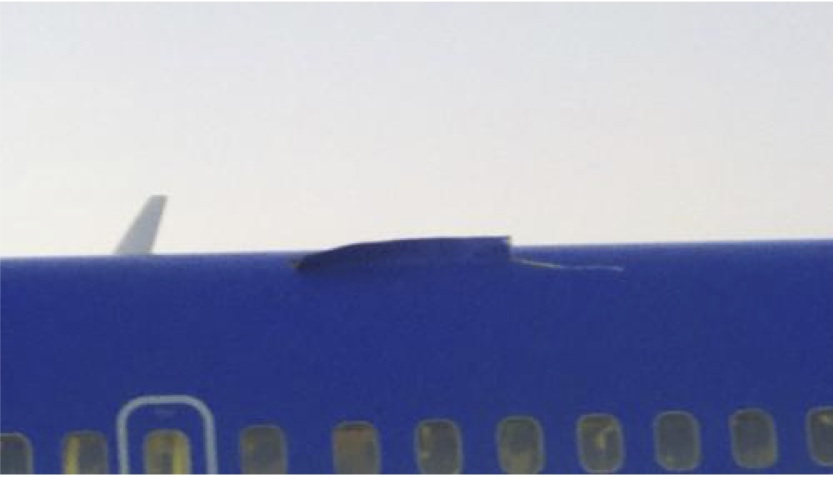
\includegraphics[width=0.55\textwidth]{southwest.jpg}
        \caption{Fuselage Rupture. Image c/o AP.}
     \end{figure}
	 %
     \vspace{-0.5cm}
     \begin{figure}
        \centering
        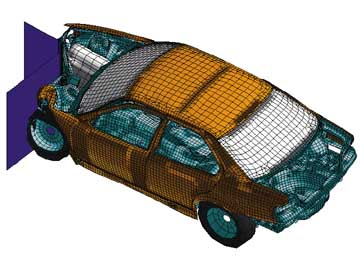
\includegraphics[width=0.55\textwidth]{FEM_car_crash1.jpg}
        \caption{Car crash}
     \end{figure}

     \column{0.45\textwidth}
       
     \begin{figure}
       \centering
       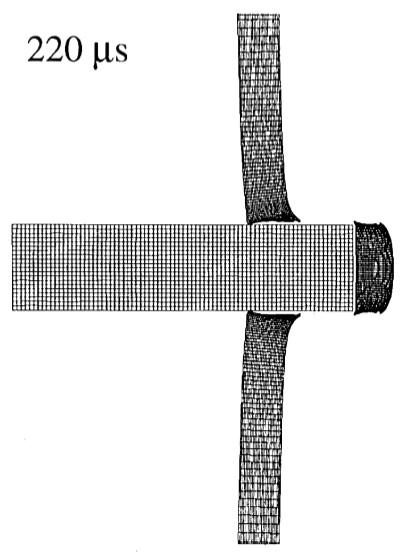
\includegraphics[width=0.7\textwidth]{plateperf2.jpg}
       \caption{Plate perforation}
     \end{figure}
     \end{columns}
     
     \footcite{borvik1999ballistic}
  
\end{frame}
%
\section{Background}
%
%
\subsection{Peridynamics}
%
\begin{frame}
  \frametitle{Peridynamics}
  \begin{center}
    \justify
    ``\ldots seeks to unify the mechanics of continuous media, particles, and cracks with a single mathematically consistent set of equations.''
  \end{center}

  \begin{figure}
      \centering
      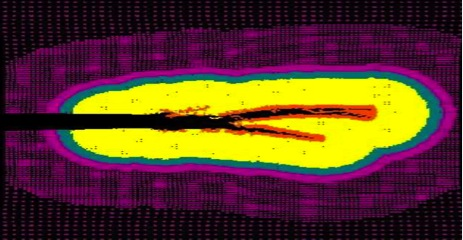
\includegraphics[width=0.7\textwidth]{crack_branch.jpg}
      \caption{Quote \& image c/o S.~Silling, SNL}
  \end{figure}
  

\end{frame}
%
%
%
\begin{frame}
  \frametitle{Peridynamic EOM}
%
\begin{equation*}
\rho(\mathbf{x})\mathbf{\ddot{u}}(\mathbf{x},t) = \int_\mathcal{H} \left\{\vstate{T}{\mathbf{x},t}{\mathbf{x'}-\mathbf{x}}-\vstate{T}{\mathbf{x'},t}{\mathbf{x}-\mathbf{x'}}\right\} \; dV_{\mathbf{x'}} + \mathbf{b}(\mathbf{x},t),
\end{equation*}
%
\begin{figure}
    \centering
    \scalebox{0.6}{
\definecolor{c969696}{RGB}{150,150,150}
\definecolor{cffffff}{RGB}{255,255,255}


\begin{tikzpicture}[y=0.80pt, x=0.8pt,yscale=-1, inner sep=0pt, outer sep=0pt]
  \path[draw=black,fill=c969696,line join=miter,line cap=butt,miter limit=4.00,line width=2.400pt] (186.0161,236.7328) .. controls (222.5066,189.4689) and (385.6469,216.8275) .. (429.0276,234.4083) .. controls (462.0313,247.7836) and (480.2697,263.8514) .. (479.4933,281.6722) .. controls (478.7169,299.4930) and (472.0778,331.9441) .. (429.0276,349.0814) .. controls (383.7620,367.1006) and (231.8233,380.0741) .. (210.0843,370.0015) .. controls (188.3452,359.9288) and (142.5380,320.4131) .. (146.4199,297.9434) .. controls (150.3019,275.4737) and (186.0161,236.7328) .. (186.0161,236.7328) -- cycle;
  \path[cm={{0.58136,0.0,0.0,0.58018,(97.12074,32.95193)}},draw=black,fill=cffffff,line cap=butt,miter limit=4.00,nonzero rule,line width=2.755pt] (407.3229,442.0455)arc(0.000:180.000:93.484)arc(-180.000:0.000:93.484) -- cycle;
  \begin{scope}[cm={{0.58136,0.0,0.0,0.58018,(116.91693,63.94839)}}]
    \path[color=black,fill=black,line width=1.600pt] (299.5312,325.5000) -- (274.1562,394.9688) -- (276.0625,395.6562) -- (301.4375,326.1875) -- (299.5312,325.5000) -- cycle;
    \path[draw=black,fill=black,even odd rule,line width=0.689pt] (297.7386,333.3725) -- (300.1229,338.5023) -- (301.1705,323.9798) -- (292.6087,335.7568) -- (297.7386,333.3725) -- cycle;
  \end{scope}
  \begin{scope}[cm={{0.58136,0.0,0.0,0.58018,(116.91693,63.94839)}}]
    \path[color=black,fill=black,line width=0.800pt] (275.3125,394.3125) -- (274.6250,395.0312) -- (338.0625,456.5000) -- (338.7812,455.7812) -- (275.3125,394.3125) -- cycle;
    \path[draw=black,fill=black,even odd rule,line width=0.689pt] (335.5521,453.3692) -- (332.7241,453.4141) -- (339.1433,456.8482) -- (335.5072,450.5411) -- (335.5521,453.3692) -- cycle;
  \end{scope}
  \path[xscale=1.001,yscale=0.999,fill=black] (229.11761,347.52325) node[above right] (text5344) {$\mathcal{H}$};
  \path[xscale=1.001,yscale=0.999,fill=black] (282.9393,320.95294) node[above right] (text5348) {$\delta$};
  \path[xscale=1.001,yscale=0.999,fill=black] (263.36148,295.53424) node[above right] (text5352) {$\mathbf{x}$};
  \path[xscale=1.001,yscale=0.999,fill=black] (295.68588,258.46326) node[above right] (text5356) {$\mathbf{x'}$};
  \path[cm={{0.58136,0.0,0.0,0.58018,(136.51469,89.25868)}},draw=black,fill=black,line cap=butt,miter limit=4.00,nonzero rule,line width=2.755pt] (242.5820,351.7165)arc(-0.122:180.122:1.322)arc(-180.122:0.122:1.322) -- cycle;
  \begin{scope}[shift={(15.37079,-42.56731)},shift={(0,0)}]
    \path[cm={{0.58136,0.0,0.0,0.58018,(136.51469,89.25868)}},draw=black,fill=black,line cap=butt,miter limit=4.00,nonzero rule,line width=2.755pt] (242.5820,351.7165)arc(-0.122:180.122:1.322)arc(-180.122:0.122:1.322) -- cycle;
  \end{scope}
  \path[xscale=1.001,yscale=0.999,fill=black] (400.8688,249.85263) node[above right] (text3092) {$\Omega$};

\end{tikzpicture}

}
\end{figure}
\footcite{silling:psa}
%
%
\end{frame}
%
%
\begin{frame}
  \frametitle{Constitutive Model Types}
%
\begin{figure}
    \centering
    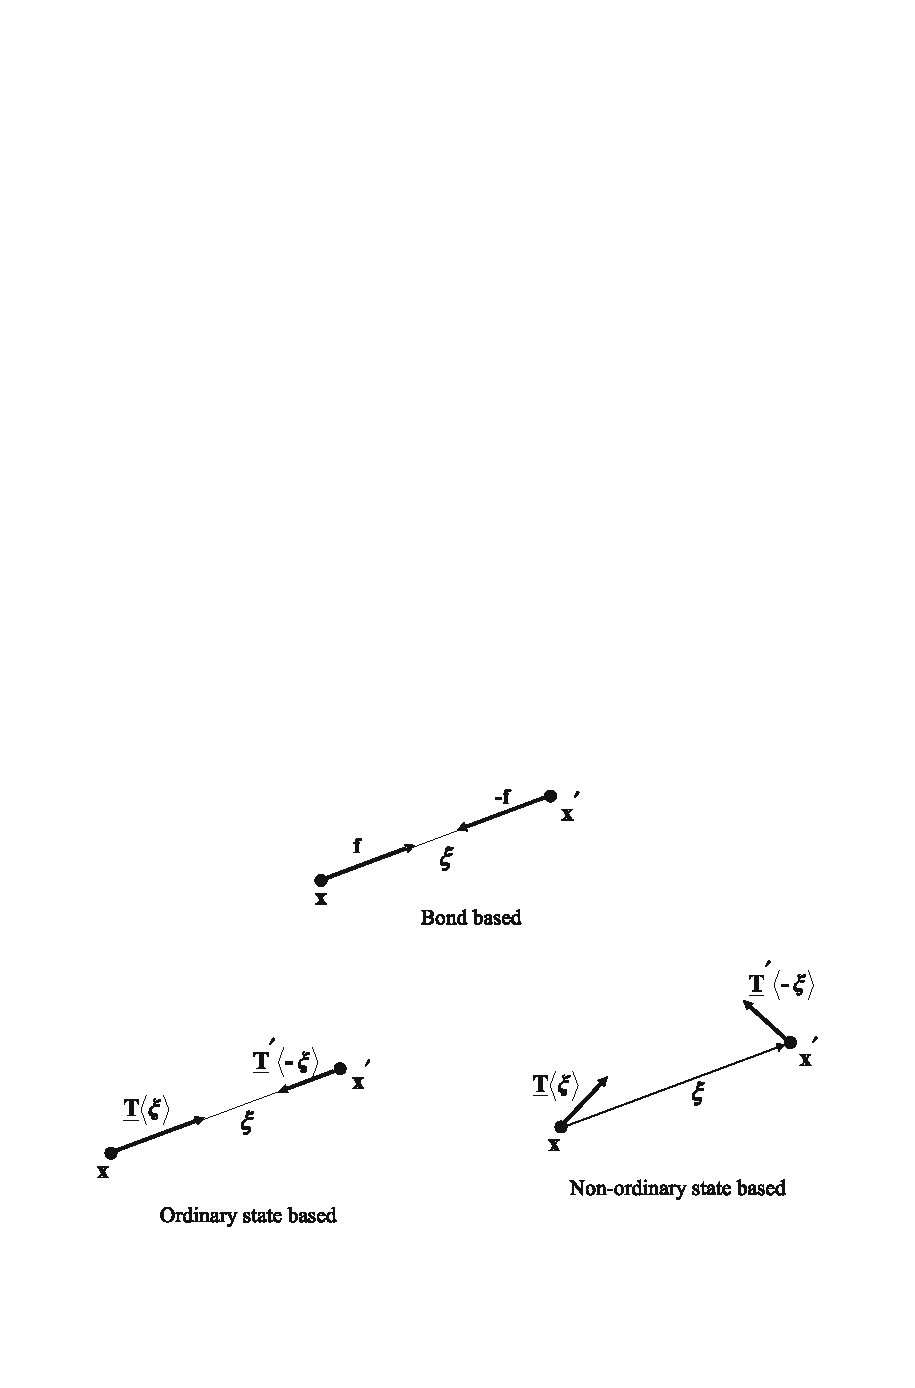
\includegraphics[width=0.8\textwidth]{PDmodelTypes}
\end{figure}
\footcite{silling:psa}

%
\end{frame}
%
\subsection{Thin Features}
%
\begin{frame}
  \frametitle{Thin Features}
  
     \vfill
     \begin{columns}[b] % contents are top vertically aligned
       
       \column{0.5\textwidth}

       \begin{figure}
           \centering
           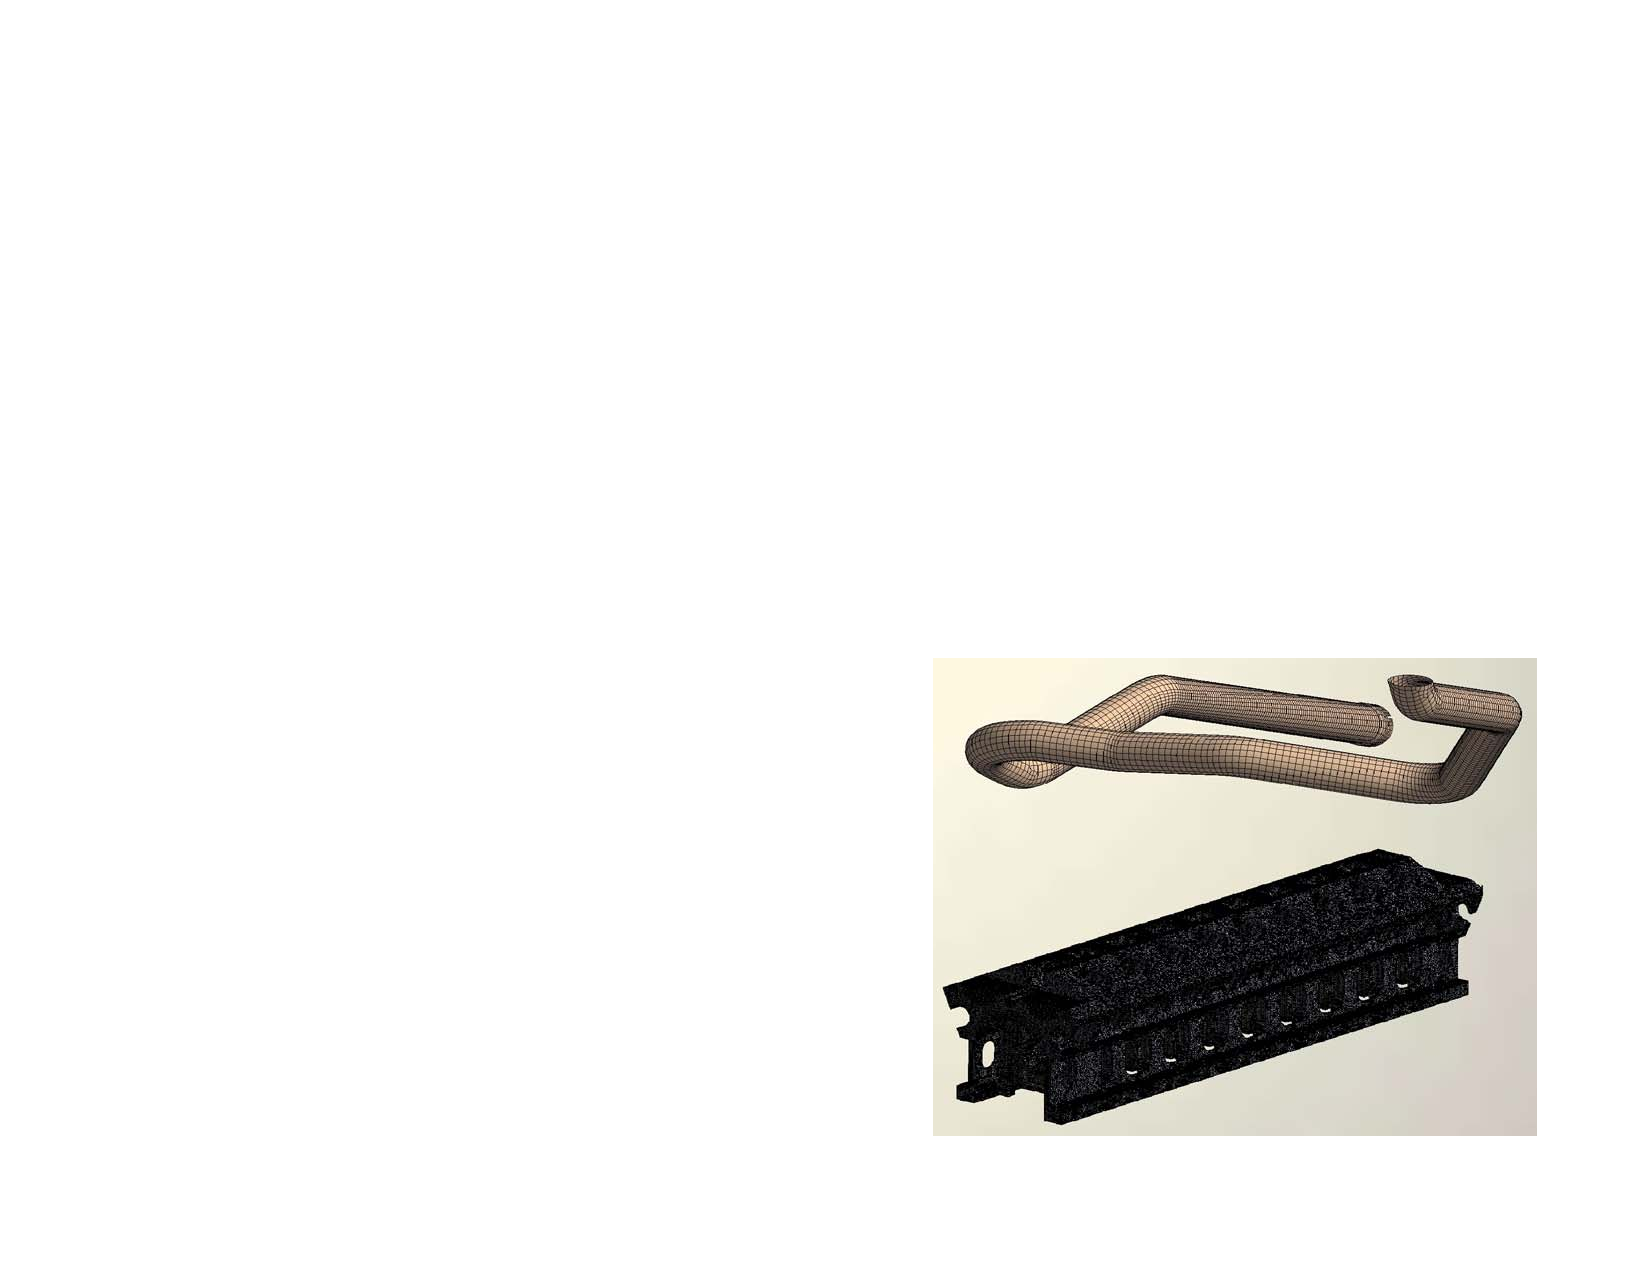
\includegraphics[width=0.75\textwidth]{ansysShell}
           \caption{FEA shells. Image c/o ANSYS manual.}
       \end{figure}
       
       \column{0.5\textwidth}

       \vspace{-0.8cm}
       \begin{figure}
           \centering
           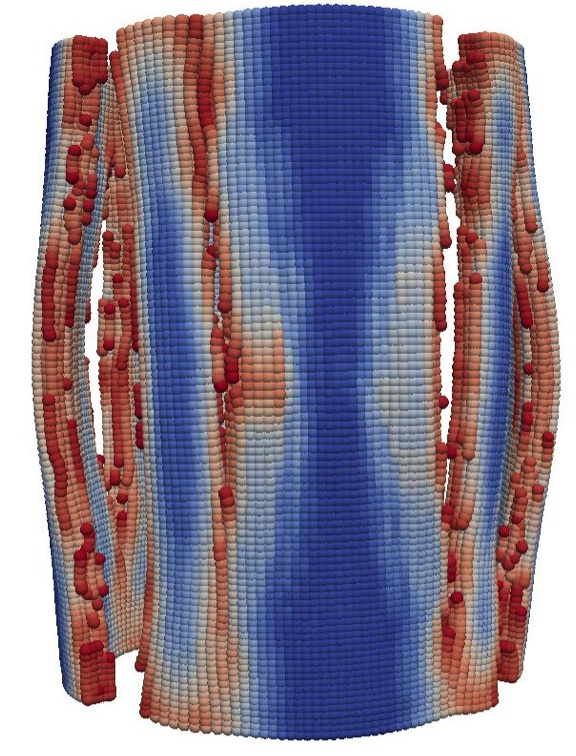
\includegraphics[width=0.6\textwidth]{littlewood_cylinder2.jpg}
           \caption{No PD equivalent}
       \end{figure}
     
     \end{columns}
     
     \footcite{littlewood2010}

\end{frame}
%
%
\section{Objectives}
\subsection{}
%
\begin{frame}
\frametitle{Objectives}

   \begin{itemize}
        \item PD constitutive models for beam, plates, shells
        \item Simulate material failure in thin features
        \item Explore complexities of non-ordinary material models, meta-materials\ldots?
  \end{itemize}

\end{frame}
%
%
\section{Results}
%
\subsection{Bond-pair Models}
%
\begin{frame}
\frametitle{Bond Pair Model}
%
\begin{figure}
\subinputfrom{\diagrampath}{bondPair.eps_tex}
\end{figure}
%
in which
%
\begin{equation*}
\vstate{T}{}{\boldsymbol{\xi}} =\frac{\alpha}{|\vstate{Y}{}{\boldsymbol{\xi}}|} \frac{\vstate{Y}{}{\boldsymbol{\xi}}}{|\vstate{Y}{}{\boldsymbol{\xi}}|} \times \left[\frac{\vstate{Y}{}{\boldsymbol{\xi}}}{|\vstate{Y}{}{\boldsymbol{\xi}}|} \times \frac{\vstate{Y}{}{-\boldsymbol{\xi}}}{|\vstate{Y}{}{-\boldsymbol{\xi}}|}\right]
\end{equation*}
%
\footcite{silling:psa}
\footcite{jogrady2014a}
%
\end{frame}
%
%
\begin{frame}
  \frametitle{Bond Pair Beam Energy}
\vfill

\begin{equation*}
W(x) \approx \int_{-\delta}^\delta \omega(\xi)\alpha\frac{\xi^2}{2}\kappa^2 d\xi = \frac{\alpha}{2}\kappa^2 \int_{-\delta}^\delta \omega(\xi)\xi^2 d\xi,
\end{equation*}
%
\vspace{0.5cm}
\begin{center}
Choosing \(\alpha\) carefully:
\end{center}
%
\begin{align*}
\alpha = \frac{EI}{m} ;\; m=\int_{-\delta}^\delta \omega(\xi)\xi^2 d\xi \implies W=\frac{EI}{2}\kappa^2
\end{align*}
%

\footcite{jogrady2014a}
\end{frame}
%
%
\begin{frame}
  \frametitle{Plasticity and Damage}

  
  \begin{center}
      Brittle material
  \end{center}
  
\[ 
|\vstate{T}{}{\xi}| = 
  \begin{cases}
    \vstate{T}{}{\xi} & \quad \text{if} \quad \theta < \theta_c \\
    0 & \quad \text{if} \quad \theta \geq \theta_c\
  \end{cases}
\]

  \begin{center}
     Elastic perfectly-plastic material \\
  \end{center}

\[ 
|\vstate{T}{}{\xi}| = 
  \begin{cases}
    \alpha \frac{\sin(\theta^e(\vstate{Y}{}{\xi},\vstate{Y}{}{\mathbf{-\xi}}))}{|\vstate{Y}{}{\xi}|} & \quad \text{if} \quad \theta^e < \theta_c\\
    \alpha \frac{\sin(\theta_c)}{|\vstate{Y}{}{\xi}|} & \quad \text{if} \quad \theta^e \geq \theta_c\
  \end{cases}
\]
%
\footcite{jogrady2014a}
\end{frame}
%
\begin{frame}
  \frametitle{Beam Results}

     \begin{columns}[T] % contents are top vertically aligned

     \column{0.5\textwidth}

     \begin{figure}
         \centering
         \resizebox{\linewidth}{!}{%% Creator: Matplotlib, PGF backend
%%
%% To include the figure in your LaTeX document, write
%%   \input{<filename>.pgf}
%%
%% Make sure the required packages are loaded in your preamble
%%   \usepackage{pgf}
%%
%% Figures using additional raster images can only be included by \input if
%% they are in the same directory as the main LaTeX file. For loading figures
%% from other directories you can use the `import` package
%%   \usepackage{import}
%% and then include the figures with
%%   \import{<path to file>}{<filename>.pgf}
%%
%% Matplotlib used the following preamble
%%
\begingroup%
\makeatletter%
\begin{pgfpicture}%
\pgfpathrectangle{\pgfpointorigin}{\pgfqpoint{6.000000in}{6.000000in}}%
\pgfusepath{use as bounding box}%
\begin{pgfscope}%
\pgfsetrectcap%
\pgfsetroundjoin%
\definecolor{currentfill}{rgb}{1.000000,1.000000,1.000000}%
\pgfsetfillcolor{currentfill}%
\pgfsetlinewidth{0.000000pt}%
\definecolor{currentstroke}{rgb}{1.000000,1.000000,1.000000}%
\pgfsetstrokecolor{currentstroke}%
\pgfsetdash{}{0pt}%
\pgfpathmoveto{\pgfqpoint{0.000000in}{0.000000in}}%
\pgfpathlineto{\pgfqpoint{6.000000in}{0.000000in}}%
\pgfpathlineto{\pgfqpoint{6.000000in}{6.000000in}}%
\pgfpathlineto{\pgfqpoint{0.000000in}{6.000000in}}%
\pgfpathclose%
\pgfusepath{fill}%
\end{pgfscope}%
\begin{pgfscope}%
\pgfsetrectcap%
\pgfsetroundjoin%
\definecolor{currentfill}{rgb}{1.000000,1.000000,1.000000}%
\pgfsetfillcolor{currentfill}%
\pgfsetlinewidth{0.000000pt}%
\definecolor{currentstroke}{rgb}{0.000000,0.000000,0.000000}%
\pgfsetstrokecolor{currentstroke}%
\pgfsetdash{}{0pt}%
\pgfpathmoveto{\pgfqpoint{0.750000in}{0.600000in}}%
\pgfpathlineto{\pgfqpoint{5.400000in}{0.600000in}}%
\pgfpathlineto{\pgfqpoint{5.400000in}{5.400000in}}%
\pgfpathlineto{\pgfqpoint{0.750000in}{5.400000in}}%
\pgfpathclose%
\pgfusepath{fill}%
\end{pgfscope}%
\begin{pgfscope}%
\pgfpathrectangle{\pgfqpoint{0.750000in}{0.600000in}}{\pgfqpoint{4.650000in}{4.800000in}} %
\pgfusepath{clip}%
\pgfsetrectcap%
\pgfsetroundjoin%
\pgfsetlinewidth{1.003750pt}%
\definecolor{currentstroke}{rgb}{0.000000,0.000000,1.000000}%
\pgfsetstrokecolor{currentstroke}%
\pgfsetdash{}{0pt}%
\pgfpathmoveto{\pgfqpoint{0.750000in}{5.400000in}}%
\pgfpathlineto{\pgfqpoint{0.984825in}{4.729964in}}%
\pgfpathlineto{\pgfqpoint{1.110375in}{4.378524in}}%
\pgfpathlineto{\pgfqpoint{1.217325in}{4.085616in}}%
\pgfpathlineto{\pgfqpoint{1.312650in}{3.830940in}}%
\pgfpathlineto{\pgfqpoint{1.401000in}{3.601260in}}%
\pgfpathlineto{\pgfqpoint{1.482375in}{3.395848in}}%
\pgfpathlineto{\pgfqpoint{1.559100in}{3.208112in}}%
\pgfpathlineto{\pgfqpoint{1.633500in}{3.032040in}}%
\pgfpathlineto{\pgfqpoint{1.703250in}{2.872688in}}%
\pgfpathlineto{\pgfqpoint{1.770675in}{2.724224in}}%
\pgfpathlineto{\pgfqpoint{1.833450in}{2.591168in}}%
\pgfpathlineto{\pgfqpoint{1.896225in}{2.463328in}}%
\pgfpathlineto{\pgfqpoint{1.956675in}{2.345336in}}%
\pgfpathlineto{\pgfqpoint{2.014800in}{2.236780in}}%
\pgfpathlineto{\pgfqpoint{2.070600in}{2.137224in}}%
\pgfpathlineto{\pgfqpoint{2.124075in}{2.046208in}}%
\pgfpathlineto{\pgfqpoint{2.175225in}{1.963268in}}%
\pgfpathlineto{\pgfqpoint{2.226375in}{1.884448in}}%
\pgfpathlineto{\pgfqpoint{2.275200in}{1.813120in}}%
\pgfpathlineto{\pgfqpoint{2.324025in}{1.745680in}}%
\pgfpathlineto{\pgfqpoint{2.370525in}{1.685124in}}%
\pgfpathlineto{\pgfqpoint{2.417025in}{1.628200in}}%
\pgfpathlineto{\pgfqpoint{2.461200in}{1.577528in}}%
\pgfpathlineto{\pgfqpoint{2.505375in}{1.530216in}}%
\pgfpathlineto{\pgfqpoint{2.547225in}{1.488524in}}%
\pgfpathlineto{\pgfqpoint{2.589075in}{1.449904in}}%
\pgfpathlineto{\pgfqpoint{2.630925in}{1.414384in}}%
\pgfpathlineto{\pgfqpoint{2.670450in}{1.383720in}}%
\pgfpathlineto{\pgfqpoint{2.709975in}{1.355840in}}%
\pgfpathlineto{\pgfqpoint{2.747175in}{1.332160in}}%
\pgfpathlineto{\pgfqpoint{2.784375in}{1.311000in}}%
\pgfpathlineto{\pgfqpoint{2.821575in}{1.292360in}}%
\pgfpathlineto{\pgfqpoint{2.858775in}{1.276280in}}%
\pgfpathlineto{\pgfqpoint{2.895975in}{1.262680in}}%
\pgfpathlineto{\pgfqpoint{2.933175in}{1.251680in}}%
\pgfpathlineto{\pgfqpoint{2.970375in}{1.243200in}}%
\pgfpathlineto{\pgfqpoint{3.007575in}{1.237280in}}%
\pgfpathlineto{\pgfqpoint{3.042450in}{1.234040in}}%
\pgfpathlineto{\pgfqpoint{3.079650in}{1.233080in}}%
\pgfpathlineto{\pgfqpoint{3.116850in}{1.234680in}}%
\pgfpathlineto{\pgfqpoint{3.154050in}{1.238840in}}%
\pgfpathlineto{\pgfqpoint{3.193575in}{1.246080in}}%
\pgfpathlineto{\pgfqpoint{3.230775in}{1.255520in}}%
\pgfpathlineto{\pgfqpoint{3.267975in}{1.267480in}}%
\pgfpathlineto{\pgfqpoint{3.305175in}{1.282000in}}%
\pgfpathlineto{\pgfqpoint{3.344700in}{1.300200in}}%
\pgfpathlineto{\pgfqpoint{3.381900in}{1.319960in}}%
\pgfpathlineto{\pgfqpoint{3.419100in}{1.342200in}}%
\pgfpathlineto{\pgfqpoint{3.458625in}{1.368600in}}%
\pgfpathlineto{\pgfqpoint{3.498150in}{1.397800in}}%
\pgfpathlineto{\pgfqpoint{3.537675in}{1.429788in}}%
\pgfpathlineto{\pgfqpoint{3.577200in}{1.464556in}}%
\pgfpathlineto{\pgfqpoint{3.619050in}{1.504376in}}%
\pgfpathlineto{\pgfqpoint{3.660900in}{1.547256in}}%
\pgfpathlineto{\pgfqpoint{3.702750in}{1.593168in}}%
\pgfpathlineto{\pgfqpoint{3.746925in}{1.644892in}}%
\pgfpathlineto{\pgfqpoint{3.793425in}{1.702912in}}%
\pgfpathlineto{\pgfqpoint{3.839925in}{1.764548in}}%
\pgfpathlineto{\pgfqpoint{3.888750in}{1.833104in}}%
\pgfpathlineto{\pgfqpoint{3.937575in}{1.905532in}}%
\pgfpathlineto{\pgfqpoint{3.988725in}{1.985484in}}%
\pgfpathlineto{\pgfqpoint{4.039875in}{2.069528in}}%
\pgfpathlineto{\pgfqpoint{4.095675in}{2.165780in}}%
\pgfpathlineto{\pgfqpoint{4.151475in}{2.266684in}}%
\pgfpathlineto{\pgfqpoint{4.209600in}{2.376600in}}%
\pgfpathlineto{\pgfqpoint{4.267725in}{2.491276in}}%
\pgfpathlineto{\pgfqpoint{4.328175in}{2.615424in}}%
\pgfpathlineto{\pgfqpoint{4.390950in}{2.749416in}}%
\pgfpathlineto{\pgfqpoint{4.456050in}{2.893604in}}%
\pgfpathlineto{\pgfqpoint{4.523475in}{3.048284in}}%
\pgfpathlineto{\pgfqpoint{4.595550in}{3.219316in}}%
\pgfpathlineto{\pgfqpoint{4.669950in}{3.401628in}}%
\pgfpathlineto{\pgfqpoint{4.749000in}{3.601260in}}%
\pgfpathlineto{\pgfqpoint{4.835025in}{3.824816in}}%
\pgfpathlineto{\pgfqpoint{4.925700in}{4.066764in}}%
\pgfpathlineto{\pgfqpoint{5.025675in}{4.339944in}}%
\pgfpathlineto{\pgfqpoint{5.137275in}{4.651284in}}%
\pgfpathlineto{\pgfqpoint{5.283750in}{5.067054in}}%
\pgfpathlineto{\pgfqpoint{5.400000in}{5.400000in}}%
\pgfpathlineto{\pgfqpoint{5.400000in}{5.400000in}}%
\pgfusepath{stroke}%
\end{pgfscope}%
\begin{pgfscope}%
\pgfpathrectangle{\pgfqpoint{0.750000in}{0.600000in}}{\pgfqpoint{4.650000in}{4.800000in}} %
\pgfusepath{clip}%
\pgfsetbuttcap%
\pgfsetroundjoin%
\definecolor{currentfill}{rgb}{0.000000,0.000000,1.000000}%
\pgfsetfillcolor{currentfill}%
\pgfsetlinewidth{0.501875pt}%
\definecolor{currentstroke}{rgb}{0.000000,0.000000,0.000000}%
\pgfsetstrokecolor{currentstroke}%
\pgfsetdash{}{0pt}%
\pgfsys@defobject{currentmarker}{\pgfqpoint{-0.041667in}{-0.041667in}}{\pgfqpoint{0.041667in}{0.041667in}}{%
\pgfpathmoveto{\pgfqpoint{0.000000in}{-0.041667in}}%
\pgfpathcurveto{\pgfqpoint{0.011050in}{-0.041667in}}{\pgfqpoint{0.021649in}{-0.037276in}}{\pgfqpoint{0.029463in}{-0.029463in}}%
\pgfpathcurveto{\pgfqpoint{0.037276in}{-0.021649in}}{\pgfqpoint{0.041667in}{-0.011050in}}{\pgfqpoint{0.041667in}{0.000000in}}%
\pgfpathcurveto{\pgfqpoint{0.041667in}{0.011050in}}{\pgfqpoint{0.037276in}{0.021649in}}{\pgfqpoint{0.029463in}{0.029463in}}%
\pgfpathcurveto{\pgfqpoint{0.021649in}{0.037276in}}{\pgfqpoint{0.011050in}{0.041667in}}{\pgfqpoint{0.000000in}{0.041667in}}%
\pgfpathcurveto{\pgfqpoint{-0.011050in}{0.041667in}}{\pgfqpoint{-0.021649in}{0.037276in}}{\pgfqpoint{-0.029463in}{0.029463in}}%
\pgfpathcurveto{\pgfqpoint{-0.037276in}{0.021649in}}{\pgfqpoint{-0.041667in}{0.011050in}}{\pgfqpoint{-0.041667in}{0.000000in}}%
\pgfpathcurveto{\pgfqpoint{-0.041667in}{-0.011050in}}{\pgfqpoint{-0.037276in}{-0.021649in}}{\pgfqpoint{-0.029463in}{-0.029463in}}%
\pgfpathcurveto{\pgfqpoint{-0.021649in}{-0.037276in}}{\pgfqpoint{-0.011050in}{-0.041667in}}{\pgfqpoint{0.000000in}{-0.041667in}}%
\pgfpathclose%
\pgfusepath{stroke,fill}%
}%
\begin{pgfscope}%
\pgfsys@transformshift{0.982500in}{4.736536in}%
\pgfsys@useobject{currentmarker}{}%
\end{pgfscope}%
\begin{pgfscope}%
\pgfsys@transformshift{1.447500in}{3.483120in}%
\pgfsys@useobject{currentmarker}{}%
\end{pgfscope}%
\begin{pgfscope}%
\pgfsys@transformshift{1.912500in}{2.431060in}%
\pgfsys@useobject{currentmarker}{}%
\end{pgfscope}%
\begin{pgfscope}%
\pgfsys@transformshift{2.377500in}{1.676352in}%
\pgfsys@useobject{currentmarker}{}%
\end{pgfscope}%
\begin{pgfscope}%
\pgfsys@transformshift{2.842500in}{1.283000in}%
\pgfsys@useobject{currentmarker}{}%
\end{pgfscope}%
\begin{pgfscope}%
\pgfsys@transformshift{3.307500in}{1.283000in}%
\pgfsys@useobject{currentmarker}{}%
\end{pgfscope}%
\begin{pgfscope}%
\pgfsys@transformshift{3.772500in}{1.676352in}%
\pgfsys@useobject{currentmarker}{}%
\end{pgfscope}%
\begin{pgfscope}%
\pgfsys@transformshift{4.237500in}{2.431060in}%
\pgfsys@useobject{currentmarker}{}%
\end{pgfscope}%
\begin{pgfscope}%
\pgfsys@transformshift{4.702500in}{3.483120in}%
\pgfsys@useobject{currentmarker}{}%
\end{pgfscope}%
\begin{pgfscope}%
\pgfsys@transformshift{5.167500in}{4.736536in}%
\pgfsys@useobject{currentmarker}{}%
\end{pgfscope}%
\end{pgfscope}%
\begin{pgfscope}%
\pgfpathrectangle{\pgfqpoint{0.750000in}{0.600000in}}{\pgfqpoint{4.650000in}{4.800000in}} %
\pgfusepath{clip}%
\pgfsetrectcap%
\pgfsetroundjoin%
\pgfsetlinewidth{1.003750pt}%
\definecolor{currentstroke}{rgb}{0.000000,0.500000,0.000000}%
\pgfsetstrokecolor{currentstroke}%
\pgfsetdash{}{0pt}%
\pgfpathmoveto{\pgfqpoint{0.843000in}{5.142324in}}%
\pgfpathlineto{\pgfqpoint{0.936000in}{4.885157in}}%
\pgfpathlineto{\pgfqpoint{1.029000in}{4.629314in}}%
\pgfpathlineto{\pgfqpoint{1.122000in}{4.375370in}}%
\pgfpathlineto{\pgfqpoint{1.215000in}{4.124317in}}%
\pgfpathlineto{\pgfqpoint{1.308000in}{3.882080in}}%
\pgfpathlineto{\pgfqpoint{1.401000in}{3.645171in}}%
\pgfpathlineto{\pgfqpoint{1.494000in}{3.415281in}}%
\pgfpathlineto{\pgfqpoint{1.587000in}{3.193670in}}%
\pgfpathlineto{\pgfqpoint{1.680000in}{2.981159in}}%
\pgfpathlineto{\pgfqpoint{1.773000in}{2.778726in}}%
\pgfpathlineto{\pgfqpoint{1.866000in}{2.586899in}}%
\pgfpathlineto{\pgfqpoint{1.959000in}{2.406484in}}%
\pgfpathlineto{\pgfqpoint{2.052000in}{2.238095in}}%
\pgfpathlineto{\pgfqpoint{2.145000in}{2.082372in}}%
\pgfpathlineto{\pgfqpoint{2.238000in}{1.939808in}}%
\pgfpathlineto{\pgfqpoint{2.331000in}{1.810928in}}%
\pgfpathlineto{\pgfqpoint{2.424000in}{1.696182in}}%
\pgfpathlineto{\pgfqpoint{2.517000in}{1.595948in}}%
\pgfpathlineto{\pgfqpoint{2.610000in}{1.510572in}}%
\pgfpathlineto{\pgfqpoint{2.703000in}{1.440334in}}%
\pgfpathlineto{\pgfqpoint{2.796000in}{1.385474in}}%
\pgfpathlineto{\pgfqpoint{2.889000in}{1.346173in}}%
\pgfpathlineto{\pgfqpoint{2.982000in}{1.322560in}}%
\pgfpathlineto{\pgfqpoint{3.075000in}{1.314715in}}%
\pgfpathlineto{\pgfqpoint{3.168000in}{1.322661in}}%
\pgfpathlineto{\pgfqpoint{3.261000in}{1.346374in}}%
\pgfpathlineto{\pgfqpoint{3.354000in}{1.385773in}}%
\pgfpathlineto{\pgfqpoint{3.447000in}{1.440729in}}%
\pgfpathlineto{\pgfqpoint{3.540000in}{1.511058in}}%
\pgfpathlineto{\pgfqpoint{3.633000in}{1.596521in}}%
\pgfpathlineto{\pgfqpoint{3.726000in}{1.696835in}}%
\pgfpathlineto{\pgfqpoint{3.819000in}{1.811655in}}%
\pgfpathlineto{\pgfqpoint{3.912000in}{1.940602in}}%
\pgfpathlineto{\pgfqpoint{4.005000in}{2.083224in}}%
\pgfpathlineto{\pgfqpoint{4.098000in}{2.238995in}}%
\pgfpathlineto{\pgfqpoint{4.191000in}{2.407421in}}%
\pgfpathlineto{\pgfqpoint{4.284000in}{2.587862in}}%
\pgfpathlineto{\pgfqpoint{4.377000in}{2.779704in}}%
\pgfpathlineto{\pgfqpoint{4.470000in}{2.982137in}}%
\pgfpathlineto{\pgfqpoint{4.563000in}{3.194634in}}%
\pgfpathlineto{\pgfqpoint{4.656000in}{3.416214in}}%
\pgfpathlineto{\pgfqpoint{4.749000in}{3.646059in}}%
\pgfpathlineto{\pgfqpoint{4.842000in}{3.882903in}}%
\pgfpathlineto{\pgfqpoint{4.935000in}{4.125075in}}%
\pgfpathlineto{\pgfqpoint{5.028000in}{4.376003in}}%
\pgfpathlineto{\pgfqpoint{5.121000in}{4.629816in}}%
\pgfpathlineto{\pgfqpoint{5.214000in}{4.885599in}}%
\pgfpathlineto{\pgfqpoint{5.307000in}{5.142506in}}%
\pgfpathlineto{\pgfqpoint{5.400000in}{5.400000in}}%
\pgfusepath{stroke}%
\end{pgfscope}%
\begin{pgfscope}%
\pgfpathrectangle{\pgfqpoint{0.750000in}{0.600000in}}{\pgfqpoint{4.650000in}{4.800000in}} %
\pgfusepath{clip}%
\pgfsetbuttcap%
\pgfsetmiterjoin%
\definecolor{currentfill}{rgb}{0.000000,0.500000,0.000000}%
\pgfsetfillcolor{currentfill}%
\pgfsetlinewidth{0.501875pt}%
\definecolor{currentstroke}{rgb}{0.000000,0.000000,0.000000}%
\pgfsetstrokecolor{currentstroke}%
\pgfsetdash{}{0pt}%
\pgfsys@defobject{currentmarker}{\pgfqpoint{-0.041667in}{-0.041667in}}{\pgfqpoint{0.041667in}{0.041667in}}{%
\pgfpathmoveto{\pgfqpoint{0.000000in}{0.041667in}}%
\pgfpathlineto{\pgfqpoint{-0.041667in}{-0.041667in}}%
\pgfpathlineto{\pgfqpoint{0.041667in}{-0.041667in}}%
\pgfpathclose%
\pgfusepath{stroke,fill}%
}%
\begin{pgfscope}%
\pgfsys@transformshift{1.587000in}{3.193670in}%
\pgfsys@useobject{currentmarker}{}%
\end{pgfscope}%
\begin{pgfscope}%
\pgfsys@transformshift{2.517000in}{1.595948in}%
\pgfsys@useobject{currentmarker}{}%
\end{pgfscope}%
\begin{pgfscope}%
\pgfsys@transformshift{3.447000in}{1.440729in}%
\pgfsys@useobject{currentmarker}{}%
\end{pgfscope}%
\begin{pgfscope}%
\pgfsys@transformshift{4.377000in}{2.779704in}%
\pgfsys@useobject{currentmarker}{}%
\end{pgfscope}%
\begin{pgfscope}%
\pgfsys@transformshift{5.307000in}{5.142506in}%
\pgfsys@useobject{currentmarker}{}%
\end{pgfscope}%
\end{pgfscope}%
\begin{pgfscope}%
\pgfpathrectangle{\pgfqpoint{0.750000in}{0.600000in}}{\pgfqpoint{4.650000in}{4.800000in}} %
\pgfusepath{clip}%
\pgfsetrectcap%
\pgfsetroundjoin%
\pgfsetlinewidth{1.003750pt}%
\definecolor{currentstroke}{rgb}{1.000000,0.000000,0.000000}%
\pgfsetstrokecolor{currentstroke}%
\pgfsetdash{}{0pt}%
\pgfpathmoveto{\pgfqpoint{0.796500in}{5.268655in}}%
\pgfpathlineto{\pgfqpoint{1.029000in}{4.615916in}}%
\pgfpathlineto{\pgfqpoint{1.168500in}{4.230459in}}%
\pgfpathlineto{\pgfqpoint{1.215000in}{4.103912in}}%
\pgfpathlineto{\pgfqpoint{1.354500in}{3.737992in}}%
\pgfpathlineto{\pgfqpoint{1.447500in}{3.501530in}}%
\pgfpathlineto{\pgfqpoint{1.540500in}{3.273019in}}%
\pgfpathlineto{\pgfqpoint{1.633500in}{3.053440in}}%
\pgfpathlineto{\pgfqpoint{1.726500in}{2.843678in}}%
\pgfpathlineto{\pgfqpoint{1.773000in}{2.742676in}}%
\pgfpathlineto{\pgfqpoint{1.819500in}{2.644376in}}%
\pgfpathlineto{\pgfqpoint{1.866000in}{2.548892in}}%
\pgfpathlineto{\pgfqpoint{1.912500in}{2.456292in}}%
\pgfpathlineto{\pgfqpoint{1.959000in}{2.366675in}}%
\pgfpathlineto{\pgfqpoint{2.005500in}{2.280105in}}%
\pgfpathlineto{\pgfqpoint{2.052000in}{2.196671in}}%
\pgfpathlineto{\pgfqpoint{2.098500in}{2.116430in}}%
\pgfpathlineto{\pgfqpoint{2.145000in}{2.039464in}}%
\pgfpathlineto{\pgfqpoint{2.191500in}{1.965824in}}%
\pgfpathlineto{\pgfqpoint{2.238000in}{1.895587in}}%
\pgfpathlineto{\pgfqpoint{2.284500in}{1.828811in}}%
\pgfpathlineto{\pgfqpoint{2.331000in}{1.765550in}}%
\pgfpathlineto{\pgfqpoint{2.377500in}{1.705859in}}%
\pgfpathlineto{\pgfqpoint{2.424000in}{1.649786in}}%
\pgfpathlineto{\pgfqpoint{2.470500in}{1.597378in}}%
\pgfpathlineto{\pgfqpoint{2.517000in}{1.548679in}}%
\pgfpathlineto{\pgfqpoint{2.563500in}{1.503728in}}%
\pgfpathlineto{\pgfqpoint{2.610000in}{1.462564in}}%
\pgfpathlineto{\pgfqpoint{2.656500in}{1.425220in}}%
\pgfpathlineto{\pgfqpoint{2.703000in}{1.391727in}}%
\pgfpathlineto{\pgfqpoint{2.749500in}{1.362113in}}%
\pgfpathlineto{\pgfqpoint{2.796000in}{1.336400in}}%
\pgfpathlineto{\pgfqpoint{2.842500in}{1.314612in}}%
\pgfpathlineto{\pgfqpoint{2.889000in}{1.296764in}}%
\pgfpathlineto{\pgfqpoint{2.935500in}{1.282872in}}%
\pgfpathlineto{\pgfqpoint{2.982000in}{1.272947in}}%
\pgfpathlineto{\pgfqpoint{3.028500in}{1.266997in}}%
\pgfpathlineto{\pgfqpoint{3.075000in}{1.265027in}}%
\pgfpathlineto{\pgfqpoint{3.121500in}{1.267038in}}%
\pgfpathlineto{\pgfqpoint{3.168000in}{1.273029in}}%
\pgfpathlineto{\pgfqpoint{3.214500in}{1.282995in}}%
\pgfpathlineto{\pgfqpoint{3.261000in}{1.296927in}}%
\pgfpathlineto{\pgfqpoint{3.307500in}{1.314815in}}%
\pgfpathlineto{\pgfqpoint{3.354000in}{1.336643in}}%
\pgfpathlineto{\pgfqpoint{3.400500in}{1.362394in}}%
\pgfpathlineto{\pgfqpoint{3.447000in}{1.392047in}}%
\pgfpathlineto{\pgfqpoint{3.493500in}{1.425577in}}%
\pgfpathlineto{\pgfqpoint{3.540000in}{1.462958in}}%
\pgfpathlineto{\pgfqpoint{3.586500in}{1.504157in}}%
\pgfpathlineto{\pgfqpoint{3.633000in}{1.549142in}}%
\pgfpathlineto{\pgfqpoint{3.679500in}{1.597875in}}%
\pgfpathlineto{\pgfqpoint{3.726000in}{1.650315in}}%
\pgfpathlineto{\pgfqpoint{3.772500in}{1.706419in}}%
\pgfpathlineto{\pgfqpoint{3.819000in}{1.766140in}}%
\pgfpathlineto{\pgfqpoint{3.865500in}{1.829428in}}%
\pgfpathlineto{\pgfqpoint{3.912000in}{1.896230in}}%
\pgfpathlineto{\pgfqpoint{3.958500in}{1.966491in}}%
\pgfpathlineto{\pgfqpoint{4.005000in}{2.040154in}}%
\pgfpathlineto{\pgfqpoint{4.051500in}{2.117141in}}%
\pgfpathlineto{\pgfqpoint{4.098000in}{2.197400in}}%
\pgfpathlineto{\pgfqpoint{4.144500in}{2.280851in}}%
\pgfpathlineto{\pgfqpoint{4.191000in}{2.367435in}}%
\pgfpathlineto{\pgfqpoint{4.237500in}{2.457063in}}%
\pgfpathlineto{\pgfqpoint{4.284000in}{2.549673in}}%
\pgfpathlineto{\pgfqpoint{4.330500in}{2.645164in}}%
\pgfpathlineto{\pgfqpoint{4.377000in}{2.743468in}}%
\pgfpathlineto{\pgfqpoint{4.470000in}{2.948081in}}%
\pgfpathlineto{\pgfqpoint{4.563000in}{3.162844in}}%
\pgfpathlineto{\pgfqpoint{4.656000in}{3.386985in}}%
\pgfpathlineto{\pgfqpoint{4.749000in}{3.619569in}}%
\pgfpathlineto{\pgfqpoint{4.842000in}{3.859574in}}%
\pgfpathlineto{\pgfqpoint{4.935000in}{4.104526in}}%
\pgfpathlineto{\pgfqpoint{5.074500in}{4.487140in}}%
\pgfpathlineto{\pgfqpoint{5.260500in}{5.006869in}}%
\pgfpathlineto{\pgfqpoint{5.400000in}{5.400000in}}%
\pgfpathlineto{\pgfqpoint{5.400000in}{5.400000in}}%
\pgfusepath{stroke}%
\end{pgfscope}%
\begin{pgfscope}%
\pgfpathrectangle{\pgfqpoint{0.750000in}{0.600000in}}{\pgfqpoint{4.650000in}{4.800000in}} %
\pgfusepath{clip}%
\pgfsetbuttcap%
\pgfsetmiterjoin%
\definecolor{currentfill}{rgb}{1.000000,0.000000,0.000000}%
\pgfsetfillcolor{currentfill}%
\pgfsetlinewidth{0.501875pt}%
\definecolor{currentstroke}{rgb}{0.000000,0.000000,0.000000}%
\pgfsetstrokecolor{currentstroke}%
\pgfsetdash{}{0pt}%
\pgfsys@defobject{currentmarker}{\pgfqpoint{-0.041667in}{-0.041667in}}{\pgfqpoint{0.041667in}{0.041667in}}{%
\pgfpathmoveto{\pgfqpoint{0.041667in}{-0.000000in}}%
\pgfpathlineto{\pgfqpoint{-0.041667in}{0.041667in}}%
\pgfpathlineto{\pgfqpoint{-0.041667in}{-0.041667in}}%
\pgfpathclose%
\pgfusepath{stroke,fill}%
}%
\begin{pgfscope}%
\pgfsys@transformshift{1.075500in}{4.486677in}%
\pgfsys@useobject{currentmarker}{}%
\end{pgfscope}%
\begin{pgfscope}%
\pgfsys@transformshift{1.540500in}{3.273019in}%
\pgfsys@useobject{currentmarker}{}%
\end{pgfscope}%
\begin{pgfscope}%
\pgfsys@transformshift{2.005500in}{2.280105in}%
\pgfsys@useobject{currentmarker}{}%
\end{pgfscope}%
\begin{pgfscope}%
\pgfsys@transformshift{2.470500in}{1.597378in}%
\pgfsys@useobject{currentmarker}{}%
\end{pgfscope}%
\begin{pgfscope}%
\pgfsys@transformshift{2.935500in}{1.282872in}%
\pgfsys@useobject{currentmarker}{}%
\end{pgfscope}%
\begin{pgfscope}%
\pgfsys@transformshift{3.400500in}{1.362394in}%
\pgfsys@useobject{currentmarker}{}%
\end{pgfscope}%
\begin{pgfscope}%
\pgfsys@transformshift{3.865500in}{1.829428in}%
\pgfsys@useobject{currentmarker}{}%
\end{pgfscope}%
\begin{pgfscope}%
\pgfsys@transformshift{4.330500in}{2.645164in}%
\pgfsys@useobject{currentmarker}{}%
\end{pgfscope}%
\begin{pgfscope}%
\pgfsys@transformshift{4.795500in}{3.738687in}%
\pgfsys@useobject{currentmarker}{}%
\end{pgfscope}%
\begin{pgfscope}%
\pgfsys@transformshift{5.260500in}{5.006869in}%
\pgfsys@useobject{currentmarker}{}%
\end{pgfscope}%
\end{pgfscope}%
\begin{pgfscope}%
\pgfpathrectangle{\pgfqpoint{0.750000in}{0.600000in}}{\pgfqpoint{4.650000in}{4.800000in}} %
\pgfusepath{clip}%
\pgfsetbuttcap%
\pgfsetroundjoin%
\pgfsetlinewidth{0.501875pt}%
\definecolor{currentstroke}{rgb}{0.000000,0.000000,0.000000}%
\pgfsetstrokecolor{currentstroke}%
\pgfsetdash{{1.000000pt}{3.000000pt}}{0.000000pt}%
\pgfpathmoveto{\pgfqpoint{0.750000in}{0.600000in}}%
\pgfpathlineto{\pgfqpoint{0.750000in}{5.400000in}}%
\pgfusepath{stroke}%
\end{pgfscope}%
\begin{pgfscope}%
\pgfsetbuttcap%
\pgfsetroundjoin%
\definecolor{currentfill}{rgb}{0.000000,0.000000,0.000000}%
\pgfsetfillcolor{currentfill}%
\pgfsetlinewidth{0.501875pt}%
\definecolor{currentstroke}{rgb}{0.000000,0.000000,0.000000}%
\pgfsetstrokecolor{currentstroke}%
\pgfsetdash{}{0pt}%
\pgfsys@defobject{currentmarker}{\pgfqpoint{0.000000in}{0.000000in}}{\pgfqpoint{0.000000in}{0.055556in}}{%
\pgfpathmoveto{\pgfqpoint{0.000000in}{0.000000in}}%
\pgfpathlineto{\pgfqpoint{0.000000in}{0.055556in}}%
\pgfusepath{stroke,fill}%
}%
\begin{pgfscope}%
\pgfsys@transformshift{0.750000in}{0.600000in}%
\pgfsys@useobject{currentmarker}{}%
\end{pgfscope}%
\end{pgfscope}%
\begin{pgfscope}%
\pgfsetbuttcap%
\pgfsetroundjoin%
\definecolor{currentfill}{rgb}{0.000000,0.000000,0.000000}%
\pgfsetfillcolor{currentfill}%
\pgfsetlinewidth{0.501875pt}%
\definecolor{currentstroke}{rgb}{0.000000,0.000000,0.000000}%
\pgfsetstrokecolor{currentstroke}%
\pgfsetdash{}{0pt}%
\pgfsys@defobject{currentmarker}{\pgfqpoint{0.000000in}{-0.055556in}}{\pgfqpoint{0.000000in}{0.000000in}}{%
\pgfpathmoveto{\pgfqpoint{0.000000in}{0.000000in}}%
\pgfpathlineto{\pgfqpoint{0.000000in}{-0.055556in}}%
\pgfusepath{stroke,fill}%
}%
\begin{pgfscope}%
\pgfsys@transformshift{0.750000in}{5.400000in}%
\pgfsys@useobject{currentmarker}{}%
\end{pgfscope}%
\end{pgfscope}%
\begin{pgfscope}%
\pgftext[x=0.750000in,y=0.544444in,,top]{{\rmfamily\fontsize{12.000000}{14.400000}\selectfont \(\displaystyle 0.0\)}}%
\end{pgfscope}%
\begin{pgfscope}%
\pgfpathrectangle{\pgfqpoint{0.750000in}{0.600000in}}{\pgfqpoint{4.650000in}{4.800000in}} %
\pgfusepath{clip}%
\pgfsetbuttcap%
\pgfsetroundjoin%
\pgfsetlinewidth{0.501875pt}%
\definecolor{currentstroke}{rgb}{0.000000,0.000000,0.000000}%
\pgfsetstrokecolor{currentstroke}%
\pgfsetdash{{1.000000pt}{3.000000pt}}{0.000000pt}%
\pgfpathmoveto{\pgfqpoint{1.912500in}{0.600000in}}%
\pgfpathlineto{\pgfqpoint{1.912500in}{5.400000in}}%
\pgfusepath{stroke}%
\end{pgfscope}%
\begin{pgfscope}%
\pgfsetbuttcap%
\pgfsetroundjoin%
\definecolor{currentfill}{rgb}{0.000000,0.000000,0.000000}%
\pgfsetfillcolor{currentfill}%
\pgfsetlinewidth{0.501875pt}%
\definecolor{currentstroke}{rgb}{0.000000,0.000000,0.000000}%
\pgfsetstrokecolor{currentstroke}%
\pgfsetdash{}{0pt}%
\pgfsys@defobject{currentmarker}{\pgfqpoint{0.000000in}{0.000000in}}{\pgfqpoint{0.000000in}{0.055556in}}{%
\pgfpathmoveto{\pgfqpoint{0.000000in}{0.000000in}}%
\pgfpathlineto{\pgfqpoint{0.000000in}{0.055556in}}%
\pgfusepath{stroke,fill}%
}%
\begin{pgfscope}%
\pgfsys@transformshift{1.912500in}{0.600000in}%
\pgfsys@useobject{currentmarker}{}%
\end{pgfscope}%
\end{pgfscope}%
\begin{pgfscope}%
\pgfsetbuttcap%
\pgfsetroundjoin%
\definecolor{currentfill}{rgb}{0.000000,0.000000,0.000000}%
\pgfsetfillcolor{currentfill}%
\pgfsetlinewidth{0.501875pt}%
\definecolor{currentstroke}{rgb}{0.000000,0.000000,0.000000}%
\pgfsetstrokecolor{currentstroke}%
\pgfsetdash{}{0pt}%
\pgfsys@defobject{currentmarker}{\pgfqpoint{0.000000in}{-0.055556in}}{\pgfqpoint{0.000000in}{0.000000in}}{%
\pgfpathmoveto{\pgfqpoint{0.000000in}{0.000000in}}%
\pgfpathlineto{\pgfqpoint{0.000000in}{-0.055556in}}%
\pgfusepath{stroke,fill}%
}%
\begin{pgfscope}%
\pgfsys@transformshift{1.912500in}{5.400000in}%
\pgfsys@useobject{currentmarker}{}%
\end{pgfscope}%
\end{pgfscope}%
\begin{pgfscope}%
\pgftext[x=1.912500in,y=0.544444in,,top]{{\rmfamily\fontsize{12.000000}{14.400000}\selectfont \(\displaystyle 0.5\)}}%
\end{pgfscope}%
\begin{pgfscope}%
\pgfpathrectangle{\pgfqpoint{0.750000in}{0.600000in}}{\pgfqpoint{4.650000in}{4.800000in}} %
\pgfusepath{clip}%
\pgfsetbuttcap%
\pgfsetroundjoin%
\pgfsetlinewidth{0.501875pt}%
\definecolor{currentstroke}{rgb}{0.000000,0.000000,0.000000}%
\pgfsetstrokecolor{currentstroke}%
\pgfsetdash{{1.000000pt}{3.000000pt}}{0.000000pt}%
\pgfpathmoveto{\pgfqpoint{3.075000in}{0.600000in}}%
\pgfpathlineto{\pgfqpoint{3.075000in}{5.400000in}}%
\pgfusepath{stroke}%
\end{pgfscope}%
\begin{pgfscope}%
\pgfsetbuttcap%
\pgfsetroundjoin%
\definecolor{currentfill}{rgb}{0.000000,0.000000,0.000000}%
\pgfsetfillcolor{currentfill}%
\pgfsetlinewidth{0.501875pt}%
\definecolor{currentstroke}{rgb}{0.000000,0.000000,0.000000}%
\pgfsetstrokecolor{currentstroke}%
\pgfsetdash{}{0pt}%
\pgfsys@defobject{currentmarker}{\pgfqpoint{0.000000in}{0.000000in}}{\pgfqpoint{0.000000in}{0.055556in}}{%
\pgfpathmoveto{\pgfqpoint{0.000000in}{0.000000in}}%
\pgfpathlineto{\pgfqpoint{0.000000in}{0.055556in}}%
\pgfusepath{stroke,fill}%
}%
\begin{pgfscope}%
\pgfsys@transformshift{3.075000in}{0.600000in}%
\pgfsys@useobject{currentmarker}{}%
\end{pgfscope}%
\end{pgfscope}%
\begin{pgfscope}%
\pgfsetbuttcap%
\pgfsetroundjoin%
\definecolor{currentfill}{rgb}{0.000000,0.000000,0.000000}%
\pgfsetfillcolor{currentfill}%
\pgfsetlinewidth{0.501875pt}%
\definecolor{currentstroke}{rgb}{0.000000,0.000000,0.000000}%
\pgfsetstrokecolor{currentstroke}%
\pgfsetdash{}{0pt}%
\pgfsys@defobject{currentmarker}{\pgfqpoint{0.000000in}{-0.055556in}}{\pgfqpoint{0.000000in}{0.000000in}}{%
\pgfpathmoveto{\pgfqpoint{0.000000in}{0.000000in}}%
\pgfpathlineto{\pgfqpoint{0.000000in}{-0.055556in}}%
\pgfusepath{stroke,fill}%
}%
\begin{pgfscope}%
\pgfsys@transformshift{3.075000in}{5.400000in}%
\pgfsys@useobject{currentmarker}{}%
\end{pgfscope}%
\end{pgfscope}%
\begin{pgfscope}%
\pgftext[x=3.075000in,y=0.544444in,,top]{{\rmfamily\fontsize{12.000000}{14.400000}\selectfont \(\displaystyle 1.0\)}}%
\end{pgfscope}%
\begin{pgfscope}%
\pgfpathrectangle{\pgfqpoint{0.750000in}{0.600000in}}{\pgfqpoint{4.650000in}{4.800000in}} %
\pgfusepath{clip}%
\pgfsetbuttcap%
\pgfsetroundjoin%
\pgfsetlinewidth{0.501875pt}%
\definecolor{currentstroke}{rgb}{0.000000,0.000000,0.000000}%
\pgfsetstrokecolor{currentstroke}%
\pgfsetdash{{1.000000pt}{3.000000pt}}{0.000000pt}%
\pgfpathmoveto{\pgfqpoint{4.237500in}{0.600000in}}%
\pgfpathlineto{\pgfqpoint{4.237500in}{5.400000in}}%
\pgfusepath{stroke}%
\end{pgfscope}%
\begin{pgfscope}%
\pgfsetbuttcap%
\pgfsetroundjoin%
\definecolor{currentfill}{rgb}{0.000000,0.000000,0.000000}%
\pgfsetfillcolor{currentfill}%
\pgfsetlinewidth{0.501875pt}%
\definecolor{currentstroke}{rgb}{0.000000,0.000000,0.000000}%
\pgfsetstrokecolor{currentstroke}%
\pgfsetdash{}{0pt}%
\pgfsys@defobject{currentmarker}{\pgfqpoint{0.000000in}{0.000000in}}{\pgfqpoint{0.000000in}{0.055556in}}{%
\pgfpathmoveto{\pgfqpoint{0.000000in}{0.000000in}}%
\pgfpathlineto{\pgfqpoint{0.000000in}{0.055556in}}%
\pgfusepath{stroke,fill}%
}%
\begin{pgfscope}%
\pgfsys@transformshift{4.237500in}{0.600000in}%
\pgfsys@useobject{currentmarker}{}%
\end{pgfscope}%
\end{pgfscope}%
\begin{pgfscope}%
\pgfsetbuttcap%
\pgfsetroundjoin%
\definecolor{currentfill}{rgb}{0.000000,0.000000,0.000000}%
\pgfsetfillcolor{currentfill}%
\pgfsetlinewidth{0.501875pt}%
\definecolor{currentstroke}{rgb}{0.000000,0.000000,0.000000}%
\pgfsetstrokecolor{currentstroke}%
\pgfsetdash{}{0pt}%
\pgfsys@defobject{currentmarker}{\pgfqpoint{0.000000in}{-0.055556in}}{\pgfqpoint{0.000000in}{0.000000in}}{%
\pgfpathmoveto{\pgfqpoint{0.000000in}{0.000000in}}%
\pgfpathlineto{\pgfqpoint{0.000000in}{-0.055556in}}%
\pgfusepath{stroke,fill}%
}%
\begin{pgfscope}%
\pgfsys@transformshift{4.237500in}{5.400000in}%
\pgfsys@useobject{currentmarker}{}%
\end{pgfscope}%
\end{pgfscope}%
\begin{pgfscope}%
\pgftext[x=4.237500in,y=0.544444in,,top]{{\rmfamily\fontsize{12.000000}{14.400000}\selectfont \(\displaystyle 1.5\)}}%
\end{pgfscope}%
\begin{pgfscope}%
\pgfpathrectangle{\pgfqpoint{0.750000in}{0.600000in}}{\pgfqpoint{4.650000in}{4.800000in}} %
\pgfusepath{clip}%
\pgfsetbuttcap%
\pgfsetroundjoin%
\pgfsetlinewidth{0.501875pt}%
\definecolor{currentstroke}{rgb}{0.000000,0.000000,0.000000}%
\pgfsetstrokecolor{currentstroke}%
\pgfsetdash{{1.000000pt}{3.000000pt}}{0.000000pt}%
\pgfpathmoveto{\pgfqpoint{5.400000in}{0.600000in}}%
\pgfpathlineto{\pgfqpoint{5.400000in}{5.400000in}}%
\pgfusepath{stroke}%
\end{pgfscope}%
\begin{pgfscope}%
\pgfsetbuttcap%
\pgfsetroundjoin%
\definecolor{currentfill}{rgb}{0.000000,0.000000,0.000000}%
\pgfsetfillcolor{currentfill}%
\pgfsetlinewidth{0.501875pt}%
\definecolor{currentstroke}{rgb}{0.000000,0.000000,0.000000}%
\pgfsetstrokecolor{currentstroke}%
\pgfsetdash{}{0pt}%
\pgfsys@defobject{currentmarker}{\pgfqpoint{0.000000in}{0.000000in}}{\pgfqpoint{0.000000in}{0.055556in}}{%
\pgfpathmoveto{\pgfqpoint{0.000000in}{0.000000in}}%
\pgfpathlineto{\pgfqpoint{0.000000in}{0.055556in}}%
\pgfusepath{stroke,fill}%
}%
\begin{pgfscope}%
\pgfsys@transformshift{5.400000in}{0.600000in}%
\pgfsys@useobject{currentmarker}{}%
\end{pgfscope}%
\end{pgfscope}%
\begin{pgfscope}%
\pgfsetbuttcap%
\pgfsetroundjoin%
\definecolor{currentfill}{rgb}{0.000000,0.000000,0.000000}%
\pgfsetfillcolor{currentfill}%
\pgfsetlinewidth{0.501875pt}%
\definecolor{currentstroke}{rgb}{0.000000,0.000000,0.000000}%
\pgfsetstrokecolor{currentstroke}%
\pgfsetdash{}{0pt}%
\pgfsys@defobject{currentmarker}{\pgfqpoint{0.000000in}{-0.055556in}}{\pgfqpoint{0.000000in}{0.000000in}}{%
\pgfpathmoveto{\pgfqpoint{0.000000in}{0.000000in}}%
\pgfpathlineto{\pgfqpoint{0.000000in}{-0.055556in}}%
\pgfusepath{stroke,fill}%
}%
\begin{pgfscope}%
\pgfsys@transformshift{5.400000in}{5.400000in}%
\pgfsys@useobject{currentmarker}{}%
\end{pgfscope}%
\end{pgfscope}%
\begin{pgfscope}%
\pgftext[x=5.400000in,y=0.544444in,,top]{{\rmfamily\fontsize{12.000000}{14.400000}\selectfont \(\displaystyle 2.0\)}}%
\end{pgfscope}%
\begin{pgfscope}%
\pgftext[x=3.075000in,y=0.367593in,,top]{{\rmfamily\fontsize{12.000000}{14.400000}\selectfont Distance along Beam}}%
\end{pgfscope}%
\begin{pgfscope}%
\pgfpathrectangle{\pgfqpoint{0.750000in}{0.600000in}}{\pgfqpoint{4.650000in}{4.800000in}} %
\pgfusepath{clip}%
\pgfsetbuttcap%
\pgfsetroundjoin%
\pgfsetlinewidth{0.501875pt}%
\definecolor{currentstroke}{rgb}{0.000000,0.000000,0.000000}%
\pgfsetstrokecolor{currentstroke}%
\pgfsetdash{{1.000000pt}{3.000000pt}}{0.000000pt}%
\pgfpathmoveto{\pgfqpoint{0.750000in}{5.400000in}}%
\pgfpathlineto{\pgfqpoint{5.400000in}{5.400000in}}%
\pgfusepath{stroke}%
\end{pgfscope}%
\begin{pgfscope}%
\pgfsetbuttcap%
\pgfsetroundjoin%
\definecolor{currentfill}{rgb}{0.000000,0.000000,0.000000}%
\pgfsetfillcolor{currentfill}%
\pgfsetlinewidth{0.501875pt}%
\definecolor{currentstroke}{rgb}{0.000000,0.000000,0.000000}%
\pgfsetstrokecolor{currentstroke}%
\pgfsetdash{}{0pt}%
\pgfsys@defobject{currentmarker}{\pgfqpoint{0.000000in}{0.000000in}}{\pgfqpoint{0.055556in}{0.000000in}}{%
\pgfpathmoveto{\pgfqpoint{0.000000in}{0.000000in}}%
\pgfpathlineto{\pgfqpoint{0.055556in}{0.000000in}}%
\pgfusepath{stroke,fill}%
}%
\begin{pgfscope}%
\pgfsys@transformshift{0.750000in}{5.400000in}%
\pgfsys@useobject{currentmarker}{}%
\end{pgfscope}%
\end{pgfscope}%
\begin{pgfscope}%
\pgfsetbuttcap%
\pgfsetroundjoin%
\definecolor{currentfill}{rgb}{0.000000,0.000000,0.000000}%
\pgfsetfillcolor{currentfill}%
\pgfsetlinewidth{0.501875pt}%
\definecolor{currentstroke}{rgb}{0.000000,0.000000,0.000000}%
\pgfsetstrokecolor{currentstroke}%
\pgfsetdash{}{0pt}%
\pgfsys@defobject{currentmarker}{\pgfqpoint{-0.055556in}{0.000000in}}{\pgfqpoint{0.000000in}{0.000000in}}{%
\pgfpathmoveto{\pgfqpoint{0.000000in}{0.000000in}}%
\pgfpathlineto{\pgfqpoint{-0.055556in}{0.000000in}}%
\pgfusepath{stroke,fill}%
}%
\begin{pgfscope}%
\pgfsys@transformshift{5.400000in}{5.400000in}%
\pgfsys@useobject{currentmarker}{}%
\end{pgfscope}%
\end{pgfscope}%
\begin{pgfscope}%
\pgftext[x=0.694444in,y=5.400000in,right,]{{\rmfamily\fontsize{12.000000}{14.400000}\selectfont \(\displaystyle 0.0\)}}%
\end{pgfscope}%
\begin{pgfscope}%
\pgfpathrectangle{\pgfqpoint{0.750000in}{0.600000in}}{\pgfqpoint{4.650000in}{4.800000in}} %
\pgfusepath{clip}%
\pgfsetbuttcap%
\pgfsetroundjoin%
\pgfsetlinewidth{0.501875pt}%
\definecolor{currentstroke}{rgb}{0.000000,0.000000,0.000000}%
\pgfsetstrokecolor{currentstroke}%
\pgfsetdash{{1.000000pt}{3.000000pt}}{0.000000pt}%
\pgfpathmoveto{\pgfqpoint{0.750000in}{4.200000in}}%
\pgfpathlineto{\pgfqpoint{5.400000in}{4.200000in}}%
\pgfusepath{stroke}%
\end{pgfscope}%
\begin{pgfscope}%
\pgfsetbuttcap%
\pgfsetroundjoin%
\definecolor{currentfill}{rgb}{0.000000,0.000000,0.000000}%
\pgfsetfillcolor{currentfill}%
\pgfsetlinewidth{0.501875pt}%
\definecolor{currentstroke}{rgb}{0.000000,0.000000,0.000000}%
\pgfsetstrokecolor{currentstroke}%
\pgfsetdash{}{0pt}%
\pgfsys@defobject{currentmarker}{\pgfqpoint{0.000000in}{0.000000in}}{\pgfqpoint{0.055556in}{0.000000in}}{%
\pgfpathmoveto{\pgfqpoint{0.000000in}{0.000000in}}%
\pgfpathlineto{\pgfqpoint{0.055556in}{0.000000in}}%
\pgfusepath{stroke,fill}%
}%
\begin{pgfscope}%
\pgfsys@transformshift{0.750000in}{4.200000in}%
\pgfsys@useobject{currentmarker}{}%
\end{pgfscope}%
\end{pgfscope}%
\begin{pgfscope}%
\pgfsetbuttcap%
\pgfsetroundjoin%
\definecolor{currentfill}{rgb}{0.000000,0.000000,0.000000}%
\pgfsetfillcolor{currentfill}%
\pgfsetlinewidth{0.501875pt}%
\definecolor{currentstroke}{rgb}{0.000000,0.000000,0.000000}%
\pgfsetstrokecolor{currentstroke}%
\pgfsetdash{}{0pt}%
\pgfsys@defobject{currentmarker}{\pgfqpoint{-0.055556in}{0.000000in}}{\pgfqpoint{0.000000in}{0.000000in}}{%
\pgfpathmoveto{\pgfqpoint{0.000000in}{0.000000in}}%
\pgfpathlineto{\pgfqpoint{-0.055556in}{0.000000in}}%
\pgfusepath{stroke,fill}%
}%
\begin{pgfscope}%
\pgfsys@transformshift{5.400000in}{4.200000in}%
\pgfsys@useobject{currentmarker}{}%
\end{pgfscope}%
\end{pgfscope}%
\begin{pgfscope}%
\pgftext[x=0.694444in,y=4.200000in,right,]{{\rmfamily\fontsize{12.000000}{14.400000}\selectfont \(\displaystyle -0.3\)}}%
\end{pgfscope}%
\begin{pgfscope}%
\pgfpathrectangle{\pgfqpoint{0.750000in}{0.600000in}}{\pgfqpoint{4.650000in}{4.800000in}} %
\pgfusepath{clip}%
\pgfsetbuttcap%
\pgfsetroundjoin%
\pgfsetlinewidth{0.501875pt}%
\definecolor{currentstroke}{rgb}{0.000000,0.000000,0.000000}%
\pgfsetstrokecolor{currentstroke}%
\pgfsetdash{{1.000000pt}{3.000000pt}}{0.000000pt}%
\pgfpathmoveto{\pgfqpoint{0.750000in}{3.000000in}}%
\pgfpathlineto{\pgfqpoint{5.400000in}{3.000000in}}%
\pgfusepath{stroke}%
\end{pgfscope}%
\begin{pgfscope}%
\pgfsetbuttcap%
\pgfsetroundjoin%
\definecolor{currentfill}{rgb}{0.000000,0.000000,0.000000}%
\pgfsetfillcolor{currentfill}%
\pgfsetlinewidth{0.501875pt}%
\definecolor{currentstroke}{rgb}{0.000000,0.000000,0.000000}%
\pgfsetstrokecolor{currentstroke}%
\pgfsetdash{}{0pt}%
\pgfsys@defobject{currentmarker}{\pgfqpoint{0.000000in}{0.000000in}}{\pgfqpoint{0.055556in}{0.000000in}}{%
\pgfpathmoveto{\pgfqpoint{0.000000in}{0.000000in}}%
\pgfpathlineto{\pgfqpoint{0.055556in}{0.000000in}}%
\pgfusepath{stroke,fill}%
}%
\begin{pgfscope}%
\pgfsys@transformshift{0.750000in}{3.000000in}%
\pgfsys@useobject{currentmarker}{}%
\end{pgfscope}%
\end{pgfscope}%
\begin{pgfscope}%
\pgfsetbuttcap%
\pgfsetroundjoin%
\definecolor{currentfill}{rgb}{0.000000,0.000000,0.000000}%
\pgfsetfillcolor{currentfill}%
\pgfsetlinewidth{0.501875pt}%
\definecolor{currentstroke}{rgb}{0.000000,0.000000,0.000000}%
\pgfsetstrokecolor{currentstroke}%
\pgfsetdash{}{0pt}%
\pgfsys@defobject{currentmarker}{\pgfqpoint{-0.055556in}{0.000000in}}{\pgfqpoint{0.000000in}{0.000000in}}{%
\pgfpathmoveto{\pgfqpoint{0.000000in}{0.000000in}}%
\pgfpathlineto{\pgfqpoint{-0.055556in}{0.000000in}}%
\pgfusepath{stroke,fill}%
}%
\begin{pgfscope}%
\pgfsys@transformshift{5.400000in}{3.000000in}%
\pgfsys@useobject{currentmarker}{}%
\end{pgfscope}%
\end{pgfscope}%
\begin{pgfscope}%
\pgftext[x=0.694444in,y=3.000000in,right,]{{\rmfamily\fontsize{12.000000}{14.400000}\selectfont \(\displaystyle -0.6\)}}%
\end{pgfscope}%
\begin{pgfscope}%
\pgfpathrectangle{\pgfqpoint{0.750000in}{0.600000in}}{\pgfqpoint{4.650000in}{4.800000in}} %
\pgfusepath{clip}%
\pgfsetbuttcap%
\pgfsetroundjoin%
\pgfsetlinewidth{0.501875pt}%
\definecolor{currentstroke}{rgb}{0.000000,0.000000,0.000000}%
\pgfsetstrokecolor{currentstroke}%
\pgfsetdash{{1.000000pt}{3.000000pt}}{0.000000pt}%
\pgfpathmoveto{\pgfqpoint{0.750000in}{1.800000in}}%
\pgfpathlineto{\pgfqpoint{5.400000in}{1.800000in}}%
\pgfusepath{stroke}%
\end{pgfscope}%
\begin{pgfscope}%
\pgfsetbuttcap%
\pgfsetroundjoin%
\definecolor{currentfill}{rgb}{0.000000,0.000000,0.000000}%
\pgfsetfillcolor{currentfill}%
\pgfsetlinewidth{0.501875pt}%
\definecolor{currentstroke}{rgb}{0.000000,0.000000,0.000000}%
\pgfsetstrokecolor{currentstroke}%
\pgfsetdash{}{0pt}%
\pgfsys@defobject{currentmarker}{\pgfqpoint{0.000000in}{0.000000in}}{\pgfqpoint{0.055556in}{0.000000in}}{%
\pgfpathmoveto{\pgfqpoint{0.000000in}{0.000000in}}%
\pgfpathlineto{\pgfqpoint{0.055556in}{0.000000in}}%
\pgfusepath{stroke,fill}%
}%
\begin{pgfscope}%
\pgfsys@transformshift{0.750000in}{1.800000in}%
\pgfsys@useobject{currentmarker}{}%
\end{pgfscope}%
\end{pgfscope}%
\begin{pgfscope}%
\pgfsetbuttcap%
\pgfsetroundjoin%
\definecolor{currentfill}{rgb}{0.000000,0.000000,0.000000}%
\pgfsetfillcolor{currentfill}%
\pgfsetlinewidth{0.501875pt}%
\definecolor{currentstroke}{rgb}{0.000000,0.000000,0.000000}%
\pgfsetstrokecolor{currentstroke}%
\pgfsetdash{}{0pt}%
\pgfsys@defobject{currentmarker}{\pgfqpoint{-0.055556in}{0.000000in}}{\pgfqpoint{0.000000in}{0.000000in}}{%
\pgfpathmoveto{\pgfqpoint{0.000000in}{0.000000in}}%
\pgfpathlineto{\pgfqpoint{-0.055556in}{0.000000in}}%
\pgfusepath{stroke,fill}%
}%
\begin{pgfscope}%
\pgfsys@transformshift{5.400000in}{1.800000in}%
\pgfsys@useobject{currentmarker}{}%
\end{pgfscope}%
\end{pgfscope}%
\begin{pgfscope}%
\pgftext[x=0.694444in,y=1.800000in,right,]{{\rmfamily\fontsize{12.000000}{14.400000}\selectfont \(\displaystyle -0.9\)}}%
\end{pgfscope}%
\begin{pgfscope}%
\pgfpathrectangle{\pgfqpoint{0.750000in}{0.600000in}}{\pgfqpoint{4.650000in}{4.800000in}} %
\pgfusepath{clip}%
\pgfsetbuttcap%
\pgfsetroundjoin%
\pgfsetlinewidth{0.501875pt}%
\definecolor{currentstroke}{rgb}{0.000000,0.000000,0.000000}%
\pgfsetstrokecolor{currentstroke}%
\pgfsetdash{{1.000000pt}{3.000000pt}}{0.000000pt}%
\pgfpathmoveto{\pgfqpoint{0.750000in}{0.600000in}}%
\pgfpathlineto{\pgfqpoint{5.400000in}{0.600000in}}%
\pgfusepath{stroke}%
\end{pgfscope}%
\begin{pgfscope}%
\pgfsetbuttcap%
\pgfsetroundjoin%
\definecolor{currentfill}{rgb}{0.000000,0.000000,0.000000}%
\pgfsetfillcolor{currentfill}%
\pgfsetlinewidth{0.501875pt}%
\definecolor{currentstroke}{rgb}{0.000000,0.000000,0.000000}%
\pgfsetstrokecolor{currentstroke}%
\pgfsetdash{}{0pt}%
\pgfsys@defobject{currentmarker}{\pgfqpoint{0.000000in}{0.000000in}}{\pgfqpoint{0.055556in}{0.000000in}}{%
\pgfpathmoveto{\pgfqpoint{0.000000in}{0.000000in}}%
\pgfpathlineto{\pgfqpoint{0.055556in}{0.000000in}}%
\pgfusepath{stroke,fill}%
}%
\begin{pgfscope}%
\pgfsys@transformshift{0.750000in}{0.600000in}%
\pgfsys@useobject{currentmarker}{}%
\end{pgfscope}%
\end{pgfscope}%
\begin{pgfscope}%
\pgfsetbuttcap%
\pgfsetroundjoin%
\definecolor{currentfill}{rgb}{0.000000,0.000000,0.000000}%
\pgfsetfillcolor{currentfill}%
\pgfsetlinewidth{0.501875pt}%
\definecolor{currentstroke}{rgb}{0.000000,0.000000,0.000000}%
\pgfsetstrokecolor{currentstroke}%
\pgfsetdash{}{0pt}%
\pgfsys@defobject{currentmarker}{\pgfqpoint{-0.055556in}{0.000000in}}{\pgfqpoint{0.000000in}{0.000000in}}{%
\pgfpathmoveto{\pgfqpoint{0.000000in}{0.000000in}}%
\pgfpathlineto{\pgfqpoint{-0.055556in}{0.000000in}}%
\pgfusepath{stroke,fill}%
}%
\begin{pgfscope}%
\pgfsys@transformshift{5.400000in}{0.600000in}%
\pgfsys@useobject{currentmarker}{}%
\end{pgfscope}%
\end{pgfscope}%
\begin{pgfscope}%
\pgftext[x=0.694444in,y=0.600000in,right,]{{\rmfamily\fontsize{12.000000}{14.400000}\selectfont \(\displaystyle -1.2\)}}%
\end{pgfscope}%
\begin{pgfscope}%
\pgftext[x=0.286846in,y=3.000000in,,bottom,rotate=90.000000]{{\rmfamily\fontsize{12.000000}{14.400000}\selectfont Deflection}}%
\end{pgfscope}%
\begin{pgfscope}%
\pgftext[x=0.750000in,y=5.441667in,left,base]{{\rmfamily\fontsize{12.000000}{14.400000}\selectfont \(\displaystyle \times10^{-4}\)}}%
\end{pgfscope}%
\begin{pgfscope}%
\pgfsetrectcap%
\pgfsetroundjoin%
\pgfsetlinewidth{1.003750pt}%
\definecolor{currentstroke}{rgb}{0.000000,0.000000,0.000000}%
\pgfsetstrokecolor{currentstroke}%
\pgfsetdash{}{0pt}%
\pgfpathmoveto{\pgfqpoint{0.750000in}{5.400000in}}%
\pgfpathlineto{\pgfqpoint{5.400000in}{5.400000in}}%
\pgfusepath{stroke}%
\end{pgfscope}%
\begin{pgfscope}%
\pgfsetrectcap%
\pgfsetroundjoin%
\pgfsetlinewidth{1.003750pt}%
\definecolor{currentstroke}{rgb}{0.000000,0.000000,0.000000}%
\pgfsetstrokecolor{currentstroke}%
\pgfsetdash{}{0pt}%
\pgfpathmoveto{\pgfqpoint{5.400000in}{0.600000in}}%
\pgfpathlineto{\pgfqpoint{5.400000in}{5.400000in}}%
\pgfusepath{stroke}%
\end{pgfscope}%
\begin{pgfscope}%
\pgfsetrectcap%
\pgfsetroundjoin%
\pgfsetlinewidth{1.003750pt}%
\definecolor{currentstroke}{rgb}{0.000000,0.000000,0.000000}%
\pgfsetstrokecolor{currentstroke}%
\pgfsetdash{}{0pt}%
\pgfpathmoveto{\pgfqpoint{0.750000in}{0.600000in}}%
\pgfpathlineto{\pgfqpoint{5.400000in}{0.600000in}}%
\pgfusepath{stroke}%
\end{pgfscope}%
\begin{pgfscope}%
\pgfsetrectcap%
\pgfsetroundjoin%
\pgfsetlinewidth{1.003750pt}%
\definecolor{currentstroke}{rgb}{0.000000,0.000000,0.000000}%
\pgfsetstrokecolor{currentstroke}%
\pgfsetdash{}{0pt}%
\pgfpathmoveto{\pgfqpoint{0.750000in}{0.600000in}}%
\pgfpathlineto{\pgfqpoint{0.750000in}{5.400000in}}%
\pgfusepath{stroke}%
\end{pgfscope}%
\begin{pgfscope}%
\pgftext[x=3.075000in,y=5.469444in,,base]{{\rmfamily\fontsize{14.400000}{17.280000}\selectfont Uniformly Loaded Elastic Beam}}%
\end{pgfscope}%
\begin{pgfscope}%
\pgfsetrectcap%
\pgfsetroundjoin%
\definecolor{currentfill}{rgb}{1.000000,1.000000,1.000000}%
\pgfsetfillcolor{currentfill}%
\pgfsetlinewidth{1.003750pt}%
\definecolor{currentstroke}{rgb}{0.000000,0.000000,0.000000}%
\pgfsetstrokecolor{currentstroke}%
\pgfsetdash{}{0pt}%
\pgfpathmoveto{\pgfqpoint{1.710823in}{4.503334in}}%
\pgfpathlineto{\pgfqpoint{4.439177in}{4.503334in}}%
\pgfpathlineto{\pgfqpoint{4.439177in}{5.400000in}}%
\pgfpathlineto{\pgfqpoint{1.710823in}{5.400000in}}%
\pgfpathlineto{\pgfqpoint{1.710823in}{4.503334in}}%
\pgfpathclose%
\pgfusepath{stroke,fill}%
\end{pgfscope}%
\begin{pgfscope}%
\pgfsetrectcap%
\pgfsetroundjoin%
\pgfsetlinewidth{1.003750pt}%
\definecolor{currentstroke}{rgb}{0.000000,0.000000,1.000000}%
\pgfsetstrokecolor{currentstroke}%
\pgfsetdash{}{0pt}%
\pgfpathmoveto{\pgfqpoint{1.850823in}{5.250000in}}%
\pgfpathlineto{\pgfqpoint{2.130823in}{5.250000in}}%
\pgfusepath{stroke}%
\end{pgfscope}%
\begin{pgfscope}%
\pgfsetbuttcap%
\pgfsetroundjoin%
\definecolor{currentfill}{rgb}{0.000000,0.000000,1.000000}%
\pgfsetfillcolor{currentfill}%
\pgfsetlinewidth{0.501875pt}%
\definecolor{currentstroke}{rgb}{0.000000,0.000000,0.000000}%
\pgfsetstrokecolor{currentstroke}%
\pgfsetdash{}{0pt}%
\pgfsys@defobject{currentmarker}{\pgfqpoint{-0.041667in}{-0.041667in}}{\pgfqpoint{0.041667in}{0.041667in}}{%
\pgfpathmoveto{\pgfqpoint{0.000000in}{-0.041667in}}%
\pgfpathcurveto{\pgfqpoint{0.011050in}{-0.041667in}}{\pgfqpoint{0.021649in}{-0.037276in}}{\pgfqpoint{0.029463in}{-0.029463in}}%
\pgfpathcurveto{\pgfqpoint{0.037276in}{-0.021649in}}{\pgfqpoint{0.041667in}{-0.011050in}}{\pgfqpoint{0.041667in}{0.000000in}}%
\pgfpathcurveto{\pgfqpoint{0.041667in}{0.011050in}}{\pgfqpoint{0.037276in}{0.021649in}}{\pgfqpoint{0.029463in}{0.029463in}}%
\pgfpathcurveto{\pgfqpoint{0.021649in}{0.037276in}}{\pgfqpoint{0.011050in}{0.041667in}}{\pgfqpoint{0.000000in}{0.041667in}}%
\pgfpathcurveto{\pgfqpoint{-0.011050in}{0.041667in}}{\pgfqpoint{-0.021649in}{0.037276in}}{\pgfqpoint{-0.029463in}{0.029463in}}%
\pgfpathcurveto{\pgfqpoint{-0.037276in}{0.021649in}}{\pgfqpoint{-0.041667in}{0.011050in}}{\pgfqpoint{-0.041667in}{0.000000in}}%
\pgfpathcurveto{\pgfqpoint{-0.041667in}{-0.011050in}}{\pgfqpoint{-0.037276in}{-0.021649in}}{\pgfqpoint{-0.029463in}{-0.029463in}}%
\pgfpathcurveto{\pgfqpoint{-0.021649in}{-0.037276in}}{\pgfqpoint{-0.011050in}{-0.041667in}}{\pgfqpoint{0.000000in}{-0.041667in}}%
\pgfpathclose%
\pgfusepath{stroke,fill}%
}%
\begin{pgfscope}%
\pgfsys@transformshift{1.850823in}{5.250000in}%
\pgfsys@useobject{currentmarker}{}%
\end{pgfscope}%
\begin{pgfscope}%
\pgfsys@transformshift{2.130823in}{5.250000in}%
\pgfsys@useobject{currentmarker}{}%
\end{pgfscope}%
\end{pgfscope}%
\begin{pgfscope}%
\pgftext[x=2.350823in,y=5.180000in,left,base]{{\rmfamily\fontsize{14.400000}{17.280000}\selectfont Abaqus Elastic Beam}}%
\end{pgfscope}%
\begin{pgfscope}%
\pgfsetrectcap%
\pgfsetroundjoin%
\pgfsetlinewidth{1.003750pt}%
\definecolor{currentstroke}{rgb}{0.000000,0.500000,0.000000}%
\pgfsetstrokecolor{currentstroke}%
\pgfsetdash{}{0pt}%
\pgfpathmoveto{\pgfqpoint{1.850823in}{4.971111in}}%
\pgfpathlineto{\pgfqpoint{2.130823in}{4.971111in}}%
\pgfusepath{stroke}%
\end{pgfscope}%
\begin{pgfscope}%
\pgfsetbuttcap%
\pgfsetmiterjoin%
\definecolor{currentfill}{rgb}{0.000000,0.500000,0.000000}%
\pgfsetfillcolor{currentfill}%
\pgfsetlinewidth{0.501875pt}%
\definecolor{currentstroke}{rgb}{0.000000,0.000000,0.000000}%
\pgfsetstrokecolor{currentstroke}%
\pgfsetdash{}{0pt}%
\pgfsys@defobject{currentmarker}{\pgfqpoint{-0.041667in}{-0.041667in}}{\pgfqpoint{0.041667in}{0.041667in}}{%
\pgfpathmoveto{\pgfqpoint{0.000000in}{0.041667in}}%
\pgfpathlineto{\pgfqpoint{-0.041667in}{-0.041667in}}%
\pgfpathlineto{\pgfqpoint{0.041667in}{-0.041667in}}%
\pgfpathclose%
\pgfusepath{stroke,fill}%
}%
\begin{pgfscope}%
\pgfsys@transformshift{1.850823in}{4.971111in}%
\pgfsys@useobject{currentmarker}{}%
\end{pgfscope}%
\begin{pgfscope}%
\pgfsys@transformshift{2.130823in}{4.971111in}%
\pgfsys@useobject{currentmarker}{}%
\end{pgfscope}%
\end{pgfscope}%
\begin{pgfscope}%
\pgftext[x=2.350823in,y=4.901111in,left,base]{{\rmfamily\fontsize{14.400000}{17.280000}\selectfont 50 nodes, horizon 0.20}}%
\end{pgfscope}%
\begin{pgfscope}%
\pgfsetrectcap%
\pgfsetroundjoin%
\pgfsetlinewidth{1.003750pt}%
\definecolor{currentstroke}{rgb}{1.000000,0.000000,0.000000}%
\pgfsetstrokecolor{currentstroke}%
\pgfsetdash{}{0pt}%
\pgfpathmoveto{\pgfqpoint{1.850823in}{4.692223in}}%
\pgfpathlineto{\pgfqpoint{2.130823in}{4.692223in}}%
\pgfusepath{stroke}%
\end{pgfscope}%
\begin{pgfscope}%
\pgfsetbuttcap%
\pgfsetmiterjoin%
\definecolor{currentfill}{rgb}{1.000000,0.000000,0.000000}%
\pgfsetfillcolor{currentfill}%
\pgfsetlinewidth{0.501875pt}%
\definecolor{currentstroke}{rgb}{0.000000,0.000000,0.000000}%
\pgfsetstrokecolor{currentstroke}%
\pgfsetdash{}{0pt}%
\pgfsys@defobject{currentmarker}{\pgfqpoint{-0.041667in}{-0.041667in}}{\pgfqpoint{0.041667in}{0.041667in}}{%
\pgfpathmoveto{\pgfqpoint{0.041667in}{-0.000000in}}%
\pgfpathlineto{\pgfqpoint{-0.041667in}{0.041667in}}%
\pgfpathlineto{\pgfqpoint{-0.041667in}{-0.041667in}}%
\pgfpathclose%
\pgfusepath{stroke,fill}%
}%
\begin{pgfscope}%
\pgfsys@transformshift{1.850823in}{4.692223in}%
\pgfsys@useobject{currentmarker}{}%
\end{pgfscope}%
\begin{pgfscope}%
\pgfsys@transformshift{2.130823in}{4.692223in}%
\pgfsys@useobject{currentmarker}{}%
\end{pgfscope}%
\end{pgfscope}%
\begin{pgfscope}%
\pgftext[x=2.350823in,y=4.622223in,left,base]{{\rmfamily\fontsize{14.400000}{17.280000}\selectfont 100 nodes, horizon 0.20}}%
\end{pgfscope}%
\end{pgfpicture}%
\makeatother%
\endgroup%
}
         \caption{Elastic}
     \end{figure}

     \column{0.5\textwidth}

     \begin{figure}
        \centering
        \resizebox{\linewidth}{!}{%% Creator: Matplotlib, PGF backend
%%
%% To include the figure in your LaTeX document, write
%%   \input{<filename>.pgf}
%%
%% Make sure the required packages are loaded in your preamble
%%   \usepackage{pgf}
%%
%% Figures using additional raster images can only be included by \input if
%% they are in the same directory as the main LaTeX file. For loading figures
%% from other directories you can use the `import` package
%%   \usepackage{import}
%% and then include the figures with
%%   \import{<path to file>}{<filename>.pgf}
%%
%% Matplotlib used the following preamble
%%
\begingroup%
\makeatletter%
\begin{pgfpicture}%
\pgfpathrectangle{\pgfpointorigin}{\pgfqpoint{6.000000in}{6.000000in}}%
\pgfusepath{use as bounding box}%
\begin{pgfscope}%
\pgfsetrectcap%
\pgfsetroundjoin%
\definecolor{currentfill}{rgb}{1.000000,1.000000,1.000000}%
\pgfsetfillcolor{currentfill}%
\pgfsetlinewidth{0.000000pt}%
\definecolor{currentstroke}{rgb}{1.000000,1.000000,1.000000}%
\pgfsetstrokecolor{currentstroke}%
\pgfsetdash{}{0pt}%
\pgfpathmoveto{\pgfqpoint{0.000000in}{0.000000in}}%
\pgfpathlineto{\pgfqpoint{6.000000in}{0.000000in}}%
\pgfpathlineto{\pgfqpoint{6.000000in}{6.000000in}}%
\pgfpathlineto{\pgfqpoint{0.000000in}{6.000000in}}%
\pgfpathclose%
\pgfusepath{fill}%
\end{pgfscope}%
\begin{pgfscope}%
\pgfsetrectcap%
\pgfsetroundjoin%
\definecolor{currentfill}{rgb}{1.000000,1.000000,1.000000}%
\pgfsetfillcolor{currentfill}%
\pgfsetlinewidth{0.000000pt}%
\definecolor{currentstroke}{rgb}{0.000000,0.000000,0.000000}%
\pgfsetstrokecolor{currentstroke}%
\pgfsetdash{}{0pt}%
\pgfpathmoveto{\pgfqpoint{0.750000in}{0.600000in}}%
\pgfpathlineto{\pgfqpoint{5.400000in}{0.600000in}}%
\pgfpathlineto{\pgfqpoint{5.400000in}{5.400000in}}%
\pgfpathlineto{\pgfqpoint{0.750000in}{5.400000in}}%
\pgfpathclose%
\pgfusepath{fill}%
\end{pgfscope}%
\begin{pgfscope}%
\pgfpathrectangle{\pgfqpoint{0.750000in}{0.600000in}}{\pgfqpoint{4.650000in}{4.800000in}} %
\pgfusepath{clip}%
\pgfsetrectcap%
\pgfsetroundjoin%
\pgfsetlinewidth{1.003750pt}%
\definecolor{currentstroke}{rgb}{0.000000,0.000000,1.000000}%
\pgfsetstrokecolor{currentstroke}%
\pgfsetdash{}{0pt}%
\pgfpathmoveto{\pgfqpoint{0.750000in}{5.400000in}}%
\pgfpathlineto{\pgfqpoint{0.991800in}{4.755648in}}%
\pgfpathlineto{\pgfqpoint{1.119675in}{4.421129in}}%
\pgfpathlineto{\pgfqpoint{1.228950in}{4.141183in}}%
\pgfpathlineto{\pgfqpoint{1.326600in}{3.896890in}}%
\pgfpathlineto{\pgfqpoint{1.414950in}{3.681494in}}%
\pgfpathlineto{\pgfqpoint{1.500975in}{3.477590in}}%
\pgfpathlineto{\pgfqpoint{1.582350in}{3.290547in}}%
\pgfpathlineto{\pgfqpoint{1.659075in}{3.119835in}}%
\pgfpathlineto{\pgfqpoint{1.731150in}{2.964809in}}%
\pgfpathlineto{\pgfqpoint{1.800900in}{2.820007in}}%
\pgfpathlineto{\pgfqpoint{1.866000in}{2.689718in}}%
\pgfpathlineto{\pgfqpoint{1.931100in}{2.564335in}}%
\pgfpathlineto{\pgfqpoint{1.993875in}{2.448247in}}%
\pgfpathlineto{\pgfqpoint{2.054325in}{2.341090in}}%
\pgfpathlineto{\pgfqpoint{2.112450in}{2.242505in}}%
\pgfpathlineto{\pgfqpoint{2.168250in}{2.152183in}}%
\pgfpathlineto{\pgfqpoint{2.221725in}{2.069770in}}%
\pgfpathlineto{\pgfqpoint{2.272875in}{1.994887in}}%
\pgfpathlineto{\pgfqpoint{2.324025in}{1.923977in}}%
\pgfpathlineto{\pgfqpoint{2.372850in}{1.860171in}}%
\pgfpathlineto{\pgfqpoint{2.419350in}{1.802949in}}%
\pgfpathlineto{\pgfqpoint{2.463525in}{1.751863in}}%
\pgfpathlineto{\pgfqpoint{2.514675in}{1.696869in}}%
\pgfpathlineto{\pgfqpoint{2.556525in}{1.655211in}}%
\pgfpathlineto{\pgfqpoint{2.598375in}{1.616571in}}%
\pgfpathlineto{\pgfqpoint{2.647200in}{1.575463in}}%
\pgfpathlineto{\pgfqpoint{2.686725in}{1.545291in}}%
\pgfpathlineto{\pgfqpoint{2.726250in}{1.517966in}}%
\pgfpathlineto{\pgfqpoint{2.765775in}{1.493486in}}%
\pgfpathlineto{\pgfqpoint{2.805300in}{1.471920in}}%
\pgfpathlineto{\pgfqpoint{2.844825in}{1.453234in}}%
\pgfpathlineto{\pgfqpoint{2.884350in}{1.437497in}}%
\pgfpathlineto{\pgfqpoint{2.914575in}{1.427417in}}%
\pgfpathlineto{\pgfqpoint{2.954100in}{1.416857in}}%
\pgfpathlineto{\pgfqpoint{2.991300in}{1.409623in}}%
\pgfpathlineto{\pgfqpoint{3.030825in}{1.404823in}}%
\pgfpathlineto{\pgfqpoint{3.070350in}{1.403006in}}%
\pgfpathlineto{\pgfqpoint{3.100575in}{1.403589in}}%
\pgfpathlineto{\pgfqpoint{3.140100in}{1.407017in}}%
\pgfpathlineto{\pgfqpoint{3.170325in}{1.411611in}}%
\pgfpathlineto{\pgfqpoint{3.209850in}{1.420251in}}%
\pgfpathlineto{\pgfqpoint{3.249375in}{1.431840in}}%
\pgfpathlineto{\pgfqpoint{3.288900in}{1.446411in}}%
\pgfpathlineto{\pgfqpoint{3.319125in}{1.459509in}}%
\pgfpathlineto{\pgfqpoint{3.351675in}{1.475520in}}%
\pgfpathlineto{\pgfqpoint{3.384225in}{1.493486in}}%
\pgfpathlineto{\pgfqpoint{3.423750in}{1.517966in}}%
\pgfpathlineto{\pgfqpoint{3.465600in}{1.547006in}}%
\pgfpathlineto{\pgfqpoint{3.498150in}{1.571760in}}%
\pgfpathlineto{\pgfqpoint{3.540000in}{1.606423in}}%
\pgfpathlineto{\pgfqpoint{3.574875in}{1.637657in}}%
\pgfpathlineto{\pgfqpoint{3.616725in}{1.677977in}}%
\pgfpathlineto{\pgfqpoint{3.660900in}{1.723817in}}%
\pgfpathlineto{\pgfqpoint{3.705075in}{1.772983in}}%
\pgfpathlineto{\pgfqpoint{3.749250in}{1.825406in}}%
\pgfpathlineto{\pgfqpoint{3.795750in}{1.884034in}}%
\pgfpathlineto{\pgfqpoint{3.842250in}{1.946126in}}%
\pgfpathlineto{\pgfqpoint{3.891075in}{2.014920in}}%
\pgfpathlineto{\pgfqpoint{3.942225in}{2.090870in}}%
\pgfpathlineto{\pgfqpoint{3.993375in}{2.170642in}}%
\pgfpathlineto{\pgfqpoint{4.046850in}{2.257978in}}%
\pgfpathlineto{\pgfqpoint{4.102650in}{2.353217in}}%
\pgfpathlineto{\pgfqpoint{4.160775in}{2.456681in}}%
\pgfpathlineto{\pgfqpoint{4.223550in}{2.573122in}}%
\pgfpathlineto{\pgfqpoint{4.286325in}{2.694288in}}%
\pgfpathlineto{\pgfqpoint{4.351425in}{2.824745in}}%
\pgfpathlineto{\pgfqpoint{4.421175in}{2.969726in}}%
\pgfpathlineto{\pgfqpoint{4.493250in}{3.124923in}}%
\pgfpathlineto{\pgfqpoint{4.567650in}{3.290547in}}%
\pgfpathlineto{\pgfqpoint{4.644375in}{3.466745in}}%
\pgfpathlineto{\pgfqpoint{4.725750in}{3.659163in}}%
\pgfpathlineto{\pgfqpoint{4.811775in}{3.868224in}}%
\pgfpathlineto{\pgfqpoint{4.907100in}{4.105917in}}%
\pgfpathlineto{\pgfqpoint{5.011725in}{4.373047in}}%
\pgfpathlineto{\pgfqpoint{5.127975in}{4.676026in}}%
\pgfpathlineto{\pgfqpoint{5.274450in}{5.064250in}}%
\pgfpathlineto{\pgfqpoint{5.400000in}{5.400000in}}%
\pgfpathlineto{\pgfqpoint{5.400000in}{5.400000in}}%
\pgfusepath{stroke}%
\end{pgfscope}%
\begin{pgfscope}%
\pgfpathrectangle{\pgfqpoint{0.750000in}{0.600000in}}{\pgfqpoint{4.650000in}{4.800000in}} %
\pgfusepath{clip}%
\pgfsetbuttcap%
\pgfsetroundjoin%
\definecolor{currentfill}{rgb}{0.000000,0.000000,1.000000}%
\pgfsetfillcolor{currentfill}%
\pgfsetlinewidth{0.501875pt}%
\definecolor{currentstroke}{rgb}{0.000000,0.000000,0.000000}%
\pgfsetstrokecolor{currentstroke}%
\pgfsetdash{}{0pt}%
\pgfsys@defobject{currentmarker}{\pgfqpoint{-0.041667in}{-0.041667in}}{\pgfqpoint{0.041667in}{0.041667in}}{%
\pgfpathmoveto{\pgfqpoint{0.000000in}{-0.041667in}}%
\pgfpathcurveto{\pgfqpoint{0.011050in}{-0.041667in}}{\pgfqpoint{0.021649in}{-0.037276in}}{\pgfqpoint{0.029463in}{-0.029463in}}%
\pgfpathcurveto{\pgfqpoint{0.037276in}{-0.021649in}}{\pgfqpoint{0.041667in}{-0.011050in}}{\pgfqpoint{0.041667in}{0.000000in}}%
\pgfpathcurveto{\pgfqpoint{0.041667in}{0.011050in}}{\pgfqpoint{0.037276in}{0.021649in}}{\pgfqpoint{0.029463in}{0.029463in}}%
\pgfpathcurveto{\pgfqpoint{0.021649in}{0.037276in}}{\pgfqpoint{0.011050in}{0.041667in}}{\pgfqpoint{0.000000in}{0.041667in}}%
\pgfpathcurveto{\pgfqpoint{-0.011050in}{0.041667in}}{\pgfqpoint{-0.021649in}{0.037276in}}{\pgfqpoint{-0.029463in}{0.029463in}}%
\pgfpathcurveto{\pgfqpoint{-0.037276in}{0.021649in}}{\pgfqpoint{-0.041667in}{0.011050in}}{\pgfqpoint{-0.041667in}{0.000000in}}%
\pgfpathcurveto{\pgfqpoint{-0.041667in}{-0.011050in}}{\pgfqpoint{-0.037276in}{-0.021649in}}{\pgfqpoint{-0.029463in}{-0.029463in}}%
\pgfpathcurveto{\pgfqpoint{-0.021649in}{-0.037276in}}{\pgfqpoint{-0.011050in}{-0.041667in}}{\pgfqpoint{0.000000in}{-0.041667in}}%
\pgfpathclose%
\pgfusepath{stroke,fill}%
}%
\begin{pgfscope}%
\pgfsys@transformshift{0.773250in}{5.337745in}%
\pgfsys@useobject{currentmarker}{}%
\end{pgfscope}%
\begin{pgfscope}%
\pgfsys@transformshift{1.238250in}{4.117659in}%
\pgfsys@useobject{currentmarker}{}%
\end{pgfscope}%
\begin{pgfscope}%
\pgfsys@transformshift{1.703250in}{3.024185in}%
\pgfsys@useobject{currentmarker}{}%
\end{pgfscope}%
\begin{pgfscope}%
\pgfsys@transformshift{2.168250in}{2.152183in}%
\pgfsys@useobject{currentmarker}{}%
\end{pgfscope}%
\begin{pgfscope}%
\pgfsys@transformshift{2.633250in}{1.586777in}%
\pgfsys@useobject{currentmarker}{}%
\end{pgfscope}%
\begin{pgfscope}%
\pgfsys@transformshift{3.098250in}{1.403486in}%
\pgfsys@useobject{currentmarker}{}%
\end{pgfscope}%
\begin{pgfscope}%
\pgfsys@transformshift{3.563250in}{1.626994in}%
\pgfsys@useobject{currentmarker}{}%
\end{pgfscope}%
\begin{pgfscope}%
\pgfsys@transformshift{4.028250in}{2.227152in}%
\pgfsys@useobject{currentmarker}{}%
\end{pgfscope}%
\begin{pgfscope}%
\pgfsys@transformshift{4.493250in}{3.124923in}%
\pgfsys@useobject{currentmarker}{}%
\end{pgfscope}%
\begin{pgfscope}%
\pgfsys@transformshift{4.958250in}{4.235767in}%
\pgfsys@useobject{currentmarker}{}%
\end{pgfscope}%
\end{pgfscope}%
\begin{pgfscope}%
\pgfpathrectangle{\pgfqpoint{0.750000in}{0.600000in}}{\pgfqpoint{4.650000in}{4.800000in}} %
\pgfusepath{clip}%
\pgfsetrectcap%
\pgfsetroundjoin%
\pgfsetlinewidth{1.003750pt}%
\definecolor{currentstroke}{rgb}{0.000000,0.500000,0.000000}%
\pgfsetstrokecolor{currentstroke}%
\pgfsetdash{}{0pt}%
\pgfpathmoveto{\pgfqpoint{0.750000in}{5.400000in}}%
\pgfpathlineto{\pgfqpoint{1.029000in}{4.612570in}}%
\pgfpathlineto{\pgfqpoint{1.168500in}{4.225642in}}%
\pgfpathlineto{\pgfqpoint{1.261500in}{3.972400in}}%
\pgfpathlineto{\pgfqpoint{1.354500in}{3.723987in}}%
\pgfpathlineto{\pgfqpoint{1.447500in}{3.481235in}}%
\pgfpathlineto{\pgfqpoint{1.540500in}{3.244938in}}%
\pgfpathlineto{\pgfqpoint{1.633500in}{3.015845in}}%
\pgfpathlineto{\pgfqpoint{1.726500in}{2.794663in}}%
\pgfpathlineto{\pgfqpoint{1.819500in}{2.582049in}}%
\pgfpathlineto{\pgfqpoint{1.912500in}{2.378628in}}%
\pgfpathlineto{\pgfqpoint{2.005500in}{2.184978in}}%
\pgfpathlineto{\pgfqpoint{2.052000in}{2.091970in}}%
\pgfpathlineto{\pgfqpoint{2.098500in}{2.001594in}}%
\pgfpathlineto{\pgfqpoint{2.145000in}{1.913892in}}%
\pgfpathlineto{\pgfqpoint{2.191500in}{1.828952in}}%
\pgfpathlineto{\pgfqpoint{2.238000in}{1.746890in}}%
\pgfpathlineto{\pgfqpoint{2.284500in}{1.667836in}}%
\pgfpathlineto{\pgfqpoint{2.331000in}{1.591857in}}%
\pgfpathlineto{\pgfqpoint{2.377500in}{1.519075in}}%
\pgfpathlineto{\pgfqpoint{2.424000in}{1.449591in}}%
\pgfpathlineto{\pgfqpoint{2.470500in}{1.383451in}}%
\pgfpathlineto{\pgfqpoint{2.517000in}{1.320870in}}%
\pgfpathlineto{\pgfqpoint{2.563500in}{1.262027in}}%
\pgfpathlineto{\pgfqpoint{2.610000in}{1.207125in}}%
\pgfpathlineto{\pgfqpoint{2.656500in}{1.156387in}}%
\pgfpathlineto{\pgfqpoint{2.703000in}{1.109925in}}%
\pgfpathlineto{\pgfqpoint{2.749500in}{1.067869in}}%
\pgfpathlineto{\pgfqpoint{2.796000in}{1.030447in}}%
\pgfpathlineto{\pgfqpoint{2.842500in}{0.998016in}}%
\pgfpathlineto{\pgfqpoint{2.889000in}{0.970953in}}%
\pgfpathlineto{\pgfqpoint{2.935500in}{0.949586in}}%
\pgfpathlineto{\pgfqpoint{2.982000in}{0.934150in}}%
\pgfpathlineto{\pgfqpoint{3.028500in}{0.924818in}}%
\pgfpathlineto{\pgfqpoint{3.075000in}{0.921697in}}%
\pgfpathlineto{\pgfqpoint{3.121500in}{0.924818in}}%
\pgfpathlineto{\pgfqpoint{3.168000in}{0.934150in}}%
\pgfpathlineto{\pgfqpoint{3.214500in}{0.949586in}}%
\pgfpathlineto{\pgfqpoint{3.261000in}{0.970953in}}%
\pgfpathlineto{\pgfqpoint{3.307500in}{0.998016in}}%
\pgfpathlineto{\pgfqpoint{3.354000in}{1.030447in}}%
\pgfpathlineto{\pgfqpoint{3.400500in}{1.067869in}}%
\pgfpathlineto{\pgfqpoint{3.447000in}{1.109925in}}%
\pgfpathlineto{\pgfqpoint{3.493500in}{1.156387in}}%
\pgfpathlineto{\pgfqpoint{3.540000in}{1.207125in}}%
\pgfpathlineto{\pgfqpoint{3.586500in}{1.262027in}}%
\pgfpathlineto{\pgfqpoint{3.633000in}{1.320870in}}%
\pgfpathlineto{\pgfqpoint{3.679500in}{1.383451in}}%
\pgfpathlineto{\pgfqpoint{3.726000in}{1.449591in}}%
\pgfpathlineto{\pgfqpoint{3.772500in}{1.519075in}}%
\pgfpathlineto{\pgfqpoint{3.819000in}{1.591857in}}%
\pgfpathlineto{\pgfqpoint{3.865500in}{1.667836in}}%
\pgfpathlineto{\pgfqpoint{3.912000in}{1.746890in}}%
\pgfpathlineto{\pgfqpoint{3.958500in}{1.828952in}}%
\pgfpathlineto{\pgfqpoint{4.005000in}{1.913892in}}%
\pgfpathlineto{\pgfqpoint{4.051500in}{2.001594in}}%
\pgfpathlineto{\pgfqpoint{4.098000in}{2.091970in}}%
\pgfpathlineto{\pgfqpoint{4.144500in}{2.184978in}}%
\pgfpathlineto{\pgfqpoint{4.237500in}{2.378628in}}%
\pgfpathlineto{\pgfqpoint{4.330500in}{2.582049in}}%
\pgfpathlineto{\pgfqpoint{4.423500in}{2.794663in}}%
\pgfpathlineto{\pgfqpoint{4.516500in}{3.015845in}}%
\pgfpathlineto{\pgfqpoint{4.609500in}{3.244938in}}%
\pgfpathlineto{\pgfqpoint{4.702500in}{3.481235in}}%
\pgfpathlineto{\pgfqpoint{4.795500in}{3.723987in}}%
\pgfpathlineto{\pgfqpoint{4.888500in}{3.972400in}}%
\pgfpathlineto{\pgfqpoint{5.028000in}{4.353796in}}%
\pgfpathlineto{\pgfqpoint{5.167500in}{4.742955in}}%
\pgfpathlineto{\pgfqpoint{5.400000in}{5.400000in}}%
\pgfpathlineto{\pgfqpoint{5.400000in}{5.400000in}}%
\pgfusepath{stroke}%
\end{pgfscope}%
\begin{pgfscope}%
\pgfpathrectangle{\pgfqpoint{0.750000in}{0.600000in}}{\pgfqpoint{4.650000in}{4.800000in}} %
\pgfusepath{clip}%
\pgfsetbuttcap%
\pgfsetmiterjoin%
\definecolor{currentfill}{rgb}{0.000000,0.500000,0.000000}%
\pgfsetfillcolor{currentfill}%
\pgfsetlinewidth{0.501875pt}%
\definecolor{currentstroke}{rgb}{0.000000,0.000000,0.000000}%
\pgfsetstrokecolor{currentstroke}%
\pgfsetdash{}{0pt}%
\pgfsys@defobject{currentmarker}{\pgfqpoint{-0.041667in}{-0.041667in}}{\pgfqpoint{0.041667in}{0.041667in}}{%
\pgfpathmoveto{\pgfqpoint{0.000000in}{0.041667in}}%
\pgfpathlineto{\pgfqpoint{-0.041667in}{-0.041667in}}%
\pgfpathlineto{\pgfqpoint{0.041667in}{-0.041667in}}%
\pgfpathclose%
\pgfusepath{stroke,fill}%
}%
\begin{pgfscope}%
\pgfsys@transformshift{0.843000in}{5.136835in}%
\pgfsys@useobject{currentmarker}{}%
\end{pgfscope}%
\begin{pgfscope}%
\pgfsys@transformshift{1.308000in}{3.847537in}%
\pgfsys@useobject{currentmarker}{}%
\end{pgfscope}%
\begin{pgfscope}%
\pgfsys@transformshift{1.773000in}{2.687246in}%
\pgfsys@useobject{currentmarker}{}%
\end{pgfscope}%
\begin{pgfscope}%
\pgfsys@transformshift{2.238000in}{1.746890in}%
\pgfsys@useobject{currentmarker}{}%
\end{pgfscope}%
\begin{pgfscope}%
\pgfsys@transformshift{2.703000in}{1.109925in}%
\pgfsys@useobject{currentmarker}{}%
\end{pgfscope}%
\begin{pgfscope}%
\pgfsys@transformshift{3.168000in}{0.934150in}%
\pgfsys@useobject{currentmarker}{}%
\end{pgfscope}%
\begin{pgfscope}%
\pgfsys@transformshift{3.633000in}{1.320870in}%
\pgfsys@useobject{currentmarker}{}%
\end{pgfscope}%
\begin{pgfscope}%
\pgfsys@transformshift{4.098000in}{2.091970in}%
\pgfsys@useobject{currentmarker}{}%
\end{pgfscope}%
\begin{pgfscope}%
\pgfsys@transformshift{4.563000in}{3.129446in}%
\pgfsys@useobject{currentmarker}{}%
\end{pgfscope}%
\begin{pgfscope}%
\pgfsys@transformshift{5.028000in}{4.353796in}%
\pgfsys@useobject{currentmarker}{}%
\end{pgfscope}%
\end{pgfscope}%
\begin{pgfscope}%
\pgfpathrectangle{\pgfqpoint{0.750000in}{0.600000in}}{\pgfqpoint{4.650000in}{4.800000in}} %
\pgfusepath{clip}%
\pgfsetrectcap%
\pgfsetroundjoin%
\pgfsetlinewidth{1.003750pt}%
\definecolor{currentstroke}{rgb}{1.000000,0.000000,0.000000}%
\pgfsetstrokecolor{currentstroke}%
\pgfsetdash{}{0pt}%
\pgfpathmoveto{\pgfqpoint{0.750000in}{5.400000in}}%
\pgfpathlineto{\pgfqpoint{1.005750in}{4.705305in}}%
\pgfpathlineto{\pgfqpoint{1.145250in}{4.333312in}}%
\pgfpathlineto{\pgfqpoint{1.261500in}{4.030089in}}%
\pgfpathlineto{\pgfqpoint{1.354500in}{3.793208in}}%
\pgfpathlineto{\pgfqpoint{1.447500in}{3.562299in}}%
\pgfpathlineto{\pgfqpoint{1.540500in}{3.338148in}}%
\pgfpathlineto{\pgfqpoint{1.610250in}{3.174923in}}%
\pgfpathlineto{\pgfqpoint{1.680000in}{3.016221in}}%
\pgfpathlineto{\pgfqpoint{1.749750in}{2.862326in}}%
\pgfpathlineto{\pgfqpoint{1.819500in}{2.713507in}}%
\pgfpathlineto{\pgfqpoint{1.889250in}{2.570032in}}%
\pgfpathlineto{\pgfqpoint{1.959000in}{2.432131in}}%
\pgfpathlineto{\pgfqpoint{2.028750in}{2.300028in}}%
\pgfpathlineto{\pgfqpoint{2.098500in}{2.173953in}}%
\pgfpathlineto{\pgfqpoint{2.168250in}{2.054117in}}%
\pgfpathlineto{\pgfqpoint{2.214750in}{1.977830in}}%
\pgfpathlineto{\pgfqpoint{2.261250in}{1.904517in}}%
\pgfpathlineto{\pgfqpoint{2.307750in}{1.834257in}}%
\pgfpathlineto{\pgfqpoint{2.354250in}{1.767164in}}%
\pgfpathlineto{\pgfqpoint{2.400750in}{1.703326in}}%
\pgfpathlineto{\pgfqpoint{2.447250in}{1.642833in}}%
\pgfpathlineto{\pgfqpoint{2.493750in}{1.585820in}}%
\pgfpathlineto{\pgfqpoint{2.540250in}{1.532401in}}%
\pgfpathlineto{\pgfqpoint{2.586750in}{1.482698in}}%
\pgfpathlineto{\pgfqpoint{2.633250in}{1.436829in}}%
\pgfpathlineto{\pgfqpoint{2.679750in}{1.394939in}}%
\pgfpathlineto{\pgfqpoint{2.726250in}{1.357191in}}%
\pgfpathlineto{\pgfqpoint{2.772750in}{1.323720in}}%
\pgfpathlineto{\pgfqpoint{2.819250in}{1.294680in}}%
\pgfpathlineto{\pgfqpoint{2.865750in}{1.270169in}}%
\pgfpathlineto{\pgfqpoint{2.912250in}{1.250341in}}%
\pgfpathlineto{\pgfqpoint{2.935500in}{1.242227in}}%
\pgfpathlineto{\pgfqpoint{2.958750in}{1.235333in}}%
\pgfpathlineto{\pgfqpoint{2.982000in}{1.229677in}}%
\pgfpathlineto{\pgfqpoint{3.005250in}{1.225268in}}%
\pgfpathlineto{\pgfqpoint{3.028500in}{1.222113in}}%
\pgfpathlineto{\pgfqpoint{3.051750in}{1.220217in}}%
\pgfpathlineto{\pgfqpoint{3.075000in}{1.219585in}}%
\pgfpathlineto{\pgfqpoint{3.098250in}{1.220217in}}%
\pgfpathlineto{\pgfqpoint{3.121500in}{1.222113in}}%
\pgfpathlineto{\pgfqpoint{3.144750in}{1.225268in}}%
\pgfpathlineto{\pgfqpoint{3.168000in}{1.229677in}}%
\pgfpathlineto{\pgfqpoint{3.191250in}{1.235333in}}%
\pgfpathlineto{\pgfqpoint{3.214500in}{1.242227in}}%
\pgfpathlineto{\pgfqpoint{3.237750in}{1.250341in}}%
\pgfpathlineto{\pgfqpoint{3.284250in}{1.270169in}}%
\pgfpathlineto{\pgfqpoint{3.330750in}{1.294680in}}%
\pgfpathlineto{\pgfqpoint{3.377250in}{1.323720in}}%
\pgfpathlineto{\pgfqpoint{3.423750in}{1.357191in}}%
\pgfpathlineto{\pgfqpoint{3.470250in}{1.394939in}}%
\pgfpathlineto{\pgfqpoint{3.516750in}{1.436829in}}%
\pgfpathlineto{\pgfqpoint{3.563250in}{1.482698in}}%
\pgfpathlineto{\pgfqpoint{3.609750in}{1.532401in}}%
\pgfpathlineto{\pgfqpoint{3.656250in}{1.585820in}}%
\pgfpathlineto{\pgfqpoint{3.702750in}{1.642833in}}%
\pgfpathlineto{\pgfqpoint{3.749250in}{1.703326in}}%
\pgfpathlineto{\pgfqpoint{3.795750in}{1.767164in}}%
\pgfpathlineto{\pgfqpoint{3.842250in}{1.834257in}}%
\pgfpathlineto{\pgfqpoint{3.888750in}{1.904517in}}%
\pgfpathlineto{\pgfqpoint{3.935250in}{1.977830in}}%
\pgfpathlineto{\pgfqpoint{3.981750in}{2.054117in}}%
\pgfpathlineto{\pgfqpoint{4.051500in}{2.173953in}}%
\pgfpathlineto{\pgfqpoint{4.121250in}{2.300028in}}%
\pgfpathlineto{\pgfqpoint{4.191000in}{2.432131in}}%
\pgfpathlineto{\pgfqpoint{4.260750in}{2.570032in}}%
\pgfpathlineto{\pgfqpoint{4.330500in}{2.713507in}}%
\pgfpathlineto{\pgfqpoint{4.400250in}{2.862326in}}%
\pgfpathlineto{\pgfqpoint{4.470000in}{3.016221in}}%
\pgfpathlineto{\pgfqpoint{4.539750in}{3.174923in}}%
\pgfpathlineto{\pgfqpoint{4.609500in}{3.338148in}}%
\pgfpathlineto{\pgfqpoint{4.702500in}{3.562299in}}%
\pgfpathlineto{\pgfqpoint{4.795500in}{3.793208in}}%
\pgfpathlineto{\pgfqpoint{4.888500in}{4.030089in}}%
\pgfpathlineto{\pgfqpoint{5.004750in}{4.333312in}}%
\pgfpathlineto{\pgfqpoint{5.121000in}{4.642828in}}%
\pgfpathlineto{\pgfqpoint{5.283750in}{5.083316in}}%
\pgfpathlineto{\pgfqpoint{5.400000in}{5.400000in}}%
\pgfpathlineto{\pgfqpoint{5.400000in}{5.400000in}}%
\pgfusepath{stroke}%
\end{pgfscope}%
\begin{pgfscope}%
\pgfpathrectangle{\pgfqpoint{0.750000in}{0.600000in}}{\pgfqpoint{4.650000in}{4.800000in}} %
\pgfusepath{clip}%
\pgfsetbuttcap%
\pgfsetmiterjoin%
\definecolor{currentfill}{rgb}{1.000000,0.000000,0.000000}%
\pgfsetfillcolor{currentfill}%
\pgfsetlinewidth{0.501875pt}%
\definecolor{currentstroke}{rgb}{0.000000,0.000000,0.000000}%
\pgfsetstrokecolor{currentstroke}%
\pgfsetdash{}{0pt}%
\pgfsys@defobject{currentmarker}{\pgfqpoint{-0.041667in}{-0.041667in}}{\pgfqpoint{0.041667in}{0.041667in}}{%
\pgfpathmoveto{\pgfqpoint{0.041667in}{-0.000000in}}%
\pgfpathlineto{\pgfqpoint{-0.041667in}{0.041667in}}%
\pgfpathlineto{\pgfqpoint{-0.041667in}{-0.041667in}}%
\pgfpathclose%
\pgfusepath{stroke,fill}%
}%
\begin{pgfscope}%
\pgfsys@transformshift{0.982500in}{4.767847in}%
\pgfsys@useobject{currentmarker}{}%
\end{pgfscope}%
\begin{pgfscope}%
\pgfsys@transformshift{1.447500in}{3.562299in}%
\pgfsys@useobject{currentmarker}{}%
\end{pgfscope}%
\begin{pgfscope}%
\pgfsys@transformshift{1.912500in}{2.523435in}%
\pgfsys@useobject{currentmarker}{}%
\end{pgfscope}%
\begin{pgfscope}%
\pgfsys@transformshift{2.377500in}{1.734831in}%
\pgfsys@useobject{currentmarker}{}%
\end{pgfscope}%
\begin{pgfscope}%
\pgfsys@transformshift{2.842500in}{1.281850in}%
\pgfsys@useobject{currentmarker}{}%
\end{pgfscope}%
\begin{pgfscope}%
\pgfsys@transformshift{3.307500in}{1.281850in}%
\pgfsys@useobject{currentmarker}{}%
\end{pgfscope}%
\begin{pgfscope}%
\pgfsys@transformshift{3.772500in}{1.734831in}%
\pgfsys@useobject{currentmarker}{}%
\end{pgfscope}%
\begin{pgfscope}%
\pgfsys@transformshift{4.237500in}{2.523435in}%
\pgfsys@useobject{currentmarker}{}%
\end{pgfscope}%
\begin{pgfscope}%
\pgfsys@transformshift{4.702500in}{3.562299in}%
\pgfsys@useobject{currentmarker}{}%
\end{pgfscope}%
\begin{pgfscope}%
\pgfsys@transformshift{5.167500in}{4.767847in}%
\pgfsys@useobject{currentmarker}{}%
\end{pgfscope}%
\end{pgfscope}%
\begin{pgfscope}%
\pgfpathrectangle{\pgfqpoint{0.750000in}{0.600000in}}{\pgfqpoint{4.650000in}{4.800000in}} %
\pgfusepath{clip}%
\pgfsetrectcap%
\pgfsetroundjoin%
\pgfsetlinewidth{1.003750pt}%
\definecolor{currentstroke}{rgb}{0.000000,0.750000,0.750000}%
\pgfsetstrokecolor{currentstroke}%
\pgfsetdash{}{0pt}%
\pgfpathmoveto{\pgfqpoint{0.750000in}{5.400000in}}%
\pgfpathlineto{\pgfqpoint{0.991800in}{4.758577in}}%
\pgfpathlineto{\pgfqpoint{1.131300in}{4.395414in}}%
\pgfpathlineto{\pgfqpoint{1.242900in}{4.111245in}}%
\pgfpathlineto{\pgfqpoint{1.345200in}{3.857172in}}%
\pgfpathlineto{\pgfqpoint{1.438200in}{3.632493in}}%
\pgfpathlineto{\pgfqpoint{1.521900in}{3.436087in}}%
\pgfpathlineto{\pgfqpoint{1.605600in}{3.245751in}}%
\pgfpathlineto{\pgfqpoint{1.680000in}{3.082079in}}%
\pgfpathlineto{\pgfqpoint{1.754400in}{2.923959in}}%
\pgfpathlineto{\pgfqpoint{1.819500in}{2.790414in}}%
\pgfpathlineto{\pgfqpoint{1.884600in}{2.661582in}}%
\pgfpathlineto{\pgfqpoint{1.949700in}{2.537657in}}%
\pgfpathlineto{\pgfqpoint{2.014800in}{2.418824in}}%
\pgfpathlineto{\pgfqpoint{2.070600in}{2.321154in}}%
\pgfpathlineto{\pgfqpoint{2.126400in}{2.227464in}}%
\pgfpathlineto{\pgfqpoint{2.182200in}{2.137868in}}%
\pgfpathlineto{\pgfqpoint{2.238000in}{2.052492in}}%
\pgfpathlineto{\pgfqpoint{2.293800in}{1.971466in}}%
\pgfpathlineto{\pgfqpoint{2.349600in}{1.894929in}}%
\pgfpathlineto{\pgfqpoint{2.396100in}{1.834687in}}%
\pgfpathlineto{\pgfqpoint{2.442600in}{1.777754in}}%
\pgfpathlineto{\pgfqpoint{2.489100in}{1.724225in}}%
\pgfpathlineto{\pgfqpoint{2.535600in}{1.674201in}}%
\pgfpathlineto{\pgfqpoint{2.582100in}{1.627774in}}%
\pgfpathlineto{\pgfqpoint{2.628600in}{1.585059in}}%
\pgfpathlineto{\pgfqpoint{2.665800in}{1.553622in}}%
\pgfpathlineto{\pgfqpoint{2.703000in}{1.524680in}}%
\pgfpathlineto{\pgfqpoint{2.740200in}{1.498289in}}%
\pgfpathlineto{\pgfqpoint{2.777400in}{1.474496in}}%
\pgfpathlineto{\pgfqpoint{2.814600in}{1.453358in}}%
\pgfpathlineto{\pgfqpoint{2.851800in}{1.434924in}}%
\pgfpathlineto{\pgfqpoint{2.889000in}{1.419234in}}%
\pgfpathlineto{\pgfqpoint{2.926200in}{1.406336in}}%
\pgfpathlineto{\pgfqpoint{2.963400in}{1.396265in}}%
\pgfpathlineto{\pgfqpoint{3.000600in}{1.389049in}}%
\pgfpathlineto{\pgfqpoint{3.037800in}{1.384713in}}%
\pgfpathlineto{\pgfqpoint{3.075000in}{1.383266in}}%
\pgfpathlineto{\pgfqpoint{3.112200in}{1.384713in}}%
\pgfpathlineto{\pgfqpoint{3.149400in}{1.389049in}}%
\pgfpathlineto{\pgfqpoint{3.186600in}{1.396265in}}%
\pgfpathlineto{\pgfqpoint{3.223800in}{1.406336in}}%
\pgfpathlineto{\pgfqpoint{3.261000in}{1.419233in}}%
\pgfpathlineto{\pgfqpoint{3.298200in}{1.434924in}}%
\pgfpathlineto{\pgfqpoint{3.335400in}{1.453358in}}%
\pgfpathlineto{\pgfqpoint{3.372600in}{1.474496in}}%
\pgfpathlineto{\pgfqpoint{3.409800in}{1.498289in}}%
\pgfpathlineto{\pgfqpoint{3.447000in}{1.524680in}}%
\pgfpathlineto{\pgfqpoint{3.484200in}{1.553622in}}%
\pgfpathlineto{\pgfqpoint{3.521400in}{1.585059in}}%
\pgfpathlineto{\pgfqpoint{3.558600in}{1.618931in}}%
\pgfpathlineto{\pgfqpoint{3.605100in}{1.664623in}}%
\pgfpathlineto{\pgfqpoint{3.651600in}{1.713936in}}%
\pgfpathlineto{\pgfqpoint{3.698100in}{1.766774in}}%
\pgfpathlineto{\pgfqpoint{3.744600in}{1.823032in}}%
\pgfpathlineto{\pgfqpoint{3.791100in}{1.882620in}}%
\pgfpathlineto{\pgfqpoint{3.837600in}{1.945448in}}%
\pgfpathlineto{\pgfqpoint{3.893400in}{2.024993in}}%
\pgfpathlineto{\pgfqpoint{3.949200in}{2.108935in}}%
\pgfpathlineto{\pgfqpoint{4.005000in}{2.197138in}}%
\pgfpathlineto{\pgfqpoint{4.060800in}{2.289475in}}%
\pgfpathlineto{\pgfqpoint{4.116600in}{2.385833in}}%
\pgfpathlineto{\pgfqpoint{4.181700in}{2.503177in}}%
\pgfpathlineto{\pgfqpoint{4.246800in}{2.625666in}}%
\pgfpathlineto{\pgfqpoint{4.311900in}{2.753116in}}%
\pgfpathlineto{\pgfqpoint{4.377000in}{2.885334in}}%
\pgfpathlineto{\pgfqpoint{4.451400in}{3.042016in}}%
\pgfpathlineto{\pgfqpoint{4.525800in}{3.204332in}}%
\pgfpathlineto{\pgfqpoint{4.600200in}{3.371942in}}%
\pgfpathlineto{\pgfqpoint{4.683900in}{3.566383in}}%
\pgfpathlineto{\pgfqpoint{4.767600in}{3.766533in}}%
\pgfpathlineto{\pgfqpoint{4.860600in}{3.994923in}}%
\pgfpathlineto{\pgfqpoint{4.962900in}{4.252502in}}%
\pgfpathlineto{\pgfqpoint{5.074500in}{4.539781in}}%
\pgfpathlineto{\pgfqpoint{5.204700in}{4.881106in}}%
\pgfpathlineto{\pgfqpoint{5.400000in}{5.400000in}}%
\pgfpathlineto{\pgfqpoint{5.400000in}{5.400000in}}%
\pgfusepath{stroke}%
\end{pgfscope}%
\begin{pgfscope}%
\pgfpathrectangle{\pgfqpoint{0.750000in}{0.600000in}}{\pgfqpoint{4.650000in}{4.800000in}} %
\pgfusepath{clip}%
\pgfsetbuttcap%
\pgfsetmiterjoin%
\definecolor{currentfill}{rgb}{0.000000,0.750000,0.750000}%
\pgfsetfillcolor{currentfill}%
\pgfsetlinewidth{0.501875pt}%
\definecolor{currentstroke}{rgb}{0.000000,0.000000,0.000000}%
\pgfsetstrokecolor{currentstroke}%
\pgfsetdash{}{0pt}%
\pgfsys@defobject{currentmarker}{\pgfqpoint{-0.041667in}{-0.041667in}}{\pgfqpoint{0.041667in}{0.041667in}}{%
\pgfpathmoveto{\pgfqpoint{-0.000000in}{-0.041667in}}%
\pgfpathlineto{\pgfqpoint{0.041667in}{0.041667in}}%
\pgfpathlineto{\pgfqpoint{-0.041667in}{0.041667in}}%
\pgfpathclose%
\pgfusepath{stroke,fill}%
}%
\begin{pgfscope}%
\pgfsys@transformshift{1.094100in}{4.491510in}%
\pgfsys@useobject{currentmarker}{}%
\end{pgfscope}%
\begin{pgfscope}%
\pgfsys@transformshift{1.559100in}{3.350713in}%
\pgfsys@useobject{currentmarker}{}%
\end{pgfscope}%
\begin{pgfscope}%
\pgfsys@transformshift{2.024100in}{2.402274in}%
\pgfsys@useobject{currentmarker}{}%
\end{pgfscope}%
\begin{pgfscope}%
\pgfsys@transformshift{2.489100in}{1.724225in}%
\pgfsys@useobject{currentmarker}{}%
\end{pgfscope}%
\begin{pgfscope}%
\pgfsys@transformshift{2.954100in}{1.398516in}%
\pgfsys@useobject{currentmarker}{}%
\end{pgfscope}%
\begin{pgfscope}%
\pgfsys@transformshift{3.419100in}{1.504645in}%
\pgfsys@useobject{currentmarker}{}%
\end{pgfscope}%
\begin{pgfscope}%
\pgfsys@transformshift{3.884100in}{2.011426in}%
\pgfsys@useobject{currentmarker}{}%
\end{pgfscope}%
\begin{pgfscope}%
\pgfsys@transformshift{4.349100in}{2.828098in}%
\pgfsys@useobject{currentmarker}{}%
\end{pgfscope}%
\begin{pgfscope}%
\pgfsys@transformshift{4.814100in}{3.879985in}%
\pgfsys@useobject{currentmarker}{}%
\end{pgfscope}%
\begin{pgfscope}%
\pgfsys@transformshift{5.279100in}{5.078298in}%
\pgfsys@useobject{currentmarker}{}%
\end{pgfscope}%
\end{pgfscope}%
\begin{pgfscope}%
\pgfpathrectangle{\pgfqpoint{0.750000in}{0.600000in}}{\pgfqpoint{4.650000in}{4.800000in}} %
\pgfusepath{clip}%
\pgfsetbuttcap%
\pgfsetroundjoin%
\pgfsetlinewidth{0.501875pt}%
\definecolor{currentstroke}{rgb}{0.000000,0.000000,0.000000}%
\pgfsetstrokecolor{currentstroke}%
\pgfsetdash{{1.000000pt}{3.000000pt}}{0.000000pt}%
\pgfpathmoveto{\pgfqpoint{0.750000in}{0.600000in}}%
\pgfpathlineto{\pgfqpoint{0.750000in}{5.400000in}}%
\pgfusepath{stroke}%
\end{pgfscope}%
\begin{pgfscope}%
\pgfsetbuttcap%
\pgfsetroundjoin%
\definecolor{currentfill}{rgb}{0.000000,0.000000,0.000000}%
\pgfsetfillcolor{currentfill}%
\pgfsetlinewidth{0.501875pt}%
\definecolor{currentstroke}{rgb}{0.000000,0.000000,0.000000}%
\pgfsetstrokecolor{currentstroke}%
\pgfsetdash{}{0pt}%
\pgfsys@defobject{currentmarker}{\pgfqpoint{0.000000in}{0.000000in}}{\pgfqpoint{0.000000in}{0.055556in}}{%
\pgfpathmoveto{\pgfqpoint{0.000000in}{0.000000in}}%
\pgfpathlineto{\pgfqpoint{0.000000in}{0.055556in}}%
\pgfusepath{stroke,fill}%
}%
\begin{pgfscope}%
\pgfsys@transformshift{0.750000in}{0.600000in}%
\pgfsys@useobject{currentmarker}{}%
\end{pgfscope}%
\end{pgfscope}%
\begin{pgfscope}%
\pgfsetbuttcap%
\pgfsetroundjoin%
\definecolor{currentfill}{rgb}{0.000000,0.000000,0.000000}%
\pgfsetfillcolor{currentfill}%
\pgfsetlinewidth{0.501875pt}%
\definecolor{currentstroke}{rgb}{0.000000,0.000000,0.000000}%
\pgfsetstrokecolor{currentstroke}%
\pgfsetdash{}{0pt}%
\pgfsys@defobject{currentmarker}{\pgfqpoint{0.000000in}{-0.055556in}}{\pgfqpoint{0.000000in}{0.000000in}}{%
\pgfpathmoveto{\pgfqpoint{0.000000in}{0.000000in}}%
\pgfpathlineto{\pgfqpoint{0.000000in}{-0.055556in}}%
\pgfusepath{stroke,fill}%
}%
\begin{pgfscope}%
\pgfsys@transformshift{0.750000in}{5.400000in}%
\pgfsys@useobject{currentmarker}{}%
\end{pgfscope}%
\end{pgfscope}%
\begin{pgfscope}%
\pgftext[x=0.750000in,y=0.544444in,,top]{{\rmfamily\fontsize{12.000000}{14.400000}\selectfont \(\displaystyle 0.0\)}}%
\end{pgfscope}%
\begin{pgfscope}%
\pgfpathrectangle{\pgfqpoint{0.750000in}{0.600000in}}{\pgfqpoint{4.650000in}{4.800000in}} %
\pgfusepath{clip}%
\pgfsetbuttcap%
\pgfsetroundjoin%
\pgfsetlinewidth{0.501875pt}%
\definecolor{currentstroke}{rgb}{0.000000,0.000000,0.000000}%
\pgfsetstrokecolor{currentstroke}%
\pgfsetdash{{1.000000pt}{3.000000pt}}{0.000000pt}%
\pgfpathmoveto{\pgfqpoint{1.912500in}{0.600000in}}%
\pgfpathlineto{\pgfqpoint{1.912500in}{5.400000in}}%
\pgfusepath{stroke}%
\end{pgfscope}%
\begin{pgfscope}%
\pgfsetbuttcap%
\pgfsetroundjoin%
\definecolor{currentfill}{rgb}{0.000000,0.000000,0.000000}%
\pgfsetfillcolor{currentfill}%
\pgfsetlinewidth{0.501875pt}%
\definecolor{currentstroke}{rgb}{0.000000,0.000000,0.000000}%
\pgfsetstrokecolor{currentstroke}%
\pgfsetdash{}{0pt}%
\pgfsys@defobject{currentmarker}{\pgfqpoint{0.000000in}{0.000000in}}{\pgfqpoint{0.000000in}{0.055556in}}{%
\pgfpathmoveto{\pgfqpoint{0.000000in}{0.000000in}}%
\pgfpathlineto{\pgfqpoint{0.000000in}{0.055556in}}%
\pgfusepath{stroke,fill}%
}%
\begin{pgfscope}%
\pgfsys@transformshift{1.912500in}{0.600000in}%
\pgfsys@useobject{currentmarker}{}%
\end{pgfscope}%
\end{pgfscope}%
\begin{pgfscope}%
\pgfsetbuttcap%
\pgfsetroundjoin%
\definecolor{currentfill}{rgb}{0.000000,0.000000,0.000000}%
\pgfsetfillcolor{currentfill}%
\pgfsetlinewidth{0.501875pt}%
\definecolor{currentstroke}{rgb}{0.000000,0.000000,0.000000}%
\pgfsetstrokecolor{currentstroke}%
\pgfsetdash{}{0pt}%
\pgfsys@defobject{currentmarker}{\pgfqpoint{0.000000in}{-0.055556in}}{\pgfqpoint{0.000000in}{0.000000in}}{%
\pgfpathmoveto{\pgfqpoint{0.000000in}{0.000000in}}%
\pgfpathlineto{\pgfqpoint{0.000000in}{-0.055556in}}%
\pgfusepath{stroke,fill}%
}%
\begin{pgfscope}%
\pgfsys@transformshift{1.912500in}{5.400000in}%
\pgfsys@useobject{currentmarker}{}%
\end{pgfscope}%
\end{pgfscope}%
\begin{pgfscope}%
\pgftext[x=1.912500in,y=0.544444in,,top]{{\rmfamily\fontsize{12.000000}{14.400000}\selectfont \(\displaystyle 0.5\)}}%
\end{pgfscope}%
\begin{pgfscope}%
\pgfpathrectangle{\pgfqpoint{0.750000in}{0.600000in}}{\pgfqpoint{4.650000in}{4.800000in}} %
\pgfusepath{clip}%
\pgfsetbuttcap%
\pgfsetroundjoin%
\pgfsetlinewidth{0.501875pt}%
\definecolor{currentstroke}{rgb}{0.000000,0.000000,0.000000}%
\pgfsetstrokecolor{currentstroke}%
\pgfsetdash{{1.000000pt}{3.000000pt}}{0.000000pt}%
\pgfpathmoveto{\pgfqpoint{3.075000in}{0.600000in}}%
\pgfpathlineto{\pgfqpoint{3.075000in}{5.400000in}}%
\pgfusepath{stroke}%
\end{pgfscope}%
\begin{pgfscope}%
\pgfsetbuttcap%
\pgfsetroundjoin%
\definecolor{currentfill}{rgb}{0.000000,0.000000,0.000000}%
\pgfsetfillcolor{currentfill}%
\pgfsetlinewidth{0.501875pt}%
\definecolor{currentstroke}{rgb}{0.000000,0.000000,0.000000}%
\pgfsetstrokecolor{currentstroke}%
\pgfsetdash{}{0pt}%
\pgfsys@defobject{currentmarker}{\pgfqpoint{0.000000in}{0.000000in}}{\pgfqpoint{0.000000in}{0.055556in}}{%
\pgfpathmoveto{\pgfqpoint{0.000000in}{0.000000in}}%
\pgfpathlineto{\pgfqpoint{0.000000in}{0.055556in}}%
\pgfusepath{stroke,fill}%
}%
\begin{pgfscope}%
\pgfsys@transformshift{3.075000in}{0.600000in}%
\pgfsys@useobject{currentmarker}{}%
\end{pgfscope}%
\end{pgfscope}%
\begin{pgfscope}%
\pgfsetbuttcap%
\pgfsetroundjoin%
\definecolor{currentfill}{rgb}{0.000000,0.000000,0.000000}%
\pgfsetfillcolor{currentfill}%
\pgfsetlinewidth{0.501875pt}%
\definecolor{currentstroke}{rgb}{0.000000,0.000000,0.000000}%
\pgfsetstrokecolor{currentstroke}%
\pgfsetdash{}{0pt}%
\pgfsys@defobject{currentmarker}{\pgfqpoint{0.000000in}{-0.055556in}}{\pgfqpoint{0.000000in}{0.000000in}}{%
\pgfpathmoveto{\pgfqpoint{0.000000in}{0.000000in}}%
\pgfpathlineto{\pgfqpoint{0.000000in}{-0.055556in}}%
\pgfusepath{stroke,fill}%
}%
\begin{pgfscope}%
\pgfsys@transformshift{3.075000in}{5.400000in}%
\pgfsys@useobject{currentmarker}{}%
\end{pgfscope}%
\end{pgfscope}%
\begin{pgfscope}%
\pgftext[x=3.075000in,y=0.544444in,,top]{{\rmfamily\fontsize{12.000000}{14.400000}\selectfont \(\displaystyle 1.0\)}}%
\end{pgfscope}%
\begin{pgfscope}%
\pgfpathrectangle{\pgfqpoint{0.750000in}{0.600000in}}{\pgfqpoint{4.650000in}{4.800000in}} %
\pgfusepath{clip}%
\pgfsetbuttcap%
\pgfsetroundjoin%
\pgfsetlinewidth{0.501875pt}%
\definecolor{currentstroke}{rgb}{0.000000,0.000000,0.000000}%
\pgfsetstrokecolor{currentstroke}%
\pgfsetdash{{1.000000pt}{3.000000pt}}{0.000000pt}%
\pgfpathmoveto{\pgfqpoint{4.237500in}{0.600000in}}%
\pgfpathlineto{\pgfqpoint{4.237500in}{5.400000in}}%
\pgfusepath{stroke}%
\end{pgfscope}%
\begin{pgfscope}%
\pgfsetbuttcap%
\pgfsetroundjoin%
\definecolor{currentfill}{rgb}{0.000000,0.000000,0.000000}%
\pgfsetfillcolor{currentfill}%
\pgfsetlinewidth{0.501875pt}%
\definecolor{currentstroke}{rgb}{0.000000,0.000000,0.000000}%
\pgfsetstrokecolor{currentstroke}%
\pgfsetdash{}{0pt}%
\pgfsys@defobject{currentmarker}{\pgfqpoint{0.000000in}{0.000000in}}{\pgfqpoint{0.000000in}{0.055556in}}{%
\pgfpathmoveto{\pgfqpoint{0.000000in}{0.000000in}}%
\pgfpathlineto{\pgfqpoint{0.000000in}{0.055556in}}%
\pgfusepath{stroke,fill}%
}%
\begin{pgfscope}%
\pgfsys@transformshift{4.237500in}{0.600000in}%
\pgfsys@useobject{currentmarker}{}%
\end{pgfscope}%
\end{pgfscope}%
\begin{pgfscope}%
\pgfsetbuttcap%
\pgfsetroundjoin%
\definecolor{currentfill}{rgb}{0.000000,0.000000,0.000000}%
\pgfsetfillcolor{currentfill}%
\pgfsetlinewidth{0.501875pt}%
\definecolor{currentstroke}{rgb}{0.000000,0.000000,0.000000}%
\pgfsetstrokecolor{currentstroke}%
\pgfsetdash{}{0pt}%
\pgfsys@defobject{currentmarker}{\pgfqpoint{0.000000in}{-0.055556in}}{\pgfqpoint{0.000000in}{0.000000in}}{%
\pgfpathmoveto{\pgfqpoint{0.000000in}{0.000000in}}%
\pgfpathlineto{\pgfqpoint{0.000000in}{-0.055556in}}%
\pgfusepath{stroke,fill}%
}%
\begin{pgfscope}%
\pgfsys@transformshift{4.237500in}{5.400000in}%
\pgfsys@useobject{currentmarker}{}%
\end{pgfscope}%
\end{pgfscope}%
\begin{pgfscope}%
\pgftext[x=4.237500in,y=0.544444in,,top]{{\rmfamily\fontsize{12.000000}{14.400000}\selectfont \(\displaystyle 1.5\)}}%
\end{pgfscope}%
\begin{pgfscope}%
\pgfpathrectangle{\pgfqpoint{0.750000in}{0.600000in}}{\pgfqpoint{4.650000in}{4.800000in}} %
\pgfusepath{clip}%
\pgfsetbuttcap%
\pgfsetroundjoin%
\pgfsetlinewidth{0.501875pt}%
\definecolor{currentstroke}{rgb}{0.000000,0.000000,0.000000}%
\pgfsetstrokecolor{currentstroke}%
\pgfsetdash{{1.000000pt}{3.000000pt}}{0.000000pt}%
\pgfpathmoveto{\pgfqpoint{5.400000in}{0.600000in}}%
\pgfpathlineto{\pgfqpoint{5.400000in}{5.400000in}}%
\pgfusepath{stroke}%
\end{pgfscope}%
\begin{pgfscope}%
\pgfsetbuttcap%
\pgfsetroundjoin%
\definecolor{currentfill}{rgb}{0.000000,0.000000,0.000000}%
\pgfsetfillcolor{currentfill}%
\pgfsetlinewidth{0.501875pt}%
\definecolor{currentstroke}{rgb}{0.000000,0.000000,0.000000}%
\pgfsetstrokecolor{currentstroke}%
\pgfsetdash{}{0pt}%
\pgfsys@defobject{currentmarker}{\pgfqpoint{0.000000in}{0.000000in}}{\pgfqpoint{0.000000in}{0.055556in}}{%
\pgfpathmoveto{\pgfqpoint{0.000000in}{0.000000in}}%
\pgfpathlineto{\pgfqpoint{0.000000in}{0.055556in}}%
\pgfusepath{stroke,fill}%
}%
\begin{pgfscope}%
\pgfsys@transformshift{5.400000in}{0.600000in}%
\pgfsys@useobject{currentmarker}{}%
\end{pgfscope}%
\end{pgfscope}%
\begin{pgfscope}%
\pgfsetbuttcap%
\pgfsetroundjoin%
\definecolor{currentfill}{rgb}{0.000000,0.000000,0.000000}%
\pgfsetfillcolor{currentfill}%
\pgfsetlinewidth{0.501875pt}%
\definecolor{currentstroke}{rgb}{0.000000,0.000000,0.000000}%
\pgfsetstrokecolor{currentstroke}%
\pgfsetdash{}{0pt}%
\pgfsys@defobject{currentmarker}{\pgfqpoint{0.000000in}{-0.055556in}}{\pgfqpoint{0.000000in}{0.000000in}}{%
\pgfpathmoveto{\pgfqpoint{0.000000in}{0.000000in}}%
\pgfpathlineto{\pgfqpoint{0.000000in}{-0.055556in}}%
\pgfusepath{stroke,fill}%
}%
\begin{pgfscope}%
\pgfsys@transformshift{5.400000in}{5.400000in}%
\pgfsys@useobject{currentmarker}{}%
\end{pgfscope}%
\end{pgfscope}%
\begin{pgfscope}%
\pgftext[x=5.400000in,y=0.544444in,,top]{{\rmfamily\fontsize{12.000000}{14.400000}\selectfont \(\displaystyle 2.0\)}}%
\end{pgfscope}%
\begin{pgfscope}%
\pgftext[x=3.075000in,y=0.367593in,,top]{{\rmfamily\fontsize{12.000000}{14.400000}\selectfont Distance along Beam}}%
\end{pgfscope}%
\begin{pgfscope}%
\pgfpathrectangle{\pgfqpoint{0.750000in}{0.600000in}}{\pgfqpoint{4.650000in}{4.800000in}} %
\pgfusepath{clip}%
\pgfsetbuttcap%
\pgfsetroundjoin%
\pgfsetlinewidth{0.501875pt}%
\definecolor{currentstroke}{rgb}{0.000000,0.000000,0.000000}%
\pgfsetstrokecolor{currentstroke}%
\pgfsetdash{{1.000000pt}{3.000000pt}}{0.000000pt}%
\pgfpathmoveto{\pgfqpoint{0.750000in}{5.400000in}}%
\pgfpathlineto{\pgfqpoint{5.400000in}{5.400000in}}%
\pgfusepath{stroke}%
\end{pgfscope}%
\begin{pgfscope}%
\pgfsetbuttcap%
\pgfsetroundjoin%
\definecolor{currentfill}{rgb}{0.000000,0.000000,0.000000}%
\pgfsetfillcolor{currentfill}%
\pgfsetlinewidth{0.501875pt}%
\definecolor{currentstroke}{rgb}{0.000000,0.000000,0.000000}%
\pgfsetstrokecolor{currentstroke}%
\pgfsetdash{}{0pt}%
\pgfsys@defobject{currentmarker}{\pgfqpoint{0.000000in}{0.000000in}}{\pgfqpoint{0.055556in}{0.000000in}}{%
\pgfpathmoveto{\pgfqpoint{0.000000in}{0.000000in}}%
\pgfpathlineto{\pgfqpoint{0.055556in}{0.000000in}}%
\pgfusepath{stroke,fill}%
}%
\begin{pgfscope}%
\pgfsys@transformshift{0.750000in}{5.400000in}%
\pgfsys@useobject{currentmarker}{}%
\end{pgfscope}%
\end{pgfscope}%
\begin{pgfscope}%
\pgfsetbuttcap%
\pgfsetroundjoin%
\definecolor{currentfill}{rgb}{0.000000,0.000000,0.000000}%
\pgfsetfillcolor{currentfill}%
\pgfsetlinewidth{0.501875pt}%
\definecolor{currentstroke}{rgb}{0.000000,0.000000,0.000000}%
\pgfsetstrokecolor{currentstroke}%
\pgfsetdash{}{0pt}%
\pgfsys@defobject{currentmarker}{\pgfqpoint{-0.055556in}{0.000000in}}{\pgfqpoint{0.000000in}{0.000000in}}{%
\pgfpathmoveto{\pgfqpoint{0.000000in}{0.000000in}}%
\pgfpathlineto{\pgfqpoint{-0.055556in}{0.000000in}}%
\pgfusepath{stroke,fill}%
}%
\begin{pgfscope}%
\pgfsys@transformshift{5.400000in}{5.400000in}%
\pgfsys@useobject{currentmarker}{}%
\end{pgfscope}%
\end{pgfscope}%
\begin{pgfscope}%
\pgftext[x=0.694444in,y=5.400000in,right,]{{\rmfamily\fontsize{12.000000}{14.400000}\selectfont \(\displaystyle 0.0\)}}%
\end{pgfscope}%
\begin{pgfscope}%
\pgfpathrectangle{\pgfqpoint{0.750000in}{0.600000in}}{\pgfqpoint{4.650000in}{4.800000in}} %
\pgfusepath{clip}%
\pgfsetbuttcap%
\pgfsetroundjoin%
\pgfsetlinewidth{0.501875pt}%
\definecolor{currentstroke}{rgb}{0.000000,0.000000,0.000000}%
\pgfsetstrokecolor{currentstroke}%
\pgfsetdash{{1.000000pt}{3.000000pt}}{0.000000pt}%
\pgfpathmoveto{\pgfqpoint{0.750000in}{4.371429in}}%
\pgfpathlineto{\pgfqpoint{5.400000in}{4.371429in}}%
\pgfusepath{stroke}%
\end{pgfscope}%
\begin{pgfscope}%
\pgfsetbuttcap%
\pgfsetroundjoin%
\definecolor{currentfill}{rgb}{0.000000,0.000000,0.000000}%
\pgfsetfillcolor{currentfill}%
\pgfsetlinewidth{0.501875pt}%
\definecolor{currentstroke}{rgb}{0.000000,0.000000,0.000000}%
\pgfsetstrokecolor{currentstroke}%
\pgfsetdash{}{0pt}%
\pgfsys@defobject{currentmarker}{\pgfqpoint{0.000000in}{0.000000in}}{\pgfqpoint{0.055556in}{0.000000in}}{%
\pgfpathmoveto{\pgfqpoint{0.000000in}{0.000000in}}%
\pgfpathlineto{\pgfqpoint{0.055556in}{0.000000in}}%
\pgfusepath{stroke,fill}%
}%
\begin{pgfscope}%
\pgfsys@transformshift{0.750000in}{4.371429in}%
\pgfsys@useobject{currentmarker}{}%
\end{pgfscope}%
\end{pgfscope}%
\begin{pgfscope}%
\pgfsetbuttcap%
\pgfsetroundjoin%
\definecolor{currentfill}{rgb}{0.000000,0.000000,0.000000}%
\pgfsetfillcolor{currentfill}%
\pgfsetlinewidth{0.501875pt}%
\definecolor{currentstroke}{rgb}{0.000000,0.000000,0.000000}%
\pgfsetstrokecolor{currentstroke}%
\pgfsetdash{}{0pt}%
\pgfsys@defobject{currentmarker}{\pgfqpoint{-0.055556in}{0.000000in}}{\pgfqpoint{0.000000in}{0.000000in}}{%
\pgfpathmoveto{\pgfqpoint{0.000000in}{0.000000in}}%
\pgfpathlineto{\pgfqpoint{-0.055556in}{0.000000in}}%
\pgfusepath{stroke,fill}%
}%
\begin{pgfscope}%
\pgfsys@transformshift{5.400000in}{4.371429in}%
\pgfsys@useobject{currentmarker}{}%
\end{pgfscope}%
\end{pgfscope}%
\begin{pgfscope}%
\pgftext[x=0.694444in,y=4.371429in,right,]{{\rmfamily\fontsize{12.000000}{14.400000}\selectfont \(\displaystyle -0.3\)}}%
\end{pgfscope}%
\begin{pgfscope}%
\pgfpathrectangle{\pgfqpoint{0.750000in}{0.600000in}}{\pgfqpoint{4.650000in}{4.800000in}} %
\pgfusepath{clip}%
\pgfsetbuttcap%
\pgfsetroundjoin%
\pgfsetlinewidth{0.501875pt}%
\definecolor{currentstroke}{rgb}{0.000000,0.000000,0.000000}%
\pgfsetstrokecolor{currentstroke}%
\pgfsetdash{{1.000000pt}{3.000000pt}}{0.000000pt}%
\pgfpathmoveto{\pgfqpoint{0.750000in}{3.342857in}}%
\pgfpathlineto{\pgfqpoint{5.400000in}{3.342857in}}%
\pgfusepath{stroke}%
\end{pgfscope}%
\begin{pgfscope}%
\pgfsetbuttcap%
\pgfsetroundjoin%
\definecolor{currentfill}{rgb}{0.000000,0.000000,0.000000}%
\pgfsetfillcolor{currentfill}%
\pgfsetlinewidth{0.501875pt}%
\definecolor{currentstroke}{rgb}{0.000000,0.000000,0.000000}%
\pgfsetstrokecolor{currentstroke}%
\pgfsetdash{}{0pt}%
\pgfsys@defobject{currentmarker}{\pgfqpoint{0.000000in}{0.000000in}}{\pgfqpoint{0.055556in}{0.000000in}}{%
\pgfpathmoveto{\pgfqpoint{0.000000in}{0.000000in}}%
\pgfpathlineto{\pgfqpoint{0.055556in}{0.000000in}}%
\pgfusepath{stroke,fill}%
}%
\begin{pgfscope}%
\pgfsys@transformshift{0.750000in}{3.342857in}%
\pgfsys@useobject{currentmarker}{}%
\end{pgfscope}%
\end{pgfscope}%
\begin{pgfscope}%
\pgfsetbuttcap%
\pgfsetroundjoin%
\definecolor{currentfill}{rgb}{0.000000,0.000000,0.000000}%
\pgfsetfillcolor{currentfill}%
\pgfsetlinewidth{0.501875pt}%
\definecolor{currentstroke}{rgb}{0.000000,0.000000,0.000000}%
\pgfsetstrokecolor{currentstroke}%
\pgfsetdash{}{0pt}%
\pgfsys@defobject{currentmarker}{\pgfqpoint{-0.055556in}{0.000000in}}{\pgfqpoint{0.000000in}{0.000000in}}{%
\pgfpathmoveto{\pgfqpoint{0.000000in}{0.000000in}}%
\pgfpathlineto{\pgfqpoint{-0.055556in}{0.000000in}}%
\pgfusepath{stroke,fill}%
}%
\begin{pgfscope}%
\pgfsys@transformshift{5.400000in}{3.342857in}%
\pgfsys@useobject{currentmarker}{}%
\end{pgfscope}%
\end{pgfscope}%
\begin{pgfscope}%
\pgftext[x=0.694444in,y=3.342857in,right,]{{\rmfamily\fontsize{12.000000}{14.400000}\selectfont \(\displaystyle -0.6\)}}%
\end{pgfscope}%
\begin{pgfscope}%
\pgfpathrectangle{\pgfqpoint{0.750000in}{0.600000in}}{\pgfqpoint{4.650000in}{4.800000in}} %
\pgfusepath{clip}%
\pgfsetbuttcap%
\pgfsetroundjoin%
\pgfsetlinewidth{0.501875pt}%
\definecolor{currentstroke}{rgb}{0.000000,0.000000,0.000000}%
\pgfsetstrokecolor{currentstroke}%
\pgfsetdash{{1.000000pt}{3.000000pt}}{0.000000pt}%
\pgfpathmoveto{\pgfqpoint{0.750000in}{2.314286in}}%
\pgfpathlineto{\pgfqpoint{5.400000in}{2.314286in}}%
\pgfusepath{stroke}%
\end{pgfscope}%
\begin{pgfscope}%
\pgfsetbuttcap%
\pgfsetroundjoin%
\definecolor{currentfill}{rgb}{0.000000,0.000000,0.000000}%
\pgfsetfillcolor{currentfill}%
\pgfsetlinewidth{0.501875pt}%
\definecolor{currentstroke}{rgb}{0.000000,0.000000,0.000000}%
\pgfsetstrokecolor{currentstroke}%
\pgfsetdash{}{0pt}%
\pgfsys@defobject{currentmarker}{\pgfqpoint{0.000000in}{0.000000in}}{\pgfqpoint{0.055556in}{0.000000in}}{%
\pgfpathmoveto{\pgfqpoint{0.000000in}{0.000000in}}%
\pgfpathlineto{\pgfqpoint{0.055556in}{0.000000in}}%
\pgfusepath{stroke,fill}%
}%
\begin{pgfscope}%
\pgfsys@transformshift{0.750000in}{2.314286in}%
\pgfsys@useobject{currentmarker}{}%
\end{pgfscope}%
\end{pgfscope}%
\begin{pgfscope}%
\pgfsetbuttcap%
\pgfsetroundjoin%
\definecolor{currentfill}{rgb}{0.000000,0.000000,0.000000}%
\pgfsetfillcolor{currentfill}%
\pgfsetlinewidth{0.501875pt}%
\definecolor{currentstroke}{rgb}{0.000000,0.000000,0.000000}%
\pgfsetstrokecolor{currentstroke}%
\pgfsetdash{}{0pt}%
\pgfsys@defobject{currentmarker}{\pgfqpoint{-0.055556in}{0.000000in}}{\pgfqpoint{0.000000in}{0.000000in}}{%
\pgfpathmoveto{\pgfqpoint{0.000000in}{0.000000in}}%
\pgfpathlineto{\pgfqpoint{-0.055556in}{0.000000in}}%
\pgfusepath{stroke,fill}%
}%
\begin{pgfscope}%
\pgfsys@transformshift{5.400000in}{2.314286in}%
\pgfsys@useobject{currentmarker}{}%
\end{pgfscope}%
\end{pgfscope}%
\begin{pgfscope}%
\pgftext[x=0.694444in,y=2.314286in,right,]{{\rmfamily\fontsize{12.000000}{14.400000}\selectfont \(\displaystyle -0.9\)}}%
\end{pgfscope}%
\begin{pgfscope}%
\pgfpathrectangle{\pgfqpoint{0.750000in}{0.600000in}}{\pgfqpoint{4.650000in}{4.800000in}} %
\pgfusepath{clip}%
\pgfsetbuttcap%
\pgfsetroundjoin%
\pgfsetlinewidth{0.501875pt}%
\definecolor{currentstroke}{rgb}{0.000000,0.000000,0.000000}%
\pgfsetstrokecolor{currentstroke}%
\pgfsetdash{{1.000000pt}{3.000000pt}}{0.000000pt}%
\pgfpathmoveto{\pgfqpoint{0.750000in}{1.285714in}}%
\pgfpathlineto{\pgfqpoint{5.400000in}{1.285714in}}%
\pgfusepath{stroke}%
\end{pgfscope}%
\begin{pgfscope}%
\pgfsetbuttcap%
\pgfsetroundjoin%
\definecolor{currentfill}{rgb}{0.000000,0.000000,0.000000}%
\pgfsetfillcolor{currentfill}%
\pgfsetlinewidth{0.501875pt}%
\definecolor{currentstroke}{rgb}{0.000000,0.000000,0.000000}%
\pgfsetstrokecolor{currentstroke}%
\pgfsetdash{}{0pt}%
\pgfsys@defobject{currentmarker}{\pgfqpoint{0.000000in}{0.000000in}}{\pgfqpoint{0.055556in}{0.000000in}}{%
\pgfpathmoveto{\pgfqpoint{0.000000in}{0.000000in}}%
\pgfpathlineto{\pgfqpoint{0.055556in}{0.000000in}}%
\pgfusepath{stroke,fill}%
}%
\begin{pgfscope}%
\pgfsys@transformshift{0.750000in}{1.285714in}%
\pgfsys@useobject{currentmarker}{}%
\end{pgfscope}%
\end{pgfscope}%
\begin{pgfscope}%
\pgfsetbuttcap%
\pgfsetroundjoin%
\definecolor{currentfill}{rgb}{0.000000,0.000000,0.000000}%
\pgfsetfillcolor{currentfill}%
\pgfsetlinewidth{0.501875pt}%
\definecolor{currentstroke}{rgb}{0.000000,0.000000,0.000000}%
\pgfsetstrokecolor{currentstroke}%
\pgfsetdash{}{0pt}%
\pgfsys@defobject{currentmarker}{\pgfqpoint{-0.055556in}{0.000000in}}{\pgfqpoint{0.000000in}{0.000000in}}{%
\pgfpathmoveto{\pgfqpoint{0.000000in}{0.000000in}}%
\pgfpathlineto{\pgfqpoint{-0.055556in}{0.000000in}}%
\pgfusepath{stroke,fill}%
}%
\begin{pgfscope}%
\pgfsys@transformshift{5.400000in}{1.285714in}%
\pgfsys@useobject{currentmarker}{}%
\end{pgfscope}%
\end{pgfscope}%
\begin{pgfscope}%
\pgftext[x=0.694444in,y=1.285714in,right,]{{\rmfamily\fontsize{12.000000}{14.400000}\selectfont \(\displaystyle -1.2\)}}%
\end{pgfscope}%
\begin{pgfscope}%
\pgftext[x=0.286846in,y=3.000000in,,bottom,rotate=90.000000]{{\rmfamily\fontsize{12.000000}{14.400000}\selectfont Deflection}}%
\end{pgfscope}%
\begin{pgfscope}%
\pgftext[x=0.750000in,y=5.441667in,left,base]{{\rmfamily\fontsize{12.000000}{14.400000}\selectfont \(\displaystyle \times10^{-4}\)}}%
\end{pgfscope}%
\begin{pgfscope}%
\pgfsetrectcap%
\pgfsetroundjoin%
\pgfsetlinewidth{1.003750pt}%
\definecolor{currentstroke}{rgb}{0.000000,0.000000,0.000000}%
\pgfsetstrokecolor{currentstroke}%
\pgfsetdash{}{0pt}%
\pgfpathmoveto{\pgfqpoint{0.750000in}{5.400000in}}%
\pgfpathlineto{\pgfqpoint{5.400000in}{5.400000in}}%
\pgfusepath{stroke}%
\end{pgfscope}%
\begin{pgfscope}%
\pgfsetrectcap%
\pgfsetroundjoin%
\pgfsetlinewidth{1.003750pt}%
\definecolor{currentstroke}{rgb}{0.000000,0.000000,0.000000}%
\pgfsetstrokecolor{currentstroke}%
\pgfsetdash{}{0pt}%
\pgfpathmoveto{\pgfqpoint{5.400000in}{0.600000in}}%
\pgfpathlineto{\pgfqpoint{5.400000in}{5.400000in}}%
\pgfusepath{stroke}%
\end{pgfscope}%
\begin{pgfscope}%
\pgfsetrectcap%
\pgfsetroundjoin%
\pgfsetlinewidth{1.003750pt}%
\definecolor{currentstroke}{rgb}{0.000000,0.000000,0.000000}%
\pgfsetstrokecolor{currentstroke}%
\pgfsetdash{}{0pt}%
\pgfpathmoveto{\pgfqpoint{0.750000in}{0.600000in}}%
\pgfpathlineto{\pgfqpoint{5.400000in}{0.600000in}}%
\pgfusepath{stroke}%
\end{pgfscope}%
\begin{pgfscope}%
\pgfsetrectcap%
\pgfsetroundjoin%
\pgfsetlinewidth{1.003750pt}%
\definecolor{currentstroke}{rgb}{0.000000,0.000000,0.000000}%
\pgfsetstrokecolor{currentstroke}%
\pgfsetdash{}{0pt}%
\pgfpathmoveto{\pgfqpoint{0.750000in}{0.600000in}}%
\pgfpathlineto{\pgfqpoint{0.750000in}{5.400000in}}%
\pgfusepath{stroke}%
\end{pgfscope}%
\begin{pgfscope}%
\pgftext[x=3.075000in,y=5.469444in,,base]{{\rmfamily\fontsize{14.400000}{17.280000}\selectfont Uniformly Loaded EPP Beam}}%
\end{pgfscope}%
\begin{pgfscope}%
\pgfsetrectcap%
\pgfsetroundjoin%
\definecolor{currentfill}{rgb}{1.000000,1.000000,1.000000}%
\pgfsetfillcolor{currentfill}%
\pgfsetlinewidth{1.003750pt}%
\definecolor{currentstroke}{rgb}{0.000000,0.000000,0.000000}%
\pgfsetstrokecolor{currentstroke}%
\pgfsetdash{}{0pt}%
\pgfpathmoveto{\pgfqpoint{1.710823in}{4.224445in}}%
\pgfpathlineto{\pgfqpoint{4.439177in}{4.224445in}}%
\pgfpathlineto{\pgfqpoint{4.439177in}{5.400000in}}%
\pgfpathlineto{\pgfqpoint{1.710823in}{5.400000in}}%
\pgfpathlineto{\pgfqpoint{1.710823in}{4.224445in}}%
\pgfpathclose%
\pgfusepath{stroke,fill}%
\end{pgfscope}%
\begin{pgfscope}%
\pgfsetrectcap%
\pgfsetroundjoin%
\pgfsetlinewidth{1.003750pt}%
\definecolor{currentstroke}{rgb}{0.000000,0.000000,1.000000}%
\pgfsetstrokecolor{currentstroke}%
\pgfsetdash{}{0pt}%
\pgfpathmoveto{\pgfqpoint{1.850823in}{5.250000in}}%
\pgfpathlineto{\pgfqpoint{2.130823in}{5.250000in}}%
\pgfusepath{stroke}%
\end{pgfscope}%
\begin{pgfscope}%
\pgfsetbuttcap%
\pgfsetroundjoin%
\definecolor{currentfill}{rgb}{0.000000,0.000000,1.000000}%
\pgfsetfillcolor{currentfill}%
\pgfsetlinewidth{0.501875pt}%
\definecolor{currentstroke}{rgb}{0.000000,0.000000,0.000000}%
\pgfsetstrokecolor{currentstroke}%
\pgfsetdash{}{0pt}%
\pgfsys@defobject{currentmarker}{\pgfqpoint{-0.041667in}{-0.041667in}}{\pgfqpoint{0.041667in}{0.041667in}}{%
\pgfpathmoveto{\pgfqpoint{0.000000in}{-0.041667in}}%
\pgfpathcurveto{\pgfqpoint{0.011050in}{-0.041667in}}{\pgfqpoint{0.021649in}{-0.037276in}}{\pgfqpoint{0.029463in}{-0.029463in}}%
\pgfpathcurveto{\pgfqpoint{0.037276in}{-0.021649in}}{\pgfqpoint{0.041667in}{-0.011050in}}{\pgfqpoint{0.041667in}{0.000000in}}%
\pgfpathcurveto{\pgfqpoint{0.041667in}{0.011050in}}{\pgfqpoint{0.037276in}{0.021649in}}{\pgfqpoint{0.029463in}{0.029463in}}%
\pgfpathcurveto{\pgfqpoint{0.021649in}{0.037276in}}{\pgfqpoint{0.011050in}{0.041667in}}{\pgfqpoint{0.000000in}{0.041667in}}%
\pgfpathcurveto{\pgfqpoint{-0.011050in}{0.041667in}}{\pgfqpoint{-0.021649in}{0.037276in}}{\pgfqpoint{-0.029463in}{0.029463in}}%
\pgfpathcurveto{\pgfqpoint{-0.037276in}{0.021649in}}{\pgfqpoint{-0.041667in}{0.011050in}}{\pgfqpoint{-0.041667in}{0.000000in}}%
\pgfpathcurveto{\pgfqpoint{-0.041667in}{-0.011050in}}{\pgfqpoint{-0.037276in}{-0.021649in}}{\pgfqpoint{-0.029463in}{-0.029463in}}%
\pgfpathcurveto{\pgfqpoint{-0.021649in}{-0.037276in}}{\pgfqpoint{-0.011050in}{-0.041667in}}{\pgfqpoint{0.000000in}{-0.041667in}}%
\pgfpathclose%
\pgfusepath{stroke,fill}%
}%
\begin{pgfscope}%
\pgfsys@transformshift{1.850823in}{5.250000in}%
\pgfsys@useobject{currentmarker}{}%
\end{pgfscope}%
\begin{pgfscope}%
\pgfsys@transformshift{2.130823in}{5.250000in}%
\pgfsys@useobject{currentmarker}{}%
\end{pgfscope}%
\end{pgfscope}%
\begin{pgfscope}%
\pgftext[x=2.350823in,y=5.180000in,left,base]{{\rmfamily\fontsize{14.400000}{17.280000}\selectfont Abaqus EPP Beam}}%
\end{pgfscope}%
\begin{pgfscope}%
\pgfsetrectcap%
\pgfsetroundjoin%
\pgfsetlinewidth{1.003750pt}%
\definecolor{currentstroke}{rgb}{0.000000,0.500000,0.000000}%
\pgfsetstrokecolor{currentstroke}%
\pgfsetdash{}{0pt}%
\pgfpathmoveto{\pgfqpoint{1.850823in}{4.971111in}}%
\pgfpathlineto{\pgfqpoint{2.130823in}{4.971111in}}%
\pgfusepath{stroke}%
\end{pgfscope}%
\begin{pgfscope}%
\pgfsetbuttcap%
\pgfsetmiterjoin%
\definecolor{currentfill}{rgb}{0.000000,0.500000,0.000000}%
\pgfsetfillcolor{currentfill}%
\pgfsetlinewidth{0.501875pt}%
\definecolor{currentstroke}{rgb}{0.000000,0.000000,0.000000}%
\pgfsetstrokecolor{currentstroke}%
\pgfsetdash{}{0pt}%
\pgfsys@defobject{currentmarker}{\pgfqpoint{-0.041667in}{-0.041667in}}{\pgfqpoint{0.041667in}{0.041667in}}{%
\pgfpathmoveto{\pgfqpoint{0.000000in}{0.041667in}}%
\pgfpathlineto{\pgfqpoint{-0.041667in}{-0.041667in}}%
\pgfpathlineto{\pgfqpoint{0.041667in}{-0.041667in}}%
\pgfpathclose%
\pgfusepath{stroke,fill}%
}%
\begin{pgfscope}%
\pgfsys@transformshift{1.850823in}{4.971111in}%
\pgfsys@useobject{currentmarker}{}%
\end{pgfscope}%
\begin{pgfscope}%
\pgfsys@transformshift{2.130823in}{4.971111in}%
\pgfsys@useobject{currentmarker}{}%
\end{pgfscope}%
\end{pgfscope}%
\begin{pgfscope}%
\pgftext[x=2.350823in,y=4.901111in,left,base]{{\rmfamily\fontsize{14.400000}{17.280000}\selectfont 100 nodes, horizon 0.10}}%
\end{pgfscope}%
\begin{pgfscope}%
\pgfsetrectcap%
\pgfsetroundjoin%
\pgfsetlinewidth{1.003750pt}%
\definecolor{currentstroke}{rgb}{1.000000,0.000000,0.000000}%
\pgfsetstrokecolor{currentstroke}%
\pgfsetdash{}{0pt}%
\pgfpathmoveto{\pgfqpoint{1.850823in}{4.692223in}}%
\pgfpathlineto{\pgfqpoint{2.130823in}{4.692223in}}%
\pgfusepath{stroke}%
\end{pgfscope}%
\begin{pgfscope}%
\pgfsetbuttcap%
\pgfsetmiterjoin%
\definecolor{currentfill}{rgb}{1.000000,0.000000,0.000000}%
\pgfsetfillcolor{currentfill}%
\pgfsetlinewidth{0.501875pt}%
\definecolor{currentstroke}{rgb}{0.000000,0.000000,0.000000}%
\pgfsetstrokecolor{currentstroke}%
\pgfsetdash{}{0pt}%
\pgfsys@defobject{currentmarker}{\pgfqpoint{-0.041667in}{-0.041667in}}{\pgfqpoint{0.041667in}{0.041667in}}{%
\pgfpathmoveto{\pgfqpoint{0.041667in}{-0.000000in}}%
\pgfpathlineto{\pgfqpoint{-0.041667in}{0.041667in}}%
\pgfpathlineto{\pgfqpoint{-0.041667in}{-0.041667in}}%
\pgfpathclose%
\pgfusepath{stroke,fill}%
}%
\begin{pgfscope}%
\pgfsys@transformshift{1.850823in}{4.692223in}%
\pgfsys@useobject{currentmarker}{}%
\end{pgfscope}%
\begin{pgfscope}%
\pgfsys@transformshift{2.130823in}{4.692223in}%
\pgfsys@useobject{currentmarker}{}%
\end{pgfscope}%
\end{pgfscope}%
\begin{pgfscope}%
\pgftext[x=2.350823in,y=4.622223in,left,base]{{\rmfamily\fontsize{14.400000}{17.280000}\selectfont 200 nodes, horizon 0.10}}%
\end{pgfscope}%
\begin{pgfscope}%
\pgfsetrectcap%
\pgfsetroundjoin%
\pgfsetlinewidth{1.003750pt}%
\definecolor{currentstroke}{rgb}{0.000000,0.750000,0.750000}%
\pgfsetstrokecolor{currentstroke}%
\pgfsetdash{}{0pt}%
\pgfpathmoveto{\pgfqpoint{1.850823in}{4.413334in}}%
\pgfpathlineto{\pgfqpoint{2.130823in}{4.413334in}}%
\pgfusepath{stroke}%
\end{pgfscope}%
\begin{pgfscope}%
\pgfsetbuttcap%
\pgfsetmiterjoin%
\definecolor{currentfill}{rgb}{0.000000,0.750000,0.750000}%
\pgfsetfillcolor{currentfill}%
\pgfsetlinewidth{0.501875pt}%
\definecolor{currentstroke}{rgb}{0.000000,0.000000,0.000000}%
\pgfsetstrokecolor{currentstroke}%
\pgfsetdash{}{0pt}%
\pgfsys@defobject{currentmarker}{\pgfqpoint{-0.041667in}{-0.041667in}}{\pgfqpoint{0.041667in}{0.041667in}}{%
\pgfpathmoveto{\pgfqpoint{-0.000000in}{-0.041667in}}%
\pgfpathlineto{\pgfqpoint{0.041667in}{0.041667in}}%
\pgfpathlineto{\pgfqpoint{-0.041667in}{0.041667in}}%
\pgfpathclose%
\pgfusepath{stroke,fill}%
}%
\begin{pgfscope}%
\pgfsys@transformshift{1.850823in}{4.413334in}%
\pgfsys@useobject{currentmarker}{}%
\end{pgfscope}%
\begin{pgfscope}%
\pgfsys@transformshift{2.130823in}{4.413334in}%
\pgfsys@useobject{currentmarker}{}%
\end{pgfscope}%
\end{pgfscope}%
\begin{pgfscope}%
\pgftext[x=2.350823in,y=4.343334in,left,base]{{\rmfamily\fontsize{14.400000}{17.280000}\selectfont 500 nodes, horizon 0.10}}%
\end{pgfscope}%
\end{pgfpicture}%
\makeatother%
\endgroup%
}
        \caption{Elastic-Plastic}
     \end{figure}

     \end{columns}
\footcite{jogrady2014a}
\end{frame}
%
%
\begin{frame}

\frametitle{Beam Failure}
     \begin{figure}
        \centering
        \scalebox{0.4}{%% Creator: Matplotlib, PGF backend
%%
%% To include the figure in your LaTeX document, write
%%   \input{<filename>.pgf}
%%
%% Make sure the required packages are loaded in your preamble
%%   \usepackage{pgf}
%%
%% Figures using additional raster images can only be included by \input if
%% they are in the same directory as the main LaTeX file. For loading figures
%% from other directories you can use the `import` package
%%   \usepackage{import}
%% and then include the figures with
%%   \import{<path to file>}{<filename>.pgf}
%%
%% Matplotlib used the following preamble
%%
\begingroup%
\makeatletter%
\begin{pgfpicture}%
\pgfpathrectangle{\pgfpointorigin}{\pgfqpoint{6.000000in}{6.000000in}}%
\pgfusepath{use as bounding box}%
\begin{pgfscope}%
\pgfsetrectcap%
\pgfsetroundjoin%
\definecolor{currentfill}{rgb}{1.000000,1.000000,1.000000}%
\pgfsetfillcolor{currentfill}%
\pgfsetlinewidth{0.000000pt}%
\definecolor{currentstroke}{rgb}{1.000000,1.000000,1.000000}%
\pgfsetstrokecolor{currentstroke}%
\pgfsetdash{}{0pt}%
\pgfpathmoveto{\pgfqpoint{0.000000in}{0.000000in}}%
\pgfpathlineto{\pgfqpoint{6.000000in}{0.000000in}}%
\pgfpathlineto{\pgfqpoint{6.000000in}{6.000000in}}%
\pgfpathlineto{\pgfqpoint{0.000000in}{6.000000in}}%
\pgfpathclose%
\pgfusepath{fill}%
\end{pgfscope}%
\begin{pgfscope}%
\pgfsetrectcap%
\pgfsetroundjoin%
\definecolor{currentfill}{rgb}{1.000000,1.000000,1.000000}%
\pgfsetfillcolor{currentfill}%
\pgfsetlinewidth{0.000000pt}%
\definecolor{currentstroke}{rgb}{0.000000,0.000000,0.000000}%
\pgfsetstrokecolor{currentstroke}%
\pgfsetdash{}{0pt}%
\pgfpathmoveto{\pgfqpoint{0.600000in}{4.356522in}}%
\pgfpathlineto{\pgfqpoint{5.280000in}{4.356522in}}%
\pgfpathlineto{\pgfqpoint{5.280000in}{5.400000in}}%
\pgfpathlineto{\pgfqpoint{0.600000in}{5.400000in}}%
\pgfpathclose%
\pgfusepath{fill}%
\end{pgfscope}%
\begin{pgfscope}%
\pgfpathrectangle{\pgfqpoint{0.600000in}{4.356522in}}{\pgfqpoint{4.680000in}{1.043478in}} %
\pgfusepath{clip}%
\pgfsetbuttcap%
\pgfsetroundjoin%
\pgfsetlinewidth{1.003750pt}%
\definecolor{currentstroke}{rgb}{0.000000,0.000000,1.000000}%
\pgfsetstrokecolor{currentstroke}%
\pgfsetdash{{6.000000pt}{6.000000pt}}{0.000000pt}%
\pgfpathmoveto{\pgfqpoint{0.600000in}{5.400000in}}%
\pgfpathlineto{\pgfqpoint{0.951000in}{5.205397in}}%
\pgfpathlineto{\pgfqpoint{1.114800in}{5.116975in}}%
\pgfpathlineto{\pgfqpoint{1.255200in}{5.043356in}}%
\pgfpathlineto{\pgfqpoint{1.395600in}{4.972337in}}%
\pgfpathlineto{\pgfqpoint{1.512600in}{4.915549in}}%
\pgfpathlineto{\pgfqpoint{1.629600in}{4.861286in}}%
\pgfpathlineto{\pgfqpoint{1.746600in}{4.809876in}}%
\pgfpathlineto{\pgfqpoint{1.840200in}{4.771021in}}%
\pgfpathlineto{\pgfqpoint{1.933800in}{4.734369in}}%
\pgfpathlineto{\pgfqpoint{2.027400in}{4.700087in}}%
\pgfpathlineto{\pgfqpoint{2.121000in}{4.668342in}}%
\pgfpathlineto{\pgfqpoint{2.214600in}{4.639303in}}%
\pgfpathlineto{\pgfqpoint{2.308200in}{4.613137in}}%
\pgfpathlineto{\pgfqpoint{2.378400in}{4.595497in}}%
\pgfpathlineto{\pgfqpoint{2.448600in}{4.579641in}}%
\pgfpathlineto{\pgfqpoint{2.518800in}{4.565637in}}%
\pgfpathlineto{\pgfqpoint{2.589000in}{4.553541in}}%
\pgfpathlineto{\pgfqpoint{2.659200in}{4.543454in}}%
\pgfpathlineto{\pgfqpoint{2.729400in}{4.535410in}}%
\pgfpathlineto{\pgfqpoint{2.799600in}{4.529527in}}%
\pgfpathlineto{\pgfqpoint{2.869800in}{4.525894in}}%
\pgfpathlineto{\pgfqpoint{2.940000in}{4.523478in}}%
\pgfpathlineto{\pgfqpoint{3.010200in}{4.525894in}}%
\pgfpathlineto{\pgfqpoint{3.080400in}{4.529527in}}%
\pgfpathlineto{\pgfqpoint{3.150600in}{4.535410in}}%
\pgfpathlineto{\pgfqpoint{3.244200in}{4.546587in}}%
\pgfpathlineto{\pgfqpoint{3.314400in}{4.557357in}}%
\pgfpathlineto{\pgfqpoint{3.384600in}{4.570095in}}%
\pgfpathlineto{\pgfqpoint{3.454800in}{4.584722in}}%
\pgfpathlineto{\pgfqpoint{3.525000in}{4.601183in}}%
\pgfpathlineto{\pgfqpoint{3.595200in}{4.619400in}}%
\pgfpathlineto{\pgfqpoint{3.688800in}{4.646300in}}%
\pgfpathlineto{\pgfqpoint{3.782400in}{4.676031in}}%
\pgfpathlineto{\pgfqpoint{3.876000in}{4.708426in}}%
\pgfpathlineto{\pgfqpoint{3.969600in}{4.743316in}}%
\pgfpathlineto{\pgfqpoint{4.063200in}{4.780535in}}%
\pgfpathlineto{\pgfqpoint{4.156800in}{4.819914in}}%
\pgfpathlineto{\pgfqpoint{4.273800in}{4.871921in}}%
\pgfpathlineto{\pgfqpoint{4.390800in}{4.926715in}}%
\pgfpathlineto{\pgfqpoint{4.507800in}{4.983969in}}%
\pgfpathlineto{\pgfqpoint{4.648200in}{5.055460in}}%
\pgfpathlineto{\pgfqpoint{4.788600in}{5.129457in}}%
\pgfpathlineto{\pgfqpoint{4.952400in}{5.218203in}}%
\pgfpathlineto{\pgfqpoint{5.186400in}{5.347798in}}%
\pgfpathlineto{\pgfqpoint{5.280000in}{5.400000in}}%
\pgfpathlineto{\pgfqpoint{5.280000in}{5.400000in}}%
\pgfusepath{stroke}%
\end{pgfscope}%
\begin{pgfscope}%
\pgfpathrectangle{\pgfqpoint{0.600000in}{4.356522in}}{\pgfqpoint{4.680000in}{1.043478in}} %
\pgfusepath{clip}%
\pgfsetbuttcap%
\pgfsetroundjoin%
\pgfsetlinewidth{0.501875pt}%
\definecolor{currentstroke}{rgb}{0.000000,0.000000,0.000000}%
\pgfsetstrokecolor{currentstroke}%
\pgfsetdash{{1.000000pt}{3.000000pt}}{0.000000pt}%
\pgfpathmoveto{\pgfqpoint{0.600000in}{4.356522in}}%
\pgfpathlineto{\pgfqpoint{0.600000in}{5.400000in}}%
\pgfusepath{stroke}%
\end{pgfscope}%
\begin{pgfscope}%
\pgfsetbuttcap%
\pgfsetroundjoin%
\definecolor{currentfill}{rgb}{0.000000,0.000000,0.000000}%
\pgfsetfillcolor{currentfill}%
\pgfsetlinewidth{0.501875pt}%
\definecolor{currentstroke}{rgb}{0.000000,0.000000,0.000000}%
\pgfsetstrokecolor{currentstroke}%
\pgfsetdash{}{0pt}%
\pgfsys@defobject{currentmarker}{\pgfqpoint{0.000000in}{0.000000in}}{\pgfqpoint{0.000000in}{0.027778in}}{%
\pgfpathmoveto{\pgfqpoint{0.000000in}{0.000000in}}%
\pgfpathlineto{\pgfqpoint{0.000000in}{0.027778in}}%
\pgfusepath{stroke,fill}%
}%
\begin{pgfscope}%
\pgfsys@transformshift{0.600000in}{4.356522in}%
\pgfsys@useobject{currentmarker}{}%
\end{pgfscope}%
\end{pgfscope}%
\begin{pgfscope}%
\pgfsetbuttcap%
\pgfsetroundjoin%
\definecolor{currentfill}{rgb}{0.000000,0.000000,0.000000}%
\pgfsetfillcolor{currentfill}%
\pgfsetlinewidth{0.501875pt}%
\definecolor{currentstroke}{rgb}{0.000000,0.000000,0.000000}%
\pgfsetstrokecolor{currentstroke}%
\pgfsetdash{}{0pt}%
\pgfsys@defobject{currentmarker}{\pgfqpoint{0.000000in}{-0.027778in}}{\pgfqpoint{0.000000in}{0.000000in}}{%
\pgfpathmoveto{\pgfqpoint{0.000000in}{0.000000in}}%
\pgfpathlineto{\pgfqpoint{0.000000in}{-0.027778in}}%
\pgfusepath{stroke,fill}%
}%
\begin{pgfscope}%
\pgfsys@transformshift{0.600000in}{5.400000in}%
\pgfsys@useobject{currentmarker}{}%
\end{pgfscope}%
\end{pgfscope}%
\begin{pgfscope}%
\pgfpathrectangle{\pgfqpoint{0.600000in}{4.356522in}}{\pgfqpoint{4.680000in}{1.043478in}} %
\pgfusepath{clip}%
\pgfsetbuttcap%
\pgfsetroundjoin%
\pgfsetlinewidth{0.501875pt}%
\definecolor{currentstroke}{rgb}{0.000000,0.000000,0.000000}%
\pgfsetstrokecolor{currentstroke}%
\pgfsetdash{{1.000000pt}{3.000000pt}}{0.000000pt}%
\pgfpathmoveto{\pgfqpoint{1.770000in}{4.356522in}}%
\pgfpathlineto{\pgfqpoint{1.770000in}{5.400000in}}%
\pgfusepath{stroke}%
\end{pgfscope}%
\begin{pgfscope}%
\pgfsetbuttcap%
\pgfsetroundjoin%
\definecolor{currentfill}{rgb}{0.000000,0.000000,0.000000}%
\pgfsetfillcolor{currentfill}%
\pgfsetlinewidth{0.501875pt}%
\definecolor{currentstroke}{rgb}{0.000000,0.000000,0.000000}%
\pgfsetstrokecolor{currentstroke}%
\pgfsetdash{}{0pt}%
\pgfsys@defobject{currentmarker}{\pgfqpoint{0.000000in}{0.000000in}}{\pgfqpoint{0.000000in}{0.027778in}}{%
\pgfpathmoveto{\pgfqpoint{0.000000in}{0.000000in}}%
\pgfpathlineto{\pgfqpoint{0.000000in}{0.027778in}}%
\pgfusepath{stroke,fill}%
}%
\begin{pgfscope}%
\pgfsys@transformshift{1.770000in}{4.356522in}%
\pgfsys@useobject{currentmarker}{}%
\end{pgfscope}%
\end{pgfscope}%
\begin{pgfscope}%
\pgfsetbuttcap%
\pgfsetroundjoin%
\definecolor{currentfill}{rgb}{0.000000,0.000000,0.000000}%
\pgfsetfillcolor{currentfill}%
\pgfsetlinewidth{0.501875pt}%
\definecolor{currentstroke}{rgb}{0.000000,0.000000,0.000000}%
\pgfsetstrokecolor{currentstroke}%
\pgfsetdash{}{0pt}%
\pgfsys@defobject{currentmarker}{\pgfqpoint{0.000000in}{-0.027778in}}{\pgfqpoint{0.000000in}{0.000000in}}{%
\pgfpathmoveto{\pgfqpoint{0.000000in}{0.000000in}}%
\pgfpathlineto{\pgfqpoint{0.000000in}{-0.027778in}}%
\pgfusepath{stroke,fill}%
}%
\begin{pgfscope}%
\pgfsys@transformshift{1.770000in}{5.400000in}%
\pgfsys@useobject{currentmarker}{}%
\end{pgfscope}%
\end{pgfscope}%
\begin{pgfscope}%
\pgfpathrectangle{\pgfqpoint{0.600000in}{4.356522in}}{\pgfqpoint{4.680000in}{1.043478in}} %
\pgfusepath{clip}%
\pgfsetbuttcap%
\pgfsetroundjoin%
\pgfsetlinewidth{0.501875pt}%
\definecolor{currentstroke}{rgb}{0.000000,0.000000,0.000000}%
\pgfsetstrokecolor{currentstroke}%
\pgfsetdash{{1.000000pt}{3.000000pt}}{0.000000pt}%
\pgfpathmoveto{\pgfqpoint{2.940000in}{4.356522in}}%
\pgfpathlineto{\pgfqpoint{2.940000in}{5.400000in}}%
\pgfusepath{stroke}%
\end{pgfscope}%
\begin{pgfscope}%
\pgfsetbuttcap%
\pgfsetroundjoin%
\definecolor{currentfill}{rgb}{0.000000,0.000000,0.000000}%
\pgfsetfillcolor{currentfill}%
\pgfsetlinewidth{0.501875pt}%
\definecolor{currentstroke}{rgb}{0.000000,0.000000,0.000000}%
\pgfsetstrokecolor{currentstroke}%
\pgfsetdash{}{0pt}%
\pgfsys@defobject{currentmarker}{\pgfqpoint{0.000000in}{0.000000in}}{\pgfqpoint{0.000000in}{0.027778in}}{%
\pgfpathmoveto{\pgfqpoint{0.000000in}{0.000000in}}%
\pgfpathlineto{\pgfqpoint{0.000000in}{0.027778in}}%
\pgfusepath{stroke,fill}%
}%
\begin{pgfscope}%
\pgfsys@transformshift{2.940000in}{4.356522in}%
\pgfsys@useobject{currentmarker}{}%
\end{pgfscope}%
\end{pgfscope}%
\begin{pgfscope}%
\pgfsetbuttcap%
\pgfsetroundjoin%
\definecolor{currentfill}{rgb}{0.000000,0.000000,0.000000}%
\pgfsetfillcolor{currentfill}%
\pgfsetlinewidth{0.501875pt}%
\definecolor{currentstroke}{rgb}{0.000000,0.000000,0.000000}%
\pgfsetstrokecolor{currentstroke}%
\pgfsetdash{}{0pt}%
\pgfsys@defobject{currentmarker}{\pgfqpoint{0.000000in}{-0.027778in}}{\pgfqpoint{0.000000in}{0.000000in}}{%
\pgfpathmoveto{\pgfqpoint{0.000000in}{0.000000in}}%
\pgfpathlineto{\pgfqpoint{0.000000in}{-0.027778in}}%
\pgfusepath{stroke,fill}%
}%
\begin{pgfscope}%
\pgfsys@transformshift{2.940000in}{5.400000in}%
\pgfsys@useobject{currentmarker}{}%
\end{pgfscope}%
\end{pgfscope}%
\begin{pgfscope}%
\pgfpathrectangle{\pgfqpoint{0.600000in}{4.356522in}}{\pgfqpoint{4.680000in}{1.043478in}} %
\pgfusepath{clip}%
\pgfsetbuttcap%
\pgfsetroundjoin%
\pgfsetlinewidth{0.501875pt}%
\definecolor{currentstroke}{rgb}{0.000000,0.000000,0.000000}%
\pgfsetstrokecolor{currentstroke}%
\pgfsetdash{{1.000000pt}{3.000000pt}}{0.000000pt}%
\pgfpathmoveto{\pgfqpoint{4.110000in}{4.356522in}}%
\pgfpathlineto{\pgfqpoint{4.110000in}{5.400000in}}%
\pgfusepath{stroke}%
\end{pgfscope}%
\begin{pgfscope}%
\pgfsetbuttcap%
\pgfsetroundjoin%
\definecolor{currentfill}{rgb}{0.000000,0.000000,0.000000}%
\pgfsetfillcolor{currentfill}%
\pgfsetlinewidth{0.501875pt}%
\definecolor{currentstroke}{rgb}{0.000000,0.000000,0.000000}%
\pgfsetstrokecolor{currentstroke}%
\pgfsetdash{}{0pt}%
\pgfsys@defobject{currentmarker}{\pgfqpoint{0.000000in}{0.000000in}}{\pgfqpoint{0.000000in}{0.027778in}}{%
\pgfpathmoveto{\pgfqpoint{0.000000in}{0.000000in}}%
\pgfpathlineto{\pgfqpoint{0.000000in}{0.027778in}}%
\pgfusepath{stroke,fill}%
}%
\begin{pgfscope}%
\pgfsys@transformshift{4.110000in}{4.356522in}%
\pgfsys@useobject{currentmarker}{}%
\end{pgfscope}%
\end{pgfscope}%
\begin{pgfscope}%
\pgfsetbuttcap%
\pgfsetroundjoin%
\definecolor{currentfill}{rgb}{0.000000,0.000000,0.000000}%
\pgfsetfillcolor{currentfill}%
\pgfsetlinewidth{0.501875pt}%
\definecolor{currentstroke}{rgb}{0.000000,0.000000,0.000000}%
\pgfsetstrokecolor{currentstroke}%
\pgfsetdash{}{0pt}%
\pgfsys@defobject{currentmarker}{\pgfqpoint{0.000000in}{-0.027778in}}{\pgfqpoint{0.000000in}{0.000000in}}{%
\pgfpathmoveto{\pgfqpoint{0.000000in}{0.000000in}}%
\pgfpathlineto{\pgfqpoint{0.000000in}{-0.027778in}}%
\pgfusepath{stroke,fill}%
}%
\begin{pgfscope}%
\pgfsys@transformshift{4.110000in}{5.400000in}%
\pgfsys@useobject{currentmarker}{}%
\end{pgfscope}%
\end{pgfscope}%
\begin{pgfscope}%
\pgfpathrectangle{\pgfqpoint{0.600000in}{4.356522in}}{\pgfqpoint{4.680000in}{1.043478in}} %
\pgfusepath{clip}%
\pgfsetbuttcap%
\pgfsetroundjoin%
\pgfsetlinewidth{0.501875pt}%
\definecolor{currentstroke}{rgb}{0.000000,0.000000,0.000000}%
\pgfsetstrokecolor{currentstroke}%
\pgfsetdash{{1.000000pt}{3.000000pt}}{0.000000pt}%
\pgfpathmoveto{\pgfqpoint{5.280000in}{4.356522in}}%
\pgfpathlineto{\pgfqpoint{5.280000in}{5.400000in}}%
\pgfusepath{stroke}%
\end{pgfscope}%
\begin{pgfscope}%
\pgfsetbuttcap%
\pgfsetroundjoin%
\definecolor{currentfill}{rgb}{0.000000,0.000000,0.000000}%
\pgfsetfillcolor{currentfill}%
\pgfsetlinewidth{0.501875pt}%
\definecolor{currentstroke}{rgb}{0.000000,0.000000,0.000000}%
\pgfsetstrokecolor{currentstroke}%
\pgfsetdash{}{0pt}%
\pgfsys@defobject{currentmarker}{\pgfqpoint{0.000000in}{0.000000in}}{\pgfqpoint{0.000000in}{0.027778in}}{%
\pgfpathmoveto{\pgfqpoint{0.000000in}{0.000000in}}%
\pgfpathlineto{\pgfqpoint{0.000000in}{0.027778in}}%
\pgfusepath{stroke,fill}%
}%
\begin{pgfscope}%
\pgfsys@transformshift{5.280000in}{4.356522in}%
\pgfsys@useobject{currentmarker}{}%
\end{pgfscope}%
\end{pgfscope}%
\begin{pgfscope}%
\pgfsetbuttcap%
\pgfsetroundjoin%
\definecolor{currentfill}{rgb}{0.000000,0.000000,0.000000}%
\pgfsetfillcolor{currentfill}%
\pgfsetlinewidth{0.501875pt}%
\definecolor{currentstroke}{rgb}{0.000000,0.000000,0.000000}%
\pgfsetstrokecolor{currentstroke}%
\pgfsetdash{}{0pt}%
\pgfsys@defobject{currentmarker}{\pgfqpoint{0.000000in}{-0.027778in}}{\pgfqpoint{0.000000in}{0.000000in}}{%
\pgfpathmoveto{\pgfqpoint{0.000000in}{0.000000in}}%
\pgfpathlineto{\pgfqpoint{0.000000in}{-0.027778in}}%
\pgfusepath{stroke,fill}%
}%
\begin{pgfscope}%
\pgfsys@transformshift{5.280000in}{5.400000in}%
\pgfsys@useobject{currentmarker}{}%
\end{pgfscope}%
\end{pgfscope}%
\begin{pgfscope}%
\pgfpathrectangle{\pgfqpoint{0.600000in}{4.356522in}}{\pgfqpoint{4.680000in}{1.043478in}} %
\pgfusepath{clip}%
\pgfsetbuttcap%
\pgfsetroundjoin%
\pgfsetlinewidth{0.501875pt}%
\definecolor{currentstroke}{rgb}{0.000000,0.000000,0.000000}%
\pgfsetstrokecolor{currentstroke}%
\pgfsetdash{{1.000000pt}{3.000000pt}}{0.000000pt}%
\pgfpathmoveto{\pgfqpoint{0.600000in}{5.400000in}}%
\pgfpathlineto{\pgfqpoint{5.280000in}{5.400000in}}%
\pgfusepath{stroke}%
\end{pgfscope}%
\begin{pgfscope}%
\pgfsetbuttcap%
\pgfsetroundjoin%
\definecolor{currentfill}{rgb}{0.000000,0.000000,0.000000}%
\pgfsetfillcolor{currentfill}%
\pgfsetlinewidth{0.501875pt}%
\definecolor{currentstroke}{rgb}{0.000000,0.000000,0.000000}%
\pgfsetstrokecolor{currentstroke}%
\pgfsetdash{}{0pt}%
\pgfsys@defobject{currentmarker}{\pgfqpoint{0.000000in}{0.000000in}}{\pgfqpoint{0.055556in}{0.000000in}}{%
\pgfpathmoveto{\pgfqpoint{0.000000in}{0.000000in}}%
\pgfpathlineto{\pgfqpoint{0.055556in}{0.000000in}}%
\pgfusepath{stroke,fill}%
}%
\begin{pgfscope}%
\pgfsys@transformshift{0.600000in}{5.400000in}%
\pgfsys@useobject{currentmarker}{}%
\end{pgfscope}%
\end{pgfscope}%
\begin{pgfscope}%
\pgftext[x=0.544444in,y=5.400000in,right,]{{\rmfamily\fontsize{12.000000}{14.400000}\selectfont \(\displaystyle 0\)}}%
\end{pgfscope}%
\begin{pgfscope}%
\pgfpathrectangle{\pgfqpoint{0.600000in}{4.356522in}}{\pgfqpoint{4.680000in}{1.043478in}} %
\pgfusepath{clip}%
\pgfsetbuttcap%
\pgfsetroundjoin%
\pgfsetlinewidth{0.501875pt}%
\definecolor{currentstroke}{rgb}{0.000000,0.000000,0.000000}%
\pgfsetstrokecolor{currentstroke}%
\pgfsetdash{{1.000000pt}{3.000000pt}}{0.000000pt}%
\pgfpathmoveto{\pgfqpoint{0.600000in}{5.139130in}}%
\pgfpathlineto{\pgfqpoint{5.280000in}{5.139130in}}%
\pgfusepath{stroke}%
\end{pgfscope}%
\begin{pgfscope}%
\pgfsetbuttcap%
\pgfsetroundjoin%
\definecolor{currentfill}{rgb}{0.000000,0.000000,0.000000}%
\pgfsetfillcolor{currentfill}%
\pgfsetlinewidth{0.501875pt}%
\definecolor{currentstroke}{rgb}{0.000000,0.000000,0.000000}%
\pgfsetstrokecolor{currentstroke}%
\pgfsetdash{}{0pt}%
\pgfsys@defobject{currentmarker}{\pgfqpoint{0.000000in}{0.000000in}}{\pgfqpoint{0.055556in}{0.000000in}}{%
\pgfpathmoveto{\pgfqpoint{0.000000in}{0.000000in}}%
\pgfpathlineto{\pgfqpoint{0.055556in}{0.000000in}}%
\pgfusepath{stroke,fill}%
}%
\begin{pgfscope}%
\pgfsys@transformshift{0.600000in}{5.139130in}%
\pgfsys@useobject{currentmarker}{}%
\end{pgfscope}%
\end{pgfscope}%
\begin{pgfscope}%
\pgftext[x=0.544444in,y=5.139130in,right,]{{\rmfamily\fontsize{12.000000}{14.400000}\selectfont \(\displaystyle -2\)}}%
\end{pgfscope}%
\begin{pgfscope}%
\pgfpathrectangle{\pgfqpoint{0.600000in}{4.356522in}}{\pgfqpoint{4.680000in}{1.043478in}} %
\pgfusepath{clip}%
\pgfsetbuttcap%
\pgfsetroundjoin%
\pgfsetlinewidth{0.501875pt}%
\definecolor{currentstroke}{rgb}{0.000000,0.000000,0.000000}%
\pgfsetstrokecolor{currentstroke}%
\pgfsetdash{{1.000000pt}{3.000000pt}}{0.000000pt}%
\pgfpathmoveto{\pgfqpoint{0.600000in}{4.878261in}}%
\pgfpathlineto{\pgfqpoint{5.280000in}{4.878261in}}%
\pgfusepath{stroke}%
\end{pgfscope}%
\begin{pgfscope}%
\pgfsetbuttcap%
\pgfsetroundjoin%
\definecolor{currentfill}{rgb}{0.000000,0.000000,0.000000}%
\pgfsetfillcolor{currentfill}%
\pgfsetlinewidth{0.501875pt}%
\definecolor{currentstroke}{rgb}{0.000000,0.000000,0.000000}%
\pgfsetstrokecolor{currentstroke}%
\pgfsetdash{}{0pt}%
\pgfsys@defobject{currentmarker}{\pgfqpoint{0.000000in}{0.000000in}}{\pgfqpoint{0.055556in}{0.000000in}}{%
\pgfpathmoveto{\pgfqpoint{0.000000in}{0.000000in}}%
\pgfpathlineto{\pgfqpoint{0.055556in}{0.000000in}}%
\pgfusepath{stroke,fill}%
}%
\begin{pgfscope}%
\pgfsys@transformshift{0.600000in}{4.878261in}%
\pgfsys@useobject{currentmarker}{}%
\end{pgfscope}%
\end{pgfscope}%
\begin{pgfscope}%
\pgftext[x=0.544444in,y=4.878261in,right,]{{\rmfamily\fontsize{12.000000}{14.400000}\selectfont \(\displaystyle -4\)}}%
\end{pgfscope}%
\begin{pgfscope}%
\pgfpathrectangle{\pgfqpoint{0.600000in}{4.356522in}}{\pgfqpoint{4.680000in}{1.043478in}} %
\pgfusepath{clip}%
\pgfsetbuttcap%
\pgfsetroundjoin%
\pgfsetlinewidth{0.501875pt}%
\definecolor{currentstroke}{rgb}{0.000000,0.000000,0.000000}%
\pgfsetstrokecolor{currentstroke}%
\pgfsetdash{{1.000000pt}{3.000000pt}}{0.000000pt}%
\pgfpathmoveto{\pgfqpoint{0.600000in}{4.617391in}}%
\pgfpathlineto{\pgfqpoint{5.280000in}{4.617391in}}%
\pgfusepath{stroke}%
\end{pgfscope}%
\begin{pgfscope}%
\pgfsetbuttcap%
\pgfsetroundjoin%
\definecolor{currentfill}{rgb}{0.000000,0.000000,0.000000}%
\pgfsetfillcolor{currentfill}%
\pgfsetlinewidth{0.501875pt}%
\definecolor{currentstroke}{rgb}{0.000000,0.000000,0.000000}%
\pgfsetstrokecolor{currentstroke}%
\pgfsetdash{}{0pt}%
\pgfsys@defobject{currentmarker}{\pgfqpoint{0.000000in}{0.000000in}}{\pgfqpoint{0.055556in}{0.000000in}}{%
\pgfpathmoveto{\pgfqpoint{0.000000in}{0.000000in}}%
\pgfpathlineto{\pgfqpoint{0.055556in}{0.000000in}}%
\pgfusepath{stroke,fill}%
}%
\begin{pgfscope}%
\pgfsys@transformshift{0.600000in}{4.617391in}%
\pgfsys@useobject{currentmarker}{}%
\end{pgfscope}%
\end{pgfscope}%
\begin{pgfscope}%
\pgftext[x=0.544444in,y=4.617391in,right,]{{\rmfamily\fontsize{12.000000}{14.400000}\selectfont \(\displaystyle -6\)}}%
\end{pgfscope}%
\begin{pgfscope}%
\pgfpathrectangle{\pgfqpoint{0.600000in}{4.356522in}}{\pgfqpoint{4.680000in}{1.043478in}} %
\pgfusepath{clip}%
\pgfsetbuttcap%
\pgfsetroundjoin%
\pgfsetlinewidth{0.501875pt}%
\definecolor{currentstroke}{rgb}{0.000000,0.000000,0.000000}%
\pgfsetstrokecolor{currentstroke}%
\pgfsetdash{{1.000000pt}{3.000000pt}}{0.000000pt}%
\pgfpathmoveto{\pgfqpoint{0.600000in}{4.356522in}}%
\pgfpathlineto{\pgfqpoint{5.280000in}{4.356522in}}%
\pgfusepath{stroke}%
\end{pgfscope}%
\begin{pgfscope}%
\pgfsetbuttcap%
\pgfsetroundjoin%
\definecolor{currentfill}{rgb}{0.000000,0.000000,0.000000}%
\pgfsetfillcolor{currentfill}%
\pgfsetlinewidth{0.501875pt}%
\definecolor{currentstroke}{rgb}{0.000000,0.000000,0.000000}%
\pgfsetstrokecolor{currentstroke}%
\pgfsetdash{}{0pt}%
\pgfsys@defobject{currentmarker}{\pgfqpoint{0.000000in}{0.000000in}}{\pgfqpoint{0.055556in}{0.000000in}}{%
\pgfpathmoveto{\pgfqpoint{0.000000in}{0.000000in}}%
\pgfpathlineto{\pgfqpoint{0.055556in}{0.000000in}}%
\pgfusepath{stroke,fill}%
}%
\begin{pgfscope}%
\pgfsys@transformshift{0.600000in}{4.356522in}%
\pgfsys@useobject{currentmarker}{}%
\end{pgfscope}%
\end{pgfscope}%
\begin{pgfscope}%
\pgftext[x=0.544444in,y=4.356522in,right,]{{\rmfamily\fontsize{12.000000}{14.400000}\selectfont \(\displaystyle -8\)}}%
\end{pgfscope}%
\begin{pgfscope}%
\pgftext[x=0.600000in,y=5.441667in,left,base]{{\rmfamily\fontsize{12.000000}{14.400000}\selectfont \(\displaystyle \times10^{-5}\)}}%
\end{pgfscope}%
\begin{pgfscope}%
\pgfsetrectcap%
\pgfsetroundjoin%
\pgfsetlinewidth{1.003750pt}%
\definecolor{currentstroke}{rgb}{0.000000,0.000000,0.000000}%
\pgfsetstrokecolor{currentstroke}%
\pgfsetdash{}{0pt}%
\pgfpathmoveto{\pgfqpoint{0.600000in}{5.400000in}}%
\pgfpathlineto{\pgfqpoint{5.280000in}{5.400000in}}%
\pgfusepath{stroke}%
\end{pgfscope}%
\begin{pgfscope}%
\pgfsetrectcap%
\pgfsetroundjoin%
\pgfsetlinewidth{1.003750pt}%
\definecolor{currentstroke}{rgb}{0.000000,0.000000,0.000000}%
\pgfsetstrokecolor{currentstroke}%
\pgfsetdash{}{0pt}%
\pgfpathmoveto{\pgfqpoint{5.280000in}{4.356522in}}%
\pgfpathlineto{\pgfqpoint{5.280000in}{5.400000in}}%
\pgfusepath{stroke}%
\end{pgfscope}%
\begin{pgfscope}%
\pgfsetrectcap%
\pgfsetroundjoin%
\pgfsetlinewidth{1.003750pt}%
\definecolor{currentstroke}{rgb}{0.000000,0.000000,0.000000}%
\pgfsetstrokecolor{currentstroke}%
\pgfsetdash{}{0pt}%
\pgfpathmoveto{\pgfqpoint{0.600000in}{4.356522in}}%
\pgfpathlineto{\pgfqpoint{5.280000in}{4.356522in}}%
\pgfusepath{stroke}%
\end{pgfscope}%
\begin{pgfscope}%
\pgfsetrectcap%
\pgfsetroundjoin%
\pgfsetlinewidth{1.003750pt}%
\definecolor{currentstroke}{rgb}{0.000000,0.000000,0.000000}%
\pgfsetstrokecolor{currentstroke}%
\pgfsetdash{}{0pt}%
\pgfpathmoveto{\pgfqpoint{0.600000in}{4.356522in}}%
\pgfpathlineto{\pgfqpoint{0.600000in}{5.400000in}}%
\pgfusepath{stroke}%
\end{pgfscope}%
\begin{pgfscope}%
\pgfpathrectangle{\pgfqpoint{0.600000in}{4.356522in}}{\pgfqpoint{4.680000in}{1.043478in}} %
\pgfusepath{clip}%
\pgfsetrectcap%
\pgfsetroundjoin%
\pgfsetlinewidth{1.003750pt}%
\definecolor{currentstroke}{rgb}{1.000000,0.000000,0.000000}%
\pgfsetstrokecolor{currentstroke}%
\pgfsetdash{}{0pt}%
\pgfpathmoveto{\pgfqpoint{0.600000in}{5.400000in}}%
\pgfpathlineto{\pgfqpoint{2.916600in}{5.400000in}}%
\pgfpathlineto{\pgfqpoint{2.940000in}{5.295652in}}%
\pgfpathlineto{\pgfqpoint{2.963400in}{5.400000in}}%
\pgfpathlineto{\pgfqpoint{5.280000in}{5.400000in}}%
\pgfpathlineto{\pgfqpoint{5.280000in}{5.400000in}}%
\pgfusepath{stroke}%
\end{pgfscope}%
\begin{pgfscope}%
\pgfsetbuttcap%
\pgfsetroundjoin%
\definecolor{currentfill}{rgb}{0.000000,0.000000,0.000000}%
\pgfsetfillcolor{currentfill}%
\pgfsetlinewidth{0.501875pt}%
\definecolor{currentstroke}{rgb}{0.000000,0.000000,0.000000}%
\pgfsetstrokecolor{currentstroke}%
\pgfsetdash{}{0pt}%
\pgfsys@defobject{currentmarker}{\pgfqpoint{-0.055556in}{0.000000in}}{\pgfqpoint{0.000000in}{0.000000in}}{%
\pgfpathmoveto{\pgfqpoint{0.000000in}{0.000000in}}%
\pgfpathlineto{\pgfqpoint{-0.055556in}{0.000000in}}%
\pgfusepath{stroke,fill}%
}%
\begin{pgfscope}%
\pgfsys@transformshift{5.280000in}{4.356522in}%
\pgfsys@useobject{currentmarker}{}%
\end{pgfscope}%
\end{pgfscope}%
\begin{pgfscope}%
\pgftext[x=5.335556in,y=4.356522in,left,]{{\rmfamily\fontsize{12.000000}{14.400000}\selectfont \(\displaystyle 0.00\)}}%
\end{pgfscope}%
\begin{pgfscope}%
\pgfsetbuttcap%
\pgfsetroundjoin%
\definecolor{currentfill}{rgb}{0.000000,0.000000,0.000000}%
\pgfsetfillcolor{currentfill}%
\pgfsetlinewidth{0.501875pt}%
\definecolor{currentstroke}{rgb}{0.000000,0.000000,0.000000}%
\pgfsetstrokecolor{currentstroke}%
\pgfsetdash{}{0pt}%
\pgfsys@defobject{currentmarker}{\pgfqpoint{-0.055556in}{0.000000in}}{\pgfqpoint{0.000000in}{0.000000in}}{%
\pgfpathmoveto{\pgfqpoint{0.000000in}{0.000000in}}%
\pgfpathlineto{\pgfqpoint{-0.055556in}{0.000000in}}%
\pgfusepath{stroke,fill}%
}%
\begin{pgfscope}%
\pgfsys@transformshift{5.280000in}{4.617391in}%
\pgfsys@useobject{currentmarker}{}%
\end{pgfscope}%
\end{pgfscope}%
\begin{pgfscope}%
\pgftext[x=5.335556in,y=4.617391in,left,]{{\rmfamily\fontsize{12.000000}{14.400000}\selectfont \(\displaystyle 0.25\)}}%
\end{pgfscope}%
\begin{pgfscope}%
\pgfsetbuttcap%
\pgfsetroundjoin%
\definecolor{currentfill}{rgb}{0.000000,0.000000,0.000000}%
\pgfsetfillcolor{currentfill}%
\pgfsetlinewidth{0.501875pt}%
\definecolor{currentstroke}{rgb}{0.000000,0.000000,0.000000}%
\pgfsetstrokecolor{currentstroke}%
\pgfsetdash{}{0pt}%
\pgfsys@defobject{currentmarker}{\pgfqpoint{-0.055556in}{0.000000in}}{\pgfqpoint{0.000000in}{0.000000in}}{%
\pgfpathmoveto{\pgfqpoint{0.000000in}{0.000000in}}%
\pgfpathlineto{\pgfqpoint{-0.055556in}{0.000000in}}%
\pgfusepath{stroke,fill}%
}%
\begin{pgfscope}%
\pgfsys@transformshift{5.280000in}{4.878261in}%
\pgfsys@useobject{currentmarker}{}%
\end{pgfscope}%
\end{pgfscope}%
\begin{pgfscope}%
\pgftext[x=5.335556in,y=4.878261in,left,]{{\rmfamily\fontsize{12.000000}{14.400000}\selectfont \(\displaystyle 0.50\)}}%
\end{pgfscope}%
\begin{pgfscope}%
\pgfsetbuttcap%
\pgfsetroundjoin%
\definecolor{currentfill}{rgb}{0.000000,0.000000,0.000000}%
\pgfsetfillcolor{currentfill}%
\pgfsetlinewidth{0.501875pt}%
\definecolor{currentstroke}{rgb}{0.000000,0.000000,0.000000}%
\pgfsetstrokecolor{currentstroke}%
\pgfsetdash{}{0pt}%
\pgfsys@defobject{currentmarker}{\pgfqpoint{-0.055556in}{0.000000in}}{\pgfqpoint{0.000000in}{0.000000in}}{%
\pgfpathmoveto{\pgfqpoint{0.000000in}{0.000000in}}%
\pgfpathlineto{\pgfqpoint{-0.055556in}{0.000000in}}%
\pgfusepath{stroke,fill}%
}%
\begin{pgfscope}%
\pgfsys@transformshift{5.280000in}{5.139130in}%
\pgfsys@useobject{currentmarker}{}%
\end{pgfscope}%
\end{pgfscope}%
\begin{pgfscope}%
\pgftext[x=5.335556in,y=5.139130in,left,]{{\rmfamily\fontsize{12.000000}{14.400000}\selectfont \(\displaystyle 0.75\)}}%
\end{pgfscope}%
\begin{pgfscope}%
\pgfsetbuttcap%
\pgfsetroundjoin%
\definecolor{currentfill}{rgb}{0.000000,0.000000,0.000000}%
\pgfsetfillcolor{currentfill}%
\pgfsetlinewidth{0.501875pt}%
\definecolor{currentstroke}{rgb}{0.000000,0.000000,0.000000}%
\pgfsetstrokecolor{currentstroke}%
\pgfsetdash{}{0pt}%
\pgfsys@defobject{currentmarker}{\pgfqpoint{-0.055556in}{0.000000in}}{\pgfqpoint{0.000000in}{0.000000in}}{%
\pgfpathmoveto{\pgfqpoint{0.000000in}{0.000000in}}%
\pgfpathlineto{\pgfqpoint{-0.055556in}{0.000000in}}%
\pgfusepath{stroke,fill}%
}%
\begin{pgfscope}%
\pgfsys@transformshift{5.280000in}{5.400000in}%
\pgfsys@useobject{currentmarker}{}%
\end{pgfscope}%
\end{pgfscope}%
\begin{pgfscope}%
\pgftext[x=5.335556in,y=5.400000in,left,]{{\rmfamily\fontsize{12.000000}{14.400000}\selectfont \(\displaystyle 1.00\)}}%
\end{pgfscope}%
\begin{pgfscope}%
\pgfsetrectcap%
\pgfsetroundjoin%
\definecolor{currentfill}{rgb}{1.000000,1.000000,1.000000}%
\pgfsetfillcolor{currentfill}%
\pgfsetlinewidth{1.003750pt}%
\definecolor{currentstroke}{rgb}{0.000000,0.000000,0.000000}%
\pgfsetstrokecolor{currentstroke}%
\pgfsetdash{}{0pt}%
\pgfpathmoveto{\pgfqpoint{0.600000in}{5.420870in}}%
\pgfpathlineto{\pgfqpoint{5.280000in}{5.420870in}}%
\pgfpathlineto{\pgfqpoint{5.280000in}{5.720870in}}%
\pgfpathlineto{\pgfqpoint{0.600000in}{5.720870in}}%
\pgfpathlineto{\pgfqpoint{0.600000in}{5.420870in}}%
\pgfpathclose%
\pgfusepath{stroke,fill}%
\end{pgfscope}%
\begin{pgfscope}%
\pgfsetbuttcap%
\pgfsetroundjoin%
\pgfsetlinewidth{1.003750pt}%
\definecolor{currentstroke}{rgb}{0.000000,0.000000,1.000000}%
\pgfsetstrokecolor{currentstroke}%
\pgfsetdash{{6.000000pt}{6.000000pt}}{0.000000pt}%
\pgfpathmoveto{\pgfqpoint{0.740000in}{5.570870in}}%
\pgfpathlineto{\pgfqpoint{1.020000in}{5.570870in}}%
\pgfusepath{stroke}%
\end{pgfscope}%
\begin{pgfscope}%
\pgftext[x=1.240000in,y=5.500870in,left,base]{{\rmfamily\fontsize{14.400000}{17.280000}\selectfont Deflection}}%
\end{pgfscope}%
\begin{pgfscope}%
\pgfsetrectcap%
\pgfsetroundjoin%
\pgfsetlinewidth{1.003750pt}%
\definecolor{currentstroke}{rgb}{1.000000,0.000000,0.000000}%
\pgfsetstrokecolor{currentstroke}%
\pgfsetdash{}{0pt}%
\pgfpathmoveto{\pgfqpoint{3.617629in}{5.570870in}}%
\pgfpathlineto{\pgfqpoint{3.897629in}{5.570870in}}%
\pgfusepath{stroke}%
\end{pgfscope}%
\begin{pgfscope}%
\pgftext[x=4.117629in,y=5.500870in,left,base]{{\rmfamily\fontsize{14.400000}{17.280000}\selectfont Node Health}}%
\end{pgfscope}%
\begin{pgfscope}%
\pgfsetrectcap%
\pgfsetroundjoin%
\definecolor{currentfill}{rgb}{1.000000,1.000000,1.000000}%
\pgfsetfillcolor{currentfill}%
\pgfsetlinewidth{0.000000pt}%
\definecolor{currentstroke}{rgb}{0.000000,0.000000,0.000000}%
\pgfsetstrokecolor{currentstroke}%
\pgfsetdash{}{0pt}%
\pgfpathmoveto{\pgfqpoint{0.600000in}{3.104348in}}%
\pgfpathlineto{\pgfqpoint{5.280000in}{3.104348in}}%
\pgfpathlineto{\pgfqpoint{5.280000in}{4.147826in}}%
\pgfpathlineto{\pgfqpoint{0.600000in}{4.147826in}}%
\pgfpathclose%
\pgfusepath{fill}%
\end{pgfscope}%
\begin{pgfscope}%
\pgfpathrectangle{\pgfqpoint{0.600000in}{3.104348in}}{\pgfqpoint{4.680000in}{1.043478in}} %
\pgfusepath{clip}%
\pgfsetbuttcap%
\pgfsetroundjoin%
\pgfsetlinewidth{1.003750pt}%
\definecolor{currentstroke}{rgb}{0.000000,0.000000,1.000000}%
\pgfsetstrokecolor{currentstroke}%
\pgfsetdash{{6.000000pt}{6.000000pt}}{0.000000pt}%
\pgfpathmoveto{\pgfqpoint{0.600000in}{4.147826in}}%
\pgfpathlineto{\pgfqpoint{0.951000in}{3.958573in}}%
\pgfpathlineto{\pgfqpoint{1.138200in}{3.860326in}}%
\pgfpathlineto{\pgfqpoint{1.278600in}{3.788848in}}%
\pgfpathlineto{\pgfqpoint{1.419000in}{3.719836in}}%
\pgfpathlineto{\pgfqpoint{1.536000in}{3.664582in}}%
\pgfpathlineto{\pgfqpoint{1.653000in}{3.611699in}}%
\pgfpathlineto{\pgfqpoint{1.770000in}{3.561485in}}%
\pgfpathlineto{\pgfqpoint{1.863600in}{3.523437in}}%
\pgfpathlineto{\pgfqpoint{1.957200in}{3.487443in}}%
\pgfpathlineto{\pgfqpoint{2.050800in}{3.453656in}}%
\pgfpathlineto{\pgfqpoint{2.144400in}{3.422230in}}%
\pgfpathlineto{\pgfqpoint{2.238000in}{3.393316in}}%
\pgfpathlineto{\pgfqpoint{2.331600in}{3.367069in}}%
\pgfpathlineto{\pgfqpoint{2.425200in}{3.343647in}}%
\pgfpathlineto{\pgfqpoint{2.518800in}{3.323190in}}%
\pgfpathlineto{\pgfqpoint{2.589000in}{3.309840in}}%
\pgfpathlineto{\pgfqpoint{2.659200in}{3.298478in}}%
\pgfpathlineto{\pgfqpoint{2.729400in}{3.288974in}}%
\pgfpathlineto{\pgfqpoint{2.823000in}{3.278780in}}%
\pgfpathlineto{\pgfqpoint{2.893200in}{3.273924in}}%
\pgfpathlineto{\pgfqpoint{2.940000in}{3.271304in}}%
\pgfpathlineto{\pgfqpoint{3.080400in}{3.280911in}}%
\pgfpathlineto{\pgfqpoint{3.174000in}{3.291961in}}%
\pgfpathlineto{\pgfqpoint{3.244200in}{3.302102in}}%
\pgfpathlineto{\pgfqpoint{3.314400in}{3.314095in}}%
\pgfpathlineto{\pgfqpoint{3.384600in}{3.328022in}}%
\pgfpathlineto{\pgfqpoint{3.478200in}{3.349230in}}%
\pgfpathlineto{\pgfqpoint{3.571800in}{3.373372in}}%
\pgfpathlineto{\pgfqpoint{3.665400in}{3.400300in}}%
\pgfpathlineto{\pgfqpoint{3.759000in}{3.429856in}}%
\pgfpathlineto{\pgfqpoint{3.852600in}{3.461887in}}%
\pgfpathlineto{\pgfqpoint{3.946200in}{3.496241in}}%
\pgfpathlineto{\pgfqpoint{4.039800in}{3.532762in}}%
\pgfpathlineto{\pgfqpoint{4.133400in}{3.571300in}}%
\pgfpathlineto{\pgfqpoint{4.250400in}{3.622071in}}%
\pgfpathlineto{\pgfqpoint{4.367400in}{3.675453in}}%
\pgfpathlineto{\pgfqpoint{4.484400in}{3.731145in}}%
\pgfpathlineto{\pgfqpoint{4.624800in}{3.800604in}}%
\pgfpathlineto{\pgfqpoint{4.765200in}{3.872442in}}%
\pgfpathlineto{\pgfqpoint{4.952400in}{3.971036in}}%
\pgfpathlineto{\pgfqpoint{5.186400in}{4.097077in}}%
\pgfpathlineto{\pgfqpoint{5.280000in}{4.147826in}}%
\pgfpathlineto{\pgfqpoint{5.280000in}{4.147826in}}%
\pgfusepath{stroke}%
\end{pgfscope}%
\begin{pgfscope}%
\pgfpathrectangle{\pgfqpoint{0.600000in}{3.104348in}}{\pgfqpoint{4.680000in}{1.043478in}} %
\pgfusepath{clip}%
\pgfsetbuttcap%
\pgfsetroundjoin%
\pgfsetlinewidth{0.501875pt}%
\definecolor{currentstroke}{rgb}{0.000000,0.000000,0.000000}%
\pgfsetstrokecolor{currentstroke}%
\pgfsetdash{{1.000000pt}{3.000000pt}}{0.000000pt}%
\pgfpathmoveto{\pgfqpoint{0.600000in}{3.104348in}}%
\pgfpathlineto{\pgfqpoint{0.600000in}{4.147826in}}%
\pgfusepath{stroke}%
\end{pgfscope}%
\begin{pgfscope}%
\pgfsetbuttcap%
\pgfsetroundjoin%
\definecolor{currentfill}{rgb}{0.000000,0.000000,0.000000}%
\pgfsetfillcolor{currentfill}%
\pgfsetlinewidth{0.501875pt}%
\definecolor{currentstroke}{rgb}{0.000000,0.000000,0.000000}%
\pgfsetstrokecolor{currentstroke}%
\pgfsetdash{}{0pt}%
\pgfsys@defobject{currentmarker}{\pgfqpoint{0.000000in}{0.000000in}}{\pgfqpoint{0.000000in}{0.027778in}}{%
\pgfpathmoveto{\pgfqpoint{0.000000in}{0.000000in}}%
\pgfpathlineto{\pgfqpoint{0.000000in}{0.027778in}}%
\pgfusepath{stroke,fill}%
}%
\begin{pgfscope}%
\pgfsys@transformshift{0.600000in}{3.104348in}%
\pgfsys@useobject{currentmarker}{}%
\end{pgfscope}%
\end{pgfscope}%
\begin{pgfscope}%
\pgfsetbuttcap%
\pgfsetroundjoin%
\definecolor{currentfill}{rgb}{0.000000,0.000000,0.000000}%
\pgfsetfillcolor{currentfill}%
\pgfsetlinewidth{0.501875pt}%
\definecolor{currentstroke}{rgb}{0.000000,0.000000,0.000000}%
\pgfsetstrokecolor{currentstroke}%
\pgfsetdash{}{0pt}%
\pgfsys@defobject{currentmarker}{\pgfqpoint{0.000000in}{-0.027778in}}{\pgfqpoint{0.000000in}{0.000000in}}{%
\pgfpathmoveto{\pgfqpoint{0.000000in}{0.000000in}}%
\pgfpathlineto{\pgfqpoint{0.000000in}{-0.027778in}}%
\pgfusepath{stroke,fill}%
}%
\begin{pgfscope}%
\pgfsys@transformshift{0.600000in}{4.147826in}%
\pgfsys@useobject{currentmarker}{}%
\end{pgfscope}%
\end{pgfscope}%
\begin{pgfscope}%
\pgfpathrectangle{\pgfqpoint{0.600000in}{3.104348in}}{\pgfqpoint{4.680000in}{1.043478in}} %
\pgfusepath{clip}%
\pgfsetbuttcap%
\pgfsetroundjoin%
\pgfsetlinewidth{0.501875pt}%
\definecolor{currentstroke}{rgb}{0.000000,0.000000,0.000000}%
\pgfsetstrokecolor{currentstroke}%
\pgfsetdash{{1.000000pt}{3.000000pt}}{0.000000pt}%
\pgfpathmoveto{\pgfqpoint{1.770000in}{3.104348in}}%
\pgfpathlineto{\pgfqpoint{1.770000in}{4.147826in}}%
\pgfusepath{stroke}%
\end{pgfscope}%
\begin{pgfscope}%
\pgfsetbuttcap%
\pgfsetroundjoin%
\definecolor{currentfill}{rgb}{0.000000,0.000000,0.000000}%
\pgfsetfillcolor{currentfill}%
\pgfsetlinewidth{0.501875pt}%
\definecolor{currentstroke}{rgb}{0.000000,0.000000,0.000000}%
\pgfsetstrokecolor{currentstroke}%
\pgfsetdash{}{0pt}%
\pgfsys@defobject{currentmarker}{\pgfqpoint{0.000000in}{0.000000in}}{\pgfqpoint{0.000000in}{0.027778in}}{%
\pgfpathmoveto{\pgfqpoint{0.000000in}{0.000000in}}%
\pgfpathlineto{\pgfqpoint{0.000000in}{0.027778in}}%
\pgfusepath{stroke,fill}%
}%
\begin{pgfscope}%
\pgfsys@transformshift{1.770000in}{3.104348in}%
\pgfsys@useobject{currentmarker}{}%
\end{pgfscope}%
\end{pgfscope}%
\begin{pgfscope}%
\pgfsetbuttcap%
\pgfsetroundjoin%
\definecolor{currentfill}{rgb}{0.000000,0.000000,0.000000}%
\pgfsetfillcolor{currentfill}%
\pgfsetlinewidth{0.501875pt}%
\definecolor{currentstroke}{rgb}{0.000000,0.000000,0.000000}%
\pgfsetstrokecolor{currentstroke}%
\pgfsetdash{}{0pt}%
\pgfsys@defobject{currentmarker}{\pgfqpoint{0.000000in}{-0.027778in}}{\pgfqpoint{0.000000in}{0.000000in}}{%
\pgfpathmoveto{\pgfqpoint{0.000000in}{0.000000in}}%
\pgfpathlineto{\pgfqpoint{0.000000in}{-0.027778in}}%
\pgfusepath{stroke,fill}%
}%
\begin{pgfscope}%
\pgfsys@transformshift{1.770000in}{4.147826in}%
\pgfsys@useobject{currentmarker}{}%
\end{pgfscope}%
\end{pgfscope}%
\begin{pgfscope}%
\pgfpathrectangle{\pgfqpoint{0.600000in}{3.104348in}}{\pgfqpoint{4.680000in}{1.043478in}} %
\pgfusepath{clip}%
\pgfsetbuttcap%
\pgfsetroundjoin%
\pgfsetlinewidth{0.501875pt}%
\definecolor{currentstroke}{rgb}{0.000000,0.000000,0.000000}%
\pgfsetstrokecolor{currentstroke}%
\pgfsetdash{{1.000000pt}{3.000000pt}}{0.000000pt}%
\pgfpathmoveto{\pgfqpoint{2.940000in}{3.104348in}}%
\pgfpathlineto{\pgfqpoint{2.940000in}{4.147826in}}%
\pgfusepath{stroke}%
\end{pgfscope}%
\begin{pgfscope}%
\pgfsetbuttcap%
\pgfsetroundjoin%
\definecolor{currentfill}{rgb}{0.000000,0.000000,0.000000}%
\pgfsetfillcolor{currentfill}%
\pgfsetlinewidth{0.501875pt}%
\definecolor{currentstroke}{rgb}{0.000000,0.000000,0.000000}%
\pgfsetstrokecolor{currentstroke}%
\pgfsetdash{}{0pt}%
\pgfsys@defobject{currentmarker}{\pgfqpoint{0.000000in}{0.000000in}}{\pgfqpoint{0.000000in}{0.027778in}}{%
\pgfpathmoveto{\pgfqpoint{0.000000in}{0.000000in}}%
\pgfpathlineto{\pgfqpoint{0.000000in}{0.027778in}}%
\pgfusepath{stroke,fill}%
}%
\begin{pgfscope}%
\pgfsys@transformshift{2.940000in}{3.104348in}%
\pgfsys@useobject{currentmarker}{}%
\end{pgfscope}%
\end{pgfscope}%
\begin{pgfscope}%
\pgfsetbuttcap%
\pgfsetroundjoin%
\definecolor{currentfill}{rgb}{0.000000,0.000000,0.000000}%
\pgfsetfillcolor{currentfill}%
\pgfsetlinewidth{0.501875pt}%
\definecolor{currentstroke}{rgb}{0.000000,0.000000,0.000000}%
\pgfsetstrokecolor{currentstroke}%
\pgfsetdash{}{0pt}%
\pgfsys@defobject{currentmarker}{\pgfqpoint{0.000000in}{-0.027778in}}{\pgfqpoint{0.000000in}{0.000000in}}{%
\pgfpathmoveto{\pgfqpoint{0.000000in}{0.000000in}}%
\pgfpathlineto{\pgfqpoint{0.000000in}{-0.027778in}}%
\pgfusepath{stroke,fill}%
}%
\begin{pgfscope}%
\pgfsys@transformshift{2.940000in}{4.147826in}%
\pgfsys@useobject{currentmarker}{}%
\end{pgfscope}%
\end{pgfscope}%
\begin{pgfscope}%
\pgfpathrectangle{\pgfqpoint{0.600000in}{3.104348in}}{\pgfqpoint{4.680000in}{1.043478in}} %
\pgfusepath{clip}%
\pgfsetbuttcap%
\pgfsetroundjoin%
\pgfsetlinewidth{0.501875pt}%
\definecolor{currentstroke}{rgb}{0.000000,0.000000,0.000000}%
\pgfsetstrokecolor{currentstroke}%
\pgfsetdash{{1.000000pt}{3.000000pt}}{0.000000pt}%
\pgfpathmoveto{\pgfqpoint{4.110000in}{3.104348in}}%
\pgfpathlineto{\pgfqpoint{4.110000in}{4.147826in}}%
\pgfusepath{stroke}%
\end{pgfscope}%
\begin{pgfscope}%
\pgfsetbuttcap%
\pgfsetroundjoin%
\definecolor{currentfill}{rgb}{0.000000,0.000000,0.000000}%
\pgfsetfillcolor{currentfill}%
\pgfsetlinewidth{0.501875pt}%
\definecolor{currentstroke}{rgb}{0.000000,0.000000,0.000000}%
\pgfsetstrokecolor{currentstroke}%
\pgfsetdash{}{0pt}%
\pgfsys@defobject{currentmarker}{\pgfqpoint{0.000000in}{0.000000in}}{\pgfqpoint{0.000000in}{0.027778in}}{%
\pgfpathmoveto{\pgfqpoint{0.000000in}{0.000000in}}%
\pgfpathlineto{\pgfqpoint{0.000000in}{0.027778in}}%
\pgfusepath{stroke,fill}%
}%
\begin{pgfscope}%
\pgfsys@transformshift{4.110000in}{3.104348in}%
\pgfsys@useobject{currentmarker}{}%
\end{pgfscope}%
\end{pgfscope}%
\begin{pgfscope}%
\pgfsetbuttcap%
\pgfsetroundjoin%
\definecolor{currentfill}{rgb}{0.000000,0.000000,0.000000}%
\pgfsetfillcolor{currentfill}%
\pgfsetlinewidth{0.501875pt}%
\definecolor{currentstroke}{rgb}{0.000000,0.000000,0.000000}%
\pgfsetstrokecolor{currentstroke}%
\pgfsetdash{}{0pt}%
\pgfsys@defobject{currentmarker}{\pgfqpoint{0.000000in}{-0.027778in}}{\pgfqpoint{0.000000in}{0.000000in}}{%
\pgfpathmoveto{\pgfqpoint{0.000000in}{0.000000in}}%
\pgfpathlineto{\pgfqpoint{0.000000in}{-0.027778in}}%
\pgfusepath{stroke,fill}%
}%
\begin{pgfscope}%
\pgfsys@transformshift{4.110000in}{4.147826in}%
\pgfsys@useobject{currentmarker}{}%
\end{pgfscope}%
\end{pgfscope}%
\begin{pgfscope}%
\pgfpathrectangle{\pgfqpoint{0.600000in}{3.104348in}}{\pgfqpoint{4.680000in}{1.043478in}} %
\pgfusepath{clip}%
\pgfsetbuttcap%
\pgfsetroundjoin%
\pgfsetlinewidth{0.501875pt}%
\definecolor{currentstroke}{rgb}{0.000000,0.000000,0.000000}%
\pgfsetstrokecolor{currentstroke}%
\pgfsetdash{{1.000000pt}{3.000000pt}}{0.000000pt}%
\pgfpathmoveto{\pgfqpoint{5.280000in}{3.104348in}}%
\pgfpathlineto{\pgfqpoint{5.280000in}{4.147826in}}%
\pgfusepath{stroke}%
\end{pgfscope}%
\begin{pgfscope}%
\pgfsetbuttcap%
\pgfsetroundjoin%
\definecolor{currentfill}{rgb}{0.000000,0.000000,0.000000}%
\pgfsetfillcolor{currentfill}%
\pgfsetlinewidth{0.501875pt}%
\definecolor{currentstroke}{rgb}{0.000000,0.000000,0.000000}%
\pgfsetstrokecolor{currentstroke}%
\pgfsetdash{}{0pt}%
\pgfsys@defobject{currentmarker}{\pgfqpoint{0.000000in}{0.000000in}}{\pgfqpoint{0.000000in}{0.027778in}}{%
\pgfpathmoveto{\pgfqpoint{0.000000in}{0.000000in}}%
\pgfpathlineto{\pgfqpoint{0.000000in}{0.027778in}}%
\pgfusepath{stroke,fill}%
}%
\begin{pgfscope}%
\pgfsys@transformshift{5.280000in}{3.104348in}%
\pgfsys@useobject{currentmarker}{}%
\end{pgfscope}%
\end{pgfscope}%
\begin{pgfscope}%
\pgfsetbuttcap%
\pgfsetroundjoin%
\definecolor{currentfill}{rgb}{0.000000,0.000000,0.000000}%
\pgfsetfillcolor{currentfill}%
\pgfsetlinewidth{0.501875pt}%
\definecolor{currentstroke}{rgb}{0.000000,0.000000,0.000000}%
\pgfsetstrokecolor{currentstroke}%
\pgfsetdash{}{0pt}%
\pgfsys@defobject{currentmarker}{\pgfqpoint{0.000000in}{-0.027778in}}{\pgfqpoint{0.000000in}{0.000000in}}{%
\pgfpathmoveto{\pgfqpoint{0.000000in}{0.000000in}}%
\pgfpathlineto{\pgfqpoint{0.000000in}{-0.027778in}}%
\pgfusepath{stroke,fill}%
}%
\begin{pgfscope}%
\pgfsys@transformshift{5.280000in}{4.147826in}%
\pgfsys@useobject{currentmarker}{}%
\end{pgfscope}%
\end{pgfscope}%
\begin{pgfscope}%
\pgfpathrectangle{\pgfqpoint{0.600000in}{3.104348in}}{\pgfqpoint{4.680000in}{1.043478in}} %
\pgfusepath{clip}%
\pgfsetbuttcap%
\pgfsetroundjoin%
\pgfsetlinewidth{0.501875pt}%
\definecolor{currentstroke}{rgb}{0.000000,0.000000,0.000000}%
\pgfsetstrokecolor{currentstroke}%
\pgfsetdash{{1.000000pt}{3.000000pt}}{0.000000pt}%
\pgfpathmoveto{\pgfqpoint{0.600000in}{4.147826in}}%
\pgfpathlineto{\pgfqpoint{5.280000in}{4.147826in}}%
\pgfusepath{stroke}%
\end{pgfscope}%
\begin{pgfscope}%
\pgfsetbuttcap%
\pgfsetroundjoin%
\definecolor{currentfill}{rgb}{0.000000,0.000000,0.000000}%
\pgfsetfillcolor{currentfill}%
\pgfsetlinewidth{0.501875pt}%
\definecolor{currentstroke}{rgb}{0.000000,0.000000,0.000000}%
\pgfsetstrokecolor{currentstroke}%
\pgfsetdash{}{0pt}%
\pgfsys@defobject{currentmarker}{\pgfqpoint{0.000000in}{0.000000in}}{\pgfqpoint{0.055556in}{0.000000in}}{%
\pgfpathmoveto{\pgfqpoint{0.000000in}{0.000000in}}%
\pgfpathlineto{\pgfqpoint{0.055556in}{0.000000in}}%
\pgfusepath{stroke,fill}%
}%
\begin{pgfscope}%
\pgfsys@transformshift{0.600000in}{4.147826in}%
\pgfsys@useobject{currentmarker}{}%
\end{pgfscope}%
\end{pgfscope}%
\begin{pgfscope}%
\pgftext[x=0.544444in,y=4.147826in,right,]{{\rmfamily\fontsize{12.000000}{14.400000}\selectfont \(\displaystyle 0\)}}%
\end{pgfscope}%
\begin{pgfscope}%
\pgfpathrectangle{\pgfqpoint{0.600000in}{3.104348in}}{\pgfqpoint{4.680000in}{1.043478in}} %
\pgfusepath{clip}%
\pgfsetbuttcap%
\pgfsetroundjoin%
\pgfsetlinewidth{0.501875pt}%
\definecolor{currentstroke}{rgb}{0.000000,0.000000,0.000000}%
\pgfsetstrokecolor{currentstroke}%
\pgfsetdash{{1.000000pt}{3.000000pt}}{0.000000pt}%
\pgfpathmoveto{\pgfqpoint{0.600000in}{3.886957in}}%
\pgfpathlineto{\pgfqpoint{5.280000in}{3.886957in}}%
\pgfusepath{stroke}%
\end{pgfscope}%
\begin{pgfscope}%
\pgfsetbuttcap%
\pgfsetroundjoin%
\definecolor{currentfill}{rgb}{0.000000,0.000000,0.000000}%
\pgfsetfillcolor{currentfill}%
\pgfsetlinewidth{0.501875pt}%
\definecolor{currentstroke}{rgb}{0.000000,0.000000,0.000000}%
\pgfsetstrokecolor{currentstroke}%
\pgfsetdash{}{0pt}%
\pgfsys@defobject{currentmarker}{\pgfqpoint{0.000000in}{0.000000in}}{\pgfqpoint{0.055556in}{0.000000in}}{%
\pgfpathmoveto{\pgfqpoint{0.000000in}{0.000000in}}%
\pgfpathlineto{\pgfqpoint{0.055556in}{0.000000in}}%
\pgfusepath{stroke,fill}%
}%
\begin{pgfscope}%
\pgfsys@transformshift{0.600000in}{3.886957in}%
\pgfsys@useobject{currentmarker}{}%
\end{pgfscope}%
\end{pgfscope}%
\begin{pgfscope}%
\pgftext[x=0.544444in,y=3.886957in,right,]{{\rmfamily\fontsize{12.000000}{14.400000}\selectfont \(\displaystyle -2\)}}%
\end{pgfscope}%
\begin{pgfscope}%
\pgfpathrectangle{\pgfqpoint{0.600000in}{3.104348in}}{\pgfqpoint{4.680000in}{1.043478in}} %
\pgfusepath{clip}%
\pgfsetbuttcap%
\pgfsetroundjoin%
\pgfsetlinewidth{0.501875pt}%
\definecolor{currentstroke}{rgb}{0.000000,0.000000,0.000000}%
\pgfsetstrokecolor{currentstroke}%
\pgfsetdash{{1.000000pt}{3.000000pt}}{0.000000pt}%
\pgfpathmoveto{\pgfqpoint{0.600000in}{3.626087in}}%
\pgfpathlineto{\pgfqpoint{5.280000in}{3.626087in}}%
\pgfusepath{stroke}%
\end{pgfscope}%
\begin{pgfscope}%
\pgfsetbuttcap%
\pgfsetroundjoin%
\definecolor{currentfill}{rgb}{0.000000,0.000000,0.000000}%
\pgfsetfillcolor{currentfill}%
\pgfsetlinewidth{0.501875pt}%
\definecolor{currentstroke}{rgb}{0.000000,0.000000,0.000000}%
\pgfsetstrokecolor{currentstroke}%
\pgfsetdash{}{0pt}%
\pgfsys@defobject{currentmarker}{\pgfqpoint{0.000000in}{0.000000in}}{\pgfqpoint{0.055556in}{0.000000in}}{%
\pgfpathmoveto{\pgfqpoint{0.000000in}{0.000000in}}%
\pgfpathlineto{\pgfqpoint{0.055556in}{0.000000in}}%
\pgfusepath{stroke,fill}%
}%
\begin{pgfscope}%
\pgfsys@transformshift{0.600000in}{3.626087in}%
\pgfsys@useobject{currentmarker}{}%
\end{pgfscope}%
\end{pgfscope}%
\begin{pgfscope}%
\pgftext[x=0.544444in,y=3.626087in,right,]{{\rmfamily\fontsize{12.000000}{14.400000}\selectfont \(\displaystyle -4\)}}%
\end{pgfscope}%
\begin{pgfscope}%
\pgfpathrectangle{\pgfqpoint{0.600000in}{3.104348in}}{\pgfqpoint{4.680000in}{1.043478in}} %
\pgfusepath{clip}%
\pgfsetbuttcap%
\pgfsetroundjoin%
\pgfsetlinewidth{0.501875pt}%
\definecolor{currentstroke}{rgb}{0.000000,0.000000,0.000000}%
\pgfsetstrokecolor{currentstroke}%
\pgfsetdash{{1.000000pt}{3.000000pt}}{0.000000pt}%
\pgfpathmoveto{\pgfqpoint{0.600000in}{3.365217in}}%
\pgfpathlineto{\pgfqpoint{5.280000in}{3.365217in}}%
\pgfusepath{stroke}%
\end{pgfscope}%
\begin{pgfscope}%
\pgfsetbuttcap%
\pgfsetroundjoin%
\definecolor{currentfill}{rgb}{0.000000,0.000000,0.000000}%
\pgfsetfillcolor{currentfill}%
\pgfsetlinewidth{0.501875pt}%
\definecolor{currentstroke}{rgb}{0.000000,0.000000,0.000000}%
\pgfsetstrokecolor{currentstroke}%
\pgfsetdash{}{0pt}%
\pgfsys@defobject{currentmarker}{\pgfqpoint{0.000000in}{0.000000in}}{\pgfqpoint{0.055556in}{0.000000in}}{%
\pgfpathmoveto{\pgfqpoint{0.000000in}{0.000000in}}%
\pgfpathlineto{\pgfqpoint{0.055556in}{0.000000in}}%
\pgfusepath{stroke,fill}%
}%
\begin{pgfscope}%
\pgfsys@transformshift{0.600000in}{3.365217in}%
\pgfsys@useobject{currentmarker}{}%
\end{pgfscope}%
\end{pgfscope}%
\begin{pgfscope}%
\pgftext[x=0.544444in,y=3.365217in,right,]{{\rmfamily\fontsize{12.000000}{14.400000}\selectfont \(\displaystyle -6\)}}%
\end{pgfscope}%
\begin{pgfscope}%
\pgfpathrectangle{\pgfqpoint{0.600000in}{3.104348in}}{\pgfqpoint{4.680000in}{1.043478in}} %
\pgfusepath{clip}%
\pgfsetbuttcap%
\pgfsetroundjoin%
\pgfsetlinewidth{0.501875pt}%
\definecolor{currentstroke}{rgb}{0.000000,0.000000,0.000000}%
\pgfsetstrokecolor{currentstroke}%
\pgfsetdash{{1.000000pt}{3.000000pt}}{0.000000pt}%
\pgfpathmoveto{\pgfqpoint{0.600000in}{3.104348in}}%
\pgfpathlineto{\pgfqpoint{5.280000in}{3.104348in}}%
\pgfusepath{stroke}%
\end{pgfscope}%
\begin{pgfscope}%
\pgfsetbuttcap%
\pgfsetroundjoin%
\definecolor{currentfill}{rgb}{0.000000,0.000000,0.000000}%
\pgfsetfillcolor{currentfill}%
\pgfsetlinewidth{0.501875pt}%
\definecolor{currentstroke}{rgb}{0.000000,0.000000,0.000000}%
\pgfsetstrokecolor{currentstroke}%
\pgfsetdash{}{0pt}%
\pgfsys@defobject{currentmarker}{\pgfqpoint{0.000000in}{0.000000in}}{\pgfqpoint{0.055556in}{0.000000in}}{%
\pgfpathmoveto{\pgfqpoint{0.000000in}{0.000000in}}%
\pgfpathlineto{\pgfqpoint{0.055556in}{0.000000in}}%
\pgfusepath{stroke,fill}%
}%
\begin{pgfscope}%
\pgfsys@transformshift{0.600000in}{3.104348in}%
\pgfsys@useobject{currentmarker}{}%
\end{pgfscope}%
\end{pgfscope}%
\begin{pgfscope}%
\pgftext[x=0.544444in,y=3.104348in,right,]{{\rmfamily\fontsize{12.000000}{14.400000}\selectfont \(\displaystyle -8\)}}%
\end{pgfscope}%
\begin{pgfscope}%
\pgftext[x=0.600000in,y=4.189493in,left,base]{{\rmfamily\fontsize{12.000000}{14.400000}\selectfont \(\displaystyle \times10^{-5}\)}}%
\end{pgfscope}%
\begin{pgfscope}%
\pgfsetrectcap%
\pgfsetroundjoin%
\pgfsetlinewidth{1.003750pt}%
\definecolor{currentstroke}{rgb}{0.000000,0.000000,0.000000}%
\pgfsetstrokecolor{currentstroke}%
\pgfsetdash{}{0pt}%
\pgfpathmoveto{\pgfqpoint{0.600000in}{4.147826in}}%
\pgfpathlineto{\pgfqpoint{5.280000in}{4.147826in}}%
\pgfusepath{stroke}%
\end{pgfscope}%
\begin{pgfscope}%
\pgfsetrectcap%
\pgfsetroundjoin%
\pgfsetlinewidth{1.003750pt}%
\definecolor{currentstroke}{rgb}{0.000000,0.000000,0.000000}%
\pgfsetstrokecolor{currentstroke}%
\pgfsetdash{}{0pt}%
\pgfpathmoveto{\pgfqpoint{5.280000in}{3.104348in}}%
\pgfpathlineto{\pgfqpoint{5.280000in}{4.147826in}}%
\pgfusepath{stroke}%
\end{pgfscope}%
\begin{pgfscope}%
\pgfsetrectcap%
\pgfsetroundjoin%
\pgfsetlinewidth{1.003750pt}%
\definecolor{currentstroke}{rgb}{0.000000,0.000000,0.000000}%
\pgfsetstrokecolor{currentstroke}%
\pgfsetdash{}{0pt}%
\pgfpathmoveto{\pgfqpoint{0.600000in}{3.104348in}}%
\pgfpathlineto{\pgfqpoint{5.280000in}{3.104348in}}%
\pgfusepath{stroke}%
\end{pgfscope}%
\begin{pgfscope}%
\pgfsetrectcap%
\pgfsetroundjoin%
\pgfsetlinewidth{1.003750pt}%
\definecolor{currentstroke}{rgb}{0.000000,0.000000,0.000000}%
\pgfsetstrokecolor{currentstroke}%
\pgfsetdash{}{0pt}%
\pgfpathmoveto{\pgfqpoint{0.600000in}{3.104348in}}%
\pgfpathlineto{\pgfqpoint{0.600000in}{4.147826in}}%
\pgfusepath{stroke}%
\end{pgfscope}%
\begin{pgfscope}%
\pgfpathrectangle{\pgfqpoint{0.600000in}{3.104348in}}{\pgfqpoint{4.680000in}{1.043478in}} %
\pgfusepath{clip}%
\pgfsetrectcap%
\pgfsetroundjoin%
\pgfsetlinewidth{1.003750pt}%
\definecolor{currentstroke}{rgb}{1.000000,0.000000,0.000000}%
\pgfsetstrokecolor{currentstroke}%
\pgfsetdash{}{0pt}%
\pgfpathmoveto{\pgfqpoint{0.600000in}{4.147826in}}%
\pgfpathlineto{\pgfqpoint{2.846400in}{4.147826in}}%
\pgfpathlineto{\pgfqpoint{2.869800in}{4.043478in}}%
\pgfpathlineto{\pgfqpoint{2.893200in}{4.043478in}}%
\pgfpathlineto{\pgfqpoint{2.940000in}{3.834783in}}%
\pgfpathlineto{\pgfqpoint{2.986800in}{4.043478in}}%
\pgfpathlineto{\pgfqpoint{3.010200in}{4.043478in}}%
\pgfpathlineto{\pgfqpoint{3.033600in}{4.147826in}}%
\pgfpathlineto{\pgfqpoint{5.280000in}{4.147826in}}%
\pgfpathlineto{\pgfqpoint{5.280000in}{4.147826in}}%
\pgfusepath{stroke}%
\end{pgfscope}%
\begin{pgfscope}%
\pgfsetbuttcap%
\pgfsetroundjoin%
\definecolor{currentfill}{rgb}{0.000000,0.000000,0.000000}%
\pgfsetfillcolor{currentfill}%
\pgfsetlinewidth{0.501875pt}%
\definecolor{currentstroke}{rgb}{0.000000,0.000000,0.000000}%
\pgfsetstrokecolor{currentstroke}%
\pgfsetdash{}{0pt}%
\pgfsys@defobject{currentmarker}{\pgfqpoint{-0.055556in}{0.000000in}}{\pgfqpoint{0.000000in}{0.000000in}}{%
\pgfpathmoveto{\pgfqpoint{0.000000in}{0.000000in}}%
\pgfpathlineto{\pgfqpoint{-0.055556in}{0.000000in}}%
\pgfusepath{stroke,fill}%
}%
\begin{pgfscope}%
\pgfsys@transformshift{5.280000in}{3.104348in}%
\pgfsys@useobject{currentmarker}{}%
\end{pgfscope}%
\end{pgfscope}%
\begin{pgfscope}%
\pgftext[x=5.335556in,y=3.104348in,left,]{{\rmfamily\fontsize{12.000000}{14.400000}\selectfont \(\displaystyle 0.00\)}}%
\end{pgfscope}%
\begin{pgfscope}%
\pgfsetbuttcap%
\pgfsetroundjoin%
\definecolor{currentfill}{rgb}{0.000000,0.000000,0.000000}%
\pgfsetfillcolor{currentfill}%
\pgfsetlinewidth{0.501875pt}%
\definecolor{currentstroke}{rgb}{0.000000,0.000000,0.000000}%
\pgfsetstrokecolor{currentstroke}%
\pgfsetdash{}{0pt}%
\pgfsys@defobject{currentmarker}{\pgfqpoint{-0.055556in}{0.000000in}}{\pgfqpoint{0.000000in}{0.000000in}}{%
\pgfpathmoveto{\pgfqpoint{0.000000in}{0.000000in}}%
\pgfpathlineto{\pgfqpoint{-0.055556in}{0.000000in}}%
\pgfusepath{stroke,fill}%
}%
\begin{pgfscope}%
\pgfsys@transformshift{5.280000in}{3.365217in}%
\pgfsys@useobject{currentmarker}{}%
\end{pgfscope}%
\end{pgfscope}%
\begin{pgfscope}%
\pgftext[x=5.335556in,y=3.365217in,left,]{{\rmfamily\fontsize{12.000000}{14.400000}\selectfont \(\displaystyle 0.25\)}}%
\end{pgfscope}%
\begin{pgfscope}%
\pgfsetbuttcap%
\pgfsetroundjoin%
\definecolor{currentfill}{rgb}{0.000000,0.000000,0.000000}%
\pgfsetfillcolor{currentfill}%
\pgfsetlinewidth{0.501875pt}%
\definecolor{currentstroke}{rgb}{0.000000,0.000000,0.000000}%
\pgfsetstrokecolor{currentstroke}%
\pgfsetdash{}{0pt}%
\pgfsys@defobject{currentmarker}{\pgfqpoint{-0.055556in}{0.000000in}}{\pgfqpoint{0.000000in}{0.000000in}}{%
\pgfpathmoveto{\pgfqpoint{0.000000in}{0.000000in}}%
\pgfpathlineto{\pgfqpoint{-0.055556in}{0.000000in}}%
\pgfusepath{stroke,fill}%
}%
\begin{pgfscope}%
\pgfsys@transformshift{5.280000in}{3.626087in}%
\pgfsys@useobject{currentmarker}{}%
\end{pgfscope}%
\end{pgfscope}%
\begin{pgfscope}%
\pgftext[x=5.335556in,y=3.626087in,left,]{{\rmfamily\fontsize{12.000000}{14.400000}\selectfont \(\displaystyle 0.50\)}}%
\end{pgfscope}%
\begin{pgfscope}%
\pgfsetbuttcap%
\pgfsetroundjoin%
\definecolor{currentfill}{rgb}{0.000000,0.000000,0.000000}%
\pgfsetfillcolor{currentfill}%
\pgfsetlinewidth{0.501875pt}%
\definecolor{currentstroke}{rgb}{0.000000,0.000000,0.000000}%
\pgfsetstrokecolor{currentstroke}%
\pgfsetdash{}{0pt}%
\pgfsys@defobject{currentmarker}{\pgfqpoint{-0.055556in}{0.000000in}}{\pgfqpoint{0.000000in}{0.000000in}}{%
\pgfpathmoveto{\pgfqpoint{0.000000in}{0.000000in}}%
\pgfpathlineto{\pgfqpoint{-0.055556in}{0.000000in}}%
\pgfusepath{stroke,fill}%
}%
\begin{pgfscope}%
\pgfsys@transformshift{5.280000in}{3.886957in}%
\pgfsys@useobject{currentmarker}{}%
\end{pgfscope}%
\end{pgfscope}%
\begin{pgfscope}%
\pgftext[x=5.335556in,y=3.886957in,left,]{{\rmfamily\fontsize{12.000000}{14.400000}\selectfont \(\displaystyle 0.75\)}}%
\end{pgfscope}%
\begin{pgfscope}%
\pgfsetbuttcap%
\pgfsetroundjoin%
\definecolor{currentfill}{rgb}{0.000000,0.000000,0.000000}%
\pgfsetfillcolor{currentfill}%
\pgfsetlinewidth{0.501875pt}%
\definecolor{currentstroke}{rgb}{0.000000,0.000000,0.000000}%
\pgfsetstrokecolor{currentstroke}%
\pgfsetdash{}{0pt}%
\pgfsys@defobject{currentmarker}{\pgfqpoint{-0.055556in}{0.000000in}}{\pgfqpoint{0.000000in}{0.000000in}}{%
\pgfpathmoveto{\pgfqpoint{0.000000in}{0.000000in}}%
\pgfpathlineto{\pgfqpoint{-0.055556in}{0.000000in}}%
\pgfusepath{stroke,fill}%
}%
\begin{pgfscope}%
\pgfsys@transformshift{5.280000in}{4.147826in}%
\pgfsys@useobject{currentmarker}{}%
\end{pgfscope}%
\end{pgfscope}%
\begin{pgfscope}%
\pgftext[x=5.335556in,y=4.147826in,left,]{{\rmfamily\fontsize{12.000000}{14.400000}\selectfont \(\displaystyle 1.00\)}}%
\end{pgfscope}%
\begin{pgfscope}%
\pgfsetrectcap%
\pgfsetroundjoin%
\definecolor{currentfill}{rgb}{1.000000,1.000000,1.000000}%
\pgfsetfillcolor{currentfill}%
\pgfsetlinewidth{0.000000pt}%
\definecolor{currentstroke}{rgb}{0.000000,0.000000,0.000000}%
\pgfsetstrokecolor{currentstroke}%
\pgfsetdash{}{0pt}%
\pgfpathmoveto{\pgfqpoint{0.600000in}{1.852174in}}%
\pgfpathlineto{\pgfqpoint{5.280000in}{1.852174in}}%
\pgfpathlineto{\pgfqpoint{5.280000in}{2.895652in}}%
\pgfpathlineto{\pgfqpoint{0.600000in}{2.895652in}}%
\pgfpathclose%
\pgfusepath{fill}%
\end{pgfscope}%
\begin{pgfscope}%
\pgfpathrectangle{\pgfqpoint{0.600000in}{1.852174in}}{\pgfqpoint{4.680000in}{1.043478in}} %
\pgfusepath{clip}%
\pgfsetbuttcap%
\pgfsetroundjoin%
\pgfsetlinewidth{1.003750pt}%
\definecolor{currentstroke}{rgb}{0.000000,0.000000,1.000000}%
\pgfsetstrokecolor{currentstroke}%
\pgfsetdash{{6.000000pt}{6.000000pt}}{0.000000pt}%
\pgfpathmoveto{\pgfqpoint{0.600000in}{2.895652in}}%
\pgfpathlineto{\pgfqpoint{0.974400in}{2.706086in}}%
\pgfpathlineto{\pgfqpoint{1.161600in}{2.613711in}}%
\pgfpathlineto{\pgfqpoint{1.325400in}{2.535262in}}%
\pgfpathlineto{\pgfqpoint{1.465800in}{2.470319in}}%
\pgfpathlineto{\pgfqpoint{1.606200in}{2.407942in}}%
\pgfpathlineto{\pgfqpoint{1.723200in}{2.358224in}}%
\pgfpathlineto{\pgfqpoint{1.840200in}{2.310825in}}%
\pgfpathlineto{\pgfqpoint{1.957200in}{2.265987in}}%
\pgfpathlineto{\pgfqpoint{2.074200in}{2.223953in}}%
\pgfpathlineto{\pgfqpoint{2.167800in}{2.192510in}}%
\pgfpathlineto{\pgfqpoint{2.261400in}{2.163142in}}%
\pgfpathlineto{\pgfqpoint{2.355000in}{2.135970in}}%
\pgfpathlineto{\pgfqpoint{2.448600in}{2.111154in}}%
\pgfpathlineto{\pgfqpoint{2.542200in}{2.088709in}}%
\pgfpathlineto{\pgfqpoint{2.635800in}{2.068937in}}%
\pgfpathlineto{\pgfqpoint{2.706000in}{2.055874in}}%
\pgfpathlineto{\pgfqpoint{2.823000in}{2.037349in}}%
\pgfpathlineto{\pgfqpoint{2.916600in}{2.023604in}}%
\pgfpathlineto{\pgfqpoint{2.940000in}{2.019130in}}%
\pgfpathlineto{\pgfqpoint{2.986800in}{2.027195in}}%
\pgfpathlineto{\pgfqpoint{3.103800in}{2.044669in}}%
\pgfpathlineto{\pgfqpoint{3.197400in}{2.060105in}}%
\pgfpathlineto{\pgfqpoint{3.267600in}{2.073547in}}%
\pgfpathlineto{\pgfqpoint{3.361200in}{2.094102in}}%
\pgfpathlineto{\pgfqpoint{3.454800in}{2.117126in}}%
\pgfpathlineto{\pgfqpoint{3.548400in}{2.142550in}}%
\pgfpathlineto{\pgfqpoint{3.642000in}{2.170284in}}%
\pgfpathlineto{\pgfqpoint{3.735600in}{2.200181in}}%
\pgfpathlineto{\pgfqpoint{3.829200in}{2.232124in}}%
\pgfpathlineto{\pgfqpoint{3.946200in}{2.274738in}}%
\pgfpathlineto{\pgfqpoint{4.063200in}{2.320108in}}%
\pgfpathlineto{\pgfqpoint{4.180200in}{2.367990in}}%
\pgfpathlineto{\pgfqpoint{4.297200in}{2.418142in}}%
\pgfpathlineto{\pgfqpoint{4.437600in}{2.480976in}}%
\pgfpathlineto{\pgfqpoint{4.578000in}{2.546306in}}%
\pgfpathlineto{\pgfqpoint{4.741800in}{2.625117in}}%
\pgfpathlineto{\pgfqpoint{4.929000in}{2.717791in}}%
\pgfpathlineto{\pgfqpoint{5.186400in}{2.847993in}}%
\pgfpathlineto{\pgfqpoint{5.280000in}{2.895652in}}%
\pgfpathlineto{\pgfqpoint{5.280000in}{2.895652in}}%
\pgfusepath{stroke}%
\end{pgfscope}%
\begin{pgfscope}%
\pgfpathrectangle{\pgfqpoint{0.600000in}{1.852174in}}{\pgfqpoint{4.680000in}{1.043478in}} %
\pgfusepath{clip}%
\pgfsetbuttcap%
\pgfsetroundjoin%
\pgfsetlinewidth{0.501875pt}%
\definecolor{currentstroke}{rgb}{0.000000,0.000000,0.000000}%
\pgfsetstrokecolor{currentstroke}%
\pgfsetdash{{1.000000pt}{3.000000pt}}{0.000000pt}%
\pgfpathmoveto{\pgfqpoint{0.600000in}{1.852174in}}%
\pgfpathlineto{\pgfqpoint{0.600000in}{2.895652in}}%
\pgfusepath{stroke}%
\end{pgfscope}%
\begin{pgfscope}%
\pgfsetbuttcap%
\pgfsetroundjoin%
\definecolor{currentfill}{rgb}{0.000000,0.000000,0.000000}%
\pgfsetfillcolor{currentfill}%
\pgfsetlinewidth{0.501875pt}%
\definecolor{currentstroke}{rgb}{0.000000,0.000000,0.000000}%
\pgfsetstrokecolor{currentstroke}%
\pgfsetdash{}{0pt}%
\pgfsys@defobject{currentmarker}{\pgfqpoint{0.000000in}{0.000000in}}{\pgfqpoint{0.000000in}{0.027778in}}{%
\pgfpathmoveto{\pgfqpoint{0.000000in}{0.000000in}}%
\pgfpathlineto{\pgfqpoint{0.000000in}{0.027778in}}%
\pgfusepath{stroke,fill}%
}%
\begin{pgfscope}%
\pgfsys@transformshift{0.600000in}{1.852174in}%
\pgfsys@useobject{currentmarker}{}%
\end{pgfscope}%
\end{pgfscope}%
\begin{pgfscope}%
\pgfsetbuttcap%
\pgfsetroundjoin%
\definecolor{currentfill}{rgb}{0.000000,0.000000,0.000000}%
\pgfsetfillcolor{currentfill}%
\pgfsetlinewidth{0.501875pt}%
\definecolor{currentstroke}{rgb}{0.000000,0.000000,0.000000}%
\pgfsetstrokecolor{currentstroke}%
\pgfsetdash{}{0pt}%
\pgfsys@defobject{currentmarker}{\pgfqpoint{0.000000in}{-0.027778in}}{\pgfqpoint{0.000000in}{0.000000in}}{%
\pgfpathmoveto{\pgfqpoint{0.000000in}{0.000000in}}%
\pgfpathlineto{\pgfqpoint{0.000000in}{-0.027778in}}%
\pgfusepath{stroke,fill}%
}%
\begin{pgfscope}%
\pgfsys@transformshift{0.600000in}{2.895652in}%
\pgfsys@useobject{currentmarker}{}%
\end{pgfscope}%
\end{pgfscope}%
\begin{pgfscope}%
\pgfpathrectangle{\pgfqpoint{0.600000in}{1.852174in}}{\pgfqpoint{4.680000in}{1.043478in}} %
\pgfusepath{clip}%
\pgfsetbuttcap%
\pgfsetroundjoin%
\pgfsetlinewidth{0.501875pt}%
\definecolor{currentstroke}{rgb}{0.000000,0.000000,0.000000}%
\pgfsetstrokecolor{currentstroke}%
\pgfsetdash{{1.000000pt}{3.000000pt}}{0.000000pt}%
\pgfpathmoveto{\pgfqpoint{1.770000in}{1.852174in}}%
\pgfpathlineto{\pgfqpoint{1.770000in}{2.895652in}}%
\pgfusepath{stroke}%
\end{pgfscope}%
\begin{pgfscope}%
\pgfsetbuttcap%
\pgfsetroundjoin%
\definecolor{currentfill}{rgb}{0.000000,0.000000,0.000000}%
\pgfsetfillcolor{currentfill}%
\pgfsetlinewidth{0.501875pt}%
\definecolor{currentstroke}{rgb}{0.000000,0.000000,0.000000}%
\pgfsetstrokecolor{currentstroke}%
\pgfsetdash{}{0pt}%
\pgfsys@defobject{currentmarker}{\pgfqpoint{0.000000in}{0.000000in}}{\pgfqpoint{0.000000in}{0.027778in}}{%
\pgfpathmoveto{\pgfqpoint{0.000000in}{0.000000in}}%
\pgfpathlineto{\pgfqpoint{0.000000in}{0.027778in}}%
\pgfusepath{stroke,fill}%
}%
\begin{pgfscope}%
\pgfsys@transformshift{1.770000in}{1.852174in}%
\pgfsys@useobject{currentmarker}{}%
\end{pgfscope}%
\end{pgfscope}%
\begin{pgfscope}%
\pgfsetbuttcap%
\pgfsetroundjoin%
\definecolor{currentfill}{rgb}{0.000000,0.000000,0.000000}%
\pgfsetfillcolor{currentfill}%
\pgfsetlinewidth{0.501875pt}%
\definecolor{currentstroke}{rgb}{0.000000,0.000000,0.000000}%
\pgfsetstrokecolor{currentstroke}%
\pgfsetdash{}{0pt}%
\pgfsys@defobject{currentmarker}{\pgfqpoint{0.000000in}{-0.027778in}}{\pgfqpoint{0.000000in}{0.000000in}}{%
\pgfpathmoveto{\pgfqpoint{0.000000in}{0.000000in}}%
\pgfpathlineto{\pgfqpoint{0.000000in}{-0.027778in}}%
\pgfusepath{stroke,fill}%
}%
\begin{pgfscope}%
\pgfsys@transformshift{1.770000in}{2.895652in}%
\pgfsys@useobject{currentmarker}{}%
\end{pgfscope}%
\end{pgfscope}%
\begin{pgfscope}%
\pgfpathrectangle{\pgfqpoint{0.600000in}{1.852174in}}{\pgfqpoint{4.680000in}{1.043478in}} %
\pgfusepath{clip}%
\pgfsetbuttcap%
\pgfsetroundjoin%
\pgfsetlinewidth{0.501875pt}%
\definecolor{currentstroke}{rgb}{0.000000,0.000000,0.000000}%
\pgfsetstrokecolor{currentstroke}%
\pgfsetdash{{1.000000pt}{3.000000pt}}{0.000000pt}%
\pgfpathmoveto{\pgfqpoint{2.940000in}{1.852174in}}%
\pgfpathlineto{\pgfqpoint{2.940000in}{2.895652in}}%
\pgfusepath{stroke}%
\end{pgfscope}%
\begin{pgfscope}%
\pgfsetbuttcap%
\pgfsetroundjoin%
\definecolor{currentfill}{rgb}{0.000000,0.000000,0.000000}%
\pgfsetfillcolor{currentfill}%
\pgfsetlinewidth{0.501875pt}%
\definecolor{currentstroke}{rgb}{0.000000,0.000000,0.000000}%
\pgfsetstrokecolor{currentstroke}%
\pgfsetdash{}{0pt}%
\pgfsys@defobject{currentmarker}{\pgfqpoint{0.000000in}{0.000000in}}{\pgfqpoint{0.000000in}{0.027778in}}{%
\pgfpathmoveto{\pgfqpoint{0.000000in}{0.000000in}}%
\pgfpathlineto{\pgfqpoint{0.000000in}{0.027778in}}%
\pgfusepath{stroke,fill}%
}%
\begin{pgfscope}%
\pgfsys@transformshift{2.940000in}{1.852174in}%
\pgfsys@useobject{currentmarker}{}%
\end{pgfscope}%
\end{pgfscope}%
\begin{pgfscope}%
\pgfsetbuttcap%
\pgfsetroundjoin%
\definecolor{currentfill}{rgb}{0.000000,0.000000,0.000000}%
\pgfsetfillcolor{currentfill}%
\pgfsetlinewidth{0.501875pt}%
\definecolor{currentstroke}{rgb}{0.000000,0.000000,0.000000}%
\pgfsetstrokecolor{currentstroke}%
\pgfsetdash{}{0pt}%
\pgfsys@defobject{currentmarker}{\pgfqpoint{0.000000in}{-0.027778in}}{\pgfqpoint{0.000000in}{0.000000in}}{%
\pgfpathmoveto{\pgfqpoint{0.000000in}{0.000000in}}%
\pgfpathlineto{\pgfqpoint{0.000000in}{-0.027778in}}%
\pgfusepath{stroke,fill}%
}%
\begin{pgfscope}%
\pgfsys@transformshift{2.940000in}{2.895652in}%
\pgfsys@useobject{currentmarker}{}%
\end{pgfscope}%
\end{pgfscope}%
\begin{pgfscope}%
\pgfpathrectangle{\pgfqpoint{0.600000in}{1.852174in}}{\pgfqpoint{4.680000in}{1.043478in}} %
\pgfusepath{clip}%
\pgfsetbuttcap%
\pgfsetroundjoin%
\pgfsetlinewidth{0.501875pt}%
\definecolor{currentstroke}{rgb}{0.000000,0.000000,0.000000}%
\pgfsetstrokecolor{currentstroke}%
\pgfsetdash{{1.000000pt}{3.000000pt}}{0.000000pt}%
\pgfpathmoveto{\pgfqpoint{4.110000in}{1.852174in}}%
\pgfpathlineto{\pgfqpoint{4.110000in}{2.895652in}}%
\pgfusepath{stroke}%
\end{pgfscope}%
\begin{pgfscope}%
\pgfsetbuttcap%
\pgfsetroundjoin%
\definecolor{currentfill}{rgb}{0.000000,0.000000,0.000000}%
\pgfsetfillcolor{currentfill}%
\pgfsetlinewidth{0.501875pt}%
\definecolor{currentstroke}{rgb}{0.000000,0.000000,0.000000}%
\pgfsetstrokecolor{currentstroke}%
\pgfsetdash{}{0pt}%
\pgfsys@defobject{currentmarker}{\pgfqpoint{0.000000in}{0.000000in}}{\pgfqpoint{0.000000in}{0.027778in}}{%
\pgfpathmoveto{\pgfqpoint{0.000000in}{0.000000in}}%
\pgfpathlineto{\pgfqpoint{0.000000in}{0.027778in}}%
\pgfusepath{stroke,fill}%
}%
\begin{pgfscope}%
\pgfsys@transformshift{4.110000in}{1.852174in}%
\pgfsys@useobject{currentmarker}{}%
\end{pgfscope}%
\end{pgfscope}%
\begin{pgfscope}%
\pgfsetbuttcap%
\pgfsetroundjoin%
\definecolor{currentfill}{rgb}{0.000000,0.000000,0.000000}%
\pgfsetfillcolor{currentfill}%
\pgfsetlinewidth{0.501875pt}%
\definecolor{currentstroke}{rgb}{0.000000,0.000000,0.000000}%
\pgfsetstrokecolor{currentstroke}%
\pgfsetdash{}{0pt}%
\pgfsys@defobject{currentmarker}{\pgfqpoint{0.000000in}{-0.027778in}}{\pgfqpoint{0.000000in}{0.000000in}}{%
\pgfpathmoveto{\pgfqpoint{0.000000in}{0.000000in}}%
\pgfpathlineto{\pgfqpoint{0.000000in}{-0.027778in}}%
\pgfusepath{stroke,fill}%
}%
\begin{pgfscope}%
\pgfsys@transformshift{4.110000in}{2.895652in}%
\pgfsys@useobject{currentmarker}{}%
\end{pgfscope}%
\end{pgfscope}%
\begin{pgfscope}%
\pgfpathrectangle{\pgfqpoint{0.600000in}{1.852174in}}{\pgfqpoint{4.680000in}{1.043478in}} %
\pgfusepath{clip}%
\pgfsetbuttcap%
\pgfsetroundjoin%
\pgfsetlinewidth{0.501875pt}%
\definecolor{currentstroke}{rgb}{0.000000,0.000000,0.000000}%
\pgfsetstrokecolor{currentstroke}%
\pgfsetdash{{1.000000pt}{3.000000pt}}{0.000000pt}%
\pgfpathmoveto{\pgfqpoint{5.280000in}{1.852174in}}%
\pgfpathlineto{\pgfqpoint{5.280000in}{2.895652in}}%
\pgfusepath{stroke}%
\end{pgfscope}%
\begin{pgfscope}%
\pgfsetbuttcap%
\pgfsetroundjoin%
\definecolor{currentfill}{rgb}{0.000000,0.000000,0.000000}%
\pgfsetfillcolor{currentfill}%
\pgfsetlinewidth{0.501875pt}%
\definecolor{currentstroke}{rgb}{0.000000,0.000000,0.000000}%
\pgfsetstrokecolor{currentstroke}%
\pgfsetdash{}{0pt}%
\pgfsys@defobject{currentmarker}{\pgfqpoint{0.000000in}{0.000000in}}{\pgfqpoint{0.000000in}{0.027778in}}{%
\pgfpathmoveto{\pgfqpoint{0.000000in}{0.000000in}}%
\pgfpathlineto{\pgfqpoint{0.000000in}{0.027778in}}%
\pgfusepath{stroke,fill}%
}%
\begin{pgfscope}%
\pgfsys@transformshift{5.280000in}{1.852174in}%
\pgfsys@useobject{currentmarker}{}%
\end{pgfscope}%
\end{pgfscope}%
\begin{pgfscope}%
\pgfsetbuttcap%
\pgfsetroundjoin%
\definecolor{currentfill}{rgb}{0.000000,0.000000,0.000000}%
\pgfsetfillcolor{currentfill}%
\pgfsetlinewidth{0.501875pt}%
\definecolor{currentstroke}{rgb}{0.000000,0.000000,0.000000}%
\pgfsetstrokecolor{currentstroke}%
\pgfsetdash{}{0pt}%
\pgfsys@defobject{currentmarker}{\pgfqpoint{0.000000in}{-0.027778in}}{\pgfqpoint{0.000000in}{0.000000in}}{%
\pgfpathmoveto{\pgfqpoint{0.000000in}{0.000000in}}%
\pgfpathlineto{\pgfqpoint{0.000000in}{-0.027778in}}%
\pgfusepath{stroke,fill}%
}%
\begin{pgfscope}%
\pgfsys@transformshift{5.280000in}{2.895652in}%
\pgfsys@useobject{currentmarker}{}%
\end{pgfscope}%
\end{pgfscope}%
\begin{pgfscope}%
\pgfpathrectangle{\pgfqpoint{0.600000in}{1.852174in}}{\pgfqpoint{4.680000in}{1.043478in}} %
\pgfusepath{clip}%
\pgfsetbuttcap%
\pgfsetroundjoin%
\pgfsetlinewidth{0.501875pt}%
\definecolor{currentstroke}{rgb}{0.000000,0.000000,0.000000}%
\pgfsetstrokecolor{currentstroke}%
\pgfsetdash{{1.000000pt}{3.000000pt}}{0.000000pt}%
\pgfpathmoveto{\pgfqpoint{0.600000in}{2.895652in}}%
\pgfpathlineto{\pgfqpoint{5.280000in}{2.895652in}}%
\pgfusepath{stroke}%
\end{pgfscope}%
\begin{pgfscope}%
\pgfsetbuttcap%
\pgfsetroundjoin%
\definecolor{currentfill}{rgb}{0.000000,0.000000,0.000000}%
\pgfsetfillcolor{currentfill}%
\pgfsetlinewidth{0.501875pt}%
\definecolor{currentstroke}{rgb}{0.000000,0.000000,0.000000}%
\pgfsetstrokecolor{currentstroke}%
\pgfsetdash{}{0pt}%
\pgfsys@defobject{currentmarker}{\pgfqpoint{0.000000in}{0.000000in}}{\pgfqpoint{0.055556in}{0.000000in}}{%
\pgfpathmoveto{\pgfqpoint{0.000000in}{0.000000in}}%
\pgfpathlineto{\pgfqpoint{0.055556in}{0.000000in}}%
\pgfusepath{stroke,fill}%
}%
\begin{pgfscope}%
\pgfsys@transformshift{0.600000in}{2.895652in}%
\pgfsys@useobject{currentmarker}{}%
\end{pgfscope}%
\end{pgfscope}%
\begin{pgfscope}%
\pgftext[x=0.544444in,y=2.895652in,right,]{{\rmfamily\fontsize{12.000000}{14.400000}\selectfont \(\displaystyle 0\)}}%
\end{pgfscope}%
\begin{pgfscope}%
\pgfpathrectangle{\pgfqpoint{0.600000in}{1.852174in}}{\pgfqpoint{4.680000in}{1.043478in}} %
\pgfusepath{clip}%
\pgfsetbuttcap%
\pgfsetroundjoin%
\pgfsetlinewidth{0.501875pt}%
\definecolor{currentstroke}{rgb}{0.000000,0.000000,0.000000}%
\pgfsetstrokecolor{currentstroke}%
\pgfsetdash{{1.000000pt}{3.000000pt}}{0.000000pt}%
\pgfpathmoveto{\pgfqpoint{0.600000in}{2.634783in}}%
\pgfpathlineto{\pgfqpoint{5.280000in}{2.634783in}}%
\pgfusepath{stroke}%
\end{pgfscope}%
\begin{pgfscope}%
\pgfsetbuttcap%
\pgfsetroundjoin%
\definecolor{currentfill}{rgb}{0.000000,0.000000,0.000000}%
\pgfsetfillcolor{currentfill}%
\pgfsetlinewidth{0.501875pt}%
\definecolor{currentstroke}{rgb}{0.000000,0.000000,0.000000}%
\pgfsetstrokecolor{currentstroke}%
\pgfsetdash{}{0pt}%
\pgfsys@defobject{currentmarker}{\pgfqpoint{0.000000in}{0.000000in}}{\pgfqpoint{0.055556in}{0.000000in}}{%
\pgfpathmoveto{\pgfqpoint{0.000000in}{0.000000in}}%
\pgfpathlineto{\pgfqpoint{0.055556in}{0.000000in}}%
\pgfusepath{stroke,fill}%
}%
\begin{pgfscope}%
\pgfsys@transformshift{0.600000in}{2.634783in}%
\pgfsys@useobject{currentmarker}{}%
\end{pgfscope}%
\end{pgfscope}%
\begin{pgfscope}%
\pgftext[x=0.544444in,y=2.634783in,right,]{{\rmfamily\fontsize{12.000000}{14.400000}\selectfont \(\displaystyle -2\)}}%
\end{pgfscope}%
\begin{pgfscope}%
\pgfpathrectangle{\pgfqpoint{0.600000in}{1.852174in}}{\pgfqpoint{4.680000in}{1.043478in}} %
\pgfusepath{clip}%
\pgfsetbuttcap%
\pgfsetroundjoin%
\pgfsetlinewidth{0.501875pt}%
\definecolor{currentstroke}{rgb}{0.000000,0.000000,0.000000}%
\pgfsetstrokecolor{currentstroke}%
\pgfsetdash{{1.000000pt}{3.000000pt}}{0.000000pt}%
\pgfpathmoveto{\pgfqpoint{0.600000in}{2.373913in}}%
\pgfpathlineto{\pgfqpoint{5.280000in}{2.373913in}}%
\pgfusepath{stroke}%
\end{pgfscope}%
\begin{pgfscope}%
\pgfsetbuttcap%
\pgfsetroundjoin%
\definecolor{currentfill}{rgb}{0.000000,0.000000,0.000000}%
\pgfsetfillcolor{currentfill}%
\pgfsetlinewidth{0.501875pt}%
\definecolor{currentstroke}{rgb}{0.000000,0.000000,0.000000}%
\pgfsetstrokecolor{currentstroke}%
\pgfsetdash{}{0pt}%
\pgfsys@defobject{currentmarker}{\pgfqpoint{0.000000in}{0.000000in}}{\pgfqpoint{0.055556in}{0.000000in}}{%
\pgfpathmoveto{\pgfqpoint{0.000000in}{0.000000in}}%
\pgfpathlineto{\pgfqpoint{0.055556in}{0.000000in}}%
\pgfusepath{stroke,fill}%
}%
\begin{pgfscope}%
\pgfsys@transformshift{0.600000in}{2.373913in}%
\pgfsys@useobject{currentmarker}{}%
\end{pgfscope}%
\end{pgfscope}%
\begin{pgfscope}%
\pgftext[x=0.544444in,y=2.373913in,right,]{{\rmfamily\fontsize{12.000000}{14.400000}\selectfont \(\displaystyle -4\)}}%
\end{pgfscope}%
\begin{pgfscope}%
\pgfpathrectangle{\pgfqpoint{0.600000in}{1.852174in}}{\pgfqpoint{4.680000in}{1.043478in}} %
\pgfusepath{clip}%
\pgfsetbuttcap%
\pgfsetroundjoin%
\pgfsetlinewidth{0.501875pt}%
\definecolor{currentstroke}{rgb}{0.000000,0.000000,0.000000}%
\pgfsetstrokecolor{currentstroke}%
\pgfsetdash{{1.000000pt}{3.000000pt}}{0.000000pt}%
\pgfpathmoveto{\pgfqpoint{0.600000in}{2.113043in}}%
\pgfpathlineto{\pgfqpoint{5.280000in}{2.113043in}}%
\pgfusepath{stroke}%
\end{pgfscope}%
\begin{pgfscope}%
\pgfsetbuttcap%
\pgfsetroundjoin%
\definecolor{currentfill}{rgb}{0.000000,0.000000,0.000000}%
\pgfsetfillcolor{currentfill}%
\pgfsetlinewidth{0.501875pt}%
\definecolor{currentstroke}{rgb}{0.000000,0.000000,0.000000}%
\pgfsetstrokecolor{currentstroke}%
\pgfsetdash{}{0pt}%
\pgfsys@defobject{currentmarker}{\pgfqpoint{0.000000in}{0.000000in}}{\pgfqpoint{0.055556in}{0.000000in}}{%
\pgfpathmoveto{\pgfqpoint{0.000000in}{0.000000in}}%
\pgfpathlineto{\pgfqpoint{0.055556in}{0.000000in}}%
\pgfusepath{stroke,fill}%
}%
\begin{pgfscope}%
\pgfsys@transformshift{0.600000in}{2.113043in}%
\pgfsys@useobject{currentmarker}{}%
\end{pgfscope}%
\end{pgfscope}%
\begin{pgfscope}%
\pgftext[x=0.544444in,y=2.113043in,right,]{{\rmfamily\fontsize{12.000000}{14.400000}\selectfont \(\displaystyle -6\)}}%
\end{pgfscope}%
\begin{pgfscope}%
\pgfpathrectangle{\pgfqpoint{0.600000in}{1.852174in}}{\pgfqpoint{4.680000in}{1.043478in}} %
\pgfusepath{clip}%
\pgfsetbuttcap%
\pgfsetroundjoin%
\pgfsetlinewidth{0.501875pt}%
\definecolor{currentstroke}{rgb}{0.000000,0.000000,0.000000}%
\pgfsetstrokecolor{currentstroke}%
\pgfsetdash{{1.000000pt}{3.000000pt}}{0.000000pt}%
\pgfpathmoveto{\pgfqpoint{0.600000in}{1.852174in}}%
\pgfpathlineto{\pgfqpoint{5.280000in}{1.852174in}}%
\pgfusepath{stroke}%
\end{pgfscope}%
\begin{pgfscope}%
\pgfsetbuttcap%
\pgfsetroundjoin%
\definecolor{currentfill}{rgb}{0.000000,0.000000,0.000000}%
\pgfsetfillcolor{currentfill}%
\pgfsetlinewidth{0.501875pt}%
\definecolor{currentstroke}{rgb}{0.000000,0.000000,0.000000}%
\pgfsetstrokecolor{currentstroke}%
\pgfsetdash{}{0pt}%
\pgfsys@defobject{currentmarker}{\pgfqpoint{0.000000in}{0.000000in}}{\pgfqpoint{0.055556in}{0.000000in}}{%
\pgfpathmoveto{\pgfqpoint{0.000000in}{0.000000in}}%
\pgfpathlineto{\pgfqpoint{0.055556in}{0.000000in}}%
\pgfusepath{stroke,fill}%
}%
\begin{pgfscope}%
\pgfsys@transformshift{0.600000in}{1.852174in}%
\pgfsys@useobject{currentmarker}{}%
\end{pgfscope}%
\end{pgfscope}%
\begin{pgfscope}%
\pgftext[x=0.544444in,y=1.852174in,right,]{{\rmfamily\fontsize{12.000000}{14.400000}\selectfont \(\displaystyle -8\)}}%
\end{pgfscope}%
\begin{pgfscope}%
\pgftext[x=0.600000in,y=2.937319in,left,base]{{\rmfamily\fontsize{12.000000}{14.400000}\selectfont \(\displaystyle \times10^{-5}\)}}%
\end{pgfscope}%
\begin{pgfscope}%
\pgfsetrectcap%
\pgfsetroundjoin%
\pgfsetlinewidth{1.003750pt}%
\definecolor{currentstroke}{rgb}{0.000000,0.000000,0.000000}%
\pgfsetstrokecolor{currentstroke}%
\pgfsetdash{}{0pt}%
\pgfpathmoveto{\pgfqpoint{0.600000in}{2.895652in}}%
\pgfpathlineto{\pgfqpoint{5.280000in}{2.895652in}}%
\pgfusepath{stroke}%
\end{pgfscope}%
\begin{pgfscope}%
\pgfsetrectcap%
\pgfsetroundjoin%
\pgfsetlinewidth{1.003750pt}%
\definecolor{currentstroke}{rgb}{0.000000,0.000000,0.000000}%
\pgfsetstrokecolor{currentstroke}%
\pgfsetdash{}{0pt}%
\pgfpathmoveto{\pgfqpoint{5.280000in}{1.852174in}}%
\pgfpathlineto{\pgfqpoint{5.280000in}{2.895652in}}%
\pgfusepath{stroke}%
\end{pgfscope}%
\begin{pgfscope}%
\pgfsetrectcap%
\pgfsetroundjoin%
\pgfsetlinewidth{1.003750pt}%
\definecolor{currentstroke}{rgb}{0.000000,0.000000,0.000000}%
\pgfsetstrokecolor{currentstroke}%
\pgfsetdash{}{0pt}%
\pgfpathmoveto{\pgfqpoint{0.600000in}{1.852174in}}%
\pgfpathlineto{\pgfqpoint{5.280000in}{1.852174in}}%
\pgfusepath{stroke}%
\end{pgfscope}%
\begin{pgfscope}%
\pgfsetrectcap%
\pgfsetroundjoin%
\pgfsetlinewidth{1.003750pt}%
\definecolor{currentstroke}{rgb}{0.000000,0.000000,0.000000}%
\pgfsetstrokecolor{currentstroke}%
\pgfsetdash{}{0pt}%
\pgfpathmoveto{\pgfqpoint{0.600000in}{1.852174in}}%
\pgfpathlineto{\pgfqpoint{0.600000in}{2.895652in}}%
\pgfusepath{stroke}%
\end{pgfscope}%
\begin{pgfscope}%
\pgfpathrectangle{\pgfqpoint{0.600000in}{1.852174in}}{\pgfqpoint{4.680000in}{1.043478in}} %
\pgfusepath{clip}%
\pgfsetrectcap%
\pgfsetroundjoin%
\pgfsetlinewidth{1.003750pt}%
\definecolor{currentstroke}{rgb}{1.000000,0.000000,0.000000}%
\pgfsetstrokecolor{currentstroke}%
\pgfsetdash{}{0pt}%
\pgfpathmoveto{\pgfqpoint{0.600000in}{2.895652in}}%
\pgfpathlineto{\pgfqpoint{2.846400in}{2.895652in}}%
\pgfpathlineto{\pgfqpoint{2.893200in}{2.686957in}}%
\pgfpathlineto{\pgfqpoint{2.916600in}{2.478261in}}%
\pgfpathlineto{\pgfqpoint{2.940000in}{2.165217in}}%
\pgfpathlineto{\pgfqpoint{2.963400in}{2.478261in}}%
\pgfpathlineto{\pgfqpoint{2.986800in}{2.686957in}}%
\pgfpathlineto{\pgfqpoint{3.033600in}{2.895652in}}%
\pgfpathlineto{\pgfqpoint{5.280000in}{2.895652in}}%
\pgfpathlineto{\pgfqpoint{5.280000in}{2.895652in}}%
\pgfusepath{stroke}%
\end{pgfscope}%
\begin{pgfscope}%
\pgfsetbuttcap%
\pgfsetroundjoin%
\definecolor{currentfill}{rgb}{0.000000,0.000000,0.000000}%
\pgfsetfillcolor{currentfill}%
\pgfsetlinewidth{0.501875pt}%
\definecolor{currentstroke}{rgb}{0.000000,0.000000,0.000000}%
\pgfsetstrokecolor{currentstroke}%
\pgfsetdash{}{0pt}%
\pgfsys@defobject{currentmarker}{\pgfqpoint{-0.055556in}{0.000000in}}{\pgfqpoint{0.000000in}{0.000000in}}{%
\pgfpathmoveto{\pgfqpoint{0.000000in}{0.000000in}}%
\pgfpathlineto{\pgfqpoint{-0.055556in}{0.000000in}}%
\pgfusepath{stroke,fill}%
}%
\begin{pgfscope}%
\pgfsys@transformshift{5.280000in}{1.852174in}%
\pgfsys@useobject{currentmarker}{}%
\end{pgfscope}%
\end{pgfscope}%
\begin{pgfscope}%
\pgftext[x=5.335556in,y=1.852174in,left,]{{\rmfamily\fontsize{12.000000}{14.400000}\selectfont \(\displaystyle 0.00\)}}%
\end{pgfscope}%
\begin{pgfscope}%
\pgfsetbuttcap%
\pgfsetroundjoin%
\definecolor{currentfill}{rgb}{0.000000,0.000000,0.000000}%
\pgfsetfillcolor{currentfill}%
\pgfsetlinewidth{0.501875pt}%
\definecolor{currentstroke}{rgb}{0.000000,0.000000,0.000000}%
\pgfsetstrokecolor{currentstroke}%
\pgfsetdash{}{0pt}%
\pgfsys@defobject{currentmarker}{\pgfqpoint{-0.055556in}{0.000000in}}{\pgfqpoint{0.000000in}{0.000000in}}{%
\pgfpathmoveto{\pgfqpoint{0.000000in}{0.000000in}}%
\pgfpathlineto{\pgfqpoint{-0.055556in}{0.000000in}}%
\pgfusepath{stroke,fill}%
}%
\begin{pgfscope}%
\pgfsys@transformshift{5.280000in}{2.113043in}%
\pgfsys@useobject{currentmarker}{}%
\end{pgfscope}%
\end{pgfscope}%
\begin{pgfscope}%
\pgftext[x=5.335556in,y=2.113043in,left,]{{\rmfamily\fontsize{12.000000}{14.400000}\selectfont \(\displaystyle 0.25\)}}%
\end{pgfscope}%
\begin{pgfscope}%
\pgfsetbuttcap%
\pgfsetroundjoin%
\definecolor{currentfill}{rgb}{0.000000,0.000000,0.000000}%
\pgfsetfillcolor{currentfill}%
\pgfsetlinewidth{0.501875pt}%
\definecolor{currentstroke}{rgb}{0.000000,0.000000,0.000000}%
\pgfsetstrokecolor{currentstroke}%
\pgfsetdash{}{0pt}%
\pgfsys@defobject{currentmarker}{\pgfqpoint{-0.055556in}{0.000000in}}{\pgfqpoint{0.000000in}{0.000000in}}{%
\pgfpathmoveto{\pgfqpoint{0.000000in}{0.000000in}}%
\pgfpathlineto{\pgfqpoint{-0.055556in}{0.000000in}}%
\pgfusepath{stroke,fill}%
}%
\begin{pgfscope}%
\pgfsys@transformshift{5.280000in}{2.373913in}%
\pgfsys@useobject{currentmarker}{}%
\end{pgfscope}%
\end{pgfscope}%
\begin{pgfscope}%
\pgftext[x=5.335556in,y=2.373913in,left,]{{\rmfamily\fontsize{12.000000}{14.400000}\selectfont \(\displaystyle 0.50\)}}%
\end{pgfscope}%
\begin{pgfscope}%
\pgfsetbuttcap%
\pgfsetroundjoin%
\definecolor{currentfill}{rgb}{0.000000,0.000000,0.000000}%
\pgfsetfillcolor{currentfill}%
\pgfsetlinewidth{0.501875pt}%
\definecolor{currentstroke}{rgb}{0.000000,0.000000,0.000000}%
\pgfsetstrokecolor{currentstroke}%
\pgfsetdash{}{0pt}%
\pgfsys@defobject{currentmarker}{\pgfqpoint{-0.055556in}{0.000000in}}{\pgfqpoint{0.000000in}{0.000000in}}{%
\pgfpathmoveto{\pgfqpoint{0.000000in}{0.000000in}}%
\pgfpathlineto{\pgfqpoint{-0.055556in}{0.000000in}}%
\pgfusepath{stroke,fill}%
}%
\begin{pgfscope}%
\pgfsys@transformshift{5.280000in}{2.634783in}%
\pgfsys@useobject{currentmarker}{}%
\end{pgfscope}%
\end{pgfscope}%
\begin{pgfscope}%
\pgftext[x=5.335556in,y=2.634783in,left,]{{\rmfamily\fontsize{12.000000}{14.400000}\selectfont \(\displaystyle 0.75\)}}%
\end{pgfscope}%
\begin{pgfscope}%
\pgfsetbuttcap%
\pgfsetroundjoin%
\definecolor{currentfill}{rgb}{0.000000,0.000000,0.000000}%
\pgfsetfillcolor{currentfill}%
\pgfsetlinewidth{0.501875pt}%
\definecolor{currentstroke}{rgb}{0.000000,0.000000,0.000000}%
\pgfsetstrokecolor{currentstroke}%
\pgfsetdash{}{0pt}%
\pgfsys@defobject{currentmarker}{\pgfqpoint{-0.055556in}{0.000000in}}{\pgfqpoint{0.000000in}{0.000000in}}{%
\pgfpathmoveto{\pgfqpoint{0.000000in}{0.000000in}}%
\pgfpathlineto{\pgfqpoint{-0.055556in}{0.000000in}}%
\pgfusepath{stroke,fill}%
}%
\begin{pgfscope}%
\pgfsys@transformshift{5.280000in}{2.895652in}%
\pgfsys@useobject{currentmarker}{}%
\end{pgfscope}%
\end{pgfscope}%
\begin{pgfscope}%
\pgftext[x=5.335556in,y=2.895652in,left,]{{\rmfamily\fontsize{12.000000}{14.400000}\selectfont \(\displaystyle 1.00\)}}%
\end{pgfscope}%
\begin{pgfscope}%
\pgfsetrectcap%
\pgfsetroundjoin%
\definecolor{currentfill}{rgb}{1.000000,1.000000,1.000000}%
\pgfsetfillcolor{currentfill}%
\pgfsetlinewidth{0.000000pt}%
\definecolor{currentstroke}{rgb}{0.000000,0.000000,0.000000}%
\pgfsetstrokecolor{currentstroke}%
\pgfsetdash{}{0pt}%
\pgfpathmoveto{\pgfqpoint{0.600000in}{0.600000in}}%
\pgfpathlineto{\pgfqpoint{5.280000in}{0.600000in}}%
\pgfpathlineto{\pgfqpoint{5.280000in}{1.643478in}}%
\pgfpathlineto{\pgfqpoint{0.600000in}{1.643478in}}%
\pgfpathclose%
\pgfusepath{fill}%
\end{pgfscope}%
\begin{pgfscope}%
\pgfpathrectangle{\pgfqpoint{0.600000in}{0.600000in}}{\pgfqpoint{4.680000in}{1.043478in}} %
\pgfusepath{clip}%
\pgfsetbuttcap%
\pgfsetroundjoin%
\pgfsetlinewidth{1.003750pt}%
\definecolor{currentstroke}{rgb}{0.000000,0.000000,1.000000}%
\pgfsetstrokecolor{currentstroke}%
\pgfsetdash{{6.000000pt}{6.000000pt}}{0.000000pt}%
\pgfpathmoveto{\pgfqpoint{0.600000in}{1.643478in}}%
\pgfpathlineto{\pgfqpoint{1.231800in}{1.393183in}}%
\pgfpathlineto{\pgfqpoint{1.559400in}{1.265749in}}%
\pgfpathlineto{\pgfqpoint{1.840200in}{1.158836in}}%
\pgfpathlineto{\pgfqpoint{2.097600in}{1.063302in}}%
\pgfpathlineto{\pgfqpoint{2.331600in}{0.978925in}}%
\pgfpathlineto{\pgfqpoint{2.542200in}{0.905239in}}%
\pgfpathlineto{\pgfqpoint{2.752800in}{0.834855in}}%
\pgfpathlineto{\pgfqpoint{2.823000in}{0.811639in}}%
\pgfpathlineto{\pgfqpoint{2.869800in}{0.793564in}}%
\pgfpathlineto{\pgfqpoint{2.916600in}{0.774110in}}%
\pgfpathlineto{\pgfqpoint{2.940000in}{0.766957in}}%
\pgfpathlineto{\pgfqpoint{2.963400in}{0.773639in}}%
\pgfpathlineto{\pgfqpoint{2.986800in}{0.782321in}}%
\pgfpathlineto{\pgfqpoint{3.033600in}{0.801879in}}%
\pgfpathlineto{\pgfqpoint{3.103800in}{0.826301in}}%
\pgfpathlineto{\pgfqpoint{3.267600in}{0.880508in}}%
\pgfpathlineto{\pgfqpoint{3.408000in}{0.928834in}}%
\pgfpathlineto{\pgfqpoint{3.618600in}{1.003233in}}%
\pgfpathlineto{\pgfqpoint{3.852600in}{1.088454in}}%
\pgfpathlineto{\pgfqpoint{4.110000in}{1.184802in}}%
\pgfpathlineto{\pgfqpoint{4.390800in}{1.292445in}}%
\pgfpathlineto{\pgfqpoint{4.718400in}{1.420526in}}%
\pgfpathlineto{\pgfqpoint{5.186400in}{1.606198in}}%
\pgfpathlineto{\pgfqpoint{5.280000in}{1.643478in}}%
\pgfpathlineto{\pgfqpoint{5.280000in}{1.643478in}}%
\pgfusepath{stroke}%
\end{pgfscope}%
\begin{pgfscope}%
\pgfpathrectangle{\pgfqpoint{0.600000in}{0.600000in}}{\pgfqpoint{4.680000in}{1.043478in}} %
\pgfusepath{clip}%
\pgfsetbuttcap%
\pgfsetroundjoin%
\pgfsetlinewidth{0.501875pt}%
\definecolor{currentstroke}{rgb}{0.000000,0.000000,0.000000}%
\pgfsetstrokecolor{currentstroke}%
\pgfsetdash{{1.000000pt}{3.000000pt}}{0.000000pt}%
\pgfpathmoveto{\pgfqpoint{0.600000in}{0.600000in}}%
\pgfpathlineto{\pgfqpoint{0.600000in}{1.643478in}}%
\pgfusepath{stroke}%
\end{pgfscope}%
\begin{pgfscope}%
\pgfsetbuttcap%
\pgfsetroundjoin%
\definecolor{currentfill}{rgb}{0.000000,0.000000,0.000000}%
\pgfsetfillcolor{currentfill}%
\pgfsetlinewidth{0.501875pt}%
\definecolor{currentstroke}{rgb}{0.000000,0.000000,0.000000}%
\pgfsetstrokecolor{currentstroke}%
\pgfsetdash{}{0pt}%
\pgfsys@defobject{currentmarker}{\pgfqpoint{0.000000in}{0.000000in}}{\pgfqpoint{0.000000in}{0.055556in}}{%
\pgfpathmoveto{\pgfqpoint{0.000000in}{0.000000in}}%
\pgfpathlineto{\pgfqpoint{0.000000in}{0.055556in}}%
\pgfusepath{stroke,fill}%
}%
\begin{pgfscope}%
\pgfsys@transformshift{0.600000in}{0.600000in}%
\pgfsys@useobject{currentmarker}{}%
\end{pgfscope}%
\end{pgfscope}%
\begin{pgfscope}%
\pgfsetbuttcap%
\pgfsetroundjoin%
\definecolor{currentfill}{rgb}{0.000000,0.000000,0.000000}%
\pgfsetfillcolor{currentfill}%
\pgfsetlinewidth{0.501875pt}%
\definecolor{currentstroke}{rgb}{0.000000,0.000000,0.000000}%
\pgfsetstrokecolor{currentstroke}%
\pgfsetdash{}{0pt}%
\pgfsys@defobject{currentmarker}{\pgfqpoint{0.000000in}{-0.055556in}}{\pgfqpoint{0.000000in}{0.000000in}}{%
\pgfpathmoveto{\pgfqpoint{0.000000in}{0.000000in}}%
\pgfpathlineto{\pgfqpoint{0.000000in}{-0.055556in}}%
\pgfusepath{stroke,fill}%
}%
\begin{pgfscope}%
\pgfsys@transformshift{0.600000in}{1.643478in}%
\pgfsys@useobject{currentmarker}{}%
\end{pgfscope}%
\end{pgfscope}%
\begin{pgfscope}%
\pgftext[x=0.600000in,y=0.544444in,,top]{{\rmfamily\fontsize{12.000000}{14.400000}\selectfont \(\displaystyle 0.0\)}}%
\end{pgfscope}%
\begin{pgfscope}%
\pgfpathrectangle{\pgfqpoint{0.600000in}{0.600000in}}{\pgfqpoint{4.680000in}{1.043478in}} %
\pgfusepath{clip}%
\pgfsetbuttcap%
\pgfsetroundjoin%
\pgfsetlinewidth{0.501875pt}%
\definecolor{currentstroke}{rgb}{0.000000,0.000000,0.000000}%
\pgfsetstrokecolor{currentstroke}%
\pgfsetdash{{1.000000pt}{3.000000pt}}{0.000000pt}%
\pgfpathmoveto{\pgfqpoint{1.770000in}{0.600000in}}%
\pgfpathlineto{\pgfqpoint{1.770000in}{1.643478in}}%
\pgfusepath{stroke}%
\end{pgfscope}%
\begin{pgfscope}%
\pgfsetbuttcap%
\pgfsetroundjoin%
\definecolor{currentfill}{rgb}{0.000000,0.000000,0.000000}%
\pgfsetfillcolor{currentfill}%
\pgfsetlinewidth{0.501875pt}%
\definecolor{currentstroke}{rgb}{0.000000,0.000000,0.000000}%
\pgfsetstrokecolor{currentstroke}%
\pgfsetdash{}{0pt}%
\pgfsys@defobject{currentmarker}{\pgfqpoint{0.000000in}{0.000000in}}{\pgfqpoint{0.000000in}{0.055556in}}{%
\pgfpathmoveto{\pgfqpoint{0.000000in}{0.000000in}}%
\pgfpathlineto{\pgfqpoint{0.000000in}{0.055556in}}%
\pgfusepath{stroke,fill}%
}%
\begin{pgfscope}%
\pgfsys@transformshift{1.770000in}{0.600000in}%
\pgfsys@useobject{currentmarker}{}%
\end{pgfscope}%
\end{pgfscope}%
\begin{pgfscope}%
\pgfsetbuttcap%
\pgfsetroundjoin%
\definecolor{currentfill}{rgb}{0.000000,0.000000,0.000000}%
\pgfsetfillcolor{currentfill}%
\pgfsetlinewidth{0.501875pt}%
\definecolor{currentstroke}{rgb}{0.000000,0.000000,0.000000}%
\pgfsetstrokecolor{currentstroke}%
\pgfsetdash{}{0pt}%
\pgfsys@defobject{currentmarker}{\pgfqpoint{0.000000in}{-0.055556in}}{\pgfqpoint{0.000000in}{0.000000in}}{%
\pgfpathmoveto{\pgfqpoint{0.000000in}{0.000000in}}%
\pgfpathlineto{\pgfqpoint{0.000000in}{-0.055556in}}%
\pgfusepath{stroke,fill}%
}%
\begin{pgfscope}%
\pgfsys@transformshift{1.770000in}{1.643478in}%
\pgfsys@useobject{currentmarker}{}%
\end{pgfscope}%
\end{pgfscope}%
\begin{pgfscope}%
\pgftext[x=1.770000in,y=0.544444in,,top]{{\rmfamily\fontsize{12.000000}{14.400000}\selectfont \(\displaystyle 0.5\)}}%
\end{pgfscope}%
\begin{pgfscope}%
\pgfpathrectangle{\pgfqpoint{0.600000in}{0.600000in}}{\pgfqpoint{4.680000in}{1.043478in}} %
\pgfusepath{clip}%
\pgfsetbuttcap%
\pgfsetroundjoin%
\pgfsetlinewidth{0.501875pt}%
\definecolor{currentstroke}{rgb}{0.000000,0.000000,0.000000}%
\pgfsetstrokecolor{currentstroke}%
\pgfsetdash{{1.000000pt}{3.000000pt}}{0.000000pt}%
\pgfpathmoveto{\pgfqpoint{2.940000in}{0.600000in}}%
\pgfpathlineto{\pgfqpoint{2.940000in}{1.643478in}}%
\pgfusepath{stroke}%
\end{pgfscope}%
\begin{pgfscope}%
\pgfsetbuttcap%
\pgfsetroundjoin%
\definecolor{currentfill}{rgb}{0.000000,0.000000,0.000000}%
\pgfsetfillcolor{currentfill}%
\pgfsetlinewidth{0.501875pt}%
\definecolor{currentstroke}{rgb}{0.000000,0.000000,0.000000}%
\pgfsetstrokecolor{currentstroke}%
\pgfsetdash{}{0pt}%
\pgfsys@defobject{currentmarker}{\pgfqpoint{0.000000in}{0.000000in}}{\pgfqpoint{0.000000in}{0.055556in}}{%
\pgfpathmoveto{\pgfqpoint{0.000000in}{0.000000in}}%
\pgfpathlineto{\pgfqpoint{0.000000in}{0.055556in}}%
\pgfusepath{stroke,fill}%
}%
\begin{pgfscope}%
\pgfsys@transformshift{2.940000in}{0.600000in}%
\pgfsys@useobject{currentmarker}{}%
\end{pgfscope}%
\end{pgfscope}%
\begin{pgfscope}%
\pgfsetbuttcap%
\pgfsetroundjoin%
\definecolor{currentfill}{rgb}{0.000000,0.000000,0.000000}%
\pgfsetfillcolor{currentfill}%
\pgfsetlinewidth{0.501875pt}%
\definecolor{currentstroke}{rgb}{0.000000,0.000000,0.000000}%
\pgfsetstrokecolor{currentstroke}%
\pgfsetdash{}{0pt}%
\pgfsys@defobject{currentmarker}{\pgfqpoint{0.000000in}{-0.055556in}}{\pgfqpoint{0.000000in}{0.000000in}}{%
\pgfpathmoveto{\pgfqpoint{0.000000in}{0.000000in}}%
\pgfpathlineto{\pgfqpoint{0.000000in}{-0.055556in}}%
\pgfusepath{stroke,fill}%
}%
\begin{pgfscope}%
\pgfsys@transformshift{2.940000in}{1.643478in}%
\pgfsys@useobject{currentmarker}{}%
\end{pgfscope}%
\end{pgfscope}%
\begin{pgfscope}%
\pgftext[x=2.940000in,y=0.544444in,,top]{{\rmfamily\fontsize{12.000000}{14.400000}\selectfont \(\displaystyle 1.0\)}}%
\end{pgfscope}%
\begin{pgfscope}%
\pgfpathrectangle{\pgfqpoint{0.600000in}{0.600000in}}{\pgfqpoint{4.680000in}{1.043478in}} %
\pgfusepath{clip}%
\pgfsetbuttcap%
\pgfsetroundjoin%
\pgfsetlinewidth{0.501875pt}%
\definecolor{currentstroke}{rgb}{0.000000,0.000000,0.000000}%
\pgfsetstrokecolor{currentstroke}%
\pgfsetdash{{1.000000pt}{3.000000pt}}{0.000000pt}%
\pgfpathmoveto{\pgfqpoint{4.110000in}{0.600000in}}%
\pgfpathlineto{\pgfqpoint{4.110000in}{1.643478in}}%
\pgfusepath{stroke}%
\end{pgfscope}%
\begin{pgfscope}%
\pgfsetbuttcap%
\pgfsetroundjoin%
\definecolor{currentfill}{rgb}{0.000000,0.000000,0.000000}%
\pgfsetfillcolor{currentfill}%
\pgfsetlinewidth{0.501875pt}%
\definecolor{currentstroke}{rgb}{0.000000,0.000000,0.000000}%
\pgfsetstrokecolor{currentstroke}%
\pgfsetdash{}{0pt}%
\pgfsys@defobject{currentmarker}{\pgfqpoint{0.000000in}{0.000000in}}{\pgfqpoint{0.000000in}{0.055556in}}{%
\pgfpathmoveto{\pgfqpoint{0.000000in}{0.000000in}}%
\pgfpathlineto{\pgfqpoint{0.000000in}{0.055556in}}%
\pgfusepath{stroke,fill}%
}%
\begin{pgfscope}%
\pgfsys@transformshift{4.110000in}{0.600000in}%
\pgfsys@useobject{currentmarker}{}%
\end{pgfscope}%
\end{pgfscope}%
\begin{pgfscope}%
\pgfsetbuttcap%
\pgfsetroundjoin%
\definecolor{currentfill}{rgb}{0.000000,0.000000,0.000000}%
\pgfsetfillcolor{currentfill}%
\pgfsetlinewidth{0.501875pt}%
\definecolor{currentstroke}{rgb}{0.000000,0.000000,0.000000}%
\pgfsetstrokecolor{currentstroke}%
\pgfsetdash{}{0pt}%
\pgfsys@defobject{currentmarker}{\pgfqpoint{0.000000in}{-0.055556in}}{\pgfqpoint{0.000000in}{0.000000in}}{%
\pgfpathmoveto{\pgfqpoint{0.000000in}{0.000000in}}%
\pgfpathlineto{\pgfqpoint{0.000000in}{-0.055556in}}%
\pgfusepath{stroke,fill}%
}%
\begin{pgfscope}%
\pgfsys@transformshift{4.110000in}{1.643478in}%
\pgfsys@useobject{currentmarker}{}%
\end{pgfscope}%
\end{pgfscope}%
\begin{pgfscope}%
\pgftext[x=4.110000in,y=0.544444in,,top]{{\rmfamily\fontsize{12.000000}{14.400000}\selectfont \(\displaystyle 1.5\)}}%
\end{pgfscope}%
\begin{pgfscope}%
\pgfpathrectangle{\pgfqpoint{0.600000in}{0.600000in}}{\pgfqpoint{4.680000in}{1.043478in}} %
\pgfusepath{clip}%
\pgfsetbuttcap%
\pgfsetroundjoin%
\pgfsetlinewidth{0.501875pt}%
\definecolor{currentstroke}{rgb}{0.000000,0.000000,0.000000}%
\pgfsetstrokecolor{currentstroke}%
\pgfsetdash{{1.000000pt}{3.000000pt}}{0.000000pt}%
\pgfpathmoveto{\pgfqpoint{5.280000in}{0.600000in}}%
\pgfpathlineto{\pgfqpoint{5.280000in}{1.643478in}}%
\pgfusepath{stroke}%
\end{pgfscope}%
\begin{pgfscope}%
\pgfsetbuttcap%
\pgfsetroundjoin%
\definecolor{currentfill}{rgb}{0.000000,0.000000,0.000000}%
\pgfsetfillcolor{currentfill}%
\pgfsetlinewidth{0.501875pt}%
\definecolor{currentstroke}{rgb}{0.000000,0.000000,0.000000}%
\pgfsetstrokecolor{currentstroke}%
\pgfsetdash{}{0pt}%
\pgfsys@defobject{currentmarker}{\pgfqpoint{0.000000in}{0.000000in}}{\pgfqpoint{0.000000in}{0.055556in}}{%
\pgfpathmoveto{\pgfqpoint{0.000000in}{0.000000in}}%
\pgfpathlineto{\pgfqpoint{0.000000in}{0.055556in}}%
\pgfusepath{stroke,fill}%
}%
\begin{pgfscope}%
\pgfsys@transformshift{5.280000in}{0.600000in}%
\pgfsys@useobject{currentmarker}{}%
\end{pgfscope}%
\end{pgfscope}%
\begin{pgfscope}%
\pgfsetbuttcap%
\pgfsetroundjoin%
\definecolor{currentfill}{rgb}{0.000000,0.000000,0.000000}%
\pgfsetfillcolor{currentfill}%
\pgfsetlinewidth{0.501875pt}%
\definecolor{currentstroke}{rgb}{0.000000,0.000000,0.000000}%
\pgfsetstrokecolor{currentstroke}%
\pgfsetdash{}{0pt}%
\pgfsys@defobject{currentmarker}{\pgfqpoint{0.000000in}{-0.055556in}}{\pgfqpoint{0.000000in}{0.000000in}}{%
\pgfpathmoveto{\pgfqpoint{0.000000in}{0.000000in}}%
\pgfpathlineto{\pgfqpoint{0.000000in}{-0.055556in}}%
\pgfusepath{stroke,fill}%
}%
\begin{pgfscope}%
\pgfsys@transformshift{5.280000in}{1.643478in}%
\pgfsys@useobject{currentmarker}{}%
\end{pgfscope}%
\end{pgfscope}%
\begin{pgfscope}%
\pgftext[x=5.280000in,y=0.544444in,,top]{{\rmfamily\fontsize{12.000000}{14.400000}\selectfont \(\displaystyle 2.0\)}}%
\end{pgfscope}%
\begin{pgfscope}%
\pgftext[x=2.940000in,y=0.367593in,,top]{{\rmfamily\fontsize{12.000000}{14.400000}\selectfont Distance along Beam}}%
\end{pgfscope}%
\begin{pgfscope}%
\pgfpathrectangle{\pgfqpoint{0.600000in}{0.600000in}}{\pgfqpoint{4.680000in}{1.043478in}} %
\pgfusepath{clip}%
\pgfsetbuttcap%
\pgfsetroundjoin%
\pgfsetlinewidth{0.501875pt}%
\definecolor{currentstroke}{rgb}{0.000000,0.000000,0.000000}%
\pgfsetstrokecolor{currentstroke}%
\pgfsetdash{{1.000000pt}{3.000000pt}}{0.000000pt}%
\pgfpathmoveto{\pgfqpoint{0.600000in}{1.643478in}}%
\pgfpathlineto{\pgfqpoint{5.280000in}{1.643478in}}%
\pgfusepath{stroke}%
\end{pgfscope}%
\begin{pgfscope}%
\pgfsetbuttcap%
\pgfsetroundjoin%
\definecolor{currentfill}{rgb}{0.000000,0.000000,0.000000}%
\pgfsetfillcolor{currentfill}%
\pgfsetlinewidth{0.501875pt}%
\definecolor{currentstroke}{rgb}{0.000000,0.000000,0.000000}%
\pgfsetstrokecolor{currentstroke}%
\pgfsetdash{}{0pt}%
\pgfsys@defobject{currentmarker}{\pgfqpoint{0.000000in}{0.000000in}}{\pgfqpoint{0.055556in}{0.000000in}}{%
\pgfpathmoveto{\pgfqpoint{0.000000in}{0.000000in}}%
\pgfpathlineto{\pgfqpoint{0.055556in}{0.000000in}}%
\pgfusepath{stroke,fill}%
}%
\begin{pgfscope}%
\pgfsys@transformshift{0.600000in}{1.643478in}%
\pgfsys@useobject{currentmarker}{}%
\end{pgfscope}%
\end{pgfscope}%
\begin{pgfscope}%
\pgftext[x=0.544444in,y=1.643478in,right,]{{\rmfamily\fontsize{12.000000}{14.400000}\selectfont \(\displaystyle 0\)}}%
\end{pgfscope}%
\begin{pgfscope}%
\pgfpathrectangle{\pgfqpoint{0.600000in}{0.600000in}}{\pgfqpoint{4.680000in}{1.043478in}} %
\pgfusepath{clip}%
\pgfsetbuttcap%
\pgfsetroundjoin%
\pgfsetlinewidth{0.501875pt}%
\definecolor{currentstroke}{rgb}{0.000000,0.000000,0.000000}%
\pgfsetstrokecolor{currentstroke}%
\pgfsetdash{{1.000000pt}{3.000000pt}}{0.000000pt}%
\pgfpathmoveto{\pgfqpoint{0.600000in}{1.382609in}}%
\pgfpathlineto{\pgfqpoint{5.280000in}{1.382609in}}%
\pgfusepath{stroke}%
\end{pgfscope}%
\begin{pgfscope}%
\pgfsetbuttcap%
\pgfsetroundjoin%
\definecolor{currentfill}{rgb}{0.000000,0.000000,0.000000}%
\pgfsetfillcolor{currentfill}%
\pgfsetlinewidth{0.501875pt}%
\definecolor{currentstroke}{rgb}{0.000000,0.000000,0.000000}%
\pgfsetstrokecolor{currentstroke}%
\pgfsetdash{}{0pt}%
\pgfsys@defobject{currentmarker}{\pgfqpoint{0.000000in}{0.000000in}}{\pgfqpoint{0.055556in}{0.000000in}}{%
\pgfpathmoveto{\pgfqpoint{0.000000in}{0.000000in}}%
\pgfpathlineto{\pgfqpoint{0.055556in}{0.000000in}}%
\pgfusepath{stroke,fill}%
}%
\begin{pgfscope}%
\pgfsys@transformshift{0.600000in}{1.382609in}%
\pgfsys@useobject{currentmarker}{}%
\end{pgfscope}%
\end{pgfscope}%
\begin{pgfscope}%
\pgftext[x=0.544444in,y=1.382609in,right,]{{\rmfamily\fontsize{12.000000}{14.400000}\selectfont \(\displaystyle -2\)}}%
\end{pgfscope}%
\begin{pgfscope}%
\pgfpathrectangle{\pgfqpoint{0.600000in}{0.600000in}}{\pgfqpoint{4.680000in}{1.043478in}} %
\pgfusepath{clip}%
\pgfsetbuttcap%
\pgfsetroundjoin%
\pgfsetlinewidth{0.501875pt}%
\definecolor{currentstroke}{rgb}{0.000000,0.000000,0.000000}%
\pgfsetstrokecolor{currentstroke}%
\pgfsetdash{{1.000000pt}{3.000000pt}}{0.000000pt}%
\pgfpathmoveto{\pgfqpoint{0.600000in}{1.121739in}}%
\pgfpathlineto{\pgfqpoint{5.280000in}{1.121739in}}%
\pgfusepath{stroke}%
\end{pgfscope}%
\begin{pgfscope}%
\pgfsetbuttcap%
\pgfsetroundjoin%
\definecolor{currentfill}{rgb}{0.000000,0.000000,0.000000}%
\pgfsetfillcolor{currentfill}%
\pgfsetlinewidth{0.501875pt}%
\definecolor{currentstroke}{rgb}{0.000000,0.000000,0.000000}%
\pgfsetstrokecolor{currentstroke}%
\pgfsetdash{}{0pt}%
\pgfsys@defobject{currentmarker}{\pgfqpoint{0.000000in}{0.000000in}}{\pgfqpoint{0.055556in}{0.000000in}}{%
\pgfpathmoveto{\pgfqpoint{0.000000in}{0.000000in}}%
\pgfpathlineto{\pgfqpoint{0.055556in}{0.000000in}}%
\pgfusepath{stroke,fill}%
}%
\begin{pgfscope}%
\pgfsys@transformshift{0.600000in}{1.121739in}%
\pgfsys@useobject{currentmarker}{}%
\end{pgfscope}%
\end{pgfscope}%
\begin{pgfscope}%
\pgftext[x=0.544444in,y=1.121739in,right,]{{\rmfamily\fontsize{12.000000}{14.400000}\selectfont \(\displaystyle -4\)}}%
\end{pgfscope}%
\begin{pgfscope}%
\pgfpathrectangle{\pgfqpoint{0.600000in}{0.600000in}}{\pgfqpoint{4.680000in}{1.043478in}} %
\pgfusepath{clip}%
\pgfsetbuttcap%
\pgfsetroundjoin%
\pgfsetlinewidth{0.501875pt}%
\definecolor{currentstroke}{rgb}{0.000000,0.000000,0.000000}%
\pgfsetstrokecolor{currentstroke}%
\pgfsetdash{{1.000000pt}{3.000000pt}}{0.000000pt}%
\pgfpathmoveto{\pgfqpoint{0.600000in}{0.860870in}}%
\pgfpathlineto{\pgfqpoint{5.280000in}{0.860870in}}%
\pgfusepath{stroke}%
\end{pgfscope}%
\begin{pgfscope}%
\pgfsetbuttcap%
\pgfsetroundjoin%
\definecolor{currentfill}{rgb}{0.000000,0.000000,0.000000}%
\pgfsetfillcolor{currentfill}%
\pgfsetlinewidth{0.501875pt}%
\definecolor{currentstroke}{rgb}{0.000000,0.000000,0.000000}%
\pgfsetstrokecolor{currentstroke}%
\pgfsetdash{}{0pt}%
\pgfsys@defobject{currentmarker}{\pgfqpoint{0.000000in}{0.000000in}}{\pgfqpoint{0.055556in}{0.000000in}}{%
\pgfpathmoveto{\pgfqpoint{0.000000in}{0.000000in}}%
\pgfpathlineto{\pgfqpoint{0.055556in}{0.000000in}}%
\pgfusepath{stroke,fill}%
}%
\begin{pgfscope}%
\pgfsys@transformshift{0.600000in}{0.860870in}%
\pgfsys@useobject{currentmarker}{}%
\end{pgfscope}%
\end{pgfscope}%
\begin{pgfscope}%
\pgftext[x=0.544444in,y=0.860870in,right,]{{\rmfamily\fontsize{12.000000}{14.400000}\selectfont \(\displaystyle -6\)}}%
\end{pgfscope}%
\begin{pgfscope}%
\pgfpathrectangle{\pgfqpoint{0.600000in}{0.600000in}}{\pgfqpoint{4.680000in}{1.043478in}} %
\pgfusepath{clip}%
\pgfsetbuttcap%
\pgfsetroundjoin%
\pgfsetlinewidth{0.501875pt}%
\definecolor{currentstroke}{rgb}{0.000000,0.000000,0.000000}%
\pgfsetstrokecolor{currentstroke}%
\pgfsetdash{{1.000000pt}{3.000000pt}}{0.000000pt}%
\pgfpathmoveto{\pgfqpoint{0.600000in}{0.600000in}}%
\pgfpathlineto{\pgfqpoint{5.280000in}{0.600000in}}%
\pgfusepath{stroke}%
\end{pgfscope}%
\begin{pgfscope}%
\pgfsetbuttcap%
\pgfsetroundjoin%
\definecolor{currentfill}{rgb}{0.000000,0.000000,0.000000}%
\pgfsetfillcolor{currentfill}%
\pgfsetlinewidth{0.501875pt}%
\definecolor{currentstroke}{rgb}{0.000000,0.000000,0.000000}%
\pgfsetstrokecolor{currentstroke}%
\pgfsetdash{}{0pt}%
\pgfsys@defobject{currentmarker}{\pgfqpoint{0.000000in}{0.000000in}}{\pgfqpoint{0.055556in}{0.000000in}}{%
\pgfpathmoveto{\pgfqpoint{0.000000in}{0.000000in}}%
\pgfpathlineto{\pgfqpoint{0.055556in}{0.000000in}}%
\pgfusepath{stroke,fill}%
}%
\begin{pgfscope}%
\pgfsys@transformshift{0.600000in}{0.600000in}%
\pgfsys@useobject{currentmarker}{}%
\end{pgfscope}%
\end{pgfscope}%
\begin{pgfscope}%
\pgftext[x=0.544444in,y=0.600000in,right,]{{\rmfamily\fontsize{12.000000}{14.400000}\selectfont \(\displaystyle -8\)}}%
\end{pgfscope}%
\begin{pgfscope}%
\pgftext[x=0.600000in,y=1.685145in,left,base]{{\rmfamily\fontsize{12.000000}{14.400000}\selectfont \(\displaystyle \times10^{-5}\)}}%
\end{pgfscope}%
\begin{pgfscope}%
\pgfsetrectcap%
\pgfsetroundjoin%
\pgfsetlinewidth{1.003750pt}%
\definecolor{currentstroke}{rgb}{0.000000,0.000000,0.000000}%
\pgfsetstrokecolor{currentstroke}%
\pgfsetdash{}{0pt}%
\pgfpathmoveto{\pgfqpoint{0.600000in}{1.643478in}}%
\pgfpathlineto{\pgfqpoint{5.280000in}{1.643478in}}%
\pgfusepath{stroke}%
\end{pgfscope}%
\begin{pgfscope}%
\pgfsetrectcap%
\pgfsetroundjoin%
\pgfsetlinewidth{1.003750pt}%
\definecolor{currentstroke}{rgb}{0.000000,0.000000,0.000000}%
\pgfsetstrokecolor{currentstroke}%
\pgfsetdash{}{0pt}%
\pgfpathmoveto{\pgfqpoint{5.280000in}{0.600000in}}%
\pgfpathlineto{\pgfqpoint{5.280000in}{1.643478in}}%
\pgfusepath{stroke}%
\end{pgfscope}%
\begin{pgfscope}%
\pgfsetrectcap%
\pgfsetroundjoin%
\pgfsetlinewidth{1.003750pt}%
\definecolor{currentstroke}{rgb}{0.000000,0.000000,0.000000}%
\pgfsetstrokecolor{currentstroke}%
\pgfsetdash{}{0pt}%
\pgfpathmoveto{\pgfqpoint{0.600000in}{0.600000in}}%
\pgfpathlineto{\pgfqpoint{5.280000in}{0.600000in}}%
\pgfusepath{stroke}%
\end{pgfscope}%
\begin{pgfscope}%
\pgfsetrectcap%
\pgfsetroundjoin%
\pgfsetlinewidth{1.003750pt}%
\definecolor{currentstroke}{rgb}{0.000000,0.000000,0.000000}%
\pgfsetstrokecolor{currentstroke}%
\pgfsetdash{}{0pt}%
\pgfpathmoveto{\pgfqpoint{0.600000in}{0.600000in}}%
\pgfpathlineto{\pgfqpoint{0.600000in}{1.643478in}}%
\pgfusepath{stroke}%
\end{pgfscope}%
\begin{pgfscope}%
\pgfpathrectangle{\pgfqpoint{0.600000in}{0.600000in}}{\pgfqpoint{4.680000in}{1.043478in}} %
\pgfusepath{clip}%
\pgfsetrectcap%
\pgfsetroundjoin%
\pgfsetlinewidth{1.003750pt}%
\definecolor{currentstroke}{rgb}{1.000000,0.000000,0.000000}%
\pgfsetstrokecolor{currentstroke}%
\pgfsetdash{}{0pt}%
\pgfpathmoveto{\pgfqpoint{0.600000in}{1.643478in}}%
\pgfpathlineto{\pgfqpoint{2.776200in}{1.643478in}}%
\pgfpathlineto{\pgfqpoint{2.823000in}{1.434783in}}%
\pgfpathlineto{\pgfqpoint{2.893200in}{0.808696in}}%
\pgfpathlineto{\pgfqpoint{2.940000in}{0.600000in}}%
\pgfpathlineto{\pgfqpoint{2.986800in}{0.808696in}}%
\pgfpathlineto{\pgfqpoint{3.033600in}{1.226087in}}%
\pgfpathlineto{\pgfqpoint{3.057000in}{1.330435in}}%
\pgfpathlineto{\pgfqpoint{3.080400in}{1.539130in}}%
\pgfpathlineto{\pgfqpoint{3.103800in}{1.643478in}}%
\pgfpathlineto{\pgfqpoint{5.280000in}{1.643478in}}%
\pgfpathlineto{\pgfqpoint{5.280000in}{1.643478in}}%
\pgfusepath{stroke}%
\end{pgfscope}%
\begin{pgfscope}%
\pgfsetbuttcap%
\pgfsetroundjoin%
\definecolor{currentfill}{rgb}{0.000000,0.000000,0.000000}%
\pgfsetfillcolor{currentfill}%
\pgfsetlinewidth{0.501875pt}%
\definecolor{currentstroke}{rgb}{0.000000,0.000000,0.000000}%
\pgfsetstrokecolor{currentstroke}%
\pgfsetdash{}{0pt}%
\pgfsys@defobject{currentmarker}{\pgfqpoint{-0.055556in}{0.000000in}}{\pgfqpoint{0.000000in}{0.000000in}}{%
\pgfpathmoveto{\pgfqpoint{0.000000in}{0.000000in}}%
\pgfpathlineto{\pgfqpoint{-0.055556in}{0.000000in}}%
\pgfusepath{stroke,fill}%
}%
\begin{pgfscope}%
\pgfsys@transformshift{5.280000in}{0.600000in}%
\pgfsys@useobject{currentmarker}{}%
\end{pgfscope}%
\end{pgfscope}%
\begin{pgfscope}%
\pgftext[x=5.335556in,y=0.600000in,left,]{{\rmfamily\fontsize{12.000000}{14.400000}\selectfont \(\displaystyle 0.00\)}}%
\end{pgfscope}%
\begin{pgfscope}%
\pgfsetbuttcap%
\pgfsetroundjoin%
\definecolor{currentfill}{rgb}{0.000000,0.000000,0.000000}%
\pgfsetfillcolor{currentfill}%
\pgfsetlinewidth{0.501875pt}%
\definecolor{currentstroke}{rgb}{0.000000,0.000000,0.000000}%
\pgfsetstrokecolor{currentstroke}%
\pgfsetdash{}{0pt}%
\pgfsys@defobject{currentmarker}{\pgfqpoint{-0.055556in}{0.000000in}}{\pgfqpoint{0.000000in}{0.000000in}}{%
\pgfpathmoveto{\pgfqpoint{0.000000in}{0.000000in}}%
\pgfpathlineto{\pgfqpoint{-0.055556in}{0.000000in}}%
\pgfusepath{stroke,fill}%
}%
\begin{pgfscope}%
\pgfsys@transformshift{5.280000in}{0.860870in}%
\pgfsys@useobject{currentmarker}{}%
\end{pgfscope}%
\end{pgfscope}%
\begin{pgfscope}%
\pgftext[x=5.335556in,y=0.860870in,left,]{{\rmfamily\fontsize{12.000000}{14.400000}\selectfont \(\displaystyle 0.25\)}}%
\end{pgfscope}%
\begin{pgfscope}%
\pgfsetbuttcap%
\pgfsetroundjoin%
\definecolor{currentfill}{rgb}{0.000000,0.000000,0.000000}%
\pgfsetfillcolor{currentfill}%
\pgfsetlinewidth{0.501875pt}%
\definecolor{currentstroke}{rgb}{0.000000,0.000000,0.000000}%
\pgfsetstrokecolor{currentstroke}%
\pgfsetdash{}{0pt}%
\pgfsys@defobject{currentmarker}{\pgfqpoint{-0.055556in}{0.000000in}}{\pgfqpoint{0.000000in}{0.000000in}}{%
\pgfpathmoveto{\pgfqpoint{0.000000in}{0.000000in}}%
\pgfpathlineto{\pgfqpoint{-0.055556in}{0.000000in}}%
\pgfusepath{stroke,fill}%
}%
\begin{pgfscope}%
\pgfsys@transformshift{5.280000in}{1.121739in}%
\pgfsys@useobject{currentmarker}{}%
\end{pgfscope}%
\end{pgfscope}%
\begin{pgfscope}%
\pgftext[x=5.335556in,y=1.121739in,left,]{{\rmfamily\fontsize{12.000000}{14.400000}\selectfont \(\displaystyle 0.50\)}}%
\end{pgfscope}%
\begin{pgfscope}%
\pgfsetbuttcap%
\pgfsetroundjoin%
\definecolor{currentfill}{rgb}{0.000000,0.000000,0.000000}%
\pgfsetfillcolor{currentfill}%
\pgfsetlinewidth{0.501875pt}%
\definecolor{currentstroke}{rgb}{0.000000,0.000000,0.000000}%
\pgfsetstrokecolor{currentstroke}%
\pgfsetdash{}{0pt}%
\pgfsys@defobject{currentmarker}{\pgfqpoint{-0.055556in}{0.000000in}}{\pgfqpoint{0.000000in}{0.000000in}}{%
\pgfpathmoveto{\pgfqpoint{0.000000in}{0.000000in}}%
\pgfpathlineto{\pgfqpoint{-0.055556in}{0.000000in}}%
\pgfusepath{stroke,fill}%
}%
\begin{pgfscope}%
\pgfsys@transformshift{5.280000in}{1.382609in}%
\pgfsys@useobject{currentmarker}{}%
\end{pgfscope}%
\end{pgfscope}%
\begin{pgfscope}%
\pgftext[x=5.335556in,y=1.382609in,left,]{{\rmfamily\fontsize{12.000000}{14.400000}\selectfont \(\displaystyle 0.75\)}}%
\end{pgfscope}%
\begin{pgfscope}%
\pgfsetbuttcap%
\pgfsetroundjoin%
\definecolor{currentfill}{rgb}{0.000000,0.000000,0.000000}%
\pgfsetfillcolor{currentfill}%
\pgfsetlinewidth{0.501875pt}%
\definecolor{currentstroke}{rgb}{0.000000,0.000000,0.000000}%
\pgfsetstrokecolor{currentstroke}%
\pgfsetdash{}{0pt}%
\pgfsys@defobject{currentmarker}{\pgfqpoint{-0.055556in}{0.000000in}}{\pgfqpoint{0.000000in}{0.000000in}}{%
\pgfpathmoveto{\pgfqpoint{0.000000in}{0.000000in}}%
\pgfpathlineto{\pgfqpoint{-0.055556in}{0.000000in}}%
\pgfusepath{stroke,fill}%
}%
\begin{pgfscope}%
\pgfsys@transformshift{5.280000in}{1.643478in}%
\pgfsys@useobject{currentmarker}{}%
\end{pgfscope}%
\end{pgfscope}%
\begin{pgfscope}%
\pgftext[x=5.335556in,y=1.643478in,left,]{{\rmfamily\fontsize{12.000000}{14.400000}\selectfont \(\displaystyle 1.00\)}}%
\end{pgfscope}%
\begin{pgfscope}%
\pgftext[x=3.000000in,y=6.000000in,,top]{{\rmfamily\fontsize{14.000000}{16.800000}\selectfont Single Loadstep Brittle Failure Progression}}%
\end{pgfscope}%
\begin{pgfscope}%
\pgftext[x=0.237870in,y=2.643030in,left,bottom,rotate=90.000000]{{\rmfamily\fontsize{12.000000}{14.400000}\selectfont Deflection}}%
\end{pgfscope}%
\begin{pgfscope}%
\pgftext[x=5.937870in,y=2.549011in,left,bottom,rotate=90.000000]{{\rmfamily\fontsize{12.000000}{14.400000}\selectfont Node Health}}%
\end{pgfscope}%
\end{pgfpicture}%
\makeatother%
\endgroup%
}
     \end{figure}
\footcite{jogrady2014a}
\end{frame}
%
%
\begin{frame}
  \frametitle{Bond Pair Plate}

    \begin{center}
        Extend beam model to 2D
    \end{center}

     \begin{columns}[T] % contents are top vertically aligned

     \column{0.5\textwidth}
        \vspace{-1.5cm}
        \begin{figure}
            \centering
            \resizebox{0.9\linewidth}{!}{\subinputfrom{\diagrampath}{continuousPlate.eps_tex}}
        \end{figure}

     \column{0.5\textwidth}
       \vfill
       \begin{itemize}
           \item Choosing \(\alpha\) by matching strain energy with \(\nu = \sfrac{1}{3}\)
       \end{itemize}
     
     \end{columns}
%
%By choosing \(\alpha\) as before, we find that this matches the classical strain energy for a plate with \(\nu = \sfrac{1}{3}\)
%
\begin{align*}
\alpha &= \frac{c}{m} ;\; c= \frac{G t^3}{6 \pi} ;\; m=\int_{0}^\delta \omega(r)\frac{r^3}{2} dr ;\; \nu=\frac{1}{3} \implies \notag\\
W&=\frac{G t^3}{12(1-\nu)}\left(\left(\kappa_1\right)^2 +\left(\kappa_2\right)^2 +2\nu\left(\kappa_1\kappa_2\right) +2(1-\nu)\left(\kappa_3\right)^2 \right) 
\end{align*}

\footcite{jogrady2014b}
%
\end{frame}
%
%
\begin{frame}
  \frametitle{In-Plane Deformation}
  
  \vfill
  \begin{figure}
      \centering
      \resizebox{0.9\linewidth}{!}{\subinputfrom{\diagrampath}{bondPairCombinedV.tex}}
  \end{figure}
%
\end{frame}
%
%
\begin{frame}

  \frametitle{Arbitrary Poisson's Ratio}

  
  \resizebox{\linewidth}{!}{%% Creator: Matplotlib, PGF backend
%%
%% To include the figure in your LaTeX document, write
%%   \input{<filename>.pgf}
%%
%% Make sure the required packages are loaded in your preamble
%%   \usepackage{pgf}
%%
%% Figures using additional raster images can only be included by \input if
%% they are in the same directory as the main LaTeX file. For loading figures
%% from other directories you can use the `import` package
%%   \usepackage{import}
%% and then include the figures with
%%   \import{<path to file>}{<filename>.pgf}
%%
%% Matplotlib used the following preamble
%%
\begingroup%
\makeatletter%
\begin{pgfpicture}%
\pgfpathrectangle{\pgfpointorigin}{\pgfqpoint{10.000000in}{3.300000in}}%
\pgfusepath{use as bounding box}%
\begin{pgfscope}%
\pgfsetbuttcap%
\pgfsetroundjoin%
\definecolor{currentfill}{rgb}{1.000000,1.000000,1.000000}%
\pgfsetfillcolor{currentfill}%
\pgfsetlinewidth{0.000000pt}%
\definecolor{currentstroke}{rgb}{1.000000,1.000000,1.000000}%
\pgfsetstrokecolor{currentstroke}%
\pgfsetdash{}{0pt}%
\pgfpathmoveto{\pgfqpoint{0.000000in}{0.000000in}}%
\pgfpathlineto{\pgfqpoint{10.000000in}{0.000000in}}%
\pgfpathlineto{\pgfqpoint{10.000000in}{3.300000in}}%
\pgfpathlineto{\pgfqpoint{0.000000in}{3.300000in}}%
\pgfpathclose%
\pgfusepath{fill}%
\end{pgfscope}%
\begin{pgfscope}%
\pgfsetbuttcap%
\pgfsetroundjoin%
\definecolor{currentfill}{rgb}{1.000000,1.000000,1.000000}%
\pgfsetfillcolor{currentfill}%
\pgfsetlinewidth{0.000000pt}%
\definecolor{currentstroke}{rgb}{0.000000,0.000000,0.000000}%
\pgfsetstrokecolor{currentstroke}%
\pgfsetstrokeopacity{0.000000}%
\pgfsetdash{}{0pt}%
\pgfpathmoveto{\pgfqpoint{1.250000in}{0.330000in}}%
\pgfpathlineto{\pgfqpoint{3.529412in}{0.330000in}}%
\pgfpathlineto{\pgfqpoint{3.529412in}{2.970000in}}%
\pgfpathlineto{\pgfqpoint{1.250000in}{2.970000in}}%
\pgfpathclose%
\pgfusepath{fill}%
\end{pgfscope}%
\begin{pgfscope}%
\pgfsetbuttcap%
\pgfsetroundjoin%
\definecolor{currentfill}{rgb}{0.950000,0.950000,0.950000}%
\pgfsetfillcolor{currentfill}%
\pgfsetfillopacity{0.500000}%
\pgfsetlinewidth{1.003750pt}%
\definecolor{currentstroke}{rgb}{0.950000,0.950000,0.950000}%
\pgfsetstrokecolor{currentstroke}%
\pgfsetstrokeopacity{0.500000}%
\pgfsetdash{}{0pt}%
\pgfpathmoveto{\pgfqpoint{1.552171in}{0.913347in}}%
\pgfpathlineto{\pgfqpoint{2.204551in}{1.560615in}}%
\pgfpathlineto{\pgfqpoint{2.193689in}{2.797438in}}%
\pgfpathlineto{\pgfqpoint{1.504935in}{2.215881in}}%
\pgfusepath{stroke,fill}%
\end{pgfscope}%
\begin{pgfscope}%
\pgfsetbuttcap%
\pgfsetroundjoin%
\definecolor{currentfill}{rgb}{0.900000,0.900000,0.900000}%
\pgfsetfillcolor{currentfill}%
\pgfsetfillopacity{0.500000}%
\pgfsetlinewidth{1.003750pt}%
\definecolor{currentstroke}{rgb}{0.900000,0.900000,0.900000}%
\pgfsetstrokecolor{currentstroke}%
\pgfsetstrokeopacity{0.500000}%
\pgfsetdash{}{0pt}%
\pgfpathmoveto{\pgfqpoint{2.204551in}{1.560615in}}%
\pgfpathlineto{\pgfqpoint{3.261344in}{1.198750in}}%
\pgfpathlineto{\pgfqpoint{3.305559in}{2.472870in}}%
\pgfpathlineto{\pgfqpoint{2.193689in}{2.797438in}}%
\pgfusepath{stroke,fill}%
\end{pgfscope}%
\begin{pgfscope}%
\pgfsetbuttcap%
\pgfsetroundjoin%
\definecolor{currentfill}{rgb}{0.925000,0.925000,0.925000}%
\pgfsetfillcolor{currentfill}%
\pgfsetfillopacity{0.500000}%
\pgfsetlinewidth{1.003750pt}%
\definecolor{currentstroke}{rgb}{0.925000,0.925000,0.925000}%
\pgfsetstrokecolor{currentstroke}%
\pgfsetstrokeopacity{0.500000}%
\pgfsetdash{}{0pt}%
\pgfpathmoveto{\pgfqpoint{1.552171in}{0.913347in}}%
\pgfpathlineto{\pgfqpoint{2.664061in}{0.491897in}}%
\pgfpathlineto{\pgfqpoint{3.261344in}{1.198750in}}%
\pgfpathlineto{\pgfqpoint{2.204551in}{1.560615in}}%
\pgfusepath{stroke,fill}%
\end{pgfscope}%
\begin{pgfscope}%
\pgfsetrectcap%
\pgfsetroundjoin%
\pgfsetlinewidth{0.752812pt}%
\definecolor{currentstroke}{rgb}{0.000000,0.000000,0.000000}%
\pgfsetstrokecolor{currentstroke}%
\pgfsetdash{}{0pt}%
\pgfpathmoveto{\pgfqpoint{1.552171in}{0.913347in}}%
\pgfpathlineto{\pgfqpoint{2.664061in}{0.491897in}}%
\pgfusepath{stroke}%
\end{pgfscope}%
\begin{pgfscope}%
\pgfsetbuttcap%
\pgfsetroundjoin%
\pgfsetlinewidth{1.003750pt}%
\definecolor{currentstroke}{rgb}{0.900000,0.900000,0.900000}%
\pgfsetstrokecolor{currentstroke}%
\pgfsetdash{}{0pt}%
\pgfpathmoveto{\pgfqpoint{1.573434in}{0.905287in}}%
\pgfpathlineto{\pgfqpoint{2.224827in}{1.553672in}}%
\pgfpathlineto{\pgfqpoint{2.214977in}{2.791224in}}%
\pgfusepath{stroke}%
\end{pgfscope}%
\begin{pgfscope}%
\pgfsetbuttcap%
\pgfsetroundjoin%
\pgfsetlinewidth{1.003750pt}%
\definecolor{currentstroke}{rgb}{0.900000,0.900000,0.900000}%
\pgfsetstrokecolor{currentstroke}%
\pgfsetdash{}{0pt}%
\pgfpathmoveto{\pgfqpoint{1.831592in}{0.807435in}}%
\pgfpathlineto{\pgfqpoint{2.470793in}{1.469449in}}%
\pgfpathlineto{\pgfqpoint{2.473351in}{2.715802in}}%
\pgfusepath{stroke}%
\end{pgfscope}%
\begin{pgfscope}%
\pgfsetbuttcap%
\pgfsetroundjoin%
\pgfsetlinewidth{1.003750pt}%
\definecolor{currentstroke}{rgb}{0.900000,0.900000,0.900000}%
\pgfsetstrokecolor{currentstroke}%
\pgfsetdash{}{0pt}%
\pgfpathmoveto{\pgfqpoint{2.095413in}{0.707437in}}%
\pgfpathlineto{\pgfqpoint{2.721759in}{1.383514in}}%
\pgfpathlineto{\pgfqpoint{2.737248in}{2.638767in}}%
\pgfusepath{stroke}%
\end{pgfscope}%
\begin{pgfscope}%
\pgfsetbuttcap%
\pgfsetroundjoin%
\pgfsetlinewidth{1.003750pt}%
\definecolor{currentstroke}{rgb}{0.900000,0.900000,0.900000}%
\pgfsetstrokecolor{currentstroke}%
\pgfsetdash{}{0pt}%
\pgfpathmoveto{\pgfqpoint{2.365085in}{0.605220in}}%
\pgfpathlineto{\pgfqpoint{2.977879in}{1.295814in}}%
\pgfpathlineto{\pgfqpoint{3.006845in}{2.560068in}}%
\pgfusepath{stroke}%
\end{pgfscope}%
\begin{pgfscope}%
\pgfsetbuttcap%
\pgfsetroundjoin%
\pgfsetlinewidth{1.003750pt}%
\definecolor{currentstroke}{rgb}{0.900000,0.900000,0.900000}%
\pgfsetstrokecolor{currentstroke}%
\pgfsetdash{}{0pt}%
\pgfpathmoveto{\pgfqpoint{2.640805in}{0.500712in}}%
\pgfpathlineto{\pgfqpoint{3.239313in}{1.206294in}}%
\pgfpathlineto{\pgfqpoint{3.282330in}{2.479650in}}%
\pgfusepath{stroke}%
\end{pgfscope}%
\begin{pgfscope}%
\pgfsetrectcap%
\pgfsetroundjoin%
\pgfsetlinewidth{1.003750pt}%
\definecolor{currentstroke}{rgb}{0.000000,0.000000,0.000000}%
\pgfsetstrokecolor{currentstroke}%
\pgfsetdash{}{0pt}%
\pgfpathmoveto{\pgfqpoint{1.579046in}{0.910873in}}%
\pgfpathlineto{\pgfqpoint{1.562191in}{0.894096in}}%
\pgfusepath{stroke}%
\end{pgfscope}%
\begin{pgfscope}%
\pgftext[x=1.536527in,y=0.796791in,,top]{{\rmfamily\fontsize{12.000000}{14.400000}\selectfont \(\displaystyle -1.0\)}}%
\end{pgfscope}%
\begin{pgfscope}%
\pgfsetrectcap%
\pgfsetroundjoin%
\pgfsetlinewidth{1.003750pt}%
\definecolor{currentstroke}{rgb}{0.000000,0.000000,0.000000}%
\pgfsetstrokecolor{currentstroke}%
\pgfsetdash{}{0pt}%
\pgfpathmoveto{\pgfqpoint{1.837103in}{0.813143in}}%
\pgfpathlineto{\pgfqpoint{1.820550in}{0.795999in}}%
\pgfusepath{stroke}%
\end{pgfscope}%
\begin{pgfscope}%
\pgftext[x=1.794662in,y=0.697617in,,top]{{\rmfamily\fontsize{12.000000}{14.400000}\selectfont \(\displaystyle -0.5\)}}%
\end{pgfscope}%
\begin{pgfscope}%
\pgfsetrectcap%
\pgfsetroundjoin%
\pgfsetlinewidth{1.003750pt}%
\definecolor{currentstroke}{rgb}{0.000000,0.000000,0.000000}%
\pgfsetstrokecolor{currentstroke}%
\pgfsetdash{}{0pt}%
\pgfpathmoveto{\pgfqpoint{2.100817in}{0.713270in}}%
\pgfpathlineto{\pgfqpoint{2.084584in}{0.695749in}}%
\pgfusepath{stroke}%
\end{pgfscope}%
\begin{pgfscope}%
\pgftext[x=2.058467in,y=0.596264in,,top]{{\rmfamily\fontsize{12.000000}{14.400000}\selectfont \(\displaystyle 0.0\)}}%
\end{pgfscope}%
\begin{pgfscope}%
\pgfsetrectcap%
\pgfsetroundjoin%
\pgfsetlinewidth{1.003750pt}%
\definecolor{currentstroke}{rgb}{0.000000,0.000000,0.000000}%
\pgfsetstrokecolor{currentstroke}%
\pgfsetdash{}{0pt}%
\pgfpathmoveto{\pgfqpoint{2.370376in}{0.611184in}}%
\pgfpathlineto{\pgfqpoint{2.354482in}{0.593271in}}%
\pgfusepath{stroke}%
\end{pgfscope}%
\begin{pgfscope}%
\pgftext[x=2.328132in,y=0.492660in,,top]{{\rmfamily\fontsize{12.000000}{14.400000}\selectfont \(\displaystyle 0.5\)}}%
\end{pgfscope}%
\begin{pgfscope}%
\pgfsetrectcap%
\pgfsetroundjoin%
\pgfsetlinewidth{1.003750pt}%
\definecolor{currentstroke}{rgb}{0.000000,0.000000,0.000000}%
\pgfsetstrokecolor{currentstroke}%
\pgfsetdash{}{0pt}%
\pgfpathmoveto{\pgfqpoint{2.645977in}{0.506809in}}%
\pgfpathlineto{\pgfqpoint{2.630440in}{0.488493in}}%
\pgfusepath{stroke}%
\end{pgfscope}%
\begin{pgfscope}%
\pgftext[x=2.603854in,y=0.386729in,,top]{{\rmfamily\fontsize{12.000000}{14.400000}\selectfont \(\displaystyle 1.0\)}}%
\end{pgfscope}%
\begin{pgfscope}%
\pgfsetrectcap%
\pgfsetroundjoin%
\pgfsetlinewidth{0.752812pt}%
\definecolor{currentstroke}{rgb}{0.000000,0.000000,0.000000}%
\pgfsetstrokecolor{currentstroke}%
\pgfsetdash{}{0pt}%
\pgfpathmoveto{\pgfqpoint{3.261344in}{1.198750in}}%
\pgfpathlineto{\pgfqpoint{2.664061in}{0.491897in}}%
\pgfusepath{stroke}%
\end{pgfscope}%
\begin{pgfscope}%
\pgfsetbuttcap%
\pgfsetroundjoin%
\pgfsetlinewidth{1.003750pt}%
\definecolor{currentstroke}{rgb}{0.900000,0.900000,0.900000}%
\pgfsetstrokecolor{currentstroke}%
\pgfsetdash{}{0pt}%
\pgfpathmoveto{\pgfqpoint{1.519810in}{2.228441in}}%
\pgfpathlineto{\pgfqpoint{1.566207in}{0.927273in}}%
\pgfpathlineto{\pgfqpoint{2.676953in}{0.507154in}}%
\pgfusepath{stroke}%
\end{pgfscope}%
\begin{pgfscope}%
\pgfsetbuttcap%
\pgfsetroundjoin%
\pgfsetlinewidth{1.003750pt}%
\definecolor{currentstroke}{rgb}{0.900000,0.900000,0.900000}%
\pgfsetstrokecolor{currentstroke}%
\pgfsetdash{}{0pt}%
\pgfpathmoveto{\pgfqpoint{1.694600in}{2.376026in}}%
\pgfpathlineto{\pgfqpoint{1.731312in}{1.091084in}}%
\pgfpathlineto{\pgfqpoint{2.828472in}{0.686468in}}%
\pgfusepath{stroke}%
\end{pgfscope}%
\begin{pgfscope}%
\pgfsetbuttcap%
\pgfsetroundjoin%
\pgfsetlinewidth{1.003750pt}%
\definecolor{currentstroke}{rgb}{0.900000,0.900000,0.900000}%
\pgfsetstrokecolor{currentstroke}%
\pgfsetdash{}{0pt}%
\pgfpathmoveto{\pgfqpoint{1.862812in}{2.518058in}}%
\pgfpathlineto{\pgfqpoint{1.890512in}{1.249037in}}%
\pgfpathlineto{\pgfqpoint{2.974328in}{0.859081in}}%
\pgfusepath{stroke}%
\end{pgfscope}%
\begin{pgfscope}%
\pgfsetbuttcap%
\pgfsetroundjoin%
\pgfsetlinewidth{1.003750pt}%
\definecolor{currentstroke}{rgb}{0.900000,0.900000,0.900000}%
\pgfsetstrokecolor{currentstroke}%
\pgfsetdash{}{0pt}%
\pgfpathmoveto{\pgfqpoint{2.024811in}{2.654844in}}%
\pgfpathlineto{\pgfqpoint{2.044119in}{1.401441in}}%
\pgfpathlineto{\pgfqpoint{3.114833in}{1.025362in}}%
\pgfusepath{stroke}%
\end{pgfscope}%
\begin{pgfscope}%
\pgfsetbuttcap%
\pgfsetroundjoin%
\pgfsetlinewidth{1.003750pt}%
\definecolor{currentstroke}{rgb}{0.900000,0.900000,0.900000}%
\pgfsetstrokecolor{currentstroke}%
\pgfsetdash{}{0pt}%
\pgfpathmoveto{\pgfqpoint{2.180934in}{2.786668in}}%
\pgfpathlineto{\pgfqpoint{2.192423in}{1.548582in}}%
\pgfpathlineto{\pgfqpoint{3.250277in}{1.185653in}}%
\pgfusepath{stroke}%
\end{pgfscope}%
\begin{pgfscope}%
\pgfsetrectcap%
\pgfsetroundjoin%
\pgfsetlinewidth{1.003750pt}%
\definecolor{currentstroke}{rgb}{0.000000,0.000000,0.000000}%
\pgfsetstrokecolor{currentstroke}%
\pgfsetdash{}{0pt}%
\pgfpathmoveto{\pgfqpoint{2.667656in}{0.510671in}}%
\pgfpathlineto{\pgfqpoint{2.695569in}{0.500113in}}%
\pgfusepath{stroke}%
\end{pgfscope}%
\begin{pgfscope}%
\pgftext[x=2.741259in,y=0.411497in,,top]{{\rmfamily\fontsize{12.000000}{14.400000}\selectfont \(\displaystyle -1.0\)}}%
\end{pgfscope}%
\begin{pgfscope}%
\pgfsetrectcap%
\pgfsetroundjoin%
\pgfsetlinewidth{1.003750pt}%
\definecolor{currentstroke}{rgb}{0.000000,0.000000,0.000000}%
\pgfsetstrokecolor{currentstroke}%
\pgfsetdash{}{0pt}%
\pgfpathmoveto{\pgfqpoint{2.819296in}{0.689852in}}%
\pgfpathlineto{\pgfqpoint{2.846844in}{0.679693in}}%
\pgfusepath{stroke}%
\end{pgfscope}%
\begin{pgfscope}%
\pgftext[x=2.891494in,y=0.592561in,,top]{{\rmfamily\fontsize{12.000000}{14.400000}\selectfont \(\displaystyle -0.5\)}}%
\end{pgfscope}%
\begin{pgfscope}%
\pgfsetrectcap%
\pgfsetroundjoin%
\pgfsetlinewidth{1.003750pt}%
\definecolor{currentstroke}{rgb}{0.000000,0.000000,0.000000}%
\pgfsetstrokecolor{currentstroke}%
\pgfsetdash{}{0pt}%
\pgfpathmoveto{\pgfqpoint{2.965271in}{0.862340in}}%
\pgfpathlineto{\pgfqpoint{2.992461in}{0.852557in}}%
\pgfusepath{stroke}%
\end{pgfscope}%
\begin{pgfscope}%
\pgftext[x=3.036116in,y=0.766860in,,top]{{\rmfamily\fontsize{12.000000}{14.400000}\selectfont \(\displaystyle 0.0\)}}%
\end{pgfscope}%
\begin{pgfscope}%
\pgfsetrectcap%
\pgfsetroundjoin%
\pgfsetlinewidth{1.003750pt}%
\definecolor{currentstroke}{rgb}{0.000000,0.000000,0.000000}%
\pgfsetstrokecolor{currentstroke}%
\pgfsetdash{}{0pt}%
\pgfpathmoveto{\pgfqpoint{3.105893in}{1.028502in}}%
\pgfpathlineto{\pgfqpoint{3.132733in}{1.019075in}}%
\pgfusepath{stroke}%
\end{pgfscope}%
\begin{pgfscope}%
\pgftext[x=3.175435in,y=0.934769in,,top]{{\rmfamily\fontsize{12.000000}{14.400000}\selectfont \(\displaystyle 0.5\)}}%
\end{pgfscope}%
\begin{pgfscope}%
\pgfsetrectcap%
\pgfsetroundjoin%
\pgfsetlinewidth{1.003750pt}%
\definecolor{currentstroke}{rgb}{0.000000,0.000000,0.000000}%
\pgfsetstrokecolor{currentstroke}%
\pgfsetdash{}{0pt}%
\pgfpathmoveto{\pgfqpoint{3.241451in}{1.188681in}}%
\pgfpathlineto{\pgfqpoint{3.267949in}{1.179590in}}%
\pgfusepath{stroke}%
\end{pgfscope}%
\begin{pgfscope}%
\pgftext[x=3.309737in,y=1.096631in,,top]{{\rmfamily\fontsize{12.000000}{14.400000}\selectfont \(\displaystyle 1.0\)}}%
\end{pgfscope}%
\begin{pgfscope}%
\pgfsetrectcap%
\pgfsetroundjoin%
\pgfsetlinewidth{0.752812pt}%
\definecolor{currentstroke}{rgb}{0.000000,0.000000,0.000000}%
\pgfsetstrokecolor{currentstroke}%
\pgfsetdash{}{0pt}%
\pgfpathmoveto{\pgfqpoint{3.261344in}{1.198750in}}%
\pgfpathlineto{\pgfqpoint{3.305559in}{2.472870in}}%
\pgfusepath{stroke}%
\end{pgfscope}%
\begin{pgfscope}%
\pgfsetbuttcap%
\pgfsetroundjoin%
\pgfsetlinewidth{1.003750pt}%
\definecolor{currentstroke}{rgb}{0.900000,0.900000,0.900000}%
\pgfsetstrokecolor{currentstroke}%
\pgfsetdash{}{0pt}%
\pgfpathmoveto{\pgfqpoint{3.262185in}{1.222984in}}%
\pgfpathlineto{\pgfqpoint{2.204344in}{1.584190in}}%
\pgfpathlineto{\pgfqpoint{1.551274in}{0.938079in}}%
\pgfusepath{stroke}%
\end{pgfscope}%
\begin{pgfscope}%
\pgfsetbuttcap%
\pgfsetroundjoin%
\pgfsetlinewidth{1.003750pt}%
\definecolor{currentstroke}{rgb}{0.900000,0.900000,0.900000}%
\pgfsetstrokecolor{currentstroke}%
\pgfsetdash{}{0pt}%
\pgfpathmoveto{\pgfqpoint{3.272410in}{1.517614in}}%
\pgfpathlineto{\pgfqpoint{2.201828in}{1.870650in}}%
\pgfpathlineto{\pgfqpoint{1.540365in}{1.238901in}}%
\pgfusepath{stroke}%
\end{pgfscope}%
\begin{pgfscope}%
\pgfsetbuttcap%
\pgfsetroundjoin%
\pgfsetlinewidth{1.003750pt}%
\definecolor{currentstroke}{rgb}{0.900000,0.900000,0.900000}%
\pgfsetstrokecolor{currentstroke}%
\pgfsetdash{}{0pt}%
\pgfpathmoveto{\pgfqpoint{3.282886in}{1.819489in}}%
\pgfpathlineto{\pgfqpoint{2.199253in}{2.163857in}}%
\pgfpathlineto{\pgfqpoint{1.529179in}{1.547369in}}%
\pgfusepath{stroke}%
\end{pgfscope}%
\begin{pgfscope}%
\pgfsetbuttcap%
\pgfsetroundjoin%
\pgfsetlinewidth{1.003750pt}%
\definecolor{currentstroke}{rgb}{0.900000,0.900000,0.900000}%
\pgfsetstrokecolor{currentstroke}%
\pgfsetdash{}{0pt}%
\pgfpathmoveto{\pgfqpoint{3.293622in}{2.128882in}}%
\pgfpathlineto{\pgfqpoint{2.196617in}{2.464051in}}%
\pgfpathlineto{\pgfqpoint{1.517704in}{1.863780in}}%
\pgfusepath{stroke}%
\end{pgfscope}%
\begin{pgfscope}%
\pgfsetbuttcap%
\pgfsetroundjoin%
\pgfsetlinewidth{1.003750pt}%
\definecolor{currentstroke}{rgb}{0.900000,0.900000,0.900000}%
\pgfsetstrokecolor{currentstroke}%
\pgfsetdash{}{0pt}%
\pgfpathmoveto{\pgfqpoint{3.304630in}{2.446075in}}%
\pgfpathlineto{\pgfqpoint{2.193917in}{2.771484in}}%
\pgfpathlineto{\pgfqpoint{1.505930in}{2.188443in}}%
\pgfusepath{stroke}%
\end{pgfscope}%
\begin{pgfscope}%
\pgfsetrectcap%
\pgfsetroundjoin%
\pgfsetlinewidth{1.003750pt}%
\definecolor{currentstroke}{rgb}{0.000000,0.000000,0.000000}%
\pgfsetstrokecolor{currentstroke}%
\pgfsetdash{}{0pt}%
\pgfpathmoveto{\pgfqpoint{3.253359in}{1.225998in}}%
\pgfpathlineto{\pgfqpoint{3.279856in}{1.216950in}}%
\pgfusepath{stroke}%
\end{pgfscope}%
\begin{pgfscope}%
\pgftext[x=3.354794in,y=1.238405in,,top]{{\rmfamily\fontsize{12.000000}{14.400000}\selectfont \(\displaystyle 0.0\)}}%
\end{pgfscope}%
\begin{pgfscope}%
\pgfsetrectcap%
\pgfsetroundjoin%
\pgfsetlinewidth{1.003750pt}%
\definecolor{currentstroke}{rgb}{0.000000,0.000000,0.000000}%
\pgfsetstrokecolor{currentstroke}%
\pgfsetdash{}{0pt}%
\pgfpathmoveto{\pgfqpoint{3.263473in}{1.520561in}}%
\pgfpathlineto{\pgfqpoint{3.290302in}{1.511713in}}%
\pgfusepath{stroke}%
\end{pgfscope}%
\begin{pgfscope}%
\pgftext[x=3.366123in,y=1.532694in,,top]{{\rmfamily\fontsize{12.000000}{14.400000}\selectfont \(\displaystyle 0.5\)}}%
\end{pgfscope}%
\begin{pgfscope}%
\pgfsetrectcap%
\pgfsetroundjoin%
\pgfsetlinewidth{1.003750pt}%
\definecolor{currentstroke}{rgb}{0.000000,0.000000,0.000000}%
\pgfsetstrokecolor{currentstroke}%
\pgfsetdash{}{0pt}%
\pgfpathmoveto{\pgfqpoint{3.273835in}{1.822366in}}%
\pgfpathlineto{\pgfqpoint{3.301006in}{1.813731in}}%
\pgfusepath{stroke}%
\end{pgfscope}%
\begin{pgfscope}%
\pgftext[x=3.377730in,y=1.834206in,,top]{{\rmfamily\fontsize{12.000000}{14.400000}\selectfont \(\displaystyle 1.0\)}}%
\end{pgfscope}%
\begin{pgfscope}%
\pgfsetrectcap%
\pgfsetroundjoin%
\pgfsetlinewidth{1.003750pt}%
\definecolor{currentstroke}{rgb}{0.000000,0.000000,0.000000}%
\pgfsetstrokecolor{currentstroke}%
\pgfsetdash{}{0pt}%
\pgfpathmoveto{\pgfqpoint{3.284455in}{2.131683in}}%
\pgfpathlineto{\pgfqpoint{3.311976in}{2.123274in}}%
\pgfusepath{stroke}%
\end{pgfscope}%
\begin{pgfscope}%
\pgftext[x=3.389626in,y=2.143213in,,top]{{\rmfamily\fontsize{12.000000}{14.400000}\selectfont \(\displaystyle 1.5\)}}%
\end{pgfscope}%
\begin{pgfscope}%
\pgfsetrectcap%
\pgfsetroundjoin%
\pgfsetlinewidth{1.003750pt}%
\definecolor{currentstroke}{rgb}{0.000000,0.000000,0.000000}%
\pgfsetstrokecolor{currentstroke}%
\pgfsetdash{}{0pt}%
\pgfpathmoveto{\pgfqpoint{3.295343in}{2.448796in}}%
\pgfpathlineto{\pgfqpoint{3.323223in}{2.440628in}}%
\pgfusepath{stroke}%
\end{pgfscope}%
\begin{pgfscope}%
\pgftext[x=3.401821in,y=2.459996in,,top]{{\rmfamily\fontsize{12.000000}{14.400000}\selectfont \(\displaystyle 2.0\)}}%
\end{pgfscope}%
\begin{pgfscope}%
\pgfpathrectangle{\pgfqpoint{1.250000in}{0.330000in}}{\pgfqpoint{2.279412in}{2.640000in}} %
\pgfusepath{clip}%
\pgfsetbuttcap%
\pgfsetroundjoin%
\definecolor{currentfill}{rgb}{0.252941,0.925638,0.830184}%
\pgfsetfillcolor{currentfill}%
\pgfsetlinewidth{1.003750pt}%
\definecolor{currentstroke}{rgb}{0.000000,0.000000,0.000000}%
\pgfsetstrokecolor{currentstroke}%
\pgfsetdash{}{0pt}%
\pgfpathmoveto{\pgfqpoint{2.530968in}{1.520587in}}%
\pgfpathlineto{\pgfqpoint{2.541011in}{1.503734in}}%
\pgfpathlineto{\pgfqpoint{2.551056in}{1.487810in}}%
\pgfpathlineto{\pgfqpoint{2.561104in}{1.472813in}}%
\pgfpathlineto{\pgfqpoint{2.571156in}{1.458741in}}%
\pgfpathlineto{\pgfqpoint{2.581214in}{1.445593in}}%
\pgfpathlineto{\pgfqpoint{2.586903in}{1.451582in}}%
\pgfpathlineto{\pgfqpoint{2.592583in}{1.457562in}}%
\pgfpathlineto{\pgfqpoint{2.598255in}{1.463534in}}%
\pgfpathlineto{\pgfqpoint{2.603920in}{1.469498in}}%
\pgfpathlineto{\pgfqpoint{2.609576in}{1.475453in}}%
\pgfpathlineto{\pgfqpoint{2.599553in}{1.488555in}}%
\pgfpathlineto{\pgfqpoint{2.589537in}{1.502578in}}%
\pgfpathlineto{\pgfqpoint{2.579526in}{1.517524in}}%
\pgfpathlineto{\pgfqpoint{2.569519in}{1.533395in}}%
\pgfpathlineto{\pgfqpoint{2.559516in}{1.550193in}}%
\pgfpathlineto{\pgfqpoint{2.553822in}{1.544288in}}%
\pgfpathlineto{\pgfqpoint{2.548121in}{1.538375in}}%
\pgfpathlineto{\pgfqpoint{2.542411in}{1.532454in}}%
\pgfpathlineto{\pgfqpoint{2.536694in}{1.526525in}}%
\pgfpathlineto{\pgfqpoint{2.530968in}{1.520587in}}%
\pgfpathclose%
\pgfusepath{stroke,fill}%
\end{pgfscope}%
\begin{pgfscope}%
\pgfpathrectangle{\pgfqpoint{1.250000in}{0.330000in}}{\pgfqpoint{2.279412in}{2.640000in}} %
\pgfusepath{clip}%
\pgfsetbuttcap%
\pgfsetroundjoin%
\definecolor{currentfill}{rgb}{0.198039,0.889604,0.853444}%
\pgfsetfillcolor{currentfill}%
\pgfsetlinewidth{1.003750pt}%
\definecolor{currentstroke}{rgb}{0.000000,0.000000,0.000000}%
\pgfsetstrokecolor{currentstroke}%
\pgfsetdash{}{0pt}%
\pgfpathmoveto{\pgfqpoint{2.581214in}{1.445593in}}%
\pgfpathlineto{\pgfqpoint{2.591279in}{1.433366in}}%
\pgfpathlineto{\pgfqpoint{2.601352in}{1.422060in}}%
\pgfpathlineto{\pgfqpoint{2.611433in}{1.411674in}}%
\pgfpathlineto{\pgfqpoint{2.621525in}{1.402207in}}%
\pgfpathlineto{\pgfqpoint{2.631628in}{1.393658in}}%
\pgfpathlineto{\pgfqpoint{2.637284in}{1.399687in}}%
\pgfpathlineto{\pgfqpoint{2.642932in}{1.405708in}}%
\pgfpathlineto{\pgfqpoint{2.648572in}{1.411721in}}%
\pgfpathlineto{\pgfqpoint{2.654205in}{1.417724in}}%
\pgfpathlineto{\pgfqpoint{2.659829in}{1.423720in}}%
\pgfpathlineto{\pgfqpoint{2.649756in}{1.432233in}}%
\pgfpathlineto{\pgfqpoint{2.639696in}{1.441662in}}%
\pgfpathlineto{\pgfqpoint{2.629646in}{1.452008in}}%
\pgfpathlineto{\pgfqpoint{2.619607in}{1.463271in}}%
\pgfpathlineto{\pgfqpoint{2.609576in}{1.475453in}}%
\pgfpathlineto{\pgfqpoint{2.603920in}{1.469498in}}%
\pgfpathlineto{\pgfqpoint{2.598255in}{1.463534in}}%
\pgfpathlineto{\pgfqpoint{2.592583in}{1.457562in}}%
\pgfpathlineto{\pgfqpoint{2.586903in}{1.451582in}}%
\pgfpathlineto{\pgfqpoint{2.581214in}{1.445593in}}%
\pgfpathclose%
\pgfusepath{stroke,fill}%
\end{pgfscope}%
\begin{pgfscope}%
\pgfpathrectangle{\pgfqpoint{1.250000in}{0.330000in}}{\pgfqpoint{2.279412in}{2.640000in}} %
\pgfusepath{clip}%
\pgfsetbuttcap%
\pgfsetroundjoin%
\definecolor{currentfill}{rgb}{0.331373,0.965124,0.794290}%
\pgfsetfillcolor{currentfill}%
\pgfsetlinewidth{1.003750pt}%
\definecolor{currentstroke}{rgb}{0.000000,0.000000,0.000000}%
\pgfsetstrokecolor{currentstroke}%
\pgfsetdash{}{0pt}%
\pgfpathmoveto{\pgfqpoint{2.480747in}{1.618874in}}%
\pgfpathlineto{\pgfqpoint{2.490796in}{1.597337in}}%
\pgfpathlineto{\pgfqpoint{2.500842in}{1.576743in}}%
\pgfpathlineto{\pgfqpoint{2.510885in}{1.557089in}}%
\pgfpathlineto{\pgfqpoint{2.520927in}{1.538371in}}%
\pgfpathlineto{\pgfqpoint{2.530968in}{1.520587in}}%
\pgfpathlineto{\pgfqpoint{2.536694in}{1.526525in}}%
\pgfpathlineto{\pgfqpoint{2.542411in}{1.532454in}}%
\pgfpathlineto{\pgfqpoint{2.548121in}{1.538375in}}%
\pgfpathlineto{\pgfqpoint{2.553822in}{1.544288in}}%
\pgfpathlineto{\pgfqpoint{2.559516in}{1.550193in}}%
\pgfpathlineto{\pgfqpoint{2.549514in}{1.567919in}}%
\pgfpathlineto{\pgfqpoint{2.539514in}{1.586578in}}%
\pgfpathlineto{\pgfqpoint{2.529514in}{1.606170in}}%
\pgfpathlineto{\pgfqpoint{2.519512in}{1.626700in}}%
\pgfpathlineto{\pgfqpoint{2.509508in}{1.648170in}}%
\pgfpathlineto{\pgfqpoint{2.503772in}{1.642327in}}%
\pgfpathlineto{\pgfqpoint{2.498028in}{1.636476in}}%
\pgfpathlineto{\pgfqpoint{2.492276in}{1.630617in}}%
\pgfpathlineto{\pgfqpoint{2.486516in}{1.624750in}}%
\pgfpathlineto{\pgfqpoint{2.480747in}{1.618874in}}%
\pgfpathclose%
\pgfusepath{stroke,fill}%
\end{pgfscope}%
\begin{pgfscope}%
\pgfpathrectangle{\pgfqpoint{1.250000in}{0.330000in}}{\pgfqpoint{2.279412in}{2.640000in}} %
\pgfusepath{clip}%
\pgfsetbuttcap%
\pgfsetroundjoin%
\definecolor{currentfill}{rgb}{0.174510,0.872120,0.862929}%
\pgfsetfillcolor{currentfill}%
\pgfsetlinewidth{1.003750pt}%
\definecolor{currentstroke}{rgb}{0.000000,0.000000,0.000000}%
\pgfsetstrokecolor{currentstroke}%
\pgfsetdash{}{0pt}%
\pgfpathmoveto{\pgfqpoint{2.631628in}{1.393658in}}%
\pgfpathlineto{\pgfqpoint{2.641743in}{1.386026in}}%
\pgfpathlineto{\pgfqpoint{2.651872in}{1.379313in}}%
\pgfpathlineto{\pgfqpoint{2.662015in}{1.373516in}}%
\pgfpathlineto{\pgfqpoint{2.672175in}{1.368638in}}%
\pgfpathlineto{\pgfqpoint{2.682351in}{1.364678in}}%
\pgfpathlineto{\pgfqpoint{2.687981in}{1.370737in}}%
\pgfpathlineto{\pgfqpoint{2.693602in}{1.376788in}}%
\pgfpathlineto{\pgfqpoint{2.699215in}{1.382830in}}%
\pgfpathlineto{\pgfqpoint{2.704821in}{1.388864in}}%
\pgfpathlineto{\pgfqpoint{2.710418in}{1.394889in}}%
\pgfpathlineto{\pgfqpoint{2.700267in}{1.398824in}}%
\pgfpathlineto{\pgfqpoint{2.690133in}{1.403674in}}%
\pgfpathlineto{\pgfqpoint{2.680016in}{1.409441in}}%
\pgfpathlineto{\pgfqpoint{2.669916in}{1.416123in}}%
\pgfpathlineto{\pgfqpoint{2.659829in}{1.423720in}}%
\pgfpathlineto{\pgfqpoint{2.654205in}{1.417724in}}%
\pgfpathlineto{\pgfqpoint{2.648572in}{1.411721in}}%
\pgfpathlineto{\pgfqpoint{2.642932in}{1.405708in}}%
\pgfpathlineto{\pgfqpoint{2.637284in}{1.399687in}}%
\pgfpathlineto{\pgfqpoint{2.631628in}{1.393658in}}%
\pgfpathclose%
\pgfusepath{stroke,fill}%
\end{pgfscope}%
\begin{pgfscope}%
\pgfpathrectangle{\pgfqpoint{1.250000in}{0.330000in}}{\pgfqpoint{2.279412in}{2.640000in}} %
\pgfusepath{clip}%
\pgfsetbuttcap%
\pgfsetroundjoin%
\definecolor{currentfill}{rgb}{0.441176,0.995734,0.739009}%
\pgfsetfillcolor{currentfill}%
\pgfsetlinewidth{1.003750pt}%
\definecolor{currentstroke}{rgb}{0.000000,0.000000,0.000000}%
\pgfsetstrokecolor{currentstroke}%
\pgfsetdash{}{0pt}%
\pgfpathmoveto{\pgfqpoint{2.430409in}{1.740821in}}%
\pgfpathlineto{\pgfqpoint{2.440493in}{1.714517in}}%
\pgfpathlineto{\pgfqpoint{2.450567in}{1.689174in}}%
\pgfpathlineto{\pgfqpoint{2.460634in}{1.664789in}}%
\pgfpathlineto{\pgfqpoint{2.470694in}{1.641356in}}%
\pgfpathlineto{\pgfqpoint{2.480747in}{1.618874in}}%
\pgfpathlineto{\pgfqpoint{2.486516in}{1.624750in}}%
\pgfpathlineto{\pgfqpoint{2.492276in}{1.630617in}}%
\pgfpathlineto{\pgfqpoint{2.498028in}{1.636476in}}%
\pgfpathlineto{\pgfqpoint{2.503772in}{1.642327in}}%
\pgfpathlineto{\pgfqpoint{2.509508in}{1.648170in}}%
\pgfpathlineto{\pgfqpoint{2.499500in}{1.670584in}}%
\pgfpathlineto{\pgfqpoint{2.489487in}{1.693945in}}%
\pgfpathlineto{\pgfqpoint{2.479469in}{1.718257in}}%
\pgfpathlineto{\pgfqpoint{2.469444in}{1.743524in}}%
\pgfpathlineto{\pgfqpoint{2.459411in}{1.769751in}}%
\pgfpathlineto{\pgfqpoint{2.453627in}{1.763981in}}%
\pgfpathlineto{\pgfqpoint{2.447834in}{1.758204in}}%
\pgfpathlineto{\pgfqpoint{2.442034in}{1.752418in}}%
\pgfpathlineto{\pgfqpoint{2.436226in}{1.746624in}}%
\pgfpathlineto{\pgfqpoint{2.430409in}{1.740821in}}%
\pgfpathclose%
\pgfusepath{stroke,fill}%
\end{pgfscope}%
\begin{pgfscope}%
\pgfpathrectangle{\pgfqpoint{1.250000in}{0.330000in}}{\pgfqpoint{2.279412in}{2.640000in}} %
\pgfusepath{clip}%
\pgfsetbuttcap%
\pgfsetroundjoin%
\definecolor{currentfill}{rgb}{0.174510,0.872120,0.862929}%
\pgfsetfillcolor{currentfill}%
\pgfsetlinewidth{1.003750pt}%
\definecolor{currentstroke}{rgb}{0.000000,0.000000,0.000000}%
\pgfsetstrokecolor{currentstroke}%
\pgfsetdash{}{0pt}%
\pgfpathmoveto{\pgfqpoint{2.682351in}{1.364678in}}%
\pgfpathlineto{\pgfqpoint{2.692546in}{1.361636in}}%
\pgfpathlineto{\pgfqpoint{2.702760in}{1.359515in}}%
\pgfpathlineto{\pgfqpoint{2.712995in}{1.358314in}}%
\pgfpathlineto{\pgfqpoint{2.723251in}{1.358035in}}%
\pgfpathlineto{\pgfqpoint{2.733531in}{1.358679in}}%
\pgfpathlineto{\pgfqpoint{2.739138in}{1.364758in}}%
\pgfpathlineto{\pgfqpoint{2.744737in}{1.370829in}}%
\pgfpathlineto{\pgfqpoint{2.750328in}{1.376890in}}%
\pgfpathlineto{\pgfqpoint{2.755912in}{1.382944in}}%
\pgfpathlineto{\pgfqpoint{2.761487in}{1.388988in}}%
\pgfpathlineto{\pgfqpoint{2.751228in}{1.388328in}}%
\pgfpathlineto{\pgfqpoint{2.740992in}{1.388590in}}%
\pgfpathlineto{\pgfqpoint{2.730780in}{1.389772in}}%
\pgfpathlineto{\pgfqpoint{2.720589in}{1.391872in}}%
\pgfpathlineto{\pgfqpoint{2.710418in}{1.394889in}}%
\pgfpathlineto{\pgfqpoint{2.704821in}{1.388864in}}%
\pgfpathlineto{\pgfqpoint{2.699215in}{1.382830in}}%
\pgfpathlineto{\pgfqpoint{2.693602in}{1.376788in}}%
\pgfpathlineto{\pgfqpoint{2.687981in}{1.370737in}}%
\pgfpathlineto{\pgfqpoint{2.682351in}{1.364678in}}%
\pgfpathclose%
\pgfusepath{stroke,fill}%
\end{pgfscope}%
\begin{pgfscope}%
\pgfpathrectangle{\pgfqpoint{1.250000in}{0.330000in}}{\pgfqpoint{2.279412in}{2.640000in}} %
\pgfusepath{clip}%
\pgfsetbuttcap%
\pgfsetroundjoin%
\definecolor{currentfill}{rgb}{0.252941,0.925638,0.830184}%
\pgfsetfillcolor{currentfill}%
\pgfsetlinewidth{1.003750pt}%
\definecolor{currentstroke}{rgb}{0.000000,0.000000,0.000000}%
\pgfsetstrokecolor{currentstroke}%
\pgfsetdash{}{0pt}%
\pgfpathmoveto{\pgfqpoint{2.502218in}{1.490771in}}%
\pgfpathlineto{\pgfqpoint{2.512301in}{1.473863in}}%
\pgfpathlineto{\pgfqpoint{2.522384in}{1.457885in}}%
\pgfpathlineto{\pgfqpoint{2.532469in}{1.442837in}}%
\pgfpathlineto{\pgfqpoint{2.542558in}{1.428716in}}%
\pgfpathlineto{\pgfqpoint{2.552652in}{1.415521in}}%
\pgfpathlineto{\pgfqpoint{2.558380in}{1.421552in}}%
\pgfpathlineto{\pgfqpoint{2.564101in}{1.427575in}}%
\pgfpathlineto{\pgfqpoint{2.569814in}{1.433589in}}%
\pgfpathlineto{\pgfqpoint{2.575518in}{1.439595in}}%
\pgfpathlineto{\pgfqpoint{2.581214in}{1.445593in}}%
\pgfpathlineto{\pgfqpoint{2.571156in}{1.458741in}}%
\pgfpathlineto{\pgfqpoint{2.561104in}{1.472813in}}%
\pgfpathlineto{\pgfqpoint{2.551056in}{1.487810in}}%
\pgfpathlineto{\pgfqpoint{2.541011in}{1.503734in}}%
\pgfpathlineto{\pgfqpoint{2.530968in}{1.520587in}}%
\pgfpathlineto{\pgfqpoint{2.525235in}{1.514641in}}%
\pgfpathlineto{\pgfqpoint{2.519493in}{1.508686in}}%
\pgfpathlineto{\pgfqpoint{2.513743in}{1.502723in}}%
\pgfpathlineto{\pgfqpoint{2.507985in}{1.496751in}}%
\pgfpathlineto{\pgfqpoint{2.502218in}{1.490771in}}%
\pgfpathclose%
\pgfusepath{stroke,fill}%
\end{pgfscope}%
\begin{pgfscope}%
\pgfpathrectangle{\pgfqpoint{1.250000in}{0.330000in}}{\pgfqpoint{2.279412in}{2.640000in}} %
\pgfusepath{clip}%
\pgfsetbuttcap%
\pgfsetroundjoin%
\definecolor{currentfill}{rgb}{0.198039,0.889604,0.853444}%
\pgfsetfillcolor{currentfill}%
\pgfsetlinewidth{1.003750pt}%
\definecolor{currentstroke}{rgb}{0.000000,0.000000,0.000000}%
\pgfsetstrokecolor{currentstroke}%
\pgfsetdash{}{0pt}%
\pgfpathmoveto{\pgfqpoint{2.552652in}{1.415521in}}%
\pgfpathlineto{\pgfqpoint{2.562751in}{1.403249in}}%
\pgfpathlineto{\pgfqpoint{2.572856in}{1.391901in}}%
\pgfpathlineto{\pgfqpoint{2.582970in}{1.381474in}}%
\pgfpathlineto{\pgfqpoint{2.593093in}{1.371968in}}%
\pgfpathlineto{\pgfqpoint{2.603226in}{1.363382in}}%
\pgfpathlineto{\pgfqpoint{2.608922in}{1.369455in}}%
\pgfpathlineto{\pgfqpoint{2.614611in}{1.375518in}}%
\pgfpathlineto{\pgfqpoint{2.620291in}{1.381573in}}%
\pgfpathlineto{\pgfqpoint{2.625963in}{1.387620in}}%
\pgfpathlineto{\pgfqpoint{2.631628in}{1.393658in}}%
\pgfpathlineto{\pgfqpoint{2.621525in}{1.402207in}}%
\pgfpathlineto{\pgfqpoint{2.611433in}{1.411674in}}%
\pgfpathlineto{\pgfqpoint{2.601352in}{1.422060in}}%
\pgfpathlineto{\pgfqpoint{2.591279in}{1.433366in}}%
\pgfpathlineto{\pgfqpoint{2.581214in}{1.445593in}}%
\pgfpathlineto{\pgfqpoint{2.575518in}{1.439595in}}%
\pgfpathlineto{\pgfqpoint{2.569814in}{1.433589in}}%
\pgfpathlineto{\pgfqpoint{2.564101in}{1.427575in}}%
\pgfpathlineto{\pgfqpoint{2.558380in}{1.421552in}}%
\pgfpathlineto{\pgfqpoint{2.552652in}{1.415521in}}%
\pgfpathclose%
\pgfusepath{stroke,fill}%
\end{pgfscope}%
\begin{pgfscope}%
\pgfpathrectangle{\pgfqpoint{1.250000in}{0.330000in}}{\pgfqpoint{2.279412in}{2.640000in}} %
\pgfusepath{clip}%
\pgfsetbuttcap%
\pgfsetroundjoin%
\definecolor{currentfill}{rgb}{0.331373,0.965124,0.794290}%
\pgfsetfillcolor{currentfill}%
\pgfsetlinewidth{1.003750pt}%
\definecolor{currentstroke}{rgb}{0.000000,0.000000,0.000000}%
\pgfsetstrokecolor{currentstroke}%
\pgfsetdash{}{0pt}%
\pgfpathmoveto{\pgfqpoint{2.451782in}{1.589370in}}%
\pgfpathlineto{\pgfqpoint{2.461877in}{1.567766in}}%
\pgfpathlineto{\pgfqpoint{2.471966in}{1.547108in}}%
\pgfpathlineto{\pgfqpoint{2.482052in}{1.527391in}}%
\pgfpathlineto{\pgfqpoint{2.492136in}{1.508613in}}%
\pgfpathlineto{\pgfqpoint{2.502218in}{1.490771in}}%
\pgfpathlineto{\pgfqpoint{2.507985in}{1.496751in}}%
\pgfpathlineto{\pgfqpoint{2.513743in}{1.502723in}}%
\pgfpathlineto{\pgfqpoint{2.519493in}{1.508686in}}%
\pgfpathlineto{\pgfqpoint{2.525235in}{1.514641in}}%
\pgfpathlineto{\pgfqpoint{2.530968in}{1.520587in}}%
\pgfpathlineto{\pgfqpoint{2.520927in}{1.538371in}}%
\pgfpathlineto{\pgfqpoint{2.510885in}{1.557089in}}%
\pgfpathlineto{\pgfqpoint{2.500842in}{1.576743in}}%
\pgfpathlineto{\pgfqpoint{2.490796in}{1.597337in}}%
\pgfpathlineto{\pgfqpoint{2.480747in}{1.618874in}}%
\pgfpathlineto{\pgfqpoint{2.474971in}{1.612990in}}%
\pgfpathlineto{\pgfqpoint{2.469186in}{1.607097in}}%
\pgfpathlineto{\pgfqpoint{2.463393in}{1.601196in}}%
\pgfpathlineto{\pgfqpoint{2.457592in}{1.595287in}}%
\pgfpathlineto{\pgfqpoint{2.451782in}{1.589370in}}%
\pgfpathclose%
\pgfusepath{stroke,fill}%
\end{pgfscope}%
\begin{pgfscope}%
\pgfpathrectangle{\pgfqpoint{1.250000in}{0.330000in}}{\pgfqpoint{2.279412in}{2.640000in}} %
\pgfusepath{clip}%
\pgfsetbuttcap%
\pgfsetroundjoin%
\definecolor{currentfill}{rgb}{0.174510,0.872120,0.862929}%
\pgfsetfillcolor{currentfill}%
\pgfsetlinewidth{1.003750pt}%
\definecolor{currentstroke}{rgb}{0.000000,0.000000,0.000000}%
\pgfsetstrokecolor{currentstroke}%
\pgfsetdash{}{0pt}%
\pgfpathmoveto{\pgfqpoint{2.603226in}{1.363382in}}%
\pgfpathlineto{\pgfqpoint{2.613370in}{1.355717in}}%
\pgfpathlineto{\pgfqpoint{2.623527in}{1.348970in}}%
\pgfpathlineto{\pgfqpoint{2.633698in}{1.343144in}}%
\pgfpathlineto{\pgfqpoint{2.643883in}{1.338238in}}%
\pgfpathlineto{\pgfqpoint{2.654085in}{1.334252in}}%
\pgfpathlineto{\pgfqpoint{2.659754in}{1.340354in}}%
\pgfpathlineto{\pgfqpoint{2.665416in}{1.346448in}}%
\pgfpathlineto{\pgfqpoint{2.671069in}{1.352533in}}%
\pgfpathlineto{\pgfqpoint{2.676714in}{1.358610in}}%
\pgfpathlineto{\pgfqpoint{2.682351in}{1.364678in}}%
\pgfpathlineto{\pgfqpoint{2.672175in}{1.368638in}}%
\pgfpathlineto{\pgfqpoint{2.662015in}{1.373516in}}%
\pgfpathlineto{\pgfqpoint{2.651872in}{1.379313in}}%
\pgfpathlineto{\pgfqpoint{2.641743in}{1.386026in}}%
\pgfpathlineto{\pgfqpoint{2.631628in}{1.393658in}}%
\pgfpathlineto{\pgfqpoint{2.625963in}{1.387620in}}%
\pgfpathlineto{\pgfqpoint{2.620291in}{1.381573in}}%
\pgfpathlineto{\pgfqpoint{2.614611in}{1.375518in}}%
\pgfpathlineto{\pgfqpoint{2.608922in}{1.369455in}}%
\pgfpathlineto{\pgfqpoint{2.603226in}{1.363382in}}%
\pgfpathclose%
\pgfusepath{stroke,fill}%
\end{pgfscope}%
\begin{pgfscope}%
\pgfpathrectangle{\pgfqpoint{1.250000in}{0.330000in}}{\pgfqpoint{2.279412in}{2.640000in}} %
\pgfusepath{clip}%
\pgfsetbuttcap%
\pgfsetroundjoin%
\definecolor{currentfill}{rgb}{0.574510,0.993159,0.664540}%
\pgfsetfillcolor{currentfill}%
\pgfsetlinewidth{1.003750pt}%
\definecolor{currentstroke}{rgb}{0.000000,0.000000,0.000000}%
\pgfsetstrokecolor{currentstroke}%
\pgfsetdash{}{0pt}%
\pgfpathmoveto{\pgfqpoint{2.379809in}{1.886934in}}%
\pgfpathlineto{\pgfqpoint{2.389957in}{1.855749in}}%
\pgfpathlineto{\pgfqpoint{2.400090in}{1.825551in}}%
\pgfpathlineto{\pgfqpoint{2.410208in}{1.796333in}}%
\pgfpathlineto{\pgfqpoint{2.420314in}{1.768092in}}%
\pgfpathlineto{\pgfqpoint{2.430409in}{1.740821in}}%
\pgfpathlineto{\pgfqpoint{2.436226in}{1.746624in}}%
\pgfpathlineto{\pgfqpoint{2.442034in}{1.752418in}}%
\pgfpathlineto{\pgfqpoint{2.447834in}{1.758204in}}%
\pgfpathlineto{\pgfqpoint{2.453627in}{1.763981in}}%
\pgfpathlineto{\pgfqpoint{2.459411in}{1.769751in}}%
\pgfpathlineto{\pgfqpoint{2.449368in}{1.796941in}}%
\pgfpathlineto{\pgfqpoint{2.439315in}{1.825100in}}%
\pgfpathlineto{\pgfqpoint{2.429250in}{1.854232in}}%
\pgfpathlineto{\pgfqpoint{2.419173in}{1.884342in}}%
\pgfpathlineto{\pgfqpoint{2.409082in}{1.915436in}}%
\pgfpathlineto{\pgfqpoint{2.403244in}{1.909752in}}%
\pgfpathlineto{\pgfqpoint{2.397397in}{1.904059in}}%
\pgfpathlineto{\pgfqpoint{2.391543in}{1.898359in}}%
\pgfpathlineto{\pgfqpoint{2.385680in}{1.892650in}}%
\pgfpathlineto{\pgfqpoint{2.379809in}{1.886934in}}%
\pgfpathclose%
\pgfusepath{stroke,fill}%
\end{pgfscope}%
\begin{pgfscope}%
\pgfpathrectangle{\pgfqpoint{1.250000in}{0.330000in}}{\pgfqpoint{2.279412in}{2.640000in}} %
\pgfusepath{clip}%
\pgfsetbuttcap%
\pgfsetroundjoin%
\definecolor{currentfill}{rgb}{0.441176,0.995734,0.739009}%
\pgfsetfillcolor{currentfill}%
\pgfsetlinewidth{1.003750pt}%
\definecolor{currentstroke}{rgb}{0.000000,0.000000,0.000000}%
\pgfsetstrokecolor{currentstroke}%
\pgfsetdash{}{0pt}%
\pgfpathmoveto{\pgfqpoint{2.401201in}{1.711686in}}%
\pgfpathlineto{\pgfqpoint{2.411336in}{1.685303in}}%
\pgfpathlineto{\pgfqpoint{2.421460in}{1.659884in}}%
\pgfpathlineto{\pgfqpoint{2.431575in}{1.635425in}}%
\pgfpathlineto{\pgfqpoint{2.441682in}{1.611921in}}%
\pgfpathlineto{\pgfqpoint{2.451782in}{1.589370in}}%
\pgfpathlineto{\pgfqpoint{2.457592in}{1.595287in}}%
\pgfpathlineto{\pgfqpoint{2.463393in}{1.601196in}}%
\pgfpathlineto{\pgfqpoint{2.469186in}{1.607097in}}%
\pgfpathlineto{\pgfqpoint{2.474971in}{1.612990in}}%
\pgfpathlineto{\pgfqpoint{2.480747in}{1.618874in}}%
\pgfpathlineto{\pgfqpoint{2.470694in}{1.641356in}}%
\pgfpathlineto{\pgfqpoint{2.460634in}{1.664789in}}%
\pgfpathlineto{\pgfqpoint{2.450567in}{1.689174in}}%
\pgfpathlineto{\pgfqpoint{2.440493in}{1.714517in}}%
\pgfpathlineto{\pgfqpoint{2.430409in}{1.740821in}}%
\pgfpathlineto{\pgfqpoint{2.424584in}{1.735011in}}%
\pgfpathlineto{\pgfqpoint{2.418750in}{1.729192in}}%
\pgfpathlineto{\pgfqpoint{2.412909in}{1.723365in}}%
\pgfpathlineto{\pgfqpoint{2.407059in}{1.717529in}}%
\pgfpathlineto{\pgfqpoint{2.401201in}{1.711686in}}%
\pgfpathclose%
\pgfusepath{stroke,fill}%
\end{pgfscope}%
\begin{pgfscope}%
\pgfpathrectangle{\pgfqpoint{1.250000in}{0.330000in}}{\pgfqpoint{2.279412in}{2.640000in}} %
\pgfusepath{clip}%
\pgfsetbuttcap%
\pgfsetroundjoin%
\definecolor{currentfill}{rgb}{0.198039,0.889604,0.853444}%
\pgfsetfillcolor{currentfill}%
\pgfsetlinewidth{1.003750pt}%
\definecolor{currentstroke}{rgb}{0.000000,0.000000,0.000000}%
\pgfsetstrokecolor{currentstroke}%
\pgfsetdash{}{0pt}%
\pgfpathmoveto{\pgfqpoint{2.733531in}{1.358679in}}%
\pgfpathlineto{\pgfqpoint{2.743834in}{1.360249in}}%
\pgfpathlineto{\pgfqpoint{2.754164in}{1.362746in}}%
\pgfpathlineto{\pgfqpoint{2.764519in}{1.366171in}}%
\pgfpathlineto{\pgfqpoint{2.774903in}{1.370529in}}%
\pgfpathlineto{\pgfqpoint{2.785316in}{1.375820in}}%
\pgfpathlineto{\pgfqpoint{2.790905in}{1.381908in}}%
\pgfpathlineto{\pgfqpoint{2.796487in}{1.387987in}}%
\pgfpathlineto{\pgfqpoint{2.802061in}{1.394058in}}%
\pgfpathlineto{\pgfqpoint{2.807627in}{1.400120in}}%
\pgfpathlineto{\pgfqpoint{2.813185in}{1.406173in}}%
\pgfpathlineto{\pgfqpoint{2.802788in}{1.400877in}}%
\pgfpathlineto{\pgfqpoint{2.792421in}{1.396513in}}%
\pgfpathlineto{\pgfqpoint{2.782082in}{1.393078in}}%
\pgfpathlineto{\pgfqpoint{2.771772in}{1.390571in}}%
\pgfpathlineto{\pgfqpoint{2.761487in}{1.388988in}}%
\pgfpathlineto{\pgfqpoint{2.755912in}{1.382944in}}%
\pgfpathlineto{\pgfqpoint{2.750328in}{1.376890in}}%
\pgfpathlineto{\pgfqpoint{2.744737in}{1.370829in}}%
\pgfpathlineto{\pgfqpoint{2.739138in}{1.364758in}}%
\pgfpathlineto{\pgfqpoint{2.733531in}{1.358679in}}%
\pgfpathclose%
\pgfusepath{stroke,fill}%
\end{pgfscope}%
\begin{pgfscope}%
\pgfpathrectangle{\pgfqpoint{1.250000in}{0.330000in}}{\pgfqpoint{2.279412in}{2.640000in}} %
\pgfusepath{clip}%
\pgfsetbuttcap%
\pgfsetroundjoin%
\definecolor{currentfill}{rgb}{0.174510,0.872120,0.862929}%
\pgfsetfillcolor{currentfill}%
\pgfsetlinewidth{1.003750pt}%
\definecolor{currentstroke}{rgb}{0.000000,0.000000,0.000000}%
\pgfsetstrokecolor{currentstroke}%
\pgfsetdash{}{0pt}%
\pgfpathmoveto{\pgfqpoint{2.654085in}{1.334252in}}%
\pgfpathlineto{\pgfqpoint{2.664304in}{1.331186in}}%
\pgfpathlineto{\pgfqpoint{2.674541in}{1.329043in}}%
\pgfpathlineto{\pgfqpoint{2.684798in}{1.327822in}}%
\pgfpathlineto{\pgfqpoint{2.695076in}{1.327526in}}%
\pgfpathlineto{\pgfqpoint{2.705375in}{1.328155in}}%
\pgfpathlineto{\pgfqpoint{2.711022in}{1.334277in}}%
\pgfpathlineto{\pgfqpoint{2.716662in}{1.340391in}}%
\pgfpathlineto{\pgfqpoint{2.722293in}{1.346496in}}%
\pgfpathlineto{\pgfqpoint{2.727916in}{1.352592in}}%
\pgfpathlineto{\pgfqpoint{2.733531in}{1.358679in}}%
\pgfpathlineto{\pgfqpoint{2.723251in}{1.358035in}}%
\pgfpathlineto{\pgfqpoint{2.712995in}{1.358314in}}%
\pgfpathlineto{\pgfqpoint{2.702760in}{1.359515in}}%
\pgfpathlineto{\pgfqpoint{2.692546in}{1.361636in}}%
\pgfpathlineto{\pgfqpoint{2.682351in}{1.364678in}}%
\pgfpathlineto{\pgfqpoint{2.676714in}{1.358610in}}%
\pgfpathlineto{\pgfqpoint{2.671069in}{1.352533in}}%
\pgfpathlineto{\pgfqpoint{2.665416in}{1.346448in}}%
\pgfpathlineto{\pgfqpoint{2.659754in}{1.340354in}}%
\pgfpathlineto{\pgfqpoint{2.654085in}{1.334252in}}%
\pgfpathclose%
\pgfusepath{stroke,fill}%
\end{pgfscope}%
\begin{pgfscope}%
\pgfpathrectangle{\pgfqpoint{1.250000in}{0.330000in}}{\pgfqpoint{2.279412in}{2.640000in}} %
\pgfusepath{clip}%
\pgfsetbuttcap%
\pgfsetroundjoin%
\definecolor{currentfill}{rgb}{0.252941,0.925638,0.830184}%
\pgfsetfillcolor{currentfill}%
\pgfsetlinewidth{1.003750pt}%
\definecolor{currentstroke}{rgb}{0.000000,0.000000,0.000000}%
\pgfsetstrokecolor{currentstroke}%
\pgfsetdash{}{0pt}%
\pgfpathmoveto{\pgfqpoint{2.473263in}{1.460743in}}%
\pgfpathlineto{\pgfqpoint{2.483386in}{1.443778in}}%
\pgfpathlineto{\pgfqpoint{2.493508in}{1.427747in}}%
\pgfpathlineto{\pgfqpoint{2.503631in}{1.412647in}}%
\pgfpathlineto{\pgfqpoint{2.513757in}{1.398477in}}%
\pgfpathlineto{\pgfqpoint{2.523886in}{1.385234in}}%
\pgfpathlineto{\pgfqpoint{2.529655in}{1.391309in}}%
\pgfpathlineto{\pgfqpoint{2.535417in}{1.397375in}}%
\pgfpathlineto{\pgfqpoint{2.541170in}{1.403432in}}%
\pgfpathlineto{\pgfqpoint{2.546915in}{1.409480in}}%
\pgfpathlineto{\pgfqpoint{2.552652in}{1.415521in}}%
\pgfpathlineto{\pgfqpoint{2.542558in}{1.428716in}}%
\pgfpathlineto{\pgfqpoint{2.532469in}{1.442837in}}%
\pgfpathlineto{\pgfqpoint{2.522384in}{1.457885in}}%
\pgfpathlineto{\pgfqpoint{2.512301in}{1.473863in}}%
\pgfpathlineto{\pgfqpoint{2.502218in}{1.490771in}}%
\pgfpathlineto{\pgfqpoint{2.496444in}{1.484783in}}%
\pgfpathlineto{\pgfqpoint{2.490661in}{1.478785in}}%
\pgfpathlineto{\pgfqpoint{2.484870in}{1.472780in}}%
\pgfpathlineto{\pgfqpoint{2.479071in}{1.466766in}}%
\pgfpathlineto{\pgfqpoint{2.473263in}{1.460743in}}%
\pgfpathclose%
\pgfusepath{stroke,fill}%
\end{pgfscope}%
\begin{pgfscope}%
\pgfpathrectangle{\pgfqpoint{1.250000in}{0.330000in}}{\pgfqpoint{2.279412in}{2.640000in}} %
\pgfusepath{clip}%
\pgfsetbuttcap%
\pgfsetroundjoin%
\definecolor{currentfill}{rgb}{0.198039,0.889604,0.853444}%
\pgfsetfillcolor{currentfill}%
\pgfsetlinewidth{1.003750pt}%
\definecolor{currentstroke}{rgb}{0.000000,0.000000,0.000000}%
\pgfsetstrokecolor{currentstroke}%
\pgfsetdash{}{0pt}%
\pgfpathmoveto{\pgfqpoint{2.523886in}{1.385234in}}%
\pgfpathlineto{\pgfqpoint{2.534019in}{1.372918in}}%
\pgfpathlineto{\pgfqpoint{2.544158in}{1.361526in}}%
\pgfpathlineto{\pgfqpoint{2.554304in}{1.351058in}}%
\pgfpathlineto{\pgfqpoint{2.564458in}{1.341513in}}%
\pgfpathlineto{\pgfqpoint{2.574622in}{1.332891in}}%
\pgfpathlineto{\pgfqpoint{2.580359in}{1.339007in}}%
\pgfpathlineto{\pgfqpoint{2.586088in}{1.345114in}}%
\pgfpathlineto{\pgfqpoint{2.591809in}{1.351212in}}%
\pgfpathlineto{\pgfqpoint{2.597521in}{1.357301in}}%
\pgfpathlineto{\pgfqpoint{2.603226in}{1.363382in}}%
\pgfpathlineto{\pgfqpoint{2.593093in}{1.371968in}}%
\pgfpathlineto{\pgfqpoint{2.582970in}{1.381474in}}%
\pgfpathlineto{\pgfqpoint{2.572856in}{1.391901in}}%
\pgfpathlineto{\pgfqpoint{2.562751in}{1.403249in}}%
\pgfpathlineto{\pgfqpoint{2.552652in}{1.415521in}}%
\pgfpathlineto{\pgfqpoint{2.546915in}{1.409480in}}%
\pgfpathlineto{\pgfqpoint{2.541170in}{1.403432in}}%
\pgfpathlineto{\pgfqpoint{2.535417in}{1.397375in}}%
\pgfpathlineto{\pgfqpoint{2.529655in}{1.391309in}}%
\pgfpathlineto{\pgfqpoint{2.523886in}{1.385234in}}%
\pgfpathclose%
\pgfusepath{stroke,fill}%
\end{pgfscope}%
\begin{pgfscope}%
\pgfpathrectangle{\pgfqpoint{1.250000in}{0.330000in}}{\pgfqpoint{2.279412in}{2.640000in}} %
\pgfusepath{clip}%
\pgfsetbuttcap%
\pgfsetroundjoin%
\definecolor{currentfill}{rgb}{0.331373,0.965124,0.794290}%
\pgfsetfillcolor{currentfill}%
\pgfsetlinewidth{1.003750pt}%
\definecolor{currentstroke}{rgb}{0.000000,0.000000,0.000000}%
\pgfsetstrokecolor{currentstroke}%
\pgfsetdash{}{0pt}%
\pgfpathmoveto{\pgfqpoint{2.422611in}{1.559655in}}%
\pgfpathlineto{\pgfqpoint{2.432751in}{1.537984in}}%
\pgfpathlineto{\pgfqpoint{2.442885in}{1.517261in}}%
\pgfpathlineto{\pgfqpoint{2.453014in}{1.497482in}}%
\pgfpathlineto{\pgfqpoint{2.463140in}{1.478643in}}%
\pgfpathlineto{\pgfqpoint{2.473263in}{1.460743in}}%
\pgfpathlineto{\pgfqpoint{2.479071in}{1.466766in}}%
\pgfpathlineto{\pgfqpoint{2.484870in}{1.472780in}}%
\pgfpathlineto{\pgfqpoint{2.490661in}{1.478785in}}%
\pgfpathlineto{\pgfqpoint{2.496444in}{1.484783in}}%
\pgfpathlineto{\pgfqpoint{2.502218in}{1.490771in}}%
\pgfpathlineto{\pgfqpoint{2.492136in}{1.508613in}}%
\pgfpathlineto{\pgfqpoint{2.482052in}{1.527391in}}%
\pgfpathlineto{\pgfqpoint{2.471966in}{1.547108in}}%
\pgfpathlineto{\pgfqpoint{2.461877in}{1.567766in}}%
\pgfpathlineto{\pgfqpoint{2.451782in}{1.589370in}}%
\pgfpathlineto{\pgfqpoint{2.445965in}{1.583444in}}%
\pgfpathlineto{\pgfqpoint{2.440139in}{1.577509in}}%
\pgfpathlineto{\pgfqpoint{2.434305in}{1.571566in}}%
\pgfpathlineto{\pgfqpoint{2.428462in}{1.565615in}}%
\pgfpathlineto{\pgfqpoint{2.422611in}{1.559655in}}%
\pgfpathclose%
\pgfusepath{stroke,fill}%
\end{pgfscope}%
\begin{pgfscope}%
\pgfpathrectangle{\pgfqpoint{1.250000in}{0.330000in}}{\pgfqpoint{2.279412in}{2.640000in}} %
\pgfusepath{clip}%
\pgfsetbuttcap%
\pgfsetroundjoin%
\definecolor{currentfill}{rgb}{0.174510,0.872120,0.862929}%
\pgfsetfillcolor{currentfill}%
\pgfsetlinewidth{1.003750pt}%
\definecolor{currentstroke}{rgb}{0.000000,0.000000,0.000000}%
\pgfsetstrokecolor{currentstroke}%
\pgfsetdash{}{0pt}%
\pgfpathmoveto{\pgfqpoint{2.574622in}{1.332891in}}%
\pgfpathlineto{\pgfqpoint{2.584795in}{1.325191in}}%
\pgfpathlineto{\pgfqpoint{2.594981in}{1.318412in}}%
\pgfpathlineto{\pgfqpoint{2.605178in}{1.312555in}}%
\pgfpathlineto{\pgfqpoint{2.615390in}{1.307621in}}%
\pgfpathlineto{\pgfqpoint{2.625617in}{1.303608in}}%
\pgfpathlineto{\pgfqpoint{2.631327in}{1.309754in}}%
\pgfpathlineto{\pgfqpoint{2.637029in}{1.315892in}}%
\pgfpathlineto{\pgfqpoint{2.642722in}{1.322020in}}%
\pgfpathlineto{\pgfqpoint{2.648408in}{1.328140in}}%
\pgfpathlineto{\pgfqpoint{2.654085in}{1.334252in}}%
\pgfpathlineto{\pgfqpoint{2.643883in}{1.338238in}}%
\pgfpathlineto{\pgfqpoint{2.633698in}{1.343144in}}%
\pgfpathlineto{\pgfqpoint{2.623527in}{1.348970in}}%
\pgfpathlineto{\pgfqpoint{2.613370in}{1.355717in}}%
\pgfpathlineto{\pgfqpoint{2.603226in}{1.363382in}}%
\pgfpathlineto{\pgfqpoint{2.597521in}{1.357301in}}%
\pgfpathlineto{\pgfqpoint{2.591809in}{1.351212in}}%
\pgfpathlineto{\pgfqpoint{2.586088in}{1.345114in}}%
\pgfpathlineto{\pgfqpoint{2.580359in}{1.339007in}}%
\pgfpathlineto{\pgfqpoint{2.574622in}{1.332891in}}%
\pgfpathclose%
\pgfusepath{stroke,fill}%
\end{pgfscope}%
\begin{pgfscope}%
\pgfpathrectangle{\pgfqpoint{1.250000in}{0.330000in}}{\pgfqpoint{2.279412in}{2.640000in}} %
\pgfusepath{clip}%
\pgfsetbuttcap%
\pgfsetroundjoin%
\definecolor{currentfill}{rgb}{0.574510,0.993159,0.664540}%
\pgfsetfillcolor{currentfill}%
\pgfsetlinewidth{1.003750pt}%
\definecolor{currentstroke}{rgb}{0.000000,0.000000,0.000000}%
\pgfsetstrokecolor{currentstroke}%
\pgfsetdash{}{0pt}%
\pgfpathmoveto{\pgfqpoint{2.350327in}{1.858227in}}%
\pgfpathlineto{\pgfqpoint{2.360532in}{1.826952in}}%
\pgfpathlineto{\pgfqpoint{2.370721in}{1.796665in}}%
\pgfpathlineto{\pgfqpoint{2.380895in}{1.767362in}}%
\pgfpathlineto{\pgfqpoint{2.391054in}{1.739037in}}%
\pgfpathlineto{\pgfqpoint{2.401201in}{1.711686in}}%
\pgfpathlineto{\pgfqpoint{2.407059in}{1.717529in}}%
\pgfpathlineto{\pgfqpoint{2.412909in}{1.723365in}}%
\pgfpathlineto{\pgfqpoint{2.418750in}{1.729192in}}%
\pgfpathlineto{\pgfqpoint{2.424584in}{1.735011in}}%
\pgfpathlineto{\pgfqpoint{2.430409in}{1.740821in}}%
\pgfpathlineto{\pgfqpoint{2.420314in}{1.768092in}}%
\pgfpathlineto{\pgfqpoint{2.410208in}{1.796333in}}%
\pgfpathlineto{\pgfqpoint{2.400090in}{1.825551in}}%
\pgfpathlineto{\pgfqpoint{2.389957in}{1.855749in}}%
\pgfpathlineto{\pgfqpoint{2.379809in}{1.886934in}}%
\pgfpathlineto{\pgfqpoint{2.373929in}{1.881209in}}%
\pgfpathlineto{\pgfqpoint{2.368042in}{1.875476in}}%
\pgfpathlineto{\pgfqpoint{2.362145in}{1.869734in}}%
\pgfpathlineto{\pgfqpoint{2.356240in}{1.863985in}}%
\pgfpathlineto{\pgfqpoint{2.350327in}{1.858227in}}%
\pgfpathclose%
\pgfusepath{stroke,fill}%
\end{pgfscope}%
\begin{pgfscope}%
\pgfpathrectangle{\pgfqpoint{1.250000in}{0.330000in}}{\pgfqpoint{2.279412in}{2.640000in}} %
\pgfusepath{clip}%
\pgfsetbuttcap%
\pgfsetroundjoin%
\definecolor{currentfill}{rgb}{0.739216,0.930229,0.562593}%
\pgfsetfillcolor{currentfill}%
\pgfsetlinewidth{1.003750pt}%
\definecolor{currentstroke}{rgb}{0.000000,0.000000,0.000000}%
\pgfsetstrokecolor{currentstroke}%
\pgfsetdash{}{0pt}%
\pgfpathmoveto{\pgfqpoint{2.328801in}{2.057859in}}%
\pgfpathlineto{\pgfqpoint{2.339042in}{2.021652in}}%
\pgfpathlineto{\pgfqpoint{2.349263in}{1.986463in}}%
\pgfpathlineto{\pgfqpoint{2.359463in}{1.952285in}}%
\pgfpathlineto{\pgfqpoint{2.369645in}{1.919110in}}%
\pgfpathlineto{\pgfqpoint{2.379809in}{1.886934in}}%
\pgfpathlineto{\pgfqpoint{2.385680in}{1.892650in}}%
\pgfpathlineto{\pgfqpoint{2.391543in}{1.898359in}}%
\pgfpathlineto{\pgfqpoint{2.397397in}{1.904059in}}%
\pgfpathlineto{\pgfqpoint{2.403244in}{1.909752in}}%
\pgfpathlineto{\pgfqpoint{2.409082in}{1.915436in}}%
\pgfpathlineto{\pgfqpoint{2.398975in}{1.947520in}}%
\pgfpathlineto{\pgfqpoint{2.388853in}{1.980599in}}%
\pgfpathlineto{\pgfqpoint{2.378713in}{2.014679in}}%
\pgfpathlineto{\pgfqpoint{2.368554in}{2.049767in}}%
\pgfpathlineto{\pgfqpoint{2.358375in}{2.085870in}}%
\pgfpathlineto{\pgfqpoint{2.352477in}{2.080284in}}%
\pgfpathlineto{\pgfqpoint{2.346571in}{2.074689in}}%
\pgfpathlineto{\pgfqpoint{2.340656in}{2.069087in}}%
\pgfpathlineto{\pgfqpoint{2.334732in}{2.063477in}}%
\pgfpathlineto{\pgfqpoint{2.328801in}{2.057859in}}%
\pgfpathclose%
\pgfusepath{stroke,fill}%
\end{pgfscope}%
\begin{pgfscope}%
\pgfpathrectangle{\pgfqpoint{1.250000in}{0.330000in}}{\pgfqpoint{2.279412in}{2.640000in}} %
\pgfusepath{clip}%
\pgfsetbuttcap%
\pgfsetroundjoin%
\definecolor{currentfill}{rgb}{0.441176,0.995734,0.739009}%
\pgfsetfillcolor{currentfill}%
\pgfsetlinewidth{1.003750pt}%
\definecolor{currentstroke}{rgb}{0.000000,0.000000,0.000000}%
\pgfsetstrokecolor{currentstroke}%
\pgfsetdash{}{0pt}%
\pgfpathmoveto{\pgfqpoint{2.371784in}{1.682342in}}%
\pgfpathlineto{\pgfqpoint{2.381970in}{1.655880in}}%
\pgfpathlineto{\pgfqpoint{2.392145in}{1.630385in}}%
\pgfpathlineto{\pgfqpoint{2.402309in}{1.605851in}}%
\pgfpathlineto{\pgfqpoint{2.412464in}{1.582276in}}%
\pgfpathlineto{\pgfqpoint{2.422611in}{1.559655in}}%
\pgfpathlineto{\pgfqpoint{2.428462in}{1.565615in}}%
\pgfpathlineto{\pgfqpoint{2.434305in}{1.571566in}}%
\pgfpathlineto{\pgfqpoint{2.440139in}{1.577509in}}%
\pgfpathlineto{\pgfqpoint{2.445965in}{1.583444in}}%
\pgfpathlineto{\pgfqpoint{2.451782in}{1.589370in}}%
\pgfpathlineto{\pgfqpoint{2.441682in}{1.611921in}}%
\pgfpathlineto{\pgfqpoint{2.431575in}{1.635425in}}%
\pgfpathlineto{\pgfqpoint{2.421460in}{1.659884in}}%
\pgfpathlineto{\pgfqpoint{2.411336in}{1.685303in}}%
\pgfpathlineto{\pgfqpoint{2.401201in}{1.711686in}}%
\pgfpathlineto{\pgfqpoint{2.395334in}{1.705834in}}%
\pgfpathlineto{\pgfqpoint{2.389459in}{1.699973in}}%
\pgfpathlineto{\pgfqpoint{2.383576in}{1.694105in}}%
\pgfpathlineto{\pgfqpoint{2.377684in}{1.688228in}}%
\pgfpathlineto{\pgfqpoint{2.371784in}{1.682342in}}%
\pgfpathclose%
\pgfusepath{stroke,fill}%
\end{pgfscope}%
\begin{pgfscope}%
\pgfpathrectangle{\pgfqpoint{1.250000in}{0.330000in}}{\pgfqpoint{2.279412in}{2.640000in}} %
\pgfusepath{clip}%
\pgfsetbuttcap%
\pgfsetroundjoin%
\definecolor{currentfill}{rgb}{0.198039,0.889604,0.853444}%
\pgfsetfillcolor{currentfill}%
\pgfsetlinewidth{1.003750pt}%
\definecolor{currentstroke}{rgb}{0.000000,0.000000,0.000000}%
\pgfsetstrokecolor{currentstroke}%
\pgfsetdash{}{0pt}%
\pgfpathmoveto{\pgfqpoint{2.705375in}{1.328155in}}%
\pgfpathlineto{\pgfqpoint{2.715698in}{1.329711in}}%
\pgfpathlineto{\pgfqpoint{2.726046in}{1.332196in}}%
\pgfpathlineto{\pgfqpoint{2.736419in}{1.335613in}}%
\pgfpathlineto{\pgfqpoint{2.746819in}{1.339963in}}%
\pgfpathlineto{\pgfqpoint{2.757247in}{1.345250in}}%
\pgfpathlineto{\pgfqpoint{2.762877in}{1.351381in}}%
\pgfpathlineto{\pgfqpoint{2.768498in}{1.357504in}}%
\pgfpathlineto{\pgfqpoint{2.774112in}{1.363618in}}%
\pgfpathlineto{\pgfqpoint{2.779718in}{1.369723in}}%
\pgfpathlineto{\pgfqpoint{2.785316in}{1.375820in}}%
\pgfpathlineto{\pgfqpoint{2.774903in}{1.370529in}}%
\pgfpathlineto{\pgfqpoint{2.764519in}{1.366171in}}%
\pgfpathlineto{\pgfqpoint{2.754164in}{1.362746in}}%
\pgfpathlineto{\pgfqpoint{2.743834in}{1.360249in}}%
\pgfpathlineto{\pgfqpoint{2.733531in}{1.358679in}}%
\pgfpathlineto{\pgfqpoint{2.727916in}{1.352592in}}%
\pgfpathlineto{\pgfqpoint{2.722293in}{1.346496in}}%
\pgfpathlineto{\pgfqpoint{2.716662in}{1.340391in}}%
\pgfpathlineto{\pgfqpoint{2.711022in}{1.334277in}}%
\pgfpathlineto{\pgfqpoint{2.705375in}{1.328155in}}%
\pgfpathclose%
\pgfusepath{stroke,fill}%
\end{pgfscope}%
\begin{pgfscope}%
\pgfpathrectangle{\pgfqpoint{1.250000in}{0.330000in}}{\pgfqpoint{2.279412in}{2.640000in}} %
\pgfusepath{clip}%
\pgfsetbuttcap%
\pgfsetroundjoin%
\definecolor{currentfill}{rgb}{0.252941,0.925638,0.830184}%
\pgfsetfillcolor{currentfill}%
\pgfsetlinewidth{1.003750pt}%
\definecolor{currentstroke}{rgb}{0.000000,0.000000,0.000000}%
\pgfsetstrokecolor{currentstroke}%
\pgfsetdash{}{0pt}%
\pgfpathmoveto{\pgfqpoint{2.785316in}{1.375820in}}%
\pgfpathlineto{\pgfqpoint{2.795759in}{1.382048in}}%
\pgfpathlineto{\pgfqpoint{2.806233in}{1.389216in}}%
\pgfpathlineto{\pgfqpoint{2.816741in}{1.397326in}}%
\pgfpathlineto{\pgfqpoint{2.827283in}{1.406384in}}%
\pgfpathlineto{\pgfqpoint{2.837860in}{1.416391in}}%
\pgfpathlineto{\pgfqpoint{2.843437in}{1.422477in}}%
\pgfpathlineto{\pgfqpoint{2.849006in}{1.428554in}}%
\pgfpathlineto{\pgfqpoint{2.854568in}{1.434623in}}%
\pgfpathlineto{\pgfqpoint{2.860121in}{1.440683in}}%
\pgfpathlineto{\pgfqpoint{2.865666in}{1.446734in}}%
\pgfpathlineto{\pgfqpoint{2.855100in}{1.436733in}}%
\pgfpathlineto{\pgfqpoint{2.844570in}{1.427680in}}%
\pgfpathlineto{\pgfqpoint{2.834075in}{1.419571in}}%
\pgfpathlineto{\pgfqpoint{2.823614in}{1.412403in}}%
\pgfpathlineto{\pgfqpoint{2.813185in}{1.406173in}}%
\pgfpathlineto{\pgfqpoint{2.807627in}{1.400120in}}%
\pgfpathlineto{\pgfqpoint{2.802061in}{1.394058in}}%
\pgfpathlineto{\pgfqpoint{2.796487in}{1.387987in}}%
\pgfpathlineto{\pgfqpoint{2.790905in}{1.381908in}}%
\pgfpathlineto{\pgfqpoint{2.785316in}{1.375820in}}%
\pgfpathclose%
\pgfusepath{stroke,fill}%
\end{pgfscope}%
\begin{pgfscope}%
\pgfpathrectangle{\pgfqpoint{1.250000in}{0.330000in}}{\pgfqpoint{2.279412in}{2.640000in}} %
\pgfusepath{clip}%
\pgfsetbuttcap%
\pgfsetroundjoin%
\definecolor{currentfill}{rgb}{0.174510,0.872120,0.862929}%
\pgfsetfillcolor{currentfill}%
\pgfsetlinewidth{1.003750pt}%
\definecolor{currentstroke}{rgb}{0.000000,0.000000,0.000000}%
\pgfsetstrokecolor{currentstroke}%
\pgfsetdash{}{0pt}%
\pgfpathmoveto{\pgfqpoint{2.625617in}{1.303608in}}%
\pgfpathlineto{\pgfqpoint{2.635860in}{1.300519in}}%
\pgfpathlineto{\pgfqpoint{2.646120in}{1.298353in}}%
\pgfpathlineto{\pgfqpoint{2.656400in}{1.297113in}}%
\pgfpathlineto{\pgfqpoint{2.666698in}{1.296798in}}%
\pgfpathlineto{\pgfqpoint{2.677018in}{1.297412in}}%
\pgfpathlineto{\pgfqpoint{2.682706in}{1.303578in}}%
\pgfpathlineto{\pgfqpoint{2.688385in}{1.309735in}}%
\pgfpathlineto{\pgfqpoint{2.694057in}{1.315884in}}%
\pgfpathlineto{\pgfqpoint{2.699720in}{1.322024in}}%
\pgfpathlineto{\pgfqpoint{2.705375in}{1.328155in}}%
\pgfpathlineto{\pgfqpoint{2.695076in}{1.327526in}}%
\pgfpathlineto{\pgfqpoint{2.684798in}{1.327822in}}%
\pgfpathlineto{\pgfqpoint{2.674541in}{1.329043in}}%
\pgfpathlineto{\pgfqpoint{2.664304in}{1.331186in}}%
\pgfpathlineto{\pgfqpoint{2.654085in}{1.334252in}}%
\pgfpathlineto{\pgfqpoint{2.648408in}{1.328140in}}%
\pgfpathlineto{\pgfqpoint{2.642722in}{1.322020in}}%
\pgfpathlineto{\pgfqpoint{2.637029in}{1.315892in}}%
\pgfpathlineto{\pgfqpoint{2.631327in}{1.309754in}}%
\pgfpathlineto{\pgfqpoint{2.625617in}{1.303608in}}%
\pgfpathclose%
\pgfusepath{stroke,fill}%
\end{pgfscope}%
\begin{pgfscope}%
\pgfpathrectangle{\pgfqpoint{1.250000in}{0.330000in}}{\pgfqpoint{2.279412in}{2.640000in}} %
\pgfusepath{clip}%
\pgfsetbuttcap%
\pgfsetroundjoin%
\definecolor{currentfill}{rgb}{0.252941,0.925638,0.830184}%
\pgfsetfillcolor{currentfill}%
\pgfsetlinewidth{1.003750pt}%
\definecolor{currentstroke}{rgb}{0.000000,0.000000,0.000000}%
\pgfsetstrokecolor{currentstroke}%
\pgfsetdash{}{0pt}%
\pgfpathmoveto{\pgfqpoint{2.444102in}{1.430500in}}%
\pgfpathlineto{\pgfqpoint{2.454264in}{1.413479in}}%
\pgfpathlineto{\pgfqpoint{2.464426in}{1.397394in}}%
\pgfpathlineto{\pgfqpoint{2.474587in}{1.382242in}}%
\pgfpathlineto{\pgfqpoint{2.484749in}{1.368022in}}%
\pgfpathlineto{\pgfqpoint{2.494914in}{1.354731in}}%
\pgfpathlineto{\pgfqpoint{2.500725in}{1.360849in}}%
\pgfpathlineto{\pgfqpoint{2.506527in}{1.366959in}}%
\pgfpathlineto{\pgfqpoint{2.512322in}{1.373059in}}%
\pgfpathlineto{\pgfqpoint{2.518108in}{1.379151in}}%
\pgfpathlineto{\pgfqpoint{2.523886in}{1.385234in}}%
\pgfpathlineto{\pgfqpoint{2.513757in}{1.398477in}}%
\pgfpathlineto{\pgfqpoint{2.503631in}{1.412647in}}%
\pgfpathlineto{\pgfqpoint{2.493508in}{1.427747in}}%
\pgfpathlineto{\pgfqpoint{2.483386in}{1.443778in}}%
\pgfpathlineto{\pgfqpoint{2.473263in}{1.460743in}}%
\pgfpathlineto{\pgfqpoint{2.467448in}{1.454712in}}%
\pgfpathlineto{\pgfqpoint{2.461624in}{1.448672in}}%
\pgfpathlineto{\pgfqpoint{2.455791in}{1.442623in}}%
\pgfpathlineto{\pgfqpoint{2.449951in}{1.436566in}}%
\pgfpathlineto{\pgfqpoint{2.444102in}{1.430500in}}%
\pgfpathclose%
\pgfusepath{stroke,fill}%
\end{pgfscope}%
\begin{pgfscope}%
\pgfpathrectangle{\pgfqpoint{1.250000in}{0.330000in}}{\pgfqpoint{2.279412in}{2.640000in}} %
\pgfusepath{clip}%
\pgfsetbuttcap%
\pgfsetroundjoin%
\definecolor{currentfill}{rgb}{0.198039,0.889604,0.853444}%
\pgfsetfillcolor{currentfill}%
\pgfsetlinewidth{1.003750pt}%
\definecolor{currentstroke}{rgb}{0.000000,0.000000,0.000000}%
\pgfsetstrokecolor{currentstroke}%
\pgfsetdash{}{0pt}%
\pgfpathmoveto{\pgfqpoint{2.494914in}{1.354731in}}%
\pgfpathlineto{\pgfqpoint{2.505082in}{1.342369in}}%
\pgfpathlineto{\pgfqpoint{2.515255in}{1.330934in}}%
\pgfpathlineto{\pgfqpoint{2.525434in}{1.320425in}}%
\pgfpathlineto{\pgfqpoint{2.535619in}{1.310841in}}%
\pgfpathlineto{\pgfqpoint{2.545813in}{1.302182in}}%
\pgfpathlineto{\pgfqpoint{2.551591in}{1.308341in}}%
\pgfpathlineto{\pgfqpoint{2.557361in}{1.314492in}}%
\pgfpathlineto{\pgfqpoint{2.563123in}{1.320634in}}%
\pgfpathlineto{\pgfqpoint{2.568876in}{1.326767in}}%
\pgfpathlineto{\pgfqpoint{2.574622in}{1.332891in}}%
\pgfpathlineto{\pgfqpoint{2.564458in}{1.341513in}}%
\pgfpathlineto{\pgfqpoint{2.554304in}{1.351058in}}%
\pgfpathlineto{\pgfqpoint{2.544158in}{1.361526in}}%
\pgfpathlineto{\pgfqpoint{2.534019in}{1.372918in}}%
\pgfpathlineto{\pgfqpoint{2.523886in}{1.385234in}}%
\pgfpathlineto{\pgfqpoint{2.518108in}{1.379151in}}%
\pgfpathlineto{\pgfqpoint{2.512322in}{1.373059in}}%
\pgfpathlineto{\pgfqpoint{2.506527in}{1.366959in}}%
\pgfpathlineto{\pgfqpoint{2.500725in}{1.360849in}}%
\pgfpathlineto{\pgfqpoint{2.494914in}{1.354731in}}%
\pgfpathclose%
\pgfusepath{stroke,fill}%
\end{pgfscope}%
\begin{pgfscope}%
\pgfpathrectangle{\pgfqpoint{1.250000in}{0.330000in}}{\pgfqpoint{2.279412in}{2.640000in}} %
\pgfusepath{clip}%
\pgfsetbuttcap%
\pgfsetroundjoin%
\definecolor{currentfill}{rgb}{0.331373,0.965124,0.794290}%
\pgfsetfillcolor{currentfill}%
\pgfsetlinewidth{1.003750pt}%
\definecolor{currentstroke}{rgb}{0.000000,0.000000,0.000000}%
\pgfsetstrokecolor{currentstroke}%
\pgfsetdash{}{0pt}%
\pgfpathmoveto{\pgfqpoint{2.393231in}{1.529728in}}%
\pgfpathlineto{\pgfqpoint{2.403417in}{1.507989in}}%
\pgfpathlineto{\pgfqpoint{2.413596in}{1.487201in}}%
\pgfpathlineto{\pgfqpoint{2.423769in}{1.467358in}}%
\pgfpathlineto{\pgfqpoint{2.433937in}{1.448459in}}%
\pgfpathlineto{\pgfqpoint{2.444102in}{1.430500in}}%
\pgfpathlineto{\pgfqpoint{2.449951in}{1.436566in}}%
\pgfpathlineto{\pgfqpoint{2.455791in}{1.442623in}}%
\pgfpathlineto{\pgfqpoint{2.461624in}{1.448672in}}%
\pgfpathlineto{\pgfqpoint{2.467448in}{1.454712in}}%
\pgfpathlineto{\pgfqpoint{2.473263in}{1.460743in}}%
\pgfpathlineto{\pgfqpoint{2.463140in}{1.478643in}}%
\pgfpathlineto{\pgfqpoint{2.453014in}{1.497482in}}%
\pgfpathlineto{\pgfqpoint{2.442885in}{1.517261in}}%
\pgfpathlineto{\pgfqpoint{2.432751in}{1.537984in}}%
\pgfpathlineto{\pgfqpoint{2.422611in}{1.559655in}}%
\pgfpathlineto{\pgfqpoint{2.416752in}{1.553687in}}%
\pgfpathlineto{\pgfqpoint{2.410884in}{1.547710in}}%
\pgfpathlineto{\pgfqpoint{2.405008in}{1.541724in}}%
\pgfpathlineto{\pgfqpoint{2.399124in}{1.535730in}}%
\pgfpathlineto{\pgfqpoint{2.393231in}{1.529728in}}%
\pgfpathclose%
\pgfusepath{stroke,fill}%
\end{pgfscope}%
\begin{pgfscope}%
\pgfpathrectangle{\pgfqpoint{1.250000in}{0.330000in}}{\pgfqpoint{2.279412in}{2.640000in}} %
\pgfusepath{clip}%
\pgfsetbuttcap%
\pgfsetroundjoin%
\definecolor{currentfill}{rgb}{0.174510,0.872120,0.862929}%
\pgfsetfillcolor{currentfill}%
\pgfsetlinewidth{1.003750pt}%
\definecolor{currentstroke}{rgb}{0.000000,0.000000,0.000000}%
\pgfsetstrokecolor{currentstroke}%
\pgfsetdash{}{0pt}%
\pgfpathmoveto{\pgfqpoint{2.545813in}{1.302182in}}%
\pgfpathlineto{\pgfqpoint{2.556016in}{1.294447in}}%
\pgfpathlineto{\pgfqpoint{2.566230in}{1.287635in}}%
\pgfpathlineto{\pgfqpoint{2.576455in}{1.281748in}}%
\pgfpathlineto{\pgfqpoint{2.586693in}{1.276784in}}%
\pgfpathlineto{\pgfqpoint{2.596945in}{1.272745in}}%
\pgfpathlineto{\pgfqpoint{2.602696in}{1.278936in}}%
\pgfpathlineto{\pgfqpoint{2.608439in}{1.285117in}}%
\pgfpathlineto{\pgfqpoint{2.614173in}{1.291289in}}%
\pgfpathlineto{\pgfqpoint{2.619899in}{1.297453in}}%
\pgfpathlineto{\pgfqpoint{2.625617in}{1.303608in}}%
\pgfpathlineto{\pgfqpoint{2.615390in}{1.307621in}}%
\pgfpathlineto{\pgfqpoint{2.605178in}{1.312555in}}%
\pgfpathlineto{\pgfqpoint{2.594981in}{1.318412in}}%
\pgfpathlineto{\pgfqpoint{2.584795in}{1.325191in}}%
\pgfpathlineto{\pgfqpoint{2.574622in}{1.332891in}}%
\pgfpathlineto{\pgfqpoint{2.568876in}{1.326767in}}%
\pgfpathlineto{\pgfqpoint{2.563123in}{1.320634in}}%
\pgfpathlineto{\pgfqpoint{2.557361in}{1.314492in}}%
\pgfpathlineto{\pgfqpoint{2.551591in}{1.308341in}}%
\pgfpathlineto{\pgfqpoint{2.545813in}{1.302182in}}%
\pgfpathclose%
\pgfusepath{stroke,fill}%
\end{pgfscope}%
\begin{pgfscope}%
\pgfpathrectangle{\pgfqpoint{1.250000in}{0.330000in}}{\pgfqpoint{2.279412in}{2.640000in}} %
\pgfusepath{clip}%
\pgfsetbuttcap%
\pgfsetroundjoin%
\definecolor{currentfill}{rgb}{0.574510,0.993159,0.664540}%
\pgfsetfillcolor{currentfill}%
\pgfsetlinewidth{1.003750pt}%
\definecolor{currentstroke}{rgb}{0.000000,0.000000,0.000000}%
\pgfsetstrokecolor{currentstroke}%
\pgfsetdash{}{0pt}%
\pgfpathmoveto{\pgfqpoint{2.320634in}{1.829315in}}%
\pgfpathlineto{\pgfqpoint{2.330897in}{1.797948in}}%
\pgfpathlineto{\pgfqpoint{2.341142in}{1.767573in}}%
\pgfpathlineto{\pgfqpoint{2.351371in}{1.738184in}}%
\pgfpathlineto{\pgfqpoint{2.361584in}{1.709775in}}%
\pgfpathlineto{\pgfqpoint{2.371784in}{1.682342in}}%
\pgfpathlineto{\pgfqpoint{2.377684in}{1.688228in}}%
\pgfpathlineto{\pgfqpoint{2.383576in}{1.694105in}}%
\pgfpathlineto{\pgfqpoint{2.389459in}{1.699973in}}%
\pgfpathlineto{\pgfqpoint{2.395334in}{1.705834in}}%
\pgfpathlineto{\pgfqpoint{2.401201in}{1.711686in}}%
\pgfpathlineto{\pgfqpoint{2.391054in}{1.739037in}}%
\pgfpathlineto{\pgfqpoint{2.380895in}{1.767362in}}%
\pgfpathlineto{\pgfqpoint{2.370721in}{1.796665in}}%
\pgfpathlineto{\pgfqpoint{2.360532in}{1.826952in}}%
\pgfpathlineto{\pgfqpoint{2.350327in}{1.858227in}}%
\pgfpathlineto{\pgfqpoint{2.344406in}{1.852461in}}%
\pgfpathlineto{\pgfqpoint{2.338476in}{1.846687in}}%
\pgfpathlineto{\pgfqpoint{2.332537in}{1.840905in}}%
\pgfpathlineto{\pgfqpoint{2.326590in}{1.835114in}}%
\pgfpathlineto{\pgfqpoint{2.320634in}{1.829315in}}%
\pgfpathclose%
\pgfusepath{stroke,fill}%
\end{pgfscope}%
\begin{pgfscope}%
\pgfpathrectangle{\pgfqpoint{1.250000in}{0.330000in}}{\pgfqpoint{2.279412in}{2.640000in}} %
\pgfusepath{clip}%
\pgfsetbuttcap%
\pgfsetroundjoin%
\definecolor{currentfill}{rgb}{0.739216,0.930229,0.562593}%
\pgfsetfillcolor{currentfill}%
\pgfsetlinewidth{1.003750pt}%
\definecolor{currentstroke}{rgb}{0.000000,0.000000,0.000000}%
\pgfsetstrokecolor{currentstroke}%
\pgfsetdash{}{0pt}%
\pgfpathmoveto{\pgfqpoint{2.299014in}{2.029646in}}%
\pgfpathlineto{\pgfqpoint{2.309319in}{1.993336in}}%
\pgfpathlineto{\pgfqpoint{2.319602in}{1.958045in}}%
\pgfpathlineto{\pgfqpoint{2.329863in}{1.923768in}}%
\pgfpathlineto{\pgfqpoint{2.340105in}{1.890497in}}%
\pgfpathlineto{\pgfqpoint{2.350327in}{1.858227in}}%
\pgfpathlineto{\pgfqpoint{2.356240in}{1.863985in}}%
\pgfpathlineto{\pgfqpoint{2.362145in}{1.869734in}}%
\pgfpathlineto{\pgfqpoint{2.368042in}{1.875476in}}%
\pgfpathlineto{\pgfqpoint{2.373929in}{1.881209in}}%
\pgfpathlineto{\pgfqpoint{2.379809in}{1.886934in}}%
\pgfpathlineto{\pgfqpoint{2.369645in}{1.919110in}}%
\pgfpathlineto{\pgfqpoint{2.359463in}{1.952285in}}%
\pgfpathlineto{\pgfqpoint{2.349263in}{1.986463in}}%
\pgfpathlineto{\pgfqpoint{2.339042in}{2.021652in}}%
\pgfpathlineto{\pgfqpoint{2.328801in}{2.057859in}}%
\pgfpathlineto{\pgfqpoint{2.322860in}{2.052232in}}%
\pgfpathlineto{\pgfqpoint{2.316911in}{2.046598in}}%
\pgfpathlineto{\pgfqpoint{2.310954in}{2.040955in}}%
\pgfpathlineto{\pgfqpoint{2.304988in}{2.035305in}}%
\pgfpathlineto{\pgfqpoint{2.299014in}{2.029646in}}%
\pgfpathclose%
\pgfusepath{stroke,fill}%
\end{pgfscope}%
\begin{pgfscope}%
\pgfpathrectangle{\pgfqpoint{1.250000in}{0.330000in}}{\pgfqpoint{2.279412in}{2.640000in}} %
\pgfusepath{clip}%
\pgfsetbuttcap%
\pgfsetroundjoin%
\definecolor{currentfill}{rgb}{0.441176,0.995734,0.739009}%
\pgfsetfillcolor{currentfill}%
\pgfsetlinewidth{1.003750pt}%
\definecolor{currentstroke}{rgb}{0.000000,0.000000,0.000000}%
\pgfsetstrokecolor{currentstroke}%
\pgfsetdash{}{0pt}%
\pgfpathmoveto{\pgfqpoint{2.342156in}{1.652788in}}%
\pgfpathlineto{\pgfqpoint{2.352394in}{1.626247in}}%
\pgfpathlineto{\pgfqpoint{2.362620in}{1.600674in}}%
\pgfpathlineto{\pgfqpoint{2.372834in}{1.576066in}}%
\pgfpathlineto{\pgfqpoint{2.383037in}{1.552419in}}%
\pgfpathlineto{\pgfqpoint{2.393231in}{1.529728in}}%
\pgfpathlineto{\pgfqpoint{2.399124in}{1.535730in}}%
\pgfpathlineto{\pgfqpoint{2.405008in}{1.541724in}}%
\pgfpathlineto{\pgfqpoint{2.410884in}{1.547710in}}%
\pgfpathlineto{\pgfqpoint{2.416752in}{1.553687in}}%
\pgfpathlineto{\pgfqpoint{2.422611in}{1.559655in}}%
\pgfpathlineto{\pgfqpoint{2.412464in}{1.582276in}}%
\pgfpathlineto{\pgfqpoint{2.402309in}{1.605851in}}%
\pgfpathlineto{\pgfqpoint{2.392145in}{1.630385in}}%
\pgfpathlineto{\pgfqpoint{2.381970in}{1.655880in}}%
\pgfpathlineto{\pgfqpoint{2.371784in}{1.682342in}}%
\pgfpathlineto{\pgfqpoint{2.365875in}{1.676448in}}%
\pgfpathlineto{\pgfqpoint{2.359958in}{1.670546in}}%
\pgfpathlineto{\pgfqpoint{2.354032in}{1.664635in}}%
\pgfpathlineto{\pgfqpoint{2.348098in}{1.658716in}}%
\pgfpathlineto{\pgfqpoint{2.342156in}{1.652788in}}%
\pgfpathclose%
\pgfusepath{stroke,fill}%
\end{pgfscope}%
\begin{pgfscope}%
\pgfpathrectangle{\pgfqpoint{1.250000in}{0.330000in}}{\pgfqpoint{2.279412in}{2.640000in}} %
\pgfusepath{clip}%
\pgfsetbuttcap%
\pgfsetroundjoin%
\definecolor{currentfill}{rgb}{0.198039,0.889604,0.853444}%
\pgfsetfillcolor{currentfill}%
\pgfsetlinewidth{1.003750pt}%
\definecolor{currentstroke}{rgb}{0.000000,0.000000,0.000000}%
\pgfsetstrokecolor{currentstroke}%
\pgfsetdash{}{0pt}%
\pgfpathmoveto{\pgfqpoint{2.677018in}{1.297412in}}%
\pgfpathlineto{\pgfqpoint{2.687361in}{1.298954in}}%
\pgfpathlineto{\pgfqpoint{2.697726in}{1.301428in}}%
\pgfpathlineto{\pgfqpoint{2.708117in}{1.304835in}}%
\pgfpathlineto{\pgfqpoint{2.718533in}{1.309179in}}%
\pgfpathlineto{\pgfqpoint{2.728977in}{1.314460in}}%
\pgfpathlineto{\pgfqpoint{2.734647in}{1.320636in}}%
\pgfpathlineto{\pgfqpoint{2.740309in}{1.326802in}}%
\pgfpathlineto{\pgfqpoint{2.745963in}{1.332960in}}%
\pgfpathlineto{\pgfqpoint{2.751609in}{1.339109in}}%
\pgfpathlineto{\pgfqpoint{2.757247in}{1.345250in}}%
\pgfpathlineto{\pgfqpoint{2.746819in}{1.339963in}}%
\pgfpathlineto{\pgfqpoint{2.736419in}{1.335613in}}%
\pgfpathlineto{\pgfqpoint{2.726046in}{1.332196in}}%
\pgfpathlineto{\pgfqpoint{2.715698in}{1.329711in}}%
\pgfpathlineto{\pgfqpoint{2.705375in}{1.328155in}}%
\pgfpathlineto{\pgfqpoint{2.699720in}{1.322024in}}%
\pgfpathlineto{\pgfqpoint{2.694057in}{1.315884in}}%
\pgfpathlineto{\pgfqpoint{2.688385in}{1.309735in}}%
\pgfpathlineto{\pgfqpoint{2.682706in}{1.303578in}}%
\pgfpathlineto{\pgfqpoint{2.677018in}{1.297412in}}%
\pgfpathclose%
\pgfusepath{stroke,fill}%
\end{pgfscope}%
\begin{pgfscope}%
\pgfpathrectangle{\pgfqpoint{1.250000in}{0.330000in}}{\pgfqpoint{2.279412in}{2.640000in}} %
\pgfusepath{clip}%
\pgfsetbuttcap%
\pgfsetroundjoin%
\definecolor{currentfill}{rgb}{0.927451,0.782928,0.434676}%
\pgfsetfillcolor{currentfill}%
\pgfsetlinewidth{1.003750pt}%
\definecolor{currentstroke}{rgb}{0.000000,0.000000,0.000000}%
\pgfsetstrokecolor{currentstroke}%
\pgfsetdash{}{0pt}%
\pgfpathmoveto{\pgfqpoint{2.277232in}{2.254397in}}%
\pgfpathlineto{\pgfqpoint{2.287598in}{2.212996in}}%
\pgfpathlineto{\pgfqpoint{2.297936in}{2.172650in}}%
\pgfpathlineto{\pgfqpoint{2.308249in}{2.133350in}}%
\pgfpathlineto{\pgfqpoint{2.318537in}{2.095089in}}%
\pgfpathlineto{\pgfqpoint{2.328801in}{2.057859in}}%
\pgfpathlineto{\pgfqpoint{2.334732in}{2.063477in}}%
\pgfpathlineto{\pgfqpoint{2.340656in}{2.069087in}}%
\pgfpathlineto{\pgfqpoint{2.346571in}{2.074689in}}%
\pgfpathlineto{\pgfqpoint{2.352477in}{2.080284in}}%
\pgfpathlineto{\pgfqpoint{2.358375in}{2.085870in}}%
\pgfpathlineto{\pgfqpoint{2.348176in}{2.122994in}}%
\pgfpathlineto{\pgfqpoint{2.337954in}{2.161146in}}%
\pgfpathlineto{\pgfqpoint{2.327708in}{2.200334in}}%
\pgfpathlineto{\pgfqpoint{2.317438in}{2.240565in}}%
\pgfpathlineto{\pgfqpoint{2.307142in}{2.281847in}}%
\pgfpathlineto{\pgfqpoint{2.301177in}{2.276373in}}%
\pgfpathlineto{\pgfqpoint{2.295203in}{2.270891in}}%
\pgfpathlineto{\pgfqpoint{2.289221in}{2.265401in}}%
\pgfpathlineto{\pgfqpoint{2.283231in}{2.259903in}}%
\pgfpathlineto{\pgfqpoint{2.277232in}{2.254397in}}%
\pgfpathclose%
\pgfusepath{stroke,fill}%
\end{pgfscope}%
\begin{pgfscope}%
\pgfpathrectangle{\pgfqpoint{1.250000in}{0.330000in}}{\pgfqpoint{2.279412in}{2.640000in}} %
\pgfusepath{clip}%
\pgfsetbuttcap%
\pgfsetroundjoin%
\definecolor{currentfill}{rgb}{0.252941,0.925638,0.830184}%
\pgfsetfillcolor{currentfill}%
\pgfsetlinewidth{1.003750pt}%
\definecolor{currentstroke}{rgb}{0.000000,0.000000,0.000000}%
\pgfsetstrokecolor{currentstroke}%
\pgfsetdash{}{0pt}%
\pgfpathmoveto{\pgfqpoint{2.757247in}{1.345250in}}%
\pgfpathlineto{\pgfqpoint{2.767704in}{1.351475in}}%
\pgfpathlineto{\pgfqpoint{2.778193in}{1.358643in}}%
\pgfpathlineto{\pgfqpoint{2.788713in}{1.366755in}}%
\pgfpathlineto{\pgfqpoint{2.799267in}{1.375816in}}%
\pgfpathlineto{\pgfqpoint{2.809855in}{1.385830in}}%
\pgfpathlineto{\pgfqpoint{2.815472in}{1.391960in}}%
\pgfpathlineto{\pgfqpoint{2.821081in}{1.398081in}}%
\pgfpathlineto{\pgfqpoint{2.826682in}{1.404193in}}%
\pgfpathlineto{\pgfqpoint{2.832275in}{1.410296in}}%
\pgfpathlineto{\pgfqpoint{2.837860in}{1.416391in}}%
\pgfpathlineto{\pgfqpoint{2.827283in}{1.406384in}}%
\pgfpathlineto{\pgfqpoint{2.816741in}{1.397326in}}%
\pgfpathlineto{\pgfqpoint{2.806233in}{1.389216in}}%
\pgfpathlineto{\pgfqpoint{2.795759in}{1.382048in}}%
\pgfpathlineto{\pgfqpoint{2.785316in}{1.375820in}}%
\pgfpathlineto{\pgfqpoint{2.779718in}{1.369723in}}%
\pgfpathlineto{\pgfqpoint{2.774112in}{1.363618in}}%
\pgfpathlineto{\pgfqpoint{2.768498in}{1.357504in}}%
\pgfpathlineto{\pgfqpoint{2.762877in}{1.351381in}}%
\pgfpathlineto{\pgfqpoint{2.757247in}{1.345250in}}%
\pgfpathclose%
\pgfusepath{stroke,fill}%
\end{pgfscope}%
\begin{pgfscope}%
\pgfpathrectangle{\pgfqpoint{1.250000in}{0.330000in}}{\pgfqpoint{2.279412in}{2.640000in}} %
\pgfusepath{clip}%
\pgfsetbuttcap%
\pgfsetroundjoin%
\definecolor{currentfill}{rgb}{0.174510,0.872120,0.862929}%
\pgfsetfillcolor{currentfill}%
\pgfsetlinewidth{1.003750pt}%
\definecolor{currentstroke}{rgb}{0.000000,0.000000,0.000000}%
\pgfsetstrokecolor{currentstroke}%
\pgfsetdash{}{0pt}%
\pgfpathmoveto{\pgfqpoint{2.596945in}{1.272745in}}%
\pgfpathlineto{\pgfqpoint{2.607212in}{1.269631in}}%
\pgfpathlineto{\pgfqpoint{2.617496in}{1.267444in}}%
\pgfpathlineto{\pgfqpoint{2.627798in}{1.266183in}}%
\pgfpathlineto{\pgfqpoint{2.638118in}{1.265850in}}%
\pgfpathlineto{\pgfqpoint{2.648458in}{1.266448in}}%
\pgfpathlineto{\pgfqpoint{2.654186in}{1.272658in}}%
\pgfpathlineto{\pgfqpoint{2.659907in}{1.278860in}}%
\pgfpathlineto{\pgfqpoint{2.665619in}{1.285053in}}%
\pgfpathlineto{\pgfqpoint{2.671323in}{1.291236in}}%
\pgfpathlineto{\pgfqpoint{2.677018in}{1.297412in}}%
\pgfpathlineto{\pgfqpoint{2.666698in}{1.296798in}}%
\pgfpathlineto{\pgfqpoint{2.656400in}{1.297113in}}%
\pgfpathlineto{\pgfqpoint{2.646120in}{1.298353in}}%
\pgfpathlineto{\pgfqpoint{2.635860in}{1.300519in}}%
\pgfpathlineto{\pgfqpoint{2.625617in}{1.303608in}}%
\pgfpathlineto{\pgfqpoint{2.619899in}{1.297453in}}%
\pgfpathlineto{\pgfqpoint{2.614173in}{1.291289in}}%
\pgfpathlineto{\pgfqpoint{2.608439in}{1.285117in}}%
\pgfpathlineto{\pgfqpoint{2.602696in}{1.278936in}}%
\pgfpathlineto{\pgfqpoint{2.596945in}{1.272745in}}%
\pgfpathclose%
\pgfusepath{stroke,fill}%
\end{pgfscope}%
\begin{pgfscope}%
\pgfpathrectangle{\pgfqpoint{1.250000in}{0.330000in}}{\pgfqpoint{2.279412in}{2.640000in}} %
\pgfusepath{clip}%
\pgfsetbuttcap%
\pgfsetroundjoin%
\definecolor{currentfill}{rgb}{0.252941,0.925638,0.830184}%
\pgfsetfillcolor{currentfill}%
\pgfsetlinewidth{1.003750pt}%
\definecolor{currentstroke}{rgb}{0.000000,0.000000,0.000000}%
\pgfsetstrokecolor{currentstroke}%
\pgfsetdash{}{0pt}%
\pgfpathmoveto{\pgfqpoint{2.414731in}{1.400041in}}%
\pgfpathlineto{\pgfqpoint{2.424934in}{1.382963in}}%
\pgfpathlineto{\pgfqpoint{2.435135in}{1.366823in}}%
\pgfpathlineto{\pgfqpoint{2.445334in}{1.351619in}}%
\pgfpathlineto{\pgfqpoint{2.455534in}{1.337349in}}%
\pgfpathlineto{\pgfqpoint{2.465735in}{1.324010in}}%
\pgfpathlineto{\pgfqpoint{2.471587in}{1.330172in}}%
\pgfpathlineto{\pgfqpoint{2.477432in}{1.336325in}}%
\pgfpathlineto{\pgfqpoint{2.483267in}{1.342469in}}%
\pgfpathlineto{\pgfqpoint{2.489095in}{1.348605in}}%
\pgfpathlineto{\pgfqpoint{2.494914in}{1.354731in}}%
\pgfpathlineto{\pgfqpoint{2.484749in}{1.368022in}}%
\pgfpathlineto{\pgfqpoint{2.474587in}{1.382242in}}%
\pgfpathlineto{\pgfqpoint{2.464426in}{1.397394in}}%
\pgfpathlineto{\pgfqpoint{2.454264in}{1.413479in}}%
\pgfpathlineto{\pgfqpoint{2.444102in}{1.430500in}}%
\pgfpathlineto{\pgfqpoint{2.438244in}{1.424426in}}%
\pgfpathlineto{\pgfqpoint{2.432379in}{1.418343in}}%
\pgfpathlineto{\pgfqpoint{2.426505in}{1.412251in}}%
\pgfpathlineto{\pgfqpoint{2.420622in}{1.406150in}}%
\pgfpathlineto{\pgfqpoint{2.414731in}{1.400041in}}%
\pgfpathclose%
\pgfusepath{stroke,fill}%
\end{pgfscope}%
\begin{pgfscope}%
\pgfpathrectangle{\pgfqpoint{1.250000in}{0.330000in}}{\pgfqpoint{2.279412in}{2.640000in}} %
\pgfusepath{clip}%
\pgfsetbuttcap%
\pgfsetroundjoin%
\definecolor{currentfill}{rgb}{0.198039,0.889604,0.853444}%
\pgfsetfillcolor{currentfill}%
\pgfsetlinewidth{1.003750pt}%
\definecolor{currentstroke}{rgb}{0.000000,0.000000,0.000000}%
\pgfsetstrokecolor{currentstroke}%
\pgfsetdash{}{0pt}%
\pgfpathmoveto{\pgfqpoint{2.465735in}{1.324010in}}%
\pgfpathlineto{\pgfqpoint{2.475938in}{1.311602in}}%
\pgfpathlineto{\pgfqpoint{2.486145in}{1.300123in}}%
\pgfpathlineto{\pgfqpoint{2.496356in}{1.289572in}}%
\pgfpathlineto{\pgfqpoint{2.506574in}{1.279949in}}%
\pgfpathlineto{\pgfqpoint{2.516798in}{1.271252in}}%
\pgfpathlineto{\pgfqpoint{2.522618in}{1.277456in}}%
\pgfpathlineto{\pgfqpoint{2.528429in}{1.283651in}}%
\pgfpathlineto{\pgfqpoint{2.534232in}{1.289837in}}%
\pgfpathlineto{\pgfqpoint{2.540027in}{1.296014in}}%
\pgfpathlineto{\pgfqpoint{2.545813in}{1.302182in}}%
\pgfpathlineto{\pgfqpoint{2.535619in}{1.310841in}}%
\pgfpathlineto{\pgfqpoint{2.525434in}{1.320425in}}%
\pgfpathlineto{\pgfqpoint{2.515255in}{1.330934in}}%
\pgfpathlineto{\pgfqpoint{2.505082in}{1.342369in}}%
\pgfpathlineto{\pgfqpoint{2.494914in}{1.354731in}}%
\pgfpathlineto{\pgfqpoint{2.489095in}{1.348605in}}%
\pgfpathlineto{\pgfqpoint{2.483267in}{1.342469in}}%
\pgfpathlineto{\pgfqpoint{2.477432in}{1.336325in}}%
\pgfpathlineto{\pgfqpoint{2.471587in}{1.330172in}}%
\pgfpathlineto{\pgfqpoint{2.465735in}{1.324010in}}%
\pgfpathclose%
\pgfusepath{stroke,fill}%
\end{pgfscope}%
\begin{pgfscope}%
\pgfpathrectangle{\pgfqpoint{1.250000in}{0.330000in}}{\pgfqpoint{2.279412in}{2.640000in}} %
\pgfusepath{clip}%
\pgfsetbuttcap%
\pgfsetroundjoin%
\definecolor{currentfill}{rgb}{0.331373,0.965124,0.794290}%
\pgfsetfillcolor{currentfill}%
\pgfsetlinewidth{1.003750pt}%
\definecolor{currentstroke}{rgb}{0.000000,0.000000,0.000000}%
\pgfsetstrokecolor{currentstroke}%
\pgfsetdash{}{0pt}%
\pgfpathmoveto{\pgfqpoint{2.837860in}{1.416391in}}%
\pgfpathlineto{\pgfqpoint{2.848475in}{1.427352in}}%
\pgfpathlineto{\pgfqpoint{2.859127in}{1.439272in}}%
\pgfpathlineto{\pgfqpoint{2.869819in}{1.452154in}}%
\pgfpathlineto{\pgfqpoint{2.880551in}{1.466003in}}%
\pgfpathlineto{\pgfqpoint{2.891326in}{1.480825in}}%
\pgfpathlineto{\pgfqpoint{2.896895in}{1.486897in}}%
\pgfpathlineto{\pgfqpoint{2.902456in}{1.492961in}}%
\pgfpathlineto{\pgfqpoint{2.908009in}{1.499017in}}%
\pgfpathlineto{\pgfqpoint{2.913554in}{1.505063in}}%
\pgfpathlineto{\pgfqpoint{2.919091in}{1.511101in}}%
\pgfpathlineto{\pgfqpoint{2.908322in}{1.496298in}}%
\pgfpathlineto{\pgfqpoint{2.897597in}{1.482464in}}%
\pgfpathlineto{\pgfqpoint{2.886913in}{1.469595in}}%
\pgfpathlineto{\pgfqpoint{2.876270in}{1.457687in}}%
\pgfpathlineto{\pgfqpoint{2.865666in}{1.446734in}}%
\pgfpathlineto{\pgfqpoint{2.860121in}{1.440683in}}%
\pgfpathlineto{\pgfqpoint{2.854568in}{1.434623in}}%
\pgfpathlineto{\pgfqpoint{2.849006in}{1.428554in}}%
\pgfpathlineto{\pgfqpoint{2.843437in}{1.422477in}}%
\pgfpathlineto{\pgfqpoint{2.837860in}{1.416391in}}%
\pgfpathclose%
\pgfusepath{stroke,fill}%
\end{pgfscope}%
\begin{pgfscope}%
\pgfpathrectangle{\pgfqpoint{1.250000in}{0.330000in}}{\pgfqpoint{2.279412in}{2.640000in}} %
\pgfusepath{clip}%
\pgfsetbuttcap%
\pgfsetroundjoin%
\definecolor{currentfill}{rgb}{0.331373,0.965124,0.794290}%
\pgfsetfillcolor{currentfill}%
\pgfsetlinewidth{1.003750pt}%
\definecolor{currentstroke}{rgb}{0.000000,0.000000,0.000000}%
\pgfsetstrokecolor{currentstroke}%
\pgfsetdash{}{0pt}%
\pgfpathmoveto{\pgfqpoint{2.363640in}{1.499585in}}%
\pgfpathlineto{\pgfqpoint{2.373872in}{1.477779in}}%
\pgfpathlineto{\pgfqpoint{2.384096in}{1.456925in}}%
\pgfpathlineto{\pgfqpoint{2.394313in}{1.437019in}}%
\pgfpathlineto{\pgfqpoint{2.404524in}{1.418058in}}%
\pgfpathlineto{\pgfqpoint{2.414731in}{1.400041in}}%
\pgfpathlineto{\pgfqpoint{2.420622in}{1.406150in}}%
\pgfpathlineto{\pgfqpoint{2.426505in}{1.412251in}}%
\pgfpathlineto{\pgfqpoint{2.432379in}{1.418343in}}%
\pgfpathlineto{\pgfqpoint{2.438244in}{1.424426in}}%
\pgfpathlineto{\pgfqpoint{2.444102in}{1.430500in}}%
\pgfpathlineto{\pgfqpoint{2.433937in}{1.448459in}}%
\pgfpathlineto{\pgfqpoint{2.423769in}{1.467358in}}%
\pgfpathlineto{\pgfqpoint{2.413596in}{1.487201in}}%
\pgfpathlineto{\pgfqpoint{2.403417in}{1.507989in}}%
\pgfpathlineto{\pgfqpoint{2.393231in}{1.529728in}}%
\pgfpathlineto{\pgfqpoint{2.387330in}{1.523716in}}%
\pgfpathlineto{\pgfqpoint{2.381420in}{1.517697in}}%
\pgfpathlineto{\pgfqpoint{2.375502in}{1.511668in}}%
\pgfpathlineto{\pgfqpoint{2.369575in}{1.505631in}}%
\pgfpathlineto{\pgfqpoint{2.363640in}{1.499585in}}%
\pgfpathclose%
\pgfusepath{stroke,fill}%
\end{pgfscope}%
\begin{pgfscope}%
\pgfpathrectangle{\pgfqpoint{1.250000in}{0.330000in}}{\pgfqpoint{2.279412in}{2.640000in}} %
\pgfusepath{clip}%
\pgfsetbuttcap%
\pgfsetroundjoin%
\definecolor{currentfill}{rgb}{0.174510,0.872120,0.862929}%
\pgfsetfillcolor{currentfill}%
\pgfsetlinewidth{1.003750pt}%
\definecolor{currentstroke}{rgb}{0.000000,0.000000,0.000000}%
\pgfsetstrokecolor{currentstroke}%
\pgfsetdash{}{0pt}%
\pgfpathmoveto{\pgfqpoint{2.516798in}{1.271252in}}%
\pgfpathlineto{\pgfqpoint{2.527031in}{1.263482in}}%
\pgfpathlineto{\pgfqpoint{2.537273in}{1.256637in}}%
\pgfpathlineto{\pgfqpoint{2.547525in}{1.250719in}}%
\pgfpathlineto{\pgfqpoint{2.557790in}{1.245726in}}%
\pgfpathlineto{\pgfqpoint{2.568067in}{1.241661in}}%
\pgfpathlineto{\pgfqpoint{2.573860in}{1.247895in}}%
\pgfpathlineto{\pgfqpoint{2.579643in}{1.254121in}}%
\pgfpathlineto{\pgfqpoint{2.585419in}{1.260338in}}%
\pgfpathlineto{\pgfqpoint{2.591186in}{1.266546in}}%
\pgfpathlineto{\pgfqpoint{2.596945in}{1.272745in}}%
\pgfpathlineto{\pgfqpoint{2.586693in}{1.276784in}}%
\pgfpathlineto{\pgfqpoint{2.576455in}{1.281748in}}%
\pgfpathlineto{\pgfqpoint{2.566230in}{1.287635in}}%
\pgfpathlineto{\pgfqpoint{2.556016in}{1.294447in}}%
\pgfpathlineto{\pgfqpoint{2.545813in}{1.302182in}}%
\pgfpathlineto{\pgfqpoint{2.540027in}{1.296014in}}%
\pgfpathlineto{\pgfqpoint{2.534232in}{1.289837in}}%
\pgfpathlineto{\pgfqpoint{2.528429in}{1.283651in}}%
\pgfpathlineto{\pgfqpoint{2.522618in}{1.277456in}}%
\pgfpathlineto{\pgfqpoint{2.516798in}{1.271252in}}%
\pgfpathclose%
\pgfusepath{stroke,fill}%
\end{pgfscope}%
\begin{pgfscope}%
\pgfpathrectangle{\pgfqpoint{1.250000in}{0.330000in}}{\pgfqpoint{2.279412in}{2.640000in}} %
\pgfusepath{clip}%
\pgfsetbuttcap%
\pgfsetroundjoin%
\definecolor{currentfill}{rgb}{0.574510,0.993159,0.664540}%
\pgfsetfillcolor{currentfill}%
\pgfsetlinewidth{1.003750pt}%
\definecolor{currentstroke}{rgb}{0.000000,0.000000,0.000000}%
\pgfsetstrokecolor{currentstroke}%
\pgfsetdash{}{0pt}%
\pgfpathmoveto{\pgfqpoint{2.290728in}{1.800195in}}%
\pgfpathlineto{\pgfqpoint{2.301049in}{1.768736in}}%
\pgfpathlineto{\pgfqpoint{2.311351in}{1.738272in}}%
\pgfpathlineto{\pgfqpoint{2.321635in}{1.708795in}}%
\pgfpathlineto{\pgfqpoint{2.331903in}{1.680303in}}%
\pgfpathlineto{\pgfqpoint{2.342156in}{1.652788in}}%
\pgfpathlineto{\pgfqpoint{2.348098in}{1.658716in}}%
\pgfpathlineto{\pgfqpoint{2.354032in}{1.664635in}}%
\pgfpathlineto{\pgfqpoint{2.359958in}{1.670546in}}%
\pgfpathlineto{\pgfqpoint{2.365875in}{1.676448in}}%
\pgfpathlineto{\pgfqpoint{2.371784in}{1.682342in}}%
\pgfpathlineto{\pgfqpoint{2.361584in}{1.709775in}}%
\pgfpathlineto{\pgfqpoint{2.351371in}{1.738184in}}%
\pgfpathlineto{\pgfqpoint{2.341142in}{1.767573in}}%
\pgfpathlineto{\pgfqpoint{2.330897in}{1.797948in}}%
\pgfpathlineto{\pgfqpoint{2.320634in}{1.829315in}}%
\pgfpathlineto{\pgfqpoint{2.314670in}{1.823508in}}%
\pgfpathlineto{\pgfqpoint{2.308697in}{1.817692in}}%
\pgfpathlineto{\pgfqpoint{2.302716in}{1.811868in}}%
\pgfpathlineto{\pgfqpoint{2.296726in}{1.806036in}}%
\pgfpathlineto{\pgfqpoint{2.290728in}{1.800195in}}%
\pgfpathclose%
\pgfusepath{stroke,fill}%
\end{pgfscope}%
\begin{pgfscope}%
\pgfpathrectangle{\pgfqpoint{1.250000in}{0.330000in}}{\pgfqpoint{2.279412in}{2.640000in}} %
\pgfusepath{clip}%
\pgfsetbuttcap%
\pgfsetroundjoin%
\definecolor{currentfill}{rgb}{0.739216,0.930229,0.562593}%
\pgfsetfillcolor{currentfill}%
\pgfsetlinewidth{1.003750pt}%
\definecolor{currentstroke}{rgb}{0.000000,0.000000,0.000000}%
\pgfsetstrokecolor{currentstroke}%
\pgfsetdash{}{0pt}%
\pgfpathmoveto{\pgfqpoint{2.269012in}{2.001231in}}%
\pgfpathlineto{\pgfqpoint{2.279382in}{1.964816in}}%
\pgfpathlineto{\pgfqpoint{2.289728in}{1.929423in}}%
\pgfpathlineto{\pgfqpoint{2.300051in}{1.895047in}}%
\pgfpathlineto{\pgfqpoint{2.310353in}{1.861679in}}%
\pgfpathlineto{\pgfqpoint{2.320634in}{1.829315in}}%
\pgfpathlineto{\pgfqpoint{2.326590in}{1.835114in}}%
\pgfpathlineto{\pgfqpoint{2.332537in}{1.840905in}}%
\pgfpathlineto{\pgfqpoint{2.338476in}{1.846687in}}%
\pgfpathlineto{\pgfqpoint{2.344406in}{1.852461in}}%
\pgfpathlineto{\pgfqpoint{2.350327in}{1.858227in}}%
\pgfpathlineto{\pgfqpoint{2.340105in}{1.890497in}}%
\pgfpathlineto{\pgfqpoint{2.329863in}{1.923768in}}%
\pgfpathlineto{\pgfqpoint{2.319602in}{1.958045in}}%
\pgfpathlineto{\pgfqpoint{2.309319in}{1.993336in}}%
\pgfpathlineto{\pgfqpoint{2.299014in}{2.029646in}}%
\pgfpathlineto{\pgfqpoint{2.293031in}{2.023980in}}%
\pgfpathlineto{\pgfqpoint{2.287039in}{2.018305in}}%
\pgfpathlineto{\pgfqpoint{2.281039in}{2.012622in}}%
\pgfpathlineto{\pgfqpoint{2.275030in}{2.006930in}}%
\pgfpathlineto{\pgfqpoint{2.269012in}{2.001231in}}%
\pgfpathclose%
\pgfusepath{stroke,fill}%
\end{pgfscope}%
\begin{pgfscope}%
\pgfpathrectangle{\pgfqpoint{1.250000in}{0.330000in}}{\pgfqpoint{2.279412in}{2.640000in}} %
\pgfusepath{clip}%
\pgfsetbuttcap%
\pgfsetroundjoin%
\definecolor{currentfill}{rgb}{0.441176,0.995734,0.739009}%
\pgfsetfillcolor{currentfill}%
\pgfsetlinewidth{1.003750pt}%
\definecolor{currentstroke}{rgb}{0.000000,0.000000,0.000000}%
\pgfsetstrokecolor{currentstroke}%
\pgfsetdash{}{0pt}%
\pgfpathmoveto{\pgfqpoint{2.312315in}{1.623021in}}%
\pgfpathlineto{\pgfqpoint{2.322606in}{1.596400in}}%
\pgfpathlineto{\pgfqpoint{2.332883in}{1.570750in}}%
\pgfpathlineto{\pgfqpoint{2.343146in}{1.546067in}}%
\pgfpathlineto{\pgfqpoint{2.353399in}{1.522347in}}%
\pgfpathlineto{\pgfqpoint{2.363640in}{1.499585in}}%
\pgfpathlineto{\pgfqpoint{2.369575in}{1.505631in}}%
\pgfpathlineto{\pgfqpoint{2.375502in}{1.511668in}}%
\pgfpathlineto{\pgfqpoint{2.381420in}{1.517697in}}%
\pgfpathlineto{\pgfqpoint{2.387330in}{1.523716in}}%
\pgfpathlineto{\pgfqpoint{2.393231in}{1.529728in}}%
\pgfpathlineto{\pgfqpoint{2.383037in}{1.552419in}}%
\pgfpathlineto{\pgfqpoint{2.372834in}{1.576066in}}%
\pgfpathlineto{\pgfqpoint{2.362620in}{1.600674in}}%
\pgfpathlineto{\pgfqpoint{2.352394in}{1.626247in}}%
\pgfpathlineto{\pgfqpoint{2.342156in}{1.652788in}}%
\pgfpathlineto{\pgfqpoint{2.336205in}{1.646852in}}%
\pgfpathlineto{\pgfqpoint{2.330245in}{1.640907in}}%
\pgfpathlineto{\pgfqpoint{2.324277in}{1.634953in}}%
\pgfpathlineto{\pgfqpoint{2.318300in}{1.628991in}}%
\pgfpathlineto{\pgfqpoint{2.312315in}{1.623021in}}%
\pgfpathclose%
\pgfusepath{stroke,fill}%
\end{pgfscope}%
\begin{pgfscope}%
\pgfpathrectangle{\pgfqpoint{1.250000in}{0.330000in}}{\pgfqpoint{2.279412in}{2.640000in}} %
\pgfusepath{clip}%
\pgfsetbuttcap%
\pgfsetroundjoin%
\definecolor{currentfill}{rgb}{0.198039,0.889604,0.853444}%
\pgfsetfillcolor{currentfill}%
\pgfsetlinewidth{1.003750pt}%
\definecolor{currentstroke}{rgb}{0.000000,0.000000,0.000000}%
\pgfsetstrokecolor{currentstroke}%
\pgfsetdash{}{0pt}%
\pgfpathmoveto{\pgfqpoint{2.648458in}{1.266448in}}%
\pgfpathlineto{\pgfqpoint{2.658819in}{1.267977in}}%
\pgfpathlineto{\pgfqpoint{2.669203in}{1.270439in}}%
\pgfpathlineto{\pgfqpoint{2.679611in}{1.273837in}}%
\pgfpathlineto{\pgfqpoint{2.690044in}{1.278172in}}%
\pgfpathlineto{\pgfqpoint{2.700503in}{1.283449in}}%
\pgfpathlineto{\pgfqpoint{2.706214in}{1.289669in}}%
\pgfpathlineto{\pgfqpoint{2.711917in}{1.295880in}}%
\pgfpathlineto{\pgfqpoint{2.717612in}{1.302082in}}%
\pgfpathlineto{\pgfqpoint{2.723298in}{1.308276in}}%
\pgfpathlineto{\pgfqpoint{2.728977in}{1.314460in}}%
\pgfpathlineto{\pgfqpoint{2.718533in}{1.309179in}}%
\pgfpathlineto{\pgfqpoint{2.708117in}{1.304835in}}%
\pgfpathlineto{\pgfqpoint{2.697726in}{1.301428in}}%
\pgfpathlineto{\pgfqpoint{2.687361in}{1.298954in}}%
\pgfpathlineto{\pgfqpoint{2.677018in}{1.297412in}}%
\pgfpathlineto{\pgfqpoint{2.671323in}{1.291236in}}%
\pgfpathlineto{\pgfqpoint{2.665619in}{1.285053in}}%
\pgfpathlineto{\pgfqpoint{2.659907in}{1.278860in}}%
\pgfpathlineto{\pgfqpoint{2.654186in}{1.272658in}}%
\pgfpathlineto{\pgfqpoint{2.648458in}{1.266448in}}%
\pgfpathclose%
\pgfusepath{stroke,fill}%
\end{pgfscope}%
\begin{pgfscope}%
\pgfpathrectangle{\pgfqpoint{1.250000in}{0.330000in}}{\pgfqpoint{2.279412in}{2.640000in}} %
\pgfusepath{clip}%
\pgfsetbuttcap%
\pgfsetroundjoin%
\definecolor{currentfill}{rgb}{0.927451,0.782928,0.434676}%
\pgfsetfillcolor{currentfill}%
\pgfsetlinewidth{1.003750pt}%
\definecolor{currentstroke}{rgb}{0.000000,0.000000,0.000000}%
\pgfsetstrokecolor{currentstroke}%
\pgfsetdash{}{0pt}%
\pgfpathmoveto{\pgfqpoint{2.247106in}{2.226748in}}%
\pgfpathlineto{\pgfqpoint{2.257543in}{2.185229in}}%
\pgfpathlineto{\pgfqpoint{2.267951in}{2.144767in}}%
\pgfpathlineto{\pgfqpoint{2.278331in}{2.105355in}}%
\pgfpathlineto{\pgfqpoint{2.288685in}{2.066983in}}%
\pgfpathlineto{\pgfqpoint{2.299014in}{2.029646in}}%
\pgfpathlineto{\pgfqpoint{2.304988in}{2.035305in}}%
\pgfpathlineto{\pgfqpoint{2.310954in}{2.040955in}}%
\pgfpathlineto{\pgfqpoint{2.316911in}{2.046598in}}%
\pgfpathlineto{\pgfqpoint{2.322860in}{2.052232in}}%
\pgfpathlineto{\pgfqpoint{2.328801in}{2.057859in}}%
\pgfpathlineto{\pgfqpoint{2.318537in}{2.095089in}}%
\pgfpathlineto{\pgfqpoint{2.308249in}{2.133350in}}%
\pgfpathlineto{\pgfqpoint{2.297936in}{2.172650in}}%
\pgfpathlineto{\pgfqpoint{2.287598in}{2.212996in}}%
\pgfpathlineto{\pgfqpoint{2.277232in}{2.254397in}}%
\pgfpathlineto{\pgfqpoint{2.271224in}{2.248883in}}%
\pgfpathlineto{\pgfqpoint{2.265208in}{2.243361in}}%
\pgfpathlineto{\pgfqpoint{2.259183in}{2.237832in}}%
\pgfpathlineto{\pgfqpoint{2.253149in}{2.232294in}}%
\pgfpathlineto{\pgfqpoint{2.247106in}{2.226748in}}%
\pgfpathclose%
\pgfusepath{stroke,fill}%
\end{pgfscope}%
\begin{pgfscope}%
\pgfpathrectangle{\pgfqpoint{1.250000in}{0.330000in}}{\pgfqpoint{2.279412in}{2.640000in}} %
\pgfusepath{clip}%
\pgfsetbuttcap%
\pgfsetroundjoin%
\definecolor{currentfill}{rgb}{0.252941,0.925638,0.830184}%
\pgfsetfillcolor{currentfill}%
\pgfsetlinewidth{1.003750pt}%
\definecolor{currentstroke}{rgb}{0.000000,0.000000,0.000000}%
\pgfsetstrokecolor{currentstroke}%
\pgfsetdash{}{0pt}%
\pgfpathmoveto{\pgfqpoint{2.728977in}{1.314460in}}%
\pgfpathlineto{\pgfqpoint{2.739449in}{1.320683in}}%
\pgfpathlineto{\pgfqpoint{2.749951in}{1.327850in}}%
\pgfpathlineto{\pgfqpoint{2.760483in}{1.335964in}}%
\pgfpathlineto{\pgfqpoint{2.771049in}{1.345029in}}%
\pgfpathlineto{\pgfqpoint{2.781648in}{1.355049in}}%
\pgfpathlineto{\pgfqpoint{2.787305in}{1.361223in}}%
\pgfpathlineto{\pgfqpoint{2.792955in}{1.367388in}}%
\pgfpathlineto{\pgfqpoint{2.798596in}{1.373544in}}%
\pgfpathlineto{\pgfqpoint{2.804230in}{1.379691in}}%
\pgfpathlineto{\pgfqpoint{2.809855in}{1.385830in}}%
\pgfpathlineto{\pgfqpoint{2.799267in}{1.375816in}}%
\pgfpathlineto{\pgfqpoint{2.788713in}{1.366755in}}%
\pgfpathlineto{\pgfqpoint{2.778193in}{1.358643in}}%
\pgfpathlineto{\pgfqpoint{2.767704in}{1.351475in}}%
\pgfpathlineto{\pgfqpoint{2.757247in}{1.345250in}}%
\pgfpathlineto{\pgfqpoint{2.751609in}{1.339109in}}%
\pgfpathlineto{\pgfqpoint{2.745963in}{1.332960in}}%
\pgfpathlineto{\pgfqpoint{2.740309in}{1.326802in}}%
\pgfpathlineto{\pgfqpoint{2.734647in}{1.320636in}}%
\pgfpathlineto{\pgfqpoint{2.728977in}{1.314460in}}%
\pgfpathclose%
\pgfusepath{stroke,fill}%
\end{pgfscope}%
\begin{pgfscope}%
\pgfpathrectangle{\pgfqpoint{1.250000in}{0.330000in}}{\pgfqpoint{2.279412in}{2.640000in}} %
\pgfusepath{clip}%
\pgfsetbuttcap%
\pgfsetroundjoin%
\definecolor{currentfill}{rgb}{0.174510,0.872120,0.862929}%
\pgfsetfillcolor{currentfill}%
\pgfsetlinewidth{1.003750pt}%
\definecolor{currentstroke}{rgb}{0.000000,0.000000,0.000000}%
\pgfsetstrokecolor{currentstroke}%
\pgfsetdash{}{0pt}%
\pgfpathmoveto{\pgfqpoint{2.568067in}{1.241661in}}%
\pgfpathlineto{\pgfqpoint{2.578359in}{1.238522in}}%
\pgfpathlineto{\pgfqpoint{2.588666in}{1.236312in}}%
\pgfpathlineto{\pgfqpoint{2.598990in}{1.235031in}}%
\pgfpathlineto{\pgfqpoint{2.609331in}{1.234680in}}%
\pgfpathlineto{\pgfqpoint{2.619692in}{1.235261in}}%
\pgfpathlineto{\pgfqpoint{2.625462in}{1.241516in}}%
\pgfpathlineto{\pgfqpoint{2.631223in}{1.247763in}}%
\pgfpathlineto{\pgfqpoint{2.636976in}{1.254000in}}%
\pgfpathlineto{\pgfqpoint{2.642721in}{1.260228in}}%
\pgfpathlineto{\pgfqpoint{2.648458in}{1.266448in}}%
\pgfpathlineto{\pgfqpoint{2.638118in}{1.265850in}}%
\pgfpathlineto{\pgfqpoint{2.627798in}{1.266183in}}%
\pgfpathlineto{\pgfqpoint{2.617496in}{1.267444in}}%
\pgfpathlineto{\pgfqpoint{2.607212in}{1.269631in}}%
\pgfpathlineto{\pgfqpoint{2.596945in}{1.272745in}}%
\pgfpathlineto{\pgfqpoint{2.591186in}{1.266546in}}%
\pgfpathlineto{\pgfqpoint{2.585419in}{1.260338in}}%
\pgfpathlineto{\pgfqpoint{2.579643in}{1.254121in}}%
\pgfpathlineto{\pgfqpoint{2.573860in}{1.247895in}}%
\pgfpathlineto{\pgfqpoint{2.568067in}{1.241661in}}%
\pgfpathclose%
\pgfusepath{stroke,fill}%
\end{pgfscope}%
\begin{pgfscope}%
\pgfpathrectangle{\pgfqpoint{1.250000in}{0.330000in}}{\pgfqpoint{2.279412in}{2.640000in}} %
\pgfusepath{clip}%
\pgfsetbuttcap%
\pgfsetroundjoin%
\definecolor{currentfill}{rgb}{0.252941,0.925638,0.830184}%
\pgfsetfillcolor{currentfill}%
\pgfsetlinewidth{1.003750pt}%
\definecolor{currentstroke}{rgb}{0.000000,0.000000,0.000000}%
\pgfsetstrokecolor{currentstroke}%
\pgfsetdash{}{0pt}%
\pgfpathmoveto{\pgfqpoint{2.385149in}{1.369362in}}%
\pgfpathlineto{\pgfqpoint{2.395393in}{1.352227in}}%
\pgfpathlineto{\pgfqpoint{2.405633in}{1.336032in}}%
\pgfpathlineto{\pgfqpoint{2.415871in}{1.320775in}}%
\pgfpathlineto{\pgfqpoint{2.426108in}{1.306454in}}%
\pgfpathlineto{\pgfqpoint{2.436346in}{1.293068in}}%
\pgfpathlineto{\pgfqpoint{2.442240in}{1.299274in}}%
\pgfpathlineto{\pgfqpoint{2.448127in}{1.305471in}}%
\pgfpathlineto{\pgfqpoint{2.454004in}{1.311660in}}%
\pgfpathlineto{\pgfqpoint{2.459874in}{1.317839in}}%
\pgfpathlineto{\pgfqpoint{2.465735in}{1.324010in}}%
\pgfpathlineto{\pgfqpoint{2.455534in}{1.337349in}}%
\pgfpathlineto{\pgfqpoint{2.445334in}{1.351619in}}%
\pgfpathlineto{\pgfqpoint{2.435135in}{1.366823in}}%
\pgfpathlineto{\pgfqpoint{2.424934in}{1.382963in}}%
\pgfpathlineto{\pgfqpoint{2.414731in}{1.400041in}}%
\pgfpathlineto{\pgfqpoint{2.408832in}{1.393923in}}%
\pgfpathlineto{\pgfqpoint{2.402924in}{1.387796in}}%
\pgfpathlineto{\pgfqpoint{2.397007in}{1.381660in}}%
\pgfpathlineto{\pgfqpoint{2.391082in}{1.375515in}}%
\pgfpathlineto{\pgfqpoint{2.385149in}{1.369362in}}%
\pgfpathclose%
\pgfusepath{stroke,fill}%
\end{pgfscope}%
\begin{pgfscope}%
\pgfpathrectangle{\pgfqpoint{1.250000in}{0.330000in}}{\pgfqpoint{2.279412in}{2.640000in}} %
\pgfusepath{clip}%
\pgfsetbuttcap%
\pgfsetroundjoin%
\definecolor{currentfill}{rgb}{0.198039,0.889604,0.853444}%
\pgfsetfillcolor{currentfill}%
\pgfsetlinewidth{1.003750pt}%
\definecolor{currentstroke}{rgb}{0.000000,0.000000,0.000000}%
\pgfsetstrokecolor{currentstroke}%
\pgfsetdash{}{0pt}%
\pgfpathmoveto{\pgfqpoint{2.436346in}{1.293068in}}%
\pgfpathlineto{\pgfqpoint{2.446584in}{1.280613in}}%
\pgfpathlineto{\pgfqpoint{2.456825in}{1.269090in}}%
\pgfpathlineto{\pgfqpoint{2.467069in}{1.258498in}}%
\pgfpathlineto{\pgfqpoint{2.477319in}{1.248835in}}%
\pgfpathlineto{\pgfqpoint{2.487574in}{1.240100in}}%
\pgfpathlineto{\pgfqpoint{2.493435in}{1.246349in}}%
\pgfpathlineto{\pgfqpoint{2.499289in}{1.252588in}}%
\pgfpathlineto{\pgfqpoint{2.505133in}{1.258818in}}%
\pgfpathlineto{\pgfqpoint{2.510970in}{1.265040in}}%
\pgfpathlineto{\pgfqpoint{2.516798in}{1.271252in}}%
\pgfpathlineto{\pgfqpoint{2.506574in}{1.279949in}}%
\pgfpathlineto{\pgfqpoint{2.496356in}{1.289572in}}%
\pgfpathlineto{\pgfqpoint{2.486145in}{1.300123in}}%
\pgfpathlineto{\pgfqpoint{2.475938in}{1.311602in}}%
\pgfpathlineto{\pgfqpoint{2.465735in}{1.324010in}}%
\pgfpathlineto{\pgfqpoint{2.459874in}{1.317839in}}%
\pgfpathlineto{\pgfqpoint{2.454004in}{1.311660in}}%
\pgfpathlineto{\pgfqpoint{2.448127in}{1.305471in}}%
\pgfpathlineto{\pgfqpoint{2.442240in}{1.299274in}}%
\pgfpathlineto{\pgfqpoint{2.436346in}{1.293068in}}%
\pgfpathclose%
\pgfusepath{stroke,fill}%
\end{pgfscope}%
\begin{pgfscope}%
\pgfpathrectangle{\pgfqpoint{1.250000in}{0.330000in}}{\pgfqpoint{2.279412in}{2.640000in}} %
\pgfusepath{clip}%
\pgfsetbuttcap%
\pgfsetroundjoin%
\definecolor{currentfill}{rgb}{0.331373,0.965124,0.794290}%
\pgfsetfillcolor{currentfill}%
\pgfsetlinewidth{1.003750pt}%
\definecolor{currentstroke}{rgb}{0.000000,0.000000,0.000000}%
\pgfsetstrokecolor{currentstroke}%
\pgfsetdash{}{0pt}%
\pgfpathmoveto{\pgfqpoint{2.809855in}{1.385830in}}%
\pgfpathlineto{\pgfqpoint{2.820479in}{1.396800in}}%
\pgfpathlineto{\pgfqpoint{2.831140in}{1.408730in}}%
\pgfpathlineto{\pgfqpoint{2.841840in}{1.421626in}}%
\pgfpathlineto{\pgfqpoint{2.852580in}{1.435490in}}%
\pgfpathlineto{\pgfqpoint{2.863361in}{1.450330in}}%
\pgfpathlineto{\pgfqpoint{2.868970in}{1.456446in}}%
\pgfpathlineto{\pgfqpoint{2.874572in}{1.462554in}}%
\pgfpathlineto{\pgfqpoint{2.880165in}{1.468653in}}%
\pgfpathlineto{\pgfqpoint{2.885749in}{1.474743in}}%
\pgfpathlineto{\pgfqpoint{2.891326in}{1.480825in}}%
\pgfpathlineto{\pgfqpoint{2.880551in}{1.466003in}}%
\pgfpathlineto{\pgfqpoint{2.869819in}{1.452154in}}%
\pgfpathlineto{\pgfqpoint{2.859127in}{1.439272in}}%
\pgfpathlineto{\pgfqpoint{2.848475in}{1.427352in}}%
\pgfpathlineto{\pgfqpoint{2.837860in}{1.416391in}}%
\pgfpathlineto{\pgfqpoint{2.832275in}{1.410296in}}%
\pgfpathlineto{\pgfqpoint{2.826682in}{1.404193in}}%
\pgfpathlineto{\pgfqpoint{2.821081in}{1.398081in}}%
\pgfpathlineto{\pgfqpoint{2.815472in}{1.391960in}}%
\pgfpathlineto{\pgfqpoint{2.809855in}{1.385830in}}%
\pgfpathclose%
\pgfusepath{stroke,fill}%
\end{pgfscope}%
\begin{pgfscope}%
\pgfpathrectangle{\pgfqpoint{1.250000in}{0.330000in}}{\pgfqpoint{2.279412in}{2.640000in}} %
\pgfusepath{clip}%
\pgfsetbuttcap%
\pgfsetroundjoin%
\definecolor{currentfill}{rgb}{0.331373,0.965124,0.794290}%
\pgfsetfillcolor{currentfill}%
\pgfsetlinewidth{1.003750pt}%
\definecolor{currentstroke}{rgb}{0.000000,0.000000,0.000000}%
\pgfsetstrokecolor{currentstroke}%
\pgfsetdash{}{0pt}%
\pgfpathmoveto{\pgfqpoint{2.333836in}{1.469226in}}%
\pgfpathlineto{\pgfqpoint{2.344115in}{1.447351in}}%
\pgfpathlineto{\pgfqpoint{2.354384in}{1.426431in}}%
\pgfpathlineto{\pgfqpoint{2.364646in}{1.406461in}}%
\pgfpathlineto{\pgfqpoint{2.374900in}{1.387439in}}%
\pgfpathlineto{\pgfqpoint{2.385149in}{1.369362in}}%
\pgfpathlineto{\pgfqpoint{2.391082in}{1.375515in}}%
\pgfpathlineto{\pgfqpoint{2.397007in}{1.381660in}}%
\pgfpathlineto{\pgfqpoint{2.402924in}{1.387796in}}%
\pgfpathlineto{\pgfqpoint{2.408832in}{1.393923in}}%
\pgfpathlineto{\pgfqpoint{2.414731in}{1.400041in}}%
\pgfpathlineto{\pgfqpoint{2.404524in}{1.418058in}}%
\pgfpathlineto{\pgfqpoint{2.394313in}{1.437019in}}%
\pgfpathlineto{\pgfqpoint{2.384096in}{1.456925in}}%
\pgfpathlineto{\pgfqpoint{2.373872in}{1.477779in}}%
\pgfpathlineto{\pgfqpoint{2.363640in}{1.499585in}}%
\pgfpathlineto{\pgfqpoint{2.357696in}{1.493531in}}%
\pgfpathlineto{\pgfqpoint{2.351744in}{1.487468in}}%
\pgfpathlineto{\pgfqpoint{2.345783in}{1.481396in}}%
\pgfpathlineto{\pgfqpoint{2.339814in}{1.475315in}}%
\pgfpathlineto{\pgfqpoint{2.333836in}{1.469226in}}%
\pgfpathclose%
\pgfusepath{stroke,fill}%
\end{pgfscope}%
\begin{pgfscope}%
\pgfpathrectangle{\pgfqpoint{1.250000in}{0.330000in}}{\pgfqpoint{2.279412in}{2.640000in}} %
\pgfusepath{clip}%
\pgfsetbuttcap%
\pgfsetroundjoin%
\definecolor{currentfill}{rgb}{0.174510,0.872120,0.862929}%
\pgfsetfillcolor{currentfill}%
\pgfsetlinewidth{1.003750pt}%
\definecolor{currentstroke}{rgb}{0.000000,0.000000,0.000000}%
\pgfsetstrokecolor{currentstroke}%
\pgfsetdash{}{0pt}%
\pgfpathmoveto{\pgfqpoint{2.487574in}{1.240100in}}%
\pgfpathlineto{\pgfqpoint{2.497836in}{1.232294in}}%
\pgfpathlineto{\pgfqpoint{2.508107in}{1.225416in}}%
\pgfpathlineto{\pgfqpoint{2.518387in}{1.219466in}}%
\pgfpathlineto{\pgfqpoint{2.528678in}{1.214445in}}%
\pgfpathlineto{\pgfqpoint{2.538981in}{1.210352in}}%
\pgfpathlineto{\pgfqpoint{2.544815in}{1.216632in}}%
\pgfpathlineto{\pgfqpoint{2.550641in}{1.222903in}}%
\pgfpathlineto{\pgfqpoint{2.556458in}{1.229164in}}%
\pgfpathlineto{\pgfqpoint{2.562267in}{1.235417in}}%
\pgfpathlineto{\pgfqpoint{2.568067in}{1.241661in}}%
\pgfpathlineto{\pgfqpoint{2.557790in}{1.245726in}}%
\pgfpathlineto{\pgfqpoint{2.547525in}{1.250719in}}%
\pgfpathlineto{\pgfqpoint{2.537273in}{1.256637in}}%
\pgfpathlineto{\pgfqpoint{2.527031in}{1.263482in}}%
\pgfpathlineto{\pgfqpoint{2.516798in}{1.271252in}}%
\pgfpathlineto{\pgfqpoint{2.510970in}{1.265040in}}%
\pgfpathlineto{\pgfqpoint{2.505133in}{1.258818in}}%
\pgfpathlineto{\pgfqpoint{2.499289in}{1.252588in}}%
\pgfpathlineto{\pgfqpoint{2.493435in}{1.246349in}}%
\pgfpathlineto{\pgfqpoint{2.487574in}{1.240100in}}%
\pgfpathclose%
\pgfusepath{stroke,fill}%
\end{pgfscope}%
\begin{pgfscope}%
\pgfpathrectangle{\pgfqpoint{1.250000in}{0.330000in}}{\pgfqpoint{2.279412in}{2.640000in}} %
\pgfusepath{clip}%
\pgfsetbuttcap%
\pgfsetroundjoin%
\definecolor{currentfill}{rgb}{1.000000,0.536867,0.279583}%
\pgfsetfillcolor{currentfill}%
\pgfsetlinewidth{1.003750pt}%
\definecolor{currentstroke}{rgb}{0.000000,0.000000,0.000000}%
\pgfsetstrokecolor{currentstroke}%
\pgfsetdash{}{0pt}%
\pgfpathmoveto{\pgfqpoint{2.224945in}{2.477511in}}%
\pgfpathlineto{\pgfqpoint{2.235468in}{2.430710in}}%
\pgfpathlineto{\pgfqpoint{2.245956in}{2.385007in}}%
\pgfpathlineto{\pgfqpoint{2.256412in}{2.340394in}}%
\pgfpathlineto{\pgfqpoint{2.266837in}{2.296860in}}%
\pgfpathlineto{\pgfqpoint{2.277232in}{2.254397in}}%
\pgfpathlineto{\pgfqpoint{2.283231in}{2.259903in}}%
\pgfpathlineto{\pgfqpoint{2.289221in}{2.265401in}}%
\pgfpathlineto{\pgfqpoint{2.295203in}{2.270891in}}%
\pgfpathlineto{\pgfqpoint{2.301177in}{2.276373in}}%
\pgfpathlineto{\pgfqpoint{2.307142in}{2.281847in}}%
\pgfpathlineto{\pgfqpoint{2.296818in}{2.324189in}}%
\pgfpathlineto{\pgfqpoint{2.286466in}{2.367599in}}%
\pgfpathlineto{\pgfqpoint{2.276084in}{2.412086in}}%
\pgfpathlineto{\pgfqpoint{2.265671in}{2.457658in}}%
\pgfpathlineto{\pgfqpoint{2.255225in}{2.504325in}}%
\pgfpathlineto{\pgfqpoint{2.249187in}{2.498978in}}%
\pgfpathlineto{\pgfqpoint{2.243139in}{2.493623in}}%
\pgfpathlineto{\pgfqpoint{2.237083in}{2.488260in}}%
\pgfpathlineto{\pgfqpoint{2.231019in}{2.482889in}}%
\pgfpathlineto{\pgfqpoint{2.224945in}{2.477511in}}%
\pgfpathclose%
\pgfusepath{stroke,fill}%
\end{pgfscope}%
\begin{pgfscope}%
\pgfpathrectangle{\pgfqpoint{1.250000in}{0.330000in}}{\pgfqpoint{2.279412in}{2.640000in}} %
\pgfusepath{clip}%
\pgfsetbuttcap%
\pgfsetroundjoin%
\definecolor{currentfill}{rgb}{0.574510,0.993159,0.664540}%
\pgfsetfillcolor{currentfill}%
\pgfsetlinewidth{1.003750pt}%
\definecolor{currentstroke}{rgb}{0.000000,0.000000,0.000000}%
\pgfsetstrokecolor{currentstroke}%
\pgfsetdash{}{0pt}%
\pgfpathmoveto{\pgfqpoint{2.260605in}{1.770865in}}%
\pgfpathlineto{\pgfqpoint{2.270985in}{1.739314in}}%
\pgfpathlineto{\pgfqpoint{2.281345in}{1.708759in}}%
\pgfpathlineto{\pgfqpoint{2.291685in}{1.679196in}}%
\pgfpathlineto{\pgfqpoint{2.302008in}{1.650618in}}%
\pgfpathlineto{\pgfqpoint{2.312315in}{1.623021in}}%
\pgfpathlineto{\pgfqpoint{2.318300in}{1.628991in}}%
\pgfpathlineto{\pgfqpoint{2.324277in}{1.634953in}}%
\pgfpathlineto{\pgfqpoint{2.330245in}{1.640907in}}%
\pgfpathlineto{\pgfqpoint{2.336205in}{1.646852in}}%
\pgfpathlineto{\pgfqpoint{2.342156in}{1.652788in}}%
\pgfpathlineto{\pgfqpoint{2.331903in}{1.680303in}}%
\pgfpathlineto{\pgfqpoint{2.321635in}{1.708795in}}%
\pgfpathlineto{\pgfqpoint{2.311351in}{1.738272in}}%
\pgfpathlineto{\pgfqpoint{2.301049in}{1.768736in}}%
\pgfpathlineto{\pgfqpoint{2.290728in}{1.800195in}}%
\pgfpathlineto{\pgfqpoint{2.284720in}{1.794346in}}%
\pgfpathlineto{\pgfqpoint{2.278705in}{1.788488in}}%
\pgfpathlineto{\pgfqpoint{2.272680in}{1.782622in}}%
\pgfpathlineto{\pgfqpoint{2.266647in}{1.776748in}}%
\pgfpathlineto{\pgfqpoint{2.260605in}{1.770865in}}%
\pgfpathclose%
\pgfusepath{stroke,fill}%
\end{pgfscope}%
\begin{pgfscope}%
\pgfpathrectangle{\pgfqpoint{1.250000in}{0.330000in}}{\pgfqpoint{2.279412in}{2.640000in}} %
\pgfusepath{clip}%
\pgfsetbuttcap%
\pgfsetroundjoin%
\definecolor{currentfill}{rgb}{0.739216,0.930229,0.562593}%
\pgfsetfillcolor{currentfill}%
\pgfsetlinewidth{1.003750pt}%
\definecolor{currentstroke}{rgb}{0.000000,0.000000,0.000000}%
\pgfsetstrokecolor{currentstroke}%
\pgfsetdash{}{0pt}%
\pgfpathmoveto{\pgfqpoint{2.238794in}{1.972610in}}%
\pgfpathlineto{\pgfqpoint{2.249229in}{1.936090in}}%
\pgfpathlineto{\pgfqpoint{2.259638in}{1.900595in}}%
\pgfpathlineto{\pgfqpoint{2.270024in}{1.866118in}}%
\pgfpathlineto{\pgfqpoint{2.280386in}{1.832654in}}%
\pgfpathlineto{\pgfqpoint{2.290728in}{1.800195in}}%
\pgfpathlineto{\pgfqpoint{2.296726in}{1.806036in}}%
\pgfpathlineto{\pgfqpoint{2.302716in}{1.811868in}}%
\pgfpathlineto{\pgfqpoint{2.308697in}{1.817692in}}%
\pgfpathlineto{\pgfqpoint{2.314670in}{1.823508in}}%
\pgfpathlineto{\pgfqpoint{2.320634in}{1.829315in}}%
\pgfpathlineto{\pgfqpoint{2.310353in}{1.861679in}}%
\pgfpathlineto{\pgfqpoint{2.300051in}{1.895047in}}%
\pgfpathlineto{\pgfqpoint{2.289728in}{1.929423in}}%
\pgfpathlineto{\pgfqpoint{2.279382in}{1.964816in}}%
\pgfpathlineto{\pgfqpoint{2.269012in}{2.001231in}}%
\pgfpathlineto{\pgfqpoint{2.262986in}{1.995523in}}%
\pgfpathlineto{\pgfqpoint{2.256951in}{1.989807in}}%
\pgfpathlineto{\pgfqpoint{2.250908in}{1.984083in}}%
\pgfpathlineto{\pgfqpoint{2.244856in}{1.978351in}}%
\pgfpathlineto{\pgfqpoint{2.238794in}{1.972610in}}%
\pgfpathclose%
\pgfusepath{stroke,fill}%
\end{pgfscope}%
\begin{pgfscope}%
\pgfpathrectangle{\pgfqpoint{1.250000in}{0.330000in}}{\pgfqpoint{2.279412in}{2.640000in}} %
\pgfusepath{clip}%
\pgfsetbuttcap%
\pgfsetroundjoin%
\definecolor{currentfill}{rgb}{0.441176,0.995734,0.739009}%
\pgfsetfillcolor{currentfill}%
\pgfsetlinewidth{1.003750pt}%
\definecolor{currentstroke}{rgb}{0.000000,0.000000,0.000000}%
\pgfsetstrokecolor{currentstroke}%
\pgfsetdash{}{0pt}%
\pgfpathmoveto{\pgfqpoint{2.282258in}{1.593039in}}%
\pgfpathlineto{\pgfqpoint{2.292602in}{1.566338in}}%
\pgfpathlineto{\pgfqpoint{2.302931in}{1.540610in}}%
\pgfpathlineto{\pgfqpoint{2.313245in}{1.515851in}}%
\pgfpathlineto{\pgfqpoint{2.323546in}{1.492058in}}%
\pgfpathlineto{\pgfqpoint{2.333836in}{1.469226in}}%
\pgfpathlineto{\pgfqpoint{2.339814in}{1.475315in}}%
\pgfpathlineto{\pgfqpoint{2.345783in}{1.481396in}}%
\pgfpathlineto{\pgfqpoint{2.351744in}{1.487468in}}%
\pgfpathlineto{\pgfqpoint{2.357696in}{1.493531in}}%
\pgfpathlineto{\pgfqpoint{2.363640in}{1.499585in}}%
\pgfpathlineto{\pgfqpoint{2.353399in}{1.522347in}}%
\pgfpathlineto{\pgfqpoint{2.343146in}{1.546067in}}%
\pgfpathlineto{\pgfqpoint{2.332883in}{1.570750in}}%
\pgfpathlineto{\pgfqpoint{2.322606in}{1.596400in}}%
\pgfpathlineto{\pgfqpoint{2.312315in}{1.623021in}}%
\pgfpathlineto{\pgfqpoint{2.306321in}{1.617042in}}%
\pgfpathlineto{\pgfqpoint{2.300318in}{1.611054in}}%
\pgfpathlineto{\pgfqpoint{2.294307in}{1.605058in}}%
\pgfpathlineto{\pgfqpoint{2.288287in}{1.599053in}}%
\pgfpathlineto{\pgfqpoint{2.282258in}{1.593039in}}%
\pgfpathclose%
\pgfusepath{stroke,fill}%
\end{pgfscope}%
\begin{pgfscope}%
\pgfpathrectangle{\pgfqpoint{1.250000in}{0.330000in}}{\pgfqpoint{2.279412in}{2.640000in}} %
\pgfusepath{clip}%
\pgfsetbuttcap%
\pgfsetroundjoin%
\definecolor{currentfill}{rgb}{0.198039,0.889604,0.853444}%
\pgfsetfillcolor{currentfill}%
\pgfsetlinewidth{1.003750pt}%
\definecolor{currentstroke}{rgb}{0.000000,0.000000,0.000000}%
\pgfsetstrokecolor{currentstroke}%
\pgfsetdash{}{0pt}%
\pgfpathmoveto{\pgfqpoint{2.619692in}{1.235261in}}%
\pgfpathlineto{\pgfqpoint{2.630073in}{1.236776in}}%
\pgfpathlineto{\pgfqpoint{2.640475in}{1.239226in}}%
\pgfpathlineto{\pgfqpoint{2.650900in}{1.242614in}}%
\pgfpathlineto{\pgfqpoint{2.661349in}{1.246942in}}%
\pgfpathlineto{\pgfqpoint{2.671823in}{1.252213in}}%
\pgfpathlineto{\pgfqpoint{2.677576in}{1.258478in}}%
\pgfpathlineto{\pgfqpoint{2.683320in}{1.264734in}}%
\pgfpathlineto{\pgfqpoint{2.689056in}{1.270982in}}%
\pgfpathlineto{\pgfqpoint{2.694783in}{1.277220in}}%
\pgfpathlineto{\pgfqpoint{2.700503in}{1.283449in}}%
\pgfpathlineto{\pgfqpoint{2.690044in}{1.278172in}}%
\pgfpathlineto{\pgfqpoint{2.679611in}{1.273837in}}%
\pgfpathlineto{\pgfqpoint{2.669203in}{1.270439in}}%
\pgfpathlineto{\pgfqpoint{2.658819in}{1.267977in}}%
\pgfpathlineto{\pgfqpoint{2.648458in}{1.266448in}}%
\pgfpathlineto{\pgfqpoint{2.642721in}{1.260228in}}%
\pgfpathlineto{\pgfqpoint{2.636976in}{1.254000in}}%
\pgfpathlineto{\pgfqpoint{2.631223in}{1.247763in}}%
\pgfpathlineto{\pgfqpoint{2.625462in}{1.241516in}}%
\pgfpathlineto{\pgfqpoint{2.619692in}{1.235261in}}%
\pgfpathclose%
\pgfusepath{stroke,fill}%
\end{pgfscope}%
\begin{pgfscope}%
\pgfpathrectangle{\pgfqpoint{1.250000in}{0.330000in}}{\pgfqpoint{2.279412in}{2.640000in}} %
\pgfusepath{clip}%
\pgfsetbuttcap%
\pgfsetroundjoin%
\definecolor{currentfill}{rgb}{0.927451,0.782928,0.434676}%
\pgfsetfillcolor{currentfill}%
\pgfsetlinewidth{1.003750pt}%
\definecolor{currentstroke}{rgb}{0.000000,0.000000,0.000000}%
\pgfsetstrokecolor{currentstroke}%
\pgfsetdash{}{0pt}%
\pgfpathmoveto{\pgfqpoint{2.216763in}{2.198900in}}%
\pgfpathlineto{\pgfqpoint{2.227271in}{2.157261in}}%
\pgfpathlineto{\pgfqpoint{2.237748in}{2.116683in}}%
\pgfpathlineto{\pgfqpoint{2.248197in}{2.077157in}}%
\pgfpathlineto{\pgfqpoint{2.258618in}{2.038676in}}%
\pgfpathlineto{\pgfqpoint{2.269012in}{2.001231in}}%
\pgfpathlineto{\pgfqpoint{2.275030in}{2.006930in}}%
\pgfpathlineto{\pgfqpoint{2.281039in}{2.012622in}}%
\pgfpathlineto{\pgfqpoint{2.287039in}{2.018305in}}%
\pgfpathlineto{\pgfqpoint{2.293031in}{2.023980in}}%
\pgfpathlineto{\pgfqpoint{2.299014in}{2.029646in}}%
\pgfpathlineto{\pgfqpoint{2.288685in}{2.066983in}}%
\pgfpathlineto{\pgfqpoint{2.278331in}{2.105355in}}%
\pgfpathlineto{\pgfqpoint{2.267951in}{2.144767in}}%
\pgfpathlineto{\pgfqpoint{2.257543in}{2.185229in}}%
\pgfpathlineto{\pgfqpoint{2.247106in}{2.226748in}}%
\pgfpathlineto{\pgfqpoint{2.241055in}{2.221195in}}%
\pgfpathlineto{\pgfqpoint{2.234995in}{2.215633in}}%
\pgfpathlineto{\pgfqpoint{2.228927in}{2.210063in}}%
\pgfpathlineto{\pgfqpoint{2.222849in}{2.204485in}}%
\pgfpathlineto{\pgfqpoint{2.216763in}{2.198900in}}%
\pgfpathclose%
\pgfusepath{stroke,fill}%
\end{pgfscope}%
\begin{pgfscope}%
\pgfpathrectangle{\pgfqpoint{1.250000in}{0.330000in}}{\pgfqpoint{2.279412in}{2.640000in}} %
\pgfusepath{clip}%
\pgfsetbuttcap%
\pgfsetroundjoin%
\definecolor{currentfill}{rgb}{0.252941,0.925638,0.830184}%
\pgfsetfillcolor{currentfill}%
\pgfsetlinewidth{1.003750pt}%
\definecolor{currentstroke}{rgb}{0.000000,0.000000,0.000000}%
\pgfsetstrokecolor{currentstroke}%
\pgfsetdash{}{0pt}%
\pgfpathmoveto{\pgfqpoint{2.700503in}{1.283449in}}%
\pgfpathlineto{\pgfqpoint{2.710989in}{1.289668in}}%
\pgfpathlineto{\pgfqpoint{2.721505in}{1.296834in}}%
\pgfpathlineto{\pgfqpoint{2.732050in}{1.304950in}}%
\pgfpathlineto{\pgfqpoint{2.742627in}{1.314019in}}%
\pgfpathlineto{\pgfqpoint{2.753236in}{1.324045in}}%
\pgfpathlineto{\pgfqpoint{2.758935in}{1.330263in}}%
\pgfpathlineto{\pgfqpoint{2.764625in}{1.336473in}}%
\pgfpathlineto{\pgfqpoint{2.770308in}{1.342674in}}%
\pgfpathlineto{\pgfqpoint{2.775982in}{1.348866in}}%
\pgfpathlineto{\pgfqpoint{2.781648in}{1.355049in}}%
\pgfpathlineto{\pgfqpoint{2.771049in}{1.345029in}}%
\pgfpathlineto{\pgfqpoint{2.760483in}{1.335964in}}%
\pgfpathlineto{\pgfqpoint{2.749951in}{1.327850in}}%
\pgfpathlineto{\pgfqpoint{2.739449in}{1.320683in}}%
\pgfpathlineto{\pgfqpoint{2.728977in}{1.314460in}}%
\pgfpathlineto{\pgfqpoint{2.723298in}{1.308276in}}%
\pgfpathlineto{\pgfqpoint{2.717612in}{1.302082in}}%
\pgfpathlineto{\pgfqpoint{2.711917in}{1.295880in}}%
\pgfpathlineto{\pgfqpoint{2.706214in}{1.289669in}}%
\pgfpathlineto{\pgfqpoint{2.700503in}{1.283449in}}%
\pgfpathclose%
\pgfusepath{stroke,fill}%
\end{pgfscope}%
\begin{pgfscope}%
\pgfpathrectangle{\pgfqpoint{1.250000in}{0.330000in}}{\pgfqpoint{2.279412in}{2.640000in}} %
\pgfusepath{clip}%
\pgfsetbuttcap%
\pgfsetroundjoin%
\definecolor{currentfill}{rgb}{0.433333,0.994522,0.743145}%
\pgfsetfillcolor{currentfill}%
\pgfsetlinewidth{1.003750pt}%
\definecolor{currentstroke}{rgb}{0.000000,0.000000,0.000000}%
\pgfsetstrokecolor{currentstroke}%
\pgfsetdash{}{0pt}%
\pgfpathmoveto{\pgfqpoint{2.891326in}{1.480825in}}%
\pgfpathlineto{\pgfqpoint{2.902145in}{1.496623in}}%
\pgfpathlineto{\pgfqpoint{2.913009in}{1.513404in}}%
\pgfpathlineto{\pgfqpoint{2.923919in}{1.531173in}}%
\pgfpathlineto{\pgfqpoint{2.934877in}{1.549936in}}%
\pgfpathlineto{\pgfqpoint{2.945884in}{1.569699in}}%
\pgfpathlineto{\pgfqpoint{2.951449in}{1.575746in}}%
\pgfpathlineto{\pgfqpoint{2.957006in}{1.581785in}}%
\pgfpathlineto{\pgfqpoint{2.962555in}{1.587815in}}%
\pgfpathlineto{\pgfqpoint{2.968097in}{1.593836in}}%
\pgfpathlineto{\pgfqpoint{2.973630in}{1.599849in}}%
\pgfpathlineto{\pgfqpoint{2.962624in}{1.580116in}}%
\pgfpathlineto{\pgfqpoint{2.951669in}{1.561381in}}%
\pgfpathlineto{\pgfqpoint{2.940763in}{1.543637in}}%
\pgfpathlineto{\pgfqpoint{2.929904in}{1.526879in}}%
\pgfpathlineto{\pgfqpoint{2.919091in}{1.511101in}}%
\pgfpathlineto{\pgfqpoint{2.913554in}{1.505063in}}%
\pgfpathlineto{\pgfqpoint{2.908009in}{1.499017in}}%
\pgfpathlineto{\pgfqpoint{2.902456in}{1.492961in}}%
\pgfpathlineto{\pgfqpoint{2.896895in}{1.486897in}}%
\pgfpathlineto{\pgfqpoint{2.891326in}{1.480825in}}%
\pgfpathclose%
\pgfusepath{stroke,fill}%
\end{pgfscope}%
\begin{pgfscope}%
\pgfpathrectangle{\pgfqpoint{1.250000in}{0.330000in}}{\pgfqpoint{2.279412in}{2.640000in}} %
\pgfusepath{clip}%
\pgfsetbuttcap%
\pgfsetroundjoin%
\definecolor{currentfill}{rgb}{0.174510,0.872120,0.862929}%
\pgfsetfillcolor{currentfill}%
\pgfsetlinewidth{1.003750pt}%
\definecolor{currentstroke}{rgb}{0.000000,0.000000,0.000000}%
\pgfsetstrokecolor{currentstroke}%
\pgfsetdash{}{0pt}%
\pgfpathmoveto{\pgfqpoint{2.538981in}{1.210352in}}%
\pgfpathlineto{\pgfqpoint{2.549297in}{1.207189in}}%
\pgfpathlineto{\pgfqpoint{2.559628in}{1.204955in}}%
\pgfpathlineto{\pgfqpoint{2.569974in}{1.203653in}}%
\pgfpathlineto{\pgfqpoint{2.580337in}{1.203284in}}%
\pgfpathlineto{\pgfqpoint{2.590718in}{1.203849in}}%
\pgfpathlineto{\pgfqpoint{2.596529in}{1.210149in}}%
\pgfpathlineto{\pgfqpoint{2.602332in}{1.216441in}}%
\pgfpathlineto{\pgfqpoint{2.608127in}{1.222723in}}%
\pgfpathlineto{\pgfqpoint{2.613914in}{1.228997in}}%
\pgfpathlineto{\pgfqpoint{2.619692in}{1.235261in}}%
\pgfpathlineto{\pgfqpoint{2.609331in}{1.234680in}}%
\pgfpathlineto{\pgfqpoint{2.598990in}{1.235031in}}%
\pgfpathlineto{\pgfqpoint{2.588666in}{1.236312in}}%
\pgfpathlineto{\pgfqpoint{2.578359in}{1.238522in}}%
\pgfpathlineto{\pgfqpoint{2.568067in}{1.241661in}}%
\pgfpathlineto{\pgfqpoint{2.562267in}{1.235417in}}%
\pgfpathlineto{\pgfqpoint{2.556458in}{1.229164in}}%
\pgfpathlineto{\pgfqpoint{2.550641in}{1.222903in}}%
\pgfpathlineto{\pgfqpoint{2.544815in}{1.216632in}}%
\pgfpathlineto{\pgfqpoint{2.538981in}{1.210352in}}%
\pgfpathclose%
\pgfusepath{stroke,fill}%
\end{pgfscope}%
\begin{pgfscope}%
\pgfpathrectangle{\pgfqpoint{1.250000in}{0.330000in}}{\pgfqpoint{2.279412in}{2.640000in}} %
\pgfusepath{clip}%
\pgfsetbuttcap%
\pgfsetroundjoin%
\definecolor{currentfill}{rgb}{0.252941,0.925638,0.830184}%
\pgfsetfillcolor{currentfill}%
\pgfsetlinewidth{1.003750pt}%
\definecolor{currentstroke}{rgb}{0.000000,0.000000,0.000000}%
\pgfsetstrokecolor{currentstroke}%
\pgfsetdash{}{0pt}%
\pgfpathmoveto{\pgfqpoint{2.355353in}{1.338462in}}%
\pgfpathlineto{\pgfqpoint{2.365638in}{1.321269in}}%
\pgfpathlineto{\pgfqpoint{2.375919in}{1.305019in}}%
\pgfpathlineto{\pgfqpoint{2.386196in}{1.289709in}}%
\pgfpathlineto{\pgfqpoint{2.396470in}{1.275337in}}%
\pgfpathlineto{\pgfqpoint{2.406744in}{1.261902in}}%
\pgfpathlineto{\pgfqpoint{2.412682in}{1.268153in}}%
\pgfpathlineto{\pgfqpoint{2.418610in}{1.274395in}}%
\pgfpathlineto{\pgfqpoint{2.424531in}{1.280628in}}%
\pgfpathlineto{\pgfqpoint{2.430442in}{1.286852in}}%
\pgfpathlineto{\pgfqpoint{2.436346in}{1.293068in}}%
\pgfpathlineto{\pgfqpoint{2.426108in}{1.306454in}}%
\pgfpathlineto{\pgfqpoint{2.415871in}{1.320775in}}%
\pgfpathlineto{\pgfqpoint{2.405633in}{1.336032in}}%
\pgfpathlineto{\pgfqpoint{2.395393in}{1.352227in}}%
\pgfpathlineto{\pgfqpoint{2.385149in}{1.369362in}}%
\pgfpathlineto{\pgfqpoint{2.379207in}{1.363200in}}%
\pgfpathlineto{\pgfqpoint{2.373256in}{1.357028in}}%
\pgfpathlineto{\pgfqpoint{2.367297in}{1.350848in}}%
\pgfpathlineto{\pgfqpoint{2.361329in}{1.344659in}}%
\pgfpathlineto{\pgfqpoint{2.355353in}{1.338462in}}%
\pgfpathclose%
\pgfusepath{stroke,fill}%
\end{pgfscope}%
\begin{pgfscope}%
\pgfpathrectangle{\pgfqpoint{1.250000in}{0.330000in}}{\pgfqpoint{2.279412in}{2.640000in}} %
\pgfusepath{clip}%
\pgfsetbuttcap%
\pgfsetroundjoin%
\definecolor{currentfill}{rgb}{0.198039,0.889604,0.853444}%
\pgfsetfillcolor{currentfill}%
\pgfsetlinewidth{1.003750pt}%
\definecolor{currentstroke}{rgb}{0.000000,0.000000,0.000000}%
\pgfsetstrokecolor{currentstroke}%
\pgfsetdash{}{0pt}%
\pgfpathmoveto{\pgfqpoint{2.406744in}{1.261902in}}%
\pgfpathlineto{\pgfqpoint{2.417018in}{1.249401in}}%
\pgfpathlineto{\pgfqpoint{2.427293in}{1.237833in}}%
\pgfpathlineto{\pgfqpoint{2.437571in}{1.227199in}}%
\pgfpathlineto{\pgfqpoint{2.447852in}{1.217495in}}%
\pgfpathlineto{\pgfqpoint{2.458138in}{1.208723in}}%
\pgfpathlineto{\pgfqpoint{2.464043in}{1.215017in}}%
\pgfpathlineto{\pgfqpoint{2.469938in}{1.221301in}}%
\pgfpathlineto{\pgfqpoint{2.475825in}{1.227576in}}%
\pgfpathlineto{\pgfqpoint{2.481704in}{1.233843in}}%
\pgfpathlineto{\pgfqpoint{2.487574in}{1.240100in}}%
\pgfpathlineto{\pgfqpoint{2.477319in}{1.248835in}}%
\pgfpathlineto{\pgfqpoint{2.467069in}{1.258498in}}%
\pgfpathlineto{\pgfqpoint{2.456825in}{1.269090in}}%
\pgfpathlineto{\pgfqpoint{2.446584in}{1.280613in}}%
\pgfpathlineto{\pgfqpoint{2.436346in}{1.293068in}}%
\pgfpathlineto{\pgfqpoint{2.430442in}{1.286852in}}%
\pgfpathlineto{\pgfqpoint{2.424531in}{1.280628in}}%
\pgfpathlineto{\pgfqpoint{2.418610in}{1.274395in}}%
\pgfpathlineto{\pgfqpoint{2.412682in}{1.268153in}}%
\pgfpathlineto{\pgfqpoint{2.406744in}{1.261902in}}%
\pgfpathclose%
\pgfusepath{stroke,fill}%
\end{pgfscope}%
\begin{pgfscope}%
\pgfpathrectangle{\pgfqpoint{1.250000in}{0.330000in}}{\pgfqpoint{2.279412in}{2.640000in}} %
\pgfusepath{clip}%
\pgfsetbuttcap%
\pgfsetroundjoin%
\definecolor{currentfill}{rgb}{0.331373,0.965124,0.794290}%
\pgfsetfillcolor{currentfill}%
\pgfsetlinewidth{1.003750pt}%
\definecolor{currentstroke}{rgb}{0.000000,0.000000,0.000000}%
\pgfsetstrokecolor{currentstroke}%
\pgfsetdash{}{0pt}%
\pgfpathmoveto{\pgfqpoint{2.781648in}{1.355049in}}%
\pgfpathlineto{\pgfqpoint{2.792281in}{1.366027in}}%
\pgfpathlineto{\pgfqpoint{2.802952in}{1.377968in}}%
\pgfpathlineto{\pgfqpoint{2.813659in}{1.390876in}}%
\pgfpathlineto{\pgfqpoint{2.824406in}{1.404757in}}%
\pgfpathlineto{\pgfqpoint{2.835193in}{1.419613in}}%
\pgfpathlineto{\pgfqpoint{2.840843in}{1.425775in}}%
\pgfpathlineto{\pgfqpoint{2.846485in}{1.431927in}}%
\pgfpathlineto{\pgfqpoint{2.852119in}{1.438070in}}%
\pgfpathlineto{\pgfqpoint{2.857744in}{1.444204in}}%
\pgfpathlineto{\pgfqpoint{2.863361in}{1.450330in}}%
\pgfpathlineto{\pgfqpoint{2.852580in}{1.435490in}}%
\pgfpathlineto{\pgfqpoint{2.841840in}{1.421626in}}%
\pgfpathlineto{\pgfqpoint{2.831140in}{1.408730in}}%
\pgfpathlineto{\pgfqpoint{2.820479in}{1.396800in}}%
\pgfpathlineto{\pgfqpoint{2.809855in}{1.385830in}}%
\pgfpathlineto{\pgfqpoint{2.804230in}{1.379691in}}%
\pgfpathlineto{\pgfqpoint{2.798596in}{1.373544in}}%
\pgfpathlineto{\pgfqpoint{2.792955in}{1.367388in}}%
\pgfpathlineto{\pgfqpoint{2.787305in}{1.361223in}}%
\pgfpathlineto{\pgfqpoint{2.781648in}{1.355049in}}%
\pgfpathclose%
\pgfusepath{stroke,fill}%
\end{pgfscope}%
\begin{pgfscope}%
\pgfpathrectangle{\pgfqpoint{1.250000in}{0.330000in}}{\pgfqpoint{2.279412in}{2.640000in}} %
\pgfusepath{clip}%
\pgfsetbuttcap%
\pgfsetroundjoin%
\definecolor{currentfill}{rgb}{0.331373,0.965124,0.794290}%
\pgfsetfillcolor{currentfill}%
\pgfsetlinewidth{1.003750pt}%
\definecolor{currentstroke}{rgb}{0.000000,0.000000,0.000000}%
\pgfsetstrokecolor{currentstroke}%
\pgfsetdash{}{0pt}%
\pgfpathmoveto{\pgfqpoint{2.303816in}{1.438647in}}%
\pgfpathlineto{\pgfqpoint{2.314142in}{1.416703in}}%
\pgfpathlineto{\pgfqpoint{2.324458in}{1.395716in}}%
\pgfpathlineto{\pgfqpoint{2.334764in}{1.375682in}}%
\pgfpathlineto{\pgfqpoint{2.345062in}{1.356598in}}%
\pgfpathlineto{\pgfqpoint{2.355353in}{1.338462in}}%
\pgfpathlineto{\pgfqpoint{2.361329in}{1.344659in}}%
\pgfpathlineto{\pgfqpoint{2.367297in}{1.350848in}}%
\pgfpathlineto{\pgfqpoint{2.373256in}{1.357028in}}%
\pgfpathlineto{\pgfqpoint{2.379207in}{1.363200in}}%
\pgfpathlineto{\pgfqpoint{2.385149in}{1.369362in}}%
\pgfpathlineto{\pgfqpoint{2.374900in}{1.387439in}}%
\pgfpathlineto{\pgfqpoint{2.364646in}{1.406461in}}%
\pgfpathlineto{\pgfqpoint{2.354384in}{1.426431in}}%
\pgfpathlineto{\pgfqpoint{2.344115in}{1.447351in}}%
\pgfpathlineto{\pgfqpoint{2.333836in}{1.469226in}}%
\pgfpathlineto{\pgfqpoint{2.327849in}{1.463128in}}%
\pgfpathlineto{\pgfqpoint{2.321854in}{1.457021in}}%
\pgfpathlineto{\pgfqpoint{2.315850in}{1.450905in}}%
\pgfpathlineto{\pgfqpoint{2.309837in}{1.444780in}}%
\pgfpathlineto{\pgfqpoint{2.303816in}{1.438647in}}%
\pgfpathclose%
\pgfusepath{stroke,fill}%
\end{pgfscope}%
\begin{pgfscope}%
\pgfpathrectangle{\pgfqpoint{1.250000in}{0.330000in}}{\pgfqpoint{2.279412in}{2.640000in}} %
\pgfusepath{clip}%
\pgfsetbuttcap%
\pgfsetroundjoin%
\definecolor{currentfill}{rgb}{0.174510,0.872120,0.862929}%
\pgfsetfillcolor{currentfill}%
\pgfsetlinewidth{1.003750pt}%
\definecolor{currentstroke}{rgb}{0.000000,0.000000,0.000000}%
\pgfsetstrokecolor{currentstroke}%
\pgfsetdash{}{0pt}%
\pgfpathmoveto{\pgfqpoint{2.458138in}{1.208723in}}%
\pgfpathlineto{\pgfqpoint{2.468431in}{1.200881in}}%
\pgfpathlineto{\pgfqpoint{2.478730in}{1.193969in}}%
\pgfpathlineto{\pgfqpoint{2.489038in}{1.187988in}}%
\pgfpathlineto{\pgfqpoint{2.499356in}{1.182937in}}%
\pgfpathlineto{\pgfqpoint{2.509685in}{1.178817in}}%
\pgfpathlineto{\pgfqpoint{2.515561in}{1.185142in}}%
\pgfpathlineto{\pgfqpoint{2.521429in}{1.191458in}}%
\pgfpathlineto{\pgfqpoint{2.527288in}{1.197765in}}%
\pgfpathlineto{\pgfqpoint{2.533139in}{1.204063in}}%
\pgfpathlineto{\pgfqpoint{2.538981in}{1.210352in}}%
\pgfpathlineto{\pgfqpoint{2.528678in}{1.214445in}}%
\pgfpathlineto{\pgfqpoint{2.518387in}{1.219466in}}%
\pgfpathlineto{\pgfqpoint{2.508107in}{1.225416in}}%
\pgfpathlineto{\pgfqpoint{2.497836in}{1.232294in}}%
\pgfpathlineto{\pgfqpoint{2.487574in}{1.240100in}}%
\pgfpathlineto{\pgfqpoint{2.481704in}{1.233843in}}%
\pgfpathlineto{\pgfqpoint{2.475825in}{1.227576in}}%
\pgfpathlineto{\pgfqpoint{2.469938in}{1.221301in}}%
\pgfpathlineto{\pgfqpoint{2.464043in}{1.215017in}}%
\pgfpathlineto{\pgfqpoint{2.458138in}{1.208723in}}%
\pgfpathclose%
\pgfusepath{stroke,fill}%
\end{pgfscope}%
\begin{pgfscope}%
\pgfpathrectangle{\pgfqpoint{1.250000in}{0.330000in}}{\pgfqpoint{2.279412in}{2.640000in}} %
\pgfusepath{clip}%
\pgfsetbuttcap%
\pgfsetroundjoin%
\definecolor{currentfill}{rgb}{1.000000,0.536867,0.279583}%
\pgfsetfillcolor{currentfill}%
\pgfsetlinewidth{1.003750pt}%
\definecolor{currentstroke}{rgb}{0.000000,0.000000,0.000000}%
\pgfsetstrokecolor{currentstroke}%
\pgfsetdash{}{0pt}%
\pgfpathmoveto{\pgfqpoint{2.194445in}{2.450502in}}%
\pgfpathlineto{\pgfqpoint{2.205046in}{2.403567in}}%
\pgfpathlineto{\pgfqpoint{2.215611in}{2.357733in}}%
\pgfpathlineto{\pgfqpoint{2.226142in}{2.312992in}}%
\pgfpathlineto{\pgfqpoint{2.236640in}{2.269333in}}%
\pgfpathlineto{\pgfqpoint{2.247106in}{2.226748in}}%
\pgfpathlineto{\pgfqpoint{2.253149in}{2.232294in}}%
\pgfpathlineto{\pgfqpoint{2.259183in}{2.237832in}}%
\pgfpathlineto{\pgfqpoint{2.265208in}{2.243361in}}%
\pgfpathlineto{\pgfqpoint{2.271224in}{2.248883in}}%
\pgfpathlineto{\pgfqpoint{2.277232in}{2.254397in}}%
\pgfpathlineto{\pgfqpoint{2.266837in}{2.296860in}}%
\pgfpathlineto{\pgfqpoint{2.256412in}{2.340394in}}%
\pgfpathlineto{\pgfqpoint{2.245956in}{2.385007in}}%
\pgfpathlineto{\pgfqpoint{2.235468in}{2.430710in}}%
\pgfpathlineto{\pgfqpoint{2.224945in}{2.477511in}}%
\pgfpathlineto{\pgfqpoint{2.218863in}{2.472125in}}%
\pgfpathlineto{\pgfqpoint{2.212772in}{2.466731in}}%
\pgfpathlineto{\pgfqpoint{2.206672in}{2.461329in}}%
\pgfpathlineto{\pgfqpoint{2.200563in}{2.455920in}}%
\pgfpathlineto{\pgfqpoint{2.194445in}{2.450502in}}%
\pgfpathclose%
\pgfusepath{stroke,fill}%
\end{pgfscope}%
\begin{pgfscope}%
\pgfpathrectangle{\pgfqpoint{1.250000in}{0.330000in}}{\pgfqpoint{2.279412in}{2.640000in}} %
\pgfusepath{clip}%
\pgfsetbuttcap%
\pgfsetroundjoin%
\definecolor{currentfill}{rgb}{0.574510,0.993159,0.664540}%
\pgfsetfillcolor{currentfill}%
\pgfsetlinewidth{1.003750pt}%
\definecolor{currentstroke}{rgb}{0.000000,0.000000,0.000000}%
\pgfsetstrokecolor{currentstroke}%
\pgfsetdash{}{0pt}%
\pgfpathmoveto{\pgfqpoint{2.230264in}{1.741322in}}%
\pgfpathlineto{\pgfqpoint{2.240704in}{1.709678in}}%
\pgfpathlineto{\pgfqpoint{2.251122in}{1.679033in}}%
\pgfpathlineto{\pgfqpoint{2.261519in}{1.649382in}}%
\pgfpathlineto{\pgfqpoint{2.271897in}{1.620719in}}%
\pgfpathlineto{\pgfqpoint{2.282258in}{1.593039in}}%
\pgfpathlineto{\pgfqpoint{2.288287in}{1.599053in}}%
\pgfpathlineto{\pgfqpoint{2.294307in}{1.605058in}}%
\pgfpathlineto{\pgfqpoint{2.300318in}{1.611054in}}%
\pgfpathlineto{\pgfqpoint{2.306321in}{1.617042in}}%
\pgfpathlineto{\pgfqpoint{2.312315in}{1.623021in}}%
\pgfpathlineto{\pgfqpoint{2.302008in}{1.650618in}}%
\pgfpathlineto{\pgfqpoint{2.291685in}{1.679196in}}%
\pgfpathlineto{\pgfqpoint{2.281345in}{1.708759in}}%
\pgfpathlineto{\pgfqpoint{2.270985in}{1.739314in}}%
\pgfpathlineto{\pgfqpoint{2.260605in}{1.770865in}}%
\pgfpathlineto{\pgfqpoint{2.254554in}{1.764973in}}%
\pgfpathlineto{\pgfqpoint{2.248495in}{1.759073in}}%
\pgfpathlineto{\pgfqpoint{2.242427in}{1.753165in}}%
\pgfpathlineto{\pgfqpoint{2.236350in}{1.747248in}}%
\pgfpathlineto{\pgfqpoint{2.230264in}{1.741322in}}%
\pgfpathclose%
\pgfusepath{stroke,fill}%
\end{pgfscope}%
\begin{pgfscope}%
\pgfpathrectangle{\pgfqpoint{1.250000in}{0.330000in}}{\pgfqpoint{2.279412in}{2.640000in}} %
\pgfusepath{clip}%
\pgfsetbuttcap%
\pgfsetroundjoin%
\definecolor{currentfill}{rgb}{0.739216,0.930229,0.562593}%
\pgfsetfillcolor{currentfill}%
\pgfsetlinewidth{1.003750pt}%
\definecolor{currentstroke}{rgb}{0.000000,0.000000,0.000000}%
\pgfsetstrokecolor{currentstroke}%
\pgfsetdash{}{0pt}%
\pgfpathmoveto{\pgfqpoint{2.208357in}{1.943782in}}%
\pgfpathlineto{\pgfqpoint{2.218857in}{1.907156in}}%
\pgfpathlineto{\pgfqpoint{2.229331in}{1.871557in}}%
\pgfpathlineto{\pgfqpoint{2.239779in}{1.836981in}}%
\pgfpathlineto{\pgfqpoint{2.250204in}{1.803418in}}%
\pgfpathlineto{\pgfqpoint{2.260605in}{1.770865in}}%
\pgfpathlineto{\pgfqpoint{2.266647in}{1.776748in}}%
\pgfpathlineto{\pgfqpoint{2.272680in}{1.782622in}}%
\pgfpathlineto{\pgfqpoint{2.278705in}{1.788488in}}%
\pgfpathlineto{\pgfqpoint{2.284720in}{1.794346in}}%
\pgfpathlineto{\pgfqpoint{2.290728in}{1.800195in}}%
\pgfpathlineto{\pgfqpoint{2.280386in}{1.832654in}}%
\pgfpathlineto{\pgfqpoint{2.270024in}{1.866118in}}%
\pgfpathlineto{\pgfqpoint{2.259638in}{1.900595in}}%
\pgfpathlineto{\pgfqpoint{2.249229in}{1.936090in}}%
\pgfpathlineto{\pgfqpoint{2.238794in}{1.972610in}}%
\pgfpathlineto{\pgfqpoint{2.232725in}{1.966861in}}%
\pgfpathlineto{\pgfqpoint{2.226646in}{1.961104in}}%
\pgfpathlineto{\pgfqpoint{2.220559in}{1.955338in}}%
\pgfpathlineto{\pgfqpoint{2.214462in}{1.949564in}}%
\pgfpathlineto{\pgfqpoint{2.208357in}{1.943782in}}%
\pgfpathclose%
\pgfusepath{stroke,fill}%
\end{pgfscope}%
\begin{pgfscope}%
\pgfpathrectangle{\pgfqpoint{1.250000in}{0.330000in}}{\pgfqpoint{2.279412in}{2.640000in}} %
\pgfusepath{clip}%
\pgfsetbuttcap%
\pgfsetroundjoin%
\definecolor{currentfill}{rgb}{0.441176,0.995734,0.739009}%
\pgfsetfillcolor{currentfill}%
\pgfsetlinewidth{1.003750pt}%
\definecolor{currentstroke}{rgb}{0.000000,0.000000,0.000000}%
\pgfsetstrokecolor{currentstroke}%
\pgfsetdash{}{0pt}%
\pgfpathmoveto{\pgfqpoint{2.251984in}{1.562840in}}%
\pgfpathlineto{\pgfqpoint{2.262381in}{1.536057in}}%
\pgfpathlineto{\pgfqpoint{2.272762in}{1.510251in}}%
\pgfpathlineto{\pgfqpoint{2.283127in}{1.485417in}}%
\pgfpathlineto{\pgfqpoint{2.293478in}{1.461550in}}%
\pgfpathlineto{\pgfqpoint{2.303816in}{1.438647in}}%
\pgfpathlineto{\pgfqpoint{2.309837in}{1.444780in}}%
\pgfpathlineto{\pgfqpoint{2.315850in}{1.450905in}}%
\pgfpathlineto{\pgfqpoint{2.321854in}{1.457021in}}%
\pgfpathlineto{\pgfqpoint{2.327849in}{1.463128in}}%
\pgfpathlineto{\pgfqpoint{2.333836in}{1.469226in}}%
\pgfpathlineto{\pgfqpoint{2.323546in}{1.492058in}}%
\pgfpathlineto{\pgfqpoint{2.313245in}{1.515851in}}%
\pgfpathlineto{\pgfqpoint{2.302931in}{1.540610in}}%
\pgfpathlineto{\pgfqpoint{2.292602in}{1.566338in}}%
\pgfpathlineto{\pgfqpoint{2.282258in}{1.593039in}}%
\pgfpathlineto{\pgfqpoint{2.276221in}{1.587017in}}%
\pgfpathlineto{\pgfqpoint{2.270175in}{1.580985in}}%
\pgfpathlineto{\pgfqpoint{2.264120in}{1.574946in}}%
\pgfpathlineto{\pgfqpoint{2.258056in}{1.568897in}}%
\pgfpathlineto{\pgfqpoint{2.251984in}{1.562840in}}%
\pgfpathclose%
\pgfusepath{stroke,fill}%
\end{pgfscope}%
\begin{pgfscope}%
\pgfpathrectangle{\pgfqpoint{1.250000in}{0.330000in}}{\pgfqpoint{2.279412in}{2.640000in}} %
\pgfusepath{clip}%
\pgfsetbuttcap%
\pgfsetroundjoin%
\definecolor{currentfill}{rgb}{0.198039,0.889604,0.853444}%
\pgfsetfillcolor{currentfill}%
\pgfsetlinewidth{1.003750pt}%
\definecolor{currentstroke}{rgb}{0.000000,0.000000,0.000000}%
\pgfsetstrokecolor{currentstroke}%
\pgfsetdash{}{0pt}%
\pgfpathmoveto{\pgfqpoint{2.590718in}{1.203849in}}%
\pgfpathlineto{\pgfqpoint{2.601118in}{1.205349in}}%
\pgfpathlineto{\pgfqpoint{2.611538in}{1.207787in}}%
\pgfpathlineto{\pgfqpoint{2.621981in}{1.211165in}}%
\pgfpathlineto{\pgfqpoint{2.632446in}{1.215486in}}%
\pgfpathlineto{\pgfqpoint{2.642935in}{1.220751in}}%
\pgfpathlineto{\pgfqpoint{2.648730in}{1.227062in}}%
\pgfpathlineto{\pgfqpoint{2.654516in}{1.233363in}}%
\pgfpathlineto{\pgfqpoint{2.660293in}{1.239656in}}%
\pgfpathlineto{\pgfqpoint{2.666062in}{1.245939in}}%
\pgfpathlineto{\pgfqpoint{2.671823in}{1.252213in}}%
\pgfpathlineto{\pgfqpoint{2.661349in}{1.246942in}}%
\pgfpathlineto{\pgfqpoint{2.650900in}{1.242614in}}%
\pgfpathlineto{\pgfqpoint{2.640475in}{1.239226in}}%
\pgfpathlineto{\pgfqpoint{2.630073in}{1.236776in}}%
\pgfpathlineto{\pgfqpoint{2.619692in}{1.235261in}}%
\pgfpathlineto{\pgfqpoint{2.613914in}{1.228997in}}%
\pgfpathlineto{\pgfqpoint{2.608127in}{1.222723in}}%
\pgfpathlineto{\pgfqpoint{2.602332in}{1.216441in}}%
\pgfpathlineto{\pgfqpoint{2.596529in}{1.210149in}}%
\pgfpathlineto{\pgfqpoint{2.590718in}{1.203849in}}%
\pgfpathclose%
\pgfusepath{stroke,fill}%
\end{pgfscope}%
\begin{pgfscope}%
\pgfpathrectangle{\pgfqpoint{1.250000in}{0.330000in}}{\pgfqpoint{2.279412in}{2.640000in}} %
\pgfusepath{clip}%
\pgfsetbuttcap%
\pgfsetroundjoin%
\definecolor{currentfill}{rgb}{0.927451,0.782928,0.434676}%
\pgfsetfillcolor{currentfill}%
\pgfsetlinewidth{1.003750pt}%
\definecolor{currentstroke}{rgb}{0.000000,0.000000,0.000000}%
\pgfsetstrokecolor{currentstroke}%
\pgfsetdash{}{0pt}%
\pgfpathmoveto{\pgfqpoint{2.186199in}{2.170849in}}%
\pgfpathlineto{\pgfqpoint{2.196779in}{2.129091in}}%
\pgfpathlineto{\pgfqpoint{2.207327in}{2.088396in}}%
\pgfpathlineto{\pgfqpoint{2.217845in}{2.048756in}}%
\pgfpathlineto{\pgfqpoint{2.228333in}{2.010163in}}%
\pgfpathlineto{\pgfqpoint{2.238794in}{1.972610in}}%
\pgfpathlineto{\pgfqpoint{2.244856in}{1.978351in}}%
\pgfpathlineto{\pgfqpoint{2.250908in}{1.984083in}}%
\pgfpathlineto{\pgfqpoint{2.256951in}{1.989807in}}%
\pgfpathlineto{\pgfqpoint{2.262986in}{1.995523in}}%
\pgfpathlineto{\pgfqpoint{2.269012in}{2.001231in}}%
\pgfpathlineto{\pgfqpoint{2.258618in}{2.038676in}}%
\pgfpathlineto{\pgfqpoint{2.248197in}{2.077157in}}%
\pgfpathlineto{\pgfqpoint{2.237748in}{2.116683in}}%
\pgfpathlineto{\pgfqpoint{2.227271in}{2.157261in}}%
\pgfpathlineto{\pgfqpoint{2.216763in}{2.198900in}}%
\pgfpathlineto{\pgfqpoint{2.210668in}{2.193306in}}%
\pgfpathlineto{\pgfqpoint{2.204564in}{2.187704in}}%
\pgfpathlineto{\pgfqpoint{2.198451in}{2.182094in}}%
\pgfpathlineto{\pgfqpoint{2.192330in}{2.176475in}}%
\pgfpathlineto{\pgfqpoint{2.186199in}{2.170849in}}%
\pgfpathclose%
\pgfusepath{stroke,fill}%
\end{pgfscope}%
\begin{pgfscope}%
\pgfpathrectangle{\pgfqpoint{1.250000in}{0.330000in}}{\pgfqpoint{2.279412in}{2.640000in}} %
\pgfusepath{clip}%
\pgfsetbuttcap%
\pgfsetroundjoin%
\definecolor{currentfill}{rgb}{0.252941,0.925638,0.830184}%
\pgfsetfillcolor{currentfill}%
\pgfsetlinewidth{1.003750pt}%
\definecolor{currentstroke}{rgb}{0.000000,0.000000,0.000000}%
\pgfsetstrokecolor{currentstroke}%
\pgfsetdash{}{0pt}%
\pgfpathmoveto{\pgfqpoint{2.671823in}{1.252213in}}%
\pgfpathlineto{\pgfqpoint{2.682324in}{1.258430in}}%
\pgfpathlineto{\pgfqpoint{2.692853in}{1.265595in}}%
\pgfpathlineto{\pgfqpoint{2.703410in}{1.273712in}}%
\pgfpathlineto{\pgfqpoint{2.713998in}{1.282784in}}%
\pgfpathlineto{\pgfqpoint{2.724618in}{1.292815in}}%
\pgfpathlineto{\pgfqpoint{2.730359in}{1.299079in}}%
\pgfpathlineto{\pgfqpoint{2.736090in}{1.305334in}}%
\pgfpathlineto{\pgfqpoint{2.741814in}{1.311580in}}%
\pgfpathlineto{\pgfqpoint{2.747529in}{1.317817in}}%
\pgfpathlineto{\pgfqpoint{2.753236in}{1.324045in}}%
\pgfpathlineto{\pgfqpoint{2.742627in}{1.314019in}}%
\pgfpathlineto{\pgfqpoint{2.732050in}{1.304950in}}%
\pgfpathlineto{\pgfqpoint{2.721505in}{1.296834in}}%
\pgfpathlineto{\pgfqpoint{2.710989in}{1.289668in}}%
\pgfpathlineto{\pgfqpoint{2.700503in}{1.283449in}}%
\pgfpathlineto{\pgfqpoint{2.694783in}{1.277220in}}%
\pgfpathlineto{\pgfqpoint{2.689056in}{1.270982in}}%
\pgfpathlineto{\pgfqpoint{2.683320in}{1.264734in}}%
\pgfpathlineto{\pgfqpoint{2.677576in}{1.258478in}}%
\pgfpathlineto{\pgfqpoint{2.671823in}{1.252213in}}%
\pgfpathclose%
\pgfusepath{stroke,fill}%
\end{pgfscope}%
\begin{pgfscope}%
\pgfpathrectangle{\pgfqpoint{1.250000in}{0.330000in}}{\pgfqpoint{2.279412in}{2.640000in}} %
\pgfusepath{clip}%
\pgfsetbuttcap%
\pgfsetroundjoin%
\definecolor{currentfill}{rgb}{0.433333,0.994522,0.743145}%
\pgfsetfillcolor{currentfill}%
\pgfsetlinewidth{1.003750pt}%
\definecolor{currentstroke}{rgb}{0.000000,0.000000,0.000000}%
\pgfsetstrokecolor{currentstroke}%
\pgfsetdash{}{0pt}%
\pgfpathmoveto{\pgfqpoint{2.863361in}{1.450330in}}%
\pgfpathlineto{\pgfqpoint{2.874185in}{1.466148in}}%
\pgfpathlineto{\pgfqpoint{2.885053in}{1.482952in}}%
\pgfpathlineto{\pgfqpoint{2.895967in}{1.500746in}}%
\pgfpathlineto{\pgfqpoint{2.906927in}{1.519537in}}%
\pgfpathlineto{\pgfqpoint{2.917936in}{1.539330in}}%
\pgfpathlineto{\pgfqpoint{2.923542in}{1.545421in}}%
\pgfpathlineto{\pgfqpoint{2.929140in}{1.551504in}}%
\pgfpathlineto{\pgfqpoint{2.934729in}{1.557578in}}%
\pgfpathlineto{\pgfqpoint{2.940311in}{1.563643in}}%
\pgfpathlineto{\pgfqpoint{2.945884in}{1.569699in}}%
\pgfpathlineto{\pgfqpoint{2.934877in}{1.549936in}}%
\pgfpathlineto{\pgfqpoint{2.923919in}{1.531173in}}%
\pgfpathlineto{\pgfqpoint{2.913009in}{1.513404in}}%
\pgfpathlineto{\pgfqpoint{2.902145in}{1.496623in}}%
\pgfpathlineto{\pgfqpoint{2.891326in}{1.480825in}}%
\pgfpathlineto{\pgfqpoint{2.885749in}{1.474743in}}%
\pgfpathlineto{\pgfqpoint{2.880165in}{1.468653in}}%
\pgfpathlineto{\pgfqpoint{2.874572in}{1.462554in}}%
\pgfpathlineto{\pgfqpoint{2.868970in}{1.456446in}}%
\pgfpathlineto{\pgfqpoint{2.863361in}{1.450330in}}%
\pgfpathclose%
\pgfusepath{stroke,fill}%
\end{pgfscope}%
\begin{pgfscope}%
\pgfpathrectangle{\pgfqpoint{1.250000in}{0.330000in}}{\pgfqpoint{2.279412in}{2.640000in}} %
\pgfusepath{clip}%
\pgfsetbuttcap%
\pgfsetroundjoin%
\definecolor{currentfill}{rgb}{0.174510,0.872120,0.862929}%
\pgfsetfillcolor{currentfill}%
\pgfsetlinewidth{1.003750pt}%
\definecolor{currentstroke}{rgb}{0.000000,0.000000,0.000000}%
\pgfsetstrokecolor{currentstroke}%
\pgfsetdash{}{0pt}%
\pgfpathmoveto{\pgfqpoint{2.509685in}{1.178817in}}%
\pgfpathlineto{\pgfqpoint{2.520025in}{1.175628in}}%
\pgfpathlineto{\pgfqpoint{2.530379in}{1.173372in}}%
\pgfpathlineto{\pgfqpoint{2.540748in}{1.172049in}}%
\pgfpathlineto{\pgfqpoint{2.551132in}{1.171660in}}%
\pgfpathlineto{\pgfqpoint{2.561533in}{1.172208in}}%
\pgfpathlineto{\pgfqpoint{2.567387in}{1.178555in}}%
\pgfpathlineto{\pgfqpoint{2.573232in}{1.184892in}}%
\pgfpathlineto{\pgfqpoint{2.579069in}{1.191220in}}%
\pgfpathlineto{\pgfqpoint{2.584898in}{1.197539in}}%
\pgfpathlineto{\pgfqpoint{2.590718in}{1.203849in}}%
\pgfpathlineto{\pgfqpoint{2.580337in}{1.203284in}}%
\pgfpathlineto{\pgfqpoint{2.569974in}{1.203653in}}%
\pgfpathlineto{\pgfqpoint{2.559628in}{1.204955in}}%
\pgfpathlineto{\pgfqpoint{2.549297in}{1.207189in}}%
\pgfpathlineto{\pgfqpoint{2.538981in}{1.210352in}}%
\pgfpathlineto{\pgfqpoint{2.533139in}{1.204063in}}%
\pgfpathlineto{\pgfqpoint{2.527288in}{1.197765in}}%
\pgfpathlineto{\pgfqpoint{2.521429in}{1.191458in}}%
\pgfpathlineto{\pgfqpoint{2.515561in}{1.185142in}}%
\pgfpathlineto{\pgfqpoint{2.509685in}{1.178817in}}%
\pgfpathclose%
\pgfusepath{stroke,fill}%
\end{pgfscope}%
\begin{pgfscope}%
\pgfpathrectangle{\pgfqpoint{1.250000in}{0.330000in}}{\pgfqpoint{2.279412in}{2.640000in}} %
\pgfusepath{clip}%
\pgfsetbuttcap%
\pgfsetroundjoin%
\definecolor{currentfill}{rgb}{0.252941,0.925638,0.830184}%
\pgfsetfillcolor{currentfill}%
\pgfsetlinewidth{1.003750pt}%
\definecolor{currentstroke}{rgb}{0.000000,0.000000,0.000000}%
\pgfsetstrokecolor{currentstroke}%
\pgfsetdash{}{0pt}%
\pgfpathmoveto{\pgfqpoint{2.325341in}{1.307337in}}%
\pgfpathlineto{\pgfqpoint{2.335668in}{1.290087in}}%
\pgfpathlineto{\pgfqpoint{2.345988in}{1.273781in}}%
\pgfpathlineto{\pgfqpoint{2.356305in}{1.258418in}}%
\pgfpathlineto{\pgfqpoint{2.366618in}{1.243994in}}%
\pgfpathlineto{\pgfqpoint{2.376928in}{1.230510in}}%
\pgfpathlineto{\pgfqpoint{2.382909in}{1.236806in}}%
\pgfpathlineto{\pgfqpoint{2.388880in}{1.243094in}}%
\pgfpathlineto{\pgfqpoint{2.394844in}{1.249372in}}%
\pgfpathlineto{\pgfqpoint{2.400798in}{1.255641in}}%
\pgfpathlineto{\pgfqpoint{2.406744in}{1.261902in}}%
\pgfpathlineto{\pgfqpoint{2.396470in}{1.275337in}}%
\pgfpathlineto{\pgfqpoint{2.386196in}{1.289709in}}%
\pgfpathlineto{\pgfqpoint{2.375919in}{1.305019in}}%
\pgfpathlineto{\pgfqpoint{2.365638in}{1.321269in}}%
\pgfpathlineto{\pgfqpoint{2.355353in}{1.338462in}}%
\pgfpathlineto{\pgfqpoint{2.349368in}{1.332255in}}%
\pgfpathlineto{\pgfqpoint{2.343374in}{1.326039in}}%
\pgfpathlineto{\pgfqpoint{2.337372in}{1.319814in}}%
\pgfpathlineto{\pgfqpoint{2.331361in}{1.313580in}}%
\pgfpathlineto{\pgfqpoint{2.325341in}{1.307337in}}%
\pgfpathclose%
\pgfusepath{stroke,fill}%
\end{pgfscope}%
\begin{pgfscope}%
\pgfpathrectangle{\pgfqpoint{1.250000in}{0.330000in}}{\pgfqpoint{2.279412in}{2.640000in}} %
\pgfusepath{clip}%
\pgfsetbuttcap%
\pgfsetroundjoin%
\definecolor{currentfill}{rgb}{0.198039,0.889604,0.853444}%
\pgfsetfillcolor{currentfill}%
\pgfsetlinewidth{1.003750pt}%
\definecolor{currentstroke}{rgb}{0.000000,0.000000,0.000000}%
\pgfsetstrokecolor{currentstroke}%
\pgfsetdash{}{0pt}%
\pgfpathmoveto{\pgfqpoint{2.376928in}{1.230510in}}%
\pgfpathlineto{\pgfqpoint{2.387238in}{1.217962in}}%
\pgfpathlineto{\pgfqpoint{2.397547in}{1.206350in}}%
\pgfpathlineto{\pgfqpoint{2.407859in}{1.195673in}}%
\pgfpathlineto{\pgfqpoint{2.418172in}{1.185929in}}%
\pgfpathlineto{\pgfqpoint{2.428490in}{1.177118in}}%
\pgfpathlineto{\pgfqpoint{2.434437in}{1.183457in}}%
\pgfpathlineto{\pgfqpoint{2.440375in}{1.189787in}}%
\pgfpathlineto{\pgfqpoint{2.446305in}{1.196108in}}%
\pgfpathlineto{\pgfqpoint{2.452226in}{1.202420in}}%
\pgfpathlineto{\pgfqpoint{2.458138in}{1.208723in}}%
\pgfpathlineto{\pgfqpoint{2.447852in}{1.217495in}}%
\pgfpathlineto{\pgfqpoint{2.437571in}{1.227199in}}%
\pgfpathlineto{\pgfqpoint{2.427293in}{1.237833in}}%
\pgfpathlineto{\pgfqpoint{2.417018in}{1.249401in}}%
\pgfpathlineto{\pgfqpoint{2.406744in}{1.261902in}}%
\pgfpathlineto{\pgfqpoint{2.400798in}{1.255641in}}%
\pgfpathlineto{\pgfqpoint{2.394844in}{1.249372in}}%
\pgfpathlineto{\pgfqpoint{2.388880in}{1.243094in}}%
\pgfpathlineto{\pgfqpoint{2.382909in}{1.236806in}}%
\pgfpathlineto{\pgfqpoint{2.376928in}{1.230510in}}%
\pgfpathclose%
\pgfusepath{stroke,fill}%
\end{pgfscope}%
\begin{pgfscope}%
\pgfpathrectangle{\pgfqpoint{1.250000in}{0.330000in}}{\pgfqpoint{2.279412in}{2.640000in}} %
\pgfusepath{clip}%
\pgfsetbuttcap%
\pgfsetroundjoin%
\definecolor{currentfill}{rgb}{1.000000,0.183750,0.092268}%
\pgfsetfillcolor{currentfill}%
\pgfsetlinewidth{1.003750pt}%
\definecolor{currentstroke}{rgb}{0.000000,0.000000,0.000000}%
\pgfsetstrokecolor{currentstroke}%
\pgfsetdash{}{0pt}%
\pgfpathmoveto{\pgfqpoint{2.171775in}{2.728342in}}%
\pgfpathlineto{\pgfqpoint{2.182488in}{2.675897in}}%
\pgfpathlineto{\pgfqpoint{2.193160in}{2.624603in}}%
\pgfpathlineto{\pgfqpoint{2.203793in}{2.574447in}}%
\pgfpathlineto{\pgfqpoint{2.214387in}{2.525420in}}%
\pgfpathlineto{\pgfqpoint{2.224945in}{2.477511in}}%
\pgfpathlineto{\pgfqpoint{2.231019in}{2.482889in}}%
\pgfpathlineto{\pgfqpoint{2.237083in}{2.488260in}}%
\pgfpathlineto{\pgfqpoint{2.243139in}{2.493623in}}%
\pgfpathlineto{\pgfqpoint{2.249187in}{2.498978in}}%
\pgfpathlineto{\pgfqpoint{2.255225in}{2.504325in}}%
\pgfpathlineto{\pgfqpoint{2.244746in}{2.552097in}}%
\pgfpathlineto{\pgfqpoint{2.234231in}{2.600984in}}%
\pgfpathlineto{\pgfqpoint{2.223680in}{2.650996in}}%
\pgfpathlineto{\pgfqpoint{2.213091in}{2.702143in}}%
\pgfpathlineto{\pgfqpoint{2.202463in}{2.754436in}}%
\pgfpathlineto{\pgfqpoint{2.196343in}{2.749233in}}%
\pgfpathlineto{\pgfqpoint{2.190214in}{2.744021in}}%
\pgfpathlineto{\pgfqpoint{2.184077in}{2.738802in}}%
\pgfpathlineto{\pgfqpoint{2.177930in}{2.733576in}}%
\pgfpathlineto{\pgfqpoint{2.171775in}{2.728342in}}%
\pgfpathclose%
\pgfusepath{stroke,fill}%
\end{pgfscope}%
\begin{pgfscope}%
\pgfpathrectangle{\pgfqpoint{1.250000in}{0.330000in}}{\pgfqpoint{2.279412in}{2.640000in}} %
\pgfusepath{clip}%
\pgfsetbuttcap%
\pgfsetroundjoin%
\definecolor{currentfill}{rgb}{0.331373,0.965124,0.794290}%
\pgfsetfillcolor{currentfill}%
\pgfsetlinewidth{1.003750pt}%
\definecolor{currentstroke}{rgb}{0.000000,0.000000,0.000000}%
\pgfsetstrokecolor{currentstroke}%
\pgfsetdash{}{0pt}%
\pgfpathmoveto{\pgfqpoint{2.753236in}{1.324045in}}%
\pgfpathlineto{\pgfqpoint{2.763880in}{1.335031in}}%
\pgfpathlineto{\pgfqpoint{2.774558in}{1.346983in}}%
\pgfpathlineto{\pgfqpoint{2.785274in}{1.359904in}}%
\pgfpathlineto{\pgfqpoint{2.796028in}{1.373799in}}%
\pgfpathlineto{\pgfqpoint{2.806821in}{1.388674in}}%
\pgfpathlineto{\pgfqpoint{2.812512in}{1.394880in}}%
\pgfpathlineto{\pgfqpoint{2.818194in}{1.401077in}}%
\pgfpathlineto{\pgfqpoint{2.823869in}{1.407265in}}%
\pgfpathlineto{\pgfqpoint{2.829535in}{1.413444in}}%
\pgfpathlineto{\pgfqpoint{2.835193in}{1.419613in}}%
\pgfpathlineto{\pgfqpoint{2.824406in}{1.404757in}}%
\pgfpathlineto{\pgfqpoint{2.813659in}{1.390876in}}%
\pgfpathlineto{\pgfqpoint{2.802952in}{1.377968in}}%
\pgfpathlineto{\pgfqpoint{2.792281in}{1.366027in}}%
\pgfpathlineto{\pgfqpoint{2.781648in}{1.355049in}}%
\pgfpathlineto{\pgfqpoint{2.775982in}{1.348866in}}%
\pgfpathlineto{\pgfqpoint{2.770308in}{1.342674in}}%
\pgfpathlineto{\pgfqpoint{2.764625in}{1.336473in}}%
\pgfpathlineto{\pgfqpoint{2.758935in}{1.330263in}}%
\pgfpathlineto{\pgfqpoint{2.753236in}{1.324045in}}%
\pgfpathclose%
\pgfusepath{stroke,fill}%
\end{pgfscope}%
\begin{pgfscope}%
\pgfpathrectangle{\pgfqpoint{1.250000in}{0.330000in}}{\pgfqpoint{2.279412in}{2.640000in}} %
\pgfusepath{clip}%
\pgfsetbuttcap%
\pgfsetroundjoin%
\definecolor{currentfill}{rgb}{0.331373,0.965124,0.794290}%
\pgfsetfillcolor{currentfill}%
\pgfsetlinewidth{1.003750pt}%
\definecolor{currentstroke}{rgb}{0.000000,0.000000,0.000000}%
\pgfsetstrokecolor{currentstroke}%
\pgfsetdash{}{0pt}%
\pgfpathmoveto{\pgfqpoint{2.273578in}{1.407846in}}%
\pgfpathlineto{\pgfqpoint{2.283952in}{1.385833in}}%
\pgfpathlineto{\pgfqpoint{2.294314in}{1.364779in}}%
\pgfpathlineto{\pgfqpoint{2.304665in}{1.344680in}}%
\pgfpathlineto{\pgfqpoint{2.315007in}{1.325534in}}%
\pgfpathlineto{\pgfqpoint{2.325341in}{1.307337in}}%
\pgfpathlineto{\pgfqpoint{2.331361in}{1.313580in}}%
\pgfpathlineto{\pgfqpoint{2.337372in}{1.319814in}}%
\pgfpathlineto{\pgfqpoint{2.343374in}{1.326039in}}%
\pgfpathlineto{\pgfqpoint{2.349368in}{1.332255in}}%
\pgfpathlineto{\pgfqpoint{2.355353in}{1.338462in}}%
\pgfpathlineto{\pgfqpoint{2.345062in}{1.356598in}}%
\pgfpathlineto{\pgfqpoint{2.334764in}{1.375682in}}%
\pgfpathlineto{\pgfqpoint{2.324458in}{1.395716in}}%
\pgfpathlineto{\pgfqpoint{2.314142in}{1.416703in}}%
\pgfpathlineto{\pgfqpoint{2.303816in}{1.438647in}}%
\pgfpathlineto{\pgfqpoint{2.297786in}{1.432505in}}%
\pgfpathlineto{\pgfqpoint{2.291747in}{1.426353in}}%
\pgfpathlineto{\pgfqpoint{2.285700in}{1.420193in}}%
\pgfpathlineto{\pgfqpoint{2.279643in}{1.414024in}}%
\pgfpathlineto{\pgfqpoint{2.273578in}{1.407846in}}%
\pgfpathclose%
\pgfusepath{stroke,fill}%
\end{pgfscope}%
\begin{pgfscope}%
\pgfpathrectangle{\pgfqpoint{1.250000in}{0.330000in}}{\pgfqpoint{2.279412in}{2.640000in}} %
\pgfusepath{clip}%
\pgfsetbuttcap%
\pgfsetroundjoin%
\definecolor{currentfill}{rgb}{0.174510,0.872120,0.862929}%
\pgfsetfillcolor{currentfill}%
\pgfsetlinewidth{1.003750pt}%
\definecolor{currentstroke}{rgb}{0.000000,0.000000,0.000000}%
\pgfsetstrokecolor{currentstroke}%
\pgfsetdash{}{0pt}%
\pgfpathmoveto{\pgfqpoint{2.428490in}{1.177118in}}%
\pgfpathlineto{\pgfqpoint{2.438812in}{1.169240in}}%
\pgfpathlineto{\pgfqpoint{2.449141in}{1.162294in}}%
\pgfpathlineto{\pgfqpoint{2.459477in}{1.156281in}}%
\pgfpathlineto{\pgfqpoint{2.469821in}{1.151200in}}%
\pgfpathlineto{\pgfqpoint{2.480175in}{1.147052in}}%
\pgfpathlineto{\pgfqpoint{2.486094in}{1.153424in}}%
\pgfpathlineto{\pgfqpoint{2.492005in}{1.159786in}}%
\pgfpathlineto{\pgfqpoint{2.497907in}{1.166138in}}%
\pgfpathlineto{\pgfqpoint{2.503800in}{1.172482in}}%
\pgfpathlineto{\pgfqpoint{2.509685in}{1.178817in}}%
\pgfpathlineto{\pgfqpoint{2.499356in}{1.182937in}}%
\pgfpathlineto{\pgfqpoint{2.489038in}{1.187988in}}%
\pgfpathlineto{\pgfqpoint{2.478730in}{1.193969in}}%
\pgfpathlineto{\pgfqpoint{2.468431in}{1.200881in}}%
\pgfpathlineto{\pgfqpoint{2.458138in}{1.208723in}}%
\pgfpathlineto{\pgfqpoint{2.452226in}{1.202420in}}%
\pgfpathlineto{\pgfqpoint{2.446305in}{1.196108in}}%
\pgfpathlineto{\pgfqpoint{2.440375in}{1.189787in}}%
\pgfpathlineto{\pgfqpoint{2.434437in}{1.183457in}}%
\pgfpathlineto{\pgfqpoint{2.428490in}{1.177118in}}%
\pgfpathclose%
\pgfusepath{stroke,fill}%
\end{pgfscope}%
\begin{pgfscope}%
\pgfpathrectangle{\pgfqpoint{1.250000in}{0.330000in}}{\pgfqpoint{2.279412in}{2.640000in}} %
\pgfusepath{clip}%
\pgfsetbuttcap%
\pgfsetroundjoin%
\definecolor{currentfill}{rgb}{1.000000,0.536867,0.279583}%
\pgfsetfillcolor{currentfill}%
\pgfsetlinewidth{1.003750pt}%
\definecolor{currentstroke}{rgb}{0.000000,0.000000,0.000000}%
\pgfsetstrokecolor{currentstroke}%
\pgfsetdash{}{0pt}%
\pgfpathmoveto{\pgfqpoint{2.163724in}{2.423297in}}%
\pgfpathlineto{\pgfqpoint{2.174403in}{2.376227in}}%
\pgfpathlineto{\pgfqpoint{2.185045in}{2.330261in}}%
\pgfpathlineto{\pgfqpoint{2.195651in}{2.285391in}}%
\pgfpathlineto{\pgfqpoint{2.206224in}{2.241607in}}%
\pgfpathlineto{\pgfqpoint{2.216763in}{2.198900in}}%
\pgfpathlineto{\pgfqpoint{2.222849in}{2.204485in}}%
\pgfpathlineto{\pgfqpoint{2.228927in}{2.210063in}}%
\pgfpathlineto{\pgfqpoint{2.234995in}{2.215633in}}%
\pgfpathlineto{\pgfqpoint{2.241055in}{2.221195in}}%
\pgfpathlineto{\pgfqpoint{2.247106in}{2.226748in}}%
\pgfpathlineto{\pgfqpoint{2.236640in}{2.269333in}}%
\pgfpathlineto{\pgfqpoint{2.226142in}{2.312992in}}%
\pgfpathlineto{\pgfqpoint{2.215611in}{2.357733in}}%
\pgfpathlineto{\pgfqpoint{2.205046in}{2.403567in}}%
\pgfpathlineto{\pgfqpoint{2.194445in}{2.450502in}}%
\pgfpathlineto{\pgfqpoint{2.188319in}{2.445077in}}%
\pgfpathlineto{\pgfqpoint{2.182184in}{2.439644in}}%
\pgfpathlineto{\pgfqpoint{2.176039in}{2.434203in}}%
\pgfpathlineto{\pgfqpoint{2.169886in}{2.428754in}}%
\pgfpathlineto{\pgfqpoint{2.163724in}{2.423297in}}%
\pgfpathclose%
\pgfusepath{stroke,fill}%
\end{pgfscope}%
\begin{pgfscope}%
\pgfpathrectangle{\pgfqpoint{1.250000in}{0.330000in}}{\pgfqpoint{2.279412in}{2.640000in}} %
\pgfusepath{clip}%
\pgfsetbuttcap%
\pgfsetroundjoin%
\definecolor{currentfill}{rgb}{0.574510,0.993159,0.664540}%
\pgfsetfillcolor{currentfill}%
\pgfsetlinewidth{1.003750pt}%
\definecolor{currentstroke}{rgb}{0.000000,0.000000,0.000000}%
\pgfsetstrokecolor{currentstroke}%
\pgfsetdash{}{0pt}%
\pgfpathmoveto{\pgfqpoint{2.199703in}{1.711564in}}%
\pgfpathlineto{\pgfqpoint{2.210202in}{1.679827in}}%
\pgfpathlineto{\pgfqpoint{2.220679in}{1.649091in}}%
\pgfpathlineto{\pgfqpoint{2.231134in}{1.619351in}}%
\pgfpathlineto{\pgfqpoint{2.241568in}{1.590603in}}%
\pgfpathlineto{\pgfqpoint{2.251984in}{1.562840in}}%
\pgfpathlineto{\pgfqpoint{2.258056in}{1.568897in}}%
\pgfpathlineto{\pgfqpoint{2.264120in}{1.574946in}}%
\pgfpathlineto{\pgfqpoint{2.270175in}{1.580985in}}%
\pgfpathlineto{\pgfqpoint{2.276221in}{1.587017in}}%
\pgfpathlineto{\pgfqpoint{2.282258in}{1.593039in}}%
\pgfpathlineto{\pgfqpoint{2.271897in}{1.620719in}}%
\pgfpathlineto{\pgfqpoint{2.261519in}{1.649382in}}%
\pgfpathlineto{\pgfqpoint{2.251122in}{1.679033in}}%
\pgfpathlineto{\pgfqpoint{2.240704in}{1.709678in}}%
\pgfpathlineto{\pgfqpoint{2.230264in}{1.741322in}}%
\pgfpathlineto{\pgfqpoint{2.224170in}{1.735388in}}%
\pgfpathlineto{\pgfqpoint{2.218066in}{1.729445in}}%
\pgfpathlineto{\pgfqpoint{2.211954in}{1.723493in}}%
\pgfpathlineto{\pgfqpoint{2.205833in}{1.717533in}}%
\pgfpathlineto{\pgfqpoint{2.199703in}{1.711564in}}%
\pgfpathclose%
\pgfusepath{stroke,fill}%
\end{pgfscope}%
\begin{pgfscope}%
\pgfpathrectangle{\pgfqpoint{1.250000in}{0.330000in}}{\pgfqpoint{2.279412in}{2.640000in}} %
\pgfusepath{clip}%
\pgfsetbuttcap%
\pgfsetroundjoin%
\definecolor{currentfill}{rgb}{0.739216,0.930229,0.562593}%
\pgfsetfillcolor{currentfill}%
\pgfsetlinewidth{1.003750pt}%
\definecolor{currentstroke}{rgb}{0.000000,0.000000,0.000000}%
\pgfsetstrokecolor{currentstroke}%
\pgfsetdash{}{0pt}%
\pgfpathmoveto{\pgfqpoint{2.177699in}{1.914744in}}%
\pgfpathlineto{\pgfqpoint{2.188265in}{1.878011in}}%
\pgfpathlineto{\pgfqpoint{2.198804in}{1.842309in}}%
\pgfpathlineto{\pgfqpoint{2.209315in}{1.807631in}}%
\pgfpathlineto{\pgfqpoint{2.219802in}{1.773971in}}%
\pgfpathlineto{\pgfqpoint{2.230264in}{1.741322in}}%
\pgfpathlineto{\pgfqpoint{2.236350in}{1.747248in}}%
\pgfpathlineto{\pgfqpoint{2.242427in}{1.753165in}}%
\pgfpathlineto{\pgfqpoint{2.248495in}{1.759073in}}%
\pgfpathlineto{\pgfqpoint{2.254554in}{1.764973in}}%
\pgfpathlineto{\pgfqpoint{2.260605in}{1.770865in}}%
\pgfpathlineto{\pgfqpoint{2.250204in}{1.803418in}}%
\pgfpathlineto{\pgfqpoint{2.239779in}{1.836981in}}%
\pgfpathlineto{\pgfqpoint{2.229331in}{1.871557in}}%
\pgfpathlineto{\pgfqpoint{2.218857in}{1.907156in}}%
\pgfpathlineto{\pgfqpoint{2.208357in}{1.943782in}}%
\pgfpathlineto{\pgfqpoint{2.202243in}{1.937991in}}%
\pgfpathlineto{\pgfqpoint{2.196121in}{1.932192in}}%
\pgfpathlineto{\pgfqpoint{2.189989in}{1.926385in}}%
\pgfpathlineto{\pgfqpoint{2.183848in}{1.920569in}}%
\pgfpathlineto{\pgfqpoint{2.177699in}{1.914744in}}%
\pgfpathclose%
\pgfusepath{stroke,fill}%
\end{pgfscope}%
\begin{pgfscope}%
\pgfpathrectangle{\pgfqpoint{1.250000in}{0.330000in}}{\pgfqpoint{2.279412in}{2.640000in}} %
\pgfusepath{clip}%
\pgfsetbuttcap%
\pgfsetroundjoin%
\definecolor{currentfill}{rgb}{0.441176,0.995734,0.739009}%
\pgfsetfillcolor{currentfill}%
\pgfsetlinewidth{1.003750pt}%
\definecolor{currentstroke}{rgb}{0.000000,0.000000,0.000000}%
\pgfsetstrokecolor{currentstroke}%
\pgfsetdash{}{0pt}%
\pgfpathmoveto{\pgfqpoint{2.221489in}{1.532421in}}%
\pgfpathlineto{\pgfqpoint{2.231940in}{1.505557in}}%
\pgfpathlineto{\pgfqpoint{2.242374in}{1.479672in}}%
\pgfpathlineto{\pgfqpoint{2.252790in}{1.454762in}}%
\pgfpathlineto{\pgfqpoint{2.263191in}{1.430821in}}%
\pgfpathlineto{\pgfqpoint{2.273578in}{1.407846in}}%
\pgfpathlineto{\pgfqpoint{2.279643in}{1.414024in}}%
\pgfpathlineto{\pgfqpoint{2.285700in}{1.420193in}}%
\pgfpathlineto{\pgfqpoint{2.291747in}{1.426353in}}%
\pgfpathlineto{\pgfqpoint{2.297786in}{1.432505in}}%
\pgfpathlineto{\pgfqpoint{2.303816in}{1.438647in}}%
\pgfpathlineto{\pgfqpoint{2.293478in}{1.461550in}}%
\pgfpathlineto{\pgfqpoint{2.283127in}{1.485417in}}%
\pgfpathlineto{\pgfqpoint{2.272762in}{1.510251in}}%
\pgfpathlineto{\pgfqpoint{2.262381in}{1.536057in}}%
\pgfpathlineto{\pgfqpoint{2.251984in}{1.562840in}}%
\pgfpathlineto{\pgfqpoint{2.245902in}{1.556774in}}%
\pgfpathlineto{\pgfqpoint{2.239812in}{1.550699in}}%
\pgfpathlineto{\pgfqpoint{2.233713in}{1.544615in}}%
\pgfpathlineto{\pgfqpoint{2.227605in}{1.538522in}}%
\pgfpathlineto{\pgfqpoint{2.221489in}{1.532421in}}%
\pgfpathclose%
\pgfusepath{stroke,fill}%
\end{pgfscope}%
\begin{pgfscope}%
\pgfpathrectangle{\pgfqpoint{1.250000in}{0.330000in}}{\pgfqpoint{2.279412in}{2.640000in}} %
\pgfusepath{clip}%
\pgfsetbuttcap%
\pgfsetroundjoin%
\definecolor{currentfill}{rgb}{0.198039,0.889604,0.853444}%
\pgfsetfillcolor{currentfill}%
\pgfsetlinewidth{1.003750pt}%
\definecolor{currentstroke}{rgb}{0.000000,0.000000,0.000000}%
\pgfsetstrokecolor{currentstroke}%
\pgfsetdash{}{0pt}%
\pgfpathmoveto{\pgfqpoint{2.561533in}{1.172208in}}%
\pgfpathlineto{\pgfqpoint{2.571953in}{1.173694in}}%
\pgfpathlineto{\pgfqpoint{2.582391in}{1.176120in}}%
\pgfpathlineto{\pgfqpoint{2.592851in}{1.179488in}}%
\pgfpathlineto{\pgfqpoint{2.603332in}{1.183800in}}%
\pgfpathlineto{\pgfqpoint{2.613837in}{1.189060in}}%
\pgfpathlineto{\pgfqpoint{2.619674in}{1.195416in}}%
\pgfpathlineto{\pgfqpoint{2.625502in}{1.201764in}}%
\pgfpathlineto{\pgfqpoint{2.631321in}{1.208102in}}%
\pgfpathlineto{\pgfqpoint{2.637133in}{1.214431in}}%
\pgfpathlineto{\pgfqpoint{2.642935in}{1.220751in}}%
\pgfpathlineto{\pgfqpoint{2.632446in}{1.215486in}}%
\pgfpathlineto{\pgfqpoint{2.621981in}{1.211165in}}%
\pgfpathlineto{\pgfqpoint{2.611538in}{1.207787in}}%
\pgfpathlineto{\pgfqpoint{2.601118in}{1.205349in}}%
\pgfpathlineto{\pgfqpoint{2.590718in}{1.203849in}}%
\pgfpathlineto{\pgfqpoint{2.584898in}{1.197539in}}%
\pgfpathlineto{\pgfqpoint{2.579069in}{1.191220in}}%
\pgfpathlineto{\pgfqpoint{2.573232in}{1.184892in}}%
\pgfpathlineto{\pgfqpoint{2.567387in}{1.178555in}}%
\pgfpathlineto{\pgfqpoint{2.561533in}{1.172208in}}%
\pgfpathclose%
\pgfusepath{stroke,fill}%
\end{pgfscope}%
\begin{pgfscope}%
\pgfpathrectangle{\pgfqpoint{1.250000in}{0.330000in}}{\pgfqpoint{2.279412in}{2.640000in}} %
\pgfusepath{clip}%
\pgfsetbuttcap%
\pgfsetroundjoin%
\definecolor{currentfill}{rgb}{0.566667,0.994522,0.669131}%
\pgfsetfillcolor{currentfill}%
\pgfsetlinewidth{1.003750pt}%
\definecolor{currentstroke}{rgb}{0.000000,0.000000,0.000000}%
\pgfsetstrokecolor{currentstroke}%
\pgfsetdash{}{0pt}%
\pgfpathmoveto{\pgfqpoint{2.945884in}{1.569699in}}%
\pgfpathlineto{\pgfqpoint{2.956942in}{1.590468in}}%
\pgfpathlineto{\pgfqpoint{2.968052in}{1.612251in}}%
\pgfpathlineto{\pgfqpoint{2.979217in}{1.635054in}}%
\pgfpathlineto{\pgfqpoint{2.990437in}{1.658884in}}%
\pgfpathlineto{\pgfqpoint{3.001713in}{1.683749in}}%
\pgfpathlineto{\pgfqpoint{3.007279in}{1.689758in}}%
\pgfpathlineto{\pgfqpoint{3.012837in}{1.695759in}}%
\pgfpathlineto{\pgfqpoint{3.018387in}{1.701750in}}%
\pgfpathlineto{\pgfqpoint{3.023929in}{1.707734in}}%
\pgfpathlineto{\pgfqpoint{3.029462in}{1.713708in}}%
\pgfpathlineto{\pgfqpoint{3.018183in}{1.688887in}}%
\pgfpathlineto{\pgfqpoint{3.006962in}{1.665097in}}%
\pgfpathlineto{\pgfqpoint{2.995797in}{1.642333in}}%
\pgfpathlineto{\pgfqpoint{2.984687in}{1.620585in}}%
\pgfpathlineto{\pgfqpoint{2.973630in}{1.599849in}}%
\pgfpathlineto{\pgfqpoint{2.968097in}{1.593836in}}%
\pgfpathlineto{\pgfqpoint{2.962555in}{1.587815in}}%
\pgfpathlineto{\pgfqpoint{2.957006in}{1.581785in}}%
\pgfpathlineto{\pgfqpoint{2.951449in}{1.575746in}}%
\pgfpathlineto{\pgfqpoint{2.945884in}{1.569699in}}%
\pgfpathclose%
\pgfusepath{stroke,fill}%
\end{pgfscope}%
\begin{pgfscope}%
\pgfpathrectangle{\pgfqpoint{1.250000in}{0.330000in}}{\pgfqpoint{2.279412in}{2.640000in}} %
\pgfusepath{clip}%
\pgfsetbuttcap%
\pgfsetroundjoin%
\definecolor{currentfill}{rgb}{0.927451,0.782928,0.434676}%
\pgfsetfillcolor{currentfill}%
\pgfsetlinewidth{1.003750pt}%
\definecolor{currentstroke}{rgb}{0.000000,0.000000,0.000000}%
\pgfsetstrokecolor{currentstroke}%
\pgfsetdash{}{0pt}%
\pgfpathmoveto{\pgfqpoint{2.155413in}{2.142594in}}%
\pgfpathlineto{\pgfqpoint{2.166065in}{2.100715in}}%
\pgfpathlineto{\pgfqpoint{2.176685in}{2.059902in}}%
\pgfpathlineto{\pgfqpoint{2.187272in}{2.020148in}}%
\pgfpathlineto{\pgfqpoint{2.197829in}{1.981444in}}%
\pgfpathlineto{\pgfqpoint{2.208357in}{1.943782in}}%
\pgfpathlineto{\pgfqpoint{2.214462in}{1.949564in}}%
\pgfpathlineto{\pgfqpoint{2.220559in}{1.955338in}}%
\pgfpathlineto{\pgfqpoint{2.226646in}{1.961104in}}%
\pgfpathlineto{\pgfqpoint{2.232725in}{1.966861in}}%
\pgfpathlineto{\pgfqpoint{2.238794in}{1.972610in}}%
\pgfpathlineto{\pgfqpoint{2.228333in}{2.010163in}}%
\pgfpathlineto{\pgfqpoint{2.217845in}{2.048756in}}%
\pgfpathlineto{\pgfqpoint{2.207327in}{2.088396in}}%
\pgfpathlineto{\pgfqpoint{2.196779in}{2.129091in}}%
\pgfpathlineto{\pgfqpoint{2.186199in}{2.170849in}}%
\pgfpathlineto{\pgfqpoint{2.180060in}{2.165214in}}%
\pgfpathlineto{\pgfqpoint{2.173911in}{2.159571in}}%
\pgfpathlineto{\pgfqpoint{2.167754in}{2.153920in}}%
\pgfpathlineto{\pgfqpoint{2.161588in}{2.148261in}}%
\pgfpathlineto{\pgfqpoint{2.155413in}{2.142594in}}%
\pgfpathclose%
\pgfusepath{stroke,fill}%
\end{pgfscope}%
\begin{pgfscope}%
\pgfpathrectangle{\pgfqpoint{1.250000in}{0.330000in}}{\pgfqpoint{2.279412in}{2.640000in}} %
\pgfusepath{clip}%
\pgfsetbuttcap%
\pgfsetroundjoin%
\definecolor{currentfill}{rgb}{0.252941,0.925638,0.830184}%
\pgfsetfillcolor{currentfill}%
\pgfsetlinewidth{1.003750pt}%
\definecolor{currentstroke}{rgb}{0.000000,0.000000,0.000000}%
\pgfsetstrokecolor{currentstroke}%
\pgfsetdash{}{0pt}%
\pgfpathmoveto{\pgfqpoint{2.642935in}{1.220751in}}%
\pgfpathlineto{\pgfqpoint{2.653450in}{1.226964in}}%
\pgfpathlineto{\pgfqpoint{2.663992in}{1.234128in}}%
\pgfpathlineto{\pgfqpoint{2.674562in}{1.242246in}}%
\pgfpathlineto{\pgfqpoint{2.685162in}{1.251321in}}%
\pgfpathlineto{\pgfqpoint{2.695792in}{1.261358in}}%
\pgfpathlineto{\pgfqpoint{2.701574in}{1.267668in}}%
\pgfpathlineto{\pgfqpoint{2.707348in}{1.273969in}}%
\pgfpathlineto{\pgfqpoint{2.713113in}{1.280260in}}%
\pgfpathlineto{\pgfqpoint{2.718870in}{1.286542in}}%
\pgfpathlineto{\pgfqpoint{2.724618in}{1.292815in}}%
\pgfpathlineto{\pgfqpoint{2.713998in}{1.282784in}}%
\pgfpathlineto{\pgfqpoint{2.703410in}{1.273712in}}%
\pgfpathlineto{\pgfqpoint{2.692853in}{1.265595in}}%
\pgfpathlineto{\pgfqpoint{2.682324in}{1.258430in}}%
\pgfpathlineto{\pgfqpoint{2.671823in}{1.252213in}}%
\pgfpathlineto{\pgfqpoint{2.666062in}{1.245939in}}%
\pgfpathlineto{\pgfqpoint{2.660293in}{1.239656in}}%
\pgfpathlineto{\pgfqpoint{2.654516in}{1.233363in}}%
\pgfpathlineto{\pgfqpoint{2.648730in}{1.227062in}}%
\pgfpathlineto{\pgfqpoint{2.642935in}{1.220751in}}%
\pgfpathclose%
\pgfusepath{stroke,fill}%
\end{pgfscope}%
\begin{pgfscope}%
\pgfpathrectangle{\pgfqpoint{1.250000in}{0.330000in}}{\pgfqpoint{2.279412in}{2.640000in}} %
\pgfusepath{clip}%
\pgfsetbuttcap%
\pgfsetroundjoin%
\definecolor{currentfill}{rgb}{0.433333,0.994522,0.743145}%
\pgfsetfillcolor{currentfill}%
\pgfsetlinewidth{1.003750pt}%
\definecolor{currentstroke}{rgb}{0.000000,0.000000,0.000000}%
\pgfsetstrokecolor{currentstroke}%
\pgfsetdash{}{0pt}%
\pgfpathmoveto{\pgfqpoint{2.835193in}{1.419613in}}%
\pgfpathlineto{\pgfqpoint{2.846022in}{1.435452in}}%
\pgfpathlineto{\pgfqpoint{2.856895in}{1.452279in}}%
\pgfpathlineto{\pgfqpoint{2.867812in}{1.470098in}}%
\pgfpathlineto{\pgfqpoint{2.878774in}{1.488916in}}%
\pgfpathlineto{\pgfqpoint{2.889785in}{1.508739in}}%
\pgfpathlineto{\pgfqpoint{2.895432in}{1.514875in}}%
\pgfpathlineto{\pgfqpoint{2.901070in}{1.521002in}}%
\pgfpathlineto{\pgfqpoint{2.906700in}{1.527120in}}%
\pgfpathlineto{\pgfqpoint{2.912322in}{1.533230in}}%
\pgfpathlineto{\pgfqpoint{2.917936in}{1.539330in}}%
\pgfpathlineto{\pgfqpoint{2.906927in}{1.519537in}}%
\pgfpathlineto{\pgfqpoint{2.895967in}{1.500746in}}%
\pgfpathlineto{\pgfqpoint{2.885053in}{1.482952in}}%
\pgfpathlineto{\pgfqpoint{2.874185in}{1.466148in}}%
\pgfpathlineto{\pgfqpoint{2.863361in}{1.450330in}}%
\pgfpathlineto{\pgfqpoint{2.857744in}{1.444204in}}%
\pgfpathlineto{\pgfqpoint{2.852119in}{1.438070in}}%
\pgfpathlineto{\pgfqpoint{2.846485in}{1.431927in}}%
\pgfpathlineto{\pgfqpoint{2.840843in}{1.425775in}}%
\pgfpathlineto{\pgfqpoint{2.835193in}{1.419613in}}%
\pgfpathclose%
\pgfusepath{stroke,fill}%
\end{pgfscope}%
\begin{pgfscope}%
\pgfpathrectangle{\pgfqpoint{1.250000in}{0.330000in}}{\pgfqpoint{2.279412in}{2.640000in}} %
\pgfusepath{clip}%
\pgfsetbuttcap%
\pgfsetroundjoin%
\definecolor{currentfill}{rgb}{0.174510,0.872120,0.862929}%
\pgfsetfillcolor{currentfill}%
\pgfsetlinewidth{1.003750pt}%
\definecolor{currentstroke}{rgb}{0.000000,0.000000,0.000000}%
\pgfsetstrokecolor{currentstroke}%
\pgfsetdash{}{0pt}%
\pgfpathmoveto{\pgfqpoint{2.480175in}{1.147052in}}%
\pgfpathlineto{\pgfqpoint{2.490541in}{1.143838in}}%
\pgfpathlineto{\pgfqpoint{2.500918in}{1.141558in}}%
\pgfpathlineto{\pgfqpoint{2.511309in}{1.140214in}}%
\pgfpathlineto{\pgfqpoint{2.521715in}{1.139807in}}%
\pgfpathlineto{\pgfqpoint{2.532136in}{1.140338in}}%
\pgfpathlineto{\pgfqpoint{2.538033in}{1.146730in}}%
\pgfpathlineto{\pgfqpoint{2.543921in}{1.153114in}}%
\pgfpathlineto{\pgfqpoint{2.549800in}{1.159488in}}%
\pgfpathlineto{\pgfqpoint{2.555671in}{1.165853in}}%
\pgfpathlineto{\pgfqpoint{2.561533in}{1.172208in}}%
\pgfpathlineto{\pgfqpoint{2.551132in}{1.171660in}}%
\pgfpathlineto{\pgfqpoint{2.540748in}{1.172049in}}%
\pgfpathlineto{\pgfqpoint{2.530379in}{1.173372in}}%
\pgfpathlineto{\pgfqpoint{2.520025in}{1.175628in}}%
\pgfpathlineto{\pgfqpoint{2.509685in}{1.178817in}}%
\pgfpathlineto{\pgfqpoint{2.503800in}{1.172482in}}%
\pgfpathlineto{\pgfqpoint{2.497907in}{1.166138in}}%
\pgfpathlineto{\pgfqpoint{2.492005in}{1.159786in}}%
\pgfpathlineto{\pgfqpoint{2.486094in}{1.153424in}}%
\pgfpathlineto{\pgfqpoint{2.480175in}{1.147052in}}%
\pgfpathclose%
\pgfusepath{stroke,fill}%
\end{pgfscope}%
\begin{pgfscope}%
\pgfpathrectangle{\pgfqpoint{1.250000in}{0.330000in}}{\pgfqpoint{2.279412in}{2.640000in}} %
\pgfusepath{clip}%
\pgfsetbuttcap%
\pgfsetroundjoin%
\definecolor{currentfill}{rgb}{0.252941,0.925638,0.830184}%
\pgfsetfillcolor{currentfill}%
\pgfsetlinewidth{1.003750pt}%
\definecolor{currentstroke}{rgb}{0.000000,0.000000,0.000000}%
\pgfsetstrokecolor{currentstroke}%
\pgfsetdash{}{0pt}%
\pgfpathmoveto{\pgfqpoint{2.295111in}{1.275986in}}%
\pgfpathlineto{\pgfqpoint{2.305479in}{1.258678in}}%
\pgfpathlineto{\pgfqpoint{2.315841in}{1.242316in}}%
\pgfpathlineto{\pgfqpoint{2.326196in}{1.226899in}}%
\pgfpathlineto{\pgfqpoint{2.336548in}{1.212424in}}%
\pgfpathlineto{\pgfqpoint{2.346895in}{1.198890in}}%
\pgfpathlineto{\pgfqpoint{2.352919in}{1.205232in}}%
\pgfpathlineto{\pgfqpoint{2.358935in}{1.211565in}}%
\pgfpathlineto{\pgfqpoint{2.364941in}{1.217889in}}%
\pgfpathlineto{\pgfqpoint{2.370939in}{1.224204in}}%
\pgfpathlineto{\pgfqpoint{2.376928in}{1.230510in}}%
\pgfpathlineto{\pgfqpoint{2.366618in}{1.243994in}}%
\pgfpathlineto{\pgfqpoint{2.356305in}{1.258418in}}%
\pgfpathlineto{\pgfqpoint{2.345988in}{1.273781in}}%
\pgfpathlineto{\pgfqpoint{2.335668in}{1.290087in}}%
\pgfpathlineto{\pgfqpoint{2.325341in}{1.307337in}}%
\pgfpathlineto{\pgfqpoint{2.319312in}{1.301085in}}%
\pgfpathlineto{\pgfqpoint{2.313275in}{1.294824in}}%
\pgfpathlineto{\pgfqpoint{2.307229in}{1.288554in}}%
\pgfpathlineto{\pgfqpoint{2.301174in}{1.282275in}}%
\pgfpathlineto{\pgfqpoint{2.295111in}{1.275986in}}%
\pgfpathclose%
\pgfusepath{stroke,fill}%
\end{pgfscope}%
\begin{pgfscope}%
\pgfpathrectangle{\pgfqpoint{1.250000in}{0.330000in}}{\pgfqpoint{2.279412in}{2.640000in}} %
\pgfusepath{clip}%
\pgfsetbuttcap%
\pgfsetroundjoin%
\definecolor{currentfill}{rgb}{0.198039,0.889604,0.853444}%
\pgfsetfillcolor{currentfill}%
\pgfsetlinewidth{1.003750pt}%
\definecolor{currentstroke}{rgb}{0.000000,0.000000,0.000000}%
\pgfsetstrokecolor{currentstroke}%
\pgfsetdash{}{0pt}%
\pgfpathmoveto{\pgfqpoint{2.346895in}{1.198890in}}%
\pgfpathlineto{\pgfqpoint{2.357241in}{1.186295in}}%
\pgfpathlineto{\pgfqpoint{2.367585in}{1.174637in}}%
\pgfpathlineto{\pgfqpoint{2.377930in}{1.163917in}}%
\pgfpathlineto{\pgfqpoint{2.388276in}{1.154133in}}%
\pgfpathlineto{\pgfqpoint{2.398625in}{1.145283in}}%
\pgfpathlineto{\pgfqpoint{2.404615in}{1.151669in}}%
\pgfpathlineto{\pgfqpoint{2.410597in}{1.158045in}}%
\pgfpathlineto{\pgfqpoint{2.416570in}{1.164412in}}%
\pgfpathlineto{\pgfqpoint{2.422534in}{1.170770in}}%
\pgfpathlineto{\pgfqpoint{2.428490in}{1.177118in}}%
\pgfpathlineto{\pgfqpoint{2.418172in}{1.185929in}}%
\pgfpathlineto{\pgfqpoint{2.407859in}{1.195673in}}%
\pgfpathlineto{\pgfqpoint{2.397547in}{1.206350in}}%
\pgfpathlineto{\pgfqpoint{2.387238in}{1.217962in}}%
\pgfpathlineto{\pgfqpoint{2.376928in}{1.230510in}}%
\pgfpathlineto{\pgfqpoint{2.370939in}{1.224204in}}%
\pgfpathlineto{\pgfqpoint{2.364941in}{1.217889in}}%
\pgfpathlineto{\pgfqpoint{2.358935in}{1.211565in}}%
\pgfpathlineto{\pgfqpoint{2.352919in}{1.205232in}}%
\pgfpathlineto{\pgfqpoint{2.346895in}{1.198890in}}%
\pgfpathclose%
\pgfusepath{stroke,fill}%
\end{pgfscope}%
\begin{pgfscope}%
\pgfpathrectangle{\pgfqpoint{1.250000in}{0.330000in}}{\pgfqpoint{2.279412in}{2.640000in}} %
\pgfusepath{clip}%
\pgfsetbuttcap%
\pgfsetroundjoin%
\definecolor{currentfill}{rgb}{1.000000,0.183750,0.092268}%
\pgfsetfillcolor{currentfill}%
\pgfsetlinewidth{1.003750pt}%
\definecolor{currentstroke}{rgb}{0.000000,0.000000,0.000000}%
\pgfsetstrokecolor{currentstroke}%
\pgfsetdash{}{0pt}%
\pgfpathmoveto{\pgfqpoint{2.140863in}{2.702056in}}%
\pgfpathlineto{\pgfqpoint{2.151662in}{2.649460in}}%
\pgfpathlineto{\pgfqpoint{2.162418in}{2.598017in}}%
\pgfpathlineto{\pgfqpoint{2.173133in}{2.547717in}}%
\pgfpathlineto{\pgfqpoint{2.183808in}{2.498549in}}%
\pgfpathlineto{\pgfqpoint{2.194445in}{2.450502in}}%
\pgfpathlineto{\pgfqpoint{2.200563in}{2.455920in}}%
\pgfpathlineto{\pgfqpoint{2.206672in}{2.461329in}}%
\pgfpathlineto{\pgfqpoint{2.212772in}{2.466731in}}%
\pgfpathlineto{\pgfqpoint{2.218863in}{2.472125in}}%
\pgfpathlineto{\pgfqpoint{2.224945in}{2.477511in}}%
\pgfpathlineto{\pgfqpoint{2.214387in}{2.525420in}}%
\pgfpathlineto{\pgfqpoint{2.203793in}{2.574447in}}%
\pgfpathlineto{\pgfqpoint{2.193160in}{2.624603in}}%
\pgfpathlineto{\pgfqpoint{2.182488in}{2.675897in}}%
\pgfpathlineto{\pgfqpoint{2.171775in}{2.728342in}}%
\pgfpathlineto{\pgfqpoint{2.165611in}{2.723100in}}%
\pgfpathlineto{\pgfqpoint{2.159437in}{2.717850in}}%
\pgfpathlineto{\pgfqpoint{2.153255in}{2.712593in}}%
\pgfpathlineto{\pgfqpoint{2.147064in}{2.707328in}}%
\pgfpathlineto{\pgfqpoint{2.140863in}{2.702056in}}%
\pgfpathclose%
\pgfusepath{stroke,fill}%
\end{pgfscope}%
\begin{pgfscope}%
\pgfpathrectangle{\pgfqpoint{1.250000in}{0.330000in}}{\pgfqpoint{2.279412in}{2.640000in}} %
\pgfusepath{clip}%
\pgfsetbuttcap%
\pgfsetroundjoin%
\definecolor{currentfill}{rgb}{0.331373,0.965124,0.794290}%
\pgfsetfillcolor{currentfill}%
\pgfsetlinewidth{1.003750pt}%
\definecolor{currentstroke}{rgb}{0.000000,0.000000,0.000000}%
\pgfsetstrokecolor{currentstroke}%
\pgfsetdash{}{0pt}%
\pgfpathmoveto{\pgfqpoint{2.724618in}{1.292815in}}%
\pgfpathlineto{\pgfqpoint{2.735271in}{1.303810in}}%
\pgfpathlineto{\pgfqpoint{2.745959in}{1.315772in}}%
\pgfpathlineto{\pgfqpoint{2.756682in}{1.328706in}}%
\pgfpathlineto{\pgfqpoint{2.767442in}{1.342616in}}%
\pgfpathlineto{\pgfqpoint{2.778241in}{1.357508in}}%
\pgfpathlineto{\pgfqpoint{2.783973in}{1.363760in}}%
\pgfpathlineto{\pgfqpoint{2.789698in}{1.370002in}}%
\pgfpathlineto{\pgfqpoint{2.795414in}{1.376235in}}%
\pgfpathlineto{\pgfqpoint{2.801121in}{1.382459in}}%
\pgfpathlineto{\pgfqpoint{2.806821in}{1.388674in}}%
\pgfpathlineto{\pgfqpoint{2.796028in}{1.373799in}}%
\pgfpathlineto{\pgfqpoint{2.785274in}{1.359904in}}%
\pgfpathlineto{\pgfqpoint{2.774558in}{1.346983in}}%
\pgfpathlineto{\pgfqpoint{2.763880in}{1.335031in}}%
\pgfpathlineto{\pgfqpoint{2.753236in}{1.324045in}}%
\pgfpathlineto{\pgfqpoint{2.747529in}{1.317817in}}%
\pgfpathlineto{\pgfqpoint{2.741814in}{1.311580in}}%
\pgfpathlineto{\pgfqpoint{2.736090in}{1.305334in}}%
\pgfpathlineto{\pgfqpoint{2.730359in}{1.299079in}}%
\pgfpathlineto{\pgfqpoint{2.724618in}{1.292815in}}%
\pgfpathclose%
\pgfusepath{stroke,fill}%
\end{pgfscope}%
\begin{pgfscope}%
\pgfpathrectangle{\pgfqpoint{1.250000in}{0.330000in}}{\pgfqpoint{2.279412in}{2.640000in}} %
\pgfusepath{clip}%
\pgfsetbuttcap%
\pgfsetroundjoin%
\definecolor{currentfill}{rgb}{0.331373,0.965124,0.794290}%
\pgfsetfillcolor{currentfill}%
\pgfsetlinewidth{1.003750pt}%
\definecolor{currentstroke}{rgb}{0.000000,0.000000,0.000000}%
\pgfsetstrokecolor{currentstroke}%
\pgfsetdash{}{0pt}%
\pgfpathmoveto{\pgfqpoint{2.243120in}{1.376820in}}%
\pgfpathlineto{\pgfqpoint{2.253542in}{1.354738in}}%
\pgfpathlineto{\pgfqpoint{2.263951in}{1.333617in}}%
\pgfpathlineto{\pgfqpoint{2.274348in}{1.313453in}}%
\pgfpathlineto{\pgfqpoint{2.284734in}{1.294244in}}%
\pgfpathlineto{\pgfqpoint{2.295111in}{1.275986in}}%
\pgfpathlineto{\pgfqpoint{2.301174in}{1.282275in}}%
\pgfpathlineto{\pgfqpoint{2.307229in}{1.288554in}}%
\pgfpathlineto{\pgfqpoint{2.313275in}{1.294824in}}%
\pgfpathlineto{\pgfqpoint{2.319312in}{1.301085in}}%
\pgfpathlineto{\pgfqpoint{2.325341in}{1.307337in}}%
\pgfpathlineto{\pgfqpoint{2.315007in}{1.325534in}}%
\pgfpathlineto{\pgfqpoint{2.304665in}{1.344680in}}%
\pgfpathlineto{\pgfqpoint{2.294314in}{1.364779in}}%
\pgfpathlineto{\pgfqpoint{2.283952in}{1.385833in}}%
\pgfpathlineto{\pgfqpoint{2.273578in}{1.407846in}}%
\pgfpathlineto{\pgfqpoint{2.267504in}{1.401659in}}%
\pgfpathlineto{\pgfqpoint{2.261422in}{1.395463in}}%
\pgfpathlineto{\pgfqpoint{2.255330in}{1.389258in}}%
\pgfpathlineto{\pgfqpoint{2.249230in}{1.383044in}}%
\pgfpathlineto{\pgfqpoint{2.243120in}{1.376820in}}%
\pgfpathclose%
\pgfusepath{stroke,fill}%
\end{pgfscope}%
\begin{pgfscope}%
\pgfpathrectangle{\pgfqpoint{1.250000in}{0.330000in}}{\pgfqpoint{2.279412in}{2.640000in}} %
\pgfusepath{clip}%
\pgfsetbuttcap%
\pgfsetroundjoin%
\definecolor{currentfill}{rgb}{0.174510,0.872120,0.862929}%
\pgfsetfillcolor{currentfill}%
\pgfsetlinewidth{1.003750pt}%
\definecolor{currentstroke}{rgb}{0.000000,0.000000,0.000000}%
\pgfsetstrokecolor{currentstroke}%
\pgfsetdash{}{0pt}%
\pgfpathmoveto{\pgfqpoint{2.398625in}{1.145283in}}%
\pgfpathlineto{\pgfqpoint{2.408978in}{1.137369in}}%
\pgfpathlineto{\pgfqpoint{2.419335in}{1.130389in}}%
\pgfpathlineto{\pgfqpoint{2.429699in}{1.124343in}}%
\pgfpathlineto{\pgfqpoint{2.440071in}{1.119232in}}%
\pgfpathlineto{\pgfqpoint{2.450451in}{1.115056in}}%
\pgfpathlineto{\pgfqpoint{2.456413in}{1.121474in}}%
\pgfpathlineto{\pgfqpoint{2.462367in}{1.127883in}}%
\pgfpathlineto{\pgfqpoint{2.468311in}{1.134282in}}%
\pgfpathlineto{\pgfqpoint{2.474248in}{1.140672in}}%
\pgfpathlineto{\pgfqpoint{2.480175in}{1.147052in}}%
\pgfpathlineto{\pgfqpoint{2.469821in}{1.151200in}}%
\pgfpathlineto{\pgfqpoint{2.459477in}{1.156281in}}%
\pgfpathlineto{\pgfqpoint{2.449141in}{1.162294in}}%
\pgfpathlineto{\pgfqpoint{2.438812in}{1.169240in}}%
\pgfpathlineto{\pgfqpoint{2.428490in}{1.177118in}}%
\pgfpathlineto{\pgfqpoint{2.422534in}{1.170770in}}%
\pgfpathlineto{\pgfqpoint{2.416570in}{1.164412in}}%
\pgfpathlineto{\pgfqpoint{2.410597in}{1.158045in}}%
\pgfpathlineto{\pgfqpoint{2.404615in}{1.151669in}}%
\pgfpathlineto{\pgfqpoint{2.398625in}{1.145283in}}%
\pgfpathclose%
\pgfusepath{stroke,fill}%
\end{pgfscope}%
\begin{pgfscope}%
\pgfpathrectangle{\pgfqpoint{1.250000in}{0.330000in}}{\pgfqpoint{2.279412in}{2.640000in}} %
\pgfusepath{clip}%
\pgfsetbuttcap%
\pgfsetroundjoin%
\definecolor{currentfill}{rgb}{1.000000,0.536867,0.279583}%
\pgfsetfillcolor{currentfill}%
\pgfsetlinewidth{1.003750pt}%
\definecolor{currentstroke}{rgb}{0.000000,0.000000,0.000000}%
\pgfsetstrokecolor{currentstroke}%
\pgfsetdash{}{0pt}%
\pgfpathmoveto{\pgfqpoint{2.132778in}{2.395893in}}%
\pgfpathlineto{\pgfqpoint{2.143536in}{2.348687in}}%
\pgfpathlineto{\pgfqpoint{2.154256in}{2.302588in}}%
\pgfpathlineto{\pgfqpoint{2.164939in}{2.257589in}}%
\pgfpathlineto{\pgfqpoint{2.175586in}{2.213679in}}%
\pgfpathlineto{\pgfqpoint{2.186199in}{2.170849in}}%
\pgfpathlineto{\pgfqpoint{2.192330in}{2.176475in}}%
\pgfpathlineto{\pgfqpoint{2.198451in}{2.182094in}}%
\pgfpathlineto{\pgfqpoint{2.204564in}{2.187704in}}%
\pgfpathlineto{\pgfqpoint{2.210668in}{2.193306in}}%
\pgfpathlineto{\pgfqpoint{2.216763in}{2.198900in}}%
\pgfpathlineto{\pgfqpoint{2.206224in}{2.241607in}}%
\pgfpathlineto{\pgfqpoint{2.195651in}{2.285391in}}%
\pgfpathlineto{\pgfqpoint{2.185045in}{2.330261in}}%
\pgfpathlineto{\pgfqpoint{2.174403in}{2.376227in}}%
\pgfpathlineto{\pgfqpoint{2.163724in}{2.423297in}}%
\pgfpathlineto{\pgfqpoint{2.157553in}{2.417832in}}%
\pgfpathlineto{\pgfqpoint{2.151372in}{2.412359in}}%
\pgfpathlineto{\pgfqpoint{2.145183in}{2.406879in}}%
\pgfpathlineto{\pgfqpoint{2.138985in}{2.401390in}}%
\pgfpathlineto{\pgfqpoint{2.132778in}{2.395893in}}%
\pgfpathclose%
\pgfusepath{stroke,fill}%
\end{pgfscope}%
\begin{pgfscope}%
\pgfpathrectangle{\pgfqpoint{1.250000in}{0.330000in}}{\pgfqpoint{2.279412in}{2.640000in}} %
\pgfusepath{clip}%
\pgfsetbuttcap%
\pgfsetroundjoin%
\definecolor{currentfill}{rgb}{0.574510,0.993159,0.664540}%
\pgfsetfillcolor{currentfill}%
\pgfsetlinewidth{1.003750pt}%
\definecolor{currentstroke}{rgb}{0.000000,0.000000,0.000000}%
\pgfsetstrokecolor{currentstroke}%
\pgfsetdash{}{0pt}%
\pgfpathmoveto{\pgfqpoint{2.168918in}{1.681589in}}%
\pgfpathlineto{\pgfqpoint{2.179478in}{1.649758in}}%
\pgfpathlineto{\pgfqpoint{2.190014in}{1.618931in}}%
\pgfpathlineto{\pgfqpoint{2.200527in}{1.589102in}}%
\pgfpathlineto{\pgfqpoint{2.211018in}{1.560267in}}%
\pgfpathlineto{\pgfqpoint{2.221489in}{1.532421in}}%
\pgfpathlineto{\pgfqpoint{2.227605in}{1.538522in}}%
\pgfpathlineto{\pgfqpoint{2.233713in}{1.544615in}}%
\pgfpathlineto{\pgfqpoint{2.239812in}{1.550699in}}%
\pgfpathlineto{\pgfqpoint{2.245902in}{1.556774in}}%
\pgfpathlineto{\pgfqpoint{2.251984in}{1.562840in}}%
\pgfpathlineto{\pgfqpoint{2.241568in}{1.590603in}}%
\pgfpathlineto{\pgfqpoint{2.231134in}{1.619351in}}%
\pgfpathlineto{\pgfqpoint{2.220679in}{1.649091in}}%
\pgfpathlineto{\pgfqpoint{2.210202in}{1.679827in}}%
\pgfpathlineto{\pgfqpoint{2.199703in}{1.711564in}}%
\pgfpathlineto{\pgfqpoint{2.193564in}{1.705587in}}%
\pgfpathlineto{\pgfqpoint{2.187416in}{1.699600in}}%
\pgfpathlineto{\pgfqpoint{2.181259in}{1.693605in}}%
\pgfpathlineto{\pgfqpoint{2.175093in}{1.687602in}}%
\pgfpathlineto{\pgfqpoint{2.168918in}{1.681589in}}%
\pgfpathclose%
\pgfusepath{stroke,fill}%
\end{pgfscope}%
\begin{pgfscope}%
\pgfpathrectangle{\pgfqpoint{1.250000in}{0.330000in}}{\pgfqpoint{2.279412in}{2.640000in}} %
\pgfusepath{clip}%
\pgfsetbuttcap%
\pgfsetroundjoin%
\definecolor{currentfill}{rgb}{0.739216,0.930229,0.562593}%
\pgfsetfillcolor{currentfill}%
\pgfsetlinewidth{1.003750pt}%
\definecolor{currentstroke}{rgb}{0.000000,0.000000,0.000000}%
\pgfsetstrokecolor{currentstroke}%
\pgfsetdash{}{0pt}%
\pgfpathmoveto{\pgfqpoint{2.146816in}{1.885494in}}%
\pgfpathlineto{\pgfqpoint{2.157450in}{1.848654in}}%
\pgfpathlineto{\pgfqpoint{2.168054in}{1.812848in}}%
\pgfpathlineto{\pgfqpoint{2.178630in}{1.778069in}}%
\pgfpathlineto{\pgfqpoint{2.189179in}{1.744310in}}%
\pgfpathlineto{\pgfqpoint{2.199703in}{1.711564in}}%
\pgfpathlineto{\pgfqpoint{2.205833in}{1.717533in}}%
\pgfpathlineto{\pgfqpoint{2.211954in}{1.723493in}}%
\pgfpathlineto{\pgfqpoint{2.218066in}{1.729445in}}%
\pgfpathlineto{\pgfqpoint{2.224170in}{1.735388in}}%
\pgfpathlineto{\pgfqpoint{2.230264in}{1.741322in}}%
\pgfpathlineto{\pgfqpoint{2.219802in}{1.773971in}}%
\pgfpathlineto{\pgfqpoint{2.209315in}{1.807631in}}%
\pgfpathlineto{\pgfqpoint{2.198804in}{1.842309in}}%
\pgfpathlineto{\pgfqpoint{2.188265in}{1.878011in}}%
\pgfpathlineto{\pgfqpoint{2.177699in}{1.914744in}}%
\pgfpathlineto{\pgfqpoint{2.171540in}{1.908911in}}%
\pgfpathlineto{\pgfqpoint{2.165373in}{1.903070in}}%
\pgfpathlineto{\pgfqpoint{2.159196in}{1.897220in}}%
\pgfpathlineto{\pgfqpoint{2.153011in}{1.891361in}}%
\pgfpathlineto{\pgfqpoint{2.146816in}{1.885494in}}%
\pgfpathclose%
\pgfusepath{stroke,fill}%
\end{pgfscope}%
\begin{pgfscope}%
\pgfpathrectangle{\pgfqpoint{1.250000in}{0.330000in}}{\pgfqpoint{2.279412in}{2.640000in}} %
\pgfusepath{clip}%
\pgfsetbuttcap%
\pgfsetroundjoin%
\definecolor{currentfill}{rgb}{0.441176,0.995734,0.739009}%
\pgfsetfillcolor{currentfill}%
\pgfsetlinewidth{1.003750pt}%
\definecolor{currentstroke}{rgb}{0.000000,0.000000,0.000000}%
\pgfsetstrokecolor{currentstroke}%
\pgfsetdash{}{0pt}%
\pgfpathmoveto{\pgfqpoint{2.190771in}{1.501780in}}%
\pgfpathlineto{\pgfqpoint{2.201277in}{1.474834in}}%
\pgfpathlineto{\pgfqpoint{2.211764in}{1.448870in}}%
\pgfpathlineto{\pgfqpoint{2.222232in}{1.423883in}}%
\pgfpathlineto{\pgfqpoint{2.232684in}{1.399867in}}%
\pgfpathlineto{\pgfqpoint{2.243120in}{1.376820in}}%
\pgfpathlineto{\pgfqpoint{2.249230in}{1.383044in}}%
\pgfpathlineto{\pgfqpoint{2.255330in}{1.389258in}}%
\pgfpathlineto{\pgfqpoint{2.261422in}{1.395463in}}%
\pgfpathlineto{\pgfqpoint{2.267504in}{1.401659in}}%
\pgfpathlineto{\pgfqpoint{2.273578in}{1.407846in}}%
\pgfpathlineto{\pgfqpoint{2.263191in}{1.430821in}}%
\pgfpathlineto{\pgfqpoint{2.252790in}{1.454762in}}%
\pgfpathlineto{\pgfqpoint{2.242374in}{1.479672in}}%
\pgfpathlineto{\pgfqpoint{2.231940in}{1.505557in}}%
\pgfpathlineto{\pgfqpoint{2.221489in}{1.532421in}}%
\pgfpathlineto{\pgfqpoint{2.215363in}{1.526310in}}%
\pgfpathlineto{\pgfqpoint{2.209229in}{1.520191in}}%
\pgfpathlineto{\pgfqpoint{2.203085in}{1.514063in}}%
\pgfpathlineto{\pgfqpoint{2.196933in}{1.507926in}}%
\pgfpathlineto{\pgfqpoint{2.190771in}{1.501780in}}%
\pgfpathclose%
\pgfusepath{stroke,fill}%
\end{pgfscope}%
\begin{pgfscope}%
\pgfpathrectangle{\pgfqpoint{1.250000in}{0.330000in}}{\pgfqpoint{2.279412in}{2.640000in}} %
\pgfusepath{clip}%
\pgfsetbuttcap%
\pgfsetroundjoin%
\definecolor{currentfill}{rgb}{0.198039,0.889604,0.853444}%
\pgfsetfillcolor{currentfill}%
\pgfsetlinewidth{1.003750pt}%
\definecolor{currentstroke}{rgb}{0.000000,0.000000,0.000000}%
\pgfsetstrokecolor{currentstroke}%
\pgfsetdash{}{0pt}%
\pgfpathmoveto{\pgfqpoint{2.532136in}{1.140338in}}%
\pgfpathlineto{\pgfqpoint{2.542575in}{1.141809in}}%
\pgfpathlineto{\pgfqpoint{2.553032in}{1.144222in}}%
\pgfpathlineto{\pgfqpoint{2.563509in}{1.147579in}}%
\pgfpathlineto{\pgfqpoint{2.574006in}{1.151883in}}%
\pgfpathlineto{\pgfqpoint{2.584526in}{1.157137in}}%
\pgfpathlineto{\pgfqpoint{2.590406in}{1.163540in}}%
\pgfpathlineto{\pgfqpoint{2.596276in}{1.169934in}}%
\pgfpathlineto{\pgfqpoint{2.602139in}{1.176318in}}%
\pgfpathlineto{\pgfqpoint{2.607992in}{1.182694in}}%
\pgfpathlineto{\pgfqpoint{2.613837in}{1.189060in}}%
\pgfpathlineto{\pgfqpoint{2.603332in}{1.183800in}}%
\pgfpathlineto{\pgfqpoint{2.592851in}{1.179488in}}%
\pgfpathlineto{\pgfqpoint{2.582391in}{1.176120in}}%
\pgfpathlineto{\pgfqpoint{2.571953in}{1.173694in}}%
\pgfpathlineto{\pgfqpoint{2.561533in}{1.172208in}}%
\pgfpathlineto{\pgfqpoint{2.555671in}{1.165853in}}%
\pgfpathlineto{\pgfqpoint{2.549800in}{1.159488in}}%
\pgfpathlineto{\pgfqpoint{2.543921in}{1.153114in}}%
\pgfpathlineto{\pgfqpoint{2.538033in}{1.146730in}}%
\pgfpathlineto{\pgfqpoint{2.532136in}{1.140338in}}%
\pgfpathclose%
\pgfusepath{stroke,fill}%
\end{pgfscope}%
\begin{pgfscope}%
\pgfpathrectangle{\pgfqpoint{1.250000in}{0.330000in}}{\pgfqpoint{2.279412in}{2.640000in}} %
\pgfusepath{clip}%
\pgfsetbuttcap%
\pgfsetroundjoin%
\definecolor{currentfill}{rgb}{0.566667,0.994522,0.669131}%
\pgfsetfillcolor{currentfill}%
\pgfsetlinewidth{1.003750pt}%
\definecolor{currentstroke}{rgb}{0.000000,0.000000,0.000000}%
\pgfsetstrokecolor{currentstroke}%
\pgfsetdash{}{0pt}%
\pgfpathmoveto{\pgfqpoint{2.917936in}{1.539330in}}%
\pgfpathlineto{\pgfqpoint{2.928995in}{1.560132in}}%
\pgfpathlineto{\pgfqpoint{2.940106in}{1.581950in}}%
\pgfpathlineto{\pgfqpoint{2.951269in}{1.604791in}}%
\pgfpathlineto{\pgfqpoint{2.962487in}{1.628662in}}%
\pgfpathlineto{\pgfqpoint{2.973761in}{1.653570in}}%
\pgfpathlineto{\pgfqpoint{2.979368in}{1.659623in}}%
\pgfpathlineto{\pgfqpoint{2.984966in}{1.665668in}}%
\pgfpathlineto{\pgfqpoint{2.990557in}{1.671704in}}%
\pgfpathlineto{\pgfqpoint{2.996139in}{1.677731in}}%
\pgfpathlineto{\pgfqpoint{3.001713in}{1.683749in}}%
\pgfpathlineto{\pgfqpoint{2.990437in}{1.658884in}}%
\pgfpathlineto{\pgfqpoint{2.979217in}{1.635054in}}%
\pgfpathlineto{\pgfqpoint{2.968052in}{1.612251in}}%
\pgfpathlineto{\pgfqpoint{2.956942in}{1.590468in}}%
\pgfpathlineto{\pgfqpoint{2.945884in}{1.569699in}}%
\pgfpathlineto{\pgfqpoint{2.940311in}{1.563643in}}%
\pgfpathlineto{\pgfqpoint{2.934729in}{1.557578in}}%
\pgfpathlineto{\pgfqpoint{2.929140in}{1.551504in}}%
\pgfpathlineto{\pgfqpoint{2.923542in}{1.545421in}}%
\pgfpathlineto{\pgfqpoint{2.917936in}{1.539330in}}%
\pgfpathclose%
\pgfusepath{stroke,fill}%
\end{pgfscope}%
\begin{pgfscope}%
\pgfpathrectangle{\pgfqpoint{1.250000in}{0.330000in}}{\pgfqpoint{2.279412in}{2.640000in}} %
\pgfusepath{clip}%
\pgfsetbuttcap%
\pgfsetroundjoin%
\definecolor{currentfill}{rgb}{0.927451,0.782928,0.434676}%
\pgfsetfillcolor{currentfill}%
\pgfsetlinewidth{1.003750pt}%
\definecolor{currentstroke}{rgb}{0.000000,0.000000,0.000000}%
\pgfsetstrokecolor{currentstroke}%
\pgfsetdash{}{0pt}%
\pgfpathmoveto{\pgfqpoint{2.124401in}{2.114132in}}%
\pgfpathlineto{\pgfqpoint{2.135127in}{2.072132in}}%
\pgfpathlineto{\pgfqpoint{2.145819in}{2.031201in}}%
\pgfpathlineto{\pgfqpoint{2.156477in}{1.991331in}}%
\pgfpathlineto{\pgfqpoint{2.167103in}{1.952515in}}%
\pgfpathlineto{\pgfqpoint{2.177699in}{1.914744in}}%
\pgfpathlineto{\pgfqpoint{2.183848in}{1.920569in}}%
\pgfpathlineto{\pgfqpoint{2.189989in}{1.926385in}}%
\pgfpathlineto{\pgfqpoint{2.196121in}{1.932192in}}%
\pgfpathlineto{\pgfqpoint{2.202243in}{1.937991in}}%
\pgfpathlineto{\pgfqpoint{2.208357in}{1.943782in}}%
\pgfpathlineto{\pgfqpoint{2.197829in}{1.981444in}}%
\pgfpathlineto{\pgfqpoint{2.187272in}{2.020148in}}%
\pgfpathlineto{\pgfqpoint{2.176685in}{2.059902in}}%
\pgfpathlineto{\pgfqpoint{2.166065in}{2.100715in}}%
\pgfpathlineto{\pgfqpoint{2.155413in}{2.142594in}}%
\pgfpathlineto{\pgfqpoint{2.149228in}{2.136918in}}%
\pgfpathlineto{\pgfqpoint{2.143035in}{2.131234in}}%
\pgfpathlineto{\pgfqpoint{2.136833in}{2.125541in}}%
\pgfpathlineto{\pgfqpoint{2.130621in}{2.119841in}}%
\pgfpathlineto{\pgfqpoint{2.124401in}{2.114132in}}%
\pgfpathclose%
\pgfusepath{stroke,fill}%
\end{pgfscope}%
\begin{pgfscope}%
\pgfpathrectangle{\pgfqpoint{1.250000in}{0.330000in}}{\pgfqpoint{2.279412in}{2.640000in}} %
\pgfusepath{clip}%
\pgfsetbuttcap%
\pgfsetroundjoin%
\definecolor{currentfill}{rgb}{0.252941,0.925638,0.830184}%
\pgfsetfillcolor{currentfill}%
\pgfsetlinewidth{1.003750pt}%
\definecolor{currentstroke}{rgb}{0.000000,0.000000,0.000000}%
\pgfsetstrokecolor{currentstroke}%
\pgfsetdash{}{0pt}%
\pgfpathmoveto{\pgfqpoint{2.613837in}{1.189060in}}%
\pgfpathlineto{\pgfqpoint{2.624366in}{1.195269in}}%
\pgfpathlineto{\pgfqpoint{2.634922in}{1.202431in}}%
\pgfpathlineto{\pgfqpoint{2.645504in}{1.210550in}}%
\pgfpathlineto{\pgfqpoint{2.656114in}{1.219629in}}%
\pgfpathlineto{\pgfqpoint{2.666755in}{1.229672in}}%
\pgfpathlineto{\pgfqpoint{2.672579in}{1.236027in}}%
\pgfpathlineto{\pgfqpoint{2.678395in}{1.242374in}}%
\pgfpathlineto{\pgfqpoint{2.684203in}{1.248711in}}%
\pgfpathlineto{\pgfqpoint{2.690002in}{1.255040in}}%
\pgfpathlineto{\pgfqpoint{2.695792in}{1.261358in}}%
\pgfpathlineto{\pgfqpoint{2.685162in}{1.251321in}}%
\pgfpathlineto{\pgfqpoint{2.674562in}{1.242246in}}%
\pgfpathlineto{\pgfqpoint{2.663992in}{1.234128in}}%
\pgfpathlineto{\pgfqpoint{2.653450in}{1.226964in}}%
\pgfpathlineto{\pgfqpoint{2.642935in}{1.220751in}}%
\pgfpathlineto{\pgfqpoint{2.637133in}{1.214431in}}%
\pgfpathlineto{\pgfqpoint{2.631321in}{1.208102in}}%
\pgfpathlineto{\pgfqpoint{2.625502in}{1.201764in}}%
\pgfpathlineto{\pgfqpoint{2.619674in}{1.195416in}}%
\pgfpathlineto{\pgfqpoint{2.613837in}{1.189060in}}%
\pgfpathclose%
\pgfusepath{stroke,fill}%
\end{pgfscope}%
\begin{pgfscope}%
\pgfpathrectangle{\pgfqpoint{1.250000in}{0.330000in}}{\pgfqpoint{2.279412in}{2.640000in}} %
\pgfusepath{clip}%
\pgfsetbuttcap%
\pgfsetroundjoin%
\definecolor{currentfill}{rgb}{0.433333,0.994522,0.743145}%
\pgfsetfillcolor{currentfill}%
\pgfsetlinewidth{1.003750pt}%
\definecolor{currentstroke}{rgb}{0.000000,0.000000,0.000000}%
\pgfsetstrokecolor{currentstroke}%
\pgfsetdash{}{0pt}%
\pgfpathmoveto{\pgfqpoint{2.806821in}{1.388674in}}%
\pgfpathlineto{\pgfqpoint{2.817655in}{1.404533in}}%
\pgfpathlineto{\pgfqpoint{2.828531in}{1.421381in}}%
\pgfpathlineto{\pgfqpoint{2.839451in}{1.439226in}}%
\pgfpathlineto{\pgfqpoint{2.850416in}{1.458071in}}%
\pgfpathlineto{\pgfqpoint{2.861427in}{1.477925in}}%
\pgfpathlineto{\pgfqpoint{2.867116in}{1.484106in}}%
\pgfpathlineto{\pgfqpoint{2.872795in}{1.490278in}}%
\pgfpathlineto{\pgfqpoint{2.878467in}{1.496440in}}%
\pgfpathlineto{\pgfqpoint{2.884130in}{1.502594in}}%
\pgfpathlineto{\pgfqpoint{2.889785in}{1.508739in}}%
\pgfpathlineto{\pgfqpoint{2.878774in}{1.488916in}}%
\pgfpathlineto{\pgfqpoint{2.867812in}{1.470098in}}%
\pgfpathlineto{\pgfqpoint{2.856895in}{1.452279in}}%
\pgfpathlineto{\pgfqpoint{2.846022in}{1.435452in}}%
\pgfpathlineto{\pgfqpoint{2.835193in}{1.419613in}}%
\pgfpathlineto{\pgfqpoint{2.829535in}{1.413444in}}%
\pgfpathlineto{\pgfqpoint{2.823869in}{1.407265in}}%
\pgfpathlineto{\pgfqpoint{2.818194in}{1.401077in}}%
\pgfpathlineto{\pgfqpoint{2.812512in}{1.394880in}}%
\pgfpathlineto{\pgfqpoint{2.806821in}{1.388674in}}%
\pgfpathclose%
\pgfusepath{stroke,fill}%
\end{pgfscope}%
\begin{pgfscope}%
\pgfpathrectangle{\pgfqpoint{1.250000in}{0.330000in}}{\pgfqpoint{2.279412in}{2.640000in}} %
\pgfusepath{clip}%
\pgfsetbuttcap%
\pgfsetroundjoin%
\definecolor{currentfill}{rgb}{0.174510,0.872120,0.862929}%
\pgfsetfillcolor{currentfill}%
\pgfsetlinewidth{1.003750pt}%
\definecolor{currentstroke}{rgb}{0.000000,0.000000,0.000000}%
\pgfsetstrokecolor{currentstroke}%
\pgfsetdash{}{0pt}%
\pgfpathmoveto{\pgfqpoint{2.450451in}{1.115056in}}%
\pgfpathlineto{\pgfqpoint{2.460841in}{1.111816in}}%
\pgfpathlineto{\pgfqpoint{2.471242in}{1.109513in}}%
\pgfpathlineto{\pgfqpoint{2.481655in}{1.108147in}}%
\pgfpathlineto{\pgfqpoint{2.492082in}{1.107720in}}%
\pgfpathlineto{\pgfqpoint{2.502524in}{1.108234in}}%
\pgfpathlineto{\pgfqpoint{2.508464in}{1.114673in}}%
\pgfpathlineto{\pgfqpoint{2.514395in}{1.121104in}}%
\pgfpathlineto{\pgfqpoint{2.520317in}{1.127524in}}%
\pgfpathlineto{\pgfqpoint{2.526231in}{1.133936in}}%
\pgfpathlineto{\pgfqpoint{2.532136in}{1.140338in}}%
\pgfpathlineto{\pgfqpoint{2.521715in}{1.139807in}}%
\pgfpathlineto{\pgfqpoint{2.511309in}{1.140214in}}%
\pgfpathlineto{\pgfqpoint{2.500918in}{1.141558in}}%
\pgfpathlineto{\pgfqpoint{2.490541in}{1.143838in}}%
\pgfpathlineto{\pgfqpoint{2.480175in}{1.147052in}}%
\pgfpathlineto{\pgfqpoint{2.474248in}{1.140672in}}%
\pgfpathlineto{\pgfqpoint{2.468311in}{1.134282in}}%
\pgfpathlineto{\pgfqpoint{2.462367in}{1.127883in}}%
\pgfpathlineto{\pgfqpoint{2.456413in}{1.121474in}}%
\pgfpathlineto{\pgfqpoint{2.450451in}{1.115056in}}%
\pgfpathclose%
\pgfusepath{stroke,fill}%
\end{pgfscope}%
\begin{pgfscope}%
\pgfpathrectangle{\pgfqpoint{1.250000in}{0.330000in}}{\pgfqpoint{2.279412in}{2.640000in}} %
\pgfusepath{clip}%
\pgfsetbuttcap%
\pgfsetroundjoin%
\definecolor{currentfill}{rgb}{0.252941,0.925638,0.830184}%
\pgfsetfillcolor{currentfill}%
\pgfsetlinewidth{1.003750pt}%
\definecolor{currentstroke}{rgb}{0.000000,0.000000,0.000000}%
\pgfsetstrokecolor{currentstroke}%
\pgfsetdash{}{0pt}%
\pgfpathmoveto{\pgfqpoint{2.264660in}{1.244406in}}%
\pgfpathlineto{\pgfqpoint{2.275070in}{1.227039in}}%
\pgfpathlineto{\pgfqpoint{2.285473in}{1.210621in}}%
\pgfpathlineto{\pgfqpoint{2.295868in}{1.195149in}}%
\pgfpathlineto{\pgfqpoint{2.306258in}{1.180623in}}%
\pgfpathlineto{\pgfqpoint{2.316643in}{1.167039in}}%
\pgfpathlineto{\pgfqpoint{2.322711in}{1.173427in}}%
\pgfpathlineto{\pgfqpoint{2.328770in}{1.179807in}}%
\pgfpathlineto{\pgfqpoint{2.334821in}{1.186177in}}%
\pgfpathlineto{\pgfqpoint{2.340862in}{1.192538in}}%
\pgfpathlineto{\pgfqpoint{2.346895in}{1.198890in}}%
\pgfpathlineto{\pgfqpoint{2.336548in}{1.212424in}}%
\pgfpathlineto{\pgfqpoint{2.326196in}{1.226899in}}%
\pgfpathlineto{\pgfqpoint{2.315841in}{1.242316in}}%
\pgfpathlineto{\pgfqpoint{2.305479in}{1.258678in}}%
\pgfpathlineto{\pgfqpoint{2.295111in}{1.275986in}}%
\pgfpathlineto{\pgfqpoint{2.289038in}{1.269689in}}%
\pgfpathlineto{\pgfqpoint{2.282957in}{1.263382in}}%
\pgfpathlineto{\pgfqpoint{2.276867in}{1.257066in}}%
\pgfpathlineto{\pgfqpoint{2.270768in}{1.250741in}}%
\pgfpathlineto{\pgfqpoint{2.264660in}{1.244406in}}%
\pgfpathclose%
\pgfusepath{stroke,fill}%
\end{pgfscope}%
\begin{pgfscope}%
\pgfpathrectangle{\pgfqpoint{1.250000in}{0.330000in}}{\pgfqpoint{2.279412in}{2.640000in}} %
\pgfusepath{clip}%
\pgfsetbuttcap%
\pgfsetroundjoin%
\definecolor{currentfill}{rgb}{0.198039,0.889604,0.853444}%
\pgfsetfillcolor{currentfill}%
\pgfsetlinewidth{1.003750pt}%
\definecolor{currentstroke}{rgb}{0.000000,0.000000,0.000000}%
\pgfsetstrokecolor{currentstroke}%
\pgfsetdash{}{0pt}%
\pgfpathmoveto{\pgfqpoint{2.316643in}{1.167039in}}%
\pgfpathlineto{\pgfqpoint{2.327025in}{1.154396in}}%
\pgfpathlineto{\pgfqpoint{2.337404in}{1.142693in}}%
\pgfpathlineto{\pgfqpoint{2.347783in}{1.131930in}}%
\pgfpathlineto{\pgfqpoint{2.358162in}{1.122104in}}%
\pgfpathlineto{\pgfqpoint{2.368542in}{1.113216in}}%
\pgfpathlineto{\pgfqpoint{2.374576in}{1.119648in}}%
\pgfpathlineto{\pgfqpoint{2.380602in}{1.126071in}}%
\pgfpathlineto{\pgfqpoint{2.386618in}{1.132484in}}%
\pgfpathlineto{\pgfqpoint{2.392626in}{1.138888in}}%
\pgfpathlineto{\pgfqpoint{2.398625in}{1.145283in}}%
\pgfpathlineto{\pgfqpoint{2.388276in}{1.154133in}}%
\pgfpathlineto{\pgfqpoint{2.377930in}{1.163917in}}%
\pgfpathlineto{\pgfqpoint{2.367585in}{1.174637in}}%
\pgfpathlineto{\pgfqpoint{2.357241in}{1.186295in}}%
\pgfpathlineto{\pgfqpoint{2.346895in}{1.198890in}}%
\pgfpathlineto{\pgfqpoint{2.340862in}{1.192538in}}%
\pgfpathlineto{\pgfqpoint{2.334821in}{1.186177in}}%
\pgfpathlineto{\pgfqpoint{2.328770in}{1.179807in}}%
\pgfpathlineto{\pgfqpoint{2.322711in}{1.173427in}}%
\pgfpathlineto{\pgfqpoint{2.316643in}{1.167039in}}%
\pgfpathclose%
\pgfusepath{stroke,fill}%
\end{pgfscope}%
\begin{pgfscope}%
\pgfpathrectangle{\pgfqpoint{1.250000in}{0.330000in}}{\pgfqpoint{2.279412in}{2.640000in}} %
\pgfusepath{clip}%
\pgfsetbuttcap%
\pgfsetroundjoin%
\definecolor{currentfill}{rgb}{1.000000,0.183750,0.092268}%
\pgfsetfillcolor{currentfill}%
\pgfsetlinewidth{1.003750pt}%
\definecolor{currentstroke}{rgb}{0.000000,0.000000,0.000000}%
\pgfsetstrokecolor{currentstroke}%
\pgfsetdash{}{0pt}%
\pgfpathmoveto{\pgfqpoint{2.109725in}{2.675578in}}%
\pgfpathlineto{\pgfqpoint{2.120610in}{2.622829in}}%
\pgfpathlineto{\pgfqpoint{2.131451in}{2.571238in}}%
\pgfpathlineto{\pgfqpoint{2.142249in}{2.520792in}}%
\pgfpathlineto{\pgfqpoint{2.153006in}{2.471482in}}%
\pgfpathlineto{\pgfqpoint{2.163724in}{2.423297in}}%
\pgfpathlineto{\pgfqpoint{2.169886in}{2.428754in}}%
\pgfpathlineto{\pgfqpoint{2.176039in}{2.434203in}}%
\pgfpathlineto{\pgfqpoint{2.182184in}{2.439644in}}%
\pgfpathlineto{\pgfqpoint{2.188319in}{2.445077in}}%
\pgfpathlineto{\pgfqpoint{2.194445in}{2.450502in}}%
\pgfpathlineto{\pgfqpoint{2.183808in}{2.498549in}}%
\pgfpathlineto{\pgfqpoint{2.173133in}{2.547717in}}%
\pgfpathlineto{\pgfqpoint{2.162418in}{2.598017in}}%
\pgfpathlineto{\pgfqpoint{2.151662in}{2.649460in}}%
\pgfpathlineto{\pgfqpoint{2.140863in}{2.702056in}}%
\pgfpathlineto{\pgfqpoint{2.134654in}{2.696776in}}%
\pgfpathlineto{\pgfqpoint{2.128435in}{2.691488in}}%
\pgfpathlineto{\pgfqpoint{2.122207in}{2.686192in}}%
\pgfpathlineto{\pgfqpoint{2.115971in}{2.680889in}}%
\pgfpathlineto{\pgfqpoint{2.109725in}{2.675578in}}%
\pgfpathclose%
\pgfusepath{stroke,fill}%
\end{pgfscope}%
\begin{pgfscope}%
\pgfpathrectangle{\pgfqpoint{1.250000in}{0.330000in}}{\pgfqpoint{2.279412in}{2.640000in}} %
\pgfusepath{clip}%
\pgfsetbuttcap%
\pgfsetroundjoin%
\definecolor{currentfill}{rgb}{0.331373,0.965124,0.794290}%
\pgfsetfillcolor{currentfill}%
\pgfsetlinewidth{1.003750pt}%
\definecolor{currentstroke}{rgb}{0.000000,0.000000,0.000000}%
\pgfsetstrokecolor{currentstroke}%
\pgfsetdash{}{0pt}%
\pgfpathmoveto{\pgfqpoint{2.695792in}{1.261358in}}%
\pgfpathlineto{\pgfqpoint{2.706454in}{1.272361in}}%
\pgfpathlineto{\pgfqpoint{2.717150in}{1.284333in}}%
\pgfpathlineto{\pgfqpoint{2.727880in}{1.297280in}}%
\pgfpathlineto{\pgfqpoint{2.738647in}{1.311205in}}%
\pgfpathlineto{\pgfqpoint{2.749451in}{1.326114in}}%
\pgfpathlineto{\pgfqpoint{2.755226in}{1.332412in}}%
\pgfpathlineto{\pgfqpoint{2.760992in}{1.338700in}}%
\pgfpathlineto{\pgfqpoint{2.766750in}{1.344978in}}%
\pgfpathlineto{\pgfqpoint{2.772500in}{1.351248in}}%
\pgfpathlineto{\pgfqpoint{2.778241in}{1.357508in}}%
\pgfpathlineto{\pgfqpoint{2.767442in}{1.342616in}}%
\pgfpathlineto{\pgfqpoint{2.756682in}{1.328706in}}%
\pgfpathlineto{\pgfqpoint{2.745959in}{1.315772in}}%
\pgfpathlineto{\pgfqpoint{2.735271in}{1.303810in}}%
\pgfpathlineto{\pgfqpoint{2.724618in}{1.292815in}}%
\pgfpathlineto{\pgfqpoint{2.718870in}{1.286542in}}%
\pgfpathlineto{\pgfqpoint{2.713113in}{1.280260in}}%
\pgfpathlineto{\pgfqpoint{2.707348in}{1.273969in}}%
\pgfpathlineto{\pgfqpoint{2.701574in}{1.267668in}}%
\pgfpathlineto{\pgfqpoint{2.695792in}{1.261358in}}%
\pgfpathclose%
\pgfusepath{stroke,fill}%
\end{pgfscope}%
\begin{pgfscope}%
\pgfpathrectangle{\pgfqpoint{1.250000in}{0.330000in}}{\pgfqpoint{2.279412in}{2.640000in}} %
\pgfusepath{clip}%
\pgfsetbuttcap%
\pgfsetroundjoin%
\definecolor{currentfill}{rgb}{0.331373,0.965124,0.794290}%
\pgfsetfillcolor{currentfill}%
\pgfsetlinewidth{1.003750pt}%
\definecolor{currentstroke}{rgb}{0.000000,0.000000,0.000000}%
\pgfsetstrokecolor{currentstroke}%
\pgfsetdash{}{0pt}%
\pgfpathmoveto{\pgfqpoint{2.212439in}{1.345568in}}%
\pgfpathlineto{\pgfqpoint{2.222910in}{1.323416in}}%
\pgfpathlineto{\pgfqpoint{2.233366in}{1.302226in}}%
\pgfpathlineto{\pgfqpoint{2.243808in}{1.281997in}}%
\pgfpathlineto{\pgfqpoint{2.254239in}{1.262725in}}%
\pgfpathlineto{\pgfqpoint{2.264660in}{1.244406in}}%
\pgfpathlineto{\pgfqpoint{2.270768in}{1.250741in}}%
\pgfpathlineto{\pgfqpoint{2.276867in}{1.257066in}}%
\pgfpathlineto{\pgfqpoint{2.282957in}{1.263382in}}%
\pgfpathlineto{\pgfqpoint{2.289038in}{1.269689in}}%
\pgfpathlineto{\pgfqpoint{2.295111in}{1.275986in}}%
\pgfpathlineto{\pgfqpoint{2.284734in}{1.294244in}}%
\pgfpathlineto{\pgfqpoint{2.274348in}{1.313453in}}%
\pgfpathlineto{\pgfqpoint{2.263951in}{1.333617in}}%
\pgfpathlineto{\pgfqpoint{2.253542in}{1.354738in}}%
\pgfpathlineto{\pgfqpoint{2.243120in}{1.376820in}}%
\pgfpathlineto{\pgfqpoint{2.237002in}{1.370588in}}%
\pgfpathlineto{\pgfqpoint{2.230875in}{1.364347in}}%
\pgfpathlineto{\pgfqpoint{2.224739in}{1.358096in}}%
\pgfpathlineto{\pgfqpoint{2.218593in}{1.351837in}}%
\pgfpathlineto{\pgfqpoint{2.212439in}{1.345568in}}%
\pgfpathclose%
\pgfusepath{stroke,fill}%
\end{pgfscope}%
\begin{pgfscope}%
\pgfpathrectangle{\pgfqpoint{1.250000in}{0.330000in}}{\pgfqpoint{2.279412in}{2.640000in}} %
\pgfusepath{clip}%
\pgfsetbuttcap%
\pgfsetroundjoin%
\definecolor{currentfill}{rgb}{0.174510,0.872120,0.862929}%
\pgfsetfillcolor{currentfill}%
\pgfsetlinewidth{1.003750pt}%
\definecolor{currentstroke}{rgb}{0.000000,0.000000,0.000000}%
\pgfsetstrokecolor{currentstroke}%
\pgfsetdash{}{0pt}%
\pgfpathmoveto{\pgfqpoint{2.368542in}{1.113216in}}%
\pgfpathlineto{\pgfqpoint{2.378925in}{1.105264in}}%
\pgfpathlineto{\pgfqpoint{2.389312in}{1.098250in}}%
\pgfpathlineto{\pgfqpoint{2.399704in}{1.092171in}}%
\pgfpathlineto{\pgfqpoint{2.410103in}{1.087030in}}%
\pgfpathlineto{\pgfqpoint{2.420509in}{1.082826in}}%
\pgfpathlineto{\pgfqpoint{2.426515in}{1.089291in}}%
\pgfpathlineto{\pgfqpoint{2.432512in}{1.095746in}}%
\pgfpathlineto{\pgfqpoint{2.438500in}{1.102192in}}%
\pgfpathlineto{\pgfqpoint{2.444480in}{1.108629in}}%
\pgfpathlineto{\pgfqpoint{2.450451in}{1.115056in}}%
\pgfpathlineto{\pgfqpoint{2.440071in}{1.119232in}}%
\pgfpathlineto{\pgfqpoint{2.429699in}{1.124343in}}%
\pgfpathlineto{\pgfqpoint{2.419335in}{1.130389in}}%
\pgfpathlineto{\pgfqpoint{2.408978in}{1.137369in}}%
\pgfpathlineto{\pgfqpoint{2.398625in}{1.145283in}}%
\pgfpathlineto{\pgfqpoint{2.392626in}{1.138888in}}%
\pgfpathlineto{\pgfqpoint{2.386618in}{1.132484in}}%
\pgfpathlineto{\pgfqpoint{2.380602in}{1.126071in}}%
\pgfpathlineto{\pgfqpoint{2.374576in}{1.119648in}}%
\pgfpathlineto{\pgfqpoint{2.368542in}{1.113216in}}%
\pgfpathclose%
\pgfusepath{stroke,fill}%
\end{pgfscope}%
\begin{pgfscope}%
\pgfpathrectangle{\pgfqpoint{1.250000in}{0.330000in}}{\pgfqpoint{2.279412in}{2.640000in}} %
\pgfusepath{clip}%
\pgfsetbuttcap%
\pgfsetroundjoin%
\definecolor{currentfill}{rgb}{1.000000,0.536867,0.279583}%
\pgfsetfillcolor{currentfill}%
\pgfsetlinewidth{1.003750pt}%
\definecolor{currentstroke}{rgb}{0.000000,0.000000,0.000000}%
\pgfsetstrokecolor{currentstroke}%
\pgfsetdash{}{0pt}%
\pgfpathmoveto{\pgfqpoint{2.101604in}{2.368288in}}%
\pgfpathlineto{\pgfqpoint{2.112443in}{2.320945in}}%
\pgfpathlineto{\pgfqpoint{2.123242in}{2.274714in}}%
\pgfpathlineto{\pgfqpoint{2.134002in}{2.229584in}}%
\pgfpathlineto{\pgfqpoint{2.144725in}{2.185547in}}%
\pgfpathlineto{\pgfqpoint{2.155413in}{2.142594in}}%
\pgfpathlineto{\pgfqpoint{2.161588in}{2.148261in}}%
\pgfpathlineto{\pgfqpoint{2.167754in}{2.153920in}}%
\pgfpathlineto{\pgfqpoint{2.173911in}{2.159571in}}%
\pgfpathlineto{\pgfqpoint{2.180060in}{2.165214in}}%
\pgfpathlineto{\pgfqpoint{2.186199in}{2.170849in}}%
\pgfpathlineto{\pgfqpoint{2.175586in}{2.213679in}}%
\pgfpathlineto{\pgfqpoint{2.164939in}{2.257589in}}%
\pgfpathlineto{\pgfqpoint{2.154256in}{2.302588in}}%
\pgfpathlineto{\pgfqpoint{2.143536in}{2.348687in}}%
\pgfpathlineto{\pgfqpoint{2.132778in}{2.395893in}}%
\pgfpathlineto{\pgfqpoint{2.126561in}{2.390388in}}%
\pgfpathlineto{\pgfqpoint{2.120336in}{2.384875in}}%
\pgfpathlineto{\pgfqpoint{2.114101in}{2.379354in}}%
\pgfpathlineto{\pgfqpoint{2.107857in}{2.373825in}}%
\pgfpathlineto{\pgfqpoint{2.101604in}{2.368288in}}%
\pgfpathclose%
\pgfusepath{stroke,fill}%
\end{pgfscope}%
\begin{pgfscope}%
\pgfpathrectangle{\pgfqpoint{1.250000in}{0.330000in}}{\pgfqpoint{2.279412in}{2.640000in}} %
\pgfusepath{clip}%
\pgfsetbuttcap%
\pgfsetroundjoin%
\definecolor{currentfill}{rgb}{0.574510,0.993159,0.664540}%
\pgfsetfillcolor{currentfill}%
\pgfsetlinewidth{1.003750pt}%
\definecolor{currentstroke}{rgb}{0.000000,0.000000,0.000000}%
\pgfsetstrokecolor{currentstroke}%
\pgfsetdash{}{0pt}%
\pgfpathmoveto{\pgfqpoint{2.137908in}{1.651395in}}%
\pgfpathlineto{\pgfqpoint{2.148529in}{1.619469in}}%
\pgfpathlineto{\pgfqpoint{2.159125in}{1.588550in}}%
\pgfpathlineto{\pgfqpoint{2.169696in}{1.558632in}}%
\pgfpathlineto{\pgfqpoint{2.180245in}{1.529710in}}%
\pgfpathlineto{\pgfqpoint{2.190771in}{1.501780in}}%
\pgfpathlineto{\pgfqpoint{2.196933in}{1.507926in}}%
\pgfpathlineto{\pgfqpoint{2.203085in}{1.514063in}}%
\pgfpathlineto{\pgfqpoint{2.209229in}{1.520191in}}%
\pgfpathlineto{\pgfqpoint{2.215363in}{1.526310in}}%
\pgfpathlineto{\pgfqpoint{2.221489in}{1.532421in}}%
\pgfpathlineto{\pgfqpoint{2.211018in}{1.560267in}}%
\pgfpathlineto{\pgfqpoint{2.200527in}{1.589102in}}%
\pgfpathlineto{\pgfqpoint{2.190014in}{1.618931in}}%
\pgfpathlineto{\pgfqpoint{2.179478in}{1.649758in}}%
\pgfpathlineto{\pgfqpoint{2.168918in}{1.681589in}}%
\pgfpathlineto{\pgfqpoint{2.162734in}{1.675568in}}%
\pgfpathlineto{\pgfqpoint{2.156541in}{1.669538in}}%
\pgfpathlineto{\pgfqpoint{2.150339in}{1.663499in}}%
\pgfpathlineto{\pgfqpoint{2.144128in}{1.657451in}}%
\pgfpathlineto{\pgfqpoint{2.137908in}{1.651395in}}%
\pgfpathclose%
\pgfusepath{stroke,fill}%
\end{pgfscope}%
\begin{pgfscope}%
\pgfpathrectangle{\pgfqpoint{1.250000in}{0.330000in}}{\pgfqpoint{2.279412in}{2.640000in}} %
\pgfusepath{clip}%
\pgfsetbuttcap%
\pgfsetroundjoin%
\definecolor{currentfill}{rgb}{0.739216,0.930229,0.562593}%
\pgfsetfillcolor{currentfill}%
\pgfsetlinewidth{1.003750pt}%
\definecolor{currentstroke}{rgb}{0.000000,0.000000,0.000000}%
\pgfsetstrokecolor{currentstroke}%
\pgfsetdash{}{0pt}%
\pgfpathmoveto{\pgfqpoint{2.115707in}{1.856030in}}%
\pgfpathlineto{\pgfqpoint{2.126409in}{1.819082in}}%
\pgfpathlineto{\pgfqpoint{2.137079in}{1.783171in}}%
\pgfpathlineto{\pgfqpoint{2.147720in}{1.748290in}}%
\pgfpathlineto{\pgfqpoint{2.158332in}{1.714431in}}%
\pgfpathlineto{\pgfqpoint{2.168918in}{1.681589in}}%
\pgfpathlineto{\pgfqpoint{2.175093in}{1.687602in}}%
\pgfpathlineto{\pgfqpoint{2.181259in}{1.693605in}}%
\pgfpathlineto{\pgfqpoint{2.187416in}{1.699600in}}%
\pgfpathlineto{\pgfqpoint{2.193564in}{1.705587in}}%
\pgfpathlineto{\pgfqpoint{2.199703in}{1.711564in}}%
\pgfpathlineto{\pgfqpoint{2.189179in}{1.744310in}}%
\pgfpathlineto{\pgfqpoint{2.178630in}{1.778069in}}%
\pgfpathlineto{\pgfqpoint{2.168054in}{1.812848in}}%
\pgfpathlineto{\pgfqpoint{2.157450in}{1.848654in}}%
\pgfpathlineto{\pgfqpoint{2.146816in}{1.885494in}}%
\pgfpathlineto{\pgfqpoint{2.140613in}{1.879618in}}%
\pgfpathlineto{\pgfqpoint{2.134400in}{1.873734in}}%
\pgfpathlineto{\pgfqpoint{2.128178in}{1.867841in}}%
\pgfpathlineto{\pgfqpoint{2.121947in}{1.861940in}}%
\pgfpathlineto{\pgfqpoint{2.115707in}{1.856030in}}%
\pgfpathclose%
\pgfusepath{stroke,fill}%
\end{pgfscope}%
\begin{pgfscope}%
\pgfpathrectangle{\pgfqpoint{1.250000in}{0.330000in}}{\pgfqpoint{2.279412in}{2.640000in}} %
\pgfusepath{clip}%
\pgfsetbuttcap%
\pgfsetroundjoin%
\definecolor{currentfill}{rgb}{0.441176,0.995734,0.739009}%
\pgfsetfillcolor{currentfill}%
\pgfsetlinewidth{1.003750pt}%
\definecolor{currentstroke}{rgb}{0.000000,0.000000,0.000000}%
\pgfsetstrokecolor{currentstroke}%
\pgfsetdash{}{0pt}%
\pgfpathmoveto{\pgfqpoint{2.159829in}{1.470914in}}%
\pgfpathlineto{\pgfqpoint{2.170389in}{1.443886in}}%
\pgfpathlineto{\pgfqpoint{2.180930in}{1.417843in}}%
\pgfpathlineto{\pgfqpoint{2.191451in}{1.392778in}}%
\pgfpathlineto{\pgfqpoint{2.201953in}{1.368688in}}%
\pgfpathlineto{\pgfqpoint{2.212439in}{1.345568in}}%
\pgfpathlineto{\pgfqpoint{2.218593in}{1.351837in}}%
\pgfpathlineto{\pgfqpoint{2.224739in}{1.358096in}}%
\pgfpathlineto{\pgfqpoint{2.230875in}{1.364347in}}%
\pgfpathlineto{\pgfqpoint{2.237002in}{1.370588in}}%
\pgfpathlineto{\pgfqpoint{2.243120in}{1.376820in}}%
\pgfpathlineto{\pgfqpoint{2.232684in}{1.399867in}}%
\pgfpathlineto{\pgfqpoint{2.222232in}{1.423883in}}%
\pgfpathlineto{\pgfqpoint{2.211764in}{1.448870in}}%
\pgfpathlineto{\pgfqpoint{2.201277in}{1.474834in}}%
\pgfpathlineto{\pgfqpoint{2.190771in}{1.501780in}}%
\pgfpathlineto{\pgfqpoint{2.184601in}{1.495624in}}%
\pgfpathlineto{\pgfqpoint{2.178421in}{1.489460in}}%
\pgfpathlineto{\pgfqpoint{2.172233in}{1.483287in}}%
\pgfpathlineto{\pgfqpoint{2.166035in}{1.477105in}}%
\pgfpathlineto{\pgfqpoint{2.159829in}{1.470914in}}%
\pgfpathclose%
\pgfusepath{stroke,fill}%
\end{pgfscope}%
\begin{pgfscope}%
\pgfpathrectangle{\pgfqpoint{1.250000in}{0.330000in}}{\pgfqpoint{2.279412in}{2.640000in}} %
\pgfusepath{clip}%
\pgfsetbuttcap%
\pgfsetroundjoin%
\definecolor{currentfill}{rgb}{0.198039,0.889604,0.853444}%
\pgfsetfillcolor{currentfill}%
\pgfsetlinewidth{1.003750pt}%
\definecolor{currentstroke}{rgb}{0.000000,0.000000,0.000000}%
\pgfsetstrokecolor{currentstroke}%
\pgfsetdash{}{0pt}%
\pgfpathmoveto{\pgfqpoint{2.502524in}{1.108234in}}%
\pgfpathlineto{\pgfqpoint{2.512982in}{1.109690in}}%
\pgfpathlineto{\pgfqpoint{2.523458in}{1.112090in}}%
\pgfpathlineto{\pgfqpoint{2.533952in}{1.115437in}}%
\pgfpathlineto{\pgfqpoint{2.544466in}{1.119733in}}%
\pgfpathlineto{\pgfqpoint{2.555001in}{1.124980in}}%
\pgfpathlineto{\pgfqpoint{2.560923in}{1.131430in}}%
\pgfpathlineto{\pgfqpoint{2.566837in}{1.137871in}}%
\pgfpathlineto{\pgfqpoint{2.572742in}{1.144302in}}%
\pgfpathlineto{\pgfqpoint{2.578638in}{1.150724in}}%
\pgfpathlineto{\pgfqpoint{2.584526in}{1.157137in}}%
\pgfpathlineto{\pgfqpoint{2.574006in}{1.151883in}}%
\pgfpathlineto{\pgfqpoint{2.563509in}{1.147579in}}%
\pgfpathlineto{\pgfqpoint{2.553032in}{1.144222in}}%
\pgfpathlineto{\pgfqpoint{2.542575in}{1.141809in}}%
\pgfpathlineto{\pgfqpoint{2.532136in}{1.140338in}}%
\pgfpathlineto{\pgfqpoint{2.526231in}{1.133936in}}%
\pgfpathlineto{\pgfqpoint{2.520317in}{1.127524in}}%
\pgfpathlineto{\pgfqpoint{2.514395in}{1.121104in}}%
\pgfpathlineto{\pgfqpoint{2.508464in}{1.114673in}}%
\pgfpathlineto{\pgfqpoint{2.502524in}{1.108234in}}%
\pgfpathclose%
\pgfusepath{stroke,fill}%
\end{pgfscope}%
\begin{pgfscope}%
\pgfpathrectangle{\pgfqpoint{1.250000in}{0.330000in}}{\pgfqpoint{2.279412in}{2.640000in}} %
\pgfusepath{clip}%
\pgfsetbuttcap%
\pgfsetroundjoin%
\definecolor{currentfill}{rgb}{0.566667,0.994522,0.669131}%
\pgfsetfillcolor{currentfill}%
\pgfsetlinewidth{1.003750pt}%
\definecolor{currentstroke}{rgb}{0.000000,0.000000,0.000000}%
\pgfsetstrokecolor{currentstroke}%
\pgfsetdash{}{0pt}%
\pgfpathmoveto{\pgfqpoint{2.889785in}{1.508739in}}%
\pgfpathlineto{\pgfqpoint{2.900845in}{1.529574in}}%
\pgfpathlineto{\pgfqpoint{2.911955in}{1.551428in}}%
\pgfpathlineto{\pgfqpoint{2.923117in}{1.574306in}}%
\pgfpathlineto{\pgfqpoint{2.934332in}{1.598218in}}%
\pgfpathlineto{\pgfqpoint{2.945603in}{1.623169in}}%
\pgfpathlineto{\pgfqpoint{2.951251in}{1.629267in}}%
\pgfpathlineto{\pgfqpoint{2.956891in}{1.635356in}}%
\pgfpathlineto{\pgfqpoint{2.962523in}{1.641437in}}%
\pgfpathlineto{\pgfqpoint{2.968146in}{1.647508in}}%
\pgfpathlineto{\pgfqpoint{2.973761in}{1.653570in}}%
\pgfpathlineto{\pgfqpoint{2.962487in}{1.628662in}}%
\pgfpathlineto{\pgfqpoint{2.951269in}{1.604791in}}%
\pgfpathlineto{\pgfqpoint{2.940106in}{1.581950in}}%
\pgfpathlineto{\pgfqpoint{2.928995in}{1.560132in}}%
\pgfpathlineto{\pgfqpoint{2.917936in}{1.539330in}}%
\pgfpathlineto{\pgfqpoint{2.912322in}{1.533230in}}%
\pgfpathlineto{\pgfqpoint{2.906700in}{1.527120in}}%
\pgfpathlineto{\pgfqpoint{2.901070in}{1.521002in}}%
\pgfpathlineto{\pgfqpoint{2.895432in}{1.514875in}}%
\pgfpathlineto{\pgfqpoint{2.889785in}{1.508739in}}%
\pgfpathclose%
\pgfusepath{stroke,fill}%
\end{pgfscope}%
\begin{pgfscope}%
\pgfpathrectangle{\pgfqpoint{1.250000in}{0.330000in}}{\pgfqpoint{2.279412in}{2.640000in}} %
\pgfusepath{clip}%
\pgfsetbuttcap%
\pgfsetroundjoin%
\definecolor{currentfill}{rgb}{0.927451,0.782928,0.434676}%
\pgfsetfillcolor{currentfill}%
\pgfsetlinewidth{1.003750pt}%
\definecolor{currentstroke}{rgb}{0.000000,0.000000,0.000000}%
\pgfsetstrokecolor{currentstroke}%
\pgfsetdash{}{0pt}%
\pgfpathmoveto{\pgfqpoint{2.093161in}{2.085461in}}%
\pgfpathlineto{\pgfqpoint{2.103962in}{2.043339in}}%
\pgfpathlineto{\pgfqpoint{2.114726in}{2.002290in}}%
\pgfpathlineto{\pgfqpoint{2.125456in}{1.962304in}}%
\pgfpathlineto{\pgfqpoint{2.136152in}{1.923375in}}%
\pgfpathlineto{\pgfqpoint{2.146816in}{1.885494in}}%
\pgfpathlineto{\pgfqpoint{2.153011in}{1.891361in}}%
\pgfpathlineto{\pgfqpoint{2.159196in}{1.897220in}}%
\pgfpathlineto{\pgfqpoint{2.165373in}{1.903070in}}%
\pgfpathlineto{\pgfqpoint{2.171540in}{1.908911in}}%
\pgfpathlineto{\pgfqpoint{2.177699in}{1.914744in}}%
\pgfpathlineto{\pgfqpoint{2.167103in}{1.952515in}}%
\pgfpathlineto{\pgfqpoint{2.156477in}{1.991331in}}%
\pgfpathlineto{\pgfqpoint{2.145819in}{2.031201in}}%
\pgfpathlineto{\pgfqpoint{2.135127in}{2.072132in}}%
\pgfpathlineto{\pgfqpoint{2.124401in}{2.114132in}}%
\pgfpathlineto{\pgfqpoint{2.118171in}{2.108414in}}%
\pgfpathlineto{\pgfqpoint{2.111933in}{2.102689in}}%
\pgfpathlineto{\pgfqpoint{2.105685in}{2.096954in}}%
\pgfpathlineto{\pgfqpoint{2.099428in}{2.091212in}}%
\pgfpathlineto{\pgfqpoint{2.093161in}{2.085461in}}%
\pgfpathclose%
\pgfusepath{stroke,fill}%
\end{pgfscope}%
\begin{pgfscope}%
\pgfpathrectangle{\pgfqpoint{1.250000in}{0.330000in}}{\pgfqpoint{2.279412in}{2.640000in}} %
\pgfusepath{clip}%
\pgfsetbuttcap%
\pgfsetroundjoin%
\definecolor{currentfill}{rgb}{0.252941,0.925638,0.830184}%
\pgfsetfillcolor{currentfill}%
\pgfsetlinewidth{1.003750pt}%
\definecolor{currentstroke}{rgb}{0.000000,0.000000,0.000000}%
\pgfsetstrokecolor{currentstroke}%
\pgfsetdash{}{0pt}%
\pgfpathmoveto{\pgfqpoint{2.584526in}{1.157137in}}%
\pgfpathlineto{\pgfqpoint{2.595070in}{1.163342in}}%
\pgfpathlineto{\pgfqpoint{2.605638in}{1.170503in}}%
\pgfpathlineto{\pgfqpoint{2.616232in}{1.178623in}}%
\pgfpathlineto{\pgfqpoint{2.626854in}{1.187704in}}%
\pgfpathlineto{\pgfqpoint{2.637504in}{1.197752in}}%
\pgfpathlineto{\pgfqpoint{2.643372in}{1.204155in}}%
\pgfpathlineto{\pgfqpoint{2.649230in}{1.210548in}}%
\pgfpathlineto{\pgfqpoint{2.655080in}{1.216932in}}%
\pgfpathlineto{\pgfqpoint{2.660922in}{1.223306in}}%
\pgfpathlineto{\pgfqpoint{2.666755in}{1.229672in}}%
\pgfpathlineto{\pgfqpoint{2.656114in}{1.219629in}}%
\pgfpathlineto{\pgfqpoint{2.645504in}{1.210550in}}%
\pgfpathlineto{\pgfqpoint{2.634922in}{1.202431in}}%
\pgfpathlineto{\pgfqpoint{2.624366in}{1.195269in}}%
\pgfpathlineto{\pgfqpoint{2.613837in}{1.189060in}}%
\pgfpathlineto{\pgfqpoint{2.607992in}{1.182694in}}%
\pgfpathlineto{\pgfqpoint{2.602139in}{1.176318in}}%
\pgfpathlineto{\pgfqpoint{2.596276in}{1.169934in}}%
\pgfpathlineto{\pgfqpoint{2.590406in}{1.163540in}}%
\pgfpathlineto{\pgfqpoint{2.584526in}{1.157137in}}%
\pgfpathclose%
\pgfusepath{stroke,fill}%
\end{pgfscope}%
\begin{pgfscope}%
\pgfpathrectangle{\pgfqpoint{1.250000in}{0.330000in}}{\pgfqpoint{2.279412in}{2.640000in}} %
\pgfusepath{clip}%
\pgfsetbuttcap%
\pgfsetroundjoin%
\definecolor{currentfill}{rgb}{0.433333,0.994522,0.743145}%
\pgfsetfillcolor{currentfill}%
\pgfsetlinewidth{1.003750pt}%
\definecolor{currentstroke}{rgb}{0.000000,0.000000,0.000000}%
\pgfsetstrokecolor{currentstroke}%
\pgfsetdash{}{0pt}%
\pgfpathmoveto{\pgfqpoint{2.778241in}{1.357508in}}%
\pgfpathlineto{\pgfqpoint{2.789079in}{1.373387in}}%
\pgfpathlineto{\pgfqpoint{2.799959in}{1.390258in}}%
\pgfpathlineto{\pgfqpoint{2.810882in}{1.408127in}}%
\pgfpathlineto{\pgfqpoint{2.821849in}{1.427000in}}%
\pgfpathlineto{\pgfqpoint{2.832861in}{1.446884in}}%
\pgfpathlineto{\pgfqpoint{2.838591in}{1.453110in}}%
\pgfpathlineto{\pgfqpoint{2.844313in}{1.459327in}}%
\pgfpathlineto{\pgfqpoint{2.850026in}{1.465536in}}%
\pgfpathlineto{\pgfqpoint{2.855731in}{1.471735in}}%
\pgfpathlineto{\pgfqpoint{2.861427in}{1.477925in}}%
\pgfpathlineto{\pgfqpoint{2.850416in}{1.458071in}}%
\pgfpathlineto{\pgfqpoint{2.839451in}{1.439226in}}%
\pgfpathlineto{\pgfqpoint{2.828531in}{1.421381in}}%
\pgfpathlineto{\pgfqpoint{2.817655in}{1.404533in}}%
\pgfpathlineto{\pgfqpoint{2.806821in}{1.388674in}}%
\pgfpathlineto{\pgfqpoint{2.801121in}{1.382459in}}%
\pgfpathlineto{\pgfqpoint{2.795414in}{1.376235in}}%
\pgfpathlineto{\pgfqpoint{2.789698in}{1.370002in}}%
\pgfpathlineto{\pgfqpoint{2.783973in}{1.363760in}}%
\pgfpathlineto{\pgfqpoint{2.778241in}{1.357508in}}%
\pgfpathclose%
\pgfusepath{stroke,fill}%
\end{pgfscope}%
\begin{pgfscope}%
\pgfpathrectangle{\pgfqpoint{1.250000in}{0.330000in}}{\pgfqpoint{2.279412in}{2.640000in}} %
\pgfusepath{clip}%
\pgfsetbuttcap%
\pgfsetroundjoin%
\definecolor{currentfill}{rgb}{0.174510,0.872120,0.862929}%
\pgfsetfillcolor{currentfill}%
\pgfsetlinewidth{1.003750pt}%
\definecolor{currentstroke}{rgb}{0.000000,0.000000,0.000000}%
\pgfsetstrokecolor{currentstroke}%
\pgfsetdash{}{0pt}%
\pgfpathmoveto{\pgfqpoint{2.420509in}{1.082826in}}%
\pgfpathlineto{\pgfqpoint{2.430924in}{1.079560in}}%
\pgfpathlineto{\pgfqpoint{2.441348in}{1.077233in}}%
\pgfpathlineto{\pgfqpoint{2.451784in}{1.075845in}}%
\pgfpathlineto{\pgfqpoint{2.462233in}{1.075399in}}%
\pgfpathlineto{\pgfqpoint{2.472695in}{1.075895in}}%
\pgfpathlineto{\pgfqpoint{2.478679in}{1.082382in}}%
\pgfpathlineto{\pgfqpoint{2.484653in}{1.088859in}}%
\pgfpathlineto{\pgfqpoint{2.490619in}{1.095327in}}%
\pgfpathlineto{\pgfqpoint{2.496576in}{1.101785in}}%
\pgfpathlineto{\pgfqpoint{2.502524in}{1.108234in}}%
\pgfpathlineto{\pgfqpoint{2.492082in}{1.107720in}}%
\pgfpathlineto{\pgfqpoint{2.481655in}{1.108147in}}%
\pgfpathlineto{\pgfqpoint{2.471242in}{1.109513in}}%
\pgfpathlineto{\pgfqpoint{2.460841in}{1.111816in}}%
\pgfpathlineto{\pgfqpoint{2.450451in}{1.115056in}}%
\pgfpathlineto{\pgfqpoint{2.444480in}{1.108629in}}%
\pgfpathlineto{\pgfqpoint{2.438500in}{1.102192in}}%
\pgfpathlineto{\pgfqpoint{2.432512in}{1.095746in}}%
\pgfpathlineto{\pgfqpoint{2.426515in}{1.089291in}}%
\pgfpathlineto{\pgfqpoint{2.420509in}{1.082826in}}%
\pgfpathclose%
\pgfusepath{stroke,fill}%
\end{pgfscope}%
\begin{pgfscope}%
\pgfpathrectangle{\pgfqpoint{1.250000in}{0.330000in}}{\pgfqpoint{2.279412in}{2.640000in}} %
\pgfusepath{clip}%
\pgfsetbuttcap%
\pgfsetroundjoin%
\definecolor{currentfill}{rgb}{0.731373,0.934680,0.567675}%
\pgfsetfillcolor{currentfill}%
\pgfsetlinewidth{1.003750pt}%
\definecolor{currentstroke}{rgb}{0.000000,0.000000,0.000000}%
\pgfsetstrokecolor{currentstroke}%
\pgfsetdash{}{0pt}%
\pgfpathmoveto{\pgfqpoint{3.001713in}{1.683749in}}%
\pgfpathlineto{\pgfqpoint{3.013048in}{1.709656in}}%
\pgfpathlineto{\pgfqpoint{3.024444in}{1.736614in}}%
\pgfpathlineto{\pgfqpoint{3.035901in}{1.764631in}}%
\pgfpathlineto{\pgfqpoint{3.047422in}{1.793716in}}%
\pgfpathlineto{\pgfqpoint{3.059007in}{1.823878in}}%
\pgfpathlineto{\pgfqpoint{3.064579in}{1.829835in}}%
\pgfpathlineto{\pgfqpoint{3.070142in}{1.835784in}}%
\pgfpathlineto{\pgfqpoint{3.075696in}{1.841724in}}%
\pgfpathlineto{\pgfqpoint{3.081243in}{1.847655in}}%
\pgfpathlineto{\pgfqpoint{3.086782in}{1.853577in}}%
\pgfpathlineto{\pgfqpoint{3.075189in}{1.823473in}}%
\pgfpathlineto{\pgfqpoint{3.063662in}{1.794443in}}%
\pgfpathlineto{\pgfqpoint{3.052200in}{1.766478in}}%
\pgfpathlineto{\pgfqpoint{3.040801in}{1.739569in}}%
\pgfpathlineto{\pgfqpoint{3.029462in}{1.713708in}}%
\pgfpathlineto{\pgfqpoint{3.023929in}{1.707734in}}%
\pgfpathlineto{\pgfqpoint{3.018387in}{1.701750in}}%
\pgfpathlineto{\pgfqpoint{3.012837in}{1.695759in}}%
\pgfpathlineto{\pgfqpoint{3.007279in}{1.689758in}}%
\pgfpathlineto{\pgfqpoint{3.001713in}{1.683749in}}%
\pgfpathclose%
\pgfusepath{stroke,fill}%
\end{pgfscope}%
\begin{pgfscope}%
\pgfpathrectangle{\pgfqpoint{1.250000in}{0.330000in}}{\pgfqpoint{2.279412in}{2.640000in}} %
\pgfusepath{clip}%
\pgfsetbuttcap%
\pgfsetroundjoin%
\definecolor{currentfill}{rgb}{0.252941,0.925638,0.830184}%
\pgfsetfillcolor{currentfill}%
\pgfsetlinewidth{1.003750pt}%
\definecolor{currentstroke}{rgb}{0.000000,0.000000,0.000000}%
\pgfsetstrokecolor{currentstroke}%
\pgfsetdash{}{0pt}%
\pgfpathmoveto{\pgfqpoint{2.233985in}{1.212595in}}%
\pgfpathlineto{\pgfqpoint{2.244439in}{1.195169in}}%
\pgfpathlineto{\pgfqpoint{2.254882in}{1.178694in}}%
\pgfpathlineto{\pgfqpoint{2.265318in}{1.163168in}}%
\pgfpathlineto{\pgfqpoint{2.275747in}{1.148588in}}%
\pgfpathlineto{\pgfqpoint{2.286169in}{1.134954in}}%
\pgfpathlineto{\pgfqpoint{2.292282in}{1.141390in}}%
\pgfpathlineto{\pgfqpoint{2.298386in}{1.147816in}}%
\pgfpathlineto{\pgfqpoint{2.304480in}{1.154233in}}%
\pgfpathlineto{\pgfqpoint{2.310566in}{1.160640in}}%
\pgfpathlineto{\pgfqpoint{2.316643in}{1.167039in}}%
\pgfpathlineto{\pgfqpoint{2.306258in}{1.180623in}}%
\pgfpathlineto{\pgfqpoint{2.295868in}{1.195149in}}%
\pgfpathlineto{\pgfqpoint{2.285473in}{1.210621in}}%
\pgfpathlineto{\pgfqpoint{2.275070in}{1.227039in}}%
\pgfpathlineto{\pgfqpoint{2.264660in}{1.244406in}}%
\pgfpathlineto{\pgfqpoint{2.258543in}{1.238063in}}%
\pgfpathlineto{\pgfqpoint{2.252417in}{1.231710in}}%
\pgfpathlineto{\pgfqpoint{2.246282in}{1.225347in}}%
\pgfpathlineto{\pgfqpoint{2.240138in}{1.218976in}}%
\pgfpathlineto{\pgfqpoint{2.233985in}{1.212595in}}%
\pgfpathclose%
\pgfusepath{stroke,fill}%
\end{pgfscope}%
\begin{pgfscope}%
\pgfpathrectangle{\pgfqpoint{1.250000in}{0.330000in}}{\pgfqpoint{2.279412in}{2.640000in}} %
\pgfusepath{clip}%
\pgfsetbuttcap%
\pgfsetroundjoin%
\definecolor{currentfill}{rgb}{0.198039,0.889604,0.853444}%
\pgfsetfillcolor{currentfill}%
\pgfsetlinewidth{1.003750pt}%
\definecolor{currentstroke}{rgb}{0.000000,0.000000,0.000000}%
\pgfsetstrokecolor{currentstroke}%
\pgfsetdash{}{0pt}%
\pgfpathmoveto{\pgfqpoint{2.286169in}{1.134954in}}%
\pgfpathlineto{\pgfqpoint{2.296588in}{1.122264in}}%
\pgfpathlineto{\pgfqpoint{2.307002in}{1.110515in}}%
\pgfpathlineto{\pgfqpoint{2.317415in}{1.099708in}}%
\pgfpathlineto{\pgfqpoint{2.327827in}{1.089841in}}%
\pgfpathlineto{\pgfqpoint{2.338239in}{1.080913in}}%
\pgfpathlineto{\pgfqpoint{2.344317in}{1.087393in}}%
\pgfpathlineto{\pgfqpoint{2.350387in}{1.093863in}}%
\pgfpathlineto{\pgfqpoint{2.356448in}{1.100323in}}%
\pgfpathlineto{\pgfqpoint{2.362499in}{1.106774in}}%
\pgfpathlineto{\pgfqpoint{2.368542in}{1.113216in}}%
\pgfpathlineto{\pgfqpoint{2.358162in}{1.122104in}}%
\pgfpathlineto{\pgfqpoint{2.347783in}{1.131930in}}%
\pgfpathlineto{\pgfqpoint{2.337404in}{1.142693in}}%
\pgfpathlineto{\pgfqpoint{2.327025in}{1.154396in}}%
\pgfpathlineto{\pgfqpoint{2.316643in}{1.167039in}}%
\pgfpathlineto{\pgfqpoint{2.310566in}{1.160640in}}%
\pgfpathlineto{\pgfqpoint{2.304480in}{1.154233in}}%
\pgfpathlineto{\pgfqpoint{2.298386in}{1.147816in}}%
\pgfpathlineto{\pgfqpoint{2.292282in}{1.141390in}}%
\pgfpathlineto{\pgfqpoint{2.286169in}{1.134954in}}%
\pgfpathclose%
\pgfusepath{stroke,fill}%
\end{pgfscope}%
\begin{pgfscope}%
\pgfpathrectangle{\pgfqpoint{1.250000in}{0.330000in}}{\pgfqpoint{2.279412in}{2.640000in}} %
\pgfusepath{clip}%
\pgfsetbuttcap%
\pgfsetroundjoin%
\definecolor{currentfill}{rgb}{1.000000,0.183750,0.092268}%
\pgfsetfillcolor{currentfill}%
\pgfsetlinewidth{1.003750pt}%
\definecolor{currentstroke}{rgb}{0.000000,0.000000,0.000000}%
\pgfsetstrokecolor{currentstroke}%
\pgfsetdash{}{0pt}%
\pgfpathmoveto{\pgfqpoint{2.078357in}{2.648905in}}%
\pgfpathlineto{\pgfqpoint{2.089330in}{2.596003in}}%
\pgfpathlineto{\pgfqpoint{2.100257in}{2.544261in}}%
\pgfpathlineto{\pgfqpoint{2.111139in}{2.493670in}}%
\pgfpathlineto{\pgfqpoint{2.121979in}{2.444217in}}%
\pgfpathlineto{\pgfqpoint{2.132778in}{2.395893in}}%
\pgfpathlineto{\pgfqpoint{2.138985in}{2.401390in}}%
\pgfpathlineto{\pgfqpoint{2.145183in}{2.406879in}}%
\pgfpathlineto{\pgfqpoint{2.151372in}{2.412359in}}%
\pgfpathlineto{\pgfqpoint{2.157553in}{2.417832in}}%
\pgfpathlineto{\pgfqpoint{2.163724in}{2.423297in}}%
\pgfpathlineto{\pgfqpoint{2.153006in}{2.471482in}}%
\pgfpathlineto{\pgfqpoint{2.142249in}{2.520792in}}%
\pgfpathlineto{\pgfqpoint{2.131451in}{2.571238in}}%
\pgfpathlineto{\pgfqpoint{2.120610in}{2.622829in}}%
\pgfpathlineto{\pgfqpoint{2.109725in}{2.675578in}}%
\pgfpathlineto{\pgfqpoint{2.103470in}{2.670259in}}%
\pgfpathlineto{\pgfqpoint{2.097205in}{2.664932in}}%
\pgfpathlineto{\pgfqpoint{2.090932in}{2.659597in}}%
\pgfpathlineto{\pgfqpoint{2.084649in}{2.654255in}}%
\pgfpathlineto{\pgfqpoint{2.078357in}{2.648905in}}%
\pgfpathclose%
\pgfusepath{stroke,fill}%
\end{pgfscope}%
\begin{pgfscope}%
\pgfpathrectangle{\pgfqpoint{1.250000in}{0.330000in}}{\pgfqpoint{2.279412in}{2.640000in}} %
\pgfusepath{clip}%
\pgfsetbuttcap%
\pgfsetroundjoin%
\definecolor{currentfill}{rgb}{0.331373,0.965124,0.794290}%
\pgfsetfillcolor{currentfill}%
\pgfsetlinewidth{1.003750pt}%
\definecolor{currentstroke}{rgb}{0.000000,0.000000,0.000000}%
\pgfsetstrokecolor{currentstroke}%
\pgfsetdash{}{0pt}%
\pgfpathmoveto{\pgfqpoint{2.666755in}{1.229672in}}%
\pgfpathlineto{\pgfqpoint{2.677426in}{1.240682in}}%
\pgfpathlineto{\pgfqpoint{2.688130in}{1.252664in}}%
\pgfpathlineto{\pgfqpoint{2.698868in}{1.265623in}}%
\pgfpathlineto{\pgfqpoint{2.709641in}{1.279563in}}%
\pgfpathlineto{\pgfqpoint{2.720450in}{1.294490in}}%
\pgfpathlineto{\pgfqpoint{2.726267in}{1.300833in}}%
\pgfpathlineto{\pgfqpoint{2.732076in}{1.307167in}}%
\pgfpathlineto{\pgfqpoint{2.737876in}{1.313492in}}%
\pgfpathlineto{\pgfqpoint{2.743668in}{1.319808in}}%
\pgfpathlineto{\pgfqpoint{2.749451in}{1.326114in}}%
\pgfpathlineto{\pgfqpoint{2.738647in}{1.311205in}}%
\pgfpathlineto{\pgfqpoint{2.727880in}{1.297280in}}%
\pgfpathlineto{\pgfqpoint{2.717150in}{1.284333in}}%
\pgfpathlineto{\pgfqpoint{2.706454in}{1.272361in}}%
\pgfpathlineto{\pgfqpoint{2.695792in}{1.261358in}}%
\pgfpathlineto{\pgfqpoint{2.690002in}{1.255040in}}%
\pgfpathlineto{\pgfqpoint{2.684203in}{1.248711in}}%
\pgfpathlineto{\pgfqpoint{2.678395in}{1.242374in}}%
\pgfpathlineto{\pgfqpoint{2.672579in}{1.236027in}}%
\pgfpathlineto{\pgfqpoint{2.666755in}{1.229672in}}%
\pgfpathclose%
\pgfusepath{stroke,fill}%
\end{pgfscope}%
\begin{pgfscope}%
\pgfpathrectangle{\pgfqpoint{1.250000in}{0.330000in}}{\pgfqpoint{2.279412in}{2.640000in}} %
\pgfusepath{clip}%
\pgfsetbuttcap%
\pgfsetroundjoin%
\definecolor{currentfill}{rgb}{0.331373,0.965124,0.794290}%
\pgfsetfillcolor{currentfill}%
\pgfsetlinewidth{1.003750pt}%
\definecolor{currentstroke}{rgb}{0.000000,0.000000,0.000000}%
\pgfsetstrokecolor{currentstroke}%
\pgfsetdash{}{0pt}%
\pgfpathmoveto{\pgfqpoint{2.181533in}{1.314086in}}%
\pgfpathlineto{\pgfqpoint{2.192053in}{1.291863in}}%
\pgfpathlineto{\pgfqpoint{2.202556in}{1.270606in}}%
\pgfpathlineto{\pgfqpoint{2.213045in}{1.250311in}}%
\pgfpathlineto{\pgfqpoint{2.223521in}{1.230975in}}%
\pgfpathlineto{\pgfqpoint{2.233985in}{1.212595in}}%
\pgfpathlineto{\pgfqpoint{2.240138in}{1.218976in}}%
\pgfpathlineto{\pgfqpoint{2.246282in}{1.225347in}}%
\pgfpathlineto{\pgfqpoint{2.252417in}{1.231710in}}%
\pgfpathlineto{\pgfqpoint{2.258543in}{1.238063in}}%
\pgfpathlineto{\pgfqpoint{2.264660in}{1.244406in}}%
\pgfpathlineto{\pgfqpoint{2.254239in}{1.262725in}}%
\pgfpathlineto{\pgfqpoint{2.243808in}{1.281997in}}%
\pgfpathlineto{\pgfqpoint{2.233366in}{1.302226in}}%
\pgfpathlineto{\pgfqpoint{2.222910in}{1.323416in}}%
\pgfpathlineto{\pgfqpoint{2.212439in}{1.345568in}}%
\pgfpathlineto{\pgfqpoint{2.206276in}{1.339290in}}%
\pgfpathlineto{\pgfqpoint{2.200104in}{1.333003in}}%
\pgfpathlineto{\pgfqpoint{2.193923in}{1.326707in}}%
\pgfpathlineto{\pgfqpoint{2.187733in}{1.320401in}}%
\pgfpathlineto{\pgfqpoint{2.181533in}{1.314086in}}%
\pgfpathclose%
\pgfusepath{stroke,fill}%
\end{pgfscope}%
\begin{pgfscope}%
\pgfpathrectangle{\pgfqpoint{1.250000in}{0.330000in}}{\pgfqpoint{2.279412in}{2.640000in}} %
\pgfusepath{clip}%
\pgfsetbuttcap%
\pgfsetroundjoin%
\definecolor{currentfill}{rgb}{0.174510,0.872120,0.862929}%
\pgfsetfillcolor{currentfill}%
\pgfsetlinewidth{1.003750pt}%
\definecolor{currentstroke}{rgb}{0.000000,0.000000,0.000000}%
\pgfsetstrokecolor{currentstroke}%
\pgfsetdash{}{0pt}%
\pgfpathmoveto{\pgfqpoint{2.338239in}{1.080913in}}%
\pgfpathlineto{\pgfqpoint{2.348653in}{1.072925in}}%
\pgfpathlineto{\pgfqpoint{2.359069in}{1.065875in}}%
\pgfpathlineto{\pgfqpoint{2.369489in}{1.059764in}}%
\pgfpathlineto{\pgfqpoint{2.379915in}{1.054592in}}%
\pgfpathlineto{\pgfqpoint{2.390347in}{1.050359in}}%
\pgfpathlineto{\pgfqpoint{2.396397in}{1.056872in}}%
\pgfpathlineto{\pgfqpoint{2.402438in}{1.063375in}}%
\pgfpathlineto{\pgfqpoint{2.408470in}{1.069868in}}%
\pgfpathlineto{\pgfqpoint{2.414494in}{1.076352in}}%
\pgfpathlineto{\pgfqpoint{2.420509in}{1.082826in}}%
\pgfpathlineto{\pgfqpoint{2.410103in}{1.087030in}}%
\pgfpathlineto{\pgfqpoint{2.399704in}{1.092171in}}%
\pgfpathlineto{\pgfqpoint{2.389312in}{1.098250in}}%
\pgfpathlineto{\pgfqpoint{2.378925in}{1.105264in}}%
\pgfpathlineto{\pgfqpoint{2.368542in}{1.113216in}}%
\pgfpathlineto{\pgfqpoint{2.362499in}{1.106774in}}%
\pgfpathlineto{\pgfqpoint{2.356448in}{1.100323in}}%
\pgfpathlineto{\pgfqpoint{2.350387in}{1.093863in}}%
\pgfpathlineto{\pgfqpoint{2.344317in}{1.087393in}}%
\pgfpathlineto{\pgfqpoint{2.338239in}{1.080913in}}%
\pgfpathclose%
\pgfusepath{stroke,fill}%
\end{pgfscope}%
\begin{pgfscope}%
\pgfpathrectangle{\pgfqpoint{1.250000in}{0.330000in}}{\pgfqpoint{2.279412in}{2.640000in}} %
\pgfusepath{clip}%
\pgfsetbuttcap%
\pgfsetroundjoin%
\definecolor{currentfill}{rgb}{1.000000,0.536867,0.279583}%
\pgfsetfillcolor{currentfill}%
\pgfsetlinewidth{1.003750pt}%
\definecolor{currentstroke}{rgb}{0.000000,0.000000,0.000000}%
\pgfsetstrokecolor{currentstroke}%
\pgfsetdash{}{0pt}%
\pgfpathmoveto{\pgfqpoint{2.070202in}{2.340479in}}%
\pgfpathlineto{\pgfqpoint{2.081122in}{2.292999in}}%
\pgfpathlineto{\pgfqpoint{2.092001in}{2.246634in}}%
\pgfpathlineto{\pgfqpoint{2.102839in}{2.201374in}}%
\pgfpathlineto{\pgfqpoint{2.113639in}{2.157209in}}%
\pgfpathlineto{\pgfqpoint{2.124401in}{2.114132in}}%
\pgfpathlineto{\pgfqpoint{2.130621in}{2.119841in}}%
\pgfpathlineto{\pgfqpoint{2.136833in}{2.125541in}}%
\pgfpathlineto{\pgfqpoint{2.143035in}{2.131234in}}%
\pgfpathlineto{\pgfqpoint{2.149228in}{2.136918in}}%
\pgfpathlineto{\pgfqpoint{2.155413in}{2.142594in}}%
\pgfpathlineto{\pgfqpoint{2.144725in}{2.185547in}}%
\pgfpathlineto{\pgfqpoint{2.134002in}{2.229584in}}%
\pgfpathlineto{\pgfqpoint{2.123242in}{2.274714in}}%
\pgfpathlineto{\pgfqpoint{2.112443in}{2.320945in}}%
\pgfpathlineto{\pgfqpoint{2.101604in}{2.368288in}}%
\pgfpathlineto{\pgfqpoint{2.095342in}{2.362742in}}%
\pgfpathlineto{\pgfqpoint{2.089071in}{2.357189in}}%
\pgfpathlineto{\pgfqpoint{2.082791in}{2.351627in}}%
\pgfpathlineto{\pgfqpoint{2.076501in}{2.346057in}}%
\pgfpathlineto{\pgfqpoint{2.070202in}{2.340479in}}%
\pgfpathclose%
\pgfusepath{stroke,fill}%
\end{pgfscope}%
\begin{pgfscope}%
\pgfpathrectangle{\pgfqpoint{1.250000in}{0.330000in}}{\pgfqpoint{2.279412in}{2.640000in}} %
\pgfusepath{clip}%
\pgfsetbuttcap%
\pgfsetroundjoin%
\definecolor{currentfill}{rgb}{0.574510,0.993159,0.664540}%
\pgfsetfillcolor{currentfill}%
\pgfsetlinewidth{1.003750pt}%
\definecolor{currentstroke}{rgb}{0.000000,0.000000,0.000000}%
\pgfsetstrokecolor{currentstroke}%
\pgfsetdash{}{0pt}%
\pgfpathmoveto{\pgfqpoint{2.106670in}{1.620978in}}%
\pgfpathlineto{\pgfqpoint{2.117353in}{1.588957in}}%
\pgfpathlineto{\pgfqpoint{2.128009in}{1.557946in}}%
\pgfpathlineto{\pgfqpoint{2.138640in}{1.527938in}}%
\pgfpathlineto{\pgfqpoint{2.149246in}{1.498929in}}%
\pgfpathlineto{\pgfqpoint{2.159829in}{1.470914in}}%
\pgfpathlineto{\pgfqpoint{2.166035in}{1.477105in}}%
\pgfpathlineto{\pgfqpoint{2.172233in}{1.483287in}}%
\pgfpathlineto{\pgfqpoint{2.178421in}{1.489460in}}%
\pgfpathlineto{\pgfqpoint{2.184601in}{1.495624in}}%
\pgfpathlineto{\pgfqpoint{2.190771in}{1.501780in}}%
\pgfpathlineto{\pgfqpoint{2.180245in}{1.529710in}}%
\pgfpathlineto{\pgfqpoint{2.169696in}{1.558632in}}%
\pgfpathlineto{\pgfqpoint{2.159125in}{1.588550in}}%
\pgfpathlineto{\pgfqpoint{2.148529in}{1.619469in}}%
\pgfpathlineto{\pgfqpoint{2.137908in}{1.651395in}}%
\pgfpathlineto{\pgfqpoint{2.131679in}{1.645329in}}%
\pgfpathlineto{\pgfqpoint{2.125440in}{1.639255in}}%
\pgfpathlineto{\pgfqpoint{2.119193in}{1.633172in}}%
\pgfpathlineto{\pgfqpoint{2.112936in}{1.627079in}}%
\pgfpathlineto{\pgfqpoint{2.106670in}{1.620978in}}%
\pgfpathclose%
\pgfusepath{stroke,fill}%
\end{pgfscope}%
\begin{pgfscope}%
\pgfpathrectangle{\pgfqpoint{1.250000in}{0.330000in}}{\pgfqpoint{2.279412in}{2.640000in}} %
\pgfusepath{clip}%
\pgfsetbuttcap%
\pgfsetroundjoin%
\definecolor{currentfill}{rgb}{0.739216,0.930229,0.562593}%
\pgfsetfillcolor{currentfill}%
\pgfsetlinewidth{1.003750pt}%
\definecolor{currentstroke}{rgb}{0.000000,0.000000,0.000000}%
\pgfsetstrokecolor{currentstroke}%
\pgfsetdash{}{0pt}%
\pgfpathmoveto{\pgfqpoint{2.084370in}{1.826348in}}%
\pgfpathlineto{\pgfqpoint{2.095139in}{1.789293in}}%
\pgfpathlineto{\pgfqpoint{2.105877in}{1.753276in}}%
\pgfpathlineto{\pgfqpoint{2.116583in}{1.718292in}}%
\pgfpathlineto{\pgfqpoint{2.127260in}{1.684334in}}%
\pgfpathlineto{\pgfqpoint{2.137908in}{1.651395in}}%
\pgfpathlineto{\pgfqpoint{2.144128in}{1.657451in}}%
\pgfpathlineto{\pgfqpoint{2.150339in}{1.663499in}}%
\pgfpathlineto{\pgfqpoint{2.156541in}{1.669538in}}%
\pgfpathlineto{\pgfqpoint{2.162734in}{1.675568in}}%
\pgfpathlineto{\pgfqpoint{2.168918in}{1.681589in}}%
\pgfpathlineto{\pgfqpoint{2.158332in}{1.714431in}}%
\pgfpathlineto{\pgfqpoint{2.147720in}{1.748290in}}%
\pgfpathlineto{\pgfqpoint{2.137079in}{1.783171in}}%
\pgfpathlineto{\pgfqpoint{2.126409in}{1.819082in}}%
\pgfpathlineto{\pgfqpoint{2.115707in}{1.856030in}}%
\pgfpathlineto{\pgfqpoint{2.109458in}{1.850111in}}%
\pgfpathlineto{\pgfqpoint{2.103200in}{1.844183in}}%
\pgfpathlineto{\pgfqpoint{2.096932in}{1.838247in}}%
\pgfpathlineto{\pgfqpoint{2.090656in}{1.832302in}}%
\pgfpathlineto{\pgfqpoint{2.084370in}{1.826348in}}%
\pgfpathclose%
\pgfusepath{stroke,fill}%
\end{pgfscope}%
\begin{pgfscope}%
\pgfpathrectangle{\pgfqpoint{1.250000in}{0.330000in}}{\pgfqpoint{2.279412in}{2.640000in}} %
\pgfusepath{clip}%
\pgfsetbuttcap%
\pgfsetroundjoin%
\definecolor{currentfill}{rgb}{0.441176,0.995734,0.739009}%
\pgfsetfillcolor{currentfill}%
\pgfsetlinewidth{1.003750pt}%
\definecolor{currentstroke}{rgb}{0.000000,0.000000,0.000000}%
\pgfsetstrokecolor{currentstroke}%
\pgfsetdash{}{0pt}%
\pgfpathmoveto{\pgfqpoint{2.128658in}{1.439821in}}%
\pgfpathlineto{\pgfqpoint{2.139275in}{1.412711in}}%
\pgfpathlineto{\pgfqpoint{2.149869in}{1.386587in}}%
\pgfpathlineto{\pgfqpoint{2.160443in}{1.361444in}}%
\pgfpathlineto{\pgfqpoint{2.170997in}{1.337279in}}%
\pgfpathlineto{\pgfqpoint{2.181533in}{1.314086in}}%
\pgfpathlineto{\pgfqpoint{2.187733in}{1.320401in}}%
\pgfpathlineto{\pgfqpoint{2.193923in}{1.326707in}}%
\pgfpathlineto{\pgfqpoint{2.200104in}{1.333003in}}%
\pgfpathlineto{\pgfqpoint{2.206276in}{1.339290in}}%
\pgfpathlineto{\pgfqpoint{2.212439in}{1.345568in}}%
\pgfpathlineto{\pgfqpoint{2.201953in}{1.368688in}}%
\pgfpathlineto{\pgfqpoint{2.191451in}{1.392778in}}%
\pgfpathlineto{\pgfqpoint{2.180930in}{1.417843in}}%
\pgfpathlineto{\pgfqpoint{2.170389in}{1.443886in}}%
\pgfpathlineto{\pgfqpoint{2.159829in}{1.470914in}}%
\pgfpathlineto{\pgfqpoint{2.153613in}{1.464714in}}%
\pgfpathlineto{\pgfqpoint{2.147388in}{1.458504in}}%
\pgfpathlineto{\pgfqpoint{2.141154in}{1.452286in}}%
\pgfpathlineto{\pgfqpoint{2.134911in}{1.446058in}}%
\pgfpathlineto{\pgfqpoint{2.128658in}{1.439821in}}%
\pgfpathclose%
\pgfusepath{stroke,fill}%
\end{pgfscope}%
\begin{pgfscope}%
\pgfpathrectangle{\pgfqpoint{1.250000in}{0.330000in}}{\pgfqpoint{2.279412in}{2.640000in}} %
\pgfusepath{clip}%
\pgfsetbuttcap%
\pgfsetroundjoin%
\definecolor{currentfill}{rgb}{0.198039,0.889604,0.853444}%
\pgfsetfillcolor{currentfill}%
\pgfsetlinewidth{1.003750pt}%
\definecolor{currentstroke}{rgb}{0.000000,0.000000,0.000000}%
\pgfsetstrokecolor{currentstroke}%
\pgfsetdash{}{0pt}%
\pgfpathmoveto{\pgfqpoint{2.472695in}{1.075895in}}%
\pgfpathlineto{\pgfqpoint{2.483173in}{1.077336in}}%
\pgfpathlineto{\pgfqpoint{2.493666in}{1.079723in}}%
\pgfpathlineto{\pgfqpoint{2.504177in}{1.083058in}}%
\pgfpathlineto{\pgfqpoint{2.514707in}{1.087345in}}%
\pgfpathlineto{\pgfqpoint{2.525257in}{1.092586in}}%
\pgfpathlineto{\pgfqpoint{2.531223in}{1.099084in}}%
\pgfpathlineto{\pgfqpoint{2.537181in}{1.105572in}}%
\pgfpathlineto{\pgfqpoint{2.543129in}{1.112051in}}%
\pgfpathlineto{\pgfqpoint{2.549069in}{1.118520in}}%
\pgfpathlineto{\pgfqpoint{2.555001in}{1.124980in}}%
\pgfpathlineto{\pgfqpoint{2.544466in}{1.119733in}}%
\pgfpathlineto{\pgfqpoint{2.533952in}{1.115437in}}%
\pgfpathlineto{\pgfqpoint{2.523458in}{1.112090in}}%
\pgfpathlineto{\pgfqpoint{2.512982in}{1.109690in}}%
\pgfpathlineto{\pgfqpoint{2.502524in}{1.108234in}}%
\pgfpathlineto{\pgfqpoint{2.496576in}{1.101785in}}%
\pgfpathlineto{\pgfqpoint{2.490619in}{1.095327in}}%
\pgfpathlineto{\pgfqpoint{2.484653in}{1.088859in}}%
\pgfpathlineto{\pgfqpoint{2.478679in}{1.082382in}}%
\pgfpathlineto{\pgfqpoint{2.472695in}{1.075895in}}%
\pgfpathclose%
\pgfusepath{stroke,fill}%
\end{pgfscope}%
\begin{pgfscope}%
\pgfpathrectangle{\pgfqpoint{1.250000in}{0.330000in}}{\pgfqpoint{2.279412in}{2.640000in}} %
\pgfusepath{clip}%
\pgfsetbuttcap%
\pgfsetroundjoin%
\definecolor{currentfill}{rgb}{0.566667,0.994522,0.669131}%
\pgfsetfillcolor{currentfill}%
\pgfsetlinewidth{1.003750pt}%
\definecolor{currentstroke}{rgb}{0.000000,0.000000,0.000000}%
\pgfsetstrokecolor{currentstroke}%
\pgfsetdash{}{0pt}%
\pgfpathmoveto{\pgfqpoint{2.861427in}{1.477925in}}%
\pgfpathlineto{\pgfqpoint{2.872487in}{1.498792in}}%
\pgfpathlineto{\pgfqpoint{2.883597in}{1.520681in}}%
\pgfpathlineto{\pgfqpoint{2.894757in}{1.543597in}}%
\pgfpathlineto{\pgfqpoint{2.905970in}{1.567550in}}%
\pgfpathlineto{\pgfqpoint{2.917238in}{1.592545in}}%
\pgfpathlineto{\pgfqpoint{2.922928in}{1.598688in}}%
\pgfpathlineto{\pgfqpoint{2.928609in}{1.604822in}}%
\pgfpathlineto{\pgfqpoint{2.934282in}{1.610947in}}%
\pgfpathlineto{\pgfqpoint{2.939947in}{1.617063in}}%
\pgfpathlineto{\pgfqpoint{2.945603in}{1.623169in}}%
\pgfpathlineto{\pgfqpoint{2.934332in}{1.598218in}}%
\pgfpathlineto{\pgfqpoint{2.923117in}{1.574306in}}%
\pgfpathlineto{\pgfqpoint{2.911955in}{1.551428in}}%
\pgfpathlineto{\pgfqpoint{2.900845in}{1.529574in}}%
\pgfpathlineto{\pgfqpoint{2.889785in}{1.508739in}}%
\pgfpathlineto{\pgfqpoint{2.884130in}{1.502594in}}%
\pgfpathlineto{\pgfqpoint{2.878467in}{1.496440in}}%
\pgfpathlineto{\pgfqpoint{2.872795in}{1.490278in}}%
\pgfpathlineto{\pgfqpoint{2.867116in}{1.484106in}}%
\pgfpathlineto{\pgfqpoint{2.861427in}{1.477925in}}%
\pgfpathclose%
\pgfusepath{stroke,fill}%
\end{pgfscope}%
\begin{pgfscope}%
\pgfpathrectangle{\pgfqpoint{1.250000in}{0.330000in}}{\pgfqpoint{2.279412in}{2.640000in}} %
\pgfusepath{clip}%
\pgfsetbuttcap%
\pgfsetroundjoin%
\definecolor{currentfill}{rgb}{0.927451,0.782928,0.434676}%
\pgfsetfillcolor{currentfill}%
\pgfsetlinewidth{1.003750pt}%
\definecolor{currentstroke}{rgb}{0.000000,0.000000,0.000000}%
\pgfsetstrokecolor{currentstroke}%
\pgfsetdash{}{0pt}%
\pgfpathmoveto{\pgfqpoint{2.061692in}{2.056579in}}%
\pgfpathlineto{\pgfqpoint{2.072567in}{2.014334in}}%
\pgfpathlineto{\pgfqpoint{2.083406in}{1.973165in}}%
\pgfpathlineto{\pgfqpoint{2.094207in}{1.933064in}}%
\pgfpathlineto{\pgfqpoint{2.104974in}{1.894021in}}%
\pgfpathlineto{\pgfqpoint{2.115707in}{1.856030in}}%
\pgfpathlineto{\pgfqpoint{2.121947in}{1.861940in}}%
\pgfpathlineto{\pgfqpoint{2.128178in}{1.867841in}}%
\pgfpathlineto{\pgfqpoint{2.134400in}{1.873734in}}%
\pgfpathlineto{\pgfqpoint{2.140613in}{1.879618in}}%
\pgfpathlineto{\pgfqpoint{2.146816in}{1.885494in}}%
\pgfpathlineto{\pgfqpoint{2.136152in}{1.923375in}}%
\pgfpathlineto{\pgfqpoint{2.125456in}{1.962304in}}%
\pgfpathlineto{\pgfqpoint{2.114726in}{2.002290in}}%
\pgfpathlineto{\pgfqpoint{2.103962in}{2.043339in}}%
\pgfpathlineto{\pgfqpoint{2.093161in}{2.085461in}}%
\pgfpathlineto{\pgfqpoint{2.086886in}{2.079701in}}%
\pgfpathlineto{\pgfqpoint{2.080601in}{2.073933in}}%
\pgfpathlineto{\pgfqpoint{2.074307in}{2.068157in}}%
\pgfpathlineto{\pgfqpoint{2.068004in}{2.062372in}}%
\pgfpathlineto{\pgfqpoint{2.061692in}{2.056579in}}%
\pgfpathclose%
\pgfusepath{stroke,fill}%
\end{pgfscope}%
\begin{pgfscope}%
\pgfpathrectangle{\pgfqpoint{1.250000in}{0.330000in}}{\pgfqpoint{2.279412in}{2.640000in}} %
\pgfusepath{clip}%
\pgfsetbuttcap%
\pgfsetroundjoin%
\definecolor{currentfill}{rgb}{0.252941,0.925638,0.830184}%
\pgfsetfillcolor{currentfill}%
\pgfsetlinewidth{1.003750pt}%
\definecolor{currentstroke}{rgb}{0.000000,0.000000,0.000000}%
\pgfsetstrokecolor{currentstroke}%
\pgfsetdash{}{0pt}%
\pgfpathmoveto{\pgfqpoint{2.555001in}{1.124980in}}%
\pgfpathlineto{\pgfqpoint{2.565558in}{1.131181in}}%
\pgfpathlineto{\pgfqpoint{2.576139in}{1.138340in}}%
\pgfpathlineto{\pgfqpoint{2.586745in}{1.146460in}}%
\pgfpathlineto{\pgfqpoint{2.597378in}{1.155544in}}%
\pgfpathlineto{\pgfqpoint{2.608038in}{1.165597in}}%
\pgfpathlineto{\pgfqpoint{2.613949in}{1.172047in}}%
\pgfpathlineto{\pgfqpoint{2.619851in}{1.178487in}}%
\pgfpathlineto{\pgfqpoint{2.625744in}{1.184918in}}%
\pgfpathlineto{\pgfqpoint{2.631629in}{1.191340in}}%
\pgfpathlineto{\pgfqpoint{2.637504in}{1.197752in}}%
\pgfpathlineto{\pgfqpoint{2.626854in}{1.187704in}}%
\pgfpathlineto{\pgfqpoint{2.616232in}{1.178623in}}%
\pgfpathlineto{\pgfqpoint{2.605638in}{1.170503in}}%
\pgfpathlineto{\pgfqpoint{2.595070in}{1.163342in}}%
\pgfpathlineto{\pgfqpoint{2.584526in}{1.157137in}}%
\pgfpathlineto{\pgfqpoint{2.578638in}{1.150724in}}%
\pgfpathlineto{\pgfqpoint{2.572742in}{1.144302in}}%
\pgfpathlineto{\pgfqpoint{2.566837in}{1.137871in}}%
\pgfpathlineto{\pgfqpoint{2.560923in}{1.131430in}}%
\pgfpathlineto{\pgfqpoint{2.555001in}{1.124980in}}%
\pgfpathclose%
\pgfusepath{stroke,fill}%
\end{pgfscope}%
\begin{pgfscope}%
\pgfpathrectangle{\pgfqpoint{1.250000in}{0.330000in}}{\pgfqpoint{2.279412in}{2.640000in}} %
\pgfusepath{clip}%
\pgfsetbuttcap%
\pgfsetroundjoin%
\definecolor{currentfill}{rgb}{0.433333,0.994522,0.743145}%
\pgfsetfillcolor{currentfill}%
\pgfsetlinewidth{1.003750pt}%
\definecolor{currentstroke}{rgb}{0.000000,0.000000,0.000000}%
\pgfsetstrokecolor{currentstroke}%
\pgfsetdash{}{0pt}%
\pgfpathmoveto{\pgfqpoint{2.749451in}{1.326114in}}%
\pgfpathlineto{\pgfqpoint{2.760294in}{1.342013in}}%
\pgfpathlineto{\pgfqpoint{2.771178in}{1.358906in}}%
\pgfpathlineto{\pgfqpoint{2.782103in}{1.376800in}}%
\pgfpathlineto{\pgfqpoint{2.793072in}{1.395700in}}%
\pgfpathlineto{\pgfqpoint{2.804085in}{1.415613in}}%
\pgfpathlineto{\pgfqpoint{2.809857in}{1.421886in}}%
\pgfpathlineto{\pgfqpoint{2.815621in}{1.428149in}}%
\pgfpathlineto{\pgfqpoint{2.821376in}{1.434403in}}%
\pgfpathlineto{\pgfqpoint{2.827123in}{1.440648in}}%
\pgfpathlineto{\pgfqpoint{2.832861in}{1.446884in}}%
\pgfpathlineto{\pgfqpoint{2.821849in}{1.427000in}}%
\pgfpathlineto{\pgfqpoint{2.810882in}{1.408127in}}%
\pgfpathlineto{\pgfqpoint{2.799959in}{1.390258in}}%
\pgfpathlineto{\pgfqpoint{2.789079in}{1.373387in}}%
\pgfpathlineto{\pgfqpoint{2.778241in}{1.357508in}}%
\pgfpathlineto{\pgfqpoint{2.772500in}{1.351248in}}%
\pgfpathlineto{\pgfqpoint{2.766750in}{1.344978in}}%
\pgfpathlineto{\pgfqpoint{2.760992in}{1.338700in}}%
\pgfpathlineto{\pgfqpoint{2.755226in}{1.332412in}}%
\pgfpathlineto{\pgfqpoint{2.749451in}{1.326114in}}%
\pgfpathclose%
\pgfusepath{stroke,fill}%
\end{pgfscope}%
\begin{pgfscope}%
\pgfpathrectangle{\pgfqpoint{1.250000in}{0.330000in}}{\pgfqpoint{2.279412in}{2.640000in}} %
\pgfusepath{clip}%
\pgfsetbuttcap%
\pgfsetroundjoin%
\definecolor{currentfill}{rgb}{0.174510,0.872120,0.862929}%
\pgfsetfillcolor{currentfill}%
\pgfsetlinewidth{1.003750pt}%
\definecolor{currentstroke}{rgb}{0.000000,0.000000,0.000000}%
\pgfsetstrokecolor{currentstroke}%
\pgfsetdash{}{0pt}%
\pgfpathmoveto{\pgfqpoint{2.390347in}{1.050359in}}%
\pgfpathlineto{\pgfqpoint{2.400786in}{1.047067in}}%
\pgfpathlineto{\pgfqpoint{2.411235in}{1.044715in}}%
\pgfpathlineto{\pgfqpoint{2.421694in}{1.043305in}}%
\pgfpathlineto{\pgfqpoint{2.432164in}{1.042839in}}%
\pgfpathlineto{\pgfqpoint{2.442647in}{1.043318in}}%
\pgfpathlineto{\pgfqpoint{2.448674in}{1.049852in}}%
\pgfpathlineto{\pgfqpoint{2.454693in}{1.056377in}}%
\pgfpathlineto{\pgfqpoint{2.460702in}{1.062893in}}%
\pgfpathlineto{\pgfqpoint{2.466703in}{1.069399in}}%
\pgfpathlineto{\pgfqpoint{2.472695in}{1.075895in}}%
\pgfpathlineto{\pgfqpoint{2.462233in}{1.075399in}}%
\pgfpathlineto{\pgfqpoint{2.451784in}{1.075845in}}%
\pgfpathlineto{\pgfqpoint{2.441348in}{1.077233in}}%
\pgfpathlineto{\pgfqpoint{2.430924in}{1.079560in}}%
\pgfpathlineto{\pgfqpoint{2.420509in}{1.082826in}}%
\pgfpathlineto{\pgfqpoint{2.414494in}{1.076352in}}%
\pgfpathlineto{\pgfqpoint{2.408470in}{1.069868in}}%
\pgfpathlineto{\pgfqpoint{2.402438in}{1.063375in}}%
\pgfpathlineto{\pgfqpoint{2.396397in}{1.056872in}}%
\pgfpathlineto{\pgfqpoint{2.390347in}{1.050359in}}%
\pgfpathclose%
\pgfusepath{stroke,fill}%
\end{pgfscope}%
\begin{pgfscope}%
\pgfpathrectangle{\pgfqpoint{1.250000in}{0.330000in}}{\pgfqpoint{2.279412in}{2.640000in}} %
\pgfusepath{clip}%
\pgfsetbuttcap%
\pgfsetroundjoin%
\definecolor{currentfill}{rgb}{0.731373,0.934680,0.567675}%
\pgfsetfillcolor{currentfill}%
\pgfsetlinewidth{1.003750pt}%
\definecolor{currentstroke}{rgb}{0.000000,0.000000,0.000000}%
\pgfsetstrokecolor{currentstroke}%
\pgfsetdash{}{0pt}%
\pgfpathmoveto{\pgfqpoint{2.973761in}{1.653570in}}%
\pgfpathlineto{\pgfqpoint{2.985093in}{1.679524in}}%
\pgfpathlineto{\pgfqpoint{2.996484in}{1.706531in}}%
\pgfpathlineto{\pgfqpoint{3.007935in}{1.734600in}}%
\pgfpathlineto{\pgfqpoint{3.019450in}{1.763740in}}%
\pgfpathlineto{\pgfqpoint{3.031028in}{1.793959in}}%
\pgfpathlineto{\pgfqpoint{3.036641in}{1.799961in}}%
\pgfpathlineto{\pgfqpoint{3.042245in}{1.805953in}}%
\pgfpathlineto{\pgfqpoint{3.047841in}{1.811937in}}%
\pgfpathlineto{\pgfqpoint{3.053428in}{1.817912in}}%
\pgfpathlineto{\pgfqpoint{3.059007in}{1.823878in}}%
\pgfpathlineto{\pgfqpoint{3.047422in}{1.793716in}}%
\pgfpathlineto{\pgfqpoint{3.035901in}{1.764631in}}%
\pgfpathlineto{\pgfqpoint{3.024444in}{1.736614in}}%
\pgfpathlineto{\pgfqpoint{3.013048in}{1.709656in}}%
\pgfpathlineto{\pgfqpoint{3.001713in}{1.683749in}}%
\pgfpathlineto{\pgfqpoint{2.996139in}{1.677731in}}%
\pgfpathlineto{\pgfqpoint{2.990557in}{1.671704in}}%
\pgfpathlineto{\pgfqpoint{2.984966in}{1.665668in}}%
\pgfpathlineto{\pgfqpoint{2.979368in}{1.659623in}}%
\pgfpathlineto{\pgfqpoint{2.973761in}{1.653570in}}%
\pgfpathclose%
\pgfusepath{stroke,fill}%
\end{pgfscope}%
\begin{pgfscope}%
\pgfpathrectangle{\pgfqpoint{1.250000in}{0.330000in}}{\pgfqpoint{2.279412in}{2.640000in}} %
\pgfusepath{clip}%
\pgfsetbuttcap%
\pgfsetroundjoin%
\definecolor{currentfill}{rgb}{0.252941,0.925638,0.830184}%
\pgfsetfillcolor{currentfill}%
\pgfsetlinewidth{1.003750pt}%
\definecolor{currentstroke}{rgb}{0.000000,0.000000,0.000000}%
\pgfsetstrokecolor{currentstroke}%
\pgfsetdash{}{0pt}%
\pgfpathmoveto{\pgfqpoint{2.203085in}{1.180550in}}%
\pgfpathlineto{\pgfqpoint{2.213582in}{1.163064in}}%
\pgfpathlineto{\pgfqpoint{2.224067in}{1.146532in}}%
\pgfpathlineto{\pgfqpoint{2.234543in}{1.130951in}}%
\pgfpathlineto{\pgfqpoint{2.245011in}{1.116319in}}%
\pgfpathlineto{\pgfqpoint{2.255471in}{1.102634in}}%
\pgfpathlineto{\pgfqpoint{2.261629in}{1.109117in}}%
\pgfpathlineto{\pgfqpoint{2.267778in}{1.115591in}}%
\pgfpathlineto{\pgfqpoint{2.273917in}{1.122055in}}%
\pgfpathlineto{\pgfqpoint{2.280048in}{1.128509in}}%
\pgfpathlineto{\pgfqpoint{2.286169in}{1.134954in}}%
\pgfpathlineto{\pgfqpoint{2.275747in}{1.148588in}}%
\pgfpathlineto{\pgfqpoint{2.265318in}{1.163168in}}%
\pgfpathlineto{\pgfqpoint{2.254882in}{1.178694in}}%
\pgfpathlineto{\pgfqpoint{2.244439in}{1.195169in}}%
\pgfpathlineto{\pgfqpoint{2.233985in}{1.212595in}}%
\pgfpathlineto{\pgfqpoint{2.227823in}{1.206205in}}%
\pgfpathlineto{\pgfqpoint{2.221653in}{1.199805in}}%
\pgfpathlineto{\pgfqpoint{2.215473in}{1.193396in}}%
\pgfpathlineto{\pgfqpoint{2.209284in}{1.186977in}}%
\pgfpathlineto{\pgfqpoint{2.203085in}{1.180550in}}%
\pgfpathclose%
\pgfusepath{stroke,fill}%
\end{pgfscope}%
\begin{pgfscope}%
\pgfpathrectangle{\pgfqpoint{1.250000in}{0.330000in}}{\pgfqpoint{2.279412in}{2.640000in}} %
\pgfusepath{clip}%
\pgfsetbuttcap%
\pgfsetroundjoin%
\definecolor{currentfill}{rgb}{0.198039,0.889604,0.853444}%
\pgfsetfillcolor{currentfill}%
\pgfsetlinewidth{1.003750pt}%
\definecolor{currentstroke}{rgb}{0.000000,0.000000,0.000000}%
\pgfsetstrokecolor{currentstroke}%
\pgfsetdash{}{0pt}%
\pgfpathmoveto{\pgfqpoint{2.255471in}{1.102634in}}%
\pgfpathlineto{\pgfqpoint{2.265926in}{1.089895in}}%
\pgfpathlineto{\pgfqpoint{2.276377in}{1.078100in}}%
\pgfpathlineto{\pgfqpoint{2.286824in}{1.067249in}}%
\pgfpathlineto{\pgfqpoint{2.297269in}{1.057340in}}%
\pgfpathlineto{\pgfqpoint{2.307713in}{1.048373in}}%
\pgfpathlineto{\pgfqpoint{2.313836in}{1.054900in}}%
\pgfpathlineto{\pgfqpoint{2.319950in}{1.061418in}}%
\pgfpathlineto{\pgfqpoint{2.326055in}{1.067926in}}%
\pgfpathlineto{\pgfqpoint{2.332152in}{1.074424in}}%
\pgfpathlineto{\pgfqpoint{2.338239in}{1.080913in}}%
\pgfpathlineto{\pgfqpoint{2.327827in}{1.089841in}}%
\pgfpathlineto{\pgfqpoint{2.317415in}{1.099708in}}%
\pgfpathlineto{\pgfqpoint{2.307002in}{1.110515in}}%
\pgfpathlineto{\pgfqpoint{2.296588in}{1.122264in}}%
\pgfpathlineto{\pgfqpoint{2.286169in}{1.134954in}}%
\pgfpathlineto{\pgfqpoint{2.280048in}{1.128509in}}%
\pgfpathlineto{\pgfqpoint{2.273917in}{1.122055in}}%
\pgfpathlineto{\pgfqpoint{2.267778in}{1.115591in}}%
\pgfpathlineto{\pgfqpoint{2.261629in}{1.109117in}}%
\pgfpathlineto{\pgfqpoint{2.255471in}{1.102634in}}%
\pgfpathclose%
\pgfusepath{stroke,fill}%
\end{pgfscope}%
\begin{pgfscope}%
\pgfpathrectangle{\pgfqpoint{1.250000in}{0.330000in}}{\pgfqpoint{2.279412in}{2.640000in}} %
\pgfusepath{clip}%
\pgfsetbuttcap%
\pgfsetroundjoin%
\definecolor{currentfill}{rgb}{1.000000,0.183750,0.092268}%
\pgfsetfillcolor{currentfill}%
\pgfsetlinewidth{1.003750pt}%
\definecolor{currentstroke}{rgb}{0.000000,0.000000,0.000000}%
\pgfsetstrokecolor{currentstroke}%
\pgfsetdash{}{0pt}%
\pgfpathmoveto{\pgfqpoint{2.046758in}{2.622035in}}%
\pgfpathlineto{\pgfqpoint{2.057819in}{2.568978in}}%
\pgfpathlineto{\pgfqpoint{2.068833in}{2.517087in}}%
\pgfpathlineto{\pgfqpoint{2.079801in}{2.466348in}}%
\pgfpathlineto{\pgfqpoint{2.090724in}{2.416752in}}%
\pgfpathlineto{\pgfqpoint{2.101604in}{2.368288in}}%
\pgfpathlineto{\pgfqpoint{2.107857in}{2.373825in}}%
\pgfpathlineto{\pgfqpoint{2.114101in}{2.379354in}}%
\pgfpathlineto{\pgfqpoint{2.120336in}{2.384875in}}%
\pgfpathlineto{\pgfqpoint{2.126561in}{2.390388in}}%
\pgfpathlineto{\pgfqpoint{2.132778in}{2.395893in}}%
\pgfpathlineto{\pgfqpoint{2.121979in}{2.444217in}}%
\pgfpathlineto{\pgfqpoint{2.111139in}{2.493670in}}%
\pgfpathlineto{\pgfqpoint{2.100257in}{2.544261in}}%
\pgfpathlineto{\pgfqpoint{2.089330in}{2.596003in}}%
\pgfpathlineto{\pgfqpoint{2.078357in}{2.648905in}}%
\pgfpathlineto{\pgfqpoint{2.072056in}{2.643546in}}%
\pgfpathlineto{\pgfqpoint{2.065745in}{2.638180in}}%
\pgfpathlineto{\pgfqpoint{2.059426in}{2.632806in}}%
\pgfpathlineto{\pgfqpoint{2.053096in}{2.627424in}}%
\pgfpathlineto{\pgfqpoint{2.046758in}{2.622035in}}%
\pgfpathclose%
\pgfusepath{stroke,fill}%
\end{pgfscope}%
\begin{pgfscope}%
\pgfpathrectangle{\pgfqpoint{1.250000in}{0.330000in}}{\pgfqpoint{2.279412in}{2.640000in}} %
\pgfusepath{clip}%
\pgfsetbuttcap%
\pgfsetroundjoin%
\definecolor{currentfill}{rgb}{0.331373,0.965124,0.794290}%
\pgfsetfillcolor{currentfill}%
\pgfsetlinewidth{1.003750pt}%
\definecolor{currentstroke}{rgb}{0.000000,0.000000,0.000000}%
\pgfsetstrokecolor{currentstroke}%
\pgfsetdash{}{0pt}%
\pgfpathmoveto{\pgfqpoint{2.637504in}{1.197752in}}%
\pgfpathlineto{\pgfqpoint{2.648185in}{1.208770in}}%
\pgfpathlineto{\pgfqpoint{2.658897in}{1.220762in}}%
\pgfpathlineto{\pgfqpoint{2.669641in}{1.233733in}}%
\pgfpathlineto{\pgfqpoint{2.680420in}{1.247688in}}%
\pgfpathlineto{\pgfqpoint{2.691235in}{1.262631in}}%
\pgfpathlineto{\pgfqpoint{2.697095in}{1.269022in}}%
\pgfpathlineto{\pgfqpoint{2.702947in}{1.275403in}}%
\pgfpathlineto{\pgfqpoint{2.708790in}{1.281774in}}%
\pgfpathlineto{\pgfqpoint{2.714624in}{1.288137in}}%
\pgfpathlineto{\pgfqpoint{2.720450in}{1.294490in}}%
\pgfpathlineto{\pgfqpoint{2.709641in}{1.279563in}}%
\pgfpathlineto{\pgfqpoint{2.698868in}{1.265623in}}%
\pgfpathlineto{\pgfqpoint{2.688130in}{1.252664in}}%
\pgfpathlineto{\pgfqpoint{2.677426in}{1.240682in}}%
\pgfpathlineto{\pgfqpoint{2.666755in}{1.229672in}}%
\pgfpathlineto{\pgfqpoint{2.660922in}{1.223306in}}%
\pgfpathlineto{\pgfqpoint{2.655080in}{1.216932in}}%
\pgfpathlineto{\pgfqpoint{2.649230in}{1.210548in}}%
\pgfpathlineto{\pgfqpoint{2.643372in}{1.204155in}}%
\pgfpathlineto{\pgfqpoint{2.637504in}{1.197752in}}%
\pgfpathclose%
\pgfusepath{stroke,fill}%
\end{pgfscope}%
\begin{pgfscope}%
\pgfpathrectangle{\pgfqpoint{1.250000in}{0.330000in}}{\pgfqpoint{2.279412in}{2.640000in}} %
\pgfusepath{clip}%
\pgfsetbuttcap%
\pgfsetroundjoin%
\definecolor{currentfill}{rgb}{0.331373,0.965124,0.794290}%
\pgfsetfillcolor{currentfill}%
\pgfsetlinewidth{1.003750pt}%
\definecolor{currentstroke}{rgb}{0.000000,0.000000,0.000000}%
\pgfsetstrokecolor{currentstroke}%
\pgfsetdash{}{0pt}%
\pgfpathmoveto{\pgfqpoint{2.150400in}{1.282373in}}%
\pgfpathlineto{\pgfqpoint{2.160968in}{1.260079in}}%
\pgfpathlineto{\pgfqpoint{2.171520in}{1.238753in}}%
\pgfpathlineto{\pgfqpoint{2.182056in}{1.218391in}}%
\pgfpathlineto{\pgfqpoint{2.192577in}{1.198991in}}%
\pgfpathlineto{\pgfqpoint{2.203085in}{1.180550in}}%
\pgfpathlineto{\pgfqpoint{2.209284in}{1.186977in}}%
\pgfpathlineto{\pgfqpoint{2.215473in}{1.193396in}}%
\pgfpathlineto{\pgfqpoint{2.221653in}{1.199805in}}%
\pgfpathlineto{\pgfqpoint{2.227823in}{1.206205in}}%
\pgfpathlineto{\pgfqpoint{2.233985in}{1.212595in}}%
\pgfpathlineto{\pgfqpoint{2.223521in}{1.230975in}}%
\pgfpathlineto{\pgfqpoint{2.213045in}{1.250311in}}%
\pgfpathlineto{\pgfqpoint{2.202556in}{1.270606in}}%
\pgfpathlineto{\pgfqpoint{2.192053in}{1.291863in}}%
\pgfpathlineto{\pgfqpoint{2.181533in}{1.314086in}}%
\pgfpathlineto{\pgfqpoint{2.175325in}{1.307762in}}%
\pgfpathlineto{\pgfqpoint{2.169107in}{1.301429in}}%
\pgfpathlineto{\pgfqpoint{2.162881in}{1.295086in}}%
\pgfpathlineto{\pgfqpoint{2.156645in}{1.288734in}}%
\pgfpathlineto{\pgfqpoint{2.150400in}{1.282373in}}%
\pgfpathclose%
\pgfusepath{stroke,fill}%
\end{pgfscope}%
\begin{pgfscope}%
\pgfpathrectangle{\pgfqpoint{1.250000in}{0.330000in}}{\pgfqpoint{2.279412in}{2.640000in}} %
\pgfusepath{clip}%
\pgfsetbuttcap%
\pgfsetroundjoin%
\definecolor{currentfill}{rgb}{0.174510,0.872120,0.862929}%
\pgfsetfillcolor{currentfill}%
\pgfsetlinewidth{1.003750pt}%
\definecolor{currentstroke}{rgb}{0.000000,0.000000,0.000000}%
\pgfsetstrokecolor{currentstroke}%
\pgfsetdash{}{0pt}%
\pgfpathmoveto{\pgfqpoint{2.307713in}{1.048373in}}%
\pgfpathlineto{\pgfqpoint{2.318157in}{1.040347in}}%
\pgfpathlineto{\pgfqpoint{2.328603in}{1.033262in}}%
\pgfpathlineto{\pgfqpoint{2.339052in}{1.027118in}}%
\pgfpathlineto{\pgfqpoint{2.349504in}{1.021915in}}%
\pgfpathlineto{\pgfqpoint{2.359963in}{1.017653in}}%
\pgfpathlineto{\pgfqpoint{2.366057in}{1.024214in}}%
\pgfpathlineto{\pgfqpoint{2.372143in}{1.030764in}}%
\pgfpathlineto{\pgfqpoint{2.378220in}{1.037306in}}%
\pgfpathlineto{\pgfqpoint{2.384288in}{1.043837in}}%
\pgfpathlineto{\pgfqpoint{2.390347in}{1.050359in}}%
\pgfpathlineto{\pgfqpoint{2.379915in}{1.054592in}}%
\pgfpathlineto{\pgfqpoint{2.369489in}{1.059764in}}%
\pgfpathlineto{\pgfqpoint{2.359069in}{1.065875in}}%
\pgfpathlineto{\pgfqpoint{2.348653in}{1.072925in}}%
\pgfpathlineto{\pgfqpoint{2.338239in}{1.080913in}}%
\pgfpathlineto{\pgfqpoint{2.332152in}{1.074424in}}%
\pgfpathlineto{\pgfqpoint{2.326055in}{1.067926in}}%
\pgfpathlineto{\pgfqpoint{2.319950in}{1.061418in}}%
\pgfpathlineto{\pgfqpoint{2.313836in}{1.054900in}}%
\pgfpathlineto{\pgfqpoint{2.307713in}{1.048373in}}%
\pgfpathclose%
\pgfusepath{stroke,fill}%
\end{pgfscope}%
\begin{pgfscope}%
\pgfpathrectangle{\pgfqpoint{1.250000in}{0.330000in}}{\pgfqpoint{2.279412in}{2.640000in}} %
\pgfusepath{clip}%
\pgfsetbuttcap%
\pgfsetroundjoin%
\definecolor{currentfill}{rgb}{1.000000,0.536867,0.279583}%
\pgfsetfillcolor{currentfill}%
\pgfsetlinewidth{1.003750pt}%
\definecolor{currentstroke}{rgb}{0.000000,0.000000,0.000000}%
\pgfsetstrokecolor{currentstroke}%
\pgfsetdash{}{0pt}%
\pgfpathmoveto{\pgfqpoint{2.038567in}{2.312466in}}%
\pgfpathlineto{\pgfqpoint{2.049570in}{2.264848in}}%
\pgfpathlineto{\pgfqpoint{2.060529in}{2.218348in}}%
\pgfpathlineto{\pgfqpoint{2.071446in}{2.172956in}}%
\pgfpathlineto{\pgfqpoint{2.082323in}{2.128664in}}%
\pgfpathlineto{\pgfqpoint{2.093161in}{2.085461in}}%
\pgfpathlineto{\pgfqpoint{2.099428in}{2.091212in}}%
\pgfpathlineto{\pgfqpoint{2.105685in}{2.096954in}}%
\pgfpathlineto{\pgfqpoint{2.111933in}{2.102689in}}%
\pgfpathlineto{\pgfqpoint{2.118171in}{2.108414in}}%
\pgfpathlineto{\pgfqpoint{2.124401in}{2.114132in}}%
\pgfpathlineto{\pgfqpoint{2.113639in}{2.157209in}}%
\pgfpathlineto{\pgfqpoint{2.102839in}{2.201374in}}%
\pgfpathlineto{\pgfqpoint{2.092001in}{2.246634in}}%
\pgfpathlineto{\pgfqpoint{2.081122in}{2.292999in}}%
\pgfpathlineto{\pgfqpoint{2.070202in}{2.340479in}}%
\pgfpathlineto{\pgfqpoint{2.063894in}{2.334893in}}%
\pgfpathlineto{\pgfqpoint{2.057576in}{2.329299in}}%
\pgfpathlineto{\pgfqpoint{2.051249in}{2.323696in}}%
\pgfpathlineto{\pgfqpoint{2.044913in}{2.318085in}}%
\pgfpathlineto{\pgfqpoint{2.038567in}{2.312466in}}%
\pgfpathclose%
\pgfusepath{stroke,fill}%
\end{pgfscope}%
\begin{pgfscope}%
\pgfpathrectangle{\pgfqpoint{1.250000in}{0.330000in}}{\pgfqpoint{2.279412in}{2.640000in}} %
\pgfusepath{clip}%
\pgfsetbuttcap%
\pgfsetroundjoin%
\definecolor{currentfill}{rgb}{0.574510,0.993159,0.664540}%
\pgfsetfillcolor{currentfill}%
\pgfsetlinewidth{1.003750pt}%
\definecolor{currentstroke}{rgb}{0.000000,0.000000,0.000000}%
\pgfsetstrokecolor{currentstroke}%
\pgfsetdash{}{0pt}%
\pgfpathmoveto{\pgfqpoint{2.075201in}{1.590337in}}%
\pgfpathlineto{\pgfqpoint{2.085947in}{1.558221in}}%
\pgfpathlineto{\pgfqpoint{2.096664in}{1.527116in}}%
\pgfpathlineto{\pgfqpoint{2.107354in}{1.497019in}}%
\pgfpathlineto{\pgfqpoint{2.118019in}{1.467922in}}%
\pgfpathlineto{\pgfqpoint{2.128658in}{1.439821in}}%
\pgfpathlineto{\pgfqpoint{2.134911in}{1.446058in}}%
\pgfpathlineto{\pgfqpoint{2.141154in}{1.452286in}}%
\pgfpathlineto{\pgfqpoint{2.147388in}{1.458504in}}%
\pgfpathlineto{\pgfqpoint{2.153613in}{1.464714in}}%
\pgfpathlineto{\pgfqpoint{2.159829in}{1.470914in}}%
\pgfpathlineto{\pgfqpoint{2.149246in}{1.498929in}}%
\pgfpathlineto{\pgfqpoint{2.138640in}{1.527938in}}%
\pgfpathlineto{\pgfqpoint{2.128009in}{1.557946in}}%
\pgfpathlineto{\pgfqpoint{2.117353in}{1.588957in}}%
\pgfpathlineto{\pgfqpoint{2.106670in}{1.620978in}}%
\pgfpathlineto{\pgfqpoint{2.100395in}{1.614868in}}%
\pgfpathlineto{\pgfqpoint{2.094110in}{1.608749in}}%
\pgfpathlineto{\pgfqpoint{2.087816in}{1.602621in}}%
\pgfpathlineto{\pgfqpoint{2.081513in}{1.596483in}}%
\pgfpathlineto{\pgfqpoint{2.075201in}{1.590337in}}%
\pgfpathclose%
\pgfusepath{stroke,fill}%
\end{pgfscope}%
\begin{pgfscope}%
\pgfpathrectangle{\pgfqpoint{1.250000in}{0.330000in}}{\pgfqpoint{2.279412in}{2.640000in}} %
\pgfusepath{clip}%
\pgfsetbuttcap%
\pgfsetroundjoin%
\definecolor{currentfill}{rgb}{0.739216,0.930229,0.562593}%
\pgfsetfillcolor{currentfill}%
\pgfsetlinewidth{1.003750pt}%
\definecolor{currentstroke}{rgb}{0.000000,0.000000,0.000000}%
\pgfsetstrokecolor{currentstroke}%
\pgfsetdash{}{0pt}%
\pgfpathmoveto{\pgfqpoint{2.052801in}{1.796448in}}%
\pgfpathlineto{\pgfqpoint{2.063639in}{1.759283in}}%
\pgfpathlineto{\pgfqpoint{2.074444in}{1.723161in}}%
\pgfpathlineto{\pgfqpoint{2.085217in}{1.688074in}}%
\pgfpathlineto{\pgfqpoint{2.095958in}{1.654015in}}%
\pgfpathlineto{\pgfqpoint{2.106670in}{1.620978in}}%
\pgfpathlineto{\pgfqpoint{2.112936in}{1.627079in}}%
\pgfpathlineto{\pgfqpoint{2.119193in}{1.633172in}}%
\pgfpathlineto{\pgfqpoint{2.125440in}{1.639255in}}%
\pgfpathlineto{\pgfqpoint{2.131679in}{1.645329in}}%
\pgfpathlineto{\pgfqpoint{2.137908in}{1.651395in}}%
\pgfpathlineto{\pgfqpoint{2.127260in}{1.684334in}}%
\pgfpathlineto{\pgfqpoint{2.116583in}{1.718292in}}%
\pgfpathlineto{\pgfqpoint{2.105877in}{1.753276in}}%
\pgfpathlineto{\pgfqpoint{2.095139in}{1.789293in}}%
\pgfpathlineto{\pgfqpoint{2.084370in}{1.826348in}}%
\pgfpathlineto{\pgfqpoint{2.078074in}{1.820386in}}%
\pgfpathlineto{\pgfqpoint{2.071770in}{1.814415in}}%
\pgfpathlineto{\pgfqpoint{2.065456in}{1.808435in}}%
\pgfpathlineto{\pgfqpoint{2.059133in}{1.802446in}}%
\pgfpathlineto{\pgfqpoint{2.052801in}{1.796448in}}%
\pgfpathclose%
\pgfusepath{stroke,fill}%
\end{pgfscope}%
\begin{pgfscope}%
\pgfpathrectangle{\pgfqpoint{1.250000in}{0.330000in}}{\pgfqpoint{2.279412in}{2.640000in}} %
\pgfusepath{clip}%
\pgfsetbuttcap%
\pgfsetroundjoin%
\definecolor{currentfill}{rgb}{0.441176,0.995734,0.739009}%
\pgfsetfillcolor{currentfill}%
\pgfsetlinewidth{1.003750pt}%
\definecolor{currentstroke}{rgb}{0.000000,0.000000,0.000000}%
\pgfsetstrokecolor{currentstroke}%
\pgfsetdash{}{0pt}%
\pgfpathmoveto{\pgfqpoint{2.097258in}{1.408499in}}%
\pgfpathlineto{\pgfqpoint{2.107930in}{1.381306in}}%
\pgfpathlineto{\pgfqpoint{2.118580in}{1.355101in}}%
\pgfpathlineto{\pgfqpoint{2.129207in}{1.329880in}}%
\pgfpathlineto{\pgfqpoint{2.139813in}{1.305639in}}%
\pgfpathlineto{\pgfqpoint{2.150400in}{1.282373in}}%
\pgfpathlineto{\pgfqpoint{2.156645in}{1.288734in}}%
\pgfpathlineto{\pgfqpoint{2.162881in}{1.295086in}}%
\pgfpathlineto{\pgfqpoint{2.169107in}{1.301429in}}%
\pgfpathlineto{\pgfqpoint{2.175325in}{1.307762in}}%
\pgfpathlineto{\pgfqpoint{2.181533in}{1.314086in}}%
\pgfpathlineto{\pgfqpoint{2.170997in}{1.337279in}}%
\pgfpathlineto{\pgfqpoint{2.160443in}{1.361444in}}%
\pgfpathlineto{\pgfqpoint{2.149869in}{1.386587in}}%
\pgfpathlineto{\pgfqpoint{2.139275in}{1.412711in}}%
\pgfpathlineto{\pgfqpoint{2.128658in}{1.439821in}}%
\pgfpathlineto{\pgfqpoint{2.122397in}{1.433575in}}%
\pgfpathlineto{\pgfqpoint{2.116126in}{1.427320in}}%
\pgfpathlineto{\pgfqpoint{2.109846in}{1.421055in}}%
\pgfpathlineto{\pgfqpoint{2.103557in}{1.414782in}}%
\pgfpathlineto{\pgfqpoint{2.097258in}{1.408499in}}%
\pgfpathclose%
\pgfusepath{stroke,fill}%
\end{pgfscope}%
\begin{pgfscope}%
\pgfpathrectangle{\pgfqpoint{1.250000in}{0.330000in}}{\pgfqpoint{2.279412in}{2.640000in}} %
\pgfusepath{clip}%
\pgfsetbuttcap%
\pgfsetroundjoin%
\definecolor{currentfill}{rgb}{0.198039,0.889604,0.853444}%
\pgfsetfillcolor{currentfill}%
\pgfsetlinewidth{1.003750pt}%
\definecolor{currentstroke}{rgb}{0.000000,0.000000,0.000000}%
\pgfsetstrokecolor{currentstroke}%
\pgfsetdash{}{0pt}%
\pgfpathmoveto{\pgfqpoint{2.442647in}{1.043318in}}%
\pgfpathlineto{\pgfqpoint{2.453143in}{1.044743in}}%
\pgfpathlineto{\pgfqpoint{2.463655in}{1.047116in}}%
\pgfpathlineto{\pgfqpoint{2.474183in}{1.050441in}}%
\pgfpathlineto{\pgfqpoint{2.484729in}{1.054719in}}%
\pgfpathlineto{\pgfqpoint{2.495294in}{1.059953in}}%
\pgfpathlineto{\pgfqpoint{2.501305in}{1.066498in}}%
\pgfpathlineto{\pgfqpoint{2.507306in}{1.073035in}}%
\pgfpathlineto{\pgfqpoint{2.513299in}{1.079561in}}%
\pgfpathlineto{\pgfqpoint{2.519282in}{1.086078in}}%
\pgfpathlineto{\pgfqpoint{2.525257in}{1.092586in}}%
\pgfpathlineto{\pgfqpoint{2.514707in}{1.087345in}}%
\pgfpathlineto{\pgfqpoint{2.504177in}{1.083058in}}%
\pgfpathlineto{\pgfqpoint{2.493666in}{1.079723in}}%
\pgfpathlineto{\pgfqpoint{2.483173in}{1.077336in}}%
\pgfpathlineto{\pgfqpoint{2.472695in}{1.075895in}}%
\pgfpathlineto{\pgfqpoint{2.466703in}{1.069399in}}%
\pgfpathlineto{\pgfqpoint{2.460702in}{1.062893in}}%
\pgfpathlineto{\pgfqpoint{2.454693in}{1.056377in}}%
\pgfpathlineto{\pgfqpoint{2.448674in}{1.049852in}}%
\pgfpathlineto{\pgfqpoint{2.442647in}{1.043318in}}%
\pgfpathclose%
\pgfusepath{stroke,fill}%
\end{pgfscope}%
\begin{pgfscope}%
\pgfpathrectangle{\pgfqpoint{1.250000in}{0.330000in}}{\pgfqpoint{2.279412in}{2.640000in}} %
\pgfusepath{clip}%
\pgfsetbuttcap%
\pgfsetroundjoin%
\definecolor{currentfill}{rgb}{0.566667,0.994522,0.669131}%
\pgfsetfillcolor{currentfill}%
\pgfsetlinewidth{1.003750pt}%
\definecolor{currentstroke}{rgb}{0.000000,0.000000,0.000000}%
\pgfsetstrokecolor{currentstroke}%
\pgfsetdash{}{0pt}%
\pgfpathmoveto{\pgfqpoint{2.832861in}{1.446884in}}%
\pgfpathlineto{\pgfqpoint{2.843921in}{1.467784in}}%
\pgfpathlineto{\pgfqpoint{2.855030in}{1.489707in}}%
\pgfpathlineto{\pgfqpoint{2.866188in}{1.512662in}}%
\pgfpathlineto{\pgfqpoint{2.877399in}{1.536655in}}%
\pgfpathlineto{\pgfqpoint{2.888662in}{1.561693in}}%
\pgfpathlineto{\pgfqpoint{2.894394in}{1.567882in}}%
\pgfpathlineto{\pgfqpoint{2.900118in}{1.574061in}}%
\pgfpathlineto{\pgfqpoint{2.905833in}{1.580231in}}%
\pgfpathlineto{\pgfqpoint{2.911540in}{1.586393in}}%
\pgfpathlineto{\pgfqpoint{2.917238in}{1.592545in}}%
\pgfpathlineto{\pgfqpoint{2.905970in}{1.567550in}}%
\pgfpathlineto{\pgfqpoint{2.894757in}{1.543597in}}%
\pgfpathlineto{\pgfqpoint{2.883597in}{1.520681in}}%
\pgfpathlineto{\pgfqpoint{2.872487in}{1.498792in}}%
\pgfpathlineto{\pgfqpoint{2.861427in}{1.477925in}}%
\pgfpathlineto{\pgfqpoint{2.855731in}{1.471735in}}%
\pgfpathlineto{\pgfqpoint{2.850026in}{1.465536in}}%
\pgfpathlineto{\pgfqpoint{2.844313in}{1.459327in}}%
\pgfpathlineto{\pgfqpoint{2.838591in}{1.453110in}}%
\pgfpathlineto{\pgfqpoint{2.832861in}{1.446884in}}%
\pgfpathclose%
\pgfusepath{stroke,fill}%
\end{pgfscope}%
\begin{pgfscope}%
\pgfpathrectangle{\pgfqpoint{1.250000in}{0.330000in}}{\pgfqpoint{2.279412in}{2.640000in}} %
\pgfusepath{clip}%
\pgfsetbuttcap%
\pgfsetroundjoin%
\definecolor{currentfill}{rgb}{0.927451,0.782928,0.434676}%
\pgfsetfillcolor{currentfill}%
\pgfsetlinewidth{1.003750pt}%
\definecolor{currentstroke}{rgb}{0.000000,0.000000,0.000000}%
\pgfsetstrokecolor{currentstroke}%
\pgfsetdash{}{0pt}%
\pgfpathmoveto{\pgfqpoint{2.029989in}{2.027483in}}%
\pgfpathlineto{\pgfqpoint{2.040941in}{1.985115in}}%
\pgfpathlineto{\pgfqpoint{2.051854in}{1.943826in}}%
\pgfpathlineto{\pgfqpoint{2.062728in}{1.903608in}}%
\pgfpathlineto{\pgfqpoint{2.073566in}{1.864451in}}%
\pgfpathlineto{\pgfqpoint{2.084370in}{1.826348in}}%
\pgfpathlineto{\pgfqpoint{2.090656in}{1.832302in}}%
\pgfpathlineto{\pgfqpoint{2.096932in}{1.838247in}}%
\pgfpathlineto{\pgfqpoint{2.103200in}{1.844183in}}%
\pgfpathlineto{\pgfqpoint{2.109458in}{1.850111in}}%
\pgfpathlineto{\pgfqpoint{2.115707in}{1.856030in}}%
\pgfpathlineto{\pgfqpoint{2.104974in}{1.894021in}}%
\pgfpathlineto{\pgfqpoint{2.094207in}{1.933064in}}%
\pgfpathlineto{\pgfqpoint{2.083406in}{1.973165in}}%
\pgfpathlineto{\pgfqpoint{2.072567in}{2.014334in}}%
\pgfpathlineto{\pgfqpoint{2.061692in}{2.056579in}}%
\pgfpathlineto{\pgfqpoint{2.055370in}{2.050777in}}%
\pgfpathlineto{\pgfqpoint{2.049039in}{2.044966in}}%
\pgfpathlineto{\pgfqpoint{2.042698in}{2.039147in}}%
\pgfpathlineto{\pgfqpoint{2.036349in}{2.033319in}}%
\pgfpathlineto{\pgfqpoint{2.029989in}{2.027483in}}%
\pgfpathclose%
\pgfusepath{stroke,fill}%
\end{pgfscope}%
\begin{pgfscope}%
\pgfpathrectangle{\pgfqpoint{1.250000in}{0.330000in}}{\pgfqpoint{2.279412in}{2.640000in}} %
\pgfusepath{clip}%
\pgfsetbuttcap%
\pgfsetroundjoin%
\definecolor{currentfill}{rgb}{0.252941,0.925638,0.830184}%
\pgfsetfillcolor{currentfill}%
\pgfsetlinewidth{1.003750pt}%
\definecolor{currentstroke}{rgb}{0.000000,0.000000,0.000000}%
\pgfsetstrokecolor{currentstroke}%
\pgfsetdash{}{0pt}%
\pgfpathmoveto{\pgfqpoint{2.525257in}{1.092586in}}%
\pgfpathlineto{\pgfqpoint{2.535829in}{1.098783in}}%
\pgfpathlineto{\pgfqpoint{2.546423in}{1.105940in}}%
\pgfpathlineto{\pgfqpoint{2.557041in}{1.114060in}}%
\pgfpathlineto{\pgfqpoint{2.567684in}{1.123147in}}%
\pgfpathlineto{\pgfqpoint{2.578355in}{1.133204in}}%
\pgfpathlineto{\pgfqpoint{2.584309in}{1.139702in}}%
\pgfpathlineto{\pgfqpoint{2.590254in}{1.146190in}}%
\pgfpathlineto{\pgfqpoint{2.596191in}{1.152669in}}%
\pgfpathlineto{\pgfqpoint{2.602119in}{1.159138in}}%
\pgfpathlineto{\pgfqpoint{2.608038in}{1.165597in}}%
\pgfpathlineto{\pgfqpoint{2.597378in}{1.155544in}}%
\pgfpathlineto{\pgfqpoint{2.586745in}{1.146460in}}%
\pgfpathlineto{\pgfqpoint{2.576139in}{1.138340in}}%
\pgfpathlineto{\pgfqpoint{2.565558in}{1.131181in}}%
\pgfpathlineto{\pgfqpoint{2.555001in}{1.124980in}}%
\pgfpathlineto{\pgfqpoint{2.549069in}{1.118520in}}%
\pgfpathlineto{\pgfqpoint{2.543129in}{1.112051in}}%
\pgfpathlineto{\pgfqpoint{2.537181in}{1.105572in}}%
\pgfpathlineto{\pgfqpoint{2.531223in}{1.099084in}}%
\pgfpathlineto{\pgfqpoint{2.525257in}{1.092586in}}%
\pgfpathclose%
\pgfusepath{stroke,fill}%
\end{pgfscope}%
\begin{pgfscope}%
\pgfpathrectangle{\pgfqpoint{1.250000in}{0.330000in}}{\pgfqpoint{2.279412in}{2.640000in}} %
\pgfusepath{clip}%
\pgfsetbuttcap%
\pgfsetroundjoin%
\definecolor{currentfill}{rgb}{0.433333,0.994522,0.743145}%
\pgfsetfillcolor{currentfill}%
\pgfsetlinewidth{1.003750pt}%
\definecolor{currentstroke}{rgb}{0.000000,0.000000,0.000000}%
\pgfsetstrokecolor{currentstroke}%
\pgfsetdash{}{0pt}%
\pgfpathmoveto{\pgfqpoint{2.720450in}{1.294490in}}%
\pgfpathlineto{\pgfqpoint{2.731297in}{1.310408in}}%
\pgfpathlineto{\pgfqpoint{2.742184in}{1.327323in}}%
\pgfpathlineto{\pgfqpoint{2.753112in}{1.345241in}}%
\pgfpathlineto{\pgfqpoint{2.764081in}{1.364169in}}%
\pgfpathlineto{\pgfqpoint{2.775095in}{1.384112in}}%
\pgfpathlineto{\pgfqpoint{2.780910in}{1.390431in}}%
\pgfpathlineto{\pgfqpoint{2.786717in}{1.396740in}}%
\pgfpathlineto{\pgfqpoint{2.792515in}{1.403041in}}%
\pgfpathlineto{\pgfqpoint{2.798304in}{1.409332in}}%
\pgfpathlineto{\pgfqpoint{2.804085in}{1.415613in}}%
\pgfpathlineto{\pgfqpoint{2.793072in}{1.395700in}}%
\pgfpathlineto{\pgfqpoint{2.782103in}{1.376800in}}%
\pgfpathlineto{\pgfqpoint{2.771178in}{1.358906in}}%
\pgfpathlineto{\pgfqpoint{2.760294in}{1.342013in}}%
\pgfpathlineto{\pgfqpoint{2.749451in}{1.326114in}}%
\pgfpathlineto{\pgfqpoint{2.743668in}{1.319808in}}%
\pgfpathlineto{\pgfqpoint{2.737876in}{1.313492in}}%
\pgfpathlineto{\pgfqpoint{2.732076in}{1.307167in}}%
\pgfpathlineto{\pgfqpoint{2.726267in}{1.300833in}}%
\pgfpathlineto{\pgfqpoint{2.720450in}{1.294490in}}%
\pgfpathclose%
\pgfusepath{stroke,fill}%
\end{pgfscope}%
\begin{pgfscope}%
\pgfpathrectangle{\pgfqpoint{1.250000in}{0.330000in}}{\pgfqpoint{2.279412in}{2.640000in}} %
\pgfusepath{clip}%
\pgfsetbuttcap%
\pgfsetroundjoin%
\definecolor{currentfill}{rgb}{0.174510,0.872120,0.862929}%
\pgfsetfillcolor{currentfill}%
\pgfsetlinewidth{1.003750pt}%
\definecolor{currentstroke}{rgb}{0.000000,0.000000,0.000000}%
\pgfsetstrokecolor{currentstroke}%
\pgfsetdash{}{0pt}%
\pgfpathmoveto{\pgfqpoint{2.359963in}{1.017653in}}%
\pgfpathlineto{\pgfqpoint{2.370427in}{1.014334in}}%
\pgfpathlineto{\pgfqpoint{2.380900in}{1.011958in}}%
\pgfpathlineto{\pgfqpoint{2.391381in}{1.010526in}}%
\pgfpathlineto{\pgfqpoint{2.401873in}{1.010039in}}%
\pgfpathlineto{\pgfqpoint{2.412376in}{1.010500in}}%
\pgfpathlineto{\pgfqpoint{2.418448in}{1.017083in}}%
\pgfpathlineto{\pgfqpoint{2.424511in}{1.023656in}}%
\pgfpathlineto{\pgfqpoint{2.430565in}{1.030219in}}%
\pgfpathlineto{\pgfqpoint{2.436610in}{1.036773in}}%
\pgfpathlineto{\pgfqpoint{2.442647in}{1.043318in}}%
\pgfpathlineto{\pgfqpoint{2.432164in}{1.042839in}}%
\pgfpathlineto{\pgfqpoint{2.421694in}{1.043305in}}%
\pgfpathlineto{\pgfqpoint{2.411235in}{1.044715in}}%
\pgfpathlineto{\pgfqpoint{2.400786in}{1.047067in}}%
\pgfpathlineto{\pgfqpoint{2.390347in}{1.050359in}}%
\pgfpathlineto{\pgfqpoint{2.384288in}{1.043837in}}%
\pgfpathlineto{\pgfqpoint{2.378220in}{1.037306in}}%
\pgfpathlineto{\pgfqpoint{2.372143in}{1.030764in}}%
\pgfpathlineto{\pgfqpoint{2.366057in}{1.024214in}}%
\pgfpathlineto{\pgfqpoint{2.359963in}{1.017653in}}%
\pgfpathclose%
\pgfusepath{stroke,fill}%
\end{pgfscope}%
\begin{pgfscope}%
\pgfpathrectangle{\pgfqpoint{1.250000in}{0.330000in}}{\pgfqpoint{2.279412in}{2.640000in}} %
\pgfusepath{clip}%
\pgfsetbuttcap%
\pgfsetroundjoin%
\definecolor{currentfill}{rgb}{0.731373,0.934680,0.567675}%
\pgfsetfillcolor{currentfill}%
\pgfsetlinewidth{1.003750pt}%
\definecolor{currentstroke}{rgb}{0.000000,0.000000,0.000000}%
\pgfsetstrokecolor{currentstroke}%
\pgfsetdash{}{0pt}%
\pgfpathmoveto{\pgfqpoint{2.945603in}{1.623169in}}%
\pgfpathlineto{\pgfqpoint{2.956931in}{1.649169in}}%
\pgfpathlineto{\pgfqpoint{2.968317in}{1.676226in}}%
\pgfpathlineto{\pgfqpoint{2.979763in}{1.704347in}}%
\pgfpathlineto{\pgfqpoint{2.991271in}{1.733541in}}%
\pgfpathlineto{\pgfqpoint{3.002842in}{1.763819in}}%
\pgfpathlineto{\pgfqpoint{3.008496in}{1.769865in}}%
\pgfpathlineto{\pgfqpoint{3.014141in}{1.775902in}}%
\pgfpathlineto{\pgfqpoint{3.019779in}{1.781930in}}%
\pgfpathlineto{\pgfqpoint{3.025408in}{1.787949in}}%
\pgfpathlineto{\pgfqpoint{3.031028in}{1.793959in}}%
\pgfpathlineto{\pgfqpoint{3.019450in}{1.763740in}}%
\pgfpathlineto{\pgfqpoint{3.007935in}{1.734600in}}%
\pgfpathlineto{\pgfqpoint{2.996484in}{1.706531in}}%
\pgfpathlineto{\pgfqpoint{2.985093in}{1.679524in}}%
\pgfpathlineto{\pgfqpoint{2.973761in}{1.653570in}}%
\pgfpathlineto{\pgfqpoint{2.968146in}{1.647508in}}%
\pgfpathlineto{\pgfqpoint{2.962523in}{1.641437in}}%
\pgfpathlineto{\pgfqpoint{2.956891in}{1.635356in}}%
\pgfpathlineto{\pgfqpoint{2.951251in}{1.629267in}}%
\pgfpathlineto{\pgfqpoint{2.945603in}{1.623169in}}%
\pgfpathclose%
\pgfusepath{stroke,fill}%
\end{pgfscope}%
\begin{pgfscope}%
\pgfpathrectangle{\pgfqpoint{1.250000in}{0.330000in}}{\pgfqpoint{2.279412in}{2.640000in}} %
\pgfusepath{clip}%
\pgfsetbuttcap%
\pgfsetroundjoin%
\definecolor{currentfill}{rgb}{0.252941,0.925638,0.830184}%
\pgfsetfillcolor{currentfill}%
\pgfsetlinewidth{1.003750pt}%
\definecolor{currentstroke}{rgb}{0.000000,0.000000,0.000000}%
\pgfsetstrokecolor{currentstroke}%
\pgfsetdash{}{0pt}%
\pgfpathmoveto{\pgfqpoint{2.171957in}{1.148268in}}%
\pgfpathlineto{\pgfqpoint{2.182497in}{1.130722in}}%
\pgfpathlineto{\pgfqpoint{2.193024in}{1.114132in}}%
\pgfpathlineto{\pgfqpoint{2.203541in}{1.098496in}}%
\pgfpathlineto{\pgfqpoint{2.214048in}{1.083811in}}%
\pgfpathlineto{\pgfqpoint{2.224547in}{1.070075in}}%
\pgfpathlineto{\pgfqpoint{2.230750in}{1.076606in}}%
\pgfpathlineto{\pgfqpoint{2.236944in}{1.083127in}}%
\pgfpathlineto{\pgfqpoint{2.243129in}{1.089639in}}%
\pgfpathlineto{\pgfqpoint{2.249305in}{1.096141in}}%
\pgfpathlineto{\pgfqpoint{2.255471in}{1.102634in}}%
\pgfpathlineto{\pgfqpoint{2.245011in}{1.116319in}}%
\pgfpathlineto{\pgfqpoint{2.234543in}{1.130951in}}%
\pgfpathlineto{\pgfqpoint{2.224067in}{1.146532in}}%
\pgfpathlineto{\pgfqpoint{2.213582in}{1.163064in}}%
\pgfpathlineto{\pgfqpoint{2.203085in}{1.180550in}}%
\pgfpathlineto{\pgfqpoint{2.196878in}{1.174112in}}%
\pgfpathlineto{\pgfqpoint{2.190662in}{1.167665in}}%
\pgfpathlineto{\pgfqpoint{2.184436in}{1.161209in}}%
\pgfpathlineto{\pgfqpoint{2.178201in}{1.154743in}}%
\pgfpathlineto{\pgfqpoint{2.171957in}{1.148268in}}%
\pgfpathclose%
\pgfusepath{stroke,fill}%
\end{pgfscope}%
\begin{pgfscope}%
\pgfpathrectangle{\pgfqpoint{1.250000in}{0.330000in}}{\pgfqpoint{2.279412in}{2.640000in}} %
\pgfusepath{clip}%
\pgfsetbuttcap%
\pgfsetroundjoin%
\definecolor{currentfill}{rgb}{0.198039,0.889604,0.853444}%
\pgfsetfillcolor{currentfill}%
\pgfsetlinewidth{1.003750pt}%
\definecolor{currentstroke}{rgb}{0.000000,0.000000,0.000000}%
\pgfsetstrokecolor{currentstroke}%
\pgfsetdash{}{0pt}%
\pgfpathmoveto{\pgfqpoint{2.224547in}{1.070075in}}%
\pgfpathlineto{\pgfqpoint{2.235039in}{1.057287in}}%
\pgfpathlineto{\pgfqpoint{2.245525in}{1.045446in}}%
\pgfpathlineto{\pgfqpoint{2.256007in}{1.034551in}}%
\pgfpathlineto{\pgfqpoint{2.266485in}{1.024600in}}%
\pgfpathlineto{\pgfqpoint{2.276961in}{1.015592in}}%
\pgfpathlineto{\pgfqpoint{2.283129in}{1.022168in}}%
\pgfpathlineto{\pgfqpoint{2.289289in}{1.028734in}}%
\pgfpathlineto{\pgfqpoint{2.295439in}{1.035290in}}%
\pgfpathlineto{\pgfqpoint{2.301580in}{1.041836in}}%
\pgfpathlineto{\pgfqpoint{2.307713in}{1.048373in}}%
\pgfpathlineto{\pgfqpoint{2.297269in}{1.057340in}}%
\pgfpathlineto{\pgfqpoint{2.286824in}{1.067249in}}%
\pgfpathlineto{\pgfqpoint{2.276377in}{1.078100in}}%
\pgfpathlineto{\pgfqpoint{2.265926in}{1.089895in}}%
\pgfpathlineto{\pgfqpoint{2.255471in}{1.102634in}}%
\pgfpathlineto{\pgfqpoint{2.249305in}{1.096141in}}%
\pgfpathlineto{\pgfqpoint{2.243129in}{1.089639in}}%
\pgfpathlineto{\pgfqpoint{2.236944in}{1.083127in}}%
\pgfpathlineto{\pgfqpoint{2.230750in}{1.076606in}}%
\pgfpathlineto{\pgfqpoint{2.224547in}{1.070075in}}%
\pgfpathclose%
\pgfusepath{stroke,fill}%
\end{pgfscope}%
\begin{pgfscope}%
\pgfpathrectangle{\pgfqpoint{1.250000in}{0.330000in}}{\pgfqpoint{2.279412in}{2.640000in}} %
\pgfusepath{clip}%
\pgfsetbuttcap%
\pgfsetroundjoin%
\definecolor{currentfill}{rgb}{1.000000,0.183750,0.092268}%
\pgfsetfillcolor{currentfill}%
\pgfsetlinewidth{1.003750pt}%
\definecolor{currentstroke}{rgb}{0.000000,0.000000,0.000000}%
\pgfsetstrokecolor{currentstroke}%
\pgfsetdash{}{0pt}%
\pgfpathmoveto{\pgfqpoint{2.014924in}{2.594965in}}%
\pgfpathlineto{\pgfqpoint{2.026075in}{2.541754in}}%
\pgfpathlineto{\pgfqpoint{2.037177in}{2.489711in}}%
\pgfpathlineto{\pgfqpoint{2.048231in}{2.438825in}}%
\pgfpathlineto{\pgfqpoint{2.059239in}{2.389085in}}%
\pgfpathlineto{\pgfqpoint{2.070202in}{2.340479in}}%
\pgfpathlineto{\pgfqpoint{2.076501in}{2.346057in}}%
\pgfpathlineto{\pgfqpoint{2.082791in}{2.351627in}}%
\pgfpathlineto{\pgfqpoint{2.089071in}{2.357189in}}%
\pgfpathlineto{\pgfqpoint{2.095342in}{2.362742in}}%
\pgfpathlineto{\pgfqpoint{2.101604in}{2.368288in}}%
\pgfpathlineto{\pgfqpoint{2.090724in}{2.416752in}}%
\pgfpathlineto{\pgfqpoint{2.079801in}{2.466348in}}%
\pgfpathlineto{\pgfqpoint{2.068833in}{2.517087in}}%
\pgfpathlineto{\pgfqpoint{2.057819in}{2.568978in}}%
\pgfpathlineto{\pgfqpoint{2.046758in}{2.622035in}}%
\pgfpathlineto{\pgfqpoint{2.040410in}{2.616637in}}%
\pgfpathlineto{\pgfqpoint{2.034053in}{2.611231in}}%
\pgfpathlineto{\pgfqpoint{2.027686in}{2.605817in}}%
\pgfpathlineto{\pgfqpoint{2.021310in}{2.600395in}}%
\pgfpathlineto{\pgfqpoint{2.014924in}{2.594965in}}%
\pgfpathclose%
\pgfusepath{stroke,fill}%
\end{pgfscope}%
\begin{pgfscope}%
\pgfpathrectangle{\pgfqpoint{1.250000in}{0.330000in}}{\pgfqpoint{2.279412in}{2.640000in}} %
\pgfusepath{clip}%
\pgfsetbuttcap%
\pgfsetroundjoin%
\definecolor{currentfill}{rgb}{0.331373,0.965124,0.794290}%
\pgfsetfillcolor{currentfill}%
\pgfsetlinewidth{1.003750pt}%
\definecolor{currentstroke}{rgb}{0.000000,0.000000,0.000000}%
\pgfsetstrokecolor{currentstroke}%
\pgfsetdash{}{0pt}%
\pgfpathmoveto{\pgfqpoint{2.608038in}{1.165597in}}%
\pgfpathlineto{\pgfqpoint{2.618728in}{1.176622in}}%
\pgfpathlineto{\pgfqpoint{2.629448in}{1.188624in}}%
\pgfpathlineto{\pgfqpoint{2.640199in}{1.201607in}}%
\pgfpathlineto{\pgfqpoint{2.650984in}{1.215576in}}%
\pgfpathlineto{\pgfqpoint{2.661803in}{1.230537in}}%
\pgfpathlineto{\pgfqpoint{2.667707in}{1.236975in}}%
\pgfpathlineto{\pgfqpoint{2.673602in}{1.243403in}}%
\pgfpathlineto{\pgfqpoint{2.679488in}{1.249822in}}%
\pgfpathlineto{\pgfqpoint{2.685366in}{1.256231in}}%
\pgfpathlineto{\pgfqpoint{2.691235in}{1.262631in}}%
\pgfpathlineto{\pgfqpoint{2.680420in}{1.247688in}}%
\pgfpathlineto{\pgfqpoint{2.669641in}{1.233733in}}%
\pgfpathlineto{\pgfqpoint{2.658897in}{1.220762in}}%
\pgfpathlineto{\pgfqpoint{2.648185in}{1.208770in}}%
\pgfpathlineto{\pgfqpoint{2.637504in}{1.197752in}}%
\pgfpathlineto{\pgfqpoint{2.631629in}{1.191340in}}%
\pgfpathlineto{\pgfqpoint{2.625744in}{1.184918in}}%
\pgfpathlineto{\pgfqpoint{2.619851in}{1.178487in}}%
\pgfpathlineto{\pgfqpoint{2.613949in}{1.172047in}}%
\pgfpathlineto{\pgfqpoint{2.608038in}{1.165597in}}%
\pgfpathclose%
\pgfusepath{stroke,fill}%
\end{pgfscope}%
\begin{pgfscope}%
\pgfpathrectangle{\pgfqpoint{1.250000in}{0.330000in}}{\pgfqpoint{2.279412in}{2.640000in}} %
\pgfusepath{clip}%
\pgfsetbuttcap%
\pgfsetroundjoin%
\definecolor{currentfill}{rgb}{0.331373,0.965124,0.794290}%
\pgfsetfillcolor{currentfill}%
\pgfsetlinewidth{1.003750pt}%
\definecolor{currentstroke}{rgb}{0.000000,0.000000,0.000000}%
\pgfsetstrokecolor{currentstroke}%
\pgfsetdash{}{0pt}%
\pgfpathmoveto{\pgfqpoint{2.119036in}{1.250425in}}%
\pgfpathlineto{\pgfqpoint{2.129654in}{1.228059in}}%
\pgfpathlineto{\pgfqpoint{2.140254in}{1.206664in}}%
\pgfpathlineto{\pgfqpoint{2.150837in}{1.186236in}}%
\pgfpathlineto{\pgfqpoint{2.161405in}{1.166771in}}%
\pgfpathlineto{\pgfqpoint{2.171957in}{1.148268in}}%
\pgfpathlineto{\pgfqpoint{2.178201in}{1.154743in}}%
\pgfpathlineto{\pgfqpoint{2.184436in}{1.161209in}}%
\pgfpathlineto{\pgfqpoint{2.190662in}{1.167665in}}%
\pgfpathlineto{\pgfqpoint{2.196878in}{1.174112in}}%
\pgfpathlineto{\pgfqpoint{2.203085in}{1.180550in}}%
\pgfpathlineto{\pgfqpoint{2.192577in}{1.198991in}}%
\pgfpathlineto{\pgfqpoint{2.182056in}{1.218391in}}%
\pgfpathlineto{\pgfqpoint{2.171520in}{1.238753in}}%
\pgfpathlineto{\pgfqpoint{2.160968in}{1.260079in}}%
\pgfpathlineto{\pgfqpoint{2.150400in}{1.282373in}}%
\pgfpathlineto{\pgfqpoint{2.144146in}{1.276002in}}%
\pgfpathlineto{\pgfqpoint{2.137882in}{1.269622in}}%
\pgfpathlineto{\pgfqpoint{2.131609in}{1.263232in}}%
\pgfpathlineto{\pgfqpoint{2.125327in}{1.256833in}}%
\pgfpathlineto{\pgfqpoint{2.119036in}{1.250425in}}%
\pgfpathclose%
\pgfusepath{stroke,fill}%
\end{pgfscope}%
\begin{pgfscope}%
\pgfpathrectangle{\pgfqpoint{1.250000in}{0.330000in}}{\pgfqpoint{2.279412in}{2.640000in}} %
\pgfusepath{clip}%
\pgfsetbuttcap%
\pgfsetroundjoin%
\definecolor{currentfill}{rgb}{0.174510,0.872120,0.862929}%
\pgfsetfillcolor{currentfill}%
\pgfsetlinewidth{1.003750pt}%
\definecolor{currentstroke}{rgb}{0.000000,0.000000,0.000000}%
\pgfsetstrokecolor{currentstroke}%
\pgfsetdash{}{0pt}%
\pgfpathmoveto{\pgfqpoint{2.276961in}{1.015592in}}%
\pgfpathlineto{\pgfqpoint{2.287436in}{1.007528in}}%
\pgfpathlineto{\pgfqpoint{2.297912in}{1.000408in}}%
\pgfpathlineto{\pgfqpoint{2.308389in}{0.994230in}}%
\pgfpathlineto{\pgfqpoint{2.318869in}{0.988996in}}%
\pgfpathlineto{\pgfqpoint{2.329354in}{0.984705in}}%
\pgfpathlineto{\pgfqpoint{2.335493in}{0.991314in}}%
\pgfpathlineto{\pgfqpoint{2.341624in}{0.997914in}}%
\pgfpathlineto{\pgfqpoint{2.347746in}{1.004503in}}%
\pgfpathlineto{\pgfqpoint{2.353859in}{1.011083in}}%
\pgfpathlineto{\pgfqpoint{2.359963in}{1.017653in}}%
\pgfpathlineto{\pgfqpoint{2.349504in}{1.021915in}}%
\pgfpathlineto{\pgfqpoint{2.339052in}{1.027118in}}%
\pgfpathlineto{\pgfqpoint{2.328603in}{1.033262in}}%
\pgfpathlineto{\pgfqpoint{2.318157in}{1.040347in}}%
\pgfpathlineto{\pgfqpoint{2.307713in}{1.048373in}}%
\pgfpathlineto{\pgfqpoint{2.301580in}{1.041836in}}%
\pgfpathlineto{\pgfqpoint{2.295439in}{1.035290in}}%
\pgfpathlineto{\pgfqpoint{2.289289in}{1.028734in}}%
\pgfpathlineto{\pgfqpoint{2.283129in}{1.022168in}}%
\pgfpathlineto{\pgfqpoint{2.276961in}{1.015592in}}%
\pgfpathclose%
\pgfusepath{stroke,fill}%
\end{pgfscope}%
\begin{pgfscope}%
\pgfpathrectangle{\pgfqpoint{1.250000in}{0.330000in}}{\pgfqpoint{2.279412in}{2.640000in}} %
\pgfusepath{clip}%
\pgfsetbuttcap%
\pgfsetroundjoin%
\definecolor{currentfill}{rgb}{1.000000,0.536867,0.279583}%
\pgfsetfillcolor{currentfill}%
\pgfsetlinewidth{1.003750pt}%
\definecolor{currentstroke}{rgb}{0.000000,0.000000,0.000000}%
\pgfsetstrokecolor{currentstroke}%
\pgfsetdash{}{0pt}%
\pgfpathmoveto{\pgfqpoint{2.006698in}{2.284244in}}%
\pgfpathlineto{\pgfqpoint{2.017784in}{2.236487in}}%
\pgfpathlineto{\pgfqpoint{2.028824in}{2.189852in}}%
\pgfpathlineto{\pgfqpoint{2.039822in}{2.144328in}}%
\pgfpathlineto{\pgfqpoint{2.050777in}{2.099907in}}%
\pgfpathlineto{\pgfqpoint{2.061692in}{2.056579in}}%
\pgfpathlineto{\pgfqpoint{2.068004in}{2.062372in}}%
\pgfpathlineto{\pgfqpoint{2.074307in}{2.068157in}}%
\pgfpathlineto{\pgfqpoint{2.080601in}{2.073933in}}%
\pgfpathlineto{\pgfqpoint{2.086886in}{2.079701in}}%
\pgfpathlineto{\pgfqpoint{2.093161in}{2.085461in}}%
\pgfpathlineto{\pgfqpoint{2.082323in}{2.128664in}}%
\pgfpathlineto{\pgfqpoint{2.071446in}{2.172956in}}%
\pgfpathlineto{\pgfqpoint{2.060529in}{2.218348in}}%
\pgfpathlineto{\pgfqpoint{2.049570in}{2.264848in}}%
\pgfpathlineto{\pgfqpoint{2.038567in}{2.312466in}}%
\pgfpathlineto{\pgfqpoint{2.032212in}{2.306838in}}%
\pgfpathlineto{\pgfqpoint{2.025848in}{2.301202in}}%
\pgfpathlineto{\pgfqpoint{2.019474in}{2.295558in}}%
\pgfpathlineto{\pgfqpoint{2.013091in}{2.289905in}}%
\pgfpathlineto{\pgfqpoint{2.006698in}{2.284244in}}%
\pgfpathclose%
\pgfusepath{stroke,fill}%
\end{pgfscope}%
\begin{pgfscope}%
\pgfpathrectangle{\pgfqpoint{1.250000in}{0.330000in}}{\pgfqpoint{2.279412in}{2.640000in}} %
\pgfusepath{clip}%
\pgfsetbuttcap%
\pgfsetroundjoin%
\definecolor{currentfill}{rgb}{0.919608,0.790532,0.440216}%
\pgfsetfillcolor{currentfill}%
\pgfsetlinewidth{1.003750pt}%
\definecolor{currentstroke}{rgb}{0.000000,0.000000,0.000000}%
\pgfsetstrokecolor{currentstroke}%
\pgfsetdash{}{0pt}%
\pgfpathmoveto{\pgfqpoint{3.059007in}{1.823878in}}%
\pgfpathlineto{\pgfqpoint{3.070660in}{1.855126in}}%
\pgfpathlineto{\pgfqpoint{3.082381in}{1.887469in}}%
\pgfpathlineto{\pgfqpoint{3.094173in}{1.920918in}}%
\pgfpathlineto{\pgfqpoint{3.106037in}{1.955483in}}%
\pgfpathlineto{\pgfqpoint{3.117975in}{1.991174in}}%
\pgfpathlineto{\pgfqpoint{3.123555in}{1.997065in}}%
\pgfpathlineto{\pgfqpoint{3.129128in}{2.002946in}}%
\pgfpathlineto{\pgfqpoint{3.134692in}{2.008819in}}%
\pgfpathlineto{\pgfqpoint{3.140248in}{2.014683in}}%
\pgfpathlineto{\pgfqpoint{3.145795in}{2.020538in}}%
\pgfpathlineto{\pgfqpoint{3.133847in}{1.984920in}}%
\pgfpathlineto{\pgfqpoint{3.121972in}{1.950425in}}%
\pgfpathlineto{\pgfqpoint{3.110172in}{1.917043in}}%
\pgfpathlineto{\pgfqpoint{3.098442in}{1.884764in}}%
\pgfpathlineto{\pgfqpoint{3.086782in}{1.853577in}}%
\pgfpathlineto{\pgfqpoint{3.081243in}{1.847655in}}%
\pgfpathlineto{\pgfqpoint{3.075696in}{1.841724in}}%
\pgfpathlineto{\pgfqpoint{3.070142in}{1.835784in}}%
\pgfpathlineto{\pgfqpoint{3.064579in}{1.829835in}}%
\pgfpathlineto{\pgfqpoint{3.059007in}{1.823878in}}%
\pgfpathclose%
\pgfusepath{stroke,fill}%
\end{pgfscope}%
\begin{pgfscope}%
\pgfpathrectangle{\pgfqpoint{1.250000in}{0.330000in}}{\pgfqpoint{2.279412in}{2.640000in}} %
\pgfusepath{clip}%
\pgfsetbuttcap%
\pgfsetroundjoin%
\definecolor{currentfill}{rgb}{0.574510,0.993159,0.664540}%
\pgfsetfillcolor{currentfill}%
\pgfsetlinewidth{1.003750pt}%
\definecolor{currentstroke}{rgb}{0.000000,0.000000,0.000000}%
\pgfsetstrokecolor{currentstroke}%
\pgfsetdash{}{0pt}%
\pgfpathmoveto{\pgfqpoint{2.043499in}{1.559469in}}%
\pgfpathlineto{\pgfqpoint{2.054308in}{1.527256in}}%
\pgfpathlineto{\pgfqpoint{2.065087in}{1.496059in}}%
\pgfpathlineto{\pgfqpoint{2.075838in}{1.465870in}}%
\pgfpathlineto{\pgfqpoint{2.086561in}{1.436685in}}%
\pgfpathlineto{\pgfqpoint{2.097258in}{1.408499in}}%
\pgfpathlineto{\pgfqpoint{2.103557in}{1.414782in}}%
\pgfpathlineto{\pgfqpoint{2.109846in}{1.421055in}}%
\pgfpathlineto{\pgfqpoint{2.116126in}{1.427320in}}%
\pgfpathlineto{\pgfqpoint{2.122397in}{1.433575in}}%
\pgfpathlineto{\pgfqpoint{2.128658in}{1.439821in}}%
\pgfpathlineto{\pgfqpoint{2.118019in}{1.467922in}}%
\pgfpathlineto{\pgfqpoint{2.107354in}{1.497019in}}%
\pgfpathlineto{\pgfqpoint{2.096664in}{1.527116in}}%
\pgfpathlineto{\pgfqpoint{2.085947in}{1.558221in}}%
\pgfpathlineto{\pgfqpoint{2.075201in}{1.590337in}}%
\pgfpathlineto{\pgfqpoint{2.068879in}{1.584182in}}%
\pgfpathlineto{\pgfqpoint{2.062548in}{1.578017in}}%
\pgfpathlineto{\pgfqpoint{2.056208in}{1.571844in}}%
\pgfpathlineto{\pgfqpoint{2.049858in}{1.565661in}}%
\pgfpathlineto{\pgfqpoint{2.043499in}{1.559469in}}%
\pgfpathclose%
\pgfusepath{stroke,fill}%
\end{pgfscope}%
\begin{pgfscope}%
\pgfpathrectangle{\pgfqpoint{1.250000in}{0.330000in}}{\pgfqpoint{2.279412in}{2.640000in}} %
\pgfusepath{clip}%
\pgfsetbuttcap%
\pgfsetroundjoin%
\definecolor{currentfill}{rgb}{0.739216,0.930229,0.562593}%
\pgfsetfillcolor{currentfill}%
\pgfsetlinewidth{1.003750pt}%
\definecolor{currentstroke}{rgb}{0.000000,0.000000,0.000000}%
\pgfsetstrokecolor{currentstroke}%
\pgfsetdash{}{0pt}%
\pgfpathmoveto{\pgfqpoint{2.020997in}{1.766326in}}%
\pgfpathlineto{\pgfqpoint{2.031906in}{1.729052in}}%
\pgfpathlineto{\pgfqpoint{2.042779in}{1.692823in}}%
\pgfpathlineto{\pgfqpoint{2.053619in}{1.657632in}}%
\pgfpathlineto{\pgfqpoint{2.064425in}{1.623472in}}%
\pgfpathlineto{\pgfqpoint{2.075201in}{1.590337in}}%
\pgfpathlineto{\pgfqpoint{2.081513in}{1.596483in}}%
\pgfpathlineto{\pgfqpoint{2.087816in}{1.602621in}}%
\pgfpathlineto{\pgfqpoint{2.094110in}{1.608749in}}%
\pgfpathlineto{\pgfqpoint{2.100395in}{1.614868in}}%
\pgfpathlineto{\pgfqpoint{2.106670in}{1.620978in}}%
\pgfpathlineto{\pgfqpoint{2.095958in}{1.654015in}}%
\pgfpathlineto{\pgfqpoint{2.085217in}{1.688074in}}%
\pgfpathlineto{\pgfqpoint{2.074444in}{1.723161in}}%
\pgfpathlineto{\pgfqpoint{2.063639in}{1.759283in}}%
\pgfpathlineto{\pgfqpoint{2.052801in}{1.796448in}}%
\pgfpathlineto{\pgfqpoint{2.046459in}{1.790441in}}%
\pgfpathlineto{\pgfqpoint{2.040107in}{1.784426in}}%
\pgfpathlineto{\pgfqpoint{2.033747in}{1.778401in}}%
\pgfpathlineto{\pgfqpoint{2.027377in}{1.772368in}}%
\pgfpathlineto{\pgfqpoint{2.020997in}{1.766326in}}%
\pgfpathclose%
\pgfusepath{stroke,fill}%
\end{pgfscope}%
\begin{pgfscope}%
\pgfpathrectangle{\pgfqpoint{1.250000in}{0.330000in}}{\pgfqpoint{2.279412in}{2.640000in}} %
\pgfusepath{clip}%
\pgfsetbuttcap%
\pgfsetroundjoin%
\definecolor{currentfill}{rgb}{0.441176,0.995734,0.739009}%
\pgfsetfillcolor{currentfill}%
\pgfsetlinewidth{1.003750pt}%
\definecolor{currentstroke}{rgb}{0.000000,0.000000,0.000000}%
\pgfsetstrokecolor{currentstroke}%
\pgfsetdash{}{0pt}%
\pgfpathmoveto{\pgfqpoint{2.065625in}{1.376944in}}%
\pgfpathlineto{\pgfqpoint{2.076354in}{1.349667in}}%
\pgfpathlineto{\pgfqpoint{2.087058in}{1.323382in}}%
\pgfpathlineto{\pgfqpoint{2.097739in}{1.298082in}}%
\pgfpathlineto{\pgfqpoint{2.108398in}{1.273764in}}%
\pgfpathlineto{\pgfqpoint{2.119036in}{1.250425in}}%
\pgfpathlineto{\pgfqpoint{2.125327in}{1.256833in}}%
\pgfpathlineto{\pgfqpoint{2.131609in}{1.263232in}}%
\pgfpathlineto{\pgfqpoint{2.137882in}{1.269622in}}%
\pgfpathlineto{\pgfqpoint{2.144146in}{1.276002in}}%
\pgfpathlineto{\pgfqpoint{2.150400in}{1.282373in}}%
\pgfpathlineto{\pgfqpoint{2.139813in}{1.305639in}}%
\pgfpathlineto{\pgfqpoint{2.129207in}{1.329880in}}%
\pgfpathlineto{\pgfqpoint{2.118580in}{1.355101in}}%
\pgfpathlineto{\pgfqpoint{2.107930in}{1.381306in}}%
\pgfpathlineto{\pgfqpoint{2.097258in}{1.408499in}}%
\pgfpathlineto{\pgfqpoint{2.090950in}{1.402207in}}%
\pgfpathlineto{\pgfqpoint{2.084633in}{1.395905in}}%
\pgfpathlineto{\pgfqpoint{2.078306in}{1.389594in}}%
\pgfpathlineto{\pgfqpoint{2.071970in}{1.383274in}}%
\pgfpathlineto{\pgfqpoint{2.065625in}{1.376944in}}%
\pgfpathclose%
\pgfusepath{stroke,fill}%
\end{pgfscope}%
\begin{pgfscope}%
\pgfpathrectangle{\pgfqpoint{1.250000in}{0.330000in}}{\pgfqpoint{2.279412in}{2.640000in}} %
\pgfusepath{clip}%
\pgfsetbuttcap%
\pgfsetroundjoin%
\definecolor{currentfill}{rgb}{0.198039,0.889604,0.853444}%
\pgfsetfillcolor{currentfill}%
\pgfsetlinewidth{1.003750pt}%
\definecolor{currentstroke}{rgb}{0.000000,0.000000,0.000000}%
\pgfsetstrokecolor{currentstroke}%
\pgfsetdash{}{0pt}%
\pgfpathmoveto{\pgfqpoint{2.412376in}{1.010500in}}%
\pgfpathlineto{\pgfqpoint{2.422892in}{1.011909in}}%
\pgfpathlineto{\pgfqpoint{2.433422in}{1.014269in}}%
\pgfpathlineto{\pgfqpoint{2.443967in}{1.017582in}}%
\pgfpathlineto{\pgfqpoint{2.454529in}{1.021850in}}%
\pgfpathlineto{\pgfqpoint{2.465109in}{1.027077in}}%
\pgfpathlineto{\pgfqpoint{2.471164in}{1.033672in}}%
\pgfpathlineto{\pgfqpoint{2.477210in}{1.040257in}}%
\pgfpathlineto{\pgfqpoint{2.483247in}{1.046832in}}%
\pgfpathlineto{\pgfqpoint{2.489275in}{1.053397in}}%
\pgfpathlineto{\pgfqpoint{2.495294in}{1.059953in}}%
\pgfpathlineto{\pgfqpoint{2.484729in}{1.054719in}}%
\pgfpathlineto{\pgfqpoint{2.474183in}{1.050441in}}%
\pgfpathlineto{\pgfqpoint{2.463655in}{1.047116in}}%
\pgfpathlineto{\pgfqpoint{2.453143in}{1.044743in}}%
\pgfpathlineto{\pgfqpoint{2.442647in}{1.043318in}}%
\pgfpathlineto{\pgfqpoint{2.436610in}{1.036773in}}%
\pgfpathlineto{\pgfqpoint{2.430565in}{1.030219in}}%
\pgfpathlineto{\pgfqpoint{2.424511in}{1.023656in}}%
\pgfpathlineto{\pgfqpoint{2.418448in}{1.017083in}}%
\pgfpathlineto{\pgfqpoint{2.412376in}{1.010500in}}%
\pgfpathclose%
\pgfusepath{stroke,fill}%
\end{pgfscope}%
\begin{pgfscope}%
\pgfpathrectangle{\pgfqpoint{1.250000in}{0.330000in}}{\pgfqpoint{2.279412in}{2.640000in}} %
\pgfusepath{clip}%
\pgfsetbuttcap%
\pgfsetroundjoin%
\definecolor{currentfill}{rgb}{0.566667,0.994522,0.669131}%
\pgfsetfillcolor{currentfill}%
\pgfsetlinewidth{1.003750pt}%
\definecolor{currentstroke}{rgb}{0.000000,0.000000,0.000000}%
\pgfsetstrokecolor{currentstroke}%
\pgfsetdash{}{0pt}%
\pgfpathmoveto{\pgfqpoint{2.804085in}{1.415613in}}%
\pgfpathlineto{\pgfqpoint{2.815144in}{1.436546in}}%
\pgfpathlineto{\pgfqpoint{2.826251in}{1.458505in}}%
\pgfpathlineto{\pgfqpoint{2.837408in}{1.481497in}}%
\pgfpathlineto{\pgfqpoint{2.848615in}{1.505530in}}%
\pgfpathlineto{\pgfqpoint{2.859874in}{1.530612in}}%
\pgfpathlineto{\pgfqpoint{2.865649in}{1.536847in}}%
\pgfpathlineto{\pgfqpoint{2.871415in}{1.543072in}}%
\pgfpathlineto{\pgfqpoint{2.877173in}{1.549288in}}%
\pgfpathlineto{\pgfqpoint{2.882922in}{1.555495in}}%
\pgfpathlineto{\pgfqpoint{2.888662in}{1.561693in}}%
\pgfpathlineto{\pgfqpoint{2.877399in}{1.536655in}}%
\pgfpathlineto{\pgfqpoint{2.866188in}{1.512662in}}%
\pgfpathlineto{\pgfqpoint{2.855030in}{1.489707in}}%
\pgfpathlineto{\pgfqpoint{2.843921in}{1.467784in}}%
\pgfpathlineto{\pgfqpoint{2.832861in}{1.446884in}}%
\pgfpathlineto{\pgfqpoint{2.827123in}{1.440648in}}%
\pgfpathlineto{\pgfqpoint{2.821376in}{1.434403in}}%
\pgfpathlineto{\pgfqpoint{2.815621in}{1.428149in}}%
\pgfpathlineto{\pgfqpoint{2.809857in}{1.421886in}}%
\pgfpathlineto{\pgfqpoint{2.804085in}{1.415613in}}%
\pgfpathclose%
\pgfusepath{stroke,fill}%
\end{pgfscope}%
\begin{pgfscope}%
\pgfpathrectangle{\pgfqpoint{1.250000in}{0.330000in}}{\pgfqpoint{2.279412in}{2.640000in}} %
\pgfusepath{clip}%
\pgfsetbuttcap%
\pgfsetroundjoin%
\definecolor{currentfill}{rgb}{0.927451,0.782928,0.434676}%
\pgfsetfillcolor{currentfill}%
\pgfsetlinewidth{1.003750pt}%
\definecolor{currentstroke}{rgb}{0.000000,0.000000,0.000000}%
\pgfsetstrokecolor{currentstroke}%
\pgfsetdash{}{0pt}%
\pgfpathmoveto{\pgfqpoint{1.998052in}{1.998171in}}%
\pgfpathlineto{\pgfqpoint{2.009080in}{1.955680in}}%
\pgfpathlineto{\pgfqpoint{2.020068in}{1.914270in}}%
\pgfpathlineto{\pgfqpoint{2.031016in}{1.873934in}}%
\pgfpathlineto{\pgfqpoint{2.041927in}{1.834662in}}%
\pgfpathlineto{\pgfqpoint{2.052801in}{1.796448in}}%
\pgfpathlineto{\pgfqpoint{2.059133in}{1.802446in}}%
\pgfpathlineto{\pgfqpoint{2.065456in}{1.808435in}}%
\pgfpathlineto{\pgfqpoint{2.071770in}{1.814415in}}%
\pgfpathlineto{\pgfqpoint{2.078074in}{1.820386in}}%
\pgfpathlineto{\pgfqpoint{2.084370in}{1.826348in}}%
\pgfpathlineto{\pgfqpoint{2.073566in}{1.864451in}}%
\pgfpathlineto{\pgfqpoint{2.062728in}{1.903608in}}%
\pgfpathlineto{\pgfqpoint{2.051854in}{1.943826in}}%
\pgfpathlineto{\pgfqpoint{2.040941in}{1.985115in}}%
\pgfpathlineto{\pgfqpoint{2.029989in}{2.027483in}}%
\pgfpathlineto{\pgfqpoint{2.023621in}{2.021638in}}%
\pgfpathlineto{\pgfqpoint{2.017243in}{2.015784in}}%
\pgfpathlineto{\pgfqpoint{2.010855in}{2.009922in}}%
\pgfpathlineto{\pgfqpoint{2.004458in}{2.004051in}}%
\pgfpathlineto{\pgfqpoint{1.998052in}{1.998171in}}%
\pgfpathclose%
\pgfusepath{stroke,fill}%
\end{pgfscope}%
\begin{pgfscope}%
\pgfpathrectangle{\pgfqpoint{1.250000in}{0.330000in}}{\pgfqpoint{2.279412in}{2.640000in}} %
\pgfusepath{clip}%
\pgfsetbuttcap%
\pgfsetroundjoin%
\definecolor{currentfill}{rgb}{0.252941,0.925638,0.830184}%
\pgfsetfillcolor{currentfill}%
\pgfsetlinewidth{1.003750pt}%
\definecolor{currentstroke}{rgb}{0.000000,0.000000,0.000000}%
\pgfsetstrokecolor{currentstroke}%
\pgfsetdash{}{0pt}%
\pgfpathmoveto{\pgfqpoint{2.495294in}{1.059953in}}%
\pgfpathlineto{\pgfqpoint{2.505880in}{1.066145in}}%
\pgfpathlineto{\pgfqpoint{2.516487in}{1.073300in}}%
\pgfpathlineto{\pgfqpoint{2.527116in}{1.081420in}}%
\pgfpathlineto{\pgfqpoint{2.537771in}{1.090509in}}%
\pgfpathlineto{\pgfqpoint{2.548450in}{1.100571in}}%
\pgfpathlineto{\pgfqpoint{2.554449in}{1.107117in}}%
\pgfpathlineto{\pgfqpoint{2.560439in}{1.113653in}}%
\pgfpathlineto{\pgfqpoint{2.566419in}{1.120180in}}%
\pgfpathlineto{\pgfqpoint{2.572391in}{1.126697in}}%
\pgfpathlineto{\pgfqpoint{2.578355in}{1.133204in}}%
\pgfpathlineto{\pgfqpoint{2.567684in}{1.123147in}}%
\pgfpathlineto{\pgfqpoint{2.557041in}{1.114060in}}%
\pgfpathlineto{\pgfqpoint{2.546423in}{1.105940in}}%
\pgfpathlineto{\pgfqpoint{2.535829in}{1.098783in}}%
\pgfpathlineto{\pgfqpoint{2.525257in}{1.092586in}}%
\pgfpathlineto{\pgfqpoint{2.519282in}{1.086078in}}%
\pgfpathlineto{\pgfqpoint{2.513299in}{1.079561in}}%
\pgfpathlineto{\pgfqpoint{2.507306in}{1.073035in}}%
\pgfpathlineto{\pgfqpoint{2.501305in}{1.066498in}}%
\pgfpathlineto{\pgfqpoint{2.495294in}{1.059953in}}%
\pgfpathclose%
\pgfusepath{stroke,fill}%
\end{pgfscope}%
\begin{pgfscope}%
\pgfpathrectangle{\pgfqpoint{1.250000in}{0.330000in}}{\pgfqpoint{2.279412in}{2.640000in}} %
\pgfusepath{clip}%
\pgfsetbuttcap%
\pgfsetroundjoin%
\definecolor{currentfill}{rgb}{0.433333,0.994522,0.743145}%
\pgfsetfillcolor{currentfill}%
\pgfsetlinewidth{1.003750pt}%
\definecolor{currentstroke}{rgb}{0.000000,0.000000,0.000000}%
\pgfsetstrokecolor{currentstroke}%
\pgfsetdash{}{0pt}%
\pgfpathmoveto{\pgfqpoint{2.691235in}{1.262631in}}%
\pgfpathlineto{\pgfqpoint{2.702086in}{1.278569in}}%
\pgfpathlineto{\pgfqpoint{2.712976in}{1.295506in}}%
\pgfpathlineto{\pgfqpoint{2.723905in}{1.313449in}}%
\pgfpathlineto{\pgfqpoint{2.734876in}{1.332404in}}%
\pgfpathlineto{\pgfqpoint{2.745890in}{1.352376in}}%
\pgfpathlineto{\pgfqpoint{2.751748in}{1.358742in}}%
\pgfpathlineto{\pgfqpoint{2.757598in}{1.365099in}}%
\pgfpathlineto{\pgfqpoint{2.763439in}{1.371446in}}%
\pgfpathlineto{\pgfqpoint{2.769271in}{1.377783in}}%
\pgfpathlineto{\pgfqpoint{2.775095in}{1.384112in}}%
\pgfpathlineto{\pgfqpoint{2.764081in}{1.364169in}}%
\pgfpathlineto{\pgfqpoint{2.753112in}{1.345241in}}%
\pgfpathlineto{\pgfqpoint{2.742184in}{1.327323in}}%
\pgfpathlineto{\pgfqpoint{2.731297in}{1.310408in}}%
\pgfpathlineto{\pgfqpoint{2.720450in}{1.294490in}}%
\pgfpathlineto{\pgfqpoint{2.714624in}{1.288137in}}%
\pgfpathlineto{\pgfqpoint{2.708790in}{1.281774in}}%
\pgfpathlineto{\pgfqpoint{2.702947in}{1.275403in}}%
\pgfpathlineto{\pgfqpoint{2.697095in}{1.269022in}}%
\pgfpathlineto{\pgfqpoint{2.691235in}{1.262631in}}%
\pgfpathclose%
\pgfusepath{stroke,fill}%
\end{pgfscope}%
\begin{pgfscope}%
\pgfpathrectangle{\pgfqpoint{1.250000in}{0.330000in}}{\pgfqpoint{2.279412in}{2.640000in}} %
\pgfusepath{clip}%
\pgfsetbuttcap%
\pgfsetroundjoin%
\definecolor{currentfill}{rgb}{0.174510,0.872120,0.862929}%
\pgfsetfillcolor{currentfill}%
\pgfsetlinewidth{1.003750pt}%
\definecolor{currentstroke}{rgb}{0.000000,0.000000,0.000000}%
\pgfsetstrokecolor{currentstroke}%
\pgfsetdash{}{0pt}%
\pgfpathmoveto{\pgfqpoint{2.329354in}{0.984705in}}%
\pgfpathlineto{\pgfqpoint{2.339843in}{0.981359in}}%
\pgfpathlineto{\pgfqpoint{2.350339in}{0.978958in}}%
\pgfpathlineto{\pgfqpoint{2.360844in}{0.977503in}}%
\pgfpathlineto{\pgfqpoint{2.371357in}{0.976996in}}%
\pgfpathlineto{\pgfqpoint{2.381880in}{0.977438in}}%
\pgfpathlineto{\pgfqpoint{2.387998in}{0.984070in}}%
\pgfpathlineto{\pgfqpoint{2.394106in}{0.990692in}}%
\pgfpathlineto{\pgfqpoint{2.400205in}{0.997304in}}%
\pgfpathlineto{\pgfqpoint{2.406295in}{1.003907in}}%
\pgfpathlineto{\pgfqpoint{2.412376in}{1.010500in}}%
\pgfpathlineto{\pgfqpoint{2.401873in}{1.010039in}}%
\pgfpathlineto{\pgfqpoint{2.391381in}{1.010526in}}%
\pgfpathlineto{\pgfqpoint{2.380900in}{1.011958in}}%
\pgfpathlineto{\pgfqpoint{2.370427in}{1.014334in}}%
\pgfpathlineto{\pgfqpoint{2.359963in}{1.017653in}}%
\pgfpathlineto{\pgfqpoint{2.353859in}{1.011083in}}%
\pgfpathlineto{\pgfqpoint{2.347746in}{1.004503in}}%
\pgfpathlineto{\pgfqpoint{2.341624in}{0.997914in}}%
\pgfpathlineto{\pgfqpoint{2.335493in}{0.991314in}}%
\pgfpathlineto{\pgfqpoint{2.329354in}{0.984705in}}%
\pgfpathclose%
\pgfusepath{stroke,fill}%
\end{pgfscope}%
\begin{pgfscope}%
\pgfpathrectangle{\pgfqpoint{1.250000in}{0.330000in}}{\pgfqpoint{2.279412in}{2.640000in}} %
\pgfusepath{clip}%
\pgfsetbuttcap%
\pgfsetroundjoin%
\definecolor{currentfill}{rgb}{0.731373,0.934680,0.567675}%
\pgfsetfillcolor{currentfill}%
\pgfsetlinewidth{1.003750pt}%
\definecolor{currentstroke}{rgb}{0.000000,0.000000,0.000000}%
\pgfsetstrokecolor{currentstroke}%
\pgfsetdash{}{0pt}%
\pgfpathmoveto{\pgfqpoint{2.917238in}{1.592545in}}%
\pgfpathlineto{\pgfqpoint{2.928561in}{1.618591in}}%
\pgfpathlineto{\pgfqpoint{2.939942in}{1.645696in}}%
\pgfpathlineto{\pgfqpoint{2.951382in}{1.673869in}}%
\pgfpathlineto{\pgfqpoint{2.962882in}{1.703119in}}%
\pgfpathlineto{\pgfqpoint{2.974445in}{1.733454in}}%
\pgfpathlineto{\pgfqpoint{2.980142in}{1.739545in}}%
\pgfpathlineto{\pgfqpoint{2.985829in}{1.745627in}}%
\pgfpathlineto{\pgfqpoint{2.991508in}{1.751700in}}%
\pgfpathlineto{\pgfqpoint{2.997179in}{1.757764in}}%
\pgfpathlineto{\pgfqpoint{3.002842in}{1.763819in}}%
\pgfpathlineto{\pgfqpoint{2.991271in}{1.733541in}}%
\pgfpathlineto{\pgfqpoint{2.979763in}{1.704347in}}%
\pgfpathlineto{\pgfqpoint{2.968317in}{1.676226in}}%
\pgfpathlineto{\pgfqpoint{2.956931in}{1.649169in}}%
\pgfpathlineto{\pgfqpoint{2.945603in}{1.623169in}}%
\pgfpathlineto{\pgfqpoint{2.939947in}{1.617063in}}%
\pgfpathlineto{\pgfqpoint{2.934282in}{1.610947in}}%
\pgfpathlineto{\pgfqpoint{2.928609in}{1.604822in}}%
\pgfpathlineto{\pgfqpoint{2.922928in}{1.598688in}}%
\pgfpathlineto{\pgfqpoint{2.917238in}{1.592545in}}%
\pgfpathclose%
\pgfusepath{stroke,fill}%
\end{pgfscope}%
\begin{pgfscope}%
\pgfpathrectangle{\pgfqpoint{1.250000in}{0.330000in}}{\pgfqpoint{2.279412in}{2.640000in}} %
\pgfusepath{clip}%
\pgfsetbuttcap%
\pgfsetroundjoin%
\definecolor{currentfill}{rgb}{0.252941,0.925638,0.830184}%
\pgfsetfillcolor{currentfill}%
\pgfsetlinewidth{1.003750pt}%
\definecolor{currentstroke}{rgb}{0.000000,0.000000,0.000000}%
\pgfsetstrokecolor{currentstroke}%
\pgfsetdash{}{0pt}%
\pgfpathmoveto{\pgfqpoint{2.140599in}{1.115746in}}%
\pgfpathlineto{\pgfqpoint{2.151182in}{1.098141in}}%
\pgfpathlineto{\pgfqpoint{2.161751in}{1.081493in}}%
\pgfpathlineto{\pgfqpoint{2.172309in}{1.065800in}}%
\pgfpathlineto{\pgfqpoint{2.182856in}{1.051062in}}%
\pgfpathlineto{\pgfqpoint{2.193393in}{1.037275in}}%
\pgfpathlineto{\pgfqpoint{2.199643in}{1.043854in}}%
\pgfpathlineto{\pgfqpoint{2.205883in}{1.050424in}}%
\pgfpathlineto{\pgfqpoint{2.212113in}{1.056984in}}%
\pgfpathlineto{\pgfqpoint{2.218335in}{1.063534in}}%
\pgfpathlineto{\pgfqpoint{2.224547in}{1.070075in}}%
\pgfpathlineto{\pgfqpoint{2.214048in}{1.083811in}}%
\pgfpathlineto{\pgfqpoint{2.203541in}{1.098496in}}%
\pgfpathlineto{\pgfqpoint{2.193024in}{1.114132in}}%
\pgfpathlineto{\pgfqpoint{2.182497in}{1.130722in}}%
\pgfpathlineto{\pgfqpoint{2.171957in}{1.148268in}}%
\pgfpathlineto{\pgfqpoint{2.165704in}{1.141783in}}%
\pgfpathlineto{\pgfqpoint{2.159442in}{1.135288in}}%
\pgfpathlineto{\pgfqpoint{2.153170in}{1.128784in}}%
\pgfpathlineto{\pgfqpoint{2.146889in}{1.122270in}}%
\pgfpathlineto{\pgfqpoint{2.140599in}{1.115746in}}%
\pgfpathclose%
\pgfusepath{stroke,fill}%
\end{pgfscope}%
\begin{pgfscope}%
\pgfpathrectangle{\pgfqpoint{1.250000in}{0.330000in}}{\pgfqpoint{2.279412in}{2.640000in}} %
\pgfusepath{clip}%
\pgfsetbuttcap%
\pgfsetroundjoin%
\definecolor{currentfill}{rgb}{0.198039,0.889604,0.853444}%
\pgfsetfillcolor{currentfill}%
\pgfsetlinewidth{1.003750pt}%
\definecolor{currentstroke}{rgb}{0.000000,0.000000,0.000000}%
\pgfsetstrokecolor{currentstroke}%
\pgfsetdash{}{0pt}%
\pgfpathmoveto{\pgfqpoint{2.193393in}{1.037275in}}%
\pgfpathlineto{\pgfqpoint{2.203923in}{1.024438in}}%
\pgfpathlineto{\pgfqpoint{2.214445in}{1.012550in}}%
\pgfpathlineto{\pgfqpoint{2.224961in}{1.001610in}}%
\pgfpathlineto{\pgfqpoint{2.235473in}{0.991616in}}%
\pgfpathlineto{\pgfqpoint{2.245981in}{0.982569in}}%
\pgfpathlineto{\pgfqpoint{2.252195in}{0.989193in}}%
\pgfpathlineto{\pgfqpoint{2.258400in}{0.995808in}}%
\pgfpathlineto{\pgfqpoint{2.264596in}{1.002412in}}%
\pgfpathlineto{\pgfqpoint{2.270783in}{1.009007in}}%
\pgfpathlineto{\pgfqpoint{2.276961in}{1.015592in}}%
\pgfpathlineto{\pgfqpoint{2.266485in}{1.024600in}}%
\pgfpathlineto{\pgfqpoint{2.256007in}{1.034551in}}%
\pgfpathlineto{\pgfqpoint{2.245525in}{1.045446in}}%
\pgfpathlineto{\pgfqpoint{2.235039in}{1.057287in}}%
\pgfpathlineto{\pgfqpoint{2.224547in}{1.070075in}}%
\pgfpathlineto{\pgfqpoint{2.218335in}{1.063534in}}%
\pgfpathlineto{\pgfqpoint{2.212113in}{1.056984in}}%
\pgfpathlineto{\pgfqpoint{2.205883in}{1.050424in}}%
\pgfpathlineto{\pgfqpoint{2.199643in}{1.043854in}}%
\pgfpathlineto{\pgfqpoint{2.193393in}{1.037275in}}%
\pgfpathclose%
\pgfusepath{stroke,fill}%
\end{pgfscope}%
\begin{pgfscope}%
\pgfpathrectangle{\pgfqpoint{1.250000in}{0.330000in}}{\pgfqpoint{2.279412in}{2.640000in}} %
\pgfusepath{clip}%
\pgfsetbuttcap%
\pgfsetroundjoin%
\definecolor{currentfill}{rgb}{1.000000,0.183750,0.092268}%
\pgfsetfillcolor{currentfill}%
\pgfsetlinewidth{1.003750pt}%
\definecolor{currentstroke}{rgb}{0.000000,0.000000,0.000000}%
\pgfsetstrokecolor{currentstroke}%
\pgfsetdash{}{0pt}%
\pgfpathmoveto{\pgfqpoint{1.982854in}{2.567694in}}%
\pgfpathlineto{\pgfqpoint{1.994095in}{2.514327in}}%
\pgfpathlineto{\pgfqpoint{2.005286in}{2.462132in}}%
\pgfpathlineto{\pgfqpoint{2.016427in}{2.411097in}}%
\pgfpathlineto{\pgfqpoint{2.027520in}{2.361212in}}%
\pgfpathlineto{\pgfqpoint{2.038567in}{2.312466in}}%
\pgfpathlineto{\pgfqpoint{2.044913in}{2.318085in}}%
\pgfpathlineto{\pgfqpoint{2.051249in}{2.323696in}}%
\pgfpathlineto{\pgfqpoint{2.057576in}{2.329299in}}%
\pgfpathlineto{\pgfqpoint{2.063894in}{2.334893in}}%
\pgfpathlineto{\pgfqpoint{2.070202in}{2.340479in}}%
\pgfpathlineto{\pgfqpoint{2.059239in}{2.389085in}}%
\pgfpathlineto{\pgfqpoint{2.048231in}{2.438825in}}%
\pgfpathlineto{\pgfqpoint{2.037177in}{2.489711in}}%
\pgfpathlineto{\pgfqpoint{2.026075in}{2.541754in}}%
\pgfpathlineto{\pgfqpoint{2.014924in}{2.594965in}}%
\pgfpathlineto{\pgfqpoint{2.008529in}{2.589527in}}%
\pgfpathlineto{\pgfqpoint{2.002125in}{2.584081in}}%
\pgfpathlineto{\pgfqpoint{1.995711in}{2.578627in}}%
\pgfpathlineto{\pgfqpoint{1.989287in}{2.573165in}}%
\pgfpathlineto{\pgfqpoint{1.982854in}{2.567694in}}%
\pgfpathclose%
\pgfusepath{stroke,fill}%
\end{pgfscope}%
\begin{pgfscope}%
\pgfpathrectangle{\pgfqpoint{1.250000in}{0.330000in}}{\pgfqpoint{2.279412in}{2.640000in}} %
\pgfusepath{clip}%
\pgfsetbuttcap%
\pgfsetroundjoin%
\definecolor{currentfill}{rgb}{0.331373,0.965124,0.794290}%
\pgfsetfillcolor{currentfill}%
\pgfsetlinewidth{1.003750pt}%
\definecolor{currentstroke}{rgb}{0.000000,0.000000,0.000000}%
\pgfsetstrokecolor{currentstroke}%
\pgfsetdash{}{0pt}%
\pgfpathmoveto{\pgfqpoint{2.578355in}{1.133204in}}%
\pgfpathlineto{\pgfqpoint{2.589053in}{1.144237in}}%
\pgfpathlineto{\pgfqpoint{2.599780in}{1.156248in}}%
\pgfpathlineto{\pgfqpoint{2.610538in}{1.169243in}}%
\pgfpathlineto{\pgfqpoint{2.621328in}{1.183226in}}%
\pgfpathlineto{\pgfqpoint{2.632152in}{1.198204in}}%
\pgfpathlineto{\pgfqpoint{2.638100in}{1.204689in}}%
\pgfpathlineto{\pgfqpoint{2.644039in}{1.211166in}}%
\pgfpathlineto{\pgfqpoint{2.649969in}{1.217632in}}%
\pgfpathlineto{\pgfqpoint{2.655890in}{1.224089in}}%
\pgfpathlineto{\pgfqpoint{2.661803in}{1.230537in}}%
\pgfpathlineto{\pgfqpoint{2.650984in}{1.215576in}}%
\pgfpathlineto{\pgfqpoint{2.640199in}{1.201607in}}%
\pgfpathlineto{\pgfqpoint{2.629448in}{1.188624in}}%
\pgfpathlineto{\pgfqpoint{2.618728in}{1.176622in}}%
\pgfpathlineto{\pgfqpoint{2.608038in}{1.165597in}}%
\pgfpathlineto{\pgfqpoint{2.602119in}{1.159138in}}%
\pgfpathlineto{\pgfqpoint{2.596191in}{1.152669in}}%
\pgfpathlineto{\pgfqpoint{2.590254in}{1.146190in}}%
\pgfpathlineto{\pgfqpoint{2.584309in}{1.139702in}}%
\pgfpathlineto{\pgfqpoint{2.578355in}{1.133204in}}%
\pgfpathclose%
\pgfusepath{stroke,fill}%
\end{pgfscope}%
\begin{pgfscope}%
\pgfpathrectangle{\pgfqpoint{1.250000in}{0.330000in}}{\pgfqpoint{2.279412in}{2.640000in}} %
\pgfusepath{clip}%
\pgfsetbuttcap%
\pgfsetroundjoin%
\definecolor{currentfill}{rgb}{0.331373,0.965124,0.794290}%
\pgfsetfillcolor{currentfill}%
\pgfsetlinewidth{1.003750pt}%
\definecolor{currentstroke}{rgb}{0.000000,0.000000,0.000000}%
\pgfsetstrokecolor{currentstroke}%
\pgfsetdash{}{0pt}%
\pgfpathmoveto{\pgfqpoint{2.087439in}{1.218240in}}%
\pgfpathlineto{\pgfqpoint{2.098108in}{1.195802in}}%
\pgfpathlineto{\pgfqpoint{2.108757in}{1.174337in}}%
\pgfpathlineto{\pgfqpoint{2.119387in}{1.153842in}}%
\pgfpathlineto{\pgfqpoint{2.130001in}{1.134313in}}%
\pgfpathlineto{\pgfqpoint{2.140599in}{1.115746in}}%
\pgfpathlineto{\pgfqpoint{2.146889in}{1.122270in}}%
\pgfpathlineto{\pgfqpoint{2.153170in}{1.128784in}}%
\pgfpathlineto{\pgfqpoint{2.159442in}{1.135288in}}%
\pgfpathlineto{\pgfqpoint{2.165704in}{1.141783in}}%
\pgfpathlineto{\pgfqpoint{2.171957in}{1.148268in}}%
\pgfpathlineto{\pgfqpoint{2.161405in}{1.166771in}}%
\pgfpathlineto{\pgfqpoint{2.150837in}{1.186236in}}%
\pgfpathlineto{\pgfqpoint{2.140254in}{1.206664in}}%
\pgfpathlineto{\pgfqpoint{2.129654in}{1.228059in}}%
\pgfpathlineto{\pgfqpoint{2.119036in}{1.250425in}}%
\pgfpathlineto{\pgfqpoint{2.112735in}{1.244007in}}%
\pgfpathlineto{\pgfqpoint{2.106425in}{1.237579in}}%
\pgfpathlineto{\pgfqpoint{2.100106in}{1.231142in}}%
\pgfpathlineto{\pgfqpoint{2.093777in}{1.224696in}}%
\pgfpathlineto{\pgfqpoint{2.087439in}{1.218240in}}%
\pgfpathclose%
\pgfusepath{stroke,fill}%
\end{pgfscope}%
\begin{pgfscope}%
\pgfpathrectangle{\pgfqpoint{1.250000in}{0.330000in}}{\pgfqpoint{2.279412in}{2.640000in}} %
\pgfusepath{clip}%
\pgfsetbuttcap%
\pgfsetroundjoin%
\definecolor{currentfill}{rgb}{0.174510,0.872120,0.862929}%
\pgfsetfillcolor{currentfill}%
\pgfsetlinewidth{1.003750pt}%
\definecolor{currentstroke}{rgb}{0.000000,0.000000,0.000000}%
\pgfsetstrokecolor{currentstroke}%
\pgfsetdash{}{0pt}%
\pgfpathmoveto{\pgfqpoint{2.245981in}{0.982569in}}%
\pgfpathlineto{\pgfqpoint{2.256487in}{0.974467in}}%
\pgfpathlineto{\pgfqpoint{2.266993in}{0.967310in}}%
\pgfpathlineto{\pgfqpoint{2.277499in}{0.961098in}}%
\pgfpathlineto{\pgfqpoint{2.288007in}{0.955832in}}%
\pgfpathlineto{\pgfqpoint{2.298517in}{0.951512in}}%
\pgfpathlineto{\pgfqpoint{2.304703in}{0.958171in}}%
\pgfpathlineto{\pgfqpoint{2.310879in}{0.964819in}}%
\pgfpathlineto{\pgfqpoint{2.317046in}{0.971457in}}%
\pgfpathlineto{\pgfqpoint{2.323205in}{0.978086in}}%
\pgfpathlineto{\pgfqpoint{2.329354in}{0.984705in}}%
\pgfpathlineto{\pgfqpoint{2.318869in}{0.988996in}}%
\pgfpathlineto{\pgfqpoint{2.308389in}{0.994230in}}%
\pgfpathlineto{\pgfqpoint{2.297912in}{1.000408in}}%
\pgfpathlineto{\pgfqpoint{2.287436in}{1.007528in}}%
\pgfpathlineto{\pgfqpoint{2.276961in}{1.015592in}}%
\pgfpathlineto{\pgfqpoint{2.270783in}{1.009007in}}%
\pgfpathlineto{\pgfqpoint{2.264596in}{1.002412in}}%
\pgfpathlineto{\pgfqpoint{2.258400in}{0.995808in}}%
\pgfpathlineto{\pgfqpoint{2.252195in}{0.989193in}}%
\pgfpathlineto{\pgfqpoint{2.245981in}{0.982569in}}%
\pgfpathclose%
\pgfusepath{stroke,fill}%
\end{pgfscope}%
\begin{pgfscope}%
\pgfpathrectangle{\pgfqpoint{1.250000in}{0.330000in}}{\pgfqpoint{2.279412in}{2.640000in}} %
\pgfusepath{clip}%
\pgfsetbuttcap%
\pgfsetroundjoin%
\definecolor{currentfill}{rgb}{1.000000,0.536867,0.279583}%
\pgfsetfillcolor{currentfill}%
\pgfsetlinewidth{1.003750pt}%
\definecolor{currentstroke}{rgb}{0.000000,0.000000,0.000000}%
\pgfsetstrokecolor{currentstroke}%
\pgfsetdash{}{0pt}%
\pgfpathmoveto{\pgfqpoint{1.974592in}{2.255813in}}%
\pgfpathlineto{\pgfqpoint{1.985762in}{2.207916in}}%
\pgfpathlineto{\pgfqpoint{1.996885in}{2.161145in}}%
\pgfpathlineto{\pgfqpoint{2.007963in}{2.115488in}}%
\pgfpathlineto{\pgfqpoint{2.018997in}{2.070938in}}%
\pgfpathlineto{\pgfqpoint{2.029989in}{2.027483in}}%
\pgfpathlineto{\pgfqpoint{2.036349in}{2.033319in}}%
\pgfpathlineto{\pgfqpoint{2.042698in}{2.039147in}}%
\pgfpathlineto{\pgfqpoint{2.049039in}{2.044966in}}%
\pgfpathlineto{\pgfqpoint{2.055370in}{2.050777in}}%
\pgfpathlineto{\pgfqpoint{2.061692in}{2.056579in}}%
\pgfpathlineto{\pgfqpoint{2.050777in}{2.099907in}}%
\pgfpathlineto{\pgfqpoint{2.039822in}{2.144328in}}%
\pgfpathlineto{\pgfqpoint{2.028824in}{2.189852in}}%
\pgfpathlineto{\pgfqpoint{2.017784in}{2.236487in}}%
\pgfpathlineto{\pgfqpoint{2.006698in}{2.284244in}}%
\pgfpathlineto{\pgfqpoint{2.000296in}{2.278575in}}%
\pgfpathlineto{\pgfqpoint{1.993884in}{2.272897in}}%
\pgfpathlineto{\pgfqpoint{1.987463in}{2.267211in}}%
\pgfpathlineto{\pgfqpoint{1.981032in}{2.261516in}}%
\pgfpathlineto{\pgfqpoint{1.974592in}{2.255813in}}%
\pgfpathclose%
\pgfusepath{stroke,fill}%
\end{pgfscope}%
\begin{pgfscope}%
\pgfpathrectangle{\pgfqpoint{1.250000in}{0.330000in}}{\pgfqpoint{2.279412in}{2.640000in}} %
\pgfusepath{clip}%
\pgfsetbuttcap%
\pgfsetroundjoin%
\definecolor{currentfill}{rgb}{0.919608,0.790532,0.440216}%
\pgfsetfillcolor{currentfill}%
\pgfsetlinewidth{1.003750pt}%
\definecolor{currentstroke}{rgb}{0.000000,0.000000,0.000000}%
\pgfsetstrokecolor{currentstroke}%
\pgfsetdash{}{0pt}%
\pgfpathmoveto{\pgfqpoint{3.031028in}{1.793959in}}%
\pgfpathlineto{\pgfqpoint{3.042673in}{1.825268in}}%
\pgfpathlineto{\pgfqpoint{3.054385in}{1.857675in}}%
\pgfpathlineto{\pgfqpoint{3.066167in}{1.891191in}}%
\pgfpathlineto{\pgfqpoint{3.078020in}{1.925827in}}%
\pgfpathlineto{\pgfqpoint{3.089947in}{1.961592in}}%
\pgfpathlineto{\pgfqpoint{3.095569in}{1.967526in}}%
\pgfpathlineto{\pgfqpoint{3.101183in}{1.973451in}}%
\pgfpathlineto{\pgfqpoint{3.106788in}{1.979368in}}%
\pgfpathlineto{\pgfqpoint{3.112386in}{1.985276in}}%
\pgfpathlineto{\pgfqpoint{3.117975in}{1.991174in}}%
\pgfpathlineto{\pgfqpoint{3.106037in}{1.955483in}}%
\pgfpathlineto{\pgfqpoint{3.094173in}{1.920918in}}%
\pgfpathlineto{\pgfqpoint{3.082381in}{1.887469in}}%
\pgfpathlineto{\pgfqpoint{3.070660in}{1.855126in}}%
\pgfpathlineto{\pgfqpoint{3.059007in}{1.823878in}}%
\pgfpathlineto{\pgfqpoint{3.053428in}{1.817912in}}%
\pgfpathlineto{\pgfqpoint{3.047841in}{1.811937in}}%
\pgfpathlineto{\pgfqpoint{3.042245in}{1.805953in}}%
\pgfpathlineto{\pgfqpoint{3.036641in}{1.799961in}}%
\pgfpathlineto{\pgfqpoint{3.031028in}{1.793959in}}%
\pgfpathclose%
\pgfusepath{stroke,fill}%
\end{pgfscope}%
\begin{pgfscope}%
\pgfpathrectangle{\pgfqpoint{1.250000in}{0.330000in}}{\pgfqpoint{2.279412in}{2.640000in}} %
\pgfusepath{clip}%
\pgfsetbuttcap%
\pgfsetroundjoin%
\definecolor{currentfill}{rgb}{0.574510,0.993159,0.664540}%
\pgfsetfillcolor{currentfill}%
\pgfsetlinewidth{1.003750pt}%
\definecolor{currentstroke}{rgb}{0.000000,0.000000,0.000000}%
\pgfsetstrokecolor{currentstroke}%
\pgfsetdash{}{0pt}%
\pgfpathmoveto{\pgfqpoint{2.011562in}{1.528372in}}%
\pgfpathlineto{\pgfqpoint{2.022435in}{1.496062in}}%
\pgfpathlineto{\pgfqpoint{2.033276in}{1.464771in}}%
\pgfpathlineto{\pgfqpoint{2.044087in}{1.434491in}}%
\pgfpathlineto{\pgfqpoint{2.054870in}{1.405217in}}%
\pgfpathlineto{\pgfqpoint{2.065625in}{1.376944in}}%
\pgfpathlineto{\pgfqpoint{2.071970in}{1.383274in}}%
\pgfpathlineto{\pgfqpoint{2.078306in}{1.389594in}}%
\pgfpathlineto{\pgfqpoint{2.084633in}{1.395905in}}%
\pgfpathlineto{\pgfqpoint{2.090950in}{1.402207in}}%
\pgfpathlineto{\pgfqpoint{2.097258in}{1.408499in}}%
\pgfpathlineto{\pgfqpoint{2.086561in}{1.436685in}}%
\pgfpathlineto{\pgfqpoint{2.075838in}{1.465870in}}%
\pgfpathlineto{\pgfqpoint{2.065087in}{1.496059in}}%
\pgfpathlineto{\pgfqpoint{2.054308in}{1.527256in}}%
\pgfpathlineto{\pgfqpoint{2.043499in}{1.559469in}}%
\pgfpathlineto{\pgfqpoint{2.037131in}{1.553268in}}%
\pgfpathlineto{\pgfqpoint{2.030753in}{1.547058in}}%
\pgfpathlineto{\pgfqpoint{2.024365in}{1.540838in}}%
\pgfpathlineto{\pgfqpoint{2.017968in}{1.534610in}}%
\pgfpathlineto{\pgfqpoint{2.011562in}{1.528372in}}%
\pgfpathclose%
\pgfusepath{stroke,fill}%
\end{pgfscope}%
\begin{pgfscope}%
\pgfpathrectangle{\pgfqpoint{1.250000in}{0.330000in}}{\pgfqpoint{2.279412in}{2.640000in}} %
\pgfusepath{clip}%
\pgfsetbuttcap%
\pgfsetroundjoin%
\definecolor{currentfill}{rgb}{0.739216,0.930229,0.562593}%
\pgfsetfillcolor{currentfill}%
\pgfsetlinewidth{1.003750pt}%
\definecolor{currentstroke}{rgb}{0.000000,0.000000,0.000000}%
\pgfsetstrokecolor{currentstroke}%
\pgfsetdash{}{0pt}%
\pgfpathmoveto{\pgfqpoint{1.988958in}{1.735980in}}%
\pgfpathlineto{\pgfqpoint{1.999937in}{1.698596in}}%
\pgfpathlineto{\pgfqpoint{2.010879in}{1.662260in}}%
\pgfpathlineto{\pgfqpoint{2.021786in}{1.626964in}}%
\pgfpathlineto{\pgfqpoint{2.032659in}{1.592703in}}%
\pgfpathlineto{\pgfqpoint{2.043499in}{1.559469in}}%
\pgfpathlineto{\pgfqpoint{2.049858in}{1.565661in}}%
\pgfpathlineto{\pgfqpoint{2.056208in}{1.571844in}}%
\pgfpathlineto{\pgfqpoint{2.062548in}{1.578017in}}%
\pgfpathlineto{\pgfqpoint{2.068879in}{1.584182in}}%
\pgfpathlineto{\pgfqpoint{2.075201in}{1.590337in}}%
\pgfpathlineto{\pgfqpoint{2.064425in}{1.623472in}}%
\pgfpathlineto{\pgfqpoint{2.053619in}{1.657632in}}%
\pgfpathlineto{\pgfqpoint{2.042779in}{1.692823in}}%
\pgfpathlineto{\pgfqpoint{2.031906in}{1.729052in}}%
\pgfpathlineto{\pgfqpoint{2.020997in}{1.766326in}}%
\pgfpathlineto{\pgfqpoint{2.014608in}{1.760275in}}%
\pgfpathlineto{\pgfqpoint{2.008210in}{1.754214in}}%
\pgfpathlineto{\pgfqpoint{2.001802in}{1.748145in}}%
\pgfpathlineto{\pgfqpoint{1.995385in}{1.742067in}}%
\pgfpathlineto{\pgfqpoint{1.988958in}{1.735980in}}%
\pgfpathclose%
\pgfusepath{stroke,fill}%
\end{pgfscope}%
\begin{pgfscope}%
\pgfpathrectangle{\pgfqpoint{1.250000in}{0.330000in}}{\pgfqpoint{2.279412in}{2.640000in}} %
\pgfusepath{clip}%
\pgfsetbuttcap%
\pgfsetroundjoin%
\definecolor{currentfill}{rgb}{0.441176,0.995734,0.739009}%
\pgfsetfillcolor{currentfill}%
\pgfsetlinewidth{1.003750pt}%
\definecolor{currentstroke}{rgb}{0.000000,0.000000,0.000000}%
\pgfsetstrokecolor{currentstroke}%
\pgfsetdash{}{0pt}%
\pgfpathmoveto{\pgfqpoint{2.033757in}{1.345155in}}%
\pgfpathlineto{\pgfqpoint{2.044543in}{1.317794in}}%
\pgfpathlineto{\pgfqpoint{2.055303in}{1.291427in}}%
\pgfpathlineto{\pgfqpoint{2.066038in}{1.266048in}}%
\pgfpathlineto{\pgfqpoint{2.076750in}{1.241654in}}%
\pgfpathlineto{\pgfqpoint{2.087439in}{1.218240in}}%
\pgfpathlineto{\pgfqpoint{2.093777in}{1.224696in}}%
\pgfpathlineto{\pgfqpoint{2.100106in}{1.231142in}}%
\pgfpathlineto{\pgfqpoint{2.106425in}{1.237579in}}%
\pgfpathlineto{\pgfqpoint{2.112735in}{1.244007in}}%
\pgfpathlineto{\pgfqpoint{2.119036in}{1.250425in}}%
\pgfpathlineto{\pgfqpoint{2.108398in}{1.273764in}}%
\pgfpathlineto{\pgfqpoint{2.097739in}{1.298082in}}%
\pgfpathlineto{\pgfqpoint{2.087058in}{1.323382in}}%
\pgfpathlineto{\pgfqpoint{2.076354in}{1.349667in}}%
\pgfpathlineto{\pgfqpoint{2.065625in}{1.376944in}}%
\pgfpathlineto{\pgfqpoint{2.059270in}{1.370605in}}%
\pgfpathlineto{\pgfqpoint{2.052906in}{1.364257in}}%
\pgfpathlineto{\pgfqpoint{2.046532in}{1.357899in}}%
\pgfpathlineto{\pgfqpoint{2.040149in}{1.351532in}}%
\pgfpathlineto{\pgfqpoint{2.033757in}{1.345155in}}%
\pgfpathclose%
\pgfusepath{stroke,fill}%
\end{pgfscope}%
\begin{pgfscope}%
\pgfpathrectangle{\pgfqpoint{1.250000in}{0.330000in}}{\pgfqpoint{2.279412in}{2.640000in}} %
\pgfusepath{clip}%
\pgfsetbuttcap%
\pgfsetroundjoin%
\definecolor{currentfill}{rgb}{0.198039,0.889604,0.853444}%
\pgfsetfillcolor{currentfill}%
\pgfsetlinewidth{1.003750pt}%
\definecolor{currentstroke}{rgb}{0.000000,0.000000,0.000000}%
\pgfsetstrokecolor{currentstroke}%
\pgfsetdash{}{0pt}%
\pgfpathmoveto{\pgfqpoint{2.381880in}{0.977438in}}%
\pgfpathlineto{\pgfqpoint{2.392416in}{0.978831in}}%
\pgfpathlineto{\pgfqpoint{2.402964in}{0.981177in}}%
\pgfpathlineto{\pgfqpoint{2.413526in}{0.984479in}}%
\pgfpathlineto{\pgfqpoint{2.424104in}{0.988738in}}%
\pgfpathlineto{\pgfqpoint{2.434699in}{0.993957in}}%
\pgfpathlineto{\pgfqpoint{2.440799in}{1.000601in}}%
\pgfpathlineto{\pgfqpoint{2.446890in}{1.007235in}}%
\pgfpathlineto{\pgfqpoint{2.452972in}{1.013859in}}%
\pgfpathlineto{\pgfqpoint{2.459045in}{1.020473in}}%
\pgfpathlineto{\pgfqpoint{2.465109in}{1.027077in}}%
\pgfpathlineto{\pgfqpoint{2.454529in}{1.021850in}}%
\pgfpathlineto{\pgfqpoint{2.443967in}{1.017582in}}%
\pgfpathlineto{\pgfqpoint{2.433422in}{1.014269in}}%
\pgfpathlineto{\pgfqpoint{2.422892in}{1.011909in}}%
\pgfpathlineto{\pgfqpoint{2.412376in}{1.010500in}}%
\pgfpathlineto{\pgfqpoint{2.406295in}{1.003907in}}%
\pgfpathlineto{\pgfqpoint{2.400205in}{0.997304in}}%
\pgfpathlineto{\pgfqpoint{2.394106in}{0.990692in}}%
\pgfpathlineto{\pgfqpoint{2.387998in}{0.984070in}}%
\pgfpathlineto{\pgfqpoint{2.381880in}{0.977438in}}%
\pgfpathclose%
\pgfusepath{stroke,fill}%
\end{pgfscope}%
\begin{pgfscope}%
\pgfpathrectangle{\pgfqpoint{1.250000in}{0.330000in}}{\pgfqpoint{2.279412in}{2.640000in}} %
\pgfusepath{clip}%
\pgfsetbuttcap%
\pgfsetroundjoin%
\definecolor{currentfill}{rgb}{0.566667,0.994522,0.669131}%
\pgfsetfillcolor{currentfill}%
\pgfsetlinewidth{1.003750pt}%
\definecolor{currentstroke}{rgb}{0.000000,0.000000,0.000000}%
\pgfsetstrokecolor{currentstroke}%
\pgfsetdash{}{0pt}%
\pgfpathmoveto{\pgfqpoint{2.775095in}{1.384112in}}%
\pgfpathlineto{\pgfqpoint{2.786154in}{1.405077in}}%
\pgfpathlineto{\pgfqpoint{2.797259in}{1.427071in}}%
\pgfpathlineto{\pgfqpoint{2.808413in}{1.450101in}}%
\pgfpathlineto{\pgfqpoint{2.819617in}{1.474174in}}%
\pgfpathlineto{\pgfqpoint{2.830872in}{1.499299in}}%
\pgfpathlineto{\pgfqpoint{2.836690in}{1.505580in}}%
\pgfpathlineto{\pgfqpoint{2.842499in}{1.511852in}}%
\pgfpathlineto{\pgfqpoint{2.848299in}{1.518115in}}%
\pgfpathlineto{\pgfqpoint{2.854091in}{1.524368in}}%
\pgfpathlineto{\pgfqpoint{2.859874in}{1.530612in}}%
\pgfpathlineto{\pgfqpoint{2.848615in}{1.505530in}}%
\pgfpathlineto{\pgfqpoint{2.837408in}{1.481497in}}%
\pgfpathlineto{\pgfqpoint{2.826251in}{1.458505in}}%
\pgfpathlineto{\pgfqpoint{2.815144in}{1.436546in}}%
\pgfpathlineto{\pgfqpoint{2.804085in}{1.415613in}}%
\pgfpathlineto{\pgfqpoint{2.798304in}{1.409332in}}%
\pgfpathlineto{\pgfqpoint{2.792515in}{1.403041in}}%
\pgfpathlineto{\pgfqpoint{2.786717in}{1.396740in}}%
\pgfpathlineto{\pgfqpoint{2.780910in}{1.390431in}}%
\pgfpathlineto{\pgfqpoint{2.775095in}{1.384112in}}%
\pgfpathclose%
\pgfusepath{stroke,fill}%
\end{pgfscope}%
\begin{pgfscope}%
\pgfpathrectangle{\pgfqpoint{1.250000in}{0.330000in}}{\pgfqpoint{2.279412in}{2.640000in}} %
\pgfusepath{clip}%
\pgfsetbuttcap%
\pgfsetroundjoin%
\definecolor{currentfill}{rgb}{0.927451,0.782928,0.434676}%
\pgfsetfillcolor{currentfill}%
\pgfsetlinewidth{1.003750pt}%
\definecolor{currentstroke}{rgb}{0.000000,0.000000,0.000000}%
\pgfsetstrokecolor{currentstroke}%
\pgfsetdash{}{0pt}%
\pgfpathmoveto{\pgfqpoint{1.965876in}{1.968641in}}%
\pgfpathlineto{\pgfqpoint{1.976982in}{1.926025in}}%
\pgfpathlineto{\pgfqpoint{1.988046in}{1.884494in}}%
\pgfpathlineto{\pgfqpoint{1.999069in}{1.844039in}}%
\pgfpathlineto{\pgfqpoint{2.010052in}{1.804653in}}%
\pgfpathlineto{\pgfqpoint{2.020997in}{1.766326in}}%
\pgfpathlineto{\pgfqpoint{2.027377in}{1.772368in}}%
\pgfpathlineto{\pgfqpoint{2.033747in}{1.778401in}}%
\pgfpathlineto{\pgfqpoint{2.040107in}{1.784426in}}%
\pgfpathlineto{\pgfqpoint{2.046459in}{1.790441in}}%
\pgfpathlineto{\pgfqpoint{2.052801in}{1.796448in}}%
\pgfpathlineto{\pgfqpoint{2.041927in}{1.834662in}}%
\pgfpathlineto{\pgfqpoint{2.031016in}{1.873934in}}%
\pgfpathlineto{\pgfqpoint{2.020068in}{1.914270in}}%
\pgfpathlineto{\pgfqpoint{2.009080in}{1.955680in}}%
\pgfpathlineto{\pgfqpoint{1.998052in}{1.998171in}}%
\pgfpathlineto{\pgfqpoint{1.991636in}{1.992283in}}%
\pgfpathlineto{\pgfqpoint{1.985210in}{1.986385in}}%
\pgfpathlineto{\pgfqpoint{1.978775in}{1.980479in}}%
\pgfpathlineto{\pgfqpoint{1.972330in}{1.974565in}}%
\pgfpathlineto{\pgfqpoint{1.965876in}{1.968641in}}%
\pgfpathclose%
\pgfusepath{stroke,fill}%
\end{pgfscope}%
\begin{pgfscope}%
\pgfpathrectangle{\pgfqpoint{1.250000in}{0.330000in}}{\pgfqpoint{2.279412in}{2.640000in}} %
\pgfusepath{clip}%
\pgfsetbuttcap%
\pgfsetroundjoin%
\definecolor{currentfill}{rgb}{0.252941,0.925638,0.830184}%
\pgfsetfillcolor{currentfill}%
\pgfsetlinewidth{1.003750pt}%
\definecolor{currentstroke}{rgb}{0.000000,0.000000,0.000000}%
\pgfsetstrokecolor{currentstroke}%
\pgfsetdash{}{0pt}%
\pgfpathmoveto{\pgfqpoint{2.465109in}{1.027077in}}%
\pgfpathlineto{\pgfqpoint{2.475708in}{1.033265in}}%
\pgfpathlineto{\pgfqpoint{2.486328in}{1.040417in}}%
\pgfpathlineto{\pgfqpoint{2.496969in}{1.048537in}}%
\pgfpathlineto{\pgfqpoint{2.507634in}{1.057628in}}%
\pgfpathlineto{\pgfqpoint{2.518323in}{1.067695in}}%
\pgfpathlineto{\pgfqpoint{2.524366in}{1.074290in}}%
\pgfpathlineto{\pgfqpoint{2.530401in}{1.080875in}}%
\pgfpathlineto{\pgfqpoint{2.536426in}{1.087450in}}%
\pgfpathlineto{\pgfqpoint{2.542443in}{1.094015in}}%
\pgfpathlineto{\pgfqpoint{2.548450in}{1.100571in}}%
\pgfpathlineto{\pgfqpoint{2.537771in}{1.090509in}}%
\pgfpathlineto{\pgfqpoint{2.527116in}{1.081420in}}%
\pgfpathlineto{\pgfqpoint{2.516487in}{1.073300in}}%
\pgfpathlineto{\pgfqpoint{2.505880in}{1.066145in}}%
\pgfpathlineto{\pgfqpoint{2.495294in}{1.059953in}}%
\pgfpathlineto{\pgfqpoint{2.489275in}{1.053397in}}%
\pgfpathlineto{\pgfqpoint{2.483247in}{1.046832in}}%
\pgfpathlineto{\pgfqpoint{2.477210in}{1.040257in}}%
\pgfpathlineto{\pgfqpoint{2.471164in}{1.033672in}}%
\pgfpathlineto{\pgfqpoint{2.465109in}{1.027077in}}%
\pgfpathclose%
\pgfusepath{stroke,fill}%
\end{pgfscope}%
\begin{pgfscope}%
\pgfpathrectangle{\pgfqpoint{1.250000in}{0.330000in}}{\pgfqpoint{2.279412in}{2.640000in}} %
\pgfusepath{clip}%
\pgfsetbuttcap%
\pgfsetroundjoin%
\definecolor{currentfill}{rgb}{0.433333,0.994522,0.743145}%
\pgfsetfillcolor{currentfill}%
\pgfsetlinewidth{1.003750pt}%
\definecolor{currentstroke}{rgb}{0.000000,0.000000,0.000000}%
\pgfsetstrokecolor{currentstroke}%
\pgfsetdash{}{0pt}%
\pgfpathmoveto{\pgfqpoint{2.661803in}{1.230537in}}%
\pgfpathlineto{\pgfqpoint{2.672658in}{1.246494in}}%
\pgfpathlineto{\pgfqpoint{2.683551in}{1.263453in}}%
\pgfpathlineto{\pgfqpoint{2.694482in}{1.281420in}}%
\pgfpathlineto{\pgfqpoint{2.705453in}{1.300402in}}%
\pgfpathlineto{\pgfqpoint{2.716467in}{1.320404in}}%
\pgfpathlineto{\pgfqpoint{2.722369in}{1.326817in}}%
\pgfpathlineto{\pgfqpoint{2.728262in}{1.333221in}}%
\pgfpathlineto{\pgfqpoint{2.734147in}{1.339616in}}%
\pgfpathlineto{\pgfqpoint{2.740023in}{1.346001in}}%
\pgfpathlineto{\pgfqpoint{2.745890in}{1.352376in}}%
\pgfpathlineto{\pgfqpoint{2.734876in}{1.332404in}}%
\pgfpathlineto{\pgfqpoint{2.723905in}{1.313449in}}%
\pgfpathlineto{\pgfqpoint{2.712976in}{1.295506in}}%
\pgfpathlineto{\pgfqpoint{2.702086in}{1.278569in}}%
\pgfpathlineto{\pgfqpoint{2.691235in}{1.262631in}}%
\pgfpathlineto{\pgfqpoint{2.685366in}{1.256231in}}%
\pgfpathlineto{\pgfqpoint{2.679488in}{1.249822in}}%
\pgfpathlineto{\pgfqpoint{2.673602in}{1.243403in}}%
\pgfpathlineto{\pgfqpoint{2.667707in}{1.236975in}}%
\pgfpathlineto{\pgfqpoint{2.661803in}{1.230537in}}%
\pgfpathclose%
\pgfusepath{stroke,fill}%
\end{pgfscope}%
\begin{pgfscope}%
\pgfpathrectangle{\pgfqpoint{1.250000in}{0.330000in}}{\pgfqpoint{2.279412in}{2.640000in}} %
\pgfusepath{clip}%
\pgfsetbuttcap%
\pgfsetroundjoin%
\definecolor{currentfill}{rgb}{0.174510,0.872120,0.862929}%
\pgfsetfillcolor{currentfill}%
\pgfsetlinewidth{1.003750pt}%
\definecolor{currentstroke}{rgb}{0.000000,0.000000,0.000000}%
\pgfsetstrokecolor{currentstroke}%
\pgfsetdash{}{0pt}%
\pgfpathmoveto{\pgfqpoint{2.298517in}{0.951512in}}%
\pgfpathlineto{\pgfqpoint{2.309032in}{0.948139in}}%
\pgfpathlineto{\pgfqpoint{2.319552in}{0.945713in}}%
\pgfpathlineto{\pgfqpoint{2.330079in}{0.944235in}}%
\pgfpathlineto{\pgfqpoint{2.340614in}{0.943707in}}%
\pgfpathlineto{\pgfqpoint{2.351158in}{0.944130in}}%
\pgfpathlineto{\pgfqpoint{2.357321in}{0.950812in}}%
\pgfpathlineto{\pgfqpoint{2.363474in}{0.957483in}}%
\pgfpathlineto{\pgfqpoint{2.369619in}{0.964145in}}%
\pgfpathlineto{\pgfqpoint{2.375754in}{0.970796in}}%
\pgfpathlineto{\pgfqpoint{2.381880in}{0.977438in}}%
\pgfpathlineto{\pgfqpoint{2.371357in}{0.976996in}}%
\pgfpathlineto{\pgfqpoint{2.360844in}{0.977503in}}%
\pgfpathlineto{\pgfqpoint{2.350339in}{0.978958in}}%
\pgfpathlineto{\pgfqpoint{2.339843in}{0.981359in}}%
\pgfpathlineto{\pgfqpoint{2.329354in}{0.984705in}}%
\pgfpathlineto{\pgfqpoint{2.323205in}{0.978086in}}%
\pgfpathlineto{\pgfqpoint{2.317046in}{0.971457in}}%
\pgfpathlineto{\pgfqpoint{2.310879in}{0.964819in}}%
\pgfpathlineto{\pgfqpoint{2.304703in}{0.958171in}}%
\pgfpathlineto{\pgfqpoint{2.298517in}{0.951512in}}%
\pgfpathclose%
\pgfusepath{stroke,fill}%
\end{pgfscope}%
\begin{pgfscope}%
\pgfpathrectangle{\pgfqpoint{1.250000in}{0.330000in}}{\pgfqpoint{2.279412in}{2.640000in}} %
\pgfusepath{clip}%
\pgfsetbuttcap%
\pgfsetroundjoin%
\definecolor{currentfill}{rgb}{0.731373,0.934680,0.567675}%
\pgfsetfillcolor{currentfill}%
\pgfsetlinewidth{1.003750pt}%
\definecolor{currentstroke}{rgb}{0.000000,0.000000,0.000000}%
\pgfsetstrokecolor{currentstroke}%
\pgfsetdash{}{0pt}%
\pgfpathmoveto{\pgfqpoint{2.888662in}{1.561693in}}%
\pgfpathlineto{\pgfqpoint{2.899981in}{1.587785in}}%
\pgfpathlineto{\pgfqpoint{2.911356in}{1.614940in}}%
\pgfpathlineto{\pgfqpoint{2.922789in}{1.643164in}}%
\pgfpathlineto{\pgfqpoint{2.934282in}{1.672469in}}%
\pgfpathlineto{\pgfqpoint{2.945837in}{1.702862in}}%
\pgfpathlineto{\pgfqpoint{2.951576in}{1.708999in}}%
\pgfpathlineto{\pgfqpoint{2.957306in}{1.715126in}}%
\pgfpathlineto{\pgfqpoint{2.963028in}{1.721245in}}%
\pgfpathlineto{\pgfqpoint{2.968741in}{1.727354in}}%
\pgfpathlineto{\pgfqpoint{2.974445in}{1.733454in}}%
\pgfpathlineto{\pgfqpoint{2.962882in}{1.703119in}}%
\pgfpathlineto{\pgfqpoint{2.951382in}{1.673869in}}%
\pgfpathlineto{\pgfqpoint{2.939942in}{1.645696in}}%
\pgfpathlineto{\pgfqpoint{2.928561in}{1.618591in}}%
\pgfpathlineto{\pgfqpoint{2.917238in}{1.592545in}}%
\pgfpathlineto{\pgfqpoint{2.911540in}{1.586393in}}%
\pgfpathlineto{\pgfqpoint{2.905833in}{1.580231in}}%
\pgfpathlineto{\pgfqpoint{2.900118in}{1.574061in}}%
\pgfpathlineto{\pgfqpoint{2.894394in}{1.567882in}}%
\pgfpathlineto{\pgfqpoint{2.888662in}{1.561693in}}%
\pgfpathclose%
\pgfusepath{stroke,fill}%
\end{pgfscope}%
\begin{pgfscope}%
\pgfpathrectangle{\pgfqpoint{1.250000in}{0.330000in}}{\pgfqpoint{2.279412in}{2.640000in}} %
\pgfusepath{clip}%
\pgfsetbuttcap%
\pgfsetroundjoin%
\definecolor{currentfill}{rgb}{0.252941,0.925638,0.830184}%
\pgfsetfillcolor{currentfill}%
\pgfsetlinewidth{1.003750pt}%
\definecolor{currentstroke}{rgb}{0.000000,0.000000,0.000000}%
\pgfsetstrokecolor{currentstroke}%
\pgfsetdash{}{0pt}%
\pgfpathmoveto{\pgfqpoint{2.109006in}{1.082983in}}%
\pgfpathlineto{\pgfqpoint{2.119633in}{1.065317in}}%
\pgfpathlineto{\pgfqpoint{2.130246in}{1.048610in}}%
\pgfpathlineto{\pgfqpoint{2.140845in}{1.032862in}}%
\pgfpathlineto{\pgfqpoint{2.151432in}{1.018069in}}%
\pgfpathlineto{\pgfqpoint{2.162008in}{1.004231in}}%
\pgfpathlineto{\pgfqpoint{2.168304in}{1.010859in}}%
\pgfpathlineto{\pgfqpoint{2.174590in}{1.017478in}}%
\pgfpathlineto{\pgfqpoint{2.180867in}{1.024087in}}%
\pgfpathlineto{\pgfqpoint{2.187135in}{1.030686in}}%
\pgfpathlineto{\pgfqpoint{2.193393in}{1.037275in}}%
\pgfpathlineto{\pgfqpoint{2.182856in}{1.051062in}}%
\pgfpathlineto{\pgfqpoint{2.172309in}{1.065800in}}%
\pgfpathlineto{\pgfqpoint{2.161751in}{1.081493in}}%
\pgfpathlineto{\pgfqpoint{2.151182in}{1.098141in}}%
\pgfpathlineto{\pgfqpoint{2.140599in}{1.115746in}}%
\pgfpathlineto{\pgfqpoint{2.134299in}{1.109213in}}%
\pgfpathlineto{\pgfqpoint{2.127990in}{1.102670in}}%
\pgfpathlineto{\pgfqpoint{2.121671in}{1.096118in}}%
\pgfpathlineto{\pgfqpoint{2.115344in}{1.089555in}}%
\pgfpathlineto{\pgfqpoint{2.109006in}{1.082983in}}%
\pgfpathclose%
\pgfusepath{stroke,fill}%
\end{pgfscope}%
\begin{pgfscope}%
\pgfpathrectangle{\pgfqpoint{1.250000in}{0.330000in}}{\pgfqpoint{2.279412in}{2.640000in}} %
\pgfusepath{clip}%
\pgfsetbuttcap%
\pgfsetroundjoin%
\definecolor{currentfill}{rgb}{0.198039,0.889604,0.853444}%
\pgfsetfillcolor{currentfill}%
\pgfsetlinewidth{1.003750pt}%
\definecolor{currentstroke}{rgb}{0.000000,0.000000,0.000000}%
\pgfsetstrokecolor{currentstroke}%
\pgfsetdash{}{0pt}%
\pgfpathmoveto{\pgfqpoint{2.162008in}{1.004231in}}%
\pgfpathlineto{\pgfqpoint{2.172575in}{0.991345in}}%
\pgfpathlineto{\pgfqpoint{2.183133in}{0.979409in}}%
\pgfpathlineto{\pgfqpoint{2.193684in}{0.968424in}}%
\pgfpathlineto{\pgfqpoint{2.204230in}{0.958388in}}%
\pgfpathlineto{\pgfqpoint{2.214771in}{0.949299in}}%
\pgfpathlineto{\pgfqpoint{2.221031in}{0.955973in}}%
\pgfpathlineto{\pgfqpoint{2.227283in}{0.962637in}}%
\pgfpathlineto{\pgfqpoint{2.233525in}{0.969291in}}%
\pgfpathlineto{\pgfqpoint{2.239758in}{0.975935in}}%
\pgfpathlineto{\pgfqpoint{2.245981in}{0.982569in}}%
\pgfpathlineto{\pgfqpoint{2.235473in}{0.991616in}}%
\pgfpathlineto{\pgfqpoint{2.224961in}{1.001610in}}%
\pgfpathlineto{\pgfqpoint{2.214445in}{1.012550in}}%
\pgfpathlineto{\pgfqpoint{2.203923in}{1.024438in}}%
\pgfpathlineto{\pgfqpoint{2.193393in}{1.037275in}}%
\pgfpathlineto{\pgfqpoint{2.187135in}{1.030686in}}%
\pgfpathlineto{\pgfqpoint{2.180867in}{1.024087in}}%
\pgfpathlineto{\pgfqpoint{2.174590in}{1.017478in}}%
\pgfpathlineto{\pgfqpoint{2.168304in}{1.010859in}}%
\pgfpathlineto{\pgfqpoint{2.162008in}{1.004231in}}%
\pgfpathclose%
\pgfusepath{stroke,fill}%
\end{pgfscope}%
\begin{pgfscope}%
\pgfpathrectangle{\pgfqpoint{1.250000in}{0.330000in}}{\pgfqpoint{2.279412in}{2.640000in}} %
\pgfusepath{clip}%
\pgfsetbuttcap%
\pgfsetroundjoin%
\definecolor{currentfill}{rgb}{1.000000,0.183750,0.092268}%
\pgfsetfillcolor{currentfill}%
\pgfsetlinewidth{1.003750pt}%
\definecolor{currentstroke}{rgb}{0.000000,0.000000,0.000000}%
\pgfsetstrokecolor{currentstroke}%
\pgfsetdash{}{0pt}%
\pgfpathmoveto{\pgfqpoint{1.950544in}{2.540220in}}%
\pgfpathlineto{\pgfqpoint{1.961877in}{2.486696in}}%
\pgfpathlineto{\pgfqpoint{1.973157in}{2.434348in}}%
\pgfpathlineto{\pgfqpoint{1.984386in}{2.383164in}}%
\pgfpathlineto{\pgfqpoint{1.995566in}{2.333133in}}%
\pgfpathlineto{\pgfqpoint{2.006698in}{2.284244in}}%
\pgfpathlineto{\pgfqpoint{2.013091in}{2.289905in}}%
\pgfpathlineto{\pgfqpoint{2.019474in}{2.295558in}}%
\pgfpathlineto{\pgfqpoint{2.025848in}{2.301202in}}%
\pgfpathlineto{\pgfqpoint{2.032212in}{2.306838in}}%
\pgfpathlineto{\pgfqpoint{2.038567in}{2.312466in}}%
\pgfpathlineto{\pgfqpoint{2.027520in}{2.361212in}}%
\pgfpathlineto{\pgfqpoint{2.016427in}{2.411097in}}%
\pgfpathlineto{\pgfqpoint{2.005286in}{2.462132in}}%
\pgfpathlineto{\pgfqpoint{1.994095in}{2.514327in}}%
\pgfpathlineto{\pgfqpoint{1.982854in}{2.567694in}}%
\pgfpathlineto{\pgfqpoint{1.976411in}{2.562216in}}%
\pgfpathlineto{\pgfqpoint{1.969959in}{2.556729in}}%
\pgfpathlineto{\pgfqpoint{1.963497in}{2.551234in}}%
\pgfpathlineto{\pgfqpoint{1.957025in}{2.545731in}}%
\pgfpathlineto{\pgfqpoint{1.950544in}{2.540220in}}%
\pgfpathclose%
\pgfusepath{stroke,fill}%
\end{pgfscope}%
\begin{pgfscope}%
\pgfpathrectangle{\pgfqpoint{1.250000in}{0.330000in}}{\pgfqpoint{2.279412in}{2.640000in}} %
\pgfusepath{clip}%
\pgfsetbuttcap%
\pgfsetroundjoin%
\definecolor{currentfill}{rgb}{0.331373,0.965124,0.794290}%
\pgfsetfillcolor{currentfill}%
\pgfsetlinewidth{1.003750pt}%
\definecolor{currentstroke}{rgb}{0.000000,0.000000,0.000000}%
\pgfsetstrokecolor{currentstroke}%
\pgfsetdash{}{0pt}%
\pgfpathmoveto{\pgfqpoint{2.548450in}{1.100571in}}%
\pgfpathlineto{\pgfqpoint{2.559157in}{1.111610in}}%
\pgfpathlineto{\pgfqpoint{2.569892in}{1.123631in}}%
\pgfpathlineto{\pgfqpoint{2.580656in}{1.136638in}}%
\pgfpathlineto{\pgfqpoint{2.591452in}{1.150635in}}%
\pgfpathlineto{\pgfqpoint{2.602280in}{1.165629in}}%
\pgfpathlineto{\pgfqpoint{2.608272in}{1.172163in}}%
\pgfpathlineto{\pgfqpoint{2.614256in}{1.178688in}}%
\pgfpathlineto{\pgfqpoint{2.620230in}{1.185203in}}%
\pgfpathlineto{\pgfqpoint{2.626196in}{1.191708in}}%
\pgfpathlineto{\pgfqpoint{2.632152in}{1.198204in}}%
\pgfpathlineto{\pgfqpoint{2.621328in}{1.183226in}}%
\pgfpathlineto{\pgfqpoint{2.610538in}{1.169243in}}%
\pgfpathlineto{\pgfqpoint{2.599780in}{1.156248in}}%
\pgfpathlineto{\pgfqpoint{2.589053in}{1.144237in}}%
\pgfpathlineto{\pgfqpoint{2.578355in}{1.133204in}}%
\pgfpathlineto{\pgfqpoint{2.572391in}{1.126697in}}%
\pgfpathlineto{\pgfqpoint{2.566419in}{1.120180in}}%
\pgfpathlineto{\pgfqpoint{2.560439in}{1.113653in}}%
\pgfpathlineto{\pgfqpoint{2.554449in}{1.107117in}}%
\pgfpathlineto{\pgfqpoint{2.548450in}{1.100571in}}%
\pgfpathclose%
\pgfusepath{stroke,fill}%
\end{pgfscope}%
\begin{pgfscope}%
\pgfpathrectangle{\pgfqpoint{1.250000in}{0.330000in}}{\pgfqpoint{2.279412in}{2.640000in}} %
\pgfusepath{clip}%
\pgfsetbuttcap%
\pgfsetroundjoin%
\definecolor{currentfill}{rgb}{0.331373,0.965124,0.794290}%
\pgfsetfillcolor{currentfill}%
\pgfsetlinewidth{1.003750pt}%
\definecolor{currentstroke}{rgb}{0.000000,0.000000,0.000000}%
\pgfsetstrokecolor{currentstroke}%
\pgfsetdash{}{0pt}%
\pgfpathmoveto{\pgfqpoint{2.055608in}{1.185815in}}%
\pgfpathlineto{\pgfqpoint{2.066327in}{1.163305in}}%
\pgfpathlineto{\pgfqpoint{2.077025in}{1.141770in}}%
\pgfpathlineto{\pgfqpoint{2.087703in}{1.121207in}}%
\pgfpathlineto{\pgfqpoint{2.098364in}{1.101612in}}%
\pgfpathlineto{\pgfqpoint{2.109006in}{1.082983in}}%
\pgfpathlineto{\pgfqpoint{2.115344in}{1.089555in}}%
\pgfpathlineto{\pgfqpoint{2.121671in}{1.096118in}}%
\pgfpathlineto{\pgfqpoint{2.127990in}{1.102670in}}%
\pgfpathlineto{\pgfqpoint{2.134299in}{1.109213in}}%
\pgfpathlineto{\pgfqpoint{2.140599in}{1.115746in}}%
\pgfpathlineto{\pgfqpoint{2.130001in}{1.134313in}}%
\pgfpathlineto{\pgfqpoint{2.119387in}{1.153842in}}%
\pgfpathlineto{\pgfqpoint{2.108757in}{1.174337in}}%
\pgfpathlineto{\pgfqpoint{2.098108in}{1.195802in}}%
\pgfpathlineto{\pgfqpoint{2.087439in}{1.218240in}}%
\pgfpathlineto{\pgfqpoint{2.081092in}{1.211774in}}%
\pgfpathlineto{\pgfqpoint{2.074735in}{1.205299in}}%
\pgfpathlineto{\pgfqpoint{2.068369in}{1.198814in}}%
\pgfpathlineto{\pgfqpoint{2.061993in}{1.192319in}}%
\pgfpathlineto{\pgfqpoint{2.055608in}{1.185815in}}%
\pgfpathclose%
\pgfusepath{stroke,fill}%
\end{pgfscope}%
\begin{pgfscope}%
\pgfpathrectangle{\pgfqpoint{1.250000in}{0.330000in}}{\pgfqpoint{2.279412in}{2.640000in}} %
\pgfusepath{clip}%
\pgfsetbuttcap%
\pgfsetroundjoin%
\definecolor{currentfill}{rgb}{0.174510,0.872120,0.862929}%
\pgfsetfillcolor{currentfill}%
\pgfsetlinewidth{1.003750pt}%
\definecolor{currentstroke}{rgb}{0.000000,0.000000,0.000000}%
\pgfsetstrokecolor{currentstroke}%
\pgfsetdash{}{0pt}%
\pgfpathmoveto{\pgfqpoint{2.214771in}{0.949299in}}%
\pgfpathlineto{\pgfqpoint{2.225308in}{0.941159in}}%
\pgfpathlineto{\pgfqpoint{2.235844in}{0.933966in}}%
\pgfpathlineto{\pgfqpoint{2.246379in}{0.927720in}}%
\pgfpathlineto{\pgfqpoint{2.256914in}{0.922422in}}%
\pgfpathlineto{\pgfqpoint{2.267451in}{0.918072in}}%
\pgfpathlineto{\pgfqpoint{2.273683in}{0.924780in}}%
\pgfpathlineto{\pgfqpoint{2.279905in}{0.931478in}}%
\pgfpathlineto{\pgfqpoint{2.286118in}{0.938166in}}%
\pgfpathlineto{\pgfqpoint{2.292322in}{0.944844in}}%
\pgfpathlineto{\pgfqpoint{2.298517in}{0.951512in}}%
\pgfpathlineto{\pgfqpoint{2.288007in}{0.955832in}}%
\pgfpathlineto{\pgfqpoint{2.277499in}{0.961098in}}%
\pgfpathlineto{\pgfqpoint{2.266993in}{0.967310in}}%
\pgfpathlineto{\pgfqpoint{2.256487in}{0.974467in}}%
\pgfpathlineto{\pgfqpoint{2.245981in}{0.982569in}}%
\pgfpathlineto{\pgfqpoint{2.239758in}{0.975935in}}%
\pgfpathlineto{\pgfqpoint{2.233525in}{0.969291in}}%
\pgfpathlineto{\pgfqpoint{2.227283in}{0.962637in}}%
\pgfpathlineto{\pgfqpoint{2.221031in}{0.955973in}}%
\pgfpathlineto{\pgfqpoint{2.214771in}{0.949299in}}%
\pgfpathclose%
\pgfusepath{stroke,fill}%
\end{pgfscope}%
\begin{pgfscope}%
\pgfpathrectangle{\pgfqpoint{1.250000in}{0.330000in}}{\pgfqpoint{2.279412in}{2.640000in}} %
\pgfusepath{clip}%
\pgfsetbuttcap%
\pgfsetroundjoin%
\definecolor{currentfill}{rgb}{1.000000,0.536867,0.279583}%
\pgfsetfillcolor{currentfill}%
\pgfsetlinewidth{1.003750pt}%
\definecolor{currentstroke}{rgb}{0.000000,0.000000,0.000000}%
\pgfsetstrokecolor{currentstroke}%
\pgfsetdash{}{0pt}%
\pgfpathmoveto{\pgfqpoint{1.942246in}{2.227169in}}%
\pgfpathlineto{\pgfqpoint{1.953500in}{2.179132in}}%
\pgfpathlineto{\pgfqpoint{1.964707in}{2.132224in}}%
\pgfpathlineto{\pgfqpoint{1.975867in}{2.086434in}}%
\pgfpathlineto{\pgfqpoint{1.986981in}{2.041753in}}%
\pgfpathlineto{\pgfqpoint{1.998052in}{1.998171in}}%
\pgfpathlineto{\pgfqpoint{2.004458in}{2.004051in}}%
\pgfpathlineto{\pgfqpoint{2.010855in}{2.009922in}}%
\pgfpathlineto{\pgfqpoint{2.017243in}{2.015784in}}%
\pgfpathlineto{\pgfqpoint{2.023621in}{2.021638in}}%
\pgfpathlineto{\pgfqpoint{2.029989in}{2.027483in}}%
\pgfpathlineto{\pgfqpoint{2.018997in}{2.070938in}}%
\pgfpathlineto{\pgfqpoint{2.007963in}{2.115488in}}%
\pgfpathlineto{\pgfqpoint{1.996885in}{2.161145in}}%
\pgfpathlineto{\pgfqpoint{1.985762in}{2.207916in}}%
\pgfpathlineto{\pgfqpoint{1.974592in}{2.255813in}}%
\pgfpathlineto{\pgfqpoint{1.968142in}{2.250101in}}%
\pgfpathlineto{\pgfqpoint{1.961682in}{2.244381in}}%
\pgfpathlineto{\pgfqpoint{1.955213in}{2.238652in}}%
\pgfpathlineto{\pgfqpoint{1.948734in}{2.232915in}}%
\pgfpathlineto{\pgfqpoint{1.942246in}{2.227169in}}%
\pgfpathclose%
\pgfusepath{stroke,fill}%
\end{pgfscope}%
\begin{pgfscope}%
\pgfpathrectangle{\pgfqpoint{1.250000in}{0.330000in}}{\pgfqpoint{2.279412in}{2.640000in}} %
\pgfusepath{clip}%
\pgfsetbuttcap%
\pgfsetroundjoin%
\definecolor{currentfill}{rgb}{0.919608,0.790532,0.440216}%
\pgfsetfillcolor{currentfill}%
\pgfsetlinewidth{1.003750pt}%
\definecolor{currentstroke}{rgb}{0.000000,0.000000,0.000000}%
\pgfsetstrokecolor{currentstroke}%
\pgfsetdash{}{0pt}%
\pgfpathmoveto{\pgfqpoint{3.002842in}{1.763819in}}%
\pgfpathlineto{\pgfqpoint{3.014478in}{1.795188in}}%
\pgfpathlineto{\pgfqpoint{3.026181in}{1.827660in}}%
\pgfpathlineto{\pgfqpoint{3.037952in}{1.861243in}}%
\pgfpathlineto{\pgfqpoint{3.049794in}{1.895949in}}%
\pgfpathlineto{\pgfqpoint{3.061709in}{1.931788in}}%
\pgfpathlineto{\pgfqpoint{3.067373in}{1.937767in}}%
\pgfpathlineto{\pgfqpoint{3.073029in}{1.943736in}}%
\pgfpathlineto{\pgfqpoint{3.078677in}{1.949697in}}%
\pgfpathlineto{\pgfqpoint{3.084316in}{1.955649in}}%
\pgfpathlineto{\pgfqpoint{3.089947in}{1.961592in}}%
\pgfpathlineto{\pgfqpoint{3.078020in}{1.925827in}}%
\pgfpathlineto{\pgfqpoint{3.066167in}{1.891191in}}%
\pgfpathlineto{\pgfqpoint{3.054385in}{1.857675in}}%
\pgfpathlineto{\pgfqpoint{3.042673in}{1.825268in}}%
\pgfpathlineto{\pgfqpoint{3.031028in}{1.793959in}}%
\pgfpathlineto{\pgfqpoint{3.025408in}{1.787949in}}%
\pgfpathlineto{\pgfqpoint{3.019779in}{1.781930in}}%
\pgfpathlineto{\pgfqpoint{3.014141in}{1.775902in}}%
\pgfpathlineto{\pgfqpoint{3.008496in}{1.769865in}}%
\pgfpathlineto{\pgfqpoint{3.002842in}{1.763819in}}%
\pgfpathclose%
\pgfusepath{stroke,fill}%
\end{pgfscope}%
\begin{pgfscope}%
\pgfpathrectangle{\pgfqpoint{1.250000in}{0.330000in}}{\pgfqpoint{2.279412in}{2.640000in}} %
\pgfusepath{clip}%
\pgfsetbuttcap%
\pgfsetroundjoin%
\definecolor{currentfill}{rgb}{0.574510,0.993159,0.664540}%
\pgfsetfillcolor{currentfill}%
\pgfsetlinewidth{1.003750pt}%
\definecolor{currentstroke}{rgb}{0.000000,0.000000,0.000000}%
\pgfsetstrokecolor{currentstroke}%
\pgfsetdash{}{0pt}%
\pgfpathmoveto{\pgfqpoint{1.979386in}{1.497042in}}%
\pgfpathlineto{\pgfqpoint{1.990323in}{1.464635in}}%
\pgfpathlineto{\pgfqpoint{2.001227in}{1.433249in}}%
\pgfpathlineto{\pgfqpoint{2.012100in}{1.402878in}}%
\pgfpathlineto{\pgfqpoint{2.022943in}{1.373515in}}%
\pgfpathlineto{\pgfqpoint{2.033757in}{1.345155in}}%
\pgfpathlineto{\pgfqpoint{2.040149in}{1.351532in}}%
\pgfpathlineto{\pgfqpoint{2.046532in}{1.357899in}}%
\pgfpathlineto{\pgfqpoint{2.052906in}{1.364257in}}%
\pgfpathlineto{\pgfqpoint{2.059270in}{1.370605in}}%
\pgfpathlineto{\pgfqpoint{2.065625in}{1.376944in}}%
\pgfpathlineto{\pgfqpoint{2.054870in}{1.405217in}}%
\pgfpathlineto{\pgfqpoint{2.044087in}{1.434491in}}%
\pgfpathlineto{\pgfqpoint{2.033276in}{1.464771in}}%
\pgfpathlineto{\pgfqpoint{2.022435in}{1.496062in}}%
\pgfpathlineto{\pgfqpoint{2.011562in}{1.528372in}}%
\pgfpathlineto{\pgfqpoint{2.005146in}{1.522124in}}%
\pgfpathlineto{\pgfqpoint{1.998720in}{1.515868in}}%
\pgfpathlineto{\pgfqpoint{1.992285in}{1.509602in}}%
\pgfpathlineto{\pgfqpoint{1.985840in}{1.503327in}}%
\pgfpathlineto{\pgfqpoint{1.979386in}{1.497042in}}%
\pgfpathclose%
\pgfusepath{stroke,fill}%
\end{pgfscope}%
\begin{pgfscope}%
\pgfpathrectangle{\pgfqpoint{1.250000in}{0.330000in}}{\pgfqpoint{2.279412in}{2.640000in}} %
\pgfusepath{clip}%
\pgfsetbuttcap%
\pgfsetroundjoin%
\definecolor{currentfill}{rgb}{0.739216,0.930229,0.562593}%
\pgfsetfillcolor{currentfill}%
\pgfsetlinewidth{1.003750pt}%
\definecolor{currentstroke}{rgb}{0.000000,0.000000,0.000000}%
\pgfsetstrokecolor{currentstroke}%
\pgfsetdash{}{0pt}%
\pgfpathmoveto{\pgfqpoint{1.956679in}{1.705407in}}%
\pgfpathlineto{\pgfqpoint{1.967729in}{1.667912in}}%
\pgfpathlineto{\pgfqpoint{1.978741in}{1.631468in}}%
\pgfpathlineto{\pgfqpoint{1.989717in}{1.596068in}}%
\pgfpathlineto{\pgfqpoint{2.000656in}{1.561705in}}%
\pgfpathlineto{\pgfqpoint{2.011562in}{1.528372in}}%
\pgfpathlineto{\pgfqpoint{2.017968in}{1.534610in}}%
\pgfpathlineto{\pgfqpoint{2.024365in}{1.540838in}}%
\pgfpathlineto{\pgfqpoint{2.030753in}{1.547058in}}%
\pgfpathlineto{\pgfqpoint{2.037131in}{1.553268in}}%
\pgfpathlineto{\pgfqpoint{2.043499in}{1.559469in}}%
\pgfpathlineto{\pgfqpoint{2.032659in}{1.592703in}}%
\pgfpathlineto{\pgfqpoint{2.021786in}{1.626964in}}%
\pgfpathlineto{\pgfqpoint{2.010879in}{1.662260in}}%
\pgfpathlineto{\pgfqpoint{1.999937in}{1.698596in}}%
\pgfpathlineto{\pgfqpoint{1.988958in}{1.735980in}}%
\pgfpathlineto{\pgfqpoint{1.982521in}{1.729883in}}%
\pgfpathlineto{\pgfqpoint{1.976075in}{1.723778in}}%
\pgfpathlineto{\pgfqpoint{1.969619in}{1.717664in}}%
\pgfpathlineto{\pgfqpoint{1.963154in}{1.711540in}}%
\pgfpathlineto{\pgfqpoint{1.956679in}{1.705407in}}%
\pgfpathclose%
\pgfusepath{stroke,fill}%
\end{pgfscope}%
\begin{pgfscope}%
\pgfpathrectangle{\pgfqpoint{1.250000in}{0.330000in}}{\pgfqpoint{2.279412in}{2.640000in}} %
\pgfusepath{clip}%
\pgfsetbuttcap%
\pgfsetroundjoin%
\definecolor{currentfill}{rgb}{0.441176,0.995734,0.739009}%
\pgfsetfillcolor{currentfill}%
\pgfsetlinewidth{1.003750pt}%
\definecolor{currentstroke}{rgb}{0.000000,0.000000,0.000000}%
\pgfsetstrokecolor{currentstroke}%
\pgfsetdash{}{0pt}%
\pgfpathmoveto{\pgfqpoint{2.001650in}{1.313129in}}%
\pgfpathlineto{\pgfqpoint{2.012494in}{1.285683in}}%
\pgfpathlineto{\pgfqpoint{2.023311in}{1.259233in}}%
\pgfpathlineto{\pgfqpoint{2.034101in}{1.233775in}}%
\pgfpathlineto{\pgfqpoint{2.044866in}{1.209304in}}%
\pgfpathlineto{\pgfqpoint{2.055608in}{1.185815in}}%
\pgfpathlineto{\pgfqpoint{2.061993in}{1.192319in}}%
\pgfpathlineto{\pgfqpoint{2.068369in}{1.198814in}}%
\pgfpathlineto{\pgfqpoint{2.074735in}{1.205299in}}%
\pgfpathlineto{\pgfqpoint{2.081092in}{1.211774in}}%
\pgfpathlineto{\pgfqpoint{2.087439in}{1.218240in}}%
\pgfpathlineto{\pgfqpoint{2.076750in}{1.241654in}}%
\pgfpathlineto{\pgfqpoint{2.066038in}{1.266048in}}%
\pgfpathlineto{\pgfqpoint{2.055303in}{1.291427in}}%
\pgfpathlineto{\pgfqpoint{2.044543in}{1.317794in}}%
\pgfpathlineto{\pgfqpoint{2.033757in}{1.345155in}}%
\pgfpathlineto{\pgfqpoint{2.027354in}{1.338769in}}%
\pgfpathlineto{\pgfqpoint{2.020943in}{1.332373in}}%
\pgfpathlineto{\pgfqpoint{2.014521in}{1.325968in}}%
\pgfpathlineto{\pgfqpoint{2.008091in}{1.319553in}}%
\pgfpathlineto{\pgfqpoint{2.001650in}{1.313129in}}%
\pgfpathclose%
\pgfusepath{stroke,fill}%
\end{pgfscope}%
\begin{pgfscope}%
\pgfpathrectangle{\pgfqpoint{1.250000in}{0.330000in}}{\pgfqpoint{2.279412in}{2.640000in}} %
\pgfusepath{clip}%
\pgfsetbuttcap%
\pgfsetroundjoin%
\definecolor{currentfill}{rgb}{0.198039,0.889604,0.853444}%
\pgfsetfillcolor{currentfill}%
\pgfsetlinewidth{1.003750pt}%
\definecolor{currentstroke}{rgb}{0.000000,0.000000,0.000000}%
\pgfsetstrokecolor{currentstroke}%
\pgfsetdash{}{0pt}%
\pgfpathmoveto{\pgfqpoint{2.351158in}{0.944130in}}%
\pgfpathlineto{\pgfqpoint{2.361713in}{0.945507in}}%
\pgfpathlineto{\pgfqpoint{2.372279in}{0.947839in}}%
\pgfpathlineto{\pgfqpoint{2.382859in}{0.951128in}}%
\pgfpathlineto{\pgfqpoint{2.393452in}{0.955378in}}%
\pgfpathlineto{\pgfqpoint{2.404062in}{0.960590in}}%
\pgfpathlineto{\pgfqpoint{2.410208in}{0.967283in}}%
\pgfpathlineto{\pgfqpoint{2.416344in}{0.973967in}}%
\pgfpathlineto{\pgfqpoint{2.422472in}{0.980640in}}%
\pgfpathlineto{\pgfqpoint{2.428590in}{0.987304in}}%
\pgfpathlineto{\pgfqpoint{2.434699in}{0.993957in}}%
\pgfpathlineto{\pgfqpoint{2.424104in}{0.988738in}}%
\pgfpathlineto{\pgfqpoint{2.413526in}{0.984479in}}%
\pgfpathlineto{\pgfqpoint{2.402964in}{0.981177in}}%
\pgfpathlineto{\pgfqpoint{2.392416in}{0.978831in}}%
\pgfpathlineto{\pgfqpoint{2.381880in}{0.977438in}}%
\pgfpathlineto{\pgfqpoint{2.375754in}{0.970796in}}%
\pgfpathlineto{\pgfqpoint{2.369619in}{0.964145in}}%
\pgfpathlineto{\pgfqpoint{2.363474in}{0.957483in}}%
\pgfpathlineto{\pgfqpoint{2.357321in}{0.950812in}}%
\pgfpathlineto{\pgfqpoint{2.351158in}{0.944130in}}%
\pgfpathclose%
\pgfusepath{stroke,fill}%
\end{pgfscope}%
\begin{pgfscope}%
\pgfpathrectangle{\pgfqpoint{1.250000in}{0.330000in}}{\pgfqpoint{2.279412in}{2.640000in}} %
\pgfusepath{clip}%
\pgfsetbuttcap%
\pgfsetroundjoin%
\definecolor{currentfill}{rgb}{0.566667,0.994522,0.669131}%
\pgfsetfillcolor{currentfill}%
\pgfsetlinewidth{1.003750pt}%
\definecolor{currentstroke}{rgb}{0.000000,0.000000,0.000000}%
\pgfsetstrokecolor{currentstroke}%
\pgfsetdash{}{0pt}%
\pgfpathmoveto{\pgfqpoint{2.745890in}{1.352376in}}%
\pgfpathlineto{\pgfqpoint{2.756948in}{1.373373in}}%
\pgfpathlineto{\pgfqpoint{2.768051in}{1.395402in}}%
\pgfpathlineto{\pgfqpoint{2.779202in}{1.418470in}}%
\pgfpathlineto{\pgfqpoint{2.790402in}{1.442584in}}%
\pgfpathlineto{\pgfqpoint{2.801652in}{1.467752in}}%
\pgfpathlineto{\pgfqpoint{2.807513in}{1.474080in}}%
\pgfpathlineto{\pgfqpoint{2.813366in}{1.480399in}}%
\pgfpathlineto{\pgfqpoint{2.819210in}{1.486709in}}%
\pgfpathlineto{\pgfqpoint{2.825045in}{1.493009in}}%
\pgfpathlineto{\pgfqpoint{2.830872in}{1.499299in}}%
\pgfpathlineto{\pgfqpoint{2.819617in}{1.474174in}}%
\pgfpathlineto{\pgfqpoint{2.808413in}{1.450101in}}%
\pgfpathlineto{\pgfqpoint{2.797259in}{1.427071in}}%
\pgfpathlineto{\pgfqpoint{2.786154in}{1.405077in}}%
\pgfpathlineto{\pgfqpoint{2.775095in}{1.384112in}}%
\pgfpathlineto{\pgfqpoint{2.769271in}{1.377783in}}%
\pgfpathlineto{\pgfqpoint{2.763439in}{1.371446in}}%
\pgfpathlineto{\pgfqpoint{2.757598in}{1.365099in}}%
\pgfpathlineto{\pgfqpoint{2.751748in}{1.358742in}}%
\pgfpathlineto{\pgfqpoint{2.745890in}{1.352376in}}%
\pgfpathclose%
\pgfusepath{stroke,fill}%
\end{pgfscope}%
\begin{pgfscope}%
\pgfpathrectangle{\pgfqpoint{1.250000in}{0.330000in}}{\pgfqpoint{2.279412in}{2.640000in}} %
\pgfusepath{clip}%
\pgfsetbuttcap%
\pgfsetroundjoin%
\definecolor{currentfill}{rgb}{0.927451,0.782928,0.434676}%
\pgfsetfillcolor{currentfill}%
\pgfsetlinewidth{1.003750pt}%
\definecolor{currentstroke}{rgb}{0.000000,0.000000,0.000000}%
\pgfsetstrokecolor{currentstroke}%
\pgfsetdash{}{0pt}%
\pgfpathmoveto{\pgfqpoint{1.933460in}{1.938890in}}%
\pgfpathlineto{\pgfqpoint{1.944644in}{1.896149in}}%
\pgfpathlineto{\pgfqpoint{1.955785in}{1.854496in}}%
\pgfpathlineto{\pgfqpoint{1.966883in}{1.813922in}}%
\pgfpathlineto{\pgfqpoint{1.977940in}{1.774419in}}%
\pgfpathlineto{\pgfqpoint{1.988958in}{1.735980in}}%
\pgfpathlineto{\pgfqpoint{1.995385in}{1.742067in}}%
\pgfpathlineto{\pgfqpoint{2.001802in}{1.748145in}}%
\pgfpathlineto{\pgfqpoint{2.008210in}{1.754214in}}%
\pgfpathlineto{\pgfqpoint{2.014608in}{1.760275in}}%
\pgfpathlineto{\pgfqpoint{2.020997in}{1.766326in}}%
\pgfpathlineto{\pgfqpoint{2.010052in}{1.804653in}}%
\pgfpathlineto{\pgfqpoint{1.999069in}{1.844039in}}%
\pgfpathlineto{\pgfqpoint{1.988046in}{1.884494in}}%
\pgfpathlineto{\pgfqpoint{1.976982in}{1.926025in}}%
\pgfpathlineto{\pgfqpoint{1.965876in}{1.968641in}}%
\pgfpathlineto{\pgfqpoint{1.959412in}{1.962708in}}%
\pgfpathlineto{\pgfqpoint{1.952939in}{1.956767in}}%
\pgfpathlineto{\pgfqpoint{1.946455in}{1.950817in}}%
\pgfpathlineto{\pgfqpoint{1.939962in}{1.944858in}}%
\pgfpathlineto{\pgfqpoint{1.933460in}{1.938890in}}%
\pgfpathclose%
\pgfusepath{stroke,fill}%
\end{pgfscope}%
\begin{pgfscope}%
\pgfpathrectangle{\pgfqpoint{1.250000in}{0.330000in}}{\pgfqpoint{2.279412in}{2.640000in}} %
\pgfusepath{clip}%
\pgfsetbuttcap%
\pgfsetroundjoin%
\definecolor{currentfill}{rgb}{0.252941,0.925638,0.830184}%
\pgfsetfillcolor{currentfill}%
\pgfsetlinewidth{1.003750pt}%
\definecolor{currentstroke}{rgb}{0.000000,0.000000,0.000000}%
\pgfsetstrokecolor{currentstroke}%
\pgfsetdash{}{0pt}%
\pgfpathmoveto{\pgfqpoint{2.434699in}{0.993957in}}%
\pgfpathlineto{\pgfqpoint{2.445312in}{1.000140in}}%
\pgfpathlineto{\pgfqpoint{2.455944in}{1.007289in}}%
\pgfpathlineto{\pgfqpoint{2.466597in}{1.015409in}}%
\pgfpathlineto{\pgfqpoint{2.477272in}{1.024502in}}%
\pgfpathlineto{\pgfqpoint{2.487971in}{1.034573in}}%
\pgfpathlineto{\pgfqpoint{2.494059in}{1.041217in}}%
\pgfpathlineto{\pgfqpoint{2.500139in}{1.047851in}}%
\pgfpathlineto{\pgfqpoint{2.506209in}{1.054476in}}%
\pgfpathlineto{\pgfqpoint{2.512271in}{1.061090in}}%
\pgfpathlineto{\pgfqpoint{2.518323in}{1.067695in}}%
\pgfpathlineto{\pgfqpoint{2.507634in}{1.057628in}}%
\pgfpathlineto{\pgfqpoint{2.496969in}{1.048537in}}%
\pgfpathlineto{\pgfqpoint{2.486328in}{1.040417in}}%
\pgfpathlineto{\pgfqpoint{2.475708in}{1.033265in}}%
\pgfpathlineto{\pgfqpoint{2.465109in}{1.027077in}}%
\pgfpathlineto{\pgfqpoint{2.459045in}{1.020473in}}%
\pgfpathlineto{\pgfqpoint{2.452972in}{1.013859in}}%
\pgfpathlineto{\pgfqpoint{2.446890in}{1.007235in}}%
\pgfpathlineto{\pgfqpoint{2.440799in}{1.000601in}}%
\pgfpathlineto{\pgfqpoint{2.434699in}{0.993957in}}%
\pgfpathclose%
\pgfusepath{stroke,fill}%
\end{pgfscope}%
\begin{pgfscope}%
\pgfpathrectangle{\pgfqpoint{1.250000in}{0.330000in}}{\pgfqpoint{2.279412in}{2.640000in}} %
\pgfusepath{clip}%
\pgfsetbuttcap%
\pgfsetroundjoin%
\definecolor{currentfill}{rgb}{0.433333,0.994522,0.743145}%
\pgfsetfillcolor{currentfill}%
\pgfsetlinewidth{1.003750pt}%
\definecolor{currentstroke}{rgb}{0.000000,0.000000,0.000000}%
\pgfsetstrokecolor{currentstroke}%
\pgfsetdash{}{0pt}%
\pgfpathmoveto{\pgfqpoint{2.632152in}{1.198204in}}%
\pgfpathlineto{\pgfqpoint{2.643011in}{1.214180in}}%
\pgfpathlineto{\pgfqpoint{2.653906in}{1.231161in}}%
\pgfpathlineto{\pgfqpoint{2.664839in}{1.249152in}}%
\pgfpathlineto{\pgfqpoint{2.675811in}{1.268160in}}%
\pgfpathlineto{\pgfqpoint{2.686823in}{1.288192in}}%
\pgfpathlineto{\pgfqpoint{2.692770in}{1.294653in}}%
\pgfpathlineto{\pgfqpoint{2.698707in}{1.301105in}}%
\pgfpathlineto{\pgfqpoint{2.704636in}{1.307548in}}%
\pgfpathlineto{\pgfqpoint{2.710556in}{1.313980in}}%
\pgfpathlineto{\pgfqpoint{2.716467in}{1.320404in}}%
\pgfpathlineto{\pgfqpoint{2.705453in}{1.300402in}}%
\pgfpathlineto{\pgfqpoint{2.694482in}{1.281420in}}%
\pgfpathlineto{\pgfqpoint{2.683551in}{1.263453in}}%
\pgfpathlineto{\pgfqpoint{2.672658in}{1.246494in}}%
\pgfpathlineto{\pgfqpoint{2.661803in}{1.230537in}}%
\pgfpathlineto{\pgfqpoint{2.655890in}{1.224089in}}%
\pgfpathlineto{\pgfqpoint{2.649969in}{1.217632in}}%
\pgfpathlineto{\pgfqpoint{2.644039in}{1.211166in}}%
\pgfpathlineto{\pgfqpoint{2.638100in}{1.204689in}}%
\pgfpathlineto{\pgfqpoint{2.632152in}{1.198204in}}%
\pgfpathclose%
\pgfusepath{stroke,fill}%
\end{pgfscope}%
\begin{pgfscope}%
\pgfpathrectangle{\pgfqpoint{1.250000in}{0.330000in}}{\pgfqpoint{2.279412in}{2.640000in}} %
\pgfusepath{clip}%
\pgfsetbuttcap%
\pgfsetroundjoin%
\definecolor{currentfill}{rgb}{0.174510,0.872120,0.862929}%
\pgfsetfillcolor{currentfill}%
\pgfsetlinewidth{1.003750pt}%
\definecolor{currentstroke}{rgb}{0.000000,0.000000,0.000000}%
\pgfsetstrokecolor{currentstroke}%
\pgfsetdash{}{0pt}%
\pgfpathmoveto{\pgfqpoint{2.267451in}{0.918072in}}%
\pgfpathlineto{\pgfqpoint{2.277991in}{0.914671in}}%
\pgfpathlineto{\pgfqpoint{2.288535in}{0.912219in}}%
\pgfpathlineto{\pgfqpoint{2.299085in}{0.910718in}}%
\pgfpathlineto{\pgfqpoint{2.309642in}{0.910169in}}%
\pgfpathlineto{\pgfqpoint{2.320206in}{0.910574in}}%
\pgfpathlineto{\pgfqpoint{2.326415in}{0.917305in}}%
\pgfpathlineto{\pgfqpoint{2.332615in}{0.924027in}}%
\pgfpathlineto{\pgfqpoint{2.338805in}{0.930738in}}%
\pgfpathlineto{\pgfqpoint{2.344986in}{0.937439in}}%
\pgfpathlineto{\pgfqpoint{2.351158in}{0.944130in}}%
\pgfpathlineto{\pgfqpoint{2.340614in}{0.943707in}}%
\pgfpathlineto{\pgfqpoint{2.330079in}{0.944235in}}%
\pgfpathlineto{\pgfqpoint{2.319552in}{0.945713in}}%
\pgfpathlineto{\pgfqpoint{2.309032in}{0.948139in}}%
\pgfpathlineto{\pgfqpoint{2.298517in}{0.951512in}}%
\pgfpathlineto{\pgfqpoint{2.292322in}{0.944844in}}%
\pgfpathlineto{\pgfqpoint{2.286118in}{0.938166in}}%
\pgfpathlineto{\pgfqpoint{2.279905in}{0.931478in}}%
\pgfpathlineto{\pgfqpoint{2.273683in}{0.924780in}}%
\pgfpathlineto{\pgfqpoint{2.267451in}{0.918072in}}%
\pgfpathclose%
\pgfusepath{stroke,fill}%
\end{pgfscope}%
\begin{pgfscope}%
\pgfpathrectangle{\pgfqpoint{1.250000in}{0.330000in}}{\pgfqpoint{2.279412in}{2.640000in}} %
\pgfusepath{clip}%
\pgfsetbuttcap%
\pgfsetroundjoin%
\definecolor{currentfill}{rgb}{0.731373,0.934680,0.567675}%
\pgfsetfillcolor{currentfill}%
\pgfsetlinewidth{1.003750pt}%
\definecolor{currentstroke}{rgb}{0.000000,0.000000,0.000000}%
\pgfsetstrokecolor{currentstroke}%
\pgfsetdash{}{0pt}%
\pgfpathmoveto{\pgfqpoint{2.859874in}{1.530612in}}%
\pgfpathlineto{\pgfqpoint{2.871188in}{1.556750in}}%
\pgfpathlineto{\pgfqpoint{2.882557in}{1.583954in}}%
\pgfpathlineto{\pgfqpoint{2.893983in}{1.612231in}}%
\pgfpathlineto{\pgfqpoint{2.905468in}{1.641590in}}%
\pgfpathlineto{\pgfqpoint{2.917014in}{1.672041in}}%
\pgfpathlineto{\pgfqpoint{2.922796in}{1.678224in}}%
\pgfpathlineto{\pgfqpoint{2.928569in}{1.684397in}}%
\pgfpathlineto{\pgfqpoint{2.934334in}{1.690562in}}%
\pgfpathlineto{\pgfqpoint{2.940090in}{1.696716in}}%
\pgfpathlineto{\pgfqpoint{2.945837in}{1.702862in}}%
\pgfpathlineto{\pgfqpoint{2.934282in}{1.672469in}}%
\pgfpathlineto{\pgfqpoint{2.922789in}{1.643164in}}%
\pgfpathlineto{\pgfqpoint{2.911356in}{1.614940in}}%
\pgfpathlineto{\pgfqpoint{2.899981in}{1.587785in}}%
\pgfpathlineto{\pgfqpoint{2.888662in}{1.561693in}}%
\pgfpathlineto{\pgfqpoint{2.882922in}{1.555495in}}%
\pgfpathlineto{\pgfqpoint{2.877173in}{1.549288in}}%
\pgfpathlineto{\pgfqpoint{2.871415in}{1.543072in}}%
\pgfpathlineto{\pgfqpoint{2.865649in}{1.536847in}}%
\pgfpathlineto{\pgfqpoint{2.859874in}{1.530612in}}%
\pgfpathclose%
\pgfusepath{stroke,fill}%
\end{pgfscope}%
\begin{pgfscope}%
\pgfpathrectangle{\pgfqpoint{1.250000in}{0.330000in}}{\pgfqpoint{2.279412in}{2.640000in}} %
\pgfusepath{clip}%
\pgfsetbuttcap%
\pgfsetroundjoin%
\definecolor{currentfill}{rgb}{0.252941,0.925638,0.830184}%
\pgfsetfillcolor{currentfill}%
\pgfsetlinewidth{1.003750pt}%
\definecolor{currentstroke}{rgb}{0.000000,0.000000,0.000000}%
\pgfsetstrokecolor{currentstroke}%
\pgfsetdash{}{0pt}%
\pgfpathmoveto{\pgfqpoint{2.077179in}{1.049975in}}%
\pgfpathlineto{\pgfqpoint{2.087850in}{1.032248in}}%
\pgfpathlineto{\pgfqpoint{2.098505in}{1.015483in}}%
\pgfpathlineto{\pgfqpoint{2.109146in}{0.999678in}}%
\pgfpathlineto{\pgfqpoint{2.119773in}{0.984831in}}%
\pgfpathlineto{\pgfqpoint{2.130389in}{0.970940in}}%
\pgfpathlineto{\pgfqpoint{2.136731in}{0.977618in}}%
\pgfpathlineto{\pgfqpoint{2.143065in}{0.984286in}}%
\pgfpathlineto{\pgfqpoint{2.149389in}{0.990944in}}%
\pgfpathlineto{\pgfqpoint{2.155703in}{0.997593in}}%
\pgfpathlineto{\pgfqpoint{2.162008in}{1.004231in}}%
\pgfpathlineto{\pgfqpoint{2.151432in}{1.018069in}}%
\pgfpathlineto{\pgfqpoint{2.140845in}{1.032862in}}%
\pgfpathlineto{\pgfqpoint{2.130246in}{1.048610in}}%
\pgfpathlineto{\pgfqpoint{2.119633in}{1.065317in}}%
\pgfpathlineto{\pgfqpoint{2.109006in}{1.082983in}}%
\pgfpathlineto{\pgfqpoint{2.102660in}{1.076401in}}%
\pgfpathlineto{\pgfqpoint{2.096304in}{1.069810in}}%
\pgfpathlineto{\pgfqpoint{2.089938in}{1.063208in}}%
\pgfpathlineto{\pgfqpoint{2.083563in}{1.056597in}}%
\pgfpathlineto{\pgfqpoint{2.077179in}{1.049975in}}%
\pgfpathclose%
\pgfusepath{stroke,fill}%
\end{pgfscope}%
\begin{pgfscope}%
\pgfpathrectangle{\pgfqpoint{1.250000in}{0.330000in}}{\pgfqpoint{2.279412in}{2.640000in}} %
\pgfusepath{clip}%
\pgfsetbuttcap%
\pgfsetroundjoin%
\definecolor{currentfill}{rgb}{0.198039,0.889604,0.853444}%
\pgfsetfillcolor{currentfill}%
\pgfsetlinewidth{1.003750pt}%
\definecolor{currentstroke}{rgb}{0.000000,0.000000,0.000000}%
\pgfsetstrokecolor{currentstroke}%
\pgfsetdash{}{0pt}%
\pgfpathmoveto{\pgfqpoint{2.130389in}{0.970940in}}%
\pgfpathlineto{\pgfqpoint{2.140993in}{0.958004in}}%
\pgfpathlineto{\pgfqpoint{2.151588in}{0.946021in}}%
\pgfpathlineto{\pgfqpoint{2.162174in}{0.934991in}}%
\pgfpathlineto{\pgfqpoint{2.172754in}{0.924911in}}%
\pgfpathlineto{\pgfqpoint{2.183327in}{0.915782in}}%
\pgfpathlineto{\pgfqpoint{2.189635in}{0.922505in}}%
\pgfpathlineto{\pgfqpoint{2.195933in}{0.929219in}}%
\pgfpathlineto{\pgfqpoint{2.202221in}{0.935922in}}%
\pgfpathlineto{\pgfqpoint{2.208501in}{0.942616in}}%
\pgfpathlineto{\pgfqpoint{2.214771in}{0.949299in}}%
\pgfpathlineto{\pgfqpoint{2.204230in}{0.958388in}}%
\pgfpathlineto{\pgfqpoint{2.193684in}{0.968424in}}%
\pgfpathlineto{\pgfqpoint{2.183133in}{0.979409in}}%
\pgfpathlineto{\pgfqpoint{2.172575in}{0.991345in}}%
\pgfpathlineto{\pgfqpoint{2.162008in}{1.004231in}}%
\pgfpathlineto{\pgfqpoint{2.155703in}{0.997593in}}%
\pgfpathlineto{\pgfqpoint{2.149389in}{0.990944in}}%
\pgfpathlineto{\pgfqpoint{2.143065in}{0.984286in}}%
\pgfpathlineto{\pgfqpoint{2.136731in}{0.977618in}}%
\pgfpathlineto{\pgfqpoint{2.130389in}{0.970940in}}%
\pgfpathclose%
\pgfusepath{stroke,fill}%
\end{pgfscope}%
\begin{pgfscope}%
\pgfpathrectangle{\pgfqpoint{1.250000in}{0.330000in}}{\pgfqpoint{2.279412in}{2.640000in}} %
\pgfusepath{clip}%
\pgfsetbuttcap%
\pgfsetroundjoin%
\definecolor{currentfill}{rgb}{1.000000,0.547220,0.285492}%
\pgfsetfillcolor{currentfill}%
\pgfsetlinewidth{1.003750pt}%
\definecolor{currentstroke}{rgb}{0.000000,0.000000,0.000000}%
\pgfsetstrokecolor{currentstroke}%
\pgfsetdash{}{0pt}%
\pgfpathmoveto{\pgfqpoint{3.117975in}{1.991174in}}%
\pgfpathlineto{\pgfqpoint{3.129988in}{2.028004in}}%
\pgfpathlineto{\pgfqpoint{3.142080in}{2.065982in}}%
\pgfpathlineto{\pgfqpoint{3.154251in}{2.105121in}}%
\pgfpathlineto{\pgfqpoint{3.166504in}{2.145433in}}%
\pgfpathlineto{\pgfqpoint{3.178841in}{2.186930in}}%
\pgfpathlineto{\pgfqpoint{3.184435in}{2.192736in}}%
\pgfpathlineto{\pgfqpoint{3.190021in}{2.198533in}}%
\pgfpathlineto{\pgfqpoint{3.195599in}{2.204322in}}%
\pgfpathlineto{\pgfqpoint{3.201168in}{2.210102in}}%
\pgfpathlineto{\pgfqpoint{3.206730in}{2.215873in}}%
\pgfpathlineto{\pgfqpoint{3.194378in}{2.174467in}}%
\pgfpathlineto{\pgfqpoint{3.182110in}{2.134243in}}%
\pgfpathlineto{\pgfqpoint{3.169925in}{2.095188in}}%
\pgfpathlineto{\pgfqpoint{3.157821in}{2.057290in}}%
\pgfpathlineto{\pgfqpoint{3.145795in}{2.020538in}}%
\pgfpathlineto{\pgfqpoint{3.140248in}{2.014683in}}%
\pgfpathlineto{\pgfqpoint{3.134692in}{2.008819in}}%
\pgfpathlineto{\pgfqpoint{3.129128in}{2.002946in}}%
\pgfpathlineto{\pgfqpoint{3.123555in}{1.997065in}}%
\pgfpathlineto{\pgfqpoint{3.117975in}{1.991174in}}%
\pgfpathclose%
\pgfusepath{stroke,fill}%
\end{pgfscope}%
\begin{pgfscope}%
\pgfpathrectangle{\pgfqpoint{1.250000in}{0.330000in}}{\pgfqpoint{2.279412in}{2.640000in}} %
\pgfusepath{clip}%
\pgfsetbuttcap%
\pgfsetroundjoin%
\definecolor{currentfill}{rgb}{1.000000,0.183750,0.092268}%
\pgfsetfillcolor{currentfill}%
\pgfsetlinewidth{1.003750pt}%
\definecolor{currentstroke}{rgb}{0.000000,0.000000,0.000000}%
\pgfsetstrokecolor{currentstroke}%
\pgfsetdash{}{0pt}%
\pgfpathmoveto{\pgfqpoint{1.917992in}{2.512540in}}%
\pgfpathlineto{\pgfqpoint{1.929417in}{2.458858in}}%
\pgfpathlineto{\pgfqpoint{1.940788in}{2.406356in}}%
\pgfpathlineto{\pgfqpoint{1.952107in}{2.355022in}}%
\pgfpathlineto{\pgfqpoint{1.963374in}{2.304845in}}%
\pgfpathlineto{\pgfqpoint{1.974592in}{2.255813in}}%
\pgfpathlineto{\pgfqpoint{1.981032in}{2.261516in}}%
\pgfpathlineto{\pgfqpoint{1.987463in}{2.267211in}}%
\pgfpathlineto{\pgfqpoint{1.993884in}{2.272897in}}%
\pgfpathlineto{\pgfqpoint{2.000296in}{2.278575in}}%
\pgfpathlineto{\pgfqpoint{2.006698in}{2.284244in}}%
\pgfpathlineto{\pgfqpoint{1.995566in}{2.333133in}}%
\pgfpathlineto{\pgfqpoint{1.984386in}{2.383164in}}%
\pgfpathlineto{\pgfqpoint{1.973157in}{2.434348in}}%
\pgfpathlineto{\pgfqpoint{1.961877in}{2.486696in}}%
\pgfpathlineto{\pgfqpoint{1.950544in}{2.540220in}}%
\pgfpathlineto{\pgfqpoint{1.944053in}{2.534701in}}%
\pgfpathlineto{\pgfqpoint{1.937552in}{2.529173in}}%
\pgfpathlineto{\pgfqpoint{1.931042in}{2.523637in}}%
\pgfpathlineto{\pgfqpoint{1.924522in}{2.518092in}}%
\pgfpathlineto{\pgfqpoint{1.917992in}{2.512540in}}%
\pgfpathclose%
\pgfusepath{stroke,fill}%
\end{pgfscope}%
\begin{pgfscope}%
\pgfpathrectangle{\pgfqpoint{1.250000in}{0.330000in}}{\pgfqpoint{2.279412in}{2.640000in}} %
\pgfusepath{clip}%
\pgfsetbuttcap%
\pgfsetroundjoin%
\definecolor{currentfill}{rgb}{0.331373,0.965124,0.794290}%
\pgfsetfillcolor{currentfill}%
\pgfsetlinewidth{1.003750pt}%
\definecolor{currentstroke}{rgb}{0.000000,0.000000,0.000000}%
\pgfsetstrokecolor{currentstroke}%
\pgfsetdash{}{0pt}%
\pgfpathmoveto{\pgfqpoint{2.518323in}{1.067695in}}%
\pgfpathlineto{\pgfqpoint{2.529038in}{1.078741in}}%
\pgfpathlineto{\pgfqpoint{2.539780in}{1.090770in}}%
\pgfpathlineto{\pgfqpoint{2.550551in}{1.103789in}}%
\pgfpathlineto{\pgfqpoint{2.561352in}{1.117800in}}%
\pgfpathlineto{\pgfqpoint{2.572184in}{1.132810in}}%
\pgfpathlineto{\pgfqpoint{2.578221in}{1.139394in}}%
\pgfpathlineto{\pgfqpoint{2.584250in}{1.145967in}}%
\pgfpathlineto{\pgfqpoint{2.590269in}{1.152531in}}%
\pgfpathlineto{\pgfqpoint{2.596279in}{1.159085in}}%
\pgfpathlineto{\pgfqpoint{2.602280in}{1.165629in}}%
\pgfpathlineto{\pgfqpoint{2.591452in}{1.150635in}}%
\pgfpathlineto{\pgfqpoint{2.580656in}{1.136638in}}%
\pgfpathlineto{\pgfqpoint{2.569892in}{1.123631in}}%
\pgfpathlineto{\pgfqpoint{2.559157in}{1.111610in}}%
\pgfpathlineto{\pgfqpoint{2.548450in}{1.100571in}}%
\pgfpathlineto{\pgfqpoint{2.542443in}{1.094015in}}%
\pgfpathlineto{\pgfqpoint{2.536426in}{1.087450in}}%
\pgfpathlineto{\pgfqpoint{2.530401in}{1.080875in}}%
\pgfpathlineto{\pgfqpoint{2.524366in}{1.074290in}}%
\pgfpathlineto{\pgfqpoint{2.518323in}{1.067695in}}%
\pgfpathclose%
\pgfusepath{stroke,fill}%
\end{pgfscope}%
\begin{pgfscope}%
\pgfpathrectangle{\pgfqpoint{1.250000in}{0.330000in}}{\pgfqpoint{2.279412in}{2.640000in}} %
\pgfusepath{clip}%
\pgfsetbuttcap%
\pgfsetroundjoin%
\definecolor{currentfill}{rgb}{0.331373,0.965124,0.794290}%
\pgfsetfillcolor{currentfill}%
\pgfsetlinewidth{1.003750pt}%
\definecolor{currentstroke}{rgb}{0.000000,0.000000,0.000000}%
\pgfsetstrokecolor{currentstroke}%
\pgfsetdash{}{0pt}%
\pgfpathmoveto{\pgfqpoint{2.023538in}{1.153148in}}%
\pgfpathlineto{\pgfqpoint{2.034308in}{1.130565in}}%
\pgfpathlineto{\pgfqpoint{2.045056in}{1.108960in}}%
\pgfpathlineto{\pgfqpoint{2.055783in}{1.088328in}}%
\pgfpathlineto{\pgfqpoint{2.066490in}{1.068668in}}%
\pgfpathlineto{\pgfqpoint{2.077179in}{1.049975in}}%
\pgfpathlineto{\pgfqpoint{2.083563in}{1.056597in}}%
\pgfpathlineto{\pgfqpoint{2.089938in}{1.063208in}}%
\pgfpathlineto{\pgfqpoint{2.096304in}{1.069810in}}%
\pgfpathlineto{\pgfqpoint{2.102660in}{1.076401in}}%
\pgfpathlineto{\pgfqpoint{2.109006in}{1.082983in}}%
\pgfpathlineto{\pgfqpoint{2.098364in}{1.101612in}}%
\pgfpathlineto{\pgfqpoint{2.087703in}{1.121207in}}%
\pgfpathlineto{\pgfqpoint{2.077025in}{1.141770in}}%
\pgfpathlineto{\pgfqpoint{2.066327in}{1.163305in}}%
\pgfpathlineto{\pgfqpoint{2.055608in}{1.185815in}}%
\pgfpathlineto{\pgfqpoint{2.049213in}{1.179301in}}%
\pgfpathlineto{\pgfqpoint{2.042808in}{1.172777in}}%
\pgfpathlineto{\pgfqpoint{2.036394in}{1.166244in}}%
\pgfpathlineto{\pgfqpoint{2.029971in}{1.159701in}}%
\pgfpathlineto{\pgfqpoint{2.023538in}{1.153148in}}%
\pgfpathclose%
\pgfusepath{stroke,fill}%
\end{pgfscope}%
\begin{pgfscope}%
\pgfpathrectangle{\pgfqpoint{1.250000in}{0.330000in}}{\pgfqpoint{2.279412in}{2.640000in}} %
\pgfusepath{clip}%
\pgfsetbuttcap%
\pgfsetroundjoin%
\definecolor{currentfill}{rgb}{0.174510,0.872120,0.862929}%
\pgfsetfillcolor{currentfill}%
\pgfsetlinewidth{1.003750pt}%
\definecolor{currentstroke}{rgb}{0.000000,0.000000,0.000000}%
\pgfsetstrokecolor{currentstroke}%
\pgfsetdash{}{0pt}%
\pgfpathmoveto{\pgfqpoint{2.183327in}{0.915782in}}%
\pgfpathlineto{\pgfqpoint{2.193896in}{0.907602in}}%
\pgfpathlineto{\pgfqpoint{2.204462in}{0.900372in}}%
\pgfpathlineto{\pgfqpoint{2.215026in}{0.894092in}}%
\pgfpathlineto{\pgfqpoint{2.225589in}{0.888762in}}%
\pgfpathlineto{\pgfqpoint{2.236152in}{0.884382in}}%
\pgfpathlineto{\pgfqpoint{2.242431in}{0.891140in}}%
\pgfpathlineto{\pgfqpoint{2.248700in}{0.897888in}}%
\pgfpathlineto{\pgfqpoint{2.254960in}{0.904626in}}%
\pgfpathlineto{\pgfqpoint{2.261210in}{0.911354in}}%
\pgfpathlineto{\pgfqpoint{2.267451in}{0.918072in}}%
\pgfpathlineto{\pgfqpoint{2.256914in}{0.922422in}}%
\pgfpathlineto{\pgfqpoint{2.246379in}{0.927720in}}%
\pgfpathlineto{\pgfqpoint{2.235844in}{0.933966in}}%
\pgfpathlineto{\pgfqpoint{2.225308in}{0.941159in}}%
\pgfpathlineto{\pgfqpoint{2.214771in}{0.949299in}}%
\pgfpathlineto{\pgfqpoint{2.208501in}{0.942616in}}%
\pgfpathlineto{\pgfqpoint{2.202221in}{0.935922in}}%
\pgfpathlineto{\pgfqpoint{2.195933in}{0.929219in}}%
\pgfpathlineto{\pgfqpoint{2.189635in}{0.922505in}}%
\pgfpathlineto{\pgfqpoint{2.183327in}{0.915782in}}%
\pgfpathclose%
\pgfusepath{stroke,fill}%
\end{pgfscope}%
\begin{pgfscope}%
\pgfpathrectangle{\pgfqpoint{1.250000in}{0.330000in}}{\pgfqpoint{2.279412in}{2.640000in}} %
\pgfusepath{clip}%
\pgfsetbuttcap%
\pgfsetroundjoin%
\definecolor{currentfill}{rgb}{1.000000,0.536867,0.279583}%
\pgfsetfillcolor{currentfill}%
\pgfsetlinewidth{1.003750pt}%
\definecolor{currentstroke}{rgb}{0.000000,0.000000,0.000000}%
\pgfsetstrokecolor{currentstroke}%
\pgfsetdash{}{0pt}%
\pgfpathmoveto{\pgfqpoint{1.909657in}{2.198310in}}%
\pgfpathlineto{\pgfqpoint{1.920998in}{2.150133in}}%
\pgfpathlineto{\pgfqpoint{1.932288in}{2.103087in}}%
\pgfpathlineto{\pgfqpoint{1.943531in}{2.057162in}}%
\pgfpathlineto{\pgfqpoint{1.954726in}{2.012350in}}%
\pgfpathlineto{\pgfqpoint{1.965876in}{1.968641in}}%
\pgfpathlineto{\pgfqpoint{1.972330in}{1.974565in}}%
\pgfpathlineto{\pgfqpoint{1.978775in}{1.980479in}}%
\pgfpathlineto{\pgfqpoint{1.985210in}{1.986385in}}%
\pgfpathlineto{\pgfqpoint{1.991636in}{1.992283in}}%
\pgfpathlineto{\pgfqpoint{1.998052in}{1.998171in}}%
\pgfpathlineto{\pgfqpoint{1.986981in}{2.041753in}}%
\pgfpathlineto{\pgfqpoint{1.975867in}{2.086434in}}%
\pgfpathlineto{\pgfqpoint{1.964707in}{2.132224in}}%
\pgfpathlineto{\pgfqpoint{1.953500in}{2.179132in}}%
\pgfpathlineto{\pgfqpoint{1.942246in}{2.227169in}}%
\pgfpathlineto{\pgfqpoint{1.935748in}{2.221415in}}%
\pgfpathlineto{\pgfqpoint{1.929240in}{2.215651in}}%
\pgfpathlineto{\pgfqpoint{1.922722in}{2.209880in}}%
\pgfpathlineto{\pgfqpoint{1.916194in}{2.204099in}}%
\pgfpathlineto{\pgfqpoint{1.909657in}{2.198310in}}%
\pgfpathclose%
\pgfusepath{stroke,fill}%
\end{pgfscope}%
\begin{pgfscope}%
\pgfpathrectangle{\pgfqpoint{1.250000in}{0.330000in}}{\pgfqpoint{2.279412in}{2.640000in}} %
\pgfusepath{clip}%
\pgfsetbuttcap%
\pgfsetroundjoin%
\definecolor{currentfill}{rgb}{0.919608,0.790532,0.440216}%
\pgfsetfillcolor{currentfill}%
\pgfsetlinewidth{1.003750pt}%
\definecolor{currentstroke}{rgb}{0.000000,0.000000,0.000000}%
\pgfsetstrokecolor{currentstroke}%
\pgfsetdash{}{0pt}%
\pgfpathmoveto{\pgfqpoint{2.974445in}{1.733454in}}%
\pgfpathlineto{\pgfqpoint{2.986073in}{1.764884in}}%
\pgfpathlineto{\pgfqpoint{2.997766in}{1.797420in}}%
\pgfpathlineto{\pgfqpoint{3.009527in}{1.831071in}}%
\pgfpathlineto{\pgfqpoint{3.021357in}{1.865847in}}%
\pgfpathlineto{\pgfqpoint{3.033258in}{1.901760in}}%
\pgfpathlineto{\pgfqpoint{3.038966in}{1.907784in}}%
\pgfpathlineto{\pgfqpoint{3.044664in}{1.913799in}}%
\pgfpathlineto{\pgfqpoint{3.050354in}{1.919804in}}%
\pgfpathlineto{\pgfqpoint{3.056036in}{1.925801in}}%
\pgfpathlineto{\pgfqpoint{3.061709in}{1.931788in}}%
\pgfpathlineto{\pgfqpoint{3.049794in}{1.895949in}}%
\pgfpathlineto{\pgfqpoint{3.037952in}{1.861243in}}%
\pgfpathlineto{\pgfqpoint{3.026181in}{1.827660in}}%
\pgfpathlineto{\pgfqpoint{3.014478in}{1.795188in}}%
\pgfpathlineto{\pgfqpoint{3.002842in}{1.763819in}}%
\pgfpathlineto{\pgfqpoint{2.997179in}{1.757764in}}%
\pgfpathlineto{\pgfqpoint{2.991508in}{1.751700in}}%
\pgfpathlineto{\pgfqpoint{2.985829in}{1.745627in}}%
\pgfpathlineto{\pgfqpoint{2.980142in}{1.739545in}}%
\pgfpathlineto{\pgfqpoint{2.974445in}{1.733454in}}%
\pgfpathclose%
\pgfusepath{stroke,fill}%
\end{pgfscope}%
\begin{pgfscope}%
\pgfpathrectangle{\pgfqpoint{1.250000in}{0.330000in}}{\pgfqpoint{2.279412in}{2.640000in}} %
\pgfusepath{clip}%
\pgfsetbuttcap%
\pgfsetroundjoin%
\definecolor{currentfill}{rgb}{0.574510,0.993159,0.664540}%
\pgfsetfillcolor{currentfill}%
\pgfsetlinewidth{1.003750pt}%
\definecolor{currentstroke}{rgb}{0.000000,0.000000,0.000000}%
\pgfsetstrokecolor{currentstroke}%
\pgfsetdash{}{0pt}%
\pgfpathmoveto{\pgfqpoint{1.946969in}{1.465478in}}%
\pgfpathlineto{\pgfqpoint{1.957971in}{1.432973in}}%
\pgfpathlineto{\pgfqpoint{1.968939in}{1.401492in}}%
\pgfpathlineto{\pgfqpoint{1.979874in}{1.371028in}}%
\pgfpathlineto{\pgfqpoint{1.990777in}{1.341575in}}%
\pgfpathlineto{\pgfqpoint{2.001650in}{1.313129in}}%
\pgfpathlineto{\pgfqpoint{2.008091in}{1.319553in}}%
\pgfpathlineto{\pgfqpoint{2.014521in}{1.325968in}}%
\pgfpathlineto{\pgfqpoint{2.020943in}{1.332373in}}%
\pgfpathlineto{\pgfqpoint{2.027354in}{1.338769in}}%
\pgfpathlineto{\pgfqpoint{2.033757in}{1.345155in}}%
\pgfpathlineto{\pgfqpoint{2.022943in}{1.373515in}}%
\pgfpathlineto{\pgfqpoint{2.012100in}{1.402878in}}%
\pgfpathlineto{\pgfqpoint{2.001227in}{1.433249in}}%
\pgfpathlineto{\pgfqpoint{1.990323in}{1.464635in}}%
\pgfpathlineto{\pgfqpoint{1.979386in}{1.497042in}}%
\pgfpathlineto{\pgfqpoint{1.972922in}{1.490748in}}%
\pgfpathlineto{\pgfqpoint{1.966448in}{1.484445in}}%
\pgfpathlineto{\pgfqpoint{1.959965in}{1.478132in}}%
\pgfpathlineto{\pgfqpoint{1.953472in}{1.471810in}}%
\pgfpathlineto{\pgfqpoint{1.946969in}{1.465478in}}%
\pgfpathclose%
\pgfusepath{stroke,fill}%
\end{pgfscope}%
\begin{pgfscope}%
\pgfpathrectangle{\pgfqpoint{1.250000in}{0.330000in}}{\pgfqpoint{2.279412in}{2.640000in}} %
\pgfusepath{clip}%
\pgfsetbuttcap%
\pgfsetroundjoin%
\definecolor{currentfill}{rgb}{0.739216,0.930229,0.562593}%
\pgfsetfillcolor{currentfill}%
\pgfsetlinewidth{1.003750pt}%
\definecolor{currentstroke}{rgb}{0.000000,0.000000,0.000000}%
\pgfsetstrokecolor{currentstroke}%
\pgfsetdash{}{0pt}%
\pgfpathmoveto{\pgfqpoint{1.924158in}{1.674605in}}%
\pgfpathlineto{\pgfqpoint{1.935280in}{1.636999in}}%
\pgfpathlineto{\pgfqpoint{1.946363in}{1.600447in}}%
\pgfpathlineto{\pgfqpoint{1.957407in}{1.564941in}}%
\pgfpathlineto{\pgfqpoint{1.968414in}{1.530475in}}%
\pgfpathlineto{\pgfqpoint{1.979386in}{1.497042in}}%
\pgfpathlineto{\pgfqpoint{1.985840in}{1.503327in}}%
\pgfpathlineto{\pgfqpoint{1.992285in}{1.509602in}}%
\pgfpathlineto{\pgfqpoint{1.998720in}{1.515868in}}%
\pgfpathlineto{\pgfqpoint{2.005146in}{1.522124in}}%
\pgfpathlineto{\pgfqpoint{2.011562in}{1.528372in}}%
\pgfpathlineto{\pgfqpoint{2.000656in}{1.561705in}}%
\pgfpathlineto{\pgfqpoint{1.989717in}{1.596068in}}%
\pgfpathlineto{\pgfqpoint{1.978741in}{1.631468in}}%
\pgfpathlineto{\pgfqpoint{1.967729in}{1.667912in}}%
\pgfpathlineto{\pgfqpoint{1.956679in}{1.705407in}}%
\pgfpathlineto{\pgfqpoint{1.950194in}{1.699265in}}%
\pgfpathlineto{\pgfqpoint{1.943700in}{1.693114in}}%
\pgfpathlineto{\pgfqpoint{1.937195in}{1.686954in}}%
\pgfpathlineto{\pgfqpoint{1.930681in}{1.680784in}}%
\pgfpathlineto{\pgfqpoint{1.924158in}{1.674605in}}%
\pgfpathclose%
\pgfusepath{stroke,fill}%
\end{pgfscope}%
\begin{pgfscope}%
\pgfpathrectangle{\pgfqpoint{1.250000in}{0.330000in}}{\pgfqpoint{2.279412in}{2.640000in}} %
\pgfusepath{clip}%
\pgfsetbuttcap%
\pgfsetroundjoin%
\definecolor{currentfill}{rgb}{0.441176,0.995734,0.739009}%
\pgfsetfillcolor{currentfill}%
\pgfsetlinewidth{1.003750pt}%
\definecolor{currentstroke}{rgb}{0.000000,0.000000,0.000000}%
\pgfsetstrokecolor{currentstroke}%
\pgfsetdash{}{0pt}%
\pgfpathmoveto{\pgfqpoint{1.969303in}{1.280862in}}%
\pgfpathlineto{\pgfqpoint{1.980206in}{1.253331in}}%
\pgfpathlineto{\pgfqpoint{1.991079in}{1.226799in}}%
\pgfpathlineto{\pgfqpoint{2.001924in}{1.201261in}}%
\pgfpathlineto{\pgfqpoint{2.012744in}{1.176711in}}%
\pgfpathlineto{\pgfqpoint{2.023538in}{1.153148in}}%
\pgfpathlineto{\pgfqpoint{2.029971in}{1.159701in}}%
\pgfpathlineto{\pgfqpoint{2.036394in}{1.166244in}}%
\pgfpathlineto{\pgfqpoint{2.042808in}{1.172777in}}%
\pgfpathlineto{\pgfqpoint{2.049213in}{1.179301in}}%
\pgfpathlineto{\pgfqpoint{2.055608in}{1.185815in}}%
\pgfpathlineto{\pgfqpoint{2.044866in}{1.209304in}}%
\pgfpathlineto{\pgfqpoint{2.034101in}{1.233775in}}%
\pgfpathlineto{\pgfqpoint{2.023311in}{1.259233in}}%
\pgfpathlineto{\pgfqpoint{2.012494in}{1.285683in}}%
\pgfpathlineto{\pgfqpoint{2.001650in}{1.313129in}}%
\pgfpathlineto{\pgfqpoint{1.995200in}{1.306695in}}%
\pgfpathlineto{\pgfqpoint{1.988741in}{1.300251in}}%
\pgfpathlineto{\pgfqpoint{1.982271in}{1.293798in}}%
\pgfpathlineto{\pgfqpoint{1.975792in}{1.287335in}}%
\pgfpathlineto{\pgfqpoint{1.969303in}{1.280862in}}%
\pgfpathclose%
\pgfusepath{stroke,fill}%
\end{pgfscope}%
\begin{pgfscope}%
\pgfpathrectangle{\pgfqpoint{1.250000in}{0.330000in}}{\pgfqpoint{2.279412in}{2.640000in}} %
\pgfusepath{clip}%
\pgfsetbuttcap%
\pgfsetroundjoin%
\definecolor{currentfill}{rgb}{0.198039,0.889604,0.853444}%
\pgfsetfillcolor{currentfill}%
\pgfsetlinewidth{1.003750pt}%
\definecolor{currentstroke}{rgb}{0.000000,0.000000,0.000000}%
\pgfsetstrokecolor{currentstroke}%
\pgfsetdash{}{0pt}%
\pgfpathmoveto{\pgfqpoint{2.320206in}{0.910574in}}%
\pgfpathlineto{\pgfqpoint{2.330780in}{0.911934in}}%
\pgfpathlineto{\pgfqpoint{2.341365in}{0.914251in}}%
\pgfpathlineto{\pgfqpoint{2.351961in}{0.917528in}}%
\pgfpathlineto{\pgfqpoint{2.362571in}{0.921768in}}%
\pgfpathlineto{\pgfqpoint{2.373195in}{0.926972in}}%
\pgfpathlineto{\pgfqpoint{2.379387in}{0.933716in}}%
\pgfpathlineto{\pgfqpoint{2.385569in}{0.940449in}}%
\pgfpathlineto{\pgfqpoint{2.391743in}{0.947173in}}%
\pgfpathlineto{\pgfqpoint{2.397907in}{0.953886in}}%
\pgfpathlineto{\pgfqpoint{2.404062in}{0.960590in}}%
\pgfpathlineto{\pgfqpoint{2.393452in}{0.955378in}}%
\pgfpathlineto{\pgfqpoint{2.382859in}{0.951128in}}%
\pgfpathlineto{\pgfqpoint{2.372279in}{0.947839in}}%
\pgfpathlineto{\pgfqpoint{2.361713in}{0.945507in}}%
\pgfpathlineto{\pgfqpoint{2.351158in}{0.944130in}}%
\pgfpathlineto{\pgfqpoint{2.344986in}{0.937439in}}%
\pgfpathlineto{\pgfqpoint{2.338805in}{0.930738in}}%
\pgfpathlineto{\pgfqpoint{2.332615in}{0.924027in}}%
\pgfpathlineto{\pgfqpoint{2.326415in}{0.917305in}}%
\pgfpathlineto{\pgfqpoint{2.320206in}{0.910574in}}%
\pgfpathclose%
\pgfusepath{stroke,fill}%
\end{pgfscope}%
\begin{pgfscope}%
\pgfpathrectangle{\pgfqpoint{1.250000in}{0.330000in}}{\pgfqpoint{2.279412in}{2.640000in}} %
\pgfusepath{clip}%
\pgfsetbuttcap%
\pgfsetroundjoin%
\definecolor{currentfill}{rgb}{0.566667,0.994522,0.669131}%
\pgfsetfillcolor{currentfill}%
\pgfsetlinewidth{1.003750pt}%
\definecolor{currentstroke}{rgb}{0.000000,0.000000,0.000000}%
\pgfsetstrokecolor{currentstroke}%
\pgfsetdash{}{0pt}%
\pgfpathmoveto{\pgfqpoint{2.716467in}{1.320404in}}%
\pgfpathlineto{\pgfqpoint{2.727523in}{1.341433in}}%
\pgfpathlineto{\pgfqpoint{2.738625in}{1.363497in}}%
\pgfpathlineto{\pgfqpoint{2.749772in}{1.386602in}}%
\pgfpathlineto{\pgfqpoint{2.760968in}{1.410756in}}%
\pgfpathlineto{\pgfqpoint{2.772212in}{1.435967in}}%
\pgfpathlineto{\pgfqpoint{2.778118in}{1.442343in}}%
\pgfpathlineto{\pgfqpoint{2.784015in}{1.448710in}}%
\pgfpathlineto{\pgfqpoint{2.789902in}{1.455067in}}%
\pgfpathlineto{\pgfqpoint{2.795782in}{1.461414in}}%
\pgfpathlineto{\pgfqpoint{2.801652in}{1.467752in}}%
\pgfpathlineto{\pgfqpoint{2.790402in}{1.442584in}}%
\pgfpathlineto{\pgfqpoint{2.779202in}{1.418470in}}%
\pgfpathlineto{\pgfqpoint{2.768051in}{1.395402in}}%
\pgfpathlineto{\pgfqpoint{2.756948in}{1.373373in}}%
\pgfpathlineto{\pgfqpoint{2.745890in}{1.352376in}}%
\pgfpathlineto{\pgfqpoint{2.740023in}{1.346001in}}%
\pgfpathlineto{\pgfqpoint{2.734147in}{1.339616in}}%
\pgfpathlineto{\pgfqpoint{2.728262in}{1.333221in}}%
\pgfpathlineto{\pgfqpoint{2.722369in}{1.326817in}}%
\pgfpathlineto{\pgfqpoint{2.716467in}{1.320404in}}%
\pgfpathclose%
\pgfusepath{stroke,fill}%
\end{pgfscope}%
\begin{pgfscope}%
\pgfpathrectangle{\pgfqpoint{1.250000in}{0.330000in}}{\pgfqpoint{2.279412in}{2.640000in}} %
\pgfusepath{clip}%
\pgfsetbuttcap%
\pgfsetroundjoin%
\definecolor{currentfill}{rgb}{0.927451,0.782928,0.434676}%
\pgfsetfillcolor{currentfill}%
\pgfsetlinewidth{1.003750pt}%
\definecolor{currentstroke}{rgb}{0.000000,0.000000,0.000000}%
\pgfsetstrokecolor{currentstroke}%
\pgfsetdash{}{0pt}%
\pgfpathmoveto{\pgfqpoint{1.900800in}{1.908916in}}%
\pgfpathlineto{\pgfqpoint{1.912064in}{1.866049in}}%
\pgfpathlineto{\pgfqpoint{1.923283in}{1.824273in}}%
\pgfpathlineto{\pgfqpoint{1.934457in}{1.783579in}}%
\pgfpathlineto{\pgfqpoint{1.945588in}{1.743960in}}%
\pgfpathlineto{\pgfqpoint{1.956679in}{1.705407in}}%
\pgfpathlineto{\pgfqpoint{1.963154in}{1.711540in}}%
\pgfpathlineto{\pgfqpoint{1.969619in}{1.717664in}}%
\pgfpathlineto{\pgfqpoint{1.976075in}{1.723778in}}%
\pgfpathlineto{\pgfqpoint{1.982521in}{1.729883in}}%
\pgfpathlineto{\pgfqpoint{1.988958in}{1.735980in}}%
\pgfpathlineto{\pgfqpoint{1.977940in}{1.774419in}}%
\pgfpathlineto{\pgfqpoint{1.966883in}{1.813922in}}%
\pgfpathlineto{\pgfqpoint{1.955785in}{1.854496in}}%
\pgfpathlineto{\pgfqpoint{1.944644in}{1.896149in}}%
\pgfpathlineto{\pgfqpoint{1.933460in}{1.938890in}}%
\pgfpathlineto{\pgfqpoint{1.926947in}{1.932913in}}%
\pgfpathlineto{\pgfqpoint{1.920425in}{1.926927in}}%
\pgfpathlineto{\pgfqpoint{1.913893in}{1.920932in}}%
\pgfpathlineto{\pgfqpoint{1.907352in}{1.914928in}}%
\pgfpathlineto{\pgfqpoint{1.900800in}{1.908916in}}%
\pgfpathclose%
\pgfusepath{stroke,fill}%
\end{pgfscope}%
\begin{pgfscope}%
\pgfpathrectangle{\pgfqpoint{1.250000in}{0.330000in}}{\pgfqpoint{2.279412in}{2.640000in}} %
\pgfusepath{clip}%
\pgfsetbuttcap%
\pgfsetroundjoin%
\definecolor{currentfill}{rgb}{0.252941,0.925638,0.830184}%
\pgfsetfillcolor{currentfill}%
\pgfsetlinewidth{1.003750pt}%
\definecolor{currentstroke}{rgb}{0.000000,0.000000,0.000000}%
\pgfsetstrokecolor{currentstroke}%
\pgfsetdash{}{0pt}%
\pgfpathmoveto{\pgfqpoint{2.404062in}{0.960590in}}%
\pgfpathlineto{\pgfqpoint{2.414688in}{0.966767in}}%
\pgfpathlineto{\pgfqpoint{2.425333in}{0.973914in}}%
\pgfpathlineto{\pgfqpoint{2.435997in}{0.982032in}}%
\pgfpathlineto{\pgfqpoint{2.446683in}{0.991127in}}%
\pgfpathlineto{\pgfqpoint{2.457390in}{1.001202in}}%
\pgfpathlineto{\pgfqpoint{2.463525in}{1.007896in}}%
\pgfpathlineto{\pgfqpoint{2.469650in}{1.014580in}}%
\pgfpathlineto{\pgfqpoint{2.475766in}{1.021254in}}%
\pgfpathlineto{\pgfqpoint{2.481873in}{1.027918in}}%
\pgfpathlineto{\pgfqpoint{2.487971in}{1.034573in}}%
\pgfpathlineto{\pgfqpoint{2.477272in}{1.024502in}}%
\pgfpathlineto{\pgfqpoint{2.466597in}{1.015409in}}%
\pgfpathlineto{\pgfqpoint{2.455944in}{1.007289in}}%
\pgfpathlineto{\pgfqpoint{2.445312in}{1.000140in}}%
\pgfpathlineto{\pgfqpoint{2.434699in}{0.993957in}}%
\pgfpathlineto{\pgfqpoint{2.428590in}{0.987304in}}%
\pgfpathlineto{\pgfqpoint{2.422472in}{0.980640in}}%
\pgfpathlineto{\pgfqpoint{2.416344in}{0.973967in}}%
\pgfpathlineto{\pgfqpoint{2.410208in}{0.967283in}}%
\pgfpathlineto{\pgfqpoint{2.404062in}{0.960590in}}%
\pgfpathclose%
\pgfusepath{stroke,fill}%
\end{pgfscope}%
\begin{pgfscope}%
\pgfpathrectangle{\pgfqpoint{1.250000in}{0.330000in}}{\pgfqpoint{2.279412in}{2.640000in}} %
\pgfusepath{clip}%
\pgfsetbuttcap%
\pgfsetroundjoin%
\definecolor{currentfill}{rgb}{0.433333,0.994522,0.743145}%
\pgfsetfillcolor{currentfill}%
\pgfsetlinewidth{1.003750pt}%
\definecolor{currentstroke}{rgb}{0.000000,0.000000,0.000000}%
\pgfsetstrokecolor{currentstroke}%
\pgfsetdash{}{0pt}%
\pgfpathmoveto{\pgfqpoint{2.602280in}{1.165629in}}%
\pgfpathlineto{\pgfqpoint{2.613142in}{1.181624in}}%
\pgfpathlineto{\pgfqpoint{2.624039in}{1.198627in}}%
\pgfpathlineto{\pgfqpoint{2.634973in}{1.216642in}}%
\pgfpathlineto{\pgfqpoint{2.645945in}{1.235677in}}%
\pgfpathlineto{\pgfqpoint{2.656957in}{1.255738in}}%
\pgfpathlineto{\pgfqpoint{2.662948in}{1.262248in}}%
\pgfpathlineto{\pgfqpoint{2.668931in}{1.268749in}}%
\pgfpathlineto{\pgfqpoint{2.674904in}{1.275239in}}%
\pgfpathlineto{\pgfqpoint{2.680868in}{1.281720in}}%
\pgfpathlineto{\pgfqpoint{2.686823in}{1.288192in}}%
\pgfpathlineto{\pgfqpoint{2.675811in}{1.268160in}}%
\pgfpathlineto{\pgfqpoint{2.664839in}{1.249152in}}%
\pgfpathlineto{\pgfqpoint{2.653906in}{1.231161in}}%
\pgfpathlineto{\pgfqpoint{2.643011in}{1.214180in}}%
\pgfpathlineto{\pgfqpoint{2.632152in}{1.198204in}}%
\pgfpathlineto{\pgfqpoint{2.626196in}{1.191708in}}%
\pgfpathlineto{\pgfqpoint{2.620230in}{1.185203in}}%
\pgfpathlineto{\pgfqpoint{2.614256in}{1.178688in}}%
\pgfpathlineto{\pgfqpoint{2.608272in}{1.172163in}}%
\pgfpathlineto{\pgfqpoint{2.602280in}{1.165629in}}%
\pgfpathclose%
\pgfusepath{stroke,fill}%
\end{pgfscope}%
\begin{pgfscope}%
\pgfpathrectangle{\pgfqpoint{1.250000in}{0.330000in}}{\pgfqpoint{2.279412in}{2.640000in}} %
\pgfusepath{clip}%
\pgfsetbuttcap%
\pgfsetroundjoin%
\definecolor{currentfill}{rgb}{0.174510,0.872120,0.862929}%
\pgfsetfillcolor{currentfill}%
\pgfsetlinewidth{1.003750pt}%
\definecolor{currentstroke}{rgb}{0.000000,0.000000,0.000000}%
\pgfsetstrokecolor{currentstroke}%
\pgfsetdash{}{0pt}%
\pgfpathmoveto{\pgfqpoint{2.236152in}{0.884382in}}%
\pgfpathlineto{\pgfqpoint{2.246718in}{0.880953in}}%
\pgfpathlineto{\pgfqpoint{2.257286in}{0.878475in}}%
\pgfpathlineto{\pgfqpoint{2.267859in}{0.876951in}}%
\pgfpathlineto{\pgfqpoint{2.278437in}{0.876380in}}%
\pgfpathlineto{\pgfqpoint{2.289022in}{0.876766in}}%
\pgfpathlineto{\pgfqpoint{2.295278in}{0.883548in}}%
\pgfpathlineto{\pgfqpoint{2.301524in}{0.890319in}}%
\pgfpathlineto{\pgfqpoint{2.307760in}{0.897081in}}%
\pgfpathlineto{\pgfqpoint{2.313988in}{0.903832in}}%
\pgfpathlineto{\pgfqpoint{2.320206in}{0.910574in}}%
\pgfpathlineto{\pgfqpoint{2.309642in}{0.910169in}}%
\pgfpathlineto{\pgfqpoint{2.299085in}{0.910718in}}%
\pgfpathlineto{\pgfqpoint{2.288535in}{0.912219in}}%
\pgfpathlineto{\pgfqpoint{2.277991in}{0.914671in}}%
\pgfpathlineto{\pgfqpoint{2.267451in}{0.918072in}}%
\pgfpathlineto{\pgfqpoint{2.261210in}{0.911354in}}%
\pgfpathlineto{\pgfqpoint{2.254960in}{0.904626in}}%
\pgfpathlineto{\pgfqpoint{2.248700in}{0.897888in}}%
\pgfpathlineto{\pgfqpoint{2.242431in}{0.891140in}}%
\pgfpathlineto{\pgfqpoint{2.236152in}{0.884382in}}%
\pgfpathclose%
\pgfusepath{stroke,fill}%
\end{pgfscope}%
\begin{pgfscope}%
\pgfpathrectangle{\pgfqpoint{1.250000in}{0.330000in}}{\pgfqpoint{2.279412in}{2.640000in}} %
\pgfusepath{clip}%
\pgfsetbuttcap%
\pgfsetroundjoin%
\definecolor{currentfill}{rgb}{0.731373,0.934680,0.567675}%
\pgfsetfillcolor{currentfill}%
\pgfsetlinewidth{1.003750pt}%
\definecolor{currentstroke}{rgb}{0.000000,0.000000,0.000000}%
\pgfsetstrokecolor{currentstroke}%
\pgfsetdash{}{0pt}%
\pgfpathmoveto{\pgfqpoint{2.830872in}{1.499299in}}%
\pgfpathlineto{\pgfqpoint{2.842180in}{1.525484in}}%
\pgfpathlineto{\pgfqpoint{2.853542in}{1.552736in}}%
\pgfpathlineto{\pgfqpoint{2.864961in}{1.581065in}}%
\pgfpathlineto{\pgfqpoint{2.876438in}{1.610479in}}%
\pgfpathlineto{\pgfqpoint{2.887974in}{1.640988in}}%
\pgfpathlineto{\pgfqpoint{2.893800in}{1.647218in}}%
\pgfpathlineto{\pgfqpoint{2.899616in}{1.653438in}}%
\pgfpathlineto{\pgfqpoint{2.905424in}{1.659648in}}%
\pgfpathlineto{\pgfqpoint{2.911223in}{1.665849in}}%
\pgfpathlineto{\pgfqpoint{2.917014in}{1.672041in}}%
\pgfpathlineto{\pgfqpoint{2.905468in}{1.641590in}}%
\pgfpathlineto{\pgfqpoint{2.893983in}{1.612231in}}%
\pgfpathlineto{\pgfqpoint{2.882557in}{1.583954in}}%
\pgfpathlineto{\pgfqpoint{2.871188in}{1.556750in}}%
\pgfpathlineto{\pgfqpoint{2.859874in}{1.530612in}}%
\pgfpathlineto{\pgfqpoint{2.854091in}{1.524368in}}%
\pgfpathlineto{\pgfqpoint{2.848299in}{1.518115in}}%
\pgfpathlineto{\pgfqpoint{2.842499in}{1.511852in}}%
\pgfpathlineto{\pgfqpoint{2.836690in}{1.505580in}}%
\pgfpathlineto{\pgfqpoint{2.830872in}{1.499299in}}%
\pgfpathclose%
\pgfusepath{stroke,fill}%
\end{pgfscope}%
\begin{pgfscope}%
\pgfpathrectangle{\pgfqpoint{1.250000in}{0.330000in}}{\pgfqpoint{2.279412in}{2.640000in}} %
\pgfusepath{clip}%
\pgfsetbuttcap%
\pgfsetroundjoin%
\definecolor{currentfill}{rgb}{0.252941,0.925638,0.830184}%
\pgfsetfillcolor{currentfill}%
\pgfsetlinewidth{1.003750pt}%
\definecolor{currentstroke}{rgb}{0.000000,0.000000,0.000000}%
\pgfsetstrokecolor{currentstroke}%
\pgfsetdash{}{0pt}%
\pgfpathmoveto{\pgfqpoint{2.045112in}{1.016720in}}%
\pgfpathlineto{\pgfqpoint{2.055828in}{0.998931in}}%
\pgfpathlineto{\pgfqpoint{2.066527in}{0.982107in}}%
\pgfpathlineto{\pgfqpoint{2.077210in}{0.966245in}}%
\pgfpathlineto{\pgfqpoint{2.087878in}{0.951343in}}%
\pgfpathlineto{\pgfqpoint{2.098532in}{0.937400in}}%
\pgfpathlineto{\pgfqpoint{2.104923in}{0.944128in}}%
\pgfpathlineto{\pgfqpoint{2.111303in}{0.950846in}}%
\pgfpathlineto{\pgfqpoint{2.117675in}{0.957554in}}%
\pgfpathlineto{\pgfqpoint{2.124036in}{0.964252in}}%
\pgfpathlineto{\pgfqpoint{2.130389in}{0.970940in}}%
\pgfpathlineto{\pgfqpoint{2.119773in}{0.984831in}}%
\pgfpathlineto{\pgfqpoint{2.109146in}{0.999678in}}%
\pgfpathlineto{\pgfqpoint{2.098505in}{1.015483in}}%
\pgfpathlineto{\pgfqpoint{2.087850in}{1.032248in}}%
\pgfpathlineto{\pgfqpoint{2.077179in}{1.049975in}}%
\pgfpathlineto{\pgfqpoint{2.070784in}{1.043344in}}%
\pgfpathlineto{\pgfqpoint{2.064381in}{1.036703in}}%
\pgfpathlineto{\pgfqpoint{2.057967in}{1.030052in}}%
\pgfpathlineto{\pgfqpoint{2.051545in}{1.023391in}}%
\pgfpathlineto{\pgfqpoint{2.045112in}{1.016720in}}%
\pgfpathclose%
\pgfusepath{stroke,fill}%
\end{pgfscope}%
\begin{pgfscope}%
\pgfpathrectangle{\pgfqpoint{1.250000in}{0.330000in}}{\pgfqpoint{2.279412in}{2.640000in}} %
\pgfusepath{clip}%
\pgfsetbuttcap%
\pgfsetroundjoin%
\definecolor{currentfill}{rgb}{0.198039,0.889604,0.853444}%
\pgfsetfillcolor{currentfill}%
\pgfsetlinewidth{1.003750pt}%
\definecolor{currentstroke}{rgb}{0.000000,0.000000,0.000000}%
\pgfsetstrokecolor{currentstroke}%
\pgfsetdash{}{0pt}%
\pgfpathmoveto{\pgfqpoint{2.098532in}{0.937400in}}%
\pgfpathlineto{\pgfqpoint{2.109175in}{0.924414in}}%
\pgfpathlineto{\pgfqpoint{2.119806in}{0.912383in}}%
\pgfpathlineto{\pgfqpoint{2.130428in}{0.901306in}}%
\pgfpathlineto{\pgfqpoint{2.141042in}{0.891183in}}%
\pgfpathlineto{\pgfqpoint{2.151648in}{0.882012in}}%
\pgfpathlineto{\pgfqpoint{2.158003in}{0.888786in}}%
\pgfpathlineto{\pgfqpoint{2.164348in}{0.895550in}}%
\pgfpathlineto{\pgfqpoint{2.170684in}{0.902304in}}%
\pgfpathlineto{\pgfqpoint{2.177010in}{0.909048in}}%
\pgfpathlineto{\pgfqpoint{2.183327in}{0.915782in}}%
\pgfpathlineto{\pgfqpoint{2.172754in}{0.924911in}}%
\pgfpathlineto{\pgfqpoint{2.162174in}{0.934991in}}%
\pgfpathlineto{\pgfqpoint{2.151588in}{0.946021in}}%
\pgfpathlineto{\pgfqpoint{2.140993in}{0.958004in}}%
\pgfpathlineto{\pgfqpoint{2.130389in}{0.970940in}}%
\pgfpathlineto{\pgfqpoint{2.124036in}{0.964252in}}%
\pgfpathlineto{\pgfqpoint{2.117675in}{0.957554in}}%
\pgfpathlineto{\pgfqpoint{2.111303in}{0.950846in}}%
\pgfpathlineto{\pgfqpoint{2.104923in}{0.944128in}}%
\pgfpathlineto{\pgfqpoint{2.098532in}{0.937400in}}%
\pgfpathclose%
\pgfusepath{stroke,fill}%
\end{pgfscope}%
\begin{pgfscope}%
\pgfpathrectangle{\pgfqpoint{1.250000in}{0.330000in}}{\pgfqpoint{2.279412in}{2.640000in}} %
\pgfusepath{clip}%
\pgfsetbuttcap%
\pgfsetroundjoin%
\definecolor{currentfill}{rgb}{1.000000,0.547220,0.285492}%
\pgfsetfillcolor{currentfill}%
\pgfsetlinewidth{1.003750pt}%
\definecolor{currentstroke}{rgb}{0.000000,0.000000,0.000000}%
\pgfsetstrokecolor{currentstroke}%
\pgfsetdash{}{0pt}%
\pgfpathmoveto{\pgfqpoint{3.089947in}{1.961592in}}%
\pgfpathlineto{\pgfqpoint{3.101948in}{1.998498in}}%
\pgfpathlineto{\pgfqpoint{3.114026in}{2.036557in}}%
\pgfpathlineto{\pgfqpoint{3.126183in}{2.075780in}}%
\pgfpathlineto{\pgfqpoint{3.138421in}{2.116180in}}%
\pgfpathlineto{\pgfqpoint{3.150741in}{2.157768in}}%
\pgfpathlineto{\pgfqpoint{3.156378in}{2.163618in}}%
\pgfpathlineto{\pgfqpoint{3.162006in}{2.169459in}}%
\pgfpathlineto{\pgfqpoint{3.167626in}{2.175291in}}%
\pgfpathlineto{\pgfqpoint{3.173238in}{2.181115in}}%
\pgfpathlineto{\pgfqpoint{3.178841in}{2.186930in}}%
\pgfpathlineto{\pgfqpoint{3.166504in}{2.145433in}}%
\pgfpathlineto{\pgfqpoint{3.154251in}{2.105121in}}%
\pgfpathlineto{\pgfqpoint{3.142080in}{2.065982in}}%
\pgfpathlineto{\pgfqpoint{3.129988in}{2.028004in}}%
\pgfpathlineto{\pgfqpoint{3.117975in}{1.991174in}}%
\pgfpathlineto{\pgfqpoint{3.112386in}{1.985276in}}%
\pgfpathlineto{\pgfqpoint{3.106788in}{1.979368in}}%
\pgfpathlineto{\pgfqpoint{3.101183in}{1.973451in}}%
\pgfpathlineto{\pgfqpoint{3.095569in}{1.967526in}}%
\pgfpathlineto{\pgfqpoint{3.089947in}{1.961592in}}%
\pgfpathclose%
\pgfusepath{stroke,fill}%
\end{pgfscope}%
\begin{pgfscope}%
\pgfpathrectangle{\pgfqpoint{1.250000in}{0.330000in}}{\pgfqpoint{2.279412in}{2.640000in}} %
\pgfusepath{clip}%
\pgfsetbuttcap%
\pgfsetroundjoin%
\definecolor{currentfill}{rgb}{1.000000,0.183750,0.092268}%
\pgfsetfillcolor{currentfill}%
\pgfsetlinewidth{1.003750pt}%
\definecolor{currentstroke}{rgb}{0.000000,0.000000,0.000000}%
\pgfsetstrokecolor{currentstroke}%
\pgfsetdash{}{0pt}%
\pgfpathmoveto{\pgfqpoint{1.885195in}{2.484651in}}%
\pgfpathlineto{\pgfqpoint{1.896714in}{2.430811in}}%
\pgfpathlineto{\pgfqpoint{1.908177in}{2.378154in}}%
\pgfpathlineto{\pgfqpoint{1.919586in}{2.326669in}}%
\pgfpathlineto{\pgfqpoint{1.930941in}{2.276344in}}%
\pgfpathlineto{\pgfqpoint{1.942246in}{2.227169in}}%
\pgfpathlineto{\pgfqpoint{1.948734in}{2.232915in}}%
\pgfpathlineto{\pgfqpoint{1.955213in}{2.238652in}}%
\pgfpathlineto{\pgfqpoint{1.961682in}{2.244381in}}%
\pgfpathlineto{\pgfqpoint{1.968142in}{2.250101in}}%
\pgfpathlineto{\pgfqpoint{1.974592in}{2.255813in}}%
\pgfpathlineto{\pgfqpoint{1.963374in}{2.304845in}}%
\pgfpathlineto{\pgfqpoint{1.952107in}{2.355022in}}%
\pgfpathlineto{\pgfqpoint{1.940788in}{2.406356in}}%
\pgfpathlineto{\pgfqpoint{1.929417in}{2.458858in}}%
\pgfpathlineto{\pgfqpoint{1.917992in}{2.512540in}}%
\pgfpathlineto{\pgfqpoint{1.911452in}{2.506979in}}%
\pgfpathlineto{\pgfqpoint{1.904902in}{2.501409in}}%
\pgfpathlineto{\pgfqpoint{1.898343in}{2.495832in}}%
\pgfpathlineto{\pgfqpoint{1.891774in}{2.490245in}}%
\pgfpathlineto{\pgfqpoint{1.885195in}{2.484651in}}%
\pgfpathclose%
\pgfusepath{stroke,fill}%
\end{pgfscope}%
\begin{pgfscope}%
\pgfpathrectangle{\pgfqpoint{1.250000in}{0.330000in}}{\pgfqpoint{2.279412in}{2.640000in}} %
\pgfusepath{clip}%
\pgfsetbuttcap%
\pgfsetroundjoin%
\definecolor{currentfill}{rgb}{0.331373,0.965124,0.794290}%
\pgfsetfillcolor{currentfill}%
\pgfsetlinewidth{1.003750pt}%
\definecolor{currentstroke}{rgb}{0.000000,0.000000,0.000000}%
\pgfsetstrokecolor{currentstroke}%
\pgfsetdash{}{0pt}%
\pgfpathmoveto{\pgfqpoint{2.487971in}{1.034573in}}%
\pgfpathlineto{\pgfqpoint{2.498694in}{1.045625in}}%
\pgfpathlineto{\pgfqpoint{2.509443in}{1.057664in}}%
\pgfpathlineto{\pgfqpoint{2.520220in}{1.070693in}}%
\pgfpathlineto{\pgfqpoint{2.531026in}{1.084719in}}%
\pgfpathlineto{\pgfqpoint{2.541862in}{1.099745in}}%
\pgfpathlineto{\pgfqpoint{2.547945in}{1.106378in}}%
\pgfpathlineto{\pgfqpoint{2.554018in}{1.113001in}}%
\pgfpathlineto{\pgfqpoint{2.560083in}{1.119614in}}%
\pgfpathlineto{\pgfqpoint{2.566138in}{1.126217in}}%
\pgfpathlineto{\pgfqpoint{2.572184in}{1.132810in}}%
\pgfpathlineto{\pgfqpoint{2.561352in}{1.117800in}}%
\pgfpathlineto{\pgfqpoint{2.550551in}{1.103789in}}%
\pgfpathlineto{\pgfqpoint{2.539780in}{1.090770in}}%
\pgfpathlineto{\pgfqpoint{2.529038in}{1.078741in}}%
\pgfpathlineto{\pgfqpoint{2.518323in}{1.067695in}}%
\pgfpathlineto{\pgfqpoint{2.512271in}{1.061090in}}%
\pgfpathlineto{\pgfqpoint{2.506209in}{1.054476in}}%
\pgfpathlineto{\pgfqpoint{2.500139in}{1.047851in}}%
\pgfpathlineto{\pgfqpoint{2.494059in}{1.041217in}}%
\pgfpathlineto{\pgfqpoint{2.487971in}{1.034573in}}%
\pgfpathclose%
\pgfusepath{stroke,fill}%
\end{pgfscope}%
\begin{pgfscope}%
\pgfpathrectangle{\pgfqpoint{1.250000in}{0.330000in}}{\pgfqpoint{2.279412in}{2.640000in}} %
\pgfusepath{clip}%
\pgfsetbuttcap%
\pgfsetroundjoin%
\definecolor{currentfill}{rgb}{0.331373,0.965124,0.794290}%
\pgfsetfillcolor{currentfill}%
\pgfsetlinewidth{1.003750pt}%
\definecolor{currentstroke}{rgb}{0.000000,0.000000,0.000000}%
\pgfsetstrokecolor{currentstroke}%
\pgfsetdash{}{0pt}%
\pgfpathmoveto{\pgfqpoint{1.991227in}{1.120235in}}%
\pgfpathlineto{\pgfqpoint{2.002049in}{1.097579in}}%
\pgfpathlineto{\pgfqpoint{2.012847in}{1.075903in}}%
\pgfpathlineto{\pgfqpoint{2.023623in}{1.055203in}}%
\pgfpathlineto{\pgfqpoint{2.034377in}{1.035477in}}%
\pgfpathlineto{\pgfqpoint{2.045112in}{1.016720in}}%
\pgfpathlineto{\pgfqpoint{2.051545in}{1.023391in}}%
\pgfpathlineto{\pgfqpoint{2.057967in}{1.030052in}}%
\pgfpathlineto{\pgfqpoint{2.064381in}{1.036703in}}%
\pgfpathlineto{\pgfqpoint{2.070784in}{1.043344in}}%
\pgfpathlineto{\pgfqpoint{2.077179in}{1.049975in}}%
\pgfpathlineto{\pgfqpoint{2.066490in}{1.068668in}}%
\pgfpathlineto{\pgfqpoint{2.055783in}{1.088328in}}%
\pgfpathlineto{\pgfqpoint{2.045056in}{1.108960in}}%
\pgfpathlineto{\pgfqpoint{2.034308in}{1.130565in}}%
\pgfpathlineto{\pgfqpoint{2.023538in}{1.153148in}}%
\pgfpathlineto{\pgfqpoint{2.017095in}{1.146585in}}%
\pgfpathlineto{\pgfqpoint{2.010642in}{1.140012in}}%
\pgfpathlineto{\pgfqpoint{2.004180in}{1.133430in}}%
\pgfpathlineto{\pgfqpoint{1.997709in}{1.126837in}}%
\pgfpathlineto{\pgfqpoint{1.991227in}{1.120235in}}%
\pgfpathclose%
\pgfusepath{stroke,fill}%
\end{pgfscope}%
\begin{pgfscope}%
\pgfpathrectangle{\pgfqpoint{1.250000in}{0.330000in}}{\pgfqpoint{2.279412in}{2.640000in}} %
\pgfusepath{clip}%
\pgfsetbuttcap%
\pgfsetroundjoin%
\definecolor{currentfill}{rgb}{0.174510,0.872120,0.862929}%
\pgfsetfillcolor{currentfill}%
\pgfsetlinewidth{1.003750pt}%
\definecolor{currentstroke}{rgb}{0.000000,0.000000,0.000000}%
\pgfsetstrokecolor{currentstroke}%
\pgfsetdash{}{0pt}%
\pgfpathmoveto{\pgfqpoint{2.151648in}{0.882012in}}%
\pgfpathlineto{\pgfqpoint{2.162249in}{0.873794in}}%
\pgfpathlineto{\pgfqpoint{2.172845in}{0.866527in}}%
\pgfpathlineto{\pgfqpoint{2.183438in}{0.860212in}}%
\pgfpathlineto{\pgfqpoint{2.194029in}{0.854849in}}%
\pgfpathlineto{\pgfqpoint{2.204619in}{0.850439in}}%
\pgfpathlineto{\pgfqpoint{2.210945in}{0.857248in}}%
\pgfpathlineto{\pgfqpoint{2.217261in}{0.864046in}}%
\pgfpathlineto{\pgfqpoint{2.223567in}{0.870835in}}%
\pgfpathlineto{\pgfqpoint{2.229865in}{0.877613in}}%
\pgfpathlineto{\pgfqpoint{2.236152in}{0.884382in}}%
\pgfpathlineto{\pgfqpoint{2.225589in}{0.888762in}}%
\pgfpathlineto{\pgfqpoint{2.215026in}{0.894092in}}%
\pgfpathlineto{\pgfqpoint{2.204462in}{0.900372in}}%
\pgfpathlineto{\pgfqpoint{2.193896in}{0.907602in}}%
\pgfpathlineto{\pgfqpoint{2.183327in}{0.915782in}}%
\pgfpathlineto{\pgfqpoint{2.177010in}{0.909048in}}%
\pgfpathlineto{\pgfqpoint{2.170684in}{0.902304in}}%
\pgfpathlineto{\pgfqpoint{2.164348in}{0.895550in}}%
\pgfpathlineto{\pgfqpoint{2.158003in}{0.888786in}}%
\pgfpathlineto{\pgfqpoint{2.151648in}{0.882012in}}%
\pgfpathclose%
\pgfusepath{stroke,fill}%
\end{pgfscope}%
\begin{pgfscope}%
\pgfpathrectangle{\pgfqpoint{1.250000in}{0.330000in}}{\pgfqpoint{2.279412in}{2.640000in}} %
\pgfusepath{clip}%
\pgfsetbuttcap%
\pgfsetroundjoin%
\definecolor{currentfill}{rgb}{1.000000,0.536867,0.279583}%
\pgfsetfillcolor{currentfill}%
\pgfsetlinewidth{1.003750pt}%
\definecolor{currentstroke}{rgb}{0.000000,0.000000,0.000000}%
\pgfsetstrokecolor{currentstroke}%
\pgfsetdash{}{0pt}%
\pgfpathmoveto{\pgfqpoint{1.876823in}{2.169234in}}%
\pgfpathlineto{\pgfqpoint{1.888251in}{2.120915in}}%
\pgfpathlineto{\pgfqpoint{1.899627in}{2.073731in}}%
\pgfpathlineto{\pgfqpoint{1.910952in}{2.027671in}}%
\pgfpathlineto{\pgfqpoint{1.922230in}{1.982728in}}%
\pgfpathlineto{\pgfqpoint{1.933460in}{1.938890in}}%
\pgfpathlineto{\pgfqpoint{1.939962in}{1.944858in}}%
\pgfpathlineto{\pgfqpoint{1.946455in}{1.950817in}}%
\pgfpathlineto{\pgfqpoint{1.952939in}{1.956767in}}%
\pgfpathlineto{\pgfqpoint{1.959412in}{1.962708in}}%
\pgfpathlineto{\pgfqpoint{1.965876in}{1.968641in}}%
\pgfpathlineto{\pgfqpoint{1.954726in}{2.012350in}}%
\pgfpathlineto{\pgfqpoint{1.943531in}{2.057162in}}%
\pgfpathlineto{\pgfqpoint{1.932288in}{2.103087in}}%
\pgfpathlineto{\pgfqpoint{1.920998in}{2.150133in}}%
\pgfpathlineto{\pgfqpoint{1.909657in}{2.198310in}}%
\pgfpathlineto{\pgfqpoint{1.903110in}{2.192513in}}%
\pgfpathlineto{\pgfqpoint{1.896553in}{2.186706in}}%
\pgfpathlineto{\pgfqpoint{1.889986in}{2.180891in}}%
\pgfpathlineto{\pgfqpoint{1.883410in}{2.175067in}}%
\pgfpathlineto{\pgfqpoint{1.876823in}{2.169234in}}%
\pgfpathclose%
\pgfusepath{stroke,fill}%
\end{pgfscope}%
\begin{pgfscope}%
\pgfpathrectangle{\pgfqpoint{1.250000in}{0.330000in}}{\pgfqpoint{2.279412in}{2.640000in}} %
\pgfusepath{clip}%
\pgfsetbuttcap%
\pgfsetroundjoin%
\definecolor{currentfill}{rgb}{0.919608,0.790532,0.440216}%
\pgfsetfillcolor{currentfill}%
\pgfsetlinewidth{1.003750pt}%
\definecolor{currentstroke}{rgb}{0.000000,0.000000,0.000000}%
\pgfsetstrokecolor{currentstroke}%
\pgfsetdash{}{0pt}%
\pgfpathmoveto{\pgfqpoint{2.945837in}{1.702862in}}%
\pgfpathlineto{\pgfqpoint{2.957455in}{1.734354in}}%
\pgfpathlineto{\pgfqpoint{2.969138in}{1.766954in}}%
\pgfpathlineto{\pgfqpoint{2.980887in}{1.800672in}}%
\pgfpathlineto{\pgfqpoint{2.992705in}{1.835519in}}%
\pgfpathlineto{\pgfqpoint{3.004594in}{1.871506in}}%
\pgfpathlineto{\pgfqpoint{3.010344in}{1.877575in}}%
\pgfpathlineto{\pgfqpoint{3.016085in}{1.883635in}}%
\pgfpathlineto{\pgfqpoint{3.021818in}{1.889686in}}%
\pgfpathlineto{\pgfqpoint{3.027543in}{1.895728in}}%
\pgfpathlineto{\pgfqpoint{3.033258in}{1.901760in}}%
\pgfpathlineto{\pgfqpoint{3.021357in}{1.865847in}}%
\pgfpathlineto{\pgfqpoint{3.009527in}{1.831071in}}%
\pgfpathlineto{\pgfqpoint{2.997766in}{1.797420in}}%
\pgfpathlineto{\pgfqpoint{2.986073in}{1.764884in}}%
\pgfpathlineto{\pgfqpoint{2.974445in}{1.733454in}}%
\pgfpathlineto{\pgfqpoint{2.968741in}{1.727354in}}%
\pgfpathlineto{\pgfqpoint{2.963028in}{1.721245in}}%
\pgfpathlineto{\pgfqpoint{2.957306in}{1.715126in}}%
\pgfpathlineto{\pgfqpoint{2.951576in}{1.708999in}}%
\pgfpathlineto{\pgfqpoint{2.945837in}{1.702862in}}%
\pgfpathclose%
\pgfusepath{stroke,fill}%
\end{pgfscope}%
\begin{pgfscope}%
\pgfpathrectangle{\pgfqpoint{1.250000in}{0.330000in}}{\pgfqpoint{2.279412in}{2.640000in}} %
\pgfusepath{clip}%
\pgfsetbuttcap%
\pgfsetroundjoin%
\definecolor{currentfill}{rgb}{0.574510,0.993159,0.664540}%
\pgfsetfillcolor{currentfill}%
\pgfsetlinewidth{1.003750pt}%
\definecolor{currentstroke}{rgb}{0.000000,0.000000,0.000000}%
\pgfsetstrokecolor{currentstroke}%
\pgfsetdash{}{0pt}%
\pgfpathmoveto{\pgfqpoint{1.914308in}{1.433676in}}%
\pgfpathlineto{\pgfqpoint{1.925377in}{1.401074in}}%
\pgfpathlineto{\pgfqpoint{1.936409in}{1.369497in}}%
\pgfpathlineto{\pgfqpoint{1.947406in}{1.338940in}}%
\pgfpathlineto{\pgfqpoint{1.958371in}{1.309397in}}%
\pgfpathlineto{\pgfqpoint{1.969303in}{1.280862in}}%
\pgfpathlineto{\pgfqpoint{1.975792in}{1.287335in}}%
\pgfpathlineto{\pgfqpoint{1.982271in}{1.293798in}}%
\pgfpathlineto{\pgfqpoint{1.988741in}{1.300251in}}%
\pgfpathlineto{\pgfqpoint{1.995200in}{1.306695in}}%
\pgfpathlineto{\pgfqpoint{2.001650in}{1.313129in}}%
\pgfpathlineto{\pgfqpoint{1.990777in}{1.341575in}}%
\pgfpathlineto{\pgfqpoint{1.979874in}{1.371028in}}%
\pgfpathlineto{\pgfqpoint{1.968939in}{1.401492in}}%
\pgfpathlineto{\pgfqpoint{1.957971in}{1.432973in}}%
\pgfpathlineto{\pgfqpoint{1.946969in}{1.465478in}}%
\pgfpathlineto{\pgfqpoint{1.940457in}{1.459137in}}%
\pgfpathlineto{\pgfqpoint{1.933934in}{1.452786in}}%
\pgfpathlineto{\pgfqpoint{1.927402in}{1.446425in}}%
\pgfpathlineto{\pgfqpoint{1.920860in}{1.440056in}}%
\pgfpathlineto{\pgfqpoint{1.914308in}{1.433676in}}%
\pgfpathclose%
\pgfusepath{stroke,fill}%
\end{pgfscope}%
\begin{pgfscope}%
\pgfpathrectangle{\pgfqpoint{1.250000in}{0.330000in}}{\pgfqpoint{2.279412in}{2.640000in}} %
\pgfusepath{clip}%
\pgfsetbuttcap%
\pgfsetroundjoin%
\definecolor{currentfill}{rgb}{0.739216,0.930229,0.562593}%
\pgfsetfillcolor{currentfill}%
\pgfsetlinewidth{1.003750pt}%
\definecolor{currentstroke}{rgb}{0.000000,0.000000,0.000000}%
\pgfsetstrokecolor{currentstroke}%
\pgfsetdash{}{0pt}%
\pgfpathmoveto{\pgfqpoint{1.891392in}{1.643572in}}%
\pgfpathlineto{\pgfqpoint{1.902588in}{1.605854in}}%
\pgfpathlineto{\pgfqpoint{1.913742in}{1.569192in}}%
\pgfpathlineto{\pgfqpoint{1.924856in}{1.533581in}}%
\pgfpathlineto{\pgfqpoint{1.935931in}{1.499011in}}%
\pgfpathlineto{\pgfqpoint{1.946969in}{1.465478in}}%
\pgfpathlineto{\pgfqpoint{1.953472in}{1.471810in}}%
\pgfpathlineto{\pgfqpoint{1.959965in}{1.478132in}}%
\pgfpathlineto{\pgfqpoint{1.966448in}{1.484445in}}%
\pgfpathlineto{\pgfqpoint{1.972922in}{1.490748in}}%
\pgfpathlineto{\pgfqpoint{1.979386in}{1.497042in}}%
\pgfpathlineto{\pgfqpoint{1.968414in}{1.530475in}}%
\pgfpathlineto{\pgfqpoint{1.957407in}{1.564941in}}%
\pgfpathlineto{\pgfqpoint{1.946363in}{1.600447in}}%
\pgfpathlineto{\pgfqpoint{1.935280in}{1.636999in}}%
\pgfpathlineto{\pgfqpoint{1.924158in}{1.674605in}}%
\pgfpathlineto{\pgfqpoint{1.917624in}{1.668417in}}%
\pgfpathlineto{\pgfqpoint{1.911081in}{1.662220in}}%
\pgfpathlineto{\pgfqpoint{1.904528in}{1.656013in}}%
\pgfpathlineto{\pgfqpoint{1.897965in}{1.649797in}}%
\pgfpathlineto{\pgfqpoint{1.891392in}{1.643572in}}%
\pgfpathclose%
\pgfusepath{stroke,fill}%
\end{pgfscope}%
\begin{pgfscope}%
\pgfpathrectangle{\pgfqpoint{1.250000in}{0.330000in}}{\pgfqpoint{2.279412in}{2.640000in}} %
\pgfusepath{clip}%
\pgfsetbuttcap%
\pgfsetroundjoin%
\definecolor{currentfill}{rgb}{0.441176,0.995734,0.739009}%
\pgfsetfillcolor{currentfill}%
\pgfsetlinewidth{1.003750pt}%
\definecolor{currentstroke}{rgb}{0.000000,0.000000,0.000000}%
\pgfsetstrokecolor{currentstroke}%
\pgfsetdash{}{0pt}%
\pgfpathmoveto{\pgfqpoint{1.936713in}{1.248353in}}%
\pgfpathlineto{\pgfqpoint{1.947674in}{1.220737in}}%
\pgfpathlineto{\pgfqpoint{1.958605in}{1.194121in}}%
\pgfpathlineto{\pgfqpoint{1.969506in}{1.168502in}}%
\pgfpathlineto{\pgfqpoint{1.980380in}{1.143875in}}%
\pgfpathlineto{\pgfqpoint{1.991227in}{1.120235in}}%
\pgfpathlineto{\pgfqpoint{1.997709in}{1.126837in}}%
\pgfpathlineto{\pgfqpoint{2.004180in}{1.133430in}}%
\pgfpathlineto{\pgfqpoint{2.010642in}{1.140012in}}%
\pgfpathlineto{\pgfqpoint{2.017095in}{1.146585in}}%
\pgfpathlineto{\pgfqpoint{2.023538in}{1.153148in}}%
\pgfpathlineto{\pgfqpoint{2.012744in}{1.176711in}}%
\pgfpathlineto{\pgfqpoint{2.001924in}{1.201261in}}%
\pgfpathlineto{\pgfqpoint{1.991079in}{1.226799in}}%
\pgfpathlineto{\pgfqpoint{1.980206in}{1.253331in}}%
\pgfpathlineto{\pgfqpoint{1.969303in}{1.280862in}}%
\pgfpathlineto{\pgfqpoint{1.962805in}{1.274380in}}%
\pgfpathlineto{\pgfqpoint{1.956297in}{1.267888in}}%
\pgfpathlineto{\pgfqpoint{1.949779in}{1.261386in}}%
\pgfpathlineto{\pgfqpoint{1.943251in}{1.254875in}}%
\pgfpathlineto{\pgfqpoint{1.936713in}{1.248353in}}%
\pgfpathclose%
\pgfusepath{stroke,fill}%
\end{pgfscope}%
\begin{pgfscope}%
\pgfpathrectangle{\pgfqpoint{1.250000in}{0.330000in}}{\pgfqpoint{2.279412in}{2.640000in}} %
\pgfusepath{clip}%
\pgfsetbuttcap%
\pgfsetroundjoin%
\definecolor{currentfill}{rgb}{0.198039,0.889604,0.853444}%
\pgfsetfillcolor{currentfill}%
\pgfsetlinewidth{1.003750pt}%
\definecolor{currentstroke}{rgb}{0.000000,0.000000,0.000000}%
\pgfsetstrokecolor{currentstroke}%
\pgfsetdash{}{0pt}%
\pgfpathmoveto{\pgfqpoint{2.289022in}{0.876766in}}%
\pgfpathlineto{\pgfqpoint{2.299615in}{0.878109in}}%
\pgfpathlineto{\pgfqpoint{2.310218in}{0.880411in}}%
\pgfpathlineto{\pgfqpoint{2.320831in}{0.883676in}}%
\pgfpathlineto{\pgfqpoint{2.331457in}{0.887905in}}%
\pgfpathlineto{\pgfqpoint{2.342095in}{0.893101in}}%
\pgfpathlineto{\pgfqpoint{2.348334in}{0.899895in}}%
\pgfpathlineto{\pgfqpoint{2.354563in}{0.906680in}}%
\pgfpathlineto{\pgfqpoint{2.360783in}{0.913454in}}%
\pgfpathlineto{\pgfqpoint{2.366994in}{0.920218in}}%
\pgfpathlineto{\pgfqpoint{2.373195in}{0.926972in}}%
\pgfpathlineto{\pgfqpoint{2.362571in}{0.921768in}}%
\pgfpathlineto{\pgfqpoint{2.351961in}{0.917528in}}%
\pgfpathlineto{\pgfqpoint{2.341365in}{0.914251in}}%
\pgfpathlineto{\pgfqpoint{2.330780in}{0.911934in}}%
\pgfpathlineto{\pgfqpoint{2.320206in}{0.910574in}}%
\pgfpathlineto{\pgfqpoint{2.313988in}{0.903832in}}%
\pgfpathlineto{\pgfqpoint{2.307760in}{0.897081in}}%
\pgfpathlineto{\pgfqpoint{2.301524in}{0.890319in}}%
\pgfpathlineto{\pgfqpoint{2.295278in}{0.883548in}}%
\pgfpathlineto{\pgfqpoint{2.289022in}{0.876766in}}%
\pgfpathclose%
\pgfusepath{stroke,fill}%
\end{pgfscope}%
\begin{pgfscope}%
\pgfpathrectangle{\pgfqpoint{1.250000in}{0.330000in}}{\pgfqpoint{2.279412in}{2.640000in}} %
\pgfusepath{clip}%
\pgfsetbuttcap%
\pgfsetroundjoin%
\definecolor{currentfill}{rgb}{0.566667,0.994522,0.669131}%
\pgfsetfillcolor{currentfill}%
\pgfsetlinewidth{1.003750pt}%
\definecolor{currentstroke}{rgb}{0.000000,0.000000,0.000000}%
\pgfsetstrokecolor{currentstroke}%
\pgfsetdash{}{0pt}%
\pgfpathmoveto{\pgfqpoint{2.686823in}{1.288192in}}%
\pgfpathlineto{\pgfqpoint{2.697878in}{1.309253in}}%
\pgfpathlineto{\pgfqpoint{2.708977in}{1.331351in}}%
\pgfpathlineto{\pgfqpoint{2.720121in}{1.354494in}}%
\pgfpathlineto{\pgfqpoint{2.731312in}{1.378689in}}%
\pgfpathlineto{\pgfqpoint{2.742551in}{1.403943in}}%
\pgfpathlineto{\pgfqpoint{2.748501in}{1.410367in}}%
\pgfpathlineto{\pgfqpoint{2.754442in}{1.416782in}}%
\pgfpathlineto{\pgfqpoint{2.760374in}{1.423187in}}%
\pgfpathlineto{\pgfqpoint{2.766298in}{1.429582in}}%
\pgfpathlineto{\pgfqpoint{2.772212in}{1.435967in}}%
\pgfpathlineto{\pgfqpoint{2.760968in}{1.410756in}}%
\pgfpathlineto{\pgfqpoint{2.749772in}{1.386602in}}%
\pgfpathlineto{\pgfqpoint{2.738625in}{1.363497in}}%
\pgfpathlineto{\pgfqpoint{2.727523in}{1.341433in}}%
\pgfpathlineto{\pgfqpoint{2.716467in}{1.320404in}}%
\pgfpathlineto{\pgfqpoint{2.710556in}{1.313980in}}%
\pgfpathlineto{\pgfqpoint{2.704636in}{1.307548in}}%
\pgfpathlineto{\pgfqpoint{2.698707in}{1.301105in}}%
\pgfpathlineto{\pgfqpoint{2.692770in}{1.294653in}}%
\pgfpathlineto{\pgfqpoint{2.686823in}{1.288192in}}%
\pgfpathclose%
\pgfusepath{stroke,fill}%
\end{pgfscope}%
\begin{pgfscope}%
\pgfpathrectangle{\pgfqpoint{1.250000in}{0.330000in}}{\pgfqpoint{2.279412in}{2.640000in}} %
\pgfusepath{clip}%
\pgfsetbuttcap%
\pgfsetroundjoin%
\definecolor{currentfill}{rgb}{0.927451,0.782928,0.434676}%
\pgfsetfillcolor{currentfill}%
\pgfsetlinewidth{1.003750pt}%
\definecolor{currentstroke}{rgb}{0.000000,0.000000,0.000000}%
\pgfsetstrokecolor{currentstroke}%
\pgfsetdash{}{0pt}%
\pgfpathmoveto{\pgfqpoint{1.867894in}{1.878715in}}%
\pgfpathlineto{\pgfqpoint{1.879239in}{1.835722in}}%
\pgfpathlineto{\pgfqpoint{1.890536in}{1.793823in}}%
\pgfpathlineto{\pgfqpoint{1.901787in}{1.753009in}}%
\pgfpathlineto{\pgfqpoint{1.912994in}{1.713273in}}%
\pgfpathlineto{\pgfqpoint{1.924158in}{1.674605in}}%
\pgfpathlineto{\pgfqpoint{1.930681in}{1.680784in}}%
\pgfpathlineto{\pgfqpoint{1.937195in}{1.686954in}}%
\pgfpathlineto{\pgfqpoint{1.943700in}{1.693114in}}%
\pgfpathlineto{\pgfqpoint{1.950194in}{1.699265in}}%
\pgfpathlineto{\pgfqpoint{1.956679in}{1.705407in}}%
\pgfpathlineto{\pgfqpoint{1.945588in}{1.743960in}}%
\pgfpathlineto{\pgfqpoint{1.934457in}{1.783579in}}%
\pgfpathlineto{\pgfqpoint{1.923283in}{1.824273in}}%
\pgfpathlineto{\pgfqpoint{1.912064in}{1.866049in}}%
\pgfpathlineto{\pgfqpoint{1.900800in}{1.908916in}}%
\pgfpathlineto{\pgfqpoint{1.894239in}{1.902894in}}%
\pgfpathlineto{\pgfqpoint{1.887668in}{1.896863in}}%
\pgfpathlineto{\pgfqpoint{1.881086in}{1.890823in}}%
\pgfpathlineto{\pgfqpoint{1.874495in}{1.884774in}}%
\pgfpathlineto{\pgfqpoint{1.867894in}{1.878715in}}%
\pgfpathclose%
\pgfusepath{stroke,fill}%
\end{pgfscope}%
\begin{pgfscope}%
\pgfpathrectangle{\pgfqpoint{1.250000in}{0.330000in}}{\pgfqpoint{2.279412in}{2.640000in}} %
\pgfusepath{clip}%
\pgfsetbuttcap%
\pgfsetroundjoin%
\definecolor{currentfill}{rgb}{0.252941,0.925638,0.830184}%
\pgfsetfillcolor{currentfill}%
\pgfsetlinewidth{1.003750pt}%
\definecolor{currentstroke}{rgb}{0.000000,0.000000,0.000000}%
\pgfsetstrokecolor{currentstroke}%
\pgfsetdash{}{0pt}%
\pgfpathmoveto{\pgfqpoint{2.373195in}{0.926972in}}%
\pgfpathlineto{\pgfqpoint{2.383835in}{0.933144in}}%
\pgfpathlineto{\pgfqpoint{2.394492in}{0.940287in}}%
\pgfpathlineto{\pgfqpoint{2.405168in}{0.948405in}}%
\pgfpathlineto{\pgfqpoint{2.415863in}{0.957501in}}%
\pgfpathlineto{\pgfqpoint{2.426580in}{0.967579in}}%
\pgfpathlineto{\pgfqpoint{2.432760in}{0.974324in}}%
\pgfpathlineto{\pgfqpoint{2.438932in}{0.981059in}}%
\pgfpathlineto{\pgfqpoint{2.445094in}{0.987783in}}%
\pgfpathlineto{\pgfqpoint{2.451247in}{0.994497in}}%
\pgfpathlineto{\pgfqpoint{2.457390in}{1.001202in}}%
\pgfpathlineto{\pgfqpoint{2.446683in}{0.991127in}}%
\pgfpathlineto{\pgfqpoint{2.435997in}{0.982032in}}%
\pgfpathlineto{\pgfqpoint{2.425333in}{0.973914in}}%
\pgfpathlineto{\pgfqpoint{2.414688in}{0.966767in}}%
\pgfpathlineto{\pgfqpoint{2.404062in}{0.960590in}}%
\pgfpathlineto{\pgfqpoint{2.397907in}{0.953886in}}%
\pgfpathlineto{\pgfqpoint{2.391743in}{0.947173in}}%
\pgfpathlineto{\pgfqpoint{2.385569in}{0.940449in}}%
\pgfpathlineto{\pgfqpoint{2.379387in}{0.933716in}}%
\pgfpathlineto{\pgfqpoint{2.373195in}{0.926972in}}%
\pgfpathclose%
\pgfusepath{stroke,fill}%
\end{pgfscope}%
\begin{pgfscope}%
\pgfpathrectangle{\pgfqpoint{1.250000in}{0.330000in}}{\pgfqpoint{2.279412in}{2.640000in}} %
\pgfusepath{clip}%
\pgfsetbuttcap%
\pgfsetroundjoin%
\definecolor{currentfill}{rgb}{0.433333,0.994522,0.743145}%
\pgfsetfillcolor{currentfill}%
\pgfsetlinewidth{1.003750pt}%
\definecolor{currentstroke}{rgb}{0.000000,0.000000,0.000000}%
\pgfsetstrokecolor{currentstroke}%
\pgfsetdash{}{0pt}%
\pgfpathmoveto{\pgfqpoint{2.572184in}{1.132810in}}%
\pgfpathlineto{\pgfqpoint{2.583049in}{1.148824in}}%
\pgfpathlineto{\pgfqpoint{2.593948in}{1.165848in}}%
\pgfpathlineto{\pgfqpoint{2.604883in}{1.183888in}}%
\pgfpathlineto{\pgfqpoint{2.615855in}{1.202949in}}%
\pgfpathlineto{\pgfqpoint{2.626866in}{1.223039in}}%
\pgfpathlineto{\pgfqpoint{2.632902in}{1.229598in}}%
\pgfpathlineto{\pgfqpoint{2.638930in}{1.236148in}}%
\pgfpathlineto{\pgfqpoint{2.644948in}{1.242688in}}%
\pgfpathlineto{\pgfqpoint{2.650957in}{1.249218in}}%
\pgfpathlineto{\pgfqpoint{2.656957in}{1.255738in}}%
\pgfpathlineto{\pgfqpoint{2.645945in}{1.235677in}}%
\pgfpathlineto{\pgfqpoint{2.634973in}{1.216642in}}%
\pgfpathlineto{\pgfqpoint{2.624039in}{1.198627in}}%
\pgfpathlineto{\pgfqpoint{2.613142in}{1.181624in}}%
\pgfpathlineto{\pgfqpoint{2.602280in}{1.165629in}}%
\pgfpathlineto{\pgfqpoint{2.596279in}{1.159085in}}%
\pgfpathlineto{\pgfqpoint{2.590269in}{1.152531in}}%
\pgfpathlineto{\pgfqpoint{2.584250in}{1.145967in}}%
\pgfpathlineto{\pgfqpoint{2.578221in}{1.139394in}}%
\pgfpathlineto{\pgfqpoint{2.572184in}{1.132810in}}%
\pgfpathclose%
\pgfusepath{stroke,fill}%
\end{pgfscope}%
\begin{pgfscope}%
\pgfpathrectangle{\pgfqpoint{1.250000in}{0.330000in}}{\pgfqpoint{2.279412in}{2.640000in}} %
\pgfusepath{clip}%
\pgfsetbuttcap%
\pgfsetroundjoin%
\definecolor{currentfill}{rgb}{0.174510,0.872120,0.862929}%
\pgfsetfillcolor{currentfill}%
\pgfsetlinewidth{1.003750pt}%
\definecolor{currentstroke}{rgb}{0.000000,0.000000,0.000000}%
\pgfsetstrokecolor{currentstroke}%
\pgfsetdash{}{0pt}%
\pgfpathmoveto{\pgfqpoint{2.204619in}{0.850439in}}%
\pgfpathlineto{\pgfqpoint{2.215210in}{0.846981in}}%
\pgfpathlineto{\pgfqpoint{2.225802in}{0.844477in}}%
\pgfpathlineto{\pgfqpoint{2.236398in}{0.842929in}}%
\pgfpathlineto{\pgfqpoint{2.246997in}{0.842337in}}%
\pgfpathlineto{\pgfqpoint{2.257603in}{0.842703in}}%
\pgfpathlineto{\pgfqpoint{2.263906in}{0.849536in}}%
\pgfpathlineto{\pgfqpoint{2.270199in}{0.856359in}}%
\pgfpathlineto{\pgfqpoint{2.276483in}{0.863171in}}%
\pgfpathlineto{\pgfqpoint{2.282757in}{0.869974in}}%
\pgfpathlineto{\pgfqpoint{2.289022in}{0.876766in}}%
\pgfpathlineto{\pgfqpoint{2.278437in}{0.876380in}}%
\pgfpathlineto{\pgfqpoint{2.267859in}{0.876951in}}%
\pgfpathlineto{\pgfqpoint{2.257286in}{0.878475in}}%
\pgfpathlineto{\pgfqpoint{2.246718in}{0.880953in}}%
\pgfpathlineto{\pgfqpoint{2.236152in}{0.884382in}}%
\pgfpathlineto{\pgfqpoint{2.229865in}{0.877613in}}%
\pgfpathlineto{\pgfqpoint{2.223567in}{0.870835in}}%
\pgfpathlineto{\pgfqpoint{2.217261in}{0.864046in}}%
\pgfpathlineto{\pgfqpoint{2.210945in}{0.857248in}}%
\pgfpathlineto{\pgfqpoint{2.204619in}{0.850439in}}%
\pgfpathclose%
\pgfusepath{stroke,fill}%
\end{pgfscope}%
\begin{pgfscope}%
\pgfpathrectangle{\pgfqpoint{1.250000in}{0.330000in}}{\pgfqpoint{2.279412in}{2.640000in}} %
\pgfusepath{clip}%
\pgfsetbuttcap%
\pgfsetroundjoin%
\definecolor{currentfill}{rgb}{0.731373,0.934680,0.567675}%
\pgfsetfillcolor{currentfill}%
\pgfsetlinewidth{1.003750pt}%
\definecolor{currentstroke}{rgb}{0.000000,0.000000,0.000000}%
\pgfsetstrokecolor{currentstroke}%
\pgfsetdash{}{0pt}%
\pgfpathmoveto{\pgfqpoint{2.801652in}{1.467752in}}%
\pgfpathlineto{\pgfqpoint{2.812954in}{1.493982in}}%
\pgfpathlineto{\pgfqpoint{2.824310in}{1.521284in}}%
\pgfpathlineto{\pgfqpoint{2.835721in}{1.549664in}}%
\pgfpathlineto{\pgfqpoint{2.847188in}{1.579134in}}%
\pgfpathlineto{\pgfqpoint{2.858715in}{1.609701in}}%
\pgfpathlineto{\pgfqpoint{2.864584in}{1.615977in}}%
\pgfpathlineto{\pgfqpoint{2.870445in}{1.622244in}}%
\pgfpathlineto{\pgfqpoint{2.876297in}{1.628502in}}%
\pgfpathlineto{\pgfqpoint{2.882140in}{1.634750in}}%
\pgfpathlineto{\pgfqpoint{2.887974in}{1.640988in}}%
\pgfpathlineto{\pgfqpoint{2.876438in}{1.610479in}}%
\pgfpathlineto{\pgfqpoint{2.864961in}{1.581065in}}%
\pgfpathlineto{\pgfqpoint{2.853542in}{1.552736in}}%
\pgfpathlineto{\pgfqpoint{2.842180in}{1.525484in}}%
\pgfpathlineto{\pgfqpoint{2.830872in}{1.499299in}}%
\pgfpathlineto{\pgfqpoint{2.825045in}{1.493009in}}%
\pgfpathlineto{\pgfqpoint{2.819210in}{1.486709in}}%
\pgfpathlineto{\pgfqpoint{2.813366in}{1.480399in}}%
\pgfpathlineto{\pgfqpoint{2.807513in}{1.474080in}}%
\pgfpathlineto{\pgfqpoint{2.801652in}{1.467752in}}%
\pgfpathclose%
\pgfusepath{stroke,fill}%
\end{pgfscope}%
\begin{pgfscope}%
\pgfpathrectangle{\pgfqpoint{1.250000in}{0.330000in}}{\pgfqpoint{2.279412in}{2.640000in}} %
\pgfusepath{clip}%
\pgfsetbuttcap%
\pgfsetroundjoin%
\definecolor{currentfill}{rgb}{0.252941,0.925638,0.830184}%
\pgfsetfillcolor{currentfill}%
\pgfsetlinewidth{1.003750pt}%
\definecolor{currentstroke}{rgb}{0.000000,0.000000,0.000000}%
\pgfsetstrokecolor{currentstroke}%
\pgfsetdash{}{0pt}%
\pgfpathmoveto{\pgfqpoint{2.012804in}{0.983215in}}%
\pgfpathlineto{\pgfqpoint{2.023566in}{0.965364in}}%
\pgfpathlineto{\pgfqpoint{2.034308in}{0.948480in}}%
\pgfpathlineto{\pgfqpoint{2.045033in}{0.932561in}}%
\pgfpathlineto{\pgfqpoint{2.055742in}{0.917604in}}%
\pgfpathlineto{\pgfqpoint{2.066436in}{0.903608in}}%
\pgfpathlineto{\pgfqpoint{2.072875in}{0.910387in}}%
\pgfpathlineto{\pgfqpoint{2.079304in}{0.917155in}}%
\pgfpathlineto{\pgfqpoint{2.085723in}{0.923914in}}%
\pgfpathlineto{\pgfqpoint{2.092132in}{0.930662in}}%
\pgfpathlineto{\pgfqpoint{2.098532in}{0.937400in}}%
\pgfpathlineto{\pgfqpoint{2.087878in}{0.951343in}}%
\pgfpathlineto{\pgfqpoint{2.077210in}{0.966245in}}%
\pgfpathlineto{\pgfqpoint{2.066527in}{0.982107in}}%
\pgfpathlineto{\pgfqpoint{2.055828in}{0.998931in}}%
\pgfpathlineto{\pgfqpoint{2.045112in}{1.016720in}}%
\pgfpathlineto{\pgfqpoint{2.038670in}{1.010039in}}%
\pgfpathlineto{\pgfqpoint{2.032218in}{1.003348in}}%
\pgfpathlineto{\pgfqpoint{2.025757in}{0.996647in}}%
\pgfpathlineto{\pgfqpoint{2.019285in}{0.989936in}}%
\pgfpathlineto{\pgfqpoint{2.012804in}{0.983215in}}%
\pgfpathclose%
\pgfusepath{stroke,fill}%
\end{pgfscope}%
\begin{pgfscope}%
\pgfpathrectangle{\pgfqpoint{1.250000in}{0.330000in}}{\pgfqpoint{2.279412in}{2.640000in}} %
\pgfusepath{clip}%
\pgfsetbuttcap%
\pgfsetroundjoin%
\definecolor{currentfill}{rgb}{0.198039,0.889604,0.853444}%
\pgfsetfillcolor{currentfill}%
\pgfsetlinewidth{1.003750pt}%
\definecolor{currentstroke}{rgb}{0.000000,0.000000,0.000000}%
\pgfsetstrokecolor{currentstroke}%
\pgfsetdash{}{0pt}%
\pgfpathmoveto{\pgfqpoint{2.066436in}{0.903608in}}%
\pgfpathlineto{\pgfqpoint{2.077117in}{0.890571in}}%
\pgfpathlineto{\pgfqpoint{2.087786in}{0.878492in}}%
\pgfpathlineto{\pgfqpoint{2.098443in}{0.867369in}}%
\pgfpathlineto{\pgfqpoint{2.109091in}{0.857202in}}%
\pgfpathlineto{\pgfqpoint{2.119731in}{0.847989in}}%
\pgfpathlineto{\pgfqpoint{2.126133in}{0.854814in}}%
\pgfpathlineto{\pgfqpoint{2.132526in}{0.861629in}}%
\pgfpathlineto{\pgfqpoint{2.138910in}{0.868434in}}%
\pgfpathlineto{\pgfqpoint{2.145284in}{0.875228in}}%
\pgfpathlineto{\pgfqpoint{2.151648in}{0.882012in}}%
\pgfpathlineto{\pgfqpoint{2.141042in}{0.891183in}}%
\pgfpathlineto{\pgfqpoint{2.130428in}{0.901306in}}%
\pgfpathlineto{\pgfqpoint{2.119806in}{0.912383in}}%
\pgfpathlineto{\pgfqpoint{2.109175in}{0.924414in}}%
\pgfpathlineto{\pgfqpoint{2.098532in}{0.937400in}}%
\pgfpathlineto{\pgfqpoint{2.092132in}{0.930662in}}%
\pgfpathlineto{\pgfqpoint{2.085723in}{0.923914in}}%
\pgfpathlineto{\pgfqpoint{2.079304in}{0.917155in}}%
\pgfpathlineto{\pgfqpoint{2.072875in}{0.910387in}}%
\pgfpathlineto{\pgfqpoint{2.066436in}{0.903608in}}%
\pgfpathclose%
\pgfusepath{stroke,fill}%
\end{pgfscope}%
\begin{pgfscope}%
\pgfpathrectangle{\pgfqpoint{1.250000in}{0.330000in}}{\pgfqpoint{2.279412in}{2.640000in}} %
\pgfusepath{clip}%
\pgfsetbuttcap%
\pgfsetroundjoin%
\definecolor{currentfill}{rgb}{1.000000,0.547220,0.285492}%
\pgfsetfillcolor{currentfill}%
\pgfsetlinewidth{1.003750pt}%
\definecolor{currentstroke}{rgb}{0.000000,0.000000,0.000000}%
\pgfsetstrokecolor{currentstroke}%
\pgfsetdash{}{0pt}%
\pgfpathmoveto{\pgfqpoint{3.061709in}{1.931788in}}%
\pgfpathlineto{\pgfqpoint{3.073697in}{1.968772in}}%
\pgfpathlineto{\pgfqpoint{3.085761in}{2.006911in}}%
\pgfpathlineto{\pgfqpoint{3.097903in}{2.046218in}}%
\pgfpathlineto{\pgfqpoint{3.110126in}{2.086706in}}%
\pgfpathlineto{\pgfqpoint{3.122430in}{2.128386in}}%
\pgfpathlineto{\pgfqpoint{3.128109in}{2.134280in}}%
\pgfpathlineto{\pgfqpoint{3.133780in}{2.140165in}}%
\pgfpathlineto{\pgfqpoint{3.139442in}{2.146042in}}%
\pgfpathlineto{\pgfqpoint{3.145096in}{2.151909in}}%
\pgfpathlineto{\pgfqpoint{3.150741in}{2.157768in}}%
\pgfpathlineto{\pgfqpoint{3.138421in}{2.116180in}}%
\pgfpathlineto{\pgfqpoint{3.126183in}{2.075780in}}%
\pgfpathlineto{\pgfqpoint{3.114026in}{2.036557in}}%
\pgfpathlineto{\pgfqpoint{3.101948in}{1.998498in}}%
\pgfpathlineto{\pgfqpoint{3.089947in}{1.961592in}}%
\pgfpathlineto{\pgfqpoint{3.084316in}{1.955649in}}%
\pgfpathlineto{\pgfqpoint{3.078677in}{1.949697in}}%
\pgfpathlineto{\pgfqpoint{3.073029in}{1.943736in}}%
\pgfpathlineto{\pgfqpoint{3.067373in}{1.937767in}}%
\pgfpathlineto{\pgfqpoint{3.061709in}{1.931788in}}%
\pgfpathclose%
\pgfusepath{stroke,fill}%
\end{pgfscope}%
\begin{pgfscope}%
\pgfpathrectangle{\pgfqpoint{1.250000in}{0.330000in}}{\pgfqpoint{2.279412in}{2.640000in}} %
\pgfusepath{clip}%
\pgfsetbuttcap%
\pgfsetroundjoin%
\definecolor{currentfill}{rgb}{1.000000,0.183750,0.092268}%
\pgfsetfillcolor{currentfill}%
\pgfsetlinewidth{1.003750pt}%
\definecolor{currentstroke}{rgb}{0.000000,0.000000,0.000000}%
\pgfsetstrokecolor{currentstroke}%
\pgfsetdash{}{0pt}%
\pgfpathmoveto{\pgfqpoint{1.852150in}{2.456552in}}%
\pgfpathlineto{\pgfqpoint{1.863764in}{2.402552in}}%
\pgfpathlineto{\pgfqpoint{1.875320in}{2.349740in}}%
\pgfpathlineto{\pgfqpoint{1.886820in}{2.298103in}}%
\pgfpathlineto{\pgfqpoint{1.898265in}{2.247630in}}%
\pgfpathlineto{\pgfqpoint{1.909657in}{2.198310in}}%
\pgfpathlineto{\pgfqpoint{1.916194in}{2.204099in}}%
\pgfpathlineto{\pgfqpoint{1.922722in}{2.209880in}}%
\pgfpathlineto{\pgfqpoint{1.929240in}{2.215651in}}%
\pgfpathlineto{\pgfqpoint{1.935748in}{2.221415in}}%
\pgfpathlineto{\pgfqpoint{1.942246in}{2.227169in}}%
\pgfpathlineto{\pgfqpoint{1.930941in}{2.276344in}}%
\pgfpathlineto{\pgfqpoint{1.919586in}{2.326669in}}%
\pgfpathlineto{\pgfqpoint{1.908177in}{2.378154in}}%
\pgfpathlineto{\pgfqpoint{1.896714in}{2.430811in}}%
\pgfpathlineto{\pgfqpoint{1.885195in}{2.484651in}}%
\pgfpathlineto{\pgfqpoint{1.878605in}{2.479048in}}%
\pgfpathlineto{\pgfqpoint{1.872006in}{2.473437in}}%
\pgfpathlineto{\pgfqpoint{1.865398in}{2.467817in}}%
\pgfpathlineto{\pgfqpoint{1.858779in}{2.462188in}}%
\pgfpathlineto{\pgfqpoint{1.852150in}{2.456552in}}%
\pgfpathclose%
\pgfusepath{stroke,fill}%
\end{pgfscope}%
\begin{pgfscope}%
\pgfpathrectangle{\pgfqpoint{1.250000in}{0.330000in}}{\pgfqpoint{2.279412in}{2.640000in}} %
\pgfusepath{clip}%
\pgfsetbuttcap%
\pgfsetroundjoin%
\definecolor{currentfill}{rgb}{0.331373,0.965124,0.794290}%
\pgfsetfillcolor{currentfill}%
\pgfsetlinewidth{1.003750pt}%
\definecolor{currentstroke}{rgb}{0.000000,0.000000,0.000000}%
\pgfsetstrokecolor{currentstroke}%
\pgfsetdash{}{0pt}%
\pgfpathmoveto{\pgfqpoint{2.457390in}{1.001202in}}%
\pgfpathlineto{\pgfqpoint{2.468122in}{1.012260in}}%
\pgfpathlineto{\pgfqpoint{2.478878in}{1.024308in}}%
\pgfpathlineto{\pgfqpoint{2.489661in}{1.037348in}}%
\pgfpathlineto{\pgfqpoint{2.500471in}{1.051387in}}%
\pgfpathlineto{\pgfqpoint{2.511311in}{1.066430in}}%
\pgfpathlineto{\pgfqpoint{2.517439in}{1.073113in}}%
\pgfpathlineto{\pgfqpoint{2.523559in}{1.079786in}}%
\pgfpathlineto{\pgfqpoint{2.529669in}{1.086449in}}%
\pgfpathlineto{\pgfqpoint{2.535770in}{1.093102in}}%
\pgfpathlineto{\pgfqpoint{2.541862in}{1.099745in}}%
\pgfpathlineto{\pgfqpoint{2.531026in}{1.084719in}}%
\pgfpathlineto{\pgfqpoint{2.520220in}{1.070693in}}%
\pgfpathlineto{\pgfqpoint{2.509443in}{1.057664in}}%
\pgfpathlineto{\pgfqpoint{2.498694in}{1.045625in}}%
\pgfpathlineto{\pgfqpoint{2.487971in}{1.034573in}}%
\pgfpathlineto{\pgfqpoint{2.481873in}{1.027918in}}%
\pgfpathlineto{\pgfqpoint{2.475766in}{1.021254in}}%
\pgfpathlineto{\pgfqpoint{2.469650in}{1.014580in}}%
\pgfpathlineto{\pgfqpoint{2.463525in}{1.007896in}}%
\pgfpathlineto{\pgfqpoint{2.457390in}{1.001202in}}%
\pgfpathclose%
\pgfusepath{stroke,fill}%
\end{pgfscope}%
\begin{pgfscope}%
\pgfpathrectangle{\pgfqpoint{1.250000in}{0.330000in}}{\pgfqpoint{2.279412in}{2.640000in}} %
\pgfusepath{clip}%
\pgfsetbuttcap%
\pgfsetroundjoin%
\definecolor{currentfill}{rgb}{0.331373,0.965124,0.794290}%
\pgfsetfillcolor{currentfill}%
\pgfsetlinewidth{1.003750pt}%
\definecolor{currentstroke}{rgb}{0.000000,0.000000,0.000000}%
\pgfsetstrokecolor{currentstroke}%
\pgfsetdash{}{0pt}%
\pgfpathmoveto{\pgfqpoint{1.958673in}{1.087075in}}%
\pgfpathlineto{\pgfqpoint{1.969547in}{1.064345in}}%
\pgfpathlineto{\pgfqpoint{1.980396in}{1.042598in}}%
\pgfpathlineto{\pgfqpoint{1.991221in}{1.021829in}}%
\pgfpathlineto{\pgfqpoint{2.002023in}{1.002036in}}%
\pgfpathlineto{\pgfqpoint{2.012804in}{0.983215in}}%
\pgfpathlineto{\pgfqpoint{2.019285in}{0.989936in}}%
\pgfpathlineto{\pgfqpoint{2.025757in}{0.996647in}}%
\pgfpathlineto{\pgfqpoint{2.032218in}{1.003348in}}%
\pgfpathlineto{\pgfqpoint{2.038670in}{1.010039in}}%
\pgfpathlineto{\pgfqpoint{2.045112in}{1.016720in}}%
\pgfpathlineto{\pgfqpoint{2.034377in}{1.035477in}}%
\pgfpathlineto{\pgfqpoint{2.023623in}{1.055203in}}%
\pgfpathlineto{\pgfqpoint{2.012847in}{1.075903in}}%
\pgfpathlineto{\pgfqpoint{2.002049in}{1.097579in}}%
\pgfpathlineto{\pgfqpoint{1.991227in}{1.120235in}}%
\pgfpathlineto{\pgfqpoint{1.984736in}{1.113623in}}%
\pgfpathlineto{\pgfqpoint{1.978235in}{1.107001in}}%
\pgfpathlineto{\pgfqpoint{1.971724in}{1.100369in}}%
\pgfpathlineto{\pgfqpoint{1.965204in}{1.093727in}}%
\pgfpathlineto{\pgfqpoint{1.958673in}{1.087075in}}%
\pgfpathclose%
\pgfusepath{stroke,fill}%
\end{pgfscope}%
\begin{pgfscope}%
\pgfpathrectangle{\pgfqpoint{1.250000in}{0.330000in}}{\pgfqpoint{2.279412in}{2.640000in}} %
\pgfusepath{clip}%
\pgfsetbuttcap%
\pgfsetroundjoin%
\definecolor{currentfill}{rgb}{0.174510,0.872120,0.862929}%
\pgfsetfillcolor{currentfill}%
\pgfsetlinewidth{1.003750pt}%
\definecolor{currentstroke}{rgb}{0.000000,0.000000,0.000000}%
\pgfsetstrokecolor{currentstroke}%
\pgfsetdash{}{0pt}%
\pgfpathmoveto{\pgfqpoint{2.119731in}{0.847989in}}%
\pgfpathlineto{\pgfqpoint{2.130363in}{0.839731in}}%
\pgfpathlineto{\pgfqpoint{2.140990in}{0.832427in}}%
\pgfpathlineto{\pgfqpoint{2.151612in}{0.826077in}}%
\pgfpathlineto{\pgfqpoint{2.162231in}{0.820681in}}%
\pgfpathlineto{\pgfqpoint{2.172848in}{0.816239in}}%
\pgfpathlineto{\pgfqpoint{2.179221in}{0.823100in}}%
\pgfpathlineto{\pgfqpoint{2.185585in}{0.829950in}}%
\pgfpathlineto{\pgfqpoint{2.191939in}{0.836790in}}%
\pgfpathlineto{\pgfqpoint{2.198284in}{0.843619in}}%
\pgfpathlineto{\pgfqpoint{2.204619in}{0.850439in}}%
\pgfpathlineto{\pgfqpoint{2.194029in}{0.854849in}}%
\pgfpathlineto{\pgfqpoint{2.183438in}{0.860212in}}%
\pgfpathlineto{\pgfqpoint{2.172845in}{0.866527in}}%
\pgfpathlineto{\pgfqpoint{2.162249in}{0.873794in}}%
\pgfpathlineto{\pgfqpoint{2.151648in}{0.882012in}}%
\pgfpathlineto{\pgfqpoint{2.145284in}{0.875228in}}%
\pgfpathlineto{\pgfqpoint{2.138910in}{0.868434in}}%
\pgfpathlineto{\pgfqpoint{2.132526in}{0.861629in}}%
\pgfpathlineto{\pgfqpoint{2.126133in}{0.854814in}}%
\pgfpathlineto{\pgfqpoint{2.119731in}{0.847989in}}%
\pgfpathclose%
\pgfusepath{stroke,fill}%
\end{pgfscope}%
\begin{pgfscope}%
\pgfpathrectangle{\pgfqpoint{1.250000in}{0.330000in}}{\pgfqpoint{2.279412in}{2.640000in}} %
\pgfusepath{clip}%
\pgfsetbuttcap%
\pgfsetroundjoin%
\definecolor{currentfill}{rgb}{1.000000,0.536867,0.279583}%
\pgfsetfillcolor{currentfill}%
\pgfsetlinewidth{1.003750pt}%
\definecolor{currentstroke}{rgb}{0.000000,0.000000,0.000000}%
\pgfsetstrokecolor{currentstroke}%
\pgfsetdash{}{0pt}%
\pgfpathmoveto{\pgfqpoint{1.843741in}{2.139939in}}%
\pgfpathlineto{\pgfqpoint{1.855257in}{2.091477in}}%
\pgfpathlineto{\pgfqpoint{1.866719in}{2.044153in}}%
\pgfpathlineto{\pgfqpoint{1.878129in}{1.997959in}}%
\pgfpathlineto{\pgfqpoint{1.889489in}{1.952882in}}%
\pgfpathlineto{\pgfqpoint{1.900800in}{1.908916in}}%
\pgfpathlineto{\pgfqpoint{1.907352in}{1.914928in}}%
\pgfpathlineto{\pgfqpoint{1.913893in}{1.920932in}}%
\pgfpathlineto{\pgfqpoint{1.920425in}{1.926927in}}%
\pgfpathlineto{\pgfqpoint{1.926947in}{1.932913in}}%
\pgfpathlineto{\pgfqpoint{1.933460in}{1.938890in}}%
\pgfpathlineto{\pgfqpoint{1.922230in}{1.982728in}}%
\pgfpathlineto{\pgfqpoint{1.910952in}{2.027671in}}%
\pgfpathlineto{\pgfqpoint{1.899627in}{2.073731in}}%
\pgfpathlineto{\pgfqpoint{1.888251in}{2.120915in}}%
\pgfpathlineto{\pgfqpoint{1.876823in}{2.169234in}}%
\pgfpathlineto{\pgfqpoint{1.870227in}{2.163393in}}%
\pgfpathlineto{\pgfqpoint{1.863620in}{2.157543in}}%
\pgfpathlineto{\pgfqpoint{1.857004in}{2.151684in}}%
\pgfpathlineto{\pgfqpoint{1.850378in}{2.145816in}}%
\pgfpathlineto{\pgfqpoint{1.843741in}{2.139939in}}%
\pgfpathclose%
\pgfusepath{stroke,fill}%
\end{pgfscope}%
\begin{pgfscope}%
\pgfpathrectangle{\pgfqpoint{1.250000in}{0.330000in}}{\pgfqpoint{2.279412in}{2.640000in}} %
\pgfusepath{clip}%
\pgfsetbuttcap%
\pgfsetroundjoin%
\definecolor{currentfill}{rgb}{0.919608,0.790532,0.440216}%
\pgfsetfillcolor{currentfill}%
\pgfsetlinewidth{1.003750pt}%
\definecolor{currentstroke}{rgb}{0.000000,0.000000,0.000000}%
\pgfsetstrokecolor{currentstroke}%
\pgfsetdash{}{0pt}%
\pgfpathmoveto{\pgfqpoint{2.917014in}{1.672041in}}%
\pgfpathlineto{\pgfqpoint{2.928622in}{1.703594in}}%
\pgfpathlineto{\pgfqpoint{2.940294in}{1.736258in}}%
\pgfpathlineto{\pgfqpoint{2.952032in}{1.770044in}}%
\pgfpathlineto{\pgfqpoint{2.963837in}{1.804962in}}%
\pgfpathlineto{\pgfqpoint{2.975712in}{1.841023in}}%
\pgfpathlineto{\pgfqpoint{2.981506in}{1.847138in}}%
\pgfpathlineto{\pgfqpoint{2.987291in}{1.853244in}}%
\pgfpathlineto{\pgfqpoint{2.993067in}{1.859340in}}%
\pgfpathlineto{\pgfqpoint{2.998835in}{1.865428in}}%
\pgfpathlineto{\pgfqpoint{3.004594in}{1.871506in}}%
\pgfpathlineto{\pgfqpoint{2.992705in}{1.835519in}}%
\pgfpathlineto{\pgfqpoint{2.980887in}{1.800672in}}%
\pgfpathlineto{\pgfqpoint{2.969138in}{1.766954in}}%
\pgfpathlineto{\pgfqpoint{2.957455in}{1.734354in}}%
\pgfpathlineto{\pgfqpoint{2.945837in}{1.702862in}}%
\pgfpathlineto{\pgfqpoint{2.940090in}{1.696716in}}%
\pgfpathlineto{\pgfqpoint{2.934334in}{1.690562in}}%
\pgfpathlineto{\pgfqpoint{2.928569in}{1.684397in}}%
\pgfpathlineto{\pgfqpoint{2.922796in}{1.678224in}}%
\pgfpathlineto{\pgfqpoint{2.917014in}{1.672041in}}%
\pgfpathclose%
\pgfusepath{stroke,fill}%
\end{pgfscope}%
\begin{pgfscope}%
\pgfpathrectangle{\pgfqpoint{1.250000in}{0.330000in}}{\pgfqpoint{2.279412in}{2.640000in}} %
\pgfusepath{clip}%
\pgfsetbuttcap%
\pgfsetroundjoin%
\definecolor{currentfill}{rgb}{0.574510,0.993159,0.664540}%
\pgfsetfillcolor{currentfill}%
\pgfsetlinewidth{1.003750pt}%
\definecolor{currentstroke}{rgb}{0.000000,0.000000,0.000000}%
\pgfsetstrokecolor{currentstroke}%
\pgfsetdash{}{0pt}%
\pgfpathmoveto{\pgfqpoint{1.881401in}{1.401635in}}%
\pgfpathlineto{\pgfqpoint{1.892536in}{1.368933in}}%
\pgfpathlineto{\pgfqpoint{1.903633in}{1.337260in}}%
\pgfpathlineto{\pgfqpoint{1.914694in}{1.306609in}}%
\pgfpathlineto{\pgfqpoint{1.925720in}{1.276976in}}%
\pgfpathlineto{\pgfqpoint{1.936713in}{1.248353in}}%
\pgfpathlineto{\pgfqpoint{1.943251in}{1.254875in}}%
\pgfpathlineto{\pgfqpoint{1.949779in}{1.261386in}}%
\pgfpathlineto{\pgfqpoint{1.956297in}{1.267888in}}%
\pgfpathlineto{\pgfqpoint{1.962805in}{1.274380in}}%
\pgfpathlineto{\pgfqpoint{1.969303in}{1.280862in}}%
\pgfpathlineto{\pgfqpoint{1.958371in}{1.309397in}}%
\pgfpathlineto{\pgfqpoint{1.947406in}{1.338940in}}%
\pgfpathlineto{\pgfqpoint{1.936409in}{1.369497in}}%
\pgfpathlineto{\pgfqpoint{1.925377in}{1.401074in}}%
\pgfpathlineto{\pgfqpoint{1.914308in}{1.433676in}}%
\pgfpathlineto{\pgfqpoint{1.907747in}{1.427287in}}%
\pgfpathlineto{\pgfqpoint{1.901175in}{1.420889in}}%
\pgfpathlineto{\pgfqpoint{1.894594in}{1.414480in}}%
\pgfpathlineto{\pgfqpoint{1.888003in}{1.408062in}}%
\pgfpathlineto{\pgfqpoint{1.881401in}{1.401635in}}%
\pgfpathclose%
\pgfusepath{stroke,fill}%
\end{pgfscope}%
\begin{pgfscope}%
\pgfpathrectangle{\pgfqpoint{1.250000in}{0.330000in}}{\pgfqpoint{2.279412in}{2.640000in}} %
\pgfusepath{clip}%
\pgfsetbuttcap%
\pgfsetroundjoin%
\definecolor{currentfill}{rgb}{0.739216,0.930229,0.562593}%
\pgfsetfillcolor{currentfill}%
\pgfsetlinewidth{1.003750pt}%
\definecolor{currentstroke}{rgb}{0.000000,0.000000,0.000000}%
\pgfsetstrokecolor{currentstroke}%
\pgfsetdash{}{0pt}%
\pgfpathmoveto{\pgfqpoint{1.858379in}{1.612304in}}%
\pgfpathlineto{\pgfqpoint{1.869648in}{1.574473in}}%
\pgfpathlineto{\pgfqpoint{1.880874in}{1.537702in}}%
\pgfpathlineto{\pgfqpoint{1.892059in}{1.501984in}}%
\pgfpathlineto{\pgfqpoint{1.903203in}{1.467311in}}%
\pgfpathlineto{\pgfqpoint{1.914308in}{1.433676in}}%
\pgfpathlineto{\pgfqpoint{1.920860in}{1.440056in}}%
\pgfpathlineto{\pgfqpoint{1.927402in}{1.446425in}}%
\pgfpathlineto{\pgfqpoint{1.933934in}{1.452786in}}%
\pgfpathlineto{\pgfqpoint{1.940457in}{1.459137in}}%
\pgfpathlineto{\pgfqpoint{1.946969in}{1.465478in}}%
\pgfpathlineto{\pgfqpoint{1.935931in}{1.499011in}}%
\pgfpathlineto{\pgfqpoint{1.924856in}{1.533581in}}%
\pgfpathlineto{\pgfqpoint{1.913742in}{1.569192in}}%
\pgfpathlineto{\pgfqpoint{1.902588in}{1.605854in}}%
\pgfpathlineto{\pgfqpoint{1.891392in}{1.643572in}}%
\pgfpathlineto{\pgfqpoint{1.884809in}{1.637337in}}%
\pgfpathlineto{\pgfqpoint{1.878217in}{1.631093in}}%
\pgfpathlineto{\pgfqpoint{1.871614in}{1.624839in}}%
\pgfpathlineto{\pgfqpoint{1.865002in}{1.618576in}}%
\pgfpathlineto{\pgfqpoint{1.858379in}{1.612304in}}%
\pgfpathclose%
\pgfusepath{stroke,fill}%
\end{pgfscope}%
\begin{pgfscope}%
\pgfpathrectangle{\pgfqpoint{1.250000in}{0.330000in}}{\pgfqpoint{2.279412in}{2.640000in}} %
\pgfusepath{clip}%
\pgfsetbuttcap%
\pgfsetroundjoin%
\definecolor{currentfill}{rgb}{0.441176,0.995734,0.739009}%
\pgfsetfillcolor{currentfill}%
\pgfsetlinewidth{1.003750pt}%
\definecolor{currentstroke}{rgb}{0.000000,0.000000,0.000000}%
\pgfsetstrokecolor{currentstroke}%
\pgfsetdash{}{0pt}%
\pgfpathmoveto{\pgfqpoint{1.903877in}{1.215599in}}%
\pgfpathlineto{\pgfqpoint{1.914897in}{1.187896in}}%
\pgfpathlineto{\pgfqpoint{1.925886in}{1.161197in}}%
\pgfpathlineto{\pgfqpoint{1.936844in}{1.135496in}}%
\pgfpathlineto{\pgfqpoint{1.947772in}{1.110791in}}%
\pgfpathlineto{\pgfqpoint{1.958673in}{1.087075in}}%
\pgfpathlineto{\pgfqpoint{1.965204in}{1.093727in}}%
\pgfpathlineto{\pgfqpoint{1.971724in}{1.100369in}}%
\pgfpathlineto{\pgfqpoint{1.978235in}{1.107001in}}%
\pgfpathlineto{\pgfqpoint{1.984736in}{1.113623in}}%
\pgfpathlineto{\pgfqpoint{1.991227in}{1.120235in}}%
\pgfpathlineto{\pgfqpoint{1.980380in}{1.143875in}}%
\pgfpathlineto{\pgfqpoint{1.969506in}{1.168502in}}%
\pgfpathlineto{\pgfqpoint{1.958605in}{1.194121in}}%
\pgfpathlineto{\pgfqpoint{1.947674in}{1.220737in}}%
\pgfpathlineto{\pgfqpoint{1.936713in}{1.248353in}}%
\pgfpathlineto{\pgfqpoint{1.930166in}{1.241822in}}%
\pgfpathlineto{\pgfqpoint{1.923608in}{1.235281in}}%
\pgfpathlineto{\pgfqpoint{1.917041in}{1.228730in}}%
\pgfpathlineto{\pgfqpoint{1.910464in}{1.222169in}}%
\pgfpathlineto{\pgfqpoint{1.903877in}{1.215599in}}%
\pgfpathclose%
\pgfusepath{stroke,fill}%
\end{pgfscope}%
\begin{pgfscope}%
\pgfpathrectangle{\pgfqpoint{1.250000in}{0.330000in}}{\pgfqpoint{2.279412in}{2.640000in}} %
\pgfusepath{clip}%
\pgfsetbuttcap%
\pgfsetroundjoin%
\definecolor{currentfill}{rgb}{0.198039,0.889604,0.853444}%
\pgfsetfillcolor{currentfill}%
\pgfsetlinewidth{1.003750pt}%
\definecolor{currentstroke}{rgb}{0.000000,0.000000,0.000000}%
\pgfsetstrokecolor{currentstroke}%
\pgfsetdash{}{0pt}%
\pgfpathmoveto{\pgfqpoint{2.257603in}{0.842703in}}%
\pgfpathlineto{\pgfqpoint{2.268216in}{0.844029in}}%
\pgfpathlineto{\pgfqpoint{2.278836in}{0.846316in}}%
\pgfpathlineto{\pgfqpoint{2.289467in}{0.849568in}}%
\pgfpathlineto{\pgfqpoint{2.300108in}{0.853786in}}%
\pgfpathlineto{\pgfqpoint{2.310761in}{0.858974in}}%
\pgfpathlineto{\pgfqpoint{2.317047in}{0.865820in}}%
\pgfpathlineto{\pgfqpoint{2.323323in}{0.872656in}}%
\pgfpathlineto{\pgfqpoint{2.329590in}{0.879481in}}%
\pgfpathlineto{\pgfqpoint{2.335847in}{0.886296in}}%
\pgfpathlineto{\pgfqpoint{2.342095in}{0.893101in}}%
\pgfpathlineto{\pgfqpoint{2.331457in}{0.887905in}}%
\pgfpathlineto{\pgfqpoint{2.320831in}{0.883676in}}%
\pgfpathlineto{\pgfqpoint{2.310218in}{0.880411in}}%
\pgfpathlineto{\pgfqpoint{2.299615in}{0.878109in}}%
\pgfpathlineto{\pgfqpoint{2.289022in}{0.876766in}}%
\pgfpathlineto{\pgfqpoint{2.282757in}{0.869974in}}%
\pgfpathlineto{\pgfqpoint{2.276483in}{0.863171in}}%
\pgfpathlineto{\pgfqpoint{2.270199in}{0.856359in}}%
\pgfpathlineto{\pgfqpoint{2.263906in}{0.849536in}}%
\pgfpathlineto{\pgfqpoint{2.257603in}{0.842703in}}%
\pgfpathclose%
\pgfusepath{stroke,fill}%
\end{pgfscope}%
\begin{pgfscope}%
\pgfpathrectangle{\pgfqpoint{1.250000in}{0.330000in}}{\pgfqpoint{2.279412in}{2.640000in}} %
\pgfusepath{clip}%
\pgfsetbuttcap%
\pgfsetroundjoin%
\definecolor{currentfill}{rgb}{0.566667,0.994522,0.669131}%
\pgfsetfillcolor{currentfill}%
\pgfsetlinewidth{1.003750pt}%
\definecolor{currentstroke}{rgb}{0.000000,0.000000,0.000000}%
\pgfsetstrokecolor{currentstroke}%
\pgfsetdash{}{0pt}%
\pgfpathmoveto{\pgfqpoint{2.656957in}{1.255738in}}%
\pgfpathlineto{\pgfqpoint{2.668010in}{1.276831in}}%
\pgfpathlineto{\pgfqpoint{2.679106in}{1.298964in}}%
\pgfpathlineto{\pgfqpoint{2.690246in}{1.322144in}}%
\pgfpathlineto{\pgfqpoint{2.701431in}{1.346379in}}%
\pgfpathlineto{\pgfqpoint{2.712664in}{1.371676in}}%
\pgfpathlineto{\pgfqpoint{2.718660in}{1.378149in}}%
\pgfpathlineto{\pgfqpoint{2.724646in}{1.384612in}}%
\pgfpathlineto{\pgfqpoint{2.730623in}{1.391066in}}%
\pgfpathlineto{\pgfqpoint{2.736591in}{1.397509in}}%
\pgfpathlineto{\pgfqpoint{2.742551in}{1.403943in}}%
\pgfpathlineto{\pgfqpoint{2.731312in}{1.378689in}}%
\pgfpathlineto{\pgfqpoint{2.720121in}{1.354494in}}%
\pgfpathlineto{\pgfqpoint{2.708977in}{1.331351in}}%
\pgfpathlineto{\pgfqpoint{2.697878in}{1.309253in}}%
\pgfpathlineto{\pgfqpoint{2.686823in}{1.288192in}}%
\pgfpathlineto{\pgfqpoint{2.680868in}{1.281720in}}%
\pgfpathlineto{\pgfqpoint{2.674904in}{1.275239in}}%
\pgfpathlineto{\pgfqpoint{2.668931in}{1.268749in}}%
\pgfpathlineto{\pgfqpoint{2.662948in}{1.262248in}}%
\pgfpathlineto{\pgfqpoint{2.656957in}{1.255738in}}%
\pgfpathclose%
\pgfusepath{stroke,fill}%
\end{pgfscope}%
\begin{pgfscope}%
\pgfpathrectangle{\pgfqpoint{1.250000in}{0.330000in}}{\pgfqpoint{2.279412in}{2.640000in}} %
\pgfusepath{clip}%
\pgfsetbuttcap%
\pgfsetroundjoin%
\definecolor{currentfill}{rgb}{0.927451,0.782928,0.434676}%
\pgfsetfillcolor{currentfill}%
\pgfsetlinewidth{1.003750pt}%
\definecolor{currentstroke}{rgb}{0.000000,0.000000,0.000000}%
\pgfsetstrokecolor{currentstroke}%
\pgfsetdash{}{0pt}%
\pgfpathmoveto{\pgfqpoint{1.834740in}{1.848287in}}%
\pgfpathlineto{\pgfqpoint{1.846165in}{1.805166in}}%
\pgfpathlineto{\pgfqpoint{1.857542in}{1.763143in}}%
\pgfpathlineto{\pgfqpoint{1.868871in}{1.722208in}}%
\pgfpathlineto{\pgfqpoint{1.880154in}{1.682354in}}%
\pgfpathlineto{\pgfqpoint{1.891392in}{1.643572in}}%
\pgfpathlineto{\pgfqpoint{1.897965in}{1.649797in}}%
\pgfpathlineto{\pgfqpoint{1.904528in}{1.656013in}}%
\pgfpathlineto{\pgfqpoint{1.911081in}{1.662220in}}%
\pgfpathlineto{\pgfqpoint{1.917624in}{1.668417in}}%
\pgfpathlineto{\pgfqpoint{1.924158in}{1.674605in}}%
\pgfpathlineto{\pgfqpoint{1.912994in}{1.713273in}}%
\pgfpathlineto{\pgfqpoint{1.901787in}{1.753009in}}%
\pgfpathlineto{\pgfqpoint{1.890536in}{1.793823in}}%
\pgfpathlineto{\pgfqpoint{1.879239in}{1.835722in}}%
\pgfpathlineto{\pgfqpoint{1.867894in}{1.878715in}}%
\pgfpathlineto{\pgfqpoint{1.861283in}{1.872648in}}%
\pgfpathlineto{\pgfqpoint{1.854663in}{1.866571in}}%
\pgfpathlineto{\pgfqpoint{1.848032in}{1.860486in}}%
\pgfpathlineto{\pgfqpoint{1.841391in}{1.854391in}}%
\pgfpathlineto{\pgfqpoint{1.834740in}{1.848287in}}%
\pgfpathclose%
\pgfusepath{stroke,fill}%
\end{pgfscope}%
\begin{pgfscope}%
\pgfpathrectangle{\pgfqpoint{1.250000in}{0.330000in}}{\pgfqpoint{2.279412in}{2.640000in}} %
\pgfusepath{clip}%
\pgfsetbuttcap%
\pgfsetroundjoin%
\definecolor{currentfill}{rgb}{0.252941,0.925638,0.830184}%
\pgfsetfillcolor{currentfill}%
\pgfsetlinewidth{1.003750pt}%
\definecolor{currentstroke}{rgb}{0.000000,0.000000,0.000000}%
\pgfsetstrokecolor{currentstroke}%
\pgfsetdash{}{0pt}%
\pgfpathmoveto{\pgfqpoint{2.342095in}{0.893101in}}%
\pgfpathlineto{\pgfqpoint{2.352749in}{0.899267in}}%
\pgfpathlineto{\pgfqpoint{2.363418in}{0.906407in}}%
\pgfpathlineto{\pgfqpoint{2.374105in}{0.914524in}}%
\pgfpathlineto{\pgfqpoint{2.384810in}{0.923621in}}%
\pgfpathlineto{\pgfqpoint{2.395536in}{0.933703in}}%
\pgfpathlineto{\pgfqpoint{2.401763in}{0.940499in}}%
\pgfpathlineto{\pgfqpoint{2.407981in}{0.947284in}}%
\pgfpathlineto{\pgfqpoint{2.414190in}{0.954059in}}%
\pgfpathlineto{\pgfqpoint{2.420390in}{0.960824in}}%
\pgfpathlineto{\pgfqpoint{2.426580in}{0.967579in}}%
\pgfpathlineto{\pgfqpoint{2.415863in}{0.957501in}}%
\pgfpathlineto{\pgfqpoint{2.405168in}{0.948405in}}%
\pgfpathlineto{\pgfqpoint{2.394492in}{0.940287in}}%
\pgfpathlineto{\pgfqpoint{2.383835in}{0.933144in}}%
\pgfpathlineto{\pgfqpoint{2.373195in}{0.926972in}}%
\pgfpathlineto{\pgfqpoint{2.366994in}{0.920218in}}%
\pgfpathlineto{\pgfqpoint{2.360783in}{0.913454in}}%
\pgfpathlineto{\pgfqpoint{2.354563in}{0.906680in}}%
\pgfpathlineto{\pgfqpoint{2.348334in}{0.899895in}}%
\pgfpathlineto{\pgfqpoint{2.342095in}{0.893101in}}%
\pgfpathclose%
\pgfusepath{stroke,fill}%
\end{pgfscope}%
\begin{pgfscope}%
\pgfpathrectangle{\pgfqpoint{1.250000in}{0.330000in}}{\pgfqpoint{2.279412in}{2.640000in}} %
\pgfusepath{clip}%
\pgfsetbuttcap%
\pgfsetroundjoin%
\definecolor{currentfill}{rgb}{0.433333,0.994522,0.743145}%
\pgfsetfillcolor{currentfill}%
\pgfsetlinewidth{1.003750pt}%
\definecolor{currentstroke}{rgb}{0.000000,0.000000,0.000000}%
\pgfsetstrokecolor{currentstroke}%
\pgfsetdash{}{0pt}%
\pgfpathmoveto{\pgfqpoint{2.541862in}{1.099745in}}%
\pgfpathlineto{\pgfqpoint{2.552730in}{1.115778in}}%
\pgfpathlineto{\pgfqpoint{2.563630in}{1.132823in}}%
\pgfpathlineto{\pgfqpoint{2.574566in}{1.150886in}}%
\pgfpathlineto{\pgfqpoint{2.585537in}{1.169974in}}%
\pgfpathlineto{\pgfqpoint{2.596546in}{1.190093in}}%
\pgfpathlineto{\pgfqpoint{2.602629in}{1.196702in}}%
\pgfpathlineto{\pgfqpoint{2.608702in}{1.203301in}}%
\pgfpathlineto{\pgfqpoint{2.614765in}{1.209890in}}%
\pgfpathlineto{\pgfqpoint{2.620820in}{1.216470in}}%
\pgfpathlineto{\pgfqpoint{2.626866in}{1.223039in}}%
\pgfpathlineto{\pgfqpoint{2.615855in}{1.202949in}}%
\pgfpathlineto{\pgfqpoint{2.604883in}{1.183888in}}%
\pgfpathlineto{\pgfqpoint{2.593948in}{1.165848in}}%
\pgfpathlineto{\pgfqpoint{2.583049in}{1.148824in}}%
\pgfpathlineto{\pgfqpoint{2.572184in}{1.132810in}}%
\pgfpathlineto{\pgfqpoint{2.566138in}{1.126217in}}%
\pgfpathlineto{\pgfqpoint{2.560083in}{1.119614in}}%
\pgfpathlineto{\pgfqpoint{2.554018in}{1.113001in}}%
\pgfpathlineto{\pgfqpoint{2.547945in}{1.106378in}}%
\pgfpathlineto{\pgfqpoint{2.541862in}{1.099745in}}%
\pgfpathclose%
\pgfusepath{stroke,fill}%
\end{pgfscope}%
\begin{pgfscope}%
\pgfpathrectangle{\pgfqpoint{1.250000in}{0.330000in}}{\pgfqpoint{2.279412in}{2.640000in}} %
\pgfusepath{clip}%
\pgfsetbuttcap%
\pgfsetroundjoin%
\definecolor{currentfill}{rgb}{0.174510,0.872120,0.862929}%
\pgfsetfillcolor{currentfill}%
\pgfsetlinewidth{1.003750pt}%
\definecolor{currentstroke}{rgb}{0.000000,0.000000,0.000000}%
\pgfsetstrokecolor{currentstroke}%
\pgfsetdash{}{0pt}%
\pgfpathmoveto{\pgfqpoint{2.172848in}{0.816239in}}%
\pgfpathlineto{\pgfqpoint{2.183464in}{0.812753in}}%
\pgfpathlineto{\pgfqpoint{2.194080in}{0.810223in}}%
\pgfpathlineto{\pgfqpoint{2.204699in}{0.808651in}}%
\pgfpathlineto{\pgfqpoint{2.215321in}{0.808036in}}%
\pgfpathlineto{\pgfqpoint{2.225947in}{0.808383in}}%
\pgfpathlineto{\pgfqpoint{2.232297in}{0.815267in}}%
\pgfpathlineto{\pgfqpoint{2.238638in}{0.822142in}}%
\pgfpathlineto{\pgfqpoint{2.244969in}{0.829006in}}%
\pgfpathlineto{\pgfqpoint{2.251291in}{0.835859in}}%
\pgfpathlineto{\pgfqpoint{2.257603in}{0.842703in}}%
\pgfpathlineto{\pgfqpoint{2.246997in}{0.842337in}}%
\pgfpathlineto{\pgfqpoint{2.236398in}{0.842929in}}%
\pgfpathlineto{\pgfqpoint{2.225802in}{0.844477in}}%
\pgfpathlineto{\pgfqpoint{2.215210in}{0.846981in}}%
\pgfpathlineto{\pgfqpoint{2.204619in}{0.850439in}}%
\pgfpathlineto{\pgfqpoint{2.198284in}{0.843619in}}%
\pgfpathlineto{\pgfqpoint{2.191939in}{0.836790in}}%
\pgfpathlineto{\pgfqpoint{2.185585in}{0.829950in}}%
\pgfpathlineto{\pgfqpoint{2.179221in}{0.823100in}}%
\pgfpathlineto{\pgfqpoint{2.172848in}{0.816239in}}%
\pgfpathclose%
\pgfusepath{stroke,fill}%
\end{pgfscope}%
\begin{pgfscope}%
\pgfpathrectangle{\pgfqpoint{1.250000in}{0.330000in}}{\pgfqpoint{2.279412in}{2.640000in}} %
\pgfusepath{clip}%
\pgfsetbuttcap%
\pgfsetroundjoin%
\definecolor{currentfill}{rgb}{0.731373,0.934680,0.567675}%
\pgfsetfillcolor{currentfill}%
\pgfsetlinewidth{1.003750pt}%
\definecolor{currentstroke}{rgb}{0.000000,0.000000,0.000000}%
\pgfsetstrokecolor{currentstroke}%
\pgfsetdash{}{0pt}%
\pgfpathmoveto{\pgfqpoint{2.772212in}{1.435967in}}%
\pgfpathlineto{\pgfqpoint{2.783508in}{1.462244in}}%
\pgfpathlineto{\pgfqpoint{2.794856in}{1.489594in}}%
\pgfpathlineto{\pgfqpoint{2.806259in}{1.518027in}}%
\pgfpathlineto{\pgfqpoint{2.817718in}{1.547551in}}%
\pgfpathlineto{\pgfqpoint{2.829234in}{1.578176in}}%
\pgfpathlineto{\pgfqpoint{2.835148in}{1.584500in}}%
\pgfpathlineto{\pgfqpoint{2.841053in}{1.590815in}}%
\pgfpathlineto{\pgfqpoint{2.846949in}{1.597120in}}%
\pgfpathlineto{\pgfqpoint{2.852836in}{1.603415in}}%
\pgfpathlineto{\pgfqpoint{2.858715in}{1.609701in}}%
\pgfpathlineto{\pgfqpoint{2.847188in}{1.579134in}}%
\pgfpathlineto{\pgfqpoint{2.835721in}{1.549664in}}%
\pgfpathlineto{\pgfqpoint{2.824310in}{1.521284in}}%
\pgfpathlineto{\pgfqpoint{2.812954in}{1.493982in}}%
\pgfpathlineto{\pgfqpoint{2.801652in}{1.467752in}}%
\pgfpathlineto{\pgfqpoint{2.795782in}{1.461414in}}%
\pgfpathlineto{\pgfqpoint{2.789902in}{1.455067in}}%
\pgfpathlineto{\pgfqpoint{2.784015in}{1.448710in}}%
\pgfpathlineto{\pgfqpoint{2.778118in}{1.442343in}}%
\pgfpathlineto{\pgfqpoint{2.772212in}{1.435967in}}%
\pgfpathclose%
\pgfusepath{stroke,fill}%
\end{pgfscope}%
\begin{pgfscope}%
\pgfpathrectangle{\pgfqpoint{1.250000in}{0.330000in}}{\pgfqpoint{2.279412in}{2.640000in}} %
\pgfusepath{clip}%
\pgfsetbuttcap%
\pgfsetroundjoin%
\definecolor{currentfill}{rgb}{0.252941,0.925638,0.830184}%
\pgfsetfillcolor{currentfill}%
\pgfsetlinewidth{1.003750pt}%
\definecolor{currentstroke}{rgb}{0.000000,0.000000,0.000000}%
\pgfsetstrokecolor{currentstroke}%
\pgfsetdash{}{0pt}%
\pgfpathmoveto{\pgfqpoint{1.980253in}{0.949457in}}%
\pgfpathlineto{\pgfqpoint{1.991059in}{0.931543in}}%
\pgfpathlineto{\pgfqpoint{2.001846in}{0.914599in}}%
\pgfpathlineto{\pgfqpoint{2.012614in}{0.898622in}}%
\pgfpathlineto{\pgfqpoint{2.023364in}{0.883610in}}%
\pgfpathlineto{\pgfqpoint{2.034098in}{0.869560in}}%
\pgfpathlineto{\pgfqpoint{2.040585in}{0.876390in}}%
\pgfpathlineto{\pgfqpoint{2.047063in}{0.883210in}}%
\pgfpathlineto{\pgfqpoint{2.053530in}{0.890020in}}%
\pgfpathlineto{\pgfqpoint{2.059988in}{0.896819in}}%
\pgfpathlineto{\pgfqpoint{2.066436in}{0.903608in}}%
\pgfpathlineto{\pgfqpoint{2.055742in}{0.917604in}}%
\pgfpathlineto{\pgfqpoint{2.045033in}{0.932561in}}%
\pgfpathlineto{\pgfqpoint{2.034308in}{0.948480in}}%
\pgfpathlineto{\pgfqpoint{2.023566in}{0.965364in}}%
\pgfpathlineto{\pgfqpoint{2.012804in}{0.983215in}}%
\pgfpathlineto{\pgfqpoint{2.006314in}{0.976484in}}%
\pgfpathlineto{\pgfqpoint{1.999813in}{0.969742in}}%
\pgfpathlineto{\pgfqpoint{1.993303in}{0.962991in}}%
\pgfpathlineto{\pgfqpoint{1.986783in}{0.956229in}}%
\pgfpathlineto{\pgfqpoint{1.980253in}{0.949457in}}%
\pgfpathclose%
\pgfusepath{stroke,fill}%
\end{pgfscope}%
\begin{pgfscope}%
\pgfpathrectangle{\pgfqpoint{1.250000in}{0.330000in}}{\pgfqpoint{2.279412in}{2.640000in}} %
\pgfusepath{clip}%
\pgfsetbuttcap%
\pgfsetroundjoin%
\definecolor{currentfill}{rgb}{0.198039,0.889604,0.853444}%
\pgfsetfillcolor{currentfill}%
\pgfsetlinewidth{1.003750pt}%
\definecolor{currentstroke}{rgb}{0.000000,0.000000,0.000000}%
\pgfsetstrokecolor{currentstroke}%
\pgfsetdash{}{0pt}%
\pgfpathmoveto{\pgfqpoint{2.034098in}{0.869560in}}%
\pgfpathlineto{\pgfqpoint{2.044817in}{0.856473in}}%
\pgfpathlineto{\pgfqpoint{2.055523in}{0.844344in}}%
\pgfpathlineto{\pgfqpoint{2.066217in}{0.833175in}}%
\pgfpathlineto{\pgfqpoint{2.076899in}{0.822964in}}%
\pgfpathlineto{\pgfqpoint{2.087572in}{0.813709in}}%
\pgfpathlineto{\pgfqpoint{2.094023in}{0.820586in}}%
\pgfpathlineto{\pgfqpoint{2.100465in}{0.827452in}}%
\pgfpathlineto{\pgfqpoint{2.106896in}{0.834308in}}%
\pgfpathlineto{\pgfqpoint{2.113318in}{0.841154in}}%
\pgfpathlineto{\pgfqpoint{2.119731in}{0.847989in}}%
\pgfpathlineto{\pgfqpoint{2.109091in}{0.857202in}}%
\pgfpathlineto{\pgfqpoint{2.098443in}{0.867369in}}%
\pgfpathlineto{\pgfqpoint{2.087786in}{0.878492in}}%
\pgfpathlineto{\pgfqpoint{2.077117in}{0.890571in}}%
\pgfpathlineto{\pgfqpoint{2.066436in}{0.903608in}}%
\pgfpathlineto{\pgfqpoint{2.059988in}{0.896819in}}%
\pgfpathlineto{\pgfqpoint{2.053530in}{0.890020in}}%
\pgfpathlineto{\pgfqpoint{2.047063in}{0.883210in}}%
\pgfpathlineto{\pgfqpoint{2.040585in}{0.876390in}}%
\pgfpathlineto{\pgfqpoint{2.034098in}{0.869560in}}%
\pgfpathclose%
\pgfusepath{stroke,fill}%
\end{pgfscope}%
\begin{pgfscope}%
\pgfpathrectangle{\pgfqpoint{1.250000in}{0.330000in}}{\pgfqpoint{2.279412in}{2.640000in}} %
\pgfusepath{clip}%
\pgfsetbuttcap%
\pgfsetroundjoin%
\definecolor{currentfill}{rgb}{1.000000,0.207912,0.104528}%
\pgfsetfillcolor{currentfill}%
\pgfsetlinewidth{1.003750pt}%
\definecolor{currentstroke}{rgb}{0.000000,0.000000,0.000000}%
\pgfsetstrokecolor{currentstroke}%
\pgfsetdash{}{0pt}%
\pgfpathmoveto{\pgfqpoint{3.178841in}{2.186930in}}%
\pgfpathlineto{\pgfqpoint{3.191263in}{2.229625in}}%
\pgfpathlineto{\pgfqpoint{3.203773in}{2.273532in}}%
\pgfpathlineto{\pgfqpoint{3.216373in}{2.318664in}}%
\pgfpathlineto{\pgfqpoint{3.229065in}{2.365036in}}%
\pgfpathlineto{\pgfqpoint{3.241852in}{2.412661in}}%
\pgfpathlineto{\pgfqpoint{3.247464in}{2.418364in}}%
\pgfpathlineto{\pgfqpoint{3.253069in}{2.424059in}}%
\pgfpathlineto{\pgfqpoint{3.258664in}{2.429745in}}%
\pgfpathlineto{\pgfqpoint{3.264252in}{2.435422in}}%
\pgfpathlineto{\pgfqpoint{3.269830in}{2.441091in}}%
\pgfpathlineto{\pgfqpoint{3.257024in}{2.393576in}}%
\pgfpathlineto{\pgfqpoint{3.244313in}{2.347311in}}%
\pgfpathlineto{\pgfqpoint{3.231695in}{2.302282in}}%
\pgfpathlineto{\pgfqpoint{3.219168in}{2.258474in}}%
\pgfpathlineto{\pgfqpoint{3.206730in}{2.215873in}}%
\pgfpathlineto{\pgfqpoint{3.201168in}{2.210102in}}%
\pgfpathlineto{\pgfqpoint{3.195599in}{2.204322in}}%
\pgfpathlineto{\pgfqpoint{3.190021in}{2.198533in}}%
\pgfpathlineto{\pgfqpoint{3.184435in}{2.192736in}}%
\pgfpathlineto{\pgfqpoint{3.178841in}{2.186930in}}%
\pgfpathclose%
\pgfusepath{stroke,fill}%
\end{pgfscope}%
\begin{pgfscope}%
\pgfpathrectangle{\pgfqpoint{1.250000in}{0.330000in}}{\pgfqpoint{2.279412in}{2.640000in}} %
\pgfusepath{clip}%
\pgfsetbuttcap%
\pgfsetroundjoin%
\definecolor{currentfill}{rgb}{1.000000,0.547220,0.285492}%
\pgfsetfillcolor{currentfill}%
\pgfsetlinewidth{1.003750pt}%
\definecolor{currentstroke}{rgb}{0.000000,0.000000,0.000000}%
\pgfsetstrokecolor{currentstroke}%
\pgfsetdash{}{0pt}%
\pgfpathmoveto{\pgfqpoint{3.033258in}{1.901760in}}%
\pgfpathlineto{\pgfqpoint{3.045233in}{1.938821in}}%
\pgfpathlineto{\pgfqpoint{3.057283in}{1.977042in}}%
\pgfpathlineto{\pgfqpoint{3.069410in}{2.016433in}}%
\pgfpathlineto{\pgfqpoint{3.081616in}{2.057008in}}%
\pgfpathlineto{\pgfqpoint{3.093903in}{2.098780in}}%
\pgfpathlineto{\pgfqpoint{3.099625in}{2.104719in}}%
\pgfpathlineto{\pgfqpoint{3.105339in}{2.110649in}}%
\pgfpathlineto{\pgfqpoint{3.111045in}{2.116570in}}%
\pgfpathlineto{\pgfqpoint{3.116741in}{2.122482in}}%
\pgfpathlineto{\pgfqpoint{3.122430in}{2.128386in}}%
\pgfpathlineto{\pgfqpoint{3.110126in}{2.086706in}}%
\pgfpathlineto{\pgfqpoint{3.097903in}{2.046218in}}%
\pgfpathlineto{\pgfqpoint{3.085761in}{2.006911in}}%
\pgfpathlineto{\pgfqpoint{3.073697in}{1.968772in}}%
\pgfpathlineto{\pgfqpoint{3.061709in}{1.931788in}}%
\pgfpathlineto{\pgfqpoint{3.056036in}{1.925801in}}%
\pgfpathlineto{\pgfqpoint{3.050354in}{1.919804in}}%
\pgfpathlineto{\pgfqpoint{3.044664in}{1.913799in}}%
\pgfpathlineto{\pgfqpoint{3.038966in}{1.907784in}}%
\pgfpathlineto{\pgfqpoint{3.033258in}{1.901760in}}%
\pgfpathclose%
\pgfusepath{stroke,fill}%
\end{pgfscope}%
\begin{pgfscope}%
\pgfpathrectangle{\pgfqpoint{1.250000in}{0.330000in}}{\pgfqpoint{2.279412in}{2.640000in}} %
\pgfusepath{clip}%
\pgfsetbuttcap%
\pgfsetroundjoin%
\definecolor{currentfill}{rgb}{1.000000,0.183750,0.092268}%
\pgfsetfillcolor{currentfill}%
\pgfsetlinewidth{1.003750pt}%
\definecolor{currentstroke}{rgb}{0.000000,0.000000,0.000000}%
\pgfsetstrokecolor{currentstroke}%
\pgfsetdash{}{0pt}%
\pgfpathmoveto{\pgfqpoint{1.818854in}{2.428239in}}%
\pgfpathlineto{\pgfqpoint{1.830564in}{2.374080in}}%
\pgfpathlineto{\pgfqpoint{1.842215in}{2.321111in}}%
\pgfpathlineto{\pgfqpoint{1.853807in}{2.269322in}}%
\pgfpathlineto{\pgfqpoint{1.865342in}{2.218700in}}%
\pgfpathlineto{\pgfqpoint{1.876823in}{2.169234in}}%
\pgfpathlineto{\pgfqpoint{1.883410in}{2.175067in}}%
\pgfpathlineto{\pgfqpoint{1.889986in}{2.180891in}}%
\pgfpathlineto{\pgfqpoint{1.896553in}{2.186706in}}%
\pgfpathlineto{\pgfqpoint{1.903110in}{2.192513in}}%
\pgfpathlineto{\pgfqpoint{1.909657in}{2.198310in}}%
\pgfpathlineto{\pgfqpoint{1.898265in}{2.247630in}}%
\pgfpathlineto{\pgfqpoint{1.886820in}{2.298103in}}%
\pgfpathlineto{\pgfqpoint{1.875320in}{2.349740in}}%
\pgfpathlineto{\pgfqpoint{1.863764in}{2.402552in}}%
\pgfpathlineto{\pgfqpoint{1.852150in}{2.456552in}}%
\pgfpathlineto{\pgfqpoint{1.845511in}{2.450906in}}%
\pgfpathlineto{\pgfqpoint{1.838862in}{2.445252in}}%
\pgfpathlineto{\pgfqpoint{1.832203in}{2.439590in}}%
\pgfpathlineto{\pgfqpoint{1.825534in}{2.433919in}}%
\pgfpathlineto{\pgfqpoint{1.818854in}{2.428239in}}%
\pgfpathclose%
\pgfusepath{stroke,fill}%
\end{pgfscope}%
\begin{pgfscope}%
\pgfpathrectangle{\pgfqpoint{1.250000in}{0.330000in}}{\pgfqpoint{2.279412in}{2.640000in}} %
\pgfusepath{clip}%
\pgfsetbuttcap%
\pgfsetroundjoin%
\definecolor{currentfill}{rgb}{0.331373,0.965124,0.794290}%
\pgfsetfillcolor{currentfill}%
\pgfsetlinewidth{1.003750pt}%
\definecolor{currentstroke}{rgb}{0.000000,0.000000,0.000000}%
\pgfsetstrokecolor{currentstroke}%
\pgfsetdash{}{0pt}%
\pgfpathmoveto{\pgfqpoint{2.426580in}{0.967579in}}%
\pgfpathlineto{\pgfqpoint{2.437319in}{0.978644in}}%
\pgfpathlineto{\pgfqpoint{2.448082in}{0.990700in}}%
\pgfpathlineto{\pgfqpoint{2.458870in}{1.003752in}}%
\pgfpathlineto{\pgfqpoint{2.469685in}{1.017804in}}%
\pgfpathlineto{\pgfqpoint{2.480528in}{1.032862in}}%
\pgfpathlineto{\pgfqpoint{2.486703in}{1.039596in}}%
\pgfpathlineto{\pgfqpoint{2.492869in}{1.046320in}}%
\pgfpathlineto{\pgfqpoint{2.499025in}{1.053033in}}%
\pgfpathlineto{\pgfqpoint{2.505173in}{1.059736in}}%
\pgfpathlineto{\pgfqpoint{2.511311in}{1.066430in}}%
\pgfpathlineto{\pgfqpoint{2.500471in}{1.051387in}}%
\pgfpathlineto{\pgfqpoint{2.489661in}{1.037348in}}%
\pgfpathlineto{\pgfqpoint{2.478878in}{1.024308in}}%
\pgfpathlineto{\pgfqpoint{2.468122in}{1.012260in}}%
\pgfpathlineto{\pgfqpoint{2.457390in}{1.001202in}}%
\pgfpathlineto{\pgfqpoint{2.451247in}{0.994497in}}%
\pgfpathlineto{\pgfqpoint{2.445094in}{0.987783in}}%
\pgfpathlineto{\pgfqpoint{2.438932in}{0.981059in}}%
\pgfpathlineto{\pgfqpoint{2.432760in}{0.974324in}}%
\pgfpathlineto{\pgfqpoint{2.426580in}{0.967579in}}%
\pgfpathclose%
\pgfusepath{stroke,fill}%
\end{pgfscope}%
\begin{pgfscope}%
\pgfpathrectangle{\pgfqpoint{1.250000in}{0.330000in}}{\pgfqpoint{2.279412in}{2.640000in}} %
\pgfusepath{clip}%
\pgfsetbuttcap%
\pgfsetroundjoin%
\definecolor{currentfill}{rgb}{0.331373,0.965124,0.794290}%
\pgfsetfillcolor{currentfill}%
\pgfsetlinewidth{1.003750pt}%
\definecolor{currentstroke}{rgb}{0.000000,0.000000,0.000000}%
\pgfsetstrokecolor{currentstroke}%
\pgfsetdash{}{0pt}%
\pgfpathmoveto{\pgfqpoint{1.925873in}{1.053664in}}%
\pgfpathlineto{\pgfqpoint{1.936800in}{1.030860in}}%
\pgfpathlineto{\pgfqpoint{1.947700in}{1.009040in}}%
\pgfpathlineto{\pgfqpoint{1.958574in}{0.988202in}}%
\pgfpathlineto{\pgfqpoint{1.969425in}{0.968342in}}%
\pgfpathlineto{\pgfqpoint{1.980253in}{0.949457in}}%
\pgfpathlineto{\pgfqpoint{1.986783in}{0.956229in}}%
\pgfpathlineto{\pgfqpoint{1.993303in}{0.962991in}}%
\pgfpathlineto{\pgfqpoint{1.999813in}{0.969742in}}%
\pgfpathlineto{\pgfqpoint{2.006314in}{0.976484in}}%
\pgfpathlineto{\pgfqpoint{2.012804in}{0.983215in}}%
\pgfpathlineto{\pgfqpoint{2.002023in}{1.002036in}}%
\pgfpathlineto{\pgfqpoint{1.991221in}{1.021829in}}%
\pgfpathlineto{\pgfqpoint{1.980396in}{1.042598in}}%
\pgfpathlineto{\pgfqpoint{1.969547in}{1.064345in}}%
\pgfpathlineto{\pgfqpoint{1.958673in}{1.087075in}}%
\pgfpathlineto{\pgfqpoint{1.952133in}{1.080413in}}%
\pgfpathlineto{\pgfqpoint{1.945583in}{1.073741in}}%
\pgfpathlineto{\pgfqpoint{1.939023in}{1.067058in}}%
\pgfpathlineto{\pgfqpoint{1.932453in}{1.060366in}}%
\pgfpathlineto{\pgfqpoint{1.925873in}{1.053664in}}%
\pgfpathclose%
\pgfusepath{stroke,fill}%
\end{pgfscope}%
\begin{pgfscope}%
\pgfpathrectangle{\pgfqpoint{1.250000in}{0.330000in}}{\pgfqpoint{2.279412in}{2.640000in}} %
\pgfusepath{clip}%
\pgfsetbuttcap%
\pgfsetroundjoin%
\definecolor{currentfill}{rgb}{0.174510,0.872120,0.862929}%
\pgfsetfillcolor{currentfill}%
\pgfsetlinewidth{1.003750pt}%
\definecolor{currentstroke}{rgb}{0.000000,0.000000,0.000000}%
\pgfsetstrokecolor{currentstroke}%
\pgfsetdash{}{0pt}%
\pgfpathmoveto{\pgfqpoint{2.087572in}{0.813709in}}%
\pgfpathlineto{\pgfqpoint{2.098236in}{0.805411in}}%
\pgfpathlineto{\pgfqpoint{2.108894in}{0.798069in}}%
\pgfpathlineto{\pgfqpoint{2.119545in}{0.791683in}}%
\pgfpathlineto{\pgfqpoint{2.130192in}{0.786254in}}%
\pgfpathlineto{\pgfqpoint{2.140836in}{0.781781in}}%
\pgfpathlineto{\pgfqpoint{2.147258in}{0.788694in}}%
\pgfpathlineto{\pgfqpoint{2.153670in}{0.795596in}}%
\pgfpathlineto{\pgfqpoint{2.160072in}{0.802487in}}%
\pgfpathlineto{\pgfqpoint{2.166465in}{0.809369in}}%
\pgfpathlineto{\pgfqpoint{2.172848in}{0.816239in}}%
\pgfpathlineto{\pgfqpoint{2.162231in}{0.820681in}}%
\pgfpathlineto{\pgfqpoint{2.151612in}{0.826077in}}%
\pgfpathlineto{\pgfqpoint{2.140990in}{0.832427in}}%
\pgfpathlineto{\pgfqpoint{2.130363in}{0.839731in}}%
\pgfpathlineto{\pgfqpoint{2.119731in}{0.847989in}}%
\pgfpathlineto{\pgfqpoint{2.113318in}{0.841154in}}%
\pgfpathlineto{\pgfqpoint{2.106896in}{0.834308in}}%
\pgfpathlineto{\pgfqpoint{2.100465in}{0.827452in}}%
\pgfpathlineto{\pgfqpoint{2.094023in}{0.820586in}}%
\pgfpathlineto{\pgfqpoint{2.087572in}{0.813709in}}%
\pgfpathclose%
\pgfusepath{stroke,fill}%
\end{pgfscope}%
\begin{pgfscope}%
\pgfpathrectangle{\pgfqpoint{1.250000in}{0.330000in}}{\pgfqpoint{2.279412in}{2.640000in}} %
\pgfusepath{clip}%
\pgfsetbuttcap%
\pgfsetroundjoin%
\definecolor{currentfill}{rgb}{1.000000,0.536867,0.279583}%
\pgfsetfillcolor{currentfill}%
\pgfsetlinewidth{1.003750pt}%
\definecolor{currentstroke}{rgb}{0.000000,0.000000,0.000000}%
\pgfsetstrokecolor{currentstroke}%
\pgfsetdash{}{0pt}%
\pgfpathmoveto{\pgfqpoint{1.810408in}{2.110421in}}%
\pgfpathlineto{\pgfqpoint{1.822013in}{2.061816in}}%
\pgfpathlineto{\pgfqpoint{1.833562in}{2.014352in}}%
\pgfpathlineto{\pgfqpoint{1.845058in}{1.968021in}}%
\pgfpathlineto{\pgfqpoint{1.856501in}{1.922812in}}%
\pgfpathlineto{\pgfqpoint{1.867894in}{1.878715in}}%
\pgfpathlineto{\pgfqpoint{1.874495in}{1.884774in}}%
\pgfpathlineto{\pgfqpoint{1.881086in}{1.890823in}}%
\pgfpathlineto{\pgfqpoint{1.887668in}{1.896863in}}%
\pgfpathlineto{\pgfqpoint{1.894239in}{1.902894in}}%
\pgfpathlineto{\pgfqpoint{1.900800in}{1.908916in}}%
\pgfpathlineto{\pgfqpoint{1.889489in}{1.952882in}}%
\pgfpathlineto{\pgfqpoint{1.878129in}{1.997959in}}%
\pgfpathlineto{\pgfqpoint{1.866719in}{2.044153in}}%
\pgfpathlineto{\pgfqpoint{1.855257in}{2.091477in}}%
\pgfpathlineto{\pgfqpoint{1.843741in}{2.139939in}}%
\pgfpathlineto{\pgfqpoint{1.837095in}{2.134053in}}%
\pgfpathlineto{\pgfqpoint{1.830438in}{2.128159in}}%
\pgfpathlineto{\pgfqpoint{1.823772in}{2.122255in}}%
\pgfpathlineto{\pgfqpoint{1.817095in}{2.116343in}}%
\pgfpathlineto{\pgfqpoint{1.810408in}{2.110421in}}%
\pgfpathclose%
\pgfusepath{stroke,fill}%
\end{pgfscope}%
\begin{pgfscope}%
\pgfpathrectangle{\pgfqpoint{1.250000in}{0.330000in}}{\pgfqpoint{2.279412in}{2.640000in}} %
\pgfusepath{clip}%
\pgfsetbuttcap%
\pgfsetroundjoin%
\definecolor{currentfill}{rgb}{0.919608,0.790532,0.440216}%
\pgfsetfillcolor{currentfill}%
\pgfsetlinewidth{1.003750pt}%
\definecolor{currentstroke}{rgb}{0.000000,0.000000,0.000000}%
\pgfsetstrokecolor{currentstroke}%
\pgfsetdash{}{0pt}%
\pgfpathmoveto{\pgfqpoint{2.887974in}{1.640988in}}%
\pgfpathlineto{\pgfqpoint{2.899572in}{1.672602in}}%
\pgfpathlineto{\pgfqpoint{2.911232in}{1.705330in}}%
\pgfpathlineto{\pgfqpoint{2.922958in}{1.739184in}}%
\pgfpathlineto{\pgfqpoint{2.934750in}{1.774172in}}%
\pgfpathlineto{\pgfqpoint{2.946611in}{1.810308in}}%
\pgfpathlineto{\pgfqpoint{2.952449in}{1.816470in}}%
\pgfpathlineto{\pgfqpoint{2.958278in}{1.822622in}}%
\pgfpathlineto{\pgfqpoint{2.964098in}{1.828765in}}%
\pgfpathlineto{\pgfqpoint{2.969909in}{1.834899in}}%
\pgfpathlineto{\pgfqpoint{2.975712in}{1.841023in}}%
\pgfpathlineto{\pgfqpoint{2.963837in}{1.804962in}}%
\pgfpathlineto{\pgfqpoint{2.952032in}{1.770044in}}%
\pgfpathlineto{\pgfqpoint{2.940294in}{1.736258in}}%
\pgfpathlineto{\pgfqpoint{2.928622in}{1.703594in}}%
\pgfpathlineto{\pgfqpoint{2.917014in}{1.672041in}}%
\pgfpathlineto{\pgfqpoint{2.911223in}{1.665849in}}%
\pgfpathlineto{\pgfqpoint{2.905424in}{1.659648in}}%
\pgfpathlineto{\pgfqpoint{2.899616in}{1.653438in}}%
\pgfpathlineto{\pgfqpoint{2.893800in}{1.647218in}}%
\pgfpathlineto{\pgfqpoint{2.887974in}{1.640988in}}%
\pgfpathclose%
\pgfusepath{stroke,fill}%
\end{pgfscope}%
\begin{pgfscope}%
\pgfpathrectangle{\pgfqpoint{1.250000in}{0.330000in}}{\pgfqpoint{2.279412in}{2.640000in}} %
\pgfusepath{clip}%
\pgfsetbuttcap%
\pgfsetroundjoin%
\definecolor{currentfill}{rgb}{0.574510,0.993159,0.664540}%
\pgfsetfillcolor{currentfill}%
\pgfsetlinewidth{1.003750pt}%
\definecolor{currentstroke}{rgb}{0.000000,0.000000,0.000000}%
\pgfsetstrokecolor{currentstroke}%
\pgfsetdash{}{0pt}%
\pgfpathmoveto{\pgfqpoint{1.848245in}{1.369350in}}%
\pgfpathlineto{\pgfqpoint{1.859447in}{1.336549in}}%
\pgfpathlineto{\pgfqpoint{1.870609in}{1.304780in}}%
\pgfpathlineto{\pgfqpoint{1.881734in}{1.274035in}}%
\pgfpathlineto{\pgfqpoint{1.892823in}{1.244310in}}%
\pgfpathlineto{\pgfqpoint{1.903877in}{1.215599in}}%
\pgfpathlineto{\pgfqpoint{1.910464in}{1.222169in}}%
\pgfpathlineto{\pgfqpoint{1.917041in}{1.228730in}}%
\pgfpathlineto{\pgfqpoint{1.923608in}{1.235281in}}%
\pgfpathlineto{\pgfqpoint{1.930166in}{1.241822in}}%
\pgfpathlineto{\pgfqpoint{1.936713in}{1.248353in}}%
\pgfpathlineto{\pgfqpoint{1.925720in}{1.276976in}}%
\pgfpathlineto{\pgfqpoint{1.914694in}{1.306609in}}%
\pgfpathlineto{\pgfqpoint{1.903633in}{1.337260in}}%
\pgfpathlineto{\pgfqpoint{1.892536in}{1.368933in}}%
\pgfpathlineto{\pgfqpoint{1.881401in}{1.401635in}}%
\pgfpathlineto{\pgfqpoint{1.874790in}{1.395197in}}%
\pgfpathlineto{\pgfqpoint{1.868169in}{1.388750in}}%
\pgfpathlineto{\pgfqpoint{1.861538in}{1.382293in}}%
\pgfpathlineto{\pgfqpoint{1.854896in}{1.375827in}}%
\pgfpathlineto{\pgfqpoint{1.848245in}{1.369350in}}%
\pgfpathclose%
\pgfusepath{stroke,fill}%
\end{pgfscope}%
\begin{pgfscope}%
\pgfpathrectangle{\pgfqpoint{1.250000in}{0.330000in}}{\pgfqpoint{2.279412in}{2.640000in}} %
\pgfusepath{clip}%
\pgfsetbuttcap%
\pgfsetroundjoin%
\definecolor{currentfill}{rgb}{0.739216,0.930229,0.562593}%
\pgfsetfillcolor{currentfill}%
\pgfsetlinewidth{1.003750pt}%
\definecolor{currentstroke}{rgb}{0.000000,0.000000,0.000000}%
\pgfsetstrokecolor{currentstroke}%
\pgfsetdash{}{0pt}%
\pgfpathmoveto{\pgfqpoint{1.825116in}{1.580799in}}%
\pgfpathlineto{\pgfqpoint{1.836460in}{1.542855in}}%
\pgfpathlineto{\pgfqpoint{1.847759in}{1.505974in}}%
\pgfpathlineto{\pgfqpoint{1.859014in}{1.470148in}}%
\pgfpathlineto{\pgfqpoint{1.870228in}{1.435371in}}%
\pgfpathlineto{\pgfqpoint{1.881401in}{1.401635in}}%
\pgfpathlineto{\pgfqpoint{1.888003in}{1.408062in}}%
\pgfpathlineto{\pgfqpoint{1.894594in}{1.414480in}}%
\pgfpathlineto{\pgfqpoint{1.901175in}{1.420889in}}%
\pgfpathlineto{\pgfqpoint{1.907747in}{1.427287in}}%
\pgfpathlineto{\pgfqpoint{1.914308in}{1.433676in}}%
\pgfpathlineto{\pgfqpoint{1.903203in}{1.467311in}}%
\pgfpathlineto{\pgfqpoint{1.892059in}{1.501984in}}%
\pgfpathlineto{\pgfqpoint{1.880874in}{1.537702in}}%
\pgfpathlineto{\pgfqpoint{1.869648in}{1.574473in}}%
\pgfpathlineto{\pgfqpoint{1.858379in}{1.612304in}}%
\pgfpathlineto{\pgfqpoint{1.851747in}{1.606022in}}%
\pgfpathlineto{\pgfqpoint{1.845104in}{1.599730in}}%
\pgfpathlineto{\pgfqpoint{1.838451in}{1.593429in}}%
\pgfpathlineto{\pgfqpoint{1.831789in}{1.587119in}}%
\pgfpathlineto{\pgfqpoint{1.825116in}{1.580799in}}%
\pgfpathclose%
\pgfusepath{stroke,fill}%
\end{pgfscope}%
\begin{pgfscope}%
\pgfpathrectangle{\pgfqpoint{1.250000in}{0.330000in}}{\pgfqpoint{2.279412in}{2.640000in}} %
\pgfusepath{clip}%
\pgfsetbuttcap%
\pgfsetroundjoin%
\definecolor{currentfill}{rgb}{0.441176,0.995734,0.739009}%
\pgfsetfillcolor{currentfill}%
\pgfsetlinewidth{1.003750pt}%
\definecolor{currentstroke}{rgb}{0.000000,0.000000,0.000000}%
\pgfsetstrokecolor{currentstroke}%
\pgfsetdash{}{0pt}%
\pgfpathmoveto{\pgfqpoint{1.870792in}{1.182596in}}%
\pgfpathlineto{\pgfqpoint{1.881872in}{1.154806in}}%
\pgfpathlineto{\pgfqpoint{1.892919in}{1.128023in}}%
\pgfpathlineto{\pgfqpoint{1.903934in}{1.102241in}}%
\pgfpathlineto{\pgfqpoint{1.914918in}{1.077456in}}%
\pgfpathlineto{\pgfqpoint{1.925873in}{1.053664in}}%
\pgfpathlineto{\pgfqpoint{1.932453in}{1.060366in}}%
\pgfpathlineto{\pgfqpoint{1.939023in}{1.067058in}}%
\pgfpathlineto{\pgfqpoint{1.945583in}{1.073741in}}%
\pgfpathlineto{\pgfqpoint{1.952133in}{1.080413in}}%
\pgfpathlineto{\pgfqpoint{1.958673in}{1.087075in}}%
\pgfpathlineto{\pgfqpoint{1.947772in}{1.110791in}}%
\pgfpathlineto{\pgfqpoint{1.936844in}{1.135496in}}%
\pgfpathlineto{\pgfqpoint{1.925886in}{1.161197in}}%
\pgfpathlineto{\pgfqpoint{1.914897in}{1.187896in}}%
\pgfpathlineto{\pgfqpoint{1.903877in}{1.215599in}}%
\pgfpathlineto{\pgfqpoint{1.897280in}{1.209018in}}%
\pgfpathlineto{\pgfqpoint{1.890673in}{1.202427in}}%
\pgfpathlineto{\pgfqpoint{1.884056in}{1.195827in}}%
\pgfpathlineto{\pgfqpoint{1.877429in}{1.189216in}}%
\pgfpathlineto{\pgfqpoint{1.870792in}{1.182596in}}%
\pgfpathclose%
\pgfusepath{stroke,fill}%
\end{pgfscope}%
\begin{pgfscope}%
\pgfpathrectangle{\pgfqpoint{1.250000in}{0.330000in}}{\pgfqpoint{2.279412in}{2.640000in}} %
\pgfusepath{clip}%
\pgfsetbuttcap%
\pgfsetroundjoin%
\definecolor{currentfill}{rgb}{0.198039,0.889604,0.853444}%
\pgfsetfillcolor{currentfill}%
\pgfsetlinewidth{1.003750pt}%
\definecolor{currentstroke}{rgb}{0.000000,0.000000,0.000000}%
\pgfsetstrokecolor{currentstroke}%
\pgfsetdash{}{0pt}%
\pgfpathmoveto{\pgfqpoint{2.225947in}{0.808383in}}%
\pgfpathlineto{\pgfqpoint{2.236578in}{0.809691in}}%
\pgfpathlineto{\pgfqpoint{2.247217in}{0.811963in}}%
\pgfpathlineto{\pgfqpoint{2.257864in}{0.815202in}}%
\pgfpathlineto{\pgfqpoint{2.268521in}{0.819409in}}%
\pgfpathlineto{\pgfqpoint{2.279189in}{0.824588in}}%
\pgfpathlineto{\pgfqpoint{2.285522in}{0.831486in}}%
\pgfpathlineto{\pgfqpoint{2.291846in}{0.838374in}}%
\pgfpathlineto{\pgfqpoint{2.298161in}{0.845251in}}%
\pgfpathlineto{\pgfqpoint{2.304466in}{0.852118in}}%
\pgfpathlineto{\pgfqpoint{2.310761in}{0.858974in}}%
\pgfpathlineto{\pgfqpoint{2.300108in}{0.853786in}}%
\pgfpathlineto{\pgfqpoint{2.289467in}{0.849568in}}%
\pgfpathlineto{\pgfqpoint{2.278836in}{0.846316in}}%
\pgfpathlineto{\pgfqpoint{2.268216in}{0.844029in}}%
\pgfpathlineto{\pgfqpoint{2.257603in}{0.842703in}}%
\pgfpathlineto{\pgfqpoint{2.251291in}{0.835859in}}%
\pgfpathlineto{\pgfqpoint{2.244969in}{0.829006in}}%
\pgfpathlineto{\pgfqpoint{2.238638in}{0.822142in}}%
\pgfpathlineto{\pgfqpoint{2.232297in}{0.815267in}}%
\pgfpathlineto{\pgfqpoint{2.225947in}{0.808383in}}%
\pgfpathclose%
\pgfusepath{stroke,fill}%
\end{pgfscope}%
\begin{pgfscope}%
\pgfpathrectangle{\pgfqpoint{1.250000in}{0.330000in}}{\pgfqpoint{2.279412in}{2.640000in}} %
\pgfusepath{clip}%
\pgfsetbuttcap%
\pgfsetroundjoin%
\definecolor{currentfill}{rgb}{0.566667,0.994522,0.669131}%
\pgfsetfillcolor{currentfill}%
\pgfsetlinewidth{1.003750pt}%
\definecolor{currentstroke}{rgb}{0.000000,0.000000,0.000000}%
\pgfsetstrokecolor{currentstroke}%
\pgfsetdash{}{0pt}%
\pgfpathmoveto{\pgfqpoint{2.626866in}{1.223039in}}%
\pgfpathlineto{\pgfqpoint{2.637916in}{1.244164in}}%
\pgfpathlineto{\pgfqpoint{2.649009in}{1.266332in}}%
\pgfpathlineto{\pgfqpoint{2.660144in}{1.289549in}}%
\pgfpathlineto{\pgfqpoint{2.671324in}{1.313824in}}%
\pgfpathlineto{\pgfqpoint{2.682551in}{1.339164in}}%
\pgfpathlineto{\pgfqpoint{2.688592in}{1.345686in}}%
\pgfpathlineto{\pgfqpoint{2.694624in}{1.352199in}}%
\pgfpathlineto{\pgfqpoint{2.700646in}{1.358701in}}%
\pgfpathlineto{\pgfqpoint{2.706660in}{1.365194in}}%
\pgfpathlineto{\pgfqpoint{2.712664in}{1.371676in}}%
\pgfpathlineto{\pgfqpoint{2.701431in}{1.346379in}}%
\pgfpathlineto{\pgfqpoint{2.690246in}{1.322144in}}%
\pgfpathlineto{\pgfqpoint{2.679106in}{1.298964in}}%
\pgfpathlineto{\pgfqpoint{2.668010in}{1.276831in}}%
\pgfpathlineto{\pgfqpoint{2.656957in}{1.255738in}}%
\pgfpathlineto{\pgfqpoint{2.650957in}{1.249218in}}%
\pgfpathlineto{\pgfqpoint{2.644948in}{1.242688in}}%
\pgfpathlineto{\pgfqpoint{2.638930in}{1.236148in}}%
\pgfpathlineto{\pgfqpoint{2.632902in}{1.229598in}}%
\pgfpathlineto{\pgfqpoint{2.626866in}{1.223039in}}%
\pgfpathclose%
\pgfusepath{stroke,fill}%
\end{pgfscope}%
\begin{pgfscope}%
\pgfpathrectangle{\pgfqpoint{1.250000in}{0.330000in}}{\pgfqpoint{2.279412in}{2.640000in}} %
\pgfusepath{clip}%
\pgfsetbuttcap%
\pgfsetroundjoin%
\definecolor{currentfill}{rgb}{0.927451,0.782928,0.434676}%
\pgfsetfillcolor{currentfill}%
\pgfsetlinewidth{1.003750pt}%
\definecolor{currentstroke}{rgb}{0.000000,0.000000,0.000000}%
\pgfsetstrokecolor{currentstroke}%
\pgfsetdash{}{0pt}%
\pgfpathmoveto{\pgfqpoint{1.801333in}{1.817627in}}%
\pgfpathlineto{\pgfqpoint{1.812841in}{1.774378in}}%
\pgfpathlineto{\pgfqpoint{1.824298in}{1.732230in}}%
\pgfpathlineto{\pgfqpoint{1.835705in}{1.691174in}}%
\pgfpathlineto{\pgfqpoint{1.847065in}{1.651201in}}%
\pgfpathlineto{\pgfqpoint{1.858379in}{1.612304in}}%
\pgfpathlineto{\pgfqpoint{1.865002in}{1.618576in}}%
\pgfpathlineto{\pgfqpoint{1.871614in}{1.624839in}}%
\pgfpathlineto{\pgfqpoint{1.878217in}{1.631093in}}%
\pgfpathlineto{\pgfqpoint{1.884809in}{1.637337in}}%
\pgfpathlineto{\pgfqpoint{1.891392in}{1.643572in}}%
\pgfpathlineto{\pgfqpoint{1.880154in}{1.682354in}}%
\pgfpathlineto{\pgfqpoint{1.868871in}{1.722208in}}%
\pgfpathlineto{\pgfqpoint{1.857542in}{1.763143in}}%
\pgfpathlineto{\pgfqpoint{1.846165in}{1.805166in}}%
\pgfpathlineto{\pgfqpoint{1.834740in}{1.848287in}}%
\pgfpathlineto{\pgfqpoint{1.828079in}{1.842173in}}%
\pgfpathlineto{\pgfqpoint{1.821408in}{1.836051in}}%
\pgfpathlineto{\pgfqpoint{1.814726in}{1.829919in}}%
\pgfpathlineto{\pgfqpoint{1.808035in}{1.823778in}}%
\pgfpathlineto{\pgfqpoint{1.801333in}{1.817627in}}%
\pgfpathclose%
\pgfusepath{stroke,fill}%
\end{pgfscope}%
\begin{pgfscope}%
\pgfpathrectangle{\pgfqpoint{1.250000in}{0.330000in}}{\pgfqpoint{2.279412in}{2.640000in}} %
\pgfusepath{clip}%
\pgfsetbuttcap%
\pgfsetroundjoin%
\definecolor{currentfill}{rgb}{0.252941,0.925638,0.830184}%
\pgfsetfillcolor{currentfill}%
\pgfsetlinewidth{1.003750pt}%
\definecolor{currentstroke}{rgb}{0.000000,0.000000,0.000000}%
\pgfsetstrokecolor{currentstroke}%
\pgfsetdash{}{0pt}%
\pgfpathmoveto{\pgfqpoint{2.310761in}{0.858974in}}%
\pgfpathlineto{\pgfqpoint{2.321428in}{0.865134in}}%
\pgfpathlineto{\pgfqpoint{2.332109in}{0.872270in}}%
\pgfpathlineto{\pgfqpoint{2.342807in}{0.880385in}}%
\pgfpathlineto{\pgfqpoint{2.353522in}{0.889484in}}%
\pgfpathlineto{\pgfqpoint{2.364256in}{0.899569in}}%
\pgfpathlineto{\pgfqpoint{2.370531in}{0.906416in}}%
\pgfpathlineto{\pgfqpoint{2.376797in}{0.913253in}}%
\pgfpathlineto{\pgfqpoint{2.383052in}{0.920080in}}%
\pgfpathlineto{\pgfqpoint{2.389299in}{0.926897in}}%
\pgfpathlineto{\pgfqpoint{2.395536in}{0.933703in}}%
\pgfpathlineto{\pgfqpoint{2.384810in}{0.923621in}}%
\pgfpathlineto{\pgfqpoint{2.374105in}{0.914524in}}%
\pgfpathlineto{\pgfqpoint{2.363418in}{0.906407in}}%
\pgfpathlineto{\pgfqpoint{2.352749in}{0.899267in}}%
\pgfpathlineto{\pgfqpoint{2.342095in}{0.893101in}}%
\pgfpathlineto{\pgfqpoint{2.335847in}{0.886296in}}%
\pgfpathlineto{\pgfqpoint{2.329590in}{0.879481in}}%
\pgfpathlineto{\pgfqpoint{2.323323in}{0.872656in}}%
\pgfpathlineto{\pgfqpoint{2.317047in}{0.865820in}}%
\pgfpathlineto{\pgfqpoint{2.310761in}{0.858974in}}%
\pgfpathclose%
\pgfusepath{stroke,fill}%
\end{pgfscope}%
\begin{pgfscope}%
\pgfpathrectangle{\pgfqpoint{1.250000in}{0.330000in}}{\pgfqpoint{2.279412in}{2.640000in}} %
\pgfusepath{clip}%
\pgfsetbuttcap%
\pgfsetroundjoin%
\definecolor{currentfill}{rgb}{0.433333,0.994522,0.743145}%
\pgfsetfillcolor{currentfill}%
\pgfsetlinewidth{1.003750pt}%
\definecolor{currentstroke}{rgb}{0.000000,0.000000,0.000000}%
\pgfsetstrokecolor{currentstroke}%
\pgfsetdash{}{0pt}%
\pgfpathmoveto{\pgfqpoint{2.511311in}{1.066430in}}%
\pgfpathlineto{\pgfqpoint{2.522181in}{1.082481in}}%
\pgfpathlineto{\pgfqpoint{2.533083in}{1.099547in}}%
\pgfpathlineto{\pgfqpoint{2.544019in}{1.117634in}}%
\pgfpathlineto{\pgfqpoint{2.554989in}{1.136748in}}%
\pgfpathlineto{\pgfqpoint{2.565997in}{1.156896in}}%
\pgfpathlineto{\pgfqpoint{2.572125in}{1.163555in}}%
\pgfpathlineto{\pgfqpoint{2.578244in}{1.170205in}}%
\pgfpathlineto{\pgfqpoint{2.584354in}{1.176844in}}%
\pgfpathlineto{\pgfqpoint{2.590455in}{1.183473in}}%
\pgfpathlineto{\pgfqpoint{2.596546in}{1.190093in}}%
\pgfpathlineto{\pgfqpoint{2.585537in}{1.169974in}}%
\pgfpathlineto{\pgfqpoint{2.574566in}{1.150886in}}%
\pgfpathlineto{\pgfqpoint{2.563630in}{1.132823in}}%
\pgfpathlineto{\pgfqpoint{2.552730in}{1.115778in}}%
\pgfpathlineto{\pgfqpoint{2.541862in}{1.099745in}}%
\pgfpathlineto{\pgfqpoint{2.535770in}{1.093102in}}%
\pgfpathlineto{\pgfqpoint{2.529669in}{1.086449in}}%
\pgfpathlineto{\pgfqpoint{2.523559in}{1.079786in}}%
\pgfpathlineto{\pgfqpoint{2.517439in}{1.073113in}}%
\pgfpathlineto{\pgfqpoint{2.511311in}{1.066430in}}%
\pgfpathclose%
\pgfusepath{stroke,fill}%
\end{pgfscope}%
\begin{pgfscope}%
\pgfpathrectangle{\pgfqpoint{1.250000in}{0.330000in}}{\pgfqpoint{2.279412in}{2.640000in}} %
\pgfusepath{clip}%
\pgfsetbuttcap%
\pgfsetroundjoin%
\definecolor{currentfill}{rgb}{0.174510,0.872120,0.862929}%
\pgfsetfillcolor{currentfill}%
\pgfsetlinewidth{1.003750pt}%
\definecolor{currentstroke}{rgb}{0.000000,0.000000,0.000000}%
\pgfsetstrokecolor{currentstroke}%
\pgfsetdash{}{0pt}%
\pgfpathmoveto{\pgfqpoint{2.140836in}{0.781781in}}%
\pgfpathlineto{\pgfqpoint{2.151478in}{0.778266in}}%
\pgfpathlineto{\pgfqpoint{2.162118in}{0.775710in}}%
\pgfpathlineto{\pgfqpoint{2.172760in}{0.774112in}}%
\pgfpathlineto{\pgfqpoint{2.183403in}{0.773476in}}%
\pgfpathlineto{\pgfqpoint{2.194050in}{0.773802in}}%
\pgfpathlineto{\pgfqpoint{2.200449in}{0.780739in}}%
\pgfpathlineto{\pgfqpoint{2.206838in}{0.787666in}}%
\pgfpathlineto{\pgfqpoint{2.213217in}{0.794582in}}%
\pgfpathlineto{\pgfqpoint{2.219587in}{0.801487in}}%
\pgfpathlineto{\pgfqpoint{2.225947in}{0.808383in}}%
\pgfpathlineto{\pgfqpoint{2.215321in}{0.808036in}}%
\pgfpathlineto{\pgfqpoint{2.204699in}{0.808651in}}%
\pgfpathlineto{\pgfqpoint{2.194080in}{0.810223in}}%
\pgfpathlineto{\pgfqpoint{2.183464in}{0.812753in}}%
\pgfpathlineto{\pgfqpoint{2.172848in}{0.816239in}}%
\pgfpathlineto{\pgfqpoint{2.166465in}{0.809369in}}%
\pgfpathlineto{\pgfqpoint{2.160072in}{0.802487in}}%
\pgfpathlineto{\pgfqpoint{2.153670in}{0.795596in}}%
\pgfpathlineto{\pgfqpoint{2.147258in}{0.788694in}}%
\pgfpathlineto{\pgfqpoint{2.140836in}{0.781781in}}%
\pgfpathclose%
\pgfusepath{stroke,fill}%
\end{pgfscope}%
\begin{pgfscope}%
\pgfpathrectangle{\pgfqpoint{1.250000in}{0.330000in}}{\pgfqpoint{2.279412in}{2.640000in}} %
\pgfusepath{clip}%
\pgfsetbuttcap%
\pgfsetroundjoin%
\definecolor{currentfill}{rgb}{0.731373,0.934680,0.567675}%
\pgfsetfillcolor{currentfill}%
\pgfsetlinewidth{1.003750pt}%
\definecolor{currentstroke}{rgb}{0.000000,0.000000,0.000000}%
\pgfsetstrokecolor{currentstroke}%
\pgfsetdash{}{0pt}%
\pgfpathmoveto{\pgfqpoint{2.742551in}{1.403943in}}%
\pgfpathlineto{\pgfqpoint{2.753840in}{1.430266in}}%
\pgfpathlineto{\pgfqpoint{2.765180in}{1.457665in}}%
\pgfpathlineto{\pgfqpoint{2.776574in}{1.486149in}}%
\pgfpathlineto{\pgfqpoint{2.788023in}{1.515728in}}%
\pgfpathlineto{\pgfqpoint{2.799528in}{1.546411in}}%
\pgfpathlineto{\pgfqpoint{2.805487in}{1.552784in}}%
\pgfpathlineto{\pgfqpoint{2.811438in}{1.559146in}}%
\pgfpathlineto{\pgfqpoint{2.817379in}{1.565499in}}%
\pgfpathlineto{\pgfqpoint{2.823311in}{1.571842in}}%
\pgfpathlineto{\pgfqpoint{2.829234in}{1.578176in}}%
\pgfpathlineto{\pgfqpoint{2.817718in}{1.547551in}}%
\pgfpathlineto{\pgfqpoint{2.806259in}{1.518027in}}%
\pgfpathlineto{\pgfqpoint{2.794856in}{1.489594in}}%
\pgfpathlineto{\pgfqpoint{2.783508in}{1.462244in}}%
\pgfpathlineto{\pgfqpoint{2.772212in}{1.435967in}}%
\pgfpathlineto{\pgfqpoint{2.766298in}{1.429582in}}%
\pgfpathlineto{\pgfqpoint{2.760374in}{1.423187in}}%
\pgfpathlineto{\pgfqpoint{2.754442in}{1.416782in}}%
\pgfpathlineto{\pgfqpoint{2.748501in}{1.410367in}}%
\pgfpathlineto{\pgfqpoint{2.742551in}{1.403943in}}%
\pgfpathclose%
\pgfusepath{stroke,fill}%
\end{pgfscope}%
\begin{pgfscope}%
\pgfpathrectangle{\pgfqpoint{1.250000in}{0.330000in}}{\pgfqpoint{2.279412in}{2.640000in}} %
\pgfusepath{clip}%
\pgfsetbuttcap%
\pgfsetroundjoin%
\definecolor{currentfill}{rgb}{0.252941,0.925638,0.830184}%
\pgfsetfillcolor{currentfill}%
\pgfsetlinewidth{1.003750pt}%
\definecolor{currentstroke}{rgb}{0.000000,0.000000,0.000000}%
\pgfsetstrokecolor{currentstroke}%
\pgfsetdash{}{0pt}%
\pgfpathmoveto{\pgfqpoint{1.947454in}{0.915443in}}%
\pgfpathlineto{\pgfqpoint{1.958307in}{0.897466in}}%
\pgfpathlineto{\pgfqpoint{1.969138in}{0.880462in}}%
\pgfpathlineto{\pgfqpoint{1.979948in}{0.864426in}}%
\pgfpathlineto{\pgfqpoint{1.990740in}{0.849358in}}%
\pgfpathlineto{\pgfqpoint{2.001515in}{0.835255in}}%
\pgfpathlineto{\pgfqpoint{2.008051in}{0.842137in}}%
\pgfpathlineto{\pgfqpoint{2.014578in}{0.849008in}}%
\pgfpathlineto{\pgfqpoint{2.021094in}{0.855869in}}%
\pgfpathlineto{\pgfqpoint{2.027601in}{0.862720in}}%
\pgfpathlineto{\pgfqpoint{2.034098in}{0.869560in}}%
\pgfpathlineto{\pgfqpoint{2.023364in}{0.883610in}}%
\pgfpathlineto{\pgfqpoint{2.012614in}{0.898622in}}%
\pgfpathlineto{\pgfqpoint{2.001846in}{0.914599in}}%
\pgfpathlineto{\pgfqpoint{1.991059in}{0.931543in}}%
\pgfpathlineto{\pgfqpoint{1.980253in}{0.949457in}}%
\pgfpathlineto{\pgfqpoint{1.973713in}{0.942674in}}%
\pgfpathlineto{\pgfqpoint{1.967163in}{0.935882in}}%
\pgfpathlineto{\pgfqpoint{1.960604in}{0.929079in}}%
\pgfpathlineto{\pgfqpoint{1.954034in}{0.922266in}}%
\pgfpathlineto{\pgfqpoint{1.947454in}{0.915443in}}%
\pgfpathclose%
\pgfusepath{stroke,fill}%
\end{pgfscope}%
\begin{pgfscope}%
\pgfpathrectangle{\pgfqpoint{1.250000in}{0.330000in}}{\pgfqpoint{2.279412in}{2.640000in}} %
\pgfusepath{clip}%
\pgfsetbuttcap%
\pgfsetroundjoin%
\definecolor{currentfill}{rgb}{0.198039,0.889604,0.853444}%
\pgfsetfillcolor{currentfill}%
\pgfsetlinewidth{1.003750pt}%
\definecolor{currentstroke}{rgb}{0.000000,0.000000,0.000000}%
\pgfsetstrokecolor{currentstroke}%
\pgfsetdash{}{0pt}%
\pgfpathmoveto{\pgfqpoint{2.001515in}{0.835255in}}%
\pgfpathlineto{\pgfqpoint{2.012273in}{0.822116in}}%
\pgfpathlineto{\pgfqpoint{2.023016in}{0.809939in}}%
\pgfpathlineto{\pgfqpoint{2.033746in}{0.798722in}}%
\pgfpathlineto{\pgfqpoint{2.044463in}{0.788466in}}%
\pgfpathlineto{\pgfqpoint{2.055170in}{0.779169in}}%
\pgfpathlineto{\pgfqpoint{2.061670in}{0.786098in}}%
\pgfpathlineto{\pgfqpoint{2.068160in}{0.793016in}}%
\pgfpathlineto{\pgfqpoint{2.074640in}{0.799924in}}%
\pgfpathlineto{\pgfqpoint{2.081111in}{0.806822in}}%
\pgfpathlineto{\pgfqpoint{2.087572in}{0.813709in}}%
\pgfpathlineto{\pgfqpoint{2.076899in}{0.822964in}}%
\pgfpathlineto{\pgfqpoint{2.066217in}{0.833175in}}%
\pgfpathlineto{\pgfqpoint{2.055523in}{0.844344in}}%
\pgfpathlineto{\pgfqpoint{2.044817in}{0.856473in}}%
\pgfpathlineto{\pgfqpoint{2.034098in}{0.869560in}}%
\pgfpathlineto{\pgfqpoint{2.027601in}{0.862720in}}%
\pgfpathlineto{\pgfqpoint{2.021094in}{0.855869in}}%
\pgfpathlineto{\pgfqpoint{2.014578in}{0.849008in}}%
\pgfpathlineto{\pgfqpoint{2.008051in}{0.842137in}}%
\pgfpathlineto{\pgfqpoint{2.001515in}{0.835255in}}%
\pgfpathclose%
\pgfusepath{stroke,fill}%
\end{pgfscope}%
\begin{pgfscope}%
\pgfpathrectangle{\pgfqpoint{1.250000in}{0.330000in}}{\pgfqpoint{2.279412in}{2.640000in}} %
\pgfusepath{clip}%
\pgfsetbuttcap%
\pgfsetroundjoin%
\definecolor{currentfill}{rgb}{1.000000,0.207912,0.104528}%
\pgfsetfillcolor{currentfill}%
\pgfsetlinewidth{1.003750pt}%
\definecolor{currentstroke}{rgb}{0.000000,0.000000,0.000000}%
\pgfsetstrokecolor{currentstroke}%
\pgfsetdash{}{0pt}%
\pgfpathmoveto{\pgfqpoint{3.150741in}{2.157768in}}%
\pgfpathlineto{\pgfqpoint{3.163147in}{2.200558in}}%
\pgfpathlineto{\pgfqpoint{3.175639in}{2.244564in}}%
\pgfpathlineto{\pgfqpoint{3.188221in}{2.289799in}}%
\pgfpathlineto{\pgfqpoint{3.200893in}{2.336278in}}%
\pgfpathlineto{\pgfqpoint{3.213659in}{2.384014in}}%
\pgfpathlineto{\pgfqpoint{3.219315in}{2.389761in}}%
\pgfpathlineto{\pgfqpoint{3.224962in}{2.395499in}}%
\pgfpathlineto{\pgfqpoint{3.230600in}{2.401228in}}%
\pgfpathlineto{\pgfqpoint{3.236230in}{2.406949in}}%
\pgfpathlineto{\pgfqpoint{3.241852in}{2.412661in}}%
\pgfpathlineto{\pgfqpoint{3.229065in}{2.365036in}}%
\pgfpathlineto{\pgfqpoint{3.216373in}{2.318664in}}%
\pgfpathlineto{\pgfqpoint{3.203773in}{2.273532in}}%
\pgfpathlineto{\pgfqpoint{3.191263in}{2.229625in}}%
\pgfpathlineto{\pgfqpoint{3.178841in}{2.186930in}}%
\pgfpathlineto{\pgfqpoint{3.173238in}{2.181115in}}%
\pgfpathlineto{\pgfqpoint{3.167626in}{2.175291in}}%
\pgfpathlineto{\pgfqpoint{3.162006in}{2.169459in}}%
\pgfpathlineto{\pgfqpoint{3.156378in}{2.163618in}}%
\pgfpathlineto{\pgfqpoint{3.150741in}{2.157768in}}%
\pgfpathclose%
\pgfusepath{stroke,fill}%
\end{pgfscope}%
\begin{pgfscope}%
\pgfpathrectangle{\pgfqpoint{1.250000in}{0.330000in}}{\pgfqpoint{2.279412in}{2.640000in}} %
\pgfusepath{clip}%
\pgfsetbuttcap%
\pgfsetroundjoin%
\definecolor{currentfill}{rgb}{1.000000,0.547220,0.285492}%
\pgfsetfillcolor{currentfill}%
\pgfsetlinewidth{1.003750pt}%
\definecolor{currentstroke}{rgb}{0.000000,0.000000,0.000000}%
\pgfsetstrokecolor{currentstroke}%
\pgfsetdash{}{0pt}%
\pgfpathmoveto{\pgfqpoint{3.004594in}{1.871506in}}%
\pgfpathlineto{\pgfqpoint{3.016554in}{1.908645in}}%
\pgfpathlineto{\pgfqpoint{3.028589in}{1.946946in}}%
\pgfpathlineto{\pgfqpoint{3.040700in}{1.986422in}}%
\pgfpathlineto{\pgfqpoint{3.052889in}{2.027085in}}%
\pgfpathlineto{\pgfqpoint{3.065158in}{2.068949in}}%
\pgfpathlineto{\pgfqpoint{3.070925in}{2.074933in}}%
\pgfpathlineto{\pgfqpoint{3.076682in}{2.080909in}}%
\pgfpathlineto{\pgfqpoint{3.082431in}{2.086875in}}%
\pgfpathlineto{\pgfqpoint{3.088171in}{2.092832in}}%
\pgfpathlineto{\pgfqpoint{3.093903in}{2.098780in}}%
\pgfpathlineto{\pgfqpoint{3.081616in}{2.057008in}}%
\pgfpathlineto{\pgfqpoint{3.069410in}{2.016433in}}%
\pgfpathlineto{\pgfqpoint{3.057283in}{1.977042in}}%
\pgfpathlineto{\pgfqpoint{3.045233in}{1.938821in}}%
\pgfpathlineto{\pgfqpoint{3.033258in}{1.901760in}}%
\pgfpathlineto{\pgfqpoint{3.027543in}{1.895728in}}%
\pgfpathlineto{\pgfqpoint{3.021818in}{1.889686in}}%
\pgfpathlineto{\pgfqpoint{3.016085in}{1.883635in}}%
\pgfpathlineto{\pgfqpoint{3.010344in}{1.877575in}}%
\pgfpathlineto{\pgfqpoint{3.004594in}{1.871506in}}%
\pgfpathclose%
\pgfusepath{stroke,fill}%
\end{pgfscope}%
\begin{pgfscope}%
\pgfpathrectangle{\pgfqpoint{1.250000in}{0.330000in}}{\pgfqpoint{2.279412in}{2.640000in}} %
\pgfusepath{clip}%
\pgfsetbuttcap%
\pgfsetroundjoin%
\definecolor{currentfill}{rgb}{1.000000,0.183750,0.092268}%
\pgfsetfillcolor{currentfill}%
\pgfsetlinewidth{1.003750pt}%
\definecolor{currentstroke}{rgb}{0.000000,0.000000,0.000000}%
\pgfsetstrokecolor{currentstroke}%
\pgfsetdash{}{0pt}%
\pgfpathmoveto{\pgfqpoint{1.785305in}{2.399711in}}%
\pgfpathlineto{\pgfqpoint{1.797113in}{2.345391in}}%
\pgfpathlineto{\pgfqpoint{1.808858in}{2.292265in}}%
\pgfpathlineto{\pgfqpoint{1.820544in}{2.240322in}}%
\pgfpathlineto{\pgfqpoint{1.832171in}{2.189550in}}%
\pgfpathlineto{\pgfqpoint{1.843741in}{2.139939in}}%
\pgfpathlineto{\pgfqpoint{1.850378in}{2.145816in}}%
\pgfpathlineto{\pgfqpoint{1.857004in}{2.151684in}}%
\pgfpathlineto{\pgfqpoint{1.863620in}{2.157543in}}%
\pgfpathlineto{\pgfqpoint{1.870227in}{2.163393in}}%
\pgfpathlineto{\pgfqpoint{1.876823in}{2.169234in}}%
\pgfpathlineto{\pgfqpoint{1.865342in}{2.218700in}}%
\pgfpathlineto{\pgfqpoint{1.853807in}{2.269322in}}%
\pgfpathlineto{\pgfqpoint{1.842215in}{2.321111in}}%
\pgfpathlineto{\pgfqpoint{1.830564in}{2.374080in}}%
\pgfpathlineto{\pgfqpoint{1.818854in}{2.428239in}}%
\pgfpathlineto{\pgfqpoint{1.812165in}{2.422551in}}%
\pgfpathlineto{\pgfqpoint{1.805465in}{2.416854in}}%
\pgfpathlineto{\pgfqpoint{1.798756in}{2.411148in}}%
\pgfpathlineto{\pgfqpoint{1.792036in}{2.405434in}}%
\pgfpathlineto{\pgfqpoint{1.785305in}{2.399711in}}%
\pgfpathclose%
\pgfusepath{stroke,fill}%
\end{pgfscope}%
\begin{pgfscope}%
\pgfpathrectangle{\pgfqpoint{1.250000in}{0.330000in}}{\pgfqpoint{2.279412in}{2.640000in}} %
\pgfusepath{clip}%
\pgfsetbuttcap%
\pgfsetroundjoin%
\definecolor{currentfill}{rgb}{0.331373,0.965124,0.794290}%
\pgfsetfillcolor{currentfill}%
\pgfsetlinewidth{1.003750pt}%
\definecolor{currentstroke}{rgb}{0.000000,0.000000,0.000000}%
\pgfsetstrokecolor{currentstroke}%
\pgfsetdash{}{0pt}%
\pgfpathmoveto{\pgfqpoint{2.395536in}{0.933703in}}%
\pgfpathlineto{\pgfqpoint{2.406283in}{0.944773in}}%
\pgfpathlineto{\pgfqpoint{2.417052in}{0.956838in}}%
\pgfpathlineto{\pgfqpoint{2.427846in}{0.969900in}}%
\pgfpathlineto{\pgfqpoint{2.438665in}{0.983965in}}%
\pgfpathlineto{\pgfqpoint{2.449511in}{0.999039in}}%
\pgfpathlineto{\pgfqpoint{2.455733in}{1.005824in}}%
\pgfpathlineto{\pgfqpoint{2.461946in}{1.012599in}}%
\pgfpathlineto{\pgfqpoint{2.468149in}{1.019364in}}%
\pgfpathlineto{\pgfqpoint{2.474343in}{1.026118in}}%
\pgfpathlineto{\pgfqpoint{2.480528in}{1.032862in}}%
\pgfpathlineto{\pgfqpoint{2.469685in}{1.017804in}}%
\pgfpathlineto{\pgfqpoint{2.458870in}{1.003752in}}%
\pgfpathlineto{\pgfqpoint{2.448082in}{0.990700in}}%
\pgfpathlineto{\pgfqpoint{2.437319in}{0.978644in}}%
\pgfpathlineto{\pgfqpoint{2.426580in}{0.967579in}}%
\pgfpathlineto{\pgfqpoint{2.420390in}{0.960824in}}%
\pgfpathlineto{\pgfqpoint{2.414190in}{0.954059in}}%
\pgfpathlineto{\pgfqpoint{2.407981in}{0.947284in}}%
\pgfpathlineto{\pgfqpoint{2.401763in}{0.940499in}}%
\pgfpathlineto{\pgfqpoint{2.395536in}{0.933703in}}%
\pgfpathclose%
\pgfusepath{stroke,fill}%
\end{pgfscope}%
\begin{pgfscope}%
\pgfpathrectangle{\pgfqpoint{1.250000in}{0.330000in}}{\pgfqpoint{2.279412in}{2.640000in}} %
\pgfusepath{clip}%
\pgfsetbuttcap%
\pgfsetroundjoin%
\definecolor{currentfill}{rgb}{0.331373,0.965124,0.794290}%
\pgfsetfillcolor{currentfill}%
\pgfsetlinewidth{1.003750pt}%
\definecolor{currentstroke}{rgb}{0.000000,0.000000,0.000000}%
\pgfsetstrokecolor{currentstroke}%
\pgfsetdash{}{0pt}%
\pgfpathmoveto{\pgfqpoint{1.892824in}{1.019999in}}%
\pgfpathlineto{\pgfqpoint{1.903804in}{0.997120in}}%
\pgfpathlineto{\pgfqpoint{1.914755in}{0.975229in}}%
\pgfpathlineto{\pgfqpoint{1.925680in}{0.954321in}}%
\pgfpathlineto{\pgfqpoint{1.936579in}{0.934393in}}%
\pgfpathlineto{\pgfqpoint{1.947454in}{0.915443in}}%
\pgfpathlineto{\pgfqpoint{1.954034in}{0.922266in}}%
\pgfpathlineto{\pgfqpoint{1.960604in}{0.929079in}}%
\pgfpathlineto{\pgfqpoint{1.967163in}{0.935882in}}%
\pgfpathlineto{\pgfqpoint{1.973713in}{0.942674in}}%
\pgfpathlineto{\pgfqpoint{1.980253in}{0.949457in}}%
\pgfpathlineto{\pgfqpoint{1.969425in}{0.968342in}}%
\pgfpathlineto{\pgfqpoint{1.958574in}{0.988202in}}%
\pgfpathlineto{\pgfqpoint{1.947700in}{1.009040in}}%
\pgfpathlineto{\pgfqpoint{1.936800in}{1.030860in}}%
\pgfpathlineto{\pgfqpoint{1.925873in}{1.053664in}}%
\pgfpathlineto{\pgfqpoint{1.919283in}{1.046951in}}%
\pgfpathlineto{\pgfqpoint{1.912683in}{1.040228in}}%
\pgfpathlineto{\pgfqpoint{1.906074in}{1.033495in}}%
\pgfpathlineto{\pgfqpoint{1.899454in}{1.026752in}}%
\pgfpathlineto{\pgfqpoint{1.892824in}{1.019999in}}%
\pgfpathclose%
\pgfusepath{stroke,fill}%
\end{pgfscope}%
\begin{pgfscope}%
\pgfpathrectangle{\pgfqpoint{1.250000in}{0.330000in}}{\pgfqpoint{2.279412in}{2.640000in}} %
\pgfusepath{clip}%
\pgfsetbuttcap%
\pgfsetroundjoin%
\definecolor{currentfill}{rgb}{0.174510,0.872120,0.862929}%
\pgfsetfillcolor{currentfill}%
\pgfsetlinewidth{1.003750pt}%
\definecolor{currentstroke}{rgb}{0.000000,0.000000,0.000000}%
\pgfsetstrokecolor{currentstroke}%
\pgfsetdash{}{0pt}%
\pgfpathmoveto{\pgfqpoint{2.055170in}{0.779169in}}%
\pgfpathlineto{\pgfqpoint{2.065866in}{0.770830in}}%
\pgfpathlineto{\pgfqpoint{2.076554in}{0.763450in}}%
\pgfpathlineto{\pgfqpoint{2.087235in}{0.757029in}}%
\pgfpathlineto{\pgfqpoint{2.097910in}{0.751566in}}%
\pgfpathlineto{\pgfqpoint{2.108581in}{0.747062in}}%
\pgfpathlineto{\pgfqpoint{2.115052in}{0.754027in}}%
\pgfpathlineto{\pgfqpoint{2.121512in}{0.760981in}}%
\pgfpathlineto{\pgfqpoint{2.127963in}{0.767925in}}%
\pgfpathlineto{\pgfqpoint{2.134404in}{0.774859in}}%
\pgfpathlineto{\pgfqpoint{2.140836in}{0.781781in}}%
\pgfpathlineto{\pgfqpoint{2.130192in}{0.786254in}}%
\pgfpathlineto{\pgfqpoint{2.119545in}{0.791683in}}%
\pgfpathlineto{\pgfqpoint{2.108894in}{0.798069in}}%
\pgfpathlineto{\pgfqpoint{2.098236in}{0.805411in}}%
\pgfpathlineto{\pgfqpoint{2.087572in}{0.813709in}}%
\pgfpathlineto{\pgfqpoint{2.081111in}{0.806822in}}%
\pgfpathlineto{\pgfqpoint{2.074640in}{0.799924in}}%
\pgfpathlineto{\pgfqpoint{2.068160in}{0.793016in}}%
\pgfpathlineto{\pgfqpoint{2.061670in}{0.786098in}}%
\pgfpathlineto{\pgfqpoint{2.055170in}{0.779169in}}%
\pgfpathclose%
\pgfusepath{stroke,fill}%
\end{pgfscope}%
\begin{pgfscope}%
\pgfpathrectangle{\pgfqpoint{1.250000in}{0.330000in}}{\pgfqpoint{2.279412in}{2.640000in}} %
\pgfusepath{clip}%
\pgfsetbuttcap%
\pgfsetroundjoin%
\definecolor{currentfill}{rgb}{1.000000,0.536867,0.279583}%
\pgfsetfillcolor{currentfill}%
\pgfsetlinewidth{1.003750pt}%
\definecolor{currentstroke}{rgb}{0.000000,0.000000,0.000000}%
\pgfsetstrokecolor{currentstroke}%
\pgfsetdash{}{0pt}%
\pgfpathmoveto{\pgfqpoint{1.776822in}{2.080679in}}%
\pgfpathlineto{\pgfqpoint{1.788516in}{2.031929in}}%
\pgfpathlineto{\pgfqpoint{1.800153in}{1.984325in}}%
\pgfpathlineto{\pgfqpoint{1.811735in}{1.937857in}}%
\pgfpathlineto{\pgfqpoint{1.823264in}{1.892514in}}%
\pgfpathlineto{\pgfqpoint{1.834740in}{1.848287in}}%
\pgfpathlineto{\pgfqpoint{1.841391in}{1.854391in}}%
\pgfpathlineto{\pgfqpoint{1.848032in}{1.860486in}}%
\pgfpathlineto{\pgfqpoint{1.854663in}{1.866571in}}%
\pgfpathlineto{\pgfqpoint{1.861283in}{1.872648in}}%
\pgfpathlineto{\pgfqpoint{1.867894in}{1.878715in}}%
\pgfpathlineto{\pgfqpoint{1.856501in}{1.922812in}}%
\pgfpathlineto{\pgfqpoint{1.845058in}{1.968021in}}%
\pgfpathlineto{\pgfqpoint{1.833562in}{2.014352in}}%
\pgfpathlineto{\pgfqpoint{1.822013in}{2.061816in}}%
\pgfpathlineto{\pgfqpoint{1.810408in}{2.110421in}}%
\pgfpathlineto{\pgfqpoint{1.803711in}{2.104491in}}%
\pgfpathlineto{\pgfqpoint{1.797004in}{2.098551in}}%
\pgfpathlineto{\pgfqpoint{1.790287in}{2.092603in}}%
\pgfpathlineto{\pgfqpoint{1.783559in}{2.086645in}}%
\pgfpathlineto{\pgfqpoint{1.776822in}{2.080679in}}%
\pgfpathclose%
\pgfusepath{stroke,fill}%
\end{pgfscope}%
\begin{pgfscope}%
\pgfpathrectangle{\pgfqpoint{1.250000in}{0.330000in}}{\pgfqpoint{2.279412in}{2.640000in}} %
\pgfusepath{clip}%
\pgfsetbuttcap%
\pgfsetroundjoin%
\definecolor{currentfill}{rgb}{0.919608,0.790532,0.440216}%
\pgfsetfillcolor{currentfill}%
\pgfsetlinewidth{1.003750pt}%
\definecolor{currentstroke}{rgb}{0.000000,0.000000,0.000000}%
\pgfsetstrokecolor{currentstroke}%
\pgfsetdash{}{0pt}%
\pgfpathmoveto{\pgfqpoint{2.858715in}{1.609701in}}%
\pgfpathlineto{\pgfqpoint{2.870302in}{1.641376in}}%
\pgfpathlineto{\pgfqpoint{2.881951in}{1.674168in}}%
\pgfpathlineto{\pgfqpoint{2.893663in}{1.708089in}}%
\pgfpathlineto{\pgfqpoint{2.905442in}{1.743149in}}%
\pgfpathlineto{\pgfqpoint{2.917288in}{1.779359in}}%
\pgfpathlineto{\pgfqpoint{2.923170in}{1.785567in}}%
\pgfpathlineto{\pgfqpoint{2.929044in}{1.791767in}}%
\pgfpathlineto{\pgfqpoint{2.934908in}{1.797957in}}%
\pgfpathlineto{\pgfqpoint{2.940764in}{1.804137in}}%
\pgfpathlineto{\pgfqpoint{2.946611in}{1.810308in}}%
\pgfpathlineto{\pgfqpoint{2.934750in}{1.774172in}}%
\pgfpathlineto{\pgfqpoint{2.922958in}{1.739184in}}%
\pgfpathlineto{\pgfqpoint{2.911232in}{1.705330in}}%
\pgfpathlineto{\pgfqpoint{2.899572in}{1.672602in}}%
\pgfpathlineto{\pgfqpoint{2.887974in}{1.640988in}}%
\pgfpathlineto{\pgfqpoint{2.882140in}{1.634750in}}%
\pgfpathlineto{\pgfqpoint{2.876297in}{1.628502in}}%
\pgfpathlineto{\pgfqpoint{2.870445in}{1.622244in}}%
\pgfpathlineto{\pgfqpoint{2.864584in}{1.615977in}}%
\pgfpathlineto{\pgfqpoint{2.858715in}{1.609701in}}%
\pgfpathclose%
\pgfusepath{stroke,fill}%
\end{pgfscope}%
\begin{pgfscope}%
\pgfpathrectangle{\pgfqpoint{1.250000in}{0.330000in}}{\pgfqpoint{2.279412in}{2.640000in}} %
\pgfusepath{clip}%
\pgfsetbuttcap%
\pgfsetroundjoin%
\definecolor{currentfill}{rgb}{0.574510,0.993159,0.664540}%
\pgfsetfillcolor{currentfill}%
\pgfsetlinewidth{1.003750pt}%
\definecolor{currentstroke}{rgb}{0.000000,0.000000,0.000000}%
\pgfsetstrokecolor{currentstroke}%
\pgfsetdash{}{0pt}%
\pgfpathmoveto{\pgfqpoint{1.814836in}{1.336820in}}%
\pgfpathlineto{\pgfqpoint{1.826106in}{1.303919in}}%
\pgfpathlineto{\pgfqpoint{1.837335in}{1.272052in}}%
\pgfpathlineto{\pgfqpoint{1.848524in}{1.241213in}}%
\pgfpathlineto{\pgfqpoint{1.859676in}{1.211396in}}%
\pgfpathlineto{\pgfqpoint{1.870792in}{1.182596in}}%
\pgfpathlineto{\pgfqpoint{1.877429in}{1.189216in}}%
\pgfpathlineto{\pgfqpoint{1.884056in}{1.195827in}}%
\pgfpathlineto{\pgfqpoint{1.890673in}{1.202427in}}%
\pgfpathlineto{\pgfqpoint{1.897280in}{1.209018in}}%
\pgfpathlineto{\pgfqpoint{1.903877in}{1.215599in}}%
\pgfpathlineto{\pgfqpoint{1.892823in}{1.244310in}}%
\pgfpathlineto{\pgfqpoint{1.881734in}{1.274035in}}%
\pgfpathlineto{\pgfqpoint{1.870609in}{1.304780in}}%
\pgfpathlineto{\pgfqpoint{1.859447in}{1.336549in}}%
\pgfpathlineto{\pgfqpoint{1.848245in}{1.369350in}}%
\pgfpathlineto{\pgfqpoint{1.841584in}{1.362864in}}%
\pgfpathlineto{\pgfqpoint{1.834912in}{1.356368in}}%
\pgfpathlineto{\pgfqpoint{1.828230in}{1.349862in}}%
\pgfpathlineto{\pgfqpoint{1.821538in}{1.343346in}}%
\pgfpathlineto{\pgfqpoint{1.814836in}{1.336820in}}%
\pgfpathclose%
\pgfusepath{stroke,fill}%
\end{pgfscope}%
\begin{pgfscope}%
\pgfpathrectangle{\pgfqpoint{1.250000in}{0.330000in}}{\pgfqpoint{2.279412in}{2.640000in}} %
\pgfusepath{clip}%
\pgfsetbuttcap%
\pgfsetroundjoin%
\definecolor{currentfill}{rgb}{0.739216,0.930229,0.562593}%
\pgfsetfillcolor{currentfill}%
\pgfsetlinewidth{1.003750pt}%
\definecolor{currentstroke}{rgb}{0.000000,0.000000,0.000000}%
\pgfsetstrokecolor{currentstroke}%
\pgfsetdash{}{0pt}%
\pgfpathmoveto{\pgfqpoint{1.791600in}{1.549054in}}%
\pgfpathlineto{\pgfqpoint{1.803019in}{1.510997in}}%
\pgfpathlineto{\pgfqpoint{1.814391in}{1.474005in}}%
\pgfpathlineto{\pgfqpoint{1.825719in}{1.438071in}}%
\pgfpathlineto{\pgfqpoint{1.837003in}{1.403189in}}%
\pgfpathlineto{\pgfqpoint{1.848245in}{1.369350in}}%
\pgfpathlineto{\pgfqpoint{1.854896in}{1.375827in}}%
\pgfpathlineto{\pgfqpoint{1.861538in}{1.382293in}}%
\pgfpathlineto{\pgfqpoint{1.868169in}{1.388750in}}%
\pgfpathlineto{\pgfqpoint{1.874790in}{1.395197in}}%
\pgfpathlineto{\pgfqpoint{1.881401in}{1.401635in}}%
\pgfpathlineto{\pgfqpoint{1.870228in}{1.435371in}}%
\pgfpathlineto{\pgfqpoint{1.859014in}{1.470148in}}%
\pgfpathlineto{\pgfqpoint{1.847759in}{1.505974in}}%
\pgfpathlineto{\pgfqpoint{1.836460in}{1.542855in}}%
\pgfpathlineto{\pgfqpoint{1.825116in}{1.580799in}}%
\pgfpathlineto{\pgfqpoint{1.818433in}{1.574469in}}%
\pgfpathlineto{\pgfqpoint{1.811740in}{1.568130in}}%
\pgfpathlineto{\pgfqpoint{1.805037in}{1.561781in}}%
\pgfpathlineto{\pgfqpoint{1.798323in}{1.555422in}}%
\pgfpathlineto{\pgfqpoint{1.791600in}{1.549054in}}%
\pgfpathclose%
\pgfusepath{stroke,fill}%
\end{pgfscope}%
\begin{pgfscope}%
\pgfpathrectangle{\pgfqpoint{1.250000in}{0.330000in}}{\pgfqpoint{2.279412in}{2.640000in}} %
\pgfusepath{clip}%
\pgfsetbuttcap%
\pgfsetroundjoin%
\definecolor{currentfill}{rgb}{0.441176,0.995734,0.739009}%
\pgfsetfillcolor{currentfill}%
\pgfsetlinewidth{1.003750pt}%
\definecolor{currentstroke}{rgb}{0.000000,0.000000,0.000000}%
\pgfsetstrokecolor{currentstroke}%
\pgfsetdash{}{0pt}%
\pgfpathmoveto{\pgfqpoint{1.837455in}{1.149342in}}%
\pgfpathlineto{\pgfqpoint{1.848596in}{1.121465in}}%
\pgfpathlineto{\pgfqpoint{1.859702in}{1.094597in}}%
\pgfpathlineto{\pgfqpoint{1.870775in}{1.068733in}}%
\pgfpathlineto{\pgfqpoint{1.881815in}{1.043869in}}%
\pgfpathlineto{\pgfqpoint{1.892824in}{1.019999in}}%
\pgfpathlineto{\pgfqpoint{1.899454in}{1.026752in}}%
\pgfpathlineto{\pgfqpoint{1.906074in}{1.033495in}}%
\pgfpathlineto{\pgfqpoint{1.912683in}{1.040228in}}%
\pgfpathlineto{\pgfqpoint{1.919283in}{1.046951in}}%
\pgfpathlineto{\pgfqpoint{1.925873in}{1.053664in}}%
\pgfpathlineto{\pgfqpoint{1.914918in}{1.077456in}}%
\pgfpathlineto{\pgfqpoint{1.903934in}{1.102241in}}%
\pgfpathlineto{\pgfqpoint{1.892919in}{1.128023in}}%
\pgfpathlineto{\pgfqpoint{1.881872in}{1.154806in}}%
\pgfpathlineto{\pgfqpoint{1.870792in}{1.182596in}}%
\pgfpathlineto{\pgfqpoint{1.864145in}{1.175965in}}%
\pgfpathlineto{\pgfqpoint{1.857487in}{1.169324in}}%
\pgfpathlineto{\pgfqpoint{1.850820in}{1.162674in}}%
\pgfpathlineto{\pgfqpoint{1.844143in}{1.156013in}}%
\pgfpathlineto{\pgfqpoint{1.837455in}{1.149342in}}%
\pgfpathclose%
\pgfusepath{stroke,fill}%
\end{pgfscope}%
\begin{pgfscope}%
\pgfpathrectangle{\pgfqpoint{1.250000in}{0.330000in}}{\pgfqpoint{2.279412in}{2.640000in}} %
\pgfusepath{clip}%
\pgfsetbuttcap%
\pgfsetroundjoin%
\definecolor{currentfill}{rgb}{0.198039,0.889604,0.853444}%
\pgfsetfillcolor{currentfill}%
\pgfsetlinewidth{1.003750pt}%
\definecolor{currentstroke}{rgb}{0.000000,0.000000,0.000000}%
\pgfsetstrokecolor{currentstroke}%
\pgfsetdash{}{0pt}%
\pgfpathmoveto{\pgfqpoint{2.194050in}{0.773802in}}%
\pgfpathlineto{\pgfqpoint{2.204701in}{0.775092in}}%
\pgfpathlineto{\pgfqpoint{2.215358in}{0.777349in}}%
\pgfpathlineto{\pgfqpoint{2.226022in}{0.780574in}}%
\pgfpathlineto{\pgfqpoint{2.236694in}{0.784770in}}%
\pgfpathlineto{\pgfqpoint{2.247376in}{0.789941in}}%
\pgfpathlineto{\pgfqpoint{2.253758in}{0.796891in}}%
\pgfpathlineto{\pgfqpoint{2.260130in}{0.803831in}}%
\pgfpathlineto{\pgfqpoint{2.266493in}{0.810761in}}%
\pgfpathlineto{\pgfqpoint{2.272846in}{0.817680in}}%
\pgfpathlineto{\pgfqpoint{2.279189in}{0.824588in}}%
\pgfpathlineto{\pgfqpoint{2.268521in}{0.819409in}}%
\pgfpathlineto{\pgfqpoint{2.257864in}{0.815202in}}%
\pgfpathlineto{\pgfqpoint{2.247217in}{0.811963in}}%
\pgfpathlineto{\pgfqpoint{2.236578in}{0.809691in}}%
\pgfpathlineto{\pgfqpoint{2.225947in}{0.808383in}}%
\pgfpathlineto{\pgfqpoint{2.219587in}{0.801487in}}%
\pgfpathlineto{\pgfqpoint{2.213217in}{0.794582in}}%
\pgfpathlineto{\pgfqpoint{2.206838in}{0.787666in}}%
\pgfpathlineto{\pgfqpoint{2.200449in}{0.780739in}}%
\pgfpathlineto{\pgfqpoint{2.194050in}{0.773802in}}%
\pgfpathclose%
\pgfusepath{stroke,fill}%
\end{pgfscope}%
\begin{pgfscope}%
\pgfpathrectangle{\pgfqpoint{1.250000in}{0.330000in}}{\pgfqpoint{2.279412in}{2.640000in}} %
\pgfusepath{clip}%
\pgfsetbuttcap%
\pgfsetroundjoin%
\definecolor{currentfill}{rgb}{0.566667,0.994522,0.669131}%
\pgfsetfillcolor{currentfill}%
\pgfsetlinewidth{1.003750pt}%
\definecolor{currentstroke}{rgb}{0.000000,0.000000,0.000000}%
\pgfsetstrokecolor{currentstroke}%
\pgfsetdash{}{0pt}%
\pgfpathmoveto{\pgfqpoint{2.596546in}{1.190093in}}%
\pgfpathlineto{\pgfqpoint{2.607594in}{1.211249in}}%
\pgfpathlineto{\pgfqpoint{2.618683in}{1.233451in}}%
\pgfpathlineto{\pgfqpoint{2.629814in}{1.256706in}}%
\pgfpathlineto{\pgfqpoint{2.640988in}{1.281021in}}%
\pgfpathlineto{\pgfqpoint{2.652207in}{1.306404in}}%
\pgfpathlineto{\pgfqpoint{2.658295in}{1.312976in}}%
\pgfpathlineto{\pgfqpoint{2.664373in}{1.319538in}}%
\pgfpathlineto{\pgfqpoint{2.670441in}{1.326090in}}%
\pgfpathlineto{\pgfqpoint{2.676501in}{1.332632in}}%
\pgfpathlineto{\pgfqpoint{2.682551in}{1.339164in}}%
\pgfpathlineto{\pgfqpoint{2.671324in}{1.313824in}}%
\pgfpathlineto{\pgfqpoint{2.660144in}{1.289549in}}%
\pgfpathlineto{\pgfqpoint{2.649009in}{1.266332in}}%
\pgfpathlineto{\pgfqpoint{2.637916in}{1.244164in}}%
\pgfpathlineto{\pgfqpoint{2.626866in}{1.223039in}}%
\pgfpathlineto{\pgfqpoint{2.620820in}{1.216470in}}%
\pgfpathlineto{\pgfqpoint{2.614765in}{1.209890in}}%
\pgfpathlineto{\pgfqpoint{2.608702in}{1.203301in}}%
\pgfpathlineto{\pgfqpoint{2.602629in}{1.196702in}}%
\pgfpathlineto{\pgfqpoint{2.596546in}{1.190093in}}%
\pgfpathclose%
\pgfusepath{stroke,fill}%
\end{pgfscope}%
\begin{pgfscope}%
\pgfpathrectangle{\pgfqpoint{1.250000in}{0.330000in}}{\pgfqpoint{2.279412in}{2.640000in}} %
\pgfusepath{clip}%
\pgfsetbuttcap%
\pgfsetroundjoin%
\definecolor{currentfill}{rgb}{0.927451,0.782928,0.434676}%
\pgfsetfillcolor{currentfill}%
\pgfsetlinewidth{1.003750pt}%
\definecolor{currentstroke}{rgb}{0.000000,0.000000,0.000000}%
\pgfsetstrokecolor{currentstroke}%
\pgfsetdash{}{0pt}%
\pgfpathmoveto{\pgfqpoint{1.767672in}{1.786734in}}%
\pgfpathlineto{\pgfqpoint{1.779263in}{1.743356in}}%
\pgfpathlineto{\pgfqpoint{1.790801in}{1.701083in}}%
\pgfpathlineto{\pgfqpoint{1.802288in}{1.659905in}}%
\pgfpathlineto{\pgfqpoint{1.813726in}{1.619813in}}%
\pgfpathlineto{\pgfqpoint{1.825116in}{1.580799in}}%
\pgfpathlineto{\pgfqpoint{1.831789in}{1.587119in}}%
\pgfpathlineto{\pgfqpoint{1.838451in}{1.593429in}}%
\pgfpathlineto{\pgfqpoint{1.845104in}{1.599730in}}%
\pgfpathlineto{\pgfqpoint{1.851747in}{1.606022in}}%
\pgfpathlineto{\pgfqpoint{1.858379in}{1.612304in}}%
\pgfpathlineto{\pgfqpoint{1.847065in}{1.651201in}}%
\pgfpathlineto{\pgfqpoint{1.835705in}{1.691174in}}%
\pgfpathlineto{\pgfqpoint{1.824298in}{1.732230in}}%
\pgfpathlineto{\pgfqpoint{1.812841in}{1.774378in}}%
\pgfpathlineto{\pgfqpoint{1.801333in}{1.817627in}}%
\pgfpathlineto{\pgfqpoint{1.794622in}{1.811467in}}%
\pgfpathlineto{\pgfqpoint{1.787900in}{1.805298in}}%
\pgfpathlineto{\pgfqpoint{1.781168in}{1.799119in}}%
\pgfpathlineto{\pgfqpoint{1.774425in}{1.792931in}}%
\pgfpathlineto{\pgfqpoint{1.767672in}{1.786734in}}%
\pgfpathclose%
\pgfusepath{stroke,fill}%
\end{pgfscope}%
\begin{pgfscope}%
\pgfpathrectangle{\pgfqpoint{1.250000in}{0.330000in}}{\pgfqpoint{2.279412in}{2.640000in}} %
\pgfusepath{clip}%
\pgfsetbuttcap%
\pgfsetroundjoin%
\definecolor{currentfill}{rgb}{0.252941,0.925638,0.830184}%
\pgfsetfillcolor{currentfill}%
\pgfsetlinewidth{1.003750pt}%
\definecolor{currentstroke}{rgb}{0.000000,0.000000,0.000000}%
\pgfsetstrokecolor{currentstroke}%
\pgfsetdash{}{0pt}%
\pgfpathmoveto{\pgfqpoint{2.279189in}{0.824588in}}%
\pgfpathlineto{\pgfqpoint{2.289869in}{0.830742in}}%
\pgfpathlineto{\pgfqpoint{2.300563in}{0.837874in}}%
\pgfpathlineto{\pgfqpoint{2.311271in}{0.845988in}}%
\pgfpathlineto{\pgfqpoint{2.321996in}{0.855087in}}%
\pgfpathlineto{\pgfqpoint{2.332738in}{0.865175in}}%
\pgfpathlineto{\pgfqpoint{2.339061in}{0.872074in}}%
\pgfpathlineto{\pgfqpoint{2.345374in}{0.878964in}}%
\pgfpathlineto{\pgfqpoint{2.351678in}{0.885843in}}%
\pgfpathlineto{\pgfqpoint{2.357972in}{0.892711in}}%
\pgfpathlineto{\pgfqpoint{2.364256in}{0.899569in}}%
\pgfpathlineto{\pgfqpoint{2.353522in}{0.889484in}}%
\pgfpathlineto{\pgfqpoint{2.342807in}{0.880385in}}%
\pgfpathlineto{\pgfqpoint{2.332109in}{0.872270in}}%
\pgfpathlineto{\pgfqpoint{2.321428in}{0.865134in}}%
\pgfpathlineto{\pgfqpoint{2.310761in}{0.858974in}}%
\pgfpathlineto{\pgfqpoint{2.304466in}{0.852118in}}%
\pgfpathlineto{\pgfqpoint{2.298161in}{0.845251in}}%
\pgfpathlineto{\pgfqpoint{2.291846in}{0.838374in}}%
\pgfpathlineto{\pgfqpoint{2.285522in}{0.831486in}}%
\pgfpathlineto{\pgfqpoint{2.279189in}{0.824588in}}%
\pgfpathclose%
\pgfusepath{stroke,fill}%
\end{pgfscope}%
\begin{pgfscope}%
\pgfpathrectangle{\pgfqpoint{1.250000in}{0.330000in}}{\pgfqpoint{2.279412in}{2.640000in}} %
\pgfusepath{clip}%
\pgfsetbuttcap%
\pgfsetroundjoin%
\definecolor{currentfill}{rgb}{0.433333,0.994522,0.743145}%
\pgfsetfillcolor{currentfill}%
\pgfsetlinewidth{1.003750pt}%
\definecolor{currentstroke}{rgb}{0.000000,0.000000,0.000000}%
\pgfsetstrokecolor{currentstroke}%
\pgfsetdash{}{0pt}%
\pgfpathmoveto{\pgfqpoint{2.480528in}{1.032862in}}%
\pgfpathlineto{\pgfqpoint{2.491400in}{1.048932in}}%
\pgfpathlineto{\pgfqpoint{2.502304in}{1.066019in}}%
\pgfpathlineto{\pgfqpoint{2.513239in}{1.084129in}}%
\pgfpathlineto{\pgfqpoint{2.524209in}{1.103269in}}%
\pgfpathlineto{\pgfqpoint{2.535214in}{1.123446in}}%
\pgfpathlineto{\pgfqpoint{2.541389in}{1.130156in}}%
\pgfpathlineto{\pgfqpoint{2.547555in}{1.136856in}}%
\pgfpathlineto{\pgfqpoint{2.553712in}{1.143546in}}%
\pgfpathlineto{\pgfqpoint{2.559859in}{1.150226in}}%
\pgfpathlineto{\pgfqpoint{2.565997in}{1.156896in}}%
\pgfpathlineto{\pgfqpoint{2.554989in}{1.136748in}}%
\pgfpathlineto{\pgfqpoint{2.544019in}{1.117634in}}%
\pgfpathlineto{\pgfqpoint{2.533083in}{1.099547in}}%
\pgfpathlineto{\pgfqpoint{2.522181in}{1.082481in}}%
\pgfpathlineto{\pgfqpoint{2.511311in}{1.066430in}}%
\pgfpathlineto{\pgfqpoint{2.505173in}{1.059736in}}%
\pgfpathlineto{\pgfqpoint{2.499025in}{1.053033in}}%
\pgfpathlineto{\pgfqpoint{2.492869in}{1.046320in}}%
\pgfpathlineto{\pgfqpoint{2.486703in}{1.039596in}}%
\pgfpathlineto{\pgfqpoint{2.480528in}{1.032862in}}%
\pgfpathclose%
\pgfusepath{stroke,fill}%
\end{pgfscope}%
\begin{pgfscope}%
\pgfpathrectangle{\pgfqpoint{1.250000in}{0.330000in}}{\pgfqpoint{2.279412in}{2.640000in}} %
\pgfusepath{clip}%
\pgfsetbuttcap%
\pgfsetroundjoin%
\definecolor{currentfill}{rgb}{0.174510,0.872120,0.862929}%
\pgfsetfillcolor{currentfill}%
\pgfsetlinewidth{1.003750pt}%
\definecolor{currentstroke}{rgb}{0.000000,0.000000,0.000000}%
\pgfsetstrokecolor{currentstroke}%
\pgfsetdash{}{0pt}%
\pgfpathmoveto{\pgfqpoint{2.108581in}{0.747062in}}%
\pgfpathlineto{\pgfqpoint{2.119248in}{0.743517in}}%
\pgfpathlineto{\pgfqpoint{2.129914in}{0.740934in}}%
\pgfpathlineto{\pgfqpoint{2.140578in}{0.739311in}}%
\pgfpathlineto{\pgfqpoint{2.151243in}{0.738652in}}%
\pgfpathlineto{\pgfqpoint{2.161911in}{0.738958in}}%
\pgfpathlineto{\pgfqpoint{2.168358in}{0.745948in}}%
\pgfpathlineto{\pgfqpoint{2.174796in}{0.752927in}}%
\pgfpathlineto{\pgfqpoint{2.181224in}{0.759896in}}%
\pgfpathlineto{\pgfqpoint{2.187642in}{0.766854in}}%
\pgfpathlineto{\pgfqpoint{2.194050in}{0.773802in}}%
\pgfpathlineto{\pgfqpoint{2.183403in}{0.773476in}}%
\pgfpathlineto{\pgfqpoint{2.172760in}{0.774112in}}%
\pgfpathlineto{\pgfqpoint{2.162118in}{0.775710in}}%
\pgfpathlineto{\pgfqpoint{2.151478in}{0.778266in}}%
\pgfpathlineto{\pgfqpoint{2.140836in}{0.781781in}}%
\pgfpathlineto{\pgfqpoint{2.134404in}{0.774859in}}%
\pgfpathlineto{\pgfqpoint{2.127963in}{0.767925in}}%
\pgfpathlineto{\pgfqpoint{2.121512in}{0.760981in}}%
\pgfpathlineto{\pgfqpoint{2.115052in}{0.754027in}}%
\pgfpathlineto{\pgfqpoint{2.108581in}{0.747062in}}%
\pgfpathclose%
\pgfusepath{stroke,fill}%
\end{pgfscope}%
\begin{pgfscope}%
\pgfpathrectangle{\pgfqpoint{1.250000in}{0.330000in}}{\pgfqpoint{2.279412in}{2.640000in}} %
\pgfusepath{clip}%
\pgfsetbuttcap%
\pgfsetroundjoin%
\definecolor{currentfill}{rgb}{0.731373,0.934680,0.567675}%
\pgfsetfillcolor{currentfill}%
\pgfsetlinewidth{1.003750pt}%
\definecolor{currentstroke}{rgb}{0.000000,0.000000,0.000000}%
\pgfsetstrokecolor{currentstroke}%
\pgfsetdash{}{0pt}%
\pgfpathmoveto{\pgfqpoint{2.712664in}{1.371676in}}%
\pgfpathlineto{\pgfqpoint{2.723946in}{1.398045in}}%
\pgfpathlineto{\pgfqpoint{2.735279in}{1.425493in}}%
\pgfpathlineto{\pgfqpoint{2.746663in}{1.454029in}}%
\pgfpathlineto{\pgfqpoint{2.758102in}{1.483663in}}%
\pgfpathlineto{\pgfqpoint{2.769596in}{1.514404in}}%
\pgfpathlineto{\pgfqpoint{2.775601in}{1.520825in}}%
\pgfpathlineto{\pgfqpoint{2.781596in}{1.527236in}}%
\pgfpathlineto{\pgfqpoint{2.787583in}{1.533638in}}%
\pgfpathlineto{\pgfqpoint{2.793560in}{1.540029in}}%
\pgfpathlineto{\pgfqpoint{2.799528in}{1.546411in}}%
\pgfpathlineto{\pgfqpoint{2.788023in}{1.515728in}}%
\pgfpathlineto{\pgfqpoint{2.776574in}{1.486149in}}%
\pgfpathlineto{\pgfqpoint{2.765180in}{1.457665in}}%
\pgfpathlineto{\pgfqpoint{2.753840in}{1.430266in}}%
\pgfpathlineto{\pgfqpoint{2.742551in}{1.403943in}}%
\pgfpathlineto{\pgfqpoint{2.736591in}{1.397509in}}%
\pgfpathlineto{\pgfqpoint{2.730623in}{1.391066in}}%
\pgfpathlineto{\pgfqpoint{2.724646in}{1.384612in}}%
\pgfpathlineto{\pgfqpoint{2.718660in}{1.378149in}}%
\pgfpathlineto{\pgfqpoint{2.712664in}{1.371676in}}%
\pgfpathclose%
\pgfusepath{stroke,fill}%
\end{pgfscope}%
\begin{pgfscope}%
\pgfpathrectangle{\pgfqpoint{1.250000in}{0.330000in}}{\pgfqpoint{2.279412in}{2.640000in}} %
\pgfusepath{clip}%
\pgfsetbuttcap%
\pgfsetroundjoin%
\definecolor{currentfill}{rgb}{1.000000,0.207912,0.104528}%
\pgfsetfillcolor{currentfill}%
\pgfsetlinewidth{1.003750pt}%
\definecolor{currentstroke}{rgb}{0.000000,0.000000,0.000000}%
\pgfsetstrokecolor{currentstroke}%
\pgfsetdash{}{0pt}%
\pgfpathmoveto{\pgfqpoint{3.122430in}{2.128386in}}%
\pgfpathlineto{\pgfqpoint{3.134818in}{2.171271in}}%
\pgfpathlineto{\pgfqpoint{3.147292in}{2.215376in}}%
\pgfpathlineto{\pgfqpoint{3.159854in}{2.260715in}}%
\pgfpathlineto{\pgfqpoint{3.172506in}{2.307300in}}%
\pgfpathlineto{\pgfqpoint{3.185251in}{2.355148in}}%
\pgfpathlineto{\pgfqpoint{3.190950in}{2.360939in}}%
\pgfpathlineto{\pgfqpoint{3.196641in}{2.366721in}}%
\pgfpathlineto{\pgfqpoint{3.202322in}{2.372494in}}%
\pgfpathlineto{\pgfqpoint{3.207995in}{2.378259in}}%
\pgfpathlineto{\pgfqpoint{3.213659in}{2.384014in}}%
\pgfpathlineto{\pgfqpoint{3.200893in}{2.336278in}}%
\pgfpathlineto{\pgfqpoint{3.188221in}{2.289799in}}%
\pgfpathlineto{\pgfqpoint{3.175639in}{2.244564in}}%
\pgfpathlineto{\pgfqpoint{3.163147in}{2.200558in}}%
\pgfpathlineto{\pgfqpoint{3.150741in}{2.157768in}}%
\pgfpathlineto{\pgfqpoint{3.145096in}{2.151909in}}%
\pgfpathlineto{\pgfqpoint{3.139442in}{2.146042in}}%
\pgfpathlineto{\pgfqpoint{3.133780in}{2.140165in}}%
\pgfpathlineto{\pgfqpoint{3.128109in}{2.134280in}}%
\pgfpathlineto{\pgfqpoint{3.122430in}{2.128386in}}%
\pgfpathclose%
\pgfusepath{stroke,fill}%
\end{pgfscope}%
\begin{pgfscope}%
\pgfpathrectangle{\pgfqpoint{1.250000in}{0.330000in}}{\pgfqpoint{2.279412in}{2.640000in}} %
\pgfusepath{clip}%
\pgfsetbuttcap%
\pgfsetroundjoin%
\definecolor{currentfill}{rgb}{1.000000,0.547220,0.285492}%
\pgfsetfillcolor{currentfill}%
\pgfsetlinewidth{1.003750pt}%
\definecolor{currentstroke}{rgb}{0.000000,0.000000,0.000000}%
\pgfsetstrokecolor{currentstroke}%
\pgfsetdash{}{0pt}%
\pgfpathmoveto{\pgfqpoint{2.975712in}{1.841023in}}%
\pgfpathlineto{\pgfqpoint{2.987658in}{1.878239in}}%
\pgfpathlineto{\pgfqpoint{2.999677in}{1.916621in}}%
\pgfpathlineto{\pgfqpoint{3.011772in}{1.956182in}}%
\pgfpathlineto{\pgfqpoint{3.023943in}{1.996934in}}%
\pgfpathlineto{\pgfqpoint{3.036194in}{2.038889in}}%
\pgfpathlineto{\pgfqpoint{3.042005in}{2.044920in}}%
\pgfpathlineto{\pgfqpoint{3.047806in}{2.050941in}}%
\pgfpathlineto{\pgfqpoint{3.053599in}{2.056953in}}%
\pgfpathlineto{\pgfqpoint{3.059383in}{2.062955in}}%
\pgfpathlineto{\pgfqpoint{3.065158in}{2.068949in}}%
\pgfpathlineto{\pgfqpoint{3.052889in}{2.027085in}}%
\pgfpathlineto{\pgfqpoint{3.040700in}{1.986422in}}%
\pgfpathlineto{\pgfqpoint{3.028589in}{1.946946in}}%
\pgfpathlineto{\pgfqpoint{3.016554in}{1.908645in}}%
\pgfpathlineto{\pgfqpoint{3.004594in}{1.871506in}}%
\pgfpathlineto{\pgfqpoint{2.998835in}{1.865428in}}%
\pgfpathlineto{\pgfqpoint{2.993067in}{1.859340in}}%
\pgfpathlineto{\pgfqpoint{2.987291in}{1.853244in}}%
\pgfpathlineto{\pgfqpoint{2.981506in}{1.847138in}}%
\pgfpathlineto{\pgfqpoint{2.975712in}{1.841023in}}%
\pgfpathclose%
\pgfusepath{stroke,fill}%
\end{pgfscope}%
\begin{pgfscope}%
\pgfpathrectangle{\pgfqpoint{1.250000in}{0.330000in}}{\pgfqpoint{2.279412in}{2.640000in}} %
\pgfusepath{clip}%
\pgfsetbuttcap%
\pgfsetroundjoin%
\definecolor{currentfill}{rgb}{1.000000,0.183750,0.092268}%
\pgfsetfillcolor{currentfill}%
\pgfsetlinewidth{1.003750pt}%
\definecolor{currentstroke}{rgb}{0.000000,0.000000,0.000000}%
\pgfsetstrokecolor{currentstroke}%
\pgfsetdash{}{0pt}%
\pgfpathmoveto{\pgfqpoint{1.751500in}{2.370965in}}%
\pgfpathlineto{\pgfqpoint{1.763406in}{2.316483in}}%
\pgfpathlineto{\pgfqpoint{1.775247in}{2.263199in}}%
\pgfpathlineto{\pgfqpoint{1.787027in}{2.211102in}}%
\pgfpathlineto{\pgfqpoint{1.798747in}{2.160180in}}%
\pgfpathlineto{\pgfqpoint{1.810408in}{2.110421in}}%
\pgfpathlineto{\pgfqpoint{1.817095in}{2.116343in}}%
\pgfpathlineto{\pgfqpoint{1.823772in}{2.122255in}}%
\pgfpathlineto{\pgfqpoint{1.830438in}{2.128159in}}%
\pgfpathlineto{\pgfqpoint{1.837095in}{2.134053in}}%
\pgfpathlineto{\pgfqpoint{1.843741in}{2.139939in}}%
\pgfpathlineto{\pgfqpoint{1.832171in}{2.189550in}}%
\pgfpathlineto{\pgfqpoint{1.820544in}{2.240322in}}%
\pgfpathlineto{\pgfqpoint{1.808858in}{2.292265in}}%
\pgfpathlineto{\pgfqpoint{1.797113in}{2.345391in}}%
\pgfpathlineto{\pgfqpoint{1.785305in}{2.399711in}}%
\pgfpathlineto{\pgfqpoint{1.778565in}{2.393980in}}%
\pgfpathlineto{\pgfqpoint{1.771814in}{2.388239in}}%
\pgfpathlineto{\pgfqpoint{1.765053in}{2.382490in}}%
\pgfpathlineto{\pgfqpoint{1.758282in}{2.376732in}}%
\pgfpathlineto{\pgfqpoint{1.751500in}{2.370965in}}%
\pgfpathclose%
\pgfusepath{stroke,fill}%
\end{pgfscope}%
\begin{pgfscope}%
\pgfpathrectangle{\pgfqpoint{1.250000in}{0.330000in}}{\pgfqpoint{2.279412in}{2.640000in}} %
\pgfusepath{clip}%
\pgfsetbuttcap%
\pgfsetroundjoin%
\definecolor{currentfill}{rgb}{0.331373,0.965124,0.794290}%
\pgfsetfillcolor{currentfill}%
\pgfsetlinewidth{1.003750pt}%
\definecolor{currentstroke}{rgb}{0.000000,0.000000,0.000000}%
\pgfsetstrokecolor{currentstroke}%
\pgfsetdash{}{0pt}%
\pgfpathmoveto{\pgfqpoint{2.364256in}{0.899569in}}%
\pgfpathlineto{\pgfqpoint{2.375010in}{0.910645in}}%
\pgfpathlineto{\pgfqpoint{2.385786in}{0.922717in}}%
\pgfpathlineto{\pgfqpoint{2.396585in}{0.935790in}}%
\pgfpathlineto{\pgfqpoint{2.407408in}{0.949868in}}%
\pgfpathlineto{\pgfqpoint{2.418257in}{0.964958in}}%
\pgfpathlineto{\pgfqpoint{2.424527in}{0.971795in}}%
\pgfpathlineto{\pgfqpoint{2.430787in}{0.978621in}}%
\pgfpathlineto{\pgfqpoint{2.437038in}{0.985438in}}%
\pgfpathlineto{\pgfqpoint{2.443279in}{0.992243in}}%
\pgfpathlineto{\pgfqpoint{2.449511in}{0.999039in}}%
\pgfpathlineto{\pgfqpoint{2.438665in}{0.983965in}}%
\pgfpathlineto{\pgfqpoint{2.427846in}{0.969900in}}%
\pgfpathlineto{\pgfqpoint{2.417052in}{0.956838in}}%
\pgfpathlineto{\pgfqpoint{2.406283in}{0.944773in}}%
\pgfpathlineto{\pgfqpoint{2.395536in}{0.933703in}}%
\pgfpathlineto{\pgfqpoint{2.389299in}{0.926897in}}%
\pgfpathlineto{\pgfqpoint{2.383052in}{0.920080in}}%
\pgfpathlineto{\pgfqpoint{2.376797in}{0.913253in}}%
\pgfpathlineto{\pgfqpoint{2.370531in}{0.906416in}}%
\pgfpathlineto{\pgfqpoint{2.364256in}{0.899569in}}%
\pgfpathclose%
\pgfusepath{stroke,fill}%
\end{pgfscope}%
\begin{pgfscope}%
\pgfpathrectangle{\pgfqpoint{1.250000in}{0.330000in}}{\pgfqpoint{2.279412in}{2.640000in}} %
\pgfusepath{clip}%
\pgfsetbuttcap%
\pgfsetroundjoin%
\definecolor{currentfill}{rgb}{1.000000,0.536867,0.279583}%
\pgfsetfillcolor{currentfill}%
\pgfsetlinewidth{1.003750pt}%
\definecolor{currentstroke}{rgb}{0.000000,0.000000,0.000000}%
\pgfsetstrokecolor{currentstroke}%
\pgfsetdash{}{0pt}%
\pgfpathmoveto{\pgfqpoint{1.742978in}{2.050709in}}%
\pgfpathlineto{\pgfqpoint{1.754764in}{2.001815in}}%
\pgfpathlineto{\pgfqpoint{1.766490in}{1.954069in}}%
\pgfpathlineto{\pgfqpoint{1.778160in}{1.907463in}}%
\pgfpathlineto{\pgfqpoint{1.789773in}{1.861985in}}%
\pgfpathlineto{\pgfqpoint{1.801333in}{1.817627in}}%
\pgfpathlineto{\pgfqpoint{1.808035in}{1.823778in}}%
\pgfpathlineto{\pgfqpoint{1.814726in}{1.829919in}}%
\pgfpathlineto{\pgfqpoint{1.821408in}{1.836051in}}%
\pgfpathlineto{\pgfqpoint{1.828079in}{1.842173in}}%
\pgfpathlineto{\pgfqpoint{1.834740in}{1.848287in}}%
\pgfpathlineto{\pgfqpoint{1.823264in}{1.892514in}}%
\pgfpathlineto{\pgfqpoint{1.811735in}{1.937857in}}%
\pgfpathlineto{\pgfqpoint{1.800153in}{1.984325in}}%
\pgfpathlineto{\pgfqpoint{1.788516in}{2.031929in}}%
\pgfpathlineto{\pgfqpoint{1.776822in}{2.080679in}}%
\pgfpathlineto{\pgfqpoint{1.770074in}{2.074703in}}%
\pgfpathlineto{\pgfqpoint{1.763315in}{2.068718in}}%
\pgfpathlineto{\pgfqpoint{1.756547in}{2.062725in}}%
\pgfpathlineto{\pgfqpoint{1.749768in}{2.056722in}}%
\pgfpathlineto{\pgfqpoint{1.742978in}{2.050709in}}%
\pgfpathclose%
\pgfusepath{stroke,fill}%
\end{pgfscope}%
\begin{pgfscope}%
\pgfpathrectangle{\pgfqpoint{1.250000in}{0.330000in}}{\pgfqpoint{2.279412in}{2.640000in}} %
\pgfusepath{clip}%
\pgfsetbuttcap%
\pgfsetroundjoin%
\definecolor{currentfill}{rgb}{0.919608,0.790532,0.440216}%
\pgfsetfillcolor{currentfill}%
\pgfsetlinewidth{1.003750pt}%
\definecolor{currentstroke}{rgb}{0.000000,0.000000,0.000000}%
\pgfsetstrokecolor{currentstroke}%
\pgfsetdash{}{0pt}%
\pgfpathmoveto{\pgfqpoint{2.829234in}{1.578176in}}%
\pgfpathlineto{\pgfqpoint{2.840809in}{1.609912in}}%
\pgfpathlineto{\pgfqpoint{2.852446in}{1.642769in}}%
\pgfpathlineto{\pgfqpoint{2.864145in}{1.676758in}}%
\pgfpathlineto{\pgfqpoint{2.875909in}{1.711888in}}%
\pgfpathlineto{\pgfqpoint{2.887740in}{1.748172in}}%
\pgfpathlineto{\pgfqpoint{2.893667in}{1.754429in}}%
\pgfpathlineto{\pgfqpoint{2.899586in}{1.760676in}}%
\pgfpathlineto{\pgfqpoint{2.905495in}{1.766913in}}%
\pgfpathlineto{\pgfqpoint{2.911396in}{1.773140in}}%
\pgfpathlineto{\pgfqpoint{2.917288in}{1.779359in}}%
\pgfpathlineto{\pgfqpoint{2.905442in}{1.743149in}}%
\pgfpathlineto{\pgfqpoint{2.893663in}{1.708089in}}%
\pgfpathlineto{\pgfqpoint{2.881951in}{1.674168in}}%
\pgfpathlineto{\pgfqpoint{2.870302in}{1.641376in}}%
\pgfpathlineto{\pgfqpoint{2.858715in}{1.609701in}}%
\pgfpathlineto{\pgfqpoint{2.852836in}{1.603415in}}%
\pgfpathlineto{\pgfqpoint{2.846949in}{1.597120in}}%
\pgfpathlineto{\pgfqpoint{2.841053in}{1.590815in}}%
\pgfpathlineto{\pgfqpoint{2.835148in}{1.584500in}}%
\pgfpathlineto{\pgfqpoint{2.829234in}{1.578176in}}%
\pgfpathclose%
\pgfusepath{stroke,fill}%
\end{pgfscope}%
\begin{pgfscope}%
\pgfpathrectangle{\pgfqpoint{1.250000in}{0.330000in}}{\pgfqpoint{2.279412in}{2.640000in}} %
\pgfusepath{clip}%
\pgfsetbuttcap%
\pgfsetroundjoin%
\definecolor{currentfill}{rgb}{0.574510,0.993159,0.664540}%
\pgfsetfillcolor{currentfill}%
\pgfsetlinewidth{1.003750pt}%
\definecolor{currentstroke}{rgb}{0.000000,0.000000,0.000000}%
\pgfsetstrokecolor{currentstroke}%
\pgfsetdash{}{0pt}%
\pgfpathmoveto{\pgfqpoint{1.781173in}{1.304042in}}%
\pgfpathlineto{\pgfqpoint{1.792511in}{1.271041in}}%
\pgfpathlineto{\pgfqpoint{1.803807in}{1.239076in}}%
\pgfpathlineto{\pgfqpoint{1.815062in}{1.208142in}}%
\pgfpathlineto{\pgfqpoint{1.826277in}{1.178232in}}%
\pgfpathlineto{\pgfqpoint{1.837455in}{1.149342in}}%
\pgfpathlineto{\pgfqpoint{1.844143in}{1.156013in}}%
\pgfpathlineto{\pgfqpoint{1.850820in}{1.162674in}}%
\pgfpathlineto{\pgfqpoint{1.857487in}{1.169324in}}%
\pgfpathlineto{\pgfqpoint{1.864145in}{1.175965in}}%
\pgfpathlineto{\pgfqpoint{1.870792in}{1.182596in}}%
\pgfpathlineto{\pgfqpoint{1.859676in}{1.211396in}}%
\pgfpathlineto{\pgfqpoint{1.848524in}{1.241213in}}%
\pgfpathlineto{\pgfqpoint{1.837335in}{1.272052in}}%
\pgfpathlineto{\pgfqpoint{1.826106in}{1.303919in}}%
\pgfpathlineto{\pgfqpoint{1.814836in}{1.336820in}}%
\pgfpathlineto{\pgfqpoint{1.808124in}{1.330285in}}%
\pgfpathlineto{\pgfqpoint{1.801402in}{1.323739in}}%
\pgfpathlineto{\pgfqpoint{1.794669in}{1.317183in}}%
\pgfpathlineto{\pgfqpoint{1.787926in}{1.310618in}}%
\pgfpathlineto{\pgfqpoint{1.781173in}{1.304042in}}%
\pgfpathclose%
\pgfusepath{stroke,fill}%
\end{pgfscope}%
\begin{pgfscope}%
\pgfpathrectangle{\pgfqpoint{1.250000in}{0.330000in}}{\pgfqpoint{2.279412in}{2.640000in}} %
\pgfusepath{clip}%
\pgfsetbuttcap%
\pgfsetroundjoin%
\definecolor{currentfill}{rgb}{0.739216,0.930229,0.562593}%
\pgfsetfillcolor{currentfill}%
\pgfsetlinewidth{1.003750pt}%
\definecolor{currentstroke}{rgb}{0.000000,0.000000,0.000000}%
\pgfsetstrokecolor{currentstroke}%
\pgfsetdash{}{0pt}%
\pgfpathmoveto{\pgfqpoint{1.757827in}{1.517067in}}%
\pgfpathlineto{\pgfqpoint{1.769322in}{1.478895in}}%
\pgfpathlineto{\pgfqpoint{1.780769in}{1.441792in}}%
\pgfpathlineto{\pgfqpoint{1.792170in}{1.405750in}}%
\pgfpathlineto{\pgfqpoint{1.803525in}{1.370762in}}%
\pgfpathlineto{\pgfqpoint{1.814836in}{1.336820in}}%
\pgfpathlineto{\pgfqpoint{1.821538in}{1.343346in}}%
\pgfpathlineto{\pgfqpoint{1.828230in}{1.349862in}}%
\pgfpathlineto{\pgfqpoint{1.834912in}{1.356368in}}%
\pgfpathlineto{\pgfqpoint{1.841584in}{1.362864in}}%
\pgfpathlineto{\pgfqpoint{1.848245in}{1.369350in}}%
\pgfpathlineto{\pgfqpoint{1.837003in}{1.403189in}}%
\pgfpathlineto{\pgfqpoint{1.825719in}{1.438071in}}%
\pgfpathlineto{\pgfqpoint{1.814391in}{1.474005in}}%
\pgfpathlineto{\pgfqpoint{1.803019in}{1.510997in}}%
\pgfpathlineto{\pgfqpoint{1.791600in}{1.549054in}}%
\pgfpathlineto{\pgfqpoint{1.784866in}{1.542676in}}%
\pgfpathlineto{\pgfqpoint{1.778122in}{1.536288in}}%
\pgfpathlineto{\pgfqpoint{1.771367in}{1.529891in}}%
\pgfpathlineto{\pgfqpoint{1.764602in}{1.523484in}}%
\pgfpathlineto{\pgfqpoint{1.757827in}{1.517067in}}%
\pgfpathclose%
\pgfusepath{stroke,fill}%
\end{pgfscope}%
\begin{pgfscope}%
\pgfpathrectangle{\pgfqpoint{1.250000in}{0.330000in}}{\pgfqpoint{2.279412in}{2.640000in}} %
\pgfusepath{clip}%
\pgfsetbuttcap%
\pgfsetroundjoin%
\definecolor{currentfill}{rgb}{0.198039,0.889604,0.853444}%
\pgfsetfillcolor{currentfill}%
\pgfsetlinewidth{1.003750pt}%
\definecolor{currentstroke}{rgb}{0.000000,0.000000,0.000000}%
\pgfsetstrokecolor{currentstroke}%
\pgfsetdash{}{0pt}%
\pgfpathmoveto{\pgfqpoint{2.161911in}{0.738958in}}%
\pgfpathlineto{\pgfqpoint{2.172581in}{0.740230in}}%
\pgfpathlineto{\pgfqpoint{2.183256in}{0.742471in}}%
\pgfpathlineto{\pgfqpoint{2.193936in}{0.745682in}}%
\pgfpathlineto{\pgfqpoint{2.204624in}{0.749867in}}%
\pgfpathlineto{\pgfqpoint{2.215321in}{0.755028in}}%
\pgfpathlineto{\pgfqpoint{2.221751in}{0.762032in}}%
\pgfpathlineto{\pgfqpoint{2.228172in}{0.769025in}}%
\pgfpathlineto{\pgfqpoint{2.234583in}{0.776008in}}%
\pgfpathlineto{\pgfqpoint{2.240985in}{0.782979in}}%
\pgfpathlineto{\pgfqpoint{2.247376in}{0.789941in}}%
\pgfpathlineto{\pgfqpoint{2.236694in}{0.784770in}}%
\pgfpathlineto{\pgfqpoint{2.226022in}{0.780574in}}%
\pgfpathlineto{\pgfqpoint{2.215358in}{0.777349in}}%
\pgfpathlineto{\pgfqpoint{2.204701in}{0.775092in}}%
\pgfpathlineto{\pgfqpoint{2.194050in}{0.773802in}}%
\pgfpathlineto{\pgfqpoint{2.187642in}{0.766854in}}%
\pgfpathlineto{\pgfqpoint{2.181224in}{0.759896in}}%
\pgfpathlineto{\pgfqpoint{2.174796in}{0.752927in}}%
\pgfpathlineto{\pgfqpoint{2.168358in}{0.745948in}}%
\pgfpathlineto{\pgfqpoint{2.161911in}{0.738958in}}%
\pgfpathclose%
\pgfusepath{stroke,fill}%
\end{pgfscope}%
\begin{pgfscope}%
\pgfpathrectangle{\pgfqpoint{1.250000in}{0.330000in}}{\pgfqpoint{2.279412in}{2.640000in}} %
\pgfusepath{clip}%
\pgfsetbuttcap%
\pgfsetroundjoin%
\definecolor{currentfill}{rgb}{0.566667,0.994522,0.669131}%
\pgfsetfillcolor{currentfill}%
\pgfsetlinewidth{1.003750pt}%
\definecolor{currentstroke}{rgb}{0.000000,0.000000,0.000000}%
\pgfsetstrokecolor{currentstroke}%
\pgfsetdash{}{0pt}%
\pgfpathmoveto{\pgfqpoint{2.565997in}{1.156896in}}%
\pgfpathlineto{\pgfqpoint{2.577042in}{1.178084in}}%
\pgfpathlineto{\pgfqpoint{2.588126in}{1.200320in}}%
\pgfpathlineto{\pgfqpoint{2.599252in}{1.223612in}}%
\pgfpathlineto{\pgfqpoint{2.610420in}{1.247967in}}%
\pgfpathlineto{\pgfqpoint{2.621632in}{1.273393in}}%
\pgfpathlineto{\pgfqpoint{2.627766in}{1.280015in}}%
\pgfpathlineto{\pgfqpoint{2.633890in}{1.286627in}}%
\pgfpathlineto{\pgfqpoint{2.640005in}{1.293230in}}%
\pgfpathlineto{\pgfqpoint{2.646111in}{1.299822in}}%
\pgfpathlineto{\pgfqpoint{2.652207in}{1.306404in}}%
\pgfpathlineto{\pgfqpoint{2.640988in}{1.281021in}}%
\pgfpathlineto{\pgfqpoint{2.629814in}{1.256706in}}%
\pgfpathlineto{\pgfqpoint{2.618683in}{1.233451in}}%
\pgfpathlineto{\pgfqpoint{2.607594in}{1.211249in}}%
\pgfpathlineto{\pgfqpoint{2.596546in}{1.190093in}}%
\pgfpathlineto{\pgfqpoint{2.590455in}{1.183473in}}%
\pgfpathlineto{\pgfqpoint{2.584354in}{1.176844in}}%
\pgfpathlineto{\pgfqpoint{2.578244in}{1.170205in}}%
\pgfpathlineto{\pgfqpoint{2.572125in}{1.163555in}}%
\pgfpathlineto{\pgfqpoint{2.565997in}{1.156896in}}%
\pgfpathclose%
\pgfusepath{stroke,fill}%
\end{pgfscope}%
\begin{pgfscope}%
\pgfpathrectangle{\pgfqpoint{1.250000in}{0.330000in}}{\pgfqpoint{2.279412in}{2.640000in}} %
\pgfusepath{clip}%
\pgfsetbuttcap%
\pgfsetroundjoin%
\definecolor{currentfill}{rgb}{0.927451,0.782928,0.434676}%
\pgfsetfillcolor{currentfill}%
\pgfsetlinewidth{1.003750pt}%
\definecolor{currentstroke}{rgb}{0.000000,0.000000,0.000000}%
\pgfsetstrokecolor{currentstroke}%
\pgfsetdash{}{0pt}%
\pgfpathmoveto{\pgfqpoint{1.733754in}{1.755604in}}%
\pgfpathlineto{\pgfqpoint{1.745428in}{1.712097in}}%
\pgfpathlineto{\pgfqpoint{1.757049in}{1.669698in}}%
\pgfpathlineto{\pgfqpoint{1.768616in}{1.628396in}}%
\pgfpathlineto{\pgfqpoint{1.780133in}{1.588185in}}%
\pgfpathlineto{\pgfqpoint{1.791600in}{1.549054in}}%
\pgfpathlineto{\pgfqpoint{1.798323in}{1.555422in}}%
\pgfpathlineto{\pgfqpoint{1.805037in}{1.561781in}}%
\pgfpathlineto{\pgfqpoint{1.811740in}{1.568130in}}%
\pgfpathlineto{\pgfqpoint{1.818433in}{1.574469in}}%
\pgfpathlineto{\pgfqpoint{1.825116in}{1.580799in}}%
\pgfpathlineto{\pgfqpoint{1.813726in}{1.619813in}}%
\pgfpathlineto{\pgfqpoint{1.802288in}{1.659905in}}%
\pgfpathlineto{\pgfqpoint{1.790801in}{1.701083in}}%
\pgfpathlineto{\pgfqpoint{1.779263in}{1.743356in}}%
\pgfpathlineto{\pgfqpoint{1.767672in}{1.786734in}}%
\pgfpathlineto{\pgfqpoint{1.760909in}{1.780527in}}%
\pgfpathlineto{\pgfqpoint{1.754136in}{1.774310in}}%
\pgfpathlineto{\pgfqpoint{1.747352in}{1.768084in}}%
\pgfpathlineto{\pgfqpoint{1.740558in}{1.761849in}}%
\pgfpathlineto{\pgfqpoint{1.733754in}{1.755604in}}%
\pgfpathclose%
\pgfusepath{stroke,fill}%
\end{pgfscope}%
\begin{pgfscope}%
\pgfpathrectangle{\pgfqpoint{1.250000in}{0.330000in}}{\pgfqpoint{2.279412in}{2.640000in}} %
\pgfusepath{clip}%
\pgfsetbuttcap%
\pgfsetroundjoin%
\definecolor{currentfill}{rgb}{0.252941,0.925638,0.830184}%
\pgfsetfillcolor{currentfill}%
\pgfsetlinewidth{1.003750pt}%
\definecolor{currentstroke}{rgb}{0.000000,0.000000,0.000000}%
\pgfsetstrokecolor{currentstroke}%
\pgfsetdash{}{0pt}%
\pgfpathmoveto{\pgfqpoint{2.247376in}{0.789941in}}%
\pgfpathlineto{\pgfqpoint{2.258069in}{0.796088in}}%
\pgfpathlineto{\pgfqpoint{2.268775in}{0.803216in}}%
\pgfpathlineto{\pgfqpoint{2.279494in}{0.811327in}}%
\pgfpathlineto{\pgfqpoint{2.290228in}{0.820427in}}%
\pgfpathlineto{\pgfqpoint{2.300979in}{0.830517in}}%
\pgfpathlineto{\pgfqpoint{2.307350in}{0.837470in}}%
\pgfpathlineto{\pgfqpoint{2.313712in}{0.844412in}}%
\pgfpathlineto{\pgfqpoint{2.320064in}{0.851344in}}%
\pgfpathlineto{\pgfqpoint{2.326406in}{0.858264in}}%
\pgfpathlineto{\pgfqpoint{2.332738in}{0.865175in}}%
\pgfpathlineto{\pgfqpoint{2.321996in}{0.855087in}}%
\pgfpathlineto{\pgfqpoint{2.311271in}{0.845988in}}%
\pgfpathlineto{\pgfqpoint{2.300563in}{0.837874in}}%
\pgfpathlineto{\pgfqpoint{2.289869in}{0.830742in}}%
\pgfpathlineto{\pgfqpoint{2.279189in}{0.824588in}}%
\pgfpathlineto{\pgfqpoint{2.272846in}{0.817680in}}%
\pgfpathlineto{\pgfqpoint{2.266493in}{0.810761in}}%
\pgfpathlineto{\pgfqpoint{2.260130in}{0.803831in}}%
\pgfpathlineto{\pgfqpoint{2.253758in}{0.796891in}}%
\pgfpathlineto{\pgfqpoint{2.247376in}{0.789941in}}%
\pgfpathclose%
\pgfusepath{stroke,fill}%
\end{pgfscope}%
\begin{pgfscope}%
\pgfpathrectangle{\pgfqpoint{1.250000in}{0.330000in}}{\pgfqpoint{2.279412in}{2.640000in}} %
\pgfusepath{clip}%
\pgfsetbuttcap%
\pgfsetroundjoin%
\definecolor{currentfill}{rgb}{0.433333,0.994522,0.743145}%
\pgfsetfillcolor{currentfill}%
\pgfsetlinewidth{1.003750pt}%
\definecolor{currentstroke}{rgb}{0.000000,0.000000,0.000000}%
\pgfsetstrokecolor{currentstroke}%
\pgfsetdash{}{0pt}%
\pgfpathmoveto{\pgfqpoint{2.449511in}{0.999039in}}%
\pgfpathlineto{\pgfqpoint{2.460385in}{1.015127in}}%
\pgfpathlineto{\pgfqpoint{2.471289in}{1.032234in}}%
\pgfpathlineto{\pgfqpoint{2.482225in}{1.050368in}}%
\pgfpathlineto{\pgfqpoint{2.493193in}{1.069534in}}%
\pgfpathlineto{\pgfqpoint{2.504195in}{1.089739in}}%
\pgfpathlineto{\pgfqpoint{2.510418in}{1.096501in}}%
\pgfpathlineto{\pgfqpoint{2.516631in}{1.103253in}}%
\pgfpathlineto{\pgfqpoint{2.522835in}{1.109994in}}%
\pgfpathlineto{\pgfqpoint{2.529029in}{1.116725in}}%
\pgfpathlineto{\pgfqpoint{2.535214in}{1.123446in}}%
\pgfpathlineto{\pgfqpoint{2.524209in}{1.103269in}}%
\pgfpathlineto{\pgfqpoint{2.513239in}{1.084129in}}%
\pgfpathlineto{\pgfqpoint{2.502304in}{1.066019in}}%
\pgfpathlineto{\pgfqpoint{2.491400in}{1.048932in}}%
\pgfpathlineto{\pgfqpoint{2.480528in}{1.032862in}}%
\pgfpathlineto{\pgfqpoint{2.474343in}{1.026118in}}%
\pgfpathlineto{\pgfqpoint{2.468149in}{1.019364in}}%
\pgfpathlineto{\pgfqpoint{2.461946in}{1.012599in}}%
\pgfpathlineto{\pgfqpoint{2.455733in}{1.005824in}}%
\pgfpathlineto{\pgfqpoint{2.449511in}{0.999039in}}%
\pgfpathclose%
\pgfusepath{stroke,fill}%
\end{pgfscope}%
\begin{pgfscope}%
\pgfpathrectangle{\pgfqpoint{1.250000in}{0.330000in}}{\pgfqpoint{2.279412in}{2.640000in}} %
\pgfusepath{clip}%
\pgfsetbuttcap%
\pgfsetroundjoin%
\definecolor{currentfill}{rgb}{0.731373,0.934680,0.567675}%
\pgfsetfillcolor{currentfill}%
\pgfsetlinewidth{1.003750pt}%
\definecolor{currentstroke}{rgb}{0.000000,0.000000,0.000000}%
\pgfsetstrokecolor{currentstroke}%
\pgfsetdash{}{0pt}%
\pgfpathmoveto{\pgfqpoint{2.682551in}{1.339164in}}%
\pgfpathlineto{\pgfqpoint{2.693825in}{1.365578in}}%
\pgfpathlineto{\pgfqpoint{2.705149in}{1.393075in}}%
\pgfpathlineto{\pgfqpoint{2.716524in}{1.421663in}}%
\pgfpathlineto{\pgfqpoint{2.727952in}{1.451352in}}%
\pgfpathlineto{\pgfqpoint{2.739434in}{1.482151in}}%
\pgfpathlineto{\pgfqpoint{2.745485in}{1.488621in}}%
\pgfpathlineto{\pgfqpoint{2.751526in}{1.495082in}}%
\pgfpathlineto{\pgfqpoint{2.757559in}{1.501532in}}%
\pgfpathlineto{\pgfqpoint{2.763582in}{1.507973in}}%
\pgfpathlineto{\pgfqpoint{2.769596in}{1.514404in}}%
\pgfpathlineto{\pgfqpoint{2.758102in}{1.483663in}}%
\pgfpathlineto{\pgfqpoint{2.746663in}{1.454029in}}%
\pgfpathlineto{\pgfqpoint{2.735279in}{1.425493in}}%
\pgfpathlineto{\pgfqpoint{2.723946in}{1.398045in}}%
\pgfpathlineto{\pgfqpoint{2.712664in}{1.371676in}}%
\pgfpathlineto{\pgfqpoint{2.706660in}{1.365194in}}%
\pgfpathlineto{\pgfqpoint{2.700646in}{1.358701in}}%
\pgfpathlineto{\pgfqpoint{2.694624in}{1.352199in}}%
\pgfpathlineto{\pgfqpoint{2.688592in}{1.345686in}}%
\pgfpathlineto{\pgfqpoint{2.682551in}{1.339164in}}%
\pgfpathclose%
\pgfusepath{stroke,fill}%
\end{pgfscope}%
\begin{pgfscope}%
\pgfpathrectangle{\pgfqpoint{1.250000in}{0.330000in}}{\pgfqpoint{2.279412in}{2.640000in}} %
\pgfusepath{clip}%
\pgfsetbuttcap%
\pgfsetroundjoin%
\definecolor{currentfill}{rgb}{1.000000,0.207912,0.104528}%
\pgfsetfillcolor{currentfill}%
\pgfsetlinewidth{1.003750pt}%
\definecolor{currentstroke}{rgb}{0.000000,0.000000,0.000000}%
\pgfsetstrokecolor{currentstroke}%
\pgfsetdash{}{0pt}%
\pgfpathmoveto{\pgfqpoint{3.093903in}{2.098780in}}%
\pgfpathlineto{\pgfqpoint{3.106273in}{2.141761in}}%
\pgfpathlineto{\pgfqpoint{3.118728in}{2.185966in}}%
\pgfpathlineto{\pgfqpoint{3.131270in}{2.231407in}}%
\pgfpathlineto{\pgfqpoint{3.143902in}{2.278101in}}%
\pgfpathlineto{\pgfqpoint{3.156625in}{2.326060in}}%
\pgfpathlineto{\pgfqpoint{3.162368in}{2.331896in}}%
\pgfpathlineto{\pgfqpoint{3.168102in}{2.337722in}}%
\pgfpathlineto{\pgfqpoint{3.173827in}{2.343540in}}%
\pgfpathlineto{\pgfqpoint{3.179543in}{2.349348in}}%
\pgfpathlineto{\pgfqpoint{3.185251in}{2.355148in}}%
\pgfpathlineto{\pgfqpoint{3.172506in}{2.307300in}}%
\pgfpathlineto{\pgfqpoint{3.159854in}{2.260715in}}%
\pgfpathlineto{\pgfqpoint{3.147292in}{2.215376in}}%
\pgfpathlineto{\pgfqpoint{3.134818in}{2.171271in}}%
\pgfpathlineto{\pgfqpoint{3.122430in}{2.128386in}}%
\pgfpathlineto{\pgfqpoint{3.116741in}{2.122482in}}%
\pgfpathlineto{\pgfqpoint{3.111045in}{2.116570in}}%
\pgfpathlineto{\pgfqpoint{3.105339in}{2.110649in}}%
\pgfpathlineto{\pgfqpoint{3.099625in}{2.104719in}}%
\pgfpathlineto{\pgfqpoint{3.093903in}{2.098780in}}%
\pgfpathclose%
\pgfusepath{stroke,fill}%
\end{pgfscope}%
\begin{pgfscope}%
\pgfpathrectangle{\pgfqpoint{1.250000in}{0.330000in}}{\pgfqpoint{2.279412in}{2.640000in}} %
\pgfusepath{clip}%
\pgfsetbuttcap%
\pgfsetroundjoin%
\definecolor{currentfill}{rgb}{1.000000,0.547220,0.285492}%
\pgfsetfillcolor{currentfill}%
\pgfsetlinewidth{1.003750pt}%
\definecolor{currentstroke}{rgb}{0.000000,0.000000,0.000000}%
\pgfsetstrokecolor{currentstroke}%
\pgfsetdash{}{0pt}%
\pgfpathmoveto{\pgfqpoint{2.946611in}{1.810308in}}%
\pgfpathlineto{\pgfqpoint{2.958542in}{1.847602in}}%
\pgfpathlineto{\pgfqpoint{2.970545in}{1.886065in}}%
\pgfpathlineto{\pgfqpoint{2.982622in}{1.925711in}}%
\pgfpathlineto{\pgfqpoint{2.994776in}{1.966551in}}%
\pgfpathlineto{\pgfqpoint{3.007007in}{2.008599in}}%
\pgfpathlineto{\pgfqpoint{3.012863in}{2.014676in}}%
\pgfpathlineto{\pgfqpoint{3.018709in}{2.020743in}}%
\pgfpathlineto{\pgfqpoint{3.024546in}{2.026801in}}%
\pgfpathlineto{\pgfqpoint{3.030375in}{2.032850in}}%
\pgfpathlineto{\pgfqpoint{3.036194in}{2.038889in}}%
\pgfpathlineto{\pgfqpoint{3.023943in}{1.996934in}}%
\pgfpathlineto{\pgfqpoint{3.011772in}{1.956182in}}%
\pgfpathlineto{\pgfqpoint{2.999677in}{1.916621in}}%
\pgfpathlineto{\pgfqpoint{2.987658in}{1.878239in}}%
\pgfpathlineto{\pgfqpoint{2.975712in}{1.841023in}}%
\pgfpathlineto{\pgfqpoint{2.969909in}{1.834899in}}%
\pgfpathlineto{\pgfqpoint{2.964098in}{1.828765in}}%
\pgfpathlineto{\pgfqpoint{2.958278in}{1.822622in}}%
\pgfpathlineto{\pgfqpoint{2.952449in}{1.816470in}}%
\pgfpathlineto{\pgfqpoint{2.946611in}{1.810308in}}%
\pgfpathclose%
\pgfusepath{stroke,fill}%
\end{pgfscope}%
\begin{pgfscope}%
\pgfpathrectangle{\pgfqpoint{1.250000in}{0.330000in}}{\pgfqpoint{2.279412in}{2.640000in}} %
\pgfusepath{clip}%
\pgfsetbuttcap%
\pgfsetroundjoin%
\definecolor{currentfill}{rgb}{1.000000,0.183750,0.092268}%
\pgfsetfillcolor{currentfill}%
\pgfsetlinewidth{1.003750pt}%
\definecolor{currentstroke}{rgb}{0.000000,0.000000,0.000000}%
\pgfsetstrokecolor{currentstroke}%
\pgfsetdash{}{0pt}%
\pgfpathmoveto{\pgfqpoint{1.717436in}{2.341999in}}%
\pgfpathlineto{\pgfqpoint{1.729441in}{2.287354in}}%
\pgfpathlineto{\pgfqpoint{1.741380in}{2.233911in}}%
\pgfpathlineto{\pgfqpoint{1.753255in}{2.181659in}}%
\pgfpathlineto{\pgfqpoint{1.765069in}{2.130585in}}%
\pgfpathlineto{\pgfqpoint{1.776822in}{2.080679in}}%
\pgfpathlineto{\pgfqpoint{1.783559in}{2.086645in}}%
\pgfpathlineto{\pgfqpoint{1.790287in}{2.092603in}}%
\pgfpathlineto{\pgfqpoint{1.797004in}{2.098551in}}%
\pgfpathlineto{\pgfqpoint{1.803711in}{2.104491in}}%
\pgfpathlineto{\pgfqpoint{1.810408in}{2.110421in}}%
\pgfpathlineto{\pgfqpoint{1.798747in}{2.160180in}}%
\pgfpathlineto{\pgfqpoint{1.787027in}{2.211102in}}%
\pgfpathlineto{\pgfqpoint{1.775247in}{2.263199in}}%
\pgfpathlineto{\pgfqpoint{1.763406in}{2.316483in}}%
\pgfpathlineto{\pgfqpoint{1.751500in}{2.370965in}}%
\pgfpathlineto{\pgfqpoint{1.744708in}{2.365190in}}%
\pgfpathlineto{\pgfqpoint{1.737906in}{2.359405in}}%
\pgfpathlineto{\pgfqpoint{1.731093in}{2.353612in}}%
\pgfpathlineto{\pgfqpoint{1.724270in}{2.347810in}}%
\pgfpathlineto{\pgfqpoint{1.717436in}{2.341999in}}%
\pgfpathclose%
\pgfusepath{stroke,fill}%
\end{pgfscope}%
\begin{pgfscope}%
\pgfpathrectangle{\pgfqpoint{1.250000in}{0.330000in}}{\pgfqpoint{2.279412in}{2.640000in}} %
\pgfusepath{clip}%
\pgfsetbuttcap%
\pgfsetroundjoin%
\definecolor{currentfill}{rgb}{0.331373,0.965124,0.794290}%
\pgfsetfillcolor{currentfill}%
\pgfsetlinewidth{1.003750pt}%
\definecolor{currentstroke}{rgb}{0.000000,0.000000,0.000000}%
\pgfsetstrokecolor{currentstroke}%
\pgfsetdash{}{0pt}%
\pgfpathmoveto{\pgfqpoint{2.332738in}{0.865175in}}%
\pgfpathlineto{\pgfqpoint{2.343500in}{0.876256in}}%
\pgfpathlineto{\pgfqpoint{2.354282in}{0.888336in}}%
\pgfpathlineto{\pgfqpoint{2.365085in}{0.901419in}}%
\pgfpathlineto{\pgfqpoint{2.375912in}{0.915511in}}%
\pgfpathlineto{\pgfqpoint{2.386763in}{0.930615in}}%
\pgfpathlineto{\pgfqpoint{2.393081in}{0.937505in}}%
\pgfpathlineto{\pgfqpoint{2.399390in}{0.944384in}}%
\pgfpathlineto{\pgfqpoint{2.405688in}{0.951252in}}%
\pgfpathlineto{\pgfqpoint{2.411977in}{0.958110in}}%
\pgfpathlineto{\pgfqpoint{2.418257in}{0.964958in}}%
\pgfpathlineto{\pgfqpoint{2.407408in}{0.949868in}}%
\pgfpathlineto{\pgfqpoint{2.396585in}{0.935790in}}%
\pgfpathlineto{\pgfqpoint{2.385786in}{0.922717in}}%
\pgfpathlineto{\pgfqpoint{2.375010in}{0.910645in}}%
\pgfpathlineto{\pgfqpoint{2.364256in}{0.899569in}}%
\pgfpathlineto{\pgfqpoint{2.357972in}{0.892711in}}%
\pgfpathlineto{\pgfqpoint{2.351678in}{0.885843in}}%
\pgfpathlineto{\pgfqpoint{2.345374in}{0.878964in}}%
\pgfpathlineto{\pgfqpoint{2.339061in}{0.872074in}}%
\pgfpathlineto{\pgfqpoint{2.332738in}{0.865175in}}%
\pgfpathclose%
\pgfusepath{stroke,fill}%
\end{pgfscope}%
\begin{pgfscope}%
\pgfpathrectangle{\pgfqpoint{1.250000in}{0.330000in}}{\pgfqpoint{2.279412in}{2.640000in}} %
\pgfusepath{clip}%
\pgfsetbuttcap%
\pgfsetroundjoin%
\definecolor{currentfill}{rgb}{1.000000,0.536867,0.279583}%
\pgfsetfillcolor{currentfill}%
\pgfsetlinewidth{1.003750pt}%
\definecolor{currentstroke}{rgb}{0.000000,0.000000,0.000000}%
\pgfsetstrokecolor{currentstroke}%
\pgfsetdash{}{0pt}%
\pgfpathmoveto{\pgfqpoint{1.708876in}{2.020510in}}%
\pgfpathlineto{\pgfqpoint{1.720753in}{1.971469in}}%
\pgfpathlineto{\pgfqpoint{1.732570in}{1.923582in}}%
\pgfpathlineto{\pgfqpoint{1.744327in}{1.876837in}}%
\pgfpathlineto{\pgfqpoint{1.756028in}{1.831224in}}%
\pgfpathlineto{\pgfqpoint{1.767672in}{1.786734in}}%
\pgfpathlineto{\pgfqpoint{1.774425in}{1.792931in}}%
\pgfpathlineto{\pgfqpoint{1.781168in}{1.799119in}}%
\pgfpathlineto{\pgfqpoint{1.787900in}{1.805298in}}%
\pgfpathlineto{\pgfqpoint{1.794622in}{1.811467in}}%
\pgfpathlineto{\pgfqpoint{1.801333in}{1.817627in}}%
\pgfpathlineto{\pgfqpoint{1.789773in}{1.861985in}}%
\pgfpathlineto{\pgfqpoint{1.778160in}{1.907463in}}%
\pgfpathlineto{\pgfqpoint{1.766490in}{1.954069in}}%
\pgfpathlineto{\pgfqpoint{1.754764in}{2.001815in}}%
\pgfpathlineto{\pgfqpoint{1.742978in}{2.050709in}}%
\pgfpathlineto{\pgfqpoint{1.736179in}{2.044688in}}%
\pgfpathlineto{\pgfqpoint{1.729369in}{2.038657in}}%
\pgfpathlineto{\pgfqpoint{1.722548in}{2.032617in}}%
\pgfpathlineto{\pgfqpoint{1.715717in}{2.026568in}}%
\pgfpathlineto{\pgfqpoint{1.708876in}{2.020510in}}%
\pgfpathclose%
\pgfusepath{stroke,fill}%
\end{pgfscope}%
\begin{pgfscope}%
\pgfpathrectangle{\pgfqpoint{1.250000in}{0.330000in}}{\pgfqpoint{2.279412in}{2.640000in}} %
\pgfusepath{clip}%
\pgfsetbuttcap%
\pgfsetroundjoin%
\definecolor{currentfill}{rgb}{0.919608,0.790532,0.440216}%
\pgfsetfillcolor{currentfill}%
\pgfsetlinewidth{1.003750pt}%
\definecolor{currentstroke}{rgb}{0.000000,0.000000,0.000000}%
\pgfsetstrokecolor{currentstroke}%
\pgfsetdash{}{0pt}%
\pgfpathmoveto{\pgfqpoint{2.799528in}{1.546411in}}%
\pgfpathlineto{\pgfqpoint{2.811092in}{1.578209in}}%
\pgfpathlineto{\pgfqpoint{2.822716in}{1.611130in}}%
\pgfpathlineto{\pgfqpoint{2.834401in}{1.645186in}}%
\pgfpathlineto{\pgfqpoint{2.846150in}{1.680388in}}%
\pgfpathlineto{\pgfqpoint{2.857965in}{1.716746in}}%
\pgfpathlineto{\pgfqpoint{2.863938in}{1.723051in}}%
\pgfpathlineto{\pgfqpoint{2.869902in}{1.729346in}}%
\pgfpathlineto{\pgfqpoint{2.875857in}{1.735631in}}%
\pgfpathlineto{\pgfqpoint{2.881803in}{1.741907in}}%
\pgfpathlineto{\pgfqpoint{2.887740in}{1.748172in}}%
\pgfpathlineto{\pgfqpoint{2.875909in}{1.711888in}}%
\pgfpathlineto{\pgfqpoint{2.864145in}{1.676758in}}%
\pgfpathlineto{\pgfqpoint{2.852446in}{1.642769in}}%
\pgfpathlineto{\pgfqpoint{2.840809in}{1.609912in}}%
\pgfpathlineto{\pgfqpoint{2.829234in}{1.578176in}}%
\pgfpathlineto{\pgfqpoint{2.823311in}{1.571842in}}%
\pgfpathlineto{\pgfqpoint{2.817379in}{1.565499in}}%
\pgfpathlineto{\pgfqpoint{2.811438in}{1.559146in}}%
\pgfpathlineto{\pgfqpoint{2.805487in}{1.552784in}}%
\pgfpathlineto{\pgfqpoint{2.799528in}{1.546411in}}%
\pgfpathclose%
\pgfusepath{stroke,fill}%
\end{pgfscope}%
\begin{pgfscope}%
\pgfpathrectangle{\pgfqpoint{1.250000in}{0.330000in}}{\pgfqpoint{2.279412in}{2.640000in}} %
\pgfusepath{clip}%
\pgfsetbuttcap%
\pgfsetroundjoin%
\definecolor{currentfill}{rgb}{0.739216,0.930229,0.562593}%
\pgfsetfillcolor{currentfill}%
\pgfsetlinewidth{1.003750pt}%
\definecolor{currentstroke}{rgb}{0.000000,0.000000,0.000000}%
\pgfsetstrokecolor{currentstroke}%
\pgfsetdash{}{0pt}%
\pgfpathmoveto{\pgfqpoint{1.723796in}{1.484834in}}%
\pgfpathlineto{\pgfqpoint{1.735368in}{1.446548in}}%
\pgfpathlineto{\pgfqpoint{1.746890in}{1.409333in}}%
\pgfpathlineto{\pgfqpoint{1.758364in}{1.373181in}}%
\pgfpathlineto{\pgfqpoint{1.769791in}{1.338087in}}%
\pgfpathlineto{\pgfqpoint{1.781173in}{1.304042in}}%
\pgfpathlineto{\pgfqpoint{1.787926in}{1.310618in}}%
\pgfpathlineto{\pgfqpoint{1.794669in}{1.317183in}}%
\pgfpathlineto{\pgfqpoint{1.801402in}{1.323739in}}%
\pgfpathlineto{\pgfqpoint{1.808124in}{1.330285in}}%
\pgfpathlineto{\pgfqpoint{1.814836in}{1.336820in}}%
\pgfpathlineto{\pgfqpoint{1.803525in}{1.370762in}}%
\pgfpathlineto{\pgfqpoint{1.792170in}{1.405750in}}%
\pgfpathlineto{\pgfqpoint{1.780769in}{1.441792in}}%
\pgfpathlineto{\pgfqpoint{1.769322in}{1.478895in}}%
\pgfpathlineto{\pgfqpoint{1.757827in}{1.517067in}}%
\pgfpathlineto{\pgfqpoint{1.751042in}{1.510640in}}%
\pgfpathlineto{\pgfqpoint{1.744246in}{1.504203in}}%
\pgfpathlineto{\pgfqpoint{1.737440in}{1.497757in}}%
\pgfpathlineto{\pgfqpoint{1.730623in}{1.491301in}}%
\pgfpathlineto{\pgfqpoint{1.723796in}{1.484834in}}%
\pgfpathclose%
\pgfusepath{stroke,fill}%
\end{pgfscope}%
\begin{pgfscope}%
\pgfpathrectangle{\pgfqpoint{1.250000in}{0.330000in}}{\pgfqpoint{2.279412in}{2.640000in}} %
\pgfusepath{clip}%
\pgfsetbuttcap%
\pgfsetroundjoin%
\definecolor{currentfill}{rgb}{0.566667,0.994522,0.669131}%
\pgfsetfillcolor{currentfill}%
\pgfsetlinewidth{1.003750pt}%
\definecolor{currentstroke}{rgb}{0.000000,0.000000,0.000000}%
\pgfsetstrokecolor{currentstroke}%
\pgfsetdash{}{0pt}%
\pgfpathmoveto{\pgfqpoint{2.535214in}{1.123446in}}%
\pgfpathlineto{\pgfqpoint{2.546255in}{1.144665in}}%
\pgfpathlineto{\pgfqpoint{2.557335in}{1.166936in}}%
\pgfpathlineto{\pgfqpoint{2.568455in}{1.190264in}}%
\pgfpathlineto{\pgfqpoint{2.579616in}{1.214659in}}%
\pgfpathlineto{\pgfqpoint{2.590821in}{1.240128in}}%
\pgfpathlineto{\pgfqpoint{2.597002in}{1.246801in}}%
\pgfpathlineto{\pgfqpoint{2.603174in}{1.253464in}}%
\pgfpathlineto{\pgfqpoint{2.609336in}{1.260117in}}%
\pgfpathlineto{\pgfqpoint{2.615488in}{1.266760in}}%
\pgfpathlineto{\pgfqpoint{2.621632in}{1.273393in}}%
\pgfpathlineto{\pgfqpoint{2.610420in}{1.247967in}}%
\pgfpathlineto{\pgfqpoint{2.599252in}{1.223612in}}%
\pgfpathlineto{\pgfqpoint{2.588126in}{1.200320in}}%
\pgfpathlineto{\pgfqpoint{2.577042in}{1.178084in}}%
\pgfpathlineto{\pgfqpoint{2.565997in}{1.156896in}}%
\pgfpathlineto{\pgfqpoint{2.559859in}{1.150226in}}%
\pgfpathlineto{\pgfqpoint{2.553712in}{1.143546in}}%
\pgfpathlineto{\pgfqpoint{2.547555in}{1.136856in}}%
\pgfpathlineto{\pgfqpoint{2.541389in}{1.130156in}}%
\pgfpathlineto{\pgfqpoint{2.535214in}{1.123446in}}%
\pgfpathclose%
\pgfusepath{stroke,fill}%
\end{pgfscope}%
\begin{pgfscope}%
\pgfpathrectangle{\pgfqpoint{1.250000in}{0.330000in}}{\pgfqpoint{2.279412in}{2.640000in}} %
\pgfusepath{clip}%
\pgfsetbuttcap%
\pgfsetroundjoin%
\definecolor{currentfill}{rgb}{0.927451,0.782928,0.434676}%
\pgfsetfillcolor{currentfill}%
\pgfsetlinewidth{1.003750pt}%
\definecolor{currentstroke}{rgb}{0.000000,0.000000,0.000000}%
\pgfsetstrokecolor{currentstroke}%
\pgfsetdash{}{0pt}%
\pgfpathmoveto{\pgfqpoint{1.699575in}{1.724235in}}%
\pgfpathlineto{\pgfqpoint{1.711334in}{1.680599in}}%
\pgfpathlineto{\pgfqpoint{1.723038in}{1.638072in}}%
\pgfpathlineto{\pgfqpoint{1.734686in}{1.596647in}}%
\pgfpathlineto{\pgfqpoint{1.746282in}{1.556315in}}%
\pgfpathlineto{\pgfqpoint{1.757827in}{1.517067in}}%
\pgfpathlineto{\pgfqpoint{1.764602in}{1.523484in}}%
\pgfpathlineto{\pgfqpoint{1.771367in}{1.529891in}}%
\pgfpathlineto{\pgfqpoint{1.778122in}{1.536288in}}%
\pgfpathlineto{\pgfqpoint{1.784866in}{1.542676in}}%
\pgfpathlineto{\pgfqpoint{1.791600in}{1.549054in}}%
\pgfpathlineto{\pgfqpoint{1.780133in}{1.588185in}}%
\pgfpathlineto{\pgfqpoint{1.768616in}{1.628396in}}%
\pgfpathlineto{\pgfqpoint{1.757049in}{1.669698in}}%
\pgfpathlineto{\pgfqpoint{1.745428in}{1.712097in}}%
\pgfpathlineto{\pgfqpoint{1.733754in}{1.755604in}}%
\pgfpathlineto{\pgfqpoint{1.726939in}{1.749349in}}%
\pgfpathlineto{\pgfqpoint{1.720114in}{1.743085in}}%
\pgfpathlineto{\pgfqpoint{1.713278in}{1.736812in}}%
\pgfpathlineto{\pgfqpoint{1.706432in}{1.730528in}}%
\pgfpathlineto{\pgfqpoint{1.699575in}{1.724235in}}%
\pgfpathclose%
\pgfusepath{stroke,fill}%
\end{pgfscope}%
\begin{pgfscope}%
\pgfpathrectangle{\pgfqpoint{1.250000in}{0.330000in}}{\pgfqpoint{2.279412in}{2.640000in}} %
\pgfusepath{clip}%
\pgfsetbuttcap%
\pgfsetroundjoin%
\definecolor{currentfill}{rgb}{0.252941,0.925638,0.830184}%
\pgfsetfillcolor{currentfill}%
\pgfsetlinewidth{1.003750pt}%
\definecolor{currentstroke}{rgb}{0.000000,0.000000,0.000000}%
\pgfsetstrokecolor{currentstroke}%
\pgfsetdash{}{0pt}%
\pgfpathmoveto{\pgfqpoint{2.215321in}{0.755028in}}%
\pgfpathlineto{\pgfqpoint{2.226027in}{0.761169in}}%
\pgfpathlineto{\pgfqpoint{2.236744in}{0.768292in}}%
\pgfpathlineto{\pgfqpoint{2.247474in}{0.776401in}}%
\pgfpathlineto{\pgfqpoint{2.258217in}{0.785501in}}%
\pgfpathlineto{\pgfqpoint{2.268976in}{0.795594in}}%
\pgfpathlineto{\pgfqpoint{2.275396in}{0.802600in}}%
\pgfpathlineto{\pgfqpoint{2.281807in}{0.809596in}}%
\pgfpathlineto{\pgfqpoint{2.288207in}{0.816580in}}%
\pgfpathlineto{\pgfqpoint{2.294598in}{0.823554in}}%
\pgfpathlineto{\pgfqpoint{2.300979in}{0.830517in}}%
\pgfpathlineto{\pgfqpoint{2.290228in}{0.820427in}}%
\pgfpathlineto{\pgfqpoint{2.279494in}{0.811327in}}%
\pgfpathlineto{\pgfqpoint{2.268775in}{0.803216in}}%
\pgfpathlineto{\pgfqpoint{2.258069in}{0.796088in}}%
\pgfpathlineto{\pgfqpoint{2.247376in}{0.789941in}}%
\pgfpathlineto{\pgfqpoint{2.240985in}{0.782979in}}%
\pgfpathlineto{\pgfqpoint{2.234583in}{0.776008in}}%
\pgfpathlineto{\pgfqpoint{2.228172in}{0.769025in}}%
\pgfpathlineto{\pgfqpoint{2.221751in}{0.762032in}}%
\pgfpathlineto{\pgfqpoint{2.215321in}{0.755028in}}%
\pgfpathclose%
\pgfusepath{stroke,fill}%
\end{pgfscope}%
\begin{pgfscope}%
\pgfpathrectangle{\pgfqpoint{1.250000in}{0.330000in}}{\pgfqpoint{2.279412in}{2.640000in}} %
\pgfusepath{clip}%
\pgfsetbuttcap%
\pgfsetroundjoin%
\definecolor{currentfill}{rgb}{0.433333,0.994522,0.743145}%
\pgfsetfillcolor{currentfill}%
\pgfsetlinewidth{1.003750pt}%
\definecolor{currentstroke}{rgb}{0.000000,0.000000,0.000000}%
\pgfsetstrokecolor{currentstroke}%
\pgfsetdash{}{0pt}%
\pgfpathmoveto{\pgfqpoint{2.418257in}{0.964958in}}%
\pgfpathlineto{\pgfqpoint{2.429133in}{0.981063in}}%
\pgfpathlineto{\pgfqpoint{2.440038in}{0.998192in}}%
\pgfpathlineto{\pgfqpoint{2.450972in}{1.016348in}}%
\pgfpathlineto{\pgfqpoint{2.461939in}{1.035540in}}%
\pgfpathlineto{\pgfqpoint{2.472938in}{1.055774in}}%
\pgfpathlineto{\pgfqpoint{2.479208in}{1.062588in}}%
\pgfpathlineto{\pgfqpoint{2.485469in}{1.069391in}}%
\pgfpathlineto{\pgfqpoint{2.491721in}{1.076184in}}%
\pgfpathlineto{\pgfqpoint{2.497963in}{1.082967in}}%
\pgfpathlineto{\pgfqpoint{2.504195in}{1.089739in}}%
\pgfpathlineto{\pgfqpoint{2.493193in}{1.069534in}}%
\pgfpathlineto{\pgfqpoint{2.482225in}{1.050368in}}%
\pgfpathlineto{\pgfqpoint{2.471289in}{1.032234in}}%
\pgfpathlineto{\pgfqpoint{2.460385in}{1.015127in}}%
\pgfpathlineto{\pgfqpoint{2.449511in}{0.999039in}}%
\pgfpathlineto{\pgfqpoint{2.443279in}{0.992243in}}%
\pgfpathlineto{\pgfqpoint{2.437038in}{0.985438in}}%
\pgfpathlineto{\pgfqpoint{2.430787in}{0.978621in}}%
\pgfpathlineto{\pgfqpoint{2.424527in}{0.971795in}}%
\pgfpathlineto{\pgfqpoint{2.418257in}{0.964958in}}%
\pgfpathclose%
\pgfusepath{stroke,fill}%
\end{pgfscope}%
\begin{pgfscope}%
\pgfpathrectangle{\pgfqpoint{1.250000in}{0.330000in}}{\pgfqpoint{2.279412in}{2.640000in}} %
\pgfusepath{clip}%
\pgfsetbuttcap%
\pgfsetroundjoin%
\definecolor{currentfill}{rgb}{0.731373,0.934680,0.567675}%
\pgfsetfillcolor{currentfill}%
\pgfsetlinewidth{1.003750pt}%
\definecolor{currentstroke}{rgb}{0.000000,0.000000,0.000000}%
\pgfsetstrokecolor{currentstroke}%
\pgfsetdash{}{0pt}%
\pgfpathmoveto{\pgfqpoint{2.652207in}{1.306404in}}%
\pgfpathlineto{\pgfqpoint{2.663474in}{1.332864in}}%
\pgfpathlineto{\pgfqpoint{2.674788in}{1.360409in}}%
\pgfpathlineto{\pgfqpoint{2.686153in}{1.389049in}}%
\pgfpathlineto{\pgfqpoint{2.697570in}{1.418793in}}%
\pgfpathlineto{\pgfqpoint{2.709040in}{1.449650in}}%
\pgfpathlineto{\pgfqpoint{2.715137in}{1.456170in}}%
\pgfpathlineto{\pgfqpoint{2.721225in}{1.462680in}}%
\pgfpathlineto{\pgfqpoint{2.727304in}{1.469181in}}%
\pgfpathlineto{\pgfqpoint{2.733374in}{1.475671in}}%
\pgfpathlineto{\pgfqpoint{2.739434in}{1.482151in}}%
\pgfpathlineto{\pgfqpoint{2.727952in}{1.451352in}}%
\pgfpathlineto{\pgfqpoint{2.716524in}{1.421663in}}%
\pgfpathlineto{\pgfqpoint{2.705149in}{1.393075in}}%
\pgfpathlineto{\pgfqpoint{2.693825in}{1.365578in}}%
\pgfpathlineto{\pgfqpoint{2.682551in}{1.339164in}}%
\pgfpathlineto{\pgfqpoint{2.676501in}{1.332632in}}%
\pgfpathlineto{\pgfqpoint{2.670441in}{1.326090in}}%
\pgfpathlineto{\pgfqpoint{2.664373in}{1.319538in}}%
\pgfpathlineto{\pgfqpoint{2.658295in}{1.312976in}}%
\pgfpathlineto{\pgfqpoint{2.652207in}{1.306404in}}%
\pgfpathclose%
\pgfusepath{stroke,fill}%
\end{pgfscope}%
\begin{pgfscope}%
\pgfpathrectangle{\pgfqpoint{1.250000in}{0.330000in}}{\pgfqpoint{2.279412in}{2.640000in}} %
\pgfusepath{clip}%
\pgfsetbuttcap%
\pgfsetroundjoin%
\definecolor{currentfill}{rgb}{1.000000,0.207912,0.104528}%
\pgfsetfillcolor{currentfill}%
\pgfsetlinewidth{1.003750pt}%
\definecolor{currentstroke}{rgb}{0.000000,0.000000,0.000000}%
\pgfsetstrokecolor{currentstroke}%
\pgfsetdash{}{0pt}%
\pgfpathmoveto{\pgfqpoint{3.065158in}{2.068949in}}%
\pgfpathlineto{\pgfqpoint{3.077510in}{2.112026in}}%
\pgfpathlineto{\pgfqpoint{3.089945in}{2.156330in}}%
\pgfpathlineto{\pgfqpoint{3.102467in}{2.201875in}}%
\pgfpathlineto{\pgfqpoint{3.115077in}{2.248676in}}%
\pgfpathlineto{\pgfqpoint{3.127778in}{2.296748in}}%
\pgfpathlineto{\pgfqpoint{3.133565in}{2.302628in}}%
\pgfpathlineto{\pgfqpoint{3.139343in}{2.308500in}}%
\pgfpathlineto{\pgfqpoint{3.145113in}{2.314362in}}%
\pgfpathlineto{\pgfqpoint{3.150873in}{2.320216in}}%
\pgfpathlineto{\pgfqpoint{3.156625in}{2.326060in}}%
\pgfpathlineto{\pgfqpoint{3.143902in}{2.278101in}}%
\pgfpathlineto{\pgfqpoint{3.131270in}{2.231407in}}%
\pgfpathlineto{\pgfqpoint{3.118728in}{2.185966in}}%
\pgfpathlineto{\pgfqpoint{3.106273in}{2.141761in}}%
\pgfpathlineto{\pgfqpoint{3.093903in}{2.098780in}}%
\pgfpathlineto{\pgfqpoint{3.088171in}{2.092832in}}%
\pgfpathlineto{\pgfqpoint{3.082431in}{2.086875in}}%
\pgfpathlineto{\pgfqpoint{3.076682in}{2.080909in}}%
\pgfpathlineto{\pgfqpoint{3.070925in}{2.074933in}}%
\pgfpathlineto{\pgfqpoint{3.065158in}{2.068949in}}%
\pgfpathclose%
\pgfusepath{stroke,fill}%
\end{pgfscope}%
\begin{pgfscope}%
\pgfpathrectangle{\pgfqpoint{1.250000in}{0.330000in}}{\pgfqpoint{2.279412in}{2.640000in}} %
\pgfusepath{clip}%
\pgfsetbuttcap%
\pgfsetroundjoin%
\definecolor{currentfill}{rgb}{1.000000,0.547220,0.285492}%
\pgfsetfillcolor{currentfill}%
\pgfsetlinewidth{1.003750pt}%
\definecolor{currentstroke}{rgb}{0.000000,0.000000,0.000000}%
\pgfsetstrokecolor{currentstroke}%
\pgfsetdash{}{0pt}%
\pgfpathmoveto{\pgfqpoint{2.917288in}{1.779359in}}%
\pgfpathlineto{\pgfqpoint{2.929203in}{1.816730in}}%
\pgfpathlineto{\pgfqpoint{2.941189in}{1.855275in}}%
\pgfpathlineto{\pgfqpoint{2.953249in}{1.895005in}}%
\pgfpathlineto{\pgfqpoint{2.965384in}{1.935934in}}%
\pgfpathlineto{\pgfqpoint{2.977595in}{1.978075in}}%
\pgfpathlineto{\pgfqpoint{2.983496in}{1.984199in}}%
\pgfpathlineto{\pgfqpoint{2.989387in}{1.990313in}}%
\pgfpathlineto{\pgfqpoint{2.995270in}{1.996418in}}%
\pgfpathlineto{\pgfqpoint{3.001143in}{2.002513in}}%
\pgfpathlineto{\pgfqpoint{3.007007in}{2.008599in}}%
\pgfpathlineto{\pgfqpoint{2.994776in}{1.966551in}}%
\pgfpathlineto{\pgfqpoint{2.982622in}{1.925711in}}%
\pgfpathlineto{\pgfqpoint{2.970545in}{1.886065in}}%
\pgfpathlineto{\pgfqpoint{2.958542in}{1.847602in}}%
\pgfpathlineto{\pgfqpoint{2.946611in}{1.810308in}}%
\pgfpathlineto{\pgfqpoint{2.940764in}{1.804137in}}%
\pgfpathlineto{\pgfqpoint{2.934908in}{1.797957in}}%
\pgfpathlineto{\pgfqpoint{2.929044in}{1.791767in}}%
\pgfpathlineto{\pgfqpoint{2.923170in}{1.785567in}}%
\pgfpathlineto{\pgfqpoint{2.917288in}{1.779359in}}%
\pgfpathclose%
\pgfusepath{stroke,fill}%
\end{pgfscope}%
\begin{pgfscope}%
\pgfpathrectangle{\pgfqpoint{1.250000in}{0.330000in}}{\pgfqpoint{2.279412in}{2.640000in}} %
\pgfusepath{clip}%
\pgfsetbuttcap%
\pgfsetroundjoin%
\definecolor{currentfill}{rgb}{1.000000,0.183750,0.092268}%
\pgfsetfillcolor{currentfill}%
\pgfsetlinewidth{1.003750pt}%
\definecolor{currentstroke}{rgb}{0.000000,0.000000,0.000000}%
\pgfsetstrokecolor{currentstroke}%
\pgfsetdash{}{0pt}%
\pgfpathmoveto{\pgfqpoint{1.683109in}{2.312810in}}%
\pgfpathlineto{\pgfqpoint{1.695214in}{2.258001in}}%
\pgfpathlineto{\pgfqpoint{1.707252in}{2.204398in}}%
\pgfpathlineto{\pgfqpoint{1.719224in}{2.151990in}}%
\pgfpathlineto{\pgfqpoint{1.731132in}{2.100764in}}%
\pgfpathlineto{\pgfqpoint{1.742978in}{2.050709in}}%
\pgfpathlineto{\pgfqpoint{1.749768in}{2.056722in}}%
\pgfpathlineto{\pgfqpoint{1.756547in}{2.062725in}}%
\pgfpathlineto{\pgfqpoint{1.763315in}{2.068718in}}%
\pgfpathlineto{\pgfqpoint{1.770074in}{2.074703in}}%
\pgfpathlineto{\pgfqpoint{1.776822in}{2.080679in}}%
\pgfpathlineto{\pgfqpoint{1.765069in}{2.130585in}}%
\pgfpathlineto{\pgfqpoint{1.753255in}{2.181659in}}%
\pgfpathlineto{\pgfqpoint{1.741380in}{2.233911in}}%
\pgfpathlineto{\pgfqpoint{1.729441in}{2.287354in}}%
\pgfpathlineto{\pgfqpoint{1.717436in}{2.341999in}}%
\pgfpathlineto{\pgfqpoint{1.710591in}{2.336179in}}%
\pgfpathlineto{\pgfqpoint{1.703737in}{2.330350in}}%
\pgfpathlineto{\pgfqpoint{1.696871in}{2.324512in}}%
\pgfpathlineto{\pgfqpoint{1.689996in}{2.318665in}}%
\pgfpathlineto{\pgfqpoint{1.683109in}{2.312810in}}%
\pgfpathclose%
\pgfusepath{stroke,fill}%
\end{pgfscope}%
\begin{pgfscope}%
\pgfpathrectangle{\pgfqpoint{1.250000in}{0.330000in}}{\pgfqpoint{2.279412in}{2.640000in}} %
\pgfusepath{clip}%
\pgfsetbuttcap%
\pgfsetroundjoin%
\definecolor{currentfill}{rgb}{0.331373,0.965124,0.794290}%
\pgfsetfillcolor{currentfill}%
\pgfsetlinewidth{1.003750pt}%
\definecolor{currentstroke}{rgb}{0.000000,0.000000,0.000000}%
\pgfsetstrokecolor{currentstroke}%
\pgfsetdash{}{0pt}%
\pgfpathmoveto{\pgfqpoint{2.300979in}{0.830517in}}%
\pgfpathlineto{\pgfqpoint{2.311748in}{0.841604in}}%
\pgfpathlineto{\pgfqpoint{2.322535in}{0.853692in}}%
\pgfpathlineto{\pgfqpoint{2.333344in}{0.866785in}}%
\pgfpathlineto{\pgfqpoint{2.344174in}{0.880889in}}%
\pgfpathlineto{\pgfqpoint{2.355028in}{0.896008in}}%
\pgfpathlineto{\pgfqpoint{2.361394in}{0.902951in}}%
\pgfpathlineto{\pgfqpoint{2.367751in}{0.909883in}}%
\pgfpathlineto{\pgfqpoint{2.374098in}{0.916804in}}%
\pgfpathlineto{\pgfqpoint{2.380436in}{0.923715in}}%
\pgfpathlineto{\pgfqpoint{2.386763in}{0.930615in}}%
\pgfpathlineto{\pgfqpoint{2.375912in}{0.915511in}}%
\pgfpathlineto{\pgfqpoint{2.365085in}{0.901419in}}%
\pgfpathlineto{\pgfqpoint{2.354282in}{0.888336in}}%
\pgfpathlineto{\pgfqpoint{2.343500in}{0.876256in}}%
\pgfpathlineto{\pgfqpoint{2.332738in}{0.865175in}}%
\pgfpathlineto{\pgfqpoint{2.326406in}{0.858264in}}%
\pgfpathlineto{\pgfqpoint{2.320064in}{0.851344in}}%
\pgfpathlineto{\pgfqpoint{2.313712in}{0.844412in}}%
\pgfpathlineto{\pgfqpoint{2.307350in}{0.837470in}}%
\pgfpathlineto{\pgfqpoint{2.300979in}{0.830517in}}%
\pgfpathclose%
\pgfusepath{stroke,fill}%
\end{pgfscope}%
\begin{pgfscope}%
\pgfpathrectangle{\pgfqpoint{1.250000in}{0.330000in}}{\pgfqpoint{2.279412in}{2.640000in}} %
\pgfusepath{clip}%
\pgfsetbuttcap%
\pgfsetroundjoin%
\definecolor{currentfill}{rgb}{1.000000,0.536867,0.279583}%
\pgfsetfillcolor{currentfill}%
\pgfsetlinewidth{1.003750pt}%
\definecolor{currentstroke}{rgb}{0.000000,0.000000,0.000000}%
\pgfsetstrokecolor{currentstroke}%
\pgfsetdash{}{0pt}%
\pgfpathmoveto{\pgfqpoint{1.674510in}{1.990078in}}%
\pgfpathlineto{\pgfqpoint{1.686481in}{1.940891in}}%
\pgfpathlineto{\pgfqpoint{1.698389in}{1.892860in}}%
\pgfpathlineto{\pgfqpoint{1.710236in}{1.845976in}}%
\pgfpathlineto{\pgfqpoint{1.722024in}{1.800227in}}%
\pgfpathlineto{\pgfqpoint{1.733754in}{1.755604in}}%
\pgfpathlineto{\pgfqpoint{1.740558in}{1.761849in}}%
\pgfpathlineto{\pgfqpoint{1.747352in}{1.768084in}}%
\pgfpathlineto{\pgfqpoint{1.754136in}{1.774310in}}%
\pgfpathlineto{\pgfqpoint{1.760909in}{1.780527in}}%
\pgfpathlineto{\pgfqpoint{1.767672in}{1.786734in}}%
\pgfpathlineto{\pgfqpoint{1.756028in}{1.831224in}}%
\pgfpathlineto{\pgfqpoint{1.744327in}{1.876837in}}%
\pgfpathlineto{\pgfqpoint{1.732570in}{1.923582in}}%
\pgfpathlineto{\pgfqpoint{1.720753in}{1.971469in}}%
\pgfpathlineto{\pgfqpoint{1.708876in}{2.020510in}}%
\pgfpathlineto{\pgfqpoint{1.702024in}{2.014442in}}%
\pgfpathlineto{\pgfqpoint{1.695161in}{2.008365in}}%
\pgfpathlineto{\pgfqpoint{1.688288in}{2.002279in}}%
\pgfpathlineto{\pgfqpoint{1.681404in}{1.996183in}}%
\pgfpathlineto{\pgfqpoint{1.674510in}{1.990078in}}%
\pgfpathclose%
\pgfusepath{stroke,fill}%
\end{pgfscope}%
\begin{pgfscope}%
\pgfpathrectangle{\pgfqpoint{1.250000in}{0.330000in}}{\pgfqpoint{2.279412in}{2.640000in}} %
\pgfusepath{clip}%
\pgfsetbuttcap%
\pgfsetroundjoin%
\definecolor{currentfill}{rgb}{0.919608,0.790532,0.440216}%
\pgfsetfillcolor{currentfill}%
\pgfsetlinewidth{1.003750pt}%
\definecolor{currentstroke}{rgb}{0.000000,0.000000,0.000000}%
\pgfsetstrokecolor{currentstroke}%
\pgfsetdash{}{0pt}%
\pgfpathmoveto{\pgfqpoint{2.769596in}{1.514404in}}%
\pgfpathlineto{\pgfqpoint{2.781147in}{1.546262in}}%
\pgfpathlineto{\pgfqpoint{2.792757in}{1.579248in}}%
\pgfpathlineto{\pgfqpoint{2.804429in}{1.613372in}}%
\pgfpathlineto{\pgfqpoint{2.816162in}{1.648645in}}%
\pgfpathlineto{\pgfqpoint{2.827960in}{1.685078in}}%
\pgfpathlineto{\pgfqpoint{2.833980in}{1.691431in}}%
\pgfpathlineto{\pgfqpoint{2.839990in}{1.697775in}}%
\pgfpathlineto{\pgfqpoint{2.845991in}{1.704108in}}%
\pgfpathlineto{\pgfqpoint{2.851982in}{1.710432in}}%
\pgfpathlineto{\pgfqpoint{2.857965in}{1.716746in}}%
\pgfpathlineto{\pgfqpoint{2.846150in}{1.680388in}}%
\pgfpathlineto{\pgfqpoint{2.834401in}{1.645186in}}%
\pgfpathlineto{\pgfqpoint{2.822716in}{1.611130in}}%
\pgfpathlineto{\pgfqpoint{2.811092in}{1.578209in}}%
\pgfpathlineto{\pgfqpoint{2.799528in}{1.546411in}}%
\pgfpathlineto{\pgfqpoint{2.793560in}{1.540029in}}%
\pgfpathlineto{\pgfqpoint{2.787583in}{1.533638in}}%
\pgfpathlineto{\pgfqpoint{2.781596in}{1.527236in}}%
\pgfpathlineto{\pgfqpoint{2.775601in}{1.520825in}}%
\pgfpathlineto{\pgfqpoint{2.769596in}{1.514404in}}%
\pgfpathclose%
\pgfusepath{stroke,fill}%
\end{pgfscope}%
\begin{pgfscope}%
\pgfpathrectangle{\pgfqpoint{1.250000in}{0.330000in}}{\pgfqpoint{2.279412in}{2.640000in}} %
\pgfusepath{clip}%
\pgfsetbuttcap%
\pgfsetroundjoin%
\definecolor{currentfill}{rgb}{0.566667,0.994522,0.669131}%
\pgfsetfillcolor{currentfill}%
\pgfsetlinewidth{1.003750pt}%
\definecolor{currentstroke}{rgb}{0.000000,0.000000,0.000000}%
\pgfsetstrokecolor{currentstroke}%
\pgfsetdash{}{0pt}%
\pgfpathmoveto{\pgfqpoint{2.504195in}{1.089739in}}%
\pgfpathlineto{\pgfqpoint{2.515233in}{1.110990in}}%
\pgfpathlineto{\pgfqpoint{2.526308in}{1.133295in}}%
\pgfpathlineto{\pgfqpoint{2.537422in}{1.156660in}}%
\pgfpathlineto{\pgfqpoint{2.548576in}{1.181094in}}%
\pgfpathlineto{\pgfqpoint{2.559772in}{1.206606in}}%
\pgfpathlineto{\pgfqpoint{2.566001in}{1.213331in}}%
\pgfpathlineto{\pgfqpoint{2.572220in}{1.220045in}}%
\pgfpathlineto{\pgfqpoint{2.578430in}{1.226750in}}%
\pgfpathlineto{\pgfqpoint{2.584630in}{1.233444in}}%
\pgfpathlineto{\pgfqpoint{2.590821in}{1.240128in}}%
\pgfpathlineto{\pgfqpoint{2.579616in}{1.214659in}}%
\pgfpathlineto{\pgfqpoint{2.568455in}{1.190264in}}%
\pgfpathlineto{\pgfqpoint{2.557335in}{1.166936in}}%
\pgfpathlineto{\pgfqpoint{2.546255in}{1.144665in}}%
\pgfpathlineto{\pgfqpoint{2.535214in}{1.123446in}}%
\pgfpathlineto{\pgfqpoint{2.529029in}{1.116725in}}%
\pgfpathlineto{\pgfqpoint{2.522835in}{1.109994in}}%
\pgfpathlineto{\pgfqpoint{2.516631in}{1.103253in}}%
\pgfpathlineto{\pgfqpoint{2.510418in}{1.096501in}}%
\pgfpathlineto{\pgfqpoint{2.504195in}{1.089739in}}%
\pgfpathclose%
\pgfusepath{stroke,fill}%
\end{pgfscope}%
\begin{pgfscope}%
\pgfpathrectangle{\pgfqpoint{1.250000in}{0.330000in}}{\pgfqpoint{2.279412in}{2.640000in}} %
\pgfusepath{clip}%
\pgfsetbuttcap%
\pgfsetroundjoin%
\definecolor{currentfill}{rgb}{0.927451,0.782928,0.434676}%
\pgfsetfillcolor{currentfill}%
\pgfsetlinewidth{1.003750pt}%
\definecolor{currentstroke}{rgb}{0.000000,0.000000,0.000000}%
\pgfsetstrokecolor{currentstroke}%
\pgfsetdash{}{0pt}%
\pgfpathmoveto{\pgfqpoint{1.665132in}{1.692625in}}%
\pgfpathlineto{\pgfqpoint{1.676978in}{1.648857in}}%
\pgfpathlineto{\pgfqpoint{1.688765in}{1.606203in}}%
\pgfpathlineto{\pgfqpoint{1.700496in}{1.564654in}}%
\pgfpathlineto{\pgfqpoint{1.712172in}{1.524200in}}%
\pgfpathlineto{\pgfqpoint{1.723796in}{1.484834in}}%
\pgfpathlineto{\pgfqpoint{1.730623in}{1.491301in}}%
\pgfpathlineto{\pgfqpoint{1.737440in}{1.497757in}}%
\pgfpathlineto{\pgfqpoint{1.744246in}{1.504203in}}%
\pgfpathlineto{\pgfqpoint{1.751042in}{1.510640in}}%
\pgfpathlineto{\pgfqpoint{1.757827in}{1.517067in}}%
\pgfpathlineto{\pgfqpoint{1.746282in}{1.556315in}}%
\pgfpathlineto{\pgfqpoint{1.734686in}{1.596647in}}%
\pgfpathlineto{\pgfqpoint{1.723038in}{1.638072in}}%
\pgfpathlineto{\pgfqpoint{1.711334in}{1.680599in}}%
\pgfpathlineto{\pgfqpoint{1.699575in}{1.724235in}}%
\pgfpathlineto{\pgfqpoint{1.692708in}{1.717933in}}%
\pgfpathlineto{\pgfqpoint{1.685830in}{1.711620in}}%
\pgfpathlineto{\pgfqpoint{1.678941in}{1.705298in}}%
\pgfpathlineto{\pgfqpoint{1.672042in}{1.698966in}}%
\pgfpathlineto{\pgfqpoint{1.665132in}{1.692625in}}%
\pgfpathclose%
\pgfusepath{stroke,fill}%
\end{pgfscope}%
\begin{pgfscope}%
\pgfpathrectangle{\pgfqpoint{1.250000in}{0.330000in}}{\pgfqpoint{2.279412in}{2.640000in}} %
\pgfusepath{clip}%
\pgfsetbuttcap%
\pgfsetroundjoin%
\definecolor{currentfill}{rgb}{0.433333,0.994522,0.743145}%
\pgfsetfillcolor{currentfill}%
\pgfsetlinewidth{1.003750pt}%
\definecolor{currentstroke}{rgb}{0.000000,0.000000,0.000000}%
\pgfsetstrokecolor{currentstroke}%
\pgfsetdash{}{0pt}%
\pgfpathmoveto{\pgfqpoint{2.386763in}{0.930615in}}%
\pgfpathlineto{\pgfqpoint{2.397641in}{0.946739in}}%
\pgfpathlineto{\pgfqpoint{2.408546in}{0.963887in}}%
\pgfpathlineto{\pgfqpoint{2.419479in}{0.982067in}}%
\pgfpathlineto{\pgfqpoint{2.430443in}{1.001284in}}%
\pgfpathlineto{\pgfqpoint{2.441439in}{1.021546in}}%
\pgfpathlineto{\pgfqpoint{2.447758in}{1.028413in}}%
\pgfpathlineto{\pgfqpoint{2.454068in}{1.035269in}}%
\pgfpathlineto{\pgfqpoint{2.460368in}{1.042114in}}%
\pgfpathlineto{\pgfqpoint{2.466657in}{1.048949in}}%
\pgfpathlineto{\pgfqpoint{2.472938in}{1.055774in}}%
\pgfpathlineto{\pgfqpoint{2.461939in}{1.035540in}}%
\pgfpathlineto{\pgfqpoint{2.450972in}{1.016348in}}%
\pgfpathlineto{\pgfqpoint{2.440038in}{0.998192in}}%
\pgfpathlineto{\pgfqpoint{2.429133in}{0.981063in}}%
\pgfpathlineto{\pgfqpoint{2.418257in}{0.964958in}}%
\pgfpathlineto{\pgfqpoint{2.411977in}{0.958110in}}%
\pgfpathlineto{\pgfqpoint{2.405688in}{0.951252in}}%
\pgfpathlineto{\pgfqpoint{2.399390in}{0.944384in}}%
\pgfpathlineto{\pgfqpoint{2.393081in}{0.937505in}}%
\pgfpathlineto{\pgfqpoint{2.386763in}{0.930615in}}%
\pgfpathclose%
\pgfusepath{stroke,fill}%
\end{pgfscope}%
\begin{pgfscope}%
\pgfpathrectangle{\pgfqpoint{1.250000in}{0.330000in}}{\pgfqpoint{2.279412in}{2.640000in}} %
\pgfusepath{clip}%
\pgfsetbuttcap%
\pgfsetroundjoin%
\definecolor{currentfill}{rgb}{0.731373,0.934680,0.567675}%
\pgfsetfillcolor{currentfill}%
\pgfsetlinewidth{1.003750pt}%
\definecolor{currentstroke}{rgb}{0.000000,0.000000,0.000000}%
\pgfsetstrokecolor{currentstroke}%
\pgfsetdash{}{0pt}%
\pgfpathmoveto{\pgfqpoint{2.621632in}{1.273393in}}%
\pgfpathlineto{\pgfqpoint{2.632889in}{1.299898in}}%
\pgfpathlineto{\pgfqpoint{2.644195in}{1.327492in}}%
\pgfpathlineto{\pgfqpoint{2.655549in}{1.356184in}}%
\pgfpathlineto{\pgfqpoint{2.666953in}{1.385982in}}%
\pgfpathlineto{\pgfqpoint{2.678410in}{1.416897in}}%
\pgfpathlineto{\pgfqpoint{2.684555in}{1.423468in}}%
\pgfpathlineto{\pgfqpoint{2.690690in}{1.430029in}}%
\pgfpathlineto{\pgfqpoint{2.696816in}{1.436579in}}%
\pgfpathlineto{\pgfqpoint{2.702933in}{1.443120in}}%
\pgfpathlineto{\pgfqpoint{2.709040in}{1.449650in}}%
\pgfpathlineto{\pgfqpoint{2.697570in}{1.418793in}}%
\pgfpathlineto{\pgfqpoint{2.686153in}{1.389049in}}%
\pgfpathlineto{\pgfqpoint{2.674788in}{1.360409in}}%
\pgfpathlineto{\pgfqpoint{2.663474in}{1.332864in}}%
\pgfpathlineto{\pgfqpoint{2.652207in}{1.306404in}}%
\pgfpathlineto{\pgfqpoint{2.646111in}{1.299822in}}%
\pgfpathlineto{\pgfqpoint{2.640005in}{1.293230in}}%
\pgfpathlineto{\pgfqpoint{2.633890in}{1.286627in}}%
\pgfpathlineto{\pgfqpoint{2.627766in}{1.280015in}}%
\pgfpathlineto{\pgfqpoint{2.621632in}{1.273393in}}%
\pgfpathclose%
\pgfusepath{stroke,fill}%
\end{pgfscope}%
\begin{pgfscope}%
\pgfpathrectangle{\pgfqpoint{1.250000in}{0.330000in}}{\pgfqpoint{2.279412in}{2.640000in}} %
\pgfusepath{clip}%
\pgfsetbuttcap%
\pgfsetroundjoin%
\definecolor{currentfill}{rgb}{1.000000,0.207912,0.104528}%
\pgfsetfillcolor{currentfill}%
\pgfsetlinewidth{1.003750pt}%
\definecolor{currentstroke}{rgb}{0.000000,0.000000,0.000000}%
\pgfsetstrokecolor{currentstroke}%
\pgfsetdash{}{0pt}%
\pgfpathmoveto{\pgfqpoint{3.036194in}{2.038889in}}%
\pgfpathlineto{\pgfqpoint{3.048526in}{2.082062in}}%
\pgfpathlineto{\pgfqpoint{3.060941in}{2.126466in}}%
\pgfpathlineto{\pgfqpoint{3.073441in}{2.172115in}}%
\pgfpathlineto{\pgfqpoint{3.086029in}{2.219024in}}%
\pgfpathlineto{\pgfqpoint{3.098707in}{2.267208in}}%
\pgfpathlineto{\pgfqpoint{3.104539in}{2.273134in}}%
\pgfpathlineto{\pgfqpoint{3.110362in}{2.279051in}}%
\pgfpathlineto{\pgfqpoint{3.116176in}{2.284959in}}%
\pgfpathlineto{\pgfqpoint{3.121981in}{2.290858in}}%
\pgfpathlineto{\pgfqpoint{3.127778in}{2.296748in}}%
\pgfpathlineto{\pgfqpoint{3.115077in}{2.248676in}}%
\pgfpathlineto{\pgfqpoint{3.102467in}{2.201875in}}%
\pgfpathlineto{\pgfqpoint{3.089945in}{2.156330in}}%
\pgfpathlineto{\pgfqpoint{3.077510in}{2.112026in}}%
\pgfpathlineto{\pgfqpoint{3.065158in}{2.068949in}}%
\pgfpathlineto{\pgfqpoint{3.059383in}{2.062955in}}%
\pgfpathlineto{\pgfqpoint{3.053599in}{2.056953in}}%
\pgfpathlineto{\pgfqpoint{3.047806in}{2.050941in}}%
\pgfpathlineto{\pgfqpoint{3.042005in}{2.044920in}}%
\pgfpathlineto{\pgfqpoint{3.036194in}{2.038889in}}%
\pgfpathclose%
\pgfusepath{stroke,fill}%
\end{pgfscope}%
\begin{pgfscope}%
\pgfpathrectangle{\pgfqpoint{1.250000in}{0.330000in}}{\pgfqpoint{2.279412in}{2.640000in}} %
\pgfusepath{clip}%
\pgfsetbuttcap%
\pgfsetroundjoin%
\definecolor{currentfill}{rgb}{1.000000,0.547220,0.285492}%
\pgfsetfillcolor{currentfill}%
\pgfsetlinewidth{1.003750pt}%
\definecolor{currentstroke}{rgb}{0.000000,0.000000,0.000000}%
\pgfsetstrokecolor{currentstroke}%
\pgfsetdash{}{0pt}%
\pgfpathmoveto{\pgfqpoint{2.887740in}{1.748172in}}%
\pgfpathlineto{\pgfqpoint{2.899639in}{1.785622in}}%
\pgfpathlineto{\pgfqpoint{2.911608in}{1.824248in}}%
\pgfpathlineto{\pgfqpoint{2.923649in}{1.864064in}}%
\pgfpathlineto{\pgfqpoint{2.935764in}{1.905081in}}%
\pgfpathlineto{\pgfqpoint{2.947956in}{1.947315in}}%
\pgfpathlineto{\pgfqpoint{2.953902in}{1.953486in}}%
\pgfpathlineto{\pgfqpoint{2.959839in}{1.959647in}}%
\pgfpathlineto{\pgfqpoint{2.965767in}{1.965799in}}%
\pgfpathlineto{\pgfqpoint{2.971686in}{1.971942in}}%
\pgfpathlineto{\pgfqpoint{2.977595in}{1.978075in}}%
\pgfpathlineto{\pgfqpoint{2.965384in}{1.935934in}}%
\pgfpathlineto{\pgfqpoint{2.953249in}{1.895005in}}%
\pgfpathlineto{\pgfqpoint{2.941189in}{1.855275in}}%
\pgfpathlineto{\pgfqpoint{2.929203in}{1.816730in}}%
\pgfpathlineto{\pgfqpoint{2.917288in}{1.779359in}}%
\pgfpathlineto{\pgfqpoint{2.911396in}{1.773140in}}%
\pgfpathlineto{\pgfqpoint{2.905495in}{1.766913in}}%
\pgfpathlineto{\pgfqpoint{2.899586in}{1.760676in}}%
\pgfpathlineto{\pgfqpoint{2.893667in}{1.754429in}}%
\pgfpathlineto{\pgfqpoint{2.887740in}{1.748172in}}%
\pgfpathclose%
\pgfusepath{stroke,fill}%
\end{pgfscope}%
\begin{pgfscope}%
\pgfpathrectangle{\pgfqpoint{1.250000in}{0.330000in}}{\pgfqpoint{2.279412in}{2.640000in}} %
\pgfusepath{clip}%
\pgfsetbuttcap%
\pgfsetroundjoin%
\definecolor{currentfill}{rgb}{1.000000,0.183750,0.092268}%
\pgfsetfillcolor{currentfill}%
\pgfsetlinewidth{1.003750pt}%
\definecolor{currentstroke}{rgb}{0.000000,0.000000,0.000000}%
\pgfsetstrokecolor{currentstroke}%
\pgfsetdash{}{0pt}%
\pgfpathmoveto{\pgfqpoint{1.648517in}{2.283395in}}%
\pgfpathlineto{\pgfqpoint{1.660724in}{2.228421in}}%
\pgfpathlineto{\pgfqpoint{1.672862in}{2.174658in}}%
\pgfpathlineto{\pgfqpoint{1.684932in}{2.122093in}}%
\pgfpathlineto{\pgfqpoint{1.696936in}{2.070714in}}%
\pgfpathlineto{\pgfqpoint{1.708876in}{2.020510in}}%
\pgfpathlineto{\pgfqpoint{1.715717in}{2.026568in}}%
\pgfpathlineto{\pgfqpoint{1.722548in}{2.032617in}}%
\pgfpathlineto{\pgfqpoint{1.729369in}{2.038657in}}%
\pgfpathlineto{\pgfqpoint{1.736179in}{2.044688in}}%
\pgfpathlineto{\pgfqpoint{1.742978in}{2.050709in}}%
\pgfpathlineto{\pgfqpoint{1.731132in}{2.100764in}}%
\pgfpathlineto{\pgfqpoint{1.719224in}{2.151990in}}%
\pgfpathlineto{\pgfqpoint{1.707252in}{2.204398in}}%
\pgfpathlineto{\pgfqpoint{1.695214in}{2.258001in}}%
\pgfpathlineto{\pgfqpoint{1.683109in}{2.312810in}}%
\pgfpathlineto{\pgfqpoint{1.676212in}{2.306945in}}%
\pgfpathlineto{\pgfqpoint{1.669304in}{2.301071in}}%
\pgfpathlineto{\pgfqpoint{1.662386in}{2.295188in}}%
\pgfpathlineto{\pgfqpoint{1.655457in}{2.289296in}}%
\pgfpathlineto{\pgfqpoint{1.648517in}{2.283395in}}%
\pgfpathclose%
\pgfusepath{stroke,fill}%
\end{pgfscope}%
\begin{pgfscope}%
\pgfpathrectangle{\pgfqpoint{1.250000in}{0.330000in}}{\pgfqpoint{2.279412in}{2.640000in}} %
\pgfusepath{clip}%
\pgfsetbuttcap%
\pgfsetroundjoin%
\definecolor{currentfill}{rgb}{0.331373,0.965124,0.794290}%
\pgfsetfillcolor{currentfill}%
\pgfsetlinewidth{1.003750pt}%
\definecolor{currentstroke}{rgb}{0.000000,0.000000,0.000000}%
\pgfsetstrokecolor{currentstroke}%
\pgfsetdash{}{0pt}%
\pgfpathmoveto{\pgfqpoint{2.268976in}{0.795594in}}%
\pgfpathlineto{\pgfqpoint{2.279752in}{0.806686in}}%
\pgfpathlineto{\pgfqpoint{2.290545in}{0.818781in}}%
\pgfpathlineto{\pgfqpoint{2.301358in}{0.831884in}}%
\pgfpathlineto{\pgfqpoint{2.312191in}{0.846000in}}%
\pgfpathlineto{\pgfqpoint{2.323047in}{0.861134in}}%
\pgfpathlineto{\pgfqpoint{2.329463in}{0.868130in}}%
\pgfpathlineto{\pgfqpoint{2.335869in}{0.875116in}}%
\pgfpathlineto{\pgfqpoint{2.342265in}{0.882091in}}%
\pgfpathlineto{\pgfqpoint{2.348651in}{0.889055in}}%
\pgfpathlineto{\pgfqpoint{2.355028in}{0.896008in}}%
\pgfpathlineto{\pgfqpoint{2.344174in}{0.880889in}}%
\pgfpathlineto{\pgfqpoint{2.333344in}{0.866785in}}%
\pgfpathlineto{\pgfqpoint{2.322535in}{0.853692in}}%
\pgfpathlineto{\pgfqpoint{2.311748in}{0.841604in}}%
\pgfpathlineto{\pgfqpoint{2.300979in}{0.830517in}}%
\pgfpathlineto{\pgfqpoint{2.294598in}{0.823554in}}%
\pgfpathlineto{\pgfqpoint{2.288207in}{0.816580in}}%
\pgfpathlineto{\pgfqpoint{2.281807in}{0.809596in}}%
\pgfpathlineto{\pgfqpoint{2.275396in}{0.802600in}}%
\pgfpathlineto{\pgfqpoint{2.268976in}{0.795594in}}%
\pgfpathclose%
\pgfusepath{stroke,fill}%
\end{pgfscope}%
\begin{pgfscope}%
\pgfpathrectangle{\pgfqpoint{1.250000in}{0.330000in}}{\pgfqpoint{2.279412in}{2.640000in}} %
\pgfusepath{clip}%
\pgfsetbuttcap%
\pgfsetroundjoin%
\definecolor{currentfill}{rgb}{1.000000,0.536867,0.279583}%
\pgfsetfillcolor{currentfill}%
\pgfsetlinewidth{1.003750pt}%
\definecolor{currentstroke}{rgb}{0.000000,0.000000,0.000000}%
\pgfsetstrokecolor{currentstroke}%
\pgfsetdash{}{0pt}%
\pgfpathmoveto{\pgfqpoint{1.639879in}{1.959410in}}%
\pgfpathlineto{\pgfqpoint{1.651944in}{1.910076in}}%
\pgfpathlineto{\pgfqpoint{1.663944in}{1.861902in}}%
\pgfpathlineto{\pgfqpoint{1.675881in}{1.814877in}}%
\pgfpathlineto{\pgfqpoint{1.687758in}{1.768992in}}%
\pgfpathlineto{\pgfqpoint{1.699575in}{1.724235in}}%
\pgfpathlineto{\pgfqpoint{1.706432in}{1.730528in}}%
\pgfpathlineto{\pgfqpoint{1.713278in}{1.736812in}}%
\pgfpathlineto{\pgfqpoint{1.720114in}{1.743085in}}%
\pgfpathlineto{\pgfqpoint{1.726939in}{1.749349in}}%
\pgfpathlineto{\pgfqpoint{1.733754in}{1.755604in}}%
\pgfpathlineto{\pgfqpoint{1.722024in}{1.800227in}}%
\pgfpathlineto{\pgfqpoint{1.710236in}{1.845976in}}%
\pgfpathlineto{\pgfqpoint{1.698389in}{1.892860in}}%
\pgfpathlineto{\pgfqpoint{1.686481in}{1.940891in}}%
\pgfpathlineto{\pgfqpoint{1.674510in}{1.990078in}}%
\pgfpathlineto{\pgfqpoint{1.667605in}{1.983963in}}%
\pgfpathlineto{\pgfqpoint{1.660690in}{1.977839in}}%
\pgfpathlineto{\pgfqpoint{1.653763in}{1.971706in}}%
\pgfpathlineto{\pgfqpoint{1.646827in}{1.965563in}}%
\pgfpathlineto{\pgfqpoint{1.639879in}{1.959410in}}%
\pgfpathclose%
\pgfusepath{stroke,fill}%
\end{pgfscope}%
\begin{pgfscope}%
\pgfpathrectangle{\pgfqpoint{1.250000in}{0.330000in}}{\pgfqpoint{2.279412in}{2.640000in}} %
\pgfusepath{clip}%
\pgfsetbuttcap%
\pgfsetroundjoin%
\definecolor{currentfill}{rgb}{0.919608,0.790532,0.440216}%
\pgfsetfillcolor{currentfill}%
\pgfsetlinewidth{1.003750pt}%
\definecolor{currentstroke}{rgb}{0.000000,0.000000,0.000000}%
\pgfsetstrokecolor{currentstroke}%
\pgfsetdash{}{0pt}%
\pgfpathmoveto{\pgfqpoint{2.739434in}{1.482151in}}%
\pgfpathlineto{\pgfqpoint{2.750972in}{1.514071in}}%
\pgfpathlineto{\pgfqpoint{2.762569in}{1.547121in}}%
\pgfpathlineto{\pgfqpoint{2.774225in}{1.581312in}}%
\pgfpathlineto{\pgfqpoint{2.785942in}{1.616656in}}%
\pgfpathlineto{\pgfqpoint{2.797723in}{1.653164in}}%
\pgfpathlineto{\pgfqpoint{2.803789in}{1.659567in}}%
\pgfpathlineto{\pgfqpoint{2.809846in}{1.665959in}}%
\pgfpathlineto{\pgfqpoint{2.815893in}{1.672342in}}%
\pgfpathlineto{\pgfqpoint{2.821931in}{1.678715in}}%
\pgfpathlineto{\pgfqpoint{2.827960in}{1.685078in}}%
\pgfpathlineto{\pgfqpoint{2.816162in}{1.648645in}}%
\pgfpathlineto{\pgfqpoint{2.804429in}{1.613372in}}%
\pgfpathlineto{\pgfqpoint{2.792757in}{1.579248in}}%
\pgfpathlineto{\pgfqpoint{2.781147in}{1.546262in}}%
\pgfpathlineto{\pgfqpoint{2.769596in}{1.514404in}}%
\pgfpathlineto{\pgfqpoint{2.763582in}{1.507973in}}%
\pgfpathlineto{\pgfqpoint{2.757559in}{1.501532in}}%
\pgfpathlineto{\pgfqpoint{2.751526in}{1.495082in}}%
\pgfpathlineto{\pgfqpoint{2.745485in}{1.488621in}}%
\pgfpathlineto{\pgfqpoint{2.739434in}{1.482151in}}%
\pgfpathclose%
\pgfusepath{stroke,fill}%
\end{pgfscope}%
\begin{pgfscope}%
\pgfpathrectangle{\pgfqpoint{1.250000in}{0.330000in}}{\pgfqpoint{2.279412in}{2.640000in}} %
\pgfusepath{clip}%
\pgfsetbuttcap%
\pgfsetroundjoin%
\definecolor{currentfill}{rgb}{0.566667,0.994522,0.669131}%
\pgfsetfillcolor{currentfill}%
\pgfsetlinewidth{1.003750pt}%
\definecolor{currentstroke}{rgb}{0.000000,0.000000,0.000000}%
\pgfsetstrokecolor{currentstroke}%
\pgfsetdash{}{0pt}%
\pgfpathmoveto{\pgfqpoint{2.472938in}{1.055774in}}%
\pgfpathlineto{\pgfqpoint{2.483972in}{1.077056in}}%
\pgfpathlineto{\pgfqpoint{2.495041in}{1.099394in}}%
\pgfpathlineto{\pgfqpoint{2.506149in}{1.122797in}}%
\pgfpathlineto{\pgfqpoint{2.517295in}{1.147270in}}%
\pgfpathlineto{\pgfqpoint{2.528483in}{1.172824in}}%
\pgfpathlineto{\pgfqpoint{2.534760in}{1.179601in}}%
\pgfpathlineto{\pgfqpoint{2.541027in}{1.186368in}}%
\pgfpathlineto{\pgfqpoint{2.547285in}{1.193124in}}%
\pgfpathlineto{\pgfqpoint{2.553533in}{1.199870in}}%
\pgfpathlineto{\pgfqpoint{2.559772in}{1.206606in}}%
\pgfpathlineto{\pgfqpoint{2.548576in}{1.181094in}}%
\pgfpathlineto{\pgfqpoint{2.537422in}{1.156660in}}%
\pgfpathlineto{\pgfqpoint{2.526308in}{1.133295in}}%
\pgfpathlineto{\pgfqpoint{2.515233in}{1.110990in}}%
\pgfpathlineto{\pgfqpoint{2.504195in}{1.089739in}}%
\pgfpathlineto{\pgfqpoint{2.497963in}{1.082967in}}%
\pgfpathlineto{\pgfqpoint{2.491721in}{1.076184in}}%
\pgfpathlineto{\pgfqpoint{2.485469in}{1.069391in}}%
\pgfpathlineto{\pgfqpoint{2.479208in}{1.062588in}}%
\pgfpathlineto{\pgfqpoint{2.472938in}{1.055774in}}%
\pgfpathclose%
\pgfusepath{stroke,fill}%
\end{pgfscope}%
\begin{pgfscope}%
\pgfpathrectangle{\pgfqpoint{1.250000in}{0.330000in}}{\pgfqpoint{2.279412in}{2.640000in}} %
\pgfusepath{clip}%
\pgfsetbuttcap%
\pgfsetroundjoin%
\definecolor{currentfill}{rgb}{0.433333,0.994522,0.743145}%
\pgfsetfillcolor{currentfill}%
\pgfsetlinewidth{1.003750pt}%
\definecolor{currentstroke}{rgb}{0.000000,0.000000,0.000000}%
\pgfsetstrokecolor{currentstroke}%
\pgfsetdash{}{0pt}%
\pgfpathmoveto{\pgfqpoint{2.355028in}{0.896008in}}%
\pgfpathlineto{\pgfqpoint{2.365906in}{0.912149in}}%
\pgfpathlineto{\pgfqpoint{2.376811in}{0.929318in}}%
\pgfpathlineto{\pgfqpoint{2.387743in}{0.947520in}}%
\pgfpathlineto{\pgfqpoint{2.398705in}{0.966763in}}%
\pgfpathlineto{\pgfqpoint{2.409697in}{0.987053in}}%
\pgfpathlineto{\pgfqpoint{2.416065in}{0.993973in}}%
\pgfpathlineto{\pgfqpoint{2.422423in}{1.000882in}}%
\pgfpathlineto{\pgfqpoint{2.428772in}{1.007781in}}%
\pgfpathlineto{\pgfqpoint{2.435110in}{1.014669in}}%
\pgfpathlineto{\pgfqpoint{2.441439in}{1.021546in}}%
\pgfpathlineto{\pgfqpoint{2.430443in}{1.001284in}}%
\pgfpathlineto{\pgfqpoint{2.419479in}{0.982067in}}%
\pgfpathlineto{\pgfqpoint{2.408546in}{0.963887in}}%
\pgfpathlineto{\pgfqpoint{2.397641in}{0.946739in}}%
\pgfpathlineto{\pgfqpoint{2.386763in}{0.930615in}}%
\pgfpathlineto{\pgfqpoint{2.380436in}{0.923715in}}%
\pgfpathlineto{\pgfqpoint{2.374098in}{0.916804in}}%
\pgfpathlineto{\pgfqpoint{2.367751in}{0.909883in}}%
\pgfpathlineto{\pgfqpoint{2.361394in}{0.902951in}}%
\pgfpathlineto{\pgfqpoint{2.355028in}{0.896008in}}%
\pgfpathclose%
\pgfusepath{stroke,fill}%
\end{pgfscope}%
\begin{pgfscope}%
\pgfpathrectangle{\pgfqpoint{1.250000in}{0.330000in}}{\pgfqpoint{2.279412in}{2.640000in}} %
\pgfusepath{clip}%
\pgfsetbuttcap%
\pgfsetroundjoin%
\definecolor{currentfill}{rgb}{0.731373,0.934680,0.567675}%
\pgfsetfillcolor{currentfill}%
\pgfsetlinewidth{1.003750pt}%
\definecolor{currentstroke}{rgb}{0.000000,0.000000,0.000000}%
\pgfsetstrokecolor{currentstroke}%
\pgfsetdash{}{0pt}%
\pgfpathmoveto{\pgfqpoint{2.590821in}{1.240128in}}%
\pgfpathlineto{\pgfqpoint{2.602070in}{1.266679in}}%
\pgfpathlineto{\pgfqpoint{2.613365in}{1.294321in}}%
\pgfpathlineto{\pgfqpoint{2.624708in}{1.323065in}}%
\pgfpathlineto{\pgfqpoint{2.636100in}{1.352918in}}%
\pgfpathlineto{\pgfqpoint{2.647543in}{1.383891in}}%
\pgfpathlineto{\pgfqpoint{2.653736in}{1.390513in}}%
\pgfpathlineto{\pgfqpoint{2.659919in}{1.397124in}}%
\pgfpathlineto{\pgfqpoint{2.666092in}{1.403726in}}%
\pgfpathlineto{\pgfqpoint{2.672256in}{1.410317in}}%
\pgfpathlineto{\pgfqpoint{2.678410in}{1.416897in}}%
\pgfpathlineto{\pgfqpoint{2.666953in}{1.385982in}}%
\pgfpathlineto{\pgfqpoint{2.655549in}{1.356184in}}%
\pgfpathlineto{\pgfqpoint{2.644195in}{1.327492in}}%
\pgfpathlineto{\pgfqpoint{2.632889in}{1.299898in}}%
\pgfpathlineto{\pgfqpoint{2.621632in}{1.273393in}}%
\pgfpathlineto{\pgfqpoint{2.615488in}{1.266760in}}%
\pgfpathlineto{\pgfqpoint{2.609336in}{1.260117in}}%
\pgfpathlineto{\pgfqpoint{2.603174in}{1.253464in}}%
\pgfpathlineto{\pgfqpoint{2.597002in}{1.246801in}}%
\pgfpathlineto{\pgfqpoint{2.590821in}{1.240128in}}%
\pgfpathclose%
\pgfusepath{stroke,fill}%
\end{pgfscope}%
\begin{pgfscope}%
\pgfpathrectangle{\pgfqpoint{1.250000in}{0.330000in}}{\pgfqpoint{2.279412in}{2.640000in}} %
\pgfusepath{clip}%
\pgfsetbuttcap%
\pgfsetroundjoin%
\definecolor{currentfill}{rgb}{1.000000,0.207912,0.104528}%
\pgfsetfillcolor{currentfill}%
\pgfsetlinewidth{1.003750pt}%
\definecolor{currentstroke}{rgb}{0.000000,0.000000,0.000000}%
\pgfsetstrokecolor{currentstroke}%
\pgfsetdash{}{0pt}%
\pgfpathmoveto{\pgfqpoint{3.007007in}{2.008599in}}%
\pgfpathlineto{\pgfqpoint{3.019319in}{2.051868in}}%
\pgfpathlineto{\pgfqpoint{3.031713in}{2.096372in}}%
\pgfpathlineto{\pgfqpoint{3.044191in}{2.142125in}}%
\pgfpathlineto{\pgfqpoint{3.056756in}{2.189143in}}%
\pgfpathlineto{\pgfqpoint{3.069410in}{2.237439in}}%
\pgfpathlineto{\pgfqpoint{3.075288in}{2.243411in}}%
\pgfpathlineto{\pgfqpoint{3.081156in}{2.249374in}}%
\pgfpathlineto{\pgfqpoint{3.087015in}{2.255328in}}%
\pgfpathlineto{\pgfqpoint{3.092866in}{2.261273in}}%
\pgfpathlineto{\pgfqpoint{3.098707in}{2.267208in}}%
\pgfpathlineto{\pgfqpoint{3.086029in}{2.219024in}}%
\pgfpathlineto{\pgfqpoint{3.073441in}{2.172115in}}%
\pgfpathlineto{\pgfqpoint{3.060941in}{2.126466in}}%
\pgfpathlineto{\pgfqpoint{3.048526in}{2.082062in}}%
\pgfpathlineto{\pgfqpoint{3.036194in}{2.038889in}}%
\pgfpathlineto{\pgfqpoint{3.030375in}{2.032850in}}%
\pgfpathlineto{\pgfqpoint{3.024546in}{2.026801in}}%
\pgfpathlineto{\pgfqpoint{3.018709in}{2.020743in}}%
\pgfpathlineto{\pgfqpoint{3.012863in}{2.014676in}}%
\pgfpathlineto{\pgfqpoint{3.007007in}{2.008599in}}%
\pgfpathclose%
\pgfusepath{stroke,fill}%
\end{pgfscope}%
\begin{pgfscope}%
\pgfpathrectangle{\pgfqpoint{1.250000in}{0.330000in}}{\pgfqpoint{2.279412in}{2.640000in}} %
\pgfusepath{clip}%
\pgfsetbuttcap%
\pgfsetroundjoin%
\definecolor{currentfill}{rgb}{1.000000,0.547220,0.285492}%
\pgfsetfillcolor{currentfill}%
\pgfsetlinewidth{1.003750pt}%
\definecolor{currentstroke}{rgb}{0.000000,0.000000,0.000000}%
\pgfsetstrokecolor{currentstroke}%
\pgfsetdash{}{0pt}%
\pgfpathmoveto{\pgfqpoint{2.857965in}{1.716746in}}%
\pgfpathlineto{\pgfqpoint{2.869847in}{1.754274in}}%
\pgfpathlineto{\pgfqpoint{2.881798in}{1.792982in}}%
\pgfpathlineto{\pgfqpoint{2.893820in}{1.832882in}}%
\pgfpathlineto{\pgfqpoint{2.905915in}{1.873989in}}%
\pgfpathlineto{\pgfqpoint{2.918086in}{1.916315in}}%
\pgfpathlineto{\pgfqpoint{2.924078in}{1.922534in}}%
\pgfpathlineto{\pgfqpoint{2.930062in}{1.928744in}}%
\pgfpathlineto{\pgfqpoint{2.936036in}{1.934944in}}%
\pgfpathlineto{\pgfqpoint{2.942000in}{1.941134in}}%
\pgfpathlineto{\pgfqpoint{2.947956in}{1.947315in}}%
\pgfpathlineto{\pgfqpoint{2.935764in}{1.905081in}}%
\pgfpathlineto{\pgfqpoint{2.923649in}{1.864064in}}%
\pgfpathlineto{\pgfqpoint{2.911608in}{1.824248in}}%
\pgfpathlineto{\pgfqpoint{2.899639in}{1.785622in}}%
\pgfpathlineto{\pgfqpoint{2.887740in}{1.748172in}}%
\pgfpathlineto{\pgfqpoint{2.881803in}{1.741907in}}%
\pgfpathlineto{\pgfqpoint{2.875857in}{1.735631in}}%
\pgfpathlineto{\pgfqpoint{2.869902in}{1.729346in}}%
\pgfpathlineto{\pgfqpoint{2.863938in}{1.723051in}}%
\pgfpathlineto{\pgfqpoint{2.857965in}{1.716746in}}%
\pgfpathclose%
\pgfusepath{stroke,fill}%
\end{pgfscope}%
\begin{pgfscope}%
\pgfpathrectangle{\pgfqpoint{1.250000in}{0.330000in}}{\pgfqpoint{2.279412in}{2.640000in}} %
\pgfusepath{clip}%
\pgfsetbuttcap%
\pgfsetroundjoin%
\definecolor{currentfill}{rgb}{1.000000,0.183750,0.092268}%
\pgfsetfillcolor{currentfill}%
\pgfsetlinewidth{1.003750pt}%
\definecolor{currentstroke}{rgb}{0.000000,0.000000,0.000000}%
\pgfsetstrokecolor{currentstroke}%
\pgfsetdash{}{0pt}%
\pgfpathmoveto{\pgfqpoint{1.613657in}{2.253752in}}%
\pgfpathlineto{\pgfqpoint{1.625967in}{2.198612in}}%
\pgfpathlineto{\pgfqpoint{1.638205in}{2.144687in}}%
\pgfpathlineto{\pgfqpoint{1.650374in}{2.091965in}}%
\pgfpathlineto{\pgfqpoint{1.662475in}{2.040432in}}%
\pgfpathlineto{\pgfqpoint{1.674510in}{1.990078in}}%
\pgfpathlineto{\pgfqpoint{1.681404in}{1.996183in}}%
\pgfpathlineto{\pgfqpoint{1.688288in}{2.002279in}}%
\pgfpathlineto{\pgfqpoint{1.695161in}{2.008365in}}%
\pgfpathlineto{\pgfqpoint{1.702024in}{2.014442in}}%
\pgfpathlineto{\pgfqpoint{1.708876in}{2.020510in}}%
\pgfpathlineto{\pgfqpoint{1.696936in}{2.070714in}}%
\pgfpathlineto{\pgfqpoint{1.684932in}{2.122093in}}%
\pgfpathlineto{\pgfqpoint{1.672862in}{2.174658in}}%
\pgfpathlineto{\pgfqpoint{1.660724in}{2.228421in}}%
\pgfpathlineto{\pgfqpoint{1.648517in}{2.283395in}}%
\pgfpathlineto{\pgfqpoint{1.641567in}{2.277484in}}%
\pgfpathlineto{\pgfqpoint{1.634605in}{2.271565in}}%
\pgfpathlineto{\pgfqpoint{1.627633in}{2.265636in}}%
\pgfpathlineto{\pgfqpoint{1.620650in}{2.259699in}}%
\pgfpathlineto{\pgfqpoint{1.613657in}{2.253752in}}%
\pgfpathclose%
\pgfusepath{stroke,fill}%
\end{pgfscope}%
\begin{pgfscope}%
\pgfpathrectangle{\pgfqpoint{1.250000in}{0.330000in}}{\pgfqpoint{2.279412in}{2.640000in}} %
\pgfusepath{clip}%
\pgfsetbuttcap%
\pgfsetroundjoin%
\definecolor{currentfill}{rgb}{1.000000,0.536867,0.279583}%
\pgfsetfillcolor{currentfill}%
\pgfsetlinewidth{1.003750pt}%
\definecolor{currentstroke}{rgb}{0.000000,0.000000,0.000000}%
\pgfsetstrokecolor{currentstroke}%
\pgfsetdash{}{0pt}%
\pgfpathmoveto{\pgfqpoint{1.604979in}{1.928505in}}%
\pgfpathlineto{\pgfqpoint{1.617139in}{1.879023in}}%
\pgfpathlineto{\pgfqpoint{1.629233in}{1.830704in}}%
\pgfpathlineto{\pgfqpoint{1.641262in}{1.783538in}}%
\pgfpathlineto{\pgfqpoint{1.653228in}{1.737515in}}%
\pgfpathlineto{\pgfqpoint{1.665132in}{1.692625in}}%
\pgfpathlineto{\pgfqpoint{1.672042in}{1.698966in}}%
\pgfpathlineto{\pgfqpoint{1.678941in}{1.705298in}}%
\pgfpathlineto{\pgfqpoint{1.685830in}{1.711620in}}%
\pgfpathlineto{\pgfqpoint{1.692708in}{1.717933in}}%
\pgfpathlineto{\pgfqpoint{1.699575in}{1.724235in}}%
\pgfpathlineto{\pgfqpoint{1.687758in}{1.768992in}}%
\pgfpathlineto{\pgfqpoint{1.675881in}{1.814877in}}%
\pgfpathlineto{\pgfqpoint{1.663944in}{1.861902in}}%
\pgfpathlineto{\pgfqpoint{1.651944in}{1.910076in}}%
\pgfpathlineto{\pgfqpoint{1.639879in}{1.959410in}}%
\pgfpathlineto{\pgfqpoint{1.632921in}{1.953248in}}%
\pgfpathlineto{\pgfqpoint{1.625951in}{1.947077in}}%
\pgfpathlineto{\pgfqpoint{1.618971in}{1.940896in}}%
\pgfpathlineto{\pgfqpoint{1.611981in}{1.934705in}}%
\pgfpathlineto{\pgfqpoint{1.604979in}{1.928505in}}%
\pgfpathclose%
\pgfusepath{stroke,fill}%
\end{pgfscope}%
\begin{pgfscope}%
\pgfpathrectangle{\pgfqpoint{1.250000in}{0.330000in}}{\pgfqpoint{2.279412in}{2.640000in}} %
\pgfusepath{clip}%
\pgfsetbuttcap%
\pgfsetroundjoin%
\definecolor{currentfill}{rgb}{0.919608,0.790532,0.440216}%
\pgfsetfillcolor{currentfill}%
\pgfsetlinewidth{1.003750pt}%
\definecolor{currentstroke}{rgb}{0.000000,0.000000,0.000000}%
\pgfsetstrokecolor{currentstroke}%
\pgfsetdash{}{0pt}%
\pgfpathmoveto{\pgfqpoint{2.709040in}{1.449650in}}%
\pgfpathlineto{\pgfqpoint{2.720565in}{1.481631in}}%
\pgfpathlineto{\pgfqpoint{2.732146in}{1.514745in}}%
\pgfpathlineto{\pgfqpoint{2.743787in}{1.549005in}}%
\pgfpathlineto{\pgfqpoint{2.755488in}{1.584420in}}%
\pgfpathlineto{\pgfqpoint{2.767251in}{1.621002in}}%
\pgfpathlineto{\pgfqpoint{2.773364in}{1.627455in}}%
\pgfpathlineto{\pgfqpoint{2.779468in}{1.633897in}}%
\pgfpathlineto{\pgfqpoint{2.785563in}{1.640329in}}%
\pgfpathlineto{\pgfqpoint{2.791648in}{1.646752in}}%
\pgfpathlineto{\pgfqpoint{2.797723in}{1.653164in}}%
\pgfpathlineto{\pgfqpoint{2.785942in}{1.616656in}}%
\pgfpathlineto{\pgfqpoint{2.774225in}{1.581312in}}%
\pgfpathlineto{\pgfqpoint{2.762569in}{1.547121in}}%
\pgfpathlineto{\pgfqpoint{2.750972in}{1.514071in}}%
\pgfpathlineto{\pgfqpoint{2.739434in}{1.482151in}}%
\pgfpathlineto{\pgfqpoint{2.733374in}{1.475671in}}%
\pgfpathlineto{\pgfqpoint{2.727304in}{1.469181in}}%
\pgfpathlineto{\pgfqpoint{2.721225in}{1.462680in}}%
\pgfpathlineto{\pgfqpoint{2.715137in}{1.456170in}}%
\pgfpathlineto{\pgfqpoint{2.709040in}{1.449650in}}%
\pgfpathclose%
\pgfusepath{stroke,fill}%
\end{pgfscope}%
\begin{pgfscope}%
\pgfpathrectangle{\pgfqpoint{1.250000in}{0.330000in}}{\pgfqpoint{2.279412in}{2.640000in}} %
\pgfusepath{clip}%
\pgfsetbuttcap%
\pgfsetroundjoin%
\definecolor{currentfill}{rgb}{0.566667,0.994522,0.669131}%
\pgfsetfillcolor{currentfill}%
\pgfsetlinewidth{1.003750pt}%
\definecolor{currentstroke}{rgb}{0.000000,0.000000,0.000000}%
\pgfsetstrokecolor{currentstroke}%
\pgfsetdash{}{0pt}%
\pgfpathmoveto{\pgfqpoint{2.441439in}{1.021546in}}%
\pgfpathlineto{\pgfqpoint{2.452469in}{1.042859in}}%
\pgfpathlineto{\pgfqpoint{2.463533in}{1.065231in}}%
\pgfpathlineto{\pgfqpoint{2.474633in}{1.088670in}}%
\pgfpathlineto{\pgfqpoint{2.485772in}{1.113183in}}%
\pgfpathlineto{\pgfqpoint{2.496950in}{1.138779in}}%
\pgfpathlineto{\pgfqpoint{2.503276in}{1.145610in}}%
\pgfpathlineto{\pgfqpoint{2.509592in}{1.152429in}}%
\pgfpathlineto{\pgfqpoint{2.515899in}{1.159238in}}%
\pgfpathlineto{\pgfqpoint{2.522196in}{1.166036in}}%
\pgfpathlineto{\pgfqpoint{2.528483in}{1.172824in}}%
\pgfpathlineto{\pgfqpoint{2.517295in}{1.147270in}}%
\pgfpathlineto{\pgfqpoint{2.506149in}{1.122797in}}%
\pgfpathlineto{\pgfqpoint{2.495041in}{1.099394in}}%
\pgfpathlineto{\pgfqpoint{2.483972in}{1.077056in}}%
\pgfpathlineto{\pgfqpoint{2.472938in}{1.055774in}}%
\pgfpathlineto{\pgfqpoint{2.466657in}{1.048949in}}%
\pgfpathlineto{\pgfqpoint{2.460368in}{1.042114in}}%
\pgfpathlineto{\pgfqpoint{2.454068in}{1.035269in}}%
\pgfpathlineto{\pgfqpoint{2.447758in}{1.028413in}}%
\pgfpathlineto{\pgfqpoint{2.441439in}{1.021546in}}%
\pgfpathclose%
\pgfusepath{stroke,fill}%
\end{pgfscope}%
\begin{pgfscope}%
\pgfpathrectangle{\pgfqpoint{1.250000in}{0.330000in}}{\pgfqpoint{2.279412in}{2.640000in}} %
\pgfusepath{clip}%
\pgfsetbuttcap%
\pgfsetroundjoin%
\definecolor{currentfill}{rgb}{0.433333,0.994522,0.743145}%
\pgfsetfillcolor{currentfill}%
\pgfsetlinewidth{1.003750pt}%
\definecolor{currentstroke}{rgb}{0.000000,0.000000,0.000000}%
\pgfsetstrokecolor{currentstroke}%
\pgfsetdash{}{0pt}%
\pgfpathmoveto{\pgfqpoint{2.323047in}{0.861134in}}%
\pgfpathlineto{\pgfqpoint{2.333926in}{0.877292in}}%
\pgfpathlineto{\pgfqpoint{2.344830in}{0.894481in}}%
\pgfpathlineto{\pgfqpoint{2.355761in}{0.912706in}}%
\pgfpathlineto{\pgfqpoint{2.366719in}{0.931974in}}%
\pgfpathlineto{\pgfqpoint{2.377707in}{0.952292in}}%
\pgfpathlineto{\pgfqpoint{2.384125in}{0.959266in}}%
\pgfpathlineto{\pgfqpoint{2.390533in}{0.966229in}}%
\pgfpathlineto{\pgfqpoint{2.396931in}{0.973181in}}%
\pgfpathlineto{\pgfqpoint{2.403319in}{0.980122in}}%
\pgfpathlineto{\pgfqpoint{2.409697in}{0.987053in}}%
\pgfpathlineto{\pgfqpoint{2.398705in}{0.966763in}}%
\pgfpathlineto{\pgfqpoint{2.387743in}{0.947520in}}%
\pgfpathlineto{\pgfqpoint{2.376811in}{0.929318in}}%
\pgfpathlineto{\pgfqpoint{2.365906in}{0.912149in}}%
\pgfpathlineto{\pgfqpoint{2.355028in}{0.896008in}}%
\pgfpathlineto{\pgfqpoint{2.348651in}{0.889055in}}%
\pgfpathlineto{\pgfqpoint{2.342265in}{0.882091in}}%
\pgfpathlineto{\pgfqpoint{2.335869in}{0.875116in}}%
\pgfpathlineto{\pgfqpoint{2.329463in}{0.868130in}}%
\pgfpathlineto{\pgfqpoint{2.323047in}{0.861134in}}%
\pgfpathclose%
\pgfusepath{stroke,fill}%
\end{pgfscope}%
\begin{pgfscope}%
\pgfpathrectangle{\pgfqpoint{1.250000in}{0.330000in}}{\pgfqpoint{2.279412in}{2.640000in}} %
\pgfusepath{clip}%
\pgfsetbuttcap%
\pgfsetroundjoin%
\definecolor{currentfill}{rgb}{0.731373,0.934680,0.567675}%
\pgfsetfillcolor{currentfill}%
\pgfsetlinewidth{1.003750pt}%
\definecolor{currentstroke}{rgb}{0.000000,0.000000,0.000000}%
\pgfsetstrokecolor{currentstroke}%
\pgfsetdash{}{0pt}%
\pgfpathmoveto{\pgfqpoint{2.559772in}{1.206606in}}%
\pgfpathlineto{\pgfqpoint{2.571011in}{1.233202in}}%
\pgfpathlineto{\pgfqpoint{2.582296in}{1.260894in}}%
\pgfpathlineto{\pgfqpoint{2.593627in}{1.289688in}}%
\pgfpathlineto{\pgfqpoint{2.605007in}{1.319596in}}%
\pgfpathlineto{\pgfqpoint{2.616436in}{1.350627in}}%
\pgfpathlineto{\pgfqpoint{2.622677in}{1.357301in}}%
\pgfpathlineto{\pgfqpoint{2.628908in}{1.363964in}}%
\pgfpathlineto{\pgfqpoint{2.635130in}{1.370616in}}%
\pgfpathlineto{\pgfqpoint{2.641341in}{1.377259in}}%
\pgfpathlineto{\pgfqpoint{2.647543in}{1.383891in}}%
\pgfpathlineto{\pgfqpoint{2.636100in}{1.352918in}}%
\pgfpathlineto{\pgfqpoint{2.624708in}{1.323065in}}%
\pgfpathlineto{\pgfqpoint{2.613365in}{1.294321in}}%
\pgfpathlineto{\pgfqpoint{2.602070in}{1.266679in}}%
\pgfpathlineto{\pgfqpoint{2.590821in}{1.240128in}}%
\pgfpathlineto{\pgfqpoint{2.584630in}{1.233444in}}%
\pgfpathlineto{\pgfqpoint{2.578430in}{1.226750in}}%
\pgfpathlineto{\pgfqpoint{2.572220in}{1.220045in}}%
\pgfpathlineto{\pgfqpoint{2.566001in}{1.213331in}}%
\pgfpathlineto{\pgfqpoint{2.559772in}{1.206606in}}%
\pgfpathclose%
\pgfusepath{stroke,fill}%
\end{pgfscope}%
\begin{pgfscope}%
\pgfpathrectangle{\pgfqpoint{1.250000in}{0.330000in}}{\pgfqpoint{2.279412in}{2.640000in}} %
\pgfusepath{clip}%
\pgfsetbuttcap%
\pgfsetroundjoin%
\definecolor{currentfill}{rgb}{1.000000,0.207912,0.104528}%
\pgfsetfillcolor{currentfill}%
\pgfsetlinewidth{1.003750pt}%
\definecolor{currentstroke}{rgb}{0.000000,0.000000,0.000000}%
\pgfsetstrokecolor{currentstroke}%
\pgfsetdash{}{0pt}%
\pgfpathmoveto{\pgfqpoint{2.977595in}{1.978075in}}%
\pgfpathlineto{\pgfqpoint{2.989886in}{2.021440in}}%
\pgfpathlineto{\pgfqpoint{3.002259in}{2.066045in}}%
\pgfpathlineto{\pgfqpoint{3.014714in}{2.111902in}}%
\pgfpathlineto{\pgfqpoint{3.027256in}{2.159028in}}%
\pgfpathlineto{\pgfqpoint{3.039885in}{2.207438in}}%
\pgfpathlineto{\pgfqpoint{3.045808in}{2.213457in}}%
\pgfpathlineto{\pgfqpoint{3.051722in}{2.219466in}}%
\pgfpathlineto{\pgfqpoint{3.057627in}{2.225466in}}%
\pgfpathlineto{\pgfqpoint{3.063523in}{2.231457in}}%
\pgfpathlineto{\pgfqpoint{3.069410in}{2.237439in}}%
\pgfpathlineto{\pgfqpoint{3.056756in}{2.189143in}}%
\pgfpathlineto{\pgfqpoint{3.044191in}{2.142125in}}%
\pgfpathlineto{\pgfqpoint{3.031713in}{2.096372in}}%
\pgfpathlineto{\pgfqpoint{3.019319in}{2.051868in}}%
\pgfpathlineto{\pgfqpoint{3.007007in}{2.008599in}}%
\pgfpathlineto{\pgfqpoint{3.001143in}{2.002513in}}%
\pgfpathlineto{\pgfqpoint{2.995270in}{1.996418in}}%
\pgfpathlineto{\pgfqpoint{2.989387in}{1.990313in}}%
\pgfpathlineto{\pgfqpoint{2.983496in}{1.984199in}}%
\pgfpathlineto{\pgfqpoint{2.977595in}{1.978075in}}%
\pgfpathclose%
\pgfusepath{stroke,fill}%
\end{pgfscope}%
\begin{pgfscope}%
\pgfpathrectangle{\pgfqpoint{1.250000in}{0.330000in}}{\pgfqpoint{2.279412in}{2.640000in}} %
\pgfusepath{clip}%
\pgfsetbuttcap%
\pgfsetroundjoin%
\definecolor{currentfill}{rgb}{1.000000,0.547220,0.285492}%
\pgfsetfillcolor{currentfill}%
\pgfsetlinewidth{1.003750pt}%
\definecolor{currentstroke}{rgb}{0.000000,0.000000,0.000000}%
\pgfsetstrokecolor{currentstroke}%
\pgfsetdash{}{0pt}%
\pgfpathmoveto{\pgfqpoint{2.827960in}{1.685078in}}%
\pgfpathlineto{\pgfqpoint{2.839825in}{1.722683in}}%
\pgfpathlineto{\pgfqpoint{2.851757in}{1.761473in}}%
\pgfpathlineto{\pgfqpoint{2.863760in}{1.801459in}}%
\pgfpathlineto{\pgfqpoint{2.875834in}{1.842655in}}%
\pgfpathlineto{\pgfqpoint{2.887983in}{1.885074in}}%
\pgfpathlineto{\pgfqpoint{2.894022in}{1.891342in}}%
\pgfpathlineto{\pgfqpoint{2.900052in}{1.897600in}}%
\pgfpathlineto{\pgfqpoint{2.906073in}{1.903848in}}%
\pgfpathlineto{\pgfqpoint{2.912084in}{1.910086in}}%
\pgfpathlineto{\pgfqpoint{2.918086in}{1.916315in}}%
\pgfpathlineto{\pgfqpoint{2.905915in}{1.873989in}}%
\pgfpathlineto{\pgfqpoint{2.893820in}{1.832882in}}%
\pgfpathlineto{\pgfqpoint{2.881798in}{1.792982in}}%
\pgfpathlineto{\pgfqpoint{2.869847in}{1.754274in}}%
\pgfpathlineto{\pgfqpoint{2.857965in}{1.716746in}}%
\pgfpathlineto{\pgfqpoint{2.851982in}{1.710432in}}%
\pgfpathlineto{\pgfqpoint{2.845991in}{1.704108in}}%
\pgfpathlineto{\pgfqpoint{2.839990in}{1.697775in}}%
\pgfpathlineto{\pgfqpoint{2.833980in}{1.691431in}}%
\pgfpathlineto{\pgfqpoint{2.827960in}{1.685078in}}%
\pgfpathclose%
\pgfusepath{stroke,fill}%
\end{pgfscope}%
\begin{pgfscope}%
\pgfpathrectangle{\pgfqpoint{1.250000in}{0.330000in}}{\pgfqpoint{2.279412in}{2.640000in}} %
\pgfusepath{clip}%
\pgfsetbuttcap%
\pgfsetroundjoin%
\definecolor{currentfill}{rgb}{1.000000,0.183750,0.092268}%
\pgfsetfillcolor{currentfill}%
\pgfsetlinewidth{1.003750pt}%
\definecolor{currentstroke}{rgb}{0.000000,0.000000,0.000000}%
\pgfsetstrokecolor{currentstroke}%
\pgfsetdash{}{0pt}%
\pgfpathmoveto{\pgfqpoint{1.578525in}{2.223877in}}%
\pgfpathlineto{\pgfqpoint{1.590939in}{2.168572in}}%
\pgfpathlineto{\pgfqpoint{1.603280in}{2.114484in}}%
\pgfpathlineto{\pgfqpoint{1.615549in}{2.061603in}}%
\pgfpathlineto{\pgfqpoint{1.627748in}{2.009915in}}%
\pgfpathlineto{\pgfqpoint{1.639879in}{1.959410in}}%
\pgfpathlineto{\pgfqpoint{1.646827in}{1.965563in}}%
\pgfpathlineto{\pgfqpoint{1.653763in}{1.971706in}}%
\pgfpathlineto{\pgfqpoint{1.660690in}{1.977839in}}%
\pgfpathlineto{\pgfqpoint{1.667605in}{1.983963in}}%
\pgfpathlineto{\pgfqpoint{1.674510in}{1.990078in}}%
\pgfpathlineto{\pgfqpoint{1.662475in}{2.040432in}}%
\pgfpathlineto{\pgfqpoint{1.650374in}{2.091965in}}%
\pgfpathlineto{\pgfqpoint{1.638205in}{2.144687in}}%
\pgfpathlineto{\pgfqpoint{1.625967in}{2.198612in}}%
\pgfpathlineto{\pgfqpoint{1.613657in}{2.253752in}}%
\pgfpathlineto{\pgfqpoint{1.606652in}{2.247795in}}%
\pgfpathlineto{\pgfqpoint{1.599637in}{2.241830in}}%
\pgfpathlineto{\pgfqpoint{1.592610in}{2.235855in}}%
\pgfpathlineto{\pgfqpoint{1.585573in}{2.229871in}}%
\pgfpathlineto{\pgfqpoint{1.578525in}{2.223877in}}%
\pgfpathclose%
\pgfusepath{stroke,fill}%
\end{pgfscope}%
\begin{pgfscope}%
\pgfpathrectangle{\pgfqpoint{1.250000in}{0.330000in}}{\pgfqpoint{2.279412in}{2.640000in}} %
\pgfusepath{clip}%
\pgfsetbuttcap%
\pgfsetroundjoin%
\definecolor{currentfill}{rgb}{0.919608,0.790532,0.440216}%
\pgfsetfillcolor{currentfill}%
\pgfsetlinewidth{1.003750pt}%
\definecolor{currentstroke}{rgb}{0.000000,0.000000,0.000000}%
\pgfsetstrokecolor{currentstroke}%
\pgfsetdash{}{0pt}%
\pgfpathmoveto{\pgfqpoint{2.678410in}{1.416897in}}%
\pgfpathlineto{\pgfqpoint{2.689921in}{1.448939in}}%
\pgfpathlineto{\pgfqpoint{2.701488in}{1.482118in}}%
\pgfpathlineto{\pgfqpoint{2.713112in}{1.516446in}}%
\pgfpathlineto{\pgfqpoint{2.724796in}{1.551932in}}%
\pgfpathlineto{\pgfqpoint{2.736541in}{1.588589in}}%
\pgfpathlineto{\pgfqpoint{2.742702in}{1.595092in}}%
\pgfpathlineto{\pgfqpoint{2.748854in}{1.601585in}}%
\pgfpathlineto{\pgfqpoint{2.754996in}{1.608067in}}%
\pgfpathlineto{\pgfqpoint{2.761128in}{1.614540in}}%
\pgfpathlineto{\pgfqpoint{2.767251in}{1.621002in}}%
\pgfpathlineto{\pgfqpoint{2.755488in}{1.584420in}}%
\pgfpathlineto{\pgfqpoint{2.743787in}{1.549005in}}%
\pgfpathlineto{\pgfqpoint{2.732146in}{1.514745in}}%
\pgfpathlineto{\pgfqpoint{2.720565in}{1.481631in}}%
\pgfpathlineto{\pgfqpoint{2.709040in}{1.449650in}}%
\pgfpathlineto{\pgfqpoint{2.702933in}{1.443120in}}%
\pgfpathlineto{\pgfqpoint{2.696816in}{1.436579in}}%
\pgfpathlineto{\pgfqpoint{2.690690in}{1.430029in}}%
\pgfpathlineto{\pgfqpoint{2.684555in}{1.423468in}}%
\pgfpathlineto{\pgfqpoint{2.678410in}{1.416897in}}%
\pgfpathclose%
\pgfusepath{stroke,fill}%
\end{pgfscope}%
\begin{pgfscope}%
\pgfpathrectangle{\pgfqpoint{1.250000in}{0.330000in}}{\pgfqpoint{2.279412in}{2.640000in}} %
\pgfusepath{clip}%
\pgfsetbuttcap%
\pgfsetroundjoin%
\definecolor{currentfill}{rgb}{0.566667,0.994522,0.669131}%
\pgfsetfillcolor{currentfill}%
\pgfsetlinewidth{1.003750pt}%
\definecolor{currentstroke}{rgb}{0.000000,0.000000,0.000000}%
\pgfsetstrokecolor{currentstroke}%
\pgfsetdash{}{0pt}%
\pgfpathmoveto{\pgfqpoint{2.409697in}{0.987053in}}%
\pgfpathlineto{\pgfqpoint{2.420721in}{1.008397in}}%
\pgfpathlineto{\pgfqpoint{2.431779in}{1.030803in}}%
\pgfpathlineto{\pgfqpoint{2.442872in}{1.054278in}}%
\pgfpathlineto{\pgfqpoint{2.454002in}{1.078831in}}%
\pgfpathlineto{\pgfqpoint{2.465171in}{1.104469in}}%
\pgfpathlineto{\pgfqpoint{2.471546in}{1.111353in}}%
\pgfpathlineto{\pgfqpoint{2.477912in}{1.118225in}}%
\pgfpathlineto{\pgfqpoint{2.484268in}{1.125087in}}%
\pgfpathlineto{\pgfqpoint{2.490614in}{1.131939in}}%
\pgfpathlineto{\pgfqpoint{2.496950in}{1.138779in}}%
\pgfpathlineto{\pgfqpoint{2.485772in}{1.113183in}}%
\pgfpathlineto{\pgfqpoint{2.474633in}{1.088670in}}%
\pgfpathlineto{\pgfqpoint{2.463533in}{1.065231in}}%
\pgfpathlineto{\pgfqpoint{2.452469in}{1.042859in}}%
\pgfpathlineto{\pgfqpoint{2.441439in}{1.021546in}}%
\pgfpathlineto{\pgfqpoint{2.435110in}{1.014669in}}%
\pgfpathlineto{\pgfqpoint{2.428772in}{1.007781in}}%
\pgfpathlineto{\pgfqpoint{2.422423in}{1.000882in}}%
\pgfpathlineto{\pgfqpoint{2.416065in}{0.993973in}}%
\pgfpathlineto{\pgfqpoint{2.409697in}{0.987053in}}%
\pgfpathclose%
\pgfusepath{stroke,fill}%
\end{pgfscope}%
\begin{pgfscope}%
\pgfpathrectangle{\pgfqpoint{1.250000in}{0.330000in}}{\pgfqpoint{2.279412in}{2.640000in}} %
\pgfusepath{clip}%
\pgfsetbuttcap%
\pgfsetroundjoin%
\definecolor{currentfill}{rgb}{0.731373,0.934680,0.567675}%
\pgfsetfillcolor{currentfill}%
\pgfsetlinewidth{1.003750pt}%
\definecolor{currentstroke}{rgb}{0.000000,0.000000,0.000000}%
\pgfsetstrokecolor{currentstroke}%
\pgfsetdash{}{0pt}%
\pgfpathmoveto{\pgfqpoint{2.528483in}{1.172824in}}%
\pgfpathlineto{\pgfqpoint{2.539712in}{1.199466in}}%
\pgfpathlineto{\pgfqpoint{2.550985in}{1.227206in}}%
\pgfpathlineto{\pgfqpoint{2.562304in}{1.256052in}}%
\pgfpathlineto{\pgfqpoint{2.573671in}{1.286015in}}%
\pgfpathlineto{\pgfqpoint{2.585086in}{1.317103in}}%
\pgfpathlineto{\pgfqpoint{2.591375in}{1.323829in}}%
\pgfpathlineto{\pgfqpoint{2.597655in}{1.330544in}}%
\pgfpathlineto{\pgfqpoint{2.603925in}{1.337249in}}%
\pgfpathlineto{\pgfqpoint{2.610186in}{1.343943in}}%
\pgfpathlineto{\pgfqpoint{2.616436in}{1.350627in}}%
\pgfpathlineto{\pgfqpoint{2.605007in}{1.319596in}}%
\pgfpathlineto{\pgfqpoint{2.593627in}{1.289688in}}%
\pgfpathlineto{\pgfqpoint{2.582296in}{1.260894in}}%
\pgfpathlineto{\pgfqpoint{2.571011in}{1.233202in}}%
\pgfpathlineto{\pgfqpoint{2.559772in}{1.206606in}}%
\pgfpathlineto{\pgfqpoint{2.553533in}{1.199870in}}%
\pgfpathlineto{\pgfqpoint{2.547285in}{1.193124in}}%
\pgfpathlineto{\pgfqpoint{2.541027in}{1.186368in}}%
\pgfpathlineto{\pgfqpoint{2.534760in}{1.179601in}}%
\pgfpathlineto{\pgfqpoint{2.528483in}{1.172824in}}%
\pgfpathclose%
\pgfusepath{stroke,fill}%
\end{pgfscope}%
\begin{pgfscope}%
\pgfpathrectangle{\pgfqpoint{1.250000in}{0.330000in}}{\pgfqpoint{2.279412in}{2.640000in}} %
\pgfusepath{clip}%
\pgfsetbuttcap%
\pgfsetroundjoin%
\definecolor{currentfill}{rgb}{1.000000,0.207912,0.104528}%
\pgfsetfillcolor{currentfill}%
\pgfsetlinewidth{1.003750pt}%
\definecolor{currentstroke}{rgb}{0.000000,0.000000,0.000000}%
\pgfsetstrokecolor{currentstroke}%
\pgfsetdash{}{0pt}%
\pgfpathmoveto{\pgfqpoint{2.947956in}{1.947315in}}%
\pgfpathlineto{\pgfqpoint{2.960225in}{1.990777in}}%
\pgfpathlineto{\pgfqpoint{2.972575in}{2.035482in}}%
\pgfpathlineto{\pgfqpoint{2.985008in}{2.081444in}}%
\pgfpathlineto{\pgfqpoint{2.997524in}{2.128679in}}%
\pgfpathlineto{\pgfqpoint{3.010128in}{2.177201in}}%
\pgfpathlineto{\pgfqpoint{3.016098in}{2.183267in}}%
\pgfpathlineto{\pgfqpoint{3.022059in}{2.189324in}}%
\pgfpathlineto{\pgfqpoint{3.028010in}{2.195371in}}%
\pgfpathlineto{\pgfqpoint{3.033952in}{2.201409in}}%
\pgfpathlineto{\pgfqpoint{3.039885in}{2.207438in}}%
\pgfpathlineto{\pgfqpoint{3.027256in}{2.159028in}}%
\pgfpathlineto{\pgfqpoint{3.014714in}{2.111902in}}%
\pgfpathlineto{\pgfqpoint{3.002259in}{2.066045in}}%
\pgfpathlineto{\pgfqpoint{2.989886in}{2.021440in}}%
\pgfpathlineto{\pgfqpoint{2.977595in}{1.978075in}}%
\pgfpathlineto{\pgfqpoint{2.971686in}{1.971942in}}%
\pgfpathlineto{\pgfqpoint{2.965767in}{1.965799in}}%
\pgfpathlineto{\pgfqpoint{2.959839in}{1.959647in}}%
\pgfpathlineto{\pgfqpoint{2.953902in}{1.953486in}}%
\pgfpathlineto{\pgfqpoint{2.947956in}{1.947315in}}%
\pgfpathclose%
\pgfusepath{stroke,fill}%
\end{pgfscope}%
\begin{pgfscope}%
\pgfpathrectangle{\pgfqpoint{1.250000in}{0.330000in}}{\pgfqpoint{2.279412in}{2.640000in}} %
\pgfusepath{clip}%
\pgfsetbuttcap%
\pgfsetroundjoin%
\definecolor{currentfill}{rgb}{1.000000,0.547220,0.285492}%
\pgfsetfillcolor{currentfill}%
\pgfsetlinewidth{1.003750pt}%
\definecolor{currentstroke}{rgb}{0.000000,0.000000,0.000000}%
\pgfsetstrokecolor{currentstroke}%
\pgfsetdash{}{0pt}%
\pgfpathmoveto{\pgfqpoint{2.797723in}{1.653164in}}%
\pgfpathlineto{\pgfqpoint{2.809569in}{1.690848in}}%
\pgfpathlineto{\pgfqpoint{2.821482in}{1.729719in}}%
\pgfpathlineto{\pgfqpoint{2.833465in}{1.769791in}}%
\pgfpathlineto{\pgfqpoint{2.845518in}{1.811076in}}%
\pgfpathlineto{\pgfqpoint{2.857644in}{1.853588in}}%
\pgfpathlineto{\pgfqpoint{2.863731in}{1.859905in}}%
\pgfpathlineto{\pgfqpoint{2.869808in}{1.866212in}}%
\pgfpathlineto{\pgfqpoint{2.875876in}{1.872509in}}%
\pgfpathlineto{\pgfqpoint{2.881934in}{1.878796in}}%
\pgfpathlineto{\pgfqpoint{2.887983in}{1.885074in}}%
\pgfpathlineto{\pgfqpoint{2.875834in}{1.842655in}}%
\pgfpathlineto{\pgfqpoint{2.863760in}{1.801459in}}%
\pgfpathlineto{\pgfqpoint{2.851757in}{1.761473in}}%
\pgfpathlineto{\pgfqpoint{2.839825in}{1.722683in}}%
\pgfpathlineto{\pgfqpoint{2.827960in}{1.685078in}}%
\pgfpathlineto{\pgfqpoint{2.821931in}{1.678715in}}%
\pgfpathlineto{\pgfqpoint{2.815893in}{1.672342in}}%
\pgfpathlineto{\pgfqpoint{2.809846in}{1.665959in}}%
\pgfpathlineto{\pgfqpoint{2.803789in}{1.659567in}}%
\pgfpathlineto{\pgfqpoint{2.797723in}{1.653164in}}%
\pgfpathclose%
\pgfusepath{stroke,fill}%
\end{pgfscope}%
\begin{pgfscope}%
\pgfpathrectangle{\pgfqpoint{1.250000in}{0.330000in}}{\pgfqpoint{2.279412in}{2.640000in}} %
\pgfusepath{clip}%
\pgfsetbuttcap%
\pgfsetroundjoin%
\definecolor{currentfill}{rgb}{1.000000,0.183750,0.092268}%
\pgfsetfillcolor{currentfill}%
\pgfsetlinewidth{1.003750pt}%
\definecolor{currentstroke}{rgb}{0.000000,0.000000,0.000000}%
\pgfsetstrokecolor{currentstroke}%
\pgfsetdash{}{0pt}%
\pgfpathmoveto{\pgfqpoint{1.543118in}{2.193770in}}%
\pgfpathlineto{\pgfqpoint{1.555638in}{2.138297in}}%
\pgfpathlineto{\pgfqpoint{1.568082in}{2.084046in}}%
\pgfpathlineto{\pgfqpoint{1.580452in}{2.031005in}}%
\pgfpathlineto{\pgfqpoint{1.592751in}{1.979162in}}%
\pgfpathlineto{\pgfqpoint{1.604979in}{1.928505in}}%
\pgfpathlineto{\pgfqpoint{1.611981in}{1.934705in}}%
\pgfpathlineto{\pgfqpoint{1.618971in}{1.940896in}}%
\pgfpathlineto{\pgfqpoint{1.625951in}{1.947077in}}%
\pgfpathlineto{\pgfqpoint{1.632921in}{1.953248in}}%
\pgfpathlineto{\pgfqpoint{1.639879in}{1.959410in}}%
\pgfpathlineto{\pgfqpoint{1.627748in}{2.009915in}}%
\pgfpathlineto{\pgfqpoint{1.615549in}{2.061603in}}%
\pgfpathlineto{\pgfqpoint{1.603280in}{2.114484in}}%
\pgfpathlineto{\pgfqpoint{1.590939in}{2.168572in}}%
\pgfpathlineto{\pgfqpoint{1.578525in}{2.223877in}}%
\pgfpathlineto{\pgfqpoint{1.571465in}{2.217875in}}%
\pgfpathlineto{\pgfqpoint{1.564395in}{2.211863in}}%
\pgfpathlineto{\pgfqpoint{1.557314in}{2.205841in}}%
\pgfpathlineto{\pgfqpoint{1.550222in}{2.199810in}}%
\pgfpathlineto{\pgfqpoint{1.543118in}{2.193770in}}%
\pgfpathclose%
\pgfusepath{stroke,fill}%
\end{pgfscope}%
\begin{pgfscope}%
\pgfpathrectangle{\pgfqpoint{1.250000in}{0.330000in}}{\pgfqpoint{2.279412in}{2.640000in}} %
\pgfusepath{clip}%
\pgfsetbuttcap%
\pgfsetroundjoin%
\definecolor{currentfill}{rgb}{0.919608,0.790532,0.440216}%
\pgfsetfillcolor{currentfill}%
\pgfsetlinewidth{1.003750pt}%
\definecolor{currentstroke}{rgb}{0.000000,0.000000,0.000000}%
\pgfsetstrokecolor{currentstroke}%
\pgfsetdash{}{0pt}%
\pgfpathmoveto{\pgfqpoint{2.647543in}{1.383891in}}%
\pgfpathlineto{\pgfqpoint{2.659040in}{1.415994in}}%
\pgfpathlineto{\pgfqpoint{2.670591in}{1.449238in}}%
\pgfpathlineto{\pgfqpoint{2.682199in}{1.483632in}}%
\pgfpathlineto{\pgfqpoint{2.693864in}{1.519190in}}%
\pgfpathlineto{\pgfqpoint{2.705590in}{1.555922in}}%
\pgfpathlineto{\pgfqpoint{2.711800in}{1.562476in}}%
\pgfpathlineto{\pgfqpoint{2.717999in}{1.569020in}}%
\pgfpathlineto{\pgfqpoint{2.724190in}{1.575553in}}%
\pgfpathlineto{\pgfqpoint{2.730370in}{1.582076in}}%
\pgfpathlineto{\pgfqpoint{2.736541in}{1.588589in}}%
\pgfpathlineto{\pgfqpoint{2.724796in}{1.551932in}}%
\pgfpathlineto{\pgfqpoint{2.713112in}{1.516446in}}%
\pgfpathlineto{\pgfqpoint{2.701488in}{1.482118in}}%
\pgfpathlineto{\pgfqpoint{2.689921in}{1.448939in}}%
\pgfpathlineto{\pgfqpoint{2.678410in}{1.416897in}}%
\pgfpathlineto{\pgfqpoint{2.672256in}{1.410317in}}%
\pgfpathlineto{\pgfqpoint{2.666092in}{1.403726in}}%
\pgfpathlineto{\pgfqpoint{2.659919in}{1.397124in}}%
\pgfpathlineto{\pgfqpoint{2.653736in}{1.390513in}}%
\pgfpathlineto{\pgfqpoint{2.647543in}{1.383891in}}%
\pgfpathclose%
\pgfusepath{stroke,fill}%
\end{pgfscope}%
\begin{pgfscope}%
\pgfpathrectangle{\pgfqpoint{1.250000in}{0.330000in}}{\pgfqpoint{2.279412in}{2.640000in}} %
\pgfusepath{clip}%
\pgfsetbuttcap%
\pgfsetroundjoin%
\definecolor{currentfill}{rgb}{0.566667,0.994522,0.669131}%
\pgfsetfillcolor{currentfill}%
\pgfsetlinewidth{1.003750pt}%
\definecolor{currentstroke}{rgb}{0.000000,0.000000,0.000000}%
\pgfsetstrokecolor{currentstroke}%
\pgfsetdash{}{0pt}%
\pgfpathmoveto{\pgfqpoint{2.377707in}{0.952292in}}%
\pgfpathlineto{\pgfqpoint{2.388726in}{0.973667in}}%
\pgfpathlineto{\pgfqpoint{2.399778in}{0.996106in}}%
\pgfpathlineto{\pgfqpoint{2.410863in}{1.019617in}}%
\pgfpathlineto{\pgfqpoint{2.421984in}{1.044209in}}%
\pgfpathlineto{\pgfqpoint{2.433142in}{1.069890in}}%
\pgfpathlineto{\pgfqpoint{2.439568in}{1.076827in}}%
\pgfpathlineto{\pgfqpoint{2.445984in}{1.083754in}}%
\pgfpathlineto{\pgfqpoint{2.452389in}{1.090670in}}%
\pgfpathlineto{\pgfqpoint{2.458785in}{1.097575in}}%
\pgfpathlineto{\pgfqpoint{2.465171in}{1.104469in}}%
\pgfpathlineto{\pgfqpoint{2.454002in}{1.078831in}}%
\pgfpathlineto{\pgfqpoint{2.442872in}{1.054278in}}%
\pgfpathlineto{\pgfqpoint{2.431779in}{1.030803in}}%
\pgfpathlineto{\pgfqpoint{2.420721in}{1.008397in}}%
\pgfpathlineto{\pgfqpoint{2.409697in}{0.987053in}}%
\pgfpathlineto{\pgfqpoint{2.403319in}{0.980122in}}%
\pgfpathlineto{\pgfqpoint{2.396931in}{0.973181in}}%
\pgfpathlineto{\pgfqpoint{2.390533in}{0.966229in}}%
\pgfpathlineto{\pgfqpoint{2.384125in}{0.959266in}}%
\pgfpathlineto{\pgfqpoint{2.377707in}{0.952292in}}%
\pgfpathclose%
\pgfusepath{stroke,fill}%
\end{pgfscope}%
\begin{pgfscope}%
\pgfpathrectangle{\pgfqpoint{1.250000in}{0.330000in}}{\pgfqpoint{2.279412in}{2.640000in}} %
\pgfusepath{clip}%
\pgfsetbuttcap%
\pgfsetroundjoin%
\definecolor{currentfill}{rgb}{0.731373,0.934680,0.567675}%
\pgfsetfillcolor{currentfill}%
\pgfsetlinewidth{1.003750pt}%
\definecolor{currentstroke}{rgb}{0.000000,0.000000,0.000000}%
\pgfsetstrokecolor{currentstroke}%
\pgfsetdash{}{0pt}%
\pgfpathmoveto{\pgfqpoint{2.496950in}{1.138779in}}%
\pgfpathlineto{\pgfqpoint{2.508169in}{1.165467in}}%
\pgfpathlineto{\pgfqpoint{2.519431in}{1.193255in}}%
\pgfpathlineto{\pgfqpoint{2.530737in}{1.222153in}}%
\pgfpathlineto{\pgfqpoint{2.542089in}{1.252170in}}%
\pgfpathlineto{\pgfqpoint{2.553489in}{1.283317in}}%
\pgfpathlineto{\pgfqpoint{2.559828in}{1.290095in}}%
\pgfpathlineto{\pgfqpoint{2.566157in}{1.296863in}}%
\pgfpathlineto{\pgfqpoint{2.572477in}{1.303620in}}%
\pgfpathlineto{\pgfqpoint{2.578786in}{1.310367in}}%
\pgfpathlineto{\pgfqpoint{2.585086in}{1.317103in}}%
\pgfpathlineto{\pgfqpoint{2.573671in}{1.286015in}}%
\pgfpathlineto{\pgfqpoint{2.562304in}{1.256052in}}%
\pgfpathlineto{\pgfqpoint{2.550985in}{1.227206in}}%
\pgfpathlineto{\pgfqpoint{2.539712in}{1.199466in}}%
\pgfpathlineto{\pgfqpoint{2.528483in}{1.172824in}}%
\pgfpathlineto{\pgfqpoint{2.522196in}{1.166036in}}%
\pgfpathlineto{\pgfqpoint{2.515899in}{1.159238in}}%
\pgfpathlineto{\pgfqpoint{2.509592in}{1.152429in}}%
\pgfpathlineto{\pgfqpoint{2.503276in}{1.145610in}}%
\pgfpathlineto{\pgfqpoint{2.496950in}{1.138779in}}%
\pgfpathclose%
\pgfusepath{stroke,fill}%
\end{pgfscope}%
\begin{pgfscope}%
\pgfpathrectangle{\pgfqpoint{1.250000in}{0.330000in}}{\pgfqpoint{2.279412in}{2.640000in}} %
\pgfusepath{clip}%
\pgfsetbuttcap%
\pgfsetroundjoin%
\definecolor{currentfill}{rgb}{1.000000,0.207912,0.104528}%
\pgfsetfillcolor{currentfill}%
\pgfsetlinewidth{1.003750pt}%
\definecolor{currentstroke}{rgb}{0.000000,0.000000,0.000000}%
\pgfsetstrokecolor{currentstroke}%
\pgfsetdash{}{0pt}%
\pgfpathmoveto{\pgfqpoint{2.918086in}{1.916315in}}%
\pgfpathlineto{\pgfqpoint{2.930333in}{1.959874in}}%
\pgfpathlineto{\pgfqpoint{2.942660in}{2.004680in}}%
\pgfpathlineto{\pgfqpoint{2.955068in}{2.050747in}}%
\pgfpathlineto{\pgfqpoint{2.967560in}{2.098091in}}%
\pgfpathlineto{\pgfqpoint{2.980137in}{2.146726in}}%
\pgfpathlineto{\pgfqpoint{2.986154in}{2.152840in}}%
\pgfpathlineto{\pgfqpoint{2.992162in}{2.158945in}}%
\pgfpathlineto{\pgfqpoint{2.998160in}{2.165040in}}%
\pgfpathlineto{\pgfqpoint{3.004148in}{2.171125in}}%
\pgfpathlineto{\pgfqpoint{3.010128in}{2.177201in}}%
\pgfpathlineto{\pgfqpoint{2.997524in}{2.128679in}}%
\pgfpathlineto{\pgfqpoint{2.985008in}{2.081444in}}%
\pgfpathlineto{\pgfqpoint{2.972575in}{2.035482in}}%
\pgfpathlineto{\pgfqpoint{2.960225in}{1.990777in}}%
\pgfpathlineto{\pgfqpoint{2.947956in}{1.947315in}}%
\pgfpathlineto{\pgfqpoint{2.942000in}{1.941134in}}%
\pgfpathlineto{\pgfqpoint{2.936036in}{1.934944in}}%
\pgfpathlineto{\pgfqpoint{2.930062in}{1.928744in}}%
\pgfpathlineto{\pgfqpoint{2.924078in}{1.922534in}}%
\pgfpathlineto{\pgfqpoint{2.918086in}{1.916315in}}%
\pgfpathclose%
\pgfusepath{stroke,fill}%
\end{pgfscope}%
\begin{pgfscope}%
\pgfpathrectangle{\pgfqpoint{1.250000in}{0.330000in}}{\pgfqpoint{2.279412in}{2.640000in}} %
\pgfusepath{clip}%
\pgfsetbuttcap%
\pgfsetroundjoin%
\definecolor{currentfill}{rgb}{1.000000,0.547220,0.285492}%
\pgfsetfillcolor{currentfill}%
\pgfsetlinewidth{1.003750pt}%
\definecolor{currentstroke}{rgb}{0.000000,0.000000,0.000000}%
\pgfsetstrokecolor{currentstroke}%
\pgfsetdash{}{0pt}%
\pgfpathmoveto{\pgfqpoint{2.767251in}{1.621002in}}%
\pgfpathlineto{\pgfqpoint{2.779078in}{1.658764in}}%
\pgfpathlineto{\pgfqpoint{2.790971in}{1.697717in}}%
\pgfpathlineto{\pgfqpoint{2.802933in}{1.737874in}}%
\pgfpathlineto{\pgfqpoint{2.814964in}{1.779249in}}%
\pgfpathlineto{\pgfqpoint{2.827067in}{1.821854in}}%
\pgfpathlineto{\pgfqpoint{2.833201in}{1.828221in}}%
\pgfpathlineto{\pgfqpoint{2.839326in}{1.834578in}}%
\pgfpathlineto{\pgfqpoint{2.845442in}{1.840924in}}%
\pgfpathlineto{\pgfqpoint{2.851548in}{1.847261in}}%
\pgfpathlineto{\pgfqpoint{2.857644in}{1.853588in}}%
\pgfpathlineto{\pgfqpoint{2.845518in}{1.811076in}}%
\pgfpathlineto{\pgfqpoint{2.833465in}{1.769791in}}%
\pgfpathlineto{\pgfqpoint{2.821482in}{1.729719in}}%
\pgfpathlineto{\pgfqpoint{2.809569in}{1.690848in}}%
\pgfpathlineto{\pgfqpoint{2.797723in}{1.653164in}}%
\pgfpathlineto{\pgfqpoint{2.791648in}{1.646752in}}%
\pgfpathlineto{\pgfqpoint{2.785563in}{1.640329in}}%
\pgfpathlineto{\pgfqpoint{2.779468in}{1.633897in}}%
\pgfpathlineto{\pgfqpoint{2.773364in}{1.627455in}}%
\pgfpathlineto{\pgfqpoint{2.767251in}{1.621002in}}%
\pgfpathclose%
\pgfusepath{stroke,fill}%
\end{pgfscope}%
\begin{pgfscope}%
\pgfpathrectangle{\pgfqpoint{1.250000in}{0.330000in}}{\pgfqpoint{2.279412in}{2.640000in}} %
\pgfusepath{clip}%
\pgfsetbuttcap%
\pgfsetroundjoin%
\definecolor{currentfill}{rgb}{0.919608,0.790532,0.440216}%
\pgfsetfillcolor{currentfill}%
\pgfsetlinewidth{1.003750pt}%
\definecolor{currentstroke}{rgb}{0.000000,0.000000,0.000000}%
\pgfsetstrokecolor{currentstroke}%
\pgfsetdash{}{0pt}%
\pgfpathmoveto{\pgfqpoint{2.616436in}{1.350627in}}%
\pgfpathlineto{\pgfqpoint{2.627918in}{1.382791in}}%
\pgfpathlineto{\pgfqpoint{2.639452in}{1.416099in}}%
\pgfpathlineto{\pgfqpoint{2.651042in}{1.450562in}}%
\pgfpathlineto{\pgfqpoint{2.662690in}{1.486191in}}%
\pgfpathlineto{\pgfqpoint{2.674396in}{1.522998in}}%
\pgfpathlineto{\pgfqpoint{2.680654in}{1.529603in}}%
\pgfpathlineto{\pgfqpoint{2.686903in}{1.536199in}}%
\pgfpathlineto{\pgfqpoint{2.693142in}{1.542783in}}%
\pgfpathlineto{\pgfqpoint{2.699371in}{1.549358in}}%
\pgfpathlineto{\pgfqpoint{2.705590in}{1.555922in}}%
\pgfpathlineto{\pgfqpoint{2.693864in}{1.519190in}}%
\pgfpathlineto{\pgfqpoint{2.682199in}{1.483632in}}%
\pgfpathlineto{\pgfqpoint{2.670591in}{1.449238in}}%
\pgfpathlineto{\pgfqpoint{2.659040in}{1.415994in}}%
\pgfpathlineto{\pgfqpoint{2.647543in}{1.383891in}}%
\pgfpathlineto{\pgfqpoint{2.641341in}{1.377259in}}%
\pgfpathlineto{\pgfqpoint{2.635130in}{1.370616in}}%
\pgfpathlineto{\pgfqpoint{2.628908in}{1.363964in}}%
\pgfpathlineto{\pgfqpoint{2.622677in}{1.357301in}}%
\pgfpathlineto{\pgfqpoint{2.616436in}{1.350627in}}%
\pgfpathclose%
\pgfusepath{stroke,fill}%
\end{pgfscope}%
\begin{pgfscope}%
\pgfpathrectangle{\pgfqpoint{1.250000in}{0.330000in}}{\pgfqpoint{2.279412in}{2.640000in}} %
\pgfusepath{clip}%
\pgfsetbuttcap%
\pgfsetroundjoin%
\definecolor{currentfill}{rgb}{0.731373,0.934680,0.567675}%
\pgfsetfillcolor{currentfill}%
\pgfsetlinewidth{1.003750pt}%
\definecolor{currentstroke}{rgb}{0.000000,0.000000,0.000000}%
\pgfsetstrokecolor{currentstroke}%
\pgfsetdash{}{0pt}%
\pgfpathmoveto{\pgfqpoint{2.465171in}{1.104469in}}%
\pgfpathlineto{\pgfqpoint{2.476379in}{1.131202in}}%
\pgfpathlineto{\pgfqpoint{2.487629in}{1.159038in}}%
\pgfpathlineto{\pgfqpoint{2.498921in}{1.187987in}}%
\pgfpathlineto{\pgfqpoint{2.510259in}{1.218059in}}%
\pgfpathlineto{\pgfqpoint{2.521643in}{1.249263in}}%
\pgfpathlineto{\pgfqpoint{2.528033in}{1.256095in}}%
\pgfpathlineto{\pgfqpoint{2.534412in}{1.262917in}}%
\pgfpathlineto{\pgfqpoint{2.540781in}{1.269727in}}%
\pgfpathlineto{\pgfqpoint{2.547140in}{1.276527in}}%
\pgfpathlineto{\pgfqpoint{2.553489in}{1.283317in}}%
\pgfpathlineto{\pgfqpoint{2.542089in}{1.252170in}}%
\pgfpathlineto{\pgfqpoint{2.530737in}{1.222153in}}%
\pgfpathlineto{\pgfqpoint{2.519431in}{1.193255in}}%
\pgfpathlineto{\pgfqpoint{2.508169in}{1.165467in}}%
\pgfpathlineto{\pgfqpoint{2.496950in}{1.138779in}}%
\pgfpathlineto{\pgfqpoint{2.490614in}{1.131939in}}%
\pgfpathlineto{\pgfqpoint{2.484268in}{1.125087in}}%
\pgfpathlineto{\pgfqpoint{2.477912in}{1.118225in}}%
\pgfpathlineto{\pgfqpoint{2.471546in}{1.111353in}}%
\pgfpathlineto{\pgfqpoint{2.465171in}{1.104469in}}%
\pgfpathclose%
\pgfusepath{stroke,fill}%
\end{pgfscope}%
\begin{pgfscope}%
\pgfpathrectangle{\pgfqpoint{1.250000in}{0.330000in}}{\pgfqpoint{2.279412in}{2.640000in}} %
\pgfusepath{clip}%
\pgfsetbuttcap%
\pgfsetroundjoin%
\definecolor{currentfill}{rgb}{1.000000,0.207912,0.104528}%
\pgfsetfillcolor{currentfill}%
\pgfsetlinewidth{1.003750pt}%
\definecolor{currentstroke}{rgb}{0.000000,0.000000,0.000000}%
\pgfsetstrokecolor{currentstroke}%
\pgfsetdash{}{0pt}%
\pgfpathmoveto{\pgfqpoint{2.887983in}{1.885074in}}%
\pgfpathlineto{\pgfqpoint{2.900208in}{1.928730in}}%
\pgfpathlineto{\pgfqpoint{2.912510in}{1.973636in}}%
\pgfpathlineto{\pgfqpoint{2.924894in}{2.019809in}}%
\pgfpathlineto{\pgfqpoint{2.937359in}{2.067262in}}%
\pgfpathlineto{\pgfqpoint{2.949909in}{2.116011in}}%
\pgfpathlineto{\pgfqpoint{2.955974in}{2.122174in}}%
\pgfpathlineto{\pgfqpoint{2.962029in}{2.128326in}}%
\pgfpathlineto{\pgfqpoint{2.968074in}{2.134469in}}%
\pgfpathlineto{\pgfqpoint{2.974110in}{2.140603in}}%
\pgfpathlineto{\pgfqpoint{2.980137in}{2.146726in}}%
\pgfpathlineto{\pgfqpoint{2.967560in}{2.098091in}}%
\pgfpathlineto{\pgfqpoint{2.955068in}{2.050747in}}%
\pgfpathlineto{\pgfqpoint{2.942660in}{2.004680in}}%
\pgfpathlineto{\pgfqpoint{2.930333in}{1.959874in}}%
\pgfpathlineto{\pgfqpoint{2.918086in}{1.916315in}}%
\pgfpathlineto{\pgfqpoint{2.912084in}{1.910086in}}%
\pgfpathlineto{\pgfqpoint{2.906073in}{1.903848in}}%
\pgfpathlineto{\pgfqpoint{2.900052in}{1.897600in}}%
\pgfpathlineto{\pgfqpoint{2.894022in}{1.891342in}}%
\pgfpathlineto{\pgfqpoint{2.887983in}{1.885074in}}%
\pgfpathclose%
\pgfusepath{stroke,fill}%
\end{pgfscope}%
\begin{pgfscope}%
\pgfpathrectangle{\pgfqpoint{1.250000in}{0.330000in}}{\pgfqpoint{2.279412in}{2.640000in}} %
\pgfusepath{clip}%
\pgfsetbuttcap%
\pgfsetroundjoin%
\definecolor{currentfill}{rgb}{1.000000,0.547220,0.285492}%
\pgfsetfillcolor{currentfill}%
\pgfsetlinewidth{1.003750pt}%
\definecolor{currentstroke}{rgb}{0.000000,0.000000,0.000000}%
\pgfsetstrokecolor{currentstroke}%
\pgfsetdash{}{0pt}%
\pgfpathmoveto{\pgfqpoint{2.736541in}{1.588589in}}%
\pgfpathlineto{\pgfqpoint{2.748349in}{1.626429in}}%
\pgfpathlineto{\pgfqpoint{2.760221in}{1.665464in}}%
\pgfpathlineto{\pgfqpoint{2.772161in}{1.705707in}}%
\pgfpathlineto{\pgfqpoint{2.784169in}{1.747171in}}%
\pgfpathlineto{\pgfqpoint{2.796248in}{1.789870in}}%
\pgfpathlineto{\pgfqpoint{2.802431in}{1.796287in}}%
\pgfpathlineto{\pgfqpoint{2.808605in}{1.802694in}}%
\pgfpathlineto{\pgfqpoint{2.814768in}{1.809091in}}%
\pgfpathlineto{\pgfqpoint{2.820922in}{1.815478in}}%
\pgfpathlineto{\pgfqpoint{2.827067in}{1.821854in}}%
\pgfpathlineto{\pgfqpoint{2.814964in}{1.779249in}}%
\pgfpathlineto{\pgfqpoint{2.802933in}{1.737874in}}%
\pgfpathlineto{\pgfqpoint{2.790971in}{1.697717in}}%
\pgfpathlineto{\pgfqpoint{2.779078in}{1.658764in}}%
\pgfpathlineto{\pgfqpoint{2.767251in}{1.621002in}}%
\pgfpathlineto{\pgfqpoint{2.761128in}{1.614540in}}%
\pgfpathlineto{\pgfqpoint{2.754996in}{1.608067in}}%
\pgfpathlineto{\pgfqpoint{2.748854in}{1.601585in}}%
\pgfpathlineto{\pgfqpoint{2.742702in}{1.595092in}}%
\pgfpathlineto{\pgfqpoint{2.736541in}{1.588589in}}%
\pgfpathclose%
\pgfusepath{stroke,fill}%
\end{pgfscope}%
\begin{pgfscope}%
\pgfpathrectangle{\pgfqpoint{1.250000in}{0.330000in}}{\pgfqpoint{2.279412in}{2.640000in}} %
\pgfusepath{clip}%
\pgfsetbuttcap%
\pgfsetroundjoin%
\definecolor{currentfill}{rgb}{0.919608,0.790532,0.440216}%
\pgfsetfillcolor{currentfill}%
\pgfsetlinewidth{1.003750pt}%
\definecolor{currentstroke}{rgb}{0.000000,0.000000,0.000000}%
\pgfsetstrokecolor{currentstroke}%
\pgfsetdash{}{0pt}%
\pgfpathmoveto{\pgfqpoint{2.585086in}{1.317103in}}%
\pgfpathlineto{\pgfqpoint{2.596551in}{1.349329in}}%
\pgfpathlineto{\pgfqpoint{2.608069in}{1.382701in}}%
\pgfpathlineto{\pgfqpoint{2.619641in}{1.417232in}}%
\pgfpathlineto{\pgfqpoint{2.631269in}{1.452932in}}%
\pgfpathlineto{\pgfqpoint{2.642955in}{1.489814in}}%
\pgfpathlineto{\pgfqpoint{2.649263in}{1.496471in}}%
\pgfpathlineto{\pgfqpoint{2.655561in}{1.503119in}}%
\pgfpathlineto{\pgfqpoint{2.661849in}{1.509756in}}%
\pgfpathlineto{\pgfqpoint{2.668127in}{1.516382in}}%
\pgfpathlineto{\pgfqpoint{2.674396in}{1.522998in}}%
\pgfpathlineto{\pgfqpoint{2.662690in}{1.486191in}}%
\pgfpathlineto{\pgfqpoint{2.651042in}{1.450562in}}%
\pgfpathlineto{\pgfqpoint{2.639452in}{1.416099in}}%
\pgfpathlineto{\pgfqpoint{2.627918in}{1.382791in}}%
\pgfpathlineto{\pgfqpoint{2.616436in}{1.350627in}}%
\pgfpathlineto{\pgfqpoint{2.610186in}{1.343943in}}%
\pgfpathlineto{\pgfqpoint{2.603925in}{1.337249in}}%
\pgfpathlineto{\pgfqpoint{2.597655in}{1.330544in}}%
\pgfpathlineto{\pgfqpoint{2.591375in}{1.323829in}}%
\pgfpathlineto{\pgfqpoint{2.585086in}{1.317103in}}%
\pgfpathclose%
\pgfusepath{stroke,fill}%
\end{pgfscope}%
\begin{pgfscope}%
\pgfpathrectangle{\pgfqpoint{1.250000in}{0.330000in}}{\pgfqpoint{2.279412in}{2.640000in}} %
\pgfusepath{clip}%
\pgfsetbuttcap%
\pgfsetroundjoin%
\definecolor{currentfill}{rgb}{0.731373,0.934680,0.567675}%
\pgfsetfillcolor{currentfill}%
\pgfsetlinewidth{1.003750pt}%
\definecolor{currentstroke}{rgb}{0.000000,0.000000,0.000000}%
\pgfsetstrokecolor{currentstroke}%
\pgfsetdash{}{0pt}%
\pgfpathmoveto{\pgfqpoint{2.433142in}{1.069890in}}%
\pgfpathlineto{\pgfqpoint{2.444339in}{1.096668in}}%
\pgfpathlineto{\pgfqpoint{2.455576in}{1.124552in}}%
\pgfpathlineto{\pgfqpoint{2.466855in}{1.153552in}}%
\pgfpathlineto{\pgfqpoint{2.478178in}{1.183679in}}%
\pgfpathlineto{\pgfqpoint{2.489546in}{1.214941in}}%
\pgfpathlineto{\pgfqpoint{2.495985in}{1.221827in}}%
\pgfpathlineto{\pgfqpoint{2.502415in}{1.228702in}}%
\pgfpathlineto{\pgfqpoint{2.508835in}{1.235567in}}%
\pgfpathlineto{\pgfqpoint{2.515244in}{1.242420in}}%
\pgfpathlineto{\pgfqpoint{2.521643in}{1.249263in}}%
\pgfpathlineto{\pgfqpoint{2.510259in}{1.218059in}}%
\pgfpathlineto{\pgfqpoint{2.498921in}{1.187987in}}%
\pgfpathlineto{\pgfqpoint{2.487629in}{1.159038in}}%
\pgfpathlineto{\pgfqpoint{2.476379in}{1.131202in}}%
\pgfpathlineto{\pgfqpoint{2.465171in}{1.104469in}}%
\pgfpathlineto{\pgfqpoint{2.458785in}{1.097575in}}%
\pgfpathlineto{\pgfqpoint{2.452389in}{1.090670in}}%
\pgfpathlineto{\pgfqpoint{2.445984in}{1.083754in}}%
\pgfpathlineto{\pgfqpoint{2.439568in}{1.076827in}}%
\pgfpathlineto{\pgfqpoint{2.433142in}{1.069890in}}%
\pgfpathclose%
\pgfusepath{stroke,fill}%
\end{pgfscope}%
\begin{pgfscope}%
\pgfpathrectangle{\pgfqpoint{1.250000in}{0.330000in}}{\pgfqpoint{2.279412in}{2.640000in}} %
\pgfusepath{clip}%
\pgfsetbuttcap%
\pgfsetroundjoin%
\definecolor{currentfill}{rgb}{1.000000,0.207912,0.104528}%
\pgfsetfillcolor{currentfill}%
\pgfsetlinewidth{1.003750pt}%
\definecolor{currentstroke}{rgb}{0.000000,0.000000,0.000000}%
\pgfsetstrokecolor{currentstroke}%
\pgfsetdash{}{0pt}%
\pgfpathmoveto{\pgfqpoint{2.857644in}{1.853588in}}%
\pgfpathlineto{\pgfqpoint{2.869845in}{1.897341in}}%
\pgfpathlineto{\pgfqpoint{2.882123in}{1.942349in}}%
\pgfpathlineto{\pgfqpoint{2.894481in}{1.988626in}}%
\pgfpathlineto{\pgfqpoint{2.906920in}{2.036189in}}%
\pgfpathlineto{\pgfqpoint{2.919442in}{2.085053in}}%
\pgfpathlineto{\pgfqpoint{2.925555in}{2.091264in}}%
\pgfpathlineto{\pgfqpoint{2.931658in}{2.097465in}}%
\pgfpathlineto{\pgfqpoint{2.937751in}{2.103657in}}%
\pgfpathlineto{\pgfqpoint{2.943835in}{2.109839in}}%
\pgfpathlineto{\pgfqpoint{2.949909in}{2.116011in}}%
\pgfpathlineto{\pgfqpoint{2.937359in}{2.067262in}}%
\pgfpathlineto{\pgfqpoint{2.924894in}{2.019809in}}%
\pgfpathlineto{\pgfqpoint{2.912510in}{1.973636in}}%
\pgfpathlineto{\pgfqpoint{2.900208in}{1.928730in}}%
\pgfpathlineto{\pgfqpoint{2.887983in}{1.885074in}}%
\pgfpathlineto{\pgfqpoint{2.881934in}{1.878796in}}%
\pgfpathlineto{\pgfqpoint{2.875876in}{1.872509in}}%
\pgfpathlineto{\pgfqpoint{2.869808in}{1.866212in}}%
\pgfpathlineto{\pgfqpoint{2.863731in}{1.859905in}}%
\pgfpathlineto{\pgfqpoint{2.857644in}{1.853588in}}%
\pgfpathclose%
\pgfusepath{stroke,fill}%
\end{pgfscope}%
\begin{pgfscope}%
\pgfpathrectangle{\pgfqpoint{1.250000in}{0.330000in}}{\pgfqpoint{2.279412in}{2.640000in}} %
\pgfusepath{clip}%
\pgfsetbuttcap%
\pgfsetroundjoin%
\definecolor{currentfill}{rgb}{1.000000,0.547220,0.285492}%
\pgfsetfillcolor{currentfill}%
\pgfsetlinewidth{1.003750pt}%
\definecolor{currentstroke}{rgb}{0.000000,0.000000,0.000000}%
\pgfsetstrokecolor{currentstroke}%
\pgfsetdash{}{0pt}%
\pgfpathmoveto{\pgfqpoint{2.705590in}{1.555922in}}%
\pgfpathlineto{\pgfqpoint{2.717378in}{1.593840in}}%
\pgfpathlineto{\pgfqpoint{2.729229in}{1.632958in}}%
\pgfpathlineto{\pgfqpoint{2.741146in}{1.673286in}}%
\pgfpathlineto{\pgfqpoint{2.753131in}{1.714840in}}%
\pgfpathlineto{\pgfqpoint{2.765185in}{1.757632in}}%
\pgfpathlineto{\pgfqpoint{2.771417in}{1.764100in}}%
\pgfpathlineto{\pgfqpoint{2.777640in}{1.770558in}}%
\pgfpathlineto{\pgfqpoint{2.783852in}{1.777006in}}%
\pgfpathlineto{\pgfqpoint{2.790055in}{1.783443in}}%
\pgfpathlineto{\pgfqpoint{2.796248in}{1.789870in}}%
\pgfpathlineto{\pgfqpoint{2.784169in}{1.747171in}}%
\pgfpathlineto{\pgfqpoint{2.772161in}{1.705707in}}%
\pgfpathlineto{\pgfqpoint{2.760221in}{1.665464in}}%
\pgfpathlineto{\pgfqpoint{2.748349in}{1.626429in}}%
\pgfpathlineto{\pgfqpoint{2.736541in}{1.588589in}}%
\pgfpathlineto{\pgfqpoint{2.730370in}{1.582076in}}%
\pgfpathlineto{\pgfqpoint{2.724190in}{1.575553in}}%
\pgfpathlineto{\pgfqpoint{2.717999in}{1.569020in}}%
\pgfpathlineto{\pgfqpoint{2.711800in}{1.562476in}}%
\pgfpathlineto{\pgfqpoint{2.705590in}{1.555922in}}%
\pgfpathclose%
\pgfusepath{stroke,fill}%
\end{pgfscope}%
\begin{pgfscope}%
\pgfpathrectangle{\pgfqpoint{1.250000in}{0.330000in}}{\pgfqpoint{2.279412in}{2.640000in}} %
\pgfusepath{clip}%
\pgfsetbuttcap%
\pgfsetroundjoin%
\definecolor{currentfill}{rgb}{0.919608,0.790532,0.440216}%
\pgfsetfillcolor{currentfill}%
\pgfsetlinewidth{1.003750pt}%
\definecolor{currentstroke}{rgb}{0.000000,0.000000,0.000000}%
\pgfsetstrokecolor{currentstroke}%
\pgfsetdash{}{0pt}%
\pgfpathmoveto{\pgfqpoint{2.553489in}{1.283317in}}%
\pgfpathlineto{\pgfqpoint{2.564938in}{1.315603in}}%
\pgfpathlineto{\pgfqpoint{2.576439in}{1.349040in}}%
\pgfpathlineto{\pgfqpoint{2.587992in}{1.383638in}}%
\pgfpathlineto{\pgfqpoint{2.599600in}{1.419410in}}%
\pgfpathlineto{\pgfqpoint{2.611265in}{1.456366in}}%
\pgfpathlineto{\pgfqpoint{2.617623in}{1.463077in}}%
\pgfpathlineto{\pgfqpoint{2.623971in}{1.469777in}}%
\pgfpathlineto{\pgfqpoint{2.630309in}{1.476466in}}%
\pgfpathlineto{\pgfqpoint{2.636637in}{1.483145in}}%
\pgfpathlineto{\pgfqpoint{2.642955in}{1.489814in}}%
\pgfpathlineto{\pgfqpoint{2.631269in}{1.452932in}}%
\pgfpathlineto{\pgfqpoint{2.619641in}{1.417232in}}%
\pgfpathlineto{\pgfqpoint{2.608069in}{1.382701in}}%
\pgfpathlineto{\pgfqpoint{2.596551in}{1.349329in}}%
\pgfpathlineto{\pgfqpoint{2.585086in}{1.317103in}}%
\pgfpathlineto{\pgfqpoint{2.578786in}{1.310367in}}%
\pgfpathlineto{\pgfqpoint{2.572477in}{1.303620in}}%
\pgfpathlineto{\pgfqpoint{2.566157in}{1.296863in}}%
\pgfpathlineto{\pgfqpoint{2.559828in}{1.290095in}}%
\pgfpathlineto{\pgfqpoint{2.553489in}{1.283317in}}%
\pgfpathclose%
\pgfusepath{stroke,fill}%
\end{pgfscope}%
\begin{pgfscope}%
\pgfpathrectangle{\pgfqpoint{1.250000in}{0.330000in}}{\pgfqpoint{2.279412in}{2.640000in}} %
\pgfusepath{clip}%
\pgfsetbuttcap%
\pgfsetroundjoin%
\definecolor{currentfill}{rgb}{1.000000,0.207912,0.104528}%
\pgfsetfillcolor{currentfill}%
\pgfsetlinewidth{1.003750pt}%
\definecolor{currentstroke}{rgb}{0.000000,0.000000,0.000000}%
\pgfsetstrokecolor{currentstroke}%
\pgfsetdash{}{0pt}%
\pgfpathmoveto{\pgfqpoint{2.827067in}{1.821854in}}%
\pgfpathlineto{\pgfqpoint{2.839244in}{1.865704in}}%
\pgfpathlineto{\pgfqpoint{2.851496in}{1.910814in}}%
\pgfpathlineto{\pgfqpoint{2.863827in}{1.957197in}}%
\pgfpathlineto{\pgfqpoint{2.876238in}{2.004870in}}%
\pgfpathlineto{\pgfqpoint{2.888732in}{2.053847in}}%
\pgfpathlineto{\pgfqpoint{2.894893in}{2.060108in}}%
\pgfpathlineto{\pgfqpoint{2.901045in}{2.066359in}}%
\pgfpathlineto{\pgfqpoint{2.907187in}{2.072600in}}%
\pgfpathlineto{\pgfqpoint{2.913319in}{2.078831in}}%
\pgfpathlineto{\pgfqpoint{2.919442in}{2.085053in}}%
\pgfpathlineto{\pgfqpoint{2.906920in}{2.036189in}}%
\pgfpathlineto{\pgfqpoint{2.894481in}{1.988626in}}%
\pgfpathlineto{\pgfqpoint{2.882123in}{1.942349in}}%
\pgfpathlineto{\pgfqpoint{2.869845in}{1.897341in}}%
\pgfpathlineto{\pgfqpoint{2.857644in}{1.853588in}}%
\pgfpathlineto{\pgfqpoint{2.851548in}{1.847261in}}%
\pgfpathlineto{\pgfqpoint{2.845442in}{1.840924in}}%
\pgfpathlineto{\pgfqpoint{2.839326in}{1.834578in}}%
\pgfpathlineto{\pgfqpoint{2.833201in}{1.828221in}}%
\pgfpathlineto{\pgfqpoint{2.827067in}{1.821854in}}%
\pgfpathclose%
\pgfusepath{stroke,fill}%
\end{pgfscope}%
\begin{pgfscope}%
\pgfpathrectangle{\pgfqpoint{1.250000in}{0.330000in}}{\pgfqpoint{2.279412in}{2.640000in}} %
\pgfusepath{clip}%
\pgfsetbuttcap%
\pgfsetroundjoin%
\definecolor{currentfill}{rgb}{1.000000,0.547220,0.285492}%
\pgfsetfillcolor{currentfill}%
\pgfsetlinewidth{1.003750pt}%
\definecolor{currentstroke}{rgb}{0.000000,0.000000,0.000000}%
\pgfsetstrokecolor{currentstroke}%
\pgfsetdash{}{0pt}%
\pgfpathmoveto{\pgfqpoint{2.674396in}{1.522998in}}%
\pgfpathlineto{\pgfqpoint{2.686162in}{1.560995in}}%
\pgfpathlineto{\pgfqpoint{2.697992in}{1.600194in}}%
\pgfpathlineto{\pgfqpoint{2.709886in}{1.640609in}}%
\pgfpathlineto{\pgfqpoint{2.721846in}{1.682252in}}%
\pgfpathlineto{\pgfqpoint{2.733875in}{1.725138in}}%
\pgfpathlineto{\pgfqpoint{2.740157in}{1.731658in}}%
\pgfpathlineto{\pgfqpoint{2.746429in}{1.738167in}}%
\pgfpathlineto{\pgfqpoint{2.752691in}{1.744666in}}%
\pgfpathlineto{\pgfqpoint{2.758943in}{1.751154in}}%
\pgfpathlineto{\pgfqpoint{2.765185in}{1.757632in}}%
\pgfpathlineto{\pgfqpoint{2.753131in}{1.714840in}}%
\pgfpathlineto{\pgfqpoint{2.741146in}{1.673286in}}%
\pgfpathlineto{\pgfqpoint{2.729229in}{1.632958in}}%
\pgfpathlineto{\pgfqpoint{2.717378in}{1.593840in}}%
\pgfpathlineto{\pgfqpoint{2.705590in}{1.555922in}}%
\pgfpathlineto{\pgfqpoint{2.699371in}{1.549358in}}%
\pgfpathlineto{\pgfqpoint{2.693142in}{1.542783in}}%
\pgfpathlineto{\pgfqpoint{2.686903in}{1.536199in}}%
\pgfpathlineto{\pgfqpoint{2.680654in}{1.529603in}}%
\pgfpathlineto{\pgfqpoint{2.674396in}{1.522998in}}%
\pgfpathclose%
\pgfusepath{stroke,fill}%
\end{pgfscope}%
\begin{pgfscope}%
\pgfpathrectangle{\pgfqpoint{1.250000in}{0.330000in}}{\pgfqpoint{2.279412in}{2.640000in}} %
\pgfusepath{clip}%
\pgfsetbuttcap%
\pgfsetroundjoin%
\definecolor{currentfill}{rgb}{0.919608,0.790532,0.440216}%
\pgfsetfillcolor{currentfill}%
\pgfsetlinewidth{1.003750pt}%
\definecolor{currentstroke}{rgb}{0.000000,0.000000,0.000000}%
\pgfsetstrokecolor{currentstroke}%
\pgfsetdash{}{0pt}%
\pgfpathmoveto{\pgfqpoint{2.521643in}{1.249263in}}%
\pgfpathlineto{\pgfqpoint{2.533076in}{1.281611in}}%
\pgfpathlineto{\pgfqpoint{2.544558in}{1.315112in}}%
\pgfpathlineto{\pgfqpoint{2.556092in}{1.349778in}}%
\pgfpathlineto{\pgfqpoint{2.567680in}{1.385621in}}%
\pgfpathlineto{\pgfqpoint{2.579322in}{1.422653in}}%
\pgfpathlineto{\pgfqpoint{2.585731in}{1.429417in}}%
\pgfpathlineto{\pgfqpoint{2.592130in}{1.436170in}}%
\pgfpathlineto{\pgfqpoint{2.598518in}{1.442913in}}%
\pgfpathlineto{\pgfqpoint{2.604897in}{1.449645in}}%
\pgfpathlineto{\pgfqpoint{2.611265in}{1.456366in}}%
\pgfpathlineto{\pgfqpoint{2.599600in}{1.419410in}}%
\pgfpathlineto{\pgfqpoint{2.587992in}{1.383638in}}%
\pgfpathlineto{\pgfqpoint{2.576439in}{1.349040in}}%
\pgfpathlineto{\pgfqpoint{2.564938in}{1.315603in}}%
\pgfpathlineto{\pgfqpoint{2.553489in}{1.283317in}}%
\pgfpathlineto{\pgfqpoint{2.547140in}{1.276527in}}%
\pgfpathlineto{\pgfqpoint{2.540781in}{1.269727in}}%
\pgfpathlineto{\pgfqpoint{2.534412in}{1.262917in}}%
\pgfpathlineto{\pgfqpoint{2.528033in}{1.256095in}}%
\pgfpathlineto{\pgfqpoint{2.521643in}{1.249263in}}%
\pgfpathclose%
\pgfusepath{stroke,fill}%
\end{pgfscope}%
\begin{pgfscope}%
\pgfpathrectangle{\pgfqpoint{1.250000in}{0.330000in}}{\pgfqpoint{2.279412in}{2.640000in}} %
\pgfusepath{clip}%
\pgfsetbuttcap%
\pgfsetroundjoin%
\definecolor{currentfill}{rgb}{1.000000,0.207912,0.104528}%
\pgfsetfillcolor{currentfill}%
\pgfsetlinewidth{1.003750pt}%
\definecolor{currentstroke}{rgb}{0.000000,0.000000,0.000000}%
\pgfsetstrokecolor{currentstroke}%
\pgfsetdash{}{0pt}%
\pgfpathmoveto{\pgfqpoint{2.796248in}{1.789870in}}%
\pgfpathlineto{\pgfqpoint{2.808400in}{1.833818in}}%
\pgfpathlineto{\pgfqpoint{2.820626in}{1.879029in}}%
\pgfpathlineto{\pgfqpoint{2.832930in}{1.925518in}}%
\pgfpathlineto{\pgfqpoint{2.845312in}{1.973300in}}%
\pgfpathlineto{\pgfqpoint{2.857776in}{2.022393in}}%
\pgfpathlineto{\pgfqpoint{2.863987in}{2.028704in}}%
\pgfpathlineto{\pgfqpoint{2.870188in}{2.035005in}}%
\pgfpathlineto{\pgfqpoint{2.876379in}{2.041296in}}%
\pgfpathlineto{\pgfqpoint{2.882560in}{2.047577in}}%
\pgfpathlineto{\pgfqpoint{2.888732in}{2.053847in}}%
\pgfpathlineto{\pgfqpoint{2.876238in}{2.004870in}}%
\pgfpathlineto{\pgfqpoint{2.863827in}{1.957197in}}%
\pgfpathlineto{\pgfqpoint{2.851496in}{1.910814in}}%
\pgfpathlineto{\pgfqpoint{2.839244in}{1.865704in}}%
\pgfpathlineto{\pgfqpoint{2.827067in}{1.821854in}}%
\pgfpathlineto{\pgfqpoint{2.820922in}{1.815478in}}%
\pgfpathlineto{\pgfqpoint{2.814768in}{1.809091in}}%
\pgfpathlineto{\pgfqpoint{2.808605in}{1.802694in}}%
\pgfpathlineto{\pgfqpoint{2.802431in}{1.796287in}}%
\pgfpathlineto{\pgfqpoint{2.796248in}{1.789870in}}%
\pgfpathclose%
\pgfusepath{stroke,fill}%
\end{pgfscope}%
\begin{pgfscope}%
\pgfpathrectangle{\pgfqpoint{1.250000in}{0.330000in}}{\pgfqpoint{2.279412in}{2.640000in}} %
\pgfusepath{clip}%
\pgfsetbuttcap%
\pgfsetroundjoin%
\definecolor{currentfill}{rgb}{1.000000,0.547220,0.285492}%
\pgfsetfillcolor{currentfill}%
\pgfsetlinewidth{1.003750pt}%
\definecolor{currentstroke}{rgb}{0.000000,0.000000,0.000000}%
\pgfsetstrokecolor{currentstroke}%
\pgfsetdash{}{0pt}%
\pgfpathmoveto{\pgfqpoint{2.642955in}{1.489814in}}%
\pgfpathlineto{\pgfqpoint{2.654700in}{1.527889in}}%
\pgfpathlineto{\pgfqpoint{2.666507in}{1.567170in}}%
\pgfpathlineto{\pgfqpoint{2.678377in}{1.607671in}}%
\pgfpathlineto{\pgfqpoint{2.690312in}{1.649405in}}%
\pgfpathlineto{\pgfqpoint{2.702314in}{1.692385in}}%
\pgfpathlineto{\pgfqpoint{2.708647in}{1.698956in}}%
\pgfpathlineto{\pgfqpoint{2.714969in}{1.705517in}}%
\pgfpathlineto{\pgfqpoint{2.721281in}{1.712068in}}%
\pgfpathlineto{\pgfqpoint{2.727583in}{1.718608in}}%
\pgfpathlineto{\pgfqpoint{2.733875in}{1.725138in}}%
\pgfpathlineto{\pgfqpoint{2.721846in}{1.682252in}}%
\pgfpathlineto{\pgfqpoint{2.709886in}{1.640609in}}%
\pgfpathlineto{\pgfqpoint{2.697992in}{1.600194in}}%
\pgfpathlineto{\pgfqpoint{2.686162in}{1.560995in}}%
\pgfpathlineto{\pgfqpoint{2.674396in}{1.522998in}}%
\pgfpathlineto{\pgfqpoint{2.668127in}{1.516382in}}%
\pgfpathlineto{\pgfqpoint{2.661849in}{1.509756in}}%
\pgfpathlineto{\pgfqpoint{2.655561in}{1.503119in}}%
\pgfpathlineto{\pgfqpoint{2.649263in}{1.496471in}}%
\pgfpathlineto{\pgfqpoint{2.642955in}{1.489814in}}%
\pgfpathclose%
\pgfusepath{stroke,fill}%
\end{pgfscope}%
\begin{pgfscope}%
\pgfpathrectangle{\pgfqpoint{1.250000in}{0.330000in}}{\pgfqpoint{2.279412in}{2.640000in}} %
\pgfusepath{clip}%
\pgfsetbuttcap%
\pgfsetroundjoin%
\definecolor{currentfill}{rgb}{0.919608,0.790532,0.440216}%
\pgfsetfillcolor{currentfill}%
\pgfsetlinewidth{1.003750pt}%
\definecolor{currentstroke}{rgb}{0.000000,0.000000,0.000000}%
\pgfsetstrokecolor{currentstroke}%
\pgfsetdash{}{0pt}%
\pgfpathmoveto{\pgfqpoint{2.489546in}{1.214941in}}%
\pgfpathlineto{\pgfqpoint{2.500960in}{1.247349in}}%
\pgfpathlineto{\pgfqpoint{2.512424in}{1.280915in}}%
\pgfpathlineto{\pgfqpoint{2.523938in}{1.315649in}}%
\pgfpathlineto{\pgfqpoint{2.535504in}{1.351563in}}%
\pgfpathlineto{\pgfqpoint{2.547125in}{1.388669in}}%
\pgfpathlineto{\pgfqpoint{2.553585in}{1.395488in}}%
\pgfpathlineto{\pgfqpoint{2.560035in}{1.402295in}}%
\pgfpathlineto{\pgfqpoint{2.566474in}{1.409092in}}%
\pgfpathlineto{\pgfqpoint{2.572903in}{1.415878in}}%
\pgfpathlineto{\pgfqpoint{2.579322in}{1.422653in}}%
\pgfpathlineto{\pgfqpoint{2.567680in}{1.385621in}}%
\pgfpathlineto{\pgfqpoint{2.556092in}{1.349778in}}%
\pgfpathlineto{\pgfqpoint{2.544558in}{1.315112in}}%
\pgfpathlineto{\pgfqpoint{2.533076in}{1.281611in}}%
\pgfpathlineto{\pgfqpoint{2.521643in}{1.249263in}}%
\pgfpathlineto{\pgfqpoint{2.515244in}{1.242420in}}%
\pgfpathlineto{\pgfqpoint{2.508835in}{1.235567in}}%
\pgfpathlineto{\pgfqpoint{2.502415in}{1.228702in}}%
\pgfpathlineto{\pgfqpoint{2.495985in}{1.221827in}}%
\pgfpathlineto{\pgfqpoint{2.489546in}{1.214941in}}%
\pgfpathclose%
\pgfusepath{stroke,fill}%
\end{pgfscope}%
\begin{pgfscope}%
\pgfpathrectangle{\pgfqpoint{1.250000in}{0.330000in}}{\pgfqpoint{2.279412in}{2.640000in}} %
\pgfusepath{clip}%
\pgfsetbuttcap%
\pgfsetroundjoin%
\definecolor{currentfill}{rgb}{1.000000,0.207912,0.104528}%
\pgfsetfillcolor{currentfill}%
\pgfsetlinewidth{1.003750pt}%
\definecolor{currentstroke}{rgb}{0.000000,0.000000,0.000000}%
\pgfsetstrokecolor{currentstroke}%
\pgfsetdash{}{0pt}%
\pgfpathmoveto{\pgfqpoint{2.765185in}{1.757632in}}%
\pgfpathlineto{\pgfqpoint{2.777311in}{1.801678in}}%
\pgfpathlineto{\pgfqpoint{2.789510in}{1.846990in}}%
\pgfpathlineto{\pgfqpoint{2.801786in}{1.893585in}}%
\pgfpathlineto{\pgfqpoint{2.814139in}{1.941479in}}%
\pgfpathlineto{\pgfqpoint{2.826572in}{1.990686in}}%
\pgfpathlineto{\pgfqpoint{2.832833in}{1.997048in}}%
\pgfpathlineto{\pgfqpoint{2.839084in}{2.003399in}}%
\pgfpathlineto{\pgfqpoint{2.845325in}{2.009740in}}%
\pgfpathlineto{\pgfqpoint{2.851556in}{2.016072in}}%
\pgfpathlineto{\pgfqpoint{2.857776in}{2.022393in}}%
\pgfpathlineto{\pgfqpoint{2.845312in}{1.973300in}}%
\pgfpathlineto{\pgfqpoint{2.832930in}{1.925518in}}%
\pgfpathlineto{\pgfqpoint{2.820626in}{1.879029in}}%
\pgfpathlineto{\pgfqpoint{2.808400in}{1.833818in}}%
\pgfpathlineto{\pgfqpoint{2.796248in}{1.789870in}}%
\pgfpathlineto{\pgfqpoint{2.790055in}{1.783443in}}%
\pgfpathlineto{\pgfqpoint{2.783852in}{1.777006in}}%
\pgfpathlineto{\pgfqpoint{2.777640in}{1.770558in}}%
\pgfpathlineto{\pgfqpoint{2.771417in}{1.764100in}}%
\pgfpathlineto{\pgfqpoint{2.765185in}{1.757632in}}%
\pgfpathclose%
\pgfusepath{stroke,fill}%
\end{pgfscope}%
\begin{pgfscope}%
\pgfpathrectangle{\pgfqpoint{1.250000in}{0.330000in}}{\pgfqpoint{2.279412in}{2.640000in}} %
\pgfusepath{clip}%
\pgfsetbuttcap%
\pgfsetroundjoin%
\definecolor{currentfill}{rgb}{1.000000,0.547220,0.285492}%
\pgfsetfillcolor{currentfill}%
\pgfsetlinewidth{1.003750pt}%
\definecolor{currentstroke}{rgb}{0.000000,0.000000,0.000000}%
\pgfsetstrokecolor{currentstroke}%
\pgfsetdash{}{0pt}%
\pgfpathmoveto{\pgfqpoint{2.611265in}{1.456366in}}%
\pgfpathlineto{\pgfqpoint{2.622988in}{1.494520in}}%
\pgfpathlineto{\pgfqpoint{2.634771in}{1.533884in}}%
\pgfpathlineto{\pgfqpoint{2.646616in}{1.574471in}}%
\pgfpathlineto{\pgfqpoint{2.658525in}{1.616294in}}%
\pgfpathlineto{\pgfqpoint{2.670501in}{1.659368in}}%
\pgfpathlineto{\pgfqpoint{2.676884in}{1.665993in}}%
\pgfpathlineto{\pgfqpoint{2.683257in}{1.672606in}}%
\pgfpathlineto{\pgfqpoint{2.689619in}{1.679210in}}%
\pgfpathlineto{\pgfqpoint{2.695972in}{1.685802in}}%
\pgfpathlineto{\pgfqpoint{2.702314in}{1.692385in}}%
\pgfpathlineto{\pgfqpoint{2.690312in}{1.649405in}}%
\pgfpathlineto{\pgfqpoint{2.678377in}{1.607671in}}%
\pgfpathlineto{\pgfqpoint{2.666507in}{1.567170in}}%
\pgfpathlineto{\pgfqpoint{2.654700in}{1.527889in}}%
\pgfpathlineto{\pgfqpoint{2.642955in}{1.489814in}}%
\pgfpathlineto{\pgfqpoint{2.636637in}{1.483145in}}%
\pgfpathlineto{\pgfqpoint{2.630309in}{1.476466in}}%
\pgfpathlineto{\pgfqpoint{2.623971in}{1.469777in}}%
\pgfpathlineto{\pgfqpoint{2.617623in}{1.463077in}}%
\pgfpathlineto{\pgfqpoint{2.611265in}{1.456366in}}%
\pgfpathclose%
\pgfusepath{stroke,fill}%
\end{pgfscope}%
\begin{pgfscope}%
\pgfpathrectangle{\pgfqpoint{1.250000in}{0.330000in}}{\pgfqpoint{2.279412in}{2.640000in}} %
\pgfusepath{clip}%
\pgfsetbuttcap%
\pgfsetroundjoin%
\definecolor{currentfill}{rgb}{1.000000,0.207912,0.104528}%
\pgfsetfillcolor{currentfill}%
\pgfsetlinewidth{1.003750pt}%
\definecolor{currentstroke}{rgb}{0.000000,0.000000,0.000000}%
\pgfsetstrokecolor{currentstroke}%
\pgfsetdash{}{0pt}%
\pgfpathmoveto{\pgfqpoint{2.733875in}{1.725138in}}%
\pgfpathlineto{\pgfqpoint{2.745974in}{1.769281in}}%
\pgfpathlineto{\pgfqpoint{2.758146in}{1.814696in}}%
\pgfpathlineto{\pgfqpoint{2.770392in}{1.861397in}}%
\pgfpathlineto{\pgfqpoint{2.782715in}{1.909401in}}%
\pgfpathlineto{\pgfqpoint{2.795117in}{1.958723in}}%
\pgfpathlineto{\pgfqpoint{2.801429in}{1.965136in}}%
\pgfpathlineto{\pgfqpoint{2.807730in}{1.971539in}}%
\pgfpathlineto{\pgfqpoint{2.814021in}{1.977932in}}%
\pgfpathlineto{\pgfqpoint{2.820302in}{1.984314in}}%
\pgfpathlineto{\pgfqpoint{2.826572in}{1.990686in}}%
\pgfpathlineto{\pgfqpoint{2.814139in}{1.941479in}}%
\pgfpathlineto{\pgfqpoint{2.801786in}{1.893585in}}%
\pgfpathlineto{\pgfqpoint{2.789510in}{1.846990in}}%
\pgfpathlineto{\pgfqpoint{2.777311in}{1.801678in}}%
\pgfpathlineto{\pgfqpoint{2.765185in}{1.757632in}}%
\pgfpathlineto{\pgfqpoint{2.758943in}{1.751154in}}%
\pgfpathlineto{\pgfqpoint{2.752691in}{1.744666in}}%
\pgfpathlineto{\pgfqpoint{2.746429in}{1.738167in}}%
\pgfpathlineto{\pgfqpoint{2.740157in}{1.731658in}}%
\pgfpathlineto{\pgfqpoint{2.733875in}{1.725138in}}%
\pgfpathclose%
\pgfusepath{stroke,fill}%
\end{pgfscope}%
\begin{pgfscope}%
\pgfpathrectangle{\pgfqpoint{1.250000in}{0.330000in}}{\pgfqpoint{2.279412in}{2.640000in}} %
\pgfusepath{clip}%
\pgfsetbuttcap%
\pgfsetroundjoin%
\definecolor{currentfill}{rgb}{1.000000,0.547220,0.285492}%
\pgfsetfillcolor{currentfill}%
\pgfsetlinewidth{1.003750pt}%
\definecolor{currentstroke}{rgb}{0.000000,0.000000,0.000000}%
\pgfsetstrokecolor{currentstroke}%
\pgfsetdash{}{0pt}%
\pgfpathmoveto{\pgfqpoint{2.579322in}{1.422653in}}%
\pgfpathlineto{\pgfqpoint{2.591022in}{1.460885in}}%
\pgfpathlineto{\pgfqpoint{2.602781in}{1.500331in}}%
\pgfpathlineto{\pgfqpoint{2.614601in}{1.541004in}}%
\pgfpathlineto{\pgfqpoint{2.626484in}{1.582918in}}%
\pgfpathlineto{\pgfqpoint{2.638431in}{1.626086in}}%
\pgfpathlineto{\pgfqpoint{2.644866in}{1.632764in}}%
\pgfpathlineto{\pgfqpoint{2.651290in}{1.639431in}}%
\pgfpathlineto{\pgfqpoint{2.657704in}{1.646087in}}%
\pgfpathlineto{\pgfqpoint{2.664107in}{1.652733in}}%
\pgfpathlineto{\pgfqpoint{2.670501in}{1.659368in}}%
\pgfpathlineto{\pgfqpoint{2.658525in}{1.616294in}}%
\pgfpathlineto{\pgfqpoint{2.646616in}{1.574471in}}%
\pgfpathlineto{\pgfqpoint{2.634771in}{1.533884in}}%
\pgfpathlineto{\pgfqpoint{2.622988in}{1.494520in}}%
\pgfpathlineto{\pgfqpoint{2.611265in}{1.456366in}}%
\pgfpathlineto{\pgfqpoint{2.604897in}{1.449645in}}%
\pgfpathlineto{\pgfqpoint{2.598518in}{1.442913in}}%
\pgfpathlineto{\pgfqpoint{2.592130in}{1.436170in}}%
\pgfpathlineto{\pgfqpoint{2.585731in}{1.429417in}}%
\pgfpathlineto{\pgfqpoint{2.579322in}{1.422653in}}%
\pgfpathclose%
\pgfusepath{stroke,fill}%
\end{pgfscope}%
\begin{pgfscope}%
\pgfpathrectangle{\pgfqpoint{1.250000in}{0.330000in}}{\pgfqpoint{2.279412in}{2.640000in}} %
\pgfusepath{clip}%
\pgfsetbuttcap%
\pgfsetroundjoin%
\definecolor{currentfill}{rgb}{1.000000,0.207912,0.104528}%
\pgfsetfillcolor{currentfill}%
\pgfsetlinewidth{1.003750pt}%
\definecolor{currentstroke}{rgb}{0.000000,0.000000,0.000000}%
\pgfsetstrokecolor{currentstroke}%
\pgfsetdash{}{0pt}%
\pgfpathmoveto{\pgfqpoint{2.702314in}{1.692385in}}%
\pgfpathlineto{\pgfqpoint{2.714386in}{1.736626in}}%
\pgfpathlineto{\pgfqpoint{2.726529in}{1.782142in}}%
\pgfpathlineto{\pgfqpoint{2.738746in}{1.828950in}}%
\pgfpathlineto{\pgfqpoint{2.751038in}{1.877065in}}%
\pgfpathlineto{\pgfqpoint{2.763407in}{1.926502in}}%
\pgfpathlineto{\pgfqpoint{2.769770in}{1.932967in}}%
\pgfpathlineto{\pgfqpoint{2.776122in}{1.939422in}}%
\pgfpathlineto{\pgfqpoint{2.782464in}{1.945866in}}%
\pgfpathlineto{\pgfqpoint{2.788796in}{1.952300in}}%
\pgfpathlineto{\pgfqpoint{2.795117in}{1.958723in}}%
\pgfpathlineto{\pgfqpoint{2.782715in}{1.909401in}}%
\pgfpathlineto{\pgfqpoint{2.770392in}{1.861397in}}%
\pgfpathlineto{\pgfqpoint{2.758146in}{1.814696in}}%
\pgfpathlineto{\pgfqpoint{2.745974in}{1.769281in}}%
\pgfpathlineto{\pgfqpoint{2.733875in}{1.725138in}}%
\pgfpathlineto{\pgfqpoint{2.727583in}{1.718608in}}%
\pgfpathlineto{\pgfqpoint{2.721281in}{1.712068in}}%
\pgfpathlineto{\pgfqpoint{2.714969in}{1.705517in}}%
\pgfpathlineto{\pgfqpoint{2.708647in}{1.698956in}}%
\pgfpathlineto{\pgfqpoint{2.702314in}{1.692385in}}%
\pgfpathclose%
\pgfusepath{stroke,fill}%
\end{pgfscope}%
\begin{pgfscope}%
\pgfpathrectangle{\pgfqpoint{1.250000in}{0.330000in}}{\pgfqpoint{2.279412in}{2.640000in}} %
\pgfusepath{clip}%
\pgfsetbuttcap%
\pgfsetroundjoin%
\definecolor{currentfill}{rgb}{1.000000,0.547220,0.285492}%
\pgfsetfillcolor{currentfill}%
\pgfsetlinewidth{1.003750pt}%
\definecolor{currentstroke}{rgb}{0.000000,0.000000,0.000000}%
\pgfsetstrokecolor{currentstroke}%
\pgfsetdash{}{0pt}%
\pgfpathmoveto{\pgfqpoint{2.547125in}{1.388669in}}%
\pgfpathlineto{\pgfqpoint{2.558801in}{1.426980in}}%
\pgfpathlineto{\pgfqpoint{2.570535in}{1.466509in}}%
\pgfpathlineto{\pgfqpoint{2.582328in}{1.507268in}}%
\pgfpathlineto{\pgfqpoint{2.594183in}{1.549272in}}%
\pgfpathlineto{\pgfqpoint{2.606102in}{1.592534in}}%
\pgfpathlineto{\pgfqpoint{2.612589in}{1.599266in}}%
\pgfpathlineto{\pgfqpoint{2.619065in}{1.605987in}}%
\pgfpathlineto{\pgfqpoint{2.625531in}{1.612698in}}%
\pgfpathlineto{\pgfqpoint{2.631986in}{1.619397in}}%
\pgfpathlineto{\pgfqpoint{2.638431in}{1.626086in}}%
\pgfpathlineto{\pgfqpoint{2.626484in}{1.582918in}}%
\pgfpathlineto{\pgfqpoint{2.614601in}{1.541004in}}%
\pgfpathlineto{\pgfqpoint{2.602781in}{1.500331in}}%
\pgfpathlineto{\pgfqpoint{2.591022in}{1.460885in}}%
\pgfpathlineto{\pgfqpoint{2.579322in}{1.422653in}}%
\pgfpathlineto{\pgfqpoint{2.572903in}{1.415878in}}%
\pgfpathlineto{\pgfqpoint{2.566474in}{1.409092in}}%
\pgfpathlineto{\pgfqpoint{2.560035in}{1.402295in}}%
\pgfpathlineto{\pgfqpoint{2.553585in}{1.395488in}}%
\pgfpathlineto{\pgfqpoint{2.547125in}{1.388669in}}%
\pgfpathclose%
\pgfusepath{stroke,fill}%
\end{pgfscope}%
\begin{pgfscope}%
\pgfpathrectangle{\pgfqpoint{1.250000in}{0.330000in}}{\pgfqpoint{2.279412in}{2.640000in}} %
\pgfusepath{clip}%
\pgfsetbuttcap%
\pgfsetroundjoin%
\definecolor{currentfill}{rgb}{1.000000,0.207912,0.104528}%
\pgfsetfillcolor{currentfill}%
\pgfsetlinewidth{1.003750pt}%
\definecolor{currentstroke}{rgb}{0.000000,0.000000,0.000000}%
\pgfsetstrokecolor{currentstroke}%
\pgfsetdash{}{0pt}%
\pgfpathmoveto{\pgfqpoint{2.670501in}{1.659368in}}%
\pgfpathlineto{\pgfqpoint{2.682544in}{1.703707in}}%
\pgfpathlineto{\pgfqpoint{2.694658in}{1.749326in}}%
\pgfpathlineto{\pgfqpoint{2.706844in}{1.796241in}}%
\pgfpathlineto{\pgfqpoint{2.719104in}{1.844466in}}%
\pgfpathlineto{\pgfqpoint{2.731440in}{1.894019in}}%
\pgfpathlineto{\pgfqpoint{2.737854in}{1.900537in}}%
\pgfpathlineto{\pgfqpoint{2.744258in}{1.907044in}}%
\pgfpathlineto{\pgfqpoint{2.750652in}{1.913541in}}%
\pgfpathlineto{\pgfqpoint{2.757035in}{1.920027in}}%
\pgfpathlineto{\pgfqpoint{2.763407in}{1.926502in}}%
\pgfpathlineto{\pgfqpoint{2.751038in}{1.877065in}}%
\pgfpathlineto{\pgfqpoint{2.738746in}{1.828950in}}%
\pgfpathlineto{\pgfqpoint{2.726529in}{1.782142in}}%
\pgfpathlineto{\pgfqpoint{2.714386in}{1.736626in}}%
\pgfpathlineto{\pgfqpoint{2.702314in}{1.692385in}}%
\pgfpathlineto{\pgfqpoint{2.695972in}{1.685802in}}%
\pgfpathlineto{\pgfqpoint{2.689619in}{1.679210in}}%
\pgfpathlineto{\pgfqpoint{2.683257in}{1.672606in}}%
\pgfpathlineto{\pgfqpoint{2.676884in}{1.665993in}}%
\pgfpathlineto{\pgfqpoint{2.670501in}{1.659368in}}%
\pgfpathclose%
\pgfusepath{stroke,fill}%
\end{pgfscope}%
\begin{pgfscope}%
\pgfpathrectangle{\pgfqpoint{1.250000in}{0.330000in}}{\pgfqpoint{2.279412in}{2.640000in}} %
\pgfusepath{clip}%
\pgfsetbuttcap%
\pgfsetroundjoin%
\definecolor{currentfill}{rgb}{1.000000,0.207912,0.104528}%
\pgfsetfillcolor{currentfill}%
\pgfsetlinewidth{1.003750pt}%
\definecolor{currentstroke}{rgb}{0.000000,0.000000,0.000000}%
\pgfsetstrokecolor{currentstroke}%
\pgfsetdash{}{0pt}%
\pgfpathmoveto{\pgfqpoint{2.638431in}{1.626086in}}%
\pgfpathlineto{\pgfqpoint{2.650445in}{1.670523in}}%
\pgfpathlineto{\pgfqpoint{2.662529in}{1.716245in}}%
\pgfpathlineto{\pgfqpoint{2.674683in}{1.763266in}}%
\pgfpathlineto{\pgfqpoint{2.686910in}{1.811603in}}%
\pgfpathlineto{\pgfqpoint{2.699212in}{1.861272in}}%
\pgfpathlineto{\pgfqpoint{2.705679in}{1.867843in}}%
\pgfpathlineto{\pgfqpoint{2.712135in}{1.874403in}}%
\pgfpathlineto{\pgfqpoint{2.718580in}{1.880952in}}%
\pgfpathlineto{\pgfqpoint{2.725016in}{1.887491in}}%
\pgfpathlineto{\pgfqpoint{2.731440in}{1.894019in}}%
\pgfpathlineto{\pgfqpoint{2.719104in}{1.844466in}}%
\pgfpathlineto{\pgfqpoint{2.706844in}{1.796241in}}%
\pgfpathlineto{\pgfqpoint{2.694658in}{1.749326in}}%
\pgfpathlineto{\pgfqpoint{2.682544in}{1.703707in}}%
\pgfpathlineto{\pgfqpoint{2.670501in}{1.659368in}}%
\pgfpathlineto{\pgfqpoint{2.664107in}{1.652733in}}%
\pgfpathlineto{\pgfqpoint{2.657704in}{1.646087in}}%
\pgfpathlineto{\pgfqpoint{2.651290in}{1.639431in}}%
\pgfpathlineto{\pgfqpoint{2.644866in}{1.632764in}}%
\pgfpathlineto{\pgfqpoint{2.638431in}{1.626086in}}%
\pgfpathclose%
\pgfusepath{stroke,fill}%
\end{pgfscope}%
\begin{pgfscope}%
\pgfpathrectangle{\pgfqpoint{1.250000in}{0.330000in}}{\pgfqpoint{2.279412in}{2.640000in}} %
\pgfusepath{clip}%
\pgfsetbuttcap%
\pgfsetroundjoin%
\definecolor{currentfill}{rgb}{1.000000,0.207912,0.104528}%
\pgfsetfillcolor{currentfill}%
\pgfsetlinewidth{1.003750pt}%
\definecolor{currentstroke}{rgb}{0.000000,0.000000,0.000000}%
\pgfsetstrokecolor{currentstroke}%
\pgfsetdash{}{0pt}%
\pgfpathmoveto{\pgfqpoint{2.606102in}{1.592534in}}%
\pgfpathlineto{\pgfqpoint{2.618086in}{1.637070in}}%
\pgfpathlineto{\pgfqpoint{2.630138in}{1.682894in}}%
\pgfpathlineto{\pgfqpoint{2.642260in}{1.730022in}}%
\pgfpathlineto{\pgfqpoint{2.654453in}{1.778471in}}%
\pgfpathlineto{\pgfqpoint{2.666720in}{1.828256in}}%
\pgfpathlineto{\pgfqpoint{2.673240in}{1.834881in}}%
\pgfpathlineto{\pgfqpoint{2.679749in}{1.841495in}}%
\pgfpathlineto{\pgfqpoint{2.686247in}{1.848098in}}%
\pgfpathlineto{\pgfqpoint{2.692735in}{1.854690in}}%
\pgfpathlineto{\pgfqpoint{2.699212in}{1.861272in}}%
\pgfpathlineto{\pgfqpoint{2.686910in}{1.811603in}}%
\pgfpathlineto{\pgfqpoint{2.674683in}{1.763266in}}%
\pgfpathlineto{\pgfqpoint{2.662529in}{1.716245in}}%
\pgfpathlineto{\pgfqpoint{2.650445in}{1.670523in}}%
\pgfpathlineto{\pgfqpoint{2.638431in}{1.626086in}}%
\pgfpathlineto{\pgfqpoint{2.631986in}{1.619397in}}%
\pgfpathlineto{\pgfqpoint{2.625531in}{1.612698in}}%
\pgfpathlineto{\pgfqpoint{2.619065in}{1.605987in}}%
\pgfpathlineto{\pgfqpoint{2.612589in}{1.599266in}}%
\pgfpathlineto{\pgfqpoint{2.606102in}{1.592534in}}%
\pgfpathclose%
\pgfusepath{stroke,fill}%
\end{pgfscope}%
\begin{pgfscope}%
\pgftext[x=2.389706in,y=2.828244in,,base]{{\rmfamily\fontsize{14.400000}{17.280000}\selectfont Total Bending}}%
\end{pgfscope}%
\begin{pgfscope}%
\pgfsetbuttcap%
\pgfsetroundjoin%
\definecolor{currentfill}{rgb}{1.000000,1.000000,1.000000}%
\pgfsetfillcolor{currentfill}%
\pgfsetlinewidth{0.000000pt}%
\definecolor{currentstroke}{rgb}{0.000000,0.000000,0.000000}%
\pgfsetstrokecolor{currentstroke}%
\pgfsetstrokeopacity{0.000000}%
\pgfsetdash{}{0pt}%
\pgfpathmoveto{\pgfqpoint{3.985294in}{0.330000in}}%
\pgfpathlineto{\pgfqpoint{6.264706in}{0.330000in}}%
\pgfpathlineto{\pgfqpoint{6.264706in}{2.970000in}}%
\pgfpathlineto{\pgfqpoint{3.985294in}{2.970000in}}%
\pgfpathclose%
\pgfusepath{fill}%
\end{pgfscope}%
\begin{pgfscope}%
\pgfsetbuttcap%
\pgfsetroundjoin%
\definecolor{currentfill}{rgb}{0.950000,0.950000,0.950000}%
\pgfsetfillcolor{currentfill}%
\pgfsetfillopacity{0.500000}%
\pgfsetlinewidth{1.003750pt}%
\definecolor{currentstroke}{rgb}{0.950000,0.950000,0.950000}%
\pgfsetstrokecolor{currentstroke}%
\pgfsetstrokeopacity{0.500000}%
\pgfsetdash{}{0pt}%
\pgfpathmoveto{\pgfqpoint{4.287465in}{0.913347in}}%
\pgfpathlineto{\pgfqpoint{4.939845in}{1.560615in}}%
\pgfpathlineto{\pgfqpoint{4.928984in}{2.797438in}}%
\pgfpathlineto{\pgfqpoint{4.240230in}{2.215881in}}%
\pgfusepath{stroke,fill}%
\end{pgfscope}%
\begin{pgfscope}%
\pgfsetbuttcap%
\pgfsetroundjoin%
\definecolor{currentfill}{rgb}{0.900000,0.900000,0.900000}%
\pgfsetfillcolor{currentfill}%
\pgfsetfillopacity{0.500000}%
\pgfsetlinewidth{1.003750pt}%
\definecolor{currentstroke}{rgb}{0.900000,0.900000,0.900000}%
\pgfsetstrokecolor{currentstroke}%
\pgfsetstrokeopacity{0.500000}%
\pgfsetdash{}{0pt}%
\pgfpathmoveto{\pgfqpoint{4.939845in}{1.560615in}}%
\pgfpathlineto{\pgfqpoint{5.996639in}{1.198750in}}%
\pgfpathlineto{\pgfqpoint{6.040853in}{2.472870in}}%
\pgfpathlineto{\pgfqpoint{4.928984in}{2.797438in}}%
\pgfusepath{stroke,fill}%
\end{pgfscope}%
\begin{pgfscope}%
\pgfsetbuttcap%
\pgfsetroundjoin%
\definecolor{currentfill}{rgb}{0.925000,0.925000,0.925000}%
\pgfsetfillcolor{currentfill}%
\pgfsetfillopacity{0.500000}%
\pgfsetlinewidth{1.003750pt}%
\definecolor{currentstroke}{rgb}{0.925000,0.925000,0.925000}%
\pgfsetstrokecolor{currentstroke}%
\pgfsetstrokeopacity{0.500000}%
\pgfsetdash{}{0pt}%
\pgfpathmoveto{\pgfqpoint{4.287465in}{0.913347in}}%
\pgfpathlineto{\pgfqpoint{5.399355in}{0.491897in}}%
\pgfpathlineto{\pgfqpoint{5.996639in}{1.198750in}}%
\pgfpathlineto{\pgfqpoint{4.939845in}{1.560615in}}%
\pgfusepath{stroke,fill}%
\end{pgfscope}%
\begin{pgfscope}%
\pgfsetrectcap%
\pgfsetroundjoin%
\pgfsetlinewidth{0.752812pt}%
\definecolor{currentstroke}{rgb}{0.000000,0.000000,0.000000}%
\pgfsetstrokecolor{currentstroke}%
\pgfsetdash{}{0pt}%
\pgfpathmoveto{\pgfqpoint{4.287465in}{0.913347in}}%
\pgfpathlineto{\pgfqpoint{5.399355in}{0.491897in}}%
\pgfusepath{stroke}%
\end{pgfscope}%
\begin{pgfscope}%
\pgfsetbuttcap%
\pgfsetroundjoin%
\pgfsetlinewidth{1.003750pt}%
\definecolor{currentstroke}{rgb}{0.900000,0.900000,0.900000}%
\pgfsetstrokecolor{currentstroke}%
\pgfsetdash{}{0pt}%
\pgfpathmoveto{\pgfqpoint{4.308729in}{0.905287in}}%
\pgfpathlineto{\pgfqpoint{4.960121in}{1.553672in}}%
\pgfpathlineto{\pgfqpoint{4.950271in}{2.791224in}}%
\pgfusepath{stroke}%
\end{pgfscope}%
\begin{pgfscope}%
\pgfsetbuttcap%
\pgfsetroundjoin%
\pgfsetlinewidth{1.003750pt}%
\definecolor{currentstroke}{rgb}{0.900000,0.900000,0.900000}%
\pgfsetstrokecolor{currentstroke}%
\pgfsetdash{}{0pt}%
\pgfpathmoveto{\pgfqpoint{4.566886in}{0.807435in}}%
\pgfpathlineto{\pgfqpoint{5.206087in}{1.469449in}}%
\pgfpathlineto{\pgfqpoint{5.208645in}{2.715802in}}%
\pgfusepath{stroke}%
\end{pgfscope}%
\begin{pgfscope}%
\pgfsetbuttcap%
\pgfsetroundjoin%
\pgfsetlinewidth{1.003750pt}%
\definecolor{currentstroke}{rgb}{0.900000,0.900000,0.900000}%
\pgfsetstrokecolor{currentstroke}%
\pgfsetdash{}{0pt}%
\pgfpathmoveto{\pgfqpoint{4.830707in}{0.707437in}}%
\pgfpathlineto{\pgfqpoint{5.457053in}{1.383514in}}%
\pgfpathlineto{\pgfqpoint{5.472542in}{2.638767in}}%
\pgfusepath{stroke}%
\end{pgfscope}%
\begin{pgfscope}%
\pgfsetbuttcap%
\pgfsetroundjoin%
\pgfsetlinewidth{1.003750pt}%
\definecolor{currentstroke}{rgb}{0.900000,0.900000,0.900000}%
\pgfsetstrokecolor{currentstroke}%
\pgfsetdash{}{0pt}%
\pgfpathmoveto{\pgfqpoint{5.100379in}{0.605220in}}%
\pgfpathlineto{\pgfqpoint{5.713173in}{1.295814in}}%
\pgfpathlineto{\pgfqpoint{5.742139in}{2.560068in}}%
\pgfusepath{stroke}%
\end{pgfscope}%
\begin{pgfscope}%
\pgfsetbuttcap%
\pgfsetroundjoin%
\pgfsetlinewidth{1.003750pt}%
\definecolor{currentstroke}{rgb}{0.900000,0.900000,0.900000}%
\pgfsetstrokecolor{currentstroke}%
\pgfsetdash{}{0pt}%
\pgfpathmoveto{\pgfqpoint{5.376099in}{0.500712in}}%
\pgfpathlineto{\pgfqpoint{5.974607in}{1.206294in}}%
\pgfpathlineto{\pgfqpoint{6.017625in}{2.479650in}}%
\pgfusepath{stroke}%
\end{pgfscope}%
\begin{pgfscope}%
\pgfsetrectcap%
\pgfsetroundjoin%
\pgfsetlinewidth{1.003750pt}%
\definecolor{currentstroke}{rgb}{0.000000,0.000000,0.000000}%
\pgfsetstrokecolor{currentstroke}%
\pgfsetdash{}{0pt}%
\pgfpathmoveto{\pgfqpoint{4.314340in}{0.910873in}}%
\pgfpathlineto{\pgfqpoint{4.297485in}{0.894096in}}%
\pgfusepath{stroke}%
\end{pgfscope}%
\begin{pgfscope}%
\pgftext[x=4.271821in,y=0.796791in,,top]{{\rmfamily\fontsize{12.000000}{14.400000}\selectfont \(\displaystyle -1.0\)}}%
\end{pgfscope}%
\begin{pgfscope}%
\pgfsetrectcap%
\pgfsetroundjoin%
\pgfsetlinewidth{1.003750pt}%
\definecolor{currentstroke}{rgb}{0.000000,0.000000,0.000000}%
\pgfsetstrokecolor{currentstroke}%
\pgfsetdash{}{0pt}%
\pgfpathmoveto{\pgfqpoint{4.572397in}{0.813143in}}%
\pgfpathlineto{\pgfqpoint{4.555844in}{0.795999in}}%
\pgfusepath{stroke}%
\end{pgfscope}%
\begin{pgfscope}%
\pgftext[x=4.529956in,y=0.697617in,,top]{{\rmfamily\fontsize{12.000000}{14.400000}\selectfont \(\displaystyle -0.5\)}}%
\end{pgfscope}%
\begin{pgfscope}%
\pgfsetrectcap%
\pgfsetroundjoin%
\pgfsetlinewidth{1.003750pt}%
\definecolor{currentstroke}{rgb}{0.000000,0.000000,0.000000}%
\pgfsetstrokecolor{currentstroke}%
\pgfsetdash{}{0pt}%
\pgfpathmoveto{\pgfqpoint{4.836111in}{0.713270in}}%
\pgfpathlineto{\pgfqpoint{4.819878in}{0.695749in}}%
\pgfusepath{stroke}%
\end{pgfscope}%
\begin{pgfscope}%
\pgftext[x=4.793761in,y=0.596264in,,top]{{\rmfamily\fontsize{12.000000}{14.400000}\selectfont \(\displaystyle 0.0\)}}%
\end{pgfscope}%
\begin{pgfscope}%
\pgfsetrectcap%
\pgfsetroundjoin%
\pgfsetlinewidth{1.003750pt}%
\definecolor{currentstroke}{rgb}{0.000000,0.000000,0.000000}%
\pgfsetstrokecolor{currentstroke}%
\pgfsetdash{}{0pt}%
\pgfpathmoveto{\pgfqpoint{5.105670in}{0.611184in}}%
\pgfpathlineto{\pgfqpoint{5.089776in}{0.593271in}}%
\pgfusepath{stroke}%
\end{pgfscope}%
\begin{pgfscope}%
\pgftext[x=5.063426in,y=0.492660in,,top]{{\rmfamily\fontsize{12.000000}{14.400000}\selectfont \(\displaystyle 0.5\)}}%
\end{pgfscope}%
\begin{pgfscope}%
\pgfsetrectcap%
\pgfsetroundjoin%
\pgfsetlinewidth{1.003750pt}%
\definecolor{currentstroke}{rgb}{0.000000,0.000000,0.000000}%
\pgfsetstrokecolor{currentstroke}%
\pgfsetdash{}{0pt}%
\pgfpathmoveto{\pgfqpoint{5.381271in}{0.506809in}}%
\pgfpathlineto{\pgfqpoint{5.365734in}{0.488493in}}%
\pgfusepath{stroke}%
\end{pgfscope}%
\begin{pgfscope}%
\pgftext[x=5.339149in,y=0.386729in,,top]{{\rmfamily\fontsize{12.000000}{14.400000}\selectfont \(\displaystyle 1.0\)}}%
\end{pgfscope}%
\begin{pgfscope}%
\pgfsetrectcap%
\pgfsetroundjoin%
\pgfsetlinewidth{0.752812pt}%
\definecolor{currentstroke}{rgb}{0.000000,0.000000,0.000000}%
\pgfsetstrokecolor{currentstroke}%
\pgfsetdash{}{0pt}%
\pgfpathmoveto{\pgfqpoint{5.996639in}{1.198750in}}%
\pgfpathlineto{\pgfqpoint{5.399355in}{0.491897in}}%
\pgfusepath{stroke}%
\end{pgfscope}%
\begin{pgfscope}%
\pgfsetbuttcap%
\pgfsetroundjoin%
\pgfsetlinewidth{1.003750pt}%
\definecolor{currentstroke}{rgb}{0.900000,0.900000,0.900000}%
\pgfsetstrokecolor{currentstroke}%
\pgfsetdash{}{0pt}%
\pgfpathmoveto{\pgfqpoint{4.255104in}{2.228441in}}%
\pgfpathlineto{\pgfqpoint{4.301501in}{0.927273in}}%
\pgfpathlineto{\pgfqpoint{5.412247in}{0.507154in}}%
\pgfusepath{stroke}%
\end{pgfscope}%
\begin{pgfscope}%
\pgfsetbuttcap%
\pgfsetroundjoin%
\pgfsetlinewidth{1.003750pt}%
\definecolor{currentstroke}{rgb}{0.900000,0.900000,0.900000}%
\pgfsetstrokecolor{currentstroke}%
\pgfsetdash{}{0pt}%
\pgfpathmoveto{\pgfqpoint{4.429894in}{2.376026in}}%
\pgfpathlineto{\pgfqpoint{4.466606in}{1.091084in}}%
\pgfpathlineto{\pgfqpoint{5.563766in}{0.686468in}}%
\pgfusepath{stroke}%
\end{pgfscope}%
\begin{pgfscope}%
\pgfsetbuttcap%
\pgfsetroundjoin%
\pgfsetlinewidth{1.003750pt}%
\definecolor{currentstroke}{rgb}{0.900000,0.900000,0.900000}%
\pgfsetstrokecolor{currentstroke}%
\pgfsetdash{}{0pt}%
\pgfpathmoveto{\pgfqpoint{4.598106in}{2.518058in}}%
\pgfpathlineto{\pgfqpoint{4.625806in}{1.249037in}}%
\pgfpathlineto{\pgfqpoint{5.709622in}{0.859081in}}%
\pgfusepath{stroke}%
\end{pgfscope}%
\begin{pgfscope}%
\pgfsetbuttcap%
\pgfsetroundjoin%
\pgfsetlinewidth{1.003750pt}%
\definecolor{currentstroke}{rgb}{0.900000,0.900000,0.900000}%
\pgfsetstrokecolor{currentstroke}%
\pgfsetdash{}{0pt}%
\pgfpathmoveto{\pgfqpoint{4.760105in}{2.654844in}}%
\pgfpathlineto{\pgfqpoint{4.779414in}{1.401441in}}%
\pgfpathlineto{\pgfqpoint{5.850127in}{1.025362in}}%
\pgfusepath{stroke}%
\end{pgfscope}%
\begin{pgfscope}%
\pgfsetbuttcap%
\pgfsetroundjoin%
\pgfsetlinewidth{1.003750pt}%
\definecolor{currentstroke}{rgb}{0.900000,0.900000,0.900000}%
\pgfsetstrokecolor{currentstroke}%
\pgfsetdash{}{0pt}%
\pgfpathmoveto{\pgfqpoint{4.916228in}{2.786668in}}%
\pgfpathlineto{\pgfqpoint{4.927717in}{1.548582in}}%
\pgfpathlineto{\pgfqpoint{5.985571in}{1.185653in}}%
\pgfusepath{stroke}%
\end{pgfscope}%
\begin{pgfscope}%
\pgfsetrectcap%
\pgfsetroundjoin%
\pgfsetlinewidth{1.003750pt}%
\definecolor{currentstroke}{rgb}{0.000000,0.000000,0.000000}%
\pgfsetstrokecolor{currentstroke}%
\pgfsetdash{}{0pt}%
\pgfpathmoveto{\pgfqpoint{5.402950in}{0.510671in}}%
\pgfpathlineto{\pgfqpoint{5.430863in}{0.500113in}}%
\pgfusepath{stroke}%
\end{pgfscope}%
\begin{pgfscope}%
\pgftext[x=5.476553in,y=0.411497in,,top]{{\rmfamily\fontsize{12.000000}{14.400000}\selectfont \(\displaystyle -1.0\)}}%
\end{pgfscope}%
\begin{pgfscope}%
\pgfsetrectcap%
\pgfsetroundjoin%
\pgfsetlinewidth{1.003750pt}%
\definecolor{currentstroke}{rgb}{0.000000,0.000000,0.000000}%
\pgfsetstrokecolor{currentstroke}%
\pgfsetdash{}{0pt}%
\pgfpathmoveto{\pgfqpoint{5.554590in}{0.689852in}}%
\pgfpathlineto{\pgfqpoint{5.582138in}{0.679693in}}%
\pgfusepath{stroke}%
\end{pgfscope}%
\begin{pgfscope}%
\pgftext[x=5.626788in,y=0.592561in,,top]{{\rmfamily\fontsize{12.000000}{14.400000}\selectfont \(\displaystyle -0.5\)}}%
\end{pgfscope}%
\begin{pgfscope}%
\pgfsetrectcap%
\pgfsetroundjoin%
\pgfsetlinewidth{1.003750pt}%
\definecolor{currentstroke}{rgb}{0.000000,0.000000,0.000000}%
\pgfsetstrokecolor{currentstroke}%
\pgfsetdash{}{0pt}%
\pgfpathmoveto{\pgfqpoint{5.700565in}{0.862340in}}%
\pgfpathlineto{\pgfqpoint{5.727755in}{0.852557in}}%
\pgfusepath{stroke}%
\end{pgfscope}%
\begin{pgfscope}%
\pgftext[x=5.771410in,y=0.766860in,,top]{{\rmfamily\fontsize{12.000000}{14.400000}\selectfont \(\displaystyle 0.0\)}}%
\end{pgfscope}%
\begin{pgfscope}%
\pgfsetrectcap%
\pgfsetroundjoin%
\pgfsetlinewidth{1.003750pt}%
\definecolor{currentstroke}{rgb}{0.000000,0.000000,0.000000}%
\pgfsetstrokecolor{currentstroke}%
\pgfsetdash{}{0pt}%
\pgfpathmoveto{\pgfqpoint{5.841187in}{1.028502in}}%
\pgfpathlineto{\pgfqpoint{5.868027in}{1.019075in}}%
\pgfusepath{stroke}%
\end{pgfscope}%
\begin{pgfscope}%
\pgftext[x=5.910729in,y=0.934769in,,top]{{\rmfamily\fontsize{12.000000}{14.400000}\selectfont \(\displaystyle 0.5\)}}%
\end{pgfscope}%
\begin{pgfscope}%
\pgfsetrectcap%
\pgfsetroundjoin%
\pgfsetlinewidth{1.003750pt}%
\definecolor{currentstroke}{rgb}{0.000000,0.000000,0.000000}%
\pgfsetstrokecolor{currentstroke}%
\pgfsetdash{}{0pt}%
\pgfpathmoveto{\pgfqpoint{5.976745in}{1.188681in}}%
\pgfpathlineto{\pgfqpoint{6.003243in}{1.179590in}}%
\pgfusepath{stroke}%
\end{pgfscope}%
\begin{pgfscope}%
\pgftext[x=6.045031in,y=1.096631in,,top]{{\rmfamily\fontsize{12.000000}{14.400000}\selectfont \(\displaystyle 1.0\)}}%
\end{pgfscope}%
\begin{pgfscope}%
\pgfsetrectcap%
\pgfsetroundjoin%
\pgfsetlinewidth{0.752812pt}%
\definecolor{currentstroke}{rgb}{0.000000,0.000000,0.000000}%
\pgfsetstrokecolor{currentstroke}%
\pgfsetdash{}{0pt}%
\pgfpathmoveto{\pgfqpoint{5.996639in}{1.198750in}}%
\pgfpathlineto{\pgfqpoint{6.040853in}{2.472870in}}%
\pgfusepath{stroke}%
\end{pgfscope}%
\begin{pgfscope}%
\pgfsetbuttcap%
\pgfsetroundjoin%
\pgfsetlinewidth{1.003750pt}%
\definecolor{currentstroke}{rgb}{0.900000,0.900000,0.900000}%
\pgfsetstrokecolor{currentstroke}%
\pgfsetdash{}{0pt}%
\pgfpathmoveto{\pgfqpoint{5.997479in}{1.222984in}}%
\pgfpathlineto{\pgfqpoint{4.939638in}{1.584190in}}%
\pgfpathlineto{\pgfqpoint{4.286568in}{0.938079in}}%
\pgfusepath{stroke}%
\end{pgfscope}%
\begin{pgfscope}%
\pgfsetbuttcap%
\pgfsetroundjoin%
\pgfsetlinewidth{1.003750pt}%
\definecolor{currentstroke}{rgb}{0.900000,0.900000,0.900000}%
\pgfsetstrokecolor{currentstroke}%
\pgfsetdash{}{0pt}%
\pgfpathmoveto{\pgfqpoint{6.007704in}{1.517614in}}%
\pgfpathlineto{\pgfqpoint{4.937122in}{1.870650in}}%
\pgfpathlineto{\pgfqpoint{4.275659in}{1.238901in}}%
\pgfusepath{stroke}%
\end{pgfscope}%
\begin{pgfscope}%
\pgfsetbuttcap%
\pgfsetroundjoin%
\pgfsetlinewidth{1.003750pt}%
\definecolor{currentstroke}{rgb}{0.900000,0.900000,0.900000}%
\pgfsetstrokecolor{currentstroke}%
\pgfsetdash{}{0pt}%
\pgfpathmoveto{\pgfqpoint{6.018180in}{1.819489in}}%
\pgfpathlineto{\pgfqpoint{4.934547in}{2.163857in}}%
\pgfpathlineto{\pgfqpoint{4.264473in}{1.547369in}}%
\pgfusepath{stroke}%
\end{pgfscope}%
\begin{pgfscope}%
\pgfsetbuttcap%
\pgfsetroundjoin%
\pgfsetlinewidth{1.003750pt}%
\definecolor{currentstroke}{rgb}{0.900000,0.900000,0.900000}%
\pgfsetstrokecolor{currentstroke}%
\pgfsetdash{}{0pt}%
\pgfpathmoveto{\pgfqpoint{6.028916in}{2.128882in}}%
\pgfpathlineto{\pgfqpoint{4.931911in}{2.464051in}}%
\pgfpathlineto{\pgfqpoint{4.252998in}{1.863780in}}%
\pgfusepath{stroke}%
\end{pgfscope}%
\begin{pgfscope}%
\pgfsetbuttcap%
\pgfsetroundjoin%
\pgfsetlinewidth{1.003750pt}%
\definecolor{currentstroke}{rgb}{0.900000,0.900000,0.900000}%
\pgfsetstrokecolor{currentstroke}%
\pgfsetdash{}{0pt}%
\pgfpathmoveto{\pgfqpoint{6.039924in}{2.446075in}}%
\pgfpathlineto{\pgfqpoint{4.929211in}{2.771484in}}%
\pgfpathlineto{\pgfqpoint{4.241225in}{2.188443in}}%
\pgfusepath{stroke}%
\end{pgfscope}%
\begin{pgfscope}%
\pgfsetrectcap%
\pgfsetroundjoin%
\pgfsetlinewidth{1.003750pt}%
\definecolor{currentstroke}{rgb}{0.000000,0.000000,0.000000}%
\pgfsetstrokecolor{currentstroke}%
\pgfsetdash{}{0pt}%
\pgfpathmoveto{\pgfqpoint{5.988653in}{1.225998in}}%
\pgfpathlineto{\pgfqpoint{6.015150in}{1.216950in}}%
\pgfusepath{stroke}%
\end{pgfscope}%
\begin{pgfscope}%
\pgftext[x=6.090089in,y=1.238405in,,top]{{\rmfamily\fontsize{12.000000}{14.400000}\selectfont \(\displaystyle 0.0\)}}%
\end{pgfscope}%
\begin{pgfscope}%
\pgfsetrectcap%
\pgfsetroundjoin%
\pgfsetlinewidth{1.003750pt}%
\definecolor{currentstroke}{rgb}{0.000000,0.000000,0.000000}%
\pgfsetstrokecolor{currentstroke}%
\pgfsetdash{}{0pt}%
\pgfpathmoveto{\pgfqpoint{5.998767in}{1.520561in}}%
\pgfpathlineto{\pgfqpoint{6.025597in}{1.511713in}}%
\pgfusepath{stroke}%
\end{pgfscope}%
\begin{pgfscope}%
\pgftext[x=6.101418in,y=1.532694in,,top]{{\rmfamily\fontsize{12.000000}{14.400000}\selectfont \(\displaystyle 0.5\)}}%
\end{pgfscope}%
\begin{pgfscope}%
\pgfsetrectcap%
\pgfsetroundjoin%
\pgfsetlinewidth{1.003750pt}%
\definecolor{currentstroke}{rgb}{0.000000,0.000000,0.000000}%
\pgfsetstrokecolor{currentstroke}%
\pgfsetdash{}{0pt}%
\pgfpathmoveto{\pgfqpoint{6.009129in}{1.822366in}}%
\pgfpathlineto{\pgfqpoint{6.036300in}{1.813731in}}%
\pgfusepath{stroke}%
\end{pgfscope}%
\begin{pgfscope}%
\pgftext[x=6.113025in,y=1.834206in,,top]{{\rmfamily\fontsize{12.000000}{14.400000}\selectfont \(\displaystyle 1.0\)}}%
\end{pgfscope}%
\begin{pgfscope}%
\pgfsetrectcap%
\pgfsetroundjoin%
\pgfsetlinewidth{1.003750pt}%
\definecolor{currentstroke}{rgb}{0.000000,0.000000,0.000000}%
\pgfsetstrokecolor{currentstroke}%
\pgfsetdash{}{0pt}%
\pgfpathmoveto{\pgfqpoint{6.019749in}{2.131683in}}%
\pgfpathlineto{\pgfqpoint{6.047270in}{2.123274in}}%
\pgfusepath{stroke}%
\end{pgfscope}%
\begin{pgfscope}%
\pgftext[x=6.124920in,y=2.143213in,,top]{{\rmfamily\fontsize{12.000000}{14.400000}\selectfont \(\displaystyle 1.5\)}}%
\end{pgfscope}%
\begin{pgfscope}%
\pgfsetrectcap%
\pgfsetroundjoin%
\pgfsetlinewidth{1.003750pt}%
\definecolor{currentstroke}{rgb}{0.000000,0.000000,0.000000}%
\pgfsetstrokecolor{currentstroke}%
\pgfsetdash{}{0pt}%
\pgfpathmoveto{\pgfqpoint{6.030637in}{2.448796in}}%
\pgfpathlineto{\pgfqpoint{6.058517in}{2.440628in}}%
\pgfusepath{stroke}%
\end{pgfscope}%
\begin{pgfscope}%
\pgftext[x=6.137115in,y=2.459996in,,top]{{\rmfamily\fontsize{12.000000}{14.400000}\selectfont \(\displaystyle 2.0\)}}%
\end{pgfscope}%
\begin{pgfscope}%
\pgfpathrectangle{\pgfqpoint{3.985294in}{0.330000in}}{\pgfqpoint{2.279412in}{2.640000in}} %
\pgfusepath{clip}%
\pgfsetbuttcap%
\pgfsetroundjoin%
\definecolor{currentfill}{rgb}{0.676471,0.961826,0.602635}%
\pgfsetfillcolor{currentfill}%
\pgfsetlinewidth{1.003750pt}%
\definecolor{currentstroke}{rgb}{0.000000,0.000000,0.000000}%
\pgfsetstrokecolor{currentstroke}%
\pgfsetdash{}{0pt}%
\pgfpathmoveto{\pgfqpoint{5.106798in}{1.824431in}}%
\pgfpathlineto{\pgfqpoint{5.117025in}{1.809401in}}%
\pgfpathlineto{\pgfqpoint{5.127250in}{1.794847in}}%
\pgfpathlineto{\pgfqpoint{5.137474in}{1.780770in}}%
\pgfpathlineto{\pgfqpoint{5.147698in}{1.767169in}}%
\pgfpathlineto{\pgfqpoint{5.157922in}{1.754042in}}%
\pgfpathlineto{\pgfqpoint{5.163824in}{1.776774in}}%
\pgfpathlineto{\pgfqpoint{5.169727in}{1.799980in}}%
\pgfpathlineto{\pgfqpoint{5.175629in}{1.823662in}}%
\pgfpathlineto{\pgfqpoint{5.181532in}{1.847820in}}%
\pgfpathlineto{\pgfqpoint{5.187436in}{1.872456in}}%
\pgfpathlineto{\pgfqpoint{5.177212in}{1.885580in}}%
\pgfpathlineto{\pgfqpoint{5.166988in}{1.899181in}}%
\pgfpathlineto{\pgfqpoint{5.156764in}{1.913260in}}%
\pgfpathlineto{\pgfqpoint{5.146540in}{1.927818in}}%
\pgfpathlineto{\pgfqpoint{5.136314in}{1.942855in}}%
\pgfpathlineto{\pgfqpoint{5.130412in}{1.918214in}}%
\pgfpathlineto{\pgfqpoint{5.124509in}{1.894053in}}%
\pgfpathlineto{\pgfqpoint{5.118607in}{1.870369in}}%
\pgfpathlineto{\pgfqpoint{5.112703in}{1.847163in}}%
\pgfpathlineto{\pgfqpoint{5.106798in}{1.824431in}}%
\pgfpathclose%
\pgfusepath{stroke,fill}%
\end{pgfscope}%
\begin{pgfscope}%
\pgfpathrectangle{\pgfqpoint{3.985294in}{0.330000in}}{\pgfqpoint{2.279412in}{2.640000in}} %
\pgfusepath{clip}%
\pgfsetbuttcap%
\pgfsetroundjoin%
\definecolor{currentfill}{rgb}{0.621569,0.981823,0.636474}%
\pgfsetfillcolor{currentfill}%
\pgfsetlinewidth{1.003750pt}%
\definecolor{currentstroke}{rgb}{0.000000,0.000000,0.000000}%
\pgfsetstrokecolor{currentstroke}%
\pgfsetdash{}{0pt}%
\pgfpathmoveto{\pgfqpoint{5.157922in}{1.754042in}}%
\pgfpathlineto{\pgfqpoint{5.168146in}{1.741390in}}%
\pgfpathlineto{\pgfqpoint{5.178372in}{1.729211in}}%
\pgfpathlineto{\pgfqpoint{5.188600in}{1.717505in}}%
\pgfpathlineto{\pgfqpoint{5.198830in}{1.706271in}}%
\pgfpathlineto{\pgfqpoint{5.209063in}{1.695509in}}%
\pgfpathlineto{\pgfqpoint{5.214966in}{1.718253in}}%
\pgfpathlineto{\pgfqpoint{5.220870in}{1.741469in}}%
\pgfpathlineto{\pgfqpoint{5.226775in}{1.765160in}}%
\pgfpathlineto{\pgfqpoint{5.232681in}{1.789327in}}%
\pgfpathlineto{\pgfqpoint{5.238589in}{1.813971in}}%
\pgfpathlineto{\pgfqpoint{5.228353in}{1.824719in}}%
\pgfpathlineto{\pgfqpoint{5.218120in}{1.835941in}}%
\pgfpathlineto{\pgfqpoint{5.207890in}{1.847637in}}%
\pgfpathlineto{\pgfqpoint{5.197662in}{1.859809in}}%
\pgfpathlineto{\pgfqpoint{5.187436in}{1.872456in}}%
\pgfpathlineto{\pgfqpoint{5.181532in}{1.847820in}}%
\pgfpathlineto{\pgfqpoint{5.175629in}{1.823662in}}%
\pgfpathlineto{\pgfqpoint{5.169727in}{1.799980in}}%
\pgfpathlineto{\pgfqpoint{5.163824in}{1.776774in}}%
\pgfpathlineto{\pgfqpoint{5.157922in}{1.754042in}}%
\pgfpathclose%
\pgfusepath{stroke,fill}%
\end{pgfscope}%
\begin{pgfscope}%
\pgfpathrectangle{\pgfqpoint{3.985294in}{0.330000in}}{\pgfqpoint{2.279412in}{2.640000in}} %
\pgfusepath{clip}%
\pgfsetbuttcap%
\pgfsetroundjoin%
\definecolor{currentfill}{rgb}{0.786275,0.900587,0.531659}%
\pgfsetfillcolor{currentfill}%
\pgfsetlinewidth{1.003750pt}%
\definecolor{currentstroke}{rgb}{0.000000,0.000000,0.000000}%
\pgfsetstrokecolor{currentstroke}%
\pgfsetdash{}{0pt}%
\pgfpathmoveto{\pgfqpoint{5.136314in}{1.942855in}}%
\pgfpathlineto{\pgfqpoint{5.146540in}{1.927818in}}%
\pgfpathlineto{\pgfqpoint{5.156764in}{1.913260in}}%
\pgfpathlineto{\pgfqpoint{5.166988in}{1.899181in}}%
\pgfpathlineto{\pgfqpoint{5.177212in}{1.885580in}}%
\pgfpathlineto{\pgfqpoint{5.187436in}{1.872456in}}%
\pgfpathlineto{\pgfqpoint{5.193341in}{1.897572in}}%
\pgfpathlineto{\pgfqpoint{5.199248in}{1.923169in}}%
\pgfpathlineto{\pgfqpoint{5.205156in}{1.949249in}}%
\pgfpathlineto{\pgfqpoint{5.211067in}{1.975814in}}%
\pgfpathlineto{\pgfqpoint{5.216980in}{2.002864in}}%
\pgfpathlineto{\pgfqpoint{5.206750in}{2.015991in}}%
\pgfpathlineto{\pgfqpoint{5.196521in}{2.029598in}}%
\pgfpathlineto{\pgfqpoint{5.186293in}{2.043686in}}%
\pgfpathlineto{\pgfqpoint{5.176065in}{2.058255in}}%
\pgfpathlineto{\pgfqpoint{5.165836in}{2.073307in}}%
\pgfpathlineto{\pgfqpoint{5.159929in}{2.046245in}}%
\pgfpathlineto{\pgfqpoint{5.154024in}{2.019671in}}%
\pgfpathlineto{\pgfqpoint{5.148120in}{1.993582in}}%
\pgfpathlineto{\pgfqpoint{5.142217in}{1.967977in}}%
\pgfpathlineto{\pgfqpoint{5.136314in}{1.942855in}}%
\pgfpathclose%
\pgfusepath{stroke,fill}%
\end{pgfscope}%
\begin{pgfscope}%
\pgfpathrectangle{\pgfqpoint{3.985294in}{0.330000in}}{\pgfqpoint{2.279412in}{2.640000in}} %
\pgfusepath{clip}%
\pgfsetbuttcap%
\pgfsetroundjoin%
\definecolor{currentfill}{rgb}{0.582353,0.991645,0.659925}%
\pgfsetfillcolor{currentfill}%
\pgfsetlinewidth{1.003750pt}%
\definecolor{currentstroke}{rgb}{0.000000,0.000000,0.000000}%
\pgfsetstrokecolor{currentstroke}%
\pgfsetdash{}{0pt}%
\pgfpathmoveto{\pgfqpoint{5.077243in}{1.717865in}}%
\pgfpathlineto{\pgfqpoint{5.087477in}{1.702833in}}%
\pgfpathlineto{\pgfqpoint{5.097708in}{1.688276in}}%
\pgfpathlineto{\pgfqpoint{5.107938in}{1.674194in}}%
\pgfpathlineto{\pgfqpoint{5.118166in}{1.660586in}}%
\pgfpathlineto{\pgfqpoint{5.128394in}{1.647451in}}%
\pgfpathlineto{\pgfqpoint{5.134303in}{1.667830in}}%
\pgfpathlineto{\pgfqpoint{5.140210in}{1.688678in}}%
\pgfpathlineto{\pgfqpoint{5.146115in}{1.709995in}}%
\pgfpathlineto{\pgfqpoint{5.152019in}{1.731783in}}%
\pgfpathlineto{\pgfqpoint{5.157922in}{1.754042in}}%
\pgfpathlineto{\pgfqpoint{5.147698in}{1.767169in}}%
\pgfpathlineto{\pgfqpoint{5.137474in}{1.780770in}}%
\pgfpathlineto{\pgfqpoint{5.127250in}{1.794847in}}%
\pgfpathlineto{\pgfqpoint{5.117025in}{1.809401in}}%
\pgfpathlineto{\pgfqpoint{5.106798in}{1.824431in}}%
\pgfpathlineto{\pgfqpoint{5.100891in}{1.802174in}}%
\pgfpathlineto{\pgfqpoint{5.094983in}{1.780390in}}%
\pgfpathlineto{\pgfqpoint{5.089072in}{1.759078in}}%
\pgfpathlineto{\pgfqpoint{5.083159in}{1.738237in}}%
\pgfpathlineto{\pgfqpoint{5.077243in}{1.717865in}}%
\pgfpathclose%
\pgfusepath{stroke,fill}%
\end{pgfscope}%
\begin{pgfscope}%
\pgfpathrectangle{\pgfqpoint{3.985294in}{0.330000in}}{\pgfqpoint{2.279412in}{2.640000in}} %
\pgfusepath{clip}%
\pgfsetbuttcap%
\pgfsetroundjoin%
\definecolor{currentfill}{rgb}{0.747059,0.925638,0.557489}%
\pgfsetfillcolor{currentfill}%
\pgfsetlinewidth{1.003750pt}%
\definecolor{currentstroke}{rgb}{0.000000,0.000000,0.000000}%
\pgfsetstrokecolor{currentstroke}%
\pgfsetdash{}{0pt}%
\pgfpathmoveto{\pgfqpoint{5.055617in}{1.906781in}}%
\pgfpathlineto{\pgfqpoint{5.065861in}{1.889348in}}%
\pgfpathlineto{\pgfqpoint{5.076101in}{1.872398in}}%
\pgfpathlineto{\pgfqpoint{5.086336in}{1.855929in}}%
\pgfpathlineto{\pgfqpoint{5.096568in}{1.839941in}}%
\pgfpathlineto{\pgfqpoint{5.106798in}{1.824431in}}%
\pgfpathlineto{\pgfqpoint{5.112703in}{1.847163in}}%
\pgfpathlineto{\pgfqpoint{5.118607in}{1.870369in}}%
\pgfpathlineto{\pgfqpoint{5.124509in}{1.894053in}}%
\pgfpathlineto{\pgfqpoint{5.130412in}{1.918214in}}%
\pgfpathlineto{\pgfqpoint{5.136314in}{1.942855in}}%
\pgfpathlineto{\pgfqpoint{5.126087in}{1.958373in}}%
\pgfpathlineto{\pgfqpoint{5.115858in}{1.974373in}}%
\pgfpathlineto{\pgfqpoint{5.105626in}{1.990855in}}%
\pgfpathlineto{\pgfqpoint{5.095390in}{2.007821in}}%
\pgfpathlineto{\pgfqpoint{5.085150in}{2.025272in}}%
\pgfpathlineto{\pgfqpoint{5.079247in}{2.000614in}}%
\pgfpathlineto{\pgfqpoint{5.073342in}{1.976437in}}%
\pgfpathlineto{\pgfqpoint{5.067436in}{1.952740in}}%
\pgfpathlineto{\pgfqpoint{5.061527in}{1.929522in}}%
\pgfpathlineto{\pgfqpoint{5.055617in}{1.906781in}}%
\pgfpathclose%
\pgfusepath{stroke,fill}%
\end{pgfscope}%
\begin{pgfscope}%
\pgfpathrectangle{\pgfqpoint{3.985294in}{0.330000in}}{\pgfqpoint{2.279412in}{2.640000in}} %
\pgfusepath{clip}%
\pgfsetbuttcap%
\pgfsetroundjoin%
\definecolor{currentfill}{rgb}{0.731373,0.934680,0.567675}%
\pgfsetfillcolor{currentfill}%
\pgfsetlinewidth{1.003750pt}%
\definecolor{currentstroke}{rgb}{0.000000,0.000000,0.000000}%
\pgfsetstrokecolor{currentstroke}%
\pgfsetdash{}{0pt}%
\pgfpathmoveto{\pgfqpoint{5.187436in}{1.872456in}}%
\pgfpathlineto{\pgfqpoint{5.197662in}{1.859809in}}%
\pgfpathlineto{\pgfqpoint{5.207890in}{1.847637in}}%
\pgfpathlineto{\pgfqpoint{5.218120in}{1.835941in}}%
\pgfpathlineto{\pgfqpoint{5.228353in}{1.824719in}}%
\pgfpathlineto{\pgfqpoint{5.238589in}{1.813971in}}%
\pgfpathlineto{\pgfqpoint{5.244500in}{1.839093in}}%
\pgfpathlineto{\pgfqpoint{5.250412in}{1.864696in}}%
\pgfpathlineto{\pgfqpoint{5.256328in}{1.890781in}}%
\pgfpathlineto{\pgfqpoint{5.262247in}{1.917349in}}%
\pgfpathlineto{\pgfqpoint{5.268169in}{1.944402in}}%
\pgfpathlineto{\pgfqpoint{5.257924in}{1.955140in}}%
\pgfpathlineto{\pgfqpoint{5.247683in}{1.966354in}}%
\pgfpathlineto{\pgfqpoint{5.237446in}{1.978046in}}%
\pgfpathlineto{\pgfqpoint{5.227212in}{1.990216in}}%
\pgfpathlineto{\pgfqpoint{5.216980in}{2.002864in}}%
\pgfpathlineto{\pgfqpoint{5.211067in}{1.975814in}}%
\pgfpathlineto{\pgfqpoint{5.205156in}{1.949249in}}%
\pgfpathlineto{\pgfqpoint{5.199248in}{1.923169in}}%
\pgfpathlineto{\pgfqpoint{5.193341in}{1.897572in}}%
\pgfpathlineto{\pgfqpoint{5.187436in}{1.872456in}}%
\pgfpathclose%
\pgfusepath{stroke,fill}%
\end{pgfscope}%
\begin{pgfscope}%
\pgfpathrectangle{\pgfqpoint{3.985294in}{0.330000in}}{\pgfqpoint{2.279412in}{2.640000in}} %
\pgfusepath{clip}%
\pgfsetbuttcap%
\pgfsetroundjoin%
\definecolor{currentfill}{rgb}{0.535294,0.998464,0.687237}%
\pgfsetfillcolor{currentfill}%
\pgfsetlinewidth{1.003750pt}%
\definecolor{currentstroke}{rgb}{0.000000,0.000000,0.000000}%
\pgfsetstrokecolor{currentstroke}%
\pgfsetdash{}{0pt}%
\pgfpathmoveto{\pgfqpoint{5.128394in}{1.647451in}}%
\pgfpathlineto{\pgfqpoint{5.138623in}{1.634788in}}%
\pgfpathlineto{\pgfqpoint{5.148852in}{1.622597in}}%
\pgfpathlineto{\pgfqpoint{5.159082in}{1.610877in}}%
\pgfpathlineto{\pgfqpoint{5.169314in}{1.599627in}}%
\pgfpathlineto{\pgfqpoint{5.179549in}{1.588848in}}%
\pgfpathlineto{\pgfqpoint{5.185453in}{1.609243in}}%
\pgfpathlineto{\pgfqpoint{5.191356in}{1.630106in}}%
\pgfpathlineto{\pgfqpoint{5.197258in}{1.651437in}}%
\pgfpathlineto{\pgfqpoint{5.203161in}{1.673238in}}%
\pgfpathlineto{\pgfqpoint{5.209063in}{1.695509in}}%
\pgfpathlineto{\pgfqpoint{5.198830in}{1.706271in}}%
\pgfpathlineto{\pgfqpoint{5.188600in}{1.717505in}}%
\pgfpathlineto{\pgfqpoint{5.178372in}{1.729211in}}%
\pgfpathlineto{\pgfqpoint{5.168146in}{1.741390in}}%
\pgfpathlineto{\pgfqpoint{5.157922in}{1.754042in}}%
\pgfpathlineto{\pgfqpoint{5.152019in}{1.731783in}}%
\pgfpathlineto{\pgfqpoint{5.146115in}{1.709995in}}%
\pgfpathlineto{\pgfqpoint{5.140210in}{1.688678in}}%
\pgfpathlineto{\pgfqpoint{5.134303in}{1.667830in}}%
\pgfpathlineto{\pgfqpoint{5.128394in}{1.647451in}}%
\pgfpathclose%
\pgfusepath{stroke,fill}%
\end{pgfscope}%
\begin{pgfscope}%
\pgfpathrectangle{\pgfqpoint{3.985294in}{0.330000in}}{\pgfqpoint{2.279412in}{2.640000in}} %
\pgfusepath{clip}%
\pgfsetbuttcap%
\pgfsetroundjoin%
\definecolor{currentfill}{rgb}{0.849020,0.853444,0.489293}%
\pgfsetfillcolor{currentfill}%
\pgfsetlinewidth{1.003750pt}%
\definecolor{currentstroke}{rgb}{0.000000,0.000000,0.000000}%
\pgfsetstrokecolor{currentstroke}%
\pgfsetdash{}{0pt}%
\pgfpathmoveto{\pgfqpoint{5.085150in}{2.025272in}}%
\pgfpathlineto{\pgfqpoint{5.095390in}{2.007821in}}%
\pgfpathlineto{\pgfqpoint{5.105626in}{1.990855in}}%
\pgfpathlineto{\pgfqpoint{5.115858in}{1.974373in}}%
\pgfpathlineto{\pgfqpoint{5.126087in}{1.958373in}}%
\pgfpathlineto{\pgfqpoint{5.136314in}{1.942855in}}%
\pgfpathlineto{\pgfqpoint{5.142217in}{1.967977in}}%
\pgfpathlineto{\pgfqpoint{5.148120in}{1.993582in}}%
\pgfpathlineto{\pgfqpoint{5.154024in}{2.019671in}}%
\pgfpathlineto{\pgfqpoint{5.159929in}{2.046245in}}%
\pgfpathlineto{\pgfqpoint{5.165836in}{2.073307in}}%
\pgfpathlineto{\pgfqpoint{5.155606in}{2.088842in}}%
\pgfpathlineto{\pgfqpoint{5.145375in}{2.104861in}}%
\pgfpathlineto{\pgfqpoint{5.135141in}{2.121366in}}%
\pgfpathlineto{\pgfqpoint{5.124904in}{2.138357in}}%
\pgfpathlineto{\pgfqpoint{5.114664in}{2.155836in}}%
\pgfpathlineto{\pgfqpoint{5.108761in}{2.128748in}}%
\pgfpathlineto{\pgfqpoint{5.102858in}{2.102149in}}%
\pgfpathlineto{\pgfqpoint{5.096956in}{2.076038in}}%
\pgfpathlineto{\pgfqpoint{5.091053in}{2.050413in}}%
\pgfpathlineto{\pgfqpoint{5.085150in}{2.025272in}}%
\pgfpathclose%
\pgfusepath{stroke,fill}%
\end{pgfscope}%
\begin{pgfscope}%
\pgfpathrectangle{\pgfqpoint{3.985294in}{0.330000in}}{\pgfqpoint{2.279412in}{2.640000in}} %
\pgfusepath{clip}%
\pgfsetbuttcap%
\pgfsetroundjoin%
\definecolor{currentfill}{rgb}{0.652941,0.971281,0.617278}%
\pgfsetfillcolor{currentfill}%
\pgfsetlinewidth{1.003750pt}%
\definecolor{currentstroke}{rgb}{0.000000,0.000000,0.000000}%
\pgfsetstrokecolor{currentstroke}%
\pgfsetdash{}{0pt}%
\pgfpathmoveto{\pgfqpoint{5.026022in}{1.800195in}}%
\pgfpathlineto{\pgfqpoint{5.036275in}{1.782770in}}%
\pgfpathlineto{\pgfqpoint{5.046524in}{1.765825in}}%
\pgfpathlineto{\pgfqpoint{5.056767in}{1.749360in}}%
\pgfpathlineto{\pgfqpoint{5.067007in}{1.733374in}}%
\pgfpathlineto{\pgfqpoint{5.077243in}{1.717865in}}%
\pgfpathlineto{\pgfqpoint{5.083159in}{1.738237in}}%
\pgfpathlineto{\pgfqpoint{5.089072in}{1.759078in}}%
\pgfpathlineto{\pgfqpoint{5.094983in}{1.780390in}}%
\pgfpathlineto{\pgfqpoint{5.100891in}{1.802174in}}%
\pgfpathlineto{\pgfqpoint{5.106798in}{1.824431in}}%
\pgfpathlineto{\pgfqpoint{5.096568in}{1.839941in}}%
\pgfpathlineto{\pgfqpoint{5.086336in}{1.855929in}}%
\pgfpathlineto{\pgfqpoint{5.076101in}{1.872398in}}%
\pgfpathlineto{\pgfqpoint{5.065861in}{1.889348in}}%
\pgfpathlineto{\pgfqpoint{5.055617in}{1.906781in}}%
\pgfpathlineto{\pgfqpoint{5.049704in}{1.884517in}}%
\pgfpathlineto{\pgfqpoint{5.043789in}{1.862727in}}%
\pgfpathlineto{\pgfqpoint{5.037870in}{1.841411in}}%
\pgfpathlineto{\pgfqpoint{5.031948in}{1.820567in}}%
\pgfpathlineto{\pgfqpoint{5.026022in}{1.800195in}}%
\pgfpathclose%
\pgfusepath{stroke,fill}%
\end{pgfscope}%
\begin{pgfscope}%
\pgfpathrectangle{\pgfqpoint{3.985294in}{0.330000in}}{\pgfqpoint{2.279412in}{2.640000in}} %
\pgfusepath{clip}%
\pgfsetbuttcap%
\pgfsetroundjoin%
\definecolor{currentfill}{rgb}{0.582353,0.991645,0.659925}%
\pgfsetfillcolor{currentfill}%
\pgfsetlinewidth{1.003750pt}%
\definecolor{currentstroke}{rgb}{0.000000,0.000000,0.000000}%
\pgfsetstrokecolor{currentstroke}%
\pgfsetdash{}{0pt}%
\pgfpathmoveto{\pgfqpoint{5.209063in}{1.695509in}}%
\pgfpathlineto{\pgfqpoint{5.219300in}{1.685219in}}%
\pgfpathlineto{\pgfqpoint{5.229541in}{1.675399in}}%
\pgfpathlineto{\pgfqpoint{5.239787in}{1.666050in}}%
\pgfpathlineto{\pgfqpoint{5.250038in}{1.657172in}}%
\pgfpathlineto{\pgfqpoint{5.260295in}{1.648763in}}%
\pgfpathlineto{\pgfqpoint{5.266202in}{1.671528in}}%
\pgfpathlineto{\pgfqpoint{5.272110in}{1.694766in}}%
\pgfpathlineto{\pgfqpoint{5.278020in}{1.718478in}}%
\pgfpathlineto{\pgfqpoint{5.283932in}{1.742665in}}%
\pgfpathlineto{\pgfqpoint{5.289847in}{1.767329in}}%
\pgfpathlineto{\pgfqpoint{5.279584in}{1.775712in}}%
\pgfpathlineto{\pgfqpoint{5.269327in}{1.784567in}}%
\pgfpathlineto{\pgfqpoint{5.259076in}{1.793895in}}%
\pgfpathlineto{\pgfqpoint{5.248830in}{1.803696in}}%
\pgfpathlineto{\pgfqpoint{5.238589in}{1.813971in}}%
\pgfpathlineto{\pgfqpoint{5.232681in}{1.789327in}}%
\pgfpathlineto{\pgfqpoint{5.226775in}{1.765160in}}%
\pgfpathlineto{\pgfqpoint{5.220870in}{1.741469in}}%
\pgfpathlineto{\pgfqpoint{5.214966in}{1.718253in}}%
\pgfpathlineto{\pgfqpoint{5.209063in}{1.695509in}}%
\pgfpathclose%
\pgfusepath{stroke,fill}%
\end{pgfscope}%
\begin{pgfscope}%
\pgfpathrectangle{\pgfqpoint{3.985294in}{0.330000in}}{\pgfqpoint{2.279412in}{2.640000in}} %
\pgfusepath{clip}%
\pgfsetbuttcap%
\pgfsetroundjoin%
\definecolor{currentfill}{rgb}{0.903922,0.805381,0.451244}%
\pgfsetfillcolor{currentfill}%
\pgfsetlinewidth{1.003750pt}%
\definecolor{currentstroke}{rgb}{0.000000,0.000000,0.000000}%
\pgfsetstrokecolor{currentstroke}%
\pgfsetdash{}{0pt}%
\pgfpathmoveto{\pgfqpoint{5.165836in}{2.073307in}}%
\pgfpathlineto{\pgfqpoint{5.176065in}{2.058255in}}%
\pgfpathlineto{\pgfqpoint{5.186293in}{2.043686in}}%
\pgfpathlineto{\pgfqpoint{5.196521in}{2.029598in}}%
\pgfpathlineto{\pgfqpoint{5.206750in}{2.015991in}}%
\pgfpathlineto{\pgfqpoint{5.216980in}{2.002864in}}%
\pgfpathlineto{\pgfqpoint{5.222896in}{2.030402in}}%
\pgfpathlineto{\pgfqpoint{5.228815in}{2.058430in}}%
\pgfpathlineto{\pgfqpoint{5.234738in}{2.086949in}}%
\pgfpathlineto{\pgfqpoint{5.240664in}{2.115962in}}%
\pgfpathlineto{\pgfqpoint{5.246595in}{2.145470in}}%
\pgfpathlineto{\pgfqpoint{5.236355in}{2.158606in}}%
\pgfpathlineto{\pgfqpoint{5.226116in}{2.172226in}}%
\pgfpathlineto{\pgfqpoint{5.215878in}{2.186330in}}%
\pgfpathlineto{\pgfqpoint{5.205641in}{2.200918in}}%
\pgfpathlineto{\pgfqpoint{5.195405in}{2.215992in}}%
\pgfpathlineto{\pgfqpoint{5.189485in}{2.186466in}}%
\pgfpathlineto{\pgfqpoint{5.183569in}{2.157436in}}%
\pgfpathlineto{\pgfqpoint{5.177655in}{2.128901in}}%
\pgfpathlineto{\pgfqpoint{5.171744in}{2.100858in}}%
\pgfpathlineto{\pgfqpoint{5.165836in}{2.073307in}}%
\pgfpathclose%
\pgfusepath{stroke,fill}%
\end{pgfscope}%
\begin{pgfscope}%
\pgfpathrectangle{\pgfqpoint{3.985294in}{0.330000in}}{\pgfqpoint{2.279412in}{2.640000in}} %
\pgfusepath{clip}%
\pgfsetbuttcap%
\pgfsetroundjoin%
\definecolor{currentfill}{rgb}{0.503922,0.999981,0.704926}%
\pgfsetfillcolor{currentfill}%
\pgfsetlinewidth{1.003750pt}%
\definecolor{currentstroke}{rgb}{0.000000,0.000000,0.000000}%
\pgfsetstrokecolor{currentstroke}%
\pgfsetdash{}{0pt}%
\pgfpathmoveto{\pgfqpoint{5.047609in}{1.623021in}}%
\pgfpathlineto{\pgfqpoint{5.057854in}{1.607979in}}%
\pgfpathlineto{\pgfqpoint{5.068096in}{1.593412in}}%
\pgfpathlineto{\pgfqpoint{5.078336in}{1.579318in}}%
\pgfpathlineto{\pgfqpoint{5.088574in}{1.565697in}}%
\pgfpathlineto{\pgfqpoint{5.098811in}{1.552547in}}%
\pgfpathlineto{\pgfqpoint{5.104735in}{1.570598in}}%
\pgfpathlineto{\pgfqpoint{5.110654in}{1.589113in}}%
\pgfpathlineto{\pgfqpoint{5.116570in}{1.608093in}}%
\pgfpathlineto{\pgfqpoint{5.122484in}{1.627539in}}%
\pgfpathlineto{\pgfqpoint{5.128394in}{1.647451in}}%
\pgfpathlineto{\pgfqpoint{5.118166in}{1.660586in}}%
\pgfpathlineto{\pgfqpoint{5.107938in}{1.674194in}}%
\pgfpathlineto{\pgfqpoint{5.097708in}{1.688276in}}%
\pgfpathlineto{\pgfqpoint{5.087477in}{1.702833in}}%
\pgfpathlineto{\pgfqpoint{5.077243in}{1.717865in}}%
\pgfpathlineto{\pgfqpoint{5.071324in}{1.697963in}}%
\pgfpathlineto{\pgfqpoint{5.065402in}{1.678528in}}%
\pgfpathlineto{\pgfqpoint{5.059475in}{1.659559in}}%
\pgfpathlineto{\pgfqpoint{5.053544in}{1.641057in}}%
\pgfpathlineto{\pgfqpoint{5.047609in}{1.623021in}}%
\pgfpathclose%
\pgfusepath{stroke,fill}%
\end{pgfscope}%
\begin{pgfscope}%
\pgfpathrectangle{\pgfqpoint{3.985294in}{0.330000in}}{\pgfqpoint{2.279412in}{2.640000in}} %
\pgfusepath{clip}%
\pgfsetbuttcap%
\pgfsetroundjoin%
\definecolor{currentfill}{rgb}{0.692157,0.954791,0.592758}%
\pgfsetfillcolor{currentfill}%
\pgfsetlinewidth{1.003750pt}%
\definecolor{currentstroke}{rgb}{0.000000,0.000000,0.000000}%
\pgfsetstrokecolor{currentstroke}%
\pgfsetdash{}{0pt}%
\pgfpathmoveto{\pgfqpoint{5.238589in}{1.813971in}}%
\pgfpathlineto{\pgfqpoint{5.248830in}{1.803696in}}%
\pgfpathlineto{\pgfqpoint{5.259076in}{1.793895in}}%
\pgfpathlineto{\pgfqpoint{5.269327in}{1.784567in}}%
\pgfpathlineto{\pgfqpoint{5.279584in}{1.775712in}}%
\pgfpathlineto{\pgfqpoint{5.289847in}{1.767329in}}%
\pgfpathlineto{\pgfqpoint{5.295766in}{1.792471in}}%
\pgfpathlineto{\pgfqpoint{5.301688in}{1.818092in}}%
\pgfpathlineto{\pgfqpoint{5.307614in}{1.844195in}}%
\pgfpathlineto{\pgfqpoint{5.313543in}{1.870781in}}%
\pgfpathlineto{\pgfqpoint{5.319478in}{1.897852in}}%
\pgfpathlineto{\pgfqpoint{5.309203in}{1.906211in}}%
\pgfpathlineto{\pgfqpoint{5.298935in}{1.915046in}}%
\pgfpathlineto{\pgfqpoint{5.288674in}{1.924356in}}%
\pgfpathlineto{\pgfqpoint{5.278419in}{1.934141in}}%
\pgfpathlineto{\pgfqpoint{5.268169in}{1.944402in}}%
\pgfpathlineto{\pgfqpoint{5.262247in}{1.917349in}}%
\pgfpathlineto{\pgfqpoint{5.256328in}{1.890781in}}%
\pgfpathlineto{\pgfqpoint{5.250412in}{1.864696in}}%
\pgfpathlineto{\pgfqpoint{5.244500in}{1.839093in}}%
\pgfpathlineto{\pgfqpoint{5.238589in}{1.813971in}}%
\pgfpathclose%
\pgfusepath{stroke,fill}%
\end{pgfscope}%
\begin{pgfscope}%
\pgfpathrectangle{\pgfqpoint{3.985294in}{0.330000in}}{\pgfqpoint{2.279412in}{2.640000in}} %
\pgfusepath{clip}%
\pgfsetbuttcap%
\pgfsetroundjoin%
\definecolor{currentfill}{rgb}{0.488235,0.999829,0.713610}%
\pgfsetfillcolor{currentfill}%
\pgfsetlinewidth{1.003750pt}%
\definecolor{currentstroke}{rgb}{0.000000,0.000000,0.000000}%
\pgfsetstrokecolor{currentstroke}%
\pgfsetdash{}{0pt}%
\pgfpathmoveto{\pgfqpoint{5.179549in}{1.588848in}}%
\pgfpathlineto{\pgfqpoint{5.189786in}{1.578538in}}%
\pgfpathlineto{\pgfqpoint{5.200028in}{1.568697in}}%
\pgfpathlineto{\pgfqpoint{5.210273in}{1.559325in}}%
\pgfpathlineto{\pgfqpoint{5.220524in}{1.550421in}}%
\pgfpathlineto{\pgfqpoint{5.230780in}{1.541986in}}%
\pgfpathlineto{\pgfqpoint{5.236682in}{1.562405in}}%
\pgfpathlineto{\pgfqpoint{5.242584in}{1.583292in}}%
\pgfpathlineto{\pgfqpoint{5.248487in}{1.604646in}}%
\pgfpathlineto{\pgfqpoint{5.254391in}{1.626470in}}%
\pgfpathlineto{\pgfqpoint{5.260295in}{1.648763in}}%
\pgfpathlineto{\pgfqpoint{5.250038in}{1.657172in}}%
\pgfpathlineto{\pgfqpoint{5.239787in}{1.666050in}}%
\pgfpathlineto{\pgfqpoint{5.229541in}{1.675399in}}%
\pgfpathlineto{\pgfqpoint{5.219300in}{1.685219in}}%
\pgfpathlineto{\pgfqpoint{5.209063in}{1.695509in}}%
\pgfpathlineto{\pgfqpoint{5.203161in}{1.673238in}}%
\pgfpathlineto{\pgfqpoint{5.197258in}{1.651437in}}%
\pgfpathlineto{\pgfqpoint{5.191356in}{1.630106in}}%
\pgfpathlineto{\pgfqpoint{5.185453in}{1.609243in}}%
\pgfpathlineto{\pgfqpoint{5.179549in}{1.588848in}}%
\pgfpathclose%
\pgfusepath{stroke,fill}%
\end{pgfscope}%
\begin{pgfscope}%
\pgfpathrectangle{\pgfqpoint{3.985294in}{0.330000in}}{\pgfqpoint{2.279412in}{2.640000in}} %
\pgfusepath{clip}%
\pgfsetbuttcap%
\pgfsetroundjoin%
\definecolor{currentfill}{rgb}{0.849020,0.853444,0.489293}%
\pgfsetfillcolor{currentfill}%
\pgfsetlinewidth{1.003750pt}%
\definecolor{currentstroke}{rgb}{0.000000,0.000000,0.000000}%
\pgfsetstrokecolor{currentstroke}%
\pgfsetdash{}{0pt}%
\pgfpathmoveto{\pgfqpoint{5.216980in}{2.002864in}}%
\pgfpathlineto{\pgfqpoint{5.227212in}{1.990216in}}%
\pgfpathlineto{\pgfqpoint{5.237446in}{1.978046in}}%
\pgfpathlineto{\pgfqpoint{5.247683in}{1.966354in}}%
\pgfpathlineto{\pgfqpoint{5.257924in}{1.955140in}}%
\pgfpathlineto{\pgfqpoint{5.268169in}{1.944402in}}%
\pgfpathlineto{\pgfqpoint{5.274095in}{1.971942in}}%
\pgfpathlineto{\pgfqpoint{5.280026in}{1.999971in}}%
\pgfpathlineto{\pgfqpoint{5.285961in}{2.028491in}}%
\pgfpathlineto{\pgfqpoint{5.291900in}{2.057502in}}%
\pgfpathlineto{\pgfqpoint{5.297846in}{2.087009in}}%
\pgfpathlineto{\pgfqpoint{5.287587in}{2.097740in}}%
\pgfpathlineto{\pgfqpoint{5.277333in}{2.108951in}}%
\pgfpathlineto{\pgfqpoint{5.267084in}{2.120643in}}%
\pgfpathlineto{\pgfqpoint{5.256838in}{2.132815in}}%
\pgfpathlineto{\pgfqpoint{5.246595in}{2.145470in}}%
\pgfpathlineto{\pgfqpoint{5.240664in}{2.115962in}}%
\pgfpathlineto{\pgfqpoint{5.234738in}{2.086949in}}%
\pgfpathlineto{\pgfqpoint{5.228815in}{2.058430in}}%
\pgfpathlineto{\pgfqpoint{5.222896in}{2.030402in}}%
\pgfpathlineto{\pgfqpoint{5.216980in}{2.002864in}}%
\pgfpathclose%
\pgfusepath{stroke,fill}%
\end{pgfscope}%
\begin{pgfscope}%
\pgfpathrectangle{\pgfqpoint{3.985294in}{0.330000in}}{\pgfqpoint{2.279412in}{2.640000in}} %
\pgfusepath{clip}%
\pgfsetbuttcap%
\pgfsetroundjoin%
\definecolor{currentfill}{rgb}{0.449020,0.996795,0.734845}%
\pgfsetfillcolor{currentfill}%
\pgfsetlinewidth{1.003750pt}%
\definecolor{currentstroke}{rgb}{0.000000,0.000000,0.000000}%
\pgfsetstrokecolor{currentstroke}%
\pgfsetdash{}{0pt}%
\pgfpathmoveto{\pgfqpoint{5.098811in}{1.552547in}}%
\pgfpathlineto{\pgfqpoint{5.109048in}{1.539868in}}%
\pgfpathlineto{\pgfqpoint{5.119285in}{1.527659in}}%
\pgfpathlineto{\pgfqpoint{5.129523in}{1.515920in}}%
\pgfpathlineto{\pgfqpoint{5.139762in}{1.504651in}}%
\pgfpathlineto{\pgfqpoint{5.150003in}{1.493849in}}%
\pgfpathlineto{\pgfqpoint{5.155917in}{1.511922in}}%
\pgfpathlineto{\pgfqpoint{5.161828in}{1.530457in}}%
\pgfpathlineto{\pgfqpoint{5.167736in}{1.549455in}}%
\pgfpathlineto{\pgfqpoint{5.173643in}{1.568919in}}%
\pgfpathlineto{\pgfqpoint{5.179549in}{1.588848in}}%
\pgfpathlineto{\pgfqpoint{5.169314in}{1.599627in}}%
\pgfpathlineto{\pgfqpoint{5.159082in}{1.610877in}}%
\pgfpathlineto{\pgfqpoint{5.148852in}{1.622597in}}%
\pgfpathlineto{\pgfqpoint{5.138623in}{1.634788in}}%
\pgfpathlineto{\pgfqpoint{5.128394in}{1.647451in}}%
\pgfpathlineto{\pgfqpoint{5.122484in}{1.627539in}}%
\pgfpathlineto{\pgfqpoint{5.116570in}{1.608093in}}%
\pgfpathlineto{\pgfqpoint{5.110654in}{1.589113in}}%
\pgfpathlineto{\pgfqpoint{5.104735in}{1.570598in}}%
\pgfpathlineto{\pgfqpoint{5.098811in}{1.552547in}}%
\pgfpathclose%
\pgfusepath{stroke,fill}%
\end{pgfscope}%
\begin{pgfscope}%
\pgfpathrectangle{\pgfqpoint{3.985294in}{0.330000in}}{\pgfqpoint{2.279412in}{2.640000in}} %
\pgfusepath{clip}%
\pgfsetbuttcap%
\pgfsetroundjoin%
\definecolor{currentfill}{rgb}{0.825490,0.872120,0.505325}%
\pgfsetfillcolor{currentfill}%
\pgfsetlinewidth{1.003750pt}%
\definecolor{currentstroke}{rgb}{0.000000,0.000000,0.000000}%
\pgfsetstrokecolor{currentstroke}%
\pgfsetdash{}{0pt}%
\pgfpathmoveto{\pgfqpoint{5.004307in}{2.001231in}}%
\pgfpathlineto{\pgfqpoint{5.014583in}{1.981365in}}%
\pgfpathlineto{\pgfqpoint{5.024851in}{1.961989in}}%
\pgfpathlineto{\pgfqpoint{5.035113in}{1.943100in}}%
\pgfpathlineto{\pgfqpoint{5.045368in}{1.924698in}}%
\pgfpathlineto{\pgfqpoint{5.055617in}{1.906781in}}%
\pgfpathlineto{\pgfqpoint{5.061527in}{1.929522in}}%
\pgfpathlineto{\pgfqpoint{5.067436in}{1.952740in}}%
\pgfpathlineto{\pgfqpoint{5.073342in}{1.976437in}}%
\pgfpathlineto{\pgfqpoint{5.079247in}{2.000614in}}%
\pgfpathlineto{\pgfqpoint{5.085150in}{2.025272in}}%
\pgfpathlineto{\pgfqpoint{5.074906in}{2.043209in}}%
\pgfpathlineto{\pgfqpoint{5.064657in}{2.061633in}}%
\pgfpathlineto{\pgfqpoint{5.054401in}{2.080546in}}%
\pgfpathlineto{\pgfqpoint{5.044139in}{2.099950in}}%
\pgfpathlineto{\pgfqpoint{5.033871in}{2.119845in}}%
\pgfpathlineto{\pgfqpoint{5.027963in}{2.095157in}}%
\pgfpathlineto{\pgfqpoint{5.022053in}{2.070954in}}%
\pgfpathlineto{\pgfqpoint{5.016140in}{2.047232in}}%
\pgfpathlineto{\pgfqpoint{5.010225in}{2.023992in}}%
\pgfpathlineto{\pgfqpoint{5.004307in}{2.001231in}}%
\pgfpathclose%
\pgfusepath{stroke,fill}%
\end{pgfscope}%
\begin{pgfscope}%
\pgfpathrectangle{\pgfqpoint{3.985294in}{0.330000in}}{\pgfqpoint{2.279412in}{2.640000in}} %
\pgfusepath{clip}%
\pgfsetbuttcap%
\pgfsetroundjoin%
\definecolor{currentfill}{rgb}{0.974510,0.734845,0.401102}%
\pgfsetfillcolor{currentfill}%
\pgfsetlinewidth{1.003750pt}%
\definecolor{currentstroke}{rgb}{0.000000,0.000000,0.000000}%
\pgfsetstrokecolor{currentstroke}%
\pgfsetdash{}{0pt}%
\pgfpathmoveto{\pgfqpoint{5.114664in}{2.155836in}}%
\pgfpathlineto{\pgfqpoint{5.124904in}{2.138357in}}%
\pgfpathlineto{\pgfqpoint{5.135141in}{2.121366in}}%
\pgfpathlineto{\pgfqpoint{5.145375in}{2.104861in}}%
\pgfpathlineto{\pgfqpoint{5.155606in}{2.088842in}}%
\pgfpathlineto{\pgfqpoint{5.165836in}{2.073307in}}%
\pgfpathlineto{\pgfqpoint{5.171744in}{2.100858in}}%
\pgfpathlineto{\pgfqpoint{5.177655in}{2.128901in}}%
\pgfpathlineto{\pgfqpoint{5.183569in}{2.157436in}}%
\pgfpathlineto{\pgfqpoint{5.189485in}{2.186466in}}%
\pgfpathlineto{\pgfqpoint{5.195405in}{2.215992in}}%
\pgfpathlineto{\pgfqpoint{5.185167in}{2.231553in}}%
\pgfpathlineto{\pgfqpoint{5.174929in}{2.247601in}}%
\pgfpathlineto{\pgfqpoint{5.164688in}{2.264137in}}%
\pgfpathlineto{\pgfqpoint{5.154446in}{2.281164in}}%
\pgfpathlineto{\pgfqpoint{5.144200in}{2.298681in}}%
\pgfpathlineto{\pgfqpoint{5.138289in}{2.269118in}}%
\pgfpathlineto{\pgfqpoint{5.132380in}{2.240055in}}%
\pgfpathlineto{\pgfqpoint{5.126473in}{2.211488in}}%
\pgfpathlineto{\pgfqpoint{5.120568in}{2.183416in}}%
\pgfpathlineto{\pgfqpoint{5.114664in}{2.155836in}}%
\pgfpathclose%
\pgfusepath{stroke,fill}%
\end{pgfscope}%
\begin{pgfscope}%
\pgfpathrectangle{\pgfqpoint{3.985294in}{0.330000in}}{\pgfqpoint{2.279412in}{2.640000in}} %
\pgfusepath{clip}%
\pgfsetbuttcap%
\pgfsetroundjoin%
\definecolor{currentfill}{rgb}{0.574510,0.993159,0.664540}%
\pgfsetfillcolor{currentfill}%
\pgfsetlinewidth{1.003750pt}%
\definecolor{currentstroke}{rgb}{0.000000,0.000000,0.000000}%
\pgfsetstrokecolor{currentstroke}%
\pgfsetdash{}{0pt}%
\pgfpathmoveto{\pgfqpoint{4.996321in}{1.705376in}}%
\pgfpathlineto{\pgfqpoint{5.006589in}{1.687949in}}%
\pgfpathlineto{\pgfqpoint{5.016851in}{1.671000in}}%
\pgfpathlineto{\pgfqpoint{5.027108in}{1.654530in}}%
\pgfpathlineto{\pgfqpoint{5.037361in}{1.638538in}}%
\pgfpathlineto{\pgfqpoint{5.047609in}{1.623021in}}%
\pgfpathlineto{\pgfqpoint{5.053544in}{1.641057in}}%
\pgfpathlineto{\pgfqpoint{5.059475in}{1.659559in}}%
\pgfpathlineto{\pgfqpoint{5.065402in}{1.678528in}}%
\pgfpathlineto{\pgfqpoint{5.071324in}{1.697963in}}%
\pgfpathlineto{\pgfqpoint{5.077243in}{1.717865in}}%
\pgfpathlineto{\pgfqpoint{5.067007in}{1.733374in}}%
\pgfpathlineto{\pgfqpoint{5.056767in}{1.749360in}}%
\pgfpathlineto{\pgfqpoint{5.046524in}{1.765825in}}%
\pgfpathlineto{\pgfqpoint{5.036275in}{1.782770in}}%
\pgfpathlineto{\pgfqpoint{5.026022in}{1.800195in}}%
\pgfpathlineto{\pgfqpoint{5.020091in}{1.780294in}}%
\pgfpathlineto{\pgfqpoint{5.014157in}{1.760862in}}%
\pgfpathlineto{\pgfqpoint{5.008217in}{1.741899in}}%
\pgfpathlineto{\pgfqpoint{5.002272in}{1.723404in}}%
\pgfpathlineto{\pgfqpoint{4.996321in}{1.705376in}}%
\pgfpathclose%
\pgfusepath{stroke,fill}%
\end{pgfscope}%
\begin{pgfscope}%
\pgfpathrectangle{\pgfqpoint{3.985294in}{0.330000in}}{\pgfqpoint{2.279412in}{2.640000in}} %
\pgfusepath{clip}%
\pgfsetbuttcap%
\pgfsetroundjoin%
\definecolor{currentfill}{rgb}{0.935294,0.775204,0.429121}%
\pgfsetfillcolor{currentfill}%
\pgfsetlinewidth{1.003750pt}%
\definecolor{currentstroke}{rgb}{0.000000,0.000000,0.000000}%
\pgfsetstrokecolor{currentstroke}%
\pgfsetdash{}{0pt}%
\pgfpathmoveto{\pgfqpoint{5.033871in}{2.119845in}}%
\pgfpathlineto{\pgfqpoint{5.044139in}{2.099950in}}%
\pgfpathlineto{\pgfqpoint{5.054401in}{2.080546in}}%
\pgfpathlineto{\pgfqpoint{5.064657in}{2.061633in}}%
\pgfpathlineto{\pgfqpoint{5.074906in}{2.043209in}}%
\pgfpathlineto{\pgfqpoint{5.085150in}{2.025272in}}%
\pgfpathlineto{\pgfqpoint{5.091053in}{2.050413in}}%
\pgfpathlineto{\pgfqpoint{5.096956in}{2.076038in}}%
\pgfpathlineto{\pgfqpoint{5.102858in}{2.102149in}}%
\pgfpathlineto{\pgfqpoint{5.108761in}{2.128748in}}%
\pgfpathlineto{\pgfqpoint{5.114664in}{2.155836in}}%
\pgfpathlineto{\pgfqpoint{5.104420in}{2.173804in}}%
\pgfpathlineto{\pgfqpoint{5.094171in}{2.192262in}}%
\pgfpathlineto{\pgfqpoint{5.083917in}{2.211211in}}%
\pgfpathlineto{\pgfqpoint{5.073657in}{2.230654in}}%
\pgfpathlineto{\pgfqpoint{5.063390in}{2.250591in}}%
\pgfpathlineto{\pgfqpoint{5.057488in}{2.223461in}}%
\pgfpathlineto{\pgfqpoint{5.051585in}{2.196824in}}%
\pgfpathlineto{\pgfqpoint{5.045681in}{2.170676in}}%
\pgfpathlineto{\pgfqpoint{5.039777in}{2.145017in}}%
\pgfpathlineto{\pgfqpoint{5.033871in}{2.119845in}}%
\pgfpathclose%
\pgfusepath{stroke,fill}%
\end{pgfscope}%
\begin{pgfscope}%
\pgfpathrectangle{\pgfqpoint{3.985294in}{0.330000in}}{\pgfqpoint{2.279412in}{2.640000in}} %
\pgfusepath{clip}%
\pgfsetbuttcap%
\pgfsetroundjoin%
\definecolor{currentfill}{rgb}{0.731373,0.934680,0.567675}%
\pgfsetfillcolor{currentfill}%
\pgfsetlinewidth{1.003750pt}%
\definecolor{currentstroke}{rgb}{0.000000,0.000000,0.000000}%
\pgfsetstrokecolor{currentstroke}%
\pgfsetdash{}{0pt}%
\pgfpathmoveto{\pgfqpoint{4.974656in}{1.894579in}}%
\pgfpathlineto{\pgfqpoint{4.984944in}{1.874730in}}%
\pgfpathlineto{\pgfqpoint{4.995224in}{1.855369in}}%
\pgfpathlineto{\pgfqpoint{5.005497in}{1.836493in}}%
\pgfpathlineto{\pgfqpoint{5.015762in}{1.818103in}}%
\pgfpathlineto{\pgfqpoint{5.026022in}{1.800195in}}%
\pgfpathlineto{\pgfqpoint{5.031948in}{1.820567in}}%
\pgfpathlineto{\pgfqpoint{5.037870in}{1.841411in}}%
\pgfpathlineto{\pgfqpoint{5.043789in}{1.862727in}}%
\pgfpathlineto{\pgfqpoint{5.049704in}{1.884517in}}%
\pgfpathlineto{\pgfqpoint{5.055617in}{1.906781in}}%
\pgfpathlineto{\pgfqpoint{5.045368in}{1.924698in}}%
\pgfpathlineto{\pgfqpoint{5.035113in}{1.943100in}}%
\pgfpathlineto{\pgfqpoint{5.024851in}{1.961989in}}%
\pgfpathlineto{\pgfqpoint{5.014583in}{1.981365in}}%
\pgfpathlineto{\pgfqpoint{5.004307in}{2.001231in}}%
\pgfpathlineto{\pgfqpoint{4.998385in}{1.978948in}}%
\pgfpathlineto{\pgfqpoint{4.992459in}{1.957143in}}%
\pgfpathlineto{\pgfqpoint{4.986529in}{1.935814in}}%
\pgfpathlineto{\pgfqpoint{4.980595in}{1.914959in}}%
\pgfpathlineto{\pgfqpoint{4.974656in}{1.894579in}}%
\pgfpathclose%
\pgfusepath{stroke,fill}%
\end{pgfscope}%
\begin{pgfscope}%
\pgfpathrectangle{\pgfqpoint{3.985294in}{0.330000in}}{\pgfqpoint{2.279412in}{2.640000in}} %
\pgfusepath{clip}%
\pgfsetbuttcap%
\pgfsetroundjoin%
\definecolor{currentfill}{rgb}{0.809804,0.883910,0.515918}%
\pgfsetfillcolor{currentfill}%
\pgfsetlinewidth{1.003750pt}%
\definecolor{currentstroke}{rgb}{0.000000,0.000000,0.000000}%
\pgfsetstrokecolor{currentstroke}%
\pgfsetdash{}{0pt}%
\pgfpathmoveto{\pgfqpoint{5.268169in}{1.944402in}}%
\pgfpathlineto{\pgfqpoint{5.278419in}{1.934141in}}%
\pgfpathlineto{\pgfqpoint{5.288674in}{1.924356in}}%
\pgfpathlineto{\pgfqpoint{5.298935in}{1.915046in}}%
\pgfpathlineto{\pgfqpoint{5.309203in}{1.906211in}}%
\pgfpathlineto{\pgfqpoint{5.319478in}{1.897852in}}%
\pgfpathlineto{\pgfqpoint{5.325417in}{1.925409in}}%
\pgfpathlineto{\pgfqpoint{5.331362in}{1.953455in}}%
\pgfpathlineto{\pgfqpoint{5.337312in}{1.981990in}}%
\pgfpathlineto{\pgfqpoint{5.343267in}{2.011018in}}%
\pgfpathlineto{\pgfqpoint{5.349230in}{2.040539in}}%
\pgfpathlineto{\pgfqpoint{5.338939in}{2.048876in}}%
\pgfpathlineto{\pgfqpoint{5.328655in}{2.057691in}}%
\pgfpathlineto{\pgfqpoint{5.318379in}{2.066985in}}%
\pgfpathlineto{\pgfqpoint{5.308109in}{2.076757in}}%
\pgfpathlineto{\pgfqpoint{5.297846in}{2.087009in}}%
\pgfpathlineto{\pgfqpoint{5.291900in}{2.057502in}}%
\pgfpathlineto{\pgfqpoint{5.285961in}{2.028491in}}%
\pgfpathlineto{\pgfqpoint{5.280026in}{1.999971in}}%
\pgfpathlineto{\pgfqpoint{5.274095in}{1.971942in}}%
\pgfpathlineto{\pgfqpoint{5.268169in}{1.944402in}}%
\pgfpathclose%
\pgfusepath{stroke,fill}%
\end{pgfscope}%
\begin{pgfscope}%
\pgfpathrectangle{\pgfqpoint{3.985294in}{0.330000in}}{\pgfqpoint{2.279412in}{2.640000in}} %
\pgfusepath{clip}%
\pgfsetbuttcap%
\pgfsetroundjoin%
\definecolor{currentfill}{rgb}{0.409804,0.989980,0.755383}%
\pgfsetfillcolor{currentfill}%
\pgfsetlinewidth{1.003750pt}%
\definecolor{currentstroke}{rgb}{0.000000,0.000000,0.000000}%
\pgfsetstrokecolor{currentstroke}%
\pgfsetdash{}{0pt}%
\pgfpathmoveto{\pgfqpoint{5.150003in}{1.493849in}}%
\pgfpathlineto{\pgfqpoint{5.160246in}{1.483516in}}%
\pgfpathlineto{\pgfqpoint{5.170493in}{1.473651in}}%
\pgfpathlineto{\pgfqpoint{5.180743in}{1.464253in}}%
\pgfpathlineto{\pgfqpoint{5.190998in}{1.455323in}}%
\pgfpathlineto{\pgfqpoint{5.201257in}{1.446859in}}%
\pgfpathlineto{\pgfqpoint{5.207164in}{1.464957in}}%
\pgfpathlineto{\pgfqpoint{5.213070in}{1.483519in}}%
\pgfpathlineto{\pgfqpoint{5.218974in}{1.502543in}}%
\pgfpathlineto{\pgfqpoint{5.224877in}{1.522032in}}%
\pgfpathlineto{\pgfqpoint{5.230780in}{1.541986in}}%
\pgfpathlineto{\pgfqpoint{5.220524in}{1.550421in}}%
\pgfpathlineto{\pgfqpoint{5.210273in}{1.559325in}}%
\pgfpathlineto{\pgfqpoint{5.200028in}{1.568697in}}%
\pgfpathlineto{\pgfqpoint{5.189786in}{1.578538in}}%
\pgfpathlineto{\pgfqpoint{5.179549in}{1.588848in}}%
\pgfpathlineto{\pgfqpoint{5.173643in}{1.568919in}}%
\pgfpathlineto{\pgfqpoint{5.167736in}{1.549455in}}%
\pgfpathlineto{\pgfqpoint{5.161828in}{1.530457in}}%
\pgfpathlineto{\pgfqpoint{5.155917in}{1.511922in}}%
\pgfpathlineto{\pgfqpoint{5.150003in}{1.493849in}}%
\pgfpathclose%
\pgfusepath{stroke,fill}%
\end{pgfscope}%
\begin{pgfscope}%
\pgfpathrectangle{\pgfqpoint{3.985294in}{0.330000in}}{\pgfqpoint{2.279412in}{2.640000in}} %
\pgfusepath{clip}%
\pgfsetbuttcap%
\pgfsetroundjoin%
\definecolor{currentfill}{rgb}{0.558824,0.995734,0.673696}%
\pgfsetfillcolor{currentfill}%
\pgfsetlinewidth{1.003750pt}%
\definecolor{currentstroke}{rgb}{0.000000,0.000000,0.000000}%
\pgfsetstrokecolor{currentstroke}%
\pgfsetdash{}{0pt}%
\pgfpathmoveto{\pgfqpoint{5.260295in}{1.648763in}}%
\pgfpathlineto{\pgfqpoint{5.270559in}{1.640825in}}%
\pgfpathlineto{\pgfqpoint{5.280830in}{1.633356in}}%
\pgfpathlineto{\pgfqpoint{5.291109in}{1.626357in}}%
\pgfpathlineto{\pgfqpoint{5.301396in}{1.619827in}}%
\pgfpathlineto{\pgfqpoint{5.311693in}{1.613768in}}%
\pgfpathlineto{\pgfqpoint{5.317605in}{1.636565in}}%
\pgfpathlineto{\pgfqpoint{5.323520in}{1.659835in}}%
\pgfpathlineto{\pgfqpoint{5.329438in}{1.683579in}}%
\pgfpathlineto{\pgfqpoint{5.335359in}{1.707798in}}%
\pgfpathlineto{\pgfqpoint{5.341285in}{1.732494in}}%
\pgfpathlineto{\pgfqpoint{5.330979in}{1.738517in}}%
\pgfpathlineto{\pgfqpoint{5.320683in}{1.745012in}}%
\pgfpathlineto{\pgfqpoint{5.310397in}{1.751979in}}%
\pgfpathlineto{\pgfqpoint{5.300118in}{1.759418in}}%
\pgfpathlineto{\pgfqpoint{5.289847in}{1.767329in}}%
\pgfpathlineto{\pgfqpoint{5.283932in}{1.742665in}}%
\pgfpathlineto{\pgfqpoint{5.278020in}{1.718478in}}%
\pgfpathlineto{\pgfqpoint{5.272110in}{1.694766in}}%
\pgfpathlineto{\pgfqpoint{5.266202in}{1.671528in}}%
\pgfpathlineto{\pgfqpoint{5.260295in}{1.648763in}}%
\pgfpathclose%
\pgfusepath{stroke,fill}%
\end{pgfscope}%
\begin{pgfscope}%
\pgfpathrectangle{\pgfqpoint{3.985294in}{0.330000in}}{\pgfqpoint{2.279412in}{2.640000in}} %
\pgfusepath{clip}%
\pgfsetbuttcap%
\pgfsetroundjoin%
\definecolor{currentfill}{rgb}{1.000000,0.645928,0.343949}%
\pgfsetfillcolor{currentfill}%
\pgfsetlinewidth{1.003750pt}%
\definecolor{currentstroke}{rgb}{0.000000,0.000000,0.000000}%
\pgfsetstrokecolor{currentstroke}%
\pgfsetdash{}{0pt}%
\pgfpathmoveto{\pgfqpoint{5.063390in}{2.250591in}}%
\pgfpathlineto{\pgfqpoint{5.073657in}{2.230654in}}%
\pgfpathlineto{\pgfqpoint{5.083917in}{2.211211in}}%
\pgfpathlineto{\pgfqpoint{5.094171in}{2.192262in}}%
\pgfpathlineto{\pgfqpoint{5.104420in}{2.173804in}}%
\pgfpathlineto{\pgfqpoint{5.114664in}{2.155836in}}%
\pgfpathlineto{\pgfqpoint{5.120568in}{2.183416in}}%
\pgfpathlineto{\pgfqpoint{5.126473in}{2.211488in}}%
\pgfpathlineto{\pgfqpoint{5.132380in}{2.240055in}}%
\pgfpathlineto{\pgfqpoint{5.138289in}{2.269118in}}%
\pgfpathlineto{\pgfqpoint{5.144200in}{2.298681in}}%
\pgfpathlineto{\pgfqpoint{5.133951in}{2.316690in}}%
\pgfpathlineto{\pgfqpoint{5.123698in}{2.335193in}}%
\pgfpathlineto{\pgfqpoint{5.113440in}{2.354190in}}%
\pgfpathlineto{\pgfqpoint{5.103177in}{2.373684in}}%
\pgfpathlineto{\pgfqpoint{5.092908in}{2.393675in}}%
\pgfpathlineto{\pgfqpoint{5.087002in}{2.364060in}}%
\pgfpathlineto{\pgfqpoint{5.081098in}{2.334946in}}%
\pgfpathlineto{\pgfqpoint{5.075195in}{2.306331in}}%
\pgfpathlineto{\pgfqpoint{5.069292in}{2.278213in}}%
\pgfpathlineto{\pgfqpoint{5.063390in}{2.250591in}}%
\pgfpathclose%
\pgfusepath{stroke,fill}%
\end{pgfscope}%
\begin{pgfscope}%
\pgfpathrectangle{\pgfqpoint{3.985294in}{0.330000in}}{\pgfqpoint{2.279412in}{2.640000in}} %
\pgfusepath{clip}%
\pgfsetbuttcap%
\pgfsetroundjoin%
\definecolor{currentfill}{rgb}{0.660784,0.968276,0.612420}%
\pgfsetfillcolor{currentfill}%
\pgfsetlinewidth{1.003750pt}%
\definecolor{currentstroke}{rgb}{0.000000,0.000000,0.000000}%
\pgfsetstrokecolor{currentstroke}%
\pgfsetdash{}{0pt}%
\pgfpathmoveto{\pgfqpoint{5.289847in}{1.767329in}}%
\pgfpathlineto{\pgfqpoint{5.300118in}{1.759418in}}%
\pgfpathlineto{\pgfqpoint{5.310397in}{1.751979in}}%
\pgfpathlineto{\pgfqpoint{5.320683in}{1.745012in}}%
\pgfpathlineto{\pgfqpoint{5.330979in}{1.738517in}}%
\pgfpathlineto{\pgfqpoint{5.341285in}{1.732494in}}%
\pgfpathlineto{\pgfqpoint{5.347214in}{1.757668in}}%
\pgfpathlineto{\pgfqpoint{5.353148in}{1.783322in}}%
\pgfpathlineto{\pgfqpoint{5.359087in}{1.809457in}}%
\pgfpathlineto{\pgfqpoint{5.365031in}{1.836075in}}%
\pgfpathlineto{\pgfqpoint{5.370980in}{1.863178in}}%
\pgfpathlineto{\pgfqpoint{5.360661in}{1.869164in}}%
\pgfpathlineto{\pgfqpoint{5.350351in}{1.875624in}}%
\pgfpathlineto{\pgfqpoint{5.340051in}{1.882558in}}%
\pgfpathlineto{\pgfqpoint{5.329760in}{1.889968in}}%
\pgfpathlineto{\pgfqpoint{5.319478in}{1.897852in}}%
\pgfpathlineto{\pgfqpoint{5.313543in}{1.870781in}}%
\pgfpathlineto{\pgfqpoint{5.307614in}{1.844195in}}%
\pgfpathlineto{\pgfqpoint{5.301688in}{1.818092in}}%
\pgfpathlineto{\pgfqpoint{5.295766in}{1.792471in}}%
\pgfpathlineto{\pgfqpoint{5.289847in}{1.767329in}}%
\pgfpathclose%
\pgfusepath{stroke,fill}%
\end{pgfscope}%
\begin{pgfscope}%
\pgfpathrectangle{\pgfqpoint{3.985294in}{0.330000in}}{\pgfqpoint{2.279412in}{2.640000in}} %
\pgfusepath{clip}%
\pgfsetbuttcap%
\pgfsetroundjoin%
\definecolor{currentfill}{rgb}{0.652941,0.971281,0.617278}%
\pgfsetfillcolor{currentfill}%
\pgfsetlinewidth{1.003750pt}%
\definecolor{currentstroke}{rgb}{0.000000,0.000000,0.000000}%
\pgfsetstrokecolor{currentstroke}%
\pgfsetdash{}{0pt}%
\pgfpathmoveto{\pgfqpoint{4.944875in}{1.799752in}}%
\pgfpathlineto{\pgfqpoint{4.955181in}{1.779907in}}%
\pgfpathlineto{\pgfqpoint{4.965477in}{1.760549in}}%
\pgfpathlineto{\pgfqpoint{4.975766in}{1.741675in}}%
\pgfpathlineto{\pgfqpoint{4.986047in}{1.723285in}}%
\pgfpathlineto{\pgfqpoint{4.996321in}{1.705376in}}%
\pgfpathlineto{\pgfqpoint{5.002272in}{1.723404in}}%
\pgfpathlineto{\pgfqpoint{5.008217in}{1.741899in}}%
\pgfpathlineto{\pgfqpoint{5.014157in}{1.760862in}}%
\pgfpathlineto{\pgfqpoint{5.020091in}{1.780294in}}%
\pgfpathlineto{\pgfqpoint{5.026022in}{1.800195in}}%
\pgfpathlineto{\pgfqpoint{5.015762in}{1.818103in}}%
\pgfpathlineto{\pgfqpoint{5.005497in}{1.836493in}}%
\pgfpathlineto{\pgfqpoint{4.995224in}{1.855369in}}%
\pgfpathlineto{\pgfqpoint{4.984944in}{1.874730in}}%
\pgfpathlineto{\pgfqpoint{4.974656in}{1.894579in}}%
\pgfpathlineto{\pgfqpoint{4.968711in}{1.874671in}}%
\pgfpathlineto{\pgfqpoint{4.962761in}{1.855236in}}%
\pgfpathlineto{\pgfqpoint{4.956806in}{1.836271in}}%
\pgfpathlineto{\pgfqpoint{4.950844in}{1.817777in}}%
\pgfpathlineto{\pgfqpoint{4.944875in}{1.799752in}}%
\pgfpathclose%
\pgfusepath{stroke,fill}%
\end{pgfscope}%
\begin{pgfscope}%
\pgfpathrectangle{\pgfqpoint{3.985294in}{0.330000in}}{\pgfqpoint{2.279412in}{2.640000in}} %
\pgfusepath{clip}%
\pgfsetbuttcap%
\pgfsetroundjoin%
\definecolor{currentfill}{rgb}{0.464706,0.998464,0.726434}%
\pgfsetfillcolor{currentfill}%
\pgfsetlinewidth{1.003750pt}%
\definecolor{currentstroke}{rgb}{0.000000,0.000000,0.000000}%
\pgfsetstrokecolor{currentstroke}%
\pgfsetdash{}{0pt}%
\pgfpathmoveto{\pgfqpoint{5.230780in}{1.541986in}}%
\pgfpathlineto{\pgfqpoint{5.241041in}{1.534018in}}%
\pgfpathlineto{\pgfqpoint{5.251310in}{1.526519in}}%
\pgfpathlineto{\pgfqpoint{5.261586in}{1.519487in}}%
\pgfpathlineto{\pgfqpoint{5.271869in}{1.512924in}}%
\pgfpathlineto{\pgfqpoint{5.282161in}{1.506828in}}%
\pgfpathlineto{\pgfqpoint{5.288065in}{1.527280in}}%
\pgfpathlineto{\pgfqpoint{5.293969in}{1.548199in}}%
\pgfpathlineto{\pgfqpoint{5.299875in}{1.569586in}}%
\pgfpathlineto{\pgfqpoint{5.305783in}{1.591442in}}%
\pgfpathlineto{\pgfqpoint{5.311693in}{1.613768in}}%
\pgfpathlineto{\pgfqpoint{5.301396in}{1.619827in}}%
\pgfpathlineto{\pgfqpoint{5.291109in}{1.626357in}}%
\pgfpathlineto{\pgfqpoint{5.280830in}{1.633356in}}%
\pgfpathlineto{\pgfqpoint{5.270559in}{1.640825in}}%
\pgfpathlineto{\pgfqpoint{5.260295in}{1.648763in}}%
\pgfpathlineto{\pgfqpoint{5.254391in}{1.626470in}}%
\pgfpathlineto{\pgfqpoint{5.248487in}{1.604646in}}%
\pgfpathlineto{\pgfqpoint{5.242584in}{1.583292in}}%
\pgfpathlineto{\pgfqpoint{5.236682in}{1.562405in}}%
\pgfpathlineto{\pgfqpoint{5.230780in}{1.541986in}}%
\pgfpathclose%
\pgfusepath{stroke,fill}%
\end{pgfscope}%
\begin{pgfscope}%
\pgfpathrectangle{\pgfqpoint{3.985294in}{0.330000in}}{\pgfqpoint{2.279412in}{2.640000in}} %
\pgfusepath{clip}%
\pgfsetbuttcap%
\pgfsetroundjoin%
\definecolor{currentfill}{rgb}{0.441176,0.995734,0.739009}%
\pgfsetfillcolor{currentfill}%
\pgfsetlinewidth{1.003750pt}%
\definecolor{currentstroke}{rgb}{0.000000,0.000000,0.000000}%
\pgfsetstrokecolor{currentstroke}%
\pgfsetdash{}{0pt}%
\pgfpathmoveto{\pgfqpoint{5.017851in}{1.539795in}}%
\pgfpathlineto{\pgfqpoint{5.028112in}{1.524736in}}%
\pgfpathlineto{\pgfqpoint{5.038370in}{1.510151in}}%
\pgfpathlineto{\pgfqpoint{5.048626in}{1.496038in}}%
\pgfpathlineto{\pgfqpoint{5.058879in}{1.482397in}}%
\pgfpathlineto{\pgfqpoint{5.069130in}{1.469226in}}%
\pgfpathlineto{\pgfqpoint{5.075076in}{1.484967in}}%
\pgfpathlineto{\pgfqpoint{5.081017in}{1.501169in}}%
\pgfpathlineto{\pgfqpoint{5.086953in}{1.517833in}}%
\pgfpathlineto{\pgfqpoint{5.092884in}{1.534959in}}%
\pgfpathlineto{\pgfqpoint{5.098811in}{1.552547in}}%
\pgfpathlineto{\pgfqpoint{5.088574in}{1.565697in}}%
\pgfpathlineto{\pgfqpoint{5.078336in}{1.579318in}}%
\pgfpathlineto{\pgfqpoint{5.068096in}{1.593412in}}%
\pgfpathlineto{\pgfqpoint{5.057854in}{1.607979in}}%
\pgfpathlineto{\pgfqpoint{5.047609in}{1.623021in}}%
\pgfpathlineto{\pgfqpoint{5.041669in}{1.605449in}}%
\pgfpathlineto{\pgfqpoint{5.035723in}{1.588341in}}%
\pgfpathlineto{\pgfqpoint{5.029772in}{1.571696in}}%
\pgfpathlineto{\pgfqpoint{5.023815in}{1.555514in}}%
\pgfpathlineto{\pgfqpoint{5.017851in}{1.539795in}}%
\pgfpathclose%
\pgfusepath{stroke,fill}%
\end{pgfscope}%
\begin{pgfscope}%
\pgfpathrectangle{\pgfqpoint{3.985294in}{0.330000in}}{\pgfqpoint{2.279412in}{2.640000in}} %
\pgfusepath{clip}%
\pgfsetbuttcap%
\pgfsetroundjoin%
\definecolor{currentfill}{rgb}{0.386275,0.984086,0.767363}%
\pgfsetfillcolor{currentfill}%
\pgfsetlinewidth{1.003750pt}%
\definecolor{currentstroke}{rgb}{0.000000,0.000000,0.000000}%
\pgfsetstrokecolor{currentstroke}%
\pgfsetdash{}{0pt}%
\pgfpathmoveto{\pgfqpoint{5.069130in}{1.469226in}}%
\pgfpathlineto{\pgfqpoint{5.079380in}{1.456525in}}%
\pgfpathlineto{\pgfqpoint{5.089630in}{1.444294in}}%
\pgfpathlineto{\pgfqpoint{5.099880in}{1.432532in}}%
\pgfpathlineto{\pgfqpoint{5.110131in}{1.421237in}}%
\pgfpathlineto{\pgfqpoint{5.120383in}{1.410411in}}%
\pgfpathlineto{\pgfqpoint{5.126315in}{1.426178in}}%
\pgfpathlineto{\pgfqpoint{5.132243in}{1.442404in}}%
\pgfpathlineto{\pgfqpoint{5.138166in}{1.459092in}}%
\pgfpathlineto{\pgfqpoint{5.144086in}{1.476240in}}%
\pgfpathlineto{\pgfqpoint{5.150003in}{1.493849in}}%
\pgfpathlineto{\pgfqpoint{5.139762in}{1.504651in}}%
\pgfpathlineto{\pgfqpoint{5.129523in}{1.515920in}}%
\pgfpathlineto{\pgfqpoint{5.119285in}{1.527659in}}%
\pgfpathlineto{\pgfqpoint{5.109048in}{1.539868in}}%
\pgfpathlineto{\pgfqpoint{5.098811in}{1.552547in}}%
\pgfpathlineto{\pgfqpoint{5.092884in}{1.534959in}}%
\pgfpathlineto{\pgfqpoint{5.086953in}{1.517833in}}%
\pgfpathlineto{\pgfqpoint{5.081017in}{1.501169in}}%
\pgfpathlineto{\pgfqpoint{5.075076in}{1.484967in}}%
\pgfpathlineto{\pgfqpoint{5.069130in}{1.469226in}}%
\pgfpathclose%
\pgfusepath{stroke,fill}%
\end{pgfscope}%
\begin{pgfscope}%
\pgfpathrectangle{\pgfqpoint{3.985294in}{0.330000in}}{\pgfqpoint{2.279412in}{2.640000in}} %
\pgfusepath{clip}%
\pgfsetbuttcap%
\pgfsetroundjoin%
\definecolor{currentfill}{rgb}{0.919608,0.790532,0.440216}%
\pgfsetfillcolor{currentfill}%
\pgfsetlinewidth{1.003750pt}%
\definecolor{currentstroke}{rgb}{0.000000,0.000000,0.000000}%
\pgfsetstrokecolor{currentstroke}%
\pgfsetdash{}{0pt}%
\pgfpathmoveto{\pgfqpoint{4.952791in}{2.107954in}}%
\pgfpathlineto{\pgfqpoint{4.963114in}{2.085618in}}%
\pgfpathlineto{\pgfqpoint{4.973427in}{2.063779in}}%
\pgfpathlineto{\pgfqpoint{4.983729in}{2.042436in}}%
\pgfpathlineto{\pgfqpoint{4.994022in}{2.021587in}}%
\pgfpathlineto{\pgfqpoint{5.004307in}{2.001231in}}%
\pgfpathlineto{\pgfqpoint{5.010225in}{2.023992in}}%
\pgfpathlineto{\pgfqpoint{5.016140in}{2.047232in}}%
\pgfpathlineto{\pgfqpoint{5.022053in}{2.070954in}}%
\pgfpathlineto{\pgfqpoint{5.027963in}{2.095157in}}%
\pgfpathlineto{\pgfqpoint{5.033871in}{2.119845in}}%
\pgfpathlineto{\pgfqpoint{5.023594in}{2.140233in}}%
\pgfpathlineto{\pgfqpoint{5.013310in}{2.161115in}}%
\pgfpathlineto{\pgfqpoint{5.003016in}{2.182494in}}%
\pgfpathlineto{\pgfqpoint{4.992713in}{2.204371in}}%
\pgfpathlineto{\pgfqpoint{4.982400in}{2.226748in}}%
\pgfpathlineto{\pgfqpoint{4.976486in}{2.202019in}}%
\pgfpathlineto{\pgfqpoint{4.970568in}{2.177777in}}%
\pgfpathlineto{\pgfqpoint{4.964646in}{2.154019in}}%
\pgfpathlineto{\pgfqpoint{4.958721in}{2.130745in}}%
\pgfpathlineto{\pgfqpoint{4.952791in}{2.107954in}}%
\pgfpathclose%
\pgfusepath{stroke,fill}%
\end{pgfscope}%
\begin{pgfscope}%
\pgfpathrectangle{\pgfqpoint{3.985294in}{0.330000in}}{\pgfqpoint{2.279412in}{2.640000in}} %
\pgfusepath{clip}%
\pgfsetbuttcap%
\pgfsetroundjoin%
\definecolor{currentfill}{rgb}{0.503922,0.999981,0.704926}%
\pgfsetfillcolor{currentfill}%
\pgfsetlinewidth{1.003750pt}%
\definecolor{currentstroke}{rgb}{0.000000,0.000000,0.000000}%
\pgfsetstrokecolor{currentstroke}%
\pgfsetdash{}{0pt}%
\pgfpathmoveto{\pgfqpoint{4.966473in}{1.622222in}}%
\pgfpathlineto{\pgfqpoint{4.976760in}{1.604782in}}%
\pgfpathlineto{\pgfqpoint{4.987041in}{1.587820in}}%
\pgfpathlineto{\pgfqpoint{4.997316in}{1.571336in}}%
\pgfpathlineto{\pgfqpoint{5.007586in}{1.555328in}}%
\pgfpathlineto{\pgfqpoint{5.017851in}{1.539795in}}%
\pgfpathlineto{\pgfqpoint{5.023815in}{1.555514in}}%
\pgfpathlineto{\pgfqpoint{5.029772in}{1.571696in}}%
\pgfpathlineto{\pgfqpoint{5.035723in}{1.588341in}}%
\pgfpathlineto{\pgfqpoint{5.041669in}{1.605449in}}%
\pgfpathlineto{\pgfqpoint{5.047609in}{1.623021in}}%
\pgfpathlineto{\pgfqpoint{5.037361in}{1.638538in}}%
\pgfpathlineto{\pgfqpoint{5.027108in}{1.654530in}}%
\pgfpathlineto{\pgfqpoint{5.016851in}{1.671000in}}%
\pgfpathlineto{\pgfqpoint{5.006589in}{1.687949in}}%
\pgfpathlineto{\pgfqpoint{4.996321in}{1.705376in}}%
\pgfpathlineto{\pgfqpoint{4.990365in}{1.687815in}}%
\pgfpathlineto{\pgfqpoint{4.984402in}{1.670720in}}%
\pgfpathlineto{\pgfqpoint{4.978433in}{1.654089in}}%
\pgfpathlineto{\pgfqpoint{4.972457in}{1.637924in}}%
\pgfpathlineto{\pgfqpoint{4.966473in}{1.622222in}}%
\pgfpathclose%
\pgfusepath{stroke,fill}%
\end{pgfscope}%
\begin{pgfscope}%
\pgfpathrectangle{\pgfqpoint{3.985294in}{0.330000in}}{\pgfqpoint{2.279412in}{2.640000in}} %
\pgfusepath{clip}%
\pgfsetbuttcap%
\pgfsetroundjoin%
\definecolor{currentfill}{rgb}{1.000000,0.673696,0.361242}%
\pgfsetfillcolor{currentfill}%
\pgfsetlinewidth{1.003750pt}%
\definecolor{currentstroke}{rgb}{0.000000,0.000000,0.000000}%
\pgfsetstrokecolor{currentstroke}%
\pgfsetdash{}{0pt}%
\pgfpathmoveto{\pgfqpoint{4.982400in}{2.226748in}}%
\pgfpathlineto{\pgfqpoint{4.992713in}{2.204371in}}%
\pgfpathlineto{\pgfqpoint{5.003016in}{2.182494in}}%
\pgfpathlineto{\pgfqpoint{5.013310in}{2.161115in}}%
\pgfpathlineto{\pgfqpoint{5.023594in}{2.140233in}}%
\pgfpathlineto{\pgfqpoint{5.033871in}{2.119845in}}%
\pgfpathlineto{\pgfqpoint{5.039777in}{2.145017in}}%
\pgfpathlineto{\pgfqpoint{5.045681in}{2.170676in}}%
\pgfpathlineto{\pgfqpoint{5.051585in}{2.196824in}}%
\pgfpathlineto{\pgfqpoint{5.057488in}{2.223461in}}%
\pgfpathlineto{\pgfqpoint{5.063390in}{2.250591in}}%
\pgfpathlineto{\pgfqpoint{5.053117in}{2.271023in}}%
\pgfpathlineto{\pgfqpoint{5.042836in}{2.291953in}}%
\pgfpathlineto{\pgfqpoint{5.032546in}{2.313383in}}%
\pgfpathlineto{\pgfqpoint{5.022248in}{2.335312in}}%
\pgfpathlineto{\pgfqpoint{5.011940in}{2.357745in}}%
\pgfpathlineto{\pgfqpoint{5.006036in}{2.330560in}}%
\pgfpathlineto{\pgfqpoint{5.000130in}{2.303870in}}%
\pgfpathlineto{\pgfqpoint{4.994222in}{2.277672in}}%
\pgfpathlineto{\pgfqpoint{4.988313in}{2.251965in}}%
\pgfpathlineto{\pgfqpoint{4.982400in}{2.226748in}}%
\pgfpathclose%
\pgfusepath{stroke,fill}%
\end{pgfscope}%
\begin{pgfscope}%
\pgfpathrectangle{\pgfqpoint{3.985294in}{0.330000in}}{\pgfqpoint{2.279412in}{2.640000in}} %
\pgfusepath{clip}%
\pgfsetbuttcap%
\pgfsetroundjoin%
\definecolor{currentfill}{rgb}{0.825490,0.872120,0.505325}%
\pgfsetfillcolor{currentfill}%
\pgfsetlinewidth{1.003750pt}%
\definecolor{currentstroke}{rgb}{0.000000,0.000000,0.000000}%
\pgfsetstrokecolor{currentstroke}%
\pgfsetdash{}{0pt}%
\pgfpathmoveto{\pgfqpoint{4.923071in}{2.001191in}}%
\pgfpathlineto{\pgfqpoint{4.933409in}{1.978881in}}%
\pgfpathlineto{\pgfqpoint{4.943736in}{1.957066in}}%
\pgfpathlineto{\pgfqpoint{4.954052in}{1.935745in}}%
\pgfpathlineto{\pgfqpoint{4.964359in}{1.914917in}}%
\pgfpathlineto{\pgfqpoint{4.974656in}{1.894579in}}%
\pgfpathlineto{\pgfqpoint{4.980595in}{1.914959in}}%
\pgfpathlineto{\pgfqpoint{4.986529in}{1.935814in}}%
\pgfpathlineto{\pgfqpoint{4.992459in}{1.957143in}}%
\pgfpathlineto{\pgfqpoint{4.998385in}{1.978948in}}%
\pgfpathlineto{\pgfqpoint{5.004307in}{2.001231in}}%
\pgfpathlineto{\pgfqpoint{4.994022in}{2.021587in}}%
\pgfpathlineto{\pgfqpoint{4.983729in}{2.042436in}}%
\pgfpathlineto{\pgfqpoint{4.973427in}{2.063779in}}%
\pgfpathlineto{\pgfqpoint{4.963114in}{2.085618in}}%
\pgfpathlineto{\pgfqpoint{4.952791in}{2.107954in}}%
\pgfpathlineto{\pgfqpoint{4.946858in}{2.085644in}}%
\pgfpathlineto{\pgfqpoint{4.940919in}{2.063813in}}%
\pgfpathlineto{\pgfqpoint{4.934975in}{2.042462in}}%
\pgfpathlineto{\pgfqpoint{4.929026in}{2.021588in}}%
\pgfpathlineto{\pgfqpoint{4.923071in}{2.001191in}}%
\pgfpathclose%
\pgfusepath{stroke,fill}%
\end{pgfscope}%
\begin{pgfscope}%
\pgfpathrectangle{\pgfqpoint{3.985294in}{0.330000in}}{\pgfqpoint{2.279412in}{2.640000in}} %
\pgfusepath{clip}%
\pgfsetbuttcap%
\pgfsetroundjoin%
\definecolor{currentfill}{rgb}{0.786275,0.900587,0.531659}%
\pgfsetfillcolor{currentfill}%
\pgfsetlinewidth{1.003750pt}%
\definecolor{currentstroke}{rgb}{0.000000,0.000000,0.000000}%
\pgfsetstrokecolor{currentstroke}%
\pgfsetdash{}{0pt}%
\pgfpathmoveto{\pgfqpoint{5.319478in}{1.897852in}}%
\pgfpathlineto{\pgfqpoint{5.329760in}{1.889968in}}%
\pgfpathlineto{\pgfqpoint{5.340051in}{1.882558in}}%
\pgfpathlineto{\pgfqpoint{5.350351in}{1.875624in}}%
\pgfpathlineto{\pgfqpoint{5.360661in}{1.869164in}}%
\pgfpathlineto{\pgfqpoint{5.370980in}{1.863178in}}%
\pgfpathlineto{\pgfqpoint{5.376935in}{1.890768in}}%
\pgfpathlineto{\pgfqpoint{5.382897in}{1.918845in}}%
\pgfpathlineto{\pgfqpoint{5.388865in}{1.947413in}}%
\pgfpathlineto{\pgfqpoint{5.394840in}{1.976473in}}%
\pgfpathlineto{\pgfqpoint{5.400822in}{2.006026in}}%
\pgfpathlineto{\pgfqpoint{5.390483in}{2.011973in}}%
\pgfpathlineto{\pgfqpoint{5.380155in}{2.018398in}}%
\pgfpathlineto{\pgfqpoint{5.369837in}{2.025300in}}%
\pgfpathlineto{\pgfqpoint{5.359529in}{2.032681in}}%
\pgfpathlineto{\pgfqpoint{5.349230in}{2.040539in}}%
\pgfpathlineto{\pgfqpoint{5.343267in}{2.011018in}}%
\pgfpathlineto{\pgfqpoint{5.337312in}{1.981990in}}%
\pgfpathlineto{\pgfqpoint{5.331362in}{1.953455in}}%
\pgfpathlineto{\pgfqpoint{5.325417in}{1.925409in}}%
\pgfpathlineto{\pgfqpoint{5.319478in}{1.897852in}}%
\pgfpathclose%
\pgfusepath{stroke,fill}%
\end{pgfscope}%
\begin{pgfscope}%
\pgfpathrectangle{\pgfqpoint{3.985294in}{0.330000in}}{\pgfqpoint{2.279412in}{2.640000in}} %
\pgfusepath{clip}%
\pgfsetbuttcap%
\pgfsetroundjoin%
\definecolor{currentfill}{rgb}{0.386275,0.984086,0.767363}%
\pgfsetfillcolor{currentfill}%
\pgfsetlinewidth{1.003750pt}%
\definecolor{currentstroke}{rgb}{0.000000,0.000000,0.000000}%
\pgfsetstrokecolor{currentstroke}%
\pgfsetdash{}{0pt}%
\pgfpathmoveto{\pgfqpoint{5.201257in}{1.446859in}}%
\pgfpathlineto{\pgfqpoint{5.211522in}{1.438861in}}%
\pgfpathlineto{\pgfqpoint{5.221793in}{1.431331in}}%
\pgfpathlineto{\pgfqpoint{5.232070in}{1.424267in}}%
\pgfpathlineto{\pgfqpoint{5.242355in}{1.417669in}}%
\pgfpathlineto{\pgfqpoint{5.252648in}{1.411537in}}%
\pgfpathlineto{\pgfqpoint{5.258551in}{1.429669in}}%
\pgfpathlineto{\pgfqpoint{5.264454in}{1.448263in}}%
\pgfpathlineto{\pgfqpoint{5.270356in}{1.467320in}}%
\pgfpathlineto{\pgfqpoint{5.276258in}{1.486842in}}%
\pgfpathlineto{\pgfqpoint{5.282161in}{1.506828in}}%
\pgfpathlineto{\pgfqpoint{5.271869in}{1.512924in}}%
\pgfpathlineto{\pgfqpoint{5.261586in}{1.519487in}}%
\pgfpathlineto{\pgfqpoint{5.251310in}{1.526519in}}%
\pgfpathlineto{\pgfqpoint{5.241041in}{1.534018in}}%
\pgfpathlineto{\pgfqpoint{5.230780in}{1.541986in}}%
\pgfpathlineto{\pgfqpoint{5.224877in}{1.522032in}}%
\pgfpathlineto{\pgfqpoint{5.218974in}{1.502543in}}%
\pgfpathlineto{\pgfqpoint{5.213070in}{1.483519in}}%
\pgfpathlineto{\pgfqpoint{5.207164in}{1.464957in}}%
\pgfpathlineto{\pgfqpoint{5.201257in}{1.446859in}}%
\pgfpathclose%
\pgfusepath{stroke,fill}%
\end{pgfscope}%
\begin{pgfscope}%
\pgfpathrectangle{\pgfqpoint{3.985294in}{0.330000in}}{\pgfqpoint{2.279412in}{2.640000in}} %
\pgfusepath{clip}%
\pgfsetbuttcap%
\pgfsetroundjoin%
\definecolor{currentfill}{rgb}{0.347059,0.971281,0.786745}%
\pgfsetfillcolor{currentfill}%
\pgfsetlinewidth{1.003750pt}%
\definecolor{currentstroke}{rgb}{0.000000,0.000000,0.000000}%
\pgfsetstrokecolor{currentstroke}%
\pgfsetdash{}{0pt}%
\pgfpathmoveto{\pgfqpoint{5.120383in}{1.410411in}}%
\pgfpathlineto{\pgfqpoint{5.130638in}{1.400051in}}%
\pgfpathlineto{\pgfqpoint{5.140894in}{1.390159in}}%
\pgfpathlineto{\pgfqpoint{5.151154in}{1.380733in}}%
\pgfpathlineto{\pgfqpoint{5.161418in}{1.371773in}}%
\pgfpathlineto{\pgfqpoint{5.171685in}{1.363279in}}%
\pgfpathlineto{\pgfqpoint{5.177606in}{1.379075in}}%
\pgfpathlineto{\pgfqpoint{5.183523in}{1.395330in}}%
\pgfpathlineto{\pgfqpoint{5.189437in}{1.412046in}}%
\pgfpathlineto{\pgfqpoint{5.195348in}{1.429222in}}%
\pgfpathlineto{\pgfqpoint{5.201257in}{1.446859in}}%
\pgfpathlineto{\pgfqpoint{5.190998in}{1.455323in}}%
\pgfpathlineto{\pgfqpoint{5.180743in}{1.464253in}}%
\pgfpathlineto{\pgfqpoint{5.170493in}{1.473651in}}%
\pgfpathlineto{\pgfqpoint{5.160246in}{1.483516in}}%
\pgfpathlineto{\pgfqpoint{5.150003in}{1.493849in}}%
\pgfpathlineto{\pgfqpoint{5.144086in}{1.476240in}}%
\pgfpathlineto{\pgfqpoint{5.138166in}{1.459092in}}%
\pgfpathlineto{\pgfqpoint{5.132243in}{1.442404in}}%
\pgfpathlineto{\pgfqpoint{5.126315in}{1.426178in}}%
\pgfpathlineto{\pgfqpoint{5.120383in}{1.410411in}}%
\pgfpathclose%
\pgfusepath{stroke,fill}%
\end{pgfscope}%
\begin{pgfscope}%
\pgfpathrectangle{\pgfqpoint{3.985294in}{0.330000in}}{\pgfqpoint{2.279412in}{2.640000in}} %
\pgfusepath{clip}%
\pgfsetbuttcap%
\pgfsetroundjoin%
\definecolor{currentfill}{rgb}{0.590196,0.989980,0.655284}%
\pgfsetfillcolor{currentfill}%
\pgfsetlinewidth{1.003750pt}%
\definecolor{currentstroke}{rgb}{0.000000,0.000000,0.000000}%
\pgfsetstrokecolor{currentstroke}%
\pgfsetdash{}{0pt}%
\pgfpathmoveto{\pgfqpoint{4.914921in}{1.716647in}}%
\pgfpathlineto{\pgfqpoint{4.925249in}{1.696795in}}%
\pgfpathlineto{\pgfqpoint{4.935567in}{1.677427in}}%
\pgfpathlineto{\pgfqpoint{4.945877in}{1.658544in}}%
\pgfpathlineto{\pgfqpoint{4.956179in}{1.640143in}}%
\pgfpathlineto{\pgfqpoint{4.966473in}{1.622222in}}%
\pgfpathlineto{\pgfqpoint{4.972457in}{1.637924in}}%
\pgfpathlineto{\pgfqpoint{4.978433in}{1.654089in}}%
\pgfpathlineto{\pgfqpoint{4.984402in}{1.670720in}}%
\pgfpathlineto{\pgfqpoint{4.990365in}{1.687815in}}%
\pgfpathlineto{\pgfqpoint{4.996321in}{1.705376in}}%
\pgfpathlineto{\pgfqpoint{4.986047in}{1.723285in}}%
\pgfpathlineto{\pgfqpoint{4.975766in}{1.741675in}}%
\pgfpathlineto{\pgfqpoint{4.965477in}{1.760549in}}%
\pgfpathlineto{\pgfqpoint{4.955181in}{1.779907in}}%
\pgfpathlineto{\pgfqpoint{4.944875in}{1.799752in}}%
\pgfpathlineto{\pgfqpoint{4.938899in}{1.782196in}}%
\pgfpathlineto{\pgfqpoint{4.932917in}{1.765108in}}%
\pgfpathlineto{\pgfqpoint{4.926926in}{1.748488in}}%
\pgfpathlineto{\pgfqpoint{4.920928in}{1.732334in}}%
\pgfpathlineto{\pgfqpoint{4.914921in}{1.716647in}}%
\pgfpathclose%
\pgfusepath{stroke,fill}%
\end{pgfscope}%
\begin{pgfscope}%
\pgfpathrectangle{\pgfqpoint{3.985294in}{0.330000in}}{\pgfqpoint{2.279412in}{2.640000in}} %
\pgfusepath{clip}%
\pgfsetbuttcap%
\pgfsetroundjoin%
\definecolor{currentfill}{rgb}{1.000000,0.526432,0.273663}%
\pgfsetfillcolor{currentfill}%
\pgfsetlinewidth{1.003750pt}%
\definecolor{currentstroke}{rgb}{0.000000,0.000000,0.000000}%
\pgfsetstrokecolor{currentstroke}%
\pgfsetdash{}{0pt}%
\pgfpathmoveto{\pgfqpoint{5.011940in}{2.357745in}}%
\pgfpathlineto{\pgfqpoint{5.022248in}{2.335312in}}%
\pgfpathlineto{\pgfqpoint{5.032546in}{2.313383in}}%
\pgfpathlineto{\pgfqpoint{5.042836in}{2.291953in}}%
\pgfpathlineto{\pgfqpoint{5.053117in}{2.271023in}}%
\pgfpathlineto{\pgfqpoint{5.063390in}{2.250591in}}%
\pgfpathlineto{\pgfqpoint{5.069292in}{2.278213in}}%
\pgfpathlineto{\pgfqpoint{5.075195in}{2.306331in}}%
\pgfpathlineto{\pgfqpoint{5.081098in}{2.334946in}}%
\pgfpathlineto{\pgfqpoint{5.087002in}{2.364060in}}%
\pgfpathlineto{\pgfqpoint{5.092908in}{2.393675in}}%
\pgfpathlineto{\pgfqpoint{5.082632in}{2.414166in}}%
\pgfpathlineto{\pgfqpoint{5.072350in}{2.435157in}}%
\pgfpathlineto{\pgfqpoint{5.062060in}{2.456650in}}%
\pgfpathlineto{\pgfqpoint{5.051761in}{2.478648in}}%
\pgfpathlineto{\pgfqpoint{5.041454in}{2.501151in}}%
\pgfpathlineto{\pgfqpoint{5.035551in}{2.471466in}}%
\pgfpathlineto{\pgfqpoint{5.029649in}{2.442285in}}%
\pgfpathlineto{\pgfqpoint{5.023746in}{2.413605in}}%
\pgfpathlineto{\pgfqpoint{5.017844in}{2.385426in}}%
\pgfpathlineto{\pgfqpoint{5.011940in}{2.357745in}}%
\pgfpathclose%
\pgfusepath{stroke,fill}%
\end{pgfscope}%
\begin{pgfscope}%
\pgfpathrectangle{\pgfqpoint{3.985294in}{0.330000in}}{\pgfqpoint{2.279412in}{2.640000in}} %
\pgfusepath{clip}%
\pgfsetbuttcap%
\pgfsetroundjoin%
\definecolor{currentfill}{rgb}{0.747059,0.925638,0.557489}%
\pgfsetfillcolor{currentfill}%
\pgfsetlinewidth{1.003750pt}%
\definecolor{currentstroke}{rgb}{0.000000,0.000000,0.000000}%
\pgfsetstrokecolor{currentstroke}%
\pgfsetdash{}{0pt}%
\pgfpathmoveto{\pgfqpoint{4.893195in}{1.906322in}}%
\pgfpathlineto{\pgfqpoint{4.903553in}{1.884023in}}%
\pgfpathlineto{\pgfqpoint{4.913900in}{1.862218in}}%
\pgfpathlineto{\pgfqpoint{4.924235in}{1.840906in}}%
\pgfpathlineto{\pgfqpoint{4.934560in}{1.820084in}}%
\pgfpathlineto{\pgfqpoint{4.944875in}{1.799752in}}%
\pgfpathlineto{\pgfqpoint{4.950844in}{1.817777in}}%
\pgfpathlineto{\pgfqpoint{4.956806in}{1.836271in}}%
\pgfpathlineto{\pgfqpoint{4.962761in}{1.855236in}}%
\pgfpathlineto{\pgfqpoint{4.968711in}{1.874671in}}%
\pgfpathlineto{\pgfqpoint{4.974656in}{1.894579in}}%
\pgfpathlineto{\pgfqpoint{4.964359in}{1.914917in}}%
\pgfpathlineto{\pgfqpoint{4.954052in}{1.935745in}}%
\pgfpathlineto{\pgfqpoint{4.943736in}{1.957066in}}%
\pgfpathlineto{\pgfqpoint{4.933409in}{1.978881in}}%
\pgfpathlineto{\pgfqpoint{4.923071in}{2.001191in}}%
\pgfpathlineto{\pgfqpoint{4.917109in}{1.981269in}}%
\pgfpathlineto{\pgfqpoint{4.911141in}{1.961822in}}%
\pgfpathlineto{\pgfqpoint{4.905166in}{1.942849in}}%
\pgfpathlineto{\pgfqpoint{4.899184in}{1.924349in}}%
\pgfpathlineto{\pgfqpoint{4.893195in}{1.906322in}}%
\pgfpathclose%
\pgfusepath{stroke,fill}%
\end{pgfscope}%
\begin{pgfscope}%
\pgfpathrectangle{\pgfqpoint{3.985294in}{0.330000in}}{\pgfqpoint{2.279412in}{2.640000in}} %
\pgfusepath{clip}%
\pgfsetbuttcap%
\pgfsetroundjoin%
\definecolor{currentfill}{rgb}{0.543137,0.997705,0.682749}%
\pgfsetfillcolor{currentfill}%
\pgfsetlinewidth{1.003750pt}%
\definecolor{currentstroke}{rgb}{0.000000,0.000000,0.000000}%
\pgfsetstrokecolor{currentstroke}%
\pgfsetdash{}{0pt}%
\pgfpathmoveto{\pgfqpoint{5.311693in}{1.613768in}}%
\pgfpathlineto{\pgfqpoint{5.321998in}{1.608178in}}%
\pgfpathlineto{\pgfqpoint{5.332314in}{1.603058in}}%
\pgfpathlineto{\pgfqpoint{5.342641in}{1.598408in}}%
\pgfpathlineto{\pgfqpoint{5.352979in}{1.594228in}}%
\pgfpathlineto{\pgfqpoint{5.363329in}{1.590519in}}%
\pgfpathlineto{\pgfqpoint{5.369250in}{1.613360in}}%
\pgfpathlineto{\pgfqpoint{5.375175in}{1.636673in}}%
\pgfpathlineto{\pgfqpoint{5.381104in}{1.660461in}}%
\pgfpathlineto{\pgfqpoint{5.387038in}{1.684724in}}%
\pgfpathlineto{\pgfqpoint{5.392976in}{1.709465in}}%
\pgfpathlineto{\pgfqpoint{5.382614in}{1.713125in}}%
\pgfpathlineto{\pgfqpoint{5.372264in}{1.717258in}}%
\pgfpathlineto{\pgfqpoint{5.361926in}{1.721865in}}%
\pgfpathlineto{\pgfqpoint{5.351600in}{1.726943in}}%
\pgfpathlineto{\pgfqpoint{5.341285in}{1.732494in}}%
\pgfpathlineto{\pgfqpoint{5.335359in}{1.707798in}}%
\pgfpathlineto{\pgfqpoint{5.329438in}{1.683579in}}%
\pgfpathlineto{\pgfqpoint{5.323520in}{1.659835in}}%
\pgfpathlineto{\pgfqpoint{5.317605in}{1.636565in}}%
\pgfpathlineto{\pgfqpoint{5.311693in}{1.613768in}}%
\pgfpathclose%
\pgfusepath{stroke,fill}%
\end{pgfscope}%
\begin{pgfscope}%
\pgfpathrectangle{\pgfqpoint{3.985294in}{0.330000in}}{\pgfqpoint{2.279412in}{2.640000in}} %
\pgfusepath{clip}%
\pgfsetbuttcap%
\pgfsetroundjoin%
\definecolor{currentfill}{rgb}{0.652941,0.971281,0.617278}%
\pgfsetfillcolor{currentfill}%
\pgfsetlinewidth{1.003750pt}%
\definecolor{currentstroke}{rgb}{0.000000,0.000000,0.000000}%
\pgfsetstrokecolor{currentstroke}%
\pgfsetdash{}{0pt}%
\pgfpathmoveto{\pgfqpoint{5.341285in}{1.732494in}}%
\pgfpathlineto{\pgfqpoint{5.351600in}{1.726943in}}%
\pgfpathlineto{\pgfqpoint{5.361926in}{1.721865in}}%
\pgfpathlineto{\pgfqpoint{5.372264in}{1.717258in}}%
\pgfpathlineto{\pgfqpoint{5.382614in}{1.713125in}}%
\pgfpathlineto{\pgfqpoint{5.392976in}{1.709465in}}%
\pgfpathlineto{\pgfqpoint{5.398919in}{1.734684in}}%
\pgfpathlineto{\pgfqpoint{5.404868in}{1.760383in}}%
\pgfpathlineto{\pgfqpoint{5.410823in}{1.786565in}}%
\pgfpathlineto{\pgfqpoint{5.416784in}{1.813229in}}%
\pgfpathlineto{\pgfqpoint{5.422751in}{1.840379in}}%
\pgfpathlineto{\pgfqpoint{5.412372in}{1.843988in}}%
\pgfpathlineto{\pgfqpoint{5.402006in}{1.848072in}}%
\pgfpathlineto{\pgfqpoint{5.391652in}{1.852633in}}%
\pgfpathlineto{\pgfqpoint{5.381310in}{1.857668in}}%
\pgfpathlineto{\pgfqpoint{5.370980in}{1.863178in}}%
\pgfpathlineto{\pgfqpoint{5.365031in}{1.836075in}}%
\pgfpathlineto{\pgfqpoint{5.359087in}{1.809457in}}%
\pgfpathlineto{\pgfqpoint{5.353148in}{1.783322in}}%
\pgfpathlineto{\pgfqpoint{5.347214in}{1.757668in}}%
\pgfpathlineto{\pgfqpoint{5.341285in}{1.732494in}}%
\pgfpathclose%
\pgfusepath{stroke,fill}%
\end{pgfscope}%
\begin{pgfscope}%
\pgfpathrectangle{\pgfqpoint{3.985294in}{0.330000in}}{\pgfqpoint{2.279412in}{2.640000in}} %
\pgfusepath{clip}%
\pgfsetbuttcap%
\pgfsetroundjoin%
\definecolor{currentfill}{rgb}{0.449020,0.996795,0.734845}%
\pgfsetfillcolor{currentfill}%
\pgfsetlinewidth{1.003750pt}%
\definecolor{currentstroke}{rgb}{0.000000,0.000000,0.000000}%
\pgfsetstrokecolor{currentstroke}%
\pgfsetdash{}{0pt}%
\pgfpathmoveto{\pgfqpoint{5.282161in}{1.506828in}}%
\pgfpathlineto{\pgfqpoint{5.292462in}{1.501200in}}%
\pgfpathlineto{\pgfqpoint{5.302773in}{1.496040in}}%
\pgfpathlineto{\pgfqpoint{5.313094in}{1.491349in}}%
\pgfpathlineto{\pgfqpoint{5.323425in}{1.487126in}}%
\pgfpathlineto{\pgfqpoint{5.333768in}{1.483371in}}%
\pgfpathlineto{\pgfqpoint{5.339676in}{1.503864in}}%
\pgfpathlineto{\pgfqpoint{5.345585in}{1.524824in}}%
\pgfpathlineto{\pgfqpoint{5.351497in}{1.546253in}}%
\pgfpathlineto{\pgfqpoint{5.357412in}{1.568151in}}%
\pgfpathlineto{\pgfqpoint{5.363329in}{1.590519in}}%
\pgfpathlineto{\pgfqpoint{5.352979in}{1.594228in}}%
\pgfpathlineto{\pgfqpoint{5.342641in}{1.598408in}}%
\pgfpathlineto{\pgfqpoint{5.332314in}{1.603058in}}%
\pgfpathlineto{\pgfqpoint{5.321998in}{1.608178in}}%
\pgfpathlineto{\pgfqpoint{5.311693in}{1.613768in}}%
\pgfpathlineto{\pgfqpoint{5.305783in}{1.591442in}}%
\pgfpathlineto{\pgfqpoint{5.299875in}{1.569586in}}%
\pgfpathlineto{\pgfqpoint{5.293969in}{1.548199in}}%
\pgfpathlineto{\pgfqpoint{5.288065in}{1.527280in}}%
\pgfpathlineto{\pgfqpoint{5.282161in}{1.506828in}}%
\pgfpathclose%
\pgfusepath{stroke,fill}%
\end{pgfscope}%
\begin{pgfscope}%
\pgfpathrectangle{\pgfqpoint{3.985294in}{0.330000in}}{\pgfqpoint{2.279412in}{2.640000in}} %
\pgfusepath{clip}%
\pgfsetbuttcap%
\pgfsetroundjoin%
\definecolor{currentfill}{rgb}{0.386275,0.984086,0.767363}%
\pgfsetfillcolor{currentfill}%
\pgfsetlinewidth{1.003750pt}%
\definecolor{currentstroke}{rgb}{0.000000,0.000000,0.000000}%
\pgfsetstrokecolor{currentstroke}%
\pgfsetdash{}{0pt}%
\pgfpathmoveto{\pgfqpoint{4.987927in}{1.468118in}}%
\pgfpathlineto{\pgfqpoint{4.998209in}{1.453034in}}%
\pgfpathlineto{\pgfqpoint{5.008488in}{1.438423in}}%
\pgfpathlineto{\pgfqpoint{5.018764in}{1.424284in}}%
\pgfpathlineto{\pgfqpoint{5.029036in}{1.410616in}}%
\pgfpathlineto{\pgfqpoint{5.039307in}{1.397419in}}%
\pgfpathlineto{\pgfqpoint{5.045285in}{1.410861in}}%
\pgfpathlineto{\pgfqpoint{5.051256in}{1.424763in}}%
\pgfpathlineto{\pgfqpoint{5.057220in}{1.439124in}}%
\pgfpathlineto{\pgfqpoint{5.063178in}{1.453945in}}%
\pgfpathlineto{\pgfqpoint{5.069130in}{1.469226in}}%
\pgfpathlineto{\pgfqpoint{5.058879in}{1.482397in}}%
\pgfpathlineto{\pgfqpoint{5.048626in}{1.496038in}}%
\pgfpathlineto{\pgfqpoint{5.038370in}{1.510151in}}%
\pgfpathlineto{\pgfqpoint{5.028112in}{1.524736in}}%
\pgfpathlineto{\pgfqpoint{5.017851in}{1.539795in}}%
\pgfpathlineto{\pgfqpoint{5.011881in}{1.524537in}}%
\pgfpathlineto{\pgfqpoint{5.005904in}{1.509741in}}%
\pgfpathlineto{\pgfqpoint{4.999919in}{1.495406in}}%
\pgfpathlineto{\pgfqpoint{4.993927in}{1.481531in}}%
\pgfpathlineto{\pgfqpoint{4.987927in}{1.468118in}}%
\pgfpathclose%
\pgfusepath{stroke,fill}%
\end{pgfscope}%
\begin{pgfscope}%
\pgfpathrectangle{\pgfqpoint{3.985294in}{0.330000in}}{\pgfqpoint{2.279412in}{2.640000in}} %
\pgfusepath{clip}%
\pgfsetbuttcap%
\pgfsetroundjoin%
\definecolor{currentfill}{rgb}{0.331373,0.965124,0.794290}%
\pgfsetfillcolor{currentfill}%
\pgfsetlinewidth{1.003750pt}%
\definecolor{currentstroke}{rgb}{0.000000,0.000000,0.000000}%
\pgfsetstrokecolor{currentstroke}%
\pgfsetdash{}{0pt}%
\pgfpathmoveto{\pgfqpoint{5.039307in}{1.397419in}}%
\pgfpathlineto{\pgfqpoint{5.049576in}{1.384691in}}%
\pgfpathlineto{\pgfqpoint{5.059843in}{1.372431in}}%
\pgfpathlineto{\pgfqpoint{5.070111in}{1.360641in}}%
\pgfpathlineto{\pgfqpoint{5.080379in}{1.349317in}}%
\pgfpathlineto{\pgfqpoint{5.090647in}{1.338462in}}%
\pgfpathlineto{\pgfqpoint{5.096606in}{1.351935in}}%
\pgfpathlineto{\pgfqpoint{5.102558in}{1.365866in}}%
\pgfpathlineto{\pgfqpoint{5.108505in}{1.380255in}}%
\pgfpathlineto{\pgfqpoint{5.114447in}{1.395103in}}%
\pgfpathlineto{\pgfqpoint{5.120383in}{1.410411in}}%
\pgfpathlineto{\pgfqpoint{5.110131in}{1.421237in}}%
\pgfpathlineto{\pgfqpoint{5.099880in}{1.432532in}}%
\pgfpathlineto{\pgfqpoint{5.089630in}{1.444294in}}%
\pgfpathlineto{\pgfqpoint{5.079380in}{1.456525in}}%
\pgfpathlineto{\pgfqpoint{5.069130in}{1.469226in}}%
\pgfpathlineto{\pgfqpoint{5.063178in}{1.453945in}}%
\pgfpathlineto{\pgfqpoint{5.057220in}{1.439124in}}%
\pgfpathlineto{\pgfqpoint{5.051256in}{1.424763in}}%
\pgfpathlineto{\pgfqpoint{5.045285in}{1.410861in}}%
\pgfpathlineto{\pgfqpoint{5.039307in}{1.397419in}}%
\pgfpathclose%
\pgfusepath{stroke,fill}%
\end{pgfscope}%
\begin{pgfscope}%
\pgfpathrectangle{\pgfqpoint{3.985294in}{0.330000in}}{\pgfqpoint{2.279412in}{2.640000in}} %
\pgfusepath{clip}%
\pgfsetbuttcap%
\pgfsetroundjoin%
\definecolor{currentfill}{rgb}{0.315686,0.958381,0.801714}%
\pgfsetfillcolor{currentfill}%
\pgfsetlinewidth{1.003750pt}%
\definecolor{currentstroke}{rgb}{0.000000,0.000000,0.000000}%
\pgfsetstrokecolor{currentstroke}%
\pgfsetdash{}{0pt}%
\pgfpathmoveto{\pgfqpoint{5.171685in}{1.363279in}}%
\pgfpathlineto{\pgfqpoint{5.181958in}{1.355250in}}%
\pgfpathlineto{\pgfqpoint{5.192236in}{1.347688in}}%
\pgfpathlineto{\pgfqpoint{5.202521in}{1.340591in}}%
\pgfpathlineto{\pgfqpoint{5.212812in}{1.333959in}}%
\pgfpathlineto{\pgfqpoint{5.223110in}{1.327793in}}%
\pgfpathlineto{\pgfqpoint{5.229022in}{1.343622in}}%
\pgfpathlineto{\pgfqpoint{5.234931in}{1.359910in}}%
\pgfpathlineto{\pgfqpoint{5.240838in}{1.376659in}}%
\pgfpathlineto{\pgfqpoint{5.246744in}{1.393868in}}%
\pgfpathlineto{\pgfqpoint{5.252648in}{1.411537in}}%
\pgfpathlineto{\pgfqpoint{5.242355in}{1.417669in}}%
\pgfpathlineto{\pgfqpoint{5.232070in}{1.424267in}}%
\pgfpathlineto{\pgfqpoint{5.221793in}{1.431331in}}%
\pgfpathlineto{\pgfqpoint{5.211522in}{1.438861in}}%
\pgfpathlineto{\pgfqpoint{5.201257in}{1.446859in}}%
\pgfpathlineto{\pgfqpoint{5.195348in}{1.429222in}}%
\pgfpathlineto{\pgfqpoint{5.189437in}{1.412046in}}%
\pgfpathlineto{\pgfqpoint{5.183523in}{1.395330in}}%
\pgfpathlineto{\pgfqpoint{5.177606in}{1.379075in}}%
\pgfpathlineto{\pgfqpoint{5.171685in}{1.363279in}}%
\pgfpathclose%
\pgfusepath{stroke,fill}%
\end{pgfscope}%
\begin{pgfscope}%
\pgfpathrectangle{\pgfqpoint{3.985294in}{0.330000in}}{\pgfqpoint{2.279412in}{2.640000in}} %
\pgfusepath{clip}%
\pgfsetbuttcap%
\pgfsetroundjoin%
\definecolor{currentfill}{rgb}{1.000000,0.673696,0.361242}%
\pgfsetfillcolor{currentfill}%
\pgfsetlinewidth{1.003750pt}%
\definecolor{currentstroke}{rgb}{0.000000,0.000000,0.000000}%
\pgfsetstrokecolor{currentstroke}%
\pgfsetdash{}{0pt}%
\pgfpathmoveto{\pgfqpoint{4.900996in}{2.227161in}}%
\pgfpathlineto{\pgfqpoint{4.911382in}{2.202309in}}%
\pgfpathlineto{\pgfqpoint{4.921753in}{2.177965in}}%
\pgfpathlineto{\pgfqpoint{4.932111in}{2.154126in}}%
\pgfpathlineto{\pgfqpoint{4.942457in}{2.130789in}}%
\pgfpathlineto{\pgfqpoint{4.952791in}{2.107954in}}%
\pgfpathlineto{\pgfqpoint{4.958721in}{2.130745in}}%
\pgfpathlineto{\pgfqpoint{4.964646in}{2.154019in}}%
\pgfpathlineto{\pgfqpoint{4.970568in}{2.177777in}}%
\pgfpathlineto{\pgfqpoint{4.976486in}{2.202019in}}%
\pgfpathlineto{\pgfqpoint{4.982400in}{2.226748in}}%
\pgfpathlineto{\pgfqpoint{4.972077in}{2.249627in}}%
\pgfpathlineto{\pgfqpoint{4.961742in}{2.273008in}}%
\pgfpathlineto{\pgfqpoint{4.951396in}{2.296895in}}%
\pgfpathlineto{\pgfqpoint{4.941037in}{2.321290in}}%
\pgfpathlineto{\pgfqpoint{4.930665in}{2.346194in}}%
\pgfpathlineto{\pgfqpoint{4.924740in}{2.321410in}}%
\pgfpathlineto{\pgfqpoint{4.918811in}{2.297117in}}%
\pgfpathlineto{\pgfqpoint{4.912878in}{2.273312in}}%
\pgfpathlineto{\pgfqpoint{4.906940in}{2.249993in}}%
\pgfpathlineto{\pgfqpoint{4.900996in}{2.227161in}}%
\pgfpathclose%
\pgfusepath{stroke,fill}%
\end{pgfscope}%
\begin{pgfscope}%
\pgfpathrectangle{\pgfqpoint{3.985294in}{0.330000in}}{\pgfqpoint{2.279412in}{2.640000in}} %
\pgfusepath{clip}%
\pgfsetbuttcap%
\pgfsetroundjoin%
\definecolor{currentfill}{rgb}{0.449020,0.996795,0.734845}%
\pgfsetfillcolor{currentfill}%
\pgfsetlinewidth{1.003750pt}%
\definecolor{currentstroke}{rgb}{0.000000,0.000000,0.000000}%
\pgfsetstrokecolor{currentstroke}%
\pgfsetdash{}{0pt}%
\pgfpathmoveto{\pgfqpoint{4.936433in}{1.550664in}}%
\pgfpathlineto{\pgfqpoint{4.946744in}{1.533200in}}%
\pgfpathlineto{\pgfqpoint{4.957049in}{1.516215in}}%
\pgfpathlineto{\pgfqpoint{4.967347in}{1.499707in}}%
\pgfpathlineto{\pgfqpoint{4.977639in}{1.483675in}}%
\pgfpathlineto{\pgfqpoint{4.987927in}{1.468118in}}%
\pgfpathlineto{\pgfqpoint{4.993927in}{1.481531in}}%
\pgfpathlineto{\pgfqpoint{4.999919in}{1.495406in}}%
\pgfpathlineto{\pgfqpoint{5.005904in}{1.509741in}}%
\pgfpathlineto{\pgfqpoint{5.011881in}{1.524537in}}%
\pgfpathlineto{\pgfqpoint{5.017851in}{1.539795in}}%
\pgfpathlineto{\pgfqpoint{5.007586in}{1.555328in}}%
\pgfpathlineto{\pgfqpoint{4.997316in}{1.571336in}}%
\pgfpathlineto{\pgfqpoint{4.987041in}{1.587820in}}%
\pgfpathlineto{\pgfqpoint{4.976760in}{1.604782in}}%
\pgfpathlineto{\pgfqpoint{4.966473in}{1.622222in}}%
\pgfpathlineto{\pgfqpoint{4.960482in}{1.606985in}}%
\pgfpathlineto{\pgfqpoint{4.954482in}{1.592210in}}%
\pgfpathlineto{\pgfqpoint{4.948475in}{1.577899in}}%
\pgfpathlineto{\pgfqpoint{4.942458in}{1.564050in}}%
\pgfpathlineto{\pgfqpoint{4.936433in}{1.550664in}}%
\pgfpathclose%
\pgfusepath{stroke,fill}%
\end{pgfscope}%
\begin{pgfscope}%
\pgfpathrectangle{\pgfqpoint{3.985294in}{0.330000in}}{\pgfqpoint{2.279412in}{2.640000in}} %
\pgfusepath{clip}%
\pgfsetbuttcap%
\pgfsetroundjoin%
\definecolor{currentfill}{rgb}{0.770588,0.911023,0.542053}%
\pgfsetfillcolor{currentfill}%
\pgfsetlinewidth{1.003750pt}%
\definecolor{currentstroke}{rgb}{0.000000,0.000000,0.000000}%
\pgfsetstrokecolor{currentstroke}%
\pgfsetdash{}{0pt}%
\pgfpathmoveto{\pgfqpoint{5.370980in}{1.863178in}}%
\pgfpathlineto{\pgfqpoint{5.381310in}{1.857668in}}%
\pgfpathlineto{\pgfqpoint{5.391652in}{1.852633in}}%
\pgfpathlineto{\pgfqpoint{5.402006in}{1.848072in}}%
\pgfpathlineto{\pgfqpoint{5.412372in}{1.843988in}}%
\pgfpathlineto{\pgfqpoint{5.422751in}{1.840379in}}%
\pgfpathlineto{\pgfqpoint{5.428725in}{1.868016in}}%
\pgfpathlineto{\pgfqpoint{5.434707in}{1.896141in}}%
\pgfpathlineto{\pgfqpoint{5.440696in}{1.924757in}}%
\pgfpathlineto{\pgfqpoint{5.446693in}{1.953866in}}%
\pgfpathlineto{\pgfqpoint{5.452698in}{1.983469in}}%
\pgfpathlineto{\pgfqpoint{5.442296in}{1.987023in}}%
\pgfpathlineto{\pgfqpoint{5.431909in}{1.991056in}}%
\pgfpathlineto{\pgfqpoint{5.421534in}{1.995568in}}%
\pgfpathlineto{\pgfqpoint{5.411172in}{2.000558in}}%
\pgfpathlineto{\pgfqpoint{5.400822in}{2.006026in}}%
\pgfpathlineto{\pgfqpoint{5.394840in}{1.976473in}}%
\pgfpathlineto{\pgfqpoint{5.388865in}{1.947413in}}%
\pgfpathlineto{\pgfqpoint{5.382897in}{1.918845in}}%
\pgfpathlineto{\pgfqpoint{5.376935in}{1.890768in}}%
\pgfpathlineto{\pgfqpoint{5.370980in}{1.863178in}}%
\pgfpathclose%
\pgfusepath{stroke,fill}%
\end{pgfscope}%
\begin{pgfscope}%
\pgfpathrectangle{\pgfqpoint{3.985294in}{0.330000in}}{\pgfqpoint{2.279412in}{2.640000in}} %
\pgfusepath{clip}%
\pgfsetbuttcap%
\pgfsetroundjoin%
\definecolor{currentfill}{rgb}{1.000000,0.547220,0.285492}%
\pgfsetfillcolor{currentfill}%
\pgfsetlinewidth{1.003750pt}%
\definecolor{currentstroke}{rgb}{0.000000,0.000000,0.000000}%
\pgfsetstrokecolor{currentstroke}%
\pgfsetdash{}{0pt}%
\pgfpathmoveto{\pgfqpoint{4.930665in}{2.346194in}}%
\pgfpathlineto{\pgfqpoint{4.941037in}{2.321290in}}%
\pgfpathlineto{\pgfqpoint{4.951396in}{2.296895in}}%
\pgfpathlineto{\pgfqpoint{4.961742in}{2.273008in}}%
\pgfpathlineto{\pgfqpoint{4.972077in}{2.249627in}}%
\pgfpathlineto{\pgfqpoint{4.982400in}{2.226748in}}%
\pgfpathlineto{\pgfqpoint{4.988313in}{2.251965in}}%
\pgfpathlineto{\pgfqpoint{4.994222in}{2.277672in}}%
\pgfpathlineto{\pgfqpoint{5.000130in}{2.303870in}}%
\pgfpathlineto{\pgfqpoint{5.006036in}{2.330560in}}%
\pgfpathlineto{\pgfqpoint{5.011940in}{2.357745in}}%
\pgfpathlineto{\pgfqpoint{5.001623in}{2.380682in}}%
\pgfpathlineto{\pgfqpoint{4.991294in}{2.404125in}}%
\pgfpathlineto{\pgfqpoint{4.980955in}{2.428076in}}%
\pgfpathlineto{\pgfqpoint{4.970603in}{2.452538in}}%
\pgfpathlineto{\pgfqpoint{4.960239in}{2.477511in}}%
\pgfpathlineto{\pgfqpoint{4.954330in}{2.450255in}}%
\pgfpathlineto{\pgfqpoint{4.948418in}{2.423497in}}%
\pgfpathlineto{\pgfqpoint{4.942504in}{2.397236in}}%
\pgfpathlineto{\pgfqpoint{4.936586in}{2.371468in}}%
\pgfpathlineto{\pgfqpoint{4.930665in}{2.346194in}}%
\pgfpathclose%
\pgfusepath{stroke,fill}%
\end{pgfscope}%
\begin{pgfscope}%
\pgfpathrectangle{\pgfqpoint{3.985294in}{0.330000in}}{\pgfqpoint{2.279412in}{2.640000in}} %
\pgfusepath{clip}%
\pgfsetbuttcap%
\pgfsetroundjoin%
\definecolor{currentfill}{rgb}{0.370588,0.979410,0.775204}%
\pgfsetfillcolor{currentfill}%
\pgfsetlinewidth{1.003750pt}%
\definecolor{currentstroke}{rgb}{0.000000,0.000000,0.000000}%
\pgfsetstrokecolor{currentstroke}%
\pgfsetdash{}{0pt}%
\pgfpathmoveto{\pgfqpoint{5.252648in}{1.411537in}}%
\pgfpathlineto{\pgfqpoint{5.262949in}{1.405873in}}%
\pgfpathlineto{\pgfqpoint{5.273259in}{1.400675in}}%
\pgfpathlineto{\pgfqpoint{5.283579in}{1.395943in}}%
\pgfpathlineto{\pgfqpoint{5.293909in}{1.391679in}}%
\pgfpathlineto{\pgfqpoint{5.304250in}{1.387883in}}%
\pgfpathlineto{\pgfqpoint{5.310153in}{1.406053in}}%
\pgfpathlineto{\pgfqpoint{5.316055in}{1.424686in}}%
\pgfpathlineto{\pgfqpoint{5.321958in}{1.443783in}}%
\pgfpathlineto{\pgfqpoint{5.327863in}{1.463345in}}%
\pgfpathlineto{\pgfqpoint{5.333768in}{1.483371in}}%
\pgfpathlineto{\pgfqpoint{5.323425in}{1.487126in}}%
\pgfpathlineto{\pgfqpoint{5.313094in}{1.491349in}}%
\pgfpathlineto{\pgfqpoint{5.302773in}{1.496040in}}%
\pgfpathlineto{\pgfqpoint{5.292462in}{1.501200in}}%
\pgfpathlineto{\pgfqpoint{5.282161in}{1.506828in}}%
\pgfpathlineto{\pgfqpoint{5.276258in}{1.486842in}}%
\pgfpathlineto{\pgfqpoint{5.270356in}{1.467320in}}%
\pgfpathlineto{\pgfqpoint{5.264454in}{1.448263in}}%
\pgfpathlineto{\pgfqpoint{5.258551in}{1.429669in}}%
\pgfpathlineto{\pgfqpoint{5.252648in}{1.411537in}}%
\pgfpathclose%
\pgfusepath{stroke,fill}%
\end{pgfscope}%
\begin{pgfscope}%
\pgfpathrectangle{\pgfqpoint{3.985294in}{0.330000in}}{\pgfqpoint{2.279412in}{2.640000in}} %
\pgfusepath{clip}%
\pgfsetbuttcap%
\pgfsetroundjoin%
\definecolor{currentfill}{rgb}{0.935294,0.775204,0.429121}%
\pgfsetfillcolor{currentfill}%
\pgfsetlinewidth{1.003750pt}%
\definecolor{currentstroke}{rgb}{0.000000,0.000000,0.000000}%
\pgfsetstrokecolor{currentstroke}%
\pgfsetdash{}{0pt}%
\pgfpathmoveto{\pgfqpoint{4.871191in}{2.120240in}}%
\pgfpathlineto{\pgfqpoint{4.881594in}{2.095424in}}%
\pgfpathlineto{\pgfqpoint{4.891983in}{2.071113in}}%
\pgfpathlineto{\pgfqpoint{4.902358in}{2.047305in}}%
\pgfpathlineto{\pgfqpoint{4.912721in}{2.023998in}}%
\pgfpathlineto{\pgfqpoint{4.923071in}{2.001191in}}%
\pgfpathlineto{\pgfqpoint{4.929026in}{2.021588in}}%
\pgfpathlineto{\pgfqpoint{4.934975in}{2.042462in}}%
\pgfpathlineto{\pgfqpoint{4.940919in}{2.063813in}}%
\pgfpathlineto{\pgfqpoint{4.946858in}{2.085644in}}%
\pgfpathlineto{\pgfqpoint{4.952791in}{2.107954in}}%
\pgfpathlineto{\pgfqpoint{4.942457in}{2.130789in}}%
\pgfpathlineto{\pgfqpoint{4.932111in}{2.154126in}}%
\pgfpathlineto{\pgfqpoint{4.921753in}{2.177965in}}%
\pgfpathlineto{\pgfqpoint{4.911382in}{2.202309in}}%
\pgfpathlineto{\pgfqpoint{4.900996in}{2.227161in}}%
\pgfpathlineto{\pgfqpoint{4.895048in}{2.204813in}}%
\pgfpathlineto{\pgfqpoint{4.889093in}{2.182948in}}%
\pgfpathlineto{\pgfqpoint{4.883132in}{2.161565in}}%
\pgfpathlineto{\pgfqpoint{4.877165in}{2.140663in}}%
\pgfpathlineto{\pgfqpoint{4.871191in}{2.120240in}}%
\pgfpathclose%
\pgfusepath{stroke,fill}%
\end{pgfscope}%
\begin{pgfscope}%
\pgfpathrectangle{\pgfqpoint{3.985294in}{0.330000in}}{\pgfqpoint{2.279412in}{2.640000in}} %
\pgfusepath{clip}%
\pgfsetbuttcap%
\pgfsetroundjoin%
\definecolor{currentfill}{rgb}{0.684314,0.958381,0.597707}%
\pgfsetfillcolor{currentfill}%
\pgfsetlinewidth{1.003750pt}%
\definecolor{currentstroke}{rgb}{0.000000,0.000000,0.000000}%
\pgfsetstrokecolor{currentstroke}%
\pgfsetdash{}{0pt}%
\pgfpathmoveto{\pgfqpoint{4.863120in}{1.823244in}}%
\pgfpathlineto{\pgfqpoint{4.873504in}{1.800942in}}%
\pgfpathlineto{\pgfqpoint{4.883875in}{1.779132in}}%
\pgfpathlineto{\pgfqpoint{4.894235in}{1.757815in}}%
\pgfpathlineto{\pgfqpoint{4.904583in}{1.736987in}}%
\pgfpathlineto{\pgfqpoint{4.914921in}{1.716647in}}%
\pgfpathlineto{\pgfqpoint{4.920928in}{1.732334in}}%
\pgfpathlineto{\pgfqpoint{4.926926in}{1.748488in}}%
\pgfpathlineto{\pgfqpoint{4.932917in}{1.765108in}}%
\pgfpathlineto{\pgfqpoint{4.938899in}{1.782196in}}%
\pgfpathlineto{\pgfqpoint{4.944875in}{1.799752in}}%
\pgfpathlineto{\pgfqpoint{4.934560in}{1.820084in}}%
\pgfpathlineto{\pgfqpoint{4.924235in}{1.840906in}}%
\pgfpathlineto{\pgfqpoint{4.913900in}{1.862218in}}%
\pgfpathlineto{\pgfqpoint{4.903553in}{1.884023in}}%
\pgfpathlineto{\pgfqpoint{4.893195in}{1.906322in}}%
\pgfpathlineto{\pgfqpoint{4.887197in}{1.888766in}}%
\pgfpathlineto{\pgfqpoint{4.881191in}{1.871680in}}%
\pgfpathlineto{\pgfqpoint{4.875177in}{1.855065in}}%
\pgfpathlineto{\pgfqpoint{4.869153in}{1.838920in}}%
\pgfpathlineto{\pgfqpoint{4.863120in}{1.823244in}}%
\pgfpathclose%
\pgfusepath{stroke,fill}%
\end{pgfscope}%
\begin{pgfscope}%
\pgfpathrectangle{\pgfqpoint{3.985294in}{0.330000in}}{\pgfqpoint{2.279412in}{2.640000in}} %
\pgfusepath{clip}%
\pgfsetbuttcap%
\pgfsetroundjoin%
\definecolor{currentfill}{rgb}{0.292157,0.947177,0.812622}%
\pgfsetfillcolor{currentfill}%
\pgfsetlinewidth{1.003750pt}%
\definecolor{currentstroke}{rgb}{0.000000,0.000000,0.000000}%
\pgfsetstrokecolor{currentstroke}%
\pgfsetdash{}{0pt}%
\pgfpathmoveto{\pgfqpoint{5.090647in}{1.338462in}}%
\pgfpathlineto{\pgfqpoint{5.100917in}{1.328072in}}%
\pgfpathlineto{\pgfqpoint{5.111189in}{1.318149in}}%
\pgfpathlineto{\pgfqpoint{5.121463in}{1.308692in}}%
\pgfpathlineto{\pgfqpoint{5.131740in}{1.299701in}}%
\pgfpathlineto{\pgfqpoint{5.142022in}{1.291175in}}%
\pgfpathlineto{\pgfqpoint{5.147964in}{1.304680in}}%
\pgfpathlineto{\pgfqpoint{5.153901in}{1.318643in}}%
\pgfpathlineto{\pgfqpoint{5.159833in}{1.333063in}}%
\pgfpathlineto{\pgfqpoint{5.165761in}{1.347942in}}%
\pgfpathlineto{\pgfqpoint{5.171685in}{1.363279in}}%
\pgfpathlineto{\pgfqpoint{5.161418in}{1.371773in}}%
\pgfpathlineto{\pgfqpoint{5.151154in}{1.380733in}}%
\pgfpathlineto{\pgfqpoint{5.140894in}{1.390159in}}%
\pgfpathlineto{\pgfqpoint{5.130638in}{1.400051in}}%
\pgfpathlineto{\pgfqpoint{5.120383in}{1.410411in}}%
\pgfpathlineto{\pgfqpoint{5.114447in}{1.395103in}}%
\pgfpathlineto{\pgfqpoint{5.108505in}{1.380255in}}%
\pgfpathlineto{\pgfqpoint{5.102558in}{1.365866in}}%
\pgfpathlineto{\pgfqpoint{5.096606in}{1.351935in}}%
\pgfpathlineto{\pgfqpoint{5.090647in}{1.338462in}}%
\pgfpathclose%
\pgfusepath{stroke,fill}%
\end{pgfscope}%
\begin{pgfscope}%
\pgfpathrectangle{\pgfqpoint{3.985294in}{0.330000in}}{\pgfqpoint{2.279412in}{2.640000in}} %
\pgfusepath{clip}%
\pgfsetbuttcap%
\pgfsetroundjoin%
\definecolor{currentfill}{rgb}{0.535294,0.998464,0.687237}%
\pgfsetfillcolor{currentfill}%
\pgfsetlinewidth{1.003750pt}%
\definecolor{currentstroke}{rgb}{0.000000,0.000000,0.000000}%
\pgfsetstrokecolor{currentstroke}%
\pgfsetdash{}{0pt}%
\pgfpathmoveto{\pgfqpoint{4.884750in}{1.645196in}}%
\pgfpathlineto{\pgfqpoint{4.895105in}{1.625323in}}%
\pgfpathlineto{\pgfqpoint{4.905450in}{1.605934in}}%
\pgfpathlineto{\pgfqpoint{4.915786in}{1.587029in}}%
\pgfpathlineto{\pgfqpoint{4.926114in}{1.568606in}}%
\pgfpathlineto{\pgfqpoint{4.936433in}{1.550664in}}%
\pgfpathlineto{\pgfqpoint{4.942458in}{1.564050in}}%
\pgfpathlineto{\pgfqpoint{4.948475in}{1.577899in}}%
\pgfpathlineto{\pgfqpoint{4.954482in}{1.592210in}}%
\pgfpathlineto{\pgfqpoint{4.960482in}{1.606985in}}%
\pgfpathlineto{\pgfqpoint{4.966473in}{1.622222in}}%
\pgfpathlineto{\pgfqpoint{4.956179in}{1.640143in}}%
\pgfpathlineto{\pgfqpoint{4.945877in}{1.658544in}}%
\pgfpathlineto{\pgfqpoint{4.935567in}{1.677427in}}%
\pgfpathlineto{\pgfqpoint{4.925249in}{1.696795in}}%
\pgfpathlineto{\pgfqpoint{4.914921in}{1.716647in}}%
\pgfpathlineto{\pgfqpoint{4.908906in}{1.701427in}}%
\pgfpathlineto{\pgfqpoint{4.902881in}{1.686671in}}%
\pgfpathlineto{\pgfqpoint{4.896847in}{1.672381in}}%
\pgfpathlineto{\pgfqpoint{4.890804in}{1.658556in}}%
\pgfpathlineto{\pgfqpoint{4.884750in}{1.645196in}}%
\pgfpathclose%
\pgfusepath{stroke,fill}%
\end{pgfscope}%
\begin{pgfscope}%
\pgfpathrectangle{\pgfqpoint{3.985294in}{0.330000in}}{\pgfqpoint{2.279412in}{2.640000in}} %
\pgfusepath{clip}%
\pgfsetbuttcap%
\pgfsetroundjoin%
\definecolor{currentfill}{rgb}{1.000000,0.372702,0.189801}%
\pgfsetfillcolor{currentfill}%
\pgfsetlinewidth{1.003750pt}%
\definecolor{currentstroke}{rgb}{0.000000,0.000000,0.000000}%
\pgfsetstrokecolor{currentstroke}%
\pgfsetdash{}{0pt}%
\pgfpathmoveto{\pgfqpoint{4.960239in}{2.477511in}}%
\pgfpathlineto{\pgfqpoint{4.970603in}{2.452538in}}%
\pgfpathlineto{\pgfqpoint{4.980955in}{2.428076in}}%
\pgfpathlineto{\pgfqpoint{4.991294in}{2.404125in}}%
\pgfpathlineto{\pgfqpoint{5.001623in}{2.380682in}}%
\pgfpathlineto{\pgfqpoint{5.011940in}{2.357745in}}%
\pgfpathlineto{\pgfqpoint{5.017844in}{2.385426in}}%
\pgfpathlineto{\pgfqpoint{5.023746in}{2.413605in}}%
\pgfpathlineto{\pgfqpoint{5.029649in}{2.442285in}}%
\pgfpathlineto{\pgfqpoint{5.035551in}{2.471466in}}%
\pgfpathlineto{\pgfqpoint{5.041454in}{2.501151in}}%
\pgfpathlineto{\pgfqpoint{5.031137in}{2.524162in}}%
\pgfpathlineto{\pgfqpoint{5.020810in}{2.547682in}}%
\pgfpathlineto{\pgfqpoint{5.010472in}{2.571715in}}%
\pgfpathlineto{\pgfqpoint{5.000123in}{2.596260in}}%
\pgfpathlineto{\pgfqpoint{4.989762in}{2.621321in}}%
\pgfpathlineto{\pgfqpoint{4.983860in}{2.591548in}}%
\pgfpathlineto{\pgfqpoint{4.977956in}{2.562283in}}%
\pgfpathlineto{\pgfqpoint{4.972052in}{2.533523in}}%
\pgfpathlineto{\pgfqpoint{4.966147in}{2.505266in}}%
\pgfpathlineto{\pgfqpoint{4.960239in}{2.477511in}}%
\pgfpathclose%
\pgfusepath{stroke,fill}%
\end{pgfscope}%
\begin{pgfscope}%
\pgfpathrectangle{\pgfqpoint{3.985294in}{0.330000in}}{\pgfqpoint{2.279412in}{2.640000in}} %
\pgfusepath{clip}%
\pgfsetbuttcap%
\pgfsetroundjoin%
\definecolor{currentfill}{rgb}{0.856863,0.846958,0.483911}%
\pgfsetfillcolor{currentfill}%
\pgfsetlinewidth{1.003750pt}%
\definecolor{currentstroke}{rgb}{0.000000,0.000000,0.000000}%
\pgfsetstrokecolor{currentstroke}%
\pgfsetdash{}{0pt}%
\pgfpathmoveto{\pgfqpoint{4.841205in}{2.025296in}}%
\pgfpathlineto{\pgfqpoint{4.851631in}{2.000497in}}%
\pgfpathlineto{\pgfqpoint{4.862043in}{1.976203in}}%
\pgfpathlineto{\pgfqpoint{4.872440in}{1.952410in}}%
\pgfpathlineto{\pgfqpoint{4.882824in}{1.929117in}}%
\pgfpathlineto{\pgfqpoint{4.893195in}{1.906322in}}%
\pgfpathlineto{\pgfqpoint{4.899184in}{1.924349in}}%
\pgfpathlineto{\pgfqpoint{4.905166in}{1.942849in}}%
\pgfpathlineto{\pgfqpoint{4.911141in}{1.961822in}}%
\pgfpathlineto{\pgfqpoint{4.917109in}{1.981269in}}%
\pgfpathlineto{\pgfqpoint{4.923071in}{2.001191in}}%
\pgfpathlineto{\pgfqpoint{4.912721in}{2.023998in}}%
\pgfpathlineto{\pgfqpoint{4.902358in}{2.047305in}}%
\pgfpathlineto{\pgfqpoint{4.891983in}{2.071113in}}%
\pgfpathlineto{\pgfqpoint{4.881594in}{2.095424in}}%
\pgfpathlineto{\pgfqpoint{4.871191in}{2.120240in}}%
\pgfpathlineto{\pgfqpoint{4.865210in}{2.100297in}}%
\pgfpathlineto{\pgfqpoint{4.859221in}{2.080832in}}%
\pgfpathlineto{\pgfqpoint{4.853224in}{2.061844in}}%
\pgfpathlineto{\pgfqpoint{4.847219in}{2.043332in}}%
\pgfpathlineto{\pgfqpoint{4.841205in}{2.025296in}}%
\pgfpathclose%
\pgfusepath{stroke,fill}%
\end{pgfscope}%
\begin{pgfscope}%
\pgfpathrectangle{\pgfqpoint{3.985294in}{0.330000in}}{\pgfqpoint{2.279412in}{2.640000in}} %
\pgfusepath{clip}%
\pgfsetbuttcap%
\pgfsetroundjoin%
\definecolor{currentfill}{rgb}{0.543137,0.997705,0.682749}%
\pgfsetfillcolor{currentfill}%
\pgfsetlinewidth{1.003750pt}%
\definecolor{currentstroke}{rgb}{0.000000,0.000000,0.000000}%
\pgfsetstrokecolor{currentstroke}%
\pgfsetdash{}{0pt}%
\pgfpathmoveto{\pgfqpoint{5.363329in}{1.590519in}}%
\pgfpathlineto{\pgfqpoint{5.373692in}{1.587282in}}%
\pgfpathlineto{\pgfqpoint{5.384068in}{1.584515in}}%
\pgfpathlineto{\pgfqpoint{5.394458in}{1.582221in}}%
\pgfpathlineto{\pgfqpoint{5.404862in}{1.580399in}}%
\pgfpathlineto{\pgfqpoint{5.415282in}{1.579051in}}%
\pgfpathlineto{\pgfqpoint{5.421215in}{1.601945in}}%
\pgfpathlineto{\pgfqpoint{5.427153in}{1.625312in}}%
\pgfpathlineto{\pgfqpoint{5.433095in}{1.649155in}}%
\pgfpathlineto{\pgfqpoint{5.439044in}{1.673475in}}%
\pgfpathlineto{\pgfqpoint{5.444998in}{1.698273in}}%
\pgfpathlineto{\pgfqpoint{5.434563in}{1.699562in}}%
\pgfpathlineto{\pgfqpoint{5.424144in}{1.701326in}}%
\pgfpathlineto{\pgfqpoint{5.413741in}{1.703565in}}%
\pgfpathlineto{\pgfqpoint{5.403351in}{1.706278in}}%
\pgfpathlineto{\pgfqpoint{5.392976in}{1.709465in}}%
\pgfpathlineto{\pgfqpoint{5.387038in}{1.684724in}}%
\pgfpathlineto{\pgfqpoint{5.381104in}{1.660461in}}%
\pgfpathlineto{\pgfqpoint{5.375175in}{1.636673in}}%
\pgfpathlineto{\pgfqpoint{5.369250in}{1.613360in}}%
\pgfpathlineto{\pgfqpoint{5.363329in}{1.590519in}}%
\pgfpathclose%
\pgfusepath{stroke,fill}%
\end{pgfscope}%
\begin{pgfscope}%
\pgfpathrectangle{\pgfqpoint{3.985294in}{0.330000in}}{\pgfqpoint{2.279412in}{2.640000in}} %
\pgfusepath{clip}%
\pgfsetbuttcap%
\pgfsetroundjoin%
\definecolor{currentfill}{rgb}{0.300000,0.951057,0.809017}%
\pgfsetfillcolor{currentfill}%
\pgfsetlinewidth{1.003750pt}%
\definecolor{currentstroke}{rgb}{0.000000,0.000000,0.000000}%
\pgfsetstrokecolor{currentstroke}%
\pgfsetdash{}{0pt}%
\pgfpathmoveto{\pgfqpoint{5.223110in}{1.327793in}}%
\pgfpathlineto{\pgfqpoint{5.233417in}{1.322092in}}%
\pgfpathlineto{\pgfqpoint{5.243731in}{1.316857in}}%
\pgfpathlineto{\pgfqpoint{5.254055in}{1.312088in}}%
\pgfpathlineto{\pgfqpoint{5.264389in}{1.307785in}}%
\pgfpathlineto{\pgfqpoint{5.274733in}{1.303949in}}%
\pgfpathlineto{\pgfqpoint{5.280638in}{1.319815in}}%
\pgfpathlineto{\pgfqpoint{5.286543in}{1.336141in}}%
\pgfpathlineto{\pgfqpoint{5.292446in}{1.352927in}}%
\pgfpathlineto{\pgfqpoint{5.298348in}{1.370174in}}%
\pgfpathlineto{\pgfqpoint{5.304250in}{1.387883in}}%
\pgfpathlineto{\pgfqpoint{5.293909in}{1.391679in}}%
\pgfpathlineto{\pgfqpoint{5.283579in}{1.395943in}}%
\pgfpathlineto{\pgfqpoint{5.273259in}{1.400675in}}%
\pgfpathlineto{\pgfqpoint{5.262949in}{1.405873in}}%
\pgfpathlineto{\pgfqpoint{5.252648in}{1.411537in}}%
\pgfpathlineto{\pgfqpoint{5.246744in}{1.393868in}}%
\pgfpathlineto{\pgfqpoint{5.240838in}{1.376659in}}%
\pgfpathlineto{\pgfqpoint{5.234931in}{1.359910in}}%
\pgfpathlineto{\pgfqpoint{5.229022in}{1.343622in}}%
\pgfpathlineto{\pgfqpoint{5.223110in}{1.327793in}}%
\pgfpathclose%
\pgfusepath{stroke,fill}%
\end{pgfscope}%
\begin{pgfscope}%
\pgfpathrectangle{\pgfqpoint{3.985294in}{0.330000in}}{\pgfqpoint{2.279412in}{2.640000in}} %
\pgfusepath{clip}%
\pgfsetbuttcap%
\pgfsetroundjoin%
\definecolor{currentfill}{rgb}{0.652941,0.971281,0.617278}%
\pgfsetfillcolor{currentfill}%
\pgfsetlinewidth{1.003750pt}%
\definecolor{currentstroke}{rgb}{0.000000,0.000000,0.000000}%
\pgfsetstrokecolor{currentstroke}%
\pgfsetdash{}{0pt}%
\pgfpathmoveto{\pgfqpoint{5.392976in}{1.709465in}}%
\pgfpathlineto{\pgfqpoint{5.403351in}{1.706278in}}%
\pgfpathlineto{\pgfqpoint{5.413741in}{1.703565in}}%
\pgfpathlineto{\pgfqpoint{5.424144in}{1.701326in}}%
\pgfpathlineto{\pgfqpoint{5.434563in}{1.699562in}}%
\pgfpathlineto{\pgfqpoint{5.444998in}{1.698273in}}%
\pgfpathlineto{\pgfqpoint{5.450958in}{1.723550in}}%
\pgfpathlineto{\pgfqpoint{5.456925in}{1.749309in}}%
\pgfpathlineto{\pgfqpoint{5.462898in}{1.775550in}}%
\pgfpathlineto{\pgfqpoint{5.468879in}{1.802275in}}%
\pgfpathlineto{\pgfqpoint{5.474867in}{1.829487in}}%
\pgfpathlineto{\pgfqpoint{5.464413in}{1.830710in}}%
\pgfpathlineto{\pgfqpoint{5.453974in}{1.832411in}}%
\pgfpathlineto{\pgfqpoint{5.443552in}{1.834590in}}%
\pgfpathlineto{\pgfqpoint{5.433144in}{1.837246in}}%
\pgfpathlineto{\pgfqpoint{5.422751in}{1.840379in}}%
\pgfpathlineto{\pgfqpoint{5.416784in}{1.813229in}}%
\pgfpathlineto{\pgfqpoint{5.410823in}{1.786565in}}%
\pgfpathlineto{\pgfqpoint{5.404868in}{1.760383in}}%
\pgfpathlineto{\pgfqpoint{5.398919in}{1.734684in}}%
\pgfpathlineto{\pgfqpoint{5.392976in}{1.709465in}}%
\pgfpathclose%
\pgfusepath{stroke,fill}%
\end{pgfscope}%
\begin{pgfscope}%
\pgfpathrectangle{\pgfqpoint{3.985294in}{0.330000in}}{\pgfqpoint{2.279412in}{2.640000in}} %
\pgfusepath{clip}%
\pgfsetbuttcap%
\pgfsetroundjoin%
\definecolor{currentfill}{rgb}{0.260784,0.930229,0.826734}%
\pgfsetfillcolor{currentfill}%
\pgfsetlinewidth{1.003750pt}%
\definecolor{currentstroke}{rgb}{0.000000,0.000000,0.000000}%
\pgfsetstrokecolor{currentstroke}%
\pgfsetdash{}{0pt}%
\pgfpathmoveto{\pgfqpoint{5.142022in}{1.291175in}}%
\pgfpathlineto{\pgfqpoint{5.152307in}{1.283114in}}%
\pgfpathlineto{\pgfqpoint{5.162598in}{1.275519in}}%
\pgfpathlineto{\pgfqpoint{5.172894in}{1.268388in}}%
\pgfpathlineto{\pgfqpoint{5.183196in}{1.261723in}}%
\pgfpathlineto{\pgfqpoint{5.193505in}{1.255522in}}%
\pgfpathlineto{\pgfqpoint{5.199434in}{1.269060in}}%
\pgfpathlineto{\pgfqpoint{5.205358in}{1.283056in}}%
\pgfpathlineto{\pgfqpoint{5.211279in}{1.297510in}}%
\pgfpathlineto{\pgfqpoint{5.217196in}{1.312422in}}%
\pgfpathlineto{\pgfqpoint{5.223110in}{1.327793in}}%
\pgfpathlineto{\pgfqpoint{5.212812in}{1.333959in}}%
\pgfpathlineto{\pgfqpoint{5.202521in}{1.340591in}}%
\pgfpathlineto{\pgfqpoint{5.192236in}{1.347688in}}%
\pgfpathlineto{\pgfqpoint{5.181958in}{1.355250in}}%
\pgfpathlineto{\pgfqpoint{5.171685in}{1.363279in}}%
\pgfpathlineto{\pgfqpoint{5.165761in}{1.347942in}}%
\pgfpathlineto{\pgfqpoint{5.159833in}{1.333063in}}%
\pgfpathlineto{\pgfqpoint{5.153901in}{1.318643in}}%
\pgfpathlineto{\pgfqpoint{5.147964in}{1.304680in}}%
\pgfpathlineto{\pgfqpoint{5.142022in}{1.291175in}}%
\pgfpathclose%
\pgfusepath{stroke,fill}%
\end{pgfscope}%
\begin{pgfscope}%
\pgfpathrectangle{\pgfqpoint{3.985294in}{0.330000in}}{\pgfqpoint{2.279412in}{2.640000in}} %
\pgfusepath{clip}%
\pgfsetbuttcap%
\pgfsetroundjoin%
\definecolor{currentfill}{rgb}{0.449020,0.996795,0.734845}%
\pgfsetfillcolor{currentfill}%
\pgfsetlinewidth{1.003750pt}%
\definecolor{currentstroke}{rgb}{0.000000,0.000000,0.000000}%
\pgfsetstrokecolor{currentstroke}%
\pgfsetdash{}{0pt}%
\pgfpathmoveto{\pgfqpoint{5.333768in}{1.483371in}}%
\pgfpathlineto{\pgfqpoint{5.344124in}{1.480086in}}%
\pgfpathlineto{\pgfqpoint{5.354491in}{1.477271in}}%
\pgfpathlineto{\pgfqpoint{5.364873in}{1.474926in}}%
\pgfpathlineto{\pgfqpoint{5.375268in}{1.473051in}}%
\pgfpathlineto{\pgfqpoint{5.385677in}{1.471647in}}%
\pgfpathlineto{\pgfqpoint{5.391591in}{1.492189in}}%
\pgfpathlineto{\pgfqpoint{5.397509in}{1.513200in}}%
\pgfpathlineto{\pgfqpoint{5.403429in}{1.534679in}}%
\pgfpathlineto{\pgfqpoint{5.409354in}{1.556629in}}%
\pgfpathlineto{\pgfqpoint{5.415282in}{1.579051in}}%
\pgfpathlineto{\pgfqpoint{5.404862in}{1.580399in}}%
\pgfpathlineto{\pgfqpoint{5.394458in}{1.582221in}}%
\pgfpathlineto{\pgfqpoint{5.384068in}{1.584515in}}%
\pgfpathlineto{\pgfqpoint{5.373692in}{1.587282in}}%
\pgfpathlineto{\pgfqpoint{5.363329in}{1.590519in}}%
\pgfpathlineto{\pgfqpoint{5.357412in}{1.568151in}}%
\pgfpathlineto{\pgfqpoint{5.351497in}{1.546253in}}%
\pgfpathlineto{\pgfqpoint{5.345585in}{1.524824in}}%
\pgfpathlineto{\pgfqpoint{5.339676in}{1.503864in}}%
\pgfpathlineto{\pgfqpoint{5.333768in}{1.483371in}}%
\pgfpathclose%
\pgfusepath{stroke,fill}%
\end{pgfscope}%
\begin{pgfscope}%
\pgfpathrectangle{\pgfqpoint{3.985294in}{0.330000in}}{\pgfqpoint{2.279412in}{2.640000in}} %
\pgfusepath{clip}%
\pgfsetbuttcap%
\pgfsetroundjoin%
\definecolor{currentfill}{rgb}{0.347059,0.971281,0.786745}%
\pgfsetfillcolor{currentfill}%
\pgfsetlinewidth{1.003750pt}%
\definecolor{currentstroke}{rgb}{0.000000,0.000000,0.000000}%
\pgfsetstrokecolor{currentstroke}%
\pgfsetdash{}{0pt}%
\pgfpathmoveto{\pgfqpoint{4.957791in}{1.407952in}}%
\pgfpathlineto{\pgfqpoint{4.968101in}{1.392835in}}%
\pgfpathlineto{\pgfqpoint{4.978405in}{1.378191in}}%
\pgfpathlineto{\pgfqpoint{4.988706in}{1.364019in}}%
\pgfpathlineto{\pgfqpoint{4.999003in}{1.350318in}}%
\pgfpathlineto{\pgfqpoint{5.009298in}{1.337087in}}%
\pgfpathlineto{\pgfqpoint{5.015317in}{1.348236in}}%
\pgfpathlineto{\pgfqpoint{5.021326in}{1.359844in}}%
\pgfpathlineto{\pgfqpoint{5.027328in}{1.371910in}}%
\pgfpathlineto{\pgfqpoint{5.033321in}{1.384435in}}%
\pgfpathlineto{\pgfqpoint{5.039307in}{1.397419in}}%
\pgfpathlineto{\pgfqpoint{5.029036in}{1.410616in}}%
\pgfpathlineto{\pgfqpoint{5.018764in}{1.424284in}}%
\pgfpathlineto{\pgfqpoint{5.008488in}{1.438423in}}%
\pgfpathlineto{\pgfqpoint{4.998209in}{1.453034in}}%
\pgfpathlineto{\pgfqpoint{4.987927in}{1.468118in}}%
\pgfpathlineto{\pgfqpoint{4.981918in}{1.455164in}}%
\pgfpathlineto{\pgfqpoint{4.975900in}{1.442671in}}%
\pgfpathlineto{\pgfqpoint{4.969874in}{1.430638in}}%
\pgfpathlineto{\pgfqpoint{4.963837in}{1.419065in}}%
\pgfpathlineto{\pgfqpoint{4.957791in}{1.407952in}}%
\pgfpathclose%
\pgfusepath{stroke,fill}%
\end{pgfscope}%
\begin{pgfscope}%
\pgfpathrectangle{\pgfqpoint{3.985294in}{0.330000in}}{\pgfqpoint{2.279412in}{2.640000in}} %
\pgfusepath{clip}%
\pgfsetbuttcap%
\pgfsetroundjoin%
\definecolor{currentfill}{rgb}{0.292157,0.947177,0.812622}%
\pgfsetfillcolor{currentfill}%
\pgfsetlinewidth{1.003750pt}%
\definecolor{currentstroke}{rgb}{0.000000,0.000000,0.000000}%
\pgfsetstrokecolor{currentstroke}%
\pgfsetdash{}{0pt}%
\pgfpathmoveto{\pgfqpoint{5.009298in}{1.337087in}}%
\pgfpathlineto{\pgfqpoint{5.019590in}{1.324326in}}%
\pgfpathlineto{\pgfqpoint{5.029881in}{1.312034in}}%
\pgfpathlineto{\pgfqpoint{5.040171in}{1.300210in}}%
\pgfpathlineto{\pgfqpoint{5.050460in}{1.288853in}}%
\pgfpathlineto{\pgfqpoint{5.060750in}{1.277964in}}%
\pgfpathlineto{\pgfqpoint{5.066744in}{1.289148in}}%
\pgfpathlineto{\pgfqpoint{5.072731in}{1.300790in}}%
\pgfpathlineto{\pgfqpoint{5.078710in}{1.312889in}}%
\pgfpathlineto{\pgfqpoint{5.084682in}{1.325446in}}%
\pgfpathlineto{\pgfqpoint{5.090647in}{1.338462in}}%
\pgfpathlineto{\pgfqpoint{5.080379in}{1.349317in}}%
\pgfpathlineto{\pgfqpoint{5.070111in}{1.360641in}}%
\pgfpathlineto{\pgfqpoint{5.059843in}{1.372431in}}%
\pgfpathlineto{\pgfqpoint{5.049576in}{1.384691in}}%
\pgfpathlineto{\pgfqpoint{5.039307in}{1.397419in}}%
\pgfpathlineto{\pgfqpoint{5.033321in}{1.384435in}}%
\pgfpathlineto{\pgfqpoint{5.027328in}{1.371910in}}%
\pgfpathlineto{\pgfqpoint{5.021326in}{1.359844in}}%
\pgfpathlineto{\pgfqpoint{5.015317in}{1.348236in}}%
\pgfpathlineto{\pgfqpoint{5.009298in}{1.337087in}}%
\pgfpathclose%
\pgfusepath{stroke,fill}%
\end{pgfscope}%
\begin{pgfscope}%
\pgfpathrectangle{\pgfqpoint{3.985294in}{0.330000in}}{\pgfqpoint{2.279412in}{2.640000in}} %
\pgfusepath{clip}%
\pgfsetbuttcap%
\pgfsetroundjoin%
\definecolor{currentfill}{rgb}{0.629412,0.979410,0.631711}%
\pgfsetfillcolor{currentfill}%
\pgfsetlinewidth{1.003750pt}%
\definecolor{currentstroke}{rgb}{0.000000,0.000000,0.000000}%
\pgfsetstrokecolor{currentstroke}%
\pgfsetdash{}{0pt}%
\pgfpathmoveto{\pgfqpoint{4.832803in}{1.751889in}}%
\pgfpathlineto{\pgfqpoint{4.843217in}{1.729568in}}%
\pgfpathlineto{\pgfqpoint{4.853618in}{1.707740in}}%
\pgfpathlineto{\pgfqpoint{4.864007in}{1.686403in}}%
\pgfpathlineto{\pgfqpoint{4.874384in}{1.665555in}}%
\pgfpathlineto{\pgfqpoint{4.884750in}{1.645196in}}%
\pgfpathlineto{\pgfqpoint{4.890804in}{1.658556in}}%
\pgfpathlineto{\pgfqpoint{4.896847in}{1.672381in}}%
\pgfpathlineto{\pgfqpoint{4.902881in}{1.686671in}}%
\pgfpathlineto{\pgfqpoint{4.908906in}{1.701427in}}%
\pgfpathlineto{\pgfqpoint{4.914921in}{1.716647in}}%
\pgfpathlineto{\pgfqpoint{4.904583in}{1.736987in}}%
\pgfpathlineto{\pgfqpoint{4.894235in}{1.757815in}}%
\pgfpathlineto{\pgfqpoint{4.883875in}{1.779132in}}%
\pgfpathlineto{\pgfqpoint{4.873504in}{1.800942in}}%
\pgfpathlineto{\pgfqpoint{4.863120in}{1.823244in}}%
\pgfpathlineto{\pgfqpoint{4.857078in}{1.808037in}}%
\pgfpathlineto{\pgfqpoint{4.851025in}{1.793298in}}%
\pgfpathlineto{\pgfqpoint{4.844962in}{1.779028in}}%
\pgfpathlineto{\pgfqpoint{4.838888in}{1.765225in}}%
\pgfpathlineto{\pgfqpoint{4.832803in}{1.751889in}}%
\pgfpathclose%
\pgfusepath{stroke,fill}%
\end{pgfscope}%
\begin{pgfscope}%
\pgfpathrectangle{\pgfqpoint{3.985294in}{0.330000in}}{\pgfqpoint{2.279412in}{2.640000in}} %
\pgfusepath{clip}%
\pgfsetbuttcap%
\pgfsetroundjoin%
\definecolor{currentfill}{rgb}{0.409804,0.989980,0.755383}%
\pgfsetfillcolor{currentfill}%
\pgfsetlinewidth{1.003750pt}%
\definecolor{currentstroke}{rgb}{0.000000,0.000000,0.000000}%
\pgfsetstrokecolor{currentstroke}%
\pgfsetdash{}{0pt}%
\pgfpathmoveto{\pgfqpoint{4.906156in}{1.490663in}}%
\pgfpathlineto{\pgfqpoint{4.916497in}{1.473167in}}%
\pgfpathlineto{\pgfqpoint{4.926830in}{1.456149in}}%
\pgfpathlineto{\pgfqpoint{4.937157in}{1.439608in}}%
\pgfpathlineto{\pgfqpoint{4.947477in}{1.423543in}}%
\pgfpathlineto{\pgfqpoint{4.957791in}{1.407952in}}%
\pgfpathlineto{\pgfqpoint{4.963837in}{1.419065in}}%
\pgfpathlineto{\pgfqpoint{4.969874in}{1.430638in}}%
\pgfpathlineto{\pgfqpoint{4.975900in}{1.442671in}}%
\pgfpathlineto{\pgfqpoint{4.981918in}{1.455164in}}%
\pgfpathlineto{\pgfqpoint{4.987927in}{1.468118in}}%
\pgfpathlineto{\pgfqpoint{4.977639in}{1.483675in}}%
\pgfpathlineto{\pgfqpoint{4.967347in}{1.499707in}}%
\pgfpathlineto{\pgfqpoint{4.957049in}{1.516215in}}%
\pgfpathlineto{\pgfqpoint{4.946744in}{1.533200in}}%
\pgfpathlineto{\pgfqpoint{4.936433in}{1.550664in}}%
\pgfpathlineto{\pgfqpoint{4.930398in}{1.537739in}}%
\pgfpathlineto{\pgfqpoint{4.924353in}{1.525277in}}%
\pgfpathlineto{\pgfqpoint{4.918298in}{1.513277in}}%
\pgfpathlineto{\pgfqpoint{4.912232in}{1.501739in}}%
\pgfpathlineto{\pgfqpoint{4.906156in}{1.490663in}}%
\pgfpathclose%
\pgfusepath{stroke,fill}%
\end{pgfscope}%
\begin{pgfscope}%
\pgfpathrectangle{\pgfqpoint{3.985294in}{0.330000in}}{\pgfqpoint{2.279412in}{2.640000in}} %
\pgfusepath{clip}%
\pgfsetbuttcap%
\pgfsetroundjoin%
\definecolor{currentfill}{rgb}{0.786275,0.900587,0.531659}%
\pgfsetfillcolor{currentfill}%
\pgfsetlinewidth{1.003750pt}%
\definecolor{currentstroke}{rgb}{0.000000,0.000000,0.000000}%
\pgfsetstrokecolor{currentstroke}%
\pgfsetdash{}{0pt}%
\pgfpathmoveto{\pgfqpoint{4.810995in}{1.942223in}}%
\pgfpathlineto{\pgfqpoint{4.821450in}{1.917425in}}%
\pgfpathlineto{\pgfqpoint{4.831889in}{1.893131in}}%
\pgfpathlineto{\pgfqpoint{4.842313in}{1.869337in}}%
\pgfpathlineto{\pgfqpoint{4.852724in}{1.846042in}}%
\pgfpathlineto{\pgfqpoint{4.863120in}{1.823244in}}%
\pgfpathlineto{\pgfqpoint{4.869153in}{1.838920in}}%
\pgfpathlineto{\pgfqpoint{4.875177in}{1.855065in}}%
\pgfpathlineto{\pgfqpoint{4.881191in}{1.871680in}}%
\pgfpathlineto{\pgfqpoint{4.887197in}{1.888766in}}%
\pgfpathlineto{\pgfqpoint{4.893195in}{1.906322in}}%
\pgfpathlineto{\pgfqpoint{4.882824in}{1.929117in}}%
\pgfpathlineto{\pgfqpoint{4.872440in}{1.952410in}}%
\pgfpathlineto{\pgfqpoint{4.862043in}{1.976203in}}%
\pgfpathlineto{\pgfqpoint{4.851631in}{2.000497in}}%
\pgfpathlineto{\pgfqpoint{4.841205in}{2.025296in}}%
\pgfpathlineto{\pgfqpoint{4.835182in}{2.007734in}}%
\pgfpathlineto{\pgfqpoint{4.829150in}{1.990647in}}%
\pgfpathlineto{\pgfqpoint{4.823109in}{1.974033in}}%
\pgfpathlineto{\pgfqpoint{4.817057in}{1.957892in}}%
\pgfpathlineto{\pgfqpoint{4.810995in}{1.942223in}}%
\pgfpathclose%
\pgfusepath{stroke,fill}%
\end{pgfscope}%
\begin{pgfscope}%
\pgfpathrectangle{\pgfqpoint{3.985294in}{0.330000in}}{\pgfqpoint{2.279412in}{2.640000in}} %
\pgfusepath{clip}%
\pgfsetbuttcap%
\pgfsetroundjoin%
\definecolor{currentfill}{rgb}{1.000000,0.526432,0.273663}%
\pgfsetfillcolor{currentfill}%
\pgfsetlinewidth{1.003750pt}%
\definecolor{currentstroke}{rgb}{0.000000,0.000000,0.000000}%
\pgfsetstrokecolor{currentstroke}%
\pgfsetdash{}{0pt}%
\pgfpathmoveto{\pgfqpoint{4.848845in}{2.359100in}}%
\pgfpathlineto{\pgfqpoint{4.859307in}{2.331680in}}%
\pgfpathlineto{\pgfqpoint{4.869753in}{2.304779in}}%
\pgfpathlineto{\pgfqpoint{4.880183in}{2.278393in}}%
\pgfpathlineto{\pgfqpoint{4.890597in}{2.252521in}}%
\pgfpathlineto{\pgfqpoint{4.900996in}{2.227161in}}%
\pgfpathlineto{\pgfqpoint{4.906940in}{2.249993in}}%
\pgfpathlineto{\pgfqpoint{4.912878in}{2.273312in}}%
\pgfpathlineto{\pgfqpoint{4.918811in}{2.297117in}}%
\pgfpathlineto{\pgfqpoint{4.924740in}{2.321410in}}%
\pgfpathlineto{\pgfqpoint{4.930665in}{2.346194in}}%
\pgfpathlineto{\pgfqpoint{4.920279in}{2.371609in}}%
\pgfpathlineto{\pgfqpoint{4.909879in}{2.397538in}}%
\pgfpathlineto{\pgfqpoint{4.899464in}{2.423983in}}%
\pgfpathlineto{\pgfqpoint{4.889034in}{2.450946in}}%
\pgfpathlineto{\pgfqpoint{4.878587in}{2.478430in}}%
\pgfpathlineto{\pgfqpoint{4.872650in}{2.453579in}}%
\pgfpathlineto{\pgfqpoint{4.866707in}{2.429223in}}%
\pgfpathlineto{\pgfqpoint{4.860759in}{2.405358in}}%
\pgfpathlineto{\pgfqpoint{4.854805in}{2.381984in}}%
\pgfpathlineto{\pgfqpoint{4.848845in}{2.359100in}}%
\pgfpathclose%
\pgfusepath{stroke,fill}%
\end{pgfscope}%
\begin{pgfscope}%
\pgfpathrectangle{\pgfqpoint{3.985294in}{0.330000in}}{\pgfqpoint{2.279412in}{2.640000in}} %
\pgfusepath{clip}%
\pgfsetbuttcap%
\pgfsetroundjoin%
\definecolor{currentfill}{rgb}{0.770588,0.911023,0.542053}%
\pgfsetfillcolor{currentfill}%
\pgfsetlinewidth{1.003750pt}%
\definecolor{currentstroke}{rgb}{0.000000,0.000000,0.000000}%
\pgfsetstrokecolor{currentstroke}%
\pgfsetdash{}{0pt}%
\pgfpathmoveto{\pgfqpoint{5.422751in}{1.840379in}}%
\pgfpathlineto{\pgfqpoint{5.433144in}{1.837246in}}%
\pgfpathlineto{\pgfqpoint{5.443552in}{1.834590in}}%
\pgfpathlineto{\pgfqpoint{5.453974in}{1.832411in}}%
\pgfpathlineto{\pgfqpoint{5.464413in}{1.830710in}}%
\pgfpathlineto{\pgfqpoint{5.474867in}{1.829487in}}%
\pgfpathlineto{\pgfqpoint{5.480864in}{1.857186in}}%
\pgfpathlineto{\pgfqpoint{5.486868in}{1.885376in}}%
\pgfpathlineto{\pgfqpoint{5.492881in}{1.914056in}}%
\pgfpathlineto{\pgfqpoint{5.498903in}{1.943230in}}%
\pgfpathlineto{\pgfqpoint{5.504934in}{1.972900in}}%
\pgfpathlineto{\pgfqpoint{5.494454in}{1.974052in}}%
\pgfpathlineto{\pgfqpoint{5.483992in}{1.975685in}}%
\pgfpathlineto{\pgfqpoint{5.473545in}{1.977800in}}%
\pgfpathlineto{\pgfqpoint{5.463114in}{1.980394in}}%
\pgfpathlineto{\pgfqpoint{5.452698in}{1.983469in}}%
\pgfpathlineto{\pgfqpoint{5.446693in}{1.953866in}}%
\pgfpathlineto{\pgfqpoint{5.440696in}{1.924757in}}%
\pgfpathlineto{\pgfqpoint{5.434707in}{1.896141in}}%
\pgfpathlineto{\pgfqpoint{5.428725in}{1.868016in}}%
\pgfpathlineto{\pgfqpoint{5.422751in}{1.840379in}}%
\pgfpathclose%
\pgfusepath{stroke,fill}%
\end{pgfscope}%
\begin{pgfscope}%
\pgfpathrectangle{\pgfqpoint{3.985294in}{0.330000in}}{\pgfqpoint{2.279412in}{2.640000in}} %
\pgfusepath{clip}%
\pgfsetbuttcap%
\pgfsetroundjoin%
\definecolor{currentfill}{rgb}{0.370588,0.979410,0.775204}%
\pgfsetfillcolor{currentfill}%
\pgfsetlinewidth{1.003750pt}%
\definecolor{currentstroke}{rgb}{0.000000,0.000000,0.000000}%
\pgfsetstrokecolor{currentstroke}%
\pgfsetdash{}{0pt}%
\pgfpathmoveto{\pgfqpoint{5.304250in}{1.387883in}}%
\pgfpathlineto{\pgfqpoint{5.314603in}{1.384554in}}%
\pgfpathlineto{\pgfqpoint{5.324968in}{1.381693in}}%
\pgfpathlineto{\pgfqpoint{5.335345in}{1.379301in}}%
\pgfpathlineto{\pgfqpoint{5.345736in}{1.377378in}}%
\pgfpathlineto{\pgfqpoint{5.356140in}{1.375924in}}%
\pgfpathlineto{\pgfqpoint{5.362044in}{1.394140in}}%
\pgfpathlineto{\pgfqpoint{5.367950in}{1.412819in}}%
\pgfpathlineto{\pgfqpoint{5.373857in}{1.431963in}}%
\pgfpathlineto{\pgfqpoint{5.379766in}{1.451572in}}%
\pgfpathlineto{\pgfqpoint{5.385677in}{1.471647in}}%
\pgfpathlineto{\pgfqpoint{5.375268in}{1.473051in}}%
\pgfpathlineto{\pgfqpoint{5.364873in}{1.474926in}}%
\pgfpathlineto{\pgfqpoint{5.354491in}{1.477271in}}%
\pgfpathlineto{\pgfqpoint{5.344124in}{1.480086in}}%
\pgfpathlineto{\pgfqpoint{5.333768in}{1.483371in}}%
\pgfpathlineto{\pgfqpoint{5.327863in}{1.463345in}}%
\pgfpathlineto{\pgfqpoint{5.321958in}{1.443783in}}%
\pgfpathlineto{\pgfqpoint{5.316055in}{1.424686in}}%
\pgfpathlineto{\pgfqpoint{5.310153in}{1.406053in}}%
\pgfpathlineto{\pgfqpoint{5.304250in}{1.387883in}}%
\pgfpathclose%
\pgfusepath{stroke,fill}%
\end{pgfscope}%
\begin{pgfscope}%
\pgfpathrectangle{\pgfqpoint{3.985294in}{0.330000in}}{\pgfqpoint{2.279412in}{2.640000in}} %
\pgfusepath{clip}%
\pgfsetbuttcap%
\pgfsetroundjoin%
\definecolor{currentfill}{rgb}{1.000000,0.372702,0.189801}%
\pgfsetfillcolor{currentfill}%
\pgfsetlinewidth{1.003750pt}%
\definecolor{currentstroke}{rgb}{0.000000,0.000000,0.000000}%
\pgfsetstrokecolor{currentstroke}%
\pgfsetdash{}{0pt}%
\pgfpathmoveto{\pgfqpoint{4.878587in}{2.478430in}}%
\pgfpathlineto{\pgfqpoint{4.889034in}{2.450946in}}%
\pgfpathlineto{\pgfqpoint{4.899464in}{2.423983in}}%
\pgfpathlineto{\pgfqpoint{4.909879in}{2.397538in}}%
\pgfpathlineto{\pgfqpoint{4.920279in}{2.371609in}}%
\pgfpathlineto{\pgfqpoint{4.930665in}{2.346194in}}%
\pgfpathlineto{\pgfqpoint{4.936586in}{2.371468in}}%
\pgfpathlineto{\pgfqpoint{4.942504in}{2.397236in}}%
\pgfpathlineto{\pgfqpoint{4.948418in}{2.423497in}}%
\pgfpathlineto{\pgfqpoint{4.954330in}{2.450255in}}%
\pgfpathlineto{\pgfqpoint{4.960239in}{2.477511in}}%
\pgfpathlineto{\pgfqpoint{4.949862in}{2.502999in}}%
\pgfpathlineto{\pgfqpoint{4.939471in}{2.529004in}}%
\pgfpathlineto{\pgfqpoint{4.929066in}{2.555527in}}%
\pgfpathlineto{\pgfqpoint{4.918646in}{2.582571in}}%
\pgfpathlineto{\pgfqpoint{4.908210in}{2.610139in}}%
\pgfpathlineto{\pgfqpoint{4.902293in}{2.582797in}}%
\pgfpathlineto{\pgfqpoint{4.896373in}{2.555957in}}%
\pgfpathlineto{\pgfqpoint{4.890449in}{2.529617in}}%
\pgfpathlineto{\pgfqpoint{4.884520in}{2.503775in}}%
\pgfpathlineto{\pgfqpoint{4.878587in}{2.478430in}}%
\pgfpathclose%
\pgfusepath{stroke,fill}%
\end{pgfscope}%
\begin{pgfscope}%
\pgfpathrectangle{\pgfqpoint{3.985294in}{0.330000in}}{\pgfqpoint{2.279412in}{2.640000in}} %
\pgfusepath{clip}%
\pgfsetbuttcap%
\pgfsetroundjoin%
\definecolor{currentfill}{rgb}{1.000000,0.645928,0.343949}%
\pgfsetfillcolor{currentfill}%
\pgfsetlinewidth{1.003750pt}%
\definecolor{currentstroke}{rgb}{0.000000,0.000000,0.000000}%
\pgfsetstrokecolor{currentstroke}%
\pgfsetdash{}{0pt}%
\pgfpathmoveto{\pgfqpoint{4.818940in}{2.251976in}}%
\pgfpathlineto{\pgfqpoint{4.829423in}{2.224601in}}%
\pgfpathlineto{\pgfqpoint{4.839890in}{2.197742in}}%
\pgfpathlineto{\pgfqpoint{4.850339in}{2.171397in}}%
\pgfpathlineto{\pgfqpoint{4.860773in}{2.145564in}}%
\pgfpathlineto{\pgfqpoint{4.871191in}{2.120240in}}%
\pgfpathlineto{\pgfqpoint{4.877165in}{2.140663in}}%
\pgfpathlineto{\pgfqpoint{4.883132in}{2.161565in}}%
\pgfpathlineto{\pgfqpoint{4.889093in}{2.182948in}}%
\pgfpathlineto{\pgfqpoint{4.895048in}{2.204813in}}%
\pgfpathlineto{\pgfqpoint{4.900996in}{2.227161in}}%
\pgfpathlineto{\pgfqpoint{4.890597in}{2.252521in}}%
\pgfpathlineto{\pgfqpoint{4.880183in}{2.278393in}}%
\pgfpathlineto{\pgfqpoint{4.869753in}{2.304779in}}%
\pgfpathlineto{\pgfqpoint{4.859307in}{2.331680in}}%
\pgfpathlineto{\pgfqpoint{4.848845in}{2.359100in}}%
\pgfpathlineto{\pgfqpoint{4.842878in}{2.336703in}}%
\pgfpathlineto{\pgfqpoint{4.836905in}{2.314794in}}%
\pgfpathlineto{\pgfqpoint{4.830924in}{2.293370in}}%
\pgfpathlineto{\pgfqpoint{4.824936in}{2.272431in}}%
\pgfpathlineto{\pgfqpoint{4.818940in}{2.251976in}}%
\pgfpathclose%
\pgfusepath{stroke,fill}%
\end{pgfscope}%
\begin{pgfscope}%
\pgfpathrectangle{\pgfqpoint{3.985294in}{0.330000in}}{\pgfqpoint{2.279412in}{2.640000in}} %
\pgfusepath{clip}%
\pgfsetbuttcap%
\pgfsetroundjoin%
\definecolor{currentfill}{rgb}{0.252941,0.925638,0.830184}%
\pgfsetfillcolor{currentfill}%
\pgfsetlinewidth{1.003750pt}%
\definecolor{currentstroke}{rgb}{0.000000,0.000000,0.000000}%
\pgfsetstrokecolor{currentstroke}%
\pgfsetdash{}{0pt}%
\pgfpathmoveto{\pgfqpoint{5.060750in}{1.277964in}}%
\pgfpathlineto{\pgfqpoint{5.071040in}{1.267541in}}%
\pgfpathlineto{\pgfqpoint{5.081332in}{1.257585in}}%
\pgfpathlineto{\pgfqpoint{5.091626in}{1.248094in}}%
\pgfpathlineto{\pgfqpoint{5.101923in}{1.239069in}}%
\pgfpathlineto{\pgfqpoint{5.112222in}{1.230510in}}%
\pgfpathlineto{\pgfqpoint{5.118195in}{1.241728in}}%
\pgfpathlineto{\pgfqpoint{5.124161in}{1.253404in}}%
\pgfpathlineto{\pgfqpoint{5.130121in}{1.265537in}}%
\pgfpathlineto{\pgfqpoint{5.136074in}{1.278128in}}%
\pgfpathlineto{\pgfqpoint{5.142022in}{1.291175in}}%
\pgfpathlineto{\pgfqpoint{5.131740in}{1.299701in}}%
\pgfpathlineto{\pgfqpoint{5.121463in}{1.308692in}}%
\pgfpathlineto{\pgfqpoint{5.111189in}{1.318149in}}%
\pgfpathlineto{\pgfqpoint{5.100917in}{1.328072in}}%
\pgfpathlineto{\pgfqpoint{5.090647in}{1.338462in}}%
\pgfpathlineto{\pgfqpoint{5.084682in}{1.325446in}}%
\pgfpathlineto{\pgfqpoint{5.078710in}{1.312889in}}%
\pgfpathlineto{\pgfqpoint{5.072731in}{1.300790in}}%
\pgfpathlineto{\pgfqpoint{5.066744in}{1.289148in}}%
\pgfpathlineto{\pgfqpoint{5.060750in}{1.277964in}}%
\pgfpathclose%
\pgfusepath{stroke,fill}%
\end{pgfscope}%
\begin{pgfscope}%
\pgfpathrectangle{\pgfqpoint{3.985294in}{0.330000in}}{\pgfqpoint{2.279412in}{2.640000in}} %
\pgfusepath{clip}%
\pgfsetbuttcap%
\pgfsetroundjoin%
\definecolor{currentfill}{rgb}{0.496078,0.999981,0.709281}%
\pgfsetfillcolor{currentfill}%
\pgfsetlinewidth{1.003750pt}%
\definecolor{currentstroke}{rgb}{0.000000,0.000000,0.000000}%
\pgfsetstrokecolor{currentstroke}%
\pgfsetdash{}{0pt}%
\pgfpathmoveto{\pgfqpoint{4.854317in}{1.585361in}}%
\pgfpathlineto{\pgfqpoint{4.864704in}{1.565455in}}%
\pgfpathlineto{\pgfqpoint{4.875082in}{1.546033in}}%
\pgfpathlineto{\pgfqpoint{4.885449in}{1.527095in}}%
\pgfpathlineto{\pgfqpoint{4.895807in}{1.508639in}}%
\pgfpathlineto{\pgfqpoint{4.906156in}{1.490663in}}%
\pgfpathlineto{\pgfqpoint{4.912232in}{1.501739in}}%
\pgfpathlineto{\pgfqpoint{4.918298in}{1.513277in}}%
\pgfpathlineto{\pgfqpoint{4.924353in}{1.525277in}}%
\pgfpathlineto{\pgfqpoint{4.930398in}{1.537739in}}%
\pgfpathlineto{\pgfqpoint{4.936433in}{1.550664in}}%
\pgfpathlineto{\pgfqpoint{4.926114in}{1.568606in}}%
\pgfpathlineto{\pgfqpoint{4.915786in}{1.587029in}}%
\pgfpathlineto{\pgfqpoint{4.905450in}{1.605934in}}%
\pgfpathlineto{\pgfqpoint{4.895105in}{1.625323in}}%
\pgfpathlineto{\pgfqpoint{4.884750in}{1.645196in}}%
\pgfpathlineto{\pgfqpoint{4.878686in}{1.632300in}}%
\pgfpathlineto{\pgfqpoint{4.872611in}{1.619869in}}%
\pgfpathlineto{\pgfqpoint{4.866524in}{1.607902in}}%
\pgfpathlineto{\pgfqpoint{4.860426in}{1.596399in}}%
\pgfpathlineto{\pgfqpoint{4.854317in}{1.585361in}}%
\pgfpathclose%
\pgfusepath{stroke,fill}%
\end{pgfscope}%
\begin{pgfscope}%
\pgfpathrectangle{\pgfqpoint{3.985294in}{0.330000in}}{\pgfqpoint{2.279412in}{2.640000in}} %
\pgfusepath{clip}%
\pgfsetbuttcap%
\pgfsetroundjoin%
\definecolor{currentfill}{rgb}{0.252941,0.925638,0.830184}%
\pgfsetfillcolor{currentfill}%
\pgfsetlinewidth{1.003750pt}%
\definecolor{currentstroke}{rgb}{0.000000,0.000000,0.000000}%
\pgfsetstrokecolor{currentstroke}%
\pgfsetdash{}{0pt}%
\pgfpathmoveto{\pgfqpoint{5.193505in}{1.255522in}}%
\pgfpathlineto{\pgfqpoint{5.203822in}{1.249786in}}%
\pgfpathlineto{\pgfqpoint{5.214146in}{1.244516in}}%
\pgfpathlineto{\pgfqpoint{5.224479in}{1.239711in}}%
\pgfpathlineto{\pgfqpoint{5.234821in}{1.235371in}}%
\pgfpathlineto{\pgfqpoint{5.245173in}{1.231498in}}%
\pgfpathlineto{\pgfqpoint{5.251090in}{1.245072in}}%
\pgfpathlineto{\pgfqpoint{5.257005in}{1.259103in}}%
\pgfpathlineto{\pgfqpoint{5.262916in}{1.273593in}}%
\pgfpathlineto{\pgfqpoint{5.268826in}{1.288541in}}%
\pgfpathlineto{\pgfqpoint{5.274733in}{1.303949in}}%
\pgfpathlineto{\pgfqpoint{5.264389in}{1.307785in}}%
\pgfpathlineto{\pgfqpoint{5.254055in}{1.312088in}}%
\pgfpathlineto{\pgfqpoint{5.243731in}{1.316857in}}%
\pgfpathlineto{\pgfqpoint{5.233417in}{1.322092in}}%
\pgfpathlineto{\pgfqpoint{5.223110in}{1.327793in}}%
\pgfpathlineto{\pgfqpoint{5.217196in}{1.312422in}}%
\pgfpathlineto{\pgfqpoint{5.211279in}{1.297510in}}%
\pgfpathlineto{\pgfqpoint{5.205358in}{1.283056in}}%
\pgfpathlineto{\pgfqpoint{5.199434in}{1.269060in}}%
\pgfpathlineto{\pgfqpoint{5.193505in}{1.255522in}}%
\pgfpathclose%
\pgfusepath{stroke,fill}%
\end{pgfscope}%
\begin{pgfscope}%
\pgfpathrectangle{\pgfqpoint{3.985294in}{0.330000in}}{\pgfqpoint{2.279412in}{2.640000in}} %
\pgfusepath{clip}%
\pgfsetbuttcap%
\pgfsetroundjoin%
\definecolor{currentfill}{rgb}{1.000000,0.195845,0.098400}%
\pgfsetfillcolor{currentfill}%
\pgfsetlinewidth{1.003750pt}%
\definecolor{currentstroke}{rgb}{0.000000,0.000000,0.000000}%
\pgfsetstrokecolor{currentstroke}%
\pgfsetdash{}{0pt}%
\pgfpathmoveto{\pgfqpoint{4.908210in}{2.610139in}}%
\pgfpathlineto{\pgfqpoint{4.918646in}{2.582571in}}%
\pgfpathlineto{\pgfqpoint{4.929066in}{2.555527in}}%
\pgfpathlineto{\pgfqpoint{4.939471in}{2.529004in}}%
\pgfpathlineto{\pgfqpoint{4.949862in}{2.502999in}}%
\pgfpathlineto{\pgfqpoint{4.960239in}{2.477511in}}%
\pgfpathlineto{\pgfqpoint{4.966147in}{2.505266in}}%
\pgfpathlineto{\pgfqpoint{4.972052in}{2.533523in}}%
\pgfpathlineto{\pgfqpoint{4.977956in}{2.562283in}}%
\pgfpathlineto{\pgfqpoint{4.983860in}{2.591548in}}%
\pgfpathlineto{\pgfqpoint{4.989762in}{2.621321in}}%
\pgfpathlineto{\pgfqpoint{4.979388in}{2.646900in}}%
\pgfpathlineto{\pgfqpoint{4.969002in}{2.672998in}}%
\pgfpathlineto{\pgfqpoint{4.958601in}{2.699619in}}%
\pgfpathlineto{\pgfqpoint{4.948187in}{2.726764in}}%
\pgfpathlineto{\pgfqpoint{4.937757in}{2.754436in}}%
\pgfpathlineto{\pgfqpoint{4.931852in}{2.724559in}}%
\pgfpathlineto{\pgfqpoint{4.925945in}{2.695192in}}%
\pgfpathlineto{\pgfqpoint{4.920036in}{2.666334in}}%
\pgfpathlineto{\pgfqpoint{4.914124in}{2.637984in}}%
\pgfpathlineto{\pgfqpoint{4.908210in}{2.610139in}}%
\pgfpathclose%
\pgfusepath{stroke,fill}%
\end{pgfscope}%
\begin{pgfscope}%
\pgfpathrectangle{\pgfqpoint{3.985294in}{0.330000in}}{\pgfqpoint{2.279412in}{2.640000in}} %
\pgfusepath{clip}%
\pgfsetbuttcap%
\pgfsetroundjoin%
\definecolor{currentfill}{rgb}{0.974510,0.734845,0.401102}%
\pgfsetfillcolor{currentfill}%
\pgfsetlinewidth{1.003750pt}%
\definecolor{currentstroke}{rgb}{0.000000,0.000000,0.000000}%
\pgfsetstrokecolor{currentstroke}%
\pgfsetdash{}{0pt}%
\pgfpathmoveto{\pgfqpoint{4.788828in}{2.156921in}}%
\pgfpathlineto{\pgfqpoint{4.799338in}{2.129571in}}%
\pgfpathlineto{\pgfqpoint{4.809830in}{2.102735in}}%
\pgfpathlineto{\pgfqpoint{4.820305in}{2.076412in}}%
\pgfpathlineto{\pgfqpoint{4.830763in}{2.050600in}}%
\pgfpathlineto{\pgfqpoint{4.841205in}{2.025296in}}%
\pgfpathlineto{\pgfqpoint{4.847219in}{2.043332in}}%
\pgfpathlineto{\pgfqpoint{4.853224in}{2.061844in}}%
\pgfpathlineto{\pgfqpoint{4.859221in}{2.080832in}}%
\pgfpathlineto{\pgfqpoint{4.865210in}{2.100297in}}%
\pgfpathlineto{\pgfqpoint{4.871191in}{2.120240in}}%
\pgfpathlineto{\pgfqpoint{4.860773in}{2.145564in}}%
\pgfpathlineto{\pgfqpoint{4.850339in}{2.171397in}}%
\pgfpathlineto{\pgfqpoint{4.839890in}{2.197742in}}%
\pgfpathlineto{\pgfqpoint{4.829423in}{2.224601in}}%
\pgfpathlineto{\pgfqpoint{4.818940in}{2.251976in}}%
\pgfpathlineto{\pgfqpoint{4.812935in}{2.232003in}}%
\pgfpathlineto{\pgfqpoint{4.806922in}{2.212512in}}%
\pgfpathlineto{\pgfqpoint{4.800900in}{2.193502in}}%
\pgfpathlineto{\pgfqpoint{4.794869in}{2.174972in}}%
\pgfpathlineto{\pgfqpoint{4.788828in}{2.156921in}}%
\pgfpathclose%
\pgfusepath{stroke,fill}%
\end{pgfscope}%
\begin{pgfscope}%
\pgfpathrectangle{\pgfqpoint{3.985294in}{0.330000in}}{\pgfqpoint{2.279412in}{2.640000in}} %
\pgfusepath{clip}%
\pgfsetbuttcap%
\pgfsetroundjoin%
\definecolor{currentfill}{rgb}{0.300000,0.951057,0.809017}%
\pgfsetfillcolor{currentfill}%
\pgfsetlinewidth{1.003750pt}%
\definecolor{currentstroke}{rgb}{0.000000,0.000000,0.000000}%
\pgfsetstrokecolor{currentstroke}%
\pgfsetdash{}{0pt}%
\pgfpathmoveto{\pgfqpoint{5.274733in}{1.303949in}}%
\pgfpathlineto{\pgfqpoint{5.285088in}{1.300579in}}%
\pgfpathlineto{\pgfqpoint{5.295454in}{1.297676in}}%
\pgfpathlineto{\pgfqpoint{5.305833in}{1.295241in}}%
\pgfpathlineto{\pgfqpoint{5.316224in}{1.293275in}}%
\pgfpathlineto{\pgfqpoint{5.326629in}{1.291777in}}%
\pgfpathlineto{\pgfqpoint{5.332531in}{1.307684in}}%
\pgfpathlineto{\pgfqpoint{5.338433in}{1.324052in}}%
\pgfpathlineto{\pgfqpoint{5.344335in}{1.340881in}}%
\pgfpathlineto{\pgfqpoint{5.350238in}{1.358171in}}%
\pgfpathlineto{\pgfqpoint{5.356140in}{1.375924in}}%
\pgfpathlineto{\pgfqpoint{5.345736in}{1.377378in}}%
\pgfpathlineto{\pgfqpoint{5.335345in}{1.379301in}}%
\pgfpathlineto{\pgfqpoint{5.324968in}{1.381693in}}%
\pgfpathlineto{\pgfqpoint{5.314603in}{1.384554in}}%
\pgfpathlineto{\pgfqpoint{5.304250in}{1.387883in}}%
\pgfpathlineto{\pgfqpoint{5.298348in}{1.370174in}}%
\pgfpathlineto{\pgfqpoint{5.292446in}{1.352927in}}%
\pgfpathlineto{\pgfqpoint{5.286543in}{1.336141in}}%
\pgfpathlineto{\pgfqpoint{5.280638in}{1.319815in}}%
\pgfpathlineto{\pgfqpoint{5.274733in}{1.303949in}}%
\pgfpathclose%
\pgfusepath{stroke,fill}%
\end{pgfscope}%
\begin{pgfscope}%
\pgfpathrectangle{\pgfqpoint{3.985294in}{0.330000in}}{\pgfqpoint{2.279412in}{2.640000in}} %
\pgfusepath{clip}%
\pgfsetbuttcap%
\pgfsetroundjoin%
\definecolor{currentfill}{rgb}{0.221569,0.905873,0.843667}%
\pgfsetfillcolor{currentfill}%
\pgfsetlinewidth{1.003750pt}%
\definecolor{currentstroke}{rgb}{0.000000,0.000000,0.000000}%
\pgfsetstrokecolor{currentstroke}%
\pgfsetdash{}{0pt}%
\pgfpathmoveto{\pgfqpoint{5.112222in}{1.230510in}}%
\pgfpathlineto{\pgfqpoint{5.122526in}{1.222415in}}%
\pgfpathlineto{\pgfqpoint{5.132834in}{1.214786in}}%
\pgfpathlineto{\pgfqpoint{5.143146in}{1.207621in}}%
\pgfpathlineto{\pgfqpoint{5.153465in}{1.200922in}}%
\pgfpathlineto{\pgfqpoint{5.163790in}{1.194687in}}%
\pgfpathlineto{\pgfqpoint{5.169744in}{1.205940in}}%
\pgfpathlineto{\pgfqpoint{5.175692in}{1.217650in}}%
\pgfpathlineto{\pgfqpoint{5.181635in}{1.229817in}}%
\pgfpathlineto{\pgfqpoint{5.187572in}{1.242441in}}%
\pgfpathlineto{\pgfqpoint{5.193505in}{1.255522in}}%
\pgfpathlineto{\pgfqpoint{5.183196in}{1.261723in}}%
\pgfpathlineto{\pgfqpoint{5.172894in}{1.268388in}}%
\pgfpathlineto{\pgfqpoint{5.162598in}{1.275519in}}%
\pgfpathlineto{\pgfqpoint{5.152307in}{1.283114in}}%
\pgfpathlineto{\pgfqpoint{5.142022in}{1.291175in}}%
\pgfpathlineto{\pgfqpoint{5.136074in}{1.278128in}}%
\pgfpathlineto{\pgfqpoint{5.130121in}{1.265537in}}%
\pgfpathlineto{\pgfqpoint{5.124161in}{1.253404in}}%
\pgfpathlineto{\pgfqpoint{5.118195in}{1.241728in}}%
\pgfpathlineto{\pgfqpoint{5.112222in}{1.230510in}}%
\pgfpathclose%
\pgfusepath{stroke,fill}%
\end{pgfscope}%
\begin{pgfscope}%
\pgfpathrectangle{\pgfqpoint{3.985294in}{0.330000in}}{\pgfqpoint{2.279412in}{2.640000in}} %
\pgfusepath{clip}%
\pgfsetbuttcap%
\pgfsetroundjoin%
\definecolor{currentfill}{rgb}{0.558824,0.995734,0.673696}%
\pgfsetfillcolor{currentfill}%
\pgfsetlinewidth{1.003750pt}%
\definecolor{currentstroke}{rgb}{0.000000,0.000000,0.000000}%
\pgfsetstrokecolor{currentstroke}%
\pgfsetdash{}{0pt}%
\pgfpathmoveto{\pgfqpoint{5.415282in}{1.579051in}}%
\pgfpathlineto{\pgfqpoint{5.425717in}{1.578176in}}%
\pgfpathlineto{\pgfqpoint{5.436169in}{1.577775in}}%
\pgfpathlineto{\pgfqpoint{5.446637in}{1.577849in}}%
\pgfpathlineto{\pgfqpoint{5.457124in}{1.578400in}}%
\pgfpathlineto{\pgfqpoint{5.467628in}{1.579427in}}%
\pgfpathlineto{\pgfqpoint{5.473576in}{1.602385in}}%
\pgfpathlineto{\pgfqpoint{5.479529in}{1.625819in}}%
\pgfpathlineto{\pgfqpoint{5.485489in}{1.649729in}}%
\pgfpathlineto{\pgfqpoint{5.491455in}{1.674118in}}%
\pgfpathlineto{\pgfqpoint{5.497428in}{1.698986in}}%
\pgfpathlineto{\pgfqpoint{5.486905in}{1.697886in}}%
\pgfpathlineto{\pgfqpoint{5.476402in}{1.697266in}}%
\pgfpathlineto{\pgfqpoint{5.465916in}{1.697125in}}%
\pgfpathlineto{\pgfqpoint{5.455448in}{1.697460in}}%
\pgfpathlineto{\pgfqpoint{5.444998in}{1.698273in}}%
\pgfpathlineto{\pgfqpoint{5.439044in}{1.673475in}}%
\pgfpathlineto{\pgfqpoint{5.433095in}{1.649155in}}%
\pgfpathlineto{\pgfqpoint{5.427153in}{1.625312in}}%
\pgfpathlineto{\pgfqpoint{5.421215in}{1.601945in}}%
\pgfpathlineto{\pgfqpoint{5.415282in}{1.579051in}}%
\pgfpathclose%
\pgfusepath{stroke,fill}%
\end{pgfscope}%
\begin{pgfscope}%
\pgfpathrectangle{\pgfqpoint{3.985294in}{0.330000in}}{\pgfqpoint{2.279412in}{2.640000in}} %
\pgfusepath{clip}%
\pgfsetbuttcap%
\pgfsetroundjoin%
\definecolor{currentfill}{rgb}{0.731373,0.934680,0.567675}%
\pgfsetfillcolor{currentfill}%
\pgfsetlinewidth{1.003750pt}%
\definecolor{currentstroke}{rgb}{0.000000,0.000000,0.000000}%
\pgfsetstrokecolor{currentstroke}%
\pgfsetdash{}{0pt}%
\pgfpathmoveto{\pgfqpoint{4.780515in}{1.870954in}}%
\pgfpathlineto{\pgfqpoint{4.791004in}{1.846140in}}%
\pgfpathlineto{\pgfqpoint{4.801476in}{1.821829in}}%
\pgfpathlineto{\pgfqpoint{4.811933in}{1.798018in}}%
\pgfpathlineto{\pgfqpoint{4.822375in}{1.774705in}}%
\pgfpathlineto{\pgfqpoint{4.832803in}{1.751889in}}%
\pgfpathlineto{\pgfqpoint{4.838888in}{1.765225in}}%
\pgfpathlineto{\pgfqpoint{4.844962in}{1.779028in}}%
\pgfpathlineto{\pgfqpoint{4.851025in}{1.793298in}}%
\pgfpathlineto{\pgfqpoint{4.857078in}{1.808037in}}%
\pgfpathlineto{\pgfqpoint{4.863120in}{1.823244in}}%
\pgfpathlineto{\pgfqpoint{4.852724in}{1.846042in}}%
\pgfpathlineto{\pgfqpoint{4.842313in}{1.869337in}}%
\pgfpathlineto{\pgfqpoint{4.831889in}{1.893131in}}%
\pgfpathlineto{\pgfqpoint{4.821450in}{1.917425in}}%
\pgfpathlineto{\pgfqpoint{4.810995in}{1.942223in}}%
\pgfpathlineto{\pgfqpoint{4.804922in}{1.927027in}}%
\pgfpathlineto{\pgfqpoint{4.798838in}{1.912302in}}%
\pgfpathlineto{\pgfqpoint{4.792742in}{1.898048in}}%
\pgfpathlineto{\pgfqpoint{4.786635in}{1.884266in}}%
\pgfpathlineto{\pgfqpoint{4.780515in}{1.870954in}}%
\pgfpathclose%
\pgfusepath{stroke,fill}%
\end{pgfscope}%
\begin{pgfscope}%
\pgfpathrectangle{\pgfqpoint{3.985294in}{0.330000in}}{\pgfqpoint{2.279412in}{2.640000in}} %
\pgfusepath{clip}%
\pgfsetbuttcap%
\pgfsetroundjoin%
\definecolor{currentfill}{rgb}{0.660784,0.968276,0.612420}%
\pgfsetfillcolor{currentfill}%
\pgfsetlinewidth{1.003750pt}%
\definecolor{currentstroke}{rgb}{0.000000,0.000000,0.000000}%
\pgfsetstrokecolor{currentstroke}%
\pgfsetdash{}{0pt}%
\pgfpathmoveto{\pgfqpoint{5.444998in}{1.698273in}}%
\pgfpathlineto{\pgfqpoint{5.455448in}{1.697460in}}%
\pgfpathlineto{\pgfqpoint{5.465916in}{1.697125in}}%
\pgfpathlineto{\pgfqpoint{5.476402in}{1.697266in}}%
\pgfpathlineto{\pgfqpoint{5.486905in}{1.697886in}}%
\pgfpathlineto{\pgfqpoint{5.497428in}{1.698986in}}%
\pgfpathlineto{\pgfqpoint{5.503408in}{1.724334in}}%
\pgfpathlineto{\pgfqpoint{5.509395in}{1.750165in}}%
\pgfpathlineto{\pgfqpoint{5.515391in}{1.776481in}}%
\pgfpathlineto{\pgfqpoint{5.521394in}{1.803282in}}%
\pgfpathlineto{\pgfqpoint{5.527407in}{1.830570in}}%
\pgfpathlineto{\pgfqpoint{5.516861in}{1.829391in}}%
\pgfpathlineto{\pgfqpoint{5.506335in}{1.828694in}}%
\pgfpathlineto{\pgfqpoint{5.495828in}{1.828478in}}%
\pgfpathlineto{\pgfqpoint{5.485339in}{1.828743in}}%
\pgfpathlineto{\pgfqpoint{5.474867in}{1.829487in}}%
\pgfpathlineto{\pgfqpoint{5.468879in}{1.802275in}}%
\pgfpathlineto{\pgfqpoint{5.462898in}{1.775550in}}%
\pgfpathlineto{\pgfqpoint{5.456925in}{1.749309in}}%
\pgfpathlineto{\pgfqpoint{5.450958in}{1.723550in}}%
\pgfpathlineto{\pgfqpoint{5.444998in}{1.698273in}}%
\pgfpathclose%
\pgfusepath{stroke,fill}%
\end{pgfscope}%
\begin{pgfscope}%
\pgfpathrectangle{\pgfqpoint{3.985294in}{0.330000in}}{\pgfqpoint{2.279412in}{2.640000in}} %
\pgfusepath{clip}%
\pgfsetbuttcap%
\pgfsetroundjoin%
\definecolor{currentfill}{rgb}{0.464706,0.998464,0.726434}%
\pgfsetfillcolor{currentfill}%
\pgfsetlinewidth{1.003750pt}%
\definecolor{currentstroke}{rgb}{0.000000,0.000000,0.000000}%
\pgfsetstrokecolor{currentstroke}%
\pgfsetdash{}{0pt}%
\pgfpathmoveto{\pgfqpoint{5.385677in}{1.471647in}}%
\pgfpathlineto{\pgfqpoint{5.396102in}{1.470715in}}%
\pgfpathlineto{\pgfqpoint{5.406542in}{1.470256in}}%
\pgfpathlineto{\pgfqpoint{5.416999in}{1.470270in}}%
\pgfpathlineto{\pgfqpoint{5.427473in}{1.470758in}}%
\pgfpathlineto{\pgfqpoint{5.437965in}{1.471721in}}%
\pgfpathlineto{\pgfqpoint{5.443889in}{1.492321in}}%
\pgfpathlineto{\pgfqpoint{5.449817in}{1.513391in}}%
\pgfpathlineto{\pgfqpoint{5.455749in}{1.534931in}}%
\pgfpathlineto{\pgfqpoint{5.461686in}{1.556942in}}%
\pgfpathlineto{\pgfqpoint{5.467628in}{1.579427in}}%
\pgfpathlineto{\pgfqpoint{5.457124in}{1.578400in}}%
\pgfpathlineto{\pgfqpoint{5.446637in}{1.577849in}}%
\pgfpathlineto{\pgfqpoint{5.436169in}{1.577775in}}%
\pgfpathlineto{\pgfqpoint{5.425717in}{1.578176in}}%
\pgfpathlineto{\pgfqpoint{5.415282in}{1.579051in}}%
\pgfpathlineto{\pgfqpoint{5.409354in}{1.556629in}}%
\pgfpathlineto{\pgfqpoint{5.403429in}{1.534679in}}%
\pgfpathlineto{\pgfqpoint{5.397509in}{1.513200in}}%
\pgfpathlineto{\pgfqpoint{5.391591in}{1.492189in}}%
\pgfpathlineto{\pgfqpoint{5.385677in}{1.471647in}}%
\pgfpathclose%
\pgfusepath{stroke,fill}%
\end{pgfscope}%
\begin{pgfscope}%
\pgfpathrectangle{\pgfqpoint{3.985294in}{0.330000in}}{\pgfqpoint{2.279412in}{2.640000in}} %
\pgfusepath{clip}%
\pgfsetbuttcap%
\pgfsetroundjoin%
\definecolor{currentfill}{rgb}{0.590196,0.989980,0.655284}%
\pgfsetfillcolor{currentfill}%
\pgfsetlinewidth{1.003750pt}%
\definecolor{currentstroke}{rgb}{0.000000,0.000000,0.000000}%
\pgfsetstrokecolor{currentstroke}%
\pgfsetdash{}{0pt}%
\pgfpathmoveto{\pgfqpoint{4.802197in}{1.692221in}}%
\pgfpathlineto{\pgfqpoint{4.812647in}{1.669866in}}%
\pgfpathlineto{\pgfqpoint{4.823083in}{1.648005in}}%
\pgfpathlineto{\pgfqpoint{4.833507in}{1.626635in}}%
\pgfpathlineto{\pgfqpoint{4.843917in}{1.605754in}}%
\pgfpathlineto{\pgfqpoint{4.854317in}{1.585361in}}%
\pgfpathlineto{\pgfqpoint{4.860426in}{1.596399in}}%
\pgfpathlineto{\pgfqpoint{4.866524in}{1.607902in}}%
\pgfpathlineto{\pgfqpoint{4.872611in}{1.619869in}}%
\pgfpathlineto{\pgfqpoint{4.878686in}{1.632300in}}%
\pgfpathlineto{\pgfqpoint{4.884750in}{1.645196in}}%
\pgfpathlineto{\pgfqpoint{4.874384in}{1.665555in}}%
\pgfpathlineto{\pgfqpoint{4.864007in}{1.686403in}}%
\pgfpathlineto{\pgfqpoint{4.853618in}{1.707740in}}%
\pgfpathlineto{\pgfqpoint{4.843217in}{1.729568in}}%
\pgfpathlineto{\pgfqpoint{4.832803in}{1.751889in}}%
\pgfpathlineto{\pgfqpoint{4.826706in}{1.739021in}}%
\pgfpathlineto{\pgfqpoint{4.820598in}{1.726620in}}%
\pgfpathlineto{\pgfqpoint{4.814477in}{1.714687in}}%
\pgfpathlineto{\pgfqpoint{4.808344in}{1.703220in}}%
\pgfpathlineto{\pgfqpoint{4.802197in}{1.692221in}}%
\pgfpathclose%
\pgfusepath{stroke,fill}%
\end{pgfscope}%
\begin{pgfscope}%
\pgfpathrectangle{\pgfqpoint{3.985294in}{0.330000in}}{\pgfqpoint{2.279412in}{2.640000in}} %
\pgfusepath{clip}%
\pgfsetbuttcap%
\pgfsetroundjoin%
\definecolor{currentfill}{rgb}{0.911765,0.798017,0.445738}%
\pgfsetfillcolor{currentfill}%
\pgfsetlinewidth{1.003750pt}%
\definecolor{currentstroke}{rgb}{0.000000,0.000000,0.000000}%
\pgfsetstrokecolor{currentstroke}%
\pgfsetdash{}{0pt}%
\pgfpathmoveto{\pgfqpoint{4.758466in}{2.073832in}}%
\pgfpathlineto{\pgfqpoint{4.769008in}{2.046487in}}%
\pgfpathlineto{\pgfqpoint{4.779531in}{2.019655in}}%
\pgfpathlineto{\pgfqpoint{4.790036in}{1.993336in}}%
\pgfpathlineto{\pgfqpoint{4.800524in}{1.967526in}}%
\pgfpathlineto{\pgfqpoint{4.810995in}{1.942223in}}%
\pgfpathlineto{\pgfqpoint{4.817057in}{1.957892in}}%
\pgfpathlineto{\pgfqpoint{4.823109in}{1.974033in}}%
\pgfpathlineto{\pgfqpoint{4.829150in}{1.990647in}}%
\pgfpathlineto{\pgfqpoint{4.835182in}{2.007734in}}%
\pgfpathlineto{\pgfqpoint{4.841205in}{2.025296in}}%
\pgfpathlineto{\pgfqpoint{4.830763in}{2.050600in}}%
\pgfpathlineto{\pgfqpoint{4.820305in}{2.076412in}}%
\pgfpathlineto{\pgfqpoint{4.809830in}{2.102735in}}%
\pgfpathlineto{\pgfqpoint{4.799338in}{2.129571in}}%
\pgfpathlineto{\pgfqpoint{4.788828in}{2.156921in}}%
\pgfpathlineto{\pgfqpoint{4.782777in}{2.139349in}}%
\pgfpathlineto{\pgfqpoint{4.776716in}{2.122254in}}%
\pgfpathlineto{\pgfqpoint{4.770644in}{2.105637in}}%
\pgfpathlineto{\pgfqpoint{4.764561in}{2.089496in}}%
\pgfpathlineto{\pgfqpoint{4.758466in}{2.073832in}}%
\pgfpathclose%
\pgfusepath{stroke,fill}%
\end{pgfscope}%
\begin{pgfscope}%
\pgfpathrectangle{\pgfqpoint{3.985294in}{0.330000in}}{\pgfqpoint{2.279412in}{2.640000in}} %
\pgfusepath{clip}%
\pgfsetbuttcap%
\pgfsetroundjoin%
\definecolor{currentfill}{rgb}{0.315686,0.958381,0.801714}%
\pgfsetfillcolor{currentfill}%
\pgfsetlinewidth{1.003750pt}%
\definecolor{currentstroke}{rgb}{0.000000,0.000000,0.000000}%
\pgfsetstrokecolor{currentstroke}%
\pgfsetdash{}{0pt}%
\pgfpathmoveto{\pgfqpoint{4.927400in}{1.359295in}}%
\pgfpathlineto{\pgfqpoint{4.937740in}{1.344137in}}%
\pgfpathlineto{\pgfqpoint{4.948076in}{1.329452in}}%
\pgfpathlineto{\pgfqpoint{4.958407in}{1.315239in}}%
\pgfpathlineto{\pgfqpoint{4.968734in}{1.301499in}}%
\pgfpathlineto{\pgfqpoint{4.979058in}{1.288228in}}%
\pgfpathlineto{\pgfqpoint{4.985127in}{1.297081in}}%
\pgfpathlineto{\pgfqpoint{4.991185in}{1.306394in}}%
\pgfpathlineto{\pgfqpoint{4.997232in}{1.316166in}}%
\pgfpathlineto{\pgfqpoint{5.003270in}{1.326397in}}%
\pgfpathlineto{\pgfqpoint{5.009298in}{1.337087in}}%
\pgfpathlineto{\pgfqpoint{4.999003in}{1.350318in}}%
\pgfpathlineto{\pgfqpoint{4.988706in}{1.364019in}}%
\pgfpathlineto{\pgfqpoint{4.978405in}{1.378191in}}%
\pgfpathlineto{\pgfqpoint{4.968101in}{1.392835in}}%
\pgfpathlineto{\pgfqpoint{4.957791in}{1.407952in}}%
\pgfpathlineto{\pgfqpoint{4.951735in}{1.397300in}}%
\pgfpathlineto{\pgfqpoint{4.945668in}{1.387107in}}%
\pgfpathlineto{\pgfqpoint{4.939590in}{1.377376in}}%
\pgfpathlineto{\pgfqpoint{4.933501in}{1.368105in}}%
\pgfpathlineto{\pgfqpoint{4.927400in}{1.359295in}}%
\pgfpathclose%
\pgfusepath{stroke,fill}%
\end{pgfscope}%
\begin{pgfscope}%
\pgfpathrectangle{\pgfqpoint{3.985294in}{0.330000in}}{\pgfqpoint{2.279412in}{2.640000in}} %
\pgfusepath{clip}%
\pgfsetbuttcap%
\pgfsetroundjoin%
\definecolor{currentfill}{rgb}{0.268627,0.934680,0.823253}%
\pgfsetfillcolor{currentfill}%
\pgfsetlinewidth{1.003750pt}%
\definecolor{currentstroke}{rgb}{0.000000,0.000000,0.000000}%
\pgfsetstrokecolor{currentstroke}%
\pgfsetdash{}{0pt}%
\pgfpathmoveto{\pgfqpoint{4.979058in}{1.288228in}}%
\pgfpathlineto{\pgfqpoint{4.989379in}{1.275428in}}%
\pgfpathlineto{\pgfqpoint{4.999698in}{1.263097in}}%
\pgfpathlineto{\pgfqpoint{5.010015in}{1.251234in}}%
\pgfpathlineto{\pgfqpoint{5.020332in}{1.239840in}}%
\pgfpathlineto{\pgfqpoint{5.030648in}{1.228913in}}%
\pgfpathlineto{\pgfqpoint{5.036687in}{1.237807in}}%
\pgfpathlineto{\pgfqpoint{5.042716in}{1.247159in}}%
\pgfpathlineto{\pgfqpoint{5.048736in}{1.256969in}}%
\pgfpathlineto{\pgfqpoint{5.054747in}{1.267238in}}%
\pgfpathlineto{\pgfqpoint{5.060750in}{1.277964in}}%
\pgfpathlineto{\pgfqpoint{5.050460in}{1.288853in}}%
\pgfpathlineto{\pgfqpoint{5.040171in}{1.300210in}}%
\pgfpathlineto{\pgfqpoint{5.029881in}{1.312034in}}%
\pgfpathlineto{\pgfqpoint{5.019590in}{1.324326in}}%
\pgfpathlineto{\pgfqpoint{5.009298in}{1.337087in}}%
\pgfpathlineto{\pgfqpoint{5.003270in}{1.326397in}}%
\pgfpathlineto{\pgfqpoint{4.997232in}{1.316166in}}%
\pgfpathlineto{\pgfqpoint{4.991185in}{1.306394in}}%
\pgfpathlineto{\pgfqpoint{4.985127in}{1.297081in}}%
\pgfpathlineto{\pgfqpoint{4.979058in}{1.288228in}}%
\pgfpathclose%
\pgfusepath{stroke,fill}%
\end{pgfscope}%
\begin{pgfscope}%
\pgfpathrectangle{\pgfqpoint{3.985294in}{0.330000in}}{\pgfqpoint{2.279412in}{2.640000in}} %
\pgfusepath{clip}%
\pgfsetbuttcap%
\pgfsetroundjoin%
\definecolor{currentfill}{rgb}{0.786275,0.900587,0.531659}%
\pgfsetfillcolor{currentfill}%
\pgfsetlinewidth{1.003750pt}%
\definecolor{currentstroke}{rgb}{0.000000,0.000000,0.000000}%
\pgfsetstrokecolor{currentstroke}%
\pgfsetdash{}{0pt}%
\pgfpathmoveto{\pgfqpoint{5.474867in}{1.829487in}}%
\pgfpathlineto{\pgfqpoint{5.485339in}{1.828743in}}%
\pgfpathlineto{\pgfqpoint{5.495828in}{1.828478in}}%
\pgfpathlineto{\pgfqpoint{5.506335in}{1.828694in}}%
\pgfpathlineto{\pgfqpoint{5.516861in}{1.829391in}}%
\pgfpathlineto{\pgfqpoint{5.527407in}{1.830570in}}%
\pgfpathlineto{\pgfqpoint{5.533428in}{1.858348in}}%
\pgfpathlineto{\pgfqpoint{5.539459in}{1.886617in}}%
\pgfpathlineto{\pgfqpoint{5.545499in}{1.915379in}}%
\pgfpathlineto{\pgfqpoint{5.551549in}{1.944636in}}%
\pgfpathlineto{\pgfqpoint{5.557610in}{1.974389in}}%
\pgfpathlineto{\pgfqpoint{5.547036in}{1.973122in}}%
\pgfpathlineto{\pgfqpoint{5.536482in}{1.972341in}}%
\pgfpathlineto{\pgfqpoint{5.525947in}{1.972044in}}%
\pgfpathlineto{\pgfqpoint{5.515432in}{1.972231in}}%
\pgfpathlineto{\pgfqpoint{5.504934in}{1.972900in}}%
\pgfpathlineto{\pgfqpoint{5.498903in}{1.943230in}}%
\pgfpathlineto{\pgfqpoint{5.492881in}{1.914056in}}%
\pgfpathlineto{\pgfqpoint{5.486868in}{1.885376in}}%
\pgfpathlineto{\pgfqpoint{5.480864in}{1.857186in}}%
\pgfpathlineto{\pgfqpoint{5.474867in}{1.829487in}}%
\pgfpathclose%
\pgfusepath{stroke,fill}%
\end{pgfscope}%
\begin{pgfscope}%
\pgfpathrectangle{\pgfqpoint{3.985294in}{0.330000in}}{\pgfqpoint{2.279412in}{2.640000in}} %
\pgfusepath{clip}%
\pgfsetbuttcap%
\pgfsetroundjoin%
\definecolor{currentfill}{rgb}{0.386275,0.984086,0.767363}%
\pgfsetfillcolor{currentfill}%
\pgfsetlinewidth{1.003750pt}%
\definecolor{currentstroke}{rgb}{0.000000,0.000000,0.000000}%
\pgfsetstrokecolor{currentstroke}%
\pgfsetdash{}{0pt}%
\pgfpathmoveto{\pgfqpoint{4.875597in}{1.442219in}}%
\pgfpathlineto{\pgfqpoint{4.885973in}{1.424679in}}%
\pgfpathlineto{\pgfqpoint{4.896340in}{1.407618in}}%
\pgfpathlineto{\pgfqpoint{4.906700in}{1.391034in}}%
\pgfpathlineto{\pgfqpoint{4.917053in}{1.374927in}}%
\pgfpathlineto{\pgfqpoint{4.927400in}{1.359295in}}%
\pgfpathlineto{\pgfqpoint{4.933501in}{1.368105in}}%
\pgfpathlineto{\pgfqpoint{4.939590in}{1.377376in}}%
\pgfpathlineto{\pgfqpoint{4.945668in}{1.387107in}}%
\pgfpathlineto{\pgfqpoint{4.951735in}{1.397300in}}%
\pgfpathlineto{\pgfqpoint{4.957791in}{1.407952in}}%
\pgfpathlineto{\pgfqpoint{4.947477in}{1.423543in}}%
\pgfpathlineto{\pgfqpoint{4.937157in}{1.439608in}}%
\pgfpathlineto{\pgfqpoint{4.926830in}{1.456149in}}%
\pgfpathlineto{\pgfqpoint{4.916497in}{1.473167in}}%
\pgfpathlineto{\pgfqpoint{4.906156in}{1.490663in}}%
\pgfpathlineto{\pgfqpoint{4.900068in}{1.480049in}}%
\pgfpathlineto{\pgfqpoint{4.893969in}{1.469898in}}%
\pgfpathlineto{\pgfqpoint{4.887857in}{1.460209in}}%
\pgfpathlineto{\pgfqpoint{4.881734in}{1.450982in}}%
\pgfpathlineto{\pgfqpoint{4.875597in}{1.442219in}}%
\pgfpathclose%
\pgfusepath{stroke,fill}%
\end{pgfscope}%
\begin{pgfscope}%
\pgfpathrectangle{\pgfqpoint{3.985294in}{0.330000in}}{\pgfqpoint{2.279412in}{2.640000in}} %
\pgfusepath{clip}%
\pgfsetbuttcap%
\pgfsetroundjoin%
\definecolor{currentfill}{rgb}{0.386275,0.984086,0.767363}%
\pgfsetfillcolor{currentfill}%
\pgfsetlinewidth{1.003750pt}%
\definecolor{currentstroke}{rgb}{0.000000,0.000000,0.000000}%
\pgfsetstrokecolor{currentstroke}%
\pgfsetdash{}{0pt}%
\pgfpathmoveto{\pgfqpoint{5.356140in}{1.375924in}}%
\pgfpathlineto{\pgfqpoint{5.366560in}{1.374941in}}%
\pgfpathlineto{\pgfqpoint{5.376994in}{1.374429in}}%
\pgfpathlineto{\pgfqpoint{5.387445in}{1.374389in}}%
\pgfpathlineto{\pgfqpoint{5.397912in}{1.374822in}}%
\pgfpathlineto{\pgfqpoint{5.408396in}{1.375727in}}%
\pgfpathlineto{\pgfqpoint{5.414304in}{1.393995in}}%
\pgfpathlineto{\pgfqpoint{5.420215in}{1.412727in}}%
\pgfpathlineto{\pgfqpoint{5.426128in}{1.431924in}}%
\pgfpathlineto{\pgfqpoint{5.432045in}{1.451589in}}%
\pgfpathlineto{\pgfqpoint{5.437965in}{1.471721in}}%
\pgfpathlineto{\pgfqpoint{5.427473in}{1.470758in}}%
\pgfpathlineto{\pgfqpoint{5.416999in}{1.470270in}}%
\pgfpathlineto{\pgfqpoint{5.406542in}{1.470256in}}%
\pgfpathlineto{\pgfqpoint{5.396102in}{1.470715in}}%
\pgfpathlineto{\pgfqpoint{5.385677in}{1.471647in}}%
\pgfpathlineto{\pgfqpoint{5.379766in}{1.451572in}}%
\pgfpathlineto{\pgfqpoint{5.373857in}{1.431963in}}%
\pgfpathlineto{\pgfqpoint{5.367950in}{1.412819in}}%
\pgfpathlineto{\pgfqpoint{5.362044in}{1.394140in}}%
\pgfpathlineto{\pgfqpoint{5.356140in}{1.375924in}}%
\pgfpathclose%
\pgfusepath{stroke,fill}%
\end{pgfscope}%
\begin{pgfscope}%
\pgfpathrectangle{\pgfqpoint{3.985294in}{0.330000in}}{\pgfqpoint{2.279412in}{2.640000in}} %
\pgfusepath{clip}%
\pgfsetbuttcap%
\pgfsetroundjoin%
\definecolor{currentfill}{rgb}{0.252941,0.925638,0.830184}%
\pgfsetfillcolor{currentfill}%
\pgfsetlinewidth{1.003750pt}%
\definecolor{currentstroke}{rgb}{0.000000,0.000000,0.000000}%
\pgfsetstrokecolor{currentstroke}%
\pgfsetdash{}{0pt}%
\pgfpathmoveto{\pgfqpoint{5.245173in}{1.231498in}}%
\pgfpathlineto{\pgfqpoint{5.255535in}{1.228091in}}%
\pgfpathlineto{\pgfqpoint{5.265908in}{1.225150in}}%
\pgfpathlineto{\pgfqpoint{5.276293in}{1.222677in}}%
\pgfpathlineto{\pgfqpoint{5.286691in}{1.220671in}}%
\pgfpathlineto{\pgfqpoint{5.297101in}{1.219133in}}%
\pgfpathlineto{\pgfqpoint{5.303010in}{1.232744in}}%
\pgfpathlineto{\pgfqpoint{5.308917in}{1.246813in}}%
\pgfpathlineto{\pgfqpoint{5.314822in}{1.261342in}}%
\pgfpathlineto{\pgfqpoint{5.320726in}{1.276329in}}%
\pgfpathlineto{\pgfqpoint{5.326629in}{1.291777in}}%
\pgfpathlineto{\pgfqpoint{5.316224in}{1.293275in}}%
\pgfpathlineto{\pgfqpoint{5.305833in}{1.295241in}}%
\pgfpathlineto{\pgfqpoint{5.295454in}{1.297676in}}%
\pgfpathlineto{\pgfqpoint{5.285088in}{1.300579in}}%
\pgfpathlineto{\pgfqpoint{5.274733in}{1.303949in}}%
\pgfpathlineto{\pgfqpoint{5.268826in}{1.288541in}}%
\pgfpathlineto{\pgfqpoint{5.262916in}{1.273593in}}%
\pgfpathlineto{\pgfqpoint{5.257005in}{1.259103in}}%
\pgfpathlineto{\pgfqpoint{5.251090in}{1.245072in}}%
\pgfpathlineto{\pgfqpoint{5.245173in}{1.231498in}}%
\pgfpathclose%
\pgfusepath{stroke,fill}%
\end{pgfscope}%
\begin{pgfscope}%
\pgfpathrectangle{\pgfqpoint{3.985294in}{0.330000in}}{\pgfqpoint{2.279412in}{2.640000in}} %
\pgfusepath{clip}%
\pgfsetbuttcap%
\pgfsetroundjoin%
\definecolor{currentfill}{rgb}{0.221569,0.905873,0.843667}%
\pgfsetfillcolor{currentfill}%
\pgfsetlinewidth{1.003750pt}%
\definecolor{currentstroke}{rgb}{0.000000,0.000000,0.000000}%
\pgfsetstrokecolor{currentstroke}%
\pgfsetdash{}{0pt}%
\pgfpathmoveto{\pgfqpoint{5.030648in}{1.228913in}}%
\pgfpathlineto{\pgfqpoint{5.040964in}{1.218453in}}%
\pgfpathlineto{\pgfqpoint{5.051281in}{1.208460in}}%
\pgfpathlineto{\pgfqpoint{5.061599in}{1.198934in}}%
\pgfpathlineto{\pgfqpoint{5.071920in}{1.189873in}}%
\pgfpathlineto{\pgfqpoint{5.082243in}{1.181278in}}%
\pgfpathlineto{\pgfqpoint{5.088255in}{1.190209in}}%
\pgfpathlineto{\pgfqpoint{5.094259in}{1.199597in}}%
\pgfpathlineto{\pgfqpoint{5.100255in}{1.209444in}}%
\pgfpathlineto{\pgfqpoint{5.106242in}{1.219748in}}%
\pgfpathlineto{\pgfqpoint{5.112222in}{1.230510in}}%
\pgfpathlineto{\pgfqpoint{5.101923in}{1.239069in}}%
\pgfpathlineto{\pgfqpoint{5.091626in}{1.248094in}}%
\pgfpathlineto{\pgfqpoint{5.081332in}{1.257585in}}%
\pgfpathlineto{\pgfqpoint{5.071040in}{1.267541in}}%
\pgfpathlineto{\pgfqpoint{5.060750in}{1.277964in}}%
\pgfpathlineto{\pgfqpoint{5.054747in}{1.267238in}}%
\pgfpathlineto{\pgfqpoint{5.048736in}{1.256969in}}%
\pgfpathlineto{\pgfqpoint{5.042716in}{1.247159in}}%
\pgfpathlineto{\pgfqpoint{5.036687in}{1.237807in}}%
\pgfpathlineto{\pgfqpoint{5.030648in}{1.228913in}}%
\pgfpathclose%
\pgfusepath{stroke,fill}%
\end{pgfscope}%
\begin{pgfscope}%
\pgfpathrectangle{\pgfqpoint{3.985294in}{0.330000in}}{\pgfqpoint{2.279412in}{2.640000in}} %
\pgfusepath{clip}%
\pgfsetbuttcap%
\pgfsetroundjoin%
\definecolor{currentfill}{rgb}{0.213725,0.900587,0.846958}%
\pgfsetfillcolor{currentfill}%
\pgfsetlinewidth{1.003750pt}%
\definecolor{currentstroke}{rgb}{0.000000,0.000000,0.000000}%
\pgfsetstrokecolor{currentstroke}%
\pgfsetdash{}{0pt}%
\pgfpathmoveto{\pgfqpoint{5.163790in}{1.194687in}}%
\pgfpathlineto{\pgfqpoint{5.174121in}{1.188918in}}%
\pgfpathlineto{\pgfqpoint{5.184460in}{1.183613in}}%
\pgfpathlineto{\pgfqpoint{5.194807in}{1.178774in}}%
\pgfpathlineto{\pgfqpoint{5.205162in}{1.174400in}}%
\pgfpathlineto{\pgfqpoint{5.215527in}{1.170492in}}%
\pgfpathlineto{\pgfqpoint{5.221465in}{1.181778in}}%
\pgfpathlineto{\pgfqpoint{5.227399in}{1.193522in}}%
\pgfpathlineto{\pgfqpoint{5.233327in}{1.205723in}}%
\pgfpathlineto{\pgfqpoint{5.239252in}{1.218382in}}%
\pgfpathlineto{\pgfqpoint{5.245173in}{1.231498in}}%
\pgfpathlineto{\pgfqpoint{5.234821in}{1.235371in}}%
\pgfpathlineto{\pgfqpoint{5.224479in}{1.239711in}}%
\pgfpathlineto{\pgfqpoint{5.214146in}{1.244516in}}%
\pgfpathlineto{\pgfqpoint{5.203822in}{1.249786in}}%
\pgfpathlineto{\pgfqpoint{5.193505in}{1.255522in}}%
\pgfpathlineto{\pgfqpoint{5.187572in}{1.242441in}}%
\pgfpathlineto{\pgfqpoint{5.181635in}{1.229817in}}%
\pgfpathlineto{\pgfqpoint{5.175692in}{1.217650in}}%
\pgfpathlineto{\pgfqpoint{5.169744in}{1.205940in}}%
\pgfpathlineto{\pgfqpoint{5.163790in}{1.194687in}}%
\pgfpathclose%
\pgfusepath{stroke,fill}%
\end{pgfscope}%
\begin{pgfscope}%
\pgfpathrectangle{\pgfqpoint{3.985294in}{0.330000in}}{\pgfqpoint{2.279412in}{2.640000in}} %
\pgfusepath{clip}%
\pgfsetbuttcap%
\pgfsetroundjoin%
\definecolor{currentfill}{rgb}{0.464706,0.998464,0.726434}%
\pgfsetfillcolor{currentfill}%
\pgfsetlinewidth{1.003750pt}%
\definecolor{currentstroke}{rgb}{0.000000,0.000000,0.000000}%
\pgfsetstrokecolor{currentstroke}%
\pgfsetdash{}{0pt}%
\pgfpathmoveto{\pgfqpoint{4.823575in}{1.537141in}}%
\pgfpathlineto{\pgfqpoint{4.834000in}{1.517189in}}%
\pgfpathlineto{\pgfqpoint{4.844415in}{1.497722in}}%
\pgfpathlineto{\pgfqpoint{4.854819in}{1.478739in}}%
\pgfpathlineto{\pgfqpoint{4.865213in}{1.460238in}}%
\pgfpathlineto{\pgfqpoint{4.875597in}{1.442219in}}%
\pgfpathlineto{\pgfqpoint{4.881734in}{1.450982in}}%
\pgfpathlineto{\pgfqpoint{4.887857in}{1.460209in}}%
\pgfpathlineto{\pgfqpoint{4.893969in}{1.469898in}}%
\pgfpathlineto{\pgfqpoint{4.900068in}{1.480049in}}%
\pgfpathlineto{\pgfqpoint{4.906156in}{1.490663in}}%
\pgfpathlineto{\pgfqpoint{4.895807in}{1.508639in}}%
\pgfpathlineto{\pgfqpoint{4.885449in}{1.527095in}}%
\pgfpathlineto{\pgfqpoint{4.875082in}{1.546033in}}%
\pgfpathlineto{\pgfqpoint{4.864704in}{1.565455in}}%
\pgfpathlineto{\pgfqpoint{4.854317in}{1.585361in}}%
\pgfpathlineto{\pgfqpoint{4.848194in}{1.574787in}}%
\pgfpathlineto{\pgfqpoint{4.842059in}{1.564678in}}%
\pgfpathlineto{\pgfqpoint{4.835911in}{1.555034in}}%
\pgfpathlineto{\pgfqpoint{4.829750in}{1.545855in}}%
\pgfpathlineto{\pgfqpoint{4.823575in}{1.537141in}}%
\pgfpathclose%
\pgfusepath{stroke,fill}%
\end{pgfscope}%
\begin{pgfscope}%
\pgfpathrectangle{\pgfqpoint{3.985294in}{0.330000in}}{\pgfqpoint{2.279412in}{2.640000in}} %
\pgfusepath{clip}%
\pgfsetbuttcap%
\pgfsetroundjoin%
\definecolor{currentfill}{rgb}{0.692157,0.954791,0.592758}%
\pgfsetfillcolor{currentfill}%
\pgfsetlinewidth{1.003750pt}%
\definecolor{currentstroke}{rgb}{0.000000,0.000000,0.000000}%
\pgfsetstrokecolor{currentstroke}%
\pgfsetdash{}{0pt}%
\pgfpathmoveto{\pgfqpoint{4.749721in}{1.811454in}}%
\pgfpathlineto{\pgfqpoint{4.760248in}{1.786606in}}%
\pgfpathlineto{\pgfqpoint{4.770759in}{1.762261in}}%
\pgfpathlineto{\pgfqpoint{4.781254in}{1.738416in}}%
\pgfpathlineto{\pgfqpoint{4.791733in}{1.715070in}}%
\pgfpathlineto{\pgfqpoint{4.802197in}{1.692221in}}%
\pgfpathlineto{\pgfqpoint{4.808344in}{1.703220in}}%
\pgfpathlineto{\pgfqpoint{4.814477in}{1.714687in}}%
\pgfpathlineto{\pgfqpoint{4.820598in}{1.726620in}}%
\pgfpathlineto{\pgfqpoint{4.826706in}{1.739021in}}%
\pgfpathlineto{\pgfqpoint{4.832803in}{1.751889in}}%
\pgfpathlineto{\pgfqpoint{4.822375in}{1.774705in}}%
\pgfpathlineto{\pgfqpoint{4.811933in}{1.798018in}}%
\pgfpathlineto{\pgfqpoint{4.801476in}{1.821829in}}%
\pgfpathlineto{\pgfqpoint{4.791004in}{1.846140in}}%
\pgfpathlineto{\pgfqpoint{4.780515in}{1.870954in}}%
\pgfpathlineto{\pgfqpoint{4.774383in}{1.858113in}}%
\pgfpathlineto{\pgfqpoint{4.768238in}{1.845743in}}%
\pgfpathlineto{\pgfqpoint{4.762079in}{1.833843in}}%
\pgfpathlineto{\pgfqpoint{4.755907in}{1.822413in}}%
\pgfpathlineto{\pgfqpoint{4.749721in}{1.811454in}}%
\pgfpathclose%
\pgfusepath{stroke,fill}%
\end{pgfscope}%
\begin{pgfscope}%
\pgfpathrectangle{\pgfqpoint{3.985294in}{0.330000in}}{\pgfqpoint{2.279412in}{2.640000in}} %
\pgfusepath{clip}%
\pgfsetbuttcap%
\pgfsetroundjoin%
\definecolor{currentfill}{rgb}{0.315686,0.958381,0.801714}%
\pgfsetfillcolor{currentfill}%
\pgfsetlinewidth{1.003750pt}%
\definecolor{currentstroke}{rgb}{0.000000,0.000000,0.000000}%
\pgfsetstrokecolor{currentstroke}%
\pgfsetdash{}{0pt}%
\pgfpathmoveto{\pgfqpoint{5.326629in}{1.291777in}}%
\pgfpathlineto{\pgfqpoint{5.337048in}{1.290748in}}%
\pgfpathlineto{\pgfqpoint{5.347482in}{1.290190in}}%
\pgfpathlineto{\pgfqpoint{5.357931in}{1.290102in}}%
\pgfpathlineto{\pgfqpoint{5.368395in}{1.290486in}}%
\pgfpathlineto{\pgfqpoint{5.378877in}{1.291342in}}%
\pgfpathlineto{\pgfqpoint{5.384779in}{1.307294in}}%
\pgfpathlineto{\pgfqpoint{5.390681in}{1.323708in}}%
\pgfpathlineto{\pgfqpoint{5.396584in}{1.340585in}}%
\pgfpathlineto{\pgfqpoint{5.402489in}{1.357924in}}%
\pgfpathlineto{\pgfqpoint{5.408396in}{1.375727in}}%
\pgfpathlineto{\pgfqpoint{5.397912in}{1.374822in}}%
\pgfpathlineto{\pgfqpoint{5.387445in}{1.374389in}}%
\pgfpathlineto{\pgfqpoint{5.376994in}{1.374429in}}%
\pgfpathlineto{\pgfqpoint{5.366560in}{1.374941in}}%
\pgfpathlineto{\pgfqpoint{5.356140in}{1.375924in}}%
\pgfpathlineto{\pgfqpoint{5.350238in}{1.358171in}}%
\pgfpathlineto{\pgfqpoint{5.344335in}{1.340881in}}%
\pgfpathlineto{\pgfqpoint{5.338433in}{1.324052in}}%
\pgfpathlineto{\pgfqpoint{5.332531in}{1.307684in}}%
\pgfpathlineto{\pgfqpoint{5.326629in}{1.291777in}}%
\pgfpathclose%
\pgfusepath{stroke,fill}%
\end{pgfscope}%
\begin{pgfscope}%
\pgfpathrectangle{\pgfqpoint{3.985294in}{0.330000in}}{\pgfqpoint{2.279412in}{2.640000in}} %
\pgfusepath{clip}%
\pgfsetbuttcap%
\pgfsetroundjoin%
\definecolor{currentfill}{rgb}{0.856863,0.846958,0.483911}%
\pgfsetfillcolor{currentfill}%
\pgfsetlinewidth{1.003750pt}%
\definecolor{currentstroke}{rgb}{0.000000,0.000000,0.000000}%
\pgfsetstrokecolor{currentstroke}%
\pgfsetdash{}{0pt}%
\pgfpathmoveto{\pgfqpoint{4.727809in}{2.002640in}}%
\pgfpathlineto{\pgfqpoint{4.738387in}{1.975280in}}%
\pgfpathlineto{\pgfqpoint{4.748947in}{1.948434in}}%
\pgfpathlineto{\pgfqpoint{4.759487in}{1.922099in}}%
\pgfpathlineto{\pgfqpoint{4.770010in}{1.896273in}}%
\pgfpathlineto{\pgfqpoint{4.780515in}{1.870954in}}%
\pgfpathlineto{\pgfqpoint{4.786635in}{1.884266in}}%
\pgfpathlineto{\pgfqpoint{4.792742in}{1.898048in}}%
\pgfpathlineto{\pgfqpoint{4.798838in}{1.912302in}}%
\pgfpathlineto{\pgfqpoint{4.804922in}{1.927027in}}%
\pgfpathlineto{\pgfqpoint{4.810995in}{1.942223in}}%
\pgfpathlineto{\pgfqpoint{4.800524in}{1.967526in}}%
\pgfpathlineto{\pgfqpoint{4.790036in}{1.993336in}}%
\pgfpathlineto{\pgfqpoint{4.779531in}{2.019655in}}%
\pgfpathlineto{\pgfqpoint{4.769008in}{2.046487in}}%
\pgfpathlineto{\pgfqpoint{4.758466in}{2.073832in}}%
\pgfpathlineto{\pgfqpoint{4.752360in}{2.058643in}}%
\pgfpathlineto{\pgfqpoint{4.746241in}{2.043930in}}%
\pgfpathlineto{\pgfqpoint{4.740110in}{2.029692in}}%
\pgfpathlineto{\pgfqpoint{4.733966in}{2.015929in}}%
\pgfpathlineto{\pgfqpoint{4.727809in}{2.002640in}}%
\pgfpathclose%
\pgfusepath{stroke,fill}%
\end{pgfscope}%
\begin{pgfscope}%
\pgfpathrectangle{\pgfqpoint{3.985294in}{0.330000in}}{\pgfqpoint{2.279412in}{2.640000in}} %
\pgfusepath{clip}%
\pgfsetbuttcap%
\pgfsetroundjoin%
\definecolor{currentfill}{rgb}{0.198039,0.889604,0.853444}%
\pgfsetfillcolor{currentfill}%
\pgfsetlinewidth{1.003750pt}%
\definecolor{currentstroke}{rgb}{0.000000,0.000000,0.000000}%
\pgfsetstrokecolor{currentstroke}%
\pgfsetdash{}{0pt}%
\pgfpathmoveto{\pgfqpoint{5.082243in}{1.181278in}}%
\pgfpathlineto{\pgfqpoint{5.092569in}{1.173148in}}%
\pgfpathlineto{\pgfqpoint{5.102899in}{1.165484in}}%
\pgfpathlineto{\pgfqpoint{5.113234in}{1.158285in}}%
\pgfpathlineto{\pgfqpoint{5.123574in}{1.151552in}}%
\pgfpathlineto{\pgfqpoint{5.133919in}{1.145283in}}%
\pgfpathlineto{\pgfqpoint{5.139908in}{1.154249in}}%
\pgfpathlineto{\pgfqpoint{5.145889in}{1.163672in}}%
\pgfpathlineto{\pgfqpoint{5.151862in}{1.173553in}}%
\pgfpathlineto{\pgfqpoint{5.157829in}{1.183892in}}%
\pgfpathlineto{\pgfqpoint{5.163790in}{1.194687in}}%
\pgfpathlineto{\pgfqpoint{5.153465in}{1.200922in}}%
\pgfpathlineto{\pgfqpoint{5.143146in}{1.207621in}}%
\pgfpathlineto{\pgfqpoint{5.132834in}{1.214786in}}%
\pgfpathlineto{\pgfqpoint{5.122526in}{1.222415in}}%
\pgfpathlineto{\pgfqpoint{5.112222in}{1.230510in}}%
\pgfpathlineto{\pgfqpoint{5.106242in}{1.219748in}}%
\pgfpathlineto{\pgfqpoint{5.100255in}{1.209444in}}%
\pgfpathlineto{\pgfqpoint{5.094259in}{1.199597in}}%
\pgfpathlineto{\pgfqpoint{5.088255in}{1.190209in}}%
\pgfpathlineto{\pgfqpoint{5.082243in}{1.181278in}}%
\pgfpathclose%
\pgfusepath{stroke,fill}%
\end{pgfscope}%
\begin{pgfscope}%
\pgfpathrectangle{\pgfqpoint{3.985294in}{0.330000in}}{\pgfqpoint{2.279412in}{2.640000in}} %
\pgfusepath{clip}%
\pgfsetbuttcap%
\pgfsetroundjoin%
\definecolor{currentfill}{rgb}{0.582353,0.991645,0.659925}%
\pgfsetfillcolor{currentfill}%
\pgfsetlinewidth{1.003750pt}%
\definecolor{currentstroke}{rgb}{0.000000,0.000000,0.000000}%
\pgfsetstrokecolor{currentstroke}%
\pgfsetdash{}{0pt}%
\pgfpathmoveto{\pgfqpoint{5.467628in}{1.579427in}}%
\pgfpathlineto{\pgfqpoint{5.478151in}{1.580932in}}%
\pgfpathlineto{\pgfqpoint{5.488694in}{1.582915in}}%
\pgfpathlineto{\pgfqpoint{5.499257in}{1.585379in}}%
\pgfpathlineto{\pgfqpoint{5.509841in}{1.588323in}}%
\pgfpathlineto{\pgfqpoint{5.520447in}{1.591749in}}%
\pgfpathlineto{\pgfqpoint{5.526412in}{1.614784in}}%
\pgfpathlineto{\pgfqpoint{5.532384in}{1.638295in}}%
\pgfpathlineto{\pgfqpoint{5.538364in}{1.662284in}}%
\pgfpathlineto{\pgfqpoint{5.544351in}{1.686754in}}%
\pgfpathlineto{\pgfqpoint{5.550345in}{1.711704in}}%
\pgfpathlineto{\pgfqpoint{5.539719in}{1.708194in}}%
\pgfpathlineto{\pgfqpoint{5.529114in}{1.705168in}}%
\pgfpathlineto{\pgfqpoint{5.518532in}{1.702625in}}%
\pgfpathlineto{\pgfqpoint{5.507969in}{1.700565in}}%
\pgfpathlineto{\pgfqpoint{5.497428in}{1.698986in}}%
\pgfpathlineto{\pgfqpoint{5.491455in}{1.674118in}}%
\pgfpathlineto{\pgfqpoint{5.485489in}{1.649729in}}%
\pgfpathlineto{\pgfqpoint{5.479529in}{1.625819in}}%
\pgfpathlineto{\pgfqpoint{5.473576in}{1.602385in}}%
\pgfpathlineto{\pgfqpoint{5.467628in}{1.579427in}}%
\pgfpathclose%
\pgfusepath{stroke,fill}%
\end{pgfscope}%
\begin{pgfscope}%
\pgfpathrectangle{\pgfqpoint{3.985294in}{0.330000in}}{\pgfqpoint{2.279412in}{2.640000in}} %
\pgfusepath{clip}%
\pgfsetbuttcap%
\pgfsetroundjoin%
\definecolor{currentfill}{rgb}{0.558824,0.995734,0.673696}%
\pgfsetfillcolor{currentfill}%
\pgfsetlinewidth{1.003750pt}%
\definecolor{currentstroke}{rgb}{0.000000,0.000000,0.000000}%
\pgfsetstrokecolor{currentstroke}%
\pgfsetdash{}{0pt}%
\pgfpathmoveto{\pgfqpoint{4.771256in}{1.644238in}}%
\pgfpathlineto{\pgfqpoint{4.781747in}{1.621835in}}%
\pgfpathlineto{\pgfqpoint{4.792224in}{1.599925in}}%
\pgfpathlineto{\pgfqpoint{4.802687in}{1.578508in}}%
\pgfpathlineto{\pgfqpoint{4.813137in}{1.557580in}}%
\pgfpathlineto{\pgfqpoint{4.823575in}{1.537141in}}%
\pgfpathlineto{\pgfqpoint{4.829750in}{1.545855in}}%
\pgfpathlineto{\pgfqpoint{4.835911in}{1.555034in}}%
\pgfpathlineto{\pgfqpoint{4.842059in}{1.564678in}}%
\pgfpathlineto{\pgfqpoint{4.848194in}{1.574787in}}%
\pgfpathlineto{\pgfqpoint{4.854317in}{1.585361in}}%
\pgfpathlineto{\pgfqpoint{4.843917in}{1.605754in}}%
\pgfpathlineto{\pgfqpoint{4.833507in}{1.626635in}}%
\pgfpathlineto{\pgfqpoint{4.823083in}{1.648005in}}%
\pgfpathlineto{\pgfqpoint{4.812647in}{1.669866in}}%
\pgfpathlineto{\pgfqpoint{4.802197in}{1.692221in}}%
\pgfpathlineto{\pgfqpoint{4.796037in}{1.681689in}}%
\pgfpathlineto{\pgfqpoint{4.789864in}{1.671624in}}%
\pgfpathlineto{\pgfqpoint{4.783676in}{1.662028in}}%
\pgfpathlineto{\pgfqpoint{4.777473in}{1.652899in}}%
\pgfpathlineto{\pgfqpoint{4.771256in}{1.644238in}}%
\pgfpathclose%
\pgfusepath{stroke,fill}%
\end{pgfscope}%
\begin{pgfscope}%
\pgfpathrectangle{\pgfqpoint{3.985294in}{0.330000in}}{\pgfqpoint{2.279412in}{2.640000in}} %
\pgfusepath{clip}%
\pgfsetbuttcap%
\pgfsetroundjoin%
\definecolor{currentfill}{rgb}{0.692157,0.954791,0.592758}%
\pgfsetfillcolor{currentfill}%
\pgfsetlinewidth{1.003750pt}%
\definecolor{currentstroke}{rgb}{0.000000,0.000000,0.000000}%
\pgfsetstrokecolor{currentstroke}%
\pgfsetdash{}{0pt}%
\pgfpathmoveto{\pgfqpoint{5.497428in}{1.698986in}}%
\pgfpathlineto{\pgfqpoint{5.507969in}{1.700565in}}%
\pgfpathlineto{\pgfqpoint{5.518532in}{1.702625in}}%
\pgfpathlineto{\pgfqpoint{5.529114in}{1.705168in}}%
\pgfpathlineto{\pgfqpoint{5.539719in}{1.708194in}}%
\pgfpathlineto{\pgfqpoint{5.550345in}{1.711704in}}%
\pgfpathlineto{\pgfqpoint{5.556348in}{1.737138in}}%
\pgfpathlineto{\pgfqpoint{5.562360in}{1.763056in}}%
\pgfpathlineto{\pgfqpoint{5.568380in}{1.789459in}}%
\pgfpathlineto{\pgfqpoint{5.574410in}{1.816351in}}%
\pgfpathlineto{\pgfqpoint{5.580450in}{1.843732in}}%
\pgfpathlineto{\pgfqpoint{5.569797in}{1.840127in}}%
\pgfpathlineto{\pgfqpoint{5.559167in}{1.837009in}}%
\pgfpathlineto{\pgfqpoint{5.548559in}{1.834378in}}%
\pgfpathlineto{\pgfqpoint{5.537973in}{1.832232in}}%
\pgfpathlineto{\pgfqpoint{5.527407in}{1.830570in}}%
\pgfpathlineto{\pgfqpoint{5.521394in}{1.803282in}}%
\pgfpathlineto{\pgfqpoint{5.515391in}{1.776481in}}%
\pgfpathlineto{\pgfqpoint{5.509395in}{1.750165in}}%
\pgfpathlineto{\pgfqpoint{5.503408in}{1.724334in}}%
\pgfpathlineto{\pgfqpoint{5.497428in}{1.698986in}}%
\pgfpathclose%
\pgfusepath{stroke,fill}%
\end{pgfscope}%
\begin{pgfscope}%
\pgfpathrectangle{\pgfqpoint{3.985294in}{0.330000in}}{\pgfqpoint{2.279412in}{2.640000in}} %
\pgfusepath{clip}%
\pgfsetbuttcap%
\pgfsetroundjoin%
\definecolor{currentfill}{rgb}{0.488235,0.999829,0.713610}%
\pgfsetfillcolor{currentfill}%
\pgfsetlinewidth{1.003750pt}%
\definecolor{currentstroke}{rgb}{0.000000,0.000000,0.000000}%
\pgfsetstrokecolor{currentstroke}%
\pgfsetdash{}{0pt}%
\pgfpathmoveto{\pgfqpoint{5.437965in}{1.471721in}}%
\pgfpathlineto{\pgfqpoint{5.448475in}{1.473159in}}%
\pgfpathlineto{\pgfqpoint{5.459004in}{1.475075in}}%
\pgfpathlineto{\pgfqpoint{5.469553in}{1.477468in}}%
\pgfpathlineto{\pgfqpoint{5.480121in}{1.480340in}}%
\pgfpathlineto{\pgfqpoint{5.490711in}{1.483692in}}%
\pgfpathlineto{\pgfqpoint{5.496647in}{1.504359in}}%
\pgfpathlineto{\pgfqpoint{5.502589in}{1.525497in}}%
\pgfpathlineto{\pgfqpoint{5.508536in}{1.547107in}}%
\pgfpathlineto{\pgfqpoint{5.514488in}{1.569191in}}%
\pgfpathlineto{\pgfqpoint{5.520447in}{1.591749in}}%
\pgfpathlineto{\pgfqpoint{5.509841in}{1.588323in}}%
\pgfpathlineto{\pgfqpoint{5.499257in}{1.585379in}}%
\pgfpathlineto{\pgfqpoint{5.488694in}{1.582915in}}%
\pgfpathlineto{\pgfqpoint{5.478151in}{1.580932in}}%
\pgfpathlineto{\pgfqpoint{5.467628in}{1.579427in}}%
\pgfpathlineto{\pgfqpoint{5.461686in}{1.556942in}}%
\pgfpathlineto{\pgfqpoint{5.455749in}{1.534931in}}%
\pgfpathlineto{\pgfqpoint{5.449817in}{1.513391in}}%
\pgfpathlineto{\pgfqpoint{5.443889in}{1.492321in}}%
\pgfpathlineto{\pgfqpoint{5.437965in}{1.471721in}}%
\pgfpathclose%
\pgfusepath{stroke,fill}%
\end{pgfscope}%
\begin{pgfscope}%
\pgfpathrectangle{\pgfqpoint{3.985294in}{0.330000in}}{\pgfqpoint{2.279412in}{2.640000in}} %
\pgfusepath{clip}%
\pgfsetbuttcap%
\pgfsetroundjoin%
\definecolor{currentfill}{rgb}{0.213725,0.900587,0.846958}%
\pgfsetfillcolor{currentfill}%
\pgfsetlinewidth{1.003750pt}%
\definecolor{currentstroke}{rgb}{0.000000,0.000000,0.000000}%
\pgfsetstrokecolor{currentstroke}%
\pgfsetdash{}{0pt}%
\pgfpathmoveto{\pgfqpoint{5.215527in}{1.170492in}}%
\pgfpathlineto{\pgfqpoint{5.225902in}{1.167050in}}%
\pgfpathlineto{\pgfqpoint{5.236287in}{1.164075in}}%
\pgfpathlineto{\pgfqpoint{5.246683in}{1.161567in}}%
\pgfpathlineto{\pgfqpoint{5.257091in}{1.159526in}}%
\pgfpathlineto{\pgfqpoint{5.267512in}{1.157954in}}%
\pgfpathlineto{\pgfqpoint{5.273436in}{1.169273in}}%
\pgfpathlineto{\pgfqpoint{5.279357in}{1.181051in}}%
\pgfpathlineto{\pgfqpoint{5.285275in}{1.193287in}}%
\pgfpathlineto{\pgfqpoint{5.291189in}{1.205981in}}%
\pgfpathlineto{\pgfqpoint{5.297101in}{1.219133in}}%
\pgfpathlineto{\pgfqpoint{5.286691in}{1.220671in}}%
\pgfpathlineto{\pgfqpoint{5.276293in}{1.222677in}}%
\pgfpathlineto{\pgfqpoint{5.265908in}{1.225150in}}%
\pgfpathlineto{\pgfqpoint{5.255535in}{1.228091in}}%
\pgfpathlineto{\pgfqpoint{5.245173in}{1.231498in}}%
\pgfpathlineto{\pgfqpoint{5.239252in}{1.218382in}}%
\pgfpathlineto{\pgfqpoint{5.233327in}{1.205723in}}%
\pgfpathlineto{\pgfqpoint{5.227399in}{1.193522in}}%
\pgfpathlineto{\pgfqpoint{5.221465in}{1.181778in}}%
\pgfpathlineto{\pgfqpoint{5.215527in}{1.170492in}}%
\pgfpathclose%
\pgfusepath{stroke,fill}%
\end{pgfscope}%
\begin{pgfscope}%
\pgfpathrectangle{\pgfqpoint{3.985294in}{0.330000in}}{\pgfqpoint{2.279412in}{2.640000in}} %
\pgfusepath{clip}%
\pgfsetbuttcap%
\pgfsetroundjoin%
\definecolor{currentfill}{rgb}{0.307843,0.954791,0.805381}%
\pgfsetfillcolor{currentfill}%
\pgfsetlinewidth{1.003750pt}%
\definecolor{currentstroke}{rgb}{0.000000,0.000000,0.000000}%
\pgfsetstrokecolor{currentstroke}%
\pgfsetdash{}{0pt}%
\pgfpathmoveto{\pgfqpoint{4.896705in}{1.322175in}}%
\pgfpathlineto{\pgfqpoint{4.907083in}{1.306967in}}%
\pgfpathlineto{\pgfqpoint{4.917455in}{1.292234in}}%
\pgfpathlineto{\pgfqpoint{4.927821in}{1.277974in}}%
\pgfpathlineto{\pgfqpoint{4.938184in}{1.264186in}}%
\pgfpathlineto{\pgfqpoint{4.948542in}{1.250870in}}%
\pgfpathlineto{\pgfqpoint{4.954669in}{1.257419in}}%
\pgfpathlineto{\pgfqpoint{4.960785in}{1.264430in}}%
\pgfpathlineto{\pgfqpoint{4.966887in}{1.271902in}}%
\pgfpathlineto{\pgfqpoint{4.972979in}{1.279835in}}%
\pgfpathlineto{\pgfqpoint{4.979058in}{1.288228in}}%
\pgfpathlineto{\pgfqpoint{4.968734in}{1.301499in}}%
\pgfpathlineto{\pgfqpoint{4.958407in}{1.315239in}}%
\pgfpathlineto{\pgfqpoint{4.948076in}{1.329452in}}%
\pgfpathlineto{\pgfqpoint{4.937740in}{1.344137in}}%
\pgfpathlineto{\pgfqpoint{4.927400in}{1.359295in}}%
\pgfpathlineto{\pgfqpoint{4.921286in}{1.350946in}}%
\pgfpathlineto{\pgfqpoint{4.915161in}{1.343059in}}%
\pgfpathlineto{\pgfqpoint{4.909022in}{1.335635in}}%
\pgfpathlineto{\pgfqpoint{4.902871in}{1.328673in}}%
\pgfpathlineto{\pgfqpoint{4.896705in}{1.322175in}}%
\pgfpathclose%
\pgfusepath{stroke,fill}%
\end{pgfscope}%
\begin{pgfscope}%
\pgfpathrectangle{\pgfqpoint{3.985294in}{0.330000in}}{\pgfqpoint{2.279412in}{2.640000in}} %
\pgfusepath{clip}%
\pgfsetbuttcap%
\pgfsetroundjoin%
\definecolor{currentfill}{rgb}{0.260784,0.930229,0.826734}%
\pgfsetfillcolor{currentfill}%
\pgfsetlinewidth{1.003750pt}%
\definecolor{currentstroke}{rgb}{0.000000,0.000000,0.000000}%
\pgfsetstrokecolor{currentstroke}%
\pgfsetdash{}{0pt}%
\pgfpathmoveto{\pgfqpoint{5.297101in}{1.219133in}}%
\pgfpathlineto{\pgfqpoint{5.307524in}{1.218064in}}%
\pgfpathlineto{\pgfqpoint{5.317962in}{1.217465in}}%
\pgfpathlineto{\pgfqpoint{5.328414in}{1.217336in}}%
\pgfpathlineto{\pgfqpoint{5.338882in}{1.217677in}}%
\pgfpathlineto{\pgfqpoint{5.349366in}{1.218491in}}%
\pgfpathlineto{\pgfqpoint{5.355270in}{1.232141in}}%
\pgfpathlineto{\pgfqpoint{5.361172in}{1.246250in}}%
\pgfpathlineto{\pgfqpoint{5.367074in}{1.260820in}}%
\pgfpathlineto{\pgfqpoint{5.372976in}{1.275850in}}%
\pgfpathlineto{\pgfqpoint{5.378877in}{1.291342in}}%
\pgfpathlineto{\pgfqpoint{5.368395in}{1.290486in}}%
\pgfpathlineto{\pgfqpoint{5.357931in}{1.290102in}}%
\pgfpathlineto{\pgfqpoint{5.347482in}{1.290190in}}%
\pgfpathlineto{\pgfqpoint{5.337048in}{1.290748in}}%
\pgfpathlineto{\pgfqpoint{5.326629in}{1.291777in}}%
\pgfpathlineto{\pgfqpoint{5.320726in}{1.276329in}}%
\pgfpathlineto{\pgfqpoint{5.314822in}{1.261342in}}%
\pgfpathlineto{\pgfqpoint{5.308917in}{1.246813in}}%
\pgfpathlineto{\pgfqpoint{5.303010in}{1.232744in}}%
\pgfpathlineto{\pgfqpoint{5.297101in}{1.219133in}}%
\pgfpathclose%
\pgfusepath{stroke,fill}%
\end{pgfscope}%
\begin{pgfscope}%
\pgfpathrectangle{\pgfqpoint{3.985294in}{0.330000in}}{\pgfqpoint{2.279412in}{2.640000in}} %
\pgfusepath{clip}%
\pgfsetbuttcap%
\pgfsetroundjoin%
\definecolor{currentfill}{rgb}{0.252941,0.925638,0.830184}%
\pgfsetfillcolor{currentfill}%
\pgfsetlinewidth{1.003750pt}%
\definecolor{currentstroke}{rgb}{0.000000,0.000000,0.000000}%
\pgfsetstrokecolor{currentstroke}%
\pgfsetdash{}{0pt}%
\pgfpathmoveto{\pgfqpoint{4.948542in}{1.250870in}}%
\pgfpathlineto{\pgfqpoint{4.958897in}{1.238025in}}%
\pgfpathlineto{\pgfqpoint{4.969249in}{1.225649in}}%
\pgfpathlineto{\pgfqpoint{4.979599in}{1.213744in}}%
\pgfpathlineto{\pgfqpoint{4.989947in}{1.202307in}}%
\pgfpathlineto{\pgfqpoint{5.000294in}{1.191338in}}%
\pgfpathlineto{\pgfqpoint{5.006387in}{1.197933in}}%
\pgfpathlineto{\pgfqpoint{5.012469in}{1.204988in}}%
\pgfpathlineto{\pgfqpoint{5.018539in}{1.212503in}}%
\pgfpathlineto{\pgfqpoint{5.024599in}{1.220479in}}%
\pgfpathlineto{\pgfqpoint{5.030648in}{1.228913in}}%
\pgfpathlineto{\pgfqpoint{5.020332in}{1.239840in}}%
\pgfpathlineto{\pgfqpoint{5.010015in}{1.251234in}}%
\pgfpathlineto{\pgfqpoint{4.999698in}{1.263097in}}%
\pgfpathlineto{\pgfqpoint{4.989379in}{1.275428in}}%
\pgfpathlineto{\pgfqpoint{4.979058in}{1.288228in}}%
\pgfpathlineto{\pgfqpoint{4.972979in}{1.279835in}}%
\pgfpathlineto{\pgfqpoint{4.966887in}{1.271902in}}%
\pgfpathlineto{\pgfqpoint{4.960785in}{1.264430in}}%
\pgfpathlineto{\pgfqpoint{4.954669in}{1.257419in}}%
\pgfpathlineto{\pgfqpoint{4.948542in}{1.250870in}}%
\pgfpathclose%
\pgfusepath{stroke,fill}%
\end{pgfscope}%
\begin{pgfscope}%
\pgfpathrectangle{\pgfqpoint{3.985294in}{0.330000in}}{\pgfqpoint{2.279412in}{2.640000in}} %
\pgfusepath{clip}%
\pgfsetbuttcap%
\pgfsetroundjoin%
\definecolor{currentfill}{rgb}{0.809804,0.883910,0.515918}%
\pgfsetfillcolor{currentfill}%
\pgfsetlinewidth{1.003750pt}%
\definecolor{currentstroke}{rgb}{0.000000,0.000000,0.000000}%
\pgfsetstrokecolor{currentstroke}%
\pgfsetdash{}{0pt}%
\pgfpathmoveto{\pgfqpoint{5.527407in}{1.830570in}}%
\pgfpathlineto{\pgfqpoint{5.537973in}{1.832232in}}%
\pgfpathlineto{\pgfqpoint{5.548559in}{1.834378in}}%
\pgfpathlineto{\pgfqpoint{5.559167in}{1.837009in}}%
\pgfpathlineto{\pgfqpoint{5.569797in}{1.840127in}}%
\pgfpathlineto{\pgfqpoint{5.580450in}{1.843732in}}%
\pgfpathlineto{\pgfqpoint{5.586499in}{1.871603in}}%
\pgfpathlineto{\pgfqpoint{5.592559in}{1.899968in}}%
\pgfpathlineto{\pgfqpoint{5.598630in}{1.928828in}}%
\pgfpathlineto{\pgfqpoint{5.604711in}{1.958185in}}%
\pgfpathlineto{\pgfqpoint{5.610804in}{1.988041in}}%
\pgfpathlineto{\pgfqpoint{5.600120in}{1.984331in}}%
\pgfpathlineto{\pgfqpoint{5.589459in}{1.981113in}}%
\pgfpathlineto{\pgfqpoint{5.578821in}{1.978383in}}%
\pgfpathlineto{\pgfqpoint{5.568204in}{1.976143in}}%
\pgfpathlineto{\pgfqpoint{5.557610in}{1.974389in}}%
\pgfpathlineto{\pgfqpoint{5.551549in}{1.944636in}}%
\pgfpathlineto{\pgfqpoint{5.545499in}{1.915379in}}%
\pgfpathlineto{\pgfqpoint{5.539459in}{1.886617in}}%
\pgfpathlineto{\pgfqpoint{5.533428in}{1.858348in}}%
\pgfpathlineto{\pgfqpoint{5.527407in}{1.830570in}}%
\pgfpathclose%
\pgfusepath{stroke,fill}%
\end{pgfscope}%
\begin{pgfscope}%
\pgfpathrectangle{\pgfqpoint{3.985294in}{0.330000in}}{\pgfqpoint{2.279412in}{2.640000in}} %
\pgfusepath{clip}%
\pgfsetbuttcap%
\pgfsetroundjoin%
\definecolor{currentfill}{rgb}{0.409804,0.989980,0.755383}%
\pgfsetfillcolor{currentfill}%
\pgfsetlinewidth{1.003750pt}%
\definecolor{currentstroke}{rgb}{0.000000,0.000000,0.000000}%
\pgfsetstrokecolor{currentstroke}%
\pgfsetdash{}{0pt}%
\pgfpathmoveto{\pgfqpoint{5.408396in}{1.375727in}}%
\pgfpathlineto{\pgfqpoint{5.418897in}{1.377108in}}%
\pgfpathlineto{\pgfqpoint{5.429417in}{1.378963in}}%
\pgfpathlineto{\pgfqpoint{5.439957in}{1.381295in}}%
\pgfpathlineto{\pgfqpoint{5.450516in}{1.384104in}}%
\pgfpathlineto{\pgfqpoint{5.461095in}{1.387392in}}%
\pgfpathlineto{\pgfqpoint{5.467011in}{1.405717in}}%
\pgfpathlineto{\pgfqpoint{5.472930in}{1.424508in}}%
\pgfpathlineto{\pgfqpoint{5.478853in}{1.443768in}}%
\pgfpathlineto{\pgfqpoint{5.484780in}{1.463495in}}%
\pgfpathlineto{\pgfqpoint{5.490711in}{1.483692in}}%
\pgfpathlineto{\pgfqpoint{5.480121in}{1.480340in}}%
\pgfpathlineto{\pgfqpoint{5.469553in}{1.477468in}}%
\pgfpathlineto{\pgfqpoint{5.459004in}{1.475075in}}%
\pgfpathlineto{\pgfqpoint{5.448475in}{1.473159in}}%
\pgfpathlineto{\pgfqpoint{5.437965in}{1.471721in}}%
\pgfpathlineto{\pgfqpoint{5.432045in}{1.451589in}}%
\pgfpathlineto{\pgfqpoint{5.426128in}{1.431924in}}%
\pgfpathlineto{\pgfqpoint{5.420215in}{1.412727in}}%
\pgfpathlineto{\pgfqpoint{5.414304in}{1.393995in}}%
\pgfpathlineto{\pgfqpoint{5.408396in}{1.375727in}}%
\pgfpathclose%
\pgfusepath{stroke,fill}%
\end{pgfscope}%
\begin{pgfscope}%
\pgfpathrectangle{\pgfqpoint{3.985294in}{0.330000in}}{\pgfqpoint{2.279412in}{2.640000in}} %
\pgfusepath{clip}%
\pgfsetbuttcap%
\pgfsetroundjoin%
\definecolor{currentfill}{rgb}{0.370588,0.979410,0.775204}%
\pgfsetfillcolor{currentfill}%
\pgfsetlinewidth{1.003750pt}%
\definecolor{currentstroke}{rgb}{0.000000,0.000000,0.000000}%
\pgfsetstrokecolor{currentstroke}%
\pgfsetdash{}{0pt}%
\pgfpathmoveto{\pgfqpoint{4.844709in}{1.405360in}}%
\pgfpathlineto{\pgfqpoint{4.855125in}{1.387766in}}%
\pgfpathlineto{\pgfqpoint{4.865531in}{1.370652in}}%
\pgfpathlineto{\pgfqpoint{4.875930in}{1.354016in}}%
\pgfpathlineto{\pgfqpoint{4.886321in}{1.337857in}}%
\pgfpathlineto{\pgfqpoint{4.896705in}{1.322175in}}%
\pgfpathlineto{\pgfqpoint{4.902871in}{1.328673in}}%
\pgfpathlineto{\pgfqpoint{4.909022in}{1.335635in}}%
\pgfpathlineto{\pgfqpoint{4.915161in}{1.343059in}}%
\pgfpathlineto{\pgfqpoint{4.921286in}{1.350946in}}%
\pgfpathlineto{\pgfqpoint{4.927400in}{1.359295in}}%
\pgfpathlineto{\pgfqpoint{4.917053in}{1.374927in}}%
\pgfpathlineto{\pgfqpoint{4.906700in}{1.391034in}}%
\pgfpathlineto{\pgfqpoint{4.896340in}{1.407618in}}%
\pgfpathlineto{\pgfqpoint{4.885973in}{1.424679in}}%
\pgfpathlineto{\pgfqpoint{4.875597in}{1.442219in}}%
\pgfpathlineto{\pgfqpoint{4.869447in}{1.433918in}}%
\pgfpathlineto{\pgfqpoint{4.863284in}{1.426082in}}%
\pgfpathlineto{\pgfqpoint{4.857107in}{1.418710in}}%
\pgfpathlineto{\pgfqpoint{4.850915in}{1.411802in}}%
\pgfpathlineto{\pgfqpoint{4.844709in}{1.405360in}}%
\pgfpathclose%
\pgfusepath{stroke,fill}%
\end{pgfscope}%
\begin{pgfscope}%
\pgfpathrectangle{\pgfqpoint{3.985294in}{0.330000in}}{\pgfqpoint{2.279412in}{2.640000in}} %
\pgfusepath{clip}%
\pgfsetbuttcap%
\pgfsetroundjoin%
\definecolor{currentfill}{rgb}{0.182353,0.878081,0.859800}%
\pgfsetfillcolor{currentfill}%
\pgfsetlinewidth{1.003750pt}%
\definecolor{currentstroke}{rgb}{0.000000,0.000000,0.000000}%
\pgfsetstrokecolor{currentstroke}%
\pgfsetdash{}{0pt}%
\pgfpathmoveto{\pgfqpoint{5.133919in}{1.145283in}}%
\pgfpathlineto{\pgfqpoint{5.144271in}{1.139480in}}%
\pgfpathlineto{\pgfqpoint{5.154629in}{1.134143in}}%
\pgfpathlineto{\pgfqpoint{5.164995in}{1.129271in}}%
\pgfpathlineto{\pgfqpoint{5.175369in}{1.124865in}}%
\pgfpathlineto{\pgfqpoint{5.185752in}{1.120925in}}%
\pgfpathlineto{\pgfqpoint{5.191720in}{1.129923in}}%
\pgfpathlineto{\pgfqpoint{5.197681in}{1.139378in}}%
\pgfpathlineto{\pgfqpoint{5.203635in}{1.149292in}}%
\pgfpathlineto{\pgfqpoint{5.209584in}{1.159663in}}%
\pgfpathlineto{\pgfqpoint{5.215527in}{1.170492in}}%
\pgfpathlineto{\pgfqpoint{5.205162in}{1.174400in}}%
\pgfpathlineto{\pgfqpoint{5.194807in}{1.178774in}}%
\pgfpathlineto{\pgfqpoint{5.184460in}{1.183613in}}%
\pgfpathlineto{\pgfqpoint{5.174121in}{1.188918in}}%
\pgfpathlineto{\pgfqpoint{5.163790in}{1.194687in}}%
\pgfpathlineto{\pgfqpoint{5.157829in}{1.183892in}}%
\pgfpathlineto{\pgfqpoint{5.151862in}{1.173553in}}%
\pgfpathlineto{\pgfqpoint{5.145889in}{1.163672in}}%
\pgfpathlineto{\pgfqpoint{5.139908in}{1.154249in}}%
\pgfpathlineto{\pgfqpoint{5.133919in}{1.145283in}}%
\pgfpathclose%
\pgfusepath{stroke,fill}%
\end{pgfscope}%
\begin{pgfscope}%
\pgfpathrectangle{\pgfqpoint{3.985294in}{0.330000in}}{\pgfqpoint{2.279412in}{2.640000in}} %
\pgfusepath{clip}%
\pgfsetbuttcap%
\pgfsetroundjoin%
\definecolor{currentfill}{rgb}{0.817647,0.878081,0.510631}%
\pgfsetfillcolor{currentfill}%
\pgfsetlinewidth{1.003750pt}%
\definecolor{currentstroke}{rgb}{0.000000,0.000000,0.000000}%
\pgfsetstrokecolor{currentstroke}%
\pgfsetdash{}{0pt}%
\pgfpathmoveto{\pgfqpoint{4.696808in}{1.943310in}}%
\pgfpathlineto{\pgfqpoint{4.707430in}{1.915916in}}%
\pgfpathlineto{\pgfqpoint{4.718031in}{1.889036in}}%
\pgfpathlineto{\pgfqpoint{4.728613in}{1.862667in}}%
\pgfpathlineto{\pgfqpoint{4.739176in}{1.836807in}}%
\pgfpathlineto{\pgfqpoint{4.749721in}{1.811454in}}%
\pgfpathlineto{\pgfqpoint{4.755907in}{1.822413in}}%
\pgfpathlineto{\pgfqpoint{4.762079in}{1.833843in}}%
\pgfpathlineto{\pgfqpoint{4.768238in}{1.845743in}}%
\pgfpathlineto{\pgfqpoint{4.774383in}{1.858113in}}%
\pgfpathlineto{\pgfqpoint{4.780515in}{1.870954in}}%
\pgfpathlineto{\pgfqpoint{4.770010in}{1.896273in}}%
\pgfpathlineto{\pgfqpoint{4.759487in}{1.922099in}}%
\pgfpathlineto{\pgfqpoint{4.748947in}{1.948434in}}%
\pgfpathlineto{\pgfqpoint{4.738387in}{1.975280in}}%
\pgfpathlineto{\pgfqpoint{4.727809in}{2.002640in}}%
\pgfpathlineto{\pgfqpoint{4.721637in}{1.989825in}}%
\pgfpathlineto{\pgfqpoint{4.715452in}{1.977485in}}%
\pgfpathlineto{\pgfqpoint{4.709253in}{1.965619in}}%
\pgfpathlineto{\pgfqpoint{4.703038in}{1.954228in}}%
\pgfpathlineto{\pgfqpoint{4.696808in}{1.943310in}}%
\pgfpathclose%
\pgfusepath{stroke,fill}%
\end{pgfscope}%
\begin{pgfscope}%
\pgfpathrectangle{\pgfqpoint{3.985294in}{0.330000in}}{\pgfqpoint{2.279412in}{2.640000in}} %
\pgfusepath{clip}%
\pgfsetbuttcap%
\pgfsetroundjoin%
\definecolor{currentfill}{rgb}{0.213725,0.900587,0.846958}%
\pgfsetfillcolor{currentfill}%
\pgfsetlinewidth{1.003750pt}%
\definecolor{currentstroke}{rgb}{0.000000,0.000000,0.000000}%
\pgfsetstrokecolor{currentstroke}%
\pgfsetdash{}{0pt}%
\pgfpathmoveto{\pgfqpoint{5.000294in}{1.191338in}}%
\pgfpathlineto{\pgfqpoint{5.010641in}{1.180838in}}%
\pgfpathlineto{\pgfqpoint{5.020989in}{1.170805in}}%
\pgfpathlineto{\pgfqpoint{5.031337in}{1.161239in}}%
\pgfpathlineto{\pgfqpoint{5.041687in}{1.152140in}}%
\pgfpathlineto{\pgfqpoint{5.052038in}{1.143507in}}%
\pgfpathlineto{\pgfqpoint{5.058099in}{1.150142in}}%
\pgfpathlineto{\pgfqpoint{5.064150in}{1.157237in}}%
\pgfpathlineto{\pgfqpoint{5.070191in}{1.164791in}}%
\pgfpathlineto{\pgfqpoint{5.076221in}{1.172805in}}%
\pgfpathlineto{\pgfqpoint{5.082243in}{1.181278in}}%
\pgfpathlineto{\pgfqpoint{5.071920in}{1.189873in}}%
\pgfpathlineto{\pgfqpoint{5.061599in}{1.198934in}}%
\pgfpathlineto{\pgfqpoint{5.051281in}{1.208460in}}%
\pgfpathlineto{\pgfqpoint{5.040964in}{1.218453in}}%
\pgfpathlineto{\pgfqpoint{5.030648in}{1.228913in}}%
\pgfpathlineto{\pgfqpoint{5.024599in}{1.220479in}}%
\pgfpathlineto{\pgfqpoint{5.018539in}{1.212503in}}%
\pgfpathlineto{\pgfqpoint{5.012469in}{1.204988in}}%
\pgfpathlineto{\pgfqpoint{5.006387in}{1.197933in}}%
\pgfpathlineto{\pgfqpoint{5.000294in}{1.191338in}}%
\pgfpathclose%
\pgfusepath{stroke,fill}%
\end{pgfscope}%
\begin{pgfscope}%
\pgfpathrectangle{\pgfqpoint{3.985294in}{0.330000in}}{\pgfqpoint{2.279412in}{2.640000in}} %
\pgfusepath{clip}%
\pgfsetbuttcap%
\pgfsetroundjoin%
\definecolor{currentfill}{rgb}{0.668627,0.965124,0.607539}%
\pgfsetfillcolor{currentfill}%
\pgfsetlinewidth{1.003750pt}%
\definecolor{currentstroke}{rgb}{0.000000,0.000000,0.000000}%
\pgfsetstrokecolor{currentstroke}%
\pgfsetdash{}{0pt}%
\pgfpathmoveto{\pgfqpoint{4.718564in}{1.763722in}}%
\pgfpathlineto{\pgfqpoint{4.729136in}{1.738823in}}%
\pgfpathlineto{\pgfqpoint{4.739691in}{1.714427in}}%
\pgfpathlineto{\pgfqpoint{4.750228in}{1.690532in}}%
\pgfpathlineto{\pgfqpoint{4.760750in}{1.667136in}}%
\pgfpathlineto{\pgfqpoint{4.771256in}{1.644238in}}%
\pgfpathlineto{\pgfqpoint{4.777473in}{1.652899in}}%
\pgfpathlineto{\pgfqpoint{4.783676in}{1.662028in}}%
\pgfpathlineto{\pgfqpoint{4.789864in}{1.671624in}}%
\pgfpathlineto{\pgfqpoint{4.796037in}{1.681689in}}%
\pgfpathlineto{\pgfqpoint{4.802197in}{1.692221in}}%
\pgfpathlineto{\pgfqpoint{4.791733in}{1.715070in}}%
\pgfpathlineto{\pgfqpoint{4.781254in}{1.738416in}}%
\pgfpathlineto{\pgfqpoint{4.770759in}{1.762261in}}%
\pgfpathlineto{\pgfqpoint{4.760248in}{1.786606in}}%
\pgfpathlineto{\pgfqpoint{4.749721in}{1.811454in}}%
\pgfpathlineto{\pgfqpoint{4.743520in}{1.800966in}}%
\pgfpathlineto{\pgfqpoint{4.737304in}{1.790948in}}%
\pgfpathlineto{\pgfqpoint{4.731073in}{1.781401in}}%
\pgfpathlineto{\pgfqpoint{4.724826in}{1.772326in}}%
\pgfpathlineto{\pgfqpoint{4.718564in}{1.763722in}}%
\pgfpathclose%
\pgfusepath{stroke,fill}%
\end{pgfscope}%
\begin{pgfscope}%
\pgfpathrectangle{\pgfqpoint{3.985294in}{0.330000in}}{\pgfqpoint{2.279412in}{2.640000in}} %
\pgfusepath{clip}%
\pgfsetbuttcap%
\pgfsetroundjoin%
\definecolor{currentfill}{rgb}{0.456863,0.997705,0.730653}%
\pgfsetfillcolor{currentfill}%
\pgfsetlinewidth{1.003750pt}%
\definecolor{currentstroke}{rgb}{0.000000,0.000000,0.000000}%
\pgfsetstrokecolor{currentstroke}%
\pgfsetdash{}{0pt}%
\pgfpathmoveto{\pgfqpoint{4.792477in}{1.500566in}}%
\pgfpathlineto{\pgfqpoint{4.802946in}{1.480555in}}%
\pgfpathlineto{\pgfqpoint{4.813403in}{1.461031in}}%
\pgfpathlineto{\pgfqpoint{4.823849in}{1.441991in}}%
\pgfpathlineto{\pgfqpoint{4.834284in}{1.423434in}}%
\pgfpathlineto{\pgfqpoint{4.844709in}{1.405360in}}%
\pgfpathlineto{\pgfqpoint{4.850915in}{1.411802in}}%
\pgfpathlineto{\pgfqpoint{4.857107in}{1.418710in}}%
\pgfpathlineto{\pgfqpoint{4.863284in}{1.426082in}}%
\pgfpathlineto{\pgfqpoint{4.869447in}{1.433918in}}%
\pgfpathlineto{\pgfqpoint{4.875597in}{1.442219in}}%
\pgfpathlineto{\pgfqpoint{4.865213in}{1.460238in}}%
\pgfpathlineto{\pgfqpoint{4.854819in}{1.478739in}}%
\pgfpathlineto{\pgfqpoint{4.844415in}{1.497722in}}%
\pgfpathlineto{\pgfqpoint{4.834000in}{1.517189in}}%
\pgfpathlineto{\pgfqpoint{4.823575in}{1.537141in}}%
\pgfpathlineto{\pgfqpoint{4.817385in}{1.528893in}}%
\pgfpathlineto{\pgfqpoint{4.811181in}{1.521111in}}%
\pgfpathlineto{\pgfqpoint{4.804962in}{1.513795in}}%
\pgfpathlineto{\pgfqpoint{4.798727in}{1.506947in}}%
\pgfpathlineto{\pgfqpoint{4.792477in}{1.500566in}}%
\pgfpathclose%
\pgfusepath{stroke,fill}%
\end{pgfscope}%
\begin{pgfscope}%
\pgfpathrectangle{\pgfqpoint{3.985294in}{0.330000in}}{\pgfqpoint{2.279412in}{2.640000in}} %
\pgfusepath{clip}%
\pgfsetbuttcap%
\pgfsetroundjoin%
\definecolor{currentfill}{rgb}{0.339216,0.968276,0.790532}%
\pgfsetfillcolor{currentfill}%
\pgfsetlinewidth{1.003750pt}%
\definecolor{currentstroke}{rgb}{0.000000,0.000000,0.000000}%
\pgfsetstrokecolor{currentstroke}%
\pgfsetdash{}{0pt}%
\pgfpathmoveto{\pgfqpoint{5.378877in}{1.291342in}}%
\pgfpathlineto{\pgfqpoint{5.389376in}{1.292671in}}%
\pgfpathlineto{\pgfqpoint{5.399892in}{1.294475in}}%
\pgfpathlineto{\pgfqpoint{5.410427in}{1.296754in}}%
\pgfpathlineto{\pgfqpoint{5.420981in}{1.299509in}}%
\pgfpathlineto{\pgfqpoint{5.431555in}{1.302742in}}%
\pgfpathlineto{\pgfqpoint{5.437459in}{1.318744in}}%
\pgfpathlineto{\pgfqpoint{5.443365in}{1.335209in}}%
\pgfpathlineto{\pgfqpoint{5.449272in}{1.352139in}}%
\pgfpathlineto{\pgfqpoint{5.455182in}{1.369533in}}%
\pgfpathlineto{\pgfqpoint{5.461095in}{1.387392in}}%
\pgfpathlineto{\pgfqpoint{5.450516in}{1.384104in}}%
\pgfpathlineto{\pgfqpoint{5.439957in}{1.381295in}}%
\pgfpathlineto{\pgfqpoint{5.429417in}{1.378963in}}%
\pgfpathlineto{\pgfqpoint{5.418897in}{1.377108in}}%
\pgfpathlineto{\pgfqpoint{5.408396in}{1.375727in}}%
\pgfpathlineto{\pgfqpoint{5.402489in}{1.357924in}}%
\pgfpathlineto{\pgfqpoint{5.396584in}{1.340585in}}%
\pgfpathlineto{\pgfqpoint{5.390681in}{1.323708in}}%
\pgfpathlineto{\pgfqpoint{5.384779in}{1.307294in}}%
\pgfpathlineto{\pgfqpoint{5.378877in}{1.291342in}}%
\pgfpathclose%
\pgfusepath{stroke,fill}%
\end{pgfscope}%
\begin{pgfscope}%
\pgfpathrectangle{\pgfqpoint{3.985294in}{0.330000in}}{\pgfqpoint{2.279412in}{2.640000in}} %
\pgfusepath{clip}%
\pgfsetbuttcap%
\pgfsetroundjoin%
\definecolor{currentfill}{rgb}{0.182353,0.878081,0.859800}%
\pgfsetfillcolor{currentfill}%
\pgfsetlinewidth{1.003750pt}%
\definecolor{currentstroke}{rgb}{0.000000,0.000000,0.000000}%
\pgfsetstrokecolor{currentstroke}%
\pgfsetdash{}{0pt}%
\pgfpathmoveto{\pgfqpoint{5.052038in}{1.143507in}}%
\pgfpathlineto{\pgfqpoint{5.062393in}{1.135341in}}%
\pgfpathlineto{\pgfqpoint{5.072750in}{1.127641in}}%
\pgfpathlineto{\pgfqpoint{5.083112in}{1.120407in}}%
\pgfpathlineto{\pgfqpoint{5.093478in}{1.113639in}}%
\pgfpathlineto{\pgfqpoint{5.103849in}{1.107338in}}%
\pgfpathlineto{\pgfqpoint{5.109881in}{1.114008in}}%
\pgfpathlineto{\pgfqpoint{5.115904in}{1.121138in}}%
\pgfpathlineto{\pgfqpoint{5.121918in}{1.128727in}}%
\pgfpathlineto{\pgfqpoint{5.127923in}{1.136776in}}%
\pgfpathlineto{\pgfqpoint{5.133919in}{1.145283in}}%
\pgfpathlineto{\pgfqpoint{5.123574in}{1.151552in}}%
\pgfpathlineto{\pgfqpoint{5.113234in}{1.158285in}}%
\pgfpathlineto{\pgfqpoint{5.102899in}{1.165484in}}%
\pgfpathlineto{\pgfqpoint{5.092569in}{1.173148in}}%
\pgfpathlineto{\pgfqpoint{5.082243in}{1.181278in}}%
\pgfpathlineto{\pgfqpoint{5.076221in}{1.172805in}}%
\pgfpathlineto{\pgfqpoint{5.070191in}{1.164791in}}%
\pgfpathlineto{\pgfqpoint{5.064150in}{1.157237in}}%
\pgfpathlineto{\pgfqpoint{5.058099in}{1.150142in}}%
\pgfpathlineto{\pgfqpoint{5.052038in}{1.143507in}}%
\pgfpathclose%
\pgfusepath{stroke,fill}%
\end{pgfscope}%
\begin{pgfscope}%
\pgfpathrectangle{\pgfqpoint{3.985294in}{0.330000in}}{\pgfqpoint{2.279412in}{2.640000in}} %
\pgfusepath{clip}%
\pgfsetbuttcap%
\pgfsetroundjoin%
\definecolor{currentfill}{rgb}{0.221569,0.905873,0.843667}%
\pgfsetfillcolor{currentfill}%
\pgfsetlinewidth{1.003750pt}%
\definecolor{currentstroke}{rgb}{0.000000,0.000000,0.000000}%
\pgfsetstrokecolor{currentstroke}%
\pgfsetdash{}{0pt}%
\pgfpathmoveto{\pgfqpoint{5.267512in}{1.157954in}}%
\pgfpathlineto{\pgfqpoint{5.277945in}{1.156850in}}%
\pgfpathlineto{\pgfqpoint{5.288392in}{1.156216in}}%
\pgfpathlineto{\pgfqpoint{5.298853in}{1.156052in}}%
\pgfpathlineto{\pgfqpoint{5.309329in}{1.156358in}}%
\pgfpathlineto{\pgfqpoint{5.319821in}{1.157137in}}%
\pgfpathlineto{\pgfqpoint{5.325735in}{1.168489in}}%
\pgfpathlineto{\pgfqpoint{5.331646in}{1.180300in}}%
\pgfpathlineto{\pgfqpoint{5.337555in}{1.192571in}}%
\pgfpathlineto{\pgfqpoint{5.343461in}{1.205301in}}%
\pgfpathlineto{\pgfqpoint{5.349366in}{1.218491in}}%
\pgfpathlineto{\pgfqpoint{5.338882in}{1.217677in}}%
\pgfpathlineto{\pgfqpoint{5.328414in}{1.217336in}}%
\pgfpathlineto{\pgfqpoint{5.317962in}{1.217465in}}%
\pgfpathlineto{\pgfqpoint{5.307524in}{1.218064in}}%
\pgfpathlineto{\pgfqpoint{5.297101in}{1.219133in}}%
\pgfpathlineto{\pgfqpoint{5.291189in}{1.205981in}}%
\pgfpathlineto{\pgfqpoint{5.285275in}{1.193287in}}%
\pgfpathlineto{\pgfqpoint{5.279357in}{1.181051in}}%
\pgfpathlineto{\pgfqpoint{5.273436in}{1.169273in}}%
\pgfpathlineto{\pgfqpoint{5.267512in}{1.157954in}}%
\pgfpathclose%
\pgfusepath{stroke,fill}%
\end{pgfscope}%
\begin{pgfscope}%
\pgfpathrectangle{\pgfqpoint{3.985294in}{0.330000in}}{\pgfqpoint{2.279412in}{2.640000in}} %
\pgfusepath{clip}%
\pgfsetbuttcap%
\pgfsetroundjoin%
\definecolor{currentfill}{rgb}{0.182353,0.878081,0.859800}%
\pgfsetfillcolor{currentfill}%
\pgfsetlinewidth{1.003750pt}%
\definecolor{currentstroke}{rgb}{0.000000,0.000000,0.000000}%
\pgfsetstrokecolor{currentstroke}%
\pgfsetdash{}{0pt}%
\pgfpathmoveto{\pgfqpoint{5.185752in}{1.120925in}}%
\pgfpathlineto{\pgfqpoint{5.196144in}{1.117452in}}%
\pgfpathlineto{\pgfqpoint{5.206546in}{1.114446in}}%
\pgfpathlineto{\pgfqpoint{5.216959in}{1.111907in}}%
\pgfpathlineto{\pgfqpoint{5.227383in}{1.109836in}}%
\pgfpathlineto{\pgfqpoint{5.237818in}{1.108234in}}%
\pgfpathlineto{\pgfqpoint{5.243768in}{1.117260in}}%
\pgfpathlineto{\pgfqpoint{5.249711in}{1.126746in}}%
\pgfpathlineto{\pgfqpoint{5.255649in}{1.136690in}}%
\pgfpathlineto{\pgfqpoint{5.261583in}{1.147093in}}%
\pgfpathlineto{\pgfqpoint{5.267512in}{1.157954in}}%
\pgfpathlineto{\pgfqpoint{5.257091in}{1.159526in}}%
\pgfpathlineto{\pgfqpoint{5.246683in}{1.161567in}}%
\pgfpathlineto{\pgfqpoint{5.236287in}{1.164075in}}%
\pgfpathlineto{\pgfqpoint{5.225902in}{1.167050in}}%
\pgfpathlineto{\pgfqpoint{5.215527in}{1.170492in}}%
\pgfpathlineto{\pgfqpoint{5.209584in}{1.159663in}}%
\pgfpathlineto{\pgfqpoint{5.203635in}{1.149292in}}%
\pgfpathlineto{\pgfqpoint{5.197681in}{1.139378in}}%
\pgfpathlineto{\pgfqpoint{5.191720in}{1.129923in}}%
\pgfpathlineto{\pgfqpoint{5.185752in}{1.120925in}}%
\pgfpathclose%
\pgfusepath{stroke,fill}%
\end{pgfscope}%
\begin{pgfscope}%
\pgfpathrectangle{\pgfqpoint{3.985294in}{0.330000in}}{\pgfqpoint{2.279412in}{2.640000in}} %
\pgfusepath{clip}%
\pgfsetbuttcap%
\pgfsetroundjoin%
\definecolor{currentfill}{rgb}{0.550980,0.996795,0.678235}%
\pgfsetfillcolor{currentfill}%
\pgfsetlinewidth{1.003750pt}%
\definecolor{currentstroke}{rgb}{0.000000,0.000000,0.000000}%
\pgfsetstrokecolor{currentstroke}%
\pgfsetdash{}{0pt}%
\pgfpathmoveto{\pgfqpoint{4.739932in}{1.607972in}}%
\pgfpathlineto{\pgfqpoint{4.750470in}{1.585505in}}%
\pgfpathlineto{\pgfqpoint{4.760992in}{1.563533in}}%
\pgfpathlineto{\pgfqpoint{4.771501in}{1.542054in}}%
\pgfpathlineto{\pgfqpoint{4.781995in}{1.521065in}}%
\pgfpathlineto{\pgfqpoint{4.792477in}{1.500566in}}%
\pgfpathlineto{\pgfqpoint{4.798727in}{1.506947in}}%
\pgfpathlineto{\pgfqpoint{4.804962in}{1.513795in}}%
\pgfpathlineto{\pgfqpoint{4.811181in}{1.521111in}}%
\pgfpathlineto{\pgfqpoint{4.817385in}{1.528893in}}%
\pgfpathlineto{\pgfqpoint{4.823575in}{1.537141in}}%
\pgfpathlineto{\pgfqpoint{4.813137in}{1.557580in}}%
\pgfpathlineto{\pgfqpoint{4.802687in}{1.578508in}}%
\pgfpathlineto{\pgfqpoint{4.792224in}{1.599925in}}%
\pgfpathlineto{\pgfqpoint{4.781747in}{1.621835in}}%
\pgfpathlineto{\pgfqpoint{4.771256in}{1.644238in}}%
\pgfpathlineto{\pgfqpoint{4.765024in}{1.636046in}}%
\pgfpathlineto{\pgfqpoint{4.758775in}{1.628322in}}%
\pgfpathlineto{\pgfqpoint{4.752511in}{1.621069in}}%
\pgfpathlineto{\pgfqpoint{4.746230in}{1.614285in}}%
\pgfpathlineto{\pgfqpoint{4.739932in}{1.607972in}}%
\pgfpathclose%
\pgfusepath{stroke,fill}%
\end{pgfscope}%
\begin{pgfscope}%
\pgfpathrectangle{\pgfqpoint{3.985294in}{0.330000in}}{\pgfqpoint{2.279412in}{2.640000in}} %
\pgfusepath{clip}%
\pgfsetbuttcap%
\pgfsetroundjoin%
\definecolor{currentfill}{rgb}{0.621569,0.981823,0.636474}%
\pgfsetfillcolor{currentfill}%
\pgfsetlinewidth{1.003750pt}%
\definecolor{currentstroke}{rgb}{0.000000,0.000000,0.000000}%
\pgfsetstrokecolor{currentstroke}%
\pgfsetdash{}{0pt}%
\pgfpathmoveto{\pgfqpoint{5.520447in}{1.591749in}}%
\pgfpathlineto{\pgfqpoint{5.531075in}{1.595659in}}%
\pgfpathlineto{\pgfqpoint{5.541725in}{1.600053in}}%
\pgfpathlineto{\pgfqpoint{5.552399in}{1.604933in}}%
\pgfpathlineto{\pgfqpoint{5.563098in}{1.610300in}}%
\pgfpathlineto{\pgfqpoint{5.573821in}{1.616155in}}%
\pgfpathlineto{\pgfqpoint{5.579807in}{1.639276in}}%
\pgfpathlineto{\pgfqpoint{5.585801in}{1.662877in}}%
\pgfpathlineto{\pgfqpoint{5.591803in}{1.686958in}}%
\pgfpathlineto{\pgfqpoint{5.597814in}{1.711521in}}%
\pgfpathlineto{\pgfqpoint{5.603833in}{1.736568in}}%
\pgfpathlineto{\pgfqpoint{5.593086in}{1.730616in}}%
\pgfpathlineto{\pgfqpoint{5.582364in}{1.725155in}}%
\pgfpathlineto{\pgfqpoint{5.571667in}{1.720183in}}%
\pgfpathlineto{\pgfqpoint{5.560995in}{1.715700in}}%
\pgfpathlineto{\pgfqpoint{5.550345in}{1.711704in}}%
\pgfpathlineto{\pgfqpoint{5.544351in}{1.686754in}}%
\pgfpathlineto{\pgfqpoint{5.538364in}{1.662284in}}%
\pgfpathlineto{\pgfqpoint{5.532384in}{1.638295in}}%
\pgfpathlineto{\pgfqpoint{5.526412in}{1.614784in}}%
\pgfpathlineto{\pgfqpoint{5.520447in}{1.591749in}}%
\pgfpathclose%
\pgfusepath{stroke,fill}%
\end{pgfscope}%
\begin{pgfscope}%
\pgfpathrectangle{\pgfqpoint{3.985294in}{0.330000in}}{\pgfqpoint{2.279412in}{2.640000in}} %
\pgfusepath{clip}%
\pgfsetbuttcap%
\pgfsetroundjoin%
\definecolor{currentfill}{rgb}{0.731373,0.934680,0.567675}%
\pgfsetfillcolor{currentfill}%
\pgfsetlinewidth{1.003750pt}%
\definecolor{currentstroke}{rgb}{0.000000,0.000000,0.000000}%
\pgfsetstrokecolor{currentstroke}%
\pgfsetdash{}{0pt}%
\pgfpathmoveto{\pgfqpoint{5.550345in}{1.711704in}}%
\pgfpathlineto{\pgfqpoint{5.560995in}{1.715700in}}%
\pgfpathlineto{\pgfqpoint{5.571667in}{1.720183in}}%
\pgfpathlineto{\pgfqpoint{5.582364in}{1.725155in}}%
\pgfpathlineto{\pgfqpoint{5.593086in}{1.730616in}}%
\pgfpathlineto{\pgfqpoint{5.603833in}{1.736568in}}%
\pgfpathlineto{\pgfqpoint{5.609862in}{1.762100in}}%
\pgfpathlineto{\pgfqpoint{5.615901in}{1.788119in}}%
\pgfpathlineto{\pgfqpoint{5.621950in}{1.814625in}}%
\pgfpathlineto{\pgfqpoint{5.628009in}{1.841622in}}%
\pgfpathlineto{\pgfqpoint{5.634079in}{1.869111in}}%
\pgfpathlineto{\pgfqpoint{5.623302in}{1.863050in}}%
\pgfpathlineto{\pgfqpoint{5.612551in}{1.857483in}}%
\pgfpathlineto{\pgfqpoint{5.601826in}{1.852408in}}%
\pgfpathlineto{\pgfqpoint{5.591126in}{1.847825in}}%
\pgfpathlineto{\pgfqpoint{5.580450in}{1.843732in}}%
\pgfpathlineto{\pgfqpoint{5.574410in}{1.816351in}}%
\pgfpathlineto{\pgfqpoint{5.568380in}{1.789459in}}%
\pgfpathlineto{\pgfqpoint{5.562360in}{1.763056in}}%
\pgfpathlineto{\pgfqpoint{5.556348in}{1.737138in}}%
\pgfpathlineto{\pgfqpoint{5.550345in}{1.711704in}}%
\pgfpathclose%
\pgfusepath{stroke,fill}%
\end{pgfscope}%
\begin{pgfscope}%
\pgfpathrectangle{\pgfqpoint{3.985294in}{0.330000in}}{\pgfqpoint{2.279412in}{2.640000in}} %
\pgfusepath{clip}%
\pgfsetbuttcap%
\pgfsetroundjoin%
\definecolor{currentfill}{rgb}{0.527451,0.999070,0.691698}%
\pgfsetfillcolor{currentfill}%
\pgfsetlinewidth{1.003750pt}%
\definecolor{currentstroke}{rgb}{0.000000,0.000000,0.000000}%
\pgfsetstrokecolor{currentstroke}%
\pgfsetdash{}{0pt}%
\pgfpathmoveto{\pgfqpoint{5.490711in}{1.483692in}}%
\pgfpathlineto{\pgfqpoint{5.501323in}{1.487525in}}%
\pgfpathlineto{\pgfqpoint{5.511956in}{1.491841in}}%
\pgfpathlineto{\pgfqpoint{5.522613in}{1.496641in}}%
\pgfpathlineto{\pgfqpoint{5.533293in}{1.501926in}}%
\pgfpathlineto{\pgfqpoint{5.543998in}{1.507697in}}%
\pgfpathlineto{\pgfqpoint{5.549949in}{1.528440in}}%
\pgfpathlineto{\pgfqpoint{5.555907in}{1.549656in}}%
\pgfpathlineto{\pgfqpoint{5.561871in}{1.571346in}}%
\pgfpathlineto{\pgfqpoint{5.567843in}{1.593513in}}%
\pgfpathlineto{\pgfqpoint{5.573821in}{1.616155in}}%
\pgfpathlineto{\pgfqpoint{5.563098in}{1.610300in}}%
\pgfpathlineto{\pgfqpoint{5.552399in}{1.604933in}}%
\pgfpathlineto{\pgfqpoint{5.541725in}{1.600053in}}%
\pgfpathlineto{\pgfqpoint{5.531075in}{1.595659in}}%
\pgfpathlineto{\pgfqpoint{5.520447in}{1.591749in}}%
\pgfpathlineto{\pgfqpoint{5.514488in}{1.569191in}}%
\pgfpathlineto{\pgfqpoint{5.508536in}{1.547107in}}%
\pgfpathlineto{\pgfqpoint{5.502589in}{1.525497in}}%
\pgfpathlineto{\pgfqpoint{5.496647in}{1.504359in}}%
\pgfpathlineto{\pgfqpoint{5.490711in}{1.483692in}}%
\pgfpathclose%
\pgfusepath{stroke,fill}%
\end{pgfscope}%
\begin{pgfscope}%
\pgfpathrectangle{\pgfqpoint{3.985294in}{0.330000in}}{\pgfqpoint{2.279412in}{2.640000in}} %
\pgfusepath{clip}%
\pgfsetbuttcap%
\pgfsetroundjoin%
\definecolor{currentfill}{rgb}{0.292157,0.947177,0.812622}%
\pgfsetfillcolor{currentfill}%
\pgfsetlinewidth{1.003750pt}%
\definecolor{currentstroke}{rgb}{0.000000,0.000000,0.000000}%
\pgfsetstrokecolor{currentstroke}%
\pgfsetdash{}{0pt}%
\pgfpathmoveto{\pgfqpoint{5.349366in}{1.218491in}}%
\pgfpathlineto{\pgfqpoint{5.359867in}{1.219778in}}%
\pgfpathlineto{\pgfqpoint{5.370385in}{1.221538in}}%
\pgfpathlineto{\pgfqpoint{5.380921in}{1.223773in}}%
\pgfpathlineto{\pgfqpoint{5.391475in}{1.226484in}}%
\pgfpathlineto{\pgfqpoint{5.402049in}{1.229672in}}%
\pgfpathlineto{\pgfqpoint{5.407950in}{1.243362in}}%
\pgfpathlineto{\pgfqpoint{5.413850in}{1.257514in}}%
\pgfpathlineto{\pgfqpoint{5.419751in}{1.272128in}}%
\pgfpathlineto{\pgfqpoint{5.425653in}{1.287204in}}%
\pgfpathlineto{\pgfqpoint{5.431555in}{1.302742in}}%
\pgfpathlineto{\pgfqpoint{5.420981in}{1.299509in}}%
\pgfpathlineto{\pgfqpoint{5.410427in}{1.296754in}}%
\pgfpathlineto{\pgfqpoint{5.399892in}{1.294475in}}%
\pgfpathlineto{\pgfqpoint{5.389376in}{1.292671in}}%
\pgfpathlineto{\pgfqpoint{5.378877in}{1.291342in}}%
\pgfpathlineto{\pgfqpoint{5.372976in}{1.275850in}}%
\pgfpathlineto{\pgfqpoint{5.367074in}{1.260820in}}%
\pgfpathlineto{\pgfqpoint{5.361172in}{1.246250in}}%
\pgfpathlineto{\pgfqpoint{5.355270in}{1.232141in}}%
\pgfpathlineto{\pgfqpoint{5.349366in}{1.218491in}}%
\pgfpathclose%
\pgfusepath{stroke,fill}%
\end{pgfscope}%
\begin{pgfscope}%
\pgfpathrectangle{\pgfqpoint{3.985294in}{0.330000in}}{\pgfqpoint{2.279412in}{2.640000in}} %
\pgfusepath{clip}%
\pgfsetbuttcap%
\pgfsetroundjoin%
\definecolor{currentfill}{rgb}{0.786275,0.900587,0.531659}%
\pgfsetfillcolor{currentfill}%
\pgfsetlinewidth{1.003750pt}%
\definecolor{currentstroke}{rgb}{0.000000,0.000000,0.000000}%
\pgfsetstrokecolor{currentstroke}%
\pgfsetdash{}{0pt}%
\pgfpathmoveto{\pgfqpoint{4.665418in}{1.895843in}}%
\pgfpathlineto{\pgfqpoint{4.676087in}{1.868395in}}%
\pgfpathlineto{\pgfqpoint{4.686736in}{1.841461in}}%
\pgfpathlineto{\pgfqpoint{4.697364in}{1.815039in}}%
\pgfpathlineto{\pgfqpoint{4.707973in}{1.789126in}}%
\pgfpathlineto{\pgfqpoint{4.718564in}{1.763722in}}%
\pgfpathlineto{\pgfqpoint{4.724826in}{1.772326in}}%
\pgfpathlineto{\pgfqpoint{4.731073in}{1.781401in}}%
\pgfpathlineto{\pgfqpoint{4.737304in}{1.790948in}}%
\pgfpathlineto{\pgfqpoint{4.743520in}{1.800966in}}%
\pgfpathlineto{\pgfqpoint{4.749721in}{1.811454in}}%
\pgfpathlineto{\pgfqpoint{4.739176in}{1.836807in}}%
\pgfpathlineto{\pgfqpoint{4.728613in}{1.862667in}}%
\pgfpathlineto{\pgfqpoint{4.718031in}{1.889036in}}%
\pgfpathlineto{\pgfqpoint{4.707430in}{1.915916in}}%
\pgfpathlineto{\pgfqpoint{4.696808in}{1.943310in}}%
\pgfpathlineto{\pgfqpoint{4.690563in}{1.932867in}}%
\pgfpathlineto{\pgfqpoint{4.684302in}{1.922899in}}%
\pgfpathlineto{\pgfqpoint{4.678024in}{1.913405in}}%
\pgfpathlineto{\pgfqpoint{4.671730in}{1.904387in}}%
\pgfpathlineto{\pgfqpoint{4.665418in}{1.895843in}}%
\pgfpathclose%
\pgfusepath{stroke,fill}%
\end{pgfscope}%
\begin{pgfscope}%
\pgfpathrectangle{\pgfqpoint{3.985294in}{0.330000in}}{\pgfqpoint{2.279412in}{2.640000in}} %
\pgfusepath{clip}%
\pgfsetbuttcap%
\pgfsetroundjoin%
\definecolor{currentfill}{rgb}{0.174510,0.872120,0.862929}%
\pgfsetfillcolor{currentfill}%
\pgfsetlinewidth{1.003750pt}%
\definecolor{currentstroke}{rgb}{0.000000,0.000000,0.000000}%
\pgfsetstrokecolor{currentstroke}%
\pgfsetdash{}{0pt}%
\pgfpathmoveto{\pgfqpoint{5.103849in}{1.107338in}}%
\pgfpathlineto{\pgfqpoint{5.114226in}{1.101502in}}%
\pgfpathlineto{\pgfqpoint{5.124609in}{1.096133in}}%
\pgfpathlineto{\pgfqpoint{5.134999in}{1.091231in}}%
\pgfpathlineto{\pgfqpoint{5.145397in}{1.086795in}}%
\pgfpathlineto{\pgfqpoint{5.155803in}{1.082826in}}%
\pgfpathlineto{\pgfqpoint{5.161809in}{1.089526in}}%
\pgfpathlineto{\pgfqpoint{5.167806in}{1.096687in}}%
\pgfpathlineto{\pgfqpoint{5.173796in}{1.104307in}}%
\pgfpathlineto{\pgfqpoint{5.179778in}{1.112387in}}%
\pgfpathlineto{\pgfqpoint{5.185752in}{1.120925in}}%
\pgfpathlineto{\pgfqpoint{5.175369in}{1.124865in}}%
\pgfpathlineto{\pgfqpoint{5.164995in}{1.129271in}}%
\pgfpathlineto{\pgfqpoint{5.154629in}{1.134143in}}%
\pgfpathlineto{\pgfqpoint{5.144271in}{1.139480in}}%
\pgfpathlineto{\pgfqpoint{5.133919in}{1.145283in}}%
\pgfpathlineto{\pgfqpoint{5.127923in}{1.136776in}}%
\pgfpathlineto{\pgfqpoint{5.121918in}{1.128727in}}%
\pgfpathlineto{\pgfqpoint{5.115904in}{1.121138in}}%
\pgfpathlineto{\pgfqpoint{5.109881in}{1.114008in}}%
\pgfpathlineto{\pgfqpoint{5.103849in}{1.107338in}}%
\pgfpathclose%
\pgfusepath{stroke,fill}%
\end{pgfscope}%
\begin{pgfscope}%
\pgfpathrectangle{\pgfqpoint{3.985294in}{0.330000in}}{\pgfqpoint{2.279412in}{2.640000in}} %
\pgfusepath{clip}%
\pgfsetbuttcap%
\pgfsetroundjoin%
\definecolor{currentfill}{rgb}{0.307843,0.954791,0.805381}%
\pgfsetfillcolor{currentfill}%
\pgfsetlinewidth{1.003750pt}%
\definecolor{currentstroke}{rgb}{0.000000,0.000000,0.000000}%
\pgfsetstrokecolor{currentstroke}%
\pgfsetdash{}{0pt}%
\pgfpathmoveto{\pgfqpoint{4.865660in}{1.296657in}}%
\pgfpathlineto{\pgfqpoint{4.876080in}{1.281391in}}%
\pgfpathlineto{\pgfqpoint{4.886493in}{1.266601in}}%
\pgfpathlineto{\pgfqpoint{4.896901in}{1.252286in}}%
\pgfpathlineto{\pgfqpoint{4.907303in}{1.238445in}}%
\pgfpathlineto{\pgfqpoint{4.917701in}{1.225076in}}%
\pgfpathlineto{\pgfqpoint{4.923898in}{1.229305in}}%
\pgfpathlineto{\pgfqpoint{4.930079in}{1.234000in}}%
\pgfpathlineto{\pgfqpoint{4.936247in}{1.239160in}}%
\pgfpathlineto{\pgfqpoint{4.942401in}{1.244783in}}%
\pgfpathlineto{\pgfqpoint{4.948542in}{1.250870in}}%
\pgfpathlineto{\pgfqpoint{4.938184in}{1.264186in}}%
\pgfpathlineto{\pgfqpoint{4.927821in}{1.277974in}}%
\pgfpathlineto{\pgfqpoint{4.917455in}{1.292234in}}%
\pgfpathlineto{\pgfqpoint{4.907083in}{1.306967in}}%
\pgfpathlineto{\pgfqpoint{4.896705in}{1.322175in}}%
\pgfpathlineto{\pgfqpoint{4.890526in}{1.316140in}}%
\pgfpathlineto{\pgfqpoint{4.884332in}{1.310571in}}%
\pgfpathlineto{\pgfqpoint{4.878123in}{1.305466in}}%
\pgfpathlineto{\pgfqpoint{4.871899in}{1.300828in}}%
\pgfpathlineto{\pgfqpoint{4.865660in}{1.296657in}}%
\pgfpathclose%
\pgfusepath{stroke,fill}%
\end{pgfscope}%
\begin{pgfscope}%
\pgfpathrectangle{\pgfqpoint{3.985294in}{0.330000in}}{\pgfqpoint{2.279412in}{2.640000in}} %
\pgfusepath{clip}%
\pgfsetbuttcap%
\pgfsetroundjoin%
\definecolor{currentfill}{rgb}{0.849020,0.853444,0.489293}%
\pgfsetfillcolor{currentfill}%
\pgfsetlinewidth{1.003750pt}%
\definecolor{currentstroke}{rgb}{0.000000,0.000000,0.000000}%
\pgfsetstrokecolor{currentstroke}%
\pgfsetdash{}{0pt}%
\pgfpathmoveto{\pgfqpoint{5.580450in}{1.843732in}}%
\pgfpathlineto{\pgfqpoint{5.591126in}{1.847825in}}%
\pgfpathlineto{\pgfqpoint{5.601826in}{1.852408in}}%
\pgfpathlineto{\pgfqpoint{5.612551in}{1.857483in}}%
\pgfpathlineto{\pgfqpoint{5.623302in}{1.863050in}}%
\pgfpathlineto{\pgfqpoint{5.634079in}{1.869111in}}%
\pgfpathlineto{\pgfqpoint{5.640160in}{1.897093in}}%
\pgfpathlineto{\pgfqpoint{5.646252in}{1.925571in}}%
\pgfpathlineto{\pgfqpoint{5.652356in}{1.954546in}}%
\pgfpathlineto{\pgfqpoint{5.658473in}{1.984021in}}%
\pgfpathlineto{\pgfqpoint{5.664602in}{2.013997in}}%
\pgfpathlineto{\pgfqpoint{5.653790in}{2.007813in}}%
\pgfpathlineto{\pgfqpoint{5.643005in}{2.002127in}}%
\pgfpathlineto{\pgfqpoint{5.632246in}{1.996938in}}%
\pgfpathlineto{\pgfqpoint{5.621513in}{1.992243in}}%
\pgfpathlineto{\pgfqpoint{5.610804in}{1.988041in}}%
\pgfpathlineto{\pgfqpoint{5.604711in}{1.958185in}}%
\pgfpathlineto{\pgfqpoint{5.598630in}{1.928828in}}%
\pgfpathlineto{\pgfqpoint{5.592559in}{1.899968in}}%
\pgfpathlineto{\pgfqpoint{5.586499in}{1.871603in}}%
\pgfpathlineto{\pgfqpoint{5.580450in}{1.843732in}}%
\pgfpathclose%
\pgfusepath{stroke,fill}%
\end{pgfscope}%
\begin{pgfscope}%
\pgfpathrectangle{\pgfqpoint{3.985294in}{0.330000in}}{\pgfqpoint{2.279412in}{2.640000in}} %
\pgfusepath{clip}%
\pgfsetbuttcap%
\pgfsetroundjoin%
\definecolor{currentfill}{rgb}{0.252941,0.925638,0.830184}%
\pgfsetfillcolor{currentfill}%
\pgfsetlinewidth{1.003750pt}%
\definecolor{currentstroke}{rgb}{0.000000,0.000000,0.000000}%
\pgfsetstrokecolor{currentstroke}%
\pgfsetdash{}{0pt}%
\pgfpathmoveto{\pgfqpoint{4.917701in}{1.225076in}}%
\pgfpathlineto{\pgfqpoint{4.928095in}{1.212179in}}%
\pgfpathlineto{\pgfqpoint{4.938486in}{1.199754in}}%
\pgfpathlineto{\pgfqpoint{4.948874in}{1.187800in}}%
\pgfpathlineto{\pgfqpoint{4.959259in}{1.176316in}}%
\pgfpathlineto{\pgfqpoint{4.969643in}{1.165301in}}%
\pgfpathlineto{\pgfqpoint{4.975800in}{1.169582in}}%
\pgfpathlineto{\pgfqpoint{4.981943in}{1.174326in}}%
\pgfpathlineto{\pgfqpoint{4.988072in}{1.179534in}}%
\pgfpathlineto{\pgfqpoint{4.994190in}{1.185205in}}%
\pgfpathlineto{\pgfqpoint{5.000294in}{1.191338in}}%
\pgfpathlineto{\pgfqpoint{4.989947in}{1.202307in}}%
\pgfpathlineto{\pgfqpoint{4.979599in}{1.213744in}}%
\pgfpathlineto{\pgfqpoint{4.969249in}{1.225649in}}%
\pgfpathlineto{\pgfqpoint{4.958897in}{1.238025in}}%
\pgfpathlineto{\pgfqpoint{4.948542in}{1.250870in}}%
\pgfpathlineto{\pgfqpoint{4.942401in}{1.244783in}}%
\pgfpathlineto{\pgfqpoint{4.936247in}{1.239160in}}%
\pgfpathlineto{\pgfqpoint{4.930079in}{1.234000in}}%
\pgfpathlineto{\pgfqpoint{4.923898in}{1.229305in}}%
\pgfpathlineto{\pgfqpoint{4.917701in}{1.225076in}}%
\pgfpathclose%
\pgfusepath{stroke,fill}%
\end{pgfscope}%
\begin{pgfscope}%
\pgfpathrectangle{\pgfqpoint{3.985294in}{0.330000in}}{\pgfqpoint{2.279412in}{2.640000in}} %
\pgfusepath{clip}%
\pgfsetbuttcap%
\pgfsetroundjoin%
\definecolor{currentfill}{rgb}{0.449020,0.996795,0.734845}%
\pgfsetfillcolor{currentfill}%
\pgfsetlinewidth{1.003750pt}%
\definecolor{currentstroke}{rgb}{0.000000,0.000000,0.000000}%
\pgfsetstrokecolor{currentstroke}%
\pgfsetdash{}{0pt}%
\pgfpathmoveto{\pgfqpoint{5.461095in}{1.387392in}}%
\pgfpathlineto{\pgfqpoint{5.471695in}{1.391159in}}%
\pgfpathlineto{\pgfqpoint{5.482317in}{1.395408in}}%
\pgfpathlineto{\pgfqpoint{5.492962in}{1.400139in}}%
\pgfpathlineto{\pgfqpoint{5.503629in}{1.405353in}}%
\pgfpathlineto{\pgfqpoint{5.514320in}{1.411053in}}%
\pgfpathlineto{\pgfqpoint{5.520246in}{1.429442in}}%
\pgfpathlineto{\pgfqpoint{5.526176in}{1.448301in}}%
\pgfpathlineto{\pgfqpoint{5.532112in}{1.467629in}}%
\pgfpathlineto{\pgfqpoint{5.538052in}{1.487427in}}%
\pgfpathlineto{\pgfqpoint{5.543998in}{1.507697in}}%
\pgfpathlineto{\pgfqpoint{5.533293in}{1.501926in}}%
\pgfpathlineto{\pgfqpoint{5.522613in}{1.496641in}}%
\pgfpathlineto{\pgfqpoint{5.511956in}{1.491841in}}%
\pgfpathlineto{\pgfqpoint{5.501323in}{1.487525in}}%
\pgfpathlineto{\pgfqpoint{5.490711in}{1.483692in}}%
\pgfpathlineto{\pgfqpoint{5.484780in}{1.463495in}}%
\pgfpathlineto{\pgfqpoint{5.478853in}{1.443768in}}%
\pgfpathlineto{\pgfqpoint{5.472930in}{1.424508in}}%
\pgfpathlineto{\pgfqpoint{5.467011in}{1.405717in}}%
\pgfpathlineto{\pgfqpoint{5.461095in}{1.387392in}}%
\pgfpathclose%
\pgfusepath{stroke,fill}%
\end{pgfscope}%
\begin{pgfscope}%
\pgfpathrectangle{\pgfqpoint{3.985294in}{0.330000in}}{\pgfqpoint{2.279412in}{2.640000in}} %
\pgfusepath{clip}%
\pgfsetbuttcap%
\pgfsetroundjoin%
\definecolor{currentfill}{rgb}{0.370588,0.979410,0.775204}%
\pgfsetfillcolor{currentfill}%
\pgfsetlinewidth{1.003750pt}%
\definecolor{currentstroke}{rgb}{0.000000,0.000000,0.000000}%
\pgfsetstrokecolor{currentstroke}%
\pgfsetdash{}{0pt}%
\pgfpathmoveto{\pgfqpoint{4.813443in}{1.380152in}}%
\pgfpathlineto{\pgfqpoint{4.823904in}{1.362493in}}%
\pgfpathlineto{\pgfqpoint{4.834356in}{1.345316in}}%
\pgfpathlineto{\pgfqpoint{4.844798in}{1.328618in}}%
\pgfpathlineto{\pgfqpoint{4.855233in}{1.312399in}}%
\pgfpathlineto{\pgfqpoint{4.865660in}{1.296657in}}%
\pgfpathlineto{\pgfqpoint{4.871899in}{1.300828in}}%
\pgfpathlineto{\pgfqpoint{4.878123in}{1.305466in}}%
\pgfpathlineto{\pgfqpoint{4.884332in}{1.310571in}}%
\pgfpathlineto{\pgfqpoint{4.890526in}{1.316140in}}%
\pgfpathlineto{\pgfqpoint{4.896705in}{1.322175in}}%
\pgfpathlineto{\pgfqpoint{4.886321in}{1.337857in}}%
\pgfpathlineto{\pgfqpoint{4.875930in}{1.354016in}}%
\pgfpathlineto{\pgfqpoint{4.865531in}{1.370652in}}%
\pgfpathlineto{\pgfqpoint{4.855125in}{1.387766in}}%
\pgfpathlineto{\pgfqpoint{4.844709in}{1.405360in}}%
\pgfpathlineto{\pgfqpoint{4.838487in}{1.399383in}}%
\pgfpathlineto{\pgfqpoint{4.832251in}{1.393874in}}%
\pgfpathlineto{\pgfqpoint{4.825998in}{1.388831in}}%
\pgfpathlineto{\pgfqpoint{4.819729in}{1.384257in}}%
\pgfpathlineto{\pgfqpoint{4.813443in}{1.380152in}}%
\pgfpathclose%
\pgfusepath{stroke,fill}%
\end{pgfscope}%
\begin{pgfscope}%
\pgfpathrectangle{\pgfqpoint{3.985294in}{0.330000in}}{\pgfqpoint{2.279412in}{2.640000in}} %
\pgfusepath{clip}%
\pgfsetbuttcap%
\pgfsetroundjoin%
\definecolor{currentfill}{rgb}{0.652941,0.971281,0.617278}%
\pgfsetfillcolor{currentfill}%
\pgfsetlinewidth{1.003750pt}%
\definecolor{currentstroke}{rgb}{0.000000,0.000000,0.000000}%
\pgfsetstrokecolor{currentstroke}%
\pgfsetdash{}{0pt}%
\pgfpathmoveto{\pgfqpoint{4.686996in}{1.727791in}}%
\pgfpathlineto{\pgfqpoint{4.697618in}{1.702822in}}%
\pgfpathlineto{\pgfqpoint{4.708222in}{1.678358in}}%
\pgfpathlineto{\pgfqpoint{4.718809in}{1.654397in}}%
\pgfpathlineto{\pgfqpoint{4.729378in}{1.630935in}}%
\pgfpathlineto{\pgfqpoint{4.739932in}{1.607972in}}%
\pgfpathlineto{\pgfqpoint{4.746230in}{1.614285in}}%
\pgfpathlineto{\pgfqpoint{4.752511in}{1.621069in}}%
\pgfpathlineto{\pgfqpoint{4.758775in}{1.628322in}}%
\pgfpathlineto{\pgfqpoint{4.765024in}{1.636046in}}%
\pgfpathlineto{\pgfqpoint{4.771256in}{1.644238in}}%
\pgfpathlineto{\pgfqpoint{4.760750in}{1.667136in}}%
\pgfpathlineto{\pgfqpoint{4.750228in}{1.690532in}}%
\pgfpathlineto{\pgfqpoint{4.739691in}{1.714427in}}%
\pgfpathlineto{\pgfqpoint{4.729136in}{1.738823in}}%
\pgfpathlineto{\pgfqpoint{4.718564in}{1.763722in}}%
\pgfpathlineto{\pgfqpoint{4.712285in}{1.755590in}}%
\pgfpathlineto{\pgfqpoint{4.705989in}{1.747930in}}%
\pgfpathlineto{\pgfqpoint{4.699675in}{1.740743in}}%
\pgfpathlineto{\pgfqpoint{4.693345in}{1.734030in}}%
\pgfpathlineto{\pgfqpoint{4.686996in}{1.727791in}}%
\pgfpathclose%
\pgfusepath{stroke,fill}%
\end{pgfscope}%
\begin{pgfscope}%
\pgfpathrectangle{\pgfqpoint{3.985294in}{0.330000in}}{\pgfqpoint{2.279412in}{2.640000in}} %
\pgfusepath{clip}%
\pgfsetbuttcap%
\pgfsetroundjoin%
\definecolor{currentfill}{rgb}{0.213725,0.900587,0.846958}%
\pgfsetfillcolor{currentfill}%
\pgfsetlinewidth{1.003750pt}%
\definecolor{currentstroke}{rgb}{0.000000,0.000000,0.000000}%
\pgfsetstrokecolor{currentstroke}%
\pgfsetdash{}{0pt}%
\pgfpathmoveto{\pgfqpoint{4.969643in}{1.165301in}}%
\pgfpathlineto{\pgfqpoint{4.980026in}{1.154756in}}%
\pgfpathlineto{\pgfqpoint{4.990409in}{1.144680in}}%
\pgfpathlineto{\pgfqpoint{5.000792in}{1.135072in}}%
\pgfpathlineto{\pgfqpoint{5.011176in}{1.125932in}}%
\pgfpathlineto{\pgfqpoint{5.021562in}{1.117260in}}%
\pgfpathlineto{\pgfqpoint{5.027681in}{1.121583in}}%
\pgfpathlineto{\pgfqpoint{5.033788in}{1.126371in}}%
\pgfpathlineto{\pgfqpoint{5.039883in}{1.131621in}}%
\pgfpathlineto{\pgfqpoint{5.045966in}{1.137333in}}%
\pgfpathlineto{\pgfqpoint{5.052038in}{1.143507in}}%
\pgfpathlineto{\pgfqpoint{5.041687in}{1.152140in}}%
\pgfpathlineto{\pgfqpoint{5.031337in}{1.161239in}}%
\pgfpathlineto{\pgfqpoint{5.020989in}{1.170805in}}%
\pgfpathlineto{\pgfqpoint{5.010641in}{1.180838in}}%
\pgfpathlineto{\pgfqpoint{5.000294in}{1.191338in}}%
\pgfpathlineto{\pgfqpoint{4.994190in}{1.185205in}}%
\pgfpathlineto{\pgfqpoint{4.988072in}{1.179534in}}%
\pgfpathlineto{\pgfqpoint{4.981943in}{1.174326in}}%
\pgfpathlineto{\pgfqpoint{4.975800in}{1.169582in}}%
\pgfpathlineto{\pgfqpoint{4.969643in}{1.165301in}}%
\pgfpathclose%
\pgfusepath{stroke,fill}%
\end{pgfscope}%
\begin{pgfscope}%
\pgfpathrectangle{\pgfqpoint{3.985294in}{0.330000in}}{\pgfqpoint{2.279412in}{2.640000in}} %
\pgfusepath{clip}%
\pgfsetbuttcap%
\pgfsetroundjoin%
\definecolor{currentfill}{rgb}{0.456863,0.997705,0.730653}%
\pgfsetfillcolor{currentfill}%
\pgfsetlinewidth{1.003750pt}%
\definecolor{currentstroke}{rgb}{0.000000,0.000000,0.000000}%
\pgfsetstrokecolor{currentstroke}%
\pgfsetdash{}{0pt}%
\pgfpathmoveto{\pgfqpoint{4.760974in}{1.475704in}}%
\pgfpathlineto{\pgfqpoint{4.771491in}{1.455621in}}%
\pgfpathlineto{\pgfqpoint{4.781997in}{1.436025in}}%
\pgfpathlineto{\pgfqpoint{4.792490in}{1.416916in}}%
\pgfpathlineto{\pgfqpoint{4.802972in}{1.398292in}}%
\pgfpathlineto{\pgfqpoint{4.813443in}{1.380152in}}%
\pgfpathlineto{\pgfqpoint{4.819729in}{1.384257in}}%
\pgfpathlineto{\pgfqpoint{4.825998in}{1.388831in}}%
\pgfpathlineto{\pgfqpoint{4.832251in}{1.393874in}}%
\pgfpathlineto{\pgfqpoint{4.838487in}{1.399383in}}%
\pgfpathlineto{\pgfqpoint{4.844709in}{1.405360in}}%
\pgfpathlineto{\pgfqpoint{4.834284in}{1.423434in}}%
\pgfpathlineto{\pgfqpoint{4.823849in}{1.441991in}}%
\pgfpathlineto{\pgfqpoint{4.813403in}{1.461031in}}%
\pgfpathlineto{\pgfqpoint{4.802946in}{1.480555in}}%
\pgfpathlineto{\pgfqpoint{4.792477in}{1.500566in}}%
\pgfpathlineto{\pgfqpoint{4.786210in}{1.494654in}}%
\pgfpathlineto{\pgfqpoint{4.779927in}{1.489211in}}%
\pgfpathlineto{\pgfqpoint{4.773627in}{1.484238in}}%
\pgfpathlineto{\pgfqpoint{4.767309in}{1.479735in}}%
\pgfpathlineto{\pgfqpoint{4.760974in}{1.475704in}}%
\pgfpathclose%
\pgfusepath{stroke,fill}%
\end{pgfscope}%
\begin{pgfscope}%
\pgfpathrectangle{\pgfqpoint{3.985294in}{0.330000in}}{\pgfqpoint{2.279412in}{2.640000in}} %
\pgfusepath{clip}%
\pgfsetbuttcap%
\pgfsetroundjoin%
\definecolor{currentfill}{rgb}{0.198039,0.889604,0.853444}%
\pgfsetfillcolor{currentfill}%
\pgfsetlinewidth{1.003750pt}%
\definecolor{currentstroke}{rgb}{0.000000,0.000000,0.000000}%
\pgfsetstrokecolor{currentstroke}%
\pgfsetdash{}{0pt}%
\pgfpathmoveto{\pgfqpoint{5.237818in}{1.108234in}}%
\pgfpathlineto{\pgfqpoint{5.248267in}{1.107101in}}%
\pgfpathlineto{\pgfqpoint{5.258728in}{1.106437in}}%
\pgfpathlineto{\pgfqpoint{5.269203in}{1.106244in}}%
\pgfpathlineto{\pgfqpoint{5.279692in}{1.106522in}}%
\pgfpathlineto{\pgfqpoint{5.290196in}{1.107273in}}%
\pgfpathlineto{\pgfqpoint{5.296129in}{1.116325in}}%
\pgfpathlineto{\pgfqpoint{5.302058in}{1.125838in}}%
\pgfpathlineto{\pgfqpoint{5.307983in}{1.135811in}}%
\pgfpathlineto{\pgfqpoint{5.313903in}{1.146244in}}%
\pgfpathlineto{\pgfqpoint{5.319821in}{1.157137in}}%
\pgfpathlineto{\pgfqpoint{5.309329in}{1.156358in}}%
\pgfpathlineto{\pgfqpoint{5.298853in}{1.156052in}}%
\pgfpathlineto{\pgfqpoint{5.288392in}{1.156216in}}%
\pgfpathlineto{\pgfqpoint{5.277945in}{1.156850in}}%
\pgfpathlineto{\pgfqpoint{5.267512in}{1.157954in}}%
\pgfpathlineto{\pgfqpoint{5.261583in}{1.147093in}}%
\pgfpathlineto{\pgfqpoint{5.255649in}{1.136690in}}%
\pgfpathlineto{\pgfqpoint{5.249711in}{1.126746in}}%
\pgfpathlineto{\pgfqpoint{5.243768in}{1.117260in}}%
\pgfpathlineto{\pgfqpoint{5.237818in}{1.108234in}}%
\pgfpathclose%
\pgfusepath{stroke,fill}%
\end{pgfscope}%
\begin{pgfscope}%
\pgfpathrectangle{\pgfqpoint{3.985294in}{0.330000in}}{\pgfqpoint{2.279412in}{2.640000in}} %
\pgfusepath{clip}%
\pgfsetbuttcap%
\pgfsetroundjoin%
\definecolor{currentfill}{rgb}{0.386275,0.984086,0.767363}%
\pgfsetfillcolor{currentfill}%
\pgfsetlinewidth{1.003750pt}%
\definecolor{currentstroke}{rgb}{0.000000,0.000000,0.000000}%
\pgfsetstrokecolor{currentstroke}%
\pgfsetdash{}{0pt}%
\pgfpathmoveto{\pgfqpoint{5.431555in}{1.302742in}}%
\pgfpathlineto{\pgfqpoint{5.442150in}{1.306454in}}%
\pgfpathlineto{\pgfqpoint{5.452765in}{1.310646in}}%
\pgfpathlineto{\pgfqpoint{5.463402in}{1.315319in}}%
\pgfpathlineto{\pgfqpoint{5.474062in}{1.320475in}}%
\pgfpathlineto{\pgfqpoint{5.484745in}{1.326114in}}%
\pgfpathlineto{\pgfqpoint{5.490654in}{1.342170in}}%
\pgfpathlineto{\pgfqpoint{5.496566in}{1.358690in}}%
\pgfpathlineto{\pgfqpoint{5.502480in}{1.375678in}}%
\pgfpathlineto{\pgfqpoint{5.508398in}{1.393131in}}%
\pgfpathlineto{\pgfqpoint{5.514320in}{1.411053in}}%
\pgfpathlineto{\pgfqpoint{5.503629in}{1.405353in}}%
\pgfpathlineto{\pgfqpoint{5.492962in}{1.400139in}}%
\pgfpathlineto{\pgfqpoint{5.482317in}{1.395408in}}%
\pgfpathlineto{\pgfqpoint{5.471695in}{1.391159in}}%
\pgfpathlineto{\pgfqpoint{5.461095in}{1.387392in}}%
\pgfpathlineto{\pgfqpoint{5.455182in}{1.369533in}}%
\pgfpathlineto{\pgfqpoint{5.449272in}{1.352139in}}%
\pgfpathlineto{\pgfqpoint{5.443365in}{1.335209in}}%
\pgfpathlineto{\pgfqpoint{5.437459in}{1.318744in}}%
\pgfpathlineto{\pgfqpoint{5.431555in}{1.302742in}}%
\pgfpathclose%
\pgfusepath{stroke,fill}%
\end{pgfscope}%
\begin{pgfscope}%
\pgfpathrectangle{\pgfqpoint{3.985294in}{0.330000in}}{\pgfqpoint{2.279412in}{2.640000in}} %
\pgfusepath{clip}%
\pgfsetbuttcap%
\pgfsetroundjoin%
\definecolor{currentfill}{rgb}{0.252941,0.925638,0.830184}%
\pgfsetfillcolor{currentfill}%
\pgfsetlinewidth{1.003750pt}%
\definecolor{currentstroke}{rgb}{0.000000,0.000000,0.000000}%
\pgfsetstrokecolor{currentstroke}%
\pgfsetdash{}{0pt}%
\pgfpathmoveto{\pgfqpoint{5.319821in}{1.157137in}}%
\pgfpathlineto{\pgfqpoint{5.330328in}{1.158388in}}%
\pgfpathlineto{\pgfqpoint{5.340853in}{1.160113in}}%
\pgfpathlineto{\pgfqpoint{5.351395in}{1.162312in}}%
\pgfpathlineto{\pgfqpoint{5.361955in}{1.164987in}}%
\pgfpathlineto{\pgfqpoint{5.372533in}{1.168140in}}%
\pgfpathlineto{\pgfqpoint{5.378439in}{1.179524in}}%
\pgfpathlineto{\pgfqpoint{5.384343in}{1.191369in}}%
\pgfpathlineto{\pgfqpoint{5.390246in}{1.203675in}}%
\pgfpathlineto{\pgfqpoint{5.396148in}{1.216443in}}%
\pgfpathlineto{\pgfqpoint{5.402049in}{1.229672in}}%
\pgfpathlineto{\pgfqpoint{5.391475in}{1.226484in}}%
\pgfpathlineto{\pgfqpoint{5.380921in}{1.223773in}}%
\pgfpathlineto{\pgfqpoint{5.370385in}{1.221538in}}%
\pgfpathlineto{\pgfqpoint{5.359867in}{1.219778in}}%
\pgfpathlineto{\pgfqpoint{5.349366in}{1.218491in}}%
\pgfpathlineto{\pgfqpoint{5.343461in}{1.205301in}}%
\pgfpathlineto{\pgfqpoint{5.337555in}{1.192571in}}%
\pgfpathlineto{\pgfqpoint{5.331646in}{1.180300in}}%
\pgfpathlineto{\pgfqpoint{5.325735in}{1.168489in}}%
\pgfpathlineto{\pgfqpoint{5.319821in}{1.157137in}}%
\pgfpathclose%
\pgfusepath{stroke,fill}%
\end{pgfscope}%
\begin{pgfscope}%
\pgfpathrectangle{\pgfqpoint{3.985294in}{0.330000in}}{\pgfqpoint{2.279412in}{2.640000in}} %
\pgfusepath{clip}%
\pgfsetbuttcap%
\pgfsetroundjoin%
\definecolor{currentfill}{rgb}{0.182353,0.878081,0.859800}%
\pgfsetfillcolor{currentfill}%
\pgfsetlinewidth{1.003750pt}%
\definecolor{currentstroke}{rgb}{0.000000,0.000000,0.000000}%
\pgfsetstrokecolor{currentstroke}%
\pgfsetdash{}{0pt}%
\pgfpathmoveto{\pgfqpoint{5.021562in}{1.117260in}}%
\pgfpathlineto{\pgfqpoint{5.031949in}{1.109056in}}%
\pgfpathlineto{\pgfqpoint{5.042340in}{1.101319in}}%
\pgfpathlineto{\pgfqpoint{5.052733in}{1.094050in}}%
\pgfpathlineto{\pgfqpoint{5.063131in}{1.087248in}}%
\pgfpathlineto{\pgfqpoint{5.073533in}{1.080913in}}%
\pgfpathlineto{\pgfqpoint{5.079618in}{1.085272in}}%
\pgfpathlineto{\pgfqpoint{5.085692in}{1.090095in}}%
\pgfpathlineto{\pgfqpoint{5.091755in}{1.095381in}}%
\pgfpathlineto{\pgfqpoint{5.097807in}{1.101129in}}%
\pgfpathlineto{\pgfqpoint{5.103849in}{1.107338in}}%
\pgfpathlineto{\pgfqpoint{5.093478in}{1.113639in}}%
\pgfpathlineto{\pgfqpoint{5.083112in}{1.120407in}}%
\pgfpathlineto{\pgfqpoint{5.072750in}{1.127641in}}%
\pgfpathlineto{\pgfqpoint{5.062393in}{1.135341in}}%
\pgfpathlineto{\pgfqpoint{5.052038in}{1.143507in}}%
\pgfpathlineto{\pgfqpoint{5.045966in}{1.137333in}}%
\pgfpathlineto{\pgfqpoint{5.039883in}{1.131621in}}%
\pgfpathlineto{\pgfqpoint{5.033788in}{1.126371in}}%
\pgfpathlineto{\pgfqpoint{5.027681in}{1.121583in}}%
\pgfpathlineto{\pgfqpoint{5.021562in}{1.117260in}}%
\pgfpathclose%
\pgfusepath{stroke,fill}%
\end{pgfscope}%
\begin{pgfscope}%
\pgfpathrectangle{\pgfqpoint{3.985294in}{0.330000in}}{\pgfqpoint{2.279412in}{2.640000in}} %
\pgfusepath{clip}%
\pgfsetbuttcap%
\pgfsetroundjoin%
\definecolor{currentfill}{rgb}{0.174510,0.872120,0.862929}%
\pgfsetfillcolor{currentfill}%
\pgfsetlinewidth{1.003750pt}%
\definecolor{currentstroke}{rgb}{0.000000,0.000000,0.000000}%
\pgfsetstrokecolor{currentstroke}%
\pgfsetdash{}{0pt}%
\pgfpathmoveto{\pgfqpoint{5.155803in}{1.082826in}}%
\pgfpathlineto{\pgfqpoint{5.166218in}{1.079325in}}%
\pgfpathlineto{\pgfqpoint{5.176642in}{1.076291in}}%
\pgfpathlineto{\pgfqpoint{5.187076in}{1.073725in}}%
\pgfpathlineto{\pgfqpoint{5.197521in}{1.071629in}}%
\pgfpathlineto{\pgfqpoint{5.207977in}{1.070001in}}%
\pgfpathlineto{\pgfqpoint{5.213959in}{1.076726in}}%
\pgfpathlineto{\pgfqpoint{5.219934in}{1.083913in}}%
\pgfpathlineto{\pgfqpoint{5.225902in}{1.091560in}}%
\pgfpathlineto{\pgfqpoint{5.231863in}{1.099667in}}%
\pgfpathlineto{\pgfqpoint{5.237818in}{1.108234in}}%
\pgfpathlineto{\pgfqpoint{5.227383in}{1.109836in}}%
\pgfpathlineto{\pgfqpoint{5.216959in}{1.111907in}}%
\pgfpathlineto{\pgfqpoint{5.206546in}{1.114446in}}%
\pgfpathlineto{\pgfqpoint{5.196144in}{1.117452in}}%
\pgfpathlineto{\pgfqpoint{5.185752in}{1.120925in}}%
\pgfpathlineto{\pgfqpoint{5.179778in}{1.112387in}}%
\pgfpathlineto{\pgfqpoint{5.173796in}{1.104307in}}%
\pgfpathlineto{\pgfqpoint{5.167806in}{1.096687in}}%
\pgfpathlineto{\pgfqpoint{5.161809in}{1.089526in}}%
\pgfpathlineto{\pgfqpoint{5.155803in}{1.082826in}}%
\pgfpathclose%
\pgfusepath{stroke,fill}%
\end{pgfscope}%
\begin{pgfscope}%
\pgfpathrectangle{\pgfqpoint{3.985294in}{0.330000in}}{\pgfqpoint{2.279412in}{2.640000in}} %
\pgfusepath{clip}%
\pgfsetbuttcap%
\pgfsetroundjoin%
\definecolor{currentfill}{rgb}{0.550980,0.996795,0.678235}%
\pgfsetfillcolor{currentfill}%
\pgfsetlinewidth{1.003750pt}%
\definecolor{currentstroke}{rgb}{0.000000,0.000000,0.000000}%
\pgfsetstrokecolor{currentstroke}%
\pgfsetdash{}{0pt}%
\pgfpathmoveto{\pgfqpoint{4.708174in}{1.583491in}}%
\pgfpathlineto{\pgfqpoint{4.718764in}{1.560945in}}%
\pgfpathlineto{\pgfqpoint{4.729339in}{1.538895in}}%
\pgfpathlineto{\pgfqpoint{4.739898in}{1.517339in}}%
\pgfpathlineto{\pgfqpoint{4.750443in}{1.496276in}}%
\pgfpathlineto{\pgfqpoint{4.760974in}{1.475704in}}%
\pgfpathlineto{\pgfqpoint{4.767309in}{1.479735in}}%
\pgfpathlineto{\pgfqpoint{4.773627in}{1.484238in}}%
\pgfpathlineto{\pgfqpoint{4.779927in}{1.489211in}}%
\pgfpathlineto{\pgfqpoint{4.786210in}{1.494654in}}%
\pgfpathlineto{\pgfqpoint{4.792477in}{1.500566in}}%
\pgfpathlineto{\pgfqpoint{4.781995in}{1.521065in}}%
\pgfpathlineto{\pgfqpoint{4.771501in}{1.542054in}}%
\pgfpathlineto{\pgfqpoint{4.760992in}{1.563533in}}%
\pgfpathlineto{\pgfqpoint{4.750470in}{1.585505in}}%
\pgfpathlineto{\pgfqpoint{4.739932in}{1.607972in}}%
\pgfpathlineto{\pgfqpoint{4.733617in}{1.602130in}}%
\pgfpathlineto{\pgfqpoint{4.727284in}{1.596761in}}%
\pgfpathlineto{\pgfqpoint{4.720933in}{1.591863in}}%
\pgfpathlineto{\pgfqpoint{4.714563in}{1.587440in}}%
\pgfpathlineto{\pgfqpoint{4.708174in}{1.583491in}}%
\pgfpathclose%
\pgfusepath{stroke,fill}%
\end{pgfscope}%
\begin{pgfscope}%
\pgfpathrectangle{\pgfqpoint{3.985294in}{0.330000in}}{\pgfqpoint{2.279412in}{2.640000in}} %
\pgfusepath{clip}%
\pgfsetbuttcap%
\pgfsetroundjoin%
\definecolor{currentfill}{rgb}{0.778431,0.905873,0.536867}%
\pgfsetfillcolor{currentfill}%
\pgfsetlinewidth{1.003750pt}%
\definecolor{currentstroke}{rgb}{0.000000,0.000000,0.000000}%
\pgfsetstrokecolor{currentstroke}%
\pgfsetdash{}{0pt}%
\pgfpathmoveto{\pgfqpoint{4.633588in}{1.860274in}}%
\pgfpathlineto{\pgfqpoint{4.644311in}{1.832751in}}%
\pgfpathlineto{\pgfqpoint{4.655013in}{1.805743in}}%
\pgfpathlineto{\pgfqpoint{4.665694in}{1.779249in}}%
\pgfpathlineto{\pgfqpoint{4.676354in}{1.753265in}}%
\pgfpathlineto{\pgfqpoint{4.686996in}{1.727791in}}%
\pgfpathlineto{\pgfqpoint{4.693345in}{1.734030in}}%
\pgfpathlineto{\pgfqpoint{4.699675in}{1.740743in}}%
\pgfpathlineto{\pgfqpoint{4.705989in}{1.747930in}}%
\pgfpathlineto{\pgfqpoint{4.712285in}{1.755590in}}%
\pgfpathlineto{\pgfqpoint{4.718564in}{1.763722in}}%
\pgfpathlineto{\pgfqpoint{4.707973in}{1.789126in}}%
\pgfpathlineto{\pgfqpoint{4.697364in}{1.815039in}}%
\pgfpathlineto{\pgfqpoint{4.686736in}{1.841461in}}%
\pgfpathlineto{\pgfqpoint{4.676087in}{1.868395in}}%
\pgfpathlineto{\pgfqpoint{4.665418in}{1.895843in}}%
\pgfpathlineto{\pgfqpoint{4.659089in}{1.887776in}}%
\pgfpathlineto{\pgfqpoint{4.652742in}{1.880185in}}%
\pgfpathlineto{\pgfqpoint{4.646376in}{1.873070in}}%
\pgfpathlineto{\pgfqpoint{4.639992in}{1.866433in}}%
\pgfpathlineto{\pgfqpoint{4.633588in}{1.860274in}}%
\pgfpathclose%
\pgfusepath{stroke,fill}%
\end{pgfscope}%
\begin{pgfscope}%
\pgfpathrectangle{\pgfqpoint{3.985294in}{0.330000in}}{\pgfqpoint{2.279412in}{2.640000in}} %
\pgfusepath{clip}%
\pgfsetbuttcap%
\pgfsetroundjoin%
\definecolor{currentfill}{rgb}{0.331373,0.965124,0.794290}%
\pgfsetfillcolor{currentfill}%
\pgfsetlinewidth{1.003750pt}%
\definecolor{currentstroke}{rgb}{0.000000,0.000000,0.000000}%
\pgfsetstrokecolor{currentstroke}%
\pgfsetdash{}{0pt}%
\pgfpathmoveto{\pgfqpoint{5.402049in}{1.229672in}}%
\pgfpathlineto{\pgfqpoint{5.412643in}{1.233337in}}%
\pgfpathlineto{\pgfqpoint{5.423257in}{1.237483in}}%
\pgfpathlineto{\pgfqpoint{5.433893in}{1.242109in}}%
\pgfpathlineto{\pgfqpoint{5.444550in}{1.247217in}}%
\pgfpathlineto{\pgfqpoint{5.455230in}{1.252809in}}%
\pgfpathlineto{\pgfqpoint{5.461131in}{1.266542in}}%
\pgfpathlineto{\pgfqpoint{5.467032in}{1.280739in}}%
\pgfpathlineto{\pgfqpoint{5.472935in}{1.295399in}}%
\pgfpathlineto{\pgfqpoint{5.478839in}{1.310524in}}%
\pgfpathlineto{\pgfqpoint{5.484745in}{1.326114in}}%
\pgfpathlineto{\pgfqpoint{5.474062in}{1.320475in}}%
\pgfpathlineto{\pgfqpoint{5.463402in}{1.315319in}}%
\pgfpathlineto{\pgfqpoint{5.452765in}{1.310646in}}%
\pgfpathlineto{\pgfqpoint{5.442150in}{1.306454in}}%
\pgfpathlineto{\pgfqpoint{5.431555in}{1.302742in}}%
\pgfpathlineto{\pgfqpoint{5.425653in}{1.287204in}}%
\pgfpathlineto{\pgfqpoint{5.419751in}{1.272128in}}%
\pgfpathlineto{\pgfqpoint{5.413850in}{1.257514in}}%
\pgfpathlineto{\pgfqpoint{5.407950in}{1.243362in}}%
\pgfpathlineto{\pgfqpoint{5.402049in}{1.229672in}}%
\pgfpathclose%
\pgfusepath{stroke,fill}%
\end{pgfscope}%
\begin{pgfscope}%
\pgfpathrectangle{\pgfqpoint{3.985294in}{0.330000in}}{\pgfqpoint{2.279412in}{2.640000in}} %
\pgfusepath{clip}%
\pgfsetbuttcap%
\pgfsetroundjoin%
\definecolor{currentfill}{rgb}{0.676471,0.961826,0.602635}%
\pgfsetfillcolor{currentfill}%
\pgfsetlinewidth{1.003750pt}%
\definecolor{currentstroke}{rgb}{0.000000,0.000000,0.000000}%
\pgfsetstrokecolor{currentstroke}%
\pgfsetdash{}{0pt}%
\pgfpathmoveto{\pgfqpoint{5.573821in}{1.616155in}}%
\pgfpathlineto{\pgfqpoint{5.584570in}{1.622501in}}%
\pgfpathlineto{\pgfqpoint{5.595345in}{1.629339in}}%
\pgfpathlineto{\pgfqpoint{5.606147in}{1.636670in}}%
\pgfpathlineto{\pgfqpoint{5.616976in}{1.644497in}}%
\pgfpathlineto{\pgfqpoint{5.627834in}{1.652820in}}%
\pgfpathlineto{\pgfqpoint{5.633844in}{1.676039in}}%
\pgfpathlineto{\pgfqpoint{5.639863in}{1.699741in}}%
\pgfpathlineto{\pgfqpoint{5.645891in}{1.723926in}}%
\pgfpathlineto{\pgfqpoint{5.651929in}{1.748596in}}%
\pgfpathlineto{\pgfqpoint{5.657976in}{1.773752in}}%
\pgfpathlineto{\pgfqpoint{5.647091in}{1.765320in}}%
\pgfpathlineto{\pgfqpoint{5.636235in}{1.757387in}}%
\pgfpathlineto{\pgfqpoint{5.625407in}{1.749952in}}%
\pgfpathlineto{\pgfqpoint{5.614607in}{1.743013in}}%
\pgfpathlineto{\pgfqpoint{5.603833in}{1.736568in}}%
\pgfpathlineto{\pgfqpoint{5.597814in}{1.711521in}}%
\pgfpathlineto{\pgfqpoint{5.591803in}{1.686958in}}%
\pgfpathlineto{\pgfqpoint{5.585801in}{1.662877in}}%
\pgfpathlineto{\pgfqpoint{5.579807in}{1.639276in}}%
\pgfpathlineto{\pgfqpoint{5.573821in}{1.616155in}}%
\pgfpathclose%
\pgfusepath{stroke,fill}%
\end{pgfscope}%
\begin{pgfscope}%
\pgfpathrectangle{\pgfqpoint{3.985294in}{0.330000in}}{\pgfqpoint{2.279412in}{2.640000in}} %
\pgfusepath{clip}%
\pgfsetbuttcap%
\pgfsetroundjoin%
\definecolor{currentfill}{rgb}{0.786275,0.900587,0.531659}%
\pgfsetfillcolor{currentfill}%
\pgfsetlinewidth{1.003750pt}%
\definecolor{currentstroke}{rgb}{0.000000,0.000000,0.000000}%
\pgfsetstrokecolor{currentstroke}%
\pgfsetdash{}{0pt}%
\pgfpathmoveto{\pgfqpoint{5.603833in}{1.736568in}}%
\pgfpathlineto{\pgfqpoint{5.614607in}{1.743013in}}%
\pgfpathlineto{\pgfqpoint{5.625407in}{1.749952in}}%
\pgfpathlineto{\pgfqpoint{5.636235in}{1.757387in}}%
\pgfpathlineto{\pgfqpoint{5.647091in}{1.765320in}}%
\pgfpathlineto{\pgfqpoint{5.657976in}{1.773752in}}%
\pgfpathlineto{\pgfqpoint{5.664035in}{1.799397in}}%
\pgfpathlineto{\pgfqpoint{5.670104in}{1.825531in}}%
\pgfpathlineto{\pgfqpoint{5.676184in}{1.852156in}}%
\pgfpathlineto{\pgfqpoint{5.682275in}{1.879274in}}%
\pgfpathlineto{\pgfqpoint{5.688379in}{1.906887in}}%
\pgfpathlineto{\pgfqpoint{5.677461in}{1.898330in}}%
\pgfpathlineto{\pgfqpoint{5.666573in}{1.890276in}}%
\pgfpathlineto{\pgfqpoint{5.655713in}{1.882723in}}%
\pgfpathlineto{\pgfqpoint{5.644882in}{1.875668in}}%
\pgfpathlineto{\pgfqpoint{5.634079in}{1.869111in}}%
\pgfpathlineto{\pgfqpoint{5.628009in}{1.841622in}}%
\pgfpathlineto{\pgfqpoint{5.621950in}{1.814625in}}%
\pgfpathlineto{\pgfqpoint{5.615901in}{1.788119in}}%
\pgfpathlineto{\pgfqpoint{5.609862in}{1.762100in}}%
\pgfpathlineto{\pgfqpoint{5.603833in}{1.736568in}}%
\pgfpathclose%
\pgfusepath{stroke,fill}%
\end{pgfscope}%
\begin{pgfscope}%
\pgfpathrectangle{\pgfqpoint{3.985294in}{0.330000in}}{\pgfqpoint{2.279412in}{2.640000in}} %
\pgfusepath{clip}%
\pgfsetbuttcap%
\pgfsetroundjoin%
\definecolor{currentfill}{rgb}{0.582353,0.991645,0.659925}%
\pgfsetfillcolor{currentfill}%
\pgfsetlinewidth{1.003750pt}%
\definecolor{currentstroke}{rgb}{0.000000,0.000000,0.000000}%
\pgfsetstrokecolor{currentstroke}%
\pgfsetdash{}{0pt}%
\pgfpathmoveto{\pgfqpoint{5.543998in}{1.507697in}}%
\pgfpathlineto{\pgfqpoint{5.554727in}{1.513957in}}%
\pgfpathlineto{\pgfqpoint{5.565482in}{1.520707in}}%
\pgfpathlineto{\pgfqpoint{5.576264in}{1.527948in}}%
\pgfpathlineto{\pgfqpoint{5.587072in}{1.535682in}}%
\pgfpathlineto{\pgfqpoint{5.597909in}{1.543911in}}%
\pgfpathlineto{\pgfqpoint{5.603879in}{1.564738in}}%
\pgfpathlineto{\pgfqpoint{5.609856in}{1.586041in}}%
\pgfpathlineto{\pgfqpoint{5.615841in}{1.607822in}}%
\pgfpathlineto{\pgfqpoint{5.621833in}{1.630081in}}%
\pgfpathlineto{\pgfqpoint{5.627834in}{1.652820in}}%
\pgfpathlineto{\pgfqpoint{5.616976in}{1.644497in}}%
\pgfpathlineto{\pgfqpoint{5.606147in}{1.636670in}}%
\pgfpathlineto{\pgfqpoint{5.595345in}{1.629339in}}%
\pgfpathlineto{\pgfqpoint{5.584570in}{1.622501in}}%
\pgfpathlineto{\pgfqpoint{5.573821in}{1.616155in}}%
\pgfpathlineto{\pgfqpoint{5.567843in}{1.593513in}}%
\pgfpathlineto{\pgfqpoint{5.561871in}{1.571346in}}%
\pgfpathlineto{\pgfqpoint{5.555907in}{1.549656in}}%
\pgfpathlineto{\pgfqpoint{5.549949in}{1.528440in}}%
\pgfpathlineto{\pgfqpoint{5.543998in}{1.507697in}}%
\pgfpathclose%
\pgfusepath{stroke,fill}%
\end{pgfscope}%
\begin{pgfscope}%
\pgfpathrectangle{\pgfqpoint{3.985294in}{0.330000in}}{\pgfqpoint{2.279412in}{2.640000in}} %
\pgfusepath{clip}%
\pgfsetbuttcap%
\pgfsetroundjoin%
\definecolor{currentfill}{rgb}{0.174510,0.872120,0.862929}%
\pgfsetfillcolor{currentfill}%
\pgfsetlinewidth{1.003750pt}%
\definecolor{currentstroke}{rgb}{0.000000,0.000000,0.000000}%
\pgfsetstrokecolor{currentstroke}%
\pgfsetdash{}{0pt}%
\pgfpathmoveto{\pgfqpoint{5.073533in}{1.080913in}}%
\pgfpathlineto{\pgfqpoint{5.083940in}{1.075046in}}%
\pgfpathlineto{\pgfqpoint{5.094353in}{1.069647in}}%
\pgfpathlineto{\pgfqpoint{5.104773in}{1.064715in}}%
\pgfpathlineto{\pgfqpoint{5.115199in}{1.060251in}}%
\pgfpathlineto{\pgfqpoint{5.125634in}{1.056256in}}%
\pgfpathlineto{\pgfqpoint{5.131687in}{1.060643in}}%
\pgfpathlineto{\pgfqpoint{5.137731in}{1.065495in}}%
\pgfpathlineto{\pgfqpoint{5.143764in}{1.070810in}}%
\pgfpathlineto{\pgfqpoint{5.149788in}{1.076587in}}%
\pgfpathlineto{\pgfqpoint{5.155803in}{1.082826in}}%
\pgfpathlineto{\pgfqpoint{5.145397in}{1.086795in}}%
\pgfpathlineto{\pgfqpoint{5.134999in}{1.091231in}}%
\pgfpathlineto{\pgfqpoint{5.124609in}{1.096133in}}%
\pgfpathlineto{\pgfqpoint{5.114226in}{1.101502in}}%
\pgfpathlineto{\pgfqpoint{5.103849in}{1.107338in}}%
\pgfpathlineto{\pgfqpoint{5.097807in}{1.101129in}}%
\pgfpathlineto{\pgfqpoint{5.091755in}{1.095381in}}%
\pgfpathlineto{\pgfqpoint{5.085692in}{1.090095in}}%
\pgfpathlineto{\pgfqpoint{5.079618in}{1.085272in}}%
\pgfpathlineto{\pgfqpoint{5.073533in}{1.080913in}}%
\pgfpathclose%
\pgfusepath{stroke,fill}%
\end{pgfscope}%
\begin{pgfscope}%
\pgfpathrectangle{\pgfqpoint{3.985294in}{0.330000in}}{\pgfqpoint{2.279412in}{2.640000in}} %
\pgfusepath{clip}%
\pgfsetbuttcap%
\pgfsetroundjoin%
\definecolor{currentfill}{rgb}{0.903922,0.805381,0.451244}%
\pgfsetfillcolor{currentfill}%
\pgfsetlinewidth{1.003750pt}%
\definecolor{currentstroke}{rgb}{0.000000,0.000000,0.000000}%
\pgfsetstrokecolor{currentstroke}%
\pgfsetdash{}{0pt}%
\pgfpathmoveto{\pgfqpoint{5.634079in}{1.869111in}}%
\pgfpathlineto{\pgfqpoint{5.644882in}{1.875668in}}%
\pgfpathlineto{\pgfqpoint{5.655713in}{1.882723in}}%
\pgfpathlineto{\pgfqpoint{5.666573in}{1.890276in}}%
\pgfpathlineto{\pgfqpoint{5.677461in}{1.898330in}}%
\pgfpathlineto{\pgfqpoint{5.688379in}{1.906887in}}%
\pgfpathlineto{\pgfqpoint{5.694495in}{1.934996in}}%
\pgfpathlineto{\pgfqpoint{5.700623in}{1.963603in}}%
\pgfpathlineto{\pgfqpoint{5.706764in}{1.992711in}}%
\pgfpathlineto{\pgfqpoint{5.712919in}{2.022322in}}%
\pgfpathlineto{\pgfqpoint{5.719087in}{2.052436in}}%
\pgfpathlineto{\pgfqpoint{5.708131in}{2.043740in}}%
\pgfpathlineto{\pgfqpoint{5.697205in}{2.035549in}}%
\pgfpathlineto{\pgfqpoint{5.686308in}{2.027863in}}%
\pgfpathlineto{\pgfqpoint{5.675441in}{2.020679in}}%
\pgfpathlineto{\pgfqpoint{5.664602in}{2.013997in}}%
\pgfpathlineto{\pgfqpoint{5.658473in}{1.984021in}}%
\pgfpathlineto{\pgfqpoint{5.652356in}{1.954546in}}%
\pgfpathlineto{\pgfqpoint{5.646252in}{1.925571in}}%
\pgfpathlineto{\pgfqpoint{5.640160in}{1.897093in}}%
\pgfpathlineto{\pgfqpoint{5.634079in}{1.869111in}}%
\pgfpathclose%
\pgfusepath{stroke,fill}%
\end{pgfscope}%
\begin{pgfscope}%
\pgfpathrectangle{\pgfqpoint{3.985294in}{0.330000in}}{\pgfqpoint{2.279412in}{2.640000in}} %
\pgfusepath{clip}%
\pgfsetbuttcap%
\pgfsetroundjoin%
\definecolor{currentfill}{rgb}{0.323529,0.961826,0.798017}%
\pgfsetfillcolor{currentfill}%
\pgfsetlinewidth{1.003750pt}%
\definecolor{currentstroke}{rgb}{0.000000,0.000000,0.000000}%
\pgfsetstrokecolor{currentstroke}%
\pgfsetdash{}{0pt}%
\pgfpathmoveto{\pgfqpoint{4.834214in}{1.282839in}}%
\pgfpathlineto{\pgfqpoint{4.844682in}{1.267507in}}%
\pgfpathlineto{\pgfqpoint{4.855142in}{1.252652in}}%
\pgfpathlineto{\pgfqpoint{4.865596in}{1.238274in}}%
\pgfpathlineto{\pgfqpoint{4.876044in}{1.224372in}}%
\pgfpathlineto{\pgfqpoint{4.886487in}{1.210944in}}%
\pgfpathlineto{\pgfqpoint{4.892762in}{1.212831in}}%
\pgfpathlineto{\pgfqpoint{4.899021in}{1.215189in}}%
\pgfpathlineto{\pgfqpoint{4.905263in}{1.218017in}}%
\pgfpathlineto{\pgfqpoint{4.911490in}{1.221313in}}%
\pgfpathlineto{\pgfqpoint{4.917701in}{1.225076in}}%
\pgfpathlineto{\pgfqpoint{4.907303in}{1.238445in}}%
\pgfpathlineto{\pgfqpoint{4.896901in}{1.252286in}}%
\pgfpathlineto{\pgfqpoint{4.886493in}{1.266601in}}%
\pgfpathlineto{\pgfqpoint{4.876080in}{1.281391in}}%
\pgfpathlineto{\pgfqpoint{4.865660in}{1.296657in}}%
\pgfpathlineto{\pgfqpoint{4.859404in}{1.292953in}}%
\pgfpathlineto{\pgfqpoint{4.853132in}{1.289719in}}%
\pgfpathlineto{\pgfqpoint{4.846844in}{1.286954in}}%
\pgfpathlineto{\pgfqpoint{4.840538in}{1.284660in}}%
\pgfpathlineto{\pgfqpoint{4.834214in}{1.282839in}}%
\pgfpathclose%
\pgfusepath{stroke,fill}%
\end{pgfscope}%
\begin{pgfscope}%
\pgfpathrectangle{\pgfqpoint{3.985294in}{0.330000in}}{\pgfqpoint{2.279412in}{2.640000in}} %
\pgfusepath{clip}%
\pgfsetbuttcap%
\pgfsetroundjoin%
\definecolor{currentfill}{rgb}{0.503922,0.999981,0.704926}%
\pgfsetfillcolor{currentfill}%
\pgfsetlinewidth{1.003750pt}%
\definecolor{currentstroke}{rgb}{0.000000,0.000000,0.000000}%
\pgfsetstrokecolor{currentstroke}%
\pgfsetdash{}{0pt}%
\pgfpathmoveto{\pgfqpoint{5.514320in}{1.411053in}}%
\pgfpathlineto{\pgfqpoint{5.525036in}{1.417239in}}%
\pgfpathlineto{\pgfqpoint{5.535776in}{1.423914in}}%
\pgfpathlineto{\pgfqpoint{5.546543in}{1.431078in}}%
\pgfpathlineto{\pgfqpoint{5.557336in}{1.438734in}}%
\pgfpathlineto{\pgfqpoint{5.568156in}{1.446884in}}%
\pgfpathlineto{\pgfqpoint{5.574094in}{1.465344in}}%
\pgfpathlineto{\pgfqpoint{5.580039in}{1.484276in}}%
\pgfpathlineto{\pgfqpoint{5.585989in}{1.503681in}}%
\pgfpathlineto{\pgfqpoint{5.591946in}{1.523559in}}%
\pgfpathlineto{\pgfqpoint{5.597909in}{1.543911in}}%
\pgfpathlineto{\pgfqpoint{5.587072in}{1.535682in}}%
\pgfpathlineto{\pgfqpoint{5.576264in}{1.527948in}}%
\pgfpathlineto{\pgfqpoint{5.565482in}{1.520707in}}%
\pgfpathlineto{\pgfqpoint{5.554727in}{1.513957in}}%
\pgfpathlineto{\pgfqpoint{5.543998in}{1.507697in}}%
\pgfpathlineto{\pgfqpoint{5.538052in}{1.487427in}}%
\pgfpathlineto{\pgfqpoint{5.532112in}{1.467629in}}%
\pgfpathlineto{\pgfqpoint{5.526176in}{1.448301in}}%
\pgfpathlineto{\pgfqpoint{5.520246in}{1.429442in}}%
\pgfpathlineto{\pgfqpoint{5.514320in}{1.411053in}}%
\pgfpathclose%
\pgfusepath{stroke,fill}%
\end{pgfscope}%
\begin{pgfscope}%
\pgfpathrectangle{\pgfqpoint{3.985294in}{0.330000in}}{\pgfqpoint{2.279412in}{2.640000in}} %
\pgfusepath{clip}%
\pgfsetbuttcap%
\pgfsetroundjoin%
\definecolor{currentfill}{rgb}{0.652941,0.971281,0.617278}%
\pgfsetfillcolor{currentfill}%
\pgfsetlinewidth{1.003750pt}%
\definecolor{currentstroke}{rgb}{0.000000,0.000000,0.000000}%
\pgfsetstrokecolor{currentstroke}%
\pgfsetdash{}{0pt}%
\pgfpathmoveto{\pgfqpoint{4.654966in}{1.703729in}}%
\pgfpathlineto{\pgfqpoint{4.665644in}{1.678674in}}%
\pgfpathlineto{\pgfqpoint{4.676303in}{1.654124in}}%
\pgfpathlineto{\pgfqpoint{4.686944in}{1.630079in}}%
\pgfpathlineto{\pgfqpoint{4.697568in}{1.606535in}}%
\pgfpathlineto{\pgfqpoint{4.708174in}{1.583491in}}%
\pgfpathlineto{\pgfqpoint{4.714563in}{1.587440in}}%
\pgfpathlineto{\pgfqpoint{4.720933in}{1.591863in}}%
\pgfpathlineto{\pgfqpoint{4.727284in}{1.596761in}}%
\pgfpathlineto{\pgfqpoint{4.733617in}{1.602130in}}%
\pgfpathlineto{\pgfqpoint{4.739932in}{1.607972in}}%
\pgfpathlineto{\pgfqpoint{4.729378in}{1.630935in}}%
\pgfpathlineto{\pgfqpoint{4.718809in}{1.654397in}}%
\pgfpathlineto{\pgfqpoint{4.708222in}{1.678358in}}%
\pgfpathlineto{\pgfqpoint{4.697618in}{1.702822in}}%
\pgfpathlineto{\pgfqpoint{4.686996in}{1.727791in}}%
\pgfpathlineto{\pgfqpoint{4.680628in}{1.722026in}}%
\pgfpathlineto{\pgfqpoint{4.674242in}{1.716737in}}%
\pgfpathlineto{\pgfqpoint{4.667836in}{1.711923in}}%
\pgfpathlineto{\pgfqpoint{4.661411in}{1.707587in}}%
\pgfpathlineto{\pgfqpoint{4.654966in}{1.703729in}}%
\pgfpathclose%
\pgfusepath{stroke,fill}%
\end{pgfscope}%
\begin{pgfscope}%
\pgfpathrectangle{\pgfqpoint{3.985294in}{0.330000in}}{\pgfqpoint{2.279412in}{2.640000in}} %
\pgfusepath{clip}%
\pgfsetbuttcap%
\pgfsetroundjoin%
\definecolor{currentfill}{rgb}{0.268627,0.934680,0.823253}%
\pgfsetfillcolor{currentfill}%
\pgfsetlinewidth{1.003750pt}%
\definecolor{currentstroke}{rgb}{0.000000,0.000000,0.000000}%
\pgfsetstrokecolor{currentstroke}%
\pgfsetdash{}{0pt}%
\pgfpathmoveto{\pgfqpoint{4.886487in}{1.210944in}}%
\pgfpathlineto{\pgfqpoint{4.896926in}{1.197990in}}%
\pgfpathlineto{\pgfqpoint{4.907360in}{1.185509in}}%
\pgfpathlineto{\pgfqpoint{4.917791in}{1.173501in}}%
\pgfpathlineto{\pgfqpoint{4.928220in}{1.161965in}}%
\pgfpathlineto{\pgfqpoint{4.938646in}{1.150900in}}%
\pgfpathlineto{\pgfqpoint{4.944875in}{1.152844in}}%
\pgfpathlineto{\pgfqpoint{4.951090in}{1.155257in}}%
\pgfpathlineto{\pgfqpoint{4.957289in}{1.158138in}}%
\pgfpathlineto{\pgfqpoint{4.963473in}{1.161486in}}%
\pgfpathlineto{\pgfqpoint{4.969643in}{1.165301in}}%
\pgfpathlineto{\pgfqpoint{4.959259in}{1.176316in}}%
\pgfpathlineto{\pgfqpoint{4.948874in}{1.187800in}}%
\pgfpathlineto{\pgfqpoint{4.938486in}{1.199754in}}%
\pgfpathlineto{\pgfqpoint{4.928095in}{1.212179in}}%
\pgfpathlineto{\pgfqpoint{4.917701in}{1.225076in}}%
\pgfpathlineto{\pgfqpoint{4.911490in}{1.221313in}}%
\pgfpathlineto{\pgfqpoint{4.905263in}{1.218017in}}%
\pgfpathlineto{\pgfqpoint{4.899021in}{1.215189in}}%
\pgfpathlineto{\pgfqpoint{4.892762in}{1.212831in}}%
\pgfpathlineto{\pgfqpoint{4.886487in}{1.210944in}}%
\pgfpathclose%
\pgfusepath{stroke,fill}%
\end{pgfscope}%
\begin{pgfscope}%
\pgfpathrectangle{\pgfqpoint{3.985294in}{0.330000in}}{\pgfqpoint{2.279412in}{2.640000in}} %
\pgfusepath{clip}%
\pgfsetbuttcap%
\pgfsetroundjoin%
\definecolor{currentfill}{rgb}{0.221569,0.905873,0.843667}%
\pgfsetfillcolor{currentfill}%
\pgfsetlinewidth{1.003750pt}%
\definecolor{currentstroke}{rgb}{0.000000,0.000000,0.000000}%
\pgfsetstrokecolor{currentstroke}%
\pgfsetdash{}{0pt}%
\pgfpathmoveto{\pgfqpoint{5.290196in}{1.107273in}}%
\pgfpathlineto{\pgfqpoint{5.300716in}{1.108496in}}%
\pgfpathlineto{\pgfqpoint{5.311252in}{1.110194in}}%
\pgfpathlineto{\pgfqpoint{5.321805in}{1.112366in}}%
\pgfpathlineto{\pgfqpoint{5.332376in}{1.115015in}}%
\pgfpathlineto{\pgfqpoint{5.342965in}{1.118141in}}%
\pgfpathlineto{\pgfqpoint{5.348885in}{1.127217in}}%
\pgfpathlineto{\pgfqpoint{5.354801in}{1.136755in}}%
\pgfpathlineto{\pgfqpoint{5.360715in}{1.146755in}}%
\pgfpathlineto{\pgfqpoint{5.366625in}{1.157217in}}%
\pgfpathlineto{\pgfqpoint{5.372533in}{1.168140in}}%
\pgfpathlineto{\pgfqpoint{5.361955in}{1.164987in}}%
\pgfpathlineto{\pgfqpoint{5.351395in}{1.162312in}}%
\pgfpathlineto{\pgfqpoint{5.340853in}{1.160113in}}%
\pgfpathlineto{\pgfqpoint{5.330328in}{1.158388in}}%
\pgfpathlineto{\pgfqpoint{5.319821in}{1.157137in}}%
\pgfpathlineto{\pgfqpoint{5.313903in}{1.146244in}}%
\pgfpathlineto{\pgfqpoint{5.307983in}{1.135811in}}%
\pgfpathlineto{\pgfqpoint{5.302058in}{1.125838in}}%
\pgfpathlineto{\pgfqpoint{5.296129in}{1.116325in}}%
\pgfpathlineto{\pgfqpoint{5.290196in}{1.107273in}}%
\pgfpathclose%
\pgfusepath{stroke,fill}%
\end{pgfscope}%
\begin{pgfscope}%
\pgfpathrectangle{\pgfqpoint{3.985294in}{0.330000in}}{\pgfqpoint{2.279412in}{2.640000in}} %
\pgfusepath{clip}%
\pgfsetbuttcap%
\pgfsetroundjoin%
\definecolor{currentfill}{rgb}{0.386275,0.984086,0.767363}%
\pgfsetfillcolor{currentfill}%
\pgfsetlinewidth{1.003750pt}%
\definecolor{currentstroke}{rgb}{0.000000,0.000000,0.000000}%
\pgfsetstrokecolor{currentstroke}%
\pgfsetdash{}{0pt}%
\pgfpathmoveto{\pgfqpoint{4.781749in}{1.366694in}}%
\pgfpathlineto{\pgfqpoint{4.792261in}{1.348960in}}%
\pgfpathlineto{\pgfqpoint{4.802763in}{1.331708in}}%
\pgfpathlineto{\pgfqpoint{4.813255in}{1.314939in}}%
\pgfpathlineto{\pgfqpoint{4.823739in}{1.298649in}}%
\pgfpathlineto{\pgfqpoint{4.834214in}{1.282839in}}%
\pgfpathlineto{\pgfqpoint{4.840538in}{1.284660in}}%
\pgfpathlineto{\pgfqpoint{4.846844in}{1.286954in}}%
\pgfpathlineto{\pgfqpoint{4.853132in}{1.289719in}}%
\pgfpathlineto{\pgfqpoint{4.859404in}{1.292953in}}%
\pgfpathlineto{\pgfqpoint{4.865660in}{1.296657in}}%
\pgfpathlineto{\pgfqpoint{4.855233in}{1.312399in}}%
\pgfpathlineto{\pgfqpoint{4.844798in}{1.328618in}}%
\pgfpathlineto{\pgfqpoint{4.834356in}{1.345316in}}%
\pgfpathlineto{\pgfqpoint{4.823904in}{1.362493in}}%
\pgfpathlineto{\pgfqpoint{4.813443in}{1.380152in}}%
\pgfpathlineto{\pgfqpoint{4.807140in}{1.376516in}}%
\pgfpathlineto{\pgfqpoint{4.800820in}{1.373352in}}%
\pgfpathlineto{\pgfqpoint{4.794481in}{1.370659in}}%
\pgfpathlineto{\pgfqpoint{4.788124in}{1.368440in}}%
\pgfpathlineto{\pgfqpoint{4.781749in}{1.366694in}}%
\pgfpathclose%
\pgfusepath{stroke,fill}%
\end{pgfscope}%
\begin{pgfscope}%
\pgfpathrectangle{\pgfqpoint{3.985294in}{0.330000in}}{\pgfqpoint{2.279412in}{2.640000in}} %
\pgfusepath{clip}%
\pgfsetbuttcap%
\pgfsetroundjoin%
\definecolor{currentfill}{rgb}{0.182353,0.878081,0.859800}%
\pgfsetfillcolor{currentfill}%
\pgfsetlinewidth{1.003750pt}%
\definecolor{currentstroke}{rgb}{0.000000,0.000000,0.000000}%
\pgfsetstrokecolor{currentstroke}%
\pgfsetdash{}{0pt}%
\pgfpathmoveto{\pgfqpoint{5.207977in}{1.070001in}}%
\pgfpathlineto{\pgfqpoint{5.218445in}{1.068844in}}%
\pgfpathlineto{\pgfqpoint{5.228925in}{1.068157in}}%
\pgfpathlineto{\pgfqpoint{5.239419in}{1.067941in}}%
\pgfpathlineto{\pgfqpoint{5.249927in}{1.068198in}}%
\pgfpathlineto{\pgfqpoint{5.260449in}{1.068927in}}%
\pgfpathlineto{\pgfqpoint{5.266410in}{1.075672in}}%
\pgfpathlineto{\pgfqpoint{5.272365in}{1.082880in}}%
\pgfpathlineto{\pgfqpoint{5.278314in}{1.090550in}}%
\pgfpathlineto{\pgfqpoint{5.284258in}{1.098681in}}%
\pgfpathlineto{\pgfqpoint{5.290196in}{1.107273in}}%
\pgfpathlineto{\pgfqpoint{5.279692in}{1.106522in}}%
\pgfpathlineto{\pgfqpoint{5.269203in}{1.106244in}}%
\pgfpathlineto{\pgfqpoint{5.258728in}{1.106437in}}%
\pgfpathlineto{\pgfqpoint{5.248267in}{1.107101in}}%
\pgfpathlineto{\pgfqpoint{5.237818in}{1.108234in}}%
\pgfpathlineto{\pgfqpoint{5.231863in}{1.099667in}}%
\pgfpathlineto{\pgfqpoint{5.225902in}{1.091560in}}%
\pgfpathlineto{\pgfqpoint{5.219934in}{1.083913in}}%
\pgfpathlineto{\pgfqpoint{5.213959in}{1.076726in}}%
\pgfpathlineto{\pgfqpoint{5.207977in}{1.070001in}}%
\pgfpathclose%
\pgfusepath{stroke,fill}%
\end{pgfscope}%
\begin{pgfscope}%
\pgfpathrectangle{\pgfqpoint{3.985294in}{0.330000in}}{\pgfqpoint{2.279412in}{2.640000in}} %
\pgfusepath{clip}%
\pgfsetbuttcap%
\pgfsetroundjoin%
\definecolor{currentfill}{rgb}{0.229412,0.911023,0.840344}%
\pgfsetfillcolor{currentfill}%
\pgfsetlinewidth{1.003750pt}%
\definecolor{currentstroke}{rgb}{0.000000,0.000000,0.000000}%
\pgfsetstrokecolor{currentstroke}%
\pgfsetdash{}{0pt}%
\pgfpathmoveto{\pgfqpoint{4.938646in}{1.150900in}}%
\pgfpathlineto{\pgfqpoint{4.949070in}{1.140306in}}%
\pgfpathlineto{\pgfqpoint{4.959494in}{1.130183in}}%
\pgfpathlineto{\pgfqpoint{4.969917in}{1.120530in}}%
\pgfpathlineto{\pgfqpoint{4.980341in}{1.111347in}}%
\pgfpathlineto{\pgfqpoint{4.990766in}{1.102634in}}%
\pgfpathlineto{\pgfqpoint{4.996953in}{1.104624in}}%
\pgfpathlineto{\pgfqpoint{5.003126in}{1.107082in}}%
\pgfpathlineto{\pgfqpoint{5.009284in}{1.110009in}}%
\pgfpathlineto{\pgfqpoint{5.015430in}{1.113402in}}%
\pgfpathlineto{\pgfqpoint{5.021562in}{1.117260in}}%
\pgfpathlineto{\pgfqpoint{5.011176in}{1.125932in}}%
\pgfpathlineto{\pgfqpoint{5.000792in}{1.135072in}}%
\pgfpathlineto{\pgfqpoint{4.990409in}{1.144680in}}%
\pgfpathlineto{\pgfqpoint{4.980026in}{1.154756in}}%
\pgfpathlineto{\pgfqpoint{4.969643in}{1.165301in}}%
\pgfpathlineto{\pgfqpoint{4.963473in}{1.161486in}}%
\pgfpathlineto{\pgfqpoint{4.957289in}{1.158138in}}%
\pgfpathlineto{\pgfqpoint{4.951090in}{1.155257in}}%
\pgfpathlineto{\pgfqpoint{4.944875in}{1.152844in}}%
\pgfpathlineto{\pgfqpoint{4.938646in}{1.150900in}}%
\pgfpathclose%
\pgfusepath{stroke,fill}%
\end{pgfscope}%
\begin{pgfscope}%
\pgfpathrectangle{\pgfqpoint{3.985294in}{0.330000in}}{\pgfqpoint{2.279412in}{2.640000in}} %
\pgfusepath{clip}%
\pgfsetbuttcap%
\pgfsetroundjoin%
\definecolor{currentfill}{rgb}{0.292157,0.947177,0.812622}%
\pgfsetfillcolor{currentfill}%
\pgfsetlinewidth{1.003750pt}%
\definecolor{currentstroke}{rgb}{0.000000,0.000000,0.000000}%
\pgfsetstrokecolor{currentstroke}%
\pgfsetdash{}{0pt}%
\pgfpathmoveto{\pgfqpoint{5.372533in}{1.168140in}}%
\pgfpathlineto{\pgfqpoint{5.383131in}{1.171770in}}%
\pgfpathlineto{\pgfqpoint{5.393750in}{1.175879in}}%
\pgfpathlineto{\pgfqpoint{5.404389in}{1.180470in}}%
\pgfpathlineto{\pgfqpoint{5.415049in}{1.185542in}}%
\pgfpathlineto{\pgfqpoint{5.425732in}{1.191097in}}%
\pgfpathlineto{\pgfqpoint{5.431632in}{1.202513in}}%
\pgfpathlineto{\pgfqpoint{5.437532in}{1.214392in}}%
\pgfpathlineto{\pgfqpoint{5.443431in}{1.226734in}}%
\pgfpathlineto{\pgfqpoint{5.449331in}{1.239540in}}%
\pgfpathlineto{\pgfqpoint{5.455230in}{1.252809in}}%
\pgfpathlineto{\pgfqpoint{5.444550in}{1.247217in}}%
\pgfpathlineto{\pgfqpoint{5.433893in}{1.242109in}}%
\pgfpathlineto{\pgfqpoint{5.423257in}{1.237483in}}%
\pgfpathlineto{\pgfqpoint{5.412643in}{1.233337in}}%
\pgfpathlineto{\pgfqpoint{5.402049in}{1.229672in}}%
\pgfpathlineto{\pgfqpoint{5.396148in}{1.216443in}}%
\pgfpathlineto{\pgfqpoint{5.390246in}{1.203675in}}%
\pgfpathlineto{\pgfqpoint{5.384343in}{1.191369in}}%
\pgfpathlineto{\pgfqpoint{5.378439in}{1.179524in}}%
\pgfpathlineto{\pgfqpoint{5.372533in}{1.168140in}}%
\pgfpathclose%
\pgfusepath{stroke,fill}%
\end{pgfscope}%
\begin{pgfscope}%
\pgfpathrectangle{\pgfqpoint{3.985294in}{0.330000in}}{\pgfqpoint{2.279412in}{2.640000in}} %
\pgfusepath{clip}%
\pgfsetbuttcap%
\pgfsetroundjoin%
\definecolor{currentfill}{rgb}{0.464706,0.998464,0.726434}%
\pgfsetfillcolor{currentfill}%
\pgfsetlinewidth{1.003750pt}%
\definecolor{currentstroke}{rgb}{0.000000,0.000000,0.000000}%
\pgfsetstrokecolor{currentstroke}%
\pgfsetdash{}{0pt}%
\pgfpathmoveto{\pgfqpoint{4.729014in}{1.462654in}}%
\pgfpathlineto{\pgfqpoint{4.739587in}{1.442485in}}%
\pgfpathlineto{\pgfqpoint{4.750145in}{1.422807in}}%
\pgfpathlineto{\pgfqpoint{4.760692in}{1.403616in}}%
\pgfpathlineto{\pgfqpoint{4.771226in}{1.384912in}}%
\pgfpathlineto{\pgfqpoint{4.781749in}{1.366694in}}%
\pgfpathlineto{\pgfqpoint{4.788124in}{1.368440in}}%
\pgfpathlineto{\pgfqpoint{4.794481in}{1.370659in}}%
\pgfpathlineto{\pgfqpoint{4.800820in}{1.373352in}}%
\pgfpathlineto{\pgfqpoint{4.807140in}{1.376516in}}%
\pgfpathlineto{\pgfqpoint{4.813443in}{1.380152in}}%
\pgfpathlineto{\pgfqpoint{4.802972in}{1.398292in}}%
\pgfpathlineto{\pgfqpoint{4.792490in}{1.416916in}}%
\pgfpathlineto{\pgfqpoint{4.781997in}{1.436025in}}%
\pgfpathlineto{\pgfqpoint{4.771491in}{1.455621in}}%
\pgfpathlineto{\pgfqpoint{4.760974in}{1.475704in}}%
\pgfpathlineto{\pgfqpoint{4.754620in}{1.472145in}}%
\pgfpathlineto{\pgfqpoint{4.748248in}{1.469059in}}%
\pgfpathlineto{\pgfqpoint{4.741856in}{1.466448in}}%
\pgfpathlineto{\pgfqpoint{4.735445in}{1.464312in}}%
\pgfpathlineto{\pgfqpoint{4.729014in}{1.462654in}}%
\pgfpathclose%
\pgfusepath{stroke,fill}%
\end{pgfscope}%
\begin{pgfscope}%
\pgfpathrectangle{\pgfqpoint{3.985294in}{0.330000in}}{\pgfqpoint{2.279412in}{2.640000in}} %
\pgfusepath{clip}%
\pgfsetbuttcap%
\pgfsetroundjoin%
\definecolor{currentfill}{rgb}{0.433333,0.994522,0.743145}%
\pgfsetfillcolor{currentfill}%
\pgfsetlinewidth{1.003750pt}%
\definecolor{currentstroke}{rgb}{0.000000,0.000000,0.000000}%
\pgfsetstrokecolor{currentstroke}%
\pgfsetdash{}{0pt}%
\pgfpathmoveto{\pgfqpoint{5.484745in}{1.326114in}}%
\pgfpathlineto{\pgfqpoint{5.495452in}{1.332240in}}%
\pgfpathlineto{\pgfqpoint{5.506184in}{1.338852in}}%
\pgfpathlineto{\pgfqpoint{5.516940in}{1.345954in}}%
\pgfpathlineto{\pgfqpoint{5.527723in}{1.353546in}}%
\pgfpathlineto{\pgfqpoint{5.538532in}{1.361630in}}%
\pgfpathlineto{\pgfqpoint{5.544448in}{1.377743in}}%
\pgfpathlineto{\pgfqpoint{5.550369in}{1.394324in}}%
\pgfpathlineto{\pgfqpoint{5.556293in}{1.411374in}}%
\pgfpathlineto{\pgfqpoint{5.562222in}{1.428894in}}%
\pgfpathlineto{\pgfqpoint{5.568156in}{1.446884in}}%
\pgfpathlineto{\pgfqpoint{5.557336in}{1.438734in}}%
\pgfpathlineto{\pgfqpoint{5.546543in}{1.431078in}}%
\pgfpathlineto{\pgfqpoint{5.535776in}{1.423914in}}%
\pgfpathlineto{\pgfqpoint{5.525036in}{1.417239in}}%
\pgfpathlineto{\pgfqpoint{5.514320in}{1.411053in}}%
\pgfpathlineto{\pgfqpoint{5.508398in}{1.393131in}}%
\pgfpathlineto{\pgfqpoint{5.502480in}{1.375678in}}%
\pgfpathlineto{\pgfqpoint{5.496566in}{1.358690in}}%
\pgfpathlineto{\pgfqpoint{5.490654in}{1.342170in}}%
\pgfpathlineto{\pgfqpoint{5.484745in}{1.326114in}}%
\pgfpathclose%
\pgfusepath{stroke,fill}%
\end{pgfscope}%
\begin{pgfscope}%
\pgfpathrectangle{\pgfqpoint{3.985294in}{0.330000in}}{\pgfqpoint{2.279412in}{2.640000in}} %
\pgfusepath{clip}%
\pgfsetbuttcap%
\pgfsetroundjoin%
\definecolor{currentfill}{rgb}{0.174510,0.872120,0.862929}%
\pgfsetfillcolor{currentfill}%
\pgfsetlinewidth{1.003750pt}%
\definecolor{currentstroke}{rgb}{0.000000,0.000000,0.000000}%
\pgfsetstrokecolor{currentstroke}%
\pgfsetdash{}{0pt}%
\pgfpathmoveto{\pgfqpoint{5.125634in}{1.056256in}}%
\pgfpathlineto{\pgfqpoint{5.136076in}{1.052729in}}%
\pgfpathlineto{\pgfqpoint{5.146527in}{1.049671in}}%
\pgfpathlineto{\pgfqpoint{5.156988in}{1.047083in}}%
\pgfpathlineto{\pgfqpoint{5.167459in}{1.044965in}}%
\pgfpathlineto{\pgfqpoint{5.177941in}{1.043318in}}%
\pgfpathlineto{\pgfqpoint{5.183966in}{1.047726in}}%
\pgfpathlineto{\pgfqpoint{5.189981in}{1.052600in}}%
\pgfpathlineto{\pgfqpoint{5.195988in}{1.057937in}}%
\pgfpathlineto{\pgfqpoint{5.201986in}{1.063738in}}%
\pgfpathlineto{\pgfqpoint{5.207977in}{1.070001in}}%
\pgfpathlineto{\pgfqpoint{5.197521in}{1.071629in}}%
\pgfpathlineto{\pgfqpoint{5.187076in}{1.073725in}}%
\pgfpathlineto{\pgfqpoint{5.176642in}{1.076291in}}%
\pgfpathlineto{\pgfqpoint{5.166218in}{1.079325in}}%
\pgfpathlineto{\pgfqpoint{5.155803in}{1.082826in}}%
\pgfpathlineto{\pgfqpoint{5.149788in}{1.076587in}}%
\pgfpathlineto{\pgfqpoint{5.143764in}{1.070810in}}%
\pgfpathlineto{\pgfqpoint{5.137731in}{1.065495in}}%
\pgfpathlineto{\pgfqpoint{5.131687in}{1.060643in}}%
\pgfpathlineto{\pgfqpoint{5.125634in}{1.056256in}}%
\pgfpathclose%
\pgfusepath{stroke,fill}%
\end{pgfscope}%
\begin{pgfscope}%
\pgfpathrectangle{\pgfqpoint{3.985294in}{0.330000in}}{\pgfqpoint{2.279412in}{2.640000in}} %
\pgfusepath{clip}%
\pgfsetbuttcap%
\pgfsetroundjoin%
\definecolor{currentfill}{rgb}{0.198039,0.889604,0.853444}%
\pgfsetfillcolor{currentfill}%
\pgfsetlinewidth{1.003750pt}%
\definecolor{currentstroke}{rgb}{0.000000,0.000000,0.000000}%
\pgfsetstrokecolor{currentstroke}%
\pgfsetdash{}{0pt}%
\pgfpathmoveto{\pgfqpoint{4.990766in}{1.102634in}}%
\pgfpathlineto{\pgfqpoint{5.001192in}{1.094390in}}%
\pgfpathlineto{\pgfqpoint{5.011620in}{1.086615in}}%
\pgfpathlineto{\pgfqpoint{5.022051in}{1.079310in}}%
\pgfpathlineto{\pgfqpoint{5.032485in}{1.072473in}}%
\pgfpathlineto{\pgfqpoint{5.042924in}{1.066106in}}%
\pgfpathlineto{\pgfqpoint{5.049071in}{1.068132in}}%
\pgfpathlineto{\pgfqpoint{5.055206in}{1.070627in}}%
\pgfpathlineto{\pgfqpoint{5.061327in}{1.073590in}}%
\pgfpathlineto{\pgfqpoint{5.067436in}{1.077019in}}%
\pgfpathlineto{\pgfqpoint{5.073533in}{1.080913in}}%
\pgfpathlineto{\pgfqpoint{5.063131in}{1.087248in}}%
\pgfpathlineto{\pgfqpoint{5.052733in}{1.094050in}}%
\pgfpathlineto{\pgfqpoint{5.042340in}{1.101319in}}%
\pgfpathlineto{\pgfqpoint{5.031949in}{1.109056in}}%
\pgfpathlineto{\pgfqpoint{5.021562in}{1.117260in}}%
\pgfpathlineto{\pgfqpoint{5.015430in}{1.113402in}}%
\pgfpathlineto{\pgfqpoint{5.009284in}{1.110009in}}%
\pgfpathlineto{\pgfqpoint{5.003126in}{1.107082in}}%
\pgfpathlineto{\pgfqpoint{4.996953in}{1.104624in}}%
\pgfpathlineto{\pgfqpoint{4.990766in}{1.102634in}}%
\pgfpathclose%
\pgfusepath{stroke,fill}%
\end{pgfscope}%
\begin{pgfscope}%
\pgfpathrectangle{\pgfqpoint{3.985294in}{0.330000in}}{\pgfqpoint{2.279412in}{2.640000in}} %
\pgfusepath{clip}%
\pgfsetbuttcap%
\pgfsetroundjoin%
\definecolor{currentfill}{rgb}{0.778431,0.905873,0.536867}%
\pgfsetfillcolor{currentfill}%
\pgfsetlinewidth{1.003750pt}%
\definecolor{currentstroke}{rgb}{0.000000,0.000000,0.000000}%
\pgfsetstrokecolor{currentstroke}%
\pgfsetdash{}{0pt}%
\pgfpathmoveto{\pgfqpoint{4.601267in}{1.836672in}}%
\pgfpathlineto{\pgfqpoint{4.612050in}{1.809054in}}%
\pgfpathlineto{\pgfqpoint{4.622810in}{1.781952in}}%
\pgfpathlineto{\pgfqpoint{4.633549in}{1.755366in}}%
\pgfpathlineto{\pgfqpoint{4.644268in}{1.729293in}}%
\pgfpathlineto{\pgfqpoint{4.654966in}{1.703729in}}%
\pgfpathlineto{\pgfqpoint{4.661411in}{1.707587in}}%
\pgfpathlineto{\pgfqpoint{4.667836in}{1.711923in}}%
\pgfpathlineto{\pgfqpoint{4.674242in}{1.716737in}}%
\pgfpathlineto{\pgfqpoint{4.680628in}{1.722026in}}%
\pgfpathlineto{\pgfqpoint{4.686996in}{1.727791in}}%
\pgfpathlineto{\pgfqpoint{4.676354in}{1.753265in}}%
\pgfpathlineto{\pgfqpoint{4.665694in}{1.779249in}}%
\pgfpathlineto{\pgfqpoint{4.655013in}{1.805743in}}%
\pgfpathlineto{\pgfqpoint{4.644311in}{1.832751in}}%
\pgfpathlineto{\pgfqpoint{4.633588in}{1.860274in}}%
\pgfpathlineto{\pgfqpoint{4.627165in}{1.854593in}}%
\pgfpathlineto{\pgfqpoint{4.620721in}{1.849392in}}%
\pgfpathlineto{\pgfqpoint{4.614258in}{1.844671in}}%
\pgfpathlineto{\pgfqpoint{4.607773in}{1.840430in}}%
\pgfpathlineto{\pgfqpoint{4.601267in}{1.836672in}}%
\pgfpathclose%
\pgfusepath{stroke,fill}%
\end{pgfscope}%
\begin{pgfscope}%
\pgfpathrectangle{\pgfqpoint{3.985294in}{0.330000in}}{\pgfqpoint{2.279412in}{2.640000in}} %
\pgfusepath{clip}%
\pgfsetbuttcap%
\pgfsetroundjoin%
\definecolor{currentfill}{rgb}{0.558824,0.995734,0.673696}%
\pgfsetfillcolor{currentfill}%
\pgfsetlinewidth{1.003750pt}%
\definecolor{currentstroke}{rgb}{0.000000,0.000000,0.000000}%
\pgfsetstrokecolor{currentstroke}%
\pgfsetdash{}{0pt}%
\pgfpathmoveto{\pgfqpoint{4.675932in}{1.570897in}}%
\pgfpathlineto{\pgfqpoint{4.686580in}{1.548256in}}%
\pgfpathlineto{\pgfqpoint{4.697212in}{1.526112in}}%
\pgfpathlineto{\pgfqpoint{4.707827in}{1.504465in}}%
\pgfpathlineto{\pgfqpoint{4.718428in}{1.483313in}}%
\pgfpathlineto{\pgfqpoint{4.729014in}{1.462654in}}%
\pgfpathlineto{\pgfqpoint{4.735445in}{1.464312in}}%
\pgfpathlineto{\pgfqpoint{4.741856in}{1.466448in}}%
\pgfpathlineto{\pgfqpoint{4.748248in}{1.469059in}}%
\pgfpathlineto{\pgfqpoint{4.754620in}{1.472145in}}%
\pgfpathlineto{\pgfqpoint{4.760974in}{1.475704in}}%
\pgfpathlineto{\pgfqpoint{4.750443in}{1.496276in}}%
\pgfpathlineto{\pgfqpoint{4.739898in}{1.517339in}}%
\pgfpathlineto{\pgfqpoint{4.729339in}{1.538895in}}%
\pgfpathlineto{\pgfqpoint{4.718764in}{1.560945in}}%
\pgfpathlineto{\pgfqpoint{4.708174in}{1.583491in}}%
\pgfpathlineto{\pgfqpoint{4.701766in}{1.580017in}}%
\pgfpathlineto{\pgfqpoint{4.695338in}{1.577020in}}%
\pgfpathlineto{\pgfqpoint{4.688890in}{1.574500in}}%
\pgfpathlineto{\pgfqpoint{4.682422in}{1.572459in}}%
\pgfpathlineto{\pgfqpoint{4.675932in}{1.570897in}}%
\pgfpathclose%
\pgfusepath{stroke,fill}%
\end{pgfscope}%
\begin{pgfscope}%
\pgfpathrectangle{\pgfqpoint{3.985294in}{0.330000in}}{\pgfqpoint{2.279412in}{2.640000in}} %
\pgfusepath{clip}%
\pgfsetbuttcap%
\pgfsetroundjoin%
\definecolor{currentfill}{rgb}{0.386275,0.984086,0.767363}%
\pgfsetfillcolor{currentfill}%
\pgfsetlinewidth{1.003750pt}%
\definecolor{currentstroke}{rgb}{0.000000,0.000000,0.000000}%
\pgfsetstrokecolor{currentstroke}%
\pgfsetdash{}{0pt}%
\pgfpathmoveto{\pgfqpoint{5.455230in}{1.252809in}}%
\pgfpathlineto{\pgfqpoint{5.465934in}{1.258886in}}%
\pgfpathlineto{\pgfqpoint{5.476661in}{1.265449in}}%
\pgfpathlineto{\pgfqpoint{5.487413in}{1.272501in}}%
\pgfpathlineto{\pgfqpoint{5.498191in}{1.280043in}}%
\pgfpathlineto{\pgfqpoint{5.508994in}{1.288076in}}%
\pgfpathlineto{\pgfqpoint{5.514897in}{1.301853in}}%
\pgfpathlineto{\pgfqpoint{5.520802in}{1.316097in}}%
\pgfpathlineto{\pgfqpoint{5.526709in}{1.330807in}}%
\pgfpathlineto{\pgfqpoint{5.532619in}{1.345985in}}%
\pgfpathlineto{\pgfqpoint{5.538532in}{1.361630in}}%
\pgfpathlineto{\pgfqpoint{5.527723in}{1.353546in}}%
\pgfpathlineto{\pgfqpoint{5.516940in}{1.345954in}}%
\pgfpathlineto{\pgfqpoint{5.506184in}{1.338852in}}%
\pgfpathlineto{\pgfqpoint{5.495452in}{1.332240in}}%
\pgfpathlineto{\pgfqpoint{5.484745in}{1.326114in}}%
\pgfpathlineto{\pgfqpoint{5.478839in}{1.310524in}}%
\pgfpathlineto{\pgfqpoint{5.472935in}{1.295399in}}%
\pgfpathlineto{\pgfqpoint{5.467032in}{1.280739in}}%
\pgfpathlineto{\pgfqpoint{5.461131in}{1.266542in}}%
\pgfpathlineto{\pgfqpoint{5.455230in}{1.252809in}}%
\pgfpathclose%
\pgfusepath{stroke,fill}%
\end{pgfscope}%
\begin{pgfscope}%
\pgfpathrectangle{\pgfqpoint{3.985294in}{0.330000in}}{\pgfqpoint{2.279412in}{2.640000in}} %
\pgfusepath{clip}%
\pgfsetbuttcap%
\pgfsetroundjoin%
\definecolor{currentfill}{rgb}{0.213725,0.900587,0.846958}%
\pgfsetfillcolor{currentfill}%
\pgfsetlinewidth{1.003750pt}%
\definecolor{currentstroke}{rgb}{0.000000,0.000000,0.000000}%
\pgfsetstrokecolor{currentstroke}%
\pgfsetdash{}{0pt}%
\pgfpathmoveto{\pgfqpoint{5.260449in}{1.068927in}}%
\pgfpathlineto{\pgfqpoint{5.270986in}{1.070131in}}%
\pgfpathlineto{\pgfqpoint{5.281539in}{1.071809in}}%
\pgfpathlineto{\pgfqpoint{5.292108in}{1.073963in}}%
\pgfpathlineto{\pgfqpoint{5.302695in}{1.076595in}}%
\pgfpathlineto{\pgfqpoint{5.313299in}{1.079704in}}%
\pgfpathlineto{\pgfqpoint{5.319242in}{1.086464in}}%
\pgfpathlineto{\pgfqpoint{5.325180in}{1.093688in}}%
\pgfpathlineto{\pgfqpoint{5.331113in}{1.101376in}}%
\pgfpathlineto{\pgfqpoint{5.337041in}{1.109527in}}%
\pgfpathlineto{\pgfqpoint{5.342965in}{1.118141in}}%
\pgfpathlineto{\pgfqpoint{5.332376in}{1.115015in}}%
\pgfpathlineto{\pgfqpoint{5.321805in}{1.112366in}}%
\pgfpathlineto{\pgfqpoint{5.311252in}{1.110194in}}%
\pgfpathlineto{\pgfqpoint{5.300716in}{1.108496in}}%
\pgfpathlineto{\pgfqpoint{5.290196in}{1.107273in}}%
\pgfpathlineto{\pgfqpoint{5.284258in}{1.098681in}}%
\pgfpathlineto{\pgfqpoint{5.278314in}{1.090550in}}%
\pgfpathlineto{\pgfqpoint{5.272365in}{1.082880in}}%
\pgfpathlineto{\pgfqpoint{5.266410in}{1.075672in}}%
\pgfpathlineto{\pgfqpoint{5.260449in}{1.068927in}}%
\pgfpathclose%
\pgfusepath{stroke,fill}%
\end{pgfscope}%
\begin{pgfscope}%
\pgfpathrectangle{\pgfqpoint{3.985294in}{0.330000in}}{\pgfqpoint{2.279412in}{2.640000in}} %
\pgfusepath{clip}%
\pgfsetbuttcap%
\pgfsetroundjoin%
\definecolor{currentfill}{rgb}{0.182353,0.878081,0.859800}%
\pgfsetfillcolor{currentfill}%
\pgfsetlinewidth{1.003750pt}%
\definecolor{currentstroke}{rgb}{0.000000,0.000000,0.000000}%
\pgfsetstrokecolor{currentstroke}%
\pgfsetdash{}{0pt}%
\pgfpathmoveto{\pgfqpoint{5.042924in}{1.066106in}}%
\pgfpathlineto{\pgfqpoint{5.053367in}{1.060208in}}%
\pgfpathlineto{\pgfqpoint{5.063815in}{1.054779in}}%
\pgfpathlineto{\pgfqpoint{5.074269in}{1.049820in}}%
\pgfpathlineto{\pgfqpoint{5.084729in}{1.045331in}}%
\pgfpathlineto{\pgfqpoint{5.095197in}{1.041312in}}%
\pgfpathlineto{\pgfqpoint{5.101308in}{1.043365in}}%
\pgfpathlineto{\pgfqpoint{5.107407in}{1.045886in}}%
\pgfpathlineto{\pgfqpoint{5.113494in}{1.048876in}}%
\pgfpathlineto{\pgfqpoint{5.119569in}{1.052333in}}%
\pgfpathlineto{\pgfqpoint{5.125634in}{1.056256in}}%
\pgfpathlineto{\pgfqpoint{5.115199in}{1.060251in}}%
\pgfpathlineto{\pgfqpoint{5.104773in}{1.064715in}}%
\pgfpathlineto{\pgfqpoint{5.094353in}{1.069647in}}%
\pgfpathlineto{\pgfqpoint{5.083940in}{1.075046in}}%
\pgfpathlineto{\pgfqpoint{5.073533in}{1.080913in}}%
\pgfpathlineto{\pgfqpoint{5.067436in}{1.077019in}}%
\pgfpathlineto{\pgfqpoint{5.061327in}{1.073590in}}%
\pgfpathlineto{\pgfqpoint{5.055206in}{1.070627in}}%
\pgfpathlineto{\pgfqpoint{5.049071in}{1.068132in}}%
\pgfpathlineto{\pgfqpoint{5.042924in}{1.066106in}}%
\pgfpathclose%
\pgfusepath{stroke,fill}%
\end{pgfscope}%
\begin{pgfscope}%
\pgfpathrectangle{\pgfqpoint{3.985294in}{0.330000in}}{\pgfqpoint{2.279412in}{2.640000in}} %
\pgfusepath{clip}%
\pgfsetbuttcap%
\pgfsetroundjoin%
\definecolor{currentfill}{rgb}{0.739216,0.930229,0.562593}%
\pgfsetfillcolor{currentfill}%
\pgfsetlinewidth{1.003750pt}%
\definecolor{currentstroke}{rgb}{0.000000,0.000000,0.000000}%
\pgfsetstrokecolor{currentstroke}%
\pgfsetdash{}{0pt}%
\pgfpathmoveto{\pgfqpoint{5.627834in}{1.652820in}}%
\pgfpathlineto{\pgfqpoint{5.638721in}{1.661642in}}%
\pgfpathlineto{\pgfqpoint{5.649638in}{1.670964in}}%
\pgfpathlineto{\pgfqpoint{5.660586in}{1.680789in}}%
\pgfpathlineto{\pgfqpoint{5.671565in}{1.691119in}}%
\pgfpathlineto{\pgfqpoint{5.682575in}{1.701956in}}%
\pgfpathlineto{\pgfqpoint{5.688612in}{1.725286in}}%
\pgfpathlineto{\pgfqpoint{5.694659in}{1.749101in}}%
\pgfpathlineto{\pgfqpoint{5.700716in}{1.773403in}}%
\pgfpathlineto{\pgfqpoint{5.706784in}{1.798193in}}%
\pgfpathlineto{\pgfqpoint{5.712863in}{1.823473in}}%
\pgfpathlineto{\pgfqpoint{5.701822in}{1.812514in}}%
\pgfpathlineto{\pgfqpoint{5.690813in}{1.802065in}}%
\pgfpathlineto{\pgfqpoint{5.679837in}{1.792123in}}%
\pgfpathlineto{\pgfqpoint{5.668891in}{1.782686in}}%
\pgfpathlineto{\pgfqpoint{5.657976in}{1.773752in}}%
\pgfpathlineto{\pgfqpoint{5.651929in}{1.748596in}}%
\pgfpathlineto{\pgfqpoint{5.645891in}{1.723926in}}%
\pgfpathlineto{\pgfqpoint{5.639863in}{1.699741in}}%
\pgfpathlineto{\pgfqpoint{5.633844in}{1.676039in}}%
\pgfpathlineto{\pgfqpoint{5.627834in}{1.652820in}}%
\pgfpathclose%
\pgfusepath{stroke,fill}%
\end{pgfscope}%
\begin{pgfscope}%
\pgfpathrectangle{\pgfqpoint{3.985294in}{0.330000in}}{\pgfqpoint{2.279412in}{2.640000in}} %
\pgfusepath{clip}%
\pgfsetbuttcap%
\pgfsetroundjoin%
\definecolor{currentfill}{rgb}{0.849020,0.853444,0.489293}%
\pgfsetfillcolor{currentfill}%
\pgfsetlinewidth{1.003750pt}%
\definecolor{currentstroke}{rgb}{0.000000,0.000000,0.000000}%
\pgfsetstrokecolor{currentstroke}%
\pgfsetdash{}{0pt}%
\pgfpathmoveto{\pgfqpoint{5.657976in}{1.773752in}}%
\pgfpathlineto{\pgfqpoint{5.668891in}{1.782686in}}%
\pgfpathlineto{\pgfqpoint{5.679837in}{1.792123in}}%
\pgfpathlineto{\pgfqpoint{5.690813in}{1.802065in}}%
\pgfpathlineto{\pgfqpoint{5.701822in}{1.812514in}}%
\pgfpathlineto{\pgfqpoint{5.712863in}{1.823473in}}%
\pgfpathlineto{\pgfqpoint{5.718954in}{1.849244in}}%
\pgfpathlineto{\pgfqpoint{5.725057in}{1.875509in}}%
\pgfpathlineto{\pgfqpoint{5.731171in}{1.902267in}}%
\pgfpathlineto{\pgfqpoint{5.737299in}{1.929522in}}%
\pgfpathlineto{\pgfqpoint{5.743440in}{1.957276in}}%
\pgfpathlineto{\pgfqpoint{5.732362in}{1.946177in}}%
\pgfpathlineto{\pgfqpoint{5.721318in}{1.935591in}}%
\pgfpathlineto{\pgfqpoint{5.710307in}{1.925515in}}%
\pgfpathlineto{\pgfqpoint{5.699327in}{1.915948in}}%
\pgfpathlineto{\pgfqpoint{5.688379in}{1.906887in}}%
\pgfpathlineto{\pgfqpoint{5.682275in}{1.879274in}}%
\pgfpathlineto{\pgfqpoint{5.676184in}{1.852156in}}%
\pgfpathlineto{\pgfqpoint{5.670104in}{1.825531in}}%
\pgfpathlineto{\pgfqpoint{5.664035in}{1.799397in}}%
\pgfpathlineto{\pgfqpoint{5.657976in}{1.773752in}}%
\pgfpathclose%
\pgfusepath{stroke,fill}%
\end{pgfscope}%
\begin{pgfscope}%
\pgfpathrectangle{\pgfqpoint{3.985294in}{0.330000in}}{\pgfqpoint{2.279412in}{2.640000in}} %
\pgfusepath{clip}%
\pgfsetbuttcap%
\pgfsetroundjoin%
\definecolor{currentfill}{rgb}{0.652941,0.971281,0.617278}%
\pgfsetfillcolor{currentfill}%
\pgfsetlinewidth{1.003750pt}%
\definecolor{currentstroke}{rgb}{0.000000,0.000000,0.000000}%
\pgfsetstrokecolor{currentstroke}%
\pgfsetdash{}{0pt}%
\pgfpathmoveto{\pgfqpoint{5.597909in}{1.543911in}}%
\pgfpathlineto{\pgfqpoint{5.608773in}{1.552636in}}%
\pgfpathlineto{\pgfqpoint{5.619667in}{1.561861in}}%
\pgfpathlineto{\pgfqpoint{5.630591in}{1.571585in}}%
\pgfpathlineto{\pgfqpoint{5.641546in}{1.581813in}}%
\pgfpathlineto{\pgfqpoint{5.652532in}{1.592545in}}%
\pgfpathlineto{\pgfqpoint{5.658523in}{1.613466in}}%
\pgfpathlineto{\pgfqpoint{5.664523in}{1.634866in}}%
\pgfpathlineto{\pgfqpoint{5.670531in}{1.656748in}}%
\pgfpathlineto{\pgfqpoint{5.676549in}{1.679110in}}%
\pgfpathlineto{\pgfqpoint{5.682575in}{1.701956in}}%
\pgfpathlineto{\pgfqpoint{5.671565in}{1.691119in}}%
\pgfpathlineto{\pgfqpoint{5.660586in}{1.680789in}}%
\pgfpathlineto{\pgfqpoint{5.649638in}{1.670964in}}%
\pgfpathlineto{\pgfqpoint{5.638721in}{1.661642in}}%
\pgfpathlineto{\pgfqpoint{5.627834in}{1.652820in}}%
\pgfpathlineto{\pgfqpoint{5.621833in}{1.630081in}}%
\pgfpathlineto{\pgfqpoint{5.615841in}{1.607822in}}%
\pgfpathlineto{\pgfqpoint{5.609856in}{1.586041in}}%
\pgfpathlineto{\pgfqpoint{5.603879in}{1.564738in}}%
\pgfpathlineto{\pgfqpoint{5.597909in}{1.543911in}}%
\pgfpathclose%
\pgfusepath{stroke,fill}%
\end{pgfscope}%
\begin{pgfscope}%
\pgfpathrectangle{\pgfqpoint{3.985294in}{0.330000in}}{\pgfqpoint{2.279412in}{2.640000in}} %
\pgfusepath{clip}%
\pgfsetbuttcap%
\pgfsetroundjoin%
\definecolor{currentfill}{rgb}{0.260784,0.930229,0.826734}%
\pgfsetfillcolor{currentfill}%
\pgfsetlinewidth{1.003750pt}%
\definecolor{currentstroke}{rgb}{0.000000,0.000000,0.000000}%
\pgfsetstrokecolor{currentstroke}%
\pgfsetdash{}{0pt}%
\pgfpathmoveto{\pgfqpoint{5.342965in}{1.118141in}}%
\pgfpathlineto{\pgfqpoint{5.353573in}{1.121745in}}%
\pgfpathlineto{\pgfqpoint{5.364200in}{1.125830in}}%
\pgfpathlineto{\pgfqpoint{5.374848in}{1.130395in}}%
\pgfpathlineto{\pgfqpoint{5.385516in}{1.135442in}}%
\pgfpathlineto{\pgfqpoint{5.396206in}{1.140974in}}%
\pgfpathlineto{\pgfqpoint{5.402116in}{1.150071in}}%
\pgfpathlineto{\pgfqpoint{5.408022in}{1.159632in}}%
\pgfpathlineto{\pgfqpoint{5.413927in}{1.169657in}}%
\pgfpathlineto{\pgfqpoint{5.419830in}{1.180145in}}%
\pgfpathlineto{\pgfqpoint{5.425732in}{1.191097in}}%
\pgfpathlineto{\pgfqpoint{5.415049in}{1.185542in}}%
\pgfpathlineto{\pgfqpoint{5.404389in}{1.180470in}}%
\pgfpathlineto{\pgfqpoint{5.393750in}{1.175879in}}%
\pgfpathlineto{\pgfqpoint{5.383131in}{1.171770in}}%
\pgfpathlineto{\pgfqpoint{5.372533in}{1.168140in}}%
\pgfpathlineto{\pgfqpoint{5.366625in}{1.157217in}}%
\pgfpathlineto{\pgfqpoint{5.360715in}{1.146755in}}%
\pgfpathlineto{\pgfqpoint{5.354801in}{1.136755in}}%
\pgfpathlineto{\pgfqpoint{5.348885in}{1.127217in}}%
\pgfpathlineto{\pgfqpoint{5.342965in}{1.118141in}}%
\pgfpathclose%
\pgfusepath{stroke,fill}%
\end{pgfscope}%
\begin{pgfscope}%
\pgfpathrectangle{\pgfqpoint{3.985294in}{0.330000in}}{\pgfqpoint{2.279412in}{2.640000in}} %
\pgfusepath{clip}%
\pgfsetbuttcap%
\pgfsetroundjoin%
\definecolor{currentfill}{rgb}{0.182353,0.878081,0.859800}%
\pgfsetfillcolor{currentfill}%
\pgfsetlinewidth{1.003750pt}%
\definecolor{currentstroke}{rgb}{0.000000,0.000000,0.000000}%
\pgfsetstrokecolor{currentstroke}%
\pgfsetdash{}{0pt}%
\pgfpathmoveto{\pgfqpoint{5.177941in}{1.043318in}}%
\pgfpathlineto{\pgfqpoint{5.188434in}{1.042141in}}%
\pgfpathlineto{\pgfqpoint{5.198939in}{1.041437in}}%
\pgfpathlineto{\pgfqpoint{5.209457in}{1.041205in}}%
\pgfpathlineto{\pgfqpoint{5.219988in}{1.041447in}}%
\pgfpathlineto{\pgfqpoint{5.230533in}{1.042163in}}%
\pgfpathlineto{\pgfqpoint{5.236532in}{1.046585in}}%
\pgfpathlineto{\pgfqpoint{5.242523in}{1.051474in}}%
\pgfpathlineto{\pgfqpoint{5.248505in}{1.056827in}}%
\pgfpathlineto{\pgfqpoint{5.254481in}{1.062645in}}%
\pgfpathlineto{\pgfqpoint{5.260449in}{1.068927in}}%
\pgfpathlineto{\pgfqpoint{5.249927in}{1.068198in}}%
\pgfpathlineto{\pgfqpoint{5.239419in}{1.067941in}}%
\pgfpathlineto{\pgfqpoint{5.228925in}{1.068157in}}%
\pgfpathlineto{\pgfqpoint{5.218445in}{1.068844in}}%
\pgfpathlineto{\pgfqpoint{5.207977in}{1.070001in}}%
\pgfpathlineto{\pgfqpoint{5.201986in}{1.063738in}}%
\pgfpathlineto{\pgfqpoint{5.195988in}{1.057937in}}%
\pgfpathlineto{\pgfqpoint{5.189981in}{1.052600in}}%
\pgfpathlineto{\pgfqpoint{5.183966in}{1.047726in}}%
\pgfpathlineto{\pgfqpoint{5.177941in}{1.043318in}}%
\pgfpathclose%
\pgfusepath{stroke,fill}%
\end{pgfscope}%
\begin{pgfscope}%
\pgfpathrectangle{\pgfqpoint{3.985294in}{0.330000in}}{\pgfqpoint{2.279412in}{2.640000in}} %
\pgfusepath{clip}%
\pgfsetbuttcap%
\pgfsetroundjoin%
\definecolor{currentfill}{rgb}{0.668627,0.965124,0.607539}%
\pgfsetfillcolor{currentfill}%
\pgfsetlinewidth{1.003750pt}%
\definecolor{currentstroke}{rgb}{0.000000,0.000000,0.000000}%
\pgfsetstrokecolor{currentstroke}%
\pgfsetdash{}{0pt}%
\pgfpathmoveto{\pgfqpoint{4.622421in}{1.691642in}}%
\pgfpathlineto{\pgfqpoint{4.633161in}{1.666481in}}%
\pgfpathlineto{\pgfqpoint{4.643882in}{1.641828in}}%
\pgfpathlineto{\pgfqpoint{4.654583in}{1.617681in}}%
\pgfpathlineto{\pgfqpoint{4.665266in}{1.594038in}}%
\pgfpathlineto{\pgfqpoint{4.675932in}{1.570897in}}%
\pgfpathlineto{\pgfqpoint{4.682422in}{1.572459in}}%
\pgfpathlineto{\pgfqpoint{4.688890in}{1.574500in}}%
\pgfpathlineto{\pgfqpoint{4.695338in}{1.577020in}}%
\pgfpathlineto{\pgfqpoint{4.701766in}{1.580017in}}%
\pgfpathlineto{\pgfqpoint{4.708174in}{1.583491in}}%
\pgfpathlineto{\pgfqpoint{4.697568in}{1.606535in}}%
\pgfpathlineto{\pgfqpoint{4.686944in}{1.630079in}}%
\pgfpathlineto{\pgfqpoint{4.676303in}{1.654124in}}%
\pgfpathlineto{\pgfqpoint{4.665644in}{1.678674in}}%
\pgfpathlineto{\pgfqpoint{4.654966in}{1.703729in}}%
\pgfpathlineto{\pgfqpoint{4.648500in}{1.700350in}}%
\pgfpathlineto{\pgfqpoint{4.642013in}{1.697450in}}%
\pgfpathlineto{\pgfqpoint{4.635504in}{1.695032in}}%
\pgfpathlineto{\pgfqpoint{4.628974in}{1.693095in}}%
\pgfpathlineto{\pgfqpoint{4.622421in}{1.691642in}}%
\pgfpathclose%
\pgfusepath{stroke,fill}%
\end{pgfscope}%
\begin{pgfscope}%
\pgfpathrectangle{\pgfqpoint{3.985294in}{0.330000in}}{\pgfqpoint{2.279412in}{2.640000in}} %
\pgfusepath{clip}%
\pgfsetbuttcap%
\pgfsetroundjoin%
\definecolor{currentfill}{rgb}{0.966667,0.743145,0.406737}%
\pgfsetfillcolor{currentfill}%
\pgfsetlinewidth{1.003750pt}%
\definecolor{currentstroke}{rgb}{0.000000,0.000000,0.000000}%
\pgfsetstrokecolor{currentstroke}%
\pgfsetdash{}{0pt}%
\pgfpathmoveto{\pgfqpoint{5.688379in}{1.906887in}}%
\pgfpathlineto{\pgfqpoint{5.699327in}{1.915948in}}%
\pgfpathlineto{\pgfqpoint{5.710307in}{1.925515in}}%
\pgfpathlineto{\pgfqpoint{5.721318in}{1.935591in}}%
\pgfpathlineto{\pgfqpoint{5.732362in}{1.946177in}}%
\pgfpathlineto{\pgfqpoint{5.743440in}{1.957276in}}%
\pgfpathlineto{\pgfqpoint{5.749594in}{1.985529in}}%
\pgfpathlineto{\pgfqpoint{5.755761in}{2.014283in}}%
\pgfpathlineto{\pgfqpoint{5.761943in}{2.043542in}}%
\pgfpathlineto{\pgfqpoint{5.768140in}{2.073307in}}%
\pgfpathlineto{\pgfqpoint{5.774351in}{2.103579in}}%
\pgfpathlineto{\pgfqpoint{5.763231in}{2.092322in}}%
\pgfpathlineto{\pgfqpoint{5.752146in}{2.081582in}}%
\pgfpathlineto{\pgfqpoint{5.741094in}{2.071355in}}%
\pgfpathlineto{\pgfqpoint{5.730075in}{2.061641in}}%
\pgfpathlineto{\pgfqpoint{5.719087in}{2.052436in}}%
\pgfpathlineto{\pgfqpoint{5.712919in}{2.022322in}}%
\pgfpathlineto{\pgfqpoint{5.706764in}{1.992711in}}%
\pgfpathlineto{\pgfqpoint{5.700623in}{1.963603in}}%
\pgfpathlineto{\pgfqpoint{5.694495in}{1.934996in}}%
\pgfpathlineto{\pgfqpoint{5.688379in}{1.906887in}}%
\pgfpathclose%
\pgfusepath{stroke,fill}%
\end{pgfscope}%
\begin{pgfscope}%
\pgfpathrectangle{\pgfqpoint{3.985294in}{0.330000in}}{\pgfqpoint{2.279412in}{2.640000in}} %
\pgfusepath{clip}%
\pgfsetbuttcap%
\pgfsetroundjoin%
\definecolor{currentfill}{rgb}{0.566667,0.994522,0.669131}%
\pgfsetfillcolor{currentfill}%
\pgfsetlinewidth{1.003750pt}%
\definecolor{currentstroke}{rgb}{0.000000,0.000000,0.000000}%
\pgfsetstrokecolor{currentstroke}%
\pgfsetdash{}{0pt}%
\pgfpathmoveto{\pgfqpoint{5.568156in}{1.446884in}}%
\pgfpathlineto{\pgfqpoint{5.579004in}{1.455528in}}%
\pgfpathlineto{\pgfqpoint{5.589880in}{1.464669in}}%
\pgfpathlineto{\pgfqpoint{5.600786in}{1.474310in}}%
\pgfpathlineto{\pgfqpoint{5.611722in}{1.484451in}}%
\pgfpathlineto{\pgfqpoint{5.622689in}{1.495096in}}%
\pgfpathlineto{\pgfqpoint{5.628643in}{1.513634in}}%
\pgfpathlineto{\pgfqpoint{5.634605in}{1.532647in}}%
\pgfpathlineto{\pgfqpoint{5.640573in}{1.552136in}}%
\pgfpathlineto{\pgfqpoint{5.646549in}{1.572102in}}%
\pgfpathlineto{\pgfqpoint{5.652532in}{1.592545in}}%
\pgfpathlineto{\pgfqpoint{5.641546in}{1.581813in}}%
\pgfpathlineto{\pgfqpoint{5.630591in}{1.571585in}}%
\pgfpathlineto{\pgfqpoint{5.619667in}{1.561861in}}%
\pgfpathlineto{\pgfqpoint{5.608773in}{1.552636in}}%
\pgfpathlineto{\pgfqpoint{5.597909in}{1.543911in}}%
\pgfpathlineto{\pgfqpoint{5.591946in}{1.523559in}}%
\pgfpathlineto{\pgfqpoint{5.585989in}{1.503681in}}%
\pgfpathlineto{\pgfqpoint{5.580039in}{1.484276in}}%
\pgfpathlineto{\pgfqpoint{5.574094in}{1.465344in}}%
\pgfpathlineto{\pgfqpoint{5.568156in}{1.446884in}}%
\pgfpathclose%
\pgfusepath{stroke,fill}%
\end{pgfscope}%
\begin{pgfscope}%
\pgfpathrectangle{\pgfqpoint{3.985294in}{0.330000in}}{\pgfqpoint{2.279412in}{2.640000in}} %
\pgfusepath{clip}%
\pgfsetbuttcap%
\pgfsetroundjoin%
\definecolor{currentfill}{rgb}{0.347059,0.971281,0.786745}%
\pgfsetfillcolor{currentfill}%
\pgfsetlinewidth{1.003750pt}%
\definecolor{currentstroke}{rgb}{0.000000,0.000000,0.000000}%
\pgfsetstrokecolor{currentstroke}%
\pgfsetdash{}{0pt}%
\pgfpathmoveto{\pgfqpoint{4.802316in}{1.280857in}}%
\pgfpathlineto{\pgfqpoint{4.812837in}{1.265449in}}%
\pgfpathlineto{\pgfqpoint{4.823350in}{1.250522in}}%
\pgfpathlineto{\pgfqpoint{4.833856in}{1.236073in}}%
\pgfpathlineto{\pgfqpoint{4.844356in}{1.222102in}}%
\pgfpathlineto{\pgfqpoint{4.854849in}{1.208608in}}%
\pgfpathlineto{\pgfqpoint{4.861213in}{1.208124in}}%
\pgfpathlineto{\pgfqpoint{4.867559in}{1.208117in}}%
\pgfpathlineto{\pgfqpoint{4.873886in}{1.208585in}}%
\pgfpathlineto{\pgfqpoint{4.880195in}{1.209528in}}%
\pgfpathlineto{\pgfqpoint{4.886487in}{1.210944in}}%
\pgfpathlineto{\pgfqpoint{4.876044in}{1.224372in}}%
\pgfpathlineto{\pgfqpoint{4.865596in}{1.238274in}}%
\pgfpathlineto{\pgfqpoint{4.855142in}{1.252652in}}%
\pgfpathlineto{\pgfqpoint{4.844682in}{1.267507in}}%
\pgfpathlineto{\pgfqpoint{4.834214in}{1.282839in}}%
\pgfpathlineto{\pgfqpoint{4.827872in}{1.281491in}}%
\pgfpathlineto{\pgfqpoint{4.821512in}{1.280617in}}%
\pgfpathlineto{\pgfqpoint{4.815133in}{1.280219in}}%
\pgfpathlineto{\pgfqpoint{4.808734in}{1.280298in}}%
\pgfpathlineto{\pgfqpoint{4.802316in}{1.280857in}}%
\pgfpathclose%
\pgfusepath{stroke,fill}%
\end{pgfscope}%
\begin{pgfscope}%
\pgfpathrectangle{\pgfqpoint{3.985294in}{0.330000in}}{\pgfqpoint{2.279412in}{2.640000in}} %
\pgfusepath{clip}%
\pgfsetbuttcap%
\pgfsetroundjoin%
\definecolor{currentfill}{rgb}{0.292157,0.947177,0.812622}%
\pgfsetfillcolor{currentfill}%
\pgfsetlinewidth{1.003750pt}%
\definecolor{currentstroke}{rgb}{0.000000,0.000000,0.000000}%
\pgfsetstrokecolor{currentstroke}%
\pgfsetdash{}{0pt}%
\pgfpathmoveto{\pgfqpoint{4.854849in}{1.208608in}}%
\pgfpathlineto{\pgfqpoint{4.865338in}{1.195590in}}%
\pgfpathlineto{\pgfqpoint{4.875822in}{1.183048in}}%
\pgfpathlineto{\pgfqpoint{4.886301in}{1.170980in}}%
\pgfpathlineto{\pgfqpoint{4.896778in}{1.159387in}}%
\pgfpathlineto{\pgfqpoint{4.907251in}{1.148268in}}%
\pgfpathlineto{\pgfqpoint{4.913565in}{1.147845in}}%
\pgfpathlineto{\pgfqpoint{4.919860in}{1.147898in}}%
\pgfpathlineto{\pgfqpoint{4.926139in}{1.148426in}}%
\pgfpathlineto{\pgfqpoint{4.932400in}{1.149427in}}%
\pgfpathlineto{\pgfqpoint{4.938646in}{1.150900in}}%
\pgfpathlineto{\pgfqpoint{4.928220in}{1.161965in}}%
\pgfpathlineto{\pgfqpoint{4.917791in}{1.173501in}}%
\pgfpathlineto{\pgfqpoint{4.907360in}{1.185509in}}%
\pgfpathlineto{\pgfqpoint{4.896926in}{1.197990in}}%
\pgfpathlineto{\pgfqpoint{4.886487in}{1.210944in}}%
\pgfpathlineto{\pgfqpoint{4.880195in}{1.209528in}}%
\pgfpathlineto{\pgfqpoint{4.873886in}{1.208585in}}%
\pgfpathlineto{\pgfqpoint{4.867559in}{1.208117in}}%
\pgfpathlineto{\pgfqpoint{4.861213in}{1.208124in}}%
\pgfpathlineto{\pgfqpoint{4.854849in}{1.208608in}}%
\pgfpathclose%
\pgfusepath{stroke,fill}%
\end{pgfscope}%
\begin{pgfscope}%
\pgfpathrectangle{\pgfqpoint{3.985294in}{0.330000in}}{\pgfqpoint{2.279412in}{2.640000in}} %
\pgfusepath{clip}%
\pgfsetbuttcap%
\pgfsetroundjoin%
\definecolor{currentfill}{rgb}{0.417647,0.991645,0.751332}%
\pgfsetfillcolor{currentfill}%
\pgfsetlinewidth{1.003750pt}%
\definecolor{currentstroke}{rgb}{0.000000,0.000000,0.000000}%
\pgfsetstrokecolor{currentstroke}%
\pgfsetdash{}{0pt}%
\pgfpathmoveto{\pgfqpoint{4.749574in}{1.365124in}}%
\pgfpathlineto{\pgfqpoint{4.760143in}{1.347302in}}%
\pgfpathlineto{\pgfqpoint{4.770701in}{1.329966in}}%
\pgfpathlineto{\pgfqpoint{4.781249in}{1.313114in}}%
\pgfpathlineto{\pgfqpoint{4.791787in}{1.296744in}}%
\pgfpathlineto{\pgfqpoint{4.802316in}{1.280857in}}%
\pgfpathlineto{\pgfqpoint{4.808734in}{1.280298in}}%
\pgfpathlineto{\pgfqpoint{4.815133in}{1.280219in}}%
\pgfpathlineto{\pgfqpoint{4.821512in}{1.280617in}}%
\pgfpathlineto{\pgfqpoint{4.827872in}{1.281491in}}%
\pgfpathlineto{\pgfqpoint{4.834214in}{1.282839in}}%
\pgfpathlineto{\pgfqpoint{4.823739in}{1.298649in}}%
\pgfpathlineto{\pgfqpoint{4.813255in}{1.314939in}}%
\pgfpathlineto{\pgfqpoint{4.802763in}{1.331708in}}%
\pgfpathlineto{\pgfqpoint{4.792261in}{1.348960in}}%
\pgfpathlineto{\pgfqpoint{4.781749in}{1.366694in}}%
\pgfpathlineto{\pgfqpoint{4.775354in}{1.365424in}}%
\pgfpathlineto{\pgfqpoint{4.768940in}{1.364631in}}%
\pgfpathlineto{\pgfqpoint{4.762505in}{1.364315in}}%
\pgfpathlineto{\pgfqpoint{4.756050in}{1.364479in}}%
\pgfpathlineto{\pgfqpoint{4.749574in}{1.365124in}}%
\pgfpathclose%
\pgfusepath{stroke,fill}%
\end{pgfscope}%
\begin{pgfscope}%
\pgfpathrectangle{\pgfqpoint{3.985294in}{0.330000in}}{\pgfqpoint{2.279412in}{2.640000in}} %
\pgfusepath{clip}%
\pgfsetbuttcap%
\pgfsetroundjoin%
\definecolor{currentfill}{rgb}{0.339216,0.968276,0.790532}%
\pgfsetfillcolor{currentfill}%
\pgfsetlinewidth{1.003750pt}%
\definecolor{currentstroke}{rgb}{0.000000,0.000000,0.000000}%
\pgfsetstrokecolor{currentstroke}%
\pgfsetdash{}{0pt}%
\pgfpathmoveto{\pgfqpoint{5.425732in}{1.191097in}}%
\pgfpathlineto{\pgfqpoint{5.436437in}{1.197138in}}%
\pgfpathlineto{\pgfqpoint{5.447166in}{1.203665in}}%
\pgfpathlineto{\pgfqpoint{5.457919in}{1.210681in}}%
\pgfpathlineto{\pgfqpoint{5.468697in}{1.218186in}}%
\pgfpathlineto{\pgfqpoint{5.479500in}{1.226183in}}%
\pgfpathlineto{\pgfqpoint{5.485397in}{1.237629in}}%
\pgfpathlineto{\pgfqpoint{5.491295in}{1.249542in}}%
\pgfpathlineto{\pgfqpoint{5.497194in}{1.261921in}}%
\pgfpathlineto{\pgfqpoint{5.503093in}{1.274765in}}%
\pgfpathlineto{\pgfqpoint{5.508994in}{1.288076in}}%
\pgfpathlineto{\pgfqpoint{5.498191in}{1.280043in}}%
\pgfpathlineto{\pgfqpoint{5.487413in}{1.272501in}}%
\pgfpathlineto{\pgfqpoint{5.476661in}{1.265449in}}%
\pgfpathlineto{\pgfqpoint{5.465934in}{1.258886in}}%
\pgfpathlineto{\pgfqpoint{5.455230in}{1.252809in}}%
\pgfpathlineto{\pgfqpoint{5.449331in}{1.239540in}}%
\pgfpathlineto{\pgfqpoint{5.443431in}{1.226734in}}%
\pgfpathlineto{\pgfqpoint{5.437532in}{1.214392in}}%
\pgfpathlineto{\pgfqpoint{5.431632in}{1.202513in}}%
\pgfpathlineto{\pgfqpoint{5.425732in}{1.191097in}}%
\pgfpathclose%
\pgfusepath{stroke,fill}%
\end{pgfscope}%
\begin{pgfscope}%
\pgfpathrectangle{\pgfqpoint{3.985294in}{0.330000in}}{\pgfqpoint{2.279412in}{2.640000in}} %
\pgfusepath{clip}%
\pgfsetbuttcap%
\pgfsetroundjoin%
\definecolor{currentfill}{rgb}{0.252941,0.925638,0.830184}%
\pgfsetfillcolor{currentfill}%
\pgfsetlinewidth{1.003750pt}%
\definecolor{currentstroke}{rgb}{0.000000,0.000000,0.000000}%
\pgfsetstrokecolor{currentstroke}%
\pgfsetdash{}{0pt}%
\pgfpathmoveto{\pgfqpoint{4.907251in}{1.148268in}}%
\pgfpathlineto{\pgfqpoint{4.917723in}{1.137621in}}%
\pgfpathlineto{\pgfqpoint{4.928193in}{1.127448in}}%
\pgfpathlineto{\pgfqpoint{4.938662in}{1.117747in}}%
\pgfpathlineto{\pgfqpoint{4.949131in}{1.108518in}}%
\pgfpathlineto{\pgfqpoint{4.959600in}{1.099761in}}%
\pgfpathlineto{\pgfqpoint{4.965865in}{1.099388in}}%
\pgfpathlineto{\pgfqpoint{4.972114in}{1.099490in}}%
\pgfpathlineto{\pgfqpoint{4.978346in}{1.100066in}}%
\pgfpathlineto{\pgfqpoint{4.984564in}{1.101114in}}%
\pgfpathlineto{\pgfqpoint{4.990766in}{1.102634in}}%
\pgfpathlineto{\pgfqpoint{4.980341in}{1.111347in}}%
\pgfpathlineto{\pgfqpoint{4.969917in}{1.120530in}}%
\pgfpathlineto{\pgfqpoint{4.959494in}{1.130183in}}%
\pgfpathlineto{\pgfqpoint{4.949070in}{1.140306in}}%
\pgfpathlineto{\pgfqpoint{4.938646in}{1.150900in}}%
\pgfpathlineto{\pgfqpoint{4.932400in}{1.149427in}}%
\pgfpathlineto{\pgfqpoint{4.926139in}{1.148426in}}%
\pgfpathlineto{\pgfqpoint{4.919860in}{1.147898in}}%
\pgfpathlineto{\pgfqpoint{4.913565in}{1.147845in}}%
\pgfpathlineto{\pgfqpoint{4.907251in}{1.148268in}}%
\pgfpathclose%
\pgfusepath{stroke,fill}%
\end{pgfscope}%
\begin{pgfscope}%
\pgfpathrectangle{\pgfqpoint{3.985294in}{0.330000in}}{\pgfqpoint{2.279412in}{2.640000in}} %
\pgfusepath{clip}%
\pgfsetbuttcap%
\pgfsetroundjoin%
\definecolor{currentfill}{rgb}{0.182353,0.878081,0.859800}%
\pgfsetfillcolor{currentfill}%
\pgfsetlinewidth{1.003750pt}%
\definecolor{currentstroke}{rgb}{0.000000,0.000000,0.000000}%
\pgfsetstrokecolor{currentstroke}%
\pgfsetdash{}{0pt}%
\pgfpathmoveto{\pgfqpoint{5.095197in}{1.041312in}}%
\pgfpathlineto{\pgfqpoint{5.105673in}{1.037763in}}%
\pgfpathlineto{\pgfqpoint{5.116156in}{1.034685in}}%
\pgfpathlineto{\pgfqpoint{5.126649in}{1.032078in}}%
\pgfpathlineto{\pgfqpoint{5.137151in}{1.029943in}}%
\pgfpathlineto{\pgfqpoint{5.147664in}{1.028280in}}%
\pgfpathlineto{\pgfqpoint{5.153741in}{1.030350in}}%
\pgfpathlineto{\pgfqpoint{5.159807in}{1.032890in}}%
\pgfpathlineto{\pgfqpoint{5.165862in}{1.035898in}}%
\pgfpathlineto{\pgfqpoint{5.171906in}{1.039375in}}%
\pgfpathlineto{\pgfqpoint{5.177941in}{1.043318in}}%
\pgfpathlineto{\pgfqpoint{5.167459in}{1.044965in}}%
\pgfpathlineto{\pgfqpoint{5.156988in}{1.047083in}}%
\pgfpathlineto{\pgfqpoint{5.146527in}{1.049671in}}%
\pgfpathlineto{\pgfqpoint{5.136076in}{1.052729in}}%
\pgfpathlineto{\pgfqpoint{5.125634in}{1.056256in}}%
\pgfpathlineto{\pgfqpoint{5.119569in}{1.052333in}}%
\pgfpathlineto{\pgfqpoint{5.113494in}{1.048876in}}%
\pgfpathlineto{\pgfqpoint{5.107407in}{1.045886in}}%
\pgfpathlineto{\pgfqpoint{5.101308in}{1.043365in}}%
\pgfpathlineto{\pgfqpoint{5.095197in}{1.041312in}}%
\pgfpathclose%
\pgfusepath{stroke,fill}%
\end{pgfscope}%
\begin{pgfscope}%
\pgfpathrectangle{\pgfqpoint{3.985294in}{0.330000in}}{\pgfqpoint{2.279412in}{2.640000in}} %
\pgfusepath{clip}%
\pgfsetbuttcap%
\pgfsetroundjoin%
\definecolor{currentfill}{rgb}{0.496078,0.999981,0.709281}%
\pgfsetfillcolor{currentfill}%
\pgfsetlinewidth{1.003750pt}%
\definecolor{currentstroke}{rgb}{0.000000,0.000000,0.000000}%
\pgfsetstrokecolor{currentstroke}%
\pgfsetdash{}{0pt}%
\pgfpathmoveto{\pgfqpoint{4.696545in}{1.461554in}}%
\pgfpathlineto{\pgfqpoint{4.707178in}{1.441287in}}%
\pgfpathlineto{\pgfqpoint{4.717796in}{1.421512in}}%
\pgfpathlineto{\pgfqpoint{4.728401in}{1.402227in}}%
\pgfpathlineto{\pgfqpoint{4.738994in}{1.383431in}}%
\pgfpathlineto{\pgfqpoint{4.749574in}{1.365124in}}%
\pgfpathlineto{\pgfqpoint{4.756050in}{1.364479in}}%
\pgfpathlineto{\pgfqpoint{4.762505in}{1.364315in}}%
\pgfpathlineto{\pgfqpoint{4.768940in}{1.364631in}}%
\pgfpathlineto{\pgfqpoint{4.775354in}{1.365424in}}%
\pgfpathlineto{\pgfqpoint{4.781749in}{1.366694in}}%
\pgfpathlineto{\pgfqpoint{4.771226in}{1.384912in}}%
\pgfpathlineto{\pgfqpoint{4.760692in}{1.403616in}}%
\pgfpathlineto{\pgfqpoint{4.750145in}{1.422807in}}%
\pgfpathlineto{\pgfqpoint{4.739587in}{1.442485in}}%
\pgfpathlineto{\pgfqpoint{4.729014in}{1.462654in}}%
\pgfpathlineto{\pgfqpoint{4.722563in}{1.461473in}}%
\pgfpathlineto{\pgfqpoint{4.716091in}{1.460771in}}%
\pgfpathlineto{\pgfqpoint{4.709598in}{1.460549in}}%
\pgfpathlineto{\pgfqpoint{4.703082in}{1.460810in}}%
\pgfpathlineto{\pgfqpoint{4.696545in}{1.461554in}}%
\pgfpathclose%
\pgfusepath{stroke,fill}%
\end{pgfscope}%
\begin{pgfscope}%
\pgfpathrectangle{\pgfqpoint{3.985294in}{0.330000in}}{\pgfqpoint{2.279412in}{2.640000in}} %
\pgfusepath{clip}%
\pgfsetbuttcap%
\pgfsetroundjoin%
\definecolor{currentfill}{rgb}{0.503922,0.999981,0.704926}%
\pgfsetfillcolor{currentfill}%
\pgfsetlinewidth{1.003750pt}%
\definecolor{currentstroke}{rgb}{0.000000,0.000000,0.000000}%
\pgfsetstrokecolor{currentstroke}%
\pgfsetdash{}{0pt}%
\pgfpathmoveto{\pgfqpoint{5.538532in}{1.361630in}}%
\pgfpathlineto{\pgfqpoint{5.549368in}{1.370208in}}%
\pgfpathlineto{\pgfqpoint{5.560233in}{1.379282in}}%
\pgfpathlineto{\pgfqpoint{5.571126in}{1.388854in}}%
\pgfpathlineto{\pgfqpoint{5.582049in}{1.398926in}}%
\pgfpathlineto{\pgfqpoint{5.593002in}{1.409500in}}%
\pgfpathlineto{\pgfqpoint{5.598929in}{1.425675in}}%
\pgfpathlineto{\pgfqpoint{5.604861in}{1.442321in}}%
\pgfpathlineto{\pgfqpoint{5.610798in}{1.459440in}}%
\pgfpathlineto{\pgfqpoint{5.616740in}{1.477031in}}%
\pgfpathlineto{\pgfqpoint{5.622689in}{1.495096in}}%
\pgfpathlineto{\pgfqpoint{5.611722in}{1.484451in}}%
\pgfpathlineto{\pgfqpoint{5.600786in}{1.474310in}}%
\pgfpathlineto{\pgfqpoint{5.589880in}{1.464669in}}%
\pgfpathlineto{\pgfqpoint{5.579004in}{1.455528in}}%
\pgfpathlineto{\pgfqpoint{5.568156in}{1.446884in}}%
\pgfpathlineto{\pgfqpoint{5.562222in}{1.428894in}}%
\pgfpathlineto{\pgfqpoint{5.556293in}{1.411374in}}%
\pgfpathlineto{\pgfqpoint{5.550369in}{1.394324in}}%
\pgfpathlineto{\pgfqpoint{5.544448in}{1.377743in}}%
\pgfpathlineto{\pgfqpoint{5.538532in}{1.361630in}}%
\pgfpathclose%
\pgfusepath{stroke,fill}%
\end{pgfscope}%
\begin{pgfscope}%
\pgfpathrectangle{\pgfqpoint{3.985294in}{0.330000in}}{\pgfqpoint{2.279412in}{2.640000in}} %
\pgfusepath{clip}%
\pgfsetbuttcap%
\pgfsetroundjoin%
\definecolor{currentfill}{rgb}{0.229412,0.911023,0.840344}%
\pgfsetfillcolor{currentfill}%
\pgfsetlinewidth{1.003750pt}%
\definecolor{currentstroke}{rgb}{0.000000,0.000000,0.000000}%
\pgfsetstrokecolor{currentstroke}%
\pgfsetdash{}{0pt}%
\pgfpathmoveto{\pgfqpoint{4.959600in}{1.099761in}}%
\pgfpathlineto{\pgfqpoint{4.970070in}{1.091476in}}%
\pgfpathlineto{\pgfqpoint{4.980541in}{1.083662in}}%
\pgfpathlineto{\pgfqpoint{4.991015in}{1.076320in}}%
\pgfpathlineto{\pgfqpoint{5.001492in}{1.069449in}}%
\pgfpathlineto{\pgfqpoint{5.011972in}{1.063049in}}%
\pgfpathlineto{\pgfqpoint{5.018192in}{1.062713in}}%
\pgfpathlineto{\pgfqpoint{5.024397in}{1.062852in}}%
\pgfpathlineto{\pgfqpoint{5.030587in}{1.063465in}}%
\pgfpathlineto{\pgfqpoint{5.036762in}{1.064550in}}%
\pgfpathlineto{\pgfqpoint{5.042924in}{1.066106in}}%
\pgfpathlineto{\pgfqpoint{5.032485in}{1.072473in}}%
\pgfpathlineto{\pgfqpoint{5.022051in}{1.079310in}}%
\pgfpathlineto{\pgfqpoint{5.011620in}{1.086615in}}%
\pgfpathlineto{\pgfqpoint{5.001192in}{1.094390in}}%
\pgfpathlineto{\pgfqpoint{4.990766in}{1.102634in}}%
\pgfpathlineto{\pgfqpoint{4.984564in}{1.101114in}}%
\pgfpathlineto{\pgfqpoint{4.978346in}{1.100066in}}%
\pgfpathlineto{\pgfqpoint{4.972114in}{1.099490in}}%
\pgfpathlineto{\pgfqpoint{4.965865in}{1.099388in}}%
\pgfpathlineto{\pgfqpoint{4.959600in}{1.099761in}}%
\pgfpathclose%
\pgfusepath{stroke,fill}%
\end{pgfscope}%
\begin{pgfscope}%
\pgfpathrectangle{\pgfqpoint{3.985294in}{0.330000in}}{\pgfqpoint{2.279412in}{2.640000in}} %
\pgfusepath{clip}%
\pgfsetbuttcap%
\pgfsetroundjoin%
\definecolor{currentfill}{rgb}{0.794118,0.895163,0.526432}%
\pgfsetfillcolor{currentfill}%
\pgfsetlinewidth{1.003750pt}%
\definecolor{currentstroke}{rgb}{0.000000,0.000000,0.000000}%
\pgfsetstrokecolor{currentstroke}%
\pgfsetdash{}{0pt}%
\pgfpathmoveto{\pgfqpoint{4.568401in}{1.825145in}}%
\pgfpathlineto{\pgfqpoint{4.579250in}{1.797410in}}%
\pgfpathlineto{\pgfqpoint{4.590075in}{1.770195in}}%
\pgfpathlineto{\pgfqpoint{4.600879in}{1.743497in}}%
\pgfpathlineto{\pgfqpoint{4.611660in}{1.717313in}}%
\pgfpathlineto{\pgfqpoint{4.622421in}{1.691642in}}%
\pgfpathlineto{\pgfqpoint{4.628974in}{1.693095in}}%
\pgfpathlineto{\pgfqpoint{4.635504in}{1.695032in}}%
\pgfpathlineto{\pgfqpoint{4.642013in}{1.697450in}}%
\pgfpathlineto{\pgfqpoint{4.648500in}{1.700350in}}%
\pgfpathlineto{\pgfqpoint{4.654966in}{1.703729in}}%
\pgfpathlineto{\pgfqpoint{4.644268in}{1.729293in}}%
\pgfpathlineto{\pgfqpoint{4.633549in}{1.755366in}}%
\pgfpathlineto{\pgfqpoint{4.622810in}{1.781952in}}%
\pgfpathlineto{\pgfqpoint{4.612050in}{1.809054in}}%
\pgfpathlineto{\pgfqpoint{4.601267in}{1.836672in}}%
\pgfpathlineto{\pgfqpoint{4.594739in}{1.833397in}}%
\pgfpathlineto{\pgfqpoint{4.588189in}{1.830605in}}%
\pgfpathlineto{\pgfqpoint{4.581616in}{1.828298in}}%
\pgfpathlineto{\pgfqpoint{4.575020in}{1.826478in}}%
\pgfpathlineto{\pgfqpoint{4.568401in}{1.825145in}}%
\pgfpathclose%
\pgfusepath{stroke,fill}%
\end{pgfscope}%
\begin{pgfscope}%
\pgfpathrectangle{\pgfqpoint{3.985294in}{0.330000in}}{\pgfqpoint{2.279412in}{2.640000in}} %
\pgfusepath{clip}%
\pgfsetbuttcap%
\pgfsetroundjoin%
\definecolor{currentfill}{rgb}{0.252941,0.925638,0.830184}%
\pgfsetfillcolor{currentfill}%
\pgfsetlinewidth{1.003750pt}%
\definecolor{currentstroke}{rgb}{0.000000,0.000000,0.000000}%
\pgfsetstrokecolor{currentstroke}%
\pgfsetdash{}{0pt}%
\pgfpathmoveto{\pgfqpoint{5.313299in}{1.079704in}}%
\pgfpathlineto{\pgfqpoint{5.323922in}{1.083293in}}%
\pgfpathlineto{\pgfqpoint{5.334564in}{1.087362in}}%
\pgfpathlineto{\pgfqpoint{5.345225in}{1.091914in}}%
\pgfpathlineto{\pgfqpoint{5.355907in}{1.096948in}}%
\pgfpathlineto{\pgfqpoint{5.366610in}{1.102467in}}%
\pgfpathlineto{\pgfqpoint{5.372537in}{1.109237in}}%
\pgfpathlineto{\pgfqpoint{5.378460in}{1.116473in}}%
\pgfpathlineto{\pgfqpoint{5.384379in}{1.124175in}}%
\pgfpathlineto{\pgfqpoint{5.390294in}{1.132342in}}%
\pgfpathlineto{\pgfqpoint{5.396206in}{1.140974in}}%
\pgfpathlineto{\pgfqpoint{5.385516in}{1.135442in}}%
\pgfpathlineto{\pgfqpoint{5.374848in}{1.130395in}}%
\pgfpathlineto{\pgfqpoint{5.364200in}{1.125830in}}%
\pgfpathlineto{\pgfqpoint{5.353573in}{1.121745in}}%
\pgfpathlineto{\pgfqpoint{5.342965in}{1.118141in}}%
\pgfpathlineto{\pgfqpoint{5.337041in}{1.109527in}}%
\pgfpathlineto{\pgfqpoint{5.331113in}{1.101376in}}%
\pgfpathlineto{\pgfqpoint{5.325180in}{1.093688in}}%
\pgfpathlineto{\pgfqpoint{5.319242in}{1.086464in}}%
\pgfpathlineto{\pgfqpoint{5.313299in}{1.079704in}}%
\pgfpathclose%
\pgfusepath{stroke,fill}%
\end{pgfscope}%
\begin{pgfscope}%
\pgfpathrectangle{\pgfqpoint{3.985294in}{0.330000in}}{\pgfqpoint{2.279412in}{2.640000in}} %
\pgfusepath{clip}%
\pgfsetbuttcap%
\pgfsetroundjoin%
\definecolor{currentfill}{rgb}{0.590196,0.989980,0.655284}%
\pgfsetfillcolor{currentfill}%
\pgfsetlinewidth{1.003750pt}%
\definecolor{currentstroke}{rgb}{0.000000,0.000000,0.000000}%
\pgfsetstrokecolor{currentstroke}%
\pgfsetdash{}{0pt}%
\pgfpathmoveto{\pgfqpoint{4.643150in}{1.570330in}}%
\pgfpathlineto{\pgfqpoint{4.653862in}{1.547578in}}%
\pgfpathlineto{\pgfqpoint{4.664557in}{1.525325in}}%
\pgfpathlineto{\pgfqpoint{4.675236in}{1.503572in}}%
\pgfpathlineto{\pgfqpoint{4.685898in}{1.482315in}}%
\pgfpathlineto{\pgfqpoint{4.696545in}{1.461554in}}%
\pgfpathlineto{\pgfqpoint{4.703082in}{1.460810in}}%
\pgfpathlineto{\pgfqpoint{4.709598in}{1.460549in}}%
\pgfpathlineto{\pgfqpoint{4.716091in}{1.460771in}}%
\pgfpathlineto{\pgfqpoint{4.722563in}{1.461473in}}%
\pgfpathlineto{\pgfqpoint{4.729014in}{1.462654in}}%
\pgfpathlineto{\pgfqpoint{4.718428in}{1.483313in}}%
\pgfpathlineto{\pgfqpoint{4.707827in}{1.504465in}}%
\pgfpathlineto{\pgfqpoint{4.697212in}{1.526112in}}%
\pgfpathlineto{\pgfqpoint{4.686580in}{1.548256in}}%
\pgfpathlineto{\pgfqpoint{4.675932in}{1.570897in}}%
\pgfpathlineto{\pgfqpoint{4.669420in}{1.569816in}}%
\pgfpathlineto{\pgfqpoint{4.662887in}{1.569218in}}%
\pgfpathlineto{\pgfqpoint{4.656331in}{1.569103in}}%
\pgfpathlineto{\pgfqpoint{4.649752in}{1.569474in}}%
\pgfpathlineto{\pgfqpoint{4.643150in}{1.570330in}}%
\pgfpathclose%
\pgfusepath{stroke,fill}%
\end{pgfscope}%
\begin{pgfscope}%
\pgfpathrectangle{\pgfqpoint{3.985294in}{0.330000in}}{\pgfqpoint{2.279412in}{2.640000in}} %
\pgfusepath{clip}%
\pgfsetbuttcap%
\pgfsetroundjoin%
\definecolor{currentfill}{rgb}{0.213725,0.900587,0.846958}%
\pgfsetfillcolor{currentfill}%
\pgfsetlinewidth{1.003750pt}%
\definecolor{currentstroke}{rgb}{0.000000,0.000000,0.000000}%
\pgfsetstrokecolor{currentstroke}%
\pgfsetdash{}{0pt}%
\pgfpathmoveto{\pgfqpoint{5.230533in}{1.042163in}}%
\pgfpathlineto{\pgfqpoint{5.241093in}{1.043354in}}%
\pgfpathlineto{\pgfqpoint{5.251668in}{1.045022in}}%
\pgfpathlineto{\pgfqpoint{5.262259in}{1.047166in}}%
\pgfpathlineto{\pgfqpoint{5.272867in}{1.049789in}}%
\pgfpathlineto{\pgfqpoint{5.283492in}{1.052892in}}%
\pgfpathlineto{\pgfqpoint{5.289467in}{1.057320in}}%
\pgfpathlineto{\pgfqpoint{5.295435in}{1.062216in}}%
\pgfpathlineto{\pgfqpoint{5.301396in}{1.067580in}}%
\pgfpathlineto{\pgfqpoint{5.307350in}{1.073409in}}%
\pgfpathlineto{\pgfqpoint{5.313299in}{1.079704in}}%
\pgfpathlineto{\pgfqpoint{5.302695in}{1.076595in}}%
\pgfpathlineto{\pgfqpoint{5.292108in}{1.073963in}}%
\pgfpathlineto{\pgfqpoint{5.281539in}{1.071809in}}%
\pgfpathlineto{\pgfqpoint{5.270986in}{1.070131in}}%
\pgfpathlineto{\pgfqpoint{5.260449in}{1.068927in}}%
\pgfpathlineto{\pgfqpoint{5.254481in}{1.062645in}}%
\pgfpathlineto{\pgfqpoint{5.248505in}{1.056827in}}%
\pgfpathlineto{\pgfqpoint{5.242523in}{1.051474in}}%
\pgfpathlineto{\pgfqpoint{5.236532in}{1.046585in}}%
\pgfpathlineto{\pgfqpoint{5.230533in}{1.042163in}}%
\pgfpathclose%
\pgfusepath{stroke,fill}%
\end{pgfscope}%
\begin{pgfscope}%
\pgfpathrectangle{\pgfqpoint{3.985294in}{0.330000in}}{\pgfqpoint{2.279412in}{2.640000in}} %
\pgfusepath{clip}%
\pgfsetbuttcap%
\pgfsetroundjoin%
\definecolor{currentfill}{rgb}{0.449020,0.996795,0.734845}%
\pgfsetfillcolor{currentfill}%
\pgfsetlinewidth{1.003750pt}%
\definecolor{currentstroke}{rgb}{0.000000,0.000000,0.000000}%
\pgfsetstrokecolor{currentstroke}%
\pgfsetdash{}{0pt}%
\pgfpathmoveto{\pgfqpoint{5.508994in}{1.288076in}}%
\pgfpathlineto{\pgfqpoint{5.519825in}{1.296603in}}%
\pgfpathlineto{\pgfqpoint{5.530683in}{1.305625in}}%
\pgfpathlineto{\pgfqpoint{5.541569in}{1.315145in}}%
\pgfpathlineto{\pgfqpoint{5.552484in}{1.325163in}}%
\pgfpathlineto{\pgfqpoint{5.563429in}{1.335684in}}%
\pgfpathlineto{\pgfqpoint{5.569336in}{1.349507in}}%
\pgfpathlineto{\pgfqpoint{5.575247in}{1.363800in}}%
\pgfpathlineto{\pgfqpoint{5.581162in}{1.378563in}}%
\pgfpathlineto{\pgfqpoint{5.587080in}{1.393796in}}%
\pgfpathlineto{\pgfqpoint{5.593002in}{1.409500in}}%
\pgfpathlineto{\pgfqpoint{5.582049in}{1.398926in}}%
\pgfpathlineto{\pgfqpoint{5.571126in}{1.388854in}}%
\pgfpathlineto{\pgfqpoint{5.560233in}{1.379282in}}%
\pgfpathlineto{\pgfqpoint{5.549368in}{1.370208in}}%
\pgfpathlineto{\pgfqpoint{5.538532in}{1.361630in}}%
\pgfpathlineto{\pgfqpoint{5.532619in}{1.345985in}}%
\pgfpathlineto{\pgfqpoint{5.526709in}{1.330807in}}%
\pgfpathlineto{\pgfqpoint{5.520802in}{1.316097in}}%
\pgfpathlineto{\pgfqpoint{5.514897in}{1.301853in}}%
\pgfpathlineto{\pgfqpoint{5.508994in}{1.288076in}}%
\pgfpathclose%
\pgfusepath{stroke,fill}%
\end{pgfscope}%
\begin{pgfscope}%
\pgfpathrectangle{\pgfqpoint{3.985294in}{0.330000in}}{\pgfqpoint{2.279412in}{2.640000in}} %
\pgfusepath{clip}%
\pgfsetbuttcap%
\pgfsetroundjoin%
\definecolor{currentfill}{rgb}{0.315686,0.958381,0.801714}%
\pgfsetfillcolor{currentfill}%
\pgfsetlinewidth{1.003750pt}%
\definecolor{currentstroke}{rgb}{0.000000,0.000000,0.000000}%
\pgfsetstrokecolor{currentstroke}%
\pgfsetdash{}{0pt}%
\pgfpathmoveto{\pgfqpoint{5.396206in}{1.140974in}}%
\pgfpathlineto{\pgfqpoint{5.406919in}{1.146991in}}%
\pgfpathlineto{\pgfqpoint{5.417654in}{1.153495in}}%
\pgfpathlineto{\pgfqpoint{5.428413in}{1.160487in}}%
\pgfpathlineto{\pgfqpoint{5.439197in}{1.167970in}}%
\pgfpathlineto{\pgfqpoint{5.450005in}{1.175945in}}%
\pgfpathlineto{\pgfqpoint{5.455906in}{1.185059in}}%
\pgfpathlineto{\pgfqpoint{5.461806in}{1.194640in}}%
\pgfpathlineto{\pgfqpoint{5.467705in}{1.204688in}}%
\pgfpathlineto{\pgfqpoint{5.473602in}{1.215202in}}%
\pgfpathlineto{\pgfqpoint{5.479500in}{1.226183in}}%
\pgfpathlineto{\pgfqpoint{5.468697in}{1.218186in}}%
\pgfpathlineto{\pgfqpoint{5.457919in}{1.210681in}}%
\pgfpathlineto{\pgfqpoint{5.447166in}{1.203665in}}%
\pgfpathlineto{\pgfqpoint{5.436437in}{1.197138in}}%
\pgfpathlineto{\pgfqpoint{5.425732in}{1.191097in}}%
\pgfpathlineto{\pgfqpoint{5.419830in}{1.180145in}}%
\pgfpathlineto{\pgfqpoint{5.413927in}{1.169657in}}%
\pgfpathlineto{\pgfqpoint{5.408022in}{1.159632in}}%
\pgfpathlineto{\pgfqpoint{5.402116in}{1.150071in}}%
\pgfpathlineto{\pgfqpoint{5.396206in}{1.140974in}}%
\pgfpathclose%
\pgfusepath{stroke,fill}%
\end{pgfscope}%
\begin{pgfscope}%
\pgfpathrectangle{\pgfqpoint{3.985294in}{0.330000in}}{\pgfqpoint{2.279412in}{2.640000in}} %
\pgfusepath{clip}%
\pgfsetbuttcap%
\pgfsetroundjoin%
\definecolor{currentfill}{rgb}{0.213725,0.900587,0.846958}%
\pgfsetfillcolor{currentfill}%
\pgfsetlinewidth{1.003750pt}%
\definecolor{currentstroke}{rgb}{0.000000,0.000000,0.000000}%
\pgfsetstrokecolor{currentstroke}%
\pgfsetdash{}{0pt}%
\pgfpathmoveto{\pgfqpoint{5.011972in}{1.063049in}}%
\pgfpathlineto{\pgfqpoint{5.022456in}{1.057121in}}%
\pgfpathlineto{\pgfqpoint{5.032944in}{1.051664in}}%
\pgfpathlineto{\pgfqpoint{5.043438in}{1.046680in}}%
\pgfpathlineto{\pgfqpoint{5.053938in}{1.042167in}}%
\pgfpathlineto{\pgfqpoint{5.064445in}{1.038126in}}%
\pgfpathlineto{\pgfqpoint{5.070623in}{1.037815in}}%
\pgfpathlineto{\pgfqpoint{5.076787in}{1.037979in}}%
\pgfpathlineto{\pgfqpoint{5.082937in}{1.038618in}}%
\pgfpathlineto{\pgfqpoint{5.089074in}{1.039729in}}%
\pgfpathlineto{\pgfqpoint{5.095197in}{1.041312in}}%
\pgfpathlineto{\pgfqpoint{5.084729in}{1.045331in}}%
\pgfpathlineto{\pgfqpoint{5.074269in}{1.049820in}}%
\pgfpathlineto{\pgfqpoint{5.063815in}{1.054779in}}%
\pgfpathlineto{\pgfqpoint{5.053367in}{1.060208in}}%
\pgfpathlineto{\pgfqpoint{5.042924in}{1.066106in}}%
\pgfpathlineto{\pgfqpoint{5.036762in}{1.064550in}}%
\pgfpathlineto{\pgfqpoint{5.030587in}{1.063465in}}%
\pgfpathlineto{\pgfqpoint{5.024397in}{1.062852in}}%
\pgfpathlineto{\pgfqpoint{5.018192in}{1.062713in}}%
\pgfpathlineto{\pgfqpoint{5.011972in}{1.063049in}}%
\pgfpathclose%
\pgfusepath{stroke,fill}%
\end{pgfscope}%
\begin{pgfscope}%
\pgfpathrectangle{\pgfqpoint{3.985294in}{0.330000in}}{\pgfqpoint{2.279412in}{2.640000in}} %
\pgfusepath{clip}%
\pgfsetbuttcap%
\pgfsetroundjoin%
\definecolor{currentfill}{rgb}{0.198039,0.889604,0.853444}%
\pgfsetfillcolor{currentfill}%
\pgfsetlinewidth{1.003750pt}%
\definecolor{currentstroke}{rgb}{0.000000,0.000000,0.000000}%
\pgfsetstrokecolor{currentstroke}%
\pgfsetdash{}{0pt}%
\pgfpathmoveto{\pgfqpoint{5.147664in}{1.028280in}}%
\pgfpathlineto{\pgfqpoint{5.158187in}{1.027091in}}%
\pgfpathlineto{\pgfqpoint{5.168722in}{1.026375in}}%
\pgfpathlineto{\pgfqpoint{5.179270in}{1.026133in}}%
\pgfpathlineto{\pgfqpoint{5.189830in}{1.026367in}}%
\pgfpathlineto{\pgfqpoint{5.200403in}{1.027077in}}%
\pgfpathlineto{\pgfqpoint{5.206449in}{1.029154in}}%
\pgfpathlineto{\pgfqpoint{5.212484in}{1.031702in}}%
\pgfpathlineto{\pgfqpoint{5.218510in}{1.034721in}}%
\pgfpathlineto{\pgfqpoint{5.224526in}{1.038208in}}%
\pgfpathlineto{\pgfqpoint{5.230533in}{1.042163in}}%
\pgfpathlineto{\pgfqpoint{5.219988in}{1.041447in}}%
\pgfpathlineto{\pgfqpoint{5.209457in}{1.041205in}}%
\pgfpathlineto{\pgfqpoint{5.198939in}{1.041437in}}%
\pgfpathlineto{\pgfqpoint{5.188434in}{1.042141in}}%
\pgfpathlineto{\pgfqpoint{5.177941in}{1.043318in}}%
\pgfpathlineto{\pgfqpoint{5.171906in}{1.039375in}}%
\pgfpathlineto{\pgfqpoint{5.165862in}{1.035898in}}%
\pgfpathlineto{\pgfqpoint{5.159807in}{1.032890in}}%
\pgfpathlineto{\pgfqpoint{5.153741in}{1.030350in}}%
\pgfpathlineto{\pgfqpoint{5.147664in}{1.028280in}}%
\pgfpathclose%
\pgfusepath{stroke,fill}%
\end{pgfscope}%
\begin{pgfscope}%
\pgfpathrectangle{\pgfqpoint{3.985294in}{0.330000in}}{\pgfqpoint{2.279412in}{2.640000in}} %
\pgfusepath{clip}%
\pgfsetbuttcap%
\pgfsetroundjoin%
\definecolor{currentfill}{rgb}{0.825490,0.872120,0.505325}%
\pgfsetfillcolor{currentfill}%
\pgfsetlinewidth{1.003750pt}%
\definecolor{currentstroke}{rgb}{0.000000,0.000000,0.000000}%
\pgfsetstrokecolor{currentstroke}%
\pgfsetdash{}{0pt}%
\pgfpathmoveto{\pgfqpoint{5.682575in}{1.701956in}}%
\pgfpathlineto{\pgfqpoint{5.693619in}{1.713301in}}%
\pgfpathlineto{\pgfqpoint{5.704696in}{1.725158in}}%
\pgfpathlineto{\pgfqpoint{5.715807in}{1.737528in}}%
\pgfpathlineto{\pgfqpoint{5.726954in}{1.750414in}}%
\pgfpathlineto{\pgfqpoint{5.738136in}{1.763819in}}%
\pgfpathlineto{\pgfqpoint{5.744203in}{1.787271in}}%
\pgfpathlineto{\pgfqpoint{5.750281in}{1.811212in}}%
\pgfpathlineto{\pgfqpoint{5.756370in}{1.835644in}}%
\pgfpathlineto{\pgfqpoint{5.762472in}{1.860569in}}%
\pgfpathlineto{\pgfqpoint{5.768586in}{1.885986in}}%
\pgfpathlineto{\pgfqpoint{5.757370in}{1.872447in}}%
\pgfpathlineto{\pgfqpoint{5.746190in}{1.859428in}}%
\pgfpathlineto{\pgfqpoint{5.735047in}{1.846927in}}%
\pgfpathlineto{\pgfqpoint{5.723938in}{1.834943in}}%
\pgfpathlineto{\pgfqpoint{5.712863in}{1.823473in}}%
\pgfpathlineto{\pgfqpoint{5.706784in}{1.798193in}}%
\pgfpathlineto{\pgfqpoint{5.700716in}{1.773403in}}%
\pgfpathlineto{\pgfqpoint{5.694659in}{1.749101in}}%
\pgfpathlineto{\pgfqpoint{5.688612in}{1.725286in}}%
\pgfpathlineto{\pgfqpoint{5.682575in}{1.701956in}}%
\pgfpathclose%
\pgfusepath{stroke,fill}%
\end{pgfscope}%
\begin{pgfscope}%
\pgfpathrectangle{\pgfqpoint{3.985294in}{0.330000in}}{\pgfqpoint{2.279412in}{2.640000in}} %
\pgfusepath{clip}%
\pgfsetbuttcap%
\pgfsetroundjoin%
\definecolor{currentfill}{rgb}{0.927451,0.782928,0.434676}%
\pgfsetfillcolor{currentfill}%
\pgfsetlinewidth{1.003750pt}%
\definecolor{currentstroke}{rgb}{0.000000,0.000000,0.000000}%
\pgfsetstrokecolor{currentstroke}%
\pgfsetdash{}{0pt}%
\pgfpathmoveto{\pgfqpoint{5.712863in}{1.823473in}}%
\pgfpathlineto{\pgfqpoint{5.723938in}{1.834943in}}%
\pgfpathlineto{\pgfqpoint{5.735047in}{1.846927in}}%
\pgfpathlineto{\pgfqpoint{5.746190in}{1.859428in}}%
\pgfpathlineto{\pgfqpoint{5.757370in}{1.872447in}}%
\pgfpathlineto{\pgfqpoint{5.768586in}{1.885986in}}%
\pgfpathlineto{\pgfqpoint{5.774712in}{1.911899in}}%
\pgfpathlineto{\pgfqpoint{5.780852in}{1.938309in}}%
\pgfpathlineto{\pgfqpoint{5.787005in}{1.965217in}}%
\pgfpathlineto{\pgfqpoint{5.793172in}{1.992626in}}%
\pgfpathlineto{\pgfqpoint{5.799354in}{2.020536in}}%
\pgfpathlineto{\pgfqpoint{5.788098in}{2.006841in}}%
\pgfpathlineto{\pgfqpoint{5.776880in}{1.993669in}}%
\pgfpathlineto{\pgfqpoint{5.765698in}{1.981019in}}%
\pgfpathlineto{\pgfqpoint{5.754551in}{1.968889in}}%
\pgfpathlineto{\pgfqpoint{5.743440in}{1.957276in}}%
\pgfpathlineto{\pgfqpoint{5.737299in}{1.929522in}}%
\pgfpathlineto{\pgfqpoint{5.731171in}{1.902267in}}%
\pgfpathlineto{\pgfqpoint{5.725057in}{1.875509in}}%
\pgfpathlineto{\pgfqpoint{5.718954in}{1.849244in}}%
\pgfpathlineto{\pgfqpoint{5.712863in}{1.823473in}}%
\pgfpathclose%
\pgfusepath{stroke,fill}%
\end{pgfscope}%
\begin{pgfscope}%
\pgfpathrectangle{\pgfqpoint{3.985294in}{0.330000in}}{\pgfqpoint{2.279412in}{2.640000in}} %
\pgfusepath{clip}%
\pgfsetbuttcap%
\pgfsetroundjoin%
\definecolor{currentfill}{rgb}{0.731373,0.934680,0.567675}%
\pgfsetfillcolor{currentfill}%
\pgfsetlinewidth{1.003750pt}%
\definecolor{currentstroke}{rgb}{0.000000,0.000000,0.000000}%
\pgfsetstrokecolor{currentstroke}%
\pgfsetdash{}{0pt}%
\pgfpathmoveto{\pgfqpoint{5.652532in}{1.592545in}}%
\pgfpathlineto{\pgfqpoint{5.663550in}{1.603783in}}%
\pgfpathlineto{\pgfqpoint{5.674601in}{1.615531in}}%
\pgfpathlineto{\pgfqpoint{5.685686in}{1.627790in}}%
\pgfpathlineto{\pgfqpoint{5.696805in}{1.640563in}}%
\pgfpathlineto{\pgfqpoint{5.707959in}{1.653852in}}%
\pgfpathlineto{\pgfqpoint{5.713975in}{1.674877in}}%
\pgfpathlineto{\pgfqpoint{5.720000in}{1.696385in}}%
\pgfpathlineto{\pgfqpoint{5.726035in}{1.718377in}}%
\pgfpathlineto{\pgfqpoint{5.732080in}{1.740854in}}%
\pgfpathlineto{\pgfqpoint{5.738136in}{1.763819in}}%
\pgfpathlineto{\pgfqpoint{5.726954in}{1.750414in}}%
\pgfpathlineto{\pgfqpoint{5.715807in}{1.737528in}}%
\pgfpathlineto{\pgfqpoint{5.704696in}{1.725158in}}%
\pgfpathlineto{\pgfqpoint{5.693619in}{1.713301in}}%
\pgfpathlineto{\pgfqpoint{5.682575in}{1.701956in}}%
\pgfpathlineto{\pgfqpoint{5.676549in}{1.679110in}}%
\pgfpathlineto{\pgfqpoint{5.670531in}{1.656748in}}%
\pgfpathlineto{\pgfqpoint{5.664523in}{1.634866in}}%
\pgfpathlineto{\pgfqpoint{5.658523in}{1.613466in}}%
\pgfpathlineto{\pgfqpoint{5.652532in}{1.592545in}}%
\pgfpathclose%
\pgfusepath{stroke,fill}%
\end{pgfscope}%
\begin{pgfscope}%
\pgfpathrectangle{\pgfqpoint{3.985294in}{0.330000in}}{\pgfqpoint{2.279412in}{2.640000in}} %
\pgfusepath{clip}%
\pgfsetbuttcap%
\pgfsetroundjoin%
\definecolor{currentfill}{rgb}{0.700000,0.951057,0.587785}%
\pgfsetfillcolor{currentfill}%
\pgfsetlinewidth{1.003750pt}%
\definecolor{currentstroke}{rgb}{0.000000,0.000000,0.000000}%
\pgfsetstrokecolor{currentstroke}%
\pgfsetdash{}{0pt}%
\pgfpathmoveto{\pgfqpoint{4.589307in}{1.691672in}}%
\pgfpathlineto{\pgfqpoint{4.600115in}{1.666386in}}%
\pgfpathlineto{\pgfqpoint{4.610903in}{1.641612in}}%
\pgfpathlineto{\pgfqpoint{4.621671in}{1.617346in}}%
\pgfpathlineto{\pgfqpoint{4.632420in}{1.593586in}}%
\pgfpathlineto{\pgfqpoint{4.643150in}{1.570330in}}%
\pgfpathlineto{\pgfqpoint{4.649752in}{1.569474in}}%
\pgfpathlineto{\pgfqpoint{4.656331in}{1.569103in}}%
\pgfpathlineto{\pgfqpoint{4.662887in}{1.569218in}}%
\pgfpathlineto{\pgfqpoint{4.669420in}{1.569816in}}%
\pgfpathlineto{\pgfqpoint{4.675932in}{1.570897in}}%
\pgfpathlineto{\pgfqpoint{4.665266in}{1.594038in}}%
\pgfpathlineto{\pgfqpoint{4.654583in}{1.617681in}}%
\pgfpathlineto{\pgfqpoint{4.643882in}{1.641828in}}%
\pgfpathlineto{\pgfqpoint{4.633161in}{1.666481in}}%
\pgfpathlineto{\pgfqpoint{4.622421in}{1.691642in}}%
\pgfpathlineto{\pgfqpoint{4.615846in}{1.690673in}}%
\pgfpathlineto{\pgfqpoint{4.609247in}{1.690191in}}%
\pgfpathlineto{\pgfqpoint{4.602625in}{1.690195in}}%
\pgfpathlineto{\pgfqpoint{4.595978in}{1.690688in}}%
\pgfpathlineto{\pgfqpoint{4.589307in}{1.691672in}}%
\pgfpathclose%
\pgfusepath{stroke,fill}%
\end{pgfscope}%
\begin{pgfscope}%
\pgfpathrectangle{\pgfqpoint{3.985294in}{0.330000in}}{\pgfqpoint{2.279412in}{2.640000in}} %
\pgfusepath{clip}%
\pgfsetbuttcap%
\pgfsetroundjoin%
\definecolor{currentfill}{rgb}{1.000000,0.645928,0.343949}%
\pgfsetfillcolor{currentfill}%
\pgfsetlinewidth{1.003750pt}%
\definecolor{currentstroke}{rgb}{0.000000,0.000000,0.000000}%
\pgfsetstrokecolor{currentstroke}%
\pgfsetdash{}{0pt}%
\pgfpathmoveto{\pgfqpoint{5.743440in}{1.957276in}}%
\pgfpathlineto{\pgfqpoint{5.754551in}{1.968889in}}%
\pgfpathlineto{\pgfqpoint{5.765698in}{1.981019in}}%
\pgfpathlineto{\pgfqpoint{5.776880in}{1.993669in}}%
\pgfpathlineto{\pgfqpoint{5.788098in}{2.006841in}}%
\pgfpathlineto{\pgfqpoint{5.799354in}{2.020536in}}%
\pgfpathlineto{\pgfqpoint{5.805549in}{2.048951in}}%
\pgfpathlineto{\pgfqpoint{5.811760in}{2.077871in}}%
\pgfpathlineto{\pgfqpoint{5.817986in}{2.107299in}}%
\pgfpathlineto{\pgfqpoint{5.824228in}{2.137237in}}%
\pgfpathlineto{\pgfqpoint{5.830486in}{2.167687in}}%
\pgfpathlineto{\pgfqpoint{5.819184in}{2.153814in}}%
\pgfpathlineto{\pgfqpoint{5.807921in}{2.140469in}}%
\pgfpathlineto{\pgfqpoint{5.796695in}{2.127650in}}%
\pgfpathlineto{\pgfqpoint{5.785505in}{2.115354in}}%
\pgfpathlineto{\pgfqpoint{5.774351in}{2.103579in}}%
\pgfpathlineto{\pgfqpoint{5.768140in}{2.073307in}}%
\pgfpathlineto{\pgfqpoint{5.761943in}{2.043542in}}%
\pgfpathlineto{\pgfqpoint{5.755761in}{2.014283in}}%
\pgfpathlineto{\pgfqpoint{5.749594in}{1.985529in}}%
\pgfpathlineto{\pgfqpoint{5.743440in}{1.957276in}}%
\pgfpathclose%
\pgfusepath{stroke,fill}%
\end{pgfscope}%
\begin{pgfscope}%
\pgfpathrectangle{\pgfqpoint{3.985294in}{0.330000in}}{\pgfqpoint{2.279412in}{2.640000in}} %
\pgfusepath{clip}%
\pgfsetbuttcap%
\pgfsetroundjoin%
\definecolor{currentfill}{rgb}{0.652941,0.971281,0.617278}%
\pgfsetfillcolor{currentfill}%
\pgfsetlinewidth{1.003750pt}%
\definecolor{currentstroke}{rgb}{0.000000,0.000000,0.000000}%
\pgfsetstrokecolor{currentstroke}%
\pgfsetdash{}{0pt}%
\pgfpathmoveto{\pgfqpoint{5.622689in}{1.495096in}}%
\pgfpathlineto{\pgfqpoint{5.633687in}{1.506245in}}%
\pgfpathlineto{\pgfqpoint{5.644718in}{1.517902in}}%
\pgfpathlineto{\pgfqpoint{5.655781in}{1.530069in}}%
\pgfpathlineto{\pgfqpoint{5.666879in}{1.542748in}}%
\pgfpathlineto{\pgfqpoint{5.678011in}{1.555941in}}%
\pgfpathlineto{\pgfqpoint{5.683984in}{1.574565in}}%
\pgfpathlineto{\pgfqpoint{5.689965in}{1.593667in}}%
\pgfpathlineto{\pgfqpoint{5.695955in}{1.613248in}}%
\pgfpathlineto{\pgfqpoint{5.701952in}{1.633309in}}%
\pgfpathlineto{\pgfqpoint{5.707959in}{1.653852in}}%
\pgfpathlineto{\pgfqpoint{5.696805in}{1.640563in}}%
\pgfpathlineto{\pgfqpoint{5.685686in}{1.627790in}}%
\pgfpathlineto{\pgfqpoint{5.674601in}{1.615531in}}%
\pgfpathlineto{\pgfqpoint{5.663550in}{1.603783in}}%
\pgfpathlineto{\pgfqpoint{5.652532in}{1.592545in}}%
\pgfpathlineto{\pgfqpoint{5.646549in}{1.572102in}}%
\pgfpathlineto{\pgfqpoint{5.640573in}{1.552136in}}%
\pgfpathlineto{\pgfqpoint{5.634605in}{1.532647in}}%
\pgfpathlineto{\pgfqpoint{5.628643in}{1.513634in}}%
\pgfpathlineto{\pgfqpoint{5.622689in}{1.495096in}}%
\pgfpathclose%
\pgfusepath{stroke,fill}%
\end{pgfscope}%
\begin{pgfscope}%
\pgfpathrectangle{\pgfqpoint{3.985294in}{0.330000in}}{\pgfqpoint{2.279412in}{2.640000in}} %
\pgfusepath{clip}%
\pgfsetbuttcap%
\pgfsetroundjoin%
\definecolor{currentfill}{rgb}{0.409804,0.989980,0.755383}%
\pgfsetfillcolor{currentfill}%
\pgfsetlinewidth{1.003750pt}%
\definecolor{currentstroke}{rgb}{0.000000,0.000000,0.000000}%
\pgfsetstrokecolor{currentstroke}%
\pgfsetdash{}{0pt}%
\pgfpathmoveto{\pgfqpoint{5.479500in}{1.226183in}}%
\pgfpathlineto{\pgfqpoint{5.490330in}{1.234673in}}%
\pgfpathlineto{\pgfqpoint{5.501186in}{1.243659in}}%
\pgfpathlineto{\pgfqpoint{5.512071in}{1.253141in}}%
\pgfpathlineto{\pgfqpoint{5.522984in}{1.263123in}}%
\pgfpathlineto{\pgfqpoint{5.533926in}{1.273607in}}%
\pgfpathlineto{\pgfqpoint{5.539823in}{1.285084in}}%
\pgfpathlineto{\pgfqpoint{5.545721in}{1.297030in}}%
\pgfpathlineto{\pgfqpoint{5.551621in}{1.309445in}}%
\pgfpathlineto{\pgfqpoint{5.557524in}{1.322330in}}%
\pgfpathlineto{\pgfqpoint{5.563429in}{1.335684in}}%
\pgfpathlineto{\pgfqpoint{5.552484in}{1.325163in}}%
\pgfpathlineto{\pgfqpoint{5.541569in}{1.315145in}}%
\pgfpathlineto{\pgfqpoint{5.530683in}{1.305625in}}%
\pgfpathlineto{\pgfqpoint{5.519825in}{1.296603in}}%
\pgfpathlineto{\pgfqpoint{5.508994in}{1.288076in}}%
\pgfpathlineto{\pgfqpoint{5.503093in}{1.274765in}}%
\pgfpathlineto{\pgfqpoint{5.497194in}{1.261921in}}%
\pgfpathlineto{\pgfqpoint{5.491295in}{1.249542in}}%
\pgfpathlineto{\pgfqpoint{5.485397in}{1.237629in}}%
\pgfpathlineto{\pgfqpoint{5.479500in}{1.226183in}}%
\pgfpathclose%
\pgfusepath{stroke,fill}%
\end{pgfscope}%
\begin{pgfscope}%
\pgfpathrectangle{\pgfqpoint{3.985294in}{0.330000in}}{\pgfqpoint{2.279412in}{2.640000in}} %
\pgfusepath{clip}%
\pgfsetbuttcap%
\pgfsetroundjoin%
\definecolor{currentfill}{rgb}{0.386275,0.984086,0.767363}%
\pgfsetfillcolor{currentfill}%
\pgfsetlinewidth{1.003750pt}%
\definecolor{currentstroke}{rgb}{0.000000,0.000000,0.000000}%
\pgfsetstrokecolor{currentstroke}%
\pgfsetdash{}{0pt}%
\pgfpathmoveto{\pgfqpoint{4.769912in}{1.290882in}}%
\pgfpathlineto{\pgfqpoint{4.780492in}{1.275391in}}%
\pgfpathlineto{\pgfqpoint{4.791063in}{1.260382in}}%
\pgfpathlineto{\pgfqpoint{4.801627in}{1.245854in}}%
\pgfpathlineto{\pgfqpoint{4.812183in}{1.231807in}}%
\pgfpathlineto{\pgfqpoint{4.822734in}{1.218240in}}%
\pgfpathlineto{\pgfqpoint{4.829198in}{1.215346in}}%
\pgfpathlineto{\pgfqpoint{4.835641in}{1.212938in}}%
\pgfpathlineto{\pgfqpoint{4.842063in}{1.211014in}}%
\pgfpathlineto{\pgfqpoint{4.848466in}{1.209571in}}%
\pgfpathlineto{\pgfqpoint{4.854849in}{1.208608in}}%
\pgfpathlineto{\pgfqpoint{4.844356in}{1.222102in}}%
\pgfpathlineto{\pgfqpoint{4.833856in}{1.236073in}}%
\pgfpathlineto{\pgfqpoint{4.823350in}{1.250522in}}%
\pgfpathlineto{\pgfqpoint{4.812837in}{1.265449in}}%
\pgfpathlineto{\pgfqpoint{4.802316in}{1.280857in}}%
\pgfpathlineto{\pgfqpoint{4.795877in}{1.281895in}}%
\pgfpathlineto{\pgfqpoint{4.789418in}{1.283415in}}%
\pgfpathlineto{\pgfqpoint{4.782938in}{1.285418in}}%
\pgfpathlineto{\pgfqpoint{4.776436in}{1.287907in}}%
\pgfpathlineto{\pgfqpoint{4.769912in}{1.290882in}}%
\pgfpathclose%
\pgfusepath{stroke,fill}%
\end{pgfscope}%
\begin{pgfscope}%
\pgfpathrectangle{\pgfqpoint{3.985294in}{0.330000in}}{\pgfqpoint{2.279412in}{2.640000in}} %
\pgfusepath{clip}%
\pgfsetbuttcap%
\pgfsetroundjoin%
\definecolor{currentfill}{rgb}{0.331373,0.965124,0.794290}%
\pgfsetfillcolor{currentfill}%
\pgfsetlinewidth{1.003750pt}%
\definecolor{currentstroke}{rgb}{0.000000,0.000000,0.000000}%
\pgfsetstrokecolor{currentstroke}%
\pgfsetdash{}{0pt}%
\pgfpathmoveto{\pgfqpoint{4.822734in}{1.218240in}}%
\pgfpathlineto{\pgfqpoint{4.833278in}{1.205151in}}%
\pgfpathlineto{\pgfqpoint{4.843817in}{1.192541in}}%
\pgfpathlineto{\pgfqpoint{4.854351in}{1.180409in}}%
\pgfpathlineto{\pgfqpoint{4.864881in}{1.168754in}}%
\pgfpathlineto{\pgfqpoint{4.875408in}{1.157575in}}%
\pgfpathlineto{\pgfqpoint{4.881815in}{1.154749in}}%
\pgfpathlineto{\pgfqpoint{4.888203in}{1.152407in}}%
\pgfpathlineto{\pgfqpoint{4.894571in}{1.150547in}}%
\pgfpathlineto{\pgfqpoint{4.900920in}{1.149168in}}%
\pgfpathlineto{\pgfqpoint{4.907251in}{1.148268in}}%
\pgfpathlineto{\pgfqpoint{4.896778in}{1.159387in}}%
\pgfpathlineto{\pgfqpoint{4.886301in}{1.170980in}}%
\pgfpathlineto{\pgfqpoint{4.875822in}{1.183048in}}%
\pgfpathlineto{\pgfqpoint{4.865338in}{1.195590in}}%
\pgfpathlineto{\pgfqpoint{4.854849in}{1.208608in}}%
\pgfpathlineto{\pgfqpoint{4.848466in}{1.209571in}}%
\pgfpathlineto{\pgfqpoint{4.842063in}{1.211014in}}%
\pgfpathlineto{\pgfqpoint{4.835641in}{1.212938in}}%
\pgfpathlineto{\pgfqpoint{4.829198in}{1.215346in}}%
\pgfpathlineto{\pgfqpoint{4.822734in}{1.218240in}}%
\pgfpathclose%
\pgfusepath{stroke,fill}%
\end{pgfscope}%
\begin{pgfscope}%
\pgfpathrectangle{\pgfqpoint{3.985294in}{0.330000in}}{\pgfqpoint{2.279412in}{2.640000in}} %
\pgfusepath{clip}%
\pgfsetbuttcap%
\pgfsetroundjoin%
\definecolor{currentfill}{rgb}{0.456863,0.997705,0.730653}%
\pgfsetfillcolor{currentfill}%
\pgfsetlinewidth{1.003750pt}%
\definecolor{currentstroke}{rgb}{0.000000,0.000000,0.000000}%
\pgfsetstrokecolor{currentstroke}%
\pgfsetdash{}{0pt}%
\pgfpathmoveto{\pgfqpoint{4.716864in}{1.375614in}}%
\pgfpathlineto{\pgfqpoint{4.727495in}{1.357694in}}%
\pgfpathlineto{\pgfqpoint{4.738115in}{1.340262in}}%
\pgfpathlineto{\pgfqpoint{4.748724in}{1.323317in}}%
\pgfpathlineto{\pgfqpoint{4.759323in}{1.306858in}}%
\pgfpathlineto{\pgfqpoint{4.769912in}{1.290882in}}%
\pgfpathlineto{\pgfqpoint{4.776436in}{1.287907in}}%
\pgfpathlineto{\pgfqpoint{4.782938in}{1.285418in}}%
\pgfpathlineto{\pgfqpoint{4.789418in}{1.283415in}}%
\pgfpathlineto{\pgfqpoint{4.795877in}{1.281895in}}%
\pgfpathlineto{\pgfqpoint{4.802316in}{1.280857in}}%
\pgfpathlineto{\pgfqpoint{4.791787in}{1.296744in}}%
\pgfpathlineto{\pgfqpoint{4.781249in}{1.313114in}}%
\pgfpathlineto{\pgfqpoint{4.770701in}{1.329966in}}%
\pgfpathlineto{\pgfqpoint{4.760143in}{1.347302in}}%
\pgfpathlineto{\pgfqpoint{4.749574in}{1.365124in}}%
\pgfpathlineto{\pgfqpoint{4.743077in}{1.366251in}}%
\pgfpathlineto{\pgfqpoint{4.736557in}{1.367861in}}%
\pgfpathlineto{\pgfqpoint{4.730016in}{1.369958in}}%
\pgfpathlineto{\pgfqpoint{4.723451in}{1.372541in}}%
\pgfpathlineto{\pgfqpoint{4.716864in}{1.375614in}}%
\pgfpathclose%
\pgfusepath{stroke,fill}%
\end{pgfscope}%
\begin{pgfscope}%
\pgfpathrectangle{\pgfqpoint{3.985294in}{0.330000in}}{\pgfqpoint{2.279412in}{2.640000in}} %
\pgfusepath{clip}%
\pgfsetbuttcap%
\pgfsetroundjoin%
\definecolor{currentfill}{rgb}{0.213725,0.900587,0.846958}%
\pgfsetfillcolor{currentfill}%
\pgfsetlinewidth{1.003750pt}%
\definecolor{currentstroke}{rgb}{0.000000,0.000000,0.000000}%
\pgfsetstrokecolor{currentstroke}%
\pgfsetdash{}{0pt}%
\pgfpathmoveto{\pgfqpoint{5.064445in}{1.038126in}}%
\pgfpathlineto{\pgfqpoint{5.074959in}{1.034559in}}%
\pgfpathlineto{\pgfqpoint{5.085480in}{1.031464in}}%
\pgfpathlineto{\pgfqpoint{5.096010in}{1.028843in}}%
\pgfpathlineto{\pgfqpoint{5.106549in}{1.026695in}}%
\pgfpathlineto{\pgfqpoint{5.117098in}{1.025023in}}%
\pgfpathlineto{\pgfqpoint{5.123237in}{1.024724in}}%
\pgfpathlineto{\pgfqpoint{5.129362in}{1.024902in}}%
\pgfpathlineto{\pgfqpoint{5.135475in}{1.025555in}}%
\pgfpathlineto{\pgfqpoint{5.141575in}{1.026682in}}%
\pgfpathlineto{\pgfqpoint{5.147664in}{1.028280in}}%
\pgfpathlineto{\pgfqpoint{5.137151in}{1.029943in}}%
\pgfpathlineto{\pgfqpoint{5.126649in}{1.032078in}}%
\pgfpathlineto{\pgfqpoint{5.116156in}{1.034685in}}%
\pgfpathlineto{\pgfqpoint{5.105673in}{1.037763in}}%
\pgfpathlineto{\pgfqpoint{5.095197in}{1.041312in}}%
\pgfpathlineto{\pgfqpoint{5.089074in}{1.039729in}}%
\pgfpathlineto{\pgfqpoint{5.082937in}{1.038618in}}%
\pgfpathlineto{\pgfqpoint{5.076787in}{1.037979in}}%
\pgfpathlineto{\pgfqpoint{5.070623in}{1.037815in}}%
\pgfpathlineto{\pgfqpoint{5.064445in}{1.038126in}}%
\pgfpathclose%
\pgfusepath{stroke,fill}%
\end{pgfscope}%
\begin{pgfscope}%
\pgfpathrectangle{\pgfqpoint{3.985294in}{0.330000in}}{\pgfqpoint{2.279412in}{2.640000in}} %
\pgfusepath{clip}%
\pgfsetbuttcap%
\pgfsetroundjoin%
\definecolor{currentfill}{rgb}{0.292157,0.947177,0.812622}%
\pgfsetfillcolor{currentfill}%
\pgfsetlinewidth{1.003750pt}%
\definecolor{currentstroke}{rgb}{0.000000,0.000000,0.000000}%
\pgfsetstrokecolor{currentstroke}%
\pgfsetdash{}{0pt}%
\pgfpathmoveto{\pgfqpoint{4.875408in}{1.157575in}}%
\pgfpathlineto{\pgfqpoint{4.885932in}{1.146872in}}%
\pgfpathlineto{\pgfqpoint{4.896454in}{1.136645in}}%
\pgfpathlineto{\pgfqpoint{4.906974in}{1.126893in}}%
\pgfpathlineto{\pgfqpoint{4.917493in}{1.117615in}}%
\pgfpathlineto{\pgfqpoint{4.928012in}{1.108813in}}%
\pgfpathlineto{\pgfqpoint{4.934366in}{1.106039in}}%
\pgfpathlineto{\pgfqpoint{4.940701in}{1.103749in}}%
\pgfpathlineto{\pgfqpoint{4.947018in}{1.101940in}}%
\pgfpathlineto{\pgfqpoint{4.953318in}{1.100612in}}%
\pgfpathlineto{\pgfqpoint{4.959600in}{1.099761in}}%
\pgfpathlineto{\pgfqpoint{4.949131in}{1.108518in}}%
\pgfpathlineto{\pgfqpoint{4.938662in}{1.117747in}}%
\pgfpathlineto{\pgfqpoint{4.928193in}{1.127448in}}%
\pgfpathlineto{\pgfqpoint{4.917723in}{1.137621in}}%
\pgfpathlineto{\pgfqpoint{4.907251in}{1.148268in}}%
\pgfpathlineto{\pgfqpoint{4.900920in}{1.149168in}}%
\pgfpathlineto{\pgfqpoint{4.894571in}{1.150547in}}%
\pgfpathlineto{\pgfqpoint{4.888203in}{1.152407in}}%
\pgfpathlineto{\pgfqpoint{4.881815in}{1.154749in}}%
\pgfpathlineto{\pgfqpoint{4.875408in}{1.157575in}}%
\pgfpathclose%
\pgfusepath{stroke,fill}%
\end{pgfscope}%
\begin{pgfscope}%
\pgfpathrectangle{\pgfqpoint{3.985294in}{0.330000in}}{\pgfqpoint{2.279412in}{2.640000in}} %
\pgfusepath{clip}%
\pgfsetbuttcap%
\pgfsetroundjoin%
\definecolor{currentfill}{rgb}{0.252941,0.925638,0.830184}%
\pgfsetfillcolor{currentfill}%
\pgfsetlinewidth{1.003750pt}%
\definecolor{currentstroke}{rgb}{0.000000,0.000000,0.000000}%
\pgfsetstrokecolor{currentstroke}%
\pgfsetdash{}{0pt}%
\pgfpathmoveto{\pgfqpoint{5.283492in}{1.052892in}}%
\pgfpathlineto{\pgfqpoint{5.294134in}{1.056475in}}%
\pgfpathlineto{\pgfqpoint{5.304796in}{1.060540in}}%
\pgfpathlineto{\pgfqpoint{5.315476in}{1.065089in}}%
\pgfpathlineto{\pgfqpoint{5.326177in}{1.070122in}}%
\pgfpathlineto{\pgfqpoint{5.336898in}{1.075642in}}%
\pgfpathlineto{\pgfqpoint{5.342852in}{1.080068in}}%
\pgfpathlineto{\pgfqpoint{5.348800in}{1.084965in}}%
\pgfpathlineto{\pgfqpoint{5.354742in}{1.090331in}}%
\pgfpathlineto{\pgfqpoint{5.360678in}{1.096165in}}%
\pgfpathlineto{\pgfqpoint{5.366610in}{1.102467in}}%
\pgfpathlineto{\pgfqpoint{5.355907in}{1.096948in}}%
\pgfpathlineto{\pgfqpoint{5.345225in}{1.091914in}}%
\pgfpathlineto{\pgfqpoint{5.334564in}{1.087362in}}%
\pgfpathlineto{\pgfqpoint{5.323922in}{1.083293in}}%
\pgfpathlineto{\pgfqpoint{5.313299in}{1.079704in}}%
\pgfpathlineto{\pgfqpoint{5.307350in}{1.073409in}}%
\pgfpathlineto{\pgfqpoint{5.301396in}{1.067580in}}%
\pgfpathlineto{\pgfqpoint{5.295435in}{1.062216in}}%
\pgfpathlineto{\pgfqpoint{5.289467in}{1.057320in}}%
\pgfpathlineto{\pgfqpoint{5.283492in}{1.052892in}}%
\pgfpathclose%
\pgfusepath{stroke,fill}%
\end{pgfscope}%
\begin{pgfscope}%
\pgfpathrectangle{\pgfqpoint{3.985294in}{0.330000in}}{\pgfqpoint{2.279412in}{2.640000in}} %
\pgfusepath{clip}%
\pgfsetbuttcap%
\pgfsetroundjoin%
\definecolor{currentfill}{rgb}{0.582353,0.991645,0.659925}%
\pgfsetfillcolor{currentfill}%
\pgfsetlinewidth{1.003750pt}%
\definecolor{currentstroke}{rgb}{0.000000,0.000000,0.000000}%
\pgfsetstrokecolor{currentstroke}%
\pgfsetdash{}{0pt}%
\pgfpathmoveto{\pgfqpoint{5.593002in}{1.409500in}}%
\pgfpathlineto{\pgfqpoint{5.603986in}{1.420578in}}%
\pgfpathlineto{\pgfqpoint{5.615002in}{1.432162in}}%
\pgfpathlineto{\pgfqpoint{5.626050in}{1.444255in}}%
\pgfpathlineto{\pgfqpoint{5.637131in}{1.456859in}}%
\pgfpathlineto{\pgfqpoint{5.648247in}{1.469977in}}%
\pgfpathlineto{\pgfqpoint{5.654187in}{1.486218in}}%
\pgfpathlineto{\pgfqpoint{5.660133in}{1.502934in}}%
\pgfpathlineto{\pgfqpoint{5.666085in}{1.520127in}}%
\pgfpathlineto{\pgfqpoint{5.672044in}{1.537795in}}%
\pgfpathlineto{\pgfqpoint{5.678011in}{1.555941in}}%
\pgfpathlineto{\pgfqpoint{5.666879in}{1.542748in}}%
\pgfpathlineto{\pgfqpoint{5.655781in}{1.530069in}}%
\pgfpathlineto{\pgfqpoint{5.644718in}{1.517902in}}%
\pgfpathlineto{\pgfqpoint{5.633687in}{1.506245in}}%
\pgfpathlineto{\pgfqpoint{5.622689in}{1.495096in}}%
\pgfpathlineto{\pgfqpoint{5.616740in}{1.477031in}}%
\pgfpathlineto{\pgfqpoint{5.610798in}{1.459440in}}%
\pgfpathlineto{\pgfqpoint{5.604861in}{1.442321in}}%
\pgfpathlineto{\pgfqpoint{5.598929in}{1.425675in}}%
\pgfpathlineto{\pgfqpoint{5.593002in}{1.409500in}}%
\pgfpathclose%
\pgfusepath{stroke,fill}%
\end{pgfscope}%
\begin{pgfscope}%
\pgfpathrectangle{\pgfqpoint{3.985294in}{0.330000in}}{\pgfqpoint{2.279412in}{2.640000in}} %
\pgfusepath{clip}%
\pgfsetbuttcap%
\pgfsetroundjoin%
\definecolor{currentfill}{rgb}{0.535294,0.998464,0.687237}%
\pgfsetfillcolor{currentfill}%
\pgfsetlinewidth{1.003750pt}%
\definecolor{currentstroke}{rgb}{0.000000,0.000000,0.000000}%
\pgfsetstrokecolor{currentstroke}%
\pgfsetdash{}{0pt}%
\pgfpathmoveto{\pgfqpoint{4.663511in}{1.472582in}}%
\pgfpathlineto{\pgfqpoint{4.674210in}{1.452201in}}%
\pgfpathlineto{\pgfqpoint{4.684894in}{1.432315in}}%
\pgfpathlineto{\pgfqpoint{4.695564in}{1.412923in}}%
\pgfpathlineto{\pgfqpoint{4.706220in}{1.394023in}}%
\pgfpathlineto{\pgfqpoint{4.716864in}{1.375614in}}%
\pgfpathlineto{\pgfqpoint{4.723451in}{1.372541in}}%
\pgfpathlineto{\pgfqpoint{4.730016in}{1.369958in}}%
\pgfpathlineto{\pgfqpoint{4.736557in}{1.367861in}}%
\pgfpathlineto{\pgfqpoint{4.743077in}{1.366251in}}%
\pgfpathlineto{\pgfqpoint{4.749574in}{1.365124in}}%
\pgfpathlineto{\pgfqpoint{4.738994in}{1.383431in}}%
\pgfpathlineto{\pgfqpoint{4.728401in}{1.402227in}}%
\pgfpathlineto{\pgfqpoint{4.717796in}{1.421512in}}%
\pgfpathlineto{\pgfqpoint{4.707178in}{1.441287in}}%
\pgfpathlineto{\pgfqpoint{4.696545in}{1.461554in}}%
\pgfpathlineto{\pgfqpoint{4.689985in}{1.462783in}}%
\pgfpathlineto{\pgfqpoint{4.683402in}{1.464499in}}%
\pgfpathlineto{\pgfqpoint{4.676796in}{1.466703in}}%
\pgfpathlineto{\pgfqpoint{4.670166in}{1.469396in}}%
\pgfpathlineto{\pgfqpoint{4.663511in}{1.472582in}}%
\pgfpathclose%
\pgfusepath{stroke,fill}%
\end{pgfscope}%
\begin{pgfscope}%
\pgfpathrectangle{\pgfqpoint{3.985294in}{0.330000in}}{\pgfqpoint{2.279412in}{2.640000in}} %
\pgfusepath{clip}%
\pgfsetbuttcap%
\pgfsetroundjoin%
\definecolor{currentfill}{rgb}{0.300000,0.951057,0.809017}%
\pgfsetfillcolor{currentfill}%
\pgfsetlinewidth{1.003750pt}%
\definecolor{currentstroke}{rgb}{0.000000,0.000000,0.000000}%
\pgfsetstrokecolor{currentstroke}%
\pgfsetdash{}{0pt}%
\pgfpathmoveto{\pgfqpoint{5.366610in}{1.102467in}}%
\pgfpathlineto{\pgfqpoint{5.377335in}{1.108473in}}%
\pgfpathlineto{\pgfqpoint{5.388082in}{1.114967in}}%
\pgfpathlineto{\pgfqpoint{5.398853in}{1.121950in}}%
\pgfpathlineto{\pgfqpoint{5.409647in}{1.129424in}}%
\pgfpathlineto{\pgfqpoint{5.420466in}{1.137391in}}%
\pgfpathlineto{\pgfqpoint{5.426380in}{1.144164in}}%
\pgfpathlineto{\pgfqpoint{5.432290in}{1.151407in}}%
\pgfpathlineto{\pgfqpoint{5.438197in}{1.159118in}}%
\pgfpathlineto{\pgfqpoint{5.444102in}{1.167298in}}%
\pgfpathlineto{\pgfqpoint{5.450005in}{1.175945in}}%
\pgfpathlineto{\pgfqpoint{5.439197in}{1.167970in}}%
\pgfpathlineto{\pgfqpoint{5.428413in}{1.160487in}}%
\pgfpathlineto{\pgfqpoint{5.417654in}{1.153495in}}%
\pgfpathlineto{\pgfqpoint{5.406919in}{1.146991in}}%
\pgfpathlineto{\pgfqpoint{5.396206in}{1.140974in}}%
\pgfpathlineto{\pgfqpoint{5.390294in}{1.132342in}}%
\pgfpathlineto{\pgfqpoint{5.384379in}{1.124175in}}%
\pgfpathlineto{\pgfqpoint{5.378460in}{1.116473in}}%
\pgfpathlineto{\pgfqpoint{5.372537in}{1.109237in}}%
\pgfpathlineto{\pgfqpoint{5.366610in}{1.102467in}}%
\pgfpathclose%
\pgfusepath{stroke,fill}%
\end{pgfscope}%
\begin{pgfscope}%
\pgfpathrectangle{\pgfqpoint{3.985294in}{0.330000in}}{\pgfqpoint{2.279412in}{2.640000in}} %
\pgfusepath{clip}%
\pgfsetbuttcap%
\pgfsetroundjoin%
\definecolor{currentfill}{rgb}{0.817647,0.878081,0.510631}%
\pgfsetfillcolor{currentfill}%
\pgfsetlinewidth{1.003750pt}%
\definecolor{currentstroke}{rgb}{0.000000,0.000000,0.000000}%
\pgfsetstrokecolor{currentstroke}%
\pgfsetdash{}{0pt}%
\pgfpathmoveto{\pgfqpoint{4.534934in}{1.825836in}}%
\pgfpathlineto{\pgfqpoint{4.545855in}{1.797964in}}%
\pgfpathlineto{\pgfqpoint{4.556752in}{1.770613in}}%
\pgfpathlineto{\pgfqpoint{4.567626in}{1.743783in}}%
\pgfpathlineto{\pgfqpoint{4.578477in}{1.717470in}}%
\pgfpathlineto{\pgfqpoint{4.589307in}{1.691672in}}%
\pgfpathlineto{\pgfqpoint{4.595978in}{1.690688in}}%
\pgfpathlineto{\pgfqpoint{4.602625in}{1.690195in}}%
\pgfpathlineto{\pgfqpoint{4.609247in}{1.690191in}}%
\pgfpathlineto{\pgfqpoint{4.615846in}{1.690673in}}%
\pgfpathlineto{\pgfqpoint{4.622421in}{1.691642in}}%
\pgfpathlineto{\pgfqpoint{4.611660in}{1.717313in}}%
\pgfpathlineto{\pgfqpoint{4.600879in}{1.743497in}}%
\pgfpathlineto{\pgfqpoint{4.590075in}{1.770195in}}%
\pgfpathlineto{\pgfqpoint{4.579250in}{1.797410in}}%
\pgfpathlineto{\pgfqpoint{4.568401in}{1.825145in}}%
\pgfpathlineto{\pgfqpoint{4.561757in}{1.824300in}}%
\pgfpathlineto{\pgfqpoint{4.555089in}{1.823946in}}%
\pgfpathlineto{\pgfqpoint{4.548396in}{1.824083in}}%
\pgfpathlineto{\pgfqpoint{4.541678in}{1.824712in}}%
\pgfpathlineto{\pgfqpoint{4.534934in}{1.825836in}}%
\pgfpathclose%
\pgfusepath{stroke,fill}%
\end{pgfscope}%
\begin{pgfscope}%
\pgfpathrectangle{\pgfqpoint{3.985294in}{0.330000in}}{\pgfqpoint{2.279412in}{2.640000in}} %
\pgfusepath{clip}%
\pgfsetbuttcap%
\pgfsetroundjoin%
\definecolor{currentfill}{rgb}{0.221569,0.905873,0.843667}%
\pgfsetfillcolor{currentfill}%
\pgfsetlinewidth{1.003750pt}%
\definecolor{currentstroke}{rgb}{0.000000,0.000000,0.000000}%
\pgfsetstrokecolor{currentstroke}%
\pgfsetdash{}{0pt}%
\pgfpathmoveto{\pgfqpoint{5.200403in}{1.027077in}}%
\pgfpathlineto{\pgfqpoint{5.210991in}{1.028264in}}%
\pgfpathlineto{\pgfqpoint{5.221593in}{1.029929in}}%
\pgfpathlineto{\pgfqpoint{5.232211in}{1.032073in}}%
\pgfpathlineto{\pgfqpoint{5.242845in}{1.034698in}}%
\pgfpathlineto{\pgfqpoint{5.253496in}{1.037803in}}%
\pgfpathlineto{\pgfqpoint{5.259512in}{1.039877in}}%
\pgfpathlineto{\pgfqpoint{5.265520in}{1.042424in}}%
\pgfpathlineto{\pgfqpoint{5.271518in}{1.045443in}}%
\pgfpathlineto{\pgfqpoint{5.277509in}{1.048933in}}%
\pgfpathlineto{\pgfqpoint{5.283492in}{1.052892in}}%
\pgfpathlineto{\pgfqpoint{5.272867in}{1.049789in}}%
\pgfpathlineto{\pgfqpoint{5.262259in}{1.047166in}}%
\pgfpathlineto{\pgfqpoint{5.251668in}{1.045022in}}%
\pgfpathlineto{\pgfqpoint{5.241093in}{1.043354in}}%
\pgfpathlineto{\pgfqpoint{5.230533in}{1.042163in}}%
\pgfpathlineto{\pgfqpoint{5.224526in}{1.038208in}}%
\pgfpathlineto{\pgfqpoint{5.218510in}{1.034721in}}%
\pgfpathlineto{\pgfqpoint{5.212484in}{1.031702in}}%
\pgfpathlineto{\pgfqpoint{5.206449in}{1.029154in}}%
\pgfpathlineto{\pgfqpoint{5.200403in}{1.027077in}}%
\pgfpathclose%
\pgfusepath{stroke,fill}%
\end{pgfscope}%
\begin{pgfscope}%
\pgfpathrectangle{\pgfqpoint{3.985294in}{0.330000in}}{\pgfqpoint{2.279412in}{2.640000in}} %
\pgfusepath{clip}%
\pgfsetbuttcap%
\pgfsetroundjoin%
\definecolor{currentfill}{rgb}{0.268627,0.934680,0.823253}%
\pgfsetfillcolor{currentfill}%
\pgfsetlinewidth{1.003750pt}%
\definecolor{currentstroke}{rgb}{0.000000,0.000000,0.000000}%
\pgfsetstrokecolor{currentstroke}%
\pgfsetdash{}{0pt}%
\pgfpathmoveto{\pgfqpoint{4.928012in}{1.108813in}}%
\pgfpathlineto{\pgfqpoint{4.938532in}{1.100484in}}%
\pgfpathlineto{\pgfqpoint{4.949052in}{1.092630in}}%
\pgfpathlineto{\pgfqpoint{4.959574in}{1.085251in}}%
\pgfpathlineto{\pgfqpoint{4.970099in}{1.078345in}}%
\pgfpathlineto{\pgfqpoint{4.980626in}{1.071913in}}%
\pgfpathlineto{\pgfqpoint{4.986929in}{1.069177in}}%
\pgfpathlineto{\pgfqpoint{4.993215in}{1.066925in}}%
\pgfpathlineto{\pgfqpoint{4.999484in}{1.065153in}}%
\pgfpathlineto{\pgfqpoint{5.005736in}{1.063862in}}%
\pgfpathlineto{\pgfqpoint{5.011972in}{1.063049in}}%
\pgfpathlineto{\pgfqpoint{5.001492in}{1.069449in}}%
\pgfpathlineto{\pgfqpoint{4.991015in}{1.076320in}}%
\pgfpathlineto{\pgfqpoint{4.980541in}{1.083662in}}%
\pgfpathlineto{\pgfqpoint{4.970070in}{1.091476in}}%
\pgfpathlineto{\pgfqpoint{4.959600in}{1.099761in}}%
\pgfpathlineto{\pgfqpoint{4.953318in}{1.100612in}}%
\pgfpathlineto{\pgfqpoint{4.947018in}{1.101940in}}%
\pgfpathlineto{\pgfqpoint{4.940701in}{1.103749in}}%
\pgfpathlineto{\pgfqpoint{4.934366in}{1.106039in}}%
\pgfpathlineto{\pgfqpoint{4.928012in}{1.108813in}}%
\pgfpathclose%
\pgfusepath{stroke,fill}%
\end{pgfscope}%
\begin{pgfscope}%
\pgfpathrectangle{\pgfqpoint{3.985294in}{0.330000in}}{\pgfqpoint{2.279412in}{2.640000in}} %
\pgfusepath{clip}%
\pgfsetbuttcap%
\pgfsetroundjoin%
\definecolor{currentfill}{rgb}{0.629412,0.979410,0.631711}%
\pgfsetfillcolor{currentfill}%
\pgfsetlinewidth{1.003750pt}%
\definecolor{currentstroke}{rgb}{0.000000,0.000000,0.000000}%
\pgfsetstrokecolor{currentstroke}%
\pgfsetdash{}{0pt}%
\pgfpathmoveto{\pgfqpoint{4.609772in}{1.581969in}}%
\pgfpathlineto{\pgfqpoint{4.620554in}{1.559088in}}%
\pgfpathlineto{\pgfqpoint{4.631319in}{1.536711in}}%
\pgfpathlineto{\pgfqpoint{4.642066in}{1.514835in}}%
\pgfpathlineto{\pgfqpoint{4.652796in}{1.493459in}}%
\pgfpathlineto{\pgfqpoint{4.663511in}{1.472582in}}%
\pgfpathlineto{\pgfqpoint{4.670166in}{1.469396in}}%
\pgfpathlineto{\pgfqpoint{4.676796in}{1.466703in}}%
\pgfpathlineto{\pgfqpoint{4.683402in}{1.464499in}}%
\pgfpathlineto{\pgfqpoint{4.689985in}{1.462783in}}%
\pgfpathlineto{\pgfqpoint{4.696545in}{1.461554in}}%
\pgfpathlineto{\pgfqpoint{4.685898in}{1.482315in}}%
\pgfpathlineto{\pgfqpoint{4.675236in}{1.503572in}}%
\pgfpathlineto{\pgfqpoint{4.664557in}{1.525325in}}%
\pgfpathlineto{\pgfqpoint{4.653862in}{1.547578in}}%
\pgfpathlineto{\pgfqpoint{4.643150in}{1.570330in}}%
\pgfpathlineto{\pgfqpoint{4.636524in}{1.571675in}}%
\pgfpathlineto{\pgfqpoint{4.629873in}{1.573510in}}%
\pgfpathlineto{\pgfqpoint{4.623198in}{1.575836in}}%
\pgfpathlineto{\pgfqpoint{4.616498in}{1.578655in}}%
\pgfpathlineto{\pgfqpoint{4.609772in}{1.581969in}}%
\pgfpathclose%
\pgfusepath{stroke,fill}%
\end{pgfscope}%
\begin{pgfscope}%
\pgfpathrectangle{\pgfqpoint{3.985294in}{0.330000in}}{\pgfqpoint{2.279412in}{2.640000in}} %
\pgfusepath{clip}%
\pgfsetbuttcap%
\pgfsetroundjoin%
\definecolor{currentfill}{rgb}{0.386275,0.984086,0.767363}%
\pgfsetfillcolor{currentfill}%
\pgfsetlinewidth{1.003750pt}%
\definecolor{currentstroke}{rgb}{0.000000,0.000000,0.000000}%
\pgfsetstrokecolor{currentstroke}%
\pgfsetdash{}{0pt}%
\pgfpathmoveto{\pgfqpoint{5.450005in}{1.175945in}}%
\pgfpathlineto{\pgfqpoint{5.460839in}{1.184413in}}%
\pgfpathlineto{\pgfqpoint{5.471700in}{1.193378in}}%
\pgfpathlineto{\pgfqpoint{5.482588in}{1.202839in}}%
\pgfpathlineto{\pgfqpoint{5.493504in}{1.212801in}}%
\pgfpathlineto{\pgfqpoint{5.504449in}{1.223265in}}%
\pgfpathlineto{\pgfqpoint{5.510344in}{1.232393in}}%
\pgfpathlineto{\pgfqpoint{5.516239in}{1.241992in}}%
\pgfpathlineto{\pgfqpoint{5.522134in}{1.252061in}}%
\pgfpathlineto{\pgfqpoint{5.528029in}{1.262599in}}%
\pgfpathlineto{\pgfqpoint{5.533926in}{1.273607in}}%
\pgfpathlineto{\pgfqpoint{5.522984in}{1.263123in}}%
\pgfpathlineto{\pgfqpoint{5.512071in}{1.253141in}}%
\pgfpathlineto{\pgfqpoint{5.501186in}{1.243659in}}%
\pgfpathlineto{\pgfqpoint{5.490330in}{1.234673in}}%
\pgfpathlineto{\pgfqpoint{5.479500in}{1.226183in}}%
\pgfpathlineto{\pgfqpoint{5.473602in}{1.215202in}}%
\pgfpathlineto{\pgfqpoint{5.467705in}{1.204688in}}%
\pgfpathlineto{\pgfqpoint{5.461806in}{1.194640in}}%
\pgfpathlineto{\pgfqpoint{5.455906in}{1.185059in}}%
\pgfpathlineto{\pgfqpoint{5.450005in}{1.175945in}}%
\pgfpathclose%
\pgfusepath{stroke,fill}%
\end{pgfscope}%
\begin{pgfscope}%
\pgfpathrectangle{\pgfqpoint{3.985294in}{0.330000in}}{\pgfqpoint{2.279412in}{2.640000in}} %
\pgfusepath{clip}%
\pgfsetbuttcap%
\pgfsetroundjoin%
\definecolor{currentfill}{rgb}{0.527451,0.999070,0.691698}%
\pgfsetfillcolor{currentfill}%
\pgfsetlinewidth{1.003750pt}%
\definecolor{currentstroke}{rgb}{0.000000,0.000000,0.000000}%
\pgfsetstrokecolor{currentstroke}%
\pgfsetdash{}{0pt}%
\pgfpathmoveto{\pgfqpoint{5.563429in}{1.335684in}}%
\pgfpathlineto{\pgfqpoint{5.574404in}{1.346707in}}%
\pgfpathlineto{\pgfqpoint{5.585410in}{1.358237in}}%
\pgfpathlineto{\pgfqpoint{5.596449in}{1.370274in}}%
\pgfpathlineto{\pgfqpoint{5.607520in}{1.382822in}}%
\pgfpathlineto{\pgfqpoint{5.618624in}{1.395883in}}%
\pgfpathlineto{\pgfqpoint{5.624540in}{1.409755in}}%
\pgfpathlineto{\pgfqpoint{5.630459in}{1.424099in}}%
\pgfpathlineto{\pgfqpoint{5.636383in}{1.438918in}}%
\pgfpathlineto{\pgfqpoint{5.642312in}{1.454210in}}%
\pgfpathlineto{\pgfqpoint{5.648247in}{1.469977in}}%
\pgfpathlineto{\pgfqpoint{5.637131in}{1.456859in}}%
\pgfpathlineto{\pgfqpoint{5.626050in}{1.444255in}}%
\pgfpathlineto{\pgfqpoint{5.615002in}{1.432162in}}%
\pgfpathlineto{\pgfqpoint{5.603986in}{1.420578in}}%
\pgfpathlineto{\pgfqpoint{5.593002in}{1.409500in}}%
\pgfpathlineto{\pgfqpoint{5.587080in}{1.393796in}}%
\pgfpathlineto{\pgfqpoint{5.581162in}{1.378563in}}%
\pgfpathlineto{\pgfqpoint{5.575247in}{1.363800in}}%
\pgfpathlineto{\pgfqpoint{5.569336in}{1.349507in}}%
\pgfpathlineto{\pgfqpoint{5.563429in}{1.335684in}}%
\pgfpathclose%
\pgfusepath{stroke,fill}%
\end{pgfscope}%
\begin{pgfscope}%
\pgfpathrectangle{\pgfqpoint{3.985294in}{0.330000in}}{\pgfqpoint{2.279412in}{2.640000in}} %
\pgfusepath{clip}%
\pgfsetbuttcap%
\pgfsetroundjoin%
\definecolor{currentfill}{rgb}{0.221569,0.905873,0.843667}%
\pgfsetfillcolor{currentfill}%
\pgfsetlinewidth{1.003750pt}%
\definecolor{currentstroke}{rgb}{0.000000,0.000000,0.000000}%
\pgfsetstrokecolor{currentstroke}%
\pgfsetdash{}{0pt}%
\pgfpathmoveto{\pgfqpoint{5.117098in}{1.025023in}}%
\pgfpathlineto{\pgfqpoint{5.127657in}{1.023826in}}%
\pgfpathlineto{\pgfqpoint{5.138227in}{1.023104in}}%
\pgfpathlineto{\pgfqpoint{5.148809in}{1.022860in}}%
\pgfpathlineto{\pgfqpoint{5.159404in}{1.023093in}}%
\pgfpathlineto{\pgfqpoint{5.170011in}{1.023804in}}%
\pgfpathlineto{\pgfqpoint{5.176113in}{1.023506in}}%
\pgfpathlineto{\pgfqpoint{5.182202in}{1.023686in}}%
\pgfpathlineto{\pgfqpoint{5.188280in}{1.024342in}}%
\pgfpathlineto{\pgfqpoint{5.194347in}{1.025473in}}%
\pgfpathlineto{\pgfqpoint{5.200403in}{1.027077in}}%
\pgfpathlineto{\pgfqpoint{5.189830in}{1.026367in}}%
\pgfpathlineto{\pgfqpoint{5.179270in}{1.026133in}}%
\pgfpathlineto{\pgfqpoint{5.168722in}{1.026375in}}%
\pgfpathlineto{\pgfqpoint{5.158187in}{1.027091in}}%
\pgfpathlineto{\pgfqpoint{5.147664in}{1.028280in}}%
\pgfpathlineto{\pgfqpoint{5.141575in}{1.026682in}}%
\pgfpathlineto{\pgfqpoint{5.135475in}{1.025555in}}%
\pgfpathlineto{\pgfqpoint{5.129362in}{1.024902in}}%
\pgfpathlineto{\pgfqpoint{5.123237in}{1.024724in}}%
\pgfpathlineto{\pgfqpoint{5.117098in}{1.025023in}}%
\pgfpathclose%
\pgfusepath{stroke,fill}%
\end{pgfscope}%
\begin{pgfscope}%
\pgfpathrectangle{\pgfqpoint{3.985294in}{0.330000in}}{\pgfqpoint{2.279412in}{2.640000in}} %
\pgfusepath{clip}%
\pgfsetbuttcap%
\pgfsetroundjoin%
\definecolor{currentfill}{rgb}{0.252941,0.925638,0.830184}%
\pgfsetfillcolor{currentfill}%
\pgfsetlinewidth{1.003750pt}%
\definecolor{currentstroke}{rgb}{0.000000,0.000000,0.000000}%
\pgfsetstrokecolor{currentstroke}%
\pgfsetdash{}{0pt}%
\pgfpathmoveto{\pgfqpoint{4.980626in}{1.071913in}}%
\pgfpathlineto{\pgfqpoint{4.991156in}{1.065956in}}%
\pgfpathlineto{\pgfqpoint{5.001691in}{1.060472in}}%
\pgfpathlineto{\pgfqpoint{5.012231in}{1.055464in}}%
\pgfpathlineto{\pgfqpoint{5.022775in}{1.050930in}}%
\pgfpathlineto{\pgfqpoint{5.033326in}{1.046871in}}%
\pgfpathlineto{\pgfqpoint{5.039582in}{1.044158in}}%
\pgfpathlineto{\pgfqpoint{5.045821in}{1.041929in}}%
\pgfpathlineto{\pgfqpoint{5.052044in}{1.040182in}}%
\pgfpathlineto{\pgfqpoint{5.058252in}{1.038915in}}%
\pgfpathlineto{\pgfqpoint{5.064445in}{1.038126in}}%
\pgfpathlineto{\pgfqpoint{5.053938in}{1.042167in}}%
\pgfpathlineto{\pgfqpoint{5.043438in}{1.046680in}}%
\pgfpathlineto{\pgfqpoint{5.032944in}{1.051664in}}%
\pgfpathlineto{\pgfqpoint{5.022456in}{1.057121in}}%
\pgfpathlineto{\pgfqpoint{5.011972in}{1.063049in}}%
\pgfpathlineto{\pgfqpoint{5.005736in}{1.063862in}}%
\pgfpathlineto{\pgfqpoint{4.999484in}{1.065153in}}%
\pgfpathlineto{\pgfqpoint{4.993215in}{1.066925in}}%
\pgfpathlineto{\pgfqpoint{4.986929in}{1.069177in}}%
\pgfpathlineto{\pgfqpoint{4.980626in}{1.071913in}}%
\pgfpathclose%
\pgfusepath{stroke,fill}%
\end{pgfscope}%
\begin{pgfscope}%
\pgfpathrectangle{\pgfqpoint{3.985294in}{0.330000in}}{\pgfqpoint{2.279412in}{2.640000in}} %
\pgfusepath{clip}%
\pgfsetbuttcap%
\pgfsetroundjoin%
\definecolor{currentfill}{rgb}{0.739216,0.930229,0.562593}%
\pgfsetfillcolor{currentfill}%
\pgfsetlinewidth{1.003750pt}%
\definecolor{currentstroke}{rgb}{0.000000,0.000000,0.000000}%
\pgfsetstrokecolor{currentstroke}%
\pgfsetdash{}{0pt}%
\pgfpathmoveto{\pgfqpoint{4.555565in}{1.703998in}}%
\pgfpathlineto{\pgfqpoint{4.566448in}{1.678569in}}%
\pgfpathlineto{\pgfqpoint{4.577309in}{1.653654in}}%
\pgfpathlineto{\pgfqpoint{4.588150in}{1.629250in}}%
\pgfpathlineto{\pgfqpoint{4.598970in}{1.605356in}}%
\pgfpathlineto{\pgfqpoint{4.609772in}{1.581969in}}%
\pgfpathlineto{\pgfqpoint{4.616498in}{1.578655in}}%
\pgfpathlineto{\pgfqpoint{4.623198in}{1.575836in}}%
\pgfpathlineto{\pgfqpoint{4.629873in}{1.573510in}}%
\pgfpathlineto{\pgfqpoint{4.636524in}{1.571675in}}%
\pgfpathlineto{\pgfqpoint{4.643150in}{1.570330in}}%
\pgfpathlineto{\pgfqpoint{4.632420in}{1.593586in}}%
\pgfpathlineto{\pgfqpoint{4.621671in}{1.617346in}}%
\pgfpathlineto{\pgfqpoint{4.610903in}{1.641612in}}%
\pgfpathlineto{\pgfqpoint{4.600115in}{1.666386in}}%
\pgfpathlineto{\pgfqpoint{4.589307in}{1.691672in}}%
\pgfpathlineto{\pgfqpoint{4.582611in}{1.693147in}}%
\pgfpathlineto{\pgfqpoint{4.575889in}{1.695115in}}%
\pgfpathlineto{\pgfqpoint{4.569141in}{1.697579in}}%
\pgfpathlineto{\pgfqpoint{4.562366in}{1.700539in}}%
\pgfpathlineto{\pgfqpoint{4.555565in}{1.703998in}}%
\pgfpathclose%
\pgfusepath{stroke,fill}%
\end{pgfscope}%
\begin{pgfscope}%
\pgfpathrectangle{\pgfqpoint{3.985294in}{0.330000in}}{\pgfqpoint{2.279412in}{2.640000in}} %
\pgfusepath{clip}%
\pgfsetbuttcap%
\pgfsetroundjoin%
\definecolor{currentfill}{rgb}{0.919608,0.790532,0.440216}%
\pgfsetfillcolor{currentfill}%
\pgfsetlinewidth{1.003750pt}%
\definecolor{currentstroke}{rgb}{0.000000,0.000000,0.000000}%
\pgfsetstrokecolor{currentstroke}%
\pgfsetdash{}{0pt}%
\pgfpathmoveto{\pgfqpoint{5.738136in}{1.763819in}}%
\pgfpathlineto{\pgfqpoint{5.749355in}{1.777744in}}%
\pgfpathlineto{\pgfqpoint{5.760611in}{1.792192in}}%
\pgfpathlineto{\pgfqpoint{5.771905in}{1.807167in}}%
\pgfpathlineto{\pgfqpoint{5.783239in}{1.822671in}}%
\pgfpathlineto{\pgfqpoint{5.794612in}{1.838706in}}%
\pgfpathlineto{\pgfqpoint{5.800712in}{1.862293in}}%
\pgfpathlineto{\pgfqpoint{5.806824in}{1.886374in}}%
\pgfpathlineto{\pgfqpoint{5.812950in}{1.910950in}}%
\pgfpathlineto{\pgfqpoint{5.819088in}{1.936022in}}%
\pgfpathlineto{\pgfqpoint{5.825241in}{1.961592in}}%
\pgfpathlineto{\pgfqpoint{5.813830in}{1.945408in}}%
\pgfpathlineto{\pgfqpoint{5.802460in}{1.929758in}}%
\pgfpathlineto{\pgfqpoint{5.791130in}{1.914639in}}%
\pgfpathlineto{\pgfqpoint{5.779839in}{1.900050in}}%
\pgfpathlineto{\pgfqpoint{5.768586in}{1.885986in}}%
\pgfpathlineto{\pgfqpoint{5.762472in}{1.860569in}}%
\pgfpathlineto{\pgfqpoint{5.756370in}{1.835644in}}%
\pgfpathlineto{\pgfqpoint{5.750281in}{1.811212in}}%
\pgfpathlineto{\pgfqpoint{5.744203in}{1.787271in}}%
\pgfpathlineto{\pgfqpoint{5.738136in}{1.763819in}}%
\pgfpathclose%
\pgfusepath{stroke,fill}%
\end{pgfscope}%
\begin{pgfscope}%
\pgfpathrectangle{\pgfqpoint{3.985294in}{0.330000in}}{\pgfqpoint{2.279412in}{2.640000in}} %
\pgfusepath{clip}%
\pgfsetbuttcap%
\pgfsetroundjoin%
\definecolor{currentfill}{rgb}{1.000000,0.682749,0.366979}%
\pgfsetfillcolor{currentfill}%
\pgfsetlinewidth{1.003750pt}%
\definecolor{currentstroke}{rgb}{0.000000,0.000000,0.000000}%
\pgfsetstrokecolor{currentstroke}%
\pgfsetdash{}{0pt}%
\pgfpathmoveto{\pgfqpoint{5.768586in}{1.885986in}}%
\pgfpathlineto{\pgfqpoint{5.779839in}{1.900050in}}%
\pgfpathlineto{\pgfqpoint{5.791130in}{1.914639in}}%
\pgfpathlineto{\pgfqpoint{5.802460in}{1.929758in}}%
\pgfpathlineto{\pgfqpoint{5.813830in}{1.945408in}}%
\pgfpathlineto{\pgfqpoint{5.825241in}{1.961592in}}%
\pgfpathlineto{\pgfqpoint{5.831407in}{1.987662in}}%
\pgfpathlineto{\pgfqpoint{5.837587in}{2.014233in}}%
\pgfpathlineto{\pgfqpoint{5.843782in}{2.041307in}}%
\pgfpathlineto{\pgfqpoint{5.849992in}{2.068886in}}%
\pgfpathlineto{\pgfqpoint{5.856218in}{2.096971in}}%
\pgfpathlineto{\pgfqpoint{5.844764in}{2.080614in}}%
\pgfpathlineto{\pgfqpoint{5.833352in}{2.064795in}}%
\pgfpathlineto{\pgfqpoint{5.821980in}{2.049511in}}%
\pgfpathlineto{\pgfqpoint{5.810647in}{2.034759in}}%
\pgfpathlineto{\pgfqpoint{5.799354in}{2.020536in}}%
\pgfpathlineto{\pgfqpoint{5.793172in}{1.992626in}}%
\pgfpathlineto{\pgfqpoint{5.787005in}{1.965217in}}%
\pgfpathlineto{\pgfqpoint{5.780852in}{1.938309in}}%
\pgfpathlineto{\pgfqpoint{5.774712in}{1.911899in}}%
\pgfpathlineto{\pgfqpoint{5.768586in}{1.885986in}}%
\pgfpathclose%
\pgfusepath{stroke,fill}%
\end{pgfscope}%
\begin{pgfscope}%
\pgfpathrectangle{\pgfqpoint{3.985294in}{0.330000in}}{\pgfqpoint{2.279412in}{2.640000in}} %
\pgfusepath{clip}%
\pgfsetbuttcap%
\pgfsetroundjoin%
\definecolor{currentfill}{rgb}{0.825490,0.872120,0.505325}%
\pgfsetfillcolor{currentfill}%
\pgfsetlinewidth{1.003750pt}%
\definecolor{currentstroke}{rgb}{0.000000,0.000000,0.000000}%
\pgfsetstrokecolor{currentstroke}%
\pgfsetdash{}{0pt}%
\pgfpathmoveto{\pgfqpoint{5.707959in}{1.653852in}}%
\pgfpathlineto{\pgfqpoint{5.719149in}{1.667660in}}%
\pgfpathlineto{\pgfqpoint{5.730376in}{1.681988in}}%
\pgfpathlineto{\pgfqpoint{5.741641in}{1.696841in}}%
\pgfpathlineto{\pgfqpoint{5.752943in}{1.712221in}}%
\pgfpathlineto{\pgfqpoint{5.764285in}{1.728129in}}%
\pgfpathlineto{\pgfqpoint{5.770329in}{1.749267in}}%
\pgfpathlineto{\pgfqpoint{5.776383in}{1.770893in}}%
\pgfpathlineto{\pgfqpoint{5.782447in}{1.793007in}}%
\pgfpathlineto{\pgfqpoint{5.788524in}{1.815611in}}%
\pgfpathlineto{\pgfqpoint{5.794612in}{1.838706in}}%
\pgfpathlineto{\pgfqpoint{5.783239in}{1.822671in}}%
\pgfpathlineto{\pgfqpoint{5.771905in}{1.807167in}}%
\pgfpathlineto{\pgfqpoint{5.760611in}{1.792192in}}%
\pgfpathlineto{\pgfqpoint{5.749355in}{1.777744in}}%
\pgfpathlineto{\pgfqpoint{5.738136in}{1.763819in}}%
\pgfpathlineto{\pgfqpoint{5.732080in}{1.740854in}}%
\pgfpathlineto{\pgfqpoint{5.726035in}{1.718377in}}%
\pgfpathlineto{\pgfqpoint{5.720000in}{1.696385in}}%
\pgfpathlineto{\pgfqpoint{5.713975in}{1.674877in}}%
\pgfpathlineto{\pgfqpoint{5.707959in}{1.653852in}}%
\pgfpathclose%
\pgfusepath{stroke,fill}%
\end{pgfscope}%
\begin{pgfscope}%
\pgfpathrectangle{\pgfqpoint{3.985294in}{0.330000in}}{\pgfqpoint{2.279412in}{2.640000in}} %
\pgfusepath{clip}%
\pgfsetbuttcap%
\pgfsetroundjoin%
\definecolor{currentfill}{rgb}{0.300000,0.951057,0.809017}%
\pgfsetfillcolor{currentfill}%
\pgfsetlinewidth{1.003750pt}%
\definecolor{currentstroke}{rgb}{0.000000,0.000000,0.000000}%
\pgfsetstrokecolor{currentstroke}%
\pgfsetdash{}{0pt}%
\pgfpathmoveto{\pgfqpoint{5.336898in}{1.075642in}}%
\pgfpathlineto{\pgfqpoint{5.347641in}{1.081649in}}%
\pgfpathlineto{\pgfqpoint{5.358405in}{1.088145in}}%
\pgfpathlineto{\pgfqpoint{5.369193in}{1.095132in}}%
\pgfpathlineto{\pgfqpoint{5.380003in}{1.102612in}}%
\pgfpathlineto{\pgfqpoint{5.390838in}{1.110586in}}%
\pgfpathlineto{\pgfqpoint{5.396773in}{1.115003in}}%
\pgfpathlineto{\pgfqpoint{5.402703in}{1.119892in}}%
\pgfpathlineto{\pgfqpoint{5.408628in}{1.125254in}}%
\pgfpathlineto{\pgfqpoint{5.414549in}{1.131087in}}%
\pgfpathlineto{\pgfqpoint{5.420466in}{1.137391in}}%
\pgfpathlineto{\pgfqpoint{5.409647in}{1.129424in}}%
\pgfpathlineto{\pgfqpoint{5.398853in}{1.121950in}}%
\pgfpathlineto{\pgfqpoint{5.388082in}{1.114967in}}%
\pgfpathlineto{\pgfqpoint{5.377335in}{1.108473in}}%
\pgfpathlineto{\pgfqpoint{5.366610in}{1.102467in}}%
\pgfpathlineto{\pgfqpoint{5.360678in}{1.096165in}}%
\pgfpathlineto{\pgfqpoint{5.354742in}{1.090331in}}%
\pgfpathlineto{\pgfqpoint{5.348800in}{1.084965in}}%
\pgfpathlineto{\pgfqpoint{5.342852in}{1.080068in}}%
\pgfpathlineto{\pgfqpoint{5.336898in}{1.075642in}}%
\pgfpathclose%
\pgfusepath{stroke,fill}%
\end{pgfscope}%
\begin{pgfscope}%
\pgfpathrectangle{\pgfqpoint{3.985294in}{0.330000in}}{\pgfqpoint{2.279412in}{2.640000in}} %
\pgfusepath{clip}%
\pgfsetbuttcap%
\pgfsetroundjoin%
\definecolor{currentfill}{rgb}{0.488235,0.999829,0.713610}%
\pgfsetfillcolor{currentfill}%
\pgfsetlinewidth{1.003750pt}%
\definecolor{currentstroke}{rgb}{0.000000,0.000000,0.000000}%
\pgfsetstrokecolor{currentstroke}%
\pgfsetdash{}{0pt}%
\pgfpathmoveto{\pgfqpoint{5.533926in}{1.273607in}}%
\pgfpathlineto{\pgfqpoint{5.544897in}{1.284594in}}%
\pgfpathlineto{\pgfqpoint{5.555900in}{1.296086in}}%
\pgfpathlineto{\pgfqpoint{5.566934in}{1.308087in}}%
\pgfpathlineto{\pgfqpoint{5.578000in}{1.320598in}}%
\pgfpathlineto{\pgfqpoint{5.589099in}{1.333622in}}%
\pgfpathlineto{\pgfqpoint{5.594999in}{1.345128in}}%
\pgfpathlineto{\pgfqpoint{5.600900in}{1.357108in}}%
\pgfpathlineto{\pgfqpoint{5.606805in}{1.369560in}}%
\pgfpathlineto{\pgfqpoint{5.612713in}{1.382485in}}%
\pgfpathlineto{\pgfqpoint{5.618624in}{1.395883in}}%
\pgfpathlineto{\pgfqpoint{5.607520in}{1.382822in}}%
\pgfpathlineto{\pgfqpoint{5.596449in}{1.370274in}}%
\pgfpathlineto{\pgfqpoint{5.585410in}{1.358237in}}%
\pgfpathlineto{\pgfqpoint{5.574404in}{1.346707in}}%
\pgfpathlineto{\pgfqpoint{5.563429in}{1.335684in}}%
\pgfpathlineto{\pgfqpoint{5.557524in}{1.322330in}}%
\pgfpathlineto{\pgfqpoint{5.551621in}{1.309445in}}%
\pgfpathlineto{\pgfqpoint{5.545721in}{1.297030in}}%
\pgfpathlineto{\pgfqpoint{5.539823in}{1.285084in}}%
\pgfpathlineto{\pgfqpoint{5.533926in}{1.273607in}}%
\pgfpathclose%
\pgfusepath{stroke,fill}%
\end{pgfscope}%
\begin{pgfscope}%
\pgfpathrectangle{\pgfqpoint{3.985294in}{0.330000in}}{\pgfqpoint{2.279412in}{2.640000in}} %
\pgfusepath{clip}%
\pgfsetbuttcap%
\pgfsetroundjoin%
\definecolor{currentfill}{rgb}{0.260784,0.930229,0.826734}%
\pgfsetfillcolor{currentfill}%
\pgfsetlinewidth{1.003750pt}%
\definecolor{currentstroke}{rgb}{0.000000,0.000000,0.000000}%
\pgfsetstrokecolor{currentstroke}%
\pgfsetdash{}{0pt}%
\pgfpathmoveto{\pgfqpoint{5.253496in}{1.037803in}}%
\pgfpathlineto{\pgfqpoint{5.264164in}{1.041391in}}%
\pgfpathlineto{\pgfqpoint{5.274850in}{1.045463in}}%
\pgfpathlineto{\pgfqpoint{5.285556in}{1.050020in}}%
\pgfpathlineto{\pgfqpoint{5.296280in}{1.055064in}}%
\pgfpathlineto{\pgfqpoint{5.307025in}{1.060596in}}%
\pgfpathlineto{\pgfqpoint{5.313015in}{1.062656in}}%
\pgfpathlineto{\pgfqpoint{5.318997in}{1.065193in}}%
\pgfpathlineto{\pgfqpoint{5.324971in}{1.068203in}}%
\pgfpathlineto{\pgfqpoint{5.330938in}{1.071686in}}%
\pgfpathlineto{\pgfqpoint{5.336898in}{1.075642in}}%
\pgfpathlineto{\pgfqpoint{5.326177in}{1.070122in}}%
\pgfpathlineto{\pgfqpoint{5.315476in}{1.065089in}}%
\pgfpathlineto{\pgfqpoint{5.304796in}{1.060540in}}%
\pgfpathlineto{\pgfqpoint{5.294134in}{1.056475in}}%
\pgfpathlineto{\pgfqpoint{5.283492in}{1.052892in}}%
\pgfpathlineto{\pgfqpoint{5.277509in}{1.048933in}}%
\pgfpathlineto{\pgfqpoint{5.271518in}{1.045443in}}%
\pgfpathlineto{\pgfqpoint{5.265520in}{1.042424in}}%
\pgfpathlineto{\pgfqpoint{5.259512in}{1.039877in}}%
\pgfpathlineto{\pgfqpoint{5.253496in}{1.037803in}}%
\pgfpathclose%
\pgfusepath{stroke,fill}%
\end{pgfscope}%
\begin{pgfscope}%
\pgfpathrectangle{\pgfqpoint{3.985294in}{0.330000in}}{\pgfqpoint{2.279412in}{2.640000in}} %
\pgfusepath{clip}%
\pgfsetbuttcap%
\pgfsetroundjoin%
\definecolor{currentfill}{rgb}{1.000000,0.536867,0.279583}%
\pgfsetfillcolor{currentfill}%
\pgfsetlinewidth{1.003750pt}%
\definecolor{currentstroke}{rgb}{0.000000,0.000000,0.000000}%
\pgfsetstrokecolor{currentstroke}%
\pgfsetdash{}{0pt}%
\pgfpathmoveto{\pgfqpoint{5.799354in}{2.020536in}}%
\pgfpathlineto{\pgfqpoint{5.810647in}{2.034759in}}%
\pgfpathlineto{\pgfqpoint{5.821980in}{2.049511in}}%
\pgfpathlineto{\pgfqpoint{5.833352in}{2.064795in}}%
\pgfpathlineto{\pgfqpoint{5.844764in}{2.080614in}}%
\pgfpathlineto{\pgfqpoint{5.856218in}{2.096971in}}%
\pgfpathlineto{\pgfqpoint{5.862459in}{2.125565in}}%
\pgfpathlineto{\pgfqpoint{5.868717in}{2.154669in}}%
\pgfpathlineto{\pgfqpoint{5.874991in}{2.184286in}}%
\pgfpathlineto{\pgfqpoint{5.881282in}{2.214417in}}%
\pgfpathlineto{\pgfqpoint{5.887590in}{2.245065in}}%
\pgfpathlineto{\pgfqpoint{5.876087in}{2.228511in}}%
\pgfpathlineto{\pgfqpoint{5.864625in}{2.212500in}}%
\pgfpathlineto{\pgfqpoint{5.853205in}{2.197027in}}%
\pgfpathlineto{\pgfqpoint{5.841826in}{2.182090in}}%
\pgfpathlineto{\pgfqpoint{5.830486in}{2.167687in}}%
\pgfpathlineto{\pgfqpoint{5.824228in}{2.137237in}}%
\pgfpathlineto{\pgfqpoint{5.817986in}{2.107299in}}%
\pgfpathlineto{\pgfqpoint{5.811760in}{2.077871in}}%
\pgfpathlineto{\pgfqpoint{5.805549in}{2.048951in}}%
\pgfpathlineto{\pgfqpoint{5.799354in}{2.020536in}}%
\pgfpathclose%
\pgfusepath{stroke,fill}%
\end{pgfscope}%
\begin{pgfscope}%
\pgfpathrectangle{\pgfqpoint{3.985294in}{0.330000in}}{\pgfqpoint{2.279412in}{2.640000in}} %
\pgfusepath{clip}%
\pgfsetbuttcap%
\pgfsetroundjoin%
\definecolor{currentfill}{rgb}{0.739216,0.930229,0.562593}%
\pgfsetfillcolor{currentfill}%
\pgfsetlinewidth{1.003750pt}%
\definecolor{currentstroke}{rgb}{0.000000,0.000000,0.000000}%
\pgfsetstrokecolor{currentstroke}%
\pgfsetdash{}{0pt}%
\pgfpathmoveto{\pgfqpoint{5.678011in}{1.555941in}}%
\pgfpathlineto{\pgfqpoint{5.689178in}{1.569652in}}%
\pgfpathlineto{\pgfqpoint{5.700381in}{1.583882in}}%
\pgfpathlineto{\pgfqpoint{5.711622in}{1.598634in}}%
\pgfpathlineto{\pgfqpoint{5.722900in}{1.613911in}}%
\pgfpathlineto{\pgfqpoint{5.734217in}{1.629716in}}%
\pgfpathlineto{\pgfqpoint{5.740212in}{1.648431in}}%
\pgfpathlineto{\pgfqpoint{5.746216in}{1.667630in}}%
\pgfpathlineto{\pgfqpoint{5.752229in}{1.687311in}}%
\pgfpathlineto{\pgfqpoint{5.758252in}{1.707478in}}%
\pgfpathlineto{\pgfqpoint{5.764285in}{1.728129in}}%
\pgfpathlineto{\pgfqpoint{5.752943in}{1.712221in}}%
\pgfpathlineto{\pgfqpoint{5.741641in}{1.696841in}}%
\pgfpathlineto{\pgfqpoint{5.730376in}{1.681988in}}%
\pgfpathlineto{\pgfqpoint{5.719149in}{1.667660in}}%
\pgfpathlineto{\pgfqpoint{5.707959in}{1.653852in}}%
\pgfpathlineto{\pgfqpoint{5.701952in}{1.633309in}}%
\pgfpathlineto{\pgfqpoint{5.695955in}{1.613248in}}%
\pgfpathlineto{\pgfqpoint{5.689965in}{1.593667in}}%
\pgfpathlineto{\pgfqpoint{5.683984in}{1.574565in}}%
\pgfpathlineto{\pgfqpoint{5.678011in}{1.555941in}}%
\pgfpathclose%
\pgfusepath{stroke,fill}%
\end{pgfscope}%
\begin{pgfscope}%
\pgfpathrectangle{\pgfqpoint{3.985294in}{0.330000in}}{\pgfqpoint{2.279412in}{2.640000in}} %
\pgfusepath{clip}%
\pgfsetbuttcap%
\pgfsetroundjoin%
\definecolor{currentfill}{rgb}{0.441176,0.995734,0.739009}%
\pgfsetfillcolor{currentfill}%
\pgfsetlinewidth{1.003750pt}%
\definecolor{currentstroke}{rgb}{0.000000,0.000000,0.000000}%
\pgfsetstrokecolor{currentstroke}%
\pgfsetdash{}{0pt}%
\pgfpathmoveto{\pgfqpoint{4.736944in}{1.313129in}}%
\pgfpathlineto{\pgfqpoint{4.747589in}{1.297543in}}%
\pgfpathlineto{\pgfqpoint{4.758225in}{1.282444in}}%
\pgfpathlineto{\pgfqpoint{4.768853in}{1.267829in}}%
\pgfpathlineto{\pgfqpoint{4.779472in}{1.253698in}}%
\pgfpathlineto{\pgfqpoint{4.790084in}{1.240050in}}%
\pgfpathlineto{\pgfqpoint{4.796660in}{1.234702in}}%
\pgfpathlineto{\pgfqpoint{4.803212in}{1.229849in}}%
\pgfpathlineto{\pgfqpoint{4.809741in}{1.225489in}}%
\pgfpathlineto{\pgfqpoint{4.816248in}{1.221620in}}%
\pgfpathlineto{\pgfqpoint{4.822734in}{1.218240in}}%
\pgfpathlineto{\pgfqpoint{4.812183in}{1.231807in}}%
\pgfpathlineto{\pgfqpoint{4.801627in}{1.245854in}}%
\pgfpathlineto{\pgfqpoint{4.791063in}{1.260382in}}%
\pgfpathlineto{\pgfqpoint{4.780492in}{1.275391in}}%
\pgfpathlineto{\pgfqpoint{4.769912in}{1.290882in}}%
\pgfpathlineto{\pgfqpoint{4.763365in}{1.294347in}}%
\pgfpathlineto{\pgfqpoint{4.756796in}{1.298301in}}%
\pgfpathlineto{\pgfqpoint{4.750203in}{1.302749in}}%
\pgfpathlineto{\pgfqpoint{4.743586in}{1.307690in}}%
\pgfpathlineto{\pgfqpoint{4.736944in}{1.313129in}}%
\pgfpathclose%
\pgfusepath{stroke,fill}%
\end{pgfscope}%
\begin{pgfscope}%
\pgfpathrectangle{\pgfqpoint{3.985294in}{0.330000in}}{\pgfqpoint{2.279412in}{2.640000in}} %
\pgfusepath{clip}%
\pgfsetbuttcap%
\pgfsetroundjoin%
\definecolor{currentfill}{rgb}{0.252941,0.925638,0.830184}%
\pgfsetfillcolor{currentfill}%
\pgfsetlinewidth{1.003750pt}%
\definecolor{currentstroke}{rgb}{0.000000,0.000000,0.000000}%
\pgfsetstrokecolor{currentstroke}%
\pgfsetdash{}{0pt}%
\pgfpathmoveto{\pgfqpoint{5.033326in}{1.046871in}}%
\pgfpathlineto{\pgfqpoint{5.043884in}{1.043287in}}%
\pgfpathlineto{\pgfqpoint{5.054449in}{1.040180in}}%
\pgfpathlineto{\pgfqpoint{5.065021in}{1.037548in}}%
\pgfpathlineto{\pgfqpoint{5.075603in}{1.035394in}}%
\pgfpathlineto{\pgfqpoint{5.086193in}{1.033717in}}%
\pgfpathlineto{\pgfqpoint{5.092404in}{1.031012in}}%
\pgfpathlineto{\pgfqpoint{5.098599in}{1.028792in}}%
\pgfpathlineto{\pgfqpoint{5.104780in}{1.027055in}}%
\pgfpathlineto{\pgfqpoint{5.110946in}{1.025799in}}%
\pgfpathlineto{\pgfqpoint{5.117098in}{1.025023in}}%
\pgfpathlineto{\pgfqpoint{5.106549in}{1.026695in}}%
\pgfpathlineto{\pgfqpoint{5.096010in}{1.028843in}}%
\pgfpathlineto{\pgfqpoint{5.085480in}{1.031464in}}%
\pgfpathlineto{\pgfqpoint{5.074959in}{1.034559in}}%
\pgfpathlineto{\pgfqpoint{5.064445in}{1.038126in}}%
\pgfpathlineto{\pgfqpoint{5.058252in}{1.038915in}}%
\pgfpathlineto{\pgfqpoint{5.052044in}{1.040182in}}%
\pgfpathlineto{\pgfqpoint{5.045821in}{1.041929in}}%
\pgfpathlineto{\pgfqpoint{5.039582in}{1.044158in}}%
\pgfpathlineto{\pgfqpoint{5.033326in}{1.046871in}}%
\pgfpathclose%
\pgfusepath{stroke,fill}%
\end{pgfscope}%
\begin{pgfscope}%
\pgfpathrectangle{\pgfqpoint{3.985294in}{0.330000in}}{\pgfqpoint{2.279412in}{2.640000in}} %
\pgfusepath{clip}%
\pgfsetbuttcap%
\pgfsetroundjoin%
\definecolor{currentfill}{rgb}{0.386275,0.984086,0.767363}%
\pgfsetfillcolor{currentfill}%
\pgfsetlinewidth{1.003750pt}%
\definecolor{currentstroke}{rgb}{0.000000,0.000000,0.000000}%
\pgfsetstrokecolor{currentstroke}%
\pgfsetdash{}{0pt}%
\pgfpathmoveto{\pgfqpoint{4.790084in}{1.240050in}}%
\pgfpathlineto{\pgfqpoint{4.800690in}{1.226885in}}%
\pgfpathlineto{\pgfqpoint{4.811290in}{1.214201in}}%
\pgfpathlineto{\pgfqpoint{4.821884in}{1.201998in}}%
\pgfpathlineto{\pgfqpoint{4.832474in}{1.190275in}}%
\pgfpathlineto{\pgfqpoint{4.843060in}{1.179032in}}%
\pgfpathlineto{\pgfqpoint{4.849572in}{1.173757in}}%
\pgfpathlineto{\pgfqpoint{4.856063in}{1.168976in}}%
\pgfpathlineto{\pgfqpoint{4.862532in}{1.164687in}}%
\pgfpathlineto{\pgfqpoint{4.868980in}{1.160887in}}%
\pgfpathlineto{\pgfqpoint{4.875408in}{1.157575in}}%
\pgfpathlineto{\pgfqpoint{4.864881in}{1.168754in}}%
\pgfpathlineto{\pgfqpoint{4.854351in}{1.180409in}}%
\pgfpathlineto{\pgfqpoint{4.843817in}{1.192541in}}%
\pgfpathlineto{\pgfqpoint{4.833278in}{1.205151in}}%
\pgfpathlineto{\pgfqpoint{4.822734in}{1.218240in}}%
\pgfpathlineto{\pgfqpoint{4.816248in}{1.221620in}}%
\pgfpathlineto{\pgfqpoint{4.809741in}{1.225489in}}%
\pgfpathlineto{\pgfqpoint{4.803212in}{1.229849in}}%
\pgfpathlineto{\pgfqpoint{4.796660in}{1.234702in}}%
\pgfpathlineto{\pgfqpoint{4.790084in}{1.240050in}}%
\pgfpathclose%
\pgfusepath{stroke,fill}%
\end{pgfscope}%
\begin{pgfscope}%
\pgfpathrectangle{\pgfqpoint{3.985294in}{0.330000in}}{\pgfqpoint{2.279412in}{2.640000in}} %
\pgfusepath{clip}%
\pgfsetbuttcap%
\pgfsetroundjoin%
\definecolor{currentfill}{rgb}{0.370588,0.979410,0.775204}%
\pgfsetfillcolor{currentfill}%
\pgfsetlinewidth{1.003750pt}%
\definecolor{currentstroke}{rgb}{0.000000,0.000000,0.000000}%
\pgfsetstrokecolor{currentstroke}%
\pgfsetdash{}{0pt}%
\pgfpathmoveto{\pgfqpoint{5.420466in}{1.137391in}}%
\pgfpathlineto{\pgfqpoint{5.431310in}{1.145853in}}%
\pgfpathlineto{\pgfqpoint{5.442181in}{1.154811in}}%
\pgfpathlineto{\pgfqpoint{5.453078in}{1.164269in}}%
\pgfpathlineto{\pgfqpoint{5.464002in}{1.174226in}}%
\pgfpathlineto{\pgfqpoint{5.474955in}{1.184687in}}%
\pgfpathlineto{\pgfqpoint{5.480857in}{1.191459in}}%
\pgfpathlineto{\pgfqpoint{5.486757in}{1.198703in}}%
\pgfpathlineto{\pgfqpoint{5.492656in}{1.206419in}}%
\pgfpathlineto{\pgfqpoint{5.498553in}{1.214606in}}%
\pgfpathlineto{\pgfqpoint{5.504449in}{1.223265in}}%
\pgfpathlineto{\pgfqpoint{5.493504in}{1.212801in}}%
\pgfpathlineto{\pgfqpoint{5.482588in}{1.202839in}}%
\pgfpathlineto{\pgfqpoint{5.471700in}{1.193378in}}%
\pgfpathlineto{\pgfqpoint{5.460839in}{1.184413in}}%
\pgfpathlineto{\pgfqpoint{5.450005in}{1.175945in}}%
\pgfpathlineto{\pgfqpoint{5.444102in}{1.167298in}}%
\pgfpathlineto{\pgfqpoint{5.438197in}{1.159118in}}%
\pgfpathlineto{\pgfqpoint{5.432290in}{1.151407in}}%
\pgfpathlineto{\pgfqpoint{5.426380in}{1.144164in}}%
\pgfpathlineto{\pgfqpoint{5.420466in}{1.137391in}}%
\pgfpathclose%
\pgfusepath{stroke,fill}%
\end{pgfscope}%
\begin{pgfscope}%
\pgfpathrectangle{\pgfqpoint{3.985294in}{0.330000in}}{\pgfqpoint{2.279412in}{2.640000in}} %
\pgfusepath{clip}%
\pgfsetbuttcap%
\pgfsetroundjoin%
\definecolor{currentfill}{rgb}{0.511765,0.999829,0.700543}%
\pgfsetfillcolor{currentfill}%
\pgfsetlinewidth{1.003750pt}%
\definecolor{currentstroke}{rgb}{0.000000,0.000000,0.000000}%
\pgfsetstrokecolor{currentstroke}%
\pgfsetdash{}{0pt}%
\pgfpathmoveto{\pgfqpoint{4.683560in}{1.398380in}}%
\pgfpathlineto{\pgfqpoint{4.694260in}{1.380349in}}%
\pgfpathlineto{\pgfqpoint{4.704948in}{1.362810in}}%
\pgfpathlineto{\pgfqpoint{4.715624in}{1.345761in}}%
\pgfpathlineto{\pgfqpoint{4.726290in}{1.329201in}}%
\pgfpathlineto{\pgfqpoint{4.736944in}{1.313129in}}%
\pgfpathlineto{\pgfqpoint{4.743586in}{1.307690in}}%
\pgfpathlineto{\pgfqpoint{4.750203in}{1.302749in}}%
\pgfpathlineto{\pgfqpoint{4.756796in}{1.298301in}}%
\pgfpathlineto{\pgfqpoint{4.763365in}{1.294347in}}%
\pgfpathlineto{\pgfqpoint{4.769912in}{1.290882in}}%
\pgfpathlineto{\pgfqpoint{4.759323in}{1.306858in}}%
\pgfpathlineto{\pgfqpoint{4.748724in}{1.323317in}}%
\pgfpathlineto{\pgfqpoint{4.738115in}{1.340262in}}%
\pgfpathlineto{\pgfqpoint{4.727495in}{1.357694in}}%
\pgfpathlineto{\pgfqpoint{4.716864in}{1.375614in}}%
\pgfpathlineto{\pgfqpoint{4.710252in}{1.379178in}}%
\pgfpathlineto{\pgfqpoint{4.703617in}{1.383234in}}%
\pgfpathlineto{\pgfqpoint{4.696957in}{1.387785in}}%
\pgfpathlineto{\pgfqpoint{4.690271in}{1.392833in}}%
\pgfpathlineto{\pgfqpoint{4.683560in}{1.398380in}}%
\pgfpathclose%
\pgfusepath{stroke,fill}%
\end{pgfscope}%
\begin{pgfscope}%
\pgfpathrectangle{\pgfqpoint{3.985294in}{0.330000in}}{\pgfqpoint{2.279412in}{2.640000in}} %
\pgfusepath{clip}%
\pgfsetbuttcap%
\pgfsetroundjoin%
\definecolor{currentfill}{rgb}{0.252941,0.925638,0.830184}%
\pgfsetfillcolor{currentfill}%
\pgfsetlinewidth{1.003750pt}%
\definecolor{currentstroke}{rgb}{0.000000,0.000000,0.000000}%
\pgfsetstrokecolor{currentstroke}%
\pgfsetdash{}{0pt}%
\pgfpathmoveto{\pgfqpoint{5.170011in}{1.023804in}}%
\pgfpathlineto{\pgfqpoint{5.180632in}{1.024995in}}%
\pgfpathlineto{\pgfqpoint{5.191267in}{1.026666in}}%
\pgfpathlineto{\pgfqpoint{5.201917in}{1.028819in}}%
\pgfpathlineto{\pgfqpoint{5.212583in}{1.031454in}}%
\pgfpathlineto{\pgfqpoint{5.223265in}{1.034573in}}%
\pgfpathlineto{\pgfqpoint{5.229332in}{1.034262in}}%
\pgfpathlineto{\pgfqpoint{5.235389in}{1.034432in}}%
\pgfpathlineto{\pgfqpoint{5.241434in}{1.035079in}}%
\pgfpathlineto{\pgfqpoint{5.247470in}{1.036203in}}%
\pgfpathlineto{\pgfqpoint{5.253496in}{1.037803in}}%
\pgfpathlineto{\pgfqpoint{5.242845in}{1.034698in}}%
\pgfpathlineto{\pgfqpoint{5.232211in}{1.032073in}}%
\pgfpathlineto{\pgfqpoint{5.221593in}{1.029929in}}%
\pgfpathlineto{\pgfqpoint{5.210991in}{1.028264in}}%
\pgfpathlineto{\pgfqpoint{5.200403in}{1.027077in}}%
\pgfpathlineto{\pgfqpoint{5.194347in}{1.025473in}}%
\pgfpathlineto{\pgfqpoint{5.188280in}{1.024342in}}%
\pgfpathlineto{\pgfqpoint{5.182202in}{1.023686in}}%
\pgfpathlineto{\pgfqpoint{5.176113in}{1.023506in}}%
\pgfpathlineto{\pgfqpoint{5.170011in}{1.023804in}}%
\pgfpathclose%
\pgfusepath{stroke,fill}%
\end{pgfscope}%
\begin{pgfscope}%
\pgfpathrectangle{\pgfqpoint{3.985294in}{0.330000in}}{\pgfqpoint{2.279412in}{2.640000in}} %
\pgfusepath{clip}%
\pgfsetbuttcap%
\pgfsetroundjoin%
\definecolor{currentfill}{rgb}{0.347059,0.971281,0.786745}%
\pgfsetfillcolor{currentfill}%
\pgfsetlinewidth{1.003750pt}%
\definecolor{currentstroke}{rgb}{0.000000,0.000000,0.000000}%
\pgfsetstrokecolor{currentstroke}%
\pgfsetdash{}{0pt}%
\pgfpathmoveto{\pgfqpoint{4.843060in}{1.179032in}}%
\pgfpathlineto{\pgfqpoint{4.853642in}{1.168268in}}%
\pgfpathlineto{\pgfqpoint{4.864222in}{1.157983in}}%
\pgfpathlineto{\pgfqpoint{4.874799in}{1.148177in}}%
\pgfpathlineto{\pgfqpoint{4.885375in}{1.138848in}}%
\pgfpathlineto{\pgfqpoint{4.895950in}{1.129998in}}%
\pgfpathlineto{\pgfqpoint{4.902403in}{1.124779in}}%
\pgfpathlineto{\pgfqpoint{4.908835in}{1.120053in}}%
\pgfpathlineto{\pgfqpoint{4.915248in}{1.115818in}}%
\pgfpathlineto{\pgfqpoint{4.921640in}{1.112072in}}%
\pgfpathlineto{\pgfqpoint{4.928012in}{1.108813in}}%
\pgfpathlineto{\pgfqpoint{4.917493in}{1.117615in}}%
\pgfpathlineto{\pgfqpoint{4.906974in}{1.126893in}}%
\pgfpathlineto{\pgfqpoint{4.896454in}{1.136645in}}%
\pgfpathlineto{\pgfqpoint{4.885932in}{1.146872in}}%
\pgfpathlineto{\pgfqpoint{4.875408in}{1.157575in}}%
\pgfpathlineto{\pgfqpoint{4.868980in}{1.160887in}}%
\pgfpathlineto{\pgfqpoint{4.862532in}{1.164687in}}%
\pgfpathlineto{\pgfqpoint{4.856063in}{1.168976in}}%
\pgfpathlineto{\pgfqpoint{4.849572in}{1.173757in}}%
\pgfpathlineto{\pgfqpoint{4.843060in}{1.179032in}}%
\pgfpathclose%
\pgfusepath{stroke,fill}%
\end{pgfscope}%
\begin{pgfscope}%
\pgfpathrectangle{\pgfqpoint{3.985294in}{0.330000in}}{\pgfqpoint{2.279412in}{2.640000in}} %
\pgfusepath{clip}%
\pgfsetbuttcap%
\pgfsetroundjoin%
\definecolor{currentfill}{rgb}{0.856863,0.846958,0.483911}%
\pgfsetfillcolor{currentfill}%
\pgfsetlinewidth{1.003750pt}%
\definecolor{currentstroke}{rgb}{0.000000,0.000000,0.000000}%
\pgfsetstrokecolor{currentstroke}%
\pgfsetdash{}{0pt}%
\pgfpathmoveto{\pgfqpoint{4.500806in}{1.838931in}}%
\pgfpathlineto{\pgfqpoint{4.511806in}{1.810898in}}%
\pgfpathlineto{\pgfqpoint{4.522781in}{1.783391in}}%
\pgfpathlineto{\pgfqpoint{4.533732in}{1.756407in}}%
\pgfpathlineto{\pgfqpoint{4.544660in}{1.729944in}}%
\pgfpathlineto{\pgfqpoint{4.555565in}{1.703998in}}%
\pgfpathlineto{\pgfqpoint{4.562366in}{1.700539in}}%
\pgfpathlineto{\pgfqpoint{4.569141in}{1.697579in}}%
\pgfpathlineto{\pgfqpoint{4.575889in}{1.695115in}}%
\pgfpathlineto{\pgfqpoint{4.582611in}{1.693147in}}%
\pgfpathlineto{\pgfqpoint{4.589307in}{1.691672in}}%
\pgfpathlineto{\pgfqpoint{4.578477in}{1.717470in}}%
\pgfpathlineto{\pgfqpoint{4.567626in}{1.743783in}}%
\pgfpathlineto{\pgfqpoint{4.556752in}{1.770613in}}%
\pgfpathlineto{\pgfqpoint{4.545855in}{1.797964in}}%
\pgfpathlineto{\pgfqpoint{4.534934in}{1.825836in}}%
\pgfpathlineto{\pgfqpoint{4.528163in}{1.827456in}}%
\pgfpathlineto{\pgfqpoint{4.521365in}{1.829574in}}%
\pgfpathlineto{\pgfqpoint{4.514540in}{1.832191in}}%
\pgfpathlineto{\pgfqpoint{4.507688in}{1.835310in}}%
\pgfpathlineto{\pgfqpoint{4.500806in}{1.838931in}}%
\pgfpathclose%
\pgfusepath{stroke,fill}%
\end{pgfscope}%
\begin{pgfscope}%
\pgfpathrectangle{\pgfqpoint{3.985294in}{0.330000in}}{\pgfqpoint{2.279412in}{2.640000in}} %
\pgfusepath{clip}%
\pgfsetbuttcap%
\pgfsetroundjoin%
\definecolor{currentfill}{rgb}{0.676471,0.961826,0.602635}%
\pgfsetfillcolor{currentfill}%
\pgfsetlinewidth{1.003750pt}%
\definecolor{currentstroke}{rgb}{0.000000,0.000000,0.000000}%
\pgfsetstrokecolor{currentstroke}%
\pgfsetdash{}{0pt}%
\pgfpathmoveto{\pgfqpoint{5.648247in}{1.469977in}}%
\pgfpathlineto{\pgfqpoint{5.659397in}{1.483610in}}%
\pgfpathlineto{\pgfqpoint{5.670583in}{1.497761in}}%
\pgfpathlineto{\pgfqpoint{5.681805in}{1.512434in}}%
\pgfpathlineto{\pgfqpoint{5.693064in}{1.527631in}}%
\pgfpathlineto{\pgfqpoint{5.704361in}{1.543354in}}%
\pgfpathlineto{\pgfqpoint{5.710317in}{1.559667in}}%
\pgfpathlineto{\pgfqpoint{5.716281in}{1.576458in}}%
\pgfpathlineto{\pgfqpoint{5.722251in}{1.593730in}}%
\pgfpathlineto{\pgfqpoint{5.728230in}{1.611482in}}%
\pgfpathlineto{\pgfqpoint{5.734217in}{1.629716in}}%
\pgfpathlineto{\pgfqpoint{5.722900in}{1.613911in}}%
\pgfpathlineto{\pgfqpoint{5.711622in}{1.598634in}}%
\pgfpathlineto{\pgfqpoint{5.700381in}{1.583882in}}%
\pgfpathlineto{\pgfqpoint{5.689178in}{1.569652in}}%
\pgfpathlineto{\pgfqpoint{5.678011in}{1.555941in}}%
\pgfpathlineto{\pgfqpoint{5.672044in}{1.537795in}}%
\pgfpathlineto{\pgfqpoint{5.666085in}{1.520127in}}%
\pgfpathlineto{\pgfqpoint{5.660133in}{1.502934in}}%
\pgfpathlineto{\pgfqpoint{5.654187in}{1.486218in}}%
\pgfpathlineto{\pgfqpoint{5.648247in}{1.469977in}}%
\pgfpathclose%
\pgfusepath{stroke,fill}%
\end{pgfscope}%
\begin{pgfscope}%
\pgfpathrectangle{\pgfqpoint{3.985294in}{0.330000in}}{\pgfqpoint{2.279412in}{2.640000in}} %
\pgfusepath{clip}%
\pgfsetbuttcap%
\pgfsetroundjoin%
\definecolor{currentfill}{rgb}{0.590196,0.989980,0.655284}%
\pgfsetfillcolor{currentfill}%
\pgfsetlinewidth{1.003750pt}%
\definecolor{currentstroke}{rgb}{0.000000,0.000000,0.000000}%
\pgfsetstrokecolor{currentstroke}%
\pgfsetdash{}{0pt}%
\pgfpathmoveto{\pgfqpoint{4.629852in}{1.495952in}}%
\pgfpathlineto{\pgfqpoint{4.640623in}{1.475444in}}%
\pgfpathlineto{\pgfqpoint{4.651379in}{1.455434in}}%
\pgfpathlineto{\pgfqpoint{4.662120in}{1.435921in}}%
\pgfpathlineto{\pgfqpoint{4.672847in}{1.416903in}}%
\pgfpathlineto{\pgfqpoint{4.683560in}{1.398380in}}%
\pgfpathlineto{\pgfqpoint{4.690271in}{1.392833in}}%
\pgfpathlineto{\pgfqpoint{4.696957in}{1.387785in}}%
\pgfpathlineto{\pgfqpoint{4.703617in}{1.383234in}}%
\pgfpathlineto{\pgfqpoint{4.710252in}{1.379178in}}%
\pgfpathlineto{\pgfqpoint{4.716864in}{1.375614in}}%
\pgfpathlineto{\pgfqpoint{4.706220in}{1.394023in}}%
\pgfpathlineto{\pgfqpoint{4.695564in}{1.412923in}}%
\pgfpathlineto{\pgfqpoint{4.684894in}{1.432315in}}%
\pgfpathlineto{\pgfqpoint{4.674210in}{1.452201in}}%
\pgfpathlineto{\pgfqpoint{4.663511in}{1.472582in}}%
\pgfpathlineto{\pgfqpoint{4.656831in}{1.476261in}}%
\pgfpathlineto{\pgfqpoint{4.650125in}{1.480435in}}%
\pgfpathlineto{\pgfqpoint{4.643394in}{1.485107in}}%
\pgfpathlineto{\pgfqpoint{4.636636in}{1.490279in}}%
\pgfpathlineto{\pgfqpoint{4.629852in}{1.495952in}}%
\pgfpathclose%
\pgfusepath{stroke,fill}%
\end{pgfscope}%
\begin{pgfscope}%
\pgfpathrectangle{\pgfqpoint{3.985294in}{0.330000in}}{\pgfqpoint{2.279412in}{2.640000in}} %
\pgfusepath{clip}%
\pgfsetbuttcap%
\pgfsetroundjoin%
\definecolor{currentfill}{rgb}{0.323529,0.961826,0.798017}%
\pgfsetfillcolor{currentfill}%
\pgfsetlinewidth{1.003750pt}%
\definecolor{currentstroke}{rgb}{0.000000,0.000000,0.000000}%
\pgfsetstrokecolor{currentstroke}%
\pgfsetdash{}{0pt}%
\pgfpathmoveto{\pgfqpoint{4.895950in}{1.129998in}}%
\pgfpathlineto{\pgfqpoint{4.906524in}{1.121625in}}%
\pgfpathlineto{\pgfqpoint{4.917099in}{1.113729in}}%
\pgfpathlineto{\pgfqpoint{4.927675in}{1.106311in}}%
\pgfpathlineto{\pgfqpoint{4.938253in}{1.099371in}}%
\pgfpathlineto{\pgfqpoint{4.948833in}{1.092907in}}%
\pgfpathlineto{\pgfqpoint{4.955230in}{1.087726in}}%
\pgfpathlineto{\pgfqpoint{4.961607in}{1.083039in}}%
\pgfpathlineto{\pgfqpoint{4.967965in}{1.078842in}}%
\pgfpathlineto{\pgfqpoint{4.974305in}{1.075134in}}%
\pgfpathlineto{\pgfqpoint{4.980626in}{1.071913in}}%
\pgfpathlineto{\pgfqpoint{4.970099in}{1.078345in}}%
\pgfpathlineto{\pgfqpoint{4.959574in}{1.085251in}}%
\pgfpathlineto{\pgfqpoint{4.949052in}{1.092630in}}%
\pgfpathlineto{\pgfqpoint{4.938532in}{1.100484in}}%
\pgfpathlineto{\pgfqpoint{4.928012in}{1.108813in}}%
\pgfpathlineto{\pgfqpoint{4.921640in}{1.112072in}}%
\pgfpathlineto{\pgfqpoint{4.915248in}{1.115818in}}%
\pgfpathlineto{\pgfqpoint{4.908835in}{1.120053in}}%
\pgfpathlineto{\pgfqpoint{4.902403in}{1.124779in}}%
\pgfpathlineto{\pgfqpoint{4.895950in}{1.129998in}}%
\pgfpathclose%
\pgfusepath{stroke,fill}%
\end{pgfscope}%
\begin{pgfscope}%
\pgfpathrectangle{\pgfqpoint{3.985294in}{0.330000in}}{\pgfqpoint{2.279412in}{2.640000in}} %
\pgfusepath{clip}%
\pgfsetbuttcap%
\pgfsetroundjoin%
\definecolor{currentfill}{rgb}{0.464706,0.998464,0.726434}%
\pgfsetfillcolor{currentfill}%
\pgfsetlinewidth{1.003750pt}%
\definecolor{currentstroke}{rgb}{0.000000,0.000000,0.000000}%
\pgfsetstrokecolor{currentstroke}%
\pgfsetdash{}{0pt}%
\pgfpathmoveto{\pgfqpoint{5.504449in}{1.223265in}}%
\pgfpathlineto{\pgfqpoint{5.515423in}{1.234232in}}%
\pgfpathlineto{\pgfqpoint{5.526427in}{1.245706in}}%
\pgfpathlineto{\pgfqpoint{5.537462in}{1.257688in}}%
\pgfpathlineto{\pgfqpoint{5.548529in}{1.270181in}}%
\pgfpathlineto{\pgfqpoint{5.559629in}{1.283187in}}%
\pgfpathlineto{\pgfqpoint{5.565520in}{1.292327in}}%
\pgfpathlineto{\pgfqpoint{5.571413in}{1.301940in}}%
\pgfpathlineto{\pgfqpoint{5.577307in}{1.312028in}}%
\pgfpathlineto{\pgfqpoint{5.583202in}{1.322588in}}%
\pgfpathlineto{\pgfqpoint{5.589099in}{1.333622in}}%
\pgfpathlineto{\pgfqpoint{5.578000in}{1.320598in}}%
\pgfpathlineto{\pgfqpoint{5.566934in}{1.308087in}}%
\pgfpathlineto{\pgfqpoint{5.555900in}{1.296086in}}%
\pgfpathlineto{\pgfqpoint{5.544897in}{1.284594in}}%
\pgfpathlineto{\pgfqpoint{5.533926in}{1.273607in}}%
\pgfpathlineto{\pgfqpoint{5.528029in}{1.262599in}}%
\pgfpathlineto{\pgfqpoint{5.522134in}{1.252061in}}%
\pgfpathlineto{\pgfqpoint{5.516239in}{1.241992in}}%
\pgfpathlineto{\pgfqpoint{5.510344in}{1.232393in}}%
\pgfpathlineto{\pgfqpoint{5.504449in}{1.223265in}}%
\pgfpathclose%
\pgfusepath{stroke,fill}%
\end{pgfscope}%
\begin{pgfscope}%
\pgfpathrectangle{\pgfqpoint{3.985294in}{0.330000in}}{\pgfqpoint{2.279412in}{2.640000in}} %
\pgfusepath{clip}%
\pgfsetbuttcap%
\pgfsetroundjoin%
\definecolor{currentfill}{rgb}{0.684314,0.958381,0.597707}%
\pgfsetfillcolor{currentfill}%
\pgfsetlinewidth{1.003750pt}%
\definecolor{currentstroke}{rgb}{0.000000,0.000000,0.000000}%
\pgfsetstrokecolor{currentstroke}%
\pgfsetdash{}{0pt}%
\pgfpathmoveto{\pgfqpoint{4.575738in}{1.606032in}}%
\pgfpathlineto{\pgfqpoint{4.586597in}{1.583005in}}%
\pgfpathlineto{\pgfqpoint{4.597437in}{1.560486in}}%
\pgfpathlineto{\pgfqpoint{4.608259in}{1.538471in}}%
\pgfpathlineto{\pgfqpoint{4.619064in}{1.516961in}}%
\pgfpathlineto{\pgfqpoint{4.629852in}{1.495952in}}%
\pgfpathlineto{\pgfqpoint{4.636636in}{1.490279in}}%
\pgfpathlineto{\pgfqpoint{4.643394in}{1.485107in}}%
\pgfpathlineto{\pgfqpoint{4.650125in}{1.480435in}}%
\pgfpathlineto{\pgfqpoint{4.656831in}{1.476261in}}%
\pgfpathlineto{\pgfqpoint{4.663511in}{1.472582in}}%
\pgfpathlineto{\pgfqpoint{4.652796in}{1.493459in}}%
\pgfpathlineto{\pgfqpoint{4.642066in}{1.514835in}}%
\pgfpathlineto{\pgfqpoint{4.631319in}{1.536711in}}%
\pgfpathlineto{\pgfqpoint{4.620554in}{1.559088in}}%
\pgfpathlineto{\pgfqpoint{4.609772in}{1.581969in}}%
\pgfpathlineto{\pgfqpoint{4.603019in}{1.585780in}}%
\pgfpathlineto{\pgfqpoint{4.596240in}{1.590090in}}%
\pgfpathlineto{\pgfqpoint{4.589434in}{1.594900in}}%
\pgfpathlineto{\pgfqpoint{4.582600in}{1.600214in}}%
\pgfpathlineto{\pgfqpoint{4.575738in}{1.606032in}}%
\pgfpathclose%
\pgfusepath{stroke,fill}%
\end{pgfscope}%
\begin{pgfscope}%
\pgfpathrectangle{\pgfqpoint{3.985294in}{0.330000in}}{\pgfqpoint{2.279412in}{2.640000in}} %
\pgfusepath{clip}%
\pgfsetbuttcap%
\pgfsetroundjoin%
\definecolor{currentfill}{rgb}{0.268627,0.934680,0.823253}%
\pgfsetfillcolor{currentfill}%
\pgfsetlinewidth{1.003750pt}%
\definecolor{currentstroke}{rgb}{0.000000,0.000000,0.000000}%
\pgfsetstrokecolor{currentstroke}%
\pgfsetdash{}{0pt}%
\pgfpathmoveto{\pgfqpoint{5.086193in}{1.033717in}}%
\pgfpathlineto{\pgfqpoint{5.096793in}{1.032518in}}%
\pgfpathlineto{\pgfqpoint{5.107404in}{1.031797in}}%
\pgfpathlineto{\pgfqpoint{5.118026in}{1.031556in}}%
\pgfpathlineto{\pgfqpoint{5.128660in}{1.031796in}}%
\pgfpathlineto{\pgfqpoint{5.139307in}{1.032517in}}%
\pgfpathlineto{\pgfqpoint{5.145475in}{1.029806in}}%
\pgfpathlineto{\pgfqpoint{5.151629in}{1.027581in}}%
\pgfpathlineto{\pgfqpoint{5.157769in}{1.025840in}}%
\pgfpathlineto{\pgfqpoint{5.163897in}{1.024582in}}%
\pgfpathlineto{\pgfqpoint{5.170011in}{1.023804in}}%
\pgfpathlineto{\pgfqpoint{5.159404in}{1.023093in}}%
\pgfpathlineto{\pgfqpoint{5.148809in}{1.022860in}}%
\pgfpathlineto{\pgfqpoint{5.138227in}{1.023104in}}%
\pgfpathlineto{\pgfqpoint{5.127657in}{1.023826in}}%
\pgfpathlineto{\pgfqpoint{5.117098in}{1.025023in}}%
\pgfpathlineto{\pgfqpoint{5.110946in}{1.025799in}}%
\pgfpathlineto{\pgfqpoint{5.104780in}{1.027055in}}%
\pgfpathlineto{\pgfqpoint{5.098599in}{1.028792in}}%
\pgfpathlineto{\pgfqpoint{5.092404in}{1.031012in}}%
\pgfpathlineto{\pgfqpoint{5.086193in}{1.033717in}}%
\pgfpathclose%
\pgfusepath{stroke,fill}%
\end{pgfscope}%
\begin{pgfscope}%
\pgfpathrectangle{\pgfqpoint{3.985294in}{0.330000in}}{\pgfqpoint{2.279412in}{2.640000in}} %
\pgfusepath{clip}%
\pgfsetbuttcap%
\pgfsetroundjoin%
\definecolor{currentfill}{rgb}{0.621569,0.981823,0.636474}%
\pgfsetfillcolor{currentfill}%
\pgfsetlinewidth{1.003750pt}%
\definecolor{currentstroke}{rgb}{0.000000,0.000000,0.000000}%
\pgfsetstrokecolor{currentstroke}%
\pgfsetdash{}{0pt}%
\pgfpathmoveto{\pgfqpoint{5.618624in}{1.395883in}}%
\pgfpathlineto{\pgfqpoint{5.629763in}{1.409459in}}%
\pgfpathlineto{\pgfqpoint{5.640937in}{1.423553in}}%
\pgfpathlineto{\pgfqpoint{5.652146in}{1.438168in}}%
\pgfpathlineto{\pgfqpoint{5.663392in}{1.453306in}}%
\pgfpathlineto{\pgfqpoint{5.674676in}{1.468970in}}%
\pgfpathlineto{\pgfqpoint{5.680601in}{1.482891in}}%
\pgfpathlineto{\pgfqpoint{5.686533in}{1.497290in}}%
\pgfpathlineto{\pgfqpoint{5.692469in}{1.512166in}}%
\pgfpathlineto{\pgfqpoint{5.698412in}{1.527521in}}%
\pgfpathlineto{\pgfqpoint{5.704361in}{1.543354in}}%
\pgfpathlineto{\pgfqpoint{5.693064in}{1.527631in}}%
\pgfpathlineto{\pgfqpoint{5.681805in}{1.512434in}}%
\pgfpathlineto{\pgfqpoint{5.670583in}{1.497761in}}%
\pgfpathlineto{\pgfqpoint{5.659397in}{1.483610in}}%
\pgfpathlineto{\pgfqpoint{5.648247in}{1.469977in}}%
\pgfpathlineto{\pgfqpoint{5.642312in}{1.454210in}}%
\pgfpathlineto{\pgfqpoint{5.636383in}{1.438918in}}%
\pgfpathlineto{\pgfqpoint{5.630459in}{1.424099in}}%
\pgfpathlineto{\pgfqpoint{5.624540in}{1.409755in}}%
\pgfpathlineto{\pgfqpoint{5.618624in}{1.395883in}}%
\pgfpathclose%
\pgfusepath{stroke,fill}%
\end{pgfscope}%
\begin{pgfscope}%
\pgfpathrectangle{\pgfqpoint{3.985294in}{0.330000in}}{\pgfqpoint{2.279412in}{2.640000in}} %
\pgfusepath{clip}%
\pgfsetbuttcap%
\pgfsetroundjoin%
\definecolor{currentfill}{rgb}{0.315686,0.958381,0.801714}%
\pgfsetfillcolor{currentfill}%
\pgfsetlinewidth{1.003750pt}%
\definecolor{currentstroke}{rgb}{0.000000,0.000000,0.000000}%
\pgfsetstrokecolor{currentstroke}%
\pgfsetdash{}{0pt}%
\pgfpathmoveto{\pgfqpoint{5.307025in}{1.060596in}}%
\pgfpathlineto{\pgfqpoint{5.317791in}{1.066617in}}%
\pgfpathlineto{\pgfqpoint{5.328578in}{1.073130in}}%
\pgfpathlineto{\pgfqpoint{5.339387in}{1.080135in}}%
\pgfpathlineto{\pgfqpoint{5.350220in}{1.087635in}}%
\pgfpathlineto{\pgfqpoint{5.361076in}{1.095631in}}%
\pgfpathlineto{\pgfqpoint{5.367041in}{1.097668in}}%
\pgfpathlineto{\pgfqpoint{5.373000in}{1.100183in}}%
\pgfpathlineto{\pgfqpoint{5.378952in}{1.103175in}}%
\pgfpathlineto{\pgfqpoint{5.384898in}{1.106643in}}%
\pgfpathlineto{\pgfqpoint{5.390838in}{1.110586in}}%
\pgfpathlineto{\pgfqpoint{5.380003in}{1.102612in}}%
\pgfpathlineto{\pgfqpoint{5.369193in}{1.095132in}}%
\pgfpathlineto{\pgfqpoint{5.358405in}{1.088145in}}%
\pgfpathlineto{\pgfqpoint{5.347641in}{1.081649in}}%
\pgfpathlineto{\pgfqpoint{5.336898in}{1.075642in}}%
\pgfpathlineto{\pgfqpoint{5.330938in}{1.071686in}}%
\pgfpathlineto{\pgfqpoint{5.324971in}{1.068203in}}%
\pgfpathlineto{\pgfqpoint{5.318997in}{1.065193in}}%
\pgfpathlineto{\pgfqpoint{5.313015in}{1.062656in}}%
\pgfpathlineto{\pgfqpoint{5.307025in}{1.060596in}}%
\pgfpathclose%
\pgfusepath{stroke,fill}%
\end{pgfscope}%
\begin{pgfscope}%
\pgfpathrectangle{\pgfqpoint{3.985294in}{0.330000in}}{\pgfqpoint{2.279412in}{2.640000in}} %
\pgfusepath{clip}%
\pgfsetbuttcap%
\pgfsetroundjoin%
\definecolor{currentfill}{rgb}{0.307843,0.954791,0.805381}%
\pgfsetfillcolor{currentfill}%
\pgfsetlinewidth{1.003750pt}%
\definecolor{currentstroke}{rgb}{0.000000,0.000000,0.000000}%
\pgfsetstrokecolor{currentstroke}%
\pgfsetdash{}{0pt}%
\pgfpathmoveto{\pgfqpoint{4.948833in}{1.092907in}}%
\pgfpathlineto{\pgfqpoint{4.959416in}{1.086921in}}%
\pgfpathlineto{\pgfqpoint{4.970002in}{1.081413in}}%
\pgfpathlineto{\pgfqpoint{4.980592in}{1.076382in}}%
\pgfpathlineto{\pgfqpoint{4.991188in}{1.071829in}}%
\pgfpathlineto{\pgfqpoint{5.001789in}{1.067755in}}%
\pgfpathlineto{\pgfqpoint{5.008132in}{1.062595in}}%
\pgfpathlineto{\pgfqpoint{5.014457in}{1.057929in}}%
\pgfpathlineto{\pgfqpoint{5.020765in}{1.053755in}}%
\pgfpathlineto{\pgfqpoint{5.027054in}{1.050069in}}%
\pgfpathlineto{\pgfqpoint{5.033326in}{1.046871in}}%
\pgfpathlineto{\pgfqpoint{5.022775in}{1.050930in}}%
\pgfpathlineto{\pgfqpoint{5.012231in}{1.055464in}}%
\pgfpathlineto{\pgfqpoint{5.001691in}{1.060472in}}%
\pgfpathlineto{\pgfqpoint{4.991156in}{1.065956in}}%
\pgfpathlineto{\pgfqpoint{4.980626in}{1.071913in}}%
\pgfpathlineto{\pgfqpoint{4.974305in}{1.075134in}}%
\pgfpathlineto{\pgfqpoint{4.967965in}{1.078842in}}%
\pgfpathlineto{\pgfqpoint{4.961607in}{1.083039in}}%
\pgfpathlineto{\pgfqpoint{4.955230in}{1.087726in}}%
\pgfpathlineto{\pgfqpoint{4.948833in}{1.092907in}}%
\pgfpathclose%
\pgfusepath{stroke,fill}%
\end{pgfscope}%
\begin{pgfscope}%
\pgfpathrectangle{\pgfqpoint{3.985294in}{0.330000in}}{\pgfqpoint{2.279412in}{2.640000in}} %
\pgfusepath{clip}%
\pgfsetbuttcap%
\pgfsetroundjoin%
\definecolor{currentfill}{rgb}{0.370588,0.979410,0.775204}%
\pgfsetfillcolor{currentfill}%
\pgfsetlinewidth{1.003750pt}%
\definecolor{currentstroke}{rgb}{0.000000,0.000000,0.000000}%
\pgfsetstrokecolor{currentstroke}%
\pgfsetdash{}{0pt}%
\pgfpathmoveto{\pgfqpoint{5.390838in}{1.110586in}}%
\pgfpathlineto{\pgfqpoint{5.401698in}{1.119057in}}%
\pgfpathlineto{\pgfqpoint{5.412583in}{1.128025in}}%
\pgfpathlineto{\pgfqpoint{5.423495in}{1.137494in}}%
\pgfpathlineto{\pgfqpoint{5.434433in}{1.147465in}}%
\pgfpathlineto{\pgfqpoint{5.445400in}{1.157940in}}%
\pgfpathlineto{\pgfqpoint{5.451318in}{1.162338in}}%
\pgfpathlineto{\pgfqpoint{5.457232in}{1.167213in}}%
\pgfpathlineto{\pgfqpoint{5.463143in}{1.172564in}}%
\pgfpathlineto{\pgfqpoint{5.469050in}{1.178388in}}%
\pgfpathlineto{\pgfqpoint{5.474955in}{1.184687in}}%
\pgfpathlineto{\pgfqpoint{5.464002in}{1.174226in}}%
\pgfpathlineto{\pgfqpoint{5.453078in}{1.164269in}}%
\pgfpathlineto{\pgfqpoint{5.442181in}{1.154811in}}%
\pgfpathlineto{\pgfqpoint{5.431310in}{1.145853in}}%
\pgfpathlineto{\pgfqpoint{5.420466in}{1.137391in}}%
\pgfpathlineto{\pgfqpoint{5.414549in}{1.131087in}}%
\pgfpathlineto{\pgfqpoint{5.408628in}{1.125254in}}%
\pgfpathlineto{\pgfqpoint{5.402703in}{1.119892in}}%
\pgfpathlineto{\pgfqpoint{5.396773in}{1.115003in}}%
\pgfpathlineto{\pgfqpoint{5.390838in}{1.110586in}}%
\pgfpathclose%
\pgfusepath{stroke,fill}%
\end{pgfscope}%
\begin{pgfscope}%
\pgfpathrectangle{\pgfqpoint{3.985294in}{0.330000in}}{\pgfqpoint{2.279412in}{2.640000in}} %
\pgfusepath{clip}%
\pgfsetbuttcap%
\pgfsetroundjoin%
\definecolor{currentfill}{rgb}{0.292157,0.947177,0.812622}%
\pgfsetfillcolor{currentfill}%
\pgfsetlinewidth{1.003750pt}%
\definecolor{currentstroke}{rgb}{0.000000,0.000000,0.000000}%
\pgfsetstrokecolor{currentstroke}%
\pgfsetdash{}{0pt}%
\pgfpathmoveto{\pgfqpoint{5.223265in}{1.034573in}}%
\pgfpathlineto{\pgfqpoint{5.233964in}{1.038176in}}%
\pgfpathlineto{\pgfqpoint{5.244681in}{1.042266in}}%
\pgfpathlineto{\pgfqpoint{5.255416in}{1.046843in}}%
\pgfpathlineto{\pgfqpoint{5.266170in}{1.051910in}}%
\pgfpathlineto{\pgfqpoint{5.276943in}{1.057467in}}%
\pgfpathlineto{\pgfqpoint{5.282979in}{1.057131in}}%
\pgfpathlineto{\pgfqpoint{5.289004in}{1.057278in}}%
\pgfpathlineto{\pgfqpoint{5.295020in}{1.057905in}}%
\pgfpathlineto{\pgfqpoint{5.301027in}{1.059012in}}%
\pgfpathlineto{\pgfqpoint{5.307025in}{1.060596in}}%
\pgfpathlineto{\pgfqpoint{5.296280in}{1.055064in}}%
\pgfpathlineto{\pgfqpoint{5.285556in}{1.050020in}}%
\pgfpathlineto{\pgfqpoint{5.274850in}{1.045463in}}%
\pgfpathlineto{\pgfqpoint{5.264164in}{1.041391in}}%
\pgfpathlineto{\pgfqpoint{5.253496in}{1.037803in}}%
\pgfpathlineto{\pgfqpoint{5.247470in}{1.036203in}}%
\pgfpathlineto{\pgfqpoint{5.241434in}{1.035079in}}%
\pgfpathlineto{\pgfqpoint{5.235389in}{1.034432in}}%
\pgfpathlineto{\pgfqpoint{5.229332in}{1.034262in}}%
\pgfpathlineto{\pgfqpoint{5.223265in}{1.034573in}}%
\pgfpathclose%
\pgfusepath{stroke,fill}%
\end{pgfscope}%
\begin{pgfscope}%
\pgfpathrectangle{\pgfqpoint{3.985294in}{0.330000in}}{\pgfqpoint{2.279412in}{2.640000in}} %
\pgfusepath{clip}%
\pgfsetbuttcap%
\pgfsetroundjoin%
\definecolor{currentfill}{rgb}{0.794118,0.895163,0.526432}%
\pgfsetfillcolor{currentfill}%
\pgfsetlinewidth{1.003750pt}%
\definecolor{currentstroke}{rgb}{0.000000,0.000000,0.000000}%
\pgfsetstrokecolor{currentstroke}%
\pgfsetdash{}{0pt}%
\pgfpathmoveto{\pgfqpoint{4.521134in}{1.728844in}}%
\pgfpathlineto{\pgfqpoint{4.532098in}{1.703251in}}%
\pgfpathlineto{\pgfqpoint{4.543040in}{1.678175in}}%
\pgfpathlineto{\pgfqpoint{4.553960in}{1.653615in}}%
\pgfpathlineto{\pgfqpoint{4.564859in}{1.629568in}}%
\pgfpathlineto{\pgfqpoint{4.575738in}{1.606032in}}%
\pgfpathlineto{\pgfqpoint{4.582600in}{1.600214in}}%
\pgfpathlineto{\pgfqpoint{4.589434in}{1.594900in}}%
\pgfpathlineto{\pgfqpoint{4.596240in}{1.590090in}}%
\pgfpathlineto{\pgfqpoint{4.603019in}{1.585780in}}%
\pgfpathlineto{\pgfqpoint{4.609772in}{1.581969in}}%
\pgfpathlineto{\pgfqpoint{4.598970in}{1.605356in}}%
\pgfpathlineto{\pgfqpoint{4.588150in}{1.629250in}}%
\pgfpathlineto{\pgfqpoint{4.577309in}{1.653654in}}%
\pgfpathlineto{\pgfqpoint{4.566448in}{1.678569in}}%
\pgfpathlineto{\pgfqpoint{4.555565in}{1.703998in}}%
\pgfpathlineto{\pgfqpoint{4.548736in}{1.707958in}}%
\pgfpathlineto{\pgfqpoint{4.541879in}{1.712421in}}%
\pgfpathlineto{\pgfqpoint{4.534993in}{1.717388in}}%
\pgfpathlineto{\pgfqpoint{4.528079in}{1.722862in}}%
\pgfpathlineto{\pgfqpoint{4.521134in}{1.728844in}}%
\pgfpathclose%
\pgfusepath{stroke,fill}%
\end{pgfscope}%
\begin{pgfscope}%
\pgfpathrectangle{\pgfqpoint{3.985294in}{0.330000in}}{\pgfqpoint{2.279412in}{2.640000in}} %
\pgfusepath{clip}%
\pgfsetbuttcap%
\pgfsetroundjoin%
\definecolor{currentfill}{rgb}{1.000000,0.682749,0.366979}%
\pgfsetfillcolor{currentfill}%
\pgfsetlinewidth{1.003750pt}%
\definecolor{currentstroke}{rgb}{0.000000,0.000000,0.000000}%
\pgfsetstrokecolor{currentstroke}%
\pgfsetdash{}{0pt}%
\pgfpathmoveto{\pgfqpoint{5.794612in}{1.838706in}}%
\pgfpathlineto{\pgfqpoint{5.806026in}{1.855276in}}%
\pgfpathlineto{\pgfqpoint{5.817481in}{1.872383in}}%
\pgfpathlineto{\pgfqpoint{5.828979in}{1.890031in}}%
\pgfpathlineto{\pgfqpoint{5.840519in}{1.908223in}}%
\pgfpathlineto{\pgfqpoint{5.852104in}{1.926961in}}%
\pgfpathlineto{\pgfqpoint{5.858241in}{1.950696in}}%
\pgfpathlineto{\pgfqpoint{5.864392in}{1.974930in}}%
\pgfpathlineto{\pgfqpoint{5.870557in}{1.999663in}}%
\pgfpathlineto{\pgfqpoint{5.876736in}{2.024898in}}%
\pgfpathlineto{\pgfqpoint{5.882930in}{2.050636in}}%
\pgfpathlineto{\pgfqpoint{5.871304in}{2.031734in}}%
\pgfpathlineto{\pgfqpoint{5.859723in}{2.013382in}}%
\pgfpathlineto{\pgfqpoint{5.848186in}{1.995576in}}%
\pgfpathlineto{\pgfqpoint{5.836692in}{1.978314in}}%
\pgfpathlineto{\pgfqpoint{5.825241in}{1.961592in}}%
\pgfpathlineto{\pgfqpoint{5.819088in}{1.936022in}}%
\pgfpathlineto{\pgfqpoint{5.812950in}{1.910950in}}%
\pgfpathlineto{\pgfqpoint{5.806824in}{1.886374in}}%
\pgfpathlineto{\pgfqpoint{5.800712in}{1.862293in}}%
\pgfpathlineto{\pgfqpoint{5.794612in}{1.838706in}}%
\pgfpathclose%
\pgfusepath{stroke,fill}%
\end{pgfscope}%
\begin{pgfscope}%
\pgfpathrectangle{\pgfqpoint{3.985294in}{0.330000in}}{\pgfqpoint{2.279412in}{2.640000in}} %
\pgfusepath{clip}%
\pgfsetbuttcap%
\pgfsetroundjoin%
\definecolor{currentfill}{rgb}{0.582353,0.991645,0.659925}%
\pgfsetfillcolor{currentfill}%
\pgfsetlinewidth{1.003750pt}%
\definecolor{currentstroke}{rgb}{0.000000,0.000000,0.000000}%
\pgfsetstrokecolor{currentstroke}%
\pgfsetdash{}{0pt}%
\pgfpathmoveto{\pgfqpoint{5.589099in}{1.333622in}}%
\pgfpathlineto{\pgfqpoint{5.600232in}{1.347161in}}%
\pgfpathlineto{\pgfqpoint{5.611399in}{1.361218in}}%
\pgfpathlineto{\pgfqpoint{5.622602in}{1.375795in}}%
\pgfpathlineto{\pgfqpoint{5.633841in}{1.390896in}}%
\pgfpathlineto{\pgfqpoint{5.645116in}{1.406522in}}%
\pgfpathlineto{\pgfqpoint{5.651020in}{1.418057in}}%
\pgfpathlineto{\pgfqpoint{5.656928in}{1.430070in}}%
\pgfpathlineto{\pgfqpoint{5.662839in}{1.442559in}}%
\pgfpathlineto{\pgfqpoint{5.668755in}{1.455526in}}%
\pgfpathlineto{\pgfqpoint{5.674676in}{1.468970in}}%
\pgfpathlineto{\pgfqpoint{5.663392in}{1.453306in}}%
\pgfpathlineto{\pgfqpoint{5.652146in}{1.438168in}}%
\pgfpathlineto{\pgfqpoint{5.640937in}{1.423553in}}%
\pgfpathlineto{\pgfqpoint{5.629763in}{1.409459in}}%
\pgfpathlineto{\pgfqpoint{5.618624in}{1.395883in}}%
\pgfpathlineto{\pgfqpoint{5.612713in}{1.382485in}}%
\pgfpathlineto{\pgfqpoint{5.606805in}{1.369560in}}%
\pgfpathlineto{\pgfqpoint{5.600900in}{1.357108in}}%
\pgfpathlineto{\pgfqpoint{5.594999in}{1.345128in}}%
\pgfpathlineto{\pgfqpoint{5.589099in}{1.333622in}}%
\pgfpathclose%
\pgfusepath{stroke,fill}%
\end{pgfscope}%
\begin{pgfscope}%
\pgfpathrectangle{\pgfqpoint{3.985294in}{0.330000in}}{\pgfqpoint{2.279412in}{2.640000in}} %
\pgfusepath{clip}%
\pgfsetbuttcap%
\pgfsetroundjoin%
\definecolor{currentfill}{rgb}{1.000000,0.547220,0.285492}%
\pgfsetfillcolor{currentfill}%
\pgfsetlinewidth{1.003750pt}%
\definecolor{currentstroke}{rgb}{0.000000,0.000000,0.000000}%
\pgfsetstrokecolor{currentstroke}%
\pgfsetdash{}{0pt}%
\pgfpathmoveto{\pgfqpoint{5.825241in}{1.961592in}}%
\pgfpathlineto{\pgfqpoint{5.836692in}{1.978314in}}%
\pgfpathlineto{\pgfqpoint{5.848186in}{1.995576in}}%
\pgfpathlineto{\pgfqpoint{5.859723in}{2.013382in}}%
\pgfpathlineto{\pgfqpoint{5.871304in}{2.031734in}}%
\pgfpathlineto{\pgfqpoint{5.882930in}{2.050636in}}%
\pgfpathlineto{\pgfqpoint{5.889139in}{2.076879in}}%
\pgfpathlineto{\pgfqpoint{5.895364in}{2.103628in}}%
\pgfpathlineto{\pgfqpoint{5.901604in}{2.130885in}}%
\pgfpathlineto{\pgfqpoint{5.907861in}{2.158651in}}%
\pgfpathlineto{\pgfqpoint{5.914135in}{2.186930in}}%
\pgfpathlineto{\pgfqpoint{5.902462in}{2.167838in}}%
\pgfpathlineto{\pgfqpoint{5.890835in}{2.149299in}}%
\pgfpathlineto{\pgfqpoint{5.879252in}{2.131311in}}%
\pgfpathlineto{\pgfqpoint{5.867714in}{2.113869in}}%
\pgfpathlineto{\pgfqpoint{5.856218in}{2.096971in}}%
\pgfpathlineto{\pgfqpoint{5.849992in}{2.068886in}}%
\pgfpathlineto{\pgfqpoint{5.843782in}{2.041307in}}%
\pgfpathlineto{\pgfqpoint{5.837587in}{2.014233in}}%
\pgfpathlineto{\pgfqpoint{5.831407in}{1.987662in}}%
\pgfpathlineto{\pgfqpoint{5.825241in}{1.961592in}}%
\pgfpathclose%
\pgfusepath{stroke,fill}%
\end{pgfscope}%
\begin{pgfscope}%
\pgfpathrectangle{\pgfqpoint{3.985294in}{0.330000in}}{\pgfqpoint{2.279412in}{2.640000in}} %
\pgfusepath{clip}%
\pgfsetbuttcap%
\pgfsetroundjoin%
\definecolor{currentfill}{rgb}{0.927451,0.782928,0.434676}%
\pgfsetfillcolor{currentfill}%
\pgfsetlinewidth{1.003750pt}%
\definecolor{currentstroke}{rgb}{0.000000,0.000000,0.000000}%
\pgfsetstrokecolor{currentstroke}%
\pgfsetdash{}{0pt}%
\pgfpathmoveto{\pgfqpoint{5.764285in}{1.728129in}}%
\pgfpathlineto{\pgfqpoint{5.775667in}{1.744570in}}%
\pgfpathlineto{\pgfqpoint{5.787090in}{1.761547in}}%
\pgfpathlineto{\pgfqpoint{5.798555in}{1.779062in}}%
\pgfpathlineto{\pgfqpoint{5.810061in}{1.797118in}}%
\pgfpathlineto{\pgfqpoint{5.821612in}{1.815719in}}%
\pgfpathlineto{\pgfqpoint{5.827686in}{1.836980in}}%
\pgfpathlineto{\pgfqpoint{5.833772in}{1.858734in}}%
\pgfpathlineto{\pgfqpoint{5.839870in}{1.880981in}}%
\pgfpathlineto{\pgfqpoint{5.845980in}{1.903723in}}%
\pgfpathlineto{\pgfqpoint{5.852104in}{1.926961in}}%
\pgfpathlineto{\pgfqpoint{5.840519in}{1.908223in}}%
\pgfpathlineto{\pgfqpoint{5.828979in}{1.890031in}}%
\pgfpathlineto{\pgfqpoint{5.817481in}{1.872383in}}%
\pgfpathlineto{\pgfqpoint{5.806026in}{1.855276in}}%
\pgfpathlineto{\pgfqpoint{5.794612in}{1.838706in}}%
\pgfpathlineto{\pgfqpoint{5.788524in}{1.815611in}}%
\pgfpathlineto{\pgfqpoint{5.782447in}{1.793007in}}%
\pgfpathlineto{\pgfqpoint{5.776383in}{1.770893in}}%
\pgfpathlineto{\pgfqpoint{5.770329in}{1.749267in}}%
\pgfpathlineto{\pgfqpoint{5.764285in}{1.728129in}}%
\pgfpathclose%
\pgfusepath{stroke,fill}%
\end{pgfscope}%
\begin{pgfscope}%
\pgfpathrectangle{\pgfqpoint{3.985294in}{0.330000in}}{\pgfqpoint{2.279412in}{2.640000in}} %
\pgfusepath{clip}%
\pgfsetbuttcap%
\pgfsetroundjoin%
\definecolor{currentfill}{rgb}{0.449020,0.996795,0.734845}%
\pgfsetfillcolor{currentfill}%
\pgfsetlinewidth{1.003750pt}%
\definecolor{currentstroke}{rgb}{0.000000,0.000000,0.000000}%
\pgfsetstrokecolor{currentstroke}%
\pgfsetdash{}{0pt}%
\pgfpathmoveto{\pgfqpoint{5.474955in}{1.184687in}}%
\pgfpathlineto{\pgfqpoint{5.485937in}{1.195653in}}%
\pgfpathlineto{\pgfqpoint{5.496948in}{1.207125in}}%
\pgfpathlineto{\pgfqpoint{5.507990in}{1.219108in}}%
\pgfpathlineto{\pgfqpoint{5.519063in}{1.231602in}}%
\pgfpathlineto{\pgfqpoint{5.530168in}{1.244610in}}%
\pgfpathlineto{\pgfqpoint{5.536062in}{1.251374in}}%
\pgfpathlineto{\pgfqpoint{5.541954in}{1.258615in}}%
\pgfpathlineto{\pgfqpoint{5.547846in}{1.266330in}}%
\pgfpathlineto{\pgfqpoint{5.553737in}{1.274521in}}%
\pgfpathlineto{\pgfqpoint{5.559629in}{1.283187in}}%
\pgfpathlineto{\pgfqpoint{5.548529in}{1.270181in}}%
\pgfpathlineto{\pgfqpoint{5.537462in}{1.257688in}}%
\pgfpathlineto{\pgfqpoint{5.526427in}{1.245706in}}%
\pgfpathlineto{\pgfqpoint{5.515423in}{1.234232in}}%
\pgfpathlineto{\pgfqpoint{5.504449in}{1.223265in}}%
\pgfpathlineto{\pgfqpoint{5.498553in}{1.214606in}}%
\pgfpathlineto{\pgfqpoint{5.492656in}{1.206419in}}%
\pgfpathlineto{\pgfqpoint{5.486757in}{1.198703in}}%
\pgfpathlineto{\pgfqpoint{5.480857in}{1.191459in}}%
\pgfpathlineto{\pgfqpoint{5.474955in}{1.184687in}}%
\pgfpathclose%
\pgfusepath{stroke,fill}%
\end{pgfscope}%
\begin{pgfscope}%
\pgfpathrectangle{\pgfqpoint{3.985294in}{0.330000in}}{\pgfqpoint{2.279412in}{2.640000in}} %
\pgfusepath{clip}%
\pgfsetbuttcap%
\pgfsetroundjoin%
\definecolor{currentfill}{rgb}{0.307843,0.954791,0.805381}%
\pgfsetfillcolor{currentfill}%
\pgfsetlinewidth{1.003750pt}%
\definecolor{currentstroke}{rgb}{0.000000,0.000000,0.000000}%
\pgfsetstrokecolor{currentstroke}%
\pgfsetdash{}{0pt}%
\pgfpathmoveto{\pgfqpoint{5.001789in}{1.067755in}}%
\pgfpathlineto{\pgfqpoint{5.012395in}{1.064159in}}%
\pgfpathlineto{\pgfqpoint{5.023009in}{1.061042in}}%
\pgfpathlineto{\pgfqpoint{5.033630in}{1.058405in}}%
\pgfpathlineto{\pgfqpoint{5.044259in}{1.056248in}}%
\pgfpathlineto{\pgfqpoint{5.054897in}{1.054572in}}%
\pgfpathlineto{\pgfqpoint{5.061190in}{1.049417in}}%
\pgfpathlineto{\pgfqpoint{5.067466in}{1.044755in}}%
\pgfpathlineto{\pgfqpoint{5.073725in}{1.040586in}}%
\pgfpathlineto{\pgfqpoint{5.079967in}{1.036907in}}%
\pgfpathlineto{\pgfqpoint{5.086193in}{1.033717in}}%
\pgfpathlineto{\pgfqpoint{5.075603in}{1.035394in}}%
\pgfpathlineto{\pgfqpoint{5.065021in}{1.037548in}}%
\pgfpathlineto{\pgfqpoint{5.054449in}{1.040180in}}%
\pgfpathlineto{\pgfqpoint{5.043884in}{1.043287in}}%
\pgfpathlineto{\pgfqpoint{5.033326in}{1.046871in}}%
\pgfpathlineto{\pgfqpoint{5.027054in}{1.050069in}}%
\pgfpathlineto{\pgfqpoint{5.020765in}{1.053755in}}%
\pgfpathlineto{\pgfqpoint{5.014457in}{1.057929in}}%
\pgfpathlineto{\pgfqpoint{5.008132in}{1.062595in}}%
\pgfpathlineto{\pgfqpoint{5.001789in}{1.067755in}}%
\pgfpathclose%
\pgfusepath{stroke,fill}%
\end{pgfscope}%
\begin{pgfscope}%
\pgfpathrectangle{\pgfqpoint{3.985294in}{0.330000in}}{\pgfqpoint{2.279412in}{2.640000in}} %
\pgfusepath{clip}%
\pgfsetbuttcap%
\pgfsetroundjoin%
\definecolor{currentfill}{rgb}{0.292157,0.947177,0.812622}%
\pgfsetfillcolor{currentfill}%
\pgfsetlinewidth{1.003750pt}%
\definecolor{currentstroke}{rgb}{0.000000,0.000000,0.000000}%
\pgfsetstrokecolor{currentstroke}%
\pgfsetdash{}{0pt}%
\pgfpathmoveto{\pgfqpoint{5.139307in}{1.032517in}}%
\pgfpathlineto{\pgfqpoint{5.149966in}{1.033720in}}%
\pgfpathlineto{\pgfqpoint{5.160640in}{1.035406in}}%
\pgfpathlineto{\pgfqpoint{5.171327in}{1.037576in}}%
\pgfpathlineto{\pgfqpoint{5.182030in}{1.040232in}}%
\pgfpathlineto{\pgfqpoint{5.192749in}{1.043374in}}%
\pgfpathlineto{\pgfqpoint{5.198877in}{1.040642in}}%
\pgfpathlineto{\pgfqpoint{5.204993in}{1.038397in}}%
\pgfpathlineto{\pgfqpoint{5.211096in}{1.036638in}}%
\pgfpathlineto{\pgfqpoint{5.217186in}{1.035364in}}%
\pgfpathlineto{\pgfqpoint{5.223265in}{1.034573in}}%
\pgfpathlineto{\pgfqpoint{5.212583in}{1.031454in}}%
\pgfpathlineto{\pgfqpoint{5.201917in}{1.028819in}}%
\pgfpathlineto{\pgfqpoint{5.191267in}{1.026666in}}%
\pgfpathlineto{\pgfqpoint{5.180632in}{1.024995in}}%
\pgfpathlineto{\pgfqpoint{5.170011in}{1.023804in}}%
\pgfpathlineto{\pgfqpoint{5.163897in}{1.024582in}}%
\pgfpathlineto{\pgfqpoint{5.157769in}{1.025840in}}%
\pgfpathlineto{\pgfqpoint{5.151629in}{1.027581in}}%
\pgfpathlineto{\pgfqpoint{5.145475in}{1.029806in}}%
\pgfpathlineto{\pgfqpoint{5.139307in}{1.032517in}}%
\pgfpathclose%
\pgfusepath{stroke,fill}%
\end{pgfscope}%
\begin{pgfscope}%
\pgfpathrectangle{\pgfqpoint{3.985294in}{0.330000in}}{\pgfqpoint{2.279412in}{2.640000in}} %
\pgfusepath{clip}%
\pgfsetbuttcap%
\pgfsetroundjoin%
\definecolor{currentfill}{rgb}{1.000000,0.384106,0.195845}%
\pgfsetfillcolor{currentfill}%
\pgfsetlinewidth{1.003750pt}%
\definecolor{currentstroke}{rgb}{0.000000,0.000000,0.000000}%
\pgfsetstrokecolor{currentstroke}%
\pgfsetdash{}{0pt}%
\pgfpathmoveto{\pgfqpoint{5.856218in}{2.096971in}}%
\pgfpathlineto{\pgfqpoint{5.867714in}{2.113869in}}%
\pgfpathlineto{\pgfqpoint{5.879252in}{2.131311in}}%
\pgfpathlineto{\pgfqpoint{5.890835in}{2.149299in}}%
\pgfpathlineto{\pgfqpoint{5.902462in}{2.167838in}}%
\pgfpathlineto{\pgfqpoint{5.914135in}{2.186930in}}%
\pgfpathlineto{\pgfqpoint{5.920425in}{2.215722in}}%
\pgfpathlineto{\pgfqpoint{5.926734in}{2.245029in}}%
\pgfpathlineto{\pgfqpoint{5.933060in}{2.274854in}}%
\pgfpathlineto{\pgfqpoint{5.939404in}{2.305199in}}%
\pgfpathlineto{\pgfqpoint{5.945767in}{2.336065in}}%
\pgfpathlineto{\pgfqpoint{5.934040in}{2.316757in}}%
\pgfpathlineto{\pgfqpoint{5.922360in}{2.298006in}}%
\pgfpathlineto{\pgfqpoint{5.910726in}{2.279809in}}%
\pgfpathlineto{\pgfqpoint{5.899136in}{2.262163in}}%
\pgfpathlineto{\pgfqpoint{5.887590in}{2.245065in}}%
\pgfpathlineto{\pgfqpoint{5.881282in}{2.214417in}}%
\pgfpathlineto{\pgfqpoint{5.874991in}{2.184286in}}%
\pgfpathlineto{\pgfqpoint{5.868717in}{2.154669in}}%
\pgfpathlineto{\pgfqpoint{5.862459in}{2.125565in}}%
\pgfpathlineto{\pgfqpoint{5.856218in}{2.096971in}}%
\pgfpathclose%
\pgfusepath{stroke,fill}%
\end{pgfscope}%
\begin{pgfscope}%
\pgfpathrectangle{\pgfqpoint{3.985294in}{0.330000in}}{\pgfqpoint{2.279412in}{2.640000in}} %
\pgfusepath{clip}%
\pgfsetbuttcap%
\pgfsetroundjoin%
\definecolor{currentfill}{rgb}{0.849020,0.853444,0.489293}%
\pgfsetfillcolor{currentfill}%
\pgfsetlinewidth{1.003750pt}%
\definecolor{currentstroke}{rgb}{0.000000,0.000000,0.000000}%
\pgfsetstrokecolor{currentstroke}%
\pgfsetdash{}{0pt}%
\pgfpathmoveto{\pgfqpoint{5.734217in}{1.629716in}}%
\pgfpathlineto{\pgfqpoint{5.745573in}{1.646051in}}%
\pgfpathlineto{\pgfqpoint{5.756969in}{1.662920in}}%
\pgfpathlineto{\pgfqpoint{5.768406in}{1.680326in}}%
\pgfpathlineto{\pgfqpoint{5.779885in}{1.698272in}}%
\pgfpathlineto{\pgfqpoint{5.791407in}{1.716760in}}%
\pgfpathlineto{\pgfqpoint{5.797427in}{1.735575in}}%
\pgfpathlineto{\pgfqpoint{5.803457in}{1.754877in}}%
\pgfpathlineto{\pgfqpoint{5.809498in}{1.774668in}}%
\pgfpathlineto{\pgfqpoint{5.815549in}{1.794948in}}%
\pgfpathlineto{\pgfqpoint{5.821612in}{1.815719in}}%
\pgfpathlineto{\pgfqpoint{5.810061in}{1.797118in}}%
\pgfpathlineto{\pgfqpoint{5.798555in}{1.779062in}}%
\pgfpathlineto{\pgfqpoint{5.787090in}{1.761547in}}%
\pgfpathlineto{\pgfqpoint{5.775667in}{1.744570in}}%
\pgfpathlineto{\pgfqpoint{5.764285in}{1.728129in}}%
\pgfpathlineto{\pgfqpoint{5.758252in}{1.707478in}}%
\pgfpathlineto{\pgfqpoint{5.752229in}{1.687311in}}%
\pgfpathlineto{\pgfqpoint{5.746216in}{1.667630in}}%
\pgfpathlineto{\pgfqpoint{5.740212in}{1.648431in}}%
\pgfpathlineto{\pgfqpoint{5.734217in}{1.629716in}}%
\pgfpathclose%
\pgfusepath{stroke,fill}%
\end{pgfscope}%
\begin{pgfscope}%
\pgfpathrectangle{\pgfqpoint{3.985294in}{0.330000in}}{\pgfqpoint{2.279412in}{2.640000in}} %
\pgfusepath{clip}%
\pgfsetbuttcap%
\pgfsetroundjoin%
\definecolor{currentfill}{rgb}{0.511765,0.999829,0.700543}%
\pgfsetfillcolor{currentfill}%
\pgfsetlinewidth{1.003750pt}%
\definecolor{currentstroke}{rgb}{0.000000,0.000000,0.000000}%
\pgfsetstrokecolor{currentstroke}%
\pgfsetdash{}{0pt}%
\pgfpathmoveto{\pgfqpoint{4.703354in}{1.347849in}}%
\pgfpathlineto{\pgfqpoint{4.714070in}{1.332160in}}%
\pgfpathlineto{\pgfqpoint{4.724777in}{1.316961in}}%
\pgfpathlineto{\pgfqpoint{4.735474in}{1.302251in}}%
\pgfpathlineto{\pgfqpoint{4.746163in}{1.288028in}}%
\pgfpathlineto{\pgfqpoint{4.756843in}{1.274292in}}%
\pgfpathlineto{\pgfqpoint{4.763542in}{1.266436in}}%
\pgfpathlineto{\pgfqpoint{4.770215in}{1.259086in}}%
\pgfpathlineto{\pgfqpoint{4.776862in}{1.252240in}}%
\pgfpathlineto{\pgfqpoint{4.783485in}{1.245895in}}%
\pgfpathlineto{\pgfqpoint{4.790084in}{1.240050in}}%
\pgfpathlineto{\pgfqpoint{4.779472in}{1.253698in}}%
\pgfpathlineto{\pgfqpoint{4.768853in}{1.267829in}}%
\pgfpathlineto{\pgfqpoint{4.758225in}{1.282444in}}%
\pgfpathlineto{\pgfqpoint{4.747589in}{1.297543in}}%
\pgfpathlineto{\pgfqpoint{4.736944in}{1.313129in}}%
\pgfpathlineto{\pgfqpoint{4.730278in}{1.319066in}}%
\pgfpathlineto{\pgfqpoint{4.723586in}{1.325504in}}%
\pgfpathlineto{\pgfqpoint{4.716869in}{1.332446in}}%
\pgfpathlineto{\pgfqpoint{4.710125in}{1.339894in}}%
\pgfpathlineto{\pgfqpoint{4.703354in}{1.347849in}}%
\pgfpathclose%
\pgfusepath{stroke,fill}%
\end{pgfscope}%
\begin{pgfscope}%
\pgfpathrectangle{\pgfqpoint{3.985294in}{0.330000in}}{\pgfqpoint{2.279412in}{2.640000in}} %
\pgfusepath{clip}%
\pgfsetbuttcap%
\pgfsetroundjoin%
\definecolor{currentfill}{rgb}{0.456863,0.997705,0.730653}%
\pgfsetfillcolor{currentfill}%
\pgfsetlinewidth{1.003750pt}%
\definecolor{currentstroke}{rgb}{0.000000,0.000000,0.000000}%
\pgfsetstrokecolor{currentstroke}%
\pgfsetdash{}{0pt}%
\pgfpathmoveto{\pgfqpoint{4.756843in}{1.274292in}}%
\pgfpathlineto{\pgfqpoint{4.767517in}{1.261042in}}%
\pgfpathlineto{\pgfqpoint{4.778183in}{1.248278in}}%
\pgfpathlineto{\pgfqpoint{4.788844in}{1.235998in}}%
\pgfpathlineto{\pgfqpoint{4.799499in}{1.224203in}}%
\pgfpathlineto{\pgfqpoint{4.810150in}{1.212890in}}%
\pgfpathlineto{\pgfqpoint{4.816780in}{1.205113in}}%
\pgfpathlineto{\pgfqpoint{4.823385in}{1.197841in}}%
\pgfpathlineto{\pgfqpoint{4.829967in}{1.191072in}}%
\pgfpathlineto{\pgfqpoint{4.836525in}{1.184803in}}%
\pgfpathlineto{\pgfqpoint{4.843060in}{1.179032in}}%
\pgfpathlineto{\pgfqpoint{4.832474in}{1.190275in}}%
\pgfpathlineto{\pgfqpoint{4.821884in}{1.201998in}}%
\pgfpathlineto{\pgfqpoint{4.811290in}{1.214201in}}%
\pgfpathlineto{\pgfqpoint{4.800690in}{1.226885in}}%
\pgfpathlineto{\pgfqpoint{4.790084in}{1.240050in}}%
\pgfpathlineto{\pgfqpoint{4.783485in}{1.245895in}}%
\pgfpathlineto{\pgfqpoint{4.776862in}{1.252240in}}%
\pgfpathlineto{\pgfqpoint{4.770215in}{1.259086in}}%
\pgfpathlineto{\pgfqpoint{4.763542in}{1.266436in}}%
\pgfpathlineto{\pgfqpoint{4.756843in}{1.274292in}}%
\pgfpathclose%
\pgfusepath{stroke,fill}%
\end{pgfscope}%
\begin{pgfscope}%
\pgfpathrectangle{\pgfqpoint{3.985294in}{0.330000in}}{\pgfqpoint{2.279412in}{2.640000in}} %
\pgfusepath{clip}%
\pgfsetbuttcap%
\pgfsetroundjoin%
\definecolor{currentfill}{rgb}{0.574510,0.993159,0.664540}%
\pgfsetfillcolor{currentfill}%
\pgfsetlinewidth{1.003750pt}%
\definecolor{currentstroke}{rgb}{0.000000,0.000000,0.000000}%
\pgfsetstrokecolor{currentstroke}%
\pgfsetdash{}{0pt}%
\pgfpathmoveto{\pgfqpoint{4.649603in}{1.433676in}}%
\pgfpathlineto{\pgfqpoint{4.660378in}{1.415523in}}%
\pgfpathlineto{\pgfqpoint{4.671140in}{1.397864in}}%
\pgfpathlineto{\pgfqpoint{4.681890in}{1.380700in}}%
\pgfpathlineto{\pgfqpoint{4.692628in}{1.364029in}}%
\pgfpathlineto{\pgfqpoint{4.703354in}{1.347849in}}%
\pgfpathlineto{\pgfqpoint{4.710125in}{1.339894in}}%
\pgfpathlineto{\pgfqpoint{4.716869in}{1.332446in}}%
\pgfpathlineto{\pgfqpoint{4.723586in}{1.325504in}}%
\pgfpathlineto{\pgfqpoint{4.730278in}{1.319066in}}%
\pgfpathlineto{\pgfqpoint{4.736944in}{1.313129in}}%
\pgfpathlineto{\pgfqpoint{4.726290in}{1.329201in}}%
\pgfpathlineto{\pgfqpoint{4.715624in}{1.345761in}}%
\pgfpathlineto{\pgfqpoint{4.704948in}{1.362810in}}%
\pgfpathlineto{\pgfqpoint{4.694260in}{1.380349in}}%
\pgfpathlineto{\pgfqpoint{4.683560in}{1.398380in}}%
\pgfpathlineto{\pgfqpoint{4.676823in}{1.404428in}}%
\pgfpathlineto{\pgfqpoint{4.670059in}{1.410979in}}%
\pgfpathlineto{\pgfqpoint{4.663268in}{1.418036in}}%
\pgfpathlineto{\pgfqpoint{4.656449in}{1.425601in}}%
\pgfpathlineto{\pgfqpoint{4.649603in}{1.433676in}}%
\pgfpathclose%
\pgfusepath{stroke,fill}%
\end{pgfscope}%
\begin{pgfscope}%
\pgfpathrectangle{\pgfqpoint{3.985294in}{0.330000in}}{\pgfqpoint{2.279412in}{2.640000in}} %
\pgfusepath{clip}%
\pgfsetbuttcap%
\pgfsetroundjoin%
\definecolor{currentfill}{rgb}{0.911765,0.798017,0.445738}%
\pgfsetfillcolor{currentfill}%
\pgfsetlinewidth{1.003750pt}%
\definecolor{currentstroke}{rgb}{0.000000,0.000000,0.000000}%
\pgfsetstrokecolor{currentstroke}%
\pgfsetdash{}{0pt}%
\pgfpathmoveto{\pgfqpoint{4.465957in}{1.864654in}}%
\pgfpathlineto{\pgfqpoint{4.477042in}{1.836438in}}%
\pgfpathlineto{\pgfqpoint{4.488102in}{1.808752in}}%
\pgfpathlineto{\pgfqpoint{4.499137in}{1.781592in}}%
\pgfpathlineto{\pgfqpoint{4.510148in}{1.754957in}}%
\pgfpathlineto{\pgfqpoint{4.521134in}{1.728844in}}%
\pgfpathlineto{\pgfqpoint{4.528079in}{1.722862in}}%
\pgfpathlineto{\pgfqpoint{4.534993in}{1.717388in}}%
\pgfpathlineto{\pgfqpoint{4.541879in}{1.712421in}}%
\pgfpathlineto{\pgfqpoint{4.548736in}{1.707958in}}%
\pgfpathlineto{\pgfqpoint{4.555565in}{1.703998in}}%
\pgfpathlineto{\pgfqpoint{4.544660in}{1.729944in}}%
\pgfpathlineto{\pgfqpoint{4.533732in}{1.756407in}}%
\pgfpathlineto{\pgfqpoint{4.522781in}{1.783391in}}%
\pgfpathlineto{\pgfqpoint{4.511806in}{1.810898in}}%
\pgfpathlineto{\pgfqpoint{4.500806in}{1.838931in}}%
\pgfpathlineto{\pgfqpoint{4.493896in}{1.843057in}}%
\pgfpathlineto{\pgfqpoint{4.486957in}{1.847691in}}%
\pgfpathlineto{\pgfqpoint{4.479987in}{1.852833in}}%
\pgfpathlineto{\pgfqpoint{4.472988in}{1.858487in}}%
\pgfpathlineto{\pgfqpoint{4.465957in}{1.864654in}}%
\pgfpathclose%
\pgfusepath{stroke,fill}%
\end{pgfscope}%
\begin{pgfscope}%
\pgfpathrectangle{\pgfqpoint{3.985294in}{0.330000in}}{\pgfqpoint{2.279412in}{2.640000in}} %
\pgfusepath{clip}%
\pgfsetbuttcap%
\pgfsetroundjoin%
\definecolor{currentfill}{rgb}{0.417647,0.991645,0.751332}%
\pgfsetfillcolor{currentfill}%
\pgfsetlinewidth{1.003750pt}%
\definecolor{currentstroke}{rgb}{0.000000,0.000000,0.000000}%
\pgfsetstrokecolor{currentstroke}%
\pgfsetdash{}{0pt}%
\pgfpathmoveto{\pgfqpoint{4.810150in}{1.212890in}}%
\pgfpathlineto{\pgfqpoint{4.820796in}{1.202061in}}%
\pgfpathlineto{\pgfqpoint{4.831440in}{1.191715in}}%
\pgfpathlineto{\pgfqpoint{4.842080in}{1.181851in}}%
\pgfpathlineto{\pgfqpoint{4.852718in}{1.172468in}}%
\pgfpathlineto{\pgfqpoint{4.863354in}{1.163568in}}%
\pgfpathlineto{\pgfqpoint{4.869919in}{1.155849in}}%
\pgfpathlineto{\pgfqpoint{4.876460in}{1.148636in}}%
\pgfpathlineto{\pgfqpoint{4.882979in}{1.141924in}}%
\pgfpathlineto{\pgfqpoint{4.889475in}{1.135712in}}%
\pgfpathlineto{\pgfqpoint{4.895950in}{1.129998in}}%
\pgfpathlineto{\pgfqpoint{4.885375in}{1.138848in}}%
\pgfpathlineto{\pgfqpoint{4.874799in}{1.148177in}}%
\pgfpathlineto{\pgfqpoint{4.864222in}{1.157983in}}%
\pgfpathlineto{\pgfqpoint{4.853642in}{1.168268in}}%
\pgfpathlineto{\pgfqpoint{4.843060in}{1.179032in}}%
\pgfpathlineto{\pgfqpoint{4.836525in}{1.184803in}}%
\pgfpathlineto{\pgfqpoint{4.829967in}{1.191072in}}%
\pgfpathlineto{\pgfqpoint{4.823385in}{1.197841in}}%
\pgfpathlineto{\pgfqpoint{4.816780in}{1.205113in}}%
\pgfpathlineto{\pgfqpoint{4.810150in}{1.212890in}}%
\pgfpathclose%
\pgfusepath{stroke,fill}%
\end{pgfscope}%
\begin{pgfscope}%
\pgfpathrectangle{\pgfqpoint{3.985294in}{0.330000in}}{\pgfqpoint{2.279412in}{2.640000in}} %
\pgfusepath{clip}%
\pgfsetbuttcap%
\pgfsetroundjoin%
\definecolor{currentfill}{rgb}{0.786275,0.900587,0.531659}%
\pgfsetfillcolor{currentfill}%
\pgfsetlinewidth{1.003750pt}%
\definecolor{currentstroke}{rgb}{0.000000,0.000000,0.000000}%
\pgfsetstrokecolor{currentstroke}%
\pgfsetdash{}{0pt}%
\pgfpathmoveto{\pgfqpoint{5.704361in}{1.543354in}}%
\pgfpathlineto{\pgfqpoint{5.715697in}{1.559607in}}%
\pgfpathlineto{\pgfqpoint{5.727073in}{1.576392in}}%
\pgfpathlineto{\pgfqpoint{5.738489in}{1.593713in}}%
\pgfpathlineto{\pgfqpoint{5.749946in}{1.611572in}}%
\pgfpathlineto{\pgfqpoint{5.761446in}{1.629974in}}%
\pgfpathlineto{\pgfqpoint{5.767421in}{1.646361in}}%
\pgfpathlineto{\pgfqpoint{5.773404in}{1.663233in}}%
\pgfpathlineto{\pgfqpoint{5.779396in}{1.680590in}}%
\pgfpathlineto{\pgfqpoint{5.785397in}{1.698432in}}%
\pgfpathlineto{\pgfqpoint{5.791407in}{1.716760in}}%
\pgfpathlineto{\pgfqpoint{5.779885in}{1.698272in}}%
\pgfpathlineto{\pgfqpoint{5.768406in}{1.680326in}}%
\pgfpathlineto{\pgfqpoint{5.756969in}{1.662920in}}%
\pgfpathlineto{\pgfqpoint{5.745573in}{1.646051in}}%
\pgfpathlineto{\pgfqpoint{5.734217in}{1.629716in}}%
\pgfpathlineto{\pgfqpoint{5.728230in}{1.611482in}}%
\pgfpathlineto{\pgfqpoint{5.722251in}{1.593730in}}%
\pgfpathlineto{\pgfqpoint{5.716281in}{1.576458in}}%
\pgfpathlineto{\pgfqpoint{5.710317in}{1.559667in}}%
\pgfpathlineto{\pgfqpoint{5.704361in}{1.543354in}}%
\pgfpathclose%
\pgfusepath{stroke,fill}%
\end{pgfscope}%
\begin{pgfscope}%
\pgfpathrectangle{\pgfqpoint{3.985294in}{0.330000in}}{\pgfqpoint{2.279412in}{2.640000in}} %
\pgfusepath{clip}%
\pgfsetbuttcap%
\pgfsetroundjoin%
\definecolor{currentfill}{rgb}{0.652941,0.971281,0.617278}%
\pgfsetfillcolor{currentfill}%
\pgfsetlinewidth{1.003750pt}%
\definecolor{currentstroke}{rgb}{0.000000,0.000000,0.000000}%
\pgfsetstrokecolor{currentstroke}%
\pgfsetdash{}{0pt}%
\pgfpathmoveto{\pgfqpoint{4.595507in}{1.531923in}}%
\pgfpathlineto{\pgfqpoint{4.606357in}{1.511272in}}%
\pgfpathlineto{\pgfqpoint{4.617192in}{1.491123in}}%
\pgfpathlineto{\pgfqpoint{4.628010in}{1.471475in}}%
\pgfpathlineto{\pgfqpoint{4.638814in}{1.452327in}}%
\pgfpathlineto{\pgfqpoint{4.649603in}{1.433676in}}%
\pgfpathlineto{\pgfqpoint{4.656449in}{1.425601in}}%
\pgfpathlineto{\pgfqpoint{4.663268in}{1.418036in}}%
\pgfpathlineto{\pgfqpoint{4.670059in}{1.410979in}}%
\pgfpathlineto{\pgfqpoint{4.676823in}{1.404428in}}%
\pgfpathlineto{\pgfqpoint{4.683560in}{1.398380in}}%
\pgfpathlineto{\pgfqpoint{4.672847in}{1.416903in}}%
\pgfpathlineto{\pgfqpoint{4.662120in}{1.435921in}}%
\pgfpathlineto{\pgfqpoint{4.651379in}{1.455434in}}%
\pgfpathlineto{\pgfqpoint{4.640623in}{1.475444in}}%
\pgfpathlineto{\pgfqpoint{4.629852in}{1.495952in}}%
\pgfpathlineto{\pgfqpoint{4.623040in}{1.502129in}}%
\pgfpathlineto{\pgfqpoint{4.616200in}{1.508813in}}%
\pgfpathlineto{\pgfqpoint{4.609331in}{1.516004in}}%
\pgfpathlineto{\pgfqpoint{4.602434in}{1.523707in}}%
\pgfpathlineto{\pgfqpoint{4.595507in}{1.531923in}}%
\pgfpathclose%
\pgfusepath{stroke,fill}%
\end{pgfscope}%
\begin{pgfscope}%
\pgfpathrectangle{\pgfqpoint{3.985294in}{0.330000in}}{\pgfqpoint{2.279412in}{2.640000in}} %
\pgfusepath{clip}%
\pgfsetbuttcap%
\pgfsetroundjoin%
\definecolor{currentfill}{rgb}{0.558824,0.995734,0.673696}%
\pgfsetfillcolor{currentfill}%
\pgfsetlinewidth{1.003750pt}%
\definecolor{currentstroke}{rgb}{0.000000,0.000000,0.000000}%
\pgfsetstrokecolor{currentstroke}%
\pgfsetdash{}{0pt}%
\pgfpathmoveto{\pgfqpoint{5.559629in}{1.283187in}}%
\pgfpathlineto{\pgfqpoint{5.570761in}{1.296709in}}%
\pgfpathlineto{\pgfqpoint{5.581928in}{1.310749in}}%
\pgfpathlineto{\pgfqpoint{5.593129in}{1.325311in}}%
\pgfpathlineto{\pgfqpoint{5.604366in}{1.340396in}}%
\pgfpathlineto{\pgfqpoint{5.615639in}{1.356008in}}%
\pgfpathlineto{\pgfqpoint{5.621530in}{1.365155in}}%
\pgfpathlineto{\pgfqpoint{5.627423in}{1.374780in}}%
\pgfpathlineto{\pgfqpoint{5.633318in}{1.384883in}}%
\pgfpathlineto{\pgfqpoint{5.639216in}{1.395464in}}%
\pgfpathlineto{\pgfqpoint{5.645116in}{1.406522in}}%
\pgfpathlineto{\pgfqpoint{5.633841in}{1.390896in}}%
\pgfpathlineto{\pgfqpoint{5.622602in}{1.375795in}}%
\pgfpathlineto{\pgfqpoint{5.611399in}{1.361218in}}%
\pgfpathlineto{\pgfqpoint{5.600232in}{1.347161in}}%
\pgfpathlineto{\pgfqpoint{5.589099in}{1.333622in}}%
\pgfpathlineto{\pgfqpoint{5.583202in}{1.322588in}}%
\pgfpathlineto{\pgfqpoint{5.577307in}{1.312028in}}%
\pgfpathlineto{\pgfqpoint{5.571413in}{1.301940in}}%
\pgfpathlineto{\pgfqpoint{5.565520in}{1.292327in}}%
\pgfpathlineto{\pgfqpoint{5.559629in}{1.283187in}}%
\pgfpathclose%
\pgfusepath{stroke,fill}%
\end{pgfscope}%
\begin{pgfscope}%
\pgfpathrectangle{\pgfqpoint{3.985294in}{0.330000in}}{\pgfqpoint{2.279412in}{2.640000in}} %
\pgfusepath{clip}%
\pgfsetbuttcap%
\pgfsetroundjoin%
\definecolor{currentfill}{rgb}{0.386275,0.984086,0.767363}%
\pgfsetfillcolor{currentfill}%
\pgfsetlinewidth{1.003750pt}%
\definecolor{currentstroke}{rgb}{0.000000,0.000000,0.000000}%
\pgfsetstrokecolor{currentstroke}%
\pgfsetdash{}{0pt}%
\pgfpathmoveto{\pgfqpoint{4.863354in}{1.163568in}}%
\pgfpathlineto{\pgfqpoint{4.873990in}{1.155148in}}%
\pgfpathlineto{\pgfqpoint{4.884625in}{1.147210in}}%
\pgfpathlineto{\pgfqpoint{4.895261in}{1.139753in}}%
\pgfpathlineto{\pgfqpoint{4.905898in}{1.132777in}}%
\pgfpathlineto{\pgfqpoint{4.916537in}{1.126282in}}%
\pgfpathlineto{\pgfqpoint{4.923039in}{1.118603in}}%
\pgfpathlineto{\pgfqpoint{4.929519in}{1.111429in}}%
\pgfpathlineto{\pgfqpoint{4.935978in}{1.104756in}}%
\pgfpathlineto{\pgfqpoint{4.942416in}{1.098583in}}%
\pgfpathlineto{\pgfqpoint{4.948833in}{1.092907in}}%
\pgfpathlineto{\pgfqpoint{4.938253in}{1.099371in}}%
\pgfpathlineto{\pgfqpoint{4.927675in}{1.106311in}}%
\pgfpathlineto{\pgfqpoint{4.917099in}{1.113729in}}%
\pgfpathlineto{\pgfqpoint{4.906524in}{1.121625in}}%
\pgfpathlineto{\pgfqpoint{4.895950in}{1.129998in}}%
\pgfpathlineto{\pgfqpoint{4.889475in}{1.135712in}}%
\pgfpathlineto{\pgfqpoint{4.882979in}{1.141924in}}%
\pgfpathlineto{\pgfqpoint{4.876460in}{1.148636in}}%
\pgfpathlineto{\pgfqpoint{4.869919in}{1.155849in}}%
\pgfpathlineto{\pgfqpoint{4.863354in}{1.163568in}}%
\pgfpathclose%
\pgfusepath{stroke,fill}%
\end{pgfscope}%
\begin{pgfscope}%
\pgfpathrectangle{\pgfqpoint{3.985294in}{0.330000in}}{\pgfqpoint{2.279412in}{2.640000in}} %
\pgfusepath{clip}%
\pgfsetbuttcap%
\pgfsetroundjoin%
\definecolor{currentfill}{rgb}{0.386275,0.984086,0.767363}%
\pgfsetfillcolor{currentfill}%
\pgfsetlinewidth{1.003750pt}%
\definecolor{currentstroke}{rgb}{0.000000,0.000000,0.000000}%
\pgfsetstrokecolor{currentstroke}%
\pgfsetdash{}{0pt}%
\pgfpathmoveto{\pgfqpoint{5.361076in}{1.095631in}}%
\pgfpathlineto{\pgfqpoint{5.371956in}{1.104126in}}%
\pgfpathlineto{\pgfqpoint{5.382862in}{1.113120in}}%
\pgfpathlineto{\pgfqpoint{5.393794in}{1.122617in}}%
\pgfpathlineto{\pgfqpoint{5.404752in}{1.132618in}}%
\pgfpathlineto{\pgfqpoint{5.415737in}{1.143125in}}%
\pgfpathlineto{\pgfqpoint{5.421680in}{1.145127in}}%
\pgfpathlineto{\pgfqpoint{5.427618in}{1.147611in}}%
\pgfpathlineto{\pgfqpoint{5.433550in}{1.150575in}}%
\pgfpathlineto{\pgfqpoint{5.439477in}{1.154018in}}%
\pgfpathlineto{\pgfqpoint{5.445400in}{1.157940in}}%
\pgfpathlineto{\pgfqpoint{5.434433in}{1.147465in}}%
\pgfpathlineto{\pgfqpoint{5.423495in}{1.137494in}}%
\pgfpathlineto{\pgfqpoint{5.412583in}{1.128025in}}%
\pgfpathlineto{\pgfqpoint{5.401698in}{1.119057in}}%
\pgfpathlineto{\pgfqpoint{5.390838in}{1.110586in}}%
\pgfpathlineto{\pgfqpoint{5.384898in}{1.106643in}}%
\pgfpathlineto{\pgfqpoint{5.378952in}{1.103175in}}%
\pgfpathlineto{\pgfqpoint{5.373000in}{1.100183in}}%
\pgfpathlineto{\pgfqpoint{5.367041in}{1.097668in}}%
\pgfpathlineto{\pgfqpoint{5.361076in}{1.095631in}}%
\pgfpathclose%
\pgfusepath{stroke,fill}%
\end{pgfscope}%
\begin{pgfscope}%
\pgfpathrectangle{\pgfqpoint{3.985294in}{0.330000in}}{\pgfqpoint{2.279412in}{2.640000in}} %
\pgfusepath{clip}%
\pgfsetbuttcap%
\pgfsetroundjoin%
\definecolor{currentfill}{rgb}{0.347059,0.971281,0.786745}%
\pgfsetfillcolor{currentfill}%
\pgfsetlinewidth{1.003750pt}%
\definecolor{currentstroke}{rgb}{0.000000,0.000000,0.000000}%
\pgfsetstrokecolor{currentstroke}%
\pgfsetdash{}{0pt}%
\pgfpathmoveto{\pgfqpoint{5.276943in}{1.057467in}}%
\pgfpathlineto{\pgfqpoint{5.287737in}{1.063516in}}%
\pgfpathlineto{\pgfqpoint{5.298553in}{1.070058in}}%
\pgfpathlineto{\pgfqpoint{5.309390in}{1.077096in}}%
\pgfpathlineto{\pgfqpoint{5.320250in}{1.084631in}}%
\pgfpathlineto{\pgfqpoint{5.331132in}{1.092664in}}%
\pgfpathlineto{\pgfqpoint{5.337138in}{1.092291in}}%
\pgfpathlineto{\pgfqpoint{5.343135in}{1.092402in}}%
\pgfpathlineto{\pgfqpoint{5.349123in}{1.092997in}}%
\pgfpathlineto{\pgfqpoint{5.355103in}{1.094074in}}%
\pgfpathlineto{\pgfqpoint{5.361076in}{1.095631in}}%
\pgfpathlineto{\pgfqpoint{5.350220in}{1.087635in}}%
\pgfpathlineto{\pgfqpoint{5.339387in}{1.080135in}}%
\pgfpathlineto{\pgfqpoint{5.328578in}{1.073130in}}%
\pgfpathlineto{\pgfqpoint{5.317791in}{1.066617in}}%
\pgfpathlineto{\pgfqpoint{5.307025in}{1.060596in}}%
\pgfpathlineto{\pgfqpoint{5.301027in}{1.059012in}}%
\pgfpathlineto{\pgfqpoint{5.295020in}{1.057905in}}%
\pgfpathlineto{\pgfqpoint{5.289004in}{1.057278in}}%
\pgfpathlineto{\pgfqpoint{5.282979in}{1.057131in}}%
\pgfpathlineto{\pgfqpoint{5.276943in}{1.057467in}}%
\pgfpathclose%
\pgfusepath{stroke,fill}%
\end{pgfscope}%
\begin{pgfscope}%
\pgfpathrectangle{\pgfqpoint{3.985294in}{0.330000in}}{\pgfqpoint{2.279412in}{2.640000in}} %
\pgfusepath{clip}%
\pgfsetbuttcap%
\pgfsetroundjoin%
\definecolor{currentfill}{rgb}{0.315686,0.958381,0.801714}%
\pgfsetfillcolor{currentfill}%
\pgfsetlinewidth{1.003750pt}%
\definecolor{currentstroke}{rgb}{0.000000,0.000000,0.000000}%
\pgfsetstrokecolor{currentstroke}%
\pgfsetdash{}{0pt}%
\pgfpathmoveto{\pgfqpoint{5.054897in}{1.054572in}}%
\pgfpathlineto{\pgfqpoint{5.065544in}{1.053377in}}%
\pgfpathlineto{\pgfqpoint{5.076201in}{1.052664in}}%
\pgfpathlineto{\pgfqpoint{5.086869in}{1.052434in}}%
\pgfpathlineto{\pgfqpoint{5.097548in}{1.052688in}}%
\pgfpathlineto{\pgfqpoint{5.108239in}{1.053426in}}%
\pgfpathlineto{\pgfqpoint{5.114484in}{1.048257in}}%
\pgfpathlineto{\pgfqpoint{5.120713in}{1.043583in}}%
\pgfpathlineto{\pgfqpoint{5.126926in}{1.039404in}}%
\pgfpathlineto{\pgfqpoint{5.133124in}{1.035715in}}%
\pgfpathlineto{\pgfqpoint{5.139307in}{1.032517in}}%
\pgfpathlineto{\pgfqpoint{5.128660in}{1.031796in}}%
\pgfpathlineto{\pgfqpoint{5.118026in}{1.031556in}}%
\pgfpathlineto{\pgfqpoint{5.107404in}{1.031797in}}%
\pgfpathlineto{\pgfqpoint{5.096793in}{1.032518in}}%
\pgfpathlineto{\pgfqpoint{5.086193in}{1.033717in}}%
\pgfpathlineto{\pgfqpoint{5.079967in}{1.036907in}}%
\pgfpathlineto{\pgfqpoint{5.073725in}{1.040586in}}%
\pgfpathlineto{\pgfqpoint{5.067466in}{1.044755in}}%
\pgfpathlineto{\pgfqpoint{5.061190in}{1.049417in}}%
\pgfpathlineto{\pgfqpoint{5.054897in}{1.054572in}}%
\pgfpathclose%
\pgfusepath{stroke,fill}%
\end{pgfscope}%
\begin{pgfscope}%
\pgfpathrectangle{\pgfqpoint{3.985294in}{0.330000in}}{\pgfqpoint{2.279412in}{2.640000in}} %
\pgfusepath{clip}%
\pgfsetbuttcap%
\pgfsetroundjoin%
\definecolor{currentfill}{rgb}{0.747059,0.925638,0.557489}%
\pgfsetfillcolor{currentfill}%
\pgfsetlinewidth{1.003750pt}%
\definecolor{currentstroke}{rgb}{0.000000,0.000000,0.000000}%
\pgfsetstrokecolor{currentstroke}%
\pgfsetdash{}{0pt}%
\pgfpathmoveto{\pgfqpoint{4.540984in}{1.642780in}}%
\pgfpathlineto{\pgfqpoint{4.551927in}{1.619590in}}%
\pgfpathlineto{\pgfqpoint{4.562850in}{1.596911in}}%
\pgfpathlineto{\pgfqpoint{4.573754in}{1.574741in}}%
\pgfpathlineto{\pgfqpoint{4.584639in}{1.553079in}}%
\pgfpathlineto{\pgfqpoint{4.595507in}{1.531923in}}%
\pgfpathlineto{\pgfqpoint{4.602434in}{1.523707in}}%
\pgfpathlineto{\pgfqpoint{4.609331in}{1.516004in}}%
\pgfpathlineto{\pgfqpoint{4.616200in}{1.508813in}}%
\pgfpathlineto{\pgfqpoint{4.623040in}{1.502129in}}%
\pgfpathlineto{\pgfqpoint{4.629852in}{1.495952in}}%
\pgfpathlineto{\pgfqpoint{4.619064in}{1.516961in}}%
\pgfpathlineto{\pgfqpoint{4.608259in}{1.538471in}}%
\pgfpathlineto{\pgfqpoint{4.597437in}{1.560486in}}%
\pgfpathlineto{\pgfqpoint{4.586597in}{1.583005in}}%
\pgfpathlineto{\pgfqpoint{4.575738in}{1.606032in}}%
\pgfpathlineto{\pgfqpoint{4.568847in}{1.612358in}}%
\pgfpathlineto{\pgfqpoint{4.561926in}{1.619193in}}%
\pgfpathlineto{\pgfqpoint{4.554976in}{1.626540in}}%
\pgfpathlineto{\pgfqpoint{4.547996in}{1.634402in}}%
\pgfpathlineto{\pgfqpoint{4.540984in}{1.642780in}}%
\pgfpathclose%
\pgfusepath{stroke,fill}%
\end{pgfscope}%
\begin{pgfscope}%
\pgfpathrectangle{\pgfqpoint{3.985294in}{0.330000in}}{\pgfqpoint{2.279412in}{2.640000in}} %
\pgfusepath{clip}%
\pgfsetbuttcap%
\pgfsetroundjoin%
\definecolor{currentfill}{rgb}{0.731373,0.934680,0.567675}%
\pgfsetfillcolor{currentfill}%
\pgfsetlinewidth{1.003750pt}%
\definecolor{currentstroke}{rgb}{0.000000,0.000000,0.000000}%
\pgfsetstrokecolor{currentstroke}%
\pgfsetdash{}{0pt}%
\pgfpathmoveto{\pgfqpoint{5.674676in}{1.468970in}}%
\pgfpathlineto{\pgfqpoint{5.685998in}{1.485163in}}%
\pgfpathlineto{\pgfqpoint{5.697358in}{1.501887in}}%
\pgfpathlineto{\pgfqpoint{5.708759in}{1.519147in}}%
\pgfpathlineto{\pgfqpoint{5.720201in}{1.536944in}}%
\pgfpathlineto{\pgfqpoint{5.731684in}{1.555283in}}%
\pgfpathlineto{\pgfqpoint{5.737622in}{1.569256in}}%
\pgfpathlineto{\pgfqpoint{5.743567in}{1.583711in}}%
\pgfpathlineto{\pgfqpoint{5.749519in}{1.598649in}}%
\pgfpathlineto{\pgfqpoint{5.755479in}{1.614070in}}%
\pgfpathlineto{\pgfqpoint{5.761446in}{1.629974in}}%
\pgfpathlineto{\pgfqpoint{5.749946in}{1.611572in}}%
\pgfpathlineto{\pgfqpoint{5.738489in}{1.593713in}}%
\pgfpathlineto{\pgfqpoint{5.727073in}{1.576392in}}%
\pgfpathlineto{\pgfqpoint{5.715697in}{1.559607in}}%
\pgfpathlineto{\pgfqpoint{5.704361in}{1.543354in}}%
\pgfpathlineto{\pgfqpoint{5.698412in}{1.527521in}}%
\pgfpathlineto{\pgfqpoint{5.692469in}{1.512166in}}%
\pgfpathlineto{\pgfqpoint{5.686533in}{1.497290in}}%
\pgfpathlineto{\pgfqpoint{5.680601in}{1.482891in}}%
\pgfpathlineto{\pgfqpoint{5.674676in}{1.468970in}}%
\pgfpathclose%
\pgfusepath{stroke,fill}%
\end{pgfscope}%
\begin{pgfscope}%
\pgfpathrectangle{\pgfqpoint{3.985294in}{0.330000in}}{\pgfqpoint{2.279412in}{2.640000in}} %
\pgfusepath{clip}%
\pgfsetbuttcap%
\pgfsetroundjoin%
\definecolor{currentfill}{rgb}{0.449020,0.996795,0.734845}%
\pgfsetfillcolor{currentfill}%
\pgfsetlinewidth{1.003750pt}%
\definecolor{currentstroke}{rgb}{0.000000,0.000000,0.000000}%
\pgfsetstrokecolor{currentstroke}%
\pgfsetdash{}{0pt}%
\pgfpathmoveto{\pgfqpoint{5.445400in}{1.157940in}}%
\pgfpathlineto{\pgfqpoint{5.456394in}{1.168921in}}%
\pgfpathlineto{\pgfqpoint{5.467418in}{1.180412in}}%
\pgfpathlineto{\pgfqpoint{5.478473in}{1.192413in}}%
\pgfpathlineto{\pgfqpoint{5.489557in}{1.204928in}}%
\pgfpathlineto{\pgfqpoint{5.500674in}{1.217958in}}%
\pgfpathlineto{\pgfqpoint{5.506578in}{1.222330in}}%
\pgfpathlineto{\pgfqpoint{5.512479in}{1.227182in}}%
\pgfpathlineto{\pgfqpoint{5.518377in}{1.232514in}}%
\pgfpathlineto{\pgfqpoint{5.524274in}{1.238323in}}%
\pgfpathlineto{\pgfqpoint{5.530168in}{1.244610in}}%
\pgfpathlineto{\pgfqpoint{5.519063in}{1.231602in}}%
\pgfpathlineto{\pgfqpoint{5.507990in}{1.219108in}}%
\pgfpathlineto{\pgfqpoint{5.496948in}{1.207125in}}%
\pgfpathlineto{\pgfqpoint{5.485937in}{1.195653in}}%
\pgfpathlineto{\pgfqpoint{5.474955in}{1.184687in}}%
\pgfpathlineto{\pgfqpoint{5.469050in}{1.178388in}}%
\pgfpathlineto{\pgfqpoint{5.463143in}{1.172564in}}%
\pgfpathlineto{\pgfqpoint{5.457232in}{1.167213in}}%
\pgfpathlineto{\pgfqpoint{5.451318in}{1.162338in}}%
\pgfpathlineto{\pgfqpoint{5.445400in}{1.157940in}}%
\pgfpathclose%
\pgfusepath{stroke,fill}%
\end{pgfscope}%
\begin{pgfscope}%
\pgfpathrectangle{\pgfqpoint{3.985294in}{0.330000in}}{\pgfqpoint{2.279412in}{2.640000in}} %
\pgfusepath{clip}%
\pgfsetbuttcap%
\pgfsetroundjoin%
\definecolor{currentfill}{rgb}{0.331373,0.965124,0.794290}%
\pgfsetfillcolor{currentfill}%
\pgfsetlinewidth{1.003750pt}%
\definecolor{currentstroke}{rgb}{0.000000,0.000000,0.000000}%
\pgfsetstrokecolor{currentstroke}%
\pgfsetdash{}{0pt}%
\pgfpathmoveto{\pgfqpoint{5.192749in}{1.043374in}}%
\pgfpathlineto{\pgfqpoint{5.203485in}{1.047004in}}%
\pgfpathlineto{\pgfqpoint{5.214237in}{1.051123in}}%
\pgfpathlineto{\pgfqpoint{5.225007in}{1.055733in}}%
\pgfpathlineto{\pgfqpoint{5.235796in}{1.060835in}}%
\pgfpathlineto{\pgfqpoint{5.246605in}{1.066430in}}%
\pgfpathlineto{\pgfqpoint{5.252695in}{1.063660in}}%
\pgfpathlineto{\pgfqpoint{5.258774in}{1.061381in}}%
\pgfpathlineto{\pgfqpoint{5.264841in}{1.059590in}}%
\pgfpathlineto{\pgfqpoint{5.270898in}{1.058286in}}%
\pgfpathlineto{\pgfqpoint{5.276943in}{1.057467in}}%
\pgfpathlineto{\pgfqpoint{5.266170in}{1.051910in}}%
\pgfpathlineto{\pgfqpoint{5.255416in}{1.046843in}}%
\pgfpathlineto{\pgfqpoint{5.244681in}{1.042266in}}%
\pgfpathlineto{\pgfqpoint{5.233964in}{1.038176in}}%
\pgfpathlineto{\pgfqpoint{5.223265in}{1.034573in}}%
\pgfpathlineto{\pgfqpoint{5.217186in}{1.035364in}}%
\pgfpathlineto{\pgfqpoint{5.211096in}{1.036638in}}%
\pgfpathlineto{\pgfqpoint{5.204993in}{1.038397in}}%
\pgfpathlineto{\pgfqpoint{5.198877in}{1.040642in}}%
\pgfpathlineto{\pgfqpoint{5.192749in}{1.043374in}}%
\pgfpathclose%
\pgfusepath{stroke,fill}%
\end{pgfscope}%
\begin{pgfscope}%
\pgfpathrectangle{\pgfqpoint{3.985294in}{0.330000in}}{\pgfqpoint{2.279412in}{2.640000in}} %
\pgfusepath{clip}%
\pgfsetbuttcap%
\pgfsetroundjoin%
\definecolor{currentfill}{rgb}{0.370588,0.979410,0.775204}%
\pgfsetfillcolor{currentfill}%
\pgfsetlinewidth{1.003750pt}%
\definecolor{currentstroke}{rgb}{0.000000,0.000000,0.000000}%
\pgfsetstrokecolor{currentstroke}%
\pgfsetdash{}{0pt}%
\pgfpathmoveto{\pgfqpoint{4.916537in}{1.126282in}}%
\pgfpathlineto{\pgfqpoint{4.927177in}{1.120269in}}%
\pgfpathlineto{\pgfqpoint{4.937821in}{1.114736in}}%
\pgfpathlineto{\pgfqpoint{4.948468in}{1.109686in}}%
\pgfpathlineto{\pgfqpoint{4.959120in}{1.105117in}}%
\pgfpathlineto{\pgfqpoint{4.969777in}{1.101030in}}%
\pgfpathlineto{\pgfqpoint{4.976220in}{1.093370in}}%
\pgfpathlineto{\pgfqpoint{4.982642in}{1.086215in}}%
\pgfpathlineto{\pgfqpoint{4.989044in}{1.079562in}}%
\pgfpathlineto{\pgfqpoint{4.995426in}{1.073410in}}%
\pgfpathlineto{\pgfqpoint{5.001789in}{1.067755in}}%
\pgfpathlineto{\pgfqpoint{4.991188in}{1.071829in}}%
\pgfpathlineto{\pgfqpoint{4.980592in}{1.076382in}}%
\pgfpathlineto{\pgfqpoint{4.970002in}{1.081413in}}%
\pgfpathlineto{\pgfqpoint{4.959416in}{1.086921in}}%
\pgfpathlineto{\pgfqpoint{4.948833in}{1.092907in}}%
\pgfpathlineto{\pgfqpoint{4.942416in}{1.098583in}}%
\pgfpathlineto{\pgfqpoint{4.935978in}{1.104756in}}%
\pgfpathlineto{\pgfqpoint{4.929519in}{1.111429in}}%
\pgfpathlineto{\pgfqpoint{4.923039in}{1.118603in}}%
\pgfpathlineto{\pgfqpoint{4.916537in}{1.126282in}}%
\pgfpathclose%
\pgfusepath{stroke,fill}%
\end{pgfscope}%
\begin{pgfscope}%
\pgfpathrectangle{\pgfqpoint{3.985294in}{0.330000in}}{\pgfqpoint{2.279412in}{2.640000in}} %
\pgfusepath{clip}%
\pgfsetbuttcap%
\pgfsetroundjoin%
\definecolor{currentfill}{rgb}{0.856863,0.846958,0.483911}%
\pgfsetfillcolor{currentfill}%
\pgfsetlinewidth{1.003750pt}%
\definecolor{currentstroke}{rgb}{0.000000,0.000000,0.000000}%
\pgfsetstrokecolor{currentstroke}%
\pgfsetdash{}{0pt}%
\pgfpathmoveto{\pgfqpoint{4.485951in}{1.766473in}}%
\pgfpathlineto{\pgfqpoint{4.497002in}{1.740696in}}%
\pgfpathlineto{\pgfqpoint{4.508031in}{1.715439in}}%
\pgfpathlineto{\pgfqpoint{4.519037in}{1.690703in}}%
\pgfpathlineto{\pgfqpoint{4.530021in}{1.666484in}}%
\pgfpathlineto{\pgfqpoint{4.540984in}{1.642780in}}%
\pgfpathlineto{\pgfqpoint{4.547996in}{1.634402in}}%
\pgfpathlineto{\pgfqpoint{4.554976in}{1.626540in}}%
\pgfpathlineto{\pgfqpoint{4.561926in}{1.619193in}}%
\pgfpathlineto{\pgfqpoint{4.568847in}{1.612358in}}%
\pgfpathlineto{\pgfqpoint{4.575738in}{1.606032in}}%
\pgfpathlineto{\pgfqpoint{4.564859in}{1.629568in}}%
\pgfpathlineto{\pgfqpoint{4.553960in}{1.653615in}}%
\pgfpathlineto{\pgfqpoint{4.543040in}{1.678175in}}%
\pgfpathlineto{\pgfqpoint{4.532098in}{1.703251in}}%
\pgfpathlineto{\pgfqpoint{4.521134in}{1.728844in}}%
\pgfpathlineto{\pgfqpoint{4.514160in}{1.735338in}}%
\pgfpathlineto{\pgfqpoint{4.507155in}{1.742346in}}%
\pgfpathlineto{\pgfqpoint{4.500119in}{1.749869in}}%
\pgfpathlineto{\pgfqpoint{4.493051in}{1.757911in}}%
\pgfpathlineto{\pgfqpoint{4.485951in}{1.766473in}}%
\pgfpathclose%
\pgfusepath{stroke,fill}%
\end{pgfscope}%
\begin{pgfscope}%
\pgfpathrectangle{\pgfqpoint{3.985294in}{0.330000in}}{\pgfqpoint{2.279412in}{2.640000in}} %
\pgfusepath{clip}%
\pgfsetbuttcap%
\pgfsetroundjoin%
\definecolor{currentfill}{rgb}{0.543137,0.997705,0.682749}%
\pgfsetfillcolor{currentfill}%
\pgfsetlinewidth{1.003750pt}%
\definecolor{currentstroke}{rgb}{0.000000,0.000000,0.000000}%
\pgfsetstrokecolor{currentstroke}%
\pgfsetdash{}{0pt}%
\pgfpathmoveto{\pgfqpoint{5.530168in}{1.244610in}}%
\pgfpathlineto{\pgfqpoint{5.541306in}{1.258135in}}%
\pgfpathlineto{\pgfqpoint{5.552477in}{1.272180in}}%
\pgfpathlineto{\pgfqpoint{5.563683in}{1.286747in}}%
\pgfpathlineto{\pgfqpoint{5.574924in}{1.301838in}}%
\pgfpathlineto{\pgfqpoint{5.586201in}{1.317458in}}%
\pgfpathlineto{\pgfqpoint{5.592088in}{1.324208in}}%
\pgfpathlineto{\pgfqpoint{5.597975in}{1.331438in}}%
\pgfpathlineto{\pgfqpoint{5.603862in}{1.339149in}}%
\pgfpathlineto{\pgfqpoint{5.609750in}{1.347339in}}%
\pgfpathlineto{\pgfqpoint{5.615639in}{1.356008in}}%
\pgfpathlineto{\pgfqpoint{5.604366in}{1.340396in}}%
\pgfpathlineto{\pgfqpoint{5.593129in}{1.325311in}}%
\pgfpathlineto{\pgfqpoint{5.581928in}{1.310749in}}%
\pgfpathlineto{\pgfqpoint{5.570761in}{1.296709in}}%
\pgfpathlineto{\pgfqpoint{5.559629in}{1.283187in}}%
\pgfpathlineto{\pgfqpoint{5.553737in}{1.274521in}}%
\pgfpathlineto{\pgfqpoint{5.547846in}{1.266330in}}%
\pgfpathlineto{\pgfqpoint{5.541954in}{1.258615in}}%
\pgfpathlineto{\pgfqpoint{5.536062in}{1.251374in}}%
\pgfpathlineto{\pgfqpoint{5.530168in}{1.244610in}}%
\pgfpathclose%
\pgfusepath{stroke,fill}%
\end{pgfscope}%
\begin{pgfscope}%
\pgfpathrectangle{\pgfqpoint{3.985294in}{0.330000in}}{\pgfqpoint{2.279412in}{2.640000in}} %
\pgfusepath{clip}%
\pgfsetbuttcap%
\pgfsetroundjoin%
\definecolor{currentfill}{rgb}{0.692157,0.954791,0.592758}%
\pgfsetfillcolor{currentfill}%
\pgfsetlinewidth{1.003750pt}%
\definecolor{currentstroke}{rgb}{0.000000,0.000000,0.000000}%
\pgfsetstrokecolor{currentstroke}%
\pgfsetdash{}{0pt}%
\pgfpathmoveto{\pgfqpoint{5.645116in}{1.406522in}}%
\pgfpathlineto{\pgfqpoint{5.656430in}{1.422678in}}%
\pgfpathlineto{\pgfqpoint{5.667781in}{1.439365in}}%
\pgfpathlineto{\pgfqpoint{5.679173in}{1.456588in}}%
\pgfpathlineto{\pgfqpoint{5.690604in}{1.474348in}}%
\pgfpathlineto{\pgfqpoint{5.702077in}{1.492649in}}%
\pgfpathlineto{\pgfqpoint{5.707988in}{1.504212in}}%
\pgfpathlineto{\pgfqpoint{5.713904in}{1.516257in}}%
\pgfpathlineto{\pgfqpoint{5.719825in}{1.528784in}}%
\pgfpathlineto{\pgfqpoint{5.725751in}{1.541793in}}%
\pgfpathlineto{\pgfqpoint{5.731684in}{1.555283in}}%
\pgfpathlineto{\pgfqpoint{5.720201in}{1.536944in}}%
\pgfpathlineto{\pgfqpoint{5.708759in}{1.519147in}}%
\pgfpathlineto{\pgfqpoint{5.697358in}{1.501887in}}%
\pgfpathlineto{\pgfqpoint{5.685998in}{1.485163in}}%
\pgfpathlineto{\pgfqpoint{5.674676in}{1.468970in}}%
\pgfpathlineto{\pgfqpoint{5.668755in}{1.455526in}}%
\pgfpathlineto{\pgfqpoint{5.662839in}{1.442559in}}%
\pgfpathlineto{\pgfqpoint{5.656928in}{1.430070in}}%
\pgfpathlineto{\pgfqpoint{5.651020in}{1.418057in}}%
\pgfpathlineto{\pgfqpoint{5.645116in}{1.406522in}}%
\pgfpathclose%
\pgfusepath{stroke,fill}%
\end{pgfscope}%
\begin{pgfscope}%
\pgfpathrectangle{\pgfqpoint{3.985294in}{0.330000in}}{\pgfqpoint{2.279412in}{2.640000in}} %
\pgfusepath{clip}%
\pgfsetbuttcap%
\pgfsetroundjoin%
\definecolor{currentfill}{rgb}{1.000000,0.536867,0.279583}%
\pgfsetfillcolor{currentfill}%
\pgfsetlinewidth{1.003750pt}%
\definecolor{currentstroke}{rgb}{0.000000,0.000000,0.000000}%
\pgfsetstrokecolor{currentstroke}%
\pgfsetdash{}{0pt}%
\pgfpathmoveto{\pgfqpoint{5.852104in}{1.926961in}}%
\pgfpathlineto{\pgfqpoint{5.863734in}{1.946250in}}%
\pgfpathlineto{\pgfqpoint{5.875409in}{1.966093in}}%
\pgfpathlineto{\pgfqpoint{5.887132in}{1.986492in}}%
\pgfpathlineto{\pgfqpoint{5.898901in}{2.007453in}}%
\pgfpathlineto{\pgfqpoint{5.910720in}{2.028977in}}%
\pgfpathlineto{\pgfqpoint{5.916897in}{2.052874in}}%
\pgfpathlineto{\pgfqpoint{5.923089in}{2.077274in}}%
\pgfpathlineto{\pgfqpoint{5.929297in}{2.102180in}}%
\pgfpathlineto{\pgfqpoint{5.935521in}{2.127593in}}%
\pgfpathlineto{\pgfqpoint{5.941760in}{2.153514in}}%
\pgfpathlineto{\pgfqpoint{5.929897in}{2.131811in}}%
\pgfpathlineto{\pgfqpoint{5.918084in}{2.110676in}}%
\pgfpathlineto{\pgfqpoint{5.906319in}{2.090104in}}%
\pgfpathlineto{\pgfqpoint{5.894601in}{2.070092in}}%
\pgfpathlineto{\pgfqpoint{5.882930in}{2.050636in}}%
\pgfpathlineto{\pgfqpoint{5.876736in}{2.024898in}}%
\pgfpathlineto{\pgfqpoint{5.870557in}{1.999663in}}%
\pgfpathlineto{\pgfqpoint{5.864392in}{1.974930in}}%
\pgfpathlineto{\pgfqpoint{5.858241in}{1.950696in}}%
\pgfpathlineto{\pgfqpoint{5.852104in}{1.926961in}}%
\pgfpathclose%
\pgfusepath{stroke,fill}%
\end{pgfscope}%
\begin{pgfscope}%
\pgfpathrectangle{\pgfqpoint{3.985294in}{0.330000in}}{\pgfqpoint{2.279412in}{2.640000in}} %
\pgfusepath{clip}%
\pgfsetbuttcap%
\pgfsetroundjoin%
\definecolor{currentfill}{rgb}{0.347059,0.971281,0.786745}%
\pgfsetfillcolor{currentfill}%
\pgfsetlinewidth{1.003750pt}%
\definecolor{currentstroke}{rgb}{0.000000,0.000000,0.000000}%
\pgfsetstrokecolor{currentstroke}%
\pgfsetdash{}{0pt}%
\pgfpathmoveto{\pgfqpoint{5.108239in}{1.053426in}}%
\pgfpathlineto{\pgfqpoint{5.118943in}{1.054650in}}%
\pgfpathlineto{\pgfqpoint{5.129660in}{1.056360in}}%
\pgfpathlineto{\pgfqpoint{5.140391in}{1.058558in}}%
\pgfpathlineto{\pgfqpoint{5.151137in}{1.061245in}}%
\pgfpathlineto{\pgfqpoint{5.161898in}{1.064421in}}%
\pgfpathlineto{\pgfqpoint{5.168098in}{1.059221in}}%
\pgfpathlineto{\pgfqpoint{5.174282in}{1.054518in}}%
\pgfpathlineto{\pgfqpoint{5.180452in}{1.050310in}}%
\pgfpathlineto{\pgfqpoint{5.186608in}{1.046596in}}%
\pgfpathlineto{\pgfqpoint{5.192749in}{1.043374in}}%
\pgfpathlineto{\pgfqpoint{5.182030in}{1.040232in}}%
\pgfpathlineto{\pgfqpoint{5.171327in}{1.037576in}}%
\pgfpathlineto{\pgfqpoint{5.160640in}{1.035406in}}%
\pgfpathlineto{\pgfqpoint{5.149966in}{1.033720in}}%
\pgfpathlineto{\pgfqpoint{5.139307in}{1.032517in}}%
\pgfpathlineto{\pgfqpoint{5.133124in}{1.035715in}}%
\pgfpathlineto{\pgfqpoint{5.126926in}{1.039404in}}%
\pgfpathlineto{\pgfqpoint{5.120713in}{1.043583in}}%
\pgfpathlineto{\pgfqpoint{5.114484in}{1.048257in}}%
\pgfpathlineto{\pgfqpoint{5.108239in}{1.053426in}}%
\pgfpathclose%
\pgfusepath{stroke,fill}%
\end{pgfscope}%
\begin{pgfscope}%
\pgfpathrectangle{\pgfqpoint{3.985294in}{0.330000in}}{\pgfqpoint{2.279412in}{2.640000in}} %
\pgfusepath{clip}%
\pgfsetbuttcap%
\pgfsetroundjoin%
\definecolor{currentfill}{rgb}{1.000000,0.384106,0.195845}%
\pgfsetfillcolor{currentfill}%
\pgfsetlinewidth{1.003750pt}%
\definecolor{currentstroke}{rgb}{0.000000,0.000000,0.000000}%
\pgfsetstrokecolor{currentstroke}%
\pgfsetdash{}{0pt}%
\pgfpathmoveto{\pgfqpoint{5.882930in}{2.050636in}}%
\pgfpathlineto{\pgfqpoint{5.894601in}{2.070092in}}%
\pgfpathlineto{\pgfqpoint{5.906319in}{2.090104in}}%
\pgfpathlineto{\pgfqpoint{5.918084in}{2.110676in}}%
\pgfpathlineto{\pgfqpoint{5.929897in}{2.131811in}}%
\pgfpathlineto{\pgfqpoint{5.941760in}{2.153514in}}%
\pgfpathlineto{\pgfqpoint{5.948016in}{2.179946in}}%
\pgfpathlineto{\pgfqpoint{5.954289in}{2.206890in}}%
\pgfpathlineto{\pgfqpoint{5.960579in}{2.234347in}}%
\pgfpathlineto{\pgfqpoint{5.966887in}{2.262320in}}%
\pgfpathlineto{\pgfqpoint{5.973212in}{2.290810in}}%
\pgfpathlineto{\pgfqpoint{5.961298in}{2.268899in}}%
\pgfpathlineto{\pgfqpoint{5.949435in}{2.247559in}}%
\pgfpathlineto{\pgfqpoint{5.937620in}{2.226787in}}%
\pgfpathlineto{\pgfqpoint{5.925854in}{2.206578in}}%
\pgfpathlineto{\pgfqpoint{5.914135in}{2.186930in}}%
\pgfpathlineto{\pgfqpoint{5.907861in}{2.158651in}}%
\pgfpathlineto{\pgfqpoint{5.901604in}{2.130885in}}%
\pgfpathlineto{\pgfqpoint{5.895364in}{2.103628in}}%
\pgfpathlineto{\pgfqpoint{5.889139in}{2.076879in}}%
\pgfpathlineto{\pgfqpoint{5.882930in}{2.050636in}}%
\pgfpathclose%
\pgfusepath{stroke,fill}%
\end{pgfscope}%
\begin{pgfscope}%
\pgfpathrectangle{\pgfqpoint{3.985294in}{0.330000in}}{\pgfqpoint{2.279412in}{2.640000in}} %
\pgfusepath{clip}%
\pgfsetbuttcap%
\pgfsetroundjoin%
\definecolor{currentfill}{rgb}{1.000000,0.645928,0.343949}%
\pgfsetfillcolor{currentfill}%
\pgfsetlinewidth{1.003750pt}%
\definecolor{currentstroke}{rgb}{0.000000,0.000000,0.000000}%
\pgfsetstrokecolor{currentstroke}%
\pgfsetdash{}{0pt}%
\pgfpathmoveto{\pgfqpoint{5.821612in}{1.815719in}}%
\pgfpathlineto{\pgfqpoint{5.833206in}{1.834867in}}%
\pgfpathlineto{\pgfqpoint{5.844846in}{1.854567in}}%
\pgfpathlineto{\pgfqpoint{5.856532in}{1.874822in}}%
\pgfpathlineto{\pgfqpoint{5.868264in}{1.895635in}}%
\pgfpathlineto{\pgfqpoint{5.880044in}{1.917011in}}%
\pgfpathlineto{\pgfqpoint{5.886152in}{1.938406in}}%
\pgfpathlineto{\pgfqpoint{5.892274in}{1.960299in}}%
\pgfpathlineto{\pgfqpoint{5.898408in}{1.982691in}}%
\pgfpathlineto{\pgfqpoint{5.904557in}{2.005584in}}%
\pgfpathlineto{\pgfqpoint{5.910720in}{2.028977in}}%
\pgfpathlineto{\pgfqpoint{5.898901in}{2.007453in}}%
\pgfpathlineto{\pgfqpoint{5.887132in}{1.986492in}}%
\pgfpathlineto{\pgfqpoint{5.875409in}{1.966093in}}%
\pgfpathlineto{\pgfqpoint{5.863734in}{1.946250in}}%
\pgfpathlineto{\pgfqpoint{5.852104in}{1.926961in}}%
\pgfpathlineto{\pgfqpoint{5.845980in}{1.903723in}}%
\pgfpathlineto{\pgfqpoint{5.839870in}{1.880981in}}%
\pgfpathlineto{\pgfqpoint{5.833772in}{1.858734in}}%
\pgfpathlineto{\pgfqpoint{5.827686in}{1.836980in}}%
\pgfpathlineto{\pgfqpoint{5.821612in}{1.815719in}}%
\pgfpathclose%
\pgfusepath{stroke,fill}%
\end{pgfscope}%
\begin{pgfscope}%
\pgfpathrectangle{\pgfqpoint{3.985294in}{0.330000in}}{\pgfqpoint{2.279412in}{2.640000in}} %
\pgfusepath{clip}%
\pgfsetbuttcap%
\pgfsetroundjoin%
\definecolor{currentfill}{rgb}{0.370588,0.979410,0.775204}%
\pgfsetfillcolor{currentfill}%
\pgfsetlinewidth{1.003750pt}%
\definecolor{currentstroke}{rgb}{0.000000,0.000000,0.000000}%
\pgfsetstrokecolor{currentstroke}%
\pgfsetdash{}{0pt}%
\pgfpathmoveto{\pgfqpoint{4.969777in}{1.101030in}}%
\pgfpathlineto{\pgfqpoint{4.980439in}{1.097425in}}%
\pgfpathlineto{\pgfqpoint{4.991107in}{1.094304in}}%
\pgfpathlineto{\pgfqpoint{5.001782in}{1.091666in}}%
\pgfpathlineto{\pgfqpoint{5.012464in}{1.089511in}}%
\pgfpathlineto{\pgfqpoint{5.023155in}{1.087842in}}%
\pgfpathlineto{\pgfqpoint{5.029542in}{1.080181in}}%
\pgfpathlineto{\pgfqpoint{5.035909in}{1.073026in}}%
\pgfpathlineto{\pgfqpoint{5.042257in}{1.066375in}}%
\pgfpathlineto{\pgfqpoint{5.048586in}{1.060224in}}%
\pgfpathlineto{\pgfqpoint{5.054897in}{1.054572in}}%
\pgfpathlineto{\pgfqpoint{5.044259in}{1.056248in}}%
\pgfpathlineto{\pgfqpoint{5.033630in}{1.058405in}}%
\pgfpathlineto{\pgfqpoint{5.023009in}{1.061042in}}%
\pgfpathlineto{\pgfqpoint{5.012395in}{1.064159in}}%
\pgfpathlineto{\pgfqpoint{5.001789in}{1.067755in}}%
\pgfpathlineto{\pgfqpoint{4.995426in}{1.073410in}}%
\pgfpathlineto{\pgfqpoint{4.989044in}{1.079562in}}%
\pgfpathlineto{\pgfqpoint{4.982642in}{1.086215in}}%
\pgfpathlineto{\pgfqpoint{4.976220in}{1.093370in}}%
\pgfpathlineto{\pgfqpoint{4.969777in}{1.101030in}}%
\pgfpathclose%
\pgfusepath{stroke,fill}%
\end{pgfscope}%
\begin{pgfscope}%
\pgfpathrectangle{\pgfqpoint{3.985294in}{0.330000in}}{\pgfqpoint{2.279412in}{2.640000in}} %
\pgfusepath{clip}%
\pgfsetbuttcap%
\pgfsetroundjoin%
\definecolor{currentfill}{rgb}{1.000000,0.207912,0.104528}%
\pgfsetfillcolor{currentfill}%
\pgfsetlinewidth{1.003750pt}%
\definecolor{currentstroke}{rgb}{0.000000,0.000000,0.000000}%
\pgfsetstrokecolor{currentstroke}%
\pgfsetdash{}{0pt}%
\pgfpathmoveto{\pgfqpoint{5.914135in}{2.186930in}}%
\pgfpathlineto{\pgfqpoint{5.925854in}{2.206578in}}%
\pgfpathlineto{\pgfqpoint{5.937620in}{2.226787in}}%
\pgfpathlineto{\pgfqpoint{5.949435in}{2.247559in}}%
\pgfpathlineto{\pgfqpoint{5.961298in}{2.268899in}}%
\pgfpathlineto{\pgfqpoint{5.973212in}{2.290810in}}%
\pgfpathlineto{\pgfqpoint{5.979556in}{2.319819in}}%
\pgfpathlineto{\pgfqpoint{5.985919in}{2.349350in}}%
\pgfpathlineto{\pgfqpoint{5.992301in}{2.379404in}}%
\pgfpathlineto{\pgfqpoint{5.998703in}{2.409984in}}%
\pgfpathlineto{\pgfqpoint{6.005125in}{2.441091in}}%
\pgfpathlineto{\pgfqpoint{5.993153in}{2.418943in}}%
\pgfpathlineto{\pgfqpoint{5.981232in}{2.397370in}}%
\pgfpathlineto{\pgfqpoint{5.969362in}{2.376368in}}%
\pgfpathlineto{\pgfqpoint{5.957540in}{2.355935in}}%
\pgfpathlineto{\pgfqpoint{5.945767in}{2.336065in}}%
\pgfpathlineto{\pgfqpoint{5.939404in}{2.305199in}}%
\pgfpathlineto{\pgfqpoint{5.933060in}{2.274854in}}%
\pgfpathlineto{\pgfqpoint{5.926734in}{2.245029in}}%
\pgfpathlineto{\pgfqpoint{5.920425in}{2.215722in}}%
\pgfpathlineto{\pgfqpoint{5.914135in}{2.186930in}}%
\pgfpathclose%
\pgfusepath{stroke,fill}%
\end{pgfscope}%
\begin{pgfscope}%
\pgfpathrectangle{\pgfqpoint{3.985294in}{0.330000in}}{\pgfqpoint{2.279412in}{2.640000in}} %
\pgfusepath{clip}%
\pgfsetbuttcap%
\pgfsetroundjoin%
\definecolor{currentfill}{rgb}{0.966667,0.743145,0.406737}%
\pgfsetfillcolor{currentfill}%
\pgfsetlinewidth{1.003750pt}%
\definecolor{currentstroke}{rgb}{0.000000,0.000000,0.000000}%
\pgfsetstrokecolor{currentstroke}%
\pgfsetdash{}{0pt}%
\pgfpathmoveto{\pgfqpoint{5.791407in}{1.716760in}}%
\pgfpathlineto{\pgfqpoint{5.802973in}{1.735795in}}%
\pgfpathlineto{\pgfqpoint{5.814583in}{1.755379in}}%
\pgfpathlineto{\pgfqpoint{5.826238in}{1.775516in}}%
\pgfpathlineto{\pgfqpoint{5.837939in}{1.796210in}}%
\pgfpathlineto{\pgfqpoint{5.849688in}{1.817464in}}%
\pgfpathlineto{\pgfqpoint{5.855736in}{1.836385in}}%
\pgfpathlineto{\pgfqpoint{5.861795in}{1.855800in}}%
\pgfpathlineto{\pgfqpoint{5.867866in}{1.875709in}}%
\pgfpathlineto{\pgfqpoint{5.873949in}{1.896112in}}%
\pgfpathlineto{\pgfqpoint{5.880044in}{1.917011in}}%
\pgfpathlineto{\pgfqpoint{5.868264in}{1.895635in}}%
\pgfpathlineto{\pgfqpoint{5.856532in}{1.874822in}}%
\pgfpathlineto{\pgfqpoint{5.844846in}{1.854567in}}%
\pgfpathlineto{\pgfqpoint{5.833206in}{1.834867in}}%
\pgfpathlineto{\pgfqpoint{5.821612in}{1.815719in}}%
\pgfpathlineto{\pgfqpoint{5.815549in}{1.794948in}}%
\pgfpathlineto{\pgfqpoint{5.809498in}{1.774668in}}%
\pgfpathlineto{\pgfqpoint{5.803457in}{1.754877in}}%
\pgfpathlineto{\pgfqpoint{5.797427in}{1.735575in}}%
\pgfpathlineto{\pgfqpoint{5.791407in}{1.716760in}}%
\pgfpathclose%
\pgfusepath{stroke,fill}%
\end{pgfscope}%
\begin{pgfscope}%
\pgfpathrectangle{\pgfqpoint{3.985294in}{0.330000in}}{\pgfqpoint{2.279412in}{2.640000in}} %
\pgfusepath{clip}%
\pgfsetbuttcap%
\pgfsetroundjoin%
\definecolor{currentfill}{rgb}{0.982353,0.726434,0.395451}%
\pgfsetfillcolor{currentfill}%
\pgfsetlinewidth{1.003750pt}%
\definecolor{currentstroke}{rgb}{0.000000,0.000000,0.000000}%
\pgfsetstrokecolor{currentstroke}%
\pgfsetdash{}{0pt}%
\pgfpathmoveto{\pgfqpoint{4.430319in}{1.903272in}}%
\pgfpathlineto{\pgfqpoint{4.441497in}{1.874850in}}%
\pgfpathlineto{\pgfqpoint{4.452649in}{1.846961in}}%
\pgfpathlineto{\pgfqpoint{4.463775in}{1.819604in}}%
\pgfpathlineto{\pgfqpoint{4.474875in}{1.792775in}}%
\pgfpathlineto{\pgfqpoint{4.485951in}{1.766473in}}%
\pgfpathlineto{\pgfqpoint{4.493051in}{1.757911in}}%
\pgfpathlineto{\pgfqpoint{4.500119in}{1.749869in}}%
\pgfpathlineto{\pgfqpoint{4.507155in}{1.742346in}}%
\pgfpathlineto{\pgfqpoint{4.514160in}{1.735338in}}%
\pgfpathlineto{\pgfqpoint{4.521134in}{1.728844in}}%
\pgfpathlineto{\pgfqpoint{4.510148in}{1.754957in}}%
\pgfpathlineto{\pgfqpoint{4.499137in}{1.781592in}}%
\pgfpathlineto{\pgfqpoint{4.488102in}{1.808752in}}%
\pgfpathlineto{\pgfqpoint{4.477042in}{1.836438in}}%
\pgfpathlineto{\pgfqpoint{4.465957in}{1.864654in}}%
\pgfpathlineto{\pgfqpoint{4.458894in}{1.871336in}}%
\pgfpathlineto{\pgfqpoint{4.451800in}{1.878537in}}%
\pgfpathlineto{\pgfqpoint{4.444673in}{1.886258in}}%
\pgfpathlineto{\pgfqpoint{4.437513in}{1.894503in}}%
\pgfpathlineto{\pgfqpoint{4.430319in}{1.903272in}}%
\pgfpathclose%
\pgfusepath{stroke,fill}%
\end{pgfscope}%
\begin{pgfscope}%
\pgfpathrectangle{\pgfqpoint{3.985294in}{0.330000in}}{\pgfqpoint{2.279412in}{2.640000in}} %
\pgfusepath{clip}%
\pgfsetbuttcap%
\pgfsetroundjoin%
\definecolor{currentfill}{rgb}{0.409804,0.989980,0.755383}%
\pgfsetfillcolor{currentfill}%
\pgfsetlinewidth{1.003750pt}%
\definecolor{currentstroke}{rgb}{0.000000,0.000000,0.000000}%
\pgfsetstrokecolor{currentstroke}%
\pgfsetdash{}{0pt}%
\pgfpathmoveto{\pgfqpoint{5.331132in}{1.092664in}}%
\pgfpathlineto{\pgfqpoint{5.342039in}{1.101199in}}%
\pgfpathlineto{\pgfqpoint{5.352971in}{1.110236in}}%
\pgfpathlineto{\pgfqpoint{5.363928in}{1.119778in}}%
\pgfpathlineto{\pgfqpoint{5.374911in}{1.129826in}}%
\pgfpathlineto{\pgfqpoint{5.385921in}{1.140384in}}%
\pgfpathlineto{\pgfqpoint{5.391899in}{1.139958in}}%
\pgfpathlineto{\pgfqpoint{5.397869in}{1.140021in}}%
\pgfpathlineto{\pgfqpoint{5.403832in}{1.140571in}}%
\pgfpathlineto{\pgfqpoint{5.409788in}{1.141606in}}%
\pgfpathlineto{\pgfqpoint{5.415737in}{1.143125in}}%
\pgfpathlineto{\pgfqpoint{5.404752in}{1.132618in}}%
\pgfpathlineto{\pgfqpoint{5.393794in}{1.122617in}}%
\pgfpathlineto{\pgfqpoint{5.382862in}{1.113120in}}%
\pgfpathlineto{\pgfqpoint{5.371956in}{1.104126in}}%
\pgfpathlineto{\pgfqpoint{5.361076in}{1.095631in}}%
\pgfpathlineto{\pgfqpoint{5.355103in}{1.094074in}}%
\pgfpathlineto{\pgfqpoint{5.349123in}{1.092997in}}%
\pgfpathlineto{\pgfqpoint{5.343135in}{1.092402in}}%
\pgfpathlineto{\pgfqpoint{5.337138in}{1.092291in}}%
\pgfpathlineto{\pgfqpoint{5.331132in}{1.092664in}}%
\pgfpathclose%
\pgfusepath{stroke,fill}%
\end{pgfscope}%
\begin{pgfscope}%
\pgfpathrectangle{\pgfqpoint{3.985294in}{0.330000in}}{\pgfqpoint{2.279412in}{2.640000in}} %
\pgfusepath{clip}%
\pgfsetbuttcap%
\pgfsetroundjoin%
\definecolor{currentfill}{rgb}{0.590196,0.989980,0.655284}%
\pgfsetfillcolor{currentfill}%
\pgfsetlinewidth{1.003750pt}%
\definecolor{currentstroke}{rgb}{0.000000,0.000000,0.000000}%
\pgfsetstrokecolor{currentstroke}%
\pgfsetdash{}{0pt}%
\pgfpathmoveto{\pgfqpoint{4.669078in}{1.395342in}}%
\pgfpathlineto{\pgfqpoint{4.679872in}{1.379540in}}%
\pgfpathlineto{\pgfqpoint{4.690655in}{1.364231in}}%
\pgfpathlineto{\pgfqpoint{4.701429in}{1.349416in}}%
\pgfpathlineto{\pgfqpoint{4.712193in}{1.335093in}}%
\pgfpathlineto{\pgfqpoint{4.722948in}{1.321261in}}%
\pgfpathlineto{\pgfqpoint{4.729782in}{1.310833in}}%
\pgfpathlineto{\pgfqpoint{4.736589in}{1.300925in}}%
\pgfpathlineto{\pgfqpoint{4.743367in}{1.291534in}}%
\pgfpathlineto{\pgfqpoint{4.750119in}{1.282657in}}%
\pgfpathlineto{\pgfqpoint{4.756843in}{1.274292in}}%
\pgfpathlineto{\pgfqpoint{4.746163in}{1.288028in}}%
\pgfpathlineto{\pgfqpoint{4.735474in}{1.302251in}}%
\pgfpathlineto{\pgfqpoint{4.724777in}{1.316961in}}%
\pgfpathlineto{\pgfqpoint{4.714070in}{1.332160in}}%
\pgfpathlineto{\pgfqpoint{4.703354in}{1.347849in}}%
\pgfpathlineto{\pgfqpoint{4.696556in}{1.356316in}}%
\pgfpathlineto{\pgfqpoint{4.689730in}{1.365295in}}%
\pgfpathlineto{\pgfqpoint{4.682875in}{1.374791in}}%
\pgfpathlineto{\pgfqpoint{4.675992in}{1.384806in}}%
\pgfpathlineto{\pgfqpoint{4.669078in}{1.395342in}}%
\pgfpathclose%
\pgfusepath{stroke,fill}%
\end{pgfscope}%
\begin{pgfscope}%
\pgfpathrectangle{\pgfqpoint{3.985294in}{0.330000in}}{\pgfqpoint{2.279412in}{2.640000in}} %
\pgfusepath{clip}%
\pgfsetbuttcap%
\pgfsetroundjoin%
\definecolor{currentfill}{rgb}{0.535294,0.998464,0.687237}%
\pgfsetfillcolor{currentfill}%
\pgfsetlinewidth{1.003750pt}%
\definecolor{currentstroke}{rgb}{0.000000,0.000000,0.000000}%
\pgfsetstrokecolor{currentstroke}%
\pgfsetdash{}{0pt}%
\pgfpathmoveto{\pgfqpoint{4.722948in}{1.321261in}}%
\pgfpathlineto{\pgfqpoint{4.733695in}{1.307920in}}%
\pgfpathlineto{\pgfqpoint{4.744435in}{1.295068in}}%
\pgfpathlineto{\pgfqpoint{4.755168in}{1.282706in}}%
\pgfpathlineto{\pgfqpoint{4.765895in}{1.270832in}}%
\pgfpathlineto{\pgfqpoint{4.776617in}{1.259445in}}%
\pgfpathlineto{\pgfqpoint{4.783377in}{1.249103in}}%
\pgfpathlineto{\pgfqpoint{4.790109in}{1.239279in}}%
\pgfpathlineto{\pgfqpoint{4.796815in}{1.229971in}}%
\pgfpathlineto{\pgfqpoint{4.803495in}{1.221175in}}%
\pgfpathlineto{\pgfqpoint{4.810150in}{1.212890in}}%
\pgfpathlineto{\pgfqpoint{4.799499in}{1.224203in}}%
\pgfpathlineto{\pgfqpoint{4.788844in}{1.235998in}}%
\pgfpathlineto{\pgfqpoint{4.778183in}{1.248278in}}%
\pgfpathlineto{\pgfqpoint{4.767517in}{1.261042in}}%
\pgfpathlineto{\pgfqpoint{4.756843in}{1.274292in}}%
\pgfpathlineto{\pgfqpoint{4.750119in}{1.282657in}}%
\pgfpathlineto{\pgfqpoint{4.743367in}{1.291534in}}%
\pgfpathlineto{\pgfqpoint{4.736589in}{1.300925in}}%
\pgfpathlineto{\pgfqpoint{4.729782in}{1.310833in}}%
\pgfpathlineto{\pgfqpoint{4.722948in}{1.321261in}}%
\pgfpathclose%
\pgfusepath{stroke,fill}%
\end{pgfscope}%
\begin{pgfscope}%
\pgfpathrectangle{\pgfqpoint{3.985294in}{0.330000in}}{\pgfqpoint{2.279412in}{2.640000in}} %
\pgfusepath{clip}%
\pgfsetbuttcap%
\pgfsetroundjoin%
\definecolor{currentfill}{rgb}{0.652941,0.971281,0.617278}%
\pgfsetfillcolor{currentfill}%
\pgfsetlinewidth{1.003750pt}%
\definecolor{currentstroke}{rgb}{0.000000,0.000000,0.000000}%
\pgfsetstrokecolor{currentstroke}%
\pgfsetdash{}{0pt}%
\pgfpathmoveto{\pgfqpoint{4.614927in}{1.481804in}}%
\pgfpathlineto{\pgfqpoint{4.625783in}{1.463514in}}%
\pgfpathlineto{\pgfqpoint{4.636626in}{1.445724in}}%
\pgfpathlineto{\pgfqpoint{4.647456in}{1.428433in}}%
\pgfpathlineto{\pgfqpoint{4.658273in}{1.411640in}}%
\pgfpathlineto{\pgfqpoint{4.669078in}{1.395342in}}%
\pgfpathlineto{\pgfqpoint{4.675992in}{1.384806in}}%
\pgfpathlineto{\pgfqpoint{4.682875in}{1.374791in}}%
\pgfpathlineto{\pgfqpoint{4.689730in}{1.365295in}}%
\pgfpathlineto{\pgfqpoint{4.696556in}{1.356316in}}%
\pgfpathlineto{\pgfqpoint{4.703354in}{1.347849in}}%
\pgfpathlineto{\pgfqpoint{4.692628in}{1.364029in}}%
\pgfpathlineto{\pgfqpoint{4.681890in}{1.380700in}}%
\pgfpathlineto{\pgfqpoint{4.671140in}{1.397864in}}%
\pgfpathlineto{\pgfqpoint{4.660378in}{1.415523in}}%
\pgfpathlineto{\pgfqpoint{4.649603in}{1.433676in}}%
\pgfpathlineto{\pgfqpoint{4.642727in}{1.442265in}}%
\pgfpathlineto{\pgfqpoint{4.635822in}{1.451369in}}%
\pgfpathlineto{\pgfqpoint{4.628887in}{1.460992in}}%
\pgfpathlineto{\pgfqpoint{4.621922in}{1.471136in}}%
\pgfpathlineto{\pgfqpoint{4.614927in}{1.481804in}}%
\pgfpathclose%
\pgfusepath{stroke,fill}%
\end{pgfscope}%
\begin{pgfscope}%
\pgfpathrectangle{\pgfqpoint{3.985294in}{0.330000in}}{\pgfqpoint{2.279412in}{2.640000in}} %
\pgfusepath{clip}%
\pgfsetbuttcap%
\pgfsetroundjoin%
\definecolor{currentfill}{rgb}{0.464706,0.998464,0.726434}%
\pgfsetfillcolor{currentfill}%
\pgfsetlinewidth{1.003750pt}%
\definecolor{currentstroke}{rgb}{0.000000,0.000000,0.000000}%
\pgfsetstrokecolor{currentstroke}%
\pgfsetdash{}{0pt}%
\pgfpathmoveto{\pgfqpoint{5.415737in}{1.143125in}}%
\pgfpathlineto{\pgfqpoint{5.426750in}{1.154141in}}%
\pgfpathlineto{\pgfqpoint{5.437793in}{1.165668in}}%
\pgfpathlineto{\pgfqpoint{5.448865in}{1.177707in}}%
\pgfpathlineto{\pgfqpoint{5.459967in}{1.190263in}}%
\pgfpathlineto{\pgfqpoint{5.471100in}{1.203336in}}%
\pgfpathlineto{\pgfqpoint{5.477024in}{1.205292in}}%
\pgfpathlineto{\pgfqpoint{5.482942in}{1.207733in}}%
\pgfpathlineto{\pgfqpoint{5.488857in}{1.210659in}}%
\pgfpathlineto{\pgfqpoint{5.494767in}{1.214068in}}%
\pgfpathlineto{\pgfqpoint{5.500674in}{1.217958in}}%
\pgfpathlineto{\pgfqpoint{5.489557in}{1.204928in}}%
\pgfpathlineto{\pgfqpoint{5.478473in}{1.192413in}}%
\pgfpathlineto{\pgfqpoint{5.467418in}{1.180412in}}%
\pgfpathlineto{\pgfqpoint{5.456394in}{1.168921in}}%
\pgfpathlineto{\pgfqpoint{5.445400in}{1.157940in}}%
\pgfpathlineto{\pgfqpoint{5.439477in}{1.154018in}}%
\pgfpathlineto{\pgfqpoint{5.433550in}{1.150575in}}%
\pgfpathlineto{\pgfqpoint{5.427618in}{1.147611in}}%
\pgfpathlineto{\pgfqpoint{5.421680in}{1.145127in}}%
\pgfpathlineto{\pgfqpoint{5.415737in}{1.143125in}}%
\pgfpathclose%
\pgfusepath{stroke,fill}%
\end{pgfscope}%
\begin{pgfscope}%
\pgfpathrectangle{\pgfqpoint{3.985294in}{0.330000in}}{\pgfqpoint{2.279412in}{2.640000in}} %
\pgfusepath{clip}%
\pgfsetbuttcap%
\pgfsetroundjoin%
\definecolor{currentfill}{rgb}{0.386275,0.984086,0.767363}%
\pgfsetfillcolor{currentfill}%
\pgfsetlinewidth{1.003750pt}%
\definecolor{currentstroke}{rgb}{0.000000,0.000000,0.000000}%
\pgfsetstrokecolor{currentstroke}%
\pgfsetdash{}{0pt}%
\pgfpathmoveto{\pgfqpoint{5.246605in}{1.066430in}}%
\pgfpathlineto{\pgfqpoint{5.257433in}{1.072520in}}%
\pgfpathlineto{\pgfqpoint{5.268282in}{1.079106in}}%
\pgfpathlineto{\pgfqpoint{5.279152in}{1.086191in}}%
\pgfpathlineto{\pgfqpoint{5.290044in}{1.093776in}}%
\pgfpathlineto{\pgfqpoint{5.300960in}{1.101863in}}%
\pgfpathlineto{\pgfqpoint{5.307015in}{1.099040in}}%
\pgfpathlineto{\pgfqpoint{5.313059in}{1.096711in}}%
\pgfpathlineto{\pgfqpoint{5.319094in}{1.094873in}}%
\pgfpathlineto{\pgfqpoint{5.325118in}{1.093525in}}%
\pgfpathlineto{\pgfqpoint{5.331132in}{1.092664in}}%
\pgfpathlineto{\pgfqpoint{5.320250in}{1.084631in}}%
\pgfpathlineto{\pgfqpoint{5.309390in}{1.077096in}}%
\pgfpathlineto{\pgfqpoint{5.298553in}{1.070058in}}%
\pgfpathlineto{\pgfqpoint{5.287737in}{1.063516in}}%
\pgfpathlineto{\pgfqpoint{5.276943in}{1.057467in}}%
\pgfpathlineto{\pgfqpoint{5.270898in}{1.058286in}}%
\pgfpathlineto{\pgfqpoint{5.264841in}{1.059590in}}%
\pgfpathlineto{\pgfqpoint{5.258774in}{1.061381in}}%
\pgfpathlineto{\pgfqpoint{5.252695in}{1.063660in}}%
\pgfpathlineto{\pgfqpoint{5.246605in}{1.066430in}}%
\pgfpathclose%
\pgfusepath{stroke,fill}%
\end{pgfscope}%
\begin{pgfscope}%
\pgfpathrectangle{\pgfqpoint{3.985294in}{0.330000in}}{\pgfqpoint{2.279412in}{2.640000in}} %
\pgfusepath{clip}%
\pgfsetbuttcap%
\pgfsetroundjoin%
\definecolor{currentfill}{rgb}{0.903922,0.805381,0.451244}%
\pgfsetfillcolor{currentfill}%
\pgfsetlinewidth{1.003750pt}%
\definecolor{currentstroke}{rgb}{0.000000,0.000000,0.000000}%
\pgfsetstrokecolor{currentstroke}%
\pgfsetdash{}{0pt}%
\pgfpathmoveto{\pgfqpoint{5.761446in}{1.629974in}}%
\pgfpathlineto{\pgfqpoint{5.772988in}{1.648920in}}%
\pgfpathlineto{\pgfqpoint{5.784575in}{1.668414in}}%
\pgfpathlineto{\pgfqpoint{5.796206in}{1.688461in}}%
\pgfpathlineto{\pgfqpoint{5.807882in}{1.709063in}}%
\pgfpathlineto{\pgfqpoint{5.819605in}{1.730223in}}%
\pgfpathlineto{\pgfqpoint{5.825602in}{1.746691in}}%
\pgfpathlineto{\pgfqpoint{5.831608in}{1.763648in}}%
\pgfpathlineto{\pgfqpoint{5.837625in}{1.781096in}}%
\pgfpathlineto{\pgfqpoint{5.843651in}{1.799034in}}%
\pgfpathlineto{\pgfqpoint{5.849688in}{1.817464in}}%
\pgfpathlineto{\pgfqpoint{5.837939in}{1.796210in}}%
\pgfpathlineto{\pgfqpoint{5.826238in}{1.775516in}}%
\pgfpathlineto{\pgfqpoint{5.814583in}{1.755379in}}%
\pgfpathlineto{\pgfqpoint{5.802973in}{1.735795in}}%
\pgfpathlineto{\pgfqpoint{5.791407in}{1.716760in}}%
\pgfpathlineto{\pgfqpoint{5.785397in}{1.698432in}}%
\pgfpathlineto{\pgfqpoint{5.779396in}{1.680590in}}%
\pgfpathlineto{\pgfqpoint{5.773404in}{1.663233in}}%
\pgfpathlineto{\pgfqpoint{5.767421in}{1.646361in}}%
\pgfpathlineto{\pgfqpoint{5.761446in}{1.629974in}}%
\pgfpathclose%
\pgfusepath{stroke,fill}%
\end{pgfscope}%
\begin{pgfscope}%
\pgfpathrectangle{\pgfqpoint{3.985294in}{0.330000in}}{\pgfqpoint{2.279412in}{2.640000in}} %
\pgfusepath{clip}%
\pgfsetbuttcap%
\pgfsetroundjoin%
\definecolor{currentfill}{rgb}{0.496078,0.999981,0.709281}%
\pgfsetfillcolor{currentfill}%
\pgfsetlinewidth{1.003750pt}%
\definecolor{currentstroke}{rgb}{0.000000,0.000000,0.000000}%
\pgfsetstrokecolor{currentstroke}%
\pgfsetdash{}{0pt}%
\pgfpathmoveto{\pgfqpoint{4.776617in}{1.259445in}}%
\pgfpathlineto{\pgfqpoint{4.787334in}{1.248547in}}%
\pgfpathlineto{\pgfqpoint{4.798047in}{1.238135in}}%
\pgfpathlineto{\pgfqpoint{4.808756in}{1.228209in}}%
\pgfpathlineto{\pgfqpoint{4.819463in}{1.218770in}}%
\pgfpathlineto{\pgfqpoint{4.830167in}{1.209817in}}%
\pgfpathlineto{\pgfqpoint{4.836855in}{1.199537in}}%
\pgfpathlineto{\pgfqpoint{4.843517in}{1.189775in}}%
\pgfpathlineto{\pgfqpoint{4.850154in}{1.180528in}}%
\pgfpathlineto{\pgfqpoint{4.856766in}{1.171793in}}%
\pgfpathlineto{\pgfqpoint{4.863354in}{1.163568in}}%
\pgfpathlineto{\pgfqpoint{4.852718in}{1.172468in}}%
\pgfpathlineto{\pgfqpoint{4.842080in}{1.181851in}}%
\pgfpathlineto{\pgfqpoint{4.831440in}{1.191715in}}%
\pgfpathlineto{\pgfqpoint{4.820796in}{1.202061in}}%
\pgfpathlineto{\pgfqpoint{4.810150in}{1.212890in}}%
\pgfpathlineto{\pgfqpoint{4.803495in}{1.221175in}}%
\pgfpathlineto{\pgfqpoint{4.796815in}{1.229971in}}%
\pgfpathlineto{\pgfqpoint{4.790109in}{1.239279in}}%
\pgfpathlineto{\pgfqpoint{4.783377in}{1.249103in}}%
\pgfpathlineto{\pgfqpoint{4.776617in}{1.259445in}}%
\pgfpathclose%
\pgfusepath{stroke,fill}%
\end{pgfscope}%
\begin{pgfscope}%
\pgfpathrectangle{\pgfqpoint{3.985294in}{0.330000in}}{\pgfqpoint{2.279412in}{2.640000in}} %
\pgfusepath{clip}%
\pgfsetbuttcap%
\pgfsetroundjoin%
\definecolor{currentfill}{rgb}{0.660784,0.968276,0.612420}%
\pgfsetfillcolor{currentfill}%
\pgfsetlinewidth{1.003750pt}%
\definecolor{currentstroke}{rgb}{0.000000,0.000000,0.000000}%
\pgfsetstrokecolor{currentstroke}%
\pgfsetdash{}{0pt}%
\pgfpathmoveto{\pgfqpoint{5.615639in}{1.356008in}}%
\pgfpathlineto{\pgfqpoint{5.626950in}{1.372149in}}%
\pgfpathlineto{\pgfqpoint{5.638299in}{1.388822in}}%
\pgfpathlineto{\pgfqpoint{5.649686in}{1.406031in}}%
\pgfpathlineto{\pgfqpoint{5.661113in}{1.423779in}}%
\pgfpathlineto{\pgfqpoint{5.672581in}{1.442068in}}%
\pgfpathlineto{\pgfqpoint{5.678473in}{1.451219in}}%
\pgfpathlineto{\pgfqpoint{5.684369in}{1.460853in}}%
\pgfpathlineto{\pgfqpoint{5.690267in}{1.470970in}}%
\pgfpathlineto{\pgfqpoint{5.696170in}{1.481568in}}%
\pgfpathlineto{\pgfqpoint{5.702077in}{1.492649in}}%
\pgfpathlineto{\pgfqpoint{5.690604in}{1.474348in}}%
\pgfpathlineto{\pgfqpoint{5.679173in}{1.456588in}}%
\pgfpathlineto{\pgfqpoint{5.667781in}{1.439365in}}%
\pgfpathlineto{\pgfqpoint{5.656430in}{1.422678in}}%
\pgfpathlineto{\pgfqpoint{5.645116in}{1.406522in}}%
\pgfpathlineto{\pgfqpoint{5.639216in}{1.395464in}}%
\pgfpathlineto{\pgfqpoint{5.633318in}{1.384883in}}%
\pgfpathlineto{\pgfqpoint{5.627423in}{1.374780in}}%
\pgfpathlineto{\pgfqpoint{5.621530in}{1.365155in}}%
\pgfpathlineto{\pgfqpoint{5.615639in}{1.356008in}}%
\pgfpathclose%
\pgfusepath{stroke,fill}%
\end{pgfscope}%
\begin{pgfscope}%
\pgfpathrectangle{\pgfqpoint{3.985294in}{0.330000in}}{\pgfqpoint{2.279412in}{2.640000in}} %
\pgfusepath{clip}%
\pgfsetbuttcap%
\pgfsetroundjoin%
\definecolor{currentfill}{rgb}{0.739216,0.930229,0.562593}%
\pgfsetfillcolor{currentfill}%
\pgfsetlinewidth{1.003750pt}%
\definecolor{currentstroke}{rgb}{0.000000,0.000000,0.000000}%
\pgfsetstrokecolor{currentstroke}%
\pgfsetdash{}{0pt}%
\pgfpathmoveto{\pgfqpoint{4.560410in}{1.580799in}}%
\pgfpathlineto{\pgfqpoint{4.571347in}{1.559988in}}%
\pgfpathlineto{\pgfqpoint{4.582266in}{1.539685in}}%
\pgfpathlineto{\pgfqpoint{4.593168in}{1.519888in}}%
\pgfpathlineto{\pgfqpoint{4.604055in}{1.500594in}}%
\pgfpathlineto{\pgfqpoint{4.614927in}{1.481804in}}%
\pgfpathlineto{\pgfqpoint{4.621922in}{1.471136in}}%
\pgfpathlineto{\pgfqpoint{4.628887in}{1.460992in}}%
\pgfpathlineto{\pgfqpoint{4.635822in}{1.451369in}}%
\pgfpathlineto{\pgfqpoint{4.642727in}{1.442265in}}%
\pgfpathlineto{\pgfqpoint{4.649603in}{1.433676in}}%
\pgfpathlineto{\pgfqpoint{4.638814in}{1.452327in}}%
\pgfpathlineto{\pgfqpoint{4.628010in}{1.471475in}}%
\pgfpathlineto{\pgfqpoint{4.617192in}{1.491123in}}%
\pgfpathlineto{\pgfqpoint{4.606357in}{1.511272in}}%
\pgfpathlineto{\pgfqpoint{4.595507in}{1.531923in}}%
\pgfpathlineto{\pgfqpoint{4.588550in}{1.540656in}}%
\pgfpathlineto{\pgfqpoint{4.581562in}{1.549907in}}%
\pgfpathlineto{\pgfqpoint{4.574543in}{1.559679in}}%
\pgfpathlineto{\pgfqpoint{4.567493in}{1.569975in}}%
\pgfpathlineto{\pgfqpoint{4.560410in}{1.580799in}}%
\pgfpathclose%
\pgfusepath{stroke,fill}%
\end{pgfscope}%
\begin{pgfscope}%
\pgfpathrectangle{\pgfqpoint{3.985294in}{0.330000in}}{\pgfqpoint{2.279412in}{2.640000in}} %
\pgfusepath{clip}%
\pgfsetbuttcap%
\pgfsetroundjoin%
\definecolor{currentfill}{rgb}{0.386275,0.984086,0.767363}%
\pgfsetfillcolor{currentfill}%
\pgfsetlinewidth{1.003750pt}%
\definecolor{currentstroke}{rgb}{0.000000,0.000000,0.000000}%
\pgfsetstrokecolor{currentstroke}%
\pgfsetdash{}{0pt}%
\pgfpathmoveto{\pgfqpoint{5.023155in}{1.087842in}}%
\pgfpathlineto{\pgfqpoint{5.033855in}{1.086657in}}%
\pgfpathlineto{\pgfqpoint{5.044564in}{1.085959in}}%
\pgfpathlineto{\pgfqpoint{5.055283in}{1.085747in}}%
\pgfpathlineto{\pgfqpoint{5.066013in}{1.086022in}}%
\pgfpathlineto{\pgfqpoint{5.076755in}{1.086786in}}%
\pgfpathlineto{\pgfqpoint{5.083088in}{1.079105in}}%
\pgfpathlineto{\pgfqpoint{5.089402in}{1.071930in}}%
\pgfpathlineto{\pgfqpoint{5.095699in}{1.065260in}}%
\pgfpathlineto{\pgfqpoint{5.101978in}{1.059093in}}%
\pgfpathlineto{\pgfqpoint{5.108239in}{1.053426in}}%
\pgfpathlineto{\pgfqpoint{5.097548in}{1.052688in}}%
\pgfpathlineto{\pgfqpoint{5.086869in}{1.052434in}}%
\pgfpathlineto{\pgfqpoint{5.076201in}{1.052664in}}%
\pgfpathlineto{\pgfqpoint{5.065544in}{1.053377in}}%
\pgfpathlineto{\pgfqpoint{5.054897in}{1.054572in}}%
\pgfpathlineto{\pgfqpoint{5.048586in}{1.060224in}}%
\pgfpathlineto{\pgfqpoint{5.042257in}{1.066375in}}%
\pgfpathlineto{\pgfqpoint{5.035909in}{1.073026in}}%
\pgfpathlineto{\pgfqpoint{5.029542in}{1.080181in}}%
\pgfpathlineto{\pgfqpoint{5.023155in}{1.087842in}}%
\pgfpathclose%
\pgfusepath{stroke,fill}%
\end{pgfscope}%
\begin{pgfscope}%
\pgfpathrectangle{\pgfqpoint{3.985294in}{0.330000in}}{\pgfqpoint{2.279412in}{2.640000in}} %
\pgfusepath{clip}%
\pgfsetbuttcap%
\pgfsetroundjoin%
\definecolor{currentfill}{rgb}{0.543137,0.997705,0.682749}%
\pgfsetfillcolor{currentfill}%
\pgfsetlinewidth{1.003750pt}%
\definecolor{currentstroke}{rgb}{0.000000,0.000000,0.000000}%
\pgfsetstrokecolor{currentstroke}%
\pgfsetdash{}{0pt}%
\pgfpathmoveto{\pgfqpoint{5.500674in}{1.217958in}}%
\pgfpathlineto{\pgfqpoint{5.511823in}{1.231507in}}%
\pgfpathlineto{\pgfqpoint{5.523005in}{1.245578in}}%
\pgfpathlineto{\pgfqpoint{5.534220in}{1.260171in}}%
\pgfpathlineto{\pgfqpoint{5.545471in}{1.275292in}}%
\pgfpathlineto{\pgfqpoint{5.556757in}{1.290941in}}%
\pgfpathlineto{\pgfqpoint{5.562648in}{1.295277in}}%
\pgfpathlineto{\pgfqpoint{5.568538in}{1.300098in}}%
\pgfpathlineto{\pgfqpoint{5.574427in}{1.305402in}}%
\pgfpathlineto{\pgfqpoint{5.580314in}{1.311189in}}%
\pgfpathlineto{\pgfqpoint{5.586201in}{1.317458in}}%
\pgfpathlineto{\pgfqpoint{5.574924in}{1.301838in}}%
\pgfpathlineto{\pgfqpoint{5.563683in}{1.286747in}}%
\pgfpathlineto{\pgfqpoint{5.552477in}{1.272180in}}%
\pgfpathlineto{\pgfqpoint{5.541306in}{1.258135in}}%
\pgfpathlineto{\pgfqpoint{5.530168in}{1.244610in}}%
\pgfpathlineto{\pgfqpoint{5.524274in}{1.238323in}}%
\pgfpathlineto{\pgfqpoint{5.518377in}{1.232514in}}%
\pgfpathlineto{\pgfqpoint{5.512479in}{1.227182in}}%
\pgfpathlineto{\pgfqpoint{5.506578in}{1.222330in}}%
\pgfpathlineto{\pgfqpoint{5.500674in}{1.217958in}}%
\pgfpathclose%
\pgfusepath{stroke,fill}%
\end{pgfscope}%
\begin{pgfscope}%
\pgfpathrectangle{\pgfqpoint{3.985294in}{0.330000in}}{\pgfqpoint{2.279412in}{2.640000in}} %
\pgfusepath{clip}%
\pgfsetbuttcap%
\pgfsetroundjoin%
\definecolor{currentfill}{rgb}{0.464706,0.998464,0.726434}%
\pgfsetfillcolor{currentfill}%
\pgfsetlinewidth{1.003750pt}%
\definecolor{currentstroke}{rgb}{0.000000,0.000000,0.000000}%
\pgfsetstrokecolor{currentstroke}%
\pgfsetdash{}{0pt}%
\pgfpathmoveto{\pgfqpoint{4.830167in}{1.209817in}}%
\pgfpathlineto{\pgfqpoint{4.840870in}{1.201349in}}%
\pgfpathlineto{\pgfqpoint{4.851571in}{1.193367in}}%
\pgfpathlineto{\pgfqpoint{4.862273in}{1.185871in}}%
\pgfpathlineto{\pgfqpoint{4.872975in}{1.178860in}}%
\pgfpathlineto{\pgfqpoint{4.883678in}{1.172334in}}%
\pgfpathlineto{\pgfqpoint{4.890298in}{1.162094in}}%
\pgfpathlineto{\pgfqpoint{4.896893in}{1.152371in}}%
\pgfpathlineto{\pgfqpoint{4.903464in}{1.143164in}}%
\pgfpathlineto{\pgfqpoint{4.910012in}{1.134468in}}%
\pgfpathlineto{\pgfqpoint{4.916537in}{1.126282in}}%
\pgfpathlineto{\pgfqpoint{4.905898in}{1.132777in}}%
\pgfpathlineto{\pgfqpoint{4.895261in}{1.139753in}}%
\pgfpathlineto{\pgfqpoint{4.884625in}{1.147210in}}%
\pgfpathlineto{\pgfqpoint{4.873990in}{1.155148in}}%
\pgfpathlineto{\pgfqpoint{4.863354in}{1.163568in}}%
\pgfpathlineto{\pgfqpoint{4.856766in}{1.171793in}}%
\pgfpathlineto{\pgfqpoint{4.850154in}{1.180528in}}%
\pgfpathlineto{\pgfqpoint{4.843517in}{1.189775in}}%
\pgfpathlineto{\pgfqpoint{4.836855in}{1.199537in}}%
\pgfpathlineto{\pgfqpoint{4.830167in}{1.209817in}}%
\pgfpathclose%
\pgfusepath{stroke,fill}%
\end{pgfscope}%
\begin{pgfscope}%
\pgfpathrectangle{\pgfqpoint{3.985294in}{0.330000in}}{\pgfqpoint{2.279412in}{2.640000in}} %
\pgfusepath{clip}%
\pgfsetbuttcap%
\pgfsetroundjoin%
\definecolor{currentfill}{rgb}{0.386275,0.984086,0.767363}%
\pgfsetfillcolor{currentfill}%
\pgfsetlinewidth{1.003750pt}%
\definecolor{currentstroke}{rgb}{0.000000,0.000000,0.000000}%
\pgfsetstrokecolor{currentstroke}%
\pgfsetdash{}{0pt}%
\pgfpathmoveto{\pgfqpoint{5.161898in}{1.064421in}}%
\pgfpathlineto{\pgfqpoint{5.172675in}{1.068089in}}%
\pgfpathlineto{\pgfqpoint{5.183469in}{1.072249in}}%
\pgfpathlineto{\pgfqpoint{5.194281in}{1.076904in}}%
\pgfpathlineto{\pgfqpoint{5.205110in}{1.082054in}}%
\pgfpathlineto{\pgfqpoint{5.215959in}{1.087700in}}%
\pgfpathlineto{\pgfqpoint{5.222115in}{1.082450in}}%
\pgfpathlineto{\pgfqpoint{5.228257in}{1.077700in}}%
\pgfpathlineto{\pgfqpoint{5.234386in}{1.073448in}}%
\pgfpathlineto{\pgfqpoint{5.240502in}{1.069692in}}%
\pgfpathlineto{\pgfqpoint{5.246605in}{1.066430in}}%
\pgfpathlineto{\pgfqpoint{5.235796in}{1.060835in}}%
\pgfpathlineto{\pgfqpoint{5.225007in}{1.055733in}}%
\pgfpathlineto{\pgfqpoint{5.214237in}{1.051123in}}%
\pgfpathlineto{\pgfqpoint{5.203485in}{1.047004in}}%
\pgfpathlineto{\pgfqpoint{5.192749in}{1.043374in}}%
\pgfpathlineto{\pgfqpoint{5.186608in}{1.046596in}}%
\pgfpathlineto{\pgfqpoint{5.180452in}{1.050310in}}%
\pgfpathlineto{\pgfqpoint{5.174282in}{1.054518in}}%
\pgfpathlineto{\pgfqpoint{5.168098in}{1.059221in}}%
\pgfpathlineto{\pgfqpoint{5.161898in}{1.064421in}}%
\pgfpathclose%
\pgfusepath{stroke,fill}%
\end{pgfscope}%
\begin{pgfscope}%
\pgfpathrectangle{\pgfqpoint{3.985294in}{0.330000in}}{\pgfqpoint{2.279412in}{2.640000in}} %
\pgfusepath{clip}%
\pgfsetbuttcap%
\pgfsetroundjoin%
\definecolor{currentfill}{rgb}{0.849020,0.853444,0.489293}%
\pgfsetfillcolor{currentfill}%
\pgfsetlinewidth{1.003750pt}%
\definecolor{currentstroke}{rgb}{0.000000,0.000000,0.000000}%
\pgfsetstrokecolor{currentstroke}%
\pgfsetdash{}{0pt}%
\pgfpathmoveto{\pgfqpoint{5.731684in}{1.555283in}}%
\pgfpathlineto{\pgfqpoint{5.743209in}{1.574167in}}%
\pgfpathlineto{\pgfqpoint{5.754778in}{1.593598in}}%
\pgfpathlineto{\pgfqpoint{5.766391in}{1.613580in}}%
\pgfpathlineto{\pgfqpoint{5.778049in}{1.634117in}}%
\pgfpathlineto{\pgfqpoint{5.789753in}{1.655213in}}%
\pgfpathlineto{\pgfqpoint{5.795707in}{1.669239in}}%
\pgfpathlineto{\pgfqpoint{5.801669in}{1.683753in}}%
\pgfpathlineto{\pgfqpoint{5.807639in}{1.698755in}}%
\pgfpathlineto{\pgfqpoint{5.813618in}{1.714245in}}%
\pgfpathlineto{\pgfqpoint{5.819605in}{1.730223in}}%
\pgfpathlineto{\pgfqpoint{5.807882in}{1.709063in}}%
\pgfpathlineto{\pgfqpoint{5.796206in}{1.688461in}}%
\pgfpathlineto{\pgfqpoint{5.784575in}{1.668414in}}%
\pgfpathlineto{\pgfqpoint{5.772988in}{1.648920in}}%
\pgfpathlineto{\pgfqpoint{5.761446in}{1.629974in}}%
\pgfpathlineto{\pgfqpoint{5.755479in}{1.614070in}}%
\pgfpathlineto{\pgfqpoint{5.749519in}{1.598649in}}%
\pgfpathlineto{\pgfqpoint{5.743567in}{1.583711in}}%
\pgfpathlineto{\pgfqpoint{5.737622in}{1.569256in}}%
\pgfpathlineto{\pgfqpoint{5.731684in}{1.555283in}}%
\pgfpathclose%
\pgfusepath{stroke,fill}%
\end{pgfscope}%
\begin{pgfscope}%
\pgfpathrectangle{\pgfqpoint{3.985294in}{0.330000in}}{\pgfqpoint{2.279412in}{2.640000in}} %
\pgfusepath{clip}%
\pgfsetbuttcap%
\pgfsetroundjoin%
\definecolor{currentfill}{rgb}{0.833333,0.866025,0.500000}%
\pgfsetfillcolor{currentfill}%
\pgfsetlinewidth{1.003750pt}%
\definecolor{currentstroke}{rgb}{0.000000,0.000000,0.000000}%
\pgfsetstrokecolor{currentstroke}%
\pgfsetdash{}{0pt}%
\pgfpathmoveto{\pgfqpoint{4.505445in}{1.692519in}}%
\pgfpathlineto{\pgfqpoint{4.516478in}{1.669147in}}%
\pgfpathlineto{\pgfqpoint{4.527490in}{1.646290in}}%
\pgfpathlineto{\pgfqpoint{4.538483in}{1.623948in}}%
\pgfpathlineto{\pgfqpoint{4.549456in}{1.602118in}}%
\pgfpathlineto{\pgfqpoint{4.560410in}{1.580799in}}%
\pgfpathlineto{\pgfqpoint{4.567493in}{1.569975in}}%
\pgfpathlineto{\pgfqpoint{4.574543in}{1.559679in}}%
\pgfpathlineto{\pgfqpoint{4.581562in}{1.549907in}}%
\pgfpathlineto{\pgfqpoint{4.588550in}{1.540656in}}%
\pgfpathlineto{\pgfqpoint{4.595507in}{1.531923in}}%
\pgfpathlineto{\pgfqpoint{4.584639in}{1.553079in}}%
\pgfpathlineto{\pgfqpoint{4.573754in}{1.574741in}}%
\pgfpathlineto{\pgfqpoint{4.562850in}{1.596911in}}%
\pgfpathlineto{\pgfqpoint{4.551927in}{1.619590in}}%
\pgfpathlineto{\pgfqpoint{4.540984in}{1.642780in}}%
\pgfpathlineto{\pgfqpoint{4.533941in}{1.651678in}}%
\pgfpathlineto{\pgfqpoint{4.526867in}{1.661098in}}%
\pgfpathlineto{\pgfqpoint{4.519759in}{1.671043in}}%
\pgfpathlineto{\pgfqpoint{4.512619in}{1.681516in}}%
\pgfpathlineto{\pgfqpoint{4.505445in}{1.692519in}}%
\pgfpathclose%
\pgfusepath{stroke,fill}%
\end{pgfscope}%
\begin{pgfscope}%
\pgfpathrectangle{\pgfqpoint{3.985294in}{0.330000in}}{\pgfqpoint{2.279412in}{2.640000in}} %
\pgfusepath{clip}%
\pgfsetbuttcap%
\pgfsetroundjoin%
\definecolor{currentfill}{rgb}{0.456863,0.997705,0.730653}%
\pgfsetfillcolor{currentfill}%
\pgfsetlinewidth{1.003750pt}%
\definecolor{currentstroke}{rgb}{0.000000,0.000000,0.000000}%
\pgfsetstrokecolor{currentstroke}%
\pgfsetdash{}{0pt}%
\pgfpathmoveto{\pgfqpoint{4.883678in}{1.172334in}}%
\pgfpathlineto{\pgfqpoint{4.894383in}{1.166294in}}%
\pgfpathlineto{\pgfqpoint{4.905090in}{1.160739in}}%
\pgfpathlineto{\pgfqpoint{4.915800in}{1.155670in}}%
\pgfpathlineto{\pgfqpoint{4.926514in}{1.151088in}}%
\pgfpathlineto{\pgfqpoint{4.937232in}{1.146992in}}%
\pgfpathlineto{\pgfqpoint{4.943786in}{1.136769in}}%
\pgfpathlineto{\pgfqpoint{4.950318in}{1.127064in}}%
\pgfpathlineto{\pgfqpoint{4.956826in}{1.117874in}}%
\pgfpathlineto{\pgfqpoint{4.963312in}{1.109197in}}%
\pgfpathlineto{\pgfqpoint{4.969777in}{1.101030in}}%
\pgfpathlineto{\pgfqpoint{4.959120in}{1.105117in}}%
\pgfpathlineto{\pgfqpoint{4.948468in}{1.109686in}}%
\pgfpathlineto{\pgfqpoint{4.937821in}{1.114736in}}%
\pgfpathlineto{\pgfqpoint{4.927177in}{1.120269in}}%
\pgfpathlineto{\pgfqpoint{4.916537in}{1.126282in}}%
\pgfpathlineto{\pgfqpoint{4.910012in}{1.134468in}}%
\pgfpathlineto{\pgfqpoint{4.903464in}{1.143164in}}%
\pgfpathlineto{\pgfqpoint{4.896893in}{1.152371in}}%
\pgfpathlineto{\pgfqpoint{4.890298in}{1.162094in}}%
\pgfpathlineto{\pgfqpoint{4.883678in}{1.172334in}}%
\pgfpathclose%
\pgfusepath{stroke,fill}%
\end{pgfscope}%
\begin{pgfscope}%
\pgfpathrectangle{\pgfqpoint{3.985294in}{0.330000in}}{\pgfqpoint{2.279412in}{2.640000in}} %
\pgfusepath{clip}%
\pgfsetbuttcap%
\pgfsetroundjoin%
\definecolor{currentfill}{rgb}{0.652941,0.971281,0.617278}%
\pgfsetfillcolor{currentfill}%
\pgfsetlinewidth{1.003750pt}%
\definecolor{currentstroke}{rgb}{0.000000,0.000000,0.000000}%
\pgfsetstrokecolor{currentstroke}%
\pgfsetdash{}{0pt}%
\pgfpathmoveto{\pgfqpoint{5.586201in}{1.317458in}}%
\pgfpathlineto{\pgfqpoint{5.597515in}{1.333608in}}%
\pgfpathlineto{\pgfqpoint{5.608866in}{1.350291in}}%
\pgfpathlineto{\pgfqpoint{5.620255in}{1.367511in}}%
\pgfpathlineto{\pgfqpoint{5.631684in}{1.385271in}}%
\pgfpathlineto{\pgfqpoint{5.643153in}{1.403573in}}%
\pgfpathlineto{\pgfqpoint{5.649036in}{1.410303in}}%
\pgfpathlineto{\pgfqpoint{5.654919in}{1.417517in}}%
\pgfpathlineto{\pgfqpoint{5.660804in}{1.425217in}}%
\pgfpathlineto{\pgfqpoint{5.666692in}{1.433401in}}%
\pgfpathlineto{\pgfqpoint{5.672581in}{1.442068in}}%
\pgfpathlineto{\pgfqpoint{5.661113in}{1.423779in}}%
\pgfpathlineto{\pgfqpoint{5.649686in}{1.406031in}}%
\pgfpathlineto{\pgfqpoint{5.638299in}{1.388822in}}%
\pgfpathlineto{\pgfqpoint{5.626950in}{1.372149in}}%
\pgfpathlineto{\pgfqpoint{5.615639in}{1.356008in}}%
\pgfpathlineto{\pgfqpoint{5.609750in}{1.347339in}}%
\pgfpathlineto{\pgfqpoint{5.603862in}{1.339149in}}%
\pgfpathlineto{\pgfqpoint{5.597975in}{1.331438in}}%
\pgfpathlineto{\pgfqpoint{5.592088in}{1.324208in}}%
\pgfpathlineto{\pgfqpoint{5.586201in}{1.317458in}}%
\pgfpathclose%
\pgfusepath{stroke,fill}%
\end{pgfscope}%
\begin{pgfscope}%
\pgfpathrectangle{\pgfqpoint{3.985294in}{0.330000in}}{\pgfqpoint{2.279412in}{2.640000in}} %
\pgfusepath{clip}%
\pgfsetbuttcap%
\pgfsetroundjoin%
\definecolor{currentfill}{rgb}{0.935294,0.775204,0.429121}%
\pgfsetfillcolor{currentfill}%
\pgfsetlinewidth{1.003750pt}%
\definecolor{currentstroke}{rgb}{0.000000,0.000000,0.000000}%
\pgfsetstrokecolor{currentstroke}%
\pgfsetdash{}{0pt}%
\pgfpathmoveto{\pgfqpoint{4.449945in}{1.817196in}}%
\pgfpathlineto{\pgfqpoint{4.461092in}{1.791212in}}%
\pgfpathlineto{\pgfqpoint{4.472215in}{1.765754in}}%
\pgfpathlineto{\pgfqpoint{4.483314in}{1.740821in}}%
\pgfpathlineto{\pgfqpoint{4.494390in}{1.716410in}}%
\pgfpathlineto{\pgfqpoint{4.505445in}{1.692519in}}%
\pgfpathlineto{\pgfqpoint{4.512619in}{1.681516in}}%
\pgfpathlineto{\pgfqpoint{4.519759in}{1.671043in}}%
\pgfpathlineto{\pgfqpoint{4.526867in}{1.661098in}}%
\pgfpathlineto{\pgfqpoint{4.533941in}{1.651678in}}%
\pgfpathlineto{\pgfqpoint{4.540984in}{1.642780in}}%
\pgfpathlineto{\pgfqpoint{4.530021in}{1.666484in}}%
\pgfpathlineto{\pgfqpoint{4.519037in}{1.690703in}}%
\pgfpathlineto{\pgfqpoint{4.508031in}{1.715439in}}%
\pgfpathlineto{\pgfqpoint{4.497002in}{1.740696in}}%
\pgfpathlineto{\pgfqpoint{4.485951in}{1.766473in}}%
\pgfpathlineto{\pgfqpoint{4.478817in}{1.775560in}}%
\pgfpathlineto{\pgfqpoint{4.471651in}{1.785172in}}%
\pgfpathlineto{\pgfqpoint{4.464450in}{1.795314in}}%
\pgfpathlineto{\pgfqpoint{4.457215in}{1.805988in}}%
\pgfpathlineto{\pgfqpoint{4.449945in}{1.817196in}}%
\pgfpathclose%
\pgfusepath{stroke,fill}%
\end{pgfscope}%
\begin{pgfscope}%
\pgfpathrectangle{\pgfqpoint{3.985294in}{0.330000in}}{\pgfqpoint{2.279412in}{2.640000in}} %
\pgfusepath{clip}%
\pgfsetbuttcap%
\pgfsetroundjoin%
\definecolor{currentfill}{rgb}{0.809804,0.883910,0.515918}%
\pgfsetfillcolor{currentfill}%
\pgfsetlinewidth{1.003750pt}%
\definecolor{currentstroke}{rgb}{0.000000,0.000000,0.000000}%
\pgfsetstrokecolor{currentstroke}%
\pgfsetdash{}{0pt}%
\pgfpathmoveto{\pgfqpoint{5.702077in}{1.492649in}}%
\pgfpathlineto{\pgfqpoint{5.713591in}{1.511495in}}%
\pgfpathlineto{\pgfqpoint{5.725148in}{1.530889in}}%
\pgfpathlineto{\pgfqpoint{5.736749in}{1.550834in}}%
\pgfpathlineto{\pgfqpoint{5.748394in}{1.571334in}}%
\pgfpathlineto{\pgfqpoint{5.760085in}{1.592393in}}%
\pgfpathlineto{\pgfqpoint{5.766006in}{1.603982in}}%
\pgfpathlineto{\pgfqpoint{5.771933in}{1.616059in}}%
\pgfpathlineto{\pgfqpoint{5.777866in}{1.628623in}}%
\pgfpathlineto{\pgfqpoint{5.783806in}{1.641674in}}%
\pgfpathlineto{\pgfqpoint{5.789753in}{1.655213in}}%
\pgfpathlineto{\pgfqpoint{5.778049in}{1.634117in}}%
\pgfpathlineto{\pgfqpoint{5.766391in}{1.613580in}}%
\pgfpathlineto{\pgfqpoint{5.754778in}{1.593598in}}%
\pgfpathlineto{\pgfqpoint{5.743209in}{1.574167in}}%
\pgfpathlineto{\pgfqpoint{5.731684in}{1.555283in}}%
\pgfpathlineto{\pgfqpoint{5.725751in}{1.541793in}}%
\pgfpathlineto{\pgfqpoint{5.719825in}{1.528784in}}%
\pgfpathlineto{\pgfqpoint{5.713904in}{1.516257in}}%
\pgfpathlineto{\pgfqpoint{5.707988in}{1.504212in}}%
\pgfpathlineto{\pgfqpoint{5.702077in}{1.492649in}}%
\pgfpathclose%
\pgfusepath{stroke,fill}%
\end{pgfscope}%
\begin{pgfscope}%
\pgfpathrectangle{\pgfqpoint{3.985294in}{0.330000in}}{\pgfqpoint{2.279412in}{2.640000in}} %
\pgfusepath{clip}%
\pgfsetbuttcap%
\pgfsetroundjoin%
\definecolor{currentfill}{rgb}{0.409804,0.989980,0.755383}%
\pgfsetfillcolor{currentfill}%
\pgfsetlinewidth{1.003750pt}%
\definecolor{currentstroke}{rgb}{0.000000,0.000000,0.000000}%
\pgfsetstrokecolor{currentstroke}%
\pgfsetdash{}{0pt}%
\pgfpathmoveto{\pgfqpoint{5.076755in}{1.086786in}}%
\pgfpathlineto{\pgfqpoint{5.087509in}{1.088040in}}%
\pgfpathlineto{\pgfqpoint{5.098275in}{1.089784in}}%
\pgfpathlineto{\pgfqpoint{5.109055in}{1.092019in}}%
\pgfpathlineto{\pgfqpoint{5.119850in}{1.094748in}}%
\pgfpathlineto{\pgfqpoint{5.130659in}{1.097970in}}%
\pgfpathlineto{\pgfqpoint{5.136940in}{1.090246in}}%
\pgfpathlineto{\pgfqpoint{5.143205in}{1.083032in}}%
\pgfpathlineto{\pgfqpoint{5.149452in}{1.076325in}}%
\pgfpathlineto{\pgfqpoint{5.155683in}{1.070122in}}%
\pgfpathlineto{\pgfqpoint{5.161898in}{1.064421in}}%
\pgfpathlineto{\pgfqpoint{5.151137in}{1.061245in}}%
\pgfpathlineto{\pgfqpoint{5.140391in}{1.058558in}}%
\pgfpathlineto{\pgfqpoint{5.129660in}{1.056360in}}%
\pgfpathlineto{\pgfqpoint{5.118943in}{1.054650in}}%
\pgfpathlineto{\pgfqpoint{5.108239in}{1.053426in}}%
\pgfpathlineto{\pgfqpoint{5.101978in}{1.059093in}}%
\pgfpathlineto{\pgfqpoint{5.095699in}{1.065260in}}%
\pgfpathlineto{\pgfqpoint{5.089402in}{1.071930in}}%
\pgfpathlineto{\pgfqpoint{5.083088in}{1.079105in}}%
\pgfpathlineto{\pgfqpoint{5.076755in}{1.086786in}}%
\pgfpathclose%
\pgfusepath{stroke,fill}%
\end{pgfscope}%
\begin{pgfscope}%
\pgfpathrectangle{\pgfqpoint{3.985294in}{0.330000in}}{\pgfqpoint{2.279412in}{2.640000in}} %
\pgfusepath{clip}%
\pgfsetbuttcap%
\pgfsetroundjoin%
\definecolor{currentfill}{rgb}{0.488235,0.999829,0.713610}%
\pgfsetfillcolor{currentfill}%
\pgfsetlinewidth{1.003750pt}%
\definecolor{currentstroke}{rgb}{0.000000,0.000000,0.000000}%
\pgfsetstrokecolor{currentstroke}%
\pgfsetdash{}{0pt}%
\pgfpathmoveto{\pgfqpoint{5.385921in}{1.140384in}}%
\pgfpathlineto{\pgfqpoint{5.396959in}{1.151452in}}%
\pgfpathlineto{\pgfqpoint{5.408025in}{1.163034in}}%
\pgfpathlineto{\pgfqpoint{5.419120in}{1.175132in}}%
\pgfpathlineto{\pgfqpoint{5.430246in}{1.187748in}}%
\pgfpathlineto{\pgfqpoint{5.441402in}{1.200885in}}%
\pgfpathlineto{\pgfqpoint{5.447354in}{1.200393in}}%
\pgfpathlineto{\pgfqpoint{5.453299in}{1.200394in}}%
\pgfpathlineto{\pgfqpoint{5.459239in}{1.200886in}}%
\pgfpathlineto{\pgfqpoint{5.465172in}{1.201867in}}%
\pgfpathlineto{\pgfqpoint{5.471100in}{1.203336in}}%
\pgfpathlineto{\pgfqpoint{5.459967in}{1.190263in}}%
\pgfpathlineto{\pgfqpoint{5.448865in}{1.177707in}}%
\pgfpathlineto{\pgfqpoint{5.437793in}{1.165668in}}%
\pgfpathlineto{\pgfqpoint{5.426750in}{1.154141in}}%
\pgfpathlineto{\pgfqpoint{5.415737in}{1.143125in}}%
\pgfpathlineto{\pgfqpoint{5.409788in}{1.141606in}}%
\pgfpathlineto{\pgfqpoint{5.403832in}{1.140571in}}%
\pgfpathlineto{\pgfqpoint{5.397869in}{1.140021in}}%
\pgfpathlineto{\pgfqpoint{5.391899in}{1.139958in}}%
\pgfpathlineto{\pgfqpoint{5.385921in}{1.140384in}}%
\pgfpathclose%
\pgfusepath{stroke,fill}%
\end{pgfscope}%
\begin{pgfscope}%
\pgfpathrectangle{\pgfqpoint{3.985294in}{0.330000in}}{\pgfqpoint{2.279412in}{2.640000in}} %
\pgfusepath{clip}%
\pgfsetbuttcap%
\pgfsetroundjoin%
\definecolor{currentfill}{rgb}{0.449020,0.996795,0.734845}%
\pgfsetfillcolor{currentfill}%
\pgfsetlinewidth{1.003750pt}%
\definecolor{currentstroke}{rgb}{0.000000,0.000000,0.000000}%
\pgfsetstrokecolor{currentstroke}%
\pgfsetdash{}{0pt}%
\pgfpathmoveto{\pgfqpoint{5.300960in}{1.101863in}}%
\pgfpathlineto{\pgfqpoint{5.311898in}{1.110454in}}%
\pgfpathlineto{\pgfqpoint{5.322862in}{1.119550in}}%
\pgfpathlineto{\pgfqpoint{5.333850in}{1.129155in}}%
\pgfpathlineto{\pgfqpoint{5.344863in}{1.139269in}}%
\pgfpathlineto{\pgfqpoint{5.355904in}{1.149895in}}%
\pgfpathlineto{\pgfqpoint{5.361926in}{1.147003in}}%
\pgfpathlineto{\pgfqpoint{5.367938in}{1.144607in}}%
\pgfpathlineto{\pgfqpoint{5.373941in}{1.142707in}}%
\pgfpathlineto{\pgfqpoint{5.379935in}{1.141299in}}%
\pgfpathlineto{\pgfqpoint{5.385921in}{1.140384in}}%
\pgfpathlineto{\pgfqpoint{5.374911in}{1.129826in}}%
\pgfpathlineto{\pgfqpoint{5.363928in}{1.119778in}}%
\pgfpathlineto{\pgfqpoint{5.352971in}{1.110236in}}%
\pgfpathlineto{\pgfqpoint{5.342039in}{1.101199in}}%
\pgfpathlineto{\pgfqpoint{5.331132in}{1.092664in}}%
\pgfpathlineto{\pgfqpoint{5.325118in}{1.093525in}}%
\pgfpathlineto{\pgfqpoint{5.319094in}{1.094873in}}%
\pgfpathlineto{\pgfqpoint{5.313059in}{1.096711in}}%
\pgfpathlineto{\pgfqpoint{5.307015in}{1.099040in}}%
\pgfpathlineto{\pgfqpoint{5.300960in}{1.101863in}}%
\pgfpathclose%
\pgfusepath{stroke,fill}%
\end{pgfscope}%
\begin{pgfscope}%
\pgfpathrectangle{\pgfqpoint{3.985294in}{0.330000in}}{\pgfqpoint{2.279412in}{2.640000in}} %
\pgfusepath{clip}%
\pgfsetbuttcap%
\pgfsetroundjoin%
\definecolor{currentfill}{rgb}{0.456863,0.997705,0.730653}%
\pgfsetfillcolor{currentfill}%
\pgfsetlinewidth{1.003750pt}%
\definecolor{currentstroke}{rgb}{0.000000,0.000000,0.000000}%
\pgfsetstrokecolor{currentstroke}%
\pgfsetdash{}{0pt}%
\pgfpathmoveto{\pgfqpoint{4.937232in}{1.146992in}}%
\pgfpathlineto{\pgfqpoint{4.947955in}{1.143382in}}%
\pgfpathlineto{\pgfqpoint{4.958684in}{1.140260in}}%
\pgfpathlineto{\pgfqpoint{4.969419in}{1.137626in}}%
\pgfpathlineto{\pgfqpoint{4.980161in}{1.135480in}}%
\pgfpathlineto{\pgfqpoint{4.990911in}{1.133822in}}%
\pgfpathlineto{\pgfqpoint{4.997403in}{1.123594in}}%
\pgfpathlineto{\pgfqpoint{5.003873in}{1.113884in}}%
\pgfpathlineto{\pgfqpoint{5.010321in}{1.104691in}}%
\pgfpathlineto{\pgfqpoint{5.016748in}{1.096011in}}%
\pgfpathlineto{\pgfqpoint{5.023155in}{1.087842in}}%
\pgfpathlineto{\pgfqpoint{5.012464in}{1.089511in}}%
\pgfpathlineto{\pgfqpoint{5.001782in}{1.091666in}}%
\pgfpathlineto{\pgfqpoint{4.991107in}{1.094304in}}%
\pgfpathlineto{\pgfqpoint{4.980439in}{1.097425in}}%
\pgfpathlineto{\pgfqpoint{4.969777in}{1.101030in}}%
\pgfpathlineto{\pgfqpoint{4.963312in}{1.109197in}}%
\pgfpathlineto{\pgfqpoint{4.956826in}{1.117874in}}%
\pgfpathlineto{\pgfqpoint{4.950318in}{1.127064in}}%
\pgfpathlineto{\pgfqpoint{4.943786in}{1.136769in}}%
\pgfpathlineto{\pgfqpoint{4.937232in}{1.146992in}}%
\pgfpathclose%
\pgfusepath{stroke,fill}%
\end{pgfscope}%
\begin{pgfscope}%
\pgfpathrectangle{\pgfqpoint{3.985294in}{0.330000in}}{\pgfqpoint{2.279412in}{2.640000in}} %
\pgfusepath{clip}%
\pgfsetbuttcap%
\pgfsetroundjoin%
\definecolor{currentfill}{rgb}{0.558824,0.995734,0.673696}%
\pgfsetfillcolor{currentfill}%
\pgfsetlinewidth{1.003750pt}%
\definecolor{currentstroke}{rgb}{0.000000,0.000000,0.000000}%
\pgfsetstrokecolor{currentstroke}%
\pgfsetdash{}{0pt}%
\pgfpathmoveto{\pgfqpoint{5.471100in}{1.203336in}}%
\pgfpathlineto{\pgfqpoint{5.482266in}{1.216930in}}%
\pgfpathlineto{\pgfqpoint{5.493464in}{1.231047in}}%
\pgfpathlineto{\pgfqpoint{5.504695in}{1.245690in}}%
\pgfpathlineto{\pgfqpoint{5.515961in}{1.260861in}}%
\pgfpathlineto{\pgfqpoint{5.527262in}{1.276565in}}%
\pgfpathlineto{\pgfqpoint{5.533167in}{1.278462in}}%
\pgfpathlineto{\pgfqpoint{5.539069in}{1.280850in}}%
\pgfpathlineto{\pgfqpoint{5.544968in}{1.283727in}}%
\pgfpathlineto{\pgfqpoint{5.550863in}{1.287091in}}%
\pgfpathlineto{\pgfqpoint{5.556757in}{1.290941in}}%
\pgfpathlineto{\pgfqpoint{5.545471in}{1.275292in}}%
\pgfpathlineto{\pgfqpoint{5.534220in}{1.260171in}}%
\pgfpathlineto{\pgfqpoint{5.523005in}{1.245578in}}%
\pgfpathlineto{\pgfqpoint{5.511823in}{1.231507in}}%
\pgfpathlineto{\pgfqpoint{5.500674in}{1.217958in}}%
\pgfpathlineto{\pgfqpoint{5.494767in}{1.214068in}}%
\pgfpathlineto{\pgfqpoint{5.488857in}{1.210659in}}%
\pgfpathlineto{\pgfqpoint{5.482942in}{1.207733in}}%
\pgfpathlineto{\pgfqpoint{5.477024in}{1.205292in}}%
\pgfpathlineto{\pgfqpoint{5.471100in}{1.203336in}}%
\pgfpathclose%
\pgfusepath{stroke,fill}%
\end{pgfscope}%
\begin{pgfscope}%
\pgfpathrectangle{\pgfqpoint{3.985294in}{0.330000in}}{\pgfqpoint{2.279412in}{2.640000in}} %
\pgfusepath{clip}%
\pgfsetbuttcap%
\pgfsetroundjoin%
\definecolor{currentfill}{rgb}{0.441176,0.995734,0.739009}%
\pgfsetfillcolor{currentfill}%
\pgfsetlinewidth{1.003750pt}%
\definecolor{currentstroke}{rgb}{0.000000,0.000000,0.000000}%
\pgfsetstrokecolor{currentstroke}%
\pgfsetdash{}{0pt}%
\pgfpathmoveto{\pgfqpoint{5.215959in}{1.087700in}}%
\pgfpathlineto{\pgfqpoint{5.226827in}{1.093846in}}%
\pgfpathlineto{\pgfqpoint{5.237715in}{1.100491in}}%
\pgfpathlineto{\pgfqpoint{5.248624in}{1.107638in}}%
\pgfpathlineto{\pgfqpoint{5.259555in}{1.115289in}}%
\pgfpathlineto{\pgfqpoint{5.270508in}{1.123446in}}%
\pgfpathlineto{\pgfqpoint{5.276623in}{1.118127in}}%
\pgfpathlineto{\pgfqpoint{5.282725in}{1.113311in}}%
\pgfpathlineto{\pgfqpoint{5.288815in}{1.108996in}}%
\pgfpathlineto{\pgfqpoint{5.294893in}{1.105181in}}%
\pgfpathlineto{\pgfqpoint{5.300960in}{1.101863in}}%
\pgfpathlineto{\pgfqpoint{5.290044in}{1.093776in}}%
\pgfpathlineto{\pgfqpoint{5.279152in}{1.086191in}}%
\pgfpathlineto{\pgfqpoint{5.268282in}{1.079106in}}%
\pgfpathlineto{\pgfqpoint{5.257433in}{1.072520in}}%
\pgfpathlineto{\pgfqpoint{5.246605in}{1.066430in}}%
\pgfpathlineto{\pgfqpoint{5.240502in}{1.069692in}}%
\pgfpathlineto{\pgfqpoint{5.234386in}{1.073448in}}%
\pgfpathlineto{\pgfqpoint{5.228257in}{1.077700in}}%
\pgfpathlineto{\pgfqpoint{5.222115in}{1.082450in}}%
\pgfpathlineto{\pgfqpoint{5.215959in}{1.087700in}}%
\pgfpathclose%
\pgfusepath{stroke,fill}%
\end{pgfscope}%
\begin{pgfscope}%
\pgfpathrectangle{\pgfqpoint{3.985294in}{0.330000in}}{\pgfqpoint{2.279412in}{2.640000in}} %
\pgfusepath{clip}%
\pgfsetbuttcap%
\pgfsetroundjoin%
\definecolor{currentfill}{rgb}{1.000000,0.636474,0.338158}%
\pgfsetfillcolor{currentfill}%
\pgfsetlinewidth{1.003750pt}%
\definecolor{currentstroke}{rgb}{0.000000,0.000000,0.000000}%
\pgfsetstrokecolor{currentstroke}%
\pgfsetdash{}{0pt}%
\pgfpathmoveto{\pgfqpoint{4.393823in}{1.955103in}}%
\pgfpathlineto{\pgfqpoint{4.405101in}{1.926448in}}%
\pgfpathlineto{\pgfqpoint{4.416352in}{1.898333in}}%
\pgfpathlineto{\pgfqpoint{4.427576in}{1.870755in}}%
\pgfpathlineto{\pgfqpoint{4.438773in}{1.843710in}}%
\pgfpathlineto{\pgfqpoint{4.449945in}{1.817196in}}%
\pgfpathlineto{\pgfqpoint{4.457215in}{1.805988in}}%
\pgfpathlineto{\pgfqpoint{4.464450in}{1.795314in}}%
\pgfpathlineto{\pgfqpoint{4.471651in}{1.785172in}}%
\pgfpathlineto{\pgfqpoint{4.478817in}{1.775560in}}%
\pgfpathlineto{\pgfqpoint{4.485951in}{1.766473in}}%
\pgfpathlineto{\pgfqpoint{4.474875in}{1.792775in}}%
\pgfpathlineto{\pgfqpoint{4.463775in}{1.819604in}}%
\pgfpathlineto{\pgfqpoint{4.452649in}{1.846961in}}%
\pgfpathlineto{\pgfqpoint{4.441497in}{1.874850in}}%
\pgfpathlineto{\pgfqpoint{4.430319in}{1.903272in}}%
\pgfpathlineto{\pgfqpoint{4.423091in}{1.912571in}}%
\pgfpathlineto{\pgfqpoint{4.415828in}{1.922400in}}%
\pgfpathlineto{\pgfqpoint{4.408529in}{1.932763in}}%
\pgfpathlineto{\pgfqpoint{4.401194in}{1.943663in}}%
\pgfpathlineto{\pgfqpoint{4.393823in}{1.955103in}}%
\pgfpathclose%
\pgfusepath{stroke,fill}%
\end{pgfscope}%
\begin{pgfscope}%
\pgfpathrectangle{\pgfqpoint{3.985294in}{0.330000in}}{\pgfqpoint{2.279412in}{2.640000in}} %
\pgfusepath{clip}%
\pgfsetbuttcap%
\pgfsetroundjoin%
\definecolor{currentfill}{rgb}{0.684314,0.958381,0.597707}%
\pgfsetfillcolor{currentfill}%
\pgfsetlinewidth{1.003750pt}%
\definecolor{currentstroke}{rgb}{0.000000,0.000000,0.000000}%
\pgfsetstrokecolor{currentstroke}%
\pgfsetdash{}{0pt}%
\pgfpathmoveto{\pgfqpoint{4.634050in}{1.455952in}}%
\pgfpathlineto{\pgfqpoint{4.644928in}{1.440026in}}%
\pgfpathlineto{\pgfqpoint{4.655795in}{1.424598in}}%
\pgfpathlineto{\pgfqpoint{4.666651in}{1.409669in}}%
\pgfpathlineto{\pgfqpoint{4.677497in}{1.395237in}}%
\pgfpathlineto{\pgfqpoint{4.688333in}{1.381301in}}%
\pgfpathlineto{\pgfqpoint{4.695317in}{1.368229in}}%
\pgfpathlineto{\pgfqpoint{4.702270in}{1.355693in}}%
\pgfpathlineto{\pgfqpoint{4.709192in}{1.343688in}}%
\pgfpathlineto{\pgfqpoint{4.716085in}{1.332212in}}%
\pgfpathlineto{\pgfqpoint{4.722948in}{1.321261in}}%
\pgfpathlineto{\pgfqpoint{4.712193in}{1.335093in}}%
\pgfpathlineto{\pgfqpoint{4.701429in}{1.349416in}}%
\pgfpathlineto{\pgfqpoint{4.690655in}{1.364231in}}%
\pgfpathlineto{\pgfqpoint{4.679872in}{1.379540in}}%
\pgfpathlineto{\pgfqpoint{4.669078in}{1.395342in}}%
\pgfpathlineto{\pgfqpoint{4.662135in}{1.406403in}}%
\pgfpathlineto{\pgfqpoint{4.655161in}{1.417991in}}%
\pgfpathlineto{\pgfqpoint{4.648156in}{1.430110in}}%
\pgfpathlineto{\pgfqpoint{4.641119in}{1.442762in}}%
\pgfpathlineto{\pgfqpoint{4.634050in}{1.455952in}}%
\pgfpathclose%
\pgfusepath{stroke,fill}%
\end{pgfscope}%
\begin{pgfscope}%
\pgfpathrectangle{\pgfqpoint{3.985294in}{0.330000in}}{\pgfqpoint{2.279412in}{2.640000in}} %
\pgfusepath{clip}%
\pgfsetbuttcap%
\pgfsetroundjoin%
\definecolor{currentfill}{rgb}{0.629412,0.979410,0.631711}%
\pgfsetfillcolor{currentfill}%
\pgfsetlinewidth{1.003750pt}%
\definecolor{currentstroke}{rgb}{0.000000,0.000000,0.000000}%
\pgfsetstrokecolor{currentstroke}%
\pgfsetdash{}{0pt}%
\pgfpathmoveto{\pgfqpoint{4.688333in}{1.381301in}}%
\pgfpathlineto{\pgfqpoint{4.699161in}{1.367861in}}%
\pgfpathlineto{\pgfqpoint{4.709980in}{1.354915in}}%
\pgfpathlineto{\pgfqpoint{4.720793in}{1.342463in}}%
\pgfpathlineto{\pgfqpoint{4.731598in}{1.330505in}}%
\pgfpathlineto{\pgfqpoint{4.742397in}{1.319039in}}%
\pgfpathlineto{\pgfqpoint{4.749299in}{1.306059in}}%
\pgfpathlineto{\pgfqpoint{4.756172in}{1.293613in}}%
\pgfpathlineto{\pgfqpoint{4.763015in}{1.281698in}}%
\pgfpathlineto{\pgfqpoint{4.769830in}{1.270309in}}%
\pgfpathlineto{\pgfqpoint{4.776617in}{1.259445in}}%
\pgfpathlineto{\pgfqpoint{4.765895in}{1.270832in}}%
\pgfpathlineto{\pgfqpoint{4.755168in}{1.282706in}}%
\pgfpathlineto{\pgfqpoint{4.744435in}{1.295068in}}%
\pgfpathlineto{\pgfqpoint{4.733695in}{1.307920in}}%
\pgfpathlineto{\pgfqpoint{4.722948in}{1.321261in}}%
\pgfpathlineto{\pgfqpoint{4.716085in}{1.332212in}}%
\pgfpathlineto{\pgfqpoint{4.709192in}{1.343688in}}%
\pgfpathlineto{\pgfqpoint{4.702270in}{1.355693in}}%
\pgfpathlineto{\pgfqpoint{4.695317in}{1.368229in}}%
\pgfpathlineto{\pgfqpoint{4.688333in}{1.381301in}}%
\pgfpathclose%
\pgfusepath{stroke,fill}%
\end{pgfscope}%
\begin{pgfscope}%
\pgfpathrectangle{\pgfqpoint{3.985294in}{0.330000in}}{\pgfqpoint{2.279412in}{2.640000in}} %
\pgfusepath{clip}%
\pgfsetbuttcap%
\pgfsetroundjoin%
\definecolor{currentfill}{rgb}{0.786275,0.900587,0.531659}%
\pgfsetfillcolor{currentfill}%
\pgfsetlinewidth{1.003750pt}%
\definecolor{currentstroke}{rgb}{0.000000,0.000000,0.000000}%
\pgfsetstrokecolor{currentstroke}%
\pgfsetdash{}{0pt}%
\pgfpathmoveto{\pgfqpoint{5.672581in}{1.442068in}}%
\pgfpathlineto{\pgfqpoint{5.684090in}{1.460903in}}%
\pgfpathlineto{\pgfqpoint{5.695642in}{1.480286in}}%
\pgfpathlineto{\pgfqpoint{5.707237in}{1.500221in}}%
\pgfpathlineto{\pgfqpoint{5.718875in}{1.520711in}}%
\pgfpathlineto{\pgfqpoint{5.730559in}{1.541760in}}%
\pgfpathlineto{\pgfqpoint{5.736455in}{1.550911in}}%
\pgfpathlineto{\pgfqpoint{5.742355in}{1.560550in}}%
\pgfpathlineto{\pgfqpoint{5.748260in}{1.570676in}}%
\pgfpathlineto{\pgfqpoint{5.754170in}{1.581291in}}%
\pgfpathlineto{\pgfqpoint{5.760085in}{1.592393in}}%
\pgfpathlineto{\pgfqpoint{5.748394in}{1.571334in}}%
\pgfpathlineto{\pgfqpoint{5.736749in}{1.550834in}}%
\pgfpathlineto{\pgfqpoint{5.725148in}{1.530889in}}%
\pgfpathlineto{\pgfqpoint{5.713591in}{1.511495in}}%
\pgfpathlineto{\pgfqpoint{5.702077in}{1.492649in}}%
\pgfpathlineto{\pgfqpoint{5.696170in}{1.481568in}}%
\pgfpathlineto{\pgfqpoint{5.690267in}{1.470970in}}%
\pgfpathlineto{\pgfqpoint{5.684369in}{1.460853in}}%
\pgfpathlineto{\pgfqpoint{5.678473in}{1.451219in}}%
\pgfpathlineto{\pgfqpoint{5.672581in}{1.442068in}}%
\pgfpathclose%
\pgfusepath{stroke,fill}%
\end{pgfscope}%
\begin{pgfscope}%
\pgfpathrectangle{\pgfqpoint{3.985294in}{0.330000in}}{\pgfqpoint{2.279412in}{2.640000in}} %
\pgfusepath{clip}%
\pgfsetbuttcap%
\pgfsetroundjoin%
\definecolor{currentfill}{rgb}{0.747059,0.925638,0.557489}%
\pgfsetfillcolor{currentfill}%
\pgfsetlinewidth{1.003750pt}%
\definecolor{currentstroke}{rgb}{0.000000,0.000000,0.000000}%
\pgfsetstrokecolor{currentstroke}%
\pgfsetdash{}{0pt}%
\pgfpathmoveto{\pgfqpoint{4.579464in}{1.543109in}}%
\pgfpathlineto{\pgfqpoint{4.590409in}{1.524671in}}%
\pgfpathlineto{\pgfqpoint{4.601340in}{1.506737in}}%
\pgfpathlineto{\pgfqpoint{4.612256in}{1.489306in}}%
\pgfpathlineto{\pgfqpoint{4.623159in}{1.472379in}}%
\pgfpathlineto{\pgfqpoint{4.634050in}{1.455952in}}%
\pgfpathlineto{\pgfqpoint{4.641119in}{1.442762in}}%
\pgfpathlineto{\pgfqpoint{4.648156in}{1.430110in}}%
\pgfpathlineto{\pgfqpoint{4.655161in}{1.417991in}}%
\pgfpathlineto{\pgfqpoint{4.662135in}{1.406403in}}%
\pgfpathlineto{\pgfqpoint{4.669078in}{1.395342in}}%
\pgfpathlineto{\pgfqpoint{4.658273in}{1.411640in}}%
\pgfpathlineto{\pgfqpoint{4.647456in}{1.428433in}}%
\pgfpathlineto{\pgfqpoint{4.636626in}{1.445724in}}%
\pgfpathlineto{\pgfqpoint{4.625783in}{1.463514in}}%
\pgfpathlineto{\pgfqpoint{4.614927in}{1.481804in}}%
\pgfpathlineto{\pgfqpoint{4.607899in}{1.492998in}}%
\pgfpathlineto{\pgfqpoint{4.600840in}{1.504723in}}%
\pgfpathlineto{\pgfqpoint{4.593748in}{1.516981in}}%
\pgfpathlineto{\pgfqpoint{4.586623in}{1.529776in}}%
\pgfpathlineto{\pgfqpoint{4.579464in}{1.543109in}}%
\pgfpathclose%
\pgfusepath{stroke,fill}%
\end{pgfscope}%
\begin{pgfscope}%
\pgfpathrectangle{\pgfqpoint{3.985294in}{0.330000in}}{\pgfqpoint{2.279412in}{2.640000in}} %
\pgfusepath{clip}%
\pgfsetbuttcap%
\pgfsetroundjoin%
\definecolor{currentfill}{rgb}{0.652941,0.971281,0.617278}%
\pgfsetfillcolor{currentfill}%
\pgfsetlinewidth{1.003750pt}%
\definecolor{currentstroke}{rgb}{0.000000,0.000000,0.000000}%
\pgfsetstrokecolor{currentstroke}%
\pgfsetdash{}{0pt}%
\pgfpathmoveto{\pgfqpoint{5.556757in}{1.290941in}}%
\pgfpathlineto{\pgfqpoint{5.568079in}{1.307123in}}%
\pgfpathlineto{\pgfqpoint{5.579439in}{1.323840in}}%
\pgfpathlineto{\pgfqpoint{5.590836in}{1.341096in}}%
\pgfpathlineto{\pgfqpoint{5.602273in}{1.358893in}}%
\pgfpathlineto{\pgfqpoint{5.613749in}{1.377235in}}%
\pgfpathlineto{\pgfqpoint{5.619630in}{1.381525in}}%
\pgfpathlineto{\pgfqpoint{5.625511in}{1.386305in}}%
\pgfpathlineto{\pgfqpoint{5.631391in}{1.391574in}}%
\pgfpathlineto{\pgfqpoint{5.637272in}{1.397330in}}%
\pgfpathlineto{\pgfqpoint{5.643153in}{1.403573in}}%
\pgfpathlineto{\pgfqpoint{5.631684in}{1.385271in}}%
\pgfpathlineto{\pgfqpoint{5.620255in}{1.367511in}}%
\pgfpathlineto{\pgfqpoint{5.608866in}{1.350291in}}%
\pgfpathlineto{\pgfqpoint{5.597515in}{1.333608in}}%
\pgfpathlineto{\pgfqpoint{5.586201in}{1.317458in}}%
\pgfpathlineto{\pgfqpoint{5.580314in}{1.311189in}}%
\pgfpathlineto{\pgfqpoint{5.574427in}{1.305402in}}%
\pgfpathlineto{\pgfqpoint{5.568538in}{1.300098in}}%
\pgfpathlineto{\pgfqpoint{5.562648in}{1.295277in}}%
\pgfpathlineto{\pgfqpoint{5.556757in}{1.290941in}}%
\pgfpathclose%
\pgfusepath{stroke,fill}%
\end{pgfscope}%
\begin{pgfscope}%
\pgfpathrectangle{\pgfqpoint{3.985294in}{0.330000in}}{\pgfqpoint{2.279412in}{2.640000in}} %
\pgfusepath{clip}%
\pgfsetbuttcap%
\pgfsetroundjoin%
\definecolor{currentfill}{rgb}{0.590196,0.989980,0.655284}%
\pgfsetfillcolor{currentfill}%
\pgfsetlinewidth{1.003750pt}%
\definecolor{currentstroke}{rgb}{0.000000,0.000000,0.000000}%
\pgfsetstrokecolor{currentstroke}%
\pgfsetdash{}{0pt}%
\pgfpathmoveto{\pgfqpoint{4.742397in}{1.319039in}}%
\pgfpathlineto{\pgfqpoint{4.753191in}{1.308066in}}%
\pgfpathlineto{\pgfqpoint{4.763980in}{1.297585in}}%
\pgfpathlineto{\pgfqpoint{4.774764in}{1.287594in}}%
\pgfpathlineto{\pgfqpoint{4.785545in}{1.278095in}}%
\pgfpathlineto{\pgfqpoint{4.796324in}{1.269087in}}%
\pgfpathlineto{\pgfqpoint{4.803148in}{1.256173in}}%
\pgfpathlineto{\pgfqpoint{4.809944in}{1.243793in}}%
\pgfpathlineto{\pgfqpoint{4.816712in}{1.231942in}}%
\pgfpathlineto{\pgfqpoint{4.823453in}{1.220617in}}%
\pgfpathlineto{\pgfqpoint{4.830167in}{1.209817in}}%
\pgfpathlineto{\pgfqpoint{4.819463in}{1.218770in}}%
\pgfpathlineto{\pgfqpoint{4.808756in}{1.228209in}}%
\pgfpathlineto{\pgfqpoint{4.798047in}{1.238135in}}%
\pgfpathlineto{\pgfqpoint{4.787334in}{1.248547in}}%
\pgfpathlineto{\pgfqpoint{4.776617in}{1.259445in}}%
\pgfpathlineto{\pgfqpoint{4.769830in}{1.270309in}}%
\pgfpathlineto{\pgfqpoint{4.763015in}{1.281698in}}%
\pgfpathlineto{\pgfqpoint{4.756172in}{1.293613in}}%
\pgfpathlineto{\pgfqpoint{4.749299in}{1.306059in}}%
\pgfpathlineto{\pgfqpoint{4.742397in}{1.319039in}}%
\pgfpathclose%
\pgfusepath{stroke,fill}%
\end{pgfscope}%
\begin{pgfscope}%
\pgfpathrectangle{\pgfqpoint{3.985294in}{0.330000in}}{\pgfqpoint{2.279412in}{2.640000in}} %
\pgfusepath{clip}%
\pgfsetbuttcap%
\pgfsetroundjoin%
\definecolor{currentfill}{rgb}{0.464706,0.998464,0.726434}%
\pgfsetfillcolor{currentfill}%
\pgfsetlinewidth{1.003750pt}%
\definecolor{currentstroke}{rgb}{0.000000,0.000000,0.000000}%
\pgfsetstrokecolor{currentstroke}%
\pgfsetdash{}{0pt}%
\pgfpathmoveto{\pgfqpoint{4.990911in}{1.133822in}}%
\pgfpathlineto{\pgfqpoint{5.001669in}{1.132655in}}%
\pgfpathlineto{\pgfqpoint{5.012436in}{1.131977in}}%
\pgfpathlineto{\pgfqpoint{5.023212in}{1.131791in}}%
\pgfpathlineto{\pgfqpoint{5.033999in}{1.132097in}}%
\pgfpathlineto{\pgfqpoint{5.044797in}{1.132896in}}%
\pgfpathlineto{\pgfqpoint{5.051229in}{1.122638in}}%
\pgfpathlineto{\pgfqpoint{5.057641in}{1.112901in}}%
\pgfpathlineto{\pgfqpoint{5.064032in}{1.103682in}}%
\pgfpathlineto{\pgfqpoint{5.070403in}{1.094978in}}%
\pgfpathlineto{\pgfqpoint{5.076755in}{1.086786in}}%
\pgfpathlineto{\pgfqpoint{5.066013in}{1.086022in}}%
\pgfpathlineto{\pgfqpoint{5.055283in}{1.085747in}}%
\pgfpathlineto{\pgfqpoint{5.044564in}{1.085959in}}%
\pgfpathlineto{\pgfqpoint{5.033855in}{1.086657in}}%
\pgfpathlineto{\pgfqpoint{5.023155in}{1.087842in}}%
\pgfpathlineto{\pgfqpoint{5.016748in}{1.096011in}}%
\pgfpathlineto{\pgfqpoint{5.010321in}{1.104691in}}%
\pgfpathlineto{\pgfqpoint{5.003873in}{1.113884in}}%
\pgfpathlineto{\pgfqpoint{4.997403in}{1.123594in}}%
\pgfpathlineto{\pgfqpoint{4.990911in}{1.133822in}}%
\pgfpathclose%
\pgfusepath{stroke,fill}%
\end{pgfscope}%
\begin{pgfscope}%
\pgfpathrectangle{\pgfqpoint{3.985294in}{0.330000in}}{\pgfqpoint{2.279412in}{2.640000in}} %
\pgfusepath{clip}%
\pgfsetbuttcap%
\pgfsetroundjoin%
\definecolor{currentfill}{rgb}{0.833333,0.866025,0.500000}%
\pgfsetfillcolor{currentfill}%
\pgfsetlinewidth{1.003750pt}%
\definecolor{currentstroke}{rgb}{0.000000,0.000000,0.000000}%
\pgfsetstrokecolor{currentstroke}%
\pgfsetdash{}{0pt}%
\pgfpathmoveto{\pgfqpoint{4.524492in}{1.642928in}}%
\pgfpathlineto{\pgfqpoint{4.535521in}{1.621943in}}%
\pgfpathlineto{\pgfqpoint{4.546532in}{1.601470in}}%
\pgfpathlineto{\pgfqpoint{4.557526in}{1.581508in}}%
\pgfpathlineto{\pgfqpoint{4.568503in}{1.562055in}}%
\pgfpathlineto{\pgfqpoint{4.579464in}{1.543109in}}%
\pgfpathlineto{\pgfqpoint{4.586623in}{1.529776in}}%
\pgfpathlineto{\pgfqpoint{4.593748in}{1.516981in}}%
\pgfpathlineto{\pgfqpoint{4.600840in}{1.504723in}}%
\pgfpathlineto{\pgfqpoint{4.607899in}{1.492998in}}%
\pgfpathlineto{\pgfqpoint{4.614927in}{1.481804in}}%
\pgfpathlineto{\pgfqpoint{4.604055in}{1.500594in}}%
\pgfpathlineto{\pgfqpoint{4.593168in}{1.519888in}}%
\pgfpathlineto{\pgfqpoint{4.582266in}{1.539685in}}%
\pgfpathlineto{\pgfqpoint{4.571347in}{1.559988in}}%
\pgfpathlineto{\pgfqpoint{4.560410in}{1.580799in}}%
\pgfpathlineto{\pgfqpoint{4.553294in}{1.592152in}}%
\pgfpathlineto{\pgfqpoint{4.546145in}{1.604039in}}%
\pgfpathlineto{\pgfqpoint{4.538962in}{1.616461in}}%
\pgfpathlineto{\pgfqpoint{4.531745in}{1.629424in}}%
\pgfpathlineto{\pgfqpoint{4.524492in}{1.642928in}}%
\pgfpathclose%
\pgfusepath{stroke,fill}%
\end{pgfscope}%
\begin{pgfscope}%
\pgfpathrectangle{\pgfqpoint{3.985294in}{0.330000in}}{\pgfqpoint{2.279412in}{2.640000in}} %
\pgfusepath{clip}%
\pgfsetbuttcap%
\pgfsetroundjoin%
\definecolor{currentfill}{rgb}{0.449020,0.996795,0.734845}%
\pgfsetfillcolor{currentfill}%
\pgfsetlinewidth{1.003750pt}%
\definecolor{currentstroke}{rgb}{0.000000,0.000000,0.000000}%
\pgfsetstrokecolor{currentstroke}%
\pgfsetdash{}{0pt}%
\pgfpathmoveto{\pgfqpoint{5.130659in}{1.097970in}}%
\pgfpathlineto{\pgfqpoint{5.141484in}{1.101687in}}%
\pgfpathlineto{\pgfqpoint{5.152325in}{1.105901in}}%
\pgfpathlineto{\pgfqpoint{5.163183in}{1.110613in}}%
\pgfpathlineto{\pgfqpoint{5.174059in}{1.115825in}}%
\pgfpathlineto{\pgfqpoint{5.184953in}{1.121537in}}%
\pgfpathlineto{\pgfqpoint{5.191185in}{1.113751in}}%
\pgfpathlineto{\pgfqpoint{5.197402in}{1.106476in}}%
\pgfpathlineto{\pgfqpoint{5.203602in}{1.099711in}}%
\pgfpathlineto{\pgfqpoint{5.209788in}{1.093453in}}%
\pgfpathlineto{\pgfqpoint{5.215959in}{1.087700in}}%
\pgfpathlineto{\pgfqpoint{5.205110in}{1.082054in}}%
\pgfpathlineto{\pgfqpoint{5.194281in}{1.076904in}}%
\pgfpathlineto{\pgfqpoint{5.183469in}{1.072249in}}%
\pgfpathlineto{\pgfqpoint{5.172675in}{1.068089in}}%
\pgfpathlineto{\pgfqpoint{5.161898in}{1.064421in}}%
\pgfpathlineto{\pgfqpoint{5.155683in}{1.070122in}}%
\pgfpathlineto{\pgfqpoint{5.149452in}{1.076325in}}%
\pgfpathlineto{\pgfqpoint{5.143205in}{1.083032in}}%
\pgfpathlineto{\pgfqpoint{5.136940in}{1.090246in}}%
\pgfpathlineto{\pgfqpoint{5.130659in}{1.097970in}}%
\pgfpathclose%
\pgfusepath{stroke,fill}%
\end{pgfscope}%
\begin{pgfscope}%
\pgfpathrectangle{\pgfqpoint{3.985294in}{0.330000in}}{\pgfqpoint{2.279412in}{2.640000in}} %
\pgfusepath{clip}%
\pgfsetbuttcap%
\pgfsetroundjoin%
\definecolor{currentfill}{rgb}{0.558824,0.995734,0.673696}%
\pgfsetfillcolor{currentfill}%
\pgfsetlinewidth{1.003750pt}%
\definecolor{currentstroke}{rgb}{0.000000,0.000000,0.000000}%
\pgfsetstrokecolor{currentstroke}%
\pgfsetdash{}{0pt}%
\pgfpathmoveto{\pgfqpoint{4.796324in}{1.269087in}}%
\pgfpathlineto{\pgfqpoint{4.807100in}{1.260570in}}%
\pgfpathlineto{\pgfqpoint{4.817874in}{1.252543in}}%
\pgfpathlineto{\pgfqpoint{4.828648in}{1.245006in}}%
\pgfpathlineto{\pgfqpoint{4.839421in}{1.237959in}}%
\pgfpathlineto{\pgfqpoint{4.850195in}{1.231403in}}%
\pgfpathlineto{\pgfqpoint{4.856945in}{1.218530in}}%
\pgfpathlineto{\pgfqpoint{4.863668in}{1.206189in}}%
\pgfpathlineto{\pgfqpoint{4.870364in}{1.194379in}}%
\pgfpathlineto{\pgfqpoint{4.877034in}{1.183094in}}%
\pgfpathlineto{\pgfqpoint{4.883678in}{1.172334in}}%
\pgfpathlineto{\pgfqpoint{4.872975in}{1.178860in}}%
\pgfpathlineto{\pgfqpoint{4.862273in}{1.185871in}}%
\pgfpathlineto{\pgfqpoint{4.851571in}{1.193367in}}%
\pgfpathlineto{\pgfqpoint{4.840870in}{1.201349in}}%
\pgfpathlineto{\pgfqpoint{4.830167in}{1.209817in}}%
\pgfpathlineto{\pgfqpoint{4.823453in}{1.220617in}}%
\pgfpathlineto{\pgfqpoint{4.816712in}{1.231942in}}%
\pgfpathlineto{\pgfqpoint{4.809944in}{1.243793in}}%
\pgfpathlineto{\pgfqpoint{4.803148in}{1.256173in}}%
\pgfpathlineto{\pgfqpoint{4.796324in}{1.269087in}}%
\pgfpathclose%
\pgfusepath{stroke,fill}%
\end{pgfscope}%
\begin{pgfscope}%
\pgfpathrectangle{\pgfqpoint{3.985294in}{0.330000in}}{\pgfqpoint{2.279412in}{2.640000in}} %
\pgfusepath{clip}%
\pgfsetbuttcap%
\pgfsetroundjoin%
\definecolor{currentfill}{rgb}{0.927451,0.782928,0.434676}%
\pgfsetfillcolor{currentfill}%
\pgfsetlinewidth{1.003750pt}%
\definecolor{currentstroke}{rgb}{0.000000,0.000000,0.000000}%
\pgfsetstrokecolor{currentstroke}%
\pgfsetdash{}{0pt}%
\pgfpathmoveto{\pgfqpoint{4.469048in}{1.755604in}}%
\pgfpathlineto{\pgfqpoint{4.480179in}{1.732030in}}%
\pgfpathlineto{\pgfqpoint{4.491288in}{1.708977in}}%
\pgfpathlineto{\pgfqpoint{4.502376in}{1.686444in}}%
\pgfpathlineto{\pgfqpoint{4.513444in}{1.664428in}}%
\pgfpathlineto{\pgfqpoint{4.524492in}{1.642928in}}%
\pgfpathlineto{\pgfqpoint{4.531745in}{1.629424in}}%
\pgfpathlineto{\pgfqpoint{4.538962in}{1.616461in}}%
\pgfpathlineto{\pgfqpoint{4.546145in}{1.604039in}}%
\pgfpathlineto{\pgfqpoint{4.553294in}{1.592152in}}%
\pgfpathlineto{\pgfqpoint{4.560410in}{1.580799in}}%
\pgfpathlineto{\pgfqpoint{4.549456in}{1.602118in}}%
\pgfpathlineto{\pgfqpoint{4.538483in}{1.623948in}}%
\pgfpathlineto{\pgfqpoint{4.527490in}{1.646290in}}%
\pgfpathlineto{\pgfqpoint{4.516478in}{1.669147in}}%
\pgfpathlineto{\pgfqpoint{4.505445in}{1.692519in}}%
\pgfpathlineto{\pgfqpoint{4.498236in}{1.704056in}}%
\pgfpathlineto{\pgfqpoint{4.490993in}{1.716130in}}%
\pgfpathlineto{\pgfqpoint{4.483714in}{1.728744in}}%
\pgfpathlineto{\pgfqpoint{4.476400in}{1.741901in}}%
\pgfpathlineto{\pgfqpoint{4.469048in}{1.755604in}}%
\pgfpathclose%
\pgfusepath{stroke,fill}%
\end{pgfscope}%
\begin{pgfscope}%
\pgfpathrectangle{\pgfqpoint{3.985294in}{0.330000in}}{\pgfqpoint{2.279412in}{2.640000in}} %
\pgfusepath{clip}%
\pgfsetbuttcap%
\pgfsetroundjoin%
\definecolor{currentfill}{rgb}{0.535294,0.998464,0.687237}%
\pgfsetfillcolor{currentfill}%
\pgfsetlinewidth{1.003750pt}%
\definecolor{currentstroke}{rgb}{0.000000,0.000000,0.000000}%
\pgfsetstrokecolor{currentstroke}%
\pgfsetdash{}{0pt}%
\pgfpathmoveto{\pgfqpoint{5.355904in}{1.149895in}}%
\pgfpathlineto{\pgfqpoint{5.366971in}{1.161036in}}%
\pgfpathlineto{\pgfqpoint{5.378067in}{1.172693in}}%
\pgfpathlineto{\pgfqpoint{5.389192in}{1.184869in}}%
\pgfpathlineto{\pgfqpoint{5.400346in}{1.197567in}}%
\pgfpathlineto{\pgfqpoint{5.411530in}{1.210789in}}%
\pgfpathlineto{\pgfqpoint{5.417521in}{1.207810in}}%
\pgfpathlineto{\pgfqpoint{5.423503in}{1.205332in}}%
\pgfpathlineto{\pgfqpoint{5.429477in}{1.203353in}}%
\pgfpathlineto{\pgfqpoint{5.435443in}{1.201871in}}%
\pgfpathlineto{\pgfqpoint{5.441402in}{1.200885in}}%
\pgfpathlineto{\pgfqpoint{5.430246in}{1.187748in}}%
\pgfpathlineto{\pgfqpoint{5.419120in}{1.175132in}}%
\pgfpathlineto{\pgfqpoint{5.408025in}{1.163034in}}%
\pgfpathlineto{\pgfqpoint{5.396959in}{1.151452in}}%
\pgfpathlineto{\pgfqpoint{5.385921in}{1.140384in}}%
\pgfpathlineto{\pgfqpoint{5.379935in}{1.141299in}}%
\pgfpathlineto{\pgfqpoint{5.373941in}{1.142707in}}%
\pgfpathlineto{\pgfqpoint{5.367938in}{1.144607in}}%
\pgfpathlineto{\pgfqpoint{5.361926in}{1.147003in}}%
\pgfpathlineto{\pgfqpoint{5.355904in}{1.149895in}}%
\pgfpathclose%
\pgfusepath{stroke,fill}%
\end{pgfscope}%
\begin{pgfscope}%
\pgfpathrectangle{\pgfqpoint{3.985294in}{0.330000in}}{\pgfqpoint{2.279412in}{2.640000in}} %
\pgfusepath{clip}%
\pgfsetbuttcap%
\pgfsetroundjoin%
\definecolor{currentfill}{rgb}{0.582353,0.991645,0.659925}%
\pgfsetfillcolor{currentfill}%
\pgfsetlinewidth{1.003750pt}%
\definecolor{currentstroke}{rgb}{0.000000,0.000000,0.000000}%
\pgfsetstrokecolor{currentstroke}%
\pgfsetdash{}{0pt}%
\pgfpathmoveto{\pgfqpoint{5.441402in}{1.200885in}}%
\pgfpathlineto{\pgfqpoint{5.452589in}{1.214545in}}%
\pgfpathlineto{\pgfqpoint{5.463809in}{1.228731in}}%
\pgfpathlineto{\pgfqpoint{5.475062in}{1.243446in}}%
\pgfpathlineto{\pgfqpoint{5.486349in}{1.258693in}}%
\pgfpathlineto{\pgfqpoint{5.497671in}{1.274474in}}%
\pgfpathlineto{\pgfqpoint{5.503599in}{1.273901in}}%
\pgfpathlineto{\pgfqpoint{5.509522in}{1.273825in}}%
\pgfpathlineto{\pgfqpoint{5.515440in}{1.274245in}}%
\pgfpathlineto{\pgfqpoint{5.521353in}{1.275158in}}%
\pgfpathlineto{\pgfqpoint{5.527262in}{1.276565in}}%
\pgfpathlineto{\pgfqpoint{5.515961in}{1.260861in}}%
\pgfpathlineto{\pgfqpoint{5.504695in}{1.245690in}}%
\pgfpathlineto{\pgfqpoint{5.493464in}{1.231047in}}%
\pgfpathlineto{\pgfqpoint{5.482266in}{1.216930in}}%
\pgfpathlineto{\pgfqpoint{5.471100in}{1.203336in}}%
\pgfpathlineto{\pgfqpoint{5.465172in}{1.201867in}}%
\pgfpathlineto{\pgfqpoint{5.459239in}{1.200886in}}%
\pgfpathlineto{\pgfqpoint{5.453299in}{1.200394in}}%
\pgfpathlineto{\pgfqpoint{5.447354in}{1.200393in}}%
\pgfpathlineto{\pgfqpoint{5.441402in}{1.200885in}}%
\pgfpathclose%
\pgfusepath{stroke,fill}%
\end{pgfscope}%
\begin{pgfscope}%
\pgfpathrectangle{\pgfqpoint{3.985294in}{0.330000in}}{\pgfqpoint{2.279412in}{2.640000in}} %
\pgfusepath{clip}%
\pgfsetbuttcap%
\pgfsetroundjoin%
\definecolor{currentfill}{rgb}{0.770588,0.911023,0.542053}%
\pgfsetfillcolor{currentfill}%
\pgfsetlinewidth{1.003750pt}%
\definecolor{currentstroke}{rgb}{0.000000,0.000000,0.000000}%
\pgfsetstrokecolor{currentstroke}%
\pgfsetdash{}{0pt}%
\pgfpathmoveto{\pgfqpoint{5.643153in}{1.403573in}}%
\pgfpathlineto{\pgfqpoint{5.654663in}{1.422422in}}%
\pgfpathlineto{\pgfqpoint{5.666215in}{1.441821in}}%
\pgfpathlineto{\pgfqpoint{5.677810in}{1.461773in}}%
\pgfpathlineto{\pgfqpoint{5.689448in}{1.482281in}}%
\pgfpathlineto{\pgfqpoint{5.701131in}{1.503350in}}%
\pgfpathlineto{\pgfqpoint{5.707011in}{1.510051in}}%
\pgfpathlineto{\pgfqpoint{5.712893in}{1.517244in}}%
\pgfpathlineto{\pgfqpoint{5.718779in}{1.524926in}}%
\pgfpathlineto{\pgfqpoint{5.724667in}{1.533099in}}%
\pgfpathlineto{\pgfqpoint{5.730559in}{1.541760in}}%
\pgfpathlineto{\pgfqpoint{5.718875in}{1.520711in}}%
\pgfpathlineto{\pgfqpoint{5.707237in}{1.500221in}}%
\pgfpathlineto{\pgfqpoint{5.695642in}{1.480286in}}%
\pgfpathlineto{\pgfqpoint{5.684090in}{1.460903in}}%
\pgfpathlineto{\pgfqpoint{5.672581in}{1.442068in}}%
\pgfpathlineto{\pgfqpoint{5.666692in}{1.433401in}}%
\pgfpathlineto{\pgfqpoint{5.660804in}{1.425217in}}%
\pgfpathlineto{\pgfqpoint{5.654919in}{1.417517in}}%
\pgfpathlineto{\pgfqpoint{5.649036in}{1.410303in}}%
\pgfpathlineto{\pgfqpoint{5.643153in}{1.403573in}}%
\pgfpathclose%
\pgfusepath{stroke,fill}%
\end{pgfscope}%
\begin{pgfscope}%
\pgfpathrectangle{\pgfqpoint{3.985294in}{0.330000in}}{\pgfqpoint{2.279412in}{2.640000in}} %
\pgfusepath{clip}%
\pgfsetbuttcap%
\pgfsetroundjoin%
\definecolor{currentfill}{rgb}{0.550980,0.996795,0.678235}%
\pgfsetfillcolor{currentfill}%
\pgfsetlinewidth{1.003750pt}%
\definecolor{currentstroke}{rgb}{0.000000,0.000000,0.000000}%
\pgfsetstrokecolor{currentstroke}%
\pgfsetdash{}{0pt}%
\pgfpathmoveto{\pgfqpoint{4.850195in}{1.231403in}}%
\pgfpathlineto{\pgfqpoint{4.860970in}{1.225337in}}%
\pgfpathlineto{\pgfqpoint{4.871747in}{1.219762in}}%
\pgfpathlineto{\pgfqpoint{4.882526in}{1.214678in}}%
\pgfpathlineto{\pgfqpoint{4.893308in}{1.210084in}}%
\pgfpathlineto{\pgfqpoint{4.904094in}{1.205982in}}%
\pgfpathlineto{\pgfqpoint{4.910772in}{1.193124in}}%
\pgfpathlineto{\pgfqpoint{4.917425in}{1.180799in}}%
\pgfpathlineto{\pgfqpoint{4.924052in}{1.169003in}}%
\pgfpathlineto{\pgfqpoint{4.930654in}{1.157736in}}%
\pgfpathlineto{\pgfqpoint{4.937232in}{1.146992in}}%
\pgfpathlineto{\pgfqpoint{4.926514in}{1.151088in}}%
\pgfpathlineto{\pgfqpoint{4.915800in}{1.155670in}}%
\pgfpathlineto{\pgfqpoint{4.905090in}{1.160739in}}%
\pgfpathlineto{\pgfqpoint{4.894383in}{1.166294in}}%
\pgfpathlineto{\pgfqpoint{4.883678in}{1.172334in}}%
\pgfpathlineto{\pgfqpoint{4.877034in}{1.183094in}}%
\pgfpathlineto{\pgfqpoint{4.870364in}{1.194379in}}%
\pgfpathlineto{\pgfqpoint{4.863668in}{1.206189in}}%
\pgfpathlineto{\pgfqpoint{4.856945in}{1.218530in}}%
\pgfpathlineto{\pgfqpoint{4.850195in}{1.231403in}}%
\pgfpathclose%
\pgfusepath{stroke,fill}%
\end{pgfscope}%
\begin{pgfscope}%
\pgfpathrectangle{\pgfqpoint{3.985294in}{0.330000in}}{\pgfqpoint{2.279412in}{2.640000in}} %
\pgfusepath{clip}%
\pgfsetbuttcap%
\pgfsetroundjoin%
\definecolor{currentfill}{rgb}{0.503922,0.999981,0.704926}%
\pgfsetfillcolor{currentfill}%
\pgfsetlinewidth{1.003750pt}%
\definecolor{currentstroke}{rgb}{0.000000,0.000000,0.000000}%
\pgfsetstrokecolor{currentstroke}%
\pgfsetdash{}{0pt}%
\pgfpathmoveto{\pgfqpoint{5.270508in}{1.123446in}}%
\pgfpathlineto{\pgfqpoint{5.281484in}{1.132110in}}%
\pgfpathlineto{\pgfqpoint{5.292484in}{1.141283in}}%
\pgfpathlineto{\pgfqpoint{5.303509in}{1.150968in}}%
\pgfpathlineto{\pgfqpoint{5.314560in}{1.161166in}}%
\pgfpathlineto{\pgfqpoint{5.325636in}{1.171881in}}%
\pgfpathlineto{\pgfqpoint{5.331712in}{1.166474in}}%
\pgfpathlineto{\pgfqpoint{5.337776in}{1.161574in}}%
\pgfpathlineto{\pgfqpoint{5.343830in}{1.157179in}}%
\pgfpathlineto{\pgfqpoint{5.349872in}{1.153287in}}%
\pgfpathlineto{\pgfqpoint{5.355904in}{1.149895in}}%
\pgfpathlineto{\pgfqpoint{5.344863in}{1.139269in}}%
\pgfpathlineto{\pgfqpoint{5.333850in}{1.129155in}}%
\pgfpathlineto{\pgfqpoint{5.322862in}{1.119550in}}%
\pgfpathlineto{\pgfqpoint{5.311898in}{1.110454in}}%
\pgfpathlineto{\pgfqpoint{5.300960in}{1.101863in}}%
\pgfpathlineto{\pgfqpoint{5.294893in}{1.105181in}}%
\pgfpathlineto{\pgfqpoint{5.288815in}{1.108996in}}%
\pgfpathlineto{\pgfqpoint{5.282725in}{1.113311in}}%
\pgfpathlineto{\pgfqpoint{5.276623in}{1.118127in}}%
\pgfpathlineto{\pgfqpoint{5.270508in}{1.123446in}}%
\pgfpathclose%
\pgfusepath{stroke,fill}%
\end{pgfscope}%
\begin{pgfscope}%
\pgfpathrectangle{\pgfqpoint{3.985294in}{0.330000in}}{\pgfqpoint{2.279412in}{2.640000in}} %
\pgfusepath{clip}%
\pgfsetbuttcap%
\pgfsetroundjoin%
\definecolor{currentfill}{rgb}{0.496078,0.999981,0.709281}%
\pgfsetfillcolor{currentfill}%
\pgfsetlinewidth{1.003750pt}%
\definecolor{currentstroke}{rgb}{0.000000,0.000000,0.000000}%
\pgfsetstrokecolor{currentstroke}%
\pgfsetdash{}{0pt}%
\pgfpathmoveto{\pgfqpoint{5.044797in}{1.132896in}}%
\pgfpathlineto{\pgfqpoint{5.055606in}{1.134189in}}%
\pgfpathlineto{\pgfqpoint{5.066428in}{1.135976in}}%
\pgfpathlineto{\pgfqpoint{5.077263in}{1.138260in}}%
\pgfpathlineto{\pgfqpoint{5.088112in}{1.141041in}}%
\pgfpathlineto{\pgfqpoint{5.098975in}{1.144321in}}%
\pgfpathlineto{\pgfqpoint{5.105350in}{1.134010in}}%
\pgfpathlineto{\pgfqpoint{5.111706in}{1.124223in}}%
\pgfpathlineto{\pgfqpoint{5.118042in}{1.114955in}}%
\pgfpathlineto{\pgfqpoint{5.124359in}{1.106205in}}%
\pgfpathlineto{\pgfqpoint{5.130659in}{1.097970in}}%
\pgfpathlineto{\pgfqpoint{5.119850in}{1.094748in}}%
\pgfpathlineto{\pgfqpoint{5.109055in}{1.092019in}}%
\pgfpathlineto{\pgfqpoint{5.098275in}{1.089784in}}%
\pgfpathlineto{\pgfqpoint{5.087509in}{1.088040in}}%
\pgfpathlineto{\pgfqpoint{5.076755in}{1.086786in}}%
\pgfpathlineto{\pgfqpoint{5.070403in}{1.094978in}}%
\pgfpathlineto{\pgfqpoint{5.064032in}{1.103682in}}%
\pgfpathlineto{\pgfqpoint{5.057641in}{1.112901in}}%
\pgfpathlineto{\pgfqpoint{5.051229in}{1.122638in}}%
\pgfpathlineto{\pgfqpoint{5.044797in}{1.132896in}}%
\pgfpathclose%
\pgfusepath{stroke,fill}%
\end{pgfscope}%
\begin{pgfscope}%
\pgfpathrectangle{\pgfqpoint{3.985294in}{0.330000in}}{\pgfqpoint{2.279412in}{2.640000in}} %
\pgfusepath{clip}%
\pgfsetbuttcap%
\pgfsetroundjoin%
\definecolor{currentfill}{rgb}{1.000000,0.673696,0.361242}%
\pgfsetfillcolor{currentfill}%
\pgfsetlinewidth{1.003750pt}%
\definecolor{currentstroke}{rgb}{0.000000,0.000000,0.000000}%
\pgfsetstrokecolor{currentstroke}%
\pgfsetdash{}{0pt}%
\pgfpathmoveto{\pgfqpoint{4.413045in}{1.881371in}}%
\pgfpathlineto{\pgfqpoint{4.424295in}{1.855158in}}%
\pgfpathlineto{\pgfqpoint{4.435519in}{1.829477in}}%
\pgfpathlineto{\pgfqpoint{4.446719in}{1.804325in}}%
\pgfpathlineto{\pgfqpoint{4.457895in}{1.779702in}}%
\pgfpathlineto{\pgfqpoint{4.469048in}{1.755604in}}%
\pgfpathlineto{\pgfqpoint{4.476400in}{1.741901in}}%
\pgfpathlineto{\pgfqpoint{4.483714in}{1.728744in}}%
\pgfpathlineto{\pgfqpoint{4.490993in}{1.716130in}}%
\pgfpathlineto{\pgfqpoint{4.498236in}{1.704056in}}%
\pgfpathlineto{\pgfqpoint{4.505445in}{1.692519in}}%
\pgfpathlineto{\pgfqpoint{4.494390in}{1.716410in}}%
\pgfpathlineto{\pgfqpoint{4.483314in}{1.740821in}}%
\pgfpathlineto{\pgfqpoint{4.472215in}{1.765754in}}%
\pgfpathlineto{\pgfqpoint{4.461092in}{1.791212in}}%
\pgfpathlineto{\pgfqpoint{4.449945in}{1.817196in}}%
\pgfpathlineto{\pgfqpoint{4.442639in}{1.828943in}}%
\pgfpathlineto{\pgfqpoint{4.435297in}{1.841230in}}%
\pgfpathlineto{\pgfqpoint{4.427917in}{1.854062in}}%
\pgfpathlineto{\pgfqpoint{4.420500in}{1.867441in}}%
\pgfpathlineto{\pgfqpoint{4.413045in}{1.881371in}}%
\pgfpathclose%
\pgfusepath{stroke,fill}%
\end{pgfscope}%
\begin{pgfscope}%
\pgfpathrectangle{\pgfqpoint{3.985294in}{0.330000in}}{\pgfqpoint{2.279412in}{2.640000in}} %
\pgfusepath{clip}%
\pgfsetbuttcap%
\pgfsetroundjoin%
\definecolor{currentfill}{rgb}{0.660784,0.968276,0.612420}%
\pgfsetfillcolor{currentfill}%
\pgfsetlinewidth{1.003750pt}%
\definecolor{currentstroke}{rgb}{0.000000,0.000000,0.000000}%
\pgfsetstrokecolor{currentstroke}%
\pgfsetdash{}{0pt}%
\pgfpathmoveto{\pgfqpoint{5.527262in}{1.276565in}}%
\pgfpathlineto{\pgfqpoint{5.538599in}{1.292803in}}%
\pgfpathlineto{\pgfqpoint{5.549973in}{1.309578in}}%
\pgfpathlineto{\pgfqpoint{5.561384in}{1.326894in}}%
\pgfpathlineto{\pgfqpoint{5.572834in}{1.344754in}}%
\pgfpathlineto{\pgfqpoint{5.584323in}{1.363161in}}%
\pgfpathlineto{\pgfqpoint{5.590212in}{1.364988in}}%
\pgfpathlineto{\pgfqpoint{5.596099in}{1.367310in}}%
\pgfpathlineto{\pgfqpoint{5.601984in}{1.370126in}}%
\pgfpathlineto{\pgfqpoint{5.607867in}{1.373434in}}%
\pgfpathlineto{\pgfqpoint{5.613749in}{1.377235in}}%
\pgfpathlineto{\pgfqpoint{5.602273in}{1.358893in}}%
\pgfpathlineto{\pgfqpoint{5.590836in}{1.341096in}}%
\pgfpathlineto{\pgfqpoint{5.579439in}{1.323840in}}%
\pgfpathlineto{\pgfqpoint{5.568079in}{1.307123in}}%
\pgfpathlineto{\pgfqpoint{5.556757in}{1.290941in}}%
\pgfpathlineto{\pgfqpoint{5.550863in}{1.287091in}}%
\pgfpathlineto{\pgfqpoint{5.544968in}{1.283727in}}%
\pgfpathlineto{\pgfqpoint{5.539069in}{1.280850in}}%
\pgfpathlineto{\pgfqpoint{5.533167in}{1.278462in}}%
\pgfpathlineto{\pgfqpoint{5.527262in}{1.276565in}}%
\pgfpathclose%
\pgfusepath{stroke,fill}%
\end{pgfscope}%
\begin{pgfscope}%
\pgfpathrectangle{\pgfqpoint{3.985294in}{0.330000in}}{\pgfqpoint{2.279412in}{2.640000in}} %
\pgfusepath{clip}%
\pgfsetbuttcap%
\pgfsetroundjoin%
\definecolor{currentfill}{rgb}{0.503922,0.999981,0.704926}%
\pgfsetfillcolor{currentfill}%
\pgfsetlinewidth{1.003750pt}%
\definecolor{currentstroke}{rgb}{0.000000,0.000000,0.000000}%
\pgfsetstrokecolor{currentstroke}%
\pgfsetdash{}{0pt}%
\pgfpathmoveto{\pgfqpoint{5.184953in}{1.121537in}}%
\pgfpathlineto{\pgfqpoint{5.195866in}{1.127752in}}%
\pgfpathlineto{\pgfqpoint{5.206799in}{1.134472in}}%
\pgfpathlineto{\pgfqpoint{5.217753in}{1.141697in}}%
\pgfpathlineto{\pgfqpoint{5.228728in}{1.149430in}}%
\pgfpathlineto{\pgfqpoint{5.239725in}{1.157673in}}%
\pgfpathlineto{\pgfqpoint{5.245910in}{1.149802in}}%
\pgfpathlineto{\pgfqpoint{5.252081in}{1.142446in}}%
\pgfpathlineto{\pgfqpoint{5.258237in}{1.135603in}}%
\pgfpathlineto{\pgfqpoint{5.264379in}{1.129270in}}%
\pgfpathlineto{\pgfqpoint{5.270508in}{1.123446in}}%
\pgfpathlineto{\pgfqpoint{5.259555in}{1.115289in}}%
\pgfpathlineto{\pgfqpoint{5.248624in}{1.107638in}}%
\pgfpathlineto{\pgfqpoint{5.237715in}{1.100491in}}%
\pgfpathlineto{\pgfqpoint{5.226827in}{1.093846in}}%
\pgfpathlineto{\pgfqpoint{5.215959in}{1.087700in}}%
\pgfpathlineto{\pgfqpoint{5.209788in}{1.093453in}}%
\pgfpathlineto{\pgfqpoint{5.203602in}{1.099711in}}%
\pgfpathlineto{\pgfqpoint{5.197402in}{1.106476in}}%
\pgfpathlineto{\pgfqpoint{5.191185in}{1.113751in}}%
\pgfpathlineto{\pgfqpoint{5.184953in}{1.121537in}}%
\pgfpathclose%
\pgfusepath{stroke,fill}%
\end{pgfscope}%
\begin{pgfscope}%
\pgfpathrectangle{\pgfqpoint{3.985294in}{0.330000in}}{\pgfqpoint{2.279412in}{2.640000in}} %
\pgfusepath{clip}%
\pgfsetbuttcap%
\pgfsetroundjoin%
\definecolor{currentfill}{rgb}{0.550980,0.996795,0.678235}%
\pgfsetfillcolor{currentfill}%
\pgfsetlinewidth{1.003750pt}%
\definecolor{currentstroke}{rgb}{0.000000,0.000000,0.000000}%
\pgfsetstrokecolor{currentstroke}%
\pgfsetdash{}{0pt}%
\pgfpathmoveto{\pgfqpoint{4.904094in}{1.205982in}}%
\pgfpathlineto{\pgfqpoint{4.914884in}{1.202372in}}%
\pgfpathlineto{\pgfqpoint{4.925680in}{1.199254in}}%
\pgfpathlineto{\pgfqpoint{4.936481in}{1.196628in}}%
\pgfpathlineto{\pgfqpoint{4.947288in}{1.194496in}}%
\pgfpathlineto{\pgfqpoint{4.958103in}{1.192858in}}%
\pgfpathlineto{\pgfqpoint{4.964713in}{1.179988in}}%
\pgfpathlineto{\pgfqpoint{4.971298in}{1.167653in}}%
\pgfpathlineto{\pgfqpoint{4.977859in}{1.155849in}}%
\pgfpathlineto{\pgfqpoint{4.984396in}{1.144573in}}%
\pgfpathlineto{\pgfqpoint{4.990911in}{1.133822in}}%
\pgfpathlineto{\pgfqpoint{4.980161in}{1.135480in}}%
\pgfpathlineto{\pgfqpoint{4.969419in}{1.137626in}}%
\pgfpathlineto{\pgfqpoint{4.958684in}{1.140260in}}%
\pgfpathlineto{\pgfqpoint{4.947955in}{1.143382in}}%
\pgfpathlineto{\pgfqpoint{4.937232in}{1.146992in}}%
\pgfpathlineto{\pgfqpoint{4.930654in}{1.157736in}}%
\pgfpathlineto{\pgfqpoint{4.924052in}{1.169003in}}%
\pgfpathlineto{\pgfqpoint{4.917425in}{1.180799in}}%
\pgfpathlineto{\pgfqpoint{4.910772in}{1.193124in}}%
\pgfpathlineto{\pgfqpoint{4.904094in}{1.205982in}}%
\pgfpathclose%
\pgfusepath{stroke,fill}%
\end{pgfscope}%
\begin{pgfscope}%
\pgfpathrectangle{\pgfqpoint{3.985294in}{0.330000in}}{\pgfqpoint{2.279412in}{2.640000in}} %
\pgfusepath{clip}%
\pgfsetbuttcap%
\pgfsetroundjoin%
\definecolor{currentfill}{rgb}{1.000000,0.515918,0.267733}%
\pgfsetfillcolor{currentfill}%
\pgfsetlinewidth{1.003750pt}%
\definecolor{currentstroke}{rgb}{0.000000,0.000000,0.000000}%
\pgfsetstrokecolor{currentstroke}%
\pgfsetdash{}{0pt}%
\pgfpathmoveto{\pgfqpoint{4.356394in}{2.020508in}}%
\pgfpathlineto{\pgfqpoint{4.367780in}{1.991596in}}%
\pgfpathlineto{\pgfqpoint{4.379138in}{1.963230in}}%
\pgfpathlineto{\pgfqpoint{4.390468in}{1.935405in}}%
\pgfpathlineto{\pgfqpoint{4.401770in}{1.908120in}}%
\pgfpathlineto{\pgfqpoint{4.413045in}{1.881371in}}%
\pgfpathlineto{\pgfqpoint{4.420500in}{1.867441in}}%
\pgfpathlineto{\pgfqpoint{4.427917in}{1.854062in}}%
\pgfpathlineto{\pgfqpoint{4.435297in}{1.841230in}}%
\pgfpathlineto{\pgfqpoint{4.442639in}{1.828943in}}%
\pgfpathlineto{\pgfqpoint{4.449945in}{1.817196in}}%
\pgfpathlineto{\pgfqpoint{4.438773in}{1.843710in}}%
\pgfpathlineto{\pgfqpoint{4.427576in}{1.870755in}}%
\pgfpathlineto{\pgfqpoint{4.416352in}{1.898333in}}%
\pgfpathlineto{\pgfqpoint{4.405101in}{1.926448in}}%
\pgfpathlineto{\pgfqpoint{4.393823in}{1.955103in}}%
\pgfpathlineto{\pgfqpoint{4.386414in}{1.967085in}}%
\pgfpathlineto{\pgfqpoint{4.378967in}{1.979614in}}%
\pgfpathlineto{\pgfqpoint{4.371482in}{1.992691in}}%
\pgfpathlineto{\pgfqpoint{4.363958in}{2.006322in}}%
\pgfpathlineto{\pgfqpoint{4.356394in}{2.020508in}}%
\pgfpathclose%
\pgfusepath{stroke,fill}%
\end{pgfscope}%
\begin{pgfscope}%
\pgfpathrectangle{\pgfqpoint{3.985294in}{0.330000in}}{\pgfqpoint{2.279412in}{2.640000in}} %
\pgfusepath{clip}%
\pgfsetbuttcap%
\pgfsetroundjoin%
\definecolor{currentfill}{rgb}{0.770588,0.911023,0.542053}%
\pgfsetfillcolor{currentfill}%
\pgfsetlinewidth{1.003750pt}%
\definecolor{currentstroke}{rgb}{0.000000,0.000000,0.000000}%
\pgfsetstrokecolor{currentstroke}%
\pgfsetdash{}{0pt}%
\pgfpathmoveto{\pgfqpoint{5.613749in}{1.377235in}}%
\pgfpathlineto{\pgfqpoint{5.625266in}{1.396124in}}%
\pgfpathlineto{\pgfqpoint{5.636824in}{1.415566in}}%
\pgfpathlineto{\pgfqpoint{5.648424in}{1.435562in}}%
\pgfpathlineto{\pgfqpoint{5.660068in}{1.456117in}}%
\pgfpathlineto{\pgfqpoint{5.671756in}{1.477234in}}%
\pgfpathlineto{\pgfqpoint{5.677629in}{1.481469in}}%
\pgfpathlineto{\pgfqpoint{5.683502in}{1.486199in}}%
\pgfpathlineto{\pgfqpoint{5.689377in}{1.491423in}}%
\pgfpathlineto{\pgfqpoint{5.695253in}{1.497140in}}%
\pgfpathlineto{\pgfqpoint{5.701131in}{1.503350in}}%
\pgfpathlineto{\pgfqpoint{5.689448in}{1.482281in}}%
\pgfpathlineto{\pgfqpoint{5.677810in}{1.461773in}}%
\pgfpathlineto{\pgfqpoint{5.666215in}{1.441821in}}%
\pgfpathlineto{\pgfqpoint{5.654663in}{1.422422in}}%
\pgfpathlineto{\pgfqpoint{5.643153in}{1.403573in}}%
\pgfpathlineto{\pgfqpoint{5.637272in}{1.397330in}}%
\pgfpathlineto{\pgfqpoint{5.631391in}{1.391574in}}%
\pgfpathlineto{\pgfqpoint{5.625511in}{1.386305in}}%
\pgfpathlineto{\pgfqpoint{5.619630in}{1.381525in}}%
\pgfpathlineto{\pgfqpoint{5.613749in}{1.377235in}}%
\pgfpathclose%
\pgfusepath{stroke,fill}%
\end{pgfscope}%
\begin{pgfscope}%
\pgfpathrectangle{\pgfqpoint{3.985294in}{0.330000in}}{\pgfqpoint{2.279412in}{2.640000in}} %
\pgfusepath{clip}%
\pgfsetbuttcap%
\pgfsetroundjoin%
\definecolor{currentfill}{rgb}{0.794118,0.895163,0.526432}%
\pgfsetfillcolor{currentfill}%
\pgfsetlinewidth{1.003750pt}%
\definecolor{currentstroke}{rgb}{0.000000,0.000000,0.000000}%
\pgfsetstrokecolor{currentstroke}%
\pgfsetdash{}{0pt}%
\pgfpathmoveto{\pgfqpoint{4.598197in}{1.530075in}}%
\pgfpathlineto{\pgfqpoint{4.609167in}{1.514014in}}%
\pgfpathlineto{\pgfqpoint{4.620124in}{1.498457in}}%
\pgfpathlineto{\pgfqpoint{4.631070in}{1.483404in}}%
\pgfpathlineto{\pgfqpoint{4.642004in}{1.468854in}}%
\pgfpathlineto{\pgfqpoint{4.652929in}{1.454806in}}%
\pgfpathlineto{\pgfqpoint{4.660076in}{1.439007in}}%
\pgfpathlineto{\pgfqpoint{4.667190in}{1.423761in}}%
\pgfpathlineto{\pgfqpoint{4.674270in}{1.409063in}}%
\pgfpathlineto{\pgfqpoint{4.681318in}{1.394911in}}%
\pgfpathlineto{\pgfqpoint{4.688333in}{1.381301in}}%
\pgfpathlineto{\pgfqpoint{4.677497in}{1.395237in}}%
\pgfpathlineto{\pgfqpoint{4.666651in}{1.409669in}}%
\pgfpathlineto{\pgfqpoint{4.655795in}{1.424598in}}%
\pgfpathlineto{\pgfqpoint{4.644928in}{1.440026in}}%
\pgfpathlineto{\pgfqpoint{4.634050in}{1.455952in}}%
\pgfpathlineto{\pgfqpoint{4.626947in}{1.469682in}}%
\pgfpathlineto{\pgfqpoint{4.619812in}{1.483956in}}%
\pgfpathlineto{\pgfqpoint{4.612642in}{1.498777in}}%
\pgfpathlineto{\pgfqpoint{4.605437in}{1.514149in}}%
\pgfpathlineto{\pgfqpoint{4.598197in}{1.530075in}}%
\pgfpathclose%
\pgfusepath{stroke,fill}%
\end{pgfscope}%
\begin{pgfscope}%
\pgfpathrectangle{\pgfqpoint{3.985294in}{0.330000in}}{\pgfqpoint{2.279412in}{2.640000in}} %
\pgfusepath{clip}%
\pgfsetbuttcap%
\pgfsetroundjoin%
\definecolor{currentfill}{rgb}{0.739216,0.930229,0.562593}%
\pgfsetfillcolor{currentfill}%
\pgfsetlinewidth{1.003750pt}%
\definecolor{currentstroke}{rgb}{0.000000,0.000000,0.000000}%
\pgfsetstrokecolor{currentstroke}%
\pgfsetdash{}{0pt}%
\pgfpathmoveto{\pgfqpoint{4.652929in}{1.454806in}}%
\pgfpathlineto{\pgfqpoint{4.663844in}{1.441258in}}%
\pgfpathlineto{\pgfqpoint{4.674750in}{1.428211in}}%
\pgfpathlineto{\pgfqpoint{4.685648in}{1.415664in}}%
\pgfpathlineto{\pgfqpoint{4.696538in}{1.403615in}}%
\pgfpathlineto{\pgfqpoint{4.707421in}{1.392064in}}%
\pgfpathlineto{\pgfqpoint{4.714480in}{1.376364in}}%
\pgfpathlineto{\pgfqpoint{4.721507in}{1.361215in}}%
\pgfpathlineto{\pgfqpoint{4.728501in}{1.346614in}}%
\pgfpathlineto{\pgfqpoint{4.735465in}{1.332556in}}%
\pgfpathlineto{\pgfqpoint{4.742397in}{1.319039in}}%
\pgfpathlineto{\pgfqpoint{4.731598in}{1.330505in}}%
\pgfpathlineto{\pgfqpoint{4.720793in}{1.342463in}}%
\pgfpathlineto{\pgfqpoint{4.709980in}{1.354915in}}%
\pgfpathlineto{\pgfqpoint{4.699161in}{1.367861in}}%
\pgfpathlineto{\pgfqpoint{4.688333in}{1.381301in}}%
\pgfpathlineto{\pgfqpoint{4.681318in}{1.394911in}}%
\pgfpathlineto{\pgfqpoint{4.674270in}{1.409063in}}%
\pgfpathlineto{\pgfqpoint{4.667190in}{1.423761in}}%
\pgfpathlineto{\pgfqpoint{4.660076in}{1.439007in}}%
\pgfpathlineto{\pgfqpoint{4.652929in}{1.454806in}}%
\pgfpathclose%
\pgfusepath{stroke,fill}%
\end{pgfscope}%
\begin{pgfscope}%
\pgfpathrectangle{\pgfqpoint{3.985294in}{0.330000in}}{\pgfqpoint{2.279412in}{2.640000in}} %
\pgfusepath{clip}%
\pgfsetbuttcap%
\pgfsetroundjoin%
\definecolor{currentfill}{rgb}{0.535294,0.998464,0.687237}%
\pgfsetfillcolor{currentfill}%
\pgfsetlinewidth{1.003750pt}%
\definecolor{currentstroke}{rgb}{0.000000,0.000000,0.000000}%
\pgfsetstrokecolor{currentstroke}%
\pgfsetdash{}{0pt}%
\pgfpathmoveto{\pgfqpoint{5.098975in}{1.144321in}}%
\pgfpathlineto{\pgfqpoint{5.109853in}{1.148100in}}%
\pgfpathlineto{\pgfqpoint{5.120747in}{1.152380in}}%
\pgfpathlineto{\pgfqpoint{5.131658in}{1.157163in}}%
\pgfpathlineto{\pgfqpoint{5.142586in}{1.162451in}}%
\pgfpathlineto{\pgfqpoint{5.153532in}{1.168244in}}%
\pgfpathlineto{\pgfqpoint{5.159852in}{1.157857in}}%
\pgfpathlineto{\pgfqpoint{5.166154in}{1.147995in}}%
\pgfpathlineto{\pgfqpoint{5.172437in}{1.138657in}}%
\pgfpathlineto{\pgfqpoint{5.178704in}{1.129838in}}%
\pgfpathlineto{\pgfqpoint{5.184953in}{1.121537in}}%
\pgfpathlineto{\pgfqpoint{5.174059in}{1.115825in}}%
\pgfpathlineto{\pgfqpoint{5.163183in}{1.110613in}}%
\pgfpathlineto{\pgfqpoint{5.152325in}{1.105901in}}%
\pgfpathlineto{\pgfqpoint{5.141484in}{1.101687in}}%
\pgfpathlineto{\pgfqpoint{5.130659in}{1.097970in}}%
\pgfpathlineto{\pgfqpoint{5.124359in}{1.106205in}}%
\pgfpathlineto{\pgfqpoint{5.118042in}{1.114955in}}%
\pgfpathlineto{\pgfqpoint{5.111706in}{1.124223in}}%
\pgfpathlineto{\pgfqpoint{5.105350in}{1.134010in}}%
\pgfpathlineto{\pgfqpoint{5.098975in}{1.144321in}}%
\pgfpathclose%
\pgfusepath{stroke,fill}%
\end{pgfscope}%
\begin{pgfscope}%
\pgfpathrectangle{\pgfqpoint{3.985294in}{0.330000in}}{\pgfqpoint{2.279412in}{2.640000in}} %
\pgfusepath{clip}%
\pgfsetbuttcap%
\pgfsetroundjoin%
\definecolor{currentfill}{rgb}{0.856863,0.846958,0.483911}%
\pgfsetfillcolor{currentfill}%
\pgfsetlinewidth{1.003750pt}%
\definecolor{currentstroke}{rgb}{0.000000,0.000000,0.000000}%
\pgfsetstrokecolor{currentstroke}%
\pgfsetdash{}{0pt}%
\pgfpathmoveto{\pgfqpoint{4.543142in}{1.617992in}}%
\pgfpathlineto{\pgfqpoint{4.554183in}{1.599390in}}%
\pgfpathlineto{\pgfqpoint{4.565208in}{1.581298in}}%
\pgfpathlineto{\pgfqpoint{4.576219in}{1.563716in}}%
\pgfpathlineto{\pgfqpoint{4.587215in}{1.546642in}}%
\pgfpathlineto{\pgfqpoint{4.598197in}{1.530075in}}%
\pgfpathlineto{\pgfqpoint{4.605437in}{1.514149in}}%
\pgfpathlineto{\pgfqpoint{4.612642in}{1.498777in}}%
\pgfpathlineto{\pgfqpoint{4.619812in}{1.483956in}}%
\pgfpathlineto{\pgfqpoint{4.626947in}{1.469682in}}%
\pgfpathlineto{\pgfqpoint{4.634050in}{1.455952in}}%
\pgfpathlineto{\pgfqpoint{4.623159in}{1.472379in}}%
\pgfpathlineto{\pgfqpoint{4.612256in}{1.489306in}}%
\pgfpathlineto{\pgfqpoint{4.601340in}{1.506737in}}%
\pgfpathlineto{\pgfqpoint{4.590409in}{1.524671in}}%
\pgfpathlineto{\pgfqpoint{4.579464in}{1.543109in}}%
\pgfpathlineto{\pgfqpoint{4.572271in}{1.556986in}}%
\pgfpathlineto{\pgfqpoint{4.565042in}{1.571409in}}%
\pgfpathlineto{\pgfqpoint{4.557779in}{1.586382in}}%
\pgfpathlineto{\pgfqpoint{4.550479in}{1.601908in}}%
\pgfpathlineto{\pgfqpoint{4.543142in}{1.617992in}}%
\pgfpathclose%
\pgfusepath{stroke,fill}%
\end{pgfscope}%
\begin{pgfscope}%
\pgfpathrectangle{\pgfqpoint{3.985294in}{0.330000in}}{\pgfqpoint{2.279412in}{2.640000in}} %
\pgfusepath{clip}%
\pgfsetbuttcap%
\pgfsetroundjoin%
\definecolor{currentfill}{rgb}{0.558824,0.995734,0.673696}%
\pgfsetfillcolor{currentfill}%
\pgfsetlinewidth{1.003750pt}%
\definecolor{currentstroke}{rgb}{0.000000,0.000000,0.000000}%
\pgfsetstrokecolor{currentstroke}%
\pgfsetdash{}{0pt}%
\pgfpathmoveto{\pgfqpoint{4.958103in}{1.192858in}}%
\pgfpathlineto{\pgfqpoint{4.968925in}{1.191714in}}%
\pgfpathlineto{\pgfqpoint{4.979756in}{1.191066in}}%
\pgfpathlineto{\pgfqpoint{4.990596in}{1.190914in}}%
\pgfpathlineto{\pgfqpoint{5.001446in}{1.191258in}}%
\pgfpathlineto{\pgfqpoint{5.012306in}{1.192101in}}%
\pgfpathlineto{\pgfqpoint{5.018850in}{1.179194in}}%
\pgfpathlineto{\pgfqpoint{5.025370in}{1.166823in}}%
\pgfpathlineto{\pgfqpoint{5.031868in}{1.154986in}}%
\pgfpathlineto{\pgfqpoint{5.038343in}{1.143677in}}%
\pgfpathlineto{\pgfqpoint{5.044797in}{1.132896in}}%
\pgfpathlineto{\pgfqpoint{5.033999in}{1.132097in}}%
\pgfpathlineto{\pgfqpoint{5.023212in}{1.131791in}}%
\pgfpathlineto{\pgfqpoint{5.012436in}{1.131977in}}%
\pgfpathlineto{\pgfqpoint{5.001669in}{1.132655in}}%
\pgfpathlineto{\pgfqpoint{4.990911in}{1.133822in}}%
\pgfpathlineto{\pgfqpoint{4.984396in}{1.144573in}}%
\pgfpathlineto{\pgfqpoint{4.977859in}{1.155849in}}%
\pgfpathlineto{\pgfqpoint{4.971298in}{1.167653in}}%
\pgfpathlineto{\pgfqpoint{4.964713in}{1.179988in}}%
\pgfpathlineto{\pgfqpoint{4.958103in}{1.192858in}}%
\pgfpathclose%
\pgfusepath{stroke,fill}%
\end{pgfscope}%
\begin{pgfscope}%
\pgfpathrectangle{\pgfqpoint{3.985294in}{0.330000in}}{\pgfqpoint{2.279412in}{2.640000in}} %
\pgfusepath{clip}%
\pgfsetbuttcap%
\pgfsetroundjoin%
\definecolor{currentfill}{rgb}{0.700000,0.951057,0.587785}%
\pgfsetfillcolor{currentfill}%
\pgfsetlinewidth{1.003750pt}%
\definecolor{currentstroke}{rgb}{0.000000,0.000000,0.000000}%
\pgfsetstrokecolor{currentstroke}%
\pgfsetdash{}{0pt}%
\pgfpathmoveto{\pgfqpoint{4.707421in}{1.392064in}}%
\pgfpathlineto{\pgfqpoint{4.718298in}{1.381012in}}%
\pgfpathlineto{\pgfqpoint{4.729170in}{1.370457in}}%
\pgfpathlineto{\pgfqpoint{4.740036in}{1.360398in}}%
\pgfpathlineto{\pgfqpoint{4.750899in}{1.350836in}}%
\pgfpathlineto{\pgfqpoint{4.761758in}{1.341771in}}%
\pgfpathlineto{\pgfqpoint{4.768732in}{1.326140in}}%
\pgfpathlineto{\pgfqpoint{4.775675in}{1.311061in}}%
\pgfpathlineto{\pgfqpoint{4.782588in}{1.296527in}}%
\pgfpathlineto{\pgfqpoint{4.789471in}{1.282537in}}%
\pgfpathlineto{\pgfqpoint{4.796324in}{1.269087in}}%
\pgfpathlineto{\pgfqpoint{4.785545in}{1.278095in}}%
\pgfpathlineto{\pgfqpoint{4.774764in}{1.287594in}}%
\pgfpathlineto{\pgfqpoint{4.763980in}{1.297585in}}%
\pgfpathlineto{\pgfqpoint{4.753191in}{1.308066in}}%
\pgfpathlineto{\pgfqpoint{4.742397in}{1.319039in}}%
\pgfpathlineto{\pgfqpoint{4.735465in}{1.332556in}}%
\pgfpathlineto{\pgfqpoint{4.728501in}{1.346614in}}%
\pgfpathlineto{\pgfqpoint{4.721507in}{1.361215in}}%
\pgfpathlineto{\pgfqpoint{4.714480in}{1.376364in}}%
\pgfpathlineto{\pgfqpoint{4.707421in}{1.392064in}}%
\pgfpathclose%
\pgfusepath{stroke,fill}%
\end{pgfscope}%
\begin{pgfscope}%
\pgfpathrectangle{\pgfqpoint{3.985294in}{0.330000in}}{\pgfqpoint{2.279412in}{2.640000in}} %
\pgfusepath{clip}%
\pgfsetbuttcap%
\pgfsetroundjoin%
\definecolor{currentfill}{rgb}{0.621569,0.981823,0.636474}%
\pgfsetfillcolor{currentfill}%
\pgfsetlinewidth{1.003750pt}%
\definecolor{currentstroke}{rgb}{0.000000,0.000000,0.000000}%
\pgfsetstrokecolor{currentstroke}%
\pgfsetdash{}{0pt}%
\pgfpathmoveto{\pgfqpoint{5.411530in}{1.210789in}}%
\pgfpathlineto{\pgfqpoint{5.422746in}{1.224538in}}%
\pgfpathlineto{\pgfqpoint{5.433993in}{1.238816in}}%
\pgfpathlineto{\pgfqpoint{5.445274in}{1.253626in}}%
\pgfpathlineto{\pgfqpoint{5.456588in}{1.268971in}}%
\pgfpathlineto{\pgfqpoint{5.467936in}{1.284854in}}%
\pgfpathlineto{\pgfqpoint{5.473897in}{1.281770in}}%
\pgfpathlineto{\pgfqpoint{5.479850in}{1.279192in}}%
\pgfpathlineto{\pgfqpoint{5.485797in}{1.277117in}}%
\pgfpathlineto{\pgfqpoint{5.491737in}{1.275545in}}%
\pgfpathlineto{\pgfqpoint{5.497671in}{1.274474in}}%
\pgfpathlineto{\pgfqpoint{5.486349in}{1.258693in}}%
\pgfpathlineto{\pgfqpoint{5.475062in}{1.243446in}}%
\pgfpathlineto{\pgfqpoint{5.463809in}{1.228731in}}%
\pgfpathlineto{\pgfqpoint{5.452589in}{1.214545in}}%
\pgfpathlineto{\pgfqpoint{5.441402in}{1.200885in}}%
\pgfpathlineto{\pgfqpoint{5.435443in}{1.201871in}}%
\pgfpathlineto{\pgfqpoint{5.429477in}{1.203353in}}%
\pgfpathlineto{\pgfqpoint{5.423503in}{1.205332in}}%
\pgfpathlineto{\pgfqpoint{5.417521in}{1.207810in}}%
\pgfpathlineto{\pgfqpoint{5.411530in}{1.210789in}}%
\pgfpathclose%
\pgfusepath{stroke,fill}%
\end{pgfscope}%
\begin{pgfscope}%
\pgfpathrectangle{\pgfqpoint{3.985294in}{0.330000in}}{\pgfqpoint{2.279412in}{2.640000in}} %
\pgfusepath{clip}%
\pgfsetbuttcap%
\pgfsetroundjoin%
\definecolor{currentfill}{rgb}{0.582353,0.991645,0.659925}%
\pgfsetfillcolor{currentfill}%
\pgfsetlinewidth{1.003750pt}%
\definecolor{currentstroke}{rgb}{0.000000,0.000000,0.000000}%
\pgfsetstrokecolor{currentstroke}%
\pgfsetdash{}{0pt}%
\pgfpathmoveto{\pgfqpoint{5.325636in}{1.171881in}}%
\pgfpathlineto{\pgfqpoint{5.336739in}{1.183113in}}%
\pgfpathlineto{\pgfqpoint{5.347870in}{1.194866in}}%
\pgfpathlineto{\pgfqpoint{5.359030in}{1.207142in}}%
\pgfpathlineto{\pgfqpoint{5.370218in}{1.219944in}}%
\pgfpathlineto{\pgfqpoint{5.381437in}{1.233273in}}%
\pgfpathlineto{\pgfqpoint{5.387476in}{1.227758in}}%
\pgfpathlineto{\pgfqpoint{5.393504in}{1.222754in}}%
\pgfpathlineto{\pgfqpoint{5.399522in}{1.218259in}}%
\pgfpathlineto{\pgfqpoint{5.405531in}{1.214272in}}%
\pgfpathlineto{\pgfqpoint{5.411530in}{1.210789in}}%
\pgfpathlineto{\pgfqpoint{5.400346in}{1.197567in}}%
\pgfpathlineto{\pgfqpoint{5.389192in}{1.184869in}}%
\pgfpathlineto{\pgfqpoint{5.378067in}{1.172693in}}%
\pgfpathlineto{\pgfqpoint{5.366971in}{1.161036in}}%
\pgfpathlineto{\pgfqpoint{5.355904in}{1.149895in}}%
\pgfpathlineto{\pgfqpoint{5.349872in}{1.153287in}}%
\pgfpathlineto{\pgfqpoint{5.343830in}{1.157179in}}%
\pgfpathlineto{\pgfqpoint{5.337776in}{1.161574in}}%
\pgfpathlineto{\pgfqpoint{5.331712in}{1.166474in}}%
\pgfpathlineto{\pgfqpoint{5.325636in}{1.171881in}}%
\pgfpathclose%
\pgfusepath{stroke,fill}%
\end{pgfscope}%
\begin{pgfscope}%
\pgfpathrectangle{\pgfqpoint{3.985294in}{0.330000in}}{\pgfqpoint{2.279412in}{2.640000in}} %
\pgfusepath{clip}%
\pgfsetbuttcap%
\pgfsetroundjoin%
\definecolor{currentfill}{rgb}{0.935294,0.775204,0.429121}%
\pgfsetfillcolor{currentfill}%
\pgfsetlinewidth{1.003750pt}%
\definecolor{currentstroke}{rgb}{0.000000,0.000000,0.000000}%
\pgfsetstrokecolor{currentstroke}%
\pgfsetdash{}{0pt}%
\pgfpathmoveto{\pgfqpoint{4.487678in}{1.718715in}}%
\pgfpathlineto{\pgfqpoint{4.498808in}{1.697537in}}%
\pgfpathlineto{\pgfqpoint{4.509918in}{1.676877in}}%
\pgfpathlineto{\pgfqpoint{4.521010in}{1.656734in}}%
\pgfpathlineto{\pgfqpoint{4.532085in}{1.637106in}}%
\pgfpathlineto{\pgfqpoint{4.543142in}{1.617992in}}%
\pgfpathlineto{\pgfqpoint{4.550479in}{1.601908in}}%
\pgfpathlineto{\pgfqpoint{4.557779in}{1.586382in}}%
\pgfpathlineto{\pgfqpoint{4.565042in}{1.571409in}}%
\pgfpathlineto{\pgfqpoint{4.572271in}{1.556986in}}%
\pgfpathlineto{\pgfqpoint{4.579464in}{1.543109in}}%
\pgfpathlineto{\pgfqpoint{4.568503in}{1.562055in}}%
\pgfpathlineto{\pgfqpoint{4.557526in}{1.581508in}}%
\pgfpathlineto{\pgfqpoint{4.546532in}{1.601470in}}%
\pgfpathlineto{\pgfqpoint{4.535521in}{1.621943in}}%
\pgfpathlineto{\pgfqpoint{4.524492in}{1.642928in}}%
\pgfpathlineto{\pgfqpoint{4.517203in}{1.656979in}}%
\pgfpathlineto{\pgfqpoint{4.509878in}{1.671580in}}%
\pgfpathlineto{\pgfqpoint{4.502516in}{1.686733in}}%
\pgfpathlineto{\pgfqpoint{4.495116in}{1.702444in}}%
\pgfpathlineto{\pgfqpoint{4.487678in}{1.718715in}}%
\pgfpathclose%
\pgfusepath{stroke,fill}%
\end{pgfscope}%
\begin{pgfscope}%
\pgfpathrectangle{\pgfqpoint{3.985294in}{0.330000in}}{\pgfqpoint{2.279412in}{2.640000in}} %
\pgfusepath{clip}%
\pgfsetbuttcap%
\pgfsetroundjoin%
\definecolor{currentfill}{rgb}{0.692157,0.954791,0.592758}%
\pgfsetfillcolor{currentfill}%
\pgfsetlinewidth{1.003750pt}%
\definecolor{currentstroke}{rgb}{0.000000,0.000000,0.000000}%
\pgfsetstrokecolor{currentstroke}%
\pgfsetdash{}{0pt}%
\pgfpathmoveto{\pgfqpoint{5.497671in}{1.274474in}}%
\pgfpathlineto{\pgfqpoint{5.509028in}{1.290792in}}%
\pgfpathlineto{\pgfqpoint{5.520422in}{1.307651in}}%
\pgfpathlineto{\pgfqpoint{5.531853in}{1.325053in}}%
\pgfpathlineto{\pgfqpoint{5.543322in}{1.343002in}}%
\pgfpathlineto{\pgfqpoint{5.554830in}{1.361502in}}%
\pgfpathlineto{\pgfqpoint{5.560736in}{1.360832in}}%
\pgfpathlineto{\pgfqpoint{5.566638in}{1.360665in}}%
\pgfpathlineto{\pgfqpoint{5.572537in}{1.360998in}}%
\pgfpathlineto{\pgfqpoint{5.578431in}{1.361831in}}%
\pgfpathlineto{\pgfqpoint{5.584323in}{1.363161in}}%
\pgfpathlineto{\pgfqpoint{5.572834in}{1.344754in}}%
\pgfpathlineto{\pgfqpoint{5.561384in}{1.326894in}}%
\pgfpathlineto{\pgfqpoint{5.549973in}{1.309578in}}%
\pgfpathlineto{\pgfqpoint{5.538599in}{1.292803in}}%
\pgfpathlineto{\pgfqpoint{5.527262in}{1.276565in}}%
\pgfpathlineto{\pgfqpoint{5.521353in}{1.275158in}}%
\pgfpathlineto{\pgfqpoint{5.515440in}{1.274245in}}%
\pgfpathlineto{\pgfqpoint{5.509522in}{1.273825in}}%
\pgfpathlineto{\pgfqpoint{5.503599in}{1.273901in}}%
\pgfpathlineto{\pgfqpoint{5.497671in}{1.274474in}}%
\pgfpathclose%
\pgfusepath{stroke,fill}%
\end{pgfscope}%
\begin{pgfscope}%
\pgfpathrectangle{\pgfqpoint{3.985294in}{0.330000in}}{\pgfqpoint{2.279412in}{2.640000in}} %
\pgfusepath{clip}%
\pgfsetbuttcap%
\pgfsetroundjoin%
\definecolor{currentfill}{rgb}{0.668627,0.965124,0.607539}%
\pgfsetfillcolor{currentfill}%
\pgfsetlinewidth{1.003750pt}%
\definecolor{currentstroke}{rgb}{0.000000,0.000000,0.000000}%
\pgfsetstrokecolor{currentstroke}%
\pgfsetdash{}{0pt}%
\pgfpathmoveto{\pgfqpoint{4.761758in}{1.341771in}}%
\pgfpathlineto{\pgfqpoint{4.772614in}{1.333201in}}%
\pgfpathlineto{\pgfqpoint{4.783467in}{1.325128in}}%
\pgfpathlineto{\pgfqpoint{4.794320in}{1.317550in}}%
\pgfpathlineto{\pgfqpoint{4.805171in}{1.310469in}}%
\pgfpathlineto{\pgfqpoint{4.816022in}{1.303883in}}%
\pgfpathlineto{\pgfqpoint{4.822915in}{1.288293in}}%
\pgfpathlineto{\pgfqpoint{4.829779in}{1.273254in}}%
\pgfpathlineto{\pgfqpoint{4.836613in}{1.258762in}}%
\pgfpathlineto{\pgfqpoint{4.843418in}{1.244813in}}%
\pgfpathlineto{\pgfqpoint{4.850195in}{1.231403in}}%
\pgfpathlineto{\pgfqpoint{4.839421in}{1.237959in}}%
\pgfpathlineto{\pgfqpoint{4.828648in}{1.245006in}}%
\pgfpathlineto{\pgfqpoint{4.817874in}{1.252543in}}%
\pgfpathlineto{\pgfqpoint{4.807100in}{1.260570in}}%
\pgfpathlineto{\pgfqpoint{4.796324in}{1.269087in}}%
\pgfpathlineto{\pgfqpoint{4.789471in}{1.282537in}}%
\pgfpathlineto{\pgfqpoint{4.782588in}{1.296527in}}%
\pgfpathlineto{\pgfqpoint{4.775675in}{1.311061in}}%
\pgfpathlineto{\pgfqpoint{4.768732in}{1.326140in}}%
\pgfpathlineto{\pgfqpoint{4.761758in}{1.341771in}}%
\pgfpathclose%
\pgfusepath{stroke,fill}%
\end{pgfscope}%
\begin{pgfscope}%
\pgfpathrectangle{\pgfqpoint{3.985294in}{0.330000in}}{\pgfqpoint{2.279412in}{2.640000in}} %
\pgfusepath{clip}%
\pgfsetbuttcap%
\pgfsetroundjoin%
\definecolor{currentfill}{rgb}{0.574510,0.993159,0.664540}%
\pgfsetfillcolor{currentfill}%
\pgfsetlinewidth{1.003750pt}%
\definecolor{currentstroke}{rgb}{0.000000,0.000000,0.000000}%
\pgfsetstrokecolor{currentstroke}%
\pgfsetdash{}{0pt}%
\pgfpathmoveto{\pgfqpoint{5.239725in}{1.157673in}}%
\pgfpathlineto{\pgfqpoint{5.250745in}{1.166428in}}%
\pgfpathlineto{\pgfqpoint{5.261788in}{1.175697in}}%
\pgfpathlineto{\pgfqpoint{5.272855in}{1.185481in}}%
\pgfpathlineto{\pgfqpoint{5.283948in}{1.195783in}}%
\pgfpathlineto{\pgfqpoint{5.295066in}{1.206606in}}%
\pgfpathlineto{\pgfqpoint{5.301207in}{1.198627in}}%
\pgfpathlineto{\pgfqpoint{5.307334in}{1.191168in}}%
\pgfpathlineto{\pgfqpoint{5.313447in}{1.184226in}}%
\pgfpathlineto{\pgfqpoint{5.319548in}{1.177797in}}%
\pgfpathlineto{\pgfqpoint{5.325636in}{1.171881in}}%
\pgfpathlineto{\pgfqpoint{5.314560in}{1.161166in}}%
\pgfpathlineto{\pgfqpoint{5.303509in}{1.150968in}}%
\pgfpathlineto{\pgfqpoint{5.292484in}{1.141283in}}%
\pgfpathlineto{\pgfqpoint{5.281484in}{1.132110in}}%
\pgfpathlineto{\pgfqpoint{5.270508in}{1.123446in}}%
\pgfpathlineto{\pgfqpoint{5.264379in}{1.129270in}}%
\pgfpathlineto{\pgfqpoint{5.258237in}{1.135603in}}%
\pgfpathlineto{\pgfqpoint{5.252081in}{1.142446in}}%
\pgfpathlineto{\pgfqpoint{5.245910in}{1.149802in}}%
\pgfpathlineto{\pgfqpoint{5.239725in}{1.157673in}}%
\pgfpathclose%
\pgfusepath{stroke,fill}%
\end{pgfscope}%
\begin{pgfscope}%
\pgfpathrectangle{\pgfqpoint{3.985294in}{0.330000in}}{\pgfqpoint{2.279412in}{2.640000in}} %
\pgfusepath{clip}%
\pgfsetbuttcap%
\pgfsetroundjoin%
\definecolor{currentfill}{rgb}{1.000000,0.673696,0.361242}%
\pgfsetfillcolor{currentfill}%
\pgfsetlinewidth{1.003750pt}%
\definecolor{currentstroke}{rgb}{0.000000,0.000000,0.000000}%
\pgfsetstrokecolor{currentstroke}%
\pgfsetdash{}{0pt}%
\pgfpathmoveto{\pgfqpoint{4.431718in}{1.832441in}}%
\pgfpathlineto{\pgfqpoint{4.442954in}{1.808644in}}%
\pgfpathlineto{\pgfqpoint{4.454167in}{1.785375in}}%
\pgfpathlineto{\pgfqpoint{4.465358in}{1.762632in}}%
\pgfpathlineto{\pgfqpoint{4.476528in}{1.740412in}}%
\pgfpathlineto{\pgfqpoint{4.487678in}{1.718715in}}%
\pgfpathlineto{\pgfqpoint{4.495116in}{1.702444in}}%
\pgfpathlineto{\pgfqpoint{4.502516in}{1.686733in}}%
\pgfpathlineto{\pgfqpoint{4.509878in}{1.671580in}}%
\pgfpathlineto{\pgfqpoint{4.517203in}{1.656979in}}%
\pgfpathlineto{\pgfqpoint{4.524492in}{1.642928in}}%
\pgfpathlineto{\pgfqpoint{4.513444in}{1.664428in}}%
\pgfpathlineto{\pgfqpoint{4.502376in}{1.686444in}}%
\pgfpathlineto{\pgfqpoint{4.491288in}{1.708977in}}%
\pgfpathlineto{\pgfqpoint{4.480179in}{1.732030in}}%
\pgfpathlineto{\pgfqpoint{4.469048in}{1.755604in}}%
\pgfpathlineto{\pgfqpoint{4.461659in}{1.769857in}}%
\pgfpathlineto{\pgfqpoint{4.454232in}{1.784664in}}%
\pgfpathlineto{\pgfqpoint{4.446767in}{1.800028in}}%
\pgfpathlineto{\pgfqpoint{4.439262in}{1.815952in}}%
\pgfpathlineto{\pgfqpoint{4.431718in}{1.832441in}}%
\pgfpathclose%
\pgfusepath{stroke,fill}%
\end{pgfscope}%
\begin{pgfscope}%
\pgfpathrectangle{\pgfqpoint{3.985294in}{0.330000in}}{\pgfqpoint{2.279412in}{2.640000in}} %
\pgfusepath{clip}%
\pgfsetbuttcap%
\pgfsetroundjoin%
\definecolor{currentfill}{rgb}{0.652941,0.971281,0.617278}%
\pgfsetfillcolor{currentfill}%
\pgfsetlinewidth{1.003750pt}%
\definecolor{currentstroke}{rgb}{0.000000,0.000000,0.000000}%
\pgfsetstrokecolor{currentstroke}%
\pgfsetdash{}{0pt}%
\pgfpathmoveto{\pgfqpoint{4.816022in}{1.303883in}}%
\pgfpathlineto{\pgfqpoint{4.826874in}{1.297792in}}%
\pgfpathlineto{\pgfqpoint{4.837726in}{1.292198in}}%
\pgfpathlineto{\pgfqpoint{4.848581in}{1.287101in}}%
\pgfpathlineto{\pgfqpoint{4.859437in}{1.282500in}}%
\pgfpathlineto{\pgfqpoint{4.870297in}{1.278395in}}%
\pgfpathlineto{\pgfqpoint{4.877113in}{1.262818in}}%
\pgfpathlineto{\pgfqpoint{4.883899in}{1.247792in}}%
\pgfpathlineto{\pgfqpoint{4.890658in}{1.233313in}}%
\pgfpathlineto{\pgfqpoint{4.897390in}{1.219378in}}%
\pgfpathlineto{\pgfqpoint{4.904094in}{1.205982in}}%
\pgfpathlineto{\pgfqpoint{4.893308in}{1.210084in}}%
\pgfpathlineto{\pgfqpoint{4.882526in}{1.214678in}}%
\pgfpathlineto{\pgfqpoint{4.871747in}{1.219762in}}%
\pgfpathlineto{\pgfqpoint{4.860970in}{1.225337in}}%
\pgfpathlineto{\pgfqpoint{4.850195in}{1.231403in}}%
\pgfpathlineto{\pgfqpoint{4.843418in}{1.244813in}}%
\pgfpathlineto{\pgfqpoint{4.836613in}{1.258762in}}%
\pgfpathlineto{\pgfqpoint{4.829779in}{1.273254in}}%
\pgfpathlineto{\pgfqpoint{4.822915in}{1.288293in}}%
\pgfpathlineto{\pgfqpoint{4.816022in}{1.303883in}}%
\pgfpathclose%
\pgfusepath{stroke,fill}%
\end{pgfscope}%
\begin{pgfscope}%
\pgfpathrectangle{\pgfqpoint{3.985294in}{0.330000in}}{\pgfqpoint{2.279412in}{2.640000in}} %
\pgfusepath{clip}%
\pgfsetbuttcap%
\pgfsetroundjoin%
\definecolor{currentfill}{rgb}{0.590196,0.989980,0.655284}%
\pgfsetfillcolor{currentfill}%
\pgfsetlinewidth{1.003750pt}%
\definecolor{currentstroke}{rgb}{0.000000,0.000000,0.000000}%
\pgfsetstrokecolor{currentstroke}%
\pgfsetdash{}{0pt}%
\pgfpathmoveto{\pgfqpoint{5.012306in}{1.192101in}}%
\pgfpathlineto{\pgfqpoint{5.023177in}{1.193443in}}%
\pgfpathlineto{\pgfqpoint{5.034061in}{1.195285in}}%
\pgfpathlineto{\pgfqpoint{5.044956in}{1.197628in}}%
\pgfpathlineto{\pgfqpoint{5.055866in}{1.200473in}}%
\pgfpathlineto{\pgfqpoint{5.066789in}{1.203822in}}%
\pgfpathlineto{\pgfqpoint{5.073269in}{1.190852in}}%
\pgfpathlineto{\pgfqpoint{5.079727in}{1.178419in}}%
\pgfpathlineto{\pgfqpoint{5.086164in}{1.166522in}}%
\pgfpathlineto{\pgfqpoint{5.092580in}{1.155157in}}%
\pgfpathlineto{\pgfqpoint{5.098975in}{1.144321in}}%
\pgfpathlineto{\pgfqpoint{5.088112in}{1.141041in}}%
\pgfpathlineto{\pgfqpoint{5.077263in}{1.138260in}}%
\pgfpathlineto{\pgfqpoint{5.066428in}{1.135976in}}%
\pgfpathlineto{\pgfqpoint{5.055606in}{1.134189in}}%
\pgfpathlineto{\pgfqpoint{5.044797in}{1.132896in}}%
\pgfpathlineto{\pgfqpoint{5.038343in}{1.143677in}}%
\pgfpathlineto{\pgfqpoint{5.031868in}{1.154986in}}%
\pgfpathlineto{\pgfqpoint{5.025370in}{1.166823in}}%
\pgfpathlineto{\pgfqpoint{5.018850in}{1.179194in}}%
\pgfpathlineto{\pgfqpoint{5.012306in}{1.192101in}}%
\pgfpathclose%
\pgfusepath{stroke,fill}%
\end{pgfscope}%
\begin{pgfscope}%
\pgfpathrectangle{\pgfqpoint{3.985294in}{0.330000in}}{\pgfqpoint{2.279412in}{2.640000in}} %
\pgfusepath{clip}%
\pgfsetbuttcap%
\pgfsetroundjoin%
\definecolor{currentfill}{rgb}{0.786275,0.900587,0.531659}%
\pgfsetfillcolor{currentfill}%
\pgfsetlinewidth{1.003750pt}%
\definecolor{currentstroke}{rgb}{0.000000,0.000000,0.000000}%
\pgfsetstrokecolor{currentstroke}%
\pgfsetdash{}{0pt}%
\pgfpathmoveto{\pgfqpoint{5.584323in}{1.363161in}}%
\pgfpathlineto{\pgfqpoint{5.595852in}{1.382119in}}%
\pgfpathlineto{\pgfqpoint{5.607423in}{1.401630in}}%
\pgfpathlineto{\pgfqpoint{5.619035in}{1.421699in}}%
\pgfpathlineto{\pgfqpoint{5.630690in}{1.442329in}}%
\pgfpathlineto{\pgfqpoint{5.642389in}{1.463524in}}%
\pgfpathlineto{\pgfqpoint{5.648264in}{1.465267in}}%
\pgfpathlineto{\pgfqpoint{5.654138in}{1.467510in}}%
\pgfpathlineto{\pgfqpoint{5.660011in}{1.470254in}}%
\pgfpathlineto{\pgfqpoint{5.665883in}{1.473495in}}%
\pgfpathlineto{\pgfqpoint{5.671756in}{1.477234in}}%
\pgfpathlineto{\pgfqpoint{5.660068in}{1.456117in}}%
\pgfpathlineto{\pgfqpoint{5.648424in}{1.435562in}}%
\pgfpathlineto{\pgfqpoint{5.636824in}{1.415566in}}%
\pgfpathlineto{\pgfqpoint{5.625266in}{1.396124in}}%
\pgfpathlineto{\pgfqpoint{5.613749in}{1.377235in}}%
\pgfpathlineto{\pgfqpoint{5.607867in}{1.373434in}}%
\pgfpathlineto{\pgfqpoint{5.601984in}{1.370126in}}%
\pgfpathlineto{\pgfqpoint{5.596099in}{1.367310in}}%
\pgfpathlineto{\pgfqpoint{5.590212in}{1.364988in}}%
\pgfpathlineto{\pgfqpoint{5.584323in}{1.363161in}}%
\pgfpathclose%
\pgfusepath{stroke,fill}%
\end{pgfscope}%
\begin{pgfscope}%
\pgfpathrectangle{\pgfqpoint{3.985294in}{0.330000in}}{\pgfqpoint{2.279412in}{2.640000in}} %
\pgfusepath{clip}%
\pgfsetbuttcap%
\pgfsetroundjoin%
\definecolor{currentfill}{rgb}{0.590196,0.989980,0.655284}%
\pgfsetfillcolor{currentfill}%
\pgfsetlinewidth{1.003750pt}%
\definecolor{currentstroke}{rgb}{0.000000,0.000000,0.000000}%
\pgfsetstrokecolor{currentstroke}%
\pgfsetdash{}{0pt}%
\pgfpathmoveto{\pgfqpoint{5.153532in}{1.168244in}}%
\pgfpathlineto{\pgfqpoint{5.164496in}{1.174544in}}%
\pgfpathlineto{\pgfqpoint{5.175481in}{1.181353in}}%
\pgfpathlineto{\pgfqpoint{5.186485in}{1.188673in}}%
\pgfpathlineto{\pgfqpoint{5.197510in}{1.196506in}}%
\pgfpathlineto{\pgfqpoint{5.208556in}{1.204853in}}%
\pgfpathlineto{\pgfqpoint{5.214824in}{1.194365in}}%
\pgfpathlineto{\pgfqpoint{5.221074in}{1.184405in}}%
\pgfpathlineto{\pgfqpoint{5.227307in}{1.174972in}}%
\pgfpathlineto{\pgfqpoint{5.233524in}{1.166062in}}%
\pgfpathlineto{\pgfqpoint{5.239725in}{1.157673in}}%
\pgfpathlineto{\pgfqpoint{5.228728in}{1.149430in}}%
\pgfpathlineto{\pgfqpoint{5.217753in}{1.141697in}}%
\pgfpathlineto{\pgfqpoint{5.206799in}{1.134472in}}%
\pgfpathlineto{\pgfqpoint{5.195866in}{1.127752in}}%
\pgfpathlineto{\pgfqpoint{5.184953in}{1.121537in}}%
\pgfpathlineto{\pgfqpoint{5.178704in}{1.129838in}}%
\pgfpathlineto{\pgfqpoint{5.172437in}{1.138657in}}%
\pgfpathlineto{\pgfqpoint{5.166154in}{1.147995in}}%
\pgfpathlineto{\pgfqpoint{5.159852in}{1.157857in}}%
\pgfpathlineto{\pgfqpoint{5.153532in}{1.168244in}}%
\pgfpathclose%
\pgfusepath{stroke,fill}%
\end{pgfscope}%
\begin{pgfscope}%
\pgfpathrectangle{\pgfqpoint{3.985294in}{0.330000in}}{\pgfqpoint{2.279412in}{2.640000in}} %
\pgfusepath{clip}%
\pgfsetbuttcap%
\pgfsetroundjoin%
\definecolor{currentfill}{rgb}{1.000000,0.536867,0.279583}%
\pgfsetfillcolor{currentfill}%
\pgfsetlinewidth{1.003750pt}%
\definecolor{currentstroke}{rgb}{0.000000,0.000000,0.000000}%
\pgfsetstrokecolor{currentstroke}%
\pgfsetdash{}{0pt}%
\pgfpathmoveto{\pgfqpoint{4.375173in}{1.959410in}}%
\pgfpathlineto{\pgfqpoint{4.386533in}{1.932944in}}%
\pgfpathlineto{\pgfqpoint{4.397867in}{1.907016in}}%
\pgfpathlineto{\pgfqpoint{4.409175in}{1.881625in}}%
\pgfpathlineto{\pgfqpoint{4.420459in}{1.856767in}}%
\pgfpathlineto{\pgfqpoint{4.431718in}{1.832441in}}%
\pgfpathlineto{\pgfqpoint{4.439262in}{1.815952in}}%
\pgfpathlineto{\pgfqpoint{4.446767in}{1.800028in}}%
\pgfpathlineto{\pgfqpoint{4.454232in}{1.784664in}}%
\pgfpathlineto{\pgfqpoint{4.461659in}{1.769857in}}%
\pgfpathlineto{\pgfqpoint{4.469048in}{1.755604in}}%
\pgfpathlineto{\pgfqpoint{4.457895in}{1.779702in}}%
\pgfpathlineto{\pgfqpoint{4.446719in}{1.804325in}}%
\pgfpathlineto{\pgfqpoint{4.435519in}{1.829477in}}%
\pgfpathlineto{\pgfqpoint{4.424295in}{1.855158in}}%
\pgfpathlineto{\pgfqpoint{4.413045in}{1.881371in}}%
\pgfpathlineto{\pgfqpoint{4.405551in}{1.895856in}}%
\pgfpathlineto{\pgfqpoint{4.398018in}{1.910898in}}%
\pgfpathlineto{\pgfqpoint{4.390444in}{1.926503in}}%
\pgfpathlineto{\pgfqpoint{4.382829in}{1.942672in}}%
\pgfpathlineto{\pgfqpoint{4.375173in}{1.959410in}}%
\pgfpathclose%
\pgfusepath{stroke,fill}%
\end{pgfscope}%
\begin{pgfscope}%
\pgfpathrectangle{\pgfqpoint{3.985294in}{0.330000in}}{\pgfqpoint{2.279412in}{2.640000in}} %
\pgfusepath{clip}%
\pgfsetbuttcap%
\pgfsetroundjoin%
\definecolor{currentfill}{rgb}{0.652941,0.971281,0.617278}%
\pgfsetfillcolor{currentfill}%
\pgfsetlinewidth{1.003750pt}%
\definecolor{currentstroke}{rgb}{0.000000,0.000000,0.000000}%
\pgfsetstrokecolor{currentstroke}%
\pgfsetdash{}{0pt}%
\pgfpathmoveto{\pgfqpoint{4.870297in}{1.278395in}}%
\pgfpathlineto{\pgfqpoint{4.881161in}{1.274788in}}%
\pgfpathlineto{\pgfqpoint{4.892030in}{1.271679in}}%
\pgfpathlineto{\pgfqpoint{4.902903in}{1.269068in}}%
\pgfpathlineto{\pgfqpoint{4.913782in}{1.266956in}}%
\pgfpathlineto{\pgfqpoint{4.924668in}{1.265343in}}%
\pgfpathlineto{\pgfqpoint{4.931408in}{1.249749in}}%
\pgfpathlineto{\pgfqpoint{4.938122in}{1.234707in}}%
\pgfpathlineto{\pgfqpoint{4.944808in}{1.220214in}}%
\pgfpathlineto{\pgfqpoint{4.951468in}{1.206265in}}%
\pgfpathlineto{\pgfqpoint{4.958103in}{1.192858in}}%
\pgfpathlineto{\pgfqpoint{4.947288in}{1.194496in}}%
\pgfpathlineto{\pgfqpoint{4.936481in}{1.196628in}}%
\pgfpathlineto{\pgfqpoint{4.925680in}{1.199254in}}%
\pgfpathlineto{\pgfqpoint{4.914884in}{1.202372in}}%
\pgfpathlineto{\pgfqpoint{4.904094in}{1.205982in}}%
\pgfpathlineto{\pgfqpoint{4.897390in}{1.219378in}}%
\pgfpathlineto{\pgfqpoint{4.890658in}{1.233313in}}%
\pgfpathlineto{\pgfqpoint{4.883899in}{1.247792in}}%
\pgfpathlineto{\pgfqpoint{4.877113in}{1.262818in}}%
\pgfpathlineto{\pgfqpoint{4.870297in}{1.278395in}}%
\pgfpathclose%
\pgfusepath{stroke,fill}%
\end{pgfscope}%
\begin{pgfscope}%
\pgfpathrectangle{\pgfqpoint{3.985294in}{0.330000in}}{\pgfqpoint{2.279412in}{2.640000in}} %
\pgfusepath{clip}%
\pgfsetbuttcap%
\pgfsetroundjoin%
\definecolor{currentfill}{rgb}{1.000000,0.361242,0.183750}%
\pgfsetfillcolor{currentfill}%
\pgfsetlinewidth{1.003750pt}%
\definecolor{currentstroke}{rgb}{0.000000,0.000000,0.000000}%
\pgfsetstrokecolor{currentstroke}%
\pgfsetdash{}{0pt}%
\pgfpathmoveto{\pgfqpoint{4.317952in}{2.099906in}}%
\pgfpathlineto{\pgfqpoint{4.329455in}{2.070709in}}%
\pgfpathlineto{\pgfqpoint{4.340927in}{2.042064in}}%
\pgfpathlineto{\pgfqpoint{4.352371in}{2.013968in}}%
\pgfpathlineto{\pgfqpoint{4.363786in}{1.986418in}}%
\pgfpathlineto{\pgfqpoint{4.375173in}{1.959410in}}%
\pgfpathlineto{\pgfqpoint{4.382829in}{1.942672in}}%
\pgfpathlineto{\pgfqpoint{4.390444in}{1.926503in}}%
\pgfpathlineto{\pgfqpoint{4.398018in}{1.910898in}}%
\pgfpathlineto{\pgfqpoint{4.405551in}{1.895856in}}%
\pgfpathlineto{\pgfqpoint{4.413045in}{1.881371in}}%
\pgfpathlineto{\pgfqpoint{4.401770in}{1.908120in}}%
\pgfpathlineto{\pgfqpoint{4.390468in}{1.935405in}}%
\pgfpathlineto{\pgfqpoint{4.379138in}{1.963230in}}%
\pgfpathlineto{\pgfqpoint{4.367780in}{1.991596in}}%
\pgfpathlineto{\pgfqpoint{4.356394in}{2.020508in}}%
\pgfpathlineto{\pgfqpoint{4.348789in}{2.035254in}}%
\pgfpathlineto{\pgfqpoint{4.341143in}{2.050563in}}%
\pgfpathlineto{\pgfqpoint{4.333455in}{2.066438in}}%
\pgfpathlineto{\pgfqpoint{4.325725in}{2.082885in}}%
\pgfpathlineto{\pgfqpoint{4.317952in}{2.099906in}}%
\pgfpathclose%
\pgfusepath{stroke,fill}%
\end{pgfscope}%
\begin{pgfscope}%
\pgfpathrectangle{\pgfqpoint{3.985294in}{0.330000in}}{\pgfqpoint{2.279412in}{2.640000in}} %
\pgfusepath{clip}%
\pgfsetbuttcap%
\pgfsetroundjoin%
\definecolor{currentfill}{rgb}{0.676471,0.961826,0.602635}%
\pgfsetfillcolor{currentfill}%
\pgfsetlinewidth{1.003750pt}%
\definecolor{currentstroke}{rgb}{0.000000,0.000000,0.000000}%
\pgfsetstrokecolor{currentstroke}%
\pgfsetdash{}{0pt}%
\pgfpathmoveto{\pgfqpoint{5.381437in}{1.233273in}}%
\pgfpathlineto{\pgfqpoint{5.392686in}{1.247133in}}%
\pgfpathlineto{\pgfqpoint{5.403968in}{1.261526in}}%
\pgfpathlineto{\pgfqpoint{5.415281in}{1.276456in}}%
\pgfpathlineto{\pgfqpoint{5.426628in}{1.291924in}}%
\pgfpathlineto{\pgfqpoint{5.438009in}{1.307935in}}%
\pgfpathlineto{\pgfqpoint{5.444012in}{1.302290in}}%
\pgfpathlineto{\pgfqpoint{5.450006in}{1.297162in}}%
\pgfpathlineto{\pgfqpoint{5.455991in}{1.292548in}}%
\pgfpathlineto{\pgfqpoint{5.461968in}{1.288446in}}%
\pgfpathlineto{\pgfqpoint{5.467936in}{1.284854in}}%
\pgfpathlineto{\pgfqpoint{5.456588in}{1.268971in}}%
\pgfpathlineto{\pgfqpoint{5.445274in}{1.253626in}}%
\pgfpathlineto{\pgfqpoint{5.433993in}{1.238816in}}%
\pgfpathlineto{\pgfqpoint{5.422746in}{1.224538in}}%
\pgfpathlineto{\pgfqpoint{5.411530in}{1.210789in}}%
\pgfpathlineto{\pgfqpoint{5.405531in}{1.214272in}}%
\pgfpathlineto{\pgfqpoint{5.399522in}{1.218259in}}%
\pgfpathlineto{\pgfqpoint{5.393504in}{1.222754in}}%
\pgfpathlineto{\pgfqpoint{5.387476in}{1.227758in}}%
\pgfpathlineto{\pgfqpoint{5.381437in}{1.233273in}}%
\pgfpathclose%
\pgfusepath{stroke,fill}%
\end{pgfscope}%
\begin{pgfscope}%
\pgfpathrectangle{\pgfqpoint{3.985294in}{0.330000in}}{\pgfqpoint{2.279412in}{2.640000in}} %
\pgfusepath{clip}%
\pgfsetbuttcap%
\pgfsetroundjoin%
\definecolor{currentfill}{rgb}{0.731373,0.934680,0.567675}%
\pgfsetfillcolor{currentfill}%
\pgfsetlinewidth{1.003750pt}%
\definecolor{currentstroke}{rgb}{0.000000,0.000000,0.000000}%
\pgfsetstrokecolor{currentstroke}%
\pgfsetdash{}{0pt}%
\pgfpathmoveto{\pgfqpoint{5.467936in}{1.284854in}}%
\pgfpathlineto{\pgfqpoint{5.479320in}{1.301278in}}%
\pgfpathlineto{\pgfqpoint{5.490739in}{1.318246in}}%
\pgfpathlineto{\pgfqpoint{5.502196in}{1.335761in}}%
\pgfpathlineto{\pgfqpoint{5.513690in}{1.353827in}}%
\pgfpathlineto{\pgfqpoint{5.525223in}{1.372446in}}%
\pgfpathlineto{\pgfqpoint{5.531156in}{1.369239in}}%
\pgfpathlineto{\pgfqpoint{5.537083in}{1.366542in}}%
\pgfpathlineto{\pgfqpoint{5.543004in}{1.364355in}}%
\pgfpathlineto{\pgfqpoint{5.548919in}{1.362675in}}%
\pgfpathlineto{\pgfqpoint{5.554830in}{1.361502in}}%
\pgfpathlineto{\pgfqpoint{5.543322in}{1.343002in}}%
\pgfpathlineto{\pgfqpoint{5.531853in}{1.325053in}}%
\pgfpathlineto{\pgfqpoint{5.520422in}{1.307651in}}%
\pgfpathlineto{\pgfqpoint{5.509028in}{1.290792in}}%
\pgfpathlineto{\pgfqpoint{5.497671in}{1.274474in}}%
\pgfpathlineto{\pgfqpoint{5.491737in}{1.275545in}}%
\pgfpathlineto{\pgfqpoint{5.485797in}{1.277117in}}%
\pgfpathlineto{\pgfqpoint{5.479850in}{1.279192in}}%
\pgfpathlineto{\pgfqpoint{5.473897in}{1.281770in}}%
\pgfpathlineto{\pgfqpoint{5.467936in}{1.284854in}}%
\pgfpathclose%
\pgfusepath{stroke,fill}%
\end{pgfscope}%
\begin{pgfscope}%
\pgfpathrectangle{\pgfqpoint{3.985294in}{0.330000in}}{\pgfqpoint{2.279412in}{2.640000in}} %
\pgfusepath{clip}%
\pgfsetbuttcap%
\pgfsetroundjoin%
\definecolor{currentfill}{rgb}{0.652941,0.971281,0.617278}%
\pgfsetfillcolor{currentfill}%
\pgfsetlinewidth{1.003750pt}%
\definecolor{currentstroke}{rgb}{0.000000,0.000000,0.000000}%
\pgfsetstrokecolor{currentstroke}%
\pgfsetdash{}{0pt}%
\pgfpathmoveto{\pgfqpoint{5.295066in}{1.206606in}}%
\pgfpathlineto{\pgfqpoint{5.306211in}{1.217951in}}%
\pgfpathlineto{\pgfqpoint{5.317383in}{1.229821in}}%
\pgfpathlineto{\pgfqpoint{5.328583in}{1.242218in}}%
\pgfpathlineto{\pgfqpoint{5.339812in}{1.255146in}}%
\pgfpathlineto{\pgfqpoint{5.351071in}{1.268605in}}%
\pgfpathlineto{\pgfqpoint{5.357169in}{1.260497in}}%
\pgfpathlineto{\pgfqpoint{5.363254in}{1.252911in}}%
\pgfpathlineto{\pgfqpoint{5.369326in}{1.245847in}}%
\pgfpathlineto{\pgfqpoint{5.375387in}{1.239302in}}%
\pgfpathlineto{\pgfqpoint{5.381437in}{1.233273in}}%
\pgfpathlineto{\pgfqpoint{5.370218in}{1.219944in}}%
\pgfpathlineto{\pgfqpoint{5.359030in}{1.207142in}}%
\pgfpathlineto{\pgfqpoint{5.347870in}{1.194866in}}%
\pgfpathlineto{\pgfqpoint{5.336739in}{1.183113in}}%
\pgfpathlineto{\pgfqpoint{5.325636in}{1.171881in}}%
\pgfpathlineto{\pgfqpoint{5.319548in}{1.177797in}}%
\pgfpathlineto{\pgfqpoint{5.313447in}{1.184226in}}%
\pgfpathlineto{\pgfqpoint{5.307334in}{1.191168in}}%
\pgfpathlineto{\pgfqpoint{5.301207in}{1.198627in}}%
\pgfpathlineto{\pgfqpoint{5.295066in}{1.206606in}}%
\pgfpathclose%
\pgfusepath{stroke,fill}%
\end{pgfscope}%
\begin{pgfscope}%
\pgfpathrectangle{\pgfqpoint{3.985294in}{0.330000in}}{\pgfqpoint{2.279412in}{2.640000in}} %
\pgfusepath{clip}%
\pgfsetbuttcap%
\pgfsetroundjoin%
\definecolor{currentfill}{rgb}{0.629412,0.979410,0.631711}%
\pgfsetfillcolor{currentfill}%
\pgfsetlinewidth{1.003750pt}%
\definecolor{currentstroke}{rgb}{0.000000,0.000000,0.000000}%
\pgfsetstrokecolor{currentstroke}%
\pgfsetdash{}{0pt}%
\pgfpathmoveto{\pgfqpoint{5.066789in}{1.203822in}}%
\pgfpathlineto{\pgfqpoint{5.077726in}{1.207677in}}%
\pgfpathlineto{\pgfqpoint{5.088679in}{1.212037in}}%
\pgfpathlineto{\pgfqpoint{5.099649in}{1.216905in}}%
\pgfpathlineto{\pgfqpoint{5.110635in}{1.222283in}}%
\pgfpathlineto{\pgfqpoint{5.121638in}{1.228172in}}%
\pgfpathlineto{\pgfqpoint{5.128058in}{1.215110in}}%
\pgfpathlineto{\pgfqpoint{5.134456in}{1.202589in}}%
\pgfpathlineto{\pgfqpoint{5.140835in}{1.190607in}}%
\pgfpathlineto{\pgfqpoint{5.147193in}{1.179159in}}%
\pgfpathlineto{\pgfqpoint{5.153532in}{1.168244in}}%
\pgfpathlineto{\pgfqpoint{5.142586in}{1.162451in}}%
\pgfpathlineto{\pgfqpoint{5.131658in}{1.157163in}}%
\pgfpathlineto{\pgfqpoint{5.120747in}{1.152380in}}%
\pgfpathlineto{\pgfqpoint{5.109853in}{1.148100in}}%
\pgfpathlineto{\pgfqpoint{5.098975in}{1.144321in}}%
\pgfpathlineto{\pgfqpoint{5.092580in}{1.155157in}}%
\pgfpathlineto{\pgfqpoint{5.086164in}{1.166522in}}%
\pgfpathlineto{\pgfqpoint{5.079727in}{1.178419in}}%
\pgfpathlineto{\pgfqpoint{5.073269in}{1.190852in}}%
\pgfpathlineto{\pgfqpoint{5.066789in}{1.203822in}}%
\pgfpathclose%
\pgfusepath{stroke,fill}%
\end{pgfscope}%
\begin{pgfscope}%
\pgfpathrectangle{\pgfqpoint{3.985294in}{0.330000in}}{\pgfqpoint{2.279412in}{2.640000in}} %
\pgfusepath{clip}%
\pgfsetbuttcap%
\pgfsetroundjoin%
\definecolor{currentfill}{rgb}{0.911765,0.798017,0.445738}%
\pgfsetfillcolor{currentfill}%
\pgfsetlinewidth{1.003750pt}%
\definecolor{currentstroke}{rgb}{0.000000,0.000000,0.000000}%
\pgfsetstrokecolor{currentstroke}%
\pgfsetdash{}{0pt}%
\pgfpathmoveto{\pgfqpoint{4.561445in}{1.618162in}}%
\pgfpathlineto{\pgfqpoint{4.572513in}{1.601954in}}%
\pgfpathlineto{\pgfqpoint{4.583568in}{1.586257in}}%
\pgfpathlineto{\pgfqpoint{4.594610in}{1.571071in}}%
\pgfpathlineto{\pgfqpoint{4.605641in}{1.556393in}}%
\pgfpathlineto{\pgfqpoint{4.616660in}{1.542223in}}%
\pgfpathlineto{\pgfqpoint{4.623987in}{1.523603in}}%
\pgfpathlineto{\pgfqpoint{4.631276in}{1.505555in}}%
\pgfpathlineto{\pgfqpoint{4.638529in}{1.488076in}}%
\pgfpathlineto{\pgfqpoint{4.645747in}{1.471161in}}%
\pgfpathlineto{\pgfqpoint{4.652929in}{1.454806in}}%
\pgfpathlineto{\pgfqpoint{4.642004in}{1.468854in}}%
\pgfpathlineto{\pgfqpoint{4.631070in}{1.483404in}}%
\pgfpathlineto{\pgfqpoint{4.620124in}{1.498457in}}%
\pgfpathlineto{\pgfqpoint{4.609167in}{1.514014in}}%
\pgfpathlineto{\pgfqpoint{4.598197in}{1.530075in}}%
\pgfpathlineto{\pgfqpoint{4.590921in}{1.546560in}}%
\pgfpathlineto{\pgfqpoint{4.583609in}{1.563607in}}%
\pgfpathlineto{\pgfqpoint{4.576259in}{1.581220in}}%
\pgfpathlineto{\pgfqpoint{4.568871in}{1.599404in}}%
\pgfpathlineto{\pgfqpoint{4.561445in}{1.618162in}}%
\pgfpathclose%
\pgfusepath{stroke,fill}%
\end{pgfscope}%
\begin{pgfscope}%
\pgfpathrectangle{\pgfqpoint{3.985294in}{0.330000in}}{\pgfqpoint{2.279412in}{2.640000in}} %
\pgfusepath{clip}%
\pgfsetbuttcap%
\pgfsetroundjoin%
\definecolor{currentfill}{rgb}{0.856863,0.846958,0.483911}%
\pgfsetfillcolor{currentfill}%
\pgfsetlinewidth{1.003750pt}%
\definecolor{currentstroke}{rgb}{0.000000,0.000000,0.000000}%
\pgfsetstrokecolor{currentstroke}%
\pgfsetdash{}{0pt}%
\pgfpathmoveto{\pgfqpoint{4.616660in}{1.542223in}}%
\pgfpathlineto{\pgfqpoint{4.627670in}{1.528560in}}%
\pgfpathlineto{\pgfqpoint{4.638669in}{1.515404in}}%
\pgfpathlineto{\pgfqpoint{4.649660in}{1.502754in}}%
\pgfpathlineto{\pgfqpoint{4.660642in}{1.490609in}}%
\pgfpathlineto{\pgfqpoint{4.671616in}{1.478968in}}%
\pgfpathlineto{\pgfqpoint{4.678847in}{1.460453in}}%
\pgfpathlineto{\pgfqpoint{4.686043in}{1.442510in}}%
\pgfpathlineto{\pgfqpoint{4.693203in}{1.425133in}}%
\pgfpathlineto{\pgfqpoint{4.700329in}{1.408320in}}%
\pgfpathlineto{\pgfqpoint{4.707421in}{1.392064in}}%
\pgfpathlineto{\pgfqpoint{4.696538in}{1.403615in}}%
\pgfpathlineto{\pgfqpoint{4.685648in}{1.415664in}}%
\pgfpathlineto{\pgfqpoint{4.674750in}{1.428211in}}%
\pgfpathlineto{\pgfqpoint{4.663844in}{1.441258in}}%
\pgfpathlineto{\pgfqpoint{4.652929in}{1.454806in}}%
\pgfpathlineto{\pgfqpoint{4.645747in}{1.471161in}}%
\pgfpathlineto{\pgfqpoint{4.638529in}{1.488076in}}%
\pgfpathlineto{\pgfqpoint{4.631276in}{1.505555in}}%
\pgfpathlineto{\pgfqpoint{4.623987in}{1.523603in}}%
\pgfpathlineto{\pgfqpoint{4.616660in}{1.542223in}}%
\pgfpathclose%
\pgfusepath{stroke,fill}%
\end{pgfscope}%
\begin{pgfscope}%
\pgfpathrectangle{\pgfqpoint{3.985294in}{0.330000in}}{\pgfqpoint{2.279412in}{2.640000in}} %
\pgfusepath{clip}%
\pgfsetbuttcap%
\pgfsetroundjoin%
\definecolor{currentfill}{rgb}{0.668627,0.965124,0.607539}%
\pgfsetfillcolor{currentfill}%
\pgfsetlinewidth{1.003750pt}%
\definecolor{currentstroke}{rgb}{0.000000,0.000000,0.000000}%
\pgfsetstrokecolor{currentstroke}%
\pgfsetdash{}{0pt}%
\pgfpathmoveto{\pgfqpoint{4.924668in}{1.265343in}}%
\pgfpathlineto{\pgfqpoint{4.935561in}{1.264230in}}%
\pgfpathlineto{\pgfqpoint{4.946462in}{1.263619in}}%
\pgfpathlineto{\pgfqpoint{4.957372in}{1.263509in}}%
\pgfpathlineto{\pgfqpoint{4.968290in}{1.263902in}}%
\pgfpathlineto{\pgfqpoint{4.979219in}{1.264799in}}%
\pgfpathlineto{\pgfqpoint{4.985887in}{1.249159in}}%
\pgfpathlineto{\pgfqpoint{4.992530in}{1.234073in}}%
\pgfpathlineto{\pgfqpoint{4.999146in}{1.219537in}}%
\pgfpathlineto{\pgfqpoint{5.005738in}{1.205548in}}%
\pgfpathlineto{\pgfqpoint{5.012306in}{1.192101in}}%
\pgfpathlineto{\pgfqpoint{5.001446in}{1.191258in}}%
\pgfpathlineto{\pgfqpoint{4.990596in}{1.190914in}}%
\pgfpathlineto{\pgfqpoint{4.979756in}{1.191066in}}%
\pgfpathlineto{\pgfqpoint{4.968925in}{1.191714in}}%
\pgfpathlineto{\pgfqpoint{4.958103in}{1.192858in}}%
\pgfpathlineto{\pgfqpoint{4.951468in}{1.206265in}}%
\pgfpathlineto{\pgfqpoint{4.944808in}{1.220214in}}%
\pgfpathlineto{\pgfqpoint{4.938122in}{1.234707in}}%
\pgfpathlineto{\pgfqpoint{4.931408in}{1.249749in}}%
\pgfpathlineto{\pgfqpoint{4.924668in}{1.265343in}}%
\pgfpathclose%
\pgfusepath{stroke,fill}%
\end{pgfscope}%
\begin{pgfscope}%
\pgfpathrectangle{\pgfqpoint{3.985294in}{0.330000in}}{\pgfqpoint{2.279412in}{2.640000in}} %
\pgfusepath{clip}%
\pgfsetbuttcap%
\pgfsetroundjoin%
\definecolor{currentfill}{rgb}{0.809804,0.883910,0.515918}%
\pgfsetfillcolor{currentfill}%
\pgfsetlinewidth{1.003750pt}%
\definecolor{currentstroke}{rgb}{0.000000,0.000000,0.000000}%
\pgfsetstrokecolor{currentstroke}%
\pgfsetdash{}{0pt}%
\pgfpathmoveto{\pgfqpoint{5.554830in}{1.361502in}}%
\pgfpathlineto{\pgfqpoint{5.566378in}{1.380555in}}%
\pgfpathlineto{\pgfqpoint{5.577967in}{1.400165in}}%
\pgfpathlineto{\pgfqpoint{5.589597in}{1.420335in}}%
\pgfpathlineto{\pgfqpoint{5.601270in}{1.441070in}}%
\pgfpathlineto{\pgfqpoint{5.612986in}{1.462373in}}%
\pgfpathlineto{\pgfqpoint{5.618872in}{1.461590in}}%
\pgfpathlineto{\pgfqpoint{5.624755in}{1.461315in}}%
\pgfpathlineto{\pgfqpoint{5.630635in}{1.461547in}}%
\pgfpathlineto{\pgfqpoint{5.636513in}{1.462284in}}%
\pgfpathlineto{\pgfqpoint{5.642389in}{1.463524in}}%
\pgfpathlineto{\pgfqpoint{5.630690in}{1.442329in}}%
\pgfpathlineto{\pgfqpoint{5.619035in}{1.421699in}}%
\pgfpathlineto{\pgfqpoint{5.607423in}{1.401630in}}%
\pgfpathlineto{\pgfqpoint{5.595852in}{1.382119in}}%
\pgfpathlineto{\pgfqpoint{5.584323in}{1.363161in}}%
\pgfpathlineto{\pgfqpoint{5.578431in}{1.361831in}}%
\pgfpathlineto{\pgfqpoint{5.572537in}{1.360998in}}%
\pgfpathlineto{\pgfqpoint{5.566638in}{1.360665in}}%
\pgfpathlineto{\pgfqpoint{5.560736in}{1.360832in}}%
\pgfpathlineto{\pgfqpoint{5.554830in}{1.361502in}}%
\pgfpathclose%
\pgfusepath{stroke,fill}%
\end{pgfscope}%
\begin{pgfscope}%
\pgfpathrectangle{\pgfqpoint{3.985294in}{0.330000in}}{\pgfqpoint{2.279412in}{2.640000in}} %
\pgfusepath{clip}%
\pgfsetbuttcap%
\pgfsetroundjoin%
\definecolor{currentfill}{rgb}{0.982353,0.726434,0.395451}%
\pgfsetfillcolor{currentfill}%
\pgfsetlinewidth{1.003750pt}%
\definecolor{currentstroke}{rgb}{0.000000,0.000000,0.000000}%
\pgfsetstrokecolor{currentstroke}%
\pgfsetdash{}{0pt}%
\pgfpathmoveto{\pgfqpoint{4.505883in}{1.706905in}}%
\pgfpathlineto{\pgfqpoint{4.517027in}{1.688125in}}%
\pgfpathlineto{\pgfqpoint{4.528155in}{1.669862in}}%
\pgfpathlineto{\pgfqpoint{4.539266in}{1.652114in}}%
\pgfpathlineto{\pgfqpoint{4.550363in}{1.634882in}}%
\pgfpathlineto{\pgfqpoint{4.561445in}{1.618162in}}%
\pgfpathlineto{\pgfqpoint{4.568871in}{1.599404in}}%
\pgfpathlineto{\pgfqpoint{4.576259in}{1.581220in}}%
\pgfpathlineto{\pgfqpoint{4.583609in}{1.563607in}}%
\pgfpathlineto{\pgfqpoint{4.590921in}{1.546560in}}%
\pgfpathlineto{\pgfqpoint{4.598197in}{1.530075in}}%
\pgfpathlineto{\pgfqpoint{4.587215in}{1.546642in}}%
\pgfpathlineto{\pgfqpoint{4.576219in}{1.563716in}}%
\pgfpathlineto{\pgfqpoint{4.565208in}{1.581298in}}%
\pgfpathlineto{\pgfqpoint{4.554183in}{1.599390in}}%
\pgfpathlineto{\pgfqpoint{4.543142in}{1.617992in}}%
\pgfpathlineto{\pgfqpoint{4.535768in}{1.634637in}}%
\pgfpathlineto{\pgfqpoint{4.528355in}{1.651846in}}%
\pgfpathlineto{\pgfqpoint{4.520904in}{1.669625in}}%
\pgfpathlineto{\pgfqpoint{4.513414in}{1.687976in}}%
\pgfpathlineto{\pgfqpoint{4.505883in}{1.706905in}}%
\pgfpathclose%
\pgfusepath{stroke,fill}%
\end{pgfscope}%
\begin{pgfscope}%
\pgfpathrectangle{\pgfqpoint{3.985294in}{0.330000in}}{\pgfqpoint{2.279412in}{2.640000in}} %
\pgfusepath{clip}%
\pgfsetbuttcap%
\pgfsetroundjoin%
\definecolor{currentfill}{rgb}{0.652941,0.971281,0.617278}%
\pgfsetfillcolor{currentfill}%
\pgfsetlinewidth{1.003750pt}%
\definecolor{currentstroke}{rgb}{0.000000,0.000000,0.000000}%
\pgfsetstrokecolor{currentstroke}%
\pgfsetdash{}{0pt}%
\pgfpathmoveto{\pgfqpoint{5.208556in}{1.204853in}}%
\pgfpathlineto{\pgfqpoint{5.219625in}{1.213717in}}%
\pgfpathlineto{\pgfqpoint{5.230718in}{1.223100in}}%
\pgfpathlineto{\pgfqpoint{5.241834in}{1.233003in}}%
\pgfpathlineto{\pgfqpoint{5.252974in}{1.243430in}}%
\pgfpathlineto{\pgfqpoint{5.264141in}{1.254381in}}%
\pgfpathlineto{\pgfqpoint{5.270357in}{1.243766in}}%
\pgfpathlineto{\pgfqpoint{5.276557in}{1.233683in}}%
\pgfpathlineto{\pgfqpoint{5.282742in}{1.224131in}}%
\pgfpathlineto{\pgfqpoint{5.288911in}{1.215106in}}%
\pgfpathlineto{\pgfqpoint{5.295066in}{1.206606in}}%
\pgfpathlineto{\pgfqpoint{5.283948in}{1.195783in}}%
\pgfpathlineto{\pgfqpoint{5.272855in}{1.185481in}}%
\pgfpathlineto{\pgfqpoint{5.261788in}{1.175697in}}%
\pgfpathlineto{\pgfqpoint{5.250745in}{1.166428in}}%
\pgfpathlineto{\pgfqpoint{5.239725in}{1.157673in}}%
\pgfpathlineto{\pgfqpoint{5.233524in}{1.166062in}}%
\pgfpathlineto{\pgfqpoint{5.227307in}{1.174972in}}%
\pgfpathlineto{\pgfqpoint{5.221074in}{1.184405in}}%
\pgfpathlineto{\pgfqpoint{5.214824in}{1.194365in}}%
\pgfpathlineto{\pgfqpoint{5.208556in}{1.204853in}}%
\pgfpathclose%
\pgfusepath{stroke,fill}%
\end{pgfscope}%
\begin{pgfscope}%
\pgfpathrectangle{\pgfqpoint{3.985294in}{0.330000in}}{\pgfqpoint{2.279412in}{2.640000in}} %
\pgfusepath{clip}%
\pgfsetbuttcap%
\pgfsetroundjoin%
\definecolor{currentfill}{rgb}{0.817647,0.878081,0.510631}%
\pgfsetfillcolor{currentfill}%
\pgfsetlinewidth{1.003750pt}%
\definecolor{currentstroke}{rgb}{0.000000,0.000000,0.000000}%
\pgfsetstrokecolor{currentstroke}%
\pgfsetdash{}{0pt}%
\pgfpathmoveto{\pgfqpoint{4.671616in}{1.478968in}}%
\pgfpathlineto{\pgfqpoint{4.682584in}{1.467831in}}%
\pgfpathlineto{\pgfqpoint{4.693545in}{1.457197in}}%
\pgfpathlineto{\pgfqpoint{4.704500in}{1.447067in}}%
\pgfpathlineto{\pgfqpoint{4.715451in}{1.437439in}}%
\pgfpathlineto{\pgfqpoint{4.726397in}{1.428314in}}%
\pgfpathlineto{\pgfqpoint{4.733537in}{1.409873in}}%
\pgfpathlineto{\pgfqpoint{4.740642in}{1.392003in}}%
\pgfpathlineto{\pgfqpoint{4.747713in}{1.374698in}}%
\pgfpathlineto{\pgfqpoint{4.754752in}{1.357955in}}%
\pgfpathlineto{\pgfqpoint{4.761758in}{1.341771in}}%
\pgfpathlineto{\pgfqpoint{4.750899in}{1.350836in}}%
\pgfpathlineto{\pgfqpoint{4.740036in}{1.360398in}}%
\pgfpathlineto{\pgfqpoint{4.729170in}{1.370457in}}%
\pgfpathlineto{\pgfqpoint{4.718298in}{1.381012in}}%
\pgfpathlineto{\pgfqpoint{4.707421in}{1.392064in}}%
\pgfpathlineto{\pgfqpoint{4.700329in}{1.408320in}}%
\pgfpathlineto{\pgfqpoint{4.693203in}{1.425133in}}%
\pgfpathlineto{\pgfqpoint{4.686043in}{1.442510in}}%
\pgfpathlineto{\pgfqpoint{4.678847in}{1.460453in}}%
\pgfpathlineto{\pgfqpoint{4.671616in}{1.478968in}}%
\pgfpathclose%
\pgfusepath{stroke,fill}%
\end{pgfscope}%
\begin{pgfscope}%
\pgfpathrectangle{\pgfqpoint{3.985294in}{0.330000in}}{\pgfqpoint{2.279412in}{2.640000in}} %
\pgfusepath{clip}%
\pgfsetbuttcap%
\pgfsetroundjoin%
\definecolor{currentfill}{rgb}{1.000000,0.636474,0.338158}%
\pgfsetfillcolor{currentfill}%
\pgfsetlinewidth{1.003750pt}%
\definecolor{currentstroke}{rgb}{0.000000,0.000000,0.000000}%
\pgfsetstrokecolor{currentstroke}%
\pgfsetdash{}{0pt}%
\pgfpathmoveto{\pgfqpoint{4.449889in}{1.808614in}}%
\pgfpathlineto{\pgfqpoint{4.461126in}{1.787226in}}%
\pgfpathlineto{\pgfqpoint{4.472344in}{1.766363in}}%
\pgfpathlineto{\pgfqpoint{4.483542in}{1.746023in}}%
\pgfpathlineto{\pgfqpoint{4.494722in}{1.726204in}}%
\pgfpathlineto{\pgfqpoint{4.505883in}{1.706905in}}%
\pgfpathlineto{\pgfqpoint{4.513414in}{1.687976in}}%
\pgfpathlineto{\pgfqpoint{4.520904in}{1.669625in}}%
\pgfpathlineto{\pgfqpoint{4.528355in}{1.651846in}}%
\pgfpathlineto{\pgfqpoint{4.535768in}{1.634637in}}%
\pgfpathlineto{\pgfqpoint{4.543142in}{1.617992in}}%
\pgfpathlineto{\pgfqpoint{4.532085in}{1.637106in}}%
\pgfpathlineto{\pgfqpoint{4.521010in}{1.656734in}}%
\pgfpathlineto{\pgfqpoint{4.509918in}{1.676877in}}%
\pgfpathlineto{\pgfqpoint{4.498808in}{1.697537in}}%
\pgfpathlineto{\pgfqpoint{4.487678in}{1.718715in}}%
\pgfpathlineto{\pgfqpoint{4.480201in}{1.735550in}}%
\pgfpathlineto{\pgfqpoint{4.472684in}{1.752953in}}%
\pgfpathlineto{\pgfqpoint{4.465127in}{1.770929in}}%
\pgfpathlineto{\pgfqpoint{4.457528in}{1.789481in}}%
\pgfpathlineto{\pgfqpoint{4.449889in}{1.808614in}}%
\pgfpathclose%
\pgfusepath{stroke,fill}%
\end{pgfscope}%
\begin{pgfscope}%
\pgfpathrectangle{\pgfqpoint{3.985294in}{0.330000in}}{\pgfqpoint{2.279412in}{2.640000in}} %
\pgfusepath{clip}%
\pgfsetbuttcap%
\pgfsetroundjoin%
\definecolor{currentfill}{rgb}{0.794118,0.895163,0.526432}%
\pgfsetfillcolor{currentfill}%
\pgfsetlinewidth{1.003750pt}%
\definecolor{currentstroke}{rgb}{0.000000,0.000000,0.000000}%
\pgfsetstrokecolor{currentstroke}%
\pgfsetdash{}{0pt}%
\pgfpathmoveto{\pgfqpoint{4.726397in}{1.428314in}}%
\pgfpathlineto{\pgfqpoint{4.737340in}{1.419691in}}%
\pgfpathlineto{\pgfqpoint{4.748280in}{1.411570in}}%
\pgfpathlineto{\pgfqpoint{4.759217in}{1.403951in}}%
\pgfpathlineto{\pgfqpoint{4.770153in}{1.396834in}}%
\pgfpathlineto{\pgfqpoint{4.781088in}{1.390218in}}%
\pgfpathlineto{\pgfqpoint{4.788139in}{1.371819in}}%
\pgfpathlineto{\pgfqpoint{4.795158in}{1.353990in}}%
\pgfpathlineto{\pgfqpoint{4.802144in}{1.336727in}}%
\pgfpathlineto{\pgfqpoint{4.809098in}{1.320026in}}%
\pgfpathlineto{\pgfqpoint{4.816022in}{1.303883in}}%
\pgfpathlineto{\pgfqpoint{4.805171in}{1.310469in}}%
\pgfpathlineto{\pgfqpoint{4.794320in}{1.317550in}}%
\pgfpathlineto{\pgfqpoint{4.783467in}{1.325128in}}%
\pgfpathlineto{\pgfqpoint{4.772614in}{1.333201in}}%
\pgfpathlineto{\pgfqpoint{4.761758in}{1.341771in}}%
\pgfpathlineto{\pgfqpoint{4.754752in}{1.357955in}}%
\pgfpathlineto{\pgfqpoint{4.747713in}{1.374698in}}%
\pgfpathlineto{\pgfqpoint{4.740642in}{1.392003in}}%
\pgfpathlineto{\pgfqpoint{4.733537in}{1.409873in}}%
\pgfpathlineto{\pgfqpoint{4.726397in}{1.428314in}}%
\pgfpathclose%
\pgfusepath{stroke,fill}%
\end{pgfscope}%
\begin{pgfscope}%
\pgfpathrectangle{\pgfqpoint{3.985294in}{0.330000in}}{\pgfqpoint{2.279412in}{2.640000in}} %
\pgfusepath{clip}%
\pgfsetbuttcap%
\pgfsetroundjoin%
\definecolor{currentfill}{rgb}{1.000000,0.515918,0.267733}%
\pgfsetfillcolor{currentfill}%
\pgfsetlinewidth{1.003750pt}%
\definecolor{currentstroke}{rgb}{0.000000,0.000000,0.000000}%
\pgfsetstrokecolor{currentstroke}%
\pgfsetdash{}{0pt}%
\pgfpathmoveto{\pgfqpoint{4.393373in}{1.923491in}}%
\pgfpathlineto{\pgfqpoint{4.404722in}{1.899451in}}%
\pgfpathlineto{\pgfqpoint{4.416048in}{1.875946in}}%
\pgfpathlineto{\pgfqpoint{4.427350in}{1.852972in}}%
\pgfpathlineto{\pgfqpoint{4.438630in}{1.830529in}}%
\pgfpathlineto{\pgfqpoint{4.449889in}{1.808614in}}%
\pgfpathlineto{\pgfqpoint{4.457528in}{1.789481in}}%
\pgfpathlineto{\pgfqpoint{4.465127in}{1.770929in}}%
\pgfpathlineto{\pgfqpoint{4.472684in}{1.752953in}}%
\pgfpathlineto{\pgfqpoint{4.480201in}{1.735550in}}%
\pgfpathlineto{\pgfqpoint{4.487678in}{1.718715in}}%
\pgfpathlineto{\pgfqpoint{4.476528in}{1.740412in}}%
\pgfpathlineto{\pgfqpoint{4.465358in}{1.762632in}}%
\pgfpathlineto{\pgfqpoint{4.454167in}{1.785375in}}%
\pgfpathlineto{\pgfqpoint{4.442954in}{1.808644in}}%
\pgfpathlineto{\pgfqpoint{4.431718in}{1.832441in}}%
\pgfpathlineto{\pgfqpoint{4.424133in}{1.849498in}}%
\pgfpathlineto{\pgfqpoint{4.416506in}{1.867127in}}%
\pgfpathlineto{\pgfqpoint{4.408838in}{1.885333in}}%
\pgfpathlineto{\pgfqpoint{4.401127in}{1.904120in}}%
\pgfpathlineto{\pgfqpoint{4.393373in}{1.923491in}}%
\pgfpathclose%
\pgfusepath{stroke,fill}%
\end{pgfscope}%
\begin{pgfscope}%
\pgfpathrectangle{\pgfqpoint{3.985294in}{0.330000in}}{\pgfqpoint{2.279412in}{2.640000in}} %
\pgfusepath{clip}%
\pgfsetbuttcap%
\pgfsetroundjoin%
\definecolor{currentfill}{rgb}{0.692157,0.954791,0.592758}%
\pgfsetfillcolor{currentfill}%
\pgfsetlinewidth{1.003750pt}%
\definecolor{currentstroke}{rgb}{0.000000,0.000000,0.000000}%
\pgfsetstrokecolor{currentstroke}%
\pgfsetdash{}{0pt}%
\pgfpathmoveto{\pgfqpoint{4.979219in}{1.264799in}}%
\pgfpathlineto{\pgfqpoint{4.990159in}{1.266200in}}%
\pgfpathlineto{\pgfqpoint{5.001110in}{1.268107in}}%
\pgfpathlineto{\pgfqpoint{5.012072in}{1.270521in}}%
\pgfpathlineto{\pgfqpoint{5.023048in}{1.273444in}}%
\pgfpathlineto{\pgfqpoint{5.034037in}{1.276875in}}%
\pgfpathlineto{\pgfqpoint{5.040636in}{1.261160in}}%
\pgfpathlineto{\pgfqpoint{5.047210in}{1.246000in}}%
\pgfpathlineto{\pgfqpoint{5.053759in}{1.231393in}}%
\pgfpathlineto{\pgfqpoint{5.060286in}{1.217335in}}%
\pgfpathlineto{\pgfqpoint{5.066789in}{1.203822in}}%
\pgfpathlineto{\pgfqpoint{5.055866in}{1.200473in}}%
\pgfpathlineto{\pgfqpoint{5.044956in}{1.197628in}}%
\pgfpathlineto{\pgfqpoint{5.034061in}{1.195285in}}%
\pgfpathlineto{\pgfqpoint{5.023177in}{1.193443in}}%
\pgfpathlineto{\pgfqpoint{5.012306in}{1.192101in}}%
\pgfpathlineto{\pgfqpoint{5.005738in}{1.205548in}}%
\pgfpathlineto{\pgfqpoint{4.999146in}{1.219537in}}%
\pgfpathlineto{\pgfqpoint{4.992530in}{1.234073in}}%
\pgfpathlineto{\pgfqpoint{4.985887in}{1.249159in}}%
\pgfpathlineto{\pgfqpoint{4.979219in}{1.264799in}}%
\pgfpathclose%
\pgfusepath{stroke,fill}%
\end{pgfscope}%
\begin{pgfscope}%
\pgfpathrectangle{\pgfqpoint{3.985294in}{0.330000in}}{\pgfqpoint{2.279412in}{2.640000in}} %
\pgfusepath{clip}%
\pgfsetbuttcap%
\pgfsetroundjoin%
\definecolor{currentfill}{rgb}{0.684314,0.958381,0.597707}%
\pgfsetfillcolor{currentfill}%
\pgfsetlinewidth{1.003750pt}%
\definecolor{currentstroke}{rgb}{0.000000,0.000000,0.000000}%
\pgfsetstrokecolor{currentstroke}%
\pgfsetdash{}{0pt}%
\pgfpathmoveto{\pgfqpoint{5.121638in}{1.228172in}}%
\pgfpathlineto{\pgfqpoint{5.132660in}{1.234574in}}%
\pgfpathlineto{\pgfqpoint{5.143701in}{1.241490in}}%
\pgfpathlineto{\pgfqpoint{5.154762in}{1.248922in}}%
\pgfpathlineto{\pgfqpoint{5.165843in}{1.256872in}}%
\pgfpathlineto{\pgfqpoint{5.176946in}{1.265343in}}%
\pgfpathlineto{\pgfqpoint{5.183306in}{1.252161in}}%
\pgfpathlineto{\pgfqpoint{5.189647in}{1.239525in}}%
\pgfpathlineto{\pgfqpoint{5.195968in}{1.227430in}}%
\pgfpathlineto{\pgfqpoint{5.202272in}{1.215874in}}%
\pgfpathlineto{\pgfqpoint{5.208556in}{1.204853in}}%
\pgfpathlineto{\pgfqpoint{5.197510in}{1.196506in}}%
\pgfpathlineto{\pgfqpoint{5.186485in}{1.188673in}}%
\pgfpathlineto{\pgfqpoint{5.175481in}{1.181353in}}%
\pgfpathlineto{\pgfqpoint{5.164496in}{1.174544in}}%
\pgfpathlineto{\pgfqpoint{5.153532in}{1.168244in}}%
\pgfpathlineto{\pgfqpoint{5.147193in}{1.179159in}}%
\pgfpathlineto{\pgfqpoint{5.140835in}{1.190607in}}%
\pgfpathlineto{\pgfqpoint{5.134456in}{1.202589in}}%
\pgfpathlineto{\pgfqpoint{5.128058in}{1.215110in}}%
\pgfpathlineto{\pgfqpoint{5.121638in}{1.228172in}}%
\pgfpathclose%
\pgfusepath{stroke,fill}%
\end{pgfscope}%
\begin{pgfscope}%
\pgfpathrectangle{\pgfqpoint{3.985294in}{0.330000in}}{\pgfqpoint{2.279412in}{2.640000in}} %
\pgfusepath{clip}%
\pgfsetbuttcap%
\pgfsetroundjoin%
\definecolor{currentfill}{rgb}{0.778431,0.905873,0.536867}%
\pgfsetfillcolor{currentfill}%
\pgfsetlinewidth{1.003750pt}%
\definecolor{currentstroke}{rgb}{0.000000,0.000000,0.000000}%
\pgfsetstrokecolor{currentstroke}%
\pgfsetdash{}{0pt}%
\pgfpathmoveto{\pgfqpoint{4.781088in}{1.390218in}}%
\pgfpathlineto{\pgfqpoint{4.792023in}{1.384105in}}%
\pgfpathlineto{\pgfqpoint{4.802958in}{1.378495in}}%
\pgfpathlineto{\pgfqpoint{4.813894in}{1.373386in}}%
\pgfpathlineto{\pgfqpoint{4.824832in}{1.368780in}}%
\pgfpathlineto{\pgfqpoint{4.835773in}{1.364678in}}%
\pgfpathlineto{\pgfqpoint{4.842740in}{1.346288in}}%
\pgfpathlineto{\pgfqpoint{4.849675in}{1.328469in}}%
\pgfpathlineto{\pgfqpoint{4.856579in}{1.311217in}}%
\pgfpathlineto{\pgfqpoint{4.863453in}{1.294527in}}%
\pgfpathlineto{\pgfqpoint{4.870297in}{1.278395in}}%
\pgfpathlineto{\pgfqpoint{4.859437in}{1.282500in}}%
\pgfpathlineto{\pgfqpoint{4.848581in}{1.287101in}}%
\pgfpathlineto{\pgfqpoint{4.837726in}{1.292198in}}%
\pgfpathlineto{\pgfqpoint{4.826874in}{1.297792in}}%
\pgfpathlineto{\pgfqpoint{4.816022in}{1.303883in}}%
\pgfpathlineto{\pgfqpoint{4.809098in}{1.320026in}}%
\pgfpathlineto{\pgfqpoint{4.802144in}{1.336727in}}%
\pgfpathlineto{\pgfqpoint{4.795158in}{1.353990in}}%
\pgfpathlineto{\pgfqpoint{4.788139in}{1.371819in}}%
\pgfpathlineto{\pgfqpoint{4.781088in}{1.390218in}}%
\pgfpathclose%
\pgfusepath{stroke,fill}%
\end{pgfscope}%
\begin{pgfscope}%
\pgfpathrectangle{\pgfqpoint{3.985294in}{0.330000in}}{\pgfqpoint{2.279412in}{2.640000in}} %
\pgfusepath{clip}%
\pgfsetbuttcap%
\pgfsetroundjoin%
\definecolor{currentfill}{rgb}{1.000000,0.361242,0.183750}%
\pgfsetfillcolor{currentfill}%
\pgfsetlinewidth{1.003750pt}%
\definecolor{currentstroke}{rgb}{0.000000,0.000000,0.000000}%
\pgfsetstrokecolor{currentstroke}%
\pgfsetdash{}{0pt}%
\pgfpathmoveto{\pgfqpoint{4.336245in}{2.051780in}}%
\pgfpathlineto{\pgfqpoint{4.347724in}{2.025036in}}%
\pgfpathlineto{\pgfqpoint{4.359176in}{1.998838in}}%
\pgfpathlineto{\pgfqpoint{4.370600in}{1.973182in}}%
\pgfpathlineto{\pgfqpoint{4.381999in}{1.948068in}}%
\pgfpathlineto{\pgfqpoint{4.393373in}{1.923491in}}%
\pgfpathlineto{\pgfqpoint{4.401127in}{1.904120in}}%
\pgfpathlineto{\pgfqpoint{4.408838in}{1.885333in}}%
\pgfpathlineto{\pgfqpoint{4.416506in}{1.867127in}}%
\pgfpathlineto{\pgfqpoint{4.424133in}{1.849498in}}%
\pgfpathlineto{\pgfqpoint{4.431718in}{1.832441in}}%
\pgfpathlineto{\pgfqpoint{4.420459in}{1.856767in}}%
\pgfpathlineto{\pgfqpoint{4.409175in}{1.881625in}}%
\pgfpathlineto{\pgfqpoint{4.397867in}{1.907016in}}%
\pgfpathlineto{\pgfqpoint{4.386533in}{1.932944in}}%
\pgfpathlineto{\pgfqpoint{4.375173in}{1.959410in}}%
\pgfpathlineto{\pgfqpoint{4.367475in}{1.976722in}}%
\pgfpathlineto{\pgfqpoint{4.359733in}{1.994610in}}%
\pgfpathlineto{\pgfqpoint{4.351949in}{2.013080in}}%
\pgfpathlineto{\pgfqpoint{4.344119in}{2.032135in}}%
\pgfpathlineto{\pgfqpoint{4.336245in}{2.051780in}}%
\pgfpathclose%
\pgfusepath{stroke,fill}%
\end{pgfscope}%
\begin{pgfscope}%
\pgfpathrectangle{\pgfqpoint{3.985294in}{0.330000in}}{\pgfqpoint{2.279412in}{2.640000in}} %
\pgfusepath{clip}%
\pgfsetbuttcap%
\pgfsetroundjoin%
\definecolor{currentfill}{rgb}{0.786275,0.900587,0.531659}%
\pgfsetfillcolor{currentfill}%
\pgfsetlinewidth{1.003750pt}%
\definecolor{currentstroke}{rgb}{0.000000,0.000000,0.000000}%
\pgfsetstrokecolor{currentstroke}%
\pgfsetdash{}{0pt}%
\pgfpathmoveto{\pgfqpoint{5.438009in}{1.307935in}}%
\pgfpathlineto{\pgfqpoint{5.449425in}{1.324491in}}%
\pgfpathlineto{\pgfqpoint{5.460876in}{1.341595in}}%
\pgfpathlineto{\pgfqpoint{5.472364in}{1.359250in}}%
\pgfpathlineto{\pgfqpoint{5.483890in}{1.377460in}}%
\pgfpathlineto{\pgfqpoint{5.495454in}{1.396229in}}%
\pgfpathlineto{\pgfqpoint{5.501423in}{1.390433in}}%
\pgfpathlineto{\pgfqpoint{5.507384in}{1.385158in}}%
\pgfpathlineto{\pgfqpoint{5.513338in}{1.380404in}}%
\pgfpathlineto{\pgfqpoint{5.519284in}{1.376168in}}%
\pgfpathlineto{\pgfqpoint{5.525223in}{1.372446in}}%
\pgfpathlineto{\pgfqpoint{5.513690in}{1.353827in}}%
\pgfpathlineto{\pgfqpoint{5.502196in}{1.335761in}}%
\pgfpathlineto{\pgfqpoint{5.490739in}{1.318246in}}%
\pgfpathlineto{\pgfqpoint{5.479320in}{1.301278in}}%
\pgfpathlineto{\pgfqpoint{5.467936in}{1.284854in}}%
\pgfpathlineto{\pgfqpoint{5.461968in}{1.288446in}}%
\pgfpathlineto{\pgfqpoint{5.455991in}{1.292548in}}%
\pgfpathlineto{\pgfqpoint{5.450006in}{1.297162in}}%
\pgfpathlineto{\pgfqpoint{5.444012in}{1.302290in}}%
\pgfpathlineto{\pgfqpoint{5.438009in}{1.307935in}}%
\pgfpathclose%
\pgfusepath{stroke,fill}%
\end{pgfscope}%
\begin{pgfscope}%
\pgfpathrectangle{\pgfqpoint{3.985294in}{0.330000in}}{\pgfqpoint{2.279412in}{2.640000in}} %
\pgfusepath{clip}%
\pgfsetbuttcap%
\pgfsetroundjoin%
\definecolor{currentfill}{rgb}{0.747059,0.925638,0.557489}%
\pgfsetfillcolor{currentfill}%
\pgfsetlinewidth{1.003750pt}%
\definecolor{currentstroke}{rgb}{0.000000,0.000000,0.000000}%
\pgfsetstrokecolor{currentstroke}%
\pgfsetdash{}{0pt}%
\pgfpathmoveto{\pgfqpoint{5.351071in}{1.268605in}}%
\pgfpathlineto{\pgfqpoint{5.362360in}{1.282601in}}%
\pgfpathlineto{\pgfqpoint{5.373681in}{1.297134in}}%
\pgfpathlineto{\pgfqpoint{5.385034in}{1.312208in}}%
\pgfpathlineto{\pgfqpoint{5.396419in}{1.327826in}}%
\pgfpathlineto{\pgfqpoint{5.407839in}{1.343991in}}%
\pgfpathlineto{\pgfqpoint{5.413895in}{1.335727in}}%
\pgfpathlineto{\pgfqpoint{5.419939in}{1.327992in}}%
\pgfpathlineto{\pgfqpoint{5.425973in}{1.320783in}}%
\pgfpathlineto{\pgfqpoint{5.431996in}{1.314099in}}%
\pgfpathlineto{\pgfqpoint{5.438009in}{1.307935in}}%
\pgfpathlineto{\pgfqpoint{5.426628in}{1.291924in}}%
\pgfpathlineto{\pgfqpoint{5.415281in}{1.276456in}}%
\pgfpathlineto{\pgfqpoint{5.403968in}{1.261526in}}%
\pgfpathlineto{\pgfqpoint{5.392686in}{1.247133in}}%
\pgfpathlineto{\pgfqpoint{5.381437in}{1.233273in}}%
\pgfpathlineto{\pgfqpoint{5.375387in}{1.239302in}}%
\pgfpathlineto{\pgfqpoint{5.369326in}{1.245847in}}%
\pgfpathlineto{\pgfqpoint{5.363254in}{1.252911in}}%
\pgfpathlineto{\pgfqpoint{5.357169in}{1.260497in}}%
\pgfpathlineto{\pgfqpoint{5.351071in}{1.268605in}}%
\pgfpathclose%
\pgfusepath{stroke,fill}%
\end{pgfscope}%
\begin{pgfscope}%
\pgfpathrectangle{\pgfqpoint{3.985294in}{0.330000in}}{\pgfqpoint{2.279412in}{2.640000in}} %
\pgfusepath{clip}%
\pgfsetbuttcap%
\pgfsetroundjoin%
\definecolor{currentfill}{rgb}{0.849020,0.853444,0.489293}%
\pgfsetfillcolor{currentfill}%
\pgfsetlinewidth{1.003750pt}%
\definecolor{currentstroke}{rgb}{0.000000,0.000000,0.000000}%
\pgfsetstrokecolor{currentstroke}%
\pgfsetdash{}{0pt}%
\pgfpathmoveto{\pgfqpoint{5.525223in}{1.372446in}}%
\pgfpathlineto{\pgfqpoint{5.536796in}{1.391623in}}%
\pgfpathlineto{\pgfqpoint{5.548409in}{1.411361in}}%
\pgfpathlineto{\pgfqpoint{5.560063in}{1.431663in}}%
\pgfpathlineto{\pgfqpoint{5.571759in}{1.452533in}}%
\pgfpathlineto{\pgfqpoint{5.583499in}{1.473975in}}%
\pgfpathlineto{\pgfqpoint{5.589405in}{1.470623in}}%
\pgfpathlineto{\pgfqpoint{5.595307in}{1.467789in}}%
\pgfpathlineto{\pgfqpoint{5.601204in}{1.465471in}}%
\pgfpathlineto{\pgfqpoint{5.607097in}{1.463666in}}%
\pgfpathlineto{\pgfqpoint{5.612986in}{1.462373in}}%
\pgfpathlineto{\pgfqpoint{5.601270in}{1.441070in}}%
\pgfpathlineto{\pgfqpoint{5.589597in}{1.420335in}}%
\pgfpathlineto{\pgfqpoint{5.577967in}{1.400165in}}%
\pgfpathlineto{\pgfqpoint{5.566378in}{1.380555in}}%
\pgfpathlineto{\pgfqpoint{5.554830in}{1.361502in}}%
\pgfpathlineto{\pgfqpoint{5.548919in}{1.362675in}}%
\pgfpathlineto{\pgfqpoint{5.543004in}{1.364355in}}%
\pgfpathlineto{\pgfqpoint{5.537083in}{1.366542in}}%
\pgfpathlineto{\pgfqpoint{5.531156in}{1.369239in}}%
\pgfpathlineto{\pgfqpoint{5.525223in}{1.372446in}}%
\pgfpathclose%
\pgfusepath{stroke,fill}%
\end{pgfscope}%
\begin{pgfscope}%
\pgfpathrectangle{\pgfqpoint{3.985294in}{0.330000in}}{\pgfqpoint{2.279412in}{2.640000in}} %
\pgfusepath{clip}%
\pgfsetbuttcap%
\pgfsetroundjoin%
\definecolor{currentfill}{rgb}{0.778431,0.905873,0.536867}%
\pgfsetfillcolor{currentfill}%
\pgfsetlinewidth{1.003750pt}%
\definecolor{currentstroke}{rgb}{0.000000,0.000000,0.000000}%
\pgfsetstrokecolor{currentstroke}%
\pgfsetdash{}{0pt}%
\pgfpathmoveto{\pgfqpoint{4.835773in}{1.364678in}}%
\pgfpathlineto{\pgfqpoint{4.846717in}{1.361079in}}%
\pgfpathlineto{\pgfqpoint{4.857665in}{1.357983in}}%
\pgfpathlineto{\pgfqpoint{4.868617in}{1.355393in}}%
\pgfpathlineto{\pgfqpoint{4.879575in}{1.353307in}}%
\pgfpathlineto{\pgfqpoint{4.890538in}{1.351727in}}%
\pgfpathlineto{\pgfqpoint{4.897423in}{1.333315in}}%
\pgfpathlineto{\pgfqpoint{4.904278in}{1.315474in}}%
\pgfpathlineto{\pgfqpoint{4.911104in}{1.298202in}}%
\pgfpathlineto{\pgfqpoint{4.917900in}{1.281492in}}%
\pgfpathlineto{\pgfqpoint{4.924668in}{1.265343in}}%
\pgfpathlineto{\pgfqpoint{4.913782in}{1.266956in}}%
\pgfpathlineto{\pgfqpoint{4.902903in}{1.269068in}}%
\pgfpathlineto{\pgfqpoint{4.892030in}{1.271679in}}%
\pgfpathlineto{\pgfqpoint{4.881161in}{1.274788in}}%
\pgfpathlineto{\pgfqpoint{4.870297in}{1.278395in}}%
\pgfpathlineto{\pgfqpoint{4.863453in}{1.294527in}}%
\pgfpathlineto{\pgfqpoint{4.856579in}{1.311217in}}%
\pgfpathlineto{\pgfqpoint{4.849675in}{1.328469in}}%
\pgfpathlineto{\pgfqpoint{4.842740in}{1.346288in}}%
\pgfpathlineto{\pgfqpoint{4.835773in}{1.364678in}}%
\pgfpathclose%
\pgfusepath{stroke,fill}%
\end{pgfscope}%
\begin{pgfscope}%
\pgfpathrectangle{\pgfqpoint{3.985294in}{0.330000in}}{\pgfqpoint{2.279412in}{2.640000in}} %
\pgfusepath{clip}%
\pgfsetbuttcap%
\pgfsetroundjoin%
\definecolor{currentfill}{rgb}{0.731373,0.934680,0.567675}%
\pgfsetfillcolor{currentfill}%
\pgfsetlinewidth{1.003750pt}%
\definecolor{currentstroke}{rgb}{0.000000,0.000000,0.000000}%
\pgfsetstrokecolor{currentstroke}%
\pgfsetdash{}{0pt}%
\pgfpathmoveto{\pgfqpoint{5.264141in}{1.254381in}}%
\pgfpathlineto{\pgfqpoint{5.275333in}{1.265861in}}%
\pgfpathlineto{\pgfqpoint{5.286552in}{1.277870in}}%
\pgfpathlineto{\pgfqpoint{5.297799in}{1.290412in}}%
\pgfpathlineto{\pgfqpoint{5.309075in}{1.303489in}}%
\pgfpathlineto{\pgfqpoint{5.320380in}{1.317103in}}%
\pgfpathlineto{\pgfqpoint{5.326547in}{1.306334in}}%
\pgfpathlineto{\pgfqpoint{5.332699in}{1.296102in}}%
\pgfpathlineto{\pgfqpoint{5.338837in}{1.286405in}}%
\pgfpathlineto{\pgfqpoint{5.344961in}{1.277241in}}%
\pgfpathlineto{\pgfqpoint{5.351071in}{1.268605in}}%
\pgfpathlineto{\pgfqpoint{5.339812in}{1.255146in}}%
\pgfpathlineto{\pgfqpoint{5.328583in}{1.242218in}}%
\pgfpathlineto{\pgfqpoint{5.317383in}{1.229821in}}%
\pgfpathlineto{\pgfqpoint{5.306211in}{1.217951in}}%
\pgfpathlineto{\pgfqpoint{5.295066in}{1.206606in}}%
\pgfpathlineto{\pgfqpoint{5.288911in}{1.215106in}}%
\pgfpathlineto{\pgfqpoint{5.282742in}{1.224131in}}%
\pgfpathlineto{\pgfqpoint{5.276557in}{1.233683in}}%
\pgfpathlineto{\pgfqpoint{5.270357in}{1.243766in}}%
\pgfpathlineto{\pgfqpoint{5.264141in}{1.254381in}}%
\pgfpathclose%
\pgfusepath{stroke,fill}%
\end{pgfscope}%
\begin{pgfscope}%
\pgfpathrectangle{\pgfqpoint{3.985294in}{0.330000in}}{\pgfqpoint{2.279412in}{2.640000in}} %
\pgfusepath{clip}%
\pgfsetbuttcap%
\pgfsetroundjoin%
\definecolor{currentfill}{rgb}{1.000000,0.183750,0.092268}%
\pgfsetfillcolor{currentfill}%
\pgfsetlinewidth{1.003750pt}%
\definecolor{currentstroke}{rgb}{0.000000,0.000000,0.000000}%
\pgfsetstrokecolor{currentstroke}%
\pgfsetdash{}{0pt}%
\pgfpathmoveto{\pgfqpoint{4.278412in}{2.193770in}}%
\pgfpathlineto{\pgfqpoint{4.290040in}{2.164261in}}%
\pgfpathlineto{\pgfqpoint{4.301636in}{2.135310in}}%
\pgfpathlineto{\pgfqpoint{4.313202in}{2.106915in}}%
\pgfpathlineto{\pgfqpoint{4.324738in}{2.079072in}}%
\pgfpathlineto{\pgfqpoint{4.336245in}{2.051780in}}%
\pgfpathlineto{\pgfqpoint{4.344119in}{2.032135in}}%
\pgfpathlineto{\pgfqpoint{4.351949in}{2.013080in}}%
\pgfpathlineto{\pgfqpoint{4.359733in}{1.994610in}}%
\pgfpathlineto{\pgfqpoint{4.367475in}{1.976722in}}%
\pgfpathlineto{\pgfqpoint{4.375173in}{1.959410in}}%
\pgfpathlineto{\pgfqpoint{4.363786in}{1.986418in}}%
\pgfpathlineto{\pgfqpoint{4.352371in}{2.013968in}}%
\pgfpathlineto{\pgfqpoint{4.340927in}{2.042064in}}%
\pgfpathlineto{\pgfqpoint{4.329455in}{2.070709in}}%
\pgfpathlineto{\pgfqpoint{4.317952in}{2.099906in}}%
\pgfpathlineto{\pgfqpoint{4.310135in}{2.117505in}}%
\pgfpathlineto{\pgfqpoint{4.302273in}{2.135687in}}%
\pgfpathlineto{\pgfqpoint{4.294366in}{2.154455in}}%
\pgfpathlineto{\pgfqpoint{4.286412in}{2.173815in}}%
\pgfpathlineto{\pgfqpoint{4.278412in}{2.193770in}}%
\pgfpathclose%
\pgfusepath{stroke,fill}%
\end{pgfscope}%
\begin{pgfscope}%
\pgfpathrectangle{\pgfqpoint{3.985294in}{0.330000in}}{\pgfqpoint{2.279412in}{2.640000in}} %
\pgfusepath{clip}%
\pgfsetbuttcap%
\pgfsetroundjoin%
\definecolor{currentfill}{rgb}{0.731373,0.934680,0.567675}%
\pgfsetfillcolor{currentfill}%
\pgfsetlinewidth{1.003750pt}%
\definecolor{currentstroke}{rgb}{0.000000,0.000000,0.000000}%
\pgfsetstrokecolor{currentstroke}%
\pgfsetdash{}{0pt}%
\pgfpathmoveto{\pgfqpoint{5.034037in}{1.276875in}}%
\pgfpathlineto{\pgfqpoint{5.045041in}{1.280818in}}%
\pgfpathlineto{\pgfqpoint{5.056059in}{1.285273in}}%
\pgfpathlineto{\pgfqpoint{5.067093in}{1.290242in}}%
\pgfpathlineto{\pgfqpoint{5.078144in}{1.295726in}}%
\pgfpathlineto{\pgfqpoint{5.089211in}{1.301727in}}%
\pgfpathlineto{\pgfqpoint{5.095743in}{1.285905in}}%
\pgfpathlineto{\pgfqpoint{5.102250in}{1.270642in}}%
\pgfpathlineto{\pgfqpoint{5.108735in}{1.255934in}}%
\pgfpathlineto{\pgfqpoint{5.115198in}{1.241779in}}%
\pgfpathlineto{\pgfqpoint{5.121638in}{1.228172in}}%
\pgfpathlineto{\pgfqpoint{5.110635in}{1.222283in}}%
\pgfpathlineto{\pgfqpoint{5.099649in}{1.216905in}}%
\pgfpathlineto{\pgfqpoint{5.088679in}{1.212037in}}%
\pgfpathlineto{\pgfqpoint{5.077726in}{1.207677in}}%
\pgfpathlineto{\pgfqpoint{5.066789in}{1.203822in}}%
\pgfpathlineto{\pgfqpoint{5.060286in}{1.217335in}}%
\pgfpathlineto{\pgfqpoint{5.053759in}{1.231393in}}%
\pgfpathlineto{\pgfqpoint{5.047210in}{1.246000in}}%
\pgfpathlineto{\pgfqpoint{5.040636in}{1.261160in}}%
\pgfpathlineto{\pgfqpoint{5.034037in}{1.276875in}}%
\pgfpathclose%
\pgfusepath{stroke,fill}%
\end{pgfscope}%
\begin{pgfscope}%
\pgfpathrectangle{\pgfqpoint{3.985294in}{0.330000in}}{\pgfqpoint{2.279412in}{2.640000in}} %
\pgfusepath{clip}%
\pgfsetbuttcap%
\pgfsetroundjoin%
\definecolor{currentfill}{rgb}{0.747059,0.925638,0.557489}%
\pgfsetfillcolor{currentfill}%
\pgfsetlinewidth{1.003750pt}%
\definecolor{currentstroke}{rgb}{0.000000,0.000000,0.000000}%
\pgfsetstrokecolor{currentstroke}%
\pgfsetdash{}{0pt}%
\pgfpathmoveto{\pgfqpoint{5.176946in}{1.265343in}}%
\pgfpathlineto{\pgfqpoint{5.188070in}{1.274335in}}%
\pgfpathlineto{\pgfqpoint{5.199217in}{1.283852in}}%
\pgfpathlineto{\pgfqpoint{5.210388in}{1.293895in}}%
\pgfpathlineto{\pgfqpoint{5.221583in}{1.304467in}}%
\pgfpathlineto{\pgfqpoint{5.232803in}{1.315569in}}%
\pgfpathlineto{\pgfqpoint{5.239106in}{1.302240in}}%
\pgfpathlineto{\pgfqpoint{5.245391in}{1.289459in}}%
\pgfpathlineto{\pgfqpoint{5.251658in}{1.277225in}}%
\pgfpathlineto{\pgfqpoint{5.257908in}{1.265534in}}%
\pgfpathlineto{\pgfqpoint{5.264141in}{1.254381in}}%
\pgfpathlineto{\pgfqpoint{5.252974in}{1.243430in}}%
\pgfpathlineto{\pgfqpoint{5.241834in}{1.233003in}}%
\pgfpathlineto{\pgfqpoint{5.230718in}{1.223100in}}%
\pgfpathlineto{\pgfqpoint{5.219625in}{1.213717in}}%
\pgfpathlineto{\pgfqpoint{5.208556in}{1.204853in}}%
\pgfpathlineto{\pgfqpoint{5.202272in}{1.215874in}}%
\pgfpathlineto{\pgfqpoint{5.195968in}{1.227430in}}%
\pgfpathlineto{\pgfqpoint{5.189647in}{1.239525in}}%
\pgfpathlineto{\pgfqpoint{5.183306in}{1.252161in}}%
\pgfpathlineto{\pgfqpoint{5.176946in}{1.265343in}}%
\pgfpathclose%
\pgfusepath{stroke,fill}%
\end{pgfscope}%
\begin{pgfscope}%
\pgfpathrectangle{\pgfqpoint{3.985294in}{0.330000in}}{\pgfqpoint{2.279412in}{2.640000in}} %
\pgfusepath{clip}%
\pgfsetbuttcap%
\pgfsetroundjoin%
\definecolor{currentfill}{rgb}{0.786275,0.900587,0.531659}%
\pgfsetfillcolor{currentfill}%
\pgfsetlinewidth{1.003750pt}%
\definecolor{currentstroke}{rgb}{0.000000,0.000000,0.000000}%
\pgfsetstrokecolor{currentstroke}%
\pgfsetdash{}{0pt}%
\pgfpathmoveto{\pgfqpoint{4.890538in}{1.351727in}}%
\pgfpathlineto{\pgfqpoint{4.901509in}{1.350654in}}%
\pgfpathlineto{\pgfqpoint{4.912486in}{1.350087in}}%
\pgfpathlineto{\pgfqpoint{4.923472in}{1.350029in}}%
\pgfpathlineto{\pgfqpoint{4.934466in}{1.350480in}}%
\pgfpathlineto{\pgfqpoint{4.945470in}{1.351441in}}%
\pgfpathlineto{\pgfqpoint{4.952276in}{1.332973in}}%
\pgfpathlineto{\pgfqpoint{4.959054in}{1.315079in}}%
\pgfpathlineto{\pgfqpoint{4.965803in}{1.297755in}}%
\pgfpathlineto{\pgfqpoint{4.972525in}{1.280996in}}%
\pgfpathlineto{\pgfqpoint{4.979219in}{1.264799in}}%
\pgfpathlineto{\pgfqpoint{4.968290in}{1.263902in}}%
\pgfpathlineto{\pgfqpoint{4.957372in}{1.263509in}}%
\pgfpathlineto{\pgfqpoint{4.946462in}{1.263619in}}%
\pgfpathlineto{\pgfqpoint{4.935561in}{1.264230in}}%
\pgfpathlineto{\pgfqpoint{4.924668in}{1.265343in}}%
\pgfpathlineto{\pgfqpoint{4.917900in}{1.281492in}}%
\pgfpathlineto{\pgfqpoint{4.911104in}{1.298202in}}%
\pgfpathlineto{\pgfqpoint{4.904278in}{1.315474in}}%
\pgfpathlineto{\pgfqpoint{4.897423in}{1.333315in}}%
\pgfpathlineto{\pgfqpoint{4.890538in}{1.351727in}}%
\pgfpathclose%
\pgfusepath{stroke,fill}%
\end{pgfscope}%
\begin{pgfscope}%
\pgfpathrectangle{\pgfqpoint{3.985294in}{0.330000in}}{\pgfqpoint{2.279412in}{2.640000in}} %
\pgfusepath{clip}%
\pgfsetbuttcap%
\pgfsetroundjoin%
\definecolor{currentfill}{rgb}{0.849020,0.853444,0.489293}%
\pgfsetfillcolor{currentfill}%
\pgfsetlinewidth{1.003750pt}%
\definecolor{currentstroke}{rgb}{0.000000,0.000000,0.000000}%
\pgfsetstrokecolor{currentstroke}%
\pgfsetdash{}{0pt}%
\pgfpathmoveto{\pgfqpoint{5.407839in}{1.343991in}}%
\pgfpathlineto{\pgfqpoint{5.419293in}{1.360705in}}%
\pgfpathlineto{\pgfqpoint{5.430782in}{1.377973in}}%
\pgfpathlineto{\pgfqpoint{5.442308in}{1.395797in}}%
\pgfpathlineto{\pgfqpoint{5.453871in}{1.414182in}}%
\pgfpathlineto{\pgfqpoint{5.465473in}{1.433129in}}%
\pgfpathlineto{\pgfqpoint{5.471488in}{1.424684in}}%
\pgfpathlineto{\pgfqpoint{5.477494in}{1.416775in}}%
\pgfpathlineto{\pgfqpoint{5.483490in}{1.409397in}}%
\pgfpathlineto{\pgfqpoint{5.489476in}{1.402550in}}%
\pgfpathlineto{\pgfqpoint{5.495454in}{1.396229in}}%
\pgfpathlineto{\pgfqpoint{5.483890in}{1.377460in}}%
\pgfpathlineto{\pgfqpoint{5.472364in}{1.359250in}}%
\pgfpathlineto{\pgfqpoint{5.460876in}{1.341595in}}%
\pgfpathlineto{\pgfqpoint{5.449425in}{1.324491in}}%
\pgfpathlineto{\pgfqpoint{5.438009in}{1.307935in}}%
\pgfpathlineto{\pgfqpoint{5.431996in}{1.314099in}}%
\pgfpathlineto{\pgfqpoint{5.425973in}{1.320783in}}%
\pgfpathlineto{\pgfqpoint{5.419939in}{1.327992in}}%
\pgfpathlineto{\pgfqpoint{5.413895in}{1.335727in}}%
\pgfpathlineto{\pgfqpoint{5.407839in}{1.343991in}}%
\pgfpathclose%
\pgfusepath{stroke,fill}%
\end{pgfscope}%
\begin{pgfscope}%
\pgfpathrectangle{\pgfqpoint{3.985294in}{0.330000in}}{\pgfqpoint{2.279412in}{2.640000in}} %
\pgfusepath{clip}%
\pgfsetbuttcap%
\pgfsetroundjoin%
\definecolor{currentfill}{rgb}{0.786275,0.900587,0.531659}%
\pgfsetfillcolor{currentfill}%
\pgfsetlinewidth{1.003750pt}%
\definecolor{currentstroke}{rgb}{0.000000,0.000000,0.000000}%
\pgfsetstrokecolor{currentstroke}%
\pgfsetdash{}{0pt}%
\pgfpathmoveto{\pgfqpoint{5.089211in}{1.301727in}}%
\pgfpathlineto{\pgfqpoint{5.100297in}{1.308247in}}%
\pgfpathlineto{\pgfqpoint{5.111401in}{1.315287in}}%
\pgfpathlineto{\pgfqpoint{5.122524in}{1.322850in}}%
\pgfpathlineto{\pgfqpoint{5.133668in}{1.330936in}}%
\pgfpathlineto{\pgfqpoint{5.144832in}{1.339549in}}%
\pgfpathlineto{\pgfqpoint{5.151298in}{1.323589in}}%
\pgfpathlineto{\pgfqpoint{5.157742in}{1.308192in}}%
\pgfpathlineto{\pgfqpoint{5.164164in}{1.293354in}}%
\pgfpathlineto{\pgfqpoint{5.170565in}{1.279072in}}%
\pgfpathlineto{\pgfqpoint{5.176946in}{1.265343in}}%
\pgfpathlineto{\pgfqpoint{5.165843in}{1.256872in}}%
\pgfpathlineto{\pgfqpoint{5.154762in}{1.248922in}}%
\pgfpathlineto{\pgfqpoint{5.143701in}{1.241490in}}%
\pgfpathlineto{\pgfqpoint{5.132660in}{1.234574in}}%
\pgfpathlineto{\pgfqpoint{5.121638in}{1.228172in}}%
\pgfpathlineto{\pgfqpoint{5.115198in}{1.241779in}}%
\pgfpathlineto{\pgfqpoint{5.108735in}{1.255934in}}%
\pgfpathlineto{\pgfqpoint{5.102250in}{1.270642in}}%
\pgfpathlineto{\pgfqpoint{5.095743in}{1.285905in}}%
\pgfpathlineto{\pgfqpoint{5.089211in}{1.301727in}}%
\pgfpathclose%
\pgfusepath{stroke,fill}%
\end{pgfscope}%
\begin{pgfscope}%
\pgfpathrectangle{\pgfqpoint{3.985294in}{0.330000in}}{\pgfqpoint{2.279412in}{2.640000in}} %
\pgfusepath{clip}%
\pgfsetbuttcap%
\pgfsetroundjoin%
\definecolor{currentfill}{rgb}{0.903922,0.805381,0.451244}%
\pgfsetfillcolor{currentfill}%
\pgfsetlinewidth{1.003750pt}%
\definecolor{currentstroke}{rgb}{0.000000,0.000000,0.000000}%
\pgfsetstrokecolor{currentstroke}%
\pgfsetdash{}{0pt}%
\pgfpathmoveto{\pgfqpoint{5.495454in}{1.396229in}}%
\pgfpathlineto{\pgfqpoint{5.507057in}{1.415559in}}%
\pgfpathlineto{\pgfqpoint{5.518700in}{1.435454in}}%
\pgfpathlineto{\pgfqpoint{5.530385in}{1.455918in}}%
\pgfpathlineto{\pgfqpoint{5.542111in}{1.476955in}}%
\pgfpathlineto{\pgfqpoint{5.553880in}{1.498569in}}%
\pgfpathlineto{\pgfqpoint{5.559817in}{1.492597in}}%
\pgfpathlineto{\pgfqpoint{5.565747in}{1.487155in}}%
\pgfpathlineto{\pgfqpoint{5.571670in}{1.482238in}}%
\pgfpathlineto{\pgfqpoint{5.577587in}{1.477846in}}%
\pgfpathlineto{\pgfqpoint{5.583499in}{1.473975in}}%
\pgfpathlineto{\pgfqpoint{5.571759in}{1.452533in}}%
\pgfpathlineto{\pgfqpoint{5.560063in}{1.431663in}}%
\pgfpathlineto{\pgfqpoint{5.548409in}{1.411361in}}%
\pgfpathlineto{\pgfqpoint{5.536796in}{1.391623in}}%
\pgfpathlineto{\pgfqpoint{5.525223in}{1.372446in}}%
\pgfpathlineto{\pgfqpoint{5.519284in}{1.376168in}}%
\pgfpathlineto{\pgfqpoint{5.513338in}{1.380404in}}%
\pgfpathlineto{\pgfqpoint{5.507384in}{1.385158in}}%
\pgfpathlineto{\pgfqpoint{5.501423in}{1.390433in}}%
\pgfpathlineto{\pgfqpoint{5.495454in}{1.396229in}}%
\pgfpathclose%
\pgfusepath{stroke,fill}%
\end{pgfscope}%
\begin{pgfscope}%
\pgfpathrectangle{\pgfqpoint{3.985294in}{0.330000in}}{\pgfqpoint{2.279412in}{2.640000in}} %
\pgfusepath{clip}%
\pgfsetbuttcap%
\pgfsetroundjoin%
\definecolor{currentfill}{rgb}{0.825490,0.872120,0.505325}%
\pgfsetfillcolor{currentfill}%
\pgfsetlinewidth{1.003750pt}%
\definecolor{currentstroke}{rgb}{0.000000,0.000000,0.000000}%
\pgfsetstrokecolor{currentstroke}%
\pgfsetdash{}{0pt}%
\pgfpathmoveto{\pgfqpoint{5.320380in}{1.317103in}}%
\pgfpathlineto{\pgfqpoint{5.331715in}{1.331259in}}%
\pgfpathlineto{\pgfqpoint{5.343081in}{1.345957in}}%
\pgfpathlineto{\pgfqpoint{5.354479in}{1.361202in}}%
\pgfpathlineto{\pgfqpoint{5.365910in}{1.376997in}}%
\pgfpathlineto{\pgfqpoint{5.377374in}{1.393343in}}%
\pgfpathlineto{\pgfqpoint{5.383493in}{1.382392in}}%
\pgfpathlineto{\pgfqpoint{5.389599in}{1.371984in}}%
\pgfpathlineto{\pgfqpoint{5.395691in}{1.362116in}}%
\pgfpathlineto{\pgfqpoint{5.401771in}{1.352786in}}%
\pgfpathlineto{\pgfqpoint{5.407839in}{1.343991in}}%
\pgfpathlineto{\pgfqpoint{5.396419in}{1.327826in}}%
\pgfpathlineto{\pgfqpoint{5.385034in}{1.312208in}}%
\pgfpathlineto{\pgfqpoint{5.373681in}{1.297134in}}%
\pgfpathlineto{\pgfqpoint{5.362360in}{1.282601in}}%
\pgfpathlineto{\pgfqpoint{5.351071in}{1.268605in}}%
\pgfpathlineto{\pgfqpoint{5.344961in}{1.277241in}}%
\pgfpathlineto{\pgfqpoint{5.338837in}{1.286405in}}%
\pgfpathlineto{\pgfqpoint{5.332699in}{1.296102in}}%
\pgfpathlineto{\pgfqpoint{5.326547in}{1.306334in}}%
\pgfpathlineto{\pgfqpoint{5.320380in}{1.317103in}}%
\pgfpathclose%
\pgfusepath{stroke,fill}%
\end{pgfscope}%
\begin{pgfscope}%
\pgfpathrectangle{\pgfqpoint{3.985294in}{0.330000in}}{\pgfqpoint{2.279412in}{2.640000in}} %
\pgfusepath{clip}%
\pgfsetbuttcap%
\pgfsetroundjoin%
\definecolor{currentfill}{rgb}{0.817647,0.878081,0.510631}%
\pgfsetfillcolor{currentfill}%
\pgfsetlinewidth{1.003750pt}%
\definecolor{currentstroke}{rgb}{0.000000,0.000000,0.000000}%
\pgfsetstrokecolor{currentstroke}%
\pgfsetdash{}{0pt}%
\pgfpathmoveto{\pgfqpoint{4.945470in}{1.351441in}}%
\pgfpathlineto{\pgfqpoint{4.956484in}{1.352913in}}%
\pgfpathlineto{\pgfqpoint{4.967509in}{1.354897in}}%
\pgfpathlineto{\pgfqpoint{4.978545in}{1.357395in}}%
\pgfpathlineto{\pgfqpoint{4.989594in}{1.360407in}}%
\pgfpathlineto{\pgfqpoint{5.000656in}{1.363936in}}%
\pgfpathlineto{\pgfqpoint{5.007386in}{1.345379in}}%
\pgfpathlineto{\pgfqpoint{5.014088in}{1.327399in}}%
\pgfpathlineto{\pgfqpoint{5.020764in}{1.309991in}}%
\pgfpathlineto{\pgfqpoint{5.027414in}{1.293151in}}%
\pgfpathlineto{\pgfqpoint{5.034037in}{1.276875in}}%
\pgfpathlineto{\pgfqpoint{5.023048in}{1.273444in}}%
\pgfpathlineto{\pgfqpoint{5.012072in}{1.270521in}}%
\pgfpathlineto{\pgfqpoint{5.001110in}{1.268107in}}%
\pgfpathlineto{\pgfqpoint{4.990159in}{1.266200in}}%
\pgfpathlineto{\pgfqpoint{4.979219in}{1.264799in}}%
\pgfpathlineto{\pgfqpoint{4.972525in}{1.280996in}}%
\pgfpathlineto{\pgfqpoint{4.965803in}{1.297755in}}%
\pgfpathlineto{\pgfqpoint{4.959054in}{1.315079in}}%
\pgfpathlineto{\pgfqpoint{4.952276in}{1.332973in}}%
\pgfpathlineto{\pgfqpoint{4.945470in}{1.351441in}}%
\pgfpathclose%
\pgfusepath{stroke,fill}%
\end{pgfscope}%
\begin{pgfscope}%
\pgfpathrectangle{\pgfqpoint{3.985294in}{0.330000in}}{\pgfqpoint{2.279412in}{2.640000in}} %
\pgfusepath{clip}%
\pgfsetbuttcap%
\pgfsetroundjoin%
\definecolor{currentfill}{rgb}{0.825490,0.872120,0.505325}%
\pgfsetfillcolor{currentfill}%
\pgfsetlinewidth{1.003750pt}%
\definecolor{currentstroke}{rgb}{0.000000,0.000000,0.000000}%
\pgfsetstrokecolor{currentstroke}%
\pgfsetdash{}{0pt}%
\pgfpathmoveto{\pgfqpoint{5.232803in}{1.315569in}}%
\pgfpathlineto{\pgfqpoint{5.244049in}{1.327205in}}%
\pgfpathlineto{\pgfqpoint{5.255321in}{1.339377in}}%
\pgfpathlineto{\pgfqpoint{5.266622in}{1.352088in}}%
\pgfpathlineto{\pgfqpoint{5.277950in}{1.365339in}}%
\pgfpathlineto{\pgfqpoint{5.289307in}{1.379134in}}%
\pgfpathlineto{\pgfqpoint{5.295555in}{1.365626in}}%
\pgfpathlineto{\pgfqpoint{5.301786in}{1.352672in}}%
\pgfpathlineto{\pgfqpoint{5.308000in}{1.340269in}}%
\pgfpathlineto{\pgfqpoint{5.314198in}{1.328414in}}%
\pgfpathlineto{\pgfqpoint{5.320380in}{1.317103in}}%
\pgfpathlineto{\pgfqpoint{5.309075in}{1.303489in}}%
\pgfpathlineto{\pgfqpoint{5.297799in}{1.290412in}}%
\pgfpathlineto{\pgfqpoint{5.286552in}{1.277870in}}%
\pgfpathlineto{\pgfqpoint{5.275333in}{1.265861in}}%
\pgfpathlineto{\pgfqpoint{5.264141in}{1.254381in}}%
\pgfpathlineto{\pgfqpoint{5.257908in}{1.265534in}}%
\pgfpathlineto{\pgfqpoint{5.251658in}{1.277225in}}%
\pgfpathlineto{\pgfqpoint{5.245391in}{1.289459in}}%
\pgfpathlineto{\pgfqpoint{5.239106in}{1.302240in}}%
\pgfpathlineto{\pgfqpoint{5.232803in}{1.315569in}}%
\pgfpathclose%
\pgfusepath{stroke,fill}%
\end{pgfscope}%
\begin{pgfscope}%
\pgfpathrectangle{\pgfqpoint{3.985294in}{0.330000in}}{\pgfqpoint{2.279412in}{2.640000in}} %
\pgfusepath{clip}%
\pgfsetbuttcap%
\pgfsetroundjoin%
\definecolor{currentfill}{rgb}{0.856863,0.846958,0.483911}%
\pgfsetfillcolor{currentfill}%
\pgfsetlinewidth{1.003750pt}%
\definecolor{currentstroke}{rgb}{0.000000,0.000000,0.000000}%
\pgfsetstrokecolor{currentstroke}%
\pgfsetdash{}{0pt}%
\pgfpathmoveto{\pgfqpoint{5.000656in}{1.363936in}}%
\pgfpathlineto{\pgfqpoint{5.011731in}{1.367981in}}%
\pgfpathlineto{\pgfqpoint{5.022821in}{1.372546in}}%
\pgfpathlineto{\pgfqpoint{5.033927in}{1.377631in}}%
\pgfpathlineto{\pgfqpoint{5.045048in}{1.383238in}}%
\pgfpathlineto{\pgfqpoint{5.056186in}{1.389368in}}%
\pgfpathlineto{\pgfqpoint{5.062842in}{1.370689in}}%
\pgfpathlineto{\pgfqpoint{5.069472in}{1.352589in}}%
\pgfpathlineto{\pgfqpoint{5.076077in}{1.335065in}}%
\pgfpathlineto{\pgfqpoint{5.082656in}{1.318113in}}%
\pgfpathlineto{\pgfqpoint{5.089211in}{1.301727in}}%
\pgfpathlineto{\pgfqpoint{5.078144in}{1.295726in}}%
\pgfpathlineto{\pgfqpoint{5.067093in}{1.290242in}}%
\pgfpathlineto{\pgfqpoint{5.056059in}{1.285273in}}%
\pgfpathlineto{\pgfqpoint{5.045041in}{1.280818in}}%
\pgfpathlineto{\pgfqpoint{5.034037in}{1.276875in}}%
\pgfpathlineto{\pgfqpoint{5.027414in}{1.293151in}}%
\pgfpathlineto{\pgfqpoint{5.020764in}{1.309991in}}%
\pgfpathlineto{\pgfqpoint{5.014088in}{1.327399in}}%
\pgfpathlineto{\pgfqpoint{5.007386in}{1.345379in}}%
\pgfpathlineto{\pgfqpoint{5.000656in}{1.363936in}}%
\pgfpathclose%
\pgfusepath{stroke,fill}%
\end{pgfscope}%
\begin{pgfscope}%
\pgfpathrectangle{\pgfqpoint{3.985294in}{0.330000in}}{\pgfqpoint{2.279412in}{2.640000in}} %
\pgfusepath{clip}%
\pgfsetbuttcap%
\pgfsetroundjoin%
\definecolor{currentfill}{rgb}{0.856863,0.846958,0.483911}%
\pgfsetfillcolor{currentfill}%
\pgfsetlinewidth{1.003750pt}%
\definecolor{currentstroke}{rgb}{0.000000,0.000000,0.000000}%
\pgfsetstrokecolor{currentstroke}%
\pgfsetdash{}{0pt}%
\pgfpathmoveto{\pgfqpoint{5.144832in}{1.339549in}}%
\pgfpathlineto{\pgfqpoint{5.156018in}{1.348691in}}%
\pgfpathlineto{\pgfqpoint{5.167227in}{1.358363in}}%
\pgfpathlineto{\pgfqpoint{5.178458in}{1.368567in}}%
\pgfpathlineto{\pgfqpoint{5.189714in}{1.379307in}}%
\pgfpathlineto{\pgfqpoint{5.200994in}{1.390584in}}%
\pgfpathlineto{\pgfqpoint{5.207397in}{1.374453in}}%
\pgfpathlineto{\pgfqpoint{5.213778in}{1.358890in}}%
\pgfpathlineto{\pgfqpoint{5.220139in}{1.343891in}}%
\pgfpathlineto{\pgfqpoint{5.226481in}{1.329452in}}%
\pgfpathlineto{\pgfqpoint{5.232803in}{1.315569in}}%
\pgfpathlineto{\pgfqpoint{5.221583in}{1.304467in}}%
\pgfpathlineto{\pgfqpoint{5.210388in}{1.293895in}}%
\pgfpathlineto{\pgfqpoint{5.199217in}{1.283852in}}%
\pgfpathlineto{\pgfqpoint{5.188070in}{1.274335in}}%
\pgfpathlineto{\pgfqpoint{5.176946in}{1.265343in}}%
\pgfpathlineto{\pgfqpoint{5.170565in}{1.279072in}}%
\pgfpathlineto{\pgfqpoint{5.164164in}{1.293354in}}%
\pgfpathlineto{\pgfqpoint{5.157742in}{1.308192in}}%
\pgfpathlineto{\pgfqpoint{5.151298in}{1.323589in}}%
\pgfpathlineto{\pgfqpoint{5.144832in}{1.339549in}}%
\pgfpathclose%
\pgfusepath{stroke,fill}%
\end{pgfscope}%
\begin{pgfscope}%
\pgfpathrectangle{\pgfqpoint{3.985294in}{0.330000in}}{\pgfqpoint{2.279412in}{2.640000in}} %
\pgfusepath{clip}%
\pgfsetbuttcap%
\pgfsetroundjoin%
\definecolor{currentfill}{rgb}{0.974510,0.734845,0.401102}%
\pgfsetfillcolor{currentfill}%
\pgfsetlinewidth{1.003750pt}%
\definecolor{currentstroke}{rgb}{0.000000,0.000000,0.000000}%
\pgfsetstrokecolor{currentstroke}%
\pgfsetdash{}{0pt}%
\pgfpathmoveto{\pgfqpoint{5.465473in}{1.433129in}}%
\pgfpathlineto{\pgfqpoint{5.477113in}{1.452643in}}%
\pgfpathlineto{\pgfqpoint{5.488793in}{1.472727in}}%
\pgfpathlineto{\pgfqpoint{5.500513in}{1.493386in}}%
\pgfpathlineto{\pgfqpoint{5.512276in}{1.514622in}}%
\pgfpathlineto{\pgfqpoint{5.524081in}{1.536441in}}%
\pgfpathlineto{\pgfqpoint{5.530058in}{1.527789in}}%
\pgfpathlineto{\pgfqpoint{5.536026in}{1.519678in}}%
\pgfpathlineto{\pgfqpoint{5.541985in}{1.512106in}}%
\pgfpathlineto{\pgfqpoint{5.547937in}{1.505071in}}%
\pgfpathlineto{\pgfqpoint{5.553880in}{1.498569in}}%
\pgfpathlineto{\pgfqpoint{5.542111in}{1.476955in}}%
\pgfpathlineto{\pgfqpoint{5.530385in}{1.455918in}}%
\pgfpathlineto{\pgfqpoint{5.518700in}{1.435454in}}%
\pgfpathlineto{\pgfqpoint{5.507057in}{1.415559in}}%
\pgfpathlineto{\pgfqpoint{5.495454in}{1.396229in}}%
\pgfpathlineto{\pgfqpoint{5.489476in}{1.402550in}}%
\pgfpathlineto{\pgfqpoint{5.483490in}{1.409397in}}%
\pgfpathlineto{\pgfqpoint{5.477494in}{1.416775in}}%
\pgfpathlineto{\pgfqpoint{5.471488in}{1.424684in}}%
\pgfpathlineto{\pgfqpoint{5.465473in}{1.433129in}}%
\pgfpathclose%
\pgfusepath{stroke,fill}%
\end{pgfscope}%
\begin{pgfscope}%
\pgfpathrectangle{\pgfqpoint{3.985294in}{0.330000in}}{\pgfqpoint{2.279412in}{2.640000in}} %
\pgfusepath{clip}%
\pgfsetbuttcap%
\pgfsetroundjoin%
\definecolor{currentfill}{rgb}{0.935294,0.775204,0.429121}%
\pgfsetfillcolor{currentfill}%
\pgfsetlinewidth{1.003750pt}%
\definecolor{currentstroke}{rgb}{0.000000,0.000000,0.000000}%
\pgfsetstrokecolor{currentstroke}%
\pgfsetdash{}{0pt}%
\pgfpathmoveto{\pgfqpoint{5.377374in}{1.393343in}}%
\pgfpathlineto{\pgfqpoint{5.388872in}{1.410245in}}%
\pgfpathlineto{\pgfqpoint{5.400406in}{1.427706in}}%
\pgfpathlineto{\pgfqpoint{5.411976in}{1.445729in}}%
\pgfpathlineto{\pgfqpoint{5.423583in}{1.464317in}}%
\pgfpathlineto{\pgfqpoint{5.435227in}{1.483475in}}%
\pgfpathlineto{\pgfqpoint{5.441300in}{1.472312in}}%
\pgfpathlineto{\pgfqpoint{5.447360in}{1.461700in}}%
\pgfpathlineto{\pgfqpoint{5.453409in}{1.451634in}}%
\pgfpathlineto{\pgfqpoint{5.459446in}{1.442111in}}%
\pgfpathlineto{\pgfqpoint{5.465473in}{1.433129in}}%
\pgfpathlineto{\pgfqpoint{5.453871in}{1.414182in}}%
\pgfpathlineto{\pgfqpoint{5.442308in}{1.395797in}}%
\pgfpathlineto{\pgfqpoint{5.430782in}{1.377973in}}%
\pgfpathlineto{\pgfqpoint{5.419293in}{1.360705in}}%
\pgfpathlineto{\pgfqpoint{5.407839in}{1.343991in}}%
\pgfpathlineto{\pgfqpoint{5.401771in}{1.352786in}}%
\pgfpathlineto{\pgfqpoint{5.395691in}{1.362116in}}%
\pgfpathlineto{\pgfqpoint{5.389599in}{1.371984in}}%
\pgfpathlineto{\pgfqpoint{5.383493in}{1.382392in}}%
\pgfpathlineto{\pgfqpoint{5.377374in}{1.393343in}}%
\pgfpathclose%
\pgfusepath{stroke,fill}%
\end{pgfscope}%
\begin{pgfscope}%
\pgfpathrectangle{\pgfqpoint{3.985294in}{0.330000in}}{\pgfqpoint{2.279412in}{2.640000in}} %
\pgfusepath{clip}%
\pgfsetbuttcap%
\pgfsetroundjoin%
\definecolor{currentfill}{rgb}{0.919608,0.790532,0.440216}%
\pgfsetfillcolor{currentfill}%
\pgfsetlinewidth{1.003750pt}%
\definecolor{currentstroke}{rgb}{0.000000,0.000000,0.000000}%
\pgfsetstrokecolor{currentstroke}%
\pgfsetdash{}{0pt}%
\pgfpathmoveto{\pgfqpoint{5.289307in}{1.379134in}}%
\pgfpathlineto{\pgfqpoint{5.300694in}{1.393476in}}%
\pgfpathlineto{\pgfqpoint{5.312112in}{1.408367in}}%
\pgfpathlineto{\pgfqpoint{5.323562in}{1.423810in}}%
\pgfpathlineto{\pgfqpoint{5.335044in}{1.439809in}}%
\pgfpathlineto{\pgfqpoint{5.346559in}{1.456366in}}%
\pgfpathlineto{\pgfqpoint{5.352753in}{1.442648in}}%
\pgfpathlineto{\pgfqpoint{5.358931in}{1.429490in}}%
\pgfpathlineto{\pgfqpoint{5.365093in}{1.416889in}}%
\pgfpathlineto{\pgfqpoint{5.371241in}{1.404841in}}%
\pgfpathlineto{\pgfqpoint{5.377374in}{1.393343in}}%
\pgfpathlineto{\pgfqpoint{5.365910in}{1.376997in}}%
\pgfpathlineto{\pgfqpoint{5.354479in}{1.361202in}}%
\pgfpathlineto{\pgfqpoint{5.343081in}{1.345957in}}%
\pgfpathlineto{\pgfqpoint{5.331715in}{1.331259in}}%
\pgfpathlineto{\pgfqpoint{5.320380in}{1.317103in}}%
\pgfpathlineto{\pgfqpoint{5.314198in}{1.328414in}}%
\pgfpathlineto{\pgfqpoint{5.308000in}{1.340269in}}%
\pgfpathlineto{\pgfqpoint{5.301786in}{1.352672in}}%
\pgfpathlineto{\pgfqpoint{5.295555in}{1.365626in}}%
\pgfpathlineto{\pgfqpoint{5.289307in}{1.379134in}}%
\pgfpathclose%
\pgfusepath{stroke,fill}%
\end{pgfscope}%
\begin{pgfscope}%
\pgfpathrectangle{\pgfqpoint{3.985294in}{0.330000in}}{\pgfqpoint{2.279412in}{2.640000in}} %
\pgfusepath{clip}%
\pgfsetbuttcap%
\pgfsetroundjoin%
\definecolor{currentfill}{rgb}{0.911765,0.798017,0.445738}%
\pgfsetfillcolor{currentfill}%
\pgfsetlinewidth{1.003750pt}%
\definecolor{currentstroke}{rgb}{0.000000,0.000000,0.000000}%
\pgfsetstrokecolor{currentstroke}%
\pgfsetdash{}{0pt}%
\pgfpathmoveto{\pgfqpoint{5.056186in}{1.389368in}}%
\pgfpathlineto{\pgfqpoint{5.067341in}{1.396024in}}%
\pgfpathlineto{\pgfqpoint{5.078515in}{1.403208in}}%
\pgfpathlineto{\pgfqpoint{5.089708in}{1.410920in}}%
\pgfpathlineto{\pgfqpoint{5.100920in}{1.419164in}}%
\pgfpathlineto{\pgfqpoint{5.112153in}{1.427940in}}%
\pgfpathlineto{\pgfqpoint{5.118737in}{1.409103in}}%
\pgfpathlineto{\pgfqpoint{5.125297in}{1.390850in}}%
\pgfpathlineto{\pgfqpoint{5.131832in}{1.373176in}}%
\pgfpathlineto{\pgfqpoint{5.138344in}{1.356077in}}%
\pgfpathlineto{\pgfqpoint{5.144832in}{1.339549in}}%
\pgfpathlineto{\pgfqpoint{5.133668in}{1.330936in}}%
\pgfpathlineto{\pgfqpoint{5.122524in}{1.322850in}}%
\pgfpathlineto{\pgfqpoint{5.111401in}{1.315287in}}%
\pgfpathlineto{\pgfqpoint{5.100297in}{1.308247in}}%
\pgfpathlineto{\pgfqpoint{5.089211in}{1.301727in}}%
\pgfpathlineto{\pgfqpoint{5.082656in}{1.318113in}}%
\pgfpathlineto{\pgfqpoint{5.076077in}{1.335065in}}%
\pgfpathlineto{\pgfqpoint{5.069472in}{1.352589in}}%
\pgfpathlineto{\pgfqpoint{5.062842in}{1.370689in}}%
\pgfpathlineto{\pgfqpoint{5.056186in}{1.389368in}}%
\pgfpathclose%
\pgfusepath{stroke,fill}%
\end{pgfscope}%
\begin{pgfscope}%
\pgfpathrectangle{\pgfqpoint{3.985294in}{0.330000in}}{\pgfqpoint{2.279412in}{2.640000in}} %
\pgfusepath{clip}%
\pgfsetbuttcap%
\pgfsetroundjoin%
\definecolor{currentfill}{rgb}{0.935294,0.775204,0.429121}%
\pgfsetfillcolor{currentfill}%
\pgfsetlinewidth{1.003750pt}%
\definecolor{currentstroke}{rgb}{0.000000,0.000000,0.000000}%
\pgfsetstrokecolor{currentstroke}%
\pgfsetdash{}{0pt}%
\pgfpathmoveto{\pgfqpoint{5.200994in}{1.390584in}}%
\pgfpathlineto{\pgfqpoint{5.212300in}{1.402401in}}%
\pgfpathlineto{\pgfqpoint{5.223632in}{1.414760in}}%
\pgfpathlineto{\pgfqpoint{5.234992in}{1.427664in}}%
\pgfpathlineto{\pgfqpoint{5.246379in}{1.441116in}}%
\pgfpathlineto{\pgfqpoint{5.257795in}{1.455118in}}%
\pgfpathlineto{\pgfqpoint{5.264135in}{1.438783in}}%
\pgfpathlineto{\pgfqpoint{5.270456in}{1.423021in}}%
\pgfpathlineto{\pgfqpoint{5.276758in}{1.407828in}}%
\pgfpathlineto{\pgfqpoint{5.283042in}{1.393200in}}%
\pgfpathlineto{\pgfqpoint{5.289307in}{1.379134in}}%
\pgfpathlineto{\pgfqpoint{5.277950in}{1.365339in}}%
\pgfpathlineto{\pgfqpoint{5.266622in}{1.352088in}}%
\pgfpathlineto{\pgfqpoint{5.255321in}{1.339377in}}%
\pgfpathlineto{\pgfqpoint{5.244049in}{1.327205in}}%
\pgfpathlineto{\pgfqpoint{5.232803in}{1.315569in}}%
\pgfpathlineto{\pgfqpoint{5.226481in}{1.329452in}}%
\pgfpathlineto{\pgfqpoint{5.220139in}{1.343891in}}%
\pgfpathlineto{\pgfqpoint{5.213778in}{1.358890in}}%
\pgfpathlineto{\pgfqpoint{5.207397in}{1.374453in}}%
\pgfpathlineto{\pgfqpoint{5.200994in}{1.390584in}}%
\pgfpathclose%
\pgfusepath{stroke,fill}%
\end{pgfscope}%
\begin{pgfscope}%
\pgfpathrectangle{\pgfqpoint{3.985294in}{0.330000in}}{\pgfqpoint{2.279412in}{2.640000in}} %
\pgfusepath{clip}%
\pgfsetbuttcap%
\pgfsetroundjoin%
\definecolor{currentfill}{rgb}{0.974510,0.734845,0.401102}%
\pgfsetfillcolor{currentfill}%
\pgfsetlinewidth{1.003750pt}%
\definecolor{currentstroke}{rgb}{0.000000,0.000000,0.000000}%
\pgfsetstrokecolor{currentstroke}%
\pgfsetdash{}{0pt}%
\pgfpathmoveto{\pgfqpoint{5.112153in}{1.427940in}}%
\pgfpathlineto{\pgfqpoint{5.123407in}{1.437252in}}%
\pgfpathlineto{\pgfqpoint{5.134683in}{1.447102in}}%
\pgfpathlineto{\pgfqpoint{5.145982in}{1.457491in}}%
\pgfpathlineto{\pgfqpoint{5.157304in}{1.468422in}}%
\pgfpathlineto{\pgfqpoint{5.168651in}{1.479898in}}%
\pgfpathlineto{\pgfqpoint{5.175166in}{1.460866in}}%
\pgfpathlineto{\pgfqpoint{5.181657in}{1.442424in}}%
\pgfpathlineto{\pgfqpoint{5.188125in}{1.424565in}}%
\pgfpathlineto{\pgfqpoint{5.194570in}{1.407287in}}%
\pgfpathlineto{\pgfqpoint{5.200994in}{1.390584in}}%
\pgfpathlineto{\pgfqpoint{5.189714in}{1.379307in}}%
\pgfpathlineto{\pgfqpoint{5.178458in}{1.368567in}}%
\pgfpathlineto{\pgfqpoint{5.167227in}{1.358363in}}%
\pgfpathlineto{\pgfqpoint{5.156018in}{1.348691in}}%
\pgfpathlineto{\pgfqpoint{5.144832in}{1.339549in}}%
\pgfpathlineto{\pgfqpoint{5.138344in}{1.356077in}}%
\pgfpathlineto{\pgfqpoint{5.131832in}{1.373176in}}%
\pgfpathlineto{\pgfqpoint{5.125297in}{1.390850in}}%
\pgfpathlineto{\pgfqpoint{5.118737in}{1.409103in}}%
\pgfpathlineto{\pgfqpoint{5.112153in}{1.427940in}}%
\pgfpathclose%
\pgfusepath{stroke,fill}%
\end{pgfscope}%
\begin{pgfscope}%
\pgfpathrectangle{\pgfqpoint{3.985294in}{0.330000in}}{\pgfqpoint{2.279412in}{2.640000in}} %
\pgfusepath{clip}%
\pgfsetbuttcap%
\pgfsetroundjoin%
\definecolor{currentfill}{rgb}{1.000000,0.645928,0.343949}%
\pgfsetfillcolor{currentfill}%
\pgfsetlinewidth{1.003750pt}%
\definecolor{currentstroke}{rgb}{0.000000,0.000000,0.000000}%
\pgfsetstrokecolor{currentstroke}%
\pgfsetdash{}{0pt}%
\pgfpathmoveto{\pgfqpoint{5.435227in}{1.483475in}}%
\pgfpathlineto{\pgfqpoint{5.446911in}{1.503205in}}%
\pgfpathlineto{\pgfqpoint{5.458634in}{1.523511in}}%
\pgfpathlineto{\pgfqpoint{5.470397in}{1.544398in}}%
\pgfpathlineto{\pgfqpoint{5.482202in}{1.565868in}}%
\pgfpathlineto{\pgfqpoint{5.494050in}{1.587927in}}%
\pgfpathlineto{\pgfqpoint{5.500077in}{1.576522in}}%
\pgfpathlineto{\pgfqpoint{5.506094in}{1.565675in}}%
\pgfpathlineto{\pgfqpoint{5.512099in}{1.555381in}}%
\pgfpathlineto{\pgfqpoint{5.518095in}{1.545637in}}%
\pgfpathlineto{\pgfqpoint{5.524081in}{1.536441in}}%
\pgfpathlineto{\pgfqpoint{5.512276in}{1.514622in}}%
\pgfpathlineto{\pgfqpoint{5.500513in}{1.493386in}}%
\pgfpathlineto{\pgfqpoint{5.488793in}{1.472727in}}%
\pgfpathlineto{\pgfqpoint{5.477113in}{1.452643in}}%
\pgfpathlineto{\pgfqpoint{5.465473in}{1.433129in}}%
\pgfpathlineto{\pgfqpoint{5.459446in}{1.442111in}}%
\pgfpathlineto{\pgfqpoint{5.453409in}{1.451634in}}%
\pgfpathlineto{\pgfqpoint{5.447360in}{1.461700in}}%
\pgfpathlineto{\pgfqpoint{5.441300in}{1.472312in}}%
\pgfpathlineto{\pgfqpoint{5.435227in}{1.483475in}}%
\pgfpathclose%
\pgfusepath{stroke,fill}%
\end{pgfscope}%
\begin{pgfscope}%
\pgfpathrectangle{\pgfqpoint{3.985294in}{0.330000in}}{\pgfqpoint{2.279412in}{2.640000in}} %
\pgfusepath{clip}%
\pgfsetbuttcap%
\pgfsetroundjoin%
\definecolor{currentfill}{rgb}{1.000000,0.673696,0.361242}%
\pgfsetfillcolor{currentfill}%
\pgfsetlinewidth{1.003750pt}%
\definecolor{currentstroke}{rgb}{0.000000,0.000000,0.000000}%
\pgfsetstrokecolor{currentstroke}%
\pgfsetdash{}{0pt}%
\pgfpathmoveto{\pgfqpoint{5.346559in}{1.456366in}}%
\pgfpathlineto{\pgfqpoint{5.358108in}{1.473486in}}%
\pgfpathlineto{\pgfqpoint{5.369692in}{1.491170in}}%
\pgfpathlineto{\pgfqpoint{5.381312in}{1.509423in}}%
\pgfpathlineto{\pgfqpoint{5.392969in}{1.528248in}}%
\pgfpathlineto{\pgfqpoint{5.404664in}{1.547648in}}%
\pgfpathlineto{\pgfqpoint{5.410805in}{1.533687in}}%
\pgfpathlineto{\pgfqpoint{5.416931in}{1.520293in}}%
\pgfpathlineto{\pgfqpoint{5.423043in}{1.507462in}}%
\pgfpathlineto{\pgfqpoint{5.429142in}{1.495190in}}%
\pgfpathlineto{\pgfqpoint{5.435227in}{1.483475in}}%
\pgfpathlineto{\pgfqpoint{5.423583in}{1.464317in}}%
\pgfpathlineto{\pgfqpoint{5.411976in}{1.445729in}}%
\pgfpathlineto{\pgfqpoint{5.400406in}{1.427706in}}%
\pgfpathlineto{\pgfqpoint{5.388872in}{1.410245in}}%
\pgfpathlineto{\pgfqpoint{5.377374in}{1.393343in}}%
\pgfpathlineto{\pgfqpoint{5.371241in}{1.404841in}}%
\pgfpathlineto{\pgfqpoint{5.365093in}{1.416889in}}%
\pgfpathlineto{\pgfqpoint{5.358931in}{1.429490in}}%
\pgfpathlineto{\pgfqpoint{5.352753in}{1.442648in}}%
\pgfpathlineto{\pgfqpoint{5.346559in}{1.456366in}}%
\pgfpathclose%
\pgfusepath{stroke,fill}%
\end{pgfscope}%
\begin{pgfscope}%
\pgfpathrectangle{\pgfqpoint{3.985294in}{0.330000in}}{\pgfqpoint{2.279412in}{2.640000in}} %
\pgfusepath{clip}%
\pgfsetbuttcap%
\pgfsetroundjoin%
\definecolor{currentfill}{rgb}{1.000000,0.673696,0.361242}%
\pgfsetfillcolor{currentfill}%
\pgfsetlinewidth{1.003750pt}%
\definecolor{currentstroke}{rgb}{0.000000,0.000000,0.000000}%
\pgfsetstrokecolor{currentstroke}%
\pgfsetdash{}{0pt}%
\pgfpathmoveto{\pgfqpoint{5.257795in}{1.455118in}}%
\pgfpathlineto{\pgfqpoint{5.269241in}{1.469673in}}%
\pgfpathlineto{\pgfqpoint{5.280717in}{1.484785in}}%
\pgfpathlineto{\pgfqpoint{5.292224in}{1.500456in}}%
\pgfpathlineto{\pgfqpoint{5.303764in}{1.516690in}}%
\pgfpathlineto{\pgfqpoint{5.315336in}{1.533489in}}%
\pgfpathlineto{\pgfqpoint{5.321616in}{1.516914in}}%
\pgfpathlineto{\pgfqpoint{5.327878in}{1.500918in}}%
\pgfpathlineto{\pgfqpoint{5.334122in}{1.485497in}}%
\pgfpathlineto{\pgfqpoint{5.340349in}{1.470648in}}%
\pgfpathlineto{\pgfqpoint{5.346559in}{1.456366in}}%
\pgfpathlineto{\pgfqpoint{5.335044in}{1.439809in}}%
\pgfpathlineto{\pgfqpoint{5.323562in}{1.423810in}}%
\pgfpathlineto{\pgfqpoint{5.312112in}{1.408367in}}%
\pgfpathlineto{\pgfqpoint{5.300694in}{1.393476in}}%
\pgfpathlineto{\pgfqpoint{5.289307in}{1.379134in}}%
\pgfpathlineto{\pgfqpoint{5.283042in}{1.393200in}}%
\pgfpathlineto{\pgfqpoint{5.276758in}{1.407828in}}%
\pgfpathlineto{\pgfqpoint{5.270456in}{1.423021in}}%
\pgfpathlineto{\pgfqpoint{5.264135in}{1.438783in}}%
\pgfpathlineto{\pgfqpoint{5.257795in}{1.455118in}}%
\pgfpathclose%
\pgfusepath{stroke,fill}%
\end{pgfscope}%
\begin{pgfscope}%
\pgfpathrectangle{\pgfqpoint{3.985294in}{0.330000in}}{\pgfqpoint{2.279412in}{2.640000in}} %
\pgfusepath{clip}%
\pgfsetbuttcap%
\pgfsetroundjoin%
\definecolor{currentfill}{rgb}{1.000000,0.645928,0.343949}%
\pgfsetfillcolor{currentfill}%
\pgfsetlinewidth{1.003750pt}%
\definecolor{currentstroke}{rgb}{0.000000,0.000000,0.000000}%
\pgfsetstrokecolor{currentstroke}%
\pgfsetdash{}{0pt}%
\pgfpathmoveto{\pgfqpoint{5.168651in}{1.479898in}}%
\pgfpathlineto{\pgfqpoint{5.180024in}{1.491921in}}%
\pgfpathlineto{\pgfqpoint{5.191422in}{1.504493in}}%
\pgfpathlineto{\pgfqpoint{5.202847in}{1.517618in}}%
\pgfpathlineto{\pgfqpoint{5.214300in}{1.531298in}}%
\pgfpathlineto{\pgfqpoint{5.225781in}{1.545536in}}%
\pgfpathlineto{\pgfqpoint{5.232227in}{1.526272in}}%
\pgfpathlineto{\pgfqpoint{5.238651in}{1.507603in}}%
\pgfpathlineto{\pgfqpoint{5.245053in}{1.489524in}}%
\pgfpathlineto{\pgfqpoint{5.251434in}{1.472030in}}%
\pgfpathlineto{\pgfqpoint{5.257795in}{1.455118in}}%
\pgfpathlineto{\pgfqpoint{5.246379in}{1.441116in}}%
\pgfpathlineto{\pgfqpoint{5.234992in}{1.427664in}}%
\pgfpathlineto{\pgfqpoint{5.223632in}{1.414760in}}%
\pgfpathlineto{\pgfqpoint{5.212300in}{1.402401in}}%
\pgfpathlineto{\pgfqpoint{5.200994in}{1.390584in}}%
\pgfpathlineto{\pgfqpoint{5.194570in}{1.407287in}}%
\pgfpathlineto{\pgfqpoint{5.188125in}{1.424565in}}%
\pgfpathlineto{\pgfqpoint{5.181657in}{1.442424in}}%
\pgfpathlineto{\pgfqpoint{5.175166in}{1.460866in}}%
\pgfpathlineto{\pgfqpoint{5.168651in}{1.479898in}}%
\pgfpathclose%
\pgfusepath{stroke,fill}%
\end{pgfscope}%
\begin{pgfscope}%
\pgfpathrectangle{\pgfqpoint{3.985294in}{0.330000in}}{\pgfqpoint{2.279412in}{2.640000in}} %
\pgfusepath{clip}%
\pgfsetbuttcap%
\pgfsetroundjoin%
\definecolor{currentfill}{rgb}{1.000000,0.526432,0.273663}%
\pgfsetfillcolor{currentfill}%
\pgfsetlinewidth{1.003750pt}%
\definecolor{currentstroke}{rgb}{0.000000,0.000000,0.000000}%
\pgfsetstrokecolor{currentstroke}%
\pgfsetdash{}{0pt}%
\pgfpathmoveto{\pgfqpoint{5.404664in}{1.547648in}}%
\pgfpathlineto{\pgfqpoint{5.416397in}{1.567628in}}%
\pgfpathlineto{\pgfqpoint{5.428169in}{1.588190in}}%
\pgfpathlineto{\pgfqpoint{5.439982in}{1.609340in}}%
\pgfpathlineto{\pgfqpoint{5.451836in}{1.631080in}}%
\pgfpathlineto{\pgfqpoint{5.463733in}{1.653416in}}%
\pgfpathlineto{\pgfqpoint{5.469822in}{1.639177in}}%
\pgfpathlineto{\pgfqpoint{5.475897in}{1.625512in}}%
\pgfpathlineto{\pgfqpoint{5.481960in}{1.612418in}}%
\pgfpathlineto{\pgfqpoint{5.488011in}{1.599891in}}%
\pgfpathlineto{\pgfqpoint{5.494050in}{1.587927in}}%
\pgfpathlineto{\pgfqpoint{5.482202in}{1.565868in}}%
\pgfpathlineto{\pgfqpoint{5.470397in}{1.544398in}}%
\pgfpathlineto{\pgfqpoint{5.458634in}{1.523511in}}%
\pgfpathlineto{\pgfqpoint{5.446911in}{1.503205in}}%
\pgfpathlineto{\pgfqpoint{5.435227in}{1.483475in}}%
\pgfpathlineto{\pgfqpoint{5.429142in}{1.495190in}}%
\pgfpathlineto{\pgfqpoint{5.423043in}{1.507462in}}%
\pgfpathlineto{\pgfqpoint{5.416931in}{1.520293in}}%
\pgfpathlineto{\pgfqpoint{5.410805in}{1.533687in}}%
\pgfpathlineto{\pgfqpoint{5.404664in}{1.547648in}}%
\pgfpathclose%
\pgfusepath{stroke,fill}%
\end{pgfscope}%
\begin{pgfscope}%
\pgfpathrectangle{\pgfqpoint{3.985294in}{0.330000in}}{\pgfqpoint{2.279412in}{2.640000in}} %
\pgfusepath{clip}%
\pgfsetbuttcap%
\pgfsetroundjoin%
\definecolor{currentfill}{rgb}{1.000000,0.547220,0.285492}%
\pgfsetfillcolor{currentfill}%
\pgfsetlinewidth{1.003750pt}%
\definecolor{currentstroke}{rgb}{0.000000,0.000000,0.000000}%
\pgfsetstrokecolor{currentstroke}%
\pgfsetdash{}{0pt}%
\pgfpathmoveto{\pgfqpoint{5.315336in}{1.533489in}}%
\pgfpathlineto{\pgfqpoint{5.326943in}{1.550856in}}%
\pgfpathlineto{\pgfqpoint{5.338584in}{1.568797in}}%
\pgfpathlineto{\pgfqpoint{5.350261in}{1.587312in}}%
\pgfpathlineto{\pgfqpoint{5.361974in}{1.606408in}}%
\pgfpathlineto{\pgfqpoint{5.373725in}{1.626086in}}%
\pgfpathlineto{\pgfqpoint{5.379946in}{1.609234in}}%
\pgfpathlineto{\pgfqpoint{5.386149in}{1.592968in}}%
\pgfpathlineto{\pgfqpoint{5.392337in}{1.577285in}}%
\pgfpathlineto{\pgfqpoint{5.398508in}{1.562179in}}%
\pgfpathlineto{\pgfqpoint{5.404664in}{1.547648in}}%
\pgfpathlineto{\pgfqpoint{5.392969in}{1.528248in}}%
\pgfpathlineto{\pgfqpoint{5.381312in}{1.509423in}}%
\pgfpathlineto{\pgfqpoint{5.369692in}{1.491170in}}%
\pgfpathlineto{\pgfqpoint{5.358108in}{1.473486in}}%
\pgfpathlineto{\pgfqpoint{5.346559in}{1.456366in}}%
\pgfpathlineto{\pgfqpoint{5.340349in}{1.470648in}}%
\pgfpathlineto{\pgfqpoint{5.334122in}{1.485497in}}%
\pgfpathlineto{\pgfqpoint{5.327878in}{1.500918in}}%
\pgfpathlineto{\pgfqpoint{5.321616in}{1.516914in}}%
\pgfpathlineto{\pgfqpoint{5.315336in}{1.533489in}}%
\pgfpathclose%
\pgfusepath{stroke,fill}%
\end{pgfscope}%
\begin{pgfscope}%
\pgfpathrectangle{\pgfqpoint{3.985294in}{0.330000in}}{\pgfqpoint{2.279412in}{2.640000in}} %
\pgfusepath{clip}%
\pgfsetbuttcap%
\pgfsetroundjoin%
\definecolor{currentfill}{rgb}{1.000000,0.526432,0.273663}%
\pgfsetfillcolor{currentfill}%
\pgfsetlinewidth{1.003750pt}%
\definecolor{currentstroke}{rgb}{0.000000,0.000000,0.000000}%
\pgfsetstrokecolor{currentstroke}%
\pgfsetdash{}{0pt}%
\pgfpathmoveto{\pgfqpoint{5.225781in}{1.545536in}}%
\pgfpathlineto{\pgfqpoint{5.237292in}{1.560334in}}%
\pgfpathlineto{\pgfqpoint{5.248833in}{1.575697in}}%
\pgfpathlineto{\pgfqpoint{5.260405in}{1.591626in}}%
\pgfpathlineto{\pgfqpoint{5.272008in}{1.608126in}}%
\pgfpathlineto{\pgfqpoint{5.283645in}{1.625199in}}%
\pgfpathlineto{\pgfqpoint{5.290024in}{1.605664in}}%
\pgfpathlineto{\pgfqpoint{5.296382in}{1.586730in}}%
\pgfpathlineto{\pgfqpoint{5.302720in}{1.568393in}}%
\pgfpathlineto{\pgfqpoint{5.309038in}{1.550647in}}%
\pgfpathlineto{\pgfqpoint{5.315336in}{1.533489in}}%
\pgfpathlineto{\pgfqpoint{5.303764in}{1.516690in}}%
\pgfpathlineto{\pgfqpoint{5.292224in}{1.500456in}}%
\pgfpathlineto{\pgfqpoint{5.280717in}{1.484785in}}%
\pgfpathlineto{\pgfqpoint{5.269241in}{1.469673in}}%
\pgfpathlineto{\pgfqpoint{5.257795in}{1.455118in}}%
\pgfpathlineto{\pgfqpoint{5.251434in}{1.472030in}}%
\pgfpathlineto{\pgfqpoint{5.245053in}{1.489524in}}%
\pgfpathlineto{\pgfqpoint{5.238651in}{1.507603in}}%
\pgfpathlineto{\pgfqpoint{5.232227in}{1.526272in}}%
\pgfpathlineto{\pgfqpoint{5.225781in}{1.545536in}}%
\pgfpathclose%
\pgfusepath{stroke,fill}%
\end{pgfscope}%
\begin{pgfscope}%
\pgfpathrectangle{\pgfqpoint{3.985294in}{0.330000in}}{\pgfqpoint{2.279412in}{2.640000in}} %
\pgfusepath{clip}%
\pgfsetbuttcap%
\pgfsetroundjoin%
\definecolor{currentfill}{rgb}{1.000000,0.372702,0.189801}%
\pgfsetfillcolor{currentfill}%
\pgfsetlinewidth{1.003750pt}%
\definecolor{currentstroke}{rgb}{0.000000,0.000000,0.000000}%
\pgfsetstrokecolor{currentstroke}%
\pgfsetdash{}{0pt}%
\pgfpathmoveto{\pgfqpoint{5.373725in}{1.626086in}}%
\pgfpathlineto{\pgfqpoint{5.385514in}{1.646351in}}%
\pgfpathlineto{\pgfqpoint{5.397343in}{1.667206in}}%
\pgfpathlineto{\pgfqpoint{5.409212in}{1.688656in}}%
\pgfpathlineto{\pgfqpoint{5.421122in}{1.710705in}}%
\pgfpathlineto{\pgfqpoint{5.433074in}{1.733356in}}%
\pgfpathlineto{\pgfqpoint{5.439236in}{1.716188in}}%
\pgfpathlineto{\pgfqpoint{5.445382in}{1.699615in}}%
\pgfpathlineto{\pgfqpoint{5.451514in}{1.683631in}}%
\pgfpathlineto{\pgfqpoint{5.457630in}{1.668232in}}%
\pgfpathlineto{\pgfqpoint{5.463733in}{1.653416in}}%
\pgfpathlineto{\pgfqpoint{5.451836in}{1.631080in}}%
\pgfpathlineto{\pgfqpoint{5.439982in}{1.609340in}}%
\pgfpathlineto{\pgfqpoint{5.428169in}{1.588190in}}%
\pgfpathlineto{\pgfqpoint{5.416397in}{1.567628in}}%
\pgfpathlineto{\pgfqpoint{5.404664in}{1.547648in}}%
\pgfpathlineto{\pgfqpoint{5.398508in}{1.562179in}}%
\pgfpathlineto{\pgfqpoint{5.392337in}{1.577285in}}%
\pgfpathlineto{\pgfqpoint{5.386149in}{1.592968in}}%
\pgfpathlineto{\pgfqpoint{5.379946in}{1.609234in}}%
\pgfpathlineto{\pgfqpoint{5.373725in}{1.626086in}}%
\pgfpathclose%
\pgfusepath{stroke,fill}%
\end{pgfscope}%
\begin{pgfscope}%
\pgfpathrectangle{\pgfqpoint{3.985294in}{0.330000in}}{\pgfqpoint{2.279412in}{2.640000in}} %
\pgfusepath{clip}%
\pgfsetbuttcap%
\pgfsetroundjoin%
\definecolor{currentfill}{rgb}{1.000000,0.372702,0.189801}%
\pgfsetfillcolor{currentfill}%
\pgfsetlinewidth{1.003750pt}%
\definecolor{currentstroke}{rgb}{0.000000,0.000000,0.000000}%
\pgfsetstrokecolor{currentstroke}%
\pgfsetdash{}{0pt}%
\pgfpathmoveto{\pgfqpoint{5.283645in}{1.625199in}}%
\pgfpathlineto{\pgfqpoint{5.295315in}{1.642849in}}%
\pgfpathlineto{\pgfqpoint{5.307020in}{1.661079in}}%
\pgfpathlineto{\pgfqpoint{5.318761in}{1.679893in}}%
\pgfpathlineto{\pgfqpoint{5.330537in}{1.699294in}}%
\pgfpathlineto{\pgfqpoint{5.342352in}{1.719287in}}%
\pgfpathlineto{\pgfqpoint{5.348664in}{1.699439in}}%
\pgfpathlineto{\pgfqpoint{5.354957in}{1.680200in}}%
\pgfpathlineto{\pgfqpoint{5.361231in}{1.661564in}}%
\pgfpathlineto{\pgfqpoint{5.367487in}{1.643528in}}%
\pgfpathlineto{\pgfqpoint{5.373725in}{1.626086in}}%
\pgfpathlineto{\pgfqpoint{5.361974in}{1.606408in}}%
\pgfpathlineto{\pgfqpoint{5.350261in}{1.587312in}}%
\pgfpathlineto{\pgfqpoint{5.338584in}{1.568797in}}%
\pgfpathlineto{\pgfqpoint{5.326943in}{1.550856in}}%
\pgfpathlineto{\pgfqpoint{5.315336in}{1.533489in}}%
\pgfpathlineto{\pgfqpoint{5.309038in}{1.550647in}}%
\pgfpathlineto{\pgfqpoint{5.302720in}{1.568393in}}%
\pgfpathlineto{\pgfqpoint{5.296382in}{1.586730in}}%
\pgfpathlineto{\pgfqpoint{5.290024in}{1.605664in}}%
\pgfpathlineto{\pgfqpoint{5.283645in}{1.625199in}}%
\pgfpathclose%
\pgfusepath{stroke,fill}%
\end{pgfscope}%
\begin{pgfscope}%
\pgfpathrectangle{\pgfqpoint{3.985294in}{0.330000in}}{\pgfqpoint{2.279412in}{2.640000in}} %
\pgfusepath{clip}%
\pgfsetbuttcap%
\pgfsetroundjoin%
\definecolor{currentfill}{rgb}{1.000000,0.195845,0.098400}%
\pgfsetfillcolor{currentfill}%
\pgfsetlinewidth{1.003750pt}%
\definecolor{currentstroke}{rgb}{0.000000,0.000000,0.000000}%
\pgfsetstrokecolor{currentstroke}%
\pgfsetdash{}{0pt}%
\pgfpathmoveto{\pgfqpoint{5.342352in}{1.719287in}}%
\pgfpathlineto{\pgfqpoint{5.354204in}{1.739874in}}%
\pgfpathlineto{\pgfqpoint{5.366095in}{1.761061in}}%
\pgfpathlineto{\pgfqpoint{5.378027in}{1.782851in}}%
\pgfpathlineto{\pgfqpoint{5.390000in}{1.805248in}}%
\pgfpathlineto{\pgfqpoint{5.402014in}{1.828256in}}%
\pgfpathlineto{\pgfqpoint{5.408261in}{1.808052in}}%
\pgfpathlineto{\pgfqpoint{5.414490in}{1.788465in}}%
\pgfpathlineto{\pgfqpoint{5.420702in}{1.769490in}}%
\pgfpathlineto{\pgfqpoint{5.426896in}{1.751122in}}%
\pgfpathlineto{\pgfqpoint{5.433074in}{1.733356in}}%
\pgfpathlineto{\pgfqpoint{5.421122in}{1.710705in}}%
\pgfpathlineto{\pgfqpoint{5.409212in}{1.688656in}}%
\pgfpathlineto{\pgfqpoint{5.397343in}{1.667206in}}%
\pgfpathlineto{\pgfqpoint{5.385514in}{1.646351in}}%
\pgfpathlineto{\pgfqpoint{5.373725in}{1.626086in}}%
\pgfpathlineto{\pgfqpoint{5.367487in}{1.643528in}}%
\pgfpathlineto{\pgfqpoint{5.361231in}{1.661564in}}%
\pgfpathlineto{\pgfqpoint{5.354957in}{1.680200in}}%
\pgfpathlineto{\pgfqpoint{5.348664in}{1.699439in}}%
\pgfpathlineto{\pgfqpoint{5.342352in}{1.719287in}}%
\pgfpathclose%
\pgfusepath{stroke,fill}%
\end{pgfscope}%
\begin{pgfscope}%
\pgftext[x=5.125000in,y=2.828244in,,base]{{\rmfamily\fontsize{14.400000}{17.280000}\selectfont Isotropic}}%
\end{pgfscope}%
\begin{pgfscope}%
\pgfsetbuttcap%
\pgfsetroundjoin%
\definecolor{currentfill}{rgb}{1.000000,1.000000,1.000000}%
\pgfsetfillcolor{currentfill}%
\pgfsetlinewidth{0.000000pt}%
\definecolor{currentstroke}{rgb}{0.000000,0.000000,0.000000}%
\pgfsetstrokecolor{currentstroke}%
\pgfsetstrokeopacity{0.000000}%
\pgfsetdash{}{0pt}%
\pgfpathmoveto{\pgfqpoint{6.720588in}{0.330000in}}%
\pgfpathlineto{\pgfqpoint{9.000000in}{0.330000in}}%
\pgfpathlineto{\pgfqpoint{9.000000in}{2.970000in}}%
\pgfpathlineto{\pgfqpoint{6.720588in}{2.970000in}}%
\pgfpathclose%
\pgfusepath{fill}%
\end{pgfscope}%
\begin{pgfscope}%
\pgfsetbuttcap%
\pgfsetroundjoin%
\definecolor{currentfill}{rgb}{0.950000,0.950000,0.950000}%
\pgfsetfillcolor{currentfill}%
\pgfsetfillopacity{0.500000}%
\pgfsetlinewidth{1.003750pt}%
\definecolor{currentstroke}{rgb}{0.950000,0.950000,0.950000}%
\pgfsetstrokecolor{currentstroke}%
\pgfsetstrokeopacity{0.500000}%
\pgfsetdash{}{0pt}%
\pgfpathmoveto{\pgfqpoint{7.022759in}{0.913347in}}%
\pgfpathlineto{\pgfqpoint{7.675139in}{1.560615in}}%
\pgfpathlineto{\pgfqpoint{7.664278in}{2.797438in}}%
\pgfpathlineto{\pgfqpoint{6.975524in}{2.215881in}}%
\pgfusepath{stroke,fill}%
\end{pgfscope}%
\begin{pgfscope}%
\pgfsetbuttcap%
\pgfsetroundjoin%
\definecolor{currentfill}{rgb}{0.900000,0.900000,0.900000}%
\pgfsetfillcolor{currentfill}%
\pgfsetfillopacity{0.500000}%
\pgfsetlinewidth{1.003750pt}%
\definecolor{currentstroke}{rgb}{0.900000,0.900000,0.900000}%
\pgfsetstrokecolor{currentstroke}%
\pgfsetstrokeopacity{0.500000}%
\pgfsetdash{}{0pt}%
\pgfpathmoveto{\pgfqpoint{7.675139in}{1.560615in}}%
\pgfpathlineto{\pgfqpoint{8.731933in}{1.198750in}}%
\pgfpathlineto{\pgfqpoint{8.776148in}{2.472870in}}%
\pgfpathlineto{\pgfqpoint{7.664278in}{2.797438in}}%
\pgfusepath{stroke,fill}%
\end{pgfscope}%
\begin{pgfscope}%
\pgfsetbuttcap%
\pgfsetroundjoin%
\definecolor{currentfill}{rgb}{0.925000,0.925000,0.925000}%
\pgfsetfillcolor{currentfill}%
\pgfsetfillopacity{0.500000}%
\pgfsetlinewidth{1.003750pt}%
\definecolor{currentstroke}{rgb}{0.925000,0.925000,0.925000}%
\pgfsetstrokecolor{currentstroke}%
\pgfsetstrokeopacity{0.500000}%
\pgfsetdash{}{0pt}%
\pgfpathmoveto{\pgfqpoint{7.022759in}{0.913347in}}%
\pgfpathlineto{\pgfqpoint{8.134649in}{0.491897in}}%
\pgfpathlineto{\pgfqpoint{8.731933in}{1.198750in}}%
\pgfpathlineto{\pgfqpoint{7.675139in}{1.560615in}}%
\pgfusepath{stroke,fill}%
\end{pgfscope}%
\begin{pgfscope}%
\pgfsetrectcap%
\pgfsetroundjoin%
\pgfsetlinewidth{0.752812pt}%
\definecolor{currentstroke}{rgb}{0.000000,0.000000,0.000000}%
\pgfsetstrokecolor{currentstroke}%
\pgfsetdash{}{0pt}%
\pgfpathmoveto{\pgfqpoint{7.022759in}{0.913347in}}%
\pgfpathlineto{\pgfqpoint{8.134649in}{0.491897in}}%
\pgfusepath{stroke}%
\end{pgfscope}%
\begin{pgfscope}%
\pgfsetbuttcap%
\pgfsetroundjoin%
\pgfsetlinewidth{1.003750pt}%
\definecolor{currentstroke}{rgb}{0.900000,0.900000,0.900000}%
\pgfsetstrokecolor{currentstroke}%
\pgfsetdash{}{0pt}%
\pgfpathmoveto{\pgfqpoint{7.044023in}{0.905287in}}%
\pgfpathlineto{\pgfqpoint{7.695415in}{1.553672in}}%
\pgfpathlineto{\pgfqpoint{7.685565in}{2.791224in}}%
\pgfusepath{stroke}%
\end{pgfscope}%
\begin{pgfscope}%
\pgfsetbuttcap%
\pgfsetroundjoin%
\pgfsetlinewidth{1.003750pt}%
\definecolor{currentstroke}{rgb}{0.900000,0.900000,0.900000}%
\pgfsetstrokecolor{currentstroke}%
\pgfsetdash{}{0pt}%
\pgfpathmoveto{\pgfqpoint{7.302180in}{0.807435in}}%
\pgfpathlineto{\pgfqpoint{7.941381in}{1.469449in}}%
\pgfpathlineto{\pgfqpoint{7.943939in}{2.715802in}}%
\pgfusepath{stroke}%
\end{pgfscope}%
\begin{pgfscope}%
\pgfsetbuttcap%
\pgfsetroundjoin%
\pgfsetlinewidth{1.003750pt}%
\definecolor{currentstroke}{rgb}{0.900000,0.900000,0.900000}%
\pgfsetstrokecolor{currentstroke}%
\pgfsetdash{}{0pt}%
\pgfpathmoveto{\pgfqpoint{7.566001in}{0.707437in}}%
\pgfpathlineto{\pgfqpoint{8.192347in}{1.383514in}}%
\pgfpathlineto{\pgfqpoint{8.207836in}{2.638767in}}%
\pgfusepath{stroke}%
\end{pgfscope}%
\begin{pgfscope}%
\pgfsetbuttcap%
\pgfsetroundjoin%
\pgfsetlinewidth{1.003750pt}%
\definecolor{currentstroke}{rgb}{0.900000,0.900000,0.900000}%
\pgfsetstrokecolor{currentstroke}%
\pgfsetdash{}{0pt}%
\pgfpathmoveto{\pgfqpoint{7.835673in}{0.605220in}}%
\pgfpathlineto{\pgfqpoint{8.448467in}{1.295814in}}%
\pgfpathlineto{\pgfqpoint{8.477433in}{2.560068in}}%
\pgfusepath{stroke}%
\end{pgfscope}%
\begin{pgfscope}%
\pgfsetbuttcap%
\pgfsetroundjoin%
\pgfsetlinewidth{1.003750pt}%
\definecolor{currentstroke}{rgb}{0.900000,0.900000,0.900000}%
\pgfsetstrokecolor{currentstroke}%
\pgfsetdash{}{0pt}%
\pgfpathmoveto{\pgfqpoint{8.111393in}{0.500712in}}%
\pgfpathlineto{\pgfqpoint{8.709901in}{1.206294in}}%
\pgfpathlineto{\pgfqpoint{8.752919in}{2.479650in}}%
\pgfusepath{stroke}%
\end{pgfscope}%
\begin{pgfscope}%
\pgfsetrectcap%
\pgfsetroundjoin%
\pgfsetlinewidth{1.003750pt}%
\definecolor{currentstroke}{rgb}{0.000000,0.000000,0.000000}%
\pgfsetstrokecolor{currentstroke}%
\pgfsetdash{}{0pt}%
\pgfpathmoveto{\pgfqpoint{7.049634in}{0.910873in}}%
\pgfpathlineto{\pgfqpoint{7.032779in}{0.894096in}}%
\pgfusepath{stroke}%
\end{pgfscope}%
\begin{pgfscope}%
\pgftext[x=7.007115in,y=0.796791in,,top]{{\rmfamily\fontsize{12.000000}{14.400000}\selectfont \(\displaystyle -1.0\)}}%
\end{pgfscope}%
\begin{pgfscope}%
\pgfsetrectcap%
\pgfsetroundjoin%
\pgfsetlinewidth{1.003750pt}%
\definecolor{currentstroke}{rgb}{0.000000,0.000000,0.000000}%
\pgfsetstrokecolor{currentstroke}%
\pgfsetdash{}{0pt}%
\pgfpathmoveto{\pgfqpoint{7.307691in}{0.813143in}}%
\pgfpathlineto{\pgfqpoint{7.291138in}{0.795999in}}%
\pgfusepath{stroke}%
\end{pgfscope}%
\begin{pgfscope}%
\pgftext[x=7.265250in,y=0.697617in,,top]{{\rmfamily\fontsize{12.000000}{14.400000}\selectfont \(\displaystyle -0.5\)}}%
\end{pgfscope}%
\begin{pgfscope}%
\pgfsetrectcap%
\pgfsetroundjoin%
\pgfsetlinewidth{1.003750pt}%
\definecolor{currentstroke}{rgb}{0.000000,0.000000,0.000000}%
\pgfsetstrokecolor{currentstroke}%
\pgfsetdash{}{0pt}%
\pgfpathmoveto{\pgfqpoint{7.571405in}{0.713270in}}%
\pgfpathlineto{\pgfqpoint{7.555172in}{0.695749in}}%
\pgfusepath{stroke}%
\end{pgfscope}%
\begin{pgfscope}%
\pgftext[x=7.529055in,y=0.596264in,,top]{{\rmfamily\fontsize{12.000000}{14.400000}\selectfont \(\displaystyle 0.0\)}}%
\end{pgfscope}%
\begin{pgfscope}%
\pgfsetrectcap%
\pgfsetroundjoin%
\pgfsetlinewidth{1.003750pt}%
\definecolor{currentstroke}{rgb}{0.000000,0.000000,0.000000}%
\pgfsetstrokecolor{currentstroke}%
\pgfsetdash{}{0pt}%
\pgfpathmoveto{\pgfqpoint{7.840964in}{0.611184in}}%
\pgfpathlineto{\pgfqpoint{7.825070in}{0.593271in}}%
\pgfusepath{stroke}%
\end{pgfscope}%
\begin{pgfscope}%
\pgftext[x=7.798720in,y=0.492660in,,top]{{\rmfamily\fontsize{12.000000}{14.400000}\selectfont \(\displaystyle 0.5\)}}%
\end{pgfscope}%
\begin{pgfscope}%
\pgfsetrectcap%
\pgfsetroundjoin%
\pgfsetlinewidth{1.003750pt}%
\definecolor{currentstroke}{rgb}{0.000000,0.000000,0.000000}%
\pgfsetstrokecolor{currentstroke}%
\pgfsetdash{}{0pt}%
\pgfpathmoveto{\pgfqpoint{8.116565in}{0.506809in}}%
\pgfpathlineto{\pgfqpoint{8.101028in}{0.488493in}}%
\pgfusepath{stroke}%
\end{pgfscope}%
\begin{pgfscope}%
\pgftext[x=8.074443in,y=0.386729in,,top]{{\rmfamily\fontsize{12.000000}{14.400000}\selectfont \(\displaystyle 1.0\)}}%
\end{pgfscope}%
\begin{pgfscope}%
\pgfsetrectcap%
\pgfsetroundjoin%
\pgfsetlinewidth{0.752812pt}%
\definecolor{currentstroke}{rgb}{0.000000,0.000000,0.000000}%
\pgfsetstrokecolor{currentstroke}%
\pgfsetdash{}{0pt}%
\pgfpathmoveto{\pgfqpoint{8.731933in}{1.198750in}}%
\pgfpathlineto{\pgfqpoint{8.134649in}{0.491897in}}%
\pgfusepath{stroke}%
\end{pgfscope}%
\begin{pgfscope}%
\pgfsetbuttcap%
\pgfsetroundjoin%
\pgfsetlinewidth{1.003750pt}%
\definecolor{currentstroke}{rgb}{0.900000,0.900000,0.900000}%
\pgfsetstrokecolor{currentstroke}%
\pgfsetdash{}{0pt}%
\pgfpathmoveto{\pgfqpoint{6.990398in}{2.228441in}}%
\pgfpathlineto{\pgfqpoint{7.036795in}{0.927273in}}%
\pgfpathlineto{\pgfqpoint{8.147542in}{0.507154in}}%
\pgfusepath{stroke}%
\end{pgfscope}%
\begin{pgfscope}%
\pgfsetbuttcap%
\pgfsetroundjoin%
\pgfsetlinewidth{1.003750pt}%
\definecolor{currentstroke}{rgb}{0.900000,0.900000,0.900000}%
\pgfsetstrokecolor{currentstroke}%
\pgfsetdash{}{0pt}%
\pgfpathmoveto{\pgfqpoint{7.165188in}{2.376026in}}%
\pgfpathlineto{\pgfqpoint{7.201900in}{1.091084in}}%
\pgfpathlineto{\pgfqpoint{8.299060in}{0.686468in}}%
\pgfusepath{stroke}%
\end{pgfscope}%
\begin{pgfscope}%
\pgfsetbuttcap%
\pgfsetroundjoin%
\pgfsetlinewidth{1.003750pt}%
\definecolor{currentstroke}{rgb}{0.900000,0.900000,0.900000}%
\pgfsetstrokecolor{currentstroke}%
\pgfsetdash{}{0pt}%
\pgfpathmoveto{\pgfqpoint{7.333400in}{2.518058in}}%
\pgfpathlineto{\pgfqpoint{7.361101in}{1.249037in}}%
\pgfpathlineto{\pgfqpoint{8.444916in}{0.859081in}}%
\pgfusepath{stroke}%
\end{pgfscope}%
\begin{pgfscope}%
\pgfsetbuttcap%
\pgfsetroundjoin%
\pgfsetlinewidth{1.003750pt}%
\definecolor{currentstroke}{rgb}{0.900000,0.900000,0.900000}%
\pgfsetstrokecolor{currentstroke}%
\pgfsetdash{}{0pt}%
\pgfpathmoveto{\pgfqpoint{7.495399in}{2.654844in}}%
\pgfpathlineto{\pgfqpoint{7.514708in}{1.401441in}}%
\pgfpathlineto{\pgfqpoint{8.585422in}{1.025362in}}%
\pgfusepath{stroke}%
\end{pgfscope}%
\begin{pgfscope}%
\pgfsetbuttcap%
\pgfsetroundjoin%
\pgfsetlinewidth{1.003750pt}%
\definecolor{currentstroke}{rgb}{0.900000,0.900000,0.900000}%
\pgfsetstrokecolor{currentstroke}%
\pgfsetdash{}{0pt}%
\pgfpathmoveto{\pgfqpoint{7.651523in}{2.786668in}}%
\pgfpathlineto{\pgfqpoint{7.663011in}{1.548582in}}%
\pgfpathlineto{\pgfqpoint{8.720866in}{1.185653in}}%
\pgfusepath{stroke}%
\end{pgfscope}%
\begin{pgfscope}%
\pgfsetrectcap%
\pgfsetroundjoin%
\pgfsetlinewidth{1.003750pt}%
\definecolor{currentstroke}{rgb}{0.000000,0.000000,0.000000}%
\pgfsetstrokecolor{currentstroke}%
\pgfsetdash{}{0pt}%
\pgfpathmoveto{\pgfqpoint{8.138244in}{0.510671in}}%
\pgfpathlineto{\pgfqpoint{8.166157in}{0.500113in}}%
\pgfusepath{stroke}%
\end{pgfscope}%
\begin{pgfscope}%
\pgftext[x=8.211848in,y=0.411497in,,top]{{\rmfamily\fontsize{12.000000}{14.400000}\selectfont \(\displaystyle -1.0\)}}%
\end{pgfscope}%
\begin{pgfscope}%
\pgfsetrectcap%
\pgfsetroundjoin%
\pgfsetlinewidth{1.003750pt}%
\definecolor{currentstroke}{rgb}{0.000000,0.000000,0.000000}%
\pgfsetstrokecolor{currentstroke}%
\pgfsetdash{}{0pt}%
\pgfpathmoveto{\pgfqpoint{8.289884in}{0.689852in}}%
\pgfpathlineto{\pgfqpoint{8.317432in}{0.679693in}}%
\pgfusepath{stroke}%
\end{pgfscope}%
\begin{pgfscope}%
\pgftext[x=8.362082in,y=0.592561in,,top]{{\rmfamily\fontsize{12.000000}{14.400000}\selectfont \(\displaystyle -0.5\)}}%
\end{pgfscope}%
\begin{pgfscope}%
\pgfsetrectcap%
\pgfsetroundjoin%
\pgfsetlinewidth{1.003750pt}%
\definecolor{currentstroke}{rgb}{0.000000,0.000000,0.000000}%
\pgfsetstrokecolor{currentstroke}%
\pgfsetdash{}{0pt}%
\pgfpathmoveto{\pgfqpoint{8.435859in}{0.862340in}}%
\pgfpathlineto{\pgfqpoint{8.463050in}{0.852557in}}%
\pgfusepath{stroke}%
\end{pgfscope}%
\begin{pgfscope}%
\pgftext[x=8.506704in,y=0.766860in,,top]{{\rmfamily\fontsize{12.000000}{14.400000}\selectfont \(\displaystyle 0.0\)}}%
\end{pgfscope}%
\begin{pgfscope}%
\pgfsetrectcap%
\pgfsetroundjoin%
\pgfsetlinewidth{1.003750pt}%
\definecolor{currentstroke}{rgb}{0.000000,0.000000,0.000000}%
\pgfsetstrokecolor{currentstroke}%
\pgfsetdash{}{0pt}%
\pgfpathmoveto{\pgfqpoint{8.576481in}{1.028502in}}%
\pgfpathlineto{\pgfqpoint{8.603321in}{1.019075in}}%
\pgfusepath{stroke}%
\end{pgfscope}%
\begin{pgfscope}%
\pgftext[x=8.646023in,y=0.934769in,,top]{{\rmfamily\fontsize{12.000000}{14.400000}\selectfont \(\displaystyle 0.5\)}}%
\end{pgfscope}%
\begin{pgfscope}%
\pgfsetrectcap%
\pgfsetroundjoin%
\pgfsetlinewidth{1.003750pt}%
\definecolor{currentstroke}{rgb}{0.000000,0.000000,0.000000}%
\pgfsetstrokecolor{currentstroke}%
\pgfsetdash{}{0pt}%
\pgfpathmoveto{\pgfqpoint{8.712039in}{1.188681in}}%
\pgfpathlineto{\pgfqpoint{8.738537in}{1.179590in}}%
\pgfusepath{stroke}%
\end{pgfscope}%
\begin{pgfscope}%
\pgftext[x=8.780325in,y=1.096631in,,top]{{\rmfamily\fontsize{12.000000}{14.400000}\selectfont \(\displaystyle 1.0\)}}%
\end{pgfscope}%
\begin{pgfscope}%
\pgfsetrectcap%
\pgfsetroundjoin%
\pgfsetlinewidth{0.752812pt}%
\definecolor{currentstroke}{rgb}{0.000000,0.000000,0.000000}%
\pgfsetstrokecolor{currentstroke}%
\pgfsetdash{}{0pt}%
\pgfpathmoveto{\pgfqpoint{8.731933in}{1.198750in}}%
\pgfpathlineto{\pgfqpoint{8.776148in}{2.472870in}}%
\pgfusepath{stroke}%
\end{pgfscope}%
\begin{pgfscope}%
\pgfsetbuttcap%
\pgfsetroundjoin%
\pgfsetlinewidth{1.003750pt}%
\definecolor{currentstroke}{rgb}{0.900000,0.900000,0.900000}%
\pgfsetstrokecolor{currentstroke}%
\pgfsetdash{}{0pt}%
\pgfpathmoveto{\pgfqpoint{8.732774in}{1.222984in}}%
\pgfpathlineto{\pgfqpoint{7.674932in}{1.584190in}}%
\pgfpathlineto{\pgfqpoint{7.021863in}{0.938079in}}%
\pgfusepath{stroke}%
\end{pgfscope}%
\begin{pgfscope}%
\pgfsetbuttcap%
\pgfsetroundjoin%
\pgfsetlinewidth{1.003750pt}%
\definecolor{currentstroke}{rgb}{0.900000,0.900000,0.900000}%
\pgfsetstrokecolor{currentstroke}%
\pgfsetdash{}{0pt}%
\pgfpathmoveto{\pgfqpoint{8.742998in}{1.517614in}}%
\pgfpathlineto{\pgfqpoint{7.672416in}{1.870650in}}%
\pgfpathlineto{\pgfqpoint{7.010953in}{1.238901in}}%
\pgfusepath{stroke}%
\end{pgfscope}%
\begin{pgfscope}%
\pgfsetbuttcap%
\pgfsetroundjoin%
\pgfsetlinewidth{1.003750pt}%
\definecolor{currentstroke}{rgb}{0.900000,0.900000,0.900000}%
\pgfsetstrokecolor{currentstroke}%
\pgfsetdash{}{0pt}%
\pgfpathmoveto{\pgfqpoint{8.753474in}{1.819489in}}%
\pgfpathlineto{\pgfqpoint{7.669842in}{2.163857in}}%
\pgfpathlineto{\pgfqpoint{6.999767in}{1.547369in}}%
\pgfusepath{stroke}%
\end{pgfscope}%
\begin{pgfscope}%
\pgfsetbuttcap%
\pgfsetroundjoin%
\pgfsetlinewidth{1.003750pt}%
\definecolor{currentstroke}{rgb}{0.900000,0.900000,0.900000}%
\pgfsetstrokecolor{currentstroke}%
\pgfsetdash{}{0pt}%
\pgfpathmoveto{\pgfqpoint{8.764210in}{2.128882in}}%
\pgfpathlineto{\pgfqpoint{7.667205in}{2.464051in}}%
\pgfpathlineto{\pgfqpoint{6.988292in}{1.863780in}}%
\pgfusepath{stroke}%
\end{pgfscope}%
\begin{pgfscope}%
\pgfsetbuttcap%
\pgfsetroundjoin%
\pgfsetlinewidth{1.003750pt}%
\definecolor{currentstroke}{rgb}{0.900000,0.900000,0.900000}%
\pgfsetstrokecolor{currentstroke}%
\pgfsetdash{}{0pt}%
\pgfpathmoveto{\pgfqpoint{8.775218in}{2.446075in}}%
\pgfpathlineto{\pgfqpoint{7.664506in}{2.771484in}}%
\pgfpathlineto{\pgfqpoint{6.976519in}{2.188443in}}%
\pgfusepath{stroke}%
\end{pgfscope}%
\begin{pgfscope}%
\pgfsetrectcap%
\pgfsetroundjoin%
\pgfsetlinewidth{1.003750pt}%
\definecolor{currentstroke}{rgb}{0.000000,0.000000,0.000000}%
\pgfsetstrokecolor{currentstroke}%
\pgfsetdash{}{0pt}%
\pgfpathmoveto{\pgfqpoint{8.723947in}{1.225998in}}%
\pgfpathlineto{\pgfqpoint{8.750444in}{1.216950in}}%
\pgfusepath{stroke}%
\end{pgfscope}%
\begin{pgfscope}%
\pgftext[x=8.825383in,y=1.238405in,,top]{{\rmfamily\fontsize{12.000000}{14.400000}\selectfont \(\displaystyle -1.0\)}}%
\end{pgfscope}%
\begin{pgfscope}%
\pgfsetrectcap%
\pgfsetroundjoin%
\pgfsetlinewidth{1.003750pt}%
\definecolor{currentstroke}{rgb}{0.000000,0.000000,0.000000}%
\pgfsetstrokecolor{currentstroke}%
\pgfsetdash{}{0pt}%
\pgfpathmoveto{\pgfqpoint{8.734061in}{1.520561in}}%
\pgfpathlineto{\pgfqpoint{8.760891in}{1.511713in}}%
\pgfusepath{stroke}%
\end{pgfscope}%
\begin{pgfscope}%
\pgftext[x=8.836712in,y=1.532694in,,top]{{\rmfamily\fontsize{12.000000}{14.400000}\selectfont \(\displaystyle -0.5\)}}%
\end{pgfscope}%
\begin{pgfscope}%
\pgfsetrectcap%
\pgfsetroundjoin%
\pgfsetlinewidth{1.003750pt}%
\definecolor{currentstroke}{rgb}{0.000000,0.000000,0.000000}%
\pgfsetstrokecolor{currentstroke}%
\pgfsetdash{}{0pt}%
\pgfpathmoveto{\pgfqpoint{8.744423in}{1.822366in}}%
\pgfpathlineto{\pgfqpoint{8.771594in}{1.813731in}}%
\pgfusepath{stroke}%
\end{pgfscope}%
\begin{pgfscope}%
\pgftext[x=8.848319in,y=1.834206in,,top]{{\rmfamily\fontsize{12.000000}{14.400000}\selectfont \(\displaystyle 0.0\)}}%
\end{pgfscope}%
\begin{pgfscope}%
\pgfsetrectcap%
\pgfsetroundjoin%
\pgfsetlinewidth{1.003750pt}%
\definecolor{currentstroke}{rgb}{0.000000,0.000000,0.000000}%
\pgfsetstrokecolor{currentstroke}%
\pgfsetdash{}{0pt}%
\pgfpathmoveto{\pgfqpoint{8.755043in}{2.131683in}}%
\pgfpathlineto{\pgfqpoint{8.782564in}{2.123274in}}%
\pgfusepath{stroke}%
\end{pgfscope}%
\begin{pgfscope}%
\pgftext[x=8.860214in,y=2.143213in,,top]{{\rmfamily\fontsize{12.000000}{14.400000}\selectfont \(\displaystyle 0.5\)}}%
\end{pgfscope}%
\begin{pgfscope}%
\pgfsetrectcap%
\pgfsetroundjoin%
\pgfsetlinewidth{1.003750pt}%
\definecolor{currentstroke}{rgb}{0.000000,0.000000,0.000000}%
\pgfsetstrokecolor{currentstroke}%
\pgfsetdash{}{0pt}%
\pgfpathmoveto{\pgfqpoint{8.765931in}{2.448796in}}%
\pgfpathlineto{\pgfqpoint{8.793811in}{2.440628in}}%
\pgfusepath{stroke}%
\end{pgfscope}%
\begin{pgfscope}%
\pgftext[x=8.872409in,y=2.459996in,,top]{{\rmfamily\fontsize{12.000000}{14.400000}\selectfont \(\displaystyle 1.0\)}}%
\end{pgfscope}%
\begin{pgfscope}%
\pgfpathrectangle{\pgfqpoint{6.720588in}{0.330000in}}{\pgfqpoint{2.279412in}{2.640000in}} %
\pgfusepath{clip}%
\pgfsetbuttcap%
\pgfsetroundjoin%
\definecolor{currentfill}{rgb}{0.296078,0.314870,0.987202}%
\pgfsetfillcolor{currentfill}%
\pgfsetlinewidth{1.003750pt}%
\definecolor{currentstroke}{rgb}{0.000000,0.000000,0.000000}%
\pgfsetstrokecolor{currentstroke}%
\pgfsetdash{}{0pt}%
\pgfpathmoveto{\pgfqpoint{7.900983in}{1.705720in}}%
\pgfpathlineto{\pgfqpoint{7.911062in}{1.690908in}}%
\pgfpathlineto{\pgfqpoint{7.921140in}{1.676565in}}%
\pgfpathlineto{\pgfqpoint{7.931219in}{1.662689in}}%
\pgfpathlineto{\pgfqpoint{7.941298in}{1.649280in}}%
\pgfpathlineto{\pgfqpoint{7.951378in}{1.636337in}}%
\pgfpathlineto{\pgfqpoint{7.957094in}{1.621029in}}%
\pgfpathlineto{\pgfqpoint{7.962790in}{1.605305in}}%
\pgfpathlineto{\pgfqpoint{7.968467in}{1.589168in}}%
\pgfpathlineto{\pgfqpoint{7.974125in}{1.572621in}}%
\pgfpathlineto{\pgfqpoint{7.979762in}{1.555665in}}%
\pgfpathlineto{\pgfqpoint{7.969762in}{1.568507in}}%
\pgfpathlineto{\pgfqpoint{7.959763in}{1.581810in}}%
\pgfpathlineto{\pgfqpoint{7.949765in}{1.595573in}}%
\pgfpathlineto{\pgfqpoint{7.939768in}{1.609800in}}%
\pgfpathlineto{\pgfqpoint{7.929771in}{1.624489in}}%
\pgfpathlineto{\pgfqpoint{7.924051in}{1.641558in}}%
\pgfpathlineto{\pgfqpoint{7.918313in}{1.658218in}}%
\pgfpathlineto{\pgfqpoint{7.912555in}{1.674467in}}%
\pgfpathlineto{\pgfqpoint{7.906778in}{1.690302in}}%
\pgfpathlineto{\pgfqpoint{7.900983in}{1.705720in}}%
\pgfpathclose%
\pgfusepath{stroke,fill}%
\end{pgfscope}%
\begin{pgfscope}%
\pgfpathrectangle{\pgfqpoint{6.720588in}{0.330000in}}{\pgfqpoint{2.279412in}{2.640000in}} %
\pgfusepath{clip}%
\pgfsetbuttcap%
\pgfsetroundjoin%
\definecolor{currentfill}{rgb}{0.350980,0.231948,0.993159}%
\pgfsetfillcolor{currentfill}%
\pgfsetlinewidth{1.003750pt}%
\definecolor{currentstroke}{rgb}{0.000000,0.000000,0.000000}%
\pgfsetstrokecolor{currentstroke}%
\pgfsetdash{}{0pt}%
\pgfpathmoveto{\pgfqpoint{7.951378in}{1.636337in}}%
\pgfpathlineto{\pgfqpoint{7.961460in}{1.623859in}}%
\pgfpathlineto{\pgfqpoint{7.971545in}{1.611846in}}%
\pgfpathlineto{\pgfqpoint{7.981632in}{1.600297in}}%
\pgfpathlineto{\pgfqpoint{7.991723in}{1.589211in}}%
\pgfpathlineto{\pgfqpoint{8.001817in}{1.578588in}}%
\pgfpathlineto{\pgfqpoint{8.007456in}{1.563365in}}%
\pgfpathlineto{\pgfqpoint{8.013075in}{1.547726in}}%
\pgfpathlineto{\pgfqpoint{8.018674in}{1.531674in}}%
\pgfpathlineto{\pgfqpoint{8.024253in}{1.515213in}}%
\pgfpathlineto{\pgfqpoint{8.029811in}{1.498345in}}%
\pgfpathlineto{\pgfqpoint{8.019793in}{1.508893in}}%
\pgfpathlineto{\pgfqpoint{8.009780in}{1.519898in}}%
\pgfpathlineto{\pgfqpoint{7.999771in}{1.531361in}}%
\pgfpathlineto{\pgfqpoint{7.989765in}{1.543284in}}%
\pgfpathlineto{\pgfqpoint{7.979762in}{1.555665in}}%
\pgfpathlineto{\pgfqpoint{7.974125in}{1.572621in}}%
\pgfpathlineto{\pgfqpoint{7.968467in}{1.589168in}}%
\pgfpathlineto{\pgfqpoint{7.962790in}{1.605305in}}%
\pgfpathlineto{\pgfqpoint{7.957094in}{1.621029in}}%
\pgfpathlineto{\pgfqpoint{7.951378in}{1.636337in}}%
\pgfpathclose%
\pgfusepath{stroke,fill}%
\end{pgfscope}%
\begin{pgfscope}%
\pgfpathrectangle{\pgfqpoint{6.720588in}{0.330000in}}{\pgfqpoint{2.279412in}{2.640000in}} %
\pgfusepath{clip}%
\pgfsetbuttcap%
\pgfsetroundjoin%
\definecolor{currentfill}{rgb}{0.233333,0.406737,0.978148}%
\pgfsetfillcolor{currentfill}%
\pgfsetlinewidth{1.003750pt}%
\definecolor{currentstroke}{rgb}{0.000000,0.000000,0.000000}%
\pgfsetstrokecolor{currentstroke}%
\pgfsetdash{}{0pt}%
\pgfpathmoveto{\pgfqpoint{7.850561in}{1.786836in}}%
\pgfpathlineto{\pgfqpoint{7.860651in}{1.769668in}}%
\pgfpathlineto{\pgfqpoint{7.870737in}{1.752974in}}%
\pgfpathlineto{\pgfqpoint{7.880821in}{1.736751in}}%
\pgfpathlineto{\pgfqpoint{7.890903in}{1.721000in}}%
\pgfpathlineto{\pgfqpoint{7.900983in}{1.705720in}}%
\pgfpathlineto{\pgfqpoint{7.906778in}{1.690302in}}%
\pgfpathlineto{\pgfqpoint{7.912555in}{1.674467in}}%
\pgfpathlineto{\pgfqpoint{7.918313in}{1.658218in}}%
\pgfpathlineto{\pgfqpoint{7.924051in}{1.641558in}}%
\pgfpathlineto{\pgfqpoint{7.929771in}{1.624489in}}%
\pgfpathlineto{\pgfqpoint{7.919773in}{1.639642in}}%
\pgfpathlineto{\pgfqpoint{7.909775in}{1.655260in}}%
\pgfpathlineto{\pgfqpoint{7.899774in}{1.671344in}}%
\pgfpathlineto{\pgfqpoint{7.889772in}{1.687895in}}%
\pgfpathlineto{\pgfqpoint{7.879766in}{1.704915in}}%
\pgfpathlineto{\pgfqpoint{7.873962in}{1.722124in}}%
\pgfpathlineto{\pgfqpoint{7.868139in}{1.738924in}}%
\pgfpathlineto{\pgfqpoint{7.862297in}{1.755311in}}%
\pgfpathlineto{\pgfqpoint{7.856438in}{1.771283in}}%
\pgfpathlineto{\pgfqpoint{7.850561in}{1.786836in}}%
\pgfpathclose%
\pgfusepath{stroke,fill}%
\end{pgfscope}%
\begin{pgfscope}%
\pgfpathrectangle{\pgfqpoint{6.720588in}{0.330000in}}{\pgfqpoint{2.279412in}{2.640000in}} %
\pgfusepath{clip}%
\pgfsetbuttcap%
\pgfsetroundjoin%
\definecolor{currentfill}{rgb}{0.390196,0.171626,0.996284}%
\pgfsetfillcolor{currentfill}%
\pgfsetlinewidth{1.003750pt}%
\definecolor{currentstroke}{rgb}{0.000000,0.000000,0.000000}%
\pgfsetstrokecolor{currentstroke}%
\pgfsetdash{}{0pt}%
\pgfpathmoveto{\pgfqpoint{8.001817in}{1.578588in}}%
\pgfpathlineto{\pgfqpoint{8.011917in}{1.568427in}}%
\pgfpathlineto{\pgfqpoint{8.022022in}{1.558729in}}%
\pgfpathlineto{\pgfqpoint{8.032132in}{1.549493in}}%
\pgfpathlineto{\pgfqpoint{8.042249in}{1.540718in}}%
\pgfpathlineto{\pgfqpoint{8.052373in}{1.532404in}}%
\pgfpathlineto{\pgfqpoint{8.057937in}{1.517240in}}%
\pgfpathlineto{\pgfqpoint{8.063481in}{1.501660in}}%
\pgfpathlineto{\pgfqpoint{8.069004in}{1.485669in}}%
\pgfpathlineto{\pgfqpoint{8.074506in}{1.469268in}}%
\pgfpathlineto{\pgfqpoint{8.079987in}{1.452460in}}%
\pgfpathlineto{\pgfqpoint{8.069938in}{1.460725in}}%
\pgfpathlineto{\pgfqpoint{8.059896in}{1.469445in}}%
\pgfpathlineto{\pgfqpoint{8.049862in}{1.478622in}}%
\pgfpathlineto{\pgfqpoint{8.039833in}{1.488255in}}%
\pgfpathlineto{\pgfqpoint{8.029811in}{1.498345in}}%
\pgfpathlineto{\pgfqpoint{8.024253in}{1.515213in}}%
\pgfpathlineto{\pgfqpoint{8.018674in}{1.531674in}}%
\pgfpathlineto{\pgfqpoint{8.013075in}{1.547726in}}%
\pgfpathlineto{\pgfqpoint{8.007456in}{1.563365in}}%
\pgfpathlineto{\pgfqpoint{8.001817in}{1.578588in}}%
\pgfpathclose%
\pgfusepath{stroke,fill}%
\end{pgfscope}%
\begin{pgfscope}%
\pgfpathrectangle{\pgfqpoint{6.720588in}{0.330000in}}{\pgfqpoint{2.279412in}{2.640000in}} %
\pgfusepath{clip}%
\pgfsetbuttcap%
\pgfsetroundjoin%
\definecolor{currentfill}{rgb}{0.147059,0.526432,0.961826}%
\pgfsetfillcolor{currentfill}%
\pgfsetlinewidth{1.003750pt}%
\definecolor{currentstroke}{rgb}{0.000000,0.000000,0.000000}%
\pgfsetstrokecolor{currentstroke}%
\pgfsetdash{}{0pt}%
\pgfpathmoveto{\pgfqpoint{7.800040in}{1.879822in}}%
\pgfpathlineto{\pgfqpoint{7.810155in}{1.860268in}}%
\pgfpathlineto{\pgfqpoint{7.820264in}{1.841194in}}%
\pgfpathlineto{\pgfqpoint{7.830368in}{1.822598in}}%
\pgfpathlineto{\pgfqpoint{7.840467in}{1.804479in}}%
\pgfpathlineto{\pgfqpoint{7.850561in}{1.786836in}}%
\pgfpathlineto{\pgfqpoint{7.856438in}{1.771283in}}%
\pgfpathlineto{\pgfqpoint{7.862297in}{1.755311in}}%
\pgfpathlineto{\pgfqpoint{7.868139in}{1.738924in}}%
\pgfpathlineto{\pgfqpoint{7.873962in}{1.722124in}}%
\pgfpathlineto{\pgfqpoint{7.879766in}{1.704915in}}%
\pgfpathlineto{\pgfqpoint{7.869758in}{1.722403in}}%
\pgfpathlineto{\pgfqpoint{7.859745in}{1.740362in}}%
\pgfpathlineto{\pgfqpoint{7.849728in}{1.758793in}}%
\pgfpathlineto{\pgfqpoint{7.839706in}{1.777697in}}%
\pgfpathlineto{\pgfqpoint{7.829678in}{1.797075in}}%
\pgfpathlineto{\pgfqpoint{7.823786in}{1.814453in}}%
\pgfpathlineto{\pgfqpoint{7.817875in}{1.831420in}}%
\pgfpathlineto{\pgfqpoint{7.811947in}{1.847972in}}%
\pgfpathlineto{\pgfqpoint{7.806002in}{1.864107in}}%
\pgfpathlineto{\pgfqpoint{7.800040in}{1.879822in}}%
\pgfpathclose%
\pgfusepath{stroke,fill}%
\end{pgfscope}%
\begin{pgfscope}%
\pgfpathrectangle{\pgfqpoint{6.720588in}{0.330000in}}{\pgfqpoint{2.279412in}{2.640000in}} %
\pgfusepath{clip}%
\pgfsetbuttcap%
\pgfsetroundjoin%
\definecolor{currentfill}{rgb}{0.421569,0.122888,0.998103}%
\pgfsetfillcolor{currentfill}%
\pgfsetlinewidth{1.003750pt}%
\definecolor{currentstroke}{rgb}{0.000000,0.000000,0.000000}%
\pgfsetstrokecolor{currentstroke}%
\pgfsetdash{}{0pt}%
\pgfpathmoveto{\pgfqpoint{8.052373in}{1.532404in}}%
\pgfpathlineto{\pgfqpoint{8.062504in}{1.524551in}}%
\pgfpathlineto{\pgfqpoint{8.072643in}{1.517159in}}%
\pgfpathlineto{\pgfqpoint{8.082791in}{1.510228in}}%
\pgfpathlineto{\pgfqpoint{8.092948in}{1.503758in}}%
\pgfpathlineto{\pgfqpoint{8.103116in}{1.497749in}}%
\pgfpathlineto{\pgfqpoint{8.108608in}{1.482619in}}%
\pgfpathlineto{\pgfqpoint{8.114079in}{1.467074in}}%
\pgfpathlineto{\pgfqpoint{8.119528in}{1.451116in}}%
\pgfpathlineto{\pgfqpoint{8.124956in}{1.434750in}}%
\pgfpathlineto{\pgfqpoint{8.130361in}{1.417976in}}%
\pgfpathlineto{\pgfqpoint{8.120267in}{1.423962in}}%
\pgfpathlineto{\pgfqpoint{8.110183in}{1.430403in}}%
\pgfpathlineto{\pgfqpoint{8.100109in}{1.437300in}}%
\pgfpathlineto{\pgfqpoint{8.090043in}{1.444652in}}%
\pgfpathlineto{\pgfqpoint{8.079987in}{1.452460in}}%
\pgfpathlineto{\pgfqpoint{8.074506in}{1.469268in}}%
\pgfpathlineto{\pgfqpoint{8.069004in}{1.485669in}}%
\pgfpathlineto{\pgfqpoint{8.063481in}{1.501660in}}%
\pgfpathlineto{\pgfqpoint{8.057937in}{1.517240in}}%
\pgfpathlineto{\pgfqpoint{8.052373in}{1.532404in}}%
\pgfpathclose%
\pgfusepath{stroke,fill}%
\end{pgfscope}%
\begin{pgfscope}%
\pgfpathrectangle{\pgfqpoint{6.720588in}{0.330000in}}{\pgfqpoint{2.279412in}{2.640000in}} %
\pgfusepath{clip}%
\pgfsetbuttcap%
\pgfsetroundjoin%
\definecolor{currentfill}{rgb}{0.052941,0.645928,0.938988}%
\pgfsetfillcolor{currentfill}%
\pgfsetlinewidth{1.003750pt}%
\definecolor{currentstroke}{rgb}{0.000000,0.000000,0.000000}%
\pgfsetstrokecolor{currentstroke}%
\pgfsetdash{}{0pt}%
\pgfpathmoveto{\pgfqpoint{7.749347in}{1.984846in}}%
\pgfpathlineto{\pgfqpoint{7.759503in}{1.962869in}}%
\pgfpathlineto{\pgfqpoint{7.769649in}{1.941380in}}%
\pgfpathlineto{\pgfqpoint{7.779787in}{1.920377in}}%
\pgfpathlineto{\pgfqpoint{7.789917in}{1.899858in}}%
\pgfpathlineto{\pgfqpoint{7.800040in}{1.879822in}}%
\pgfpathlineto{\pgfqpoint{7.806002in}{1.864107in}}%
\pgfpathlineto{\pgfqpoint{7.811947in}{1.847972in}}%
\pgfpathlineto{\pgfqpoint{7.817875in}{1.831420in}}%
\pgfpathlineto{\pgfqpoint{7.823786in}{1.814453in}}%
\pgfpathlineto{\pgfqpoint{7.829678in}{1.797075in}}%
\pgfpathlineto{\pgfqpoint{7.819644in}{1.816929in}}%
\pgfpathlineto{\pgfqpoint{7.809603in}{1.837261in}}%
\pgfpathlineto{\pgfqpoint{7.799555in}{1.858072in}}%
\pgfpathlineto{\pgfqpoint{7.789499in}{1.879363in}}%
\pgfpathlineto{\pgfqpoint{7.779435in}{1.901136in}}%
\pgfpathlineto{\pgfqpoint{7.773452in}{1.918711in}}%
\pgfpathlineto{\pgfqpoint{7.767451in}{1.935872in}}%
\pgfpathlineto{\pgfqpoint{7.761433in}{1.952617in}}%
\pgfpathlineto{\pgfqpoint{7.755399in}{1.968942in}}%
\pgfpathlineto{\pgfqpoint{7.749347in}{1.984846in}}%
\pgfpathclose%
\pgfusepath{stroke,fill}%
\end{pgfscope}%
\begin{pgfscope}%
\pgfpathrectangle{\pgfqpoint{6.720588in}{0.330000in}}{\pgfqpoint{2.279412in}{2.640000in}} %
\pgfusepath{clip}%
\pgfsetbuttcap%
\pgfsetroundjoin%
\definecolor{currentfill}{rgb}{0.437255,0.098400,0.998786}%
\pgfsetfillcolor{currentfill}%
\pgfsetlinewidth{1.003750pt}%
\definecolor{currentstroke}{rgb}{0.000000,0.000000,0.000000}%
\pgfsetstrokecolor{currentstroke}%
\pgfsetdash{}{0pt}%
\pgfpathmoveto{\pgfqpoint{8.103116in}{1.497749in}}%
\pgfpathlineto{\pgfqpoint{8.113293in}{1.492201in}}%
\pgfpathlineto{\pgfqpoint{8.123482in}{1.487114in}}%
\pgfpathlineto{\pgfqpoint{8.133682in}{1.482488in}}%
\pgfpathlineto{\pgfqpoint{8.143894in}{1.478324in}}%
\pgfpathlineto{\pgfqpoint{8.154120in}{1.474621in}}%
\pgfpathlineto{\pgfqpoint{8.159542in}{1.459500in}}%
\pgfpathlineto{\pgfqpoint{8.164942in}{1.443963in}}%
\pgfpathlineto{\pgfqpoint{8.170319in}{1.428014in}}%
\pgfpathlineto{\pgfqpoint{8.175674in}{1.411655in}}%
\pgfpathlineto{\pgfqpoint{8.181006in}{1.394889in}}%
\pgfpathlineto{\pgfqpoint{8.170852in}{1.398594in}}%
\pgfpathlineto{\pgfqpoint{8.160711in}{1.402755in}}%
\pgfpathlineto{\pgfqpoint{8.150583in}{1.407373in}}%
\pgfpathlineto{\pgfqpoint{8.140466in}{1.412447in}}%
\pgfpathlineto{\pgfqpoint{8.130361in}{1.417976in}}%
\pgfpathlineto{\pgfqpoint{8.124956in}{1.434750in}}%
\pgfpathlineto{\pgfqpoint{8.119528in}{1.451116in}}%
\pgfpathlineto{\pgfqpoint{8.114079in}{1.467074in}}%
\pgfpathlineto{\pgfqpoint{8.108608in}{1.482619in}}%
\pgfpathlineto{\pgfqpoint{8.103116in}{1.497749in}}%
\pgfpathclose%
\pgfusepath{stroke,fill}%
\end{pgfscope}%
\begin{pgfscope}%
\pgfpathrectangle{\pgfqpoint{6.720588in}{0.330000in}}{\pgfqpoint{2.279412in}{2.640000in}} %
\pgfusepath{clip}%
\pgfsetbuttcap%
\pgfsetroundjoin%
\definecolor{currentfill}{rgb}{0.049020,0.759405,0.908465}%
\pgfsetfillcolor{currentfill}%
\pgfsetlinewidth{1.003750pt}%
\definecolor{currentstroke}{rgb}{0.000000,0.000000,0.000000}%
\pgfsetstrokecolor{currentstroke}%
\pgfsetdash{}{0pt}%
\pgfpathmoveto{\pgfqpoint{7.698411in}{2.102111in}}%
\pgfpathlineto{\pgfqpoint{7.708622in}{2.077668in}}%
\pgfpathlineto{\pgfqpoint{7.718820in}{2.053722in}}%
\pgfpathlineto{\pgfqpoint{7.729006in}{2.030270in}}%
\pgfpathlineto{\pgfqpoint{7.739182in}{2.007313in}}%
\pgfpathlineto{\pgfqpoint{7.749347in}{1.984846in}}%
\pgfpathlineto{\pgfqpoint{7.755399in}{1.968942in}}%
\pgfpathlineto{\pgfqpoint{7.761433in}{1.952617in}}%
\pgfpathlineto{\pgfqpoint{7.767451in}{1.935872in}}%
\pgfpathlineto{\pgfqpoint{7.773452in}{1.918711in}}%
\pgfpathlineto{\pgfqpoint{7.779435in}{1.901136in}}%
\pgfpathlineto{\pgfqpoint{7.769362in}{1.923394in}}%
\pgfpathlineto{\pgfqpoint{7.759278in}{1.946137in}}%
\pgfpathlineto{\pgfqpoint{7.749185in}{1.969367in}}%
\pgfpathlineto{\pgfqpoint{7.739081in}{1.993087in}}%
\pgfpathlineto{\pgfqpoint{7.728966in}{2.017299in}}%
\pgfpathlineto{\pgfqpoint{7.722888in}{2.035098in}}%
\pgfpathlineto{\pgfqpoint{7.716793in}{2.052482in}}%
\pgfpathlineto{\pgfqpoint{7.710682in}{2.069448in}}%
\pgfpathlineto{\pgfqpoint{7.704555in}{2.085992in}}%
\pgfpathlineto{\pgfqpoint{7.698411in}{2.102111in}}%
\pgfpathclose%
\pgfusepath{stroke,fill}%
\end{pgfscope}%
\begin{pgfscope}%
\pgfpathrectangle{\pgfqpoint{6.720588in}{0.330000in}}{\pgfqpoint{2.279412in}{2.640000in}} %
\pgfusepath{clip}%
\pgfsetbuttcap%
\pgfsetroundjoin%
\definecolor{currentfill}{rgb}{0.437255,0.098400,0.998786}%
\pgfsetfillcolor{currentfill}%
\pgfsetlinewidth{1.003750pt}%
\definecolor{currentstroke}{rgb}{0.000000,0.000000,0.000000}%
\pgfsetstrokecolor{currentstroke}%
\pgfsetdash{}{0pt}%
\pgfpathmoveto{\pgfqpoint{8.154120in}{1.474621in}}%
\pgfpathlineto{\pgfqpoint{8.164358in}{1.471381in}}%
\pgfpathlineto{\pgfqpoint{8.174611in}{1.468603in}}%
\pgfpathlineto{\pgfqpoint{8.184878in}{1.466288in}}%
\pgfpathlineto{\pgfqpoint{8.195160in}{1.464437in}}%
\pgfpathlineto{\pgfqpoint{8.205459in}{1.463050in}}%
\pgfpathlineto{\pgfqpoint{8.210812in}{1.447912in}}%
\pgfpathlineto{\pgfqpoint{8.216143in}{1.432358in}}%
\pgfpathlineto{\pgfqpoint{8.221450in}{1.416391in}}%
\pgfpathlineto{\pgfqpoint{8.226734in}{1.400014in}}%
\pgfpathlineto{\pgfqpoint{8.231995in}{1.383229in}}%
\pgfpathlineto{\pgfqpoint{8.221766in}{1.384645in}}%
\pgfpathlineto{\pgfqpoint{8.211553in}{1.386519in}}%
\pgfpathlineto{\pgfqpoint{8.201356in}{1.388851in}}%
\pgfpathlineto{\pgfqpoint{8.191174in}{1.391642in}}%
\pgfpathlineto{\pgfqpoint{8.181006in}{1.394889in}}%
\pgfpathlineto{\pgfqpoint{8.175674in}{1.411655in}}%
\pgfpathlineto{\pgfqpoint{8.170319in}{1.428014in}}%
\pgfpathlineto{\pgfqpoint{8.164942in}{1.443963in}}%
\pgfpathlineto{\pgfqpoint{8.159542in}{1.459500in}}%
\pgfpathlineto{\pgfqpoint{8.154120in}{1.474621in}}%
\pgfpathclose%
\pgfusepath{stroke,fill}%
\end{pgfscope}%
\begin{pgfscope}%
\pgfpathrectangle{\pgfqpoint{6.720588in}{0.330000in}}{\pgfqpoint{2.279412in}{2.640000in}} %
\pgfusepath{clip}%
\pgfsetbuttcap%
\pgfsetroundjoin%
\definecolor{currentfill}{rgb}{0.174510,0.872120,0.862929}%
\pgfsetfillcolor{currentfill}%
\pgfsetlinewidth{1.003750pt}%
\definecolor{currentstroke}{rgb}{0.000000,0.000000,0.000000}%
\pgfsetstrokecolor{currentstroke}%
\pgfsetdash{}{0pt}%
\pgfpathmoveto{\pgfqpoint{7.647157in}{2.231859in}}%
\pgfpathlineto{\pgfqpoint{7.657437in}{2.204898in}}%
\pgfpathlineto{\pgfqpoint{7.667702in}{2.178445in}}%
\pgfpathlineto{\pgfqpoint{7.677952in}{2.152498in}}%
\pgfpathlineto{\pgfqpoint{7.688188in}{2.127054in}}%
\pgfpathlineto{\pgfqpoint{7.698411in}{2.102111in}}%
\pgfpathlineto{\pgfqpoint{7.704555in}{2.085992in}}%
\pgfpathlineto{\pgfqpoint{7.710682in}{2.069448in}}%
\pgfpathlineto{\pgfqpoint{7.716793in}{2.052482in}}%
\pgfpathlineto{\pgfqpoint{7.722888in}{2.035098in}}%
\pgfpathlineto{\pgfqpoint{7.728966in}{2.017299in}}%
\pgfpathlineto{\pgfqpoint{7.718838in}{2.042003in}}%
\pgfpathlineto{\pgfqpoint{7.708698in}{2.067204in}}%
\pgfpathlineto{\pgfqpoint{7.698545in}{2.092901in}}%
\pgfpathlineto{\pgfqpoint{7.688379in}{2.119099in}}%
\pgfpathlineto{\pgfqpoint{7.678198in}{2.145798in}}%
\pgfpathlineto{\pgfqpoint{7.672021in}{2.163852in}}%
\pgfpathlineto{\pgfqpoint{7.665829in}{2.181489in}}%
\pgfpathlineto{\pgfqpoint{7.659620in}{2.198704in}}%
\pgfpathlineto{\pgfqpoint{7.653396in}{2.215495in}}%
\pgfpathlineto{\pgfqpoint{7.647157in}{2.231859in}}%
\pgfpathclose%
\pgfusepath{stroke,fill}%
\end{pgfscope}%
\begin{pgfscope}%
\pgfpathrectangle{\pgfqpoint{6.720588in}{0.330000in}}{\pgfqpoint{2.279412in}{2.640000in}} %
\pgfusepath{clip}%
\pgfsetbuttcap%
\pgfsetroundjoin%
\definecolor{currentfill}{rgb}{0.178431,0.483911,0.968276}%
\pgfsetfillcolor{currentfill}%
\pgfsetlinewidth{1.003750pt}%
\definecolor{currentstroke}{rgb}{0.000000,0.000000,0.000000}%
\pgfsetstrokecolor{currentstroke}%
\pgfsetdash{}{0pt}%
\pgfpathmoveto{\pgfqpoint{7.871738in}{1.776453in}}%
\pgfpathlineto{\pgfqpoint{7.881896in}{1.761525in}}%
\pgfpathlineto{\pgfqpoint{7.892052in}{1.747070in}}%
\pgfpathlineto{\pgfqpoint{7.902207in}{1.733088in}}%
\pgfpathlineto{\pgfqpoint{7.912363in}{1.719577in}}%
\pgfpathlineto{\pgfqpoint{7.922520in}{1.706537in}}%
\pgfpathlineto{\pgfqpoint{7.928328in}{1.693351in}}%
\pgfpathlineto{\pgfqpoint{7.934118in}{1.679736in}}%
\pgfpathlineto{\pgfqpoint{7.939890in}{1.665693in}}%
\pgfpathlineto{\pgfqpoint{7.945643in}{1.651226in}}%
\pgfpathlineto{\pgfqpoint{7.951378in}{1.636337in}}%
\pgfpathlineto{\pgfqpoint{7.941298in}{1.649280in}}%
\pgfpathlineto{\pgfqpoint{7.931219in}{1.662689in}}%
\pgfpathlineto{\pgfqpoint{7.921140in}{1.676565in}}%
\pgfpathlineto{\pgfqpoint{7.911062in}{1.690908in}}%
\pgfpathlineto{\pgfqpoint{7.900983in}{1.705720in}}%
\pgfpathlineto{\pgfqpoint{7.895170in}{1.720717in}}%
\pgfpathlineto{\pgfqpoint{7.889338in}{1.735292in}}%
\pgfpathlineto{\pgfqpoint{7.883489in}{1.749442in}}%
\pgfpathlineto{\pgfqpoint{7.877622in}{1.763163in}}%
\pgfpathlineto{\pgfqpoint{7.871738in}{1.776453in}}%
\pgfpathclose%
\pgfusepath{stroke,fill}%
\end{pgfscope}%
\begin{pgfscope}%
\pgfpathrectangle{\pgfqpoint{6.720588in}{0.330000in}}{\pgfqpoint{2.279412in}{2.640000in}} %
\pgfusepath{clip}%
\pgfsetbuttcap%
\pgfsetroundjoin%
\definecolor{currentfill}{rgb}{0.233333,0.406737,0.978148}%
\pgfsetfillcolor{currentfill}%
\pgfsetlinewidth{1.003750pt}%
\definecolor{currentstroke}{rgb}{0.000000,0.000000,0.000000}%
\pgfsetstrokecolor{currentstroke}%
\pgfsetdash{}{0pt}%
\pgfpathmoveto{\pgfqpoint{7.922520in}{1.706537in}}%
\pgfpathlineto{\pgfqpoint{7.932677in}{1.693967in}}%
\pgfpathlineto{\pgfqpoint{7.942837in}{1.681866in}}%
\pgfpathlineto{\pgfqpoint{7.952998in}{1.670234in}}%
\pgfpathlineto{\pgfqpoint{7.963163in}{1.659071in}}%
\pgfpathlineto{\pgfqpoint{7.973332in}{1.648375in}}%
\pgfpathlineto{\pgfqpoint{7.979067in}{1.635271in}}%
\pgfpathlineto{\pgfqpoint{7.984783in}{1.621737in}}%
\pgfpathlineto{\pgfqpoint{7.990481in}{1.607777in}}%
\pgfpathlineto{\pgfqpoint{7.996159in}{1.593393in}}%
\pgfpathlineto{\pgfqpoint{8.001817in}{1.578588in}}%
\pgfpathlineto{\pgfqpoint{7.991723in}{1.589211in}}%
\pgfpathlineto{\pgfqpoint{7.981632in}{1.600297in}}%
\pgfpathlineto{\pgfqpoint{7.971545in}{1.611846in}}%
\pgfpathlineto{\pgfqpoint{7.961460in}{1.623859in}}%
\pgfpathlineto{\pgfqpoint{7.951378in}{1.636337in}}%
\pgfpathlineto{\pgfqpoint{7.945643in}{1.651226in}}%
\pgfpathlineto{\pgfqpoint{7.939890in}{1.665693in}}%
\pgfpathlineto{\pgfqpoint{7.934118in}{1.679736in}}%
\pgfpathlineto{\pgfqpoint{7.928328in}{1.693351in}}%
\pgfpathlineto{\pgfqpoint{7.922520in}{1.706537in}}%
\pgfpathclose%
\pgfusepath{stroke,fill}%
\end{pgfscope}%
\begin{pgfscope}%
\pgfpathrectangle{\pgfqpoint{6.720588in}{0.330000in}}{\pgfqpoint{2.279412in}{2.640000in}} %
\pgfusepath{clip}%
\pgfsetbuttcap%
\pgfsetroundjoin%
\definecolor{currentfill}{rgb}{0.421569,0.122888,0.998103}%
\pgfsetfillcolor{currentfill}%
\pgfsetlinewidth{1.003750pt}%
\definecolor{currentstroke}{rgb}{0.000000,0.000000,0.000000}%
\pgfsetstrokecolor{currentstroke}%
\pgfsetdash{}{0pt}%
\pgfpathmoveto{\pgfqpoint{8.205459in}{1.463050in}}%
\pgfpathlineto{\pgfqpoint{8.215773in}{1.462127in}}%
\pgfpathlineto{\pgfqpoint{8.226105in}{1.461670in}}%
\pgfpathlineto{\pgfqpoint{8.236454in}{1.461679in}}%
\pgfpathlineto{\pgfqpoint{8.246822in}{1.462155in}}%
\pgfpathlineto{\pgfqpoint{8.257208in}{1.463098in}}%
\pgfpathlineto{\pgfqpoint{8.262495in}{1.447919in}}%
\pgfpathlineto{\pgfqpoint{8.267758in}{1.432322in}}%
\pgfpathlineto{\pgfqpoint{8.272997in}{1.416311in}}%
\pgfpathlineto{\pgfqpoint{8.278212in}{1.399888in}}%
\pgfpathlineto{\pgfqpoint{8.283402in}{1.383057in}}%
\pgfpathlineto{\pgfqpoint{8.273083in}{1.382168in}}%
\pgfpathlineto{\pgfqpoint{8.262784in}{1.381742in}}%
\pgfpathlineto{\pgfqpoint{8.252503in}{1.381777in}}%
\pgfpathlineto{\pgfqpoint{8.242240in}{1.382273in}}%
\pgfpathlineto{\pgfqpoint{8.231995in}{1.383229in}}%
\pgfpathlineto{\pgfqpoint{8.226734in}{1.400014in}}%
\pgfpathlineto{\pgfqpoint{8.221450in}{1.416391in}}%
\pgfpathlineto{\pgfqpoint{8.216143in}{1.432358in}}%
\pgfpathlineto{\pgfqpoint{8.210812in}{1.447912in}}%
\pgfpathlineto{\pgfqpoint{8.205459in}{1.463050in}}%
\pgfpathclose%
\pgfusepath{stroke,fill}%
\end{pgfscope}%
\begin{pgfscope}%
\pgfpathrectangle{\pgfqpoint{6.720588in}{0.330000in}}{\pgfqpoint{2.279412in}{2.640000in}} %
\pgfusepath{clip}%
\pgfsetbuttcap%
\pgfsetroundjoin%
\definecolor{currentfill}{rgb}{0.107843,0.577774,0.952942}%
\pgfsetfillcolor{currentfill}%
\pgfsetlinewidth{1.003750pt}%
\definecolor{currentstroke}{rgb}{0.000000,0.000000,0.000000}%
\pgfsetstrokecolor{currentstroke}%
\pgfsetdash{}{0pt}%
\pgfpathmoveto{\pgfqpoint{7.820916in}{1.858227in}}%
\pgfpathlineto{\pgfqpoint{7.831087in}{1.840918in}}%
\pgfpathlineto{\pgfqpoint{7.841254in}{1.824087in}}%
\pgfpathlineto{\pgfqpoint{7.851418in}{1.807733in}}%
\pgfpathlineto{\pgfqpoint{7.861579in}{1.791855in}}%
\pgfpathlineto{\pgfqpoint{7.871738in}{1.776453in}}%
\pgfpathlineto{\pgfqpoint{7.877622in}{1.763163in}}%
\pgfpathlineto{\pgfqpoint{7.883489in}{1.749442in}}%
\pgfpathlineto{\pgfqpoint{7.889338in}{1.735292in}}%
\pgfpathlineto{\pgfqpoint{7.895170in}{1.720717in}}%
\pgfpathlineto{\pgfqpoint{7.900983in}{1.705720in}}%
\pgfpathlineto{\pgfqpoint{7.890903in}{1.721000in}}%
\pgfpathlineto{\pgfqpoint{7.880821in}{1.736751in}}%
\pgfpathlineto{\pgfqpoint{7.870737in}{1.752974in}}%
\pgfpathlineto{\pgfqpoint{7.860651in}{1.769668in}}%
\pgfpathlineto{\pgfqpoint{7.850561in}{1.786836in}}%
\pgfpathlineto{\pgfqpoint{7.844666in}{1.801968in}}%
\pgfpathlineto{\pgfqpoint{7.838754in}{1.816676in}}%
\pgfpathlineto{\pgfqpoint{7.832824in}{1.830957in}}%
\pgfpathlineto{\pgfqpoint{7.826878in}{1.844808in}}%
\pgfpathlineto{\pgfqpoint{7.820916in}{1.858227in}}%
\pgfpathclose%
\pgfusepath{stroke,fill}%
\end{pgfscope}%
\begin{pgfscope}%
\pgfpathrectangle{\pgfqpoint{6.720588in}{0.330000in}}{\pgfqpoint{2.279412in}{2.640000in}} %
\pgfusepath{clip}%
\pgfsetbuttcap%
\pgfsetroundjoin%
\definecolor{currentfill}{rgb}{0.272549,0.349727,0.984086}%
\pgfsetfillcolor{currentfill}%
\pgfsetlinewidth{1.003750pt}%
\definecolor{currentstroke}{rgb}{0.000000,0.000000,0.000000}%
\pgfsetstrokecolor{currentstroke}%
\pgfsetdash{}{0pt}%
\pgfpathmoveto{\pgfqpoint{7.973332in}{1.648375in}}%
\pgfpathlineto{\pgfqpoint{7.983504in}{1.638147in}}%
\pgfpathlineto{\pgfqpoint{7.993681in}{1.628386in}}%
\pgfpathlineto{\pgfqpoint{8.003864in}{1.619091in}}%
\pgfpathlineto{\pgfqpoint{8.014052in}{1.610262in}}%
\pgfpathlineto{\pgfqpoint{8.024247in}{1.601900in}}%
\pgfpathlineto{\pgfqpoint{8.029912in}{1.588853in}}%
\pgfpathlineto{\pgfqpoint{8.035557in}{1.575377in}}%
\pgfpathlineto{\pgfqpoint{8.041182in}{1.561475in}}%
\pgfpathlineto{\pgfqpoint{8.046787in}{1.547150in}}%
\pgfpathlineto{\pgfqpoint{8.052373in}{1.532404in}}%
\pgfpathlineto{\pgfqpoint{8.042249in}{1.540718in}}%
\pgfpathlineto{\pgfqpoint{8.032132in}{1.549493in}}%
\pgfpathlineto{\pgfqpoint{8.022022in}{1.558729in}}%
\pgfpathlineto{\pgfqpoint{8.011917in}{1.568427in}}%
\pgfpathlineto{\pgfqpoint{8.001817in}{1.578588in}}%
\pgfpathlineto{\pgfqpoint{7.996159in}{1.593393in}}%
\pgfpathlineto{\pgfqpoint{7.990481in}{1.607777in}}%
\pgfpathlineto{\pgfqpoint{7.984783in}{1.621737in}}%
\pgfpathlineto{\pgfqpoint{7.979067in}{1.635271in}}%
\pgfpathlineto{\pgfqpoint{7.973332in}{1.648375in}}%
\pgfpathclose%
\pgfusepath{stroke,fill}%
\end{pgfscope}%
\begin{pgfscope}%
\pgfpathrectangle{\pgfqpoint{6.720588in}{0.330000in}}{\pgfqpoint{2.279412in}{2.640000in}} %
\pgfusepath{clip}%
\pgfsetbuttcap%
\pgfsetroundjoin%
\definecolor{currentfill}{rgb}{0.029412,0.673696,0.932472}%
\pgfsetfillcolor{currentfill}%
\pgfsetlinewidth{1.003750pt}%
\definecolor{currentstroke}{rgb}{0.000000,0.000000,0.000000}%
\pgfsetstrokecolor{currentstroke}%
\pgfsetdash{}{0pt}%
\pgfpathmoveto{\pgfqpoint{7.769978in}{1.951996in}}%
\pgfpathlineto{\pgfqpoint{7.780178in}{1.932275in}}%
\pgfpathlineto{\pgfqpoint{7.790372in}{1.913039in}}%
\pgfpathlineto{\pgfqpoint{7.800558in}{1.894287in}}%
\pgfpathlineto{\pgfqpoint{7.810740in}{1.876017in}}%
\pgfpathlineto{\pgfqpoint{7.820916in}{1.858227in}}%
\pgfpathlineto{\pgfqpoint{7.826878in}{1.844808in}}%
\pgfpathlineto{\pgfqpoint{7.832824in}{1.830957in}}%
\pgfpathlineto{\pgfqpoint{7.838754in}{1.816676in}}%
\pgfpathlineto{\pgfqpoint{7.844666in}{1.801968in}}%
\pgfpathlineto{\pgfqpoint{7.850561in}{1.786836in}}%
\pgfpathlineto{\pgfqpoint{7.840467in}{1.804479in}}%
\pgfpathlineto{\pgfqpoint{7.830368in}{1.822598in}}%
\pgfpathlineto{\pgfqpoint{7.820264in}{1.841194in}}%
\pgfpathlineto{\pgfqpoint{7.810155in}{1.860268in}}%
\pgfpathlineto{\pgfqpoint{7.800040in}{1.879822in}}%
\pgfpathlineto{\pgfqpoint{7.794060in}{1.895114in}}%
\pgfpathlineto{\pgfqpoint{7.788064in}{1.909981in}}%
\pgfpathlineto{\pgfqpoint{7.782051in}{1.924418in}}%
\pgfpathlineto{\pgfqpoint{7.776023in}{1.938424in}}%
\pgfpathlineto{\pgfqpoint{7.769978in}{1.951996in}}%
\pgfpathclose%
\pgfusepath{stroke,fill}%
\end{pgfscope}%
\begin{pgfscope}%
\pgfpathrectangle{\pgfqpoint{6.720588in}{0.330000in}}{\pgfqpoint{2.279412in}{2.640000in}} %
\pgfusepath{clip}%
\pgfsetbuttcap%
\pgfsetroundjoin%
\definecolor{currentfill}{rgb}{0.296078,0.314870,0.987202}%
\pgfsetfillcolor{currentfill}%
\pgfsetlinewidth{1.003750pt}%
\definecolor{currentstroke}{rgb}{0.000000,0.000000,0.000000}%
\pgfsetstrokecolor{currentstroke}%
\pgfsetdash{}{0pt}%
\pgfpathmoveto{\pgfqpoint{8.024247in}{1.601900in}}%
\pgfpathlineto{\pgfqpoint{8.034449in}{1.594003in}}%
\pgfpathlineto{\pgfqpoint{8.044659in}{1.586573in}}%
\pgfpathlineto{\pgfqpoint{8.054877in}{1.579608in}}%
\pgfpathlineto{\pgfqpoint{8.065104in}{1.573108in}}%
\pgfpathlineto{\pgfqpoint{8.075340in}{1.567075in}}%
\pgfpathlineto{\pgfqpoint{8.080936in}{1.554062in}}%
\pgfpathlineto{\pgfqpoint{8.086512in}{1.540620in}}%
\pgfpathlineto{\pgfqpoint{8.092067in}{1.526753in}}%
\pgfpathlineto{\pgfqpoint{8.097602in}{1.512461in}}%
\pgfpathlineto{\pgfqpoint{8.103116in}{1.497749in}}%
\pgfpathlineto{\pgfqpoint{8.092948in}{1.503758in}}%
\pgfpathlineto{\pgfqpoint{8.082791in}{1.510228in}}%
\pgfpathlineto{\pgfqpoint{8.072643in}{1.517159in}}%
\pgfpathlineto{\pgfqpoint{8.062504in}{1.524551in}}%
\pgfpathlineto{\pgfqpoint{8.052373in}{1.532404in}}%
\pgfpathlineto{\pgfqpoint{8.046787in}{1.547150in}}%
\pgfpathlineto{\pgfqpoint{8.041182in}{1.561475in}}%
\pgfpathlineto{\pgfqpoint{8.035557in}{1.575377in}}%
\pgfpathlineto{\pgfqpoint{8.029912in}{1.588853in}}%
\pgfpathlineto{\pgfqpoint{8.024247in}{1.601900in}}%
\pgfpathclose%
\pgfusepath{stroke,fill}%
\end{pgfscope}%
\begin{pgfscope}%
\pgfpathrectangle{\pgfqpoint{6.720588in}{0.330000in}}{\pgfqpoint{2.279412in}{2.640000in}} %
\pgfusepath{clip}%
\pgfsetbuttcap%
\pgfsetroundjoin%
\definecolor{currentfill}{rgb}{0.064706,0.775204,0.903247}%
\pgfsetfillcolor{currentfill}%
\pgfsetlinewidth{1.003750pt}%
\definecolor{currentstroke}{rgb}{0.000000,0.000000,0.000000}%
\pgfsetstrokecolor{currentstroke}%
\pgfsetdash{}{0pt}%
\pgfpathmoveto{\pgfqpoint{7.718854in}{2.057931in}}%
\pgfpathlineto{\pgfqpoint{7.729097in}{2.035762in}}%
\pgfpathlineto{\pgfqpoint{7.739331in}{2.014085in}}%
\pgfpathlineto{\pgfqpoint{7.749555in}{1.992900in}}%
\pgfpathlineto{\pgfqpoint{7.759771in}{1.972204in}}%
\pgfpathlineto{\pgfqpoint{7.769978in}{1.951996in}}%
\pgfpathlineto{\pgfqpoint{7.776023in}{1.938424in}}%
\pgfpathlineto{\pgfqpoint{7.782051in}{1.924418in}}%
\pgfpathlineto{\pgfqpoint{7.788064in}{1.909981in}}%
\pgfpathlineto{\pgfqpoint{7.794060in}{1.895114in}}%
\pgfpathlineto{\pgfqpoint{7.800040in}{1.879822in}}%
\pgfpathlineto{\pgfqpoint{7.789917in}{1.899858in}}%
\pgfpathlineto{\pgfqpoint{7.779787in}{1.920377in}}%
\pgfpathlineto{\pgfqpoint{7.769649in}{1.941380in}}%
\pgfpathlineto{\pgfqpoint{7.759503in}{1.962869in}}%
\pgfpathlineto{\pgfqpoint{7.749347in}{1.984846in}}%
\pgfpathlineto{\pgfqpoint{7.743280in}{2.000324in}}%
\pgfpathlineto{\pgfqpoint{7.737197in}{2.015375in}}%
\pgfpathlineto{\pgfqpoint{7.731098in}{2.029995in}}%
\pgfpathlineto{\pgfqpoint{7.724983in}{2.044181in}}%
\pgfpathlineto{\pgfqpoint{7.718854in}{2.057931in}}%
\pgfpathclose%
\pgfusepath{stroke,fill}%
\end{pgfscope}%
\begin{pgfscope}%
\pgfpathrectangle{\pgfqpoint{6.720588in}{0.330000in}}{\pgfqpoint{2.279412in}{2.640000in}} %
\pgfusepath{clip}%
\pgfsetbuttcap%
\pgfsetroundjoin%
\definecolor{currentfill}{rgb}{0.398039,0.159476,0.996795}%
\pgfsetfillcolor{currentfill}%
\pgfsetlinewidth{1.003750pt}%
\definecolor{currentstroke}{rgb}{0.000000,0.000000,0.000000}%
\pgfsetstrokecolor{currentstroke}%
\pgfsetdash{}{0pt}%
\pgfpathmoveto{\pgfqpoint{8.257208in}{1.463098in}}%
\pgfpathlineto{\pgfqpoint{8.267614in}{1.464510in}}%
\pgfpathlineto{\pgfqpoint{8.278041in}{1.466392in}}%
\pgfpathlineto{\pgfqpoint{8.288488in}{1.468744in}}%
\pgfpathlineto{\pgfqpoint{8.298956in}{1.471567in}}%
\pgfpathlineto{\pgfqpoint{8.309447in}{1.474864in}}%
\pgfpathlineto{\pgfqpoint{8.314668in}{1.459616in}}%
\pgfpathlineto{\pgfqpoint{8.319864in}{1.443950in}}%
\pgfpathlineto{\pgfqpoint{8.325036in}{1.427868in}}%
\pgfpathlineto{\pgfqpoint{8.330182in}{1.411373in}}%
\pgfpathlineto{\pgfqpoint{8.335304in}{1.394468in}}%
\pgfpathlineto{\pgfqpoint{8.324880in}{1.391254in}}%
\pgfpathlineto{\pgfqpoint{8.314479in}{1.388506in}}%
\pgfpathlineto{\pgfqpoint{8.304099in}{1.386225in}}%
\pgfpathlineto{\pgfqpoint{8.293740in}{1.384409in}}%
\pgfpathlineto{\pgfqpoint{8.283402in}{1.383057in}}%
\pgfpathlineto{\pgfqpoint{8.278212in}{1.399888in}}%
\pgfpathlineto{\pgfqpoint{8.272997in}{1.416311in}}%
\pgfpathlineto{\pgfqpoint{8.267758in}{1.432322in}}%
\pgfpathlineto{\pgfqpoint{8.262495in}{1.447919in}}%
\pgfpathlineto{\pgfqpoint{8.257208in}{1.463098in}}%
\pgfpathclose%
\pgfusepath{stroke,fill}%
\end{pgfscope}%
\begin{pgfscope}%
\pgfpathrectangle{\pgfqpoint{6.720588in}{0.330000in}}{\pgfqpoint{2.279412in}{2.640000in}} %
\pgfusepath{clip}%
\pgfsetbuttcap%
\pgfsetroundjoin%
\definecolor{currentfill}{rgb}{0.311765,0.291390,0.989092}%
\pgfsetfillcolor{currentfill}%
\pgfsetlinewidth{1.003750pt}%
\definecolor{currentstroke}{rgb}{0.000000,0.000000,0.000000}%
\pgfsetstrokecolor{currentstroke}%
\pgfsetdash{}{0pt}%
\pgfpathmoveto{\pgfqpoint{8.075340in}{1.567075in}}%
\pgfpathlineto{\pgfqpoint{8.085586in}{1.561507in}}%
\pgfpathlineto{\pgfqpoint{8.095843in}{1.556405in}}%
\pgfpathlineto{\pgfqpoint{8.106111in}{1.551769in}}%
\pgfpathlineto{\pgfqpoint{8.116391in}{1.547599in}}%
\pgfpathlineto{\pgfqpoint{8.126683in}{1.543897in}}%
\pgfpathlineto{\pgfqpoint{8.132213in}{1.530895in}}%
\pgfpathlineto{\pgfqpoint{8.137722in}{1.517463in}}%
\pgfpathlineto{\pgfqpoint{8.143209in}{1.503606in}}%
\pgfpathlineto{\pgfqpoint{8.148675in}{1.489324in}}%
\pgfpathlineto{\pgfqpoint{8.154120in}{1.474621in}}%
\pgfpathlineto{\pgfqpoint{8.143894in}{1.478324in}}%
\pgfpathlineto{\pgfqpoint{8.133682in}{1.482488in}}%
\pgfpathlineto{\pgfqpoint{8.123482in}{1.487114in}}%
\pgfpathlineto{\pgfqpoint{8.113293in}{1.492201in}}%
\pgfpathlineto{\pgfqpoint{8.103116in}{1.497749in}}%
\pgfpathlineto{\pgfqpoint{8.097602in}{1.512461in}}%
\pgfpathlineto{\pgfqpoint{8.092067in}{1.526753in}}%
\pgfpathlineto{\pgfqpoint{8.086512in}{1.540620in}}%
\pgfpathlineto{\pgfqpoint{8.080936in}{1.554062in}}%
\pgfpathlineto{\pgfqpoint{8.075340in}{1.567075in}}%
\pgfpathclose%
\pgfusepath{stroke,fill}%
\end{pgfscope}%
\begin{pgfscope}%
\pgfpathrectangle{\pgfqpoint{6.720588in}{0.330000in}}{\pgfqpoint{2.279412in}{2.640000in}} %
\pgfusepath{clip}%
\pgfsetbuttcap%
\pgfsetroundjoin%
\definecolor{currentfill}{rgb}{0.174510,0.872120,0.862929}%
\pgfsetfillcolor{currentfill}%
\pgfsetlinewidth{1.003750pt}%
\definecolor{currentstroke}{rgb}{0.000000,0.000000,0.000000}%
\pgfsetstrokecolor{currentstroke}%
\pgfsetdash{}{0pt}%
\pgfpathmoveto{\pgfqpoint{7.667467in}{2.176240in}}%
\pgfpathlineto{\pgfqpoint{7.677769in}{2.151577in}}%
\pgfpathlineto{\pgfqpoint{7.688058in}{2.127417in}}%
\pgfpathlineto{\pgfqpoint{7.698334in}{2.103757in}}%
\pgfpathlineto{\pgfqpoint{7.708600in}{2.080596in}}%
\pgfpathlineto{\pgfqpoint{7.718854in}{2.057931in}}%
\pgfpathlineto{\pgfqpoint{7.724983in}{2.044181in}}%
\pgfpathlineto{\pgfqpoint{7.731098in}{2.029995in}}%
\pgfpathlineto{\pgfqpoint{7.737197in}{2.015375in}}%
\pgfpathlineto{\pgfqpoint{7.743280in}{2.000324in}}%
\pgfpathlineto{\pgfqpoint{7.749347in}{1.984846in}}%
\pgfpathlineto{\pgfqpoint{7.739182in}{2.007313in}}%
\pgfpathlineto{\pgfqpoint{7.729006in}{2.030270in}}%
\pgfpathlineto{\pgfqpoint{7.718820in}{2.053722in}}%
\pgfpathlineto{\pgfqpoint{7.708622in}{2.077668in}}%
\pgfpathlineto{\pgfqpoint{7.698411in}{2.102111in}}%
\pgfpathlineto{\pgfqpoint{7.692253in}{2.117803in}}%
\pgfpathlineto{\pgfqpoint{7.686078in}{2.133065in}}%
\pgfpathlineto{\pgfqpoint{7.679889in}{2.147894in}}%
\pgfpathlineto{\pgfqpoint{7.673685in}{2.162286in}}%
\pgfpathlineto{\pgfqpoint{7.667467in}{2.176240in}}%
\pgfpathclose%
\pgfusepath{stroke,fill}%
\end{pgfscope}%
\begin{pgfscope}%
\pgfpathrectangle{\pgfqpoint{6.720588in}{0.330000in}}{\pgfqpoint{2.279412in}{2.640000in}} %
\pgfusepath{clip}%
\pgfsetbuttcap%
\pgfsetroundjoin%
\definecolor{currentfill}{rgb}{0.311765,0.291390,0.989092}%
\pgfsetfillcolor{currentfill}%
\pgfsetlinewidth{1.003750pt}%
\definecolor{currentstroke}{rgb}{0.000000,0.000000,0.000000}%
\pgfsetstrokecolor{currentstroke}%
\pgfsetdash{}{0pt}%
\pgfpathmoveto{\pgfqpoint{8.126683in}{1.543897in}}%
\pgfpathlineto{\pgfqpoint{8.136988in}{1.540661in}}%
\pgfpathlineto{\pgfqpoint{8.147307in}{1.537892in}}%
\pgfpathlineto{\pgfqpoint{8.157640in}{1.535592in}}%
\pgfpathlineto{\pgfqpoint{8.167988in}{1.533760in}}%
\pgfpathlineto{\pgfqpoint{8.178352in}{1.532397in}}%
\pgfpathlineto{\pgfqpoint{8.183818in}{1.519382in}}%
\pgfpathlineto{\pgfqpoint{8.189261in}{1.505937in}}%
\pgfpathlineto{\pgfqpoint{8.194683in}{1.492065in}}%
\pgfpathlineto{\pgfqpoint{8.200082in}{1.477768in}}%
\pgfpathlineto{\pgfqpoint{8.205459in}{1.463050in}}%
\pgfpathlineto{\pgfqpoint{8.195160in}{1.464437in}}%
\pgfpathlineto{\pgfqpoint{8.184878in}{1.466288in}}%
\pgfpathlineto{\pgfqpoint{8.174611in}{1.468603in}}%
\pgfpathlineto{\pgfqpoint{8.164358in}{1.471381in}}%
\pgfpathlineto{\pgfqpoint{8.154120in}{1.474621in}}%
\pgfpathlineto{\pgfqpoint{8.148675in}{1.489324in}}%
\pgfpathlineto{\pgfqpoint{8.143209in}{1.503606in}}%
\pgfpathlineto{\pgfqpoint{8.137722in}{1.517463in}}%
\pgfpathlineto{\pgfqpoint{8.132213in}{1.530895in}}%
\pgfpathlineto{\pgfqpoint{8.126683in}{1.543897in}}%
\pgfpathclose%
\pgfusepath{stroke,fill}%
\end{pgfscope}%
\begin{pgfscope}%
\pgfpathrectangle{\pgfqpoint{6.720588in}{0.330000in}}{\pgfqpoint{2.279412in}{2.640000in}} %
\pgfusepath{clip}%
\pgfsetbuttcap%
\pgfsetroundjoin%
\definecolor{currentfill}{rgb}{0.292157,0.947177,0.812622}%
\pgfsetfillcolor{currentfill}%
\pgfsetlinewidth{1.003750pt}%
\definecolor{currentstroke}{rgb}{0.000000,0.000000,0.000000}%
\pgfsetstrokecolor{currentstroke}%
\pgfsetdash{}{0pt}%
\pgfpathmoveto{\pgfqpoint{7.615743in}{2.307167in}}%
\pgfpathlineto{\pgfqpoint{7.626118in}{2.279959in}}%
\pgfpathlineto{\pgfqpoint{7.636478in}{2.253265in}}%
\pgfpathlineto{\pgfqpoint{7.646822in}{2.227082in}}%
\pgfpathlineto{\pgfqpoint{7.657151in}{2.201408in}}%
\pgfpathlineto{\pgfqpoint{7.667467in}{2.176240in}}%
\pgfpathlineto{\pgfqpoint{7.673685in}{2.162286in}}%
\pgfpathlineto{\pgfqpoint{7.679889in}{2.147894in}}%
\pgfpathlineto{\pgfqpoint{7.686078in}{2.133065in}}%
\pgfpathlineto{\pgfqpoint{7.692253in}{2.117803in}}%
\pgfpathlineto{\pgfqpoint{7.698411in}{2.102111in}}%
\pgfpathlineto{\pgfqpoint{7.688188in}{2.127054in}}%
\pgfpathlineto{\pgfqpoint{7.677952in}{2.152498in}}%
\pgfpathlineto{\pgfqpoint{7.667702in}{2.178445in}}%
\pgfpathlineto{\pgfqpoint{7.657437in}{2.204898in}}%
\pgfpathlineto{\pgfqpoint{7.647157in}{2.231859in}}%
\pgfpathlineto{\pgfqpoint{7.640903in}{2.247792in}}%
\pgfpathlineto{\pgfqpoint{7.634634in}{2.263293in}}%
\pgfpathlineto{\pgfqpoint{7.628351in}{2.278357in}}%
\pgfpathlineto{\pgfqpoint{7.622054in}{2.292983in}}%
\pgfpathlineto{\pgfqpoint{7.615743in}{2.307167in}}%
\pgfpathclose%
\pgfusepath{stroke,fill}%
\end{pgfscope}%
\begin{pgfscope}%
\pgfpathrectangle{\pgfqpoint{6.720588in}{0.330000in}}{\pgfqpoint{2.279412in}{2.640000in}} %
\pgfusepath{clip}%
\pgfsetbuttcap%
\pgfsetroundjoin%
\definecolor{currentfill}{rgb}{0.350980,0.231948,0.993159}%
\pgfsetfillcolor{currentfill}%
\pgfsetlinewidth{1.003750pt}%
\definecolor{currentstroke}{rgb}{0.000000,0.000000,0.000000}%
\pgfsetstrokecolor{currentstroke}%
\pgfsetdash{}{0pt}%
\pgfpathmoveto{\pgfqpoint{8.309447in}{1.474864in}}%
\pgfpathlineto{\pgfqpoint{8.319960in}{1.478634in}}%
\pgfpathlineto{\pgfqpoint{8.330497in}{1.482879in}}%
\pgfpathlineto{\pgfqpoint{8.341057in}{1.487601in}}%
\pgfpathlineto{\pgfqpoint{8.351643in}{1.492800in}}%
\pgfpathlineto{\pgfqpoint{8.362254in}{1.498479in}}%
\pgfpathlineto{\pgfqpoint{8.367410in}{1.483136in}}%
\pgfpathlineto{\pgfqpoint{8.372542in}{1.467373in}}%
\pgfpathlineto{\pgfqpoint{8.377647in}{1.451193in}}%
\pgfpathlineto{\pgfqpoint{8.382726in}{1.434598in}}%
\pgfpathlineto{\pgfqpoint{8.387780in}{1.417592in}}%
\pgfpathlineto{\pgfqpoint{8.377235in}{1.412023in}}%
\pgfpathlineto{\pgfqpoint{8.366715in}{1.406928in}}%
\pgfpathlineto{\pgfqpoint{8.356221in}{1.402304in}}%
\pgfpathlineto{\pgfqpoint{8.345750in}{1.398151in}}%
\pgfpathlineto{\pgfqpoint{8.335304in}{1.394468in}}%
\pgfpathlineto{\pgfqpoint{8.330182in}{1.411373in}}%
\pgfpathlineto{\pgfqpoint{8.325036in}{1.427868in}}%
\pgfpathlineto{\pgfqpoint{8.319864in}{1.443950in}}%
\pgfpathlineto{\pgfqpoint{8.314668in}{1.459616in}}%
\pgfpathlineto{\pgfqpoint{8.309447in}{1.474864in}}%
\pgfpathclose%
\pgfusepath{stroke,fill}%
\end{pgfscope}%
\begin{pgfscope}%
\pgfpathrectangle{\pgfqpoint{6.720588in}{0.330000in}}{\pgfqpoint{2.279412in}{2.640000in}} %
\pgfusepath{clip}%
\pgfsetbuttcap%
\pgfsetroundjoin%
\definecolor{currentfill}{rgb}{0.068627,0.626924,0.943154}%
\pgfsetfillcolor{currentfill}%
\pgfsetlinewidth{1.003750pt}%
\definecolor{currentstroke}{rgb}{0.000000,0.000000,0.000000}%
\pgfsetstrokecolor{currentstroke}%
\pgfsetdash{}{0pt}%
\pgfpathmoveto{\pgfqpoint{7.842068in}{1.836346in}}%
\pgfpathlineto{\pgfqpoint{7.852300in}{1.821307in}}%
\pgfpathlineto{\pgfqpoint{7.862530in}{1.806746in}}%
\pgfpathlineto{\pgfqpoint{7.872760in}{1.792662in}}%
\pgfpathlineto{\pgfqpoint{7.882988in}{1.779055in}}%
\pgfpathlineto{\pgfqpoint{7.893217in}{1.765922in}}%
\pgfpathlineto{\pgfqpoint{7.899111in}{1.754926in}}%
\pgfpathlineto{\pgfqpoint{7.904989in}{1.743487in}}%
\pgfpathlineto{\pgfqpoint{7.910850in}{1.731607in}}%
\pgfpathlineto{\pgfqpoint{7.916694in}{1.719289in}}%
\pgfpathlineto{\pgfqpoint{7.922520in}{1.706537in}}%
\pgfpathlineto{\pgfqpoint{7.912363in}{1.719577in}}%
\pgfpathlineto{\pgfqpoint{7.902207in}{1.733088in}}%
\pgfpathlineto{\pgfqpoint{7.892052in}{1.747070in}}%
\pgfpathlineto{\pgfqpoint{7.881896in}{1.761525in}}%
\pgfpathlineto{\pgfqpoint{7.871738in}{1.776453in}}%
\pgfpathlineto{\pgfqpoint{7.865837in}{1.789309in}}%
\pgfpathlineto{\pgfqpoint{7.859920in}{1.801730in}}%
\pgfpathlineto{\pgfqpoint{7.853985in}{1.813711in}}%
\pgfpathlineto{\pgfqpoint{7.848035in}{1.825250in}}%
\pgfpathlineto{\pgfqpoint{7.842068in}{1.836346in}}%
\pgfpathclose%
\pgfusepath{stroke,fill}%
\end{pgfscope}%
\begin{pgfscope}%
\pgfpathrectangle{\pgfqpoint{6.720588in}{0.330000in}}{\pgfqpoint{2.279412in}{2.640000in}} %
\pgfusepath{clip}%
\pgfsetbuttcap%
\pgfsetroundjoin%
\definecolor{currentfill}{rgb}{0.123529,0.557489,0.956604}%
\pgfsetfillcolor{currentfill}%
\pgfsetlinewidth{1.003750pt}%
\definecolor{currentstroke}{rgb}{0.000000,0.000000,0.000000}%
\pgfsetstrokecolor{currentstroke}%
\pgfsetdash{}{0pt}%
\pgfpathmoveto{\pgfqpoint{7.893217in}{1.765922in}}%
\pgfpathlineto{\pgfqpoint{7.903446in}{1.753264in}}%
\pgfpathlineto{\pgfqpoint{7.913677in}{1.741080in}}%
\pgfpathlineto{\pgfqpoint{7.923910in}{1.729369in}}%
\pgfpathlineto{\pgfqpoint{7.934145in}{1.718132in}}%
\pgfpathlineto{\pgfqpoint{7.944383in}{1.707366in}}%
\pgfpathlineto{\pgfqpoint{7.950208in}{1.696447in}}%
\pgfpathlineto{\pgfqpoint{7.956016in}{1.685086in}}%
\pgfpathlineto{\pgfqpoint{7.961806in}{1.673286in}}%
\pgfpathlineto{\pgfqpoint{7.967578in}{1.661048in}}%
\pgfpathlineto{\pgfqpoint{7.973332in}{1.648375in}}%
\pgfpathlineto{\pgfqpoint{7.963163in}{1.659071in}}%
\pgfpathlineto{\pgfqpoint{7.952998in}{1.670234in}}%
\pgfpathlineto{\pgfqpoint{7.942837in}{1.681866in}}%
\pgfpathlineto{\pgfqpoint{7.932677in}{1.693967in}}%
\pgfpathlineto{\pgfqpoint{7.922520in}{1.706537in}}%
\pgfpathlineto{\pgfqpoint{7.916694in}{1.719289in}}%
\pgfpathlineto{\pgfqpoint{7.910850in}{1.731607in}}%
\pgfpathlineto{\pgfqpoint{7.904989in}{1.743487in}}%
\pgfpathlineto{\pgfqpoint{7.899111in}{1.754926in}}%
\pgfpathlineto{\pgfqpoint{7.893217in}{1.765922in}}%
\pgfpathclose%
\pgfusepath{stroke,fill}%
\end{pgfscope}%
\begin{pgfscope}%
\pgfpathrectangle{\pgfqpoint{6.720588in}{0.330000in}}{\pgfqpoint{2.279412in}{2.640000in}} %
\pgfusepath{clip}%
\pgfsetbuttcap%
\pgfsetroundjoin%
\definecolor{currentfill}{rgb}{0.005882,0.700543,0.925638}%
\pgfsetfillcolor{currentfill}%
\pgfsetlinewidth{1.003750pt}%
\definecolor{currentstroke}{rgb}{0.000000,0.000000,0.000000}%
\pgfsetstrokecolor{currentstroke}%
\pgfsetdash{}{0pt}%
\pgfpathmoveto{\pgfqpoint{7.790863in}{1.918742in}}%
\pgfpathlineto{\pgfqpoint{7.801112in}{1.901299in}}%
\pgfpathlineto{\pgfqpoint{7.811357in}{1.884339in}}%
\pgfpathlineto{\pgfqpoint{7.821597in}{1.867861in}}%
\pgfpathlineto{\pgfqpoint{7.831834in}{1.851864in}}%
\pgfpathlineto{\pgfqpoint{7.842068in}{1.836346in}}%
\pgfpathlineto{\pgfqpoint{7.848035in}{1.825250in}}%
\pgfpathlineto{\pgfqpoint{7.853985in}{1.813711in}}%
\pgfpathlineto{\pgfqpoint{7.859920in}{1.801730in}}%
\pgfpathlineto{\pgfqpoint{7.865837in}{1.789309in}}%
\pgfpathlineto{\pgfqpoint{7.871738in}{1.776453in}}%
\pgfpathlineto{\pgfqpoint{7.861579in}{1.791855in}}%
\pgfpathlineto{\pgfqpoint{7.851418in}{1.807733in}}%
\pgfpathlineto{\pgfqpoint{7.841254in}{1.824087in}}%
\pgfpathlineto{\pgfqpoint{7.831087in}{1.840918in}}%
\pgfpathlineto{\pgfqpoint{7.820916in}{1.858227in}}%
\pgfpathlineto{\pgfqpoint{7.814937in}{1.871211in}}%
\pgfpathlineto{\pgfqpoint{7.808942in}{1.883757in}}%
\pgfpathlineto{\pgfqpoint{7.802931in}{1.895863in}}%
\pgfpathlineto{\pgfqpoint{7.796905in}{1.907525in}}%
\pgfpathlineto{\pgfqpoint{7.790863in}{1.918742in}}%
\pgfpathclose%
\pgfusepath{stroke,fill}%
\end{pgfscope}%
\begin{pgfscope}%
\pgfpathrectangle{\pgfqpoint{6.720588in}{0.330000in}}{\pgfqpoint{2.279412in}{2.640000in}} %
\pgfusepath{clip}%
\pgfsetbuttcap%
\pgfsetroundjoin%
\definecolor{currentfill}{rgb}{0.303922,0.303153,0.988165}%
\pgfsetfillcolor{currentfill}%
\pgfsetlinewidth{1.003750pt}%
\definecolor{currentstroke}{rgb}{0.000000,0.000000,0.000000}%
\pgfsetstrokecolor{currentstroke}%
\pgfsetdash{}{0pt}%
\pgfpathmoveto{\pgfqpoint{8.178352in}{1.532397in}}%
\pgfpathlineto{\pgfqpoint{8.188732in}{1.531503in}}%
\pgfpathlineto{\pgfqpoint{8.199128in}{1.531080in}}%
\pgfpathlineto{\pgfqpoint{8.209542in}{1.531128in}}%
\pgfpathlineto{\pgfqpoint{8.219973in}{1.531647in}}%
\pgfpathlineto{\pgfqpoint{8.230424in}{1.532640in}}%
\pgfpathlineto{\pgfqpoint{8.235827in}{1.519588in}}%
\pgfpathlineto{\pgfqpoint{8.241207in}{1.506106in}}%
\pgfpathlineto{\pgfqpoint{8.246564in}{1.492195in}}%
\pgfpathlineto{\pgfqpoint{8.251898in}{1.477858in}}%
\pgfpathlineto{\pgfqpoint{8.257208in}{1.463098in}}%
\pgfpathlineto{\pgfqpoint{8.246822in}{1.462155in}}%
\pgfpathlineto{\pgfqpoint{8.236454in}{1.461679in}}%
\pgfpathlineto{\pgfqpoint{8.226105in}{1.461670in}}%
\pgfpathlineto{\pgfqpoint{8.215773in}{1.462127in}}%
\pgfpathlineto{\pgfqpoint{8.205459in}{1.463050in}}%
\pgfpathlineto{\pgfqpoint{8.200082in}{1.477768in}}%
\pgfpathlineto{\pgfqpoint{8.194683in}{1.492065in}}%
\pgfpathlineto{\pgfqpoint{8.189261in}{1.505937in}}%
\pgfpathlineto{\pgfqpoint{8.183818in}{1.519382in}}%
\pgfpathlineto{\pgfqpoint{8.178352in}{1.532397in}}%
\pgfpathclose%
\pgfusepath{stroke,fill}%
\end{pgfscope}%
\begin{pgfscope}%
\pgfpathrectangle{\pgfqpoint{6.720588in}{0.330000in}}{\pgfqpoint{2.279412in}{2.640000in}} %
\pgfusepath{clip}%
\pgfsetbuttcap%
\pgfsetroundjoin%
\definecolor{currentfill}{rgb}{0.162745,0.505325,0.965124}%
\pgfsetfillcolor{currentfill}%
\pgfsetlinewidth{1.003750pt}%
\definecolor{currentstroke}{rgb}{0.000000,0.000000,0.000000}%
\pgfsetstrokecolor{currentstroke}%
\pgfsetdash{}{0pt}%
\pgfpathmoveto{\pgfqpoint{7.944383in}{1.707366in}}%
\pgfpathlineto{\pgfqpoint{7.954625in}{1.697072in}}%
\pgfpathlineto{\pgfqpoint{7.964871in}{1.687250in}}%
\pgfpathlineto{\pgfqpoint{7.975121in}{1.677898in}}%
\pgfpathlineto{\pgfqpoint{7.985378in}{1.669018in}}%
\pgfpathlineto{\pgfqpoint{7.995640in}{1.660608in}}%
\pgfpathlineto{\pgfqpoint{8.001398in}{1.649745in}}%
\pgfpathlineto{\pgfqpoint{8.007139in}{1.638440in}}%
\pgfpathlineto{\pgfqpoint{8.012860in}{1.626696in}}%
\pgfpathlineto{\pgfqpoint{8.018563in}{1.614515in}}%
\pgfpathlineto{\pgfqpoint{8.024247in}{1.601900in}}%
\pgfpathlineto{\pgfqpoint{8.014052in}{1.610262in}}%
\pgfpathlineto{\pgfqpoint{8.003864in}{1.619091in}}%
\pgfpathlineto{\pgfqpoint{7.993681in}{1.628386in}}%
\pgfpathlineto{\pgfqpoint{7.983504in}{1.638147in}}%
\pgfpathlineto{\pgfqpoint{7.973332in}{1.648375in}}%
\pgfpathlineto{\pgfqpoint{7.967578in}{1.661048in}}%
\pgfpathlineto{\pgfqpoint{7.961806in}{1.673286in}}%
\pgfpathlineto{\pgfqpoint{7.956016in}{1.685086in}}%
\pgfpathlineto{\pgfqpoint{7.950208in}{1.696447in}}%
\pgfpathlineto{\pgfqpoint{7.944383in}{1.707366in}}%
\pgfpathclose%
\pgfusepath{stroke,fill}%
\end{pgfscope}%
\begin{pgfscope}%
\pgfpathrectangle{\pgfqpoint{6.720588in}{0.330000in}}{\pgfqpoint{2.279412in}{2.640000in}} %
\pgfusepath{clip}%
\pgfsetbuttcap%
\pgfsetroundjoin%
\definecolor{currentfill}{rgb}{0.072549,0.782928,0.900587}%
\pgfsetfillcolor{currentfill}%
\pgfsetlinewidth{1.003750pt}%
\definecolor{currentstroke}{rgb}{0.000000,0.000000,0.000000}%
\pgfsetstrokecolor{currentstroke}%
\pgfsetdash{}{0pt}%
\pgfpathmoveto{\pgfqpoint{7.739528in}{2.013249in}}%
\pgfpathlineto{\pgfqpoint{7.749809in}{1.993371in}}%
\pgfpathlineto{\pgfqpoint{7.760082in}{1.973983in}}%
\pgfpathlineto{\pgfqpoint{7.770349in}{1.955083in}}%
\pgfpathlineto{\pgfqpoint{7.780609in}{1.936670in}}%
\pgfpathlineto{\pgfqpoint{7.790863in}{1.918742in}}%
\pgfpathlineto{\pgfqpoint{7.796905in}{1.907525in}}%
\pgfpathlineto{\pgfqpoint{7.802931in}{1.895863in}}%
\pgfpathlineto{\pgfqpoint{7.808942in}{1.883757in}}%
\pgfpathlineto{\pgfqpoint{7.814937in}{1.871211in}}%
\pgfpathlineto{\pgfqpoint{7.820916in}{1.858227in}}%
\pgfpathlineto{\pgfqpoint{7.810740in}{1.876017in}}%
\pgfpathlineto{\pgfqpoint{7.800558in}{1.894287in}}%
\pgfpathlineto{\pgfqpoint{7.790372in}{1.913039in}}%
\pgfpathlineto{\pgfqpoint{7.780178in}{1.932275in}}%
\pgfpathlineto{\pgfqpoint{7.769978in}{1.951996in}}%
\pgfpathlineto{\pgfqpoint{7.763918in}{1.965131in}}%
\pgfpathlineto{\pgfqpoint{7.757843in}{1.977827in}}%
\pgfpathlineto{\pgfqpoint{7.751753in}{1.990080in}}%
\pgfpathlineto{\pgfqpoint{7.745647in}{2.001888in}}%
\pgfpathlineto{\pgfqpoint{7.739528in}{2.013249in}}%
\pgfpathclose%
\pgfusepath{stroke,fill}%
\end{pgfscope}%
\begin{pgfscope}%
\pgfpathrectangle{\pgfqpoint{6.720588in}{0.330000in}}{\pgfqpoint{2.279412in}{2.640000in}} %
\pgfusepath{clip}%
\pgfsetbuttcap%
\pgfsetroundjoin%
\definecolor{currentfill}{rgb}{0.194118,0.462204,0.971281}%
\pgfsetfillcolor{currentfill}%
\pgfsetlinewidth{1.003750pt}%
\definecolor{currentstroke}{rgb}{0.000000,0.000000,0.000000}%
\pgfsetstrokecolor{currentstroke}%
\pgfsetdash{}{0pt}%
\pgfpathmoveto{\pgfqpoint{7.995640in}{1.660608in}}%
\pgfpathlineto{\pgfqpoint{8.005909in}{1.652668in}}%
\pgfpathlineto{\pgfqpoint{8.016184in}{1.645199in}}%
\pgfpathlineto{\pgfqpoint{8.026468in}{1.638199in}}%
\pgfpathlineto{\pgfqpoint{8.036760in}{1.631670in}}%
\pgfpathlineto{\pgfqpoint{8.047062in}{1.625611in}}%
\pgfpathlineto{\pgfqpoint{8.052756in}{1.614783in}}%
\pgfpathlineto{\pgfqpoint{8.058431in}{1.603512in}}%
\pgfpathlineto{\pgfqpoint{8.064087in}{1.591802in}}%
\pgfpathlineto{\pgfqpoint{8.069723in}{1.579656in}}%
\pgfpathlineto{\pgfqpoint{8.075340in}{1.567075in}}%
\pgfpathlineto{\pgfqpoint{8.065104in}{1.573108in}}%
\pgfpathlineto{\pgfqpoint{8.054877in}{1.579608in}}%
\pgfpathlineto{\pgfqpoint{8.044659in}{1.586573in}}%
\pgfpathlineto{\pgfqpoint{8.034449in}{1.594003in}}%
\pgfpathlineto{\pgfqpoint{8.024247in}{1.601900in}}%
\pgfpathlineto{\pgfqpoint{8.018563in}{1.614515in}}%
\pgfpathlineto{\pgfqpoint{8.012860in}{1.626696in}}%
\pgfpathlineto{\pgfqpoint{8.007139in}{1.638440in}}%
\pgfpathlineto{\pgfqpoint{8.001398in}{1.649745in}}%
\pgfpathlineto{\pgfqpoint{7.995640in}{1.660608in}}%
\pgfpathclose%
\pgfusepath{stroke,fill}%
\end{pgfscope}%
\begin{pgfscope}%
\pgfpathrectangle{\pgfqpoint{6.720588in}{0.330000in}}{\pgfqpoint{2.279412in}{2.640000in}} %
\pgfusepath{clip}%
\pgfsetbuttcap%
\pgfsetroundjoin%
\definecolor{currentfill}{rgb}{0.166667,0.866025,0.866025}%
\pgfsetfillcolor{currentfill}%
\pgfsetlinewidth{1.003750pt}%
\definecolor{currentstroke}{rgb}{0.000000,0.000000,0.000000}%
\pgfsetstrokecolor{currentstroke}%
\pgfsetdash{}{0pt}%
\pgfpathmoveto{\pgfqpoint{7.687988in}{2.120042in}}%
\pgfpathlineto{\pgfqpoint{7.698316in}{2.097691in}}%
\pgfpathlineto{\pgfqpoint{7.708633in}{2.075838in}}%
\pgfpathlineto{\pgfqpoint{7.718941in}{2.054481in}}%
\pgfpathlineto{\pgfqpoint{7.729239in}{2.033619in}}%
\pgfpathlineto{\pgfqpoint{7.739528in}{2.013249in}}%
\pgfpathlineto{\pgfqpoint{7.745647in}{2.001888in}}%
\pgfpathlineto{\pgfqpoint{7.751753in}{1.990080in}}%
\pgfpathlineto{\pgfqpoint{7.757843in}{1.977827in}}%
\pgfpathlineto{\pgfqpoint{7.763918in}{1.965131in}}%
\pgfpathlineto{\pgfqpoint{7.769978in}{1.951996in}}%
\pgfpathlineto{\pgfqpoint{7.759771in}{1.972204in}}%
\pgfpathlineto{\pgfqpoint{7.749555in}{1.992900in}}%
\pgfpathlineto{\pgfqpoint{7.739331in}{2.014085in}}%
\pgfpathlineto{\pgfqpoint{7.729097in}{2.035762in}}%
\pgfpathlineto{\pgfqpoint{7.718854in}{2.057931in}}%
\pgfpathlineto{\pgfqpoint{7.712709in}{2.071242in}}%
\pgfpathlineto{\pgfqpoint{7.706550in}{2.084112in}}%
\pgfpathlineto{\pgfqpoint{7.700376in}{2.096536in}}%
\pgfpathlineto{\pgfqpoint{7.694189in}{2.108514in}}%
\pgfpathlineto{\pgfqpoint{7.687988in}{2.120042in}}%
\pgfpathclose%
\pgfusepath{stroke,fill}%
\end{pgfscope}%
\begin{pgfscope}%
\pgfpathrectangle{\pgfqpoint{6.720588in}{0.330000in}}{\pgfqpoint{2.279412in}{2.640000in}} %
\pgfusepath{clip}%
\pgfsetbuttcap%
\pgfsetroundjoin%
\definecolor{currentfill}{rgb}{0.303922,0.303153,0.988165}%
\pgfsetfillcolor{currentfill}%
\pgfsetlinewidth{1.003750pt}%
\definecolor{currentstroke}{rgb}{0.000000,0.000000,0.000000}%
\pgfsetstrokecolor{currentstroke}%
\pgfsetdash{}{0pt}%
\pgfpathmoveto{\pgfqpoint{8.362254in}{1.498479in}}%
\pgfpathlineto{\pgfqpoint{8.372891in}{1.504638in}}%
\pgfpathlineto{\pgfqpoint{8.383554in}{1.511279in}}%
\pgfpathlineto{\pgfqpoint{8.394245in}{1.518404in}}%
\pgfpathlineto{\pgfqpoint{8.404964in}{1.526014in}}%
\pgfpathlineto{\pgfqpoint{8.415712in}{1.534112in}}%
\pgfpathlineto{\pgfqpoint{8.420805in}{1.518647in}}%
\pgfpathlineto{\pgfqpoint{8.425872in}{1.502760in}}%
\pgfpathlineto{\pgfqpoint{8.430912in}{1.486453in}}%
\pgfpathlineto{\pgfqpoint{8.435925in}{1.469730in}}%
\pgfpathlineto{\pgfqpoint{8.440911in}{1.452594in}}%
\pgfpathlineto{\pgfqpoint{8.430228in}{1.444634in}}%
\pgfpathlineto{\pgfqpoint{8.419574in}{1.437156in}}%
\pgfpathlineto{\pgfqpoint{8.408949in}{1.430157in}}%
\pgfpathlineto{\pgfqpoint{8.398351in}{1.423637in}}%
\pgfpathlineto{\pgfqpoint{8.387780in}{1.417592in}}%
\pgfpathlineto{\pgfqpoint{8.382726in}{1.434598in}}%
\pgfpathlineto{\pgfqpoint{8.377647in}{1.451193in}}%
\pgfpathlineto{\pgfqpoint{8.372542in}{1.467373in}}%
\pgfpathlineto{\pgfqpoint{8.367410in}{1.483136in}}%
\pgfpathlineto{\pgfqpoint{8.362254in}{1.498479in}}%
\pgfpathclose%
\pgfusepath{stroke,fill}%
\end{pgfscope}%
\begin{pgfscope}%
\pgfpathrectangle{\pgfqpoint{6.720588in}{0.330000in}}{\pgfqpoint{2.279412in}{2.640000in}} %
\pgfusepath{clip}%
\pgfsetbuttcap%
\pgfsetroundjoin%
\definecolor{currentfill}{rgb}{0.209804,0.440216,0.974139}%
\pgfsetfillcolor{currentfill}%
\pgfsetlinewidth{1.003750pt}%
\definecolor{currentstroke}{rgb}{0.000000,0.000000,0.000000}%
\pgfsetstrokecolor{currentstroke}%
\pgfsetdash{}{0pt}%
\pgfpathmoveto{\pgfqpoint{8.047062in}{1.625611in}}%
\pgfpathlineto{\pgfqpoint{8.057372in}{1.620023in}}%
\pgfpathlineto{\pgfqpoint{8.067693in}{1.614904in}}%
\pgfpathlineto{\pgfqpoint{8.078025in}{1.610257in}}%
\pgfpathlineto{\pgfqpoint{8.088368in}{1.606080in}}%
\pgfpathlineto{\pgfqpoint{8.098723in}{1.602374in}}%
\pgfpathlineto{\pgfqpoint{8.104356in}{1.591558in}}%
\pgfpathlineto{\pgfqpoint{8.109968in}{1.580300in}}%
\pgfpathlineto{\pgfqpoint{8.115560in}{1.568602in}}%
\pgfpathlineto{\pgfqpoint{8.121132in}{1.556466in}}%
\pgfpathlineto{\pgfqpoint{8.126683in}{1.543897in}}%
\pgfpathlineto{\pgfqpoint{8.116391in}{1.547599in}}%
\pgfpathlineto{\pgfqpoint{8.106111in}{1.551769in}}%
\pgfpathlineto{\pgfqpoint{8.095843in}{1.556405in}}%
\pgfpathlineto{\pgfqpoint{8.085586in}{1.561507in}}%
\pgfpathlineto{\pgfqpoint{8.075340in}{1.567075in}}%
\pgfpathlineto{\pgfqpoint{8.069723in}{1.579656in}}%
\pgfpathlineto{\pgfqpoint{8.064087in}{1.591802in}}%
\pgfpathlineto{\pgfqpoint{8.058431in}{1.603512in}}%
\pgfpathlineto{\pgfqpoint{8.052756in}{1.614783in}}%
\pgfpathlineto{\pgfqpoint{8.047062in}{1.625611in}}%
\pgfpathclose%
\pgfusepath{stroke,fill}%
\end{pgfscope}%
\begin{pgfscope}%
\pgfpathrectangle{\pgfqpoint{6.720588in}{0.330000in}}{\pgfqpoint{2.279412in}{2.640000in}} %
\pgfusepath{clip}%
\pgfsetbuttcap%
\pgfsetroundjoin%
\definecolor{currentfill}{rgb}{0.272549,0.349727,0.984086}%
\pgfsetfillcolor{currentfill}%
\pgfsetlinewidth{1.003750pt}%
\definecolor{currentstroke}{rgb}{0.000000,0.000000,0.000000}%
\pgfsetstrokecolor{currentstroke}%
\pgfsetdash{}{0pt}%
\pgfpathmoveto{\pgfqpoint{8.230424in}{1.532640in}}%
\pgfpathlineto{\pgfqpoint{8.240893in}{1.534106in}}%
\pgfpathlineto{\pgfqpoint{8.251383in}{1.536046in}}%
\pgfpathlineto{\pgfqpoint{8.261893in}{1.538462in}}%
\pgfpathlineto{\pgfqpoint{8.272424in}{1.541355in}}%
\pgfpathlineto{\pgfqpoint{8.282977in}{1.544725in}}%
\pgfpathlineto{\pgfqpoint{8.288319in}{1.531613in}}%
\pgfpathlineto{\pgfqpoint{8.293637in}{1.518067in}}%
\pgfpathlineto{\pgfqpoint{8.298931in}{1.504092in}}%
\pgfpathlineto{\pgfqpoint{8.304201in}{1.489690in}}%
\pgfpathlineto{\pgfqpoint{8.309447in}{1.474864in}}%
\pgfpathlineto{\pgfqpoint{8.298956in}{1.471567in}}%
\pgfpathlineto{\pgfqpoint{8.288488in}{1.468744in}}%
\pgfpathlineto{\pgfqpoint{8.278041in}{1.466392in}}%
\pgfpathlineto{\pgfqpoint{8.267614in}{1.464510in}}%
\pgfpathlineto{\pgfqpoint{8.257208in}{1.463098in}}%
\pgfpathlineto{\pgfqpoint{8.251898in}{1.477858in}}%
\pgfpathlineto{\pgfqpoint{8.246564in}{1.492195in}}%
\pgfpathlineto{\pgfqpoint{8.241207in}{1.506106in}}%
\pgfpathlineto{\pgfqpoint{8.235827in}{1.519588in}}%
\pgfpathlineto{\pgfqpoint{8.230424in}{1.532640in}}%
\pgfpathclose%
\pgfusepath{stroke,fill}%
\end{pgfscope}%
\begin{pgfscope}%
\pgfpathrectangle{\pgfqpoint{6.720588in}{0.330000in}}{\pgfqpoint{2.279412in}{2.640000in}} %
\pgfusepath{clip}%
\pgfsetbuttcap%
\pgfsetroundjoin%
\definecolor{currentfill}{rgb}{0.276471,0.938988,0.819740}%
\pgfsetfillcolor{currentfill}%
\pgfsetlinewidth{1.003750pt}%
\definecolor{currentstroke}{rgb}{0.000000,0.000000,0.000000}%
\pgfsetstrokecolor{currentstroke}%
\pgfsetdash{}{0pt}%
\pgfpathmoveto{\pgfqpoint{7.636168in}{2.239331in}}%
\pgfpathlineto{\pgfqpoint{7.646558in}{2.214462in}}%
\pgfpathlineto{\pgfqpoint{7.656934in}{2.190101in}}%
\pgfpathlineto{\pgfqpoint{7.667298in}{2.166245in}}%
\pgfpathlineto{\pgfqpoint{7.677649in}{2.142893in}}%
\pgfpathlineto{\pgfqpoint{7.687988in}{2.120042in}}%
\pgfpathlineto{\pgfqpoint{7.694189in}{2.108514in}}%
\pgfpathlineto{\pgfqpoint{7.700376in}{2.096536in}}%
\pgfpathlineto{\pgfqpoint{7.706550in}{2.084112in}}%
\pgfpathlineto{\pgfqpoint{7.712709in}{2.071242in}}%
\pgfpathlineto{\pgfqpoint{7.718854in}{2.057931in}}%
\pgfpathlineto{\pgfqpoint{7.708600in}{2.080596in}}%
\pgfpathlineto{\pgfqpoint{7.698334in}{2.103757in}}%
\pgfpathlineto{\pgfqpoint{7.688058in}{2.127417in}}%
\pgfpathlineto{\pgfqpoint{7.677769in}{2.151577in}}%
\pgfpathlineto{\pgfqpoint{7.667467in}{2.176240in}}%
\pgfpathlineto{\pgfqpoint{7.661234in}{2.189752in}}%
\pgfpathlineto{\pgfqpoint{7.654988in}{2.202820in}}%
\pgfpathlineto{\pgfqpoint{7.648728in}{2.215441in}}%
\pgfpathlineto{\pgfqpoint{7.642454in}{2.227612in}}%
\pgfpathlineto{\pgfqpoint{7.636168in}{2.239331in}}%
\pgfpathclose%
\pgfusepath{stroke,fill}%
\end{pgfscope}%
\begin{pgfscope}%
\pgfpathrectangle{\pgfqpoint{6.720588in}{0.330000in}}{\pgfqpoint{2.279412in}{2.640000in}} %
\pgfusepath{clip}%
\pgfsetbuttcap%
\pgfsetroundjoin%
\definecolor{currentfill}{rgb}{0.209804,0.440216,0.974139}%
\pgfsetfillcolor{currentfill}%
\pgfsetlinewidth{1.003750pt}%
\definecolor{currentstroke}{rgb}{0.000000,0.000000,0.000000}%
\pgfsetstrokecolor{currentstroke}%
\pgfsetdash{}{0pt}%
\pgfpathmoveto{\pgfqpoint{8.098723in}{1.602374in}}%
\pgfpathlineto{\pgfqpoint{8.109091in}{1.599140in}}%
\pgfpathlineto{\pgfqpoint{8.119472in}{1.596377in}}%
\pgfpathlineto{\pgfqpoint{8.129867in}{1.594087in}}%
\pgfpathlineto{\pgfqpoint{8.140277in}{1.592271in}}%
\pgfpathlineto{\pgfqpoint{8.150701in}{1.590927in}}%
\pgfpathlineto{\pgfqpoint{8.156274in}{1.580102in}}%
\pgfpathlineto{\pgfqpoint{8.161825in}{1.568834in}}%
\pgfpathlineto{\pgfqpoint{8.167355in}{1.557125in}}%
\pgfpathlineto{\pgfqpoint{8.172865in}{1.544979in}}%
\pgfpathlineto{\pgfqpoint{8.178352in}{1.532397in}}%
\pgfpathlineto{\pgfqpoint{8.167988in}{1.533760in}}%
\pgfpathlineto{\pgfqpoint{8.157640in}{1.535592in}}%
\pgfpathlineto{\pgfqpoint{8.147307in}{1.537892in}}%
\pgfpathlineto{\pgfqpoint{8.136988in}{1.540661in}}%
\pgfpathlineto{\pgfqpoint{8.126683in}{1.543897in}}%
\pgfpathlineto{\pgfqpoint{8.121132in}{1.556466in}}%
\pgfpathlineto{\pgfqpoint{8.115560in}{1.568602in}}%
\pgfpathlineto{\pgfqpoint{8.109968in}{1.580300in}}%
\pgfpathlineto{\pgfqpoint{8.104356in}{1.591558in}}%
\pgfpathlineto{\pgfqpoint{8.098723in}{1.602374in}}%
\pgfpathclose%
\pgfusepath{stroke,fill}%
\end{pgfscope}%
\begin{pgfscope}%
\pgfpathrectangle{\pgfqpoint{6.720588in}{0.330000in}}{\pgfqpoint{2.279412in}{2.640000in}} %
\pgfusepath{clip}%
\pgfsetbuttcap%
\pgfsetroundjoin%
\definecolor{currentfill}{rgb}{0.401961,0.988165,0.759405}%
\pgfsetfillcolor{currentfill}%
\pgfsetlinewidth{1.003750pt}%
\definecolor{currentstroke}{rgb}{0.000000,0.000000,0.000000}%
\pgfsetstrokecolor{currentstroke}%
\pgfsetdash{}{0pt}%
\pgfpathmoveto{\pgfqpoint{7.583991in}{2.371364in}}%
\pgfpathlineto{\pgfqpoint{7.594458in}{2.343924in}}%
\pgfpathlineto{\pgfqpoint{7.604909in}{2.317004in}}%
\pgfpathlineto{\pgfqpoint{7.615344in}{2.290599in}}%
\pgfpathlineto{\pgfqpoint{7.625763in}{2.264709in}}%
\pgfpathlineto{\pgfqpoint{7.636168in}{2.239331in}}%
\pgfpathlineto{\pgfqpoint{7.642454in}{2.227612in}}%
\pgfpathlineto{\pgfqpoint{7.648728in}{2.215441in}}%
\pgfpathlineto{\pgfqpoint{7.654988in}{2.202820in}}%
\pgfpathlineto{\pgfqpoint{7.661234in}{2.189752in}}%
\pgfpathlineto{\pgfqpoint{7.667467in}{2.176240in}}%
\pgfpathlineto{\pgfqpoint{7.657151in}{2.201408in}}%
\pgfpathlineto{\pgfqpoint{7.646822in}{2.227082in}}%
\pgfpathlineto{\pgfqpoint{7.636478in}{2.253265in}}%
\pgfpathlineto{\pgfqpoint{7.626118in}{2.279959in}}%
\pgfpathlineto{\pgfqpoint{7.615743in}{2.307167in}}%
\pgfpathlineto{\pgfqpoint{7.609418in}{2.320906in}}%
\pgfpathlineto{\pgfqpoint{7.603080in}{2.334198in}}%
\pgfpathlineto{\pgfqpoint{7.596730in}{2.347040in}}%
\pgfpathlineto{\pgfqpoint{7.590366in}{2.359430in}}%
\pgfpathlineto{\pgfqpoint{7.583991in}{2.371364in}}%
\pgfpathclose%
\pgfusepath{stroke,fill}%
\end{pgfscope}%
\begin{pgfscope}%
\pgfpathrectangle{\pgfqpoint{6.720588in}{0.330000in}}{\pgfqpoint{2.279412in}{2.640000in}} %
\pgfusepath{clip}%
\pgfsetbuttcap%
\pgfsetroundjoin%
\definecolor{currentfill}{rgb}{0.025490,0.734845,0.916034}%
\pgfsetfillcolor{currentfill}%
\pgfsetlinewidth{1.003750pt}%
\definecolor{currentstroke}{rgb}{0.000000,0.000000,0.000000}%
\pgfsetstrokecolor{currentstroke}%
\pgfsetdash{}{0pt}%
\pgfpathmoveto{\pgfqpoint{7.812007in}{1.885076in}}%
\pgfpathlineto{\pgfqpoint{7.822309in}{1.869933in}}%
\pgfpathlineto{\pgfqpoint{7.832610in}{1.855272in}}%
\pgfpathlineto{\pgfqpoint{7.842909in}{1.841092in}}%
\pgfpathlineto{\pgfqpoint{7.853206in}{1.827393in}}%
\pgfpathlineto{\pgfqpoint{7.863503in}{1.814173in}}%
\pgfpathlineto{\pgfqpoint{7.869477in}{1.805428in}}%
\pgfpathlineto{\pgfqpoint{7.875436in}{1.796228in}}%
\pgfpathlineto{\pgfqpoint{7.881379in}{1.786576in}}%
\pgfpathlineto{\pgfqpoint{7.887306in}{1.776473in}}%
\pgfpathlineto{\pgfqpoint{7.893217in}{1.765922in}}%
\pgfpathlineto{\pgfqpoint{7.882988in}{1.779055in}}%
\pgfpathlineto{\pgfqpoint{7.872760in}{1.792662in}}%
\pgfpathlineto{\pgfqpoint{7.862530in}{1.806746in}}%
\pgfpathlineto{\pgfqpoint{7.852300in}{1.821307in}}%
\pgfpathlineto{\pgfqpoint{7.842068in}{1.836346in}}%
\pgfpathlineto{\pgfqpoint{7.836086in}{1.846995in}}%
\pgfpathlineto{\pgfqpoint{7.830089in}{1.857195in}}%
\pgfpathlineto{\pgfqpoint{7.824076in}{1.866943in}}%
\pgfpathlineto{\pgfqpoint{7.818049in}{1.876238in}}%
\pgfpathlineto{\pgfqpoint{7.812007in}{1.885076in}}%
\pgfpathclose%
\pgfusepath{stroke,fill}%
\end{pgfscope}%
\begin{pgfscope}%
\pgfpathrectangle{\pgfqpoint{6.720588in}{0.330000in}}{\pgfqpoint{2.279412in}{2.640000in}} %
\pgfusepath{clip}%
\pgfsetbuttcap%
\pgfsetroundjoin%
\definecolor{currentfill}{rgb}{0.029412,0.673696,0.932472}%
\pgfsetfillcolor{currentfill}%
\pgfsetlinewidth{1.003750pt}%
\definecolor{currentstroke}{rgb}{0.000000,0.000000,0.000000}%
\pgfsetstrokecolor{currentstroke}%
\pgfsetdash{}{0pt}%
\pgfpathmoveto{\pgfqpoint{7.863503in}{1.814173in}}%
\pgfpathlineto{\pgfqpoint{7.873801in}{1.801431in}}%
\pgfpathlineto{\pgfqpoint{7.884099in}{1.789168in}}%
\pgfpathlineto{\pgfqpoint{7.894398in}{1.777382in}}%
\pgfpathlineto{\pgfqpoint{7.904699in}{1.766073in}}%
\pgfpathlineto{\pgfqpoint{7.915003in}{1.755240in}}%
\pgfpathlineto{\pgfqpoint{7.920912in}{1.746569in}}%
\pgfpathlineto{\pgfqpoint{7.926805in}{1.737444in}}%
\pgfpathlineto{\pgfqpoint{7.932681in}{1.727867in}}%
\pgfpathlineto{\pgfqpoint{7.938540in}{1.717840in}}%
\pgfpathlineto{\pgfqpoint{7.944383in}{1.707366in}}%
\pgfpathlineto{\pgfqpoint{7.934145in}{1.718132in}}%
\pgfpathlineto{\pgfqpoint{7.923910in}{1.729369in}}%
\pgfpathlineto{\pgfqpoint{7.913677in}{1.741080in}}%
\pgfpathlineto{\pgfqpoint{7.903446in}{1.753264in}}%
\pgfpathlineto{\pgfqpoint{7.893217in}{1.765922in}}%
\pgfpathlineto{\pgfqpoint{7.887306in}{1.776473in}}%
\pgfpathlineto{\pgfqpoint{7.881379in}{1.786576in}}%
\pgfpathlineto{\pgfqpoint{7.875436in}{1.796228in}}%
\pgfpathlineto{\pgfqpoint{7.869477in}{1.805428in}}%
\pgfpathlineto{\pgfqpoint{7.863503in}{1.814173in}}%
\pgfpathclose%
\pgfusepath{stroke,fill}%
\end{pgfscope}%
\begin{pgfscope}%
\pgfpathrectangle{\pgfqpoint{6.720588in}{0.330000in}}{\pgfqpoint{2.279412in}{2.640000in}} %
\pgfusepath{clip}%
\pgfsetbuttcap%
\pgfsetroundjoin%
\definecolor{currentfill}{rgb}{0.233333,0.406737,0.978148}%
\pgfsetfillcolor{currentfill}%
\pgfsetlinewidth{1.003750pt}%
\definecolor{currentstroke}{rgb}{0.000000,0.000000,0.000000}%
\pgfsetstrokecolor{currentstroke}%
\pgfsetdash{}{0pt}%
\pgfpathmoveto{\pgfqpoint{8.282977in}{1.544725in}}%
\pgfpathlineto{\pgfqpoint{8.293552in}{1.548574in}}%
\pgfpathlineto{\pgfqpoint{8.304151in}{1.552904in}}%
\pgfpathlineto{\pgfqpoint{8.314773in}{1.557715in}}%
\pgfpathlineto{\pgfqpoint{8.325420in}{1.563009in}}%
\pgfpathlineto{\pgfqpoint{8.336092in}{1.568788in}}%
\pgfpathlineto{\pgfqpoint{8.341374in}{1.555589in}}%
\pgfpathlineto{\pgfqpoint{8.346632in}{1.541956in}}%
\pgfpathlineto{\pgfqpoint{8.351864in}{1.527892in}}%
\pgfpathlineto{\pgfqpoint{8.357072in}{1.513398in}}%
\pgfpathlineto{\pgfqpoint{8.362254in}{1.498479in}}%
\pgfpathlineto{\pgfqpoint{8.351643in}{1.492800in}}%
\pgfpathlineto{\pgfqpoint{8.341057in}{1.487601in}}%
\pgfpathlineto{\pgfqpoint{8.330497in}{1.482879in}}%
\pgfpathlineto{\pgfqpoint{8.319960in}{1.478634in}}%
\pgfpathlineto{\pgfqpoint{8.309447in}{1.474864in}}%
\pgfpathlineto{\pgfqpoint{8.304201in}{1.489690in}}%
\pgfpathlineto{\pgfqpoint{8.298931in}{1.504092in}}%
\pgfpathlineto{\pgfqpoint{8.293637in}{1.518067in}}%
\pgfpathlineto{\pgfqpoint{8.288319in}{1.531613in}}%
\pgfpathlineto{\pgfqpoint{8.282977in}{1.544725in}}%
\pgfpathclose%
\pgfusepath{stroke,fill}%
\end{pgfscope}%
\begin{pgfscope}%
\pgfpathrectangle{\pgfqpoint{6.720588in}{0.330000in}}{\pgfqpoint{2.279412in}{2.640000in}} %
\pgfusepath{clip}%
\pgfsetbuttcap%
\pgfsetroundjoin%
\definecolor{currentfill}{rgb}{0.088235,0.798017,0.895163}%
\pgfsetfillcolor{currentfill}%
\pgfsetlinewidth{1.003750pt}%
\definecolor{currentstroke}{rgb}{0.000000,0.000000,0.000000}%
\pgfsetstrokecolor{currentstroke}%
\pgfsetdash{}{0pt}%
\pgfpathmoveto{\pgfqpoint{7.760439in}{1.968057in}}%
\pgfpathlineto{\pgfqpoint{7.770761in}{1.950489in}}%
\pgfpathlineto{\pgfqpoint{7.781079in}{1.933407in}}%
\pgfpathlineto{\pgfqpoint{7.791392in}{1.916812in}}%
\pgfpathlineto{\pgfqpoint{7.801701in}{1.900702in}}%
\pgfpathlineto{\pgfqpoint{7.812007in}{1.885076in}}%
\pgfpathlineto{\pgfqpoint{7.818049in}{1.876238in}}%
\pgfpathlineto{\pgfqpoint{7.824076in}{1.866943in}}%
\pgfpathlineto{\pgfqpoint{7.830089in}{1.857195in}}%
\pgfpathlineto{\pgfqpoint{7.836086in}{1.846995in}}%
\pgfpathlineto{\pgfqpoint{7.842068in}{1.836346in}}%
\pgfpathlineto{\pgfqpoint{7.831834in}{1.851864in}}%
\pgfpathlineto{\pgfqpoint{7.821597in}{1.867861in}}%
\pgfpathlineto{\pgfqpoint{7.811357in}{1.884339in}}%
\pgfpathlineto{\pgfqpoint{7.801112in}{1.901299in}}%
\pgfpathlineto{\pgfqpoint{7.790863in}{1.918742in}}%
\pgfpathlineto{\pgfqpoint{7.784807in}{1.929511in}}%
\pgfpathlineto{\pgfqpoint{7.778736in}{1.939830in}}%
\pgfpathlineto{\pgfqpoint{7.772651in}{1.949695in}}%
\pgfpathlineto{\pgfqpoint{7.766552in}{1.959105in}}%
\pgfpathlineto{\pgfqpoint{7.760439in}{1.968057in}}%
\pgfpathclose%
\pgfusepath{stroke,fill}%
\end{pgfscope}%
\begin{pgfscope}%
\pgfpathrectangle{\pgfqpoint{6.720588in}{0.330000in}}{\pgfqpoint{2.279412in}{2.640000in}} %
\pgfusepath{clip}%
\pgfsetbuttcap%
\pgfsetroundjoin%
\definecolor{currentfill}{rgb}{0.076471,0.617278,0.945184}%
\pgfsetfillcolor{currentfill}%
\pgfsetlinewidth{1.003750pt}%
\definecolor{currentstroke}{rgb}{0.000000,0.000000,0.000000}%
\pgfsetstrokecolor{currentstroke}%
\pgfsetdash{}{0pt}%
\pgfpathmoveto{\pgfqpoint{7.915003in}{1.755240in}}%
\pgfpathlineto{\pgfqpoint{7.925310in}{1.744883in}}%
\pgfpathlineto{\pgfqpoint{7.935621in}{1.735002in}}%
\pgfpathlineto{\pgfqpoint{7.945936in}{1.725596in}}%
\pgfpathlineto{\pgfqpoint{7.956255in}{1.716665in}}%
\pgfpathlineto{\pgfqpoint{7.966581in}{1.708208in}}%
\pgfpathlineto{\pgfqpoint{7.972427in}{1.699591in}}%
\pgfpathlineto{\pgfqpoint{7.978256in}{1.690520in}}%
\pgfpathlineto{\pgfqpoint{7.984069in}{1.680998in}}%
\pgfpathlineto{\pgfqpoint{7.989863in}{1.671026in}}%
\pgfpathlineto{\pgfqpoint{7.995640in}{1.660608in}}%
\pgfpathlineto{\pgfqpoint{7.985378in}{1.669018in}}%
\pgfpathlineto{\pgfqpoint{7.975121in}{1.677898in}}%
\pgfpathlineto{\pgfqpoint{7.964871in}{1.687250in}}%
\pgfpathlineto{\pgfqpoint{7.954625in}{1.697072in}}%
\pgfpathlineto{\pgfqpoint{7.944383in}{1.707366in}}%
\pgfpathlineto{\pgfqpoint{7.938540in}{1.717840in}}%
\pgfpathlineto{\pgfqpoint{7.932681in}{1.727867in}}%
\pgfpathlineto{\pgfqpoint{7.926805in}{1.737444in}}%
\pgfpathlineto{\pgfqpoint{7.920912in}{1.746569in}}%
\pgfpathlineto{\pgfqpoint{7.915003in}{1.755240in}}%
\pgfpathclose%
\pgfusepath{stroke,fill}%
\end{pgfscope}%
\begin{pgfscope}%
\pgfpathrectangle{\pgfqpoint{6.720588in}{0.330000in}}{\pgfqpoint{2.279412in}{2.640000in}} %
\pgfusepath{clip}%
\pgfsetbuttcap%
\pgfsetroundjoin%
\definecolor{currentfill}{rgb}{0.233333,0.406737,0.978148}%
\pgfsetfillcolor{currentfill}%
\pgfsetlinewidth{1.003750pt}%
\definecolor{currentstroke}{rgb}{0.000000,0.000000,0.000000}%
\pgfsetstrokecolor{currentstroke}%
\pgfsetdash{}{0pt}%
\pgfpathmoveto{\pgfqpoint{8.415712in}{1.534112in}}%
\pgfpathlineto{\pgfqpoint{8.426489in}{1.542698in}}%
\pgfpathlineto{\pgfqpoint{8.437297in}{1.551775in}}%
\pgfpathlineto{\pgfqpoint{8.448135in}{1.561344in}}%
\pgfpathlineto{\pgfqpoint{8.459006in}{1.571408in}}%
\pgfpathlineto{\pgfqpoint{8.469908in}{1.581968in}}%
\pgfpathlineto{\pgfqpoint{8.474938in}{1.566353in}}%
\pgfpathlineto{\pgfqpoint{8.479941in}{1.550313in}}%
\pgfpathlineto{\pgfqpoint{8.484916in}{1.533851in}}%
\pgfpathlineto{\pgfqpoint{8.489864in}{1.516971in}}%
\pgfpathlineto{\pgfqpoint{8.494783in}{1.499675in}}%
\pgfpathlineto{\pgfqpoint{8.483945in}{1.489281in}}%
\pgfpathlineto{\pgfqpoint{8.473140in}{1.479378in}}%
\pgfpathlineto{\pgfqpoint{8.462366in}{1.469964in}}%
\pgfpathlineto{\pgfqpoint{8.451623in}{1.461037in}}%
\pgfpathlineto{\pgfqpoint{8.440911in}{1.452594in}}%
\pgfpathlineto{\pgfqpoint{8.435925in}{1.469730in}}%
\pgfpathlineto{\pgfqpoint{8.430912in}{1.486453in}}%
\pgfpathlineto{\pgfqpoint{8.425872in}{1.502760in}}%
\pgfpathlineto{\pgfqpoint{8.420805in}{1.518647in}}%
\pgfpathlineto{\pgfqpoint{8.415712in}{1.534112in}}%
\pgfpathclose%
\pgfusepath{stroke,fill}%
\end{pgfscope}%
\begin{pgfscope}%
\pgfpathrectangle{\pgfqpoint{6.720588in}{0.330000in}}{\pgfqpoint{2.279412in}{2.640000in}} %
\pgfusepath{clip}%
\pgfsetbuttcap%
\pgfsetroundjoin%
\definecolor{currentfill}{rgb}{0.194118,0.462204,0.971281}%
\pgfsetfillcolor{currentfill}%
\pgfsetlinewidth{1.003750pt}%
\definecolor{currentstroke}{rgb}{0.000000,0.000000,0.000000}%
\pgfsetstrokecolor{currentstroke}%
\pgfsetdash{}{0pt}%
\pgfpathmoveto{\pgfqpoint{8.150701in}{1.590927in}}%
\pgfpathlineto{\pgfqpoint{8.161142in}{1.590058in}}%
\pgfpathlineto{\pgfqpoint{8.171598in}{1.589663in}}%
\pgfpathlineto{\pgfqpoint{8.182072in}{1.589745in}}%
\pgfpathlineto{\pgfqpoint{8.192563in}{1.590302in}}%
\pgfpathlineto{\pgfqpoint{8.203073in}{1.591337in}}%
\pgfpathlineto{\pgfqpoint{8.208587in}{1.580481in}}%
\pgfpathlineto{\pgfqpoint{8.214080in}{1.569181in}}%
\pgfpathlineto{\pgfqpoint{8.219550in}{1.557439in}}%
\pgfpathlineto{\pgfqpoint{8.224998in}{1.545257in}}%
\pgfpathlineto{\pgfqpoint{8.230424in}{1.532640in}}%
\pgfpathlineto{\pgfqpoint{8.219973in}{1.531647in}}%
\pgfpathlineto{\pgfqpoint{8.209542in}{1.531128in}}%
\pgfpathlineto{\pgfqpoint{8.199128in}{1.531080in}}%
\pgfpathlineto{\pgfqpoint{8.188732in}{1.531503in}}%
\pgfpathlineto{\pgfqpoint{8.178352in}{1.532397in}}%
\pgfpathlineto{\pgfqpoint{8.172865in}{1.544979in}}%
\pgfpathlineto{\pgfqpoint{8.167355in}{1.557125in}}%
\pgfpathlineto{\pgfqpoint{8.161825in}{1.568834in}}%
\pgfpathlineto{\pgfqpoint{8.156274in}{1.580102in}}%
\pgfpathlineto{\pgfqpoint{8.150701in}{1.590927in}}%
\pgfpathclose%
\pgfusepath{stroke,fill}%
\end{pgfscope}%
\begin{pgfscope}%
\pgfpathrectangle{\pgfqpoint{6.720588in}{0.330000in}}{\pgfqpoint{2.279412in}{2.640000in}} %
\pgfusepath{clip}%
\pgfsetbuttcap%
\pgfsetroundjoin%
\definecolor{currentfill}{rgb}{0.166667,0.866025,0.866025}%
\pgfsetfillcolor{currentfill}%
\pgfsetlinewidth{1.003750pt}%
\definecolor{currentstroke}{rgb}{0.000000,0.000000,0.000000}%
\pgfsetstrokecolor{currentstroke}%
\pgfsetdash{}{0pt}%
\pgfpathmoveto{\pgfqpoint{7.708724in}{2.063256in}}%
\pgfpathlineto{\pgfqpoint{7.719082in}{2.043231in}}%
\pgfpathlineto{\pgfqpoint{7.729432in}{2.023700in}}%
\pgfpathlineto{\pgfqpoint{7.739774in}{2.004661in}}%
\pgfpathlineto{\pgfqpoint{7.750110in}{1.986114in}}%
\pgfpathlineto{\pgfqpoint{7.760439in}{1.968057in}}%
\pgfpathlineto{\pgfqpoint{7.766552in}{1.959105in}}%
\pgfpathlineto{\pgfqpoint{7.772651in}{1.949695in}}%
\pgfpathlineto{\pgfqpoint{7.778736in}{1.939830in}}%
\pgfpathlineto{\pgfqpoint{7.784807in}{1.929511in}}%
\pgfpathlineto{\pgfqpoint{7.790863in}{1.918742in}}%
\pgfpathlineto{\pgfqpoint{7.780609in}{1.936670in}}%
\pgfpathlineto{\pgfqpoint{7.770349in}{1.955083in}}%
\pgfpathlineto{\pgfqpoint{7.760082in}{1.973983in}}%
\pgfpathlineto{\pgfqpoint{7.749809in}{1.993371in}}%
\pgfpathlineto{\pgfqpoint{7.739528in}{2.013249in}}%
\pgfpathlineto{\pgfqpoint{7.733394in}{2.024161in}}%
\pgfpathlineto{\pgfqpoint{7.727247in}{2.034619in}}%
\pgfpathlineto{\pgfqpoint{7.721086in}{2.044623in}}%
\pgfpathlineto{\pgfqpoint{7.714911in}{2.054169in}}%
\pgfpathlineto{\pgfqpoint{7.708724in}{2.063256in}}%
\pgfpathclose%
\pgfusepath{stroke,fill}%
\end{pgfscope}%
\begin{pgfscope}%
\pgfpathrectangle{\pgfqpoint{6.720588in}{0.330000in}}{\pgfqpoint{2.279412in}{2.640000in}} %
\pgfusepath{clip}%
\pgfsetbuttcap%
\pgfsetroundjoin%
\definecolor{currentfill}{rgb}{0.100000,0.587785,0.951057}%
\pgfsetfillcolor{currentfill}%
\pgfsetlinewidth{1.003750pt}%
\definecolor{currentstroke}{rgb}{0.000000,0.000000,0.000000}%
\pgfsetstrokecolor{currentstroke}%
\pgfsetdash{}{0pt}%
\pgfpathmoveto{\pgfqpoint{7.966581in}{1.708208in}}%
\pgfpathlineto{\pgfqpoint{7.976912in}{1.700226in}}%
\pgfpathlineto{\pgfqpoint{7.987250in}{1.692718in}}%
\pgfpathlineto{\pgfqpoint{7.997596in}{1.685684in}}%
\pgfpathlineto{\pgfqpoint{8.007949in}{1.679125in}}%
\pgfpathlineto{\pgfqpoint{8.018311in}{1.673040in}}%
\pgfpathlineto{\pgfqpoint{8.024097in}{1.664457in}}%
\pgfpathlineto{\pgfqpoint{8.029866in}{1.655421in}}%
\pgfpathlineto{\pgfqpoint{8.035616in}{1.645933in}}%
\pgfpathlineto{\pgfqpoint{8.041348in}{1.635996in}}%
\pgfpathlineto{\pgfqpoint{8.047062in}{1.625611in}}%
\pgfpathlineto{\pgfqpoint{8.036760in}{1.631670in}}%
\pgfpathlineto{\pgfqpoint{8.026468in}{1.638199in}}%
\pgfpathlineto{\pgfqpoint{8.016184in}{1.645199in}}%
\pgfpathlineto{\pgfqpoint{8.005909in}{1.652668in}}%
\pgfpathlineto{\pgfqpoint{7.995640in}{1.660608in}}%
\pgfpathlineto{\pgfqpoint{7.989863in}{1.671026in}}%
\pgfpathlineto{\pgfqpoint{7.984069in}{1.680998in}}%
\pgfpathlineto{\pgfqpoint{7.978256in}{1.690520in}}%
\pgfpathlineto{\pgfqpoint{7.972427in}{1.699591in}}%
\pgfpathlineto{\pgfqpoint{7.966581in}{1.708208in}}%
\pgfpathclose%
\pgfusepath{stroke,fill}%
\end{pgfscope}%
\begin{pgfscope}%
\pgfpathrectangle{\pgfqpoint{6.720588in}{0.330000in}}{\pgfqpoint{2.279412in}{2.640000in}} %
\pgfusepath{clip}%
\pgfsetbuttcap%
\pgfsetroundjoin%
\definecolor{currentfill}{rgb}{0.260784,0.930229,0.826734}%
\pgfsetfillcolor{currentfill}%
\pgfsetlinewidth{1.003750pt}%
\definecolor{currentstroke}{rgb}{0.000000,0.000000,0.000000}%
\pgfsetstrokecolor{currentstroke}%
\pgfsetdash{}{0pt}%
\pgfpathmoveto{\pgfqpoint{7.656787in}{2.170849in}}%
\pgfpathlineto{\pgfqpoint{7.667196in}{2.148329in}}%
\pgfpathlineto{\pgfqpoint{7.677593in}{2.126311in}}%
\pgfpathlineto{\pgfqpoint{7.687980in}{2.104794in}}%
\pgfpathlineto{\pgfqpoint{7.698357in}{2.083776in}}%
\pgfpathlineto{\pgfqpoint{7.708724in}{2.063256in}}%
\pgfpathlineto{\pgfqpoint{7.714911in}{2.054169in}}%
\pgfpathlineto{\pgfqpoint{7.721086in}{2.044623in}}%
\pgfpathlineto{\pgfqpoint{7.727247in}{2.034619in}}%
\pgfpathlineto{\pgfqpoint{7.733394in}{2.024161in}}%
\pgfpathlineto{\pgfqpoint{7.739528in}{2.013249in}}%
\pgfpathlineto{\pgfqpoint{7.729239in}{2.033619in}}%
\pgfpathlineto{\pgfqpoint{7.718941in}{2.054481in}}%
\pgfpathlineto{\pgfqpoint{7.708633in}{2.075838in}}%
\pgfpathlineto{\pgfqpoint{7.698316in}{2.097691in}}%
\pgfpathlineto{\pgfqpoint{7.687988in}{2.120042in}}%
\pgfpathlineto{\pgfqpoint{7.681773in}{2.131118in}}%
\pgfpathlineto{\pgfqpoint{7.675546in}{2.141739in}}%
\pgfpathlineto{\pgfqpoint{7.669305in}{2.151903in}}%
\pgfpathlineto{\pgfqpoint{7.663052in}{2.161607in}}%
\pgfpathlineto{\pgfqpoint{7.656787in}{2.170849in}}%
\pgfpathclose%
\pgfusepath{stroke,fill}%
\end{pgfscope}%
\begin{pgfscope}%
\pgfpathrectangle{\pgfqpoint{6.720588in}{0.330000in}}{\pgfqpoint{2.279412in}{2.640000in}} %
\pgfusepath{clip}%
\pgfsetbuttcap%
\pgfsetroundjoin%
\definecolor{currentfill}{rgb}{0.115686,0.567675,0.954791}%
\pgfsetfillcolor{currentfill}%
\pgfsetlinewidth{1.003750pt}%
\definecolor{currentstroke}{rgb}{0.000000,0.000000,0.000000}%
\pgfsetstrokecolor{currentstroke}%
\pgfsetdash{}{0pt}%
\pgfpathmoveto{\pgfqpoint{8.018311in}{1.673040in}}%
\pgfpathlineto{\pgfqpoint{8.028682in}{1.667429in}}%
\pgfpathlineto{\pgfqpoint{8.039063in}{1.662292in}}%
\pgfpathlineto{\pgfqpoint{8.049454in}{1.657631in}}%
\pgfpathlineto{\pgfqpoint{8.059856in}{1.653444in}}%
\pgfpathlineto{\pgfqpoint{8.070270in}{1.649733in}}%
\pgfpathlineto{\pgfqpoint{8.075999in}{1.641165in}}%
\pgfpathlineto{\pgfqpoint{8.081709in}{1.632143in}}%
\pgfpathlineto{\pgfqpoint{8.087400in}{1.622669in}}%
\pgfpathlineto{\pgfqpoint{8.093071in}{1.612745in}}%
\pgfpathlineto{\pgfqpoint{8.098723in}{1.602374in}}%
\pgfpathlineto{\pgfqpoint{8.088368in}{1.606080in}}%
\pgfpathlineto{\pgfqpoint{8.078025in}{1.610257in}}%
\pgfpathlineto{\pgfqpoint{8.067693in}{1.614904in}}%
\pgfpathlineto{\pgfqpoint{8.057372in}{1.620023in}}%
\pgfpathlineto{\pgfqpoint{8.047062in}{1.625611in}}%
\pgfpathlineto{\pgfqpoint{8.041348in}{1.635996in}}%
\pgfpathlineto{\pgfqpoint{8.035616in}{1.645933in}}%
\pgfpathlineto{\pgfqpoint{8.029866in}{1.655421in}}%
\pgfpathlineto{\pgfqpoint{8.024097in}{1.664457in}}%
\pgfpathlineto{\pgfqpoint{8.018311in}{1.673040in}}%
\pgfpathclose%
\pgfusepath{stroke,fill}%
\end{pgfscope}%
\begin{pgfscope}%
\pgfpathrectangle{\pgfqpoint{6.720588in}{0.330000in}}{\pgfqpoint{2.279412in}{2.640000in}} %
\pgfusepath{clip}%
\pgfsetbuttcap%
\pgfsetroundjoin%
\definecolor{currentfill}{rgb}{0.170588,0.494656,0.966718}%
\pgfsetfillcolor{currentfill}%
\pgfsetlinewidth{1.003750pt}%
\definecolor{currentstroke}{rgb}{0.000000,0.000000,0.000000}%
\pgfsetstrokecolor{currentstroke}%
\pgfsetdash{}{0pt}%
\pgfpathmoveto{\pgfqpoint{8.203073in}{1.591337in}}%
\pgfpathlineto{\pgfqpoint{8.213602in}{1.592850in}}%
\pgfpathlineto{\pgfqpoint{8.224150in}{1.594842in}}%
\pgfpathlineto{\pgfqpoint{8.234718in}{1.597315in}}%
\pgfpathlineto{\pgfqpoint{8.245307in}{1.600269in}}%
\pgfpathlineto{\pgfqpoint{8.255918in}{1.603705in}}%
\pgfpathlineto{\pgfqpoint{8.261376in}{1.592796in}}%
\pgfpathlineto{\pgfqpoint{8.266811in}{1.581440in}}%
\pgfpathlineto{\pgfqpoint{8.272223in}{1.569642in}}%
\pgfpathlineto{\pgfqpoint{8.277611in}{1.557402in}}%
\pgfpathlineto{\pgfqpoint{8.282977in}{1.544725in}}%
\pgfpathlineto{\pgfqpoint{8.272424in}{1.541355in}}%
\pgfpathlineto{\pgfqpoint{8.261893in}{1.538462in}}%
\pgfpathlineto{\pgfqpoint{8.251383in}{1.536046in}}%
\pgfpathlineto{\pgfqpoint{8.240893in}{1.534106in}}%
\pgfpathlineto{\pgfqpoint{8.230424in}{1.532640in}}%
\pgfpathlineto{\pgfqpoint{8.224998in}{1.545257in}}%
\pgfpathlineto{\pgfqpoint{8.219550in}{1.557439in}}%
\pgfpathlineto{\pgfqpoint{8.214080in}{1.569181in}}%
\pgfpathlineto{\pgfqpoint{8.208587in}{1.580481in}}%
\pgfpathlineto{\pgfqpoint{8.203073in}{1.591337in}}%
\pgfpathclose%
\pgfusepath{stroke,fill}%
\end{pgfscope}%
\begin{pgfscope}%
\pgfpathrectangle{\pgfqpoint{6.720588in}{0.330000in}}{\pgfqpoint{2.279412in}{2.640000in}} %
\pgfusepath{clip}%
\pgfsetbuttcap%
\pgfsetroundjoin%
\definecolor{currentfill}{rgb}{0.370588,0.979410,0.775204}%
\pgfsetfillcolor{currentfill}%
\pgfsetlinewidth{1.003750pt}%
\definecolor{currentstroke}{rgb}{0.000000,0.000000,0.000000}%
\pgfsetstrokecolor{currentstroke}%
\pgfsetdash{}{0pt}%
\pgfpathmoveto{\pgfqpoint{7.604552in}{2.291050in}}%
\pgfpathlineto{\pgfqpoint{7.615027in}{2.265990in}}%
\pgfpathlineto{\pgfqpoint{7.625487in}{2.241441in}}%
\pgfpathlineto{\pgfqpoint{7.635933in}{2.217403in}}%
\pgfpathlineto{\pgfqpoint{7.646367in}{2.193873in}}%
\pgfpathlineto{\pgfqpoint{7.656787in}{2.170849in}}%
\pgfpathlineto{\pgfqpoint{7.663052in}{2.161607in}}%
\pgfpathlineto{\pgfqpoint{7.669305in}{2.151903in}}%
\pgfpathlineto{\pgfqpoint{7.675546in}{2.141739in}}%
\pgfpathlineto{\pgfqpoint{7.681773in}{2.131118in}}%
\pgfpathlineto{\pgfqpoint{7.687988in}{2.120042in}}%
\pgfpathlineto{\pgfqpoint{7.677649in}{2.142893in}}%
\pgfpathlineto{\pgfqpoint{7.667298in}{2.166245in}}%
\pgfpathlineto{\pgfqpoint{7.656934in}{2.190101in}}%
\pgfpathlineto{\pgfqpoint{7.646558in}{2.214462in}}%
\pgfpathlineto{\pgfqpoint{7.636168in}{2.239331in}}%
\pgfpathlineto{\pgfqpoint{7.629869in}{2.250595in}}%
\pgfpathlineto{\pgfqpoint{7.623557in}{2.261401in}}%
\pgfpathlineto{\pgfqpoint{7.617234in}{2.271747in}}%
\pgfpathlineto{\pgfqpoint{7.610899in}{2.281631in}}%
\pgfpathlineto{\pgfqpoint{7.604552in}{2.291050in}}%
\pgfpathclose%
\pgfusepath{stroke,fill}%
\end{pgfscope}%
\begin{pgfscope}%
\pgfpathrectangle{\pgfqpoint{6.720588in}{0.330000in}}{\pgfqpoint{2.279412in}{2.640000in}} %
\pgfusepath{clip}%
\pgfsetbuttcap%
\pgfsetroundjoin%
\definecolor{currentfill}{rgb}{0.178431,0.483911,0.968276}%
\pgfsetfillcolor{currentfill}%
\pgfsetlinewidth{1.003750pt}%
\definecolor{currentstroke}{rgb}{0.000000,0.000000,0.000000}%
\pgfsetstrokecolor{currentstroke}%
\pgfsetdash{}{0pt}%
\pgfpathmoveto{\pgfqpoint{8.336092in}{1.568788in}}%
\pgfpathlineto{\pgfqpoint{8.346790in}{1.575052in}}%
\pgfpathlineto{\pgfqpoint{8.357515in}{1.581804in}}%
\pgfpathlineto{\pgfqpoint{8.368266in}{1.589044in}}%
\pgfpathlineto{\pgfqpoint{8.379046in}{1.596775in}}%
\pgfpathlineto{\pgfqpoint{8.389854in}{1.604999in}}%
\pgfpathlineto{\pgfqpoint{8.395077in}{1.591689in}}%
\pgfpathlineto{\pgfqpoint{8.400275in}{1.577943in}}%
\pgfpathlineto{\pgfqpoint{8.405447in}{1.563763in}}%
\pgfpathlineto{\pgfqpoint{8.410593in}{1.549151in}}%
\pgfpathlineto{\pgfqpoint{8.415712in}{1.534112in}}%
\pgfpathlineto{\pgfqpoint{8.404964in}{1.526014in}}%
\pgfpathlineto{\pgfqpoint{8.394245in}{1.518404in}}%
\pgfpathlineto{\pgfqpoint{8.383554in}{1.511279in}}%
\pgfpathlineto{\pgfqpoint{8.372891in}{1.504638in}}%
\pgfpathlineto{\pgfqpoint{8.362254in}{1.498479in}}%
\pgfpathlineto{\pgfqpoint{8.357072in}{1.513398in}}%
\pgfpathlineto{\pgfqpoint{8.351864in}{1.527892in}}%
\pgfpathlineto{\pgfqpoint{8.346632in}{1.541956in}}%
\pgfpathlineto{\pgfqpoint{8.341374in}{1.555589in}}%
\pgfpathlineto{\pgfqpoint{8.336092in}{1.568788in}}%
\pgfpathclose%
\pgfusepath{stroke,fill}%
\end{pgfscope}%
\begin{pgfscope}%
\pgfpathrectangle{\pgfqpoint{6.720588in}{0.330000in}}{\pgfqpoint{2.279412in}{2.640000in}} %
\pgfusepath{clip}%
\pgfsetbuttcap%
\pgfsetroundjoin%
\definecolor{currentfill}{rgb}{0.115686,0.567675,0.954791}%
\pgfsetfillcolor{currentfill}%
\pgfsetlinewidth{1.003750pt}%
\definecolor{currentstroke}{rgb}{0.000000,0.000000,0.000000}%
\pgfsetstrokecolor{currentstroke}%
\pgfsetdash{}{0pt}%
\pgfpathmoveto{\pgfqpoint{8.070270in}{1.649733in}}%
\pgfpathlineto{\pgfqpoint{8.080696in}{1.646497in}}%
\pgfpathlineto{\pgfqpoint{8.091135in}{1.643737in}}%
\pgfpathlineto{\pgfqpoint{8.101587in}{1.641454in}}%
\pgfpathlineto{\pgfqpoint{8.112054in}{1.639648in}}%
\pgfpathlineto{\pgfqpoint{8.122535in}{1.638319in}}%
\pgfpathlineto{\pgfqpoint{8.128208in}{1.629746in}}%
\pgfpathlineto{\pgfqpoint{8.133861in}{1.620719in}}%
\pgfpathlineto{\pgfqpoint{8.139495in}{1.611238in}}%
\pgfpathlineto{\pgfqpoint{8.145108in}{1.601307in}}%
\pgfpathlineto{\pgfqpoint{8.150701in}{1.590927in}}%
\pgfpathlineto{\pgfqpoint{8.140277in}{1.592271in}}%
\pgfpathlineto{\pgfqpoint{8.129867in}{1.594087in}}%
\pgfpathlineto{\pgfqpoint{8.119472in}{1.596377in}}%
\pgfpathlineto{\pgfqpoint{8.109091in}{1.599140in}}%
\pgfpathlineto{\pgfqpoint{8.098723in}{1.602374in}}%
\pgfpathlineto{\pgfqpoint{8.093071in}{1.612745in}}%
\pgfpathlineto{\pgfqpoint{8.087400in}{1.622669in}}%
\pgfpathlineto{\pgfqpoint{8.081709in}{1.632143in}}%
\pgfpathlineto{\pgfqpoint{8.075999in}{1.641165in}}%
\pgfpathlineto{\pgfqpoint{8.070270in}{1.649733in}}%
\pgfpathclose%
\pgfusepath{stroke,fill}%
\end{pgfscope}%
\begin{pgfscope}%
\pgfpathrectangle{\pgfqpoint{6.720588in}{0.330000in}}{\pgfqpoint{2.279412in}{2.640000in}} %
\pgfusepath{clip}%
\pgfsetbuttcap%
\pgfsetroundjoin%
\definecolor{currentfill}{rgb}{0.154902,0.515918,0.963493}%
\pgfsetfillcolor{currentfill}%
\pgfsetlinewidth{1.003750pt}%
\definecolor{currentstroke}{rgb}{0.000000,0.000000,0.000000}%
\pgfsetstrokecolor{currentstroke}%
\pgfsetdash{}{0pt}%
\pgfpathmoveto{\pgfqpoint{8.469908in}{1.581968in}}%
\pgfpathlineto{\pgfqpoint{8.480843in}{1.593027in}}%
\pgfpathlineto{\pgfqpoint{8.491813in}{1.604587in}}%
\pgfpathlineto{\pgfqpoint{8.502817in}{1.616650in}}%
\pgfpathlineto{\pgfqpoint{8.513856in}{1.629218in}}%
\pgfpathlineto{\pgfqpoint{8.524931in}{1.642294in}}%
\pgfpathlineto{\pgfqpoint{8.529899in}{1.626499in}}%
\pgfpathlineto{\pgfqpoint{8.534839in}{1.610277in}}%
\pgfpathlineto{\pgfqpoint{8.539749in}{1.593630in}}%
\pgfpathlineto{\pgfqpoint{8.544632in}{1.576562in}}%
\pgfpathlineto{\pgfqpoint{8.549485in}{1.559075in}}%
\pgfpathlineto{\pgfqpoint{8.538474in}{1.546196in}}%
\pgfpathlineto{\pgfqpoint{8.527499in}{1.533819in}}%
\pgfpathlineto{\pgfqpoint{8.516559in}{1.521941in}}%
\pgfpathlineto{\pgfqpoint{8.505654in}{1.510561in}}%
\pgfpathlineto{\pgfqpoint{8.494783in}{1.499675in}}%
\pgfpathlineto{\pgfqpoint{8.489864in}{1.516971in}}%
\pgfpathlineto{\pgfqpoint{8.484916in}{1.533851in}}%
\pgfpathlineto{\pgfqpoint{8.479941in}{1.550313in}}%
\pgfpathlineto{\pgfqpoint{8.474938in}{1.566353in}}%
\pgfpathlineto{\pgfqpoint{8.469908in}{1.581968in}}%
\pgfpathclose%
\pgfusepath{stroke,fill}%
\end{pgfscope}%
\begin{pgfscope}%
\pgfpathrectangle{\pgfqpoint{6.720588in}{0.330000in}}{\pgfqpoint{2.279412in}{2.640000in}} %
\pgfusepath{clip}%
\pgfsetbuttcap%
\pgfsetroundjoin%
\definecolor{currentfill}{rgb}{0.488235,0.999829,0.713610}%
\pgfsetfillcolor{currentfill}%
\pgfsetlinewidth{1.003750pt}%
\definecolor{currentstroke}{rgb}{0.000000,0.000000,0.000000}%
\pgfsetstrokecolor{currentstroke}%
\pgfsetdash{}{0pt}%
\pgfpathmoveto{\pgfqpoint{7.551940in}{2.424112in}}%
\pgfpathlineto{\pgfqpoint{7.562497in}{2.396458in}}%
\pgfpathlineto{\pgfqpoint{7.573035in}{2.369326in}}%
\pgfpathlineto{\pgfqpoint{7.583557in}{2.342716in}}%
\pgfpathlineto{\pgfqpoint{7.594062in}{2.316625in}}%
\pgfpathlineto{\pgfqpoint{7.604552in}{2.291050in}}%
\pgfpathlineto{\pgfqpoint{7.610899in}{2.281631in}}%
\pgfpathlineto{\pgfqpoint{7.617234in}{2.271747in}}%
\pgfpathlineto{\pgfqpoint{7.623557in}{2.261401in}}%
\pgfpathlineto{\pgfqpoint{7.629869in}{2.250595in}}%
\pgfpathlineto{\pgfqpoint{7.636168in}{2.239331in}}%
\pgfpathlineto{\pgfqpoint{7.625763in}{2.264709in}}%
\pgfpathlineto{\pgfqpoint{7.615344in}{2.290599in}}%
\pgfpathlineto{\pgfqpoint{7.604909in}{2.317004in}}%
\pgfpathlineto{\pgfqpoint{7.594458in}{2.343924in}}%
\pgfpathlineto{\pgfqpoint{7.583991in}{2.371364in}}%
\pgfpathlineto{\pgfqpoint{7.577603in}{2.382840in}}%
\pgfpathlineto{\pgfqpoint{7.571204in}{2.393855in}}%
\pgfpathlineto{\pgfqpoint{7.564794in}{2.404407in}}%
\pgfpathlineto{\pgfqpoint{7.558372in}{2.414494in}}%
\pgfpathlineto{\pgfqpoint{7.551940in}{2.424112in}}%
\pgfpathclose%
\pgfusepath{stroke,fill}%
\end{pgfscope}%
\begin{pgfscope}%
\pgfpathrectangle{\pgfqpoint{6.720588in}{0.330000in}}{\pgfqpoint{2.279412in}{2.640000in}} %
\pgfusepath{clip}%
\pgfsetbuttcap%
\pgfsetroundjoin%
\definecolor{currentfill}{rgb}{0.103922,0.812622,0.889604}%
\pgfsetfillcolor{currentfill}%
\pgfsetlinewidth{1.003750pt}%
\definecolor{currentstroke}{rgb}{0.000000,0.000000,0.000000}%
\pgfsetstrokecolor{currentstroke}%
\pgfsetdash{}{0pt}%
\pgfpathmoveto{\pgfqpoint{7.781589in}{1.922345in}}%
\pgfpathlineto{\pgfqpoint{7.791959in}{1.907105in}}%
\pgfpathlineto{\pgfqpoint{7.802325in}{1.892350in}}%
\pgfpathlineto{\pgfqpoint{7.812690in}{1.878080in}}%
\pgfpathlineto{\pgfqpoint{7.823052in}{1.864294in}}%
\pgfpathlineto{\pgfqpoint{7.833414in}{1.850991in}}%
\pgfpathlineto{\pgfqpoint{7.839460in}{1.844555in}}%
\pgfpathlineto{\pgfqpoint{7.845492in}{1.837654in}}%
\pgfpathlineto{\pgfqpoint{7.851511in}{1.830288in}}%
\pgfpathlineto{\pgfqpoint{7.857514in}{1.822460in}}%
\pgfpathlineto{\pgfqpoint{7.863503in}{1.814173in}}%
\pgfpathlineto{\pgfqpoint{7.853206in}{1.827393in}}%
\pgfpathlineto{\pgfqpoint{7.842909in}{1.841092in}}%
\pgfpathlineto{\pgfqpoint{7.832610in}{1.855272in}}%
\pgfpathlineto{\pgfqpoint{7.822309in}{1.869933in}}%
\pgfpathlineto{\pgfqpoint{7.812007in}{1.885076in}}%
\pgfpathlineto{\pgfqpoint{7.805951in}{1.893456in}}%
\pgfpathlineto{\pgfqpoint{7.799880in}{1.901375in}}%
\pgfpathlineto{\pgfqpoint{7.793797in}{1.908831in}}%
\pgfpathlineto{\pgfqpoint{7.787700in}{1.915822in}}%
\pgfpathlineto{\pgfqpoint{7.781589in}{1.922345in}}%
\pgfpathclose%
\pgfusepath{stroke,fill}%
\end{pgfscope}%
\begin{pgfscope}%
\pgfpathrectangle{\pgfqpoint{6.720588in}{0.330000in}}{\pgfqpoint{2.279412in}{2.640000in}} %
\pgfusepath{clip}%
\pgfsetbuttcap%
\pgfsetroundjoin%
\definecolor{currentfill}{rgb}{0.049020,0.759405,0.908465}%
\pgfsetfillcolor{currentfill}%
\pgfsetlinewidth{1.003750pt}%
\definecolor{currentstroke}{rgb}{0.000000,0.000000,0.000000}%
\pgfsetstrokecolor{currentstroke}%
\pgfsetdash{}{0pt}%
\pgfpathmoveto{\pgfqpoint{7.833414in}{1.850991in}}%
\pgfpathlineto{\pgfqpoint{7.843775in}{1.838171in}}%
\pgfpathlineto{\pgfqpoint{7.854136in}{1.825832in}}%
\pgfpathlineto{\pgfqpoint{7.864498in}{1.813975in}}%
\pgfpathlineto{\pgfqpoint{7.874861in}{1.802598in}}%
\pgfpathlineto{\pgfqpoint{7.885227in}{1.791701in}}%
\pgfpathlineto{\pgfqpoint{7.891212in}{1.785336in}}%
\pgfpathlineto{\pgfqpoint{7.897183in}{1.778504in}}%
\pgfpathlineto{\pgfqpoint{7.903138in}{1.771210in}}%
\pgfpathlineto{\pgfqpoint{7.909079in}{1.763455in}}%
\pgfpathlineto{\pgfqpoint{7.915003in}{1.755240in}}%
\pgfpathlineto{\pgfqpoint{7.904699in}{1.766073in}}%
\pgfpathlineto{\pgfqpoint{7.894398in}{1.777382in}}%
\pgfpathlineto{\pgfqpoint{7.884099in}{1.789168in}}%
\pgfpathlineto{\pgfqpoint{7.873801in}{1.801431in}}%
\pgfpathlineto{\pgfqpoint{7.863503in}{1.814173in}}%
\pgfpathlineto{\pgfqpoint{7.857514in}{1.822460in}}%
\pgfpathlineto{\pgfqpoint{7.851511in}{1.830288in}}%
\pgfpathlineto{\pgfqpoint{7.845492in}{1.837654in}}%
\pgfpathlineto{\pgfqpoint{7.839460in}{1.844555in}}%
\pgfpathlineto{\pgfqpoint{7.833414in}{1.850991in}}%
\pgfpathclose%
\pgfusepath{stroke,fill}%
\end{pgfscope}%
\begin{pgfscope}%
\pgfpathrectangle{\pgfqpoint{6.720588in}{0.330000in}}{\pgfqpoint{2.279412in}{2.640000in}} %
\pgfusepath{clip}%
\pgfsetbuttcap%
\pgfsetroundjoin%
\definecolor{currentfill}{rgb}{0.166667,0.866025,0.866025}%
\pgfsetfillcolor{currentfill}%
\pgfsetlinewidth{1.003750pt}%
\definecolor{currentstroke}{rgb}{0.000000,0.000000,0.000000}%
\pgfsetstrokecolor{currentstroke}%
\pgfsetdash{}{0pt}%
\pgfpathmoveto{\pgfqpoint{7.729678in}{2.005872in}}%
\pgfpathlineto{\pgfqpoint{7.740071in}{1.988186in}}%
\pgfpathlineto{\pgfqpoint{7.750458in}{1.970992in}}%
\pgfpathlineto{\pgfqpoint{7.760840in}{1.954288in}}%
\pgfpathlineto{\pgfqpoint{7.771217in}{1.938073in}}%
\pgfpathlineto{\pgfqpoint{7.781589in}{1.922345in}}%
\pgfpathlineto{\pgfqpoint{7.787700in}{1.915822in}}%
\pgfpathlineto{\pgfqpoint{7.793797in}{1.908831in}}%
\pgfpathlineto{\pgfqpoint{7.799880in}{1.901375in}}%
\pgfpathlineto{\pgfqpoint{7.805951in}{1.893456in}}%
\pgfpathlineto{\pgfqpoint{7.812007in}{1.885076in}}%
\pgfpathlineto{\pgfqpoint{7.801701in}{1.900702in}}%
\pgfpathlineto{\pgfqpoint{7.791392in}{1.916812in}}%
\pgfpathlineto{\pgfqpoint{7.781079in}{1.933407in}}%
\pgfpathlineto{\pgfqpoint{7.770761in}{1.950489in}}%
\pgfpathlineto{\pgfqpoint{7.760439in}{1.968057in}}%
\pgfpathlineto{\pgfqpoint{7.754312in}{1.976549in}}%
\pgfpathlineto{\pgfqpoint{7.748173in}{1.984579in}}%
\pgfpathlineto{\pgfqpoint{7.742020in}{1.992144in}}%
\pgfpathlineto{\pgfqpoint{7.735855in}{1.999242in}}%
\pgfpathlineto{\pgfqpoint{7.729678in}{2.005872in}}%
\pgfpathclose%
\pgfusepath{stroke,fill}%
\end{pgfscope}%
\begin{pgfscope}%
\pgfpathrectangle{\pgfqpoint{6.720588in}{0.330000in}}{\pgfqpoint{2.279412in}{2.640000in}} %
\pgfusepath{clip}%
\pgfsetbuttcap%
\pgfsetroundjoin%
\definecolor{currentfill}{rgb}{0.009804,0.717912,0.920906}%
\pgfsetfillcolor{currentfill}%
\pgfsetlinewidth{1.003750pt}%
\definecolor{currentstroke}{rgb}{0.000000,0.000000,0.000000}%
\pgfsetstrokecolor{currentstroke}%
\pgfsetdash{}{0pt}%
\pgfpathmoveto{\pgfqpoint{7.885227in}{1.791701in}}%
\pgfpathlineto{\pgfqpoint{7.895594in}{1.781284in}}%
\pgfpathlineto{\pgfqpoint{7.905965in}{1.771346in}}%
\pgfpathlineto{\pgfqpoint{7.916340in}{1.761887in}}%
\pgfpathlineto{\pgfqpoint{7.926719in}{1.752907in}}%
\pgfpathlineto{\pgfqpoint{7.937104in}{1.744404in}}%
\pgfpathlineto{\pgfqpoint{7.943031in}{1.738091in}}%
\pgfpathlineto{\pgfqpoint{7.948942in}{1.731312in}}%
\pgfpathlineto{\pgfqpoint{7.954838in}{1.724071in}}%
\pgfpathlineto{\pgfqpoint{7.960718in}{1.716369in}}%
\pgfpathlineto{\pgfqpoint{7.966581in}{1.708208in}}%
\pgfpathlineto{\pgfqpoint{7.956255in}{1.716665in}}%
\pgfpathlineto{\pgfqpoint{7.945936in}{1.725596in}}%
\pgfpathlineto{\pgfqpoint{7.935621in}{1.735002in}}%
\pgfpathlineto{\pgfqpoint{7.925310in}{1.744883in}}%
\pgfpathlineto{\pgfqpoint{7.915003in}{1.755240in}}%
\pgfpathlineto{\pgfqpoint{7.909079in}{1.763455in}}%
\pgfpathlineto{\pgfqpoint{7.903138in}{1.771210in}}%
\pgfpathlineto{\pgfqpoint{7.897183in}{1.778504in}}%
\pgfpathlineto{\pgfqpoint{7.891212in}{1.785336in}}%
\pgfpathlineto{\pgfqpoint{7.885227in}{1.791701in}}%
\pgfpathclose%
\pgfusepath{stroke,fill}%
\end{pgfscope}%
\begin{pgfscope}%
\pgfpathrectangle{\pgfqpoint{6.720588in}{0.330000in}}{\pgfqpoint{2.279412in}{2.640000in}} %
\pgfusepath{clip}%
\pgfsetbuttcap%
\pgfsetroundjoin%
\definecolor{currentfill}{rgb}{0.252941,0.925638,0.830184}%
\pgfsetfillcolor{currentfill}%
\pgfsetlinewidth{1.003750pt}%
\definecolor{currentstroke}{rgb}{0.000000,0.000000,0.000000}%
\pgfsetstrokecolor{currentstroke}%
\pgfsetdash{}{0pt}%
\pgfpathmoveto{\pgfqpoint{7.677604in}{2.101712in}}%
\pgfpathlineto{\pgfqpoint{7.688036in}{2.081551in}}%
\pgfpathlineto{\pgfqpoint{7.698458in}{2.061888in}}%
\pgfpathlineto{\pgfqpoint{7.708872in}{2.042721in}}%
\pgfpathlineto{\pgfqpoint{7.719279in}{2.024049in}}%
\pgfpathlineto{\pgfqpoint{7.729678in}{2.005872in}}%
\pgfpathlineto{\pgfqpoint{7.735855in}{1.999242in}}%
\pgfpathlineto{\pgfqpoint{7.742020in}{1.992144in}}%
\pgfpathlineto{\pgfqpoint{7.748173in}{1.984579in}}%
\pgfpathlineto{\pgfqpoint{7.754312in}{1.976549in}}%
\pgfpathlineto{\pgfqpoint{7.760439in}{1.968057in}}%
\pgfpathlineto{\pgfqpoint{7.750110in}{1.986114in}}%
\pgfpathlineto{\pgfqpoint{7.739774in}{2.004661in}}%
\pgfpathlineto{\pgfqpoint{7.729432in}{2.023700in}}%
\pgfpathlineto{\pgfqpoint{7.719082in}{2.043231in}}%
\pgfpathlineto{\pgfqpoint{7.708724in}{2.063256in}}%
\pgfpathlineto{\pgfqpoint{7.702524in}{2.071880in}}%
\pgfpathlineto{\pgfqpoint{7.696312in}{2.080040in}}%
\pgfpathlineto{\pgfqpoint{7.690087in}{2.087734in}}%
\pgfpathlineto{\pgfqpoint{7.683851in}{2.094958in}}%
\pgfpathlineto{\pgfqpoint{7.677604in}{2.101712in}}%
\pgfpathclose%
\pgfusepath{stroke,fill}%
\end{pgfscope}%
\begin{pgfscope}%
\pgfpathrectangle{\pgfqpoint{6.720588in}{0.330000in}}{\pgfqpoint{2.279412in}{2.640000in}} %
\pgfusepath{clip}%
\pgfsetbuttcap%
\pgfsetroundjoin%
\definecolor{currentfill}{rgb}{0.131373,0.547220,0.958381}%
\pgfsetfillcolor{currentfill}%
\pgfsetlinewidth{1.003750pt}%
\definecolor{currentstroke}{rgb}{0.000000,0.000000,0.000000}%
\pgfsetstrokecolor{currentstroke}%
\pgfsetdash{}{0pt}%
\pgfpathmoveto{\pgfqpoint{8.255918in}{1.603705in}}%
\pgfpathlineto{\pgfqpoint{8.266551in}{1.607625in}}%
\pgfpathlineto{\pgfqpoint{8.277207in}{1.612030in}}%
\pgfpathlineto{\pgfqpoint{8.287887in}{1.616921in}}%
\pgfpathlineto{\pgfqpoint{8.298590in}{1.622301in}}%
\pgfpathlineto{\pgfqpoint{8.309319in}{1.628169in}}%
\pgfpathlineto{\pgfqpoint{8.314721in}{1.617183in}}%
\pgfpathlineto{\pgfqpoint{8.320100in}{1.605749in}}%
\pgfpathlineto{\pgfqpoint{8.325455in}{1.593870in}}%
\pgfpathlineto{\pgfqpoint{8.330786in}{1.581549in}}%
\pgfpathlineto{\pgfqpoint{8.336092in}{1.568788in}}%
\pgfpathlineto{\pgfqpoint{8.325420in}{1.563009in}}%
\pgfpathlineto{\pgfqpoint{8.314773in}{1.557715in}}%
\pgfpathlineto{\pgfqpoint{8.304151in}{1.552904in}}%
\pgfpathlineto{\pgfqpoint{8.293552in}{1.548574in}}%
\pgfpathlineto{\pgfqpoint{8.282977in}{1.544725in}}%
\pgfpathlineto{\pgfqpoint{8.277611in}{1.557402in}}%
\pgfpathlineto{\pgfqpoint{8.272223in}{1.569642in}}%
\pgfpathlineto{\pgfqpoint{8.266811in}{1.581440in}}%
\pgfpathlineto{\pgfqpoint{8.261376in}{1.592796in}}%
\pgfpathlineto{\pgfqpoint{8.255918in}{1.603705in}}%
\pgfpathclose%
\pgfusepath{stroke,fill}%
\end{pgfscope}%
\begin{pgfscope}%
\pgfpathrectangle{\pgfqpoint{6.720588in}{0.330000in}}{\pgfqpoint{2.279412in}{2.640000in}} %
\pgfusepath{clip}%
\pgfsetbuttcap%
\pgfsetroundjoin%
\definecolor{currentfill}{rgb}{0.100000,0.587785,0.951057}%
\pgfsetfillcolor{currentfill}%
\pgfsetlinewidth{1.003750pt}%
\definecolor{currentstroke}{rgb}{0.000000,0.000000,0.000000}%
\pgfsetstrokecolor{currentstroke}%
\pgfsetdash{}{0pt}%
\pgfpathmoveto{\pgfqpoint{8.122535in}{1.638319in}}%
\pgfpathlineto{\pgfqpoint{8.133031in}{1.637469in}}%
\pgfpathlineto{\pgfqpoint{8.143544in}{1.637098in}}%
\pgfpathlineto{\pgfqpoint{8.154073in}{1.637207in}}%
\pgfpathlineto{\pgfqpoint{8.164620in}{1.637796in}}%
\pgfpathlineto{\pgfqpoint{8.175184in}{1.638867in}}%
\pgfpathlineto{\pgfqpoint{8.180803in}{1.630269in}}%
\pgfpathlineto{\pgfqpoint{8.186402in}{1.621215in}}%
\pgfpathlineto{\pgfqpoint{8.191980in}{1.611706in}}%
\pgfpathlineto{\pgfqpoint{8.197537in}{1.601746in}}%
\pgfpathlineto{\pgfqpoint{8.203073in}{1.591337in}}%
\pgfpathlineto{\pgfqpoint{8.192563in}{1.590302in}}%
\pgfpathlineto{\pgfqpoint{8.182072in}{1.589745in}}%
\pgfpathlineto{\pgfqpoint{8.171598in}{1.589663in}}%
\pgfpathlineto{\pgfqpoint{8.161142in}{1.590058in}}%
\pgfpathlineto{\pgfqpoint{8.150701in}{1.590927in}}%
\pgfpathlineto{\pgfqpoint{8.145108in}{1.601307in}}%
\pgfpathlineto{\pgfqpoint{8.139495in}{1.611238in}}%
\pgfpathlineto{\pgfqpoint{8.133861in}{1.620719in}}%
\pgfpathlineto{\pgfqpoint{8.128208in}{1.629746in}}%
\pgfpathlineto{\pgfqpoint{8.122535in}{1.638319in}}%
\pgfpathclose%
\pgfusepath{stroke,fill}%
\end{pgfscope}%
\begin{pgfscope}%
\pgfpathrectangle{\pgfqpoint{6.720588in}{0.330000in}}{\pgfqpoint{2.279412in}{2.640000in}} %
\pgfusepath{clip}%
\pgfsetbuttcap%
\pgfsetroundjoin%
\definecolor{currentfill}{rgb}{0.021569,0.682749,0.930229}%
\pgfsetfillcolor{currentfill}%
\pgfsetlinewidth{1.003750pt}%
\definecolor{currentstroke}{rgb}{0.000000,0.000000,0.000000}%
\pgfsetstrokecolor{currentstroke}%
\pgfsetdash{}{0pt}%
\pgfpathmoveto{\pgfqpoint{7.937104in}{1.744404in}}%
\pgfpathlineto{\pgfqpoint{7.947493in}{1.736380in}}%
\pgfpathlineto{\pgfqpoint{7.957889in}{1.728834in}}%
\pgfpathlineto{\pgfqpoint{7.968292in}{1.721766in}}%
\pgfpathlineto{\pgfqpoint{7.978703in}{1.715176in}}%
\pgfpathlineto{\pgfqpoint{7.989121in}{1.709063in}}%
\pgfpathlineto{\pgfqpoint{7.994992in}{1.702784in}}%
\pgfpathlineto{\pgfqpoint{8.000848in}{1.696040in}}%
\pgfpathlineto{\pgfqpoint{8.006686in}{1.688833in}}%
\pgfpathlineto{\pgfqpoint{8.012507in}{1.681166in}}%
\pgfpathlineto{\pgfqpoint{8.018311in}{1.673040in}}%
\pgfpathlineto{\pgfqpoint{8.007949in}{1.679125in}}%
\pgfpathlineto{\pgfqpoint{7.997596in}{1.685684in}}%
\pgfpathlineto{\pgfqpoint{7.987250in}{1.692718in}}%
\pgfpathlineto{\pgfqpoint{7.976912in}{1.700226in}}%
\pgfpathlineto{\pgfqpoint{7.966581in}{1.708208in}}%
\pgfpathlineto{\pgfqpoint{7.960718in}{1.716369in}}%
\pgfpathlineto{\pgfqpoint{7.954838in}{1.724071in}}%
\pgfpathlineto{\pgfqpoint{7.948942in}{1.731312in}}%
\pgfpathlineto{\pgfqpoint{7.943031in}{1.738091in}}%
\pgfpathlineto{\pgfqpoint{7.937104in}{1.744404in}}%
\pgfpathclose%
\pgfusepath{stroke,fill}%
\end{pgfscope}%
\begin{pgfscope}%
\pgfpathrectangle{\pgfqpoint{6.720588in}{0.330000in}}{\pgfqpoint{2.279412in}{2.640000in}} %
\pgfusepath{clip}%
\pgfsetbuttcap%
\pgfsetroundjoin%
\definecolor{currentfill}{rgb}{0.115686,0.567675,0.954791}%
\pgfsetfillcolor{currentfill}%
\pgfsetlinewidth{1.003750pt}%
\definecolor{currentstroke}{rgb}{0.000000,0.000000,0.000000}%
\pgfsetstrokecolor{currentstroke}%
\pgfsetdash{}{0pt}%
\pgfpathmoveto{\pgfqpoint{8.389854in}{1.604999in}}%
\pgfpathlineto{\pgfqpoint{8.400692in}{1.613717in}}%
\pgfpathlineto{\pgfqpoint{8.411559in}{1.622931in}}%
\pgfpathlineto{\pgfqpoint{8.422457in}{1.632643in}}%
\pgfpathlineto{\pgfqpoint{8.433387in}{1.642856in}}%
\pgfpathlineto{\pgfqpoint{8.444349in}{1.653570in}}%
\pgfpathlineto{\pgfqpoint{8.449515in}{1.640122in}}%
\pgfpathlineto{\pgfqpoint{8.454653in}{1.626236in}}%
\pgfpathlineto{\pgfqpoint{8.459765in}{1.611913in}}%
\pgfpathlineto{\pgfqpoint{8.464850in}{1.597156in}}%
\pgfpathlineto{\pgfqpoint{8.469908in}{1.581968in}}%
\pgfpathlineto{\pgfqpoint{8.459006in}{1.571408in}}%
\pgfpathlineto{\pgfqpoint{8.448135in}{1.561344in}}%
\pgfpathlineto{\pgfqpoint{8.437297in}{1.551775in}}%
\pgfpathlineto{\pgfqpoint{8.426489in}{1.542698in}}%
\pgfpathlineto{\pgfqpoint{8.415712in}{1.534112in}}%
\pgfpathlineto{\pgfqpoint{8.410593in}{1.549151in}}%
\pgfpathlineto{\pgfqpoint{8.405447in}{1.563763in}}%
\pgfpathlineto{\pgfqpoint{8.400275in}{1.577943in}}%
\pgfpathlineto{\pgfqpoint{8.395077in}{1.591689in}}%
\pgfpathlineto{\pgfqpoint{8.389854in}{1.604999in}}%
\pgfpathclose%
\pgfusepath{stroke,fill}%
\end{pgfscope}%
\begin{pgfscope}%
\pgfpathrectangle{\pgfqpoint{6.720588in}{0.330000in}}{\pgfqpoint{2.279412in}{2.640000in}} %
\pgfusepath{clip}%
\pgfsetbuttcap%
\pgfsetroundjoin%
\definecolor{currentfill}{rgb}{0.347059,0.971281,0.786745}%
\pgfsetfillcolor{currentfill}%
\pgfsetlinewidth{1.003750pt}%
\definecolor{currentstroke}{rgb}{0.000000,0.000000,0.000000}%
\pgfsetstrokecolor{currentstroke}%
\pgfsetdash{}{0pt}%
\pgfpathmoveto{\pgfqpoint{7.625290in}{2.210046in}}%
\pgfpathlineto{\pgfqpoint{7.635776in}{2.187370in}}%
\pgfpathlineto{\pgfqpoint{7.646250in}{2.165200in}}%
\pgfpathlineto{\pgfqpoint{7.656712in}{2.143535in}}%
\pgfpathlineto{\pgfqpoint{7.667163in}{2.122373in}}%
\pgfpathlineto{\pgfqpoint{7.677604in}{2.101712in}}%
\pgfpathlineto{\pgfqpoint{7.683851in}{2.094958in}}%
\pgfpathlineto{\pgfqpoint{7.690087in}{2.087734in}}%
\pgfpathlineto{\pgfqpoint{7.696312in}{2.080040in}}%
\pgfpathlineto{\pgfqpoint{7.702524in}{2.071880in}}%
\pgfpathlineto{\pgfqpoint{7.708724in}{2.063256in}}%
\pgfpathlineto{\pgfqpoint{7.698357in}{2.083776in}}%
\pgfpathlineto{\pgfqpoint{7.687980in}{2.104794in}}%
\pgfpathlineto{\pgfqpoint{7.677593in}{2.126311in}}%
\pgfpathlineto{\pgfqpoint{7.667196in}{2.148329in}}%
\pgfpathlineto{\pgfqpoint{7.656787in}{2.170849in}}%
\pgfpathlineto{\pgfqpoint{7.650510in}{2.179626in}}%
\pgfpathlineto{\pgfqpoint{7.644222in}{2.187937in}}%
\pgfpathlineto{\pgfqpoint{7.637922in}{2.195779in}}%
\pgfpathlineto{\pgfqpoint{7.631612in}{2.203149in}}%
\pgfpathlineto{\pgfqpoint{7.625290in}{2.210046in}}%
\pgfpathclose%
\pgfusepath{stroke,fill}%
\end{pgfscope}%
\begin{pgfscope}%
\pgfpathrectangle{\pgfqpoint{6.720588in}{0.330000in}}{\pgfqpoint{2.279412in}{2.640000in}} %
\pgfusepath{clip}%
\pgfsetbuttcap%
\pgfsetroundjoin%
\definecolor{currentfill}{rgb}{0.037255,0.664540,0.934680}%
\pgfsetfillcolor{currentfill}%
\pgfsetlinewidth{1.003750pt}%
\definecolor{currentstroke}{rgb}{0.000000,0.000000,0.000000}%
\pgfsetstrokecolor{currentstroke}%
\pgfsetdash{}{0pt}%
\pgfpathmoveto{\pgfqpoint{7.989121in}{1.709063in}}%
\pgfpathlineto{\pgfqpoint{7.999548in}{1.703429in}}%
\pgfpathlineto{\pgfqpoint{8.009984in}{1.698273in}}%
\pgfpathlineto{\pgfqpoint{8.020430in}{1.693595in}}%
\pgfpathlineto{\pgfqpoint{8.030887in}{1.689396in}}%
\pgfpathlineto{\pgfqpoint{8.041355in}{1.685676in}}%
\pgfpathlineto{\pgfqpoint{8.047173in}{1.679414in}}%
\pgfpathlineto{\pgfqpoint{8.052974in}{1.672686in}}%
\pgfpathlineto{\pgfqpoint{8.058758in}{1.665496in}}%
\pgfpathlineto{\pgfqpoint{8.064523in}{1.657844in}}%
\pgfpathlineto{\pgfqpoint{8.070270in}{1.649733in}}%
\pgfpathlineto{\pgfqpoint{8.059856in}{1.653444in}}%
\pgfpathlineto{\pgfqpoint{8.049454in}{1.657631in}}%
\pgfpathlineto{\pgfqpoint{8.039063in}{1.662292in}}%
\pgfpathlineto{\pgfqpoint{8.028682in}{1.667429in}}%
\pgfpathlineto{\pgfqpoint{8.018311in}{1.673040in}}%
\pgfpathlineto{\pgfqpoint{8.012507in}{1.681166in}}%
\pgfpathlineto{\pgfqpoint{8.006686in}{1.688833in}}%
\pgfpathlineto{\pgfqpoint{8.000848in}{1.696040in}}%
\pgfpathlineto{\pgfqpoint{7.994992in}{1.702784in}}%
\pgfpathlineto{\pgfqpoint{7.989121in}{1.709063in}}%
\pgfpathclose%
\pgfusepath{stroke,fill}%
\end{pgfscope}%
\begin{pgfscope}%
\pgfpathrectangle{\pgfqpoint{6.720588in}{0.330000in}}{\pgfqpoint{2.279412in}{2.640000in}} %
\pgfusepath{clip}%
\pgfsetbuttcap%
\pgfsetroundjoin%
\definecolor{currentfill}{rgb}{0.449020,0.996795,0.734845}%
\pgfsetfillcolor{currentfill}%
\pgfsetlinewidth{1.003750pt}%
\definecolor{currentstroke}{rgb}{0.000000,0.000000,0.000000}%
\pgfsetstrokecolor{currentstroke}%
\pgfsetdash{}{0pt}%
\pgfpathmoveto{\pgfqpoint{7.572660in}{2.331090in}}%
\pgfpathlineto{\pgfqpoint{7.583215in}{2.305853in}}%
\pgfpathlineto{\pgfqpoint{7.593755in}{2.281132in}}%
\pgfpathlineto{\pgfqpoint{7.604281in}{2.256925in}}%
\pgfpathlineto{\pgfqpoint{7.614792in}{2.233230in}}%
\pgfpathlineto{\pgfqpoint{7.625290in}{2.210046in}}%
\pgfpathlineto{\pgfqpoint{7.631612in}{2.203149in}}%
\pgfpathlineto{\pgfqpoint{7.637922in}{2.195779in}}%
\pgfpathlineto{\pgfqpoint{7.644222in}{2.187937in}}%
\pgfpathlineto{\pgfqpoint{7.650510in}{2.179626in}}%
\pgfpathlineto{\pgfqpoint{7.656787in}{2.170849in}}%
\pgfpathlineto{\pgfqpoint{7.646367in}{2.193873in}}%
\pgfpathlineto{\pgfqpoint{7.635933in}{2.217403in}}%
\pgfpathlineto{\pgfqpoint{7.625487in}{2.241441in}}%
\pgfpathlineto{\pgfqpoint{7.615027in}{2.265990in}}%
\pgfpathlineto{\pgfqpoint{7.604552in}{2.291050in}}%
\pgfpathlineto{\pgfqpoint{7.598195in}{2.300002in}}%
\pgfpathlineto{\pgfqpoint{7.591826in}{2.308484in}}%
\pgfpathlineto{\pgfqpoint{7.585447in}{2.316494in}}%
\pgfpathlineto{\pgfqpoint{7.579058in}{2.324030in}}%
\pgfpathlineto{\pgfqpoint{7.572660in}{2.331090in}}%
\pgfpathclose%
\pgfusepath{stroke,fill}%
\end{pgfscope}%
\begin{pgfscope}%
\pgfpathrectangle{\pgfqpoint{6.720588in}{0.330000in}}{\pgfqpoint{2.279412in}{2.640000in}} %
\pgfusepath{clip}%
\pgfsetbuttcap%
\pgfsetroundjoin%
\definecolor{currentfill}{rgb}{0.076471,0.617278,0.945184}%
\pgfsetfillcolor{currentfill}%
\pgfsetlinewidth{1.003750pt}%
\definecolor{currentstroke}{rgb}{0.000000,0.000000,0.000000}%
\pgfsetstrokecolor{currentstroke}%
\pgfsetdash{}{0pt}%
\pgfpathmoveto{\pgfqpoint{8.175184in}{1.638867in}}%
\pgfpathlineto{\pgfqpoint{8.185767in}{1.640420in}}%
\pgfpathlineto{\pgfqpoint{8.196369in}{1.642456in}}%
\pgfpathlineto{\pgfqpoint{8.206991in}{1.644978in}}%
\pgfpathlineto{\pgfqpoint{8.217634in}{1.647984in}}%
\pgfpathlineto{\pgfqpoint{8.228298in}{1.651478in}}%
\pgfpathlineto{\pgfqpoint{8.233865in}{1.642835in}}%
\pgfpathlineto{\pgfqpoint{8.239411in}{1.633734in}}%
\pgfpathlineto{\pgfqpoint{8.244936in}{1.624177in}}%
\pgfpathlineto{\pgfqpoint{8.250438in}{1.614166in}}%
\pgfpathlineto{\pgfqpoint{8.255918in}{1.603705in}}%
\pgfpathlineto{\pgfqpoint{8.245307in}{1.600269in}}%
\pgfpathlineto{\pgfqpoint{8.234718in}{1.597315in}}%
\pgfpathlineto{\pgfqpoint{8.224150in}{1.594842in}}%
\pgfpathlineto{\pgfqpoint{8.213602in}{1.592850in}}%
\pgfpathlineto{\pgfqpoint{8.203073in}{1.591337in}}%
\pgfpathlineto{\pgfqpoint{8.197537in}{1.601746in}}%
\pgfpathlineto{\pgfqpoint{8.191980in}{1.611706in}}%
\pgfpathlineto{\pgfqpoint{8.186402in}{1.621215in}}%
\pgfpathlineto{\pgfqpoint{8.180803in}{1.630269in}}%
\pgfpathlineto{\pgfqpoint{8.175184in}{1.638867in}}%
\pgfpathclose%
\pgfusepath{stroke,fill}%
\end{pgfscope}%
\begin{pgfscope}%
\pgfpathrectangle{\pgfqpoint{6.720588in}{0.330000in}}{\pgfqpoint{2.279412in}{2.640000in}} %
\pgfusepath{clip}%
\pgfsetbuttcap%
\pgfsetroundjoin%
\definecolor{currentfill}{rgb}{0.060784,0.636474,0.941089}%
\pgfsetfillcolor{currentfill}%
\pgfsetlinewidth{1.003750pt}%
\definecolor{currentstroke}{rgb}{0.000000,0.000000,0.000000}%
\pgfsetstrokecolor{currentstroke}%
\pgfsetdash{}{0pt}%
\pgfpathmoveto{\pgfqpoint{8.524931in}{1.642294in}}%
\pgfpathlineto{\pgfqpoint{8.536043in}{1.655880in}}%
\pgfpathlineto{\pgfqpoint{8.547193in}{1.669979in}}%
\pgfpathlineto{\pgfqpoint{8.558381in}{1.684593in}}%
\pgfpathlineto{\pgfqpoint{8.569608in}{1.699724in}}%
\pgfpathlineto{\pgfqpoint{8.580875in}{1.715377in}}%
\pgfpathlineto{\pgfqpoint{8.585781in}{1.699372in}}%
\pgfpathlineto{\pgfqpoint{8.590658in}{1.682936in}}%
\pgfpathlineto{\pgfqpoint{8.595504in}{1.666073in}}%
\pgfpathlineto{\pgfqpoint{8.600321in}{1.648785in}}%
\pgfpathlineto{\pgfqpoint{8.605108in}{1.631075in}}%
\pgfpathlineto{\pgfqpoint{8.593905in}{1.615652in}}%
\pgfpathlineto{\pgfqpoint{8.582742in}{1.600743in}}%
\pgfpathlineto{\pgfqpoint{8.571618in}{1.586346in}}%
\pgfpathlineto{\pgfqpoint{8.560533in}{1.572457in}}%
\pgfpathlineto{\pgfqpoint{8.549485in}{1.559075in}}%
\pgfpathlineto{\pgfqpoint{8.544632in}{1.576562in}}%
\pgfpathlineto{\pgfqpoint{8.539749in}{1.593630in}}%
\pgfpathlineto{\pgfqpoint{8.534839in}{1.610277in}}%
\pgfpathlineto{\pgfqpoint{8.529899in}{1.626499in}}%
\pgfpathlineto{\pgfqpoint{8.524931in}{1.642294in}}%
\pgfpathclose%
\pgfusepath{stroke,fill}%
\end{pgfscope}%
\begin{pgfscope}%
\pgfpathrectangle{\pgfqpoint{6.720588in}{0.330000in}}{\pgfqpoint{2.279412in}{2.640000in}} %
\pgfusepath{clip}%
\pgfsetbuttcap%
\pgfsetroundjoin%
\definecolor{currentfill}{rgb}{0.076471,0.617278,0.945184}%
\pgfsetfillcolor{currentfill}%
\pgfsetlinewidth{1.003750pt}%
\definecolor{currentstroke}{rgb}{0.000000,0.000000,0.000000}%
\pgfsetstrokecolor{currentstroke}%
\pgfsetdash{}{0pt}%
\pgfpathmoveto{\pgfqpoint{8.309319in}{1.628169in}}%
\pgfpathlineto{\pgfqpoint{8.320073in}{1.634528in}}%
\pgfpathlineto{\pgfqpoint{8.330853in}{1.641379in}}%
\pgfpathlineto{\pgfqpoint{8.341661in}{1.648724in}}%
\pgfpathlineto{\pgfqpoint{8.352496in}{1.656565in}}%
\pgfpathlineto{\pgfqpoint{8.363360in}{1.664903in}}%
\pgfpathlineto{\pgfqpoint{8.368708in}{1.653817in}}%
\pgfpathlineto{\pgfqpoint{8.374032in}{1.642281in}}%
\pgfpathlineto{\pgfqpoint{8.379331in}{1.630298in}}%
\pgfpathlineto{\pgfqpoint{8.384605in}{1.617870in}}%
\pgfpathlineto{\pgfqpoint{8.389854in}{1.604999in}}%
\pgfpathlineto{\pgfqpoint{8.379046in}{1.596775in}}%
\pgfpathlineto{\pgfqpoint{8.368266in}{1.589044in}}%
\pgfpathlineto{\pgfqpoint{8.357515in}{1.581804in}}%
\pgfpathlineto{\pgfqpoint{8.346790in}{1.575052in}}%
\pgfpathlineto{\pgfqpoint{8.336092in}{1.568788in}}%
\pgfpathlineto{\pgfqpoint{8.330786in}{1.581549in}}%
\pgfpathlineto{\pgfqpoint{8.325455in}{1.593870in}}%
\pgfpathlineto{\pgfqpoint{8.320100in}{1.605749in}}%
\pgfpathlineto{\pgfqpoint{8.314721in}{1.617183in}}%
\pgfpathlineto{\pgfqpoint{8.309319in}{1.628169in}}%
\pgfpathclose%
\pgfusepath{stroke,fill}%
\end{pgfscope}%
\begin{pgfscope}%
\pgfpathrectangle{\pgfqpoint{6.720588in}{0.330000in}}{\pgfqpoint{2.279412in}{2.640000in}} %
\pgfusepath{clip}%
\pgfsetbuttcap%
\pgfsetroundjoin%
\definecolor{currentfill}{rgb}{0.037255,0.664540,0.934680}%
\pgfsetfillcolor{currentfill}%
\pgfsetlinewidth{1.003750pt}%
\definecolor{currentstroke}{rgb}{0.000000,0.000000,0.000000}%
\pgfsetstrokecolor{currentstroke}%
\pgfsetdash{}{0pt}%
\pgfpathmoveto{\pgfqpoint{8.041355in}{1.685676in}}%
\pgfpathlineto{\pgfqpoint{8.051834in}{1.682435in}}%
\pgfpathlineto{\pgfqpoint{8.062327in}{1.679674in}}%
\pgfpathlineto{\pgfqpoint{8.072832in}{1.677393in}}%
\pgfpathlineto{\pgfqpoint{8.083350in}{1.675593in}}%
\pgfpathlineto{\pgfqpoint{8.093883in}{1.674275in}}%
\pgfpathlineto{\pgfqpoint{8.099651in}{1.668012in}}%
\pgfpathlineto{\pgfqpoint{8.105400in}{1.661283in}}%
\pgfpathlineto{\pgfqpoint{8.111131in}{1.654090in}}%
\pgfpathlineto{\pgfqpoint{8.116842in}{1.646434in}}%
\pgfpathlineto{\pgfqpoint{8.122535in}{1.638319in}}%
\pgfpathlineto{\pgfqpoint{8.112054in}{1.639648in}}%
\pgfpathlineto{\pgfqpoint{8.101587in}{1.641454in}}%
\pgfpathlineto{\pgfqpoint{8.091135in}{1.643737in}}%
\pgfpathlineto{\pgfqpoint{8.080696in}{1.646497in}}%
\pgfpathlineto{\pgfqpoint{8.070270in}{1.649733in}}%
\pgfpathlineto{\pgfqpoint{8.064523in}{1.657844in}}%
\pgfpathlineto{\pgfqpoint{8.058758in}{1.665496in}}%
\pgfpathlineto{\pgfqpoint{8.052974in}{1.672686in}}%
\pgfpathlineto{\pgfqpoint{8.047173in}{1.679414in}}%
\pgfpathlineto{\pgfqpoint{8.041355in}{1.685676in}}%
\pgfpathclose%
\pgfusepath{stroke,fill}%
\end{pgfscope}%
\begin{pgfscope}%
\pgfpathrectangle{\pgfqpoint{6.720588in}{0.330000in}}{\pgfqpoint{2.279412in}{2.640000in}} %
\pgfusepath{clip}%
\pgfsetbuttcap%
\pgfsetroundjoin%
\definecolor{currentfill}{rgb}{0.166667,0.866025,0.866025}%
\pgfsetfillcolor{currentfill}%
\pgfsetlinewidth{1.003750pt}%
\definecolor{currentstroke}{rgb}{0.000000,0.000000,0.000000}%
\pgfsetstrokecolor{currentstroke}%
\pgfsetdash{}{0pt}%
\pgfpathmoveto{\pgfqpoint{7.750854in}{1.947880in}}%
\pgfpathlineto{\pgfqpoint{7.761286in}{1.932549in}}%
\pgfpathlineto{\pgfqpoint{7.771714in}{1.917707in}}%
\pgfpathlineto{\pgfqpoint{7.782140in}{1.903353in}}%
\pgfpathlineto{\pgfqpoint{7.792563in}{1.889486in}}%
\pgfpathlineto{\pgfqpoint{7.802985in}{1.876106in}}%
\pgfpathlineto{\pgfqpoint{7.809096in}{1.872031in}}%
\pgfpathlineto{\pgfqpoint{7.815195in}{1.867480in}}%
\pgfpathlineto{\pgfqpoint{7.821281in}{1.862456in}}%
\pgfpathlineto{\pgfqpoint{7.827354in}{1.856958in}}%
\pgfpathlineto{\pgfqpoint{7.833414in}{1.850991in}}%
\pgfpathlineto{\pgfqpoint{7.823052in}{1.864294in}}%
\pgfpathlineto{\pgfqpoint{7.812690in}{1.878080in}}%
\pgfpathlineto{\pgfqpoint{7.802325in}{1.892350in}}%
\pgfpathlineto{\pgfqpoint{7.791959in}{1.907105in}}%
\pgfpathlineto{\pgfqpoint{7.781589in}{1.922345in}}%
\pgfpathlineto{\pgfqpoint{7.775467in}{1.928399in}}%
\pgfpathlineto{\pgfqpoint{7.769331in}{1.933982in}}%
\pgfpathlineto{\pgfqpoint{7.763184in}{1.939091in}}%
\pgfpathlineto{\pgfqpoint{7.757025in}{1.943724in}}%
\pgfpathlineto{\pgfqpoint{7.750854in}{1.947880in}}%
\pgfpathclose%
\pgfusepath{stroke,fill}%
\end{pgfscope}%
\begin{pgfscope}%
\pgfpathrectangle{\pgfqpoint{6.720588in}{0.330000in}}{\pgfqpoint{2.279412in}{2.640000in}} %
\pgfusepath{clip}%
\pgfsetbuttcap%
\pgfsetroundjoin%
\definecolor{currentfill}{rgb}{0.111765,0.819740,0.886774}%
\pgfsetfillcolor{currentfill}%
\pgfsetlinewidth{1.003750pt}%
\definecolor{currentstroke}{rgb}{0.000000,0.000000,0.000000}%
\pgfsetstrokecolor{currentstroke}%
\pgfsetdash{}{0pt}%
\pgfpathmoveto{\pgfqpoint{7.802985in}{1.876106in}}%
\pgfpathlineto{\pgfqpoint{7.813405in}{1.863211in}}%
\pgfpathlineto{\pgfqpoint{7.823825in}{1.850802in}}%
\pgfpathlineto{\pgfqpoint{7.834246in}{1.838877in}}%
\pgfpathlineto{\pgfqpoint{7.844667in}{1.827436in}}%
\pgfpathlineto{\pgfqpoint{7.855089in}{1.816478in}}%
\pgfpathlineto{\pgfqpoint{7.861144in}{1.812470in}}%
\pgfpathlineto{\pgfqpoint{7.867185in}{1.807986in}}%
\pgfpathlineto{\pgfqpoint{7.873213in}{1.803028in}}%
\pgfpathlineto{\pgfqpoint{7.879227in}{1.797600in}}%
\pgfpathlineto{\pgfqpoint{7.885227in}{1.791701in}}%
\pgfpathlineto{\pgfqpoint{7.874861in}{1.802598in}}%
\pgfpathlineto{\pgfqpoint{7.864498in}{1.813975in}}%
\pgfpathlineto{\pgfqpoint{7.854136in}{1.825832in}}%
\pgfpathlineto{\pgfqpoint{7.843775in}{1.838171in}}%
\pgfpathlineto{\pgfqpoint{7.833414in}{1.850991in}}%
\pgfpathlineto{\pgfqpoint{7.827354in}{1.856958in}}%
\pgfpathlineto{\pgfqpoint{7.821281in}{1.862456in}}%
\pgfpathlineto{\pgfqpoint{7.815195in}{1.867480in}}%
\pgfpathlineto{\pgfqpoint{7.809096in}{1.872031in}}%
\pgfpathlineto{\pgfqpoint{7.802985in}{1.876106in}}%
\pgfpathclose%
\pgfusepath{stroke,fill}%
\end{pgfscope}%
\begin{pgfscope}%
\pgfpathrectangle{\pgfqpoint{6.720588in}{0.330000in}}{\pgfqpoint{2.279412in}{2.640000in}} %
\pgfusepath{clip}%
\pgfsetbuttcap%
\pgfsetroundjoin%
\definecolor{currentfill}{rgb}{0.237255,0.916034,0.836989}%
\pgfsetfillcolor{currentfill}%
\pgfsetlinewidth{1.003750pt}%
\definecolor{currentstroke}{rgb}{0.000000,0.000000,0.000000}%
\pgfsetstrokecolor{currentstroke}%
\pgfsetdash{}{0pt}%
\pgfpathmoveto{\pgfqpoint{7.698621in}{2.031911in}}%
\pgfpathlineto{\pgfqpoint{7.709079in}{2.014118in}}%
\pgfpathlineto{\pgfqpoint{7.719531in}{1.996820in}}%
\pgfpathlineto{\pgfqpoint{7.729977in}{1.980015in}}%
\pgfpathlineto{\pgfqpoint{7.740418in}{1.963702in}}%
\pgfpathlineto{\pgfqpoint{7.750854in}{1.947880in}}%
\pgfpathlineto{\pgfqpoint{7.757025in}{1.943724in}}%
\pgfpathlineto{\pgfqpoint{7.763184in}{1.939091in}}%
\pgfpathlineto{\pgfqpoint{7.769331in}{1.933982in}}%
\pgfpathlineto{\pgfqpoint{7.775467in}{1.928399in}}%
\pgfpathlineto{\pgfqpoint{7.781589in}{1.922345in}}%
\pgfpathlineto{\pgfqpoint{7.771217in}{1.938073in}}%
\pgfpathlineto{\pgfqpoint{7.760840in}{1.954288in}}%
\pgfpathlineto{\pgfqpoint{7.750458in}{1.970992in}}%
\pgfpathlineto{\pgfqpoint{7.740071in}{1.988186in}}%
\pgfpathlineto{\pgfqpoint{7.729678in}{2.005872in}}%
\pgfpathlineto{\pgfqpoint{7.723489in}{2.012030in}}%
\pgfpathlineto{\pgfqpoint{7.717289in}{2.017715in}}%
\pgfpathlineto{\pgfqpoint{7.711077in}{2.022925in}}%
\pgfpathlineto{\pgfqpoint{7.704854in}{2.027657in}}%
\pgfpathlineto{\pgfqpoint{7.698621in}{2.031911in}}%
\pgfpathclose%
\pgfusepath{stroke,fill}%
\end{pgfscope}%
\begin{pgfscope}%
\pgfpathrectangle{\pgfqpoint{6.720588in}{0.330000in}}{\pgfqpoint{2.279412in}{2.640000in}} %
\pgfusepath{clip}%
\pgfsetbuttcap%
\pgfsetroundjoin%
\definecolor{currentfill}{rgb}{0.574510,0.993159,0.664540}%
\pgfsetfillcolor{currentfill}%
\pgfsetlinewidth{1.003750pt}%
\definecolor{currentstroke}{rgb}{0.000000,0.000000,0.000000}%
\pgfsetstrokecolor{currentstroke}%
\pgfsetdash{}{0pt}%
\pgfpathmoveto{\pgfqpoint{7.519633in}{2.465100in}}%
\pgfpathlineto{\pgfqpoint{7.530274in}{2.437247in}}%
\pgfpathlineto{\pgfqpoint{7.540896in}{2.409922in}}%
\pgfpathlineto{\pgfqpoint{7.551501in}{2.383122in}}%
\pgfpathlineto{\pgfqpoint{7.562089in}{2.356846in}}%
\pgfpathlineto{\pgfqpoint{7.572660in}{2.331090in}}%
\pgfpathlineto{\pgfqpoint{7.579058in}{2.324030in}}%
\pgfpathlineto{\pgfqpoint{7.585447in}{2.316494in}}%
\pgfpathlineto{\pgfqpoint{7.591826in}{2.308484in}}%
\pgfpathlineto{\pgfqpoint{7.598195in}{2.300002in}}%
\pgfpathlineto{\pgfqpoint{7.604552in}{2.291050in}}%
\pgfpathlineto{\pgfqpoint{7.594062in}{2.316625in}}%
\pgfpathlineto{\pgfqpoint{7.583557in}{2.342716in}}%
\pgfpathlineto{\pgfqpoint{7.573035in}{2.369326in}}%
\pgfpathlineto{\pgfqpoint{7.562497in}{2.396458in}}%
\pgfpathlineto{\pgfqpoint{7.551940in}{2.424112in}}%
\pgfpathlineto{\pgfqpoint{7.545498in}{2.433260in}}%
\pgfpathlineto{\pgfqpoint{7.539046in}{2.441935in}}%
\pgfpathlineto{\pgfqpoint{7.532584in}{2.450135in}}%
\pgfpathlineto{\pgfqpoint{7.526113in}{2.457857in}}%
\pgfpathlineto{\pgfqpoint{7.519633in}{2.465100in}}%
\pgfpathclose%
\pgfusepath{stroke,fill}%
\end{pgfscope}%
\begin{pgfscope}%
\pgfpathrectangle{\pgfqpoint{6.720588in}{0.330000in}}{\pgfqpoint{2.279412in}{2.640000in}} %
\pgfusepath{clip}%
\pgfsetbuttcap%
\pgfsetroundjoin%
\definecolor{currentfill}{rgb}{0.072549,0.782928,0.900587}%
\pgfsetfillcolor{currentfill}%
\pgfsetlinewidth{1.003750pt}%
\definecolor{currentstroke}{rgb}{0.000000,0.000000,0.000000}%
\pgfsetstrokecolor{currentstroke}%
\pgfsetdash{}{0pt}%
\pgfpathmoveto{\pgfqpoint{7.855089in}{1.816478in}}%
\pgfpathlineto{\pgfqpoint{7.865514in}{1.806004in}}%
\pgfpathlineto{\pgfqpoint{7.875941in}{1.796011in}}%
\pgfpathlineto{\pgfqpoint{7.886371in}{1.786501in}}%
\pgfpathlineto{\pgfqpoint{7.896805in}{1.777473in}}%
\pgfpathlineto{\pgfqpoint{7.907244in}{1.768926in}}%
\pgfpathlineto{\pgfqpoint{7.913245in}{1.764968in}}%
\pgfpathlineto{\pgfqpoint{7.919231in}{1.760535in}}%
\pgfpathlineto{\pgfqpoint{7.925204in}{1.755628in}}%
\pgfpathlineto{\pgfqpoint{7.931161in}{1.750251in}}%
\pgfpathlineto{\pgfqpoint{7.937104in}{1.744404in}}%
\pgfpathlineto{\pgfqpoint{7.926719in}{1.752907in}}%
\pgfpathlineto{\pgfqpoint{7.916340in}{1.761887in}}%
\pgfpathlineto{\pgfqpoint{7.905965in}{1.771346in}}%
\pgfpathlineto{\pgfqpoint{7.895594in}{1.781284in}}%
\pgfpathlineto{\pgfqpoint{7.885227in}{1.791701in}}%
\pgfpathlineto{\pgfqpoint{7.879227in}{1.797600in}}%
\pgfpathlineto{\pgfqpoint{7.873213in}{1.803028in}}%
\pgfpathlineto{\pgfqpoint{7.867185in}{1.807986in}}%
\pgfpathlineto{\pgfqpoint{7.861144in}{1.812470in}}%
\pgfpathlineto{\pgfqpoint{7.855089in}{1.816478in}}%
\pgfpathclose%
\pgfusepath{stroke,fill}%
\end{pgfscope}%
\begin{pgfscope}%
\pgfpathrectangle{\pgfqpoint{6.720588in}{0.330000in}}{\pgfqpoint{2.279412in}{2.640000in}} %
\pgfusepath{clip}%
\pgfsetbuttcap%
\pgfsetroundjoin%
\definecolor{currentfill}{rgb}{0.315686,0.958381,0.801714}%
\pgfsetfillcolor{currentfill}%
\pgfsetlinewidth{1.003750pt}%
\definecolor{currentstroke}{rgb}{0.000000,0.000000,0.000000}%
\pgfsetstrokecolor{currentstroke}%
\pgfsetdash{}{0pt}%
\pgfpathmoveto{\pgfqpoint{7.646208in}{2.128342in}}%
\pgfpathlineto{\pgfqpoint{7.656709in}{2.108055in}}%
\pgfpathlineto{\pgfqpoint{7.667200in}{2.088271in}}%
\pgfpathlineto{\pgfqpoint{7.677682in}{2.068986in}}%
\pgfpathlineto{\pgfqpoint{7.688155in}{2.050200in}}%
\pgfpathlineto{\pgfqpoint{7.698621in}{2.031911in}}%
\pgfpathlineto{\pgfqpoint{7.704854in}{2.027657in}}%
\pgfpathlineto{\pgfqpoint{7.711077in}{2.022925in}}%
\pgfpathlineto{\pgfqpoint{7.717289in}{2.017715in}}%
\pgfpathlineto{\pgfqpoint{7.723489in}{2.012030in}}%
\pgfpathlineto{\pgfqpoint{7.729678in}{2.005872in}}%
\pgfpathlineto{\pgfqpoint{7.719279in}{2.024049in}}%
\pgfpathlineto{\pgfqpoint{7.708872in}{2.042721in}}%
\pgfpathlineto{\pgfqpoint{7.698458in}{2.061888in}}%
\pgfpathlineto{\pgfqpoint{7.688036in}{2.081551in}}%
\pgfpathlineto{\pgfqpoint{7.677604in}{2.101712in}}%
\pgfpathlineto{\pgfqpoint{7.671346in}{2.107993in}}%
\pgfpathlineto{\pgfqpoint{7.665076in}{2.113798in}}%
\pgfpathlineto{\pgfqpoint{7.658797in}{2.119126in}}%
\pgfpathlineto{\pgfqpoint{7.652507in}{2.123974in}}%
\pgfpathlineto{\pgfqpoint{7.646208in}{2.128342in}}%
\pgfpathclose%
\pgfusepath{stroke,fill}%
\end{pgfscope}%
\begin{pgfscope}%
\pgfpathrectangle{\pgfqpoint{6.720588in}{0.330000in}}{\pgfqpoint{2.279412in}{2.640000in}} %
\pgfusepath{clip}%
\pgfsetbuttcap%
\pgfsetroundjoin%
\definecolor{currentfill}{rgb}{0.037255,0.664540,0.934680}%
\pgfsetfillcolor{currentfill}%
\pgfsetlinewidth{1.003750pt}%
\definecolor{currentstroke}{rgb}{0.000000,0.000000,0.000000}%
\pgfsetstrokecolor{currentstroke}%
\pgfsetdash{}{0pt}%
\pgfpathmoveto{\pgfqpoint{8.444349in}{1.653570in}}%
\pgfpathlineto{\pgfqpoint{8.455344in}{1.664789in}}%
\pgfpathlineto{\pgfqpoint{8.466373in}{1.676514in}}%
\pgfpathlineto{\pgfqpoint{8.477436in}{1.688747in}}%
\pgfpathlineto{\pgfqpoint{8.488534in}{1.701492in}}%
\pgfpathlineto{\pgfqpoint{8.499669in}{1.714750in}}%
\pgfpathlineto{\pgfqpoint{8.504777in}{1.701138in}}%
\pgfpathlineto{\pgfqpoint{8.509857in}{1.687083in}}%
\pgfpathlineto{\pgfqpoint{8.514910in}{1.672589in}}%
\pgfpathlineto{\pgfqpoint{8.519935in}{1.657658in}}%
\pgfpathlineto{\pgfqpoint{8.524931in}{1.642294in}}%
\pgfpathlineto{\pgfqpoint{8.513856in}{1.629218in}}%
\pgfpathlineto{\pgfqpoint{8.502817in}{1.616650in}}%
\pgfpathlineto{\pgfqpoint{8.491813in}{1.604587in}}%
\pgfpathlineto{\pgfqpoint{8.480843in}{1.593027in}}%
\pgfpathlineto{\pgfqpoint{8.469908in}{1.581968in}}%
\pgfpathlineto{\pgfqpoint{8.464850in}{1.597156in}}%
\pgfpathlineto{\pgfqpoint{8.459765in}{1.611913in}}%
\pgfpathlineto{\pgfqpoint{8.454653in}{1.626236in}}%
\pgfpathlineto{\pgfqpoint{8.449515in}{1.640122in}}%
\pgfpathlineto{\pgfqpoint{8.444349in}{1.653570in}}%
\pgfpathclose%
\pgfusepath{stroke,fill}%
\end{pgfscope}%
\begin{pgfscope}%
\pgfpathrectangle{\pgfqpoint{6.720588in}{0.330000in}}{\pgfqpoint{2.279412in}{2.640000in}} %
\pgfusepath{clip}%
\pgfsetbuttcap%
\pgfsetroundjoin%
\definecolor{currentfill}{rgb}{0.049020,0.759405,0.908465}%
\pgfsetfillcolor{currentfill}%
\pgfsetlinewidth{1.003750pt}%
\definecolor{currentstroke}{rgb}{0.000000,0.000000,0.000000}%
\pgfsetstrokecolor{currentstroke}%
\pgfsetdash{}{0pt}%
\pgfpathmoveto{\pgfqpoint{7.907244in}{1.768926in}}%
\pgfpathlineto{\pgfqpoint{7.917687in}{1.760861in}}%
\pgfpathlineto{\pgfqpoint{7.928137in}{1.753276in}}%
\pgfpathlineto{\pgfqpoint{7.938592in}{1.746174in}}%
\pgfpathlineto{\pgfqpoint{7.949055in}{1.739552in}}%
\pgfpathlineto{\pgfqpoint{7.959525in}{1.733411in}}%
\pgfpathlineto{\pgfqpoint{7.965475in}{1.729488in}}%
\pgfpathlineto{\pgfqpoint{7.971410in}{1.725089in}}%
\pgfpathlineto{\pgfqpoint{7.977329in}{1.720218in}}%
\pgfpathlineto{\pgfqpoint{7.983233in}{1.714875in}}%
\pgfpathlineto{\pgfqpoint{7.989121in}{1.709063in}}%
\pgfpathlineto{\pgfqpoint{7.978703in}{1.715176in}}%
\pgfpathlineto{\pgfqpoint{7.968292in}{1.721766in}}%
\pgfpathlineto{\pgfqpoint{7.957889in}{1.728834in}}%
\pgfpathlineto{\pgfqpoint{7.947493in}{1.736380in}}%
\pgfpathlineto{\pgfqpoint{7.937104in}{1.744404in}}%
\pgfpathlineto{\pgfqpoint{7.931161in}{1.750251in}}%
\pgfpathlineto{\pgfqpoint{7.925204in}{1.755628in}}%
\pgfpathlineto{\pgfqpoint{7.919231in}{1.760535in}}%
\pgfpathlineto{\pgfqpoint{7.913245in}{1.764968in}}%
\pgfpathlineto{\pgfqpoint{7.907244in}{1.768926in}}%
\pgfpathclose%
\pgfusepath{stroke,fill}%
\end{pgfscope}%
\begin{pgfscope}%
\pgfpathrectangle{\pgfqpoint{6.720588in}{0.330000in}}{\pgfqpoint{2.279412in}{2.640000in}} %
\pgfusepath{clip}%
\pgfsetbuttcap%
\pgfsetroundjoin%
\definecolor{currentfill}{rgb}{0.021569,0.682749,0.930229}%
\pgfsetfillcolor{currentfill}%
\pgfsetlinewidth{1.003750pt}%
\definecolor{currentstroke}{rgb}{0.000000,0.000000,0.000000}%
\pgfsetstrokecolor{currentstroke}%
\pgfsetdash{}{0pt}%
\pgfpathmoveto{\pgfqpoint{8.093883in}{1.674275in}}%
\pgfpathlineto{\pgfqpoint{8.104432in}{1.673438in}}%
\pgfpathlineto{\pgfqpoint{8.114995in}{1.673084in}}%
\pgfpathlineto{\pgfqpoint{8.125575in}{1.673214in}}%
\pgfpathlineto{\pgfqpoint{8.136172in}{1.673829in}}%
\pgfpathlineto{\pgfqpoint{8.146786in}{1.674928in}}%
\pgfpathlineto{\pgfqpoint{8.152505in}{1.668647in}}%
\pgfpathlineto{\pgfqpoint{8.158204in}{1.661898in}}%
\pgfpathlineto{\pgfqpoint{8.163884in}{1.654683in}}%
\pgfpathlineto{\pgfqpoint{8.169544in}{1.647005in}}%
\pgfpathlineto{\pgfqpoint{8.175184in}{1.638867in}}%
\pgfpathlineto{\pgfqpoint{8.164620in}{1.637796in}}%
\pgfpathlineto{\pgfqpoint{8.154073in}{1.637207in}}%
\pgfpathlineto{\pgfqpoint{8.143544in}{1.637098in}}%
\pgfpathlineto{\pgfqpoint{8.133031in}{1.637469in}}%
\pgfpathlineto{\pgfqpoint{8.122535in}{1.638319in}}%
\pgfpathlineto{\pgfqpoint{8.116842in}{1.646434in}}%
\pgfpathlineto{\pgfqpoint{8.111131in}{1.654090in}}%
\pgfpathlineto{\pgfqpoint{8.105400in}{1.661283in}}%
\pgfpathlineto{\pgfqpoint{8.099651in}{1.668012in}}%
\pgfpathlineto{\pgfqpoint{8.093883in}{1.674275in}}%
\pgfpathclose%
\pgfusepath{stroke,fill}%
\end{pgfscope}%
\begin{pgfscope}%
\pgfpathrectangle{\pgfqpoint{6.720588in}{0.330000in}}{\pgfqpoint{2.279412in}{2.640000in}} %
\pgfusepath{clip}%
\pgfsetbuttcap%
\pgfsetroundjoin%
\definecolor{currentfill}{rgb}{0.037255,0.664540,0.934680}%
\pgfsetfillcolor{currentfill}%
\pgfsetlinewidth{1.003750pt}%
\definecolor{currentstroke}{rgb}{0.000000,0.000000,0.000000}%
\pgfsetstrokecolor{currentstroke}%
\pgfsetdash{}{0pt}%
\pgfpathmoveto{\pgfqpoint{8.228298in}{1.651478in}}%
\pgfpathlineto{\pgfqpoint{8.238983in}{1.655460in}}%
\pgfpathlineto{\pgfqpoint{8.249692in}{1.659930in}}%
\pgfpathlineto{\pgfqpoint{8.260423in}{1.664892in}}%
\pgfpathlineto{\pgfqpoint{8.271179in}{1.670346in}}%
\pgfpathlineto{\pgfqpoint{8.281959in}{1.676293in}}%
\pgfpathlineto{\pgfqpoint{8.287476in}{1.667584in}}%
\pgfpathlineto{\pgfqpoint{8.292971in}{1.658414in}}%
\pgfpathlineto{\pgfqpoint{8.298444in}{1.648787in}}%
\pgfpathlineto{\pgfqpoint{8.303893in}{1.638704in}}%
\pgfpathlineto{\pgfqpoint{8.309319in}{1.628169in}}%
\pgfpathlineto{\pgfqpoint{8.298590in}{1.622301in}}%
\pgfpathlineto{\pgfqpoint{8.287887in}{1.616921in}}%
\pgfpathlineto{\pgfqpoint{8.277207in}{1.612030in}}%
\pgfpathlineto{\pgfqpoint{8.266551in}{1.607625in}}%
\pgfpathlineto{\pgfqpoint{8.255918in}{1.603705in}}%
\pgfpathlineto{\pgfqpoint{8.250438in}{1.614166in}}%
\pgfpathlineto{\pgfqpoint{8.244936in}{1.624177in}}%
\pgfpathlineto{\pgfqpoint{8.239411in}{1.633734in}}%
\pgfpathlineto{\pgfqpoint{8.233865in}{1.642835in}}%
\pgfpathlineto{\pgfqpoint{8.228298in}{1.651478in}}%
\pgfpathclose%
\pgfusepath{stroke,fill}%
\end{pgfscope}%
\begin{pgfscope}%
\pgfpathrectangle{\pgfqpoint{6.720588in}{0.330000in}}{\pgfqpoint{2.279412in}{2.640000in}} %
\pgfusepath{clip}%
\pgfsetbuttcap%
\pgfsetroundjoin%
\definecolor{currentfill}{rgb}{0.409804,0.989980,0.755383}%
\pgfsetfillcolor{currentfill}%
\pgfsetlinewidth{1.003750pt}%
\definecolor{currentstroke}{rgb}{0.000000,0.000000,0.000000}%
\pgfsetstrokecolor{currentstroke}%
\pgfsetdash{}{0pt}%
\pgfpathmoveto{\pgfqpoint{7.593538in}{2.237354in}}%
\pgfpathlineto{\pgfqpoint{7.604096in}{2.214535in}}%
\pgfpathlineto{\pgfqpoint{7.614642in}{2.192226in}}%
\pgfpathlineto{\pgfqpoint{7.625175in}{2.170426in}}%
\pgfpathlineto{\pgfqpoint{7.635697in}{2.149131in}}%
\pgfpathlineto{\pgfqpoint{7.646208in}{2.128342in}}%
\pgfpathlineto{\pgfqpoint{7.652507in}{2.123974in}}%
\pgfpathlineto{\pgfqpoint{7.658797in}{2.119126in}}%
\pgfpathlineto{\pgfqpoint{7.665076in}{2.113798in}}%
\pgfpathlineto{\pgfqpoint{7.671346in}{2.107993in}}%
\pgfpathlineto{\pgfqpoint{7.677604in}{2.101712in}}%
\pgfpathlineto{\pgfqpoint{7.667163in}{2.122373in}}%
\pgfpathlineto{\pgfqpoint{7.656712in}{2.143535in}}%
\pgfpathlineto{\pgfqpoint{7.646250in}{2.165200in}}%
\pgfpathlineto{\pgfqpoint{7.635776in}{2.187370in}}%
\pgfpathlineto{\pgfqpoint{7.625290in}{2.210046in}}%
\pgfpathlineto{\pgfqpoint{7.618959in}{2.216467in}}%
\pgfpathlineto{\pgfqpoint{7.612618in}{2.222411in}}%
\pgfpathlineto{\pgfqpoint{7.606267in}{2.227874in}}%
\pgfpathlineto{\pgfqpoint{7.599907in}{2.232856in}}%
\pgfpathlineto{\pgfqpoint{7.593538in}{2.237354in}}%
\pgfpathclose%
\pgfusepath{stroke,fill}%
\end{pgfscope}%
\begin{pgfscope}%
\pgfpathrectangle{\pgfqpoint{6.720588in}{0.330000in}}{\pgfqpoint{2.279412in}{2.640000in}} %
\pgfusepath{clip}%
\pgfsetbuttcap%
\pgfsetroundjoin%
\definecolor{currentfill}{rgb}{0.033333,0.743145,0.913545}%
\pgfsetfillcolor{currentfill}%
\pgfsetlinewidth{1.003750pt}%
\definecolor{currentstroke}{rgb}{0.000000,0.000000,0.000000}%
\pgfsetstrokecolor{currentstroke}%
\pgfsetdash{}{0pt}%
\pgfpathmoveto{\pgfqpoint{7.959525in}{1.733411in}}%
\pgfpathlineto{\pgfqpoint{7.970003in}{1.727752in}}%
\pgfpathlineto{\pgfqpoint{7.980491in}{1.722574in}}%
\pgfpathlineto{\pgfqpoint{7.990987in}{1.717878in}}%
\pgfpathlineto{\pgfqpoint{8.001494in}{1.713664in}}%
\pgfpathlineto{\pgfqpoint{8.012011in}{1.709932in}}%
\pgfpathlineto{\pgfqpoint{8.017912in}{1.706028in}}%
\pgfpathlineto{\pgfqpoint{8.023798in}{1.701648in}}%
\pgfpathlineto{\pgfqpoint{8.029667in}{1.696795in}}%
\pgfpathlineto{\pgfqpoint{8.035519in}{1.691470in}}%
\pgfpathlineto{\pgfqpoint{8.041355in}{1.685676in}}%
\pgfpathlineto{\pgfqpoint{8.030887in}{1.689396in}}%
\pgfpathlineto{\pgfqpoint{8.020430in}{1.693595in}}%
\pgfpathlineto{\pgfqpoint{8.009984in}{1.698273in}}%
\pgfpathlineto{\pgfqpoint{7.999548in}{1.703429in}}%
\pgfpathlineto{\pgfqpoint{7.989121in}{1.709063in}}%
\pgfpathlineto{\pgfqpoint{7.983233in}{1.714875in}}%
\pgfpathlineto{\pgfqpoint{7.977329in}{1.720218in}}%
\pgfpathlineto{\pgfqpoint{7.971410in}{1.725089in}}%
\pgfpathlineto{\pgfqpoint{7.965475in}{1.729488in}}%
\pgfpathlineto{\pgfqpoint{7.959525in}{1.733411in}}%
\pgfpathclose%
\pgfusepath{stroke,fill}%
\end{pgfscope}%
\begin{pgfscope}%
\pgfpathrectangle{\pgfqpoint{6.720588in}{0.330000in}}{\pgfqpoint{2.279412in}{2.640000in}} %
\pgfusepath{clip}%
\pgfsetbuttcap%
\pgfsetroundjoin%
\definecolor{currentfill}{rgb}{0.005882,0.700543,0.925638}%
\pgfsetfillcolor{currentfill}%
\pgfsetlinewidth{1.003750pt}%
\definecolor{currentstroke}{rgb}{0.000000,0.000000,0.000000}%
\pgfsetstrokecolor{currentstroke}%
\pgfsetdash{}{0pt}%
\pgfpathmoveto{\pgfqpoint{8.363360in}{1.664903in}}%
\pgfpathlineto{\pgfqpoint{8.374252in}{1.673740in}}%
\pgfpathlineto{\pgfqpoint{8.385175in}{1.683079in}}%
\pgfpathlineto{\pgfqpoint{8.396128in}{1.692921in}}%
\pgfpathlineto{\pgfqpoint{8.407112in}{1.703267in}}%
\pgfpathlineto{\pgfqpoint{8.418129in}{1.714122in}}%
\pgfpathlineto{\pgfqpoint{8.423425in}{1.702912in}}%
\pgfpathlineto{\pgfqpoint{8.428695in}{1.691249in}}%
\pgfpathlineto{\pgfqpoint{8.433939in}{1.679136in}}%
\pgfpathlineto{\pgfqpoint{8.439157in}{1.666575in}}%
\pgfpathlineto{\pgfqpoint{8.444349in}{1.653570in}}%
\pgfpathlineto{\pgfqpoint{8.433387in}{1.642856in}}%
\pgfpathlineto{\pgfqpoint{8.422457in}{1.632643in}}%
\pgfpathlineto{\pgfqpoint{8.411559in}{1.622931in}}%
\pgfpathlineto{\pgfqpoint{8.400692in}{1.613717in}}%
\pgfpathlineto{\pgfqpoint{8.389854in}{1.604999in}}%
\pgfpathlineto{\pgfqpoint{8.384605in}{1.617870in}}%
\pgfpathlineto{\pgfqpoint{8.379331in}{1.630298in}}%
\pgfpathlineto{\pgfqpoint{8.374032in}{1.642281in}}%
\pgfpathlineto{\pgfqpoint{8.368708in}{1.653817in}}%
\pgfpathlineto{\pgfqpoint{8.363360in}{1.664903in}}%
\pgfpathclose%
\pgfusepath{stroke,fill}%
\end{pgfscope}%
\begin{pgfscope}%
\pgfpathrectangle{\pgfqpoint{6.720588in}{0.330000in}}{\pgfqpoint{2.279412in}{2.640000in}} %
\pgfusepath{clip}%
\pgfsetbuttcap%
\pgfsetroundjoin%
\definecolor{currentfill}{rgb}{0.519608,0.999526,0.696134}%
\pgfsetfillcolor{currentfill}%
\pgfsetlinewidth{1.003750pt}%
\definecolor{currentstroke}{rgb}{0.000000,0.000000,0.000000}%
\pgfsetstrokecolor{currentstroke}%
\pgfsetdash{}{0pt}%
\pgfpathmoveto{\pgfqpoint{7.540532in}{2.359167in}}%
\pgfpathlineto{\pgfqpoint{7.551164in}{2.333769in}}%
\pgfpathlineto{\pgfqpoint{7.561780in}{2.308890in}}%
\pgfpathlineto{\pgfqpoint{7.572380in}{2.284530in}}%
\pgfpathlineto{\pgfqpoint{7.582966in}{2.260685in}}%
\pgfpathlineto{\pgfqpoint{7.593538in}{2.237354in}}%
\pgfpathlineto{\pgfqpoint{7.599907in}{2.232856in}}%
\pgfpathlineto{\pgfqpoint{7.606267in}{2.227874in}}%
\pgfpathlineto{\pgfqpoint{7.612618in}{2.222411in}}%
\pgfpathlineto{\pgfqpoint{7.618959in}{2.216467in}}%
\pgfpathlineto{\pgfqpoint{7.625290in}{2.210046in}}%
\pgfpathlineto{\pgfqpoint{7.614792in}{2.233230in}}%
\pgfpathlineto{\pgfqpoint{7.604281in}{2.256925in}}%
\pgfpathlineto{\pgfqpoint{7.593755in}{2.281132in}}%
\pgfpathlineto{\pgfqpoint{7.583215in}{2.305853in}}%
\pgfpathlineto{\pgfqpoint{7.572660in}{2.331090in}}%
\pgfpathlineto{\pgfqpoint{7.566252in}{2.337671in}}%
\pgfpathlineto{\pgfqpoint{7.559834in}{2.343771in}}%
\pgfpathlineto{\pgfqpoint{7.553409in}{2.349389in}}%
\pgfpathlineto{\pgfqpoint{7.546974in}{2.354522in}}%
\pgfpathlineto{\pgfqpoint{7.540532in}{2.359167in}}%
\pgfpathclose%
\pgfusepath{stroke,fill}%
\end{pgfscope}%
\begin{pgfscope}%
\pgfpathrectangle{\pgfqpoint{6.720588in}{0.330000in}}{\pgfqpoint{2.279412in}{2.640000in}} %
\pgfusepath{clip}%
\pgfsetbuttcap%
\pgfsetroundjoin%
\definecolor{currentfill}{rgb}{0.049020,0.759405,0.908465}%
\pgfsetfillcolor{currentfill}%
\pgfsetlinewidth{1.003750pt}%
\definecolor{currentstroke}{rgb}{0.000000,0.000000,0.000000}%
\pgfsetstrokecolor{currentstroke}%
\pgfsetdash{}{0pt}%
\pgfpathmoveto{\pgfqpoint{8.580875in}{1.715377in}}%
\pgfpathlineto{\pgfqpoint{8.592183in}{1.731552in}}%
\pgfpathlineto{\pgfqpoint{8.603533in}{1.748254in}}%
\pgfpathlineto{\pgfqpoint{8.614925in}{1.765485in}}%
\pgfpathlineto{\pgfqpoint{8.626361in}{1.783248in}}%
\pgfpathlineto{\pgfqpoint{8.637840in}{1.801547in}}%
\pgfpathlineto{\pgfqpoint{8.642684in}{1.785300in}}%
\pgfpathlineto{\pgfqpoint{8.647497in}{1.768619in}}%
\pgfpathlineto{\pgfqpoint{8.652279in}{1.751506in}}%
\pgfpathlineto{\pgfqpoint{8.657031in}{1.733966in}}%
\pgfpathlineto{\pgfqpoint{8.661751in}{1.716000in}}%
\pgfpathlineto{\pgfqpoint{8.650336in}{1.697964in}}%
\pgfpathlineto{\pgfqpoint{8.638965in}{1.680457in}}%
\pgfpathlineto{\pgfqpoint{8.627637in}{1.663475in}}%
\pgfpathlineto{\pgfqpoint{8.616352in}{1.647015in}}%
\pgfpathlineto{\pgfqpoint{8.605108in}{1.631075in}}%
\pgfpathlineto{\pgfqpoint{8.600321in}{1.648785in}}%
\pgfpathlineto{\pgfqpoint{8.595504in}{1.666073in}}%
\pgfpathlineto{\pgfqpoint{8.590658in}{1.682936in}}%
\pgfpathlineto{\pgfqpoint{8.585781in}{1.699372in}}%
\pgfpathlineto{\pgfqpoint{8.580875in}{1.715377in}}%
\pgfpathclose%
\pgfusepath{stroke,fill}%
\end{pgfscope}%
\begin{pgfscope}%
\pgfpathrectangle{\pgfqpoint{6.720588in}{0.330000in}}{\pgfqpoint{2.279412in}{2.640000in}} %
\pgfusepath{clip}%
\pgfsetbuttcap%
\pgfsetroundjoin%
\definecolor{currentfill}{rgb}{0.001961,0.709281,0.923289}%
\pgfsetfillcolor{currentfill}%
\pgfsetlinewidth{1.003750pt}%
\definecolor{currentstroke}{rgb}{0.000000,0.000000,0.000000}%
\pgfsetstrokecolor{currentstroke}%
\pgfsetdash{}{0pt}%
\pgfpathmoveto{\pgfqpoint{8.146786in}{1.674928in}}%
\pgfpathlineto{\pgfqpoint{8.157419in}{1.676514in}}%
\pgfpathlineto{\pgfqpoint{8.168070in}{1.678587in}}%
\pgfpathlineto{\pgfqpoint{8.178741in}{1.681149in}}%
\pgfpathlineto{\pgfqpoint{8.189432in}{1.684200in}}%
\pgfpathlineto{\pgfqpoint{8.200144in}{1.687741in}}%
\pgfpathlineto{\pgfqpoint{8.205816in}{1.681423in}}%
\pgfpathlineto{\pgfqpoint{8.211467in}{1.674635in}}%
\pgfpathlineto{\pgfqpoint{8.217098in}{1.667381in}}%
\pgfpathlineto{\pgfqpoint{8.222709in}{1.659661in}}%
\pgfpathlineto{\pgfqpoint{8.228298in}{1.651478in}}%
\pgfpathlineto{\pgfqpoint{8.217634in}{1.647984in}}%
\pgfpathlineto{\pgfqpoint{8.206991in}{1.644978in}}%
\pgfpathlineto{\pgfqpoint{8.196369in}{1.642456in}}%
\pgfpathlineto{\pgfqpoint{8.185767in}{1.640420in}}%
\pgfpathlineto{\pgfqpoint{8.175184in}{1.638867in}}%
\pgfpathlineto{\pgfqpoint{8.169544in}{1.647005in}}%
\pgfpathlineto{\pgfqpoint{8.163884in}{1.654683in}}%
\pgfpathlineto{\pgfqpoint{8.158204in}{1.661898in}}%
\pgfpathlineto{\pgfqpoint{8.152505in}{1.668647in}}%
\pgfpathlineto{\pgfqpoint{8.146786in}{1.674928in}}%
\pgfpathclose%
\pgfusepath{stroke,fill}%
\end{pgfscope}%
\begin{pgfscope}%
\pgfpathrectangle{\pgfqpoint{6.720588in}{0.330000in}}{\pgfqpoint{2.279412in}{2.640000in}} %
\pgfusepath{clip}%
\pgfsetbuttcap%
\pgfsetroundjoin%
\definecolor{currentfill}{rgb}{0.221569,0.905873,0.843667}%
\pgfsetfillcolor{currentfill}%
\pgfsetlinewidth{1.003750pt}%
\definecolor{currentstroke}{rgb}{0.000000,0.000000,0.000000}%
\pgfsetstrokecolor{currentstroke}%
\pgfsetdash{}{0pt}%
\pgfpathmoveto{\pgfqpoint{7.719840in}{1.961436in}}%
\pgfpathlineto{\pgfqpoint{7.730330in}{1.946021in}}%
\pgfpathlineto{\pgfqpoint{7.740816in}{1.931098in}}%
\pgfpathlineto{\pgfqpoint{7.751299in}{1.916666in}}%
\pgfpathlineto{\pgfqpoint{7.761778in}{1.902724in}}%
\pgfpathlineto{\pgfqpoint{7.772255in}{1.889272in}}%
\pgfpathlineto{\pgfqpoint{7.778423in}{1.887605in}}%
\pgfpathlineto{\pgfqpoint{7.784581in}{1.885454in}}%
\pgfpathlineto{\pgfqpoint{7.790727in}{1.882819in}}%
\pgfpathlineto{\pgfqpoint{7.796862in}{1.879702in}}%
\pgfpathlineto{\pgfqpoint{7.802985in}{1.876106in}}%
\pgfpathlineto{\pgfqpoint{7.792563in}{1.889486in}}%
\pgfpathlineto{\pgfqpoint{7.782140in}{1.903353in}}%
\pgfpathlineto{\pgfqpoint{7.771714in}{1.917707in}}%
\pgfpathlineto{\pgfqpoint{7.761286in}{1.932549in}}%
\pgfpathlineto{\pgfqpoint{7.750854in}{1.947880in}}%
\pgfpathlineto{\pgfqpoint{7.744672in}{1.951557in}}%
\pgfpathlineto{\pgfqpoint{7.738480in}{1.954753in}}%
\pgfpathlineto{\pgfqpoint{7.732277in}{1.957466in}}%
\pgfpathlineto{\pgfqpoint{7.726063in}{1.959694in}}%
\pgfpathlineto{\pgfqpoint{7.719840in}{1.961436in}}%
\pgfpathclose%
\pgfusepath{stroke,fill}%
\end{pgfscope}%
\begin{pgfscope}%
\pgfpathrectangle{\pgfqpoint{6.720588in}{0.330000in}}{\pgfqpoint{2.279412in}{2.640000in}} %
\pgfusepath{clip}%
\pgfsetbuttcap%
\pgfsetroundjoin%
\definecolor{currentfill}{rgb}{0.033333,0.743145,0.913545}%
\pgfsetfillcolor{currentfill}%
\pgfsetlinewidth{1.003750pt}%
\definecolor{currentstroke}{rgb}{0.000000,0.000000,0.000000}%
\pgfsetstrokecolor{currentstroke}%
\pgfsetdash{}{0pt}%
\pgfpathmoveto{\pgfqpoint{8.012011in}{1.709932in}}%
\pgfpathlineto{\pgfqpoint{8.022540in}{1.706682in}}%
\pgfpathlineto{\pgfqpoint{8.033080in}{1.703916in}}%
\pgfpathlineto{\pgfqpoint{8.043633in}{1.701633in}}%
\pgfpathlineto{\pgfqpoint{8.054200in}{1.699835in}}%
\pgfpathlineto{\pgfqpoint{8.064780in}{1.698521in}}%
\pgfpathlineto{\pgfqpoint{8.070635in}{1.694620in}}%
\pgfpathlineto{\pgfqpoint{8.076473in}{1.690244in}}%
\pgfpathlineto{\pgfqpoint{8.082294in}{1.685392in}}%
\pgfpathlineto{\pgfqpoint{8.088098in}{1.680069in}}%
\pgfpathlineto{\pgfqpoint{8.093883in}{1.674275in}}%
\pgfpathlineto{\pgfqpoint{8.083350in}{1.675593in}}%
\pgfpathlineto{\pgfqpoint{8.072832in}{1.677393in}}%
\pgfpathlineto{\pgfqpoint{8.062327in}{1.679674in}}%
\pgfpathlineto{\pgfqpoint{8.051834in}{1.682435in}}%
\pgfpathlineto{\pgfqpoint{8.041355in}{1.685676in}}%
\pgfpathlineto{\pgfqpoint{8.035519in}{1.691470in}}%
\pgfpathlineto{\pgfqpoint{8.029667in}{1.696795in}}%
\pgfpathlineto{\pgfqpoint{8.023798in}{1.701648in}}%
\pgfpathlineto{\pgfqpoint{8.017912in}{1.706028in}}%
\pgfpathlineto{\pgfqpoint{8.012011in}{1.709932in}}%
\pgfpathclose%
\pgfusepath{stroke,fill}%
\end{pgfscope}%
\begin{pgfscope}%
\pgfpathrectangle{\pgfqpoint{6.720588in}{0.330000in}}{\pgfqpoint{2.279412in}{2.640000in}} %
\pgfusepath{clip}%
\pgfsetbuttcap%
\pgfsetroundjoin%
\definecolor{currentfill}{rgb}{0.166667,0.866025,0.866025}%
\pgfsetfillcolor{currentfill}%
\pgfsetlinewidth{1.003750pt}%
\definecolor{currentstroke}{rgb}{0.000000,0.000000,0.000000}%
\pgfsetstrokecolor{currentstroke}%
\pgfsetdash{}{0pt}%
\pgfpathmoveto{\pgfqpoint{7.772255in}{1.889272in}}%
\pgfpathlineto{\pgfqpoint{7.782731in}{1.876309in}}%
\pgfpathlineto{\pgfqpoint{7.793205in}{1.863833in}}%
\pgfpathlineto{\pgfqpoint{7.803679in}{1.851845in}}%
\pgfpathlineto{\pgfqpoint{7.814154in}{1.840343in}}%
\pgfpathlineto{\pgfqpoint{7.824629in}{1.829328in}}%
\pgfpathlineto{\pgfqpoint{7.830745in}{1.827723in}}%
\pgfpathlineto{\pgfqpoint{7.836849in}{1.825634in}}%
\pgfpathlineto{\pgfqpoint{7.842941in}{1.823062in}}%
\pgfpathlineto{\pgfqpoint{7.849022in}{1.820010in}}%
\pgfpathlineto{\pgfqpoint{7.855089in}{1.816478in}}%
\pgfpathlineto{\pgfqpoint{7.844667in}{1.827436in}}%
\pgfpathlineto{\pgfqpoint{7.834246in}{1.838877in}}%
\pgfpathlineto{\pgfqpoint{7.823825in}{1.850802in}}%
\pgfpathlineto{\pgfqpoint{7.813405in}{1.863211in}}%
\pgfpathlineto{\pgfqpoint{7.802985in}{1.876106in}}%
\pgfpathlineto{\pgfqpoint{7.796862in}{1.879702in}}%
\pgfpathlineto{\pgfqpoint{7.790727in}{1.882819in}}%
\pgfpathlineto{\pgfqpoint{7.784581in}{1.885454in}}%
\pgfpathlineto{\pgfqpoint{7.778423in}{1.887605in}}%
\pgfpathlineto{\pgfqpoint{7.772255in}{1.889272in}}%
\pgfpathclose%
\pgfusepath{stroke,fill}%
\end{pgfscope}%
\begin{pgfscope}%
\pgfpathrectangle{\pgfqpoint{6.720588in}{0.330000in}}{\pgfqpoint{2.279412in}{2.640000in}} %
\pgfusepath{clip}%
\pgfsetbuttcap%
\pgfsetroundjoin%
\definecolor{currentfill}{rgb}{0.292157,0.947177,0.812622}%
\pgfsetfillcolor{currentfill}%
\pgfsetlinewidth{1.003750pt}%
\definecolor{currentstroke}{rgb}{0.000000,0.000000,0.000000}%
\pgfsetstrokecolor{currentstroke}%
\pgfsetdash{}{0pt}%
\pgfpathmoveto{\pgfqpoint{7.667307in}{2.045928in}}%
\pgfpathlineto{\pgfqpoint{7.677827in}{2.028037in}}%
\pgfpathlineto{\pgfqpoint{7.688340in}{2.010643in}}%
\pgfpathlineto{\pgfqpoint{7.698846in}{1.993746in}}%
\pgfpathlineto{\pgfqpoint{7.709346in}{1.977344in}}%
\pgfpathlineto{\pgfqpoint{7.719840in}{1.961436in}}%
\pgfpathlineto{\pgfqpoint{7.726063in}{1.959694in}}%
\pgfpathlineto{\pgfqpoint{7.732277in}{1.957466in}}%
\pgfpathlineto{\pgfqpoint{7.738480in}{1.954753in}}%
\pgfpathlineto{\pgfqpoint{7.744672in}{1.951557in}}%
\pgfpathlineto{\pgfqpoint{7.750854in}{1.947880in}}%
\pgfpathlineto{\pgfqpoint{7.740418in}{1.963702in}}%
\pgfpathlineto{\pgfqpoint{7.729977in}{1.980015in}}%
\pgfpathlineto{\pgfqpoint{7.719531in}{1.996820in}}%
\pgfpathlineto{\pgfqpoint{7.709079in}{2.014118in}}%
\pgfpathlineto{\pgfqpoint{7.698621in}{2.031911in}}%
\pgfpathlineto{\pgfqpoint{7.692377in}{2.035684in}}%
\pgfpathlineto{\pgfqpoint{7.686124in}{2.038973in}}%
\pgfpathlineto{\pgfqpoint{7.679861in}{2.041779in}}%
\pgfpathlineto{\pgfqpoint{7.673588in}{2.044098in}}%
\pgfpathlineto{\pgfqpoint{7.667307in}{2.045928in}}%
\pgfpathclose%
\pgfusepath{stroke,fill}%
\end{pgfscope}%
\begin{pgfscope}%
\pgfpathrectangle{\pgfqpoint{6.720588in}{0.330000in}}{\pgfqpoint{2.279412in}{2.640000in}} %
\pgfusepath{clip}%
\pgfsetbuttcap%
\pgfsetroundjoin%
\definecolor{currentfill}{rgb}{0.017647,0.726434,0.918487}%
\pgfsetfillcolor{currentfill}%
\pgfsetlinewidth{1.003750pt}%
\definecolor{currentstroke}{rgb}{0.000000,0.000000,0.000000}%
\pgfsetstrokecolor{currentstroke}%
\pgfsetdash{}{0pt}%
\pgfpathmoveto{\pgfqpoint{8.281959in}{1.676293in}}%
\pgfpathlineto{\pgfqpoint{8.292764in}{1.682736in}}%
\pgfpathlineto{\pgfqpoint{8.303596in}{1.689675in}}%
\pgfpathlineto{\pgfqpoint{8.314454in}{1.697113in}}%
\pgfpathlineto{\pgfqpoint{8.325340in}{1.705050in}}%
\pgfpathlineto{\pgfqpoint{8.336254in}{1.713490in}}%
\pgfpathlineto{\pgfqpoint{8.341722in}{1.704693in}}%
\pgfpathlineto{\pgfqpoint{8.347168in}{1.695433in}}%
\pgfpathlineto{\pgfqpoint{8.352589in}{1.685714in}}%
\pgfpathlineto{\pgfqpoint{8.357986in}{1.675536in}}%
\pgfpathlineto{\pgfqpoint{8.363360in}{1.664903in}}%
\pgfpathlineto{\pgfqpoint{8.352496in}{1.656565in}}%
\pgfpathlineto{\pgfqpoint{8.341661in}{1.648724in}}%
\pgfpathlineto{\pgfqpoint{8.330853in}{1.641379in}}%
\pgfpathlineto{\pgfqpoint{8.320073in}{1.634528in}}%
\pgfpathlineto{\pgfqpoint{8.309319in}{1.628169in}}%
\pgfpathlineto{\pgfqpoint{8.303893in}{1.638704in}}%
\pgfpathlineto{\pgfqpoint{8.298444in}{1.648787in}}%
\pgfpathlineto{\pgfqpoint{8.292971in}{1.658414in}}%
\pgfpathlineto{\pgfqpoint{8.287476in}{1.667584in}}%
\pgfpathlineto{\pgfqpoint{8.281959in}{1.676293in}}%
\pgfpathclose%
\pgfusepath{stroke,fill}%
\end{pgfscope}%
\begin{pgfscope}%
\pgfpathrectangle{\pgfqpoint{6.720588in}{0.330000in}}{\pgfqpoint{2.279412in}{2.640000in}} %
\pgfusepath{clip}%
\pgfsetbuttcap%
\pgfsetroundjoin%
\definecolor{currentfill}{rgb}{0.127451,0.833602,0.881012}%
\pgfsetfillcolor{currentfill}%
\pgfsetlinewidth{1.003750pt}%
\definecolor{currentstroke}{rgb}{0.000000,0.000000,0.000000}%
\pgfsetstrokecolor{currentstroke}%
\pgfsetdash{}{0pt}%
\pgfpathmoveto{\pgfqpoint{7.824629in}{1.829328in}}%
\pgfpathlineto{\pgfqpoint{7.835105in}{1.818799in}}%
\pgfpathlineto{\pgfqpoint{7.845584in}{1.808754in}}%
\pgfpathlineto{\pgfqpoint{7.856065in}{1.799195in}}%
\pgfpathlineto{\pgfqpoint{7.866550in}{1.790120in}}%
\pgfpathlineto{\pgfqpoint{7.877038in}{1.781530in}}%
\pgfpathlineto{\pgfqpoint{7.883105in}{1.779973in}}%
\pgfpathlineto{\pgfqpoint{7.889159in}{1.777933in}}%
\pgfpathlineto{\pgfqpoint{7.895201in}{1.775410in}}%
\pgfpathlineto{\pgfqpoint{7.901229in}{1.772408in}}%
\pgfpathlineto{\pgfqpoint{7.907244in}{1.768926in}}%
\pgfpathlineto{\pgfqpoint{7.896805in}{1.777473in}}%
\pgfpathlineto{\pgfqpoint{7.886371in}{1.786501in}}%
\pgfpathlineto{\pgfqpoint{7.875941in}{1.796011in}}%
\pgfpathlineto{\pgfqpoint{7.865514in}{1.806004in}}%
\pgfpathlineto{\pgfqpoint{7.855089in}{1.816478in}}%
\pgfpathlineto{\pgfqpoint{7.849022in}{1.820010in}}%
\pgfpathlineto{\pgfqpoint{7.842941in}{1.823062in}}%
\pgfpathlineto{\pgfqpoint{7.836849in}{1.825634in}}%
\pgfpathlineto{\pgfqpoint{7.830745in}{1.827723in}}%
\pgfpathlineto{\pgfqpoint{7.824629in}{1.829328in}}%
\pgfpathclose%
\pgfusepath{stroke,fill}%
\end{pgfscope}%
\begin{pgfscope}%
\pgfpathrectangle{\pgfqpoint{6.720588in}{0.330000in}}{\pgfqpoint{2.279412in}{2.640000in}} %
\pgfusepath{clip}%
\pgfsetbuttcap%
\pgfsetroundjoin%
\definecolor{currentfill}{rgb}{0.637255,0.976848,0.626924}%
\pgfsetfillcolor{currentfill}%
\pgfsetlinewidth{1.003750pt}%
\definecolor{currentstroke}{rgb}{0.000000,0.000000,0.000000}%
\pgfsetstrokecolor{currentstroke}%
\pgfsetdash{}{0pt}%
\pgfpathmoveto{\pgfqpoint{7.487110in}{2.494040in}}%
\pgfpathlineto{\pgfqpoint{7.497832in}{2.466007in}}%
\pgfpathlineto{\pgfqpoint{7.508534in}{2.438506in}}%
\pgfpathlineto{\pgfqpoint{7.519218in}{2.411534in}}%
\pgfpathlineto{\pgfqpoint{7.529884in}{2.385088in}}%
\pgfpathlineto{\pgfqpoint{7.540532in}{2.359167in}}%
\pgfpathlineto{\pgfqpoint{7.546974in}{2.354522in}}%
\pgfpathlineto{\pgfqpoint{7.553409in}{2.349389in}}%
\pgfpathlineto{\pgfqpoint{7.559834in}{2.343771in}}%
\pgfpathlineto{\pgfqpoint{7.566252in}{2.337671in}}%
\pgfpathlineto{\pgfqpoint{7.572660in}{2.331090in}}%
\pgfpathlineto{\pgfqpoint{7.562089in}{2.356846in}}%
\pgfpathlineto{\pgfqpoint{7.551501in}{2.383122in}}%
\pgfpathlineto{\pgfqpoint{7.540896in}{2.409922in}}%
\pgfpathlineto{\pgfqpoint{7.530274in}{2.437247in}}%
\pgfpathlineto{\pgfqpoint{7.519633in}{2.465100in}}%
\pgfpathlineto{\pgfqpoint{7.513144in}{2.471860in}}%
\pgfpathlineto{\pgfqpoint{7.506647in}{2.478137in}}%
\pgfpathlineto{\pgfqpoint{7.500142in}{2.483927in}}%
\pgfpathlineto{\pgfqpoint{7.493629in}{2.489229in}}%
\pgfpathlineto{\pgfqpoint{7.487110in}{2.494040in}}%
\pgfpathclose%
\pgfusepath{stroke,fill}%
\end{pgfscope}%
\begin{pgfscope}%
\pgfpathrectangle{\pgfqpoint{6.720588in}{0.330000in}}{\pgfqpoint{2.279412in}{2.640000in}} %
\pgfusepath{clip}%
\pgfsetbuttcap%
\pgfsetroundjoin%
\definecolor{currentfill}{rgb}{0.056863,0.767363,0.905873}%
\pgfsetfillcolor{currentfill}%
\pgfsetlinewidth{1.003750pt}%
\definecolor{currentstroke}{rgb}{0.000000,0.000000,0.000000}%
\pgfsetstrokecolor{currentstroke}%
\pgfsetdash{}{0pt}%
\pgfpathmoveto{\pgfqpoint{8.499669in}{1.714750in}}%
\pgfpathlineto{\pgfqpoint{8.510840in}{1.728525in}}%
\pgfpathlineto{\pgfqpoint{8.522048in}{1.742817in}}%
\pgfpathlineto{\pgfqpoint{8.533295in}{1.757631in}}%
\pgfpathlineto{\pgfqpoint{8.544581in}{1.772969in}}%
\pgfpathlineto{\pgfqpoint{8.555907in}{1.788833in}}%
\pgfpathlineto{\pgfqpoint{8.560959in}{1.775028in}}%
\pgfpathlineto{\pgfqpoint{8.565982in}{1.760776in}}%
\pgfpathlineto{\pgfqpoint{8.570975in}{1.746082in}}%
\pgfpathlineto{\pgfqpoint{8.575940in}{1.730948in}}%
\pgfpathlineto{\pgfqpoint{8.580875in}{1.715377in}}%
\pgfpathlineto{\pgfqpoint{8.569608in}{1.699724in}}%
\pgfpathlineto{\pgfqpoint{8.558381in}{1.684593in}}%
\pgfpathlineto{\pgfqpoint{8.547193in}{1.669979in}}%
\pgfpathlineto{\pgfqpoint{8.536043in}{1.655880in}}%
\pgfpathlineto{\pgfqpoint{8.524931in}{1.642294in}}%
\pgfpathlineto{\pgfqpoint{8.519935in}{1.657658in}}%
\pgfpathlineto{\pgfqpoint{8.514910in}{1.672589in}}%
\pgfpathlineto{\pgfqpoint{8.509857in}{1.687083in}}%
\pgfpathlineto{\pgfqpoint{8.504777in}{1.701138in}}%
\pgfpathlineto{\pgfqpoint{8.499669in}{1.714750in}}%
\pgfpathclose%
\pgfusepath{stroke,fill}%
\end{pgfscope}%
\begin{pgfscope}%
\pgfpathrectangle{\pgfqpoint{6.720588in}{0.330000in}}{\pgfqpoint{2.279412in}{2.640000in}} %
\pgfusepath{clip}%
\pgfsetbuttcap%
\pgfsetroundjoin%
\definecolor{currentfill}{rgb}{0.370588,0.979410,0.775204}%
\pgfsetfillcolor{currentfill}%
\pgfsetlinewidth{1.003750pt}%
\definecolor{currentstroke}{rgb}{0.000000,0.000000,0.000000}%
\pgfsetstrokecolor{currentstroke}%
\pgfsetdash{}{0pt}%
\pgfpathmoveto{\pgfqpoint{7.614577in}{2.142896in}}%
\pgfpathlineto{\pgfqpoint{7.625143in}{2.122496in}}%
\pgfpathlineto{\pgfqpoint{7.635698in}{2.102601in}}%
\pgfpathlineto{\pgfqpoint{7.646243in}{2.083209in}}%
\pgfpathlineto{\pgfqpoint{7.656779in}{2.064319in}}%
\pgfpathlineto{\pgfqpoint{7.667307in}{2.045928in}}%
\pgfpathlineto{\pgfqpoint{7.673588in}{2.044098in}}%
\pgfpathlineto{\pgfqpoint{7.679861in}{2.041779in}}%
\pgfpathlineto{\pgfqpoint{7.686124in}{2.038973in}}%
\pgfpathlineto{\pgfqpoint{7.692377in}{2.035684in}}%
\pgfpathlineto{\pgfqpoint{7.698621in}{2.031911in}}%
\pgfpathlineto{\pgfqpoint{7.688155in}{2.050200in}}%
\pgfpathlineto{\pgfqpoint{7.677682in}{2.068986in}}%
\pgfpathlineto{\pgfqpoint{7.667200in}{2.088271in}}%
\pgfpathlineto{\pgfqpoint{7.656709in}{2.108055in}}%
\pgfpathlineto{\pgfqpoint{7.646208in}{2.128342in}}%
\pgfpathlineto{\pgfqpoint{7.639899in}{2.132226in}}%
\pgfpathlineto{\pgfqpoint{7.633581in}{2.135625in}}%
\pgfpathlineto{\pgfqpoint{7.627255in}{2.138538in}}%
\pgfpathlineto{\pgfqpoint{7.620920in}{2.140962in}}%
\pgfpathlineto{\pgfqpoint{7.614577in}{2.142896in}}%
\pgfpathclose%
\pgfusepath{stroke,fill}%
\end{pgfscope}%
\begin{pgfscope}%
\pgfpathrectangle{\pgfqpoint{6.720588in}{0.330000in}}{\pgfqpoint{2.279412in}{2.640000in}} %
\pgfusepath{clip}%
\pgfsetbuttcap%
\pgfsetroundjoin%
\definecolor{currentfill}{rgb}{0.103922,0.812622,0.889604}%
\pgfsetfillcolor{currentfill}%
\pgfsetlinewidth{1.003750pt}%
\definecolor{currentstroke}{rgb}{0.000000,0.000000,0.000000}%
\pgfsetstrokecolor{currentstroke}%
\pgfsetdash{}{0pt}%
\pgfpathmoveto{\pgfqpoint{7.877038in}{1.781530in}}%
\pgfpathlineto{\pgfqpoint{7.887531in}{1.773424in}}%
\pgfpathlineto{\pgfqpoint{7.898029in}{1.765802in}}%
\pgfpathlineto{\pgfqpoint{7.908533in}{1.758664in}}%
\pgfpathlineto{\pgfqpoint{7.919043in}{1.752010in}}%
\pgfpathlineto{\pgfqpoint{7.929561in}{1.745841in}}%
\pgfpathlineto{\pgfqpoint{7.935581in}{1.744319in}}%
\pgfpathlineto{\pgfqpoint{7.941588in}{1.742313in}}%
\pgfpathlineto{\pgfqpoint{7.947581in}{1.739826in}}%
\pgfpathlineto{\pgfqpoint{7.953561in}{1.736858in}}%
\pgfpathlineto{\pgfqpoint{7.959525in}{1.733411in}}%
\pgfpathlineto{\pgfqpoint{7.949055in}{1.739552in}}%
\pgfpathlineto{\pgfqpoint{7.938592in}{1.746174in}}%
\pgfpathlineto{\pgfqpoint{7.928137in}{1.753276in}}%
\pgfpathlineto{\pgfqpoint{7.917687in}{1.760861in}}%
\pgfpathlineto{\pgfqpoint{7.907244in}{1.768926in}}%
\pgfpathlineto{\pgfqpoint{7.901229in}{1.772408in}}%
\pgfpathlineto{\pgfqpoint{7.895201in}{1.775410in}}%
\pgfpathlineto{\pgfqpoint{7.889159in}{1.777933in}}%
\pgfpathlineto{\pgfqpoint{7.883105in}{1.779973in}}%
\pgfpathlineto{\pgfqpoint{7.877038in}{1.781530in}}%
\pgfpathclose%
\pgfusepath{stroke,fill}%
\end{pgfscope}%
\begin{pgfscope}%
\pgfpathrectangle{\pgfqpoint{6.720588in}{0.330000in}}{\pgfqpoint{2.279412in}{2.640000in}} %
\pgfusepath{clip}%
\pgfsetbuttcap%
\pgfsetroundjoin%
\definecolor{currentfill}{rgb}{0.464706,0.998464,0.726434}%
\pgfsetfillcolor{currentfill}%
\pgfsetlinewidth{1.003750pt}%
\definecolor{currentstroke}{rgb}{0.000000,0.000000,0.000000}%
\pgfsetstrokecolor{currentstroke}%
\pgfsetdash{}{0pt}%
\pgfpathmoveto{\pgfqpoint{7.561572in}{2.252522in}}%
\pgfpathlineto{\pgfqpoint{7.572199in}{2.229574in}}%
\pgfpathlineto{\pgfqpoint{7.582812in}{2.207139in}}%
\pgfpathlineto{\pgfqpoint{7.593413in}{2.185216in}}%
\pgfpathlineto{\pgfqpoint{7.604001in}{2.163802in}}%
\pgfpathlineto{\pgfqpoint{7.614577in}{2.142896in}}%
\pgfpathlineto{\pgfqpoint{7.620920in}{2.140962in}}%
\pgfpathlineto{\pgfqpoint{7.627255in}{2.138538in}}%
\pgfpathlineto{\pgfqpoint{7.633581in}{2.135625in}}%
\pgfpathlineto{\pgfqpoint{7.639899in}{2.132226in}}%
\pgfpathlineto{\pgfqpoint{7.646208in}{2.128342in}}%
\pgfpathlineto{\pgfqpoint{7.635697in}{2.149131in}}%
\pgfpathlineto{\pgfqpoint{7.625175in}{2.170426in}}%
\pgfpathlineto{\pgfqpoint{7.614642in}{2.192226in}}%
\pgfpathlineto{\pgfqpoint{7.604096in}{2.214535in}}%
\pgfpathlineto{\pgfqpoint{7.593538in}{2.237354in}}%
\pgfpathlineto{\pgfqpoint{7.587161in}{2.241366in}}%
\pgfpathlineto{\pgfqpoint{7.580775in}{2.244891in}}%
\pgfpathlineto{\pgfqpoint{7.574381in}{2.247927in}}%
\pgfpathlineto{\pgfqpoint{7.567980in}{2.250471in}}%
\pgfpathlineto{\pgfqpoint{7.561572in}{2.252522in}}%
\pgfpathclose%
\pgfusepath{stroke,fill}%
\end{pgfscope}%
\begin{pgfscope}%
\pgfpathrectangle{\pgfqpoint{6.720588in}{0.330000in}}{\pgfqpoint{2.279412in}{2.640000in}} %
\pgfusepath{clip}%
\pgfsetbuttcap%
\pgfsetroundjoin%
\definecolor{currentfill}{rgb}{0.049020,0.759405,0.908465}%
\pgfsetfillcolor{currentfill}%
\pgfsetlinewidth{1.003750pt}%
\definecolor{currentstroke}{rgb}{0.000000,0.000000,0.000000}%
\pgfsetstrokecolor{currentstroke}%
\pgfsetdash{}{0pt}%
\pgfpathmoveto{\pgfqpoint{8.064780in}{1.698521in}}%
\pgfpathlineto{\pgfqpoint{8.075375in}{1.697692in}}%
\pgfpathlineto{\pgfqpoint{8.085985in}{1.697350in}}%
\pgfpathlineto{\pgfqpoint{8.096611in}{1.697495in}}%
\pgfpathlineto{\pgfqpoint{8.107253in}{1.698127in}}%
\pgfpathlineto{\pgfqpoint{8.117912in}{1.699248in}}%
\pgfpathlineto{\pgfqpoint{8.123723in}{1.695336in}}%
\pgfpathlineto{\pgfqpoint{8.129517in}{1.690946in}}%
\pgfpathlineto{\pgfqpoint{8.135292in}{1.686080in}}%
\pgfpathlineto{\pgfqpoint{8.141048in}{1.680740in}}%
\pgfpathlineto{\pgfqpoint{8.146786in}{1.674928in}}%
\pgfpathlineto{\pgfqpoint{8.136172in}{1.673829in}}%
\pgfpathlineto{\pgfqpoint{8.125575in}{1.673214in}}%
\pgfpathlineto{\pgfqpoint{8.114995in}{1.673084in}}%
\pgfpathlineto{\pgfqpoint{8.104432in}{1.673438in}}%
\pgfpathlineto{\pgfqpoint{8.093883in}{1.674275in}}%
\pgfpathlineto{\pgfqpoint{8.088098in}{1.680069in}}%
\pgfpathlineto{\pgfqpoint{8.082294in}{1.685392in}}%
\pgfpathlineto{\pgfqpoint{8.076473in}{1.690244in}}%
\pgfpathlineto{\pgfqpoint{8.070635in}{1.694620in}}%
\pgfpathlineto{\pgfqpoint{8.064780in}{1.698521in}}%
\pgfpathclose%
\pgfusepath{stroke,fill}%
\end{pgfscope}%
\begin{pgfscope}%
\pgfpathrectangle{\pgfqpoint{6.720588in}{0.330000in}}{\pgfqpoint{2.279412in}{2.640000in}} %
\pgfusepath{clip}%
\pgfsetbuttcap%
\pgfsetroundjoin%
\definecolor{currentfill}{rgb}{0.072549,0.782928,0.900587}%
\pgfsetfillcolor{currentfill}%
\pgfsetlinewidth{1.003750pt}%
\definecolor{currentstroke}{rgb}{0.000000,0.000000,0.000000}%
\pgfsetstrokecolor{currentstroke}%
\pgfsetdash{}{0pt}%
\pgfpathmoveto{\pgfqpoint{8.418129in}{1.714122in}}%
\pgfpathlineto{\pgfqpoint{8.429178in}{1.725485in}}%
\pgfpathlineto{\pgfqpoint{8.440261in}{1.737361in}}%
\pgfpathlineto{\pgfqpoint{8.451378in}{1.749750in}}%
\pgfpathlineto{\pgfqpoint{8.462530in}{1.762656in}}%
\pgfpathlineto{\pgfqpoint{8.473718in}{1.776080in}}%
\pgfpathlineto{\pgfqpoint{8.478962in}{1.764721in}}%
\pgfpathlineto{\pgfqpoint{8.484179in}{1.752906in}}%
\pgfpathlineto{\pgfqpoint{8.489370in}{1.740637in}}%
\pgfpathlineto{\pgfqpoint{8.494533in}{1.727918in}}%
\pgfpathlineto{\pgfqpoint{8.499669in}{1.714750in}}%
\pgfpathlineto{\pgfqpoint{8.488534in}{1.701492in}}%
\pgfpathlineto{\pgfqpoint{8.477436in}{1.688747in}}%
\pgfpathlineto{\pgfqpoint{8.466373in}{1.676514in}}%
\pgfpathlineto{\pgfqpoint{8.455344in}{1.664789in}}%
\pgfpathlineto{\pgfqpoint{8.444349in}{1.653570in}}%
\pgfpathlineto{\pgfqpoint{8.439157in}{1.666575in}}%
\pgfpathlineto{\pgfqpoint{8.433939in}{1.679136in}}%
\pgfpathlineto{\pgfqpoint{8.428695in}{1.691249in}}%
\pgfpathlineto{\pgfqpoint{8.423425in}{1.702912in}}%
\pgfpathlineto{\pgfqpoint{8.418129in}{1.714122in}}%
\pgfpathclose%
\pgfusepath{stroke,fill}%
\end{pgfscope}%
\begin{pgfscope}%
\pgfpathrectangle{\pgfqpoint{6.720588in}{0.330000in}}{\pgfqpoint{2.279412in}{2.640000in}} %
\pgfusepath{clip}%
\pgfsetbuttcap%
\pgfsetroundjoin%
\definecolor{currentfill}{rgb}{0.049020,0.759405,0.908465}%
\pgfsetfillcolor{currentfill}%
\pgfsetlinewidth{1.003750pt}%
\definecolor{currentstroke}{rgb}{0.000000,0.000000,0.000000}%
\pgfsetstrokecolor{currentstroke}%
\pgfsetdash{}{0pt}%
\pgfpathmoveto{\pgfqpoint{8.200144in}{1.687741in}}%
\pgfpathlineto{\pgfqpoint{8.210878in}{1.691775in}}%
\pgfpathlineto{\pgfqpoint{8.221633in}{1.696302in}}%
\pgfpathlineto{\pgfqpoint{8.232412in}{1.701323in}}%
\pgfpathlineto{\pgfqpoint{8.243215in}{1.706841in}}%
\pgfpathlineto{\pgfqpoint{8.254041in}{1.712856in}}%
\pgfpathlineto{\pgfqpoint{8.259668in}{1.706482in}}%
\pgfpathlineto{\pgfqpoint{8.265273in}{1.699637in}}%
\pgfpathlineto{\pgfqpoint{8.270857in}{1.692322in}}%
\pgfpathlineto{\pgfqpoint{8.276419in}{1.684540in}}%
\pgfpathlineto{\pgfqpoint{8.281959in}{1.676293in}}%
\pgfpathlineto{\pgfqpoint{8.271179in}{1.670346in}}%
\pgfpathlineto{\pgfqpoint{8.260423in}{1.664892in}}%
\pgfpathlineto{\pgfqpoint{8.249692in}{1.659930in}}%
\pgfpathlineto{\pgfqpoint{8.238983in}{1.655460in}}%
\pgfpathlineto{\pgfqpoint{8.228298in}{1.651478in}}%
\pgfpathlineto{\pgfqpoint{8.222709in}{1.659661in}}%
\pgfpathlineto{\pgfqpoint{8.217098in}{1.667381in}}%
\pgfpathlineto{\pgfqpoint{8.211467in}{1.674635in}}%
\pgfpathlineto{\pgfqpoint{8.205816in}{1.681423in}}%
\pgfpathlineto{\pgfqpoint{8.200144in}{1.687741in}}%
\pgfpathclose%
\pgfusepath{stroke,fill}%
\end{pgfscope}%
\begin{pgfscope}%
\pgfpathrectangle{\pgfqpoint{6.720588in}{0.330000in}}{\pgfqpoint{2.279412in}{2.640000in}} %
\pgfusepath{clip}%
\pgfsetbuttcap%
\pgfsetroundjoin%
\definecolor{currentfill}{rgb}{0.088235,0.798017,0.895163}%
\pgfsetfillcolor{currentfill}%
\pgfsetlinewidth{1.003750pt}%
\definecolor{currentstroke}{rgb}{0.000000,0.000000,0.000000}%
\pgfsetstrokecolor{currentstroke}%
\pgfsetdash{}{0pt}%
\pgfpathmoveto{\pgfqpoint{7.929561in}{1.745841in}}%
\pgfpathlineto{\pgfqpoint{7.940086in}{1.740155in}}%
\pgfpathlineto{\pgfqpoint{7.950619in}{1.734953in}}%
\pgfpathlineto{\pgfqpoint{7.961161in}{1.730236in}}%
\pgfpathlineto{\pgfqpoint{7.971713in}{1.726004in}}%
\pgfpathlineto{\pgfqpoint{7.982275in}{1.722257in}}%
\pgfpathlineto{\pgfqpoint{7.988252in}{1.720757in}}%
\pgfpathlineto{\pgfqpoint{7.994214in}{1.718773in}}%
\pgfpathlineto{\pgfqpoint{8.000162in}{1.716306in}}%
\pgfpathlineto{\pgfqpoint{8.006094in}{1.713358in}}%
\pgfpathlineto{\pgfqpoint{8.012011in}{1.709932in}}%
\pgfpathlineto{\pgfqpoint{8.001494in}{1.713664in}}%
\pgfpathlineto{\pgfqpoint{7.990987in}{1.717878in}}%
\pgfpathlineto{\pgfqpoint{7.980491in}{1.722574in}}%
\pgfpathlineto{\pgfqpoint{7.970003in}{1.727752in}}%
\pgfpathlineto{\pgfqpoint{7.959525in}{1.733411in}}%
\pgfpathlineto{\pgfqpoint{7.953561in}{1.736858in}}%
\pgfpathlineto{\pgfqpoint{7.947581in}{1.739826in}}%
\pgfpathlineto{\pgfqpoint{7.941588in}{1.742313in}}%
\pgfpathlineto{\pgfqpoint{7.935581in}{1.744319in}}%
\pgfpathlineto{\pgfqpoint{7.929561in}{1.745841in}}%
\pgfpathclose%
\pgfusepath{stroke,fill}%
\end{pgfscope}%
\begin{pgfscope}%
\pgfpathrectangle{\pgfqpoint{6.720588in}{0.330000in}}{\pgfqpoint{2.279412in}{2.640000in}} %
\pgfusepath{clip}%
\pgfsetbuttcap%
\pgfsetroundjoin%
\definecolor{currentfill}{rgb}{0.574510,0.993159,0.664540}%
\pgfsetfillcolor{currentfill}%
\pgfsetlinewidth{1.003750pt}%
\definecolor{currentstroke}{rgb}{0.000000,0.000000,0.000000}%
\pgfsetstrokecolor{currentstroke}%
\pgfsetdash{}{0pt}%
\pgfpathmoveto{\pgfqpoint{7.508213in}{2.375028in}}%
\pgfpathlineto{\pgfqpoint{7.518917in}{2.349484in}}%
\pgfpathlineto{\pgfqpoint{7.529604in}{2.324464in}}%
\pgfpathlineto{\pgfqpoint{7.540276in}{2.299965in}}%
\pgfpathlineto{\pgfqpoint{7.550931in}{2.275985in}}%
\pgfpathlineto{\pgfqpoint{7.561572in}{2.252522in}}%
\pgfpathlineto{\pgfqpoint{7.567980in}{2.250471in}}%
\pgfpathlineto{\pgfqpoint{7.574381in}{2.247927in}}%
\pgfpathlineto{\pgfqpoint{7.580775in}{2.244891in}}%
\pgfpathlineto{\pgfqpoint{7.587161in}{2.241366in}}%
\pgfpathlineto{\pgfqpoint{7.593538in}{2.237354in}}%
\pgfpathlineto{\pgfqpoint{7.582966in}{2.260685in}}%
\pgfpathlineto{\pgfqpoint{7.572380in}{2.284530in}}%
\pgfpathlineto{\pgfqpoint{7.561780in}{2.308890in}}%
\pgfpathlineto{\pgfqpoint{7.551164in}{2.333769in}}%
\pgfpathlineto{\pgfqpoint{7.540532in}{2.359167in}}%
\pgfpathlineto{\pgfqpoint{7.534082in}{2.363324in}}%
\pgfpathlineto{\pgfqpoint{7.527625in}{2.366991in}}%
\pgfpathlineto{\pgfqpoint{7.521161in}{2.370165in}}%
\pgfpathlineto{\pgfqpoint{7.514690in}{2.372844in}}%
\pgfpathlineto{\pgfqpoint{7.508213in}{2.375028in}}%
\pgfpathclose%
\pgfusepath{stroke,fill}%
\end{pgfscope}%
\begin{pgfscope}%
\pgfpathrectangle{\pgfqpoint{6.720588in}{0.330000in}}{\pgfqpoint{2.279412in}{2.640000in}} %
\pgfusepath{clip}%
\pgfsetbuttcap%
\pgfsetroundjoin%
\definecolor{currentfill}{rgb}{0.260784,0.930229,0.826734}%
\pgfsetfillcolor{currentfill}%
\pgfsetlinewidth{1.003750pt}%
\definecolor{currentstroke}{rgb}{0.000000,0.000000,0.000000}%
\pgfsetstrokecolor{currentstroke}%
\pgfsetdash{}{0pt}%
\pgfpathmoveto{\pgfqpoint{7.688590in}{1.962797in}}%
\pgfpathlineto{\pgfqpoint{7.699133in}{1.947306in}}%
\pgfpathlineto{\pgfqpoint{7.709672in}{1.932309in}}%
\pgfpathlineto{\pgfqpoint{7.720207in}{1.917806in}}%
\pgfpathlineto{\pgfqpoint{7.730738in}{1.903796in}}%
\pgfpathlineto{\pgfqpoint{7.741266in}{1.890277in}}%
\pgfpathlineto{\pgfqpoint{7.747483in}{1.891058in}}%
\pgfpathlineto{\pgfqpoint{7.753690in}{1.891347in}}%
\pgfpathlineto{\pgfqpoint{7.759888in}{1.891145in}}%
\pgfpathlineto{\pgfqpoint{7.766077in}{1.890452in}}%
\pgfpathlineto{\pgfqpoint{7.772255in}{1.889272in}}%
\pgfpathlineto{\pgfqpoint{7.761778in}{1.902724in}}%
\pgfpathlineto{\pgfqpoint{7.751299in}{1.916666in}}%
\pgfpathlineto{\pgfqpoint{7.740816in}{1.931098in}}%
\pgfpathlineto{\pgfqpoint{7.730330in}{1.946021in}}%
\pgfpathlineto{\pgfqpoint{7.719840in}{1.961436in}}%
\pgfpathlineto{\pgfqpoint{7.713608in}{1.962690in}}%
\pgfpathlineto{\pgfqpoint{7.707366in}{1.963455in}}%
\pgfpathlineto{\pgfqpoint{7.701116in}{1.963728in}}%
\pgfpathlineto{\pgfqpoint{7.694857in}{1.963510in}}%
\pgfpathlineto{\pgfqpoint{7.688590in}{1.962797in}}%
\pgfpathclose%
\pgfusepath{stroke,fill}%
\end{pgfscope}%
\begin{pgfscope}%
\pgfpathrectangle{\pgfqpoint{6.720588in}{0.330000in}}{\pgfqpoint{2.279412in}{2.640000in}} %
\pgfusepath{clip}%
\pgfsetbuttcap%
\pgfsetroundjoin%
\definecolor{currentfill}{rgb}{0.088235,0.798017,0.895163}%
\pgfsetfillcolor{currentfill}%
\pgfsetlinewidth{1.003750pt}%
\definecolor{currentstroke}{rgb}{0.000000,0.000000,0.000000}%
\pgfsetstrokecolor{currentstroke}%
\pgfsetdash{}{0pt}%
\pgfpathmoveto{\pgfqpoint{8.336254in}{1.713490in}}%
\pgfpathlineto{\pgfqpoint{8.347196in}{1.722434in}}%
\pgfpathlineto{\pgfqpoint{8.358168in}{1.731883in}}%
\pgfpathlineto{\pgfqpoint{8.369171in}{1.741841in}}%
\pgfpathlineto{\pgfqpoint{8.380205in}{1.752308in}}%
\pgfpathlineto{\pgfqpoint{8.391270in}{1.763287in}}%
\pgfpathlineto{\pgfqpoint{8.396692in}{1.754380in}}%
\pgfpathlineto{\pgfqpoint{8.402089in}{1.745008in}}%
\pgfpathlineto{\pgfqpoint{8.407460in}{1.735172in}}%
\pgfpathlineto{\pgfqpoint{8.412807in}{1.724876in}}%
\pgfpathlineto{\pgfqpoint{8.418129in}{1.714122in}}%
\pgfpathlineto{\pgfqpoint{8.407112in}{1.703267in}}%
\pgfpathlineto{\pgfqpoint{8.396128in}{1.692921in}}%
\pgfpathlineto{\pgfqpoint{8.385175in}{1.683079in}}%
\pgfpathlineto{\pgfqpoint{8.374252in}{1.673740in}}%
\pgfpathlineto{\pgfqpoint{8.363360in}{1.664903in}}%
\pgfpathlineto{\pgfqpoint{8.357986in}{1.675536in}}%
\pgfpathlineto{\pgfqpoint{8.352589in}{1.685714in}}%
\pgfpathlineto{\pgfqpoint{8.347168in}{1.695433in}}%
\pgfpathlineto{\pgfqpoint{8.341722in}{1.704693in}}%
\pgfpathlineto{\pgfqpoint{8.336254in}{1.713490in}}%
\pgfpathclose%
\pgfusepath{stroke,fill}%
\end{pgfscope}%
\begin{pgfscope}%
\pgfpathrectangle{\pgfqpoint{6.720588in}{0.330000in}}{\pgfqpoint{2.279412in}{2.640000in}} %
\pgfusepath{clip}%
\pgfsetbuttcap%
\pgfsetroundjoin%
\definecolor{currentfill}{rgb}{0.205882,0.895163,0.850217}%
\pgfsetfillcolor{currentfill}%
\pgfsetlinewidth{1.003750pt}%
\definecolor{currentstroke}{rgb}{0.000000,0.000000,0.000000}%
\pgfsetstrokecolor{currentstroke}%
\pgfsetdash{}{0pt}%
\pgfpathmoveto{\pgfqpoint{7.741266in}{1.890277in}}%
\pgfpathlineto{\pgfqpoint{7.751792in}{1.877250in}}%
\pgfpathlineto{\pgfqpoint{7.762316in}{1.864712in}}%
\pgfpathlineto{\pgfqpoint{7.772839in}{1.852665in}}%
\pgfpathlineto{\pgfqpoint{7.783362in}{1.841107in}}%
\pgfpathlineto{\pgfqpoint{7.793885in}{1.830037in}}%
\pgfpathlineto{\pgfqpoint{7.800055in}{1.830876in}}%
\pgfpathlineto{\pgfqpoint{7.806214in}{1.831223in}}%
\pgfpathlineto{\pgfqpoint{7.812363in}{1.831080in}}%
\pgfpathlineto{\pgfqpoint{7.818501in}{1.830448in}}%
\pgfpathlineto{\pgfqpoint{7.824629in}{1.829328in}}%
\pgfpathlineto{\pgfqpoint{7.814154in}{1.840343in}}%
\pgfpathlineto{\pgfqpoint{7.803679in}{1.851845in}}%
\pgfpathlineto{\pgfqpoint{7.793205in}{1.863833in}}%
\pgfpathlineto{\pgfqpoint{7.782731in}{1.876309in}}%
\pgfpathlineto{\pgfqpoint{7.772255in}{1.889272in}}%
\pgfpathlineto{\pgfqpoint{7.766077in}{1.890452in}}%
\pgfpathlineto{\pgfqpoint{7.759888in}{1.891145in}}%
\pgfpathlineto{\pgfqpoint{7.753690in}{1.891347in}}%
\pgfpathlineto{\pgfqpoint{7.747483in}{1.891058in}}%
\pgfpathlineto{\pgfqpoint{7.741266in}{1.890277in}}%
\pgfpathclose%
\pgfusepath{stroke,fill}%
\end{pgfscope}%
\begin{pgfscope}%
\pgfpathrectangle{\pgfqpoint{6.720588in}{0.330000in}}{\pgfqpoint{2.279412in}{2.640000in}} %
\pgfusepath{clip}%
\pgfsetbuttcap%
\pgfsetroundjoin%
\definecolor{currentfill}{rgb}{0.331373,0.965124,0.794290}%
\pgfsetfillcolor{currentfill}%
\pgfsetlinewidth{1.003750pt}%
\definecolor{currentstroke}{rgb}{0.000000,0.000000,0.000000}%
\pgfsetstrokecolor{currentstroke}%
\pgfsetdash{}{0pt}%
\pgfpathmoveto{\pgfqpoint{7.635779in}{2.047708in}}%
\pgfpathlineto{\pgfqpoint{7.646356in}{2.029728in}}%
\pgfpathlineto{\pgfqpoint{7.656925in}{2.012248in}}%
\pgfpathlineto{\pgfqpoint{7.667486in}{1.995267in}}%
\pgfpathlineto{\pgfqpoint{7.678041in}{1.978784in}}%
\pgfpathlineto{\pgfqpoint{7.688590in}{1.962797in}}%
\pgfpathlineto{\pgfqpoint{7.694857in}{1.963510in}}%
\pgfpathlineto{\pgfqpoint{7.701116in}{1.963728in}}%
\pgfpathlineto{\pgfqpoint{7.707366in}{1.963455in}}%
\pgfpathlineto{\pgfqpoint{7.713608in}{1.962690in}}%
\pgfpathlineto{\pgfqpoint{7.719840in}{1.961436in}}%
\pgfpathlineto{\pgfqpoint{7.709346in}{1.977344in}}%
\pgfpathlineto{\pgfqpoint{7.698846in}{1.993746in}}%
\pgfpathlineto{\pgfqpoint{7.688340in}{2.010643in}}%
\pgfpathlineto{\pgfqpoint{7.677827in}{2.028037in}}%
\pgfpathlineto{\pgfqpoint{7.667307in}{2.045928in}}%
\pgfpathlineto{\pgfqpoint{7.661017in}{2.047270in}}%
\pgfpathlineto{\pgfqpoint{7.654719in}{2.048120in}}%
\pgfpathlineto{\pgfqpoint{7.648413in}{2.048477in}}%
\pgfpathlineto{\pgfqpoint{7.642100in}{2.048340in}}%
\pgfpathlineto{\pgfqpoint{7.635779in}{2.047708in}}%
\pgfpathclose%
\pgfusepath{stroke,fill}%
\end{pgfscope}%
\begin{pgfscope}%
\pgfpathrectangle{\pgfqpoint{6.720588in}{0.330000in}}{\pgfqpoint{2.279412in}{2.640000in}} %
\pgfusepath{clip}%
\pgfsetbuttcap%
\pgfsetroundjoin%
\definecolor{currentfill}{rgb}{0.166667,0.866025,0.866025}%
\pgfsetfillcolor{currentfill}%
\pgfsetlinewidth{1.003750pt}%
\definecolor{currentstroke}{rgb}{0.000000,0.000000,0.000000}%
\pgfsetstrokecolor{currentstroke}%
\pgfsetdash{}{0pt}%
\pgfpathmoveto{\pgfqpoint{8.637840in}{1.801547in}}%
\pgfpathlineto{\pgfqpoint{8.649364in}{1.820384in}}%
\pgfpathlineto{\pgfqpoint{8.660935in}{1.839762in}}%
\pgfpathlineto{\pgfqpoint{8.672551in}{1.859686in}}%
\pgfpathlineto{\pgfqpoint{8.684216in}{1.880158in}}%
\pgfpathlineto{\pgfqpoint{8.695929in}{1.901183in}}%
\pgfpathlineto{\pgfqpoint{8.700710in}{1.884661in}}%
\pgfpathlineto{\pgfqpoint{8.705460in}{1.867700in}}%
\pgfpathlineto{\pgfqpoint{8.710178in}{1.850305in}}%
\pgfpathlineto{\pgfqpoint{8.714863in}{1.832477in}}%
\pgfpathlineto{\pgfqpoint{8.719517in}{1.814220in}}%
\pgfpathlineto{\pgfqpoint{8.707869in}{1.793493in}}%
\pgfpathlineto{\pgfqpoint{8.696269in}{1.773311in}}%
\pgfpathlineto{\pgfqpoint{8.684717in}{1.753671in}}%
\pgfpathlineto{\pgfqpoint{8.673211in}{1.734568in}}%
\pgfpathlineto{\pgfqpoint{8.661751in}{1.716000in}}%
\pgfpathlineto{\pgfqpoint{8.657031in}{1.733966in}}%
\pgfpathlineto{\pgfqpoint{8.652279in}{1.751506in}}%
\pgfpathlineto{\pgfqpoint{8.647497in}{1.768619in}}%
\pgfpathlineto{\pgfqpoint{8.642684in}{1.785300in}}%
\pgfpathlineto{\pgfqpoint{8.637840in}{1.801547in}}%
\pgfpathclose%
\pgfusepath{stroke,fill}%
\end{pgfscope}%
\begin{pgfscope}%
\pgfpathrectangle{\pgfqpoint{6.720588in}{0.330000in}}{\pgfqpoint{2.279412in}{2.640000in}} %
\pgfusepath{clip}%
\pgfsetbuttcap%
\pgfsetroundjoin%
\definecolor{currentfill}{rgb}{0.088235,0.798017,0.895163}%
\pgfsetfillcolor{currentfill}%
\pgfsetlinewidth{1.003750pt}%
\definecolor{currentstroke}{rgb}{0.000000,0.000000,0.000000}%
\pgfsetstrokecolor{currentstroke}%
\pgfsetdash{}{0pt}%
\pgfpathmoveto{\pgfqpoint{7.982275in}{1.722257in}}%
\pgfpathlineto{\pgfqpoint{7.992847in}{1.718995in}}%
\pgfpathlineto{\pgfqpoint{8.003432in}{1.716220in}}%
\pgfpathlineto{\pgfqpoint{8.014028in}{1.713931in}}%
\pgfpathlineto{\pgfqpoint{8.024637in}{1.712128in}}%
\pgfpathlineto{\pgfqpoint{8.035260in}{1.710814in}}%
\pgfpathlineto{\pgfqpoint{8.041195in}{1.709322in}}%
\pgfpathlineto{\pgfqpoint{8.047115in}{1.707345in}}%
\pgfpathlineto{\pgfqpoint{8.053020in}{1.704885in}}%
\pgfpathlineto{\pgfqpoint{8.058908in}{1.701943in}}%
\pgfpathlineto{\pgfqpoint{8.064780in}{1.698521in}}%
\pgfpathlineto{\pgfqpoint{8.054200in}{1.699835in}}%
\pgfpathlineto{\pgfqpoint{8.043633in}{1.701633in}}%
\pgfpathlineto{\pgfqpoint{8.033080in}{1.703916in}}%
\pgfpathlineto{\pgfqpoint{8.022540in}{1.706682in}}%
\pgfpathlineto{\pgfqpoint{8.012011in}{1.709932in}}%
\pgfpathlineto{\pgfqpoint{8.006094in}{1.713358in}}%
\pgfpathlineto{\pgfqpoint{8.000162in}{1.716306in}}%
\pgfpathlineto{\pgfqpoint{7.994214in}{1.718773in}}%
\pgfpathlineto{\pgfqpoint{7.988252in}{1.720757in}}%
\pgfpathlineto{\pgfqpoint{7.982275in}{1.722257in}}%
\pgfpathclose%
\pgfusepath{stroke,fill}%
\end{pgfscope}%
\begin{pgfscope}%
\pgfpathrectangle{\pgfqpoint{6.720588in}{0.330000in}}{\pgfqpoint{2.279412in}{2.640000in}} %
\pgfusepath{clip}%
\pgfsetbuttcap%
\pgfsetroundjoin%
\definecolor{currentfill}{rgb}{0.072549,0.782928,0.900587}%
\pgfsetfillcolor{currentfill}%
\pgfsetlinewidth{1.003750pt}%
\definecolor{currentstroke}{rgb}{0.000000,0.000000,0.000000}%
\pgfsetstrokecolor{currentstroke}%
\pgfsetdash{}{0pt}%
\pgfpathmoveto{\pgfqpoint{8.117912in}{1.699248in}}%
\pgfpathlineto{\pgfqpoint{8.128589in}{1.700859in}}%
\pgfpathlineto{\pgfqpoint{8.139285in}{1.702960in}}%
\pgfpathlineto{\pgfqpoint{8.150000in}{1.705553in}}%
\pgfpathlineto{\pgfqpoint{8.160734in}{1.708639in}}%
\pgfpathlineto{\pgfqpoint{8.171489in}{1.712220in}}%
\pgfpathlineto{\pgfqpoint{8.177259in}{1.708279in}}%
\pgfpathlineto{\pgfqpoint{8.183009in}{1.703859in}}%
\pgfpathlineto{\pgfqpoint{8.188741in}{1.698962in}}%
\pgfpathlineto{\pgfqpoint{8.194452in}{1.693588in}}%
\pgfpathlineto{\pgfqpoint{8.200144in}{1.687741in}}%
\pgfpathlineto{\pgfqpoint{8.189432in}{1.684200in}}%
\pgfpathlineto{\pgfqpoint{8.178741in}{1.681149in}}%
\pgfpathlineto{\pgfqpoint{8.168070in}{1.678587in}}%
\pgfpathlineto{\pgfqpoint{8.157419in}{1.676514in}}%
\pgfpathlineto{\pgfqpoint{8.146786in}{1.674928in}}%
\pgfpathlineto{\pgfqpoint{8.141048in}{1.680740in}}%
\pgfpathlineto{\pgfqpoint{8.135292in}{1.686080in}}%
\pgfpathlineto{\pgfqpoint{8.129517in}{1.690946in}}%
\pgfpathlineto{\pgfqpoint{8.123723in}{1.695336in}}%
\pgfpathlineto{\pgfqpoint{8.117912in}{1.699248in}}%
\pgfpathclose%
\pgfusepath{stroke,fill}%
\end{pgfscope}%
\begin{pgfscope}%
\pgfpathrectangle{\pgfqpoint{6.720588in}{0.330000in}}{\pgfqpoint{2.279412in}{2.640000in}} %
\pgfusepath{clip}%
\pgfsetbuttcap%
\pgfsetroundjoin%
\definecolor{currentfill}{rgb}{0.166667,0.866025,0.866025}%
\pgfsetfillcolor{currentfill}%
\pgfsetlinewidth{1.003750pt}%
\definecolor{currentstroke}{rgb}{0.000000,0.000000,0.000000}%
\pgfsetstrokecolor{currentstroke}%
\pgfsetdash{}{0pt}%
\pgfpathmoveto{\pgfqpoint{7.793885in}{1.830037in}}%
\pgfpathlineto{\pgfqpoint{7.804409in}{1.819456in}}%
\pgfpathlineto{\pgfqpoint{7.814935in}{1.809362in}}%
\pgfpathlineto{\pgfqpoint{7.825462in}{1.799756in}}%
\pgfpathlineto{\pgfqpoint{7.835992in}{1.790636in}}%
\pgfpathlineto{\pgfqpoint{7.846526in}{1.782004in}}%
\pgfpathlineto{\pgfqpoint{7.852651in}{1.782889in}}%
\pgfpathlineto{\pgfqpoint{7.858765in}{1.783282in}}%
\pgfpathlineto{\pgfqpoint{7.864868in}{1.783186in}}%
\pgfpathlineto{\pgfqpoint{7.870959in}{1.782602in}}%
\pgfpathlineto{\pgfqpoint{7.877038in}{1.781530in}}%
\pgfpathlineto{\pgfqpoint{7.866550in}{1.790120in}}%
\pgfpathlineto{\pgfqpoint{7.856065in}{1.799195in}}%
\pgfpathlineto{\pgfqpoint{7.845584in}{1.808754in}}%
\pgfpathlineto{\pgfqpoint{7.835105in}{1.818799in}}%
\pgfpathlineto{\pgfqpoint{7.824629in}{1.829328in}}%
\pgfpathlineto{\pgfqpoint{7.818501in}{1.830448in}}%
\pgfpathlineto{\pgfqpoint{7.812363in}{1.831080in}}%
\pgfpathlineto{\pgfqpoint{7.806214in}{1.831223in}}%
\pgfpathlineto{\pgfqpoint{7.800055in}{1.830876in}}%
\pgfpathlineto{\pgfqpoint{7.793885in}{1.830037in}}%
\pgfpathclose%
\pgfusepath{stroke,fill}%
\end{pgfscope}%
\begin{pgfscope}%
\pgfpathrectangle{\pgfqpoint{6.720588in}{0.330000in}}{\pgfqpoint{2.279412in}{2.640000in}} %
\pgfusepath{clip}%
\pgfsetbuttcap%
\pgfsetroundjoin%
\definecolor{currentfill}{rgb}{0.409804,0.989980,0.755383}%
\pgfsetfillcolor{currentfill}%
\pgfsetlinewidth{1.003750pt}%
\definecolor{currentstroke}{rgb}{0.000000,0.000000,0.000000}%
\pgfsetstrokecolor{currentstroke}%
\pgfsetdash{}{0pt}%
\pgfpathmoveto{\pgfqpoint{7.582755in}{2.145156in}}%
\pgfpathlineto{\pgfqpoint{7.593380in}{2.124655in}}%
\pgfpathlineto{\pgfqpoint{7.603995in}{2.104661in}}%
\pgfpathlineto{\pgfqpoint{7.614599in}{2.085173in}}%
\pgfpathlineto{\pgfqpoint{7.625194in}{2.066189in}}%
\pgfpathlineto{\pgfqpoint{7.635779in}{2.047708in}}%
\pgfpathlineto{\pgfqpoint{7.642100in}{2.048340in}}%
\pgfpathlineto{\pgfqpoint{7.648413in}{2.048477in}}%
\pgfpathlineto{\pgfqpoint{7.654719in}{2.048120in}}%
\pgfpathlineto{\pgfqpoint{7.661017in}{2.047270in}}%
\pgfpathlineto{\pgfqpoint{7.667307in}{2.045928in}}%
\pgfpathlineto{\pgfqpoint{7.656779in}{2.064319in}}%
\pgfpathlineto{\pgfqpoint{7.646243in}{2.083209in}}%
\pgfpathlineto{\pgfqpoint{7.635698in}{2.102601in}}%
\pgfpathlineto{\pgfqpoint{7.625143in}{2.122496in}}%
\pgfpathlineto{\pgfqpoint{7.614577in}{2.142896in}}%
\pgfpathlineto{\pgfqpoint{7.608227in}{2.144338in}}%
\pgfpathlineto{\pgfqpoint{7.601869in}{2.145287in}}%
\pgfpathlineto{\pgfqpoint{7.595504in}{2.145740in}}%
\pgfpathlineto{\pgfqpoint{7.589132in}{2.145697in}}%
\pgfpathlineto{\pgfqpoint{7.582755in}{2.145156in}}%
\pgfpathclose%
\pgfusepath{stroke,fill}%
\end{pgfscope}%
\begin{pgfscope}%
\pgfpathrectangle{\pgfqpoint{6.720588in}{0.330000in}}{\pgfqpoint{2.279412in}{2.640000in}} %
\pgfusepath{clip}%
\pgfsetbuttcap%
\pgfsetroundjoin%
\definecolor{currentfill}{rgb}{0.692157,0.954791,0.592758}%
\pgfsetfillcolor{currentfill}%
\pgfsetlinewidth{1.003750pt}%
\definecolor{currentstroke}{rgb}{0.000000,0.000000,0.000000}%
\pgfsetstrokecolor{currentstroke}%
\pgfsetdash{}{0pt}%
\pgfpathmoveto{\pgfqpoint{7.454417in}{2.510676in}}%
\pgfpathlineto{\pgfqpoint{7.465215in}{2.482481in}}%
\pgfpathlineto{\pgfqpoint{7.475993in}{2.454821in}}%
\pgfpathlineto{\pgfqpoint{7.486751in}{2.427694in}}%
\pgfpathlineto{\pgfqpoint{7.497491in}{2.401097in}}%
\pgfpathlineto{\pgfqpoint{7.508213in}{2.375028in}}%
\pgfpathlineto{\pgfqpoint{7.514690in}{2.372844in}}%
\pgfpathlineto{\pgfqpoint{7.521161in}{2.370165in}}%
\pgfpathlineto{\pgfqpoint{7.527625in}{2.366991in}}%
\pgfpathlineto{\pgfqpoint{7.534082in}{2.363324in}}%
\pgfpathlineto{\pgfqpoint{7.540532in}{2.359167in}}%
\pgfpathlineto{\pgfqpoint{7.529884in}{2.385088in}}%
\pgfpathlineto{\pgfqpoint{7.519218in}{2.411534in}}%
\pgfpathlineto{\pgfqpoint{7.508534in}{2.438506in}}%
\pgfpathlineto{\pgfqpoint{7.497832in}{2.466007in}}%
\pgfpathlineto{\pgfqpoint{7.487110in}{2.494040in}}%
\pgfpathlineto{\pgfqpoint{7.480583in}{2.498360in}}%
\pgfpathlineto{\pgfqpoint{7.474051in}{2.502185in}}%
\pgfpathlineto{\pgfqpoint{7.467512in}{2.505513in}}%
\pgfpathlineto{\pgfqpoint{7.460967in}{2.508344in}}%
\pgfpathlineto{\pgfqpoint{7.454417in}{2.510676in}}%
\pgfpathclose%
\pgfusepath{stroke,fill}%
\end{pgfscope}%
\begin{pgfscope}%
\pgfpathrectangle{\pgfqpoint{6.720588in}{0.330000in}}{\pgfqpoint{2.279412in}{2.640000in}} %
\pgfusepath{clip}%
\pgfsetbuttcap%
\pgfsetroundjoin%
\definecolor{currentfill}{rgb}{0.143137,0.846958,0.875117}%
\pgfsetfillcolor{currentfill}%
\pgfsetlinewidth{1.003750pt}%
\definecolor{currentstroke}{rgb}{0.000000,0.000000,0.000000}%
\pgfsetstrokecolor{currentstroke}%
\pgfsetdash{}{0pt}%
\pgfpathmoveto{\pgfqpoint{7.846526in}{1.782004in}}%
\pgfpathlineto{\pgfqpoint{7.857063in}{1.773858in}}%
\pgfpathlineto{\pgfqpoint{7.867605in}{1.766198in}}%
\pgfpathlineto{\pgfqpoint{7.878153in}{1.759025in}}%
\pgfpathlineto{\pgfqpoint{7.888706in}{1.752339in}}%
\pgfpathlineto{\pgfqpoint{7.899266in}{1.746138in}}%
\pgfpathlineto{\pgfqpoint{7.905349in}{1.747058in}}%
\pgfpathlineto{\pgfqpoint{7.911421in}{1.747487in}}%
\pgfpathlineto{\pgfqpoint{7.917480in}{1.747426in}}%
\pgfpathlineto{\pgfqpoint{7.923527in}{1.746877in}}%
\pgfpathlineto{\pgfqpoint{7.929561in}{1.745841in}}%
\pgfpathlineto{\pgfqpoint{7.919043in}{1.752010in}}%
\pgfpathlineto{\pgfqpoint{7.908533in}{1.758664in}}%
\pgfpathlineto{\pgfqpoint{7.898029in}{1.765802in}}%
\pgfpathlineto{\pgfqpoint{7.887531in}{1.773424in}}%
\pgfpathlineto{\pgfqpoint{7.877038in}{1.781530in}}%
\pgfpathlineto{\pgfqpoint{7.870959in}{1.782602in}}%
\pgfpathlineto{\pgfqpoint{7.864868in}{1.783186in}}%
\pgfpathlineto{\pgfqpoint{7.858765in}{1.783282in}}%
\pgfpathlineto{\pgfqpoint{7.852651in}{1.782889in}}%
\pgfpathlineto{\pgfqpoint{7.846526in}{1.782004in}}%
\pgfpathclose%
\pgfusepath{stroke,fill}%
\end{pgfscope}%
\begin{pgfscope}%
\pgfpathrectangle{\pgfqpoint{6.720588in}{0.330000in}}{\pgfqpoint{2.279412in}{2.640000in}} %
\pgfusepath{clip}%
\pgfsetbuttcap%
\pgfsetroundjoin%
\definecolor{currentfill}{rgb}{0.166667,0.866025,0.866025}%
\pgfsetfillcolor{currentfill}%
\pgfsetlinewidth{1.003750pt}%
\definecolor{currentstroke}{rgb}{0.000000,0.000000,0.000000}%
\pgfsetstrokecolor{currentstroke}%
\pgfsetdash{}{0pt}%
\pgfpathmoveto{\pgfqpoint{8.555907in}{1.788833in}}%
\pgfpathlineto{\pgfqpoint{8.567274in}{1.805227in}}%
\pgfpathlineto{\pgfqpoint{8.578683in}{1.822153in}}%
\pgfpathlineto{\pgfqpoint{8.590133in}{1.839615in}}%
\pgfpathlineto{\pgfqpoint{8.601627in}{1.857615in}}%
\pgfpathlineto{\pgfqpoint{8.613166in}{1.876157in}}%
\pgfpathlineto{\pgfqpoint{8.618161in}{1.862128in}}%
\pgfpathlineto{\pgfqpoint{8.623126in}{1.847650in}}%
\pgfpathlineto{\pgfqpoint{8.628061in}{1.832725in}}%
\pgfpathlineto{\pgfqpoint{8.632966in}{1.817356in}}%
\pgfpathlineto{\pgfqpoint{8.637840in}{1.801547in}}%
\pgfpathlineto{\pgfqpoint{8.626361in}{1.783248in}}%
\pgfpathlineto{\pgfqpoint{8.614925in}{1.765485in}}%
\pgfpathlineto{\pgfqpoint{8.603533in}{1.748254in}}%
\pgfpathlineto{\pgfqpoint{8.592183in}{1.731552in}}%
\pgfpathlineto{\pgfqpoint{8.580875in}{1.715377in}}%
\pgfpathlineto{\pgfqpoint{8.575940in}{1.730948in}}%
\pgfpathlineto{\pgfqpoint{8.570975in}{1.746082in}}%
\pgfpathlineto{\pgfqpoint{8.565982in}{1.760776in}}%
\pgfpathlineto{\pgfqpoint{8.560959in}{1.775028in}}%
\pgfpathlineto{\pgfqpoint{8.555907in}{1.788833in}}%
\pgfpathclose%
\pgfusepath{stroke,fill}%
\end{pgfscope}%
\begin{pgfscope}%
\pgfpathrectangle{\pgfqpoint{6.720588in}{0.330000in}}{\pgfqpoint{2.279412in}{2.640000in}} %
\pgfusepath{clip}%
\pgfsetbuttcap%
\pgfsetroundjoin%
\definecolor{currentfill}{rgb}{0.096078,0.805381,0.892401}%
\pgfsetfillcolor{currentfill}%
\pgfsetlinewidth{1.003750pt}%
\definecolor{currentstroke}{rgb}{0.000000,0.000000,0.000000}%
\pgfsetstrokecolor{currentstroke}%
\pgfsetdash{}{0pt}%
\pgfpathmoveto{\pgfqpoint{8.254041in}{1.712856in}}%
\pgfpathlineto{\pgfqpoint{8.264893in}{1.719371in}}%
\pgfpathlineto{\pgfqpoint{8.275770in}{1.726386in}}%
\pgfpathlineto{\pgfqpoint{8.286674in}{1.733903in}}%
\pgfpathlineto{\pgfqpoint{8.297605in}{1.741925in}}%
\pgfpathlineto{\pgfqpoint{8.308564in}{1.750453in}}%
\pgfpathlineto{\pgfqpoint{8.314147in}{1.744005in}}%
\pgfpathlineto{\pgfqpoint{8.319708in}{1.737082in}}%
\pgfpathlineto{\pgfqpoint{8.325246in}{1.729687in}}%
\pgfpathlineto{\pgfqpoint{8.330761in}{1.721822in}}%
\pgfpathlineto{\pgfqpoint{8.336254in}{1.713490in}}%
\pgfpathlineto{\pgfqpoint{8.325340in}{1.705050in}}%
\pgfpathlineto{\pgfqpoint{8.314454in}{1.697113in}}%
\pgfpathlineto{\pgfqpoint{8.303596in}{1.689675in}}%
\pgfpathlineto{\pgfqpoint{8.292764in}{1.682736in}}%
\pgfpathlineto{\pgfqpoint{8.281959in}{1.676293in}}%
\pgfpathlineto{\pgfqpoint{8.276419in}{1.684540in}}%
\pgfpathlineto{\pgfqpoint{8.270857in}{1.692322in}}%
\pgfpathlineto{\pgfqpoint{8.265273in}{1.699637in}}%
\pgfpathlineto{\pgfqpoint{8.259668in}{1.706482in}}%
\pgfpathlineto{\pgfqpoint{8.254041in}{1.712856in}}%
\pgfpathclose%
\pgfusepath{stroke,fill}%
\end{pgfscope}%
\begin{pgfscope}%
\pgfpathrectangle{\pgfqpoint{6.720588in}{0.330000in}}{\pgfqpoint{2.279412in}{2.640000in}} %
\pgfusepath{clip}%
\pgfsetbuttcap%
\pgfsetroundjoin%
\definecolor{currentfill}{rgb}{0.503922,0.999981,0.704926}%
\pgfsetfillcolor{currentfill}%
\pgfsetlinewidth{1.003750pt}%
\definecolor{currentstroke}{rgb}{0.000000,0.000000,0.000000}%
\pgfsetstrokecolor{currentstroke}%
\pgfsetdash{}{0pt}%
\pgfpathmoveto{\pgfqpoint{7.529437in}{2.255329in}}%
\pgfpathlineto{\pgfqpoint{7.540128in}{2.232266in}}%
\pgfpathlineto{\pgfqpoint{7.550805in}{2.209720in}}%
\pgfpathlineto{\pgfqpoint{7.561467in}{2.187687in}}%
\pgfpathlineto{\pgfqpoint{7.572117in}{2.166166in}}%
\pgfpathlineto{\pgfqpoint{7.582755in}{2.145156in}}%
\pgfpathlineto{\pgfqpoint{7.589132in}{2.145697in}}%
\pgfpathlineto{\pgfqpoint{7.595504in}{2.145740in}}%
\pgfpathlineto{\pgfqpoint{7.601869in}{2.145287in}}%
\pgfpathlineto{\pgfqpoint{7.608227in}{2.144338in}}%
\pgfpathlineto{\pgfqpoint{7.614577in}{2.142896in}}%
\pgfpathlineto{\pgfqpoint{7.604001in}{2.163802in}}%
\pgfpathlineto{\pgfqpoint{7.593413in}{2.185216in}}%
\pgfpathlineto{\pgfqpoint{7.582812in}{2.207139in}}%
\pgfpathlineto{\pgfqpoint{7.572199in}{2.229574in}}%
\pgfpathlineto{\pgfqpoint{7.561572in}{2.252522in}}%
\pgfpathlineto{\pgfqpoint{7.555157in}{2.254079in}}%
\pgfpathlineto{\pgfqpoint{7.548736in}{2.255139in}}%
\pgfpathlineto{\pgfqpoint{7.542309in}{2.255702in}}%
\pgfpathlineto{\pgfqpoint{7.535876in}{2.255766in}}%
\pgfpathlineto{\pgfqpoint{7.529437in}{2.255329in}}%
\pgfpathclose%
\pgfusepath{stroke,fill}%
\end{pgfscope}%
\begin{pgfscope}%
\pgfpathrectangle{\pgfqpoint{6.720588in}{0.330000in}}{\pgfqpoint{2.279412in}{2.640000in}} %
\pgfusepath{clip}%
\pgfsetbuttcap%
\pgfsetroundjoin%
\definecolor{currentfill}{rgb}{0.096078,0.805381,0.892401}%
\pgfsetfillcolor{currentfill}%
\pgfsetlinewidth{1.003750pt}%
\definecolor{currentstroke}{rgb}{0.000000,0.000000,0.000000}%
\pgfsetstrokecolor{currentstroke}%
\pgfsetdash{}{0pt}%
\pgfpathmoveto{\pgfqpoint{8.035260in}{1.710814in}}%
\pgfpathlineto{\pgfqpoint{8.045896in}{1.709987in}}%
\pgfpathlineto{\pgfqpoint{8.056548in}{1.709650in}}%
\pgfpathlineto{\pgfqpoint{8.067214in}{1.709802in}}%
\pgfpathlineto{\pgfqpoint{8.077897in}{1.710446in}}%
\pgfpathlineto{\pgfqpoint{8.088596in}{1.711580in}}%
\pgfpathlineto{\pgfqpoint{8.094493in}{1.710084in}}%
\pgfpathlineto{\pgfqpoint{8.100373in}{1.708101in}}%
\pgfpathlineto{\pgfqpoint{8.106237in}{1.705632in}}%
\pgfpathlineto{\pgfqpoint{8.112083in}{1.702681in}}%
\pgfpathlineto{\pgfqpoint{8.117912in}{1.699248in}}%
\pgfpathlineto{\pgfqpoint{8.107253in}{1.698127in}}%
\pgfpathlineto{\pgfqpoint{8.096611in}{1.697495in}}%
\pgfpathlineto{\pgfqpoint{8.085985in}{1.697350in}}%
\pgfpathlineto{\pgfqpoint{8.075375in}{1.697692in}}%
\pgfpathlineto{\pgfqpoint{8.064780in}{1.698521in}}%
\pgfpathlineto{\pgfqpoint{8.058908in}{1.701943in}}%
\pgfpathlineto{\pgfqpoint{8.053020in}{1.704885in}}%
\pgfpathlineto{\pgfqpoint{8.047115in}{1.707345in}}%
\pgfpathlineto{\pgfqpoint{8.041195in}{1.709322in}}%
\pgfpathlineto{\pgfqpoint{8.035260in}{1.710814in}}%
\pgfpathclose%
\pgfusepath{stroke,fill}%
\end{pgfscope}%
\begin{pgfscope}%
\pgfpathrectangle{\pgfqpoint{6.720588in}{0.330000in}}{\pgfqpoint{2.279412in}{2.640000in}} %
\pgfusepath{clip}%
\pgfsetbuttcap%
\pgfsetroundjoin%
\definecolor{currentfill}{rgb}{0.127451,0.833602,0.881012}%
\pgfsetfillcolor{currentfill}%
\pgfsetlinewidth{1.003750pt}%
\definecolor{currentstroke}{rgb}{0.000000,0.000000,0.000000}%
\pgfsetstrokecolor{currentstroke}%
\pgfsetdash{}{0pt}%
\pgfpathmoveto{\pgfqpoint{7.899266in}{1.746138in}}%
\pgfpathlineto{\pgfqpoint{7.909832in}{1.740424in}}%
\pgfpathlineto{\pgfqpoint{7.920407in}{1.735197in}}%
\pgfpathlineto{\pgfqpoint{7.930990in}{1.730457in}}%
\pgfpathlineto{\pgfqpoint{7.941582in}{1.726204in}}%
\pgfpathlineto{\pgfqpoint{7.952183in}{1.722438in}}%
\pgfpathlineto{\pgfqpoint{7.958228in}{1.723383in}}%
\pgfpathlineto{\pgfqpoint{7.964260in}{1.723836in}}%
\pgfpathlineto{\pgfqpoint{7.970279in}{1.723798in}}%
\pgfpathlineto{\pgfqpoint{7.976284in}{1.723271in}}%
\pgfpathlineto{\pgfqpoint{7.982275in}{1.722257in}}%
\pgfpathlineto{\pgfqpoint{7.971713in}{1.726004in}}%
\pgfpathlineto{\pgfqpoint{7.961161in}{1.730236in}}%
\pgfpathlineto{\pgfqpoint{7.950619in}{1.734953in}}%
\pgfpathlineto{\pgfqpoint{7.940086in}{1.740155in}}%
\pgfpathlineto{\pgfqpoint{7.929561in}{1.745841in}}%
\pgfpathlineto{\pgfqpoint{7.923527in}{1.746877in}}%
\pgfpathlineto{\pgfqpoint{7.917480in}{1.747426in}}%
\pgfpathlineto{\pgfqpoint{7.911421in}{1.747487in}}%
\pgfpathlineto{\pgfqpoint{7.905349in}{1.747058in}}%
\pgfpathlineto{\pgfqpoint{7.899266in}{1.746138in}}%
\pgfpathclose%
\pgfusepath{stroke,fill}%
\end{pgfscope}%
\begin{pgfscope}%
\pgfpathrectangle{\pgfqpoint{6.720588in}{0.330000in}}{\pgfqpoint{2.279412in}{2.640000in}} %
\pgfusepath{clip}%
\pgfsetbuttcap%
\pgfsetroundjoin%
\definecolor{currentfill}{rgb}{0.166667,0.866025,0.866025}%
\pgfsetfillcolor{currentfill}%
\pgfsetlinewidth{1.003750pt}%
\definecolor{currentstroke}{rgb}{0.000000,0.000000,0.000000}%
\pgfsetstrokecolor{currentstroke}%
\pgfsetdash{}{0pt}%
\pgfpathmoveto{\pgfqpoint{8.473718in}{1.776080in}}%
\pgfpathlineto{\pgfqpoint{8.484943in}{1.790026in}}%
\pgfpathlineto{\pgfqpoint{8.496205in}{1.804496in}}%
\pgfpathlineto{\pgfqpoint{8.507505in}{1.819493in}}%
\pgfpathlineto{\pgfqpoint{8.518844in}{1.835018in}}%
\pgfpathlineto{\pgfqpoint{8.530224in}{1.851077in}}%
\pgfpathlineto{\pgfqpoint{8.535417in}{1.839542in}}%
\pgfpathlineto{\pgfqpoint{8.540582in}{1.827548in}}%
\pgfpathlineto{\pgfqpoint{8.545719in}{1.815096in}}%
\pgfpathlineto{\pgfqpoint{8.550827in}{1.802190in}}%
\pgfpathlineto{\pgfqpoint{8.555907in}{1.788833in}}%
\pgfpathlineto{\pgfqpoint{8.544581in}{1.772969in}}%
\pgfpathlineto{\pgfqpoint{8.533295in}{1.757631in}}%
\pgfpathlineto{\pgfqpoint{8.522048in}{1.742817in}}%
\pgfpathlineto{\pgfqpoint{8.510840in}{1.728525in}}%
\pgfpathlineto{\pgfqpoint{8.499669in}{1.714750in}}%
\pgfpathlineto{\pgfqpoint{8.494533in}{1.727918in}}%
\pgfpathlineto{\pgfqpoint{8.489370in}{1.740637in}}%
\pgfpathlineto{\pgfqpoint{8.484179in}{1.752906in}}%
\pgfpathlineto{\pgfqpoint{8.478962in}{1.764721in}}%
\pgfpathlineto{\pgfqpoint{8.473718in}{1.776080in}}%
\pgfpathclose%
\pgfusepath{stroke,fill}%
\end{pgfscope}%
\begin{pgfscope}%
\pgfpathrectangle{\pgfqpoint{6.720588in}{0.330000in}}{\pgfqpoint{2.279412in}{2.640000in}} %
\pgfusepath{clip}%
\pgfsetbuttcap%
\pgfsetroundjoin%
\definecolor{currentfill}{rgb}{0.111765,0.819740,0.886774}%
\pgfsetfillcolor{currentfill}%
\pgfsetlinewidth{1.003750pt}%
\definecolor{currentstroke}{rgb}{0.000000,0.000000,0.000000}%
\pgfsetstrokecolor{currentstroke}%
\pgfsetdash{}{0pt}%
\pgfpathmoveto{\pgfqpoint{8.171489in}{1.712220in}}%
\pgfpathlineto{\pgfqpoint{8.182266in}{1.716295in}}%
\pgfpathlineto{\pgfqpoint{8.193064in}{1.720868in}}%
\pgfpathlineto{\pgfqpoint{8.203884in}{1.725938in}}%
\pgfpathlineto{\pgfqpoint{8.214728in}{1.731508in}}%
\pgfpathlineto{\pgfqpoint{8.225596in}{1.737579in}}%
\pgfpathlineto{\pgfqpoint{8.231326in}{1.733594in}}%
\pgfpathlineto{\pgfqpoint{8.237035in}{1.729128in}}%
\pgfpathlineto{\pgfqpoint{8.242725in}{1.724181in}}%
\pgfpathlineto{\pgfqpoint{8.248393in}{1.718757in}}%
\pgfpathlineto{\pgfqpoint{8.254041in}{1.712856in}}%
\pgfpathlineto{\pgfqpoint{8.243215in}{1.706841in}}%
\pgfpathlineto{\pgfqpoint{8.232412in}{1.701323in}}%
\pgfpathlineto{\pgfqpoint{8.221633in}{1.696302in}}%
\pgfpathlineto{\pgfqpoint{8.210878in}{1.691775in}}%
\pgfpathlineto{\pgfqpoint{8.200144in}{1.687741in}}%
\pgfpathlineto{\pgfqpoint{8.194452in}{1.693588in}}%
\pgfpathlineto{\pgfqpoint{8.188741in}{1.698962in}}%
\pgfpathlineto{\pgfqpoint{8.183009in}{1.703859in}}%
\pgfpathlineto{\pgfqpoint{8.177259in}{1.708279in}}%
\pgfpathlineto{\pgfqpoint{8.171489in}{1.712220in}}%
\pgfpathclose%
\pgfusepath{stroke,fill}%
\end{pgfscope}%
\begin{pgfscope}%
\pgfpathrectangle{\pgfqpoint{6.720588in}{0.330000in}}{\pgfqpoint{2.279412in}{2.640000in}} %
\pgfusepath{clip}%
\pgfsetbuttcap%
\pgfsetroundjoin%
\definecolor{currentfill}{rgb}{0.613725,0.984086,0.641213}%
\pgfsetfillcolor{currentfill}%
\pgfsetlinewidth{1.003750pt}%
\definecolor{currentstroke}{rgb}{0.000000,0.000000,0.000000}%
\pgfsetstrokecolor{currentstroke}%
\pgfsetdash{}{0pt}%
\pgfpathmoveto{\pgfqpoint{7.475747in}{2.378448in}}%
\pgfpathlineto{\pgfqpoint{7.486519in}{2.352777in}}%
\pgfpathlineto{\pgfqpoint{7.497273in}{2.327631in}}%
\pgfpathlineto{\pgfqpoint{7.508010in}{2.303009in}}%
\pgfpathlineto{\pgfqpoint{7.518732in}{2.278909in}}%
\pgfpathlineto{\pgfqpoint{7.529437in}{2.255329in}}%
\pgfpathlineto{\pgfqpoint{7.535876in}{2.255766in}}%
\pgfpathlineto{\pgfqpoint{7.542309in}{2.255702in}}%
\pgfpathlineto{\pgfqpoint{7.548736in}{2.255139in}}%
\pgfpathlineto{\pgfqpoint{7.555157in}{2.254079in}}%
\pgfpathlineto{\pgfqpoint{7.561572in}{2.252522in}}%
\pgfpathlineto{\pgfqpoint{7.550931in}{2.275985in}}%
\pgfpathlineto{\pgfqpoint{7.540276in}{2.299965in}}%
\pgfpathlineto{\pgfqpoint{7.529604in}{2.324464in}}%
\pgfpathlineto{\pgfqpoint{7.518917in}{2.349484in}}%
\pgfpathlineto{\pgfqpoint{7.508213in}{2.375028in}}%
\pgfpathlineto{\pgfqpoint{7.501730in}{2.376714in}}%
\pgfpathlineto{\pgfqpoint{7.495241in}{2.377900in}}%
\pgfpathlineto{\pgfqpoint{7.488748in}{2.378586in}}%
\pgfpathlineto{\pgfqpoint{7.482249in}{2.378769in}}%
\pgfpathlineto{\pgfqpoint{7.475747in}{2.378448in}}%
\pgfpathclose%
\pgfusepath{stroke,fill}%
\end{pgfscope}%
\begin{pgfscope}%
\pgfpathrectangle{\pgfqpoint{6.720588in}{0.330000in}}{\pgfqpoint{2.279412in}{2.640000in}} %
\pgfusepath{clip}%
\pgfsetbuttcap%
\pgfsetroundjoin%
\definecolor{currentfill}{rgb}{0.284314,0.943154,0.816197}%
\pgfsetfillcolor{currentfill}%
\pgfsetlinewidth{1.003750pt}%
\definecolor{currentstroke}{rgb}{0.000000,0.000000,0.000000}%
\pgfsetstrokecolor{currentstroke}%
\pgfsetdash{}{0pt}%
\pgfpathmoveto{\pgfqpoint{7.657145in}{1.951780in}}%
\pgfpathlineto{\pgfqpoint{7.667738in}{1.936220in}}%
\pgfpathlineto{\pgfqpoint{7.678325in}{1.921157in}}%
\pgfpathlineto{\pgfqpoint{7.688907in}{1.906590in}}%
\pgfpathlineto{\pgfqpoint{7.699485in}{1.892517in}}%
\pgfpathlineto{\pgfqpoint{7.710059in}{1.878937in}}%
\pgfpathlineto{\pgfqpoint{7.716316in}{1.882201in}}%
\pgfpathlineto{\pgfqpoint{7.722565in}{1.884965in}}%
\pgfpathlineto{\pgfqpoint{7.728807in}{1.887232in}}%
\pgfpathlineto{\pgfqpoint{7.735041in}{1.889002in}}%
\pgfpathlineto{\pgfqpoint{7.741266in}{1.890277in}}%
\pgfpathlineto{\pgfqpoint{7.730738in}{1.903796in}}%
\pgfpathlineto{\pgfqpoint{7.720207in}{1.917806in}}%
\pgfpathlineto{\pgfqpoint{7.709672in}{1.932309in}}%
\pgfpathlineto{\pgfqpoint{7.699133in}{1.947306in}}%
\pgfpathlineto{\pgfqpoint{7.688590in}{1.962797in}}%
\pgfpathlineto{\pgfqpoint{7.682315in}{1.961589in}}%
\pgfpathlineto{\pgfqpoint{7.676033in}{1.959885in}}%
\pgfpathlineto{\pgfqpoint{7.669744in}{1.957682in}}%
\pgfpathlineto{\pgfqpoint{7.663448in}{1.954981in}}%
\pgfpathlineto{\pgfqpoint{7.657145in}{1.951780in}}%
\pgfpathclose%
\pgfusepath{stroke,fill}%
\end{pgfscope}%
\begin{pgfscope}%
\pgfpathrectangle{\pgfqpoint{6.720588in}{0.330000in}}{\pgfqpoint{2.279412in}{2.640000in}} %
\pgfusepath{clip}%
\pgfsetbuttcap%
\pgfsetroundjoin%
\definecolor{currentfill}{rgb}{0.237255,0.916034,0.836989}%
\pgfsetfillcolor{currentfill}%
\pgfsetlinewidth{1.003750pt}%
\definecolor{currentstroke}{rgb}{0.000000,0.000000,0.000000}%
\pgfsetstrokecolor{currentstroke}%
\pgfsetdash{}{0pt}%
\pgfpathmoveto{\pgfqpoint{7.710059in}{1.878937in}}%
\pgfpathlineto{\pgfqpoint{7.720631in}{1.865851in}}%
\pgfpathlineto{\pgfqpoint{7.731200in}{1.853258in}}%
\pgfpathlineto{\pgfqpoint{7.741768in}{1.841156in}}%
\pgfpathlineto{\pgfqpoint{7.752334in}{1.829545in}}%
\pgfpathlineto{\pgfqpoint{7.762900in}{1.818424in}}%
\pgfpathlineto{\pgfqpoint{7.769115in}{1.821740in}}%
\pgfpathlineto{\pgfqpoint{7.775321in}{1.824559in}}%
\pgfpathlineto{\pgfqpoint{7.781518in}{1.826880in}}%
\pgfpathlineto{\pgfqpoint{7.787706in}{1.828706in}}%
\pgfpathlineto{\pgfqpoint{7.793885in}{1.830037in}}%
\pgfpathlineto{\pgfqpoint{7.783362in}{1.841107in}}%
\pgfpathlineto{\pgfqpoint{7.772839in}{1.852665in}}%
\pgfpathlineto{\pgfqpoint{7.762316in}{1.864712in}}%
\pgfpathlineto{\pgfqpoint{7.751792in}{1.877250in}}%
\pgfpathlineto{\pgfqpoint{7.741266in}{1.890277in}}%
\pgfpathlineto{\pgfqpoint{7.735041in}{1.889002in}}%
\pgfpathlineto{\pgfqpoint{7.728807in}{1.887232in}}%
\pgfpathlineto{\pgfqpoint{7.722565in}{1.884965in}}%
\pgfpathlineto{\pgfqpoint{7.716316in}{1.882201in}}%
\pgfpathlineto{\pgfqpoint{7.710059in}{1.878937in}}%
\pgfpathclose%
\pgfusepath{stroke,fill}%
\end{pgfscope}%
\begin{pgfscope}%
\pgfpathrectangle{\pgfqpoint{6.720588in}{0.330000in}}{\pgfqpoint{2.279412in}{2.640000in}} %
\pgfusepath{clip}%
\pgfsetbuttcap%
\pgfsetroundjoin%
\definecolor{currentfill}{rgb}{0.354902,0.974139,0.782928}%
\pgfsetfillcolor{currentfill}%
\pgfsetlinewidth{1.003750pt}%
\definecolor{currentstroke}{rgb}{0.000000,0.000000,0.000000}%
\pgfsetstrokecolor{currentstroke}%
\pgfsetdash{}{0pt}%
\pgfpathmoveto{\pgfqpoint{7.604080in}{2.037063in}}%
\pgfpathlineto{\pgfqpoint{7.614709in}{2.019005in}}%
\pgfpathlineto{\pgfqpoint{7.625330in}{2.001448in}}%
\pgfpathlineto{\pgfqpoint{7.635942in}{1.984393in}}%
\pgfpathlineto{\pgfqpoint{7.646547in}{1.967837in}}%
\pgfpathlineto{\pgfqpoint{7.657145in}{1.951780in}}%
\pgfpathlineto{\pgfqpoint{7.663448in}{1.954981in}}%
\pgfpathlineto{\pgfqpoint{7.669744in}{1.957682in}}%
\pgfpathlineto{\pgfqpoint{7.676033in}{1.959885in}}%
\pgfpathlineto{\pgfqpoint{7.682315in}{1.961589in}}%
\pgfpathlineto{\pgfqpoint{7.688590in}{1.962797in}}%
\pgfpathlineto{\pgfqpoint{7.678041in}{1.978784in}}%
\pgfpathlineto{\pgfqpoint{7.667486in}{1.995267in}}%
\pgfpathlineto{\pgfqpoint{7.656925in}{2.012248in}}%
\pgfpathlineto{\pgfqpoint{7.646356in}{2.029728in}}%
\pgfpathlineto{\pgfqpoint{7.635779in}{2.047708in}}%
\pgfpathlineto{\pgfqpoint{7.629452in}{2.046578in}}%
\pgfpathlineto{\pgfqpoint{7.623118in}{2.044950in}}%
\pgfpathlineto{\pgfqpoint{7.616777in}{2.042822in}}%
\pgfpathlineto{\pgfqpoint{7.610432in}{2.040194in}}%
\pgfpathlineto{\pgfqpoint{7.604080in}{2.037063in}}%
\pgfpathclose%
\pgfusepath{stroke,fill}%
\end{pgfscope}%
\begin{pgfscope}%
\pgfpathrectangle{\pgfqpoint{6.720588in}{0.330000in}}{\pgfqpoint{2.279412in}{2.640000in}} %
\pgfusepath{clip}%
\pgfsetbuttcap%
\pgfsetroundjoin%
\definecolor{currentfill}{rgb}{0.166667,0.866025,0.866025}%
\pgfsetfillcolor{currentfill}%
\pgfsetlinewidth{1.003750pt}%
\definecolor{currentstroke}{rgb}{0.000000,0.000000,0.000000}%
\pgfsetstrokecolor{currentstroke}%
\pgfsetdash{}{0pt}%
\pgfpathmoveto{\pgfqpoint{8.391270in}{1.763287in}}%
\pgfpathlineto{\pgfqpoint{8.402369in}{1.774780in}}%
\pgfpathlineto{\pgfqpoint{8.413500in}{1.786790in}}%
\pgfpathlineto{\pgfqpoint{8.424666in}{1.799319in}}%
\pgfpathlineto{\pgfqpoint{8.435866in}{1.812369in}}%
\pgfpathlineto{\pgfqpoint{8.447102in}{1.825942in}}%
\pgfpathlineto{\pgfqpoint{8.452477in}{1.816903in}}%
\pgfpathlineto{\pgfqpoint{8.457827in}{1.807394in}}%
\pgfpathlineto{\pgfqpoint{8.463150in}{1.797419in}}%
\pgfpathlineto{\pgfqpoint{8.468447in}{1.786980in}}%
\pgfpathlineto{\pgfqpoint{8.473718in}{1.776080in}}%
\pgfpathlineto{\pgfqpoint{8.462530in}{1.762656in}}%
\pgfpathlineto{\pgfqpoint{8.451378in}{1.749750in}}%
\pgfpathlineto{\pgfqpoint{8.440261in}{1.737361in}}%
\pgfpathlineto{\pgfqpoint{8.429178in}{1.725485in}}%
\pgfpathlineto{\pgfqpoint{8.418129in}{1.714122in}}%
\pgfpathlineto{\pgfqpoint{8.412807in}{1.724876in}}%
\pgfpathlineto{\pgfqpoint{8.407460in}{1.735172in}}%
\pgfpathlineto{\pgfqpoint{8.402089in}{1.745008in}}%
\pgfpathlineto{\pgfqpoint{8.396692in}{1.754380in}}%
\pgfpathlineto{\pgfqpoint{8.391270in}{1.763287in}}%
\pgfpathclose%
\pgfusepath{stroke,fill}%
\end{pgfscope}%
\begin{pgfscope}%
\pgfpathrectangle{\pgfqpoint{6.720588in}{0.330000in}}{\pgfqpoint{2.279412in}{2.640000in}} %
\pgfusepath{clip}%
\pgfsetbuttcap%
\pgfsetroundjoin%
\definecolor{currentfill}{rgb}{0.190196,0.883910,0.856638}%
\pgfsetfillcolor{currentfill}%
\pgfsetlinewidth{1.003750pt}%
\definecolor{currentstroke}{rgb}{0.000000,0.000000,0.000000}%
\pgfsetstrokecolor{currentstroke}%
\pgfsetdash{}{0pt}%
\pgfpathmoveto{\pgfqpoint{7.762900in}{1.818424in}}%
\pgfpathlineto{\pgfqpoint{7.773467in}{1.807794in}}%
\pgfpathlineto{\pgfqpoint{7.784034in}{1.797653in}}%
\pgfpathlineto{\pgfqpoint{7.794603in}{1.788002in}}%
\pgfpathlineto{\pgfqpoint{7.805174in}{1.778839in}}%
\pgfpathlineto{\pgfqpoint{7.815748in}{1.770166in}}%
\pgfpathlineto{\pgfqpoint{7.821923in}{1.773526in}}%
\pgfpathlineto{\pgfqpoint{7.828088in}{1.776389in}}%
\pgfpathlineto{\pgfqpoint{7.834244in}{1.778755in}}%
\pgfpathlineto{\pgfqpoint{7.840390in}{1.780626in}}%
\pgfpathlineto{\pgfqpoint{7.846526in}{1.782004in}}%
\pgfpathlineto{\pgfqpoint{7.835992in}{1.790636in}}%
\pgfpathlineto{\pgfqpoint{7.825462in}{1.799756in}}%
\pgfpathlineto{\pgfqpoint{7.814935in}{1.809362in}}%
\pgfpathlineto{\pgfqpoint{7.804409in}{1.819456in}}%
\pgfpathlineto{\pgfqpoint{7.793885in}{1.830037in}}%
\pgfpathlineto{\pgfqpoint{7.787706in}{1.828706in}}%
\pgfpathlineto{\pgfqpoint{7.781518in}{1.826880in}}%
\pgfpathlineto{\pgfqpoint{7.775321in}{1.824559in}}%
\pgfpathlineto{\pgfqpoint{7.769115in}{1.821740in}}%
\pgfpathlineto{\pgfqpoint{7.762900in}{1.818424in}}%
\pgfpathclose%
\pgfusepath{stroke,fill}%
\end{pgfscope}%
\begin{pgfscope}%
\pgfpathrectangle{\pgfqpoint{6.720588in}{0.330000in}}{\pgfqpoint{2.279412in}{2.640000in}} %
\pgfusepath{clip}%
\pgfsetbuttcap%
\pgfsetroundjoin%
\definecolor{currentfill}{rgb}{0.127451,0.833602,0.881012}%
\pgfsetfillcolor{currentfill}%
\pgfsetlinewidth{1.003750pt}%
\definecolor{currentstroke}{rgb}{0.000000,0.000000,0.000000}%
\pgfsetstrokecolor{currentstroke}%
\pgfsetdash{}{0pt}%
\pgfpathmoveto{\pgfqpoint{7.952183in}{1.722438in}}%
\pgfpathlineto{\pgfqpoint{7.962795in}{1.719161in}}%
\pgfpathlineto{\pgfqpoint{7.973418in}{1.716371in}}%
\pgfpathlineto{\pgfqpoint{7.984053in}{1.714071in}}%
\pgfpathlineto{\pgfqpoint{7.994700in}{1.712260in}}%
\pgfpathlineto{\pgfqpoint{8.005360in}{1.710939in}}%
\pgfpathlineto{\pgfqpoint{8.011368in}{1.711896in}}%
\pgfpathlineto{\pgfqpoint{8.017363in}{1.712361in}}%
\pgfpathlineto{\pgfqpoint{8.023343in}{1.712335in}}%
\pgfpathlineto{\pgfqpoint{8.029309in}{1.711818in}}%
\pgfpathlineto{\pgfqpoint{8.035260in}{1.710814in}}%
\pgfpathlineto{\pgfqpoint{8.024637in}{1.712128in}}%
\pgfpathlineto{\pgfqpoint{8.014028in}{1.713931in}}%
\pgfpathlineto{\pgfqpoint{8.003432in}{1.716220in}}%
\pgfpathlineto{\pgfqpoint{7.992847in}{1.718995in}}%
\pgfpathlineto{\pgfqpoint{7.982275in}{1.722257in}}%
\pgfpathlineto{\pgfqpoint{7.976284in}{1.723271in}}%
\pgfpathlineto{\pgfqpoint{7.970279in}{1.723798in}}%
\pgfpathlineto{\pgfqpoint{7.964260in}{1.723836in}}%
\pgfpathlineto{\pgfqpoint{7.958228in}{1.723383in}}%
\pgfpathlineto{\pgfqpoint{7.952183in}{1.722438in}}%
\pgfpathclose%
\pgfusepath{stroke,fill}%
\end{pgfscope}%
\begin{pgfscope}%
\pgfpathrectangle{\pgfqpoint{6.720588in}{0.330000in}}{\pgfqpoint{2.279412in}{2.640000in}} %
\pgfusepath{clip}%
\pgfsetbuttcap%
\pgfsetroundjoin%
\definecolor{currentfill}{rgb}{0.433333,0.994522,0.743145}%
\pgfsetfillcolor{currentfill}%
\pgfsetlinewidth{1.003750pt}%
\definecolor{currentstroke}{rgb}{0.000000,0.000000,0.000000}%
\pgfsetstrokecolor{currentstroke}%
\pgfsetdash{}{0pt}%
\pgfpathmoveto{\pgfqpoint{7.550785in}{2.134936in}}%
\pgfpathlineto{\pgfqpoint{7.561466in}{2.114346in}}%
\pgfpathlineto{\pgfqpoint{7.572136in}{2.094265in}}%
\pgfpathlineto{\pgfqpoint{7.582794in}{2.074692in}}%
\pgfpathlineto{\pgfqpoint{7.593442in}{2.055625in}}%
\pgfpathlineto{\pgfqpoint{7.604080in}{2.037063in}}%
\pgfpathlineto{\pgfqpoint{7.610432in}{2.040194in}}%
\pgfpathlineto{\pgfqpoint{7.616777in}{2.042822in}}%
\pgfpathlineto{\pgfqpoint{7.623118in}{2.044950in}}%
\pgfpathlineto{\pgfqpoint{7.629452in}{2.046578in}}%
\pgfpathlineto{\pgfqpoint{7.635779in}{2.047708in}}%
\pgfpathlineto{\pgfqpoint{7.625194in}{2.066189in}}%
\pgfpathlineto{\pgfqpoint{7.614599in}{2.085173in}}%
\pgfpathlineto{\pgfqpoint{7.603995in}{2.104661in}}%
\pgfpathlineto{\pgfqpoint{7.593380in}{2.124655in}}%
\pgfpathlineto{\pgfqpoint{7.582755in}{2.145156in}}%
\pgfpathlineto{\pgfqpoint{7.576371in}{2.144116in}}%
\pgfpathlineto{\pgfqpoint{7.569982in}{2.142575in}}%
\pgfpathlineto{\pgfqpoint{7.563588in}{2.140533in}}%
\pgfpathlineto{\pgfqpoint{7.557189in}{2.137987in}}%
\pgfpathlineto{\pgfqpoint{7.550785in}{2.134936in}}%
\pgfpathclose%
\pgfusepath{stroke,fill}%
\end{pgfscope}%
\begin{pgfscope}%
\pgfpathrectangle{\pgfqpoint{6.720588in}{0.330000in}}{\pgfqpoint{2.279412in}{2.640000in}} %
\pgfusepath{clip}%
\pgfsetbuttcap%
\pgfsetroundjoin%
\definecolor{currentfill}{rgb}{0.127451,0.833602,0.881012}%
\pgfsetfillcolor{currentfill}%
\pgfsetlinewidth{1.003750pt}%
\definecolor{currentstroke}{rgb}{0.000000,0.000000,0.000000}%
\pgfsetstrokecolor{currentstroke}%
\pgfsetdash{}{0pt}%
\pgfpathmoveto{\pgfqpoint{8.088596in}{1.711580in}}%
\pgfpathlineto{\pgfqpoint{8.099313in}{1.713208in}}%
\pgfpathlineto{\pgfqpoint{8.110048in}{1.715329in}}%
\pgfpathlineto{\pgfqpoint{8.120801in}{1.717945in}}%
\pgfpathlineto{\pgfqpoint{8.131574in}{1.721056in}}%
\pgfpathlineto{\pgfqpoint{8.142367in}{1.724665in}}%
\pgfpathlineto{\pgfqpoint{8.148227in}{1.723149in}}%
\pgfpathlineto{\pgfqpoint{8.154070in}{1.721145in}}%
\pgfpathlineto{\pgfqpoint{8.159895in}{1.718655in}}%
\pgfpathlineto{\pgfqpoint{8.165701in}{1.715679in}}%
\pgfpathlineto{\pgfqpoint{8.171489in}{1.712220in}}%
\pgfpathlineto{\pgfqpoint{8.160734in}{1.708639in}}%
\pgfpathlineto{\pgfqpoint{8.150000in}{1.705553in}}%
\pgfpathlineto{\pgfqpoint{8.139285in}{1.702960in}}%
\pgfpathlineto{\pgfqpoint{8.128589in}{1.700859in}}%
\pgfpathlineto{\pgfqpoint{8.117912in}{1.699248in}}%
\pgfpathlineto{\pgfqpoint{8.112083in}{1.702681in}}%
\pgfpathlineto{\pgfqpoint{8.106237in}{1.705632in}}%
\pgfpathlineto{\pgfqpoint{8.100373in}{1.708101in}}%
\pgfpathlineto{\pgfqpoint{8.094493in}{1.710084in}}%
\pgfpathlineto{\pgfqpoint{8.088596in}{1.711580in}}%
\pgfpathclose%
\pgfusepath{stroke,fill}%
\end{pgfscope}%
\begin{pgfscope}%
\pgfpathrectangle{\pgfqpoint{6.720588in}{0.330000in}}{\pgfqpoint{2.279412in}{2.640000in}} %
\pgfusepath{clip}%
\pgfsetbuttcap%
\pgfsetroundjoin%
\definecolor{currentfill}{rgb}{0.166667,0.866025,0.866025}%
\pgfsetfillcolor{currentfill}%
\pgfsetlinewidth{1.003750pt}%
\definecolor{currentstroke}{rgb}{0.000000,0.000000,0.000000}%
\pgfsetstrokecolor{currentstroke}%
\pgfsetdash{}{0pt}%
\pgfpathmoveto{\pgfqpoint{7.815748in}{1.770166in}}%
\pgfpathlineto{\pgfqpoint{7.826325in}{1.761980in}}%
\pgfpathlineto{\pgfqpoint{7.836906in}{1.754284in}}%
\pgfpathlineto{\pgfqpoint{7.847492in}{1.747075in}}%
\pgfpathlineto{\pgfqpoint{7.858083in}{1.740355in}}%
\pgfpathlineto{\pgfqpoint{7.868680in}{1.734123in}}%
\pgfpathlineto{\pgfqpoint{7.874819in}{1.737519in}}%
\pgfpathlineto{\pgfqpoint{7.880947in}{1.740417in}}%
\pgfpathlineto{\pgfqpoint{7.887064in}{1.742819in}}%
\pgfpathlineto{\pgfqpoint{7.893170in}{1.744725in}}%
\pgfpathlineto{\pgfqpoint{7.899266in}{1.746138in}}%
\pgfpathlineto{\pgfqpoint{7.888706in}{1.752339in}}%
\pgfpathlineto{\pgfqpoint{7.878153in}{1.759025in}}%
\pgfpathlineto{\pgfqpoint{7.867605in}{1.766198in}}%
\pgfpathlineto{\pgfqpoint{7.857063in}{1.773858in}}%
\pgfpathlineto{\pgfqpoint{7.846526in}{1.782004in}}%
\pgfpathlineto{\pgfqpoint{7.840390in}{1.780626in}}%
\pgfpathlineto{\pgfqpoint{7.834244in}{1.778755in}}%
\pgfpathlineto{\pgfqpoint{7.828088in}{1.776389in}}%
\pgfpathlineto{\pgfqpoint{7.821923in}{1.773526in}}%
\pgfpathlineto{\pgfqpoint{7.815748in}{1.770166in}}%
\pgfpathclose%
\pgfusepath{stroke,fill}%
\end{pgfscope}%
\begin{pgfscope}%
\pgfpathrectangle{\pgfqpoint{6.720588in}{0.330000in}}{\pgfqpoint{2.279412in}{2.640000in}} %
\pgfusepath{clip}%
\pgfsetbuttcap%
\pgfsetroundjoin%
\definecolor{currentfill}{rgb}{0.731373,0.934680,0.567675}%
\pgfsetfillcolor{currentfill}%
\pgfsetlinewidth{1.003750pt}%
\definecolor{currentstroke}{rgb}{0.000000,0.000000,0.000000}%
\pgfsetstrokecolor{currentstroke}%
\pgfsetdash{}{0pt}%
\pgfpathmoveto{\pgfqpoint{7.421600in}{2.514780in}}%
\pgfpathlineto{\pgfqpoint{7.432470in}{2.486442in}}%
\pgfpathlineto{\pgfqpoint{7.443319in}{2.458643in}}%
\pgfpathlineto{\pgfqpoint{7.454147in}{2.431379in}}%
\pgfpathlineto{\pgfqpoint{7.464956in}{2.404648in}}%
\pgfpathlineto{\pgfqpoint{7.475747in}{2.378448in}}%
\pgfpathlineto{\pgfqpoint{7.482249in}{2.378769in}}%
\pgfpathlineto{\pgfqpoint{7.488748in}{2.378586in}}%
\pgfpathlineto{\pgfqpoint{7.495241in}{2.377900in}}%
\pgfpathlineto{\pgfqpoint{7.501730in}{2.376714in}}%
\pgfpathlineto{\pgfqpoint{7.508213in}{2.375028in}}%
\pgfpathlineto{\pgfqpoint{7.497491in}{2.401097in}}%
\pgfpathlineto{\pgfqpoint{7.486751in}{2.427694in}}%
\pgfpathlineto{\pgfqpoint{7.475993in}{2.454821in}}%
\pgfpathlineto{\pgfqpoint{7.465215in}{2.482481in}}%
\pgfpathlineto{\pgfqpoint{7.454417in}{2.510676in}}%
\pgfpathlineto{\pgfqpoint{7.447862in}{2.512506in}}%
\pgfpathlineto{\pgfqpoint{7.441302in}{2.513833in}}%
\pgfpathlineto{\pgfqpoint{7.434739in}{2.514655in}}%
\pgfpathlineto{\pgfqpoint{7.428171in}{2.514971in}}%
\pgfpathlineto{\pgfqpoint{7.421600in}{2.514780in}}%
\pgfpathclose%
\pgfusepath{stroke,fill}%
\end{pgfscope}%
\begin{pgfscope}%
\pgfpathrectangle{\pgfqpoint{6.720588in}{0.330000in}}{\pgfqpoint{2.279412in}{2.640000in}} %
\pgfusepath{clip}%
\pgfsetbuttcap%
\pgfsetroundjoin%
\definecolor{currentfill}{rgb}{0.166667,0.866025,0.866025}%
\pgfsetfillcolor{currentfill}%
\pgfsetlinewidth{1.003750pt}%
\definecolor{currentstroke}{rgb}{0.000000,0.000000,0.000000}%
\pgfsetstrokecolor{currentstroke}%
\pgfsetdash{}{0pt}%
\pgfpathmoveto{\pgfqpoint{8.308564in}{1.750453in}}%
\pgfpathlineto{\pgfqpoint{8.319551in}{1.759489in}}%
\pgfpathlineto{\pgfqpoint{8.330568in}{1.769035in}}%
\pgfpathlineto{\pgfqpoint{8.341615in}{1.779093in}}%
\pgfpathlineto{\pgfqpoint{8.352692in}{1.789665in}}%
\pgfpathlineto{\pgfqpoint{8.363801in}{1.800754in}}%
\pgfpathlineto{\pgfqpoint{8.369343in}{1.794210in}}%
\pgfpathlineto{\pgfqpoint{8.374860in}{1.787190in}}%
\pgfpathlineto{\pgfqpoint{8.380355in}{1.779694in}}%
\pgfpathlineto{\pgfqpoint{8.385825in}{1.771726in}}%
\pgfpathlineto{\pgfqpoint{8.391270in}{1.763287in}}%
\pgfpathlineto{\pgfqpoint{8.380205in}{1.752308in}}%
\pgfpathlineto{\pgfqpoint{8.369171in}{1.741841in}}%
\pgfpathlineto{\pgfqpoint{8.358168in}{1.731883in}}%
\pgfpathlineto{\pgfqpoint{8.347196in}{1.722434in}}%
\pgfpathlineto{\pgfqpoint{8.336254in}{1.713490in}}%
\pgfpathlineto{\pgfqpoint{8.330761in}{1.721822in}}%
\pgfpathlineto{\pgfqpoint{8.325246in}{1.729687in}}%
\pgfpathlineto{\pgfqpoint{8.319708in}{1.737082in}}%
\pgfpathlineto{\pgfqpoint{8.314147in}{1.744005in}}%
\pgfpathlineto{\pgfqpoint{8.308564in}{1.750453in}}%
\pgfpathclose%
\pgfusepath{stroke,fill}%
\end{pgfscope}%
\begin{pgfscope}%
\pgfpathrectangle{\pgfqpoint{6.720588in}{0.330000in}}{\pgfqpoint{2.279412in}{2.640000in}} %
\pgfusepath{clip}%
\pgfsetbuttcap%
\pgfsetroundjoin%
\definecolor{currentfill}{rgb}{0.527451,0.999070,0.691698}%
\pgfsetfillcolor{currentfill}%
\pgfsetlinewidth{1.003750pt}%
\definecolor{currentstroke}{rgb}{0.000000,0.000000,0.000000}%
\pgfsetstrokecolor{currentstroke}%
\pgfsetdash{}{0pt}%
\pgfpathmoveto{\pgfqpoint{7.497179in}{2.245586in}}%
\pgfpathlineto{\pgfqpoint{7.507929in}{2.222423in}}%
\pgfpathlineto{\pgfqpoint{7.518664in}{2.199779in}}%
\pgfpathlineto{\pgfqpoint{7.529384in}{2.177651in}}%
\pgfpathlineto{\pgfqpoint{7.540091in}{2.156037in}}%
\pgfpathlineto{\pgfqpoint{7.550785in}{2.134936in}}%
\pgfpathlineto{\pgfqpoint{7.557189in}{2.137987in}}%
\pgfpathlineto{\pgfqpoint{7.563588in}{2.140533in}}%
\pgfpathlineto{\pgfqpoint{7.569982in}{2.142575in}}%
\pgfpathlineto{\pgfqpoint{7.576371in}{2.144116in}}%
\pgfpathlineto{\pgfqpoint{7.582755in}{2.145156in}}%
\pgfpathlineto{\pgfqpoint{7.572117in}{2.166166in}}%
\pgfpathlineto{\pgfqpoint{7.561467in}{2.187687in}}%
\pgfpathlineto{\pgfqpoint{7.550805in}{2.209720in}}%
\pgfpathlineto{\pgfqpoint{7.540128in}{2.232266in}}%
\pgfpathlineto{\pgfqpoint{7.529437in}{2.255329in}}%
\pgfpathlineto{\pgfqpoint{7.522994in}{2.254389in}}%
\pgfpathlineto{\pgfqpoint{7.516546in}{2.252947in}}%
\pgfpathlineto{\pgfqpoint{7.510094in}{2.250999in}}%
\pgfpathlineto{\pgfqpoint{7.503638in}{2.248546in}}%
\pgfpathlineto{\pgfqpoint{7.497179in}{2.245586in}}%
\pgfpathclose%
\pgfusepath{stroke,fill}%
\end{pgfscope}%
\begin{pgfscope}%
\pgfpathrectangle{\pgfqpoint{6.720588in}{0.330000in}}{\pgfqpoint{2.279412in}{2.640000in}} %
\pgfusepath{clip}%
\pgfsetbuttcap%
\pgfsetroundjoin%
\definecolor{currentfill}{rgb}{0.150980,0.853444,0.872120}%
\pgfsetfillcolor{currentfill}%
\pgfsetlinewidth{1.003750pt}%
\definecolor{currentstroke}{rgb}{0.000000,0.000000,0.000000}%
\pgfsetstrokecolor{currentstroke}%
\pgfsetdash{}{0pt}%
\pgfpathmoveto{\pgfqpoint{7.868680in}{1.734123in}}%
\pgfpathlineto{\pgfqpoint{7.879284in}{1.728380in}}%
\pgfpathlineto{\pgfqpoint{7.889895in}{1.723125in}}%
\pgfpathlineto{\pgfqpoint{7.900514in}{1.718359in}}%
\pgfpathlineto{\pgfqpoint{7.911141in}{1.714082in}}%
\pgfpathlineto{\pgfqpoint{7.921777in}{1.710294in}}%
\pgfpathlineto{\pgfqpoint{7.927882in}{1.713717in}}%
\pgfpathlineto{\pgfqpoint{7.933975in}{1.716641in}}%
\pgfpathlineto{\pgfqpoint{7.940056in}{1.719069in}}%
\pgfpathlineto{\pgfqpoint{7.946126in}{1.721001in}}%
\pgfpathlineto{\pgfqpoint{7.952183in}{1.722438in}}%
\pgfpathlineto{\pgfqpoint{7.941582in}{1.726204in}}%
\pgfpathlineto{\pgfqpoint{7.930990in}{1.730457in}}%
\pgfpathlineto{\pgfqpoint{7.920407in}{1.735197in}}%
\pgfpathlineto{\pgfqpoint{7.909832in}{1.740424in}}%
\pgfpathlineto{\pgfqpoint{7.899266in}{1.746138in}}%
\pgfpathlineto{\pgfqpoint{7.893170in}{1.744725in}}%
\pgfpathlineto{\pgfqpoint{7.887064in}{1.742819in}}%
\pgfpathlineto{\pgfqpoint{7.880947in}{1.740417in}}%
\pgfpathlineto{\pgfqpoint{7.874819in}{1.737519in}}%
\pgfpathlineto{\pgfqpoint{7.868680in}{1.734123in}}%
\pgfpathclose%
\pgfusepath{stroke,fill}%
\end{pgfscope}%
\begin{pgfscope}%
\pgfpathrectangle{\pgfqpoint{6.720588in}{0.330000in}}{\pgfqpoint{2.279412in}{2.640000in}} %
\pgfusepath{clip}%
\pgfsetbuttcap%
\pgfsetroundjoin%
\definecolor{currentfill}{rgb}{0.166667,0.866025,0.866025}%
\pgfsetfillcolor{currentfill}%
\pgfsetlinewidth{1.003750pt}%
\definecolor{currentstroke}{rgb}{0.000000,0.000000,0.000000}%
\pgfsetstrokecolor{currentstroke}%
\pgfsetdash{}{0pt}%
\pgfpathmoveto{\pgfqpoint{8.225596in}{1.737579in}}%
\pgfpathlineto{\pgfqpoint{8.236489in}{1.744153in}}%
\pgfpathlineto{\pgfqpoint{8.247407in}{1.751232in}}%
\pgfpathlineto{\pgfqpoint{8.258351in}{1.758816in}}%
\pgfpathlineto{\pgfqpoint{8.269322in}{1.766909in}}%
\pgfpathlineto{\pgfqpoint{8.280320in}{1.775511in}}%
\pgfpathlineto{\pgfqpoint{8.286011in}{1.771464in}}%
\pgfpathlineto{\pgfqpoint{8.291682in}{1.766933in}}%
\pgfpathlineto{\pgfqpoint{8.297331in}{1.761920in}}%
\pgfpathlineto{\pgfqpoint{8.302958in}{1.756426in}}%
\pgfpathlineto{\pgfqpoint{8.308564in}{1.750453in}}%
\pgfpathlineto{\pgfqpoint{8.297605in}{1.741925in}}%
\pgfpathlineto{\pgfqpoint{8.286674in}{1.733903in}}%
\pgfpathlineto{\pgfqpoint{8.275770in}{1.726386in}}%
\pgfpathlineto{\pgfqpoint{8.264893in}{1.719371in}}%
\pgfpathlineto{\pgfqpoint{8.254041in}{1.712856in}}%
\pgfpathlineto{\pgfqpoint{8.248393in}{1.718757in}}%
\pgfpathlineto{\pgfqpoint{8.242725in}{1.724181in}}%
\pgfpathlineto{\pgfqpoint{8.237035in}{1.729128in}}%
\pgfpathlineto{\pgfqpoint{8.231326in}{1.733594in}}%
\pgfpathlineto{\pgfqpoint{8.225596in}{1.737579in}}%
\pgfpathclose%
\pgfusepath{stroke,fill}%
\end{pgfscope}%
\begin{pgfscope}%
\pgfpathrectangle{\pgfqpoint{6.720588in}{0.330000in}}{\pgfqpoint{2.279412in}{2.640000in}} %
\pgfusepath{clip}%
\pgfsetbuttcap%
\pgfsetroundjoin%
\definecolor{currentfill}{rgb}{0.135294,0.840344,0.878081}%
\pgfsetfillcolor{currentfill}%
\pgfsetlinewidth{1.003750pt}%
\definecolor{currentstroke}{rgb}{0.000000,0.000000,0.000000}%
\pgfsetstrokecolor{currentstroke}%
\pgfsetdash{}{0pt}%
\pgfpathmoveto{\pgfqpoint{8.005360in}{1.710939in}}%
\pgfpathlineto{\pgfqpoint{8.016033in}{1.710108in}}%
\pgfpathlineto{\pgfqpoint{8.026720in}{1.709769in}}%
\pgfpathlineto{\pgfqpoint{8.037423in}{1.709923in}}%
\pgfpathlineto{\pgfqpoint{8.048141in}{1.710569in}}%
\pgfpathlineto{\pgfqpoint{8.058875in}{1.711710in}}%
\pgfpathlineto{\pgfqpoint{8.064850in}{1.712669in}}%
\pgfpathlineto{\pgfqpoint{8.070810in}{1.713135in}}%
\pgfpathlineto{\pgfqpoint{8.076754in}{1.713107in}}%
\pgfpathlineto{\pgfqpoint{8.082683in}{1.712589in}}%
\pgfpathlineto{\pgfqpoint{8.088596in}{1.711580in}}%
\pgfpathlineto{\pgfqpoint{8.077897in}{1.710446in}}%
\pgfpathlineto{\pgfqpoint{8.067214in}{1.709802in}}%
\pgfpathlineto{\pgfqpoint{8.056548in}{1.709650in}}%
\pgfpathlineto{\pgfqpoint{8.045896in}{1.709987in}}%
\pgfpathlineto{\pgfqpoint{8.035260in}{1.710814in}}%
\pgfpathlineto{\pgfqpoint{8.029309in}{1.711818in}}%
\pgfpathlineto{\pgfqpoint{8.023343in}{1.712335in}}%
\pgfpathlineto{\pgfqpoint{8.017363in}{1.712361in}}%
\pgfpathlineto{\pgfqpoint{8.011368in}{1.711896in}}%
\pgfpathlineto{\pgfqpoint{8.005360in}{1.710939in}}%
\pgfpathclose%
\pgfusepath{stroke,fill}%
\end{pgfscope}%
\begin{pgfscope}%
\pgfpathrectangle{\pgfqpoint{6.720588in}{0.330000in}}{\pgfqpoint{2.279412in}{2.640000in}} %
\pgfusepath{clip}%
\pgfsetbuttcap%
\pgfsetroundjoin%
\definecolor{currentfill}{rgb}{0.284314,0.943154,0.816197}%
\pgfsetfillcolor{currentfill}%
\pgfsetlinewidth{1.003750pt}%
\definecolor{currentstroke}{rgb}{0.000000,0.000000,0.000000}%
\pgfsetstrokecolor{currentstroke}%
\pgfsetdash{}{0pt}%
\pgfpathmoveto{\pgfqpoint{8.613166in}{1.876157in}}%
\pgfpathlineto{\pgfqpoint{8.624749in}{1.895243in}}%
\pgfpathlineto{\pgfqpoint{8.636378in}{1.914878in}}%
\pgfpathlineto{\pgfqpoint{8.648054in}{1.935065in}}%
\pgfpathlineto{\pgfqpoint{8.659777in}{1.955806in}}%
\pgfpathlineto{\pgfqpoint{8.671549in}{1.977107in}}%
\pgfpathlineto{\pgfqpoint{8.676487in}{1.962824in}}%
\pgfpathlineto{\pgfqpoint{8.681395in}{1.948087in}}%
\pgfpathlineto{\pgfqpoint{8.686271in}{1.932899in}}%
\pgfpathlineto{\pgfqpoint{8.691116in}{1.917263in}}%
\pgfpathlineto{\pgfqpoint{8.695929in}{1.901183in}}%
\pgfpathlineto{\pgfqpoint{8.684216in}{1.880158in}}%
\pgfpathlineto{\pgfqpoint{8.672551in}{1.859686in}}%
\pgfpathlineto{\pgfqpoint{8.660935in}{1.839762in}}%
\pgfpathlineto{\pgfqpoint{8.649364in}{1.820384in}}%
\pgfpathlineto{\pgfqpoint{8.637840in}{1.801547in}}%
\pgfpathlineto{\pgfqpoint{8.632966in}{1.817356in}}%
\pgfpathlineto{\pgfqpoint{8.628061in}{1.832725in}}%
\pgfpathlineto{\pgfqpoint{8.623126in}{1.847650in}}%
\pgfpathlineto{\pgfqpoint{8.618161in}{1.862128in}}%
\pgfpathlineto{\pgfqpoint{8.613166in}{1.876157in}}%
\pgfpathclose%
\pgfusepath{stroke,fill}%
\end{pgfscope}%
\begin{pgfscope}%
\pgfpathrectangle{\pgfqpoint{6.720588in}{0.330000in}}{\pgfqpoint{2.279412in}{2.640000in}} %
\pgfusepath{clip}%
\pgfsetbuttcap%
\pgfsetroundjoin%
\definecolor{currentfill}{rgb}{0.300000,0.951057,0.809017}%
\pgfsetfillcolor{currentfill}%
\pgfsetlinewidth{1.003750pt}%
\definecolor{currentstroke}{rgb}{0.000000,0.000000,0.000000}%
\pgfsetstrokecolor{currentstroke}%
\pgfsetdash{}{0pt}%
\pgfpathmoveto{\pgfqpoint{7.625551in}{1.928235in}}%
\pgfpathlineto{\pgfqpoint{7.636188in}{1.912615in}}%
\pgfpathlineto{\pgfqpoint{7.646818in}{1.897493in}}%
\pgfpathlineto{\pgfqpoint{7.657443in}{1.882868in}}%
\pgfpathlineto{\pgfqpoint{7.668063in}{1.868738in}}%
\pgfpathlineto{\pgfqpoint{7.678678in}{1.855105in}}%
\pgfpathlineto{\pgfqpoint{7.684966in}{1.860877in}}%
\pgfpathlineto{\pgfqpoint{7.691249in}{1.866145in}}%
\pgfpathlineto{\pgfqpoint{7.697525in}{1.870911in}}%
\pgfpathlineto{\pgfqpoint{7.703796in}{1.875175in}}%
\pgfpathlineto{\pgfqpoint{7.710059in}{1.878937in}}%
\pgfpathlineto{\pgfqpoint{7.699485in}{1.892517in}}%
\pgfpathlineto{\pgfqpoint{7.688907in}{1.906590in}}%
\pgfpathlineto{\pgfqpoint{7.678325in}{1.921157in}}%
\pgfpathlineto{\pgfqpoint{7.667738in}{1.936220in}}%
\pgfpathlineto{\pgfqpoint{7.657145in}{1.951780in}}%
\pgfpathlineto{\pgfqpoint{7.650837in}{1.948077in}}%
\pgfpathlineto{\pgfqpoint{7.644523in}{1.943873in}}%
\pgfpathlineto{\pgfqpoint{7.638204in}{1.939165in}}%
\pgfpathlineto{\pgfqpoint{7.631880in}{1.933952in}}%
\pgfpathlineto{\pgfqpoint{7.625551in}{1.928235in}}%
\pgfpathclose%
\pgfusepath{stroke,fill}%
\end{pgfscope}%
\begin{pgfscope}%
\pgfpathrectangle{\pgfqpoint{6.720588in}{0.330000in}}{\pgfqpoint{2.279412in}{2.640000in}} %
\pgfusepath{clip}%
\pgfsetbuttcap%
\pgfsetroundjoin%
\definecolor{currentfill}{rgb}{0.637255,0.976848,0.626924}%
\pgfsetfillcolor{currentfill}%
\pgfsetlinewidth{1.003750pt}%
\definecolor{currentstroke}{rgb}{0.000000,0.000000,0.000000}%
\pgfsetstrokecolor{currentstroke}%
\pgfsetdash{}{0pt}%
\pgfpathmoveto{\pgfqpoint{7.443180in}{2.369237in}}%
\pgfpathlineto{\pgfqpoint{7.454015in}{2.343454in}}%
\pgfpathlineto{\pgfqpoint{7.464832in}{2.318200in}}%
\pgfpathlineto{\pgfqpoint{7.475631in}{2.293472in}}%
\pgfpathlineto{\pgfqpoint{7.486413in}{2.269268in}}%
\pgfpathlineto{\pgfqpoint{7.497179in}{2.245586in}}%
\pgfpathlineto{\pgfqpoint{7.503638in}{2.248546in}}%
\pgfpathlineto{\pgfqpoint{7.510094in}{2.250999in}}%
\pgfpathlineto{\pgfqpoint{7.516546in}{2.252947in}}%
\pgfpathlineto{\pgfqpoint{7.522994in}{2.254389in}}%
\pgfpathlineto{\pgfqpoint{7.529437in}{2.255329in}}%
\pgfpathlineto{\pgfqpoint{7.518732in}{2.278909in}}%
\pgfpathlineto{\pgfqpoint{7.508010in}{2.303009in}}%
\pgfpathlineto{\pgfqpoint{7.497273in}{2.327631in}}%
\pgfpathlineto{\pgfqpoint{7.486519in}{2.352777in}}%
\pgfpathlineto{\pgfqpoint{7.475747in}{2.378448in}}%
\pgfpathlineto{\pgfqpoint{7.469240in}{2.377622in}}%
\pgfpathlineto{\pgfqpoint{7.462729in}{2.376289in}}%
\pgfpathlineto{\pgfqpoint{7.456216in}{2.374448in}}%
\pgfpathlineto{\pgfqpoint{7.449699in}{2.372098in}}%
\pgfpathlineto{\pgfqpoint{7.443180in}{2.369237in}}%
\pgfpathclose%
\pgfusepath{stroke,fill}%
\end{pgfscope}%
\begin{pgfscope}%
\pgfpathrectangle{\pgfqpoint{6.720588in}{0.330000in}}{\pgfqpoint{2.279412in}{2.640000in}} %
\pgfusepath{clip}%
\pgfsetbuttcap%
\pgfsetroundjoin%
\definecolor{currentfill}{rgb}{0.245098,0.920906,0.833602}%
\pgfsetfillcolor{currentfill}%
\pgfsetlinewidth{1.003750pt}%
\definecolor{currentstroke}{rgb}{0.000000,0.000000,0.000000}%
\pgfsetstrokecolor{currentstroke}%
\pgfsetdash{}{0pt}%
\pgfpathmoveto{\pgfqpoint{7.678678in}{1.855105in}}%
\pgfpathlineto{\pgfqpoint{7.689291in}{1.841966in}}%
\pgfpathlineto{\pgfqpoint{7.699900in}{1.829320in}}%
\pgfpathlineto{\pgfqpoint{7.710507in}{1.817168in}}%
\pgfpathlineto{\pgfqpoint{7.721113in}{1.805508in}}%
\pgfpathlineto{\pgfqpoint{7.731717in}{1.794341in}}%
\pgfpathlineto{\pgfqpoint{7.737968in}{1.800161in}}%
\pgfpathlineto{\pgfqpoint{7.744212in}{1.805479in}}%
\pgfpathlineto{\pgfqpoint{7.750449in}{1.810295in}}%
\pgfpathlineto{\pgfqpoint{7.756678in}{1.814609in}}%
\pgfpathlineto{\pgfqpoint{7.762900in}{1.818424in}}%
\pgfpathlineto{\pgfqpoint{7.752334in}{1.829545in}}%
\pgfpathlineto{\pgfqpoint{7.741768in}{1.841156in}}%
\pgfpathlineto{\pgfqpoint{7.731200in}{1.853258in}}%
\pgfpathlineto{\pgfqpoint{7.720631in}{1.865851in}}%
\pgfpathlineto{\pgfqpoint{7.710059in}{1.878937in}}%
\pgfpathlineto{\pgfqpoint{7.703796in}{1.875175in}}%
\pgfpathlineto{\pgfqpoint{7.697525in}{1.870911in}}%
\pgfpathlineto{\pgfqpoint{7.691249in}{1.866145in}}%
\pgfpathlineto{\pgfqpoint{7.684966in}{1.860877in}}%
\pgfpathlineto{\pgfqpoint{7.678678in}{1.855105in}}%
\pgfpathclose%
\pgfusepath{stroke,fill}%
\end{pgfscope}%
\begin{pgfscope}%
\pgfpathrectangle{\pgfqpoint{6.720588in}{0.330000in}}{\pgfqpoint{2.279412in}{2.640000in}} %
\pgfusepath{clip}%
\pgfsetbuttcap%
\pgfsetroundjoin%
\definecolor{currentfill}{rgb}{0.370588,0.979410,0.775204}%
\pgfsetfillcolor{currentfill}%
\pgfsetlinewidth{1.003750pt}%
\definecolor{currentstroke}{rgb}{0.000000,0.000000,0.000000}%
\pgfsetstrokecolor{currentstroke}%
\pgfsetdash{}{0pt}%
\pgfpathmoveto{\pgfqpoint{7.572257in}{2.013845in}}%
\pgfpathlineto{\pgfqpoint{7.582933in}{1.995718in}}%
\pgfpathlineto{\pgfqpoint{7.593600in}{1.978095in}}%
\pgfpathlineto{\pgfqpoint{7.604258in}{1.960974in}}%
\pgfpathlineto{\pgfqpoint{7.614908in}{1.944355in}}%
\pgfpathlineto{\pgfqpoint{7.625551in}{1.928235in}}%
\pgfpathlineto{\pgfqpoint{7.631880in}{1.933952in}}%
\pgfpathlineto{\pgfqpoint{7.638204in}{1.939165in}}%
\pgfpathlineto{\pgfqpoint{7.644523in}{1.943873in}}%
\pgfpathlineto{\pgfqpoint{7.650837in}{1.948077in}}%
\pgfpathlineto{\pgfqpoint{7.657145in}{1.951780in}}%
\pgfpathlineto{\pgfqpoint{7.646547in}{1.967837in}}%
\pgfpathlineto{\pgfqpoint{7.635942in}{1.984393in}}%
\pgfpathlineto{\pgfqpoint{7.625330in}{2.001448in}}%
\pgfpathlineto{\pgfqpoint{7.614709in}{2.019005in}}%
\pgfpathlineto{\pgfqpoint{7.604080in}{2.037063in}}%
\pgfpathlineto{\pgfqpoint{7.597724in}{2.033430in}}%
\pgfpathlineto{\pgfqpoint{7.591363in}{2.029292in}}%
\pgfpathlineto{\pgfqpoint{7.584998in}{2.024649in}}%
\pgfpathlineto{\pgfqpoint{7.578629in}{2.019500in}}%
\pgfpathlineto{\pgfqpoint{7.572257in}{2.013845in}}%
\pgfpathclose%
\pgfusepath{stroke,fill}%
\end{pgfscope}%
\begin{pgfscope}%
\pgfpathrectangle{\pgfqpoint{6.720588in}{0.330000in}}{\pgfqpoint{2.279412in}{2.640000in}} %
\pgfusepath{clip}%
\pgfsetbuttcap%
\pgfsetroundjoin%
\definecolor{currentfill}{rgb}{0.205882,0.895163,0.850217}%
\pgfsetfillcolor{currentfill}%
\pgfsetlinewidth{1.003750pt}%
\definecolor{currentstroke}{rgb}{0.000000,0.000000,0.000000}%
\pgfsetstrokecolor{currentstroke}%
\pgfsetdash{}{0pt}%
\pgfpathmoveto{\pgfqpoint{7.731717in}{1.794341in}}%
\pgfpathlineto{\pgfqpoint{7.742321in}{1.783665in}}%
\pgfpathlineto{\pgfqpoint{7.752926in}{1.773480in}}%
\pgfpathlineto{\pgfqpoint{7.763531in}{1.763785in}}%
\pgfpathlineto{\pgfqpoint{7.774138in}{1.754581in}}%
\pgfpathlineto{\pgfqpoint{7.784747in}{1.745868in}}%
\pgfpathlineto{\pgfqpoint{7.790963in}{1.751730in}}%
\pgfpathlineto{\pgfqpoint{7.797171in}{1.757090in}}%
\pgfpathlineto{\pgfqpoint{7.803372in}{1.761949in}}%
\pgfpathlineto{\pgfqpoint{7.809564in}{1.766307in}}%
\pgfpathlineto{\pgfqpoint{7.815748in}{1.770166in}}%
\pgfpathlineto{\pgfqpoint{7.805174in}{1.778839in}}%
\pgfpathlineto{\pgfqpoint{7.794603in}{1.788002in}}%
\pgfpathlineto{\pgfqpoint{7.784034in}{1.797653in}}%
\pgfpathlineto{\pgfqpoint{7.773467in}{1.807794in}}%
\pgfpathlineto{\pgfqpoint{7.762900in}{1.818424in}}%
\pgfpathlineto{\pgfqpoint{7.756678in}{1.814609in}}%
\pgfpathlineto{\pgfqpoint{7.750449in}{1.810295in}}%
\pgfpathlineto{\pgfqpoint{7.744212in}{1.805479in}}%
\pgfpathlineto{\pgfqpoint{7.737968in}{1.800161in}}%
\pgfpathlineto{\pgfqpoint{7.731717in}{1.794341in}}%
\pgfpathclose%
\pgfusepath{stroke,fill}%
\end{pgfscope}%
\begin{pgfscope}%
\pgfpathrectangle{\pgfqpoint{6.720588in}{0.330000in}}{\pgfqpoint{2.279412in}{2.640000in}} %
\pgfusepath{clip}%
\pgfsetbuttcap%
\pgfsetroundjoin%
\definecolor{currentfill}{rgb}{0.268627,0.934680,0.823253}%
\pgfsetfillcolor{currentfill}%
\pgfsetlinewidth{1.003750pt}%
\definecolor{currentstroke}{rgb}{0.000000,0.000000,0.000000}%
\pgfsetstrokecolor{currentstroke}%
\pgfsetdash{}{0pt}%
\pgfpathmoveto{\pgfqpoint{8.530224in}{1.851077in}}%
\pgfpathlineto{\pgfqpoint{8.541644in}{1.867670in}}%
\pgfpathlineto{\pgfqpoint{8.553105in}{1.884802in}}%
\pgfpathlineto{\pgfqpoint{8.564609in}{1.902474in}}%
\pgfpathlineto{\pgfqpoint{8.576156in}{1.920691in}}%
\pgfpathlineto{\pgfqpoint{8.587747in}{1.939456in}}%
\pgfpathlineto{\pgfqpoint{8.592889in}{1.927718in}}%
\pgfpathlineto{\pgfqpoint{8.598002in}{1.915517in}}%
\pgfpathlineto{\pgfqpoint{8.603086in}{1.902854in}}%
\pgfpathlineto{\pgfqpoint{8.608141in}{1.889733in}}%
\pgfpathlineto{\pgfqpoint{8.613166in}{1.876157in}}%
\pgfpathlineto{\pgfqpoint{8.601627in}{1.857615in}}%
\pgfpathlineto{\pgfqpoint{8.590133in}{1.839615in}}%
\pgfpathlineto{\pgfqpoint{8.578683in}{1.822153in}}%
\pgfpathlineto{\pgfqpoint{8.567274in}{1.805227in}}%
\pgfpathlineto{\pgfqpoint{8.555907in}{1.788833in}}%
\pgfpathlineto{\pgfqpoint{8.550827in}{1.802190in}}%
\pgfpathlineto{\pgfqpoint{8.545719in}{1.815096in}}%
\pgfpathlineto{\pgfqpoint{8.540582in}{1.827548in}}%
\pgfpathlineto{\pgfqpoint{8.535417in}{1.839542in}}%
\pgfpathlineto{\pgfqpoint{8.530224in}{1.851077in}}%
\pgfpathclose%
\pgfusepath{stroke,fill}%
\end{pgfscope}%
\begin{pgfscope}%
\pgfpathrectangle{\pgfqpoint{6.720588in}{0.330000in}}{\pgfqpoint{2.279412in}{2.640000in}} %
\pgfusepath{clip}%
\pgfsetbuttcap%
\pgfsetroundjoin%
\definecolor{currentfill}{rgb}{0.166667,0.866025,0.866025}%
\pgfsetfillcolor{currentfill}%
\pgfsetlinewidth{1.003750pt}%
\definecolor{currentstroke}{rgb}{0.000000,0.000000,0.000000}%
\pgfsetstrokecolor{currentstroke}%
\pgfsetdash{}{0pt}%
\pgfpathmoveto{\pgfqpoint{8.142367in}{1.724665in}}%
\pgfpathlineto{\pgfqpoint{8.153181in}{1.728772in}}%
\pgfpathlineto{\pgfqpoint{8.164016in}{1.733379in}}%
\pgfpathlineto{\pgfqpoint{8.174873in}{1.738487in}}%
\pgfpathlineto{\pgfqpoint{8.185754in}{1.744098in}}%
\pgfpathlineto{\pgfqpoint{8.196657in}{1.750213in}}%
\pgfpathlineto{\pgfqpoint{8.202483in}{1.748664in}}%
\pgfpathlineto{\pgfqpoint{8.208290in}{1.746625in}}%
\pgfpathlineto{\pgfqpoint{8.214078in}{1.744097in}}%
\pgfpathlineto{\pgfqpoint{8.219847in}{1.741081in}}%
\pgfpathlineto{\pgfqpoint{8.225596in}{1.737579in}}%
\pgfpathlineto{\pgfqpoint{8.214728in}{1.731508in}}%
\pgfpathlineto{\pgfqpoint{8.203884in}{1.725938in}}%
\pgfpathlineto{\pgfqpoint{8.193064in}{1.720868in}}%
\pgfpathlineto{\pgfqpoint{8.182266in}{1.716295in}}%
\pgfpathlineto{\pgfqpoint{8.171489in}{1.712220in}}%
\pgfpathlineto{\pgfqpoint{8.165701in}{1.715679in}}%
\pgfpathlineto{\pgfqpoint{8.159895in}{1.718655in}}%
\pgfpathlineto{\pgfqpoint{8.154070in}{1.721145in}}%
\pgfpathlineto{\pgfqpoint{8.148227in}{1.723149in}}%
\pgfpathlineto{\pgfqpoint{8.142367in}{1.724665in}}%
\pgfpathclose%
\pgfusepath{stroke,fill}%
\end{pgfscope}%
\begin{pgfscope}%
\pgfpathrectangle{\pgfqpoint{6.720588in}{0.330000in}}{\pgfqpoint{2.279412in}{2.640000in}} %
\pgfusepath{clip}%
\pgfsetbuttcap%
\pgfsetroundjoin%
\definecolor{currentfill}{rgb}{0.449020,0.996795,0.734845}%
\pgfsetfillcolor{currentfill}%
\pgfsetlinewidth{1.003750pt}%
\definecolor{currentstroke}{rgb}{0.000000,0.000000,0.000000}%
\pgfsetstrokecolor{currentstroke}%
\pgfsetdash{}{0pt}%
\pgfpathmoveto{\pgfqpoint{7.518714in}{2.112083in}}%
\pgfpathlineto{\pgfqpoint{7.529446in}{2.091416in}}%
\pgfpathlineto{\pgfqpoint{7.540166in}{2.071261in}}%
\pgfpathlineto{\pgfqpoint{7.550874in}{2.051615in}}%
\pgfpathlineto{\pgfqpoint{7.561570in}{2.032477in}}%
\pgfpathlineto{\pgfqpoint{7.572257in}{2.013845in}}%
\pgfpathlineto{\pgfqpoint{7.578629in}{2.019500in}}%
\pgfpathlineto{\pgfqpoint{7.584998in}{2.024649in}}%
\pgfpathlineto{\pgfqpoint{7.591363in}{2.029292in}}%
\pgfpathlineto{\pgfqpoint{7.597724in}{2.033430in}}%
\pgfpathlineto{\pgfqpoint{7.604080in}{2.037063in}}%
\pgfpathlineto{\pgfqpoint{7.593442in}{2.055625in}}%
\pgfpathlineto{\pgfqpoint{7.582794in}{2.074692in}}%
\pgfpathlineto{\pgfqpoint{7.572136in}{2.094265in}}%
\pgfpathlineto{\pgfqpoint{7.561466in}{2.114346in}}%
\pgfpathlineto{\pgfqpoint{7.550785in}{2.134936in}}%
\pgfpathlineto{\pgfqpoint{7.544377in}{2.131380in}}%
\pgfpathlineto{\pgfqpoint{7.537966in}{2.127318in}}%
\pgfpathlineto{\pgfqpoint{7.531552in}{2.122749in}}%
\pgfpathlineto{\pgfqpoint{7.525134in}{2.117670in}}%
\pgfpathlineto{\pgfqpoint{7.518714in}{2.112083in}}%
\pgfpathclose%
\pgfusepath{stroke,fill}%
\end{pgfscope}%
\begin{pgfscope}%
\pgfpathrectangle{\pgfqpoint{6.720588in}{0.330000in}}{\pgfqpoint{2.279412in}{2.640000in}} %
\pgfusepath{clip}%
\pgfsetbuttcap%
\pgfsetroundjoin%
\definecolor{currentfill}{rgb}{0.150980,0.853444,0.872120}%
\pgfsetfillcolor{currentfill}%
\pgfsetlinewidth{1.003750pt}%
\definecolor{currentstroke}{rgb}{0.000000,0.000000,0.000000}%
\pgfsetstrokecolor{currentstroke}%
\pgfsetdash{}{0pt}%
\pgfpathmoveto{\pgfqpoint{7.921777in}{1.710294in}}%
\pgfpathlineto{\pgfqpoint{7.932423in}{1.706996in}}%
\pgfpathlineto{\pgfqpoint{7.943080in}{1.704189in}}%
\pgfpathlineto{\pgfqpoint{7.953748in}{1.701872in}}%
\pgfpathlineto{\pgfqpoint{7.964427in}{1.700047in}}%
\pgfpathlineto{\pgfqpoint{7.975119in}{1.698713in}}%
\pgfpathlineto{\pgfqpoint{7.981192in}{1.702154in}}%
\pgfpathlineto{\pgfqpoint{7.987253in}{1.705096in}}%
\pgfpathlineto{\pgfqpoint{7.993302in}{1.707540in}}%
\pgfpathlineto{\pgfqpoint{7.999337in}{1.709487in}}%
\pgfpathlineto{\pgfqpoint{8.005360in}{1.710939in}}%
\pgfpathlineto{\pgfqpoint{7.994700in}{1.712260in}}%
\pgfpathlineto{\pgfqpoint{7.984053in}{1.714071in}}%
\pgfpathlineto{\pgfqpoint{7.973418in}{1.716371in}}%
\pgfpathlineto{\pgfqpoint{7.962795in}{1.719161in}}%
\pgfpathlineto{\pgfqpoint{7.952183in}{1.722438in}}%
\pgfpathlineto{\pgfqpoint{7.946126in}{1.721001in}}%
\pgfpathlineto{\pgfqpoint{7.940056in}{1.719069in}}%
\pgfpathlineto{\pgfqpoint{7.933975in}{1.716641in}}%
\pgfpathlineto{\pgfqpoint{7.927882in}{1.713717in}}%
\pgfpathlineto{\pgfqpoint{7.921777in}{1.710294in}}%
\pgfpathclose%
\pgfusepath{stroke,fill}%
\end{pgfscope}%
\begin{pgfscope}%
\pgfpathrectangle{\pgfqpoint{6.720588in}{0.330000in}}{\pgfqpoint{2.279412in}{2.640000in}} %
\pgfusepath{clip}%
\pgfsetbuttcap%
\pgfsetroundjoin%
\definecolor{currentfill}{rgb}{0.260784,0.930229,0.826734}%
\pgfsetfillcolor{currentfill}%
\pgfsetlinewidth{1.003750pt}%
\definecolor{currentstroke}{rgb}{0.000000,0.000000,0.000000}%
\pgfsetstrokecolor{currentstroke}%
\pgfsetdash{}{0pt}%
\pgfpathmoveto{\pgfqpoint{8.447102in}{1.825942in}}%
\pgfpathlineto{\pgfqpoint{8.458375in}{1.840043in}}%
\pgfpathlineto{\pgfqpoint{8.469685in}{1.854672in}}%
\pgfpathlineto{\pgfqpoint{8.481033in}{1.869832in}}%
\pgfpathlineto{\pgfqpoint{8.492420in}{1.885528in}}%
\pgfpathlineto{\pgfqpoint{8.503847in}{1.901760in}}%
\pgfpathlineto{\pgfqpoint{8.509176in}{1.892564in}}%
\pgfpathlineto{\pgfqpoint{8.514479in}{1.882895in}}%
\pgfpathlineto{\pgfqpoint{8.519755in}{1.872756in}}%
\pgfpathlineto{\pgfqpoint{8.525003in}{1.862149in}}%
\pgfpathlineto{\pgfqpoint{8.530224in}{1.851077in}}%
\pgfpathlineto{\pgfqpoint{8.518844in}{1.835018in}}%
\pgfpathlineto{\pgfqpoint{8.507505in}{1.819493in}}%
\pgfpathlineto{\pgfqpoint{8.496205in}{1.804496in}}%
\pgfpathlineto{\pgfqpoint{8.484943in}{1.790026in}}%
\pgfpathlineto{\pgfqpoint{8.473718in}{1.776080in}}%
\pgfpathlineto{\pgfqpoint{8.468447in}{1.786980in}}%
\pgfpathlineto{\pgfqpoint{8.463150in}{1.797419in}}%
\pgfpathlineto{\pgfqpoint{8.457827in}{1.807394in}}%
\pgfpathlineto{\pgfqpoint{8.452477in}{1.816903in}}%
\pgfpathlineto{\pgfqpoint{8.447102in}{1.825942in}}%
\pgfpathclose%
\pgfusepath{stroke,fill}%
\end{pgfscope}%
\begin{pgfscope}%
\pgfpathrectangle{\pgfqpoint{6.720588in}{0.330000in}}{\pgfqpoint{2.279412in}{2.640000in}} %
\pgfusepath{clip}%
\pgfsetbuttcap%
\pgfsetroundjoin%
\definecolor{currentfill}{rgb}{0.182353,0.878081,0.859800}%
\pgfsetfillcolor{currentfill}%
\pgfsetlinewidth{1.003750pt}%
\definecolor{currentstroke}{rgb}{0.000000,0.000000,0.000000}%
\pgfsetstrokecolor{currentstroke}%
\pgfsetdash{}{0pt}%
\pgfpathmoveto{\pgfqpoint{7.784747in}{1.745868in}}%
\pgfpathlineto{\pgfqpoint{7.795359in}{1.737644in}}%
\pgfpathlineto{\pgfqpoint{7.805974in}{1.729910in}}%
\pgfpathlineto{\pgfqpoint{7.816593in}{1.722666in}}%
\pgfpathlineto{\pgfqpoint{7.827217in}{1.715911in}}%
\pgfpathlineto{\pgfqpoint{7.837847in}{1.709647in}}%
\pgfpathlineto{\pgfqpoint{7.844031in}{1.715545in}}%
\pgfpathlineto{\pgfqpoint{7.850207in}{1.720941in}}%
\pgfpathlineto{\pgfqpoint{7.856374in}{1.725835in}}%
\pgfpathlineto{\pgfqpoint{7.862532in}{1.730229in}}%
\pgfpathlineto{\pgfqpoint{7.868680in}{1.734123in}}%
\pgfpathlineto{\pgfqpoint{7.858083in}{1.740355in}}%
\pgfpathlineto{\pgfqpoint{7.847492in}{1.747075in}}%
\pgfpathlineto{\pgfqpoint{7.836906in}{1.754284in}}%
\pgfpathlineto{\pgfqpoint{7.826325in}{1.761980in}}%
\pgfpathlineto{\pgfqpoint{7.815748in}{1.770166in}}%
\pgfpathlineto{\pgfqpoint{7.809564in}{1.766307in}}%
\pgfpathlineto{\pgfqpoint{7.803372in}{1.761949in}}%
\pgfpathlineto{\pgfqpoint{7.797171in}{1.757090in}}%
\pgfpathlineto{\pgfqpoint{7.790963in}{1.751730in}}%
\pgfpathlineto{\pgfqpoint{7.784747in}{1.745868in}}%
\pgfpathclose%
\pgfusepath{stroke,fill}%
\end{pgfscope}%
\begin{pgfscope}%
\pgfpathrectangle{\pgfqpoint{6.720588in}{0.330000in}}{\pgfqpoint{2.279412in}{2.640000in}} %
\pgfusepath{clip}%
\pgfsetbuttcap%
\pgfsetroundjoin%
\definecolor{currentfill}{rgb}{0.754902,0.920906,0.552365}%
\pgfsetfillcolor{currentfill}%
\pgfsetlinewidth{1.003750pt}%
\definecolor{currentstroke}{rgb}{0.000000,0.000000,0.000000}%
\pgfsetstrokecolor{currentstroke}%
\pgfsetdash{}{0pt}%
\pgfpathmoveto{\pgfqpoint{7.388705in}{2.506158in}}%
\pgfpathlineto{\pgfqpoint{7.399643in}{2.477698in}}%
\pgfpathlineto{\pgfqpoint{7.410558in}{2.449779in}}%
\pgfpathlineto{\pgfqpoint{7.421452in}{2.422397in}}%
\pgfpathlineto{\pgfqpoint{7.432326in}{2.395551in}}%
\pgfpathlineto{\pgfqpoint{7.443180in}{2.369237in}}%
\pgfpathlineto{\pgfqpoint{7.449699in}{2.372098in}}%
\pgfpathlineto{\pgfqpoint{7.456216in}{2.374448in}}%
\pgfpathlineto{\pgfqpoint{7.462729in}{2.376289in}}%
\pgfpathlineto{\pgfqpoint{7.469240in}{2.377622in}}%
\pgfpathlineto{\pgfqpoint{7.475747in}{2.378448in}}%
\pgfpathlineto{\pgfqpoint{7.464956in}{2.404648in}}%
\pgfpathlineto{\pgfqpoint{7.454147in}{2.431379in}}%
\pgfpathlineto{\pgfqpoint{7.443319in}{2.458643in}}%
\pgfpathlineto{\pgfqpoint{7.432470in}{2.486442in}}%
\pgfpathlineto{\pgfqpoint{7.421600in}{2.514780in}}%
\pgfpathlineto{\pgfqpoint{7.415025in}{2.514079in}}%
\pgfpathlineto{\pgfqpoint{7.408449in}{2.512868in}}%
\pgfpathlineto{\pgfqpoint{7.401869in}{2.511145in}}%
\pgfpathlineto{\pgfqpoint{7.395288in}{2.508908in}}%
\pgfpathlineto{\pgfqpoint{7.388705in}{2.506158in}}%
\pgfpathclose%
\pgfusepath{stroke,fill}%
\end{pgfscope}%
\begin{pgfscope}%
\pgfpathrectangle{\pgfqpoint{6.720588in}{0.330000in}}{\pgfqpoint{2.279412in}{2.640000in}} %
\pgfusepath{clip}%
\pgfsetbuttcap%
\pgfsetroundjoin%
\definecolor{currentfill}{rgb}{0.543137,0.997705,0.682749}%
\pgfsetfillcolor{currentfill}%
\pgfsetlinewidth{1.003750pt}%
\definecolor{currentstroke}{rgb}{0.000000,0.000000,0.000000}%
\pgfsetstrokecolor{currentstroke}%
\pgfsetdash{}{0pt}%
\pgfpathmoveto{\pgfqpoint{7.464843in}{2.223138in}}%
\pgfpathlineto{\pgfqpoint{7.475647in}{2.199891in}}%
\pgfpathlineto{\pgfqpoint{7.486436in}{2.177164in}}%
\pgfpathlineto{\pgfqpoint{7.497210in}{2.154955in}}%
\pgfpathlineto{\pgfqpoint{7.507969in}{2.133262in}}%
\pgfpathlineto{\pgfqpoint{7.518714in}{2.112083in}}%
\pgfpathlineto{\pgfqpoint{7.525134in}{2.117670in}}%
\pgfpathlineto{\pgfqpoint{7.531552in}{2.122749in}}%
\pgfpathlineto{\pgfqpoint{7.537966in}{2.127318in}}%
\pgfpathlineto{\pgfqpoint{7.544377in}{2.131380in}}%
\pgfpathlineto{\pgfqpoint{7.550785in}{2.134936in}}%
\pgfpathlineto{\pgfqpoint{7.540091in}{2.156037in}}%
\pgfpathlineto{\pgfqpoint{7.529384in}{2.177651in}}%
\pgfpathlineto{\pgfqpoint{7.518664in}{2.199779in}}%
\pgfpathlineto{\pgfqpoint{7.507929in}{2.222423in}}%
\pgfpathlineto{\pgfqpoint{7.497179in}{2.245586in}}%
\pgfpathlineto{\pgfqpoint{7.490716in}{2.242117in}}%
\pgfpathlineto{\pgfqpoint{7.484251in}{2.238139in}}%
\pgfpathlineto{\pgfqpoint{7.477783in}{2.233650in}}%
\pgfpathlineto{\pgfqpoint{7.471314in}{2.228650in}}%
\pgfpathlineto{\pgfqpoint{7.464843in}{2.223138in}}%
\pgfpathclose%
\pgfusepath{stroke,fill}%
\end{pgfscope}%
\begin{pgfscope}%
\pgfpathrectangle{\pgfqpoint{6.720588in}{0.330000in}}{\pgfqpoint{2.279412in}{2.640000in}} %
\pgfusepath{clip}%
\pgfsetbuttcap%
\pgfsetroundjoin%
\definecolor{currentfill}{rgb}{0.166667,0.866025,0.866025}%
\pgfsetfillcolor{currentfill}%
\pgfsetlinewidth{1.003750pt}%
\definecolor{currentstroke}{rgb}{0.000000,0.000000,0.000000}%
\pgfsetstrokecolor{currentstroke}%
\pgfsetdash{}{0pt}%
\pgfpathmoveto{\pgfqpoint{8.058875in}{1.711710in}}%
\pgfpathlineto{\pgfqpoint{8.069626in}{1.713345in}}%
\pgfpathlineto{\pgfqpoint{8.080395in}{1.715477in}}%
\pgfpathlineto{\pgfqpoint{8.091182in}{1.718106in}}%
\pgfpathlineto{\pgfqpoint{8.101988in}{1.721233in}}%
\pgfpathlineto{\pgfqpoint{8.112813in}{1.724860in}}%
\pgfpathlineto{\pgfqpoint{8.118757in}{1.725810in}}%
\pgfpathlineto{\pgfqpoint{8.124684in}{1.726265in}}%
\pgfpathlineto{\pgfqpoint{8.130595in}{1.726224in}}%
\pgfpathlineto{\pgfqpoint{8.136490in}{1.725690in}}%
\pgfpathlineto{\pgfqpoint{8.142367in}{1.724665in}}%
\pgfpathlineto{\pgfqpoint{8.131574in}{1.721056in}}%
\pgfpathlineto{\pgfqpoint{8.120801in}{1.717945in}}%
\pgfpathlineto{\pgfqpoint{8.110048in}{1.715329in}}%
\pgfpathlineto{\pgfqpoint{8.099313in}{1.713208in}}%
\pgfpathlineto{\pgfqpoint{8.088596in}{1.711580in}}%
\pgfpathlineto{\pgfqpoint{8.082683in}{1.712589in}}%
\pgfpathlineto{\pgfqpoint{8.076754in}{1.713107in}}%
\pgfpathlineto{\pgfqpoint{8.070810in}{1.713135in}}%
\pgfpathlineto{\pgfqpoint{8.064850in}{1.712669in}}%
\pgfpathlineto{\pgfqpoint{8.058875in}{1.711710in}}%
\pgfpathclose%
\pgfusepath{stroke,fill}%
\end{pgfscope}%
\begin{pgfscope}%
\pgfpathrectangle{\pgfqpoint{6.720588in}{0.330000in}}{\pgfqpoint{2.279412in}{2.640000in}} %
\pgfusepath{clip}%
\pgfsetbuttcap%
\pgfsetroundjoin%
\definecolor{currentfill}{rgb}{0.245098,0.920906,0.833602}%
\pgfsetfillcolor{currentfill}%
\pgfsetlinewidth{1.003750pt}%
\definecolor{currentstroke}{rgb}{0.000000,0.000000,0.000000}%
\pgfsetstrokecolor{currentstroke}%
\pgfsetdash{}{0pt}%
\pgfpathmoveto{\pgfqpoint{8.363801in}{1.800754in}}%
\pgfpathlineto{\pgfqpoint{8.374943in}{1.812361in}}%
\pgfpathlineto{\pgfqpoint{8.386118in}{1.824488in}}%
\pgfpathlineto{\pgfqpoint{8.397326in}{1.837139in}}%
\pgfpathlineto{\pgfqpoint{8.408569in}{1.850316in}}%
\pgfpathlineto{\pgfqpoint{8.419848in}{1.864021in}}%
\pgfpathlineto{\pgfqpoint{8.425349in}{1.857362in}}%
\pgfpathlineto{\pgfqpoint{8.430825in}{1.850223in}}%
\pgfpathlineto{\pgfqpoint{8.436276in}{1.842605in}}%
\pgfpathlineto{\pgfqpoint{8.441702in}{1.834511in}}%
\pgfpathlineto{\pgfqpoint{8.447102in}{1.825942in}}%
\pgfpathlineto{\pgfqpoint{8.435866in}{1.812369in}}%
\pgfpathlineto{\pgfqpoint{8.424666in}{1.799319in}}%
\pgfpathlineto{\pgfqpoint{8.413500in}{1.786790in}}%
\pgfpathlineto{\pgfqpoint{8.402369in}{1.774780in}}%
\pgfpathlineto{\pgfqpoint{8.391270in}{1.763287in}}%
\pgfpathlineto{\pgfqpoint{8.385825in}{1.771726in}}%
\pgfpathlineto{\pgfqpoint{8.380355in}{1.779694in}}%
\pgfpathlineto{\pgfqpoint{8.374860in}{1.787190in}}%
\pgfpathlineto{\pgfqpoint{8.369343in}{1.794210in}}%
\pgfpathlineto{\pgfqpoint{8.363801in}{1.800754in}}%
\pgfpathclose%
\pgfusepath{stroke,fill}%
\end{pgfscope}%
\begin{pgfscope}%
\pgfpathrectangle{\pgfqpoint{6.720588in}{0.330000in}}{\pgfqpoint{2.279412in}{2.640000in}} %
\pgfusepath{clip}%
\pgfsetbuttcap%
\pgfsetroundjoin%
\definecolor{currentfill}{rgb}{0.166667,0.866025,0.866025}%
\pgfsetfillcolor{currentfill}%
\pgfsetlinewidth{1.003750pt}%
\definecolor{currentstroke}{rgb}{0.000000,0.000000,0.000000}%
\pgfsetstrokecolor{currentstroke}%
\pgfsetdash{}{0pt}%
\pgfpathmoveto{\pgfqpoint{7.837847in}{1.709647in}}%
\pgfpathlineto{\pgfqpoint{7.848482in}{1.703872in}}%
\pgfpathlineto{\pgfqpoint{7.859124in}{1.698587in}}%
\pgfpathlineto{\pgfqpoint{7.869774in}{1.693793in}}%
\pgfpathlineto{\pgfqpoint{7.880431in}{1.689489in}}%
\pgfpathlineto{\pgfqpoint{7.891097in}{1.685676in}}%
\pgfpathlineto{\pgfqpoint{7.897253in}{1.691603in}}%
\pgfpathlineto{\pgfqpoint{7.903399in}{1.697028in}}%
\pgfpathlineto{\pgfqpoint{7.909536in}{1.701951in}}%
\pgfpathlineto{\pgfqpoint{7.915662in}{1.706372in}}%
\pgfpathlineto{\pgfqpoint{7.921777in}{1.710294in}}%
\pgfpathlineto{\pgfqpoint{7.911141in}{1.714082in}}%
\pgfpathlineto{\pgfqpoint{7.900514in}{1.718359in}}%
\pgfpathlineto{\pgfqpoint{7.889895in}{1.723125in}}%
\pgfpathlineto{\pgfqpoint{7.879284in}{1.728380in}}%
\pgfpathlineto{\pgfqpoint{7.868680in}{1.734123in}}%
\pgfpathlineto{\pgfqpoint{7.862532in}{1.730229in}}%
\pgfpathlineto{\pgfqpoint{7.856374in}{1.725835in}}%
\pgfpathlineto{\pgfqpoint{7.850207in}{1.720941in}}%
\pgfpathlineto{\pgfqpoint{7.844031in}{1.715545in}}%
\pgfpathlineto{\pgfqpoint{7.837847in}{1.709647in}}%
\pgfpathclose%
\pgfusepath{stroke,fill}%
\end{pgfscope}%
\begin{pgfscope}%
\pgfpathrectangle{\pgfqpoint{6.720588in}{0.330000in}}{\pgfqpoint{2.279412in}{2.640000in}} %
\pgfusepath{clip}%
\pgfsetbuttcap%
\pgfsetroundjoin%
\definecolor{currentfill}{rgb}{0.300000,0.951057,0.809017}%
\pgfsetfillcolor{currentfill}%
\pgfsetlinewidth{1.003750pt}%
\definecolor{currentstroke}{rgb}{0.000000,0.000000,0.000000}%
\pgfsetstrokecolor{currentstroke}%
\pgfsetdash{}{0pt}%
\pgfpathmoveto{\pgfqpoint{7.593853in}{1.892048in}}%
\pgfpathlineto{\pgfqpoint{7.604528in}{1.876375in}}%
\pgfpathlineto{\pgfqpoint{7.615197in}{1.861201in}}%
\pgfpathlineto{\pgfqpoint{7.625859in}{1.846526in}}%
\pgfpathlineto{\pgfqpoint{7.636516in}{1.832347in}}%
\pgfpathlineto{\pgfqpoint{7.647169in}{1.818665in}}%
\pgfpathlineto{\pgfqpoint{7.653479in}{1.826966in}}%
\pgfpathlineto{\pgfqpoint{7.659785in}{1.834759in}}%
\pgfpathlineto{\pgfqpoint{7.666087in}{1.842047in}}%
\pgfpathlineto{\pgfqpoint{7.672385in}{1.848828in}}%
\pgfpathlineto{\pgfqpoint{7.678678in}{1.855105in}}%
\pgfpathlineto{\pgfqpoint{7.668063in}{1.868738in}}%
\pgfpathlineto{\pgfqpoint{7.657443in}{1.882868in}}%
\pgfpathlineto{\pgfqpoint{7.646818in}{1.897493in}}%
\pgfpathlineto{\pgfqpoint{7.636188in}{1.912615in}}%
\pgfpathlineto{\pgfqpoint{7.625551in}{1.928235in}}%
\pgfpathlineto{\pgfqpoint{7.619219in}{1.922012in}}%
\pgfpathlineto{\pgfqpoint{7.612882in}{1.915283in}}%
\pgfpathlineto{\pgfqpoint{7.606542in}{1.908046in}}%
\pgfpathlineto{\pgfqpoint{7.600199in}{1.900301in}}%
\pgfpathlineto{\pgfqpoint{7.593853in}{1.892048in}}%
\pgfpathclose%
\pgfusepath{stroke,fill}%
\end{pgfscope}%
\begin{pgfscope}%
\pgfpathrectangle{\pgfqpoint{6.720588in}{0.330000in}}{\pgfqpoint{2.279412in}{2.640000in}} %
\pgfusepath{clip}%
\pgfsetbuttcap%
\pgfsetroundjoin%
\definecolor{currentfill}{rgb}{0.245098,0.920906,0.833602}%
\pgfsetfillcolor{currentfill}%
\pgfsetlinewidth{1.003750pt}%
\definecolor{currentstroke}{rgb}{0.000000,0.000000,0.000000}%
\pgfsetstrokecolor{currentstroke}%
\pgfsetdash{}{0pt}%
\pgfpathmoveto{\pgfqpoint{7.647169in}{1.818665in}}%
\pgfpathlineto{\pgfqpoint{7.657817in}{1.805478in}}%
\pgfpathlineto{\pgfqpoint{7.668461in}{1.792786in}}%
\pgfpathlineto{\pgfqpoint{7.679103in}{1.780589in}}%
\pgfpathlineto{\pgfqpoint{7.689742in}{1.768884in}}%
\pgfpathlineto{\pgfqpoint{7.700380in}{1.757673in}}%
\pgfpathlineto{\pgfqpoint{7.706657in}{1.766018in}}%
\pgfpathlineto{\pgfqpoint{7.712930in}{1.773856in}}%
\pgfpathlineto{\pgfqpoint{7.719198in}{1.781189in}}%
\pgfpathlineto{\pgfqpoint{7.725461in}{1.788017in}}%
\pgfpathlineto{\pgfqpoint{7.731717in}{1.794341in}}%
\pgfpathlineto{\pgfqpoint{7.721113in}{1.805508in}}%
\pgfpathlineto{\pgfqpoint{7.710507in}{1.817168in}}%
\pgfpathlineto{\pgfqpoint{7.699900in}{1.829320in}}%
\pgfpathlineto{\pgfqpoint{7.689291in}{1.841966in}}%
\pgfpathlineto{\pgfqpoint{7.678678in}{1.855105in}}%
\pgfpathlineto{\pgfqpoint{7.672385in}{1.848828in}}%
\pgfpathlineto{\pgfqpoint{7.666087in}{1.842047in}}%
\pgfpathlineto{\pgfqpoint{7.659785in}{1.834759in}}%
\pgfpathlineto{\pgfqpoint{7.653479in}{1.826966in}}%
\pgfpathlineto{\pgfqpoint{7.647169in}{1.818665in}}%
\pgfpathclose%
\pgfusepath{stroke,fill}%
\end{pgfscope}%
\begin{pgfscope}%
\pgfpathrectangle{\pgfqpoint{6.720588in}{0.330000in}}{\pgfqpoint{2.279412in}{2.640000in}} %
\pgfusepath{clip}%
\pgfsetbuttcap%
\pgfsetroundjoin%
\definecolor{currentfill}{rgb}{0.370588,0.979410,0.775204}%
\pgfsetfillcolor{currentfill}%
\pgfsetlinewidth{1.003750pt}%
\definecolor{currentstroke}{rgb}{0.000000,0.000000,0.000000}%
\pgfsetstrokecolor{currentstroke}%
\pgfsetdash{}{0pt}%
\pgfpathmoveto{\pgfqpoint{7.540353in}{1.977936in}}%
\pgfpathlineto{\pgfqpoint{7.551072in}{1.959751in}}%
\pgfpathlineto{\pgfqpoint{7.561781in}{1.942071in}}%
\pgfpathlineto{\pgfqpoint{7.572480in}{1.924895in}}%
\pgfpathlineto{\pgfqpoint{7.583170in}{1.908221in}}%
\pgfpathlineto{\pgfqpoint{7.593853in}{1.892048in}}%
\pgfpathlineto{\pgfqpoint{7.600199in}{1.900301in}}%
\pgfpathlineto{\pgfqpoint{7.606542in}{1.908046in}}%
\pgfpathlineto{\pgfqpoint{7.612882in}{1.915283in}}%
\pgfpathlineto{\pgfqpoint{7.619219in}{1.922012in}}%
\pgfpathlineto{\pgfqpoint{7.625551in}{1.928235in}}%
\pgfpathlineto{\pgfqpoint{7.614908in}{1.944355in}}%
\pgfpathlineto{\pgfqpoint{7.604258in}{1.960974in}}%
\pgfpathlineto{\pgfqpoint{7.593600in}{1.978095in}}%
\pgfpathlineto{\pgfqpoint{7.582933in}{1.995718in}}%
\pgfpathlineto{\pgfqpoint{7.572257in}{2.013845in}}%
\pgfpathlineto{\pgfqpoint{7.565881in}{2.007681in}}%
\pgfpathlineto{\pgfqpoint{7.559502in}{2.001009in}}%
\pgfpathlineto{\pgfqpoint{7.553121in}{1.993828in}}%
\pgfpathlineto{\pgfqpoint{7.546738in}{1.986137in}}%
\pgfpathlineto{\pgfqpoint{7.540353in}{1.977936in}}%
\pgfpathclose%
\pgfusepath{stroke,fill}%
\end{pgfscope}%
\begin{pgfscope}%
\pgfpathrectangle{\pgfqpoint{6.720588in}{0.330000in}}{\pgfqpoint{2.279412in}{2.640000in}} %
\pgfusepath{clip}%
\pgfsetbuttcap%
\pgfsetroundjoin%
\definecolor{currentfill}{rgb}{0.229412,0.911023,0.840344}%
\pgfsetfillcolor{currentfill}%
\pgfsetlinewidth{1.003750pt}%
\definecolor{currentstroke}{rgb}{0.000000,0.000000,0.000000}%
\pgfsetstrokecolor{currentstroke}%
\pgfsetdash{}{0pt}%
\pgfpathmoveto{\pgfqpoint{8.280320in}{1.775511in}}%
\pgfpathlineto{\pgfqpoint{8.291347in}{1.784624in}}%
\pgfpathlineto{\pgfqpoint{8.302402in}{1.794252in}}%
\pgfpathlineto{\pgfqpoint{8.313488in}{1.804395in}}%
\pgfpathlineto{\pgfqpoint{8.324604in}{1.815056in}}%
\pgfpathlineto{\pgfqpoint{8.335751in}{1.826237in}}%
\pgfpathlineto{\pgfqpoint{8.341406in}{1.822112in}}%
\pgfpathlineto{\pgfqpoint{8.347039in}{1.817499in}}%
\pgfpathlineto{\pgfqpoint{8.352649in}{1.812400in}}%
\pgfpathlineto{\pgfqpoint{8.358237in}{1.806818in}}%
\pgfpathlineto{\pgfqpoint{8.363801in}{1.800754in}}%
\pgfpathlineto{\pgfqpoint{8.352692in}{1.789665in}}%
\pgfpathlineto{\pgfqpoint{8.341615in}{1.779093in}}%
\pgfpathlineto{\pgfqpoint{8.330568in}{1.769035in}}%
\pgfpathlineto{\pgfqpoint{8.319551in}{1.759489in}}%
\pgfpathlineto{\pgfqpoint{8.308564in}{1.750453in}}%
\pgfpathlineto{\pgfqpoint{8.302958in}{1.756426in}}%
\pgfpathlineto{\pgfqpoint{8.297331in}{1.761920in}}%
\pgfpathlineto{\pgfqpoint{8.291682in}{1.766933in}}%
\pgfpathlineto{\pgfqpoint{8.286011in}{1.771464in}}%
\pgfpathlineto{\pgfqpoint{8.280320in}{1.775511in}}%
\pgfpathclose%
\pgfusepath{stroke,fill}%
\end{pgfscope}%
\begin{pgfscope}%
\pgfpathrectangle{\pgfqpoint{6.720588in}{0.330000in}}{\pgfqpoint{2.279412in}{2.640000in}} %
\pgfusepath{clip}%
\pgfsetbuttcap%
\pgfsetroundjoin%
\definecolor{currentfill}{rgb}{0.166667,0.866025,0.866025}%
\pgfsetfillcolor{currentfill}%
\pgfsetlinewidth{1.003750pt}%
\definecolor{currentstroke}{rgb}{0.000000,0.000000,0.000000}%
\pgfsetstrokecolor{currentstroke}%
\pgfsetdash{}{0pt}%
\pgfpathmoveto{\pgfqpoint{7.975119in}{1.698713in}}%
\pgfpathlineto{\pgfqpoint{7.985824in}{1.697872in}}%
\pgfpathlineto{\pgfqpoint{7.996542in}{1.697525in}}%
\pgfpathlineto{\pgfqpoint{8.007275in}{1.697672in}}%
\pgfpathlineto{\pgfqpoint{8.018023in}{1.698314in}}%
\pgfpathlineto{\pgfqpoint{8.028787in}{1.699452in}}%
\pgfpathlineto{\pgfqpoint{8.034832in}{1.702902in}}%
\pgfpathlineto{\pgfqpoint{8.040864in}{1.705852in}}%
\pgfpathlineto{\pgfqpoint{8.046882in}{1.708302in}}%
\pgfpathlineto{\pgfqpoint{8.052886in}{1.710254in}}%
\pgfpathlineto{\pgfqpoint{8.058875in}{1.711710in}}%
\pgfpathlineto{\pgfqpoint{8.048141in}{1.710569in}}%
\pgfpathlineto{\pgfqpoint{8.037423in}{1.709923in}}%
\pgfpathlineto{\pgfqpoint{8.026720in}{1.709769in}}%
\pgfpathlineto{\pgfqpoint{8.016033in}{1.710108in}}%
\pgfpathlineto{\pgfqpoint{8.005360in}{1.710939in}}%
\pgfpathlineto{\pgfqpoint{7.999337in}{1.709487in}}%
\pgfpathlineto{\pgfqpoint{7.993302in}{1.707540in}}%
\pgfpathlineto{\pgfqpoint{7.987253in}{1.705096in}}%
\pgfpathlineto{\pgfqpoint{7.981192in}{1.702154in}}%
\pgfpathlineto{\pgfqpoint{7.975119in}{1.698713in}}%
\pgfpathclose%
\pgfusepath{stroke,fill}%
\end{pgfscope}%
\begin{pgfscope}%
\pgfpathrectangle{\pgfqpoint{6.720588in}{0.330000in}}{\pgfqpoint{2.279412in}{2.640000in}} %
\pgfusepath{clip}%
\pgfsetbuttcap%
\pgfsetroundjoin%
\definecolor{currentfill}{rgb}{0.652941,0.971281,0.617278}%
\pgfsetfillcolor{currentfill}%
\pgfsetlinewidth{1.003750pt}%
\definecolor{currentstroke}{rgb}{0.000000,0.000000,0.000000}%
\pgfsetstrokecolor{currentstroke}%
\pgfsetdash{}{0pt}%
\pgfpathmoveto{\pgfqpoint{7.410561in}{2.347238in}}%
\pgfpathlineto{\pgfqpoint{7.421454in}{2.321362in}}%
\pgfpathlineto{\pgfqpoint{7.432328in}{2.296016in}}%
\pgfpathlineto{\pgfqpoint{7.443184in}{2.271198in}}%
\pgfpathlineto{\pgfqpoint{7.454022in}{2.246906in}}%
\pgfpathlineto{\pgfqpoint{7.464843in}{2.223138in}}%
\pgfpathlineto{\pgfqpoint{7.471314in}{2.228650in}}%
\pgfpathlineto{\pgfqpoint{7.477783in}{2.233650in}}%
\pgfpathlineto{\pgfqpoint{7.484251in}{2.238139in}}%
\pgfpathlineto{\pgfqpoint{7.490716in}{2.242117in}}%
\pgfpathlineto{\pgfqpoint{7.497179in}{2.245586in}}%
\pgfpathlineto{\pgfqpoint{7.486413in}{2.269268in}}%
\pgfpathlineto{\pgfqpoint{7.475631in}{2.293472in}}%
\pgfpathlineto{\pgfqpoint{7.464832in}{2.318200in}}%
\pgfpathlineto{\pgfqpoint{7.454015in}{2.343454in}}%
\pgfpathlineto{\pgfqpoint{7.443180in}{2.369237in}}%
\pgfpathlineto{\pgfqpoint{7.436659in}{2.365865in}}%
\pgfpathlineto{\pgfqpoint{7.430136in}{2.361980in}}%
\pgfpathlineto{\pgfqpoint{7.423612in}{2.357581in}}%
\pgfpathlineto{\pgfqpoint{7.417086in}{2.352667in}}%
\pgfpathlineto{\pgfqpoint{7.410561in}{2.347238in}}%
\pgfpathclose%
\pgfusepath{stroke,fill}%
\end{pgfscope}%
\begin{pgfscope}%
\pgfpathrectangle{\pgfqpoint{6.720588in}{0.330000in}}{\pgfqpoint{2.279412in}{2.640000in}} %
\pgfusepath{clip}%
\pgfsetbuttcap%
\pgfsetroundjoin%
\definecolor{currentfill}{rgb}{0.205882,0.895163,0.850217}%
\pgfsetfillcolor{currentfill}%
\pgfsetlinewidth{1.003750pt}%
\definecolor{currentstroke}{rgb}{0.000000,0.000000,0.000000}%
\pgfsetstrokecolor{currentstroke}%
\pgfsetdash{}{0pt}%
\pgfpathmoveto{\pgfqpoint{7.700380in}{1.757673in}}%
\pgfpathlineto{\pgfqpoint{7.711017in}{1.746954in}}%
\pgfpathlineto{\pgfqpoint{7.721653in}{1.736728in}}%
\pgfpathlineto{\pgfqpoint{7.732290in}{1.726993in}}%
\pgfpathlineto{\pgfqpoint{7.742927in}{1.717749in}}%
\pgfpathlineto{\pgfqpoint{7.753567in}{1.708997in}}%
\pgfpathlineto{\pgfqpoint{7.759815in}{1.717381in}}%
\pgfpathlineto{\pgfqpoint{7.766057in}{1.725260in}}%
\pgfpathlineto{\pgfqpoint{7.772294in}{1.732633in}}%
\pgfpathlineto{\pgfqpoint{7.778524in}{1.739502in}}%
\pgfpathlineto{\pgfqpoint{7.784747in}{1.745868in}}%
\pgfpathlineto{\pgfqpoint{7.774138in}{1.754581in}}%
\pgfpathlineto{\pgfqpoint{7.763531in}{1.763785in}}%
\pgfpathlineto{\pgfqpoint{7.752926in}{1.773480in}}%
\pgfpathlineto{\pgfqpoint{7.742321in}{1.783665in}}%
\pgfpathlineto{\pgfqpoint{7.731717in}{1.794341in}}%
\pgfpathlineto{\pgfqpoint{7.725461in}{1.788017in}}%
\pgfpathlineto{\pgfqpoint{7.719198in}{1.781189in}}%
\pgfpathlineto{\pgfqpoint{7.712930in}{1.773856in}}%
\pgfpathlineto{\pgfqpoint{7.706657in}{1.766018in}}%
\pgfpathlineto{\pgfqpoint{7.700380in}{1.757673in}}%
\pgfpathclose%
\pgfusepath{stroke,fill}%
\end{pgfscope}%
\begin{pgfscope}%
\pgfpathrectangle{\pgfqpoint{6.720588in}{0.330000in}}{\pgfqpoint{2.279412in}{2.640000in}} %
\pgfusepath{clip}%
\pgfsetbuttcap%
\pgfsetroundjoin%
\definecolor{currentfill}{rgb}{0.449020,0.996795,0.734845}%
\pgfsetfillcolor{currentfill}%
\pgfsetlinewidth{1.003750pt}%
\definecolor{currentstroke}{rgb}{0.000000,0.000000,0.000000}%
\pgfsetstrokecolor{currentstroke}%
\pgfsetdash{}{0pt}%
\pgfpathmoveto{\pgfqpoint{7.486589in}{2.076479in}}%
\pgfpathlineto{\pgfqpoint{7.497367in}{2.055749in}}%
\pgfpathlineto{\pgfqpoint{7.508132in}{2.035532in}}%
\pgfpathlineto{\pgfqpoint{7.518884in}{2.015825in}}%
\pgfpathlineto{\pgfqpoint{7.529624in}{1.996626in}}%
\pgfpathlineto{\pgfqpoint{7.540353in}{1.977936in}}%
\pgfpathlineto{\pgfqpoint{7.546738in}{1.986137in}}%
\pgfpathlineto{\pgfqpoint{7.553121in}{1.993828in}}%
\pgfpathlineto{\pgfqpoint{7.559502in}{2.001009in}}%
\pgfpathlineto{\pgfqpoint{7.565881in}{2.007681in}}%
\pgfpathlineto{\pgfqpoint{7.572257in}{2.013845in}}%
\pgfpathlineto{\pgfqpoint{7.561570in}{2.032477in}}%
\pgfpathlineto{\pgfqpoint{7.550874in}{2.051615in}}%
\pgfpathlineto{\pgfqpoint{7.540166in}{2.071261in}}%
\pgfpathlineto{\pgfqpoint{7.529446in}{2.091416in}}%
\pgfpathlineto{\pgfqpoint{7.518714in}{2.112083in}}%
\pgfpathlineto{\pgfqpoint{7.512292in}{2.105985in}}%
\pgfpathlineto{\pgfqpoint{7.505868in}{2.099377in}}%
\pgfpathlineto{\pgfqpoint{7.499442in}{2.092257in}}%
\pgfpathlineto{\pgfqpoint{7.493016in}{2.084624in}}%
\pgfpathlineto{\pgfqpoint{7.486589in}{2.076479in}}%
\pgfpathclose%
\pgfusepath{stroke,fill}%
\end{pgfscope}%
\begin{pgfscope}%
\pgfpathrectangle{\pgfqpoint{6.720588in}{0.330000in}}{\pgfqpoint{2.279412in}{2.640000in}} %
\pgfusepath{clip}%
\pgfsetbuttcap%
\pgfsetroundjoin%
\definecolor{currentfill}{rgb}{0.221569,0.905873,0.843667}%
\pgfsetfillcolor{currentfill}%
\pgfsetlinewidth{1.003750pt}%
\definecolor{currentstroke}{rgb}{0.000000,0.000000,0.000000}%
\pgfsetstrokecolor{currentstroke}%
\pgfsetdash{}{0pt}%
\pgfpathmoveto{\pgfqpoint{8.196657in}{1.750213in}}%
\pgfpathlineto{\pgfqpoint{8.207586in}{1.756833in}}%
\pgfpathlineto{\pgfqpoint{8.218539in}{1.763962in}}%
\pgfpathlineto{\pgfqpoint{8.229517in}{1.771599in}}%
\pgfpathlineto{\pgfqpoint{8.240523in}{1.779748in}}%
\pgfpathlineto{\pgfqpoint{8.251555in}{1.788409in}}%
\pgfpathlineto{\pgfqpoint{8.257348in}{1.786813in}}%
\pgfpathlineto{\pgfqpoint{8.263121in}{1.784724in}}%
\pgfpathlineto{\pgfqpoint{8.268875in}{1.782142in}}%
\pgfpathlineto{\pgfqpoint{8.274608in}{1.779071in}}%
\pgfpathlineto{\pgfqpoint{8.280320in}{1.775511in}}%
\pgfpathlineto{\pgfqpoint{8.269322in}{1.766909in}}%
\pgfpathlineto{\pgfqpoint{8.258351in}{1.758816in}}%
\pgfpathlineto{\pgfqpoint{8.247407in}{1.751232in}}%
\pgfpathlineto{\pgfqpoint{8.236489in}{1.744153in}}%
\pgfpathlineto{\pgfqpoint{8.225596in}{1.737579in}}%
\pgfpathlineto{\pgfqpoint{8.219847in}{1.741081in}}%
\pgfpathlineto{\pgfqpoint{8.214078in}{1.744097in}}%
\pgfpathlineto{\pgfqpoint{8.208290in}{1.746625in}}%
\pgfpathlineto{\pgfqpoint{8.202483in}{1.748664in}}%
\pgfpathlineto{\pgfqpoint{8.196657in}{1.750213in}}%
\pgfpathclose%
\pgfusepath{stroke,fill}%
\end{pgfscope}%
\begin{pgfscope}%
\pgfpathrectangle{\pgfqpoint{6.720588in}{0.330000in}}{\pgfqpoint{2.279412in}{2.640000in}} %
\pgfusepath{clip}%
\pgfsetbuttcap%
\pgfsetroundjoin%
\definecolor{currentfill}{rgb}{0.182353,0.878081,0.859800}%
\pgfsetfillcolor{currentfill}%
\pgfsetlinewidth{1.003750pt}%
\definecolor{currentstroke}{rgb}{0.000000,0.000000,0.000000}%
\pgfsetstrokecolor{currentstroke}%
\pgfsetdash{}{0pt}%
\pgfpathmoveto{\pgfqpoint{7.753567in}{1.708997in}}%
\pgfpathlineto{\pgfqpoint{7.764208in}{1.700735in}}%
\pgfpathlineto{\pgfqpoint{7.774852in}{1.692965in}}%
\pgfpathlineto{\pgfqpoint{7.785500in}{1.685685in}}%
\pgfpathlineto{\pgfqpoint{7.796152in}{1.678895in}}%
\pgfpathlineto{\pgfqpoint{7.806808in}{1.672597in}}%
\pgfpathlineto{\pgfqpoint{7.813030in}{1.681017in}}%
\pgfpathlineto{\pgfqpoint{7.819246in}{1.688931in}}%
\pgfpathlineto{\pgfqpoint{7.825454in}{1.696341in}}%
\pgfpathlineto{\pgfqpoint{7.831654in}{1.703246in}}%
\pgfpathlineto{\pgfqpoint{7.837847in}{1.709647in}}%
\pgfpathlineto{\pgfqpoint{7.827217in}{1.715911in}}%
\pgfpathlineto{\pgfqpoint{7.816593in}{1.722666in}}%
\pgfpathlineto{\pgfqpoint{7.805974in}{1.729910in}}%
\pgfpathlineto{\pgfqpoint{7.795359in}{1.737644in}}%
\pgfpathlineto{\pgfqpoint{7.784747in}{1.745868in}}%
\pgfpathlineto{\pgfqpoint{7.778524in}{1.739502in}}%
\pgfpathlineto{\pgfqpoint{7.772294in}{1.732633in}}%
\pgfpathlineto{\pgfqpoint{7.766057in}{1.725260in}}%
\pgfpathlineto{\pgfqpoint{7.759815in}{1.717381in}}%
\pgfpathlineto{\pgfqpoint{7.753567in}{1.708997in}}%
\pgfpathclose%
\pgfusepath{stroke,fill}%
\end{pgfscope}%
\begin{pgfscope}%
\pgfpathrectangle{\pgfqpoint{6.720588in}{0.330000in}}{\pgfqpoint{2.279412in}{2.640000in}} %
\pgfusepath{clip}%
\pgfsetbuttcap%
\pgfsetroundjoin%
\definecolor{currentfill}{rgb}{0.166667,0.866025,0.866025}%
\pgfsetfillcolor{currentfill}%
\pgfsetlinewidth{1.003750pt}%
\definecolor{currentstroke}{rgb}{0.000000,0.000000,0.000000}%
\pgfsetstrokecolor{currentstroke}%
\pgfsetdash{}{0pt}%
\pgfpathmoveto{\pgfqpoint{7.891097in}{1.685676in}}%
\pgfpathlineto{\pgfqpoint{7.901772in}{1.682354in}}%
\pgfpathlineto{\pgfqpoint{7.912457in}{1.679524in}}%
\pgfpathlineto{\pgfqpoint{7.923153in}{1.677186in}}%
\pgfpathlineto{\pgfqpoint{7.933860in}{1.675341in}}%
\pgfpathlineto{\pgfqpoint{7.944578in}{1.673989in}}%
\pgfpathlineto{\pgfqpoint{7.950708in}{1.679940in}}%
\pgfpathlineto{\pgfqpoint{7.956828in}{1.685387in}}%
\pgfpathlineto{\pgfqpoint{7.962936in}{1.690331in}}%
\pgfpathlineto{\pgfqpoint{7.969033in}{1.694772in}}%
\pgfpathlineto{\pgfqpoint{7.975119in}{1.698713in}}%
\pgfpathlineto{\pgfqpoint{7.964427in}{1.700047in}}%
\pgfpathlineto{\pgfqpoint{7.953748in}{1.701872in}}%
\pgfpathlineto{\pgfqpoint{7.943080in}{1.704189in}}%
\pgfpathlineto{\pgfqpoint{7.932423in}{1.706996in}}%
\pgfpathlineto{\pgfqpoint{7.921777in}{1.710294in}}%
\pgfpathlineto{\pgfqpoint{7.915662in}{1.706372in}}%
\pgfpathlineto{\pgfqpoint{7.909536in}{1.701951in}}%
\pgfpathlineto{\pgfqpoint{7.903399in}{1.697028in}}%
\pgfpathlineto{\pgfqpoint{7.897253in}{1.691603in}}%
\pgfpathlineto{\pgfqpoint{7.891097in}{1.685676in}}%
\pgfpathclose%
\pgfusepath{stroke,fill}%
\end{pgfscope}%
\begin{pgfscope}%
\pgfpathrectangle{\pgfqpoint{6.720588in}{0.330000in}}{\pgfqpoint{2.279412in}{2.640000in}} %
\pgfusepath{clip}%
\pgfsetbuttcap%
\pgfsetroundjoin%
\definecolor{currentfill}{rgb}{0.205882,0.895163,0.850217}%
\pgfsetfillcolor{currentfill}%
\pgfsetlinewidth{1.003750pt}%
\definecolor{currentstroke}{rgb}{0.000000,0.000000,0.000000}%
\pgfsetstrokecolor{currentstroke}%
\pgfsetdash{}{0pt}%
\pgfpathmoveto{\pgfqpoint{8.112813in}{1.724860in}}%
\pgfpathlineto{\pgfqpoint{8.123659in}{1.728988in}}%
\pgfpathlineto{\pgfqpoint{8.134526in}{1.733618in}}%
\pgfpathlineto{\pgfqpoint{8.145415in}{1.738752in}}%
\pgfpathlineto{\pgfqpoint{8.156326in}{1.744391in}}%
\pgfpathlineto{\pgfqpoint{8.167260in}{1.750537in}}%
\pgfpathlineto{\pgfqpoint{8.173174in}{1.751466in}}%
\pgfpathlineto{\pgfqpoint{8.179072in}{1.751897in}}%
\pgfpathlineto{\pgfqpoint{8.184951in}{1.751831in}}%
\pgfpathlineto{\pgfqpoint{8.190813in}{1.751269in}}%
\pgfpathlineto{\pgfqpoint{8.196657in}{1.750213in}}%
\pgfpathlineto{\pgfqpoint{8.185754in}{1.744098in}}%
\pgfpathlineto{\pgfqpoint{8.174873in}{1.738487in}}%
\pgfpathlineto{\pgfqpoint{8.164016in}{1.733379in}}%
\pgfpathlineto{\pgfqpoint{8.153181in}{1.728772in}}%
\pgfpathlineto{\pgfqpoint{8.142367in}{1.724665in}}%
\pgfpathlineto{\pgfqpoint{8.136490in}{1.725690in}}%
\pgfpathlineto{\pgfqpoint{8.130595in}{1.726224in}}%
\pgfpathlineto{\pgfqpoint{8.124684in}{1.726265in}}%
\pgfpathlineto{\pgfqpoint{8.118757in}{1.725810in}}%
\pgfpathlineto{\pgfqpoint{8.112813in}{1.724860in}}%
\pgfpathclose%
\pgfusepath{stroke,fill}%
\end{pgfscope}%
\begin{pgfscope}%
\pgfpathrectangle{\pgfqpoint{6.720588in}{0.330000in}}{\pgfqpoint{2.279412in}{2.640000in}} %
\pgfusepath{clip}%
\pgfsetbuttcap%
\pgfsetroundjoin%
\definecolor{currentfill}{rgb}{0.543137,0.997705,0.682749}%
\pgfsetfillcolor{currentfill}%
\pgfsetlinewidth{1.003750pt}%
\definecolor{currentstroke}{rgb}{0.000000,0.000000,0.000000}%
\pgfsetstrokecolor{currentstroke}%
\pgfsetdash{}{0pt}%
\pgfpathmoveto{\pgfqpoint{7.432478in}{2.187867in}}%
\pgfpathlineto{\pgfqpoint{7.443332in}{2.164551in}}%
\pgfpathlineto{\pgfqpoint{7.454169in}{2.141757in}}%
\pgfpathlineto{\pgfqpoint{7.464991in}{2.119481in}}%
\pgfpathlineto{\pgfqpoint{7.475797in}{2.097722in}}%
\pgfpathlineto{\pgfqpoint{7.486589in}{2.076479in}}%
\pgfpathlineto{\pgfqpoint{7.493016in}{2.084624in}}%
\pgfpathlineto{\pgfqpoint{7.499442in}{2.092257in}}%
\pgfpathlineto{\pgfqpoint{7.505868in}{2.099377in}}%
\pgfpathlineto{\pgfqpoint{7.512292in}{2.105985in}}%
\pgfpathlineto{\pgfqpoint{7.518714in}{2.112083in}}%
\pgfpathlineto{\pgfqpoint{7.507969in}{2.133262in}}%
\pgfpathlineto{\pgfqpoint{7.497210in}{2.154955in}}%
\pgfpathlineto{\pgfqpoint{7.486436in}{2.177164in}}%
\pgfpathlineto{\pgfqpoint{7.475647in}{2.199891in}}%
\pgfpathlineto{\pgfqpoint{7.464843in}{2.223138in}}%
\pgfpathlineto{\pgfqpoint{7.458371in}{2.217113in}}%
\pgfpathlineto{\pgfqpoint{7.451898in}{2.210574in}}%
\pgfpathlineto{\pgfqpoint{7.445424in}{2.203520in}}%
\pgfpathlineto{\pgfqpoint{7.438951in}{2.195952in}}%
\pgfpathlineto{\pgfqpoint{7.432478in}{2.187867in}}%
\pgfpathclose%
\pgfusepath{stroke,fill}%
\end{pgfscope}%
\begin{pgfscope}%
\pgfpathrectangle{\pgfqpoint{6.720588in}{0.330000in}}{\pgfqpoint{2.279412in}{2.640000in}} %
\pgfusepath{clip}%
\pgfsetbuttcap%
\pgfsetroundjoin%
\definecolor{currentfill}{rgb}{0.770588,0.911023,0.542053}%
\pgfsetfillcolor{currentfill}%
\pgfsetlinewidth{1.003750pt}%
\definecolor{currentstroke}{rgb}{0.000000,0.000000,0.000000}%
\pgfsetstrokecolor{currentstroke}%
\pgfsetdash{}{0pt}%
\pgfpathmoveto{\pgfqpoint{7.355783in}{2.484651in}}%
\pgfpathlineto{\pgfqpoint{7.366782in}{2.456089in}}%
\pgfpathlineto{\pgfqpoint{7.377759in}{2.428069in}}%
\pgfpathlineto{\pgfqpoint{7.388714in}{2.400589in}}%
\pgfpathlineto{\pgfqpoint{7.399647in}{2.373646in}}%
\pgfpathlineto{\pgfqpoint{7.410561in}{2.347238in}}%
\pgfpathlineto{\pgfqpoint{7.417086in}{2.352667in}}%
\pgfpathlineto{\pgfqpoint{7.423612in}{2.357581in}}%
\pgfpathlineto{\pgfqpoint{7.430136in}{2.361980in}}%
\pgfpathlineto{\pgfqpoint{7.436659in}{2.365865in}}%
\pgfpathlineto{\pgfqpoint{7.443180in}{2.369237in}}%
\pgfpathlineto{\pgfqpoint{7.432326in}{2.395551in}}%
\pgfpathlineto{\pgfqpoint{7.421452in}{2.422397in}}%
\pgfpathlineto{\pgfqpoint{7.410558in}{2.449779in}}%
\pgfpathlineto{\pgfqpoint{7.399643in}{2.477698in}}%
\pgfpathlineto{\pgfqpoint{7.388705in}{2.506158in}}%
\pgfpathlineto{\pgfqpoint{7.382122in}{2.502892in}}%
\pgfpathlineto{\pgfqpoint{7.375537in}{2.499109in}}%
\pgfpathlineto{\pgfqpoint{7.368952in}{2.494809in}}%
\pgfpathlineto{\pgfqpoint{7.362367in}{2.489990in}}%
\pgfpathlineto{\pgfqpoint{7.355783in}{2.484651in}}%
\pgfpathclose%
\pgfusepath{stroke,fill}%
\end{pgfscope}%
\begin{pgfscope}%
\pgfpathrectangle{\pgfqpoint{6.720588in}{0.330000in}}{\pgfqpoint{2.279412in}{2.640000in}} %
\pgfusepath{clip}%
\pgfsetbuttcap%
\pgfsetroundjoin%
\definecolor{currentfill}{rgb}{0.284314,0.943154,0.816197}%
\pgfsetfillcolor{currentfill}%
\pgfsetlinewidth{1.003750pt}%
\definecolor{currentstroke}{rgb}{0.000000,0.000000,0.000000}%
\pgfsetstrokecolor{currentstroke}%
\pgfsetdash{}{0pt}%
\pgfpathmoveto{\pgfqpoint{7.562097in}{1.843139in}}%
\pgfpathlineto{\pgfqpoint{7.572807in}{1.827422in}}%
\pgfpathlineto{\pgfqpoint{7.583508in}{1.812204in}}%
\pgfpathlineto{\pgfqpoint{7.594203in}{1.797486in}}%
\pgfpathlineto{\pgfqpoint{7.604892in}{1.783264in}}%
\pgfpathlineto{\pgfqpoint{7.615576in}{1.769540in}}%
\pgfpathlineto{\pgfqpoint{7.621899in}{1.780382in}}%
\pgfpathlineto{\pgfqpoint{7.628220in}{1.790715in}}%
\pgfpathlineto{\pgfqpoint{7.634539in}{1.800540in}}%
\pgfpathlineto{\pgfqpoint{7.640855in}{1.809856in}}%
\pgfpathlineto{\pgfqpoint{7.647169in}{1.818665in}}%
\pgfpathlineto{\pgfqpoint{7.636516in}{1.832347in}}%
\pgfpathlineto{\pgfqpoint{7.625859in}{1.846526in}}%
\pgfpathlineto{\pgfqpoint{7.615197in}{1.861201in}}%
\pgfpathlineto{\pgfqpoint{7.604528in}{1.876375in}}%
\pgfpathlineto{\pgfqpoint{7.593853in}{1.892048in}}%
\pgfpathlineto{\pgfqpoint{7.587505in}{1.883286in}}%
\pgfpathlineto{\pgfqpoint{7.581155in}{1.874014in}}%
\pgfpathlineto{\pgfqpoint{7.574804in}{1.864233in}}%
\pgfpathlineto{\pgfqpoint{7.568451in}{1.853941in}}%
\pgfpathlineto{\pgfqpoint{7.562097in}{1.843139in}}%
\pgfpathclose%
\pgfusepath{stroke,fill}%
\end{pgfscope}%
\begin{pgfscope}%
\pgfpathrectangle{\pgfqpoint{6.720588in}{0.330000in}}{\pgfqpoint{2.279412in}{2.640000in}} %
\pgfusepath{clip}%
\pgfsetbuttcap%
\pgfsetroundjoin%
\definecolor{currentfill}{rgb}{0.229412,0.911023,0.840344}%
\pgfsetfillcolor{currentfill}%
\pgfsetlinewidth{1.003750pt}%
\definecolor{currentstroke}{rgb}{0.000000,0.000000,0.000000}%
\pgfsetstrokecolor{currentstroke}%
\pgfsetdash{}{0pt}%
\pgfpathmoveto{\pgfqpoint{7.615576in}{1.769540in}}%
\pgfpathlineto{\pgfqpoint{7.626255in}{1.756311in}}%
\pgfpathlineto{\pgfqpoint{7.636929in}{1.743578in}}%
\pgfpathlineto{\pgfqpoint{7.647600in}{1.731340in}}%
\pgfpathlineto{\pgfqpoint{7.658268in}{1.719595in}}%
\pgfpathlineto{\pgfqpoint{7.668934in}{1.708344in}}%
\pgfpathlineto{\pgfqpoint{7.675230in}{1.719225in}}%
\pgfpathlineto{\pgfqpoint{7.681522in}{1.729599in}}%
\pgfpathlineto{\pgfqpoint{7.687812in}{1.739464in}}%
\pgfpathlineto{\pgfqpoint{7.694098in}{1.748822in}}%
\pgfpathlineto{\pgfqpoint{7.700380in}{1.757673in}}%
\pgfpathlineto{\pgfqpoint{7.689742in}{1.768884in}}%
\pgfpathlineto{\pgfqpoint{7.679103in}{1.780589in}}%
\pgfpathlineto{\pgfqpoint{7.668461in}{1.792786in}}%
\pgfpathlineto{\pgfqpoint{7.657817in}{1.805478in}}%
\pgfpathlineto{\pgfqpoint{7.647169in}{1.818665in}}%
\pgfpathlineto{\pgfqpoint{7.640855in}{1.809856in}}%
\pgfpathlineto{\pgfqpoint{7.634539in}{1.800540in}}%
\pgfpathlineto{\pgfqpoint{7.628220in}{1.790715in}}%
\pgfpathlineto{\pgfqpoint{7.621899in}{1.780382in}}%
\pgfpathlineto{\pgfqpoint{7.615576in}{1.769540in}}%
\pgfpathclose%
\pgfusepath{stroke,fill}%
\end{pgfscope}%
\begin{pgfscope}%
\pgfpathrectangle{\pgfqpoint{6.720588in}{0.330000in}}{\pgfqpoint{2.279412in}{2.640000in}} %
\pgfusepath{clip}%
\pgfsetbuttcap%
\pgfsetroundjoin%
\definecolor{currentfill}{rgb}{0.354902,0.974139,0.782928}%
\pgfsetfillcolor{currentfill}%
\pgfsetlinewidth{1.003750pt}%
\definecolor{currentstroke}{rgb}{0.000000,0.000000,0.000000}%
\pgfsetstrokecolor{currentstroke}%
\pgfsetdash{}{0pt}%
\pgfpathmoveto{\pgfqpoint{7.508418in}{1.929257in}}%
\pgfpathlineto{\pgfqpoint{7.519174in}{1.911025in}}%
\pgfpathlineto{\pgfqpoint{7.529919in}{1.893299in}}%
\pgfpathlineto{\pgfqpoint{7.540654in}{1.876076in}}%
\pgfpathlineto{\pgfqpoint{7.551380in}{1.859357in}}%
\pgfpathlineto{\pgfqpoint{7.562097in}{1.843139in}}%
\pgfpathlineto{\pgfqpoint{7.568451in}{1.853941in}}%
\pgfpathlineto{\pgfqpoint{7.574804in}{1.864233in}}%
\pgfpathlineto{\pgfqpoint{7.581155in}{1.874014in}}%
\pgfpathlineto{\pgfqpoint{7.587505in}{1.883286in}}%
\pgfpathlineto{\pgfqpoint{7.593853in}{1.892048in}}%
\pgfpathlineto{\pgfqpoint{7.583170in}{1.908221in}}%
\pgfpathlineto{\pgfqpoint{7.572480in}{1.924895in}}%
\pgfpathlineto{\pgfqpoint{7.561781in}{1.942071in}}%
\pgfpathlineto{\pgfqpoint{7.551072in}{1.959751in}}%
\pgfpathlineto{\pgfqpoint{7.540353in}{1.977936in}}%
\pgfpathlineto{\pgfqpoint{7.533967in}{1.969223in}}%
\pgfpathlineto{\pgfqpoint{7.527580in}{1.960000in}}%
\pgfpathlineto{\pgfqpoint{7.521193in}{1.950264in}}%
\pgfpathlineto{\pgfqpoint{7.514805in}{1.940017in}}%
\pgfpathlineto{\pgfqpoint{7.508418in}{1.929257in}}%
\pgfpathclose%
\pgfusepath{stroke,fill}%
\end{pgfscope}%
\begin{pgfscope}%
\pgfpathrectangle{\pgfqpoint{6.720588in}{0.330000in}}{\pgfqpoint{2.279412in}{2.640000in}} %
\pgfusepath{clip}%
\pgfsetbuttcap%
\pgfsetroundjoin%
\definecolor{currentfill}{rgb}{0.190196,0.883910,0.856638}%
\pgfsetfillcolor{currentfill}%
\pgfsetlinewidth{1.003750pt}%
\definecolor{currentstroke}{rgb}{0.000000,0.000000,0.000000}%
\pgfsetstrokecolor{currentstroke}%
\pgfsetdash{}{0pt}%
\pgfpathmoveto{\pgfqpoint{8.028787in}{1.699452in}}%
\pgfpathlineto{\pgfqpoint{8.039567in}{1.701087in}}%
\pgfpathlineto{\pgfqpoint{8.050365in}{1.703220in}}%
\pgfpathlineto{\pgfqpoint{8.061180in}{1.705853in}}%
\pgfpathlineto{\pgfqpoint{8.072013in}{1.708985in}}%
\pgfpathlineto{\pgfqpoint{8.082866in}{1.712620in}}%
\pgfpathlineto{\pgfqpoint{8.088885in}{1.716070in}}%
\pgfpathlineto{\pgfqpoint{8.094890in}{1.719018in}}%
\pgfpathlineto{\pgfqpoint{8.100880in}{1.721465in}}%
\pgfpathlineto{\pgfqpoint{8.106854in}{1.723412in}}%
\pgfpathlineto{\pgfqpoint{8.112813in}{1.724860in}}%
\pgfpathlineto{\pgfqpoint{8.101988in}{1.721233in}}%
\pgfpathlineto{\pgfqpoint{8.091182in}{1.718106in}}%
\pgfpathlineto{\pgfqpoint{8.080395in}{1.715477in}}%
\pgfpathlineto{\pgfqpoint{8.069626in}{1.713345in}}%
\pgfpathlineto{\pgfqpoint{8.058875in}{1.711710in}}%
\pgfpathlineto{\pgfqpoint{8.052886in}{1.710254in}}%
\pgfpathlineto{\pgfqpoint{8.046882in}{1.708302in}}%
\pgfpathlineto{\pgfqpoint{8.040864in}{1.705852in}}%
\pgfpathlineto{\pgfqpoint{8.034832in}{1.702902in}}%
\pgfpathlineto{\pgfqpoint{8.028787in}{1.699452in}}%
\pgfpathclose%
\pgfusepath{stroke,fill}%
\end{pgfscope}%
\begin{pgfscope}%
\pgfpathrectangle{\pgfqpoint{6.720588in}{0.330000in}}{\pgfqpoint{2.279412in}{2.640000in}} %
\pgfusepath{clip}%
\pgfsetbuttcap%
\pgfsetroundjoin%
\definecolor{currentfill}{rgb}{0.166667,0.866025,0.866025}%
\pgfsetfillcolor{currentfill}%
\pgfsetlinewidth{1.003750pt}%
\definecolor{currentstroke}{rgb}{0.000000,0.000000,0.000000}%
\pgfsetstrokecolor{currentstroke}%
\pgfsetdash{}{0pt}%
\pgfpathmoveto{\pgfqpoint{7.806808in}{1.672597in}}%
\pgfpathlineto{\pgfqpoint{7.817470in}{1.666789in}}%
\pgfpathlineto{\pgfqpoint{7.828139in}{1.661472in}}%
\pgfpathlineto{\pgfqpoint{7.838813in}{1.656647in}}%
\pgfpathlineto{\pgfqpoint{7.849496in}{1.652313in}}%
\pgfpathlineto{\pgfqpoint{7.860186in}{1.648470in}}%
\pgfpathlineto{\pgfqpoint{7.866385in}{1.656922in}}%
\pgfpathlineto{\pgfqpoint{7.872575in}{1.664869in}}%
\pgfpathlineto{\pgfqpoint{7.878758in}{1.672309in}}%
\pgfpathlineto{\pgfqpoint{7.884932in}{1.679245in}}%
\pgfpathlineto{\pgfqpoint{7.891097in}{1.685676in}}%
\pgfpathlineto{\pgfqpoint{7.880431in}{1.689489in}}%
\pgfpathlineto{\pgfqpoint{7.869774in}{1.693793in}}%
\pgfpathlineto{\pgfqpoint{7.859124in}{1.698587in}}%
\pgfpathlineto{\pgfqpoint{7.848482in}{1.703872in}}%
\pgfpathlineto{\pgfqpoint{7.837847in}{1.709647in}}%
\pgfpathlineto{\pgfqpoint{7.831654in}{1.703246in}}%
\pgfpathlineto{\pgfqpoint{7.825454in}{1.696341in}}%
\pgfpathlineto{\pgfqpoint{7.819246in}{1.688931in}}%
\pgfpathlineto{\pgfqpoint{7.813030in}{1.681017in}}%
\pgfpathlineto{\pgfqpoint{7.806808in}{1.672597in}}%
\pgfpathclose%
\pgfusepath{stroke,fill}%
\end{pgfscope}%
\begin{pgfscope}%
\pgfpathrectangle{\pgfqpoint{6.720588in}{0.330000in}}{\pgfqpoint{2.279412in}{2.640000in}} %
\pgfusepath{clip}%
\pgfsetbuttcap%
\pgfsetroundjoin%
\definecolor{currentfill}{rgb}{0.394118,0.986201,0.763398}%
\pgfsetfillcolor{currentfill}%
\pgfsetlinewidth{1.003750pt}%
\definecolor{currentstroke}{rgb}{0.000000,0.000000,0.000000}%
\pgfsetstrokecolor{currentstroke}%
\pgfsetdash{}{0pt}%
\pgfpathmoveto{\pgfqpoint{8.587747in}{1.939456in}}%
\pgfpathlineto{\pgfqpoint{8.599383in}{1.958771in}}%
\pgfpathlineto{\pgfqpoint{8.611065in}{1.978641in}}%
\pgfpathlineto{\pgfqpoint{8.622793in}{1.999068in}}%
\pgfpathlineto{\pgfqpoint{8.634570in}{2.020057in}}%
\pgfpathlineto{\pgfqpoint{8.646394in}{2.041610in}}%
\pgfpathlineto{\pgfqpoint{8.651486in}{2.029641in}}%
\pgfpathlineto{\pgfqpoint{8.656548in}{2.017203in}}%
\pgfpathlineto{\pgfqpoint{8.661579in}{2.004299in}}%
\pgfpathlineto{\pgfqpoint{8.666579in}{1.990933in}}%
\pgfpathlineto{\pgfqpoint{8.671549in}{1.977107in}}%
\pgfpathlineto{\pgfqpoint{8.659777in}{1.955806in}}%
\pgfpathlineto{\pgfqpoint{8.648054in}{1.935065in}}%
\pgfpathlineto{\pgfqpoint{8.636378in}{1.914878in}}%
\pgfpathlineto{\pgfqpoint{8.624749in}{1.895243in}}%
\pgfpathlineto{\pgfqpoint{8.613166in}{1.876157in}}%
\pgfpathlineto{\pgfqpoint{8.608141in}{1.889733in}}%
\pgfpathlineto{\pgfqpoint{8.603086in}{1.902854in}}%
\pgfpathlineto{\pgfqpoint{8.598002in}{1.915517in}}%
\pgfpathlineto{\pgfqpoint{8.592889in}{1.927718in}}%
\pgfpathlineto{\pgfqpoint{8.587747in}{1.939456in}}%
\pgfpathclose%
\pgfusepath{stroke,fill}%
\end{pgfscope}%
\begin{pgfscope}%
\pgfpathrectangle{\pgfqpoint{6.720588in}{0.330000in}}{\pgfqpoint{2.279412in}{2.640000in}} %
\pgfusepath{clip}%
\pgfsetbuttcap%
\pgfsetroundjoin%
\definecolor{currentfill}{rgb}{0.190196,0.883910,0.856638}%
\pgfsetfillcolor{currentfill}%
\pgfsetlinewidth{1.003750pt}%
\definecolor{currentstroke}{rgb}{0.000000,0.000000,0.000000}%
\pgfsetstrokecolor{currentstroke}%
\pgfsetdash{}{0pt}%
\pgfpathmoveto{\pgfqpoint{7.668934in}{1.708344in}}%
\pgfpathlineto{\pgfqpoint{7.679598in}{1.697586in}}%
\pgfpathlineto{\pgfqpoint{7.690261in}{1.687321in}}%
\pgfpathlineto{\pgfqpoint{7.700924in}{1.677548in}}%
\pgfpathlineto{\pgfqpoint{7.711588in}{1.668266in}}%
\pgfpathlineto{\pgfqpoint{7.722252in}{1.659476in}}%
\pgfpathlineto{\pgfqpoint{7.728523in}{1.670395in}}%
\pgfpathlineto{\pgfqpoint{7.734791in}{1.680806in}}%
\pgfpathlineto{\pgfqpoint{7.741054in}{1.690710in}}%
\pgfpathlineto{\pgfqpoint{7.747313in}{1.700107in}}%
\pgfpathlineto{\pgfqpoint{7.753567in}{1.708997in}}%
\pgfpathlineto{\pgfqpoint{7.742927in}{1.717749in}}%
\pgfpathlineto{\pgfqpoint{7.732290in}{1.726993in}}%
\pgfpathlineto{\pgfqpoint{7.721653in}{1.736728in}}%
\pgfpathlineto{\pgfqpoint{7.711017in}{1.746954in}}%
\pgfpathlineto{\pgfqpoint{7.700380in}{1.757673in}}%
\pgfpathlineto{\pgfqpoint{7.694098in}{1.748822in}}%
\pgfpathlineto{\pgfqpoint{7.687812in}{1.739464in}}%
\pgfpathlineto{\pgfqpoint{7.681522in}{1.729599in}}%
\pgfpathlineto{\pgfqpoint{7.675230in}{1.719225in}}%
\pgfpathlineto{\pgfqpoint{7.668934in}{1.708344in}}%
\pgfpathclose%
\pgfusepath{stroke,fill}%
\end{pgfscope}%
\begin{pgfscope}%
\pgfpathrectangle{\pgfqpoint{6.720588in}{0.330000in}}{\pgfqpoint{2.279412in}{2.640000in}} %
\pgfusepath{clip}%
\pgfsetbuttcap%
\pgfsetroundjoin%
\definecolor{currentfill}{rgb}{0.362745,0.976848,0.779081}%
\pgfsetfillcolor{currentfill}%
\pgfsetlinewidth{1.003750pt}%
\definecolor{currentstroke}{rgb}{0.000000,0.000000,0.000000}%
\pgfsetstrokecolor{currentstroke}%
\pgfsetdash{}{0pt}%
\pgfpathmoveto{\pgfqpoint{8.503847in}{1.901760in}}%
\pgfpathlineto{\pgfqpoint{8.515314in}{1.918533in}}%
\pgfpathlineto{\pgfqpoint{8.526822in}{1.935850in}}%
\pgfpathlineto{\pgfqpoint{8.538373in}{1.953713in}}%
\pgfpathlineto{\pgfqpoint{8.549967in}{1.972125in}}%
\pgfpathlineto{\pgfqpoint{8.561605in}{1.991091in}}%
\pgfpathlineto{\pgfqpoint{8.566890in}{1.981713in}}%
\pgfpathlineto{\pgfqpoint{8.572147in}{1.971858in}}%
\pgfpathlineto{\pgfqpoint{8.577376in}{1.961528in}}%
\pgfpathlineto{\pgfqpoint{8.582576in}{1.950727in}}%
\pgfpathlineto{\pgfqpoint{8.587747in}{1.939456in}}%
\pgfpathlineto{\pgfqpoint{8.576156in}{1.920691in}}%
\pgfpathlineto{\pgfqpoint{8.564609in}{1.902474in}}%
\pgfpathlineto{\pgfqpoint{8.553105in}{1.884802in}}%
\pgfpathlineto{\pgfqpoint{8.541644in}{1.867670in}}%
\pgfpathlineto{\pgfqpoint{8.530224in}{1.851077in}}%
\pgfpathlineto{\pgfqpoint{8.525003in}{1.862149in}}%
\pgfpathlineto{\pgfqpoint{8.519755in}{1.872756in}}%
\pgfpathlineto{\pgfqpoint{8.514479in}{1.882895in}}%
\pgfpathlineto{\pgfqpoint{8.509176in}{1.892564in}}%
\pgfpathlineto{\pgfqpoint{8.503847in}{1.901760in}}%
\pgfpathclose%
\pgfusepath{stroke,fill}%
\end{pgfscope}%
\begin{pgfscope}%
\pgfpathrectangle{\pgfqpoint{6.720588in}{0.330000in}}{\pgfqpoint{2.279412in}{2.640000in}} %
\pgfusepath{clip}%
\pgfsetbuttcap%
\pgfsetroundjoin%
\definecolor{currentfill}{rgb}{0.652941,0.971281,0.617278}%
\pgfsetfillcolor{currentfill}%
\pgfsetlinewidth{1.003750pt}%
\definecolor{currentstroke}{rgb}{0.000000,0.000000,0.000000}%
\pgfsetstrokecolor{currentstroke}%
\pgfsetdash{}{0pt}%
\pgfpathmoveto{\pgfqpoint{7.377937in}{2.312329in}}%
\pgfpathlineto{\pgfqpoint{7.388883in}{2.286378in}}%
\pgfpathlineto{\pgfqpoint{7.399810in}{2.260959in}}%
\pgfpathlineto{\pgfqpoint{7.410718in}{2.236069in}}%
\pgfpathlineto{\pgfqpoint{7.421606in}{2.211705in}}%
\pgfpathlineto{\pgfqpoint{7.432478in}{2.187867in}}%
\pgfpathlineto{\pgfqpoint{7.438951in}{2.195952in}}%
\pgfpathlineto{\pgfqpoint{7.445424in}{2.203520in}}%
\pgfpathlineto{\pgfqpoint{7.451898in}{2.210574in}}%
\pgfpathlineto{\pgfqpoint{7.458371in}{2.217113in}}%
\pgfpathlineto{\pgfqpoint{7.464843in}{2.223138in}}%
\pgfpathlineto{\pgfqpoint{7.454022in}{2.246906in}}%
\pgfpathlineto{\pgfqpoint{7.443184in}{2.271198in}}%
\pgfpathlineto{\pgfqpoint{7.432328in}{2.296016in}}%
\pgfpathlineto{\pgfqpoint{7.421454in}{2.321362in}}%
\pgfpathlineto{\pgfqpoint{7.410561in}{2.347238in}}%
\pgfpathlineto{\pgfqpoint{7.404035in}{2.341292in}}%
\pgfpathlineto{\pgfqpoint{7.397509in}{2.334829in}}%
\pgfpathlineto{\pgfqpoint{7.390984in}{2.327848in}}%
\pgfpathlineto{\pgfqpoint{7.384459in}{2.320348in}}%
\pgfpathlineto{\pgfqpoint{7.377937in}{2.312329in}}%
\pgfpathclose%
\pgfusepath{stroke,fill}%
\end{pgfscope}%
\begin{pgfscope}%
\pgfpathrectangle{\pgfqpoint{6.720588in}{0.330000in}}{\pgfqpoint{2.279412in}{2.640000in}} %
\pgfusepath{clip}%
\pgfsetbuttcap%
\pgfsetroundjoin%
\definecolor{currentfill}{rgb}{0.433333,0.994522,0.743145}%
\pgfsetfillcolor{currentfill}%
\pgfsetlinewidth{1.003750pt}%
\definecolor{currentstroke}{rgb}{0.000000,0.000000,0.000000}%
\pgfsetstrokecolor{currentstroke}%
\pgfsetdash{}{0pt}%
\pgfpathmoveto{\pgfqpoint{7.454457in}{2.028043in}}%
\pgfpathlineto{\pgfqpoint{7.465276in}{2.007264in}}%
\pgfpathlineto{\pgfqpoint{7.476080in}{1.986997in}}%
\pgfpathlineto{\pgfqpoint{7.486872in}{1.967241in}}%
\pgfpathlineto{\pgfqpoint{7.497651in}{1.947995in}}%
\pgfpathlineto{\pgfqpoint{7.508418in}{1.929257in}}%
\pgfpathlineto{\pgfqpoint{7.514805in}{1.940017in}}%
\pgfpathlineto{\pgfqpoint{7.521193in}{1.950264in}}%
\pgfpathlineto{\pgfqpoint{7.527580in}{1.960000in}}%
\pgfpathlineto{\pgfqpoint{7.533967in}{1.969223in}}%
\pgfpathlineto{\pgfqpoint{7.540353in}{1.977936in}}%
\pgfpathlineto{\pgfqpoint{7.529624in}{1.996626in}}%
\pgfpathlineto{\pgfqpoint{7.518884in}{2.015825in}}%
\pgfpathlineto{\pgfqpoint{7.508132in}{2.035532in}}%
\pgfpathlineto{\pgfqpoint{7.497367in}{2.055749in}}%
\pgfpathlineto{\pgfqpoint{7.486589in}{2.076479in}}%
\pgfpathlineto{\pgfqpoint{7.480161in}{2.067820in}}%
\pgfpathlineto{\pgfqpoint{7.473734in}{2.058648in}}%
\pgfpathlineto{\pgfqpoint{7.467307in}{2.048961in}}%
\pgfpathlineto{\pgfqpoint{7.460881in}{2.038760in}}%
\pgfpathlineto{\pgfqpoint{7.454457in}{2.028043in}}%
\pgfpathclose%
\pgfusepath{stroke,fill}%
\end{pgfscope}%
\begin{pgfscope}%
\pgfpathrectangle{\pgfqpoint{6.720588in}{0.330000in}}{\pgfqpoint{2.279412in}{2.640000in}} %
\pgfusepath{clip}%
\pgfsetbuttcap%
\pgfsetroundjoin%
\definecolor{currentfill}{rgb}{0.174510,0.872120,0.862929}%
\pgfsetfillcolor{currentfill}%
\pgfsetlinewidth{1.003750pt}%
\definecolor{currentstroke}{rgb}{0.000000,0.000000,0.000000}%
\pgfsetstrokecolor{currentstroke}%
\pgfsetdash{}{0pt}%
\pgfpathmoveto{\pgfqpoint{7.944578in}{1.673989in}}%
\pgfpathlineto{\pgfqpoint{7.955309in}{1.673131in}}%
\pgfpathlineto{\pgfqpoint{7.966054in}{1.672769in}}%
\pgfpathlineto{\pgfqpoint{7.976812in}{1.672901in}}%
\pgfpathlineto{\pgfqpoint{7.987585in}{1.673531in}}%
\pgfpathlineto{\pgfqpoint{7.998373in}{1.674658in}}%
\pgfpathlineto{\pgfqpoint{8.004480in}{1.680626in}}%
\pgfpathlineto{\pgfqpoint{8.010575in}{1.686088in}}%
\pgfpathlineto{\pgfqpoint{8.016658in}{1.691046in}}%
\pgfpathlineto{\pgfqpoint{8.022729in}{1.695500in}}%
\pgfpathlineto{\pgfqpoint{8.028787in}{1.699452in}}%
\pgfpathlineto{\pgfqpoint{8.018023in}{1.698314in}}%
\pgfpathlineto{\pgfqpoint{8.007275in}{1.697672in}}%
\pgfpathlineto{\pgfqpoint{7.996542in}{1.697525in}}%
\pgfpathlineto{\pgfqpoint{7.985824in}{1.697872in}}%
\pgfpathlineto{\pgfqpoint{7.975119in}{1.698713in}}%
\pgfpathlineto{\pgfqpoint{7.969033in}{1.694772in}}%
\pgfpathlineto{\pgfqpoint{7.962936in}{1.690331in}}%
\pgfpathlineto{\pgfqpoint{7.956828in}{1.685387in}}%
\pgfpathlineto{\pgfqpoint{7.950708in}{1.679940in}}%
\pgfpathlineto{\pgfqpoint{7.944578in}{1.673989in}}%
\pgfpathclose%
\pgfusepath{stroke,fill}%
\end{pgfscope}%
\begin{pgfscope}%
\pgfpathrectangle{\pgfqpoint{6.720588in}{0.330000in}}{\pgfqpoint{2.279412in}{2.640000in}} %
\pgfusepath{clip}%
\pgfsetbuttcap%
\pgfsetroundjoin%
\definecolor{currentfill}{rgb}{0.339216,0.968276,0.790532}%
\pgfsetfillcolor{currentfill}%
\pgfsetlinewidth{1.003750pt}%
\definecolor{currentstroke}{rgb}{0.000000,0.000000,0.000000}%
\pgfsetstrokecolor{currentstroke}%
\pgfsetdash{}{0pt}%
\pgfpathmoveto{\pgfqpoint{8.419848in}{1.864021in}}%
\pgfpathlineto{\pgfqpoint{8.431163in}{1.878257in}}%
\pgfpathlineto{\pgfqpoint{8.442515in}{1.893026in}}%
\pgfpathlineto{\pgfqpoint{8.453905in}{1.908332in}}%
\pgfpathlineto{\pgfqpoint{8.465333in}{1.924176in}}%
\pgfpathlineto{\pgfqpoint{8.476802in}{1.940563in}}%
\pgfpathlineto{\pgfqpoint{8.482263in}{1.933768in}}%
\pgfpathlineto{\pgfqpoint{8.487698in}{1.926487in}}%
\pgfpathlineto{\pgfqpoint{8.493107in}{1.918724in}}%
\pgfpathlineto{\pgfqpoint{8.498490in}{1.910481in}}%
\pgfpathlineto{\pgfqpoint{8.503847in}{1.901760in}}%
\pgfpathlineto{\pgfqpoint{8.492420in}{1.885528in}}%
\pgfpathlineto{\pgfqpoint{8.481033in}{1.869832in}}%
\pgfpathlineto{\pgfqpoint{8.469685in}{1.854672in}}%
\pgfpathlineto{\pgfqpoint{8.458375in}{1.840043in}}%
\pgfpathlineto{\pgfqpoint{8.447102in}{1.825942in}}%
\pgfpathlineto{\pgfqpoint{8.441702in}{1.834511in}}%
\pgfpathlineto{\pgfqpoint{8.436276in}{1.842605in}}%
\pgfpathlineto{\pgfqpoint{8.430825in}{1.850223in}}%
\pgfpathlineto{\pgfqpoint{8.425349in}{1.857362in}}%
\pgfpathlineto{\pgfqpoint{8.419848in}{1.864021in}}%
\pgfpathclose%
\pgfusepath{stroke,fill}%
\end{pgfscope}%
\begin{pgfscope}%
\pgfpathrectangle{\pgfqpoint{6.720588in}{0.330000in}}{\pgfqpoint{2.279412in}{2.640000in}} %
\pgfusepath{clip}%
\pgfsetbuttcap%
\pgfsetroundjoin%
\definecolor{currentfill}{rgb}{0.166667,0.866025,0.866025}%
\pgfsetfillcolor{currentfill}%
\pgfsetlinewidth{1.003750pt}%
\definecolor{currentstroke}{rgb}{0.000000,0.000000,0.000000}%
\pgfsetstrokecolor{currentstroke}%
\pgfsetdash{}{0pt}%
\pgfpathmoveto{\pgfqpoint{7.722252in}{1.659476in}}%
\pgfpathlineto{\pgfqpoint{7.732918in}{1.651178in}}%
\pgfpathlineto{\pgfqpoint{7.743586in}{1.643371in}}%
\pgfpathlineto{\pgfqpoint{7.754257in}{1.636055in}}%
\pgfpathlineto{\pgfqpoint{7.764931in}{1.629230in}}%
\pgfpathlineto{\pgfqpoint{7.775610in}{1.622896in}}%
\pgfpathlineto{\pgfqpoint{7.781860in}{1.633851in}}%
\pgfpathlineto{\pgfqpoint{7.788105in}{1.644298in}}%
\pgfpathlineto{\pgfqpoint{7.794346in}{1.654238in}}%
\pgfpathlineto{\pgfqpoint{7.800580in}{1.663670in}}%
\pgfpathlineto{\pgfqpoint{7.806808in}{1.672597in}}%
\pgfpathlineto{\pgfqpoint{7.796152in}{1.678895in}}%
\pgfpathlineto{\pgfqpoint{7.785500in}{1.685685in}}%
\pgfpathlineto{\pgfqpoint{7.774852in}{1.692965in}}%
\pgfpathlineto{\pgfqpoint{7.764208in}{1.700735in}}%
\pgfpathlineto{\pgfqpoint{7.753567in}{1.708997in}}%
\pgfpathlineto{\pgfqpoint{7.747313in}{1.700107in}}%
\pgfpathlineto{\pgfqpoint{7.741054in}{1.690710in}}%
\pgfpathlineto{\pgfqpoint{7.734791in}{1.680806in}}%
\pgfpathlineto{\pgfqpoint{7.728523in}{1.670395in}}%
\pgfpathlineto{\pgfqpoint{7.722252in}{1.659476in}}%
\pgfpathclose%
\pgfusepath{stroke,fill}%
\end{pgfscope}%
\begin{pgfscope}%
\pgfpathrectangle{\pgfqpoint{6.720588in}{0.330000in}}{\pgfqpoint{2.279412in}{2.640000in}} %
\pgfusepath{clip}%
\pgfsetbuttcap%
\pgfsetroundjoin%
\definecolor{currentfill}{rgb}{0.315686,0.958381,0.801714}%
\pgfsetfillcolor{currentfill}%
\pgfsetlinewidth{1.003750pt}%
\definecolor{currentstroke}{rgb}{0.000000,0.000000,0.000000}%
\pgfsetstrokecolor{currentstroke}%
\pgfsetdash{}{0pt}%
\pgfpathmoveto{\pgfqpoint{8.335751in}{1.826237in}}%
\pgfpathlineto{\pgfqpoint{8.346930in}{1.837941in}}%
\pgfpathlineto{\pgfqpoint{8.358142in}{1.850169in}}%
\pgfpathlineto{\pgfqpoint{8.369388in}{1.862924in}}%
\pgfpathlineto{\pgfqpoint{8.380668in}{1.876209in}}%
\pgfpathlineto{\pgfqpoint{8.391983in}{1.890027in}}%
\pgfpathlineto{\pgfqpoint{8.397604in}{1.885804in}}%
\pgfpathlineto{\pgfqpoint{8.403201in}{1.881090in}}%
\pgfpathlineto{\pgfqpoint{8.408774in}{1.875887in}}%
\pgfpathlineto{\pgfqpoint{8.414323in}{1.870197in}}%
\pgfpathlineto{\pgfqpoint{8.419848in}{1.864021in}}%
\pgfpathlineto{\pgfqpoint{8.408569in}{1.850316in}}%
\pgfpathlineto{\pgfqpoint{8.397326in}{1.837139in}}%
\pgfpathlineto{\pgfqpoint{8.386118in}{1.824488in}}%
\pgfpathlineto{\pgfqpoint{8.374943in}{1.812361in}}%
\pgfpathlineto{\pgfqpoint{8.363801in}{1.800754in}}%
\pgfpathlineto{\pgfqpoint{8.358237in}{1.806818in}}%
\pgfpathlineto{\pgfqpoint{8.352649in}{1.812400in}}%
\pgfpathlineto{\pgfqpoint{8.347039in}{1.817499in}}%
\pgfpathlineto{\pgfqpoint{8.341406in}{1.822112in}}%
\pgfpathlineto{\pgfqpoint{8.335751in}{1.826237in}}%
\pgfpathclose%
\pgfusepath{stroke,fill}%
\end{pgfscope}%
\begin{pgfscope}%
\pgfpathrectangle{\pgfqpoint{6.720588in}{0.330000in}}{\pgfqpoint{2.279412in}{2.640000in}} %
\pgfusepath{clip}%
\pgfsetbuttcap%
\pgfsetroundjoin%
\definecolor{currentfill}{rgb}{0.166667,0.866025,0.866025}%
\pgfsetfillcolor{currentfill}%
\pgfsetlinewidth{1.003750pt}%
\definecolor{currentstroke}{rgb}{0.000000,0.000000,0.000000}%
\pgfsetstrokecolor{currentstroke}%
\pgfsetdash{}{0pt}%
\pgfpathmoveto{\pgfqpoint{7.860186in}{1.648470in}}%
\pgfpathlineto{\pgfqpoint{7.870885in}{1.645120in}}%
\pgfpathlineto{\pgfqpoint{7.881593in}{1.642263in}}%
\pgfpathlineto{\pgfqpoint{7.892311in}{1.639898in}}%
\pgfpathlineto{\pgfqpoint{7.903040in}{1.638028in}}%
\pgfpathlineto{\pgfqpoint{7.913780in}{1.636652in}}%
\pgfpathlineto{\pgfqpoint{7.919958in}{1.645132in}}%
\pgfpathlineto{\pgfqpoint{7.926128in}{1.653106in}}%
\pgfpathlineto{\pgfqpoint{7.932288in}{1.660573in}}%
\pgfpathlineto{\pgfqpoint{7.938438in}{1.667533in}}%
\pgfpathlineto{\pgfqpoint{7.944578in}{1.673989in}}%
\pgfpathlineto{\pgfqpoint{7.933860in}{1.675341in}}%
\pgfpathlineto{\pgfqpoint{7.923153in}{1.677186in}}%
\pgfpathlineto{\pgfqpoint{7.912457in}{1.679524in}}%
\pgfpathlineto{\pgfqpoint{7.901772in}{1.682354in}}%
\pgfpathlineto{\pgfqpoint{7.891097in}{1.685676in}}%
\pgfpathlineto{\pgfqpoint{7.884932in}{1.679245in}}%
\pgfpathlineto{\pgfqpoint{7.878758in}{1.672309in}}%
\pgfpathlineto{\pgfqpoint{7.872575in}{1.664869in}}%
\pgfpathlineto{\pgfqpoint{7.866385in}{1.656922in}}%
\pgfpathlineto{\pgfqpoint{7.860186in}{1.648470in}}%
\pgfpathclose%
\pgfusepath{stroke,fill}%
\end{pgfscope}%
\begin{pgfscope}%
\pgfpathrectangle{\pgfqpoint{6.720588in}{0.330000in}}{\pgfqpoint{2.279412in}{2.640000in}} %
\pgfusepath{clip}%
\pgfsetbuttcap%
\pgfsetroundjoin%
\definecolor{currentfill}{rgb}{0.527451,0.999070,0.691698}%
\pgfsetfillcolor{currentfill}%
\pgfsetlinewidth{1.003750pt}%
\definecolor{currentstroke}{rgb}{0.000000,0.000000,0.000000}%
\pgfsetstrokecolor{currentstroke}%
\pgfsetdash{}{0pt}%
\pgfpathmoveto{\pgfqpoint{7.400131in}{2.139690in}}%
\pgfpathlineto{\pgfqpoint{7.411030in}{2.116322in}}%
\pgfpathlineto{\pgfqpoint{7.421911in}{2.093475in}}%
\pgfpathlineto{\pgfqpoint{7.432775in}{2.071147in}}%
\pgfpathlineto{\pgfqpoint{7.443624in}{2.049337in}}%
\pgfpathlineto{\pgfqpoint{7.454457in}{2.028043in}}%
\pgfpathlineto{\pgfqpoint{7.460881in}{2.038760in}}%
\pgfpathlineto{\pgfqpoint{7.467307in}{2.048961in}}%
\pgfpathlineto{\pgfqpoint{7.473734in}{2.058648in}}%
\pgfpathlineto{\pgfqpoint{7.480161in}{2.067820in}}%
\pgfpathlineto{\pgfqpoint{7.486589in}{2.076479in}}%
\pgfpathlineto{\pgfqpoint{7.475797in}{2.097722in}}%
\pgfpathlineto{\pgfqpoint{7.464991in}{2.119481in}}%
\pgfpathlineto{\pgfqpoint{7.454169in}{2.141757in}}%
\pgfpathlineto{\pgfqpoint{7.443332in}{2.164551in}}%
\pgfpathlineto{\pgfqpoint{7.432478in}{2.187867in}}%
\pgfpathlineto{\pgfqpoint{7.426005in}{2.179266in}}%
\pgfpathlineto{\pgfqpoint{7.419534in}{2.170148in}}%
\pgfpathlineto{\pgfqpoint{7.413064in}{2.160513in}}%
\pgfpathlineto{\pgfqpoint{7.406597in}{2.150361in}}%
\pgfpathlineto{\pgfqpoint{7.400131in}{2.139690in}}%
\pgfpathclose%
\pgfusepath{stroke,fill}%
\end{pgfscope}%
\begin{pgfscope}%
\pgfpathrectangle{\pgfqpoint{6.720588in}{0.330000in}}{\pgfqpoint{2.279412in}{2.640000in}} %
\pgfusepath{clip}%
\pgfsetbuttcap%
\pgfsetroundjoin%
\definecolor{currentfill}{rgb}{0.260784,0.930229,0.826734}%
\pgfsetfillcolor{currentfill}%
\pgfsetlinewidth{1.003750pt}%
\definecolor{currentstroke}{rgb}{0.000000,0.000000,0.000000}%
\pgfsetstrokecolor{currentstroke}%
\pgfsetdash{}{0pt}%
\pgfpathmoveto{\pgfqpoint{7.530332in}{1.781468in}}%
\pgfpathlineto{\pgfqpoint{7.541069in}{1.765715in}}%
\pgfpathlineto{\pgfqpoint{7.551799in}{1.750461in}}%
\pgfpathlineto{\pgfqpoint{7.562522in}{1.735706in}}%
\pgfpathlineto{\pgfqpoint{7.573237in}{1.721449in}}%
\pgfpathlineto{\pgfqpoint{7.583947in}{1.707689in}}%
\pgfpathlineto{\pgfqpoint{7.590273in}{1.721078in}}%
\pgfpathlineto{\pgfqpoint{7.596600in}{1.733957in}}%
\pgfpathlineto{\pgfqpoint{7.602926in}{1.746327in}}%
\pgfpathlineto{\pgfqpoint{7.609251in}{1.758188in}}%
\pgfpathlineto{\pgfqpoint{7.615576in}{1.769540in}}%
\pgfpathlineto{\pgfqpoint{7.604892in}{1.783264in}}%
\pgfpathlineto{\pgfqpoint{7.594203in}{1.797486in}}%
\pgfpathlineto{\pgfqpoint{7.583508in}{1.812204in}}%
\pgfpathlineto{\pgfqpoint{7.572807in}{1.827422in}}%
\pgfpathlineto{\pgfqpoint{7.562097in}{1.843139in}}%
\pgfpathlineto{\pgfqpoint{7.555744in}{1.831827in}}%
\pgfpathlineto{\pgfqpoint{7.549390in}{1.820003in}}%
\pgfpathlineto{\pgfqpoint{7.543036in}{1.807669in}}%
\pgfpathlineto{\pgfqpoint{7.536683in}{1.794824in}}%
\pgfpathlineto{\pgfqpoint{7.530332in}{1.781468in}}%
\pgfpathclose%
\pgfusepath{stroke,fill}%
\end{pgfscope}%
\begin{pgfscope}%
\pgfpathrectangle{\pgfqpoint{6.720588in}{0.330000in}}{\pgfqpoint{2.279412in}{2.640000in}} %
\pgfusepath{clip}%
\pgfsetbuttcap%
\pgfsetroundjoin%
\definecolor{currentfill}{rgb}{0.284314,0.943154,0.816197}%
\pgfsetfillcolor{currentfill}%
\pgfsetlinewidth{1.003750pt}%
\definecolor{currentstroke}{rgb}{0.000000,0.000000,0.000000}%
\pgfsetstrokecolor{currentstroke}%
\pgfsetdash{}{0pt}%
\pgfpathmoveto{\pgfqpoint{8.251555in}{1.788409in}}%
\pgfpathlineto{\pgfqpoint{8.262615in}{1.797586in}}%
\pgfpathlineto{\pgfqpoint{8.273704in}{1.807279in}}%
\pgfpathlineto{\pgfqpoint{8.284823in}{1.817491in}}%
\pgfpathlineto{\pgfqpoint{8.295971in}{1.828224in}}%
\pgfpathlineto{\pgfqpoint{8.307151in}{1.839481in}}%
\pgfpathlineto{\pgfqpoint{8.312913in}{1.837823in}}%
\pgfpathlineto{\pgfqpoint{8.318655in}{1.835668in}}%
\pgfpathlineto{\pgfqpoint{8.324375in}{1.833017in}}%
\pgfpathlineto{\pgfqpoint{8.330074in}{1.829873in}}%
\pgfpathlineto{\pgfqpoint{8.335751in}{1.826237in}}%
\pgfpathlineto{\pgfqpoint{8.324604in}{1.815056in}}%
\pgfpathlineto{\pgfqpoint{8.313488in}{1.804395in}}%
\pgfpathlineto{\pgfqpoint{8.302402in}{1.794252in}}%
\pgfpathlineto{\pgfqpoint{8.291347in}{1.784624in}}%
\pgfpathlineto{\pgfqpoint{8.280320in}{1.775511in}}%
\pgfpathlineto{\pgfqpoint{8.274608in}{1.779071in}}%
\pgfpathlineto{\pgfqpoint{8.268875in}{1.782142in}}%
\pgfpathlineto{\pgfqpoint{8.263121in}{1.784724in}}%
\pgfpathlineto{\pgfqpoint{8.257348in}{1.786813in}}%
\pgfpathlineto{\pgfqpoint{8.251555in}{1.788409in}}%
\pgfpathclose%
\pgfusepath{stroke,fill}%
\end{pgfscope}%
\begin{pgfscope}%
\pgfpathrectangle{\pgfqpoint{6.720588in}{0.330000in}}{\pgfqpoint{2.279412in}{2.640000in}} %
\pgfusepath{clip}%
\pgfsetbuttcap%
\pgfsetroundjoin%
\definecolor{currentfill}{rgb}{0.205882,0.895163,0.850217}%
\pgfsetfillcolor{currentfill}%
\pgfsetlinewidth{1.003750pt}%
\definecolor{currentstroke}{rgb}{0.000000,0.000000,0.000000}%
\pgfsetstrokecolor{currentstroke}%
\pgfsetdash{}{0pt}%
\pgfpathmoveto{\pgfqpoint{7.583947in}{1.707689in}}%
\pgfpathlineto{\pgfqpoint{7.594651in}{1.694425in}}%
\pgfpathlineto{\pgfqpoint{7.605350in}{1.681656in}}%
\pgfpathlineto{\pgfqpoint{7.616046in}{1.669381in}}%
\pgfpathlineto{\pgfqpoint{7.626737in}{1.657601in}}%
\pgfpathlineto{\pgfqpoint{7.637426in}{1.646314in}}%
\pgfpathlineto{\pgfqpoint{7.643730in}{1.659737in}}%
\pgfpathlineto{\pgfqpoint{7.650034in}{1.672651in}}%
\pgfpathlineto{\pgfqpoint{7.656336in}{1.685057in}}%
\pgfpathlineto{\pgfqpoint{7.662636in}{1.696955in}}%
\pgfpathlineto{\pgfqpoint{7.668934in}{1.708344in}}%
\pgfpathlineto{\pgfqpoint{7.658268in}{1.719595in}}%
\pgfpathlineto{\pgfqpoint{7.647600in}{1.731340in}}%
\pgfpathlineto{\pgfqpoint{7.636929in}{1.743578in}}%
\pgfpathlineto{\pgfqpoint{7.626255in}{1.756311in}}%
\pgfpathlineto{\pgfqpoint{7.615576in}{1.769540in}}%
\pgfpathlineto{\pgfqpoint{7.609251in}{1.758188in}}%
\pgfpathlineto{\pgfqpoint{7.602926in}{1.746327in}}%
\pgfpathlineto{\pgfqpoint{7.596600in}{1.733957in}}%
\pgfpathlineto{\pgfqpoint{7.590273in}{1.721078in}}%
\pgfpathlineto{\pgfqpoint{7.583947in}{1.707689in}}%
\pgfpathclose%
\pgfusepath{stroke,fill}%
\end{pgfscope}%
\begin{pgfscope}%
\pgfpathrectangle{\pgfqpoint{6.720588in}{0.330000in}}{\pgfqpoint{2.279412in}{2.640000in}} %
\pgfusepath{clip}%
\pgfsetbuttcap%
\pgfsetroundjoin%
\definecolor{currentfill}{rgb}{0.323529,0.961826,0.798017}%
\pgfsetfillcolor{currentfill}%
\pgfsetlinewidth{1.003750pt}%
\definecolor{currentstroke}{rgb}{0.000000,0.000000,0.000000}%
\pgfsetstrokecolor{currentstroke}%
\pgfsetdash{}{0pt}%
\pgfpathmoveto{\pgfqpoint{7.476499in}{1.867765in}}%
\pgfpathlineto{\pgfqpoint{7.487287in}{1.849498in}}%
\pgfpathlineto{\pgfqpoint{7.498063in}{1.831735in}}%
\pgfpathlineto{\pgfqpoint{7.508829in}{1.814477in}}%
\pgfpathlineto{\pgfqpoint{7.519585in}{1.797722in}}%
\pgfpathlineto{\pgfqpoint{7.530332in}{1.781468in}}%
\pgfpathlineto{\pgfqpoint{7.536683in}{1.794824in}}%
\pgfpathlineto{\pgfqpoint{7.543036in}{1.807669in}}%
\pgfpathlineto{\pgfqpoint{7.549390in}{1.820003in}}%
\pgfpathlineto{\pgfqpoint{7.555744in}{1.831827in}}%
\pgfpathlineto{\pgfqpoint{7.562097in}{1.843139in}}%
\pgfpathlineto{\pgfqpoint{7.551380in}{1.859357in}}%
\pgfpathlineto{\pgfqpoint{7.540654in}{1.876076in}}%
\pgfpathlineto{\pgfqpoint{7.529919in}{1.893299in}}%
\pgfpathlineto{\pgfqpoint{7.519174in}{1.911025in}}%
\pgfpathlineto{\pgfqpoint{7.508418in}{1.929257in}}%
\pgfpathlineto{\pgfqpoint{7.502031in}{1.917984in}}%
\pgfpathlineto{\pgfqpoint{7.495646in}{1.906199in}}%
\pgfpathlineto{\pgfqpoint{7.489261in}{1.893900in}}%
\pgfpathlineto{\pgfqpoint{7.482879in}{1.881089in}}%
\pgfpathlineto{\pgfqpoint{7.476499in}{1.867765in}}%
\pgfpathclose%
\pgfusepath{stroke,fill}%
\end{pgfscope}%
\begin{pgfscope}%
\pgfpathrectangle{\pgfqpoint{6.720588in}{0.330000in}}{\pgfqpoint{2.279412in}{2.640000in}} %
\pgfusepath{clip}%
\pgfsetbuttcap%
\pgfsetroundjoin%
\definecolor{currentfill}{rgb}{0.260784,0.930229,0.826734}%
\pgfsetfillcolor{currentfill}%
\pgfsetlinewidth{1.003750pt}%
\definecolor{currentstroke}{rgb}{0.000000,0.000000,0.000000}%
\pgfsetstrokecolor{currentstroke}%
\pgfsetdash{}{0pt}%
\pgfpathmoveto{\pgfqpoint{8.167260in}{1.750537in}}%
\pgfpathlineto{\pgfqpoint{8.178218in}{1.757191in}}%
\pgfpathlineto{\pgfqpoint{8.189201in}{1.764355in}}%
\pgfpathlineto{\pgfqpoint{8.200209in}{1.772032in}}%
\pgfpathlineto{\pgfqpoint{8.211243in}{1.780222in}}%
\pgfpathlineto{\pgfqpoint{8.222304in}{1.788927in}}%
\pgfpathlineto{\pgfqpoint{8.228191in}{1.789824in}}%
\pgfpathlineto{\pgfqpoint{8.234060in}{1.790219in}}%
\pgfpathlineto{\pgfqpoint{8.239911in}{1.790113in}}%
\pgfpathlineto{\pgfqpoint{8.245742in}{1.789510in}}%
\pgfpathlineto{\pgfqpoint{8.251555in}{1.788409in}}%
\pgfpathlineto{\pgfqpoint{8.240523in}{1.779748in}}%
\pgfpathlineto{\pgfqpoint{8.229517in}{1.771599in}}%
\pgfpathlineto{\pgfqpoint{8.218539in}{1.763962in}}%
\pgfpathlineto{\pgfqpoint{8.207586in}{1.756833in}}%
\pgfpathlineto{\pgfqpoint{8.196657in}{1.750213in}}%
\pgfpathlineto{\pgfqpoint{8.190813in}{1.751269in}}%
\pgfpathlineto{\pgfqpoint{8.184951in}{1.751831in}}%
\pgfpathlineto{\pgfqpoint{8.179072in}{1.751897in}}%
\pgfpathlineto{\pgfqpoint{8.173174in}{1.751466in}}%
\pgfpathlineto{\pgfqpoint{8.167260in}{1.750537in}}%
\pgfpathclose%
\pgfusepath{stroke,fill}%
\end{pgfscope}%
\begin{pgfscope}%
\pgfpathrectangle{\pgfqpoint{6.720588in}{0.330000in}}{\pgfqpoint{2.279412in}{2.640000in}} %
\pgfusepath{clip}%
\pgfsetbuttcap%
\pgfsetroundjoin%
\definecolor{currentfill}{rgb}{0.770588,0.911023,0.542053}%
\pgfsetfillcolor{currentfill}%
\pgfsetlinewidth{1.003750pt}%
\definecolor{currentstroke}{rgb}{0.000000,0.000000,0.000000}%
\pgfsetstrokecolor{currentstroke}%
\pgfsetdash{}{0pt}%
\pgfpathmoveto{\pgfqpoint{7.322881in}{2.450136in}}%
\pgfpathlineto{\pgfqpoint{7.333937in}{2.421492in}}%
\pgfpathlineto{\pgfqpoint{7.344971in}{2.393393in}}%
\pgfpathlineto{\pgfqpoint{7.355981in}{2.365834in}}%
\pgfpathlineto{\pgfqpoint{7.366969in}{2.338814in}}%
\pgfpathlineto{\pgfqpoint{7.377937in}{2.312329in}}%
\pgfpathlineto{\pgfqpoint{7.384459in}{2.320348in}}%
\pgfpathlineto{\pgfqpoint{7.390984in}{2.327848in}}%
\pgfpathlineto{\pgfqpoint{7.397509in}{2.334829in}}%
\pgfpathlineto{\pgfqpoint{7.404035in}{2.341292in}}%
\pgfpathlineto{\pgfqpoint{7.410561in}{2.347238in}}%
\pgfpathlineto{\pgfqpoint{7.399647in}{2.373646in}}%
\pgfpathlineto{\pgfqpoint{7.388714in}{2.400589in}}%
\pgfpathlineto{\pgfqpoint{7.377759in}{2.428069in}}%
\pgfpathlineto{\pgfqpoint{7.366782in}{2.456089in}}%
\pgfpathlineto{\pgfqpoint{7.355783in}{2.484651in}}%
\pgfpathlineto{\pgfqpoint{7.349199in}{2.478792in}}%
\pgfpathlineto{\pgfqpoint{7.342617in}{2.472411in}}%
\pgfpathlineto{\pgfqpoint{7.336036in}{2.465509in}}%
\pgfpathlineto{\pgfqpoint{7.329457in}{2.458084in}}%
\pgfpathlineto{\pgfqpoint{7.322881in}{2.450136in}}%
\pgfpathclose%
\pgfusepath{stroke,fill}%
\end{pgfscope}%
\begin{pgfscope}%
\pgfpathrectangle{\pgfqpoint{6.720588in}{0.330000in}}{\pgfqpoint{2.279412in}{2.640000in}} %
\pgfusepath{clip}%
\pgfsetbuttcap%
\pgfsetroundjoin%
\definecolor{currentfill}{rgb}{0.166667,0.866025,0.866025}%
\pgfsetfillcolor{currentfill}%
\pgfsetlinewidth{1.003750pt}%
\definecolor{currentstroke}{rgb}{0.000000,0.000000,0.000000}%
\pgfsetstrokecolor{currentstroke}%
\pgfsetdash{}{0pt}%
\pgfpathmoveto{\pgfqpoint{7.637426in}{1.646314in}}%
\pgfpathlineto{\pgfqpoint{7.648112in}{1.635520in}}%
\pgfpathlineto{\pgfqpoint{7.658797in}{1.625219in}}%
\pgfpathlineto{\pgfqpoint{7.669481in}{1.615409in}}%
\pgfpathlineto{\pgfqpoint{7.680165in}{1.606092in}}%
\pgfpathlineto{\pgfqpoint{7.690849in}{1.597266in}}%
\pgfpathlineto{\pgfqpoint{7.697134in}{1.610724in}}%
\pgfpathlineto{\pgfqpoint{7.703418in}{1.623674in}}%
\pgfpathlineto{\pgfqpoint{7.709699in}{1.636116in}}%
\pgfpathlineto{\pgfqpoint{7.715977in}{1.648050in}}%
\pgfpathlineto{\pgfqpoint{7.722252in}{1.659476in}}%
\pgfpathlineto{\pgfqpoint{7.711588in}{1.668266in}}%
\pgfpathlineto{\pgfqpoint{7.700924in}{1.677548in}}%
\pgfpathlineto{\pgfqpoint{7.690261in}{1.687321in}}%
\pgfpathlineto{\pgfqpoint{7.679598in}{1.697586in}}%
\pgfpathlineto{\pgfqpoint{7.668934in}{1.708344in}}%
\pgfpathlineto{\pgfqpoint{7.662636in}{1.696955in}}%
\pgfpathlineto{\pgfqpoint{7.656336in}{1.685057in}}%
\pgfpathlineto{\pgfqpoint{7.650034in}{1.672651in}}%
\pgfpathlineto{\pgfqpoint{7.643730in}{1.659737in}}%
\pgfpathlineto{\pgfqpoint{7.637426in}{1.646314in}}%
\pgfpathclose%
\pgfusepath{stroke,fill}%
\end{pgfscope}%
\begin{pgfscope}%
\pgfpathrectangle{\pgfqpoint{6.720588in}{0.330000in}}{\pgfqpoint{2.279412in}{2.640000in}} %
\pgfusepath{clip}%
\pgfsetbuttcap%
\pgfsetroundjoin%
\definecolor{currentfill}{rgb}{0.150980,0.853444,0.872120}%
\pgfsetfillcolor{currentfill}%
\pgfsetlinewidth{1.003750pt}%
\definecolor{currentstroke}{rgb}{0.000000,0.000000,0.000000}%
\pgfsetstrokecolor{currentstroke}%
\pgfsetdash{}{0pt}%
\pgfpathmoveto{\pgfqpoint{7.775610in}{1.622896in}}%
\pgfpathlineto{\pgfqpoint{7.786293in}{1.617054in}}%
\pgfpathlineto{\pgfqpoint{7.796982in}{1.611703in}}%
\pgfpathlineto{\pgfqpoint{7.807677in}{1.606843in}}%
\pgfpathlineto{\pgfqpoint{7.818379in}{1.602476in}}%
\pgfpathlineto{\pgfqpoint{7.829088in}{1.598601in}}%
\pgfpathlineto{\pgfqpoint{7.835321in}{1.609590in}}%
\pgfpathlineto{\pgfqpoint{7.841547in}{1.620072in}}%
\pgfpathlineto{\pgfqpoint{7.847767in}{1.630045in}}%
\pgfpathlineto{\pgfqpoint{7.853980in}{1.639511in}}%
\pgfpathlineto{\pgfqpoint{7.860186in}{1.648470in}}%
\pgfpathlineto{\pgfqpoint{7.849496in}{1.652313in}}%
\pgfpathlineto{\pgfqpoint{7.838813in}{1.656647in}}%
\pgfpathlineto{\pgfqpoint{7.828139in}{1.661472in}}%
\pgfpathlineto{\pgfqpoint{7.817470in}{1.666789in}}%
\pgfpathlineto{\pgfqpoint{7.806808in}{1.672597in}}%
\pgfpathlineto{\pgfqpoint{7.800580in}{1.663670in}}%
\pgfpathlineto{\pgfqpoint{7.794346in}{1.654238in}}%
\pgfpathlineto{\pgfqpoint{7.788105in}{1.644298in}}%
\pgfpathlineto{\pgfqpoint{7.781860in}{1.633851in}}%
\pgfpathlineto{\pgfqpoint{7.775610in}{1.622896in}}%
\pgfpathclose%
\pgfusepath{stroke,fill}%
\end{pgfscope}%
\begin{pgfscope}%
\pgfpathrectangle{\pgfqpoint{6.720588in}{0.330000in}}{\pgfqpoint{2.279412in}{2.640000in}} %
\pgfusepath{clip}%
\pgfsetbuttcap%
\pgfsetroundjoin%
\definecolor{currentfill}{rgb}{0.409804,0.989980,0.755383}%
\pgfsetfillcolor{currentfill}%
\pgfsetlinewidth{1.003750pt}%
\definecolor{currentstroke}{rgb}{0.000000,0.000000,0.000000}%
\pgfsetstrokecolor{currentstroke}%
\pgfsetdash{}{0pt}%
\pgfpathmoveto{\pgfqpoint{7.422367in}{1.966734in}}%
\pgfpathlineto{\pgfqpoint{7.433221in}{1.945918in}}%
\pgfpathlineto{\pgfqpoint{7.444061in}{1.925615in}}%
\pgfpathlineto{\pgfqpoint{7.454886in}{1.905822in}}%
\pgfpathlineto{\pgfqpoint{7.465699in}{1.886540in}}%
\pgfpathlineto{\pgfqpoint{7.476499in}{1.867765in}}%
\pgfpathlineto{\pgfqpoint{7.482879in}{1.881089in}}%
\pgfpathlineto{\pgfqpoint{7.489261in}{1.893900in}}%
\pgfpathlineto{\pgfqpoint{7.495646in}{1.906199in}}%
\pgfpathlineto{\pgfqpoint{7.502031in}{1.917984in}}%
\pgfpathlineto{\pgfqpoint{7.508418in}{1.929257in}}%
\pgfpathlineto{\pgfqpoint{7.497651in}{1.947995in}}%
\pgfpathlineto{\pgfqpoint{7.486872in}{1.967241in}}%
\pgfpathlineto{\pgfqpoint{7.476080in}{1.986997in}}%
\pgfpathlineto{\pgfqpoint{7.465276in}{2.007264in}}%
\pgfpathlineto{\pgfqpoint{7.454457in}{2.028043in}}%
\pgfpathlineto{\pgfqpoint{7.448034in}{2.016812in}}%
\pgfpathlineto{\pgfqpoint{7.441613in}{2.005066in}}%
\pgfpathlineto{\pgfqpoint{7.435195in}{1.992804in}}%
\pgfpathlineto{\pgfqpoint{7.428779in}{1.980026in}}%
\pgfpathlineto{\pgfqpoint{7.422367in}{1.966734in}}%
\pgfpathclose%
\pgfusepath{stroke,fill}%
\end{pgfscope}%
\begin{pgfscope}%
\pgfpathrectangle{\pgfqpoint{6.720588in}{0.330000in}}{\pgfqpoint{2.279412in}{2.640000in}} %
\pgfusepath{clip}%
\pgfsetbuttcap%
\pgfsetroundjoin%
\definecolor{currentfill}{rgb}{0.229412,0.911023,0.840344}%
\pgfsetfillcolor{currentfill}%
\pgfsetlinewidth{1.003750pt}%
\definecolor{currentstroke}{rgb}{0.000000,0.000000,0.000000}%
\pgfsetstrokecolor{currentstroke}%
\pgfsetdash{}{0pt}%
\pgfpathmoveto{\pgfqpoint{8.082866in}{1.712620in}}%
\pgfpathlineto{\pgfqpoint{8.093739in}{1.716757in}}%
\pgfpathlineto{\pgfqpoint{8.104632in}{1.721399in}}%
\pgfpathlineto{\pgfqpoint{8.115546in}{1.726546in}}%
\pgfpathlineto{\pgfqpoint{8.126483in}{1.732201in}}%
\pgfpathlineto{\pgfqpoint{8.137442in}{1.738365in}}%
\pgfpathlineto{\pgfqpoint{8.143437in}{1.741807in}}%
\pgfpathlineto{\pgfqpoint{8.149417in}{1.744744in}}%
\pgfpathlineto{\pgfqpoint{8.155381in}{1.747177in}}%
\pgfpathlineto{\pgfqpoint{8.161329in}{1.749107in}}%
\pgfpathlineto{\pgfqpoint{8.167260in}{1.750537in}}%
\pgfpathlineto{\pgfqpoint{8.156326in}{1.744391in}}%
\pgfpathlineto{\pgfqpoint{8.145415in}{1.738752in}}%
\pgfpathlineto{\pgfqpoint{8.134526in}{1.733618in}}%
\pgfpathlineto{\pgfqpoint{8.123659in}{1.728988in}}%
\pgfpathlineto{\pgfqpoint{8.112813in}{1.724860in}}%
\pgfpathlineto{\pgfqpoint{8.106854in}{1.723412in}}%
\pgfpathlineto{\pgfqpoint{8.100880in}{1.721465in}}%
\pgfpathlineto{\pgfqpoint{8.094890in}{1.719018in}}%
\pgfpathlineto{\pgfqpoint{8.088885in}{1.716070in}}%
\pgfpathlineto{\pgfqpoint{8.082866in}{1.712620in}}%
\pgfpathclose%
\pgfusepath{stroke,fill}%
\end{pgfscope}%
\begin{pgfscope}%
\pgfpathrectangle{\pgfqpoint{6.720588in}{0.330000in}}{\pgfqpoint{2.279412in}{2.640000in}} %
\pgfusepath{clip}%
\pgfsetbuttcap%
\pgfsetroundjoin%
\definecolor{currentfill}{rgb}{0.637255,0.976848,0.626924}%
\pgfsetfillcolor{currentfill}%
\pgfsetlinewidth{1.003750pt}%
\definecolor{currentstroke}{rgb}{0.000000,0.000000,0.000000}%
\pgfsetstrokecolor{currentstroke}%
\pgfsetdash{}{0pt}%
\pgfpathmoveto{\pgfqpoint{7.345358in}{2.264427in}}%
\pgfpathlineto{\pgfqpoint{7.356352in}{2.238420in}}%
\pgfpathlineto{\pgfqpoint{7.367326in}{2.212945in}}%
\pgfpathlineto{\pgfqpoint{7.378280in}{2.188000in}}%
\pgfpathlineto{\pgfqpoint{7.389215in}{2.163582in}}%
\pgfpathlineto{\pgfqpoint{7.400131in}{2.139690in}}%
\pgfpathlineto{\pgfqpoint{7.406597in}{2.150361in}}%
\pgfpathlineto{\pgfqpoint{7.413064in}{2.160513in}}%
\pgfpathlineto{\pgfqpoint{7.419534in}{2.170148in}}%
\pgfpathlineto{\pgfqpoint{7.426005in}{2.179266in}}%
\pgfpathlineto{\pgfqpoint{7.432478in}{2.187867in}}%
\pgfpathlineto{\pgfqpoint{7.421606in}{2.211705in}}%
\pgfpathlineto{\pgfqpoint{7.410718in}{2.236069in}}%
\pgfpathlineto{\pgfqpoint{7.399810in}{2.260959in}}%
\pgfpathlineto{\pgfqpoint{7.388883in}{2.286378in}}%
\pgfpathlineto{\pgfqpoint{7.377937in}{2.312329in}}%
\pgfpathlineto{\pgfqpoint{7.371416in}{2.303790in}}%
\pgfpathlineto{\pgfqpoint{7.364897in}{2.294731in}}%
\pgfpathlineto{\pgfqpoint{7.358381in}{2.285151in}}%
\pgfpathlineto{\pgfqpoint{7.351868in}{2.275050in}}%
\pgfpathlineto{\pgfqpoint{7.345358in}{2.264427in}}%
\pgfpathclose%
\pgfusepath{stroke,fill}%
\end{pgfscope}%
\begin{pgfscope}%
\pgfpathrectangle{\pgfqpoint{6.720588in}{0.330000in}}{\pgfqpoint{2.279412in}{2.640000in}} %
\pgfusepath{clip}%
\pgfsetbuttcap%
\pgfsetroundjoin%
\definecolor{currentfill}{rgb}{0.205882,0.895163,0.850217}%
\pgfsetfillcolor{currentfill}%
\pgfsetlinewidth{1.003750pt}%
\definecolor{currentstroke}{rgb}{0.000000,0.000000,0.000000}%
\pgfsetstrokecolor{currentstroke}%
\pgfsetdash{}{0pt}%
\pgfpathmoveto{\pgfqpoint{7.998373in}{1.674658in}}%
\pgfpathlineto{\pgfqpoint{8.009177in}{1.676284in}}%
\pgfpathlineto{\pgfqpoint{8.019997in}{1.678409in}}%
\pgfpathlineto{\pgfqpoint{8.030835in}{1.681035in}}%
\pgfpathlineto{\pgfqpoint{8.041691in}{1.684163in}}%
\pgfpathlineto{\pgfqpoint{8.052565in}{1.687794in}}%
\pgfpathlineto{\pgfqpoint{8.058652in}{1.693772in}}%
\pgfpathlineto{\pgfqpoint{8.064726in}{1.699243in}}%
\pgfpathlineto{\pgfqpoint{8.070786in}{1.704207in}}%
\pgfpathlineto{\pgfqpoint{8.076833in}{1.708666in}}%
\pgfpathlineto{\pgfqpoint{8.082866in}{1.712620in}}%
\pgfpathlineto{\pgfqpoint{8.072013in}{1.708985in}}%
\pgfpathlineto{\pgfqpoint{8.061180in}{1.705853in}}%
\pgfpathlineto{\pgfqpoint{8.050365in}{1.703220in}}%
\pgfpathlineto{\pgfqpoint{8.039567in}{1.701087in}}%
\pgfpathlineto{\pgfqpoint{8.028787in}{1.699452in}}%
\pgfpathlineto{\pgfqpoint{8.022729in}{1.695500in}}%
\pgfpathlineto{\pgfqpoint{8.016658in}{1.691046in}}%
\pgfpathlineto{\pgfqpoint{8.010575in}{1.686088in}}%
\pgfpathlineto{\pgfqpoint{8.004480in}{1.680626in}}%
\pgfpathlineto{\pgfqpoint{7.998373in}{1.674658in}}%
\pgfpathclose%
\pgfusepath{stroke,fill}%
\end{pgfscope}%
\begin{pgfscope}%
\pgfpathrectangle{\pgfqpoint{6.720588in}{0.330000in}}{\pgfqpoint{2.279412in}{2.640000in}} %
\pgfusepath{clip}%
\pgfsetbuttcap%
\pgfsetroundjoin%
\definecolor{currentfill}{rgb}{0.135294,0.840344,0.878081}%
\pgfsetfillcolor{currentfill}%
\pgfsetlinewidth{1.003750pt}%
\definecolor{currentstroke}{rgb}{0.000000,0.000000,0.000000}%
\pgfsetstrokecolor{currentstroke}%
\pgfsetdash{}{0pt}%
\pgfpathmoveto{\pgfqpoint{7.690849in}{1.597266in}}%
\pgfpathlineto{\pgfqpoint{7.701534in}{1.588931in}}%
\pgfpathlineto{\pgfqpoint{7.712220in}{1.581088in}}%
\pgfpathlineto{\pgfqpoint{7.722909in}{1.573736in}}%
\pgfpathlineto{\pgfqpoint{7.733601in}{1.566875in}}%
\pgfpathlineto{\pgfqpoint{7.744296in}{1.560505in}}%
\pgfpathlineto{\pgfqpoint{7.750566in}{1.573999in}}%
\pgfpathlineto{\pgfqpoint{7.756832in}{1.586985in}}%
\pgfpathlineto{\pgfqpoint{7.763095in}{1.599463in}}%
\pgfpathlineto{\pgfqpoint{7.769355in}{1.611434in}}%
\pgfpathlineto{\pgfqpoint{7.775610in}{1.622896in}}%
\pgfpathlineto{\pgfqpoint{7.764931in}{1.629230in}}%
\pgfpathlineto{\pgfqpoint{7.754257in}{1.636055in}}%
\pgfpathlineto{\pgfqpoint{7.743586in}{1.643371in}}%
\pgfpathlineto{\pgfqpoint{7.732918in}{1.651178in}}%
\pgfpathlineto{\pgfqpoint{7.722252in}{1.659476in}}%
\pgfpathlineto{\pgfqpoint{7.715977in}{1.648050in}}%
\pgfpathlineto{\pgfqpoint{7.709699in}{1.636116in}}%
\pgfpathlineto{\pgfqpoint{7.703418in}{1.623674in}}%
\pgfpathlineto{\pgfqpoint{7.697134in}{1.610724in}}%
\pgfpathlineto{\pgfqpoint{7.690849in}{1.597266in}}%
\pgfpathclose%
\pgfusepath{stroke,fill}%
\end{pgfscope}%
\begin{pgfscope}%
\pgfpathrectangle{\pgfqpoint{6.720588in}{0.330000in}}{\pgfqpoint{2.279412in}{2.640000in}} %
\pgfusepath{clip}%
\pgfsetbuttcap%
\pgfsetroundjoin%
\definecolor{currentfill}{rgb}{0.221569,0.905873,0.843667}%
\pgfsetfillcolor{currentfill}%
\pgfsetlinewidth{1.003750pt}%
\definecolor{currentstroke}{rgb}{0.000000,0.000000,0.000000}%
\pgfsetstrokecolor{currentstroke}%
\pgfsetdash{}{0pt}%
\pgfpathmoveto{\pgfqpoint{7.498603in}{1.707031in}}%
\pgfpathlineto{\pgfqpoint{7.509365in}{1.691250in}}%
\pgfpathlineto{\pgfqpoint{7.520117in}{1.675969in}}%
\pgfpathlineto{\pgfqpoint{7.530862in}{1.661186in}}%
\pgfpathlineto{\pgfqpoint{7.541599in}{1.646899in}}%
\pgfpathlineto{\pgfqpoint{7.552329in}{1.633110in}}%
\pgfpathlineto{\pgfqpoint{7.558650in}{1.649043in}}%
\pgfpathlineto{\pgfqpoint{7.564972in}{1.664467in}}%
\pgfpathlineto{\pgfqpoint{7.571296in}{1.679383in}}%
\pgfpathlineto{\pgfqpoint{7.577621in}{1.693791in}}%
\pgfpathlineto{\pgfqpoint{7.583947in}{1.707689in}}%
\pgfpathlineto{\pgfqpoint{7.573237in}{1.721449in}}%
\pgfpathlineto{\pgfqpoint{7.562522in}{1.735706in}}%
\pgfpathlineto{\pgfqpoint{7.551799in}{1.750461in}}%
\pgfpathlineto{\pgfqpoint{7.541069in}{1.765715in}}%
\pgfpathlineto{\pgfqpoint{7.530332in}{1.781468in}}%
\pgfpathlineto{\pgfqpoint{7.523981in}{1.767601in}}%
\pgfpathlineto{\pgfqpoint{7.517633in}{1.753224in}}%
\pgfpathlineto{\pgfqpoint{7.511287in}{1.738336in}}%
\pgfpathlineto{\pgfqpoint{7.504944in}{1.722938in}}%
\pgfpathlineto{\pgfqpoint{7.498603in}{1.707031in}}%
\pgfpathclose%
\pgfusepath{stroke,fill}%
\end{pgfscope}%
\begin{pgfscope}%
\pgfpathrectangle{\pgfqpoint{6.720588in}{0.330000in}}{\pgfqpoint{2.279412in}{2.640000in}} %
\pgfusepath{clip}%
\pgfsetbuttcap%
\pgfsetroundjoin%
\definecolor{currentfill}{rgb}{0.166667,0.866025,0.866025}%
\pgfsetfillcolor{currentfill}%
\pgfsetlinewidth{1.003750pt}%
\definecolor{currentstroke}{rgb}{0.000000,0.000000,0.000000}%
\pgfsetstrokecolor{currentstroke}%
\pgfsetdash{}{0pt}%
\pgfpathmoveto{\pgfqpoint{7.552329in}{1.633110in}}%
\pgfpathlineto{\pgfqpoint{7.563054in}{1.619815in}}%
\pgfpathlineto{\pgfqpoint{7.573772in}{1.607016in}}%
\pgfpathlineto{\pgfqpoint{7.584487in}{1.594711in}}%
\pgfpathlineto{\pgfqpoint{7.595196in}{1.582899in}}%
\pgfpathlineto{\pgfqpoint{7.605903in}{1.571580in}}%
\pgfpathlineto{\pgfqpoint{7.612206in}{1.587542in}}%
\pgfpathlineto{\pgfqpoint{7.618511in}{1.602996in}}%
\pgfpathlineto{\pgfqpoint{7.624816in}{1.617944in}}%
\pgfpathlineto{\pgfqpoint{7.631121in}{1.632383in}}%
\pgfpathlineto{\pgfqpoint{7.637426in}{1.646314in}}%
\pgfpathlineto{\pgfqpoint{7.626737in}{1.657601in}}%
\pgfpathlineto{\pgfqpoint{7.616046in}{1.669381in}}%
\pgfpathlineto{\pgfqpoint{7.605350in}{1.681656in}}%
\pgfpathlineto{\pgfqpoint{7.594651in}{1.694425in}}%
\pgfpathlineto{\pgfqpoint{7.583947in}{1.707689in}}%
\pgfpathlineto{\pgfqpoint{7.577621in}{1.693791in}}%
\pgfpathlineto{\pgfqpoint{7.571296in}{1.679383in}}%
\pgfpathlineto{\pgfqpoint{7.564972in}{1.664467in}}%
\pgfpathlineto{\pgfqpoint{7.558650in}{1.649043in}}%
\pgfpathlineto{\pgfqpoint{7.552329in}{1.633110in}}%
\pgfpathclose%
\pgfusepath{stroke,fill}%
\end{pgfscope}%
\begin{pgfscope}%
\pgfpathrectangle{\pgfqpoint{6.720588in}{0.330000in}}{\pgfqpoint{2.279412in}{2.640000in}} %
\pgfusepath{clip}%
\pgfsetbuttcap%
\pgfsetroundjoin%
\definecolor{currentfill}{rgb}{0.174510,0.872120,0.862929}%
\pgfsetfillcolor{currentfill}%
\pgfsetlinewidth{1.003750pt}%
\definecolor{currentstroke}{rgb}{0.000000,0.000000,0.000000}%
\pgfsetstrokecolor{currentstroke}%
\pgfsetdash{}{0pt}%
\pgfpathmoveto{\pgfqpoint{7.913780in}{1.636652in}}%
\pgfpathlineto{\pgfqpoint{7.924533in}{1.635771in}}%
\pgfpathlineto{\pgfqpoint{7.935297in}{1.635386in}}%
\pgfpathlineto{\pgfqpoint{7.946076in}{1.635497in}}%
\pgfpathlineto{\pgfqpoint{7.956868in}{1.636106in}}%
\pgfpathlineto{\pgfqpoint{7.967675in}{1.637214in}}%
\pgfpathlineto{\pgfqpoint{7.973835in}{1.645719in}}%
\pgfpathlineto{\pgfqpoint{7.979985in}{1.653715in}}%
\pgfpathlineto{\pgfqpoint{7.986125in}{1.661204in}}%
\pgfpathlineto{\pgfqpoint{7.992255in}{1.668184in}}%
\pgfpathlineto{\pgfqpoint{7.998373in}{1.674658in}}%
\pgfpathlineto{\pgfqpoint{7.987585in}{1.673531in}}%
\pgfpathlineto{\pgfqpoint{7.976812in}{1.672901in}}%
\pgfpathlineto{\pgfqpoint{7.966054in}{1.672769in}}%
\pgfpathlineto{\pgfqpoint{7.955309in}{1.673131in}}%
\pgfpathlineto{\pgfqpoint{7.944578in}{1.673989in}}%
\pgfpathlineto{\pgfqpoint{7.938438in}{1.667533in}}%
\pgfpathlineto{\pgfqpoint{7.932288in}{1.660573in}}%
\pgfpathlineto{\pgfqpoint{7.926128in}{1.653106in}}%
\pgfpathlineto{\pgfqpoint{7.919958in}{1.645132in}}%
\pgfpathlineto{\pgfqpoint{7.913780in}{1.636652in}}%
\pgfpathclose%
\pgfusepath{stroke,fill}%
\end{pgfscope}%
\begin{pgfscope}%
\pgfpathrectangle{\pgfqpoint{6.720588in}{0.330000in}}{\pgfqpoint{2.279412in}{2.640000in}} %
\pgfusepath{clip}%
\pgfsetbuttcap%
\pgfsetroundjoin%
\definecolor{currentfill}{rgb}{0.503922,0.999981,0.704926}%
\pgfsetfillcolor{currentfill}%
\pgfsetlinewidth{1.003750pt}%
\definecolor{currentstroke}{rgb}{0.000000,0.000000,0.000000}%
\pgfsetstrokecolor{currentstroke}%
\pgfsetdash{}{0pt}%
\pgfpathmoveto{\pgfqpoint{7.367853in}{2.078564in}}%
\pgfpathlineto{\pgfqpoint{7.378790in}{2.055158in}}%
\pgfpathlineto{\pgfqpoint{7.389710in}{2.032274in}}%
\pgfpathlineto{\pgfqpoint{7.400612in}{2.009910in}}%
\pgfpathlineto{\pgfqpoint{7.411497in}{1.988064in}}%
\pgfpathlineto{\pgfqpoint{7.422367in}{1.966734in}}%
\pgfpathlineto{\pgfqpoint{7.428779in}{1.980026in}}%
\pgfpathlineto{\pgfqpoint{7.435195in}{1.992804in}}%
\pgfpathlineto{\pgfqpoint{7.441613in}{2.005066in}}%
\pgfpathlineto{\pgfqpoint{7.448034in}{2.016812in}}%
\pgfpathlineto{\pgfqpoint{7.454457in}{2.028043in}}%
\pgfpathlineto{\pgfqpoint{7.443624in}{2.049337in}}%
\pgfpathlineto{\pgfqpoint{7.432775in}{2.071147in}}%
\pgfpathlineto{\pgfqpoint{7.421911in}{2.093475in}}%
\pgfpathlineto{\pgfqpoint{7.411030in}{2.116322in}}%
\pgfpathlineto{\pgfqpoint{7.400131in}{2.139690in}}%
\pgfpathlineto{\pgfqpoint{7.393669in}{2.128502in}}%
\pgfpathlineto{\pgfqpoint{7.387209in}{2.116795in}}%
\pgfpathlineto{\pgfqpoint{7.380753in}{2.104570in}}%
\pgfpathlineto{\pgfqpoint{7.374301in}{2.091826in}}%
\pgfpathlineto{\pgfqpoint{7.367853in}{2.078564in}}%
\pgfpathclose%
\pgfusepath{stroke,fill}%
\end{pgfscope}%
\begin{pgfscope}%
\pgfpathrectangle{\pgfqpoint{6.720588in}{0.330000in}}{\pgfqpoint{2.279412in}{2.640000in}} %
\pgfusepath{clip}%
\pgfsetbuttcap%
\pgfsetroundjoin%
\definecolor{currentfill}{rgb}{0.284314,0.943154,0.816197}%
\pgfsetfillcolor{currentfill}%
\pgfsetlinewidth{1.003750pt}%
\definecolor{currentstroke}{rgb}{0.000000,0.000000,0.000000}%
\pgfsetstrokecolor{currentstroke}%
\pgfsetdash{}{0pt}%
\pgfpathmoveto{\pgfqpoint{7.444643in}{1.793458in}}%
\pgfpathlineto{\pgfqpoint{7.455458in}{1.775165in}}%
\pgfpathlineto{\pgfqpoint{7.466261in}{1.757378in}}%
\pgfpathlineto{\pgfqpoint{7.477052in}{1.740093in}}%
\pgfpathlineto{\pgfqpoint{7.487833in}{1.723311in}}%
\pgfpathlineto{\pgfqpoint{7.498603in}{1.707031in}}%
\pgfpathlineto{\pgfqpoint{7.504944in}{1.722938in}}%
\pgfpathlineto{\pgfqpoint{7.511287in}{1.738336in}}%
\pgfpathlineto{\pgfqpoint{7.517633in}{1.753224in}}%
\pgfpathlineto{\pgfqpoint{7.523981in}{1.767601in}}%
\pgfpathlineto{\pgfqpoint{7.530332in}{1.781468in}}%
\pgfpathlineto{\pgfqpoint{7.519585in}{1.797722in}}%
\pgfpathlineto{\pgfqpoint{7.508829in}{1.814477in}}%
\pgfpathlineto{\pgfqpoint{7.498063in}{1.831735in}}%
\pgfpathlineto{\pgfqpoint{7.487287in}{1.849498in}}%
\pgfpathlineto{\pgfqpoint{7.476499in}{1.867765in}}%
\pgfpathlineto{\pgfqpoint{7.470121in}{1.853929in}}%
\pgfpathlineto{\pgfqpoint{7.463746in}{1.839579in}}%
\pgfpathlineto{\pgfqpoint{7.457375in}{1.824718in}}%
\pgfpathlineto{\pgfqpoint{7.451007in}{1.809344in}}%
\pgfpathlineto{\pgfqpoint{7.444643in}{1.793458in}}%
\pgfpathclose%
\pgfusepath{stroke,fill}%
\end{pgfscope}%
\begin{pgfscope}%
\pgfpathrectangle{\pgfqpoint{6.720588in}{0.330000in}}{\pgfqpoint{2.279412in}{2.640000in}} %
\pgfusepath{clip}%
\pgfsetbuttcap%
\pgfsetroundjoin%
\definecolor{currentfill}{rgb}{0.150980,0.853444,0.872120}%
\pgfsetfillcolor{currentfill}%
\pgfsetlinewidth{1.003750pt}%
\definecolor{currentstroke}{rgb}{0.000000,0.000000,0.000000}%
\pgfsetstrokecolor{currentstroke}%
\pgfsetdash{}{0pt}%
\pgfpathmoveto{\pgfqpoint{7.829088in}{1.598601in}}%
\pgfpathlineto{\pgfqpoint{7.839806in}{1.595218in}}%
\pgfpathlineto{\pgfqpoint{7.850532in}{1.592329in}}%
\pgfpathlineto{\pgfqpoint{7.861267in}{1.589933in}}%
\pgfpathlineto{\pgfqpoint{7.872013in}{1.588032in}}%
\pgfpathlineto{\pgfqpoint{7.882769in}{1.586625in}}%
\pgfpathlineto{\pgfqpoint{7.888986in}{1.597648in}}%
\pgfpathlineto{\pgfqpoint{7.895196in}{1.608162in}}%
\pgfpathlineto{\pgfqpoint{7.901399in}{1.618167in}}%
\pgfpathlineto{\pgfqpoint{7.907594in}{1.627663in}}%
\pgfpathlineto{\pgfqpoint{7.913780in}{1.636652in}}%
\pgfpathlineto{\pgfqpoint{7.903040in}{1.638028in}}%
\pgfpathlineto{\pgfqpoint{7.892311in}{1.639898in}}%
\pgfpathlineto{\pgfqpoint{7.881593in}{1.642263in}}%
\pgfpathlineto{\pgfqpoint{7.870885in}{1.645120in}}%
\pgfpathlineto{\pgfqpoint{7.860186in}{1.648470in}}%
\pgfpathlineto{\pgfqpoint{7.853980in}{1.639511in}}%
\pgfpathlineto{\pgfqpoint{7.847767in}{1.630045in}}%
\pgfpathlineto{\pgfqpoint{7.841547in}{1.620072in}}%
\pgfpathlineto{\pgfqpoint{7.835321in}{1.609590in}}%
\pgfpathlineto{\pgfqpoint{7.829088in}{1.598601in}}%
\pgfpathclose%
\pgfusepath{stroke,fill}%
\end{pgfscope}%
\begin{pgfscope}%
\pgfpathrectangle{\pgfqpoint{6.720588in}{0.330000in}}{\pgfqpoint{2.279412in}{2.640000in}} %
\pgfusepath{clip}%
\pgfsetbuttcap%
\pgfsetroundjoin%
\definecolor{currentfill}{rgb}{0.127451,0.833602,0.881012}%
\pgfsetfillcolor{currentfill}%
\pgfsetlinewidth{1.003750pt}%
\definecolor{currentstroke}{rgb}{0.000000,0.000000,0.000000}%
\pgfsetstrokecolor{currentstroke}%
\pgfsetdash{}{0pt}%
\pgfpathmoveto{\pgfqpoint{7.605903in}{1.571580in}}%
\pgfpathlineto{\pgfqpoint{7.616606in}{1.560753in}}%
\pgfpathlineto{\pgfqpoint{7.627307in}{1.550419in}}%
\pgfpathlineto{\pgfqpoint{7.638007in}{1.540576in}}%
\pgfpathlineto{\pgfqpoint{7.648706in}{1.531225in}}%
\pgfpathlineto{\pgfqpoint{7.659404in}{1.522364in}}%
\pgfpathlineto{\pgfqpoint{7.665694in}{1.538359in}}%
\pgfpathlineto{\pgfqpoint{7.671984in}{1.553846in}}%
\pgfpathlineto{\pgfqpoint{7.678273in}{1.568827in}}%
\pgfpathlineto{\pgfqpoint{7.684562in}{1.583300in}}%
\pgfpathlineto{\pgfqpoint{7.690849in}{1.597266in}}%
\pgfpathlineto{\pgfqpoint{7.680165in}{1.606092in}}%
\pgfpathlineto{\pgfqpoint{7.669481in}{1.615409in}}%
\pgfpathlineto{\pgfqpoint{7.658797in}{1.625219in}}%
\pgfpathlineto{\pgfqpoint{7.648112in}{1.635520in}}%
\pgfpathlineto{\pgfqpoint{7.637426in}{1.646314in}}%
\pgfpathlineto{\pgfqpoint{7.631121in}{1.632383in}}%
\pgfpathlineto{\pgfqpoint{7.624816in}{1.617944in}}%
\pgfpathlineto{\pgfqpoint{7.618511in}{1.602996in}}%
\pgfpathlineto{\pgfqpoint{7.612206in}{1.587542in}}%
\pgfpathlineto{\pgfqpoint{7.605903in}{1.571580in}}%
\pgfpathclose%
\pgfusepath{stroke,fill}%
\end{pgfscope}%
\begin{pgfscope}%
\pgfpathrectangle{\pgfqpoint{6.720588in}{0.330000in}}{\pgfqpoint{2.279412in}{2.640000in}} %
\pgfusepath{clip}%
\pgfsetbuttcap%
\pgfsetroundjoin%
\definecolor{currentfill}{rgb}{0.370588,0.979410,0.775204}%
\pgfsetfillcolor{currentfill}%
\pgfsetlinewidth{1.003750pt}%
\definecolor{currentstroke}{rgb}{0.000000,0.000000,0.000000}%
\pgfsetstrokecolor{currentstroke}%
\pgfsetdash{}{0pt}%
\pgfpathmoveto{\pgfqpoint{7.390367in}{1.892545in}}%
\pgfpathlineto{\pgfqpoint{7.401252in}{1.871706in}}%
\pgfpathlineto{\pgfqpoint{7.412121in}{1.851380in}}%
\pgfpathlineto{\pgfqpoint{7.422976in}{1.831564in}}%
\pgfpathlineto{\pgfqpoint{7.433816in}{1.812257in}}%
\pgfpathlineto{\pgfqpoint{7.444643in}{1.793458in}}%
\pgfpathlineto{\pgfqpoint{7.451007in}{1.809344in}}%
\pgfpathlineto{\pgfqpoint{7.457375in}{1.824718in}}%
\pgfpathlineto{\pgfqpoint{7.463746in}{1.839579in}}%
\pgfpathlineto{\pgfqpoint{7.470121in}{1.853929in}}%
\pgfpathlineto{\pgfqpoint{7.476499in}{1.867765in}}%
\pgfpathlineto{\pgfqpoint{7.465699in}{1.886540in}}%
\pgfpathlineto{\pgfqpoint{7.454886in}{1.905822in}}%
\pgfpathlineto{\pgfqpoint{7.444061in}{1.925615in}}%
\pgfpathlineto{\pgfqpoint{7.433221in}{1.945918in}}%
\pgfpathlineto{\pgfqpoint{7.422367in}{1.966734in}}%
\pgfpathlineto{\pgfqpoint{7.415958in}{1.952926in}}%
\pgfpathlineto{\pgfqpoint{7.409553in}{1.938603in}}%
\pgfpathlineto{\pgfqpoint{7.403153in}{1.923764in}}%
\pgfpathlineto{\pgfqpoint{7.396758in}{1.908412in}}%
\pgfpathlineto{\pgfqpoint{7.390367in}{1.892545in}}%
\pgfpathclose%
\pgfusepath{stroke,fill}%
\end{pgfscope}%
\begin{pgfscope}%
\pgfpathrectangle{\pgfqpoint{6.720588in}{0.330000in}}{\pgfqpoint{2.279412in}{2.640000in}} %
\pgfusepath{clip}%
\pgfsetbuttcap%
\pgfsetroundjoin%
\definecolor{currentfill}{rgb}{0.127451,0.833602,0.881012}%
\pgfsetfillcolor{currentfill}%
\pgfsetlinewidth{1.003750pt}%
\definecolor{currentstroke}{rgb}{0.000000,0.000000,0.000000}%
\pgfsetstrokecolor{currentstroke}%
\pgfsetdash{}{0pt}%
\pgfpathmoveto{\pgfqpoint{7.744296in}{1.560505in}}%
\pgfpathlineto{\pgfqpoint{7.754996in}{1.554626in}}%
\pgfpathlineto{\pgfqpoint{7.765700in}{1.549239in}}%
\pgfpathlineto{\pgfqpoint{7.776410in}{1.544343in}}%
\pgfpathlineto{\pgfqpoint{7.787126in}{1.539939in}}%
\pgfpathlineto{\pgfqpoint{7.797849in}{1.536028in}}%
\pgfpathlineto{\pgfqpoint{7.804106in}{1.549559in}}%
\pgfpathlineto{\pgfqpoint{7.810359in}{1.562582in}}%
\pgfpathlineto{\pgfqpoint{7.816607in}{1.575097in}}%
\pgfpathlineto{\pgfqpoint{7.822850in}{1.587103in}}%
\pgfpathlineto{\pgfqpoint{7.829088in}{1.598601in}}%
\pgfpathlineto{\pgfqpoint{7.818379in}{1.602476in}}%
\pgfpathlineto{\pgfqpoint{7.807677in}{1.606843in}}%
\pgfpathlineto{\pgfqpoint{7.796982in}{1.611703in}}%
\pgfpathlineto{\pgfqpoint{7.786293in}{1.617054in}}%
\pgfpathlineto{\pgfqpoint{7.775610in}{1.622896in}}%
\pgfpathlineto{\pgfqpoint{7.769355in}{1.611434in}}%
\pgfpathlineto{\pgfqpoint{7.763095in}{1.599463in}}%
\pgfpathlineto{\pgfqpoint{7.756832in}{1.586985in}}%
\pgfpathlineto{\pgfqpoint{7.750566in}{1.573999in}}%
\pgfpathlineto{\pgfqpoint{7.744296in}{1.560505in}}%
\pgfpathclose%
\pgfusepath{stroke,fill}%
\end{pgfscope}%
\begin{pgfscope}%
\pgfpathrectangle{\pgfqpoint{6.720588in}{0.330000in}}{\pgfqpoint{2.279412in}{2.640000in}} %
\pgfusepath{clip}%
\pgfsetbuttcap%
\pgfsetroundjoin%
\definecolor{currentfill}{rgb}{0.166667,0.866025,0.866025}%
\pgfsetfillcolor{currentfill}%
\pgfsetlinewidth{1.003750pt}%
\definecolor{currentstroke}{rgb}{0.000000,0.000000,0.000000}%
\pgfsetstrokecolor{currentstroke}%
\pgfsetdash{}{0pt}%
\pgfpathmoveto{\pgfqpoint{7.466961in}{1.619863in}}%
\pgfpathlineto{\pgfqpoint{7.477740in}{1.604064in}}%
\pgfpathlineto{\pgfqpoint{7.488510in}{1.588762in}}%
\pgfpathlineto{\pgfqpoint{7.499272in}{1.573958in}}%
\pgfpathlineto{\pgfqpoint{7.510025in}{1.559650in}}%
\pgfpathlineto{\pgfqpoint{7.520771in}{1.545838in}}%
\pgfpathlineto{\pgfqpoint{7.527076in}{1.564304in}}%
\pgfpathlineto{\pgfqpoint{7.533384in}{1.582266in}}%
\pgfpathlineto{\pgfqpoint{7.539696in}{1.599721in}}%
\pgfpathlineto{\pgfqpoint{7.546011in}{1.616669in}}%
\pgfpathlineto{\pgfqpoint{7.552329in}{1.633110in}}%
\pgfpathlineto{\pgfqpoint{7.541599in}{1.646899in}}%
\pgfpathlineto{\pgfqpoint{7.530862in}{1.661186in}}%
\pgfpathlineto{\pgfqpoint{7.520117in}{1.675969in}}%
\pgfpathlineto{\pgfqpoint{7.509365in}{1.691250in}}%
\pgfpathlineto{\pgfqpoint{7.498603in}{1.707031in}}%
\pgfpathlineto{\pgfqpoint{7.492266in}{1.690614in}}%
\pgfpathlineto{\pgfqpoint{7.485933in}{1.673688in}}%
\pgfpathlineto{\pgfqpoint{7.479604in}{1.656254in}}%
\pgfpathlineto{\pgfqpoint{7.473280in}{1.638312in}}%
\pgfpathlineto{\pgfqpoint{7.466961in}{1.619863in}}%
\pgfpathclose%
\pgfusepath{stroke,fill}%
\end{pgfscope}%
\begin{pgfscope}%
\pgfpathrectangle{\pgfqpoint{6.720588in}{0.330000in}}{\pgfqpoint{2.279412in}{2.640000in}} %
\pgfusepath{clip}%
\pgfsetbuttcap%
\pgfsetroundjoin%
\definecolor{currentfill}{rgb}{0.754902,0.920906,0.552365}%
\pgfsetfillcolor{currentfill}%
\pgfsetlinewidth{1.003750pt}%
\definecolor{currentstroke}{rgb}{0.000000,0.000000,0.000000}%
\pgfsetstrokecolor{currentstroke}%
\pgfsetdash{}{0pt}%
\pgfpathmoveto{\pgfqpoint{7.290050in}{2.402526in}}%
\pgfpathlineto{\pgfqpoint{7.301159in}{2.373823in}}%
\pgfpathlineto{\pgfqpoint{7.312243in}{2.345664in}}%
\pgfpathlineto{\pgfqpoint{7.323304in}{2.318047in}}%
\pgfpathlineto{\pgfqpoint{7.334342in}{2.290969in}}%
\pgfpathlineto{\pgfqpoint{7.345358in}{2.264427in}}%
\pgfpathlineto{\pgfqpoint{7.351868in}{2.275050in}}%
\pgfpathlineto{\pgfqpoint{7.358381in}{2.285151in}}%
\pgfpathlineto{\pgfqpoint{7.364897in}{2.294731in}}%
\pgfpathlineto{\pgfqpoint{7.371416in}{2.303790in}}%
\pgfpathlineto{\pgfqpoint{7.377937in}{2.312329in}}%
\pgfpathlineto{\pgfqpoint{7.366969in}{2.338814in}}%
\pgfpathlineto{\pgfqpoint{7.355981in}{2.365834in}}%
\pgfpathlineto{\pgfqpoint{7.344971in}{2.393393in}}%
\pgfpathlineto{\pgfqpoint{7.333937in}{2.421492in}}%
\pgfpathlineto{\pgfqpoint{7.322881in}{2.450136in}}%
\pgfpathlineto{\pgfqpoint{7.316308in}{2.441663in}}%
\pgfpathlineto{\pgfqpoint{7.309737in}{2.432667in}}%
\pgfpathlineto{\pgfqpoint{7.303171in}{2.423145in}}%
\pgfpathlineto{\pgfqpoint{7.296608in}{2.413099in}}%
\pgfpathlineto{\pgfqpoint{7.290050in}{2.402526in}}%
\pgfpathclose%
\pgfusepath{stroke,fill}%
\end{pgfscope}%
\begin{pgfscope}%
\pgfpathrectangle{\pgfqpoint{6.720588in}{0.330000in}}{\pgfqpoint{2.279412in}{2.640000in}} %
\pgfusepath{clip}%
\pgfsetbuttcap%
\pgfsetroundjoin%
\definecolor{currentfill}{rgb}{0.111765,0.819740,0.886774}%
\pgfsetfillcolor{currentfill}%
\pgfsetlinewidth{1.003750pt}%
\definecolor{currentstroke}{rgb}{0.000000,0.000000,0.000000}%
\pgfsetstrokecolor{currentstroke}%
\pgfsetdash{}{0pt}%
\pgfpathmoveto{\pgfqpoint{7.520771in}{1.545838in}}%
\pgfpathlineto{\pgfqpoint{7.531510in}{1.532520in}}%
\pgfpathlineto{\pgfqpoint{7.542243in}{1.519695in}}%
\pgfpathlineto{\pgfqpoint{7.552971in}{1.507364in}}%
\pgfpathlineto{\pgfqpoint{7.563694in}{1.495525in}}%
\pgfpathlineto{\pgfqpoint{7.574412in}{1.484178in}}%
\pgfpathlineto{\pgfqpoint{7.580705in}{1.502669in}}%
\pgfpathlineto{\pgfqpoint{7.587001in}{1.520655in}}%
\pgfpathlineto{\pgfqpoint{7.593300in}{1.538136in}}%
\pgfpathlineto{\pgfqpoint{7.599600in}{1.555111in}}%
\pgfpathlineto{\pgfqpoint{7.605903in}{1.571580in}}%
\pgfpathlineto{\pgfqpoint{7.595196in}{1.582899in}}%
\pgfpathlineto{\pgfqpoint{7.584487in}{1.594711in}}%
\pgfpathlineto{\pgfqpoint{7.573772in}{1.607016in}}%
\pgfpathlineto{\pgfqpoint{7.563054in}{1.619815in}}%
\pgfpathlineto{\pgfqpoint{7.552329in}{1.633110in}}%
\pgfpathlineto{\pgfqpoint{7.546011in}{1.616669in}}%
\pgfpathlineto{\pgfqpoint{7.539696in}{1.599721in}}%
\pgfpathlineto{\pgfqpoint{7.533384in}{1.582266in}}%
\pgfpathlineto{\pgfqpoint{7.527076in}{1.564304in}}%
\pgfpathlineto{\pgfqpoint{7.520771in}{1.545838in}}%
\pgfpathclose%
\pgfusepath{stroke,fill}%
\end{pgfscope}%
\begin{pgfscope}%
\pgfpathrectangle{\pgfqpoint{6.720588in}{0.330000in}}{\pgfqpoint{2.279412in}{2.640000in}} %
\pgfusepath{clip}%
\pgfsetbuttcap%
\pgfsetroundjoin%
\definecolor{currentfill}{rgb}{0.096078,0.805381,0.892401}%
\pgfsetfillcolor{currentfill}%
\pgfsetlinewidth{1.003750pt}%
\definecolor{currentstroke}{rgb}{0.000000,0.000000,0.000000}%
\pgfsetstrokecolor{currentstroke}%
\pgfsetdash{}{0pt}%
\pgfpathmoveto{\pgfqpoint{7.659404in}{1.522364in}}%
\pgfpathlineto{\pgfqpoint{7.670103in}{1.513994in}}%
\pgfpathlineto{\pgfqpoint{7.680803in}{1.506115in}}%
\pgfpathlineto{\pgfqpoint{7.691504in}{1.498727in}}%
\pgfpathlineto{\pgfqpoint{7.702208in}{1.491829in}}%
\pgfpathlineto{\pgfqpoint{7.712915in}{1.485422in}}%
\pgfpathlineto{\pgfqpoint{7.719194in}{1.501453in}}%
\pgfpathlineto{\pgfqpoint{7.725472in}{1.516977in}}%
\pgfpathlineto{\pgfqpoint{7.731749in}{1.531994in}}%
\pgfpathlineto{\pgfqpoint{7.738024in}{1.546503in}}%
\pgfpathlineto{\pgfqpoint{7.744296in}{1.560505in}}%
\pgfpathlineto{\pgfqpoint{7.733601in}{1.566875in}}%
\pgfpathlineto{\pgfqpoint{7.722909in}{1.573736in}}%
\pgfpathlineto{\pgfqpoint{7.712220in}{1.581088in}}%
\pgfpathlineto{\pgfqpoint{7.701534in}{1.588931in}}%
\pgfpathlineto{\pgfqpoint{7.690849in}{1.597266in}}%
\pgfpathlineto{\pgfqpoint{7.684562in}{1.583300in}}%
\pgfpathlineto{\pgfqpoint{7.678273in}{1.568827in}}%
\pgfpathlineto{\pgfqpoint{7.671984in}{1.553846in}}%
\pgfpathlineto{\pgfqpoint{7.665694in}{1.538359in}}%
\pgfpathlineto{\pgfqpoint{7.659404in}{1.522364in}}%
\pgfpathclose%
\pgfusepath{stroke,fill}%
\end{pgfscope}%
\begin{pgfscope}%
\pgfpathrectangle{\pgfqpoint{6.720588in}{0.330000in}}{\pgfqpoint{2.279412in}{2.640000in}} %
\pgfusepath{clip}%
\pgfsetbuttcap%
\pgfsetroundjoin%
\definecolor{currentfill}{rgb}{0.229412,0.911023,0.840344}%
\pgfsetfillcolor{currentfill}%
\pgfsetlinewidth{1.003750pt}%
\definecolor{currentstroke}{rgb}{0.000000,0.000000,0.000000}%
\pgfsetstrokecolor{currentstroke}%
\pgfsetdash{}{0pt}%
\pgfpathmoveto{\pgfqpoint{7.412901in}{1.706370in}}%
\pgfpathlineto{\pgfqpoint{7.423737in}{1.688063in}}%
\pgfpathlineto{\pgfqpoint{7.434560in}{1.670260in}}%
\pgfpathlineto{\pgfqpoint{7.445371in}{1.652960in}}%
\pgfpathlineto{\pgfqpoint{7.456172in}{1.636162in}}%
\pgfpathlineto{\pgfqpoint{7.466961in}{1.619863in}}%
\pgfpathlineto{\pgfqpoint{7.473280in}{1.638312in}}%
\pgfpathlineto{\pgfqpoint{7.479604in}{1.656254in}}%
\pgfpathlineto{\pgfqpoint{7.485933in}{1.673688in}}%
\pgfpathlineto{\pgfqpoint{7.492266in}{1.690614in}}%
\pgfpathlineto{\pgfqpoint{7.498603in}{1.707031in}}%
\pgfpathlineto{\pgfqpoint{7.487833in}{1.723311in}}%
\pgfpathlineto{\pgfqpoint{7.477052in}{1.740093in}}%
\pgfpathlineto{\pgfqpoint{7.466261in}{1.757378in}}%
\pgfpathlineto{\pgfqpoint{7.455458in}{1.775165in}}%
\pgfpathlineto{\pgfqpoint{7.444643in}{1.793458in}}%
\pgfpathlineto{\pgfqpoint{7.438284in}{1.777061in}}%
\pgfpathlineto{\pgfqpoint{7.431930in}{1.760153in}}%
\pgfpathlineto{\pgfqpoint{7.425581in}{1.742735in}}%
\pgfpathlineto{\pgfqpoint{7.419238in}{1.724807in}}%
\pgfpathlineto{\pgfqpoint{7.412901in}{1.706370in}}%
\pgfpathclose%
\pgfusepath{stroke,fill}%
\end{pgfscope}%
\begin{pgfscope}%
\pgfpathrectangle{\pgfqpoint{6.720588in}{0.330000in}}{\pgfqpoint{2.279412in}{2.640000in}} %
\pgfusepath{clip}%
\pgfsetbuttcap%
\pgfsetroundjoin%
\definecolor{currentfill}{rgb}{0.605882,0.986201,0.645928}%
\pgfsetfillcolor{currentfill}%
\pgfsetlinewidth{1.003750pt}%
\definecolor{currentstroke}{rgb}{0.000000,0.000000,0.000000}%
\pgfsetstrokecolor{currentstroke}%
\pgfsetdash{}{0pt}%
\pgfpathmoveto{\pgfqpoint{7.312873in}{2.203487in}}%
\pgfpathlineto{\pgfqpoint{7.323911in}{2.177443in}}%
\pgfpathlineto{\pgfqpoint{7.334927in}{2.151930in}}%
\pgfpathlineto{\pgfqpoint{7.345922in}{2.126948in}}%
\pgfpathlineto{\pgfqpoint{7.356897in}{2.102493in}}%
\pgfpathlineto{\pgfqpoint{7.367853in}{2.078564in}}%
\pgfpathlineto{\pgfqpoint{7.374301in}{2.091826in}}%
\pgfpathlineto{\pgfqpoint{7.380753in}{2.104570in}}%
\pgfpathlineto{\pgfqpoint{7.387209in}{2.116795in}}%
\pgfpathlineto{\pgfqpoint{7.393669in}{2.128502in}}%
\pgfpathlineto{\pgfqpoint{7.400131in}{2.139690in}}%
\pgfpathlineto{\pgfqpoint{7.389215in}{2.163582in}}%
\pgfpathlineto{\pgfqpoint{7.378280in}{2.188000in}}%
\pgfpathlineto{\pgfqpoint{7.367326in}{2.212945in}}%
\pgfpathlineto{\pgfqpoint{7.356352in}{2.238420in}}%
\pgfpathlineto{\pgfqpoint{7.345358in}{2.264427in}}%
\pgfpathlineto{\pgfqpoint{7.338852in}{2.253283in}}%
\pgfpathlineto{\pgfqpoint{7.332350in}{2.241617in}}%
\pgfpathlineto{\pgfqpoint{7.325852in}{2.229429in}}%
\pgfpathlineto{\pgfqpoint{7.319360in}{2.216719in}}%
\pgfpathlineto{\pgfqpoint{7.312873in}{2.203487in}}%
\pgfpathclose%
\pgfusepath{stroke,fill}%
\end{pgfscope}%
\begin{pgfscope}%
\pgfpathrectangle{\pgfqpoint{6.720588in}{0.330000in}}{\pgfqpoint{2.279412in}{2.640000in}} %
\pgfusepath{clip}%
\pgfsetbuttcap%
\pgfsetroundjoin%
\definecolor{currentfill}{rgb}{0.464706,0.998464,0.726434}%
\pgfsetfillcolor{currentfill}%
\pgfsetlinewidth{1.003750pt}%
\definecolor{currentstroke}{rgb}{0.000000,0.000000,0.000000}%
\pgfsetstrokecolor{currentstroke}%
\pgfsetdash{}{0pt}%
\pgfpathmoveto{\pgfqpoint{7.335693in}{2.004482in}}%
\pgfpathlineto{\pgfqpoint{7.346664in}{1.981056in}}%
\pgfpathlineto{\pgfqpoint{7.357616in}{1.958151in}}%
\pgfpathlineto{\pgfqpoint{7.368550in}{1.935766in}}%
\pgfpathlineto{\pgfqpoint{7.379467in}{1.913897in}}%
\pgfpathlineto{\pgfqpoint{7.390367in}{1.892545in}}%
\pgfpathlineto{\pgfqpoint{7.396758in}{1.908412in}}%
\pgfpathlineto{\pgfqpoint{7.403153in}{1.923764in}}%
\pgfpathlineto{\pgfqpoint{7.409553in}{1.938603in}}%
\pgfpathlineto{\pgfqpoint{7.415958in}{1.952926in}}%
\pgfpathlineto{\pgfqpoint{7.422367in}{1.966734in}}%
\pgfpathlineto{\pgfqpoint{7.411497in}{1.988064in}}%
\pgfpathlineto{\pgfqpoint{7.400612in}{2.009910in}}%
\pgfpathlineto{\pgfqpoint{7.389710in}{2.032274in}}%
\pgfpathlineto{\pgfqpoint{7.378790in}{2.055158in}}%
\pgfpathlineto{\pgfqpoint{7.367853in}{2.078564in}}%
\pgfpathlineto{\pgfqpoint{7.361410in}{2.064783in}}%
\pgfpathlineto{\pgfqpoint{7.354972in}{2.050485in}}%
\pgfpathlineto{\pgfqpoint{7.348540in}{2.035668in}}%
\pgfpathlineto{\pgfqpoint{7.342113in}{2.020334in}}%
\pgfpathlineto{\pgfqpoint{7.335693in}{2.004482in}}%
\pgfpathclose%
\pgfusepath{stroke,fill}%
\end{pgfscope}%
\begin{pgfscope}%
\pgfpathrectangle{\pgfqpoint{6.720588in}{0.330000in}}{\pgfqpoint{2.279412in}{2.640000in}} %
\pgfusepath{clip}%
\pgfsetbuttcap%
\pgfsetroundjoin%
\definecolor{currentfill}{rgb}{0.072549,0.782928,0.900587}%
\pgfsetfillcolor{currentfill}%
\pgfsetlinewidth{1.003750pt}%
\definecolor{currentstroke}{rgb}{0.000000,0.000000,0.000000}%
\pgfsetstrokecolor{currentstroke}%
\pgfsetdash{}{0pt}%
\pgfpathmoveto{\pgfqpoint{7.574412in}{1.484178in}}%
\pgfpathlineto{\pgfqpoint{7.585127in}{1.473323in}}%
\pgfpathlineto{\pgfqpoint{7.595840in}{1.462958in}}%
\pgfpathlineto{\pgfqpoint{7.606550in}{1.453085in}}%
\pgfpathlineto{\pgfqpoint{7.617258in}{1.443701in}}%
\pgfpathlineto{\pgfqpoint{7.627966in}{1.434807in}}%
\pgfpathlineto{\pgfqpoint{7.634251in}{1.453328in}}%
\pgfpathlineto{\pgfqpoint{7.640537in}{1.471345in}}%
\pgfpathlineto{\pgfqpoint{7.646825in}{1.488857in}}%
\pgfpathlineto{\pgfqpoint{7.653115in}{1.505863in}}%
\pgfpathlineto{\pgfqpoint{7.659404in}{1.522364in}}%
\pgfpathlineto{\pgfqpoint{7.648706in}{1.531225in}}%
\pgfpathlineto{\pgfqpoint{7.638007in}{1.540576in}}%
\pgfpathlineto{\pgfqpoint{7.627307in}{1.550419in}}%
\pgfpathlineto{\pgfqpoint{7.616606in}{1.560753in}}%
\pgfpathlineto{\pgfqpoint{7.605903in}{1.571580in}}%
\pgfpathlineto{\pgfqpoint{7.599600in}{1.555111in}}%
\pgfpathlineto{\pgfqpoint{7.593300in}{1.538136in}}%
\pgfpathlineto{\pgfqpoint{7.587001in}{1.520655in}}%
\pgfpathlineto{\pgfqpoint{7.580705in}{1.502669in}}%
\pgfpathlineto{\pgfqpoint{7.574412in}{1.484178in}}%
\pgfpathclose%
\pgfusepath{stroke,fill}%
\end{pgfscope}%
\begin{pgfscope}%
\pgfpathrectangle{\pgfqpoint{6.720588in}{0.330000in}}{\pgfqpoint{2.279412in}{2.640000in}} %
\pgfusepath{clip}%
\pgfsetbuttcap%
\pgfsetroundjoin%
\definecolor{currentfill}{rgb}{0.488235,0.999829,0.713610}%
\pgfsetfillcolor{currentfill}%
\pgfsetlinewidth{1.003750pt}%
\definecolor{currentstroke}{rgb}{0.000000,0.000000,0.000000}%
\pgfsetstrokecolor{currentstroke}%
\pgfsetdash{}{0pt}%
\pgfpathmoveto{\pgfqpoint{8.561605in}{1.991091in}}%
\pgfpathlineto{\pgfqpoint{8.573288in}{2.010613in}}%
\pgfpathlineto{\pgfqpoint{8.585017in}{2.030695in}}%
\pgfpathlineto{\pgfqpoint{8.596792in}{2.051340in}}%
\pgfpathlineto{\pgfqpoint{8.608615in}{2.072552in}}%
\pgfpathlineto{\pgfqpoint{8.620486in}{2.094334in}}%
\pgfpathlineto{\pgfqpoint{8.625727in}{2.084748in}}%
\pgfpathlineto{\pgfqpoint{8.630938in}{2.074680in}}%
\pgfpathlineto{\pgfqpoint{8.636120in}{2.064133in}}%
\pgfpathlineto{\pgfqpoint{8.641272in}{2.053109in}}%
\pgfpathlineto{\pgfqpoint{8.646394in}{2.041610in}}%
\pgfpathlineto{\pgfqpoint{8.634570in}{2.020057in}}%
\pgfpathlineto{\pgfqpoint{8.622793in}{1.999068in}}%
\pgfpathlineto{\pgfqpoint{8.611065in}{1.978641in}}%
\pgfpathlineto{\pgfqpoint{8.599383in}{1.958771in}}%
\pgfpathlineto{\pgfqpoint{8.587747in}{1.939456in}}%
\pgfpathlineto{\pgfqpoint{8.582576in}{1.950727in}}%
\pgfpathlineto{\pgfqpoint{8.577376in}{1.961528in}}%
\pgfpathlineto{\pgfqpoint{8.572147in}{1.971858in}}%
\pgfpathlineto{\pgfqpoint{8.566890in}{1.981713in}}%
\pgfpathlineto{\pgfqpoint{8.561605in}{1.991091in}}%
\pgfpathclose%
\pgfusepath{stroke,fill}%
\end{pgfscope}%
\begin{pgfscope}%
\pgfpathrectangle{\pgfqpoint{6.720588in}{0.330000in}}{\pgfqpoint{2.279412in}{2.640000in}} %
\pgfusepath{clip}%
\pgfsetbuttcap%
\pgfsetroundjoin%
\definecolor{currentfill}{rgb}{0.449020,0.996795,0.734845}%
\pgfsetfillcolor{currentfill}%
\pgfsetlinewidth{1.003750pt}%
\definecolor{currentstroke}{rgb}{0.000000,0.000000,0.000000}%
\pgfsetstrokecolor{currentstroke}%
\pgfsetdash{}{0pt}%
\pgfpathmoveto{\pgfqpoint{8.476802in}{1.940563in}}%
\pgfpathlineto{\pgfqpoint{8.488310in}{1.957495in}}%
\pgfpathlineto{\pgfqpoint{8.499860in}{1.974975in}}%
\pgfpathlineto{\pgfqpoint{8.511452in}{1.993006in}}%
\pgfpathlineto{\pgfqpoint{8.523087in}{2.011592in}}%
\pgfpathlineto{\pgfqpoint{8.534765in}{2.030736in}}%
\pgfpathlineto{\pgfqpoint{8.540188in}{2.023781in}}%
\pgfpathlineto{\pgfqpoint{8.545583in}{2.016337in}}%
\pgfpathlineto{\pgfqpoint{8.550952in}{2.008405in}}%
\pgfpathlineto{\pgfqpoint{8.556292in}{1.999989in}}%
\pgfpathlineto{\pgfqpoint{8.561605in}{1.991091in}}%
\pgfpathlineto{\pgfqpoint{8.549967in}{1.972125in}}%
\pgfpathlineto{\pgfqpoint{8.538373in}{1.953713in}}%
\pgfpathlineto{\pgfqpoint{8.526822in}{1.935850in}}%
\pgfpathlineto{\pgfqpoint{8.515314in}{1.918533in}}%
\pgfpathlineto{\pgfqpoint{8.503847in}{1.901760in}}%
\pgfpathlineto{\pgfqpoint{8.498490in}{1.910481in}}%
\pgfpathlineto{\pgfqpoint{8.493107in}{1.918724in}}%
\pgfpathlineto{\pgfqpoint{8.487698in}{1.926487in}}%
\pgfpathlineto{\pgfqpoint{8.482263in}{1.933768in}}%
\pgfpathlineto{\pgfqpoint{8.476802in}{1.940563in}}%
\pgfpathclose%
\pgfusepath{stroke,fill}%
\end{pgfscope}%
\begin{pgfscope}%
\pgfpathrectangle{\pgfqpoint{6.720588in}{0.330000in}}{\pgfqpoint{2.279412in}{2.640000in}} %
\pgfusepath{clip}%
\pgfsetbuttcap%
\pgfsetroundjoin%
\definecolor{currentfill}{rgb}{0.303922,0.303153,0.988165}%
\pgfsetfillcolor{currentfill}%
\pgfsetlinewidth{1.003750pt}%
\definecolor{currentstroke}{rgb}{0.000000,0.000000,0.000000}%
\pgfsetstrokecolor{currentstroke}%
\pgfsetdash{}{0pt}%
\pgfpathmoveto{\pgfqpoint{7.311716in}{0.997006in}}%
\pgfpathlineto{\pgfqpoint{7.322505in}{0.981243in}}%
\pgfpathlineto{\pgfqpoint{7.333281in}{0.965965in}}%
\pgfpathlineto{\pgfqpoint{7.344045in}{0.951171in}}%
\pgfpathlineto{\pgfqpoint{7.354797in}{0.936861in}}%
\pgfpathlineto{\pgfqpoint{7.365540in}{0.923034in}}%
\pgfpathlineto{\pgfqpoint{7.371623in}{0.953748in}}%
\pgfpathlineto{\pgfqpoint{7.377720in}{0.983993in}}%
\pgfpathlineto{\pgfqpoint{7.383830in}{1.013766in}}%
\pgfpathlineto{\pgfqpoint{7.389952in}{1.043065in}}%
\pgfpathlineto{\pgfqpoint{7.396087in}{1.071888in}}%
\pgfpathlineto{\pgfqpoint{7.385333in}{1.085726in}}%
\pgfpathlineto{\pgfqpoint{7.374569in}{1.100050in}}%
\pgfpathlineto{\pgfqpoint{7.363795in}{1.114861in}}%
\pgfpathlineto{\pgfqpoint{7.353009in}{1.130160in}}%
\pgfpathlineto{\pgfqpoint{7.342212in}{1.145948in}}%
\pgfpathlineto{\pgfqpoint{7.336086in}{1.117110in}}%
\pgfpathlineto{\pgfqpoint{7.329972in}{1.087795in}}%
\pgfpathlineto{\pgfqpoint{7.323873in}{1.058004in}}%
\pgfpathlineto{\pgfqpoint{7.317787in}{1.027741in}}%
\pgfpathlineto{\pgfqpoint{7.311716in}{0.997006in}}%
\pgfpathclose%
\pgfusepath{stroke,fill}%
\end{pgfscope}%
\begin{pgfscope}%
\pgfpathrectangle{\pgfqpoint{6.720588in}{0.330000in}}{\pgfqpoint{2.279412in}{2.640000in}} %
\pgfusepath{clip}%
\pgfsetbuttcap%
\pgfsetroundjoin%
\definecolor{currentfill}{rgb}{0.315686,0.958381,0.801714}%
\pgfsetfillcolor{currentfill}%
\pgfsetlinewidth{1.003750pt}%
\definecolor{currentstroke}{rgb}{0.000000,0.000000,0.000000}%
\pgfsetstrokecolor{currentstroke}%
\pgfsetdash{}{0pt}%
\pgfpathmoveto{\pgfqpoint{7.358508in}{1.805511in}}%
\pgfpathlineto{\pgfqpoint{7.369417in}{1.784663in}}%
\pgfpathlineto{\pgfqpoint{7.380310in}{1.764327in}}%
\pgfpathlineto{\pgfqpoint{7.391188in}{1.744500in}}%
\pgfpathlineto{\pgfqpoint{7.402051in}{1.725182in}}%
\pgfpathlineto{\pgfqpoint{7.412901in}{1.706370in}}%
\pgfpathlineto{\pgfqpoint{7.419238in}{1.724807in}}%
\pgfpathlineto{\pgfqpoint{7.425581in}{1.742735in}}%
\pgfpathlineto{\pgfqpoint{7.431930in}{1.760153in}}%
\pgfpathlineto{\pgfqpoint{7.438284in}{1.777061in}}%
\pgfpathlineto{\pgfqpoint{7.444643in}{1.793458in}}%
\pgfpathlineto{\pgfqpoint{7.433816in}{1.812257in}}%
\pgfpathlineto{\pgfqpoint{7.422976in}{1.831564in}}%
\pgfpathlineto{\pgfqpoint{7.412121in}{1.851380in}}%
\pgfpathlineto{\pgfqpoint{7.401252in}{1.871706in}}%
\pgfpathlineto{\pgfqpoint{7.390367in}{1.892545in}}%
\pgfpathlineto{\pgfqpoint{7.383983in}{1.876164in}}%
\pgfpathlineto{\pgfqpoint{7.377604in}{1.859269in}}%
\pgfpathlineto{\pgfqpoint{7.371232in}{1.841862in}}%
\pgfpathlineto{\pgfqpoint{7.364866in}{1.823942in}}%
\pgfpathlineto{\pgfqpoint{7.358508in}{1.805511in}}%
\pgfpathclose%
\pgfusepath{stroke,fill}%
\end{pgfscope}%
\begin{pgfscope}%
\pgfpathrectangle{\pgfqpoint{6.720588in}{0.330000in}}{\pgfqpoint{2.279412in}{2.640000in}} %
\pgfusepath{clip}%
\pgfsetbuttcap%
\pgfsetroundjoin%
\definecolor{currentfill}{rgb}{0.401961,0.988165,0.759405}%
\pgfsetfillcolor{currentfill}%
\pgfsetlinewidth{1.003750pt}%
\definecolor{currentstroke}{rgb}{0.000000,0.000000,0.000000}%
\pgfsetstrokecolor{currentstroke}%
\pgfsetdash{}{0pt}%
\pgfpathmoveto{\pgfqpoint{8.391983in}{1.890027in}}%
\pgfpathlineto{\pgfqpoint{8.403335in}{1.904379in}}%
\pgfpathlineto{\pgfqpoint{8.414723in}{1.919268in}}%
\pgfpathlineto{\pgfqpoint{8.426149in}{1.934698in}}%
\pgfpathlineto{\pgfqpoint{8.437613in}{1.950671in}}%
\pgfpathlineto{\pgfqpoint{8.449117in}{1.967191in}}%
\pgfpathlineto{\pgfqpoint{8.454703in}{1.962852in}}%
\pgfpathlineto{\pgfqpoint{8.460265in}{1.958018in}}%
\pgfpathlineto{\pgfqpoint{8.465803in}{1.952691in}}%
\pgfpathlineto{\pgfqpoint{8.471315in}{1.946872in}}%
\pgfpathlineto{\pgfqpoint{8.476802in}{1.940563in}}%
\pgfpathlineto{\pgfqpoint{8.465333in}{1.924176in}}%
\pgfpathlineto{\pgfqpoint{8.453905in}{1.908332in}}%
\pgfpathlineto{\pgfqpoint{8.442515in}{1.893026in}}%
\pgfpathlineto{\pgfqpoint{8.431163in}{1.878257in}}%
\pgfpathlineto{\pgfqpoint{8.419848in}{1.864021in}}%
\pgfpathlineto{\pgfqpoint{8.414323in}{1.870197in}}%
\pgfpathlineto{\pgfqpoint{8.408774in}{1.875887in}}%
\pgfpathlineto{\pgfqpoint{8.403201in}{1.881090in}}%
\pgfpathlineto{\pgfqpoint{8.397604in}{1.885804in}}%
\pgfpathlineto{\pgfqpoint{8.391983in}{1.890027in}}%
\pgfpathclose%
\pgfusepath{stroke,fill}%
\end{pgfscope}%
\begin{pgfscope}%
\pgfpathrectangle{\pgfqpoint{6.720588in}{0.330000in}}{\pgfqpoint{2.279412in}{2.640000in}} %
\pgfusepath{clip}%
\pgfsetbuttcap%
\pgfsetroundjoin%
\definecolor{currentfill}{rgb}{0.096078,0.805381,0.892401}%
\pgfsetfillcolor{currentfill}%
\pgfsetlinewidth{1.003750pt}%
\definecolor{currentstroke}{rgb}{0.000000,0.000000,0.000000}%
\pgfsetstrokecolor{currentstroke}%
\pgfsetdash{}{0pt}%
\pgfpathmoveto{\pgfqpoint{7.435453in}{1.520039in}}%
\pgfpathlineto{\pgfqpoint{7.446245in}{1.504229in}}%
\pgfpathlineto{\pgfqpoint{7.457027in}{1.488917in}}%
\pgfpathlineto{\pgfqpoint{7.467800in}{1.474099in}}%
\pgfpathlineto{\pgfqpoint{7.478564in}{1.459776in}}%
\pgfpathlineto{\pgfqpoint{7.489320in}{1.445947in}}%
\pgfpathlineto{\pgfqpoint{7.495599in}{1.466930in}}%
\pgfpathlineto{\pgfqpoint{7.501884in}{1.487411in}}%
\pgfpathlineto{\pgfqpoint{7.508175in}{1.507390in}}%
\pgfpathlineto{\pgfqpoint{7.514471in}{1.526866in}}%
\pgfpathlineto{\pgfqpoint{7.520771in}{1.545838in}}%
\pgfpathlineto{\pgfqpoint{7.510025in}{1.559650in}}%
\pgfpathlineto{\pgfqpoint{7.499272in}{1.573958in}}%
\pgfpathlineto{\pgfqpoint{7.488510in}{1.588762in}}%
\pgfpathlineto{\pgfqpoint{7.477740in}{1.604064in}}%
\pgfpathlineto{\pgfqpoint{7.466961in}{1.619863in}}%
\pgfpathlineto{\pgfqpoint{7.460647in}{1.600908in}}%
\pgfpathlineto{\pgfqpoint{7.454339in}{1.581447in}}%
\pgfpathlineto{\pgfqpoint{7.448037in}{1.561481in}}%
\pgfpathlineto{\pgfqpoint{7.441741in}{1.541012in}}%
\pgfpathlineto{\pgfqpoint{7.435453in}{1.520039in}}%
\pgfpathclose%
\pgfusepath{stroke,fill}%
\end{pgfscope}%
\begin{pgfscope}%
\pgfpathrectangle{\pgfqpoint{6.720588in}{0.330000in}}{\pgfqpoint{2.279412in}{2.640000in}} %
\pgfusepath{clip}%
\pgfsetbuttcap%
\pgfsetroundjoin%
\definecolor{currentfill}{rgb}{0.362745,0.976848,0.779081}%
\pgfsetfillcolor{currentfill}%
\pgfsetlinewidth{1.003750pt}%
\definecolor{currentstroke}{rgb}{0.000000,0.000000,0.000000}%
\pgfsetstrokecolor{currentstroke}%
\pgfsetdash{}{0pt}%
\pgfpathmoveto{\pgfqpoint{8.307151in}{1.839481in}}%
\pgfpathlineto{\pgfqpoint{8.318362in}{1.851264in}}%
\pgfpathlineto{\pgfqpoint{8.329606in}{1.863574in}}%
\pgfpathlineto{\pgfqpoint{8.340883in}{1.876415in}}%
\pgfpathlineto{\pgfqpoint{8.352194in}{1.889789in}}%
\pgfpathlineto{\pgfqpoint{8.363540in}{1.903699in}}%
\pgfpathlineto{\pgfqpoint{8.369273in}{1.901963in}}%
\pgfpathlineto{\pgfqpoint{8.374985in}{1.899725in}}%
\pgfpathlineto{\pgfqpoint{8.380674in}{1.896989in}}%
\pgfpathlineto{\pgfqpoint{8.386340in}{1.893755in}}%
\pgfpathlineto{\pgfqpoint{8.391983in}{1.890027in}}%
\pgfpathlineto{\pgfqpoint{8.380668in}{1.876209in}}%
\pgfpathlineto{\pgfqpoint{8.369388in}{1.862924in}}%
\pgfpathlineto{\pgfqpoint{8.358142in}{1.850169in}}%
\pgfpathlineto{\pgfqpoint{8.346930in}{1.837941in}}%
\pgfpathlineto{\pgfqpoint{8.335751in}{1.826237in}}%
\pgfpathlineto{\pgfqpoint{8.330074in}{1.829873in}}%
\pgfpathlineto{\pgfqpoint{8.324375in}{1.833017in}}%
\pgfpathlineto{\pgfqpoint{8.318655in}{1.835668in}}%
\pgfpathlineto{\pgfqpoint{8.312913in}{1.837823in}}%
\pgfpathlineto{\pgfqpoint{8.307151in}{1.839481in}}%
\pgfpathclose%
\pgfusepath{stroke,fill}%
\end{pgfscope}%
\begin{pgfscope}%
\pgfpathrectangle{\pgfqpoint{6.720588in}{0.330000in}}{\pgfqpoint{2.279412in}{2.640000in}} %
\pgfusepath{clip}%
\pgfsetbuttcap%
\pgfsetroundjoin%
\definecolor{currentfill}{rgb}{0.358824,0.219946,0.993859}%
\pgfsetfillcolor{currentfill}%
\pgfsetlinewidth{1.003750pt}%
\definecolor{currentstroke}{rgb}{0.000000,0.000000,0.000000}%
\pgfsetstrokecolor{currentstroke}%
\pgfsetdash{}{0pt}%
\pgfpathmoveto{\pgfqpoint{7.365540in}{0.923034in}}%
\pgfpathlineto{\pgfqpoint{7.376272in}{0.909689in}}%
\pgfpathlineto{\pgfqpoint{7.386995in}{0.896825in}}%
\pgfpathlineto{\pgfqpoint{7.397710in}{0.884442in}}%
\pgfpathlineto{\pgfqpoint{7.408417in}{0.872538in}}%
\pgfpathlineto{\pgfqpoint{7.419116in}{0.861114in}}%
\pgfpathlineto{\pgfqpoint{7.425215in}{0.891826in}}%
\pgfpathlineto{\pgfqpoint{7.431326in}{0.922070in}}%
\pgfpathlineto{\pgfqpoint{7.437450in}{0.951842in}}%
\pgfpathlineto{\pgfqpoint{7.443584in}{0.981143in}}%
\pgfpathlineto{\pgfqpoint{7.449730in}{1.009968in}}%
\pgfpathlineto{\pgfqpoint{7.439016in}{1.021385in}}%
\pgfpathlineto{\pgfqpoint{7.428295in}{1.033285in}}%
\pgfpathlineto{\pgfqpoint{7.417568in}{1.045669in}}%
\pgfpathlineto{\pgfqpoint{7.406832in}{1.058536in}}%
\pgfpathlineto{\pgfqpoint{7.396087in}{1.071888in}}%
\pgfpathlineto{\pgfqpoint{7.389952in}{1.043065in}}%
\pgfpathlineto{\pgfqpoint{7.383830in}{1.013766in}}%
\pgfpathlineto{\pgfqpoint{7.377720in}{0.983993in}}%
\pgfpathlineto{\pgfqpoint{7.371623in}{0.953748in}}%
\pgfpathlineto{\pgfqpoint{7.365540in}{0.923034in}}%
\pgfpathclose%
\pgfusepath{stroke,fill}%
\end{pgfscope}%
\begin{pgfscope}%
\pgfpathrectangle{\pgfqpoint{6.720588in}{0.330000in}}{\pgfqpoint{2.279412in}{2.640000in}} %
\pgfusepath{clip}%
\pgfsetbuttcap%
\pgfsetroundjoin%
\definecolor{currentfill}{rgb}{0.323529,0.961826,0.798017}%
\pgfsetfillcolor{currentfill}%
\pgfsetlinewidth{1.003750pt}%
\definecolor{currentstroke}{rgb}{0.000000,0.000000,0.000000}%
\pgfsetstrokecolor{currentstroke}%
\pgfsetdash{}{0pt}%
\pgfpathmoveto{\pgfqpoint{8.222304in}{1.788927in}}%
\pgfpathlineto{\pgfqpoint{8.233392in}{1.798151in}}%
\pgfpathlineto{\pgfqpoint{8.244508in}{1.807893in}}%
\pgfpathlineto{\pgfqpoint{8.255654in}{1.818158in}}%
\pgfpathlineto{\pgfqpoint{8.266829in}{1.828946in}}%
\pgfpathlineto{\pgfqpoint{8.278035in}{1.840261in}}%
\pgfpathlineto{\pgfqpoint{8.283898in}{1.841112in}}%
\pgfpathlineto{\pgfqpoint{8.289741in}{1.841458in}}%
\pgfpathlineto{\pgfqpoint{8.295564in}{1.841300in}}%
\pgfpathlineto{\pgfqpoint{8.301368in}{1.840641in}}%
\pgfpathlineto{\pgfqpoint{8.307151in}{1.839481in}}%
\pgfpathlineto{\pgfqpoint{8.295971in}{1.828224in}}%
\pgfpathlineto{\pgfqpoint{8.284823in}{1.817491in}}%
\pgfpathlineto{\pgfqpoint{8.273704in}{1.807279in}}%
\pgfpathlineto{\pgfqpoint{8.262615in}{1.797586in}}%
\pgfpathlineto{\pgfqpoint{8.251555in}{1.788409in}}%
\pgfpathlineto{\pgfqpoint{8.245742in}{1.789510in}}%
\pgfpathlineto{\pgfqpoint{8.239911in}{1.790113in}}%
\pgfpathlineto{\pgfqpoint{8.234060in}{1.790219in}}%
\pgfpathlineto{\pgfqpoint{8.228191in}{1.789824in}}%
\pgfpathlineto{\pgfqpoint{8.222304in}{1.788927in}}%
\pgfpathclose%
\pgfusepath{stroke,fill}%
\end{pgfscope}%
\begin{pgfscope}%
\pgfpathrectangle{\pgfqpoint{6.720588in}{0.330000in}}{\pgfqpoint{2.279412in}{2.640000in}} %
\pgfusepath{clip}%
\pgfsetbuttcap%
\pgfsetroundjoin%
\definecolor{currentfill}{rgb}{0.041176,0.751332,0.911023}%
\pgfsetfillcolor{currentfill}%
\pgfsetlinewidth{1.003750pt}%
\definecolor{currentstroke}{rgb}{0.000000,0.000000,0.000000}%
\pgfsetstrokecolor{currentstroke}%
\pgfsetdash{}{0pt}%
\pgfpathmoveto{\pgfqpoint{7.489320in}{1.445947in}}%
\pgfpathlineto{\pgfqpoint{7.500068in}{1.432612in}}%
\pgfpathlineto{\pgfqpoint{7.510810in}{1.419768in}}%
\pgfpathlineto{\pgfqpoint{7.521546in}{1.407416in}}%
\pgfpathlineto{\pgfqpoint{7.532276in}{1.395555in}}%
\pgfpathlineto{\pgfqpoint{7.543002in}{1.384184in}}%
\pgfpathlineto{\pgfqpoint{7.549275in}{1.405185in}}%
\pgfpathlineto{\pgfqpoint{7.555553in}{1.425687in}}%
\pgfpathlineto{\pgfqpoint{7.561836in}{1.445686in}}%
\pgfpathlineto{\pgfqpoint{7.568122in}{1.465184in}}%
\pgfpathlineto{\pgfqpoint{7.574412in}{1.484178in}}%
\pgfpathlineto{\pgfqpoint{7.563694in}{1.495525in}}%
\pgfpathlineto{\pgfqpoint{7.552971in}{1.507364in}}%
\pgfpathlineto{\pgfqpoint{7.542243in}{1.519695in}}%
\pgfpathlineto{\pgfqpoint{7.531510in}{1.532520in}}%
\pgfpathlineto{\pgfqpoint{7.520771in}{1.545838in}}%
\pgfpathlineto{\pgfqpoint{7.514471in}{1.526866in}}%
\pgfpathlineto{\pgfqpoint{7.508175in}{1.507390in}}%
\pgfpathlineto{\pgfqpoint{7.501884in}{1.487411in}}%
\pgfpathlineto{\pgfqpoint{7.495599in}{1.466930in}}%
\pgfpathlineto{\pgfqpoint{7.489320in}{1.445947in}}%
\pgfpathclose%
\pgfusepath{stroke,fill}%
\end{pgfscope}%
\begin{pgfscope}%
\pgfpathrectangle{\pgfqpoint{6.720588in}{0.330000in}}{\pgfqpoint{2.279412in}{2.640000in}} %
\pgfusepath{clip}%
\pgfsetbuttcap%
\pgfsetroundjoin%
\definecolor{currentfill}{rgb}{0.284314,0.943154,0.816197}%
\pgfsetfillcolor{currentfill}%
\pgfsetlinewidth{1.003750pt}%
\definecolor{currentstroke}{rgb}{0.000000,0.000000,0.000000}%
\pgfsetstrokecolor{currentstroke}%
\pgfsetdash{}{0pt}%
\pgfpathmoveto{\pgfqpoint{8.137442in}{1.738365in}}%
\pgfpathlineto{\pgfqpoint{8.148424in}{1.745039in}}%
\pgfpathlineto{\pgfqpoint{8.159431in}{1.752225in}}%
\pgfpathlineto{\pgfqpoint{8.170462in}{1.759926in}}%
\pgfpathlineto{\pgfqpoint{8.181519in}{1.768142in}}%
\pgfpathlineto{\pgfqpoint{8.192603in}{1.776876in}}%
\pgfpathlineto{\pgfqpoint{8.198577in}{1.780300in}}%
\pgfpathlineto{\pgfqpoint{8.204535in}{1.783216in}}%
\pgfpathlineto{\pgfqpoint{8.210475in}{1.785625in}}%
\pgfpathlineto{\pgfqpoint{8.216398in}{1.787528in}}%
\pgfpathlineto{\pgfqpoint{8.222304in}{1.788927in}}%
\pgfpathlineto{\pgfqpoint{8.211243in}{1.780222in}}%
\pgfpathlineto{\pgfqpoint{8.200209in}{1.772032in}}%
\pgfpathlineto{\pgfqpoint{8.189201in}{1.764355in}}%
\pgfpathlineto{\pgfqpoint{8.178218in}{1.757191in}}%
\pgfpathlineto{\pgfqpoint{8.167260in}{1.750537in}}%
\pgfpathlineto{\pgfqpoint{8.161329in}{1.749107in}}%
\pgfpathlineto{\pgfqpoint{8.155381in}{1.747177in}}%
\pgfpathlineto{\pgfqpoint{8.149417in}{1.744744in}}%
\pgfpathlineto{\pgfqpoint{8.143437in}{1.741807in}}%
\pgfpathlineto{\pgfqpoint{8.137442in}{1.738365in}}%
\pgfpathclose%
\pgfusepath{stroke,fill}%
\end{pgfscope}%
\begin{pgfscope}%
\pgfpathrectangle{\pgfqpoint{6.720588in}{0.330000in}}{\pgfqpoint{2.279412in}{2.640000in}} %
\pgfusepath{clip}%
\pgfsetbuttcap%
\pgfsetroundjoin%
\definecolor{currentfill}{rgb}{0.241176,0.395451,0.979410}%
\pgfsetfillcolor{currentfill}%
\pgfsetlinewidth{1.003750pt}%
\definecolor{currentstroke}{rgb}{0.000000,0.000000,0.000000}%
\pgfsetstrokecolor{currentstroke}%
\pgfsetdash{}{0pt}%
\pgfpathmoveto{\pgfqpoint{7.257565in}{1.083146in}}%
\pgfpathlineto{\pgfqpoint{7.268425in}{1.064938in}}%
\pgfpathlineto{\pgfqpoint{7.279270in}{1.047221in}}%
\pgfpathlineto{\pgfqpoint{7.290100in}{1.029994in}}%
\pgfpathlineto{\pgfqpoint{7.300915in}{1.013257in}}%
\pgfpathlineto{\pgfqpoint{7.311716in}{0.997006in}}%
\pgfpathlineto{\pgfqpoint{7.317787in}{1.027741in}}%
\pgfpathlineto{\pgfqpoint{7.323873in}{1.058004in}}%
\pgfpathlineto{\pgfqpoint{7.329972in}{1.087795in}}%
\pgfpathlineto{\pgfqpoint{7.336086in}{1.117110in}}%
\pgfpathlineto{\pgfqpoint{7.342212in}{1.145948in}}%
\pgfpathlineto{\pgfqpoint{7.331402in}{1.162226in}}%
\pgfpathlineto{\pgfqpoint{7.320579in}{1.178995in}}%
\pgfpathlineto{\pgfqpoint{7.309742in}{1.196257in}}%
\pgfpathlineto{\pgfqpoint{7.298890in}{1.214012in}}%
\pgfpathlineto{\pgfqpoint{7.288023in}{1.232262in}}%
\pgfpathlineto{\pgfqpoint{7.281902in}{1.203393in}}%
\pgfpathlineto{\pgfqpoint{7.275795in}{1.174045in}}%
\pgfpathlineto{\pgfqpoint{7.269703in}{1.144220in}}%
\pgfpathlineto{\pgfqpoint{7.263626in}{1.113919in}}%
\pgfpathlineto{\pgfqpoint{7.257565in}{1.083146in}}%
\pgfpathclose%
\pgfusepath{stroke,fill}%
\end{pgfscope}%
\begin{pgfscope}%
\pgfpathrectangle{\pgfqpoint{6.720588in}{0.330000in}}{\pgfqpoint{2.279412in}{2.640000in}} %
\pgfusepath{clip}%
\pgfsetbuttcap%
\pgfsetroundjoin%
\definecolor{currentfill}{rgb}{0.245098,0.920906,0.833602}%
\pgfsetfillcolor{currentfill}%
\pgfsetlinewidth{1.003750pt}%
\definecolor{currentstroke}{rgb}{0.000000,0.000000,0.000000}%
\pgfsetstrokecolor{currentstroke}%
\pgfsetdash{}{0pt}%
\pgfpathmoveto{\pgfqpoint{8.052565in}{1.687794in}}%
\pgfpathlineto{\pgfqpoint{8.063459in}{1.691929in}}%
\pgfpathlineto{\pgfqpoint{8.074373in}{1.696570in}}%
\pgfpathlineto{\pgfqpoint{8.085308in}{1.701719in}}%
\pgfpathlineto{\pgfqpoint{8.096264in}{1.707377in}}%
\pgfpathlineto{\pgfqpoint{8.107242in}{1.713544in}}%
\pgfpathlineto{\pgfqpoint{8.113310in}{1.719527in}}%
\pgfpathlineto{\pgfqpoint{8.119365in}{1.724999in}}%
\pgfpathlineto{\pgfqpoint{8.125405in}{1.729962in}}%
\pgfpathlineto{\pgfqpoint{8.131431in}{1.734417in}}%
\pgfpathlineto{\pgfqpoint{8.137442in}{1.738365in}}%
\pgfpathlineto{\pgfqpoint{8.126483in}{1.732201in}}%
\pgfpathlineto{\pgfqpoint{8.115546in}{1.726546in}}%
\pgfpathlineto{\pgfqpoint{8.104632in}{1.721399in}}%
\pgfpathlineto{\pgfqpoint{8.093739in}{1.716757in}}%
\pgfpathlineto{\pgfqpoint{8.082866in}{1.712620in}}%
\pgfpathlineto{\pgfqpoint{8.076833in}{1.708666in}}%
\pgfpathlineto{\pgfqpoint{8.070786in}{1.704207in}}%
\pgfpathlineto{\pgfqpoint{8.064726in}{1.699243in}}%
\pgfpathlineto{\pgfqpoint{8.058652in}{1.693772in}}%
\pgfpathlineto{\pgfqpoint{8.052565in}{1.687794in}}%
\pgfpathclose%
\pgfusepath{stroke,fill}%
\end{pgfscope}%
\begin{pgfscope}%
\pgfpathrectangle{\pgfqpoint{6.720588in}{0.330000in}}{\pgfqpoint{2.279412in}{2.640000in}} %
\pgfusepath{clip}%
\pgfsetbuttcap%
\pgfsetroundjoin%
\definecolor{currentfill}{rgb}{0.166667,0.866025,0.866025}%
\pgfsetfillcolor{currentfill}%
\pgfsetlinewidth{1.003750pt}%
\definecolor{currentstroke}{rgb}{0.000000,0.000000,0.000000}%
\pgfsetstrokecolor{currentstroke}%
\pgfsetdash{}{0pt}%
\pgfpathmoveto{\pgfqpoint{7.381319in}{1.606574in}}%
\pgfpathlineto{\pgfqpoint{7.392171in}{1.588265in}}%
\pgfpathlineto{\pgfqpoint{7.403010in}{1.570458in}}%
\pgfpathlineto{\pgfqpoint{7.413836in}{1.553152in}}%
\pgfpathlineto{\pgfqpoint{7.424650in}{1.536346in}}%
\pgfpathlineto{\pgfqpoint{7.435453in}{1.520039in}}%
\pgfpathlineto{\pgfqpoint{7.441741in}{1.541012in}}%
\pgfpathlineto{\pgfqpoint{7.448037in}{1.561481in}}%
\pgfpathlineto{\pgfqpoint{7.454339in}{1.581447in}}%
\pgfpathlineto{\pgfqpoint{7.460647in}{1.600908in}}%
\pgfpathlineto{\pgfqpoint{7.466961in}{1.619863in}}%
\pgfpathlineto{\pgfqpoint{7.456172in}{1.636162in}}%
\pgfpathlineto{\pgfqpoint{7.445371in}{1.652960in}}%
\pgfpathlineto{\pgfqpoint{7.434560in}{1.670260in}}%
\pgfpathlineto{\pgfqpoint{7.423737in}{1.688063in}}%
\pgfpathlineto{\pgfqpoint{7.412901in}{1.706370in}}%
\pgfpathlineto{\pgfqpoint{7.406570in}{1.687424in}}%
\pgfpathlineto{\pgfqpoint{7.400246in}{1.667971in}}%
\pgfpathlineto{\pgfqpoint{7.393929in}{1.648011in}}%
\pgfpathlineto{\pgfqpoint{7.387620in}{1.627545in}}%
\pgfpathlineto{\pgfqpoint{7.381319in}{1.606574in}}%
\pgfpathclose%
\pgfusepath{stroke,fill}%
\end{pgfscope}%
\begin{pgfscope}%
\pgfpathrectangle{\pgfqpoint{6.720588in}{0.330000in}}{\pgfqpoint{2.279412in}{2.640000in}} %
\pgfusepath{clip}%
\pgfsetbuttcap%
\pgfsetroundjoin%
\definecolor{currentfill}{rgb}{0.205882,0.895163,0.850217}%
\pgfsetfillcolor{currentfill}%
\pgfsetlinewidth{1.003750pt}%
\definecolor{currentstroke}{rgb}{0.000000,0.000000,0.000000}%
\pgfsetstrokecolor{currentstroke}%
\pgfsetdash{}{0pt}%
\pgfpathmoveto{\pgfqpoint{7.967675in}{1.637214in}}%
\pgfpathlineto{\pgfqpoint{7.978497in}{1.638821in}}%
\pgfpathlineto{\pgfqpoint{7.989335in}{1.640928in}}%
\pgfpathlineto{\pgfqpoint{8.000190in}{1.643538in}}%
\pgfpathlineto{\pgfqpoint{8.011062in}{1.646650in}}%
\pgfpathlineto{\pgfqpoint{8.021953in}{1.650266in}}%
\pgfpathlineto{\pgfqpoint{8.028098in}{1.658792in}}%
\pgfpathlineto{\pgfqpoint{8.034233in}{1.666807in}}%
\pgfpathlineto{\pgfqpoint{8.040355in}{1.674312in}}%
\pgfpathlineto{\pgfqpoint{8.046466in}{1.681307in}}%
\pgfpathlineto{\pgfqpoint{8.052565in}{1.687794in}}%
\pgfpathlineto{\pgfqpoint{8.041691in}{1.684163in}}%
\pgfpathlineto{\pgfqpoint{8.030835in}{1.681035in}}%
\pgfpathlineto{\pgfqpoint{8.019997in}{1.678409in}}%
\pgfpathlineto{\pgfqpoint{8.009177in}{1.676284in}}%
\pgfpathlineto{\pgfqpoint{7.998373in}{1.674658in}}%
\pgfpathlineto{\pgfqpoint{7.992255in}{1.668184in}}%
\pgfpathlineto{\pgfqpoint{7.986125in}{1.661204in}}%
\pgfpathlineto{\pgfqpoint{7.979985in}{1.653715in}}%
\pgfpathlineto{\pgfqpoint{7.973835in}{1.645719in}}%
\pgfpathlineto{\pgfqpoint{7.967675in}{1.637214in}}%
\pgfpathclose%
\pgfusepath{stroke,fill}%
\end{pgfscope}%
\begin{pgfscope}%
\pgfpathrectangle{\pgfqpoint{6.720588in}{0.330000in}}{\pgfqpoint{2.279412in}{2.640000in}} %
\pgfusepath{clip}%
\pgfsetbuttcap%
\pgfsetroundjoin%
\definecolor{currentfill}{rgb}{0.166667,0.866025,0.866025}%
\pgfsetfillcolor{currentfill}%
\pgfsetlinewidth{1.003750pt}%
\definecolor{currentstroke}{rgb}{0.000000,0.000000,0.000000}%
\pgfsetstrokecolor{currentstroke}%
\pgfsetdash{}{0pt}%
\pgfpathmoveto{\pgfqpoint{7.882769in}{1.586625in}}%
\pgfpathlineto{\pgfqpoint{7.893537in}{1.585714in}}%
\pgfpathlineto{\pgfqpoint{7.904317in}{1.585299in}}%
\pgfpathlineto{\pgfqpoint{7.915109in}{1.585381in}}%
\pgfpathlineto{\pgfqpoint{7.925915in}{1.585962in}}%
\pgfpathlineto{\pgfqpoint{7.936735in}{1.587041in}}%
\pgfpathlineto{\pgfqpoint{7.942940in}{1.598096in}}%
\pgfpathlineto{\pgfqpoint{7.949137in}{1.608641in}}%
\pgfpathlineto{\pgfqpoint{7.955325in}{1.618675in}}%
\pgfpathlineto{\pgfqpoint{7.961505in}{1.628199in}}%
\pgfpathlineto{\pgfqpoint{7.967675in}{1.637214in}}%
\pgfpathlineto{\pgfqpoint{7.956868in}{1.636106in}}%
\pgfpathlineto{\pgfqpoint{7.946076in}{1.635497in}}%
\pgfpathlineto{\pgfqpoint{7.935297in}{1.635386in}}%
\pgfpathlineto{\pgfqpoint{7.924533in}{1.635771in}}%
\pgfpathlineto{\pgfqpoint{7.913780in}{1.636652in}}%
\pgfpathlineto{\pgfqpoint{7.907594in}{1.627663in}}%
\pgfpathlineto{\pgfqpoint{7.901399in}{1.618167in}}%
\pgfpathlineto{\pgfqpoint{7.895196in}{1.608162in}}%
\pgfpathlineto{\pgfqpoint{7.888986in}{1.597648in}}%
\pgfpathlineto{\pgfqpoint{7.882769in}{1.586625in}}%
\pgfpathclose%
\pgfusepath{stroke,fill}%
\end{pgfscope}%
\begin{pgfscope}%
\pgfpathrectangle{\pgfqpoint{6.720588in}{0.330000in}}{\pgfqpoint{2.279412in}{2.640000in}} %
\pgfusepath{clip}%
\pgfsetbuttcap%
\pgfsetroundjoin%
\definecolor{currentfill}{rgb}{0.127451,0.833602,0.881012}%
\pgfsetfillcolor{currentfill}%
\pgfsetlinewidth{1.003750pt}%
\definecolor{currentstroke}{rgb}{0.000000,0.000000,0.000000}%
\pgfsetstrokecolor{currentstroke}%
\pgfsetdash{}{0pt}%
\pgfpathmoveto{\pgfqpoint{7.797849in}{1.536028in}}%
\pgfpathlineto{\pgfqpoint{7.808580in}{1.532609in}}%
\pgfpathlineto{\pgfqpoint{7.819318in}{1.529683in}}%
\pgfpathlineto{\pgfqpoint{7.830066in}{1.527251in}}%
\pgfpathlineto{\pgfqpoint{7.840822in}{1.525312in}}%
\pgfpathlineto{\pgfqpoint{7.851590in}{1.523869in}}%
\pgfpathlineto{\pgfqpoint{7.857837in}{1.537439in}}%
\pgfpathlineto{\pgfqpoint{7.864079in}{1.550500in}}%
\pgfpathlineto{\pgfqpoint{7.870315in}{1.563051in}}%
\pgfpathlineto{\pgfqpoint{7.876545in}{1.575093in}}%
\pgfpathlineto{\pgfqpoint{7.882769in}{1.586625in}}%
\pgfpathlineto{\pgfqpoint{7.872013in}{1.588032in}}%
\pgfpathlineto{\pgfqpoint{7.861267in}{1.589933in}}%
\pgfpathlineto{\pgfqpoint{7.850532in}{1.592329in}}%
\pgfpathlineto{\pgfqpoint{7.839806in}{1.595218in}}%
\pgfpathlineto{\pgfqpoint{7.829088in}{1.598601in}}%
\pgfpathlineto{\pgfqpoint{7.822850in}{1.587103in}}%
\pgfpathlineto{\pgfqpoint{7.816607in}{1.575097in}}%
\pgfpathlineto{\pgfqpoint{7.810359in}{1.562582in}}%
\pgfpathlineto{\pgfqpoint{7.804106in}{1.549559in}}%
\pgfpathlineto{\pgfqpoint{7.797849in}{1.536028in}}%
\pgfpathclose%
\pgfusepath{stroke,fill}%
\end{pgfscope}%
\begin{pgfscope}%
\pgfpathrectangle{\pgfqpoint{6.720588in}{0.330000in}}{\pgfqpoint{2.279412in}{2.640000in}} %
\pgfusepath{clip}%
\pgfsetbuttcap%
\pgfsetroundjoin%
\definecolor{currentfill}{rgb}{0.080392,0.790532,0.897892}%
\pgfsetfillcolor{currentfill}%
\pgfsetlinewidth{1.003750pt}%
\definecolor{currentstroke}{rgb}{0.000000,0.000000,0.000000}%
\pgfsetstrokecolor{currentstroke}%
\pgfsetdash{}{0pt}%
\pgfpathmoveto{\pgfqpoint{7.712915in}{1.485422in}}%
\pgfpathlineto{\pgfqpoint{7.723625in}{1.479505in}}%
\pgfpathlineto{\pgfqpoint{7.734339in}{1.474080in}}%
\pgfpathlineto{\pgfqpoint{7.745059in}{1.469145in}}%
\pgfpathlineto{\pgfqpoint{7.755784in}{1.464702in}}%
\pgfpathlineto{\pgfqpoint{7.766515in}{1.460750in}}%
\pgfpathlineto{\pgfqpoint{7.772787in}{1.476821in}}%
\pgfpathlineto{\pgfqpoint{7.779057in}{1.492384in}}%
\pgfpathlineto{\pgfqpoint{7.785324in}{1.507440in}}%
\pgfpathlineto{\pgfqpoint{7.791588in}{1.521988in}}%
\pgfpathlineto{\pgfqpoint{7.797849in}{1.536028in}}%
\pgfpathlineto{\pgfqpoint{7.787126in}{1.539939in}}%
\pgfpathlineto{\pgfqpoint{7.776410in}{1.544343in}}%
\pgfpathlineto{\pgfqpoint{7.765700in}{1.549239in}}%
\pgfpathlineto{\pgfqpoint{7.754996in}{1.554626in}}%
\pgfpathlineto{\pgfqpoint{7.744296in}{1.560505in}}%
\pgfpathlineto{\pgfqpoint{7.738024in}{1.546503in}}%
\pgfpathlineto{\pgfqpoint{7.731749in}{1.531994in}}%
\pgfpathlineto{\pgfqpoint{7.725472in}{1.516977in}}%
\pgfpathlineto{\pgfqpoint{7.719194in}{1.501453in}}%
\pgfpathlineto{\pgfqpoint{7.712915in}{1.485422in}}%
\pgfpathclose%
\pgfusepath{stroke,fill}%
\end{pgfscope}%
\begin{pgfscope}%
\pgfpathrectangle{\pgfqpoint{6.720588in}{0.330000in}}{\pgfqpoint{2.279412in}{2.640000in}} %
\pgfusepath{clip}%
\pgfsetbuttcap%
\pgfsetroundjoin%
\definecolor{currentfill}{rgb}{0.186275,0.473094,0.969797}%
\pgfsetfillcolor{currentfill}%
\pgfsetlinewidth{1.003750pt}%
\definecolor{currentstroke}{rgb}{0.000000,0.000000,0.000000}%
\pgfsetstrokecolor{currentstroke}%
\pgfsetdash{}{0pt}%
\pgfpathmoveto{\pgfqpoint{7.342212in}{1.145948in}}%
\pgfpathlineto{\pgfqpoint{7.353009in}{1.130160in}}%
\pgfpathlineto{\pgfqpoint{7.363795in}{1.114861in}}%
\pgfpathlineto{\pgfqpoint{7.374569in}{1.100050in}}%
\pgfpathlineto{\pgfqpoint{7.385333in}{1.085726in}}%
\pgfpathlineto{\pgfqpoint{7.396087in}{1.071888in}}%
\pgfpathlineto{\pgfqpoint{7.402233in}{1.100234in}}%
\pgfpathlineto{\pgfqpoint{7.408391in}{1.128100in}}%
\pgfpathlineto{\pgfqpoint{7.414560in}{1.155485in}}%
\pgfpathlineto{\pgfqpoint{7.420740in}{1.182386in}}%
\pgfpathlineto{\pgfqpoint{7.426930in}{1.208803in}}%
\pgfpathlineto{\pgfqpoint{7.416170in}{1.222644in}}%
\pgfpathlineto{\pgfqpoint{7.405401in}{1.236975in}}%
\pgfpathlineto{\pgfqpoint{7.394622in}{1.251796in}}%
\pgfpathlineto{\pgfqpoint{7.383832in}{1.267108in}}%
\pgfpathlineto{\pgfqpoint{7.373031in}{1.282911in}}%
\pgfpathlineto{\pgfqpoint{7.366843in}{1.256488in}}%
\pgfpathlineto{\pgfqpoint{7.360667in}{1.229579in}}%
\pgfpathlineto{\pgfqpoint{7.354503in}{1.202184in}}%
\pgfpathlineto{\pgfqpoint{7.348351in}{1.174307in}}%
\pgfpathlineto{\pgfqpoint{7.342212in}{1.145948in}}%
\pgfpathclose%
\pgfusepath{stroke,fill}%
\end{pgfscope}%
\begin{pgfscope}%
\pgfpathrectangle{\pgfqpoint{6.720588in}{0.330000in}}{\pgfqpoint{2.279412in}{2.640000in}} %
\pgfusepath{clip}%
\pgfsetbuttcap%
\pgfsetroundjoin%
\definecolor{currentfill}{rgb}{0.041176,0.751332,0.911023}%
\pgfsetfillcolor{currentfill}%
\pgfsetlinewidth{1.003750pt}%
\definecolor{currentstroke}{rgb}{0.000000,0.000000,0.000000}%
\pgfsetstrokecolor{currentstroke}%
\pgfsetdash{}{0pt}%
\pgfpathmoveto{\pgfqpoint{7.627966in}{1.434807in}}%
\pgfpathlineto{\pgfqpoint{7.638673in}{1.426404in}}%
\pgfpathlineto{\pgfqpoint{7.649380in}{1.418489in}}%
\pgfpathlineto{\pgfqpoint{7.660089in}{1.411065in}}%
\pgfpathlineto{\pgfqpoint{7.670799in}{1.404130in}}%
\pgfpathlineto{\pgfqpoint{7.681512in}{1.397684in}}%
\pgfpathlineto{\pgfqpoint{7.687792in}{1.416241in}}%
\pgfpathlineto{\pgfqpoint{7.694073in}{1.434294in}}%
\pgfpathlineto{\pgfqpoint{7.700353in}{1.451842in}}%
\pgfpathlineto{\pgfqpoint{7.706634in}{1.468885in}}%
\pgfpathlineto{\pgfqpoint{7.712915in}{1.485422in}}%
\pgfpathlineto{\pgfqpoint{7.702208in}{1.491829in}}%
\pgfpathlineto{\pgfqpoint{7.691504in}{1.498727in}}%
\pgfpathlineto{\pgfqpoint{7.680803in}{1.506115in}}%
\pgfpathlineto{\pgfqpoint{7.670103in}{1.513994in}}%
\pgfpathlineto{\pgfqpoint{7.659404in}{1.522364in}}%
\pgfpathlineto{\pgfqpoint{7.653115in}{1.505863in}}%
\pgfpathlineto{\pgfqpoint{7.646825in}{1.488857in}}%
\pgfpathlineto{\pgfqpoint{7.640537in}{1.471345in}}%
\pgfpathlineto{\pgfqpoint{7.634251in}{1.453328in}}%
\pgfpathlineto{\pgfqpoint{7.627966in}{1.434807in}}%
\pgfpathclose%
\pgfusepath{stroke,fill}%
\end{pgfscope}%
\begin{pgfscope}%
\pgfpathrectangle{\pgfqpoint{6.720588in}{0.330000in}}{\pgfqpoint{2.279412in}{2.640000in}} %
\pgfusepath{clip}%
\pgfsetbuttcap%
\pgfsetroundjoin%
\definecolor{currentfill}{rgb}{0.017647,0.726434,0.918487}%
\pgfsetfillcolor{currentfill}%
\pgfsetlinewidth{1.003750pt}%
\definecolor{currentstroke}{rgb}{0.000000,0.000000,0.000000}%
\pgfsetstrokecolor{currentstroke}%
\pgfsetdash{}{0pt}%
\pgfpathmoveto{\pgfqpoint{7.404127in}{1.407671in}}%
\pgfpathlineto{\pgfqpoint{7.414926in}{1.391860in}}%
\pgfpathlineto{\pgfqpoint{7.425715in}{1.376544in}}%
\pgfpathlineto{\pgfqpoint{7.436494in}{1.361721in}}%
\pgfpathlineto{\pgfqpoint{7.447263in}{1.347391in}}%
\pgfpathlineto{\pgfqpoint{7.458024in}{1.333552in}}%
\pgfpathlineto{\pgfqpoint{7.464268in}{1.357025in}}%
\pgfpathlineto{\pgfqpoint{7.470520in}{1.380002in}}%
\pgfpathlineto{\pgfqpoint{7.476780in}{1.402482in}}%
\pgfpathlineto{\pgfqpoint{7.483047in}{1.424465in}}%
\pgfpathlineto{\pgfqpoint{7.489320in}{1.445947in}}%
\pgfpathlineto{\pgfqpoint{7.478564in}{1.459776in}}%
\pgfpathlineto{\pgfqpoint{7.467800in}{1.474099in}}%
\pgfpathlineto{\pgfqpoint{7.457027in}{1.488917in}}%
\pgfpathlineto{\pgfqpoint{7.446245in}{1.504229in}}%
\pgfpathlineto{\pgfqpoint{7.435453in}{1.520039in}}%
\pgfpathlineto{\pgfqpoint{7.429171in}{1.498565in}}%
\pgfpathlineto{\pgfqpoint{7.422898in}{1.476590in}}%
\pgfpathlineto{\pgfqpoint{7.416632in}{1.454115in}}%
\pgfpathlineto{\pgfqpoint{7.410375in}{1.431142in}}%
\pgfpathlineto{\pgfqpoint{7.404127in}{1.407671in}}%
\pgfpathclose%
\pgfusepath{stroke,fill}%
\end{pgfscope}%
\begin{pgfscope}%
\pgfpathrectangle{\pgfqpoint{6.720588in}{0.330000in}}{\pgfqpoint{2.279412in}{2.640000in}} %
\pgfusepath{clip}%
\pgfsetbuttcap%
\pgfsetroundjoin%
\definecolor{currentfill}{rgb}{0.398039,0.159476,0.996795}%
\pgfsetfillcolor{currentfill}%
\pgfsetlinewidth{1.003750pt}%
\definecolor{currentstroke}{rgb}{0.000000,0.000000,0.000000}%
\pgfsetstrokecolor{currentstroke}%
\pgfsetdash{}{0pt}%
\pgfpathmoveto{\pgfqpoint{7.419116in}{0.861114in}}%
\pgfpathlineto{\pgfqpoint{7.429809in}{0.850169in}}%
\pgfpathlineto{\pgfqpoint{7.440495in}{0.839702in}}%
\pgfpathlineto{\pgfqpoint{7.451177in}{0.829713in}}%
\pgfpathlineto{\pgfqpoint{7.461853in}{0.820202in}}%
\pgfpathlineto{\pgfqpoint{7.472526in}{0.811168in}}%
\pgfpathlineto{\pgfqpoint{7.478644in}{0.841896in}}%
\pgfpathlineto{\pgfqpoint{7.484772in}{0.872156in}}%
\pgfpathlineto{\pgfqpoint{7.490912in}{0.901947in}}%
\pgfpathlineto{\pgfqpoint{7.497062in}{0.931265in}}%
\pgfpathlineto{\pgfqpoint{7.503222in}{0.960109in}}%
\pgfpathlineto{\pgfqpoint{7.492532in}{0.969119in}}%
\pgfpathlineto{\pgfqpoint{7.481838in}{0.978609in}}%
\pgfpathlineto{\pgfqpoint{7.471141in}{0.988580in}}%
\pgfpathlineto{\pgfqpoint{7.460438in}{0.999033in}}%
\pgfpathlineto{\pgfqpoint{7.449730in}{1.009968in}}%
\pgfpathlineto{\pgfqpoint{7.443584in}{0.981143in}}%
\pgfpathlineto{\pgfqpoint{7.437450in}{0.951842in}}%
\pgfpathlineto{\pgfqpoint{7.431326in}{0.922070in}}%
\pgfpathlineto{\pgfqpoint{7.425215in}{0.891826in}}%
\pgfpathlineto{\pgfqpoint{7.419116in}{0.861114in}}%
\pgfpathclose%
\pgfusepath{stroke,fill}%
\end{pgfscope}%
\begin{pgfscope}%
\pgfpathrectangle{\pgfqpoint{6.720588in}{0.330000in}}{\pgfqpoint{2.279412in}{2.640000in}} %
\pgfusepath{clip}%
\pgfsetbuttcap%
\pgfsetroundjoin%
\definecolor{currentfill}{rgb}{0.001961,0.709281,0.923289}%
\pgfsetfillcolor{currentfill}%
\pgfsetlinewidth{1.003750pt}%
\definecolor{currentstroke}{rgb}{0.000000,0.000000,0.000000}%
\pgfsetstrokecolor{currentstroke}%
\pgfsetdash{}{0pt}%
\pgfpathmoveto{\pgfqpoint{7.543002in}{1.384184in}}%
\pgfpathlineto{\pgfqpoint{7.553723in}{1.373303in}}%
\pgfpathlineto{\pgfqpoint{7.564441in}{1.362912in}}%
\pgfpathlineto{\pgfqpoint{7.575156in}{1.353010in}}%
\pgfpathlineto{\pgfqpoint{7.585869in}{1.343596in}}%
\pgfpathlineto{\pgfqpoint{7.596580in}{1.334671in}}%
\pgfpathlineto{\pgfqpoint{7.602851in}{1.355700in}}%
\pgfpathlineto{\pgfqpoint{7.609125in}{1.376229in}}%
\pgfpathlineto{\pgfqpoint{7.615402in}{1.396257in}}%
\pgfpathlineto{\pgfqpoint{7.621683in}{1.415783in}}%
\pgfpathlineto{\pgfqpoint{7.627966in}{1.434807in}}%
\pgfpathlineto{\pgfqpoint{7.617258in}{1.443701in}}%
\pgfpathlineto{\pgfqpoint{7.606550in}{1.453085in}}%
\pgfpathlineto{\pgfqpoint{7.595840in}{1.462958in}}%
\pgfpathlineto{\pgfqpoint{7.585127in}{1.473323in}}%
\pgfpathlineto{\pgfqpoint{7.574412in}{1.484178in}}%
\pgfpathlineto{\pgfqpoint{7.568122in}{1.465184in}}%
\pgfpathlineto{\pgfqpoint{7.561836in}{1.445686in}}%
\pgfpathlineto{\pgfqpoint{7.555553in}{1.425687in}}%
\pgfpathlineto{\pgfqpoint{7.549275in}{1.405185in}}%
\pgfpathlineto{\pgfqpoint{7.543002in}{1.384184in}}%
\pgfpathclose%
\pgfusepath{stroke,fill}%
\end{pgfscope}%
\begin{pgfscope}%
\pgfpathrectangle{\pgfqpoint{6.720588in}{0.330000in}}{\pgfqpoint{2.279412in}{2.640000in}} %
\pgfusepath{clip}%
\pgfsetbuttcap%
\pgfsetroundjoin%
\definecolor{currentfill}{rgb}{0.241176,0.395451,0.979410}%
\pgfsetfillcolor{currentfill}%
\pgfsetlinewidth{1.003750pt}%
\definecolor{currentstroke}{rgb}{0.000000,0.000000,0.000000}%
\pgfsetstrokecolor{currentstroke}%
\pgfsetdash{}{0pt}%
\pgfpathmoveto{\pgfqpoint{7.396087in}{1.071888in}}%
\pgfpathlineto{\pgfqpoint{7.406832in}{1.058536in}}%
\pgfpathlineto{\pgfqpoint{7.417568in}{1.045669in}}%
\pgfpathlineto{\pgfqpoint{7.428295in}{1.033285in}}%
\pgfpathlineto{\pgfqpoint{7.439016in}{1.021385in}}%
\pgfpathlineto{\pgfqpoint{7.449730in}{1.009968in}}%
\pgfpathlineto{\pgfqpoint{7.455887in}{1.038317in}}%
\pgfpathlineto{\pgfqpoint{7.462054in}{1.066188in}}%
\pgfpathlineto{\pgfqpoint{7.468231in}{1.093577in}}%
\pgfpathlineto{\pgfqpoint{7.474418in}{1.120485in}}%
\pgfpathlineto{\pgfqpoint{7.480614in}{1.146909in}}%
\pgfpathlineto{\pgfqpoint{7.469890in}{1.158315in}}%
\pgfpathlineto{\pgfqpoint{7.459161in}{1.170207in}}%
\pgfpathlineto{\pgfqpoint{7.448425in}{1.182585in}}%
\pgfpathlineto{\pgfqpoint{7.437682in}{1.195450in}}%
\pgfpathlineto{\pgfqpoint{7.426930in}{1.208803in}}%
\pgfpathlineto{\pgfqpoint{7.420740in}{1.182386in}}%
\pgfpathlineto{\pgfqpoint{7.414560in}{1.155485in}}%
\pgfpathlineto{\pgfqpoint{7.408391in}{1.128100in}}%
\pgfpathlineto{\pgfqpoint{7.402233in}{1.100234in}}%
\pgfpathlineto{\pgfqpoint{7.396087in}{1.071888in}}%
\pgfpathclose%
\pgfusepath{stroke,fill}%
\end{pgfscope}%
\begin{pgfscope}%
\pgfpathrectangle{\pgfqpoint{6.720588in}{0.330000in}}{\pgfqpoint{2.279412in}{2.640000in}} %
\pgfusepath{clip}%
\pgfsetbuttcap%
\pgfsetroundjoin%
\definecolor{currentfill}{rgb}{0.037255,0.664540,0.934680}%
\pgfsetfillcolor{currentfill}%
\pgfsetlinewidth{1.003750pt}%
\definecolor{currentstroke}{rgb}{0.000000,0.000000,0.000000}%
\pgfsetstrokecolor{currentstroke}%
\pgfsetdash{}{0pt}%
\pgfpathmoveto{\pgfqpoint{7.458024in}{1.333552in}}%
\pgfpathlineto{\pgfqpoint{7.468776in}{1.320205in}}%
\pgfpathlineto{\pgfqpoint{7.479522in}{1.307347in}}%
\pgfpathlineto{\pgfqpoint{7.490260in}{1.294980in}}%
\pgfpathlineto{\pgfqpoint{7.500993in}{1.283101in}}%
\pgfpathlineto{\pgfqpoint{7.511720in}{1.271710in}}%
\pgfpathlineto{\pgfqpoint{7.517964in}{1.295197in}}%
\pgfpathlineto{\pgfqpoint{7.524214in}{1.318189in}}%
\pgfpathlineto{\pgfqpoint{7.530471in}{1.340685in}}%
\pgfpathlineto{\pgfqpoint{7.536734in}{1.362683in}}%
\pgfpathlineto{\pgfqpoint{7.543002in}{1.384184in}}%
\pgfpathlineto{\pgfqpoint{7.532276in}{1.395555in}}%
\pgfpathlineto{\pgfqpoint{7.521546in}{1.407416in}}%
\pgfpathlineto{\pgfqpoint{7.510810in}{1.419768in}}%
\pgfpathlineto{\pgfqpoint{7.500068in}{1.432612in}}%
\pgfpathlineto{\pgfqpoint{7.489320in}{1.445947in}}%
\pgfpathlineto{\pgfqpoint{7.483047in}{1.424465in}}%
\pgfpathlineto{\pgfqpoint{7.476780in}{1.402482in}}%
\pgfpathlineto{\pgfqpoint{7.470520in}{1.380002in}}%
\pgfpathlineto{\pgfqpoint{7.464268in}{1.357025in}}%
\pgfpathlineto{\pgfqpoint{7.458024in}{1.333552in}}%
\pgfpathclose%
\pgfusepath{stroke,fill}%
\end{pgfscope}%
\begin{pgfscope}%
\pgfpathrectangle{\pgfqpoint{6.720588in}{0.330000in}}{\pgfqpoint{2.279412in}{2.640000in}} %
\pgfusepath{clip}%
\pgfsetbuttcap%
\pgfsetroundjoin%
\definecolor{currentfill}{rgb}{0.076471,0.617278,0.945184}%
\pgfsetfillcolor{currentfill}%
\pgfsetlinewidth{1.003750pt}%
\definecolor{currentstroke}{rgb}{0.000000,0.000000,0.000000}%
\pgfsetstrokecolor{currentstroke}%
\pgfsetdash{}{0pt}%
\pgfpathmoveto{\pgfqpoint{7.373031in}{1.282911in}}%
\pgfpathlineto{\pgfqpoint{7.383832in}{1.267108in}}%
\pgfpathlineto{\pgfqpoint{7.394622in}{1.251796in}}%
\pgfpathlineto{\pgfqpoint{7.405401in}{1.236975in}}%
\pgfpathlineto{\pgfqpoint{7.416170in}{1.222644in}}%
\pgfpathlineto{\pgfqpoint{7.426930in}{1.208803in}}%
\pgfpathlineto{\pgfqpoint{7.433131in}{1.234732in}}%
\pgfpathlineto{\pgfqpoint{7.439340in}{1.260174in}}%
\pgfpathlineto{\pgfqpoint{7.445559in}{1.285125in}}%
\pgfpathlineto{\pgfqpoint{7.451787in}{1.309585in}}%
\pgfpathlineto{\pgfqpoint{7.458024in}{1.333552in}}%
\pgfpathlineto{\pgfqpoint{7.447263in}{1.347391in}}%
\pgfpathlineto{\pgfqpoint{7.436494in}{1.361721in}}%
\pgfpathlineto{\pgfqpoint{7.425715in}{1.376544in}}%
\pgfpathlineto{\pgfqpoint{7.414926in}{1.391860in}}%
\pgfpathlineto{\pgfqpoint{7.404127in}{1.407671in}}%
\pgfpathlineto{\pgfqpoint{7.397888in}{1.383705in}}%
\pgfpathlineto{\pgfqpoint{7.391658in}{1.359245in}}%
\pgfpathlineto{\pgfqpoint{7.385439in}{1.334291in}}%
\pgfpathlineto{\pgfqpoint{7.379229in}{1.308846in}}%
\pgfpathlineto{\pgfqpoint{7.373031in}{1.282911in}}%
\pgfpathclose%
\pgfusepath{stroke,fill}%
\end{pgfscope}%
\begin{pgfscope}%
\pgfpathrectangle{\pgfqpoint{6.720588in}{0.330000in}}{\pgfqpoint{2.279412in}{2.640000in}} %
\pgfusepath{clip}%
\pgfsetbuttcap%
\pgfsetroundjoin%
\definecolor{currentfill}{rgb}{0.115686,0.567675,0.954791}%
\pgfsetfillcolor{currentfill}%
\pgfsetlinewidth{1.003750pt}%
\definecolor{currentstroke}{rgb}{0.000000,0.000000,0.000000}%
\pgfsetstrokecolor{currentstroke}%
\pgfsetdash{}{0pt}%
\pgfpathmoveto{\pgfqpoint{7.288023in}{1.232262in}}%
\pgfpathlineto{\pgfqpoint{7.298890in}{1.214012in}}%
\pgfpathlineto{\pgfqpoint{7.309742in}{1.196257in}}%
\pgfpathlineto{\pgfqpoint{7.320579in}{1.178995in}}%
\pgfpathlineto{\pgfqpoint{7.331402in}{1.162226in}}%
\pgfpathlineto{\pgfqpoint{7.342212in}{1.145948in}}%
\pgfpathlineto{\pgfqpoint{7.348351in}{1.174307in}}%
\pgfpathlineto{\pgfqpoint{7.354503in}{1.202184in}}%
\pgfpathlineto{\pgfqpoint{7.360667in}{1.229579in}}%
\pgfpathlineto{\pgfqpoint{7.366843in}{1.256488in}}%
\pgfpathlineto{\pgfqpoint{7.373031in}{1.282911in}}%
\pgfpathlineto{\pgfqpoint{7.362218in}{1.299208in}}%
\pgfpathlineto{\pgfqpoint{7.351392in}{1.316000in}}%
\pgfpathlineto{\pgfqpoint{7.340553in}{1.333286in}}%
\pgfpathlineto{\pgfqpoint{7.329701in}{1.351069in}}%
\pgfpathlineto{\pgfqpoint{7.318833in}{1.369350in}}%
\pgfpathlineto{\pgfqpoint{7.312645in}{1.342906in}}%
\pgfpathlineto{\pgfqpoint{7.306470in}{1.315974in}}%
\pgfpathlineto{\pgfqpoint{7.300308in}{1.288554in}}%
\pgfpathlineto{\pgfqpoint{7.294159in}{1.260650in}}%
\pgfpathlineto{\pgfqpoint{7.288023in}{1.232262in}}%
\pgfpathclose%
\pgfusepath{stroke,fill}%
\end{pgfscope}%
\begin{pgfscope}%
\pgfpathrectangle{\pgfqpoint{6.720588in}{0.330000in}}{\pgfqpoint{2.279412in}{2.640000in}} %
\pgfusepath{clip}%
\pgfsetbuttcap%
\pgfsetroundjoin%
\definecolor{currentfill}{rgb}{0.088235,0.798017,0.895163}%
\pgfsetfillcolor{currentfill}%
\pgfsetlinewidth{1.003750pt}%
\definecolor{currentstroke}{rgb}{0.000000,0.000000,0.000000}%
\pgfsetstrokecolor{currentstroke}%
\pgfsetdash{}{0pt}%
\pgfpathmoveto{\pgfqpoint{7.349948in}{1.494184in}}%
\pgfpathlineto{\pgfqpoint{7.360810in}{1.475883in}}%
\pgfpathlineto{\pgfqpoint{7.371658in}{1.458083in}}%
\pgfpathlineto{\pgfqpoint{7.382494in}{1.440782in}}%
\pgfpathlineto{\pgfqpoint{7.393316in}{1.423978in}}%
\pgfpathlineto{\pgfqpoint{7.404127in}{1.407671in}}%
\pgfpathlineto{\pgfqpoint{7.410375in}{1.431142in}}%
\pgfpathlineto{\pgfqpoint{7.416632in}{1.454115in}}%
\pgfpathlineto{\pgfqpoint{7.422898in}{1.476590in}}%
\pgfpathlineto{\pgfqpoint{7.429171in}{1.498565in}}%
\pgfpathlineto{\pgfqpoint{7.435453in}{1.520039in}}%
\pgfpathlineto{\pgfqpoint{7.424650in}{1.536346in}}%
\pgfpathlineto{\pgfqpoint{7.413836in}{1.553152in}}%
\pgfpathlineto{\pgfqpoint{7.403010in}{1.570458in}}%
\pgfpathlineto{\pgfqpoint{7.392171in}{1.588265in}}%
\pgfpathlineto{\pgfqpoint{7.381319in}{1.606574in}}%
\pgfpathlineto{\pgfqpoint{7.375027in}{1.585099in}}%
\pgfpathlineto{\pgfqpoint{7.368743in}{1.563122in}}%
\pgfpathlineto{\pgfqpoint{7.362468in}{1.540643in}}%
\pgfpathlineto{\pgfqpoint{7.356203in}{1.517663in}}%
\pgfpathlineto{\pgfqpoint{7.349948in}{1.494184in}}%
\pgfpathclose%
\pgfusepath{stroke,fill}%
\end{pgfscope}%
\begin{pgfscope}%
\pgfpathrectangle{\pgfqpoint{6.720588in}{0.330000in}}{\pgfqpoint{2.279412in}{2.640000in}} %
\pgfusepath{clip}%
\pgfsetbuttcap%
\pgfsetroundjoin%
\definecolor{currentfill}{rgb}{0.131373,0.547220,0.958381}%
\pgfsetfillcolor{currentfill}%
\pgfsetlinewidth{1.003750pt}%
\definecolor{currentstroke}{rgb}{0.000000,0.000000,0.000000}%
\pgfsetstrokecolor{currentstroke}%
\pgfsetdash{}{0pt}%
\pgfpathmoveto{\pgfqpoint{7.426930in}{1.208803in}}%
\pgfpathlineto{\pgfqpoint{7.437682in}{1.195450in}}%
\pgfpathlineto{\pgfqpoint{7.448425in}{1.182585in}}%
\pgfpathlineto{\pgfqpoint{7.459161in}{1.170207in}}%
\pgfpathlineto{\pgfqpoint{7.469890in}{1.158315in}}%
\pgfpathlineto{\pgfqpoint{7.480614in}{1.146909in}}%
\pgfpathlineto{\pgfqpoint{7.486818in}{1.172847in}}%
\pgfpathlineto{\pgfqpoint{7.493032in}{1.198298in}}%
\pgfpathlineto{\pgfqpoint{7.499254in}{1.223259in}}%
\pgfpathlineto{\pgfqpoint{7.505483in}{1.247731in}}%
\pgfpathlineto{\pgfqpoint{7.511720in}{1.271710in}}%
\pgfpathlineto{\pgfqpoint{7.500993in}{1.283101in}}%
\pgfpathlineto{\pgfqpoint{7.490260in}{1.294980in}}%
\pgfpathlineto{\pgfqpoint{7.479522in}{1.307347in}}%
\pgfpathlineto{\pgfqpoint{7.468776in}{1.320205in}}%
\pgfpathlineto{\pgfqpoint{7.458024in}{1.333552in}}%
\pgfpathlineto{\pgfqpoint{7.451787in}{1.309585in}}%
\pgfpathlineto{\pgfqpoint{7.445559in}{1.285125in}}%
\pgfpathlineto{\pgfqpoint{7.439340in}{1.260174in}}%
\pgfpathlineto{\pgfqpoint{7.433131in}{1.234732in}}%
\pgfpathlineto{\pgfqpoint{7.426930in}{1.208803in}}%
\pgfpathclose%
\pgfusepath{stroke,fill}%
\end{pgfscope}%
\begin{pgfscope}%
\pgfpathrectangle{\pgfqpoint{6.720588in}{0.330000in}}{\pgfqpoint{2.279412in}{2.640000in}} %
\pgfusepath{clip}%
\pgfsetbuttcap%
\pgfsetroundjoin%
\definecolor{currentfill}{rgb}{0.154902,0.515918,0.963493}%
\pgfsetfillcolor{currentfill}%
\pgfsetlinewidth{1.003750pt}%
\definecolor{currentstroke}{rgb}{0.000000,0.000000,0.000000}%
\pgfsetstrokecolor{currentstroke}%
\pgfsetdash{}{0pt}%
\pgfpathmoveto{\pgfqpoint{7.203002in}{1.181604in}}%
\pgfpathlineto{\pgfqpoint{7.213951in}{1.160918in}}%
\pgfpathlineto{\pgfqpoint{7.224881in}{1.140731in}}%
\pgfpathlineto{\pgfqpoint{7.235793in}{1.121041in}}%
\pgfpathlineto{\pgfqpoint{7.246687in}{1.101846in}}%
\pgfpathlineto{\pgfqpoint{7.257565in}{1.083146in}}%
\pgfpathlineto{\pgfqpoint{7.263626in}{1.113919in}}%
\pgfpathlineto{\pgfqpoint{7.269703in}{1.144220in}}%
\pgfpathlineto{\pgfqpoint{7.275795in}{1.174045in}}%
\pgfpathlineto{\pgfqpoint{7.281902in}{1.203393in}}%
\pgfpathlineto{\pgfqpoint{7.288023in}{1.232262in}}%
\pgfpathlineto{\pgfqpoint{7.277141in}{1.251008in}}%
\pgfpathlineto{\pgfqpoint{7.266242in}{1.270252in}}%
\pgfpathlineto{\pgfqpoint{7.255326in}{1.289995in}}%
\pgfpathlineto{\pgfqpoint{7.244391in}{1.310238in}}%
\pgfpathlineto{\pgfqpoint{7.233439in}{1.330984in}}%
\pgfpathlineto{\pgfqpoint{7.227320in}{1.302067in}}%
\pgfpathlineto{\pgfqpoint{7.221216in}{1.272669in}}%
\pgfpathlineto{\pgfqpoint{7.215128in}{1.242791in}}%
\pgfpathlineto{\pgfqpoint{7.209057in}{1.212435in}}%
\pgfpathlineto{\pgfqpoint{7.203002in}{1.181604in}}%
\pgfpathclose%
\pgfusepath{stroke,fill}%
\end{pgfscope}%
\begin{pgfscope}%
\pgfpathrectangle{\pgfqpoint{6.720588in}{0.330000in}}{\pgfqpoint{2.279412in}{2.640000in}} %
\pgfusepath{clip}%
\pgfsetbuttcap%
\pgfsetroundjoin%
\definecolor{currentfill}{rgb}{0.245098,0.920906,0.833602}%
\pgfsetfillcolor{currentfill}%
\pgfsetlinewidth{1.003750pt}%
\definecolor{currentstroke}{rgb}{0.000000,0.000000,0.000000}%
\pgfsetstrokecolor{currentstroke}%
\pgfsetdash{}{0pt}%
\pgfpathmoveto{\pgfqpoint{7.326837in}{1.705706in}}%
\pgfpathlineto{\pgfqpoint{7.337765in}{1.684863in}}%
\pgfpathlineto{\pgfqpoint{7.348677in}{1.664530in}}%
\pgfpathlineto{\pgfqpoint{7.359573in}{1.644706in}}%
\pgfpathlineto{\pgfqpoint{7.370453in}{1.625387in}}%
\pgfpathlineto{\pgfqpoint{7.381319in}{1.606574in}}%
\pgfpathlineto{\pgfqpoint{7.387620in}{1.627545in}}%
\pgfpathlineto{\pgfqpoint{7.393929in}{1.648011in}}%
\pgfpathlineto{\pgfqpoint{7.400246in}{1.667971in}}%
\pgfpathlineto{\pgfqpoint{7.406570in}{1.687424in}}%
\pgfpathlineto{\pgfqpoint{7.412901in}{1.706370in}}%
\pgfpathlineto{\pgfqpoint{7.402051in}{1.725182in}}%
\pgfpathlineto{\pgfqpoint{7.391188in}{1.744500in}}%
\pgfpathlineto{\pgfqpoint{7.380310in}{1.764327in}}%
\pgfpathlineto{\pgfqpoint{7.369417in}{1.784663in}}%
\pgfpathlineto{\pgfqpoint{7.358508in}{1.805511in}}%
\pgfpathlineto{\pgfqpoint{7.352157in}{1.786569in}}%
\pgfpathlineto{\pgfqpoint{7.345814in}{1.767116in}}%
\pgfpathlineto{\pgfqpoint{7.339480in}{1.747154in}}%
\pgfpathlineto{\pgfqpoint{7.333154in}{1.726684in}}%
\pgfpathlineto{\pgfqpoint{7.326837in}{1.705706in}}%
\pgfpathclose%
\pgfusepath{stroke,fill}%
\end{pgfscope}%
\begin{pgfscope}%
\pgfpathrectangle{\pgfqpoint{6.720588in}{0.330000in}}{\pgfqpoint{2.279412in}{2.640000in}} %
\pgfusepath{clip}%
\pgfsetbuttcap%
\pgfsetroundjoin%
\definecolor{currentfill}{rgb}{0.409804,0.989980,0.755383}%
\pgfsetfillcolor{currentfill}%
\pgfsetlinewidth{1.003750pt}%
\definecolor{currentstroke}{rgb}{0.000000,0.000000,0.000000}%
\pgfsetstrokecolor{currentstroke}%
\pgfsetdash{}{0pt}%
\pgfpathmoveto{\pgfqpoint{7.303699in}{1.917479in}}%
\pgfpathlineto{\pgfqpoint{7.314698in}{1.894049in}}%
\pgfpathlineto{\pgfqpoint{7.325678in}{1.871139in}}%
\pgfpathlineto{\pgfqpoint{7.336639in}{1.848747in}}%
\pgfpathlineto{\pgfqpoint{7.347582in}{1.826872in}}%
\pgfpathlineto{\pgfqpoint{7.358508in}{1.805511in}}%
\pgfpathlineto{\pgfqpoint{7.364866in}{1.823942in}}%
\pgfpathlineto{\pgfqpoint{7.371232in}{1.841862in}}%
\pgfpathlineto{\pgfqpoint{7.377604in}{1.859269in}}%
\pgfpathlineto{\pgfqpoint{7.383983in}{1.876164in}}%
\pgfpathlineto{\pgfqpoint{7.390367in}{1.892545in}}%
\pgfpathlineto{\pgfqpoint{7.379467in}{1.913897in}}%
\pgfpathlineto{\pgfqpoint{7.368550in}{1.935766in}}%
\pgfpathlineto{\pgfqpoint{7.357616in}{1.958151in}}%
\pgfpathlineto{\pgfqpoint{7.346664in}{1.981056in}}%
\pgfpathlineto{\pgfqpoint{7.335693in}{2.004482in}}%
\pgfpathlineto{\pgfqpoint{7.329279in}{1.988113in}}%
\pgfpathlineto{\pgfqpoint{7.322872in}{1.971228in}}%
\pgfpathlineto{\pgfqpoint{7.316473in}{1.953827in}}%
\pgfpathlineto{\pgfqpoint{7.310082in}{1.935910in}}%
\pgfpathlineto{\pgfqpoint{7.303699in}{1.917479in}}%
\pgfpathclose%
\pgfusepath{stroke,fill}%
\end{pgfscope}%
\begin{pgfscope}%
\pgfpathrectangle{\pgfqpoint{6.720588in}{0.330000in}}{\pgfqpoint{2.279412in}{2.640000in}} %
\pgfusepath{clip}%
\pgfsetbuttcap%
\pgfsetroundjoin%
\definecolor{currentfill}{rgb}{0.005882,0.700543,0.925638}%
\pgfsetfillcolor{currentfill}%
\pgfsetlinewidth{1.003750pt}%
\definecolor{currentstroke}{rgb}{0.000000,0.000000,0.000000}%
\pgfsetstrokecolor{currentstroke}%
\pgfsetdash{}{0pt}%
\pgfpathmoveto{\pgfqpoint{7.318833in}{1.369350in}}%
\pgfpathlineto{\pgfqpoint{7.329701in}{1.351069in}}%
\pgfpathlineto{\pgfqpoint{7.340553in}{1.333286in}}%
\pgfpathlineto{\pgfqpoint{7.351392in}{1.316000in}}%
\pgfpathlineto{\pgfqpoint{7.362218in}{1.299208in}}%
\pgfpathlineto{\pgfqpoint{7.373031in}{1.282911in}}%
\pgfpathlineto{\pgfqpoint{7.379229in}{1.308846in}}%
\pgfpathlineto{\pgfqpoint{7.385439in}{1.334291in}}%
\pgfpathlineto{\pgfqpoint{7.391658in}{1.359245in}}%
\pgfpathlineto{\pgfqpoint{7.397888in}{1.383705in}}%
\pgfpathlineto{\pgfqpoint{7.404127in}{1.407671in}}%
\pgfpathlineto{\pgfqpoint{7.393316in}{1.423978in}}%
\pgfpathlineto{\pgfqpoint{7.382494in}{1.440782in}}%
\pgfpathlineto{\pgfqpoint{7.371658in}{1.458083in}}%
\pgfpathlineto{\pgfqpoint{7.360810in}{1.475883in}}%
\pgfpathlineto{\pgfqpoint{7.349948in}{1.494184in}}%
\pgfpathlineto{\pgfqpoint{7.343703in}{1.470207in}}%
\pgfpathlineto{\pgfqpoint{7.337468in}{1.445734in}}%
\pgfpathlineto{\pgfqpoint{7.331245in}{1.420766in}}%
\pgfpathlineto{\pgfqpoint{7.325033in}{1.395304in}}%
\pgfpathlineto{\pgfqpoint{7.318833in}{1.369350in}}%
\pgfpathclose%
\pgfusepath{stroke,fill}%
\end{pgfscope}%
\begin{pgfscope}%
\pgfpathrectangle{\pgfqpoint{6.720588in}{0.330000in}}{\pgfqpoint{2.279412in}{2.640000in}} %
\pgfusepath{clip}%
\pgfsetbuttcap%
\pgfsetroundjoin%
\definecolor{currentfill}{rgb}{0.566667,0.994522,0.669131}%
\pgfsetfillcolor{currentfill}%
\pgfsetlinewidth{1.003750pt}%
\definecolor{currentstroke}{rgb}{0.000000,0.000000,0.000000}%
\pgfsetstrokecolor{currentstroke}%
\pgfsetdash{}{0pt}%
\pgfpathmoveto{\pgfqpoint{7.280534in}{2.129502in}}%
\pgfpathlineto{\pgfqpoint{7.291608in}{2.103439in}}%
\pgfpathlineto{\pgfqpoint{7.302661in}{2.077908in}}%
\pgfpathlineto{\pgfqpoint{7.313692in}{2.052906in}}%
\pgfpathlineto{\pgfqpoint{7.324702in}{2.028431in}}%
\pgfpathlineto{\pgfqpoint{7.335693in}{2.004482in}}%
\pgfpathlineto{\pgfqpoint{7.342113in}{2.020334in}}%
\pgfpathlineto{\pgfqpoint{7.348540in}{2.035668in}}%
\pgfpathlineto{\pgfqpoint{7.354972in}{2.050485in}}%
\pgfpathlineto{\pgfqpoint{7.361410in}{2.064783in}}%
\pgfpathlineto{\pgfqpoint{7.367853in}{2.078564in}}%
\pgfpathlineto{\pgfqpoint{7.356897in}{2.102493in}}%
\pgfpathlineto{\pgfqpoint{7.345922in}{2.126948in}}%
\pgfpathlineto{\pgfqpoint{7.334927in}{2.151930in}}%
\pgfpathlineto{\pgfqpoint{7.323911in}{2.177443in}}%
\pgfpathlineto{\pgfqpoint{7.312873in}{2.203487in}}%
\pgfpathlineto{\pgfqpoint{7.306392in}{2.189733in}}%
\pgfpathlineto{\pgfqpoint{7.299917in}{2.175458in}}%
\pgfpathlineto{\pgfqpoint{7.293449in}{2.160660in}}%
\pgfpathlineto{\pgfqpoint{7.286987in}{2.145342in}}%
\pgfpathlineto{\pgfqpoint{7.280534in}{2.129502in}}%
\pgfpathclose%
\pgfusepath{stroke,fill}%
\end{pgfscope}%
\begin{pgfscope}%
\pgfpathrectangle{\pgfqpoint{6.720588in}{0.330000in}}{\pgfqpoint{2.279412in}{2.640000in}} %
\pgfusepath{clip}%
\pgfsetbuttcap%
\pgfsetroundjoin%
\definecolor{currentfill}{rgb}{0.280392,0.338158,0.985162}%
\pgfsetfillcolor{currentfill}%
\pgfsetlinewidth{1.003750pt}%
\definecolor{currentstroke}{rgb}{0.000000,0.000000,0.000000}%
\pgfsetstrokecolor{currentstroke}%
\pgfsetdash{}{0pt}%
\pgfpathmoveto{\pgfqpoint{7.449730in}{1.009968in}}%
\pgfpathlineto{\pgfqpoint{7.460438in}{0.999033in}}%
\pgfpathlineto{\pgfqpoint{7.471141in}{0.988580in}}%
\pgfpathlineto{\pgfqpoint{7.481838in}{0.978609in}}%
\pgfpathlineto{\pgfqpoint{7.492532in}{0.969119in}}%
\pgfpathlineto{\pgfqpoint{7.503222in}{0.960109in}}%
\pgfpathlineto{\pgfqpoint{7.509392in}{0.988477in}}%
\pgfpathlineto{\pgfqpoint{7.515571in}{1.016367in}}%
\pgfpathlineto{\pgfqpoint{7.521760in}{1.043777in}}%
\pgfpathlineto{\pgfqpoint{7.527956in}{1.070706in}}%
\pgfpathlineto{\pgfqpoint{7.534161in}{1.097151in}}%
\pgfpathlineto{\pgfqpoint{7.523459in}{1.106134in}}%
\pgfpathlineto{\pgfqpoint{7.512753in}{1.115601in}}%
\pgfpathlineto{\pgfqpoint{7.502044in}{1.125553in}}%
\pgfpathlineto{\pgfqpoint{7.491331in}{1.135988in}}%
\pgfpathlineto{\pgfqpoint{7.480614in}{1.146909in}}%
\pgfpathlineto{\pgfqpoint{7.474418in}{1.120485in}}%
\pgfpathlineto{\pgfqpoint{7.468231in}{1.093577in}}%
\pgfpathlineto{\pgfqpoint{7.462054in}{1.066188in}}%
\pgfpathlineto{\pgfqpoint{7.455887in}{1.038317in}}%
\pgfpathlineto{\pgfqpoint{7.449730in}{1.009968in}}%
\pgfpathclose%
\pgfusepath{stroke,fill}%
\end{pgfscope}%
\begin{pgfscope}%
\pgfpathrectangle{\pgfqpoint{6.720588in}{0.330000in}}{\pgfqpoint{2.279412in}{2.640000in}} %
\pgfusepath{clip}%
\pgfsetbuttcap%
\pgfsetroundjoin%
\definecolor{currentfill}{rgb}{0.731373,0.934680,0.567675}%
\pgfsetfillcolor{currentfill}%
\pgfsetlinewidth{1.003750pt}%
\definecolor{currentstroke}{rgb}{0.000000,0.000000,0.000000}%
\pgfsetstrokecolor{currentstroke}%
\pgfsetdash{}{0pt}%
\pgfpathmoveto{\pgfqpoint{7.257341in}{2.341776in}}%
\pgfpathlineto{\pgfqpoint{7.268496in}{2.313035in}}%
\pgfpathlineto{\pgfqpoint{7.279626in}{2.284838in}}%
\pgfpathlineto{\pgfqpoint{7.290731in}{2.257182in}}%
\pgfpathlineto{\pgfqpoint{7.301814in}{2.230066in}}%
\pgfpathlineto{\pgfqpoint{7.312873in}{2.203487in}}%
\pgfpathlineto{\pgfqpoint{7.319360in}{2.216719in}}%
\pgfpathlineto{\pgfqpoint{7.325852in}{2.229429in}}%
\pgfpathlineto{\pgfqpoint{7.332350in}{2.241617in}}%
\pgfpathlineto{\pgfqpoint{7.338852in}{2.253283in}}%
\pgfpathlineto{\pgfqpoint{7.345358in}{2.264427in}}%
\pgfpathlineto{\pgfqpoint{7.334342in}{2.290969in}}%
\pgfpathlineto{\pgfqpoint{7.323304in}{2.318047in}}%
\pgfpathlineto{\pgfqpoint{7.312243in}{2.345664in}}%
\pgfpathlineto{\pgfqpoint{7.301159in}{2.373823in}}%
\pgfpathlineto{\pgfqpoint{7.290050in}{2.402526in}}%
\pgfpathlineto{\pgfqpoint{7.283497in}{2.391429in}}%
\pgfpathlineto{\pgfqpoint{7.276949in}{2.379805in}}%
\pgfpathlineto{\pgfqpoint{7.270407in}{2.367655in}}%
\pgfpathlineto{\pgfqpoint{7.263870in}{2.354979in}}%
\pgfpathlineto{\pgfqpoint{7.257341in}{2.341776in}}%
\pgfpathclose%
\pgfusepath{stroke,fill}%
\end{pgfscope}%
\begin{pgfscope}%
\pgfpathrectangle{\pgfqpoint{6.720588in}{0.330000in}}{\pgfqpoint{2.279412in}{2.640000in}} %
\pgfusepath{clip}%
\pgfsetbuttcap%
\pgfsetroundjoin%
\definecolor{currentfill}{rgb}{0.076471,0.617278,0.945184}%
\pgfsetfillcolor{currentfill}%
\pgfsetlinewidth{1.003750pt}%
\definecolor{currentstroke}{rgb}{0.000000,0.000000,0.000000}%
\pgfsetstrokecolor{currentstroke}%
\pgfsetdash{}{0pt}%
\pgfpathmoveto{\pgfqpoint{7.511720in}{1.271710in}}%
\pgfpathlineto{\pgfqpoint{7.522442in}{1.260808in}}%
\pgfpathlineto{\pgfqpoint{7.533160in}{1.250393in}}%
\pgfpathlineto{\pgfqpoint{7.543875in}{1.240465in}}%
\pgfpathlineto{\pgfqpoint{7.554587in}{1.231023in}}%
\pgfpathlineto{\pgfqpoint{7.565296in}{1.222068in}}%
\pgfpathlineto{\pgfqpoint{7.571543in}{1.245579in}}%
\pgfpathlineto{\pgfqpoint{7.577795in}{1.268596in}}%
\pgfpathlineto{\pgfqpoint{7.584052in}{1.291118in}}%
\pgfpathlineto{\pgfqpoint{7.590314in}{1.313143in}}%
\pgfpathlineto{\pgfqpoint{7.596580in}{1.334671in}}%
\pgfpathlineto{\pgfqpoint{7.585869in}{1.343596in}}%
\pgfpathlineto{\pgfqpoint{7.575156in}{1.353010in}}%
\pgfpathlineto{\pgfqpoint{7.564441in}{1.362912in}}%
\pgfpathlineto{\pgfqpoint{7.553723in}{1.373303in}}%
\pgfpathlineto{\pgfqpoint{7.543002in}{1.384184in}}%
\pgfpathlineto{\pgfqpoint{7.536734in}{1.362683in}}%
\pgfpathlineto{\pgfqpoint{7.530471in}{1.340685in}}%
\pgfpathlineto{\pgfqpoint{7.524214in}{1.318189in}}%
\pgfpathlineto{\pgfqpoint{7.517964in}{1.295197in}}%
\pgfpathlineto{\pgfqpoint{7.511720in}{1.271710in}}%
\pgfpathclose%
\pgfusepath{stroke,fill}%
\end{pgfscope}%
\begin{pgfscope}%
\pgfpathrectangle{\pgfqpoint{6.720588in}{0.330000in}}{\pgfqpoint{2.279412in}{2.640000in}} %
\pgfusepath{clip}%
\pgfsetbuttcap%
\pgfsetroundjoin%
\definecolor{currentfill}{rgb}{0.170588,0.494656,0.966718}%
\pgfsetfillcolor{currentfill}%
\pgfsetlinewidth{1.003750pt}%
\definecolor{currentstroke}{rgb}{0.000000,0.000000,0.000000}%
\pgfsetstrokecolor{currentstroke}%
\pgfsetdash{}{0pt}%
\pgfpathmoveto{\pgfqpoint{7.480614in}{1.146909in}}%
\pgfpathlineto{\pgfqpoint{7.491331in}{1.135988in}}%
\pgfpathlineto{\pgfqpoint{7.502044in}{1.125553in}}%
\pgfpathlineto{\pgfqpoint{7.512753in}{1.115601in}}%
\pgfpathlineto{\pgfqpoint{7.523459in}{1.106134in}}%
\pgfpathlineto{\pgfqpoint{7.534161in}{1.097151in}}%
\pgfpathlineto{\pgfqpoint{7.540374in}{1.123111in}}%
\pgfpathlineto{\pgfqpoint{7.546595in}{1.148584in}}%
\pgfpathlineto{\pgfqpoint{7.552822in}{1.173569in}}%
\pgfpathlineto{\pgfqpoint{7.559056in}{1.198064in}}%
\pgfpathlineto{\pgfqpoint{7.565296in}{1.222068in}}%
\pgfpathlineto{\pgfqpoint{7.554587in}{1.231023in}}%
\pgfpathlineto{\pgfqpoint{7.543875in}{1.240465in}}%
\pgfpathlineto{\pgfqpoint{7.533160in}{1.250393in}}%
\pgfpathlineto{\pgfqpoint{7.522442in}{1.260808in}}%
\pgfpathlineto{\pgfqpoint{7.511720in}{1.271710in}}%
\pgfpathlineto{\pgfqpoint{7.505483in}{1.247731in}}%
\pgfpathlineto{\pgfqpoint{7.499254in}{1.223259in}}%
\pgfpathlineto{\pgfqpoint{7.493032in}{1.198298in}}%
\pgfpathlineto{\pgfqpoint{7.486818in}{1.172847in}}%
\pgfpathlineto{\pgfqpoint{7.480614in}{1.146909in}}%
\pgfpathclose%
\pgfusepath{stroke,fill}%
\end{pgfscope}%
\begin{pgfscope}%
\pgfpathrectangle{\pgfqpoint{6.720588in}{0.330000in}}{\pgfqpoint{2.279412in}{2.640000in}} %
\pgfusepath{clip}%
\pgfsetbuttcap%
\pgfsetroundjoin%
\definecolor{currentfill}{rgb}{0.037255,0.664540,0.934680}%
\pgfsetfillcolor{currentfill}%
\pgfsetlinewidth{1.003750pt}%
\definecolor{currentstroke}{rgb}{0.000000,0.000000,0.000000}%
\pgfsetstrokecolor{currentstroke}%
\pgfsetdash{}{0pt}%
\pgfpathmoveto{\pgfqpoint{7.233439in}{1.330984in}}%
\pgfpathlineto{\pgfqpoint{7.244391in}{1.310238in}}%
\pgfpathlineto{\pgfqpoint{7.255326in}{1.289995in}}%
\pgfpathlineto{\pgfqpoint{7.266242in}{1.270252in}}%
\pgfpathlineto{\pgfqpoint{7.277141in}{1.251008in}}%
\pgfpathlineto{\pgfqpoint{7.288023in}{1.232262in}}%
\pgfpathlineto{\pgfqpoint{7.294159in}{1.260650in}}%
\pgfpathlineto{\pgfqpoint{7.300308in}{1.288554in}}%
\pgfpathlineto{\pgfqpoint{7.306470in}{1.315974in}}%
\pgfpathlineto{\pgfqpoint{7.312645in}{1.342906in}}%
\pgfpathlineto{\pgfqpoint{7.318833in}{1.369350in}}%
\pgfpathlineto{\pgfqpoint{7.307951in}{1.388130in}}%
\pgfpathlineto{\pgfqpoint{7.297052in}{1.407411in}}%
\pgfpathlineto{\pgfqpoint{7.286137in}{1.427194in}}%
\pgfpathlineto{\pgfqpoint{7.275205in}{1.447480in}}%
\pgfpathlineto{\pgfqpoint{7.264255in}{1.468272in}}%
\pgfpathlineto{\pgfqpoint{7.258063in}{1.441793in}}%
\pgfpathlineto{\pgfqpoint{7.251886in}{1.414823in}}%
\pgfpathlineto{\pgfqpoint{7.245722in}{1.387363in}}%
\pgfpathlineto{\pgfqpoint{7.239573in}{1.359416in}}%
\pgfpathlineto{\pgfqpoint{7.233439in}{1.330984in}}%
\pgfpathclose%
\pgfusepath{stroke,fill}%
\end{pgfscope}%
\begin{pgfscope}%
\pgfpathrectangle{\pgfqpoint{6.720588in}{0.330000in}}{\pgfqpoint{2.279412in}{2.640000in}} %
\pgfusepath{clip}%
\pgfsetbuttcap%
\pgfsetroundjoin%
\definecolor{currentfill}{rgb}{0.429412,0.110653,0.998464}%
\pgfsetfillcolor{currentfill}%
\pgfsetlinewidth{1.003750pt}%
\definecolor{currentstroke}{rgb}{0.000000,0.000000,0.000000}%
\pgfsetstrokecolor{currentstroke}%
\pgfsetdash{}{0pt}%
\pgfpathmoveto{\pgfqpoint{7.472526in}{0.811168in}}%
\pgfpathlineto{\pgfqpoint{7.483195in}{0.802611in}}%
\pgfpathlineto{\pgfqpoint{7.493861in}{0.794531in}}%
\pgfpathlineto{\pgfqpoint{7.504526in}{0.786928in}}%
\pgfpathlineto{\pgfqpoint{7.515188in}{0.779802in}}%
\pgfpathlineto{\pgfqpoint{7.525850in}{0.773152in}}%
\pgfpathlineto{\pgfqpoint{7.531989in}{0.803915in}}%
\pgfpathlineto{\pgfqpoint{7.538139in}{0.834211in}}%
\pgfpathlineto{\pgfqpoint{7.544298in}{0.864036in}}%
\pgfpathlineto{\pgfqpoint{7.550467in}{0.893389in}}%
\pgfpathlineto{\pgfqpoint{7.556644in}{0.922268in}}%
\pgfpathlineto{\pgfqpoint{7.545962in}{0.928876in}}%
\pgfpathlineto{\pgfqpoint{7.535279in}{0.935964in}}%
\pgfpathlineto{\pgfqpoint{7.524595in}{0.943532in}}%
\pgfpathlineto{\pgfqpoint{7.513910in}{0.951580in}}%
\pgfpathlineto{\pgfqpoint{7.503222in}{0.960109in}}%
\pgfpathlineto{\pgfqpoint{7.497062in}{0.931265in}}%
\pgfpathlineto{\pgfqpoint{7.490912in}{0.901947in}}%
\pgfpathlineto{\pgfqpoint{7.484772in}{0.872156in}}%
\pgfpathlineto{\pgfqpoint{7.478644in}{0.841896in}}%
\pgfpathlineto{\pgfqpoint{7.472526in}{0.811168in}}%
\pgfpathclose%
\pgfusepath{stroke,fill}%
\end{pgfscope}%
\begin{pgfscope}%
\pgfpathrectangle{\pgfqpoint{6.720588in}{0.330000in}}{\pgfqpoint{2.279412in}{2.640000in}} %
\pgfusepath{clip}%
\pgfsetbuttcap%
\pgfsetroundjoin%
\definecolor{currentfill}{rgb}{0.166667,0.866025,0.866025}%
\pgfsetfillcolor{currentfill}%
\pgfsetlinewidth{1.003750pt}%
\definecolor{currentstroke}{rgb}{0.000000,0.000000,0.000000}%
\pgfsetstrokecolor{currentstroke}%
\pgfsetdash{}{0pt}%
\pgfpathmoveto{\pgfqpoint{7.295403in}{1.593243in}}%
\pgfpathlineto{\pgfqpoint{7.306345in}{1.572419in}}%
\pgfpathlineto{\pgfqpoint{7.317270in}{1.552102in}}%
\pgfpathlineto{\pgfqpoint{7.328178in}{1.532292in}}%
\pgfpathlineto{\pgfqpoint{7.339071in}{1.512986in}}%
\pgfpathlineto{\pgfqpoint{7.349948in}{1.494184in}}%
\pgfpathlineto{\pgfqpoint{7.356203in}{1.517663in}}%
\pgfpathlineto{\pgfqpoint{7.362468in}{1.540643in}}%
\pgfpathlineto{\pgfqpoint{7.368743in}{1.563122in}}%
\pgfpathlineto{\pgfqpoint{7.375027in}{1.585099in}}%
\pgfpathlineto{\pgfqpoint{7.381319in}{1.606574in}}%
\pgfpathlineto{\pgfqpoint{7.370453in}{1.625387in}}%
\pgfpathlineto{\pgfqpoint{7.359573in}{1.644706in}}%
\pgfpathlineto{\pgfqpoint{7.348677in}{1.664530in}}%
\pgfpathlineto{\pgfqpoint{7.337765in}{1.684863in}}%
\pgfpathlineto{\pgfqpoint{7.326837in}{1.705706in}}%
\pgfpathlineto{\pgfqpoint{7.320530in}{1.684222in}}%
\pgfpathlineto{\pgfqpoint{7.314232in}{1.662232in}}%
\pgfpathlineto{\pgfqpoint{7.307945in}{1.639738in}}%
\pgfpathlineto{\pgfqpoint{7.301669in}{1.616741in}}%
\pgfpathlineto{\pgfqpoint{7.295403in}{1.593243in}}%
\pgfpathclose%
\pgfusepath{stroke,fill}%
\end{pgfscope}%
\begin{pgfscope}%
\pgfpathrectangle{\pgfqpoint{6.720588in}{0.330000in}}{\pgfqpoint{2.279412in}{2.640000in}} %
\pgfusepath{clip}%
\pgfsetbuttcap%
\pgfsetroundjoin%
\definecolor{currentfill}{rgb}{0.021569,0.682749,0.930229}%
\pgfsetfillcolor{currentfill}%
\pgfsetlinewidth{1.003750pt}%
\definecolor{currentstroke}{rgb}{0.000000,0.000000,0.000000}%
\pgfsetstrokecolor{currentstroke}%
\pgfsetdash{}{0pt}%
\pgfpathmoveto{\pgfqpoint{7.596580in}{1.334671in}}%
\pgfpathlineto{\pgfqpoint{7.607291in}{1.326234in}}%
\pgfpathlineto{\pgfqpoint{7.618001in}{1.318285in}}%
\pgfpathlineto{\pgfqpoint{7.628711in}{1.310824in}}%
\pgfpathlineto{\pgfqpoint{7.639423in}{1.303851in}}%
\pgfpathlineto{\pgfqpoint{7.650136in}{1.297366in}}%
\pgfpathlineto{\pgfqpoint{7.656407in}{1.318431in}}%
\pgfpathlineto{\pgfqpoint{7.662680in}{1.338997in}}%
\pgfpathlineto{\pgfqpoint{7.668956in}{1.359061in}}%
\pgfpathlineto{\pgfqpoint{7.675233in}{1.378624in}}%
\pgfpathlineto{\pgfqpoint{7.681512in}{1.397684in}}%
\pgfpathlineto{\pgfqpoint{7.670799in}{1.404130in}}%
\pgfpathlineto{\pgfqpoint{7.660089in}{1.411065in}}%
\pgfpathlineto{\pgfqpoint{7.649380in}{1.418489in}}%
\pgfpathlineto{\pgfqpoint{7.638673in}{1.426404in}}%
\pgfpathlineto{\pgfqpoint{7.627966in}{1.434807in}}%
\pgfpathlineto{\pgfqpoint{7.621683in}{1.415783in}}%
\pgfpathlineto{\pgfqpoint{7.615402in}{1.396257in}}%
\pgfpathlineto{\pgfqpoint{7.609125in}{1.376229in}}%
\pgfpathlineto{\pgfqpoint{7.602851in}{1.355700in}}%
\pgfpathlineto{\pgfqpoint{7.596580in}{1.334671in}}%
\pgfpathclose%
\pgfusepath{stroke,fill}%
\end{pgfscope}%
\begin{pgfscope}%
\pgfpathrectangle{\pgfqpoint{6.720588in}{0.330000in}}{\pgfqpoint{2.279412in}{2.640000in}} %
\pgfusepath{clip}%
\pgfsetbuttcap%
\pgfsetroundjoin%
\definecolor{currentfill}{rgb}{0.072549,0.782928,0.900587}%
\pgfsetfillcolor{currentfill}%
\pgfsetlinewidth{1.003750pt}%
\definecolor{currentstroke}{rgb}{0.000000,0.000000,0.000000}%
\pgfsetstrokecolor{currentstroke}%
\pgfsetdash{}{0pt}%
\pgfpathmoveto{\pgfqpoint{7.264255in}{1.468272in}}%
\pgfpathlineto{\pgfqpoint{7.275205in}{1.447480in}}%
\pgfpathlineto{\pgfqpoint{7.286137in}{1.427194in}}%
\pgfpathlineto{\pgfqpoint{7.297052in}{1.407411in}}%
\pgfpathlineto{\pgfqpoint{7.307951in}{1.388130in}}%
\pgfpathlineto{\pgfqpoint{7.318833in}{1.369350in}}%
\pgfpathlineto{\pgfqpoint{7.325033in}{1.395304in}}%
\pgfpathlineto{\pgfqpoint{7.331245in}{1.420766in}}%
\pgfpathlineto{\pgfqpoint{7.337468in}{1.445734in}}%
\pgfpathlineto{\pgfqpoint{7.343703in}{1.470207in}}%
\pgfpathlineto{\pgfqpoint{7.349948in}{1.494184in}}%
\pgfpathlineto{\pgfqpoint{7.339071in}{1.512986in}}%
\pgfpathlineto{\pgfqpoint{7.328178in}{1.532292in}}%
\pgfpathlineto{\pgfqpoint{7.317270in}{1.552102in}}%
\pgfpathlineto{\pgfqpoint{7.306345in}{1.572419in}}%
\pgfpathlineto{\pgfqpoint{7.295403in}{1.593243in}}%
\pgfpathlineto{\pgfqpoint{7.289149in}{1.569244in}}%
\pgfpathlineto{\pgfqpoint{7.282907in}{1.544746in}}%
\pgfpathlineto{\pgfqpoint{7.276677in}{1.519750in}}%
\pgfpathlineto{\pgfqpoint{7.270459in}{1.494258in}}%
\pgfpathlineto{\pgfqpoint{7.264255in}{1.468272in}}%
\pgfpathclose%
\pgfusepath{stroke,fill}%
\end{pgfscope}%
\begin{pgfscope}%
\pgfpathrectangle{\pgfqpoint{6.720588in}{0.330000in}}{\pgfqpoint{2.279412in}{2.640000in}} %
\pgfusepath{clip}%
\pgfsetbuttcap%
\pgfsetroundjoin%
\definecolor{currentfill}{rgb}{0.033333,0.743145,0.913545}%
\pgfsetfillcolor{currentfill}%
\pgfsetlinewidth{1.003750pt}%
\definecolor{currentstroke}{rgb}{0.000000,0.000000,0.000000}%
\pgfsetstrokecolor{currentstroke}%
\pgfsetdash{}{0pt}%
\pgfpathmoveto{\pgfqpoint{7.681512in}{1.397684in}}%
\pgfpathlineto{\pgfqpoint{7.692228in}{1.391728in}}%
\pgfpathlineto{\pgfqpoint{7.702947in}{1.386262in}}%
\pgfpathlineto{\pgfqpoint{7.713671in}{1.381286in}}%
\pgfpathlineto{\pgfqpoint{7.724399in}{1.376800in}}%
\pgfpathlineto{\pgfqpoint{7.735133in}{1.372804in}}%
\pgfpathlineto{\pgfqpoint{7.741411in}{1.391404in}}%
\pgfpathlineto{\pgfqpoint{7.747689in}{1.409499in}}%
\pgfpathlineto{\pgfqpoint{7.753965in}{1.427088in}}%
\pgfpathlineto{\pgfqpoint{7.760241in}{1.444172in}}%
\pgfpathlineto{\pgfqpoint{7.766515in}{1.460750in}}%
\pgfpathlineto{\pgfqpoint{7.755784in}{1.464702in}}%
\pgfpathlineto{\pgfqpoint{7.745059in}{1.469145in}}%
\pgfpathlineto{\pgfqpoint{7.734339in}{1.474080in}}%
\pgfpathlineto{\pgfqpoint{7.723625in}{1.479505in}}%
\pgfpathlineto{\pgfqpoint{7.712915in}{1.485422in}}%
\pgfpathlineto{\pgfqpoint{7.706634in}{1.468885in}}%
\pgfpathlineto{\pgfqpoint{7.700353in}{1.451842in}}%
\pgfpathlineto{\pgfqpoint{7.694073in}{1.434294in}}%
\pgfpathlineto{\pgfqpoint{7.687792in}{1.416241in}}%
\pgfpathlineto{\pgfqpoint{7.681512in}{1.397684in}}%
\pgfpathclose%
\pgfusepath{stroke,fill}%
\end{pgfscope}%
\begin{pgfscope}%
\pgfpathrectangle{\pgfqpoint{6.720588in}{0.330000in}}{\pgfqpoint{2.279412in}{2.640000in}} %
\pgfusepath{clip}%
\pgfsetbuttcap%
\pgfsetroundjoin%
\definecolor{currentfill}{rgb}{0.060784,0.636474,0.941089}%
\pgfsetfillcolor{currentfill}%
\pgfsetlinewidth{1.003750pt}%
\definecolor{currentstroke}{rgb}{0.000000,0.000000,0.000000}%
\pgfsetstrokecolor{currentstroke}%
\pgfsetdash{}{0pt}%
\pgfpathmoveto{\pgfqpoint{7.147943in}{1.292572in}}%
\pgfpathlineto{\pgfqpoint{7.158999in}{1.269367in}}%
\pgfpathlineto{\pgfqpoint{7.170031in}{1.246670in}}%
\pgfpathlineto{\pgfqpoint{7.181042in}{1.224478in}}%
\pgfpathlineto{\pgfqpoint{7.192032in}{1.202790in}}%
\pgfpathlineto{\pgfqpoint{7.203002in}{1.181604in}}%
\pgfpathlineto{\pgfqpoint{7.209057in}{1.212435in}}%
\pgfpathlineto{\pgfqpoint{7.215128in}{1.242791in}}%
\pgfpathlineto{\pgfqpoint{7.221216in}{1.272669in}}%
\pgfpathlineto{\pgfqpoint{7.227320in}{1.302067in}}%
\pgfpathlineto{\pgfqpoint{7.233439in}{1.330984in}}%
\pgfpathlineto{\pgfqpoint{7.222467in}{1.352233in}}%
\pgfpathlineto{\pgfqpoint{7.211475in}{1.373988in}}%
\pgfpathlineto{\pgfqpoint{7.200463in}{1.396250in}}%
\pgfpathlineto{\pgfqpoint{7.189429in}{1.419021in}}%
\pgfpathlineto{\pgfqpoint{7.178374in}{1.442303in}}%
\pgfpathlineto{\pgfqpoint{7.172254in}{1.413322in}}%
\pgfpathlineto{\pgfqpoint{7.166150in}{1.383857in}}%
\pgfpathlineto{\pgfqpoint{7.160064in}{1.353908in}}%
\pgfpathlineto{\pgfqpoint{7.153995in}{1.323479in}}%
\pgfpathlineto{\pgfqpoint{7.147943in}{1.292572in}}%
\pgfpathclose%
\pgfusepath{stroke,fill}%
\end{pgfscope}%
\begin{pgfscope}%
\pgfpathrectangle{\pgfqpoint{6.720588in}{0.330000in}}{\pgfqpoint{2.279412in}{2.640000in}} %
\pgfusepath{clip}%
\pgfsetbuttcap%
\pgfsetroundjoin%
\definecolor{currentfill}{rgb}{0.339216,0.968276,0.790532}%
\pgfsetfillcolor{currentfill}%
\pgfsetlinewidth{1.003750pt}%
\definecolor{currentstroke}{rgb}{0.000000,0.000000,0.000000}%
\pgfsetstrokecolor{currentstroke}%
\pgfsetdash{}{0pt}%
\pgfpathmoveto{\pgfqpoint{7.271922in}{1.817627in}}%
\pgfpathlineto{\pgfqpoint{7.282943in}{1.794209in}}%
\pgfpathlineto{\pgfqpoint{7.293945in}{1.771310in}}%
\pgfpathlineto{\pgfqpoint{7.304927in}{1.748928in}}%
\pgfpathlineto{\pgfqpoint{7.315891in}{1.727060in}}%
\pgfpathlineto{\pgfqpoint{7.326837in}{1.705706in}}%
\pgfpathlineto{\pgfqpoint{7.333154in}{1.726684in}}%
\pgfpathlineto{\pgfqpoint{7.339480in}{1.747154in}}%
\pgfpathlineto{\pgfqpoint{7.345814in}{1.767116in}}%
\pgfpathlineto{\pgfqpoint{7.352157in}{1.786569in}}%
\pgfpathlineto{\pgfqpoint{7.358508in}{1.805511in}}%
\pgfpathlineto{\pgfqpoint{7.347582in}{1.826872in}}%
\pgfpathlineto{\pgfqpoint{7.336639in}{1.848747in}}%
\pgfpathlineto{\pgfqpoint{7.325678in}{1.871139in}}%
\pgfpathlineto{\pgfqpoint{7.314698in}{1.894049in}}%
\pgfpathlineto{\pgfqpoint{7.303699in}{1.917479in}}%
\pgfpathlineto{\pgfqpoint{7.297325in}{1.898533in}}%
\pgfpathlineto{\pgfqpoint{7.290959in}{1.879074in}}%
\pgfpathlineto{\pgfqpoint{7.284603in}{1.859103in}}%
\pgfpathlineto{\pgfqpoint{7.278257in}{1.838620in}}%
\pgfpathlineto{\pgfqpoint{7.271922in}{1.817627in}}%
\pgfpathclose%
\pgfusepath{stroke,fill}%
\end{pgfscope}%
\begin{pgfscope}%
\pgfpathrectangle{\pgfqpoint{6.720588in}{0.330000in}}{\pgfqpoint{2.279412in}{2.640000in}} %
\pgfusepath{clip}%
\pgfsetbuttcap%
\pgfsetroundjoin%
\definecolor{currentfill}{rgb}{0.303922,0.303153,0.988165}%
\pgfsetfillcolor{currentfill}%
\pgfsetlinewidth{1.003750pt}%
\definecolor{currentstroke}{rgb}{0.000000,0.000000,0.000000}%
\pgfsetstrokecolor{currentstroke}%
\pgfsetdash{}{0pt}%
\pgfpathmoveto{\pgfqpoint{7.503222in}{0.960109in}}%
\pgfpathlineto{\pgfqpoint{7.513910in}{0.951580in}}%
\pgfpathlineto{\pgfqpoint{7.524595in}{0.943532in}}%
\pgfpathlineto{\pgfqpoint{7.535279in}{0.935964in}}%
\pgfpathlineto{\pgfqpoint{7.545962in}{0.928876in}}%
\pgfpathlineto{\pgfqpoint{7.556644in}{0.922268in}}%
\pgfpathlineto{\pgfqpoint{7.562831in}{0.950672in}}%
\pgfpathlineto{\pgfqpoint{7.569025in}{0.978597in}}%
\pgfpathlineto{\pgfqpoint{7.575228in}{1.006043in}}%
\pgfpathlineto{\pgfqpoint{7.581438in}{1.033007in}}%
\pgfpathlineto{\pgfqpoint{7.587655in}{1.059488in}}%
\pgfpathlineto{\pgfqpoint{7.576957in}{1.066054in}}%
\pgfpathlineto{\pgfqpoint{7.566259in}{1.073103in}}%
\pgfpathlineto{\pgfqpoint{7.555561in}{1.080635in}}%
\pgfpathlineto{\pgfqpoint{7.544862in}{1.088652in}}%
\pgfpathlineto{\pgfqpoint{7.534161in}{1.097151in}}%
\pgfpathlineto{\pgfqpoint{7.527956in}{1.070706in}}%
\pgfpathlineto{\pgfqpoint{7.521760in}{1.043777in}}%
\pgfpathlineto{\pgfqpoint{7.515571in}{1.016367in}}%
\pgfpathlineto{\pgfqpoint{7.509392in}{0.988477in}}%
\pgfpathlineto{\pgfqpoint{7.503222in}{0.960109in}}%
\pgfpathclose%
\pgfusepath{stroke,fill}%
\end{pgfscope}%
\begin{pgfscope}%
\pgfpathrectangle{\pgfqpoint{6.720588in}{0.330000in}}{\pgfqpoint{2.279412in}{2.640000in}} %
\pgfusepath{clip}%
\pgfsetbuttcap%
\pgfsetroundjoin%
\definecolor{currentfill}{rgb}{0.107843,0.577774,0.952942}%
\pgfsetfillcolor{currentfill}%
\pgfsetlinewidth{1.003750pt}%
\definecolor{currentstroke}{rgb}{0.000000,0.000000,0.000000}%
\pgfsetstrokecolor{currentstroke}%
\pgfsetdash{}{0pt}%
\pgfpathmoveto{\pgfqpoint{7.565296in}{1.222068in}}%
\pgfpathlineto{\pgfqpoint{7.576005in}{1.213599in}}%
\pgfpathlineto{\pgfqpoint{7.586712in}{1.205616in}}%
\pgfpathlineto{\pgfqpoint{7.597419in}{1.198120in}}%
\pgfpathlineto{\pgfqpoint{7.608126in}{1.191109in}}%
\pgfpathlineto{\pgfqpoint{7.618835in}{1.184584in}}%
\pgfpathlineto{\pgfqpoint{7.625087in}{1.208131in}}%
\pgfpathlineto{\pgfqpoint{7.631343in}{1.231184in}}%
\pgfpathlineto{\pgfqpoint{7.637604in}{1.253741in}}%
\pgfpathlineto{\pgfqpoint{7.643868in}{1.275803in}}%
\pgfpathlineto{\pgfqpoint{7.650136in}{1.297366in}}%
\pgfpathlineto{\pgfqpoint{7.639423in}{1.303851in}}%
\pgfpathlineto{\pgfqpoint{7.628711in}{1.310824in}}%
\pgfpathlineto{\pgfqpoint{7.618001in}{1.318285in}}%
\pgfpathlineto{\pgfqpoint{7.607291in}{1.326234in}}%
\pgfpathlineto{\pgfqpoint{7.596580in}{1.334671in}}%
\pgfpathlineto{\pgfqpoint{7.590314in}{1.313143in}}%
\pgfpathlineto{\pgfqpoint{7.584052in}{1.291118in}}%
\pgfpathlineto{\pgfqpoint{7.577795in}{1.268596in}}%
\pgfpathlineto{\pgfqpoint{7.571543in}{1.245579in}}%
\pgfpathlineto{\pgfqpoint{7.565296in}{1.222068in}}%
\pgfpathclose%
\pgfusepath{stroke,fill}%
\end{pgfscope}%
\begin{pgfscope}%
\pgfpathrectangle{\pgfqpoint{6.720588in}{0.330000in}}{\pgfqpoint{2.279412in}{2.640000in}} %
\pgfusepath{clip}%
\pgfsetbuttcap%
\pgfsetroundjoin%
\definecolor{currentfill}{rgb}{0.080392,0.790532,0.897892}%
\pgfsetfillcolor{currentfill}%
\pgfsetlinewidth{1.003750pt}%
\definecolor{currentstroke}{rgb}{0.000000,0.000000,0.000000}%
\pgfsetstrokecolor{currentstroke}%
\pgfsetdash{}{0pt}%
\pgfpathmoveto{\pgfqpoint{7.766515in}{1.460750in}}%
\pgfpathlineto{\pgfqpoint{7.777253in}{1.457290in}}%
\pgfpathlineto{\pgfqpoint{7.787999in}{1.454323in}}%
\pgfpathlineto{\pgfqpoint{7.798753in}{1.451849in}}%
\pgfpathlineto{\pgfqpoint{7.809515in}{1.449869in}}%
\pgfpathlineto{\pgfqpoint{7.820288in}{1.448382in}}%
\pgfpathlineto{\pgfqpoint{7.826556in}{1.464497in}}%
\pgfpathlineto{\pgfqpoint{7.832820in}{1.480103in}}%
\pgfpathlineto{\pgfqpoint{7.839081in}{1.495201in}}%
\pgfpathlineto{\pgfqpoint{7.845337in}{1.509789in}}%
\pgfpathlineto{\pgfqpoint{7.851590in}{1.523869in}}%
\pgfpathlineto{\pgfqpoint{7.840822in}{1.525312in}}%
\pgfpathlineto{\pgfqpoint{7.830066in}{1.527251in}}%
\pgfpathlineto{\pgfqpoint{7.819318in}{1.529683in}}%
\pgfpathlineto{\pgfqpoint{7.808580in}{1.532609in}}%
\pgfpathlineto{\pgfqpoint{7.797849in}{1.536028in}}%
\pgfpathlineto{\pgfqpoint{7.791588in}{1.521988in}}%
\pgfpathlineto{\pgfqpoint{7.785324in}{1.507440in}}%
\pgfpathlineto{\pgfqpoint{7.779057in}{1.492384in}}%
\pgfpathlineto{\pgfqpoint{7.772787in}{1.476821in}}%
\pgfpathlineto{\pgfqpoint{7.766515in}{1.460750in}}%
\pgfpathclose%
\pgfusepath{stroke,fill}%
\end{pgfscope}%
\begin{pgfscope}%
\pgfpathrectangle{\pgfqpoint{6.720588in}{0.330000in}}{\pgfqpoint{2.279412in}{2.640000in}} %
\pgfusepath{clip}%
\pgfsetbuttcap%
\pgfsetroundjoin%
\definecolor{currentfill}{rgb}{0.194118,0.462204,0.971281}%
\pgfsetfillcolor{currentfill}%
\pgfsetlinewidth{1.003750pt}%
\definecolor{currentstroke}{rgb}{0.000000,0.000000,0.000000}%
\pgfsetstrokecolor{currentstroke}%
\pgfsetdash{}{0pt}%
\pgfpathmoveto{\pgfqpoint{7.534161in}{1.097151in}}%
\pgfpathlineto{\pgfqpoint{7.544862in}{1.088652in}}%
\pgfpathlineto{\pgfqpoint{7.555561in}{1.080635in}}%
\pgfpathlineto{\pgfqpoint{7.566259in}{1.073103in}}%
\pgfpathlineto{\pgfqpoint{7.576957in}{1.066054in}}%
\pgfpathlineto{\pgfqpoint{7.587655in}{1.059488in}}%
\pgfpathlineto{\pgfqpoint{7.593879in}{1.085483in}}%
\pgfpathlineto{\pgfqpoint{7.600109in}{1.110992in}}%
\pgfpathlineto{\pgfqpoint{7.606345in}{1.136013in}}%
\pgfpathlineto{\pgfqpoint{7.612587in}{1.160544in}}%
\pgfpathlineto{\pgfqpoint{7.618835in}{1.184584in}}%
\pgfpathlineto{\pgfqpoint{7.608126in}{1.191109in}}%
\pgfpathlineto{\pgfqpoint{7.597419in}{1.198120in}}%
\pgfpathlineto{\pgfqpoint{7.586712in}{1.205616in}}%
\pgfpathlineto{\pgfqpoint{7.576005in}{1.213599in}}%
\pgfpathlineto{\pgfqpoint{7.565296in}{1.222068in}}%
\pgfpathlineto{\pgfqpoint{7.559056in}{1.198064in}}%
\pgfpathlineto{\pgfqpoint{7.552822in}{1.173569in}}%
\pgfpathlineto{\pgfqpoint{7.546595in}{1.148584in}}%
\pgfpathlineto{\pgfqpoint{7.540374in}{1.123111in}}%
\pgfpathlineto{\pgfqpoint{7.534161in}{1.097151in}}%
\pgfpathclose%
\pgfusepath{stroke,fill}%
\end{pgfscope}%
\begin{pgfscope}%
\pgfpathrectangle{\pgfqpoint{6.720588in}{0.330000in}}{\pgfqpoint{2.279412in}{2.640000in}} %
\pgfusepath{clip}%
\pgfsetbuttcap%
\pgfsetroundjoin%
\definecolor{currentfill}{rgb}{0.511765,0.999829,0.700543}%
\pgfsetfillcolor{currentfill}%
\pgfsetlinewidth{1.003750pt}%
\definecolor{currentstroke}{rgb}{0.000000,0.000000,0.000000}%
\pgfsetstrokecolor{currentstroke}%
\pgfsetdash{}{0pt}%
\pgfpathmoveto{\pgfqpoint{7.248388in}{2.042505in}}%
\pgfpathlineto{\pgfqpoint{7.259495in}{2.016442in}}%
\pgfpathlineto{\pgfqpoint{7.270578in}{1.990911in}}%
\pgfpathlineto{\pgfqpoint{7.281640in}{1.965908in}}%
\pgfpathlineto{\pgfqpoint{7.292680in}{1.941431in}}%
\pgfpathlineto{\pgfqpoint{7.303699in}{1.917479in}}%
\pgfpathlineto{\pgfqpoint{7.310082in}{1.935910in}}%
\pgfpathlineto{\pgfqpoint{7.316473in}{1.953827in}}%
\pgfpathlineto{\pgfqpoint{7.322872in}{1.971228in}}%
\pgfpathlineto{\pgfqpoint{7.329279in}{1.988113in}}%
\pgfpathlineto{\pgfqpoint{7.335693in}{2.004482in}}%
\pgfpathlineto{\pgfqpoint{7.324702in}{2.028431in}}%
\pgfpathlineto{\pgfqpoint{7.313692in}{2.052906in}}%
\pgfpathlineto{\pgfqpoint{7.302661in}{2.077908in}}%
\pgfpathlineto{\pgfqpoint{7.291608in}{2.103439in}}%
\pgfpathlineto{\pgfqpoint{7.280534in}{2.129502in}}%
\pgfpathlineto{\pgfqpoint{7.274087in}{2.113142in}}%
\pgfpathlineto{\pgfqpoint{7.267649in}{2.096261in}}%
\pgfpathlineto{\pgfqpoint{7.261220in}{2.078861in}}%
\pgfpathlineto{\pgfqpoint{7.254799in}{2.060942in}}%
\pgfpathlineto{\pgfqpoint{7.248388in}{2.042505in}}%
\pgfpathclose%
\pgfusepath{stroke,fill}%
\end{pgfscope}%
\begin{pgfscope}%
\pgfpathrectangle{\pgfqpoint{6.720588in}{0.330000in}}{\pgfqpoint{2.279412in}{2.640000in}} %
\pgfusepath{clip}%
\pgfsetbuttcap%
\pgfsetroundjoin%
\definecolor{currentfill}{rgb}{0.135294,0.840344,0.878081}%
\pgfsetfillcolor{currentfill}%
\pgfsetlinewidth{1.003750pt}%
\definecolor{currentstroke}{rgb}{0.000000,0.000000,0.000000}%
\pgfsetstrokecolor{currentstroke}%
\pgfsetdash{}{0pt}%
\pgfpathmoveto{\pgfqpoint{7.851590in}{1.523869in}}%
\pgfpathlineto{\pgfqpoint{7.862367in}{1.522921in}}%
\pgfpathlineto{\pgfqpoint{7.873157in}{1.522469in}}%
\pgfpathlineto{\pgfqpoint{7.883958in}{1.522515in}}%
\pgfpathlineto{\pgfqpoint{7.894773in}{1.523058in}}%
\pgfpathlineto{\pgfqpoint{7.905600in}{1.524100in}}%
\pgfpathlineto{\pgfqpoint{7.911841in}{1.537711in}}%
\pgfpathlineto{\pgfqpoint{7.918075in}{1.550810in}}%
\pgfpathlineto{\pgfqpoint{7.924302in}{1.563398in}}%
\pgfpathlineto{\pgfqpoint{7.930523in}{1.575475in}}%
\pgfpathlineto{\pgfqpoint{7.936735in}{1.587041in}}%
\pgfpathlineto{\pgfqpoint{7.925915in}{1.585962in}}%
\pgfpathlineto{\pgfqpoint{7.915109in}{1.585381in}}%
\pgfpathlineto{\pgfqpoint{7.904317in}{1.585299in}}%
\pgfpathlineto{\pgfqpoint{7.893537in}{1.585714in}}%
\pgfpathlineto{\pgfqpoint{7.882769in}{1.586625in}}%
\pgfpathlineto{\pgfqpoint{7.876545in}{1.575093in}}%
\pgfpathlineto{\pgfqpoint{7.870315in}{1.563051in}}%
\pgfpathlineto{\pgfqpoint{7.864079in}{1.550500in}}%
\pgfpathlineto{\pgfqpoint{7.857837in}{1.537439in}}%
\pgfpathlineto{\pgfqpoint{7.851590in}{1.523869in}}%
\pgfpathclose%
\pgfusepath{stroke,fill}%
\end{pgfscope}%
\begin{pgfscope}%
\pgfpathrectangle{\pgfqpoint{6.720588in}{0.330000in}}{\pgfqpoint{2.279412in}{2.640000in}} %
\pgfusepath{clip}%
\pgfsetbuttcap%
\pgfsetroundjoin%
\definecolor{currentfill}{rgb}{0.056863,0.767363,0.905873}%
\pgfsetfillcolor{currentfill}%
\pgfsetlinewidth{1.003750pt}%
\definecolor{currentstroke}{rgb}{0.000000,0.000000,0.000000}%
\pgfsetstrokecolor{currentstroke}%
\pgfsetdash{}{0pt}%
\pgfpathmoveto{\pgfqpoint{7.178374in}{1.442303in}}%
\pgfpathlineto{\pgfqpoint{7.189429in}{1.419021in}}%
\pgfpathlineto{\pgfqpoint{7.200463in}{1.396250in}}%
\pgfpathlineto{\pgfqpoint{7.211475in}{1.373988in}}%
\pgfpathlineto{\pgfqpoint{7.222467in}{1.352233in}}%
\pgfpathlineto{\pgfqpoint{7.233439in}{1.330984in}}%
\pgfpathlineto{\pgfqpoint{7.239573in}{1.359416in}}%
\pgfpathlineto{\pgfqpoint{7.245722in}{1.387363in}}%
\pgfpathlineto{\pgfqpoint{7.251886in}{1.414823in}}%
\pgfpathlineto{\pgfqpoint{7.258063in}{1.441793in}}%
\pgfpathlineto{\pgfqpoint{7.264255in}{1.468272in}}%
\pgfpathlineto{\pgfqpoint{7.253286in}{1.489571in}}%
\pgfpathlineto{\pgfqpoint{7.242298in}{1.511378in}}%
\pgfpathlineto{\pgfqpoint{7.231290in}{1.533695in}}%
\pgfpathlineto{\pgfqpoint{7.220261in}{1.556525in}}%
\pgfpathlineto{\pgfqpoint{7.209211in}{1.579868in}}%
\pgfpathlineto{\pgfqpoint{7.203013in}{1.553340in}}%
\pgfpathlineto{\pgfqpoint{7.196830in}{1.526318in}}%
\pgfpathlineto{\pgfqpoint{7.190662in}{1.498803in}}%
\pgfpathlineto{\pgfqpoint{7.184510in}{1.470797in}}%
\pgfpathlineto{\pgfqpoint{7.178374in}{1.442303in}}%
\pgfpathclose%
\pgfusepath{stroke,fill}%
\end{pgfscope}%
\begin{pgfscope}%
\pgfpathrectangle{\pgfqpoint{6.720588in}{0.330000in}}{\pgfqpoint{2.279412in}{2.640000in}} %
\pgfusepath{clip}%
\pgfsetbuttcap%
\pgfsetroundjoin%
\definecolor{currentfill}{rgb}{0.260784,0.930229,0.826734}%
\pgfsetfillcolor{currentfill}%
\pgfsetlinewidth{1.003750pt}%
\definecolor{currentstroke}{rgb}{0.000000,0.000000,0.000000}%
\pgfsetstrokecolor{currentstroke}%
\pgfsetdash{}{0pt}%
\pgfpathmoveto{\pgfqpoint{7.240410in}{1.705040in}}%
\pgfpathlineto{\pgfqpoint{7.251448in}{1.681651in}}%
\pgfpathlineto{\pgfqpoint{7.262466in}{1.658778in}}%
\pgfpathlineto{\pgfqpoint{7.273464in}{1.636421in}}%
\pgfpathlineto{\pgfqpoint{7.284443in}{1.614576in}}%
\pgfpathlineto{\pgfqpoint{7.295403in}{1.593243in}}%
\pgfpathlineto{\pgfqpoint{7.301669in}{1.616741in}}%
\pgfpathlineto{\pgfqpoint{7.307945in}{1.639738in}}%
\pgfpathlineto{\pgfqpoint{7.314232in}{1.662232in}}%
\pgfpathlineto{\pgfqpoint{7.320530in}{1.684222in}}%
\pgfpathlineto{\pgfqpoint{7.326837in}{1.705706in}}%
\pgfpathlineto{\pgfqpoint{7.315891in}{1.727060in}}%
\pgfpathlineto{\pgfqpoint{7.304927in}{1.748928in}}%
\pgfpathlineto{\pgfqpoint{7.293945in}{1.771310in}}%
\pgfpathlineto{\pgfqpoint{7.282943in}{1.794209in}}%
\pgfpathlineto{\pgfqpoint{7.271922in}{1.817627in}}%
\pgfpathlineto{\pgfqpoint{7.265596in}{1.796124in}}%
\pgfpathlineto{\pgfqpoint{7.259282in}{1.774113in}}%
\pgfpathlineto{\pgfqpoint{7.252979in}{1.751594in}}%
\pgfpathlineto{\pgfqpoint{7.246688in}{1.728569in}}%
\pgfpathlineto{\pgfqpoint{7.240410in}{1.705040in}}%
\pgfpathclose%
\pgfusepath{stroke,fill}%
\end{pgfscope}%
\begin{pgfscope}%
\pgfpathrectangle{\pgfqpoint{6.720588in}{0.330000in}}{\pgfqpoint{2.279412in}{2.640000in}} %
\pgfusepath{clip}%
\pgfsetbuttcap%
\pgfsetroundjoin%
\definecolor{currentfill}{rgb}{0.166667,0.866025,0.866025}%
\pgfsetfillcolor{currentfill}%
\pgfsetlinewidth{1.003750pt}%
\definecolor{currentstroke}{rgb}{0.000000,0.000000,0.000000}%
\pgfsetstrokecolor{currentstroke}%
\pgfsetdash{}{0pt}%
\pgfpathmoveto{\pgfqpoint{7.209211in}{1.579868in}}%
\pgfpathlineto{\pgfqpoint{7.220261in}{1.556525in}}%
\pgfpathlineto{\pgfqpoint{7.231290in}{1.533695in}}%
\pgfpathlineto{\pgfqpoint{7.242298in}{1.511378in}}%
\pgfpathlineto{\pgfqpoint{7.253286in}{1.489571in}}%
\pgfpathlineto{\pgfqpoint{7.264255in}{1.468272in}}%
\pgfpathlineto{\pgfqpoint{7.270459in}{1.494258in}}%
\pgfpathlineto{\pgfqpoint{7.276677in}{1.519750in}}%
\pgfpathlineto{\pgfqpoint{7.282907in}{1.544746in}}%
\pgfpathlineto{\pgfqpoint{7.289149in}{1.569244in}}%
\pgfpathlineto{\pgfqpoint{7.295403in}{1.593243in}}%
\pgfpathlineto{\pgfqpoint{7.284443in}{1.614576in}}%
\pgfpathlineto{\pgfqpoint{7.273464in}{1.636421in}}%
\pgfpathlineto{\pgfqpoint{7.262466in}{1.658778in}}%
\pgfpathlineto{\pgfqpoint{7.251448in}{1.681651in}}%
\pgfpathlineto{\pgfqpoint{7.240410in}{1.705040in}}%
\pgfpathlineto{\pgfqpoint{7.234143in}{1.681007in}}%
\pgfpathlineto{\pgfqpoint{7.227890in}{1.656472in}}%
\pgfpathlineto{\pgfqpoint{7.221650in}{1.631436in}}%
\pgfpathlineto{\pgfqpoint{7.215423in}{1.605901in}}%
\pgfpathlineto{\pgfqpoint{7.209211in}{1.579868in}}%
\pgfpathclose%
\pgfusepath{stroke,fill}%
\end{pgfscope}%
\begin{pgfscope}%
\pgfpathrectangle{\pgfqpoint{6.720588in}{0.330000in}}{\pgfqpoint{2.279412in}{2.640000in}} %
\pgfusepath{clip}%
\pgfsetbuttcap%
\pgfsetroundjoin%
\definecolor{currentfill}{rgb}{0.437255,0.098400,0.998786}%
\pgfsetfillcolor{currentfill}%
\pgfsetlinewidth{1.003750pt}%
\definecolor{currentstroke}{rgb}{0.000000,0.000000,0.000000}%
\pgfsetstrokecolor{currentstroke}%
\pgfsetdash{}{0pt}%
\pgfpathmoveto{\pgfqpoint{7.525850in}{0.773152in}}%
\pgfpathlineto{\pgfqpoint{7.536512in}{0.766980in}}%
\pgfpathlineto{\pgfqpoint{7.547174in}{0.761284in}}%
\pgfpathlineto{\pgfqpoint{7.557837in}{0.756066in}}%
\pgfpathlineto{\pgfqpoint{7.568502in}{0.751325in}}%
\pgfpathlineto{\pgfqpoint{7.579169in}{0.747062in}}%
\pgfpathlineto{\pgfqpoint{7.585334in}{0.777878in}}%
\pgfpathlineto{\pgfqpoint{7.591507in}{0.808226in}}%
\pgfpathlineto{\pgfqpoint{7.597689in}{0.838104in}}%
\pgfpathlineto{\pgfqpoint{7.603879in}{0.867510in}}%
\pgfpathlineto{\pgfqpoint{7.610077in}{0.896441in}}%
\pgfpathlineto{\pgfqpoint{7.599386in}{0.900644in}}%
\pgfpathlineto{\pgfqpoint{7.588698in}{0.905329in}}%
\pgfpathlineto{\pgfqpoint{7.578012in}{0.910495in}}%
\pgfpathlineto{\pgfqpoint{7.567328in}{0.916141in}}%
\pgfpathlineto{\pgfqpoint{7.556644in}{0.922268in}}%
\pgfpathlineto{\pgfqpoint{7.550467in}{0.893389in}}%
\pgfpathlineto{\pgfqpoint{7.544298in}{0.864036in}}%
\pgfpathlineto{\pgfqpoint{7.538139in}{0.834211in}}%
\pgfpathlineto{\pgfqpoint{7.531989in}{0.803915in}}%
\pgfpathlineto{\pgfqpoint{7.525850in}{0.773152in}}%
\pgfpathclose%
\pgfusepath{stroke,fill}%
\end{pgfscope}%
\begin{pgfscope}%
\pgfpathrectangle{\pgfqpoint{6.720588in}{0.330000in}}{\pgfqpoint{2.279412in}{2.640000in}} %
\pgfusepath{clip}%
\pgfsetbuttcap%
\pgfsetroundjoin%
\definecolor{currentfill}{rgb}{0.037255,0.664540,0.934680}%
\pgfsetfillcolor{currentfill}%
\pgfsetlinewidth{1.003750pt}%
\definecolor{currentstroke}{rgb}{0.000000,0.000000,0.000000}%
\pgfsetstrokecolor{currentstroke}%
\pgfsetdash{}{0pt}%
\pgfpathmoveto{\pgfqpoint{7.650136in}{1.297366in}}%
\pgfpathlineto{\pgfqpoint{7.660852in}{1.291370in}}%
\pgfpathlineto{\pgfqpoint{7.671570in}{1.285861in}}%
\pgfpathlineto{\pgfqpoint{7.682293in}{1.280841in}}%
\pgfpathlineto{\pgfqpoint{7.693019in}{1.276309in}}%
\pgfpathlineto{\pgfqpoint{7.703751in}{1.272267in}}%
\pgfpathlineto{\pgfqpoint{7.710025in}{1.293377in}}%
\pgfpathlineto{\pgfqpoint{7.716301in}{1.313986in}}%
\pgfpathlineto{\pgfqpoint{7.722578in}{1.334095in}}%
\pgfpathlineto{\pgfqpoint{7.728855in}{1.353701in}}%
\pgfpathlineto{\pgfqpoint{7.735133in}{1.372804in}}%
\pgfpathlineto{\pgfqpoint{7.724399in}{1.376800in}}%
\pgfpathlineto{\pgfqpoint{7.713671in}{1.381286in}}%
\pgfpathlineto{\pgfqpoint{7.702947in}{1.386262in}}%
\pgfpathlineto{\pgfqpoint{7.692228in}{1.391728in}}%
\pgfpathlineto{\pgfqpoint{7.681512in}{1.397684in}}%
\pgfpathlineto{\pgfqpoint{7.675233in}{1.378624in}}%
\pgfpathlineto{\pgfqpoint{7.668956in}{1.359061in}}%
\pgfpathlineto{\pgfqpoint{7.662680in}{1.338997in}}%
\pgfpathlineto{\pgfqpoint{7.656407in}{1.318431in}}%
\pgfpathlineto{\pgfqpoint{7.650136in}{1.297366in}}%
\pgfpathclose%
\pgfusepath{stroke,fill}%
\end{pgfscope}%
\begin{pgfscope}%
\pgfpathrectangle{\pgfqpoint{6.720588in}{0.330000in}}{\pgfqpoint{2.279412in}{2.640000in}} %
\pgfusepath{clip}%
\pgfsetbuttcap%
\pgfsetroundjoin%
\definecolor{currentfill}{rgb}{0.190196,0.883910,0.856638}%
\pgfsetfillcolor{currentfill}%
\pgfsetlinewidth{1.003750pt}%
\definecolor{currentstroke}{rgb}{0.000000,0.000000,0.000000}%
\pgfsetstrokecolor{currentstroke}%
\pgfsetdash{}{0pt}%
\pgfpathmoveto{\pgfqpoint{7.936735in}{1.587041in}}%
\pgfpathlineto{\pgfqpoint{7.947570in}{1.588620in}}%
\pgfpathlineto{\pgfqpoint{7.958421in}{1.590701in}}%
\pgfpathlineto{\pgfqpoint{7.969287in}{1.593283in}}%
\pgfpathlineto{\pgfqpoint{7.980171in}{1.596369in}}%
\pgfpathlineto{\pgfqpoint{7.991072in}{1.599959in}}%
\pgfpathlineto{\pgfqpoint{7.997267in}{1.611046in}}%
\pgfpathlineto{\pgfqpoint{8.003454in}{1.621619in}}%
\pgfpathlineto{\pgfqpoint{8.009630in}{1.631680in}}%
\pgfpathlineto{\pgfqpoint{8.015797in}{1.641229in}}%
\pgfpathlineto{\pgfqpoint{8.021953in}{1.650266in}}%
\pgfpathlineto{\pgfqpoint{8.011062in}{1.646650in}}%
\pgfpathlineto{\pgfqpoint{8.000190in}{1.643538in}}%
\pgfpathlineto{\pgfqpoint{7.989335in}{1.640928in}}%
\pgfpathlineto{\pgfqpoint{7.978497in}{1.638821in}}%
\pgfpathlineto{\pgfqpoint{7.967675in}{1.637214in}}%
\pgfpathlineto{\pgfqpoint{7.961505in}{1.628199in}}%
\pgfpathlineto{\pgfqpoint{7.955325in}{1.618675in}}%
\pgfpathlineto{\pgfqpoint{7.949137in}{1.608641in}}%
\pgfpathlineto{\pgfqpoint{7.942940in}{1.598096in}}%
\pgfpathlineto{\pgfqpoint{7.936735in}{1.587041in}}%
\pgfpathclose%
\pgfusepath{stroke,fill}%
\end{pgfscope}%
\begin{pgfscope}%
\pgfpathrectangle{\pgfqpoint{6.720588in}{0.330000in}}{\pgfqpoint{2.279412in}{2.640000in}} %
\pgfusepath{clip}%
\pgfsetbuttcap%
\pgfsetroundjoin%
\definecolor{currentfill}{rgb}{0.692157,0.954791,0.592758}%
\pgfsetfillcolor{currentfill}%
\pgfsetlinewidth{1.003750pt}%
\definecolor{currentstroke}{rgb}{0.000000,0.000000,0.000000}%
\pgfsetstrokecolor{currentstroke}%
\pgfsetdash{}{0pt}%
\pgfpathmoveto{\pgfqpoint{7.224803in}{2.267878in}}%
\pgfpathlineto{\pgfqpoint{7.235999in}{2.239119in}}%
\pgfpathlineto{\pgfqpoint{7.247170in}{2.210905in}}%
\pgfpathlineto{\pgfqpoint{7.258315in}{2.183233in}}%
\pgfpathlineto{\pgfqpoint{7.269436in}{2.156099in}}%
\pgfpathlineto{\pgfqpoint{7.280534in}{2.129502in}}%
\pgfpathlineto{\pgfqpoint{7.286987in}{2.145342in}}%
\pgfpathlineto{\pgfqpoint{7.293449in}{2.160660in}}%
\pgfpathlineto{\pgfqpoint{7.299917in}{2.175458in}}%
\pgfpathlineto{\pgfqpoint{7.306392in}{2.189733in}}%
\pgfpathlineto{\pgfqpoint{7.312873in}{2.203487in}}%
\pgfpathlineto{\pgfqpoint{7.301814in}{2.230066in}}%
\pgfpathlineto{\pgfqpoint{7.290731in}{2.257182in}}%
\pgfpathlineto{\pgfqpoint{7.279626in}{2.284838in}}%
\pgfpathlineto{\pgfqpoint{7.268496in}{2.313035in}}%
\pgfpathlineto{\pgfqpoint{7.257341in}{2.341776in}}%
\pgfpathlineto{\pgfqpoint{7.250818in}{2.328048in}}%
\pgfpathlineto{\pgfqpoint{7.244302in}{2.313794in}}%
\pgfpathlineto{\pgfqpoint{7.237794in}{2.299014in}}%
\pgfpathlineto{\pgfqpoint{7.231295in}{2.283708in}}%
\pgfpathlineto{\pgfqpoint{7.224803in}{2.267878in}}%
\pgfpathclose%
\pgfusepath{stroke,fill}%
\end{pgfscope}%
\begin{pgfscope}%
\pgfpathrectangle{\pgfqpoint{6.720588in}{0.330000in}}{\pgfqpoint{2.279412in}{2.640000in}} %
\pgfusepath{clip}%
\pgfsetbuttcap%
\pgfsetroundjoin%
\definecolor{currentfill}{rgb}{0.245098,0.920906,0.833602}%
\pgfsetfillcolor{currentfill}%
\pgfsetlinewidth{1.003750pt}%
\definecolor{currentstroke}{rgb}{0.000000,0.000000,0.000000}%
\pgfsetstrokecolor{currentstroke}%
\pgfsetdash{}{0pt}%
\pgfpathmoveto{\pgfqpoint{8.021953in}{1.650266in}}%
\pgfpathlineto{\pgfqpoint{8.032862in}{1.654388in}}%
\pgfpathlineto{\pgfqpoint{8.043791in}{1.659017in}}%
\pgfpathlineto{\pgfqpoint{8.054740in}{1.664154in}}%
\pgfpathlineto{\pgfqpoint{8.065710in}{1.669801in}}%
\pgfpathlineto{\pgfqpoint{8.076702in}{1.675959in}}%
\pgfpathlineto{\pgfqpoint{8.082835in}{1.684502in}}%
\pgfpathlineto{\pgfqpoint{8.088956in}{1.692531in}}%
\pgfpathlineto{\pgfqpoint{8.095064in}{1.700048in}}%
\pgfpathlineto{\pgfqpoint{8.101160in}{1.707052in}}%
\pgfpathlineto{\pgfqpoint{8.107242in}{1.713544in}}%
\pgfpathlineto{\pgfqpoint{8.096264in}{1.707377in}}%
\pgfpathlineto{\pgfqpoint{8.085308in}{1.701719in}}%
\pgfpathlineto{\pgfqpoint{8.074373in}{1.696570in}}%
\pgfpathlineto{\pgfqpoint{8.063459in}{1.691929in}}%
\pgfpathlineto{\pgfqpoint{8.052565in}{1.687794in}}%
\pgfpathlineto{\pgfqpoint{8.046466in}{1.681307in}}%
\pgfpathlineto{\pgfqpoint{8.040355in}{1.674312in}}%
\pgfpathlineto{\pgfqpoint{8.034233in}{1.666807in}}%
\pgfpathlineto{\pgfqpoint{8.028098in}{1.658792in}}%
\pgfpathlineto{\pgfqpoint{8.021953in}{1.650266in}}%
\pgfpathclose%
\pgfusepath{stroke,fill}%
\end{pgfscope}%
\begin{pgfscope}%
\pgfpathrectangle{\pgfqpoint{6.720588in}{0.330000in}}{\pgfqpoint{2.279412in}{2.640000in}} %
\pgfusepath{clip}%
\pgfsetbuttcap%
\pgfsetroundjoin%
\definecolor{currentfill}{rgb}{0.319608,0.279583,0.989980}%
\pgfsetfillcolor{currentfill}%
\pgfsetlinewidth{1.003750pt}%
\definecolor{currentstroke}{rgb}{0.000000,0.000000,0.000000}%
\pgfsetstrokecolor{currentstroke}%
\pgfsetdash{}{0pt}%
\pgfpathmoveto{\pgfqpoint{7.556644in}{0.922268in}}%
\pgfpathlineto{\pgfqpoint{7.567328in}{0.916141in}}%
\pgfpathlineto{\pgfqpoint{7.578012in}{0.910495in}}%
\pgfpathlineto{\pgfqpoint{7.588698in}{0.905329in}}%
\pgfpathlineto{\pgfqpoint{7.599386in}{0.900644in}}%
\pgfpathlineto{\pgfqpoint{7.610077in}{0.896441in}}%
\pgfpathlineto{\pgfqpoint{7.616283in}{0.924896in}}%
\pgfpathlineto{\pgfqpoint{7.622496in}{0.952872in}}%
\pgfpathlineto{\pgfqpoint{7.628716in}{0.980368in}}%
\pgfpathlineto{\pgfqpoint{7.634943in}{1.007383in}}%
\pgfpathlineto{\pgfqpoint{7.641175in}{1.033913in}}%
\pgfpathlineto{\pgfqpoint{7.630465in}{1.038060in}}%
\pgfpathlineto{\pgfqpoint{7.619759in}{1.042691in}}%
\pgfpathlineto{\pgfqpoint{7.609055in}{1.047806in}}%
\pgfpathlineto{\pgfqpoint{7.598354in}{1.053405in}}%
\pgfpathlineto{\pgfqpoint{7.587655in}{1.059488in}}%
\pgfpathlineto{\pgfqpoint{7.581438in}{1.033007in}}%
\pgfpathlineto{\pgfqpoint{7.575228in}{1.006043in}}%
\pgfpathlineto{\pgfqpoint{7.569025in}{0.978597in}}%
\pgfpathlineto{\pgfqpoint{7.562831in}{0.950672in}}%
\pgfpathlineto{\pgfqpoint{7.556644in}{0.922268in}}%
\pgfpathclose%
\pgfusepath{stroke,fill}%
\end{pgfscope}%
\begin{pgfscope}%
\pgfpathrectangle{\pgfqpoint{6.720588in}{0.330000in}}{\pgfqpoint{2.279412in}{2.640000in}} %
\pgfusepath{clip}%
\pgfsetbuttcap%
\pgfsetroundjoin%
\definecolor{currentfill}{rgb}{0.041176,0.751332,0.911023}%
\pgfsetfillcolor{currentfill}%
\pgfsetlinewidth{1.003750pt}%
\definecolor{currentstroke}{rgb}{0.000000,0.000000,0.000000}%
\pgfsetstrokecolor{currentstroke}%
\pgfsetdash{}{0pt}%
\pgfpathmoveto{\pgfqpoint{7.092304in}{1.416277in}}%
\pgfpathlineto{\pgfqpoint{7.103482in}{1.390505in}}%
\pgfpathlineto{\pgfqpoint{7.114635in}{1.365250in}}%
\pgfpathlineto{\pgfqpoint{7.125762in}{1.340511in}}%
\pgfpathlineto{\pgfqpoint{7.136865in}{1.316286in}}%
\pgfpathlineto{\pgfqpoint{7.147943in}{1.292572in}}%
\pgfpathlineto{\pgfqpoint{7.153995in}{1.323479in}}%
\pgfpathlineto{\pgfqpoint{7.160064in}{1.353908in}}%
\pgfpathlineto{\pgfqpoint{7.166150in}{1.383857in}}%
\pgfpathlineto{\pgfqpoint{7.172254in}{1.413322in}}%
\pgfpathlineto{\pgfqpoint{7.178374in}{1.442303in}}%
\pgfpathlineto{\pgfqpoint{7.167295in}{1.466099in}}%
\pgfpathlineto{\pgfqpoint{7.156194in}{1.490409in}}%
\pgfpathlineto{\pgfqpoint{7.145068in}{1.515236in}}%
\pgfpathlineto{\pgfqpoint{7.133918in}{1.540583in}}%
\pgfpathlineto{\pgfqpoint{7.122742in}{1.566451in}}%
\pgfpathlineto{\pgfqpoint{7.116618in}{1.537389in}}%
\pgfpathlineto{\pgfqpoint{7.110512in}{1.507838in}}%
\pgfpathlineto{\pgfqpoint{7.104424in}{1.477801in}}%
\pgfpathlineto{\pgfqpoint{7.098354in}{1.447280in}}%
\pgfpathlineto{\pgfqpoint{7.092304in}{1.416277in}}%
\pgfpathclose%
\pgfusepath{stroke,fill}%
\end{pgfscope}%
\begin{pgfscope}%
\pgfpathrectangle{\pgfqpoint{6.720588in}{0.330000in}}{\pgfqpoint{2.279412in}{2.640000in}} %
\pgfusepath{clip}%
\pgfsetbuttcap%
\pgfsetroundjoin%
\definecolor{currentfill}{rgb}{0.115686,0.567675,0.954791}%
\pgfsetfillcolor{currentfill}%
\pgfsetlinewidth{1.003750pt}%
\definecolor{currentstroke}{rgb}{0.000000,0.000000,0.000000}%
\pgfsetstrokecolor{currentstroke}%
\pgfsetdash{}{0pt}%
\pgfpathmoveto{\pgfqpoint{7.618835in}{1.184584in}}%
\pgfpathlineto{\pgfqpoint{7.629545in}{1.178545in}}%
\pgfpathlineto{\pgfqpoint{7.640257in}{1.172992in}}%
\pgfpathlineto{\pgfqpoint{7.650973in}{1.167925in}}%
\pgfpathlineto{\pgfqpoint{7.661692in}{1.163345in}}%
\pgfpathlineto{\pgfqpoint{7.672415in}{1.159252in}}%
\pgfpathlineto{\pgfqpoint{7.678676in}{1.182847in}}%
\pgfpathlineto{\pgfqpoint{7.684941in}{1.205946in}}%
\pgfpathlineto{\pgfqpoint{7.691208in}{1.228551in}}%
\pgfpathlineto{\pgfqpoint{7.697478in}{1.250658in}}%
\pgfpathlineto{\pgfqpoint{7.703751in}{1.272267in}}%
\pgfpathlineto{\pgfqpoint{7.693019in}{1.276309in}}%
\pgfpathlineto{\pgfqpoint{7.682293in}{1.280841in}}%
\pgfpathlineto{\pgfqpoint{7.671570in}{1.285861in}}%
\pgfpathlineto{\pgfqpoint{7.660852in}{1.291370in}}%
\pgfpathlineto{\pgfqpoint{7.650136in}{1.297366in}}%
\pgfpathlineto{\pgfqpoint{7.643868in}{1.275803in}}%
\pgfpathlineto{\pgfqpoint{7.637604in}{1.253741in}}%
\pgfpathlineto{\pgfqpoint{7.631343in}{1.231184in}}%
\pgfpathlineto{\pgfqpoint{7.625087in}{1.208131in}}%
\pgfpathlineto{\pgfqpoint{7.618835in}{1.184584in}}%
\pgfpathclose%
\pgfusepath{stroke,fill}%
\end{pgfscope}%
\begin{pgfscope}%
\pgfpathrectangle{\pgfqpoint{6.720588in}{0.330000in}}{\pgfqpoint{2.279412in}{2.640000in}} %
\pgfusepath{clip}%
\pgfsetbuttcap%
\pgfsetroundjoin%
\definecolor{currentfill}{rgb}{0.449020,0.996795,0.734845}%
\pgfsetfillcolor{currentfill}%
\pgfsetlinewidth{1.003750pt}%
\definecolor{currentstroke}{rgb}{0.000000,0.000000,0.000000}%
\pgfsetstrokecolor{currentstroke}%
\pgfsetdash{}{0pt}%
\pgfpathmoveto{\pgfqpoint{7.216488in}{1.942569in}}%
\pgfpathlineto{\pgfqpoint{7.227620in}{1.916526in}}%
\pgfpathlineto{\pgfqpoint{7.238729in}{1.891013in}}%
\pgfpathlineto{\pgfqpoint{7.249815in}{1.866027in}}%
\pgfpathlineto{\pgfqpoint{7.260879in}{1.841566in}}%
\pgfpathlineto{\pgfqpoint{7.271922in}{1.817627in}}%
\pgfpathlineto{\pgfqpoint{7.278257in}{1.838620in}}%
\pgfpathlineto{\pgfqpoint{7.284603in}{1.859103in}}%
\pgfpathlineto{\pgfqpoint{7.290959in}{1.879074in}}%
\pgfpathlineto{\pgfqpoint{7.297325in}{1.898533in}}%
\pgfpathlineto{\pgfqpoint{7.303699in}{1.917479in}}%
\pgfpathlineto{\pgfqpoint{7.292680in}{1.941431in}}%
\pgfpathlineto{\pgfqpoint{7.281640in}{1.965908in}}%
\pgfpathlineto{\pgfqpoint{7.270578in}{1.990911in}}%
\pgfpathlineto{\pgfqpoint{7.259495in}{2.016442in}}%
\pgfpathlineto{\pgfqpoint{7.248388in}{2.042505in}}%
\pgfpathlineto{\pgfqpoint{7.241987in}{2.023550in}}%
\pgfpathlineto{\pgfqpoint{7.235596in}{2.004078in}}%
\pgfpathlineto{\pgfqpoint{7.229216in}{1.984090in}}%
\pgfpathlineto{\pgfqpoint{7.222846in}{1.963586in}}%
\pgfpathlineto{\pgfqpoint{7.216488in}{1.942569in}}%
\pgfpathclose%
\pgfusepath{stroke,fill}%
\end{pgfscope}%
\begin{pgfscope}%
\pgfpathrectangle{\pgfqpoint{6.720588in}{0.330000in}}{\pgfqpoint{2.279412in}{2.640000in}} %
\pgfusepath{clip}%
\pgfsetbuttcap%
\pgfsetroundjoin%
\definecolor{currentfill}{rgb}{0.300000,0.951057,0.809017}%
\pgfsetfillcolor{currentfill}%
\pgfsetlinewidth{1.003750pt}%
\definecolor{currentstroke}{rgb}{0.000000,0.000000,0.000000}%
\pgfsetstrokecolor{currentstroke}%
\pgfsetdash{}{0pt}%
\pgfpathmoveto{\pgfqpoint{8.107242in}{1.713544in}}%
\pgfpathlineto{\pgfqpoint{8.118243in}{1.720225in}}%
\pgfpathlineto{\pgfqpoint{8.129268in}{1.727418in}}%
\pgfpathlineto{\pgfqpoint{8.140317in}{1.735128in}}%
\pgfpathlineto{\pgfqpoint{8.151392in}{1.743355in}}%
\pgfpathlineto{\pgfqpoint{8.162492in}{1.752101in}}%
\pgfpathlineto{\pgfqpoint{8.168545in}{1.758080in}}%
\pgfpathlineto{\pgfqpoint{8.174583in}{1.763546in}}%
\pgfpathlineto{\pgfqpoint{8.180605in}{1.768500in}}%
\pgfpathlineto{\pgfqpoint{8.186612in}{1.772943in}}%
\pgfpathlineto{\pgfqpoint{8.192603in}{1.776876in}}%
\pgfpathlineto{\pgfqpoint{8.181519in}{1.768142in}}%
\pgfpathlineto{\pgfqpoint{8.170462in}{1.759926in}}%
\pgfpathlineto{\pgfqpoint{8.159431in}{1.752225in}}%
\pgfpathlineto{\pgfqpoint{8.148424in}{1.745039in}}%
\pgfpathlineto{\pgfqpoint{8.137442in}{1.738365in}}%
\pgfpathlineto{\pgfqpoint{8.131431in}{1.734417in}}%
\pgfpathlineto{\pgfqpoint{8.125405in}{1.729962in}}%
\pgfpathlineto{\pgfqpoint{8.119365in}{1.724999in}}%
\pgfpathlineto{\pgfqpoint{8.113310in}{1.719527in}}%
\pgfpathlineto{\pgfqpoint{8.107242in}{1.713544in}}%
\pgfpathclose%
\pgfusepath{stroke,fill}%
\end{pgfscope}%
\begin{pgfscope}%
\pgfpathrectangle{\pgfqpoint{6.720588in}{0.330000in}}{\pgfqpoint{2.279412in}{2.640000in}} %
\pgfusepath{clip}%
\pgfsetbuttcap%
\pgfsetroundjoin%
\definecolor{currentfill}{rgb}{0.033333,0.743145,0.913545}%
\pgfsetfillcolor{currentfill}%
\pgfsetlinewidth{1.003750pt}%
\definecolor{currentstroke}{rgb}{0.000000,0.000000,0.000000}%
\pgfsetstrokecolor{currentstroke}%
\pgfsetdash{}{0pt}%
\pgfpathmoveto{\pgfqpoint{7.735133in}{1.372804in}}%
\pgfpathlineto{\pgfqpoint{7.745873in}{1.369300in}}%
\pgfpathlineto{\pgfqpoint{7.756621in}{1.366287in}}%
\pgfpathlineto{\pgfqpoint{7.767376in}{1.363766in}}%
\pgfpathlineto{\pgfqpoint{7.778139in}{1.361738in}}%
\pgfpathlineto{\pgfqpoint{7.788911in}{1.360202in}}%
\pgfpathlineto{\pgfqpoint{7.795190in}{1.378851in}}%
\pgfpathlineto{\pgfqpoint{7.801468in}{1.396993in}}%
\pgfpathlineto{\pgfqpoint{7.807743in}{1.414630in}}%
\pgfpathlineto{\pgfqpoint{7.814017in}{1.431760in}}%
\pgfpathlineto{\pgfqpoint{7.820288in}{1.448382in}}%
\pgfpathlineto{\pgfqpoint{7.809515in}{1.449869in}}%
\pgfpathlineto{\pgfqpoint{7.798753in}{1.451849in}}%
\pgfpathlineto{\pgfqpoint{7.787999in}{1.454323in}}%
\pgfpathlineto{\pgfqpoint{7.777253in}{1.457290in}}%
\pgfpathlineto{\pgfqpoint{7.766515in}{1.460750in}}%
\pgfpathlineto{\pgfqpoint{7.760241in}{1.444172in}}%
\pgfpathlineto{\pgfqpoint{7.753965in}{1.427088in}}%
\pgfpathlineto{\pgfqpoint{7.747689in}{1.409499in}}%
\pgfpathlineto{\pgfqpoint{7.741411in}{1.391404in}}%
\pgfpathlineto{\pgfqpoint{7.735133in}{1.372804in}}%
\pgfpathclose%
\pgfusepath{stroke,fill}%
\end{pgfscope}%
\begin{pgfscope}%
\pgfpathrectangle{\pgfqpoint{6.720588in}{0.330000in}}{\pgfqpoint{2.279412in}{2.640000in}} %
\pgfusepath{clip}%
\pgfsetbuttcap%
\pgfsetroundjoin%
\definecolor{currentfill}{rgb}{0.209804,0.440216,0.974139}%
\pgfsetfillcolor{currentfill}%
\pgfsetlinewidth{1.003750pt}%
\definecolor{currentstroke}{rgb}{0.000000,0.000000,0.000000}%
\pgfsetstrokecolor{currentstroke}%
\pgfsetdash{}{0pt}%
\pgfpathmoveto{\pgfqpoint{7.587655in}{1.059488in}}%
\pgfpathlineto{\pgfqpoint{7.598354in}{1.053405in}}%
\pgfpathlineto{\pgfqpoint{7.609055in}{1.047806in}}%
\pgfpathlineto{\pgfqpoint{7.619759in}{1.042691in}}%
\pgfpathlineto{\pgfqpoint{7.630465in}{1.038060in}}%
\pgfpathlineto{\pgfqpoint{7.641175in}{1.033913in}}%
\pgfpathlineto{\pgfqpoint{7.647413in}{1.059958in}}%
\pgfpathlineto{\pgfqpoint{7.653657in}{1.085516in}}%
\pgfpathlineto{\pgfqpoint{7.659905in}{1.110586in}}%
\pgfpathlineto{\pgfqpoint{7.666158in}{1.135165in}}%
\pgfpathlineto{\pgfqpoint{7.672415in}{1.159252in}}%
\pgfpathlineto{\pgfqpoint{7.661692in}{1.163345in}}%
\pgfpathlineto{\pgfqpoint{7.650973in}{1.167925in}}%
\pgfpathlineto{\pgfqpoint{7.640257in}{1.172992in}}%
\pgfpathlineto{\pgfqpoint{7.629545in}{1.178545in}}%
\pgfpathlineto{\pgfqpoint{7.618835in}{1.184584in}}%
\pgfpathlineto{\pgfqpoint{7.612587in}{1.160544in}}%
\pgfpathlineto{\pgfqpoint{7.606345in}{1.136013in}}%
\pgfpathlineto{\pgfqpoint{7.600109in}{1.110992in}}%
\pgfpathlineto{\pgfqpoint{7.593879in}{1.085483in}}%
\pgfpathlineto{\pgfqpoint{7.587655in}{1.059488in}}%
\pgfpathclose%
\pgfusepath{stroke,fill}%
\end{pgfscope}%
\begin{pgfscope}%
\pgfpathrectangle{\pgfqpoint{6.720588in}{0.330000in}}{\pgfqpoint{2.279412in}{2.640000in}} %
\pgfusepath{clip}%
\pgfsetbuttcap%
\pgfsetroundjoin%
\definecolor{currentfill}{rgb}{0.354902,0.974139,0.782928}%
\pgfsetfillcolor{currentfill}%
\pgfsetlinewidth{1.003750pt}%
\definecolor{currentstroke}{rgb}{0.000000,0.000000,0.000000}%
\pgfsetstrokecolor{currentstroke}%
\pgfsetdash{}{0pt}%
\pgfpathmoveto{\pgfqpoint{8.192603in}{1.776876in}}%
\pgfpathlineto{\pgfqpoint{8.203713in}{1.786130in}}%
\pgfpathlineto{\pgfqpoint{8.214852in}{1.795905in}}%
\pgfpathlineto{\pgfqpoint{8.226019in}{1.806205in}}%
\pgfpathlineto{\pgfqpoint{8.237215in}{1.817030in}}%
\pgfpathlineto{\pgfqpoint{8.248441in}{1.828384in}}%
\pgfpathlineto{\pgfqpoint{8.254397in}{1.831780in}}%
\pgfpathlineto{\pgfqpoint{8.260334in}{1.834664in}}%
\pgfpathlineto{\pgfqpoint{8.266253in}{1.837039in}}%
\pgfpathlineto{\pgfqpoint{8.272154in}{1.838904in}}%
\pgfpathlineto{\pgfqpoint{8.278035in}{1.840261in}}%
\pgfpathlineto{\pgfqpoint{8.266829in}{1.828946in}}%
\pgfpathlineto{\pgfqpoint{8.255654in}{1.818158in}}%
\pgfpathlineto{\pgfqpoint{8.244508in}{1.807893in}}%
\pgfpathlineto{\pgfqpoint{8.233392in}{1.798151in}}%
\pgfpathlineto{\pgfqpoint{8.222304in}{1.788927in}}%
\pgfpathlineto{\pgfqpoint{8.216398in}{1.787528in}}%
\pgfpathlineto{\pgfqpoint{8.210475in}{1.785625in}}%
\pgfpathlineto{\pgfqpoint{8.204535in}{1.783216in}}%
\pgfpathlineto{\pgfqpoint{8.198577in}{1.780300in}}%
\pgfpathlineto{\pgfqpoint{8.192603in}{1.776876in}}%
\pgfpathclose%
\pgfusepath{stroke,fill}%
\end{pgfscope}%
\begin{pgfscope}%
\pgfpathrectangle{\pgfqpoint{6.720588in}{0.330000in}}{\pgfqpoint{2.279412in}{2.640000in}} %
\pgfusepath{clip}%
\pgfsetbuttcap%
\pgfsetroundjoin%
\definecolor{currentfill}{rgb}{0.166667,0.866025,0.866025}%
\pgfsetfillcolor{currentfill}%
\pgfsetlinewidth{1.003750pt}%
\definecolor{currentstroke}{rgb}{0.000000,0.000000,0.000000}%
\pgfsetstrokecolor{currentstroke}%
\pgfsetdash{}{0pt}%
\pgfpathmoveto{\pgfqpoint{7.122742in}{1.566451in}}%
\pgfpathlineto{\pgfqpoint{7.133918in}{1.540583in}}%
\pgfpathlineto{\pgfqpoint{7.145068in}{1.515236in}}%
\pgfpathlineto{\pgfqpoint{7.156194in}{1.490409in}}%
\pgfpathlineto{\pgfqpoint{7.167295in}{1.466099in}}%
\pgfpathlineto{\pgfqpoint{7.178374in}{1.442303in}}%
\pgfpathlineto{\pgfqpoint{7.184510in}{1.470797in}}%
\pgfpathlineto{\pgfqpoint{7.190662in}{1.498803in}}%
\pgfpathlineto{\pgfqpoint{7.196830in}{1.526318in}}%
\pgfpathlineto{\pgfqpoint{7.203013in}{1.553340in}}%
\pgfpathlineto{\pgfqpoint{7.209211in}{1.579868in}}%
\pgfpathlineto{\pgfqpoint{7.198139in}{1.603728in}}%
\pgfpathlineto{\pgfqpoint{7.187044in}{1.628106in}}%
\pgfpathlineto{\pgfqpoint{7.175926in}{1.653005in}}%
\pgfpathlineto{\pgfqpoint{7.164784in}{1.678425in}}%
\pgfpathlineto{\pgfqpoint{7.153617in}{1.704370in}}%
\pgfpathlineto{\pgfqpoint{7.147409in}{1.677778in}}%
\pgfpathlineto{\pgfqpoint{7.141217in}{1.650689in}}%
\pgfpathlineto{\pgfqpoint{7.135042in}{1.623103in}}%
\pgfpathlineto{\pgfqpoint{7.128883in}{1.595023in}}%
\pgfpathlineto{\pgfqpoint{7.122742in}{1.566451in}}%
\pgfpathclose%
\pgfusepath{stroke,fill}%
\end{pgfscope}%
\begin{pgfscope}%
\pgfpathrectangle{\pgfqpoint{6.720588in}{0.330000in}}{\pgfqpoint{2.279412in}{2.640000in}} %
\pgfusepath{clip}%
\pgfsetbuttcap%
\pgfsetroundjoin%
\definecolor{currentfill}{rgb}{0.370588,0.979410,0.775204}%
\pgfsetfillcolor{currentfill}%
\pgfsetlinewidth{1.003750pt}%
\definecolor{currentstroke}{rgb}{0.000000,0.000000,0.000000}%
\pgfsetstrokecolor{currentstroke}%
\pgfsetdash{}{0pt}%
\pgfpathmoveto{\pgfqpoint{7.184881in}{1.829807in}}%
\pgfpathlineto{\pgfqpoint{7.196034in}{1.803803in}}%
\pgfpathlineto{\pgfqpoint{7.207162in}{1.778327in}}%
\pgfpathlineto{\pgfqpoint{7.218267in}{1.753376in}}%
\pgfpathlineto{\pgfqpoint{7.229349in}{1.728947in}}%
\pgfpathlineto{\pgfqpoint{7.240410in}{1.705040in}}%
\pgfpathlineto{\pgfqpoint{7.246688in}{1.728569in}}%
\pgfpathlineto{\pgfqpoint{7.252979in}{1.751594in}}%
\pgfpathlineto{\pgfqpoint{7.259282in}{1.774113in}}%
\pgfpathlineto{\pgfqpoint{7.265596in}{1.796124in}}%
\pgfpathlineto{\pgfqpoint{7.271922in}{1.817627in}}%
\pgfpathlineto{\pgfqpoint{7.260879in}{1.841566in}}%
\pgfpathlineto{\pgfqpoint{7.249815in}{1.866027in}}%
\pgfpathlineto{\pgfqpoint{7.238729in}{1.891013in}}%
\pgfpathlineto{\pgfqpoint{7.227620in}{1.916526in}}%
\pgfpathlineto{\pgfqpoint{7.216488in}{1.942569in}}%
\pgfpathlineto{\pgfqpoint{7.210141in}{1.921038in}}%
\pgfpathlineto{\pgfqpoint{7.203807in}{1.898995in}}%
\pgfpathlineto{\pgfqpoint{7.197485in}{1.876442in}}%
\pgfpathlineto{\pgfqpoint{7.191176in}{1.853378in}}%
\pgfpathlineto{\pgfqpoint{7.184881in}{1.829807in}}%
\pgfpathclose%
\pgfusepath{stroke,fill}%
\end{pgfscope}%
\begin{pgfscope}%
\pgfpathrectangle{\pgfqpoint{6.720588in}{0.330000in}}{\pgfqpoint{2.279412in}{2.640000in}} %
\pgfusepath{clip}%
\pgfsetbuttcap%
\pgfsetroundjoin%
\definecolor{currentfill}{rgb}{0.401961,0.988165,0.759405}%
\pgfsetfillcolor{currentfill}%
\pgfsetlinewidth{1.003750pt}%
\definecolor{currentstroke}{rgb}{0.000000,0.000000,0.000000}%
\pgfsetstrokecolor{currentstroke}%
\pgfsetdash{}{0pt}%
\pgfpathmoveto{\pgfqpoint{8.278035in}{1.840261in}}%
\pgfpathlineto{\pgfqpoint{8.289273in}{1.852104in}}%
\pgfpathlineto{\pgfqpoint{8.300542in}{1.864478in}}%
\pgfpathlineto{\pgfqpoint{8.311845in}{1.877385in}}%
\pgfpathlineto{\pgfqpoint{8.323181in}{1.890828in}}%
\pgfpathlineto{\pgfqpoint{8.334551in}{1.904810in}}%
\pgfpathlineto{\pgfqpoint{8.340391in}{1.905603in}}%
\pgfpathlineto{\pgfqpoint{8.346210in}{1.905886in}}%
\pgfpathlineto{\pgfqpoint{8.352008in}{1.905662in}}%
\pgfpathlineto{\pgfqpoint{8.357785in}{1.904933in}}%
\pgfpathlineto{\pgfqpoint{8.363540in}{1.903699in}}%
\pgfpathlineto{\pgfqpoint{8.352194in}{1.889789in}}%
\pgfpathlineto{\pgfqpoint{8.340883in}{1.876415in}}%
\pgfpathlineto{\pgfqpoint{8.329606in}{1.863574in}}%
\pgfpathlineto{\pgfqpoint{8.318362in}{1.851264in}}%
\pgfpathlineto{\pgfqpoint{8.307151in}{1.839481in}}%
\pgfpathlineto{\pgfqpoint{8.301368in}{1.840641in}}%
\pgfpathlineto{\pgfqpoint{8.295564in}{1.841300in}}%
\pgfpathlineto{\pgfqpoint{8.289741in}{1.841458in}}%
\pgfpathlineto{\pgfqpoint{8.283898in}{1.841112in}}%
\pgfpathlineto{\pgfqpoint{8.278035in}{1.840261in}}%
\pgfpathclose%
\pgfusepath{stroke,fill}%
\end{pgfscope}%
\begin{pgfscope}%
\pgfpathrectangle{\pgfqpoint{6.720588in}{0.330000in}}{\pgfqpoint{2.279412in}{2.640000in}} %
\pgfusepath{clip}%
\pgfsetbuttcap%
\pgfsetroundjoin%
\definecolor{currentfill}{rgb}{0.276471,0.938988,0.819740}%
\pgfsetfillcolor{currentfill}%
\pgfsetlinewidth{1.003750pt}%
\definecolor{currentstroke}{rgb}{0.000000,0.000000,0.000000}%
\pgfsetstrokecolor{currentstroke}%
\pgfsetdash{}{0pt}%
\pgfpathmoveto{\pgfqpoint{7.153617in}{1.704370in}}%
\pgfpathlineto{\pgfqpoint{7.164784in}{1.678425in}}%
\pgfpathlineto{\pgfqpoint{7.175926in}{1.653005in}}%
\pgfpathlineto{\pgfqpoint{7.187044in}{1.628106in}}%
\pgfpathlineto{\pgfqpoint{7.198139in}{1.603728in}}%
\pgfpathlineto{\pgfqpoint{7.209211in}{1.579868in}}%
\pgfpathlineto{\pgfqpoint{7.215423in}{1.605901in}}%
\pgfpathlineto{\pgfqpoint{7.221650in}{1.631436in}}%
\pgfpathlineto{\pgfqpoint{7.227890in}{1.656472in}}%
\pgfpathlineto{\pgfqpoint{7.234143in}{1.681007in}}%
\pgfpathlineto{\pgfqpoint{7.240410in}{1.705040in}}%
\pgfpathlineto{\pgfqpoint{7.229349in}{1.728947in}}%
\pgfpathlineto{\pgfqpoint{7.218267in}{1.753376in}}%
\pgfpathlineto{\pgfqpoint{7.207162in}{1.778327in}}%
\pgfpathlineto{\pgfqpoint{7.196034in}{1.803803in}}%
\pgfpathlineto{\pgfqpoint{7.184881in}{1.829807in}}%
\pgfpathlineto{\pgfqpoint{7.178599in}{1.805728in}}%
\pgfpathlineto{\pgfqpoint{7.172331in}{1.781143in}}%
\pgfpathlineto{\pgfqpoint{7.166078in}{1.756054in}}%
\pgfpathlineto{\pgfqpoint{7.159840in}{1.730463in}}%
\pgfpathlineto{\pgfqpoint{7.153617in}{1.704370in}}%
\pgfpathclose%
\pgfusepath{stroke,fill}%
\end{pgfscope}%
\begin{pgfscope}%
\pgfpathrectangle{\pgfqpoint{6.720588in}{0.330000in}}{\pgfqpoint{2.279412in}{2.640000in}} %
\pgfusepath{clip}%
\pgfsetbuttcap%
\pgfsetroundjoin%
\definecolor{currentfill}{rgb}{0.096078,0.805381,0.892401}%
\pgfsetfillcolor{currentfill}%
\pgfsetlinewidth{1.003750pt}%
\definecolor{currentstroke}{rgb}{0.000000,0.000000,0.000000}%
\pgfsetstrokecolor{currentstroke}%
\pgfsetdash{}{0pt}%
\pgfpathmoveto{\pgfqpoint{7.820288in}{1.448382in}}%
\pgfpathlineto{\pgfqpoint{7.831070in}{1.447391in}}%
\pgfpathlineto{\pgfqpoint{7.841864in}{1.446895in}}%
\pgfpathlineto{\pgfqpoint{7.852668in}{1.446896in}}%
\pgfpathlineto{\pgfqpoint{7.863486in}{1.447394in}}%
\pgfpathlineto{\pgfqpoint{7.874316in}{1.448390in}}%
\pgfpathlineto{\pgfqpoint{7.880582in}{1.464553in}}%
\pgfpathlineto{\pgfqpoint{7.886845in}{1.480205in}}%
\pgfpathlineto{\pgfqpoint{7.893102in}{1.495348in}}%
\pgfpathlineto{\pgfqpoint{7.899354in}{1.509979in}}%
\pgfpathlineto{\pgfqpoint{7.905600in}{1.524100in}}%
\pgfpathlineto{\pgfqpoint{7.894773in}{1.523058in}}%
\pgfpathlineto{\pgfqpoint{7.883958in}{1.522515in}}%
\pgfpathlineto{\pgfqpoint{7.873157in}{1.522469in}}%
\pgfpathlineto{\pgfqpoint{7.862367in}{1.522921in}}%
\pgfpathlineto{\pgfqpoint{7.851590in}{1.523869in}}%
\pgfpathlineto{\pgfqpoint{7.845337in}{1.509789in}}%
\pgfpathlineto{\pgfqpoint{7.839081in}{1.495201in}}%
\pgfpathlineto{\pgfqpoint{7.832820in}{1.480103in}}%
\pgfpathlineto{\pgfqpoint{7.826556in}{1.464497in}}%
\pgfpathlineto{\pgfqpoint{7.820288in}{1.448382in}}%
\pgfpathclose%
\pgfusepath{stroke,fill}%
\end{pgfscope}%
\begin{pgfscope}%
\pgfpathrectangle{\pgfqpoint{6.720588in}{0.330000in}}{\pgfqpoint{2.279412in}{2.640000in}} %
\pgfusepath{clip}%
\pgfsetbuttcap%
\pgfsetroundjoin%
\definecolor{currentfill}{rgb}{0.637255,0.976848,0.626924}%
\pgfsetfillcolor{currentfill}%
\pgfsetlinewidth{1.003750pt}%
\definecolor{currentstroke}{rgb}{0.000000,0.000000,0.000000}%
\pgfsetstrokecolor{currentstroke}%
\pgfsetdash{}{0pt}%
\pgfpathmoveto{\pgfqpoint{7.192489in}{2.180863in}}%
\pgfpathlineto{\pgfqpoint{7.203720in}{2.152110in}}%
\pgfpathlineto{\pgfqpoint{7.214925in}{2.123901in}}%
\pgfpathlineto{\pgfqpoint{7.226104in}{2.096231in}}%
\pgfpathlineto{\pgfqpoint{7.237258in}{2.069100in}}%
\pgfpathlineto{\pgfqpoint{7.248388in}{2.042505in}}%
\pgfpathlineto{\pgfqpoint{7.254799in}{2.060942in}}%
\pgfpathlineto{\pgfqpoint{7.261220in}{2.078861in}}%
\pgfpathlineto{\pgfqpoint{7.267649in}{2.096261in}}%
\pgfpathlineto{\pgfqpoint{7.274087in}{2.113142in}}%
\pgfpathlineto{\pgfqpoint{7.280534in}{2.129502in}}%
\pgfpathlineto{\pgfqpoint{7.269436in}{2.156099in}}%
\pgfpathlineto{\pgfqpoint{7.258315in}{2.183233in}}%
\pgfpathlineto{\pgfqpoint{7.247170in}{2.210905in}}%
\pgfpathlineto{\pgfqpoint{7.235999in}{2.239119in}}%
\pgfpathlineto{\pgfqpoint{7.224803in}{2.267878in}}%
\pgfpathlineto{\pgfqpoint{7.218321in}{2.251522in}}%
\pgfpathlineto{\pgfqpoint{7.211848in}{2.234642in}}%
\pgfpathlineto{\pgfqpoint{7.205385in}{2.217239in}}%
\pgfpathlineto{\pgfqpoint{7.198932in}{2.199312in}}%
\pgfpathlineto{\pgfqpoint{7.192489in}{2.180863in}}%
\pgfpathclose%
\pgfusepath{stroke,fill}%
\end{pgfscope}%
\begin{pgfscope}%
\pgfpathrectangle{\pgfqpoint{6.720588in}{0.330000in}}{\pgfqpoint{2.279412in}{2.640000in}} %
\pgfusepath{clip}%
\pgfsetbuttcap%
\pgfsetroundjoin%
\definecolor{currentfill}{rgb}{0.456863,0.997705,0.730653}%
\pgfsetfillcolor{currentfill}%
\pgfsetlinewidth{1.003750pt}%
\definecolor{currentstroke}{rgb}{0.000000,0.000000,0.000000}%
\pgfsetstrokecolor{currentstroke}%
\pgfsetdash{}{0pt}%
\pgfpathmoveto{\pgfqpoint{8.363540in}{1.903699in}}%
\pgfpathlineto{\pgfqpoint{8.374922in}{1.918147in}}%
\pgfpathlineto{\pgfqpoint{8.386340in}{1.933136in}}%
\pgfpathlineto{\pgfqpoint{8.397795in}{1.948669in}}%
\pgfpathlineto{\pgfqpoint{8.409289in}{1.964749in}}%
\pgfpathlineto{\pgfqpoint{8.420822in}{1.981379in}}%
\pgfpathlineto{\pgfqpoint{8.426528in}{1.979548in}}%
\pgfpathlineto{\pgfqpoint{8.432211in}{1.977212in}}%
\pgfpathlineto{\pgfqpoint{8.437870in}{1.974372in}}%
\pgfpathlineto{\pgfqpoint{8.443505in}{1.971031in}}%
\pgfpathlineto{\pgfqpoint{8.449117in}{1.967191in}}%
\pgfpathlineto{\pgfqpoint{8.437613in}{1.950671in}}%
\pgfpathlineto{\pgfqpoint{8.426149in}{1.934698in}}%
\pgfpathlineto{\pgfqpoint{8.414723in}{1.919268in}}%
\pgfpathlineto{\pgfqpoint{8.403335in}{1.904379in}}%
\pgfpathlineto{\pgfqpoint{8.391983in}{1.890027in}}%
\pgfpathlineto{\pgfqpoint{8.386340in}{1.893755in}}%
\pgfpathlineto{\pgfqpoint{8.380674in}{1.896989in}}%
\pgfpathlineto{\pgfqpoint{8.374985in}{1.899725in}}%
\pgfpathlineto{\pgfqpoint{8.369273in}{1.901963in}}%
\pgfpathlineto{\pgfqpoint{8.363540in}{1.903699in}}%
\pgfpathclose%
\pgfusepath{stroke,fill}%
\end{pgfscope}%
\begin{pgfscope}%
\pgfpathrectangle{\pgfqpoint{6.720588in}{0.330000in}}{\pgfqpoint{2.279412in}{2.640000in}} %
\pgfusepath{clip}%
\pgfsetbuttcap%
\pgfsetroundjoin%
\definecolor{currentfill}{rgb}{0.437255,0.098400,0.998786}%
\pgfsetfillcolor{currentfill}%
\pgfsetlinewidth{1.003750pt}%
\definecolor{currentstroke}{rgb}{0.000000,0.000000,0.000000}%
\pgfsetstrokecolor{currentstroke}%
\pgfsetdash{}{0pt}%
\pgfpathmoveto{\pgfqpoint{7.579169in}{0.747062in}}%
\pgfpathlineto{\pgfqpoint{7.589840in}{0.743277in}}%
\pgfpathlineto{\pgfqpoint{7.600514in}{0.739970in}}%
\pgfpathlineto{\pgfqpoint{7.611192in}{0.737142in}}%
\pgfpathlineto{\pgfqpoint{7.621875in}{0.734794in}}%
\pgfpathlineto{\pgfqpoint{7.632564in}{0.732925in}}%
\pgfpathlineto{\pgfqpoint{7.638757in}{0.763814in}}%
\pgfpathlineto{\pgfqpoint{7.644957in}{0.794233in}}%
\pgfpathlineto{\pgfqpoint{7.651165in}{0.824182in}}%
\pgfpathlineto{\pgfqpoint{7.657381in}{0.853657in}}%
\pgfpathlineto{\pgfqpoint{7.663603in}{0.882657in}}%
\pgfpathlineto{\pgfqpoint{7.652886in}{0.884447in}}%
\pgfpathlineto{\pgfqpoint{7.642176in}{0.886722in}}%
\pgfpathlineto{\pgfqpoint{7.631472in}{0.889479in}}%
\pgfpathlineto{\pgfqpoint{7.620773in}{0.892719in}}%
\pgfpathlineto{\pgfqpoint{7.610077in}{0.896441in}}%
\pgfpathlineto{\pgfqpoint{7.603879in}{0.867510in}}%
\pgfpathlineto{\pgfqpoint{7.597689in}{0.838104in}}%
\pgfpathlineto{\pgfqpoint{7.591507in}{0.808226in}}%
\pgfpathlineto{\pgfqpoint{7.585334in}{0.777878in}}%
\pgfpathlineto{\pgfqpoint{7.579169in}{0.747062in}}%
\pgfpathclose%
\pgfusepath{stroke,fill}%
\end{pgfscope}%
\begin{pgfscope}%
\pgfpathrectangle{\pgfqpoint{6.720588in}{0.330000in}}{\pgfqpoint{2.279412in}{2.640000in}} %
\pgfusepath{clip}%
\pgfsetbuttcap%
\pgfsetroundjoin%
\definecolor{currentfill}{rgb}{0.037255,0.664540,0.934680}%
\pgfsetfillcolor{currentfill}%
\pgfsetlinewidth{1.003750pt}%
\definecolor{currentstroke}{rgb}{0.000000,0.000000,0.000000}%
\pgfsetstrokecolor{currentstroke}%
\pgfsetdash{}{0pt}%
\pgfpathmoveto{\pgfqpoint{7.703751in}{1.272267in}}%
\pgfpathlineto{\pgfqpoint{7.714488in}{1.268714in}}%
\pgfpathlineto{\pgfqpoint{7.725231in}{1.265651in}}%
\pgfpathlineto{\pgfqpoint{7.735982in}{1.263078in}}%
\pgfpathlineto{\pgfqpoint{7.746740in}{1.260996in}}%
\pgfpathlineto{\pgfqpoint{7.757506in}{1.259405in}}%
\pgfpathlineto{\pgfqpoint{7.763787in}{1.280569in}}%
\pgfpathlineto{\pgfqpoint{7.770068in}{1.301231in}}%
\pgfpathlineto{\pgfqpoint{7.776349in}{1.321392in}}%
\pgfpathlineto{\pgfqpoint{7.782630in}{1.341049in}}%
\pgfpathlineto{\pgfqpoint{7.788911in}{1.360202in}}%
\pgfpathlineto{\pgfqpoint{7.778139in}{1.361738in}}%
\pgfpathlineto{\pgfqpoint{7.767376in}{1.363766in}}%
\pgfpathlineto{\pgfqpoint{7.756621in}{1.366287in}}%
\pgfpathlineto{\pgfqpoint{7.745873in}{1.369300in}}%
\pgfpathlineto{\pgfqpoint{7.735133in}{1.372804in}}%
\pgfpathlineto{\pgfqpoint{7.728855in}{1.353701in}}%
\pgfpathlineto{\pgfqpoint{7.722578in}{1.334095in}}%
\pgfpathlineto{\pgfqpoint{7.716301in}{1.313986in}}%
\pgfpathlineto{\pgfqpoint{7.710025in}{1.293377in}}%
\pgfpathlineto{\pgfqpoint{7.703751in}{1.272267in}}%
\pgfpathclose%
\pgfusepath{stroke,fill}%
\end{pgfscope}%
\begin{pgfscope}%
\pgfpathrectangle{\pgfqpoint{6.720588in}{0.330000in}}{\pgfqpoint{2.279412in}{2.640000in}} %
\pgfusepath{clip}%
\pgfsetbuttcap%
\pgfsetroundjoin%
\definecolor{currentfill}{rgb}{0.511765,0.999829,0.700543}%
\pgfsetfillcolor{currentfill}%
\pgfsetlinewidth{1.003750pt}%
\definecolor{currentstroke}{rgb}{0.000000,0.000000,0.000000}%
\pgfsetstrokecolor{currentstroke}%
\pgfsetdash{}{0pt}%
\pgfpathmoveto{\pgfqpoint{8.449117in}{1.967191in}}%
\pgfpathlineto{\pgfqpoint{8.460660in}{1.984259in}}%
\pgfpathlineto{\pgfqpoint{8.472245in}{2.001880in}}%
\pgfpathlineto{\pgfqpoint{8.483872in}{2.020057in}}%
\pgfpathlineto{\pgfqpoint{8.495541in}{2.038792in}}%
\pgfpathlineto{\pgfqpoint{8.507254in}{2.058090in}}%
\pgfpathlineto{\pgfqpoint{8.512808in}{2.053616in}}%
\pgfpathlineto{\pgfqpoint{8.518337in}{2.048641in}}%
\pgfpathlineto{\pgfqpoint{8.523840in}{2.043168in}}%
\pgfpathlineto{\pgfqpoint{8.529316in}{2.037199in}}%
\pgfpathlineto{\pgfqpoint{8.534765in}{2.030736in}}%
\pgfpathlineto{\pgfqpoint{8.523087in}{2.011592in}}%
\pgfpathlineto{\pgfqpoint{8.511452in}{1.993006in}}%
\pgfpathlineto{\pgfqpoint{8.499860in}{1.974975in}}%
\pgfpathlineto{\pgfqpoint{8.488310in}{1.957495in}}%
\pgfpathlineto{\pgfqpoint{8.476802in}{1.940563in}}%
\pgfpathlineto{\pgfqpoint{8.471315in}{1.946872in}}%
\pgfpathlineto{\pgfqpoint{8.465803in}{1.952691in}}%
\pgfpathlineto{\pgfqpoint{8.460265in}{1.958018in}}%
\pgfpathlineto{\pgfqpoint{8.454703in}{1.962852in}}%
\pgfpathlineto{\pgfqpoint{8.449117in}{1.967191in}}%
\pgfpathclose%
\pgfusepath{stroke,fill}%
\end{pgfscope}%
\begin{pgfscope}%
\pgfpathrectangle{\pgfqpoint{6.720588in}{0.330000in}}{\pgfqpoint{2.279412in}{2.640000in}} %
\pgfusepath{clip}%
\pgfsetbuttcap%
\pgfsetroundjoin%
\definecolor{currentfill}{rgb}{0.166667,0.866025,0.866025}%
\pgfsetfillcolor{currentfill}%
\pgfsetlinewidth{1.003750pt}%
\definecolor{currentstroke}{rgb}{0.000000,0.000000,0.000000}%
\pgfsetstrokecolor{currentstroke}%
\pgfsetdash{}{0pt}%
\pgfpathmoveto{\pgfqpoint{7.905600in}{1.524100in}}%
\pgfpathlineto{\pgfqpoint{7.916443in}{1.525643in}}%
\pgfpathlineto{\pgfqpoint{7.927300in}{1.527686in}}%
\pgfpathlineto{\pgfqpoint{7.938172in}{1.530231in}}%
\pgfpathlineto{\pgfqpoint{7.949061in}{1.533280in}}%
\pgfpathlineto{\pgfqpoint{7.959967in}{1.536833in}}%
\pgfpathlineto{\pgfqpoint{7.966204in}{1.550484in}}%
\pgfpathlineto{\pgfqpoint{7.972433in}{1.563623in}}%
\pgfpathlineto{\pgfqpoint{7.978654in}{1.576248in}}%
\pgfpathlineto{\pgfqpoint{7.984867in}{1.588360in}}%
\pgfpathlineto{\pgfqpoint{7.991072in}{1.599959in}}%
\pgfpathlineto{\pgfqpoint{7.980171in}{1.596369in}}%
\pgfpathlineto{\pgfqpoint{7.969287in}{1.593283in}}%
\pgfpathlineto{\pgfqpoint{7.958421in}{1.590701in}}%
\pgfpathlineto{\pgfqpoint{7.947570in}{1.588620in}}%
\pgfpathlineto{\pgfqpoint{7.936735in}{1.587041in}}%
\pgfpathlineto{\pgfqpoint{7.930523in}{1.575475in}}%
\pgfpathlineto{\pgfqpoint{7.924302in}{1.563398in}}%
\pgfpathlineto{\pgfqpoint{7.918075in}{1.550810in}}%
\pgfpathlineto{\pgfqpoint{7.911841in}{1.537711in}}%
\pgfpathlineto{\pgfqpoint{7.905600in}{1.524100in}}%
\pgfpathclose%
\pgfusepath{stroke,fill}%
\end{pgfscope}%
\begin{pgfscope}%
\pgfpathrectangle{\pgfqpoint{6.720588in}{0.330000in}}{\pgfqpoint{2.279412in}{2.640000in}} %
\pgfusepath{clip}%
\pgfsetbuttcap%
\pgfsetroundjoin%
\definecolor{currentfill}{rgb}{0.319608,0.279583,0.989980}%
\pgfsetfillcolor{currentfill}%
\pgfsetlinewidth{1.003750pt}%
\definecolor{currentstroke}{rgb}{0.000000,0.000000,0.000000}%
\pgfsetstrokecolor{currentstroke}%
\pgfsetdash{}{0pt}%
\pgfpathmoveto{\pgfqpoint{7.610077in}{0.896441in}}%
\pgfpathlineto{\pgfqpoint{7.620773in}{0.892719in}}%
\pgfpathlineto{\pgfqpoint{7.631472in}{0.889479in}}%
\pgfpathlineto{\pgfqpoint{7.642176in}{0.886722in}}%
\pgfpathlineto{\pgfqpoint{7.652886in}{0.884447in}}%
\pgfpathlineto{\pgfqpoint{7.663603in}{0.882657in}}%
\pgfpathlineto{\pgfqpoint{7.669831in}{0.911179in}}%
\pgfpathlineto{\pgfqpoint{7.676066in}{0.939223in}}%
\pgfpathlineto{\pgfqpoint{7.682307in}{0.966785in}}%
\pgfpathlineto{\pgfqpoint{7.688553in}{0.993865in}}%
\pgfpathlineto{\pgfqpoint{7.694804in}{1.020460in}}%
\pgfpathlineto{\pgfqpoint{7.684066in}{1.022178in}}%
\pgfpathlineto{\pgfqpoint{7.673334in}{1.024383in}}%
\pgfpathlineto{\pgfqpoint{7.662609in}{1.027074in}}%
\pgfpathlineto{\pgfqpoint{7.651890in}{1.030251in}}%
\pgfpathlineto{\pgfqpoint{7.641175in}{1.033913in}}%
\pgfpathlineto{\pgfqpoint{7.634943in}{1.007383in}}%
\pgfpathlineto{\pgfqpoint{7.628716in}{0.980368in}}%
\pgfpathlineto{\pgfqpoint{7.622496in}{0.952872in}}%
\pgfpathlineto{\pgfqpoint{7.616283in}{0.924896in}}%
\pgfpathlineto{\pgfqpoint{7.610077in}{0.896441in}}%
\pgfpathclose%
\pgfusepath{stroke,fill}%
\end{pgfscope}%
\begin{pgfscope}%
\pgfpathrectangle{\pgfqpoint{6.720588in}{0.330000in}}{\pgfqpoint{2.279412in}{2.640000in}} %
\pgfusepath{clip}%
\pgfsetbuttcap%
\pgfsetroundjoin%
\definecolor{currentfill}{rgb}{0.115686,0.567675,0.954791}%
\pgfsetfillcolor{currentfill}%
\pgfsetlinewidth{1.003750pt}%
\definecolor{currentstroke}{rgb}{0.000000,0.000000,0.000000}%
\pgfsetstrokecolor{currentstroke}%
\pgfsetdash{}{0pt}%
\pgfpathmoveto{\pgfqpoint{7.672415in}{1.159252in}}%
\pgfpathlineto{\pgfqpoint{7.683144in}{1.155647in}}%
\pgfpathlineto{\pgfqpoint{7.693878in}{1.152529in}}%
\pgfpathlineto{\pgfqpoint{7.704618in}{1.149899in}}%
\pgfpathlineto{\pgfqpoint{7.715366in}{1.147758in}}%
\pgfpathlineto{\pgfqpoint{7.726121in}{1.146106in}}%
\pgfpathlineto{\pgfqpoint{7.732394in}{1.169760in}}%
\pgfpathlineto{\pgfqpoint{7.738669in}{1.192917in}}%
\pgfpathlineto{\pgfqpoint{7.744947in}{1.215578in}}%
\pgfpathlineto{\pgfqpoint{7.751226in}{1.237741in}}%
\pgfpathlineto{\pgfqpoint{7.757506in}{1.259405in}}%
\pgfpathlineto{\pgfqpoint{7.746740in}{1.260996in}}%
\pgfpathlineto{\pgfqpoint{7.735982in}{1.263078in}}%
\pgfpathlineto{\pgfqpoint{7.725231in}{1.265651in}}%
\pgfpathlineto{\pgfqpoint{7.714488in}{1.268714in}}%
\pgfpathlineto{\pgfqpoint{7.703751in}{1.272267in}}%
\pgfpathlineto{\pgfqpoint{7.697478in}{1.250658in}}%
\pgfpathlineto{\pgfqpoint{7.691208in}{1.228551in}}%
\pgfpathlineto{\pgfqpoint{7.684941in}{1.205946in}}%
\pgfpathlineto{\pgfqpoint{7.678676in}{1.182847in}}%
\pgfpathlineto{\pgfqpoint{7.672415in}{1.159252in}}%
\pgfpathclose%
\pgfusepath{stroke,fill}%
\end{pgfscope}%
\begin{pgfscope}%
\pgfpathrectangle{\pgfqpoint{6.720588in}{0.330000in}}{\pgfqpoint{2.279412in}{2.640000in}} %
\pgfusepath{clip}%
\pgfsetbuttcap%
\pgfsetroundjoin%
\definecolor{currentfill}{rgb}{0.566667,0.994522,0.669131}%
\pgfsetfillcolor{currentfill}%
\pgfsetlinewidth{1.003750pt}%
\definecolor{currentstroke}{rgb}{0.000000,0.000000,0.000000}%
\pgfsetstrokecolor{currentstroke}%
\pgfsetdash{}{0pt}%
\pgfpathmoveto{\pgfqpoint{8.534765in}{2.030736in}}%
\pgfpathlineto{\pgfqpoint{8.546489in}{2.050441in}}%
\pgfpathlineto{\pgfqpoint{8.558258in}{2.070710in}}%
\pgfpathlineto{\pgfqpoint{8.570073in}{2.091549in}}%
\pgfpathlineto{\pgfqpoint{8.581936in}{2.112959in}}%
\pgfpathlineto{\pgfqpoint{8.593847in}{2.134945in}}%
\pgfpathlineto{\pgfqpoint{8.599232in}{2.127807in}}%
\pgfpathlineto{\pgfqpoint{8.604589in}{2.120175in}}%
\pgfpathlineto{\pgfqpoint{8.609917in}{2.112050in}}%
\pgfpathlineto{\pgfqpoint{8.615216in}{2.103436in}}%
\pgfpathlineto{\pgfqpoint{8.620486in}{2.094334in}}%
\pgfpathlineto{\pgfqpoint{8.608615in}{2.072552in}}%
\pgfpathlineto{\pgfqpoint{8.596792in}{2.051340in}}%
\pgfpathlineto{\pgfqpoint{8.585017in}{2.030695in}}%
\pgfpathlineto{\pgfqpoint{8.573288in}{2.010613in}}%
\pgfpathlineto{\pgfqpoint{8.561605in}{1.991091in}}%
\pgfpathlineto{\pgfqpoint{8.556292in}{1.999989in}}%
\pgfpathlineto{\pgfqpoint{8.550952in}{2.008405in}}%
\pgfpathlineto{\pgfqpoint{8.545583in}{2.016337in}}%
\pgfpathlineto{\pgfqpoint{8.540188in}{2.023781in}}%
\pgfpathlineto{\pgfqpoint{8.534765in}{2.030736in}}%
\pgfpathclose%
\pgfusepath{stroke,fill}%
\end{pgfscope}%
\begin{pgfscope}%
\pgfpathrectangle{\pgfqpoint{6.720588in}{0.330000in}}{\pgfqpoint{2.279412in}{2.640000in}} %
\pgfusepath{clip}%
\pgfsetbuttcap%
\pgfsetroundjoin%
\definecolor{currentfill}{rgb}{0.166667,0.866025,0.866025}%
\pgfsetfillcolor{currentfill}%
\pgfsetlinewidth{1.003750pt}%
\definecolor{currentstroke}{rgb}{0.000000,0.000000,0.000000}%
\pgfsetstrokecolor{currentstroke}%
\pgfsetdash{}{0pt}%
\pgfpathmoveto{\pgfqpoint{7.035994in}{1.552991in}}%
\pgfpathlineto{\pgfqpoint{7.047314in}{1.524593in}}%
\pgfpathlineto{\pgfqpoint{7.058604in}{1.496725in}}%
\pgfpathlineto{\pgfqpoint{7.069865in}{1.469385in}}%
\pgfpathlineto{\pgfqpoint{7.081098in}{1.442570in}}%
\pgfpathlineto{\pgfqpoint{7.092304in}{1.416277in}}%
\pgfpathlineto{\pgfqpoint{7.098354in}{1.447280in}}%
\pgfpathlineto{\pgfqpoint{7.104424in}{1.477801in}}%
\pgfpathlineto{\pgfqpoint{7.110512in}{1.507838in}}%
\pgfpathlineto{\pgfqpoint{7.116618in}{1.537389in}}%
\pgfpathlineto{\pgfqpoint{7.122742in}{1.566451in}}%
\pgfpathlineto{\pgfqpoint{7.111540in}{1.592843in}}%
\pgfpathlineto{\pgfqpoint{7.100311in}{1.619762in}}%
\pgfpathlineto{\pgfqpoint{7.089054in}{1.647208in}}%
\pgfpathlineto{\pgfqpoint{7.077769in}{1.675187in}}%
\pgfpathlineto{\pgfqpoint{7.066455in}{1.703698in}}%
\pgfpathlineto{\pgfqpoint{7.060324in}{1.674537in}}%
\pgfpathlineto{\pgfqpoint{7.054212in}{1.644884in}}%
\pgfpathlineto{\pgfqpoint{7.048120in}{1.614740in}}%
\pgfpathlineto{\pgfqpoint{7.042047in}{1.584108in}}%
\pgfpathlineto{\pgfqpoint{7.035994in}{1.552991in}}%
\pgfpathclose%
\pgfusepath{stroke,fill}%
\end{pgfscope}%
\begin{pgfscope}%
\pgfpathrectangle{\pgfqpoint{6.720588in}{0.330000in}}{\pgfqpoint{2.279412in}{2.640000in}} %
\pgfusepath{clip}%
\pgfsetbuttcap%
\pgfsetroundjoin%
\definecolor{currentfill}{rgb}{0.566667,0.994522,0.669131}%
\pgfsetfillcolor{currentfill}%
\pgfsetlinewidth{1.003750pt}%
\definecolor{currentstroke}{rgb}{0.000000,0.000000,0.000000}%
\pgfsetstrokecolor{currentstroke}%
\pgfsetdash{}{0pt}%
\pgfpathmoveto{\pgfqpoint{7.160448in}{2.080805in}}%
\pgfpathlineto{\pgfqpoint{7.171708in}{2.052079in}}%
\pgfpathlineto{\pgfqpoint{7.182942in}{2.023896in}}%
\pgfpathlineto{\pgfqpoint{7.194150in}{1.996251in}}%
\pgfpathlineto{\pgfqpoint{7.205331in}{1.969143in}}%
\pgfpathlineto{\pgfqpoint{7.216488in}{1.942569in}}%
\pgfpathlineto{\pgfqpoint{7.222846in}{1.963586in}}%
\pgfpathlineto{\pgfqpoint{7.229216in}{1.984090in}}%
\pgfpathlineto{\pgfqpoint{7.235596in}{2.004078in}}%
\pgfpathlineto{\pgfqpoint{7.241987in}{2.023550in}}%
\pgfpathlineto{\pgfqpoint{7.248388in}{2.042505in}}%
\pgfpathlineto{\pgfqpoint{7.237258in}{2.069100in}}%
\pgfpathlineto{\pgfqpoint{7.226104in}{2.096231in}}%
\pgfpathlineto{\pgfqpoint{7.214925in}{2.123901in}}%
\pgfpathlineto{\pgfqpoint{7.203720in}{2.152110in}}%
\pgfpathlineto{\pgfqpoint{7.192489in}{2.180863in}}%
\pgfpathlineto{\pgfqpoint{7.186057in}{2.161892in}}%
\pgfpathlineto{\pgfqpoint{7.179637in}{2.142399in}}%
\pgfpathlineto{\pgfqpoint{7.173228in}{2.122387in}}%
\pgfpathlineto{\pgfqpoint{7.166832in}{2.101855in}}%
\pgfpathlineto{\pgfqpoint{7.160448in}{2.080805in}}%
\pgfpathclose%
\pgfusepath{stroke,fill}%
\end{pgfscope}%
\begin{pgfscope}%
\pgfpathrectangle{\pgfqpoint{6.720588in}{0.330000in}}{\pgfqpoint{2.279412in}{2.640000in}} %
\pgfusepath{clip}%
\pgfsetbuttcap%
\pgfsetroundjoin%
\definecolor{currentfill}{rgb}{0.209804,0.440216,0.974139}%
\pgfsetfillcolor{currentfill}%
\pgfsetlinewidth{1.003750pt}%
\definecolor{currentstroke}{rgb}{0.000000,0.000000,0.000000}%
\pgfsetstrokecolor{currentstroke}%
\pgfsetdash{}{0pt}%
\pgfpathmoveto{\pgfqpoint{7.641175in}{1.033913in}}%
\pgfpathlineto{\pgfqpoint{7.651890in}{1.030251in}}%
\pgfpathlineto{\pgfqpoint{7.662609in}{1.027074in}}%
\pgfpathlineto{\pgfqpoint{7.673334in}{1.024383in}}%
\pgfpathlineto{\pgfqpoint{7.684066in}{1.022178in}}%
\pgfpathlineto{\pgfqpoint{7.694804in}{1.020460in}}%
\pgfpathlineto{\pgfqpoint{7.701060in}{1.046568in}}%
\pgfpathlineto{\pgfqpoint{7.707320in}{1.072189in}}%
\pgfpathlineto{\pgfqpoint{7.713583in}{1.097320in}}%
\pgfpathlineto{\pgfqpoint{7.719851in}{1.121959in}}%
\pgfpathlineto{\pgfqpoint{7.726121in}{1.146106in}}%
\pgfpathlineto{\pgfqpoint{7.715366in}{1.147758in}}%
\pgfpathlineto{\pgfqpoint{7.704618in}{1.149899in}}%
\pgfpathlineto{\pgfqpoint{7.693878in}{1.152529in}}%
\pgfpathlineto{\pgfqpoint{7.683144in}{1.155647in}}%
\pgfpathlineto{\pgfqpoint{7.672415in}{1.159252in}}%
\pgfpathlineto{\pgfqpoint{7.666158in}{1.135165in}}%
\pgfpathlineto{\pgfqpoint{7.659905in}{1.110586in}}%
\pgfpathlineto{\pgfqpoint{7.653657in}{1.085516in}}%
\pgfpathlineto{\pgfqpoint{7.647413in}{1.059958in}}%
\pgfpathlineto{\pgfqpoint{7.641175in}{1.033913in}}%
\pgfpathclose%
\pgfusepath{stroke,fill}%
\end{pgfscope}%
\begin{pgfscope}%
\pgfpathrectangle{\pgfqpoint{6.720588in}{0.330000in}}{\pgfqpoint{2.279412in}{2.640000in}} %
\pgfusepath{clip}%
\pgfsetbuttcap%
\pgfsetroundjoin%
\definecolor{currentfill}{rgb}{0.041176,0.751332,0.911023}%
\pgfsetfillcolor{currentfill}%
\pgfsetlinewidth{1.003750pt}%
\definecolor{currentstroke}{rgb}{0.000000,0.000000,0.000000}%
\pgfsetstrokecolor{currentstroke}%
\pgfsetdash{}{0pt}%
\pgfpathmoveto{\pgfqpoint{7.788911in}{1.360202in}}%
\pgfpathlineto{\pgfqpoint{7.799692in}{1.359161in}}%
\pgfpathlineto{\pgfqpoint{7.810484in}{1.358614in}}%
\pgfpathlineto{\pgfqpoint{7.821287in}{1.358562in}}%
\pgfpathlineto{\pgfqpoint{7.832101in}{1.359007in}}%
\pgfpathlineto{\pgfqpoint{7.842928in}{1.359949in}}%
\pgfpathlineto{\pgfqpoint{7.849212in}{1.378652in}}%
\pgfpathlineto{\pgfqpoint{7.855492in}{1.396849in}}%
\pgfpathlineto{\pgfqpoint{7.861770in}{1.414538in}}%
\pgfpathlineto{\pgfqpoint{7.868045in}{1.431719in}}%
\pgfpathlineto{\pgfqpoint{7.874316in}{1.448390in}}%
\pgfpathlineto{\pgfqpoint{7.863486in}{1.447394in}}%
\pgfpathlineto{\pgfqpoint{7.852668in}{1.446896in}}%
\pgfpathlineto{\pgfqpoint{7.841864in}{1.446895in}}%
\pgfpathlineto{\pgfqpoint{7.831070in}{1.447391in}}%
\pgfpathlineto{\pgfqpoint{7.820288in}{1.448382in}}%
\pgfpathlineto{\pgfqpoint{7.814017in}{1.431760in}}%
\pgfpathlineto{\pgfqpoint{7.807743in}{1.414630in}}%
\pgfpathlineto{\pgfqpoint{7.801468in}{1.396993in}}%
\pgfpathlineto{\pgfqpoint{7.795190in}{1.378851in}}%
\pgfpathlineto{\pgfqpoint{7.788911in}{1.360202in}}%
\pgfpathclose%
\pgfusepath{stroke,fill}%
\end{pgfscope}%
\begin{pgfscope}%
\pgfpathrectangle{\pgfqpoint{6.720588in}{0.330000in}}{\pgfqpoint{2.279412in}{2.640000in}} %
\pgfusepath{clip}%
\pgfsetbuttcap%
\pgfsetroundjoin%
\definecolor{currentfill}{rgb}{0.229412,0.911023,0.840344}%
\pgfsetfillcolor{currentfill}%
\pgfsetlinewidth{1.003750pt}%
\definecolor{currentstroke}{rgb}{0.000000,0.000000,0.000000}%
\pgfsetstrokecolor{currentstroke}%
\pgfsetdash{}{0pt}%
\pgfpathmoveto{\pgfqpoint{7.991072in}{1.599959in}}%
\pgfpathlineto{\pgfqpoint{8.001991in}{1.604056in}}%
\pgfpathlineto{\pgfqpoint{8.012929in}{1.608660in}}%
\pgfpathlineto{\pgfqpoint{8.023887in}{1.613772in}}%
\pgfpathlineto{\pgfqpoint{8.034866in}{1.619395in}}%
\pgfpathlineto{\pgfqpoint{8.045865in}{1.625530in}}%
\pgfpathlineto{\pgfqpoint{8.052054in}{1.636646in}}%
\pgfpathlineto{\pgfqpoint{8.058233in}{1.647247in}}%
\pgfpathlineto{\pgfqpoint{8.064400in}{1.657332in}}%
\pgfpathlineto{\pgfqpoint{8.070557in}{1.666903in}}%
\pgfpathlineto{\pgfqpoint{8.076702in}{1.675959in}}%
\pgfpathlineto{\pgfqpoint{8.065710in}{1.669801in}}%
\pgfpathlineto{\pgfqpoint{8.054740in}{1.664154in}}%
\pgfpathlineto{\pgfqpoint{8.043791in}{1.659017in}}%
\pgfpathlineto{\pgfqpoint{8.032862in}{1.654388in}}%
\pgfpathlineto{\pgfqpoint{8.021953in}{1.650266in}}%
\pgfpathlineto{\pgfqpoint{8.015797in}{1.641229in}}%
\pgfpathlineto{\pgfqpoint{8.009630in}{1.631680in}}%
\pgfpathlineto{\pgfqpoint{8.003454in}{1.621619in}}%
\pgfpathlineto{\pgfqpoint{7.997267in}{1.611046in}}%
\pgfpathlineto{\pgfqpoint{7.991072in}{1.599959in}}%
\pgfpathclose%
\pgfusepath{stroke,fill}%
\end{pgfscope}%
\begin{pgfscope}%
\pgfpathrectangle{\pgfqpoint{6.720588in}{0.330000in}}{\pgfqpoint{2.279412in}{2.640000in}} %
\pgfusepath{clip}%
\pgfsetbuttcap%
\pgfsetroundjoin%
\definecolor{currentfill}{rgb}{0.284314,0.943154,0.816197}%
\pgfsetfillcolor{currentfill}%
\pgfsetlinewidth{1.003750pt}%
\definecolor{currentstroke}{rgb}{0.000000,0.000000,0.000000}%
\pgfsetstrokecolor{currentstroke}%
\pgfsetdash{}{0pt}%
\pgfpathmoveto{\pgfqpoint{7.066455in}{1.703698in}}%
\pgfpathlineto{\pgfqpoint{7.077769in}{1.675187in}}%
\pgfpathlineto{\pgfqpoint{7.089054in}{1.647208in}}%
\pgfpathlineto{\pgfqpoint{7.100311in}{1.619762in}}%
\pgfpathlineto{\pgfqpoint{7.111540in}{1.592843in}}%
\pgfpathlineto{\pgfqpoint{7.122742in}{1.566451in}}%
\pgfpathlineto{\pgfqpoint{7.128883in}{1.595023in}}%
\pgfpathlineto{\pgfqpoint{7.135042in}{1.623103in}}%
\pgfpathlineto{\pgfqpoint{7.141217in}{1.650689in}}%
\pgfpathlineto{\pgfqpoint{7.147409in}{1.677778in}}%
\pgfpathlineto{\pgfqpoint{7.153617in}{1.704370in}}%
\pgfpathlineto{\pgfqpoint{7.142424in}{1.730843in}}%
\pgfpathlineto{\pgfqpoint{7.131205in}{1.757844in}}%
\pgfpathlineto{\pgfqpoint{7.119959in}{1.785378in}}%
\pgfpathlineto{\pgfqpoint{7.108685in}{1.813446in}}%
\pgfpathlineto{\pgfqpoint{7.097382in}{1.842050in}}%
\pgfpathlineto{\pgfqpoint{7.091162in}{1.815380in}}%
\pgfpathlineto{\pgfqpoint{7.084959in}{1.788208in}}%
\pgfpathlineto{\pgfqpoint{7.078773in}{1.760535in}}%
\pgfpathlineto{\pgfqpoint{7.072605in}{1.732365in}}%
\pgfpathlineto{\pgfqpoint{7.066455in}{1.703698in}}%
\pgfpathclose%
\pgfusepath{stroke,fill}%
\end{pgfscope}%
\begin{pgfscope}%
\pgfpathrectangle{\pgfqpoint{6.720588in}{0.330000in}}{\pgfqpoint{2.279412in}{2.640000in}} %
\pgfusepath{clip}%
\pgfsetbuttcap%
\pgfsetroundjoin%
\definecolor{currentfill}{rgb}{0.488235,0.999829,0.713610}%
\pgfsetfillcolor{currentfill}%
\pgfsetlinewidth{1.003750pt}%
\definecolor{currentstroke}{rgb}{0.000000,0.000000,0.000000}%
\pgfsetstrokecolor{currentstroke}%
\pgfsetdash{}{0pt}%
\pgfpathmoveto{\pgfqpoint{7.128729in}{1.967816in}}%
\pgfpathlineto{\pgfqpoint{7.140014in}{1.939140in}}%
\pgfpathlineto{\pgfqpoint{7.151270in}{1.911004in}}%
\pgfpathlineto{\pgfqpoint{7.162500in}{1.883405in}}%
\pgfpathlineto{\pgfqpoint{7.173703in}{1.856340in}}%
\pgfpathlineto{\pgfqpoint{7.184881in}{1.829807in}}%
\pgfpathlineto{\pgfqpoint{7.191176in}{1.853378in}}%
\pgfpathlineto{\pgfqpoint{7.197485in}{1.876442in}}%
\pgfpathlineto{\pgfqpoint{7.203807in}{1.898995in}}%
\pgfpathlineto{\pgfqpoint{7.210141in}{1.921038in}}%
\pgfpathlineto{\pgfqpoint{7.216488in}{1.942569in}}%
\pgfpathlineto{\pgfqpoint{7.205331in}{1.969143in}}%
\pgfpathlineto{\pgfqpoint{7.194150in}{1.996251in}}%
\pgfpathlineto{\pgfqpoint{7.182942in}{2.023896in}}%
\pgfpathlineto{\pgfqpoint{7.171708in}{2.052079in}}%
\pgfpathlineto{\pgfqpoint{7.160448in}{2.080805in}}%
\pgfpathlineto{\pgfqpoint{7.154077in}{2.059237in}}%
\pgfpathlineto{\pgfqpoint{7.147719in}{2.037153in}}%
\pgfpathlineto{\pgfqpoint{7.141375in}{2.014554in}}%
\pgfpathlineto{\pgfqpoint{7.135045in}{1.991442in}}%
\pgfpathlineto{\pgfqpoint{7.128729in}{1.967816in}}%
\pgfpathclose%
\pgfusepath{stroke,fill}%
\end{pgfscope}%
\begin{pgfscope}%
\pgfpathrectangle{\pgfqpoint{6.720588in}{0.330000in}}{\pgfqpoint{2.279412in}{2.640000in}} %
\pgfusepath{clip}%
\pgfsetbuttcap%
\pgfsetroundjoin%
\definecolor{currentfill}{rgb}{0.394118,0.986201,0.763398}%
\pgfsetfillcolor{currentfill}%
\pgfsetlinewidth{1.003750pt}%
\definecolor{currentstroke}{rgb}{0.000000,0.000000,0.000000}%
\pgfsetstrokecolor{currentstroke}%
\pgfsetdash{}{0pt}%
\pgfpathmoveto{\pgfqpoint{7.097382in}{1.842050in}}%
\pgfpathlineto{\pgfqpoint{7.108685in}{1.813446in}}%
\pgfpathlineto{\pgfqpoint{7.119959in}{1.785378in}}%
\pgfpathlineto{\pgfqpoint{7.131205in}{1.757844in}}%
\pgfpathlineto{\pgfqpoint{7.142424in}{1.730843in}}%
\pgfpathlineto{\pgfqpoint{7.153617in}{1.704370in}}%
\pgfpathlineto{\pgfqpoint{7.159840in}{1.730463in}}%
\pgfpathlineto{\pgfqpoint{7.166078in}{1.756054in}}%
\pgfpathlineto{\pgfqpoint{7.172331in}{1.781143in}}%
\pgfpathlineto{\pgfqpoint{7.178599in}{1.805728in}}%
\pgfpathlineto{\pgfqpoint{7.184881in}{1.829807in}}%
\pgfpathlineto{\pgfqpoint{7.173703in}{1.856340in}}%
\pgfpathlineto{\pgfqpoint{7.162500in}{1.883405in}}%
\pgfpathlineto{\pgfqpoint{7.151270in}{1.911004in}}%
\pgfpathlineto{\pgfqpoint{7.140014in}{1.939140in}}%
\pgfpathlineto{\pgfqpoint{7.128729in}{1.967816in}}%
\pgfpathlineto{\pgfqpoint{7.122429in}{1.943680in}}%
\pgfpathlineto{\pgfqpoint{7.116143in}{1.919033in}}%
\pgfpathlineto{\pgfqpoint{7.109873in}{1.893879in}}%
\pgfpathlineto{\pgfqpoint{7.103620in}{1.868217in}}%
\pgfpathlineto{\pgfqpoint{7.097382in}{1.842050in}}%
\pgfpathclose%
\pgfusepath{stroke,fill}%
\end{pgfscope}%
\begin{pgfscope}%
\pgfpathrectangle{\pgfqpoint{6.720588in}{0.330000in}}{\pgfqpoint{2.279412in}{2.640000in}} %
\pgfusepath{clip}%
\pgfsetbuttcap%
\pgfsetroundjoin%
\definecolor{currentfill}{rgb}{0.300000,0.951057,0.809017}%
\pgfsetfillcolor{currentfill}%
\pgfsetlinewidth{1.003750pt}%
\definecolor{currentstroke}{rgb}{0.000000,0.000000,0.000000}%
\pgfsetstrokecolor{currentstroke}%
\pgfsetdash{}{0pt}%
\pgfpathmoveto{\pgfqpoint{8.076702in}{1.675959in}}%
\pgfpathlineto{\pgfqpoint{8.087716in}{1.682631in}}%
\pgfpathlineto{\pgfqpoint{8.098754in}{1.689817in}}%
\pgfpathlineto{\pgfqpoint{8.109815in}{1.697521in}}%
\pgfpathlineto{\pgfqpoint{8.120900in}{1.705742in}}%
\pgfpathlineto{\pgfqpoint{8.132012in}{1.714484in}}%
\pgfpathlineto{\pgfqpoint{8.138135in}{1.723039in}}%
\pgfpathlineto{\pgfqpoint{8.144245in}{1.731078in}}%
\pgfpathlineto{\pgfqpoint{8.150342in}{1.738601in}}%
\pgfpathlineto{\pgfqpoint{8.156424in}{1.745608in}}%
\pgfpathlineto{\pgfqpoint{8.162492in}{1.752101in}}%
\pgfpathlineto{\pgfqpoint{8.151392in}{1.743355in}}%
\pgfpathlineto{\pgfqpoint{8.140317in}{1.735128in}}%
\pgfpathlineto{\pgfqpoint{8.129268in}{1.727418in}}%
\pgfpathlineto{\pgfqpoint{8.118243in}{1.720225in}}%
\pgfpathlineto{\pgfqpoint{8.107242in}{1.713544in}}%
\pgfpathlineto{\pgfqpoint{8.101160in}{1.707052in}}%
\pgfpathlineto{\pgfqpoint{8.095064in}{1.700048in}}%
\pgfpathlineto{\pgfqpoint{8.088956in}{1.692531in}}%
\pgfpathlineto{\pgfqpoint{8.082835in}{1.684502in}}%
\pgfpathlineto{\pgfqpoint{8.076702in}{1.675959in}}%
\pgfpathclose%
\pgfusepath{stroke,fill}%
\end{pgfscope}%
\begin{pgfscope}%
\pgfpathrectangle{\pgfqpoint{6.720588in}{0.330000in}}{\pgfqpoint{2.279412in}{2.640000in}} %
\pgfusepath{clip}%
\pgfsetbuttcap%
\pgfsetroundjoin%
\definecolor{currentfill}{rgb}{0.429412,0.110653,0.998464}%
\pgfsetfillcolor{currentfill}%
\pgfsetlinewidth{1.003750pt}%
\definecolor{currentstroke}{rgb}{0.000000,0.000000,0.000000}%
\pgfsetstrokecolor{currentstroke}%
\pgfsetdash{}{0pt}%
\pgfpathmoveto{\pgfqpoint{7.632564in}{0.732925in}}%
\pgfpathlineto{\pgfqpoint{7.643260in}{0.731538in}}%
\pgfpathlineto{\pgfqpoint{7.653962in}{0.730632in}}%
\pgfpathlineto{\pgfqpoint{7.664672in}{0.730208in}}%
\pgfpathlineto{\pgfqpoint{7.675390in}{0.730267in}}%
\pgfpathlineto{\pgfqpoint{7.686118in}{0.730810in}}%
\pgfpathlineto{\pgfqpoint{7.692342in}{0.761790in}}%
\pgfpathlineto{\pgfqpoint{7.698572in}{0.792299in}}%
\pgfpathlineto{\pgfqpoint{7.704810in}{0.822336in}}%
\pgfpathlineto{\pgfqpoint{7.711053in}{0.851898in}}%
\pgfpathlineto{\pgfqpoint{7.717303in}{0.880984in}}%
\pgfpathlineto{\pgfqpoint{7.706545in}{0.880345in}}%
\pgfpathlineto{\pgfqpoint{7.695797in}{0.880194in}}%
\pgfpathlineto{\pgfqpoint{7.685057in}{0.880529in}}%
\pgfpathlineto{\pgfqpoint{7.674326in}{0.881350in}}%
\pgfpathlineto{\pgfqpoint{7.663603in}{0.882657in}}%
\pgfpathlineto{\pgfqpoint{7.657381in}{0.853657in}}%
\pgfpathlineto{\pgfqpoint{7.651165in}{0.824182in}}%
\pgfpathlineto{\pgfqpoint{7.644957in}{0.794233in}}%
\pgfpathlineto{\pgfqpoint{7.638757in}{0.763814in}}%
\pgfpathlineto{\pgfqpoint{7.632564in}{0.732925in}}%
\pgfpathclose%
\pgfusepath{stroke,fill}%
\end{pgfscope}%
\begin{pgfscope}%
\pgfpathrectangle{\pgfqpoint{6.720588in}{0.330000in}}{\pgfqpoint{2.279412in}{2.640000in}} %
\pgfusepath{clip}%
\pgfsetbuttcap%
\pgfsetroundjoin%
\definecolor{currentfill}{rgb}{0.021569,0.682749,0.930229}%
\pgfsetfillcolor{currentfill}%
\pgfsetlinewidth{1.003750pt}%
\definecolor{currentstroke}{rgb}{0.000000,0.000000,0.000000}%
\pgfsetstrokecolor{currentstroke}%
\pgfsetdash{}{0pt}%
\pgfpathmoveto{\pgfqpoint{7.757506in}{1.259405in}}%
\pgfpathlineto{\pgfqpoint{7.768281in}{1.258307in}}%
\pgfpathlineto{\pgfqpoint{7.779066in}{1.257702in}}%
\pgfpathlineto{\pgfqpoint{7.789861in}{1.257590in}}%
\pgfpathlineto{\pgfqpoint{7.800667in}{1.257973in}}%
\pgfpathlineto{\pgfqpoint{7.811485in}{1.258852in}}%
\pgfpathlineto{\pgfqpoint{7.817776in}{1.280079in}}%
\pgfpathlineto{\pgfqpoint{7.824066in}{1.300803in}}%
\pgfpathlineto{\pgfqpoint{7.830355in}{1.321023in}}%
\pgfpathlineto{\pgfqpoint{7.836642in}{1.340739in}}%
\pgfpathlineto{\pgfqpoint{7.842928in}{1.359949in}}%
\pgfpathlineto{\pgfqpoint{7.832101in}{1.359007in}}%
\pgfpathlineto{\pgfqpoint{7.821287in}{1.358562in}}%
\pgfpathlineto{\pgfqpoint{7.810484in}{1.358614in}}%
\pgfpathlineto{\pgfqpoint{7.799692in}{1.359161in}}%
\pgfpathlineto{\pgfqpoint{7.788911in}{1.360202in}}%
\pgfpathlineto{\pgfqpoint{7.782630in}{1.341049in}}%
\pgfpathlineto{\pgfqpoint{7.776349in}{1.321392in}}%
\pgfpathlineto{\pgfqpoint{7.770068in}{1.301231in}}%
\pgfpathlineto{\pgfqpoint{7.763787in}{1.280569in}}%
\pgfpathlineto{\pgfqpoint{7.757506in}{1.259405in}}%
\pgfpathclose%
\pgfusepath{stroke,fill}%
\end{pgfscope}%
\begin{pgfscope}%
\pgfpathrectangle{\pgfqpoint{6.720588in}{0.330000in}}{\pgfqpoint{2.279412in}{2.640000in}} %
\pgfusepath{clip}%
\pgfsetbuttcap%
\pgfsetroundjoin%
\definecolor{currentfill}{rgb}{0.119608,0.826734,0.883910}%
\pgfsetfillcolor{currentfill}%
\pgfsetlinewidth{1.003750pt}%
\definecolor{currentstroke}{rgb}{0.000000,0.000000,0.000000}%
\pgfsetstrokecolor{currentstroke}%
\pgfsetdash{}{0pt}%
\pgfpathmoveto{\pgfqpoint{7.874316in}{1.448390in}}%
\pgfpathlineto{\pgfqpoint{7.885159in}{1.449886in}}%
\pgfpathlineto{\pgfqpoint{7.896017in}{1.451882in}}%
\pgfpathlineto{\pgfqpoint{7.906890in}{1.454380in}}%
\pgfpathlineto{\pgfqpoint{7.917779in}{1.457381in}}%
\pgfpathlineto{\pgfqpoint{7.928684in}{1.460885in}}%
\pgfpathlineto{\pgfqpoint{7.934953in}{1.477099in}}%
\pgfpathlineto{\pgfqpoint{7.941216in}{1.492801in}}%
\pgfpathlineto{\pgfqpoint{7.947472in}{1.507991in}}%
\pgfpathlineto{\pgfqpoint{7.953723in}{1.522668in}}%
\pgfpathlineto{\pgfqpoint{7.959967in}{1.536833in}}%
\pgfpathlineto{\pgfqpoint{7.949061in}{1.533280in}}%
\pgfpathlineto{\pgfqpoint{7.938172in}{1.530231in}}%
\pgfpathlineto{\pgfqpoint{7.927300in}{1.527686in}}%
\pgfpathlineto{\pgfqpoint{7.916443in}{1.525643in}}%
\pgfpathlineto{\pgfqpoint{7.905600in}{1.524100in}}%
\pgfpathlineto{\pgfqpoint{7.899354in}{1.509979in}}%
\pgfpathlineto{\pgfqpoint{7.893102in}{1.495348in}}%
\pgfpathlineto{\pgfqpoint{7.886845in}{1.480205in}}%
\pgfpathlineto{\pgfqpoint{7.880582in}{1.464553in}}%
\pgfpathlineto{\pgfqpoint{7.874316in}{1.448390in}}%
\pgfpathclose%
\pgfusepath{stroke,fill}%
\end{pgfscope}%
\begin{pgfscope}%
\pgfpathrectangle{\pgfqpoint{6.720588in}{0.330000in}}{\pgfqpoint{2.279412in}{2.640000in}} %
\pgfusepath{clip}%
\pgfsetbuttcap%
\pgfsetroundjoin%
\definecolor{currentfill}{rgb}{0.362745,0.976848,0.779081}%
\pgfsetfillcolor{currentfill}%
\pgfsetlinewidth{1.003750pt}%
\definecolor{currentstroke}{rgb}{0.000000,0.000000,0.000000}%
\pgfsetstrokecolor{currentstroke}%
\pgfsetdash{}{0pt}%
\pgfpathmoveto{\pgfqpoint{8.162492in}{1.752101in}}%
\pgfpathlineto{\pgfqpoint{8.173619in}{1.761369in}}%
\pgfpathlineto{\pgfqpoint{8.184773in}{1.771160in}}%
\pgfpathlineto{\pgfqpoint{8.195955in}{1.781476in}}%
\pgfpathlineto{\pgfqpoint{8.207166in}{1.792321in}}%
\pgfpathlineto{\pgfqpoint{8.218407in}{1.803695in}}%
\pgfpathlineto{\pgfqpoint{8.224447in}{1.809665in}}%
\pgfpathlineto{\pgfqpoint{8.230471in}{1.815117in}}%
\pgfpathlineto{\pgfqpoint{8.236478in}{1.820054in}}%
\pgfpathlineto{\pgfqpoint{8.242468in}{1.824476in}}%
\pgfpathlineto{\pgfqpoint{8.248441in}{1.828384in}}%
\pgfpathlineto{\pgfqpoint{8.237215in}{1.817030in}}%
\pgfpathlineto{\pgfqpoint{8.226019in}{1.806205in}}%
\pgfpathlineto{\pgfqpoint{8.214852in}{1.795905in}}%
\pgfpathlineto{\pgfqpoint{8.203713in}{1.786130in}}%
\pgfpathlineto{\pgfqpoint{8.192603in}{1.776876in}}%
\pgfpathlineto{\pgfqpoint{8.186612in}{1.772943in}}%
\pgfpathlineto{\pgfqpoint{8.180605in}{1.768500in}}%
\pgfpathlineto{\pgfqpoint{8.174583in}{1.763546in}}%
\pgfpathlineto{\pgfqpoint{8.168545in}{1.758080in}}%
\pgfpathlineto{\pgfqpoint{8.162492in}{1.752101in}}%
\pgfpathclose%
\pgfusepath{stroke,fill}%
\end{pgfscope}%
\begin{pgfscope}%
\pgfpathrectangle{\pgfqpoint{6.720588in}{0.330000in}}{\pgfqpoint{2.279412in}{2.640000in}} %
\pgfusepath{clip}%
\pgfsetbuttcap%
\pgfsetroundjoin%
\definecolor{currentfill}{rgb}{0.303922,0.303153,0.988165}%
\pgfsetfillcolor{currentfill}%
\pgfsetlinewidth{1.003750pt}%
\definecolor{currentstroke}{rgb}{0.000000,0.000000,0.000000}%
\pgfsetstrokecolor{currentstroke}%
\pgfsetdash{}{0pt}%
\pgfpathmoveto{\pgfqpoint{7.663603in}{0.882657in}}%
\pgfpathlineto{\pgfqpoint{7.674326in}{0.881350in}}%
\pgfpathlineto{\pgfqpoint{7.685057in}{0.880529in}}%
\pgfpathlineto{\pgfqpoint{7.695797in}{0.880194in}}%
\pgfpathlineto{\pgfqpoint{7.706545in}{0.880345in}}%
\pgfpathlineto{\pgfqpoint{7.717303in}{0.880984in}}%
\pgfpathlineto{\pgfqpoint{7.723558in}{0.909591in}}%
\pgfpathlineto{\pgfqpoint{7.729818in}{0.937718in}}%
\pgfpathlineto{\pgfqpoint{7.736082in}{0.965362in}}%
\pgfpathlineto{\pgfqpoint{7.742351in}{0.992522in}}%
\pgfpathlineto{\pgfqpoint{7.748624in}{1.019196in}}%
\pgfpathlineto{\pgfqpoint{7.737841in}{1.018469in}}%
\pgfpathlineto{\pgfqpoint{7.727068in}{1.018233in}}%
\pgfpathlineto{\pgfqpoint{7.716305in}{1.018486in}}%
\pgfpathlineto{\pgfqpoint{7.705550in}{1.019229in}}%
\pgfpathlineto{\pgfqpoint{7.694804in}{1.020460in}}%
\pgfpathlineto{\pgfqpoint{7.688553in}{0.993865in}}%
\pgfpathlineto{\pgfqpoint{7.682307in}{0.966785in}}%
\pgfpathlineto{\pgfqpoint{7.676066in}{0.939223in}}%
\pgfpathlineto{\pgfqpoint{7.669831in}{0.911179in}}%
\pgfpathlineto{\pgfqpoint{7.663603in}{0.882657in}}%
\pgfpathclose%
\pgfusepath{stroke,fill}%
\end{pgfscope}%
\begin{pgfscope}%
\pgfpathrectangle{\pgfqpoint{6.720588in}{0.330000in}}{\pgfqpoint{2.279412in}{2.640000in}} %
\pgfusepath{clip}%
\pgfsetbuttcap%
\pgfsetroundjoin%
\definecolor{currentfill}{rgb}{0.107843,0.577774,0.952942}%
\pgfsetfillcolor{currentfill}%
\pgfsetlinewidth{1.003750pt}%
\definecolor{currentstroke}{rgb}{0.000000,0.000000,0.000000}%
\pgfsetstrokecolor{currentstroke}%
\pgfsetdash{}{0pt}%
\pgfpathmoveto{\pgfqpoint{7.726121in}{1.146106in}}%
\pgfpathlineto{\pgfqpoint{7.736884in}{1.144945in}}%
\pgfpathlineto{\pgfqpoint{7.747657in}{1.144275in}}%
\pgfpathlineto{\pgfqpoint{7.758439in}{1.144096in}}%
\pgfpathlineto{\pgfqpoint{7.769231in}{1.144409in}}%
\pgfpathlineto{\pgfqpoint{7.780034in}{1.145216in}}%
\pgfpathlineto{\pgfqpoint{7.786323in}{1.168940in}}%
\pgfpathlineto{\pgfqpoint{7.792612in}{1.192166in}}%
\pgfpathlineto{\pgfqpoint{7.798903in}{1.214895in}}%
\pgfpathlineto{\pgfqpoint{7.805194in}{1.237124in}}%
\pgfpathlineto{\pgfqpoint{7.811485in}{1.258852in}}%
\pgfpathlineto{\pgfqpoint{7.800667in}{1.257973in}}%
\pgfpathlineto{\pgfqpoint{7.789861in}{1.257590in}}%
\pgfpathlineto{\pgfqpoint{7.779066in}{1.257702in}}%
\pgfpathlineto{\pgfqpoint{7.768281in}{1.258307in}}%
\pgfpathlineto{\pgfqpoint{7.757506in}{1.259405in}}%
\pgfpathlineto{\pgfqpoint{7.751226in}{1.237741in}}%
\pgfpathlineto{\pgfqpoint{7.744947in}{1.215578in}}%
\pgfpathlineto{\pgfqpoint{7.738669in}{1.192917in}}%
\pgfpathlineto{\pgfqpoint{7.732394in}{1.169760in}}%
\pgfpathlineto{\pgfqpoint{7.726121in}{1.146106in}}%
\pgfpathclose%
\pgfusepath{stroke,fill}%
\end{pgfscope}%
\begin{pgfscope}%
\pgfpathrectangle{\pgfqpoint{6.720588in}{0.330000in}}{\pgfqpoint{2.279412in}{2.640000in}} %
\pgfusepath{clip}%
\pgfsetbuttcap%
\pgfsetroundjoin%
\definecolor{currentfill}{rgb}{0.201961,0.451244,0.972728}%
\pgfsetfillcolor{currentfill}%
\pgfsetlinewidth{1.003750pt}%
\definecolor{currentstroke}{rgb}{0.000000,0.000000,0.000000}%
\pgfsetstrokecolor{currentstroke}%
\pgfsetdash{}{0pt}%
\pgfpathmoveto{\pgfqpoint{7.694804in}{1.020460in}}%
\pgfpathlineto{\pgfqpoint{7.705550in}{1.019229in}}%
\pgfpathlineto{\pgfqpoint{7.716305in}{1.018486in}}%
\pgfpathlineto{\pgfqpoint{7.727068in}{1.018233in}}%
\pgfpathlineto{\pgfqpoint{7.737841in}{1.018469in}}%
\pgfpathlineto{\pgfqpoint{7.748624in}{1.019196in}}%
\pgfpathlineto{\pgfqpoint{7.754901in}{1.045382in}}%
\pgfpathlineto{\pgfqpoint{7.761180in}{1.071079in}}%
\pgfpathlineto{\pgfqpoint{7.767463in}{1.096284in}}%
\pgfpathlineto{\pgfqpoint{7.773748in}{1.120997in}}%
\pgfpathlineto{\pgfqpoint{7.780034in}{1.145216in}}%
\pgfpathlineto{\pgfqpoint{7.769231in}{1.144409in}}%
\pgfpathlineto{\pgfqpoint{7.758439in}{1.144096in}}%
\pgfpathlineto{\pgfqpoint{7.747657in}{1.144275in}}%
\pgfpathlineto{\pgfqpoint{7.736884in}{1.144945in}}%
\pgfpathlineto{\pgfqpoint{7.726121in}{1.146106in}}%
\pgfpathlineto{\pgfqpoint{7.719851in}{1.121959in}}%
\pgfpathlineto{\pgfqpoint{7.713583in}{1.097320in}}%
\pgfpathlineto{\pgfqpoint{7.707320in}{1.072189in}}%
\pgfpathlineto{\pgfqpoint{7.701060in}{1.046568in}}%
\pgfpathlineto{\pgfqpoint{7.694804in}{1.020460in}}%
\pgfpathclose%
\pgfusepath{stroke,fill}%
\end{pgfscope}%
\begin{pgfscope}%
\pgfpathrectangle{\pgfqpoint{6.720588in}{0.330000in}}{\pgfqpoint{2.279412in}{2.640000in}} %
\pgfusepath{clip}%
\pgfsetbuttcap%
\pgfsetroundjoin%
\definecolor{currentfill}{rgb}{0.205882,0.895163,0.850217}%
\pgfsetfillcolor{currentfill}%
\pgfsetlinewidth{1.003750pt}%
\definecolor{currentstroke}{rgb}{0.000000,0.000000,0.000000}%
\pgfsetstrokecolor{currentstroke}%
\pgfsetdash{}{0pt}%
\pgfpathmoveto{\pgfqpoint{7.959967in}{1.536833in}}%
\pgfpathlineto{\pgfqpoint{7.970890in}{1.540892in}}%
\pgfpathlineto{\pgfqpoint{7.981832in}{1.545458in}}%
\pgfpathlineto{\pgfqpoint{7.992793in}{1.550534in}}%
\pgfpathlineto{\pgfqpoint{8.003774in}{1.556119in}}%
\pgfpathlineto{\pgfqpoint{8.014776in}{1.562217in}}%
\pgfpathlineto{\pgfqpoint{8.021012in}{1.575911in}}%
\pgfpathlineto{\pgfqpoint{8.027239in}{1.589089in}}%
\pgfpathlineto{\pgfqpoint{8.033457in}{1.601752in}}%
\pgfpathlineto{\pgfqpoint{8.039666in}{1.613899in}}%
\pgfpathlineto{\pgfqpoint{8.045865in}{1.625530in}}%
\pgfpathlineto{\pgfqpoint{8.034866in}{1.619395in}}%
\pgfpathlineto{\pgfqpoint{8.023887in}{1.613772in}}%
\pgfpathlineto{\pgfqpoint{8.012929in}{1.608660in}}%
\pgfpathlineto{\pgfqpoint{8.001991in}{1.604056in}}%
\pgfpathlineto{\pgfqpoint{7.991072in}{1.599959in}}%
\pgfpathlineto{\pgfqpoint{7.984867in}{1.588360in}}%
\pgfpathlineto{\pgfqpoint{7.978654in}{1.576248in}}%
\pgfpathlineto{\pgfqpoint{7.972433in}{1.563623in}}%
\pgfpathlineto{\pgfqpoint{7.966204in}{1.550484in}}%
\pgfpathlineto{\pgfqpoint{7.959967in}{1.536833in}}%
\pgfpathclose%
\pgfusepath{stroke,fill}%
\end{pgfscope}%
\begin{pgfscope}%
\pgfpathrectangle{\pgfqpoint{6.720588in}{0.330000in}}{\pgfqpoint{2.279412in}{2.640000in}} %
\pgfusepath{clip}%
\pgfsetbuttcap%
\pgfsetroundjoin%
\definecolor{currentfill}{rgb}{0.433333,0.994522,0.743145}%
\pgfsetfillcolor{currentfill}%
\pgfsetlinewidth{1.003750pt}%
\definecolor{currentstroke}{rgb}{0.000000,0.000000,0.000000}%
\pgfsetstrokecolor{currentstroke}%
\pgfsetdash{}{0pt}%
\pgfpathmoveto{\pgfqpoint{8.248441in}{1.828384in}}%
\pgfpathlineto{\pgfqpoint{8.259699in}{1.840269in}}%
\pgfpathlineto{\pgfqpoint{8.270988in}{1.852687in}}%
\pgfpathlineto{\pgfqpoint{8.282309in}{1.865641in}}%
\pgfpathlineto{\pgfqpoint{8.293664in}{1.879132in}}%
\pgfpathlineto{\pgfqpoint{8.305054in}{1.893165in}}%
\pgfpathlineto{\pgfqpoint{8.310992in}{1.896523in}}%
\pgfpathlineto{\pgfqpoint{8.316911in}{1.899365in}}%
\pgfpathlineto{\pgfqpoint{8.322811in}{1.901693in}}%
\pgfpathlineto{\pgfqpoint{8.328691in}{1.903507in}}%
\pgfpathlineto{\pgfqpoint{8.334551in}{1.904810in}}%
\pgfpathlineto{\pgfqpoint{8.323181in}{1.890828in}}%
\pgfpathlineto{\pgfqpoint{8.311845in}{1.877385in}}%
\pgfpathlineto{\pgfqpoint{8.300542in}{1.864478in}}%
\pgfpathlineto{\pgfqpoint{8.289273in}{1.852104in}}%
\pgfpathlineto{\pgfqpoint{8.278035in}{1.840261in}}%
\pgfpathlineto{\pgfqpoint{8.272154in}{1.838904in}}%
\pgfpathlineto{\pgfqpoint{8.266253in}{1.837039in}}%
\pgfpathlineto{\pgfqpoint{8.260334in}{1.834664in}}%
\pgfpathlineto{\pgfqpoint{8.254397in}{1.831780in}}%
\pgfpathlineto{\pgfqpoint{8.248441in}{1.828384in}}%
\pgfpathclose%
\pgfusepath{stroke,fill}%
\end{pgfscope}%
\begin{pgfscope}%
\pgfpathrectangle{\pgfqpoint{6.720588in}{0.330000in}}{\pgfqpoint{2.279412in}{2.640000in}} %
\pgfusepath{clip}%
\pgfsetbuttcap%
\pgfsetroundjoin%
\definecolor{currentfill}{rgb}{0.072549,0.782928,0.900587}%
\pgfsetfillcolor{currentfill}%
\pgfsetlinewidth{1.003750pt}%
\definecolor{currentstroke}{rgb}{0.000000,0.000000,0.000000}%
\pgfsetstrokecolor{currentstroke}%
\pgfsetdash{}{0pt}%
\pgfpathmoveto{\pgfqpoint{7.842928in}{1.359949in}}%
\pgfpathlineto{\pgfqpoint{7.853768in}{1.361389in}}%
\pgfpathlineto{\pgfqpoint{7.864621in}{1.363328in}}%
\pgfpathlineto{\pgfqpoint{7.875489in}{1.365768in}}%
\pgfpathlineto{\pgfqpoint{7.886372in}{1.368709in}}%
\pgfpathlineto{\pgfqpoint{7.897270in}{1.372154in}}%
\pgfpathlineto{\pgfqpoint{7.903561in}{1.390920in}}%
\pgfpathlineto{\pgfqpoint{7.909848in}{1.409176in}}%
\pgfpathlineto{\pgfqpoint{7.916132in}{1.426923in}}%
\pgfpathlineto{\pgfqpoint{7.922410in}{1.444160in}}%
\pgfpathlineto{\pgfqpoint{7.928684in}{1.460885in}}%
\pgfpathlineto{\pgfqpoint{7.917779in}{1.457381in}}%
\pgfpathlineto{\pgfqpoint{7.906890in}{1.454380in}}%
\pgfpathlineto{\pgfqpoint{7.896017in}{1.451882in}}%
\pgfpathlineto{\pgfqpoint{7.885159in}{1.449886in}}%
\pgfpathlineto{\pgfqpoint{7.874316in}{1.448390in}}%
\pgfpathlineto{\pgfqpoint{7.868045in}{1.431719in}}%
\pgfpathlineto{\pgfqpoint{7.861770in}{1.414538in}}%
\pgfpathlineto{\pgfqpoint{7.855492in}{1.396849in}}%
\pgfpathlineto{\pgfqpoint{7.849212in}{1.378652in}}%
\pgfpathlineto{\pgfqpoint{7.842928in}{1.359949in}}%
\pgfpathclose%
\pgfusepath{stroke,fill}%
\end{pgfscope}%
\begin{pgfscope}%
\pgfpathrectangle{\pgfqpoint{6.720588in}{0.330000in}}{\pgfqpoint{2.279412in}{2.640000in}} %
\pgfusepath{clip}%
\pgfsetbuttcap%
\pgfsetroundjoin%
\definecolor{currentfill}{rgb}{0.496078,0.999981,0.709281}%
\pgfsetfillcolor{currentfill}%
\pgfsetlinewidth{1.003750pt}%
\definecolor{currentstroke}{rgb}{0.000000,0.000000,0.000000}%
\pgfsetstrokecolor{currentstroke}%
\pgfsetdash{}{0pt}%
\pgfpathmoveto{\pgfqpoint{8.334551in}{1.904810in}}%
\pgfpathlineto{\pgfqpoint{8.345957in}{1.919333in}}%
\pgfpathlineto{\pgfqpoint{8.357399in}{1.934400in}}%
\pgfpathlineto{\pgfqpoint{8.368878in}{1.950014in}}%
\pgfpathlineto{\pgfqpoint{8.380395in}{1.966178in}}%
\pgfpathlineto{\pgfqpoint{8.391951in}{1.982895in}}%
\pgfpathlineto{\pgfqpoint{8.397770in}{1.983615in}}%
\pgfpathlineto{\pgfqpoint{8.403566in}{1.983822in}}%
\pgfpathlineto{\pgfqpoint{8.409341in}{1.983517in}}%
\pgfpathlineto{\pgfqpoint{8.415093in}{1.982702in}}%
\pgfpathlineto{\pgfqpoint{8.420822in}{1.981379in}}%
\pgfpathlineto{\pgfqpoint{8.409289in}{1.964749in}}%
\pgfpathlineto{\pgfqpoint{8.397795in}{1.948669in}}%
\pgfpathlineto{\pgfqpoint{8.386340in}{1.933136in}}%
\pgfpathlineto{\pgfqpoint{8.374922in}{1.918147in}}%
\pgfpathlineto{\pgfqpoint{8.363540in}{1.903699in}}%
\pgfpathlineto{\pgfqpoint{8.357785in}{1.904933in}}%
\pgfpathlineto{\pgfqpoint{8.352008in}{1.905662in}}%
\pgfpathlineto{\pgfqpoint{8.346210in}{1.905886in}}%
\pgfpathlineto{\pgfqpoint{8.340391in}{1.905603in}}%
\pgfpathlineto{\pgfqpoint{8.334551in}{1.904810in}}%
\pgfpathclose%
\pgfusepath{stroke,fill}%
\end{pgfscope}%
\begin{pgfscope}%
\pgfpathrectangle{\pgfqpoint{6.720588in}{0.330000in}}{\pgfqpoint{2.279412in}{2.640000in}} %
\pgfusepath{clip}%
\pgfsetbuttcap%
\pgfsetroundjoin%
\definecolor{currentfill}{rgb}{0.284314,0.943154,0.816197}%
\pgfsetfillcolor{currentfill}%
\pgfsetlinewidth{1.003750pt}%
\definecolor{currentstroke}{rgb}{0.000000,0.000000,0.000000}%
\pgfsetstrokecolor{currentstroke}%
\pgfsetdash{}{0pt}%
\pgfpathmoveto{\pgfqpoint{8.045865in}{1.625530in}}%
\pgfpathlineto{\pgfqpoint{8.056886in}{1.632179in}}%
\pgfpathlineto{\pgfqpoint{8.067930in}{1.639343in}}%
\pgfpathlineto{\pgfqpoint{8.078998in}{1.647024in}}%
\pgfpathlineto{\pgfqpoint{8.090089in}{1.655224in}}%
\pgfpathlineto{\pgfqpoint{8.101205in}{1.663945in}}%
\pgfpathlineto{\pgfqpoint{8.107390in}{1.675090in}}%
\pgfpathlineto{\pgfqpoint{8.113564in}{1.685715in}}%
\pgfpathlineto{\pgfqpoint{8.119726in}{1.695823in}}%
\pgfpathlineto{\pgfqpoint{8.125875in}{1.705412in}}%
\pgfpathlineto{\pgfqpoint{8.132012in}{1.714484in}}%
\pgfpathlineto{\pgfqpoint{8.120900in}{1.705742in}}%
\pgfpathlineto{\pgfqpoint{8.109815in}{1.697521in}}%
\pgfpathlineto{\pgfqpoint{8.098754in}{1.689817in}}%
\pgfpathlineto{\pgfqpoint{8.087716in}{1.682631in}}%
\pgfpathlineto{\pgfqpoint{8.076702in}{1.675959in}}%
\pgfpathlineto{\pgfqpoint{8.070557in}{1.666903in}}%
\pgfpathlineto{\pgfqpoint{8.064400in}{1.657332in}}%
\pgfpathlineto{\pgfqpoint{8.058233in}{1.647247in}}%
\pgfpathlineto{\pgfqpoint{8.052054in}{1.636646in}}%
\pgfpathlineto{\pgfqpoint{8.045865in}{1.625530in}}%
\pgfpathclose%
\pgfusepath{stroke,fill}%
\end{pgfscope}%
\begin{pgfscope}%
\pgfpathrectangle{\pgfqpoint{6.720588in}{0.330000in}}{\pgfqpoint{2.279412in}{2.640000in}} %
\pgfusepath{clip}%
\pgfsetbuttcap%
\pgfsetroundjoin%
\definecolor{currentfill}{rgb}{0.398039,0.159476,0.996795}%
\pgfsetfillcolor{currentfill}%
\pgfsetlinewidth{1.003750pt}%
\definecolor{currentstroke}{rgb}{0.000000,0.000000,0.000000}%
\pgfsetstrokecolor{currentstroke}%
\pgfsetdash{}{0pt}%
\pgfpathmoveto{\pgfqpoint{7.686118in}{0.730810in}}%
\pgfpathlineto{\pgfqpoint{7.696855in}{0.731838in}}%
\pgfpathlineto{\pgfqpoint{7.707602in}{0.733352in}}%
\pgfpathlineto{\pgfqpoint{7.718360in}{0.735353in}}%
\pgfpathlineto{\pgfqpoint{7.729130in}{0.737842in}}%
\pgfpathlineto{\pgfqpoint{7.739913in}{0.740820in}}%
\pgfpathlineto{\pgfqpoint{7.746172in}{0.771910in}}%
\pgfpathlineto{\pgfqpoint{7.752436in}{0.802528in}}%
\pgfpathlineto{\pgfqpoint{7.758706in}{0.832672in}}%
\pgfpathlineto{\pgfqpoint{7.764982in}{0.862340in}}%
\pgfpathlineto{\pgfqpoint{7.771262in}{0.891529in}}%
\pgfpathlineto{\pgfqpoint{7.760445in}{0.888436in}}%
\pgfpathlineto{\pgfqpoint{7.749642in}{0.885837in}}%
\pgfpathlineto{\pgfqpoint{7.738851in}{0.883729in}}%
\pgfpathlineto{\pgfqpoint{7.728071in}{0.882112in}}%
\pgfpathlineto{\pgfqpoint{7.717303in}{0.880984in}}%
\pgfpathlineto{\pgfqpoint{7.711053in}{0.851898in}}%
\pgfpathlineto{\pgfqpoint{7.704810in}{0.822336in}}%
\pgfpathlineto{\pgfqpoint{7.698572in}{0.792299in}}%
\pgfpathlineto{\pgfqpoint{7.692342in}{0.761790in}}%
\pgfpathlineto{\pgfqpoint{7.686118in}{0.730810in}}%
\pgfpathclose%
\pgfusepath{stroke,fill}%
\end{pgfscope}%
\begin{pgfscope}%
\pgfpathrectangle{\pgfqpoint{6.720588in}{0.330000in}}{\pgfqpoint{2.279412in}{2.640000in}} %
\pgfusepath{clip}%
\pgfsetbuttcap%
\pgfsetroundjoin%
\definecolor{currentfill}{rgb}{0.001961,0.709281,0.923289}%
\pgfsetfillcolor{currentfill}%
\pgfsetlinewidth{1.003750pt}%
\definecolor{currentstroke}{rgb}{0.000000,0.000000,0.000000}%
\pgfsetstrokecolor{currentstroke}%
\pgfsetdash{}{0pt}%
\pgfpathmoveto{\pgfqpoint{7.811485in}{1.258852in}}%
\pgfpathlineto{\pgfqpoint{7.822315in}{1.260227in}}%
\pgfpathlineto{\pgfqpoint{7.833158in}{1.262100in}}%
\pgfpathlineto{\pgfqpoint{7.844015in}{1.264472in}}%
\pgfpathlineto{\pgfqpoint{7.854886in}{1.267344in}}%
\pgfpathlineto{\pgfqpoint{7.865773in}{1.270716in}}%
\pgfpathlineto{\pgfqpoint{7.872077in}{1.292015in}}%
\pgfpathlineto{\pgfqpoint{7.878379in}{1.312810in}}%
\pgfpathlineto{\pgfqpoint{7.884679in}{1.333098in}}%
\pgfpathlineto{\pgfqpoint{7.890976in}{1.352880in}}%
\pgfpathlineto{\pgfqpoint{7.897270in}{1.372154in}}%
\pgfpathlineto{\pgfqpoint{7.886372in}{1.368709in}}%
\pgfpathlineto{\pgfqpoint{7.875489in}{1.365768in}}%
\pgfpathlineto{\pgfqpoint{7.864621in}{1.363328in}}%
\pgfpathlineto{\pgfqpoint{7.853768in}{1.361389in}}%
\pgfpathlineto{\pgfqpoint{7.842928in}{1.359949in}}%
\pgfpathlineto{\pgfqpoint{7.836642in}{1.340739in}}%
\pgfpathlineto{\pgfqpoint{7.830355in}{1.321023in}}%
\pgfpathlineto{\pgfqpoint{7.824066in}{1.300803in}}%
\pgfpathlineto{\pgfqpoint{7.817776in}{1.280079in}}%
\pgfpathlineto{\pgfqpoint{7.811485in}{1.258852in}}%
\pgfpathclose%
\pgfusepath{stroke,fill}%
\end{pgfscope}%
\begin{pgfscope}%
\pgfpathrectangle{\pgfqpoint{6.720588in}{0.330000in}}{\pgfqpoint{2.279412in}{2.640000in}} %
\pgfusepath{clip}%
\pgfsetbuttcap%
\pgfsetroundjoin%
\definecolor{currentfill}{rgb}{0.566667,0.994522,0.669131}%
\pgfsetfillcolor{currentfill}%
\pgfsetlinewidth{1.003750pt}%
\definecolor{currentstroke}{rgb}{0.000000,0.000000,0.000000}%
\pgfsetstrokecolor{currentstroke}%
\pgfsetdash{}{0pt}%
\pgfpathmoveto{\pgfqpoint{8.420822in}{1.981379in}}%
\pgfpathlineto{\pgfqpoint{8.432395in}{1.998561in}}%
\pgfpathlineto{\pgfqpoint{8.444008in}{2.016300in}}%
\pgfpathlineto{\pgfqpoint{8.455663in}{2.034598in}}%
\pgfpathlineto{\pgfqpoint{8.467360in}{2.053458in}}%
\pgfpathlineto{\pgfqpoint{8.479101in}{2.072885in}}%
\pgfpathlineto{\pgfqpoint{8.484782in}{2.070943in}}%
\pgfpathlineto{\pgfqpoint{8.490437in}{2.068490in}}%
\pgfpathlineto{\pgfqpoint{8.496068in}{2.065529in}}%
\pgfpathlineto{\pgfqpoint{8.501674in}{2.062062in}}%
\pgfpathlineto{\pgfqpoint{8.507254in}{2.058090in}}%
\pgfpathlineto{\pgfqpoint{8.495541in}{2.038792in}}%
\pgfpathlineto{\pgfqpoint{8.483872in}{2.020057in}}%
\pgfpathlineto{\pgfqpoint{8.472245in}{2.001880in}}%
\pgfpathlineto{\pgfqpoint{8.460660in}{1.984259in}}%
\pgfpathlineto{\pgfqpoint{8.449117in}{1.967191in}}%
\pgfpathlineto{\pgfqpoint{8.443505in}{1.971031in}}%
\pgfpathlineto{\pgfqpoint{8.437870in}{1.974372in}}%
\pgfpathlineto{\pgfqpoint{8.432211in}{1.977212in}}%
\pgfpathlineto{\pgfqpoint{8.426528in}{1.979548in}}%
\pgfpathlineto{\pgfqpoint{8.420822in}{1.981379in}}%
\pgfpathclose%
\pgfusepath{stroke,fill}%
\end{pgfscope}%
\begin{pgfscope}%
\pgfpathrectangle{\pgfqpoint{6.720588in}{0.330000in}}{\pgfqpoint{2.279412in}{2.640000in}} %
\pgfusepath{clip}%
\pgfsetbuttcap%
\pgfsetroundjoin%
\definecolor{currentfill}{rgb}{0.166667,0.866025,0.866025}%
\pgfsetfillcolor{currentfill}%
\pgfsetlinewidth{1.003750pt}%
\definecolor{currentstroke}{rgb}{0.000000,0.000000,0.000000}%
\pgfsetstrokecolor{currentstroke}%
\pgfsetdash{}{0pt}%
\pgfpathmoveto{\pgfqpoint{7.928684in}{1.460885in}}%
\pgfpathlineto{\pgfqpoint{7.939606in}{1.464895in}}%
\pgfpathlineto{\pgfqpoint{7.950546in}{1.469411in}}%
\pgfpathlineto{\pgfqpoint{7.961505in}{1.474436in}}%
\pgfpathlineto{\pgfqpoint{7.972482in}{1.479970in}}%
\pgfpathlineto{\pgfqpoint{7.983480in}{1.486016in}}%
\pgfpathlineto{\pgfqpoint{7.989753in}{1.502286in}}%
\pgfpathlineto{\pgfqpoint{7.996020in}{1.518041in}}%
\pgfpathlineto{\pgfqpoint{8.002280in}{1.533282in}}%
\pgfpathlineto{\pgfqpoint{8.008532in}{1.548007in}}%
\pgfpathlineto{\pgfqpoint{8.014776in}{1.562217in}}%
\pgfpathlineto{\pgfqpoint{8.003774in}{1.556119in}}%
\pgfpathlineto{\pgfqpoint{7.992793in}{1.550534in}}%
\pgfpathlineto{\pgfqpoint{7.981832in}{1.545458in}}%
\pgfpathlineto{\pgfqpoint{7.970890in}{1.540892in}}%
\pgfpathlineto{\pgfqpoint{7.959967in}{1.536833in}}%
\pgfpathlineto{\pgfqpoint{7.953723in}{1.522668in}}%
\pgfpathlineto{\pgfqpoint{7.947472in}{1.507991in}}%
\pgfpathlineto{\pgfqpoint{7.941216in}{1.492801in}}%
\pgfpathlineto{\pgfqpoint{7.934953in}{1.477099in}}%
\pgfpathlineto{\pgfqpoint{7.928684in}{1.460885in}}%
\pgfpathclose%
\pgfusepath{stroke,fill}%
\end{pgfscope}%
\begin{pgfscope}%
\pgfpathrectangle{\pgfqpoint{6.720588in}{0.330000in}}{\pgfqpoint{2.279412in}{2.640000in}} %
\pgfusepath{clip}%
\pgfsetbuttcap%
\pgfsetroundjoin%
\definecolor{currentfill}{rgb}{0.280392,0.338158,0.985162}%
\pgfsetfillcolor{currentfill}%
\pgfsetlinewidth{1.003750pt}%
\definecolor{currentstroke}{rgb}{0.000000,0.000000,0.000000}%
\pgfsetstrokecolor{currentstroke}%
\pgfsetdash{}{0pt}%
\pgfpathmoveto{\pgfqpoint{7.717303in}{0.880984in}}%
\pgfpathlineto{\pgfqpoint{7.728071in}{0.882112in}}%
\pgfpathlineto{\pgfqpoint{7.738851in}{0.883729in}}%
\pgfpathlineto{\pgfqpoint{7.749642in}{0.885837in}}%
\pgfpathlineto{\pgfqpoint{7.760445in}{0.888436in}}%
\pgfpathlineto{\pgfqpoint{7.771262in}{0.891529in}}%
\pgfpathlineto{\pgfqpoint{7.777546in}{0.920238in}}%
\pgfpathlineto{\pgfqpoint{7.783835in}{0.948464in}}%
\pgfpathlineto{\pgfqpoint{7.790127in}{0.976206in}}%
\pgfpathlineto{\pgfqpoint{7.796422in}{1.003461in}}%
\pgfpathlineto{\pgfqpoint{7.802720in}{1.030229in}}%
\pgfpathlineto{\pgfqpoint{7.791875in}{1.027032in}}%
\pgfpathlineto{\pgfqpoint{7.781043in}{1.024332in}}%
\pgfpathlineto{\pgfqpoint{7.770225in}{1.022126in}}%
\pgfpathlineto{\pgfqpoint{7.759419in}{1.020415in}}%
\pgfpathlineto{\pgfqpoint{7.748624in}{1.019196in}}%
\pgfpathlineto{\pgfqpoint{7.742351in}{0.992522in}}%
\pgfpathlineto{\pgfqpoint{7.736082in}{0.965362in}}%
\pgfpathlineto{\pgfqpoint{7.729818in}{0.937718in}}%
\pgfpathlineto{\pgfqpoint{7.723558in}{0.909591in}}%
\pgfpathlineto{\pgfqpoint{7.717303in}{0.880984in}}%
\pgfpathclose%
\pgfusepath{stroke,fill}%
\end{pgfscope}%
\begin{pgfscope}%
\pgfpathrectangle{\pgfqpoint{6.720588in}{0.330000in}}{\pgfqpoint{2.279412in}{2.640000in}} %
\pgfusepath{clip}%
\pgfsetbuttcap%
\pgfsetroundjoin%
\definecolor{currentfill}{rgb}{0.076471,0.617278,0.945184}%
\pgfsetfillcolor{currentfill}%
\pgfsetlinewidth{1.003750pt}%
\definecolor{currentstroke}{rgb}{0.000000,0.000000,0.000000}%
\pgfsetstrokecolor{currentstroke}%
\pgfsetdash{}{0pt}%
\pgfpathmoveto{\pgfqpoint{7.780034in}{1.145216in}}%
\pgfpathlineto{\pgfqpoint{7.790849in}{1.146518in}}%
\pgfpathlineto{\pgfqpoint{7.801677in}{1.148315in}}%
\pgfpathlineto{\pgfqpoint{7.812517in}{1.150608in}}%
\pgfpathlineto{\pgfqpoint{7.823371in}{1.153399in}}%
\pgfpathlineto{\pgfqpoint{7.834240in}{1.156690in}}%
\pgfpathlineto{\pgfqpoint{7.840547in}{1.180495in}}%
\pgfpathlineto{\pgfqpoint{7.846854in}{1.203802in}}%
\pgfpathlineto{\pgfqpoint{7.853161in}{1.226609in}}%
\pgfpathlineto{\pgfqpoint{7.859468in}{1.248914in}}%
\pgfpathlineto{\pgfqpoint{7.865773in}{1.270716in}}%
\pgfpathlineto{\pgfqpoint{7.854886in}{1.267344in}}%
\pgfpathlineto{\pgfqpoint{7.844015in}{1.264472in}}%
\pgfpathlineto{\pgfqpoint{7.833158in}{1.262100in}}%
\pgfpathlineto{\pgfqpoint{7.822315in}{1.260227in}}%
\pgfpathlineto{\pgfqpoint{7.811485in}{1.258852in}}%
\pgfpathlineto{\pgfqpoint{7.805194in}{1.237124in}}%
\pgfpathlineto{\pgfqpoint{7.798903in}{1.214895in}}%
\pgfpathlineto{\pgfqpoint{7.792612in}{1.192166in}}%
\pgfpathlineto{\pgfqpoint{7.786323in}{1.168940in}}%
\pgfpathlineto{\pgfqpoint{7.780034in}{1.145216in}}%
\pgfpathclose%
\pgfusepath{stroke,fill}%
\end{pgfscope}%
\begin{pgfscope}%
\pgfpathrectangle{\pgfqpoint{6.720588in}{0.330000in}}{\pgfqpoint{2.279412in}{2.640000in}} %
\pgfusepath{clip}%
\pgfsetbuttcap%
\pgfsetroundjoin%
\definecolor{currentfill}{rgb}{0.170588,0.494656,0.966718}%
\pgfsetfillcolor{currentfill}%
\pgfsetlinewidth{1.003750pt}%
\definecolor{currentstroke}{rgb}{0.000000,0.000000,0.000000}%
\pgfsetstrokecolor{currentstroke}%
\pgfsetdash{}{0pt}%
\pgfpathmoveto{\pgfqpoint{7.748624in}{1.019196in}}%
\pgfpathlineto{\pgfqpoint{7.759419in}{1.020415in}}%
\pgfpathlineto{\pgfqpoint{7.770225in}{1.022126in}}%
\pgfpathlineto{\pgfqpoint{7.781043in}{1.024332in}}%
\pgfpathlineto{\pgfqpoint{7.791875in}{1.027032in}}%
\pgfpathlineto{\pgfqpoint{7.802720in}{1.030229in}}%
\pgfpathlineto{\pgfqpoint{7.809021in}{1.056507in}}%
\pgfpathlineto{\pgfqpoint{7.815324in}{1.082294in}}%
\pgfpathlineto{\pgfqpoint{7.821628in}{1.107587in}}%
\pgfpathlineto{\pgfqpoint{7.827934in}{1.132387in}}%
\pgfpathlineto{\pgfqpoint{7.834240in}{1.156690in}}%
\pgfpathlineto{\pgfqpoint{7.823371in}{1.153399in}}%
\pgfpathlineto{\pgfqpoint{7.812517in}{1.150608in}}%
\pgfpathlineto{\pgfqpoint{7.801677in}{1.148315in}}%
\pgfpathlineto{\pgfqpoint{7.790849in}{1.146518in}}%
\pgfpathlineto{\pgfqpoint{7.780034in}{1.145216in}}%
\pgfpathlineto{\pgfqpoint{7.773748in}{1.120997in}}%
\pgfpathlineto{\pgfqpoint{7.767463in}{1.096284in}}%
\pgfpathlineto{\pgfqpoint{7.761180in}{1.071079in}}%
\pgfpathlineto{\pgfqpoint{7.754901in}{1.045382in}}%
\pgfpathlineto{\pgfqpoint{7.748624in}{1.019196in}}%
\pgfpathclose%
\pgfusepath{stroke,fill}%
\end{pgfscope}%
\begin{pgfscope}%
\pgfpathrectangle{\pgfqpoint{6.720588in}{0.330000in}}{\pgfqpoint{2.279412in}{2.640000in}} %
\pgfusepath{clip}%
\pgfsetbuttcap%
\pgfsetroundjoin%
\definecolor{currentfill}{rgb}{0.629412,0.979410,0.631711}%
\pgfsetfillcolor{currentfill}%
\pgfsetlinewidth{1.003750pt}%
\definecolor{currentstroke}{rgb}{0.000000,0.000000,0.000000}%
\pgfsetstrokecolor{currentstroke}%
\pgfsetdash{}{0pt}%
\pgfpathmoveto{\pgfqpoint{8.507254in}{2.058090in}}%
\pgfpathlineto{\pgfqpoint{8.519011in}{2.077954in}}%
\pgfpathlineto{\pgfqpoint{8.530814in}{2.098386in}}%
\pgfpathlineto{\pgfqpoint{8.542664in}{2.119392in}}%
\pgfpathlineto{\pgfqpoint{8.554560in}{2.140974in}}%
\pgfpathlineto{\pgfqpoint{8.566505in}{2.163137in}}%
\pgfpathlineto{\pgfqpoint{8.572029in}{2.158506in}}%
\pgfpathlineto{\pgfqpoint{8.577525in}{2.153369in}}%
\pgfpathlineto{\pgfqpoint{8.582993in}{2.147728in}}%
\pgfpathlineto{\pgfqpoint{8.588434in}{2.141586in}}%
\pgfpathlineto{\pgfqpoint{8.593847in}{2.134945in}}%
\pgfpathlineto{\pgfqpoint{8.581936in}{2.112959in}}%
\pgfpathlineto{\pgfqpoint{8.570073in}{2.091549in}}%
\pgfpathlineto{\pgfqpoint{8.558258in}{2.070710in}}%
\pgfpathlineto{\pgfqpoint{8.546489in}{2.050441in}}%
\pgfpathlineto{\pgfqpoint{8.534765in}{2.030736in}}%
\pgfpathlineto{\pgfqpoint{8.529316in}{2.037199in}}%
\pgfpathlineto{\pgfqpoint{8.523840in}{2.043168in}}%
\pgfpathlineto{\pgfqpoint{8.518337in}{2.048641in}}%
\pgfpathlineto{\pgfqpoint{8.512808in}{2.053616in}}%
\pgfpathlineto{\pgfqpoint{8.507254in}{2.058090in}}%
\pgfpathclose%
\pgfusepath{stroke,fill}%
\end{pgfscope}%
\begin{pgfscope}%
\pgfpathrectangle{\pgfqpoint{6.720588in}{0.330000in}}{\pgfqpoint{2.279412in}{2.640000in}} %
\pgfusepath{clip}%
\pgfsetbuttcap%
\pgfsetroundjoin%
\definecolor{currentfill}{rgb}{0.362745,0.976848,0.779081}%
\pgfsetfillcolor{currentfill}%
\pgfsetlinewidth{1.003750pt}%
\definecolor{currentstroke}{rgb}{0.000000,0.000000,0.000000}%
\pgfsetstrokecolor{currentstroke}%
\pgfsetdash{}{0pt}%
\pgfpathmoveto{\pgfqpoint{8.132012in}{1.714484in}}%
\pgfpathlineto{\pgfqpoint{8.143149in}{1.723749in}}%
\pgfpathlineto{\pgfqpoint{8.154313in}{1.733538in}}%
\pgfpathlineto{\pgfqpoint{8.165505in}{1.743854in}}%
\pgfpathlineto{\pgfqpoint{8.176725in}{1.754698in}}%
\pgfpathlineto{\pgfqpoint{8.187974in}{1.766074in}}%
\pgfpathlineto{\pgfqpoint{8.194091in}{1.774638in}}%
\pgfpathlineto{\pgfqpoint{8.200193in}{1.782681in}}%
\pgfpathlineto{\pgfqpoint{8.206280in}{1.790204in}}%
\pgfpathlineto{\pgfqpoint{8.212351in}{1.797209in}}%
\pgfpathlineto{\pgfqpoint{8.218407in}{1.803695in}}%
\pgfpathlineto{\pgfqpoint{8.207166in}{1.792321in}}%
\pgfpathlineto{\pgfqpoint{8.195955in}{1.781476in}}%
\pgfpathlineto{\pgfqpoint{8.184773in}{1.771160in}}%
\pgfpathlineto{\pgfqpoint{8.173619in}{1.761369in}}%
\pgfpathlineto{\pgfqpoint{8.162492in}{1.752101in}}%
\pgfpathlineto{\pgfqpoint{8.156424in}{1.745608in}}%
\pgfpathlineto{\pgfqpoint{8.150342in}{1.738601in}}%
\pgfpathlineto{\pgfqpoint{8.144245in}{1.731078in}}%
\pgfpathlineto{\pgfqpoint{8.138135in}{1.723039in}}%
\pgfpathlineto{\pgfqpoint{8.132012in}{1.714484in}}%
\pgfpathclose%
\pgfusepath{stroke,fill}%
\end{pgfscope}%
\begin{pgfscope}%
\pgfpathrectangle{\pgfqpoint{6.720588in}{0.330000in}}{\pgfqpoint{2.279412in}{2.640000in}} %
\pgfusepath{clip}%
\pgfsetbuttcap%
\pgfsetroundjoin%
\definecolor{currentfill}{rgb}{0.111765,0.819740,0.886774}%
\pgfsetfillcolor{currentfill}%
\pgfsetlinewidth{1.003750pt}%
\definecolor{currentstroke}{rgb}{0.000000,0.000000,0.000000}%
\pgfsetstrokecolor{currentstroke}%
\pgfsetdash{}{0pt}%
\pgfpathmoveto{\pgfqpoint{7.897270in}{1.372154in}}%
\pgfpathlineto{\pgfqpoint{7.908185in}{1.376102in}}%
\pgfpathlineto{\pgfqpoint{7.919117in}{1.380556in}}%
\pgfpathlineto{\pgfqpoint{7.930067in}{1.385518in}}%
\pgfpathlineto{\pgfqpoint{7.941036in}{1.390987in}}%
\pgfpathlineto{\pgfqpoint{7.952024in}{1.396967in}}%
\pgfpathlineto{\pgfqpoint{7.958326in}{1.415802in}}%
\pgfpathlineto{\pgfqpoint{7.964623in}{1.434125in}}%
\pgfpathlineto{\pgfqpoint{7.970914in}{1.451935in}}%
\pgfpathlineto{\pgfqpoint{7.977200in}{1.469232in}}%
\pgfpathlineto{\pgfqpoint{7.983480in}{1.486016in}}%
\pgfpathlineto{\pgfqpoint{7.972482in}{1.479970in}}%
\pgfpathlineto{\pgfqpoint{7.961505in}{1.474436in}}%
\pgfpathlineto{\pgfqpoint{7.950546in}{1.469411in}}%
\pgfpathlineto{\pgfqpoint{7.939606in}{1.464895in}}%
\pgfpathlineto{\pgfqpoint{7.928684in}{1.460885in}}%
\pgfpathlineto{\pgfqpoint{7.922410in}{1.444160in}}%
\pgfpathlineto{\pgfqpoint{7.916132in}{1.426923in}}%
\pgfpathlineto{\pgfqpoint{7.909848in}{1.409176in}}%
\pgfpathlineto{\pgfqpoint{7.903561in}{1.390920in}}%
\pgfpathlineto{\pgfqpoint{7.897270in}{1.372154in}}%
\pgfpathclose%
\pgfusepath{stroke,fill}%
\end{pgfscope}%
\begin{pgfscope}%
\pgfpathrectangle{\pgfqpoint{6.720588in}{0.330000in}}{\pgfqpoint{2.279412in}{2.640000in}} %
\pgfusepath{clip}%
\pgfsetbuttcap%
\pgfsetroundjoin%
\definecolor{currentfill}{rgb}{0.252941,0.925638,0.830184}%
\pgfsetfillcolor{currentfill}%
\pgfsetlinewidth{1.003750pt}%
\definecolor{currentstroke}{rgb}{0.000000,0.000000,0.000000}%
\pgfsetstrokecolor{currentstroke}%
\pgfsetdash{}{0pt}%
\pgfpathmoveto{\pgfqpoint{8.014776in}{1.562217in}}%
\pgfpathlineto{\pgfqpoint{8.025799in}{1.568828in}}%
\pgfpathlineto{\pgfqpoint{8.036843in}{1.575954in}}%
\pgfpathlineto{\pgfqpoint{8.047911in}{1.583597in}}%
\pgfpathlineto{\pgfqpoint{8.059002in}{1.591760in}}%
\pgfpathlineto{\pgfqpoint{8.070117in}{1.600443in}}%
\pgfpathlineto{\pgfqpoint{8.076355in}{1.614181in}}%
\pgfpathlineto{\pgfqpoint{8.082583in}{1.627401in}}%
\pgfpathlineto{\pgfqpoint{8.088801in}{1.640101in}}%
\pgfpathlineto{\pgfqpoint{8.095009in}{1.652283in}}%
\pgfpathlineto{\pgfqpoint{8.101205in}{1.663945in}}%
\pgfpathlineto{\pgfqpoint{8.090089in}{1.655224in}}%
\pgfpathlineto{\pgfqpoint{8.078998in}{1.647024in}}%
\pgfpathlineto{\pgfqpoint{8.067930in}{1.639343in}}%
\pgfpathlineto{\pgfqpoint{8.056886in}{1.632179in}}%
\pgfpathlineto{\pgfqpoint{8.045865in}{1.625530in}}%
\pgfpathlineto{\pgfqpoint{8.039666in}{1.613899in}}%
\pgfpathlineto{\pgfqpoint{8.033457in}{1.601752in}}%
\pgfpathlineto{\pgfqpoint{8.027239in}{1.589089in}}%
\pgfpathlineto{\pgfqpoint{8.021012in}{1.575911in}}%
\pgfpathlineto{\pgfqpoint{8.014776in}{1.562217in}}%
\pgfpathclose%
\pgfusepath{stroke,fill}%
\end{pgfscope}%
\begin{pgfscope}%
\pgfpathrectangle{\pgfqpoint{6.720588in}{0.330000in}}{\pgfqpoint{2.279412in}{2.640000in}} %
\pgfusepath{clip}%
\pgfsetbuttcap%
\pgfsetroundjoin%
\definecolor{currentfill}{rgb}{0.441176,0.995734,0.739009}%
\pgfsetfillcolor{currentfill}%
\pgfsetlinewidth{1.003750pt}%
\definecolor{currentstroke}{rgb}{0.000000,0.000000,0.000000}%
\pgfsetstrokecolor{currentstroke}%
\pgfsetdash{}{0pt}%
\pgfpathmoveto{\pgfqpoint{8.218407in}{1.803695in}}%
\pgfpathlineto{\pgfqpoint{8.229679in}{1.815603in}}%
\pgfpathlineto{\pgfqpoint{8.240982in}{1.828044in}}%
\pgfpathlineto{\pgfqpoint{8.252316in}{1.841024in}}%
\pgfpathlineto{\pgfqpoint{8.263684in}{1.854543in}}%
\pgfpathlineto{\pgfqpoint{8.275085in}{1.868605in}}%
\pgfpathlineto{\pgfqpoint{8.281115in}{1.874557in}}%
\pgfpathlineto{\pgfqpoint{8.287126in}{1.879988in}}%
\pgfpathlineto{\pgfqpoint{8.293120in}{1.884899in}}%
\pgfpathlineto{\pgfqpoint{8.299096in}{1.889291in}}%
\pgfpathlineto{\pgfqpoint{8.305054in}{1.893165in}}%
\pgfpathlineto{\pgfqpoint{8.293664in}{1.879132in}}%
\pgfpathlineto{\pgfqpoint{8.282309in}{1.865641in}}%
\pgfpathlineto{\pgfqpoint{8.270988in}{1.852687in}}%
\pgfpathlineto{\pgfqpoint{8.259699in}{1.840269in}}%
\pgfpathlineto{\pgfqpoint{8.248441in}{1.828384in}}%
\pgfpathlineto{\pgfqpoint{8.242468in}{1.824476in}}%
\pgfpathlineto{\pgfqpoint{8.236478in}{1.820054in}}%
\pgfpathlineto{\pgfqpoint{8.230471in}{1.815117in}}%
\pgfpathlineto{\pgfqpoint{8.224447in}{1.809665in}}%
\pgfpathlineto{\pgfqpoint{8.218407in}{1.803695in}}%
\pgfpathclose%
\pgfusepath{stroke,fill}%
\end{pgfscope}%
\begin{pgfscope}%
\pgfpathrectangle{\pgfqpoint{6.720588in}{0.330000in}}{\pgfqpoint{2.279412in}{2.640000in}} %
\pgfusepath{clip}%
\pgfsetbuttcap%
\pgfsetroundjoin%
\definecolor{currentfill}{rgb}{0.358824,0.219946,0.993859}%
\pgfsetfillcolor{currentfill}%
\pgfsetlinewidth{1.003750pt}%
\definecolor{currentstroke}{rgb}{0.000000,0.000000,0.000000}%
\pgfsetstrokecolor{currentstroke}%
\pgfsetdash{}{0pt}%
\pgfpathmoveto{\pgfqpoint{7.739913in}{0.740820in}}%
\pgfpathlineto{\pgfqpoint{7.750708in}{0.744289in}}%
\pgfpathlineto{\pgfqpoint{7.761517in}{0.748250in}}%
\pgfpathlineto{\pgfqpoint{7.772341in}{0.752704in}}%
\pgfpathlineto{\pgfqpoint{7.783180in}{0.757653in}}%
\pgfpathlineto{\pgfqpoint{7.794035in}{0.763098in}}%
\pgfpathlineto{\pgfqpoint{7.800332in}{0.794319in}}%
\pgfpathlineto{\pgfqpoint{7.806634in}{0.825065in}}%
\pgfpathlineto{\pgfqpoint{7.812941in}{0.855334in}}%
\pgfpathlineto{\pgfqpoint{7.819251in}{0.885125in}}%
\pgfpathlineto{\pgfqpoint{7.825565in}{0.914436in}}%
\pgfpathlineto{\pgfqpoint{7.814673in}{0.908857in}}%
\pgfpathlineto{\pgfqpoint{7.803797in}{0.903779in}}%
\pgfpathlineto{\pgfqpoint{7.792937in}{0.899199in}}%
\pgfpathlineto{\pgfqpoint{7.782092in}{0.895116in}}%
\pgfpathlineto{\pgfqpoint{7.771262in}{0.891529in}}%
\pgfpathlineto{\pgfqpoint{7.764982in}{0.862340in}}%
\pgfpathlineto{\pgfqpoint{7.758706in}{0.832672in}}%
\pgfpathlineto{\pgfqpoint{7.752436in}{0.802528in}}%
\pgfpathlineto{\pgfqpoint{7.746172in}{0.771910in}}%
\pgfpathlineto{\pgfqpoint{7.739913in}{0.740820in}}%
\pgfpathclose%
\pgfusepath{stroke,fill}%
\end{pgfscope}%
\begin{pgfscope}%
\pgfpathrectangle{\pgfqpoint{6.720588in}{0.330000in}}{\pgfqpoint{2.279412in}{2.640000in}} %
\pgfusepath{clip}%
\pgfsetbuttcap%
\pgfsetroundjoin%
\definecolor{currentfill}{rgb}{0.041176,0.751332,0.911023}%
\pgfsetfillcolor{currentfill}%
\pgfsetlinewidth{1.003750pt}%
\definecolor{currentstroke}{rgb}{0.000000,0.000000,0.000000}%
\pgfsetstrokecolor{currentstroke}%
\pgfsetdash{}{0pt}%
\pgfpathmoveto{\pgfqpoint{7.865773in}{1.270716in}}%
\pgfpathlineto{\pgfqpoint{7.876675in}{1.274592in}}%
\pgfpathlineto{\pgfqpoint{7.887594in}{1.278971in}}%
\pgfpathlineto{\pgfqpoint{7.898530in}{1.283856in}}%
\pgfpathlineto{\pgfqpoint{7.909484in}{1.289248in}}%
\pgfpathlineto{\pgfqpoint{7.920456in}{1.295148in}}%
\pgfpathlineto{\pgfqpoint{7.926777in}{1.316528in}}%
\pgfpathlineto{\pgfqpoint{7.933094in}{1.337401in}}%
\pgfpathlineto{\pgfqpoint{7.939408in}{1.357766in}}%
\pgfpathlineto{\pgfqpoint{7.945718in}{1.377622in}}%
\pgfpathlineto{\pgfqpoint{7.952024in}{1.396967in}}%
\pgfpathlineto{\pgfqpoint{7.941036in}{1.390987in}}%
\pgfpathlineto{\pgfqpoint{7.930067in}{1.385518in}}%
\pgfpathlineto{\pgfqpoint{7.919117in}{1.380556in}}%
\pgfpathlineto{\pgfqpoint{7.908185in}{1.376102in}}%
\pgfpathlineto{\pgfqpoint{7.897270in}{1.372154in}}%
\pgfpathlineto{\pgfqpoint{7.890976in}{1.352880in}}%
\pgfpathlineto{\pgfqpoint{7.884679in}{1.333098in}}%
\pgfpathlineto{\pgfqpoint{7.878379in}{1.312810in}}%
\pgfpathlineto{\pgfqpoint{7.872077in}{1.292015in}}%
\pgfpathlineto{\pgfqpoint{7.865773in}{1.270716in}}%
\pgfpathclose%
\pgfusepath{stroke,fill}%
\end{pgfscope}%
\begin{pgfscope}%
\pgfpathrectangle{\pgfqpoint{6.720588in}{0.330000in}}{\pgfqpoint{2.279412in}{2.640000in}} %
\pgfusepath{clip}%
\pgfsetbuttcap%
\pgfsetroundjoin%
\definecolor{currentfill}{rgb}{0.527451,0.999070,0.691698}%
\pgfsetfillcolor{currentfill}%
\pgfsetlinewidth{1.003750pt}%
\definecolor{currentstroke}{rgb}{0.000000,0.000000,0.000000}%
\pgfsetstrokecolor{currentstroke}%
\pgfsetdash{}{0pt}%
\pgfpathmoveto{\pgfqpoint{8.305054in}{1.893165in}}%
\pgfpathlineto{\pgfqpoint{8.316478in}{1.907742in}}%
\pgfpathlineto{\pgfqpoint{8.327937in}{1.922864in}}%
\pgfpathlineto{\pgfqpoint{8.339434in}{1.938537in}}%
\pgfpathlineto{\pgfqpoint{8.350968in}{1.954761in}}%
\pgfpathlineto{\pgfqpoint{8.362540in}{1.971541in}}%
\pgfpathlineto{\pgfqpoint{8.368463in}{1.974850in}}%
\pgfpathlineto{\pgfqpoint{8.374367in}{1.977638in}}%
\pgfpathlineto{\pgfqpoint{8.380249in}{1.979907in}}%
\pgfpathlineto{\pgfqpoint{8.386111in}{1.981659in}}%
\pgfpathlineto{\pgfqpoint{8.391951in}{1.982895in}}%
\pgfpathlineto{\pgfqpoint{8.380395in}{1.966178in}}%
\pgfpathlineto{\pgfqpoint{8.368878in}{1.950014in}}%
\pgfpathlineto{\pgfqpoint{8.357399in}{1.934400in}}%
\pgfpathlineto{\pgfqpoint{8.345957in}{1.919333in}}%
\pgfpathlineto{\pgfqpoint{8.334551in}{1.904810in}}%
\pgfpathlineto{\pgfqpoint{8.328691in}{1.903507in}}%
\pgfpathlineto{\pgfqpoint{8.322811in}{1.901693in}}%
\pgfpathlineto{\pgfqpoint{8.316911in}{1.899365in}}%
\pgfpathlineto{\pgfqpoint{8.310992in}{1.896523in}}%
\pgfpathlineto{\pgfqpoint{8.305054in}{1.893165in}}%
\pgfpathclose%
\pgfusepath{stroke,fill}%
\end{pgfscope}%
\begin{pgfscope}%
\pgfpathrectangle{\pgfqpoint{6.720588in}{0.330000in}}{\pgfqpoint{2.279412in}{2.640000in}} %
\pgfusepath{clip}%
\pgfsetbuttcap%
\pgfsetroundjoin%
\definecolor{currentfill}{rgb}{0.241176,0.395451,0.979410}%
\pgfsetfillcolor{currentfill}%
\pgfsetlinewidth{1.003750pt}%
\definecolor{currentstroke}{rgb}{0.000000,0.000000,0.000000}%
\pgfsetstrokecolor{currentstroke}%
\pgfsetdash{}{0pt}%
\pgfpathmoveto{\pgfqpoint{7.771262in}{0.891529in}}%
\pgfpathlineto{\pgfqpoint{7.782092in}{0.895116in}}%
\pgfpathlineto{\pgfqpoint{7.792937in}{0.899199in}}%
\pgfpathlineto{\pgfqpoint{7.803797in}{0.903779in}}%
\pgfpathlineto{\pgfqpoint{7.814673in}{0.908857in}}%
\pgfpathlineto{\pgfqpoint{7.825565in}{0.914436in}}%
\pgfpathlineto{\pgfqpoint{7.831883in}{0.943263in}}%
\pgfpathlineto{\pgfqpoint{7.838203in}{0.971606in}}%
\pgfpathlineto{\pgfqpoint{7.844526in}{0.999461in}}%
\pgfpathlineto{\pgfqpoint{7.850851in}{1.026829in}}%
\pgfpathlineto{\pgfqpoint{7.857178in}{1.053706in}}%
\pgfpathlineto{\pgfqpoint{7.846254in}{1.048006in}}%
\pgfpathlineto{\pgfqpoint{7.835346in}{1.042811in}}%
\pgfpathlineto{\pgfqpoint{7.824455in}{1.038117in}}%
\pgfpathlineto{\pgfqpoint{7.813580in}{1.033924in}}%
\pgfpathlineto{\pgfqpoint{7.802720in}{1.030229in}}%
\pgfpathlineto{\pgfqpoint{7.796422in}{1.003461in}}%
\pgfpathlineto{\pgfqpoint{7.790127in}{0.976206in}}%
\pgfpathlineto{\pgfqpoint{7.783835in}{0.948464in}}%
\pgfpathlineto{\pgfqpoint{7.777546in}{0.920238in}}%
\pgfpathlineto{\pgfqpoint{7.771262in}{0.891529in}}%
\pgfpathclose%
\pgfusepath{stroke,fill}%
\end{pgfscope}%
\begin{pgfscope}%
\pgfpathrectangle{\pgfqpoint{6.720588in}{0.330000in}}{\pgfqpoint{2.279412in}{2.640000in}} %
\pgfusepath{clip}%
\pgfsetbuttcap%
\pgfsetroundjoin%
\definecolor{currentfill}{rgb}{0.037255,0.664540,0.934680}%
\pgfsetfillcolor{currentfill}%
\pgfsetlinewidth{1.003750pt}%
\definecolor{currentstroke}{rgb}{0.000000,0.000000,0.000000}%
\pgfsetstrokecolor{currentstroke}%
\pgfsetdash{}{0pt}%
\pgfpathmoveto{\pgfqpoint{7.834240in}{1.156690in}}%
\pgfpathlineto{\pgfqpoint{7.845124in}{1.160480in}}%
\pgfpathlineto{\pgfqpoint{7.856024in}{1.164773in}}%
\pgfpathlineto{\pgfqpoint{7.866940in}{1.169568in}}%
\pgfpathlineto{\pgfqpoint{7.877873in}{1.174868in}}%
\pgfpathlineto{\pgfqpoint{7.888825in}{1.180675in}}%
\pgfpathlineto{\pgfqpoint{7.895154in}{1.204575in}}%
\pgfpathlineto{\pgfqpoint{7.901482in}{1.227973in}}%
\pgfpathlineto{\pgfqpoint{7.907809in}{1.250869in}}%
\pgfpathlineto{\pgfqpoint{7.914134in}{1.273261in}}%
\pgfpathlineto{\pgfqpoint{7.920456in}{1.295148in}}%
\pgfpathlineto{\pgfqpoint{7.909484in}{1.289248in}}%
\pgfpathlineto{\pgfqpoint{7.898530in}{1.283856in}}%
\pgfpathlineto{\pgfqpoint{7.887594in}{1.278971in}}%
\pgfpathlineto{\pgfqpoint{7.876675in}{1.274592in}}%
\pgfpathlineto{\pgfqpoint{7.865773in}{1.270716in}}%
\pgfpathlineto{\pgfqpoint{7.859468in}{1.248914in}}%
\pgfpathlineto{\pgfqpoint{7.853161in}{1.226609in}}%
\pgfpathlineto{\pgfqpoint{7.846854in}{1.203802in}}%
\pgfpathlineto{\pgfqpoint{7.840547in}{1.180495in}}%
\pgfpathlineto{\pgfqpoint{7.834240in}{1.156690in}}%
\pgfpathclose%
\pgfusepath{stroke,fill}%
\end{pgfscope}%
\begin{pgfscope}%
\pgfpathrectangle{\pgfqpoint{6.720588in}{0.330000in}}{\pgfqpoint{2.279412in}{2.640000in}} %
\pgfusepath{clip}%
\pgfsetbuttcap%
\pgfsetroundjoin%
\definecolor{currentfill}{rgb}{0.347059,0.971281,0.786745}%
\pgfsetfillcolor{currentfill}%
\pgfsetlinewidth{1.003750pt}%
\definecolor{currentstroke}{rgb}{0.000000,0.000000,0.000000}%
\pgfsetstrokecolor{currentstroke}%
\pgfsetdash{}{0pt}%
\pgfpathmoveto{\pgfqpoint{8.101205in}{1.663945in}}%
\pgfpathlineto{\pgfqpoint{8.112347in}{1.673190in}}%
\pgfpathlineto{\pgfqpoint{8.123515in}{1.682959in}}%
\pgfpathlineto{\pgfqpoint{8.134710in}{1.693255in}}%
\pgfpathlineto{\pgfqpoint{8.145933in}{1.704081in}}%
\pgfpathlineto{\pgfqpoint{8.157185in}{1.715439in}}%
\pgfpathlineto{\pgfqpoint{8.163369in}{1.726610in}}%
\pgfpathlineto{\pgfqpoint{8.169541in}{1.737259in}}%
\pgfpathlineto{\pgfqpoint{8.175699in}{1.747385in}}%
\pgfpathlineto{\pgfqpoint{8.181844in}{1.756990in}}%
\pgfpathlineto{\pgfqpoint{8.187974in}{1.766074in}}%
\pgfpathlineto{\pgfqpoint{8.176725in}{1.754698in}}%
\pgfpathlineto{\pgfqpoint{8.165505in}{1.743854in}}%
\pgfpathlineto{\pgfqpoint{8.154313in}{1.733538in}}%
\pgfpathlineto{\pgfqpoint{8.143149in}{1.723749in}}%
\pgfpathlineto{\pgfqpoint{8.132012in}{1.714484in}}%
\pgfpathlineto{\pgfqpoint{8.125875in}{1.705412in}}%
\pgfpathlineto{\pgfqpoint{8.119726in}{1.695823in}}%
\pgfpathlineto{\pgfqpoint{8.113564in}{1.685715in}}%
\pgfpathlineto{\pgfqpoint{8.107390in}{1.675090in}}%
\pgfpathlineto{\pgfqpoint{8.101205in}{1.663945in}}%
\pgfpathclose%
\pgfusepath{stroke,fill}%
\end{pgfscope}%
\begin{pgfscope}%
\pgfpathrectangle{\pgfqpoint{6.720588in}{0.330000in}}{\pgfqpoint{2.279412in}{2.640000in}} %
\pgfusepath{clip}%
\pgfsetbuttcap%
\pgfsetroundjoin%
\definecolor{currentfill}{rgb}{0.131373,0.547220,0.958381}%
\pgfsetfillcolor{currentfill}%
\pgfsetlinewidth{1.003750pt}%
\definecolor{currentstroke}{rgb}{0.000000,0.000000,0.000000}%
\pgfsetstrokecolor{currentstroke}%
\pgfsetdash{}{0pt}%
\pgfpathmoveto{\pgfqpoint{7.802720in}{1.030229in}}%
\pgfpathlineto{\pgfqpoint{7.813580in}{1.033924in}}%
\pgfpathlineto{\pgfqpoint{7.824455in}{1.038117in}}%
\pgfpathlineto{\pgfqpoint{7.835346in}{1.042811in}}%
\pgfpathlineto{\pgfqpoint{7.846254in}{1.048006in}}%
\pgfpathlineto{\pgfqpoint{7.857178in}{1.053706in}}%
\pgfpathlineto{\pgfqpoint{7.863506in}{1.080090in}}%
\pgfpathlineto{\pgfqpoint{7.869836in}{1.105981in}}%
\pgfpathlineto{\pgfqpoint{7.876165in}{1.131376in}}%
\pgfpathlineto{\pgfqpoint{7.882495in}{1.156275in}}%
\pgfpathlineto{\pgfqpoint{7.888825in}{1.180675in}}%
\pgfpathlineto{\pgfqpoint{7.877873in}{1.174868in}}%
\pgfpathlineto{\pgfqpoint{7.866940in}{1.169568in}}%
\pgfpathlineto{\pgfqpoint{7.856024in}{1.164773in}}%
\pgfpathlineto{\pgfqpoint{7.845124in}{1.160480in}}%
\pgfpathlineto{\pgfqpoint{7.834240in}{1.156690in}}%
\pgfpathlineto{\pgfqpoint{7.827934in}{1.132387in}}%
\pgfpathlineto{\pgfqpoint{7.821628in}{1.107587in}}%
\pgfpathlineto{\pgfqpoint{7.815324in}{1.082294in}}%
\pgfpathlineto{\pgfqpoint{7.809021in}{1.056507in}}%
\pgfpathlineto{\pgfqpoint{7.802720in}{1.030229in}}%
\pgfpathclose%
\pgfusepath{stroke,fill}%
\end{pgfscope}%
\begin{pgfscope}%
\pgfpathrectangle{\pgfqpoint{6.720588in}{0.330000in}}{\pgfqpoint{2.279412in}{2.640000in}} %
\pgfusepath{clip}%
\pgfsetbuttcap%
\pgfsetroundjoin%
\definecolor{currentfill}{rgb}{0.213725,0.900587,0.846958}%
\pgfsetfillcolor{currentfill}%
\pgfsetlinewidth{1.003750pt}%
\definecolor{currentstroke}{rgb}{0.000000,0.000000,0.000000}%
\pgfsetstrokecolor{currentstroke}%
\pgfsetdash{}{0pt}%
\pgfpathmoveto{\pgfqpoint{7.983480in}{1.486016in}}%
\pgfpathlineto{\pgfqpoint{7.994498in}{1.492575in}}%
\pgfpathlineto{\pgfqpoint{8.005538in}{1.499648in}}%
\pgfpathlineto{\pgfqpoint{8.016600in}{1.507238in}}%
\pgfpathlineto{\pgfqpoint{8.027684in}{1.515347in}}%
\pgfpathlineto{\pgfqpoint{8.038793in}{1.523975in}}%
\pgfpathlineto{\pgfqpoint{8.045074in}{1.540305in}}%
\pgfpathlineto{\pgfqpoint{8.051348in}{1.556117in}}%
\pgfpathlineto{\pgfqpoint{8.057613in}{1.571411in}}%
\pgfpathlineto{\pgfqpoint{8.063870in}{1.586186in}}%
\pgfpathlineto{\pgfqpoint{8.070117in}{1.600443in}}%
\pgfpathlineto{\pgfqpoint{8.059002in}{1.591760in}}%
\pgfpathlineto{\pgfqpoint{8.047911in}{1.583597in}}%
\pgfpathlineto{\pgfqpoint{8.036843in}{1.575954in}}%
\pgfpathlineto{\pgfqpoint{8.025799in}{1.568828in}}%
\pgfpathlineto{\pgfqpoint{8.014776in}{1.562217in}}%
\pgfpathlineto{\pgfqpoint{8.008532in}{1.548007in}}%
\pgfpathlineto{\pgfqpoint{8.002280in}{1.533282in}}%
\pgfpathlineto{\pgfqpoint{7.996020in}{1.518041in}}%
\pgfpathlineto{\pgfqpoint{7.989753in}{1.502286in}}%
\pgfpathlineto{\pgfqpoint{7.983480in}{1.486016in}}%
\pgfpathclose%
\pgfusepath{stroke,fill}%
\end{pgfscope}%
\begin{pgfscope}%
\pgfpathrectangle{\pgfqpoint{6.720588in}{0.330000in}}{\pgfqpoint{2.279412in}{2.640000in}} %
\pgfusepath{clip}%
\pgfsetbuttcap%
\pgfsetroundjoin%
\definecolor{currentfill}{rgb}{0.605882,0.986201,0.645928}%
\pgfsetfillcolor{currentfill}%
\pgfsetlinewidth{1.003750pt}%
\definecolor{currentstroke}{rgb}{0.000000,0.000000,0.000000}%
\pgfsetstrokecolor{currentstroke}%
\pgfsetdash{}{0pt}%
\pgfpathmoveto{\pgfqpoint{8.391951in}{1.982895in}}%
\pgfpathlineto{\pgfqpoint{8.403546in}{2.000167in}}%
\pgfpathlineto{\pgfqpoint{8.415182in}{2.017999in}}%
\pgfpathlineto{\pgfqpoint{8.426859in}{2.036394in}}%
\pgfpathlineto{\pgfqpoint{8.438578in}{2.055354in}}%
\pgfpathlineto{\pgfqpoint{8.450340in}{2.074883in}}%
\pgfpathlineto{\pgfqpoint{8.456139in}{2.075518in}}%
\pgfpathlineto{\pgfqpoint{8.461915in}{2.075633in}}%
\pgfpathlineto{\pgfqpoint{8.467668in}{2.075232in}}%
\pgfpathlineto{\pgfqpoint{8.473397in}{2.074315in}}%
\pgfpathlineto{\pgfqpoint{8.479101in}{2.072885in}}%
\pgfpathlineto{\pgfqpoint{8.467360in}{2.053458in}}%
\pgfpathlineto{\pgfqpoint{8.455663in}{2.034598in}}%
\pgfpathlineto{\pgfqpoint{8.444008in}{2.016300in}}%
\pgfpathlineto{\pgfqpoint{8.432395in}{1.998561in}}%
\pgfpathlineto{\pgfqpoint{8.420822in}{1.981379in}}%
\pgfpathlineto{\pgfqpoint{8.415093in}{1.982702in}}%
\pgfpathlineto{\pgfqpoint{8.409341in}{1.983517in}}%
\pgfpathlineto{\pgfqpoint{8.403566in}{1.983822in}}%
\pgfpathlineto{\pgfqpoint{8.397770in}{1.983615in}}%
\pgfpathlineto{\pgfqpoint{8.391951in}{1.982895in}}%
\pgfpathclose%
\pgfusepath{stroke,fill}%
\end{pgfscope}%
\begin{pgfscope}%
\pgfpathrectangle{\pgfqpoint{6.720588in}{0.330000in}}{\pgfqpoint{2.279412in}{2.640000in}} %
\pgfusepath{clip}%
\pgfsetbuttcap%
\pgfsetroundjoin%
\definecolor{currentfill}{rgb}{0.441176,0.995734,0.739009}%
\pgfsetfillcolor{currentfill}%
\pgfsetlinewidth{1.003750pt}%
\definecolor{currentstroke}{rgb}{0.000000,0.000000,0.000000}%
\pgfsetstrokecolor{currentstroke}%
\pgfsetdash{}{0pt}%
\pgfpathmoveto{\pgfqpoint{8.187974in}{1.766074in}}%
\pgfpathlineto{\pgfqpoint{8.199254in}{1.777984in}}%
\pgfpathlineto{\pgfqpoint{8.210564in}{1.790429in}}%
\pgfpathlineto{\pgfqpoint{8.221906in}{1.803414in}}%
\pgfpathlineto{\pgfqpoint{8.233280in}{1.816939in}}%
\pgfpathlineto{\pgfqpoint{8.244687in}{1.831008in}}%
\pgfpathlineto{\pgfqpoint{8.250799in}{1.839575in}}%
\pgfpathlineto{\pgfqpoint{8.256895in}{1.847618in}}%
\pgfpathlineto{\pgfqpoint{8.262975in}{1.855136in}}%
\pgfpathlineto{\pgfqpoint{8.269039in}{1.862132in}}%
\pgfpathlineto{\pgfqpoint{8.275085in}{1.868605in}}%
\pgfpathlineto{\pgfqpoint{8.263684in}{1.854543in}}%
\pgfpathlineto{\pgfqpoint{8.252316in}{1.841024in}}%
\pgfpathlineto{\pgfqpoint{8.240982in}{1.828044in}}%
\pgfpathlineto{\pgfqpoint{8.229679in}{1.815603in}}%
\pgfpathlineto{\pgfqpoint{8.218407in}{1.803695in}}%
\pgfpathlineto{\pgfqpoint{8.212351in}{1.797209in}}%
\pgfpathlineto{\pgfqpoint{8.206280in}{1.790204in}}%
\pgfpathlineto{\pgfqpoint{8.200193in}{1.782681in}}%
\pgfpathlineto{\pgfqpoint{8.194091in}{1.774638in}}%
\pgfpathlineto{\pgfqpoint{8.187974in}{1.766074in}}%
\pgfpathclose%
\pgfusepath{stroke,fill}%
\end{pgfscope}%
\begin{pgfscope}%
\pgfpathrectangle{\pgfqpoint{6.720588in}{0.330000in}}{\pgfqpoint{2.279412in}{2.640000in}} %
\pgfusepath{clip}%
\pgfsetbuttcap%
\pgfsetroundjoin%
\definecolor{currentfill}{rgb}{0.158824,0.859800,0.869089}%
\pgfsetfillcolor{currentfill}%
\pgfsetlinewidth{1.003750pt}%
\definecolor{currentstroke}{rgb}{0.000000,0.000000,0.000000}%
\pgfsetstrokecolor{currentstroke}%
\pgfsetdash{}{0pt}%
\pgfpathmoveto{\pgfqpoint{7.952024in}{1.396967in}}%
\pgfpathlineto{\pgfqpoint{7.963032in}{1.403459in}}%
\pgfpathlineto{\pgfqpoint{7.974061in}{1.410464in}}%
\pgfpathlineto{\pgfqpoint{7.985111in}{1.417985in}}%
\pgfpathlineto{\pgfqpoint{7.996184in}{1.426023in}}%
\pgfpathlineto{\pgfqpoint{8.007279in}{1.434580in}}%
\pgfpathlineto{\pgfqpoint{8.013595in}{1.453490in}}%
\pgfpathlineto{\pgfqpoint{8.019904in}{1.471885in}}%
\pgfpathlineto{\pgfqpoint{8.026207in}{1.489765in}}%
\pgfpathlineto{\pgfqpoint{8.032504in}{1.507129in}}%
\pgfpathlineto{\pgfqpoint{8.038793in}{1.523975in}}%
\pgfpathlineto{\pgfqpoint{8.027684in}{1.515347in}}%
\pgfpathlineto{\pgfqpoint{8.016600in}{1.507238in}}%
\pgfpathlineto{\pgfqpoint{8.005538in}{1.499648in}}%
\pgfpathlineto{\pgfqpoint{7.994498in}{1.492575in}}%
\pgfpathlineto{\pgfqpoint{7.983480in}{1.486016in}}%
\pgfpathlineto{\pgfqpoint{7.977200in}{1.469232in}}%
\pgfpathlineto{\pgfqpoint{7.970914in}{1.451935in}}%
\pgfpathlineto{\pgfqpoint{7.964623in}{1.434125in}}%
\pgfpathlineto{\pgfqpoint{7.958326in}{1.415802in}}%
\pgfpathlineto{\pgfqpoint{7.952024in}{1.396967in}}%
\pgfpathclose%
\pgfusepath{stroke,fill}%
\end{pgfscope}%
\begin{pgfscope}%
\pgfpathrectangle{\pgfqpoint{6.720588in}{0.330000in}}{\pgfqpoint{2.279412in}{2.640000in}} %
\pgfusepath{clip}%
\pgfsetbuttcap%
\pgfsetroundjoin%
\definecolor{currentfill}{rgb}{0.684314,0.958381,0.597707}%
\pgfsetfillcolor{currentfill}%
\pgfsetlinewidth{1.003750pt}%
\definecolor{currentstroke}{rgb}{0.000000,0.000000,0.000000}%
\pgfsetstrokecolor{currentstroke}%
\pgfsetdash{}{0pt}%
\pgfpathmoveto{\pgfqpoint{8.479101in}{2.072885in}}%
\pgfpathlineto{\pgfqpoint{8.490886in}{2.092881in}}%
\pgfpathlineto{\pgfqpoint{8.502717in}{2.113451in}}%
\pgfpathlineto{\pgfqpoint{8.514593in}{2.134597in}}%
\pgfpathlineto{\pgfqpoint{8.526517in}{2.156324in}}%
\pgfpathlineto{\pgfqpoint{8.538488in}{2.178635in}}%
\pgfpathlineto{\pgfqpoint{8.544144in}{2.176563in}}%
\pgfpathlineto{\pgfqpoint{8.549774in}{2.173976in}}%
\pgfpathlineto{\pgfqpoint{8.555378in}{2.170874in}}%
\pgfpathlineto{\pgfqpoint{8.560955in}{2.167260in}}%
\pgfpathlineto{\pgfqpoint{8.566505in}{2.163137in}}%
\pgfpathlineto{\pgfqpoint{8.554560in}{2.140974in}}%
\pgfpathlineto{\pgfqpoint{8.542664in}{2.119392in}}%
\pgfpathlineto{\pgfqpoint{8.530814in}{2.098386in}}%
\pgfpathlineto{\pgfqpoint{8.519011in}{2.077954in}}%
\pgfpathlineto{\pgfqpoint{8.507254in}{2.058090in}}%
\pgfpathlineto{\pgfqpoint{8.501674in}{2.062062in}}%
\pgfpathlineto{\pgfqpoint{8.496068in}{2.065529in}}%
\pgfpathlineto{\pgfqpoint{8.490437in}{2.068490in}}%
\pgfpathlineto{\pgfqpoint{8.484782in}{2.070943in}}%
\pgfpathlineto{\pgfqpoint{8.479101in}{2.072885in}}%
\pgfpathclose%
\pgfusepath{stroke,fill}%
\end{pgfscope}%
\begin{pgfscope}%
\pgfpathrectangle{\pgfqpoint{6.720588in}{0.330000in}}{\pgfqpoint{2.279412in}{2.640000in}} %
\pgfusepath{clip}%
\pgfsetbuttcap%
\pgfsetroundjoin%
\definecolor{currentfill}{rgb}{0.323529,0.961826,0.798017}%
\pgfsetfillcolor{currentfill}%
\pgfsetlinewidth{1.003750pt}%
\definecolor{currentstroke}{rgb}{0.000000,0.000000,0.000000}%
\pgfsetstrokecolor{currentstroke}%
\pgfsetdash{}{0pt}%
\pgfpathmoveto{\pgfqpoint{8.070117in}{1.600443in}}%
\pgfpathlineto{\pgfqpoint{8.081257in}{1.609650in}}%
\pgfpathlineto{\pgfqpoint{8.092423in}{1.619381in}}%
\pgfpathlineto{\pgfqpoint{8.103616in}{1.629640in}}%
\pgfpathlineto{\pgfqpoint{8.114836in}{1.640428in}}%
\pgfpathlineto{\pgfqpoint{8.126083in}{1.651748in}}%
\pgfpathlineto{\pgfqpoint{8.132327in}{1.665531in}}%
\pgfpathlineto{\pgfqpoint{8.138559in}{1.678792in}}%
\pgfpathlineto{\pgfqpoint{8.144779in}{1.691530in}}%
\pgfpathlineto{\pgfqpoint{8.150988in}{1.703746in}}%
\pgfpathlineto{\pgfqpoint{8.157185in}{1.715439in}}%
\pgfpathlineto{\pgfqpoint{8.145933in}{1.704081in}}%
\pgfpathlineto{\pgfqpoint{8.134710in}{1.693255in}}%
\pgfpathlineto{\pgfqpoint{8.123515in}{1.682959in}}%
\pgfpathlineto{\pgfqpoint{8.112347in}{1.673190in}}%
\pgfpathlineto{\pgfqpoint{8.101205in}{1.663945in}}%
\pgfpathlineto{\pgfqpoint{8.095009in}{1.652283in}}%
\pgfpathlineto{\pgfqpoint{8.088801in}{1.640101in}}%
\pgfpathlineto{\pgfqpoint{8.082583in}{1.627401in}}%
\pgfpathlineto{\pgfqpoint{8.076355in}{1.614181in}}%
\pgfpathlineto{\pgfqpoint{8.070117in}{1.600443in}}%
\pgfpathclose%
\pgfusepath{stroke,fill}%
\end{pgfscope}%
\begin{pgfscope}%
\pgfpathrectangle{\pgfqpoint{6.720588in}{0.330000in}}{\pgfqpoint{2.279412in}{2.640000in}} %
\pgfusepath{clip}%
\pgfsetbuttcap%
\pgfsetroundjoin%
\definecolor{currentfill}{rgb}{0.303922,0.303153,0.988165}%
\pgfsetfillcolor{currentfill}%
\pgfsetlinewidth{1.003750pt}%
\definecolor{currentstroke}{rgb}{0.000000,0.000000,0.000000}%
\pgfsetstrokecolor{currentstroke}%
\pgfsetdash{}{0pt}%
\pgfpathmoveto{\pgfqpoint{7.794035in}{0.763098in}}%
\pgfpathlineto{\pgfqpoint{7.804906in}{0.769041in}}%
\pgfpathlineto{\pgfqpoint{7.815795in}{0.775484in}}%
\pgfpathlineto{\pgfqpoint{7.826701in}{0.782428in}}%
\pgfpathlineto{\pgfqpoint{7.837626in}{0.789875in}}%
\pgfpathlineto{\pgfqpoint{7.848571in}{0.797827in}}%
\pgfpathlineto{\pgfqpoint{7.854911in}{0.829198in}}%
\pgfpathlineto{\pgfqpoint{7.861254in}{0.860092in}}%
\pgfpathlineto{\pgfqpoint{7.867600in}{0.890507in}}%
\pgfpathlineto{\pgfqpoint{7.873950in}{0.920440in}}%
\pgfpathlineto{\pgfqpoint{7.880302in}{0.949890in}}%
\pgfpathlineto{\pgfqpoint{7.869316in}{0.941785in}}%
\pgfpathlineto{\pgfqpoint{7.858350in}{0.934189in}}%
\pgfpathlineto{\pgfqpoint{7.847403in}{0.927100in}}%
\pgfpathlineto{\pgfqpoint{7.836475in}{0.920516in}}%
\pgfpathlineto{\pgfqpoint{7.825565in}{0.914436in}}%
\pgfpathlineto{\pgfqpoint{7.819251in}{0.885125in}}%
\pgfpathlineto{\pgfqpoint{7.812941in}{0.855334in}}%
\pgfpathlineto{\pgfqpoint{7.806634in}{0.825065in}}%
\pgfpathlineto{\pgfqpoint{7.800332in}{0.794319in}}%
\pgfpathlineto{\pgfqpoint{7.794035in}{0.763098in}}%
\pgfpathclose%
\pgfusepath{stroke,fill}%
\end{pgfscope}%
\begin{pgfscope}%
\pgfpathrectangle{\pgfqpoint{6.720588in}{0.330000in}}{\pgfqpoint{2.279412in}{2.640000in}} %
\pgfusepath{clip}%
\pgfsetbuttcap%
\pgfsetroundjoin%
\definecolor{currentfill}{rgb}{0.096078,0.805381,0.892401}%
\pgfsetfillcolor{currentfill}%
\pgfsetlinewidth{1.003750pt}%
\definecolor{currentstroke}{rgb}{0.000000,0.000000,0.000000}%
\pgfsetstrokecolor{currentstroke}%
\pgfsetdash{}{0pt}%
\pgfpathmoveto{\pgfqpoint{7.920456in}{1.295148in}}%
\pgfpathlineto{\pgfqpoint{7.931448in}{1.301558in}}%
\pgfpathlineto{\pgfqpoint{7.942460in}{1.308480in}}%
\pgfpathlineto{\pgfqpoint{7.953493in}{1.315916in}}%
\pgfpathlineto{\pgfqpoint{7.964548in}{1.323867in}}%
\pgfpathlineto{\pgfqpoint{7.975625in}{1.332335in}}%
\pgfpathlineto{\pgfqpoint{7.981965in}{1.353807in}}%
\pgfpathlineto{\pgfqpoint{7.988301in}{1.374769in}}%
\pgfpathlineto{\pgfqpoint{7.994632in}{1.395218in}}%
\pgfpathlineto{\pgfqpoint{8.000958in}{1.415156in}}%
\pgfpathlineto{\pgfqpoint{8.007279in}{1.434580in}}%
\pgfpathlineto{\pgfqpoint{7.996184in}{1.426023in}}%
\pgfpathlineto{\pgfqpoint{7.985111in}{1.417985in}}%
\pgfpathlineto{\pgfqpoint{7.974061in}{1.410464in}}%
\pgfpathlineto{\pgfqpoint{7.963032in}{1.403459in}}%
\pgfpathlineto{\pgfqpoint{7.952024in}{1.396967in}}%
\pgfpathlineto{\pgfqpoint{7.945718in}{1.377622in}}%
\pgfpathlineto{\pgfqpoint{7.939408in}{1.357766in}}%
\pgfpathlineto{\pgfqpoint{7.933094in}{1.337401in}}%
\pgfpathlineto{\pgfqpoint{7.926777in}{1.316528in}}%
\pgfpathlineto{\pgfqpoint{7.920456in}{1.295148in}}%
\pgfpathclose%
\pgfusepath{stroke,fill}%
\end{pgfscope}%
\begin{pgfscope}%
\pgfpathrectangle{\pgfqpoint{6.720588in}{0.330000in}}{\pgfqpoint{2.279412in}{2.640000in}} %
\pgfusepath{clip}%
\pgfsetbuttcap%
\pgfsetroundjoin%
\definecolor{currentfill}{rgb}{0.535294,0.998464,0.687237}%
\pgfsetfillcolor{currentfill}%
\pgfsetlinewidth{1.003750pt}%
\definecolor{currentstroke}{rgb}{0.000000,0.000000,0.000000}%
\pgfsetstrokecolor{currentstroke}%
\pgfsetdash{}{0pt}%
\pgfpathmoveto{\pgfqpoint{8.275085in}{1.868605in}}%
\pgfpathlineto{\pgfqpoint{8.286521in}{1.883213in}}%
\pgfpathlineto{\pgfqpoint{8.297992in}{1.898369in}}%
\pgfpathlineto{\pgfqpoint{8.309499in}{1.914075in}}%
\pgfpathlineto{\pgfqpoint{8.321044in}{1.930337in}}%
\pgfpathlineto{\pgfqpoint{8.332626in}{1.947155in}}%
\pgfpathlineto{\pgfqpoint{8.338647in}{1.953081in}}%
\pgfpathlineto{\pgfqpoint{8.344649in}{1.958482in}}%
\pgfpathlineto{\pgfqpoint{8.350632in}{1.963358in}}%
\pgfpathlineto{\pgfqpoint{8.356596in}{1.967711in}}%
\pgfpathlineto{\pgfqpoint{8.362540in}{1.971541in}}%
\pgfpathlineto{\pgfqpoint{8.350968in}{1.954761in}}%
\pgfpathlineto{\pgfqpoint{8.339434in}{1.938537in}}%
\pgfpathlineto{\pgfqpoint{8.327937in}{1.922864in}}%
\pgfpathlineto{\pgfqpoint{8.316478in}{1.907742in}}%
\pgfpathlineto{\pgfqpoint{8.305054in}{1.893165in}}%
\pgfpathlineto{\pgfqpoint{8.299096in}{1.889291in}}%
\pgfpathlineto{\pgfqpoint{8.293120in}{1.884899in}}%
\pgfpathlineto{\pgfqpoint{8.287126in}{1.879988in}}%
\pgfpathlineto{\pgfqpoint{8.281115in}{1.874557in}}%
\pgfpathlineto{\pgfqpoint{8.275085in}{1.868605in}}%
\pgfpathclose%
\pgfusepath{stroke,fill}%
\end{pgfscope}%
\begin{pgfscope}%
\pgfpathrectangle{\pgfqpoint{6.720588in}{0.330000in}}{\pgfqpoint{2.279412in}{2.640000in}} %
\pgfusepath{clip}%
\pgfsetbuttcap%
\pgfsetroundjoin%
\definecolor{currentfill}{rgb}{0.186275,0.473094,0.969797}%
\pgfsetfillcolor{currentfill}%
\pgfsetlinewidth{1.003750pt}%
\definecolor{currentstroke}{rgb}{0.000000,0.000000,0.000000}%
\pgfsetstrokecolor{currentstroke}%
\pgfsetdash{}{0pt}%
\pgfpathmoveto{\pgfqpoint{7.825565in}{0.914436in}}%
\pgfpathlineto{\pgfqpoint{7.836475in}{0.920516in}}%
\pgfpathlineto{\pgfqpoint{7.847403in}{0.927100in}}%
\pgfpathlineto{\pgfqpoint{7.858350in}{0.934189in}}%
\pgfpathlineto{\pgfqpoint{7.869316in}{0.941785in}}%
\pgfpathlineto{\pgfqpoint{7.880302in}{0.949890in}}%
\pgfpathlineto{\pgfqpoint{7.886656in}{0.978853in}}%
\pgfpathlineto{\pgfqpoint{7.893012in}{1.007329in}}%
\pgfpathlineto{\pgfqpoint{7.899369in}{1.035316in}}%
\pgfpathlineto{\pgfqpoint{7.905728in}{1.062811in}}%
\pgfpathlineto{\pgfqpoint{7.912087in}{1.089812in}}%
\pgfpathlineto{\pgfqpoint{7.901065in}{1.081570in}}%
\pgfpathlineto{\pgfqpoint{7.890064in}{1.073840in}}%
\pgfpathlineto{\pgfqpoint{7.879083in}{1.066621in}}%
\pgfpathlineto{\pgfqpoint{7.868121in}{1.059910in}}%
\pgfpathlineto{\pgfqpoint{7.857178in}{1.053706in}}%
\pgfpathlineto{\pgfqpoint{7.850851in}{1.026829in}}%
\pgfpathlineto{\pgfqpoint{7.844526in}{0.999461in}}%
\pgfpathlineto{\pgfqpoint{7.838203in}{0.971606in}}%
\pgfpathlineto{\pgfqpoint{7.831883in}{0.943263in}}%
\pgfpathlineto{\pgfqpoint{7.825565in}{0.914436in}}%
\pgfpathclose%
\pgfusepath{stroke,fill}%
\end{pgfscope}%
\begin{pgfscope}%
\pgfpathrectangle{\pgfqpoint{6.720588in}{0.330000in}}{\pgfqpoint{2.279412in}{2.640000in}} %
\pgfusepath{clip}%
\pgfsetbuttcap%
\pgfsetroundjoin%
\definecolor{currentfill}{rgb}{0.017647,0.726434,0.918487}%
\pgfsetfillcolor{currentfill}%
\pgfsetlinewidth{1.003750pt}%
\definecolor{currentstroke}{rgb}{0.000000,0.000000,0.000000}%
\pgfsetstrokecolor{currentstroke}%
\pgfsetdash{}{0pt}%
\pgfpathmoveto{\pgfqpoint{7.888825in}{1.180675in}}%
\pgfpathlineto{\pgfqpoint{7.899795in}{1.186989in}}%
\pgfpathlineto{\pgfqpoint{7.910785in}{1.193813in}}%
\pgfpathlineto{\pgfqpoint{7.921795in}{1.201148in}}%
\pgfpathlineto{\pgfqpoint{7.932825in}{1.208997in}}%
\pgfpathlineto{\pgfqpoint{7.943878in}{1.217360in}}%
\pgfpathlineto{\pgfqpoint{7.950232in}{1.241367in}}%
\pgfpathlineto{\pgfqpoint{7.956585in}{1.264869in}}%
\pgfpathlineto{\pgfqpoint{7.962934in}{1.287865in}}%
\pgfpathlineto{\pgfqpoint{7.969281in}{1.310354in}}%
\pgfpathlineto{\pgfqpoint{7.975625in}{1.332335in}}%
\pgfpathlineto{\pgfqpoint{7.964548in}{1.323867in}}%
\pgfpathlineto{\pgfqpoint{7.953493in}{1.315916in}}%
\pgfpathlineto{\pgfqpoint{7.942460in}{1.308480in}}%
\pgfpathlineto{\pgfqpoint{7.931448in}{1.301558in}}%
\pgfpathlineto{\pgfqpoint{7.920456in}{1.295148in}}%
\pgfpathlineto{\pgfqpoint{7.914134in}{1.273261in}}%
\pgfpathlineto{\pgfqpoint{7.907809in}{1.250869in}}%
\pgfpathlineto{\pgfqpoint{7.901482in}{1.227973in}}%
\pgfpathlineto{\pgfqpoint{7.895154in}{1.204575in}}%
\pgfpathlineto{\pgfqpoint{7.888825in}{1.180675in}}%
\pgfpathclose%
\pgfusepath{stroke,fill}%
\end{pgfscope}%
\begin{pgfscope}%
\pgfpathrectangle{\pgfqpoint{6.720588in}{0.330000in}}{\pgfqpoint{2.279412in}{2.640000in}} %
\pgfusepath{clip}%
\pgfsetbuttcap%
\pgfsetroundjoin%
\definecolor{currentfill}{rgb}{0.076471,0.617278,0.945184}%
\pgfsetfillcolor{currentfill}%
\pgfsetlinewidth{1.003750pt}%
\definecolor{currentstroke}{rgb}{0.000000,0.000000,0.000000}%
\pgfsetstrokecolor{currentstroke}%
\pgfsetdash{}{0pt}%
\pgfpathmoveto{\pgfqpoint{7.857178in}{1.053706in}}%
\pgfpathlineto{\pgfqpoint{7.868121in}{1.059910in}}%
\pgfpathlineto{\pgfqpoint{7.879083in}{1.066621in}}%
\pgfpathlineto{\pgfqpoint{7.890064in}{1.073840in}}%
\pgfpathlineto{\pgfqpoint{7.901065in}{1.081570in}}%
\pgfpathlineto{\pgfqpoint{7.912087in}{1.089812in}}%
\pgfpathlineto{\pgfqpoint{7.918446in}{1.116319in}}%
\pgfpathlineto{\pgfqpoint{7.924805in}{1.142328in}}%
\pgfpathlineto{\pgfqpoint{7.931164in}{1.167840in}}%
\pgfpathlineto{\pgfqpoint{7.937521in}{1.192851in}}%
\pgfpathlineto{\pgfqpoint{7.943878in}{1.217360in}}%
\pgfpathlineto{\pgfqpoint{7.932825in}{1.208997in}}%
\pgfpathlineto{\pgfqpoint{7.921795in}{1.201148in}}%
\pgfpathlineto{\pgfqpoint{7.910785in}{1.193813in}}%
\pgfpathlineto{\pgfqpoint{7.899795in}{1.186989in}}%
\pgfpathlineto{\pgfqpoint{7.888825in}{1.180675in}}%
\pgfpathlineto{\pgfqpoint{7.882495in}{1.156275in}}%
\pgfpathlineto{\pgfqpoint{7.876165in}{1.131376in}}%
\pgfpathlineto{\pgfqpoint{7.869836in}{1.105981in}}%
\pgfpathlineto{\pgfqpoint{7.863506in}{1.080090in}}%
\pgfpathlineto{\pgfqpoint{7.857178in}{1.053706in}}%
\pgfpathclose%
\pgfusepath{stroke,fill}%
\end{pgfscope}%
\begin{pgfscope}%
\pgfpathrectangle{\pgfqpoint{6.720588in}{0.330000in}}{\pgfqpoint{2.279412in}{2.640000in}} %
\pgfusepath{clip}%
\pgfsetbuttcap%
\pgfsetroundjoin%
\definecolor{currentfill}{rgb}{0.284314,0.943154,0.816197}%
\pgfsetfillcolor{currentfill}%
\pgfsetlinewidth{1.003750pt}%
\definecolor{currentstroke}{rgb}{0.000000,0.000000,0.000000}%
\pgfsetstrokecolor{currentstroke}%
\pgfsetdash{}{0pt}%
\pgfpathmoveto{\pgfqpoint{8.038793in}{1.523975in}}%
\pgfpathlineto{\pgfqpoint{8.049926in}{1.533126in}}%
\pgfpathlineto{\pgfqpoint{8.061083in}{1.542802in}}%
\pgfpathlineto{\pgfqpoint{8.072267in}{1.553004in}}%
\pgfpathlineto{\pgfqpoint{8.083478in}{1.563735in}}%
\pgfpathlineto{\pgfqpoint{8.094716in}{1.574997in}}%
\pgfpathlineto{\pgfqpoint{8.101008in}{1.591391in}}%
\pgfpathlineto{\pgfqpoint{8.107292in}{1.607263in}}%
\pgfpathlineto{\pgfqpoint{8.113566in}{1.622613in}}%
\pgfpathlineto{\pgfqpoint{8.119830in}{1.637442in}}%
\pgfpathlineto{\pgfqpoint{8.126083in}{1.651748in}}%
\pgfpathlineto{\pgfqpoint{8.114836in}{1.640428in}}%
\pgfpathlineto{\pgfqpoint{8.103616in}{1.629640in}}%
\pgfpathlineto{\pgfqpoint{8.092423in}{1.619381in}}%
\pgfpathlineto{\pgfqpoint{8.081257in}{1.609650in}}%
\pgfpathlineto{\pgfqpoint{8.070117in}{1.600443in}}%
\pgfpathlineto{\pgfqpoint{8.063870in}{1.586186in}}%
\pgfpathlineto{\pgfqpoint{8.057613in}{1.571411in}}%
\pgfpathlineto{\pgfqpoint{8.051348in}{1.556117in}}%
\pgfpathlineto{\pgfqpoint{8.045074in}{1.540305in}}%
\pgfpathlineto{\pgfqpoint{8.038793in}{1.523975in}}%
\pgfpathclose%
\pgfusepath{stroke,fill}%
\end{pgfscope}%
\begin{pgfscope}%
\pgfpathrectangle{\pgfqpoint{6.720588in}{0.330000in}}{\pgfqpoint{2.279412in}{2.640000in}} %
\pgfusepath{clip}%
\pgfsetbuttcap%
\pgfsetroundjoin%
\definecolor{currentfill}{rgb}{0.433333,0.994522,0.743145}%
\pgfsetfillcolor{currentfill}%
\pgfsetlinewidth{1.003750pt}%
\definecolor{currentstroke}{rgb}{0.000000,0.000000,0.000000}%
\pgfsetstrokecolor{currentstroke}%
\pgfsetdash{}{0pt}%
\pgfpathmoveto{\pgfqpoint{8.157185in}{1.715439in}}%
\pgfpathlineto{\pgfqpoint{8.168466in}{1.727331in}}%
\pgfpathlineto{\pgfqpoint{8.179777in}{1.739760in}}%
\pgfpathlineto{\pgfqpoint{8.191120in}{1.752728in}}%
\pgfpathlineto{\pgfqpoint{8.202494in}{1.766237in}}%
\pgfpathlineto{\pgfqpoint{8.213901in}{1.780291in}}%
\pgfpathlineto{\pgfqpoint{8.220087in}{1.791487in}}%
\pgfpathlineto{\pgfqpoint{8.226259in}{1.802156in}}%
\pgfpathlineto{\pgfqpoint{8.232417in}{1.812299in}}%
\pgfpathlineto{\pgfqpoint{8.238559in}{1.821916in}}%
\pgfpathlineto{\pgfqpoint{8.244687in}{1.831008in}}%
\pgfpathlineto{\pgfqpoint{8.233280in}{1.816939in}}%
\pgfpathlineto{\pgfqpoint{8.221906in}{1.803414in}}%
\pgfpathlineto{\pgfqpoint{8.210564in}{1.790429in}}%
\pgfpathlineto{\pgfqpoint{8.199254in}{1.777984in}}%
\pgfpathlineto{\pgfqpoint{8.187974in}{1.766074in}}%
\pgfpathlineto{\pgfqpoint{8.181844in}{1.756990in}}%
\pgfpathlineto{\pgfqpoint{8.175699in}{1.747385in}}%
\pgfpathlineto{\pgfqpoint{8.169541in}{1.737259in}}%
\pgfpathlineto{\pgfqpoint{8.163369in}{1.726610in}}%
\pgfpathlineto{\pgfqpoint{8.157185in}{1.715439in}}%
\pgfpathclose%
\pgfusepath{stroke,fill}%
\end{pgfscope}%
\begin{pgfscope}%
\pgfpathrectangle{\pgfqpoint{6.720588in}{0.330000in}}{\pgfqpoint{2.279412in}{2.640000in}} %
\pgfusepath{clip}%
\pgfsetbuttcap%
\pgfsetroundjoin%
\definecolor{currentfill}{rgb}{0.629412,0.979410,0.631711}%
\pgfsetfillcolor{currentfill}%
\pgfsetlinewidth{1.003750pt}%
\definecolor{currentstroke}{rgb}{0.000000,0.000000,0.000000}%
\pgfsetstrokecolor{currentstroke}%
\pgfsetdash{}{0pt}%
\pgfpathmoveto{\pgfqpoint{8.362540in}{1.971541in}}%
\pgfpathlineto{\pgfqpoint{8.374151in}{1.988879in}}%
\pgfpathlineto{\pgfqpoint{8.385802in}{2.006779in}}%
\pgfpathlineto{\pgfqpoint{8.397495in}{2.025244in}}%
\pgfpathlineto{\pgfqpoint{8.409229in}{2.044278in}}%
\pgfpathlineto{\pgfqpoint{8.421006in}{2.063883in}}%
\pgfpathlineto{\pgfqpoint{8.426917in}{2.067132in}}%
\pgfpathlineto{\pgfqpoint{8.432806in}{2.069855in}}%
\pgfpathlineto{\pgfqpoint{8.438673in}{2.072053in}}%
\pgfpathlineto{\pgfqpoint{8.444518in}{2.073729in}}%
\pgfpathlineto{\pgfqpoint{8.450340in}{2.074883in}}%
\pgfpathlineto{\pgfqpoint{8.438578in}{2.055354in}}%
\pgfpathlineto{\pgfqpoint{8.426859in}{2.036394in}}%
\pgfpathlineto{\pgfqpoint{8.415182in}{2.017999in}}%
\pgfpathlineto{\pgfqpoint{8.403546in}{2.000167in}}%
\pgfpathlineto{\pgfqpoint{8.391951in}{1.982895in}}%
\pgfpathlineto{\pgfqpoint{8.386111in}{1.981659in}}%
\pgfpathlineto{\pgfqpoint{8.380249in}{1.979907in}}%
\pgfpathlineto{\pgfqpoint{8.374367in}{1.977638in}}%
\pgfpathlineto{\pgfqpoint{8.368463in}{1.974850in}}%
\pgfpathlineto{\pgfqpoint{8.362540in}{1.971541in}}%
\pgfpathclose%
\pgfusepath{stroke,fill}%
\end{pgfscope}%
\begin{pgfscope}%
\pgfpathrectangle{\pgfqpoint{6.720588in}{0.330000in}}{\pgfqpoint{2.279412in}{2.640000in}} %
\pgfusepath{clip}%
\pgfsetbuttcap%
\pgfsetroundjoin%
\definecolor{currentfill}{rgb}{0.229412,0.911023,0.840344}%
\pgfsetfillcolor{currentfill}%
\pgfsetlinewidth{1.003750pt}%
\definecolor{currentstroke}{rgb}{0.000000,0.000000,0.000000}%
\pgfsetstrokecolor{currentstroke}%
\pgfsetdash{}{0pt}%
\pgfpathmoveto{\pgfqpoint{8.007279in}{1.434580in}}%
\pgfpathlineto{\pgfqpoint{8.018399in}{1.443658in}}%
\pgfpathlineto{\pgfqpoint{8.029543in}{1.453260in}}%
\pgfpathlineto{\pgfqpoint{8.040712in}{1.463387in}}%
\pgfpathlineto{\pgfqpoint{8.051907in}{1.474042in}}%
\pgfpathlineto{\pgfqpoint{8.063129in}{1.485226in}}%
\pgfpathlineto{\pgfqpoint{8.069461in}{1.504219in}}%
\pgfpathlineto{\pgfqpoint{8.075787in}{1.522693in}}%
\pgfpathlineto{\pgfqpoint{8.082105in}{1.540648in}}%
\pgfpathlineto{\pgfqpoint{8.088414in}{1.558083in}}%
\pgfpathlineto{\pgfqpoint{8.094716in}{1.574997in}}%
\pgfpathlineto{\pgfqpoint{8.083478in}{1.563735in}}%
\pgfpathlineto{\pgfqpoint{8.072267in}{1.553004in}}%
\pgfpathlineto{\pgfqpoint{8.061083in}{1.542802in}}%
\pgfpathlineto{\pgfqpoint{8.049926in}{1.533126in}}%
\pgfpathlineto{\pgfqpoint{8.038793in}{1.523975in}}%
\pgfpathlineto{\pgfqpoint{8.032504in}{1.507129in}}%
\pgfpathlineto{\pgfqpoint{8.026207in}{1.489765in}}%
\pgfpathlineto{\pgfqpoint{8.019904in}{1.471885in}}%
\pgfpathlineto{\pgfqpoint{8.013595in}{1.453490in}}%
\pgfpathlineto{\pgfqpoint{8.007279in}{1.434580in}}%
\pgfpathclose%
\pgfusepath{stroke,fill}%
\end{pgfscope}%
\begin{pgfscope}%
\pgfpathrectangle{\pgfqpoint{6.720588in}{0.330000in}}{\pgfqpoint{2.279412in}{2.640000in}} %
\pgfusepath{clip}%
\pgfsetbuttcap%
\pgfsetroundjoin%
\definecolor{currentfill}{rgb}{0.535294,0.998464,0.687237}%
\pgfsetfillcolor{currentfill}%
\pgfsetlinewidth{1.003750pt}%
\definecolor{currentstroke}{rgb}{0.000000,0.000000,0.000000}%
\pgfsetstrokecolor{currentstroke}%
\pgfsetdash{}{0pt}%
\pgfpathmoveto{\pgfqpoint{8.244687in}{1.831008in}}%
\pgfpathlineto{\pgfqpoint{8.256128in}{1.845624in}}%
\pgfpathlineto{\pgfqpoint{8.267604in}{1.860790in}}%
\pgfpathlineto{\pgfqpoint{8.279116in}{1.876507in}}%
\pgfpathlineto{\pgfqpoint{8.290664in}{1.892781in}}%
\pgfpathlineto{\pgfqpoint{8.302250in}{1.909613in}}%
\pgfpathlineto{\pgfqpoint{8.308360in}{1.918178in}}%
\pgfpathlineto{\pgfqpoint{8.314453in}{1.926215in}}%
\pgfpathlineto{\pgfqpoint{8.320529in}{1.933722in}}%
\pgfpathlineto{\pgfqpoint{8.326586in}{1.940702in}}%
\pgfpathlineto{\pgfqpoint{8.332626in}{1.947155in}}%
\pgfpathlineto{\pgfqpoint{8.321044in}{1.930337in}}%
\pgfpathlineto{\pgfqpoint{8.309499in}{1.914075in}}%
\pgfpathlineto{\pgfqpoint{8.297992in}{1.898369in}}%
\pgfpathlineto{\pgfqpoint{8.286521in}{1.883213in}}%
\pgfpathlineto{\pgfqpoint{8.275085in}{1.868605in}}%
\pgfpathlineto{\pgfqpoint{8.269039in}{1.862132in}}%
\pgfpathlineto{\pgfqpoint{8.262975in}{1.855136in}}%
\pgfpathlineto{\pgfqpoint{8.256895in}{1.847618in}}%
\pgfpathlineto{\pgfqpoint{8.250799in}{1.839575in}}%
\pgfpathlineto{\pgfqpoint{8.244687in}{1.831008in}}%
\pgfpathclose%
\pgfusepath{stroke,fill}%
\end{pgfscope}%
\begin{pgfscope}%
\pgfpathrectangle{\pgfqpoint{6.720588in}{0.330000in}}{\pgfqpoint{2.279412in}{2.640000in}} %
\pgfusepath{clip}%
\pgfsetbuttcap%
\pgfsetroundjoin%
\definecolor{currentfill}{rgb}{0.723529,0.938988,0.572735}%
\pgfsetfillcolor{currentfill}%
\pgfsetlinewidth{1.003750pt}%
\definecolor{currentstroke}{rgb}{0.000000,0.000000,0.000000}%
\pgfsetstrokecolor{currentstroke}%
\pgfsetdash{}{0pt}%
\pgfpathmoveto{\pgfqpoint{8.450340in}{2.074883in}}%
\pgfpathlineto{\pgfqpoint{8.462146in}{2.094986in}}%
\pgfpathlineto{\pgfqpoint{8.473997in}{2.115665in}}%
\pgfpathlineto{\pgfqpoint{8.485894in}{2.136924in}}%
\pgfpathlineto{\pgfqpoint{8.497838in}{2.158767in}}%
\pgfpathlineto{\pgfqpoint{8.509829in}{2.181198in}}%
\pgfpathlineto{\pgfqpoint{8.515611in}{2.181731in}}%
\pgfpathlineto{\pgfqpoint{8.521368in}{2.181739in}}%
\pgfpathlineto{\pgfqpoint{8.527100in}{2.181225in}}%
\pgfpathlineto{\pgfqpoint{8.532807in}{2.180190in}}%
\pgfpathlineto{\pgfqpoint{8.538488in}{2.178635in}}%
\pgfpathlineto{\pgfqpoint{8.526517in}{2.156324in}}%
\pgfpathlineto{\pgfqpoint{8.514593in}{2.134597in}}%
\pgfpathlineto{\pgfqpoint{8.502717in}{2.113451in}}%
\pgfpathlineto{\pgfqpoint{8.490886in}{2.092881in}}%
\pgfpathlineto{\pgfqpoint{8.479101in}{2.072885in}}%
\pgfpathlineto{\pgfqpoint{8.473397in}{2.074315in}}%
\pgfpathlineto{\pgfqpoint{8.467668in}{2.075232in}}%
\pgfpathlineto{\pgfqpoint{8.461915in}{2.075633in}}%
\pgfpathlineto{\pgfqpoint{8.456139in}{2.075518in}}%
\pgfpathlineto{\pgfqpoint{8.450340in}{2.074883in}}%
\pgfpathclose%
\pgfusepath{stroke,fill}%
\end{pgfscope}%
\begin{pgfscope}%
\pgfpathrectangle{\pgfqpoint{6.720588in}{0.330000in}}{\pgfqpoint{2.279412in}{2.640000in}} %
\pgfusepath{clip}%
\pgfsetbuttcap%
\pgfsetroundjoin%
\definecolor{currentfill}{rgb}{0.401961,0.988165,0.759405}%
\pgfsetfillcolor{currentfill}%
\pgfsetlinewidth{1.003750pt}%
\definecolor{currentstroke}{rgb}{0.000000,0.000000,0.000000}%
\pgfsetstrokecolor{currentstroke}%
\pgfsetdash{}{0pt}%
\pgfpathmoveto{\pgfqpoint{8.126083in}{1.651748in}}%
\pgfpathlineto{\pgfqpoint{8.137360in}{1.663602in}}%
\pgfpathlineto{\pgfqpoint{8.148667in}{1.675992in}}%
\pgfpathlineto{\pgfqpoint{8.160003in}{1.688922in}}%
\pgfpathlineto{\pgfqpoint{8.171372in}{1.702394in}}%
\pgfpathlineto{\pgfqpoint{8.182772in}{1.716410in}}%
\pgfpathlineto{\pgfqpoint{8.189023in}{1.730240in}}%
\pgfpathlineto{\pgfqpoint{8.195262in}{1.743543in}}%
\pgfpathlineto{\pgfqpoint{8.201488in}{1.756319in}}%
\pgfpathlineto{\pgfqpoint{8.207701in}{1.768569in}}%
\pgfpathlineto{\pgfqpoint{8.213901in}{1.780291in}}%
\pgfpathlineto{\pgfqpoint{8.202494in}{1.766237in}}%
\pgfpathlineto{\pgfqpoint{8.191120in}{1.752728in}}%
\pgfpathlineto{\pgfqpoint{8.179777in}{1.739760in}}%
\pgfpathlineto{\pgfqpoint{8.168466in}{1.727331in}}%
\pgfpathlineto{\pgfqpoint{8.157185in}{1.715439in}}%
\pgfpathlineto{\pgfqpoint{8.150988in}{1.703746in}}%
\pgfpathlineto{\pgfqpoint{8.144779in}{1.691530in}}%
\pgfpathlineto{\pgfqpoint{8.138559in}{1.678792in}}%
\pgfpathlineto{\pgfqpoint{8.132327in}{1.665531in}}%
\pgfpathlineto{\pgfqpoint{8.126083in}{1.651748in}}%
\pgfpathclose%
\pgfusepath{stroke,fill}%
\end{pgfscope}%
\begin{pgfscope}%
\pgfpathrectangle{\pgfqpoint{6.720588in}{0.330000in}}{\pgfqpoint{2.279412in}{2.640000in}} %
\pgfusepath{clip}%
\pgfsetbuttcap%
\pgfsetroundjoin%
\definecolor{currentfill}{rgb}{0.241176,0.395451,0.979410}%
\pgfsetfillcolor{currentfill}%
\pgfsetlinewidth{1.003750pt}%
\definecolor{currentstroke}{rgb}{0.000000,0.000000,0.000000}%
\pgfsetstrokecolor{currentstroke}%
\pgfsetdash{}{0pt}%
\pgfpathmoveto{\pgfqpoint{7.848571in}{0.797827in}}%
\pgfpathlineto{\pgfqpoint{7.859536in}{0.806286in}}%
\pgfpathlineto{\pgfqpoint{7.870522in}{0.815254in}}%
\pgfpathlineto{\pgfqpoint{7.881530in}{0.824733in}}%
\pgfpathlineto{\pgfqpoint{7.892560in}{0.834724in}}%
\pgfpathlineto{\pgfqpoint{7.903613in}{0.845232in}}%
\pgfpathlineto{\pgfqpoint{7.909998in}{0.876774in}}%
\pgfpathlineto{\pgfqpoint{7.916386in}{0.907837in}}%
\pgfpathlineto{\pgfqpoint{7.922776in}{0.938416in}}%
\pgfpathlineto{\pgfqpoint{7.929168in}{0.968511in}}%
\pgfpathlineto{\pgfqpoint{7.935562in}{0.998118in}}%
\pgfpathlineto{\pgfqpoint{7.924464in}{0.987438in}}%
\pgfpathlineto{\pgfqpoint{7.913389in}{0.977277in}}%
\pgfpathlineto{\pgfqpoint{7.902338in}{0.967634in}}%
\pgfpathlineto{\pgfqpoint{7.891309in}{0.958505in}}%
\pgfpathlineto{\pgfqpoint{7.880302in}{0.949890in}}%
\pgfpathlineto{\pgfqpoint{7.873950in}{0.920440in}}%
\pgfpathlineto{\pgfqpoint{7.867600in}{0.890507in}}%
\pgfpathlineto{\pgfqpoint{7.861254in}{0.860092in}}%
\pgfpathlineto{\pgfqpoint{7.854911in}{0.829198in}}%
\pgfpathlineto{\pgfqpoint{7.848571in}{0.797827in}}%
\pgfpathclose%
\pgfusepath{stroke,fill}%
\end{pgfscope}%
\begin{pgfscope}%
\pgfpathrectangle{\pgfqpoint{6.720588in}{0.330000in}}{\pgfqpoint{2.279412in}{2.640000in}} %
\pgfusepath{clip}%
\pgfsetbuttcap%
\pgfsetroundjoin%
\definecolor{currentfill}{rgb}{0.158824,0.859800,0.869089}%
\pgfsetfillcolor{currentfill}%
\pgfsetlinewidth{1.003750pt}%
\definecolor{currentstroke}{rgb}{0.000000,0.000000,0.000000}%
\pgfsetstrokecolor{currentstroke}%
\pgfsetdash{}{0pt}%
\pgfpathmoveto{\pgfqpoint{7.975625in}{1.332335in}}%
\pgfpathlineto{\pgfqpoint{7.986725in}{1.341324in}}%
\pgfpathlineto{\pgfqpoint{7.997849in}{1.350833in}}%
\pgfpathlineto{\pgfqpoint{8.008997in}{1.360866in}}%
\pgfpathlineto{\pgfqpoint{8.020171in}{1.371426in}}%
\pgfpathlineto{\pgfqpoint{8.031371in}{1.382513in}}%
\pgfpathlineto{\pgfqpoint{8.037734in}{1.404086in}}%
\pgfpathlineto{\pgfqpoint{8.044091in}{1.425145in}}%
\pgfpathlineto{\pgfqpoint{8.050443in}{1.445688in}}%
\pgfpathlineto{\pgfqpoint{8.056789in}{1.465716in}}%
\pgfpathlineto{\pgfqpoint{8.063129in}{1.485226in}}%
\pgfpathlineto{\pgfqpoint{8.051907in}{1.474042in}}%
\pgfpathlineto{\pgfqpoint{8.040712in}{1.463387in}}%
\pgfpathlineto{\pgfqpoint{8.029543in}{1.453260in}}%
\pgfpathlineto{\pgfqpoint{8.018399in}{1.443658in}}%
\pgfpathlineto{\pgfqpoint{8.007279in}{1.434580in}}%
\pgfpathlineto{\pgfqpoint{8.000958in}{1.415156in}}%
\pgfpathlineto{\pgfqpoint{7.994632in}{1.395218in}}%
\pgfpathlineto{\pgfqpoint{7.988301in}{1.374769in}}%
\pgfpathlineto{\pgfqpoint{7.981965in}{1.353807in}}%
\pgfpathlineto{\pgfqpoint{7.975625in}{1.332335in}}%
\pgfpathclose%
\pgfusepath{stroke,fill}%
\end{pgfscope}%
\begin{pgfscope}%
\pgfpathrectangle{\pgfqpoint{6.720588in}{0.330000in}}{\pgfqpoint{2.279412in}{2.640000in}} %
\pgfusepath{clip}%
\pgfsetbuttcap%
\pgfsetroundjoin%
\definecolor{currentfill}{rgb}{0.123529,0.557489,0.956604}%
\pgfsetfillcolor{currentfill}%
\pgfsetlinewidth{1.003750pt}%
\definecolor{currentstroke}{rgb}{0.000000,0.000000,0.000000}%
\pgfsetstrokecolor{currentstroke}%
\pgfsetdash{}{0pt}%
\pgfpathmoveto{\pgfqpoint{7.880302in}{0.949890in}}%
\pgfpathlineto{\pgfqpoint{7.891309in}{0.958505in}}%
\pgfpathlineto{\pgfqpoint{7.902338in}{0.967634in}}%
\pgfpathlineto{\pgfqpoint{7.913389in}{0.977277in}}%
\pgfpathlineto{\pgfqpoint{7.924464in}{0.987438in}}%
\pgfpathlineto{\pgfqpoint{7.935562in}{0.998118in}}%
\pgfpathlineto{\pgfqpoint{7.941957in}{1.027237in}}%
\pgfpathlineto{\pgfqpoint{7.948352in}{1.055864in}}%
\pgfpathlineto{\pgfqpoint{7.954748in}{1.083998in}}%
\pgfpathlineto{\pgfqpoint{7.961143in}{1.111637in}}%
\pgfpathlineto{\pgfqpoint{7.967538in}{1.138779in}}%
\pgfpathlineto{\pgfqpoint{7.956400in}{1.127945in}}%
\pgfpathlineto{\pgfqpoint{7.945286in}{1.117633in}}%
\pgfpathlineto{\pgfqpoint{7.934197in}{1.107842in}}%
\pgfpathlineto{\pgfqpoint{7.923131in}{1.098569in}}%
\pgfpathlineto{\pgfqpoint{7.912087in}{1.089812in}}%
\pgfpathlineto{\pgfqpoint{7.905728in}{1.062811in}}%
\pgfpathlineto{\pgfqpoint{7.899369in}{1.035316in}}%
\pgfpathlineto{\pgfqpoint{7.893012in}{1.007329in}}%
\pgfpathlineto{\pgfqpoint{7.886656in}{0.978853in}}%
\pgfpathlineto{\pgfqpoint{7.880302in}{0.949890in}}%
\pgfpathclose%
\pgfusepath{stroke,fill}%
\end{pgfscope}%
\begin{pgfscope}%
\pgfpathrectangle{\pgfqpoint{6.720588in}{0.330000in}}{\pgfqpoint{2.279412in}{2.640000in}} %
\pgfusepath{clip}%
\pgfsetbuttcap%
\pgfsetroundjoin%
\definecolor{currentfill}{rgb}{0.080392,0.790532,0.897892}%
\pgfsetfillcolor{currentfill}%
\pgfsetlinewidth{1.003750pt}%
\definecolor{currentstroke}{rgb}{0.000000,0.000000,0.000000}%
\pgfsetstrokecolor{currentstroke}%
\pgfsetdash{}{0pt}%
\pgfpathmoveto{\pgfqpoint{7.943878in}{1.217360in}}%
\pgfpathlineto{\pgfqpoint{7.954953in}{1.226241in}}%
\pgfpathlineto{\pgfqpoint{7.966050in}{1.235641in}}%
\pgfpathlineto{\pgfqpoint{7.977172in}{1.245562in}}%
\pgfpathlineto{\pgfqpoint{7.988319in}{1.256007in}}%
\pgfpathlineto{\pgfqpoint{7.999491in}{1.266978in}}%
\pgfpathlineto{\pgfqpoint{8.005874in}{1.291103in}}%
\pgfpathlineto{\pgfqpoint{8.012254in}{1.314721in}}%
\pgfpathlineto{\pgfqpoint{8.018631in}{1.337829in}}%
\pgfpathlineto{\pgfqpoint{8.025003in}{1.360427in}}%
\pgfpathlineto{\pgfqpoint{8.031371in}{1.382513in}}%
\pgfpathlineto{\pgfqpoint{8.020171in}{1.371426in}}%
\pgfpathlineto{\pgfqpoint{8.008997in}{1.360866in}}%
\pgfpathlineto{\pgfqpoint{7.997849in}{1.350833in}}%
\pgfpathlineto{\pgfqpoint{7.986725in}{1.341324in}}%
\pgfpathlineto{\pgfqpoint{7.975625in}{1.332335in}}%
\pgfpathlineto{\pgfqpoint{7.969281in}{1.310354in}}%
\pgfpathlineto{\pgfqpoint{7.962934in}{1.287865in}}%
\pgfpathlineto{\pgfqpoint{7.956585in}{1.264869in}}%
\pgfpathlineto{\pgfqpoint{7.950232in}{1.241367in}}%
\pgfpathlineto{\pgfqpoint{7.943878in}{1.217360in}}%
\pgfpathclose%
\pgfusepath{stroke,fill}%
\end{pgfscope}%
\begin{pgfscope}%
\pgfpathrectangle{\pgfqpoint{6.720588in}{0.330000in}}{\pgfqpoint{2.279412in}{2.640000in}} %
\pgfusepath{clip}%
\pgfsetbuttcap%
\pgfsetroundjoin%
\definecolor{currentfill}{rgb}{0.013725,0.691698,0.927951}%
\pgfsetfillcolor{currentfill}%
\pgfsetlinewidth{1.003750pt}%
\definecolor{currentstroke}{rgb}{0.000000,0.000000,0.000000}%
\pgfsetstrokecolor{currentstroke}%
\pgfsetdash{}{0pt}%
\pgfpathmoveto{\pgfqpoint{7.912087in}{1.089812in}}%
\pgfpathlineto{\pgfqpoint{7.923131in}{1.098569in}}%
\pgfpathlineto{\pgfqpoint{7.934197in}{1.107842in}}%
\pgfpathlineto{\pgfqpoint{7.945286in}{1.117633in}}%
\pgfpathlineto{\pgfqpoint{7.956400in}{1.127945in}}%
\pgfpathlineto{\pgfqpoint{7.967538in}{1.138779in}}%
\pgfpathlineto{\pgfqpoint{7.973932in}{1.165423in}}%
\pgfpathlineto{\pgfqpoint{7.980325in}{1.191566in}}%
\pgfpathlineto{\pgfqpoint{7.986716in}{1.217208in}}%
\pgfpathlineto{\pgfqpoint{7.993104in}{1.242345in}}%
\pgfpathlineto{\pgfqpoint{7.999491in}{1.266978in}}%
\pgfpathlineto{\pgfqpoint{7.988319in}{1.256007in}}%
\pgfpathlineto{\pgfqpoint{7.977172in}{1.245562in}}%
\pgfpathlineto{\pgfqpoint{7.966050in}{1.235641in}}%
\pgfpathlineto{\pgfqpoint{7.954953in}{1.226241in}}%
\pgfpathlineto{\pgfqpoint{7.943878in}{1.217360in}}%
\pgfpathlineto{\pgfqpoint{7.937521in}{1.192851in}}%
\pgfpathlineto{\pgfqpoint{7.931164in}{1.167840in}}%
\pgfpathlineto{\pgfqpoint{7.924805in}{1.142328in}}%
\pgfpathlineto{\pgfqpoint{7.918446in}{1.116319in}}%
\pgfpathlineto{\pgfqpoint{7.912087in}{1.089812in}}%
\pgfpathclose%
\pgfusepath{stroke,fill}%
\end{pgfscope}%
\begin{pgfscope}%
\pgfpathrectangle{\pgfqpoint{6.720588in}{0.330000in}}{\pgfqpoint{2.279412in}{2.640000in}} %
\pgfusepath{clip}%
\pgfsetbuttcap%
\pgfsetroundjoin%
\definecolor{currentfill}{rgb}{0.645098,0.974139,0.622113}%
\pgfsetfillcolor{currentfill}%
\pgfsetlinewidth{1.003750pt}%
\definecolor{currentstroke}{rgb}{0.000000,0.000000,0.000000}%
\pgfsetstrokecolor{currentstroke}%
\pgfsetdash{}{0pt}%
\pgfpathmoveto{\pgfqpoint{8.332626in}{1.947155in}}%
\pgfpathlineto{\pgfqpoint{8.344247in}{1.964534in}}%
\pgfpathlineto{\pgfqpoint{8.355907in}{1.982476in}}%
\pgfpathlineto{\pgfqpoint{8.367608in}{2.000986in}}%
\pgfpathlineto{\pgfqpoint{8.379351in}{2.020065in}}%
\pgfpathlineto{\pgfqpoint{8.391135in}{2.039719in}}%
\pgfpathlineto{\pgfqpoint{8.397150in}{2.045612in}}%
\pgfpathlineto{\pgfqpoint{8.403145in}{2.050974in}}%
\pgfpathlineto{\pgfqpoint{8.409120in}{2.055805in}}%
\pgfpathlineto{\pgfqpoint{8.415073in}{2.060108in}}%
\pgfpathlineto{\pgfqpoint{8.421006in}{2.063883in}}%
\pgfpathlineto{\pgfqpoint{8.409229in}{2.044278in}}%
\pgfpathlineto{\pgfqpoint{8.397495in}{2.025244in}}%
\pgfpathlineto{\pgfqpoint{8.385802in}{2.006779in}}%
\pgfpathlineto{\pgfqpoint{8.374151in}{1.988879in}}%
\pgfpathlineto{\pgfqpoint{8.362540in}{1.971541in}}%
\pgfpathlineto{\pgfqpoint{8.356596in}{1.967711in}}%
\pgfpathlineto{\pgfqpoint{8.350632in}{1.963358in}}%
\pgfpathlineto{\pgfqpoint{8.344649in}{1.958482in}}%
\pgfpathlineto{\pgfqpoint{8.338647in}{1.953081in}}%
\pgfpathlineto{\pgfqpoint{8.332626in}{1.947155in}}%
\pgfpathclose%
\pgfusepath{stroke,fill}%
\end{pgfscope}%
\begin{pgfscope}%
\pgfpathrectangle{\pgfqpoint{6.720588in}{0.330000in}}{\pgfqpoint{2.279412in}{2.640000in}} %
\pgfusepath{clip}%
\pgfsetbuttcap%
\pgfsetroundjoin%
\definecolor{currentfill}{rgb}{0.362745,0.976848,0.779081}%
\pgfsetfillcolor{currentfill}%
\pgfsetlinewidth{1.003750pt}%
\definecolor{currentstroke}{rgb}{0.000000,0.000000,0.000000}%
\pgfsetstrokecolor{currentstroke}%
\pgfsetdash{}{0pt}%
\pgfpathmoveto{\pgfqpoint{8.094716in}{1.574997in}}%
\pgfpathlineto{\pgfqpoint{8.105982in}{1.586793in}}%
\pgfpathlineto{\pgfqpoint{8.117277in}{1.599125in}}%
\pgfpathlineto{\pgfqpoint{8.128602in}{1.611995in}}%
\pgfpathlineto{\pgfqpoint{8.139958in}{1.625406in}}%
\pgfpathlineto{\pgfqpoint{8.151345in}{1.639362in}}%
\pgfpathlineto{\pgfqpoint{8.157652in}{1.655824in}}%
\pgfpathlineto{\pgfqpoint{8.163949in}{1.671760in}}%
\pgfpathlineto{\pgfqpoint{8.170234in}{1.687169in}}%
\pgfpathlineto{\pgfqpoint{8.176509in}{1.702053in}}%
\pgfpathlineto{\pgfqpoint{8.182772in}{1.716410in}}%
\pgfpathlineto{\pgfqpoint{8.171372in}{1.702394in}}%
\pgfpathlineto{\pgfqpoint{8.160003in}{1.688922in}}%
\pgfpathlineto{\pgfqpoint{8.148667in}{1.675992in}}%
\pgfpathlineto{\pgfqpoint{8.137360in}{1.663602in}}%
\pgfpathlineto{\pgfqpoint{8.126083in}{1.651748in}}%
\pgfpathlineto{\pgfqpoint{8.119830in}{1.637442in}}%
\pgfpathlineto{\pgfqpoint{8.113566in}{1.622613in}}%
\pgfpathlineto{\pgfqpoint{8.107292in}{1.607263in}}%
\pgfpathlineto{\pgfqpoint{8.101008in}{1.591391in}}%
\pgfpathlineto{\pgfqpoint{8.094716in}{1.574997in}}%
\pgfpathclose%
\pgfusepath{stroke,fill}%
\end{pgfscope}%
\begin{pgfscope}%
\pgfpathrectangle{\pgfqpoint{6.720588in}{0.330000in}}{\pgfqpoint{2.279412in}{2.640000in}} %
\pgfusepath{clip}%
\pgfsetbuttcap%
\pgfsetroundjoin%
\definecolor{currentfill}{rgb}{0.527451,0.999070,0.691698}%
\pgfsetfillcolor{currentfill}%
\pgfsetlinewidth{1.003750pt}%
\definecolor{currentstroke}{rgb}{0.000000,0.000000,0.000000}%
\pgfsetstrokecolor{currentstroke}%
\pgfsetdash{}{0pt}%
\pgfpathmoveto{\pgfqpoint{8.213901in}{1.780291in}}%
\pgfpathlineto{\pgfqpoint{8.225341in}{1.794892in}}%
\pgfpathlineto{\pgfqpoint{8.236816in}{1.810044in}}%
\pgfpathlineto{\pgfqpoint{8.248326in}{1.825748in}}%
\pgfpathlineto{\pgfqpoint{8.259872in}{1.842009in}}%
\pgfpathlineto{\pgfqpoint{8.271454in}{1.858828in}}%
\pgfpathlineto{\pgfqpoint{8.277645in}{1.870047in}}%
\pgfpathlineto{\pgfqpoint{8.283820in}{1.880735in}}%
\pgfpathlineto{\pgfqpoint{8.289980in}{1.890891in}}%
\pgfpathlineto{\pgfqpoint{8.296123in}{1.900517in}}%
\pgfpathlineto{\pgfqpoint{8.302250in}{1.909613in}}%
\pgfpathlineto{\pgfqpoint{8.290664in}{1.892781in}}%
\pgfpathlineto{\pgfqpoint{8.279116in}{1.876507in}}%
\pgfpathlineto{\pgfqpoint{8.267604in}{1.860790in}}%
\pgfpathlineto{\pgfqpoint{8.256128in}{1.845624in}}%
\pgfpathlineto{\pgfqpoint{8.244687in}{1.831008in}}%
\pgfpathlineto{\pgfqpoint{8.238559in}{1.821916in}}%
\pgfpathlineto{\pgfqpoint{8.232417in}{1.812299in}}%
\pgfpathlineto{\pgfqpoint{8.226259in}{1.802156in}}%
\pgfpathlineto{\pgfqpoint{8.220087in}{1.791487in}}%
\pgfpathlineto{\pgfqpoint{8.213901in}{1.780291in}}%
\pgfpathclose%
\pgfusepath{stroke,fill}%
\end{pgfscope}%
\begin{pgfscope}%
\pgfpathrectangle{\pgfqpoint{6.720588in}{0.330000in}}{\pgfqpoint{2.279412in}{2.640000in}} %
\pgfusepath{clip}%
\pgfsetbuttcap%
\pgfsetroundjoin%
\definecolor{currentfill}{rgb}{0.307843,0.954791,0.805381}%
\pgfsetfillcolor{currentfill}%
\pgfsetlinewidth{1.003750pt}%
\definecolor{currentstroke}{rgb}{0.000000,0.000000,0.000000}%
\pgfsetstrokecolor{currentstroke}%
\pgfsetdash{}{0pt}%
\pgfpathmoveto{\pgfqpoint{8.063129in}{1.485226in}}%
\pgfpathlineto{\pgfqpoint{8.074378in}{1.496943in}}%
\pgfpathlineto{\pgfqpoint{8.085656in}{1.509195in}}%
\pgfpathlineto{\pgfqpoint{8.096964in}{1.521984in}}%
\pgfpathlineto{\pgfqpoint{8.108301in}{1.535313in}}%
\pgfpathlineto{\pgfqpoint{8.119669in}{1.549185in}}%
\pgfpathlineto{\pgfqpoint{8.126022in}{1.568267in}}%
\pgfpathlineto{\pgfqpoint{8.132366in}{1.586827in}}%
\pgfpathlineto{\pgfqpoint{8.138702in}{1.604863in}}%
\pgfpathlineto{\pgfqpoint{8.145029in}{1.622375in}}%
\pgfpathlineto{\pgfqpoint{8.151345in}{1.639362in}}%
\pgfpathlineto{\pgfqpoint{8.139958in}{1.625406in}}%
\pgfpathlineto{\pgfqpoint{8.128602in}{1.611995in}}%
\pgfpathlineto{\pgfqpoint{8.117277in}{1.599125in}}%
\pgfpathlineto{\pgfqpoint{8.105982in}{1.586793in}}%
\pgfpathlineto{\pgfqpoint{8.094716in}{1.574997in}}%
\pgfpathlineto{\pgfqpoint{8.088414in}{1.558083in}}%
\pgfpathlineto{\pgfqpoint{8.082105in}{1.540648in}}%
\pgfpathlineto{\pgfqpoint{8.075787in}{1.522693in}}%
\pgfpathlineto{\pgfqpoint{8.069461in}{1.504219in}}%
\pgfpathlineto{\pgfqpoint{8.063129in}{1.485226in}}%
\pgfpathclose%
\pgfusepath{stroke,fill}%
\end{pgfscope}%
\begin{pgfscope}%
\pgfpathrectangle{\pgfqpoint{6.720588in}{0.330000in}}{\pgfqpoint{2.279412in}{2.640000in}} %
\pgfusepath{clip}%
\pgfsetbuttcap%
\pgfsetroundjoin%
\definecolor{currentfill}{rgb}{0.754902,0.920906,0.552365}%
\pgfsetfillcolor{currentfill}%
\pgfsetlinewidth{1.003750pt}%
\definecolor{currentstroke}{rgb}{0.000000,0.000000,0.000000}%
\pgfsetstrokecolor{currentstroke}%
\pgfsetdash{}{0pt}%
\pgfpathmoveto{\pgfqpoint{8.421006in}{2.063883in}}%
\pgfpathlineto{\pgfqpoint{8.432826in}{2.084064in}}%
\pgfpathlineto{\pgfqpoint{8.444691in}{2.104824in}}%
\pgfpathlineto{\pgfqpoint{8.456601in}{2.126168in}}%
\pgfpathlineto{\pgfqpoint{8.468558in}{2.148097in}}%
\pgfpathlineto{\pgfqpoint{8.480562in}{2.170618in}}%
\pgfpathlineto{\pgfqpoint{8.486462in}{2.173794in}}%
\pgfpathlineto{\pgfqpoint{8.492339in}{2.176439in}}%
\pgfpathlineto{\pgfqpoint{8.498193in}{2.178553in}}%
\pgfpathlineto{\pgfqpoint{8.504023in}{2.180139in}}%
\pgfpathlineto{\pgfqpoint{8.509829in}{2.181198in}}%
\pgfpathlineto{\pgfqpoint{8.497838in}{2.158767in}}%
\pgfpathlineto{\pgfqpoint{8.485894in}{2.136924in}}%
\pgfpathlineto{\pgfqpoint{8.473997in}{2.115665in}}%
\pgfpathlineto{\pgfqpoint{8.462146in}{2.094986in}}%
\pgfpathlineto{\pgfqpoint{8.450340in}{2.074883in}}%
\pgfpathlineto{\pgfqpoint{8.444518in}{2.073729in}}%
\pgfpathlineto{\pgfqpoint{8.438673in}{2.072053in}}%
\pgfpathlineto{\pgfqpoint{8.432806in}{2.069855in}}%
\pgfpathlineto{\pgfqpoint{8.426917in}{2.067132in}}%
\pgfpathlineto{\pgfqpoint{8.421006in}{2.063883in}}%
\pgfpathclose%
\pgfusepath{stroke,fill}%
\end{pgfscope}%
\begin{pgfscope}%
\pgfpathrectangle{\pgfqpoint{6.720588in}{0.330000in}}{\pgfqpoint{2.279412in}{2.640000in}} %
\pgfusepath{clip}%
\pgfsetbuttcap%
\pgfsetroundjoin%
\definecolor{currentfill}{rgb}{0.162745,0.505325,0.965124}%
\pgfsetfillcolor{currentfill}%
\pgfsetlinewidth{1.003750pt}%
\definecolor{currentstroke}{rgb}{0.000000,0.000000,0.000000}%
\pgfsetstrokecolor{currentstroke}%
\pgfsetdash{}{0pt}%
\pgfpathmoveto{\pgfqpoint{7.903613in}{0.845232in}}%
\pgfpathlineto{\pgfqpoint{7.914690in}{0.856257in}}%
\pgfpathlineto{\pgfqpoint{7.925792in}{0.867801in}}%
\pgfpathlineto{\pgfqpoint{7.936919in}{0.879869in}}%
\pgfpathlineto{\pgfqpoint{7.948072in}{0.892461in}}%
\pgfpathlineto{\pgfqpoint{7.959253in}{0.905581in}}%
\pgfpathlineto{\pgfqpoint{7.965688in}{0.937316in}}%
\pgfpathlineto{\pgfqpoint{7.972125in}{0.968568in}}%
\pgfpathlineto{\pgfqpoint{7.978563in}{0.999333in}}%
\pgfpathlineto{\pgfqpoint{7.985002in}{1.029608in}}%
\pgfpathlineto{\pgfqpoint{7.991441in}{1.059393in}}%
\pgfpathlineto{\pgfqpoint{7.980211in}{1.046080in}}%
\pgfpathlineto{\pgfqpoint{7.969009in}{1.033298in}}%
\pgfpathlineto{\pgfqpoint{7.957834in}{1.021046in}}%
\pgfpathlineto{\pgfqpoint{7.946685in}{1.009320in}}%
\pgfpathlineto{\pgfqpoint{7.935562in}{0.998118in}}%
\pgfpathlineto{\pgfqpoint{7.929168in}{0.968511in}}%
\pgfpathlineto{\pgfqpoint{7.922776in}{0.938416in}}%
\pgfpathlineto{\pgfqpoint{7.916386in}{0.907837in}}%
\pgfpathlineto{\pgfqpoint{7.909998in}{0.876774in}}%
\pgfpathlineto{\pgfqpoint{7.903613in}{0.845232in}}%
\pgfpathclose%
\pgfusepath{stroke,fill}%
\end{pgfscope}%
\begin{pgfscope}%
\pgfpathrectangle{\pgfqpoint{6.720588in}{0.330000in}}{\pgfqpoint{2.279412in}{2.640000in}} %
\pgfusepath{clip}%
\pgfsetbuttcap%
\pgfsetroundjoin%
\definecolor{currentfill}{rgb}{0.245098,0.920906,0.833602}%
\pgfsetfillcolor{currentfill}%
\pgfsetlinewidth{1.003750pt}%
\definecolor{currentstroke}{rgb}{0.000000,0.000000,0.000000}%
\pgfsetstrokecolor{currentstroke}%
\pgfsetdash{}{0pt}%
\pgfpathmoveto{\pgfqpoint{8.031371in}{1.382513in}}%
\pgfpathlineto{\pgfqpoint{8.042598in}{1.394131in}}%
\pgfpathlineto{\pgfqpoint{8.053852in}{1.406282in}}%
\pgfpathlineto{\pgfqpoint{8.065136in}{1.418968in}}%
\pgfpathlineto{\pgfqpoint{8.076448in}{1.432193in}}%
\pgfpathlineto{\pgfqpoint{8.087790in}{1.445959in}}%
\pgfpathlineto{\pgfqpoint{8.094180in}{1.467643in}}%
\pgfpathlineto{\pgfqpoint{8.100563in}{1.488808in}}%
\pgfpathlineto{\pgfqpoint{8.106939in}{1.509454in}}%
\pgfpathlineto{\pgfqpoint{8.113308in}{1.529580in}}%
\pgfpathlineto{\pgfqpoint{8.119669in}{1.549185in}}%
\pgfpathlineto{\pgfqpoint{8.108301in}{1.535313in}}%
\pgfpathlineto{\pgfqpoint{8.096964in}{1.521984in}}%
\pgfpathlineto{\pgfqpoint{8.085656in}{1.509195in}}%
\pgfpathlineto{\pgfqpoint{8.074378in}{1.496943in}}%
\pgfpathlineto{\pgfqpoint{8.063129in}{1.485226in}}%
\pgfpathlineto{\pgfqpoint{8.056789in}{1.465716in}}%
\pgfpathlineto{\pgfqpoint{8.050443in}{1.445688in}}%
\pgfpathlineto{\pgfqpoint{8.044091in}{1.425145in}}%
\pgfpathlineto{\pgfqpoint{8.037734in}{1.404086in}}%
\pgfpathlineto{\pgfqpoint{8.031371in}{1.382513in}}%
\pgfpathclose%
\pgfusepath{stroke,fill}%
\end{pgfscope}%
\begin{pgfscope}%
\pgfpathrectangle{\pgfqpoint{6.720588in}{0.330000in}}{\pgfqpoint{2.279412in}{2.640000in}} %
\pgfusepath{clip}%
\pgfsetbuttcap%
\pgfsetroundjoin%
\definecolor{currentfill}{rgb}{0.496078,0.999981,0.709281}%
\pgfsetfillcolor{currentfill}%
\pgfsetlinewidth{1.003750pt}%
\definecolor{currentstroke}{rgb}{0.000000,0.000000,0.000000}%
\pgfsetstrokecolor{currentstroke}%
\pgfsetdash{}{0pt}%
\pgfpathmoveto{\pgfqpoint{8.182772in}{1.716410in}}%
\pgfpathlineto{\pgfqpoint{8.194205in}{1.730973in}}%
\pgfpathlineto{\pgfqpoint{8.205672in}{1.746087in}}%
\pgfpathlineto{\pgfqpoint{8.217173in}{1.761753in}}%
\pgfpathlineto{\pgfqpoint{8.228710in}{1.777976in}}%
\pgfpathlineto{\pgfqpoint{8.240283in}{1.794758in}}%
\pgfpathlineto{\pgfqpoint{8.246545in}{1.808636in}}%
\pgfpathlineto{\pgfqpoint{8.252794in}{1.821982in}}%
\pgfpathlineto{\pgfqpoint{8.259028in}{1.834796in}}%
\pgfpathlineto{\pgfqpoint{8.265249in}{1.847078in}}%
\pgfpathlineto{\pgfqpoint{8.271454in}{1.858828in}}%
\pgfpathlineto{\pgfqpoint{8.259872in}{1.842009in}}%
\pgfpathlineto{\pgfqpoint{8.248326in}{1.825748in}}%
\pgfpathlineto{\pgfqpoint{8.236816in}{1.810044in}}%
\pgfpathlineto{\pgfqpoint{8.225341in}{1.794892in}}%
\pgfpathlineto{\pgfqpoint{8.213901in}{1.780291in}}%
\pgfpathlineto{\pgfqpoint{8.207701in}{1.768569in}}%
\pgfpathlineto{\pgfqpoint{8.201488in}{1.756319in}}%
\pgfpathlineto{\pgfqpoint{8.195262in}{1.743543in}}%
\pgfpathlineto{\pgfqpoint{8.189023in}{1.730240in}}%
\pgfpathlineto{\pgfqpoint{8.182772in}{1.716410in}}%
\pgfpathclose%
\pgfusepath{stroke,fill}%
\end{pgfscope}%
\begin{pgfscope}%
\pgfpathrectangle{\pgfqpoint{6.720588in}{0.330000in}}{\pgfqpoint{2.279412in}{2.640000in}} %
\pgfusepath{clip}%
\pgfsetbuttcap%
\pgfsetroundjoin%
\definecolor{currentfill}{rgb}{0.645098,0.974139,0.622113}%
\pgfsetfillcolor{currentfill}%
\pgfsetlinewidth{1.003750pt}%
\definecolor{currentstroke}{rgb}{0.000000,0.000000,0.000000}%
\pgfsetstrokecolor{currentstroke}%
\pgfsetdash{}{0pt}%
\pgfpathmoveto{\pgfqpoint{8.302250in}{1.909613in}}%
\pgfpathlineto{\pgfqpoint{8.313874in}{1.927006in}}%
\pgfpathlineto{\pgfqpoint{8.325537in}{1.944964in}}%
\pgfpathlineto{\pgfqpoint{8.337240in}{1.963491in}}%
\pgfpathlineto{\pgfqpoint{8.348984in}{1.982590in}}%
\pgfpathlineto{\pgfqpoint{8.360770in}{2.002264in}}%
\pgfpathlineto{\pgfqpoint{8.366881in}{2.010823in}}%
\pgfpathlineto{\pgfqpoint{8.372973in}{2.018847in}}%
\pgfpathlineto{\pgfqpoint{8.379046in}{2.026338in}}%
\pgfpathlineto{\pgfqpoint{8.385101in}{2.033295in}}%
\pgfpathlineto{\pgfqpoint{8.391135in}{2.039719in}}%
\pgfpathlineto{\pgfqpoint{8.379351in}{2.020065in}}%
\pgfpathlineto{\pgfqpoint{8.367608in}{2.000986in}}%
\pgfpathlineto{\pgfqpoint{8.355907in}{1.982476in}}%
\pgfpathlineto{\pgfqpoint{8.344247in}{1.964534in}}%
\pgfpathlineto{\pgfqpoint{8.332626in}{1.947155in}}%
\pgfpathlineto{\pgfqpoint{8.326586in}{1.940702in}}%
\pgfpathlineto{\pgfqpoint{8.320529in}{1.933722in}}%
\pgfpathlineto{\pgfqpoint{8.314453in}{1.926215in}}%
\pgfpathlineto{\pgfqpoint{8.308360in}{1.918178in}}%
\pgfpathlineto{\pgfqpoint{8.302250in}{1.909613in}}%
\pgfpathclose%
\pgfusepath{stroke,fill}%
\end{pgfscope}%
\begin{pgfscope}%
\pgfpathrectangle{\pgfqpoint{6.720588in}{0.330000in}}{\pgfqpoint{2.279412in}{2.640000in}} %
\pgfusepath{clip}%
\pgfsetbuttcap%
\pgfsetroundjoin%
\definecolor{currentfill}{rgb}{0.037255,0.664540,0.934680}%
\pgfsetfillcolor{currentfill}%
\pgfsetlinewidth{1.003750pt}%
\definecolor{currentstroke}{rgb}{0.000000,0.000000,0.000000}%
\pgfsetstrokecolor{currentstroke}%
\pgfsetdash{}{0pt}%
\pgfpathmoveto{\pgfqpoint{7.935562in}{0.998118in}}%
\pgfpathlineto{\pgfqpoint{7.946685in}{1.009320in}}%
\pgfpathlineto{\pgfqpoint{7.957834in}{1.021046in}}%
\pgfpathlineto{\pgfqpoint{7.969009in}{1.033298in}}%
\pgfpathlineto{\pgfqpoint{7.980211in}{1.046080in}}%
\pgfpathlineto{\pgfqpoint{7.991441in}{1.059393in}}%
\pgfpathlineto{\pgfqpoint{7.997880in}{1.088685in}}%
\pgfpathlineto{\pgfqpoint{8.004318in}{1.117482in}}%
\pgfpathlineto{\pgfqpoint{8.010756in}{1.145781in}}%
\pgfpathlineto{\pgfqpoint{8.017192in}{1.173582in}}%
\pgfpathlineto{\pgfqpoint{8.023626in}{1.200881in}}%
\pgfpathlineto{\pgfqpoint{8.012353in}{1.187395in}}%
\pgfpathlineto{\pgfqpoint{8.001108in}{1.174445in}}%
\pgfpathlineto{\pgfqpoint{7.989891in}{1.162027in}}%
\pgfpathlineto{\pgfqpoint{7.978702in}{1.150139in}}%
\pgfpathlineto{\pgfqpoint{7.967538in}{1.138779in}}%
\pgfpathlineto{\pgfqpoint{7.961143in}{1.111637in}}%
\pgfpathlineto{\pgfqpoint{7.954748in}{1.083998in}}%
\pgfpathlineto{\pgfqpoint{7.948352in}{1.055864in}}%
\pgfpathlineto{\pgfqpoint{7.941957in}{1.027237in}}%
\pgfpathlineto{\pgfqpoint{7.935562in}{0.998118in}}%
\pgfpathclose%
\pgfusepath{stroke,fill}%
\end{pgfscope}%
\begin{pgfscope}%
\pgfpathrectangle{\pgfqpoint{6.720588in}{0.330000in}}{\pgfqpoint{2.279412in}{2.640000in}} %
\pgfusepath{clip}%
\pgfsetbuttcap%
\pgfsetroundjoin%
\definecolor{currentfill}{rgb}{0.158824,0.859800,0.869089}%
\pgfsetfillcolor{currentfill}%
\pgfsetlinewidth{1.003750pt}%
\definecolor{currentstroke}{rgb}{0.000000,0.000000,0.000000}%
\pgfsetstrokecolor{currentstroke}%
\pgfsetdash{}{0pt}%
\pgfpathmoveto{\pgfqpoint{7.999491in}{1.266978in}}%
\pgfpathlineto{\pgfqpoint{8.010689in}{1.278476in}}%
\pgfpathlineto{\pgfqpoint{8.021914in}{1.290506in}}%
\pgfpathlineto{\pgfqpoint{8.033167in}{1.303068in}}%
\pgfpathlineto{\pgfqpoint{8.044449in}{1.316167in}}%
\pgfpathlineto{\pgfqpoint{8.055760in}{1.329803in}}%
\pgfpathlineto{\pgfqpoint{8.062176in}{1.354062in}}%
\pgfpathlineto{\pgfqpoint{8.068587in}{1.377808in}}%
\pgfpathlineto{\pgfqpoint{8.074994in}{1.401040in}}%
\pgfpathlineto{\pgfqpoint{8.081395in}{1.423757in}}%
\pgfpathlineto{\pgfqpoint{8.087790in}{1.445959in}}%
\pgfpathlineto{\pgfqpoint{8.076448in}{1.432193in}}%
\pgfpathlineto{\pgfqpoint{8.065136in}{1.418968in}}%
\pgfpathlineto{\pgfqpoint{8.053852in}{1.406282in}}%
\pgfpathlineto{\pgfqpoint{8.042598in}{1.394131in}}%
\pgfpathlineto{\pgfqpoint{8.031371in}{1.382513in}}%
\pgfpathlineto{\pgfqpoint{8.025003in}{1.360427in}}%
\pgfpathlineto{\pgfqpoint{8.018631in}{1.337829in}}%
\pgfpathlineto{\pgfqpoint{8.012254in}{1.314721in}}%
\pgfpathlineto{\pgfqpoint{8.005874in}{1.291103in}}%
\pgfpathlineto{\pgfqpoint{7.999491in}{1.266978in}}%
\pgfpathclose%
\pgfusepath{stroke,fill}%
\end{pgfscope}%
\begin{pgfscope}%
\pgfpathrectangle{\pgfqpoint{6.720588in}{0.330000in}}{\pgfqpoint{2.279412in}{2.640000in}} %
\pgfusepath{clip}%
\pgfsetbuttcap%
\pgfsetroundjoin%
\definecolor{currentfill}{rgb}{0.064706,0.775204,0.903247}%
\pgfsetfillcolor{currentfill}%
\pgfsetlinewidth{1.003750pt}%
\definecolor{currentstroke}{rgb}{0.000000,0.000000,0.000000}%
\pgfsetstrokecolor{currentstroke}%
\pgfsetdash{}{0pt}%
\pgfpathmoveto{\pgfqpoint{7.967538in}{1.138779in}}%
\pgfpathlineto{\pgfqpoint{7.978702in}{1.150139in}}%
\pgfpathlineto{\pgfqpoint{7.989891in}{1.162027in}}%
\pgfpathlineto{\pgfqpoint{8.001108in}{1.174445in}}%
\pgfpathlineto{\pgfqpoint{8.012353in}{1.187395in}}%
\pgfpathlineto{\pgfqpoint{8.023626in}{1.200881in}}%
\pgfpathlineto{\pgfqpoint{8.030059in}{1.227678in}}%
\pgfpathlineto{\pgfqpoint{8.036489in}{1.253970in}}%
\pgfpathlineto{\pgfqpoint{8.042916in}{1.279756in}}%
\pgfpathlineto{\pgfqpoint{8.049340in}{1.305035in}}%
\pgfpathlineto{\pgfqpoint{8.055760in}{1.329803in}}%
\pgfpathlineto{\pgfqpoint{8.044449in}{1.316167in}}%
\pgfpathlineto{\pgfqpoint{8.033167in}{1.303068in}}%
\pgfpathlineto{\pgfqpoint{8.021914in}{1.290506in}}%
\pgfpathlineto{\pgfqpoint{8.010689in}{1.278476in}}%
\pgfpathlineto{\pgfqpoint{7.999491in}{1.266978in}}%
\pgfpathlineto{\pgfqpoint{7.993104in}{1.242345in}}%
\pgfpathlineto{\pgfqpoint{7.986716in}{1.217208in}}%
\pgfpathlineto{\pgfqpoint{7.980325in}{1.191566in}}%
\pgfpathlineto{\pgfqpoint{7.973932in}{1.165423in}}%
\pgfpathlineto{\pgfqpoint{7.967538in}{1.138779in}}%
\pgfpathclose%
\pgfusepath{stroke,fill}%
\end{pgfscope}%
\begin{pgfscope}%
\pgfpathrectangle{\pgfqpoint{6.720588in}{0.330000in}}{\pgfqpoint{2.279412in}{2.640000in}} %
\pgfusepath{clip}%
\pgfsetbuttcap%
\pgfsetroundjoin%
\definecolor{currentfill}{rgb}{0.456863,0.997705,0.730653}%
\pgfsetfillcolor{currentfill}%
\pgfsetlinewidth{1.003750pt}%
\definecolor{currentstroke}{rgb}{0.000000,0.000000,0.000000}%
\pgfsetstrokecolor{currentstroke}%
\pgfsetdash{}{0pt}%
\pgfpathmoveto{\pgfqpoint{8.151345in}{1.639362in}}%
\pgfpathlineto{\pgfqpoint{8.162765in}{1.653864in}}%
\pgfpathlineto{\pgfqpoint{8.174217in}{1.668915in}}%
\pgfpathlineto{\pgfqpoint{8.185704in}{1.684519in}}%
\pgfpathlineto{\pgfqpoint{8.197225in}{1.700679in}}%
\pgfpathlineto{\pgfqpoint{8.208782in}{1.717397in}}%
\pgfpathlineto{\pgfqpoint{8.215107in}{1.733931in}}%
\pgfpathlineto{\pgfqpoint{8.221419in}{1.749934in}}%
\pgfpathlineto{\pgfqpoint{8.227720in}{1.765407in}}%
\pgfpathlineto{\pgfqpoint{8.234008in}{1.780348in}}%
\pgfpathlineto{\pgfqpoint{8.240283in}{1.794758in}}%
\pgfpathlineto{\pgfqpoint{8.228710in}{1.777976in}}%
\pgfpathlineto{\pgfqpoint{8.217173in}{1.761753in}}%
\pgfpathlineto{\pgfqpoint{8.205672in}{1.746087in}}%
\pgfpathlineto{\pgfqpoint{8.194205in}{1.730973in}}%
\pgfpathlineto{\pgfqpoint{8.182772in}{1.716410in}}%
\pgfpathlineto{\pgfqpoint{8.176509in}{1.702053in}}%
\pgfpathlineto{\pgfqpoint{8.170234in}{1.687169in}}%
\pgfpathlineto{\pgfqpoint{8.163949in}{1.671760in}}%
\pgfpathlineto{\pgfqpoint{8.157652in}{1.655824in}}%
\pgfpathlineto{\pgfqpoint{8.151345in}{1.639362in}}%
\pgfpathclose%
\pgfusepath{stroke,fill}%
\end{pgfscope}%
\begin{pgfscope}%
\pgfpathrectangle{\pgfqpoint{6.720588in}{0.330000in}}{\pgfqpoint{2.279412in}{2.640000in}} %
\pgfusepath{clip}%
\pgfsetbuttcap%
\pgfsetroundjoin%
\definecolor{currentfill}{rgb}{0.762745,0.916034,0.547220}%
\pgfsetfillcolor{currentfill}%
\pgfsetlinewidth{1.003750pt}%
\definecolor{currentstroke}{rgb}{0.000000,0.000000,0.000000}%
\pgfsetstrokecolor{currentstroke}%
\pgfsetdash{}{0pt}%
\pgfpathmoveto{\pgfqpoint{8.391135in}{2.039719in}}%
\pgfpathlineto{\pgfqpoint{8.402963in}{2.059950in}}%
\pgfpathlineto{\pgfqpoint{8.414835in}{2.080763in}}%
\pgfpathlineto{\pgfqpoint{8.426752in}{2.102161in}}%
\pgfpathlineto{\pgfqpoint{8.438715in}{2.124147in}}%
\pgfpathlineto{\pgfqpoint{8.450725in}{2.146726in}}%
\pgfpathlineto{\pgfqpoint{8.456736in}{2.152577in}}%
\pgfpathlineto{\pgfqpoint{8.462726in}{2.157890in}}%
\pgfpathlineto{\pgfqpoint{8.468694in}{2.162667in}}%
\pgfpathlineto{\pgfqpoint{8.474639in}{2.166909in}}%
\pgfpathlineto{\pgfqpoint{8.480562in}{2.170618in}}%
\pgfpathlineto{\pgfqpoint{8.468558in}{2.148097in}}%
\pgfpathlineto{\pgfqpoint{8.456601in}{2.126168in}}%
\pgfpathlineto{\pgfqpoint{8.444691in}{2.104824in}}%
\pgfpathlineto{\pgfqpoint{8.432826in}{2.084064in}}%
\pgfpathlineto{\pgfqpoint{8.421006in}{2.063883in}}%
\pgfpathlineto{\pgfqpoint{8.415073in}{2.060108in}}%
\pgfpathlineto{\pgfqpoint{8.409120in}{2.055805in}}%
\pgfpathlineto{\pgfqpoint{8.403145in}{2.050974in}}%
\pgfpathlineto{\pgfqpoint{8.397150in}{2.045612in}}%
\pgfpathlineto{\pgfqpoint{8.391135in}{2.039719in}}%
\pgfpathclose%
\pgfusepath{stroke,fill}%
\end{pgfscope}%
\begin{pgfscope}%
\pgfpathrectangle{\pgfqpoint{6.720588in}{0.330000in}}{\pgfqpoint{2.279412in}{2.640000in}} %
\pgfusepath{clip}%
\pgfsetbuttcap%
\pgfsetroundjoin%
\definecolor{currentfill}{rgb}{0.629412,0.979410,0.631711}%
\pgfsetfillcolor{currentfill}%
\pgfsetlinewidth{1.003750pt}%
\definecolor{currentstroke}{rgb}{0.000000,0.000000,0.000000}%
\pgfsetstrokecolor{currentstroke}%
\pgfsetdash{}{0pt}%
\pgfpathmoveto{\pgfqpoint{8.271454in}{1.858828in}}%
\pgfpathlineto{\pgfqpoint{8.283075in}{1.876210in}}%
\pgfpathlineto{\pgfqpoint{8.294734in}{1.894158in}}%
\pgfpathlineto{\pgfqpoint{8.306432in}{1.912675in}}%
\pgfpathlineto{\pgfqpoint{8.318171in}{1.931764in}}%
\pgfpathlineto{\pgfqpoint{8.329951in}{1.951429in}}%
\pgfpathlineto{\pgfqpoint{8.336149in}{1.962669in}}%
\pgfpathlineto{\pgfqpoint{8.342330in}{1.973372in}}%
\pgfpathlineto{\pgfqpoint{8.348494in}{1.983539in}}%
\pgfpathlineto{\pgfqpoint{8.354641in}{1.993169in}}%
\pgfpathlineto{\pgfqpoint{8.360770in}{2.002264in}}%
\pgfpathlineto{\pgfqpoint{8.348984in}{1.982590in}}%
\pgfpathlineto{\pgfqpoint{8.337240in}{1.963491in}}%
\pgfpathlineto{\pgfqpoint{8.325537in}{1.944964in}}%
\pgfpathlineto{\pgfqpoint{8.313874in}{1.927006in}}%
\pgfpathlineto{\pgfqpoint{8.302250in}{1.909613in}}%
\pgfpathlineto{\pgfqpoint{8.296123in}{1.900517in}}%
\pgfpathlineto{\pgfqpoint{8.289980in}{1.890891in}}%
\pgfpathlineto{\pgfqpoint{8.283820in}{1.880735in}}%
\pgfpathlineto{\pgfqpoint{8.277645in}{1.870047in}}%
\pgfpathlineto{\pgfqpoint{8.271454in}{1.858828in}}%
\pgfpathclose%
\pgfusepath{stroke,fill}%
\end{pgfscope}%
\begin{pgfscope}%
\pgfpathrectangle{\pgfqpoint{6.720588in}{0.330000in}}{\pgfqpoint{2.279412in}{2.640000in}} %
\pgfusepath{clip}%
\pgfsetbuttcap%
\pgfsetroundjoin%
\definecolor{currentfill}{rgb}{0.401961,0.988165,0.759405}%
\pgfsetfillcolor{currentfill}%
\pgfsetlinewidth{1.003750pt}%
\definecolor{currentstroke}{rgb}{0.000000,0.000000,0.000000}%
\pgfsetstrokecolor{currentstroke}%
\pgfsetdash{}{0pt}%
\pgfpathmoveto{\pgfqpoint{8.119669in}{1.549185in}}%
\pgfpathlineto{\pgfqpoint{8.131068in}{1.563602in}}%
\pgfpathlineto{\pgfqpoint{8.142500in}{1.578568in}}%
\pgfpathlineto{\pgfqpoint{8.153966in}{1.594084in}}%
\pgfpathlineto{\pgfqpoint{8.165465in}{1.610155in}}%
\pgfpathlineto{\pgfqpoint{8.177000in}{1.626783in}}%
\pgfpathlineto{\pgfqpoint{8.183377in}{1.645963in}}%
\pgfpathlineto{\pgfqpoint{8.189744in}{1.664615in}}%
\pgfpathlineto{\pgfqpoint{8.196101in}{1.682738in}}%
\pgfpathlineto{\pgfqpoint{8.202447in}{1.700332in}}%
\pgfpathlineto{\pgfqpoint{8.208782in}{1.717397in}}%
\pgfpathlineto{\pgfqpoint{8.197225in}{1.700679in}}%
\pgfpathlineto{\pgfqpoint{8.185704in}{1.684519in}}%
\pgfpathlineto{\pgfqpoint{8.174217in}{1.668915in}}%
\pgfpathlineto{\pgfqpoint{8.162765in}{1.653864in}}%
\pgfpathlineto{\pgfqpoint{8.151345in}{1.639362in}}%
\pgfpathlineto{\pgfqpoint{8.145029in}{1.622375in}}%
\pgfpathlineto{\pgfqpoint{8.138702in}{1.604863in}}%
\pgfpathlineto{\pgfqpoint{8.132366in}{1.586827in}}%
\pgfpathlineto{\pgfqpoint{8.126022in}{1.568267in}}%
\pgfpathlineto{\pgfqpoint{8.119669in}{1.549185in}}%
\pgfpathclose%
\pgfusepath{stroke,fill}%
\end{pgfscope}%
\begin{pgfscope}%
\pgfpathrectangle{\pgfqpoint{6.720588in}{0.330000in}}{\pgfqpoint{2.279412in}{2.640000in}} %
\pgfusepath{clip}%
\pgfsetbuttcap%
\pgfsetroundjoin%
\definecolor{currentfill}{rgb}{0.068627,0.626924,0.943154}%
\pgfsetfillcolor{currentfill}%
\pgfsetlinewidth{1.003750pt}%
\definecolor{currentstroke}{rgb}{0.000000,0.000000,0.000000}%
\pgfsetstrokecolor{currentstroke}%
\pgfsetdash{}{0pt}%
\pgfpathmoveto{\pgfqpoint{7.959253in}{0.905581in}}%
\pgfpathlineto{\pgfqpoint{7.970461in}{0.919231in}}%
\pgfpathlineto{\pgfqpoint{7.981698in}{0.933414in}}%
\pgfpathlineto{\pgfqpoint{7.992965in}{0.948133in}}%
\pgfpathlineto{\pgfqpoint{8.004262in}{0.963390in}}%
\pgfpathlineto{\pgfqpoint{8.015590in}{0.979190in}}%
\pgfpathlineto{\pgfqpoint{8.022079in}{1.011141in}}%
\pgfpathlineto{\pgfqpoint{8.028569in}{1.042603in}}%
\pgfpathlineto{\pgfqpoint{8.035058in}{1.073574in}}%
\pgfpathlineto{\pgfqpoint{8.041548in}{1.104052in}}%
\pgfpathlineto{\pgfqpoint{8.048036in}{1.134034in}}%
\pgfpathlineto{\pgfqpoint{8.036655in}{1.118020in}}%
\pgfpathlineto{\pgfqpoint{8.025305in}{1.102551in}}%
\pgfpathlineto{\pgfqpoint{8.013987in}{1.087626in}}%
\pgfpathlineto{\pgfqpoint{8.002699in}{1.073241in}}%
\pgfpathlineto{\pgfqpoint{7.991441in}{1.059393in}}%
\pgfpathlineto{\pgfqpoint{7.985002in}{1.029608in}}%
\pgfpathlineto{\pgfqpoint{7.978563in}{0.999333in}}%
\pgfpathlineto{\pgfqpoint{7.972125in}{0.968568in}}%
\pgfpathlineto{\pgfqpoint{7.965688in}{0.937316in}}%
\pgfpathlineto{\pgfqpoint{7.959253in}{0.905581in}}%
\pgfpathclose%
\pgfusepath{stroke,fill}%
\end{pgfscope}%
\begin{pgfscope}%
\pgfpathrectangle{\pgfqpoint{6.720588in}{0.330000in}}{\pgfqpoint{2.279412in}{2.640000in}} %
\pgfusepath{clip}%
\pgfsetbuttcap%
\pgfsetroundjoin%
\definecolor{currentfill}{rgb}{0.331373,0.965124,0.794290}%
\pgfsetfillcolor{currentfill}%
\pgfsetlinewidth{1.003750pt}%
\definecolor{currentstroke}{rgb}{0.000000,0.000000,0.000000}%
\pgfsetstrokecolor{currentstroke}%
\pgfsetdash{}{0pt}%
\pgfpathmoveto{\pgfqpoint{8.087790in}{1.445959in}}%
\pgfpathlineto{\pgfqpoint{8.099164in}{1.460268in}}%
\pgfpathlineto{\pgfqpoint{8.110569in}{1.475123in}}%
\pgfpathlineto{\pgfqpoint{8.122007in}{1.490528in}}%
\pgfpathlineto{\pgfqpoint{8.133478in}{1.506485in}}%
\pgfpathlineto{\pgfqpoint{8.144984in}{1.522998in}}%
\pgfpathlineto{\pgfqpoint{8.151403in}{1.544804in}}%
\pgfpathlineto{\pgfqpoint{8.157815in}{1.566086in}}%
\pgfpathlineto{\pgfqpoint{8.164219in}{1.586844in}}%
\pgfpathlineto{\pgfqpoint{8.170614in}{1.607077in}}%
\pgfpathlineto{\pgfqpoint{8.177000in}{1.626783in}}%
\pgfpathlineto{\pgfqpoint{8.165465in}{1.610155in}}%
\pgfpathlineto{\pgfqpoint{8.153966in}{1.594084in}}%
\pgfpathlineto{\pgfqpoint{8.142500in}{1.578568in}}%
\pgfpathlineto{\pgfqpoint{8.131068in}{1.563602in}}%
\pgfpathlineto{\pgfqpoint{8.119669in}{1.549185in}}%
\pgfpathlineto{\pgfqpoint{8.113308in}{1.529580in}}%
\pgfpathlineto{\pgfqpoint{8.106939in}{1.509454in}}%
\pgfpathlineto{\pgfqpoint{8.100563in}{1.488808in}}%
\pgfpathlineto{\pgfqpoint{8.094180in}{1.467643in}}%
\pgfpathlineto{\pgfqpoint{8.087790in}{1.445959in}}%
\pgfpathclose%
\pgfusepath{stroke,fill}%
\end{pgfscope}%
\begin{pgfscope}%
\pgfpathrectangle{\pgfqpoint{6.720588in}{0.330000in}}{\pgfqpoint{2.279412in}{2.640000in}} %
\pgfusepath{clip}%
\pgfsetbuttcap%
\pgfsetroundjoin%
\definecolor{currentfill}{rgb}{0.056863,0.767363,0.905873}%
\pgfsetfillcolor{currentfill}%
\pgfsetlinewidth{1.003750pt}%
\definecolor{currentstroke}{rgb}{0.000000,0.000000,0.000000}%
\pgfsetstrokecolor{currentstroke}%
\pgfsetdash{}{0pt}%
\pgfpathmoveto{\pgfqpoint{7.991441in}{1.059393in}}%
\pgfpathlineto{\pgfqpoint{8.002699in}{1.073241in}}%
\pgfpathlineto{\pgfqpoint{8.013987in}{1.087626in}}%
\pgfpathlineto{\pgfqpoint{8.025305in}{1.102551in}}%
\pgfpathlineto{\pgfqpoint{8.036655in}{1.118020in}}%
\pgfpathlineto{\pgfqpoint{8.048036in}{1.134034in}}%
\pgfpathlineto{\pgfqpoint{8.054523in}{1.163518in}}%
\pgfpathlineto{\pgfqpoint{8.061009in}{1.192503in}}%
\pgfpathlineto{\pgfqpoint{8.067492in}{1.220986in}}%
\pgfpathlineto{\pgfqpoint{8.073973in}{1.248966in}}%
\pgfpathlineto{\pgfqpoint{8.080451in}{1.276439in}}%
\pgfpathlineto{\pgfqpoint{8.069023in}{1.260234in}}%
\pgfpathlineto{\pgfqpoint{8.057626in}{1.244579in}}%
\pgfpathlineto{\pgfqpoint{8.046262in}{1.229470in}}%
\pgfpathlineto{\pgfqpoint{8.034929in}{1.214905in}}%
\pgfpathlineto{\pgfqpoint{8.023626in}{1.200881in}}%
\pgfpathlineto{\pgfqpoint{8.017192in}{1.173582in}}%
\pgfpathlineto{\pgfqpoint{8.010756in}{1.145781in}}%
\pgfpathlineto{\pgfqpoint{8.004318in}{1.117482in}}%
\pgfpathlineto{\pgfqpoint{7.997880in}{1.088685in}}%
\pgfpathlineto{\pgfqpoint{7.991441in}{1.059393in}}%
\pgfpathclose%
\pgfusepath{stroke,fill}%
\end{pgfscope}%
\begin{pgfscope}%
\pgfpathrectangle{\pgfqpoint{6.720588in}{0.330000in}}{\pgfqpoint{2.279412in}{2.640000in}} %
\pgfusepath{clip}%
\pgfsetbuttcap%
\pgfsetroundjoin%
\definecolor{currentfill}{rgb}{0.252941,0.925638,0.830184}%
\pgfsetfillcolor{currentfill}%
\pgfsetlinewidth{1.003750pt}%
\definecolor{currentstroke}{rgb}{0.000000,0.000000,0.000000}%
\pgfsetstrokecolor{currentstroke}%
\pgfsetdash{}{0pt}%
\pgfpathmoveto{\pgfqpoint{8.055760in}{1.329803in}}%
\pgfpathlineto{\pgfqpoint{8.067101in}{1.343981in}}%
\pgfpathlineto{\pgfqpoint{8.078473in}{1.358703in}}%
\pgfpathlineto{\pgfqpoint{8.089877in}{1.373972in}}%
\pgfpathlineto{\pgfqpoint{8.101314in}{1.389791in}}%
\pgfpathlineto{\pgfqpoint{8.112784in}{1.406162in}}%
\pgfpathlineto{\pgfqpoint{8.119236in}{1.430566in}}%
\pgfpathlineto{\pgfqpoint{8.125683in}{1.454453in}}%
\pgfpathlineto{\pgfqpoint{8.132123in}{1.477821in}}%
\pgfpathlineto{\pgfqpoint{8.138557in}{1.500670in}}%
\pgfpathlineto{\pgfqpoint{8.144984in}{1.522998in}}%
\pgfpathlineto{\pgfqpoint{8.133478in}{1.506485in}}%
\pgfpathlineto{\pgfqpoint{8.122007in}{1.490528in}}%
\pgfpathlineto{\pgfqpoint{8.110569in}{1.475123in}}%
\pgfpathlineto{\pgfqpoint{8.099164in}{1.460268in}}%
\pgfpathlineto{\pgfqpoint{8.087790in}{1.445959in}}%
\pgfpathlineto{\pgfqpoint{8.081395in}{1.423757in}}%
\pgfpathlineto{\pgfqpoint{8.074994in}{1.401040in}}%
\pgfpathlineto{\pgfqpoint{8.068587in}{1.377808in}}%
\pgfpathlineto{\pgfqpoint{8.062176in}{1.354062in}}%
\pgfpathlineto{\pgfqpoint{8.055760in}{1.329803in}}%
\pgfpathclose%
\pgfusepath{stroke,fill}%
\end{pgfscope}%
\begin{pgfscope}%
\pgfpathrectangle{\pgfqpoint{6.720588in}{0.330000in}}{\pgfqpoint{2.279412in}{2.640000in}} %
\pgfusepath{clip}%
\pgfsetbuttcap%
\pgfsetroundjoin%
\definecolor{currentfill}{rgb}{0.605882,0.986201,0.645928}%
\pgfsetfillcolor{currentfill}%
\pgfsetlinewidth{1.003750pt}%
\definecolor{currentstroke}{rgb}{0.000000,0.000000,0.000000}%
\pgfsetstrokecolor{currentstroke}%
\pgfsetdash{}{0pt}%
\pgfpathmoveto{\pgfqpoint{8.240283in}{1.794758in}}%
\pgfpathlineto{\pgfqpoint{8.251893in}{1.812102in}}%
\pgfpathlineto{\pgfqpoint{8.263542in}{1.830012in}}%
\pgfpathlineto{\pgfqpoint{8.275229in}{1.848491in}}%
\pgfpathlineto{\pgfqpoint{8.286956in}{1.867542in}}%
\pgfpathlineto{\pgfqpoint{8.298723in}{1.887170in}}%
\pgfpathlineto{\pgfqpoint{8.304999in}{1.901097in}}%
\pgfpathlineto{\pgfqpoint{8.311261in}{1.914486in}}%
\pgfpathlineto{\pgfqpoint{8.317506in}{1.927338in}}%
\pgfpathlineto{\pgfqpoint{8.323737in}{1.939652in}}%
\pgfpathlineto{\pgfqpoint{8.329951in}{1.951429in}}%
\pgfpathlineto{\pgfqpoint{8.318171in}{1.931764in}}%
\pgfpathlineto{\pgfqpoint{8.306432in}{1.912675in}}%
\pgfpathlineto{\pgfqpoint{8.294734in}{1.894158in}}%
\pgfpathlineto{\pgfqpoint{8.283075in}{1.876210in}}%
\pgfpathlineto{\pgfqpoint{8.271454in}{1.858828in}}%
\pgfpathlineto{\pgfqpoint{8.265249in}{1.847078in}}%
\pgfpathlineto{\pgfqpoint{8.259028in}{1.834796in}}%
\pgfpathlineto{\pgfqpoint{8.252794in}{1.821982in}}%
\pgfpathlineto{\pgfqpoint{8.246545in}{1.808636in}}%
\pgfpathlineto{\pgfqpoint{8.240283in}{1.794758in}}%
\pgfpathclose%
\pgfusepath{stroke,fill}%
\end{pgfscope}%
\begin{pgfscope}%
\pgfpathrectangle{\pgfqpoint{6.720588in}{0.330000in}}{\pgfqpoint{2.279412in}{2.640000in}} %
\pgfusepath{clip}%
\pgfsetbuttcap%
\pgfsetroundjoin%
\definecolor{currentfill}{rgb}{0.158824,0.859800,0.869089}%
\pgfsetfillcolor{currentfill}%
\pgfsetlinewidth{1.003750pt}%
\definecolor{currentstroke}{rgb}{0.000000,0.000000,0.000000}%
\pgfsetstrokecolor{currentstroke}%
\pgfsetdash{}{0pt}%
\pgfpathmoveto{\pgfqpoint{8.023626in}{1.200881in}}%
\pgfpathlineto{\pgfqpoint{8.034929in}{1.214905in}}%
\pgfpathlineto{\pgfqpoint{8.046262in}{1.229470in}}%
\pgfpathlineto{\pgfqpoint{8.057626in}{1.244579in}}%
\pgfpathlineto{\pgfqpoint{8.069023in}{1.260234in}}%
\pgfpathlineto{\pgfqpoint{8.080451in}{1.276439in}}%
\pgfpathlineto{\pgfqpoint{8.086926in}{1.303406in}}%
\pgfpathlineto{\pgfqpoint{8.093397in}{1.329863in}}%
\pgfpathlineto{\pgfqpoint{8.099864in}{1.355809in}}%
\pgfpathlineto{\pgfqpoint{8.106327in}{1.381243in}}%
\pgfpathlineto{\pgfqpoint{8.112784in}{1.406162in}}%
\pgfpathlineto{\pgfqpoint{8.101314in}{1.389791in}}%
\pgfpathlineto{\pgfqpoint{8.089877in}{1.373972in}}%
\pgfpathlineto{\pgfqpoint{8.078473in}{1.358703in}}%
\pgfpathlineto{\pgfqpoint{8.067101in}{1.343981in}}%
\pgfpathlineto{\pgfqpoint{8.055760in}{1.329803in}}%
\pgfpathlineto{\pgfqpoint{8.049340in}{1.305035in}}%
\pgfpathlineto{\pgfqpoint{8.042916in}{1.279756in}}%
\pgfpathlineto{\pgfqpoint{8.036489in}{1.253970in}}%
\pgfpathlineto{\pgfqpoint{8.030059in}{1.227678in}}%
\pgfpathlineto{\pgfqpoint{8.023626in}{1.200881in}}%
\pgfpathclose%
\pgfusepath{stroke,fill}%
\end{pgfscope}%
\begin{pgfscope}%
\pgfpathrectangle{\pgfqpoint{6.720588in}{0.330000in}}{\pgfqpoint{2.279412in}{2.640000in}} %
\pgfusepath{clip}%
\pgfsetbuttcap%
\pgfsetroundjoin%
\definecolor{currentfill}{rgb}{0.762745,0.916034,0.547220}%
\pgfsetfillcolor{currentfill}%
\pgfsetlinewidth{1.003750pt}%
\definecolor{currentstroke}{rgb}{0.000000,0.000000,0.000000}%
\pgfsetstrokecolor{currentstroke}%
\pgfsetdash{}{0pt}%
\pgfpathmoveto{\pgfqpoint{8.360770in}{2.002264in}}%
\pgfpathlineto{\pgfqpoint{8.372598in}{2.022516in}}%
\pgfpathlineto{\pgfqpoint{8.384470in}{2.043352in}}%
\pgfpathlineto{\pgfqpoint{8.396387in}{2.064774in}}%
\pgfpathlineto{\pgfqpoint{8.408349in}{2.086786in}}%
\pgfpathlineto{\pgfqpoint{8.420358in}{2.109393in}}%
\pgfpathlineto{\pgfqpoint{8.426472in}{2.117940in}}%
\pgfpathlineto{\pgfqpoint{8.432566in}{2.125946in}}%
\pgfpathlineto{\pgfqpoint{8.438640in}{2.133412in}}%
\pgfpathlineto{\pgfqpoint{8.444693in}{2.140339in}}%
\pgfpathlineto{\pgfqpoint{8.450725in}{2.146726in}}%
\pgfpathlineto{\pgfqpoint{8.438715in}{2.124147in}}%
\pgfpathlineto{\pgfqpoint{8.426752in}{2.102161in}}%
\pgfpathlineto{\pgfqpoint{8.414835in}{2.080763in}}%
\pgfpathlineto{\pgfqpoint{8.402963in}{2.059950in}}%
\pgfpathlineto{\pgfqpoint{8.391135in}{2.039719in}}%
\pgfpathlineto{\pgfqpoint{8.385101in}{2.033295in}}%
\pgfpathlineto{\pgfqpoint{8.379046in}{2.026338in}}%
\pgfpathlineto{\pgfqpoint{8.372973in}{2.018847in}}%
\pgfpathlineto{\pgfqpoint{8.366881in}{2.010823in}}%
\pgfpathlineto{\pgfqpoint{8.360770in}{2.002264in}}%
\pgfpathclose%
\pgfusepath{stroke,fill}%
\end{pgfscope}%
\begin{pgfscope}%
\pgfpathrectangle{\pgfqpoint{6.720588in}{0.330000in}}{\pgfqpoint{2.279412in}{2.640000in}} %
\pgfusepath{clip}%
\pgfsetbuttcap%
\pgfsetroundjoin%
\definecolor{currentfill}{rgb}{0.566667,0.994522,0.669131}%
\pgfsetfillcolor{currentfill}%
\pgfsetlinewidth{1.003750pt}%
\definecolor{currentstroke}{rgb}{0.000000,0.000000,0.000000}%
\pgfsetstrokecolor{currentstroke}%
\pgfsetdash{}{0pt}%
\pgfpathmoveto{\pgfqpoint{8.208782in}{1.717397in}}%
\pgfpathlineto{\pgfqpoint{8.220376in}{1.734677in}}%
\pgfpathlineto{\pgfqpoint{8.232007in}{1.752521in}}%
\pgfpathlineto{\pgfqpoint{8.243676in}{1.770935in}}%
\pgfpathlineto{\pgfqpoint{8.255385in}{1.789920in}}%
\pgfpathlineto{\pgfqpoint{8.267133in}{1.809481in}}%
\pgfpathlineto{\pgfqpoint{8.273478in}{1.826092in}}%
\pgfpathlineto{\pgfqpoint{8.279810in}{1.842167in}}%
\pgfpathlineto{\pgfqpoint{8.286128in}{1.857705in}}%
\pgfpathlineto{\pgfqpoint{8.292433in}{1.872706in}}%
\pgfpathlineto{\pgfqpoint{8.298723in}{1.887170in}}%
\pgfpathlineto{\pgfqpoint{8.286956in}{1.867542in}}%
\pgfpathlineto{\pgfqpoint{8.275229in}{1.848491in}}%
\pgfpathlineto{\pgfqpoint{8.263542in}{1.830012in}}%
\pgfpathlineto{\pgfqpoint{8.251893in}{1.812102in}}%
\pgfpathlineto{\pgfqpoint{8.240283in}{1.794758in}}%
\pgfpathlineto{\pgfqpoint{8.234008in}{1.780348in}}%
\pgfpathlineto{\pgfqpoint{8.227720in}{1.765407in}}%
\pgfpathlineto{\pgfqpoint{8.221419in}{1.749934in}}%
\pgfpathlineto{\pgfqpoint{8.215107in}{1.733931in}}%
\pgfpathlineto{\pgfqpoint{8.208782in}{1.717397in}}%
\pgfpathclose%
\pgfusepath{stroke,fill}%
\end{pgfscope}%
\begin{pgfscope}%
\pgfpathrectangle{\pgfqpoint{6.720588in}{0.330000in}}{\pgfqpoint{2.279412in}{2.640000in}} %
\pgfusepath{clip}%
\pgfsetbuttcap%
\pgfsetroundjoin%
\definecolor{currentfill}{rgb}{0.747059,0.925638,0.557489}%
\pgfsetfillcolor{currentfill}%
\pgfsetlinewidth{1.003750pt}%
\definecolor{currentstroke}{rgb}{0.000000,0.000000,0.000000}%
\pgfsetstrokecolor{currentstroke}%
\pgfsetdash{}{0pt}%
\pgfpathmoveto{\pgfqpoint{8.329951in}{1.951429in}}%
\pgfpathlineto{\pgfqpoint{8.341773in}{1.971674in}}%
\pgfpathlineto{\pgfqpoint{8.353639in}{1.992503in}}%
\pgfpathlineto{\pgfqpoint{8.365548in}{2.013918in}}%
\pgfpathlineto{\pgfqpoint{8.377503in}{2.035925in}}%
\pgfpathlineto{\pgfqpoint{8.389503in}{2.058526in}}%
\pgfpathlineto{\pgfqpoint{8.395711in}{2.069785in}}%
\pgfpathlineto{\pgfqpoint{8.401901in}{2.080501in}}%
\pgfpathlineto{\pgfqpoint{8.408072in}{2.090674in}}%
\pgfpathlineto{\pgfqpoint{8.414225in}{2.100304in}}%
\pgfpathlineto{\pgfqpoint{8.420358in}{2.109393in}}%
\pgfpathlineto{\pgfqpoint{8.408349in}{2.086786in}}%
\pgfpathlineto{\pgfqpoint{8.396387in}{2.064774in}}%
\pgfpathlineto{\pgfqpoint{8.384470in}{2.043352in}}%
\pgfpathlineto{\pgfqpoint{8.372598in}{2.022516in}}%
\pgfpathlineto{\pgfqpoint{8.360770in}{2.002264in}}%
\pgfpathlineto{\pgfqpoint{8.354641in}{1.993169in}}%
\pgfpathlineto{\pgfqpoint{8.348494in}{1.983539in}}%
\pgfpathlineto{\pgfqpoint{8.342330in}{1.973372in}}%
\pgfpathlineto{\pgfqpoint{8.336149in}{1.962669in}}%
\pgfpathlineto{\pgfqpoint{8.329951in}{1.951429in}}%
\pgfpathclose%
\pgfusepath{stroke,fill}%
\end{pgfscope}%
\begin{pgfscope}%
\pgfpathrectangle{\pgfqpoint{6.720588in}{0.330000in}}{\pgfqpoint{2.279412in}{2.640000in}} %
\pgfusepath{clip}%
\pgfsetbuttcap%
\pgfsetroundjoin%
\definecolor{currentfill}{rgb}{0.511765,0.999829,0.700543}%
\pgfsetfillcolor{currentfill}%
\pgfsetlinewidth{1.003750pt}%
\definecolor{currentstroke}{rgb}{0.000000,0.000000,0.000000}%
\pgfsetstrokecolor{currentstroke}%
\pgfsetdash{}{0pt}%
\pgfpathmoveto{\pgfqpoint{8.177000in}{1.626783in}}%
\pgfpathlineto{\pgfqpoint{8.188570in}{1.643972in}}%
\pgfpathlineto{\pgfqpoint{8.200177in}{1.661725in}}%
\pgfpathlineto{\pgfqpoint{8.211822in}{1.680045in}}%
\pgfpathlineto{\pgfqpoint{8.223505in}{1.698935in}}%
\pgfpathlineto{\pgfqpoint{8.235228in}{1.718400in}}%
\pgfpathlineto{\pgfqpoint{8.241632in}{1.737684in}}%
\pgfpathlineto{\pgfqpoint{8.248024in}{1.756435in}}%
\pgfpathlineto{\pgfqpoint{8.254406in}{1.774652in}}%
\pgfpathlineto{\pgfqpoint{8.260776in}{1.792334in}}%
\pgfpathlineto{\pgfqpoint{8.267133in}{1.809481in}}%
\pgfpathlineto{\pgfqpoint{8.255385in}{1.789920in}}%
\pgfpathlineto{\pgfqpoint{8.243676in}{1.770935in}}%
\pgfpathlineto{\pgfqpoint{8.232007in}{1.752521in}}%
\pgfpathlineto{\pgfqpoint{8.220376in}{1.734677in}}%
\pgfpathlineto{\pgfqpoint{8.208782in}{1.717397in}}%
\pgfpathlineto{\pgfqpoint{8.202447in}{1.700332in}}%
\pgfpathlineto{\pgfqpoint{8.196101in}{1.682738in}}%
\pgfpathlineto{\pgfqpoint{8.189744in}{1.664615in}}%
\pgfpathlineto{\pgfqpoint{8.183377in}{1.645963in}}%
\pgfpathlineto{\pgfqpoint{8.177000in}{1.626783in}}%
\pgfpathclose%
\pgfusepath{stroke,fill}%
\end{pgfscope}%
\begin{pgfscope}%
\pgfpathrectangle{\pgfqpoint{6.720588in}{0.330000in}}{\pgfqpoint{2.279412in}{2.640000in}} %
\pgfusepath{clip}%
\pgfsetbuttcap%
\pgfsetroundjoin%
\definecolor{currentfill}{rgb}{0.041176,0.751332,0.911023}%
\pgfsetfillcolor{currentfill}%
\pgfsetlinewidth{1.003750pt}%
\definecolor{currentstroke}{rgb}{0.000000,0.000000,0.000000}%
\pgfsetstrokecolor{currentstroke}%
\pgfsetdash{}{0pt}%
\pgfpathmoveto{\pgfqpoint{8.015590in}{0.979190in}}%
\pgfpathlineto{\pgfqpoint{8.026949in}{0.995534in}}%
\pgfpathlineto{\pgfqpoint{8.038342in}{1.012426in}}%
\pgfpathlineto{\pgfqpoint{8.049768in}{1.029869in}}%
\pgfpathlineto{\pgfqpoint{8.061229in}{1.047867in}}%
\pgfpathlineto{\pgfqpoint{8.072725in}{1.066423in}}%
\pgfpathlineto{\pgfqpoint{8.079273in}{1.098612in}}%
\pgfpathlineto{\pgfqpoint{8.085820in}{1.130308in}}%
\pgfpathlineto{\pgfqpoint{8.092365in}{1.161507in}}%
\pgfpathlineto{\pgfqpoint{8.098910in}{1.192208in}}%
\pgfpathlineto{\pgfqpoint{8.105452in}{1.222408in}}%
\pgfpathlineto{\pgfqpoint{8.093898in}{1.203615in}}%
\pgfpathlineto{\pgfqpoint{8.082380in}{1.185385in}}%
\pgfpathlineto{\pgfqpoint{8.070898in}{1.167713in}}%
\pgfpathlineto{\pgfqpoint{8.059450in}{1.150597in}}%
\pgfpathlineto{\pgfqpoint{8.048036in}{1.134034in}}%
\pgfpathlineto{\pgfqpoint{8.041548in}{1.104052in}}%
\pgfpathlineto{\pgfqpoint{8.035058in}{1.073574in}}%
\pgfpathlineto{\pgfqpoint{8.028569in}{1.042603in}}%
\pgfpathlineto{\pgfqpoint{8.022079in}{1.011141in}}%
\pgfpathlineto{\pgfqpoint{8.015590in}{0.979190in}}%
\pgfpathclose%
\pgfusepath{stroke,fill}%
\end{pgfscope}%
\begin{pgfscope}%
\pgfpathrectangle{\pgfqpoint{6.720588in}{0.330000in}}{\pgfqpoint{2.279412in}{2.640000in}} %
\pgfusepath{clip}%
\pgfsetbuttcap%
\pgfsetroundjoin%
\definecolor{currentfill}{rgb}{0.441176,0.995734,0.739009}%
\pgfsetfillcolor{currentfill}%
\pgfsetlinewidth{1.003750pt}%
\definecolor{currentstroke}{rgb}{0.000000,0.000000,0.000000}%
\pgfsetstrokecolor{currentstroke}%
\pgfsetdash{}{0pt}%
\pgfpathmoveto{\pgfqpoint{8.144984in}{1.522998in}}%
\pgfpathlineto{\pgfqpoint{8.156525in}{1.540069in}}%
\pgfpathlineto{\pgfqpoint{8.168101in}{1.557703in}}%
\pgfpathlineto{\pgfqpoint{8.179715in}{1.575901in}}%
\pgfpathlineto{\pgfqpoint{8.191366in}{1.594668in}}%
\pgfpathlineto{\pgfqpoint{8.203056in}{1.614008in}}%
\pgfpathlineto{\pgfqpoint{8.209509in}{1.635946in}}%
\pgfpathlineto{\pgfqpoint{8.215954in}{1.657355in}}%
\pgfpathlineto{\pgfqpoint{8.222388in}{1.678235in}}%
\pgfpathlineto{\pgfqpoint{8.228813in}{1.698583in}}%
\pgfpathlineto{\pgfqpoint{8.235228in}{1.718400in}}%
\pgfpathlineto{\pgfqpoint{8.223505in}{1.698935in}}%
\pgfpathlineto{\pgfqpoint{8.211822in}{1.680045in}}%
\pgfpathlineto{\pgfqpoint{8.200177in}{1.661725in}}%
\pgfpathlineto{\pgfqpoint{8.188570in}{1.643972in}}%
\pgfpathlineto{\pgfqpoint{8.177000in}{1.626783in}}%
\pgfpathlineto{\pgfqpoint{8.170614in}{1.607077in}}%
\pgfpathlineto{\pgfqpoint{8.164219in}{1.586844in}}%
\pgfpathlineto{\pgfqpoint{8.157815in}{1.566086in}}%
\pgfpathlineto{\pgfqpoint{8.151403in}{1.544804in}}%
\pgfpathlineto{\pgfqpoint{8.144984in}{1.522998in}}%
\pgfpathclose%
\pgfusepath{stroke,fill}%
\end{pgfscope}%
\begin{pgfscope}%
\pgfpathrectangle{\pgfqpoint{6.720588in}{0.330000in}}{\pgfqpoint{2.279412in}{2.640000in}} %
\pgfusepath{clip}%
\pgfsetbuttcap%
\pgfsetroundjoin%
\definecolor{currentfill}{rgb}{0.158824,0.859800,0.869089}%
\pgfsetfillcolor{currentfill}%
\pgfsetlinewidth{1.003750pt}%
\definecolor{currentstroke}{rgb}{0.000000,0.000000,0.000000}%
\pgfsetstrokecolor{currentstroke}%
\pgfsetdash{}{0pt}%
\pgfpathmoveto{\pgfqpoint{8.048036in}{1.134034in}}%
\pgfpathlineto{\pgfqpoint{8.059450in}{1.150597in}}%
\pgfpathlineto{\pgfqpoint{8.070898in}{1.167713in}}%
\pgfpathlineto{\pgfqpoint{8.082380in}{1.185385in}}%
\pgfpathlineto{\pgfqpoint{8.093898in}{1.203615in}}%
\pgfpathlineto{\pgfqpoint{8.105452in}{1.222408in}}%
\pgfpathlineto{\pgfqpoint{8.111991in}{1.252106in}}%
\pgfpathlineto{\pgfqpoint{8.118528in}{1.281298in}}%
\pgfpathlineto{\pgfqpoint{8.125061in}{1.309984in}}%
\pgfpathlineto{\pgfqpoint{8.131591in}{1.338160in}}%
\pgfpathlineto{\pgfqpoint{8.138117in}{1.365826in}}%
\pgfpathlineto{\pgfqpoint{8.126511in}{1.346823in}}%
\pgfpathlineto{\pgfqpoint{8.114943in}{1.328386in}}%
\pgfpathlineto{\pgfqpoint{8.103411in}{1.310512in}}%
\pgfpathlineto{\pgfqpoint{8.091914in}{1.293198in}}%
\pgfpathlineto{\pgfqpoint{8.080451in}{1.276439in}}%
\pgfpathlineto{\pgfqpoint{8.073973in}{1.248966in}}%
\pgfpathlineto{\pgfqpoint{8.067492in}{1.220986in}}%
\pgfpathlineto{\pgfqpoint{8.061009in}{1.192503in}}%
\pgfpathlineto{\pgfqpoint{8.054523in}{1.163518in}}%
\pgfpathlineto{\pgfqpoint{8.048036in}{1.134034in}}%
\pgfpathclose%
\pgfusepath{stroke,fill}%
\end{pgfscope}%
\begin{pgfscope}%
\pgfpathrectangle{\pgfqpoint{6.720588in}{0.330000in}}{\pgfqpoint{2.279412in}{2.640000in}} %
\pgfusepath{clip}%
\pgfsetbuttcap%
\pgfsetroundjoin%
\definecolor{currentfill}{rgb}{0.362745,0.976848,0.779081}%
\pgfsetfillcolor{currentfill}%
\pgfsetlinewidth{1.003750pt}%
\definecolor{currentstroke}{rgb}{0.000000,0.000000,0.000000}%
\pgfsetstrokecolor{currentstroke}%
\pgfsetdash{}{0pt}%
\pgfpathmoveto{\pgfqpoint{8.112784in}{1.406162in}}%
\pgfpathlineto{\pgfqpoint{8.124289in}{1.423090in}}%
\pgfpathlineto{\pgfqpoint{8.135829in}{1.440577in}}%
\pgfpathlineto{\pgfqpoint{8.147405in}{1.458627in}}%
\pgfpathlineto{\pgfqpoint{8.159018in}{1.477243in}}%
\pgfpathlineto{\pgfqpoint{8.170669in}{1.496428in}}%
\pgfpathlineto{\pgfqpoint{8.177161in}{1.520992in}}%
\pgfpathlineto{\pgfqpoint{8.183647in}{1.545033in}}%
\pgfpathlineto{\pgfqpoint{8.190124in}{1.568550in}}%
\pgfpathlineto{\pgfqpoint{8.196594in}{1.591542in}}%
\pgfpathlineto{\pgfqpoint{8.203056in}{1.614008in}}%
\pgfpathlineto{\pgfqpoint{8.191366in}{1.594668in}}%
\pgfpathlineto{\pgfqpoint{8.179715in}{1.575901in}}%
\pgfpathlineto{\pgfqpoint{8.168101in}{1.557703in}}%
\pgfpathlineto{\pgfqpoint{8.156525in}{1.540069in}}%
\pgfpathlineto{\pgfqpoint{8.144984in}{1.522998in}}%
\pgfpathlineto{\pgfqpoint{8.138557in}{1.500670in}}%
\pgfpathlineto{\pgfqpoint{8.132123in}{1.477821in}}%
\pgfpathlineto{\pgfqpoint{8.125683in}{1.454453in}}%
\pgfpathlineto{\pgfqpoint{8.119236in}{1.430566in}}%
\pgfpathlineto{\pgfqpoint{8.112784in}{1.406162in}}%
\pgfpathclose%
\pgfusepath{stroke,fill}%
\end{pgfscope}%
\begin{pgfscope}%
\pgfpathrectangle{\pgfqpoint{6.720588in}{0.330000in}}{\pgfqpoint{2.279412in}{2.640000in}} %
\pgfusepath{clip}%
\pgfsetbuttcap%
\pgfsetroundjoin%
\definecolor{currentfill}{rgb}{0.268627,0.934680,0.823253}%
\pgfsetfillcolor{currentfill}%
\pgfsetlinewidth{1.003750pt}%
\definecolor{currentstroke}{rgb}{0.000000,0.000000,0.000000}%
\pgfsetstrokecolor{currentstroke}%
\pgfsetdash{}{0pt}%
\pgfpathmoveto{\pgfqpoint{8.080451in}{1.276439in}}%
\pgfpathlineto{\pgfqpoint{8.091914in}{1.293198in}}%
\pgfpathlineto{\pgfqpoint{8.103411in}{1.310512in}}%
\pgfpathlineto{\pgfqpoint{8.114943in}{1.328386in}}%
\pgfpathlineto{\pgfqpoint{8.126511in}{1.346823in}}%
\pgfpathlineto{\pgfqpoint{8.138117in}{1.365826in}}%
\pgfpathlineto{\pgfqpoint{8.144638in}{1.392979in}}%
\pgfpathlineto{\pgfqpoint{8.151154in}{1.419617in}}%
\pgfpathlineto{\pgfqpoint{8.157665in}{1.445739in}}%
\pgfpathlineto{\pgfqpoint{8.164170in}{1.471344in}}%
\pgfpathlineto{\pgfqpoint{8.170669in}{1.496428in}}%
\pgfpathlineto{\pgfqpoint{8.159018in}{1.477243in}}%
\pgfpathlineto{\pgfqpoint{8.147405in}{1.458627in}}%
\pgfpathlineto{\pgfqpoint{8.135829in}{1.440577in}}%
\pgfpathlineto{\pgfqpoint{8.124289in}{1.423090in}}%
\pgfpathlineto{\pgfqpoint{8.112784in}{1.406162in}}%
\pgfpathlineto{\pgfqpoint{8.106327in}{1.381243in}}%
\pgfpathlineto{\pgfqpoint{8.099864in}{1.355809in}}%
\pgfpathlineto{\pgfqpoint{8.093397in}{1.329863in}}%
\pgfpathlineto{\pgfqpoint{8.086926in}{1.303406in}}%
\pgfpathlineto{\pgfqpoint{8.080451in}{1.276439in}}%
\pgfpathclose%
\pgfusepath{stroke,fill}%
\end{pgfscope}%
\begin{pgfscope}%
\pgfpathrectangle{\pgfqpoint{6.720588in}{0.330000in}}{\pgfqpoint{2.279412in}{2.640000in}} %
\pgfusepath{clip}%
\pgfsetbuttcap%
\pgfsetroundjoin%
\definecolor{currentfill}{rgb}{0.723529,0.938988,0.572735}%
\pgfsetfillcolor{currentfill}%
\pgfsetlinewidth{1.003750pt}%
\definecolor{currentstroke}{rgb}{0.000000,0.000000,0.000000}%
\pgfsetstrokecolor{currentstroke}%
\pgfsetdash{}{0pt}%
\pgfpathmoveto{\pgfqpoint{8.298723in}{1.887170in}}%
\pgfpathlineto{\pgfqpoint{8.310533in}{1.907377in}}%
\pgfpathlineto{\pgfqpoint{8.322384in}{1.928168in}}%
\pgfpathlineto{\pgfqpoint{8.334280in}{1.949546in}}%
\pgfpathlineto{\pgfqpoint{8.346219in}{1.971515in}}%
\pgfpathlineto{\pgfqpoint{8.358204in}{1.994080in}}%
\pgfpathlineto{\pgfqpoint{8.364497in}{2.008057in}}%
\pgfpathlineto{\pgfqpoint{8.370774in}{2.021490in}}%
\pgfpathlineto{\pgfqpoint{8.377034in}{2.034379in}}%
\pgfpathlineto{\pgfqpoint{8.383277in}{2.046724in}}%
\pgfpathlineto{\pgfqpoint{8.389503in}{2.058526in}}%
\pgfpathlineto{\pgfqpoint{8.377503in}{2.035925in}}%
\pgfpathlineto{\pgfqpoint{8.365548in}{2.013918in}}%
\pgfpathlineto{\pgfqpoint{8.353639in}{1.992503in}}%
\pgfpathlineto{\pgfqpoint{8.341773in}{1.971674in}}%
\pgfpathlineto{\pgfqpoint{8.329951in}{1.951429in}}%
\pgfpathlineto{\pgfqpoint{8.323737in}{1.939652in}}%
\pgfpathlineto{\pgfqpoint{8.317506in}{1.927338in}}%
\pgfpathlineto{\pgfqpoint{8.311261in}{1.914486in}}%
\pgfpathlineto{\pgfqpoint{8.304999in}{1.901097in}}%
\pgfpathlineto{\pgfqpoint{8.298723in}{1.887170in}}%
\pgfpathclose%
\pgfusepath{stroke,fill}%
\end{pgfscope}%
\begin{pgfscope}%
\pgfpathrectangle{\pgfqpoint{6.720588in}{0.330000in}}{\pgfqpoint{2.279412in}{2.640000in}} %
\pgfusepath{clip}%
\pgfsetbuttcap%
\pgfsetroundjoin%
\definecolor{currentfill}{rgb}{0.684314,0.958381,0.597707}%
\pgfsetfillcolor{currentfill}%
\pgfsetlinewidth{1.003750pt}%
\definecolor{currentstroke}{rgb}{0.000000,0.000000,0.000000}%
\pgfsetstrokecolor{currentstroke}%
\pgfsetdash{}{0pt}%
\pgfpathmoveto{\pgfqpoint{8.267133in}{1.809481in}}%
\pgfpathlineto{\pgfqpoint{8.278922in}{1.829621in}}%
\pgfpathlineto{\pgfqpoint{8.290754in}{1.850343in}}%
\pgfpathlineto{\pgfqpoint{8.302628in}{1.871653in}}%
\pgfpathlineto{\pgfqpoint{8.314546in}{1.893553in}}%
\pgfpathlineto{\pgfqpoint{8.326508in}{1.916048in}}%
\pgfpathlineto{\pgfqpoint{8.332877in}{1.932740in}}%
\pgfpathlineto{\pgfqpoint{8.339232in}{1.948890in}}%
\pgfpathlineto{\pgfqpoint{8.345571in}{1.964496in}}%
\pgfpathlineto{\pgfqpoint{8.351896in}{1.979560in}}%
\pgfpathlineto{\pgfqpoint{8.358204in}{1.994080in}}%
\pgfpathlineto{\pgfqpoint{8.346219in}{1.971515in}}%
\pgfpathlineto{\pgfqpoint{8.334280in}{1.949546in}}%
\pgfpathlineto{\pgfqpoint{8.322384in}{1.928168in}}%
\pgfpathlineto{\pgfqpoint{8.310533in}{1.907377in}}%
\pgfpathlineto{\pgfqpoint{8.298723in}{1.887170in}}%
\pgfpathlineto{\pgfqpoint{8.292433in}{1.872706in}}%
\pgfpathlineto{\pgfqpoint{8.286128in}{1.857705in}}%
\pgfpathlineto{\pgfqpoint{8.279810in}{1.842167in}}%
\pgfpathlineto{\pgfqpoint{8.273478in}{1.826092in}}%
\pgfpathlineto{\pgfqpoint{8.267133in}{1.809481in}}%
\pgfpathclose%
\pgfusepath{stroke,fill}%
\end{pgfscope}%
\begin{pgfscope}%
\pgfpathrectangle{\pgfqpoint{6.720588in}{0.330000in}}{\pgfqpoint{2.279412in}{2.640000in}} %
\pgfusepath{clip}%
\pgfsetbuttcap%
\pgfsetroundjoin%
\definecolor{currentfill}{rgb}{0.629412,0.979410,0.631711}%
\pgfsetfillcolor{currentfill}%
\pgfsetlinewidth{1.003750pt}%
\definecolor{currentstroke}{rgb}{0.000000,0.000000,0.000000}%
\pgfsetstrokecolor{currentstroke}%
\pgfsetdash{}{0pt}%
\pgfpathmoveto{\pgfqpoint{8.235228in}{1.718400in}}%
\pgfpathlineto{\pgfqpoint{8.246990in}{1.738443in}}%
\pgfpathlineto{\pgfqpoint{8.258795in}{1.759067in}}%
\pgfpathlineto{\pgfqpoint{8.270641in}{1.780276in}}%
\pgfpathlineto{\pgfqpoint{8.282530in}{1.802075in}}%
\pgfpathlineto{\pgfqpoint{8.294463in}{1.824467in}}%
\pgfpathlineto{\pgfqpoint{8.300898in}{1.843864in}}%
\pgfpathlineto{\pgfqpoint{8.307320in}{1.862721in}}%
\pgfpathlineto{\pgfqpoint{8.313730in}{1.881038in}}%
\pgfpathlineto{\pgfqpoint{8.320126in}{1.898814in}}%
\pgfpathlineto{\pgfqpoint{8.326508in}{1.916048in}}%
\pgfpathlineto{\pgfqpoint{8.314546in}{1.893553in}}%
\pgfpathlineto{\pgfqpoint{8.302628in}{1.871653in}}%
\pgfpathlineto{\pgfqpoint{8.290754in}{1.850343in}}%
\pgfpathlineto{\pgfqpoint{8.278922in}{1.829621in}}%
\pgfpathlineto{\pgfqpoint{8.267133in}{1.809481in}}%
\pgfpathlineto{\pgfqpoint{8.260776in}{1.792334in}}%
\pgfpathlineto{\pgfqpoint{8.254406in}{1.774652in}}%
\pgfpathlineto{\pgfqpoint{8.248024in}{1.756435in}}%
\pgfpathlineto{\pgfqpoint{8.241632in}{1.737684in}}%
\pgfpathlineto{\pgfqpoint{8.235228in}{1.718400in}}%
\pgfpathclose%
\pgfusepath{stroke,fill}%
\end{pgfscope}%
\begin{pgfscope}%
\pgfpathrectangle{\pgfqpoint{6.720588in}{0.330000in}}{\pgfqpoint{2.279412in}{2.640000in}} %
\pgfusepath{clip}%
\pgfsetbuttcap%
\pgfsetroundjoin%
\definecolor{currentfill}{rgb}{0.158824,0.859800,0.869089}%
\pgfsetfillcolor{currentfill}%
\pgfsetlinewidth{1.003750pt}%
\definecolor{currentstroke}{rgb}{0.000000,0.000000,0.000000}%
\pgfsetstrokecolor{currentstroke}%
\pgfsetdash{}{0pt}%
\pgfpathmoveto{\pgfqpoint{8.072725in}{1.066423in}}%
\pgfpathlineto{\pgfqpoint{8.084257in}{1.085540in}}%
\pgfpathlineto{\pgfqpoint{8.095826in}{1.105223in}}%
\pgfpathlineto{\pgfqpoint{8.107434in}{1.125474in}}%
\pgfpathlineto{\pgfqpoint{8.119080in}{1.146298in}}%
\pgfpathlineto{\pgfqpoint{8.130766in}{1.167698in}}%
\pgfpathlineto{\pgfqpoint{8.137377in}{1.200150in}}%
\pgfpathlineto{\pgfqpoint{8.143986in}{1.232103in}}%
\pgfpathlineto{\pgfqpoint{8.150592in}{1.263553in}}%
\pgfpathlineto{\pgfqpoint{8.157195in}{1.294499in}}%
\pgfpathlineto{\pgfqpoint{8.163795in}{1.324939in}}%
\pgfpathlineto{\pgfqpoint{8.152047in}{1.303279in}}%
\pgfpathlineto{\pgfqpoint{8.140339in}{1.282199in}}%
\pgfpathlineto{\pgfqpoint{8.128671in}{1.261697in}}%
\pgfpathlineto{\pgfqpoint{8.117043in}{1.241768in}}%
\pgfpathlineto{\pgfqpoint{8.105452in}{1.222408in}}%
\pgfpathlineto{\pgfqpoint{8.098910in}{1.192208in}}%
\pgfpathlineto{\pgfqpoint{8.092365in}{1.161507in}}%
\pgfpathlineto{\pgfqpoint{8.085820in}{1.130308in}}%
\pgfpathlineto{\pgfqpoint{8.079273in}{1.098612in}}%
\pgfpathlineto{\pgfqpoint{8.072725in}{1.066423in}}%
\pgfpathclose%
\pgfusepath{stroke,fill}%
\end{pgfscope}%
\begin{pgfscope}%
\pgfpathrectangle{\pgfqpoint{6.720588in}{0.330000in}}{\pgfqpoint{2.279412in}{2.640000in}} %
\pgfusepath{clip}%
\pgfsetbuttcap%
\pgfsetroundjoin%
\definecolor{currentfill}{rgb}{0.558824,0.995734,0.673696}%
\pgfsetfillcolor{currentfill}%
\pgfsetlinewidth{1.003750pt}%
\definecolor{currentstroke}{rgb}{0.000000,0.000000,0.000000}%
\pgfsetstrokecolor{currentstroke}%
\pgfsetdash{}{0pt}%
\pgfpathmoveto{\pgfqpoint{8.203056in}{1.614008in}}%
\pgfpathlineto{\pgfqpoint{8.214786in}{1.633923in}}%
\pgfpathlineto{\pgfqpoint{8.226556in}{1.654419in}}%
\pgfpathlineto{\pgfqpoint{8.238367in}{1.675497in}}%
\pgfpathlineto{\pgfqpoint{8.250221in}{1.697163in}}%
\pgfpathlineto{\pgfqpoint{8.262118in}{1.719420in}}%
\pgfpathlineto{\pgfqpoint{8.268609in}{1.741502in}}%
\pgfpathlineto{\pgfqpoint{8.275089in}{1.763048in}}%
\pgfpathlineto{\pgfqpoint{8.281558in}{1.784058in}}%
\pgfpathlineto{\pgfqpoint{8.288017in}{1.804532in}}%
\pgfpathlineto{\pgfqpoint{8.294463in}{1.824467in}}%
\pgfpathlineto{\pgfqpoint{8.282530in}{1.802075in}}%
\pgfpathlineto{\pgfqpoint{8.270641in}{1.780276in}}%
\pgfpathlineto{\pgfqpoint{8.258795in}{1.759067in}}%
\pgfpathlineto{\pgfqpoint{8.246990in}{1.738443in}}%
\pgfpathlineto{\pgfqpoint{8.235228in}{1.718400in}}%
\pgfpathlineto{\pgfqpoint{8.228813in}{1.698583in}}%
\pgfpathlineto{\pgfqpoint{8.222388in}{1.678235in}}%
\pgfpathlineto{\pgfqpoint{8.215954in}{1.657355in}}%
\pgfpathlineto{\pgfqpoint{8.209509in}{1.635946in}}%
\pgfpathlineto{\pgfqpoint{8.203056in}{1.614008in}}%
\pgfpathclose%
\pgfusepath{stroke,fill}%
\end{pgfscope}%
\begin{pgfscope}%
\pgfpathrectangle{\pgfqpoint{6.720588in}{0.330000in}}{\pgfqpoint{2.279412in}{2.640000in}} %
\pgfusepath{clip}%
\pgfsetbuttcap%
\pgfsetroundjoin%
\definecolor{currentfill}{rgb}{0.276471,0.938988,0.819740}%
\pgfsetfillcolor{currentfill}%
\pgfsetlinewidth{1.003750pt}%
\definecolor{currentstroke}{rgb}{0.000000,0.000000,0.000000}%
\pgfsetstrokecolor{currentstroke}%
\pgfsetdash{}{0pt}%
\pgfpathmoveto{\pgfqpoint{8.105452in}{1.222408in}}%
\pgfpathlineto{\pgfqpoint{8.117043in}{1.241768in}}%
\pgfpathlineto{\pgfqpoint{8.128671in}{1.261697in}}%
\pgfpathlineto{\pgfqpoint{8.140339in}{1.282199in}}%
\pgfpathlineto{\pgfqpoint{8.152047in}{1.303279in}}%
\pgfpathlineto{\pgfqpoint{8.163795in}{1.324939in}}%
\pgfpathlineto{\pgfqpoint{8.170392in}{1.354871in}}%
\pgfpathlineto{\pgfqpoint{8.176984in}{1.384291in}}%
\pgfpathlineto{\pgfqpoint{8.183572in}{1.413199in}}%
\pgfpathlineto{\pgfqpoint{8.190155in}{1.441591in}}%
\pgfpathlineto{\pgfqpoint{8.196732in}{1.469467in}}%
\pgfpathlineto{\pgfqpoint{8.184928in}{1.447576in}}%
\pgfpathlineto{\pgfqpoint{8.173165in}{1.426271in}}%
\pgfpathlineto{\pgfqpoint{8.161443in}{1.405546in}}%
\pgfpathlineto{\pgfqpoint{8.149760in}{1.385399in}}%
\pgfpathlineto{\pgfqpoint{8.138117in}{1.365826in}}%
\pgfpathlineto{\pgfqpoint{8.131591in}{1.338160in}}%
\pgfpathlineto{\pgfqpoint{8.125061in}{1.309984in}}%
\pgfpathlineto{\pgfqpoint{8.118528in}{1.281298in}}%
\pgfpathlineto{\pgfqpoint{8.111991in}{1.252106in}}%
\pgfpathlineto{\pgfqpoint{8.105452in}{1.222408in}}%
\pgfpathclose%
\pgfusepath{stroke,fill}%
\end{pgfscope}%
\begin{pgfscope}%
\pgfpathrectangle{\pgfqpoint{6.720588in}{0.330000in}}{\pgfqpoint{2.279412in}{2.640000in}} %
\pgfusepath{clip}%
\pgfsetbuttcap%
\pgfsetroundjoin%
\definecolor{currentfill}{rgb}{0.480392,0.999526,0.717912}%
\pgfsetfillcolor{currentfill}%
\pgfsetlinewidth{1.003750pt}%
\definecolor{currentstroke}{rgb}{0.000000,0.000000,0.000000}%
\pgfsetstrokecolor{currentstroke}%
\pgfsetdash{}{0pt}%
\pgfpathmoveto{\pgfqpoint{8.170669in}{1.496428in}}%
\pgfpathlineto{\pgfqpoint{8.182359in}{1.516187in}}%
\pgfpathlineto{\pgfqpoint{8.194088in}{1.536523in}}%
\pgfpathlineto{\pgfqpoint{8.205858in}{1.557440in}}%
\pgfpathlineto{\pgfqpoint{8.217670in}{1.578941in}}%
\pgfpathlineto{\pgfqpoint{8.229524in}{1.601031in}}%
\pgfpathlineto{\pgfqpoint{8.236060in}{1.625769in}}%
\pgfpathlineto{\pgfqpoint{8.242588in}{1.649978in}}%
\pgfpathlineto{\pgfqpoint{8.249108in}{1.673657in}}%
\pgfpathlineto{\pgfqpoint{8.255618in}{1.696805in}}%
\pgfpathlineto{\pgfqpoint{8.262118in}{1.719420in}}%
\pgfpathlineto{\pgfqpoint{8.250221in}{1.697163in}}%
\pgfpathlineto{\pgfqpoint{8.238367in}{1.675497in}}%
\pgfpathlineto{\pgfqpoint{8.226556in}{1.654419in}}%
\pgfpathlineto{\pgfqpoint{8.214786in}{1.633923in}}%
\pgfpathlineto{\pgfqpoint{8.203056in}{1.614008in}}%
\pgfpathlineto{\pgfqpoint{8.196594in}{1.591542in}}%
\pgfpathlineto{\pgfqpoint{8.190124in}{1.568550in}}%
\pgfpathlineto{\pgfqpoint{8.183647in}{1.545033in}}%
\pgfpathlineto{\pgfqpoint{8.177161in}{1.520992in}}%
\pgfpathlineto{\pgfqpoint{8.170669in}{1.496428in}}%
\pgfpathclose%
\pgfusepath{stroke,fill}%
\end{pgfscope}%
\begin{pgfscope}%
\pgfpathrectangle{\pgfqpoint{6.720588in}{0.330000in}}{\pgfqpoint{2.279412in}{2.640000in}} %
\pgfusepath{clip}%
\pgfsetbuttcap%
\pgfsetroundjoin%
\definecolor{currentfill}{rgb}{0.386275,0.984086,0.767363}%
\pgfsetfillcolor{currentfill}%
\pgfsetlinewidth{1.003750pt}%
\definecolor{currentstroke}{rgb}{0.000000,0.000000,0.000000}%
\pgfsetstrokecolor{currentstroke}%
\pgfsetdash{}{0pt}%
\pgfpathmoveto{\pgfqpoint{8.138117in}{1.365826in}}%
\pgfpathlineto{\pgfqpoint{8.149760in}{1.385399in}}%
\pgfpathlineto{\pgfqpoint{8.161443in}{1.405546in}}%
\pgfpathlineto{\pgfqpoint{8.173165in}{1.426271in}}%
\pgfpathlineto{\pgfqpoint{8.184928in}{1.447576in}}%
\pgfpathlineto{\pgfqpoint{8.196732in}{1.469467in}}%
\pgfpathlineto{\pgfqpoint{8.203304in}{1.496824in}}%
\pgfpathlineto{\pgfqpoint{8.209869in}{1.523661in}}%
\pgfpathlineto{\pgfqpoint{8.216428in}{1.549976in}}%
\pgfpathlineto{\pgfqpoint{8.222980in}{1.575766in}}%
\pgfpathlineto{\pgfqpoint{8.229524in}{1.601031in}}%
\pgfpathlineto{\pgfqpoint{8.217670in}{1.578941in}}%
\pgfpathlineto{\pgfqpoint{8.205858in}{1.557440in}}%
\pgfpathlineto{\pgfqpoint{8.194088in}{1.536523in}}%
\pgfpathlineto{\pgfqpoint{8.182359in}{1.516187in}}%
\pgfpathlineto{\pgfqpoint{8.170669in}{1.496428in}}%
\pgfpathlineto{\pgfqpoint{8.164170in}{1.471344in}}%
\pgfpathlineto{\pgfqpoint{8.157665in}{1.445739in}}%
\pgfpathlineto{\pgfqpoint{8.151154in}{1.419617in}}%
\pgfpathlineto{\pgfqpoint{8.144638in}{1.392979in}}%
\pgfpathlineto{\pgfqpoint{8.138117in}{1.365826in}}%
\pgfpathclose%
\pgfusepath{stroke,fill}%
\end{pgfscope}%
\begin{pgfscope}%
\pgftext[x=7.860294in,y=2.828244in,,base]{{\rmfamily\fontsize{14.400000}{17.280000}\selectfont Deviatoric}}%
\end{pgfscope}%
\begin{pgfscope}%
\pgftext[x=5.000000in,y=3.234000in,,top]{{\rmfamily\fontsize{16.000000}{19.200000}\selectfont Bending Decomposition}}%
\end{pgfscope}%
\end{pgfpicture}%
\makeatother%
\endgroup%
}
  
  A bending ``pressure'' proportional to the isotropic curvature \(\bar{\boldsymbol{\kappa}}\) allows simulation of arbitrary $\nu$
  
\begin{equation}
%    \bar{\boldsymbol{\kappa}} &= \frac{1}{m} \int_0^\delta \int_0^{2\pi}\omega(\xi)\frac{\vstate{Y}{}{\boldsymbol{\xi}}+\vstate{Y}{}{\boldsymbol{-\xi}}}{\xi^2} \xi {\rm d}\phi {\rm d}\xi ;
     \vstate{T'}{}{\boldsymbol{\xi}}=\frac{8G}{m}\frac{h^3}{12}\frac{3\nu-1}{1-\nu}\frac{\omega(\boldsymbol{\xi})}{\xi^2} \bar{\boldsymbol{\kappa}} \notag
\end{equation}
%
\footcite{jogrady2014b}
\end{frame}
%
%
%
\begin{frame}
  \frametitle{Plate Results}
    \begin{columns}[T] % contents are top vertically aligned
     
    \column{0.5\textwidth} % alternative top-align that's better for graphics

    \begin{figure}
        \centering
        \resizebox{\linewidth}{!}{%% Creator: Matplotlib, PGF backend
%%
%% To include the figure in your LaTeX document, write
%%   \input{<filename>.pgf}
%%
%% Make sure the required packages are loaded in your preamble
%%   \usepackage{pgf}
%%
%% Figures using additional raster images can only be included by \input if
%% they are in the same directory as the main LaTeX file. For loading figures
%% from other directories you can use the `import` package
%%   \usepackage{import}
%% and then include the figures with
%%   \import{<path to file>}{<filename>.pgf}
%%
%% Matplotlib used the following preamble
%%
\begingroup%
\makeatletter%
\begin{pgfpicture}%
\pgfpathrectangle{\pgfpointorigin}{\pgfqpoint{6.000000in}{6.000000in}}%
\pgfusepath{use as bounding box}%
\begin{pgfscope}%
\pgfsetrectcap%
\pgfsetroundjoin%
\definecolor{currentfill}{rgb}{1.000000,1.000000,1.000000}%
\pgfsetfillcolor{currentfill}%
\pgfsetlinewidth{0.000000pt}%
\definecolor{currentstroke}{rgb}{1.000000,1.000000,1.000000}%
\pgfsetstrokecolor{currentstroke}%
\pgfsetdash{}{0pt}%
\pgfpathmoveto{\pgfqpoint{0.000000in}{0.000000in}}%
\pgfpathlineto{\pgfqpoint{6.000000in}{0.000000in}}%
\pgfpathlineto{\pgfqpoint{6.000000in}{6.000000in}}%
\pgfpathlineto{\pgfqpoint{0.000000in}{6.000000in}}%
\pgfpathclose%
\pgfusepath{fill}%
\end{pgfscope}%
\begin{pgfscope}%
\pgfsetrectcap%
\pgfsetroundjoin%
\definecolor{currentfill}{rgb}{1.000000,1.000000,1.000000}%
\pgfsetfillcolor{currentfill}%
\pgfsetlinewidth{0.000000pt}%
\definecolor{currentstroke}{rgb}{0.000000,0.000000,0.000000}%
\pgfsetstrokecolor{currentstroke}%
\pgfsetdash{}{0pt}%
\pgfpathmoveto{\pgfqpoint{0.750000in}{0.600000in}}%
\pgfpathlineto{\pgfqpoint{5.400000in}{0.600000in}}%
\pgfpathlineto{\pgfqpoint{5.400000in}{5.400000in}}%
\pgfpathlineto{\pgfqpoint{0.750000in}{5.400000in}}%
\pgfpathclose%
\pgfusepath{fill}%
\end{pgfscope}%
\begin{pgfscope}%
\pgfpathrectangle{\pgfqpoint{0.750000in}{0.600000in}}{\pgfqpoint{4.650000in}{4.800000in}} %
\pgfusepath{clip}%
\pgfsetrectcap%
\pgfsetroundjoin%
\pgfsetlinewidth{1.003750pt}%
\definecolor{currentstroke}{rgb}{0.000000,0.000000,1.000000}%
\pgfsetstrokecolor{currentstroke}%
\pgfsetdash{}{0pt}%
\pgfpathmoveto{\pgfqpoint{1.331250in}{4.462353in}}%
\pgfpathlineto{\pgfqpoint{1.354500in}{4.421197in}}%
\pgfpathlineto{\pgfqpoint{1.377750in}{4.381585in}}%
\pgfpathlineto{\pgfqpoint{1.424250in}{4.306557in}}%
\pgfpathlineto{\pgfqpoint{1.470750in}{4.236506in}}%
\pgfpathlineto{\pgfqpoint{1.517250in}{4.170807in}}%
\pgfpathlineto{\pgfqpoint{1.563750in}{4.108950in}}%
\pgfpathlineto{\pgfqpoint{1.610250in}{4.050508in}}%
\pgfpathlineto{\pgfqpoint{1.656750in}{3.995121in}}%
\pgfpathlineto{\pgfqpoint{1.703250in}{3.942484in}}%
\pgfpathlineto{\pgfqpoint{1.749750in}{3.892335in}}%
\pgfpathlineto{\pgfqpoint{1.819500in}{3.821292in}}%
\pgfpathlineto{\pgfqpoint{1.889250in}{3.754703in}}%
\pgfpathlineto{\pgfqpoint{1.959000in}{3.692039in}}%
\pgfpathlineto{\pgfqpoint{2.028750in}{3.632860in}}%
\pgfpathlineto{\pgfqpoint{2.098500in}{3.576797in}}%
\pgfpathlineto{\pgfqpoint{2.168250in}{3.523535in}}%
\pgfpathlineto{\pgfqpoint{2.238000in}{3.472807in}}%
\pgfpathlineto{\pgfqpoint{2.307750in}{3.424380in}}%
\pgfpathlineto{\pgfqpoint{2.400750in}{3.363048in}}%
\pgfpathlineto{\pgfqpoint{2.493750in}{3.305043in}}%
\pgfpathlineto{\pgfqpoint{2.586750in}{3.250022in}}%
\pgfpathlineto{\pgfqpoint{2.679750in}{3.197689in}}%
\pgfpathlineto{\pgfqpoint{2.772750in}{3.147793in}}%
\pgfpathlineto{\pgfqpoint{2.865750in}{3.100115in}}%
\pgfpathlineto{\pgfqpoint{2.982000in}{3.043348in}}%
\pgfpathlineto{\pgfqpoint{3.098250in}{2.989431in}}%
\pgfpathlineto{\pgfqpoint{3.214500in}{2.938087in}}%
\pgfpathlineto{\pgfqpoint{3.330750in}{2.889081in}}%
\pgfpathlineto{\pgfqpoint{3.447000in}{2.842208in}}%
\pgfpathlineto{\pgfqpoint{3.586500in}{2.788523in}}%
\pgfpathlineto{\pgfqpoint{3.726000in}{2.737381in}}%
\pgfpathlineto{\pgfqpoint{3.865500in}{2.688552in}}%
\pgfpathlineto{\pgfqpoint{4.005000in}{2.641832in}}%
\pgfpathlineto{\pgfqpoint{4.167750in}{2.589757in}}%
\pgfpathlineto{\pgfqpoint{4.330500in}{2.540070in}}%
\pgfpathlineto{\pgfqpoint{4.493250in}{2.492559in}}%
\pgfpathlineto{\pgfqpoint{4.679250in}{2.440691in}}%
\pgfpathlineto{\pgfqpoint{4.865250in}{2.391184in}}%
\pgfpathlineto{\pgfqpoint{5.051250in}{2.343832in}}%
\pgfpathlineto{\pgfqpoint{5.260500in}{2.292910in}}%
\pgfpathlineto{\pgfqpoint{5.400000in}{2.260236in}}%
\pgfpathlineto{\pgfqpoint{5.400000in}{2.260236in}}%
\pgfusepath{stroke}%
\end{pgfscope}%
\begin{pgfscope}%
\pgfpathrectangle{\pgfqpoint{0.750000in}{0.600000in}}{\pgfqpoint{4.650000in}{4.800000in}} %
\pgfusepath{clip}%
\pgfsetbuttcap%
\pgfsetroundjoin%
\definecolor{currentfill}{rgb}{0.000000,0.500000,0.000000}%
\pgfsetfillcolor{currentfill}%
\pgfsetlinewidth{0.501875pt}%
\definecolor{currentstroke}{rgb}{0.000000,0.000000,0.000000}%
\pgfsetstrokecolor{currentstroke}%
\pgfsetdash{}{0pt}%
\pgfsys@defobject{currentmarker}{\pgfqpoint{-0.041667in}{-0.041667in}}{\pgfqpoint{0.041667in}{0.041667in}}{%
\pgfpathmoveto{\pgfqpoint{0.000000in}{-0.041667in}}%
\pgfpathcurveto{\pgfqpoint{0.011050in}{-0.041667in}}{\pgfqpoint{0.021649in}{-0.037276in}}{\pgfqpoint{0.029463in}{-0.029463in}}%
\pgfpathcurveto{\pgfqpoint{0.037276in}{-0.021649in}}{\pgfqpoint{0.041667in}{-0.011050in}}{\pgfqpoint{0.041667in}{0.000000in}}%
\pgfpathcurveto{\pgfqpoint{0.041667in}{0.011050in}}{\pgfqpoint{0.037276in}{0.021649in}}{\pgfqpoint{0.029463in}{0.029463in}}%
\pgfpathcurveto{\pgfqpoint{0.021649in}{0.037276in}}{\pgfqpoint{0.011050in}{0.041667in}}{\pgfqpoint{0.000000in}{0.041667in}}%
\pgfpathcurveto{\pgfqpoint{-0.011050in}{0.041667in}}{\pgfqpoint{-0.021649in}{0.037276in}}{\pgfqpoint{-0.029463in}{0.029463in}}%
\pgfpathcurveto{\pgfqpoint{-0.037276in}{0.021649in}}{\pgfqpoint{-0.041667in}{0.011050in}}{\pgfqpoint{-0.041667in}{0.000000in}}%
\pgfpathcurveto{\pgfqpoint{-0.041667in}{-0.011050in}}{\pgfqpoint{-0.037276in}{-0.021649in}}{\pgfqpoint{-0.029463in}{-0.029463in}}%
\pgfpathcurveto{\pgfqpoint{-0.021649in}{-0.037276in}}{\pgfqpoint{-0.011050in}{-0.041667in}}{\pgfqpoint{0.000000in}{-0.041667in}}%
\pgfpathclose%
\pgfusepath{stroke,fill}%
}%
\begin{pgfscope}%
\pgfsys@transformshift{1.912500in}{3.665953in}%
\pgfsys@useobject{currentmarker}{}%
\end{pgfscope}%
\begin{pgfscope}%
\pgfsys@transformshift{2.493750in}{3.295427in}%
\pgfsys@useobject{currentmarker}{}%
\end{pgfscope}%
\begin{pgfscope}%
\pgfsys@transformshift{3.075000in}{3.000000in}%
\pgfsys@useobject{currentmarker}{}%
\end{pgfscope}%
\begin{pgfscope}%
\pgfsys@transformshift{3.423750in}{2.881884in}%
\pgfsys@useobject{currentmarker}{}%
\end{pgfscope}%
\begin{pgfscope}%
\pgfsys@transformshift{4.237500in}{2.595195in}%
\pgfsys@useobject{currentmarker}{}%
\end{pgfscope}%
\begin{pgfscope}%
\pgfsys@transformshift{5.400000in}{2.282685in}%
\pgfsys@useobject{currentmarker}{}%
\end{pgfscope}%
\end{pgfscope}%
\begin{pgfscope}%
\pgfpathrectangle{\pgfqpoint{0.750000in}{0.600000in}}{\pgfqpoint{4.650000in}{4.800000in}} %
\pgfusepath{clip}%
\pgfsetbuttcap%
\pgfsetroundjoin%
\pgfsetlinewidth{0.501875pt}%
\definecolor{currentstroke}{rgb}{0.000000,0.000000,0.000000}%
\pgfsetstrokecolor{currentstroke}%
\pgfsetdash{{1.000000pt}{3.000000pt}}{0.000000pt}%
\pgfpathmoveto{\pgfqpoint{0.750000in}{0.600000in}}%
\pgfpathlineto{\pgfqpoint{0.750000in}{5.400000in}}%
\pgfusepath{stroke}%
\end{pgfscope}%
\begin{pgfscope}%
\pgfsetbuttcap%
\pgfsetroundjoin%
\definecolor{currentfill}{rgb}{0.000000,0.000000,0.000000}%
\pgfsetfillcolor{currentfill}%
\pgfsetlinewidth{0.501875pt}%
\definecolor{currentstroke}{rgb}{0.000000,0.000000,0.000000}%
\pgfsetstrokecolor{currentstroke}%
\pgfsetdash{}{0pt}%
\pgfsys@defobject{currentmarker}{\pgfqpoint{0.000000in}{0.000000in}}{\pgfqpoint{0.000000in}{0.055556in}}{%
\pgfpathmoveto{\pgfqpoint{0.000000in}{0.000000in}}%
\pgfpathlineto{\pgfqpoint{0.000000in}{0.055556in}}%
\pgfusepath{stroke,fill}%
}%
\begin{pgfscope}%
\pgfsys@transformshift{0.750000in}{0.600000in}%
\pgfsys@useobject{currentmarker}{}%
\end{pgfscope}%
\end{pgfscope}%
\begin{pgfscope}%
\pgfsetbuttcap%
\pgfsetroundjoin%
\definecolor{currentfill}{rgb}{0.000000,0.000000,0.000000}%
\pgfsetfillcolor{currentfill}%
\pgfsetlinewidth{0.501875pt}%
\definecolor{currentstroke}{rgb}{0.000000,0.000000,0.000000}%
\pgfsetstrokecolor{currentstroke}%
\pgfsetdash{}{0pt}%
\pgfsys@defobject{currentmarker}{\pgfqpoint{0.000000in}{-0.055556in}}{\pgfqpoint{0.000000in}{0.000000in}}{%
\pgfpathmoveto{\pgfqpoint{0.000000in}{0.000000in}}%
\pgfpathlineto{\pgfqpoint{0.000000in}{-0.055556in}}%
\pgfusepath{stroke,fill}%
}%
\begin{pgfscope}%
\pgfsys@transformshift{0.750000in}{5.400000in}%
\pgfsys@useobject{currentmarker}{}%
\end{pgfscope}%
\end{pgfscope}%
\begin{pgfscope}%
\pgftext[left,bottom,x=0.580923in,y=0.423148in,rotate=0.000000]{{\rmfamily\fontsize{12.000000}{14.400000}\selectfont \(\displaystyle -1.0\)}}
%
\end{pgfscope}%
\begin{pgfscope}%
\pgfpathrectangle{\pgfqpoint{0.750000in}{0.600000in}}{\pgfqpoint{4.650000in}{4.800000in}} %
\pgfusepath{clip}%
\pgfsetbuttcap%
\pgfsetroundjoin%
\pgfsetlinewidth{0.501875pt}%
\definecolor{currentstroke}{rgb}{0.000000,0.000000,0.000000}%
\pgfsetstrokecolor{currentstroke}%
\pgfsetdash{{1.000000pt}{3.000000pt}}{0.000000pt}%
\pgfpathmoveto{\pgfqpoint{1.912500in}{0.600000in}}%
\pgfpathlineto{\pgfqpoint{1.912500in}{5.400000in}}%
\pgfusepath{stroke}%
\end{pgfscope}%
\begin{pgfscope}%
\pgfsetbuttcap%
\pgfsetroundjoin%
\definecolor{currentfill}{rgb}{0.000000,0.000000,0.000000}%
\pgfsetfillcolor{currentfill}%
\pgfsetlinewidth{0.501875pt}%
\definecolor{currentstroke}{rgb}{0.000000,0.000000,0.000000}%
\pgfsetstrokecolor{currentstroke}%
\pgfsetdash{}{0pt}%
\pgfsys@defobject{currentmarker}{\pgfqpoint{0.000000in}{0.000000in}}{\pgfqpoint{0.000000in}{0.055556in}}{%
\pgfpathmoveto{\pgfqpoint{0.000000in}{0.000000in}}%
\pgfpathlineto{\pgfqpoint{0.000000in}{0.055556in}}%
\pgfusepath{stroke,fill}%
}%
\begin{pgfscope}%
\pgfsys@transformshift{1.912500in}{0.600000in}%
\pgfsys@useobject{currentmarker}{}%
\end{pgfscope}%
\end{pgfscope}%
\begin{pgfscope}%
\pgfsetbuttcap%
\pgfsetroundjoin%
\definecolor{currentfill}{rgb}{0.000000,0.000000,0.000000}%
\pgfsetfillcolor{currentfill}%
\pgfsetlinewidth{0.501875pt}%
\definecolor{currentstroke}{rgb}{0.000000,0.000000,0.000000}%
\pgfsetstrokecolor{currentstroke}%
\pgfsetdash{}{0pt}%
\pgfsys@defobject{currentmarker}{\pgfqpoint{0.000000in}{-0.055556in}}{\pgfqpoint{0.000000in}{0.000000in}}{%
\pgfpathmoveto{\pgfqpoint{0.000000in}{0.000000in}}%
\pgfpathlineto{\pgfqpoint{0.000000in}{-0.055556in}}%
\pgfusepath{stroke,fill}%
}%
\begin{pgfscope}%
\pgfsys@transformshift{1.912500in}{5.400000in}%
\pgfsys@useobject{currentmarker}{}%
\end{pgfscope}%
\end{pgfscope}%
\begin{pgfscope}%
\pgftext[left,bottom,x=1.743423in,y=0.423148in,rotate=0.000000]{{\rmfamily\fontsize{12.000000}{14.400000}\selectfont \(\displaystyle -0.5\)}}
%
\end{pgfscope}%
\begin{pgfscope}%
\pgfpathrectangle{\pgfqpoint{0.750000in}{0.600000in}}{\pgfqpoint{4.650000in}{4.800000in}} %
\pgfusepath{clip}%
\pgfsetbuttcap%
\pgfsetroundjoin%
\pgfsetlinewidth{0.501875pt}%
\definecolor{currentstroke}{rgb}{0.000000,0.000000,0.000000}%
\pgfsetstrokecolor{currentstroke}%
\pgfsetdash{{1.000000pt}{3.000000pt}}{0.000000pt}%
\pgfpathmoveto{\pgfqpoint{3.075000in}{0.600000in}}%
\pgfpathlineto{\pgfqpoint{3.075000in}{5.400000in}}%
\pgfusepath{stroke}%
\end{pgfscope}%
\begin{pgfscope}%
\pgfsetbuttcap%
\pgfsetroundjoin%
\definecolor{currentfill}{rgb}{0.000000,0.000000,0.000000}%
\pgfsetfillcolor{currentfill}%
\pgfsetlinewidth{0.501875pt}%
\definecolor{currentstroke}{rgb}{0.000000,0.000000,0.000000}%
\pgfsetstrokecolor{currentstroke}%
\pgfsetdash{}{0pt}%
\pgfsys@defobject{currentmarker}{\pgfqpoint{0.000000in}{0.000000in}}{\pgfqpoint{0.000000in}{0.055556in}}{%
\pgfpathmoveto{\pgfqpoint{0.000000in}{0.000000in}}%
\pgfpathlineto{\pgfqpoint{0.000000in}{0.055556in}}%
\pgfusepath{stroke,fill}%
}%
\begin{pgfscope}%
\pgfsys@transformshift{3.075000in}{0.600000in}%
\pgfsys@useobject{currentmarker}{}%
\end{pgfscope}%
\end{pgfscope}%
\begin{pgfscope}%
\pgfsetbuttcap%
\pgfsetroundjoin%
\definecolor{currentfill}{rgb}{0.000000,0.000000,0.000000}%
\pgfsetfillcolor{currentfill}%
\pgfsetlinewidth{0.501875pt}%
\definecolor{currentstroke}{rgb}{0.000000,0.000000,0.000000}%
\pgfsetstrokecolor{currentstroke}%
\pgfsetdash{}{0pt}%
\pgfsys@defobject{currentmarker}{\pgfqpoint{0.000000in}{-0.055556in}}{\pgfqpoint{0.000000in}{0.000000in}}{%
\pgfpathmoveto{\pgfqpoint{0.000000in}{0.000000in}}%
\pgfpathlineto{\pgfqpoint{0.000000in}{-0.055556in}}%
\pgfusepath{stroke,fill}%
}%
\begin{pgfscope}%
\pgfsys@transformshift{3.075000in}{5.400000in}%
\pgfsys@useobject{currentmarker}{}%
\end{pgfscope}%
\end{pgfscope}%
\begin{pgfscope}%
\pgftext[left,bottom,x=2.970738in,y=0.437037in,rotate=0.000000]{{\rmfamily\fontsize{12.000000}{14.400000}\selectfont \(\displaystyle 0.0\)}}
%
\end{pgfscope}%
\begin{pgfscope}%
\pgfpathrectangle{\pgfqpoint{0.750000in}{0.600000in}}{\pgfqpoint{4.650000in}{4.800000in}} %
\pgfusepath{clip}%
\pgfsetbuttcap%
\pgfsetroundjoin%
\pgfsetlinewidth{0.501875pt}%
\definecolor{currentstroke}{rgb}{0.000000,0.000000,0.000000}%
\pgfsetstrokecolor{currentstroke}%
\pgfsetdash{{1.000000pt}{3.000000pt}}{0.000000pt}%
\pgfpathmoveto{\pgfqpoint{4.237500in}{0.600000in}}%
\pgfpathlineto{\pgfqpoint{4.237500in}{5.400000in}}%
\pgfusepath{stroke}%
\end{pgfscope}%
\begin{pgfscope}%
\pgfsetbuttcap%
\pgfsetroundjoin%
\definecolor{currentfill}{rgb}{0.000000,0.000000,0.000000}%
\pgfsetfillcolor{currentfill}%
\pgfsetlinewidth{0.501875pt}%
\definecolor{currentstroke}{rgb}{0.000000,0.000000,0.000000}%
\pgfsetstrokecolor{currentstroke}%
\pgfsetdash{}{0pt}%
\pgfsys@defobject{currentmarker}{\pgfqpoint{0.000000in}{0.000000in}}{\pgfqpoint{0.000000in}{0.055556in}}{%
\pgfpathmoveto{\pgfqpoint{0.000000in}{0.000000in}}%
\pgfpathlineto{\pgfqpoint{0.000000in}{0.055556in}}%
\pgfusepath{stroke,fill}%
}%
\begin{pgfscope}%
\pgfsys@transformshift{4.237500in}{0.600000in}%
\pgfsys@useobject{currentmarker}{}%
\end{pgfscope}%
\end{pgfscope}%
\begin{pgfscope}%
\pgfsetbuttcap%
\pgfsetroundjoin%
\definecolor{currentfill}{rgb}{0.000000,0.000000,0.000000}%
\pgfsetfillcolor{currentfill}%
\pgfsetlinewidth{0.501875pt}%
\definecolor{currentstroke}{rgb}{0.000000,0.000000,0.000000}%
\pgfsetstrokecolor{currentstroke}%
\pgfsetdash{}{0pt}%
\pgfsys@defobject{currentmarker}{\pgfqpoint{0.000000in}{-0.055556in}}{\pgfqpoint{0.000000in}{0.000000in}}{%
\pgfpathmoveto{\pgfqpoint{0.000000in}{0.000000in}}%
\pgfpathlineto{\pgfqpoint{0.000000in}{-0.055556in}}%
\pgfusepath{stroke,fill}%
}%
\begin{pgfscope}%
\pgfsys@transformshift{4.237500in}{5.400000in}%
\pgfsys@useobject{currentmarker}{}%
\end{pgfscope}%
\end{pgfscope}%
\begin{pgfscope}%
\pgftext[left,bottom,x=4.133238in,y=0.437037in,rotate=0.000000]{{\rmfamily\fontsize{12.000000}{14.400000}\selectfont \(\displaystyle 0.5\)}}
%
\end{pgfscope}%
\begin{pgfscope}%
\pgfpathrectangle{\pgfqpoint{0.750000in}{0.600000in}}{\pgfqpoint{4.650000in}{4.800000in}} %
\pgfusepath{clip}%
\pgfsetbuttcap%
\pgfsetroundjoin%
\pgfsetlinewidth{0.501875pt}%
\definecolor{currentstroke}{rgb}{0.000000,0.000000,0.000000}%
\pgfsetstrokecolor{currentstroke}%
\pgfsetdash{{1.000000pt}{3.000000pt}}{0.000000pt}%
\pgfpathmoveto{\pgfqpoint{5.400000in}{0.600000in}}%
\pgfpathlineto{\pgfqpoint{5.400000in}{5.400000in}}%
\pgfusepath{stroke}%
\end{pgfscope}%
\begin{pgfscope}%
\pgfsetbuttcap%
\pgfsetroundjoin%
\definecolor{currentfill}{rgb}{0.000000,0.000000,0.000000}%
\pgfsetfillcolor{currentfill}%
\pgfsetlinewidth{0.501875pt}%
\definecolor{currentstroke}{rgb}{0.000000,0.000000,0.000000}%
\pgfsetstrokecolor{currentstroke}%
\pgfsetdash{}{0pt}%
\pgfsys@defobject{currentmarker}{\pgfqpoint{0.000000in}{0.000000in}}{\pgfqpoint{0.000000in}{0.055556in}}{%
\pgfpathmoveto{\pgfqpoint{0.000000in}{0.000000in}}%
\pgfpathlineto{\pgfqpoint{0.000000in}{0.055556in}}%
\pgfusepath{stroke,fill}%
}%
\begin{pgfscope}%
\pgfsys@transformshift{5.400000in}{0.600000in}%
\pgfsys@useobject{currentmarker}{}%
\end{pgfscope}%
\end{pgfscope}%
\begin{pgfscope}%
\pgfsetbuttcap%
\pgfsetroundjoin%
\definecolor{currentfill}{rgb}{0.000000,0.000000,0.000000}%
\pgfsetfillcolor{currentfill}%
\pgfsetlinewidth{0.501875pt}%
\definecolor{currentstroke}{rgb}{0.000000,0.000000,0.000000}%
\pgfsetstrokecolor{currentstroke}%
\pgfsetdash{}{0pt}%
\pgfsys@defobject{currentmarker}{\pgfqpoint{0.000000in}{-0.055556in}}{\pgfqpoint{0.000000in}{0.000000in}}{%
\pgfpathmoveto{\pgfqpoint{0.000000in}{0.000000in}}%
\pgfpathlineto{\pgfqpoint{0.000000in}{-0.055556in}}%
\pgfusepath{stroke,fill}%
}%
\begin{pgfscope}%
\pgfsys@transformshift{5.400000in}{5.400000in}%
\pgfsys@useobject{currentmarker}{}%
\end{pgfscope}%
\end{pgfscope}%
\begin{pgfscope}%
\pgftext[left,bottom,x=5.295738in,y=0.437037in,rotate=0.000000]{{\rmfamily\fontsize{12.000000}{14.400000}\selectfont \(\displaystyle 1.0\)}}
%
\end{pgfscope}%
\begin{pgfscope}%
\pgftext[left,bottom,x=2.162297in,y=0.205556in,rotate=0.000000]{{\rmfamily\fontsize{12.000000}{14.400000}\selectfont Normalized Edge Tension}}
%
\end{pgfscope}%
\begin{pgfscope}%
\pgfpathrectangle{\pgfqpoint{0.750000in}{0.600000in}}{\pgfqpoint{4.650000in}{4.800000in}} %
\pgfusepath{clip}%
\pgfsetbuttcap%
\pgfsetroundjoin%
\pgfsetlinewidth{0.501875pt}%
\definecolor{currentstroke}{rgb}{0.000000,0.000000,0.000000}%
\pgfsetstrokecolor{currentstroke}%
\pgfsetdash{{1.000000pt}{3.000000pt}}{0.000000pt}%
\pgfpathmoveto{\pgfqpoint{0.750000in}{0.600000in}}%
\pgfpathlineto{\pgfqpoint{5.400000in}{0.600000in}}%
\pgfusepath{stroke}%
\end{pgfscope}%
\begin{pgfscope}%
\pgfsetbuttcap%
\pgfsetroundjoin%
\definecolor{currentfill}{rgb}{0.000000,0.000000,0.000000}%
\pgfsetfillcolor{currentfill}%
\pgfsetlinewidth{0.501875pt}%
\definecolor{currentstroke}{rgb}{0.000000,0.000000,0.000000}%
\pgfsetstrokecolor{currentstroke}%
\pgfsetdash{}{0pt}%
\pgfsys@defobject{currentmarker}{\pgfqpoint{0.000000in}{0.000000in}}{\pgfqpoint{0.055556in}{0.000000in}}{%
\pgfpathmoveto{\pgfqpoint{0.000000in}{0.000000in}}%
\pgfpathlineto{\pgfqpoint{0.055556in}{0.000000in}}%
\pgfusepath{stroke,fill}%
}%
\begin{pgfscope}%
\pgfsys@transformshift{0.750000in}{0.600000in}%
\pgfsys@useobject{currentmarker}{}%
\end{pgfscope}%
\end{pgfscope}%
\begin{pgfscope}%
\pgfsetbuttcap%
\pgfsetroundjoin%
\definecolor{currentfill}{rgb}{0.000000,0.000000,0.000000}%
\pgfsetfillcolor{currentfill}%
\pgfsetlinewidth{0.501875pt}%
\definecolor{currentstroke}{rgb}{0.000000,0.000000,0.000000}%
\pgfsetstrokecolor{currentstroke}%
\pgfsetdash{}{0pt}%
\pgfsys@defobject{currentmarker}{\pgfqpoint{-0.055556in}{0.000000in}}{\pgfqpoint{0.000000in}{0.000000in}}{%
\pgfpathmoveto{\pgfqpoint{0.000000in}{0.000000in}}%
\pgfpathlineto{\pgfqpoint{-0.055556in}{0.000000in}}%
\pgfusepath{stroke,fill}%
}%
\begin{pgfscope}%
\pgfsys@transformshift{5.400000in}{0.600000in}%
\pgfsys@useobject{currentmarker}{}%
\end{pgfscope}%
\end{pgfscope}%
\begin{pgfscope}%
\pgftext[left,bottom,x=0.373456in,y=0.529790in,rotate=0.000000]{{\rmfamily\fontsize{12.000000}{14.400000}\selectfont \(\displaystyle 10^{-1}\)}}
%
\end{pgfscope}%
\begin{pgfscope}%
\pgfpathrectangle{\pgfqpoint{0.750000in}{0.600000in}}{\pgfqpoint{4.650000in}{4.800000in}} %
\pgfusepath{clip}%
\pgfsetbuttcap%
\pgfsetroundjoin%
\pgfsetlinewidth{0.501875pt}%
\definecolor{currentstroke}{rgb}{0.000000,0.000000,0.000000}%
\pgfsetstrokecolor{currentstroke}%
\pgfsetdash{{1.000000pt}{3.000000pt}}{0.000000pt}%
\pgfpathmoveto{\pgfqpoint{0.750000in}{1.800000in}}%
\pgfpathlineto{\pgfqpoint{5.400000in}{1.800000in}}%
\pgfusepath{stroke}%
\end{pgfscope}%
\begin{pgfscope}%
\pgfsetbuttcap%
\pgfsetroundjoin%
\definecolor{currentfill}{rgb}{0.000000,0.000000,0.000000}%
\pgfsetfillcolor{currentfill}%
\pgfsetlinewidth{0.501875pt}%
\definecolor{currentstroke}{rgb}{0.000000,0.000000,0.000000}%
\pgfsetstrokecolor{currentstroke}%
\pgfsetdash{}{0pt}%
\pgfsys@defobject{currentmarker}{\pgfqpoint{0.000000in}{0.000000in}}{\pgfqpoint{0.055556in}{0.000000in}}{%
\pgfpathmoveto{\pgfqpoint{0.000000in}{0.000000in}}%
\pgfpathlineto{\pgfqpoint{0.055556in}{0.000000in}}%
\pgfusepath{stroke,fill}%
}%
\begin{pgfscope}%
\pgfsys@transformshift{0.750000in}{1.800000in}%
\pgfsys@useobject{currentmarker}{}%
\end{pgfscope}%
\end{pgfscope}%
\begin{pgfscope}%
\pgfsetbuttcap%
\pgfsetroundjoin%
\definecolor{currentfill}{rgb}{0.000000,0.000000,0.000000}%
\pgfsetfillcolor{currentfill}%
\pgfsetlinewidth{0.501875pt}%
\definecolor{currentstroke}{rgb}{0.000000,0.000000,0.000000}%
\pgfsetstrokecolor{currentstroke}%
\pgfsetdash{}{0pt}%
\pgfsys@defobject{currentmarker}{\pgfqpoint{-0.055556in}{0.000000in}}{\pgfqpoint{0.000000in}{0.000000in}}{%
\pgfpathmoveto{\pgfqpoint{0.000000in}{0.000000in}}%
\pgfpathlineto{\pgfqpoint{-0.055556in}{0.000000in}}%
\pgfusepath{stroke,fill}%
}%
\begin{pgfscope}%
\pgfsys@transformshift{5.400000in}{1.800000in}%
\pgfsys@useobject{currentmarker}{}%
\end{pgfscope}%
\end{pgfscope}%
\begin{pgfscope}%
\pgfpathrectangle{\pgfqpoint{0.750000in}{0.600000in}}{\pgfqpoint{4.650000in}{4.800000in}} %
\pgfusepath{clip}%
\pgfsetbuttcap%
\pgfsetroundjoin%
\pgfsetlinewidth{0.501875pt}%
\definecolor{currentstroke}{rgb}{0.000000,0.000000,0.000000}%
\pgfsetstrokecolor{currentstroke}%
\pgfsetdash{{1.000000pt}{3.000000pt}}{0.000000pt}%
\pgfpathmoveto{\pgfqpoint{0.750000in}{3.000000in}}%
\pgfpathlineto{\pgfqpoint{5.400000in}{3.000000in}}%
\pgfusepath{stroke}%
\end{pgfscope}%
\begin{pgfscope}%
\pgfsetbuttcap%
\pgfsetroundjoin%
\definecolor{currentfill}{rgb}{0.000000,0.000000,0.000000}%
\pgfsetfillcolor{currentfill}%
\pgfsetlinewidth{0.501875pt}%
\definecolor{currentstroke}{rgb}{0.000000,0.000000,0.000000}%
\pgfsetstrokecolor{currentstroke}%
\pgfsetdash{}{0pt}%
\pgfsys@defobject{currentmarker}{\pgfqpoint{0.000000in}{0.000000in}}{\pgfqpoint{0.055556in}{0.000000in}}{%
\pgfpathmoveto{\pgfqpoint{0.000000in}{0.000000in}}%
\pgfpathlineto{\pgfqpoint{0.055556in}{0.000000in}}%
\pgfusepath{stroke,fill}%
}%
\begin{pgfscope}%
\pgfsys@transformshift{0.750000in}{3.000000in}%
\pgfsys@useobject{currentmarker}{}%
\end{pgfscope}%
\end{pgfscope}%
\begin{pgfscope}%
\pgfsetbuttcap%
\pgfsetroundjoin%
\definecolor{currentfill}{rgb}{0.000000,0.000000,0.000000}%
\pgfsetfillcolor{currentfill}%
\pgfsetlinewidth{0.501875pt}%
\definecolor{currentstroke}{rgb}{0.000000,0.000000,0.000000}%
\pgfsetstrokecolor{currentstroke}%
\pgfsetdash{}{0pt}%
\pgfsys@defobject{currentmarker}{\pgfqpoint{-0.055556in}{0.000000in}}{\pgfqpoint{0.000000in}{0.000000in}}{%
\pgfpathmoveto{\pgfqpoint{0.000000in}{0.000000in}}%
\pgfpathlineto{\pgfqpoint{-0.055556in}{0.000000in}}%
\pgfusepath{stroke,fill}%
}%
\begin{pgfscope}%
\pgfsys@transformshift{5.400000in}{3.000000in}%
\pgfsys@useobject{currentmarker}{}%
\end{pgfscope}%
\end{pgfscope}%
\begin{pgfscope}%
\pgftext[left,bottom,x=0.465279in,y=2.929790in,rotate=0.000000]{{\rmfamily\fontsize{12.000000}{14.400000}\selectfont \(\displaystyle 10^{0}\)}}
%
\end{pgfscope}%
\begin{pgfscope}%
\pgfpathrectangle{\pgfqpoint{0.750000in}{0.600000in}}{\pgfqpoint{4.650000in}{4.800000in}} %
\pgfusepath{clip}%
\pgfsetbuttcap%
\pgfsetroundjoin%
\pgfsetlinewidth{0.501875pt}%
\definecolor{currentstroke}{rgb}{0.000000,0.000000,0.000000}%
\pgfsetstrokecolor{currentstroke}%
\pgfsetdash{{1.000000pt}{3.000000pt}}{0.000000pt}%
\pgfpathmoveto{\pgfqpoint{0.750000in}{4.200000in}}%
\pgfpathlineto{\pgfqpoint{5.400000in}{4.200000in}}%
\pgfusepath{stroke}%
\end{pgfscope}%
\begin{pgfscope}%
\pgfsetbuttcap%
\pgfsetroundjoin%
\definecolor{currentfill}{rgb}{0.000000,0.000000,0.000000}%
\pgfsetfillcolor{currentfill}%
\pgfsetlinewidth{0.501875pt}%
\definecolor{currentstroke}{rgb}{0.000000,0.000000,0.000000}%
\pgfsetstrokecolor{currentstroke}%
\pgfsetdash{}{0pt}%
\pgfsys@defobject{currentmarker}{\pgfqpoint{0.000000in}{0.000000in}}{\pgfqpoint{0.055556in}{0.000000in}}{%
\pgfpathmoveto{\pgfqpoint{0.000000in}{0.000000in}}%
\pgfpathlineto{\pgfqpoint{0.055556in}{0.000000in}}%
\pgfusepath{stroke,fill}%
}%
\begin{pgfscope}%
\pgfsys@transformshift{0.750000in}{4.200000in}%
\pgfsys@useobject{currentmarker}{}%
\end{pgfscope}%
\end{pgfscope}%
\begin{pgfscope}%
\pgfsetbuttcap%
\pgfsetroundjoin%
\definecolor{currentfill}{rgb}{0.000000,0.000000,0.000000}%
\pgfsetfillcolor{currentfill}%
\pgfsetlinewidth{0.501875pt}%
\definecolor{currentstroke}{rgb}{0.000000,0.000000,0.000000}%
\pgfsetstrokecolor{currentstroke}%
\pgfsetdash{}{0pt}%
\pgfsys@defobject{currentmarker}{\pgfqpoint{-0.055556in}{0.000000in}}{\pgfqpoint{0.000000in}{0.000000in}}{%
\pgfpathmoveto{\pgfqpoint{0.000000in}{0.000000in}}%
\pgfpathlineto{\pgfqpoint{-0.055556in}{0.000000in}}%
\pgfusepath{stroke,fill}%
}%
\begin{pgfscope}%
\pgfsys@transformshift{5.400000in}{4.200000in}%
\pgfsys@useobject{currentmarker}{}%
\end{pgfscope}%
\end{pgfscope}%
\begin{pgfscope}%
\pgfpathrectangle{\pgfqpoint{0.750000in}{0.600000in}}{\pgfqpoint{4.650000in}{4.800000in}} %
\pgfusepath{clip}%
\pgfsetbuttcap%
\pgfsetroundjoin%
\pgfsetlinewidth{0.501875pt}%
\definecolor{currentstroke}{rgb}{0.000000,0.000000,0.000000}%
\pgfsetstrokecolor{currentstroke}%
\pgfsetdash{{1.000000pt}{3.000000pt}}{0.000000pt}%
\pgfpathmoveto{\pgfqpoint{0.750000in}{5.400000in}}%
\pgfpathlineto{\pgfqpoint{5.400000in}{5.400000in}}%
\pgfusepath{stroke}%
\end{pgfscope}%
\begin{pgfscope}%
\pgfsetbuttcap%
\pgfsetroundjoin%
\definecolor{currentfill}{rgb}{0.000000,0.000000,0.000000}%
\pgfsetfillcolor{currentfill}%
\pgfsetlinewidth{0.501875pt}%
\definecolor{currentstroke}{rgb}{0.000000,0.000000,0.000000}%
\pgfsetstrokecolor{currentstroke}%
\pgfsetdash{}{0pt}%
\pgfsys@defobject{currentmarker}{\pgfqpoint{0.000000in}{0.000000in}}{\pgfqpoint{0.055556in}{0.000000in}}{%
\pgfpathmoveto{\pgfqpoint{0.000000in}{0.000000in}}%
\pgfpathlineto{\pgfqpoint{0.055556in}{0.000000in}}%
\pgfusepath{stroke,fill}%
}%
\begin{pgfscope}%
\pgfsys@transformshift{0.750000in}{5.400000in}%
\pgfsys@useobject{currentmarker}{}%
\end{pgfscope}%
\end{pgfscope}%
\begin{pgfscope}%
\pgfsetbuttcap%
\pgfsetroundjoin%
\definecolor{currentfill}{rgb}{0.000000,0.000000,0.000000}%
\pgfsetfillcolor{currentfill}%
\pgfsetlinewidth{0.501875pt}%
\definecolor{currentstroke}{rgb}{0.000000,0.000000,0.000000}%
\pgfsetstrokecolor{currentstroke}%
\pgfsetdash{}{0pt}%
\pgfsys@defobject{currentmarker}{\pgfqpoint{-0.055556in}{0.000000in}}{\pgfqpoint{0.000000in}{0.000000in}}{%
\pgfpathmoveto{\pgfqpoint{0.000000in}{0.000000in}}%
\pgfpathlineto{\pgfqpoint{-0.055556in}{0.000000in}}%
\pgfusepath{stroke,fill}%
}%
\begin{pgfscope}%
\pgfsys@transformshift{5.400000in}{5.400000in}%
\pgfsys@useobject{currentmarker}{}%
\end{pgfscope}%
\end{pgfscope}%
\begin{pgfscope}%
\pgftext[left,bottom,x=0.465279in,y=5.329790in,rotate=0.000000]{{\rmfamily\fontsize{12.000000}{14.400000}\selectfont \(\displaystyle 10^{1}\)}}
%
\end{pgfscope}%
\begin{pgfscope}%
\pgfsetbuttcap%
\pgfsetroundjoin%
\definecolor{currentfill}{rgb}{0.000000,0.000000,0.000000}%
\pgfsetfillcolor{currentfill}%
\pgfsetlinewidth{0.501875pt}%
\definecolor{currentstroke}{rgb}{0.000000,0.000000,0.000000}%
\pgfsetstrokecolor{currentstroke}%
\pgfsetdash{}{0pt}%
\pgfsys@defobject{currentmarker}{\pgfqpoint{0.000000in}{0.000000in}}{\pgfqpoint{0.027778in}{0.000000in}}{%
\pgfpathmoveto{\pgfqpoint{0.000000in}{0.000000in}}%
\pgfpathlineto{\pgfqpoint{0.027778in}{0.000000in}}%
\pgfusepath{stroke,fill}%
}%
\begin{pgfscope}%
\pgfsys@transformshift{0.750000in}{1.322472in}%
\pgfsys@useobject{currentmarker}{}%
\end{pgfscope}%
\end{pgfscope}%
\begin{pgfscope}%
\pgfsetbuttcap%
\pgfsetroundjoin%
\definecolor{currentfill}{rgb}{0.000000,0.000000,0.000000}%
\pgfsetfillcolor{currentfill}%
\pgfsetlinewidth{0.501875pt}%
\definecolor{currentstroke}{rgb}{0.000000,0.000000,0.000000}%
\pgfsetstrokecolor{currentstroke}%
\pgfsetdash{}{0pt}%
\pgfsys@defobject{currentmarker}{\pgfqpoint{-0.027778in}{0.000000in}}{\pgfqpoint{0.000000in}{0.000000in}}{%
\pgfpathmoveto{\pgfqpoint{0.000000in}{0.000000in}}%
\pgfpathlineto{\pgfqpoint{-0.027778in}{0.000000in}}%
\pgfusepath{stroke,fill}%
}%
\begin{pgfscope}%
\pgfsys@transformshift{5.400000in}{1.322472in}%
\pgfsys@useobject{currentmarker}{}%
\end{pgfscope}%
\end{pgfscope}%
\begin{pgfscope}%
\pgfsetbuttcap%
\pgfsetroundjoin%
\definecolor{currentfill}{rgb}{0.000000,0.000000,0.000000}%
\pgfsetfillcolor{currentfill}%
\pgfsetlinewidth{0.501875pt}%
\definecolor{currentstroke}{rgb}{0.000000,0.000000,0.000000}%
\pgfsetstrokecolor{currentstroke}%
\pgfsetdash{}{0pt}%
\pgfsys@defobject{currentmarker}{\pgfqpoint{0.000000in}{0.000000in}}{\pgfqpoint{0.027778in}{0.000000in}}{%
\pgfpathmoveto{\pgfqpoint{0.000000in}{0.000000in}}%
\pgfpathlineto{\pgfqpoint{0.027778in}{0.000000in}}%
\pgfusepath{stroke,fill}%
}%
\begin{pgfscope}%
\pgfsys@transformshift{0.750000in}{1.745091in}%
\pgfsys@useobject{currentmarker}{}%
\end{pgfscope}%
\end{pgfscope}%
\begin{pgfscope}%
\pgfsetbuttcap%
\pgfsetroundjoin%
\definecolor{currentfill}{rgb}{0.000000,0.000000,0.000000}%
\pgfsetfillcolor{currentfill}%
\pgfsetlinewidth{0.501875pt}%
\definecolor{currentstroke}{rgb}{0.000000,0.000000,0.000000}%
\pgfsetstrokecolor{currentstroke}%
\pgfsetdash{}{0pt}%
\pgfsys@defobject{currentmarker}{\pgfqpoint{-0.027778in}{0.000000in}}{\pgfqpoint{0.000000in}{0.000000in}}{%
\pgfpathmoveto{\pgfqpoint{0.000000in}{0.000000in}}%
\pgfpathlineto{\pgfqpoint{-0.027778in}{0.000000in}}%
\pgfusepath{stroke,fill}%
}%
\begin{pgfscope}%
\pgfsys@transformshift{5.400000in}{1.745091in}%
\pgfsys@useobject{currentmarker}{}%
\end{pgfscope}%
\end{pgfscope}%
\begin{pgfscope}%
\pgfsetbuttcap%
\pgfsetroundjoin%
\definecolor{currentfill}{rgb}{0.000000,0.000000,0.000000}%
\pgfsetfillcolor{currentfill}%
\pgfsetlinewidth{0.501875pt}%
\definecolor{currentstroke}{rgb}{0.000000,0.000000,0.000000}%
\pgfsetstrokecolor{currentstroke}%
\pgfsetdash{}{0pt}%
\pgfsys@defobject{currentmarker}{\pgfqpoint{0.000000in}{0.000000in}}{\pgfqpoint{0.027778in}{0.000000in}}{%
\pgfpathmoveto{\pgfqpoint{0.000000in}{0.000000in}}%
\pgfpathlineto{\pgfqpoint{0.027778in}{0.000000in}}%
\pgfusepath{stroke,fill}%
}%
\begin{pgfscope}%
\pgfsys@transformshift{0.750000in}{2.044944in}%
\pgfsys@useobject{currentmarker}{}%
\end{pgfscope}%
\end{pgfscope}%
\begin{pgfscope}%
\pgfsetbuttcap%
\pgfsetroundjoin%
\definecolor{currentfill}{rgb}{0.000000,0.000000,0.000000}%
\pgfsetfillcolor{currentfill}%
\pgfsetlinewidth{0.501875pt}%
\definecolor{currentstroke}{rgb}{0.000000,0.000000,0.000000}%
\pgfsetstrokecolor{currentstroke}%
\pgfsetdash{}{0pt}%
\pgfsys@defobject{currentmarker}{\pgfqpoint{-0.027778in}{0.000000in}}{\pgfqpoint{0.000000in}{0.000000in}}{%
\pgfpathmoveto{\pgfqpoint{0.000000in}{0.000000in}}%
\pgfpathlineto{\pgfqpoint{-0.027778in}{0.000000in}}%
\pgfusepath{stroke,fill}%
}%
\begin{pgfscope}%
\pgfsys@transformshift{5.400000in}{2.044944in}%
\pgfsys@useobject{currentmarker}{}%
\end{pgfscope}%
\end{pgfscope}%
\begin{pgfscope}%
\pgfsetbuttcap%
\pgfsetroundjoin%
\definecolor{currentfill}{rgb}{0.000000,0.000000,0.000000}%
\pgfsetfillcolor{currentfill}%
\pgfsetlinewidth{0.501875pt}%
\definecolor{currentstroke}{rgb}{0.000000,0.000000,0.000000}%
\pgfsetstrokecolor{currentstroke}%
\pgfsetdash{}{0pt}%
\pgfsys@defobject{currentmarker}{\pgfqpoint{0.000000in}{0.000000in}}{\pgfqpoint{0.027778in}{0.000000in}}{%
\pgfpathmoveto{\pgfqpoint{0.000000in}{0.000000in}}%
\pgfpathlineto{\pgfqpoint{0.027778in}{0.000000in}}%
\pgfusepath{stroke,fill}%
}%
\begin{pgfscope}%
\pgfsys@transformshift{0.750000in}{2.277528in}%
\pgfsys@useobject{currentmarker}{}%
\end{pgfscope}%
\end{pgfscope}%
\begin{pgfscope}%
\pgfsetbuttcap%
\pgfsetroundjoin%
\definecolor{currentfill}{rgb}{0.000000,0.000000,0.000000}%
\pgfsetfillcolor{currentfill}%
\pgfsetlinewidth{0.501875pt}%
\definecolor{currentstroke}{rgb}{0.000000,0.000000,0.000000}%
\pgfsetstrokecolor{currentstroke}%
\pgfsetdash{}{0pt}%
\pgfsys@defobject{currentmarker}{\pgfqpoint{-0.027778in}{0.000000in}}{\pgfqpoint{0.000000in}{0.000000in}}{%
\pgfpathmoveto{\pgfqpoint{0.000000in}{0.000000in}}%
\pgfpathlineto{\pgfqpoint{-0.027778in}{0.000000in}}%
\pgfusepath{stroke,fill}%
}%
\begin{pgfscope}%
\pgfsys@transformshift{5.400000in}{2.277528in}%
\pgfsys@useobject{currentmarker}{}%
\end{pgfscope}%
\end{pgfscope}%
\begin{pgfscope}%
\pgfsetbuttcap%
\pgfsetroundjoin%
\definecolor{currentfill}{rgb}{0.000000,0.000000,0.000000}%
\pgfsetfillcolor{currentfill}%
\pgfsetlinewidth{0.501875pt}%
\definecolor{currentstroke}{rgb}{0.000000,0.000000,0.000000}%
\pgfsetstrokecolor{currentstroke}%
\pgfsetdash{}{0pt}%
\pgfsys@defobject{currentmarker}{\pgfqpoint{0.000000in}{0.000000in}}{\pgfqpoint{0.027778in}{0.000000in}}{%
\pgfpathmoveto{\pgfqpoint{0.000000in}{0.000000in}}%
\pgfpathlineto{\pgfqpoint{0.027778in}{0.000000in}}%
\pgfusepath{stroke,fill}%
}%
\begin{pgfscope}%
\pgfsys@transformshift{0.750000in}{2.467563in}%
\pgfsys@useobject{currentmarker}{}%
\end{pgfscope}%
\end{pgfscope}%
\begin{pgfscope}%
\pgfsetbuttcap%
\pgfsetroundjoin%
\definecolor{currentfill}{rgb}{0.000000,0.000000,0.000000}%
\pgfsetfillcolor{currentfill}%
\pgfsetlinewidth{0.501875pt}%
\definecolor{currentstroke}{rgb}{0.000000,0.000000,0.000000}%
\pgfsetstrokecolor{currentstroke}%
\pgfsetdash{}{0pt}%
\pgfsys@defobject{currentmarker}{\pgfqpoint{-0.027778in}{0.000000in}}{\pgfqpoint{0.000000in}{0.000000in}}{%
\pgfpathmoveto{\pgfqpoint{0.000000in}{0.000000in}}%
\pgfpathlineto{\pgfqpoint{-0.027778in}{0.000000in}}%
\pgfusepath{stroke,fill}%
}%
\begin{pgfscope}%
\pgfsys@transformshift{5.400000in}{2.467563in}%
\pgfsys@useobject{currentmarker}{}%
\end{pgfscope}%
\end{pgfscope}%
\begin{pgfscope}%
\pgfsetbuttcap%
\pgfsetroundjoin%
\definecolor{currentfill}{rgb}{0.000000,0.000000,0.000000}%
\pgfsetfillcolor{currentfill}%
\pgfsetlinewidth{0.501875pt}%
\definecolor{currentstroke}{rgb}{0.000000,0.000000,0.000000}%
\pgfsetstrokecolor{currentstroke}%
\pgfsetdash{}{0pt}%
\pgfsys@defobject{currentmarker}{\pgfqpoint{0.000000in}{0.000000in}}{\pgfqpoint{0.027778in}{0.000000in}}{%
\pgfpathmoveto{\pgfqpoint{0.000000in}{0.000000in}}%
\pgfpathlineto{\pgfqpoint{0.027778in}{0.000000in}}%
\pgfusepath{stroke,fill}%
}%
\begin{pgfscope}%
\pgfsys@transformshift{0.750000in}{2.628235in}%
\pgfsys@useobject{currentmarker}{}%
\end{pgfscope}%
\end{pgfscope}%
\begin{pgfscope}%
\pgfsetbuttcap%
\pgfsetroundjoin%
\definecolor{currentfill}{rgb}{0.000000,0.000000,0.000000}%
\pgfsetfillcolor{currentfill}%
\pgfsetlinewidth{0.501875pt}%
\definecolor{currentstroke}{rgb}{0.000000,0.000000,0.000000}%
\pgfsetstrokecolor{currentstroke}%
\pgfsetdash{}{0pt}%
\pgfsys@defobject{currentmarker}{\pgfqpoint{-0.027778in}{0.000000in}}{\pgfqpoint{0.000000in}{0.000000in}}{%
\pgfpathmoveto{\pgfqpoint{0.000000in}{0.000000in}}%
\pgfpathlineto{\pgfqpoint{-0.027778in}{0.000000in}}%
\pgfusepath{stroke,fill}%
}%
\begin{pgfscope}%
\pgfsys@transformshift{5.400000in}{2.628235in}%
\pgfsys@useobject{currentmarker}{}%
\end{pgfscope}%
\end{pgfscope}%
\begin{pgfscope}%
\pgfsetbuttcap%
\pgfsetroundjoin%
\definecolor{currentfill}{rgb}{0.000000,0.000000,0.000000}%
\pgfsetfillcolor{currentfill}%
\pgfsetlinewidth{0.501875pt}%
\definecolor{currentstroke}{rgb}{0.000000,0.000000,0.000000}%
\pgfsetstrokecolor{currentstroke}%
\pgfsetdash{}{0pt}%
\pgfsys@defobject{currentmarker}{\pgfqpoint{0.000000in}{0.000000in}}{\pgfqpoint{0.027778in}{0.000000in}}{%
\pgfpathmoveto{\pgfqpoint{0.000000in}{0.000000in}}%
\pgfpathlineto{\pgfqpoint{0.027778in}{0.000000in}}%
\pgfusepath{stroke,fill}%
}%
\begin{pgfscope}%
\pgfsys@transformshift{0.750000in}{2.767416in}%
\pgfsys@useobject{currentmarker}{}%
\end{pgfscope}%
\end{pgfscope}%
\begin{pgfscope}%
\pgfsetbuttcap%
\pgfsetroundjoin%
\definecolor{currentfill}{rgb}{0.000000,0.000000,0.000000}%
\pgfsetfillcolor{currentfill}%
\pgfsetlinewidth{0.501875pt}%
\definecolor{currentstroke}{rgb}{0.000000,0.000000,0.000000}%
\pgfsetstrokecolor{currentstroke}%
\pgfsetdash{}{0pt}%
\pgfsys@defobject{currentmarker}{\pgfqpoint{-0.027778in}{0.000000in}}{\pgfqpoint{0.000000in}{0.000000in}}{%
\pgfpathmoveto{\pgfqpoint{0.000000in}{0.000000in}}%
\pgfpathlineto{\pgfqpoint{-0.027778in}{0.000000in}}%
\pgfusepath{stroke,fill}%
}%
\begin{pgfscope}%
\pgfsys@transformshift{5.400000in}{2.767416in}%
\pgfsys@useobject{currentmarker}{}%
\end{pgfscope}%
\end{pgfscope}%
\begin{pgfscope}%
\pgfsetbuttcap%
\pgfsetroundjoin%
\definecolor{currentfill}{rgb}{0.000000,0.000000,0.000000}%
\pgfsetfillcolor{currentfill}%
\pgfsetlinewidth{0.501875pt}%
\definecolor{currentstroke}{rgb}{0.000000,0.000000,0.000000}%
\pgfsetstrokecolor{currentstroke}%
\pgfsetdash{}{0pt}%
\pgfsys@defobject{currentmarker}{\pgfqpoint{0.000000in}{0.000000in}}{\pgfqpoint{0.027778in}{0.000000in}}{%
\pgfpathmoveto{\pgfqpoint{0.000000in}{0.000000in}}%
\pgfpathlineto{\pgfqpoint{0.027778in}{0.000000in}}%
\pgfusepath{stroke,fill}%
}%
\begin{pgfscope}%
\pgfsys@transformshift{0.750000in}{2.890182in}%
\pgfsys@useobject{currentmarker}{}%
\end{pgfscope}%
\end{pgfscope}%
\begin{pgfscope}%
\pgfsetbuttcap%
\pgfsetroundjoin%
\definecolor{currentfill}{rgb}{0.000000,0.000000,0.000000}%
\pgfsetfillcolor{currentfill}%
\pgfsetlinewidth{0.501875pt}%
\definecolor{currentstroke}{rgb}{0.000000,0.000000,0.000000}%
\pgfsetstrokecolor{currentstroke}%
\pgfsetdash{}{0pt}%
\pgfsys@defobject{currentmarker}{\pgfqpoint{-0.027778in}{0.000000in}}{\pgfqpoint{0.000000in}{0.000000in}}{%
\pgfpathmoveto{\pgfqpoint{0.000000in}{0.000000in}}%
\pgfpathlineto{\pgfqpoint{-0.027778in}{0.000000in}}%
\pgfusepath{stroke,fill}%
}%
\begin{pgfscope}%
\pgfsys@transformshift{5.400000in}{2.890182in}%
\pgfsys@useobject{currentmarker}{}%
\end{pgfscope}%
\end{pgfscope}%
\begin{pgfscope}%
\pgfsetbuttcap%
\pgfsetroundjoin%
\definecolor{currentfill}{rgb}{0.000000,0.000000,0.000000}%
\pgfsetfillcolor{currentfill}%
\pgfsetlinewidth{0.501875pt}%
\definecolor{currentstroke}{rgb}{0.000000,0.000000,0.000000}%
\pgfsetstrokecolor{currentstroke}%
\pgfsetdash{}{0pt}%
\pgfsys@defobject{currentmarker}{\pgfqpoint{0.000000in}{0.000000in}}{\pgfqpoint{0.027778in}{0.000000in}}{%
\pgfpathmoveto{\pgfqpoint{0.000000in}{0.000000in}}%
\pgfpathlineto{\pgfqpoint{0.027778in}{0.000000in}}%
\pgfusepath{stroke,fill}%
}%
\begin{pgfscope}%
\pgfsys@transformshift{0.750000in}{3.722472in}%
\pgfsys@useobject{currentmarker}{}%
\end{pgfscope}%
\end{pgfscope}%
\begin{pgfscope}%
\pgfsetbuttcap%
\pgfsetroundjoin%
\definecolor{currentfill}{rgb}{0.000000,0.000000,0.000000}%
\pgfsetfillcolor{currentfill}%
\pgfsetlinewidth{0.501875pt}%
\definecolor{currentstroke}{rgb}{0.000000,0.000000,0.000000}%
\pgfsetstrokecolor{currentstroke}%
\pgfsetdash{}{0pt}%
\pgfsys@defobject{currentmarker}{\pgfqpoint{-0.027778in}{0.000000in}}{\pgfqpoint{0.000000in}{0.000000in}}{%
\pgfpathmoveto{\pgfqpoint{0.000000in}{0.000000in}}%
\pgfpathlineto{\pgfqpoint{-0.027778in}{0.000000in}}%
\pgfusepath{stroke,fill}%
}%
\begin{pgfscope}%
\pgfsys@transformshift{5.400000in}{3.722472in}%
\pgfsys@useobject{currentmarker}{}%
\end{pgfscope}%
\end{pgfscope}%
\begin{pgfscope}%
\pgfsetbuttcap%
\pgfsetroundjoin%
\definecolor{currentfill}{rgb}{0.000000,0.000000,0.000000}%
\pgfsetfillcolor{currentfill}%
\pgfsetlinewidth{0.501875pt}%
\definecolor{currentstroke}{rgb}{0.000000,0.000000,0.000000}%
\pgfsetstrokecolor{currentstroke}%
\pgfsetdash{}{0pt}%
\pgfsys@defobject{currentmarker}{\pgfqpoint{0.000000in}{0.000000in}}{\pgfqpoint{0.027778in}{0.000000in}}{%
\pgfpathmoveto{\pgfqpoint{0.000000in}{0.000000in}}%
\pgfpathlineto{\pgfqpoint{0.027778in}{0.000000in}}%
\pgfusepath{stroke,fill}%
}%
\begin{pgfscope}%
\pgfsys@transformshift{0.750000in}{4.145091in}%
\pgfsys@useobject{currentmarker}{}%
\end{pgfscope}%
\end{pgfscope}%
\begin{pgfscope}%
\pgfsetbuttcap%
\pgfsetroundjoin%
\definecolor{currentfill}{rgb}{0.000000,0.000000,0.000000}%
\pgfsetfillcolor{currentfill}%
\pgfsetlinewidth{0.501875pt}%
\definecolor{currentstroke}{rgb}{0.000000,0.000000,0.000000}%
\pgfsetstrokecolor{currentstroke}%
\pgfsetdash{}{0pt}%
\pgfsys@defobject{currentmarker}{\pgfqpoint{-0.027778in}{0.000000in}}{\pgfqpoint{0.000000in}{0.000000in}}{%
\pgfpathmoveto{\pgfqpoint{0.000000in}{0.000000in}}%
\pgfpathlineto{\pgfqpoint{-0.027778in}{0.000000in}}%
\pgfusepath{stroke,fill}%
}%
\begin{pgfscope}%
\pgfsys@transformshift{5.400000in}{4.145091in}%
\pgfsys@useobject{currentmarker}{}%
\end{pgfscope}%
\end{pgfscope}%
\begin{pgfscope}%
\pgfsetbuttcap%
\pgfsetroundjoin%
\definecolor{currentfill}{rgb}{0.000000,0.000000,0.000000}%
\pgfsetfillcolor{currentfill}%
\pgfsetlinewidth{0.501875pt}%
\definecolor{currentstroke}{rgb}{0.000000,0.000000,0.000000}%
\pgfsetstrokecolor{currentstroke}%
\pgfsetdash{}{0pt}%
\pgfsys@defobject{currentmarker}{\pgfqpoint{0.000000in}{0.000000in}}{\pgfqpoint{0.027778in}{0.000000in}}{%
\pgfpathmoveto{\pgfqpoint{0.000000in}{0.000000in}}%
\pgfpathlineto{\pgfqpoint{0.027778in}{0.000000in}}%
\pgfusepath{stroke,fill}%
}%
\begin{pgfscope}%
\pgfsys@transformshift{0.750000in}{4.444944in}%
\pgfsys@useobject{currentmarker}{}%
\end{pgfscope}%
\end{pgfscope}%
\begin{pgfscope}%
\pgfsetbuttcap%
\pgfsetroundjoin%
\definecolor{currentfill}{rgb}{0.000000,0.000000,0.000000}%
\pgfsetfillcolor{currentfill}%
\pgfsetlinewidth{0.501875pt}%
\definecolor{currentstroke}{rgb}{0.000000,0.000000,0.000000}%
\pgfsetstrokecolor{currentstroke}%
\pgfsetdash{}{0pt}%
\pgfsys@defobject{currentmarker}{\pgfqpoint{-0.027778in}{0.000000in}}{\pgfqpoint{0.000000in}{0.000000in}}{%
\pgfpathmoveto{\pgfqpoint{0.000000in}{0.000000in}}%
\pgfpathlineto{\pgfqpoint{-0.027778in}{0.000000in}}%
\pgfusepath{stroke,fill}%
}%
\begin{pgfscope}%
\pgfsys@transformshift{5.400000in}{4.444944in}%
\pgfsys@useobject{currentmarker}{}%
\end{pgfscope}%
\end{pgfscope}%
\begin{pgfscope}%
\pgfsetbuttcap%
\pgfsetroundjoin%
\definecolor{currentfill}{rgb}{0.000000,0.000000,0.000000}%
\pgfsetfillcolor{currentfill}%
\pgfsetlinewidth{0.501875pt}%
\definecolor{currentstroke}{rgb}{0.000000,0.000000,0.000000}%
\pgfsetstrokecolor{currentstroke}%
\pgfsetdash{}{0pt}%
\pgfsys@defobject{currentmarker}{\pgfqpoint{0.000000in}{0.000000in}}{\pgfqpoint{0.027778in}{0.000000in}}{%
\pgfpathmoveto{\pgfqpoint{0.000000in}{0.000000in}}%
\pgfpathlineto{\pgfqpoint{0.027778in}{0.000000in}}%
\pgfusepath{stroke,fill}%
}%
\begin{pgfscope}%
\pgfsys@transformshift{0.750000in}{4.677528in}%
\pgfsys@useobject{currentmarker}{}%
\end{pgfscope}%
\end{pgfscope}%
\begin{pgfscope}%
\pgfsetbuttcap%
\pgfsetroundjoin%
\definecolor{currentfill}{rgb}{0.000000,0.000000,0.000000}%
\pgfsetfillcolor{currentfill}%
\pgfsetlinewidth{0.501875pt}%
\definecolor{currentstroke}{rgb}{0.000000,0.000000,0.000000}%
\pgfsetstrokecolor{currentstroke}%
\pgfsetdash{}{0pt}%
\pgfsys@defobject{currentmarker}{\pgfqpoint{-0.027778in}{0.000000in}}{\pgfqpoint{0.000000in}{0.000000in}}{%
\pgfpathmoveto{\pgfqpoint{0.000000in}{0.000000in}}%
\pgfpathlineto{\pgfqpoint{-0.027778in}{0.000000in}}%
\pgfusepath{stroke,fill}%
}%
\begin{pgfscope}%
\pgfsys@transformshift{5.400000in}{4.677528in}%
\pgfsys@useobject{currentmarker}{}%
\end{pgfscope}%
\end{pgfscope}%
\begin{pgfscope}%
\pgfsetbuttcap%
\pgfsetroundjoin%
\definecolor{currentfill}{rgb}{0.000000,0.000000,0.000000}%
\pgfsetfillcolor{currentfill}%
\pgfsetlinewidth{0.501875pt}%
\definecolor{currentstroke}{rgb}{0.000000,0.000000,0.000000}%
\pgfsetstrokecolor{currentstroke}%
\pgfsetdash{}{0pt}%
\pgfsys@defobject{currentmarker}{\pgfqpoint{0.000000in}{0.000000in}}{\pgfqpoint{0.027778in}{0.000000in}}{%
\pgfpathmoveto{\pgfqpoint{0.000000in}{0.000000in}}%
\pgfpathlineto{\pgfqpoint{0.027778in}{0.000000in}}%
\pgfusepath{stroke,fill}%
}%
\begin{pgfscope}%
\pgfsys@transformshift{0.750000in}{4.867563in}%
\pgfsys@useobject{currentmarker}{}%
\end{pgfscope}%
\end{pgfscope}%
\begin{pgfscope}%
\pgfsetbuttcap%
\pgfsetroundjoin%
\definecolor{currentfill}{rgb}{0.000000,0.000000,0.000000}%
\pgfsetfillcolor{currentfill}%
\pgfsetlinewidth{0.501875pt}%
\definecolor{currentstroke}{rgb}{0.000000,0.000000,0.000000}%
\pgfsetstrokecolor{currentstroke}%
\pgfsetdash{}{0pt}%
\pgfsys@defobject{currentmarker}{\pgfqpoint{-0.027778in}{0.000000in}}{\pgfqpoint{0.000000in}{0.000000in}}{%
\pgfpathmoveto{\pgfqpoint{0.000000in}{0.000000in}}%
\pgfpathlineto{\pgfqpoint{-0.027778in}{0.000000in}}%
\pgfusepath{stroke,fill}%
}%
\begin{pgfscope}%
\pgfsys@transformshift{5.400000in}{4.867563in}%
\pgfsys@useobject{currentmarker}{}%
\end{pgfscope}%
\end{pgfscope}%
\begin{pgfscope}%
\pgfsetbuttcap%
\pgfsetroundjoin%
\definecolor{currentfill}{rgb}{0.000000,0.000000,0.000000}%
\pgfsetfillcolor{currentfill}%
\pgfsetlinewidth{0.501875pt}%
\definecolor{currentstroke}{rgb}{0.000000,0.000000,0.000000}%
\pgfsetstrokecolor{currentstroke}%
\pgfsetdash{}{0pt}%
\pgfsys@defobject{currentmarker}{\pgfqpoint{0.000000in}{0.000000in}}{\pgfqpoint{0.027778in}{0.000000in}}{%
\pgfpathmoveto{\pgfqpoint{0.000000in}{0.000000in}}%
\pgfpathlineto{\pgfqpoint{0.027778in}{0.000000in}}%
\pgfusepath{stroke,fill}%
}%
\begin{pgfscope}%
\pgfsys@transformshift{0.750000in}{5.028235in}%
\pgfsys@useobject{currentmarker}{}%
\end{pgfscope}%
\end{pgfscope}%
\begin{pgfscope}%
\pgfsetbuttcap%
\pgfsetroundjoin%
\definecolor{currentfill}{rgb}{0.000000,0.000000,0.000000}%
\pgfsetfillcolor{currentfill}%
\pgfsetlinewidth{0.501875pt}%
\definecolor{currentstroke}{rgb}{0.000000,0.000000,0.000000}%
\pgfsetstrokecolor{currentstroke}%
\pgfsetdash{}{0pt}%
\pgfsys@defobject{currentmarker}{\pgfqpoint{-0.027778in}{0.000000in}}{\pgfqpoint{0.000000in}{0.000000in}}{%
\pgfpathmoveto{\pgfqpoint{0.000000in}{0.000000in}}%
\pgfpathlineto{\pgfqpoint{-0.027778in}{0.000000in}}%
\pgfusepath{stroke,fill}%
}%
\begin{pgfscope}%
\pgfsys@transformshift{5.400000in}{5.028235in}%
\pgfsys@useobject{currentmarker}{}%
\end{pgfscope}%
\end{pgfscope}%
\begin{pgfscope}%
\pgfsetbuttcap%
\pgfsetroundjoin%
\definecolor{currentfill}{rgb}{0.000000,0.000000,0.000000}%
\pgfsetfillcolor{currentfill}%
\pgfsetlinewidth{0.501875pt}%
\definecolor{currentstroke}{rgb}{0.000000,0.000000,0.000000}%
\pgfsetstrokecolor{currentstroke}%
\pgfsetdash{}{0pt}%
\pgfsys@defobject{currentmarker}{\pgfqpoint{0.000000in}{0.000000in}}{\pgfqpoint{0.027778in}{0.000000in}}{%
\pgfpathmoveto{\pgfqpoint{0.000000in}{0.000000in}}%
\pgfpathlineto{\pgfqpoint{0.027778in}{0.000000in}}%
\pgfusepath{stroke,fill}%
}%
\begin{pgfscope}%
\pgfsys@transformshift{0.750000in}{5.167416in}%
\pgfsys@useobject{currentmarker}{}%
\end{pgfscope}%
\end{pgfscope}%
\begin{pgfscope}%
\pgfsetbuttcap%
\pgfsetroundjoin%
\definecolor{currentfill}{rgb}{0.000000,0.000000,0.000000}%
\pgfsetfillcolor{currentfill}%
\pgfsetlinewidth{0.501875pt}%
\definecolor{currentstroke}{rgb}{0.000000,0.000000,0.000000}%
\pgfsetstrokecolor{currentstroke}%
\pgfsetdash{}{0pt}%
\pgfsys@defobject{currentmarker}{\pgfqpoint{-0.027778in}{0.000000in}}{\pgfqpoint{0.000000in}{0.000000in}}{%
\pgfpathmoveto{\pgfqpoint{0.000000in}{0.000000in}}%
\pgfpathlineto{\pgfqpoint{-0.027778in}{0.000000in}}%
\pgfusepath{stroke,fill}%
}%
\begin{pgfscope}%
\pgfsys@transformshift{5.400000in}{5.167416in}%
\pgfsys@useobject{currentmarker}{}%
\end{pgfscope}%
\end{pgfscope}%
\begin{pgfscope}%
\pgfsetbuttcap%
\pgfsetroundjoin%
\definecolor{currentfill}{rgb}{0.000000,0.000000,0.000000}%
\pgfsetfillcolor{currentfill}%
\pgfsetlinewidth{0.501875pt}%
\definecolor{currentstroke}{rgb}{0.000000,0.000000,0.000000}%
\pgfsetstrokecolor{currentstroke}%
\pgfsetdash{}{0pt}%
\pgfsys@defobject{currentmarker}{\pgfqpoint{0.000000in}{0.000000in}}{\pgfqpoint{0.027778in}{0.000000in}}{%
\pgfpathmoveto{\pgfqpoint{0.000000in}{0.000000in}}%
\pgfpathlineto{\pgfqpoint{0.027778in}{0.000000in}}%
\pgfusepath{stroke,fill}%
}%
\begin{pgfscope}%
\pgfsys@transformshift{0.750000in}{5.290182in}%
\pgfsys@useobject{currentmarker}{}%
\end{pgfscope}%
\end{pgfscope}%
\begin{pgfscope}%
\pgfsetbuttcap%
\pgfsetroundjoin%
\definecolor{currentfill}{rgb}{0.000000,0.000000,0.000000}%
\pgfsetfillcolor{currentfill}%
\pgfsetlinewidth{0.501875pt}%
\definecolor{currentstroke}{rgb}{0.000000,0.000000,0.000000}%
\pgfsetstrokecolor{currentstroke}%
\pgfsetdash{}{0pt}%
\pgfsys@defobject{currentmarker}{\pgfqpoint{-0.027778in}{0.000000in}}{\pgfqpoint{0.000000in}{0.000000in}}{%
\pgfpathmoveto{\pgfqpoint{0.000000in}{0.000000in}}%
\pgfpathlineto{\pgfqpoint{-0.027778in}{0.000000in}}%
\pgfusepath{stroke,fill}%
}%
\begin{pgfscope}%
\pgfsys@transformshift{5.400000in}{5.290182in}%
\pgfsys@useobject{currentmarker}{}%
\end{pgfscope}%
\end{pgfscope}%
\begin{pgfscope}%
\pgftext[left,bottom,x=0.304012in,y=2.024316in,rotate=90.000000]{{\rmfamily\fontsize{12.000000}{14.400000}\selectfont Normalized Max Deflection}}
%
\end{pgfscope}%
\begin{pgfscope}%
\pgfsetrectcap%
\pgfsetroundjoin%
\pgfsetlinewidth{1.003750pt}%
\definecolor{currentstroke}{rgb}{0.000000,0.000000,0.000000}%
\pgfsetstrokecolor{currentstroke}%
\pgfsetdash{}{0pt}%
\pgfpathmoveto{\pgfqpoint{0.750000in}{5.400000in}}%
\pgfpathlineto{\pgfqpoint{5.400000in}{5.400000in}}%
\pgfusepath{stroke}%
\end{pgfscope}%
\begin{pgfscope}%
\pgfsetrectcap%
\pgfsetroundjoin%
\pgfsetlinewidth{1.003750pt}%
\definecolor{currentstroke}{rgb}{0.000000,0.000000,0.000000}%
\pgfsetstrokecolor{currentstroke}%
\pgfsetdash{}{0pt}%
\pgfpathmoveto{\pgfqpoint{5.400000in}{0.600000in}}%
\pgfpathlineto{\pgfqpoint{5.400000in}{5.400000in}}%
\pgfusepath{stroke}%
\end{pgfscope}%
\begin{pgfscope}%
\pgfsetrectcap%
\pgfsetroundjoin%
\pgfsetlinewidth{1.003750pt}%
\definecolor{currentstroke}{rgb}{0.000000,0.000000,0.000000}%
\pgfsetstrokecolor{currentstroke}%
\pgfsetdash{}{0pt}%
\pgfpathmoveto{\pgfqpoint{0.750000in}{0.600000in}}%
\pgfpathlineto{\pgfqpoint{5.400000in}{0.600000in}}%
\pgfusepath{stroke}%
\end{pgfscope}%
\begin{pgfscope}%
\pgfsetrectcap%
\pgfsetroundjoin%
\pgfsetlinewidth{1.003750pt}%
\definecolor{currentstroke}{rgb}{0.000000,0.000000,0.000000}%
\pgfsetstrokecolor{currentstroke}%
\pgfsetdash{}{0pt}%
\pgfpathmoveto{\pgfqpoint{0.750000in}{0.600000in}}%
\pgfpathlineto{\pgfqpoint{0.750000in}{5.400000in}}%
\pgfusepath{stroke}%
\end{pgfscope}%
\begin{pgfscope}%
\pgftext[left,bottom,x=1.607646in,y=5.430556in,rotate=0.000000]{{\rmfamily\fontsize{14.400000}{17.280000}\selectfont Simply Supported Plate Stiffening}}
%
\end{pgfscope}%
\begin{pgfscope}%
\pgfsetrectcap%
\pgfsetroundjoin%
\definecolor{currentfill}{rgb}{1.000000,1.000000,1.000000}%
\pgfsetfillcolor{currentfill}%
\pgfsetlinewidth{1.003750pt}%
\definecolor{currentstroke}{rgb}{0.000000,0.000000,0.000000}%
\pgfsetstrokecolor{currentstroke}%
\pgfsetdash{}{0pt}%
\pgfpathmoveto{\pgfqpoint{2.274415in}{4.821111in}}%
\pgfpathlineto{\pgfqpoint{3.875585in}{4.821111in}}%
\pgfpathlineto{\pgfqpoint{3.875585in}{5.400000in}}%
\pgfpathlineto{\pgfqpoint{2.274415in}{5.400000in}}%
\pgfpathlineto{\pgfqpoint{2.274415in}{4.821111in}}%
\pgfpathclose%
\pgfusepath{stroke,fill}%
\end{pgfscope}%
\begin{pgfscope}%
\pgfsetrectcap%
\pgfsetroundjoin%
\pgfsetlinewidth{1.003750pt}%
\definecolor{currentstroke}{rgb}{0.000000,0.000000,1.000000}%
\pgfsetstrokecolor{currentstroke}%
\pgfsetdash{}{0pt}%
\pgfpathmoveto{\pgfqpoint{2.414415in}{5.250000in}}%
\pgfpathlineto{\pgfqpoint{2.694415in}{5.250000in}}%
\pgfusepath{stroke}%
\end{pgfscope}%
\begin{pgfscope}%
\pgftext[left,bottom,x=2.914415in,y=5.141111in,rotate=0.000000]{{\rmfamily\fontsize{14.400000}{17.280000}\selectfont Analytical}}
%
\end{pgfscope}%
\begin{pgfscope}%
\pgfsetbuttcap%
\pgfsetroundjoin%
\definecolor{currentfill}{rgb}{0.000000,0.500000,0.000000}%
\pgfsetfillcolor{currentfill}%
\pgfsetlinewidth{0.501875pt}%
\definecolor{currentstroke}{rgb}{0.000000,0.000000,0.000000}%
\pgfsetstrokecolor{currentstroke}%
\pgfsetdash{}{0pt}%
\pgfsys@defobject{currentmarker}{\pgfqpoint{-0.041667in}{-0.041667in}}{\pgfqpoint{0.041667in}{0.041667in}}{%
\pgfpathmoveto{\pgfqpoint{0.000000in}{-0.041667in}}%
\pgfpathcurveto{\pgfqpoint{0.011050in}{-0.041667in}}{\pgfqpoint{0.021649in}{-0.037276in}}{\pgfqpoint{0.029463in}{-0.029463in}}%
\pgfpathcurveto{\pgfqpoint{0.037276in}{-0.021649in}}{\pgfqpoint{0.041667in}{-0.011050in}}{\pgfqpoint{0.041667in}{0.000000in}}%
\pgfpathcurveto{\pgfqpoint{0.041667in}{0.011050in}}{\pgfqpoint{0.037276in}{0.021649in}}{\pgfqpoint{0.029463in}{0.029463in}}%
\pgfpathcurveto{\pgfqpoint{0.021649in}{0.037276in}}{\pgfqpoint{0.011050in}{0.041667in}}{\pgfqpoint{0.000000in}{0.041667in}}%
\pgfpathcurveto{\pgfqpoint{-0.011050in}{0.041667in}}{\pgfqpoint{-0.021649in}{0.037276in}}{\pgfqpoint{-0.029463in}{0.029463in}}%
\pgfpathcurveto{\pgfqpoint{-0.037276in}{0.021649in}}{\pgfqpoint{-0.041667in}{0.011050in}}{\pgfqpoint{-0.041667in}{0.000000in}}%
\pgfpathcurveto{\pgfqpoint{-0.041667in}{-0.011050in}}{\pgfqpoint{-0.037276in}{-0.021649in}}{\pgfqpoint{-0.029463in}{-0.029463in}}%
\pgfpathcurveto{\pgfqpoint{-0.021649in}{-0.037276in}}{\pgfqpoint{-0.011050in}{-0.041667in}}{\pgfqpoint{0.000000in}{-0.041667in}}%
\pgfpathclose%
\pgfusepath{stroke,fill}%
}%
\begin{pgfscope}%
\pgfsys@transformshift{2.414415in}{4.971111in}%
\pgfsys@useobject{currentmarker}{}%
\end{pgfscope}%
\begin{pgfscope}%
\pgfsys@transformshift{2.694415in}{4.971111in}%
\pgfsys@useobject{currentmarker}{}%
\end{pgfscope}%
\end{pgfscope}%
\begin{pgfscope}%
\pgftext[left,bottom,x=2.914415in,y=4.901111in,rotate=0.000000]{{\rmfamily\fontsize{14.400000}{17.280000}\selectfont Model}}
%
\end{pgfscope}%
\end{pgfpicture}%
\makeatother%
\endgroup%
}
        \caption{Tension-Stiffening}
    \end{figure}

    \column{0.5\textwidth} % alternative top-align that's better for graphics

    \begin{figure}
        \centering
        \resizebox{\linewidth}{!}{%% Creator: Matplotlib, PGF backend
%%
%% To include the figure in your LaTeX document, write
%%   \input{<filename>.pgf}
%%
%% Make sure the required packages are loaded in your preamble
%%   \usepackage{pgf}
%%
%% Figures using additional raster images can only be included by \input if
%% they are in the same directory as the main LaTeX file. For loading figures
%% from other directories you can use the `import` package
%%   \usepackage{import}
%% and then include the figures with
%%   \import{<path to file>}{<filename>.pgf}
%%
%% Matplotlib used the following preamble
%%
\begingroup%
\makeatletter%
\begin{pgfpicture}%
\pgfpathrectangle{\pgfpointorigin}{\pgfqpoint{6.000000in}{6.000000in}}%
\pgfusepath{use as bounding box}%
\begin{pgfscope}%
\pgfsetrectcap%
\pgfsetroundjoin%
\definecolor{currentfill}{rgb}{1.000000,1.000000,1.000000}%
\pgfsetfillcolor{currentfill}%
\pgfsetlinewidth{0.000000pt}%
\definecolor{currentstroke}{rgb}{1.000000,1.000000,1.000000}%
\pgfsetstrokecolor{currentstroke}%
\pgfsetdash{}{0pt}%
\pgfpathmoveto{\pgfqpoint{0.000000in}{0.000000in}}%
\pgfpathlineto{\pgfqpoint{6.000000in}{0.000000in}}%
\pgfpathlineto{\pgfqpoint{6.000000in}{6.000000in}}%
\pgfpathlineto{\pgfqpoint{0.000000in}{6.000000in}}%
\pgfpathclose%
\pgfusepath{fill}%
\end{pgfscope}%
\begin{pgfscope}%
\pgfsetrectcap%
\pgfsetroundjoin%
\definecolor{currentfill}{rgb}{1.000000,1.000000,1.000000}%
\pgfsetfillcolor{currentfill}%
\pgfsetlinewidth{0.000000pt}%
\definecolor{currentstroke}{rgb}{0.000000,0.000000,0.000000}%
\pgfsetstrokecolor{currentstroke}%
\pgfsetdash{}{0pt}%
\pgfpathmoveto{\pgfqpoint{0.750000in}{0.600000in}}%
\pgfpathlineto{\pgfqpoint{5.400000in}{0.600000in}}%
\pgfpathlineto{\pgfqpoint{5.400000in}{5.400000in}}%
\pgfpathlineto{\pgfqpoint{0.750000in}{5.400000in}}%
\pgfpathclose%
\pgfusepath{fill}%
\end{pgfscope}%
\begin{pgfscope}%
\pgfpathrectangle{\pgfqpoint{0.750000in}{0.600000in}}{\pgfqpoint{4.650000in}{4.800000in}} %
\pgfusepath{clip}%
\pgfsetrectcap%
\pgfsetroundjoin%
\pgfsetlinewidth{1.003750pt}%
\definecolor{currentstroke}{rgb}{0.000000,0.000000,1.000000}%
\pgfsetstrokecolor{currentstroke}%
\pgfsetdash{}{0pt}%
\pgfpathmoveto{\pgfqpoint{0.750000in}{5.400000in}}%
\pgfpathlineto{\pgfqpoint{0.959250in}{4.820624in}}%
\pgfpathlineto{\pgfqpoint{1.075500in}{4.505137in}}%
\pgfpathlineto{\pgfqpoint{1.168500in}{4.258277in}}%
\pgfpathlineto{\pgfqpoint{1.261500in}{4.017568in}}%
\pgfpathlineto{\pgfqpoint{1.354500in}{3.784039in}}%
\pgfpathlineto{\pgfqpoint{1.424250in}{3.614169in}}%
\pgfpathlineto{\pgfqpoint{1.494000in}{3.449222in}}%
\pgfpathlineto{\pgfqpoint{1.563750in}{3.289525in}}%
\pgfpathlineto{\pgfqpoint{1.633500in}{3.135374in}}%
\pgfpathlineto{\pgfqpoint{1.703250in}{2.987041in}}%
\pgfpathlineto{\pgfqpoint{1.773000in}{2.844775in}}%
\pgfpathlineto{\pgfqpoint{1.842750in}{2.708808in}}%
\pgfpathlineto{\pgfqpoint{1.912500in}{2.579349in}}%
\pgfpathlineto{\pgfqpoint{1.982250in}{2.456587in}}%
\pgfpathlineto{\pgfqpoint{2.028750in}{2.378553in}}%
\pgfpathlineto{\pgfqpoint{2.075250in}{2.303617in}}%
\pgfpathlineto{\pgfqpoint{2.121750in}{2.231824in}}%
\pgfpathlineto{\pgfqpoint{2.168250in}{2.163212in}}%
\pgfpathlineto{\pgfqpoint{2.214750in}{2.097821in}}%
\pgfpathlineto{\pgfqpoint{2.261250in}{2.035684in}}%
\pgfpathlineto{\pgfqpoint{2.307750in}{1.976836in}}%
\pgfpathlineto{\pgfqpoint{2.354250in}{1.921306in}}%
\pgfpathlineto{\pgfqpoint{2.400750in}{1.869123in}}%
\pgfpathlineto{\pgfqpoint{2.447250in}{1.820312in}}%
\pgfpathlineto{\pgfqpoint{2.493750in}{1.774896in}}%
\pgfpathlineto{\pgfqpoint{2.540250in}{1.732896in}}%
\pgfpathlineto{\pgfqpoint{2.586750in}{1.694330in}}%
\pgfpathlineto{\pgfqpoint{2.633250in}{1.659217in}}%
\pgfpathlineto{\pgfqpoint{2.679750in}{1.627571in}}%
\pgfpathlineto{\pgfqpoint{2.726250in}{1.599406in}}%
\pgfpathlineto{\pgfqpoint{2.772750in}{1.574736in}}%
\pgfpathlineto{\pgfqpoint{2.819250in}{1.553571in}}%
\pgfpathlineto{\pgfqpoint{2.865750in}{1.535921in}}%
\pgfpathlineto{\pgfqpoint{2.912250in}{1.521792in}}%
\pgfpathlineto{\pgfqpoint{2.958750in}{1.511192in}}%
\pgfpathlineto{\pgfqpoint{3.005250in}{1.504122in}}%
\pgfpathlineto{\pgfqpoint{3.051750in}{1.500587in}}%
\pgfpathlineto{\pgfqpoint{3.098250in}{1.500587in}}%
\pgfpathlineto{\pgfqpoint{3.144750in}{1.504122in}}%
\pgfpathlineto{\pgfqpoint{3.191250in}{1.511192in}}%
\pgfpathlineto{\pgfqpoint{3.237750in}{1.521792in}}%
\pgfpathlineto{\pgfqpoint{3.284250in}{1.535921in}}%
\pgfpathlineto{\pgfqpoint{3.330750in}{1.553571in}}%
\pgfpathlineto{\pgfqpoint{3.377250in}{1.574736in}}%
\pgfpathlineto{\pgfqpoint{3.423750in}{1.599406in}}%
\pgfpathlineto{\pgfqpoint{3.470250in}{1.627571in}}%
\pgfpathlineto{\pgfqpoint{3.516750in}{1.659217in}}%
\pgfpathlineto{\pgfqpoint{3.563250in}{1.694330in}}%
\pgfpathlineto{\pgfqpoint{3.609750in}{1.732896in}}%
\pgfpathlineto{\pgfqpoint{3.656250in}{1.774896in}}%
\pgfpathlineto{\pgfqpoint{3.702750in}{1.820312in}}%
\pgfpathlineto{\pgfqpoint{3.749250in}{1.869123in}}%
\pgfpathlineto{\pgfqpoint{3.795750in}{1.921306in}}%
\pgfpathlineto{\pgfqpoint{3.842250in}{1.976836in}}%
\pgfpathlineto{\pgfqpoint{3.888750in}{2.035684in}}%
\pgfpathlineto{\pgfqpoint{3.935250in}{2.097821in}}%
\pgfpathlineto{\pgfqpoint{3.981750in}{2.163212in}}%
\pgfpathlineto{\pgfqpoint{4.028250in}{2.231824in}}%
\pgfpathlineto{\pgfqpoint{4.074750in}{2.303617in}}%
\pgfpathlineto{\pgfqpoint{4.121250in}{2.378553in}}%
\pgfpathlineto{\pgfqpoint{4.167750in}{2.456587in}}%
\pgfpathlineto{\pgfqpoint{4.214250in}{2.537675in}}%
\pgfpathlineto{\pgfqpoint{4.284000in}{2.664922in}}%
\pgfpathlineto{\pgfqpoint{4.353750in}{2.798742in}}%
\pgfpathlineto{\pgfqpoint{4.423500in}{2.938933in}}%
\pgfpathlineto{\pgfqpoint{4.493250in}{3.085270in}}%
\pgfpathlineto{\pgfqpoint{4.563000in}{3.237511in}}%
\pgfpathlineto{\pgfqpoint{4.632750in}{3.395391in}}%
\pgfpathlineto{\pgfqpoint{4.702500in}{3.558623in}}%
\pgfpathlineto{\pgfqpoint{4.772250in}{3.726890in}}%
\pgfpathlineto{\pgfqpoint{4.842000in}{3.899846in}}%
\pgfpathlineto{\pgfqpoint{4.935000in}{4.137087in}}%
\pgfpathlineto{\pgfqpoint{5.028000in}{4.381006in}}%
\pgfpathlineto{\pgfqpoint{5.144250in}{4.693642in}}%
\pgfpathlineto{\pgfqpoint{5.283750in}{5.076978in}}%
\pgfpathlineto{\pgfqpoint{5.400000in}{5.400000in}}%
\pgfpathlineto{\pgfqpoint{5.400000in}{5.400000in}}%
\pgfusepath{stroke}%
\end{pgfscope}%
\begin{pgfscope}%
\pgfpathrectangle{\pgfqpoint{0.750000in}{0.600000in}}{\pgfqpoint{4.650000in}{4.800000in}} %
\pgfusepath{clip}%
\pgfsetbuttcap%
\pgfsetmiterjoin%
\definecolor{currentfill}{rgb}{0.000000,0.500000,0.000000}%
\pgfsetfillcolor{currentfill}%
\pgfsetlinewidth{0.501875pt}%
\definecolor{currentstroke}{rgb}{0.000000,0.000000,0.000000}%
\pgfsetstrokecolor{currentstroke}%
\pgfsetdash{}{0pt}%
\pgfsys@defobject{currentmarker}{\pgfqpoint{-0.041667in}{-0.041667in}}{\pgfqpoint{0.041667in}{0.041667in}}{%
\pgfpathmoveto{\pgfqpoint{0.000000in}{0.041667in}}%
\pgfpathlineto{\pgfqpoint{-0.041667in}{-0.041667in}}%
\pgfpathlineto{\pgfqpoint{0.041667in}{-0.041667in}}%
\pgfpathclose%
\pgfusepath{stroke,fill}%
}%
\begin{pgfscope}%
\pgfsys@transformshift{0.750000in}{5.400000in}%
\pgfsys@useobject{currentmarker}{}%
\end{pgfscope}%
\begin{pgfscope}%
\pgfsys@transformshift{0.936000in}{4.879313in}%
\pgfsys@useobject{currentmarker}{}%
\end{pgfscope}%
\begin{pgfscope}%
\pgfsys@transformshift{1.122000in}{4.373967in}%
\pgfsys@useobject{currentmarker}{}%
\end{pgfscope}%
\begin{pgfscope}%
\pgfsys@transformshift{1.308000in}{3.892248in}%
\pgfsys@useobject{currentmarker}{}%
\end{pgfscope}%
\begin{pgfscope}%
\pgfsys@transformshift{1.494000in}{3.442120in}%
\pgfsys@useobject{currentmarker}{}%
\end{pgfscope}%
\begin{pgfscope}%
\pgfsys@transformshift{1.680000in}{3.029915in}%
\pgfsys@useobject{currentmarker}{}%
\end{pgfscope}%
\begin{pgfscope}%
\pgfsys@transformshift{1.866000in}{2.660664in}%
\pgfsys@useobject{currentmarker}{}%
\end{pgfscope}%
\begin{pgfscope}%
\pgfsys@transformshift{2.052000in}{2.338265in}%
\pgfsys@useobject{currentmarker}{}%
\end{pgfscope}%
\begin{pgfscope}%
\pgfsys@transformshift{2.238000in}{2.065714in}%
\pgfsys@useobject{currentmarker}{}%
\end{pgfscope}%
\begin{pgfscope}%
\pgfsys@transformshift{2.424000in}{1.845288in}%
\pgfsys@useobject{currentmarker}{}%
\end{pgfscope}%
\begin{pgfscope}%
\pgfsys@transformshift{2.610000in}{1.678651in}%
\pgfsys@useobject{currentmarker}{}%
\end{pgfscope}%
\begin{pgfscope}%
\pgfsys@transformshift{2.796000in}{1.566966in}%
\pgfsys@useobject{currentmarker}{}%
\end{pgfscope}%
\begin{pgfscope}%
\pgfsys@transformshift{2.982000in}{1.510952in}%
\pgfsys@useobject{currentmarker}{}%
\end{pgfscope}%
\begin{pgfscope}%
\pgfsys@transformshift{3.168000in}{1.510952in}%
\pgfsys@useobject{currentmarker}{}%
\end{pgfscope}%
\begin{pgfscope}%
\pgfsys@transformshift{3.354000in}{1.566966in}%
\pgfsys@useobject{currentmarker}{}%
\end{pgfscope}%
\begin{pgfscope}%
\pgfsys@transformshift{3.540000in}{1.678651in}%
\pgfsys@useobject{currentmarker}{}%
\end{pgfscope}%
\begin{pgfscope}%
\pgfsys@transformshift{3.726000in}{1.845287in}%
\pgfsys@useobject{currentmarker}{}%
\end{pgfscope}%
\begin{pgfscope}%
\pgfsys@transformshift{3.912000in}{2.065713in}%
\pgfsys@useobject{currentmarker}{}%
\end{pgfscope}%
\begin{pgfscope}%
\pgfsys@transformshift{4.098000in}{2.338265in}%
\pgfsys@useobject{currentmarker}{}%
\end{pgfscope}%
\begin{pgfscope}%
\pgfsys@transformshift{4.284000in}{2.660664in}%
\pgfsys@useobject{currentmarker}{}%
\end{pgfscope}%
\begin{pgfscope}%
\pgfsys@transformshift{4.470000in}{3.029915in}%
\pgfsys@useobject{currentmarker}{}%
\end{pgfscope}%
\begin{pgfscope}%
\pgfsys@transformshift{4.656000in}{3.442120in}%
\pgfsys@useobject{currentmarker}{}%
\end{pgfscope}%
\begin{pgfscope}%
\pgfsys@transformshift{4.842000in}{3.892248in}%
\pgfsys@useobject{currentmarker}{}%
\end{pgfscope}%
\begin{pgfscope}%
\pgfsys@transformshift{5.028000in}{4.373966in}%
\pgfsys@useobject{currentmarker}{}%
\end{pgfscope}%
\begin{pgfscope}%
\pgfsys@transformshift{5.214000in}{4.879313in}%
\pgfsys@useobject{currentmarker}{}%
\end{pgfscope}%
\begin{pgfscope}%
\pgfsys@transformshift{5.400000in}{5.400000in}%
\pgfsys@useobject{currentmarker}{}%
\end{pgfscope}%
\end{pgfscope}%
\begin{pgfscope}%
\pgfpathrectangle{\pgfqpoint{0.750000in}{0.600000in}}{\pgfqpoint{4.650000in}{4.800000in}} %
\pgfusepath{clip}%
\pgfsetrectcap%
\pgfsetroundjoin%
\pgfsetlinewidth{1.003750pt}%
\definecolor{currentstroke}{rgb}{1.000000,0.000000,0.000000}%
\pgfsetstrokecolor{currentstroke}%
\pgfsetdash{}{0pt}%
\pgfpathmoveto{\pgfqpoint{0.750000in}{5.400000in}}%
\pgfpathlineto{\pgfqpoint{0.796500in}{5.254497in}}%
\pgfpathlineto{\pgfqpoint{0.843000in}{5.109208in}}%
\pgfpathlineto{\pgfqpoint{0.889500in}{4.964347in}}%
\pgfpathlineto{\pgfqpoint{0.936000in}{4.820124in}}%
\pgfpathlineto{\pgfqpoint{0.982500in}{4.676741in}}%
\pgfpathlineto{\pgfqpoint{1.029000in}{4.534398in}}%
\pgfpathlineto{\pgfqpoint{1.075500in}{4.393284in}}%
\pgfpathlineto{\pgfqpoint{1.122000in}{4.253580in}}%
\pgfpathlineto{\pgfqpoint{1.168500in}{4.115457in}}%
\pgfpathlineto{\pgfqpoint{1.215000in}{3.979077in}}%
\pgfpathlineto{\pgfqpoint{1.261500in}{3.844593in}}%
\pgfpathlineto{\pgfqpoint{1.308000in}{3.712147in}}%
\pgfpathlineto{\pgfqpoint{1.354500in}{3.581873in}}%
\pgfpathlineto{\pgfqpoint{1.401000in}{3.453895in}}%
\pgfpathlineto{\pgfqpoint{1.447500in}{3.328329in}}%
\pgfpathlineto{\pgfqpoint{1.494000in}{3.205286in}}%
\pgfpathlineto{\pgfqpoint{1.540500in}{3.084868in}}%
\pgfpathlineto{\pgfqpoint{1.587000in}{2.967173in}}%
\pgfpathlineto{\pgfqpoint{1.633500in}{2.852292in}}%
\pgfpathlineto{\pgfqpoint{1.680000in}{2.740313in}}%
\pgfpathlineto{\pgfqpoint{1.726500in}{2.631320in}}%
\pgfpathlineto{\pgfqpoint{1.773000in}{2.525392in}}%
\pgfpathlineto{\pgfqpoint{1.819500in}{2.422604in}}%
\pgfpathlineto{\pgfqpoint{1.866000in}{2.323030in}}%
\pgfpathlineto{\pgfqpoint{1.912500in}{2.226737in}}%
\pgfpathlineto{\pgfqpoint{1.959000in}{2.133790in}}%
\pgfpathlineto{\pgfqpoint{2.005500in}{2.044250in}}%
\pgfpathlineto{\pgfqpoint{2.052000in}{1.958174in}}%
\pgfpathlineto{\pgfqpoint{2.098500in}{1.875614in}}%
\pgfpathlineto{\pgfqpoint{2.145000in}{1.796621in}}%
\pgfpathlineto{\pgfqpoint{2.191500in}{1.721237in}}%
\pgfpathlineto{\pgfqpoint{2.238000in}{1.649505in}}%
\pgfpathlineto{\pgfqpoint{2.284500in}{1.581461in}}%
\pgfpathlineto{\pgfqpoint{2.331000in}{1.517138in}}%
\pgfpathlineto{\pgfqpoint{2.377500in}{1.456568in}}%
\pgfpathlineto{\pgfqpoint{2.424000in}{1.399777in}}%
\pgfpathlineto{\pgfqpoint{2.470500in}{1.346791in}}%
\pgfpathlineto{\pgfqpoint{2.517000in}{1.297633in}}%
\pgfpathlineto{\pgfqpoint{2.563500in}{1.252324in}}%
\pgfpathlineto{\pgfqpoint{2.610000in}{1.210882in}}%
\pgfpathlineto{\pgfqpoint{2.656500in}{1.173327in}}%
\pgfpathlineto{\pgfqpoint{2.703000in}{1.139675in}}%
\pgfpathlineto{\pgfqpoint{2.749500in}{1.109942in}}%
\pgfpathlineto{\pgfqpoint{2.796000in}{1.084141in}}%
\pgfpathlineto{\pgfqpoint{2.842500in}{1.062287in}}%
\pgfpathlineto{\pgfqpoint{2.889000in}{1.044389in}}%
\pgfpathlineto{\pgfqpoint{2.935500in}{1.030459in}}%
\pgfpathlineto{\pgfqpoint{2.982000in}{1.020503in}}%
\pgfpathlineto{\pgfqpoint{3.028500in}{1.014527in}}%
\pgfpathlineto{\pgfqpoint{3.075000in}{1.012534in}}%
\pgfpathlineto{\pgfqpoint{3.121500in}{1.014527in}}%
\pgfpathlineto{\pgfqpoint{3.168000in}{1.020503in}}%
\pgfpathlineto{\pgfqpoint{3.214500in}{1.030459in}}%
\pgfpathlineto{\pgfqpoint{3.261000in}{1.044389in}}%
\pgfpathlineto{\pgfqpoint{3.307500in}{1.062287in}}%
\pgfpathlineto{\pgfqpoint{3.354000in}{1.084141in}}%
\pgfpathlineto{\pgfqpoint{3.400500in}{1.109942in}}%
\pgfpathlineto{\pgfqpoint{3.447000in}{1.139675in}}%
\pgfpathlineto{\pgfqpoint{3.493500in}{1.173327in}}%
\pgfpathlineto{\pgfqpoint{3.540000in}{1.210882in}}%
\pgfpathlineto{\pgfqpoint{3.586500in}{1.252324in}}%
\pgfpathlineto{\pgfqpoint{3.633000in}{1.297633in}}%
\pgfpathlineto{\pgfqpoint{3.679500in}{1.346791in}}%
\pgfpathlineto{\pgfqpoint{3.726000in}{1.399777in}}%
\pgfpathlineto{\pgfqpoint{3.772500in}{1.456568in}}%
\pgfpathlineto{\pgfqpoint{3.819000in}{1.517138in}}%
\pgfpathlineto{\pgfqpoint{3.865500in}{1.581461in}}%
\pgfpathlineto{\pgfqpoint{3.912000in}{1.649505in}}%
\pgfpathlineto{\pgfqpoint{3.958500in}{1.721237in}}%
\pgfpathlineto{\pgfqpoint{4.005000in}{1.796621in}}%
\pgfpathlineto{\pgfqpoint{4.051500in}{1.875614in}}%
\pgfpathlineto{\pgfqpoint{4.098000in}{1.958174in}}%
\pgfpathlineto{\pgfqpoint{4.144500in}{2.044250in}}%
\pgfpathlineto{\pgfqpoint{4.191000in}{2.133790in}}%
\pgfpathlineto{\pgfqpoint{4.237500in}{2.226737in}}%
\pgfpathlineto{\pgfqpoint{4.284000in}{2.323030in}}%
\pgfpathlineto{\pgfqpoint{4.330500in}{2.422604in}}%
\pgfpathlineto{\pgfqpoint{4.377000in}{2.525392in}}%
\pgfpathlineto{\pgfqpoint{4.423500in}{2.631320in}}%
\pgfpathlineto{\pgfqpoint{4.470000in}{2.740313in}}%
\pgfpathlineto{\pgfqpoint{4.516500in}{2.852292in}}%
\pgfpathlineto{\pgfqpoint{4.563000in}{2.967173in}}%
\pgfpathlineto{\pgfqpoint{4.609500in}{3.084868in}}%
\pgfpathlineto{\pgfqpoint{4.656000in}{3.205286in}}%
\pgfpathlineto{\pgfqpoint{4.702500in}{3.328329in}}%
\pgfpathlineto{\pgfqpoint{4.749000in}{3.453895in}}%
\pgfpathlineto{\pgfqpoint{4.795500in}{3.581873in}}%
\pgfpathlineto{\pgfqpoint{4.842000in}{3.712147in}}%
\pgfpathlineto{\pgfqpoint{4.888500in}{3.844593in}}%
\pgfpathlineto{\pgfqpoint{4.935000in}{3.979077in}}%
\pgfpathlineto{\pgfqpoint{4.981500in}{4.115457in}}%
\pgfpathlineto{\pgfqpoint{5.028000in}{4.253580in}}%
\pgfpathlineto{\pgfqpoint{5.074500in}{4.393284in}}%
\pgfpathlineto{\pgfqpoint{5.121000in}{4.534398in}}%
\pgfpathlineto{\pgfqpoint{5.167500in}{4.676741in}}%
\pgfpathlineto{\pgfqpoint{5.214000in}{4.820124in}}%
\pgfpathlineto{\pgfqpoint{5.260500in}{4.964347in}}%
\pgfpathlineto{\pgfqpoint{5.307000in}{5.109208in}}%
\pgfpathlineto{\pgfqpoint{5.353500in}{5.254497in}}%
\pgfpathlineto{\pgfqpoint{5.400000in}{5.400000in}}%
\pgfusepath{stroke}%
\end{pgfscope}%
\begin{pgfscope}%
\pgfpathrectangle{\pgfqpoint{0.750000in}{0.600000in}}{\pgfqpoint{4.650000in}{4.800000in}} %
\pgfusepath{clip}%
\pgfsetbuttcap%
\pgfsetmiterjoin%
\definecolor{currentfill}{rgb}{0.000000,0.750000,0.750000}%
\pgfsetfillcolor{currentfill}%
\pgfsetlinewidth{0.501875pt}%
\definecolor{currentstroke}{rgb}{0.000000,0.000000,0.000000}%
\pgfsetstrokecolor{currentstroke}%
\pgfsetdash{}{0pt}%
\pgfsys@defobject{currentmarker}{\pgfqpoint{-0.041667in}{-0.041667in}}{\pgfqpoint{0.041667in}{0.041667in}}{%
\pgfpathmoveto{\pgfqpoint{-0.041667in}{-0.041667in}}%
\pgfpathlineto{\pgfqpoint{0.041667in}{-0.041667in}}%
\pgfpathlineto{\pgfqpoint{0.041667in}{0.041667in}}%
\pgfpathlineto{\pgfqpoint{-0.041667in}{0.041667in}}%
\pgfpathclose%
\pgfusepath{stroke,fill}%
}%
\begin{pgfscope}%
\pgfsys@transformshift{0.843000in}{5.105275in}%
\pgfsys@useobject{currentmarker}{}%
\end{pgfscope}%
\begin{pgfscope}%
\pgfsys@transformshift{1.029000in}{4.526206in}%
\pgfsys@useobject{currentmarker}{}%
\end{pgfscope}%
\begin{pgfscope}%
\pgfsys@transformshift{1.215000in}{3.968244in}%
\pgfsys@useobject{currentmarker}{}%
\end{pgfscope}%
\begin{pgfscope}%
\pgfsys@transformshift{1.401000in}{3.441433in}%
\pgfsys@useobject{currentmarker}{}%
\end{pgfscope}%
\begin{pgfscope}%
\pgfsys@transformshift{1.587000in}{2.953903in}%
\pgfsys@useobject{currentmarker}{}%
\end{pgfscope}%
\begin{pgfscope}%
\pgfsys@transformshift{1.773000in}{2.512064in}%
\pgfsys@useobject{currentmarker}{}%
\end{pgfscope}%
\begin{pgfscope}%
\pgfsys@transformshift{1.959000in}{2.120977in}%
\pgfsys@useobject{currentmarker}{}%
\end{pgfscope}%
\begin{pgfscope}%
\pgfsys@transformshift{2.145000in}{1.784629in}%
\pgfsys@useobject{currentmarker}{}%
\end{pgfscope}%
\begin{pgfscope}%
\pgfsys@transformshift{2.331000in}{1.505991in}%
\pgfsys@useobject{currentmarker}{}%
\end{pgfscope}%
\begin{pgfscope}%
\pgfsys@transformshift{2.517000in}{1.287182in}%
\pgfsys@useobject{currentmarker}{}%
\end{pgfscope}%
\begin{pgfscope}%
\pgfsys@transformshift{2.703000in}{1.129811in}%
\pgfsys@useobject{currentmarker}{}%
\end{pgfscope}%
\begin{pgfscope}%
\pgfsys@transformshift{2.889000in}{1.035031in}%
\pgfsys@useobject{currentmarker}{}%
\end{pgfscope}%
\begin{pgfscope}%
\pgfsys@transformshift{3.075000in}{1.003397in}%
\pgfsys@useobject{currentmarker}{}%
\end{pgfscope}%
\begin{pgfscope}%
\pgfsys@transformshift{3.261000in}{1.035030in}%
\pgfsys@useobject{currentmarker}{}%
\end{pgfscope}%
\begin{pgfscope}%
\pgfsys@transformshift{3.447000in}{1.129811in}%
\pgfsys@useobject{currentmarker}{}%
\end{pgfscope}%
\begin{pgfscope}%
\pgfsys@transformshift{3.633000in}{1.287182in}%
\pgfsys@useobject{currentmarker}{}%
\end{pgfscope}%
\begin{pgfscope}%
\pgfsys@transformshift{3.819000in}{1.505991in}%
\pgfsys@useobject{currentmarker}{}%
\end{pgfscope}%
\begin{pgfscope}%
\pgfsys@transformshift{4.005000in}{1.784628in}%
\pgfsys@useobject{currentmarker}{}%
\end{pgfscope}%
\begin{pgfscope}%
\pgfsys@transformshift{4.191000in}{2.120977in}%
\pgfsys@useobject{currentmarker}{}%
\end{pgfscope}%
\begin{pgfscope}%
\pgfsys@transformshift{4.377000in}{2.512063in}%
\pgfsys@useobject{currentmarker}{}%
\end{pgfscope}%
\begin{pgfscope}%
\pgfsys@transformshift{4.563000in}{2.953903in}%
\pgfsys@useobject{currentmarker}{}%
\end{pgfscope}%
\begin{pgfscope}%
\pgfsys@transformshift{4.749000in}{3.441432in}%
\pgfsys@useobject{currentmarker}{}%
\end{pgfscope}%
\begin{pgfscope}%
\pgfsys@transformshift{4.935000in}{3.968243in}%
\pgfsys@useobject{currentmarker}{}%
\end{pgfscope}%
\begin{pgfscope}%
\pgfsys@transformshift{5.121000in}{4.526206in}%
\pgfsys@useobject{currentmarker}{}%
\end{pgfscope}%
\begin{pgfscope}%
\pgfsys@transformshift{5.307000in}{5.105275in}%
\pgfsys@useobject{currentmarker}{}%
\end{pgfscope}%
\end{pgfscope}%
\begin{pgfscope}%
\pgfpathrectangle{\pgfqpoint{0.750000in}{0.600000in}}{\pgfqpoint{4.650000in}{4.800000in}} %
\pgfusepath{clip}%
\pgfsetrectcap%
\pgfsetroundjoin%
\pgfsetlinewidth{1.003750pt}%
\definecolor{currentstroke}{rgb}{0.750000,0.000000,0.750000}%
\pgfsetstrokecolor{currentstroke}%
\pgfsetdash{}{0pt}%
\pgfpathmoveto{\pgfqpoint{0.750000in}{5.400000in}}%
\pgfpathlineto{\pgfqpoint{0.796500in}{5.244796in}}%
\pgfpathlineto{\pgfqpoint{0.843000in}{5.089822in}}%
\pgfpathlineto{\pgfqpoint{0.889500in}{4.935304in}}%
\pgfpathlineto{\pgfqpoint{0.936000in}{4.781465in}}%
\pgfpathlineto{\pgfqpoint{0.982500in}{4.628524in}}%
\pgfpathlineto{\pgfqpoint{1.029000in}{4.476692in}}%
\pgfpathlineto{\pgfqpoint{1.075500in}{4.326170in}}%
\pgfpathlineto{\pgfqpoint{1.122000in}{4.177151in}}%
\pgfpathlineto{\pgfqpoint{1.168500in}{4.029820in}}%
\pgfpathlineto{\pgfqpoint{1.215000in}{3.884349in}}%
\pgfpathlineto{\pgfqpoint{1.261500in}{3.740899in}}%
\pgfpathlineto{\pgfqpoint{1.308000in}{3.599624in}}%
\pgfpathlineto{\pgfqpoint{1.354500in}{3.460664in}}%
\pgfpathlineto{\pgfqpoint{1.401000in}{3.324154in}}%
\pgfpathlineto{\pgfqpoint{1.447500in}{3.190218in}}%
\pgfpathlineto{\pgfqpoint{1.494000in}{3.058972in}}%
\pgfpathlineto{\pgfqpoint{1.540500in}{2.930526in}}%
\pgfpathlineto{\pgfqpoint{1.587000in}{2.804984in}}%
\pgfpathlineto{\pgfqpoint{1.633500in}{2.682445in}}%
\pgfpathlineto{\pgfqpoint{1.680000in}{2.563001in}}%
\pgfpathlineto{\pgfqpoint{1.726500in}{2.446741in}}%
\pgfpathlineto{\pgfqpoint{1.773000in}{2.333751in}}%
\pgfpathlineto{\pgfqpoint{1.819500in}{2.224111in}}%
\pgfpathlineto{\pgfqpoint{1.866000in}{2.117899in}}%
\pgfpathlineto{\pgfqpoint{1.912500in}{2.015186in}}%
\pgfpathlineto{\pgfqpoint{1.959000in}{1.916042in}}%
\pgfpathlineto{\pgfqpoint{2.005500in}{1.820533in}}%
\pgfpathlineto{\pgfqpoint{2.052000in}{1.728719in}}%
\pgfpathlineto{\pgfqpoint{2.098500in}{1.640655in}}%
\pgfpathlineto{\pgfqpoint{2.145000in}{1.556395in}}%
\pgfpathlineto{\pgfqpoint{2.191500in}{1.475986in}}%
\pgfpathlineto{\pgfqpoint{2.238000in}{1.399472in}}%
\pgfpathlineto{\pgfqpoint{2.284500in}{1.326891in}}%
\pgfpathlineto{\pgfqpoint{2.331000in}{1.258281in}}%
\pgfpathlineto{\pgfqpoint{2.377500in}{1.193672in}}%
\pgfpathlineto{\pgfqpoint{2.424000in}{1.133096in}}%
\pgfpathlineto{\pgfqpoint{2.470500in}{1.076577in}}%
\pgfpathlineto{\pgfqpoint{2.517000in}{1.024142in}}%
\pgfpathlineto{\pgfqpoint{2.563500in}{0.975812in}}%
\pgfpathlineto{\pgfqpoint{2.610000in}{0.931608in}}%
\pgfpathlineto{\pgfqpoint{2.656500in}{0.891549in}}%
\pgfpathlineto{\pgfqpoint{2.703000in}{0.855653in}}%
\pgfpathlineto{\pgfqpoint{2.749500in}{0.823938in}}%
\pgfpathlineto{\pgfqpoint{2.796000in}{0.796418in}}%
\pgfpathlineto{\pgfqpoint{2.842500in}{0.773106in}}%
\pgfpathlineto{\pgfqpoint{2.889000in}{0.754015in}}%
\pgfpathlineto{\pgfqpoint{2.935500in}{0.739156in}}%
\pgfpathlineto{\pgfqpoint{2.982000in}{0.728536in}}%
\pgfpathlineto{\pgfqpoint{3.028500in}{0.722162in}}%
\pgfpathlineto{\pgfqpoint{3.075000in}{0.720037in}}%
\pgfpathlineto{\pgfqpoint{3.121500in}{0.722162in}}%
\pgfpathlineto{\pgfqpoint{3.168000in}{0.728536in}}%
\pgfpathlineto{\pgfqpoint{3.214500in}{0.739156in}}%
\pgfpathlineto{\pgfqpoint{3.261000in}{0.754015in}}%
\pgfpathlineto{\pgfqpoint{3.307500in}{0.773106in}}%
\pgfpathlineto{\pgfqpoint{3.354000in}{0.796418in}}%
\pgfpathlineto{\pgfqpoint{3.400500in}{0.823938in}}%
\pgfpathlineto{\pgfqpoint{3.447000in}{0.855653in}}%
\pgfpathlineto{\pgfqpoint{3.493500in}{0.891549in}}%
\pgfpathlineto{\pgfqpoint{3.540000in}{0.931608in}}%
\pgfpathlineto{\pgfqpoint{3.586500in}{0.975812in}}%
\pgfpathlineto{\pgfqpoint{3.633000in}{1.024142in}}%
\pgfpathlineto{\pgfqpoint{3.679500in}{1.076577in}}%
\pgfpathlineto{\pgfqpoint{3.726000in}{1.133096in}}%
\pgfpathlineto{\pgfqpoint{3.772500in}{1.193672in}}%
\pgfpathlineto{\pgfqpoint{3.819000in}{1.258281in}}%
\pgfpathlineto{\pgfqpoint{3.865500in}{1.326891in}}%
\pgfpathlineto{\pgfqpoint{3.912000in}{1.399472in}}%
\pgfpathlineto{\pgfqpoint{3.958500in}{1.475986in}}%
\pgfpathlineto{\pgfqpoint{4.005000in}{1.556395in}}%
\pgfpathlineto{\pgfqpoint{4.051500in}{1.640655in}}%
\pgfpathlineto{\pgfqpoint{4.098000in}{1.728719in}}%
\pgfpathlineto{\pgfqpoint{4.144500in}{1.820533in}}%
\pgfpathlineto{\pgfqpoint{4.191000in}{1.916042in}}%
\pgfpathlineto{\pgfqpoint{4.237500in}{2.015186in}}%
\pgfpathlineto{\pgfqpoint{4.284000in}{2.117899in}}%
\pgfpathlineto{\pgfqpoint{4.330500in}{2.224111in}}%
\pgfpathlineto{\pgfqpoint{4.377000in}{2.333751in}}%
\pgfpathlineto{\pgfqpoint{4.423500in}{2.446741in}}%
\pgfpathlineto{\pgfqpoint{4.470000in}{2.563001in}}%
\pgfpathlineto{\pgfqpoint{4.516500in}{2.682445in}}%
\pgfpathlineto{\pgfqpoint{4.563000in}{2.804984in}}%
\pgfpathlineto{\pgfqpoint{4.609500in}{2.930526in}}%
\pgfpathlineto{\pgfqpoint{4.656000in}{3.058972in}}%
\pgfpathlineto{\pgfqpoint{4.702500in}{3.190218in}}%
\pgfpathlineto{\pgfqpoint{4.749000in}{3.324154in}}%
\pgfpathlineto{\pgfqpoint{4.795500in}{3.460664in}}%
\pgfpathlineto{\pgfqpoint{4.842000in}{3.599624in}}%
\pgfpathlineto{\pgfqpoint{4.888500in}{3.740899in}}%
\pgfpathlineto{\pgfqpoint{4.935000in}{3.884349in}}%
\pgfpathlineto{\pgfqpoint{4.981500in}{4.029820in}}%
\pgfpathlineto{\pgfqpoint{5.028000in}{4.177151in}}%
\pgfpathlineto{\pgfqpoint{5.074500in}{4.326170in}}%
\pgfpathlineto{\pgfqpoint{5.121000in}{4.476692in}}%
\pgfpathlineto{\pgfqpoint{5.167500in}{4.628524in}}%
\pgfpathlineto{\pgfqpoint{5.214000in}{4.781465in}}%
\pgfpathlineto{\pgfqpoint{5.260500in}{4.935304in}}%
\pgfpathlineto{\pgfqpoint{5.307000in}{5.089822in}}%
\pgfpathlineto{\pgfqpoint{5.353500in}{5.244796in}}%
\pgfpathlineto{\pgfqpoint{5.400000in}{5.400000in}}%
\pgfusepath{stroke}%
\end{pgfscope}%
\begin{pgfscope}%
\pgfpathrectangle{\pgfqpoint{0.750000in}{0.600000in}}{\pgfqpoint{4.650000in}{4.800000in}} %
\pgfusepath{clip}%
\pgfsetbuttcap%
\pgfsetroundjoin%
\definecolor{currentfill}{rgb}{0.750000,0.750000,0.000000}%
\pgfsetfillcolor{currentfill}%
\pgfsetlinewidth{0.501875pt}%
\definecolor{currentstroke}{rgb}{0.000000,0.000000,0.000000}%
\pgfsetstrokecolor{currentstroke}%
\pgfsetdash{}{0pt}%
\pgfsys@defobject{currentmarker}{\pgfqpoint{-0.041667in}{-0.041667in}}{\pgfqpoint{0.041667in}{0.041667in}}{%
\pgfpathmoveto{\pgfqpoint{0.000000in}{-0.041667in}}%
\pgfpathcurveto{\pgfqpoint{0.011050in}{-0.041667in}}{\pgfqpoint{0.021649in}{-0.037276in}}{\pgfqpoint{0.029463in}{-0.029463in}}%
\pgfpathcurveto{\pgfqpoint{0.037276in}{-0.021649in}}{\pgfqpoint{0.041667in}{-0.011050in}}{\pgfqpoint{0.041667in}{0.000000in}}%
\pgfpathcurveto{\pgfqpoint{0.041667in}{0.011050in}}{\pgfqpoint{0.037276in}{0.021649in}}{\pgfqpoint{0.029463in}{0.029463in}}%
\pgfpathcurveto{\pgfqpoint{0.021649in}{0.037276in}}{\pgfqpoint{0.011050in}{0.041667in}}{\pgfqpoint{0.000000in}{0.041667in}}%
\pgfpathcurveto{\pgfqpoint{-0.011050in}{0.041667in}}{\pgfqpoint{-0.021649in}{0.037276in}}{\pgfqpoint{-0.029463in}{0.029463in}}%
\pgfpathcurveto{\pgfqpoint{-0.037276in}{0.021649in}}{\pgfqpoint{-0.041667in}{0.011050in}}{\pgfqpoint{-0.041667in}{0.000000in}}%
\pgfpathcurveto{\pgfqpoint{-0.041667in}{-0.011050in}}{\pgfqpoint{-0.037276in}{-0.021649in}}{\pgfqpoint{-0.029463in}{-0.029463in}}%
\pgfpathcurveto{\pgfqpoint{-0.021649in}{-0.037276in}}{\pgfqpoint{-0.011050in}{-0.041667in}}{\pgfqpoint{0.000000in}{-0.041667in}}%
\pgfpathclose%
\pgfusepath{stroke,fill}%
}%
\begin{pgfscope}%
\pgfsys@transformshift{0.889500in}{4.929755in}%
\pgfsys@useobject{currentmarker}{}%
\end{pgfscope}%
\begin{pgfscope}%
\pgfsys@transformshift{1.075500in}{4.316519in}%
\pgfsys@useobject{currentmarker}{}%
\end{pgfscope}%
\begin{pgfscope}%
\pgfsys@transformshift{1.261500in}{3.728820in}%
\pgfsys@useobject{currentmarker}{}%
\end{pgfscope}%
\begin{pgfscope}%
\pgfsys@transformshift{1.447500in}{3.176755in}%
\pgfsys@useobject{currentmarker}{}%
\end{pgfscope}%
\begin{pgfscope}%
\pgfsys@transformshift{1.633500in}{2.668385in}%
\pgfsys@useobject{currentmarker}{}%
\end{pgfscope}%
\begin{pgfscope}%
\pgfsys@transformshift{1.819500in}{2.210253in}%
\pgfsys@useobject{currentmarker}{}%
\end{pgfscope}%
\begin{pgfscope}%
\pgfsys@transformshift{2.005500in}{1.807490in}%
\pgfsys@useobject{currentmarker}{}%
\end{pgfscope}%
\begin{pgfscope}%
\pgfsys@transformshift{2.191500in}{1.463899in}%
\pgfsys@useobject{currentmarker}{}%
\end{pgfscope}%
\begin{pgfscope}%
\pgfsys@transformshift{2.377500in}{1.182478in}%
\pgfsys@useobject{currentmarker}{}%
\end{pgfscope}%
\begin{pgfscope}%
\pgfsys@transformshift{2.563500in}{0.965433in}%
\pgfsys@useobject{currentmarker}{}%
\end{pgfscope}%
\begin{pgfscope}%
\pgfsys@transformshift{2.749500in}{0.814284in}%
\pgfsys@useobject{currentmarker}{}%
\end{pgfscope}%
\begin{pgfscope}%
\pgfsys@transformshift{2.935500in}{0.729958in}%
\pgfsys@useobject{currentmarker}{}%
\end{pgfscope}%
\begin{pgfscope}%
\pgfsys@transformshift{3.121500in}{0.713038in}%
\pgfsys@useobject{currentmarker}{}%
\end{pgfscope}%
\begin{pgfscope}%
\pgfsys@transformshift{3.307500in}{0.763726in}%
\pgfsys@useobject{currentmarker}{}%
\end{pgfscope}%
\begin{pgfscope}%
\pgfsys@transformshift{3.493500in}{0.881557in}%
\pgfsys@useobject{currentmarker}{}%
\end{pgfscope}%
\begin{pgfscope}%
\pgfsys@transformshift{3.679500in}{1.065787in}%
\pgfsys@useobject{currentmarker}{}%
\end{pgfscope}%
\begin{pgfscope}%
\pgfsys@transformshift{3.865500in}{1.315277in}%
\pgfsys@useobject{currentmarker}{}%
\end{pgfscope}%
\begin{pgfscope}%
\pgfsys@transformshift{4.051500in}{1.628079in}%
\pgfsys@useobject{currentmarker}{}%
\end{pgfscope}%
\begin{pgfscope}%
\pgfsys@transformshift{4.237500in}{2.001698in}%
\pgfsys@useobject{currentmarker}{}%
\end{pgfscope}%
\begin{pgfscope}%
\pgfsys@transformshift{4.423500in}{2.432673in}%
\pgfsys@useobject{currentmarker}{}%
\end{pgfscope}%
\begin{pgfscope}%
\pgfsys@transformshift{4.609500in}{2.916675in}%
\pgfsys@useobject{currentmarker}{}%
\end{pgfscope}%
\begin{pgfscope}%
\pgfsys@transformshift{4.795500in}{3.447780in}%
\pgfsys@useobject{currentmarker}{}%
\end{pgfscope}%
\begin{pgfscope}%
\pgfsys@transformshift{4.981500in}{4.018806in}%
\pgfsys@useobject{currentmarker}{}%
\end{pgfscope}%
\begin{pgfscope}%
\pgfsys@transformshift{5.167500in}{4.620677in}%
\pgfsys@useobject{currentmarker}{}%
\end{pgfscope}%
\begin{pgfscope}%
\pgfsys@transformshift{5.353500in}{5.242214in}%
\pgfsys@useobject{currentmarker}{}%
\end{pgfscope}%
\end{pgfscope}%
\begin{pgfscope}%
\pgfpathrectangle{\pgfqpoint{0.750000in}{0.600000in}}{\pgfqpoint{4.650000in}{4.800000in}} %
\pgfusepath{clip}%
\pgfsetbuttcap%
\pgfsetroundjoin%
\pgfsetlinewidth{0.501875pt}%
\definecolor{currentstroke}{rgb}{0.000000,0.000000,0.000000}%
\pgfsetstrokecolor{currentstroke}%
\pgfsetdash{{1.000000pt}{3.000000pt}}{0.000000pt}%
\pgfpathmoveto{\pgfqpoint{0.750000in}{0.600000in}}%
\pgfpathlineto{\pgfqpoint{0.750000in}{5.400000in}}%
\pgfusepath{stroke}%
\end{pgfscope}%
\begin{pgfscope}%
\pgfsetbuttcap%
\pgfsetroundjoin%
\definecolor{currentfill}{rgb}{0.000000,0.000000,0.000000}%
\pgfsetfillcolor{currentfill}%
\pgfsetlinewidth{0.501875pt}%
\definecolor{currentstroke}{rgb}{0.000000,0.000000,0.000000}%
\pgfsetstrokecolor{currentstroke}%
\pgfsetdash{}{0pt}%
\pgfsys@defobject{currentmarker}{\pgfqpoint{0.000000in}{0.000000in}}{\pgfqpoint{0.000000in}{0.055556in}}{%
\pgfpathmoveto{\pgfqpoint{0.000000in}{0.000000in}}%
\pgfpathlineto{\pgfqpoint{0.000000in}{0.055556in}}%
\pgfusepath{stroke,fill}%
}%
\begin{pgfscope}%
\pgfsys@transformshift{0.750000in}{0.600000in}%
\pgfsys@useobject{currentmarker}{}%
\end{pgfscope}%
\end{pgfscope}%
\begin{pgfscope}%
\pgfsetbuttcap%
\pgfsetroundjoin%
\definecolor{currentfill}{rgb}{0.000000,0.000000,0.000000}%
\pgfsetfillcolor{currentfill}%
\pgfsetlinewidth{0.501875pt}%
\definecolor{currentstroke}{rgb}{0.000000,0.000000,0.000000}%
\pgfsetstrokecolor{currentstroke}%
\pgfsetdash{}{0pt}%
\pgfsys@defobject{currentmarker}{\pgfqpoint{0.000000in}{-0.055556in}}{\pgfqpoint{0.000000in}{0.000000in}}{%
\pgfpathmoveto{\pgfqpoint{0.000000in}{0.000000in}}%
\pgfpathlineto{\pgfqpoint{0.000000in}{-0.055556in}}%
\pgfusepath{stroke,fill}%
}%
\begin{pgfscope}%
\pgfsys@transformshift{0.750000in}{5.400000in}%
\pgfsys@useobject{currentmarker}{}%
\end{pgfscope}%
\end{pgfscope}%
\begin{pgfscope}%
\pgftext[left,bottom,x=0.604940in,y=0.437037in,rotate=0.000000]{{\rmfamily\fontsize{12.000000}{14.400000}\selectfont \(\displaystyle 0.00\)}}
%
\end{pgfscope}%
\begin{pgfscope}%
\pgfpathrectangle{\pgfqpoint{0.750000in}{0.600000in}}{\pgfqpoint{4.650000in}{4.800000in}} %
\pgfusepath{clip}%
\pgfsetbuttcap%
\pgfsetroundjoin%
\pgfsetlinewidth{0.501875pt}%
\definecolor{currentstroke}{rgb}{0.000000,0.000000,0.000000}%
\pgfsetstrokecolor{currentstroke}%
\pgfsetdash{{1.000000pt}{3.000000pt}}{0.000000pt}%
\pgfpathmoveto{\pgfqpoint{1.912500in}{0.600000in}}%
\pgfpathlineto{\pgfqpoint{1.912500in}{5.400000in}}%
\pgfusepath{stroke}%
\end{pgfscope}%
\begin{pgfscope}%
\pgfsetbuttcap%
\pgfsetroundjoin%
\definecolor{currentfill}{rgb}{0.000000,0.000000,0.000000}%
\pgfsetfillcolor{currentfill}%
\pgfsetlinewidth{0.501875pt}%
\definecolor{currentstroke}{rgb}{0.000000,0.000000,0.000000}%
\pgfsetstrokecolor{currentstroke}%
\pgfsetdash{}{0pt}%
\pgfsys@defobject{currentmarker}{\pgfqpoint{0.000000in}{0.000000in}}{\pgfqpoint{0.000000in}{0.055556in}}{%
\pgfpathmoveto{\pgfqpoint{0.000000in}{0.000000in}}%
\pgfpathlineto{\pgfqpoint{0.000000in}{0.055556in}}%
\pgfusepath{stroke,fill}%
}%
\begin{pgfscope}%
\pgfsys@transformshift{1.912500in}{0.600000in}%
\pgfsys@useobject{currentmarker}{}%
\end{pgfscope}%
\end{pgfscope}%
\begin{pgfscope}%
\pgfsetbuttcap%
\pgfsetroundjoin%
\definecolor{currentfill}{rgb}{0.000000,0.000000,0.000000}%
\pgfsetfillcolor{currentfill}%
\pgfsetlinewidth{0.501875pt}%
\definecolor{currentstroke}{rgb}{0.000000,0.000000,0.000000}%
\pgfsetstrokecolor{currentstroke}%
\pgfsetdash{}{0pt}%
\pgfsys@defobject{currentmarker}{\pgfqpoint{0.000000in}{-0.055556in}}{\pgfqpoint{0.000000in}{0.000000in}}{%
\pgfpathmoveto{\pgfqpoint{0.000000in}{0.000000in}}%
\pgfpathlineto{\pgfqpoint{0.000000in}{-0.055556in}}%
\pgfusepath{stroke,fill}%
}%
\begin{pgfscope}%
\pgfsys@transformshift{1.912500in}{5.400000in}%
\pgfsys@useobject{currentmarker}{}%
\end{pgfscope}%
\end{pgfscope}%
\begin{pgfscope}%
\pgftext[left,bottom,x=1.767440in,y=0.437037in,rotate=0.000000]{{\rmfamily\fontsize{12.000000}{14.400000}\selectfont \(\displaystyle 0.25\)}}
%
\end{pgfscope}%
\begin{pgfscope}%
\pgfpathrectangle{\pgfqpoint{0.750000in}{0.600000in}}{\pgfqpoint{4.650000in}{4.800000in}} %
\pgfusepath{clip}%
\pgfsetbuttcap%
\pgfsetroundjoin%
\pgfsetlinewidth{0.501875pt}%
\definecolor{currentstroke}{rgb}{0.000000,0.000000,0.000000}%
\pgfsetstrokecolor{currentstroke}%
\pgfsetdash{{1.000000pt}{3.000000pt}}{0.000000pt}%
\pgfpathmoveto{\pgfqpoint{3.075000in}{0.600000in}}%
\pgfpathlineto{\pgfqpoint{3.075000in}{5.400000in}}%
\pgfusepath{stroke}%
\end{pgfscope}%
\begin{pgfscope}%
\pgfsetbuttcap%
\pgfsetroundjoin%
\definecolor{currentfill}{rgb}{0.000000,0.000000,0.000000}%
\pgfsetfillcolor{currentfill}%
\pgfsetlinewidth{0.501875pt}%
\definecolor{currentstroke}{rgb}{0.000000,0.000000,0.000000}%
\pgfsetstrokecolor{currentstroke}%
\pgfsetdash{}{0pt}%
\pgfsys@defobject{currentmarker}{\pgfqpoint{0.000000in}{0.000000in}}{\pgfqpoint{0.000000in}{0.055556in}}{%
\pgfpathmoveto{\pgfqpoint{0.000000in}{0.000000in}}%
\pgfpathlineto{\pgfqpoint{0.000000in}{0.055556in}}%
\pgfusepath{stroke,fill}%
}%
\begin{pgfscope}%
\pgfsys@transformshift{3.075000in}{0.600000in}%
\pgfsys@useobject{currentmarker}{}%
\end{pgfscope}%
\end{pgfscope}%
\begin{pgfscope}%
\pgfsetbuttcap%
\pgfsetroundjoin%
\definecolor{currentfill}{rgb}{0.000000,0.000000,0.000000}%
\pgfsetfillcolor{currentfill}%
\pgfsetlinewidth{0.501875pt}%
\definecolor{currentstroke}{rgb}{0.000000,0.000000,0.000000}%
\pgfsetstrokecolor{currentstroke}%
\pgfsetdash{}{0pt}%
\pgfsys@defobject{currentmarker}{\pgfqpoint{0.000000in}{-0.055556in}}{\pgfqpoint{0.000000in}{0.000000in}}{%
\pgfpathmoveto{\pgfqpoint{0.000000in}{0.000000in}}%
\pgfpathlineto{\pgfqpoint{0.000000in}{-0.055556in}}%
\pgfusepath{stroke,fill}%
}%
\begin{pgfscope}%
\pgfsys@transformshift{3.075000in}{5.400000in}%
\pgfsys@useobject{currentmarker}{}%
\end{pgfscope}%
\end{pgfscope}%
\begin{pgfscope}%
\pgftext[left,bottom,x=2.929940in,y=0.437037in,rotate=0.000000]{{\rmfamily\fontsize{12.000000}{14.400000}\selectfont \(\displaystyle 0.50\)}}
%
\end{pgfscope}%
\begin{pgfscope}%
\pgfpathrectangle{\pgfqpoint{0.750000in}{0.600000in}}{\pgfqpoint{4.650000in}{4.800000in}} %
\pgfusepath{clip}%
\pgfsetbuttcap%
\pgfsetroundjoin%
\pgfsetlinewidth{0.501875pt}%
\definecolor{currentstroke}{rgb}{0.000000,0.000000,0.000000}%
\pgfsetstrokecolor{currentstroke}%
\pgfsetdash{{1.000000pt}{3.000000pt}}{0.000000pt}%
\pgfpathmoveto{\pgfqpoint{4.237500in}{0.600000in}}%
\pgfpathlineto{\pgfqpoint{4.237500in}{5.400000in}}%
\pgfusepath{stroke}%
\end{pgfscope}%
\begin{pgfscope}%
\pgfsetbuttcap%
\pgfsetroundjoin%
\definecolor{currentfill}{rgb}{0.000000,0.000000,0.000000}%
\pgfsetfillcolor{currentfill}%
\pgfsetlinewidth{0.501875pt}%
\definecolor{currentstroke}{rgb}{0.000000,0.000000,0.000000}%
\pgfsetstrokecolor{currentstroke}%
\pgfsetdash{}{0pt}%
\pgfsys@defobject{currentmarker}{\pgfqpoint{0.000000in}{0.000000in}}{\pgfqpoint{0.000000in}{0.055556in}}{%
\pgfpathmoveto{\pgfqpoint{0.000000in}{0.000000in}}%
\pgfpathlineto{\pgfqpoint{0.000000in}{0.055556in}}%
\pgfusepath{stroke,fill}%
}%
\begin{pgfscope}%
\pgfsys@transformshift{4.237500in}{0.600000in}%
\pgfsys@useobject{currentmarker}{}%
\end{pgfscope}%
\end{pgfscope}%
\begin{pgfscope}%
\pgfsetbuttcap%
\pgfsetroundjoin%
\definecolor{currentfill}{rgb}{0.000000,0.000000,0.000000}%
\pgfsetfillcolor{currentfill}%
\pgfsetlinewidth{0.501875pt}%
\definecolor{currentstroke}{rgb}{0.000000,0.000000,0.000000}%
\pgfsetstrokecolor{currentstroke}%
\pgfsetdash{}{0pt}%
\pgfsys@defobject{currentmarker}{\pgfqpoint{0.000000in}{-0.055556in}}{\pgfqpoint{0.000000in}{0.000000in}}{%
\pgfpathmoveto{\pgfqpoint{0.000000in}{0.000000in}}%
\pgfpathlineto{\pgfqpoint{0.000000in}{-0.055556in}}%
\pgfusepath{stroke,fill}%
}%
\begin{pgfscope}%
\pgfsys@transformshift{4.237500in}{5.400000in}%
\pgfsys@useobject{currentmarker}{}%
\end{pgfscope}%
\end{pgfscope}%
\begin{pgfscope}%
\pgftext[left,bottom,x=4.092440in,y=0.437037in,rotate=0.000000]{{\rmfamily\fontsize{12.000000}{14.400000}\selectfont \(\displaystyle 0.75\)}}
%
\end{pgfscope}%
\begin{pgfscope}%
\pgfpathrectangle{\pgfqpoint{0.750000in}{0.600000in}}{\pgfqpoint{4.650000in}{4.800000in}} %
\pgfusepath{clip}%
\pgfsetbuttcap%
\pgfsetroundjoin%
\pgfsetlinewidth{0.501875pt}%
\definecolor{currentstroke}{rgb}{0.000000,0.000000,0.000000}%
\pgfsetstrokecolor{currentstroke}%
\pgfsetdash{{1.000000pt}{3.000000pt}}{0.000000pt}%
\pgfpathmoveto{\pgfqpoint{5.400000in}{0.600000in}}%
\pgfpathlineto{\pgfqpoint{5.400000in}{5.400000in}}%
\pgfusepath{stroke}%
\end{pgfscope}%
\begin{pgfscope}%
\pgfsetbuttcap%
\pgfsetroundjoin%
\definecolor{currentfill}{rgb}{0.000000,0.000000,0.000000}%
\pgfsetfillcolor{currentfill}%
\pgfsetlinewidth{0.501875pt}%
\definecolor{currentstroke}{rgb}{0.000000,0.000000,0.000000}%
\pgfsetstrokecolor{currentstroke}%
\pgfsetdash{}{0pt}%
\pgfsys@defobject{currentmarker}{\pgfqpoint{0.000000in}{0.000000in}}{\pgfqpoint{0.000000in}{0.055556in}}{%
\pgfpathmoveto{\pgfqpoint{0.000000in}{0.000000in}}%
\pgfpathlineto{\pgfqpoint{0.000000in}{0.055556in}}%
\pgfusepath{stroke,fill}%
}%
\begin{pgfscope}%
\pgfsys@transformshift{5.400000in}{0.600000in}%
\pgfsys@useobject{currentmarker}{}%
\end{pgfscope}%
\end{pgfscope}%
\begin{pgfscope}%
\pgfsetbuttcap%
\pgfsetroundjoin%
\definecolor{currentfill}{rgb}{0.000000,0.000000,0.000000}%
\pgfsetfillcolor{currentfill}%
\pgfsetlinewidth{0.501875pt}%
\definecolor{currentstroke}{rgb}{0.000000,0.000000,0.000000}%
\pgfsetstrokecolor{currentstroke}%
\pgfsetdash{}{0pt}%
\pgfsys@defobject{currentmarker}{\pgfqpoint{0.000000in}{-0.055556in}}{\pgfqpoint{0.000000in}{0.000000in}}{%
\pgfpathmoveto{\pgfqpoint{0.000000in}{0.000000in}}%
\pgfpathlineto{\pgfqpoint{0.000000in}{-0.055556in}}%
\pgfusepath{stroke,fill}%
}%
\begin{pgfscope}%
\pgfsys@transformshift{5.400000in}{5.400000in}%
\pgfsys@useobject{currentmarker}{}%
\end{pgfscope}%
\end{pgfscope}%
\begin{pgfscope}%
\pgftext[left,bottom,x=5.254940in,y=0.437037in,rotate=0.000000]{{\rmfamily\fontsize{12.000000}{14.400000}\selectfont \(\displaystyle 1.00\)}}
%
\end{pgfscope}%
\begin{pgfscope}%
\pgftext[left,bottom,x=1.923189in,y=0.219445in,rotate=0.000000]{{\rmfamily\fontsize{12.000000}{14.400000}\selectfont Distance Along Plate Centerline}}
%
\end{pgfscope}%
\begin{pgfscope}%
\pgfpathrectangle{\pgfqpoint{0.750000in}{0.600000in}}{\pgfqpoint{4.650000in}{4.800000in}} %
\pgfusepath{clip}%
\pgfsetbuttcap%
\pgfsetroundjoin%
\pgfsetlinewidth{0.501875pt}%
\definecolor{currentstroke}{rgb}{0.000000,0.000000,0.000000}%
\pgfsetstrokecolor{currentstroke}%
\pgfsetdash{{1.000000pt}{3.000000pt}}{0.000000pt}%
\pgfpathmoveto{\pgfqpoint{0.750000in}{5.400000in}}%
\pgfpathlineto{\pgfqpoint{5.400000in}{5.400000in}}%
\pgfusepath{stroke}%
\end{pgfscope}%
\begin{pgfscope}%
\pgfsetbuttcap%
\pgfsetroundjoin%
\definecolor{currentfill}{rgb}{0.000000,0.000000,0.000000}%
\pgfsetfillcolor{currentfill}%
\pgfsetlinewidth{0.501875pt}%
\definecolor{currentstroke}{rgb}{0.000000,0.000000,0.000000}%
\pgfsetstrokecolor{currentstroke}%
\pgfsetdash{}{0pt}%
\pgfsys@defobject{currentmarker}{\pgfqpoint{0.000000in}{0.000000in}}{\pgfqpoint{0.055556in}{0.000000in}}{%
\pgfpathmoveto{\pgfqpoint{0.000000in}{0.000000in}}%
\pgfpathlineto{\pgfqpoint{0.055556in}{0.000000in}}%
\pgfusepath{stroke,fill}%
}%
\begin{pgfscope}%
\pgfsys@transformshift{0.750000in}{5.400000in}%
\pgfsys@useobject{currentmarker}{}%
\end{pgfscope}%
\end{pgfscope}%
\begin{pgfscope}%
\pgfsetbuttcap%
\pgfsetroundjoin%
\definecolor{currentfill}{rgb}{0.000000,0.000000,0.000000}%
\pgfsetfillcolor{currentfill}%
\pgfsetlinewidth{0.501875pt}%
\definecolor{currentstroke}{rgb}{0.000000,0.000000,0.000000}%
\pgfsetstrokecolor{currentstroke}%
\pgfsetdash{}{0pt}%
\pgfsys@defobject{currentmarker}{\pgfqpoint{-0.055556in}{0.000000in}}{\pgfqpoint{0.000000in}{0.000000in}}{%
\pgfpathmoveto{\pgfqpoint{0.000000in}{0.000000in}}%
\pgfpathlineto{\pgfqpoint{-0.055556in}{0.000000in}}%
\pgfusepath{stroke,fill}%
}%
\begin{pgfscope}%
\pgfsys@transformshift{5.400000in}{5.400000in}%
\pgfsys@useobject{currentmarker}{}%
\end{pgfscope}%
\end{pgfscope}%
\begin{pgfscope}%
\pgftext[left,bottom,x=0.612848in,y=5.346296in,rotate=0.000000]{{\rmfamily\fontsize{12.000000}{14.400000}\selectfont \(\displaystyle 0\)}}
%
\end{pgfscope}%
\begin{pgfscope}%
\pgfpathrectangle{\pgfqpoint{0.750000in}{0.600000in}}{\pgfqpoint{4.650000in}{4.800000in}} %
\pgfusepath{clip}%
\pgfsetbuttcap%
\pgfsetroundjoin%
\pgfsetlinewidth{0.501875pt}%
\definecolor{currentstroke}{rgb}{0.000000,0.000000,0.000000}%
\pgfsetstrokecolor{currentstroke}%
\pgfsetdash{{1.000000pt}{3.000000pt}}{0.000000pt}%
\pgfpathmoveto{\pgfqpoint{0.750000in}{4.440000in}}%
\pgfpathlineto{\pgfqpoint{5.400000in}{4.440000in}}%
\pgfusepath{stroke}%
\end{pgfscope}%
\begin{pgfscope}%
\pgfsetbuttcap%
\pgfsetroundjoin%
\definecolor{currentfill}{rgb}{0.000000,0.000000,0.000000}%
\pgfsetfillcolor{currentfill}%
\pgfsetlinewidth{0.501875pt}%
\definecolor{currentstroke}{rgb}{0.000000,0.000000,0.000000}%
\pgfsetstrokecolor{currentstroke}%
\pgfsetdash{}{0pt}%
\pgfsys@defobject{currentmarker}{\pgfqpoint{0.000000in}{0.000000in}}{\pgfqpoint{0.055556in}{0.000000in}}{%
\pgfpathmoveto{\pgfqpoint{0.000000in}{0.000000in}}%
\pgfpathlineto{\pgfqpoint{0.055556in}{0.000000in}}%
\pgfusepath{stroke,fill}%
}%
\begin{pgfscope}%
\pgfsys@transformshift{0.750000in}{4.440000in}%
\pgfsys@useobject{currentmarker}{}%
\end{pgfscope}%
\end{pgfscope}%
\begin{pgfscope}%
\pgfsetbuttcap%
\pgfsetroundjoin%
\definecolor{currentfill}{rgb}{0.000000,0.000000,0.000000}%
\pgfsetfillcolor{currentfill}%
\pgfsetlinewidth{0.501875pt}%
\definecolor{currentstroke}{rgb}{0.000000,0.000000,0.000000}%
\pgfsetstrokecolor{currentstroke}%
\pgfsetdash{}{0pt}%
\pgfsys@defobject{currentmarker}{\pgfqpoint{-0.055556in}{0.000000in}}{\pgfqpoint{0.000000in}{0.000000in}}{%
\pgfpathmoveto{\pgfqpoint{0.000000in}{0.000000in}}%
\pgfpathlineto{\pgfqpoint{-0.055556in}{0.000000in}}%
\pgfusepath{stroke,fill}%
}%
\begin{pgfscope}%
\pgfsys@transformshift{5.400000in}{4.440000in}%
\pgfsys@useobject{currentmarker}{}%
\end{pgfscope}%
\end{pgfscope}%
\begin{pgfscope}%
\pgftext[left,bottom,x=0.483218in,y=4.379352in,rotate=0.000000]{{\rmfamily\fontsize{12.000000}{14.400000}\selectfont \(\displaystyle -1\)}}
%
\end{pgfscope}%
\begin{pgfscope}%
\pgfpathrectangle{\pgfqpoint{0.750000in}{0.600000in}}{\pgfqpoint{4.650000in}{4.800000in}} %
\pgfusepath{clip}%
\pgfsetbuttcap%
\pgfsetroundjoin%
\pgfsetlinewidth{0.501875pt}%
\definecolor{currentstroke}{rgb}{0.000000,0.000000,0.000000}%
\pgfsetstrokecolor{currentstroke}%
\pgfsetdash{{1.000000pt}{3.000000pt}}{0.000000pt}%
\pgfpathmoveto{\pgfqpoint{0.750000in}{3.480000in}}%
\pgfpathlineto{\pgfqpoint{5.400000in}{3.480000in}}%
\pgfusepath{stroke}%
\end{pgfscope}%
\begin{pgfscope}%
\pgfsetbuttcap%
\pgfsetroundjoin%
\definecolor{currentfill}{rgb}{0.000000,0.000000,0.000000}%
\pgfsetfillcolor{currentfill}%
\pgfsetlinewidth{0.501875pt}%
\definecolor{currentstroke}{rgb}{0.000000,0.000000,0.000000}%
\pgfsetstrokecolor{currentstroke}%
\pgfsetdash{}{0pt}%
\pgfsys@defobject{currentmarker}{\pgfqpoint{0.000000in}{0.000000in}}{\pgfqpoint{0.055556in}{0.000000in}}{%
\pgfpathmoveto{\pgfqpoint{0.000000in}{0.000000in}}%
\pgfpathlineto{\pgfqpoint{0.055556in}{0.000000in}}%
\pgfusepath{stroke,fill}%
}%
\begin{pgfscope}%
\pgfsys@transformshift{0.750000in}{3.480000in}%
\pgfsys@useobject{currentmarker}{}%
\end{pgfscope}%
\end{pgfscope}%
\begin{pgfscope}%
\pgfsetbuttcap%
\pgfsetroundjoin%
\definecolor{currentfill}{rgb}{0.000000,0.000000,0.000000}%
\pgfsetfillcolor{currentfill}%
\pgfsetlinewidth{0.501875pt}%
\definecolor{currentstroke}{rgb}{0.000000,0.000000,0.000000}%
\pgfsetstrokecolor{currentstroke}%
\pgfsetdash{}{0pt}%
\pgfsys@defobject{currentmarker}{\pgfqpoint{-0.055556in}{0.000000in}}{\pgfqpoint{0.000000in}{0.000000in}}{%
\pgfpathmoveto{\pgfqpoint{0.000000in}{0.000000in}}%
\pgfpathlineto{\pgfqpoint{-0.055556in}{0.000000in}}%
\pgfusepath{stroke,fill}%
}%
\begin{pgfscope}%
\pgfsys@transformshift{5.400000in}{3.480000in}%
\pgfsys@useobject{currentmarker}{}%
\end{pgfscope}%
\end{pgfscope}%
\begin{pgfscope}%
\pgftext[left,bottom,x=0.483218in,y=3.419352in,rotate=0.000000]{{\rmfamily\fontsize{12.000000}{14.400000}\selectfont \(\displaystyle -2\)}}
%
\end{pgfscope}%
\begin{pgfscope}%
\pgfpathrectangle{\pgfqpoint{0.750000in}{0.600000in}}{\pgfqpoint{4.650000in}{4.800000in}} %
\pgfusepath{clip}%
\pgfsetbuttcap%
\pgfsetroundjoin%
\pgfsetlinewidth{0.501875pt}%
\definecolor{currentstroke}{rgb}{0.000000,0.000000,0.000000}%
\pgfsetstrokecolor{currentstroke}%
\pgfsetdash{{1.000000pt}{3.000000pt}}{0.000000pt}%
\pgfpathmoveto{\pgfqpoint{0.750000in}{2.520000in}}%
\pgfpathlineto{\pgfqpoint{5.400000in}{2.520000in}}%
\pgfusepath{stroke}%
\end{pgfscope}%
\begin{pgfscope}%
\pgfsetbuttcap%
\pgfsetroundjoin%
\definecolor{currentfill}{rgb}{0.000000,0.000000,0.000000}%
\pgfsetfillcolor{currentfill}%
\pgfsetlinewidth{0.501875pt}%
\definecolor{currentstroke}{rgb}{0.000000,0.000000,0.000000}%
\pgfsetstrokecolor{currentstroke}%
\pgfsetdash{}{0pt}%
\pgfsys@defobject{currentmarker}{\pgfqpoint{0.000000in}{0.000000in}}{\pgfqpoint{0.055556in}{0.000000in}}{%
\pgfpathmoveto{\pgfqpoint{0.000000in}{0.000000in}}%
\pgfpathlineto{\pgfqpoint{0.055556in}{0.000000in}}%
\pgfusepath{stroke,fill}%
}%
\begin{pgfscope}%
\pgfsys@transformshift{0.750000in}{2.520000in}%
\pgfsys@useobject{currentmarker}{}%
\end{pgfscope}%
\end{pgfscope}%
\begin{pgfscope}%
\pgfsetbuttcap%
\pgfsetroundjoin%
\definecolor{currentfill}{rgb}{0.000000,0.000000,0.000000}%
\pgfsetfillcolor{currentfill}%
\pgfsetlinewidth{0.501875pt}%
\definecolor{currentstroke}{rgb}{0.000000,0.000000,0.000000}%
\pgfsetstrokecolor{currentstroke}%
\pgfsetdash{}{0pt}%
\pgfsys@defobject{currentmarker}{\pgfqpoint{-0.055556in}{0.000000in}}{\pgfqpoint{0.000000in}{0.000000in}}{%
\pgfpathmoveto{\pgfqpoint{0.000000in}{0.000000in}}%
\pgfpathlineto{\pgfqpoint{-0.055556in}{0.000000in}}%
\pgfusepath{stroke,fill}%
}%
\begin{pgfscope}%
\pgfsys@transformshift{5.400000in}{2.520000in}%
\pgfsys@useobject{currentmarker}{}%
\end{pgfscope}%
\end{pgfscope}%
\begin{pgfscope}%
\pgftext[left,bottom,x=0.483218in,y=2.459352in,rotate=0.000000]{{\rmfamily\fontsize{12.000000}{14.400000}\selectfont \(\displaystyle -3\)}}
%
\end{pgfscope}%
\begin{pgfscope}%
\pgfpathrectangle{\pgfqpoint{0.750000in}{0.600000in}}{\pgfqpoint{4.650000in}{4.800000in}} %
\pgfusepath{clip}%
\pgfsetbuttcap%
\pgfsetroundjoin%
\pgfsetlinewidth{0.501875pt}%
\definecolor{currentstroke}{rgb}{0.000000,0.000000,0.000000}%
\pgfsetstrokecolor{currentstroke}%
\pgfsetdash{{1.000000pt}{3.000000pt}}{0.000000pt}%
\pgfpathmoveto{\pgfqpoint{0.750000in}{1.560000in}}%
\pgfpathlineto{\pgfqpoint{5.400000in}{1.560000in}}%
\pgfusepath{stroke}%
\end{pgfscope}%
\begin{pgfscope}%
\pgfsetbuttcap%
\pgfsetroundjoin%
\definecolor{currentfill}{rgb}{0.000000,0.000000,0.000000}%
\pgfsetfillcolor{currentfill}%
\pgfsetlinewidth{0.501875pt}%
\definecolor{currentstroke}{rgb}{0.000000,0.000000,0.000000}%
\pgfsetstrokecolor{currentstroke}%
\pgfsetdash{}{0pt}%
\pgfsys@defobject{currentmarker}{\pgfqpoint{0.000000in}{0.000000in}}{\pgfqpoint{0.055556in}{0.000000in}}{%
\pgfpathmoveto{\pgfqpoint{0.000000in}{0.000000in}}%
\pgfpathlineto{\pgfqpoint{0.055556in}{0.000000in}}%
\pgfusepath{stroke,fill}%
}%
\begin{pgfscope}%
\pgfsys@transformshift{0.750000in}{1.560000in}%
\pgfsys@useobject{currentmarker}{}%
\end{pgfscope}%
\end{pgfscope}%
\begin{pgfscope}%
\pgfsetbuttcap%
\pgfsetroundjoin%
\definecolor{currentfill}{rgb}{0.000000,0.000000,0.000000}%
\pgfsetfillcolor{currentfill}%
\pgfsetlinewidth{0.501875pt}%
\definecolor{currentstroke}{rgb}{0.000000,0.000000,0.000000}%
\pgfsetstrokecolor{currentstroke}%
\pgfsetdash{}{0pt}%
\pgfsys@defobject{currentmarker}{\pgfqpoint{-0.055556in}{0.000000in}}{\pgfqpoint{0.000000in}{0.000000in}}{%
\pgfpathmoveto{\pgfqpoint{0.000000in}{0.000000in}}%
\pgfpathlineto{\pgfqpoint{-0.055556in}{0.000000in}}%
\pgfusepath{stroke,fill}%
}%
\begin{pgfscope}%
\pgfsys@transformshift{5.400000in}{1.560000in}%
\pgfsys@useobject{currentmarker}{}%
\end{pgfscope}%
\end{pgfscope}%
\begin{pgfscope}%
\pgftext[left,bottom,x=0.483218in,y=1.499352in,rotate=0.000000]{{\rmfamily\fontsize{12.000000}{14.400000}\selectfont \(\displaystyle -4\)}}
%
\end{pgfscope}%
\begin{pgfscope}%
\pgfpathrectangle{\pgfqpoint{0.750000in}{0.600000in}}{\pgfqpoint{4.650000in}{4.800000in}} %
\pgfusepath{clip}%
\pgfsetbuttcap%
\pgfsetroundjoin%
\pgfsetlinewidth{0.501875pt}%
\definecolor{currentstroke}{rgb}{0.000000,0.000000,0.000000}%
\pgfsetstrokecolor{currentstroke}%
\pgfsetdash{{1.000000pt}{3.000000pt}}{0.000000pt}%
\pgfpathmoveto{\pgfqpoint{0.750000in}{0.600000in}}%
\pgfpathlineto{\pgfqpoint{5.400000in}{0.600000in}}%
\pgfusepath{stroke}%
\end{pgfscope}%
\begin{pgfscope}%
\pgfsetbuttcap%
\pgfsetroundjoin%
\definecolor{currentfill}{rgb}{0.000000,0.000000,0.000000}%
\pgfsetfillcolor{currentfill}%
\pgfsetlinewidth{0.501875pt}%
\definecolor{currentstroke}{rgb}{0.000000,0.000000,0.000000}%
\pgfsetstrokecolor{currentstroke}%
\pgfsetdash{}{0pt}%
\pgfsys@defobject{currentmarker}{\pgfqpoint{0.000000in}{0.000000in}}{\pgfqpoint{0.055556in}{0.000000in}}{%
\pgfpathmoveto{\pgfqpoint{0.000000in}{0.000000in}}%
\pgfpathlineto{\pgfqpoint{0.055556in}{0.000000in}}%
\pgfusepath{stroke,fill}%
}%
\begin{pgfscope}%
\pgfsys@transformshift{0.750000in}{0.600000in}%
\pgfsys@useobject{currentmarker}{}%
\end{pgfscope}%
\end{pgfscope}%
\begin{pgfscope}%
\pgfsetbuttcap%
\pgfsetroundjoin%
\definecolor{currentfill}{rgb}{0.000000,0.000000,0.000000}%
\pgfsetfillcolor{currentfill}%
\pgfsetlinewidth{0.501875pt}%
\definecolor{currentstroke}{rgb}{0.000000,0.000000,0.000000}%
\pgfsetstrokecolor{currentstroke}%
\pgfsetdash{}{0pt}%
\pgfsys@defobject{currentmarker}{\pgfqpoint{-0.055556in}{0.000000in}}{\pgfqpoint{0.000000in}{0.000000in}}{%
\pgfpathmoveto{\pgfqpoint{0.000000in}{0.000000in}}%
\pgfpathlineto{\pgfqpoint{-0.055556in}{0.000000in}}%
\pgfusepath{stroke,fill}%
}%
\begin{pgfscope}%
\pgfsys@transformshift{5.400000in}{0.600000in}%
\pgfsys@useobject{currentmarker}{}%
\end{pgfscope}%
\end{pgfscope}%
\begin{pgfscope}%
\pgftext[left,bottom,x=0.483218in,y=0.539352in,rotate=0.000000]{{\rmfamily\fontsize{12.000000}{14.400000}\selectfont \(\displaystyle -5\)}}
%
\end{pgfscope}%
\begin{pgfscope}%
\pgftext[left,bottom,x=0.413774in,y=1.761606in,rotate=90.000000]{{\rmfamily\fontsize{12.000000}{14.400000}\selectfont Deflection under Uniform Pressure}}
%
\end{pgfscope}%
\begin{pgfscope}%
\pgftext[left,bottom,x=0.750000in,y=5.427778in,rotate=0.000000]{{\rmfamily\fontsize{12.000000}{14.400000}\selectfont \(\displaystyle \times10^{-5}\)}}
%
\end{pgfscope}%
\begin{pgfscope}%
\pgfsetrectcap%
\pgfsetroundjoin%
\pgfsetlinewidth{1.003750pt}%
\definecolor{currentstroke}{rgb}{0.000000,0.000000,0.000000}%
\pgfsetstrokecolor{currentstroke}%
\pgfsetdash{}{0pt}%
\pgfpathmoveto{\pgfqpoint{0.750000in}{5.400000in}}%
\pgfpathlineto{\pgfqpoint{5.400000in}{5.400000in}}%
\pgfusepath{stroke}%
\end{pgfscope}%
\begin{pgfscope}%
\pgfsetrectcap%
\pgfsetroundjoin%
\pgfsetlinewidth{1.003750pt}%
\definecolor{currentstroke}{rgb}{0.000000,0.000000,0.000000}%
\pgfsetstrokecolor{currentstroke}%
\pgfsetdash{}{0pt}%
\pgfpathmoveto{\pgfqpoint{5.400000in}{0.600000in}}%
\pgfpathlineto{\pgfqpoint{5.400000in}{5.400000in}}%
\pgfusepath{stroke}%
\end{pgfscope}%
\begin{pgfscope}%
\pgfsetrectcap%
\pgfsetroundjoin%
\pgfsetlinewidth{1.003750pt}%
\definecolor{currentstroke}{rgb}{0.000000,0.000000,0.000000}%
\pgfsetstrokecolor{currentstroke}%
\pgfsetdash{}{0pt}%
\pgfpathmoveto{\pgfqpoint{0.750000in}{0.600000in}}%
\pgfpathlineto{\pgfqpoint{5.400000in}{0.600000in}}%
\pgfusepath{stroke}%
\end{pgfscope}%
\begin{pgfscope}%
\pgfsetrectcap%
\pgfsetroundjoin%
\pgfsetlinewidth{1.003750pt}%
\definecolor{currentstroke}{rgb}{0.000000,0.000000,0.000000}%
\pgfsetstrokecolor{currentstroke}%
\pgfsetdash{}{0pt}%
\pgfpathmoveto{\pgfqpoint{0.750000in}{0.600000in}}%
\pgfpathlineto{\pgfqpoint{0.750000in}{5.400000in}}%
\pgfusepath{stroke}%
\end{pgfscope}%
\begin{pgfscope}%
\pgftext[left,bottom,x=1.817076in,y=5.430556in,rotate=0.000000]{{\rmfamily\fontsize{14.400000}{17.280000}\selectfont Simply Supported Plate Slice}}
%
\end{pgfscope}%
\begin{pgfscope}%
\pgfsetrectcap%
\pgfsetroundjoin%
\definecolor{currentfill}{rgb}{1.000000,1.000000,1.000000}%
\pgfsetfillcolor{currentfill}%
\pgfsetlinewidth{1.003750pt}%
\definecolor{currentstroke}{rgb}{0.000000,0.000000,0.000000}%
\pgfsetstrokecolor{currentstroke}%
\pgfsetdash{}{0pt}%
\pgfpathmoveto{\pgfqpoint{1.950901in}{3.705556in}}%
\pgfpathlineto{\pgfqpoint{4.199099in}{3.705556in}}%
\pgfpathlineto{\pgfqpoint{4.199099in}{5.400000in}}%
\pgfpathlineto{\pgfqpoint{1.950901in}{5.400000in}}%
\pgfpathlineto{\pgfqpoint{1.950901in}{3.705556in}}%
\pgfpathclose%
\pgfusepath{stroke,fill}%
\end{pgfscope}%
\begin{pgfscope}%
\pgfsetrectcap%
\pgfsetroundjoin%
\pgfsetlinewidth{1.003750pt}%
\definecolor{currentstroke}{rgb}{0.000000,0.000000,1.000000}%
\pgfsetstrokecolor{currentstroke}%
\pgfsetdash{}{0pt}%
\pgfpathmoveto{\pgfqpoint{2.090901in}{5.250000in}}%
\pgfpathlineto{\pgfqpoint{2.370901in}{5.250000in}}%
\pgfusepath{stroke}%
\end{pgfscope}%
\begin{pgfscope}%
\pgftext[left,bottom,x=2.590901in,y=5.180000in,rotate=0.000000]{{\rmfamily\fontsize{14.400000}{17.280000}\selectfont Classical \(\displaystyle \nu = 0.33\)}}
%
\end{pgfscope}%
\begin{pgfscope}%
\pgfsetbuttcap%
\pgfsetmiterjoin%
\definecolor{currentfill}{rgb}{0.000000,0.500000,0.000000}%
\pgfsetfillcolor{currentfill}%
\pgfsetlinewidth{0.501875pt}%
\definecolor{currentstroke}{rgb}{0.000000,0.000000,0.000000}%
\pgfsetstrokecolor{currentstroke}%
\pgfsetdash{}{0pt}%
\pgfsys@defobject{currentmarker}{\pgfqpoint{-0.041667in}{-0.041667in}}{\pgfqpoint{0.041667in}{0.041667in}}{%
\pgfpathmoveto{\pgfqpoint{0.000000in}{0.041667in}}%
\pgfpathlineto{\pgfqpoint{-0.041667in}{-0.041667in}}%
\pgfpathlineto{\pgfqpoint{0.041667in}{-0.041667in}}%
\pgfpathclose%
\pgfusepath{stroke,fill}%
}%
\begin{pgfscope}%
\pgfsys@transformshift{2.090901in}{4.971111in}%
\pgfsys@useobject{currentmarker}{}%
\end{pgfscope}%
\begin{pgfscope}%
\pgfsys@transformshift{2.370901in}{4.971111in}%
\pgfsys@useobject{currentmarker}{}%
\end{pgfscope}%
\end{pgfscope}%
\begin{pgfscope}%
\pgftext[left,bottom,x=2.590901in,y=4.901111in,rotate=0.000000]{{\rmfamily\fontsize{14.400000}{17.280000}\selectfont Model \(\displaystyle \nu = 0.33\)}}
%
\end{pgfscope}%
\begin{pgfscope}%
\pgfsetrectcap%
\pgfsetroundjoin%
\pgfsetlinewidth{1.003750pt}%
\definecolor{currentstroke}{rgb}{1.000000,0.000000,0.000000}%
\pgfsetstrokecolor{currentstroke}%
\pgfsetdash{}{0pt}%
\pgfpathmoveto{\pgfqpoint{2.090901in}{4.692223in}}%
\pgfpathlineto{\pgfqpoint{2.370901in}{4.692223in}}%
\pgfusepath{stroke}%
\end{pgfscope}%
\begin{pgfscope}%
\pgftext[left,bottom,x=2.590901in,y=4.622223in,rotate=0.000000]{{\rmfamily\fontsize{14.400000}{17.280000}\selectfont Classical \(\displaystyle \nu = 0.25\)}}
%
\end{pgfscope}%
\begin{pgfscope}%
\pgfsetbuttcap%
\pgfsetmiterjoin%
\definecolor{currentfill}{rgb}{0.000000,0.750000,0.750000}%
\pgfsetfillcolor{currentfill}%
\pgfsetlinewidth{0.501875pt}%
\definecolor{currentstroke}{rgb}{0.000000,0.000000,0.000000}%
\pgfsetstrokecolor{currentstroke}%
\pgfsetdash{}{0pt}%
\pgfsys@defobject{currentmarker}{\pgfqpoint{-0.041667in}{-0.041667in}}{\pgfqpoint{0.041667in}{0.041667in}}{%
\pgfpathmoveto{\pgfqpoint{-0.041667in}{-0.041667in}}%
\pgfpathlineto{\pgfqpoint{0.041667in}{-0.041667in}}%
\pgfpathlineto{\pgfqpoint{0.041667in}{0.041667in}}%
\pgfpathlineto{\pgfqpoint{-0.041667in}{0.041667in}}%
\pgfpathclose%
\pgfusepath{stroke,fill}%
}%
\begin{pgfscope}%
\pgfsys@transformshift{2.090901in}{4.413334in}%
\pgfsys@useobject{currentmarker}{}%
\end{pgfscope}%
\begin{pgfscope}%
\pgfsys@transformshift{2.370901in}{4.413334in}%
\pgfsys@useobject{currentmarker}{}%
\end{pgfscope}%
\end{pgfscope}%
\begin{pgfscope}%
\pgftext[left,bottom,x=2.590901in,y=4.343334in,rotate=0.000000]{{\rmfamily\fontsize{14.400000}{17.280000}\selectfont Model \(\displaystyle \nu = 0.25\)}}
%
\end{pgfscope}%
\begin{pgfscope}%
\pgfsetrectcap%
\pgfsetroundjoin%
\pgfsetlinewidth{1.003750pt}%
\definecolor{currentstroke}{rgb}{0.750000,0.000000,0.750000}%
\pgfsetstrokecolor{currentstroke}%
\pgfsetdash{}{0pt}%
\pgfpathmoveto{\pgfqpoint{2.090901in}{4.134445in}}%
\pgfpathlineto{\pgfqpoint{2.370901in}{4.134445in}}%
\pgfusepath{stroke}%
\end{pgfscope}%
\begin{pgfscope}%
\pgftext[left,bottom,x=2.590901in,y=4.064445in,rotate=0.000000]{{\rmfamily\fontsize{14.400000}{17.280000}\selectfont Classical \(\displaystyle \nu = 0.20\)}}
%
\end{pgfscope}%
\begin{pgfscope}%
\pgfsetbuttcap%
\pgfsetroundjoin%
\definecolor{currentfill}{rgb}{0.750000,0.750000,0.000000}%
\pgfsetfillcolor{currentfill}%
\pgfsetlinewidth{0.501875pt}%
\definecolor{currentstroke}{rgb}{0.000000,0.000000,0.000000}%
\pgfsetstrokecolor{currentstroke}%
\pgfsetdash{}{0pt}%
\pgfsys@defobject{currentmarker}{\pgfqpoint{-0.041667in}{-0.041667in}}{\pgfqpoint{0.041667in}{0.041667in}}{%
\pgfpathmoveto{\pgfqpoint{0.000000in}{-0.041667in}}%
\pgfpathcurveto{\pgfqpoint{0.011050in}{-0.041667in}}{\pgfqpoint{0.021649in}{-0.037276in}}{\pgfqpoint{0.029463in}{-0.029463in}}%
\pgfpathcurveto{\pgfqpoint{0.037276in}{-0.021649in}}{\pgfqpoint{0.041667in}{-0.011050in}}{\pgfqpoint{0.041667in}{0.000000in}}%
\pgfpathcurveto{\pgfqpoint{0.041667in}{0.011050in}}{\pgfqpoint{0.037276in}{0.021649in}}{\pgfqpoint{0.029463in}{0.029463in}}%
\pgfpathcurveto{\pgfqpoint{0.021649in}{0.037276in}}{\pgfqpoint{0.011050in}{0.041667in}}{\pgfqpoint{0.000000in}{0.041667in}}%
\pgfpathcurveto{\pgfqpoint{-0.011050in}{0.041667in}}{\pgfqpoint{-0.021649in}{0.037276in}}{\pgfqpoint{-0.029463in}{0.029463in}}%
\pgfpathcurveto{\pgfqpoint{-0.037276in}{0.021649in}}{\pgfqpoint{-0.041667in}{0.011050in}}{\pgfqpoint{-0.041667in}{0.000000in}}%
\pgfpathcurveto{\pgfqpoint{-0.041667in}{-0.011050in}}{\pgfqpoint{-0.037276in}{-0.021649in}}{\pgfqpoint{-0.029463in}{-0.029463in}}%
\pgfpathcurveto{\pgfqpoint{-0.021649in}{-0.037276in}}{\pgfqpoint{-0.011050in}{-0.041667in}}{\pgfqpoint{0.000000in}{-0.041667in}}%
\pgfpathclose%
\pgfusepath{stroke,fill}%
}%
\begin{pgfscope}%
\pgfsys@transformshift{2.090901in}{3.855556in}%
\pgfsys@useobject{currentmarker}{}%
\end{pgfscope}%
\begin{pgfscope}%
\pgfsys@transformshift{2.370901in}{3.855556in}%
\pgfsys@useobject{currentmarker}{}%
\end{pgfscope}%
\end{pgfscope}%
\begin{pgfscope}%
\pgftext[left,bottom,x=2.590901in,y=3.785556in,rotate=0.000000]{{\rmfamily\fontsize{14.400000}{17.280000}\selectfont Model \(\displaystyle \nu = 0.20\)}}
%
\end{pgfscope}%
\end{pgfpicture}%
\makeatother%
\endgroup%
}
        \caption{Arbitrary $\nu$}
    \end{figure}
    
    \end{columns}
\footcite{jogrady2014b}
\end{frame}
%
%
\begin{frame}
\frametitle{Crack propagation}

\vspace{-0.42cm}
\begin{figure}
	\centering
	\scalebox{0.28}{%% Creator: Matplotlib, PGF backend
%%
%% To include the figure in your LaTeX document, write
%%   \input{<filename>.pgf}
%%
%% Make sure the required packages are loaded in your preamble
%%   \usepackage{pgf}
%%
%% Figures using additional raster images can only be included by \input if
%% they are in the same directory as the main LaTeX file. For loading figures
%% from other directories you can use the `import` package
%%   \usepackage{import}
%% and then include the figures with
%%   \import{<path to file>}{<filename>.pgf}
%%
%% Matplotlib used the following preamble
%%
\begingroup%
\makeatletter%
\begin{pgfpicture}%
\pgfpathrectangle{\pgfpointorigin}{\pgfqpoint{6.000000in}{9.000000in}}%
\pgfusepath{use as bounding box}%
\begin{pgfscope}%
\pgfsetbuttcap%
\pgfsetroundjoin%
\definecolor{currentfill}{rgb}{1.000000,1.000000,1.000000}%
\pgfsetfillcolor{currentfill}%
\pgfsetlinewidth{0.000000pt}%
\definecolor{currentstroke}{rgb}{1.000000,1.000000,1.000000}%
\pgfsetstrokecolor{currentstroke}%
\pgfsetdash{}{0pt}%
\pgfpathmoveto{\pgfqpoint{0.000000in}{0.000000in}}%
\pgfpathlineto{\pgfqpoint{6.000000in}{0.000000in}}%
\pgfpathlineto{\pgfqpoint{6.000000in}{9.000000in}}%
\pgfpathlineto{\pgfqpoint{0.000000in}{9.000000in}}%
\pgfpathclose%
\pgfusepath{fill}%
\end{pgfscope}%
\begin{pgfscope}%
\pgfsetbuttcap%
\pgfsetroundjoin%
\definecolor{currentfill}{rgb}{1.000000,1.000000,1.000000}%
\pgfsetfillcolor{currentfill}%
\pgfsetlinewidth{0.000000pt}%
\definecolor{currentstroke}{rgb}{0.000000,0.000000,0.000000}%
\pgfsetstrokecolor{currentstroke}%
\pgfsetstrokeopacity{0.000000}%
\pgfsetdash{}{0pt}%
\pgfpathmoveto{\pgfqpoint{1.080000in}{6.484128in}}%
\pgfpathlineto{\pgfqpoint{2.851429in}{6.484128in}}%
\pgfpathlineto{\pgfqpoint{2.851429in}{8.280000in}}%
\pgfpathlineto{\pgfqpoint{1.080000in}{8.280000in}}%
\pgfpathclose%
\pgfusepath{fill}%
\end{pgfscope}%
\begin{pgfscope}%
\pgfsetbuttcap%
\pgfsetroundjoin%
\definecolor{currentfill}{rgb}{0.950000,0.950000,0.950000}%
\pgfsetfillcolor{currentfill}%
\pgfsetfillopacity{0.500000}%
\pgfsetlinewidth{1.003750pt}%
\definecolor{currentstroke}{rgb}{0.950000,0.950000,0.950000}%
\pgfsetstrokecolor{currentstroke}%
\pgfsetstrokeopacity{0.500000}%
\pgfsetdash{}{0pt}%
\pgfpathmoveto{\pgfqpoint{2.670976in}{6.867881in}}%
\pgfpathlineto{\pgfqpoint{2.157945in}{7.186095in}}%
\pgfpathlineto{\pgfqpoint{2.163660in}{8.084400in}}%
\pgfpathlineto{\pgfqpoint{2.696149in}{7.833400in}}%
\pgfusepath{stroke,fill}%
\end{pgfscope}%
\begin{pgfscope}%
\pgfsetbuttcap%
\pgfsetroundjoin%
\definecolor{currentfill}{rgb}{0.900000,0.900000,0.900000}%
\pgfsetfillcolor{currentfill}%
\pgfsetfillopacity{0.500000}%
\pgfsetlinewidth{1.003750pt}%
\definecolor{currentstroke}{rgb}{0.900000,0.900000,0.900000}%
\pgfsetstrokecolor{currentstroke}%
\pgfsetstrokeopacity{0.500000}%
\pgfsetdash{}{0pt}%
\pgfpathmoveto{\pgfqpoint{1.331898in}{7.008729in}}%
\pgfpathlineto{\pgfqpoint{2.157945in}{7.186095in}}%
\pgfpathlineto{\pgfqpoint{2.163660in}{8.084400in}}%
\pgfpathlineto{\pgfqpoint{1.308466in}{7.944676in}}%
\pgfusepath{stroke,fill}%
\end{pgfscope}%
\begin{pgfscope}%
\pgfsetbuttcap%
\pgfsetroundjoin%
\definecolor{currentfill}{rgb}{0.925000,0.925000,0.925000}%
\pgfsetfillcolor{currentfill}%
\pgfsetfillopacity{0.500000}%
\pgfsetlinewidth{1.003750pt}%
\definecolor{currentstroke}{rgb}{0.925000,0.925000,0.925000}%
\pgfsetstrokecolor{currentstroke}%
\pgfsetstrokeopacity{0.500000}%
\pgfsetdash{}{0pt}%
\pgfpathmoveto{\pgfqpoint{1.797697in}{6.658327in}}%
\pgfpathlineto{\pgfqpoint{2.670976in}{6.867881in}}%
\pgfpathlineto{\pgfqpoint{2.157945in}{7.186095in}}%
\pgfpathlineto{\pgfqpoint{1.331898in}{7.008729in}}%
\pgfusepath{stroke,fill}%
\end{pgfscope}%
\begin{pgfscope}%
\pgfsetrectcap%
\pgfsetroundjoin%
\pgfsetlinewidth{0.752812pt}%
\definecolor{currentstroke}{rgb}{0.000000,0.000000,0.000000}%
\pgfsetstrokecolor{currentstroke}%
\pgfsetdash{}{0pt}%
\pgfpathmoveto{\pgfqpoint{2.670976in}{6.867881in}}%
\pgfpathlineto{\pgfqpoint{1.797697in}{6.658327in}}%
\pgfusepath{stroke}%
\end{pgfscope}%
\begin{pgfscope}%
\pgfsetbuttcap%
\pgfsetroundjoin%
\pgfsetlinewidth{1.003750pt}%
\definecolor{currentstroke}{rgb}{0.900000,0.900000,0.900000}%
\pgfsetstrokecolor{currentstroke}%
\pgfsetdash{}{0pt}%
\pgfpathmoveto{\pgfqpoint{1.816042in}{6.662729in}}%
\pgfpathlineto{\pgfqpoint{1.349183in}{7.012441in}}%
\pgfpathlineto{\pgfqpoint{1.326390in}{7.947605in}}%
\pgfusepath{stroke}%
\end{pgfscope}%
\begin{pgfscope}%
\pgfsetbuttcap%
\pgfsetroundjoin%
\pgfsetlinewidth{1.003750pt}%
\definecolor{currentstroke}{rgb}{0.900000,0.900000,0.900000}%
\pgfsetstrokecolor{currentstroke}%
\pgfsetdash{}{0pt}%
\pgfpathmoveto{\pgfqpoint{2.245290in}{6.765733in}}%
\pgfpathlineto{\pgfqpoint{1.754455in}{7.099459in}}%
\pgfpathlineto{\pgfqpoint{1.746276in}{8.016207in}}%
\pgfusepath{stroke}%
\end{pgfscope}%
\begin{pgfscope}%
\pgfsetbuttcap%
\pgfsetroundjoin%
\pgfsetlinewidth{1.003750pt}%
\definecolor{currentstroke}{rgb}{0.900000,0.900000,0.900000}%
\pgfsetstrokecolor{currentstroke}%
\pgfsetdash{}{0pt}%
\pgfpathmoveto{\pgfqpoint{2.654349in}{6.863891in}}%
\pgfpathlineto{\pgfqpoint{2.142155in}{7.182704in}}%
\pgfpathlineto{\pgfqpoint{2.147339in}{8.081733in}}%
\pgfusepath{stroke}%
\end{pgfscope}%
\begin{pgfscope}%
\pgfsetrectcap%
\pgfsetroundjoin%
\pgfsetlinewidth{1.003750pt}%
\definecolor{currentstroke}{rgb}{0.000000,0.000000,0.000000}%
\pgfsetstrokecolor{currentstroke}%
\pgfsetdash{}{0pt}%
\pgfpathmoveto{\pgfqpoint{1.811978in}{6.665774in}}%
\pgfpathlineto{\pgfqpoint{1.824189in}{6.656627in}}%
\pgfusepath{stroke}%
\end{pgfscope}%
\begin{pgfscope}%
\pgfsetrectcap%
\pgfsetroundjoin%
\pgfsetlinewidth{1.003750pt}%
\definecolor{currentstroke}{rgb}{0.000000,0.000000,0.000000}%
\pgfsetstrokecolor{currentstroke}%
\pgfsetdash{}{0pt}%
\pgfpathmoveto{\pgfqpoint{2.241026in}{6.768632in}}%
\pgfpathlineto{\pgfqpoint{2.253838in}{6.759921in}}%
\pgfusepath{stroke}%
\end{pgfscope}%
\begin{pgfscope}%
\pgftext[x=2.274726in,y=6.691970in,,top]{{\rmfamily\fontsize{12.000000}{14.400000}\selectfont 1.0}}%
\end{pgfscope}%
\begin{pgfscope}%
\pgfsetrectcap%
\pgfsetroundjoin%
\pgfsetlinewidth{1.003750pt}%
\definecolor{currentstroke}{rgb}{0.000000,0.000000,0.000000}%
\pgfsetstrokecolor{currentstroke}%
\pgfsetdash{}{0pt}%
\pgfpathmoveto{\pgfqpoint{2.649906in}{6.866656in}}%
\pgfpathlineto{\pgfqpoint{2.663251in}{6.858350in}}%
\pgfusepath{stroke}%
\end{pgfscope}%
\begin{pgfscope}%
\pgftext[x=2.684220in,y=6.792139in,,top]{{\rmfamily\fontsize{12.000000}{14.400000}\selectfont 2.0}}%
\end{pgfscope}%
\begin{pgfscope}%
\pgfsetrectcap%
\pgfsetroundjoin%
\pgfsetlinewidth{0.752812pt}%
\definecolor{currentstroke}{rgb}{0.000000,0.000000,0.000000}%
\pgfsetstrokecolor{currentstroke}%
\pgfsetdash{}{0pt}%
\pgfpathmoveto{\pgfqpoint{1.331898in}{7.008729in}}%
\pgfpathlineto{\pgfqpoint{1.797697in}{6.658327in}}%
\pgfusepath{stroke}%
\end{pgfscope}%
\begin{pgfscope}%
\pgfsetbuttcap%
\pgfsetroundjoin%
\pgfsetlinewidth{1.003750pt}%
\definecolor{currentstroke}{rgb}{0.900000,0.900000,0.900000}%
\pgfsetstrokecolor{currentstroke}%
\pgfsetdash{}{0pt}%
\pgfpathmoveto{\pgfqpoint{2.684583in}{7.838852in}}%
\pgfpathlineto{\pgfqpoint{2.659864in}{6.874773in}}%
\pgfpathlineto{\pgfqpoint{1.787568in}{6.665946in}}%
\pgfusepath{stroke}%
\end{pgfscope}%
\begin{pgfscope}%
\pgfsetbuttcap%
\pgfsetroundjoin%
\pgfsetlinewidth{1.003750pt}%
\definecolor{currentstroke}{rgb}{0.900000,0.900000,0.900000}%
\pgfsetstrokecolor{currentstroke}%
\pgfsetdash{}{0pt}%
\pgfpathmoveto{\pgfqpoint{2.418694in}{7.964184in}}%
\pgfpathlineto{\pgfqpoint{2.404029in}{7.033458in}}%
\pgfpathlineto{\pgfqpoint{1.554860in}{6.841004in}}%
\pgfusepath{stroke}%
\end{pgfscope}%
\begin{pgfscope}%
\pgfsetbuttcap%
\pgfsetroundjoin%
\pgfsetlinewidth{1.003750pt}%
\definecolor{currentstroke}{rgb}{0.900000,0.900000,0.900000}%
\pgfsetstrokecolor{currentstroke}%
\pgfsetdash{}{0pt}%
\pgfpathmoveto{\pgfqpoint{2.173465in}{8.079778in}}%
\pgfpathlineto{\pgfqpoint{2.167418in}{7.180219in}}%
\pgfpathlineto{\pgfqpoint{1.340465in}{7.002284in}}%
\pgfusepath{stroke}%
\end{pgfscope}%
\begin{pgfscope}%
\pgfsetrectcap%
\pgfsetroundjoin%
\pgfsetlinewidth{1.003750pt}%
\definecolor{currentstroke}{rgb}{0.000000,0.000000,0.000000}%
\pgfsetstrokecolor{currentstroke}%
\pgfsetdash{}{0pt}%
\pgfpathmoveto{\pgfqpoint{1.794902in}{6.667702in}}%
\pgfpathlineto{\pgfqpoint{1.772883in}{6.662431in}}%
\pgfusepath{stroke}%
\end{pgfscope}%
\begin{pgfscope}%
\pgfsetrectcap%
\pgfsetroundjoin%
\pgfsetlinewidth{1.003750pt}%
\definecolor{currentstroke}{rgb}{0.000000,0.000000,0.000000}%
\pgfsetstrokecolor{currentstroke}%
\pgfsetdash{}{0pt}%
\pgfpathmoveto{\pgfqpoint{1.561985in}{6.842619in}}%
\pgfpathlineto{\pgfqpoint{1.540592in}{6.837770in}}%
\pgfusepath{stroke}%
\end{pgfscope}%
\begin{pgfscope}%
\pgftext[x=1.505800in,y=6.777215in,,top]{{\rmfamily\fontsize{12.000000}{14.400000}\selectfont 0.5}}%
\end{pgfscope}%
\begin{pgfscope}%
\pgfsetrectcap%
\pgfsetroundjoin%
\pgfsetlinewidth{1.003750pt}%
\definecolor{currentstroke}{rgb}{0.000000,0.000000,0.000000}%
\pgfsetstrokecolor{currentstroke}%
\pgfsetdash{}{0pt}%
\pgfpathmoveto{\pgfqpoint{1.347392in}{7.003774in}}%
\pgfpathlineto{\pgfqpoint{1.326597in}{6.999300in}}%
\pgfusepath{stroke}%
\end{pgfscope}%
\begin{pgfscope}%
\pgftext[x=1.293183in,y=6.941123in,,top]{{\rmfamily\fontsize{12.000000}{14.400000}\selectfont 1.0}}%
\end{pgfscope}%
\begin{pgfscope}%
\pgfsetrectcap%
\pgfsetroundjoin%
\pgfsetlinewidth{0.752812pt}%
\definecolor{currentstroke}{rgb}{0.000000,0.000000,0.000000}%
\pgfsetstrokecolor{currentstroke}%
\pgfsetdash{}{0pt}%
\pgfpathmoveto{\pgfqpoint{1.331898in}{7.008729in}}%
\pgfpathlineto{\pgfqpoint{1.308466in}{7.944676in}}%
\pgfusepath{stroke}%
\end{pgfscope}%
\begin{pgfscope}%
\pgfpathrectangle{\pgfqpoint{1.080000in}{6.939207in}}{\pgfqpoint{1.771429in}{0.885714in}} %
\pgfusepath{clip}%
\pgfsetbuttcap%
\pgfsetroundjoin%
\definecolor{currentfill}{rgb}{1.000000,0.691698,0.372702}%
\pgfsetfillcolor{currentfill}%
\pgfsetlinewidth{1.003750pt}%
\definecolor{currentstroke}{rgb}{0.000000,0.000000,0.000000}%
\pgfsetstrokecolor{currentstroke}%
\pgfsetdash{}{0pt}%
\pgfpathmoveto{\pgfqpoint{2.143382in}{7.621592in}}%
\pgfpathlineto{\pgfqpoint{2.138702in}{7.622842in}}%
\pgfpathlineto{\pgfqpoint{2.134030in}{7.624089in}}%
\pgfpathlineto{\pgfqpoint{2.129364in}{7.625336in}}%
\pgfpathlineto{\pgfqpoint{2.124705in}{7.626579in}}%
\pgfpathlineto{\pgfqpoint{2.128617in}{7.627034in}}%
\pgfpathlineto{\pgfqpoint{2.132527in}{7.627489in}}%
\pgfpathlineto{\pgfqpoint{2.136435in}{7.627945in}}%
\pgfpathlineto{\pgfqpoint{2.140342in}{7.628401in}}%
\pgfpathlineto{\pgfqpoint{2.144247in}{7.628858in}}%
\pgfpathlineto{\pgfqpoint{2.148150in}{7.629315in}}%
\pgfpathlineto{\pgfqpoint{2.152052in}{7.629772in}}%
\pgfpathlineto{\pgfqpoint{2.155952in}{7.630229in}}%
\pgfpathlineto{\pgfqpoint{2.160626in}{7.628999in}}%
\pgfpathlineto{\pgfqpoint{2.165308in}{7.627767in}}%
\pgfpathlineto{\pgfqpoint{2.169997in}{7.626533in}}%
\pgfpathlineto{\pgfqpoint{2.174693in}{7.625297in}}%
\pgfpathlineto{\pgfqpoint{2.170785in}{7.624835in}}%
\pgfpathlineto{\pgfqpoint{2.166876in}{7.624371in}}%
\pgfpathlineto{\pgfqpoint{2.162964in}{7.623907in}}%
\pgfpathlineto{\pgfqpoint{2.159051in}{7.623444in}}%
\pgfpathlineto{\pgfqpoint{2.155137in}{7.622981in}}%
\pgfpathlineto{\pgfqpoint{2.151220in}{7.622517in}}%
\pgfpathlineto{\pgfqpoint{2.147302in}{7.622054in}}%
\pgfpathlineto{\pgfqpoint{2.143382in}{7.621592in}}%
\pgfpathclose%
\pgfusepath{stroke,fill}%
\end{pgfscope}%
\begin{pgfscope}%
\pgfpathrectangle{\pgfqpoint{1.080000in}{6.939207in}}{\pgfqpoint{1.771429in}{0.885714in}} %
\pgfusepath{clip}%
\pgfsetbuttcap%
\pgfsetroundjoin%
\definecolor{currentfill}{rgb}{1.000000,0.700543,0.378411}%
\pgfsetfillcolor{currentfill}%
\pgfsetlinewidth{1.003750pt}%
\definecolor{currentstroke}{rgb}{0.000000,0.000000,0.000000}%
\pgfsetstrokecolor{currentstroke}%
\pgfsetdash{}{0pt}%
\pgfpathmoveto{\pgfqpoint{2.096214in}{7.616031in}}%
\pgfpathlineto{\pgfqpoint{2.091559in}{7.617309in}}%
\pgfpathlineto{\pgfqpoint{2.086910in}{7.618586in}}%
\pgfpathlineto{\pgfqpoint{2.082269in}{7.619861in}}%
\pgfpathlineto{\pgfqpoint{2.077635in}{7.621135in}}%
\pgfpathlineto{\pgfqpoint{2.081567in}{7.621589in}}%
\pgfpathlineto{\pgfqpoint{2.085497in}{7.622043in}}%
\pgfpathlineto{\pgfqpoint{2.089425in}{7.622497in}}%
\pgfpathlineto{\pgfqpoint{2.093352in}{7.622951in}}%
\pgfpathlineto{\pgfqpoint{2.097277in}{7.623404in}}%
\pgfpathlineto{\pgfqpoint{2.101201in}{7.623857in}}%
\pgfpathlineto{\pgfqpoint{2.105122in}{7.624311in}}%
\pgfpathlineto{\pgfqpoint{2.109042in}{7.624764in}}%
\pgfpathlineto{\pgfqpoint{2.112961in}{7.625217in}}%
\pgfpathlineto{\pgfqpoint{2.116877in}{7.625671in}}%
\pgfpathlineto{\pgfqpoint{2.120792in}{7.626125in}}%
\pgfpathlineto{\pgfqpoint{2.124705in}{7.626579in}}%
\pgfpathlineto{\pgfqpoint{2.129364in}{7.625336in}}%
\pgfpathlineto{\pgfqpoint{2.134030in}{7.624089in}}%
\pgfpathlineto{\pgfqpoint{2.138702in}{7.622842in}}%
\pgfpathlineto{\pgfqpoint{2.143382in}{7.621592in}}%
\pgfpathlineto{\pgfqpoint{2.139461in}{7.621130in}}%
\pgfpathlineto{\pgfqpoint{2.135538in}{7.620669in}}%
\pgfpathlineto{\pgfqpoint{2.131613in}{7.620207in}}%
\pgfpathlineto{\pgfqpoint{2.127687in}{7.619746in}}%
\pgfpathlineto{\pgfqpoint{2.123759in}{7.619284in}}%
\pgfpathlineto{\pgfqpoint{2.119829in}{7.618822in}}%
\pgfpathlineto{\pgfqpoint{2.115897in}{7.618358in}}%
\pgfpathlineto{\pgfqpoint{2.111964in}{7.617894in}}%
\pgfpathlineto{\pgfqpoint{2.108029in}{7.617429in}}%
\pgfpathlineto{\pgfqpoint{2.104093in}{7.616963in}}%
\pgfpathlineto{\pgfqpoint{2.100154in}{7.616497in}}%
\pgfpathlineto{\pgfqpoint{2.096214in}{7.616031in}}%
\pgfpathclose%
\pgfusepath{stroke,fill}%
\end{pgfscope}%
\begin{pgfscope}%
\pgfpathrectangle{\pgfqpoint{1.080000in}{6.939207in}}{\pgfqpoint{1.771429in}{0.885714in}} %
\pgfusepath{clip}%
\pgfsetbuttcap%
\pgfsetroundjoin%
\definecolor{currentfill}{rgb}{1.000000,0.700543,0.378411}%
\pgfsetfillcolor{currentfill}%
\pgfsetlinewidth{1.003750pt}%
\definecolor{currentstroke}{rgb}{0.000000,0.000000,0.000000}%
\pgfsetstrokecolor{currentstroke}%
\pgfsetdash{}{0pt}%
\pgfpathmoveto{\pgfqpoint{2.171615in}{7.614067in}}%
\pgfpathlineto{\pgfqpoint{2.166891in}{7.615320in}}%
\pgfpathlineto{\pgfqpoint{2.162175in}{7.616577in}}%
\pgfpathlineto{\pgfqpoint{2.157466in}{7.617834in}}%
\pgfpathlineto{\pgfqpoint{2.152764in}{7.619088in}}%
\pgfpathlineto{\pgfqpoint{2.148070in}{7.620341in}}%
\pgfpathlineto{\pgfqpoint{2.143382in}{7.621592in}}%
\pgfpathlineto{\pgfqpoint{2.147302in}{7.622054in}}%
\pgfpathlineto{\pgfqpoint{2.151220in}{7.622517in}}%
\pgfpathlineto{\pgfqpoint{2.155137in}{7.622981in}}%
\pgfpathlineto{\pgfqpoint{2.159051in}{7.623444in}}%
\pgfpathlineto{\pgfqpoint{2.162964in}{7.623907in}}%
\pgfpathlineto{\pgfqpoint{2.166876in}{7.624371in}}%
\pgfpathlineto{\pgfqpoint{2.170785in}{7.624835in}}%
\pgfpathlineto{\pgfqpoint{2.174693in}{7.625297in}}%
\pgfpathlineto{\pgfqpoint{2.179397in}{7.624062in}}%
\pgfpathlineto{\pgfqpoint{2.184107in}{7.622825in}}%
\pgfpathlineto{\pgfqpoint{2.188825in}{7.621588in}}%
\pgfpathlineto{\pgfqpoint{2.193551in}{7.620351in}}%
\pgfpathlineto{\pgfqpoint{2.198283in}{7.619114in}}%
\pgfpathlineto{\pgfqpoint{2.203023in}{7.617876in}}%
\pgfpathlineto{\pgfqpoint{2.199103in}{7.617402in}}%
\pgfpathlineto{\pgfqpoint{2.195181in}{7.616927in}}%
\pgfpathlineto{\pgfqpoint{2.191258in}{7.616450in}}%
\pgfpathlineto{\pgfqpoint{2.187333in}{7.615974in}}%
\pgfpathlineto{\pgfqpoint{2.183406in}{7.615496in}}%
\pgfpathlineto{\pgfqpoint{2.179477in}{7.615020in}}%
\pgfpathlineto{\pgfqpoint{2.175547in}{7.614540in}}%
\pgfpathlineto{\pgfqpoint{2.171615in}{7.614067in}}%
\pgfpathclose%
\pgfusepath{stroke,fill}%
\end{pgfscope}%
\begin{pgfscope}%
\pgfpathrectangle{\pgfqpoint{1.080000in}{6.939207in}}{\pgfqpoint{1.771429in}{0.885714in}} %
\pgfusepath{clip}%
\pgfsetbuttcap%
\pgfsetroundjoin%
\definecolor{currentfill}{rgb}{0.998039,0.709281,0.384106}%
\pgfsetfillcolor{currentfill}%
\pgfsetlinewidth{1.003750pt}%
\definecolor{currentstroke}{rgb}{0.000000,0.000000,0.000000}%
\pgfsetstrokecolor{currentstroke}%
\pgfsetdash{}{0pt}%
\pgfpathmoveto{\pgfqpoint{2.048801in}{7.610403in}}%
\pgfpathlineto{\pgfqpoint{2.044171in}{7.611724in}}%
\pgfpathlineto{\pgfqpoint{2.039547in}{7.613044in}}%
\pgfpathlineto{\pgfqpoint{2.034930in}{7.614362in}}%
\pgfpathlineto{\pgfqpoint{2.030321in}{7.615678in}}%
\pgfpathlineto{\pgfqpoint{2.034273in}{7.616132in}}%
\pgfpathlineto{\pgfqpoint{2.038223in}{7.616587in}}%
\pgfpathlineto{\pgfqpoint{2.042172in}{7.617042in}}%
\pgfpathlineto{\pgfqpoint{2.046119in}{7.617497in}}%
\pgfpathlineto{\pgfqpoint{2.050065in}{7.617952in}}%
\pgfpathlineto{\pgfqpoint{2.054008in}{7.618407in}}%
\pgfpathlineto{\pgfqpoint{2.057950in}{7.618862in}}%
\pgfpathlineto{\pgfqpoint{2.061891in}{7.619317in}}%
\pgfpathlineto{\pgfqpoint{2.065829in}{7.619772in}}%
\pgfpathlineto{\pgfqpoint{2.069766in}{7.620226in}}%
\pgfpathlineto{\pgfqpoint{2.073702in}{7.620681in}}%
\pgfpathlineto{\pgfqpoint{2.077635in}{7.621135in}}%
\pgfpathlineto{\pgfqpoint{2.082269in}{7.619861in}}%
\pgfpathlineto{\pgfqpoint{2.086910in}{7.618586in}}%
\pgfpathlineto{\pgfqpoint{2.091559in}{7.617309in}}%
\pgfpathlineto{\pgfqpoint{2.096214in}{7.616031in}}%
\pgfpathlineto{\pgfqpoint{2.092273in}{7.615563in}}%
\pgfpathlineto{\pgfqpoint{2.088329in}{7.615096in}}%
\pgfpathlineto{\pgfqpoint{2.084384in}{7.614628in}}%
\pgfpathlineto{\pgfqpoint{2.080437in}{7.614159in}}%
\pgfpathlineto{\pgfqpoint{2.076489in}{7.613690in}}%
\pgfpathlineto{\pgfqpoint{2.072538in}{7.613222in}}%
\pgfpathlineto{\pgfqpoint{2.068587in}{7.612752in}}%
\pgfpathlineto{\pgfqpoint{2.064633in}{7.612283in}}%
\pgfpathlineto{\pgfqpoint{2.060678in}{7.611813in}}%
\pgfpathlineto{\pgfqpoint{2.056721in}{7.611343in}}%
\pgfpathlineto{\pgfqpoint{2.052762in}{7.610872in}}%
\pgfpathlineto{\pgfqpoint{2.048801in}{7.610403in}}%
\pgfpathclose%
\pgfusepath{stroke,fill}%
\end{pgfscope}%
\begin{pgfscope}%
\pgfpathrectangle{\pgfqpoint{1.080000in}{6.939207in}}{\pgfqpoint{1.771429in}{0.885714in}} %
\pgfusepath{clip}%
\pgfsetbuttcap%
\pgfsetroundjoin%
\definecolor{currentfill}{rgb}{0.998039,0.709281,0.384106}%
\pgfsetfillcolor{currentfill}%
\pgfsetlinewidth{1.003750pt}%
\definecolor{currentstroke}{rgb}{0.000000,0.000000,0.000000}%
\pgfsetstrokecolor{currentstroke}%
\pgfsetdash{}{0pt}%
\pgfpathmoveto{\pgfqpoint{2.124299in}{7.608325in}}%
\pgfpathlineto{\pgfqpoint{2.119600in}{7.609613in}}%
\pgfpathlineto{\pgfqpoint{2.114908in}{7.610900in}}%
\pgfpathlineto{\pgfqpoint{2.110224in}{7.612185in}}%
\pgfpathlineto{\pgfqpoint{2.105547in}{7.613468in}}%
\pgfpathlineto{\pgfqpoint{2.100877in}{7.614750in}}%
\pgfpathlineto{\pgfqpoint{2.096214in}{7.616031in}}%
\pgfpathlineto{\pgfqpoint{2.100154in}{7.616497in}}%
\pgfpathlineto{\pgfqpoint{2.104093in}{7.616963in}}%
\pgfpathlineto{\pgfqpoint{2.108029in}{7.617429in}}%
\pgfpathlineto{\pgfqpoint{2.111964in}{7.617894in}}%
\pgfpathlineto{\pgfqpoint{2.115897in}{7.618358in}}%
\pgfpathlineto{\pgfqpoint{2.119829in}{7.618822in}}%
\pgfpathlineto{\pgfqpoint{2.123759in}{7.619284in}}%
\pgfpathlineto{\pgfqpoint{2.127687in}{7.619746in}}%
\pgfpathlineto{\pgfqpoint{2.131613in}{7.620207in}}%
\pgfpathlineto{\pgfqpoint{2.135538in}{7.620669in}}%
\pgfpathlineto{\pgfqpoint{2.139461in}{7.621130in}}%
\pgfpathlineto{\pgfqpoint{2.143382in}{7.621592in}}%
\pgfpathlineto{\pgfqpoint{2.148070in}{7.620341in}}%
\pgfpathlineto{\pgfqpoint{2.152764in}{7.619088in}}%
\pgfpathlineto{\pgfqpoint{2.157466in}{7.617834in}}%
\pgfpathlineto{\pgfqpoint{2.162175in}{7.616577in}}%
\pgfpathlineto{\pgfqpoint{2.166891in}{7.615320in}}%
\pgfpathlineto{\pgfqpoint{2.171615in}{7.614067in}}%
\pgfpathlineto{\pgfqpoint{2.167681in}{7.613589in}}%
\pgfpathlineto{\pgfqpoint{2.163745in}{7.613054in}}%
\pgfpathlineto{\pgfqpoint{2.159810in}{7.612711in}}%
\pgfpathlineto{\pgfqpoint{2.155870in}{7.612180in}}%
\pgfpathlineto{\pgfqpoint{2.151930in}{7.611702in}}%
\pgfpathlineto{\pgfqpoint{2.147988in}{7.611227in}}%
\pgfpathlineto{\pgfqpoint{2.144044in}{7.610744in}}%
\pgfpathlineto{\pgfqpoint{2.140098in}{7.610263in}}%
\pgfpathlineto{\pgfqpoint{2.136151in}{7.609779in}}%
\pgfpathlineto{\pgfqpoint{2.132202in}{7.609296in}}%
\pgfpathlineto{\pgfqpoint{2.128251in}{7.608811in}}%
\pgfpathlineto{\pgfqpoint{2.124299in}{7.608325in}}%
\pgfpathclose%
\pgfusepath{stroke,fill}%
\end{pgfscope}%
\begin{pgfscope}%
\pgfpathrectangle{\pgfqpoint{1.080000in}{6.939207in}}{\pgfqpoint{1.771429in}{0.885714in}} %
\pgfusepath{clip}%
\pgfsetbuttcap%
\pgfsetroundjoin%
\definecolor{currentfill}{rgb}{0.990196,0.717912,0.389786}%
\pgfsetfillcolor{currentfill}%
\pgfsetlinewidth{1.003750pt}%
\definecolor{currentstroke}{rgb}{0.000000,0.000000,0.000000}%
\pgfsetstrokecolor{currentstroke}%
\pgfsetdash{}{0pt}%
\pgfpathmoveto{\pgfqpoint{2.001143in}{7.604768in}}%
\pgfpathlineto{\pgfqpoint{1.996536in}{7.606143in}}%
\pgfpathlineto{\pgfqpoint{1.991938in}{7.607517in}}%
\pgfpathlineto{\pgfqpoint{1.987346in}{7.608889in}}%
\pgfpathlineto{\pgfqpoint{1.982761in}{7.610257in}}%
\pgfpathlineto{\pgfqpoint{1.986733in}{7.610705in}}%
\pgfpathlineto{\pgfqpoint{1.990705in}{7.611154in}}%
\pgfpathlineto{\pgfqpoint{1.994674in}{7.611604in}}%
\pgfpathlineto{\pgfqpoint{1.998642in}{7.612054in}}%
\pgfpathlineto{\pgfqpoint{2.002607in}{7.612505in}}%
\pgfpathlineto{\pgfqpoint{2.006572in}{7.612957in}}%
\pgfpathlineto{\pgfqpoint{2.010534in}{7.613410in}}%
\pgfpathlineto{\pgfqpoint{2.014495in}{7.613862in}}%
\pgfpathlineto{\pgfqpoint{2.018454in}{7.614316in}}%
\pgfpathlineto{\pgfqpoint{2.022411in}{7.614769in}}%
\pgfpathlineto{\pgfqpoint{2.026367in}{7.615223in}}%
\pgfpathlineto{\pgfqpoint{2.030321in}{7.615678in}}%
\pgfpathlineto{\pgfqpoint{2.034930in}{7.614362in}}%
\pgfpathlineto{\pgfqpoint{2.039547in}{7.613044in}}%
\pgfpathlineto{\pgfqpoint{2.044171in}{7.611724in}}%
\pgfpathlineto{\pgfqpoint{2.048801in}{7.610403in}}%
\pgfpathlineto{\pgfqpoint{2.044839in}{7.609932in}}%
\pgfpathlineto{\pgfqpoint{2.040875in}{7.609462in}}%
\pgfpathlineto{\pgfqpoint{2.036910in}{7.608992in}}%
\pgfpathlineto{\pgfqpoint{2.032943in}{7.608522in}}%
\pgfpathlineto{\pgfqpoint{2.028974in}{7.608052in}}%
\pgfpathlineto{\pgfqpoint{2.025003in}{7.607582in}}%
\pgfpathlineto{\pgfqpoint{2.021030in}{7.607113in}}%
\pgfpathlineto{\pgfqpoint{2.017056in}{7.606643in}}%
\pgfpathlineto{\pgfqpoint{2.013080in}{7.606173in}}%
\pgfpathlineto{\pgfqpoint{2.009103in}{7.605705in}}%
\pgfpathlineto{\pgfqpoint{2.005124in}{7.605236in}}%
\pgfpathlineto{\pgfqpoint{2.001143in}{7.604768in}}%
\pgfpathclose%
\pgfusepath{stroke,fill}%
\end{pgfscope}%
\begin{pgfscope}%
\pgfpathrectangle{\pgfqpoint{1.080000in}{6.939207in}}{\pgfqpoint{1.771429in}{0.885714in}} %
\pgfusepath{clip}%
\pgfsetbuttcap%
\pgfsetroundjoin%
\definecolor{currentfill}{rgb}{1.000000,0.700543,0.378411}%
\pgfsetfillcolor{currentfill}%
\pgfsetlinewidth{1.003750pt}%
\definecolor{currentstroke}{rgb}{0.000000,0.000000,0.000000}%
\pgfsetstrokecolor{currentstroke}%
\pgfsetdash{}{0pt}%
\pgfpathmoveto{\pgfqpoint{2.200112in}{7.606538in}}%
\pgfpathlineto{\pgfqpoint{2.195344in}{7.607793in}}%
\pgfpathlineto{\pgfqpoint{2.190583in}{7.609049in}}%
\pgfpathlineto{\pgfqpoint{2.185830in}{7.610303in}}%
\pgfpathlineto{\pgfqpoint{2.181084in}{7.611556in}}%
\pgfpathlineto{\pgfqpoint{2.176346in}{7.612809in}}%
\pgfpathlineto{\pgfqpoint{2.171615in}{7.614067in}}%
\pgfpathlineto{\pgfqpoint{2.175547in}{7.614540in}}%
\pgfpathlineto{\pgfqpoint{2.179477in}{7.615020in}}%
\pgfpathlineto{\pgfqpoint{2.183406in}{7.615496in}}%
\pgfpathlineto{\pgfqpoint{2.187333in}{7.615974in}}%
\pgfpathlineto{\pgfqpoint{2.191258in}{7.616450in}}%
\pgfpathlineto{\pgfqpoint{2.195181in}{7.616927in}}%
\pgfpathlineto{\pgfqpoint{2.199103in}{7.617402in}}%
\pgfpathlineto{\pgfqpoint{2.203023in}{7.617876in}}%
\pgfpathlineto{\pgfqpoint{2.207771in}{7.616639in}}%
\pgfpathlineto{\pgfqpoint{2.212526in}{7.615401in}}%
\pgfpathlineto{\pgfqpoint{2.217288in}{7.614164in}}%
\pgfpathlineto{\pgfqpoint{2.222057in}{7.612928in}}%
\pgfpathlineto{\pgfqpoint{2.226834in}{7.611692in}}%
\pgfpathlineto{\pgfqpoint{2.231619in}{7.610456in}}%
\pgfpathlineto{\pgfqpoint{2.227687in}{7.609969in}}%
\pgfpathlineto{\pgfqpoint{2.223752in}{7.609480in}}%
\pgfpathlineto{\pgfqpoint{2.219817in}{7.608991in}}%
\pgfpathlineto{\pgfqpoint{2.215879in}{7.608501in}}%
\pgfpathlineto{\pgfqpoint{2.211940in}{7.608011in}}%
\pgfpathlineto{\pgfqpoint{2.207999in}{7.607520in}}%
\pgfpathlineto{\pgfqpoint{2.204056in}{7.607029in}}%
\pgfpathlineto{\pgfqpoint{2.200112in}{7.606538in}}%
\pgfpathclose%
\pgfusepath{stroke,fill}%
\end{pgfscope}%
\begin{pgfscope}%
\pgfpathrectangle{\pgfqpoint{1.080000in}{6.939207in}}{\pgfqpoint{1.771429in}{0.885714in}} %
\pgfusepath{clip}%
\pgfsetbuttcap%
\pgfsetroundjoin%
\definecolor{currentfill}{rgb}{0.990196,0.717912,0.389786}%
\pgfsetfillcolor{currentfill}%
\pgfsetlinewidth{1.003750pt}%
\definecolor{currentstroke}{rgb}{0.000000,0.000000,0.000000}%
\pgfsetstrokecolor{currentstroke}%
\pgfsetdash{}{0pt}%
\pgfpathmoveto{\pgfqpoint{2.076737in}{7.602438in}}%
\pgfpathlineto{\pgfqpoint{2.072063in}{7.603769in}}%
\pgfpathlineto{\pgfqpoint{2.067396in}{7.605099in}}%
\pgfpathlineto{\pgfqpoint{2.062737in}{7.606427in}}%
\pgfpathlineto{\pgfqpoint{2.058085in}{7.607754in}}%
\pgfpathlineto{\pgfqpoint{2.053439in}{7.609079in}}%
\pgfpathlineto{\pgfqpoint{2.048801in}{7.610403in}}%
\pgfpathlineto{\pgfqpoint{2.052762in}{7.610872in}}%
\pgfpathlineto{\pgfqpoint{2.056721in}{7.611343in}}%
\pgfpathlineto{\pgfqpoint{2.060678in}{7.611813in}}%
\pgfpathlineto{\pgfqpoint{2.064633in}{7.612283in}}%
\pgfpathlineto{\pgfqpoint{2.068587in}{7.612752in}}%
\pgfpathlineto{\pgfqpoint{2.072538in}{7.613222in}}%
\pgfpathlineto{\pgfqpoint{2.076489in}{7.613690in}}%
\pgfpathlineto{\pgfqpoint{2.080437in}{7.614159in}}%
\pgfpathlineto{\pgfqpoint{2.084384in}{7.614628in}}%
\pgfpathlineto{\pgfqpoint{2.088329in}{7.615096in}}%
\pgfpathlineto{\pgfqpoint{2.092273in}{7.615563in}}%
\pgfpathlineto{\pgfqpoint{2.096214in}{7.616031in}}%
\pgfpathlineto{\pgfqpoint{2.100877in}{7.614750in}}%
\pgfpathlineto{\pgfqpoint{2.105547in}{7.613468in}}%
\pgfpathlineto{\pgfqpoint{2.110224in}{7.612185in}}%
\pgfpathlineto{\pgfqpoint{2.114908in}{7.610900in}}%
\pgfpathlineto{\pgfqpoint{2.119600in}{7.609613in}}%
\pgfpathlineto{\pgfqpoint{2.124299in}{7.608325in}}%
\pgfpathlineto{\pgfqpoint{2.120345in}{7.607838in}}%
\pgfpathlineto{\pgfqpoint{2.116389in}{7.607351in}}%
\pgfpathlineto{\pgfqpoint{2.112432in}{7.606862in}}%
\pgfpathlineto{\pgfqpoint{2.108472in}{7.606374in}}%
\pgfpathlineto{\pgfqpoint{2.104511in}{7.605884in}}%
\pgfpathlineto{\pgfqpoint{2.100549in}{7.605394in}}%
\pgfpathlineto{\pgfqpoint{2.096584in}{7.604902in}}%
\pgfpathlineto{\pgfqpoint{2.092618in}{7.604411in}}%
\pgfpathlineto{\pgfqpoint{2.088651in}{7.603918in}}%
\pgfpathlineto{\pgfqpoint{2.084681in}{7.603425in}}%
\pgfpathlineto{\pgfqpoint{2.080710in}{7.602932in}}%
\pgfpathlineto{\pgfqpoint{2.076737in}{7.602438in}}%
\pgfpathclose%
\pgfusepath{stroke,fill}%
\end{pgfscope}%
\begin{pgfscope}%
\pgfpathrectangle{\pgfqpoint{1.080000in}{6.939207in}}{\pgfqpoint{1.771429in}{0.885714in}} %
\pgfusepath{clip}%
\pgfsetbuttcap%
\pgfsetroundjoin%
\definecolor{currentfill}{rgb}{0.982353,0.726434,0.395451}%
\pgfsetfillcolor{currentfill}%
\pgfsetlinewidth{1.003750pt}%
\definecolor{currentstroke}{rgb}{0.000000,0.000000,0.000000}%
\pgfsetstrokecolor{currentstroke}%
\pgfsetdash{}{0pt}%
\pgfpathmoveto{\pgfqpoint{1.953235in}{7.599198in}}%
\pgfpathlineto{\pgfqpoint{1.948654in}{7.600642in}}%
\pgfpathlineto{\pgfqpoint{1.944080in}{7.602084in}}%
\pgfpathlineto{\pgfqpoint{1.939512in}{7.603524in}}%
\pgfpathlineto{\pgfqpoint{1.934952in}{7.604960in}}%
\pgfpathlineto{\pgfqpoint{1.938945in}{7.605394in}}%
\pgfpathlineto{\pgfqpoint{1.942937in}{7.605829in}}%
\pgfpathlineto{\pgfqpoint{1.946928in}{7.606266in}}%
\pgfpathlineto{\pgfqpoint{1.950916in}{7.606705in}}%
\pgfpathlineto{\pgfqpoint{1.954903in}{7.607145in}}%
\pgfpathlineto{\pgfqpoint{1.958888in}{7.607586in}}%
\pgfpathlineto{\pgfqpoint{1.962871in}{7.608029in}}%
\pgfpathlineto{\pgfqpoint{1.966852in}{7.608473in}}%
\pgfpathlineto{\pgfqpoint{1.970832in}{7.608918in}}%
\pgfpathlineto{\pgfqpoint{1.974810in}{7.609363in}}%
\pgfpathlineto{\pgfqpoint{1.978786in}{7.609810in}}%
\pgfpathlineto{\pgfqpoint{1.982761in}{7.610257in}}%
\pgfpathlineto{\pgfqpoint{1.987346in}{7.608889in}}%
\pgfpathlineto{\pgfqpoint{1.991938in}{7.607517in}}%
\pgfpathlineto{\pgfqpoint{1.996536in}{7.606143in}}%
\pgfpathlineto{\pgfqpoint{2.001143in}{7.604768in}}%
\pgfpathlineto{\pgfqpoint{1.997160in}{7.604300in}}%
\pgfpathlineto{\pgfqpoint{1.993175in}{7.603833in}}%
\pgfpathlineto{\pgfqpoint{1.989189in}{7.603367in}}%
\pgfpathlineto{\pgfqpoint{1.985201in}{7.602901in}}%
\pgfpathlineto{\pgfqpoint{1.981212in}{7.602435in}}%
\pgfpathlineto{\pgfqpoint{1.977220in}{7.601970in}}%
\pgfpathlineto{\pgfqpoint{1.973227in}{7.601506in}}%
\pgfpathlineto{\pgfqpoint{1.969232in}{7.601043in}}%
\pgfpathlineto{\pgfqpoint{1.965236in}{7.600580in}}%
\pgfpathlineto{\pgfqpoint{1.961237in}{7.600119in}}%
\pgfpathlineto{\pgfqpoint{1.957237in}{7.599658in}}%
\pgfpathlineto{\pgfqpoint{1.953235in}{7.599198in}}%
\pgfpathclose%
\pgfusepath{stroke,fill}%
\end{pgfscope}%
\begin{pgfscope}%
\pgfpathrectangle{\pgfqpoint{1.080000in}{6.939207in}}{\pgfqpoint{1.771429in}{0.885714in}} %
\pgfusepath{clip}%
\pgfsetbuttcap%
\pgfsetroundjoin%
\definecolor{currentfill}{rgb}{0.998039,0.709281,0.384106}%
\pgfsetfillcolor{currentfill}%
\pgfsetlinewidth{1.003750pt}%
\definecolor{currentstroke}{rgb}{0.000000,0.000000,0.000000}%
\pgfsetstrokecolor{currentstroke}%
\pgfsetdash{}{0pt}%
\pgfpathmoveto{\pgfqpoint{2.152646in}{7.600574in}}%
\pgfpathlineto{\pgfqpoint{2.147903in}{7.601868in}}%
\pgfpathlineto{\pgfqpoint{2.143168in}{7.603161in}}%
\pgfpathlineto{\pgfqpoint{2.138440in}{7.604454in}}%
\pgfpathlineto{\pgfqpoint{2.133719in}{7.605746in}}%
\pgfpathlineto{\pgfqpoint{2.129005in}{7.607036in}}%
\pgfpathlineto{\pgfqpoint{2.124299in}{7.608325in}}%
\pgfpathlineto{\pgfqpoint{2.128251in}{7.608811in}}%
\pgfpathlineto{\pgfqpoint{2.132202in}{7.609296in}}%
\pgfpathlineto{\pgfqpoint{2.136151in}{7.609779in}}%
\pgfpathlineto{\pgfqpoint{2.140098in}{7.610263in}}%
\pgfpathlineto{\pgfqpoint{2.144044in}{7.610744in}}%
\pgfpathlineto{\pgfqpoint{2.147988in}{7.611227in}}%
\pgfpathlineto{\pgfqpoint{2.151930in}{7.611702in}}%
\pgfpathlineto{\pgfqpoint{2.155870in}{7.612180in}}%
\pgfpathlineto{\pgfqpoint{2.159810in}{7.612711in}}%
\pgfpathlineto{\pgfqpoint{2.163745in}{7.613054in}}%
\pgfpathlineto{\pgfqpoint{2.167681in}{7.613589in}}%
\pgfpathlineto{\pgfqpoint{2.171615in}{7.614067in}}%
\pgfpathlineto{\pgfqpoint{2.176346in}{7.612809in}}%
\pgfpathlineto{\pgfqpoint{2.181084in}{7.611556in}}%
\pgfpathlineto{\pgfqpoint{2.185830in}{7.610303in}}%
\pgfpathlineto{\pgfqpoint{2.190583in}{7.609049in}}%
\pgfpathlineto{\pgfqpoint{2.195344in}{7.607793in}}%
\pgfpathlineto{\pgfqpoint{2.200112in}{7.606538in}}%
\pgfpathlineto{\pgfqpoint{2.196166in}{7.606046in}}%
\pgfpathlineto{\pgfqpoint{2.192218in}{7.605555in}}%
\pgfpathlineto{\pgfqpoint{2.188269in}{7.605062in}}%
\pgfpathlineto{\pgfqpoint{2.184317in}{7.604569in}}%
\pgfpathlineto{\pgfqpoint{2.180365in}{7.604075in}}%
\pgfpathlineto{\pgfqpoint{2.176410in}{7.603579in}}%
\pgfpathlineto{\pgfqpoint{2.172454in}{7.603082in}}%
\pgfpathlineto{\pgfqpoint{2.168496in}{7.602583in}}%
\pgfpathlineto{\pgfqpoint{2.164536in}{7.602083in}}%
\pgfpathlineto{\pgfqpoint{2.160574in}{7.601581in}}%
\pgfpathlineto{\pgfqpoint{2.156611in}{7.601078in}}%
\pgfpathlineto{\pgfqpoint{2.152646in}{7.600574in}}%
\pgfpathclose%
\pgfusepath{stroke,fill}%
\end{pgfscope}%
\begin{pgfscope}%
\pgfpathrectangle{\pgfqpoint{1.080000in}{6.939207in}}{\pgfqpoint{1.771429in}{0.885714in}} %
\pgfusepath{clip}%
\pgfsetbuttcap%
\pgfsetroundjoin%
\definecolor{currentfill}{rgb}{0.982353,0.726434,0.395451}%
\pgfsetfillcolor{currentfill}%
\pgfsetlinewidth{1.003750pt}%
\definecolor{currentstroke}{rgb}{0.000000,0.000000,0.000000}%
\pgfsetstrokecolor{currentstroke}%
\pgfsetdash{}{0pt}%
\pgfpathmoveto{\pgfqpoint{2.028928in}{7.596480in}}%
\pgfpathlineto{\pgfqpoint{2.024279in}{7.597864in}}%
\pgfpathlineto{\pgfqpoint{2.019638in}{7.599248in}}%
\pgfpathlineto{\pgfqpoint{2.015003in}{7.600630in}}%
\pgfpathlineto{\pgfqpoint{2.010376in}{7.602011in}}%
\pgfpathlineto{\pgfqpoint{2.005756in}{7.603390in}}%
\pgfpathlineto{\pgfqpoint{2.001143in}{7.604768in}}%
\pgfpathlineto{\pgfqpoint{2.005124in}{7.605236in}}%
\pgfpathlineto{\pgfqpoint{2.009103in}{7.605705in}}%
\pgfpathlineto{\pgfqpoint{2.013080in}{7.606173in}}%
\pgfpathlineto{\pgfqpoint{2.017056in}{7.606643in}}%
\pgfpathlineto{\pgfqpoint{2.021030in}{7.607113in}}%
\pgfpathlineto{\pgfqpoint{2.025003in}{7.607582in}}%
\pgfpathlineto{\pgfqpoint{2.028974in}{7.608052in}}%
\pgfpathlineto{\pgfqpoint{2.032943in}{7.608522in}}%
\pgfpathlineto{\pgfqpoint{2.036910in}{7.608992in}}%
\pgfpathlineto{\pgfqpoint{2.040875in}{7.609462in}}%
\pgfpathlineto{\pgfqpoint{2.044839in}{7.609932in}}%
\pgfpathlineto{\pgfqpoint{2.048801in}{7.610403in}}%
\pgfpathlineto{\pgfqpoint{2.053439in}{7.609079in}}%
\pgfpathlineto{\pgfqpoint{2.058085in}{7.607754in}}%
\pgfpathlineto{\pgfqpoint{2.062737in}{7.606427in}}%
\pgfpathlineto{\pgfqpoint{2.067396in}{7.605099in}}%
\pgfpathlineto{\pgfqpoint{2.072063in}{7.603769in}}%
\pgfpathlineto{\pgfqpoint{2.076737in}{7.602438in}}%
\pgfpathlineto{\pgfqpoint{2.072762in}{7.601943in}}%
\pgfpathlineto{\pgfqpoint{2.068786in}{7.601449in}}%
\pgfpathlineto{\pgfqpoint{2.064808in}{7.600953in}}%
\pgfpathlineto{\pgfqpoint{2.060828in}{7.600458in}}%
\pgfpathlineto{\pgfqpoint{2.056847in}{7.599962in}}%
\pgfpathlineto{\pgfqpoint{2.052863in}{7.599465in}}%
\pgfpathlineto{\pgfqpoint{2.048879in}{7.598968in}}%
\pgfpathlineto{\pgfqpoint{2.044892in}{7.598471in}}%
\pgfpathlineto{\pgfqpoint{2.040904in}{7.597974in}}%
\pgfpathlineto{\pgfqpoint{2.036914in}{7.597476in}}%
\pgfpathlineto{\pgfqpoint{2.032922in}{7.596978in}}%
\pgfpathlineto{\pgfqpoint{2.028928in}{7.596480in}}%
\pgfpathclose%
\pgfusepath{stroke,fill}%
\end{pgfscope}%
\begin{pgfscope}%
\pgfpathrectangle{\pgfqpoint{1.080000in}{6.939207in}}{\pgfqpoint{1.771429in}{0.885714in}} %
\pgfusepath{clip}%
\pgfsetbuttcap%
\pgfsetroundjoin%
\definecolor{currentfill}{rgb}{0.974510,0.734845,0.401102}%
\pgfsetfillcolor{currentfill}%
\pgfsetlinewidth{1.003750pt}%
\definecolor{currentstroke}{rgb}{0.000000,0.000000,0.000000}%
\pgfsetstrokecolor{currentstroke}%
\pgfsetdash{}{0pt}%
\pgfpathmoveto{\pgfqpoint{1.905076in}{7.593781in}}%
\pgfpathlineto{\pgfqpoint{1.900519in}{7.595315in}}%
\pgfpathlineto{\pgfqpoint{1.895969in}{7.596846in}}%
\pgfpathlineto{\pgfqpoint{1.891426in}{7.598375in}}%
\pgfpathlineto{\pgfqpoint{1.886890in}{7.599898in}}%
\pgfpathlineto{\pgfqpoint{1.890905in}{7.600308in}}%
\pgfpathlineto{\pgfqpoint{1.894918in}{7.600720in}}%
\pgfpathlineto{\pgfqpoint{1.898929in}{7.601134in}}%
\pgfpathlineto{\pgfqpoint{1.902939in}{7.601550in}}%
\pgfpathlineto{\pgfqpoint{1.906947in}{7.601970in}}%
\pgfpathlineto{\pgfqpoint{1.910953in}{7.602391in}}%
\pgfpathlineto{\pgfqpoint{1.914957in}{7.602815in}}%
\pgfpathlineto{\pgfqpoint{1.918959in}{7.603240in}}%
\pgfpathlineto{\pgfqpoint{1.922960in}{7.603667in}}%
\pgfpathlineto{\pgfqpoint{1.926959in}{7.604097in}}%
\pgfpathlineto{\pgfqpoint{1.930956in}{7.604527in}}%
\pgfpathlineto{\pgfqpoint{1.934952in}{7.604960in}}%
\pgfpathlineto{\pgfqpoint{1.939512in}{7.603524in}}%
\pgfpathlineto{\pgfqpoint{1.944080in}{7.602084in}}%
\pgfpathlineto{\pgfqpoint{1.948654in}{7.600642in}}%
\pgfpathlineto{\pgfqpoint{1.953235in}{7.599198in}}%
\pgfpathlineto{\pgfqpoint{1.949232in}{7.598739in}}%
\pgfpathlineto{\pgfqpoint{1.945226in}{7.598282in}}%
\pgfpathlineto{\pgfqpoint{1.941219in}{7.597826in}}%
\pgfpathlineto{\pgfqpoint{1.937210in}{7.597371in}}%
\pgfpathlineto{\pgfqpoint{1.933200in}{7.596917in}}%
\pgfpathlineto{\pgfqpoint{1.929187in}{7.596464in}}%
\pgfpathlineto{\pgfqpoint{1.925173in}{7.596013in}}%
\pgfpathlineto{\pgfqpoint{1.921157in}{7.595563in}}%
\pgfpathlineto{\pgfqpoint{1.917140in}{7.595116in}}%
\pgfpathlineto{\pgfqpoint{1.913120in}{7.594669in}}%
\pgfpathlineto{\pgfqpoint{1.909099in}{7.594225in}}%
\pgfpathlineto{\pgfqpoint{1.905076in}{7.593781in}}%
\pgfpathclose%
\pgfusepath{stroke,fill}%
\end{pgfscope}%
\begin{pgfscope}%
\pgfpathrectangle{\pgfqpoint{1.080000in}{6.939207in}}{\pgfqpoint{1.771429in}{0.885714in}} %
\pgfusepath{clip}%
\pgfsetbuttcap%
\pgfsetroundjoin%
\definecolor{currentfill}{rgb}{1.000000,0.700543,0.378411}%
\pgfsetfillcolor{currentfill}%
\pgfsetlinewidth{1.003750pt}%
\definecolor{currentstroke}{rgb}{0.000000,0.000000,0.000000}%
\pgfsetstrokecolor{currentstroke}%
\pgfsetdash{}{0pt}%
\pgfpathmoveto{\pgfqpoint{2.228877in}{7.598992in}}%
\pgfpathlineto{\pgfqpoint{2.224064in}{7.600250in}}%
\pgfpathlineto{\pgfqpoint{2.219259in}{7.601508in}}%
\pgfpathlineto{\pgfqpoint{2.214461in}{7.602766in}}%
\pgfpathlineto{\pgfqpoint{2.209670in}{7.604024in}}%
\pgfpathlineto{\pgfqpoint{2.204887in}{7.605281in}}%
\pgfpathlineto{\pgfqpoint{2.200112in}{7.606538in}}%
\pgfpathlineto{\pgfqpoint{2.204056in}{7.607029in}}%
\pgfpathlineto{\pgfqpoint{2.207999in}{7.607520in}}%
\pgfpathlineto{\pgfqpoint{2.211940in}{7.608011in}}%
\pgfpathlineto{\pgfqpoint{2.215879in}{7.608501in}}%
\pgfpathlineto{\pgfqpoint{2.219817in}{7.608991in}}%
\pgfpathlineto{\pgfqpoint{2.223752in}{7.609480in}}%
\pgfpathlineto{\pgfqpoint{2.227687in}{7.609969in}}%
\pgfpathlineto{\pgfqpoint{2.231619in}{7.610456in}}%
\pgfpathlineto{\pgfqpoint{2.236411in}{7.609219in}}%
\pgfpathlineto{\pgfqpoint{2.241211in}{7.607983in}}%
\pgfpathlineto{\pgfqpoint{2.246018in}{7.606747in}}%
\pgfpathlineto{\pgfqpoint{2.250832in}{7.605511in}}%
\pgfpathlineto{\pgfqpoint{2.255655in}{7.604275in}}%
\pgfpathlineto{\pgfqpoint{2.260485in}{7.603039in}}%
\pgfpathlineto{\pgfqpoint{2.256540in}{7.602536in}}%
\pgfpathlineto{\pgfqpoint{2.252593in}{7.602032in}}%
\pgfpathlineto{\pgfqpoint{2.248645in}{7.601527in}}%
\pgfpathlineto{\pgfqpoint{2.244695in}{7.601021in}}%
\pgfpathlineto{\pgfqpoint{2.240743in}{7.600515in}}%
\pgfpathlineto{\pgfqpoint{2.236789in}{7.600008in}}%
\pgfpathlineto{\pgfqpoint{2.232834in}{7.599500in}}%
\pgfpathlineto{\pgfqpoint{2.228877in}{7.598992in}}%
\pgfpathclose%
\pgfusepath{stroke,fill}%
\end{pgfscope}%
\begin{pgfscope}%
\pgfpathrectangle{\pgfqpoint{1.080000in}{6.939207in}}{\pgfqpoint{1.771429in}{0.885714in}} %
\pgfusepath{clip}%
\pgfsetbuttcap%
\pgfsetroundjoin%
\definecolor{currentfill}{rgb}{0.990196,0.717912,0.389786}%
\pgfsetfillcolor{currentfill}%
\pgfsetlinewidth{1.003750pt}%
\definecolor{currentstroke}{rgb}{0.000000,0.000000,0.000000}%
\pgfsetstrokecolor{currentstroke}%
\pgfsetdash{}{0pt}%
\pgfpathmoveto{\pgfqpoint{2.104933in}{7.594434in}}%
\pgfpathlineto{\pgfqpoint{2.100216in}{7.595769in}}%
\pgfpathlineto{\pgfqpoint{2.095505in}{7.597104in}}%
\pgfpathlineto{\pgfqpoint{2.090802in}{7.598439in}}%
\pgfpathlineto{\pgfqpoint{2.086107in}{7.599773in}}%
\pgfpathlineto{\pgfqpoint{2.081418in}{7.601106in}}%
\pgfpathlineto{\pgfqpoint{2.076737in}{7.602438in}}%
\pgfpathlineto{\pgfqpoint{2.080710in}{7.602932in}}%
\pgfpathlineto{\pgfqpoint{2.084681in}{7.603425in}}%
\pgfpathlineto{\pgfqpoint{2.088651in}{7.603918in}}%
\pgfpathlineto{\pgfqpoint{2.092618in}{7.604411in}}%
\pgfpathlineto{\pgfqpoint{2.096584in}{7.604902in}}%
\pgfpathlineto{\pgfqpoint{2.100549in}{7.605394in}}%
\pgfpathlineto{\pgfqpoint{2.104511in}{7.605884in}}%
\pgfpathlineto{\pgfqpoint{2.108472in}{7.606374in}}%
\pgfpathlineto{\pgfqpoint{2.112432in}{7.606862in}}%
\pgfpathlineto{\pgfqpoint{2.116389in}{7.607351in}}%
\pgfpathlineto{\pgfqpoint{2.120345in}{7.607838in}}%
\pgfpathlineto{\pgfqpoint{2.124299in}{7.608325in}}%
\pgfpathlineto{\pgfqpoint{2.129005in}{7.607036in}}%
\pgfpathlineto{\pgfqpoint{2.133719in}{7.605746in}}%
\pgfpathlineto{\pgfqpoint{2.138440in}{7.604454in}}%
\pgfpathlineto{\pgfqpoint{2.143168in}{7.603161in}}%
\pgfpathlineto{\pgfqpoint{2.147903in}{7.601868in}}%
\pgfpathlineto{\pgfqpoint{2.152646in}{7.600574in}}%
\pgfpathlineto{\pgfqpoint{2.148680in}{7.600068in}}%
\pgfpathlineto{\pgfqpoint{2.144711in}{7.599561in}}%
\pgfpathlineto{\pgfqpoint{2.140741in}{7.599054in}}%
\pgfpathlineto{\pgfqpoint{2.136769in}{7.598545in}}%
\pgfpathlineto{\pgfqpoint{2.132796in}{7.598034in}}%
\pgfpathlineto{\pgfqpoint{2.128821in}{7.597523in}}%
\pgfpathlineto{\pgfqpoint{2.124844in}{7.597010in}}%
\pgfpathlineto{\pgfqpoint{2.120865in}{7.596497in}}%
\pgfpathlineto{\pgfqpoint{2.116885in}{7.595982in}}%
\pgfpathlineto{\pgfqpoint{2.112903in}{7.595467in}}%
\pgfpathlineto{\pgfqpoint{2.108919in}{7.594951in}}%
\pgfpathlineto{\pgfqpoint{2.104933in}{7.594434in}}%
\pgfpathclose%
\pgfusepath{stroke,fill}%
\end{pgfscope}%
\begin{pgfscope}%
\pgfpathrectangle{\pgfqpoint{1.080000in}{6.939207in}}{\pgfqpoint{1.771429in}{0.885714in}} %
\pgfusepath{clip}%
\pgfsetbuttcap%
\pgfsetroundjoin%
\definecolor{currentfill}{rgb}{0.974510,0.734845,0.401102}%
\pgfsetfillcolor{currentfill}%
\pgfsetlinewidth{1.003750pt}%
\definecolor{currentstroke}{rgb}{0.000000,0.000000,0.000000}%
\pgfsetstrokecolor{currentstroke}%
\pgfsetdash{}{0pt}%
\pgfpathmoveto{\pgfqpoint{1.980871in}{7.590496in}}%
\pgfpathlineto{\pgfqpoint{1.976248in}{7.591950in}}%
\pgfpathlineto{\pgfqpoint{1.971631in}{7.593402in}}%
\pgfpathlineto{\pgfqpoint{1.967022in}{7.594853in}}%
\pgfpathlineto{\pgfqpoint{1.962419in}{7.596303in}}%
\pgfpathlineto{\pgfqpoint{1.957824in}{7.597752in}}%
\pgfpathlineto{\pgfqpoint{1.953235in}{7.599198in}}%
\pgfpathlineto{\pgfqpoint{1.957237in}{7.599658in}}%
\pgfpathlineto{\pgfqpoint{1.961237in}{7.600119in}}%
\pgfpathlineto{\pgfqpoint{1.965236in}{7.600580in}}%
\pgfpathlineto{\pgfqpoint{1.969232in}{7.601043in}}%
\pgfpathlineto{\pgfqpoint{1.973227in}{7.601506in}}%
\pgfpathlineto{\pgfqpoint{1.977220in}{7.601970in}}%
\pgfpathlineto{\pgfqpoint{1.981212in}{7.602435in}}%
\pgfpathlineto{\pgfqpoint{1.985201in}{7.602901in}}%
\pgfpathlineto{\pgfqpoint{1.989189in}{7.603367in}}%
\pgfpathlineto{\pgfqpoint{1.993175in}{7.603833in}}%
\pgfpathlineto{\pgfqpoint{1.997160in}{7.604300in}}%
\pgfpathlineto{\pgfqpoint{2.001143in}{7.604768in}}%
\pgfpathlineto{\pgfqpoint{2.005756in}{7.603390in}}%
\pgfpathlineto{\pgfqpoint{2.010376in}{7.602011in}}%
\pgfpathlineto{\pgfqpoint{2.015003in}{7.600630in}}%
\pgfpathlineto{\pgfqpoint{2.019638in}{7.599248in}}%
\pgfpathlineto{\pgfqpoint{2.024279in}{7.597864in}}%
\pgfpathlineto{\pgfqpoint{2.028928in}{7.596480in}}%
\pgfpathlineto{\pgfqpoint{2.024933in}{7.595981in}}%
\pgfpathlineto{\pgfqpoint{2.020936in}{7.595483in}}%
\pgfpathlineto{\pgfqpoint{2.016937in}{7.594984in}}%
\pgfpathlineto{\pgfqpoint{2.012937in}{7.594486in}}%
\pgfpathlineto{\pgfqpoint{2.008935in}{7.593987in}}%
\pgfpathlineto{\pgfqpoint{2.004931in}{7.593488in}}%
\pgfpathlineto{\pgfqpoint{2.000925in}{7.592990in}}%
\pgfpathlineto{\pgfqpoint{1.996918in}{7.592491in}}%
\pgfpathlineto{\pgfqpoint{1.992909in}{7.591992in}}%
\pgfpathlineto{\pgfqpoint{1.988898in}{7.591493in}}%
\pgfpathlineto{\pgfqpoint{1.984886in}{7.590995in}}%
\pgfpathlineto{\pgfqpoint{1.980871in}{7.590496in}}%
\pgfpathclose%
\pgfusepath{stroke,fill}%
\end{pgfscope}%
\begin{pgfscope}%
\pgfpathrectangle{\pgfqpoint{1.080000in}{6.939207in}}{\pgfqpoint{1.771429in}{0.885714in}} %
\pgfusepath{clip}%
\pgfsetbuttcap%
\pgfsetroundjoin%
\definecolor{currentfill}{rgb}{0.966667,0.743145,0.406737}%
\pgfsetfillcolor{currentfill}%
\pgfsetlinewidth{1.003750pt}%
\definecolor{currentstroke}{rgb}{0.000000,0.000000,0.000000}%
\pgfsetstrokecolor{currentstroke}%
\pgfsetdash{}{0pt}%
\pgfpathmoveto{\pgfqpoint{1.856660in}{7.588627in}}%
\pgfpathlineto{\pgfqpoint{1.852126in}{7.590277in}}%
\pgfpathlineto{\pgfqpoint{1.847600in}{7.591925in}}%
\pgfpathlineto{\pgfqpoint{1.843081in}{7.593570in}}%
\pgfpathlineto{\pgfqpoint{1.838568in}{7.595208in}}%
\pgfpathlineto{\pgfqpoint{1.842605in}{7.595581in}}%
\pgfpathlineto{\pgfqpoint{1.846640in}{7.595957in}}%
\pgfpathlineto{\pgfqpoint{1.850673in}{7.596337in}}%
\pgfpathlineto{\pgfqpoint{1.854704in}{7.596720in}}%
\pgfpathlineto{\pgfqpoint{1.858734in}{7.597107in}}%
\pgfpathlineto{\pgfqpoint{1.862762in}{7.597497in}}%
\pgfpathlineto{\pgfqpoint{1.866788in}{7.597889in}}%
\pgfpathlineto{\pgfqpoint{1.870812in}{7.598285in}}%
\pgfpathlineto{\pgfqpoint{1.874834in}{7.598685in}}%
\pgfpathlineto{\pgfqpoint{1.878854in}{7.599086in}}%
\pgfpathlineto{\pgfqpoint{1.882873in}{7.599491in}}%
\pgfpathlineto{\pgfqpoint{1.886890in}{7.599898in}}%
\pgfpathlineto{\pgfqpoint{1.891426in}{7.598375in}}%
\pgfpathlineto{\pgfqpoint{1.895969in}{7.596846in}}%
\pgfpathlineto{\pgfqpoint{1.900519in}{7.595315in}}%
\pgfpathlineto{\pgfqpoint{1.905076in}{7.593781in}}%
\pgfpathlineto{\pgfqpoint{1.901051in}{7.593340in}}%
\pgfpathlineto{\pgfqpoint{1.897025in}{7.592901in}}%
\pgfpathlineto{\pgfqpoint{1.892996in}{7.592463in}}%
\pgfpathlineto{\pgfqpoint{1.888966in}{7.592028in}}%
\pgfpathlineto{\pgfqpoint{1.884934in}{7.591594in}}%
\pgfpathlineto{\pgfqpoint{1.880900in}{7.591163in}}%
\pgfpathlineto{\pgfqpoint{1.876865in}{7.590734in}}%
\pgfpathlineto{\pgfqpoint{1.872827in}{7.590308in}}%
\pgfpathlineto{\pgfqpoint{1.868788in}{7.589884in}}%
\pgfpathlineto{\pgfqpoint{1.864747in}{7.589462in}}%
\pgfpathlineto{\pgfqpoint{1.860704in}{7.589043in}}%
\pgfpathlineto{\pgfqpoint{1.856660in}{7.588627in}}%
\pgfpathclose%
\pgfusepath{stroke,fill}%
\end{pgfscope}%
\begin{pgfscope}%
\pgfpathrectangle{\pgfqpoint{1.080000in}{6.939207in}}{\pgfqpoint{1.771429in}{0.885714in}} %
\pgfusepath{clip}%
\pgfsetbuttcap%
\pgfsetroundjoin%
\definecolor{currentfill}{rgb}{0.998039,0.709281,0.384106}%
\pgfsetfillcolor{currentfill}%
\pgfsetlinewidth{1.003750pt}%
\definecolor{currentstroke}{rgb}{0.000000,0.000000,0.000000}%
\pgfsetstrokecolor{currentstroke}%
\pgfsetdash{}{0pt}%
\pgfpathmoveto{\pgfqpoint{2.181260in}{7.592803in}}%
\pgfpathlineto{\pgfqpoint{2.176473in}{7.594099in}}%
\pgfpathlineto{\pgfqpoint{2.171692in}{7.595394in}}%
\pgfpathlineto{\pgfqpoint{2.166920in}{7.596689in}}%
\pgfpathlineto{\pgfqpoint{2.162154in}{7.597985in}}%
\pgfpathlineto{\pgfqpoint{2.157397in}{7.599279in}}%
\pgfpathlineto{\pgfqpoint{2.152646in}{7.600574in}}%
\pgfpathlineto{\pgfqpoint{2.156611in}{7.601078in}}%
\pgfpathlineto{\pgfqpoint{2.160574in}{7.601581in}}%
\pgfpathlineto{\pgfqpoint{2.164536in}{7.602083in}}%
\pgfpathlineto{\pgfqpoint{2.168496in}{7.602583in}}%
\pgfpathlineto{\pgfqpoint{2.172454in}{7.603082in}}%
\pgfpathlineto{\pgfqpoint{2.176410in}{7.603579in}}%
\pgfpathlineto{\pgfqpoint{2.180365in}{7.604075in}}%
\pgfpathlineto{\pgfqpoint{2.184317in}{7.604569in}}%
\pgfpathlineto{\pgfqpoint{2.188269in}{7.605062in}}%
\pgfpathlineto{\pgfqpoint{2.192218in}{7.605555in}}%
\pgfpathlineto{\pgfqpoint{2.196166in}{7.606046in}}%
\pgfpathlineto{\pgfqpoint{2.200112in}{7.606538in}}%
\pgfpathlineto{\pgfqpoint{2.204887in}{7.605281in}}%
\pgfpathlineto{\pgfqpoint{2.209670in}{7.604024in}}%
\pgfpathlineto{\pgfqpoint{2.214461in}{7.602766in}}%
\pgfpathlineto{\pgfqpoint{2.219259in}{7.601508in}}%
\pgfpathlineto{\pgfqpoint{2.224064in}{7.600250in}}%
\pgfpathlineto{\pgfqpoint{2.228877in}{7.598992in}}%
\pgfpathlineto{\pgfqpoint{2.224919in}{7.598482in}}%
\pgfpathlineto{\pgfqpoint{2.220958in}{7.597972in}}%
\pgfpathlineto{\pgfqpoint{2.216996in}{7.597460in}}%
\pgfpathlineto{\pgfqpoint{2.213032in}{7.596948in}}%
\pgfpathlineto{\pgfqpoint{2.209067in}{7.596434in}}%
\pgfpathlineto{\pgfqpoint{2.205100in}{7.595920in}}%
\pgfpathlineto{\pgfqpoint{2.201131in}{7.595404in}}%
\pgfpathlineto{\pgfqpoint{2.197160in}{7.594886in}}%
\pgfpathlineto{\pgfqpoint{2.193188in}{7.594368in}}%
\pgfpathlineto{\pgfqpoint{2.189214in}{7.593847in}}%
\pgfpathlineto{\pgfqpoint{2.185238in}{7.593326in}}%
\pgfpathlineto{\pgfqpoint{2.181260in}{7.592803in}}%
\pgfpathclose%
\pgfusepath{stroke,fill}%
\end{pgfscope}%
\begin{pgfscope}%
\pgfpathrectangle{\pgfqpoint{1.080000in}{6.939207in}}{\pgfqpoint{1.771429in}{0.885714in}} %
\pgfusepath{clip}%
\pgfsetbuttcap%
\pgfsetroundjoin%
\definecolor{currentfill}{rgb}{0.974510,0.734845,0.401102}%
\pgfsetfillcolor{currentfill}%
\pgfsetlinewidth{1.003750pt}%
\definecolor{currentstroke}{rgb}{0.000000,0.000000,0.000000}%
\pgfsetstrokecolor{currentstroke}%
\pgfsetdash{}{0pt}%
\pgfpathmoveto{\pgfqpoint{2.056973in}{7.588154in}}%
\pgfpathlineto{\pgfqpoint{2.052281in}{7.589543in}}%
\pgfpathlineto{\pgfqpoint{2.047596in}{7.590932in}}%
\pgfpathlineto{\pgfqpoint{2.042918in}{7.592320in}}%
\pgfpathlineto{\pgfqpoint{2.038248in}{7.593708in}}%
\pgfpathlineto{\pgfqpoint{2.033584in}{7.595094in}}%
\pgfpathlineto{\pgfqpoint{2.028928in}{7.596480in}}%
\pgfpathlineto{\pgfqpoint{2.032922in}{7.596978in}}%
\pgfpathlineto{\pgfqpoint{2.036914in}{7.597476in}}%
\pgfpathlineto{\pgfqpoint{2.040904in}{7.597974in}}%
\pgfpathlineto{\pgfqpoint{2.044892in}{7.598471in}}%
\pgfpathlineto{\pgfqpoint{2.048879in}{7.598968in}}%
\pgfpathlineto{\pgfqpoint{2.052863in}{7.599465in}}%
\pgfpathlineto{\pgfqpoint{2.056847in}{7.599962in}}%
\pgfpathlineto{\pgfqpoint{2.060828in}{7.600458in}}%
\pgfpathlineto{\pgfqpoint{2.064808in}{7.600953in}}%
\pgfpathlineto{\pgfqpoint{2.068786in}{7.601449in}}%
\pgfpathlineto{\pgfqpoint{2.072762in}{7.601943in}}%
\pgfpathlineto{\pgfqpoint{2.076737in}{7.602438in}}%
\pgfpathlineto{\pgfqpoint{2.081418in}{7.601106in}}%
\pgfpathlineto{\pgfqpoint{2.086107in}{7.599773in}}%
\pgfpathlineto{\pgfqpoint{2.090802in}{7.598439in}}%
\pgfpathlineto{\pgfqpoint{2.095505in}{7.597104in}}%
\pgfpathlineto{\pgfqpoint{2.100216in}{7.595769in}}%
\pgfpathlineto{\pgfqpoint{2.104933in}{7.594434in}}%
\pgfpathlineto{\pgfqpoint{2.100946in}{7.593915in}}%
\pgfpathlineto{\pgfqpoint{2.096957in}{7.593395in}}%
\pgfpathlineto{\pgfqpoint{2.092966in}{7.592875in}}%
\pgfpathlineto{\pgfqpoint{2.088974in}{7.592354in}}%
\pgfpathlineto{\pgfqpoint{2.084980in}{7.591832in}}%
\pgfpathlineto{\pgfqpoint{2.080984in}{7.591309in}}%
\pgfpathlineto{\pgfqpoint{2.076987in}{7.590785in}}%
\pgfpathlineto{\pgfqpoint{2.072987in}{7.590260in}}%
\pgfpathlineto{\pgfqpoint{2.068986in}{7.589735in}}%
\pgfpathlineto{\pgfqpoint{2.064984in}{7.589209in}}%
\pgfpathlineto{\pgfqpoint{2.060979in}{7.588682in}}%
\pgfpathlineto{\pgfqpoint{2.056973in}{7.588154in}}%
\pgfpathclose%
\pgfusepath{stroke,fill}%
\end{pgfscope}%
\begin{pgfscope}%
\pgfpathrectangle{\pgfqpoint{1.080000in}{6.939207in}}{\pgfqpoint{1.771429in}{0.885714in}} %
\pgfusepath{clip}%
\pgfsetbuttcap%
\pgfsetroundjoin%
\definecolor{currentfill}{rgb}{0.966667,0.743145,0.406737}%
\pgfsetfillcolor{currentfill}%
\pgfsetlinewidth{1.003750pt}%
\definecolor{currentstroke}{rgb}{0.000000,0.000000,0.000000}%
\pgfsetstrokecolor{currentstroke}%
\pgfsetdash{}{0pt}%
\pgfpathmoveto{\pgfqpoint{1.932564in}{7.584544in}}%
\pgfpathlineto{\pgfqpoint{1.927965in}{7.586086in}}%
\pgfpathlineto{\pgfqpoint{1.923374in}{7.587628in}}%
\pgfpathlineto{\pgfqpoint{1.918789in}{7.589169in}}%
\pgfpathlineto{\pgfqpoint{1.914211in}{7.590708in}}%
\pgfpathlineto{\pgfqpoint{1.909640in}{7.592246in}}%
\pgfpathlineto{\pgfqpoint{1.905076in}{7.593781in}}%
\pgfpathlineto{\pgfqpoint{1.909099in}{7.594225in}}%
\pgfpathlineto{\pgfqpoint{1.913120in}{7.594669in}}%
\pgfpathlineto{\pgfqpoint{1.917140in}{7.595116in}}%
\pgfpathlineto{\pgfqpoint{1.921157in}{7.595563in}}%
\pgfpathlineto{\pgfqpoint{1.925173in}{7.596013in}}%
\pgfpathlineto{\pgfqpoint{1.929187in}{7.596464in}}%
\pgfpathlineto{\pgfqpoint{1.933200in}{7.596917in}}%
\pgfpathlineto{\pgfqpoint{1.937210in}{7.597371in}}%
\pgfpathlineto{\pgfqpoint{1.941219in}{7.597826in}}%
\pgfpathlineto{\pgfqpoint{1.945226in}{7.598282in}}%
\pgfpathlineto{\pgfqpoint{1.949232in}{7.598739in}}%
\pgfpathlineto{\pgfqpoint{1.953235in}{7.599198in}}%
\pgfpathlineto{\pgfqpoint{1.957824in}{7.597752in}}%
\pgfpathlineto{\pgfqpoint{1.962419in}{7.596303in}}%
\pgfpathlineto{\pgfqpoint{1.967022in}{7.594853in}}%
\pgfpathlineto{\pgfqpoint{1.971631in}{7.593402in}}%
\pgfpathlineto{\pgfqpoint{1.976248in}{7.591950in}}%
\pgfpathlineto{\pgfqpoint{1.980871in}{7.590496in}}%
\pgfpathlineto{\pgfqpoint{1.976855in}{7.589998in}}%
\pgfpathlineto{\pgfqpoint{1.972838in}{7.589500in}}%
\pgfpathlineto{\pgfqpoint{1.968818in}{7.589003in}}%
\pgfpathlineto{\pgfqpoint{1.964797in}{7.588505in}}%
\pgfpathlineto{\pgfqpoint{1.960774in}{7.588008in}}%
\pgfpathlineto{\pgfqpoint{1.956749in}{7.587512in}}%
\pgfpathlineto{\pgfqpoint{1.952723in}{7.587015in}}%
\pgfpathlineto{\pgfqpoint{1.948695in}{7.586520in}}%
\pgfpathlineto{\pgfqpoint{1.944665in}{7.586024in}}%
\pgfpathlineto{\pgfqpoint{1.940633in}{7.585530in}}%
\pgfpathlineto{\pgfqpoint{1.936600in}{7.585036in}}%
\pgfpathlineto{\pgfqpoint{1.932564in}{7.584544in}}%
\pgfpathclose%
\pgfusepath{stroke,fill}%
\end{pgfscope}%
\begin{pgfscope}%
\pgfpathrectangle{\pgfqpoint{1.080000in}{6.939207in}}{\pgfqpoint{1.771429in}{0.885714in}} %
\pgfusepath{clip}%
\pgfsetbuttcap%
\pgfsetroundjoin%
\definecolor{currentfill}{rgb}{0.966667,0.743145,0.406737}%
\pgfsetfillcolor{currentfill}%
\pgfsetlinewidth{1.003750pt}%
\definecolor{currentstroke}{rgb}{0.000000,0.000000,0.000000}%
\pgfsetstrokecolor{currentstroke}%
\pgfsetdash{}{0pt}%
\pgfpathmoveto{\pgfqpoint{1.807979in}{7.583877in}}%
\pgfpathlineto{\pgfqpoint{1.803469in}{7.585683in}}%
\pgfpathlineto{\pgfqpoint{1.798965in}{7.587487in}}%
\pgfpathlineto{\pgfqpoint{1.794467in}{7.589288in}}%
\pgfpathlineto{\pgfqpoint{1.789977in}{7.591079in}}%
\pgfpathlineto{\pgfqpoint{1.794037in}{7.591396in}}%
\pgfpathlineto{\pgfqpoint{1.798095in}{7.591719in}}%
\pgfpathlineto{\pgfqpoint{1.802151in}{7.592047in}}%
\pgfpathlineto{\pgfqpoint{1.806205in}{7.592379in}}%
\pgfpathlineto{\pgfqpoint{1.810257in}{7.592717in}}%
\pgfpathlineto{\pgfqpoint{1.814307in}{7.593060in}}%
\pgfpathlineto{\pgfqpoint{1.818355in}{7.593407in}}%
\pgfpathlineto{\pgfqpoint{1.822401in}{7.593759in}}%
\pgfpathlineto{\pgfqpoint{1.826446in}{7.594115in}}%
\pgfpathlineto{\pgfqpoint{1.830488in}{7.594475in}}%
\pgfpathlineto{\pgfqpoint{1.834529in}{7.594840in}}%
\pgfpathlineto{\pgfqpoint{1.838568in}{7.595208in}}%
\pgfpathlineto{\pgfqpoint{1.843081in}{7.593570in}}%
\pgfpathlineto{\pgfqpoint{1.847600in}{7.591925in}}%
\pgfpathlineto{\pgfqpoint{1.852126in}{7.590277in}}%
\pgfpathlineto{\pgfqpoint{1.856660in}{7.588627in}}%
\pgfpathlineto{\pgfqpoint{1.852613in}{7.588213in}}%
\pgfpathlineto{\pgfqpoint{1.848565in}{7.587802in}}%
\pgfpathlineto{\pgfqpoint{1.844515in}{7.587394in}}%
\pgfpathlineto{\pgfqpoint{1.840463in}{7.586990in}}%
\pgfpathlineto{\pgfqpoint{1.836409in}{7.586588in}}%
\pgfpathlineto{\pgfqpoint{1.832353in}{7.586190in}}%
\pgfpathlineto{\pgfqpoint{1.828296in}{7.585795in}}%
\pgfpathlineto{\pgfqpoint{1.824236in}{7.585403in}}%
\pgfpathlineto{\pgfqpoint{1.820175in}{7.585016in}}%
\pgfpathlineto{\pgfqpoint{1.816111in}{7.584633in}}%
\pgfpathlineto{\pgfqpoint{1.812046in}{7.584253in}}%
\pgfpathlineto{\pgfqpoint{1.807979in}{7.583877in}}%
\pgfpathclose%
\pgfusepath{stroke,fill}%
\end{pgfscope}%
\begin{pgfscope}%
\pgfpathrectangle{\pgfqpoint{1.080000in}{6.939207in}}{\pgfqpoint{1.771429in}{0.885714in}} %
\pgfusepath{clip}%
\pgfsetbuttcap%
\pgfsetroundjoin%
\definecolor{currentfill}{rgb}{1.000000,0.700543,0.378411}%
\pgfsetfillcolor{currentfill}%
\pgfsetlinewidth{1.003750pt}%
\definecolor{currentstroke}{rgb}{0.000000,0.000000,0.000000}%
\pgfsetstrokecolor{currentstroke}%
\pgfsetdash{}{0pt}%
\pgfpathmoveto{\pgfqpoint{2.257915in}{7.591439in}}%
\pgfpathlineto{\pgfqpoint{2.253057in}{7.592698in}}%
\pgfpathlineto{\pgfqpoint{2.248205in}{7.593957in}}%
\pgfpathlineto{\pgfqpoint{2.243362in}{7.595215in}}%
\pgfpathlineto{\pgfqpoint{2.238526in}{7.596474in}}%
\pgfpathlineto{\pgfqpoint{2.233698in}{7.597733in}}%
\pgfpathlineto{\pgfqpoint{2.228877in}{7.598992in}}%
\pgfpathlineto{\pgfqpoint{2.232834in}{7.599500in}}%
\pgfpathlineto{\pgfqpoint{2.236789in}{7.600008in}}%
\pgfpathlineto{\pgfqpoint{2.240743in}{7.600515in}}%
\pgfpathlineto{\pgfqpoint{2.244695in}{7.601021in}}%
\pgfpathlineto{\pgfqpoint{2.248645in}{7.601527in}}%
\pgfpathlineto{\pgfqpoint{2.252593in}{7.602032in}}%
\pgfpathlineto{\pgfqpoint{2.256540in}{7.602536in}}%
\pgfpathlineto{\pgfqpoint{2.260485in}{7.603039in}}%
\pgfpathlineto{\pgfqpoint{2.265322in}{7.601803in}}%
\pgfpathlineto{\pgfqpoint{2.270167in}{7.600567in}}%
\pgfpathlineto{\pgfqpoint{2.275020in}{7.599330in}}%
\pgfpathlineto{\pgfqpoint{2.279880in}{7.598094in}}%
\pgfpathlineto{\pgfqpoint{2.284748in}{7.596856in}}%
\pgfpathlineto{\pgfqpoint{2.289624in}{7.595619in}}%
\pgfpathlineto{\pgfqpoint{2.285666in}{7.595100in}}%
\pgfpathlineto{\pgfqpoint{2.281707in}{7.594579in}}%
\pgfpathlineto{\pgfqpoint{2.277746in}{7.594058in}}%
\pgfpathlineto{\pgfqpoint{2.273783in}{7.593536in}}%
\pgfpathlineto{\pgfqpoint{2.269819in}{7.593013in}}%
\pgfpathlineto{\pgfqpoint{2.265853in}{7.592489in}}%
\pgfpathlineto{\pgfqpoint{2.261885in}{7.591964in}}%
\pgfpathlineto{\pgfqpoint{2.257915in}{7.591439in}}%
\pgfpathclose%
\pgfusepath{stroke,fill}%
\end{pgfscope}%
\begin{pgfscope}%
\pgfpathrectangle{\pgfqpoint{1.080000in}{6.939207in}}{\pgfqpoint{1.771429in}{0.885714in}} %
\pgfusepath{clip}%
\pgfsetbuttcap%
\pgfsetroundjoin%
\definecolor{currentfill}{rgb}{0.982353,0.726434,0.395451}%
\pgfsetfillcolor{currentfill}%
\pgfsetlinewidth{1.003750pt}%
\definecolor{currentstroke}{rgb}{0.000000,0.000000,0.000000}%
\pgfsetstrokecolor{currentstroke}%
\pgfsetdash{}{0pt}%
\pgfpathmoveto{\pgfqpoint{2.133395in}{7.586413in}}%
\pgfpathlineto{\pgfqpoint{2.128633in}{7.587750in}}%
\pgfpathlineto{\pgfqpoint{2.123878in}{7.589086in}}%
\pgfpathlineto{\pgfqpoint{2.119131in}{7.590423in}}%
\pgfpathlineto{\pgfqpoint{2.114391in}{7.591760in}}%
\pgfpathlineto{\pgfqpoint{2.109658in}{7.593097in}}%
\pgfpathlineto{\pgfqpoint{2.104933in}{7.594434in}}%
\pgfpathlineto{\pgfqpoint{2.108919in}{7.594951in}}%
\pgfpathlineto{\pgfqpoint{2.112903in}{7.595467in}}%
\pgfpathlineto{\pgfqpoint{2.116885in}{7.595982in}}%
\pgfpathlineto{\pgfqpoint{2.120865in}{7.596497in}}%
\pgfpathlineto{\pgfqpoint{2.124844in}{7.597010in}}%
\pgfpathlineto{\pgfqpoint{2.128821in}{7.597523in}}%
\pgfpathlineto{\pgfqpoint{2.132796in}{7.598034in}}%
\pgfpathlineto{\pgfqpoint{2.136769in}{7.598545in}}%
\pgfpathlineto{\pgfqpoint{2.140741in}{7.599054in}}%
\pgfpathlineto{\pgfqpoint{2.144711in}{7.599561in}}%
\pgfpathlineto{\pgfqpoint{2.148680in}{7.600068in}}%
\pgfpathlineto{\pgfqpoint{2.152646in}{7.600574in}}%
\pgfpathlineto{\pgfqpoint{2.157397in}{7.599279in}}%
\pgfpathlineto{\pgfqpoint{2.162154in}{7.597985in}}%
\pgfpathlineto{\pgfqpoint{2.166920in}{7.596689in}}%
\pgfpathlineto{\pgfqpoint{2.171692in}{7.595394in}}%
\pgfpathlineto{\pgfqpoint{2.176473in}{7.594099in}}%
\pgfpathlineto{\pgfqpoint{2.181260in}{7.592803in}}%
\pgfpathlineto{\pgfqpoint{2.177281in}{7.592279in}}%
\pgfpathlineto{\pgfqpoint{2.173300in}{7.591753in}}%
\pgfpathlineto{\pgfqpoint{2.169317in}{7.591226in}}%
\pgfpathlineto{\pgfqpoint{2.165333in}{7.590697in}}%
\pgfpathlineto{\pgfqpoint{2.161347in}{7.590167in}}%
\pgfpathlineto{\pgfqpoint{2.157359in}{7.589634in}}%
\pgfpathlineto{\pgfqpoint{2.153369in}{7.589101in}}%
\pgfpathlineto{\pgfqpoint{2.149378in}{7.588566in}}%
\pgfpathlineto{\pgfqpoint{2.145384in}{7.588030in}}%
\pgfpathlineto{\pgfqpoint{2.141390in}{7.587493in}}%
\pgfpathlineto{\pgfqpoint{2.137393in}{7.586954in}}%
\pgfpathlineto{\pgfqpoint{2.133395in}{7.586413in}}%
\pgfpathclose%
\pgfusepath{stroke,fill}%
\end{pgfscope}%
\begin{pgfscope}%
\pgfpathrectangle{\pgfqpoint{1.080000in}{6.939207in}}{\pgfqpoint{1.771429in}{0.885714in}} %
\pgfusepath{clip}%
\pgfsetbuttcap%
\pgfsetroundjoin%
\definecolor{currentfill}{rgb}{0.966667,0.743145,0.406737}%
\pgfsetfillcolor{currentfill}%
\pgfsetlinewidth{1.003750pt}%
\definecolor{currentstroke}{rgb}{0.000000,0.000000,0.000000}%
\pgfsetstrokecolor{currentstroke}%
\pgfsetdash{}{0pt}%
\pgfpathmoveto{\pgfqpoint{2.008764in}{7.581764in}}%
\pgfpathlineto{\pgfqpoint{2.004097in}{7.583220in}}%
\pgfpathlineto{\pgfqpoint{1.999438in}{7.584675in}}%
\pgfpathlineto{\pgfqpoint{1.994786in}{7.586131in}}%
\pgfpathlineto{\pgfqpoint{1.990140in}{7.587586in}}%
\pgfpathlineto{\pgfqpoint{1.985502in}{7.589042in}}%
\pgfpathlineto{\pgfqpoint{1.980871in}{7.590496in}}%
\pgfpathlineto{\pgfqpoint{1.984886in}{7.590995in}}%
\pgfpathlineto{\pgfqpoint{1.988898in}{7.591493in}}%
\pgfpathlineto{\pgfqpoint{1.992909in}{7.591992in}}%
\pgfpathlineto{\pgfqpoint{1.996918in}{7.592491in}}%
\pgfpathlineto{\pgfqpoint{2.000925in}{7.592990in}}%
\pgfpathlineto{\pgfqpoint{2.004931in}{7.593488in}}%
\pgfpathlineto{\pgfqpoint{2.008935in}{7.593987in}}%
\pgfpathlineto{\pgfqpoint{2.012937in}{7.594486in}}%
\pgfpathlineto{\pgfqpoint{2.016937in}{7.594984in}}%
\pgfpathlineto{\pgfqpoint{2.020936in}{7.595483in}}%
\pgfpathlineto{\pgfqpoint{2.024933in}{7.595981in}}%
\pgfpathlineto{\pgfqpoint{2.028928in}{7.596480in}}%
\pgfpathlineto{\pgfqpoint{2.033584in}{7.595094in}}%
\pgfpathlineto{\pgfqpoint{2.038248in}{7.593708in}}%
\pgfpathlineto{\pgfqpoint{2.042918in}{7.592320in}}%
\pgfpathlineto{\pgfqpoint{2.047596in}{7.590932in}}%
\pgfpathlineto{\pgfqpoint{2.052281in}{7.589543in}}%
\pgfpathlineto{\pgfqpoint{2.056973in}{7.588154in}}%
\pgfpathlineto{\pgfqpoint{2.052965in}{7.587626in}}%
\pgfpathlineto{\pgfqpoint{2.048955in}{7.587097in}}%
\pgfpathlineto{\pgfqpoint{2.044944in}{7.586567in}}%
\pgfpathlineto{\pgfqpoint{2.040931in}{7.586036in}}%
\pgfpathlineto{\pgfqpoint{2.036916in}{7.585504in}}%
\pgfpathlineto{\pgfqpoint{2.032900in}{7.584972in}}%
\pgfpathlineto{\pgfqpoint{2.028881in}{7.584439in}}%
\pgfpathlineto{\pgfqpoint{2.024861in}{7.583905in}}%
\pgfpathlineto{\pgfqpoint{2.020840in}{7.583371in}}%
\pgfpathlineto{\pgfqpoint{2.016816in}{7.582836in}}%
\pgfpathlineto{\pgfqpoint{2.012791in}{7.582300in}}%
\pgfpathlineto{\pgfqpoint{2.008764in}{7.581764in}}%
\pgfpathclose%
\pgfusepath{stroke,fill}%
\end{pgfscope}%
\begin{pgfscope}%
\pgfpathrectangle{\pgfqpoint{1.080000in}{6.939207in}}{\pgfqpoint{1.771429in}{0.885714in}} %
\pgfusepath{clip}%
\pgfsetbuttcap%
\pgfsetroundjoin%
\definecolor{currentfill}{rgb}{0.958824,0.751332,0.412356}%
\pgfsetfillcolor{currentfill}%
\pgfsetlinewidth{1.003750pt}%
\definecolor{currentstroke}{rgb}{0.000000,0.000000,0.000000}%
\pgfsetstrokecolor{currentstroke}%
\pgfsetdash{}{0pt}%
\pgfpathmoveto{\pgfqpoint{1.884004in}{7.578685in}}%
\pgfpathlineto{\pgfqpoint{1.879429in}{7.580344in}}%
\pgfpathlineto{\pgfqpoint{1.874861in}{7.582003in}}%
\pgfpathlineto{\pgfqpoint{1.870301in}{7.583661in}}%
\pgfpathlineto{\pgfqpoint{1.865747in}{7.585318in}}%
\pgfpathlineto{\pgfqpoint{1.861200in}{7.586974in}}%
\pgfpathlineto{\pgfqpoint{1.856660in}{7.588627in}}%
\pgfpathlineto{\pgfqpoint{1.860704in}{7.589043in}}%
\pgfpathlineto{\pgfqpoint{1.864747in}{7.589462in}}%
\pgfpathlineto{\pgfqpoint{1.868788in}{7.589884in}}%
\pgfpathlineto{\pgfqpoint{1.872827in}{7.590308in}}%
\pgfpathlineto{\pgfqpoint{1.876865in}{7.590734in}}%
\pgfpathlineto{\pgfqpoint{1.880900in}{7.591163in}}%
\pgfpathlineto{\pgfqpoint{1.884934in}{7.591594in}}%
\pgfpathlineto{\pgfqpoint{1.888966in}{7.592028in}}%
\pgfpathlineto{\pgfqpoint{1.892996in}{7.592463in}}%
\pgfpathlineto{\pgfqpoint{1.897025in}{7.592901in}}%
\pgfpathlineto{\pgfqpoint{1.901051in}{7.593340in}}%
\pgfpathlineto{\pgfqpoint{1.905076in}{7.593781in}}%
\pgfpathlineto{\pgfqpoint{1.909640in}{7.592246in}}%
\pgfpathlineto{\pgfqpoint{1.914211in}{7.590708in}}%
\pgfpathlineto{\pgfqpoint{1.918789in}{7.589169in}}%
\pgfpathlineto{\pgfqpoint{1.923374in}{7.587628in}}%
\pgfpathlineto{\pgfqpoint{1.927965in}{7.586086in}}%
\pgfpathlineto{\pgfqpoint{1.932564in}{7.584544in}}%
\pgfpathlineto{\pgfqpoint{1.928527in}{7.584051in}}%
\pgfpathlineto{\pgfqpoint{1.924489in}{7.583559in}}%
\pgfpathlineto{\pgfqpoint{1.920448in}{7.583068in}}%
\pgfpathlineto{\pgfqpoint{1.916406in}{7.582577in}}%
\pgfpathlineto{\pgfqpoint{1.912362in}{7.582088in}}%
\pgfpathlineto{\pgfqpoint{1.908316in}{7.581599in}}%
\pgfpathlineto{\pgfqpoint{1.904268in}{7.581111in}}%
\pgfpathlineto{\pgfqpoint{1.900219in}{7.580623in}}%
\pgfpathlineto{\pgfqpoint{1.896168in}{7.580137in}}%
\pgfpathlineto{\pgfqpoint{1.892115in}{7.579652in}}%
\pgfpathlineto{\pgfqpoint{1.888060in}{7.579168in}}%
\pgfpathlineto{\pgfqpoint{1.884004in}{7.578685in}}%
\pgfpathclose%
\pgfusepath{stroke,fill}%
\end{pgfscope}%
\begin{pgfscope}%
\pgfpathrectangle{\pgfqpoint{1.080000in}{6.939207in}}{\pgfqpoint{1.771429in}{0.885714in}} %
\pgfusepath{clip}%
\pgfsetbuttcap%
\pgfsetroundjoin%
\definecolor{currentfill}{rgb}{0.990196,0.717912,0.389786}%
\pgfsetfillcolor{currentfill}%
\pgfsetlinewidth{1.003750pt}%
\definecolor{currentstroke}{rgb}{0.000000,0.000000,0.000000}%
\pgfsetstrokecolor{currentstroke}%
\pgfsetdash{}{0pt}%
\pgfpathmoveto{\pgfqpoint{2.210146in}{7.585033in}}%
\pgfpathlineto{\pgfqpoint{2.205312in}{7.586328in}}%
\pgfpathlineto{\pgfqpoint{2.200487in}{7.587622in}}%
\pgfpathlineto{\pgfqpoint{2.195669in}{7.588917in}}%
\pgfpathlineto{\pgfqpoint{2.190858in}{7.590212in}}%
\pgfpathlineto{\pgfqpoint{2.186056in}{7.591508in}}%
\pgfpathlineto{\pgfqpoint{2.181260in}{7.592803in}}%
\pgfpathlineto{\pgfqpoint{2.185238in}{7.593326in}}%
\pgfpathlineto{\pgfqpoint{2.189214in}{7.593847in}}%
\pgfpathlineto{\pgfqpoint{2.193188in}{7.594368in}}%
\pgfpathlineto{\pgfqpoint{2.197160in}{7.594886in}}%
\pgfpathlineto{\pgfqpoint{2.201131in}{7.595404in}}%
\pgfpathlineto{\pgfqpoint{2.205100in}{7.595920in}}%
\pgfpathlineto{\pgfqpoint{2.209067in}{7.596434in}}%
\pgfpathlineto{\pgfqpoint{2.213032in}{7.596948in}}%
\pgfpathlineto{\pgfqpoint{2.216996in}{7.597460in}}%
\pgfpathlineto{\pgfqpoint{2.220958in}{7.597972in}}%
\pgfpathlineto{\pgfqpoint{2.224919in}{7.598482in}}%
\pgfpathlineto{\pgfqpoint{2.228877in}{7.598992in}}%
\pgfpathlineto{\pgfqpoint{2.233698in}{7.597733in}}%
\pgfpathlineto{\pgfqpoint{2.238526in}{7.596474in}}%
\pgfpathlineto{\pgfqpoint{2.243362in}{7.595215in}}%
\pgfpathlineto{\pgfqpoint{2.248205in}{7.593957in}}%
\pgfpathlineto{\pgfqpoint{2.253057in}{7.592698in}}%
\pgfpathlineto{\pgfqpoint{2.257915in}{7.591439in}}%
\pgfpathlineto{\pgfqpoint{2.253944in}{7.590912in}}%
\pgfpathlineto{\pgfqpoint{2.249971in}{7.590384in}}%
\pgfpathlineto{\pgfqpoint{2.245996in}{7.589855in}}%
\pgfpathlineto{\pgfqpoint{2.242020in}{7.589325in}}%
\pgfpathlineto{\pgfqpoint{2.238042in}{7.588793in}}%
\pgfpathlineto{\pgfqpoint{2.234062in}{7.588260in}}%
\pgfpathlineto{\pgfqpoint{2.230080in}{7.587726in}}%
\pgfpathlineto{\pgfqpoint{2.226097in}{7.587190in}}%
\pgfpathlineto{\pgfqpoint{2.222111in}{7.586654in}}%
\pgfpathlineto{\pgfqpoint{2.218125in}{7.586115in}}%
\pgfpathlineto{\pgfqpoint{2.214136in}{7.585575in}}%
\pgfpathlineto{\pgfqpoint{2.210146in}{7.585033in}}%
\pgfpathclose%
\pgfusepath{stroke,fill}%
\end{pgfscope}%
\begin{pgfscope}%
\pgfpathrectangle{\pgfqpoint{1.080000in}{6.939207in}}{\pgfqpoint{1.771429in}{0.885714in}} %
\pgfusepath{clip}%
\pgfsetbuttcap%
\pgfsetroundjoin%
\definecolor{currentfill}{rgb}{0.974510,0.734845,0.401102}%
\pgfsetfillcolor{currentfill}%
\pgfsetlinewidth{1.003750pt}%
\definecolor{currentstroke}{rgb}{0.000000,0.000000,0.000000}%
\pgfsetstrokecolor{currentstroke}%
\pgfsetdash{}{0pt}%
\pgfpathmoveto{\pgfqpoint{2.085281in}{7.579824in}}%
\pgfpathlineto{\pgfqpoint{2.080544in}{7.581211in}}%
\pgfpathlineto{\pgfqpoint{2.075815in}{7.582600in}}%
\pgfpathlineto{\pgfqpoint{2.071094in}{7.583988in}}%
\pgfpathlineto{\pgfqpoint{2.066379in}{7.585377in}}%
\pgfpathlineto{\pgfqpoint{2.061672in}{7.586765in}}%
\pgfpathlineto{\pgfqpoint{2.056973in}{7.588154in}}%
\pgfpathlineto{\pgfqpoint{2.060979in}{7.588682in}}%
\pgfpathlineto{\pgfqpoint{2.064984in}{7.589209in}}%
\pgfpathlineto{\pgfqpoint{2.068986in}{7.589735in}}%
\pgfpathlineto{\pgfqpoint{2.072987in}{7.590260in}}%
\pgfpathlineto{\pgfqpoint{2.076987in}{7.590785in}}%
\pgfpathlineto{\pgfqpoint{2.080984in}{7.591309in}}%
\pgfpathlineto{\pgfqpoint{2.084980in}{7.591832in}}%
\pgfpathlineto{\pgfqpoint{2.088974in}{7.592354in}}%
\pgfpathlineto{\pgfqpoint{2.092966in}{7.592875in}}%
\pgfpathlineto{\pgfqpoint{2.096957in}{7.593395in}}%
\pgfpathlineto{\pgfqpoint{2.100946in}{7.593915in}}%
\pgfpathlineto{\pgfqpoint{2.104933in}{7.594434in}}%
\pgfpathlineto{\pgfqpoint{2.109658in}{7.593097in}}%
\pgfpathlineto{\pgfqpoint{2.114391in}{7.591760in}}%
\pgfpathlineto{\pgfqpoint{2.119131in}{7.590423in}}%
\pgfpathlineto{\pgfqpoint{2.123878in}{7.589086in}}%
\pgfpathlineto{\pgfqpoint{2.128633in}{7.587750in}}%
\pgfpathlineto{\pgfqpoint{2.133395in}{7.586413in}}%
\pgfpathlineto{\pgfqpoint{2.129395in}{7.585871in}}%
\pgfpathlineto{\pgfqpoint{2.125393in}{7.585328in}}%
\pgfpathlineto{\pgfqpoint{2.121390in}{7.584784in}}%
\pgfpathlineto{\pgfqpoint{2.117384in}{7.584238in}}%
\pgfpathlineto{\pgfqpoint{2.113377in}{7.583691in}}%
\pgfpathlineto{\pgfqpoint{2.109369in}{7.583142in}}%
\pgfpathlineto{\pgfqpoint{2.105358in}{7.582593in}}%
\pgfpathlineto{\pgfqpoint{2.101346in}{7.582042in}}%
\pgfpathlineto{\pgfqpoint{2.097332in}{7.581489in}}%
\pgfpathlineto{\pgfqpoint{2.093317in}{7.580936in}}%
\pgfpathlineto{\pgfqpoint{2.089300in}{7.580381in}}%
\pgfpathlineto{\pgfqpoint{2.085281in}{7.579824in}}%
\pgfpathclose%
\pgfusepath{stroke,fill}%
\end{pgfscope}%
\begin{pgfscope}%
\pgfpathrectangle{\pgfqpoint{1.080000in}{6.939207in}}{\pgfqpoint{1.771429in}{0.885714in}} %
\pgfusepath{clip}%
\pgfsetbuttcap%
\pgfsetroundjoin%
\definecolor{currentfill}{rgb}{0.966667,0.743145,0.406737}%
\pgfsetfillcolor{currentfill}%
\pgfsetlinewidth{1.003750pt}%
\definecolor{currentstroke}{rgb}{0.000000,0.000000,0.000000}%
\pgfsetstrokecolor{currentstroke}%
\pgfsetdash{}{0pt}%
\pgfpathmoveto{\pgfqpoint{1.759025in}{7.579724in}}%
\pgfpathlineto{\pgfqpoint{1.754535in}{7.581741in}}%
\pgfpathlineto{\pgfqpoint{1.750051in}{7.583754in}}%
\pgfpathlineto{\pgfqpoint{1.745574in}{7.585764in}}%
\pgfpathlineto{\pgfqpoint{1.741104in}{7.587762in}}%
\pgfpathlineto{\pgfqpoint{1.745188in}{7.588001in}}%
\pgfpathlineto{\pgfqpoint{1.749270in}{7.588247in}}%
\pgfpathlineto{\pgfqpoint{1.753350in}{7.588500in}}%
\pgfpathlineto{\pgfqpoint{1.757428in}{7.588760in}}%
\pgfpathlineto{\pgfqpoint{1.761503in}{7.589027in}}%
\pgfpathlineto{\pgfqpoint{1.765577in}{7.589301in}}%
\pgfpathlineto{\pgfqpoint{1.769649in}{7.589582in}}%
\pgfpathlineto{\pgfqpoint{1.773718in}{7.589869in}}%
\pgfpathlineto{\pgfqpoint{1.777786in}{7.590163in}}%
\pgfpathlineto{\pgfqpoint{1.781852in}{7.590462in}}%
\pgfpathlineto{\pgfqpoint{1.785915in}{7.590768in}}%
\pgfpathlineto{\pgfqpoint{1.789977in}{7.591079in}}%
\pgfpathlineto{\pgfqpoint{1.794467in}{7.589288in}}%
\pgfpathlineto{\pgfqpoint{1.798965in}{7.587487in}}%
\pgfpathlineto{\pgfqpoint{1.803469in}{7.585683in}}%
\pgfpathlineto{\pgfqpoint{1.807979in}{7.583877in}}%
\pgfpathlineto{\pgfqpoint{1.803910in}{7.583505in}}%
\pgfpathlineto{\pgfqpoint{1.799840in}{7.583138in}}%
\pgfpathlineto{\pgfqpoint{1.795767in}{7.582775in}}%
\pgfpathlineto{\pgfqpoint{1.791692in}{7.582416in}}%
\pgfpathlineto{\pgfqpoint{1.787616in}{7.582062in}}%
\pgfpathlineto{\pgfqpoint{1.783537in}{7.581713in}}%
\pgfpathlineto{\pgfqpoint{1.779457in}{7.581368in}}%
\pgfpathlineto{\pgfqpoint{1.775374in}{7.581029in}}%
\pgfpathlineto{\pgfqpoint{1.771290in}{7.580694in}}%
\pgfpathlineto{\pgfqpoint{1.767203in}{7.580365in}}%
\pgfpathlineto{\pgfqpoint{1.763115in}{7.580042in}}%
\pgfpathlineto{\pgfqpoint{1.759025in}{7.579724in}}%
\pgfpathclose%
\pgfusepath{stroke,fill}%
\end{pgfscope}%
\begin{pgfscope}%
\pgfpathrectangle{\pgfqpoint{1.080000in}{6.939207in}}{\pgfqpoint{1.771429in}{0.885714in}} %
\pgfusepath{clip}%
\pgfsetbuttcap%
\pgfsetroundjoin%
\definecolor{currentfill}{rgb}{0.950980,0.759405,0.417960}%
\pgfsetfillcolor{currentfill}%
\pgfsetlinewidth{1.003750pt}%
\definecolor{currentstroke}{rgb}{0.000000,0.000000,0.000000}%
\pgfsetstrokecolor{currentstroke}%
\pgfsetdash{}{0pt}%
\pgfpathmoveto{\pgfqpoint{1.960306in}{7.575286in}}%
\pgfpathlineto{\pgfqpoint{1.955665in}{7.576828in}}%
\pgfpathlineto{\pgfqpoint{1.951031in}{7.578371in}}%
\pgfpathlineto{\pgfqpoint{1.946403in}{7.579914in}}%
\pgfpathlineto{\pgfqpoint{1.941783in}{7.581457in}}%
\pgfpathlineto{\pgfqpoint{1.937170in}{7.583001in}}%
\pgfpathlineto{\pgfqpoint{1.932564in}{7.584544in}}%
\pgfpathlineto{\pgfqpoint{1.936600in}{7.585036in}}%
\pgfpathlineto{\pgfqpoint{1.940633in}{7.585530in}}%
\pgfpathlineto{\pgfqpoint{1.944665in}{7.586024in}}%
\pgfpathlineto{\pgfqpoint{1.948695in}{7.586520in}}%
\pgfpathlineto{\pgfqpoint{1.952723in}{7.587015in}}%
\pgfpathlineto{\pgfqpoint{1.956749in}{7.587512in}}%
\pgfpathlineto{\pgfqpoint{1.960774in}{7.588008in}}%
\pgfpathlineto{\pgfqpoint{1.964797in}{7.588505in}}%
\pgfpathlineto{\pgfqpoint{1.968818in}{7.589003in}}%
\pgfpathlineto{\pgfqpoint{1.972838in}{7.589500in}}%
\pgfpathlineto{\pgfqpoint{1.976855in}{7.589998in}}%
\pgfpathlineto{\pgfqpoint{1.980871in}{7.590496in}}%
\pgfpathlineto{\pgfqpoint{1.985502in}{7.589042in}}%
\pgfpathlineto{\pgfqpoint{1.990140in}{7.587586in}}%
\pgfpathlineto{\pgfqpoint{1.994786in}{7.586131in}}%
\pgfpathlineto{\pgfqpoint{1.999438in}{7.584675in}}%
\pgfpathlineto{\pgfqpoint{2.004097in}{7.583220in}}%
\pgfpathlineto{\pgfqpoint{2.008764in}{7.581764in}}%
\pgfpathlineto{\pgfqpoint{2.004736in}{7.581227in}}%
\pgfpathlineto{\pgfqpoint{2.000705in}{7.580689in}}%
\pgfpathlineto{\pgfqpoint{1.996673in}{7.580151in}}%
\pgfpathlineto{\pgfqpoint{1.992639in}{7.579612in}}%
\pgfpathlineto{\pgfqpoint{1.988604in}{7.579073in}}%
\pgfpathlineto{\pgfqpoint{1.984567in}{7.578533in}}%
\pgfpathlineto{\pgfqpoint{1.980528in}{7.577993in}}%
\pgfpathlineto{\pgfqpoint{1.976487in}{7.577453in}}%
\pgfpathlineto{\pgfqpoint{1.972444in}{7.576912in}}%
\pgfpathlineto{\pgfqpoint{1.968400in}{7.576370in}}%
\pgfpathlineto{\pgfqpoint{1.964354in}{7.575828in}}%
\pgfpathlineto{\pgfqpoint{1.960306in}{7.575286in}}%
\pgfpathclose%
\pgfusepath{stroke,fill}%
\end{pgfscope}%
\begin{pgfscope}%
\pgfpathrectangle{\pgfqpoint{1.080000in}{6.939207in}}{\pgfqpoint{1.771429in}{0.885714in}} %
\pgfusepath{clip}%
\pgfsetbuttcap%
\pgfsetroundjoin%
\definecolor{currentfill}{rgb}{0.950980,0.759405,0.417960}%
\pgfsetfillcolor{currentfill}%
\pgfsetlinewidth{1.003750pt}%
\definecolor{currentstroke}{rgb}{0.000000,0.000000,0.000000}%
\pgfsetstrokecolor{currentstroke}%
\pgfsetdash{}{0pt}%
\pgfpathmoveto{\pgfqpoint{1.835185in}{7.573001in}}%
\pgfpathlineto{\pgfqpoint{1.830634in}{7.574815in}}%
\pgfpathlineto{\pgfqpoint{1.826090in}{7.576629in}}%
\pgfpathlineto{\pgfqpoint{1.821552in}{7.578443in}}%
\pgfpathlineto{\pgfqpoint{1.817021in}{7.580256in}}%
\pgfpathlineto{\pgfqpoint{1.812497in}{7.582068in}}%
\pgfpathlineto{\pgfqpoint{1.807979in}{7.583877in}}%
\pgfpathlineto{\pgfqpoint{1.812046in}{7.584253in}}%
\pgfpathlineto{\pgfqpoint{1.816111in}{7.584633in}}%
\pgfpathlineto{\pgfqpoint{1.820175in}{7.585016in}}%
\pgfpathlineto{\pgfqpoint{1.824236in}{7.585403in}}%
\pgfpathlineto{\pgfqpoint{1.828296in}{7.585795in}}%
\pgfpathlineto{\pgfqpoint{1.832353in}{7.586190in}}%
\pgfpathlineto{\pgfqpoint{1.836409in}{7.586588in}}%
\pgfpathlineto{\pgfqpoint{1.840463in}{7.586990in}}%
\pgfpathlineto{\pgfqpoint{1.844515in}{7.587394in}}%
\pgfpathlineto{\pgfqpoint{1.848565in}{7.587802in}}%
\pgfpathlineto{\pgfqpoint{1.852613in}{7.588213in}}%
\pgfpathlineto{\pgfqpoint{1.856660in}{7.588627in}}%
\pgfpathlineto{\pgfqpoint{1.861200in}{7.586974in}}%
\pgfpathlineto{\pgfqpoint{1.865747in}{7.585318in}}%
\pgfpathlineto{\pgfqpoint{1.870301in}{7.583661in}}%
\pgfpathlineto{\pgfqpoint{1.874861in}{7.582003in}}%
\pgfpathlineto{\pgfqpoint{1.879429in}{7.580344in}}%
\pgfpathlineto{\pgfqpoint{1.884004in}{7.578685in}}%
\pgfpathlineto{\pgfqpoint{1.879945in}{7.578203in}}%
\pgfpathlineto{\pgfqpoint{1.875885in}{7.577723in}}%
\pgfpathlineto{\pgfqpoint{1.871823in}{7.577244in}}%
\pgfpathlineto{\pgfqpoint{1.867760in}{7.576766in}}%
\pgfpathlineto{\pgfqpoint{1.863694in}{7.576290in}}%
\pgfpathlineto{\pgfqpoint{1.859627in}{7.575815in}}%
\pgfpathlineto{\pgfqpoint{1.855558in}{7.575341in}}%
\pgfpathlineto{\pgfqpoint{1.851487in}{7.574870in}}%
\pgfpathlineto{\pgfqpoint{1.847414in}{7.574400in}}%
\pgfpathlineto{\pgfqpoint{1.843340in}{7.573932in}}%
\pgfpathlineto{\pgfqpoint{1.839263in}{7.573465in}}%
\pgfpathlineto{\pgfqpoint{1.835185in}{7.573001in}}%
\pgfpathclose%
\pgfusepath{stroke,fill}%
\end{pgfscope}%
\begin{pgfscope}%
\pgfpathrectangle{\pgfqpoint{1.080000in}{6.939207in}}{\pgfqpoint{1.771429in}{0.885714in}} %
\pgfusepath{clip}%
\pgfsetbuttcap%
\pgfsetroundjoin%
\definecolor{currentfill}{rgb}{0.982353,0.726434,0.395451}%
\pgfsetfillcolor{currentfill}%
\pgfsetlinewidth{1.003750pt}%
\definecolor{currentstroke}{rgb}{0.000000,0.000000,0.000000}%
\pgfsetstrokecolor{currentstroke}%
\pgfsetdash{}{0pt}%
\pgfpathmoveto{\pgfqpoint{2.162126in}{7.578398in}}%
\pgfpathlineto{\pgfqpoint{2.157318in}{7.579732in}}%
\pgfpathlineto{\pgfqpoint{2.152518in}{7.581068in}}%
\pgfpathlineto{\pgfqpoint{2.147726in}{7.582403in}}%
\pgfpathlineto{\pgfqpoint{2.142942in}{7.583740in}}%
\pgfpathlineto{\pgfqpoint{2.138164in}{7.585076in}}%
\pgfpathlineto{\pgfqpoint{2.133395in}{7.586413in}}%
\pgfpathlineto{\pgfqpoint{2.137393in}{7.586954in}}%
\pgfpathlineto{\pgfqpoint{2.141390in}{7.587493in}}%
\pgfpathlineto{\pgfqpoint{2.145384in}{7.588030in}}%
\pgfpathlineto{\pgfqpoint{2.149378in}{7.588566in}}%
\pgfpathlineto{\pgfqpoint{2.153369in}{7.589101in}}%
\pgfpathlineto{\pgfqpoint{2.157359in}{7.589634in}}%
\pgfpathlineto{\pgfqpoint{2.161347in}{7.590167in}}%
\pgfpathlineto{\pgfqpoint{2.165333in}{7.590697in}}%
\pgfpathlineto{\pgfqpoint{2.169317in}{7.591226in}}%
\pgfpathlineto{\pgfqpoint{2.173300in}{7.591753in}}%
\pgfpathlineto{\pgfqpoint{2.177281in}{7.592279in}}%
\pgfpathlineto{\pgfqpoint{2.181260in}{7.592803in}}%
\pgfpathlineto{\pgfqpoint{2.186056in}{7.591508in}}%
\pgfpathlineto{\pgfqpoint{2.190858in}{7.590212in}}%
\pgfpathlineto{\pgfqpoint{2.195669in}{7.588917in}}%
\pgfpathlineto{\pgfqpoint{2.200487in}{7.587622in}}%
\pgfpathlineto{\pgfqpoint{2.205312in}{7.586328in}}%
\pgfpathlineto{\pgfqpoint{2.210146in}{7.585033in}}%
\pgfpathlineto{\pgfqpoint{2.206154in}{7.584490in}}%
\pgfpathlineto{\pgfqpoint{2.202160in}{7.583945in}}%
\pgfpathlineto{\pgfqpoint{2.198164in}{7.583398in}}%
\pgfpathlineto{\pgfqpoint{2.194167in}{7.582849in}}%
\pgfpathlineto{\pgfqpoint{2.190168in}{7.582299in}}%
\pgfpathlineto{\pgfqpoint{2.186167in}{7.581747in}}%
\pgfpathlineto{\pgfqpoint{2.182164in}{7.581194in}}%
\pgfpathlineto{\pgfqpoint{2.178160in}{7.580638in}}%
\pgfpathlineto{\pgfqpoint{2.174154in}{7.580081in}}%
\pgfpathlineto{\pgfqpoint{2.170146in}{7.579521in}}%
\pgfpathlineto{\pgfqpoint{2.166137in}{7.578960in}}%
\pgfpathlineto{\pgfqpoint{2.162126in}{7.578398in}}%
\pgfpathclose%
\pgfusepath{stroke,fill}%
\end{pgfscope}%
\begin{pgfscope}%
\pgfpathrectangle{\pgfqpoint{1.080000in}{6.939207in}}{\pgfqpoint{1.771429in}{0.885714in}} %
\pgfusepath{clip}%
\pgfsetbuttcap%
\pgfsetroundjoin%
\definecolor{currentfill}{rgb}{0.998039,0.709281,0.384106}%
\pgfsetfillcolor{currentfill}%
\pgfsetlinewidth{1.003750pt}%
\definecolor{currentstroke}{rgb}{0.000000,0.000000,0.000000}%
\pgfsetstrokecolor{currentstroke}%
\pgfsetdash{}{0pt}%
\pgfpathmoveto{\pgfqpoint{2.287231in}{7.583884in}}%
\pgfpathlineto{\pgfqpoint{2.282326in}{7.585143in}}%
\pgfpathlineto{\pgfqpoint{2.277428in}{7.586402in}}%
\pgfpathlineto{\pgfqpoint{2.272538in}{7.587661in}}%
\pgfpathlineto{\pgfqpoint{2.267656in}{7.588920in}}%
\pgfpathlineto{\pgfqpoint{2.262782in}{7.590179in}}%
\pgfpathlineto{\pgfqpoint{2.257915in}{7.591439in}}%
\pgfpathlineto{\pgfqpoint{2.261885in}{7.591964in}}%
\pgfpathlineto{\pgfqpoint{2.265853in}{7.592489in}}%
\pgfpathlineto{\pgfqpoint{2.269819in}{7.593013in}}%
\pgfpathlineto{\pgfqpoint{2.273783in}{7.593536in}}%
\pgfpathlineto{\pgfqpoint{2.277746in}{7.594058in}}%
\pgfpathlineto{\pgfqpoint{2.281707in}{7.594579in}}%
\pgfpathlineto{\pgfqpoint{2.285666in}{7.595100in}}%
\pgfpathlineto{\pgfqpoint{2.289624in}{7.595619in}}%
\pgfpathlineto{\pgfqpoint{2.294507in}{7.594381in}}%
\pgfpathlineto{\pgfqpoint{2.299399in}{7.593142in}}%
\pgfpathlineto{\pgfqpoint{2.304298in}{7.591904in}}%
\pgfpathlineto{\pgfqpoint{2.309204in}{7.590666in}}%
\pgfpathlineto{\pgfqpoint{2.314119in}{7.589427in}}%
\pgfpathlineto{\pgfqpoint{2.319041in}{7.588188in}}%
\pgfpathlineto{\pgfqpoint{2.315071in}{7.587654in}}%
\pgfpathlineto{\pgfqpoint{2.311099in}{7.587119in}}%
\pgfpathlineto{\pgfqpoint{2.307125in}{7.586582in}}%
\pgfpathlineto{\pgfqpoint{2.303150in}{7.586045in}}%
\pgfpathlineto{\pgfqpoint{2.299173in}{7.585506in}}%
\pgfpathlineto{\pgfqpoint{2.295194in}{7.584967in}}%
\pgfpathlineto{\pgfqpoint{2.291213in}{7.584426in}}%
\pgfpathlineto{\pgfqpoint{2.287231in}{7.583884in}}%
\pgfpathclose%
\pgfusepath{stroke,fill}%
\end{pgfscope}%
\begin{pgfscope}%
\pgfpathrectangle{\pgfqpoint{1.080000in}{6.939207in}}{\pgfqpoint{1.771429in}{0.885714in}} %
\pgfusepath{clip}%
\pgfsetbuttcap%
\pgfsetroundjoin%
\definecolor{currentfill}{rgb}{0.958824,0.751332,0.412356}%
\pgfsetfillcolor{currentfill}%
\pgfsetlinewidth{1.003750pt}%
\definecolor{currentstroke}{rgb}{0.000000,0.000000,0.000000}%
\pgfsetstrokecolor{currentstroke}%
\pgfsetdash{}{0pt}%
\pgfpathmoveto{\pgfqpoint{2.036918in}{7.573041in}}%
\pgfpathlineto{\pgfqpoint{2.032207in}{7.574492in}}%
\pgfpathlineto{\pgfqpoint{2.027504in}{7.575944in}}%
\pgfpathlineto{\pgfqpoint{2.022808in}{7.577398in}}%
\pgfpathlineto{\pgfqpoint{2.018120in}{7.578853in}}%
\pgfpathlineto{\pgfqpoint{2.013438in}{7.580308in}}%
\pgfpathlineto{\pgfqpoint{2.008764in}{7.581764in}}%
\pgfpathlineto{\pgfqpoint{2.012791in}{7.582300in}}%
\pgfpathlineto{\pgfqpoint{2.016816in}{7.582836in}}%
\pgfpathlineto{\pgfqpoint{2.020840in}{7.583371in}}%
\pgfpathlineto{\pgfqpoint{2.024861in}{7.583905in}}%
\pgfpathlineto{\pgfqpoint{2.028881in}{7.584439in}}%
\pgfpathlineto{\pgfqpoint{2.032900in}{7.584972in}}%
\pgfpathlineto{\pgfqpoint{2.036916in}{7.585504in}}%
\pgfpathlineto{\pgfqpoint{2.040931in}{7.586036in}}%
\pgfpathlineto{\pgfqpoint{2.044944in}{7.586567in}}%
\pgfpathlineto{\pgfqpoint{2.048955in}{7.587097in}}%
\pgfpathlineto{\pgfqpoint{2.052965in}{7.587626in}}%
\pgfpathlineto{\pgfqpoint{2.056973in}{7.588154in}}%
\pgfpathlineto{\pgfqpoint{2.061672in}{7.586765in}}%
\pgfpathlineto{\pgfqpoint{2.066379in}{7.585377in}}%
\pgfpathlineto{\pgfqpoint{2.071094in}{7.583988in}}%
\pgfpathlineto{\pgfqpoint{2.075815in}{7.582600in}}%
\pgfpathlineto{\pgfqpoint{2.080544in}{7.581211in}}%
\pgfpathlineto{\pgfqpoint{2.085281in}{7.579824in}}%
\pgfpathlineto{\pgfqpoint{2.081260in}{7.579266in}}%
\pgfpathlineto{\pgfqpoint{2.077237in}{7.578707in}}%
\pgfpathlineto{\pgfqpoint{2.073213in}{7.578146in}}%
\pgfpathlineto{\pgfqpoint{2.069187in}{7.577584in}}%
\pgfpathlineto{\pgfqpoint{2.065160in}{7.577021in}}%
\pgfpathlineto{\pgfqpoint{2.061130in}{7.576456in}}%
\pgfpathlineto{\pgfqpoint{2.057099in}{7.575891in}}%
\pgfpathlineto{\pgfqpoint{2.053066in}{7.575323in}}%
\pgfpathlineto{\pgfqpoint{2.049032in}{7.574755in}}%
\pgfpathlineto{\pgfqpoint{2.044995in}{7.574185in}}%
\pgfpathlineto{\pgfqpoint{2.040957in}{7.573613in}}%
\pgfpathlineto{\pgfqpoint{2.036918in}{7.573041in}}%
\pgfpathclose%
\pgfusepath{stroke,fill}%
\end{pgfscope}%
\begin{pgfscope}%
\pgfpathrectangle{\pgfqpoint{1.080000in}{6.939207in}}{\pgfqpoint{1.771429in}{0.885714in}} %
\pgfusepath{clip}%
\pgfsetbuttcap%
\pgfsetroundjoin%
\definecolor{currentfill}{rgb}{0.966667,0.743145,0.406737}%
\pgfsetfillcolor{currentfill}%
\pgfsetlinewidth{1.003750pt}%
\definecolor{currentstroke}{rgb}{0.000000,0.000000,0.000000}%
\pgfsetstrokecolor{currentstroke}%
\pgfsetdash{}{0pt}%
\pgfpathmoveto{\pgfqpoint{1.709782in}{7.576407in}}%
\pgfpathlineto{\pgfqpoint{1.705309in}{7.578708in}}%
\pgfpathlineto{\pgfqpoint{1.700843in}{7.581005in}}%
\pgfpathlineto{\pgfqpoint{1.696384in}{7.583297in}}%
\pgfpathlineto{\pgfqpoint{1.691931in}{7.585574in}}%
\pgfpathlineto{\pgfqpoint{1.696041in}{7.585703in}}%
\pgfpathlineto{\pgfqpoint{1.700148in}{7.585843in}}%
\pgfpathlineto{\pgfqpoint{1.704254in}{7.585993in}}%
\pgfpathlineto{\pgfqpoint{1.708357in}{7.586153in}}%
\pgfpathlineto{\pgfqpoint{1.712458in}{7.586323in}}%
\pgfpathlineto{\pgfqpoint{1.716557in}{7.586502in}}%
\pgfpathlineto{\pgfqpoint{1.720653in}{7.586690in}}%
\pgfpathlineto{\pgfqpoint{1.724748in}{7.586888in}}%
\pgfpathlineto{\pgfqpoint{1.728840in}{7.587094in}}%
\pgfpathlineto{\pgfqpoint{1.732930in}{7.587308in}}%
\pgfpathlineto{\pgfqpoint{1.737018in}{7.587531in}}%
\pgfpathlineto{\pgfqpoint{1.741104in}{7.587762in}}%
\pgfpathlineto{\pgfqpoint{1.745574in}{7.585764in}}%
\pgfpathlineto{\pgfqpoint{1.750051in}{7.583754in}}%
\pgfpathlineto{\pgfqpoint{1.754535in}{7.581741in}}%
\pgfpathlineto{\pgfqpoint{1.759025in}{7.579724in}}%
\pgfpathlineto{\pgfqpoint{1.754932in}{7.579412in}}%
\pgfpathlineto{\pgfqpoint{1.750838in}{7.579105in}}%
\pgfpathlineto{\pgfqpoint{1.746742in}{7.578805in}}%
\pgfpathlineto{\pgfqpoint{1.742643in}{7.578511in}}%
\pgfpathlineto{\pgfqpoint{1.738543in}{7.578224in}}%
\pgfpathlineto{\pgfqpoint{1.734440in}{7.577943in}}%
\pgfpathlineto{\pgfqpoint{1.730336in}{7.577668in}}%
\pgfpathlineto{\pgfqpoint{1.726229in}{7.577401in}}%
\pgfpathlineto{\pgfqpoint{1.722120in}{7.577141in}}%
\pgfpathlineto{\pgfqpoint{1.718010in}{7.576889in}}%
\pgfpathlineto{\pgfqpoint{1.713897in}{7.576644in}}%
\pgfpathlineto{\pgfqpoint{1.709782in}{7.576407in}}%
\pgfpathclose%
\pgfusepath{stroke,fill}%
\end{pgfscope}%
\begin{pgfscope}%
\pgfpathrectangle{\pgfqpoint{1.080000in}{6.939207in}}{\pgfqpoint{1.771429in}{0.885714in}} %
\pgfusepath{clip}%
\pgfsetbuttcap%
\pgfsetroundjoin%
\definecolor{currentfill}{rgb}{0.943137,0.767363,0.423549}%
\pgfsetfillcolor{currentfill}%
\pgfsetlinewidth{1.003750pt}%
\definecolor{currentstroke}{rgb}{0.000000,0.000000,0.000000}%
\pgfsetstrokecolor{currentstroke}%
\pgfsetdash{}{0pt}%
\pgfpathmoveto{\pgfqpoint{1.911598in}{7.568741in}}%
\pgfpathlineto{\pgfqpoint{1.906981in}{7.570395in}}%
\pgfpathlineto{\pgfqpoint{1.902372in}{7.572050in}}%
\pgfpathlineto{\pgfqpoint{1.897769in}{7.573708in}}%
\pgfpathlineto{\pgfqpoint{1.893174in}{7.575366in}}%
\pgfpathlineto{\pgfqpoint{1.888585in}{7.577025in}}%
\pgfpathlineto{\pgfqpoint{1.884004in}{7.578685in}}%
\pgfpathlineto{\pgfqpoint{1.888060in}{7.579168in}}%
\pgfpathlineto{\pgfqpoint{1.892115in}{7.579652in}}%
\pgfpathlineto{\pgfqpoint{1.896168in}{7.580137in}}%
\pgfpathlineto{\pgfqpoint{1.900219in}{7.580623in}}%
\pgfpathlineto{\pgfqpoint{1.904268in}{7.581111in}}%
\pgfpathlineto{\pgfqpoint{1.908316in}{7.581599in}}%
\pgfpathlineto{\pgfqpoint{1.912362in}{7.582088in}}%
\pgfpathlineto{\pgfqpoint{1.916406in}{7.582577in}}%
\pgfpathlineto{\pgfqpoint{1.920448in}{7.583068in}}%
\pgfpathlineto{\pgfqpoint{1.924489in}{7.583559in}}%
\pgfpathlineto{\pgfqpoint{1.928527in}{7.584051in}}%
\pgfpathlineto{\pgfqpoint{1.932564in}{7.584544in}}%
\pgfpathlineto{\pgfqpoint{1.937170in}{7.583001in}}%
\pgfpathlineto{\pgfqpoint{1.941783in}{7.581457in}}%
\pgfpathlineto{\pgfqpoint{1.946403in}{7.579914in}}%
\pgfpathlineto{\pgfqpoint{1.951031in}{7.578371in}}%
\pgfpathlineto{\pgfqpoint{1.955665in}{7.576828in}}%
\pgfpathlineto{\pgfqpoint{1.960306in}{7.575286in}}%
\pgfpathlineto{\pgfqpoint{1.956257in}{7.574743in}}%
\pgfpathlineto{\pgfqpoint{1.952206in}{7.574199in}}%
\pgfpathlineto{\pgfqpoint{1.948153in}{7.573656in}}%
\pgfpathlineto{\pgfqpoint{1.944098in}{7.573111in}}%
\pgfpathlineto{\pgfqpoint{1.940042in}{7.572566in}}%
\pgfpathlineto{\pgfqpoint{1.935983in}{7.572021in}}%
\pgfpathlineto{\pgfqpoint{1.931923in}{7.571475in}}%
\pgfpathlineto{\pgfqpoint{1.927862in}{7.570929in}}%
\pgfpathlineto{\pgfqpoint{1.923798in}{7.570382in}}%
\pgfpathlineto{\pgfqpoint{1.919733in}{7.569835in}}%
\pgfpathlineto{\pgfqpoint{1.915666in}{7.569288in}}%
\pgfpathlineto{\pgfqpoint{1.911598in}{7.568741in}}%
\pgfpathclose%
\pgfusepath{stroke,fill}%
\end{pgfscope}%
\begin{pgfscope}%
\pgfpathrectangle{\pgfqpoint{1.080000in}{6.939207in}}{\pgfqpoint{1.771429in}{0.885714in}} %
\pgfusepath{clip}%
\pgfsetbuttcap%
\pgfsetroundjoin%
\definecolor{currentfill}{rgb}{0.943137,0.767363,0.423549}%
\pgfsetfillcolor{currentfill}%
\pgfsetlinewidth{1.003750pt}%
\definecolor{currentstroke}{rgb}{0.000000,0.000000,0.000000}%
\pgfsetstrokecolor{currentstroke}%
\pgfsetdash{}{0pt}%
\pgfpathmoveto{\pgfqpoint{1.786103in}{7.567591in}}%
\pgfpathlineto{\pgfqpoint{1.781574in}{7.569613in}}%
\pgfpathlineto{\pgfqpoint{1.777051in}{7.571637in}}%
\pgfpathlineto{\pgfqpoint{1.772534in}{7.573660in}}%
\pgfpathlineto{\pgfqpoint{1.768024in}{7.575683in}}%
\pgfpathlineto{\pgfqpoint{1.763521in}{7.577704in}}%
\pgfpathlineto{\pgfqpoint{1.759025in}{7.579724in}}%
\pgfpathlineto{\pgfqpoint{1.763115in}{7.580042in}}%
\pgfpathlineto{\pgfqpoint{1.767203in}{7.580365in}}%
\pgfpathlineto{\pgfqpoint{1.771290in}{7.580694in}}%
\pgfpathlineto{\pgfqpoint{1.775374in}{7.581029in}}%
\pgfpathlineto{\pgfqpoint{1.779457in}{7.581368in}}%
\pgfpathlineto{\pgfqpoint{1.783537in}{7.581713in}}%
\pgfpathlineto{\pgfqpoint{1.787616in}{7.582062in}}%
\pgfpathlineto{\pgfqpoint{1.791692in}{7.582416in}}%
\pgfpathlineto{\pgfqpoint{1.795767in}{7.582775in}}%
\pgfpathlineto{\pgfqpoint{1.799840in}{7.583138in}}%
\pgfpathlineto{\pgfqpoint{1.803910in}{7.583505in}}%
\pgfpathlineto{\pgfqpoint{1.807979in}{7.583877in}}%
\pgfpathlineto{\pgfqpoint{1.812497in}{7.582068in}}%
\pgfpathlineto{\pgfqpoint{1.817021in}{7.580256in}}%
\pgfpathlineto{\pgfqpoint{1.821552in}{7.578443in}}%
\pgfpathlineto{\pgfqpoint{1.826090in}{7.576629in}}%
\pgfpathlineto{\pgfqpoint{1.830634in}{7.574815in}}%
\pgfpathlineto{\pgfqpoint{1.835185in}{7.573001in}}%
\pgfpathlineto{\pgfqpoint{1.831105in}{7.572538in}}%
\pgfpathlineto{\pgfqpoint{1.827023in}{7.572077in}}%
\pgfpathlineto{\pgfqpoint{1.822940in}{7.571619in}}%
\pgfpathlineto{\pgfqpoint{1.818854in}{7.571162in}}%
\pgfpathlineto{\pgfqpoint{1.814767in}{7.570707in}}%
\pgfpathlineto{\pgfqpoint{1.810678in}{7.570255in}}%
\pgfpathlineto{\pgfqpoint{1.806587in}{7.569805in}}%
\pgfpathlineto{\pgfqpoint{1.802494in}{7.569357in}}%
\pgfpathlineto{\pgfqpoint{1.798399in}{7.568912in}}%
\pgfpathlineto{\pgfqpoint{1.794302in}{7.568469in}}%
\pgfpathlineto{\pgfqpoint{1.790204in}{7.568029in}}%
\pgfpathlineto{\pgfqpoint{1.786103in}{7.567591in}}%
\pgfpathclose%
\pgfusepath{stroke,fill}%
\end{pgfscope}%
\begin{pgfscope}%
\pgfpathrectangle{\pgfqpoint{1.080000in}{6.939207in}}{\pgfqpoint{1.771429in}{0.885714in}} %
\pgfusepath{clip}%
\pgfsetbuttcap%
\pgfsetroundjoin%
\definecolor{currentfill}{rgb}{0.990196,0.717912,0.389786}%
\pgfsetfillcolor{currentfill}%
\pgfsetlinewidth{1.003750pt}%
\definecolor{currentstroke}{rgb}{0.000000,0.000000,0.000000}%
\pgfsetstrokecolor{currentstroke}%
\pgfsetdash{}{0pt}%
\pgfpathmoveto{\pgfqpoint{2.239307in}{7.577272in}}%
\pgfpathlineto{\pgfqpoint{2.234427in}{7.578564in}}%
\pgfpathlineto{\pgfqpoint{2.229555in}{7.579857in}}%
\pgfpathlineto{\pgfqpoint{2.224691in}{7.581151in}}%
\pgfpathlineto{\pgfqpoint{2.219835in}{7.582444in}}%
\pgfpathlineto{\pgfqpoint{2.214987in}{7.583739in}}%
\pgfpathlineto{\pgfqpoint{2.210146in}{7.585033in}}%
\pgfpathlineto{\pgfqpoint{2.214136in}{7.585575in}}%
\pgfpathlineto{\pgfqpoint{2.218125in}{7.586115in}}%
\pgfpathlineto{\pgfqpoint{2.222111in}{7.586654in}}%
\pgfpathlineto{\pgfqpoint{2.226097in}{7.587190in}}%
\pgfpathlineto{\pgfqpoint{2.230080in}{7.587726in}}%
\pgfpathlineto{\pgfqpoint{2.234062in}{7.588260in}}%
\pgfpathlineto{\pgfqpoint{2.238042in}{7.588793in}}%
\pgfpathlineto{\pgfqpoint{2.242020in}{7.589325in}}%
\pgfpathlineto{\pgfqpoint{2.245996in}{7.589855in}}%
\pgfpathlineto{\pgfqpoint{2.249971in}{7.590384in}}%
\pgfpathlineto{\pgfqpoint{2.253944in}{7.590912in}}%
\pgfpathlineto{\pgfqpoint{2.257915in}{7.591439in}}%
\pgfpathlineto{\pgfqpoint{2.262782in}{7.590179in}}%
\pgfpathlineto{\pgfqpoint{2.267656in}{7.588920in}}%
\pgfpathlineto{\pgfqpoint{2.272538in}{7.587661in}}%
\pgfpathlineto{\pgfqpoint{2.277428in}{7.586402in}}%
\pgfpathlineto{\pgfqpoint{2.282326in}{7.585143in}}%
\pgfpathlineto{\pgfqpoint{2.287231in}{7.583884in}}%
\pgfpathlineto{\pgfqpoint{2.283247in}{7.583341in}}%
\pgfpathlineto{\pgfqpoint{2.279261in}{7.582797in}}%
\pgfpathlineto{\pgfqpoint{2.275273in}{7.582252in}}%
\pgfpathlineto{\pgfqpoint{2.271284in}{7.581705in}}%
\pgfpathlineto{\pgfqpoint{2.267293in}{7.581156in}}%
\pgfpathlineto{\pgfqpoint{2.263300in}{7.580606in}}%
\pgfpathlineto{\pgfqpoint{2.259306in}{7.580054in}}%
\pgfpathlineto{\pgfqpoint{2.255309in}{7.579501in}}%
\pgfpathlineto{\pgfqpoint{2.251311in}{7.578946in}}%
\pgfpathlineto{\pgfqpoint{2.247312in}{7.578390in}}%
\pgfpathlineto{\pgfqpoint{2.243310in}{7.577832in}}%
\pgfpathlineto{\pgfqpoint{2.239307in}{7.577272in}}%
\pgfpathclose%
\pgfusepath{stroke,fill}%
\end{pgfscope}%
\begin{pgfscope}%
\pgfpathrectangle{\pgfqpoint{1.080000in}{6.939207in}}{\pgfqpoint{1.771429in}{0.885714in}} %
\pgfusepath{clip}%
\pgfsetbuttcap%
\pgfsetroundjoin%
\definecolor{currentfill}{rgb}{0.966667,0.743145,0.406737}%
\pgfsetfillcolor{currentfill}%
\pgfsetlinewidth{1.003750pt}%
\definecolor{currentstroke}{rgb}{0.000000,0.000000,0.000000}%
\pgfsetstrokecolor{currentstroke}%
\pgfsetdash{}{0pt}%
\pgfpathmoveto{\pgfqpoint{2.113856in}{7.571515in}}%
\pgfpathlineto{\pgfqpoint{2.109074in}{7.572898in}}%
\pgfpathlineto{\pgfqpoint{2.104301in}{7.574281in}}%
\pgfpathlineto{\pgfqpoint{2.099534in}{7.575665in}}%
\pgfpathlineto{\pgfqpoint{2.094776in}{7.577051in}}%
\pgfpathlineto{\pgfqpoint{2.090024in}{7.578437in}}%
\pgfpathlineto{\pgfqpoint{2.085281in}{7.579824in}}%
\pgfpathlineto{\pgfqpoint{2.089300in}{7.580381in}}%
\pgfpathlineto{\pgfqpoint{2.093317in}{7.580936in}}%
\pgfpathlineto{\pgfqpoint{2.097332in}{7.581489in}}%
\pgfpathlineto{\pgfqpoint{2.101346in}{7.582042in}}%
\pgfpathlineto{\pgfqpoint{2.105358in}{7.582593in}}%
\pgfpathlineto{\pgfqpoint{2.109369in}{7.583142in}}%
\pgfpathlineto{\pgfqpoint{2.113377in}{7.583691in}}%
\pgfpathlineto{\pgfqpoint{2.117384in}{7.584238in}}%
\pgfpathlineto{\pgfqpoint{2.121390in}{7.584784in}}%
\pgfpathlineto{\pgfqpoint{2.125393in}{7.585328in}}%
\pgfpathlineto{\pgfqpoint{2.129395in}{7.585871in}}%
\pgfpathlineto{\pgfqpoint{2.133395in}{7.586413in}}%
\pgfpathlineto{\pgfqpoint{2.138164in}{7.585076in}}%
\pgfpathlineto{\pgfqpoint{2.142942in}{7.583740in}}%
\pgfpathlineto{\pgfqpoint{2.147726in}{7.582403in}}%
\pgfpathlineto{\pgfqpoint{2.152518in}{7.581068in}}%
\pgfpathlineto{\pgfqpoint{2.157318in}{7.579732in}}%
\pgfpathlineto{\pgfqpoint{2.162126in}{7.578398in}}%
\pgfpathlineto{\pgfqpoint{2.158113in}{7.577834in}}%
\pgfpathlineto{\pgfqpoint{2.154098in}{7.577268in}}%
\pgfpathlineto{\pgfqpoint{2.150082in}{7.576701in}}%
\pgfpathlineto{\pgfqpoint{2.146063in}{7.576133in}}%
\pgfpathlineto{\pgfqpoint{2.142044in}{7.575562in}}%
\pgfpathlineto{\pgfqpoint{2.138022in}{7.574989in}}%
\pgfpathlineto{\pgfqpoint{2.133999in}{7.574415in}}%
\pgfpathlineto{\pgfqpoint{2.129973in}{7.573839in}}%
\pgfpathlineto{\pgfqpoint{2.125947in}{7.573261in}}%
\pgfpathlineto{\pgfqpoint{2.121918in}{7.572681in}}%
\pgfpathlineto{\pgfqpoint{2.117888in}{7.572099in}}%
\pgfpathlineto{\pgfqpoint{2.113856in}{7.571515in}}%
\pgfpathclose%
\pgfusepath{stroke,fill}%
\end{pgfscope}%
\begin{pgfscope}%
\pgfpathrectangle{\pgfqpoint{1.080000in}{6.939207in}}{\pgfqpoint{1.771429in}{0.885714in}} %
\pgfusepath{clip}%
\pgfsetbuttcap%
\pgfsetroundjoin%
\definecolor{currentfill}{rgb}{0.943137,0.767363,0.423549}%
\pgfsetfillcolor{currentfill}%
\pgfsetlinewidth{1.003750pt}%
\definecolor{currentstroke}{rgb}{0.000000,0.000000,0.000000}%
\pgfsetstrokecolor{currentstroke}%
\pgfsetdash{}{0pt}%
\pgfpathmoveto{\pgfqpoint{1.988306in}{7.566065in}}%
\pgfpathlineto{\pgfqpoint{1.983621in}{7.567597in}}%
\pgfpathlineto{\pgfqpoint{1.978944in}{7.569131in}}%
\pgfpathlineto{\pgfqpoint{1.974274in}{7.570668in}}%
\pgfpathlineto{\pgfqpoint{1.969611in}{7.572205in}}%
\pgfpathlineto{\pgfqpoint{1.964955in}{7.573745in}}%
\pgfpathlineto{\pgfqpoint{1.960306in}{7.575286in}}%
\pgfpathlineto{\pgfqpoint{1.964354in}{7.575828in}}%
\pgfpathlineto{\pgfqpoint{1.968400in}{7.576370in}}%
\pgfpathlineto{\pgfqpoint{1.972444in}{7.576912in}}%
\pgfpathlineto{\pgfqpoint{1.976487in}{7.577453in}}%
\pgfpathlineto{\pgfqpoint{1.980528in}{7.577993in}}%
\pgfpathlineto{\pgfqpoint{1.984567in}{7.578533in}}%
\pgfpathlineto{\pgfqpoint{1.988604in}{7.579073in}}%
\pgfpathlineto{\pgfqpoint{1.992639in}{7.579612in}}%
\pgfpathlineto{\pgfqpoint{1.996673in}{7.580151in}}%
\pgfpathlineto{\pgfqpoint{2.000705in}{7.580689in}}%
\pgfpathlineto{\pgfqpoint{2.004736in}{7.581227in}}%
\pgfpathlineto{\pgfqpoint{2.008764in}{7.581764in}}%
\pgfpathlineto{\pgfqpoint{2.013438in}{7.580308in}}%
\pgfpathlineto{\pgfqpoint{2.018120in}{7.578853in}}%
\pgfpathlineto{\pgfqpoint{2.022808in}{7.577398in}}%
\pgfpathlineto{\pgfqpoint{2.027504in}{7.575944in}}%
\pgfpathlineto{\pgfqpoint{2.032207in}{7.574492in}}%
\pgfpathlineto{\pgfqpoint{2.036918in}{7.573041in}}%
\pgfpathlineto{\pgfqpoint{2.032876in}{7.572467in}}%
\pgfpathlineto{\pgfqpoint{2.028833in}{7.571892in}}%
\pgfpathlineto{\pgfqpoint{2.024788in}{7.571316in}}%
\pgfpathlineto{\pgfqpoint{2.020741in}{7.570738in}}%
\pgfpathlineto{\pgfqpoint{2.016693in}{7.570159in}}%
\pgfpathlineto{\pgfqpoint{2.012643in}{7.569578in}}%
\pgfpathlineto{\pgfqpoint{2.008591in}{7.568996in}}%
\pgfpathlineto{\pgfqpoint{2.004537in}{7.568412in}}%
\pgfpathlineto{\pgfqpoint{2.000482in}{7.567827in}}%
\pgfpathlineto{\pgfqpoint{1.996425in}{7.567241in}}%
\pgfpathlineto{\pgfqpoint{1.992366in}{7.566653in}}%
\pgfpathlineto{\pgfqpoint{1.988306in}{7.566065in}}%
\pgfpathclose%
\pgfusepath{stroke,fill}%
\end{pgfscope}%
\begin{pgfscope}%
\pgfpathrectangle{\pgfqpoint{1.080000in}{6.939207in}}{\pgfqpoint{1.771429in}{0.885714in}} %
\pgfusepath{clip}%
\pgfsetbuttcap%
\pgfsetroundjoin%
\definecolor{currentfill}{rgb}{0.935294,0.775204,0.429121}%
\pgfsetfillcolor{currentfill}%
\pgfsetlinewidth{1.003750pt}%
\definecolor{currentstroke}{rgb}{0.000000,0.000000,0.000000}%
\pgfsetstrokecolor{currentstroke}%
\pgfsetdash{}{0pt}%
\pgfpathmoveto{\pgfqpoint{1.862636in}{7.562148in}}%
\pgfpathlineto{\pgfqpoint{1.858044in}{7.563950in}}%
\pgfpathlineto{\pgfqpoint{1.853459in}{7.565756in}}%
\pgfpathlineto{\pgfqpoint{1.848880in}{7.567564in}}%
\pgfpathlineto{\pgfqpoint{1.844308in}{7.569375in}}%
\pgfpathlineto{\pgfqpoint{1.839743in}{7.571187in}}%
\pgfpathlineto{\pgfqpoint{1.835185in}{7.573001in}}%
\pgfpathlineto{\pgfqpoint{1.839263in}{7.573465in}}%
\pgfpathlineto{\pgfqpoint{1.843340in}{7.573932in}}%
\pgfpathlineto{\pgfqpoint{1.847414in}{7.574400in}}%
\pgfpathlineto{\pgfqpoint{1.851487in}{7.574870in}}%
\pgfpathlineto{\pgfqpoint{1.855558in}{7.575341in}}%
\pgfpathlineto{\pgfqpoint{1.859627in}{7.575815in}}%
\pgfpathlineto{\pgfqpoint{1.863694in}{7.576290in}}%
\pgfpathlineto{\pgfqpoint{1.867760in}{7.576766in}}%
\pgfpathlineto{\pgfqpoint{1.871823in}{7.577244in}}%
\pgfpathlineto{\pgfqpoint{1.875885in}{7.577723in}}%
\pgfpathlineto{\pgfqpoint{1.879945in}{7.578203in}}%
\pgfpathlineto{\pgfqpoint{1.884004in}{7.578685in}}%
\pgfpathlineto{\pgfqpoint{1.888585in}{7.577025in}}%
\pgfpathlineto{\pgfqpoint{1.893174in}{7.575366in}}%
\pgfpathlineto{\pgfqpoint{1.897769in}{7.573708in}}%
\pgfpathlineto{\pgfqpoint{1.902372in}{7.572050in}}%
\pgfpathlineto{\pgfqpoint{1.906981in}{7.570395in}}%
\pgfpathlineto{\pgfqpoint{1.911598in}{7.568741in}}%
\pgfpathlineto{\pgfqpoint{1.907527in}{7.568193in}}%
\pgfpathlineto{\pgfqpoint{1.903455in}{7.567645in}}%
\pgfpathlineto{\pgfqpoint{1.899381in}{7.567096in}}%
\pgfpathlineto{\pgfqpoint{1.895305in}{7.566548in}}%
\pgfpathlineto{\pgfqpoint{1.891228in}{7.565999in}}%
\pgfpathlineto{\pgfqpoint{1.887149in}{7.565449in}}%
\pgfpathlineto{\pgfqpoint{1.883068in}{7.564899in}}%
\pgfpathlineto{\pgfqpoint{1.878985in}{7.564350in}}%
\pgfpathlineto{\pgfqpoint{1.874900in}{7.563799in}}%
\pgfpathlineto{\pgfqpoint{1.870814in}{7.563249in}}%
\pgfpathlineto{\pgfqpoint{1.866726in}{7.562699in}}%
\pgfpathlineto{\pgfqpoint{1.862636in}{7.562148in}}%
\pgfpathclose%
\pgfusepath{stroke,fill}%
\end{pgfscope}%
\begin{pgfscope}%
\pgfpathrectangle{\pgfqpoint{1.080000in}{6.939207in}}{\pgfqpoint{1.771429in}{0.885714in}} %
\pgfusepath{clip}%
\pgfsetbuttcap%
\pgfsetroundjoin%
\definecolor{currentfill}{rgb}{0.982353,0.726434,0.395451}%
\pgfsetfillcolor{currentfill}%
\pgfsetlinewidth{1.003750pt}%
\definecolor{currentstroke}{rgb}{0.000000,0.000000,0.000000}%
\pgfsetstrokecolor{currentstroke}%
\pgfsetdash{}{0pt}%
\pgfpathmoveto{\pgfqpoint{1.660230in}{7.574258in}}%
\pgfpathlineto{\pgfqpoint{1.655771in}{7.576944in}}%
\pgfpathlineto{\pgfqpoint{1.651318in}{7.579625in}}%
\pgfpathlineto{\pgfqpoint{1.646871in}{7.582301in}}%
\pgfpathlineto{\pgfqpoint{1.642430in}{7.584957in}}%
\pgfpathlineto{\pgfqpoint{1.646568in}{7.584936in}}%
\pgfpathlineto{\pgfqpoint{1.650704in}{7.584929in}}%
\pgfpathlineto{\pgfqpoint{1.654838in}{7.584937in}}%
\pgfpathlineto{\pgfqpoint{1.658969in}{7.584957in}}%
\pgfpathlineto{\pgfqpoint{1.663097in}{7.584991in}}%
\pgfpathlineto{\pgfqpoint{1.667223in}{7.585038in}}%
\pgfpathlineto{\pgfqpoint{1.671347in}{7.585097in}}%
\pgfpathlineto{\pgfqpoint{1.675468in}{7.585169in}}%
\pgfpathlineto{\pgfqpoint{1.679587in}{7.585253in}}%
\pgfpathlineto{\pgfqpoint{1.683704in}{7.585349in}}%
\pgfpathlineto{\pgfqpoint{1.687819in}{7.585456in}}%
\pgfpathlineto{\pgfqpoint{1.691931in}{7.585574in}}%
\pgfpathlineto{\pgfqpoint{1.696384in}{7.583297in}}%
\pgfpathlineto{\pgfqpoint{1.700843in}{7.581005in}}%
\pgfpathlineto{\pgfqpoint{1.705309in}{7.578708in}}%
\pgfpathlineto{\pgfqpoint{1.709782in}{7.576407in}}%
\pgfpathlineto{\pgfqpoint{1.705664in}{7.576178in}}%
\pgfpathlineto{\pgfqpoint{1.701545in}{7.575958in}}%
\pgfpathlineto{\pgfqpoint{1.697424in}{7.575746in}}%
\pgfpathlineto{\pgfqpoint{1.693300in}{7.575542in}}%
\pgfpathlineto{\pgfqpoint{1.689174in}{7.575348in}}%
\pgfpathlineto{\pgfqpoint{1.685046in}{7.575163in}}%
\pgfpathlineto{\pgfqpoint{1.680916in}{7.574987in}}%
\pgfpathlineto{\pgfqpoint{1.676783in}{7.574821in}}%
\pgfpathlineto{\pgfqpoint{1.672648in}{7.574665in}}%
\pgfpathlineto{\pgfqpoint{1.668511in}{7.574519in}}%
\pgfpathlineto{\pgfqpoint{1.664372in}{7.574383in}}%
\pgfpathlineto{\pgfqpoint{1.660230in}{7.574258in}}%
\pgfpathclose%
\pgfusepath{stroke,fill}%
\end{pgfscope}%
\begin{pgfscope}%
\pgfpathrectangle{\pgfqpoint{1.080000in}{6.939207in}}{\pgfqpoint{1.771429in}{0.885714in}} %
\pgfusepath{clip}%
\pgfsetbuttcap%
\pgfsetroundjoin%
\definecolor{currentfill}{rgb}{0.943137,0.767363,0.423549}%
\pgfsetfillcolor{currentfill}%
\pgfsetlinewidth{1.003750pt}%
\definecolor{currentstroke}{rgb}{0.000000,0.000000,0.000000}%
\pgfsetstrokecolor{currentstroke}%
\pgfsetdash{}{0pt}%
\pgfpathmoveto{\pgfqpoint{1.736750in}{7.562577in}}%
\pgfpathlineto{\pgfqpoint{1.732239in}{7.564880in}}%
\pgfpathlineto{\pgfqpoint{1.727735in}{7.567185in}}%
\pgfpathlineto{\pgfqpoint{1.723237in}{7.569491in}}%
\pgfpathlineto{\pgfqpoint{1.718745in}{7.571798in}}%
\pgfpathlineto{\pgfqpoint{1.714260in}{7.574103in}}%
\pgfpathlineto{\pgfqpoint{1.709782in}{7.576407in}}%
\pgfpathlineto{\pgfqpoint{1.713897in}{7.576644in}}%
\pgfpathlineto{\pgfqpoint{1.718010in}{7.576889in}}%
\pgfpathlineto{\pgfqpoint{1.722120in}{7.577141in}}%
\pgfpathlineto{\pgfqpoint{1.726229in}{7.577401in}}%
\pgfpathlineto{\pgfqpoint{1.730336in}{7.577668in}}%
\pgfpathlineto{\pgfqpoint{1.734440in}{7.577943in}}%
\pgfpathlineto{\pgfqpoint{1.738543in}{7.578224in}}%
\pgfpathlineto{\pgfqpoint{1.742643in}{7.578511in}}%
\pgfpathlineto{\pgfqpoint{1.746742in}{7.578805in}}%
\pgfpathlineto{\pgfqpoint{1.750838in}{7.579105in}}%
\pgfpathlineto{\pgfqpoint{1.754932in}{7.579412in}}%
\pgfpathlineto{\pgfqpoint{1.759025in}{7.579724in}}%
\pgfpathlineto{\pgfqpoint{1.763521in}{7.577704in}}%
\pgfpathlineto{\pgfqpoint{1.768024in}{7.575683in}}%
\pgfpathlineto{\pgfqpoint{1.772534in}{7.573660in}}%
\pgfpathlineto{\pgfqpoint{1.777051in}{7.571637in}}%
\pgfpathlineto{\pgfqpoint{1.781574in}{7.569613in}}%
\pgfpathlineto{\pgfqpoint{1.786103in}{7.567591in}}%
\pgfpathlineto{\pgfqpoint{1.782001in}{7.567157in}}%
\pgfpathlineto{\pgfqpoint{1.777897in}{7.566725in}}%
\pgfpathlineto{\pgfqpoint{1.773791in}{7.566296in}}%
\pgfpathlineto{\pgfqpoint{1.769683in}{7.565869in}}%
\pgfpathlineto{\pgfqpoint{1.765573in}{7.565446in}}%
\pgfpathlineto{\pgfqpoint{1.761461in}{7.565026in}}%
\pgfpathlineto{\pgfqpoint{1.757347in}{7.564609in}}%
\pgfpathlineto{\pgfqpoint{1.753232in}{7.564195in}}%
\pgfpathlineto{\pgfqpoint{1.749114in}{7.563785in}}%
\pgfpathlineto{\pgfqpoint{1.744995in}{7.563379in}}%
\pgfpathlineto{\pgfqpoint{1.740873in}{7.562976in}}%
\pgfpathlineto{\pgfqpoint{1.736750in}{7.562577in}}%
\pgfpathclose%
\pgfusepath{stroke,fill}%
\end{pgfscope}%
\begin{pgfscope}%
\pgfpathrectangle{\pgfqpoint{1.080000in}{6.939207in}}{\pgfqpoint{1.771429in}{0.885714in}} %
\pgfusepath{clip}%
\pgfsetbuttcap%
\pgfsetroundjoin%
\definecolor{currentfill}{rgb}{0.974510,0.734845,0.401102}%
\pgfsetfillcolor{currentfill}%
\pgfsetlinewidth{1.003750pt}%
\definecolor{currentstroke}{rgb}{0.000000,0.000000,0.000000}%
\pgfsetstrokecolor{currentstroke}%
\pgfsetdash{}{0pt}%
\pgfpathmoveto{\pgfqpoint{2.191131in}{7.570409in}}%
\pgfpathlineto{\pgfqpoint{2.186277in}{7.571738in}}%
\pgfpathlineto{\pgfqpoint{2.181432in}{7.573069in}}%
\pgfpathlineto{\pgfqpoint{2.176594in}{7.574400in}}%
\pgfpathlineto{\pgfqpoint{2.171763in}{7.575732in}}%
\pgfpathlineto{\pgfqpoint{2.166941in}{7.577064in}}%
\pgfpathlineto{\pgfqpoint{2.162126in}{7.578398in}}%
\pgfpathlineto{\pgfqpoint{2.166137in}{7.578960in}}%
\pgfpathlineto{\pgfqpoint{2.170146in}{7.579521in}}%
\pgfpathlineto{\pgfqpoint{2.174154in}{7.580081in}}%
\pgfpathlineto{\pgfqpoint{2.178160in}{7.580638in}}%
\pgfpathlineto{\pgfqpoint{2.182164in}{7.581194in}}%
\pgfpathlineto{\pgfqpoint{2.186167in}{7.581747in}}%
\pgfpathlineto{\pgfqpoint{2.190168in}{7.582299in}}%
\pgfpathlineto{\pgfqpoint{2.194167in}{7.582849in}}%
\pgfpathlineto{\pgfqpoint{2.198164in}{7.583398in}}%
\pgfpathlineto{\pgfqpoint{2.202160in}{7.583945in}}%
\pgfpathlineto{\pgfqpoint{2.206154in}{7.584490in}}%
\pgfpathlineto{\pgfqpoint{2.210146in}{7.585033in}}%
\pgfpathlineto{\pgfqpoint{2.214987in}{7.583739in}}%
\pgfpathlineto{\pgfqpoint{2.219835in}{7.582444in}}%
\pgfpathlineto{\pgfqpoint{2.224691in}{7.581151in}}%
\pgfpathlineto{\pgfqpoint{2.229555in}{7.579857in}}%
\pgfpathlineto{\pgfqpoint{2.234427in}{7.578564in}}%
\pgfpathlineto{\pgfqpoint{2.239307in}{7.577272in}}%
\pgfpathlineto{\pgfqpoint{2.235302in}{7.576711in}}%
\pgfpathlineto{\pgfqpoint{2.231295in}{7.576148in}}%
\pgfpathlineto{\pgfqpoint{2.227286in}{7.575583in}}%
\pgfpathlineto{\pgfqpoint{2.223276in}{7.575016in}}%
\pgfpathlineto{\pgfqpoint{2.219264in}{7.574447in}}%
\pgfpathlineto{\pgfqpoint{2.215250in}{7.573876in}}%
\pgfpathlineto{\pgfqpoint{2.211235in}{7.573303in}}%
\pgfpathlineto{\pgfqpoint{2.207217in}{7.572728in}}%
\pgfpathlineto{\pgfqpoint{2.203198in}{7.572151in}}%
\pgfpathlineto{\pgfqpoint{2.199178in}{7.571572in}}%
\pgfpathlineto{\pgfqpoint{2.195155in}{7.570992in}}%
\pgfpathlineto{\pgfqpoint{2.191131in}{7.570409in}}%
\pgfpathclose%
\pgfusepath{stroke,fill}%
\end{pgfscope}%
\begin{pgfscope}%
\pgfpathrectangle{\pgfqpoint{1.080000in}{6.939207in}}{\pgfqpoint{1.771429in}{0.885714in}} %
\pgfusepath{clip}%
\pgfsetbuttcap%
\pgfsetroundjoin%
\definecolor{currentfill}{rgb}{0.998039,0.709281,0.384106}%
\pgfsetfillcolor{currentfill}%
\pgfsetlinewidth{1.003750pt}%
\definecolor{currentstroke}{rgb}{0.000000,0.000000,0.000000}%
\pgfsetstrokecolor{currentstroke}%
\pgfsetdash{}{0pt}%
\pgfpathmoveto{\pgfqpoint{2.316828in}{7.576330in}}%
\pgfpathlineto{\pgfqpoint{2.311876in}{7.577589in}}%
\pgfpathlineto{\pgfqpoint{2.306931in}{7.578848in}}%
\pgfpathlineto{\pgfqpoint{2.301994in}{7.580107in}}%
\pgfpathlineto{\pgfqpoint{2.297065in}{7.581366in}}%
\pgfpathlineto{\pgfqpoint{2.292144in}{7.582625in}}%
\pgfpathlineto{\pgfqpoint{2.287231in}{7.583884in}}%
\pgfpathlineto{\pgfqpoint{2.291213in}{7.584426in}}%
\pgfpathlineto{\pgfqpoint{2.295194in}{7.584967in}}%
\pgfpathlineto{\pgfqpoint{2.299173in}{7.585506in}}%
\pgfpathlineto{\pgfqpoint{2.303150in}{7.586045in}}%
\pgfpathlineto{\pgfqpoint{2.307125in}{7.586582in}}%
\pgfpathlineto{\pgfqpoint{2.311099in}{7.587119in}}%
\pgfpathlineto{\pgfqpoint{2.315071in}{7.587654in}}%
\pgfpathlineto{\pgfqpoint{2.319041in}{7.588188in}}%
\pgfpathlineto{\pgfqpoint{2.323972in}{7.586949in}}%
\pgfpathlineto{\pgfqpoint{2.328910in}{7.585710in}}%
\pgfpathlineto{\pgfqpoint{2.333856in}{7.584471in}}%
\pgfpathlineto{\pgfqpoint{2.338810in}{7.583231in}}%
\pgfpathlineto{\pgfqpoint{2.343772in}{7.581991in}}%
\pgfpathlineto{\pgfqpoint{2.348741in}{7.580751in}}%
\pgfpathlineto{\pgfqpoint{2.344758in}{7.580202in}}%
\pgfpathlineto{\pgfqpoint{2.340774in}{7.579652in}}%
\pgfpathlineto{\pgfqpoint{2.336787in}{7.579102in}}%
\pgfpathlineto{\pgfqpoint{2.332799in}{7.578550in}}%
\pgfpathlineto{\pgfqpoint{2.328809in}{7.577997in}}%
\pgfpathlineto{\pgfqpoint{2.324817in}{7.577443in}}%
\pgfpathlineto{\pgfqpoint{2.320823in}{7.576887in}}%
\pgfpathlineto{\pgfqpoint{2.316828in}{7.576330in}}%
\pgfpathclose%
\pgfusepath{stroke,fill}%
\end{pgfscope}%
\begin{pgfscope}%
\pgfpathrectangle{\pgfqpoint{1.080000in}{6.939207in}}{\pgfqpoint{1.771429in}{0.885714in}} %
\pgfusepath{clip}%
\pgfsetbuttcap%
\pgfsetroundjoin%
\definecolor{currentfill}{rgb}{0.950980,0.759405,0.417960}%
\pgfsetfillcolor{currentfill}%
\pgfsetlinewidth{1.003750pt}%
\definecolor{currentstroke}{rgb}{0.000000,0.000000,0.000000}%
\pgfsetstrokecolor{currentstroke}%
\pgfsetdash{}{0pt}%
\pgfpathmoveto{\pgfqpoint{2.065336in}{7.564369in}}%
\pgfpathlineto{\pgfqpoint{2.060581in}{7.565809in}}%
\pgfpathlineto{\pgfqpoint{2.055834in}{7.567251in}}%
\pgfpathlineto{\pgfqpoint{2.051093in}{7.568696in}}%
\pgfpathlineto{\pgfqpoint{2.046361in}{7.570143in}}%
\pgfpathlineto{\pgfqpoint{2.041636in}{7.571591in}}%
\pgfpathlineto{\pgfqpoint{2.036918in}{7.573041in}}%
\pgfpathlineto{\pgfqpoint{2.040957in}{7.573613in}}%
\pgfpathlineto{\pgfqpoint{2.044995in}{7.574185in}}%
\pgfpathlineto{\pgfqpoint{2.049032in}{7.574755in}}%
\pgfpathlineto{\pgfqpoint{2.053066in}{7.575323in}}%
\pgfpathlineto{\pgfqpoint{2.057099in}{7.575891in}}%
\pgfpathlineto{\pgfqpoint{2.061130in}{7.576456in}}%
\pgfpathlineto{\pgfqpoint{2.065160in}{7.577021in}}%
\pgfpathlineto{\pgfqpoint{2.069187in}{7.577584in}}%
\pgfpathlineto{\pgfqpoint{2.073213in}{7.578146in}}%
\pgfpathlineto{\pgfqpoint{2.077237in}{7.578707in}}%
\pgfpathlineto{\pgfqpoint{2.081260in}{7.579266in}}%
\pgfpathlineto{\pgfqpoint{2.085281in}{7.579824in}}%
\pgfpathlineto{\pgfqpoint{2.090024in}{7.578437in}}%
\pgfpathlineto{\pgfqpoint{2.094776in}{7.577051in}}%
\pgfpathlineto{\pgfqpoint{2.099534in}{7.575665in}}%
\pgfpathlineto{\pgfqpoint{2.104301in}{7.574281in}}%
\pgfpathlineto{\pgfqpoint{2.109074in}{7.572898in}}%
\pgfpathlineto{\pgfqpoint{2.113856in}{7.571515in}}%
\pgfpathlineto{\pgfqpoint{2.109822in}{7.570930in}}%
\pgfpathlineto{\pgfqpoint{2.105786in}{7.570343in}}%
\pgfpathlineto{\pgfqpoint{2.101749in}{7.569754in}}%
\pgfpathlineto{\pgfqpoint{2.097710in}{7.569164in}}%
\pgfpathlineto{\pgfqpoint{2.093670in}{7.568571in}}%
\pgfpathlineto{\pgfqpoint{2.089627in}{7.567976in}}%
\pgfpathlineto{\pgfqpoint{2.085583in}{7.567380in}}%
\pgfpathlineto{\pgfqpoint{2.081537in}{7.566782in}}%
\pgfpathlineto{\pgfqpoint{2.077489in}{7.566181in}}%
\pgfpathlineto{\pgfqpoint{2.073440in}{7.565579in}}%
\pgfpathlineto{\pgfqpoint{2.069389in}{7.564975in}}%
\pgfpathlineto{\pgfqpoint{2.065336in}{7.564369in}}%
\pgfpathclose%
\pgfusepath{stroke,fill}%
\end{pgfscope}%
\begin{pgfscope}%
\pgfpathrectangle{\pgfqpoint{1.080000in}{6.939207in}}{\pgfqpoint{1.771429in}{0.885714in}} %
\pgfusepath{clip}%
\pgfsetbuttcap%
\pgfsetroundjoin%
\definecolor{currentfill}{rgb}{0.935294,0.775204,0.429121}%
\pgfsetfillcolor{currentfill}%
\pgfsetlinewidth{1.003750pt}%
\definecolor{currentstroke}{rgb}{0.000000,0.000000,0.000000}%
\pgfsetstrokecolor{currentstroke}%
\pgfsetdash{}{0pt}%
\pgfpathmoveto{\pgfqpoint{1.939445in}{7.558873in}}%
\pgfpathlineto{\pgfqpoint{1.934786in}{7.560509in}}%
\pgfpathlineto{\pgfqpoint{1.930134in}{7.562149in}}%
\pgfpathlineto{\pgfqpoint{1.925489in}{7.563793in}}%
\pgfpathlineto{\pgfqpoint{1.920852in}{7.565439in}}%
\pgfpathlineto{\pgfqpoint{1.916221in}{7.567088in}}%
\pgfpathlineto{\pgfqpoint{1.911598in}{7.568741in}}%
\pgfpathlineto{\pgfqpoint{1.915666in}{7.569288in}}%
\pgfpathlineto{\pgfqpoint{1.919733in}{7.569835in}}%
\pgfpathlineto{\pgfqpoint{1.923798in}{7.570382in}}%
\pgfpathlineto{\pgfqpoint{1.927862in}{7.570929in}}%
\pgfpathlineto{\pgfqpoint{1.931923in}{7.571475in}}%
\pgfpathlineto{\pgfqpoint{1.935983in}{7.572021in}}%
\pgfpathlineto{\pgfqpoint{1.940042in}{7.572566in}}%
\pgfpathlineto{\pgfqpoint{1.944098in}{7.573111in}}%
\pgfpathlineto{\pgfqpoint{1.948153in}{7.573656in}}%
\pgfpathlineto{\pgfqpoint{1.952206in}{7.574199in}}%
\pgfpathlineto{\pgfqpoint{1.956257in}{7.574743in}}%
\pgfpathlineto{\pgfqpoint{1.960306in}{7.575286in}}%
\pgfpathlineto{\pgfqpoint{1.964955in}{7.573745in}}%
\pgfpathlineto{\pgfqpoint{1.969611in}{7.572205in}}%
\pgfpathlineto{\pgfqpoint{1.974274in}{7.570668in}}%
\pgfpathlineto{\pgfqpoint{1.978944in}{7.569131in}}%
\pgfpathlineto{\pgfqpoint{1.983621in}{7.567597in}}%
\pgfpathlineto{\pgfqpoint{1.988306in}{7.566065in}}%
\pgfpathlineto{\pgfqpoint{1.984244in}{7.565474in}}%
\pgfpathlineto{\pgfqpoint{1.980180in}{7.564882in}}%
\pgfpathlineto{\pgfqpoint{1.976114in}{7.564288in}}%
\pgfpathlineto{\pgfqpoint{1.972046in}{7.563693in}}%
\pgfpathlineto{\pgfqpoint{1.967977in}{7.563096in}}%
\pgfpathlineto{\pgfqpoint{1.963906in}{7.562498in}}%
\pgfpathlineto{\pgfqpoint{1.959834in}{7.561898in}}%
\pgfpathlineto{\pgfqpoint{1.955760in}{7.561296in}}%
\pgfpathlineto{\pgfqpoint{1.951683in}{7.560693in}}%
\pgfpathlineto{\pgfqpoint{1.947606in}{7.560088in}}%
\pgfpathlineto{\pgfqpoint{1.943526in}{7.559481in}}%
\pgfpathlineto{\pgfqpoint{1.939445in}{7.558873in}}%
\pgfpathclose%
\pgfusepath{stroke,fill}%
\end{pgfscope}%
\begin{pgfscope}%
\pgfpathrectangle{\pgfqpoint{1.080000in}{6.939207in}}{\pgfqpoint{1.771429in}{0.885714in}} %
\pgfusepath{clip}%
\pgfsetbuttcap%
\pgfsetroundjoin%
\definecolor{currentfill}{rgb}{0.919608,0.790532,0.440216}%
\pgfsetfillcolor{currentfill}%
\pgfsetlinewidth{1.003750pt}%
\definecolor{currentstroke}{rgb}{0.000000,0.000000,0.000000}%
\pgfsetstrokecolor{currentstroke}%
\pgfsetdash{}{0pt}%
\pgfpathmoveto{\pgfqpoint{1.813420in}{7.555524in}}%
\pgfpathlineto{\pgfqpoint{1.808851in}{7.557524in}}%
\pgfpathlineto{\pgfqpoint{1.804288in}{7.559529in}}%
\pgfpathlineto{\pgfqpoint{1.799732in}{7.561539in}}%
\pgfpathlineto{\pgfqpoint{1.795182in}{7.563554in}}%
\pgfpathlineto{\pgfqpoint{1.790639in}{7.565571in}}%
\pgfpathlineto{\pgfqpoint{1.786103in}{7.567591in}}%
\pgfpathlineto{\pgfqpoint{1.790204in}{7.568029in}}%
\pgfpathlineto{\pgfqpoint{1.794302in}{7.568469in}}%
\pgfpathlineto{\pgfqpoint{1.798399in}{7.568912in}}%
\pgfpathlineto{\pgfqpoint{1.802494in}{7.569357in}}%
\pgfpathlineto{\pgfqpoint{1.806587in}{7.569805in}}%
\pgfpathlineto{\pgfqpoint{1.810678in}{7.570255in}}%
\pgfpathlineto{\pgfqpoint{1.814767in}{7.570707in}}%
\pgfpathlineto{\pgfqpoint{1.818854in}{7.571162in}}%
\pgfpathlineto{\pgfqpoint{1.822940in}{7.571619in}}%
\pgfpathlineto{\pgfqpoint{1.827023in}{7.572077in}}%
\pgfpathlineto{\pgfqpoint{1.831105in}{7.572538in}}%
\pgfpathlineto{\pgfqpoint{1.835185in}{7.573001in}}%
\pgfpathlineto{\pgfqpoint{1.839743in}{7.571187in}}%
\pgfpathlineto{\pgfqpoint{1.844308in}{7.569375in}}%
\pgfpathlineto{\pgfqpoint{1.848880in}{7.567564in}}%
\pgfpathlineto{\pgfqpoint{1.853459in}{7.565756in}}%
\pgfpathlineto{\pgfqpoint{1.858044in}{7.563950in}}%
\pgfpathlineto{\pgfqpoint{1.862636in}{7.562148in}}%
\pgfpathlineto{\pgfqpoint{1.858545in}{7.561597in}}%
\pgfpathlineto{\pgfqpoint{1.854451in}{7.561046in}}%
\pgfpathlineto{\pgfqpoint{1.850356in}{7.560495in}}%
\pgfpathlineto{\pgfqpoint{1.846259in}{7.559943in}}%
\pgfpathlineto{\pgfqpoint{1.842161in}{7.559391in}}%
\pgfpathlineto{\pgfqpoint{1.838060in}{7.558839in}}%
\pgfpathlineto{\pgfqpoint{1.833958in}{7.558287in}}%
\pgfpathlineto{\pgfqpoint{1.829854in}{7.557735in}}%
\pgfpathlineto{\pgfqpoint{1.825748in}{7.557183in}}%
\pgfpathlineto{\pgfqpoint{1.821641in}{7.556630in}}%
\pgfpathlineto{\pgfqpoint{1.817531in}{7.556077in}}%
\pgfpathlineto{\pgfqpoint{1.813420in}{7.555524in}}%
\pgfpathclose%
\pgfusepath{stroke,fill}%
\end{pgfscope}%
\begin{pgfscope}%
\pgfpathrectangle{\pgfqpoint{1.080000in}{6.939207in}}{\pgfqpoint{1.771429in}{0.885714in}} %
\pgfusepath{clip}%
\pgfsetbuttcap%
\pgfsetroundjoin%
\definecolor{currentfill}{rgb}{1.000000,0.700543,0.378411}%
\pgfsetfillcolor{currentfill}%
\pgfsetlinewidth{1.003750pt}%
\definecolor{currentstroke}{rgb}{0.000000,0.000000,0.000000}%
\pgfsetstrokecolor{currentstroke}%
\pgfsetdash{}{0pt}%
\pgfpathmoveto{\pgfqpoint{1.610343in}{7.573694in}}%
\pgfpathlineto{\pgfqpoint{1.605889in}{7.576899in}}%
\pgfpathlineto{\pgfqpoint{1.601442in}{7.580100in}}%
\pgfpathlineto{\pgfqpoint{1.597001in}{7.583293in}}%
\pgfpathlineto{\pgfqpoint{1.592565in}{7.586462in}}%
\pgfpathlineto{\pgfqpoint{1.596736in}{7.586241in}}%
\pgfpathlineto{\pgfqpoint{1.600903in}{7.586038in}}%
\pgfpathlineto{\pgfqpoint{1.605068in}{7.585854in}}%
\pgfpathlineto{\pgfqpoint{1.609230in}{7.585687in}}%
\pgfpathlineto{\pgfqpoint{1.613389in}{7.585538in}}%
\pgfpathlineto{\pgfqpoint{1.617546in}{7.585406in}}%
\pgfpathlineto{\pgfqpoint{1.621700in}{7.585291in}}%
\pgfpathlineto{\pgfqpoint{1.625851in}{7.585193in}}%
\pgfpathlineto{\pgfqpoint{1.630000in}{7.585110in}}%
\pgfpathlineto{\pgfqpoint{1.634146in}{7.585044in}}%
\pgfpathlineto{\pgfqpoint{1.638289in}{7.584993in}}%
\pgfpathlineto{\pgfqpoint{1.642430in}{7.584957in}}%
\pgfpathlineto{\pgfqpoint{1.646871in}{7.582301in}}%
\pgfpathlineto{\pgfqpoint{1.651318in}{7.579625in}}%
\pgfpathlineto{\pgfqpoint{1.655771in}{7.576944in}}%
\pgfpathlineto{\pgfqpoint{1.660230in}{7.574258in}}%
\pgfpathlineto{\pgfqpoint{1.656086in}{7.574144in}}%
\pgfpathlineto{\pgfqpoint{1.651940in}{7.574041in}}%
\pgfpathlineto{\pgfqpoint{1.647791in}{7.573950in}}%
\pgfpathlineto{\pgfqpoint{1.643640in}{7.573871in}}%
\pgfpathlineto{\pgfqpoint{1.639486in}{7.573804in}}%
\pgfpathlineto{\pgfqpoint{1.635330in}{7.573749in}}%
\pgfpathlineto{\pgfqpoint{1.631172in}{7.573707in}}%
\pgfpathlineto{\pgfqpoint{1.627011in}{7.573678in}}%
\pgfpathlineto{\pgfqpoint{1.622848in}{7.573661in}}%
\pgfpathlineto{\pgfqpoint{1.618682in}{7.573658in}}%
\pgfpathlineto{\pgfqpoint{1.614514in}{7.573669in}}%
\pgfpathlineto{\pgfqpoint{1.610343in}{7.573694in}}%
\pgfpathclose%
\pgfusepath{stroke,fill}%
\end{pgfscope}%
\begin{pgfscope}%
\pgfpathrectangle{\pgfqpoint{1.080000in}{6.939207in}}{\pgfqpoint{1.771429in}{0.885714in}} %
\pgfusepath{clip}%
\pgfsetbuttcap%
\pgfsetroundjoin%
\definecolor{currentfill}{rgb}{0.990196,0.717912,0.389786}%
\pgfsetfillcolor{currentfill}%
\pgfsetlinewidth{1.003750pt}%
\definecolor{currentstroke}{rgb}{0.000000,0.000000,0.000000}%
\pgfsetstrokecolor{currentstroke}%
\pgfsetdash{}{0pt}%
\pgfpathmoveto{\pgfqpoint{2.268748in}{7.569531in}}%
\pgfpathlineto{\pgfqpoint{2.263822in}{7.570820in}}%
\pgfpathlineto{\pgfqpoint{2.258903in}{7.572109in}}%
\pgfpathlineto{\pgfqpoint{2.253992in}{7.573399in}}%
\pgfpathlineto{\pgfqpoint{2.249089in}{7.574690in}}%
\pgfpathlineto{\pgfqpoint{2.244194in}{7.575981in}}%
\pgfpathlineto{\pgfqpoint{2.239307in}{7.577272in}}%
\pgfpathlineto{\pgfqpoint{2.243310in}{7.577832in}}%
\pgfpathlineto{\pgfqpoint{2.247312in}{7.578390in}}%
\pgfpathlineto{\pgfqpoint{2.251311in}{7.578946in}}%
\pgfpathlineto{\pgfqpoint{2.255309in}{7.579501in}}%
\pgfpathlineto{\pgfqpoint{2.259306in}{7.580054in}}%
\pgfpathlineto{\pgfqpoint{2.263300in}{7.580606in}}%
\pgfpathlineto{\pgfqpoint{2.267293in}{7.581156in}}%
\pgfpathlineto{\pgfqpoint{2.271284in}{7.581705in}}%
\pgfpathlineto{\pgfqpoint{2.275273in}{7.582252in}}%
\pgfpathlineto{\pgfqpoint{2.279261in}{7.582797in}}%
\pgfpathlineto{\pgfqpoint{2.283247in}{7.583341in}}%
\pgfpathlineto{\pgfqpoint{2.287231in}{7.583884in}}%
\pgfpathlineto{\pgfqpoint{2.292144in}{7.582625in}}%
\pgfpathlineto{\pgfqpoint{2.297065in}{7.581366in}}%
\pgfpathlineto{\pgfqpoint{2.301994in}{7.580107in}}%
\pgfpathlineto{\pgfqpoint{2.306931in}{7.578848in}}%
\pgfpathlineto{\pgfqpoint{2.311876in}{7.577589in}}%
\pgfpathlineto{\pgfqpoint{2.316828in}{7.576330in}}%
\pgfpathlineto{\pgfqpoint{2.312831in}{7.575772in}}%
\pgfpathlineto{\pgfqpoint{2.308832in}{7.575213in}}%
\pgfpathlineto{\pgfqpoint{2.304832in}{7.574652in}}%
\pgfpathlineto{\pgfqpoint{2.300830in}{7.574090in}}%
\pgfpathlineto{\pgfqpoint{2.296826in}{7.573526in}}%
\pgfpathlineto{\pgfqpoint{2.292820in}{7.572960in}}%
\pgfpathlineto{\pgfqpoint{2.288812in}{7.572393in}}%
\pgfpathlineto{\pgfqpoint{2.284803in}{7.571824in}}%
\pgfpathlineto{\pgfqpoint{2.280792in}{7.571253in}}%
\pgfpathlineto{\pgfqpoint{2.276779in}{7.570681in}}%
\pgfpathlineto{\pgfqpoint{2.272765in}{7.570107in}}%
\pgfpathlineto{\pgfqpoint{2.268748in}{7.569531in}}%
\pgfpathclose%
\pgfusepath{stroke,fill}%
\end{pgfscope}%
\begin{pgfscope}%
\pgfpathrectangle{\pgfqpoint{1.080000in}{6.939207in}}{\pgfqpoint{1.771429in}{0.885714in}} %
\pgfusepath{clip}%
\pgfsetbuttcap%
\pgfsetroundjoin%
\definecolor{currentfill}{rgb}{0.950980,0.759405,0.417960}%
\pgfsetfillcolor{currentfill}%
\pgfsetlinewidth{1.003750pt}%
\definecolor{currentstroke}{rgb}{0.000000,0.000000,0.000000}%
\pgfsetstrokecolor{currentstroke}%
\pgfsetdash{}{0pt}%
\pgfpathmoveto{\pgfqpoint{1.687114in}{7.558124in}}%
\pgfpathlineto{\pgfqpoint{1.682619in}{7.560808in}}%
\pgfpathlineto{\pgfqpoint{1.678129in}{7.563495in}}%
\pgfpathlineto{\pgfqpoint{1.673645in}{7.566186in}}%
\pgfpathlineto{\pgfqpoint{1.669167in}{7.568877in}}%
\pgfpathlineto{\pgfqpoint{1.664696in}{7.571568in}}%
\pgfpathlineto{\pgfqpoint{1.660230in}{7.574258in}}%
\pgfpathlineto{\pgfqpoint{1.664372in}{7.574383in}}%
\pgfpathlineto{\pgfqpoint{1.668511in}{7.574519in}}%
\pgfpathlineto{\pgfqpoint{1.672648in}{7.574665in}}%
\pgfpathlineto{\pgfqpoint{1.676783in}{7.574821in}}%
\pgfpathlineto{\pgfqpoint{1.680916in}{7.574987in}}%
\pgfpathlineto{\pgfqpoint{1.685046in}{7.575163in}}%
\pgfpathlineto{\pgfqpoint{1.689174in}{7.575348in}}%
\pgfpathlineto{\pgfqpoint{1.693300in}{7.575542in}}%
\pgfpathlineto{\pgfqpoint{1.697424in}{7.575746in}}%
\pgfpathlineto{\pgfqpoint{1.701545in}{7.575958in}}%
\pgfpathlineto{\pgfqpoint{1.705664in}{7.576178in}}%
\pgfpathlineto{\pgfqpoint{1.709782in}{7.576407in}}%
\pgfpathlineto{\pgfqpoint{1.714260in}{7.574103in}}%
\pgfpathlineto{\pgfqpoint{1.718745in}{7.571798in}}%
\pgfpathlineto{\pgfqpoint{1.723237in}{7.569491in}}%
\pgfpathlineto{\pgfqpoint{1.727735in}{7.567185in}}%
\pgfpathlineto{\pgfqpoint{1.732239in}{7.564880in}}%
\pgfpathlineto{\pgfqpoint{1.736750in}{7.562577in}}%
\pgfpathlineto{\pgfqpoint{1.732625in}{7.562182in}}%
\pgfpathlineto{\pgfqpoint{1.728497in}{7.561791in}}%
\pgfpathlineto{\pgfqpoint{1.724368in}{7.561404in}}%
\pgfpathlineto{\pgfqpoint{1.720237in}{7.561021in}}%
\pgfpathlineto{\pgfqpoint{1.716103in}{7.560642in}}%
\pgfpathlineto{\pgfqpoint{1.711968in}{7.560267in}}%
\pgfpathlineto{\pgfqpoint{1.707831in}{7.559897in}}%
\pgfpathlineto{\pgfqpoint{1.703692in}{7.559532in}}%
\pgfpathlineto{\pgfqpoint{1.699550in}{7.559173in}}%
\pgfpathlineto{\pgfqpoint{1.695407in}{7.558818in}}%
\pgfpathlineto{\pgfqpoint{1.691262in}{7.558468in}}%
\pgfpathlineto{\pgfqpoint{1.687114in}{7.558124in}}%
\pgfpathclose%
\pgfusepath{stroke,fill}%
\end{pgfscope}%
\begin{pgfscope}%
\pgfpathrectangle{\pgfqpoint{1.080000in}{6.939207in}}{\pgfqpoint{1.771429in}{0.885714in}} %
\pgfusepath{clip}%
\pgfsetbuttcap%
\pgfsetroundjoin%
\definecolor{currentfill}{rgb}{0.966667,0.743145,0.406737}%
\pgfsetfillcolor{currentfill}%
\pgfsetlinewidth{1.003750pt}%
\definecolor{currentstroke}{rgb}{0.000000,0.000000,0.000000}%
\pgfsetstrokecolor{currentstroke}%
\pgfsetdash{}{0pt}%
\pgfpathmoveto{\pgfqpoint{2.142703in}{7.563254in}}%
\pgfpathlineto{\pgfqpoint{2.137876in}{7.564627in}}%
\pgfpathlineto{\pgfqpoint{2.133057in}{7.566002in}}%
\pgfpathlineto{\pgfqpoint{2.128245in}{7.567378in}}%
\pgfpathlineto{\pgfqpoint{2.123441in}{7.568755in}}%
\pgfpathlineto{\pgfqpoint{2.118645in}{7.570134in}}%
\pgfpathlineto{\pgfqpoint{2.113856in}{7.571515in}}%
\pgfpathlineto{\pgfqpoint{2.117888in}{7.572099in}}%
\pgfpathlineto{\pgfqpoint{2.121918in}{7.572681in}}%
\pgfpathlineto{\pgfqpoint{2.125947in}{7.573261in}}%
\pgfpathlineto{\pgfqpoint{2.129973in}{7.573839in}}%
\pgfpathlineto{\pgfqpoint{2.133999in}{7.574415in}}%
\pgfpathlineto{\pgfqpoint{2.138022in}{7.574989in}}%
\pgfpathlineto{\pgfqpoint{2.142044in}{7.575562in}}%
\pgfpathlineto{\pgfqpoint{2.146063in}{7.576133in}}%
\pgfpathlineto{\pgfqpoint{2.150082in}{7.576701in}}%
\pgfpathlineto{\pgfqpoint{2.154098in}{7.577268in}}%
\pgfpathlineto{\pgfqpoint{2.158113in}{7.577834in}}%
\pgfpathlineto{\pgfqpoint{2.162126in}{7.578398in}}%
\pgfpathlineto{\pgfqpoint{2.166941in}{7.577064in}}%
\pgfpathlineto{\pgfqpoint{2.171763in}{7.575732in}}%
\pgfpathlineto{\pgfqpoint{2.176594in}{7.574400in}}%
\pgfpathlineto{\pgfqpoint{2.181432in}{7.573069in}}%
\pgfpathlineto{\pgfqpoint{2.186277in}{7.571738in}}%
\pgfpathlineto{\pgfqpoint{2.191131in}{7.570409in}}%
\pgfpathlineto{\pgfqpoint{2.187105in}{7.569825in}}%
\pgfpathlineto{\pgfqpoint{2.183077in}{7.569238in}}%
\pgfpathlineto{\pgfqpoint{2.179047in}{7.568649in}}%
\pgfpathlineto{\pgfqpoint{2.175016in}{7.568058in}}%
\pgfpathlineto{\pgfqpoint{2.170983in}{7.567465in}}%
\pgfpathlineto{\pgfqpoint{2.166948in}{7.566870in}}%
\pgfpathlineto{\pgfqpoint{2.162912in}{7.566272in}}%
\pgfpathlineto{\pgfqpoint{2.158874in}{7.565673in}}%
\pgfpathlineto{\pgfqpoint{2.154834in}{7.565071in}}%
\pgfpathlineto{\pgfqpoint{2.150792in}{7.564468in}}%
\pgfpathlineto{\pgfqpoint{2.146748in}{7.563862in}}%
\pgfpathlineto{\pgfqpoint{2.142703in}{7.563254in}}%
\pgfpathclose%
\pgfusepath{stroke,fill}%
\end{pgfscope}%
\begin{pgfscope}%
\pgfpathrectangle{\pgfqpoint{1.080000in}{6.939207in}}{\pgfqpoint{1.771429in}{0.885714in}} %
\pgfusepath{clip}%
\pgfsetbuttcap%
\pgfsetroundjoin%
\definecolor{currentfill}{rgb}{0.935294,0.775204,0.429121}%
\pgfsetfillcolor{currentfill}%
\pgfsetlinewidth{1.003750pt}%
\definecolor{currentstroke}{rgb}{0.000000,0.000000,0.000000}%
\pgfsetstrokecolor{currentstroke}%
\pgfsetdash{}{0pt}%
\pgfpathmoveto{\pgfqpoint{2.016567in}{7.556933in}}%
\pgfpathlineto{\pgfqpoint{2.011839in}{7.558446in}}%
\pgfpathlineto{\pgfqpoint{2.007117in}{7.559963in}}%
\pgfpathlineto{\pgfqpoint{2.002403in}{7.561484in}}%
\pgfpathlineto{\pgfqpoint{1.997697in}{7.563008in}}%
\pgfpathlineto{\pgfqpoint{1.992998in}{7.564535in}}%
\pgfpathlineto{\pgfqpoint{1.988306in}{7.566065in}}%
\pgfpathlineto{\pgfqpoint{1.992366in}{7.566653in}}%
\pgfpathlineto{\pgfqpoint{1.996425in}{7.567241in}}%
\pgfpathlineto{\pgfqpoint{2.000482in}{7.567827in}}%
\pgfpathlineto{\pgfqpoint{2.004537in}{7.568412in}}%
\pgfpathlineto{\pgfqpoint{2.008591in}{7.568996in}}%
\pgfpathlineto{\pgfqpoint{2.012643in}{7.569578in}}%
\pgfpathlineto{\pgfqpoint{2.016693in}{7.570159in}}%
\pgfpathlineto{\pgfqpoint{2.020741in}{7.570738in}}%
\pgfpathlineto{\pgfqpoint{2.024788in}{7.571316in}}%
\pgfpathlineto{\pgfqpoint{2.028833in}{7.571892in}}%
\pgfpathlineto{\pgfqpoint{2.032876in}{7.572467in}}%
\pgfpathlineto{\pgfqpoint{2.036918in}{7.573041in}}%
\pgfpathlineto{\pgfqpoint{2.041636in}{7.571591in}}%
\pgfpathlineto{\pgfqpoint{2.046361in}{7.570143in}}%
\pgfpathlineto{\pgfqpoint{2.051093in}{7.568696in}}%
\pgfpathlineto{\pgfqpoint{2.055834in}{7.567251in}}%
\pgfpathlineto{\pgfqpoint{2.060581in}{7.565809in}}%
\pgfpathlineto{\pgfqpoint{2.065336in}{7.564369in}}%
\pgfpathlineto{\pgfqpoint{2.061282in}{7.563761in}}%
\pgfpathlineto{\pgfqpoint{2.057225in}{7.563150in}}%
\pgfpathlineto{\pgfqpoint{2.053167in}{7.562538in}}%
\pgfpathlineto{\pgfqpoint{2.049107in}{7.561923in}}%
\pgfpathlineto{\pgfqpoint{2.045046in}{7.561307in}}%
\pgfpathlineto{\pgfqpoint{2.040983in}{7.560689in}}%
\pgfpathlineto{\pgfqpoint{2.036918in}{7.560068in}}%
\pgfpathlineto{\pgfqpoint{2.032851in}{7.559445in}}%
\pgfpathlineto{\pgfqpoint{2.028783in}{7.558821in}}%
\pgfpathlineto{\pgfqpoint{2.024713in}{7.558194in}}%
\pgfpathlineto{\pgfqpoint{2.020641in}{7.557564in}}%
\pgfpathlineto{\pgfqpoint{2.016567in}{7.556933in}}%
\pgfpathclose%
\pgfusepath{stroke,fill}%
\end{pgfscope}%
\begin{pgfscope}%
\pgfpathrectangle{\pgfqpoint{1.080000in}{6.939207in}}{\pgfqpoint{1.771429in}{0.885714in}} %
\pgfusepath{clip}%
\pgfsetbuttcap%
\pgfsetroundjoin%
\definecolor{currentfill}{rgb}{0.919608,0.790532,0.440216}%
\pgfsetfillcolor{currentfill}%
\pgfsetlinewidth{1.003750pt}%
\definecolor{currentstroke}{rgb}{0.000000,0.000000,0.000000}%
\pgfsetstrokecolor{currentstroke}%
\pgfsetdash{}{0pt}%
\pgfpathmoveto{\pgfqpoint{1.890335in}{7.551432in}}%
\pgfpathlineto{\pgfqpoint{1.885701in}{7.553204in}}%
\pgfpathlineto{\pgfqpoint{1.881074in}{7.554982in}}%
\pgfpathlineto{\pgfqpoint{1.876454in}{7.556766in}}%
\pgfpathlineto{\pgfqpoint{1.871841in}{7.558556in}}%
\pgfpathlineto{\pgfqpoint{1.867235in}{7.560350in}}%
\pgfpathlineto{\pgfqpoint{1.862636in}{7.562148in}}%
\pgfpathlineto{\pgfqpoint{1.866726in}{7.562699in}}%
\pgfpathlineto{\pgfqpoint{1.870814in}{7.563249in}}%
\pgfpathlineto{\pgfqpoint{1.874900in}{7.563799in}}%
\pgfpathlineto{\pgfqpoint{1.878985in}{7.564350in}}%
\pgfpathlineto{\pgfqpoint{1.883068in}{7.564899in}}%
\pgfpathlineto{\pgfqpoint{1.887149in}{7.565449in}}%
\pgfpathlineto{\pgfqpoint{1.891228in}{7.565999in}}%
\pgfpathlineto{\pgfqpoint{1.895305in}{7.566548in}}%
\pgfpathlineto{\pgfqpoint{1.899381in}{7.567096in}}%
\pgfpathlineto{\pgfqpoint{1.903455in}{7.567645in}}%
\pgfpathlineto{\pgfqpoint{1.907527in}{7.568193in}}%
\pgfpathlineto{\pgfqpoint{1.911598in}{7.568741in}}%
\pgfpathlineto{\pgfqpoint{1.916221in}{7.567088in}}%
\pgfpathlineto{\pgfqpoint{1.920852in}{7.565439in}}%
\pgfpathlineto{\pgfqpoint{1.925489in}{7.563793in}}%
\pgfpathlineto{\pgfqpoint{1.930134in}{7.562149in}}%
\pgfpathlineto{\pgfqpoint{1.934786in}{7.560509in}}%
\pgfpathlineto{\pgfqpoint{1.939445in}{7.558873in}}%
\pgfpathlineto{\pgfqpoint{1.935362in}{7.558263in}}%
\pgfpathlineto{\pgfqpoint{1.931277in}{7.557651in}}%
\pgfpathlineto{\pgfqpoint{1.927191in}{7.557037in}}%
\pgfpathlineto{\pgfqpoint{1.923103in}{7.556422in}}%
\pgfpathlineto{\pgfqpoint{1.919013in}{7.555804in}}%
\pgfpathlineto{\pgfqpoint{1.914921in}{7.555185in}}%
\pgfpathlineto{\pgfqpoint{1.910828in}{7.554565in}}%
\pgfpathlineto{\pgfqpoint{1.906733in}{7.553942in}}%
\pgfpathlineto{\pgfqpoint{1.902636in}{7.553317in}}%
\pgfpathlineto{\pgfqpoint{1.898537in}{7.552691in}}%
\pgfpathlineto{\pgfqpoint{1.894437in}{7.552062in}}%
\pgfpathlineto{\pgfqpoint{1.890335in}{7.551432in}}%
\pgfpathclose%
\pgfusepath{stroke,fill}%
\end{pgfscope}%
\begin{pgfscope}%
\pgfpathrectangle{\pgfqpoint{1.080000in}{6.939207in}}{\pgfqpoint{1.771429in}{0.885714in}} %
\pgfusepath{clip}%
\pgfsetbuttcap%
\pgfsetroundjoin%
\definecolor{currentfill}{rgb}{0.911765,0.798017,0.445738}%
\pgfsetfillcolor{currentfill}%
\pgfsetlinewidth{1.003750pt}%
\definecolor{currentstroke}{rgb}{0.000000,0.000000,0.000000}%
\pgfsetstrokecolor{currentstroke}%
\pgfsetdash{}{0pt}%
\pgfpathmoveto{\pgfqpoint{1.763948in}{7.548868in}}%
\pgfpathlineto{\pgfqpoint{1.759399in}{7.551135in}}%
\pgfpathlineto{\pgfqpoint{1.754856in}{7.553410in}}%
\pgfpathlineto{\pgfqpoint{1.750320in}{7.555693in}}%
\pgfpathlineto{\pgfqpoint{1.745790in}{7.557983in}}%
\pgfpathlineto{\pgfqpoint{1.741267in}{7.560278in}}%
\pgfpathlineto{\pgfqpoint{1.736750in}{7.562577in}}%
\pgfpathlineto{\pgfqpoint{1.740873in}{7.562976in}}%
\pgfpathlineto{\pgfqpoint{1.744995in}{7.563379in}}%
\pgfpathlineto{\pgfqpoint{1.749114in}{7.563785in}}%
\pgfpathlineto{\pgfqpoint{1.753232in}{7.564195in}}%
\pgfpathlineto{\pgfqpoint{1.757347in}{7.564609in}}%
\pgfpathlineto{\pgfqpoint{1.761461in}{7.565026in}}%
\pgfpathlineto{\pgfqpoint{1.765573in}{7.565446in}}%
\pgfpathlineto{\pgfqpoint{1.769683in}{7.565869in}}%
\pgfpathlineto{\pgfqpoint{1.773791in}{7.566296in}}%
\pgfpathlineto{\pgfqpoint{1.777897in}{7.566725in}}%
\pgfpathlineto{\pgfqpoint{1.782001in}{7.567157in}}%
\pgfpathlineto{\pgfqpoint{1.786103in}{7.567591in}}%
\pgfpathlineto{\pgfqpoint{1.790639in}{7.565571in}}%
\pgfpathlineto{\pgfqpoint{1.795182in}{7.563554in}}%
\pgfpathlineto{\pgfqpoint{1.799732in}{7.561539in}}%
\pgfpathlineto{\pgfqpoint{1.804288in}{7.559529in}}%
\pgfpathlineto{\pgfqpoint{1.808851in}{7.557524in}}%
\pgfpathlineto{\pgfqpoint{1.813420in}{7.555524in}}%
\pgfpathlineto{\pgfqpoint{1.809307in}{7.554970in}}%
\pgfpathlineto{\pgfqpoint{1.805193in}{7.554417in}}%
\pgfpathlineto{\pgfqpoint{1.801076in}{7.553863in}}%
\pgfpathlineto{\pgfqpoint{1.796958in}{7.553309in}}%
\pgfpathlineto{\pgfqpoint{1.792838in}{7.552755in}}%
\pgfpathlineto{\pgfqpoint{1.788716in}{7.552200in}}%
\pgfpathlineto{\pgfqpoint{1.784593in}{7.551645in}}%
\pgfpathlineto{\pgfqpoint{1.780467in}{7.551090in}}%
\pgfpathlineto{\pgfqpoint{1.776340in}{7.550535in}}%
\pgfpathlineto{\pgfqpoint{1.772211in}{7.549979in}}%
\pgfpathlineto{\pgfqpoint{1.768080in}{7.549424in}}%
\pgfpathlineto{\pgfqpoint{1.763948in}{7.548868in}}%
\pgfpathclose%
\pgfusepath{stroke,fill}%
\end{pgfscope}%
\begin{pgfscope}%
\pgfpathrectangle{\pgfqpoint{1.080000in}{6.939207in}}{\pgfqpoint{1.771429in}{0.885714in}} %
\pgfusepath{clip}%
\pgfsetbuttcap%
\pgfsetroundjoin%
\definecolor{currentfill}{rgb}{0.974510,0.734845,0.401102}%
\pgfsetfillcolor{currentfill}%
\pgfsetlinewidth{1.003750pt}%
\definecolor{currentstroke}{rgb}{0.000000,0.000000,0.000000}%
\pgfsetstrokecolor{currentstroke}%
\pgfsetdash{}{0pt}%
\pgfpathmoveto{\pgfqpoint{2.220415in}{7.562458in}}%
\pgfpathlineto{\pgfqpoint{2.215514in}{7.563780in}}%
\pgfpathlineto{\pgfqpoint{2.210622in}{7.565104in}}%
\pgfpathlineto{\pgfqpoint{2.205738in}{7.566428in}}%
\pgfpathlineto{\pgfqpoint{2.200861in}{7.567754in}}%
\pgfpathlineto{\pgfqpoint{2.195992in}{7.569081in}}%
\pgfpathlineto{\pgfqpoint{2.191131in}{7.570409in}}%
\pgfpathlineto{\pgfqpoint{2.195155in}{7.570992in}}%
\pgfpathlineto{\pgfqpoint{2.199178in}{7.571572in}}%
\pgfpathlineto{\pgfqpoint{2.203198in}{7.572151in}}%
\pgfpathlineto{\pgfqpoint{2.207217in}{7.572728in}}%
\pgfpathlineto{\pgfqpoint{2.211235in}{7.573303in}}%
\pgfpathlineto{\pgfqpoint{2.215250in}{7.573876in}}%
\pgfpathlineto{\pgfqpoint{2.219264in}{7.574447in}}%
\pgfpathlineto{\pgfqpoint{2.223276in}{7.575016in}}%
\pgfpathlineto{\pgfqpoint{2.227286in}{7.575583in}}%
\pgfpathlineto{\pgfqpoint{2.231295in}{7.576148in}}%
\pgfpathlineto{\pgfqpoint{2.235302in}{7.576711in}}%
\pgfpathlineto{\pgfqpoint{2.239307in}{7.577272in}}%
\pgfpathlineto{\pgfqpoint{2.244194in}{7.575981in}}%
\pgfpathlineto{\pgfqpoint{2.249089in}{7.574690in}}%
\pgfpathlineto{\pgfqpoint{2.253992in}{7.573399in}}%
\pgfpathlineto{\pgfqpoint{2.258903in}{7.572109in}}%
\pgfpathlineto{\pgfqpoint{2.263822in}{7.570820in}}%
\pgfpathlineto{\pgfqpoint{2.268748in}{7.569531in}}%
\pgfpathlineto{\pgfqpoint{2.264730in}{7.568953in}}%
\pgfpathlineto{\pgfqpoint{2.260710in}{7.568373in}}%
\pgfpathlineto{\pgfqpoint{2.256689in}{7.567791in}}%
\pgfpathlineto{\pgfqpoint{2.252665in}{7.567207in}}%
\pgfpathlineto{\pgfqpoint{2.248640in}{7.566621in}}%
\pgfpathlineto{\pgfqpoint{2.244613in}{7.566033in}}%
\pgfpathlineto{\pgfqpoint{2.240585in}{7.565443in}}%
\pgfpathlineto{\pgfqpoint{2.236554in}{7.564850in}}%
\pgfpathlineto{\pgfqpoint{2.232522in}{7.564256in}}%
\pgfpathlineto{\pgfqpoint{2.228488in}{7.563659in}}%
\pgfpathlineto{\pgfqpoint{2.224452in}{7.563060in}}%
\pgfpathlineto{\pgfqpoint{2.220415in}{7.562458in}}%
\pgfpathclose%
\pgfusepath{stroke,fill}%
\end{pgfscope}%
\begin{pgfscope}%
\pgfpathrectangle{\pgfqpoint{1.080000in}{6.939207in}}{\pgfqpoint{1.771429in}{0.885714in}} %
\pgfusepath{clip}%
\pgfsetbuttcap%
\pgfsetroundjoin%
\definecolor{currentfill}{rgb}{0.998039,0.709281,0.384106}%
\pgfsetfillcolor{currentfill}%
\pgfsetlinewidth{1.003750pt}%
\definecolor{currentstroke}{rgb}{0.000000,0.000000,0.000000}%
\pgfsetstrokecolor{currentstroke}%
\pgfsetdash{}{0pt}%
\pgfpathmoveto{\pgfqpoint{2.346712in}{7.568780in}}%
\pgfpathlineto{\pgfqpoint{2.341711in}{7.570038in}}%
\pgfpathlineto{\pgfqpoint{2.336718in}{7.571296in}}%
\pgfpathlineto{\pgfqpoint{2.331734in}{7.572555in}}%
\pgfpathlineto{\pgfqpoint{2.326757in}{7.573813in}}%
\pgfpathlineto{\pgfqpoint{2.321789in}{7.575071in}}%
\pgfpathlineto{\pgfqpoint{2.316828in}{7.576330in}}%
\pgfpathlineto{\pgfqpoint{2.320823in}{7.576887in}}%
\pgfpathlineto{\pgfqpoint{2.324817in}{7.577443in}}%
\pgfpathlineto{\pgfqpoint{2.328809in}{7.577997in}}%
\pgfpathlineto{\pgfqpoint{2.332799in}{7.578550in}}%
\pgfpathlineto{\pgfqpoint{2.336787in}{7.579102in}}%
\pgfpathlineto{\pgfqpoint{2.340774in}{7.579652in}}%
\pgfpathlineto{\pgfqpoint{2.344758in}{7.580202in}}%
\pgfpathlineto{\pgfqpoint{2.348741in}{7.580751in}}%
\pgfpathlineto{\pgfqpoint{2.353719in}{7.579510in}}%
\pgfpathlineto{\pgfqpoint{2.358705in}{7.578269in}}%
\pgfpathlineto{\pgfqpoint{2.363699in}{7.577029in}}%
\pgfpathlineto{\pgfqpoint{2.368701in}{7.575788in}}%
\pgfpathlineto{\pgfqpoint{2.373711in}{7.574547in}}%
\pgfpathlineto{\pgfqpoint{2.378728in}{7.573306in}}%
\pgfpathlineto{\pgfqpoint{2.374733in}{7.572745in}}%
\pgfpathlineto{\pgfqpoint{2.370735in}{7.572181in}}%
\pgfpathlineto{\pgfqpoint{2.366735in}{7.571617in}}%
\pgfpathlineto{\pgfqpoint{2.362734in}{7.571052in}}%
\pgfpathlineto{\pgfqpoint{2.358731in}{7.570486in}}%
\pgfpathlineto{\pgfqpoint{2.354726in}{7.569919in}}%
\pgfpathlineto{\pgfqpoint{2.350720in}{7.569350in}}%
\pgfpathlineto{\pgfqpoint{2.346712in}{7.568780in}}%
\pgfpathclose%
\pgfusepath{stroke,fill}%
\end{pgfscope}%
\begin{pgfscope}%
\pgfpathrectangle{\pgfqpoint{1.080000in}{6.939207in}}{\pgfqpoint{1.771429in}{0.885714in}} %
\pgfusepath{clip}%
\pgfsetbuttcap%
\pgfsetroundjoin%
\definecolor{currentfill}{rgb}{0.950980,0.759405,0.417960}%
\pgfsetfillcolor{currentfill}%
\pgfsetlinewidth{1.003750pt}%
\definecolor{currentstroke}{rgb}{0.000000,0.000000,0.000000}%
\pgfsetstrokecolor{currentstroke}%
\pgfsetdash{}{0pt}%
\pgfpathmoveto{\pgfqpoint{2.094024in}{7.555778in}}%
\pgfpathlineto{\pgfqpoint{2.089224in}{7.557203in}}%
\pgfpathlineto{\pgfqpoint{2.084431in}{7.558631in}}%
\pgfpathlineto{\pgfqpoint{2.079646in}{7.560061in}}%
\pgfpathlineto{\pgfqpoint{2.074869in}{7.561495in}}%
\pgfpathlineto{\pgfqpoint{2.070099in}{7.562931in}}%
\pgfpathlineto{\pgfqpoint{2.065336in}{7.564369in}}%
\pgfpathlineto{\pgfqpoint{2.069389in}{7.564975in}}%
\pgfpathlineto{\pgfqpoint{2.073440in}{7.565579in}}%
\pgfpathlineto{\pgfqpoint{2.077489in}{7.566181in}}%
\pgfpathlineto{\pgfqpoint{2.081537in}{7.566782in}}%
\pgfpathlineto{\pgfqpoint{2.085583in}{7.567380in}}%
\pgfpathlineto{\pgfqpoint{2.089627in}{7.567976in}}%
\pgfpathlineto{\pgfqpoint{2.093670in}{7.568571in}}%
\pgfpathlineto{\pgfqpoint{2.097710in}{7.569164in}}%
\pgfpathlineto{\pgfqpoint{2.101749in}{7.569754in}}%
\pgfpathlineto{\pgfqpoint{2.105786in}{7.570343in}}%
\pgfpathlineto{\pgfqpoint{2.109822in}{7.570930in}}%
\pgfpathlineto{\pgfqpoint{2.113856in}{7.571515in}}%
\pgfpathlineto{\pgfqpoint{2.118645in}{7.570134in}}%
\pgfpathlineto{\pgfqpoint{2.123441in}{7.568755in}}%
\pgfpathlineto{\pgfqpoint{2.128245in}{7.567378in}}%
\pgfpathlineto{\pgfqpoint{2.133057in}{7.566002in}}%
\pgfpathlineto{\pgfqpoint{2.137876in}{7.564627in}}%
\pgfpathlineto{\pgfqpoint{2.142703in}{7.563254in}}%
\pgfpathlineto{\pgfqpoint{2.138656in}{7.562644in}}%
\pgfpathlineto{\pgfqpoint{2.134607in}{7.562031in}}%
\pgfpathlineto{\pgfqpoint{2.130557in}{7.561416in}}%
\pgfpathlineto{\pgfqpoint{2.126505in}{7.560799in}}%
\pgfpathlineto{\pgfqpoint{2.122451in}{7.560180in}}%
\pgfpathlineto{\pgfqpoint{2.118395in}{7.559559in}}%
\pgfpathlineto{\pgfqpoint{2.114338in}{7.558935in}}%
\pgfpathlineto{\pgfqpoint{2.110279in}{7.558308in}}%
\pgfpathlineto{\pgfqpoint{2.106218in}{7.557679in}}%
\pgfpathlineto{\pgfqpoint{2.102155in}{7.557048in}}%
\pgfpathlineto{\pgfqpoint{2.098091in}{7.556414in}}%
\pgfpathlineto{\pgfqpoint{2.094024in}{7.555778in}}%
\pgfpathclose%
\pgfusepath{stroke,fill}%
\end{pgfscope}%
\begin{pgfscope}%
\pgfpathrectangle{\pgfqpoint{1.080000in}{6.939207in}}{\pgfqpoint{1.771429in}{0.885714in}} %
\pgfusepath{clip}%
\pgfsetbuttcap%
\pgfsetroundjoin%
\definecolor{currentfill}{rgb}{1.000000,0.664540,0.355491}%
\pgfsetfillcolor{currentfill}%
\pgfsetlinewidth{1.003750pt}%
\definecolor{currentstroke}{rgb}{0.000000,0.000000,0.000000}%
\pgfsetstrokecolor{currentstroke}%
\pgfsetdash{}{0pt}%
\pgfpathmoveto{\pgfqpoint{1.560084in}{7.575167in}}%
\pgfpathlineto{\pgfqpoint{1.555627in}{7.579056in}}%
\pgfpathlineto{\pgfqpoint{1.551176in}{7.582939in}}%
\pgfpathlineto{\pgfqpoint{1.546731in}{7.586815in}}%
\pgfpathlineto{\pgfqpoint{1.542291in}{7.590664in}}%
\pgfpathlineto{\pgfqpoint{1.546497in}{7.590201in}}%
\pgfpathlineto{\pgfqpoint{1.550701in}{7.589758in}}%
\pgfpathlineto{\pgfqpoint{1.554901in}{7.589336in}}%
\pgfpathlineto{\pgfqpoint{1.559098in}{7.588935in}}%
\pgfpathlineto{\pgfqpoint{1.563292in}{7.588555in}}%
\pgfpathlineto{\pgfqpoint{1.567482in}{7.588196in}}%
\pgfpathlineto{\pgfqpoint{1.571670in}{7.587857in}}%
\pgfpathlineto{\pgfqpoint{1.575855in}{7.587539in}}%
\pgfpathlineto{\pgfqpoint{1.580037in}{7.587240in}}%
\pgfpathlineto{\pgfqpoint{1.584216in}{7.586961in}}%
\pgfpathlineto{\pgfqpoint{1.588392in}{7.586702in}}%
\pgfpathlineto{\pgfqpoint{1.592565in}{7.586462in}}%
\pgfpathlineto{\pgfqpoint{1.597001in}{7.583293in}}%
\pgfpathlineto{\pgfqpoint{1.601442in}{7.580100in}}%
\pgfpathlineto{\pgfqpoint{1.605889in}{7.576899in}}%
\pgfpathlineto{\pgfqpoint{1.610343in}{7.573694in}}%
\pgfpathlineto{\pgfqpoint{1.606169in}{7.573733in}}%
\pgfpathlineto{\pgfqpoint{1.601993in}{7.573786in}}%
\pgfpathlineto{\pgfqpoint{1.597814in}{7.573855in}}%
\pgfpathlineto{\pgfqpoint{1.593633in}{7.573938in}}%
\pgfpathlineto{\pgfqpoint{1.589449in}{7.574037in}}%
\pgfpathlineto{\pgfqpoint{1.585262in}{7.574151in}}%
\pgfpathlineto{\pgfqpoint{1.581073in}{7.574281in}}%
\pgfpathlineto{\pgfqpoint{1.576880in}{7.574426in}}%
\pgfpathlineto{\pgfqpoint{1.572686in}{7.574587in}}%
\pgfpathlineto{\pgfqpoint{1.568488in}{7.574765in}}%
\pgfpathlineto{\pgfqpoint{1.564287in}{7.574958in}}%
\pgfpathlineto{\pgfqpoint{1.560084in}{7.575167in}}%
\pgfpathclose%
\pgfusepath{stroke,fill}%
\end{pgfscope}%
\begin{pgfscope}%
\pgfpathrectangle{\pgfqpoint{1.080000in}{6.939207in}}{\pgfqpoint{1.771429in}{0.885714in}} %
\pgfusepath{clip}%
\pgfsetbuttcap%
\pgfsetroundjoin%
\definecolor{currentfill}{rgb}{0.958824,0.751332,0.412356}%
\pgfsetfillcolor{currentfill}%
\pgfsetlinewidth{1.003750pt}%
\definecolor{currentstroke}{rgb}{0.000000,0.000000,0.000000}%
\pgfsetstrokecolor{currentstroke}%
\pgfsetdash{}{0pt}%
\pgfpathmoveto{\pgfqpoint{1.637182in}{7.554455in}}%
\pgfpathlineto{\pgfqpoint{1.632695in}{7.557652in}}%
\pgfpathlineto{\pgfqpoint{1.628213in}{7.560855in}}%
\pgfpathlineto{\pgfqpoint{1.623737in}{7.564063in}}%
\pgfpathlineto{\pgfqpoint{1.619266in}{7.567274in}}%
\pgfpathlineto{\pgfqpoint{1.614802in}{7.570484in}}%
\pgfpathlineto{\pgfqpoint{1.610343in}{7.573694in}}%
\pgfpathlineto{\pgfqpoint{1.614514in}{7.573669in}}%
\pgfpathlineto{\pgfqpoint{1.618682in}{7.573658in}}%
\pgfpathlineto{\pgfqpoint{1.622848in}{7.573661in}}%
\pgfpathlineto{\pgfqpoint{1.627011in}{7.573678in}}%
\pgfpathlineto{\pgfqpoint{1.631172in}{7.573707in}}%
\pgfpathlineto{\pgfqpoint{1.635330in}{7.573749in}}%
\pgfpathlineto{\pgfqpoint{1.639486in}{7.573804in}}%
\pgfpathlineto{\pgfqpoint{1.643640in}{7.573871in}}%
\pgfpathlineto{\pgfqpoint{1.647791in}{7.573950in}}%
\pgfpathlineto{\pgfqpoint{1.651940in}{7.574041in}}%
\pgfpathlineto{\pgfqpoint{1.656086in}{7.574144in}}%
\pgfpathlineto{\pgfqpoint{1.660230in}{7.574258in}}%
\pgfpathlineto{\pgfqpoint{1.664696in}{7.571568in}}%
\pgfpathlineto{\pgfqpoint{1.669167in}{7.568877in}}%
\pgfpathlineto{\pgfqpoint{1.673645in}{7.566186in}}%
\pgfpathlineto{\pgfqpoint{1.678129in}{7.563495in}}%
\pgfpathlineto{\pgfqpoint{1.682619in}{7.560808in}}%
\pgfpathlineto{\pgfqpoint{1.687114in}{7.558124in}}%
\pgfpathlineto{\pgfqpoint{1.682965in}{7.557785in}}%
\pgfpathlineto{\pgfqpoint{1.678813in}{7.557451in}}%
\pgfpathlineto{\pgfqpoint{1.674660in}{7.557123in}}%
\pgfpathlineto{\pgfqpoint{1.670504in}{7.556801in}}%
\pgfpathlineto{\pgfqpoint{1.666346in}{7.556485in}}%
\pgfpathlineto{\pgfqpoint{1.662187in}{7.556175in}}%
\pgfpathlineto{\pgfqpoint{1.658025in}{7.555872in}}%
\pgfpathlineto{\pgfqpoint{1.653860in}{7.555575in}}%
\pgfpathlineto{\pgfqpoint{1.649694in}{7.555284in}}%
\pgfpathlineto{\pgfqpoint{1.645526in}{7.555001in}}%
\pgfpathlineto{\pgfqpoint{1.641355in}{7.554724in}}%
\pgfpathlineto{\pgfqpoint{1.637182in}{7.554455in}}%
\pgfpathclose%
\pgfusepath{stroke,fill}%
\end{pgfscope}%
\begin{pgfscope}%
\pgfpathrectangle{\pgfqpoint{1.080000in}{6.939207in}}{\pgfqpoint{1.771429in}{0.885714in}} %
\pgfusepath{clip}%
\pgfsetbuttcap%
\pgfsetroundjoin%
\definecolor{currentfill}{rgb}{0.919608,0.790532,0.440216}%
\pgfsetfillcolor{currentfill}%
\pgfsetlinewidth{1.003750pt}%
\definecolor{currentstroke}{rgb}{0.000000,0.000000,0.000000}%
\pgfsetstrokecolor{currentstroke}%
\pgfsetdash{}{0pt}%
\pgfpathmoveto{\pgfqpoint{1.967550in}{7.549154in}}%
\pgfpathlineto{\pgfqpoint{1.962848in}{7.550761in}}%
\pgfpathlineto{\pgfqpoint{1.958153in}{7.552373in}}%
\pgfpathlineto{\pgfqpoint{1.953465in}{7.553990in}}%
\pgfpathlineto{\pgfqpoint{1.948784in}{7.555613in}}%
\pgfpathlineto{\pgfqpoint{1.944111in}{7.557241in}}%
\pgfpathlineto{\pgfqpoint{1.939445in}{7.558873in}}%
\pgfpathlineto{\pgfqpoint{1.943526in}{7.559481in}}%
\pgfpathlineto{\pgfqpoint{1.947606in}{7.560088in}}%
\pgfpathlineto{\pgfqpoint{1.951683in}{7.560693in}}%
\pgfpathlineto{\pgfqpoint{1.955760in}{7.561296in}}%
\pgfpathlineto{\pgfqpoint{1.959834in}{7.561898in}}%
\pgfpathlineto{\pgfqpoint{1.963906in}{7.562498in}}%
\pgfpathlineto{\pgfqpoint{1.967977in}{7.563096in}}%
\pgfpathlineto{\pgfqpoint{1.972046in}{7.563693in}}%
\pgfpathlineto{\pgfqpoint{1.976114in}{7.564288in}}%
\pgfpathlineto{\pgfqpoint{1.980180in}{7.564882in}}%
\pgfpathlineto{\pgfqpoint{1.984244in}{7.565474in}}%
\pgfpathlineto{\pgfqpoint{1.988306in}{7.566065in}}%
\pgfpathlineto{\pgfqpoint{1.992998in}{7.564535in}}%
\pgfpathlineto{\pgfqpoint{1.997697in}{7.563008in}}%
\pgfpathlineto{\pgfqpoint{2.002403in}{7.561484in}}%
\pgfpathlineto{\pgfqpoint{2.007117in}{7.559963in}}%
\pgfpathlineto{\pgfqpoint{2.011839in}{7.558446in}}%
\pgfpathlineto{\pgfqpoint{2.016567in}{7.556933in}}%
\pgfpathlineto{\pgfqpoint{2.012492in}{7.556298in}}%
\pgfpathlineto{\pgfqpoint{2.008415in}{7.555662in}}%
\pgfpathlineto{\pgfqpoint{2.004336in}{7.555022in}}%
\pgfpathlineto{\pgfqpoint{2.000256in}{7.554380in}}%
\pgfpathlineto{\pgfqpoint{1.996174in}{7.553736in}}%
\pgfpathlineto{\pgfqpoint{1.992090in}{7.553089in}}%
\pgfpathlineto{\pgfqpoint{1.988004in}{7.552440in}}%
\pgfpathlineto{\pgfqpoint{1.983917in}{7.551788in}}%
\pgfpathlineto{\pgfqpoint{1.979828in}{7.551134in}}%
\pgfpathlineto{\pgfqpoint{1.975737in}{7.550476in}}%
\pgfpathlineto{\pgfqpoint{1.971644in}{7.549817in}}%
\pgfpathlineto{\pgfqpoint{1.967550in}{7.549154in}}%
\pgfpathclose%
\pgfusepath{stroke,fill}%
\end{pgfscope}%
\begin{pgfscope}%
\pgfpathrectangle{\pgfqpoint{1.080000in}{6.939207in}}{\pgfqpoint{1.771429in}{0.885714in}} %
\pgfusepath{clip}%
\pgfsetbuttcap%
\pgfsetroundjoin%
\definecolor{currentfill}{rgb}{0.903922,0.805381,0.451244}%
\pgfsetfillcolor{currentfill}%
\pgfsetlinewidth{1.003750pt}%
\definecolor{currentstroke}{rgb}{0.000000,0.000000,0.000000}%
\pgfsetstrokecolor{currentstroke}%
\pgfsetdash{}{0pt}%
\pgfpathmoveto{\pgfqpoint{1.840978in}{7.543678in}}%
\pgfpathlineto{\pgfqpoint{1.836368in}{7.545630in}}%
\pgfpathlineto{\pgfqpoint{1.831765in}{7.547593in}}%
\pgfpathlineto{\pgfqpoint{1.827169in}{7.549564in}}%
\pgfpathlineto{\pgfqpoint{1.822579in}{7.551543in}}%
\pgfpathlineto{\pgfqpoint{1.817996in}{7.553530in}}%
\pgfpathlineto{\pgfqpoint{1.813420in}{7.555524in}}%
\pgfpathlineto{\pgfqpoint{1.817531in}{7.556077in}}%
\pgfpathlineto{\pgfqpoint{1.821641in}{7.556630in}}%
\pgfpathlineto{\pgfqpoint{1.825748in}{7.557183in}}%
\pgfpathlineto{\pgfqpoint{1.829854in}{7.557735in}}%
\pgfpathlineto{\pgfqpoint{1.833958in}{7.558287in}}%
\pgfpathlineto{\pgfqpoint{1.838060in}{7.558839in}}%
\pgfpathlineto{\pgfqpoint{1.842161in}{7.559391in}}%
\pgfpathlineto{\pgfqpoint{1.846259in}{7.559943in}}%
\pgfpathlineto{\pgfqpoint{1.850356in}{7.560495in}}%
\pgfpathlineto{\pgfqpoint{1.854451in}{7.561046in}}%
\pgfpathlineto{\pgfqpoint{1.858545in}{7.561597in}}%
\pgfpathlineto{\pgfqpoint{1.862636in}{7.562148in}}%
\pgfpathlineto{\pgfqpoint{1.867235in}{7.560350in}}%
\pgfpathlineto{\pgfqpoint{1.871841in}{7.558556in}}%
\pgfpathlineto{\pgfqpoint{1.876454in}{7.556766in}}%
\pgfpathlineto{\pgfqpoint{1.881074in}{7.554982in}}%
\pgfpathlineto{\pgfqpoint{1.885701in}{7.553204in}}%
\pgfpathlineto{\pgfqpoint{1.890335in}{7.551432in}}%
\pgfpathlineto{\pgfqpoint{1.886232in}{7.550799in}}%
\pgfpathlineto{\pgfqpoint{1.882126in}{7.550163in}}%
\pgfpathlineto{\pgfqpoint{1.878019in}{7.549526in}}%
\pgfpathlineto{\pgfqpoint{1.873910in}{7.548886in}}%
\pgfpathlineto{\pgfqpoint{1.869800in}{7.548244in}}%
\pgfpathlineto{\pgfqpoint{1.865688in}{7.547599in}}%
\pgfpathlineto{\pgfqpoint{1.861574in}{7.546953in}}%
\pgfpathlineto{\pgfqpoint{1.857458in}{7.546304in}}%
\pgfpathlineto{\pgfqpoint{1.853341in}{7.545651in}}%
\pgfpathlineto{\pgfqpoint{1.849221in}{7.544997in}}%
\pgfpathlineto{\pgfqpoint{1.845101in}{7.544339in}}%
\pgfpathlineto{\pgfqpoint{1.840978in}{7.543678in}}%
\pgfpathclose%
\pgfusepath{stroke,fill}%
\end{pgfscope}%
\begin{pgfscope}%
\pgfpathrectangle{\pgfqpoint{1.080000in}{6.939207in}}{\pgfqpoint{1.771429in}{0.885714in}} %
\pgfusepath{clip}%
\pgfsetbuttcap%
\pgfsetroundjoin%
\definecolor{currentfill}{rgb}{0.903922,0.805381,0.451244}%
\pgfsetfillcolor{currentfill}%
\pgfsetlinewidth{1.003750pt}%
\definecolor{currentstroke}{rgb}{0.000000,0.000000,0.000000}%
\pgfsetstrokecolor{currentstroke}%
\pgfsetdash{}{0pt}%
\pgfpathmoveto{\pgfqpoint{1.714216in}{7.542192in}}%
\pgfpathlineto{\pgfqpoint{1.709684in}{7.544820in}}%
\pgfpathlineto{\pgfqpoint{1.705158in}{7.547460in}}%
\pgfpathlineto{\pgfqpoint{1.700638in}{7.550113in}}%
\pgfpathlineto{\pgfqpoint{1.696124in}{7.552775in}}%
\pgfpathlineto{\pgfqpoint{1.691616in}{7.555446in}}%
\pgfpathlineto{\pgfqpoint{1.687114in}{7.558124in}}%
\pgfpathlineto{\pgfqpoint{1.691262in}{7.558468in}}%
\pgfpathlineto{\pgfqpoint{1.695407in}{7.558818in}}%
\pgfpathlineto{\pgfqpoint{1.699550in}{7.559173in}}%
\pgfpathlineto{\pgfqpoint{1.703692in}{7.559532in}}%
\pgfpathlineto{\pgfqpoint{1.707831in}{7.559897in}}%
\pgfpathlineto{\pgfqpoint{1.711968in}{7.560267in}}%
\pgfpathlineto{\pgfqpoint{1.716103in}{7.560642in}}%
\pgfpathlineto{\pgfqpoint{1.720237in}{7.561021in}}%
\pgfpathlineto{\pgfqpoint{1.724368in}{7.561404in}}%
\pgfpathlineto{\pgfqpoint{1.728497in}{7.561791in}}%
\pgfpathlineto{\pgfqpoint{1.732625in}{7.562182in}}%
\pgfpathlineto{\pgfqpoint{1.736750in}{7.562577in}}%
\pgfpathlineto{\pgfqpoint{1.741267in}{7.560278in}}%
\pgfpathlineto{\pgfqpoint{1.745790in}{7.557983in}}%
\pgfpathlineto{\pgfqpoint{1.750320in}{7.555693in}}%
\pgfpathlineto{\pgfqpoint{1.754856in}{7.553410in}}%
\pgfpathlineto{\pgfqpoint{1.759399in}{7.551135in}}%
\pgfpathlineto{\pgfqpoint{1.763948in}{7.548868in}}%
\pgfpathlineto{\pgfqpoint{1.759813in}{7.548313in}}%
\pgfpathlineto{\pgfqpoint{1.755677in}{7.547757in}}%
\pgfpathlineto{\pgfqpoint{1.751539in}{7.547201in}}%
\pgfpathlineto{\pgfqpoint{1.747399in}{7.546644in}}%
\pgfpathlineto{\pgfqpoint{1.743258in}{7.546088in}}%
\pgfpathlineto{\pgfqpoint{1.739114in}{7.545532in}}%
\pgfpathlineto{\pgfqpoint{1.734969in}{7.544976in}}%
\pgfpathlineto{\pgfqpoint{1.730822in}{7.544419in}}%
\pgfpathlineto{\pgfqpoint{1.726673in}{7.543863in}}%
\pgfpathlineto{\pgfqpoint{1.722523in}{7.543306in}}%
\pgfpathlineto{\pgfqpoint{1.718370in}{7.542749in}}%
\pgfpathlineto{\pgfqpoint{1.714216in}{7.542192in}}%
\pgfpathclose%
\pgfusepath{stroke,fill}%
\end{pgfscope}%
\begin{pgfscope}%
\pgfpathrectangle{\pgfqpoint{1.080000in}{6.939207in}}{\pgfqpoint{1.771429in}{0.885714in}} %
\pgfusepath{clip}%
\pgfsetbuttcap%
\pgfsetroundjoin%
\definecolor{currentfill}{rgb}{0.990196,0.717912,0.389786}%
\pgfsetfillcolor{currentfill}%
\pgfsetlinewidth{1.003750pt}%
\definecolor{currentstroke}{rgb}{0.000000,0.000000,0.000000}%
\pgfsetstrokecolor{currentstroke}%
\pgfsetdash{}{0pt}%
\pgfpathmoveto{\pgfqpoint{2.298475in}{7.561814in}}%
\pgfpathlineto{\pgfqpoint{2.293501in}{7.563098in}}%
\pgfpathlineto{\pgfqpoint{2.288534in}{7.564383in}}%
\pgfpathlineto{\pgfqpoint{2.283576in}{7.565669in}}%
\pgfpathlineto{\pgfqpoint{2.278625in}{7.566956in}}%
\pgfpathlineto{\pgfqpoint{2.273683in}{7.568243in}}%
\pgfpathlineto{\pgfqpoint{2.268748in}{7.569531in}}%
\pgfpathlineto{\pgfqpoint{2.272765in}{7.570107in}}%
\pgfpathlineto{\pgfqpoint{2.276779in}{7.570681in}}%
\pgfpathlineto{\pgfqpoint{2.280792in}{7.571253in}}%
\pgfpathlineto{\pgfqpoint{2.284803in}{7.571824in}}%
\pgfpathlineto{\pgfqpoint{2.288812in}{7.572393in}}%
\pgfpathlineto{\pgfqpoint{2.292820in}{7.572960in}}%
\pgfpathlineto{\pgfqpoint{2.296826in}{7.573526in}}%
\pgfpathlineto{\pgfqpoint{2.300830in}{7.574090in}}%
\pgfpathlineto{\pgfqpoint{2.304832in}{7.574652in}}%
\pgfpathlineto{\pgfqpoint{2.308832in}{7.575213in}}%
\pgfpathlineto{\pgfqpoint{2.312831in}{7.575772in}}%
\pgfpathlineto{\pgfqpoint{2.316828in}{7.576330in}}%
\pgfpathlineto{\pgfqpoint{2.321789in}{7.575071in}}%
\pgfpathlineto{\pgfqpoint{2.326757in}{7.573813in}}%
\pgfpathlineto{\pgfqpoint{2.331734in}{7.572555in}}%
\pgfpathlineto{\pgfqpoint{2.336718in}{7.571296in}}%
\pgfpathlineto{\pgfqpoint{2.341711in}{7.570038in}}%
\pgfpathlineto{\pgfqpoint{2.346712in}{7.568780in}}%
\pgfpathlineto{\pgfqpoint{2.342702in}{7.568209in}}%
\pgfpathlineto{\pgfqpoint{2.338690in}{7.567636in}}%
\pgfpathlineto{\pgfqpoint{2.334676in}{7.567062in}}%
\pgfpathlineto{\pgfqpoint{2.330661in}{7.566486in}}%
\pgfpathlineto{\pgfqpoint{2.326644in}{7.565908in}}%
\pgfpathlineto{\pgfqpoint{2.322625in}{7.565329in}}%
\pgfpathlineto{\pgfqpoint{2.318605in}{7.564748in}}%
\pgfpathlineto{\pgfqpoint{2.314582in}{7.564165in}}%
\pgfpathlineto{\pgfqpoint{2.310558in}{7.563580in}}%
\pgfpathlineto{\pgfqpoint{2.306532in}{7.562993in}}%
\pgfpathlineto{\pgfqpoint{2.302504in}{7.562404in}}%
\pgfpathlineto{\pgfqpoint{2.298475in}{7.561814in}}%
\pgfpathclose%
\pgfusepath{stroke,fill}%
\end{pgfscope}%
\begin{pgfscope}%
\pgfpathrectangle{\pgfqpoint{1.080000in}{6.939207in}}{\pgfqpoint{1.771429in}{0.885714in}} %
\pgfusepath{clip}%
\pgfsetbuttcap%
\pgfsetroundjoin%
\definecolor{currentfill}{rgb}{0.958824,0.751332,0.412356}%
\pgfsetfillcolor{currentfill}%
\pgfsetlinewidth{1.003750pt}%
\definecolor{currentstroke}{rgb}{0.000000,0.000000,0.000000}%
\pgfsetstrokecolor{currentstroke}%
\pgfsetdash{}{0pt}%
\pgfpathmoveto{\pgfqpoint{2.171828in}{7.555059in}}%
\pgfpathlineto{\pgfqpoint{2.166954in}{7.556419in}}%
\pgfpathlineto{\pgfqpoint{2.162088in}{7.557782in}}%
\pgfpathlineto{\pgfqpoint{2.157230in}{7.559147in}}%
\pgfpathlineto{\pgfqpoint{2.152380in}{7.560514in}}%
\pgfpathlineto{\pgfqpoint{2.147538in}{7.561883in}}%
\pgfpathlineto{\pgfqpoint{2.142703in}{7.563254in}}%
\pgfpathlineto{\pgfqpoint{2.146748in}{7.563862in}}%
\pgfpathlineto{\pgfqpoint{2.150792in}{7.564468in}}%
\pgfpathlineto{\pgfqpoint{2.154834in}{7.565071in}}%
\pgfpathlineto{\pgfqpoint{2.158874in}{7.565673in}}%
\pgfpathlineto{\pgfqpoint{2.162912in}{7.566272in}}%
\pgfpathlineto{\pgfqpoint{2.166948in}{7.566870in}}%
\pgfpathlineto{\pgfqpoint{2.170983in}{7.567465in}}%
\pgfpathlineto{\pgfqpoint{2.175016in}{7.568058in}}%
\pgfpathlineto{\pgfqpoint{2.179047in}{7.568649in}}%
\pgfpathlineto{\pgfqpoint{2.183077in}{7.569238in}}%
\pgfpathlineto{\pgfqpoint{2.187105in}{7.569825in}}%
\pgfpathlineto{\pgfqpoint{2.191131in}{7.570409in}}%
\pgfpathlineto{\pgfqpoint{2.195992in}{7.569081in}}%
\pgfpathlineto{\pgfqpoint{2.200861in}{7.567754in}}%
\pgfpathlineto{\pgfqpoint{2.205738in}{7.566428in}}%
\pgfpathlineto{\pgfqpoint{2.210622in}{7.565104in}}%
\pgfpathlineto{\pgfqpoint{2.215514in}{7.563780in}}%
\pgfpathlineto{\pgfqpoint{2.220415in}{7.562458in}}%
\pgfpathlineto{\pgfqpoint{2.216376in}{7.561855in}}%
\pgfpathlineto{\pgfqpoint{2.212334in}{7.561249in}}%
\pgfpathlineto{\pgfqpoint{2.208292in}{7.560640in}}%
\pgfpathlineto{\pgfqpoint{2.204247in}{7.560030in}}%
\pgfpathlineto{\pgfqpoint{2.200201in}{7.559416in}}%
\pgfpathlineto{\pgfqpoint{2.196153in}{7.558801in}}%
\pgfpathlineto{\pgfqpoint{2.192103in}{7.558183in}}%
\pgfpathlineto{\pgfqpoint{2.188051in}{7.557563in}}%
\pgfpathlineto{\pgfqpoint{2.183998in}{7.556941in}}%
\pgfpathlineto{\pgfqpoint{2.179943in}{7.556316in}}%
\pgfpathlineto{\pgfqpoint{2.175886in}{7.555689in}}%
\pgfpathlineto{\pgfqpoint{2.171828in}{7.555059in}}%
\pgfpathclose%
\pgfusepath{stroke,fill}%
\end{pgfscope}%
\begin{pgfscope}%
\pgfpathrectangle{\pgfqpoint{1.080000in}{6.939207in}}{\pgfqpoint{1.771429in}{0.885714in}} %
\pgfusepath{clip}%
\pgfsetbuttcap%
\pgfsetroundjoin%
\definecolor{currentfill}{rgb}{0.927451,0.782928,0.434676}%
\pgfsetfillcolor{currentfill}%
\pgfsetlinewidth{1.003750pt}%
\definecolor{currentstroke}{rgb}{0.000000,0.000000,0.000000}%
\pgfsetstrokecolor{currentstroke}%
\pgfsetdash{}{0pt}%
\pgfpathmoveto{\pgfqpoint{2.045096in}{7.547934in}}%
\pgfpathlineto{\pgfqpoint{2.040322in}{7.549423in}}%
\pgfpathlineto{\pgfqpoint{2.035556in}{7.550916in}}%
\pgfpathlineto{\pgfqpoint{2.030798in}{7.552413in}}%
\pgfpathlineto{\pgfqpoint{2.026047in}{7.553916in}}%
\pgfpathlineto{\pgfqpoint{2.021303in}{7.555422in}}%
\pgfpathlineto{\pgfqpoint{2.016567in}{7.556933in}}%
\pgfpathlineto{\pgfqpoint{2.020641in}{7.557564in}}%
\pgfpathlineto{\pgfqpoint{2.024713in}{7.558194in}}%
\pgfpathlineto{\pgfqpoint{2.028783in}{7.558821in}}%
\pgfpathlineto{\pgfqpoint{2.032851in}{7.559445in}}%
\pgfpathlineto{\pgfqpoint{2.036918in}{7.560068in}}%
\pgfpathlineto{\pgfqpoint{2.040983in}{7.560689in}}%
\pgfpathlineto{\pgfqpoint{2.045046in}{7.561307in}}%
\pgfpathlineto{\pgfqpoint{2.049107in}{7.561923in}}%
\pgfpathlineto{\pgfqpoint{2.053167in}{7.562538in}}%
\pgfpathlineto{\pgfqpoint{2.057225in}{7.563150in}}%
\pgfpathlineto{\pgfqpoint{2.061282in}{7.563761in}}%
\pgfpathlineto{\pgfqpoint{2.065336in}{7.564369in}}%
\pgfpathlineto{\pgfqpoint{2.070099in}{7.562931in}}%
\pgfpathlineto{\pgfqpoint{2.074869in}{7.561495in}}%
\pgfpathlineto{\pgfqpoint{2.079646in}{7.560061in}}%
\pgfpathlineto{\pgfqpoint{2.084431in}{7.558631in}}%
\pgfpathlineto{\pgfqpoint{2.089224in}{7.557203in}}%
\pgfpathlineto{\pgfqpoint{2.094024in}{7.555778in}}%
\pgfpathlineto{\pgfqpoint{2.089957in}{7.555139in}}%
\pgfpathlineto{\pgfqpoint{2.085887in}{7.554498in}}%
\pgfpathlineto{\pgfqpoint{2.081816in}{7.553854in}}%
\pgfpathlineto{\pgfqpoint{2.077743in}{7.553207in}}%
\pgfpathlineto{\pgfqpoint{2.073668in}{7.552558in}}%
\pgfpathlineto{\pgfqpoint{2.069591in}{7.551906in}}%
\pgfpathlineto{\pgfqpoint{2.065513in}{7.551251in}}%
\pgfpathlineto{\pgfqpoint{2.061433in}{7.550594in}}%
\pgfpathlineto{\pgfqpoint{2.057351in}{7.549933in}}%
\pgfpathlineto{\pgfqpoint{2.053268in}{7.549270in}}%
\pgfpathlineto{\pgfqpoint{2.049183in}{7.548603in}}%
\pgfpathlineto{\pgfqpoint{2.045096in}{7.547934in}}%
\pgfpathclose%
\pgfusepath{stroke,fill}%
\end{pgfscope}%
\begin{pgfscope}%
\pgfpathrectangle{\pgfqpoint{1.080000in}{6.939207in}}{\pgfqpoint{1.771429in}{0.885714in}} %
\pgfusepath{clip}%
\pgfsetbuttcap%
\pgfsetroundjoin%
\definecolor{currentfill}{rgb}{0.903922,0.805381,0.451244}%
\pgfsetfillcolor{currentfill}%
\pgfsetlinewidth{1.003750pt}%
\definecolor{currentstroke}{rgb}{0.000000,0.000000,0.000000}%
\pgfsetstrokecolor{currentstroke}%
\pgfsetdash{}{0pt}%
\pgfpathmoveto{\pgfqpoint{1.918287in}{7.540953in}}%
\pgfpathlineto{\pgfqpoint{1.913611in}{7.542678in}}%
\pgfpathlineto{\pgfqpoint{1.908941in}{7.544413in}}%
\pgfpathlineto{\pgfqpoint{1.904279in}{7.546156in}}%
\pgfpathlineto{\pgfqpoint{1.899624in}{7.547907in}}%
\pgfpathlineto{\pgfqpoint{1.894976in}{7.549666in}}%
\pgfpathlineto{\pgfqpoint{1.890335in}{7.551432in}}%
\pgfpathlineto{\pgfqpoint{1.894437in}{7.552062in}}%
\pgfpathlineto{\pgfqpoint{1.898537in}{7.552691in}}%
\pgfpathlineto{\pgfqpoint{1.902636in}{7.553317in}}%
\pgfpathlineto{\pgfqpoint{1.906733in}{7.553942in}}%
\pgfpathlineto{\pgfqpoint{1.910828in}{7.554565in}}%
\pgfpathlineto{\pgfqpoint{1.914921in}{7.555185in}}%
\pgfpathlineto{\pgfqpoint{1.919013in}{7.555804in}}%
\pgfpathlineto{\pgfqpoint{1.923103in}{7.556422in}}%
\pgfpathlineto{\pgfqpoint{1.927191in}{7.557037in}}%
\pgfpathlineto{\pgfqpoint{1.931277in}{7.557651in}}%
\pgfpathlineto{\pgfqpoint{1.935362in}{7.558263in}}%
\pgfpathlineto{\pgfqpoint{1.939445in}{7.558873in}}%
\pgfpathlineto{\pgfqpoint{1.944111in}{7.557241in}}%
\pgfpathlineto{\pgfqpoint{1.948784in}{7.555613in}}%
\pgfpathlineto{\pgfqpoint{1.953465in}{7.553990in}}%
\pgfpathlineto{\pgfqpoint{1.958153in}{7.552373in}}%
\pgfpathlineto{\pgfqpoint{1.962848in}{7.550761in}}%
\pgfpathlineto{\pgfqpoint{1.967550in}{7.549154in}}%
\pgfpathlineto{\pgfqpoint{1.963454in}{7.548488in}}%
\pgfpathlineto{\pgfqpoint{1.959357in}{7.547819in}}%
\pgfpathlineto{\pgfqpoint{1.955257in}{7.547147in}}%
\pgfpathlineto{\pgfqpoint{1.951156in}{7.546472in}}%
\pgfpathlineto{\pgfqpoint{1.947054in}{7.545794in}}%
\pgfpathlineto{\pgfqpoint{1.942949in}{7.545112in}}%
\pgfpathlineto{\pgfqpoint{1.938843in}{7.544428in}}%
\pgfpathlineto{\pgfqpoint{1.934735in}{7.543740in}}%
\pgfpathlineto{\pgfqpoint{1.930626in}{7.543048in}}%
\pgfpathlineto{\pgfqpoint{1.926515in}{7.542353in}}%
\pgfpathlineto{\pgfqpoint{1.922402in}{7.541655in}}%
\pgfpathlineto{\pgfqpoint{1.918287in}{7.540953in}}%
\pgfpathclose%
\pgfusepath{stroke,fill}%
\end{pgfscope}%
\begin{pgfscope}%
\pgfpathrectangle{\pgfqpoint{1.080000in}{6.939207in}}{\pgfqpoint{1.771429in}{0.885714in}} %
\pgfusepath{clip}%
\pgfsetbuttcap%
\pgfsetroundjoin%
\definecolor{currentfill}{rgb}{0.974510,0.734845,0.401102}%
\pgfsetfillcolor{currentfill}%
\pgfsetlinewidth{1.003750pt}%
\definecolor{currentstroke}{rgb}{0.000000,0.000000,0.000000}%
\pgfsetstrokecolor{currentstroke}%
\pgfsetdash{}{0pt}%
\pgfpathmoveto{\pgfqpoint{1.586934in}{7.551837in}}%
\pgfpathlineto{\pgfqpoint{1.582446in}{7.555713in}}%
\pgfpathlineto{\pgfqpoint{1.577963in}{7.559597in}}%
\pgfpathlineto{\pgfqpoint{1.573486in}{7.563487in}}%
\pgfpathlineto{\pgfqpoint{1.569013in}{7.567381in}}%
\pgfpathlineto{\pgfqpoint{1.564546in}{7.571274in}}%
\pgfpathlineto{\pgfqpoint{1.560084in}{7.575167in}}%
\pgfpathlineto{\pgfqpoint{1.564287in}{7.574958in}}%
\pgfpathlineto{\pgfqpoint{1.568488in}{7.574765in}}%
\pgfpathlineto{\pgfqpoint{1.572686in}{7.574587in}}%
\pgfpathlineto{\pgfqpoint{1.576880in}{7.574426in}}%
\pgfpathlineto{\pgfqpoint{1.581073in}{7.574281in}}%
\pgfpathlineto{\pgfqpoint{1.585262in}{7.574151in}}%
\pgfpathlineto{\pgfqpoint{1.589449in}{7.574037in}}%
\pgfpathlineto{\pgfqpoint{1.593633in}{7.573938in}}%
\pgfpathlineto{\pgfqpoint{1.597814in}{7.573855in}}%
\pgfpathlineto{\pgfqpoint{1.601993in}{7.573786in}}%
\pgfpathlineto{\pgfqpoint{1.606169in}{7.573733in}}%
\pgfpathlineto{\pgfqpoint{1.610343in}{7.573694in}}%
\pgfpathlineto{\pgfqpoint{1.614802in}{7.570484in}}%
\pgfpathlineto{\pgfqpoint{1.619266in}{7.567274in}}%
\pgfpathlineto{\pgfqpoint{1.623737in}{7.564063in}}%
\pgfpathlineto{\pgfqpoint{1.628213in}{7.560855in}}%
\pgfpathlineto{\pgfqpoint{1.632695in}{7.557652in}}%
\pgfpathlineto{\pgfqpoint{1.637182in}{7.554455in}}%
\pgfpathlineto{\pgfqpoint{1.633007in}{7.554193in}}%
\pgfpathlineto{\pgfqpoint{1.628830in}{7.553938in}}%
\pgfpathlineto{\pgfqpoint{1.624651in}{7.553691in}}%
\pgfpathlineto{\pgfqpoint{1.620469in}{7.553452in}}%
\pgfpathlineto{\pgfqpoint{1.616285in}{7.553220in}}%
\pgfpathlineto{\pgfqpoint{1.612099in}{7.552997in}}%
\pgfpathlineto{\pgfqpoint{1.607911in}{7.552783in}}%
\pgfpathlineto{\pgfqpoint{1.603720in}{7.552576in}}%
\pgfpathlineto{\pgfqpoint{1.599527in}{7.552378in}}%
\pgfpathlineto{\pgfqpoint{1.595331in}{7.552189in}}%
\pgfpathlineto{\pgfqpoint{1.591134in}{7.552009in}}%
\pgfpathlineto{\pgfqpoint{1.586934in}{7.551837in}}%
\pgfpathclose%
\pgfusepath{stroke,fill}%
\end{pgfscope}%
\begin{pgfscope}%
\pgfpathrectangle{\pgfqpoint{1.080000in}{6.939207in}}{\pgfqpoint{1.771429in}{0.885714in}} %
\pgfusepath{clip}%
\pgfsetbuttcap%
\pgfsetroundjoin%
\definecolor{currentfill}{rgb}{0.888235,0.819740,0.462204}%
\pgfsetfillcolor{currentfill}%
\pgfsetlinewidth{1.003750pt}%
\definecolor{currentstroke}{rgb}{0.000000,0.000000,0.000000}%
\pgfsetstrokecolor{currentstroke}%
\pgfsetdash{}{0pt}%
\pgfpathmoveto{\pgfqpoint{1.791376in}{7.535508in}}%
\pgfpathlineto{\pgfqpoint{1.786789in}{7.537701in}}%
\pgfpathlineto{\pgfqpoint{1.782208in}{7.539909in}}%
\pgfpathlineto{\pgfqpoint{1.777633in}{7.542131in}}%
\pgfpathlineto{\pgfqpoint{1.773065in}{7.544366in}}%
\pgfpathlineto{\pgfqpoint{1.768503in}{7.546612in}}%
\pgfpathlineto{\pgfqpoint{1.763948in}{7.548868in}}%
\pgfpathlineto{\pgfqpoint{1.768080in}{7.549424in}}%
\pgfpathlineto{\pgfqpoint{1.772211in}{7.549979in}}%
\pgfpathlineto{\pgfqpoint{1.776340in}{7.550535in}}%
\pgfpathlineto{\pgfqpoint{1.780467in}{7.551090in}}%
\pgfpathlineto{\pgfqpoint{1.784593in}{7.551645in}}%
\pgfpathlineto{\pgfqpoint{1.788716in}{7.552200in}}%
\pgfpathlineto{\pgfqpoint{1.792838in}{7.552755in}}%
\pgfpathlineto{\pgfqpoint{1.796958in}{7.553309in}}%
\pgfpathlineto{\pgfqpoint{1.801076in}{7.553863in}}%
\pgfpathlineto{\pgfqpoint{1.805193in}{7.554417in}}%
\pgfpathlineto{\pgfqpoint{1.809307in}{7.554970in}}%
\pgfpathlineto{\pgfqpoint{1.813420in}{7.555524in}}%
\pgfpathlineto{\pgfqpoint{1.817996in}{7.553530in}}%
\pgfpathlineto{\pgfqpoint{1.822579in}{7.551543in}}%
\pgfpathlineto{\pgfqpoint{1.827169in}{7.549564in}}%
\pgfpathlineto{\pgfqpoint{1.831765in}{7.547593in}}%
\pgfpathlineto{\pgfqpoint{1.836368in}{7.545630in}}%
\pgfpathlineto{\pgfqpoint{1.840978in}{7.543678in}}%
\pgfpathlineto{\pgfqpoint{1.836854in}{7.543015in}}%
\pgfpathlineto{\pgfqpoint{1.832728in}{7.542349in}}%
\pgfpathlineto{\pgfqpoint{1.828600in}{7.541679in}}%
\pgfpathlineto{\pgfqpoint{1.824471in}{7.541007in}}%
\pgfpathlineto{\pgfqpoint{1.820340in}{7.540331in}}%
\pgfpathlineto{\pgfqpoint{1.816208in}{7.539652in}}%
\pgfpathlineto{\pgfqpoint{1.812073in}{7.538970in}}%
\pgfpathlineto{\pgfqpoint{1.807937in}{7.538285in}}%
\pgfpathlineto{\pgfqpoint{1.803799in}{7.537597in}}%
\pgfpathlineto{\pgfqpoint{1.799660in}{7.536904in}}%
\pgfpathlineto{\pgfqpoint{1.795519in}{7.536208in}}%
\pgfpathlineto{\pgfqpoint{1.791376in}{7.535508in}}%
\pgfpathclose%
\pgfusepath{stroke,fill}%
\end{pgfscope}%
\begin{pgfscope}%
\pgfpathrectangle{\pgfqpoint{1.080000in}{6.939207in}}{\pgfqpoint{1.771429in}{0.885714in}} %
\pgfusepath{clip}%
\pgfsetbuttcap%
\pgfsetroundjoin%
\definecolor{currentfill}{rgb}{1.000000,0.607539,0.320710}%
\pgfsetfillcolor{currentfill}%
\pgfsetlinewidth{1.003750pt}%
\definecolor{currentstroke}{rgb}{0.000000,0.000000,0.000000}%
\pgfsetstrokecolor{currentstroke}%
\pgfsetdash{}{0pt}%
\pgfpathmoveto{\pgfqpoint{1.509421in}{7.578889in}}%
\pgfpathlineto{\pgfqpoint{1.504949in}{7.583627in}}%
\pgfpathlineto{\pgfqpoint{1.500483in}{7.588359in}}%
\pgfpathlineto{\pgfqpoint{1.496021in}{7.593085in}}%
\pgfpathlineto{\pgfqpoint{1.491565in}{7.597789in}}%
\pgfpathlineto{\pgfqpoint{1.495810in}{7.597095in}}%
\pgfpathlineto{\pgfqpoint{1.500051in}{7.596416in}}%
\pgfpathlineto{\pgfqpoint{1.504290in}{7.595754in}}%
\pgfpathlineto{\pgfqpoint{1.508525in}{7.595111in}}%
\pgfpathlineto{\pgfqpoint{1.512757in}{7.594486in}}%
\pgfpathlineto{\pgfqpoint{1.516986in}{7.593880in}}%
\pgfpathlineto{\pgfqpoint{1.521212in}{7.593293in}}%
\pgfpathlineto{\pgfqpoint{1.525434in}{7.592727in}}%
\pgfpathlineto{\pgfqpoint{1.529653in}{7.592180in}}%
\pgfpathlineto{\pgfqpoint{1.533869in}{7.591654in}}%
\pgfpathlineto{\pgfqpoint{1.538081in}{7.591149in}}%
\pgfpathlineto{\pgfqpoint{1.542291in}{7.590664in}}%
\pgfpathlineto{\pgfqpoint{1.546731in}{7.586815in}}%
\pgfpathlineto{\pgfqpoint{1.551176in}{7.582939in}}%
\pgfpathlineto{\pgfqpoint{1.555627in}{7.579056in}}%
\pgfpathlineto{\pgfqpoint{1.560084in}{7.575167in}}%
\pgfpathlineto{\pgfqpoint{1.555878in}{7.575392in}}%
\pgfpathlineto{\pgfqpoint{1.551669in}{7.575634in}}%
\pgfpathlineto{\pgfqpoint{1.547457in}{7.575891in}}%
\pgfpathlineto{\pgfqpoint{1.543242in}{7.576164in}}%
\pgfpathlineto{\pgfqpoint{1.539025in}{7.576452in}}%
\pgfpathlineto{\pgfqpoint{1.534804in}{7.576757in}}%
\pgfpathlineto{\pgfqpoint{1.530581in}{7.577076in}}%
\pgfpathlineto{\pgfqpoint{1.526355in}{7.577410in}}%
\pgfpathlineto{\pgfqpoint{1.522126in}{7.577759in}}%
\pgfpathlineto{\pgfqpoint{1.517893in}{7.578123in}}%
\pgfpathlineto{\pgfqpoint{1.513658in}{7.578500in}}%
\pgfpathlineto{\pgfqpoint{1.509421in}{7.578889in}}%
\pgfpathclose%
\pgfusepath{stroke,fill}%
\end{pgfscope}%
\begin{pgfscope}%
\pgfpathrectangle{\pgfqpoint{1.080000in}{6.939207in}}{\pgfqpoint{1.771429in}{0.885714in}} %
\pgfusepath{clip}%
\pgfsetbuttcap%
\pgfsetroundjoin%
\definecolor{currentfill}{rgb}{0.903922,0.805381,0.451244}%
\pgfsetfillcolor{currentfill}%
\pgfsetlinewidth{1.003750pt}%
\definecolor{currentstroke}{rgb}{0.000000,0.000000,0.000000}%
\pgfsetstrokecolor{currentstroke}%
\pgfsetdash{}{0pt}%
\pgfpathmoveto{\pgfqpoint{1.664223in}{7.535515in}}%
\pgfpathlineto{\pgfqpoint{1.659703in}{7.538632in}}%
\pgfpathlineto{\pgfqpoint{1.655187in}{7.541768in}}%
\pgfpathlineto{\pgfqpoint{1.650678in}{7.544920in}}%
\pgfpathlineto{\pgfqpoint{1.646174in}{7.548087in}}%
\pgfpathlineto{\pgfqpoint{1.641675in}{7.551266in}}%
\pgfpathlineto{\pgfqpoint{1.637182in}{7.554455in}}%
\pgfpathlineto{\pgfqpoint{1.641355in}{7.554724in}}%
\pgfpathlineto{\pgfqpoint{1.645526in}{7.555001in}}%
\pgfpathlineto{\pgfqpoint{1.649694in}{7.555284in}}%
\pgfpathlineto{\pgfqpoint{1.653860in}{7.555575in}}%
\pgfpathlineto{\pgfqpoint{1.658025in}{7.555872in}}%
\pgfpathlineto{\pgfqpoint{1.662187in}{7.556175in}}%
\pgfpathlineto{\pgfqpoint{1.666346in}{7.556485in}}%
\pgfpathlineto{\pgfqpoint{1.670504in}{7.556801in}}%
\pgfpathlineto{\pgfqpoint{1.674660in}{7.557123in}}%
\pgfpathlineto{\pgfqpoint{1.678813in}{7.557451in}}%
\pgfpathlineto{\pgfqpoint{1.682965in}{7.557785in}}%
\pgfpathlineto{\pgfqpoint{1.687114in}{7.558124in}}%
\pgfpathlineto{\pgfqpoint{1.691616in}{7.555446in}}%
\pgfpathlineto{\pgfqpoint{1.696124in}{7.552775in}}%
\pgfpathlineto{\pgfqpoint{1.700638in}{7.550113in}}%
\pgfpathlineto{\pgfqpoint{1.705158in}{7.547460in}}%
\pgfpathlineto{\pgfqpoint{1.709684in}{7.544820in}}%
\pgfpathlineto{\pgfqpoint{1.714216in}{7.542192in}}%
\pgfpathlineto{\pgfqpoint{1.710060in}{7.541634in}}%
\pgfpathlineto{\pgfqpoint{1.705902in}{7.541077in}}%
\pgfpathlineto{\pgfqpoint{1.701743in}{7.540520in}}%
\pgfpathlineto{\pgfqpoint{1.697581in}{7.539963in}}%
\pgfpathlineto{\pgfqpoint{1.693418in}{7.539406in}}%
\pgfpathlineto{\pgfqpoint{1.689253in}{7.538850in}}%
\pgfpathlineto{\pgfqpoint{1.685086in}{7.538293in}}%
\pgfpathlineto{\pgfqpoint{1.680917in}{7.537737in}}%
\pgfpathlineto{\pgfqpoint{1.676746in}{7.537180in}}%
\pgfpathlineto{\pgfqpoint{1.672574in}{7.536625in}}%
\pgfpathlineto{\pgfqpoint{1.668399in}{7.536070in}}%
\pgfpathlineto{\pgfqpoint{1.664223in}{7.535515in}}%
\pgfpathclose%
\pgfusepath{stroke,fill}%
\end{pgfscope}%
\begin{pgfscope}%
\pgfpathrectangle{\pgfqpoint{1.080000in}{6.939207in}}{\pgfqpoint{1.771429in}{0.885714in}} %
\pgfusepath{clip}%
\pgfsetbuttcap%
\pgfsetroundjoin%
\definecolor{currentfill}{rgb}{0.974510,0.734845,0.401102}%
\pgfsetfillcolor{currentfill}%
\pgfsetlinewidth{1.003750pt}%
\definecolor{currentstroke}{rgb}{0.000000,0.000000,0.000000}%
\pgfsetstrokecolor{currentstroke}%
\pgfsetdash{}{0pt}%
\pgfpathmoveto{\pgfqpoint{2.249983in}{7.554554in}}%
\pgfpathlineto{\pgfqpoint{2.245035in}{7.555868in}}%
\pgfpathlineto{\pgfqpoint{2.240095in}{7.557184in}}%
\pgfpathlineto{\pgfqpoint{2.235163in}{7.558500in}}%
\pgfpathlineto{\pgfqpoint{2.230239in}{7.559818in}}%
\pgfpathlineto{\pgfqpoint{2.225323in}{7.561138in}}%
\pgfpathlineto{\pgfqpoint{2.220415in}{7.562458in}}%
\pgfpathlineto{\pgfqpoint{2.224452in}{7.563060in}}%
\pgfpathlineto{\pgfqpoint{2.228488in}{7.563659in}}%
\pgfpathlineto{\pgfqpoint{2.232522in}{7.564256in}}%
\pgfpathlineto{\pgfqpoint{2.236554in}{7.564850in}}%
\pgfpathlineto{\pgfqpoint{2.240585in}{7.565443in}}%
\pgfpathlineto{\pgfqpoint{2.244613in}{7.566033in}}%
\pgfpathlineto{\pgfqpoint{2.248640in}{7.566621in}}%
\pgfpathlineto{\pgfqpoint{2.252665in}{7.567207in}}%
\pgfpathlineto{\pgfqpoint{2.256689in}{7.567791in}}%
\pgfpathlineto{\pgfqpoint{2.260710in}{7.568373in}}%
\pgfpathlineto{\pgfqpoint{2.264730in}{7.568953in}}%
\pgfpathlineto{\pgfqpoint{2.268748in}{7.569531in}}%
\pgfpathlineto{\pgfqpoint{2.273683in}{7.568243in}}%
\pgfpathlineto{\pgfqpoint{2.278625in}{7.566956in}}%
\pgfpathlineto{\pgfqpoint{2.283576in}{7.565669in}}%
\pgfpathlineto{\pgfqpoint{2.288534in}{7.564383in}}%
\pgfpathlineto{\pgfqpoint{2.293501in}{7.563098in}}%
\pgfpathlineto{\pgfqpoint{2.298475in}{7.561814in}}%
\pgfpathlineto{\pgfqpoint{2.294444in}{7.561221in}}%
\pgfpathlineto{\pgfqpoint{2.290411in}{7.560626in}}%
\pgfpathlineto{\pgfqpoint{2.286376in}{7.560029in}}%
\pgfpathlineto{\pgfqpoint{2.282339in}{7.559430in}}%
\pgfpathlineto{\pgfqpoint{2.278301in}{7.558829in}}%
\pgfpathlineto{\pgfqpoint{2.274261in}{7.558226in}}%
\pgfpathlineto{\pgfqpoint{2.270219in}{7.557620in}}%
\pgfpathlineto{\pgfqpoint{2.266175in}{7.557012in}}%
\pgfpathlineto{\pgfqpoint{2.262130in}{7.556401in}}%
\pgfpathlineto{\pgfqpoint{2.258082in}{7.555788in}}%
\pgfpathlineto{\pgfqpoint{2.254033in}{7.555172in}}%
\pgfpathlineto{\pgfqpoint{2.249983in}{7.554554in}}%
\pgfpathclose%
\pgfusepath{stroke,fill}%
\end{pgfscope}%
\begin{pgfscope}%
\pgfpathrectangle{\pgfqpoint{1.080000in}{6.939207in}}{\pgfqpoint{1.771429in}{0.885714in}} %
\pgfusepath{clip}%
\pgfsetbuttcap%
\pgfsetroundjoin%
\definecolor{currentfill}{rgb}{0.998039,0.709281,0.384106}%
\pgfsetfillcolor{currentfill}%
\pgfsetlinewidth{1.003750pt}%
\definecolor{currentstroke}{rgb}{0.000000,0.000000,0.000000}%
\pgfsetstrokecolor{currentstroke}%
\pgfsetdash{}{0pt}%
\pgfpathmoveto{\pgfqpoint{2.376886in}{7.561232in}}%
\pgfpathlineto{\pgfqpoint{2.371837in}{7.562490in}}%
\pgfpathlineto{\pgfqpoint{2.366796in}{7.563748in}}%
\pgfpathlineto{\pgfqpoint{2.361762in}{7.565006in}}%
\pgfpathlineto{\pgfqpoint{2.356737in}{7.566264in}}%
\pgfpathlineto{\pgfqpoint{2.351721in}{7.567522in}}%
\pgfpathlineto{\pgfqpoint{2.346712in}{7.568780in}}%
\pgfpathlineto{\pgfqpoint{2.350720in}{7.569350in}}%
\pgfpathlineto{\pgfqpoint{2.354726in}{7.569919in}}%
\pgfpathlineto{\pgfqpoint{2.358731in}{7.570486in}}%
\pgfpathlineto{\pgfqpoint{2.362734in}{7.571052in}}%
\pgfpathlineto{\pgfqpoint{2.366735in}{7.571617in}}%
\pgfpathlineto{\pgfqpoint{2.370735in}{7.572181in}}%
\pgfpathlineto{\pgfqpoint{2.374733in}{7.572745in}}%
\pgfpathlineto{\pgfqpoint{2.378728in}{7.573306in}}%
\pgfpathlineto{\pgfqpoint{2.383755in}{7.572064in}}%
\pgfpathlineto{\pgfqpoint{2.388789in}{7.570822in}}%
\pgfpathlineto{\pgfqpoint{2.393831in}{7.569580in}}%
\pgfpathlineto{\pgfqpoint{2.398882in}{7.568337in}}%
\pgfpathlineto{\pgfqpoint{2.403940in}{7.567093in}}%
\pgfpathlineto{\pgfqpoint{2.409007in}{7.565849in}}%
\pgfpathlineto{\pgfqpoint{2.404998in}{7.565276in}}%
\pgfpathlineto{\pgfqpoint{2.400987in}{7.564701in}}%
\pgfpathlineto{\pgfqpoint{2.396975in}{7.564125in}}%
\pgfpathlineto{\pgfqpoint{2.392961in}{7.563549in}}%
\pgfpathlineto{\pgfqpoint{2.388945in}{7.562971in}}%
\pgfpathlineto{\pgfqpoint{2.384927in}{7.562393in}}%
\pgfpathlineto{\pgfqpoint{2.380908in}{7.561813in}}%
\pgfpathlineto{\pgfqpoint{2.376886in}{7.561232in}}%
\pgfpathclose%
\pgfusepath{stroke,fill}%
\end{pgfscope}%
\begin{pgfscope}%
\pgfpathrectangle{\pgfqpoint{1.080000in}{6.939207in}}{\pgfqpoint{1.771429in}{0.885714in}} %
\pgfusepath{clip}%
\pgfsetbuttcap%
\pgfsetroundjoin%
\definecolor{currentfill}{rgb}{0.943137,0.767363,0.423549}%
\pgfsetfillcolor{currentfill}%
\pgfsetlinewidth{1.003750pt}%
\definecolor{currentstroke}{rgb}{0.000000,0.000000,0.000000}%
\pgfsetstrokecolor{currentstroke}%
\pgfsetdash{}{0pt}%
\pgfpathmoveto{\pgfqpoint{2.122988in}{7.547294in}}%
\pgfpathlineto{\pgfqpoint{2.118141in}{7.548700in}}%
\pgfpathlineto{\pgfqpoint{2.113303in}{7.550109in}}%
\pgfpathlineto{\pgfqpoint{2.108472in}{7.551522in}}%
\pgfpathlineto{\pgfqpoint{2.103648in}{7.552937in}}%
\pgfpathlineto{\pgfqpoint{2.098832in}{7.554356in}}%
\pgfpathlineto{\pgfqpoint{2.094024in}{7.555778in}}%
\pgfpathlineto{\pgfqpoint{2.098091in}{7.556414in}}%
\pgfpathlineto{\pgfqpoint{2.102155in}{7.557048in}}%
\pgfpathlineto{\pgfqpoint{2.106218in}{7.557679in}}%
\pgfpathlineto{\pgfqpoint{2.110279in}{7.558308in}}%
\pgfpathlineto{\pgfqpoint{2.114338in}{7.558935in}}%
\pgfpathlineto{\pgfqpoint{2.118395in}{7.559559in}}%
\pgfpathlineto{\pgfqpoint{2.122451in}{7.560180in}}%
\pgfpathlineto{\pgfqpoint{2.126505in}{7.560799in}}%
\pgfpathlineto{\pgfqpoint{2.130557in}{7.561416in}}%
\pgfpathlineto{\pgfqpoint{2.134607in}{7.562031in}}%
\pgfpathlineto{\pgfqpoint{2.138656in}{7.562644in}}%
\pgfpathlineto{\pgfqpoint{2.142703in}{7.563254in}}%
\pgfpathlineto{\pgfqpoint{2.147538in}{7.561883in}}%
\pgfpathlineto{\pgfqpoint{2.152380in}{7.560514in}}%
\pgfpathlineto{\pgfqpoint{2.157230in}{7.559147in}}%
\pgfpathlineto{\pgfqpoint{2.162088in}{7.557782in}}%
\pgfpathlineto{\pgfqpoint{2.166954in}{7.556419in}}%
\pgfpathlineto{\pgfqpoint{2.171828in}{7.555059in}}%
\pgfpathlineto{\pgfqpoint{2.167767in}{7.554427in}}%
\pgfpathlineto{\pgfqpoint{2.163705in}{7.553792in}}%
\pgfpathlineto{\pgfqpoint{2.159641in}{7.553154in}}%
\pgfpathlineto{\pgfqpoint{2.155576in}{7.552514in}}%
\pgfpathlineto{\pgfqpoint{2.151508in}{7.551871in}}%
\pgfpathlineto{\pgfqpoint{2.147439in}{7.551226in}}%
\pgfpathlineto{\pgfqpoint{2.143368in}{7.550578in}}%
\pgfpathlineto{\pgfqpoint{2.139296in}{7.549927in}}%
\pgfpathlineto{\pgfqpoint{2.135222in}{7.549273in}}%
\pgfpathlineto{\pgfqpoint{2.131145in}{7.548616in}}%
\pgfpathlineto{\pgfqpoint{2.127068in}{7.547957in}}%
\pgfpathlineto{\pgfqpoint{2.122988in}{7.547294in}}%
\pgfpathclose%
\pgfusepath{stroke,fill}%
\end{pgfscope}%
\begin{pgfscope}%
\pgfpathrectangle{\pgfqpoint{1.080000in}{6.939207in}}{\pgfqpoint{1.771429in}{0.885714in}} %
\pgfusepath{clip}%
\pgfsetbuttcap%
\pgfsetroundjoin%
\definecolor{currentfill}{rgb}{0.911765,0.798017,0.445738}%
\pgfsetfillcolor{currentfill}%
\pgfsetlinewidth{1.003750pt}%
\definecolor{currentstroke}{rgb}{0.000000,0.000000,0.000000}%
\pgfsetstrokecolor{currentstroke}%
\pgfsetdash{}{0pt}%
\pgfpathmoveto{\pgfqpoint{1.995919in}{7.539646in}}%
\pgfpathlineto{\pgfqpoint{1.991172in}{7.541214in}}%
\pgfpathlineto{\pgfqpoint{1.986433in}{7.542788in}}%
\pgfpathlineto{\pgfqpoint{1.981701in}{7.544370in}}%
\pgfpathlineto{\pgfqpoint{1.976977in}{7.545958in}}%
\pgfpathlineto{\pgfqpoint{1.972260in}{7.547553in}}%
\pgfpathlineto{\pgfqpoint{1.967550in}{7.549154in}}%
\pgfpathlineto{\pgfqpoint{1.971644in}{7.549817in}}%
\pgfpathlineto{\pgfqpoint{1.975737in}{7.550476in}}%
\pgfpathlineto{\pgfqpoint{1.979828in}{7.551134in}}%
\pgfpathlineto{\pgfqpoint{1.983917in}{7.551788in}}%
\pgfpathlineto{\pgfqpoint{1.988004in}{7.552440in}}%
\pgfpathlineto{\pgfqpoint{1.992090in}{7.553089in}}%
\pgfpathlineto{\pgfqpoint{1.996174in}{7.553736in}}%
\pgfpathlineto{\pgfqpoint{2.000256in}{7.554380in}}%
\pgfpathlineto{\pgfqpoint{2.004336in}{7.555022in}}%
\pgfpathlineto{\pgfqpoint{2.008415in}{7.555662in}}%
\pgfpathlineto{\pgfqpoint{2.012492in}{7.556298in}}%
\pgfpathlineto{\pgfqpoint{2.016567in}{7.556933in}}%
\pgfpathlineto{\pgfqpoint{2.021303in}{7.555422in}}%
\pgfpathlineto{\pgfqpoint{2.026047in}{7.553916in}}%
\pgfpathlineto{\pgfqpoint{2.030798in}{7.552413in}}%
\pgfpathlineto{\pgfqpoint{2.035556in}{7.550916in}}%
\pgfpathlineto{\pgfqpoint{2.040322in}{7.549423in}}%
\pgfpathlineto{\pgfqpoint{2.045096in}{7.547934in}}%
\pgfpathlineto{\pgfqpoint{2.041007in}{7.547262in}}%
\pgfpathlineto{\pgfqpoint{2.036917in}{7.546586in}}%
\pgfpathlineto{\pgfqpoint{2.032825in}{7.545907in}}%
\pgfpathlineto{\pgfqpoint{2.028731in}{7.545226in}}%
\pgfpathlineto{\pgfqpoint{2.024635in}{7.544541in}}%
\pgfpathlineto{\pgfqpoint{2.020538in}{7.543852in}}%
\pgfpathlineto{\pgfqpoint{2.016439in}{7.543160in}}%
\pgfpathlineto{\pgfqpoint{2.012339in}{7.542465in}}%
\pgfpathlineto{\pgfqpoint{2.008236in}{7.541766in}}%
\pgfpathlineto{\pgfqpoint{2.004132in}{7.541063in}}%
\pgfpathlineto{\pgfqpoint{2.000026in}{7.540356in}}%
\pgfpathlineto{\pgfqpoint{1.995919in}{7.539646in}}%
\pgfpathclose%
\pgfusepath{stroke,fill}%
\end{pgfscope}%
\begin{pgfscope}%
\pgfpathrectangle{\pgfqpoint{1.080000in}{6.939207in}}{\pgfqpoint{1.771429in}{0.885714in}} %
\pgfusepath{clip}%
\pgfsetbuttcap%
\pgfsetroundjoin%
\definecolor{currentfill}{rgb}{0.880392,0.826734,0.467658}%
\pgfsetfillcolor{currentfill}%
\pgfsetlinewidth{1.003750pt}%
\definecolor{currentstroke}{rgb}{0.000000,0.000000,0.000000}%
\pgfsetstrokecolor{currentstroke}%
\pgfsetdash{}{0pt}%
\pgfpathmoveto{\pgfqpoint{1.868781in}{7.532202in}}%
\pgfpathlineto{\pgfqpoint{1.864130in}{7.534083in}}%
\pgfpathlineto{\pgfqpoint{1.859486in}{7.535978in}}%
\pgfpathlineto{\pgfqpoint{1.854849in}{7.537885in}}%
\pgfpathlineto{\pgfqpoint{1.850218in}{7.539805in}}%
\pgfpathlineto{\pgfqpoint{1.845595in}{7.541736in}}%
\pgfpathlineto{\pgfqpoint{1.840978in}{7.543678in}}%
\pgfpathlineto{\pgfqpoint{1.845101in}{7.544339in}}%
\pgfpathlineto{\pgfqpoint{1.849221in}{7.544997in}}%
\pgfpathlineto{\pgfqpoint{1.853341in}{7.545651in}}%
\pgfpathlineto{\pgfqpoint{1.857458in}{7.546304in}}%
\pgfpathlineto{\pgfqpoint{1.861574in}{7.546953in}}%
\pgfpathlineto{\pgfqpoint{1.865688in}{7.547599in}}%
\pgfpathlineto{\pgfqpoint{1.869800in}{7.548244in}}%
\pgfpathlineto{\pgfqpoint{1.873910in}{7.548886in}}%
\pgfpathlineto{\pgfqpoint{1.878019in}{7.549526in}}%
\pgfpathlineto{\pgfqpoint{1.882126in}{7.550163in}}%
\pgfpathlineto{\pgfqpoint{1.886232in}{7.550799in}}%
\pgfpathlineto{\pgfqpoint{1.890335in}{7.551432in}}%
\pgfpathlineto{\pgfqpoint{1.894976in}{7.549666in}}%
\pgfpathlineto{\pgfqpoint{1.899624in}{7.547907in}}%
\pgfpathlineto{\pgfqpoint{1.904279in}{7.546156in}}%
\pgfpathlineto{\pgfqpoint{1.908941in}{7.544413in}}%
\pgfpathlineto{\pgfqpoint{1.913611in}{7.542678in}}%
\pgfpathlineto{\pgfqpoint{1.918287in}{7.540953in}}%
\pgfpathlineto{\pgfqpoint{1.914171in}{7.540247in}}%
\pgfpathlineto{\pgfqpoint{1.910053in}{7.539537in}}%
\pgfpathlineto{\pgfqpoint{1.905933in}{7.538824in}}%
\pgfpathlineto{\pgfqpoint{1.901812in}{7.538106in}}%
\pgfpathlineto{\pgfqpoint{1.897689in}{7.537383in}}%
\pgfpathlineto{\pgfqpoint{1.893564in}{7.536657in}}%
\pgfpathlineto{\pgfqpoint{1.889438in}{7.535927in}}%
\pgfpathlineto{\pgfqpoint{1.885310in}{7.535191in}}%
\pgfpathlineto{\pgfqpoint{1.881180in}{7.534451in}}%
\pgfpathlineto{\pgfqpoint{1.877049in}{7.533706in}}%
\pgfpathlineto{\pgfqpoint{1.872916in}{7.532957in}}%
\pgfpathlineto{\pgfqpoint{1.868781in}{7.532202in}}%
\pgfpathclose%
\pgfusepath{stroke,fill}%
\end{pgfscope}%
\begin{pgfscope}%
\pgfpathrectangle{\pgfqpoint{1.080000in}{6.939207in}}{\pgfqpoint{1.771429in}{0.885714in}} %
\pgfusepath{clip}%
\pgfsetbuttcap%
\pgfsetroundjoin%
\definecolor{currentfill}{rgb}{0.864706,0.840344,0.478512}%
\pgfsetfillcolor{currentfill}%
\pgfsetlinewidth{1.003750pt}%
\definecolor{currentstroke}{rgb}{0.000000,0.000000,0.000000}%
\pgfsetstrokecolor{currentstroke}%
\pgfsetdash{}{0pt}%
\pgfpathmoveto{\pgfqpoint{1.741534in}{7.526778in}}%
\pgfpathlineto{\pgfqpoint{1.736966in}{7.529297in}}%
\pgfpathlineto{\pgfqpoint{1.732404in}{7.531838in}}%
\pgfpathlineto{\pgfqpoint{1.727848in}{7.534400in}}%
\pgfpathlineto{\pgfqpoint{1.723298in}{7.536980in}}%
\pgfpathlineto{\pgfqpoint{1.718754in}{7.539578in}}%
\pgfpathlineto{\pgfqpoint{1.714216in}{7.542192in}}%
\pgfpathlineto{\pgfqpoint{1.718370in}{7.542749in}}%
\pgfpathlineto{\pgfqpoint{1.722523in}{7.543306in}}%
\pgfpathlineto{\pgfqpoint{1.726673in}{7.543863in}}%
\pgfpathlineto{\pgfqpoint{1.730822in}{7.544419in}}%
\pgfpathlineto{\pgfqpoint{1.734969in}{7.544976in}}%
\pgfpathlineto{\pgfqpoint{1.739114in}{7.545532in}}%
\pgfpathlineto{\pgfqpoint{1.743258in}{7.546088in}}%
\pgfpathlineto{\pgfqpoint{1.747399in}{7.546644in}}%
\pgfpathlineto{\pgfqpoint{1.751539in}{7.547201in}}%
\pgfpathlineto{\pgfqpoint{1.755677in}{7.547757in}}%
\pgfpathlineto{\pgfqpoint{1.759813in}{7.548313in}}%
\pgfpathlineto{\pgfqpoint{1.763948in}{7.548868in}}%
\pgfpathlineto{\pgfqpoint{1.768503in}{7.546612in}}%
\pgfpathlineto{\pgfqpoint{1.773065in}{7.544366in}}%
\pgfpathlineto{\pgfqpoint{1.777633in}{7.542131in}}%
\pgfpathlineto{\pgfqpoint{1.782208in}{7.539909in}}%
\pgfpathlineto{\pgfqpoint{1.786789in}{7.537701in}}%
\pgfpathlineto{\pgfqpoint{1.791376in}{7.535508in}}%
\pgfpathlineto{\pgfqpoint{1.787232in}{7.534804in}}%
\pgfpathlineto{\pgfqpoint{1.783086in}{7.534096in}}%
\pgfpathlineto{\pgfqpoint{1.778938in}{7.533385in}}%
\pgfpathlineto{\pgfqpoint{1.774788in}{7.532669in}}%
\pgfpathlineto{\pgfqpoint{1.770637in}{7.531948in}}%
\pgfpathlineto{\pgfqpoint{1.766485in}{7.531223in}}%
\pgfpathlineto{\pgfqpoint{1.762330in}{7.530494in}}%
\pgfpathlineto{\pgfqpoint{1.758174in}{7.529760in}}%
\pgfpathlineto{\pgfqpoint{1.754017in}{7.529022in}}%
\pgfpathlineto{\pgfqpoint{1.749858in}{7.528279in}}%
\pgfpathlineto{\pgfqpoint{1.745697in}{7.527530in}}%
\pgfpathlineto{\pgfqpoint{1.741534in}{7.526778in}}%
\pgfpathclose%
\pgfusepath{stroke,fill}%
\end{pgfscope}%
\begin{pgfscope}%
\pgfpathrectangle{\pgfqpoint{1.080000in}{6.939207in}}{\pgfqpoint{1.771429in}{0.885714in}} %
\pgfusepath{clip}%
\pgfsetbuttcap%
\pgfsetroundjoin%
\definecolor{currentfill}{rgb}{0.998039,0.709281,0.384106}%
\pgfsetfillcolor{currentfill}%
\pgfsetlinewidth{1.003750pt}%
\definecolor{currentstroke}{rgb}{0.000000,0.000000,0.000000}%
\pgfsetstrokecolor{currentstroke}%
\pgfsetdash{}{0pt}%
\pgfpathmoveto{\pgfqpoint{1.536348in}{7.550463in}}%
\pgfpathlineto{\pgfqpoint{1.531848in}{7.555190in}}%
\pgfpathlineto{\pgfqpoint{1.527354in}{7.559924in}}%
\pgfpathlineto{\pgfqpoint{1.522863in}{7.564664in}}%
\pgfpathlineto{\pgfqpoint{1.518378in}{7.569406in}}%
\pgfpathlineto{\pgfqpoint{1.513897in}{7.574148in}}%
\pgfpathlineto{\pgfqpoint{1.509421in}{7.578889in}}%
\pgfpathlineto{\pgfqpoint{1.513658in}{7.578500in}}%
\pgfpathlineto{\pgfqpoint{1.517893in}{7.578123in}}%
\pgfpathlineto{\pgfqpoint{1.522126in}{7.577759in}}%
\pgfpathlineto{\pgfqpoint{1.526355in}{7.577410in}}%
\pgfpathlineto{\pgfqpoint{1.530581in}{7.577076in}}%
\pgfpathlineto{\pgfqpoint{1.534804in}{7.576757in}}%
\pgfpathlineto{\pgfqpoint{1.539025in}{7.576452in}}%
\pgfpathlineto{\pgfqpoint{1.543242in}{7.576164in}}%
\pgfpathlineto{\pgfqpoint{1.547457in}{7.575891in}}%
\pgfpathlineto{\pgfqpoint{1.551669in}{7.575634in}}%
\pgfpathlineto{\pgfqpoint{1.555878in}{7.575392in}}%
\pgfpathlineto{\pgfqpoint{1.560084in}{7.575167in}}%
\pgfpathlineto{\pgfqpoint{1.564546in}{7.571274in}}%
\pgfpathlineto{\pgfqpoint{1.569013in}{7.567381in}}%
\pgfpathlineto{\pgfqpoint{1.573486in}{7.563487in}}%
\pgfpathlineto{\pgfqpoint{1.577963in}{7.559597in}}%
\pgfpathlineto{\pgfqpoint{1.582446in}{7.555713in}}%
\pgfpathlineto{\pgfqpoint{1.586934in}{7.551837in}}%
\pgfpathlineto{\pgfqpoint{1.582731in}{7.551674in}}%
\pgfpathlineto{\pgfqpoint{1.578527in}{7.551520in}}%
\pgfpathlineto{\pgfqpoint{1.574320in}{7.551375in}}%
\pgfpathlineto{\pgfqpoint{1.570110in}{7.551238in}}%
\pgfpathlineto{\pgfqpoint{1.565898in}{7.551111in}}%
\pgfpathlineto{\pgfqpoint{1.561684in}{7.550992in}}%
\pgfpathlineto{\pgfqpoint{1.557467in}{7.550882in}}%
\pgfpathlineto{\pgfqpoint{1.553248in}{7.550781in}}%
\pgfpathlineto{\pgfqpoint{1.549027in}{7.550689in}}%
\pgfpathlineto{\pgfqpoint{1.544803in}{7.550605in}}%
\pgfpathlineto{\pgfqpoint{1.540577in}{7.550530in}}%
\pgfpathlineto{\pgfqpoint{1.536348in}{7.550463in}}%
\pgfpathclose%
\pgfusepath{stroke,fill}%
\end{pgfscope}%
\begin{pgfscope}%
\pgfpathrectangle{\pgfqpoint{1.080000in}{6.939207in}}{\pgfqpoint{1.771429in}{0.885714in}} %
\pgfusepath{clip}%
\pgfsetbuttcap%
\pgfsetroundjoin%
\definecolor{currentfill}{rgb}{0.990196,0.717912,0.389786}%
\pgfsetfillcolor{currentfill}%
\pgfsetlinewidth{1.003750pt}%
\definecolor{currentstroke}{rgb}{0.000000,0.000000,0.000000}%
\pgfsetstrokecolor{currentstroke}%
\pgfsetdash{}{0pt}%
\pgfpathmoveto{\pgfqpoint{2.328492in}{7.554123in}}%
\pgfpathlineto{\pgfqpoint{2.323469in}{7.555403in}}%
\pgfpathlineto{\pgfqpoint{2.318454in}{7.556684in}}%
\pgfpathlineto{\pgfqpoint{2.313447in}{7.557965in}}%
\pgfpathlineto{\pgfqpoint{2.308448in}{7.559247in}}%
\pgfpathlineto{\pgfqpoint{2.303458in}{7.560530in}}%
\pgfpathlineto{\pgfqpoint{2.298475in}{7.561814in}}%
\pgfpathlineto{\pgfqpoint{2.302504in}{7.562404in}}%
\pgfpathlineto{\pgfqpoint{2.306532in}{7.562993in}}%
\pgfpathlineto{\pgfqpoint{2.310558in}{7.563580in}}%
\pgfpathlineto{\pgfqpoint{2.314582in}{7.564165in}}%
\pgfpathlineto{\pgfqpoint{2.318605in}{7.564748in}}%
\pgfpathlineto{\pgfqpoint{2.322625in}{7.565329in}}%
\pgfpathlineto{\pgfqpoint{2.326644in}{7.565908in}}%
\pgfpathlineto{\pgfqpoint{2.330661in}{7.566486in}}%
\pgfpathlineto{\pgfqpoint{2.334676in}{7.567062in}}%
\pgfpathlineto{\pgfqpoint{2.338690in}{7.567636in}}%
\pgfpathlineto{\pgfqpoint{2.342702in}{7.568209in}}%
\pgfpathlineto{\pgfqpoint{2.346712in}{7.568780in}}%
\pgfpathlineto{\pgfqpoint{2.351721in}{7.567522in}}%
\pgfpathlineto{\pgfqpoint{2.356737in}{7.566264in}}%
\pgfpathlineto{\pgfqpoint{2.361762in}{7.565006in}}%
\pgfpathlineto{\pgfqpoint{2.366796in}{7.563748in}}%
\pgfpathlineto{\pgfqpoint{2.371837in}{7.562490in}}%
\pgfpathlineto{\pgfqpoint{2.376886in}{7.561232in}}%
\pgfpathlineto{\pgfqpoint{2.372863in}{7.560649in}}%
\pgfpathlineto{\pgfqpoint{2.368838in}{7.560065in}}%
\pgfpathlineto{\pgfqpoint{2.364812in}{7.559479in}}%
\pgfpathlineto{\pgfqpoint{2.360783in}{7.558892in}}%
\pgfpathlineto{\pgfqpoint{2.356753in}{7.558302in}}%
\pgfpathlineto{\pgfqpoint{2.352721in}{7.557711in}}%
\pgfpathlineto{\pgfqpoint{2.348687in}{7.557118in}}%
\pgfpathlineto{\pgfqpoint{2.344652in}{7.556523in}}%
\pgfpathlineto{\pgfqpoint{2.340615in}{7.555926in}}%
\pgfpathlineto{\pgfqpoint{2.336575in}{7.555327in}}%
\pgfpathlineto{\pgfqpoint{2.332535in}{7.554726in}}%
\pgfpathlineto{\pgfqpoint{2.328492in}{7.554123in}}%
\pgfpathclose%
\pgfusepath{stroke,fill}%
\end{pgfscope}%
\begin{pgfscope}%
\pgfpathrectangle{\pgfqpoint{1.080000in}{6.939207in}}{\pgfqpoint{1.771429in}{0.885714in}} %
\pgfusepath{clip}%
\pgfsetbuttcap%
\pgfsetroundjoin%
\definecolor{currentfill}{rgb}{0.958824,0.751332,0.412356}%
\pgfsetfillcolor{currentfill}%
\pgfsetlinewidth{1.003750pt}%
\definecolor{currentstroke}{rgb}{0.000000,0.000000,0.000000}%
\pgfsetstrokecolor{currentstroke}%
\pgfsetdash{}{0pt}%
\pgfpathmoveto{\pgfqpoint{2.201235in}{7.546943in}}%
\pgfpathlineto{\pgfqpoint{2.196314in}{7.548290in}}%
\pgfpathlineto{\pgfqpoint{2.191401in}{7.549639in}}%
\pgfpathlineto{\pgfqpoint{2.186496in}{7.550991in}}%
\pgfpathlineto{\pgfqpoint{2.181598in}{7.552345in}}%
\pgfpathlineto{\pgfqpoint{2.176709in}{7.553701in}}%
\pgfpathlineto{\pgfqpoint{2.171828in}{7.555059in}}%
\pgfpathlineto{\pgfqpoint{2.175886in}{7.555689in}}%
\pgfpathlineto{\pgfqpoint{2.179943in}{7.556316in}}%
\pgfpathlineto{\pgfqpoint{2.183998in}{7.556941in}}%
\pgfpathlineto{\pgfqpoint{2.188051in}{7.557563in}}%
\pgfpathlineto{\pgfqpoint{2.192103in}{7.558183in}}%
\pgfpathlineto{\pgfqpoint{2.196153in}{7.558801in}}%
\pgfpathlineto{\pgfqpoint{2.200201in}{7.559416in}}%
\pgfpathlineto{\pgfqpoint{2.204247in}{7.560030in}}%
\pgfpathlineto{\pgfqpoint{2.208292in}{7.560640in}}%
\pgfpathlineto{\pgfqpoint{2.212334in}{7.561249in}}%
\pgfpathlineto{\pgfqpoint{2.216376in}{7.561855in}}%
\pgfpathlineto{\pgfqpoint{2.220415in}{7.562458in}}%
\pgfpathlineto{\pgfqpoint{2.225323in}{7.561138in}}%
\pgfpathlineto{\pgfqpoint{2.230239in}{7.559818in}}%
\pgfpathlineto{\pgfqpoint{2.235163in}{7.558500in}}%
\pgfpathlineto{\pgfqpoint{2.240095in}{7.557184in}}%
\pgfpathlineto{\pgfqpoint{2.245035in}{7.555868in}}%
\pgfpathlineto{\pgfqpoint{2.249983in}{7.554554in}}%
\pgfpathlineto{\pgfqpoint{2.245930in}{7.553934in}}%
\pgfpathlineto{\pgfqpoint{2.241876in}{7.553311in}}%
\pgfpathlineto{\pgfqpoint{2.237820in}{7.552686in}}%
\pgfpathlineto{\pgfqpoint{2.233762in}{7.552058in}}%
\pgfpathlineto{\pgfqpoint{2.229702in}{7.551428in}}%
\pgfpathlineto{\pgfqpoint{2.225641in}{7.550795in}}%
\pgfpathlineto{\pgfqpoint{2.221577in}{7.550160in}}%
\pgfpathlineto{\pgfqpoint{2.217512in}{7.549522in}}%
\pgfpathlineto{\pgfqpoint{2.213446in}{7.548881in}}%
\pgfpathlineto{\pgfqpoint{2.209377in}{7.548238in}}%
\pgfpathlineto{\pgfqpoint{2.205307in}{7.547592in}}%
\pgfpathlineto{\pgfqpoint{2.201235in}{7.546943in}}%
\pgfpathclose%
\pgfusepath{stroke,fill}%
\end{pgfscope}%
\begin{pgfscope}%
\pgfpathrectangle{\pgfqpoint{1.080000in}{6.939207in}}{\pgfqpoint{1.771429in}{0.885714in}} %
\pgfusepath{clip}%
\pgfsetbuttcap%
\pgfsetroundjoin%
\definecolor{currentfill}{rgb}{0.896078,0.812622,0.456733}%
\pgfsetfillcolor{currentfill}%
\pgfsetlinewidth{1.003750pt}%
\definecolor{currentstroke}{rgb}{0.000000,0.000000,0.000000}%
\pgfsetstrokecolor{currentstroke}%
\pgfsetdash{}{0pt}%
\pgfpathmoveto{\pgfqpoint{1.613964in}{7.528901in}}%
\pgfpathlineto{\pgfqpoint{1.609447in}{7.532672in}}%
\pgfpathlineto{\pgfqpoint{1.604935in}{7.536468in}}%
\pgfpathlineto{\pgfqpoint{1.600427in}{7.540285in}}%
\pgfpathlineto{\pgfqpoint{1.595924in}{7.544120in}}%
\pgfpathlineto{\pgfqpoint{1.591427in}{7.547972in}}%
\pgfpathlineto{\pgfqpoint{1.586934in}{7.551837in}}%
\pgfpathlineto{\pgfqpoint{1.591134in}{7.552009in}}%
\pgfpathlineto{\pgfqpoint{1.595331in}{7.552189in}}%
\pgfpathlineto{\pgfqpoint{1.599527in}{7.552378in}}%
\pgfpathlineto{\pgfqpoint{1.603720in}{7.552576in}}%
\pgfpathlineto{\pgfqpoint{1.607911in}{7.552783in}}%
\pgfpathlineto{\pgfqpoint{1.612099in}{7.552997in}}%
\pgfpathlineto{\pgfqpoint{1.616285in}{7.553220in}}%
\pgfpathlineto{\pgfqpoint{1.620469in}{7.553452in}}%
\pgfpathlineto{\pgfqpoint{1.624651in}{7.553691in}}%
\pgfpathlineto{\pgfqpoint{1.628830in}{7.553938in}}%
\pgfpathlineto{\pgfqpoint{1.633007in}{7.554193in}}%
\pgfpathlineto{\pgfqpoint{1.637182in}{7.554455in}}%
\pgfpathlineto{\pgfqpoint{1.641675in}{7.551266in}}%
\pgfpathlineto{\pgfqpoint{1.646174in}{7.548087in}}%
\pgfpathlineto{\pgfqpoint{1.650678in}{7.544920in}}%
\pgfpathlineto{\pgfqpoint{1.655187in}{7.541768in}}%
\pgfpathlineto{\pgfqpoint{1.659703in}{7.538632in}}%
\pgfpathlineto{\pgfqpoint{1.664223in}{7.535515in}}%
\pgfpathlineto{\pgfqpoint{1.660045in}{7.534961in}}%
\pgfpathlineto{\pgfqpoint{1.655865in}{7.534406in}}%
\pgfpathlineto{\pgfqpoint{1.651683in}{7.533853in}}%
\pgfpathlineto{\pgfqpoint{1.647500in}{7.533300in}}%
\pgfpathlineto{\pgfqpoint{1.643314in}{7.532747in}}%
\pgfpathlineto{\pgfqpoint{1.639127in}{7.532195in}}%
\pgfpathlineto{\pgfqpoint{1.634938in}{7.531644in}}%
\pgfpathlineto{\pgfqpoint{1.630747in}{7.531094in}}%
\pgfpathlineto{\pgfqpoint{1.626554in}{7.530544in}}%
\pgfpathlineto{\pgfqpoint{1.622359in}{7.529996in}}%
\pgfpathlineto{\pgfqpoint{1.618163in}{7.529448in}}%
\pgfpathlineto{\pgfqpoint{1.613964in}{7.528901in}}%
\pgfpathclose%
\pgfusepath{stroke,fill}%
\end{pgfscope}%
\begin{pgfscope}%
\pgfpathrectangle{\pgfqpoint{1.080000in}{6.939207in}}{\pgfqpoint{1.771429in}{0.885714in}} %
\pgfusepath{clip}%
\pgfsetbuttcap%
\pgfsetroundjoin%
\definecolor{currentfill}{rgb}{1.000000,0.526432,0.273663}%
\pgfsetfillcolor{currentfill}%
\pgfsetlinewidth{1.003750pt}%
\definecolor{currentstroke}{rgb}{0.000000,0.000000,0.000000}%
\pgfsetstrokecolor{currentstroke}%
\pgfsetdash{}{0pt}%
\pgfpathmoveto{\pgfqpoint{1.458350in}{7.584184in}}%
\pgfpathlineto{\pgfqpoint{1.453855in}{7.589843in}}%
\pgfpathlineto{\pgfqpoint{1.449363in}{7.595498in}}%
\pgfpathlineto{\pgfqpoint{1.444876in}{7.601150in}}%
\pgfpathlineto{\pgfqpoint{1.440392in}{7.606811in}}%
\pgfpathlineto{\pgfqpoint{1.444671in}{7.606059in}}%
\pgfpathlineto{\pgfqpoint{1.448948in}{7.605297in}}%
\pgfpathlineto{\pgfqpoint{1.453222in}{7.604530in}}%
\pgfpathlineto{\pgfqpoint{1.457494in}{7.603760in}}%
\pgfpathlineto{\pgfqpoint{1.461763in}{7.602990in}}%
\pgfpathlineto{\pgfqpoint{1.466030in}{7.602223in}}%
\pgfpathlineto{\pgfqpoint{1.470293in}{7.601460in}}%
\pgfpathlineto{\pgfqpoint{1.474553in}{7.600705in}}%
\pgfpathlineto{\pgfqpoint{1.478811in}{7.599958in}}%
\pgfpathlineto{\pgfqpoint{1.483065in}{7.599223in}}%
\pgfpathlineto{\pgfqpoint{1.487317in}{7.598499in}}%
\pgfpathlineto{\pgfqpoint{1.491565in}{7.597789in}}%
\pgfpathlineto{\pgfqpoint{1.496021in}{7.593085in}}%
\pgfpathlineto{\pgfqpoint{1.500483in}{7.588359in}}%
\pgfpathlineto{\pgfqpoint{1.504949in}{7.583627in}}%
\pgfpathlineto{\pgfqpoint{1.509421in}{7.578889in}}%
\pgfpathlineto{\pgfqpoint{1.505180in}{7.579292in}}%
\pgfpathlineto{\pgfqpoint{1.500936in}{7.579705in}}%
\pgfpathlineto{\pgfqpoint{1.496690in}{7.580129in}}%
\pgfpathlineto{\pgfqpoint{1.492440in}{7.580562in}}%
\pgfpathlineto{\pgfqpoint{1.488188in}{7.581003in}}%
\pgfpathlineto{\pgfqpoint{1.483933in}{7.581451in}}%
\pgfpathlineto{\pgfqpoint{1.479676in}{7.581904in}}%
\pgfpathlineto{\pgfqpoint{1.475416in}{7.582361in}}%
\pgfpathlineto{\pgfqpoint{1.471153in}{7.582819in}}%
\pgfpathlineto{\pgfqpoint{1.466888in}{7.583277in}}%
\pgfpathlineto{\pgfqpoint{1.462620in}{7.583733in}}%
\pgfpathlineto{\pgfqpoint{1.458350in}{7.584184in}}%
\pgfpathclose%
\pgfusepath{stroke,fill}%
\end{pgfscope}%
\begin{pgfscope}%
\pgfpathrectangle{\pgfqpoint{1.080000in}{6.939207in}}{\pgfqpoint{1.771429in}{0.885714in}} %
\pgfusepath{clip}%
\pgfsetbuttcap%
\pgfsetroundjoin%
\definecolor{currentfill}{rgb}{0.927451,0.782928,0.434676}%
\pgfsetfillcolor{currentfill}%
\pgfsetlinewidth{1.003750pt}%
\definecolor{currentstroke}{rgb}{0.000000,0.000000,0.000000}%
\pgfsetstrokecolor{currentstroke}%
\pgfsetdash{}{0pt}%
\pgfpathmoveto{\pgfqpoint{2.073897in}{7.539106in}}%
\pgfpathlineto{\pgfqpoint{2.069078in}{7.540565in}}%
\pgfpathlineto{\pgfqpoint{2.064266in}{7.542028in}}%
\pgfpathlineto{\pgfqpoint{2.059462in}{7.543497in}}%
\pgfpathlineto{\pgfqpoint{2.054666in}{7.544971in}}%
\pgfpathlineto{\pgfqpoint{2.049877in}{7.546450in}}%
\pgfpathlineto{\pgfqpoint{2.045096in}{7.547934in}}%
\pgfpathlineto{\pgfqpoint{2.049183in}{7.548603in}}%
\pgfpathlineto{\pgfqpoint{2.053268in}{7.549270in}}%
\pgfpathlineto{\pgfqpoint{2.057351in}{7.549933in}}%
\pgfpathlineto{\pgfqpoint{2.061433in}{7.550594in}}%
\pgfpathlineto{\pgfqpoint{2.065513in}{7.551251in}}%
\pgfpathlineto{\pgfqpoint{2.069591in}{7.551906in}}%
\pgfpathlineto{\pgfqpoint{2.073668in}{7.552558in}}%
\pgfpathlineto{\pgfqpoint{2.077743in}{7.553207in}}%
\pgfpathlineto{\pgfqpoint{2.081816in}{7.553854in}}%
\pgfpathlineto{\pgfqpoint{2.085887in}{7.554498in}}%
\pgfpathlineto{\pgfqpoint{2.089957in}{7.555139in}}%
\pgfpathlineto{\pgfqpoint{2.094024in}{7.555778in}}%
\pgfpathlineto{\pgfqpoint{2.098832in}{7.554356in}}%
\pgfpathlineto{\pgfqpoint{2.103648in}{7.552937in}}%
\pgfpathlineto{\pgfqpoint{2.108472in}{7.551522in}}%
\pgfpathlineto{\pgfqpoint{2.113303in}{7.550109in}}%
\pgfpathlineto{\pgfqpoint{2.118141in}{7.548700in}}%
\pgfpathlineto{\pgfqpoint{2.122988in}{7.547294in}}%
\pgfpathlineto{\pgfqpoint{2.118907in}{7.546629in}}%
\pgfpathlineto{\pgfqpoint{2.114824in}{7.545961in}}%
\pgfpathlineto{\pgfqpoint{2.110739in}{7.545290in}}%
\pgfpathlineto{\pgfqpoint{2.106652in}{7.544616in}}%
\pgfpathlineto{\pgfqpoint{2.102564in}{7.543939in}}%
\pgfpathlineto{\pgfqpoint{2.098474in}{7.543259in}}%
\pgfpathlineto{\pgfqpoint{2.094382in}{7.542575in}}%
\pgfpathlineto{\pgfqpoint{2.090288in}{7.541888in}}%
\pgfpathlineto{\pgfqpoint{2.086193in}{7.541198in}}%
\pgfpathlineto{\pgfqpoint{2.082096in}{7.540504in}}%
\pgfpathlineto{\pgfqpoint{2.077997in}{7.539807in}}%
\pgfpathlineto{\pgfqpoint{2.073897in}{7.539106in}}%
\pgfpathclose%
\pgfusepath{stroke,fill}%
\end{pgfscope}%
\begin{pgfscope}%
\pgfpathrectangle{\pgfqpoint{1.080000in}{6.939207in}}{\pgfqpoint{1.771429in}{0.885714in}} %
\pgfusepath{clip}%
\pgfsetbuttcap%
\pgfsetroundjoin%
\definecolor{currentfill}{rgb}{0.888235,0.819740,0.462204}%
\pgfsetfillcolor{currentfill}%
\pgfsetlinewidth{1.003750pt}%
\definecolor{currentstroke}{rgb}{0.000000,0.000000,0.000000}%
\pgfsetstrokecolor{currentstroke}%
\pgfsetdash{}{0pt}%
\pgfpathmoveto{\pgfqpoint{1.946497in}{7.530804in}}%
\pgfpathlineto{\pgfqpoint{1.941777in}{7.532469in}}%
\pgfpathlineto{\pgfqpoint{1.937064in}{7.534145in}}%
\pgfpathlineto{\pgfqpoint{1.932359in}{7.535832in}}%
\pgfpathlineto{\pgfqpoint{1.927661in}{7.537529in}}%
\pgfpathlineto{\pgfqpoint{1.922971in}{7.539236in}}%
\pgfpathlineto{\pgfqpoint{1.918287in}{7.540953in}}%
\pgfpathlineto{\pgfqpoint{1.922402in}{7.541655in}}%
\pgfpathlineto{\pgfqpoint{1.926515in}{7.542353in}}%
\pgfpathlineto{\pgfqpoint{1.930626in}{7.543048in}}%
\pgfpathlineto{\pgfqpoint{1.934735in}{7.543740in}}%
\pgfpathlineto{\pgfqpoint{1.938843in}{7.544428in}}%
\pgfpathlineto{\pgfqpoint{1.942949in}{7.545112in}}%
\pgfpathlineto{\pgfqpoint{1.947054in}{7.545794in}}%
\pgfpathlineto{\pgfqpoint{1.951156in}{7.546472in}}%
\pgfpathlineto{\pgfqpoint{1.955257in}{7.547147in}}%
\pgfpathlineto{\pgfqpoint{1.959357in}{7.547819in}}%
\pgfpathlineto{\pgfqpoint{1.963454in}{7.548488in}}%
\pgfpathlineto{\pgfqpoint{1.967550in}{7.549154in}}%
\pgfpathlineto{\pgfqpoint{1.972260in}{7.547553in}}%
\pgfpathlineto{\pgfqpoint{1.976977in}{7.545958in}}%
\pgfpathlineto{\pgfqpoint{1.981701in}{7.544370in}}%
\pgfpathlineto{\pgfqpoint{1.986433in}{7.542788in}}%
\pgfpathlineto{\pgfqpoint{1.991172in}{7.541214in}}%
\pgfpathlineto{\pgfqpoint{1.995919in}{7.539646in}}%
\pgfpathlineto{\pgfqpoint{1.991810in}{7.538933in}}%
\pgfpathlineto{\pgfqpoint{1.987699in}{7.538215in}}%
\pgfpathlineto{\pgfqpoint{1.983586in}{7.537494in}}%
\pgfpathlineto{\pgfqpoint{1.979472in}{7.536768in}}%
\pgfpathlineto{\pgfqpoint{1.975356in}{7.536039in}}%
\pgfpathlineto{\pgfqpoint{1.971238in}{7.535305in}}%
\pgfpathlineto{\pgfqpoint{1.967119in}{7.534566in}}%
\pgfpathlineto{\pgfqpoint{1.962998in}{7.533823in}}%
\pgfpathlineto{\pgfqpoint{1.958875in}{7.533076in}}%
\pgfpathlineto{\pgfqpoint{1.954750in}{7.532323in}}%
\pgfpathlineto{\pgfqpoint{1.950624in}{7.531566in}}%
\pgfpathlineto{\pgfqpoint{1.946497in}{7.530804in}}%
\pgfpathclose%
\pgfusepath{stroke,fill}%
\end{pgfscope}%
\begin{pgfscope}%
\pgfpathrectangle{\pgfqpoint{1.080000in}{6.939207in}}{\pgfqpoint{1.771429in}{0.885714in}} %
\pgfusepath{clip}%
\pgfsetbuttcap%
\pgfsetroundjoin%
\definecolor{currentfill}{rgb}{0.856863,0.846958,0.483911}%
\pgfsetfillcolor{currentfill}%
\pgfsetlinewidth{1.003750pt}%
\definecolor{currentstroke}{rgb}{0.000000,0.000000,0.000000}%
\pgfsetstrokecolor{currentstroke}%
\pgfsetdash{}{0pt}%
\pgfpathmoveto{\pgfqpoint{1.819039in}{7.522704in}}%
\pgfpathlineto{\pgfqpoint{1.814412in}{7.524791in}}%
\pgfpathlineto{\pgfqpoint{1.809791in}{7.526898in}}%
\pgfpathlineto{\pgfqpoint{1.805178in}{7.529024in}}%
\pgfpathlineto{\pgfqpoint{1.800571in}{7.531168in}}%
\pgfpathlineto{\pgfqpoint{1.795970in}{7.533330in}}%
\pgfpathlineto{\pgfqpoint{1.791376in}{7.535508in}}%
\pgfpathlineto{\pgfqpoint{1.795519in}{7.536208in}}%
\pgfpathlineto{\pgfqpoint{1.799660in}{7.536904in}}%
\pgfpathlineto{\pgfqpoint{1.803799in}{7.537597in}}%
\pgfpathlineto{\pgfqpoint{1.807937in}{7.538285in}}%
\pgfpathlineto{\pgfqpoint{1.812073in}{7.538970in}}%
\pgfpathlineto{\pgfqpoint{1.816208in}{7.539652in}}%
\pgfpathlineto{\pgfqpoint{1.820340in}{7.540331in}}%
\pgfpathlineto{\pgfqpoint{1.824471in}{7.541007in}}%
\pgfpathlineto{\pgfqpoint{1.828600in}{7.541679in}}%
\pgfpathlineto{\pgfqpoint{1.832728in}{7.542349in}}%
\pgfpathlineto{\pgfqpoint{1.836854in}{7.543015in}}%
\pgfpathlineto{\pgfqpoint{1.840978in}{7.543678in}}%
\pgfpathlineto{\pgfqpoint{1.845595in}{7.541736in}}%
\pgfpathlineto{\pgfqpoint{1.850218in}{7.539805in}}%
\pgfpathlineto{\pgfqpoint{1.854849in}{7.537885in}}%
\pgfpathlineto{\pgfqpoint{1.859486in}{7.535978in}}%
\pgfpathlineto{\pgfqpoint{1.864130in}{7.534083in}}%
\pgfpathlineto{\pgfqpoint{1.868781in}{7.532202in}}%
\pgfpathlineto{\pgfqpoint{1.864645in}{7.531442in}}%
\pgfpathlineto{\pgfqpoint{1.860507in}{7.530677in}}%
\pgfpathlineto{\pgfqpoint{1.856367in}{7.529907in}}%
\pgfpathlineto{\pgfqpoint{1.852226in}{7.529131in}}%
\pgfpathlineto{\pgfqpoint{1.848083in}{7.528349in}}%
\pgfpathlineto{\pgfqpoint{1.843939in}{7.527561in}}%
\pgfpathlineto{\pgfqpoint{1.839793in}{7.526768in}}%
\pgfpathlineto{\pgfqpoint{1.835645in}{7.525968in}}%
\pgfpathlineto{\pgfqpoint{1.831496in}{7.525162in}}%
\pgfpathlineto{\pgfqpoint{1.827345in}{7.524350in}}%
\pgfpathlineto{\pgfqpoint{1.823193in}{7.523530in}}%
\pgfpathlineto{\pgfqpoint{1.819039in}{7.522704in}}%
\pgfpathclose%
\pgfusepath{stroke,fill}%
\end{pgfscope}%
\begin{pgfscope}%
\pgfpathrectangle{\pgfqpoint{1.080000in}{6.939207in}}{\pgfqpoint{1.771429in}{0.885714in}} %
\pgfusepath{clip}%
\pgfsetbuttcap%
\pgfsetroundjoin%
\definecolor{currentfill}{rgb}{0.849020,0.853444,0.489293}%
\pgfsetfillcolor{currentfill}%
\pgfsetlinewidth{1.003750pt}%
\definecolor{currentstroke}{rgb}{0.000000,0.000000,0.000000}%
\pgfsetstrokecolor{currentstroke}%
\pgfsetdash{}{0pt}%
\pgfpathmoveto{\pgfqpoint{1.691460in}{7.517318in}}%
\pgfpathlineto{\pgfqpoint{1.686907in}{7.520280in}}%
\pgfpathlineto{\pgfqpoint{1.682360in}{7.523273in}}%
\pgfpathlineto{\pgfqpoint{1.677817in}{7.526295in}}%
\pgfpathlineto{\pgfqpoint{1.673280in}{7.529345in}}%
\pgfpathlineto{\pgfqpoint{1.668749in}{7.532418in}}%
\pgfpathlineto{\pgfqpoint{1.664223in}{7.535515in}}%
\pgfpathlineto{\pgfqpoint{1.668399in}{7.536070in}}%
\pgfpathlineto{\pgfqpoint{1.672574in}{7.536625in}}%
\pgfpathlineto{\pgfqpoint{1.676746in}{7.537180in}}%
\pgfpathlineto{\pgfqpoint{1.680917in}{7.537737in}}%
\pgfpathlineto{\pgfqpoint{1.685086in}{7.538293in}}%
\pgfpathlineto{\pgfqpoint{1.689253in}{7.538850in}}%
\pgfpathlineto{\pgfqpoint{1.693418in}{7.539406in}}%
\pgfpathlineto{\pgfqpoint{1.697581in}{7.539963in}}%
\pgfpathlineto{\pgfqpoint{1.701743in}{7.540520in}}%
\pgfpathlineto{\pgfqpoint{1.705902in}{7.541077in}}%
\pgfpathlineto{\pgfqpoint{1.710060in}{7.541634in}}%
\pgfpathlineto{\pgfqpoint{1.714216in}{7.542192in}}%
\pgfpathlineto{\pgfqpoint{1.718754in}{7.539578in}}%
\pgfpathlineto{\pgfqpoint{1.723298in}{7.536980in}}%
\pgfpathlineto{\pgfqpoint{1.727848in}{7.534400in}}%
\pgfpathlineto{\pgfqpoint{1.732404in}{7.531838in}}%
\pgfpathlineto{\pgfqpoint{1.736966in}{7.529297in}}%
\pgfpathlineto{\pgfqpoint{1.741534in}{7.526778in}}%
\pgfpathlineto{\pgfqpoint{1.737370in}{7.526020in}}%
\pgfpathlineto{\pgfqpoint{1.733204in}{7.525256in}}%
\pgfpathlineto{\pgfqpoint{1.729037in}{7.524488in}}%
\pgfpathlineto{\pgfqpoint{1.724868in}{7.523714in}}%
\pgfpathlineto{\pgfqpoint{1.720698in}{7.522934in}}%
\pgfpathlineto{\pgfqpoint{1.716526in}{7.522150in}}%
\pgfpathlineto{\pgfqpoint{1.712352in}{7.521359in}}%
\pgfpathlineto{\pgfqpoint{1.708177in}{7.520563in}}%
\pgfpathlineto{\pgfqpoint{1.704000in}{7.519761in}}%
\pgfpathlineto{\pgfqpoint{1.699822in}{7.518952in}}%
\pgfpathlineto{\pgfqpoint{1.695642in}{7.518138in}}%
\pgfpathlineto{\pgfqpoint{1.691460in}{7.517318in}}%
\pgfpathclose%
\pgfusepath{stroke,fill}%
\end{pgfscope}%
\begin{pgfscope}%
\pgfpathrectangle{\pgfqpoint{1.080000in}{6.939207in}}{\pgfqpoint{1.771429in}{0.885714in}} %
\pgfusepath{clip}%
\pgfsetbuttcap%
\pgfsetroundjoin%
\definecolor{currentfill}{rgb}{0.974510,0.734845,0.401102}%
\pgfsetfillcolor{currentfill}%
\pgfsetlinewidth{1.003750pt}%
\definecolor{currentstroke}{rgb}{0.000000,0.000000,0.000000}%
\pgfsetstrokecolor{currentstroke}%
\pgfsetdash{}{0pt}%
\pgfpathmoveto{\pgfqpoint{2.279839in}{7.546701in}}%
\pgfpathlineto{\pgfqpoint{2.274843in}{7.548007in}}%
\pgfpathlineto{\pgfqpoint{2.269855in}{7.549313in}}%
\pgfpathlineto{\pgfqpoint{2.264875in}{7.550621in}}%
\pgfpathlineto{\pgfqpoint{2.259903in}{7.551931in}}%
\pgfpathlineto{\pgfqpoint{2.254939in}{7.553242in}}%
\pgfpathlineto{\pgfqpoint{2.249983in}{7.554554in}}%
\pgfpathlineto{\pgfqpoint{2.254033in}{7.555172in}}%
\pgfpathlineto{\pgfqpoint{2.258082in}{7.555788in}}%
\pgfpathlineto{\pgfqpoint{2.262130in}{7.556401in}}%
\pgfpathlineto{\pgfqpoint{2.266175in}{7.557012in}}%
\pgfpathlineto{\pgfqpoint{2.270219in}{7.557620in}}%
\pgfpathlineto{\pgfqpoint{2.274261in}{7.558226in}}%
\pgfpathlineto{\pgfqpoint{2.278301in}{7.558829in}}%
\pgfpathlineto{\pgfqpoint{2.282339in}{7.559430in}}%
\pgfpathlineto{\pgfqpoint{2.286376in}{7.560029in}}%
\pgfpathlineto{\pgfqpoint{2.290411in}{7.560626in}}%
\pgfpathlineto{\pgfqpoint{2.294444in}{7.561221in}}%
\pgfpathlineto{\pgfqpoint{2.298475in}{7.561814in}}%
\pgfpathlineto{\pgfqpoint{2.303458in}{7.560530in}}%
\pgfpathlineto{\pgfqpoint{2.308448in}{7.559247in}}%
\pgfpathlineto{\pgfqpoint{2.313447in}{7.557965in}}%
\pgfpathlineto{\pgfqpoint{2.318454in}{7.556684in}}%
\pgfpathlineto{\pgfqpoint{2.323469in}{7.555403in}}%
\pgfpathlineto{\pgfqpoint{2.328492in}{7.554123in}}%
\pgfpathlineto{\pgfqpoint{2.324447in}{7.553518in}}%
\pgfpathlineto{\pgfqpoint{2.320401in}{7.552911in}}%
\pgfpathlineto{\pgfqpoint{2.316353in}{7.552301in}}%
\pgfpathlineto{\pgfqpoint{2.312303in}{7.551689in}}%
\pgfpathlineto{\pgfqpoint{2.308251in}{7.551074in}}%
\pgfpathlineto{\pgfqpoint{2.304198in}{7.550457in}}%
\pgfpathlineto{\pgfqpoint{2.300143in}{7.549837in}}%
\pgfpathlineto{\pgfqpoint{2.296086in}{7.549215in}}%
\pgfpathlineto{\pgfqpoint{2.292027in}{7.548590in}}%
\pgfpathlineto{\pgfqpoint{2.287966in}{7.547963in}}%
\pgfpathlineto{\pgfqpoint{2.283904in}{7.547333in}}%
\pgfpathlineto{\pgfqpoint{2.279839in}{7.546701in}}%
\pgfpathclose%
\pgfusepath{stroke,fill}%
\end{pgfscope}%
\begin{pgfscope}%
\pgfpathrectangle{\pgfqpoint{1.080000in}{6.939207in}}{\pgfqpoint{1.771429in}{0.885714in}} %
\pgfusepath{clip}%
\pgfsetbuttcap%
\pgfsetroundjoin%
\definecolor{currentfill}{rgb}{0.998039,0.709281,0.384106}%
\pgfsetfillcolor{currentfill}%
\pgfsetlinewidth{1.003750pt}%
\definecolor{currentstroke}{rgb}{0.000000,0.000000,0.000000}%
\pgfsetstrokecolor{currentstroke}%
\pgfsetdash{}{0pt}%
\pgfpathmoveto{\pgfqpoint{2.407357in}{7.553685in}}%
\pgfpathlineto{\pgfqpoint{2.402258in}{7.554943in}}%
\pgfpathlineto{\pgfqpoint{2.397167in}{7.556201in}}%
\pgfpathlineto{\pgfqpoint{2.392084in}{7.557459in}}%
\pgfpathlineto{\pgfqpoint{2.387010in}{7.558716in}}%
\pgfpathlineto{\pgfqpoint{2.381944in}{7.559974in}}%
\pgfpathlineto{\pgfqpoint{2.376886in}{7.561232in}}%
\pgfpathlineto{\pgfqpoint{2.380908in}{7.561813in}}%
\pgfpathlineto{\pgfqpoint{2.384927in}{7.562393in}}%
\pgfpathlineto{\pgfqpoint{2.388945in}{7.562971in}}%
\pgfpathlineto{\pgfqpoint{2.392961in}{7.563549in}}%
\pgfpathlineto{\pgfqpoint{2.396975in}{7.564125in}}%
\pgfpathlineto{\pgfqpoint{2.400987in}{7.564701in}}%
\pgfpathlineto{\pgfqpoint{2.404998in}{7.565276in}}%
\pgfpathlineto{\pgfqpoint{2.409007in}{7.565849in}}%
\pgfpathlineto{\pgfqpoint{2.414082in}{7.564604in}}%
\pgfpathlineto{\pgfqpoint{2.419165in}{7.563359in}}%
\pgfpathlineto{\pgfqpoint{2.424257in}{7.562114in}}%
\pgfpathlineto{\pgfqpoint{2.429357in}{7.560868in}}%
\pgfpathlineto{\pgfqpoint{2.434465in}{7.559621in}}%
\pgfpathlineto{\pgfqpoint{2.439582in}{7.558374in}}%
\pgfpathlineto{\pgfqpoint{2.435560in}{7.557792in}}%
\pgfpathlineto{\pgfqpoint{2.431536in}{7.557208in}}%
\pgfpathlineto{\pgfqpoint{2.427511in}{7.556624in}}%
\pgfpathlineto{\pgfqpoint{2.423483in}{7.556038in}}%
\pgfpathlineto{\pgfqpoint{2.419454in}{7.555452in}}%
\pgfpathlineto{\pgfqpoint{2.415424in}{7.554864in}}%
\pgfpathlineto{\pgfqpoint{2.411391in}{7.554275in}}%
\pgfpathlineto{\pgfqpoint{2.407357in}{7.553685in}}%
\pgfpathclose%
\pgfusepath{stroke,fill}%
\end{pgfscope}%
\begin{pgfscope}%
\pgfpathrectangle{\pgfqpoint{1.080000in}{6.939207in}}{\pgfqpoint{1.771429in}{0.885714in}} %
\pgfusepath{clip}%
\pgfsetbuttcap%
\pgfsetroundjoin%
\definecolor{currentfill}{rgb}{0.943137,0.767363,0.423549}%
\pgfsetfillcolor{currentfill}%
\pgfsetlinewidth{1.003750pt}%
\definecolor{currentstroke}{rgb}{0.000000,0.000000,0.000000}%
\pgfsetstrokecolor{currentstroke}%
\pgfsetdash{}{0pt}%
\pgfpathmoveto{\pgfqpoint{2.152232in}{7.538937in}}%
\pgfpathlineto{\pgfqpoint{2.147338in}{7.540321in}}%
\pgfpathlineto{\pgfqpoint{2.142452in}{7.541708in}}%
\pgfpathlineto{\pgfqpoint{2.137575in}{7.543099in}}%
\pgfpathlineto{\pgfqpoint{2.132705in}{7.544494in}}%
\pgfpathlineto{\pgfqpoint{2.127842in}{7.545892in}}%
\pgfpathlineto{\pgfqpoint{2.122988in}{7.547294in}}%
\pgfpathlineto{\pgfqpoint{2.127068in}{7.547957in}}%
\pgfpathlineto{\pgfqpoint{2.131145in}{7.548616in}}%
\pgfpathlineto{\pgfqpoint{2.135222in}{7.549273in}}%
\pgfpathlineto{\pgfqpoint{2.139296in}{7.549927in}}%
\pgfpathlineto{\pgfqpoint{2.143368in}{7.550578in}}%
\pgfpathlineto{\pgfqpoint{2.147439in}{7.551226in}}%
\pgfpathlineto{\pgfqpoint{2.151508in}{7.551871in}}%
\pgfpathlineto{\pgfqpoint{2.155576in}{7.552514in}}%
\pgfpathlineto{\pgfqpoint{2.159641in}{7.553154in}}%
\pgfpathlineto{\pgfqpoint{2.163705in}{7.553792in}}%
\pgfpathlineto{\pgfqpoint{2.167767in}{7.554427in}}%
\pgfpathlineto{\pgfqpoint{2.171828in}{7.555059in}}%
\pgfpathlineto{\pgfqpoint{2.176709in}{7.553701in}}%
\pgfpathlineto{\pgfqpoint{2.181598in}{7.552345in}}%
\pgfpathlineto{\pgfqpoint{2.186496in}{7.550991in}}%
\pgfpathlineto{\pgfqpoint{2.191401in}{7.549639in}}%
\pgfpathlineto{\pgfqpoint{2.196314in}{7.548290in}}%
\pgfpathlineto{\pgfqpoint{2.201235in}{7.546943in}}%
\pgfpathlineto{\pgfqpoint{2.197161in}{7.546291in}}%
\pgfpathlineto{\pgfqpoint{2.193085in}{7.545637in}}%
\pgfpathlineto{\pgfqpoint{2.189008in}{7.544981in}}%
\pgfpathlineto{\pgfqpoint{2.184929in}{7.544321in}}%
\pgfpathlineto{\pgfqpoint{2.180848in}{7.543658in}}%
\pgfpathlineto{\pgfqpoint{2.176765in}{7.542993in}}%
\pgfpathlineto{\pgfqpoint{2.172681in}{7.542324in}}%
\pgfpathlineto{\pgfqpoint{2.168594in}{7.541653in}}%
\pgfpathlineto{\pgfqpoint{2.164506in}{7.540978in}}%
\pgfpathlineto{\pgfqpoint{2.160417in}{7.540301in}}%
\pgfpathlineto{\pgfqpoint{2.156325in}{7.539620in}}%
\pgfpathlineto{\pgfqpoint{2.152232in}{7.538937in}}%
\pgfpathclose%
\pgfusepath{stroke,fill}%
\end{pgfscope}%
\begin{pgfscope}%
\pgfpathrectangle{\pgfqpoint{1.080000in}{6.939207in}}{\pgfqpoint{1.771429in}{0.885714in}} %
\pgfusepath{clip}%
\pgfsetbuttcap%
\pgfsetroundjoin%
\definecolor{currentfill}{rgb}{1.000000,0.664540,0.355491}%
\pgfsetfillcolor{currentfill}%
\pgfsetlinewidth{1.003750pt}%
\definecolor{currentstroke}{rgb}{0.000000,0.000000,0.000000}%
\pgfsetstrokecolor{currentstroke}%
\pgfsetdash{}{0pt}%
\pgfpathmoveto{\pgfqpoint{1.485415in}{7.550127in}}%
\pgfpathlineto{\pgfqpoint{1.480893in}{7.555814in}}%
\pgfpathlineto{\pgfqpoint{1.476376in}{7.561498in}}%
\pgfpathlineto{\pgfqpoint{1.471863in}{7.567177in}}%
\pgfpathlineto{\pgfqpoint{1.467355in}{7.572851in}}%
\pgfpathlineto{\pgfqpoint{1.462850in}{7.578521in}}%
\pgfpathlineto{\pgfqpoint{1.458350in}{7.584184in}}%
\pgfpathlineto{\pgfqpoint{1.462620in}{7.583733in}}%
\pgfpathlineto{\pgfqpoint{1.466888in}{7.583277in}}%
\pgfpathlineto{\pgfqpoint{1.471153in}{7.582819in}}%
\pgfpathlineto{\pgfqpoint{1.475416in}{7.582361in}}%
\pgfpathlineto{\pgfqpoint{1.479676in}{7.581904in}}%
\pgfpathlineto{\pgfqpoint{1.483933in}{7.581451in}}%
\pgfpathlineto{\pgfqpoint{1.488188in}{7.581003in}}%
\pgfpathlineto{\pgfqpoint{1.492440in}{7.580562in}}%
\pgfpathlineto{\pgfqpoint{1.496690in}{7.580129in}}%
\pgfpathlineto{\pgfqpoint{1.500936in}{7.579705in}}%
\pgfpathlineto{\pgfqpoint{1.505180in}{7.579292in}}%
\pgfpathlineto{\pgfqpoint{1.509421in}{7.578889in}}%
\pgfpathlineto{\pgfqpoint{1.513897in}{7.574148in}}%
\pgfpathlineto{\pgfqpoint{1.518378in}{7.569406in}}%
\pgfpathlineto{\pgfqpoint{1.522863in}{7.564664in}}%
\pgfpathlineto{\pgfqpoint{1.527354in}{7.559924in}}%
\pgfpathlineto{\pgfqpoint{1.531848in}{7.555190in}}%
\pgfpathlineto{\pgfqpoint{1.536348in}{7.550463in}}%
\pgfpathlineto{\pgfqpoint{1.532116in}{7.550404in}}%
\pgfpathlineto{\pgfqpoint{1.527883in}{7.550353in}}%
\pgfpathlineto{\pgfqpoint{1.523647in}{7.550309in}}%
\pgfpathlineto{\pgfqpoint{1.519408in}{7.550271in}}%
\pgfpathlineto{\pgfqpoint{1.515167in}{7.550239in}}%
\pgfpathlineto{\pgfqpoint{1.510924in}{7.550213in}}%
\pgfpathlineto{\pgfqpoint{1.506678in}{7.550192in}}%
\pgfpathlineto{\pgfqpoint{1.502430in}{7.550175in}}%
\pgfpathlineto{\pgfqpoint{1.498180in}{7.550160in}}%
\pgfpathlineto{\pgfqpoint{1.493927in}{7.550149in}}%
\pgfpathlineto{\pgfqpoint{1.489672in}{7.550138in}}%
\pgfpathlineto{\pgfqpoint{1.485415in}{7.550127in}}%
\pgfpathclose%
\pgfusepath{stroke,fill}%
\end{pgfscope}%
\begin{pgfscope}%
\pgfpathrectangle{\pgfqpoint{1.080000in}{6.939207in}}{\pgfqpoint{1.771429in}{0.885714in}} %
\pgfusepath{clip}%
\pgfsetbuttcap%
\pgfsetroundjoin%
\definecolor{currentfill}{rgb}{0.903922,0.805381,0.451244}%
\pgfsetfillcolor{currentfill}%
\pgfsetlinewidth{1.003750pt}%
\definecolor{currentstroke}{rgb}{0.000000,0.000000,0.000000}%
\pgfsetstrokecolor{currentstroke}%
\pgfsetdash{}{0pt}%
\pgfpathmoveto{\pgfqpoint{2.024556in}{7.530405in}}%
\pgfpathlineto{\pgfqpoint{2.019765in}{7.531925in}}%
\pgfpathlineto{\pgfqpoint{2.014980in}{7.533454in}}%
\pgfpathlineto{\pgfqpoint{2.010204in}{7.534990in}}%
\pgfpathlineto{\pgfqpoint{2.005435in}{7.536535in}}%
\pgfpathlineto{\pgfqpoint{2.000673in}{7.538087in}}%
\pgfpathlineto{\pgfqpoint{1.995919in}{7.539646in}}%
\pgfpathlineto{\pgfqpoint{2.000026in}{7.540356in}}%
\pgfpathlineto{\pgfqpoint{2.004132in}{7.541063in}}%
\pgfpathlineto{\pgfqpoint{2.008236in}{7.541766in}}%
\pgfpathlineto{\pgfqpoint{2.012339in}{7.542465in}}%
\pgfpathlineto{\pgfqpoint{2.016439in}{7.543160in}}%
\pgfpathlineto{\pgfqpoint{2.020538in}{7.543852in}}%
\pgfpathlineto{\pgfqpoint{2.024635in}{7.544541in}}%
\pgfpathlineto{\pgfqpoint{2.028731in}{7.545226in}}%
\pgfpathlineto{\pgfqpoint{2.032825in}{7.545907in}}%
\pgfpathlineto{\pgfqpoint{2.036917in}{7.546586in}}%
\pgfpathlineto{\pgfqpoint{2.041007in}{7.547262in}}%
\pgfpathlineto{\pgfqpoint{2.045096in}{7.547934in}}%
\pgfpathlineto{\pgfqpoint{2.049877in}{7.546450in}}%
\pgfpathlineto{\pgfqpoint{2.054666in}{7.544971in}}%
\pgfpathlineto{\pgfqpoint{2.059462in}{7.543497in}}%
\pgfpathlineto{\pgfqpoint{2.064266in}{7.542028in}}%
\pgfpathlineto{\pgfqpoint{2.069078in}{7.540565in}}%
\pgfpathlineto{\pgfqpoint{2.073897in}{7.539106in}}%
\pgfpathlineto{\pgfqpoint{2.069795in}{7.538402in}}%
\pgfpathlineto{\pgfqpoint{2.065691in}{7.537695in}}%
\pgfpathlineto{\pgfqpoint{2.061585in}{7.536983in}}%
\pgfpathlineto{\pgfqpoint{2.057478in}{7.536268in}}%
\pgfpathlineto{\pgfqpoint{2.053368in}{7.535549in}}%
\pgfpathlineto{\pgfqpoint{2.049258in}{7.534827in}}%
\pgfpathlineto{\pgfqpoint{2.045145in}{7.534100in}}%
\pgfpathlineto{\pgfqpoint{2.041031in}{7.533370in}}%
\pgfpathlineto{\pgfqpoint{2.036915in}{7.532635in}}%
\pgfpathlineto{\pgfqpoint{2.032797in}{7.531896in}}%
\pgfpathlineto{\pgfqpoint{2.028678in}{7.531153in}}%
\pgfpathlineto{\pgfqpoint{2.024556in}{7.530405in}}%
\pgfpathclose%
\pgfusepath{stroke,fill}%
\end{pgfscope}%
\begin{pgfscope}%
\pgfpathrectangle{\pgfqpoint{1.080000in}{6.939207in}}{\pgfqpoint{1.771429in}{0.885714in}} %
\pgfusepath{clip}%
\pgfsetbuttcap%
\pgfsetroundjoin%
\definecolor{currentfill}{rgb}{0.896078,0.812622,0.456733}%
\pgfsetfillcolor{currentfill}%
\pgfsetlinewidth{1.003750pt}%
\definecolor{currentstroke}{rgb}{0.000000,0.000000,0.000000}%
\pgfsetstrokecolor{currentstroke}%
\pgfsetdash{}{0pt}%
\pgfpathmoveto{\pgfqpoint{1.563433in}{7.522432in}}%
\pgfpathlineto{\pgfqpoint{1.558909in}{7.527049in}}%
\pgfpathlineto{\pgfqpoint{1.554388in}{7.531692in}}%
\pgfpathlineto{\pgfqpoint{1.549872in}{7.536358in}}%
\pgfpathlineto{\pgfqpoint{1.545359in}{7.541045in}}%
\pgfpathlineto{\pgfqpoint{1.540851in}{7.545747in}}%
\pgfpathlineto{\pgfqpoint{1.536348in}{7.550463in}}%
\pgfpathlineto{\pgfqpoint{1.540577in}{7.550530in}}%
\pgfpathlineto{\pgfqpoint{1.544803in}{7.550605in}}%
\pgfpathlineto{\pgfqpoint{1.549027in}{7.550689in}}%
\pgfpathlineto{\pgfqpoint{1.553248in}{7.550781in}}%
\pgfpathlineto{\pgfqpoint{1.557467in}{7.550882in}}%
\pgfpathlineto{\pgfqpoint{1.561684in}{7.550992in}}%
\pgfpathlineto{\pgfqpoint{1.565898in}{7.551111in}}%
\pgfpathlineto{\pgfqpoint{1.570110in}{7.551238in}}%
\pgfpathlineto{\pgfqpoint{1.574320in}{7.551375in}}%
\pgfpathlineto{\pgfqpoint{1.578527in}{7.551520in}}%
\pgfpathlineto{\pgfqpoint{1.582731in}{7.551674in}}%
\pgfpathlineto{\pgfqpoint{1.586934in}{7.551837in}}%
\pgfpathlineto{\pgfqpoint{1.591427in}{7.547972in}}%
\pgfpathlineto{\pgfqpoint{1.595924in}{7.544120in}}%
\pgfpathlineto{\pgfqpoint{1.600427in}{7.540285in}}%
\pgfpathlineto{\pgfqpoint{1.604935in}{7.536468in}}%
\pgfpathlineto{\pgfqpoint{1.609447in}{7.532672in}}%
\pgfpathlineto{\pgfqpoint{1.613964in}{7.528901in}}%
\pgfpathlineto{\pgfqpoint{1.609764in}{7.528356in}}%
\pgfpathlineto{\pgfqpoint{1.605561in}{7.527811in}}%
\pgfpathlineto{\pgfqpoint{1.601357in}{7.527268in}}%
\pgfpathlineto{\pgfqpoint{1.597151in}{7.526726in}}%
\pgfpathlineto{\pgfqpoint{1.592943in}{7.526184in}}%
\pgfpathlineto{\pgfqpoint{1.588733in}{7.525645in}}%
\pgfpathlineto{\pgfqpoint{1.584521in}{7.525106in}}%
\pgfpathlineto{\pgfqpoint{1.580308in}{7.524568in}}%
\pgfpathlineto{\pgfqpoint{1.576092in}{7.524032in}}%
\pgfpathlineto{\pgfqpoint{1.571874in}{7.523497in}}%
\pgfpathlineto{\pgfqpoint{1.567655in}{7.522964in}}%
\pgfpathlineto{\pgfqpoint{1.563433in}{7.522432in}}%
\pgfpathclose%
\pgfusepath{stroke,fill}%
\end{pgfscope}%
\begin{pgfscope}%
\pgfpathrectangle{\pgfqpoint{1.080000in}{6.939207in}}{\pgfqpoint{1.771429in}{0.885714in}} %
\pgfusepath{clip}%
\pgfsetbuttcap%
\pgfsetroundjoin%
\definecolor{currentfill}{rgb}{0.864706,0.840344,0.478512}%
\pgfsetfillcolor{currentfill}%
\pgfsetlinewidth{1.003750pt}%
\definecolor{currentstroke}{rgb}{0.000000,0.000000,0.000000}%
\pgfsetstrokecolor{currentstroke}%
\pgfsetdash{}{0pt}%
\pgfpathmoveto{\pgfqpoint{1.896834in}{7.521223in}}%
\pgfpathlineto{\pgfqpoint{1.892141in}{7.523014in}}%
\pgfpathlineto{\pgfqpoint{1.887455in}{7.524821in}}%
\pgfpathlineto{\pgfqpoint{1.882776in}{7.526644in}}%
\pgfpathlineto{\pgfqpoint{1.878104in}{7.528482in}}%
\pgfpathlineto{\pgfqpoint{1.873439in}{7.530334in}}%
\pgfpathlineto{\pgfqpoint{1.868781in}{7.532202in}}%
\pgfpathlineto{\pgfqpoint{1.872916in}{7.532957in}}%
\pgfpathlineto{\pgfqpoint{1.877049in}{7.533706in}}%
\pgfpathlineto{\pgfqpoint{1.881180in}{7.534451in}}%
\pgfpathlineto{\pgfqpoint{1.885310in}{7.535191in}}%
\pgfpathlineto{\pgfqpoint{1.889438in}{7.535927in}}%
\pgfpathlineto{\pgfqpoint{1.893564in}{7.536657in}}%
\pgfpathlineto{\pgfqpoint{1.897689in}{7.537383in}}%
\pgfpathlineto{\pgfqpoint{1.901812in}{7.538106in}}%
\pgfpathlineto{\pgfqpoint{1.905933in}{7.538824in}}%
\pgfpathlineto{\pgfqpoint{1.910053in}{7.539537in}}%
\pgfpathlineto{\pgfqpoint{1.914171in}{7.540247in}}%
\pgfpathlineto{\pgfqpoint{1.918287in}{7.540953in}}%
\pgfpathlineto{\pgfqpoint{1.922971in}{7.539236in}}%
\pgfpathlineto{\pgfqpoint{1.927661in}{7.537529in}}%
\pgfpathlineto{\pgfqpoint{1.932359in}{7.535832in}}%
\pgfpathlineto{\pgfqpoint{1.937064in}{7.534145in}}%
\pgfpathlineto{\pgfqpoint{1.941777in}{7.532469in}}%
\pgfpathlineto{\pgfqpoint{1.946497in}{7.530804in}}%
\pgfpathlineto{\pgfqpoint{1.942367in}{7.530037in}}%
\pgfpathlineto{\pgfqpoint{1.938236in}{7.529265in}}%
\pgfpathlineto{\pgfqpoint{1.934103in}{7.528487in}}%
\pgfpathlineto{\pgfqpoint{1.929969in}{7.527704in}}%
\pgfpathlineto{\pgfqpoint{1.925833in}{7.526915in}}%
\pgfpathlineto{\pgfqpoint{1.921695in}{7.526121in}}%
\pgfpathlineto{\pgfqpoint{1.917556in}{7.525320in}}%
\pgfpathlineto{\pgfqpoint{1.913415in}{7.524514in}}%
\pgfpathlineto{\pgfqpoint{1.909272in}{7.523701in}}%
\pgfpathlineto{\pgfqpoint{1.905128in}{7.522882in}}%
\pgfpathlineto{\pgfqpoint{1.900982in}{7.522056in}}%
\pgfpathlineto{\pgfqpoint{1.896834in}{7.521223in}}%
\pgfpathclose%
\pgfusepath{stroke,fill}%
\end{pgfscope}%
\begin{pgfscope}%
\pgfpathrectangle{\pgfqpoint{1.080000in}{6.939207in}}{\pgfqpoint{1.771429in}{0.885714in}} %
\pgfusepath{clip}%
\pgfsetbuttcap%
\pgfsetroundjoin%
\definecolor{currentfill}{rgb}{0.833333,0.866025,0.500000}%
\pgfsetfillcolor{currentfill}%
\pgfsetlinewidth{1.003750pt}%
\definecolor{currentstroke}{rgb}{0.000000,0.000000,0.000000}%
\pgfsetstrokecolor{currentstroke}%
\pgfsetdash{}{0pt}%
\pgfpathmoveto{\pgfqpoint{1.769070in}{7.512188in}}%
\pgfpathlineto{\pgfqpoint{1.764466in}{7.514550in}}%
\pgfpathlineto{\pgfqpoint{1.759867in}{7.516942in}}%
\pgfpathlineto{\pgfqpoint{1.755275in}{7.519362in}}%
\pgfpathlineto{\pgfqpoint{1.750689in}{7.521808in}}%
\pgfpathlineto{\pgfqpoint{1.746108in}{7.524281in}}%
\pgfpathlineto{\pgfqpoint{1.741534in}{7.526778in}}%
\pgfpathlineto{\pgfqpoint{1.745697in}{7.527530in}}%
\pgfpathlineto{\pgfqpoint{1.749858in}{7.528279in}}%
\pgfpathlineto{\pgfqpoint{1.754017in}{7.529022in}}%
\pgfpathlineto{\pgfqpoint{1.758174in}{7.529760in}}%
\pgfpathlineto{\pgfqpoint{1.762330in}{7.530494in}}%
\pgfpathlineto{\pgfqpoint{1.766485in}{7.531223in}}%
\pgfpathlineto{\pgfqpoint{1.770637in}{7.531948in}}%
\pgfpathlineto{\pgfqpoint{1.774788in}{7.532669in}}%
\pgfpathlineto{\pgfqpoint{1.778938in}{7.533385in}}%
\pgfpathlineto{\pgfqpoint{1.783086in}{7.534096in}}%
\pgfpathlineto{\pgfqpoint{1.787232in}{7.534804in}}%
\pgfpathlineto{\pgfqpoint{1.791376in}{7.535508in}}%
\pgfpathlineto{\pgfqpoint{1.795970in}{7.533330in}}%
\pgfpathlineto{\pgfqpoint{1.800571in}{7.531168in}}%
\pgfpathlineto{\pgfqpoint{1.805178in}{7.529024in}}%
\pgfpathlineto{\pgfqpoint{1.809791in}{7.526898in}}%
\pgfpathlineto{\pgfqpoint{1.814412in}{7.524791in}}%
\pgfpathlineto{\pgfqpoint{1.819039in}{7.522704in}}%
\pgfpathlineto{\pgfqpoint{1.814883in}{7.521871in}}%
\pgfpathlineto{\pgfqpoint{1.810726in}{7.521031in}}%
\pgfpathlineto{\pgfqpoint{1.806567in}{7.520183in}}%
\pgfpathlineto{\pgfqpoint{1.802407in}{7.519328in}}%
\pgfpathlineto{\pgfqpoint{1.798245in}{7.518464in}}%
\pgfpathlineto{\pgfqpoint{1.794082in}{7.517593in}}%
\pgfpathlineto{\pgfqpoint{1.789917in}{7.516714in}}%
\pgfpathlineto{\pgfqpoint{1.785751in}{7.515827in}}%
\pgfpathlineto{\pgfqpoint{1.781583in}{7.514930in}}%
\pgfpathlineto{\pgfqpoint{1.777413in}{7.514025in}}%
\pgfpathlineto{\pgfqpoint{1.773243in}{7.513111in}}%
\pgfpathlineto{\pgfqpoint{1.769070in}{7.512188in}}%
\pgfpathclose%
\pgfusepath{stroke,fill}%
\end{pgfscope}%
\begin{pgfscope}%
\pgfpathrectangle{\pgfqpoint{1.080000in}{6.939207in}}{\pgfqpoint{1.771429in}{0.885714in}} %
\pgfusepath{clip}%
\pgfsetbuttcap%
\pgfsetroundjoin%
\definecolor{currentfill}{rgb}{1.000000,0.451244,0.231948}%
\pgfsetfillcolor{currentfill}%
\pgfsetlinewidth{1.003750pt}%
\definecolor{currentstroke}{rgb}{0.000000,0.000000,0.000000}%
\pgfsetstrokecolor{currentstroke}%
\pgfsetdash{}{0pt}%
\pgfpathmoveto{\pgfqpoint{1.406986in}{7.587984in}}%
\pgfpathlineto{\pgfqpoint{1.402467in}{7.594406in}}%
\pgfpathlineto{\pgfqpoint{1.397951in}{7.600826in}}%
\pgfpathlineto{\pgfqpoint{1.393439in}{7.607253in}}%
\pgfpathlineto{\pgfqpoint{1.388928in}{7.613736in}}%
\pgfpathlineto{\pgfqpoint{1.393220in}{7.613391in}}%
\pgfpathlineto{\pgfqpoint{1.397513in}{7.612994in}}%
\pgfpathlineto{\pgfqpoint{1.401805in}{7.612545in}}%
\pgfpathlineto{\pgfqpoint{1.406097in}{7.612049in}}%
\pgfpathlineto{\pgfqpoint{1.410388in}{7.611507in}}%
\pgfpathlineto{\pgfqpoint{1.414678in}{7.610926in}}%
\pgfpathlineto{\pgfqpoint{1.418968in}{7.610307in}}%
\pgfpathlineto{\pgfqpoint{1.423256in}{7.609656in}}%
\pgfpathlineto{\pgfqpoint{1.427543in}{7.608977in}}%
\pgfpathlineto{\pgfqpoint{1.431828in}{7.608274in}}%
\pgfpathlineto{\pgfqpoint{1.436111in}{7.607550in}}%
\pgfpathlineto{\pgfqpoint{1.440392in}{7.606811in}}%
\pgfpathlineto{\pgfqpoint{1.444876in}{7.601150in}}%
\pgfpathlineto{\pgfqpoint{1.449363in}{7.595498in}}%
\pgfpathlineto{\pgfqpoint{1.453855in}{7.589843in}}%
\pgfpathlineto{\pgfqpoint{1.458350in}{7.584184in}}%
\pgfpathlineto{\pgfqpoint{1.454078in}{7.584627in}}%
\pgfpathlineto{\pgfqpoint{1.449804in}{7.585060in}}%
\pgfpathlineto{\pgfqpoint{1.445528in}{7.585479in}}%
\pgfpathlineto{\pgfqpoint{1.441250in}{7.585882in}}%
\pgfpathlineto{\pgfqpoint{1.436971in}{7.586264in}}%
\pgfpathlineto{\pgfqpoint{1.432690in}{7.586622in}}%
\pgfpathlineto{\pgfqpoint{1.428407in}{7.586951in}}%
\pgfpathlineto{\pgfqpoint{1.424124in}{7.587246in}}%
\pgfpathlineto{\pgfqpoint{1.419840in}{7.587502in}}%
\pgfpathlineto{\pgfqpoint{1.415556in}{7.587715in}}%
\pgfpathlineto{\pgfqpoint{1.411271in}{7.587877in}}%
\pgfpathlineto{\pgfqpoint{1.406986in}{7.587984in}}%
\pgfpathclose%
\pgfusepath{stroke,fill}%
\end{pgfscope}%
\begin{pgfscope}%
\pgfpathrectangle{\pgfqpoint{1.080000in}{6.939207in}}{\pgfqpoint{1.771429in}{0.885714in}} %
\pgfusepath{clip}%
\pgfsetbuttcap%
\pgfsetroundjoin%
\definecolor{currentfill}{rgb}{0.825490,0.872120,0.505325}%
\pgfsetfillcolor{currentfill}%
\pgfsetlinewidth{1.003750pt}%
\definecolor{currentstroke}{rgb}{0.000000,0.000000,0.000000}%
\pgfsetstrokecolor{currentstroke}%
\pgfsetdash{}{0pt}%
\pgfpathmoveto{\pgfqpoint{1.641165in}{7.506953in}}%
\pgfpathlineto{\pgfqpoint{1.636620in}{7.510516in}}%
\pgfpathlineto{\pgfqpoint{1.632080in}{7.514120in}}%
\pgfpathlineto{\pgfqpoint{1.627544in}{7.517765in}}%
\pgfpathlineto{\pgfqpoint{1.623012in}{7.521445in}}%
\pgfpathlineto{\pgfqpoint{1.618486in}{7.525158in}}%
\pgfpathlineto{\pgfqpoint{1.613964in}{7.528901in}}%
\pgfpathlineto{\pgfqpoint{1.618163in}{7.529448in}}%
\pgfpathlineto{\pgfqpoint{1.622359in}{7.529996in}}%
\pgfpathlineto{\pgfqpoint{1.626554in}{7.530544in}}%
\pgfpathlineto{\pgfqpoint{1.630747in}{7.531094in}}%
\pgfpathlineto{\pgfqpoint{1.634938in}{7.531644in}}%
\pgfpathlineto{\pgfqpoint{1.639127in}{7.532195in}}%
\pgfpathlineto{\pgfqpoint{1.643314in}{7.532747in}}%
\pgfpathlineto{\pgfqpoint{1.647500in}{7.533300in}}%
\pgfpathlineto{\pgfqpoint{1.651683in}{7.533853in}}%
\pgfpathlineto{\pgfqpoint{1.655865in}{7.534406in}}%
\pgfpathlineto{\pgfqpoint{1.660045in}{7.534961in}}%
\pgfpathlineto{\pgfqpoint{1.664223in}{7.535515in}}%
\pgfpathlineto{\pgfqpoint{1.668749in}{7.532418in}}%
\pgfpathlineto{\pgfqpoint{1.673280in}{7.529345in}}%
\pgfpathlineto{\pgfqpoint{1.677817in}{7.526295in}}%
\pgfpathlineto{\pgfqpoint{1.682360in}{7.523273in}}%
\pgfpathlineto{\pgfqpoint{1.686907in}{7.520280in}}%
\pgfpathlineto{\pgfqpoint{1.691460in}{7.517318in}}%
\pgfpathlineto{\pgfqpoint{1.687277in}{7.516492in}}%
\pgfpathlineto{\pgfqpoint{1.683093in}{7.515659in}}%
\pgfpathlineto{\pgfqpoint{1.678907in}{7.514819in}}%
\pgfpathlineto{\pgfqpoint{1.674719in}{7.513973in}}%
\pgfpathlineto{\pgfqpoint{1.670530in}{7.513121in}}%
\pgfpathlineto{\pgfqpoint{1.666339in}{7.512261in}}%
\pgfpathlineto{\pgfqpoint{1.662147in}{7.511394in}}%
\pgfpathlineto{\pgfqpoint{1.657954in}{7.510520in}}%
\pgfpathlineto{\pgfqpoint{1.653759in}{7.509639in}}%
\pgfpathlineto{\pgfqpoint{1.649562in}{7.508751in}}%
\pgfpathlineto{\pgfqpoint{1.645364in}{7.507856in}}%
\pgfpathlineto{\pgfqpoint{1.641165in}{7.506953in}}%
\pgfpathclose%
\pgfusepath{stroke,fill}%
\end{pgfscope}%
\begin{pgfscope}%
\pgfpathrectangle{\pgfqpoint{1.080000in}{6.939207in}}{\pgfqpoint{1.771429in}{0.885714in}} %
\pgfusepath{clip}%
\pgfsetbuttcap%
\pgfsetroundjoin%
\definecolor{currentfill}{rgb}{0.990196,0.717912,0.389786}%
\pgfsetfillcolor{currentfill}%
\pgfsetlinewidth{1.003750pt}%
\definecolor{currentstroke}{rgb}{0.000000,0.000000,0.000000}%
\pgfsetstrokecolor{currentstroke}%
\pgfsetdash{}{0pt}%
\pgfpathmoveto{\pgfqpoint{2.358804in}{7.546457in}}%
\pgfpathlineto{\pgfqpoint{2.353731in}{7.547733in}}%
\pgfpathlineto{\pgfqpoint{2.348667in}{7.549010in}}%
\pgfpathlineto{\pgfqpoint{2.343611in}{7.550287in}}%
\pgfpathlineto{\pgfqpoint{2.338563in}{7.551565in}}%
\pgfpathlineto{\pgfqpoint{2.333523in}{7.552844in}}%
\pgfpathlineto{\pgfqpoint{2.328492in}{7.554123in}}%
\pgfpathlineto{\pgfqpoint{2.332535in}{7.554726in}}%
\pgfpathlineto{\pgfqpoint{2.336575in}{7.555327in}}%
\pgfpathlineto{\pgfqpoint{2.340615in}{7.555926in}}%
\pgfpathlineto{\pgfqpoint{2.344652in}{7.556523in}}%
\pgfpathlineto{\pgfqpoint{2.348687in}{7.557118in}}%
\pgfpathlineto{\pgfqpoint{2.352721in}{7.557711in}}%
\pgfpathlineto{\pgfqpoint{2.356753in}{7.558302in}}%
\pgfpathlineto{\pgfqpoint{2.360783in}{7.558892in}}%
\pgfpathlineto{\pgfqpoint{2.364812in}{7.559479in}}%
\pgfpathlineto{\pgfqpoint{2.368838in}{7.560065in}}%
\pgfpathlineto{\pgfqpoint{2.372863in}{7.560649in}}%
\pgfpathlineto{\pgfqpoint{2.376886in}{7.561232in}}%
\pgfpathlineto{\pgfqpoint{2.381944in}{7.559974in}}%
\pgfpathlineto{\pgfqpoint{2.387010in}{7.558716in}}%
\pgfpathlineto{\pgfqpoint{2.392084in}{7.557459in}}%
\pgfpathlineto{\pgfqpoint{2.397167in}{7.556201in}}%
\pgfpathlineto{\pgfqpoint{2.402258in}{7.554943in}}%
\pgfpathlineto{\pgfqpoint{2.407357in}{7.553685in}}%
\pgfpathlineto{\pgfqpoint{2.403320in}{7.553093in}}%
\pgfpathlineto{\pgfqpoint{2.399283in}{7.552500in}}%
\pgfpathlineto{\pgfqpoint{2.395243in}{7.551905in}}%
\pgfpathlineto{\pgfqpoint{2.391201in}{7.551308in}}%
\pgfpathlineto{\pgfqpoint{2.387158in}{7.550709in}}%
\pgfpathlineto{\pgfqpoint{2.383113in}{7.550108in}}%
\pgfpathlineto{\pgfqpoint{2.379066in}{7.549505in}}%
\pgfpathlineto{\pgfqpoint{2.375017in}{7.548900in}}%
\pgfpathlineto{\pgfqpoint{2.370966in}{7.548292in}}%
\pgfpathlineto{\pgfqpoint{2.366914in}{7.547682in}}%
\pgfpathlineto{\pgfqpoint{2.362860in}{7.547071in}}%
\pgfpathlineto{\pgfqpoint{2.358804in}{7.546457in}}%
\pgfpathclose%
\pgfusepath{stroke,fill}%
\end{pgfscope}%
\begin{pgfscope}%
\pgfpathrectangle{\pgfqpoint{1.080000in}{6.939207in}}{\pgfqpoint{1.771429in}{0.885714in}} %
\pgfusepath{clip}%
\pgfsetbuttcap%
\pgfsetroundjoin%
\definecolor{currentfill}{rgb}{0.958824,0.751332,0.412356}%
\pgfsetfillcolor{currentfill}%
\pgfsetlinewidth{1.003750pt}%
\definecolor{currentstroke}{rgb}{0.000000,0.000000,0.000000}%
\pgfsetstrokecolor{currentstroke}%
\pgfsetdash{}{0pt}%
\pgfpathmoveto{\pgfqpoint{2.230929in}{7.538912in}}%
\pgfpathlineto{\pgfqpoint{2.225960in}{7.540245in}}%
\pgfpathlineto{\pgfqpoint{2.220999in}{7.541580in}}%
\pgfpathlineto{\pgfqpoint{2.216046in}{7.542917in}}%
\pgfpathlineto{\pgfqpoint{2.211101in}{7.544257in}}%
\pgfpathlineto{\pgfqpoint{2.206164in}{7.545599in}}%
\pgfpathlineto{\pgfqpoint{2.201235in}{7.546943in}}%
\pgfpathlineto{\pgfqpoint{2.205307in}{7.547592in}}%
\pgfpathlineto{\pgfqpoint{2.209377in}{7.548238in}}%
\pgfpathlineto{\pgfqpoint{2.213446in}{7.548881in}}%
\pgfpathlineto{\pgfqpoint{2.217512in}{7.549522in}}%
\pgfpathlineto{\pgfqpoint{2.221577in}{7.550160in}}%
\pgfpathlineto{\pgfqpoint{2.225641in}{7.550795in}}%
\pgfpathlineto{\pgfqpoint{2.229702in}{7.551428in}}%
\pgfpathlineto{\pgfqpoint{2.233762in}{7.552058in}}%
\pgfpathlineto{\pgfqpoint{2.237820in}{7.552686in}}%
\pgfpathlineto{\pgfqpoint{2.241876in}{7.553311in}}%
\pgfpathlineto{\pgfqpoint{2.245930in}{7.553934in}}%
\pgfpathlineto{\pgfqpoint{2.249983in}{7.554554in}}%
\pgfpathlineto{\pgfqpoint{2.254939in}{7.553242in}}%
\pgfpathlineto{\pgfqpoint{2.259903in}{7.551931in}}%
\pgfpathlineto{\pgfqpoint{2.264875in}{7.550621in}}%
\pgfpathlineto{\pgfqpoint{2.269855in}{7.549313in}}%
\pgfpathlineto{\pgfqpoint{2.274843in}{7.548007in}}%
\pgfpathlineto{\pgfqpoint{2.279839in}{7.546701in}}%
\pgfpathlineto{\pgfqpoint{2.275773in}{7.546067in}}%
\pgfpathlineto{\pgfqpoint{2.271706in}{7.545430in}}%
\pgfpathlineto{\pgfqpoint{2.267636in}{7.544790in}}%
\pgfpathlineto{\pgfqpoint{2.263565in}{7.544148in}}%
\pgfpathlineto{\pgfqpoint{2.259491in}{7.543504in}}%
\pgfpathlineto{\pgfqpoint{2.255416in}{7.542856in}}%
\pgfpathlineto{\pgfqpoint{2.251340in}{7.542206in}}%
\pgfpathlineto{\pgfqpoint{2.247261in}{7.541553in}}%
\pgfpathlineto{\pgfqpoint{2.243181in}{7.540898in}}%
\pgfpathlineto{\pgfqpoint{2.239099in}{7.540239in}}%
\pgfpathlineto{\pgfqpoint{2.235015in}{7.539577in}}%
\pgfpathlineto{\pgfqpoint{2.230929in}{7.538912in}}%
\pgfpathclose%
\pgfusepath{stroke,fill}%
\end{pgfscope}%
\begin{pgfscope}%
\pgfpathrectangle{\pgfqpoint{1.080000in}{6.939207in}}{\pgfqpoint{1.771429in}{0.885714in}} %
\pgfusepath{clip}%
\pgfsetbuttcap%
\pgfsetroundjoin%
\definecolor{currentfill}{rgb}{0.919608,0.790532,0.440216}%
\pgfsetfillcolor{currentfill}%
\pgfsetlinewidth{1.003750pt}%
\definecolor{currentstroke}{rgb}{0.000000,0.000000,0.000000}%
\pgfsetstrokecolor{currentstroke}%
\pgfsetdash{}{0pt}%
\pgfpathmoveto{\pgfqpoint{2.102976in}{7.530473in}}%
\pgfpathlineto{\pgfqpoint{2.098110in}{7.531898in}}%
\pgfpathlineto{\pgfqpoint{2.093252in}{7.533328in}}%
\pgfpathlineto{\pgfqpoint{2.088401in}{7.534764in}}%
\pgfpathlineto{\pgfqpoint{2.083559in}{7.536206in}}%
\pgfpathlineto{\pgfqpoint{2.078724in}{7.537653in}}%
\pgfpathlineto{\pgfqpoint{2.073897in}{7.539106in}}%
\pgfpathlineto{\pgfqpoint{2.077997in}{7.539807in}}%
\pgfpathlineto{\pgfqpoint{2.082096in}{7.540504in}}%
\pgfpathlineto{\pgfqpoint{2.086193in}{7.541198in}}%
\pgfpathlineto{\pgfqpoint{2.090288in}{7.541888in}}%
\pgfpathlineto{\pgfqpoint{2.094382in}{7.542575in}}%
\pgfpathlineto{\pgfqpoint{2.098474in}{7.543259in}}%
\pgfpathlineto{\pgfqpoint{2.102564in}{7.543939in}}%
\pgfpathlineto{\pgfqpoint{2.106652in}{7.544616in}}%
\pgfpathlineto{\pgfqpoint{2.110739in}{7.545290in}}%
\pgfpathlineto{\pgfqpoint{2.114824in}{7.545961in}}%
\pgfpathlineto{\pgfqpoint{2.118907in}{7.546629in}}%
\pgfpathlineto{\pgfqpoint{2.122988in}{7.547294in}}%
\pgfpathlineto{\pgfqpoint{2.127842in}{7.545892in}}%
\pgfpathlineto{\pgfqpoint{2.132705in}{7.544494in}}%
\pgfpathlineto{\pgfqpoint{2.137575in}{7.543099in}}%
\pgfpathlineto{\pgfqpoint{2.142452in}{7.541708in}}%
\pgfpathlineto{\pgfqpoint{2.147338in}{7.540321in}}%
\pgfpathlineto{\pgfqpoint{2.152232in}{7.538937in}}%
\pgfpathlineto{\pgfqpoint{2.148137in}{7.538250in}}%
\pgfpathlineto{\pgfqpoint{2.144040in}{7.537560in}}%
\pgfpathlineto{\pgfqpoint{2.139942in}{7.536867in}}%
\pgfpathlineto{\pgfqpoint{2.135841in}{7.536171in}}%
\pgfpathlineto{\pgfqpoint{2.131739in}{7.535471in}}%
\pgfpathlineto{\pgfqpoint{2.127636in}{7.534768in}}%
\pgfpathlineto{\pgfqpoint{2.123530in}{7.534061in}}%
\pgfpathlineto{\pgfqpoint{2.119423in}{7.533351in}}%
\pgfpathlineto{\pgfqpoint{2.115314in}{7.532637in}}%
\pgfpathlineto{\pgfqpoint{2.111203in}{7.531920in}}%
\pgfpathlineto{\pgfqpoint{2.107090in}{7.531198in}}%
\pgfpathlineto{\pgfqpoint{2.102976in}{7.530473in}}%
\pgfpathclose%
\pgfusepath{stroke,fill}%
\end{pgfscope}%
\begin{pgfscope}%
\pgfpathrectangle{\pgfqpoint{1.080000in}{6.939207in}}{\pgfqpoint{1.771429in}{0.885714in}} %
\pgfusepath{clip}%
\pgfsetbuttcap%
\pgfsetroundjoin%
\definecolor{currentfill}{rgb}{0.880392,0.826734,0.467658}%
\pgfsetfillcolor{currentfill}%
\pgfsetlinewidth{1.003750pt}%
\definecolor{currentstroke}{rgb}{0.000000,0.000000,0.000000}%
\pgfsetstrokecolor{currentstroke}%
\pgfsetdash{}{0pt}%
\pgfpathmoveto{\pgfqpoint{1.974970in}{7.521056in}}%
\pgfpathlineto{\pgfqpoint{1.970206in}{7.522651in}}%
\pgfpathlineto{\pgfqpoint{1.965449in}{7.524258in}}%
\pgfpathlineto{\pgfqpoint{1.960700in}{7.525877in}}%
\pgfpathlineto{\pgfqpoint{1.955958in}{7.527507in}}%
\pgfpathlineto{\pgfqpoint{1.951224in}{7.529150in}}%
\pgfpathlineto{\pgfqpoint{1.946497in}{7.530804in}}%
\pgfpathlineto{\pgfqpoint{1.950624in}{7.531566in}}%
\pgfpathlineto{\pgfqpoint{1.954750in}{7.532323in}}%
\pgfpathlineto{\pgfqpoint{1.958875in}{7.533076in}}%
\pgfpathlineto{\pgfqpoint{1.962998in}{7.533823in}}%
\pgfpathlineto{\pgfqpoint{1.967119in}{7.534566in}}%
\pgfpathlineto{\pgfqpoint{1.971238in}{7.535305in}}%
\pgfpathlineto{\pgfqpoint{1.975356in}{7.536039in}}%
\pgfpathlineto{\pgfqpoint{1.979472in}{7.536768in}}%
\pgfpathlineto{\pgfqpoint{1.983586in}{7.537494in}}%
\pgfpathlineto{\pgfqpoint{1.987699in}{7.538215in}}%
\pgfpathlineto{\pgfqpoint{1.991810in}{7.538933in}}%
\pgfpathlineto{\pgfqpoint{1.995919in}{7.539646in}}%
\pgfpathlineto{\pgfqpoint{2.000673in}{7.538087in}}%
\pgfpathlineto{\pgfqpoint{2.005435in}{7.536535in}}%
\pgfpathlineto{\pgfqpoint{2.010204in}{7.534990in}}%
\pgfpathlineto{\pgfqpoint{2.014980in}{7.533454in}}%
\pgfpathlineto{\pgfqpoint{2.019765in}{7.531925in}}%
\pgfpathlineto{\pgfqpoint{2.024556in}{7.530405in}}%
\pgfpathlineto{\pgfqpoint{2.020434in}{7.529653in}}%
\pgfpathlineto{\pgfqpoint{2.016309in}{7.528896in}}%
\pgfpathlineto{\pgfqpoint{2.012183in}{7.528135in}}%
\pgfpathlineto{\pgfqpoint{2.008055in}{7.527369in}}%
\pgfpathlineto{\pgfqpoint{2.003925in}{7.526598in}}%
\pgfpathlineto{\pgfqpoint{1.999794in}{7.525822in}}%
\pgfpathlineto{\pgfqpoint{1.995661in}{7.525042in}}%
\pgfpathlineto{\pgfqpoint{1.991526in}{7.524256in}}%
\pgfpathlineto{\pgfqpoint{1.987390in}{7.523464in}}%
\pgfpathlineto{\pgfqpoint{1.983252in}{7.522667in}}%
\pgfpathlineto{\pgfqpoint{1.979112in}{7.521865in}}%
\pgfpathlineto{\pgfqpoint{1.974970in}{7.521056in}}%
\pgfpathclose%
\pgfusepath{stroke,fill}%
\end{pgfscope}%
\begin{pgfscope}%
\pgfpathrectangle{\pgfqpoint{1.080000in}{6.939207in}}{\pgfqpoint{1.771429in}{0.885714in}} %
\pgfusepath{clip}%
\pgfsetbuttcap%
\pgfsetroundjoin%
\definecolor{currentfill}{rgb}{0.833333,0.866025,0.500000}%
\pgfsetfillcolor{currentfill}%
\pgfsetlinewidth{1.003750pt}%
\definecolor{currentstroke}{rgb}{0.000000,0.000000,0.000000}%
\pgfsetstrokecolor{currentstroke}%
\pgfsetdash{}{0pt}%
\pgfpathmoveto{\pgfqpoint{1.846940in}{7.510643in}}%
\pgfpathlineto{\pgfqpoint{1.842273in}{7.512595in}}%
\pgfpathlineto{\pgfqpoint{1.837613in}{7.514571in}}%
\pgfpathlineto{\pgfqpoint{1.832959in}{7.516571in}}%
\pgfpathlineto{\pgfqpoint{1.828312in}{7.518593in}}%
\pgfpathlineto{\pgfqpoint{1.823672in}{7.520638in}}%
\pgfpathlineto{\pgfqpoint{1.819039in}{7.522704in}}%
\pgfpathlineto{\pgfqpoint{1.823193in}{7.523530in}}%
\pgfpathlineto{\pgfqpoint{1.827345in}{7.524350in}}%
\pgfpathlineto{\pgfqpoint{1.831496in}{7.525162in}}%
\pgfpathlineto{\pgfqpoint{1.835645in}{7.525968in}}%
\pgfpathlineto{\pgfqpoint{1.839793in}{7.526768in}}%
\pgfpathlineto{\pgfqpoint{1.843939in}{7.527561in}}%
\pgfpathlineto{\pgfqpoint{1.848083in}{7.528349in}}%
\pgfpathlineto{\pgfqpoint{1.852226in}{7.529131in}}%
\pgfpathlineto{\pgfqpoint{1.856367in}{7.529907in}}%
\pgfpathlineto{\pgfqpoint{1.860507in}{7.530677in}}%
\pgfpathlineto{\pgfqpoint{1.864645in}{7.531442in}}%
\pgfpathlineto{\pgfqpoint{1.868781in}{7.532202in}}%
\pgfpathlineto{\pgfqpoint{1.873439in}{7.530334in}}%
\pgfpathlineto{\pgfqpoint{1.878104in}{7.528482in}}%
\pgfpathlineto{\pgfqpoint{1.882776in}{7.526644in}}%
\pgfpathlineto{\pgfqpoint{1.887455in}{7.524821in}}%
\pgfpathlineto{\pgfqpoint{1.892141in}{7.523014in}}%
\pgfpathlineto{\pgfqpoint{1.896834in}{7.521223in}}%
\pgfpathlineto{\pgfqpoint{1.892685in}{7.520384in}}%
\pgfpathlineto{\pgfqpoint{1.888534in}{7.519538in}}%
\pgfpathlineto{\pgfqpoint{1.884382in}{7.518685in}}%
\pgfpathlineto{\pgfqpoint{1.880228in}{7.517824in}}%
\pgfpathlineto{\pgfqpoint{1.876072in}{7.516956in}}%
\pgfpathlineto{\pgfqpoint{1.871915in}{7.516079in}}%
\pgfpathlineto{\pgfqpoint{1.867757in}{7.515195in}}%
\pgfpathlineto{\pgfqpoint{1.863597in}{7.514302in}}%
\pgfpathlineto{\pgfqpoint{1.859435in}{7.513401in}}%
\pgfpathlineto{\pgfqpoint{1.855272in}{7.512491in}}%
\pgfpathlineto{\pgfqpoint{1.851107in}{7.511571in}}%
\pgfpathlineto{\pgfqpoint{1.846940in}{7.510643in}}%
\pgfpathclose%
\pgfusepath{stroke,fill}%
\end{pgfscope}%
\begin{pgfscope}%
\pgfpathrectangle{\pgfqpoint{1.080000in}{6.939207in}}{\pgfqpoint{1.771429in}{0.885714in}} %
\pgfusepath{clip}%
\pgfsetbuttcap%
\pgfsetroundjoin%
\definecolor{currentfill}{rgb}{0.801961,0.889604,0.521185}%
\pgfsetfillcolor{currentfill}%
\pgfsetlinewidth{1.003750pt}%
\definecolor{currentstroke}{rgb}{0.000000,0.000000,0.000000}%
\pgfsetstrokecolor{currentstroke}%
\pgfsetdash{}{0pt}%
\pgfpathmoveto{\pgfqpoint{1.718893in}{7.500308in}}%
\pgfpathlineto{\pgfqpoint{1.714307in}{7.503043in}}%
\pgfpathlineto{\pgfqpoint{1.709727in}{7.505820in}}%
\pgfpathlineto{\pgfqpoint{1.705152in}{7.508638in}}%
\pgfpathlineto{\pgfqpoint{1.700583in}{7.511495in}}%
\pgfpathlineto{\pgfqpoint{1.696019in}{7.514389in}}%
\pgfpathlineto{\pgfqpoint{1.691460in}{7.517318in}}%
\pgfpathlineto{\pgfqpoint{1.695642in}{7.518138in}}%
\pgfpathlineto{\pgfqpoint{1.699822in}{7.518952in}}%
\pgfpathlineto{\pgfqpoint{1.704000in}{7.519761in}}%
\pgfpathlineto{\pgfqpoint{1.708177in}{7.520563in}}%
\pgfpathlineto{\pgfqpoint{1.712352in}{7.521359in}}%
\pgfpathlineto{\pgfqpoint{1.716526in}{7.522150in}}%
\pgfpathlineto{\pgfqpoint{1.720698in}{7.522934in}}%
\pgfpathlineto{\pgfqpoint{1.724868in}{7.523714in}}%
\pgfpathlineto{\pgfqpoint{1.729037in}{7.524488in}}%
\pgfpathlineto{\pgfqpoint{1.733204in}{7.525256in}}%
\pgfpathlineto{\pgfqpoint{1.737370in}{7.526020in}}%
\pgfpathlineto{\pgfqpoint{1.741534in}{7.526778in}}%
\pgfpathlineto{\pgfqpoint{1.746108in}{7.524281in}}%
\pgfpathlineto{\pgfqpoint{1.750689in}{7.521808in}}%
\pgfpathlineto{\pgfqpoint{1.755275in}{7.519362in}}%
\pgfpathlineto{\pgfqpoint{1.759867in}{7.516942in}}%
\pgfpathlineto{\pgfqpoint{1.764466in}{7.514550in}}%
\pgfpathlineto{\pgfqpoint{1.769070in}{7.512188in}}%
\pgfpathlineto{\pgfqpoint{1.764897in}{7.511255in}}%
\pgfpathlineto{\pgfqpoint{1.760721in}{7.510313in}}%
\pgfpathlineto{\pgfqpoint{1.756545in}{7.509361in}}%
\pgfpathlineto{\pgfqpoint{1.752367in}{7.508399in}}%
\pgfpathlineto{\pgfqpoint{1.748187in}{7.507427in}}%
\pgfpathlineto{\pgfqpoint{1.744007in}{7.506443in}}%
\pgfpathlineto{\pgfqpoint{1.739824in}{7.505449in}}%
\pgfpathlineto{\pgfqpoint{1.735641in}{7.504443in}}%
\pgfpathlineto{\pgfqpoint{1.731456in}{7.503427in}}%
\pgfpathlineto{\pgfqpoint{1.727269in}{7.502400in}}%
\pgfpathlineto{\pgfqpoint{1.723082in}{7.501360in}}%
\pgfpathlineto{\pgfqpoint{1.718893in}{7.500308in}}%
\pgfpathclose%
\pgfusepath{stroke,fill}%
\end{pgfscope}%
\begin{pgfscope}%
\pgfpathrectangle{\pgfqpoint{1.080000in}{6.939207in}}{\pgfqpoint{1.771429in}{0.885714in}} %
\pgfusepath{clip}%
\pgfsetbuttcap%
\pgfsetroundjoin%
\definecolor{currentfill}{rgb}{0.903922,0.805381,0.451244}%
\pgfsetfillcolor{currentfill}%
\pgfsetlinewidth{1.003750pt}%
\definecolor{currentstroke}{rgb}{0.000000,0.000000,0.000000}%
\pgfsetstrokecolor{currentstroke}%
\pgfsetdash{}{0pt}%
\pgfpathmoveto{\pgfqpoint{1.512627in}{7.516095in}}%
\pgfpathlineto{\pgfqpoint{1.508083in}{7.521738in}}%
\pgfpathlineto{\pgfqpoint{1.503541in}{7.527398in}}%
\pgfpathlineto{\pgfqpoint{1.499004in}{7.533071in}}%
\pgfpathlineto{\pgfqpoint{1.494470in}{7.538753in}}%
\pgfpathlineto{\pgfqpoint{1.489941in}{7.544439in}}%
\pgfpathlineto{\pgfqpoint{1.485415in}{7.550127in}}%
\pgfpathlineto{\pgfqpoint{1.489672in}{7.550138in}}%
\pgfpathlineto{\pgfqpoint{1.493927in}{7.550149in}}%
\pgfpathlineto{\pgfqpoint{1.498180in}{7.550160in}}%
\pgfpathlineto{\pgfqpoint{1.502430in}{7.550175in}}%
\pgfpathlineto{\pgfqpoint{1.506678in}{7.550192in}}%
\pgfpathlineto{\pgfqpoint{1.510924in}{7.550213in}}%
\pgfpathlineto{\pgfqpoint{1.515167in}{7.550239in}}%
\pgfpathlineto{\pgfqpoint{1.519408in}{7.550271in}}%
\pgfpathlineto{\pgfqpoint{1.523647in}{7.550309in}}%
\pgfpathlineto{\pgfqpoint{1.527883in}{7.550353in}}%
\pgfpathlineto{\pgfqpoint{1.532116in}{7.550404in}}%
\pgfpathlineto{\pgfqpoint{1.536348in}{7.550463in}}%
\pgfpathlineto{\pgfqpoint{1.540851in}{7.545747in}}%
\pgfpathlineto{\pgfqpoint{1.545359in}{7.541045in}}%
\pgfpathlineto{\pgfqpoint{1.549872in}{7.536358in}}%
\pgfpathlineto{\pgfqpoint{1.554388in}{7.531692in}}%
\pgfpathlineto{\pgfqpoint{1.558909in}{7.527049in}}%
\pgfpathlineto{\pgfqpoint{1.563433in}{7.522432in}}%
\pgfpathlineto{\pgfqpoint{1.559210in}{7.521901in}}%
\pgfpathlineto{\pgfqpoint{1.554985in}{7.521371in}}%
\pgfpathlineto{\pgfqpoint{1.550758in}{7.520842in}}%
\pgfpathlineto{\pgfqpoint{1.546529in}{7.520315in}}%
\pgfpathlineto{\pgfqpoint{1.542298in}{7.519788in}}%
\pgfpathlineto{\pgfqpoint{1.538065in}{7.519262in}}%
\pgfpathlineto{\pgfqpoint{1.533830in}{7.518736in}}%
\pgfpathlineto{\pgfqpoint{1.529593in}{7.518210in}}%
\pgfpathlineto{\pgfqpoint{1.525354in}{7.517684in}}%
\pgfpathlineto{\pgfqpoint{1.521114in}{7.517156in}}%
\pgfpathlineto{\pgfqpoint{1.516872in}{7.516626in}}%
\pgfpathlineto{\pgfqpoint{1.512627in}{7.516095in}}%
\pgfpathclose%
\pgfusepath{stroke,fill}%
\end{pgfscope}%
\begin{pgfscope}%
\pgfpathrectangle{\pgfqpoint{1.080000in}{6.939207in}}{\pgfqpoint{1.771429in}{0.885714in}} %
\pgfusepath{clip}%
\pgfsetbuttcap%
\pgfsetroundjoin%
\definecolor{currentfill}{rgb}{1.000000,0.626924,0.332355}%
\pgfsetfillcolor{currentfill}%
\pgfsetlinewidth{1.003750pt}%
\definecolor{currentstroke}{rgb}{0.000000,0.000000,0.000000}%
\pgfsetstrokecolor{currentstroke}%
\pgfsetdash{}{0pt}%
\pgfpathmoveto{\pgfqpoint{1.434191in}{7.549145in}}%
\pgfpathlineto{\pgfqpoint{1.429643in}{7.555723in}}%
\pgfpathlineto{\pgfqpoint{1.425102in}{7.562231in}}%
\pgfpathlineto{\pgfqpoint{1.420567in}{7.568692in}}%
\pgfpathlineto{\pgfqpoint{1.416036in}{7.575133in}}%
\pgfpathlineto{\pgfqpoint{1.411509in}{7.581565in}}%
\pgfpathlineto{\pgfqpoint{1.406986in}{7.587984in}}%
\pgfpathlineto{\pgfqpoint{1.411271in}{7.587877in}}%
\pgfpathlineto{\pgfqpoint{1.415556in}{7.587715in}}%
\pgfpathlineto{\pgfqpoint{1.419840in}{7.587502in}}%
\pgfpathlineto{\pgfqpoint{1.424124in}{7.587246in}}%
\pgfpathlineto{\pgfqpoint{1.428407in}{7.586951in}}%
\pgfpathlineto{\pgfqpoint{1.432690in}{7.586622in}}%
\pgfpathlineto{\pgfqpoint{1.436971in}{7.586264in}}%
\pgfpathlineto{\pgfqpoint{1.441250in}{7.585882in}}%
\pgfpathlineto{\pgfqpoint{1.445528in}{7.585479in}}%
\pgfpathlineto{\pgfqpoint{1.449804in}{7.585060in}}%
\pgfpathlineto{\pgfqpoint{1.454078in}{7.584627in}}%
\pgfpathlineto{\pgfqpoint{1.458350in}{7.584184in}}%
\pgfpathlineto{\pgfqpoint{1.462850in}{7.578521in}}%
\pgfpathlineto{\pgfqpoint{1.467355in}{7.572851in}}%
\pgfpathlineto{\pgfqpoint{1.471863in}{7.567177in}}%
\pgfpathlineto{\pgfqpoint{1.476376in}{7.561498in}}%
\pgfpathlineto{\pgfqpoint{1.480893in}{7.555814in}}%
\pgfpathlineto{\pgfqpoint{1.485415in}{7.550127in}}%
\pgfpathlineto{\pgfqpoint{1.481156in}{7.550114in}}%
\pgfpathlineto{\pgfqpoint{1.476894in}{7.550098in}}%
\pgfpathlineto{\pgfqpoint{1.472631in}{7.550075in}}%
\pgfpathlineto{\pgfqpoint{1.468365in}{7.550046in}}%
\pgfpathlineto{\pgfqpoint{1.464098in}{7.550006in}}%
\pgfpathlineto{\pgfqpoint{1.459829in}{7.549954in}}%
\pgfpathlineto{\pgfqpoint{1.455559in}{7.549885in}}%
\pgfpathlineto{\pgfqpoint{1.451287in}{7.549798in}}%
\pgfpathlineto{\pgfqpoint{1.447014in}{7.549687in}}%
\pgfpathlineto{\pgfqpoint{1.442740in}{7.549552in}}%
\pgfpathlineto{\pgfqpoint{1.438465in}{7.549376in}}%
\pgfpathlineto{\pgfqpoint{1.434191in}{7.549145in}}%
\pgfpathclose%
\pgfusepath{stroke,fill}%
\end{pgfscope}%
\begin{pgfscope}%
\pgfpathrectangle{\pgfqpoint{1.080000in}{6.939207in}}{\pgfqpoint{1.771429in}{0.885714in}} %
\pgfusepath{clip}%
\pgfsetbuttcap%
\pgfsetroundjoin%
\definecolor{currentfill}{rgb}{0.801961,0.889604,0.521185}%
\pgfsetfillcolor{currentfill}%
\pgfsetlinewidth{1.003750pt}%
\definecolor{currentstroke}{rgb}{0.000000,0.000000,0.000000}%
\pgfsetstrokecolor{currentstroke}%
\pgfsetdash{}{0pt}%
\pgfpathmoveto{\pgfqpoint{1.590661in}{7.495516in}}%
\pgfpathlineto{\pgfqpoint{1.586114in}{7.499887in}}%
\pgfpathlineto{\pgfqpoint{1.581571in}{7.504310in}}%
\pgfpathlineto{\pgfqpoint{1.577031in}{7.508780in}}%
\pgfpathlineto{\pgfqpoint{1.572494in}{7.513293in}}%
\pgfpathlineto{\pgfqpoint{1.567962in}{7.517845in}}%
\pgfpathlineto{\pgfqpoint{1.563433in}{7.522432in}}%
\pgfpathlineto{\pgfqpoint{1.567655in}{7.522964in}}%
\pgfpathlineto{\pgfqpoint{1.571874in}{7.523497in}}%
\pgfpathlineto{\pgfqpoint{1.576092in}{7.524032in}}%
\pgfpathlineto{\pgfqpoint{1.580308in}{7.524568in}}%
\pgfpathlineto{\pgfqpoint{1.584521in}{7.525106in}}%
\pgfpathlineto{\pgfqpoint{1.588733in}{7.525645in}}%
\pgfpathlineto{\pgfqpoint{1.592943in}{7.526184in}}%
\pgfpathlineto{\pgfqpoint{1.597151in}{7.526726in}}%
\pgfpathlineto{\pgfqpoint{1.601357in}{7.527268in}}%
\pgfpathlineto{\pgfqpoint{1.605561in}{7.527811in}}%
\pgfpathlineto{\pgfqpoint{1.609764in}{7.528356in}}%
\pgfpathlineto{\pgfqpoint{1.613964in}{7.528901in}}%
\pgfpathlineto{\pgfqpoint{1.618486in}{7.525158in}}%
\pgfpathlineto{\pgfqpoint{1.623012in}{7.521445in}}%
\pgfpathlineto{\pgfqpoint{1.627544in}{7.517765in}}%
\pgfpathlineto{\pgfqpoint{1.632080in}{7.514120in}}%
\pgfpathlineto{\pgfqpoint{1.636620in}{7.510516in}}%
\pgfpathlineto{\pgfqpoint{1.641165in}{7.506953in}}%
\pgfpathlineto{\pgfqpoint{1.636964in}{7.506043in}}%
\pgfpathlineto{\pgfqpoint{1.632762in}{7.505125in}}%
\pgfpathlineto{\pgfqpoint{1.628558in}{7.504200in}}%
\pgfpathlineto{\pgfqpoint{1.624353in}{7.503267in}}%
\pgfpathlineto{\pgfqpoint{1.620146in}{7.502326in}}%
\pgfpathlineto{\pgfqpoint{1.615938in}{7.501377in}}%
\pgfpathlineto{\pgfqpoint{1.611729in}{7.500420in}}%
\pgfpathlineto{\pgfqpoint{1.607518in}{7.499456in}}%
\pgfpathlineto{\pgfqpoint{1.603306in}{7.498482in}}%
\pgfpathlineto{\pgfqpoint{1.599092in}{7.497502in}}%
\pgfpathlineto{\pgfqpoint{1.594877in}{7.496513in}}%
\pgfpathlineto{\pgfqpoint{1.590661in}{7.495516in}}%
\pgfpathclose%
\pgfusepath{stroke,fill}%
\end{pgfscope}%
\begin{pgfscope}%
\pgfpathrectangle{\pgfqpoint{1.080000in}{6.939207in}}{\pgfqpoint{1.771429in}{0.885714in}} %
\pgfusepath{clip}%
\pgfsetbuttcap%
\pgfsetroundjoin%
\definecolor{currentfill}{rgb}{1.000000,0.395451,0.201882}%
\pgfsetfillcolor{currentfill}%
\pgfsetlinewidth{1.003750pt}%
\definecolor{currentstroke}{rgb}{0.000000,0.000000,0.000000}%
\pgfsetstrokecolor{currentstroke}%
\pgfsetdash{}{0pt}%
\pgfpathmoveto{\pgfqpoint{1.355563in}{7.585641in}}%
\pgfpathlineto{\pgfqpoint{1.351016in}{7.592833in}}%
\pgfpathlineto{\pgfqpoint{1.346473in}{7.600011in}}%
\pgfpathlineto{\pgfqpoint{1.341935in}{7.607162in}}%
\pgfpathlineto{\pgfqpoint{1.337399in}{7.614306in}}%
\pgfpathlineto{\pgfqpoint{1.341698in}{7.614414in}}%
\pgfpathlineto{\pgfqpoint{1.345995in}{7.614521in}}%
\pgfpathlineto{\pgfqpoint{1.350291in}{7.614605in}}%
\pgfpathlineto{\pgfqpoint{1.354585in}{7.614674in}}%
\pgfpathlineto{\pgfqpoint{1.358879in}{7.614700in}}%
\pgfpathlineto{\pgfqpoint{1.363172in}{7.614702in}}%
\pgfpathlineto{\pgfqpoint{1.367465in}{7.614663in}}%
\pgfpathlineto{\pgfqpoint{1.371758in}{7.614579in}}%
\pgfpathlineto{\pgfqpoint{1.376050in}{7.614447in}}%
\pgfpathlineto{\pgfqpoint{1.380343in}{7.614264in}}%
\pgfpathlineto{\pgfqpoint{1.384635in}{7.614027in}}%
\pgfpathlineto{\pgfqpoint{1.388928in}{7.613736in}}%
\pgfpathlineto{\pgfqpoint{1.393439in}{7.607253in}}%
\pgfpathlineto{\pgfqpoint{1.397951in}{7.600826in}}%
\pgfpathlineto{\pgfqpoint{1.402467in}{7.594406in}}%
\pgfpathlineto{\pgfqpoint{1.406986in}{7.587984in}}%
\pgfpathlineto{\pgfqpoint{1.402702in}{7.588030in}}%
\pgfpathlineto{\pgfqpoint{1.398418in}{7.588017in}}%
\pgfpathlineto{\pgfqpoint{1.394135in}{7.587945in}}%
\pgfpathlineto{\pgfqpoint{1.389852in}{7.587816in}}%
\pgfpathlineto{\pgfqpoint{1.385569in}{7.587636in}}%
\pgfpathlineto{\pgfqpoint{1.381285in}{7.587412in}}%
\pgfpathlineto{\pgfqpoint{1.377002in}{7.587154in}}%
\pgfpathlineto{\pgfqpoint{1.372717in}{7.586869in}}%
\pgfpathlineto{\pgfqpoint{1.368432in}{7.586566in}}%
\pgfpathlineto{\pgfqpoint{1.364144in}{7.586252in}}%
\pgfpathlineto{\pgfqpoint{1.359855in}{7.585935in}}%
\pgfpathlineto{\pgfqpoint{1.355563in}{7.585641in}}%
\pgfpathclose%
\pgfusepath{stroke,fill}%
\end{pgfscope}%
\begin{pgfscope}%
\pgfpathrectangle{\pgfqpoint{1.080000in}{6.939207in}}{\pgfqpoint{1.771429in}{0.885714in}} %
\pgfusepath{clip}%
\pgfsetbuttcap%
\pgfsetroundjoin%
\definecolor{currentfill}{rgb}{0.974510,0.734845,0.401102}%
\pgfsetfillcolor{currentfill}%
\pgfsetlinewidth{1.003750pt}%
\definecolor{currentstroke}{rgb}{0.000000,0.000000,0.000000}%
\pgfsetstrokecolor{currentstroke}%
\pgfsetdash{}{0pt}%
\pgfpathmoveto{\pgfqpoint{2.309990in}{7.538901in}}%
\pgfpathlineto{\pgfqpoint{2.304944in}{7.540197in}}%
\pgfpathlineto{\pgfqpoint{2.299907in}{7.541495in}}%
\pgfpathlineto{\pgfqpoint{2.294878in}{7.542794in}}%
\pgfpathlineto{\pgfqpoint{2.289857in}{7.544095in}}%
\pgfpathlineto{\pgfqpoint{2.284844in}{7.545398in}}%
\pgfpathlineto{\pgfqpoint{2.279839in}{7.546701in}}%
\pgfpathlineto{\pgfqpoint{2.283904in}{7.547333in}}%
\pgfpathlineto{\pgfqpoint{2.287966in}{7.547963in}}%
\pgfpathlineto{\pgfqpoint{2.292027in}{7.548590in}}%
\pgfpathlineto{\pgfqpoint{2.296086in}{7.549215in}}%
\pgfpathlineto{\pgfqpoint{2.300143in}{7.549837in}}%
\pgfpathlineto{\pgfqpoint{2.304198in}{7.550457in}}%
\pgfpathlineto{\pgfqpoint{2.308251in}{7.551074in}}%
\pgfpathlineto{\pgfqpoint{2.312303in}{7.551689in}}%
\pgfpathlineto{\pgfqpoint{2.316353in}{7.552301in}}%
\pgfpathlineto{\pgfqpoint{2.320401in}{7.552911in}}%
\pgfpathlineto{\pgfqpoint{2.324447in}{7.553518in}}%
\pgfpathlineto{\pgfqpoint{2.328492in}{7.554123in}}%
\pgfpathlineto{\pgfqpoint{2.333523in}{7.552844in}}%
\pgfpathlineto{\pgfqpoint{2.338563in}{7.551565in}}%
\pgfpathlineto{\pgfqpoint{2.343611in}{7.550287in}}%
\pgfpathlineto{\pgfqpoint{2.348667in}{7.549010in}}%
\pgfpathlineto{\pgfqpoint{2.353731in}{7.547733in}}%
\pgfpathlineto{\pgfqpoint{2.358804in}{7.546457in}}%
\pgfpathlineto{\pgfqpoint{2.354746in}{7.545841in}}%
\pgfpathlineto{\pgfqpoint{2.350686in}{7.545222in}}%
\pgfpathlineto{\pgfqpoint{2.346625in}{7.544602in}}%
\pgfpathlineto{\pgfqpoint{2.342562in}{7.543979in}}%
\pgfpathlineto{\pgfqpoint{2.338496in}{7.543353in}}%
\pgfpathlineto{\pgfqpoint{2.334430in}{7.542724in}}%
\pgfpathlineto{\pgfqpoint{2.330361in}{7.542093in}}%
\pgfpathlineto{\pgfqpoint{2.326290in}{7.541460in}}%
\pgfpathlineto{\pgfqpoint{2.322218in}{7.540823in}}%
\pgfpathlineto{\pgfqpoint{2.318144in}{7.540185in}}%
\pgfpathlineto{\pgfqpoint{2.314068in}{7.539544in}}%
\pgfpathlineto{\pgfqpoint{2.309990in}{7.538901in}}%
\pgfpathclose%
\pgfusepath{stroke,fill}%
\end{pgfscope}%
\begin{pgfscope}%
\pgfpathrectangle{\pgfqpoint{1.080000in}{6.939207in}}{\pgfqpoint{1.771429in}{0.885714in}} %
\pgfusepath{clip}%
\pgfsetbuttcap%
\pgfsetroundjoin%
\definecolor{currentfill}{rgb}{1.000000,0.700543,0.378411}%
\pgfsetfillcolor{currentfill}%
\pgfsetlinewidth{1.003750pt}%
\definecolor{currentstroke}{rgb}{0.000000,0.000000,0.000000}%
\pgfsetstrokecolor{currentstroke}%
\pgfsetdash{}{0pt}%
\pgfpathmoveto{\pgfqpoint{2.438127in}{7.546130in}}%
\pgfpathlineto{\pgfqpoint{2.432978in}{7.547390in}}%
\pgfpathlineto{\pgfqpoint{2.427837in}{7.548650in}}%
\pgfpathlineto{\pgfqpoint{2.422704in}{7.549909in}}%
\pgfpathlineto{\pgfqpoint{2.417580in}{7.551168in}}%
\pgfpathlineto{\pgfqpoint{2.412464in}{7.552427in}}%
\pgfpathlineto{\pgfqpoint{2.407357in}{7.553685in}}%
\pgfpathlineto{\pgfqpoint{2.411391in}{7.554275in}}%
\pgfpathlineto{\pgfqpoint{2.415424in}{7.554864in}}%
\pgfpathlineto{\pgfqpoint{2.419454in}{7.555452in}}%
\pgfpathlineto{\pgfqpoint{2.423483in}{7.556038in}}%
\pgfpathlineto{\pgfqpoint{2.427511in}{7.556624in}}%
\pgfpathlineto{\pgfqpoint{2.431536in}{7.557208in}}%
\pgfpathlineto{\pgfqpoint{2.435560in}{7.557792in}}%
\pgfpathlineto{\pgfqpoint{2.439582in}{7.558374in}}%
\pgfpathlineto{\pgfqpoint{2.444707in}{7.557126in}}%
\pgfpathlineto{\pgfqpoint{2.449840in}{7.555877in}}%
\pgfpathlineto{\pgfqpoint{2.454981in}{7.554627in}}%
\pgfpathlineto{\pgfqpoint{2.460131in}{7.553377in}}%
\pgfpathlineto{\pgfqpoint{2.465290in}{7.552125in}}%
\pgfpathlineto{\pgfqpoint{2.470457in}{7.550873in}}%
\pgfpathlineto{\pgfqpoint{2.466422in}{7.550283in}}%
\pgfpathlineto{\pgfqpoint{2.462385in}{7.549693in}}%
\pgfpathlineto{\pgfqpoint{2.458346in}{7.549101in}}%
\pgfpathlineto{\pgfqpoint{2.454306in}{7.548509in}}%
\pgfpathlineto{\pgfqpoint{2.450264in}{7.547917in}}%
\pgfpathlineto{\pgfqpoint{2.446220in}{7.547323in}}%
\pgfpathlineto{\pgfqpoint{2.442175in}{7.546727in}}%
\pgfpathlineto{\pgfqpoint{2.438127in}{7.546130in}}%
\pgfpathclose%
\pgfusepath{stroke,fill}%
\end{pgfscope}%
\begin{pgfscope}%
\pgfpathrectangle{\pgfqpoint{1.080000in}{6.939207in}}{\pgfqpoint{1.771429in}{0.885714in}} %
\pgfusepath{clip}%
\pgfsetbuttcap%
\pgfsetroundjoin%
\definecolor{currentfill}{rgb}{0.935294,0.775204,0.429121}%
\pgfsetfillcolor{currentfill}%
\pgfsetlinewidth{1.003750pt}%
\definecolor{currentstroke}{rgb}{0.000000,0.000000,0.000000}%
\pgfsetstrokecolor{currentstroke}%
\pgfsetdash{}{0pt}%
\pgfpathmoveto{\pgfqpoint{2.181762in}{7.530712in}}%
\pgfpathlineto{\pgfqpoint{2.176820in}{7.532074in}}%
\pgfpathlineto{\pgfqpoint{2.171886in}{7.533439in}}%
\pgfpathlineto{\pgfqpoint{2.166961in}{7.534808in}}%
\pgfpathlineto{\pgfqpoint{2.162043in}{7.536180in}}%
\pgfpathlineto{\pgfqpoint{2.157134in}{7.537557in}}%
\pgfpathlineto{\pgfqpoint{2.152232in}{7.538937in}}%
\pgfpathlineto{\pgfqpoint{2.156325in}{7.539620in}}%
\pgfpathlineto{\pgfqpoint{2.160417in}{7.540301in}}%
\pgfpathlineto{\pgfqpoint{2.164506in}{7.540978in}}%
\pgfpathlineto{\pgfqpoint{2.168594in}{7.541653in}}%
\pgfpathlineto{\pgfqpoint{2.172681in}{7.542324in}}%
\pgfpathlineto{\pgfqpoint{2.176765in}{7.542993in}}%
\pgfpathlineto{\pgfqpoint{2.180848in}{7.543658in}}%
\pgfpathlineto{\pgfqpoint{2.184929in}{7.544321in}}%
\pgfpathlineto{\pgfqpoint{2.189008in}{7.544981in}}%
\pgfpathlineto{\pgfqpoint{2.193085in}{7.545637in}}%
\pgfpathlineto{\pgfqpoint{2.197161in}{7.546291in}}%
\pgfpathlineto{\pgfqpoint{2.201235in}{7.546943in}}%
\pgfpathlineto{\pgfqpoint{2.206164in}{7.545599in}}%
\pgfpathlineto{\pgfqpoint{2.211101in}{7.544257in}}%
\pgfpathlineto{\pgfqpoint{2.216046in}{7.542917in}}%
\pgfpathlineto{\pgfqpoint{2.220999in}{7.541580in}}%
\pgfpathlineto{\pgfqpoint{2.225960in}{7.540245in}}%
\pgfpathlineto{\pgfqpoint{2.230929in}{7.538912in}}%
\pgfpathlineto{\pgfqpoint{2.226842in}{7.538245in}}%
\pgfpathlineto{\pgfqpoint{2.222752in}{7.537575in}}%
\pgfpathlineto{\pgfqpoint{2.218661in}{7.536902in}}%
\pgfpathlineto{\pgfqpoint{2.214569in}{7.536227in}}%
\pgfpathlineto{\pgfqpoint{2.210474in}{7.535548in}}%
\pgfpathlineto{\pgfqpoint{2.206378in}{7.534866in}}%
\pgfpathlineto{\pgfqpoint{2.202279in}{7.534182in}}%
\pgfpathlineto{\pgfqpoint{2.198179in}{7.533494in}}%
\pgfpathlineto{\pgfqpoint{2.194078in}{7.532803in}}%
\pgfpathlineto{\pgfqpoint{2.189974in}{7.532109in}}%
\pgfpathlineto{\pgfqpoint{2.185869in}{7.531412in}}%
\pgfpathlineto{\pgfqpoint{2.181762in}{7.530712in}}%
\pgfpathclose%
\pgfusepath{stroke,fill}%
\end{pgfscope}%
\begin{pgfscope}%
\pgfpathrectangle{\pgfqpoint{1.080000in}{6.939207in}}{\pgfqpoint{1.771429in}{0.885714in}} %
\pgfusepath{clip}%
\pgfsetbuttcap%
\pgfsetroundjoin%
\definecolor{currentfill}{rgb}{0.896078,0.812622,0.456733}%
\pgfsetfillcolor{currentfill}%
\pgfsetlinewidth{1.003750pt}%
\definecolor{currentstroke}{rgb}{0.000000,0.000000,0.000000}%
\pgfsetstrokecolor{currentstroke}%
\pgfsetdash{}{0pt}%
\pgfpathmoveto{\pgfqpoint{2.053469in}{7.521463in}}%
\pgfpathlineto{\pgfqpoint{2.048631in}{7.522931in}}%
\pgfpathlineto{\pgfqpoint{2.043801in}{7.524409in}}%
\pgfpathlineto{\pgfqpoint{2.038978in}{7.525895in}}%
\pgfpathlineto{\pgfqpoint{2.034163in}{7.527390in}}%
\pgfpathlineto{\pgfqpoint{2.029356in}{7.528893in}}%
\pgfpathlineto{\pgfqpoint{2.024556in}{7.530405in}}%
\pgfpathlineto{\pgfqpoint{2.028678in}{7.531153in}}%
\pgfpathlineto{\pgfqpoint{2.032797in}{7.531896in}}%
\pgfpathlineto{\pgfqpoint{2.036915in}{7.532635in}}%
\pgfpathlineto{\pgfqpoint{2.041031in}{7.533370in}}%
\pgfpathlineto{\pgfqpoint{2.045145in}{7.534100in}}%
\pgfpathlineto{\pgfqpoint{2.049258in}{7.534827in}}%
\pgfpathlineto{\pgfqpoint{2.053368in}{7.535549in}}%
\pgfpathlineto{\pgfqpoint{2.057478in}{7.536268in}}%
\pgfpathlineto{\pgfqpoint{2.061585in}{7.536983in}}%
\pgfpathlineto{\pgfqpoint{2.065691in}{7.537695in}}%
\pgfpathlineto{\pgfqpoint{2.069795in}{7.538402in}}%
\pgfpathlineto{\pgfqpoint{2.073897in}{7.539106in}}%
\pgfpathlineto{\pgfqpoint{2.078724in}{7.537653in}}%
\pgfpathlineto{\pgfqpoint{2.083559in}{7.536206in}}%
\pgfpathlineto{\pgfqpoint{2.088401in}{7.534764in}}%
\pgfpathlineto{\pgfqpoint{2.093252in}{7.533328in}}%
\pgfpathlineto{\pgfqpoint{2.098110in}{7.531898in}}%
\pgfpathlineto{\pgfqpoint{2.102976in}{7.530473in}}%
\pgfpathlineto{\pgfqpoint{2.098860in}{7.529745in}}%
\pgfpathlineto{\pgfqpoint{2.094742in}{7.529013in}}%
\pgfpathlineto{\pgfqpoint{2.090623in}{7.528277in}}%
\pgfpathlineto{\pgfqpoint{2.086502in}{7.527537in}}%
\pgfpathlineto{\pgfqpoint{2.082379in}{7.526793in}}%
\pgfpathlineto{\pgfqpoint{2.078254in}{7.526044in}}%
\pgfpathlineto{\pgfqpoint{2.074127in}{7.525292in}}%
\pgfpathlineto{\pgfqpoint{2.069999in}{7.524535in}}%
\pgfpathlineto{\pgfqpoint{2.065869in}{7.523774in}}%
\pgfpathlineto{\pgfqpoint{2.061738in}{7.523008in}}%
\pgfpathlineto{\pgfqpoint{2.057604in}{7.522237in}}%
\pgfpathlineto{\pgfqpoint{2.053469in}{7.521463in}}%
\pgfpathclose%
\pgfusepath{stroke,fill}%
\end{pgfscope}%
\begin{pgfscope}%
\pgfpathrectangle{\pgfqpoint{1.080000in}{6.939207in}}{\pgfqpoint{1.771429in}{0.885714in}} %
\pgfusepath{clip}%
\pgfsetbuttcap%
\pgfsetroundjoin%
\definecolor{currentfill}{rgb}{0.849020,0.853444,0.489293}%
\pgfsetfillcolor{currentfill}%
\pgfsetlinewidth{1.003750pt}%
\definecolor{currentstroke}{rgb}{0.000000,0.000000,0.000000}%
\pgfsetstrokecolor{currentstroke}%
\pgfsetdash{}{0pt}%
\pgfpathmoveto{\pgfqpoint{1.925145in}{7.510847in}}%
\pgfpathlineto{\pgfqpoint{1.920408in}{7.512531in}}%
\pgfpathlineto{\pgfqpoint{1.915679in}{7.514234in}}%
\pgfpathlineto{\pgfqpoint{1.910957in}{7.515955in}}%
\pgfpathlineto{\pgfqpoint{1.906242in}{7.517694in}}%
\pgfpathlineto{\pgfqpoint{1.901534in}{7.519450in}}%
\pgfpathlineto{\pgfqpoint{1.896834in}{7.521223in}}%
\pgfpathlineto{\pgfqpoint{1.900982in}{7.522056in}}%
\pgfpathlineto{\pgfqpoint{1.905128in}{7.522882in}}%
\pgfpathlineto{\pgfqpoint{1.909272in}{7.523701in}}%
\pgfpathlineto{\pgfqpoint{1.913415in}{7.524514in}}%
\pgfpathlineto{\pgfqpoint{1.917556in}{7.525320in}}%
\pgfpathlineto{\pgfqpoint{1.921695in}{7.526121in}}%
\pgfpathlineto{\pgfqpoint{1.925833in}{7.526915in}}%
\pgfpathlineto{\pgfqpoint{1.929969in}{7.527704in}}%
\pgfpathlineto{\pgfqpoint{1.934103in}{7.528487in}}%
\pgfpathlineto{\pgfqpoint{1.938236in}{7.529265in}}%
\pgfpathlineto{\pgfqpoint{1.942367in}{7.530037in}}%
\pgfpathlineto{\pgfqpoint{1.946497in}{7.530804in}}%
\pgfpathlineto{\pgfqpoint{1.951224in}{7.529150in}}%
\pgfpathlineto{\pgfqpoint{1.955958in}{7.527507in}}%
\pgfpathlineto{\pgfqpoint{1.960700in}{7.525877in}}%
\pgfpathlineto{\pgfqpoint{1.965449in}{7.524258in}}%
\pgfpathlineto{\pgfqpoint{1.970206in}{7.522651in}}%
\pgfpathlineto{\pgfqpoint{1.974970in}{7.521056in}}%
\pgfpathlineto{\pgfqpoint{1.970827in}{7.520242in}}%
\pgfpathlineto{\pgfqpoint{1.966683in}{7.519422in}}%
\pgfpathlineto{\pgfqpoint{1.962536in}{7.518595in}}%
\pgfpathlineto{\pgfqpoint{1.958388in}{7.517762in}}%
\pgfpathlineto{\pgfqpoint{1.954238in}{7.516922in}}%
\pgfpathlineto{\pgfqpoint{1.950087in}{7.516076in}}%
\pgfpathlineto{\pgfqpoint{1.945934in}{7.515222in}}%
\pgfpathlineto{\pgfqpoint{1.941779in}{7.514362in}}%
\pgfpathlineto{\pgfqpoint{1.937623in}{7.513495in}}%
\pgfpathlineto{\pgfqpoint{1.933465in}{7.512620in}}%
\pgfpathlineto{\pgfqpoint{1.929306in}{7.511738in}}%
\pgfpathlineto{\pgfqpoint{1.925145in}{7.510847in}}%
\pgfpathclose%
\pgfusepath{stroke,fill}%
\end{pgfscope}%
\begin{pgfscope}%
\pgfpathrectangle{\pgfqpoint{1.080000in}{6.939207in}}{\pgfqpoint{1.771429in}{0.885714in}} %
\pgfusepath{clip}%
\pgfsetbuttcap%
\pgfsetroundjoin%
\definecolor{currentfill}{rgb}{0.801961,0.889604,0.521185}%
\pgfsetfillcolor{currentfill}%
\pgfsetlinewidth{1.003750pt}%
\definecolor{currentstroke}{rgb}{0.000000,0.000000,0.000000}%
\pgfsetstrokecolor{currentstroke}%
\pgfsetdash{}{0pt}%
\pgfpathmoveto{\pgfqpoint{1.796830in}{7.498694in}}%
\pgfpathlineto{\pgfqpoint{1.792187in}{7.500857in}}%
\pgfpathlineto{\pgfqpoint{1.787551in}{7.503055in}}%
\pgfpathlineto{\pgfqpoint{1.782922in}{7.505289in}}%
\pgfpathlineto{\pgfqpoint{1.778298in}{7.507556in}}%
\pgfpathlineto{\pgfqpoint{1.773681in}{7.509856in}}%
\pgfpathlineto{\pgfqpoint{1.769070in}{7.512188in}}%
\pgfpathlineto{\pgfqpoint{1.773243in}{7.513111in}}%
\pgfpathlineto{\pgfqpoint{1.777413in}{7.514025in}}%
\pgfpathlineto{\pgfqpoint{1.781583in}{7.514930in}}%
\pgfpathlineto{\pgfqpoint{1.785751in}{7.515827in}}%
\pgfpathlineto{\pgfqpoint{1.789917in}{7.516714in}}%
\pgfpathlineto{\pgfqpoint{1.794082in}{7.517593in}}%
\pgfpathlineto{\pgfqpoint{1.798245in}{7.518464in}}%
\pgfpathlineto{\pgfqpoint{1.802407in}{7.519328in}}%
\pgfpathlineto{\pgfqpoint{1.806567in}{7.520183in}}%
\pgfpathlineto{\pgfqpoint{1.810726in}{7.521031in}}%
\pgfpathlineto{\pgfqpoint{1.814883in}{7.521871in}}%
\pgfpathlineto{\pgfqpoint{1.819039in}{7.522704in}}%
\pgfpathlineto{\pgfqpoint{1.823672in}{7.520638in}}%
\pgfpathlineto{\pgfqpoint{1.828312in}{7.518593in}}%
\pgfpathlineto{\pgfqpoint{1.832959in}{7.516571in}}%
\pgfpathlineto{\pgfqpoint{1.837613in}{7.514571in}}%
\pgfpathlineto{\pgfqpoint{1.842273in}{7.512595in}}%
\pgfpathlineto{\pgfqpoint{1.846940in}{7.510643in}}%
\pgfpathlineto{\pgfqpoint{1.842773in}{7.509705in}}%
\pgfpathlineto{\pgfqpoint{1.838603in}{7.508758in}}%
\pgfpathlineto{\pgfqpoint{1.834432in}{7.507801in}}%
\pgfpathlineto{\pgfqpoint{1.830260in}{7.506833in}}%
\pgfpathlineto{\pgfqpoint{1.826086in}{7.505855in}}%
\pgfpathlineto{\pgfqpoint{1.821911in}{7.504866in}}%
\pgfpathlineto{\pgfqpoint{1.817734in}{7.503867in}}%
\pgfpathlineto{\pgfqpoint{1.813556in}{7.502856in}}%
\pgfpathlineto{\pgfqpoint{1.809377in}{7.501833in}}%
\pgfpathlineto{\pgfqpoint{1.805196in}{7.500799in}}%
\pgfpathlineto{\pgfqpoint{1.801013in}{7.499753in}}%
\pgfpathlineto{\pgfqpoint{1.796830in}{7.498694in}}%
\pgfpathclose%
\pgfusepath{stroke,fill}%
\end{pgfscope}%
\begin{pgfscope}%
\pgfpathrectangle{\pgfqpoint{1.080000in}{6.939207in}}{\pgfqpoint{1.771429in}{0.885714in}} %
\pgfusepath{clip}%
\pgfsetbuttcap%
\pgfsetroundjoin%
\definecolor{currentfill}{rgb}{0.762745,0.916034,0.547220}%
\pgfsetfillcolor{currentfill}%
\pgfsetlinewidth{1.003750pt}%
\definecolor{currentstroke}{rgb}{0.000000,0.000000,0.000000}%
\pgfsetstrokecolor{currentstroke}%
\pgfsetdash{}{0pt}%
\pgfpathmoveto{\pgfqpoint{1.668530in}{7.486632in}}%
\pgfpathlineto{\pgfqpoint{1.663958in}{7.489878in}}%
\pgfpathlineto{\pgfqpoint{1.659390in}{7.493185in}}%
\pgfpathlineto{\pgfqpoint{1.654827in}{7.496549in}}%
\pgfpathlineto{\pgfqpoint{1.650268in}{7.499967in}}%
\pgfpathlineto{\pgfqpoint{1.645714in}{7.503436in}}%
\pgfpathlineto{\pgfqpoint{1.641165in}{7.506953in}}%
\pgfpathlineto{\pgfqpoint{1.645364in}{7.507856in}}%
\pgfpathlineto{\pgfqpoint{1.649562in}{7.508751in}}%
\pgfpathlineto{\pgfqpoint{1.653759in}{7.509639in}}%
\pgfpathlineto{\pgfqpoint{1.657954in}{7.510520in}}%
\pgfpathlineto{\pgfqpoint{1.662147in}{7.511394in}}%
\pgfpathlineto{\pgfqpoint{1.666339in}{7.512261in}}%
\pgfpathlineto{\pgfqpoint{1.670530in}{7.513121in}}%
\pgfpathlineto{\pgfqpoint{1.674719in}{7.513973in}}%
\pgfpathlineto{\pgfqpoint{1.678907in}{7.514819in}}%
\pgfpathlineto{\pgfqpoint{1.683093in}{7.515659in}}%
\pgfpathlineto{\pgfqpoint{1.687277in}{7.516492in}}%
\pgfpathlineto{\pgfqpoint{1.691460in}{7.517318in}}%
\pgfpathlineto{\pgfqpoint{1.696019in}{7.514389in}}%
\pgfpathlineto{\pgfqpoint{1.700583in}{7.511495in}}%
\pgfpathlineto{\pgfqpoint{1.705152in}{7.508638in}}%
\pgfpathlineto{\pgfqpoint{1.709727in}{7.505820in}}%
\pgfpathlineto{\pgfqpoint{1.714307in}{7.503043in}}%
\pgfpathlineto{\pgfqpoint{1.718893in}{7.500308in}}%
\pgfpathlineto{\pgfqpoint{1.714703in}{7.499244in}}%
\pgfpathlineto{\pgfqpoint{1.710511in}{7.498167in}}%
\pgfpathlineto{\pgfqpoint{1.706318in}{7.497077in}}%
\pgfpathlineto{\pgfqpoint{1.702124in}{7.495974in}}%
\pgfpathlineto{\pgfqpoint{1.697929in}{7.494857in}}%
\pgfpathlineto{\pgfqpoint{1.693733in}{7.493726in}}%
\pgfpathlineto{\pgfqpoint{1.689535in}{7.492581in}}%
\pgfpathlineto{\pgfqpoint{1.685336in}{7.491421in}}%
\pgfpathlineto{\pgfqpoint{1.681136in}{7.490247in}}%
\pgfpathlineto{\pgfqpoint{1.676935in}{7.489058in}}%
\pgfpathlineto{\pgfqpoint{1.672733in}{7.487853in}}%
\pgfpathlineto{\pgfqpoint{1.668530in}{7.486632in}}%
\pgfpathclose%
\pgfusepath{stroke,fill}%
\end{pgfscope}%
\begin{pgfscope}%
\pgfpathrectangle{\pgfqpoint{1.080000in}{6.939207in}}{\pgfqpoint{1.771429in}{0.885714in}} %
\pgfusepath{clip}%
\pgfsetbuttcap%
\pgfsetroundjoin%
\definecolor{currentfill}{rgb}{0.903922,0.805381,0.451244}%
\pgfsetfillcolor{currentfill}%
\pgfsetlinewidth{1.003750pt}%
\definecolor{currentstroke}{rgb}{0.000000,0.000000,0.000000}%
\pgfsetstrokecolor{currentstroke}%
\pgfsetdash{}{0pt}%
\pgfpathmoveto{\pgfqpoint{1.461587in}{7.508752in}}%
\pgfpathlineto{\pgfqpoint{1.457011in}{7.515511in}}%
\pgfpathlineto{\pgfqpoint{1.452439in}{7.522274in}}%
\pgfpathlineto{\pgfqpoint{1.447870in}{7.529038in}}%
\pgfpathlineto{\pgfqpoint{1.443304in}{7.535791in}}%
\pgfpathlineto{\pgfqpoint{1.438744in}{7.542501in}}%
\pgfpathlineto{\pgfqpoint{1.434191in}{7.549145in}}%
\pgfpathlineto{\pgfqpoint{1.438465in}{7.549376in}}%
\pgfpathlineto{\pgfqpoint{1.442740in}{7.549552in}}%
\pgfpathlineto{\pgfqpoint{1.447014in}{7.549687in}}%
\pgfpathlineto{\pgfqpoint{1.451287in}{7.549798in}}%
\pgfpathlineto{\pgfqpoint{1.455559in}{7.549885in}}%
\pgfpathlineto{\pgfqpoint{1.459829in}{7.549954in}}%
\pgfpathlineto{\pgfqpoint{1.464098in}{7.550006in}}%
\pgfpathlineto{\pgfqpoint{1.468365in}{7.550046in}}%
\pgfpathlineto{\pgfqpoint{1.472631in}{7.550075in}}%
\pgfpathlineto{\pgfqpoint{1.476894in}{7.550098in}}%
\pgfpathlineto{\pgfqpoint{1.481156in}{7.550114in}}%
\pgfpathlineto{\pgfqpoint{1.485415in}{7.550127in}}%
\pgfpathlineto{\pgfqpoint{1.489941in}{7.544439in}}%
\pgfpathlineto{\pgfqpoint{1.494470in}{7.538753in}}%
\pgfpathlineto{\pgfqpoint{1.499004in}{7.533071in}}%
\pgfpathlineto{\pgfqpoint{1.503541in}{7.527398in}}%
\pgfpathlineto{\pgfqpoint{1.508083in}{7.521738in}}%
\pgfpathlineto{\pgfqpoint{1.512627in}{7.516095in}}%
\pgfpathlineto{\pgfqpoint{1.508381in}{7.515558in}}%
\pgfpathlineto{\pgfqpoint{1.504134in}{7.515017in}}%
\pgfpathlineto{\pgfqpoint{1.499885in}{7.514468in}}%
\pgfpathlineto{\pgfqpoint{1.495634in}{7.513911in}}%
\pgfpathlineto{\pgfqpoint{1.491382in}{7.513342in}}%
\pgfpathlineto{\pgfqpoint{1.487128in}{7.512760in}}%
\pgfpathlineto{\pgfqpoint{1.482873in}{7.512161in}}%
\pgfpathlineto{\pgfqpoint{1.478617in}{7.511540in}}%
\pgfpathlineto{\pgfqpoint{1.474360in}{7.510894in}}%
\pgfpathlineto{\pgfqpoint{1.470103in}{7.510218in}}%
\pgfpathlineto{\pgfqpoint{1.465845in}{7.509505in}}%
\pgfpathlineto{\pgfqpoint{1.461587in}{7.508752in}}%
\pgfpathclose%
\pgfusepath{stroke,fill}%
\end{pgfscope}%
\begin{pgfscope}%
\pgfpathrectangle{\pgfqpoint{1.080000in}{6.939207in}}{\pgfqpoint{1.771429in}{0.885714in}} %
\pgfusepath{clip}%
\pgfsetbuttcap%
\pgfsetroundjoin%
\definecolor{currentfill}{rgb}{0.778431,0.905873,0.536867}%
\pgfsetfillcolor{currentfill}%
\pgfsetlinewidth{1.003750pt}%
\definecolor{currentstroke}{rgb}{0.000000,0.000000,0.000000}%
\pgfsetstrokecolor{currentstroke}%
\pgfsetdash{}{0pt}%
\pgfpathmoveto{\pgfqpoint{1.539962in}{7.482913in}}%
\pgfpathlineto{\pgfqpoint{1.535399in}{7.488332in}}%
\pgfpathlineto{\pgfqpoint{1.530839in}{7.493805in}}%
\pgfpathlineto{\pgfqpoint{1.526282in}{7.499323in}}%
\pgfpathlineto{\pgfqpoint{1.521727in}{7.504881in}}%
\pgfpathlineto{\pgfqpoint{1.517176in}{7.510474in}}%
\pgfpathlineto{\pgfqpoint{1.512627in}{7.516095in}}%
\pgfpathlineto{\pgfqpoint{1.516872in}{7.516626in}}%
\pgfpathlineto{\pgfqpoint{1.521114in}{7.517156in}}%
\pgfpathlineto{\pgfqpoint{1.525354in}{7.517684in}}%
\pgfpathlineto{\pgfqpoint{1.529593in}{7.518210in}}%
\pgfpathlineto{\pgfqpoint{1.533830in}{7.518736in}}%
\pgfpathlineto{\pgfqpoint{1.538065in}{7.519262in}}%
\pgfpathlineto{\pgfqpoint{1.542298in}{7.519788in}}%
\pgfpathlineto{\pgfqpoint{1.546529in}{7.520315in}}%
\pgfpathlineto{\pgfqpoint{1.550758in}{7.520842in}}%
\pgfpathlineto{\pgfqpoint{1.554985in}{7.521371in}}%
\pgfpathlineto{\pgfqpoint{1.559210in}{7.521901in}}%
\pgfpathlineto{\pgfqpoint{1.563433in}{7.522432in}}%
\pgfpathlineto{\pgfqpoint{1.567962in}{7.517845in}}%
\pgfpathlineto{\pgfqpoint{1.572494in}{7.513293in}}%
\pgfpathlineto{\pgfqpoint{1.577031in}{7.508780in}}%
\pgfpathlineto{\pgfqpoint{1.581571in}{7.504310in}}%
\pgfpathlineto{\pgfqpoint{1.586114in}{7.499887in}}%
\pgfpathlineto{\pgfqpoint{1.590661in}{7.495516in}}%
\pgfpathlineto{\pgfqpoint{1.586444in}{7.494511in}}%
\pgfpathlineto{\pgfqpoint{1.582225in}{7.493498in}}%
\pgfpathlineto{\pgfqpoint{1.578004in}{7.492477in}}%
\pgfpathlineto{\pgfqpoint{1.573783in}{7.491448in}}%
\pgfpathlineto{\pgfqpoint{1.569560in}{7.490410in}}%
\pgfpathlineto{\pgfqpoint{1.565335in}{7.489364in}}%
\pgfpathlineto{\pgfqpoint{1.561110in}{7.488311in}}%
\pgfpathlineto{\pgfqpoint{1.556883in}{7.487248in}}%
\pgfpathlineto{\pgfqpoint{1.552655in}{7.486177in}}%
\pgfpathlineto{\pgfqpoint{1.548425in}{7.485098in}}%
\pgfpathlineto{\pgfqpoint{1.544194in}{7.484010in}}%
\pgfpathlineto{\pgfqpoint{1.539962in}{7.482913in}}%
\pgfpathclose%
\pgfusepath{stroke,fill}%
\end{pgfscope}%
\begin{pgfscope}%
\pgfpathrectangle{\pgfqpoint{1.080000in}{6.939207in}}{\pgfqpoint{1.771429in}{0.885714in}} %
\pgfusepath{clip}%
\pgfsetbuttcap%
\pgfsetroundjoin%
\definecolor{currentfill}{rgb}{1.000000,0.607539,0.320710}%
\pgfsetfillcolor{currentfill}%
\pgfsetlinewidth{1.003750pt}%
\definecolor{currentstroke}{rgb}{0.000000,0.000000,0.000000}%
\pgfsetstrokecolor{currentstroke}%
\pgfsetdash{}{0pt}%
\pgfpathmoveto{\pgfqpoint{1.382941in}{7.541789in}}%
\pgfpathlineto{\pgfqpoint{1.378366in}{7.549184in}}%
\pgfpathlineto{\pgfqpoint{1.373796in}{7.556543in}}%
\pgfpathlineto{\pgfqpoint{1.369231in}{7.563867in}}%
\pgfpathlineto{\pgfqpoint{1.364670in}{7.571155in}}%
\pgfpathlineto{\pgfqpoint{1.360115in}{7.578409in}}%
\pgfpathlineto{\pgfqpoint{1.355563in}{7.585641in}}%
\pgfpathlineto{\pgfqpoint{1.359855in}{7.585935in}}%
\pgfpathlineto{\pgfqpoint{1.364144in}{7.586252in}}%
\pgfpathlineto{\pgfqpoint{1.368432in}{7.586566in}}%
\pgfpathlineto{\pgfqpoint{1.372717in}{7.586869in}}%
\pgfpathlineto{\pgfqpoint{1.377002in}{7.587154in}}%
\pgfpathlineto{\pgfqpoint{1.381285in}{7.587412in}}%
\pgfpathlineto{\pgfqpoint{1.385569in}{7.587636in}}%
\pgfpathlineto{\pgfqpoint{1.389852in}{7.587816in}}%
\pgfpathlineto{\pgfqpoint{1.394135in}{7.587945in}}%
\pgfpathlineto{\pgfqpoint{1.398418in}{7.588017in}}%
\pgfpathlineto{\pgfqpoint{1.402702in}{7.588030in}}%
\pgfpathlineto{\pgfqpoint{1.406986in}{7.587984in}}%
\pgfpathlineto{\pgfqpoint{1.411509in}{7.581565in}}%
\pgfpathlineto{\pgfqpoint{1.416036in}{7.575133in}}%
\pgfpathlineto{\pgfqpoint{1.420567in}{7.568692in}}%
\pgfpathlineto{\pgfqpoint{1.425102in}{7.562231in}}%
\pgfpathlineto{\pgfqpoint{1.429643in}{7.555723in}}%
\pgfpathlineto{\pgfqpoint{1.434191in}{7.549145in}}%
\pgfpathlineto{\pgfqpoint{1.429907in}{7.549076in}}%
\pgfpathlineto{\pgfqpoint{1.425634in}{7.548704in}}%
\pgfpathlineto{\pgfqpoint{1.421377in}{7.547919in}}%
\pgfpathlineto{\pgfqpoint{1.417110in}{7.547330in}}%
\pgfpathlineto{\pgfqpoint{1.412843in}{7.546693in}}%
\pgfpathlineto{\pgfqpoint{1.408575in}{7.546017in}}%
\pgfpathlineto{\pgfqpoint{1.404307in}{7.545327in}}%
\pgfpathlineto{\pgfqpoint{1.400037in}{7.544620in}}%
\pgfpathlineto{\pgfqpoint{1.395766in}{7.543909in}}%
\pgfpathlineto{\pgfqpoint{1.391493in}{7.543192in}}%
\pgfpathlineto{\pgfqpoint{1.387218in}{7.542476in}}%
\pgfpathlineto{\pgfqpoint{1.382941in}{7.541789in}}%
\pgfpathclose%
\pgfusepath{stroke,fill}%
\end{pgfscope}%
\begin{pgfscope}%
\pgfpathrectangle{\pgfqpoint{1.080000in}{6.939207in}}{\pgfqpoint{1.771429in}{0.885714in}} %
\pgfusepath{clip}%
\pgfsetbuttcap%
\pgfsetroundjoin%
\definecolor{currentfill}{rgb}{0.990196,0.717912,0.389786}%
\pgfsetfillcolor{currentfill}%
\pgfsetlinewidth{1.003750pt}%
\definecolor{currentstroke}{rgb}{0.000000,0.000000,0.000000}%
\pgfsetstrokecolor{currentstroke}%
\pgfsetdash{}{0pt}%
\pgfpathmoveto{\pgfqpoint{2.389415in}{7.538812in}}%
\pgfpathlineto{\pgfqpoint{2.384292in}{7.540085in}}%
\pgfpathlineto{\pgfqpoint{2.379178in}{7.541359in}}%
\pgfpathlineto{\pgfqpoint{2.374072in}{7.542633in}}%
\pgfpathlineto{\pgfqpoint{2.368974in}{7.543907in}}%
\pgfpathlineto{\pgfqpoint{2.363885in}{7.545181in}}%
\pgfpathlineto{\pgfqpoint{2.358804in}{7.546457in}}%
\pgfpathlineto{\pgfqpoint{2.362860in}{7.547071in}}%
\pgfpathlineto{\pgfqpoint{2.366914in}{7.547682in}}%
\pgfpathlineto{\pgfqpoint{2.370966in}{7.548292in}}%
\pgfpathlineto{\pgfqpoint{2.375017in}{7.548900in}}%
\pgfpathlineto{\pgfqpoint{2.379066in}{7.549505in}}%
\pgfpathlineto{\pgfqpoint{2.383113in}{7.550108in}}%
\pgfpathlineto{\pgfqpoint{2.387158in}{7.550709in}}%
\pgfpathlineto{\pgfqpoint{2.391201in}{7.551308in}}%
\pgfpathlineto{\pgfqpoint{2.395243in}{7.551905in}}%
\pgfpathlineto{\pgfqpoint{2.399283in}{7.552500in}}%
\pgfpathlineto{\pgfqpoint{2.403320in}{7.553093in}}%
\pgfpathlineto{\pgfqpoint{2.407357in}{7.553685in}}%
\pgfpathlineto{\pgfqpoint{2.412464in}{7.552427in}}%
\pgfpathlineto{\pgfqpoint{2.417580in}{7.551168in}}%
\pgfpathlineto{\pgfqpoint{2.422704in}{7.549909in}}%
\pgfpathlineto{\pgfqpoint{2.427837in}{7.548650in}}%
\pgfpathlineto{\pgfqpoint{2.432978in}{7.547390in}}%
\pgfpathlineto{\pgfqpoint{2.438127in}{7.546130in}}%
\pgfpathlineto{\pgfqpoint{2.434078in}{7.545531in}}%
\pgfpathlineto{\pgfqpoint{2.430027in}{7.544931in}}%
\pgfpathlineto{\pgfqpoint{2.425974in}{7.544329in}}%
\pgfpathlineto{\pgfqpoint{2.421919in}{7.543724in}}%
\pgfpathlineto{\pgfqpoint{2.417863in}{7.543118in}}%
\pgfpathlineto{\pgfqpoint{2.413804in}{7.542510in}}%
\pgfpathlineto{\pgfqpoint{2.409744in}{7.541899in}}%
\pgfpathlineto{\pgfqpoint{2.405682in}{7.541287in}}%
\pgfpathlineto{\pgfqpoint{2.401618in}{7.540672in}}%
\pgfpathlineto{\pgfqpoint{2.397552in}{7.540055in}}%
\pgfpathlineto{\pgfqpoint{2.393485in}{7.539435in}}%
\pgfpathlineto{\pgfqpoint{2.389415in}{7.538812in}}%
\pgfpathclose%
\pgfusepath{stroke,fill}%
\end{pgfscope}%
\begin{pgfscope}%
\pgfpathrectangle{\pgfqpoint{1.080000in}{6.939207in}}{\pgfqpoint{1.771429in}{0.885714in}} %
\pgfusepath{clip}%
\pgfsetbuttcap%
\pgfsetroundjoin%
\definecolor{currentfill}{rgb}{0.958824,0.751332,0.412356}%
\pgfsetfillcolor{currentfill}%
\pgfsetlinewidth{1.003750pt}%
\definecolor{currentstroke}{rgb}{0.000000,0.000000,0.000000}%
\pgfsetstrokecolor{currentstroke}%
\pgfsetdash{}{0pt}%
\pgfpathmoveto{\pgfqpoint{2.260916in}{7.530963in}}%
\pgfpathlineto{\pgfqpoint{2.255898in}{7.532283in}}%
\pgfpathlineto{\pgfqpoint{2.250888in}{7.533604in}}%
\pgfpathlineto{\pgfqpoint{2.245886in}{7.534928in}}%
\pgfpathlineto{\pgfqpoint{2.240892in}{7.536253in}}%
\pgfpathlineto{\pgfqpoint{2.235907in}{7.537582in}}%
\pgfpathlineto{\pgfqpoint{2.230929in}{7.538912in}}%
\pgfpathlineto{\pgfqpoint{2.235015in}{7.539577in}}%
\pgfpathlineto{\pgfqpoint{2.239099in}{7.540239in}}%
\pgfpathlineto{\pgfqpoint{2.243181in}{7.540898in}}%
\pgfpathlineto{\pgfqpoint{2.247261in}{7.541553in}}%
\pgfpathlineto{\pgfqpoint{2.251340in}{7.542206in}}%
\pgfpathlineto{\pgfqpoint{2.255416in}{7.542856in}}%
\pgfpathlineto{\pgfqpoint{2.259491in}{7.543504in}}%
\pgfpathlineto{\pgfqpoint{2.263565in}{7.544148in}}%
\pgfpathlineto{\pgfqpoint{2.267636in}{7.544790in}}%
\pgfpathlineto{\pgfqpoint{2.271706in}{7.545430in}}%
\pgfpathlineto{\pgfqpoint{2.275773in}{7.546067in}}%
\pgfpathlineto{\pgfqpoint{2.279839in}{7.546701in}}%
\pgfpathlineto{\pgfqpoint{2.284844in}{7.545398in}}%
\pgfpathlineto{\pgfqpoint{2.289857in}{7.544095in}}%
\pgfpathlineto{\pgfqpoint{2.294878in}{7.542794in}}%
\pgfpathlineto{\pgfqpoint{2.299907in}{7.541495in}}%
\pgfpathlineto{\pgfqpoint{2.304944in}{7.540197in}}%
\pgfpathlineto{\pgfqpoint{2.309990in}{7.538901in}}%
\pgfpathlineto{\pgfqpoint{2.305911in}{7.538254in}}%
\pgfpathlineto{\pgfqpoint{2.301829in}{7.537605in}}%
\pgfpathlineto{\pgfqpoint{2.297746in}{7.536954in}}%
\pgfpathlineto{\pgfqpoint{2.293661in}{7.536299in}}%
\pgfpathlineto{\pgfqpoint{2.289574in}{7.535642in}}%
\pgfpathlineto{\pgfqpoint{2.285486in}{7.534982in}}%
\pgfpathlineto{\pgfqpoint{2.281395in}{7.534320in}}%
\pgfpathlineto{\pgfqpoint{2.277303in}{7.533654in}}%
\pgfpathlineto{\pgfqpoint{2.273209in}{7.532986in}}%
\pgfpathlineto{\pgfqpoint{2.269113in}{7.532314in}}%
\pgfpathlineto{\pgfqpoint{2.265016in}{7.531640in}}%
\pgfpathlineto{\pgfqpoint{2.260916in}{7.530963in}}%
\pgfpathclose%
\pgfusepath{stroke,fill}%
\end{pgfscope}%
\begin{pgfscope}%
\pgfpathrectangle{\pgfqpoint{1.080000in}{6.939207in}}{\pgfqpoint{1.771429in}{0.885714in}} %
\pgfusepath{clip}%
\pgfsetbuttcap%
\pgfsetroundjoin%
\definecolor{currentfill}{rgb}{0.919608,0.790532,0.440216}%
\pgfsetfillcolor{currentfill}%
\pgfsetlinewidth{1.003750pt}%
\definecolor{currentstroke}{rgb}{0.000000,0.000000,0.000000}%
\pgfsetstrokecolor{currentstroke}%
\pgfsetdash{}{0pt}%
\pgfpathmoveto{\pgfqpoint{2.132340in}{7.522051in}}%
\pgfpathlineto{\pgfqpoint{2.127426in}{7.523440in}}%
\pgfpathlineto{\pgfqpoint{2.122520in}{7.524835in}}%
\pgfpathlineto{\pgfqpoint{2.117622in}{7.526236in}}%
\pgfpathlineto{\pgfqpoint{2.112732in}{7.527643in}}%
\pgfpathlineto{\pgfqpoint{2.107850in}{7.529055in}}%
\pgfpathlineto{\pgfqpoint{2.102976in}{7.530473in}}%
\pgfpathlineto{\pgfqpoint{2.107090in}{7.531198in}}%
\pgfpathlineto{\pgfqpoint{2.111203in}{7.531920in}}%
\pgfpathlineto{\pgfqpoint{2.115314in}{7.532637in}}%
\pgfpathlineto{\pgfqpoint{2.119423in}{7.533351in}}%
\pgfpathlineto{\pgfqpoint{2.123530in}{7.534061in}}%
\pgfpathlineto{\pgfqpoint{2.127636in}{7.534768in}}%
\pgfpathlineto{\pgfqpoint{2.131739in}{7.535471in}}%
\pgfpathlineto{\pgfqpoint{2.135841in}{7.536171in}}%
\pgfpathlineto{\pgfqpoint{2.139942in}{7.536867in}}%
\pgfpathlineto{\pgfqpoint{2.144040in}{7.537560in}}%
\pgfpathlineto{\pgfqpoint{2.148137in}{7.538250in}}%
\pgfpathlineto{\pgfqpoint{2.152232in}{7.538937in}}%
\pgfpathlineto{\pgfqpoint{2.157134in}{7.537557in}}%
\pgfpathlineto{\pgfqpoint{2.162043in}{7.536180in}}%
\pgfpathlineto{\pgfqpoint{2.166961in}{7.534808in}}%
\pgfpathlineto{\pgfqpoint{2.171886in}{7.533439in}}%
\pgfpathlineto{\pgfqpoint{2.176820in}{7.532074in}}%
\pgfpathlineto{\pgfqpoint{2.181762in}{7.530712in}}%
\pgfpathlineto{\pgfqpoint{2.177653in}{7.530009in}}%
\pgfpathlineto{\pgfqpoint{2.173543in}{7.529302in}}%
\pgfpathlineto{\pgfqpoint{2.169430in}{7.528593in}}%
\pgfpathlineto{\pgfqpoint{2.165316in}{7.527879in}}%
\pgfpathlineto{\pgfqpoint{2.161200in}{7.527163in}}%
\pgfpathlineto{\pgfqpoint{2.157083in}{7.526443in}}%
\pgfpathlineto{\pgfqpoint{2.152963in}{7.525720in}}%
\pgfpathlineto{\pgfqpoint{2.148842in}{7.524993in}}%
\pgfpathlineto{\pgfqpoint{2.144719in}{7.524263in}}%
\pgfpathlineto{\pgfqpoint{2.140594in}{7.523529in}}%
\pgfpathlineto{\pgfqpoint{2.136468in}{7.522792in}}%
\pgfpathlineto{\pgfqpoint{2.132340in}{7.522051in}}%
\pgfpathclose%
\pgfusepath{stroke,fill}%
\end{pgfscope}%
\begin{pgfscope}%
\pgfpathrectangle{\pgfqpoint{1.080000in}{6.939207in}}{\pgfqpoint{1.771429in}{0.885714in}} %
\pgfusepath{clip}%
\pgfsetbuttcap%
\pgfsetroundjoin%
\definecolor{currentfill}{rgb}{0.872549,0.833602,0.473094}%
\pgfsetfillcolor{currentfill}%
\pgfsetlinewidth{1.003750pt}%
\definecolor{currentstroke}{rgb}{0.000000,0.000000,0.000000}%
\pgfsetstrokecolor{currentstroke}%
\pgfsetdash{}{0pt}%
\pgfpathmoveto{\pgfqpoint{2.003715in}{7.511760in}}%
\pgfpathlineto{\pgfqpoint{1.998905in}{7.513276in}}%
\pgfpathlineto{\pgfqpoint{1.994103in}{7.514806in}}%
\pgfpathlineto{\pgfqpoint{1.989309in}{7.516349in}}%
\pgfpathlineto{\pgfqpoint{1.984522in}{7.517905in}}%
\pgfpathlineto{\pgfqpoint{1.979742in}{7.519474in}}%
\pgfpathlineto{\pgfqpoint{1.974970in}{7.521056in}}%
\pgfpathlineto{\pgfqpoint{1.979112in}{7.521865in}}%
\pgfpathlineto{\pgfqpoint{1.983252in}{7.522667in}}%
\pgfpathlineto{\pgfqpoint{1.987390in}{7.523464in}}%
\pgfpathlineto{\pgfqpoint{1.991526in}{7.524256in}}%
\pgfpathlineto{\pgfqpoint{1.995661in}{7.525042in}}%
\pgfpathlineto{\pgfqpoint{1.999794in}{7.525822in}}%
\pgfpathlineto{\pgfqpoint{2.003925in}{7.526598in}}%
\pgfpathlineto{\pgfqpoint{2.008055in}{7.527369in}}%
\pgfpathlineto{\pgfqpoint{2.012183in}{7.528135in}}%
\pgfpathlineto{\pgfqpoint{2.016309in}{7.528896in}}%
\pgfpathlineto{\pgfqpoint{2.020434in}{7.529653in}}%
\pgfpathlineto{\pgfqpoint{2.024556in}{7.530405in}}%
\pgfpathlineto{\pgfqpoint{2.029356in}{7.528893in}}%
\pgfpathlineto{\pgfqpoint{2.034163in}{7.527390in}}%
\pgfpathlineto{\pgfqpoint{2.038978in}{7.525895in}}%
\pgfpathlineto{\pgfqpoint{2.043801in}{7.524409in}}%
\pgfpathlineto{\pgfqpoint{2.048631in}{7.522931in}}%
\pgfpathlineto{\pgfqpoint{2.053469in}{7.521463in}}%
\pgfpathlineto{\pgfqpoint{2.049333in}{7.520683in}}%
\pgfpathlineto{\pgfqpoint{2.045194in}{7.519898in}}%
\pgfpathlineto{\pgfqpoint{2.041054in}{7.519109in}}%
\pgfpathlineto{\pgfqpoint{2.036912in}{7.518314in}}%
\pgfpathlineto{\pgfqpoint{2.032768in}{7.517515in}}%
\pgfpathlineto{\pgfqpoint{2.028623in}{7.516710in}}%
\pgfpathlineto{\pgfqpoint{2.024476in}{7.515899in}}%
\pgfpathlineto{\pgfqpoint{2.020327in}{7.515083in}}%
\pgfpathlineto{\pgfqpoint{2.016177in}{7.514261in}}%
\pgfpathlineto{\pgfqpoint{2.012025in}{7.513433in}}%
\pgfpathlineto{\pgfqpoint{2.007871in}{7.512600in}}%
\pgfpathlineto{\pgfqpoint{2.003715in}{7.511760in}}%
\pgfpathclose%
\pgfusepath{stroke,fill}%
\end{pgfscope}%
\begin{pgfscope}%
\pgfpathrectangle{\pgfqpoint{1.080000in}{6.939207in}}{\pgfqpoint{1.771429in}{0.885714in}} %
\pgfusepath{clip}%
\pgfsetbuttcap%
\pgfsetroundjoin%
\definecolor{currentfill}{rgb}{0.762745,0.916034,0.547220}%
\pgfsetfillcolor{currentfill}%
\pgfsetlinewidth{1.003750pt}%
\definecolor{currentstroke}{rgb}{0.000000,0.000000,0.000000}%
\pgfsetstrokecolor{currentstroke}%
\pgfsetdash{}{0pt}%
\pgfpathmoveto{\pgfqpoint{1.746524in}{7.484892in}}%
\pgfpathlineto{\pgfqpoint{1.741905in}{7.487336in}}%
\pgfpathlineto{\pgfqpoint{1.737291in}{7.489831in}}%
\pgfpathlineto{\pgfqpoint{1.732683in}{7.492378in}}%
\pgfpathlineto{\pgfqpoint{1.728081in}{7.494974in}}%
\pgfpathlineto{\pgfqpoint{1.723484in}{7.497618in}}%
\pgfpathlineto{\pgfqpoint{1.718893in}{7.500308in}}%
\pgfpathlineto{\pgfqpoint{1.723082in}{7.501360in}}%
\pgfpathlineto{\pgfqpoint{1.727269in}{7.502400in}}%
\pgfpathlineto{\pgfqpoint{1.731456in}{7.503427in}}%
\pgfpathlineto{\pgfqpoint{1.735641in}{7.504443in}}%
\pgfpathlineto{\pgfqpoint{1.739824in}{7.505449in}}%
\pgfpathlineto{\pgfqpoint{1.744007in}{7.506443in}}%
\pgfpathlineto{\pgfqpoint{1.748187in}{7.507427in}}%
\pgfpathlineto{\pgfqpoint{1.752367in}{7.508399in}}%
\pgfpathlineto{\pgfqpoint{1.756545in}{7.509361in}}%
\pgfpathlineto{\pgfqpoint{1.760721in}{7.510313in}}%
\pgfpathlineto{\pgfqpoint{1.764897in}{7.511255in}}%
\pgfpathlineto{\pgfqpoint{1.769070in}{7.512188in}}%
\pgfpathlineto{\pgfqpoint{1.773681in}{7.509856in}}%
\pgfpathlineto{\pgfqpoint{1.778298in}{7.507556in}}%
\pgfpathlineto{\pgfqpoint{1.782922in}{7.505289in}}%
\pgfpathlineto{\pgfqpoint{1.787551in}{7.503055in}}%
\pgfpathlineto{\pgfqpoint{1.792187in}{7.500857in}}%
\pgfpathlineto{\pgfqpoint{1.796830in}{7.498694in}}%
\pgfpathlineto{\pgfqpoint{1.792645in}{7.497622in}}%
\pgfpathlineto{\pgfqpoint{1.788458in}{7.496538in}}%
\pgfpathlineto{\pgfqpoint{1.784271in}{7.495440in}}%
\pgfpathlineto{\pgfqpoint{1.780081in}{7.494327in}}%
\pgfpathlineto{\pgfqpoint{1.775891in}{7.493202in}}%
\pgfpathlineto{\pgfqpoint{1.771700in}{7.492061in}}%
\pgfpathlineto{\pgfqpoint{1.767507in}{7.490906in}}%
\pgfpathlineto{\pgfqpoint{1.763313in}{7.489735in}}%
\pgfpathlineto{\pgfqpoint{1.759117in}{7.488549in}}%
\pgfpathlineto{\pgfqpoint{1.754921in}{7.487347in}}%
\pgfpathlineto{\pgfqpoint{1.750723in}{7.486128in}}%
\pgfpathlineto{\pgfqpoint{1.746524in}{7.484892in}}%
\pgfpathclose%
\pgfusepath{stroke,fill}%
\end{pgfscope}%
\begin{pgfscope}%
\pgfpathrectangle{\pgfqpoint{1.080000in}{6.939207in}}{\pgfqpoint{1.771429in}{0.885714in}} %
\pgfusepath{clip}%
\pgfsetbuttcap%
\pgfsetroundjoin%
\definecolor{currentfill}{rgb}{0.817647,0.878081,0.510631}%
\pgfsetfillcolor{currentfill}%
\pgfsetlinewidth{1.003750pt}%
\definecolor{currentstroke}{rgb}{0.000000,0.000000,0.000000}%
\pgfsetstrokecolor{currentstroke}%
\pgfsetdash{}{0pt}%
\pgfpathmoveto{\pgfqpoint{1.875089in}{7.499476in}}%
\pgfpathlineto{\pgfqpoint{1.870380in}{7.501270in}}%
\pgfpathlineto{\pgfqpoint{1.865678in}{7.503092in}}%
\pgfpathlineto{\pgfqpoint{1.860983in}{7.504940in}}%
\pgfpathlineto{\pgfqpoint{1.856295in}{7.506815in}}%
\pgfpathlineto{\pgfqpoint{1.851614in}{7.508717in}}%
\pgfpathlineto{\pgfqpoint{1.846940in}{7.510643in}}%
\pgfpathlineto{\pgfqpoint{1.851107in}{7.511571in}}%
\pgfpathlineto{\pgfqpoint{1.855272in}{7.512491in}}%
\pgfpathlineto{\pgfqpoint{1.859435in}{7.513401in}}%
\pgfpathlineto{\pgfqpoint{1.863597in}{7.514302in}}%
\pgfpathlineto{\pgfqpoint{1.867757in}{7.515195in}}%
\pgfpathlineto{\pgfqpoint{1.871915in}{7.516079in}}%
\pgfpathlineto{\pgfqpoint{1.876072in}{7.516956in}}%
\pgfpathlineto{\pgfqpoint{1.880228in}{7.517824in}}%
\pgfpathlineto{\pgfqpoint{1.884382in}{7.518685in}}%
\pgfpathlineto{\pgfqpoint{1.888534in}{7.519538in}}%
\pgfpathlineto{\pgfqpoint{1.892685in}{7.520384in}}%
\pgfpathlineto{\pgfqpoint{1.896834in}{7.521223in}}%
\pgfpathlineto{\pgfqpoint{1.901534in}{7.519450in}}%
\pgfpathlineto{\pgfqpoint{1.906242in}{7.517694in}}%
\pgfpathlineto{\pgfqpoint{1.910957in}{7.515955in}}%
\pgfpathlineto{\pgfqpoint{1.915679in}{7.514234in}}%
\pgfpathlineto{\pgfqpoint{1.920408in}{7.512531in}}%
\pgfpathlineto{\pgfqpoint{1.925145in}{7.510847in}}%
\pgfpathlineto{\pgfqpoint{1.920982in}{7.509949in}}%
\pgfpathlineto{\pgfqpoint{1.916818in}{7.509042in}}%
\pgfpathlineto{\pgfqpoint{1.912652in}{7.508127in}}%
\pgfpathlineto{\pgfqpoint{1.908484in}{7.507204in}}%
\pgfpathlineto{\pgfqpoint{1.904315in}{7.506272in}}%
\pgfpathlineto{\pgfqpoint{1.900145in}{7.505330in}}%
\pgfpathlineto{\pgfqpoint{1.895973in}{7.504379in}}%
\pgfpathlineto{\pgfqpoint{1.891799in}{7.503419in}}%
\pgfpathlineto{\pgfqpoint{1.887624in}{7.502449in}}%
\pgfpathlineto{\pgfqpoint{1.883447in}{7.501468in}}%
\pgfpathlineto{\pgfqpoint{1.879269in}{7.500478in}}%
\pgfpathlineto{\pgfqpoint{1.875089in}{7.499476in}}%
\pgfpathclose%
\pgfusepath{stroke,fill}%
\end{pgfscope}%
\begin{pgfscope}%
\pgfpathrectangle{\pgfqpoint{1.080000in}{6.939207in}}{\pgfqpoint{1.771429in}{0.885714in}} %
\pgfusepath{clip}%
\pgfsetbuttcap%
\pgfsetroundjoin%
\definecolor{currentfill}{rgb}{0.715686,0.943154,0.577774}%
\pgfsetfillcolor{currentfill}%
\pgfsetlinewidth{1.003750pt}%
\definecolor{currentstroke}{rgb}{0.000000,0.000000,0.000000}%
\pgfsetstrokecolor{currentstroke}%
\pgfsetdash{}{0pt}%
\pgfpathmoveto{\pgfqpoint{1.618015in}{7.470640in}}%
\pgfpathlineto{\pgfqpoint{1.613447in}{7.474602in}}%
\pgfpathlineto{\pgfqpoint{1.608884in}{7.478643in}}%
\pgfpathlineto{\pgfqpoint{1.604323in}{7.482761in}}%
\pgfpathlineto{\pgfqpoint{1.599766in}{7.486948in}}%
\pgfpathlineto{\pgfqpoint{1.595212in}{7.491202in}}%
\pgfpathlineto{\pgfqpoint{1.590661in}{7.495516in}}%
\pgfpathlineto{\pgfqpoint{1.594877in}{7.496513in}}%
\pgfpathlineto{\pgfqpoint{1.599092in}{7.497502in}}%
\pgfpathlineto{\pgfqpoint{1.603306in}{7.498482in}}%
\pgfpathlineto{\pgfqpoint{1.607518in}{7.499456in}}%
\pgfpathlineto{\pgfqpoint{1.611729in}{7.500420in}}%
\pgfpathlineto{\pgfqpoint{1.615938in}{7.501377in}}%
\pgfpathlineto{\pgfqpoint{1.620146in}{7.502326in}}%
\pgfpathlineto{\pgfqpoint{1.624353in}{7.503267in}}%
\pgfpathlineto{\pgfqpoint{1.628558in}{7.504200in}}%
\pgfpathlineto{\pgfqpoint{1.632762in}{7.505125in}}%
\pgfpathlineto{\pgfqpoint{1.636964in}{7.506043in}}%
\pgfpathlineto{\pgfqpoint{1.641165in}{7.506953in}}%
\pgfpathlineto{\pgfqpoint{1.645714in}{7.503436in}}%
\pgfpathlineto{\pgfqpoint{1.650268in}{7.499967in}}%
\pgfpathlineto{\pgfqpoint{1.654827in}{7.496549in}}%
\pgfpathlineto{\pgfqpoint{1.659390in}{7.493185in}}%
\pgfpathlineto{\pgfqpoint{1.663958in}{7.489878in}}%
\pgfpathlineto{\pgfqpoint{1.668530in}{7.486632in}}%
\pgfpathlineto{\pgfqpoint{1.664326in}{7.485395in}}%
\pgfpathlineto{\pgfqpoint{1.660120in}{7.484142in}}%
\pgfpathlineto{\pgfqpoint{1.655914in}{7.482872in}}%
\pgfpathlineto{\pgfqpoint{1.651706in}{7.481586in}}%
\pgfpathlineto{\pgfqpoint{1.647498in}{7.480282in}}%
\pgfpathlineto{\pgfqpoint{1.643289in}{7.478960in}}%
\pgfpathlineto{\pgfqpoint{1.639079in}{7.477619in}}%
\pgfpathlineto{\pgfqpoint{1.634867in}{7.476262in}}%
\pgfpathlineto{\pgfqpoint{1.630656in}{7.474885in}}%
\pgfpathlineto{\pgfqpoint{1.626443in}{7.473489in}}%
\pgfpathlineto{\pgfqpoint{1.622229in}{7.472075in}}%
\pgfpathlineto{\pgfqpoint{1.618015in}{7.470640in}}%
\pgfpathclose%
\pgfusepath{stroke,fill}%
\end{pgfscope}%
\begin{pgfscope}%
\pgfpathrectangle{\pgfqpoint{1.080000in}{6.939207in}}{\pgfqpoint{1.771429in}{0.885714in}} %
\pgfusepath{clip}%
\pgfsetbuttcap%
\pgfsetroundjoin%
\definecolor{currentfill}{rgb}{0.896078,0.812622,0.456733}%
\pgfsetfillcolor{currentfill}%
\pgfsetlinewidth{1.003750pt}%
\definecolor{currentstroke}{rgb}{0.000000,0.000000,0.000000}%
\pgfsetstrokecolor{currentstroke}%
\pgfsetdash{}{0pt}%
\pgfpathmoveto{\pgfqpoint{1.410478in}{7.496822in}}%
\pgfpathlineto{\pgfqpoint{1.405879in}{7.504364in}}%
\pgfpathlineto{\pgfqpoint{1.401283in}{7.511895in}}%
\pgfpathlineto{\pgfqpoint{1.396691in}{7.519409in}}%
\pgfpathlineto{\pgfqpoint{1.392103in}{7.526898in}}%
\pgfpathlineto{\pgfqpoint{1.387520in}{7.534359in}}%
\pgfpathlineto{\pgfqpoint{1.382941in}{7.541789in}}%
\pgfpathlineto{\pgfqpoint{1.387218in}{7.542476in}}%
\pgfpathlineto{\pgfqpoint{1.391493in}{7.543192in}}%
\pgfpathlineto{\pgfqpoint{1.395766in}{7.543909in}}%
\pgfpathlineto{\pgfqpoint{1.400037in}{7.544620in}}%
\pgfpathlineto{\pgfqpoint{1.404307in}{7.545327in}}%
\pgfpathlineto{\pgfqpoint{1.408575in}{7.546017in}}%
\pgfpathlineto{\pgfqpoint{1.412843in}{7.546693in}}%
\pgfpathlineto{\pgfqpoint{1.417110in}{7.547330in}}%
\pgfpathlineto{\pgfqpoint{1.421377in}{7.547919in}}%
\pgfpathlineto{\pgfqpoint{1.425634in}{7.548704in}}%
\pgfpathlineto{\pgfqpoint{1.429907in}{7.549076in}}%
\pgfpathlineto{\pgfqpoint{1.434191in}{7.549145in}}%
\pgfpathlineto{\pgfqpoint{1.438744in}{7.542501in}}%
\pgfpathlineto{\pgfqpoint{1.443304in}{7.535791in}}%
\pgfpathlineto{\pgfqpoint{1.447870in}{7.529038in}}%
\pgfpathlineto{\pgfqpoint{1.452439in}{7.522274in}}%
\pgfpathlineto{\pgfqpoint{1.457011in}{7.515511in}}%
\pgfpathlineto{\pgfqpoint{1.461587in}{7.508752in}}%
\pgfpathlineto{\pgfqpoint{1.457329in}{7.507952in}}%
\pgfpathlineto{\pgfqpoint{1.453071in}{7.507107in}}%
\pgfpathlineto{\pgfqpoint{1.448814in}{7.506216in}}%
\pgfpathlineto{\pgfqpoint{1.444556in}{7.505279in}}%
\pgfpathlineto{\pgfqpoint{1.440298in}{7.504302in}}%
\pgfpathlineto{\pgfqpoint{1.436041in}{7.503291in}}%
\pgfpathlineto{\pgfqpoint{1.431783in}{7.502252in}}%
\pgfpathlineto{\pgfqpoint{1.427524in}{7.501193in}}%
\pgfpathlineto{\pgfqpoint{1.423264in}{7.500115in}}%
\pgfpathlineto{\pgfqpoint{1.419003in}{7.499027in}}%
\pgfpathlineto{\pgfqpoint{1.414741in}{7.497928in}}%
\pgfpathlineto{\pgfqpoint{1.410478in}{7.496822in}}%
\pgfpathclose%
\pgfusepath{stroke,fill}%
\end{pgfscope}%
\begin{pgfscope}%
\pgfpathrectangle{\pgfqpoint{1.080000in}{6.939207in}}{\pgfqpoint{1.771429in}{0.885714in}} %
\pgfusepath{clip}%
\pgfsetbuttcap%
\pgfsetroundjoin%
\definecolor{currentfill}{rgb}{0.747059,0.925638,0.557489}%
\pgfsetfillcolor{currentfill}%
\pgfsetlinewidth{1.003750pt}%
\definecolor{currentstroke}{rgb}{0.000000,0.000000,0.000000}%
\pgfsetstrokecolor{currentstroke}%
\pgfsetdash{}{0pt}%
\pgfpathmoveto{\pgfqpoint{1.489093in}{7.468786in}}%
\pgfpathlineto{\pgfqpoint{1.484504in}{7.475343in}}%
\pgfpathlineto{\pgfqpoint{1.479916in}{7.481951in}}%
\pgfpathlineto{\pgfqpoint{1.475331in}{7.488602in}}%
\pgfpathlineto{\pgfqpoint{1.470747in}{7.495291in}}%
\pgfpathlineto{\pgfqpoint{1.466166in}{7.502009in}}%
\pgfpathlineto{\pgfqpoint{1.461587in}{7.508752in}}%
\pgfpathlineto{\pgfqpoint{1.465845in}{7.509505in}}%
\pgfpathlineto{\pgfqpoint{1.470103in}{7.510218in}}%
\pgfpathlineto{\pgfqpoint{1.474360in}{7.510894in}}%
\pgfpathlineto{\pgfqpoint{1.478617in}{7.511540in}}%
\pgfpathlineto{\pgfqpoint{1.482873in}{7.512161in}}%
\pgfpathlineto{\pgfqpoint{1.487128in}{7.512760in}}%
\pgfpathlineto{\pgfqpoint{1.491382in}{7.513342in}}%
\pgfpathlineto{\pgfqpoint{1.495634in}{7.513911in}}%
\pgfpathlineto{\pgfqpoint{1.499885in}{7.514468in}}%
\pgfpathlineto{\pgfqpoint{1.504134in}{7.515017in}}%
\pgfpathlineto{\pgfqpoint{1.508381in}{7.515558in}}%
\pgfpathlineto{\pgfqpoint{1.512627in}{7.516095in}}%
\pgfpathlineto{\pgfqpoint{1.517176in}{7.510474in}}%
\pgfpathlineto{\pgfqpoint{1.521727in}{7.504881in}}%
\pgfpathlineto{\pgfqpoint{1.526282in}{7.499323in}}%
\pgfpathlineto{\pgfqpoint{1.530839in}{7.493805in}}%
\pgfpathlineto{\pgfqpoint{1.535399in}{7.488332in}}%
\pgfpathlineto{\pgfqpoint{1.539962in}{7.482913in}}%
\pgfpathlineto{\pgfqpoint{1.535729in}{7.481806in}}%
\pgfpathlineto{\pgfqpoint{1.531495in}{7.480689in}}%
\pgfpathlineto{\pgfqpoint{1.527259in}{7.479562in}}%
\pgfpathlineto{\pgfqpoint{1.523022in}{7.478423in}}%
\pgfpathlineto{\pgfqpoint{1.518785in}{7.477273in}}%
\pgfpathlineto{\pgfqpoint{1.514546in}{7.476110in}}%
\pgfpathlineto{\pgfqpoint{1.510306in}{7.474932in}}%
\pgfpathlineto{\pgfqpoint{1.506065in}{7.473740in}}%
\pgfpathlineto{\pgfqpoint{1.501823in}{7.472530in}}%
\pgfpathlineto{\pgfqpoint{1.497581in}{7.471302in}}%
\pgfpathlineto{\pgfqpoint{1.493337in}{7.470054in}}%
\pgfpathlineto{\pgfqpoint{1.489093in}{7.468786in}}%
\pgfpathclose%
\pgfusepath{stroke,fill}%
\end{pgfscope}%
\begin{pgfscope}%
\pgfpathrectangle{\pgfqpoint{1.080000in}{6.939207in}}{\pgfqpoint{1.771429in}{0.885714in}} %
\pgfusepath{clip}%
\pgfsetbuttcap%
\pgfsetroundjoin%
\definecolor{currentfill}{rgb}{0.974510,0.734845,0.401102}%
\pgfsetfillcolor{currentfill}%
\pgfsetlinewidth{1.003750pt}%
\definecolor{currentstroke}{rgb}{0.000000,0.000000,0.000000}%
\pgfsetstrokecolor{currentstroke}%
\pgfsetdash{}{0pt}%
\pgfpathmoveto{\pgfqpoint{2.340440in}{7.531145in}}%
\pgfpathlineto{\pgfqpoint{2.335344in}{7.532434in}}%
\pgfpathlineto{\pgfqpoint{2.330257in}{7.533725in}}%
\pgfpathlineto{\pgfqpoint{2.325177in}{7.535017in}}%
\pgfpathlineto{\pgfqpoint{2.320107in}{7.536311in}}%
\pgfpathlineto{\pgfqpoint{2.315044in}{7.537605in}}%
\pgfpathlineto{\pgfqpoint{2.309990in}{7.538901in}}%
\pgfpathlineto{\pgfqpoint{2.314068in}{7.539544in}}%
\pgfpathlineto{\pgfqpoint{2.318144in}{7.540185in}}%
\pgfpathlineto{\pgfqpoint{2.322218in}{7.540823in}}%
\pgfpathlineto{\pgfqpoint{2.326290in}{7.541460in}}%
\pgfpathlineto{\pgfqpoint{2.330361in}{7.542093in}}%
\pgfpathlineto{\pgfqpoint{2.334430in}{7.542724in}}%
\pgfpathlineto{\pgfqpoint{2.338496in}{7.543353in}}%
\pgfpathlineto{\pgfqpoint{2.342562in}{7.543979in}}%
\pgfpathlineto{\pgfqpoint{2.346625in}{7.544602in}}%
\pgfpathlineto{\pgfqpoint{2.350686in}{7.545222in}}%
\pgfpathlineto{\pgfqpoint{2.354746in}{7.545841in}}%
\pgfpathlineto{\pgfqpoint{2.358804in}{7.546457in}}%
\pgfpathlineto{\pgfqpoint{2.363885in}{7.545181in}}%
\pgfpathlineto{\pgfqpoint{2.368974in}{7.543907in}}%
\pgfpathlineto{\pgfqpoint{2.374072in}{7.542633in}}%
\pgfpathlineto{\pgfqpoint{2.379178in}{7.541359in}}%
\pgfpathlineto{\pgfqpoint{2.384292in}{7.540085in}}%
\pgfpathlineto{\pgfqpoint{2.389415in}{7.538812in}}%
\pgfpathlineto{\pgfqpoint{2.385344in}{7.538188in}}%
\pgfpathlineto{\pgfqpoint{2.381271in}{7.537560in}}%
\pgfpathlineto{\pgfqpoint{2.377196in}{7.536931in}}%
\pgfpathlineto{\pgfqpoint{2.373120in}{7.536299in}}%
\pgfpathlineto{\pgfqpoint{2.369041in}{7.535664in}}%
\pgfpathlineto{\pgfqpoint{2.364961in}{7.535026in}}%
\pgfpathlineto{\pgfqpoint{2.360879in}{7.534386in}}%
\pgfpathlineto{\pgfqpoint{2.356794in}{7.533743in}}%
\pgfpathlineto{\pgfqpoint{2.352709in}{7.533098in}}%
\pgfpathlineto{\pgfqpoint{2.348621in}{7.532449in}}%
\pgfpathlineto{\pgfqpoint{2.344531in}{7.531798in}}%
\pgfpathlineto{\pgfqpoint{2.340440in}{7.531145in}}%
\pgfpathclose%
\pgfusepath{stroke,fill}%
\end{pgfscope}%
\begin{pgfscope}%
\pgfpathrectangle{\pgfqpoint{1.080000in}{6.939207in}}{\pgfqpoint{1.771429in}{0.885714in}} %
\pgfusepath{clip}%
\pgfsetbuttcap%
\pgfsetroundjoin%
\definecolor{currentfill}{rgb}{1.000000,0.700543,0.378411}%
\pgfsetfillcolor{currentfill}%
\pgfsetlinewidth{1.003750pt}%
\definecolor{currentstroke}{rgb}{0.000000,0.000000,0.000000}%
\pgfsetstrokecolor{currentstroke}%
\pgfsetdash{}{0pt}%
\pgfpathmoveto{\pgfqpoint{2.469203in}{7.538557in}}%
\pgfpathlineto{\pgfqpoint{2.464002in}{7.539821in}}%
\pgfpathlineto{\pgfqpoint{2.458810in}{7.541084in}}%
\pgfpathlineto{\pgfqpoint{2.453626in}{7.542346in}}%
\pgfpathlineto{\pgfqpoint{2.448452in}{7.543608in}}%
\pgfpathlineto{\pgfqpoint{2.443285in}{7.544869in}}%
\pgfpathlineto{\pgfqpoint{2.438127in}{7.546130in}}%
\pgfpathlineto{\pgfqpoint{2.442175in}{7.546727in}}%
\pgfpathlineto{\pgfqpoint{2.446220in}{7.547323in}}%
\pgfpathlineto{\pgfqpoint{2.450264in}{7.547917in}}%
\pgfpathlineto{\pgfqpoint{2.454306in}{7.548509in}}%
\pgfpathlineto{\pgfqpoint{2.458346in}{7.549101in}}%
\pgfpathlineto{\pgfqpoint{2.462385in}{7.549693in}}%
\pgfpathlineto{\pgfqpoint{2.466422in}{7.550283in}}%
\pgfpathlineto{\pgfqpoint{2.470457in}{7.550873in}}%
\pgfpathlineto{\pgfqpoint{2.475632in}{7.549619in}}%
\pgfpathlineto{\pgfqpoint{2.480816in}{7.548364in}}%
\pgfpathlineto{\pgfqpoint{2.486008in}{7.547107in}}%
\pgfpathlineto{\pgfqpoint{2.491209in}{7.545850in}}%
\pgfpathlineto{\pgfqpoint{2.496418in}{7.544591in}}%
\pgfpathlineto{\pgfqpoint{2.501636in}{7.543330in}}%
\pgfpathlineto{\pgfqpoint{2.497588in}{7.542737in}}%
\pgfpathlineto{\pgfqpoint{2.493539in}{7.542143in}}%
\pgfpathlineto{\pgfqpoint{2.489487in}{7.541549in}}%
\pgfpathlineto{\pgfqpoint{2.485434in}{7.540953in}}%
\pgfpathlineto{\pgfqpoint{2.481379in}{7.540356in}}%
\pgfpathlineto{\pgfqpoint{2.477322in}{7.539757in}}%
\pgfpathlineto{\pgfqpoint{2.473263in}{7.539158in}}%
\pgfpathlineto{\pgfqpoint{2.469203in}{7.538557in}}%
\pgfpathclose%
\pgfusepath{stroke,fill}%
\end{pgfscope}%
\begin{pgfscope}%
\pgfpathrectangle{\pgfqpoint{1.080000in}{6.939207in}}{\pgfqpoint{1.771429in}{0.885714in}} %
\pgfusepath{clip}%
\pgfsetbuttcap%
\pgfsetroundjoin%
\definecolor{currentfill}{rgb}{0.707843,0.947177,0.582791}%
\pgfsetfillcolor{currentfill}%
\pgfsetlinewidth{1.003750pt}%
\definecolor{currentstroke}{rgb}{0.000000,0.000000,0.000000}%
\pgfsetstrokecolor{currentstroke}%
\pgfsetdash{}{0pt}%
\pgfpathmoveto{\pgfqpoint{1.696058in}{7.468570in}}%
\pgfpathlineto{\pgfqpoint{1.691459in}{7.471398in}}%
\pgfpathlineto{\pgfqpoint{1.686864in}{7.474303in}}%
\pgfpathlineto{\pgfqpoint{1.682273in}{7.477282in}}%
\pgfpathlineto{\pgfqpoint{1.677688in}{7.480331in}}%
\pgfpathlineto{\pgfqpoint{1.673107in}{7.483448in}}%
\pgfpathlineto{\pgfqpoint{1.668530in}{7.486632in}}%
\pgfpathlineto{\pgfqpoint{1.672733in}{7.487853in}}%
\pgfpathlineto{\pgfqpoint{1.676935in}{7.489058in}}%
\pgfpathlineto{\pgfqpoint{1.681136in}{7.490247in}}%
\pgfpathlineto{\pgfqpoint{1.685336in}{7.491421in}}%
\pgfpathlineto{\pgfqpoint{1.689535in}{7.492581in}}%
\pgfpathlineto{\pgfqpoint{1.693733in}{7.493726in}}%
\pgfpathlineto{\pgfqpoint{1.697929in}{7.494857in}}%
\pgfpathlineto{\pgfqpoint{1.702124in}{7.495974in}}%
\pgfpathlineto{\pgfqpoint{1.706318in}{7.497077in}}%
\pgfpathlineto{\pgfqpoint{1.710511in}{7.498167in}}%
\pgfpathlineto{\pgfqpoint{1.714703in}{7.499244in}}%
\pgfpathlineto{\pgfqpoint{1.718893in}{7.500308in}}%
\pgfpathlineto{\pgfqpoint{1.723484in}{7.497618in}}%
\pgfpathlineto{\pgfqpoint{1.728081in}{7.494974in}}%
\pgfpathlineto{\pgfqpoint{1.732683in}{7.492378in}}%
\pgfpathlineto{\pgfqpoint{1.737291in}{7.489831in}}%
\pgfpathlineto{\pgfqpoint{1.741905in}{7.487336in}}%
\pgfpathlineto{\pgfqpoint{1.746524in}{7.484892in}}%
\pgfpathlineto{\pgfqpoint{1.742324in}{7.483638in}}%
\pgfpathlineto{\pgfqpoint{1.738123in}{7.482367in}}%
\pgfpathlineto{\pgfqpoint{1.733921in}{7.481078in}}%
\pgfpathlineto{\pgfqpoint{1.729718in}{7.479770in}}%
\pgfpathlineto{\pgfqpoint{1.725514in}{7.478443in}}%
\pgfpathlineto{\pgfqpoint{1.721309in}{7.477096in}}%
\pgfpathlineto{\pgfqpoint{1.717103in}{7.475729in}}%
\pgfpathlineto{\pgfqpoint{1.712896in}{7.474340in}}%
\pgfpathlineto{\pgfqpoint{1.708688in}{7.472931in}}%
\pgfpathlineto{\pgfqpoint{1.704479in}{7.471500in}}%
\pgfpathlineto{\pgfqpoint{1.700269in}{7.470047in}}%
\pgfpathlineto{\pgfqpoint{1.696058in}{7.468570in}}%
\pgfpathclose%
\pgfusepath{stroke,fill}%
\end{pgfscope}%
\begin{pgfscope}%
\pgfpathrectangle{\pgfqpoint{1.080000in}{6.939207in}}{\pgfqpoint{1.771429in}{0.885714in}} %
\pgfusepath{clip}%
\pgfsetbuttcap%
\pgfsetroundjoin%
\definecolor{currentfill}{rgb}{0.935294,0.775204,0.429121}%
\pgfsetfillcolor{currentfill}%
\pgfsetlinewidth{1.003750pt}%
\definecolor{currentstroke}{rgb}{0.000000,0.000000,0.000000}%
\pgfsetstrokecolor{currentstroke}%
\pgfsetdash{}{0pt}%
\pgfpathmoveto{\pgfqpoint{2.211584in}{7.522623in}}%
\pgfpathlineto{\pgfqpoint{2.206593in}{7.523962in}}%
\pgfpathlineto{\pgfqpoint{2.201610in}{7.525305in}}%
\pgfpathlineto{\pgfqpoint{2.196636in}{7.526651in}}%
\pgfpathlineto{\pgfqpoint{2.191670in}{7.528001in}}%
\pgfpathlineto{\pgfqpoint{2.186712in}{7.529354in}}%
\pgfpathlineto{\pgfqpoint{2.181762in}{7.530712in}}%
\pgfpathlineto{\pgfqpoint{2.185869in}{7.531412in}}%
\pgfpathlineto{\pgfqpoint{2.189974in}{7.532109in}}%
\pgfpathlineto{\pgfqpoint{2.194078in}{7.532803in}}%
\pgfpathlineto{\pgfqpoint{2.198179in}{7.533494in}}%
\pgfpathlineto{\pgfqpoint{2.202279in}{7.534182in}}%
\pgfpathlineto{\pgfqpoint{2.206378in}{7.534866in}}%
\pgfpathlineto{\pgfqpoint{2.210474in}{7.535548in}}%
\pgfpathlineto{\pgfqpoint{2.214569in}{7.536227in}}%
\pgfpathlineto{\pgfqpoint{2.218661in}{7.536902in}}%
\pgfpathlineto{\pgfqpoint{2.222752in}{7.537575in}}%
\pgfpathlineto{\pgfqpoint{2.226842in}{7.538245in}}%
\pgfpathlineto{\pgfqpoint{2.230929in}{7.538912in}}%
\pgfpathlineto{\pgfqpoint{2.235907in}{7.537582in}}%
\pgfpathlineto{\pgfqpoint{2.240892in}{7.536253in}}%
\pgfpathlineto{\pgfqpoint{2.245886in}{7.534928in}}%
\pgfpathlineto{\pgfqpoint{2.250888in}{7.533604in}}%
\pgfpathlineto{\pgfqpoint{2.255898in}{7.532283in}}%
\pgfpathlineto{\pgfqpoint{2.260916in}{7.530963in}}%
\pgfpathlineto{\pgfqpoint{2.256815in}{7.530284in}}%
\pgfpathlineto{\pgfqpoint{2.252712in}{7.529602in}}%
\pgfpathlineto{\pgfqpoint{2.248607in}{7.528916in}}%
\pgfpathlineto{\pgfqpoint{2.244501in}{7.528228in}}%
\pgfpathlineto{\pgfqpoint{2.240392in}{7.527538in}}%
\pgfpathlineto{\pgfqpoint{2.236282in}{7.526845in}}%
\pgfpathlineto{\pgfqpoint{2.232170in}{7.526149in}}%
\pgfpathlineto{\pgfqpoint{2.228057in}{7.525450in}}%
\pgfpathlineto{\pgfqpoint{2.223941in}{7.524747in}}%
\pgfpathlineto{\pgfqpoint{2.219824in}{7.524042in}}%
\pgfpathlineto{\pgfqpoint{2.215705in}{7.523334in}}%
\pgfpathlineto{\pgfqpoint{2.211584in}{7.522623in}}%
\pgfpathclose%
\pgfusepath{stroke,fill}%
\end{pgfscope}%
\begin{pgfscope}%
\pgfpathrectangle{\pgfqpoint{1.080000in}{6.939207in}}{\pgfqpoint{1.771429in}{0.885714in}} %
\pgfusepath{clip}%
\pgfsetbuttcap%
\pgfsetroundjoin%
\definecolor{currentfill}{rgb}{0.660784,0.968276,0.612420}%
\pgfsetfillcolor{currentfill}%
\pgfsetlinewidth{1.003750pt}%
\definecolor{currentstroke}{rgb}{0.000000,0.000000,0.000000}%
\pgfsetstrokecolor{currentstroke}%
\pgfsetdash{}{0pt}%
\pgfpathmoveto{\pgfqpoint{1.567386in}{7.451881in}}%
\pgfpathlineto{\pgfqpoint{1.562811in}{7.456840in}}%
\pgfpathlineto{\pgfqpoint{1.558237in}{7.461894in}}%
\pgfpathlineto{\pgfqpoint{1.553665in}{7.467035in}}%
\pgfpathlineto{\pgfqpoint{1.549095in}{7.472257in}}%
\pgfpathlineto{\pgfqpoint{1.544528in}{7.477552in}}%
\pgfpathlineto{\pgfqpoint{1.539962in}{7.482913in}}%
\pgfpathlineto{\pgfqpoint{1.544194in}{7.484010in}}%
\pgfpathlineto{\pgfqpoint{1.548425in}{7.485098in}}%
\pgfpathlineto{\pgfqpoint{1.552655in}{7.486177in}}%
\pgfpathlineto{\pgfqpoint{1.556883in}{7.487248in}}%
\pgfpathlineto{\pgfqpoint{1.561110in}{7.488311in}}%
\pgfpathlineto{\pgfqpoint{1.565335in}{7.489364in}}%
\pgfpathlineto{\pgfqpoint{1.569560in}{7.490410in}}%
\pgfpathlineto{\pgfqpoint{1.573783in}{7.491448in}}%
\pgfpathlineto{\pgfqpoint{1.578004in}{7.492477in}}%
\pgfpathlineto{\pgfqpoint{1.582225in}{7.493498in}}%
\pgfpathlineto{\pgfqpoint{1.586444in}{7.494511in}}%
\pgfpathlineto{\pgfqpoint{1.590661in}{7.495516in}}%
\pgfpathlineto{\pgfqpoint{1.595212in}{7.491202in}}%
\pgfpathlineto{\pgfqpoint{1.599766in}{7.486948in}}%
\pgfpathlineto{\pgfqpoint{1.604323in}{7.482761in}}%
\pgfpathlineto{\pgfqpoint{1.608884in}{7.478643in}}%
\pgfpathlineto{\pgfqpoint{1.613447in}{7.474602in}}%
\pgfpathlineto{\pgfqpoint{1.618015in}{7.470640in}}%
\pgfpathlineto{\pgfqpoint{1.613799in}{7.469186in}}%
\pgfpathlineto{\pgfqpoint{1.609583in}{7.467713in}}%
\pgfpathlineto{\pgfqpoint{1.605367in}{7.466220in}}%
\pgfpathlineto{\pgfqpoint{1.601149in}{7.464706in}}%
\pgfpathlineto{\pgfqpoint{1.596931in}{7.463172in}}%
\pgfpathlineto{\pgfqpoint{1.592712in}{7.461618in}}%
\pgfpathlineto{\pgfqpoint{1.588493in}{7.460045in}}%
\pgfpathlineto{\pgfqpoint{1.584273in}{7.458451in}}%
\pgfpathlineto{\pgfqpoint{1.580052in}{7.456837in}}%
\pgfpathlineto{\pgfqpoint{1.575831in}{7.455203in}}%
\pgfpathlineto{\pgfqpoint{1.571609in}{7.453551in}}%
\pgfpathlineto{\pgfqpoint{1.567386in}{7.451881in}}%
\pgfpathclose%
\pgfusepath{stroke,fill}%
\end{pgfscope}%
\begin{pgfscope}%
\pgfpathrectangle{\pgfqpoint{1.080000in}{6.939207in}}{\pgfqpoint{1.771429in}{0.885714in}} %
\pgfusepath{clip}%
\pgfsetbuttcap%
\pgfsetroundjoin%
\definecolor{currentfill}{rgb}{0.778431,0.905873,0.536867}%
\pgfsetfillcolor{currentfill}%
\pgfsetlinewidth{1.003750pt}%
\definecolor{currentstroke}{rgb}{0.000000,0.000000,0.000000}%
\pgfsetstrokecolor{currentstroke}%
\pgfsetdash{}{0pt}%
\pgfpathmoveto{\pgfqpoint{1.824820in}{7.486518in}}%
\pgfpathlineto{\pgfqpoint{1.820139in}{7.488449in}}%
\pgfpathlineto{\pgfqpoint{1.815464in}{7.490420in}}%
\pgfpathlineto{\pgfqpoint{1.810795in}{7.492431in}}%
\pgfpathlineto{\pgfqpoint{1.806134in}{7.494481in}}%
\pgfpathlineto{\pgfqpoint{1.801478in}{7.496569in}}%
\pgfpathlineto{\pgfqpoint{1.796830in}{7.498694in}}%
\pgfpathlineto{\pgfqpoint{1.801013in}{7.499753in}}%
\pgfpathlineto{\pgfqpoint{1.805196in}{7.500799in}}%
\pgfpathlineto{\pgfqpoint{1.809377in}{7.501833in}}%
\pgfpathlineto{\pgfqpoint{1.813556in}{7.502856in}}%
\pgfpathlineto{\pgfqpoint{1.817734in}{7.503867in}}%
\pgfpathlineto{\pgfqpoint{1.821911in}{7.504866in}}%
\pgfpathlineto{\pgfqpoint{1.826086in}{7.505855in}}%
\pgfpathlineto{\pgfqpoint{1.830260in}{7.506833in}}%
\pgfpathlineto{\pgfqpoint{1.834432in}{7.507801in}}%
\pgfpathlineto{\pgfqpoint{1.838603in}{7.508758in}}%
\pgfpathlineto{\pgfqpoint{1.842773in}{7.509705in}}%
\pgfpathlineto{\pgfqpoint{1.846940in}{7.510643in}}%
\pgfpathlineto{\pgfqpoint{1.851614in}{7.508717in}}%
\pgfpathlineto{\pgfqpoint{1.856295in}{7.506815in}}%
\pgfpathlineto{\pgfqpoint{1.860983in}{7.504940in}}%
\pgfpathlineto{\pgfqpoint{1.865678in}{7.503092in}}%
\pgfpathlineto{\pgfqpoint{1.870380in}{7.501270in}}%
\pgfpathlineto{\pgfqpoint{1.875089in}{7.499476in}}%
\pgfpathlineto{\pgfqpoint{1.870908in}{7.498464in}}%
\pgfpathlineto{\pgfqpoint{1.866725in}{7.497440in}}%
\pgfpathlineto{\pgfqpoint{1.862541in}{7.496404in}}%
\pgfpathlineto{\pgfqpoint{1.858355in}{7.495357in}}%
\pgfpathlineto{\pgfqpoint{1.854168in}{7.494298in}}%
\pgfpathlineto{\pgfqpoint{1.849980in}{7.493226in}}%
\pgfpathlineto{\pgfqpoint{1.845790in}{7.492142in}}%
\pgfpathlineto{\pgfqpoint{1.841599in}{7.491045in}}%
\pgfpathlineto{\pgfqpoint{1.837406in}{7.489935in}}%
\pgfpathlineto{\pgfqpoint{1.833212in}{7.488810in}}%
\pgfpathlineto{\pgfqpoint{1.829017in}{7.487671in}}%
\pgfpathlineto{\pgfqpoint{1.824820in}{7.486518in}}%
\pgfpathclose%
\pgfusepath{stroke,fill}%
\end{pgfscope}%
\begin{pgfscope}%
\pgfpathrectangle{\pgfqpoint{1.080000in}{6.939207in}}{\pgfqpoint{1.771429in}{0.885714in}} %
\pgfusepath{clip}%
\pgfsetbuttcap%
\pgfsetroundjoin%
\definecolor{currentfill}{rgb}{0.896078,0.812622,0.456733}%
\pgfsetfillcolor{currentfill}%
\pgfsetlinewidth{1.003750pt}%
\definecolor{currentstroke}{rgb}{0.000000,0.000000,0.000000}%
\pgfsetstrokecolor{currentstroke}%
\pgfsetdash{}{0pt}%
\pgfpathmoveto{\pgfqpoint{2.082664in}{7.512840in}}%
\pgfpathlineto{\pgfqpoint{2.077779in}{7.514255in}}%
\pgfpathlineto{\pgfqpoint{2.072901in}{7.515678in}}%
\pgfpathlineto{\pgfqpoint{2.068031in}{7.517110in}}%
\pgfpathlineto{\pgfqpoint{2.063169in}{7.518552in}}%
\pgfpathlineto{\pgfqpoint{2.058315in}{7.520003in}}%
\pgfpathlineto{\pgfqpoint{2.053469in}{7.521463in}}%
\pgfpathlineto{\pgfqpoint{2.057604in}{7.522237in}}%
\pgfpathlineto{\pgfqpoint{2.061738in}{7.523008in}}%
\pgfpathlineto{\pgfqpoint{2.065869in}{7.523774in}}%
\pgfpathlineto{\pgfqpoint{2.069999in}{7.524535in}}%
\pgfpathlineto{\pgfqpoint{2.074127in}{7.525292in}}%
\pgfpathlineto{\pgfqpoint{2.078254in}{7.526044in}}%
\pgfpathlineto{\pgfqpoint{2.082379in}{7.526793in}}%
\pgfpathlineto{\pgfqpoint{2.086502in}{7.527537in}}%
\pgfpathlineto{\pgfqpoint{2.090623in}{7.528277in}}%
\pgfpathlineto{\pgfqpoint{2.094742in}{7.529013in}}%
\pgfpathlineto{\pgfqpoint{2.098860in}{7.529745in}}%
\pgfpathlineto{\pgfqpoint{2.102976in}{7.530473in}}%
\pgfpathlineto{\pgfqpoint{2.107850in}{7.529055in}}%
\pgfpathlineto{\pgfqpoint{2.112732in}{7.527643in}}%
\pgfpathlineto{\pgfqpoint{2.117622in}{7.526236in}}%
\pgfpathlineto{\pgfqpoint{2.122520in}{7.524835in}}%
\pgfpathlineto{\pgfqpoint{2.127426in}{7.523440in}}%
\pgfpathlineto{\pgfqpoint{2.132340in}{7.522051in}}%
\pgfpathlineto{\pgfqpoint{2.128210in}{7.521306in}}%
\pgfpathlineto{\pgfqpoint{2.124078in}{7.520557in}}%
\pgfpathlineto{\pgfqpoint{2.119944in}{7.519804in}}%
\pgfpathlineto{\pgfqpoint{2.115809in}{7.519047in}}%
\pgfpathlineto{\pgfqpoint{2.111672in}{7.518286in}}%
\pgfpathlineto{\pgfqpoint{2.107533in}{7.517521in}}%
\pgfpathlineto{\pgfqpoint{2.103393in}{7.516751in}}%
\pgfpathlineto{\pgfqpoint{2.099251in}{7.515978in}}%
\pgfpathlineto{\pgfqpoint{2.095107in}{7.515200in}}%
\pgfpathlineto{\pgfqpoint{2.090961in}{7.514418in}}%
\pgfpathlineto{\pgfqpoint{2.086813in}{7.513631in}}%
\pgfpathlineto{\pgfqpoint{2.082664in}{7.512840in}}%
\pgfpathclose%
\pgfusepath{stroke,fill}%
\end{pgfscope}%
\begin{pgfscope}%
\pgfpathrectangle{\pgfqpoint{1.080000in}{6.939207in}}{\pgfqpoint{1.771429in}{0.885714in}} %
\pgfusepath{clip}%
\pgfsetbuttcap%
\pgfsetroundjoin%
\definecolor{currentfill}{rgb}{0.841176,0.859800,0.494656}%
\pgfsetfillcolor{currentfill}%
\pgfsetlinewidth{1.003750pt}%
\definecolor{currentstroke}{rgb}{0.000000,0.000000,0.000000}%
\pgfsetstrokecolor{currentstroke}%
\pgfsetdash{}{0pt}%
\pgfpathmoveto{\pgfqpoint{1.953720in}{7.501147in}}%
\pgfpathlineto{\pgfqpoint{1.948939in}{7.502715in}}%
\pgfpathlineto{\pgfqpoint{1.944165in}{7.504303in}}%
\pgfpathlineto{\pgfqpoint{1.939399in}{7.505910in}}%
\pgfpathlineto{\pgfqpoint{1.934640in}{7.507536in}}%
\pgfpathlineto{\pgfqpoint{1.929889in}{7.509182in}}%
\pgfpathlineto{\pgfqpoint{1.925145in}{7.510847in}}%
\pgfpathlineto{\pgfqpoint{1.929306in}{7.511738in}}%
\pgfpathlineto{\pgfqpoint{1.933465in}{7.512620in}}%
\pgfpathlineto{\pgfqpoint{1.937623in}{7.513495in}}%
\pgfpathlineto{\pgfqpoint{1.941779in}{7.514362in}}%
\pgfpathlineto{\pgfqpoint{1.945934in}{7.515222in}}%
\pgfpathlineto{\pgfqpoint{1.950087in}{7.516076in}}%
\pgfpathlineto{\pgfqpoint{1.954238in}{7.516922in}}%
\pgfpathlineto{\pgfqpoint{1.958388in}{7.517762in}}%
\pgfpathlineto{\pgfqpoint{1.962536in}{7.518595in}}%
\pgfpathlineto{\pgfqpoint{1.966683in}{7.519422in}}%
\pgfpathlineto{\pgfqpoint{1.970827in}{7.520242in}}%
\pgfpathlineto{\pgfqpoint{1.974970in}{7.521056in}}%
\pgfpathlineto{\pgfqpoint{1.979742in}{7.519474in}}%
\pgfpathlineto{\pgfqpoint{1.984522in}{7.517905in}}%
\pgfpathlineto{\pgfqpoint{1.989309in}{7.516349in}}%
\pgfpathlineto{\pgfqpoint{1.994103in}{7.514806in}}%
\pgfpathlineto{\pgfqpoint{1.998905in}{7.513276in}}%
\pgfpathlineto{\pgfqpoint{2.003715in}{7.511760in}}%
\pgfpathlineto{\pgfqpoint{1.999558in}{7.510914in}}%
\pgfpathlineto{\pgfqpoint{1.995399in}{7.510062in}}%
\pgfpathlineto{\pgfqpoint{1.991239in}{7.509202in}}%
\pgfpathlineto{\pgfqpoint{1.987077in}{7.508337in}}%
\pgfpathlineto{\pgfqpoint{1.982913in}{7.507464in}}%
\pgfpathlineto{\pgfqpoint{1.978747in}{7.506585in}}%
\pgfpathlineto{\pgfqpoint{1.974580in}{7.505698in}}%
\pgfpathlineto{\pgfqpoint{1.970412in}{7.504803in}}%
\pgfpathlineto{\pgfqpoint{1.966241in}{7.503902in}}%
\pgfpathlineto{\pgfqpoint{1.962069in}{7.502992in}}%
\pgfpathlineto{\pgfqpoint{1.957896in}{7.502073in}}%
\pgfpathlineto{\pgfqpoint{1.953720in}{7.501147in}}%
\pgfpathclose%
\pgfusepath{stroke,fill}%
\end{pgfscope}%
\begin{pgfscope}%
\pgfpathrectangle{\pgfqpoint{1.080000in}{6.939207in}}{\pgfqpoint{1.771429in}{0.885714in}} %
\pgfusepath{clip}%
\pgfsetbuttcap%
\pgfsetroundjoin%
\definecolor{currentfill}{rgb}{0.700000,0.951057,0.587785}%
\pgfsetfillcolor{currentfill}%
\pgfsetlinewidth{1.003750pt}%
\definecolor{currentstroke}{rgb}{0.000000,0.000000,0.000000}%
\pgfsetstrokecolor{currentstroke}%
\pgfsetdash{}{0pt}%
\pgfpathmoveto{\pgfqpoint{1.438127in}{7.451759in}}%
\pgfpathlineto{\pgfqpoint{1.433514in}{7.459205in}}%
\pgfpathlineto{\pgfqpoint{1.428903in}{7.466689in}}%
\pgfpathlineto{\pgfqpoint{1.424293in}{7.474201in}}%
\pgfpathlineto{\pgfqpoint{1.419685in}{7.481732in}}%
\pgfpathlineto{\pgfqpoint{1.415080in}{7.489275in}}%
\pgfpathlineto{\pgfqpoint{1.410478in}{7.496822in}}%
\pgfpathlineto{\pgfqpoint{1.414741in}{7.497928in}}%
\pgfpathlineto{\pgfqpoint{1.419003in}{7.499027in}}%
\pgfpathlineto{\pgfqpoint{1.423264in}{7.500115in}}%
\pgfpathlineto{\pgfqpoint{1.427524in}{7.501193in}}%
\pgfpathlineto{\pgfqpoint{1.431783in}{7.502252in}}%
\pgfpathlineto{\pgfqpoint{1.436041in}{7.503291in}}%
\pgfpathlineto{\pgfqpoint{1.440298in}{7.504302in}}%
\pgfpathlineto{\pgfqpoint{1.444556in}{7.505279in}}%
\pgfpathlineto{\pgfqpoint{1.448814in}{7.506216in}}%
\pgfpathlineto{\pgfqpoint{1.453071in}{7.507107in}}%
\pgfpathlineto{\pgfqpoint{1.457329in}{7.507952in}}%
\pgfpathlineto{\pgfqpoint{1.461587in}{7.508752in}}%
\pgfpathlineto{\pgfqpoint{1.466166in}{7.502009in}}%
\pgfpathlineto{\pgfqpoint{1.470747in}{7.495291in}}%
\pgfpathlineto{\pgfqpoint{1.475331in}{7.488602in}}%
\pgfpathlineto{\pgfqpoint{1.479916in}{7.481951in}}%
\pgfpathlineto{\pgfqpoint{1.484504in}{7.475343in}}%
\pgfpathlineto{\pgfqpoint{1.489093in}{7.468786in}}%
\pgfpathlineto{\pgfqpoint{1.484849in}{7.467495in}}%
\pgfpathlineto{\pgfqpoint{1.480604in}{7.466181in}}%
\pgfpathlineto{\pgfqpoint{1.476358in}{7.464844in}}%
\pgfpathlineto{\pgfqpoint{1.472112in}{7.463483in}}%
\pgfpathlineto{\pgfqpoint{1.467865in}{7.462098in}}%
\pgfpathlineto{\pgfqpoint{1.463618in}{7.460691in}}%
\pgfpathlineto{\pgfqpoint{1.459371in}{7.459259in}}%
\pgfpathlineto{\pgfqpoint{1.455123in}{7.457810in}}%
\pgfpathlineto{\pgfqpoint{1.450874in}{7.456335in}}%
\pgfpathlineto{\pgfqpoint{1.446625in}{7.454846in}}%
\pgfpathlineto{\pgfqpoint{1.442376in}{7.453335in}}%
\pgfpathlineto{\pgfqpoint{1.438127in}{7.451759in}}%
\pgfpathclose%
\pgfusepath{stroke,fill}%
\end{pgfscope}%
\begin{pgfscope}%
\pgfpathrectangle{\pgfqpoint{1.080000in}{6.939207in}}{\pgfqpoint{1.771429in}{0.885714in}} %
\pgfusepath{clip}%
\pgfsetbuttcap%
\pgfsetroundjoin%
\definecolor{currentfill}{rgb}{0.645098,0.974139,0.622113}%
\pgfsetfillcolor{currentfill}%
\pgfsetlinewidth{1.003750pt}%
\definecolor{currentstroke}{rgb}{0.000000,0.000000,0.000000}%
\pgfsetstrokecolor{currentstroke}%
\pgfsetdash{}{0pt}%
\pgfpathmoveto{\pgfqpoint{1.645482in}{7.448829in}}%
\pgfpathlineto{\pgfqpoint{1.640897in}{7.452207in}}%
\pgfpathlineto{\pgfqpoint{1.636314in}{7.455694in}}%
\pgfpathlineto{\pgfqpoint{1.631735in}{7.459287in}}%
\pgfpathlineto{\pgfqpoint{1.627158in}{7.462978in}}%
\pgfpathlineto{\pgfqpoint{1.622585in}{7.466764in}}%
\pgfpathlineto{\pgfqpoint{1.618015in}{7.470640in}}%
\pgfpathlineto{\pgfqpoint{1.622229in}{7.472075in}}%
\pgfpathlineto{\pgfqpoint{1.626443in}{7.473489in}}%
\pgfpathlineto{\pgfqpoint{1.630656in}{7.474885in}}%
\pgfpathlineto{\pgfqpoint{1.634867in}{7.476262in}}%
\pgfpathlineto{\pgfqpoint{1.639079in}{7.477619in}}%
\pgfpathlineto{\pgfqpoint{1.643289in}{7.478960in}}%
\pgfpathlineto{\pgfqpoint{1.647498in}{7.480282in}}%
\pgfpathlineto{\pgfqpoint{1.651706in}{7.481586in}}%
\pgfpathlineto{\pgfqpoint{1.655914in}{7.482872in}}%
\pgfpathlineto{\pgfqpoint{1.660120in}{7.484142in}}%
\pgfpathlineto{\pgfqpoint{1.664326in}{7.485395in}}%
\pgfpathlineto{\pgfqpoint{1.668530in}{7.486632in}}%
\pgfpathlineto{\pgfqpoint{1.673107in}{7.483448in}}%
\pgfpathlineto{\pgfqpoint{1.677688in}{7.480331in}}%
\pgfpathlineto{\pgfqpoint{1.682273in}{7.477282in}}%
\pgfpathlineto{\pgfqpoint{1.686864in}{7.474303in}}%
\pgfpathlineto{\pgfqpoint{1.691459in}{7.471398in}}%
\pgfpathlineto{\pgfqpoint{1.696058in}{7.468570in}}%
\pgfpathlineto{\pgfqpoint{1.691847in}{7.467070in}}%
\pgfpathlineto{\pgfqpoint{1.687635in}{7.465546in}}%
\pgfpathlineto{\pgfqpoint{1.683422in}{7.463997in}}%
\pgfpathlineto{\pgfqpoint{1.679209in}{7.462423in}}%
\pgfpathlineto{\pgfqpoint{1.674995in}{7.460822in}}%
\pgfpathlineto{\pgfqpoint{1.670780in}{7.459195in}}%
\pgfpathlineto{\pgfqpoint{1.666565in}{7.457540in}}%
\pgfpathlineto{\pgfqpoint{1.662349in}{7.455857in}}%
\pgfpathlineto{\pgfqpoint{1.658133in}{7.454145in}}%
\pgfpathlineto{\pgfqpoint{1.653917in}{7.452403in}}%
\pgfpathlineto{\pgfqpoint{1.649700in}{7.450632in}}%
\pgfpathlineto{\pgfqpoint{1.645482in}{7.448829in}}%
\pgfpathclose%
\pgfusepath{stroke,fill}%
\end{pgfscope}%
\begin{pgfscope}%
\pgfpathrectangle{\pgfqpoint{1.080000in}{6.939207in}}{\pgfqpoint{1.771429in}{0.885714in}} %
\pgfusepath{clip}%
\pgfsetbuttcap%
\pgfsetroundjoin%
\definecolor{currentfill}{rgb}{0.598039,0.988165,0.650618}%
\pgfsetfillcolor{currentfill}%
\pgfsetlinewidth{1.003750pt}%
\definecolor{currentstroke}{rgb}{0.000000,0.000000,0.000000}%
\pgfsetstrokecolor{currentstroke}%
\pgfsetdash{}{0pt}%
\pgfpathmoveto{\pgfqpoint{1.516658in}{7.430838in}}%
\pgfpathlineto{\pgfqpoint{1.512061in}{7.436965in}}%
\pgfpathlineto{\pgfqpoint{1.507465in}{7.443179in}}%
\pgfpathlineto{\pgfqpoint{1.502871in}{7.449475in}}%
\pgfpathlineto{\pgfqpoint{1.498277in}{7.455845in}}%
\pgfpathlineto{\pgfqpoint{1.493684in}{7.462284in}}%
\pgfpathlineto{\pgfqpoint{1.489093in}{7.468786in}}%
\pgfpathlineto{\pgfqpoint{1.493337in}{7.470054in}}%
\pgfpathlineto{\pgfqpoint{1.497581in}{7.471302in}}%
\pgfpathlineto{\pgfqpoint{1.501823in}{7.472530in}}%
\pgfpathlineto{\pgfqpoint{1.506065in}{7.473740in}}%
\pgfpathlineto{\pgfqpoint{1.510306in}{7.474932in}}%
\pgfpathlineto{\pgfqpoint{1.514546in}{7.476110in}}%
\pgfpathlineto{\pgfqpoint{1.518785in}{7.477273in}}%
\pgfpathlineto{\pgfqpoint{1.523022in}{7.478423in}}%
\pgfpathlineto{\pgfqpoint{1.527259in}{7.479562in}}%
\pgfpathlineto{\pgfqpoint{1.531495in}{7.480689in}}%
\pgfpathlineto{\pgfqpoint{1.535729in}{7.481806in}}%
\pgfpathlineto{\pgfqpoint{1.539962in}{7.482913in}}%
\pgfpathlineto{\pgfqpoint{1.544528in}{7.477552in}}%
\pgfpathlineto{\pgfqpoint{1.549095in}{7.472257in}}%
\pgfpathlineto{\pgfqpoint{1.553665in}{7.467035in}}%
\pgfpathlineto{\pgfqpoint{1.558237in}{7.461894in}}%
\pgfpathlineto{\pgfqpoint{1.562811in}{7.456840in}}%
\pgfpathlineto{\pgfqpoint{1.567386in}{7.451881in}}%
\pgfpathlineto{\pgfqpoint{1.563163in}{7.450193in}}%
\pgfpathlineto{\pgfqpoint{1.558939in}{7.448488in}}%
\pgfpathlineto{\pgfqpoint{1.554715in}{7.446769in}}%
\pgfpathlineto{\pgfqpoint{1.550489in}{7.445034in}}%
\pgfpathlineto{\pgfqpoint{1.546263in}{7.443287in}}%
\pgfpathlineto{\pgfqpoint{1.542037in}{7.441529in}}%
\pgfpathlineto{\pgfqpoint{1.537809in}{7.439762in}}%
\pgfpathlineto{\pgfqpoint{1.533581in}{7.437988in}}%
\pgfpathlineto{\pgfqpoint{1.529351in}{7.436207in}}%
\pgfpathlineto{\pgfqpoint{1.525121in}{7.434421in}}%
\pgfpathlineto{\pgfqpoint{1.520890in}{7.432632in}}%
\pgfpathlineto{\pgfqpoint{1.516658in}{7.430838in}}%
\pgfpathclose%
\pgfusepath{stroke,fill}%
\end{pgfscope}%
\begin{pgfscope}%
\pgfpathrectangle{\pgfqpoint{1.080000in}{6.939207in}}{\pgfqpoint{1.771429in}{0.885714in}} %
\pgfusepath{clip}%
\pgfsetbuttcap%
\pgfsetroundjoin%
\definecolor{currentfill}{rgb}{0.990196,0.717912,0.389786}%
\pgfsetfillcolor{currentfill}%
\pgfsetlinewidth{1.003750pt}%
\definecolor{currentstroke}{rgb}{0.000000,0.000000,0.000000}%
\pgfsetstrokecolor{currentstroke}%
\pgfsetdash{}{0pt}%
\pgfpathmoveto{\pgfqpoint{2.420332in}{7.531183in}}%
\pgfpathlineto{\pgfqpoint{2.415158in}{7.532454in}}%
\pgfpathlineto{\pgfqpoint{2.409992in}{7.533726in}}%
\pgfpathlineto{\pgfqpoint{2.404835in}{7.534997in}}%
\pgfpathlineto{\pgfqpoint{2.399687in}{7.536269in}}%
\pgfpathlineto{\pgfqpoint{2.394547in}{7.537540in}}%
\pgfpathlineto{\pgfqpoint{2.389415in}{7.538812in}}%
\pgfpathlineto{\pgfqpoint{2.393485in}{7.539435in}}%
\pgfpathlineto{\pgfqpoint{2.397552in}{7.540055in}}%
\pgfpathlineto{\pgfqpoint{2.401618in}{7.540672in}}%
\pgfpathlineto{\pgfqpoint{2.405682in}{7.541287in}}%
\pgfpathlineto{\pgfqpoint{2.409744in}{7.541899in}}%
\pgfpathlineto{\pgfqpoint{2.413804in}{7.542510in}}%
\pgfpathlineto{\pgfqpoint{2.417863in}{7.543118in}}%
\pgfpathlineto{\pgfqpoint{2.421919in}{7.543724in}}%
\pgfpathlineto{\pgfqpoint{2.425974in}{7.544329in}}%
\pgfpathlineto{\pgfqpoint{2.430027in}{7.544931in}}%
\pgfpathlineto{\pgfqpoint{2.434078in}{7.545531in}}%
\pgfpathlineto{\pgfqpoint{2.438127in}{7.546130in}}%
\pgfpathlineto{\pgfqpoint{2.443285in}{7.544869in}}%
\pgfpathlineto{\pgfqpoint{2.448452in}{7.543608in}}%
\pgfpathlineto{\pgfqpoint{2.453626in}{7.542346in}}%
\pgfpathlineto{\pgfqpoint{2.458810in}{7.541084in}}%
\pgfpathlineto{\pgfqpoint{2.464002in}{7.539821in}}%
\pgfpathlineto{\pgfqpoint{2.469203in}{7.538557in}}%
\pgfpathlineto{\pgfqpoint{2.465140in}{7.537954in}}%
\pgfpathlineto{\pgfqpoint{2.461076in}{7.537350in}}%
\pgfpathlineto{\pgfqpoint{2.457010in}{7.536744in}}%
\pgfpathlineto{\pgfqpoint{2.452942in}{7.536136in}}%
\pgfpathlineto{\pgfqpoint{2.448872in}{7.535525in}}%
\pgfpathlineto{\pgfqpoint{2.444801in}{7.534913in}}%
\pgfpathlineto{\pgfqpoint{2.440727in}{7.534298in}}%
\pgfpathlineto{\pgfqpoint{2.436652in}{7.533680in}}%
\pgfpathlineto{\pgfqpoint{2.432575in}{7.533060in}}%
\pgfpathlineto{\pgfqpoint{2.428496in}{7.532437in}}%
\pgfpathlineto{\pgfqpoint{2.424415in}{7.531811in}}%
\pgfpathlineto{\pgfqpoint{2.420332in}{7.531183in}}%
\pgfpathclose%
\pgfusepath{stroke,fill}%
\end{pgfscope}%
\begin{pgfscope}%
\pgfpathrectangle{\pgfqpoint{1.080000in}{6.939207in}}{\pgfqpoint{1.771429in}{0.885714in}} %
\pgfusepath{clip}%
\pgfsetbuttcap%
\pgfsetroundjoin%
\definecolor{currentfill}{rgb}{0.731373,0.934680,0.567675}%
\pgfsetfillcolor{currentfill}%
\pgfsetlinewidth{1.003750pt}%
\definecolor{currentstroke}{rgb}{0.000000,0.000000,0.000000}%
\pgfsetstrokecolor{currentstroke}%
\pgfsetdash{}{0pt}%
\pgfpathmoveto{\pgfqpoint{1.774363in}{7.471401in}}%
\pgfpathlineto{\pgfqpoint{1.769708in}{7.473505in}}%
\pgfpathlineto{\pgfqpoint{1.765060in}{7.475667in}}%
\pgfpathlineto{\pgfqpoint{1.760417in}{7.477888in}}%
\pgfpathlineto{\pgfqpoint{1.755780in}{7.480167in}}%
\pgfpathlineto{\pgfqpoint{1.751150in}{7.482502in}}%
\pgfpathlineto{\pgfqpoint{1.746524in}{7.484892in}}%
\pgfpathlineto{\pgfqpoint{1.750723in}{7.486128in}}%
\pgfpathlineto{\pgfqpoint{1.754921in}{7.487347in}}%
\pgfpathlineto{\pgfqpoint{1.759117in}{7.488549in}}%
\pgfpathlineto{\pgfqpoint{1.763313in}{7.489735in}}%
\pgfpathlineto{\pgfqpoint{1.767507in}{7.490906in}}%
\pgfpathlineto{\pgfqpoint{1.771700in}{7.492061in}}%
\pgfpathlineto{\pgfqpoint{1.775891in}{7.493202in}}%
\pgfpathlineto{\pgfqpoint{1.780081in}{7.494327in}}%
\pgfpathlineto{\pgfqpoint{1.784271in}{7.495440in}}%
\pgfpathlineto{\pgfqpoint{1.788458in}{7.496538in}}%
\pgfpathlineto{\pgfqpoint{1.792645in}{7.497622in}}%
\pgfpathlineto{\pgfqpoint{1.796830in}{7.498694in}}%
\pgfpathlineto{\pgfqpoint{1.801478in}{7.496569in}}%
\pgfpathlineto{\pgfqpoint{1.806134in}{7.494481in}}%
\pgfpathlineto{\pgfqpoint{1.810795in}{7.492431in}}%
\pgfpathlineto{\pgfqpoint{1.815464in}{7.490420in}}%
\pgfpathlineto{\pgfqpoint{1.820139in}{7.488449in}}%
\pgfpathlineto{\pgfqpoint{1.824820in}{7.486518in}}%
\pgfpathlineto{\pgfqpoint{1.820622in}{7.485350in}}%
\pgfpathlineto{\pgfqpoint{1.816423in}{7.484168in}}%
\pgfpathlineto{\pgfqpoint{1.812222in}{7.482969in}}%
\pgfpathlineto{\pgfqpoint{1.808020in}{7.481754in}}%
\pgfpathlineto{\pgfqpoint{1.803817in}{7.480522in}}%
\pgfpathlineto{\pgfqpoint{1.799613in}{7.479274in}}%
\pgfpathlineto{\pgfqpoint{1.795408in}{7.478008in}}%
\pgfpathlineto{\pgfqpoint{1.791201in}{7.476725in}}%
\pgfpathlineto{\pgfqpoint{1.786993in}{7.475423in}}%
\pgfpathlineto{\pgfqpoint{1.782784in}{7.474102in}}%
\pgfpathlineto{\pgfqpoint{1.778574in}{7.472762in}}%
\pgfpathlineto{\pgfqpoint{1.774363in}{7.471401in}}%
\pgfpathclose%
\pgfusepath{stroke,fill}%
\end{pgfscope}%
\begin{pgfscope}%
\pgfpathrectangle{\pgfqpoint{1.080000in}{6.939207in}}{\pgfqpoint{1.771429in}{0.885714in}} %
\pgfusepath{clip}%
\pgfsetbuttcap%
\pgfsetroundjoin%
\definecolor{currentfill}{rgb}{0.958824,0.751332,0.412356}%
\pgfsetfillcolor{currentfill}%
\pgfsetlinewidth{1.003750pt}%
\definecolor{currentstroke}{rgb}{0.000000,0.000000,0.000000}%
\pgfsetstrokecolor{currentstroke}%
\pgfsetdash{}{0pt}%
\pgfpathmoveto{\pgfqpoint{2.291202in}{7.523096in}}%
\pgfpathlineto{\pgfqpoint{2.286133in}{7.524402in}}%
\pgfpathlineto{\pgfqpoint{2.281073in}{7.525710in}}%
\pgfpathlineto{\pgfqpoint{2.276022in}{7.527020in}}%
\pgfpathlineto{\pgfqpoint{2.270978in}{7.528332in}}%
\pgfpathlineto{\pgfqpoint{2.265943in}{7.529647in}}%
\pgfpathlineto{\pgfqpoint{2.260916in}{7.530963in}}%
\pgfpathlineto{\pgfqpoint{2.265016in}{7.531640in}}%
\pgfpathlineto{\pgfqpoint{2.269113in}{7.532314in}}%
\pgfpathlineto{\pgfqpoint{2.273209in}{7.532986in}}%
\pgfpathlineto{\pgfqpoint{2.277303in}{7.533654in}}%
\pgfpathlineto{\pgfqpoint{2.281395in}{7.534320in}}%
\pgfpathlineto{\pgfqpoint{2.285486in}{7.534982in}}%
\pgfpathlineto{\pgfqpoint{2.289574in}{7.535642in}}%
\pgfpathlineto{\pgfqpoint{2.293661in}{7.536299in}}%
\pgfpathlineto{\pgfqpoint{2.297746in}{7.536954in}}%
\pgfpathlineto{\pgfqpoint{2.301829in}{7.537605in}}%
\pgfpathlineto{\pgfqpoint{2.305911in}{7.538254in}}%
\pgfpathlineto{\pgfqpoint{2.309990in}{7.538901in}}%
\pgfpathlineto{\pgfqpoint{2.315044in}{7.537605in}}%
\pgfpathlineto{\pgfqpoint{2.320107in}{7.536311in}}%
\pgfpathlineto{\pgfqpoint{2.325177in}{7.535017in}}%
\pgfpathlineto{\pgfqpoint{2.330257in}{7.533725in}}%
\pgfpathlineto{\pgfqpoint{2.335344in}{7.532434in}}%
\pgfpathlineto{\pgfqpoint{2.340440in}{7.531145in}}%
\pgfpathlineto{\pgfqpoint{2.336347in}{7.530489in}}%
\pgfpathlineto{\pgfqpoint{2.332252in}{7.529830in}}%
\pgfpathlineto{\pgfqpoint{2.328155in}{7.529169in}}%
\pgfpathlineto{\pgfqpoint{2.324056in}{7.528505in}}%
\pgfpathlineto{\pgfqpoint{2.319956in}{7.527838in}}%
\pgfpathlineto{\pgfqpoint{2.315854in}{7.527169in}}%
\pgfpathlineto{\pgfqpoint{2.311750in}{7.526497in}}%
\pgfpathlineto{\pgfqpoint{2.307644in}{7.525822in}}%
\pgfpathlineto{\pgfqpoint{2.303536in}{7.525144in}}%
\pgfpathlineto{\pgfqpoint{2.299426in}{7.524464in}}%
\pgfpathlineto{\pgfqpoint{2.295315in}{7.523781in}}%
\pgfpathlineto{\pgfqpoint{2.291202in}{7.523096in}}%
\pgfpathclose%
\pgfusepath{stroke,fill}%
\end{pgfscope}%
\begin{pgfscope}%
\pgfpathrectangle{\pgfqpoint{1.080000in}{6.939207in}}{\pgfqpoint{1.771429in}{0.885714in}} %
\pgfusepath{clip}%
\pgfsetbuttcap%
\pgfsetroundjoin%
\definecolor{currentfill}{rgb}{0.911765,0.798017,0.445738}%
\pgfsetfillcolor{currentfill}%
\pgfsetlinewidth{1.003750pt}%
\definecolor{currentstroke}{rgb}{0.000000,0.000000,0.000000}%
\pgfsetstrokecolor{currentstroke}%
\pgfsetdash{}{0pt}%
\pgfpathmoveto{\pgfqpoint{2.161993in}{7.513839in}}%
\pgfpathlineto{\pgfqpoint{2.157031in}{7.515193in}}%
\pgfpathlineto{\pgfqpoint{2.152076in}{7.516553in}}%
\pgfpathlineto{\pgfqpoint{2.147130in}{7.517919in}}%
\pgfpathlineto{\pgfqpoint{2.142192in}{7.519291in}}%
\pgfpathlineto{\pgfqpoint{2.137262in}{7.520668in}}%
\pgfpathlineto{\pgfqpoint{2.132340in}{7.522051in}}%
\pgfpathlineto{\pgfqpoint{2.136468in}{7.522792in}}%
\pgfpathlineto{\pgfqpoint{2.140594in}{7.523529in}}%
\pgfpathlineto{\pgfqpoint{2.144719in}{7.524263in}}%
\pgfpathlineto{\pgfqpoint{2.148842in}{7.524993in}}%
\pgfpathlineto{\pgfqpoint{2.152963in}{7.525720in}}%
\pgfpathlineto{\pgfqpoint{2.157083in}{7.526443in}}%
\pgfpathlineto{\pgfqpoint{2.161200in}{7.527163in}}%
\pgfpathlineto{\pgfqpoint{2.165316in}{7.527879in}}%
\pgfpathlineto{\pgfqpoint{2.169430in}{7.528593in}}%
\pgfpathlineto{\pgfqpoint{2.173543in}{7.529302in}}%
\pgfpathlineto{\pgfqpoint{2.177653in}{7.530009in}}%
\pgfpathlineto{\pgfqpoint{2.181762in}{7.530712in}}%
\pgfpathlineto{\pgfqpoint{2.186712in}{7.529354in}}%
\pgfpathlineto{\pgfqpoint{2.191670in}{7.528001in}}%
\pgfpathlineto{\pgfqpoint{2.196636in}{7.526651in}}%
\pgfpathlineto{\pgfqpoint{2.201610in}{7.525305in}}%
\pgfpathlineto{\pgfqpoint{2.206593in}{7.523962in}}%
\pgfpathlineto{\pgfqpoint{2.211584in}{7.522623in}}%
\pgfpathlineto{\pgfqpoint{2.207461in}{7.521908in}}%
\pgfpathlineto{\pgfqpoint{2.203336in}{7.521191in}}%
\pgfpathlineto{\pgfqpoint{2.199210in}{7.520470in}}%
\pgfpathlineto{\pgfqpoint{2.195082in}{7.519746in}}%
\pgfpathlineto{\pgfqpoint{2.190952in}{7.519020in}}%
\pgfpathlineto{\pgfqpoint{2.186821in}{7.518289in}}%
\pgfpathlineto{\pgfqpoint{2.182687in}{7.517556in}}%
\pgfpathlineto{\pgfqpoint{2.178552in}{7.516819in}}%
\pgfpathlineto{\pgfqpoint{2.174415in}{7.516080in}}%
\pgfpathlineto{\pgfqpoint{2.170276in}{7.515336in}}%
\pgfpathlineto{\pgfqpoint{2.166136in}{7.514589in}}%
\pgfpathlineto{\pgfqpoint{2.161993in}{7.513839in}}%
\pgfpathclose%
\pgfusepath{stroke,fill}%
\end{pgfscope}%
\begin{pgfscope}%
\pgfpathrectangle{\pgfqpoint{1.080000in}{6.939207in}}{\pgfqpoint{1.771429in}{0.885714in}} %
\pgfusepath{clip}%
\pgfsetbuttcap%
\pgfsetroundjoin%
\definecolor{currentfill}{rgb}{0.801961,0.889604,0.521185}%
\pgfsetfillcolor{currentfill}%
\pgfsetlinewidth{1.003750pt}%
\definecolor{currentstroke}{rgb}{0.000000,0.000000,0.000000}%
\pgfsetstrokecolor{currentstroke}%
\pgfsetdash{}{0pt}%
\pgfpathmoveto{\pgfqpoint{1.903494in}{7.489305in}}%
\pgfpathlineto{\pgfqpoint{1.898742in}{7.490928in}}%
\pgfpathlineto{\pgfqpoint{1.893997in}{7.492580in}}%
\pgfpathlineto{\pgfqpoint{1.889259in}{7.494261in}}%
\pgfpathlineto{\pgfqpoint{1.884528in}{7.495971in}}%
\pgfpathlineto{\pgfqpoint{1.879805in}{7.497710in}}%
\pgfpathlineto{\pgfqpoint{1.875089in}{7.499476in}}%
\pgfpathlineto{\pgfqpoint{1.879269in}{7.500478in}}%
\pgfpathlineto{\pgfqpoint{1.883447in}{7.501468in}}%
\pgfpathlineto{\pgfqpoint{1.887624in}{7.502449in}}%
\pgfpathlineto{\pgfqpoint{1.891799in}{7.503419in}}%
\pgfpathlineto{\pgfqpoint{1.895973in}{7.504379in}}%
\pgfpathlineto{\pgfqpoint{1.900145in}{7.505330in}}%
\pgfpathlineto{\pgfqpoint{1.904315in}{7.506272in}}%
\pgfpathlineto{\pgfqpoint{1.908484in}{7.507204in}}%
\pgfpathlineto{\pgfqpoint{1.912652in}{7.508127in}}%
\pgfpathlineto{\pgfqpoint{1.916818in}{7.509042in}}%
\pgfpathlineto{\pgfqpoint{1.920982in}{7.509949in}}%
\pgfpathlineto{\pgfqpoint{1.925145in}{7.510847in}}%
\pgfpathlineto{\pgfqpoint{1.929889in}{7.509182in}}%
\pgfpathlineto{\pgfqpoint{1.934640in}{7.507536in}}%
\pgfpathlineto{\pgfqpoint{1.939399in}{7.505910in}}%
\pgfpathlineto{\pgfqpoint{1.944165in}{7.504303in}}%
\pgfpathlineto{\pgfqpoint{1.948939in}{7.502715in}}%
\pgfpathlineto{\pgfqpoint{1.953720in}{7.501147in}}%
\pgfpathlineto{\pgfqpoint{1.949543in}{7.500212in}}%
\pgfpathlineto{\pgfqpoint{1.945365in}{7.499269in}}%
\pgfpathlineto{\pgfqpoint{1.941185in}{7.498316in}}%
\pgfpathlineto{\pgfqpoint{1.937003in}{7.497355in}}%
\pgfpathlineto{\pgfqpoint{1.932820in}{7.496384in}}%
\pgfpathlineto{\pgfqpoint{1.928635in}{7.495403in}}%
\pgfpathlineto{\pgfqpoint{1.924449in}{7.494413in}}%
\pgfpathlineto{\pgfqpoint{1.920261in}{7.493413in}}%
\pgfpathlineto{\pgfqpoint{1.916072in}{7.492402in}}%
\pgfpathlineto{\pgfqpoint{1.911881in}{7.491380in}}%
\pgfpathlineto{\pgfqpoint{1.907688in}{7.490348in}}%
\pgfpathlineto{\pgfqpoint{1.903494in}{7.489305in}}%
\pgfpathclose%
\pgfusepath{stroke,fill}%
\end{pgfscope}%
\begin{pgfscope}%
\pgfpathrectangle{\pgfqpoint{1.080000in}{6.939207in}}{\pgfqpoint{1.771429in}{0.885714in}} %
\pgfusepath{clip}%
\pgfsetbuttcap%
\pgfsetroundjoin%
\definecolor{currentfill}{rgb}{0.864706,0.840344,0.478512}%
\pgfsetfillcolor{currentfill}%
\pgfsetlinewidth{1.003750pt}%
\definecolor{currentstroke}{rgb}{0.000000,0.000000,0.000000}%
\pgfsetstrokecolor{currentstroke}%
\pgfsetdash{}{0pt}%
\pgfpathmoveto{\pgfqpoint{2.032739in}{7.502945in}}%
\pgfpathlineto{\pgfqpoint{2.027882in}{7.504380in}}%
\pgfpathlineto{\pgfqpoint{2.023033in}{7.505829in}}%
\pgfpathlineto{\pgfqpoint{2.018192in}{7.507292in}}%
\pgfpathlineto{\pgfqpoint{2.013359in}{7.508768in}}%
\pgfpathlineto{\pgfqpoint{2.008533in}{7.510257in}}%
\pgfpathlineto{\pgfqpoint{2.003715in}{7.511760in}}%
\pgfpathlineto{\pgfqpoint{2.007871in}{7.512600in}}%
\pgfpathlineto{\pgfqpoint{2.012025in}{7.513433in}}%
\pgfpathlineto{\pgfqpoint{2.016177in}{7.514261in}}%
\pgfpathlineto{\pgfqpoint{2.020327in}{7.515083in}}%
\pgfpathlineto{\pgfqpoint{2.024476in}{7.515899in}}%
\pgfpathlineto{\pgfqpoint{2.028623in}{7.516710in}}%
\pgfpathlineto{\pgfqpoint{2.032768in}{7.517515in}}%
\pgfpathlineto{\pgfqpoint{2.036912in}{7.518314in}}%
\pgfpathlineto{\pgfqpoint{2.041054in}{7.519109in}}%
\pgfpathlineto{\pgfqpoint{2.045194in}{7.519898in}}%
\pgfpathlineto{\pgfqpoint{2.049333in}{7.520683in}}%
\pgfpathlineto{\pgfqpoint{2.053469in}{7.521463in}}%
\pgfpathlineto{\pgfqpoint{2.058315in}{7.520003in}}%
\pgfpathlineto{\pgfqpoint{2.063169in}{7.518552in}}%
\pgfpathlineto{\pgfqpoint{2.068031in}{7.517110in}}%
\pgfpathlineto{\pgfqpoint{2.072901in}{7.515678in}}%
\pgfpathlineto{\pgfqpoint{2.077779in}{7.514255in}}%
\pgfpathlineto{\pgfqpoint{2.082664in}{7.512840in}}%
\pgfpathlineto{\pgfqpoint{2.078513in}{7.512044in}}%
\pgfpathlineto{\pgfqpoint{2.074361in}{7.511244in}}%
\pgfpathlineto{\pgfqpoint{2.070206in}{7.510438in}}%
\pgfpathlineto{\pgfqpoint{2.066050in}{7.509627in}}%
\pgfpathlineto{\pgfqpoint{2.061892in}{7.508811in}}%
\pgfpathlineto{\pgfqpoint{2.057733in}{7.507990in}}%
\pgfpathlineto{\pgfqpoint{2.053571in}{7.507163in}}%
\pgfpathlineto{\pgfqpoint{2.049408in}{7.506331in}}%
\pgfpathlineto{\pgfqpoint{2.045244in}{7.505493in}}%
\pgfpathlineto{\pgfqpoint{2.041077in}{7.504650in}}%
\pgfpathlineto{\pgfqpoint{2.036909in}{7.503800in}}%
\pgfpathlineto{\pgfqpoint{2.032739in}{7.502945in}}%
\pgfpathclose%
\pgfusepath{stroke,fill}%
\end{pgfscope}%
\begin{pgfscope}%
\pgfpathrectangle{\pgfqpoint{1.080000in}{6.939207in}}{\pgfqpoint{1.771429in}{0.885714in}} %
\pgfusepath{clip}%
\pgfsetbuttcap%
\pgfsetroundjoin%
\definecolor{currentfill}{rgb}{0.558824,0.995734,0.673696}%
\pgfsetfillcolor{currentfill}%
\pgfsetlinewidth{1.003750pt}%
\definecolor{currentstroke}{rgb}{0.000000,0.000000,0.000000}%
\pgfsetstrokecolor{currentstroke}%
\pgfsetdash{}{0pt}%
\pgfpathmoveto{\pgfqpoint{1.594867in}{7.424573in}}%
\pgfpathlineto{\pgfqpoint{1.590284in}{7.428791in}}%
\pgfpathlineto{\pgfqpoint{1.585702in}{7.433154in}}%
\pgfpathlineto{\pgfqpoint{1.581121in}{7.437653in}}%
\pgfpathlineto{\pgfqpoint{1.576541in}{7.442279in}}%
\pgfpathlineto{\pgfqpoint{1.571963in}{7.447025in}}%
\pgfpathlineto{\pgfqpoint{1.567386in}{7.451881in}}%
\pgfpathlineto{\pgfqpoint{1.571609in}{7.453551in}}%
\pgfpathlineto{\pgfqpoint{1.575831in}{7.455203in}}%
\pgfpathlineto{\pgfqpoint{1.580052in}{7.456837in}}%
\pgfpathlineto{\pgfqpoint{1.584273in}{7.458451in}}%
\pgfpathlineto{\pgfqpoint{1.588493in}{7.460045in}}%
\pgfpathlineto{\pgfqpoint{1.592712in}{7.461618in}}%
\pgfpathlineto{\pgfqpoint{1.596931in}{7.463172in}}%
\pgfpathlineto{\pgfqpoint{1.601149in}{7.464706in}}%
\pgfpathlineto{\pgfqpoint{1.605367in}{7.466220in}}%
\pgfpathlineto{\pgfqpoint{1.609583in}{7.467713in}}%
\pgfpathlineto{\pgfqpoint{1.613799in}{7.469186in}}%
\pgfpathlineto{\pgfqpoint{1.618015in}{7.470640in}}%
\pgfpathlineto{\pgfqpoint{1.622585in}{7.466764in}}%
\pgfpathlineto{\pgfqpoint{1.627158in}{7.462978in}}%
\pgfpathlineto{\pgfqpoint{1.631735in}{7.459287in}}%
\pgfpathlineto{\pgfqpoint{1.636314in}{7.455694in}}%
\pgfpathlineto{\pgfqpoint{1.640897in}{7.452207in}}%
\pgfpathlineto{\pgfqpoint{1.645482in}{7.448829in}}%
\pgfpathlineto{\pgfqpoint{1.641265in}{7.446994in}}%
\pgfpathlineto{\pgfqpoint{1.637047in}{7.445127in}}%
\pgfpathlineto{\pgfqpoint{1.632829in}{7.443228in}}%
\pgfpathlineto{\pgfqpoint{1.628611in}{7.441294in}}%
\pgfpathlineto{\pgfqpoint{1.624393in}{7.439327in}}%
\pgfpathlineto{\pgfqpoint{1.620175in}{7.437325in}}%
\pgfpathlineto{\pgfqpoint{1.615957in}{7.435288in}}%
\pgfpathlineto{\pgfqpoint{1.611738in}{7.433215in}}%
\pgfpathlineto{\pgfqpoint{1.607520in}{7.431107in}}%
\pgfpathlineto{\pgfqpoint{1.603302in}{7.428964in}}%
\pgfpathlineto{\pgfqpoint{1.599085in}{7.426786in}}%
\pgfpathlineto{\pgfqpoint{1.594867in}{7.424573in}}%
\pgfpathclose%
\pgfusepath{stroke,fill}%
\end{pgfscope}%
\begin{pgfscope}%
\pgfpathrectangle{\pgfqpoint{1.080000in}{6.939207in}}{\pgfqpoint{1.771429in}{0.885714in}} %
\pgfusepath{clip}%
\pgfsetbuttcap%
\pgfsetroundjoin%
\definecolor{currentfill}{rgb}{0.519608,0.999526,0.696134}%
\pgfsetfillcolor{currentfill}%
\pgfsetlinewidth{1.003750pt}%
\definecolor{currentstroke}{rgb}{0.000000,0.000000,0.000000}%
\pgfsetstrokecolor{currentstroke}%
\pgfsetdash{}{0pt}%
\pgfpathmoveto{\pgfqpoint{1.465822in}{7.408328in}}%
\pgfpathlineto{\pgfqpoint{1.461205in}{7.415376in}}%
\pgfpathlineto{\pgfqpoint{1.456589in}{7.422512in}}%
\pgfpathlineto{\pgfqpoint{1.451973in}{7.429726in}}%
\pgfpathlineto{\pgfqpoint{1.447357in}{7.437010in}}%
\pgfpathlineto{\pgfqpoint{1.442742in}{7.444357in}}%
\pgfpathlineto{\pgfqpoint{1.438127in}{7.451759in}}%
\pgfpathlineto{\pgfqpoint{1.442376in}{7.453335in}}%
\pgfpathlineto{\pgfqpoint{1.446625in}{7.454846in}}%
\pgfpathlineto{\pgfqpoint{1.450874in}{7.456335in}}%
\pgfpathlineto{\pgfqpoint{1.455123in}{7.457810in}}%
\pgfpathlineto{\pgfqpoint{1.459371in}{7.459259in}}%
\pgfpathlineto{\pgfqpoint{1.463618in}{7.460691in}}%
\pgfpathlineto{\pgfqpoint{1.467865in}{7.462098in}}%
\pgfpathlineto{\pgfqpoint{1.472112in}{7.463483in}}%
\pgfpathlineto{\pgfqpoint{1.476358in}{7.464844in}}%
\pgfpathlineto{\pgfqpoint{1.480604in}{7.466181in}}%
\pgfpathlineto{\pgfqpoint{1.484849in}{7.467495in}}%
\pgfpathlineto{\pgfqpoint{1.489093in}{7.468786in}}%
\pgfpathlineto{\pgfqpoint{1.493684in}{7.462284in}}%
\pgfpathlineto{\pgfqpoint{1.498277in}{7.455845in}}%
\pgfpathlineto{\pgfqpoint{1.502871in}{7.449475in}}%
\pgfpathlineto{\pgfqpoint{1.507465in}{7.443179in}}%
\pgfpathlineto{\pgfqpoint{1.512061in}{7.436965in}}%
\pgfpathlineto{\pgfqpoint{1.516658in}{7.430838in}}%
\pgfpathlineto{\pgfqpoint{1.512424in}{7.429041in}}%
\pgfpathlineto{\pgfqpoint{1.508190in}{7.427239in}}%
\pgfpathlineto{\pgfqpoint{1.503955in}{7.425430in}}%
\pgfpathlineto{\pgfqpoint{1.499719in}{7.423612in}}%
\pgfpathlineto{\pgfqpoint{1.495483in}{7.421783in}}%
\pgfpathlineto{\pgfqpoint{1.491246in}{7.419940in}}%
\pgfpathlineto{\pgfqpoint{1.487008in}{7.418077in}}%
\pgfpathlineto{\pgfqpoint{1.482770in}{7.416199in}}%
\pgfpathlineto{\pgfqpoint{1.478532in}{7.414291in}}%
\pgfpathlineto{\pgfqpoint{1.474294in}{7.412365in}}%
\pgfpathlineto{\pgfqpoint{1.470056in}{7.410406in}}%
\pgfpathlineto{\pgfqpoint{1.465822in}{7.408328in}}%
\pgfpathclose%
\pgfusepath{stroke,fill}%
\end{pgfscope}%
\begin{pgfscope}%
\pgfpathrectangle{\pgfqpoint{1.080000in}{6.939207in}}{\pgfqpoint{1.771429in}{0.885714in}} %
\pgfusepath{clip}%
\pgfsetbuttcap%
\pgfsetroundjoin%
\definecolor{currentfill}{rgb}{0.668627,0.965124,0.607539}%
\pgfsetfillcolor{currentfill}%
\pgfsetlinewidth{1.003750pt}%
\definecolor{currentstroke}{rgb}{0.000000,0.000000,0.000000}%
\pgfsetstrokecolor{currentstroke}%
\pgfsetdash{}{0pt}%
\pgfpathmoveto{\pgfqpoint{1.723757in}{7.453321in}}%
\pgfpathlineto{\pgfqpoint{1.719128in}{7.455648in}}%
\pgfpathlineto{\pgfqpoint{1.714505in}{7.458063in}}%
\pgfpathlineto{\pgfqpoint{1.709886in}{7.460565in}}%
\pgfpathlineto{\pgfqpoint{1.705272in}{7.463151in}}%
\pgfpathlineto{\pgfqpoint{1.700663in}{7.465820in}}%
\pgfpathlineto{\pgfqpoint{1.696058in}{7.468570in}}%
\pgfpathlineto{\pgfqpoint{1.700269in}{7.470047in}}%
\pgfpathlineto{\pgfqpoint{1.704479in}{7.471500in}}%
\pgfpathlineto{\pgfqpoint{1.708688in}{7.472931in}}%
\pgfpathlineto{\pgfqpoint{1.712896in}{7.474340in}}%
\pgfpathlineto{\pgfqpoint{1.717103in}{7.475729in}}%
\pgfpathlineto{\pgfqpoint{1.721309in}{7.477096in}}%
\pgfpathlineto{\pgfqpoint{1.725514in}{7.478443in}}%
\pgfpathlineto{\pgfqpoint{1.729718in}{7.479770in}}%
\pgfpathlineto{\pgfqpoint{1.733921in}{7.481078in}}%
\pgfpathlineto{\pgfqpoint{1.738123in}{7.482367in}}%
\pgfpathlineto{\pgfqpoint{1.742324in}{7.483638in}}%
\pgfpathlineto{\pgfqpoint{1.746524in}{7.484892in}}%
\pgfpathlineto{\pgfqpoint{1.751150in}{7.482502in}}%
\pgfpathlineto{\pgfqpoint{1.755780in}{7.480167in}}%
\pgfpathlineto{\pgfqpoint{1.760417in}{7.477888in}}%
\pgfpathlineto{\pgfqpoint{1.765060in}{7.475667in}}%
\pgfpathlineto{\pgfqpoint{1.769708in}{7.473505in}}%
\pgfpathlineto{\pgfqpoint{1.774363in}{7.471401in}}%
\pgfpathlineto{\pgfqpoint{1.770151in}{7.470021in}}%
\pgfpathlineto{\pgfqpoint{1.765938in}{7.468620in}}%
\pgfpathlineto{\pgfqpoint{1.761724in}{7.467197in}}%
\pgfpathlineto{\pgfqpoint{1.757509in}{7.465752in}}%
\pgfpathlineto{\pgfqpoint{1.753293in}{7.464285in}}%
\pgfpathlineto{\pgfqpoint{1.749076in}{7.462795in}}%
\pgfpathlineto{\pgfqpoint{1.744858in}{7.461280in}}%
\pgfpathlineto{\pgfqpoint{1.740639in}{7.459741in}}%
\pgfpathlineto{\pgfqpoint{1.736420in}{7.458176in}}%
\pgfpathlineto{\pgfqpoint{1.732199in}{7.456584in}}%
\pgfpathlineto{\pgfqpoint{1.727979in}{7.454966in}}%
\pgfpathlineto{\pgfqpoint{1.723757in}{7.453321in}}%
\pgfpathclose%
\pgfusepath{stroke,fill}%
\end{pgfscope}%
\begin{pgfscope}%
\pgfpathrectangle{\pgfqpoint{1.080000in}{6.939207in}}{\pgfqpoint{1.771429in}{0.885714in}} %
\pgfusepath{clip}%
\pgfsetbuttcap%
\pgfsetroundjoin%
\definecolor{currentfill}{rgb}{0.974510,0.734845,0.401102}%
\pgfsetfillcolor{currentfill}%
\pgfsetlinewidth{1.003750pt}%
\definecolor{currentstroke}{rgb}{0.000000,0.000000,0.000000}%
\pgfsetstrokecolor{currentstroke}%
\pgfsetdash{}{0pt}%
\pgfpathmoveto{\pgfqpoint{2.371194in}{7.523427in}}%
\pgfpathlineto{\pgfqpoint{2.366047in}{7.524711in}}%
\pgfpathlineto{\pgfqpoint{2.360909in}{7.525996in}}%
\pgfpathlineto{\pgfqpoint{2.355779in}{7.527281in}}%
\pgfpathlineto{\pgfqpoint{2.350657in}{7.528568in}}%
\pgfpathlineto{\pgfqpoint{2.345544in}{7.529856in}}%
\pgfpathlineto{\pgfqpoint{2.340440in}{7.531145in}}%
\pgfpathlineto{\pgfqpoint{2.344531in}{7.531798in}}%
\pgfpathlineto{\pgfqpoint{2.348621in}{7.532449in}}%
\pgfpathlineto{\pgfqpoint{2.352709in}{7.533098in}}%
\pgfpathlineto{\pgfqpoint{2.356794in}{7.533743in}}%
\pgfpathlineto{\pgfqpoint{2.360879in}{7.534386in}}%
\pgfpathlineto{\pgfqpoint{2.364961in}{7.535026in}}%
\pgfpathlineto{\pgfqpoint{2.369041in}{7.535664in}}%
\pgfpathlineto{\pgfqpoint{2.373120in}{7.536299in}}%
\pgfpathlineto{\pgfqpoint{2.377196in}{7.536931in}}%
\pgfpathlineto{\pgfqpoint{2.381271in}{7.537560in}}%
\pgfpathlineto{\pgfqpoint{2.385344in}{7.538188in}}%
\pgfpathlineto{\pgfqpoint{2.389415in}{7.538812in}}%
\pgfpathlineto{\pgfqpoint{2.394547in}{7.537540in}}%
\pgfpathlineto{\pgfqpoint{2.399687in}{7.536269in}}%
\pgfpathlineto{\pgfqpoint{2.404835in}{7.534997in}}%
\pgfpathlineto{\pgfqpoint{2.409992in}{7.533726in}}%
\pgfpathlineto{\pgfqpoint{2.415158in}{7.532454in}}%
\pgfpathlineto{\pgfqpoint{2.420332in}{7.531183in}}%
\pgfpathlineto{\pgfqpoint{2.416247in}{7.530552in}}%
\pgfpathlineto{\pgfqpoint{2.412161in}{7.529918in}}%
\pgfpathlineto{\pgfqpoint{2.408072in}{7.529282in}}%
\pgfpathlineto{\pgfqpoint{2.403982in}{7.528642in}}%
\pgfpathlineto{\pgfqpoint{2.399890in}{7.528000in}}%
\pgfpathlineto{\pgfqpoint{2.395796in}{7.527354in}}%
\pgfpathlineto{\pgfqpoint{2.391701in}{7.526707in}}%
\pgfpathlineto{\pgfqpoint{2.387603in}{7.526056in}}%
\pgfpathlineto{\pgfqpoint{2.383503in}{7.525403in}}%
\pgfpathlineto{\pgfqpoint{2.379402in}{7.524747in}}%
\pgfpathlineto{\pgfqpoint{2.375299in}{7.524088in}}%
\pgfpathlineto{\pgfqpoint{2.371194in}{7.523427in}}%
\pgfpathclose%
\pgfusepath{stroke,fill}%
\end{pgfscope}%
\begin{pgfscope}%
\pgfpathrectangle{\pgfqpoint{1.080000in}{6.939207in}}{\pgfqpoint{1.771429in}{0.885714in}} %
\pgfusepath{clip}%
\pgfsetbuttcap%
\pgfsetroundjoin%
\definecolor{currentfill}{rgb}{0.762745,0.916034,0.547220}%
\pgfsetfillcolor{currentfill}%
\pgfsetlinewidth{1.003750pt}%
\definecolor{currentstroke}{rgb}{0.000000,0.000000,0.000000}%
\pgfsetstrokecolor{currentstroke}%
\pgfsetdash{}{0pt}%
\pgfpathmoveto{\pgfqpoint{1.853053in}{7.475806in}}%
\pgfpathlineto{\pgfqpoint{1.848330in}{7.477486in}}%
\pgfpathlineto{\pgfqpoint{1.843614in}{7.479208in}}%
\pgfpathlineto{\pgfqpoint{1.838906in}{7.480973in}}%
\pgfpathlineto{\pgfqpoint{1.834204in}{7.482779in}}%
\pgfpathlineto{\pgfqpoint{1.829509in}{7.484628in}}%
\pgfpathlineto{\pgfqpoint{1.824820in}{7.486518in}}%
\pgfpathlineto{\pgfqpoint{1.829017in}{7.487671in}}%
\pgfpathlineto{\pgfqpoint{1.833212in}{7.488810in}}%
\pgfpathlineto{\pgfqpoint{1.837406in}{7.489935in}}%
\pgfpathlineto{\pgfqpoint{1.841599in}{7.491045in}}%
\pgfpathlineto{\pgfqpoint{1.845790in}{7.492142in}}%
\pgfpathlineto{\pgfqpoint{1.849980in}{7.493226in}}%
\pgfpathlineto{\pgfqpoint{1.854168in}{7.494298in}}%
\pgfpathlineto{\pgfqpoint{1.858355in}{7.495357in}}%
\pgfpathlineto{\pgfqpoint{1.862541in}{7.496404in}}%
\pgfpathlineto{\pgfqpoint{1.866725in}{7.497440in}}%
\pgfpathlineto{\pgfqpoint{1.870908in}{7.498464in}}%
\pgfpathlineto{\pgfqpoint{1.875089in}{7.499476in}}%
\pgfpathlineto{\pgfqpoint{1.879805in}{7.497710in}}%
\pgfpathlineto{\pgfqpoint{1.884528in}{7.495971in}}%
\pgfpathlineto{\pgfqpoint{1.889259in}{7.494261in}}%
\pgfpathlineto{\pgfqpoint{1.893997in}{7.492580in}}%
\pgfpathlineto{\pgfqpoint{1.898742in}{7.490928in}}%
\pgfpathlineto{\pgfqpoint{1.903494in}{7.489305in}}%
\pgfpathlineto{\pgfqpoint{1.899299in}{7.488250in}}%
\pgfpathlineto{\pgfqpoint{1.895102in}{7.487183in}}%
\pgfpathlineto{\pgfqpoint{1.890903in}{7.486105in}}%
\pgfpathlineto{\pgfqpoint{1.886703in}{7.485014in}}%
\pgfpathlineto{\pgfqpoint{1.882502in}{7.483911in}}%
\pgfpathlineto{\pgfqpoint{1.878299in}{7.482795in}}%
\pgfpathlineto{\pgfqpoint{1.874095in}{7.481665in}}%
\pgfpathlineto{\pgfqpoint{1.869889in}{7.480522in}}%
\pgfpathlineto{\pgfqpoint{1.865682in}{7.479365in}}%
\pgfpathlineto{\pgfqpoint{1.861474in}{7.478193in}}%
\pgfpathlineto{\pgfqpoint{1.857264in}{7.477007in}}%
\pgfpathlineto{\pgfqpoint{1.853053in}{7.475806in}}%
\pgfpathclose%
\pgfusepath{stroke,fill}%
\end{pgfscope}%
\begin{pgfscope}%
\pgfpathrectangle{\pgfqpoint{1.080000in}{6.939207in}}{\pgfqpoint{1.771429in}{0.885714in}} %
\pgfusepath{clip}%
\pgfsetbuttcap%
\pgfsetroundjoin%
\definecolor{currentfill}{rgb}{1.000000,0.700543,0.378411}%
\pgfsetfillcolor{currentfill}%
\pgfsetlinewidth{1.003750pt}%
\definecolor{currentstroke}{rgb}{0.000000,0.000000,0.000000}%
\pgfsetstrokecolor{currentstroke}%
\pgfsetdash{}{0pt}%
\pgfpathmoveto{\pgfqpoint{2.500587in}{7.530953in}}%
\pgfpathlineto{\pgfqpoint{2.495335in}{7.532224in}}%
\pgfpathlineto{\pgfqpoint{2.490091in}{7.533492in}}%
\pgfpathlineto{\pgfqpoint{2.484856in}{7.534760in}}%
\pgfpathlineto{\pgfqpoint{2.479629in}{7.536026in}}%
\pgfpathlineto{\pgfqpoint{2.474412in}{7.537292in}}%
\pgfpathlineto{\pgfqpoint{2.469203in}{7.538557in}}%
\pgfpathlineto{\pgfqpoint{2.473263in}{7.539158in}}%
\pgfpathlineto{\pgfqpoint{2.477322in}{7.539757in}}%
\pgfpathlineto{\pgfqpoint{2.481379in}{7.540356in}}%
\pgfpathlineto{\pgfqpoint{2.485434in}{7.540953in}}%
\pgfpathlineto{\pgfqpoint{2.489487in}{7.541549in}}%
\pgfpathlineto{\pgfqpoint{2.493539in}{7.542143in}}%
\pgfpathlineto{\pgfqpoint{2.497588in}{7.542737in}}%
\pgfpathlineto{\pgfqpoint{2.501636in}{7.543330in}}%
\pgfpathlineto{\pgfqpoint{2.506863in}{7.542068in}}%
\pgfpathlineto{\pgfqpoint{2.512098in}{7.540804in}}%
\pgfpathlineto{\pgfqpoint{2.517342in}{7.539538in}}%
\pgfpathlineto{\pgfqpoint{2.522594in}{7.538270in}}%
\pgfpathlineto{\pgfqpoint{2.527855in}{7.537001in}}%
\pgfpathlineto{\pgfqpoint{2.533124in}{7.535729in}}%
\pgfpathlineto{\pgfqpoint{2.529064in}{7.535135in}}%
\pgfpathlineto{\pgfqpoint{2.525001in}{7.534540in}}%
\pgfpathlineto{\pgfqpoint{2.520937in}{7.533945in}}%
\pgfpathlineto{\pgfqpoint{2.516870in}{7.533349in}}%
\pgfpathlineto{\pgfqpoint{2.512802in}{7.532751in}}%
\pgfpathlineto{\pgfqpoint{2.508732in}{7.532153in}}%
\pgfpathlineto{\pgfqpoint{2.504661in}{7.531554in}}%
\pgfpathlineto{\pgfqpoint{2.500587in}{7.530953in}}%
\pgfpathclose%
\pgfusepath{stroke,fill}%
\end{pgfscope}%
\begin{pgfscope}%
\pgfpathrectangle{\pgfqpoint{1.080000in}{6.939207in}}{\pgfqpoint{1.771429in}{0.885714in}} %
\pgfusepath{clip}%
\pgfsetbuttcap%
\pgfsetroundjoin%
\definecolor{currentfill}{rgb}{0.935294,0.775204,0.429121}%
\pgfsetfillcolor{currentfill}%
\pgfsetlinewidth{1.003750pt}%
\definecolor{currentstroke}{rgb}{0.000000,0.000000,0.000000}%
\pgfsetstrokecolor{currentstroke}%
\pgfsetdash{}{0pt}%
\pgfpathmoveto{\pgfqpoint{2.241703in}{7.514663in}}%
\pgfpathlineto{\pgfqpoint{2.236662in}{7.515981in}}%
\pgfpathlineto{\pgfqpoint{2.231630in}{7.517302in}}%
\pgfpathlineto{\pgfqpoint{2.226606in}{7.518627in}}%
\pgfpathlineto{\pgfqpoint{2.221590in}{7.519955in}}%
\pgfpathlineto{\pgfqpoint{2.216583in}{7.521287in}}%
\pgfpathlineto{\pgfqpoint{2.211584in}{7.522623in}}%
\pgfpathlineto{\pgfqpoint{2.215705in}{7.523334in}}%
\pgfpathlineto{\pgfqpoint{2.219824in}{7.524042in}}%
\pgfpathlineto{\pgfqpoint{2.223941in}{7.524747in}}%
\pgfpathlineto{\pgfqpoint{2.228057in}{7.525450in}}%
\pgfpathlineto{\pgfqpoint{2.232170in}{7.526149in}}%
\pgfpathlineto{\pgfqpoint{2.236282in}{7.526845in}}%
\pgfpathlineto{\pgfqpoint{2.240392in}{7.527538in}}%
\pgfpathlineto{\pgfqpoint{2.244501in}{7.528228in}}%
\pgfpathlineto{\pgfqpoint{2.248607in}{7.528916in}}%
\pgfpathlineto{\pgfqpoint{2.252712in}{7.529602in}}%
\pgfpathlineto{\pgfqpoint{2.256815in}{7.530284in}}%
\pgfpathlineto{\pgfqpoint{2.260916in}{7.530963in}}%
\pgfpathlineto{\pgfqpoint{2.265943in}{7.529647in}}%
\pgfpathlineto{\pgfqpoint{2.270978in}{7.528332in}}%
\pgfpathlineto{\pgfqpoint{2.276022in}{7.527020in}}%
\pgfpathlineto{\pgfqpoint{2.281073in}{7.525710in}}%
\pgfpathlineto{\pgfqpoint{2.286133in}{7.524402in}}%
\pgfpathlineto{\pgfqpoint{2.291202in}{7.523096in}}%
\pgfpathlineto{\pgfqpoint{2.287087in}{7.522408in}}%
\pgfpathlineto{\pgfqpoint{2.282970in}{7.521717in}}%
\pgfpathlineto{\pgfqpoint{2.278851in}{7.521024in}}%
\pgfpathlineto{\pgfqpoint{2.274731in}{7.520328in}}%
\pgfpathlineto{\pgfqpoint{2.270609in}{7.519629in}}%
\pgfpathlineto{\pgfqpoint{2.266485in}{7.518927in}}%
\pgfpathlineto{\pgfqpoint{2.262359in}{7.518223in}}%
\pgfpathlineto{\pgfqpoint{2.258231in}{7.517517in}}%
\pgfpathlineto{\pgfqpoint{2.254102in}{7.516808in}}%
\pgfpathlineto{\pgfqpoint{2.249971in}{7.516095in}}%
\pgfpathlineto{\pgfqpoint{2.245837in}{7.515381in}}%
\pgfpathlineto{\pgfqpoint{2.241703in}{7.514663in}}%
\pgfpathclose%
\pgfusepath{stroke,fill}%
\end{pgfscope}%
\begin{pgfscope}%
\pgfpathrectangle{\pgfqpoint{1.080000in}{6.939207in}}{\pgfqpoint{1.771429in}{0.885714in}} %
\pgfusepath{clip}%
\pgfsetbuttcap%
\pgfsetroundjoin%
\definecolor{currentfill}{rgb}{0.456863,0.997705,0.730653}%
\pgfsetfillcolor{currentfill}%
\pgfsetlinewidth{1.003750pt}%
\definecolor{currentstroke}{rgb}{0.000000,0.000000,0.000000}%
\pgfsetstrokecolor{currentstroke}%
\pgfsetdash{}{0pt}%
\pgfpathmoveto{\pgfqpoint{1.544247in}{7.396296in}}%
\pgfpathlineto{\pgfqpoint{1.539648in}{7.401753in}}%
\pgfpathlineto{\pgfqpoint{1.535049in}{7.407341in}}%
\pgfpathlineto{\pgfqpoint{1.530451in}{7.413050in}}%
\pgfpathlineto{\pgfqpoint{1.525853in}{7.418874in}}%
\pgfpathlineto{\pgfqpoint{1.521255in}{7.424806in}}%
\pgfpathlineto{\pgfqpoint{1.516658in}{7.430838in}}%
\pgfpathlineto{\pgfqpoint{1.520890in}{7.432632in}}%
\pgfpathlineto{\pgfqpoint{1.525121in}{7.434421in}}%
\pgfpathlineto{\pgfqpoint{1.529351in}{7.436207in}}%
\pgfpathlineto{\pgfqpoint{1.533581in}{7.437988in}}%
\pgfpathlineto{\pgfqpoint{1.537809in}{7.439762in}}%
\pgfpathlineto{\pgfqpoint{1.542037in}{7.441529in}}%
\pgfpathlineto{\pgfqpoint{1.546263in}{7.443287in}}%
\pgfpathlineto{\pgfqpoint{1.550489in}{7.445034in}}%
\pgfpathlineto{\pgfqpoint{1.554715in}{7.446769in}}%
\pgfpathlineto{\pgfqpoint{1.558939in}{7.448488in}}%
\pgfpathlineto{\pgfqpoint{1.563163in}{7.450193in}}%
\pgfpathlineto{\pgfqpoint{1.567386in}{7.451881in}}%
\pgfpathlineto{\pgfqpoint{1.571963in}{7.447025in}}%
\pgfpathlineto{\pgfqpoint{1.576541in}{7.442279in}}%
\pgfpathlineto{\pgfqpoint{1.581121in}{7.437653in}}%
\pgfpathlineto{\pgfqpoint{1.585702in}{7.433154in}}%
\pgfpathlineto{\pgfqpoint{1.590284in}{7.428791in}}%
\pgfpathlineto{\pgfqpoint{1.594867in}{7.424573in}}%
\pgfpathlineto{\pgfqpoint{1.590649in}{7.422327in}}%
\pgfpathlineto{\pgfqpoint{1.586432in}{7.420048in}}%
\pgfpathlineto{\pgfqpoint{1.582215in}{7.417739in}}%
\pgfpathlineto{\pgfqpoint{1.577998in}{7.415401in}}%
\pgfpathlineto{\pgfqpoint{1.573781in}{7.413039in}}%
\pgfpathlineto{\pgfqpoint{1.569564in}{7.410656in}}%
\pgfpathlineto{\pgfqpoint{1.565346in}{7.408258in}}%
\pgfpathlineto{\pgfqpoint{1.561128in}{7.405851in}}%
\pgfpathlineto{\pgfqpoint{1.556910in}{7.403441in}}%
\pgfpathlineto{\pgfqpoint{1.552690in}{7.401041in}}%
\pgfpathlineto{\pgfqpoint{1.548469in}{7.398655in}}%
\pgfpathlineto{\pgfqpoint{1.544247in}{7.396296in}}%
\pgfpathclose%
\pgfusepath{stroke,fill}%
\end{pgfscope}%
\begin{pgfscope}%
\pgfpathrectangle{\pgfqpoint{1.080000in}{6.939207in}}{\pgfqpoint{1.771429in}{0.885714in}} %
\pgfusepath{clip}%
\pgfsetbuttcap%
\pgfsetroundjoin%
\definecolor{currentfill}{rgb}{0.888235,0.819740,0.462204}%
\pgfsetfillcolor{currentfill}%
\pgfsetlinewidth{1.003750pt}%
\definecolor{currentstroke}{rgb}{0.000000,0.000000,0.000000}%
\pgfsetstrokecolor{currentstroke}%
\pgfsetdash{}{0pt}%
\pgfpathmoveto{\pgfqpoint{2.112148in}{7.504540in}}%
\pgfpathlineto{\pgfqpoint{2.107214in}{7.505901in}}%
\pgfpathlineto{\pgfqpoint{2.102287in}{7.507271in}}%
\pgfpathlineto{\pgfqpoint{2.097370in}{7.508650in}}%
\pgfpathlineto{\pgfqpoint{2.092460in}{7.510037in}}%
\pgfpathlineto{\pgfqpoint{2.087558in}{7.511434in}}%
\pgfpathlineto{\pgfqpoint{2.082664in}{7.512840in}}%
\pgfpathlineto{\pgfqpoint{2.086813in}{7.513631in}}%
\pgfpathlineto{\pgfqpoint{2.090961in}{7.514418in}}%
\pgfpathlineto{\pgfqpoint{2.095107in}{7.515200in}}%
\pgfpathlineto{\pgfqpoint{2.099251in}{7.515978in}}%
\pgfpathlineto{\pgfqpoint{2.103393in}{7.516751in}}%
\pgfpathlineto{\pgfqpoint{2.107533in}{7.517521in}}%
\pgfpathlineto{\pgfqpoint{2.111672in}{7.518286in}}%
\pgfpathlineto{\pgfqpoint{2.115809in}{7.519047in}}%
\pgfpathlineto{\pgfqpoint{2.119944in}{7.519804in}}%
\pgfpathlineto{\pgfqpoint{2.124078in}{7.520557in}}%
\pgfpathlineto{\pgfqpoint{2.128210in}{7.521306in}}%
\pgfpathlineto{\pgfqpoint{2.132340in}{7.522051in}}%
\pgfpathlineto{\pgfqpoint{2.137262in}{7.520668in}}%
\pgfpathlineto{\pgfqpoint{2.142192in}{7.519291in}}%
\pgfpathlineto{\pgfqpoint{2.147130in}{7.517919in}}%
\pgfpathlineto{\pgfqpoint{2.152076in}{7.516553in}}%
\pgfpathlineto{\pgfqpoint{2.157031in}{7.515193in}}%
\pgfpathlineto{\pgfqpoint{2.161993in}{7.513839in}}%
\pgfpathlineto{\pgfqpoint{2.157849in}{7.513085in}}%
\pgfpathlineto{\pgfqpoint{2.153704in}{7.512327in}}%
\pgfpathlineto{\pgfqpoint{2.149556in}{7.511566in}}%
\pgfpathlineto{\pgfqpoint{2.145407in}{7.510801in}}%
\pgfpathlineto{\pgfqpoint{2.141255in}{7.510032in}}%
\pgfpathlineto{\pgfqpoint{2.137102in}{7.509259in}}%
\pgfpathlineto{\pgfqpoint{2.132948in}{7.508483in}}%
\pgfpathlineto{\pgfqpoint{2.128791in}{7.507703in}}%
\pgfpathlineto{\pgfqpoint{2.124633in}{7.506918in}}%
\pgfpathlineto{\pgfqpoint{2.120473in}{7.506129in}}%
\pgfpathlineto{\pgfqpoint{2.116311in}{7.505337in}}%
\pgfpathlineto{\pgfqpoint{2.112148in}{7.504540in}}%
\pgfpathclose%
\pgfusepath{stroke,fill}%
\end{pgfscope}%
\begin{pgfscope}%
\pgfpathrectangle{\pgfqpoint{1.080000in}{6.939207in}}{\pgfqpoint{1.771429in}{0.885714in}} %
\pgfusepath{clip}%
\pgfsetbuttcap%
\pgfsetroundjoin%
\definecolor{currentfill}{rgb}{0.833333,0.866025,0.500000}%
\pgfsetfillcolor{currentfill}%
\pgfsetlinewidth{1.003750pt}%
\definecolor{currentstroke}{rgb}{0.000000,0.000000,0.000000}%
\pgfsetstrokecolor{currentstroke}%
\pgfsetdash{}{0pt}%
\pgfpathmoveto{\pgfqpoint{1.982570in}{7.492161in}}%
\pgfpathlineto{\pgfqpoint{1.977742in}{7.493608in}}%
\pgfpathlineto{\pgfqpoint{1.972922in}{7.495076in}}%
\pgfpathlineto{\pgfqpoint{1.968110in}{7.496563in}}%
\pgfpathlineto{\pgfqpoint{1.963306in}{7.498071in}}%
\pgfpathlineto{\pgfqpoint{1.958509in}{7.499599in}}%
\pgfpathlineto{\pgfqpoint{1.953720in}{7.501147in}}%
\pgfpathlineto{\pgfqpoint{1.957896in}{7.502073in}}%
\pgfpathlineto{\pgfqpoint{1.962069in}{7.502992in}}%
\pgfpathlineto{\pgfqpoint{1.966241in}{7.503902in}}%
\pgfpathlineto{\pgfqpoint{1.970412in}{7.504803in}}%
\pgfpathlineto{\pgfqpoint{1.974580in}{7.505698in}}%
\pgfpathlineto{\pgfqpoint{1.978747in}{7.506585in}}%
\pgfpathlineto{\pgfqpoint{1.982913in}{7.507464in}}%
\pgfpathlineto{\pgfqpoint{1.987077in}{7.508337in}}%
\pgfpathlineto{\pgfqpoint{1.991239in}{7.509202in}}%
\pgfpathlineto{\pgfqpoint{1.995399in}{7.510062in}}%
\pgfpathlineto{\pgfqpoint{1.999558in}{7.510914in}}%
\pgfpathlineto{\pgfqpoint{2.003715in}{7.511760in}}%
\pgfpathlineto{\pgfqpoint{2.008533in}{7.510257in}}%
\pgfpathlineto{\pgfqpoint{2.013359in}{7.508768in}}%
\pgfpathlineto{\pgfqpoint{2.018192in}{7.507292in}}%
\pgfpathlineto{\pgfqpoint{2.023033in}{7.505829in}}%
\pgfpathlineto{\pgfqpoint{2.027882in}{7.504380in}}%
\pgfpathlineto{\pgfqpoint{2.032739in}{7.502945in}}%
\pgfpathlineto{\pgfqpoint{2.028568in}{7.502084in}}%
\pgfpathlineto{\pgfqpoint{2.024394in}{7.501216in}}%
\pgfpathlineto{\pgfqpoint{2.020220in}{7.500342in}}%
\pgfpathlineto{\pgfqpoint{2.016043in}{7.499462in}}%
\pgfpathlineto{\pgfqpoint{2.011865in}{7.498575in}}%
\pgfpathlineto{\pgfqpoint{2.007685in}{7.497681in}}%
\pgfpathlineto{\pgfqpoint{2.003503in}{7.496780in}}%
\pgfpathlineto{\pgfqpoint{1.999320in}{7.495872in}}%
\pgfpathlineto{\pgfqpoint{1.995135in}{7.494956in}}%
\pgfpathlineto{\pgfqpoint{1.990948in}{7.494032in}}%
\pgfpathlineto{\pgfqpoint{1.986760in}{7.493101in}}%
\pgfpathlineto{\pgfqpoint{1.982570in}{7.492161in}}%
\pgfpathclose%
\pgfusepath{stroke,fill}%
\end{pgfscope}%
\begin{pgfscope}%
\pgfpathrectangle{\pgfqpoint{1.080000in}{6.939207in}}{\pgfqpoint{1.771429in}{0.885714in}} %
\pgfusepath{clip}%
\pgfsetbuttcap%
\pgfsetroundjoin%
\definecolor{currentfill}{rgb}{0.590196,0.989980,0.655284}%
\pgfsetfillcolor{currentfill}%
\pgfsetlinewidth{1.003750pt}%
\definecolor{currentstroke}{rgb}{0.000000,0.000000,0.000000}%
\pgfsetstrokecolor{currentstroke}%
\pgfsetdash{}{0pt}%
\pgfpathmoveto{\pgfqpoint{1.673063in}{7.431079in}}%
\pgfpathlineto{\pgfqpoint{1.668458in}{7.433719in}}%
\pgfpathlineto{\pgfqpoint{1.663856in}{7.436490in}}%
\pgfpathlineto{\pgfqpoint{1.659258in}{7.439391in}}%
\pgfpathlineto{\pgfqpoint{1.654663in}{7.442417in}}%
\pgfpathlineto{\pgfqpoint{1.650071in}{7.445564in}}%
\pgfpathlineto{\pgfqpoint{1.645482in}{7.448829in}}%
\pgfpathlineto{\pgfqpoint{1.649700in}{7.450632in}}%
\pgfpathlineto{\pgfqpoint{1.653917in}{7.452403in}}%
\pgfpathlineto{\pgfqpoint{1.658133in}{7.454145in}}%
\pgfpathlineto{\pgfqpoint{1.662349in}{7.455857in}}%
\pgfpathlineto{\pgfqpoint{1.666565in}{7.457540in}}%
\pgfpathlineto{\pgfqpoint{1.670780in}{7.459195in}}%
\pgfpathlineto{\pgfqpoint{1.674995in}{7.460822in}}%
\pgfpathlineto{\pgfqpoint{1.679209in}{7.462423in}}%
\pgfpathlineto{\pgfqpoint{1.683422in}{7.463997in}}%
\pgfpathlineto{\pgfqpoint{1.687635in}{7.465546in}}%
\pgfpathlineto{\pgfqpoint{1.691847in}{7.467070in}}%
\pgfpathlineto{\pgfqpoint{1.696058in}{7.468570in}}%
\pgfpathlineto{\pgfqpoint{1.700663in}{7.465820in}}%
\pgfpathlineto{\pgfqpoint{1.705272in}{7.463151in}}%
\pgfpathlineto{\pgfqpoint{1.709886in}{7.460565in}}%
\pgfpathlineto{\pgfqpoint{1.714505in}{7.458063in}}%
\pgfpathlineto{\pgfqpoint{1.719128in}{7.455648in}}%
\pgfpathlineto{\pgfqpoint{1.723757in}{7.453321in}}%
\pgfpathlineto{\pgfqpoint{1.719535in}{7.451647in}}%
\pgfpathlineto{\pgfqpoint{1.715312in}{7.449943in}}%
\pgfpathlineto{\pgfqpoint{1.711089in}{7.448210in}}%
\pgfpathlineto{\pgfqpoint{1.706865in}{7.446445in}}%
\pgfpathlineto{\pgfqpoint{1.702641in}{7.444648in}}%
\pgfpathlineto{\pgfqpoint{1.698416in}{7.442818in}}%
\pgfpathlineto{\pgfqpoint{1.694191in}{7.440954in}}%
\pgfpathlineto{\pgfqpoint{1.689966in}{7.439054in}}%
\pgfpathlineto{\pgfqpoint{1.685740in}{7.437118in}}%
\pgfpathlineto{\pgfqpoint{1.681514in}{7.435144in}}%
\pgfpathlineto{\pgfqpoint{1.677289in}{7.433132in}}%
\pgfpathlineto{\pgfqpoint{1.673063in}{7.431079in}}%
\pgfpathclose%
\pgfusepath{stroke,fill}%
\end{pgfscope}%
\begin{pgfscope}%
\pgfpathrectangle{\pgfqpoint{1.080000in}{6.939207in}}{\pgfqpoint{1.771429in}{0.885714in}} %
\pgfusepath{clip}%
\pgfsetbuttcap%
\pgfsetroundjoin%
\definecolor{currentfill}{rgb}{0.347059,0.971281,0.786745}%
\pgfsetfillcolor{currentfill}%
\pgfsetlinewidth{1.003750pt}%
\definecolor{currentstroke}{rgb}{0.000000,0.000000,0.000000}%
\pgfsetstrokecolor{currentstroke}%
\pgfsetdash{}{0pt}%
\pgfpathmoveto{\pgfqpoint{1.493508in}{7.368227in}}%
\pgfpathlineto{\pgfqpoint{1.488896in}{7.374621in}}%
\pgfpathlineto{\pgfqpoint{1.484282in}{7.381137in}}%
\pgfpathlineto{\pgfqpoint{1.479668in}{7.387771in}}%
\pgfpathlineto{\pgfqpoint{1.475053in}{7.394518in}}%
\pgfpathlineto{\pgfqpoint{1.470438in}{7.401372in}}%
\pgfpathlineto{\pgfqpoint{1.465822in}{7.408328in}}%
\pgfpathlineto{\pgfqpoint{1.470056in}{7.410406in}}%
\pgfpathlineto{\pgfqpoint{1.474294in}{7.412365in}}%
\pgfpathlineto{\pgfqpoint{1.478532in}{7.414291in}}%
\pgfpathlineto{\pgfqpoint{1.482770in}{7.416199in}}%
\pgfpathlineto{\pgfqpoint{1.487008in}{7.418077in}}%
\pgfpathlineto{\pgfqpoint{1.491246in}{7.419940in}}%
\pgfpathlineto{\pgfqpoint{1.495483in}{7.421783in}}%
\pgfpathlineto{\pgfqpoint{1.499719in}{7.423612in}}%
\pgfpathlineto{\pgfqpoint{1.503955in}{7.425430in}}%
\pgfpathlineto{\pgfqpoint{1.508190in}{7.427239in}}%
\pgfpathlineto{\pgfqpoint{1.512424in}{7.429041in}}%
\pgfpathlineto{\pgfqpoint{1.516658in}{7.430838in}}%
\pgfpathlineto{\pgfqpoint{1.521255in}{7.424806in}}%
\pgfpathlineto{\pgfqpoint{1.525853in}{7.418874in}}%
\pgfpathlineto{\pgfqpoint{1.530451in}{7.413050in}}%
\pgfpathlineto{\pgfqpoint{1.535049in}{7.407341in}}%
\pgfpathlineto{\pgfqpoint{1.539648in}{7.401753in}}%
\pgfpathlineto{\pgfqpoint{1.544247in}{7.396296in}}%
\pgfpathlineto{\pgfqpoint{1.540022in}{7.393973in}}%
\pgfpathlineto{\pgfqpoint{1.535797in}{7.391653in}}%
\pgfpathlineto{\pgfqpoint{1.531569in}{7.389371in}}%
\pgfpathlineto{\pgfqpoint{1.527341in}{7.387099in}}%
\pgfpathlineto{\pgfqpoint{1.523111in}{7.384826in}}%
\pgfpathlineto{\pgfqpoint{1.518881in}{7.382548in}}%
\pgfpathlineto{\pgfqpoint{1.514651in}{7.380249in}}%
\pgfpathlineto{\pgfqpoint{1.510421in}{7.377937in}}%
\pgfpathlineto{\pgfqpoint{1.506191in}{7.375586in}}%
\pgfpathlineto{\pgfqpoint{1.501961in}{7.373214in}}%
\pgfpathlineto{\pgfqpoint{1.497732in}{7.370799in}}%
\pgfpathlineto{\pgfqpoint{1.493508in}{7.368227in}}%
\pgfpathclose%
\pgfusepath{stroke,fill}%
\end{pgfscope}%
\begin{pgfscope}%
\pgfpathrectangle{\pgfqpoint{1.080000in}{6.939207in}}{\pgfqpoint{1.771429in}{0.885714in}} %
\pgfusepath{clip}%
\pgfsetbuttcap%
\pgfsetroundjoin%
\definecolor{currentfill}{rgb}{0.707843,0.947177,0.582791}%
\pgfsetfillcolor{currentfill}%
\pgfsetlinewidth{1.003750pt}%
\definecolor{currentstroke}{rgb}{0.000000,0.000000,0.000000}%
\pgfsetstrokecolor{currentstroke}%
\pgfsetdash{}{0pt}%
\pgfpathmoveto{\pgfqpoint{1.802422in}{7.460068in}}%
\pgfpathlineto{\pgfqpoint{1.797730in}{7.461801in}}%
\pgfpathlineto{\pgfqpoint{1.793044in}{7.463598in}}%
\pgfpathlineto{\pgfqpoint{1.788364in}{7.465456in}}%
\pgfpathlineto{\pgfqpoint{1.783691in}{7.467377in}}%
\pgfpathlineto{\pgfqpoint{1.779024in}{7.469359in}}%
\pgfpathlineto{\pgfqpoint{1.774363in}{7.471401in}}%
\pgfpathlineto{\pgfqpoint{1.778574in}{7.472762in}}%
\pgfpathlineto{\pgfqpoint{1.782784in}{7.474102in}}%
\pgfpathlineto{\pgfqpoint{1.786993in}{7.475423in}}%
\pgfpathlineto{\pgfqpoint{1.791201in}{7.476725in}}%
\pgfpathlineto{\pgfqpoint{1.795408in}{7.478008in}}%
\pgfpathlineto{\pgfqpoint{1.799613in}{7.479274in}}%
\pgfpathlineto{\pgfqpoint{1.803817in}{7.480522in}}%
\pgfpathlineto{\pgfqpoint{1.808020in}{7.481754in}}%
\pgfpathlineto{\pgfqpoint{1.812222in}{7.482969in}}%
\pgfpathlineto{\pgfqpoint{1.816423in}{7.484168in}}%
\pgfpathlineto{\pgfqpoint{1.820622in}{7.485350in}}%
\pgfpathlineto{\pgfqpoint{1.824820in}{7.486518in}}%
\pgfpathlineto{\pgfqpoint{1.829509in}{7.484628in}}%
\pgfpathlineto{\pgfqpoint{1.834204in}{7.482779in}}%
\pgfpathlineto{\pgfqpoint{1.838906in}{7.480973in}}%
\pgfpathlineto{\pgfqpoint{1.843614in}{7.479208in}}%
\pgfpathlineto{\pgfqpoint{1.848330in}{7.477486in}}%
\pgfpathlineto{\pgfqpoint{1.853053in}{7.475806in}}%
\pgfpathlineto{\pgfqpoint{1.848841in}{7.474590in}}%
\pgfpathlineto{\pgfqpoint{1.844627in}{7.473358in}}%
\pgfpathlineto{\pgfqpoint{1.840412in}{7.472109in}}%
\pgfpathlineto{\pgfqpoint{1.836196in}{7.470844in}}%
\pgfpathlineto{\pgfqpoint{1.831978in}{7.469561in}}%
\pgfpathlineto{\pgfqpoint{1.827759in}{7.468261in}}%
\pgfpathlineto{\pgfqpoint{1.823539in}{7.466944in}}%
\pgfpathlineto{\pgfqpoint{1.819318in}{7.465607in}}%
\pgfpathlineto{\pgfqpoint{1.815096in}{7.464252in}}%
\pgfpathlineto{\pgfqpoint{1.810872in}{7.462877in}}%
\pgfpathlineto{\pgfqpoint{1.806648in}{7.461483in}}%
\pgfpathlineto{\pgfqpoint{1.802422in}{7.460068in}}%
\pgfpathclose%
\pgfusepath{stroke,fill}%
\end{pgfscope}%
\begin{pgfscope}%
\pgfpathrectangle{\pgfqpoint{1.080000in}{6.939207in}}{\pgfqpoint{1.771429in}{0.885714in}} %
\pgfusepath{clip}%
\pgfsetbuttcap%
\pgfsetroundjoin%
\definecolor{currentfill}{rgb}{0.990196,0.717912,0.389786}%
\pgfsetfillcolor{currentfill}%
\pgfsetlinewidth{1.003750pt}%
\definecolor{currentstroke}{rgb}{0.000000,0.000000,0.000000}%
\pgfsetstrokecolor{currentstroke}%
\pgfsetdash{}{0pt}%
\pgfpathmoveto{\pgfqpoint{2.451558in}{7.523554in}}%
\pgfpathlineto{\pgfqpoint{2.446332in}{7.524827in}}%
\pgfpathlineto{\pgfqpoint{2.441115in}{7.526099in}}%
\pgfpathlineto{\pgfqpoint{2.435906in}{7.527370in}}%
\pgfpathlineto{\pgfqpoint{2.430706in}{7.528641in}}%
\pgfpathlineto{\pgfqpoint{2.425515in}{7.529912in}}%
\pgfpathlineto{\pgfqpoint{2.420332in}{7.531183in}}%
\pgfpathlineto{\pgfqpoint{2.424415in}{7.531811in}}%
\pgfpathlineto{\pgfqpoint{2.428496in}{7.532437in}}%
\pgfpathlineto{\pgfqpoint{2.432575in}{7.533060in}}%
\pgfpathlineto{\pgfqpoint{2.436652in}{7.533680in}}%
\pgfpathlineto{\pgfqpoint{2.440727in}{7.534298in}}%
\pgfpathlineto{\pgfqpoint{2.444801in}{7.534913in}}%
\pgfpathlineto{\pgfqpoint{2.448872in}{7.535525in}}%
\pgfpathlineto{\pgfqpoint{2.452942in}{7.536136in}}%
\pgfpathlineto{\pgfqpoint{2.457010in}{7.536744in}}%
\pgfpathlineto{\pgfqpoint{2.461076in}{7.537350in}}%
\pgfpathlineto{\pgfqpoint{2.465140in}{7.537954in}}%
\pgfpathlineto{\pgfqpoint{2.469203in}{7.538557in}}%
\pgfpathlineto{\pgfqpoint{2.474412in}{7.537292in}}%
\pgfpathlineto{\pgfqpoint{2.479629in}{7.536026in}}%
\pgfpathlineto{\pgfqpoint{2.484856in}{7.534760in}}%
\pgfpathlineto{\pgfqpoint{2.490091in}{7.533492in}}%
\pgfpathlineto{\pgfqpoint{2.495335in}{7.532224in}}%
\pgfpathlineto{\pgfqpoint{2.500587in}{7.530953in}}%
\pgfpathlineto{\pgfqpoint{2.496512in}{7.530351in}}%
\pgfpathlineto{\pgfqpoint{2.492434in}{7.529746in}}%
\pgfpathlineto{\pgfqpoint{2.488355in}{7.529140in}}%
\pgfpathlineto{\pgfqpoint{2.484274in}{7.528531in}}%
\pgfpathlineto{\pgfqpoint{2.480191in}{7.527919in}}%
\pgfpathlineto{\pgfqpoint{2.476107in}{7.527305in}}%
\pgfpathlineto{\pgfqpoint{2.472020in}{7.526687in}}%
\pgfpathlineto{\pgfqpoint{2.467931in}{7.526067in}}%
\pgfpathlineto{\pgfqpoint{2.463841in}{7.525444in}}%
\pgfpathlineto{\pgfqpoint{2.459748in}{7.524817in}}%
\pgfpathlineto{\pgfqpoint{2.455654in}{7.524187in}}%
\pgfpathlineto{\pgfqpoint{2.451558in}{7.523554in}}%
\pgfpathclose%
\pgfusepath{stroke,fill}%
\end{pgfscope}%
\begin{pgfscope}%
\pgfpathrectangle{\pgfqpoint{1.080000in}{6.939207in}}{\pgfqpoint{1.771429in}{0.885714in}} %
\pgfusepath{clip}%
\pgfsetbuttcap%
\pgfsetroundjoin%
\definecolor{currentfill}{rgb}{0.958824,0.751332,0.412356}%
\pgfsetfillcolor{currentfill}%
\pgfsetlinewidth{1.003750pt}%
\definecolor{currentstroke}{rgb}{0.000000,0.000000,0.000000}%
\pgfsetstrokecolor{currentstroke}%
\pgfsetdash{}{0pt}%
\pgfpathmoveto{\pgfqpoint{2.321791in}{7.515295in}}%
\pgfpathlineto{\pgfqpoint{2.316671in}{7.516591in}}%
\pgfpathlineto{\pgfqpoint{2.311560in}{7.517888in}}%
\pgfpathlineto{\pgfqpoint{2.306458in}{7.519188in}}%
\pgfpathlineto{\pgfqpoint{2.301364in}{7.520489in}}%
\pgfpathlineto{\pgfqpoint{2.296279in}{7.521791in}}%
\pgfpathlineto{\pgfqpoint{2.291202in}{7.523096in}}%
\pgfpathlineto{\pgfqpoint{2.295315in}{7.523781in}}%
\pgfpathlineto{\pgfqpoint{2.299426in}{7.524464in}}%
\pgfpathlineto{\pgfqpoint{2.303536in}{7.525144in}}%
\pgfpathlineto{\pgfqpoint{2.307644in}{7.525822in}}%
\pgfpathlineto{\pgfqpoint{2.311750in}{7.526497in}}%
\pgfpathlineto{\pgfqpoint{2.315854in}{7.527169in}}%
\pgfpathlineto{\pgfqpoint{2.319956in}{7.527838in}}%
\pgfpathlineto{\pgfqpoint{2.324056in}{7.528505in}}%
\pgfpathlineto{\pgfqpoint{2.328155in}{7.529169in}}%
\pgfpathlineto{\pgfqpoint{2.332252in}{7.529830in}}%
\pgfpathlineto{\pgfqpoint{2.336347in}{7.530489in}}%
\pgfpathlineto{\pgfqpoint{2.340440in}{7.531145in}}%
\pgfpathlineto{\pgfqpoint{2.345544in}{7.529856in}}%
\pgfpathlineto{\pgfqpoint{2.350657in}{7.528568in}}%
\pgfpathlineto{\pgfqpoint{2.355779in}{7.527281in}}%
\pgfpathlineto{\pgfqpoint{2.360909in}{7.525996in}}%
\pgfpathlineto{\pgfqpoint{2.366047in}{7.524711in}}%
\pgfpathlineto{\pgfqpoint{2.371194in}{7.523427in}}%
\pgfpathlineto{\pgfqpoint{2.367087in}{7.522763in}}%
\pgfpathlineto{\pgfqpoint{2.362978in}{7.522096in}}%
\pgfpathlineto{\pgfqpoint{2.358868in}{7.521427in}}%
\pgfpathlineto{\pgfqpoint{2.354756in}{7.520755in}}%
\pgfpathlineto{\pgfqpoint{2.350641in}{7.520082in}}%
\pgfpathlineto{\pgfqpoint{2.346525in}{7.519405in}}%
\pgfpathlineto{\pgfqpoint{2.342407in}{7.518726in}}%
\pgfpathlineto{\pgfqpoint{2.338288in}{7.518045in}}%
\pgfpathlineto{\pgfqpoint{2.334166in}{7.517361in}}%
\pgfpathlineto{\pgfqpoint{2.330043in}{7.516675in}}%
\pgfpathlineto{\pgfqpoint{2.325918in}{7.515986in}}%
\pgfpathlineto{\pgfqpoint{2.321791in}{7.515295in}}%
\pgfpathclose%
\pgfusepath{stroke,fill}%
\end{pgfscope}%
\begin{pgfscope}%
\pgfpathrectangle{\pgfqpoint{1.080000in}{6.939207in}}{\pgfqpoint{1.771429in}{0.885714in}} %
\pgfusepath{clip}%
\pgfsetbuttcap%
\pgfsetroundjoin%
\definecolor{currentfill}{rgb}{0.801961,0.889604,0.521185}%
\pgfsetfillcolor{currentfill}%
\pgfsetlinewidth{1.003750pt}%
\definecolor{currentstroke}{rgb}{0.000000,0.000000,0.000000}%
\pgfsetstrokecolor{currentstroke}%
\pgfsetdash{}{0pt}%
\pgfpathmoveto{\pgfqpoint{1.932166in}{7.480183in}}%
\pgfpathlineto{\pgfqpoint{1.927368in}{7.481630in}}%
\pgfpathlineto{\pgfqpoint{1.922578in}{7.483106in}}%
\pgfpathlineto{\pgfqpoint{1.917796in}{7.484612in}}%
\pgfpathlineto{\pgfqpoint{1.913021in}{7.486147in}}%
\pgfpathlineto{\pgfqpoint{1.908254in}{7.487711in}}%
\pgfpathlineto{\pgfqpoint{1.903494in}{7.489305in}}%
\pgfpathlineto{\pgfqpoint{1.907688in}{7.490348in}}%
\pgfpathlineto{\pgfqpoint{1.911881in}{7.491380in}}%
\pgfpathlineto{\pgfqpoint{1.916072in}{7.492402in}}%
\pgfpathlineto{\pgfqpoint{1.920261in}{7.493413in}}%
\pgfpathlineto{\pgfqpoint{1.924449in}{7.494413in}}%
\pgfpathlineto{\pgfqpoint{1.928635in}{7.495403in}}%
\pgfpathlineto{\pgfqpoint{1.932820in}{7.496384in}}%
\pgfpathlineto{\pgfqpoint{1.937003in}{7.497355in}}%
\pgfpathlineto{\pgfqpoint{1.941185in}{7.498316in}}%
\pgfpathlineto{\pgfqpoint{1.945365in}{7.499269in}}%
\pgfpathlineto{\pgfqpoint{1.949543in}{7.500212in}}%
\pgfpathlineto{\pgfqpoint{1.953720in}{7.501147in}}%
\pgfpathlineto{\pgfqpoint{1.958509in}{7.499599in}}%
\pgfpathlineto{\pgfqpoint{1.963306in}{7.498071in}}%
\pgfpathlineto{\pgfqpoint{1.968110in}{7.496563in}}%
\pgfpathlineto{\pgfqpoint{1.972922in}{7.495076in}}%
\pgfpathlineto{\pgfqpoint{1.977742in}{7.493608in}}%
\pgfpathlineto{\pgfqpoint{1.982570in}{7.492161in}}%
\pgfpathlineto{\pgfqpoint{1.978378in}{7.491213in}}%
\pgfpathlineto{\pgfqpoint{1.974185in}{7.490256in}}%
\pgfpathlineto{\pgfqpoint{1.969991in}{7.489291in}}%
\pgfpathlineto{\pgfqpoint{1.965794in}{7.488317in}}%
\pgfpathlineto{\pgfqpoint{1.961596in}{7.487335in}}%
\pgfpathlineto{\pgfqpoint{1.957397in}{7.486342in}}%
\pgfpathlineto{\pgfqpoint{1.953195in}{7.485341in}}%
\pgfpathlineto{\pgfqpoint{1.948993in}{7.484329in}}%
\pgfpathlineto{\pgfqpoint{1.944788in}{7.483308in}}%
\pgfpathlineto{\pgfqpoint{1.940582in}{7.482277in}}%
\pgfpathlineto{\pgfqpoint{1.936375in}{7.481235in}}%
\pgfpathlineto{\pgfqpoint{1.932166in}{7.480183in}}%
\pgfpathclose%
\pgfusepath{stroke,fill}%
\end{pgfscope}%
\begin{pgfscope}%
\pgfpathrectangle{\pgfqpoint{1.080000in}{6.939207in}}{\pgfqpoint{1.771429in}{0.885714in}} %
\pgfusepath{clip}%
\pgfsetbuttcap%
\pgfsetroundjoin%
\definecolor{currentfill}{rgb}{0.911765,0.798017,0.445738}%
\pgfsetfillcolor{currentfill}%
\pgfsetlinewidth{1.003750pt}%
\definecolor{currentstroke}{rgb}{0.000000,0.000000,0.000000}%
\pgfsetstrokecolor{currentstroke}%
\pgfsetdash{}{0pt}%
\pgfpathmoveto{\pgfqpoint{2.191944in}{7.505831in}}%
\pgfpathlineto{\pgfqpoint{2.186931in}{7.507152in}}%
\pgfpathlineto{\pgfqpoint{2.181927in}{7.508479in}}%
\pgfpathlineto{\pgfqpoint{2.176931in}{7.509811in}}%
\pgfpathlineto{\pgfqpoint{2.171944in}{7.511148in}}%
\pgfpathlineto{\pgfqpoint{2.166964in}{7.512491in}}%
\pgfpathlineto{\pgfqpoint{2.161993in}{7.513839in}}%
\pgfpathlineto{\pgfqpoint{2.166136in}{7.514589in}}%
\pgfpathlineto{\pgfqpoint{2.170276in}{7.515336in}}%
\pgfpathlineto{\pgfqpoint{2.174415in}{7.516080in}}%
\pgfpathlineto{\pgfqpoint{2.178552in}{7.516819in}}%
\pgfpathlineto{\pgfqpoint{2.182687in}{7.517556in}}%
\pgfpathlineto{\pgfqpoint{2.186821in}{7.518289in}}%
\pgfpathlineto{\pgfqpoint{2.190952in}{7.519020in}}%
\pgfpathlineto{\pgfqpoint{2.195082in}{7.519746in}}%
\pgfpathlineto{\pgfqpoint{2.199210in}{7.520470in}}%
\pgfpathlineto{\pgfqpoint{2.203336in}{7.521191in}}%
\pgfpathlineto{\pgfqpoint{2.207461in}{7.521908in}}%
\pgfpathlineto{\pgfqpoint{2.211584in}{7.522623in}}%
\pgfpathlineto{\pgfqpoint{2.216583in}{7.521287in}}%
\pgfpathlineto{\pgfqpoint{2.221590in}{7.519955in}}%
\pgfpathlineto{\pgfqpoint{2.226606in}{7.518627in}}%
\pgfpathlineto{\pgfqpoint{2.231630in}{7.517302in}}%
\pgfpathlineto{\pgfqpoint{2.236662in}{7.515981in}}%
\pgfpathlineto{\pgfqpoint{2.241703in}{7.514663in}}%
\pgfpathlineto{\pgfqpoint{2.237566in}{7.513942in}}%
\pgfpathlineto{\pgfqpoint{2.233427in}{7.513219in}}%
\pgfpathlineto{\pgfqpoint{2.229287in}{7.512493in}}%
\pgfpathlineto{\pgfqpoint{2.225145in}{7.511764in}}%
\pgfpathlineto{\pgfqpoint{2.221001in}{7.511033in}}%
\pgfpathlineto{\pgfqpoint{2.216856in}{7.510298in}}%
\pgfpathlineto{\pgfqpoint{2.212708in}{7.509561in}}%
\pgfpathlineto{\pgfqpoint{2.208559in}{7.508821in}}%
\pgfpathlineto{\pgfqpoint{2.204408in}{7.508078in}}%
\pgfpathlineto{\pgfqpoint{2.200255in}{7.507332in}}%
\pgfpathlineto{\pgfqpoint{2.196100in}{7.506583in}}%
\pgfpathlineto{\pgfqpoint{2.191944in}{7.505831in}}%
\pgfpathclose%
\pgfusepath{stroke,fill}%
\end{pgfscope}%
\begin{pgfscope}%
\pgfpathrectangle{\pgfqpoint{1.080000in}{6.939207in}}{\pgfqpoint{1.771429in}{0.885714in}} %
\pgfusepath{clip}%
\pgfsetbuttcap%
\pgfsetroundjoin%
\definecolor{currentfill}{rgb}{0.488235,0.999829,0.713610}%
\pgfsetfillcolor{currentfill}%
\pgfsetlinewidth{1.003750pt}%
\definecolor{currentstroke}{rgb}{0.000000,0.000000,0.000000}%
\pgfsetstrokecolor{currentstroke}%
\pgfsetdash{}{0pt}%
\pgfpathmoveto{\pgfqpoint{1.622380in}{7.402806in}}%
\pgfpathlineto{\pgfqpoint{1.617793in}{7.405969in}}%
\pgfpathlineto{\pgfqpoint{1.613206in}{7.409330in}}%
\pgfpathlineto{\pgfqpoint{1.608620in}{7.412879in}}%
\pgfpathlineto{\pgfqpoint{1.604035in}{7.416608in}}%
\pgfpathlineto{\pgfqpoint{1.599451in}{7.420509in}}%
\pgfpathlineto{\pgfqpoint{1.594867in}{7.424573in}}%
\pgfpathlineto{\pgfqpoint{1.599085in}{7.426786in}}%
\pgfpathlineto{\pgfqpoint{1.603302in}{7.428964in}}%
\pgfpathlineto{\pgfqpoint{1.607520in}{7.431107in}}%
\pgfpathlineto{\pgfqpoint{1.611738in}{7.433215in}}%
\pgfpathlineto{\pgfqpoint{1.615957in}{7.435288in}}%
\pgfpathlineto{\pgfqpoint{1.620175in}{7.437325in}}%
\pgfpathlineto{\pgfqpoint{1.624393in}{7.439327in}}%
\pgfpathlineto{\pgfqpoint{1.628611in}{7.441294in}}%
\pgfpathlineto{\pgfqpoint{1.632829in}{7.443228in}}%
\pgfpathlineto{\pgfqpoint{1.637047in}{7.445127in}}%
\pgfpathlineto{\pgfqpoint{1.641265in}{7.446994in}}%
\pgfpathlineto{\pgfqpoint{1.645482in}{7.448829in}}%
\pgfpathlineto{\pgfqpoint{1.650071in}{7.445564in}}%
\pgfpathlineto{\pgfqpoint{1.654663in}{7.442417in}}%
\pgfpathlineto{\pgfqpoint{1.659258in}{7.439391in}}%
\pgfpathlineto{\pgfqpoint{1.663856in}{7.436490in}}%
\pgfpathlineto{\pgfqpoint{1.668458in}{7.433719in}}%
\pgfpathlineto{\pgfqpoint{1.673063in}{7.431079in}}%
\pgfpathlineto{\pgfqpoint{1.668837in}{7.428985in}}%
\pgfpathlineto{\pgfqpoint{1.664612in}{7.426848in}}%
\pgfpathlineto{\pgfqpoint{1.660386in}{7.424667in}}%
\pgfpathlineto{\pgfqpoint{1.656161in}{7.422440in}}%
\pgfpathlineto{\pgfqpoint{1.651936in}{7.420165in}}%
\pgfpathlineto{\pgfqpoint{1.647712in}{7.417842in}}%
\pgfpathlineto{\pgfqpoint{1.643488in}{7.415469in}}%
\pgfpathlineto{\pgfqpoint{1.639265in}{7.413045in}}%
\pgfpathlineto{\pgfqpoint{1.635042in}{7.410567in}}%
\pgfpathlineto{\pgfqpoint{1.630821in}{7.408036in}}%
\pgfpathlineto{\pgfqpoint{1.626600in}{7.405449in}}%
\pgfpathlineto{\pgfqpoint{1.622380in}{7.402806in}}%
\pgfpathclose%
\pgfusepath{stroke,fill}%
\end{pgfscope}%
\begin{pgfscope}%
\pgfpathrectangle{\pgfqpoint{1.080000in}{6.939207in}}{\pgfqpoint{1.771429in}{0.885714in}} %
\pgfusepath{clip}%
\pgfsetbuttcap%
\pgfsetroundjoin%
\definecolor{currentfill}{rgb}{0.864706,0.840344,0.478512}%
\pgfsetfillcolor{currentfill}%
\pgfsetlinewidth{1.003750pt}%
\definecolor{currentstroke}{rgb}{0.000000,0.000000,0.000000}%
\pgfsetstrokecolor{currentstroke}%
\pgfsetdash{}{0pt}%
\pgfpathmoveto{\pgfqpoint{2.062050in}{7.494618in}}%
\pgfpathlineto{\pgfqpoint{2.057144in}{7.495972in}}%
\pgfpathlineto{\pgfqpoint{2.052247in}{7.497340in}}%
\pgfpathlineto{\pgfqpoint{2.047358in}{7.498721in}}%
\pgfpathlineto{\pgfqpoint{2.042477in}{7.500116in}}%
\pgfpathlineto{\pgfqpoint{2.037604in}{7.501524in}}%
\pgfpathlineto{\pgfqpoint{2.032739in}{7.502945in}}%
\pgfpathlineto{\pgfqpoint{2.036909in}{7.503800in}}%
\pgfpathlineto{\pgfqpoint{2.041077in}{7.504650in}}%
\pgfpathlineto{\pgfqpoint{2.045244in}{7.505493in}}%
\pgfpathlineto{\pgfqpoint{2.049408in}{7.506331in}}%
\pgfpathlineto{\pgfqpoint{2.053571in}{7.507163in}}%
\pgfpathlineto{\pgfqpoint{2.057733in}{7.507990in}}%
\pgfpathlineto{\pgfqpoint{2.061892in}{7.508811in}}%
\pgfpathlineto{\pgfqpoint{2.066050in}{7.509627in}}%
\pgfpathlineto{\pgfqpoint{2.070206in}{7.510438in}}%
\pgfpathlineto{\pgfqpoint{2.074361in}{7.511244in}}%
\pgfpathlineto{\pgfqpoint{2.078513in}{7.512044in}}%
\pgfpathlineto{\pgfqpoint{2.082664in}{7.512840in}}%
\pgfpathlineto{\pgfqpoint{2.087558in}{7.511434in}}%
\pgfpathlineto{\pgfqpoint{2.092460in}{7.510037in}}%
\pgfpathlineto{\pgfqpoint{2.097370in}{7.508650in}}%
\pgfpathlineto{\pgfqpoint{2.102287in}{7.507271in}}%
\pgfpathlineto{\pgfqpoint{2.107214in}{7.505901in}}%
\pgfpathlineto{\pgfqpoint{2.112148in}{7.504540in}}%
\pgfpathlineto{\pgfqpoint{2.107983in}{7.503739in}}%
\pgfpathlineto{\pgfqpoint{2.103816in}{7.502934in}}%
\pgfpathlineto{\pgfqpoint{2.099647in}{7.502124in}}%
\pgfpathlineto{\pgfqpoint{2.095476in}{7.501310in}}%
\pgfpathlineto{\pgfqpoint{2.091304in}{7.500491in}}%
\pgfpathlineto{\pgfqpoint{2.087130in}{7.499667in}}%
\pgfpathlineto{\pgfqpoint{2.082954in}{7.498839in}}%
\pgfpathlineto{\pgfqpoint{2.078777in}{7.498005in}}%
\pgfpathlineto{\pgfqpoint{2.074598in}{7.497166in}}%
\pgfpathlineto{\pgfqpoint{2.070417in}{7.496322in}}%
\pgfpathlineto{\pgfqpoint{2.066234in}{7.495472in}}%
\pgfpathlineto{\pgfqpoint{2.062050in}{7.494618in}}%
\pgfpathclose%
\pgfusepath{stroke,fill}%
\end{pgfscope}%
\begin{pgfscope}%
\pgfpathrectangle{\pgfqpoint{1.080000in}{6.939207in}}{\pgfqpoint{1.771429in}{0.885714in}} %
\pgfusepath{clip}%
\pgfsetbuttcap%
\pgfsetroundjoin%
\definecolor{currentfill}{rgb}{0.347059,0.971281,0.786745}%
\pgfsetfillcolor{currentfill}%
\pgfsetlinewidth{1.003750pt}%
\definecolor{currentstroke}{rgb}{0.000000,0.000000,0.000000}%
\pgfsetstrokecolor{currentstroke}%
\pgfsetdash{}{0pt}%
\pgfpathmoveto{\pgfqpoint{1.571825in}{7.366998in}}%
\pgfpathlineto{\pgfqpoint{1.567233in}{7.371354in}}%
\pgfpathlineto{\pgfqpoint{1.562639in}{7.375951in}}%
\pgfpathlineto{\pgfqpoint{1.558041in}{7.380801in}}%
\pgfpathlineto{\pgfqpoint{1.553444in}{7.385802in}}%
\pgfpathlineto{\pgfqpoint{1.548845in}{7.390975in}}%
\pgfpathlineto{\pgfqpoint{1.544247in}{7.396296in}}%
\pgfpathlineto{\pgfqpoint{1.548469in}{7.398655in}}%
\pgfpathlineto{\pgfqpoint{1.552690in}{7.401041in}}%
\pgfpathlineto{\pgfqpoint{1.556910in}{7.403441in}}%
\pgfpathlineto{\pgfqpoint{1.561128in}{7.405851in}}%
\pgfpathlineto{\pgfqpoint{1.565346in}{7.408258in}}%
\pgfpathlineto{\pgfqpoint{1.569564in}{7.410656in}}%
\pgfpathlineto{\pgfqpoint{1.573781in}{7.413039in}}%
\pgfpathlineto{\pgfqpoint{1.577998in}{7.415401in}}%
\pgfpathlineto{\pgfqpoint{1.582215in}{7.417739in}}%
\pgfpathlineto{\pgfqpoint{1.586432in}{7.420048in}}%
\pgfpathlineto{\pgfqpoint{1.590649in}{7.422327in}}%
\pgfpathlineto{\pgfqpoint{1.594867in}{7.424573in}}%
\pgfpathlineto{\pgfqpoint{1.599451in}{7.420509in}}%
\pgfpathlineto{\pgfqpoint{1.604035in}{7.416608in}}%
\pgfpathlineto{\pgfqpoint{1.608620in}{7.412879in}}%
\pgfpathlineto{\pgfqpoint{1.613206in}{7.409330in}}%
\pgfpathlineto{\pgfqpoint{1.617793in}{7.405969in}}%
\pgfpathlineto{\pgfqpoint{1.622380in}{7.402806in}}%
\pgfpathlineto{\pgfqpoint{1.618161in}{7.400106in}}%
\pgfpathlineto{\pgfqpoint{1.613943in}{7.397348in}}%
\pgfpathlineto{\pgfqpoint{1.609727in}{7.394533in}}%
\pgfpathlineto{\pgfqpoint{1.605511in}{7.391659in}}%
\pgfpathlineto{\pgfqpoint{1.601297in}{7.388727in}}%
\pgfpathlineto{\pgfqpoint{1.597084in}{7.385739in}}%
\pgfpathlineto{\pgfqpoint{1.592872in}{7.382704in}}%
\pgfpathlineto{\pgfqpoint{1.588662in}{7.379598in}}%
\pgfpathlineto{\pgfqpoint{1.584453in}{7.376480in}}%
\pgfpathlineto{\pgfqpoint{1.580246in}{7.373264in}}%
\pgfpathlineto{\pgfqpoint{1.576034in}{7.370167in}}%
\pgfpathlineto{\pgfqpoint{1.571825in}{7.366998in}}%
\pgfpathclose%
\pgfusepath{stroke,fill}%
\end{pgfscope}%
\begin{pgfscope}%
\pgfpathrectangle{\pgfqpoint{1.080000in}{6.939207in}}{\pgfqpoint{1.771429in}{0.885714in}} %
\pgfusepath{clip}%
\pgfsetbuttcap%
\pgfsetroundjoin%
\definecolor{currentfill}{rgb}{0.645098,0.974139,0.622113}%
\pgfsetfillcolor{currentfill}%
\pgfsetlinewidth{1.003750pt}%
\definecolor{currentstroke}{rgb}{0.000000,0.000000,0.000000}%
\pgfsetstrokecolor{currentstroke}%
\pgfsetdash{}{0pt}%
\pgfpathmoveto{\pgfqpoint{1.751640in}{7.441268in}}%
\pgfpathlineto{\pgfqpoint{1.746979in}{7.443046in}}%
\pgfpathlineto{\pgfqpoint{1.742324in}{7.444917in}}%
\pgfpathlineto{\pgfqpoint{1.737674in}{7.446880in}}%
\pgfpathlineto{\pgfqpoint{1.733030in}{7.448936in}}%
\pgfpathlineto{\pgfqpoint{1.728391in}{7.451083in}}%
\pgfpathlineto{\pgfqpoint{1.723757in}{7.453321in}}%
\pgfpathlineto{\pgfqpoint{1.727979in}{7.454966in}}%
\pgfpathlineto{\pgfqpoint{1.732199in}{7.456584in}}%
\pgfpathlineto{\pgfqpoint{1.736420in}{7.458176in}}%
\pgfpathlineto{\pgfqpoint{1.740639in}{7.459741in}}%
\pgfpathlineto{\pgfqpoint{1.744858in}{7.461280in}}%
\pgfpathlineto{\pgfqpoint{1.749076in}{7.462795in}}%
\pgfpathlineto{\pgfqpoint{1.753293in}{7.464285in}}%
\pgfpathlineto{\pgfqpoint{1.757509in}{7.465752in}}%
\pgfpathlineto{\pgfqpoint{1.761724in}{7.467197in}}%
\pgfpathlineto{\pgfqpoint{1.765938in}{7.468620in}}%
\pgfpathlineto{\pgfqpoint{1.770151in}{7.470021in}}%
\pgfpathlineto{\pgfqpoint{1.774363in}{7.471401in}}%
\pgfpathlineto{\pgfqpoint{1.779024in}{7.469359in}}%
\pgfpathlineto{\pgfqpoint{1.783691in}{7.467377in}}%
\pgfpathlineto{\pgfqpoint{1.788364in}{7.465456in}}%
\pgfpathlineto{\pgfqpoint{1.793044in}{7.463598in}}%
\pgfpathlineto{\pgfqpoint{1.797730in}{7.461801in}}%
\pgfpathlineto{\pgfqpoint{1.802422in}{7.460068in}}%
\pgfpathlineto{\pgfqpoint{1.798195in}{7.458632in}}%
\pgfpathlineto{\pgfqpoint{1.793968in}{7.457173in}}%
\pgfpathlineto{\pgfqpoint{1.789739in}{7.455693in}}%
\pgfpathlineto{\pgfqpoint{1.785509in}{7.454191in}}%
\pgfpathlineto{\pgfqpoint{1.781278in}{7.452664in}}%
\pgfpathlineto{\pgfqpoint{1.777047in}{7.451114in}}%
\pgfpathlineto{\pgfqpoint{1.772814in}{7.449539in}}%
\pgfpathlineto{\pgfqpoint{1.768581in}{7.447939in}}%
\pgfpathlineto{\pgfqpoint{1.764347in}{7.446313in}}%
\pgfpathlineto{\pgfqpoint{1.760112in}{7.444659in}}%
\pgfpathlineto{\pgfqpoint{1.755876in}{7.442978in}}%
\pgfpathlineto{\pgfqpoint{1.751640in}{7.441268in}}%
\pgfpathclose%
\pgfusepath{stroke,fill}%
\end{pgfscope}%
\begin{pgfscope}%
\pgfpathrectangle{\pgfqpoint{1.080000in}{6.939207in}}{\pgfqpoint{1.771429in}{0.885714in}} %
\pgfusepath{clip}%
\pgfsetbuttcap%
\pgfsetroundjoin%
\definecolor{currentfill}{rgb}{0.205882,0.895163,0.850217}%
\pgfsetfillcolor{currentfill}%
\pgfsetlinewidth{1.003750pt}%
\definecolor{currentstroke}{rgb}{0.000000,0.000000,0.000000}%
\pgfsetstrokecolor{currentstroke}%
\pgfsetdash{}{0pt}%
\pgfpathmoveto{\pgfqpoint{1.521171in}{7.332508in}}%
\pgfpathlineto{\pgfqpoint{1.516561in}{7.338154in}}%
\pgfpathlineto{\pgfqpoint{1.511951in}{7.343918in}}%
\pgfpathlineto{\pgfqpoint{1.507341in}{7.349805in}}%
\pgfpathlineto{\pgfqpoint{1.502731in}{7.355818in}}%
\pgfpathlineto{\pgfqpoint{1.498120in}{7.361959in}}%
\pgfpathlineto{\pgfqpoint{1.493508in}{7.368227in}}%
\pgfpathlineto{\pgfqpoint{1.497732in}{7.370799in}}%
\pgfpathlineto{\pgfqpoint{1.501961in}{7.373214in}}%
\pgfpathlineto{\pgfqpoint{1.506191in}{7.375586in}}%
\pgfpathlineto{\pgfqpoint{1.510421in}{7.377937in}}%
\pgfpathlineto{\pgfqpoint{1.514651in}{7.380249in}}%
\pgfpathlineto{\pgfqpoint{1.518881in}{7.382548in}}%
\pgfpathlineto{\pgfqpoint{1.523111in}{7.384826in}}%
\pgfpathlineto{\pgfqpoint{1.527341in}{7.387099in}}%
\pgfpathlineto{\pgfqpoint{1.531569in}{7.389371in}}%
\pgfpathlineto{\pgfqpoint{1.535797in}{7.391653in}}%
\pgfpathlineto{\pgfqpoint{1.540022in}{7.393973in}}%
\pgfpathlineto{\pgfqpoint{1.544247in}{7.396296in}}%
\pgfpathlineto{\pgfqpoint{1.548845in}{7.390975in}}%
\pgfpathlineto{\pgfqpoint{1.553444in}{7.385802in}}%
\pgfpathlineto{\pgfqpoint{1.558041in}{7.380801in}}%
\pgfpathlineto{\pgfqpoint{1.562639in}{7.375951in}}%
\pgfpathlineto{\pgfqpoint{1.567233in}{7.371354in}}%
\pgfpathlineto{\pgfqpoint{1.571825in}{7.366998in}}%
\pgfpathlineto{\pgfqpoint{1.567662in}{7.362401in}}%
\pgfpathlineto{\pgfqpoint{1.563364in}{7.361979in}}%
\pgfpathlineto{\pgfqpoint{1.559165in}{7.358467in}}%
\pgfpathlineto{\pgfqpoint{1.554944in}{7.355627in}}%
\pgfpathlineto{\pgfqpoint{1.550718in}{7.352897in}}%
\pgfpathlineto{\pgfqpoint{1.546496in}{7.350046in}}%
\pgfpathlineto{\pgfqpoint{1.542273in}{7.347222in}}%
\pgfpathlineto{\pgfqpoint{1.538051in}{7.344351in}}%
\pgfpathlineto{\pgfqpoint{1.533829in}{7.341461in}}%
\pgfpathlineto{\pgfqpoint{1.529607in}{7.338551in}}%
\pgfpathlineto{\pgfqpoint{1.525387in}{7.335599in}}%
\pgfpathlineto{\pgfqpoint{1.521171in}{7.332508in}}%
\pgfpathclose%
\pgfusepath{stroke,fill}%
\end{pgfscope}%
\begin{pgfscope}%
\pgfpathrectangle{\pgfqpoint{1.080000in}{6.939207in}}{\pgfqpoint{1.771429in}{0.885714in}} %
\pgfusepath{clip}%
\pgfsetbuttcap%
\pgfsetroundjoin%
\definecolor{currentfill}{rgb}{0.754902,0.920906,0.552365}%
\pgfsetfillcolor{currentfill}%
\pgfsetlinewidth{1.003750pt}%
\definecolor{currentstroke}{rgb}{0.000000,0.000000,0.000000}%
\pgfsetstrokecolor{currentstroke}%
\pgfsetdash{}{0pt}%
\pgfpathmoveto{\pgfqpoint{1.881541in}{7.466627in}}%
\pgfpathlineto{\pgfqpoint{1.876775in}{7.468050in}}%
\pgfpathlineto{\pgfqpoint{1.872016in}{7.469515in}}%
\pgfpathlineto{\pgfqpoint{1.867264in}{7.471024in}}%
\pgfpathlineto{\pgfqpoint{1.862520in}{7.472575in}}%
\pgfpathlineto{\pgfqpoint{1.857783in}{7.474169in}}%
\pgfpathlineto{\pgfqpoint{1.853053in}{7.475806in}}%
\pgfpathlineto{\pgfqpoint{1.857264in}{7.477007in}}%
\pgfpathlineto{\pgfqpoint{1.861474in}{7.478193in}}%
\pgfpathlineto{\pgfqpoint{1.865682in}{7.479365in}}%
\pgfpathlineto{\pgfqpoint{1.869889in}{7.480522in}}%
\pgfpathlineto{\pgfqpoint{1.874095in}{7.481665in}}%
\pgfpathlineto{\pgfqpoint{1.878299in}{7.482795in}}%
\pgfpathlineto{\pgfqpoint{1.882502in}{7.483911in}}%
\pgfpathlineto{\pgfqpoint{1.886703in}{7.485014in}}%
\pgfpathlineto{\pgfqpoint{1.890903in}{7.486105in}}%
\pgfpathlineto{\pgfqpoint{1.895102in}{7.487183in}}%
\pgfpathlineto{\pgfqpoint{1.899299in}{7.488250in}}%
\pgfpathlineto{\pgfqpoint{1.903494in}{7.489305in}}%
\pgfpathlineto{\pgfqpoint{1.908254in}{7.487711in}}%
\pgfpathlineto{\pgfqpoint{1.913021in}{7.486147in}}%
\pgfpathlineto{\pgfqpoint{1.917796in}{7.484612in}}%
\pgfpathlineto{\pgfqpoint{1.922578in}{7.483106in}}%
\pgfpathlineto{\pgfqpoint{1.927368in}{7.481630in}}%
\pgfpathlineto{\pgfqpoint{1.932166in}{7.480183in}}%
\pgfpathlineto{\pgfqpoint{1.927955in}{7.479120in}}%
\pgfpathlineto{\pgfqpoint{1.923743in}{7.478046in}}%
\pgfpathlineto{\pgfqpoint{1.919530in}{7.476960in}}%
\pgfpathlineto{\pgfqpoint{1.915314in}{7.475863in}}%
\pgfpathlineto{\pgfqpoint{1.911098in}{7.474753in}}%
\pgfpathlineto{\pgfqpoint{1.906880in}{7.473631in}}%
\pgfpathlineto{\pgfqpoint{1.902660in}{7.472497in}}%
\pgfpathlineto{\pgfqpoint{1.898439in}{7.471349in}}%
\pgfpathlineto{\pgfqpoint{1.894217in}{7.470189in}}%
\pgfpathlineto{\pgfqpoint{1.889993in}{7.469016in}}%
\pgfpathlineto{\pgfqpoint{1.885768in}{7.467828in}}%
\pgfpathlineto{\pgfqpoint{1.881541in}{7.466627in}}%
\pgfpathclose%
\pgfusepath{stroke,fill}%
\end{pgfscope}%
\begin{pgfscope}%
\pgfpathrectangle{\pgfqpoint{1.080000in}{6.939207in}}{\pgfqpoint{1.771429in}{0.885714in}} %
\pgfusepath{clip}%
\pgfsetbuttcap%
\pgfsetroundjoin%
\definecolor{currentfill}{rgb}{0.974510,0.734845,0.401102}%
\pgfsetfillcolor{currentfill}%
\pgfsetlinewidth{1.003750pt}%
\definecolor{currentstroke}{rgb}{0.000000,0.000000,0.000000}%
\pgfsetstrokecolor{currentstroke}%
\pgfsetdash{}{0pt}%
\pgfpathmoveto{\pgfqpoint{2.402257in}{7.515729in}}%
\pgfpathlineto{\pgfqpoint{2.397058in}{7.517012in}}%
\pgfpathlineto{\pgfqpoint{2.391868in}{7.518294in}}%
\pgfpathlineto{\pgfqpoint{2.386686in}{7.519577in}}%
\pgfpathlineto{\pgfqpoint{2.381514in}{7.520860in}}%
\pgfpathlineto{\pgfqpoint{2.376350in}{7.522143in}}%
\pgfpathlineto{\pgfqpoint{2.371194in}{7.523427in}}%
\pgfpathlineto{\pgfqpoint{2.375299in}{7.524088in}}%
\pgfpathlineto{\pgfqpoint{2.379402in}{7.524747in}}%
\pgfpathlineto{\pgfqpoint{2.383503in}{7.525403in}}%
\pgfpathlineto{\pgfqpoint{2.387603in}{7.526056in}}%
\pgfpathlineto{\pgfqpoint{2.391701in}{7.526707in}}%
\pgfpathlineto{\pgfqpoint{2.395796in}{7.527354in}}%
\pgfpathlineto{\pgfqpoint{2.399890in}{7.528000in}}%
\pgfpathlineto{\pgfqpoint{2.403982in}{7.528642in}}%
\pgfpathlineto{\pgfqpoint{2.408072in}{7.529282in}}%
\pgfpathlineto{\pgfqpoint{2.412161in}{7.529918in}}%
\pgfpathlineto{\pgfqpoint{2.416247in}{7.530552in}}%
\pgfpathlineto{\pgfqpoint{2.420332in}{7.531183in}}%
\pgfpathlineto{\pgfqpoint{2.425515in}{7.529912in}}%
\pgfpathlineto{\pgfqpoint{2.430706in}{7.528641in}}%
\pgfpathlineto{\pgfqpoint{2.435906in}{7.527370in}}%
\pgfpathlineto{\pgfqpoint{2.441115in}{7.526099in}}%
\pgfpathlineto{\pgfqpoint{2.446332in}{7.524827in}}%
\pgfpathlineto{\pgfqpoint{2.451558in}{7.523554in}}%
\pgfpathlineto{\pgfqpoint{2.447460in}{7.522918in}}%
\pgfpathlineto{\pgfqpoint{2.443360in}{7.522279in}}%
\pgfpathlineto{\pgfqpoint{2.439258in}{7.521637in}}%
\pgfpathlineto{\pgfqpoint{2.435154in}{7.520992in}}%
\pgfpathlineto{\pgfqpoint{2.431049in}{7.520343in}}%
\pgfpathlineto{\pgfqpoint{2.426941in}{7.519692in}}%
\pgfpathlineto{\pgfqpoint{2.422832in}{7.519038in}}%
\pgfpathlineto{\pgfqpoint{2.418720in}{7.518382in}}%
\pgfpathlineto{\pgfqpoint{2.414607in}{7.517723in}}%
\pgfpathlineto{\pgfqpoint{2.410492in}{7.517061in}}%
\pgfpathlineto{\pgfqpoint{2.406375in}{7.516396in}}%
\pgfpathlineto{\pgfqpoint{2.402257in}{7.515729in}}%
\pgfpathclose%
\pgfusepath{stroke,fill}%
\end{pgfscope}%
\begin{pgfscope}%
\pgfpathrectangle{\pgfqpoint{1.080000in}{6.939207in}}{\pgfqpoint{1.771429in}{0.885714in}} %
\pgfusepath{clip}%
\pgfsetbuttcap%
\pgfsetroundjoin%
\definecolor{currentfill}{rgb}{1.000000,0.700543,0.378411}%
\pgfsetfillcolor{currentfill}%
\pgfsetlinewidth{1.003750pt}%
\definecolor{currentstroke}{rgb}{0.000000,0.000000,0.000000}%
\pgfsetstrokecolor{currentstroke}%
\pgfsetdash{}{0pt}%
\pgfpathmoveto{\pgfqpoint{2.532285in}{7.523298in}}%
\pgfpathlineto{\pgfqpoint{2.526980in}{7.524578in}}%
\pgfpathlineto{\pgfqpoint{2.521684in}{7.525856in}}%
\pgfpathlineto{\pgfqpoint{2.516397in}{7.527133in}}%
\pgfpathlineto{\pgfqpoint{2.511118in}{7.528408in}}%
\pgfpathlineto{\pgfqpoint{2.505848in}{7.529682in}}%
\pgfpathlineto{\pgfqpoint{2.500587in}{7.530953in}}%
\pgfpathlineto{\pgfqpoint{2.504661in}{7.531554in}}%
\pgfpathlineto{\pgfqpoint{2.508732in}{7.532153in}}%
\pgfpathlineto{\pgfqpoint{2.512802in}{7.532751in}}%
\pgfpathlineto{\pgfqpoint{2.516870in}{7.533349in}}%
\pgfpathlineto{\pgfqpoint{2.520937in}{7.533945in}}%
\pgfpathlineto{\pgfqpoint{2.525001in}{7.534540in}}%
\pgfpathlineto{\pgfqpoint{2.529064in}{7.535135in}}%
\pgfpathlineto{\pgfqpoint{2.533124in}{7.535729in}}%
\pgfpathlineto{\pgfqpoint{2.538403in}{7.534456in}}%
\pgfpathlineto{\pgfqpoint{2.543690in}{7.533180in}}%
\pgfpathlineto{\pgfqpoint{2.548986in}{7.531902in}}%
\pgfpathlineto{\pgfqpoint{2.554290in}{7.530621in}}%
\pgfpathlineto{\pgfqpoint{2.559603in}{7.529339in}}%
\pgfpathlineto{\pgfqpoint{2.564926in}{7.528055in}}%
\pgfpathlineto{\pgfqpoint{2.560852in}{7.527461in}}%
\pgfpathlineto{\pgfqpoint{2.556776in}{7.526867in}}%
\pgfpathlineto{\pgfqpoint{2.552699in}{7.526274in}}%
\pgfpathlineto{\pgfqpoint{2.548620in}{7.525679in}}%
\pgfpathlineto{\pgfqpoint{2.544539in}{7.525084in}}%
\pgfpathlineto{\pgfqpoint{2.540456in}{7.524490in}}%
\pgfpathlineto{\pgfqpoint{2.536372in}{7.523894in}}%
\pgfpathlineto{\pgfqpoint{2.532285in}{7.523298in}}%
\pgfpathclose%
\pgfusepath{stroke,fill}%
\end{pgfscope}%
\begin{pgfscope}%
\pgfpathrectangle{\pgfqpoint{1.080000in}{6.939207in}}{\pgfqpoint{1.771429in}{0.885714in}} %
\pgfusepath{clip}%
\pgfsetbuttcap%
\pgfsetroundjoin%
\definecolor{currentfill}{rgb}{0.935294,0.775204,0.429121}%
\pgfsetfillcolor{currentfill}%
\pgfsetlinewidth{1.003750pt}%
\definecolor{currentstroke}{rgb}{0.000000,0.000000,0.000000}%
\pgfsetstrokecolor{currentstroke}%
\pgfsetdash{}{0pt}%
\pgfpathmoveto{\pgfqpoint{2.272124in}{7.506817in}}%
\pgfpathlineto{\pgfqpoint{2.267033in}{7.508118in}}%
\pgfpathlineto{\pgfqpoint{2.261950in}{7.509421in}}%
\pgfpathlineto{\pgfqpoint{2.256875in}{7.510727in}}%
\pgfpathlineto{\pgfqpoint{2.251809in}{7.512036in}}%
\pgfpathlineto{\pgfqpoint{2.246752in}{7.513348in}}%
\pgfpathlineto{\pgfqpoint{2.241703in}{7.514663in}}%
\pgfpathlineto{\pgfqpoint{2.245837in}{7.515381in}}%
\pgfpathlineto{\pgfqpoint{2.249971in}{7.516095in}}%
\pgfpathlineto{\pgfqpoint{2.254102in}{7.516808in}}%
\pgfpathlineto{\pgfqpoint{2.258231in}{7.517517in}}%
\pgfpathlineto{\pgfqpoint{2.262359in}{7.518223in}}%
\pgfpathlineto{\pgfqpoint{2.266485in}{7.518927in}}%
\pgfpathlineto{\pgfqpoint{2.270609in}{7.519629in}}%
\pgfpathlineto{\pgfqpoint{2.274731in}{7.520328in}}%
\pgfpathlineto{\pgfqpoint{2.278851in}{7.521024in}}%
\pgfpathlineto{\pgfqpoint{2.282970in}{7.521717in}}%
\pgfpathlineto{\pgfqpoint{2.287087in}{7.522408in}}%
\pgfpathlineto{\pgfqpoint{2.291202in}{7.523096in}}%
\pgfpathlineto{\pgfqpoint{2.296279in}{7.521791in}}%
\pgfpathlineto{\pgfqpoint{2.301364in}{7.520489in}}%
\pgfpathlineto{\pgfqpoint{2.306458in}{7.519188in}}%
\pgfpathlineto{\pgfqpoint{2.311560in}{7.517888in}}%
\pgfpathlineto{\pgfqpoint{2.316671in}{7.516591in}}%
\pgfpathlineto{\pgfqpoint{2.321791in}{7.515295in}}%
\pgfpathlineto{\pgfqpoint{2.317662in}{7.514601in}}%
\pgfpathlineto{\pgfqpoint{2.313531in}{7.513906in}}%
\pgfpathlineto{\pgfqpoint{2.309399in}{7.513207in}}%
\pgfpathlineto{\pgfqpoint{2.305264in}{7.512506in}}%
\pgfpathlineto{\pgfqpoint{2.301128in}{7.511803in}}%
\pgfpathlineto{\pgfqpoint{2.296990in}{7.511097in}}%
\pgfpathlineto{\pgfqpoint{2.292850in}{7.510390in}}%
\pgfpathlineto{\pgfqpoint{2.288709in}{7.509680in}}%
\pgfpathlineto{\pgfqpoint{2.284565in}{7.508967in}}%
\pgfpathlineto{\pgfqpoint{2.280420in}{7.508253in}}%
\pgfpathlineto{\pgfqpoint{2.276273in}{7.507536in}}%
\pgfpathlineto{\pgfqpoint{2.272124in}{7.506817in}}%
\pgfpathclose%
\pgfusepath{stroke,fill}%
\end{pgfscope}%
\begin{pgfscope}%
\pgfpathrectangle{\pgfqpoint{1.080000in}{6.939207in}}{\pgfqpoint{1.771429in}{0.885714in}} %
\pgfusepath{clip}%
\pgfsetbuttcap%
\pgfsetroundjoin%
\definecolor{currentfill}{rgb}{0.833333,0.866025,0.500000}%
\pgfsetfillcolor{currentfill}%
\pgfsetlinewidth{1.003750pt}%
\definecolor{currentstroke}{rgb}{0.000000,0.000000,0.000000}%
\pgfsetstrokecolor{currentstroke}%
\pgfsetdash{}{0pt}%
\pgfpathmoveto{\pgfqpoint{2.011703in}{7.483891in}}%
\pgfpathlineto{\pgfqpoint{2.006828in}{7.485221in}}%
\pgfpathlineto{\pgfqpoint{2.001960in}{7.486570in}}%
\pgfpathlineto{\pgfqpoint{1.997101in}{7.487938in}}%
\pgfpathlineto{\pgfqpoint{1.992249in}{7.489326in}}%
\pgfpathlineto{\pgfqpoint{1.987406in}{7.490734in}}%
\pgfpathlineto{\pgfqpoint{1.982570in}{7.492161in}}%
\pgfpathlineto{\pgfqpoint{1.986760in}{7.493101in}}%
\pgfpathlineto{\pgfqpoint{1.990948in}{7.494032in}}%
\pgfpathlineto{\pgfqpoint{1.995135in}{7.494956in}}%
\pgfpathlineto{\pgfqpoint{1.999320in}{7.495872in}}%
\pgfpathlineto{\pgfqpoint{2.003503in}{7.496780in}}%
\pgfpathlineto{\pgfqpoint{2.007685in}{7.497681in}}%
\pgfpathlineto{\pgfqpoint{2.011865in}{7.498575in}}%
\pgfpathlineto{\pgfqpoint{2.016043in}{7.499462in}}%
\pgfpathlineto{\pgfqpoint{2.020220in}{7.500342in}}%
\pgfpathlineto{\pgfqpoint{2.024394in}{7.501216in}}%
\pgfpathlineto{\pgfqpoint{2.028568in}{7.502084in}}%
\pgfpathlineto{\pgfqpoint{2.032739in}{7.502945in}}%
\pgfpathlineto{\pgfqpoint{2.037604in}{7.501524in}}%
\pgfpathlineto{\pgfqpoint{2.042477in}{7.500116in}}%
\pgfpathlineto{\pgfqpoint{2.047358in}{7.498721in}}%
\pgfpathlineto{\pgfqpoint{2.052247in}{7.497340in}}%
\pgfpathlineto{\pgfqpoint{2.057144in}{7.495972in}}%
\pgfpathlineto{\pgfqpoint{2.062050in}{7.494618in}}%
\pgfpathlineto{\pgfqpoint{2.057864in}{7.493757in}}%
\pgfpathlineto{\pgfqpoint{2.053676in}{7.492891in}}%
\pgfpathlineto{\pgfqpoint{2.049486in}{7.492019in}}%
\pgfpathlineto{\pgfqpoint{2.045295in}{7.491142in}}%
\pgfpathlineto{\pgfqpoint{2.041102in}{7.490258in}}%
\pgfpathlineto{\pgfqpoint{2.036907in}{7.489369in}}%
\pgfpathlineto{\pgfqpoint{2.032711in}{7.488472in}}%
\pgfpathlineto{\pgfqpoint{2.028513in}{7.487570in}}%
\pgfpathlineto{\pgfqpoint{2.024313in}{7.486661in}}%
\pgfpathlineto{\pgfqpoint{2.020111in}{7.485745in}}%
\pgfpathlineto{\pgfqpoint{2.015908in}{7.484821in}}%
\pgfpathlineto{\pgfqpoint{2.011703in}{7.483891in}}%
\pgfpathclose%
\pgfusepath{stroke,fill}%
\end{pgfscope}%
\begin{pgfscope}%
\pgfpathrectangle{\pgfqpoint{1.080000in}{6.939207in}}{\pgfqpoint{1.771429in}{0.885714in}} %
\pgfusepath{clip}%
\pgfsetbuttcap%
\pgfsetroundjoin%
\definecolor{currentfill}{rgb}{0.888235,0.819740,0.462204}%
\pgfsetfillcolor{currentfill}%
\pgfsetlinewidth{1.003750pt}%
\definecolor{currentstroke}{rgb}{0.000000,0.000000,0.000000}%
\pgfsetstrokecolor{currentstroke}%
\pgfsetdash{}{0pt}%
\pgfpathmoveto{\pgfqpoint{2.141927in}{7.496552in}}%
\pgfpathlineto{\pgfqpoint{2.136943in}{7.497863in}}%
\pgfpathlineto{\pgfqpoint{2.131967in}{7.499182in}}%
\pgfpathlineto{\pgfqpoint{2.127000in}{7.500509in}}%
\pgfpathlineto{\pgfqpoint{2.122041in}{7.501844in}}%
\pgfpathlineto{\pgfqpoint{2.117090in}{7.503188in}}%
\pgfpathlineto{\pgfqpoint{2.112148in}{7.504540in}}%
\pgfpathlineto{\pgfqpoint{2.116311in}{7.505337in}}%
\pgfpathlineto{\pgfqpoint{2.120473in}{7.506129in}}%
\pgfpathlineto{\pgfqpoint{2.124633in}{7.506918in}}%
\pgfpathlineto{\pgfqpoint{2.128791in}{7.507703in}}%
\pgfpathlineto{\pgfqpoint{2.132948in}{7.508483in}}%
\pgfpathlineto{\pgfqpoint{2.137102in}{7.509259in}}%
\pgfpathlineto{\pgfqpoint{2.141255in}{7.510032in}}%
\pgfpathlineto{\pgfqpoint{2.145407in}{7.510801in}}%
\pgfpathlineto{\pgfqpoint{2.149556in}{7.511566in}}%
\pgfpathlineto{\pgfqpoint{2.153704in}{7.512327in}}%
\pgfpathlineto{\pgfqpoint{2.157849in}{7.513085in}}%
\pgfpathlineto{\pgfqpoint{2.161993in}{7.513839in}}%
\pgfpathlineto{\pgfqpoint{2.166964in}{7.512491in}}%
\pgfpathlineto{\pgfqpoint{2.171944in}{7.511148in}}%
\pgfpathlineto{\pgfqpoint{2.176931in}{7.509811in}}%
\pgfpathlineto{\pgfqpoint{2.181927in}{7.508479in}}%
\pgfpathlineto{\pgfqpoint{2.186931in}{7.507152in}}%
\pgfpathlineto{\pgfqpoint{2.191944in}{7.505831in}}%
\pgfpathlineto{\pgfqpoint{2.187786in}{7.505075in}}%
\pgfpathlineto{\pgfqpoint{2.183626in}{7.504317in}}%
\pgfpathlineto{\pgfqpoint{2.179464in}{7.503555in}}%
\pgfpathlineto{\pgfqpoint{2.175300in}{7.502790in}}%
\pgfpathlineto{\pgfqpoint{2.171135in}{7.502022in}}%
\pgfpathlineto{\pgfqpoint{2.166968in}{7.501251in}}%
\pgfpathlineto{\pgfqpoint{2.162799in}{7.500476in}}%
\pgfpathlineto{\pgfqpoint{2.158628in}{7.499698in}}%
\pgfpathlineto{\pgfqpoint{2.154455in}{7.498917in}}%
\pgfpathlineto{\pgfqpoint{2.150281in}{7.498132in}}%
\pgfpathlineto{\pgfqpoint{2.146105in}{7.497344in}}%
\pgfpathlineto{\pgfqpoint{2.141927in}{7.496552in}}%
\pgfpathclose%
\pgfusepath{stroke,fill}%
\end{pgfscope}%
\begin{pgfscope}%
\pgfpathrectangle{\pgfqpoint{1.080000in}{6.939207in}}{\pgfqpoint{1.771429in}{0.885714in}} %
\pgfusepath{clip}%
\pgfsetbuttcap%
\pgfsetroundjoin%
\definecolor{currentfill}{rgb}{0.558824,0.995734,0.673696}%
\pgfsetfillcolor{currentfill}%
\pgfsetlinewidth{1.003750pt}%
\definecolor{currentstroke}{rgb}{0.000000,0.000000,0.000000}%
\pgfsetstrokecolor{currentstroke}%
\pgfsetdash{}{0pt}%
\pgfpathmoveto{\pgfqpoint{1.700768in}{7.418160in}}%
\pgfpathlineto{\pgfqpoint{1.696141in}{7.419957in}}%
\pgfpathlineto{\pgfqpoint{1.691518in}{7.421898in}}%
\pgfpathlineto{\pgfqpoint{1.686898in}{7.423983in}}%
\pgfpathlineto{\pgfqpoint{1.682283in}{7.426209in}}%
\pgfpathlineto{\pgfqpoint{1.677671in}{7.428575in}}%
\pgfpathlineto{\pgfqpoint{1.673063in}{7.431079in}}%
\pgfpathlineto{\pgfqpoint{1.677289in}{7.433132in}}%
\pgfpathlineto{\pgfqpoint{1.681514in}{7.435144in}}%
\pgfpathlineto{\pgfqpoint{1.685740in}{7.437118in}}%
\pgfpathlineto{\pgfqpoint{1.689966in}{7.439054in}}%
\pgfpathlineto{\pgfqpoint{1.694191in}{7.440954in}}%
\pgfpathlineto{\pgfqpoint{1.698416in}{7.442818in}}%
\pgfpathlineto{\pgfqpoint{1.702641in}{7.444648in}}%
\pgfpathlineto{\pgfqpoint{1.706865in}{7.446445in}}%
\pgfpathlineto{\pgfqpoint{1.711089in}{7.448210in}}%
\pgfpathlineto{\pgfqpoint{1.715312in}{7.449943in}}%
\pgfpathlineto{\pgfqpoint{1.719535in}{7.451647in}}%
\pgfpathlineto{\pgfqpoint{1.723757in}{7.453321in}}%
\pgfpathlineto{\pgfqpoint{1.728391in}{7.451083in}}%
\pgfpathlineto{\pgfqpoint{1.733030in}{7.448936in}}%
\pgfpathlineto{\pgfqpoint{1.737674in}{7.446880in}}%
\pgfpathlineto{\pgfqpoint{1.742324in}{7.444917in}}%
\pgfpathlineto{\pgfqpoint{1.746979in}{7.443046in}}%
\pgfpathlineto{\pgfqpoint{1.751640in}{7.441268in}}%
\pgfpathlineto{\pgfqpoint{1.747403in}{7.439530in}}%
\pgfpathlineto{\pgfqpoint{1.743166in}{7.437761in}}%
\pgfpathlineto{\pgfqpoint{1.738927in}{7.435960in}}%
\pgfpathlineto{\pgfqpoint{1.734689in}{7.434127in}}%
\pgfpathlineto{\pgfqpoint{1.730450in}{7.432261in}}%
\pgfpathlineto{\pgfqpoint{1.726210in}{7.430360in}}%
\pgfpathlineto{\pgfqpoint{1.721970in}{7.428423in}}%
\pgfpathlineto{\pgfqpoint{1.717730in}{7.426450in}}%
\pgfpathlineto{\pgfqpoint{1.713490in}{7.424438in}}%
\pgfpathlineto{\pgfqpoint{1.709249in}{7.422387in}}%
\pgfpathlineto{\pgfqpoint{1.705009in}{7.420295in}}%
\pgfpathlineto{\pgfqpoint{1.700768in}{7.418160in}}%
\pgfpathclose%
\pgfusepath{stroke,fill}%
\end{pgfscope}%
\begin{pgfscope}%
\pgfpathrectangle{\pgfqpoint{1.080000in}{6.939207in}}{\pgfqpoint{1.771429in}{0.885714in}} %
\pgfusepath{clip}%
\pgfsetbuttcap%
\pgfsetroundjoin%
\definecolor{currentfill}{rgb}{0.700000,0.951057,0.587785}%
\pgfsetfillcolor{currentfill}%
\pgfsetlinewidth{1.003750pt}%
\definecolor{currentstroke}{rgb}{0.000000,0.000000,0.000000}%
\pgfsetstrokecolor{currentstroke}%
\pgfsetdash{}{0pt}%
\pgfpathmoveto{\pgfqpoint{1.830718in}{7.450980in}}%
\pgfpathlineto{\pgfqpoint{1.825985in}{7.452339in}}%
\pgfpathlineto{\pgfqpoint{1.821259in}{7.453760in}}%
\pgfpathlineto{\pgfqpoint{1.816539in}{7.455243in}}%
\pgfpathlineto{\pgfqpoint{1.811827in}{7.456788in}}%
\pgfpathlineto{\pgfqpoint{1.807121in}{7.458397in}}%
\pgfpathlineto{\pgfqpoint{1.802422in}{7.460068in}}%
\pgfpathlineto{\pgfqpoint{1.806648in}{7.461483in}}%
\pgfpathlineto{\pgfqpoint{1.810872in}{7.462877in}}%
\pgfpathlineto{\pgfqpoint{1.815096in}{7.464252in}}%
\pgfpathlineto{\pgfqpoint{1.819318in}{7.465607in}}%
\pgfpathlineto{\pgfqpoint{1.823539in}{7.466944in}}%
\pgfpathlineto{\pgfqpoint{1.827759in}{7.468261in}}%
\pgfpathlineto{\pgfqpoint{1.831978in}{7.469561in}}%
\pgfpathlineto{\pgfqpoint{1.836196in}{7.470844in}}%
\pgfpathlineto{\pgfqpoint{1.840412in}{7.472109in}}%
\pgfpathlineto{\pgfqpoint{1.844627in}{7.473358in}}%
\pgfpathlineto{\pgfqpoint{1.848841in}{7.474590in}}%
\pgfpathlineto{\pgfqpoint{1.853053in}{7.475806in}}%
\pgfpathlineto{\pgfqpoint{1.857783in}{7.474169in}}%
\pgfpathlineto{\pgfqpoint{1.862520in}{7.472575in}}%
\pgfpathlineto{\pgfqpoint{1.867264in}{7.471024in}}%
\pgfpathlineto{\pgfqpoint{1.872016in}{7.469515in}}%
\pgfpathlineto{\pgfqpoint{1.876775in}{7.468050in}}%
\pgfpathlineto{\pgfqpoint{1.881541in}{7.466627in}}%
\pgfpathlineto{\pgfqpoint{1.877313in}{7.465411in}}%
\pgfpathlineto{\pgfqpoint{1.873084in}{7.464180in}}%
\pgfpathlineto{\pgfqpoint{1.868853in}{7.462934in}}%
\pgfpathlineto{\pgfqpoint{1.864621in}{7.461674in}}%
\pgfpathlineto{\pgfqpoint{1.860387in}{7.460396in}}%
\pgfpathlineto{\pgfqpoint{1.856153in}{7.459103in}}%
\pgfpathlineto{\pgfqpoint{1.851917in}{7.457794in}}%
\pgfpathlineto{\pgfqpoint{1.847679in}{7.456466in}}%
\pgfpathlineto{\pgfqpoint{1.843441in}{7.455122in}}%
\pgfpathlineto{\pgfqpoint{1.839201in}{7.453760in}}%
\pgfpathlineto{\pgfqpoint{1.834960in}{7.452379in}}%
\pgfpathlineto{\pgfqpoint{1.830718in}{7.450980in}}%
\pgfpathclose%
\pgfusepath{stroke,fill}%
\end{pgfscope}%
\begin{pgfscope}%
\pgfpathrectangle{\pgfqpoint{1.080000in}{6.939207in}}{\pgfqpoint{1.771429in}{0.885714in}} %
\pgfusepath{clip}%
\pgfsetbuttcap%
\pgfsetroundjoin%
\definecolor{currentfill}{rgb}{0.441176,0.995734,0.739009}%
\pgfsetfillcolor{currentfill}%
\pgfsetlinewidth{1.003750pt}%
\definecolor{currentstroke}{rgb}{0.000000,0.000000,0.000000}%
\pgfsetstrokecolor{currentstroke}%
\pgfsetdash{}{0pt}%
\pgfpathmoveto{\pgfqpoint{1.649915in}{7.388418in}}%
\pgfpathlineto{\pgfqpoint{1.645324in}{7.390229in}}%
\pgfpathlineto{\pgfqpoint{1.640734in}{7.392286in}}%
\pgfpathlineto{\pgfqpoint{1.636144in}{7.394580in}}%
\pgfpathlineto{\pgfqpoint{1.631556in}{7.397104in}}%
\pgfpathlineto{\pgfqpoint{1.626967in}{7.399848in}}%
\pgfpathlineto{\pgfqpoint{1.622380in}{7.402806in}}%
\pgfpathlineto{\pgfqpoint{1.626600in}{7.405449in}}%
\pgfpathlineto{\pgfqpoint{1.630821in}{7.408036in}}%
\pgfpathlineto{\pgfqpoint{1.635042in}{7.410567in}}%
\pgfpathlineto{\pgfqpoint{1.639265in}{7.413045in}}%
\pgfpathlineto{\pgfqpoint{1.643488in}{7.415469in}}%
\pgfpathlineto{\pgfqpoint{1.647712in}{7.417842in}}%
\pgfpathlineto{\pgfqpoint{1.651936in}{7.420165in}}%
\pgfpathlineto{\pgfqpoint{1.656161in}{7.422440in}}%
\pgfpathlineto{\pgfqpoint{1.660386in}{7.424667in}}%
\pgfpathlineto{\pgfqpoint{1.664612in}{7.426848in}}%
\pgfpathlineto{\pgfqpoint{1.668837in}{7.428985in}}%
\pgfpathlineto{\pgfqpoint{1.673063in}{7.431079in}}%
\pgfpathlineto{\pgfqpoint{1.677671in}{7.428575in}}%
\pgfpathlineto{\pgfqpoint{1.682283in}{7.426209in}}%
\pgfpathlineto{\pgfqpoint{1.686898in}{7.423983in}}%
\pgfpathlineto{\pgfqpoint{1.691518in}{7.421898in}}%
\pgfpathlineto{\pgfqpoint{1.696141in}{7.419957in}}%
\pgfpathlineto{\pgfqpoint{1.700768in}{7.418160in}}%
\pgfpathlineto{\pgfqpoint{1.696527in}{7.415980in}}%
\pgfpathlineto{\pgfqpoint{1.692287in}{7.413754in}}%
\pgfpathlineto{\pgfqpoint{1.688047in}{7.411480in}}%
\pgfpathlineto{\pgfqpoint{1.683807in}{7.409155in}}%
\pgfpathlineto{\pgfqpoint{1.679568in}{7.406778in}}%
\pgfpathlineto{\pgfqpoint{1.675329in}{7.404346in}}%
\pgfpathlineto{\pgfqpoint{1.671091in}{7.401855in}}%
\pgfpathlineto{\pgfqpoint{1.666853in}{7.399304in}}%
\pgfpathlineto{\pgfqpoint{1.662617in}{7.396689in}}%
\pgfpathlineto{\pgfqpoint{1.658382in}{7.394006in}}%
\pgfpathlineto{\pgfqpoint{1.654147in}{7.391250in}}%
\pgfpathlineto{\pgfqpoint{1.649915in}{7.388418in}}%
\pgfpathclose%
\pgfusepath{stroke,fill}%
\end{pgfscope}%
\begin{pgfscope}%
\pgfpathrectangle{\pgfqpoint{1.080000in}{6.939207in}}{\pgfqpoint{1.771429in}{0.885714in}} %
\pgfusepath{clip}%
\pgfsetbuttcap%
\pgfsetroundjoin%
\definecolor{currentfill}{rgb}{0.998039,0.709281,0.384106}%
\pgfsetfillcolor{currentfill}%
\pgfsetlinewidth{1.003750pt}%
\definecolor{currentstroke}{rgb}{0.000000,0.000000,0.000000}%
\pgfsetstrokecolor{currentstroke}%
\pgfsetdash{}{0pt}%
\pgfpathmoveto{\pgfqpoint{2.483098in}{7.515907in}}%
\pgfpathlineto{\pgfqpoint{2.477819in}{7.517184in}}%
\pgfpathlineto{\pgfqpoint{2.472549in}{7.518460in}}%
\pgfpathlineto{\pgfqpoint{2.467288in}{7.519735in}}%
\pgfpathlineto{\pgfqpoint{2.462036in}{7.521008in}}%
\pgfpathlineto{\pgfqpoint{2.456793in}{7.522282in}}%
\pgfpathlineto{\pgfqpoint{2.451558in}{7.523554in}}%
\pgfpathlineto{\pgfqpoint{2.455654in}{7.524187in}}%
\pgfpathlineto{\pgfqpoint{2.459748in}{7.524817in}}%
\pgfpathlineto{\pgfqpoint{2.463841in}{7.525444in}}%
\pgfpathlineto{\pgfqpoint{2.467931in}{7.526067in}}%
\pgfpathlineto{\pgfqpoint{2.472020in}{7.526687in}}%
\pgfpathlineto{\pgfqpoint{2.476107in}{7.527305in}}%
\pgfpathlineto{\pgfqpoint{2.480191in}{7.527919in}}%
\pgfpathlineto{\pgfqpoint{2.484274in}{7.528531in}}%
\pgfpathlineto{\pgfqpoint{2.488355in}{7.529140in}}%
\pgfpathlineto{\pgfqpoint{2.492434in}{7.529746in}}%
\pgfpathlineto{\pgfqpoint{2.496512in}{7.530351in}}%
\pgfpathlineto{\pgfqpoint{2.500587in}{7.530953in}}%
\pgfpathlineto{\pgfqpoint{2.505848in}{7.529682in}}%
\pgfpathlineto{\pgfqpoint{2.511118in}{7.528408in}}%
\pgfpathlineto{\pgfqpoint{2.516397in}{7.527133in}}%
\pgfpathlineto{\pgfqpoint{2.521684in}{7.525856in}}%
\pgfpathlineto{\pgfqpoint{2.526980in}{7.524578in}}%
\pgfpathlineto{\pgfqpoint{2.532285in}{7.523298in}}%
\pgfpathlineto{\pgfqpoint{2.528197in}{7.522701in}}%
\pgfpathlineto{\pgfqpoint{2.524107in}{7.522102in}}%
\pgfpathlineto{\pgfqpoint{2.520015in}{7.521499in}}%
\pgfpathlineto{\pgfqpoint{2.515921in}{7.520894in}}%
\pgfpathlineto{\pgfqpoint{2.511825in}{7.520285in}}%
\pgfpathlineto{\pgfqpoint{2.507727in}{7.519672in}}%
\pgfpathlineto{\pgfqpoint{2.503627in}{7.519055in}}%
\pgfpathlineto{\pgfqpoint{2.499525in}{7.518433in}}%
\pgfpathlineto{\pgfqpoint{2.495421in}{7.517807in}}%
\pgfpathlineto{\pgfqpoint{2.491315in}{7.517177in}}%
\pgfpathlineto{\pgfqpoint{2.487207in}{7.516544in}}%
\pgfpathlineto{\pgfqpoint{2.483098in}{7.515907in}}%
\pgfpathclose%
\pgfusepath{stroke,fill}%
\end{pgfscope}%
\begin{pgfscope}%
\pgfpathrectangle{\pgfqpoint{1.080000in}{6.939207in}}{\pgfqpoint{1.771429in}{0.885714in}} %
\pgfusepath{clip}%
\pgfsetbuttcap%
\pgfsetroundjoin%
\definecolor{currentfill}{rgb}{0.958824,0.751332,0.412356}%
\pgfsetfillcolor{currentfill}%
\pgfsetlinewidth{1.003750pt}%
\definecolor{currentstroke}{rgb}{0.000000,0.000000,0.000000}%
\pgfsetstrokecolor{currentstroke}%
\pgfsetdash{}{0pt}%
\pgfpathmoveto{\pgfqpoint{2.352688in}{7.507542in}}%
\pgfpathlineto{\pgfqpoint{2.347517in}{7.508831in}}%
\pgfpathlineto{\pgfqpoint{2.342354in}{7.510122in}}%
\pgfpathlineto{\pgfqpoint{2.337200in}{7.511414in}}%
\pgfpathlineto{\pgfqpoint{2.332055in}{7.512707in}}%
\pgfpathlineto{\pgfqpoint{2.326919in}{7.514000in}}%
\pgfpathlineto{\pgfqpoint{2.321791in}{7.515295in}}%
\pgfpathlineto{\pgfqpoint{2.325918in}{7.515986in}}%
\pgfpathlineto{\pgfqpoint{2.330043in}{7.516675in}}%
\pgfpathlineto{\pgfqpoint{2.334166in}{7.517361in}}%
\pgfpathlineto{\pgfqpoint{2.338288in}{7.518045in}}%
\pgfpathlineto{\pgfqpoint{2.342407in}{7.518726in}}%
\pgfpathlineto{\pgfqpoint{2.346525in}{7.519405in}}%
\pgfpathlineto{\pgfqpoint{2.350641in}{7.520082in}}%
\pgfpathlineto{\pgfqpoint{2.354756in}{7.520755in}}%
\pgfpathlineto{\pgfqpoint{2.358868in}{7.521427in}}%
\pgfpathlineto{\pgfqpoint{2.362978in}{7.522096in}}%
\pgfpathlineto{\pgfqpoint{2.367087in}{7.522763in}}%
\pgfpathlineto{\pgfqpoint{2.371194in}{7.523427in}}%
\pgfpathlineto{\pgfqpoint{2.376350in}{7.522143in}}%
\pgfpathlineto{\pgfqpoint{2.381514in}{7.520860in}}%
\pgfpathlineto{\pgfqpoint{2.386686in}{7.519577in}}%
\pgfpathlineto{\pgfqpoint{2.391868in}{7.518294in}}%
\pgfpathlineto{\pgfqpoint{2.397058in}{7.517012in}}%
\pgfpathlineto{\pgfqpoint{2.402257in}{7.515729in}}%
\pgfpathlineto{\pgfqpoint{2.398136in}{7.515059in}}%
\pgfpathlineto{\pgfqpoint{2.394014in}{7.514388in}}%
\pgfpathlineto{\pgfqpoint{2.389889in}{7.513713in}}%
\pgfpathlineto{\pgfqpoint{2.385763in}{7.513036in}}%
\pgfpathlineto{\pgfqpoint{2.381635in}{7.512357in}}%
\pgfpathlineto{\pgfqpoint{2.377505in}{7.511676in}}%
\pgfpathlineto{\pgfqpoint{2.373374in}{7.510992in}}%
\pgfpathlineto{\pgfqpoint{2.369240in}{7.510306in}}%
\pgfpathlineto{\pgfqpoint{2.365105in}{7.509618in}}%
\pgfpathlineto{\pgfqpoint{2.360968in}{7.508928in}}%
\pgfpathlineto{\pgfqpoint{2.356829in}{7.508236in}}%
\pgfpathlineto{\pgfqpoint{2.352688in}{7.507542in}}%
\pgfpathclose%
\pgfusepath{stroke,fill}%
\end{pgfscope}%
\begin{pgfscope}%
\pgfpathrectangle{\pgfqpoint{1.080000in}{6.939207in}}{\pgfqpoint{1.771429in}{0.885714in}} %
\pgfusepath{clip}%
\pgfsetbuttcap%
\pgfsetroundjoin%
\definecolor{currentfill}{rgb}{0.794118,0.895163,0.526432}%
\pgfsetfillcolor{currentfill}%
\pgfsetlinewidth{1.003750pt}%
\definecolor{currentstroke}{rgb}{0.000000,0.000000,0.000000}%
\pgfsetstrokecolor{currentstroke}%
\pgfsetdash{}{0pt}%
\pgfpathmoveto{\pgfqpoint{1.961116in}{7.472107in}}%
\pgfpathlineto{\pgfqpoint{1.956271in}{7.473382in}}%
\pgfpathlineto{\pgfqpoint{1.951434in}{7.474685in}}%
\pgfpathlineto{\pgfqpoint{1.946605in}{7.476017in}}%
\pgfpathlineto{\pgfqpoint{1.941784in}{7.477377in}}%
\pgfpathlineto{\pgfqpoint{1.936971in}{7.478766in}}%
\pgfpathlineto{\pgfqpoint{1.932166in}{7.480183in}}%
\pgfpathlineto{\pgfqpoint{1.936375in}{7.481235in}}%
\pgfpathlineto{\pgfqpoint{1.940582in}{7.482277in}}%
\pgfpathlineto{\pgfqpoint{1.944788in}{7.483308in}}%
\pgfpathlineto{\pgfqpoint{1.948993in}{7.484329in}}%
\pgfpathlineto{\pgfqpoint{1.953195in}{7.485341in}}%
\pgfpathlineto{\pgfqpoint{1.957397in}{7.486342in}}%
\pgfpathlineto{\pgfqpoint{1.961596in}{7.487335in}}%
\pgfpathlineto{\pgfqpoint{1.965794in}{7.488317in}}%
\pgfpathlineto{\pgfqpoint{1.969991in}{7.489291in}}%
\pgfpathlineto{\pgfqpoint{1.974185in}{7.490256in}}%
\pgfpathlineto{\pgfqpoint{1.978378in}{7.491213in}}%
\pgfpathlineto{\pgfqpoint{1.982570in}{7.492161in}}%
\pgfpathlineto{\pgfqpoint{1.987406in}{7.490734in}}%
\pgfpathlineto{\pgfqpoint{1.992249in}{7.489326in}}%
\pgfpathlineto{\pgfqpoint{1.997101in}{7.487938in}}%
\pgfpathlineto{\pgfqpoint{2.001960in}{7.486570in}}%
\pgfpathlineto{\pgfqpoint{2.006828in}{7.485221in}}%
\pgfpathlineto{\pgfqpoint{2.011703in}{7.483891in}}%
\pgfpathlineto{\pgfqpoint{2.007497in}{7.482953in}}%
\pgfpathlineto{\pgfqpoint{2.003288in}{7.482008in}}%
\pgfpathlineto{\pgfqpoint{1.999079in}{7.481055in}}%
\pgfpathlineto{\pgfqpoint{1.994867in}{7.480094in}}%
\pgfpathlineto{\pgfqpoint{1.990654in}{7.479125in}}%
\pgfpathlineto{\pgfqpoint{1.986439in}{7.478148in}}%
\pgfpathlineto{\pgfqpoint{1.982223in}{7.477163in}}%
\pgfpathlineto{\pgfqpoint{1.978004in}{7.476170in}}%
\pgfpathlineto{\pgfqpoint{1.973785in}{7.475167in}}%
\pgfpathlineto{\pgfqpoint{1.969563in}{7.474156in}}%
\pgfpathlineto{\pgfqpoint{1.965340in}{7.473136in}}%
\pgfpathlineto{\pgfqpoint{1.961116in}{7.472107in}}%
\pgfpathclose%
\pgfusepath{stroke,fill}%
\end{pgfscope}%
\begin{pgfscope}%
\pgfpathrectangle{\pgfqpoint{1.080000in}{6.939207in}}{\pgfqpoint{1.771429in}{0.885714in}} %
\pgfusepath{clip}%
\pgfsetbuttcap%
\pgfsetroundjoin%
\definecolor{currentfill}{rgb}{0.911765,0.798017,0.445738}%
\pgfsetfillcolor{currentfill}%
\pgfsetlinewidth{1.003750pt}%
\definecolor{currentstroke}{rgb}{0.000000,0.000000,0.000000}%
\pgfsetstrokecolor{currentstroke}%
\pgfsetdash{}{0pt}%
\pgfpathmoveto{\pgfqpoint{2.222197in}{7.498004in}}%
\pgfpathlineto{\pgfqpoint{2.217133in}{7.499297in}}%
\pgfpathlineto{\pgfqpoint{2.212078in}{7.500594in}}%
\pgfpathlineto{\pgfqpoint{2.207032in}{7.501896in}}%
\pgfpathlineto{\pgfqpoint{2.201994in}{7.503203in}}%
\pgfpathlineto{\pgfqpoint{2.196965in}{7.504514in}}%
\pgfpathlineto{\pgfqpoint{2.191944in}{7.505831in}}%
\pgfpathlineto{\pgfqpoint{2.196100in}{7.506583in}}%
\pgfpathlineto{\pgfqpoint{2.200255in}{7.507332in}}%
\pgfpathlineto{\pgfqpoint{2.204408in}{7.508078in}}%
\pgfpathlineto{\pgfqpoint{2.208559in}{7.508821in}}%
\pgfpathlineto{\pgfqpoint{2.212708in}{7.509561in}}%
\pgfpathlineto{\pgfqpoint{2.216856in}{7.510298in}}%
\pgfpathlineto{\pgfqpoint{2.221001in}{7.511033in}}%
\pgfpathlineto{\pgfqpoint{2.225145in}{7.511764in}}%
\pgfpathlineto{\pgfqpoint{2.229287in}{7.512493in}}%
\pgfpathlineto{\pgfqpoint{2.233427in}{7.513219in}}%
\pgfpathlineto{\pgfqpoint{2.237566in}{7.513942in}}%
\pgfpathlineto{\pgfqpoint{2.241703in}{7.514663in}}%
\pgfpathlineto{\pgfqpoint{2.246752in}{7.513348in}}%
\pgfpathlineto{\pgfqpoint{2.251809in}{7.512036in}}%
\pgfpathlineto{\pgfqpoint{2.256875in}{7.510727in}}%
\pgfpathlineto{\pgfqpoint{2.261950in}{7.509421in}}%
\pgfpathlineto{\pgfqpoint{2.267033in}{7.508118in}}%
\pgfpathlineto{\pgfqpoint{2.272124in}{7.506817in}}%
\pgfpathlineto{\pgfqpoint{2.267974in}{7.506095in}}%
\pgfpathlineto{\pgfqpoint{2.263821in}{7.505371in}}%
\pgfpathlineto{\pgfqpoint{2.259667in}{7.504645in}}%
\pgfpathlineto{\pgfqpoint{2.255511in}{7.503916in}}%
\pgfpathlineto{\pgfqpoint{2.251353in}{7.503185in}}%
\pgfpathlineto{\pgfqpoint{2.247193in}{7.502452in}}%
\pgfpathlineto{\pgfqpoint{2.243031in}{7.501716in}}%
\pgfpathlineto{\pgfqpoint{2.238868in}{7.500979in}}%
\pgfpathlineto{\pgfqpoint{2.234703in}{7.500238in}}%
\pgfpathlineto{\pgfqpoint{2.230536in}{7.499496in}}%
\pgfpathlineto{\pgfqpoint{2.226367in}{7.498751in}}%
\pgfpathlineto{\pgfqpoint{2.222197in}{7.498004in}}%
\pgfpathclose%
\pgfusepath{stroke,fill}%
\end{pgfscope}%
\begin{pgfscope}%
\pgfpathrectangle{\pgfqpoint{1.080000in}{6.939207in}}{\pgfqpoint{1.771429in}{0.885714in}} %
\pgfusepath{clip}%
\pgfsetbuttcap%
\pgfsetroundjoin%
\definecolor{currentfill}{rgb}{0.284314,0.943154,0.816197}%
\pgfsetfillcolor{currentfill}%
\pgfsetlinewidth{1.003750pt}%
\definecolor{currentstroke}{rgb}{0.000000,0.000000,0.000000}%
\pgfsetstrokecolor{currentstroke}%
\pgfsetdash{}{0pt}%
\pgfpathmoveto{\pgfqpoint{1.599336in}{7.346052in}}%
\pgfpathlineto{\pgfqpoint{1.594748in}{7.349147in}}%
\pgfpathlineto{\pgfqpoint{1.590162in}{7.352375in}}%
\pgfpathlineto{\pgfqpoint{1.585578in}{7.355746in}}%
\pgfpathlineto{\pgfqpoint{1.580995in}{7.359254in}}%
\pgfpathlineto{\pgfqpoint{1.576411in}{7.363007in}}%
\pgfpathlineto{\pgfqpoint{1.571825in}{7.366998in}}%
\pgfpathlineto{\pgfqpoint{1.576034in}{7.370167in}}%
\pgfpathlineto{\pgfqpoint{1.580246in}{7.373264in}}%
\pgfpathlineto{\pgfqpoint{1.584453in}{7.376480in}}%
\pgfpathlineto{\pgfqpoint{1.588662in}{7.379598in}}%
\pgfpathlineto{\pgfqpoint{1.592872in}{7.382704in}}%
\pgfpathlineto{\pgfqpoint{1.597084in}{7.385739in}}%
\pgfpathlineto{\pgfqpoint{1.601297in}{7.388727in}}%
\pgfpathlineto{\pgfqpoint{1.605511in}{7.391659in}}%
\pgfpathlineto{\pgfqpoint{1.609727in}{7.394533in}}%
\pgfpathlineto{\pgfqpoint{1.613943in}{7.397348in}}%
\pgfpathlineto{\pgfqpoint{1.618161in}{7.400106in}}%
\pgfpathlineto{\pgfqpoint{1.622380in}{7.402806in}}%
\pgfpathlineto{\pgfqpoint{1.626967in}{7.399848in}}%
\pgfpathlineto{\pgfqpoint{1.631556in}{7.397104in}}%
\pgfpathlineto{\pgfqpoint{1.636144in}{7.394580in}}%
\pgfpathlineto{\pgfqpoint{1.640734in}{7.392286in}}%
\pgfpathlineto{\pgfqpoint{1.645324in}{7.390229in}}%
\pgfpathlineto{\pgfqpoint{1.649915in}{7.388418in}}%
\pgfpathlineto{\pgfqpoint{1.645684in}{7.385503in}}%
\pgfpathlineto{\pgfqpoint{1.641455in}{7.382499in}}%
\pgfpathlineto{\pgfqpoint{1.637228in}{7.379396in}}%
\pgfpathlineto{\pgfqpoint{1.633004in}{7.376183in}}%
\pgfpathlineto{\pgfqpoint{1.628783in}{7.372875in}}%
\pgfpathlineto{\pgfqpoint{1.624565in}{7.369403in}}%
\pgfpathlineto{\pgfqpoint{1.620350in}{7.365855in}}%
\pgfpathlineto{\pgfqpoint{1.616141in}{7.362105in}}%
\pgfpathlineto{\pgfqpoint{1.611937in}{7.358174in}}%
\pgfpathlineto{\pgfqpoint{1.607735in}{7.354180in}}%
\pgfpathlineto{\pgfqpoint{1.603536in}{7.350096in}}%
\pgfpathlineto{\pgfqpoint{1.599336in}{7.346052in}}%
\pgfpathclose%
\pgfusepath{stroke,fill}%
\end{pgfscope}%
\begin{pgfscope}%
\pgfpathrectangle{\pgfqpoint{1.080000in}{6.939207in}}{\pgfqpoint{1.771429in}{0.885714in}} %
\pgfusepath{clip}%
\pgfsetbuttcap%
\pgfsetroundjoin%
\definecolor{currentfill}{rgb}{0.864706,0.840344,0.478512}%
\pgfsetfillcolor{currentfill}%
\pgfsetlinewidth{1.003750pt}%
\definecolor{currentstroke}{rgb}{0.000000,0.000000,0.000000}%
\pgfsetstrokecolor{currentstroke}%
\pgfsetdash{}{0pt}%
\pgfpathmoveto{\pgfqpoint{2.091655in}{7.486754in}}%
\pgfpathlineto{\pgfqpoint{2.086700in}{7.488034in}}%
\pgfpathlineto{\pgfqpoint{2.081753in}{7.489326in}}%
\pgfpathlineto{\pgfqpoint{2.076815in}{7.490630in}}%
\pgfpathlineto{\pgfqpoint{2.071885in}{7.491946in}}%
\pgfpathlineto{\pgfqpoint{2.066963in}{7.493275in}}%
\pgfpathlineto{\pgfqpoint{2.062050in}{7.494618in}}%
\pgfpathlineto{\pgfqpoint{2.066234in}{7.495472in}}%
\pgfpathlineto{\pgfqpoint{2.070417in}{7.496322in}}%
\pgfpathlineto{\pgfqpoint{2.074598in}{7.497166in}}%
\pgfpathlineto{\pgfqpoint{2.078777in}{7.498005in}}%
\pgfpathlineto{\pgfqpoint{2.082954in}{7.498839in}}%
\pgfpathlineto{\pgfqpoint{2.087130in}{7.499667in}}%
\pgfpathlineto{\pgfqpoint{2.091304in}{7.500491in}}%
\pgfpathlineto{\pgfqpoint{2.095476in}{7.501310in}}%
\pgfpathlineto{\pgfqpoint{2.099647in}{7.502124in}}%
\pgfpathlineto{\pgfqpoint{2.103816in}{7.502934in}}%
\pgfpathlineto{\pgfqpoint{2.107983in}{7.503739in}}%
\pgfpathlineto{\pgfqpoint{2.112148in}{7.504540in}}%
\pgfpathlineto{\pgfqpoint{2.117090in}{7.503188in}}%
\pgfpathlineto{\pgfqpoint{2.122041in}{7.501844in}}%
\pgfpathlineto{\pgfqpoint{2.127000in}{7.500509in}}%
\pgfpathlineto{\pgfqpoint{2.131967in}{7.499182in}}%
\pgfpathlineto{\pgfqpoint{2.136943in}{7.497863in}}%
\pgfpathlineto{\pgfqpoint{2.141927in}{7.496552in}}%
\pgfpathlineto{\pgfqpoint{2.137748in}{7.495757in}}%
\pgfpathlineto{\pgfqpoint{2.133566in}{7.494958in}}%
\pgfpathlineto{\pgfqpoint{2.129383in}{7.494156in}}%
\pgfpathlineto{\pgfqpoint{2.125198in}{7.493350in}}%
\pgfpathlineto{\pgfqpoint{2.121011in}{7.492539in}}%
\pgfpathlineto{\pgfqpoint{2.116823in}{7.491725in}}%
\pgfpathlineto{\pgfqpoint{2.112632in}{7.490907in}}%
\pgfpathlineto{\pgfqpoint{2.108440in}{7.490085in}}%
\pgfpathlineto{\pgfqpoint{2.104247in}{7.489259in}}%
\pgfpathlineto{\pgfqpoint{2.100051in}{7.488428in}}%
\pgfpathlineto{\pgfqpoint{2.095854in}{7.487594in}}%
\pgfpathlineto{\pgfqpoint{2.091655in}{7.486754in}}%
\pgfpathclose%
\pgfusepath{stroke,fill}%
\end{pgfscope}%
\begin{pgfscope}%
\pgfpathrectangle{\pgfqpoint{1.080000in}{6.939207in}}{\pgfqpoint{1.771429in}{0.885714in}} %
\pgfusepath{clip}%
\pgfsetbuttcap%
\pgfsetroundjoin%
\definecolor{currentfill}{rgb}{0.088235,0.798017,0.895163}%
\pgfsetfillcolor{currentfill}%
\pgfsetlinewidth{1.003750pt}%
\definecolor{currentstroke}{rgb}{0.000000,0.000000,0.000000}%
\pgfsetstrokecolor{currentstroke}%
\pgfsetdash{}{0pt}%
\pgfpathmoveto{\pgfqpoint{1.548859in}{7.300599in}}%
\pgfpathlineto{\pgfqpoint{1.544238in}{7.305742in}}%
\pgfpathlineto{\pgfqpoint{1.539621in}{7.310944in}}%
\pgfpathlineto{\pgfqpoint{1.535006in}{7.316203in}}%
\pgfpathlineto{\pgfqpoint{1.530393in}{7.321542in}}%
\pgfpathlineto{\pgfqpoint{1.525781in}{7.326975in}}%
\pgfpathlineto{\pgfqpoint{1.521171in}{7.332508in}}%
\pgfpathlineto{\pgfqpoint{1.525387in}{7.335599in}}%
\pgfpathlineto{\pgfqpoint{1.529607in}{7.338551in}}%
\pgfpathlineto{\pgfqpoint{1.533829in}{7.341461in}}%
\pgfpathlineto{\pgfqpoint{1.538051in}{7.344351in}}%
\pgfpathlineto{\pgfqpoint{1.542273in}{7.347222in}}%
\pgfpathlineto{\pgfqpoint{1.546496in}{7.350046in}}%
\pgfpathlineto{\pgfqpoint{1.550718in}{7.352897in}}%
\pgfpathlineto{\pgfqpoint{1.554944in}{7.355627in}}%
\pgfpathlineto{\pgfqpoint{1.559165in}{7.358467in}}%
\pgfpathlineto{\pgfqpoint{1.563364in}{7.361979in}}%
\pgfpathlineto{\pgfqpoint{1.567662in}{7.362401in}}%
\pgfpathlineto{\pgfqpoint{1.571825in}{7.366998in}}%
\pgfpathlineto{\pgfqpoint{1.576411in}{7.363007in}}%
\pgfpathlineto{\pgfqpoint{1.580995in}{7.359254in}}%
\pgfpathlineto{\pgfqpoint{1.585578in}{7.355746in}}%
\pgfpathlineto{\pgfqpoint{1.590162in}{7.352375in}}%
\pgfpathlineto{\pgfqpoint{1.594748in}{7.349147in}}%
\pgfpathlineto{\pgfqpoint{1.599336in}{7.346052in}}%
\pgfpathlineto{\pgfqpoint{1.595136in}{7.342014in}}%
\pgfpathlineto{\pgfqpoint{1.590936in}{7.338001in}}%
\pgfpathlineto{\pgfqpoint{1.586734in}{7.334065in}}%
\pgfpathlineto{\pgfqpoint{1.582530in}{7.330189in}}%
\pgfpathlineto{\pgfqpoint{1.578325in}{7.326369in}}%
\pgfpathlineto{\pgfqpoint{1.574118in}{7.322605in}}%
\pgfpathlineto{\pgfqpoint{1.569909in}{7.318883in}}%
\pgfpathlineto{\pgfqpoint{1.565700in}{7.315197in}}%
\pgfpathlineto{\pgfqpoint{1.561490in}{7.311545in}}%
\pgfpathlineto{\pgfqpoint{1.557279in}{7.307893in}}%
\pgfpathlineto{\pgfqpoint{1.553069in}{7.304262in}}%
\pgfpathlineto{\pgfqpoint{1.548859in}{7.300599in}}%
\pgfpathclose%
\pgfusepath{stroke,fill}%
\end{pgfscope}%
\begin{pgfscope}%
\pgfpathrectangle{\pgfqpoint{1.080000in}{6.939207in}}{\pgfqpoint{1.771429in}{0.885714in}} %
\pgfusepath{clip}%
\pgfsetbuttcap%
\pgfsetroundjoin%
\definecolor{currentfill}{rgb}{0.629412,0.979410,0.631711}%
\pgfsetfillcolor{currentfill}%
\pgfsetlinewidth{1.003750pt}%
\definecolor{currentstroke}{rgb}{0.000000,0.000000,0.000000}%
\pgfsetstrokecolor{currentstroke}%
\pgfsetdash{}{0pt}%
\pgfpathmoveto{\pgfqpoint{1.779730in}{7.432554in}}%
\pgfpathlineto{\pgfqpoint{1.775033in}{7.433778in}}%
\pgfpathlineto{\pgfqpoint{1.770342in}{7.435091in}}%
\pgfpathlineto{\pgfqpoint{1.765657in}{7.436496in}}%
\pgfpathlineto{\pgfqpoint{1.760979in}{7.437994in}}%
\pgfpathlineto{\pgfqpoint{1.756307in}{7.439585in}}%
\pgfpathlineto{\pgfqpoint{1.751640in}{7.441268in}}%
\pgfpathlineto{\pgfqpoint{1.755876in}{7.442978in}}%
\pgfpathlineto{\pgfqpoint{1.760112in}{7.444659in}}%
\pgfpathlineto{\pgfqpoint{1.764347in}{7.446313in}}%
\pgfpathlineto{\pgfqpoint{1.768581in}{7.447939in}}%
\pgfpathlineto{\pgfqpoint{1.772814in}{7.449539in}}%
\pgfpathlineto{\pgfqpoint{1.777047in}{7.451114in}}%
\pgfpathlineto{\pgfqpoint{1.781278in}{7.452664in}}%
\pgfpathlineto{\pgfqpoint{1.785509in}{7.454191in}}%
\pgfpathlineto{\pgfqpoint{1.789739in}{7.455693in}}%
\pgfpathlineto{\pgfqpoint{1.793968in}{7.457173in}}%
\pgfpathlineto{\pgfqpoint{1.798195in}{7.458632in}}%
\pgfpathlineto{\pgfqpoint{1.802422in}{7.460068in}}%
\pgfpathlineto{\pgfqpoint{1.807121in}{7.458397in}}%
\pgfpathlineto{\pgfqpoint{1.811827in}{7.456788in}}%
\pgfpathlineto{\pgfqpoint{1.816539in}{7.455243in}}%
\pgfpathlineto{\pgfqpoint{1.821259in}{7.453760in}}%
\pgfpathlineto{\pgfqpoint{1.825985in}{7.452339in}}%
\pgfpathlineto{\pgfqpoint{1.830718in}{7.450980in}}%
\pgfpathlineto{\pgfqpoint{1.826475in}{7.449562in}}%
\pgfpathlineto{\pgfqpoint{1.822230in}{7.448124in}}%
\pgfpathlineto{\pgfqpoint{1.817985in}{7.446666in}}%
\pgfpathlineto{\pgfqpoint{1.813738in}{7.445187in}}%
\pgfpathlineto{\pgfqpoint{1.809491in}{7.443687in}}%
\pgfpathlineto{\pgfqpoint{1.805242in}{7.442165in}}%
\pgfpathlineto{\pgfqpoint{1.800992in}{7.440622in}}%
\pgfpathlineto{\pgfqpoint{1.796742in}{7.439056in}}%
\pgfpathlineto{\pgfqpoint{1.792490in}{7.437467in}}%
\pgfpathlineto{\pgfqpoint{1.788238in}{7.435855in}}%
\pgfpathlineto{\pgfqpoint{1.783984in}{7.434217in}}%
\pgfpathlineto{\pgfqpoint{1.779730in}{7.432554in}}%
\pgfpathclose%
\pgfusepath{stroke,fill}%
\end{pgfscope}%
\begin{pgfscope}%
\pgfpathrectangle{\pgfqpoint{1.080000in}{6.939207in}}{\pgfqpoint{1.771429in}{0.885714in}} %
\pgfusepath{clip}%
\pgfsetbuttcap%
\pgfsetroundjoin%
\definecolor{currentfill}{rgb}{0.754902,0.920906,0.552365}%
\pgfsetfillcolor{currentfill}%
\pgfsetlinewidth{1.003750pt}%
\definecolor{currentstroke}{rgb}{0.000000,0.000000,0.000000}%
\pgfsetstrokecolor{currentstroke}%
\pgfsetdash{}{0pt}%
\pgfpathmoveto{\pgfqpoint{1.910299in}{7.458962in}}%
\pgfpathlineto{\pgfqpoint{1.905487in}{7.460138in}}%
\pgfpathlineto{\pgfqpoint{1.900682in}{7.461354in}}%
\pgfpathlineto{\pgfqpoint{1.895886in}{7.462609in}}%
\pgfpathlineto{\pgfqpoint{1.891096in}{7.463907in}}%
\pgfpathlineto{\pgfqpoint{1.886315in}{7.465246in}}%
\pgfpathlineto{\pgfqpoint{1.881541in}{7.466627in}}%
\pgfpathlineto{\pgfqpoint{1.885768in}{7.467828in}}%
\pgfpathlineto{\pgfqpoint{1.889993in}{7.469016in}}%
\pgfpathlineto{\pgfqpoint{1.894217in}{7.470189in}}%
\pgfpathlineto{\pgfqpoint{1.898439in}{7.471349in}}%
\pgfpathlineto{\pgfqpoint{1.902660in}{7.472497in}}%
\pgfpathlineto{\pgfqpoint{1.906880in}{7.473631in}}%
\pgfpathlineto{\pgfqpoint{1.911098in}{7.474753in}}%
\pgfpathlineto{\pgfqpoint{1.915314in}{7.475863in}}%
\pgfpathlineto{\pgfqpoint{1.919530in}{7.476960in}}%
\pgfpathlineto{\pgfqpoint{1.923743in}{7.478046in}}%
\pgfpathlineto{\pgfqpoint{1.927955in}{7.479120in}}%
\pgfpathlineto{\pgfqpoint{1.932166in}{7.480183in}}%
\pgfpathlineto{\pgfqpoint{1.936971in}{7.478766in}}%
\pgfpathlineto{\pgfqpoint{1.941784in}{7.477377in}}%
\pgfpathlineto{\pgfqpoint{1.946605in}{7.476017in}}%
\pgfpathlineto{\pgfqpoint{1.951434in}{7.474685in}}%
\pgfpathlineto{\pgfqpoint{1.956271in}{7.473382in}}%
\pgfpathlineto{\pgfqpoint{1.961116in}{7.472107in}}%
\pgfpathlineto{\pgfqpoint{1.956890in}{7.471068in}}%
\pgfpathlineto{\pgfqpoint{1.952662in}{7.470019in}}%
\pgfpathlineto{\pgfqpoint{1.948433in}{7.468961in}}%
\pgfpathlineto{\pgfqpoint{1.944202in}{7.467893in}}%
\pgfpathlineto{\pgfqpoint{1.939969in}{7.466814in}}%
\pgfpathlineto{\pgfqpoint{1.935735in}{7.465725in}}%
\pgfpathlineto{\pgfqpoint{1.931500in}{7.464626in}}%
\pgfpathlineto{\pgfqpoint{1.927263in}{7.463516in}}%
\pgfpathlineto{\pgfqpoint{1.923024in}{7.462394in}}%
\pgfpathlineto{\pgfqpoint{1.918784in}{7.461262in}}%
\pgfpathlineto{\pgfqpoint{1.914542in}{7.460118in}}%
\pgfpathlineto{\pgfqpoint{1.910299in}{7.458962in}}%
\pgfpathclose%
\pgfusepath{stroke,fill}%
\end{pgfscope}%
\begin{pgfscope}%
\pgfpathrectangle{\pgfqpoint{1.080000in}{6.939207in}}{\pgfqpoint{1.771429in}{0.885714in}} %
\pgfusepath{clip}%
\pgfsetbuttcap%
\pgfsetroundjoin%
\definecolor{currentfill}{rgb}{0.974510,0.734845,0.401102}%
\pgfsetfillcolor{currentfill}%
\pgfsetlinewidth{1.003750pt}%
\definecolor{currentstroke}{rgb}{0.000000,0.000000,0.000000}%
\pgfsetstrokecolor{currentstroke}%
\pgfsetdash{}{0pt}%
\pgfpathmoveto{\pgfqpoint{2.433633in}{7.508024in}}%
\pgfpathlineto{\pgfqpoint{2.428381in}{7.509310in}}%
\pgfpathlineto{\pgfqpoint{2.423139in}{7.510595in}}%
\pgfpathlineto{\pgfqpoint{2.417905in}{7.511879in}}%
\pgfpathlineto{\pgfqpoint{2.412680in}{7.513163in}}%
\pgfpathlineto{\pgfqpoint{2.407464in}{7.514446in}}%
\pgfpathlineto{\pgfqpoint{2.402257in}{7.515729in}}%
\pgfpathlineto{\pgfqpoint{2.406375in}{7.516396in}}%
\pgfpathlineto{\pgfqpoint{2.410492in}{7.517061in}}%
\pgfpathlineto{\pgfqpoint{2.414607in}{7.517723in}}%
\pgfpathlineto{\pgfqpoint{2.418720in}{7.518382in}}%
\pgfpathlineto{\pgfqpoint{2.422832in}{7.519038in}}%
\pgfpathlineto{\pgfqpoint{2.426941in}{7.519692in}}%
\pgfpathlineto{\pgfqpoint{2.431049in}{7.520343in}}%
\pgfpathlineto{\pgfqpoint{2.435154in}{7.520992in}}%
\pgfpathlineto{\pgfqpoint{2.439258in}{7.521637in}}%
\pgfpathlineto{\pgfqpoint{2.443360in}{7.522279in}}%
\pgfpathlineto{\pgfqpoint{2.447460in}{7.522918in}}%
\pgfpathlineto{\pgfqpoint{2.451558in}{7.523554in}}%
\pgfpathlineto{\pgfqpoint{2.456793in}{7.522282in}}%
\pgfpathlineto{\pgfqpoint{2.462036in}{7.521008in}}%
\pgfpathlineto{\pgfqpoint{2.467288in}{7.519735in}}%
\pgfpathlineto{\pgfqpoint{2.472549in}{7.518460in}}%
\pgfpathlineto{\pgfqpoint{2.477819in}{7.517184in}}%
\pgfpathlineto{\pgfqpoint{2.483098in}{7.515907in}}%
\pgfpathlineto{\pgfqpoint{2.478986in}{7.515266in}}%
\pgfpathlineto{\pgfqpoint{2.474873in}{7.514622in}}%
\pgfpathlineto{\pgfqpoint{2.470757in}{7.513975in}}%
\pgfpathlineto{\pgfqpoint{2.466640in}{7.513325in}}%
\pgfpathlineto{\pgfqpoint{2.462520in}{7.512672in}}%
\pgfpathlineto{\pgfqpoint{2.458399in}{7.512015in}}%
\pgfpathlineto{\pgfqpoint{2.454276in}{7.511356in}}%
\pgfpathlineto{\pgfqpoint{2.450151in}{7.510695in}}%
\pgfpathlineto{\pgfqpoint{2.446024in}{7.510031in}}%
\pgfpathlineto{\pgfqpoint{2.441896in}{7.509365in}}%
\pgfpathlineto{\pgfqpoint{2.437765in}{7.508696in}}%
\pgfpathlineto{\pgfqpoint{2.433633in}{7.508024in}}%
\pgfpathclose%
\pgfusepath{stroke,fill}%
\end{pgfscope}%
\begin{pgfscope}%
\pgfpathrectangle{\pgfqpoint{1.080000in}{6.939207in}}{\pgfqpoint{1.771429in}{0.885714in}} %
\pgfusepath{clip}%
\pgfsetbuttcap%
\pgfsetroundjoin%
\definecolor{currentfill}{rgb}{1.000000,0.700543,0.378411}%
\pgfsetfillcolor{currentfill}%
\pgfsetlinewidth{1.003750pt}%
\definecolor{currentstroke}{rgb}{0.000000,0.000000,0.000000}%
\pgfsetstrokecolor{currentstroke}%
\pgfsetdash{}{0pt}%
\pgfpathmoveto{\pgfqpoint{2.564300in}{7.515556in}}%
\pgfpathlineto{\pgfqpoint{2.558942in}{7.516856in}}%
\pgfpathlineto{\pgfqpoint{2.553593in}{7.518153in}}%
\pgfpathlineto{\pgfqpoint{2.548253in}{7.519443in}}%
\pgfpathlineto{\pgfqpoint{2.542921in}{7.520731in}}%
\pgfpathlineto{\pgfqpoint{2.537599in}{7.522016in}}%
\pgfpathlineto{\pgfqpoint{2.532285in}{7.523298in}}%
\pgfpathlineto{\pgfqpoint{2.536372in}{7.523894in}}%
\pgfpathlineto{\pgfqpoint{2.540456in}{7.524490in}}%
\pgfpathlineto{\pgfqpoint{2.544539in}{7.525084in}}%
\pgfpathlineto{\pgfqpoint{2.548620in}{7.525679in}}%
\pgfpathlineto{\pgfqpoint{2.552699in}{7.526274in}}%
\pgfpathlineto{\pgfqpoint{2.556776in}{7.526867in}}%
\pgfpathlineto{\pgfqpoint{2.560852in}{7.527461in}}%
\pgfpathlineto{\pgfqpoint{2.564926in}{7.528055in}}%
\pgfpathlineto{\pgfqpoint{2.570256in}{7.526769in}}%
\pgfpathlineto{\pgfqpoint{2.575596in}{7.525482in}}%
\pgfpathlineto{\pgfqpoint{2.580945in}{7.524193in}}%
\pgfpathlineto{\pgfqpoint{2.586303in}{7.522903in}}%
\pgfpathlineto{\pgfqpoint{2.591669in}{7.521611in}}%
\pgfpathlineto{\pgfqpoint{2.597045in}{7.520319in}}%
\pgfpathlineto{\pgfqpoint{2.592958in}{7.519725in}}%
\pgfpathlineto{\pgfqpoint{2.588869in}{7.519129in}}%
\pgfpathlineto{\pgfqpoint{2.584779in}{7.518533in}}%
\pgfpathlineto{\pgfqpoint{2.580687in}{7.517937in}}%
\pgfpathlineto{\pgfqpoint{2.576593in}{7.517341in}}%
\pgfpathlineto{\pgfqpoint{2.572497in}{7.516746in}}%
\pgfpathlineto{\pgfqpoint{2.568399in}{7.516150in}}%
\pgfpathlineto{\pgfqpoint{2.564300in}{7.515556in}}%
\pgfpathclose%
\pgfusepath{stroke,fill}%
\end{pgfscope}%
\begin{pgfscope}%
\pgfpathrectangle{\pgfqpoint{1.080000in}{6.939207in}}{\pgfqpoint{1.771429in}{0.885714in}} %
\pgfusepath{clip}%
\pgfsetbuttcap%
\pgfsetroundjoin%
\definecolor{currentfill}{rgb}{0.935294,0.775204,0.429121}%
\pgfsetfillcolor{currentfill}%
\pgfsetlinewidth{1.003750pt}%
\definecolor{currentstroke}{rgb}{0.000000,0.000000,0.000000}%
\pgfsetstrokecolor{currentstroke}%
\pgfsetdash{}{0pt}%
\pgfpathmoveto{\pgfqpoint{2.302854in}{7.499060in}}%
\pgfpathlineto{\pgfqpoint{2.297711in}{7.500348in}}%
\pgfpathlineto{\pgfqpoint{2.292576in}{7.501637in}}%
\pgfpathlineto{\pgfqpoint{2.287450in}{7.502929in}}%
\pgfpathlineto{\pgfqpoint{2.282333in}{7.504222in}}%
\pgfpathlineto{\pgfqpoint{2.277224in}{7.505518in}}%
\pgfpathlineto{\pgfqpoint{2.272124in}{7.506817in}}%
\pgfpathlineto{\pgfqpoint{2.276273in}{7.507536in}}%
\pgfpathlineto{\pgfqpoint{2.280420in}{7.508253in}}%
\pgfpathlineto{\pgfqpoint{2.284565in}{7.508967in}}%
\pgfpathlineto{\pgfqpoint{2.288709in}{7.509680in}}%
\pgfpathlineto{\pgfqpoint{2.292850in}{7.510390in}}%
\pgfpathlineto{\pgfqpoint{2.296990in}{7.511097in}}%
\pgfpathlineto{\pgfqpoint{2.301128in}{7.511803in}}%
\pgfpathlineto{\pgfqpoint{2.305264in}{7.512506in}}%
\pgfpathlineto{\pgfqpoint{2.309399in}{7.513207in}}%
\pgfpathlineto{\pgfqpoint{2.313531in}{7.513906in}}%
\pgfpathlineto{\pgfqpoint{2.317662in}{7.514601in}}%
\pgfpathlineto{\pgfqpoint{2.321791in}{7.515295in}}%
\pgfpathlineto{\pgfqpoint{2.326919in}{7.514000in}}%
\pgfpathlineto{\pgfqpoint{2.332055in}{7.512707in}}%
\pgfpathlineto{\pgfqpoint{2.337200in}{7.511414in}}%
\pgfpathlineto{\pgfqpoint{2.342354in}{7.510122in}}%
\pgfpathlineto{\pgfqpoint{2.347517in}{7.508831in}}%
\pgfpathlineto{\pgfqpoint{2.352688in}{7.507542in}}%
\pgfpathlineto{\pgfqpoint{2.348545in}{7.506845in}}%
\pgfpathlineto{\pgfqpoint{2.344400in}{7.506147in}}%
\pgfpathlineto{\pgfqpoint{2.340254in}{7.505447in}}%
\pgfpathlineto{\pgfqpoint{2.336106in}{7.504744in}}%
\pgfpathlineto{\pgfqpoint{2.331956in}{7.504040in}}%
\pgfpathlineto{\pgfqpoint{2.327804in}{7.503334in}}%
\pgfpathlineto{\pgfqpoint{2.323650in}{7.502627in}}%
\pgfpathlineto{\pgfqpoint{2.319495in}{7.501917in}}%
\pgfpathlineto{\pgfqpoint{2.315337in}{7.501205in}}%
\pgfpathlineto{\pgfqpoint{2.311178in}{7.500492in}}%
\pgfpathlineto{\pgfqpoint{2.307017in}{7.499777in}}%
\pgfpathlineto{\pgfqpoint{2.302854in}{7.499060in}}%
\pgfpathclose%
\pgfusepath{stroke,fill}%
\end{pgfscope}%
\begin{pgfscope}%
\pgfpathrectangle{\pgfqpoint{1.080000in}{6.939207in}}{\pgfqpoint{1.771429in}{0.885714in}} %
\pgfusepath{clip}%
\pgfsetbuttcap%
\pgfsetroundjoin%
\definecolor{currentfill}{rgb}{0.833333,0.866025,0.500000}%
\pgfsetfillcolor{currentfill}%
\pgfsetlinewidth{1.003750pt}%
\definecolor{currentstroke}{rgb}{0.000000,0.000000,0.000000}%
\pgfsetstrokecolor{currentstroke}%
\pgfsetdash{}{0pt}%
\pgfpathmoveto{\pgfqpoint{2.041129in}{7.476301in}}%
\pgfpathlineto{\pgfqpoint{2.036204in}{7.477521in}}%
\pgfpathlineto{\pgfqpoint{2.031287in}{7.478759in}}%
\pgfpathlineto{\pgfqpoint{2.026379in}{7.480014in}}%
\pgfpathlineto{\pgfqpoint{2.021479in}{7.481288in}}%
\pgfpathlineto{\pgfqpoint{2.016587in}{7.482580in}}%
\pgfpathlineto{\pgfqpoint{2.011703in}{7.483891in}}%
\pgfpathlineto{\pgfqpoint{2.015908in}{7.484821in}}%
\pgfpathlineto{\pgfqpoint{2.020111in}{7.485745in}}%
\pgfpathlineto{\pgfqpoint{2.024313in}{7.486661in}}%
\pgfpathlineto{\pgfqpoint{2.028513in}{7.487570in}}%
\pgfpathlineto{\pgfqpoint{2.032711in}{7.488472in}}%
\pgfpathlineto{\pgfqpoint{2.036907in}{7.489369in}}%
\pgfpathlineto{\pgfqpoint{2.041102in}{7.490258in}}%
\pgfpathlineto{\pgfqpoint{2.045295in}{7.491142in}}%
\pgfpathlineto{\pgfqpoint{2.049486in}{7.492019in}}%
\pgfpathlineto{\pgfqpoint{2.053676in}{7.492891in}}%
\pgfpathlineto{\pgfqpoint{2.057864in}{7.493757in}}%
\pgfpathlineto{\pgfqpoint{2.062050in}{7.494618in}}%
\pgfpathlineto{\pgfqpoint{2.066963in}{7.493275in}}%
\pgfpathlineto{\pgfqpoint{2.071885in}{7.491946in}}%
\pgfpathlineto{\pgfqpoint{2.076815in}{7.490630in}}%
\pgfpathlineto{\pgfqpoint{2.081753in}{7.489326in}}%
\pgfpathlineto{\pgfqpoint{2.086700in}{7.488034in}}%
\pgfpathlineto{\pgfqpoint{2.091655in}{7.486754in}}%
\pgfpathlineto{\pgfqpoint{2.087454in}{7.485910in}}%
\pgfpathlineto{\pgfqpoint{2.083251in}{7.485061in}}%
\pgfpathlineto{\pgfqpoint{2.079047in}{7.484208in}}%
\pgfpathlineto{\pgfqpoint{2.074841in}{7.483350in}}%
\pgfpathlineto{\pgfqpoint{2.070633in}{7.482487in}}%
\pgfpathlineto{\pgfqpoint{2.066423in}{7.481619in}}%
\pgfpathlineto{\pgfqpoint{2.062212in}{7.480746in}}%
\pgfpathlineto{\pgfqpoint{2.057999in}{7.479868in}}%
\pgfpathlineto{\pgfqpoint{2.053784in}{7.478984in}}%
\pgfpathlineto{\pgfqpoint{2.049567in}{7.478096in}}%
\pgfpathlineto{\pgfqpoint{2.045349in}{7.477201in}}%
\pgfpathlineto{\pgfqpoint{2.041129in}{7.476301in}}%
\pgfpathclose%
\pgfusepath{stroke,fill}%
\end{pgfscope}%
\begin{pgfscope}%
\pgfpathrectangle{\pgfqpoint{1.080000in}{6.939207in}}{\pgfqpoint{1.771429in}{0.885714in}} %
\pgfusepath{clip}%
\pgfsetbuttcap%
\pgfsetroundjoin%
\definecolor{currentfill}{rgb}{0.888235,0.819740,0.462204}%
\pgfsetfillcolor{currentfill}%
\pgfsetlinewidth{1.003750pt}%
\definecolor{currentstroke}{rgb}{0.000000,0.000000,0.000000}%
\pgfsetstrokecolor{currentstroke}%
\pgfsetdash{}{0pt}%
\pgfpathmoveto{\pgfqpoint{2.172009in}{7.488847in}}%
\pgfpathlineto{\pgfqpoint{2.166974in}{7.490113in}}%
\pgfpathlineto{\pgfqpoint{2.161948in}{7.491386in}}%
\pgfpathlineto{\pgfqpoint{2.156930in}{7.492667in}}%
\pgfpathlineto{\pgfqpoint{2.151920in}{7.493954in}}%
\pgfpathlineto{\pgfqpoint{2.146920in}{7.495249in}}%
\pgfpathlineto{\pgfqpoint{2.141927in}{7.496552in}}%
\pgfpathlineto{\pgfqpoint{2.146105in}{7.497344in}}%
\pgfpathlineto{\pgfqpoint{2.150281in}{7.498132in}}%
\pgfpathlineto{\pgfqpoint{2.154455in}{7.498917in}}%
\pgfpathlineto{\pgfqpoint{2.158628in}{7.499698in}}%
\pgfpathlineto{\pgfqpoint{2.162799in}{7.500476in}}%
\pgfpathlineto{\pgfqpoint{2.166968in}{7.501251in}}%
\pgfpathlineto{\pgfqpoint{2.171135in}{7.502022in}}%
\pgfpathlineto{\pgfqpoint{2.175300in}{7.502790in}}%
\pgfpathlineto{\pgfqpoint{2.179464in}{7.503555in}}%
\pgfpathlineto{\pgfqpoint{2.183626in}{7.504317in}}%
\pgfpathlineto{\pgfqpoint{2.187786in}{7.505075in}}%
\pgfpathlineto{\pgfqpoint{2.191944in}{7.505831in}}%
\pgfpathlineto{\pgfqpoint{2.196965in}{7.504514in}}%
\pgfpathlineto{\pgfqpoint{2.201994in}{7.503203in}}%
\pgfpathlineto{\pgfqpoint{2.207032in}{7.501896in}}%
\pgfpathlineto{\pgfqpoint{2.212078in}{7.500594in}}%
\pgfpathlineto{\pgfqpoint{2.217133in}{7.499297in}}%
\pgfpathlineto{\pgfqpoint{2.222197in}{7.498004in}}%
\pgfpathlineto{\pgfqpoint{2.218024in}{7.497255in}}%
\pgfpathlineto{\pgfqpoint{2.213850in}{7.496503in}}%
\pgfpathlineto{\pgfqpoint{2.209674in}{7.495748in}}%
\pgfpathlineto{\pgfqpoint{2.205496in}{7.494991in}}%
\pgfpathlineto{\pgfqpoint{2.201317in}{7.494232in}}%
\pgfpathlineto{\pgfqpoint{2.197135in}{7.493470in}}%
\pgfpathlineto{\pgfqpoint{2.192952in}{7.492706in}}%
\pgfpathlineto{\pgfqpoint{2.188767in}{7.491939in}}%
\pgfpathlineto{\pgfqpoint{2.184580in}{7.491170in}}%
\pgfpathlineto{\pgfqpoint{2.180391in}{7.490398in}}%
\pgfpathlineto{\pgfqpoint{2.176201in}{7.489624in}}%
\pgfpathlineto{\pgfqpoint{2.172009in}{7.488847in}}%
\pgfpathclose%
\pgfusepath{stroke,fill}%
\end{pgfscope}%
\begin{pgfscope}%
\pgfpathrectangle{\pgfqpoint{1.080000in}{6.939207in}}{\pgfqpoint{1.771429in}{0.885714in}} %
\pgfusepath{clip}%
\pgfsetbuttcap%
\pgfsetroundjoin%
\definecolor{currentfill}{rgb}{0.543137,0.997705,0.682749}%
\pgfsetfillcolor{currentfill}%
\pgfsetlinewidth{1.003750pt}%
\definecolor{currentstroke}{rgb}{0.000000,0.000000,0.000000}%
\pgfsetstrokecolor{currentstroke}%
\pgfsetdash{}{0pt}%
\pgfpathmoveto{\pgfqpoint{1.728626in}{7.410377in}}%
\pgfpathlineto{\pgfqpoint{1.723971in}{7.411323in}}%
\pgfpathlineto{\pgfqpoint{1.719321in}{7.412408in}}%
\pgfpathlineto{\pgfqpoint{1.714676in}{7.413632in}}%
\pgfpathlineto{\pgfqpoint{1.710035in}{7.414997in}}%
\pgfpathlineto{\pgfqpoint{1.705399in}{7.416507in}}%
\pgfpathlineto{\pgfqpoint{1.700768in}{7.418160in}}%
\pgfpathlineto{\pgfqpoint{1.705009in}{7.420295in}}%
\pgfpathlineto{\pgfqpoint{1.709249in}{7.422387in}}%
\pgfpathlineto{\pgfqpoint{1.713490in}{7.424438in}}%
\pgfpathlineto{\pgfqpoint{1.717730in}{7.426450in}}%
\pgfpathlineto{\pgfqpoint{1.721970in}{7.428423in}}%
\pgfpathlineto{\pgfqpoint{1.726210in}{7.430360in}}%
\pgfpathlineto{\pgfqpoint{1.730450in}{7.432261in}}%
\pgfpathlineto{\pgfqpoint{1.734689in}{7.434127in}}%
\pgfpathlineto{\pgfqpoint{1.738927in}{7.435960in}}%
\pgfpathlineto{\pgfqpoint{1.743166in}{7.437761in}}%
\pgfpathlineto{\pgfqpoint{1.747403in}{7.439530in}}%
\pgfpathlineto{\pgfqpoint{1.751640in}{7.441268in}}%
\pgfpathlineto{\pgfqpoint{1.756307in}{7.439585in}}%
\pgfpathlineto{\pgfqpoint{1.760979in}{7.437994in}}%
\pgfpathlineto{\pgfqpoint{1.765657in}{7.436496in}}%
\pgfpathlineto{\pgfqpoint{1.770342in}{7.435091in}}%
\pgfpathlineto{\pgfqpoint{1.775033in}{7.433778in}}%
\pgfpathlineto{\pgfqpoint{1.779730in}{7.432554in}}%
\pgfpathlineto{\pgfqpoint{1.775475in}{7.430866in}}%
\pgfpathlineto{\pgfqpoint{1.771219in}{7.429151in}}%
\pgfpathlineto{\pgfqpoint{1.766962in}{7.427410in}}%
\pgfpathlineto{\pgfqpoint{1.762705in}{7.425640in}}%
\pgfpathlineto{\pgfqpoint{1.758447in}{7.423841in}}%
\pgfpathlineto{\pgfqpoint{1.754188in}{7.422014in}}%
\pgfpathlineto{\pgfqpoint{1.749929in}{7.420156in}}%
\pgfpathlineto{\pgfqpoint{1.745669in}{7.418266in}}%
\pgfpathlineto{\pgfqpoint{1.741409in}{7.416344in}}%
\pgfpathlineto{\pgfqpoint{1.737149in}{7.414390in}}%
\pgfpathlineto{\pgfqpoint{1.732888in}{7.412401in}}%
\pgfpathlineto{\pgfqpoint{1.728626in}{7.410377in}}%
\pgfpathclose%
\pgfusepath{stroke,fill}%
\end{pgfscope}%
\begin{pgfscope}%
\pgfpathrectangle{\pgfqpoint{1.080000in}{6.939207in}}{\pgfqpoint{1.771429in}{0.885714in}} %
\pgfusepath{clip}%
\pgfsetbuttcap%
\pgfsetroundjoin%
\definecolor{currentfill}{rgb}{0.433333,0.994522,0.743145}%
\pgfsetfillcolor{currentfill}%
\pgfsetlinewidth{1.003750pt}%
\definecolor{currentstroke}{rgb}{0.000000,0.000000,0.000000}%
\pgfsetstrokecolor{currentstroke}%
\pgfsetdash{}{0pt}%
\pgfpathmoveto{\pgfqpoint{1.677486in}{7.382901in}}%
\pgfpathlineto{\pgfqpoint{1.672886in}{7.383199in}}%
\pgfpathlineto{\pgfqpoint{1.668289in}{7.383735in}}%
\pgfpathlineto{\pgfqpoint{1.663693in}{7.384520in}}%
\pgfpathlineto{\pgfqpoint{1.659099in}{7.385561in}}%
\pgfpathlineto{\pgfqpoint{1.654507in}{7.386860in}}%
\pgfpathlineto{\pgfqpoint{1.649915in}{7.388418in}}%
\pgfpathlineto{\pgfqpoint{1.654147in}{7.391250in}}%
\pgfpathlineto{\pgfqpoint{1.658382in}{7.394006in}}%
\pgfpathlineto{\pgfqpoint{1.662617in}{7.396689in}}%
\pgfpathlineto{\pgfqpoint{1.666853in}{7.399304in}}%
\pgfpathlineto{\pgfqpoint{1.671091in}{7.401855in}}%
\pgfpathlineto{\pgfqpoint{1.675329in}{7.404346in}}%
\pgfpathlineto{\pgfqpoint{1.679568in}{7.406778in}}%
\pgfpathlineto{\pgfqpoint{1.683807in}{7.409155in}}%
\pgfpathlineto{\pgfqpoint{1.688047in}{7.411480in}}%
\pgfpathlineto{\pgfqpoint{1.692287in}{7.413754in}}%
\pgfpathlineto{\pgfqpoint{1.696527in}{7.415980in}}%
\pgfpathlineto{\pgfqpoint{1.700768in}{7.418160in}}%
\pgfpathlineto{\pgfqpoint{1.705399in}{7.416507in}}%
\pgfpathlineto{\pgfqpoint{1.710035in}{7.414997in}}%
\pgfpathlineto{\pgfqpoint{1.714676in}{7.413632in}}%
\pgfpathlineto{\pgfqpoint{1.719321in}{7.412408in}}%
\pgfpathlineto{\pgfqpoint{1.723971in}{7.411323in}}%
\pgfpathlineto{\pgfqpoint{1.728626in}{7.410377in}}%
\pgfpathlineto{\pgfqpoint{1.724365in}{7.408317in}}%
\pgfpathlineto{\pgfqpoint{1.720103in}{7.406219in}}%
\pgfpathlineto{\pgfqpoint{1.715841in}{7.404082in}}%
\pgfpathlineto{\pgfqpoint{1.711579in}{7.401906in}}%
\pgfpathlineto{\pgfqpoint{1.707316in}{7.399688in}}%
\pgfpathlineto{\pgfqpoint{1.703054in}{7.397428in}}%
\pgfpathlineto{\pgfqpoint{1.698792in}{7.395124in}}%
\pgfpathlineto{\pgfqpoint{1.694530in}{7.392774in}}%
\pgfpathlineto{\pgfqpoint{1.690269in}{7.390378in}}%
\pgfpathlineto{\pgfqpoint{1.686008in}{7.387935in}}%
\pgfpathlineto{\pgfqpoint{1.681747in}{7.385443in}}%
\pgfpathlineto{\pgfqpoint{1.677486in}{7.382901in}}%
\pgfpathclose%
\pgfusepath{stroke,fill}%
\end{pgfscope}%
\begin{pgfscope}%
\pgfpathrectangle{\pgfqpoint{1.080000in}{6.939207in}}{\pgfqpoint{1.771429in}{0.885714in}} %
\pgfusepath{clip}%
\pgfsetbuttcap%
\pgfsetroundjoin%
\definecolor{currentfill}{rgb}{0.700000,0.951057,0.587785}%
\pgfsetfillcolor{currentfill}%
\pgfsetlinewidth{1.003750pt}%
\definecolor{currentstroke}{rgb}{0.000000,0.000000,0.000000}%
\pgfsetstrokecolor{currentstroke}%
\pgfsetdash{}{0pt}%
\pgfpathmoveto{\pgfqpoint{1.859271in}{7.444084in}}%
\pgfpathlineto{\pgfqpoint{1.854493in}{7.445088in}}%
\pgfpathlineto{\pgfqpoint{1.849723in}{7.446149in}}%
\pgfpathlineto{\pgfqpoint{1.844961in}{7.447268in}}%
\pgfpathlineto{\pgfqpoint{1.840206in}{7.448445in}}%
\pgfpathlineto{\pgfqpoint{1.835458in}{7.449682in}}%
\pgfpathlineto{\pgfqpoint{1.830718in}{7.450980in}}%
\pgfpathlineto{\pgfqpoint{1.834960in}{7.452379in}}%
\pgfpathlineto{\pgfqpoint{1.839201in}{7.453760in}}%
\pgfpathlineto{\pgfqpoint{1.843441in}{7.455122in}}%
\pgfpathlineto{\pgfqpoint{1.847679in}{7.456466in}}%
\pgfpathlineto{\pgfqpoint{1.851917in}{7.457794in}}%
\pgfpathlineto{\pgfqpoint{1.856153in}{7.459103in}}%
\pgfpathlineto{\pgfqpoint{1.860387in}{7.460396in}}%
\pgfpathlineto{\pgfqpoint{1.864621in}{7.461674in}}%
\pgfpathlineto{\pgfqpoint{1.868853in}{7.462934in}}%
\pgfpathlineto{\pgfqpoint{1.873084in}{7.464180in}}%
\pgfpathlineto{\pgfqpoint{1.877313in}{7.465411in}}%
\pgfpathlineto{\pgfqpoint{1.881541in}{7.466627in}}%
\pgfpathlineto{\pgfqpoint{1.886315in}{7.465246in}}%
\pgfpathlineto{\pgfqpoint{1.891096in}{7.463907in}}%
\pgfpathlineto{\pgfqpoint{1.895886in}{7.462609in}}%
\pgfpathlineto{\pgfqpoint{1.900682in}{7.461354in}}%
\pgfpathlineto{\pgfqpoint{1.905487in}{7.460138in}}%
\pgfpathlineto{\pgfqpoint{1.910299in}{7.458962in}}%
\pgfpathlineto{\pgfqpoint{1.906055in}{7.457795in}}%
\pgfpathlineto{\pgfqpoint{1.901809in}{7.456615in}}%
\pgfpathlineto{\pgfqpoint{1.897561in}{7.455422in}}%
\pgfpathlineto{\pgfqpoint{1.893312in}{7.454217in}}%
\pgfpathlineto{\pgfqpoint{1.889062in}{7.452998in}}%
\pgfpathlineto{\pgfqpoint{1.884810in}{7.451767in}}%
\pgfpathlineto{\pgfqpoint{1.880557in}{7.450522in}}%
\pgfpathlineto{\pgfqpoint{1.876302in}{7.449263in}}%
\pgfpathlineto{\pgfqpoint{1.872047in}{7.447990in}}%
\pgfpathlineto{\pgfqpoint{1.867789in}{7.446703in}}%
\pgfpathlineto{\pgfqpoint{1.863531in}{7.445401in}}%
\pgfpathlineto{\pgfqpoint{1.859271in}{7.444084in}}%
\pgfpathclose%
\pgfusepath{stroke,fill}%
\end{pgfscope}%
\begin{pgfscope}%
\pgfpathrectangle{\pgfqpoint{1.080000in}{6.939207in}}{\pgfqpoint{1.771429in}{0.885714in}} %
\pgfusepath{clip}%
\pgfsetbuttcap%
\pgfsetroundjoin%
\definecolor{currentfill}{rgb}{0.998039,0.709281,0.384106}%
\pgfsetfillcolor{currentfill}%
\pgfsetlinewidth{1.003750pt}%
\definecolor{currentstroke}{rgb}{0.000000,0.000000,0.000000}%
\pgfsetstrokecolor{currentstroke}%
\pgfsetdash{}{0pt}%
\pgfpathmoveto{\pgfqpoint{2.514955in}{7.508205in}}%
\pgfpathlineto{\pgfqpoint{2.509623in}{7.509495in}}%
\pgfpathlineto{\pgfqpoint{2.504301in}{7.510782in}}%
\pgfpathlineto{\pgfqpoint{2.498987in}{7.512066in}}%
\pgfpathlineto{\pgfqpoint{2.493681in}{7.513348in}}%
\pgfpathlineto{\pgfqpoint{2.488385in}{7.514628in}}%
\pgfpathlineto{\pgfqpoint{2.483098in}{7.515907in}}%
\pgfpathlineto{\pgfqpoint{2.487207in}{7.516544in}}%
\pgfpathlineto{\pgfqpoint{2.491315in}{7.517177in}}%
\pgfpathlineto{\pgfqpoint{2.495421in}{7.517807in}}%
\pgfpathlineto{\pgfqpoint{2.499525in}{7.518433in}}%
\pgfpathlineto{\pgfqpoint{2.503627in}{7.519055in}}%
\pgfpathlineto{\pgfqpoint{2.507727in}{7.519672in}}%
\pgfpathlineto{\pgfqpoint{2.511825in}{7.520285in}}%
\pgfpathlineto{\pgfqpoint{2.515921in}{7.520894in}}%
\pgfpathlineto{\pgfqpoint{2.520015in}{7.521499in}}%
\pgfpathlineto{\pgfqpoint{2.524107in}{7.522102in}}%
\pgfpathlineto{\pgfqpoint{2.528197in}{7.522701in}}%
\pgfpathlineto{\pgfqpoint{2.532285in}{7.523298in}}%
\pgfpathlineto{\pgfqpoint{2.537599in}{7.522016in}}%
\pgfpathlineto{\pgfqpoint{2.542921in}{7.520731in}}%
\pgfpathlineto{\pgfqpoint{2.548253in}{7.519443in}}%
\pgfpathlineto{\pgfqpoint{2.553593in}{7.518153in}}%
\pgfpathlineto{\pgfqpoint{2.558942in}{7.516856in}}%
\pgfpathlineto{\pgfqpoint{2.564300in}{7.515556in}}%
\pgfpathlineto{\pgfqpoint{2.560199in}{7.514970in}}%
\pgfpathlineto{\pgfqpoint{2.556096in}{7.514389in}}%
\pgfpathlineto{\pgfqpoint{2.551992in}{7.513803in}}%
\pgfpathlineto{\pgfqpoint{2.547885in}{7.513212in}}%
\pgfpathlineto{\pgfqpoint{2.543776in}{7.512610in}}%
\pgfpathlineto{\pgfqpoint{2.539665in}{7.511994in}}%
\pgfpathlineto{\pgfqpoint{2.535552in}{7.511372in}}%
\pgfpathlineto{\pgfqpoint{2.531436in}{7.510748in}}%
\pgfpathlineto{\pgfqpoint{2.527319in}{7.510118in}}%
\pgfpathlineto{\pgfqpoint{2.523200in}{7.509484in}}%
\pgfpathlineto{\pgfqpoint{2.519078in}{7.508846in}}%
\pgfpathlineto{\pgfqpoint{2.514955in}{7.508205in}}%
\pgfpathclose%
\pgfusepath{stroke,fill}%
\end{pgfscope}%
\begin{pgfscope}%
\pgfpathrectangle{\pgfqpoint{1.080000in}{6.939207in}}{\pgfqpoint{1.771429in}{0.885714in}} %
\pgfusepath{clip}%
\pgfsetbuttcap%
\pgfsetroundjoin%
\definecolor{currentfill}{rgb}{0.958824,0.751332,0.412356}%
\pgfsetfillcolor{currentfill}%
\pgfsetlinewidth{1.003750pt}%
\definecolor{currentstroke}{rgb}{0.000000,0.000000,0.000000}%
\pgfsetstrokecolor{currentstroke}%
\pgfsetdash{}{0pt}%
\pgfpathmoveto{\pgfqpoint{2.383898in}{7.499812in}}%
\pgfpathlineto{\pgfqpoint{2.378674in}{7.501100in}}%
\pgfpathlineto{\pgfqpoint{2.373459in}{7.502388in}}%
\pgfpathlineto{\pgfqpoint{2.368253in}{7.503676in}}%
\pgfpathlineto{\pgfqpoint{2.363056in}{7.504964in}}%
\pgfpathlineto{\pgfqpoint{2.357868in}{7.506253in}}%
\pgfpathlineto{\pgfqpoint{2.352688in}{7.507542in}}%
\pgfpathlineto{\pgfqpoint{2.356829in}{7.508236in}}%
\pgfpathlineto{\pgfqpoint{2.360968in}{7.508928in}}%
\pgfpathlineto{\pgfqpoint{2.365105in}{7.509618in}}%
\pgfpathlineto{\pgfqpoint{2.369240in}{7.510306in}}%
\pgfpathlineto{\pgfqpoint{2.373374in}{7.510992in}}%
\pgfpathlineto{\pgfqpoint{2.377505in}{7.511676in}}%
\pgfpathlineto{\pgfqpoint{2.381635in}{7.512357in}}%
\pgfpathlineto{\pgfqpoint{2.385763in}{7.513036in}}%
\pgfpathlineto{\pgfqpoint{2.389889in}{7.513713in}}%
\pgfpathlineto{\pgfqpoint{2.394014in}{7.514388in}}%
\pgfpathlineto{\pgfqpoint{2.398136in}{7.515059in}}%
\pgfpathlineto{\pgfqpoint{2.402257in}{7.515729in}}%
\pgfpathlineto{\pgfqpoint{2.407464in}{7.514446in}}%
\pgfpathlineto{\pgfqpoint{2.412680in}{7.513163in}}%
\pgfpathlineto{\pgfqpoint{2.417905in}{7.511879in}}%
\pgfpathlineto{\pgfqpoint{2.423139in}{7.510595in}}%
\pgfpathlineto{\pgfqpoint{2.428381in}{7.509310in}}%
\pgfpathlineto{\pgfqpoint{2.433633in}{7.508024in}}%
\pgfpathlineto{\pgfqpoint{2.429498in}{7.507351in}}%
\pgfpathlineto{\pgfqpoint{2.425362in}{7.506676in}}%
\pgfpathlineto{\pgfqpoint{2.421224in}{7.505999in}}%
\pgfpathlineto{\pgfqpoint{2.417084in}{7.505319in}}%
\pgfpathlineto{\pgfqpoint{2.412942in}{7.504637in}}%
\pgfpathlineto{\pgfqpoint{2.408799in}{7.503953in}}%
\pgfpathlineto{\pgfqpoint{2.404653in}{7.503267in}}%
\pgfpathlineto{\pgfqpoint{2.400506in}{7.502580in}}%
\pgfpathlineto{\pgfqpoint{2.396357in}{7.501891in}}%
\pgfpathlineto{\pgfqpoint{2.392206in}{7.501199in}}%
\pgfpathlineto{\pgfqpoint{2.388053in}{7.500507in}}%
\pgfpathlineto{\pgfqpoint{2.383898in}{7.499812in}}%
\pgfpathclose%
\pgfusepath{stroke,fill}%
\end{pgfscope}%
\begin{pgfscope}%
\pgfpathrectangle{\pgfqpoint{1.080000in}{6.939207in}}{\pgfqpoint{1.771429in}{0.885714in}} %
\pgfusepath{clip}%
\pgfsetbuttcap%
\pgfsetroundjoin%
\definecolor{currentfill}{rgb}{0.801961,0.889604,0.521185}%
\pgfsetfillcolor{currentfill}%
\pgfsetlinewidth{1.003750pt}%
\definecolor{currentstroke}{rgb}{0.000000,0.000000,0.000000}%
\pgfsetstrokecolor{currentstroke}%
\pgfsetdash{}{0pt}%
\pgfpathmoveto{\pgfqpoint{1.990356in}{7.465015in}}%
\pgfpathlineto{\pgfqpoint{1.985462in}{7.466132in}}%
\pgfpathlineto{\pgfqpoint{1.980576in}{7.467275in}}%
\pgfpathlineto{\pgfqpoint{1.975699in}{7.468443in}}%
\pgfpathlineto{\pgfqpoint{1.970830in}{7.469637in}}%
\pgfpathlineto{\pgfqpoint{1.965969in}{7.470858in}}%
\pgfpathlineto{\pgfqpoint{1.961116in}{7.472107in}}%
\pgfpathlineto{\pgfqpoint{1.965340in}{7.473136in}}%
\pgfpathlineto{\pgfqpoint{1.969563in}{7.474156in}}%
\pgfpathlineto{\pgfqpoint{1.973785in}{7.475167in}}%
\pgfpathlineto{\pgfqpoint{1.978004in}{7.476170in}}%
\pgfpathlineto{\pgfqpoint{1.982223in}{7.477163in}}%
\pgfpathlineto{\pgfqpoint{1.986439in}{7.478148in}}%
\pgfpathlineto{\pgfqpoint{1.990654in}{7.479125in}}%
\pgfpathlineto{\pgfqpoint{1.994867in}{7.480094in}}%
\pgfpathlineto{\pgfqpoint{1.999079in}{7.481055in}}%
\pgfpathlineto{\pgfqpoint{2.003288in}{7.482008in}}%
\pgfpathlineto{\pgfqpoint{2.007497in}{7.482953in}}%
\pgfpathlineto{\pgfqpoint{2.011703in}{7.483891in}}%
\pgfpathlineto{\pgfqpoint{2.016587in}{7.482580in}}%
\pgfpathlineto{\pgfqpoint{2.021479in}{7.481288in}}%
\pgfpathlineto{\pgfqpoint{2.026379in}{7.480014in}}%
\pgfpathlineto{\pgfqpoint{2.031287in}{7.478759in}}%
\pgfpathlineto{\pgfqpoint{2.036204in}{7.477521in}}%
\pgfpathlineto{\pgfqpoint{2.041129in}{7.476301in}}%
\pgfpathlineto{\pgfqpoint{2.036907in}{7.475395in}}%
\pgfpathlineto{\pgfqpoint{2.032684in}{7.474483in}}%
\pgfpathlineto{\pgfqpoint{2.028459in}{7.473566in}}%
\pgfpathlineto{\pgfqpoint{2.024232in}{7.472641in}}%
\pgfpathlineto{\pgfqpoint{2.020003in}{7.471711in}}%
\pgfpathlineto{\pgfqpoint{2.015773in}{7.470774in}}%
\pgfpathlineto{\pgfqpoint{2.011541in}{7.469831in}}%
\pgfpathlineto{\pgfqpoint{2.007307in}{7.468881in}}%
\pgfpathlineto{\pgfqpoint{2.003072in}{7.467924in}}%
\pgfpathlineto{\pgfqpoint{1.998835in}{7.466962in}}%
\pgfpathlineto{\pgfqpoint{1.994596in}{7.465992in}}%
\pgfpathlineto{\pgfqpoint{1.990356in}{7.465015in}}%
\pgfpathclose%
\pgfusepath{stroke,fill}%
\end{pgfscope}%
\begin{pgfscope}%
\pgfpathrectangle{\pgfqpoint{1.080000in}{6.939207in}}{\pgfqpoint{1.771429in}{0.885714in}} %
\pgfusepath{clip}%
\pgfsetbuttcap%
\pgfsetroundjoin%
\definecolor{currentfill}{rgb}{0.276471,0.938988,0.819740}%
\pgfsetfillcolor{currentfill}%
\pgfsetlinewidth{1.003750pt}%
\definecolor{currentstroke}{rgb}{0.000000,0.000000,0.000000}%
\pgfsetstrokecolor{currentstroke}%
\pgfsetdash{}{0pt}%
\pgfpathmoveto{\pgfqpoint{1.626298in}{7.352790in}}%
\pgfpathlineto{\pgfqpoint{1.621803in}{7.350864in}}%
\pgfpathlineto{\pgfqpoint{1.617322in}{7.348843in}}%
\pgfpathlineto{\pgfqpoint{1.613129in}{7.337100in}}%
\pgfpathlineto{\pgfqpoint{1.608526in}{7.340039in}}%
\pgfpathlineto{\pgfqpoint{1.603929in}{7.343010in}}%
\pgfpathlineto{\pgfqpoint{1.599336in}{7.346052in}}%
\pgfpathlineto{\pgfqpoint{1.603536in}{7.350096in}}%
\pgfpathlineto{\pgfqpoint{1.607735in}{7.354180in}}%
\pgfpathlineto{\pgfqpoint{1.611937in}{7.358174in}}%
\pgfpathlineto{\pgfqpoint{1.616141in}{7.362105in}}%
\pgfpathlineto{\pgfqpoint{1.620350in}{7.365855in}}%
\pgfpathlineto{\pgfqpoint{1.624565in}{7.369403in}}%
\pgfpathlineto{\pgfqpoint{1.628783in}{7.372875in}}%
\pgfpathlineto{\pgfqpoint{1.633004in}{7.376183in}}%
\pgfpathlineto{\pgfqpoint{1.637228in}{7.379396in}}%
\pgfpathlineto{\pgfqpoint{1.641455in}{7.382499in}}%
\pgfpathlineto{\pgfqpoint{1.645684in}{7.385503in}}%
\pgfpathlineto{\pgfqpoint{1.649915in}{7.388418in}}%
\pgfpathlineto{\pgfqpoint{1.654507in}{7.386860in}}%
\pgfpathlineto{\pgfqpoint{1.659099in}{7.385561in}}%
\pgfpathlineto{\pgfqpoint{1.663693in}{7.384520in}}%
\pgfpathlineto{\pgfqpoint{1.668289in}{7.383735in}}%
\pgfpathlineto{\pgfqpoint{1.672886in}{7.383199in}}%
\pgfpathlineto{\pgfqpoint{1.677486in}{7.382901in}}%
\pgfpathlineto{\pgfqpoint{1.673226in}{7.380310in}}%
\pgfpathlineto{\pgfqpoint{1.668967in}{7.377672in}}%
\pgfpathlineto{\pgfqpoint{1.664708in}{7.374989in}}%
\pgfpathlineto{\pgfqpoint{1.660450in}{7.372270in}}%
\pgfpathlineto{\pgfqpoint{1.656191in}{7.369536in}}%
\pgfpathlineto{\pgfqpoint{1.651931in}{7.366804in}}%
\pgfpathlineto{\pgfqpoint{1.647669in}{7.364180in}}%
\pgfpathlineto{\pgfqpoint{1.643404in}{7.361617in}}%
\pgfpathlineto{\pgfqpoint{1.639134in}{7.359197in}}%
\pgfpathlineto{\pgfqpoint{1.634860in}{7.356939in}}%
\pgfpathlineto{\pgfqpoint{1.630580in}{7.354822in}}%
\pgfpathlineto{\pgfqpoint{1.626298in}{7.352790in}}%
\pgfpathclose%
\pgfusepath{stroke,fill}%
\end{pgfscope}%
\begin{pgfscope}%
\pgfpathrectangle{\pgfqpoint{1.080000in}{6.939207in}}{\pgfqpoint{1.771429in}{0.885714in}} %
\pgfusepath{clip}%
\pgfsetbuttcap%
\pgfsetroundjoin%
\definecolor{currentfill}{rgb}{0.919608,0.790532,0.440216}%
\pgfsetfillcolor{currentfill}%
\pgfsetlinewidth{1.003750pt}%
\definecolor{currentstroke}{rgb}{0.000000,0.000000,0.000000}%
\pgfsetstrokecolor{currentstroke}%
\pgfsetdash{}{0pt}%
\pgfpathmoveto{\pgfqpoint{2.252757in}{7.490328in}}%
\pgfpathlineto{\pgfqpoint{2.247642in}{7.491599in}}%
\pgfpathlineto{\pgfqpoint{2.242536in}{7.492873in}}%
\pgfpathlineto{\pgfqpoint{2.237438in}{7.494150in}}%
\pgfpathlineto{\pgfqpoint{2.232349in}{7.495431in}}%
\pgfpathlineto{\pgfqpoint{2.227269in}{7.496715in}}%
\pgfpathlineto{\pgfqpoint{2.222197in}{7.498004in}}%
\pgfpathlineto{\pgfqpoint{2.226367in}{7.498751in}}%
\pgfpathlineto{\pgfqpoint{2.230536in}{7.499496in}}%
\pgfpathlineto{\pgfqpoint{2.234703in}{7.500238in}}%
\pgfpathlineto{\pgfqpoint{2.238868in}{7.500979in}}%
\pgfpathlineto{\pgfqpoint{2.243031in}{7.501716in}}%
\pgfpathlineto{\pgfqpoint{2.247193in}{7.502452in}}%
\pgfpathlineto{\pgfqpoint{2.251353in}{7.503185in}}%
\pgfpathlineto{\pgfqpoint{2.255511in}{7.503916in}}%
\pgfpathlineto{\pgfqpoint{2.259667in}{7.504645in}}%
\pgfpathlineto{\pgfqpoint{2.263821in}{7.505371in}}%
\pgfpathlineto{\pgfqpoint{2.267974in}{7.506095in}}%
\pgfpathlineto{\pgfqpoint{2.272124in}{7.506817in}}%
\pgfpathlineto{\pgfqpoint{2.277224in}{7.505518in}}%
\pgfpathlineto{\pgfqpoint{2.282333in}{7.504222in}}%
\pgfpathlineto{\pgfqpoint{2.287450in}{7.502929in}}%
\pgfpathlineto{\pgfqpoint{2.292576in}{7.501637in}}%
\pgfpathlineto{\pgfqpoint{2.297711in}{7.500348in}}%
\pgfpathlineto{\pgfqpoint{2.302854in}{7.499060in}}%
\pgfpathlineto{\pgfqpoint{2.298689in}{7.498342in}}%
\pgfpathlineto{\pgfqpoint{2.294523in}{7.497622in}}%
\pgfpathlineto{\pgfqpoint{2.290355in}{7.496900in}}%
\pgfpathlineto{\pgfqpoint{2.286184in}{7.496176in}}%
\pgfpathlineto{\pgfqpoint{2.282012in}{7.495450in}}%
\pgfpathlineto{\pgfqpoint{2.277839in}{7.494723in}}%
\pgfpathlineto{\pgfqpoint{2.273663in}{7.493995in}}%
\pgfpathlineto{\pgfqpoint{2.269485in}{7.493264in}}%
\pgfpathlineto{\pgfqpoint{2.265306in}{7.492533in}}%
\pgfpathlineto{\pgfqpoint{2.261125in}{7.491799in}}%
\pgfpathlineto{\pgfqpoint{2.256942in}{7.491065in}}%
\pgfpathlineto{\pgfqpoint{2.252757in}{7.490328in}}%
\pgfpathclose%
\pgfusepath{stroke,fill}%
\end{pgfscope}%
\begin{pgfscope}%
\pgfpathrectangle{\pgfqpoint{1.080000in}{6.939207in}}{\pgfqpoint{1.771429in}{0.885714in}} %
\pgfusepath{clip}%
\pgfsetbuttcap%
\pgfsetroundjoin%
\definecolor{currentfill}{rgb}{0.864706,0.840344,0.478512}%
\pgfsetfillcolor{currentfill}%
\pgfsetlinewidth{1.003750pt}%
\definecolor{currentstroke}{rgb}{0.000000,0.000000,0.000000}%
\pgfsetstrokecolor{currentstroke}%
\pgfsetdash{}{0pt}%
\pgfpathmoveto{\pgfqpoint{2.121562in}{7.479309in}}%
\pgfpathlineto{\pgfqpoint{2.116556in}{7.480524in}}%
\pgfpathlineto{\pgfqpoint{2.111559in}{7.481748in}}%
\pgfpathlineto{\pgfqpoint{2.106570in}{7.482984in}}%
\pgfpathlineto{\pgfqpoint{2.101590in}{7.484230in}}%
\pgfpathlineto{\pgfqpoint{2.096618in}{7.485486in}}%
\pgfpathlineto{\pgfqpoint{2.091655in}{7.486754in}}%
\pgfpathlineto{\pgfqpoint{2.095854in}{7.487594in}}%
\pgfpathlineto{\pgfqpoint{2.100051in}{7.488428in}}%
\pgfpathlineto{\pgfqpoint{2.104247in}{7.489259in}}%
\pgfpathlineto{\pgfqpoint{2.108440in}{7.490085in}}%
\pgfpathlineto{\pgfqpoint{2.112632in}{7.490907in}}%
\pgfpathlineto{\pgfqpoint{2.116823in}{7.491725in}}%
\pgfpathlineto{\pgfqpoint{2.121011in}{7.492539in}}%
\pgfpathlineto{\pgfqpoint{2.125198in}{7.493350in}}%
\pgfpathlineto{\pgfqpoint{2.129383in}{7.494156in}}%
\pgfpathlineto{\pgfqpoint{2.133566in}{7.494958in}}%
\pgfpathlineto{\pgfqpoint{2.137748in}{7.495757in}}%
\pgfpathlineto{\pgfqpoint{2.141927in}{7.496552in}}%
\pgfpathlineto{\pgfqpoint{2.146920in}{7.495249in}}%
\pgfpathlineto{\pgfqpoint{2.151920in}{7.493954in}}%
\pgfpathlineto{\pgfqpoint{2.156930in}{7.492667in}}%
\pgfpathlineto{\pgfqpoint{2.161948in}{7.491386in}}%
\pgfpathlineto{\pgfqpoint{2.166974in}{7.490113in}}%
\pgfpathlineto{\pgfqpoint{2.172009in}{7.488847in}}%
\pgfpathlineto{\pgfqpoint{2.167815in}{7.488067in}}%
\pgfpathlineto{\pgfqpoint{2.163619in}{7.487285in}}%
\pgfpathlineto{\pgfqpoint{2.159421in}{7.486500in}}%
\pgfpathlineto{\pgfqpoint{2.155222in}{7.485712in}}%
\pgfpathlineto{\pgfqpoint{2.151020in}{7.484922in}}%
\pgfpathlineto{\pgfqpoint{2.146817in}{7.484129in}}%
\pgfpathlineto{\pgfqpoint{2.142613in}{7.483332in}}%
\pgfpathlineto{\pgfqpoint{2.138406in}{7.482534in}}%
\pgfpathlineto{\pgfqpoint{2.134198in}{7.481732in}}%
\pgfpathlineto{\pgfqpoint{2.129987in}{7.480927in}}%
\pgfpathlineto{\pgfqpoint{2.125775in}{7.480120in}}%
\pgfpathlineto{\pgfqpoint{2.121562in}{7.479309in}}%
\pgfpathclose%
\pgfusepath{stroke,fill}%
\end{pgfscope}%
\begin{pgfscope}%
\pgfpathrectangle{\pgfqpoint{1.080000in}{6.939207in}}{\pgfqpoint{1.771429in}{0.885714in}} %
\pgfusepath{clip}%
\pgfsetbuttcap%
\pgfsetroundjoin%
\definecolor{currentfill}{rgb}{0.111765,0.819740,0.886774}%
\pgfsetfillcolor{currentfill}%
\pgfsetlinewidth{1.003750pt}%
\definecolor{currentstroke}{rgb}{0.000000,0.000000,0.000000}%
\pgfsetstrokecolor{currentstroke}%
\pgfsetdash{}{0pt}%
\pgfpathmoveto{\pgfqpoint{1.574656in}{7.333750in}}%
\pgfpathlineto{\pgfqpoint{1.570234in}{7.331105in}}%
\pgfpathlineto{\pgfqpoint{1.565821in}{7.328468in}}%
\pgfpathlineto{\pgfqpoint{1.562746in}{7.285280in}}%
\pgfpathlineto{\pgfqpoint{1.558113in}{7.290365in}}%
\pgfpathlineto{\pgfqpoint{1.553484in}{7.295463in}}%
\pgfpathlineto{\pgfqpoint{1.548859in}{7.300599in}}%
\pgfpathlineto{\pgfqpoint{1.553069in}{7.304262in}}%
\pgfpathlineto{\pgfqpoint{1.557279in}{7.307893in}}%
\pgfpathlineto{\pgfqpoint{1.561490in}{7.311545in}}%
\pgfpathlineto{\pgfqpoint{1.565700in}{7.315197in}}%
\pgfpathlineto{\pgfqpoint{1.569909in}{7.318883in}}%
\pgfpathlineto{\pgfqpoint{1.574118in}{7.322605in}}%
\pgfpathlineto{\pgfqpoint{1.578325in}{7.326369in}}%
\pgfpathlineto{\pgfqpoint{1.582530in}{7.330189in}}%
\pgfpathlineto{\pgfqpoint{1.586734in}{7.334065in}}%
\pgfpathlineto{\pgfqpoint{1.590936in}{7.338001in}}%
\pgfpathlineto{\pgfqpoint{1.595136in}{7.342014in}}%
\pgfpathlineto{\pgfqpoint{1.599336in}{7.346052in}}%
\pgfpathlineto{\pgfqpoint{1.603929in}{7.343010in}}%
\pgfpathlineto{\pgfqpoint{1.608526in}{7.340039in}}%
\pgfpathlineto{\pgfqpoint{1.613129in}{7.337100in}}%
\pgfpathlineto{\pgfqpoint{1.617322in}{7.348843in}}%
\pgfpathlineto{\pgfqpoint{1.621803in}{7.350864in}}%
\pgfpathlineto{\pgfqpoint{1.626298in}{7.352790in}}%
\pgfpathlineto{\pgfqpoint{1.622011in}{7.350868in}}%
\pgfpathlineto{\pgfqpoint{1.617720in}{7.349040in}}%
\pgfpathlineto{\pgfqpoint{1.613426in}{7.347293in}}%
\pgfpathlineto{\pgfqpoint{1.609129in}{7.345620in}}%
\pgfpathlineto{\pgfqpoint{1.604828in}{7.344009in}}%
\pgfpathlineto{\pgfqpoint{1.600525in}{7.342453in}}%
\pgfpathlineto{\pgfqpoint{1.596219in}{7.340941in}}%
\pgfpathlineto{\pgfqpoint{1.591910in}{7.339463in}}%
\pgfpathlineto{\pgfqpoint{1.587600in}{7.338016in}}%
\pgfpathlineto{\pgfqpoint{1.583287in}{7.336580in}}%
\pgfpathlineto{\pgfqpoint{1.578972in}{7.335163in}}%
\pgfpathlineto{\pgfqpoint{1.574656in}{7.333750in}}%
\pgfpathclose%
\pgfusepath{stroke,fill}%
\end{pgfscope}%
\begin{pgfscope}%
\pgfpathrectangle{\pgfqpoint{1.080000in}{6.939207in}}{\pgfqpoint{1.771429in}{0.885714in}} %
\pgfusepath{clip}%
\pgfsetbuttcap%
\pgfsetroundjoin%
\definecolor{currentfill}{rgb}{0.637255,0.976848,0.626924}%
\pgfsetfillcolor{currentfill}%
\pgfsetlinewidth{1.003750pt}%
\definecolor{currentstroke}{rgb}{0.000000,0.000000,0.000000}%
\pgfsetstrokecolor{currentstroke}%
\pgfsetdash{}{0pt}%
\pgfpathmoveto{\pgfqpoint{1.808054in}{7.427037in}}%
\pgfpathlineto{\pgfqpoint{1.803316in}{7.427749in}}%
\pgfpathlineto{\pgfqpoint{1.798585in}{7.428541in}}%
\pgfpathlineto{\pgfqpoint{1.793861in}{7.429415in}}%
\pgfpathlineto{\pgfqpoint{1.789144in}{7.430375in}}%
\pgfpathlineto{\pgfqpoint{1.784433in}{7.431420in}}%
\pgfpathlineto{\pgfqpoint{1.779730in}{7.432554in}}%
\pgfpathlineto{\pgfqpoint{1.783984in}{7.434217in}}%
\pgfpathlineto{\pgfqpoint{1.788238in}{7.435855in}}%
\pgfpathlineto{\pgfqpoint{1.792490in}{7.437467in}}%
\pgfpathlineto{\pgfqpoint{1.796742in}{7.439056in}}%
\pgfpathlineto{\pgfqpoint{1.800992in}{7.440622in}}%
\pgfpathlineto{\pgfqpoint{1.805242in}{7.442165in}}%
\pgfpathlineto{\pgfqpoint{1.809491in}{7.443687in}}%
\pgfpathlineto{\pgfqpoint{1.813738in}{7.445187in}}%
\pgfpathlineto{\pgfqpoint{1.817985in}{7.446666in}}%
\pgfpathlineto{\pgfqpoint{1.822230in}{7.448124in}}%
\pgfpathlineto{\pgfqpoint{1.826475in}{7.449562in}}%
\pgfpathlineto{\pgfqpoint{1.830718in}{7.450980in}}%
\pgfpathlineto{\pgfqpoint{1.835458in}{7.449682in}}%
\pgfpathlineto{\pgfqpoint{1.840206in}{7.448445in}}%
\pgfpathlineto{\pgfqpoint{1.844961in}{7.447268in}}%
\pgfpathlineto{\pgfqpoint{1.849723in}{7.446149in}}%
\pgfpathlineto{\pgfqpoint{1.854493in}{7.445088in}}%
\pgfpathlineto{\pgfqpoint{1.859271in}{7.444084in}}%
\pgfpathlineto{\pgfqpoint{1.855009in}{7.442753in}}%
\pgfpathlineto{\pgfqpoint{1.850747in}{7.441405in}}%
\pgfpathlineto{\pgfqpoint{1.846483in}{7.440042in}}%
\pgfpathlineto{\pgfqpoint{1.842218in}{7.438664in}}%
\pgfpathlineto{\pgfqpoint{1.837952in}{7.437269in}}%
\pgfpathlineto{\pgfqpoint{1.833684in}{7.435858in}}%
\pgfpathlineto{\pgfqpoint{1.829415in}{7.434431in}}%
\pgfpathlineto{\pgfqpoint{1.825145in}{7.432987in}}%
\pgfpathlineto{\pgfqpoint{1.820874in}{7.431526in}}%
\pgfpathlineto{\pgfqpoint{1.816602in}{7.430048in}}%
\pgfpathlineto{\pgfqpoint{1.812329in}{7.428551in}}%
\pgfpathlineto{\pgfqpoint{1.808054in}{7.427037in}}%
\pgfpathclose%
\pgfusepath{stroke,fill}%
\end{pgfscope}%
\begin{pgfscope}%
\pgfpathrectangle{\pgfqpoint{1.080000in}{6.939207in}}{\pgfqpoint{1.771429in}{0.885714in}} %
\pgfusepath{clip}%
\pgfsetbuttcap%
\pgfsetroundjoin%
\definecolor{currentfill}{rgb}{0.982353,0.726434,0.395451}%
\pgfsetfillcolor{currentfill}%
\pgfsetlinewidth{1.003750pt}%
\definecolor{currentstroke}{rgb}{0.000000,0.000000,0.000000}%
\pgfsetstrokecolor{currentstroke}%
\pgfsetdash{}{0pt}%
\pgfpathmoveto{\pgfqpoint{2.465326in}{7.500290in}}%
\pgfpathlineto{\pgfqpoint{2.460022in}{7.501582in}}%
\pgfpathlineto{\pgfqpoint{2.454726in}{7.502872in}}%
\pgfpathlineto{\pgfqpoint{2.449440in}{7.504162in}}%
\pgfpathlineto{\pgfqpoint{2.444162in}{7.505450in}}%
\pgfpathlineto{\pgfqpoint{2.438893in}{7.506738in}}%
\pgfpathlineto{\pgfqpoint{2.433633in}{7.508024in}}%
\pgfpathlineto{\pgfqpoint{2.437765in}{7.508696in}}%
\pgfpathlineto{\pgfqpoint{2.441896in}{7.509365in}}%
\pgfpathlineto{\pgfqpoint{2.446024in}{7.510031in}}%
\pgfpathlineto{\pgfqpoint{2.450151in}{7.510695in}}%
\pgfpathlineto{\pgfqpoint{2.454276in}{7.511356in}}%
\pgfpathlineto{\pgfqpoint{2.458399in}{7.512015in}}%
\pgfpathlineto{\pgfqpoint{2.462520in}{7.512672in}}%
\pgfpathlineto{\pgfqpoint{2.466640in}{7.513325in}}%
\pgfpathlineto{\pgfqpoint{2.470757in}{7.513975in}}%
\pgfpathlineto{\pgfqpoint{2.474873in}{7.514622in}}%
\pgfpathlineto{\pgfqpoint{2.478986in}{7.515266in}}%
\pgfpathlineto{\pgfqpoint{2.483098in}{7.515907in}}%
\pgfpathlineto{\pgfqpoint{2.488385in}{7.514628in}}%
\pgfpathlineto{\pgfqpoint{2.493681in}{7.513348in}}%
\pgfpathlineto{\pgfqpoint{2.498987in}{7.512066in}}%
\pgfpathlineto{\pgfqpoint{2.504301in}{7.510782in}}%
\pgfpathlineto{\pgfqpoint{2.509623in}{7.509495in}}%
\pgfpathlineto{\pgfqpoint{2.514955in}{7.508205in}}%
\pgfpathlineto{\pgfqpoint{2.510830in}{7.507561in}}%
\pgfpathlineto{\pgfqpoint{2.506703in}{7.506913in}}%
\pgfpathlineto{\pgfqpoint{2.502574in}{7.506263in}}%
\pgfpathlineto{\pgfqpoint{2.498443in}{7.505610in}}%
\pgfpathlineto{\pgfqpoint{2.494310in}{7.504953in}}%
\pgfpathlineto{\pgfqpoint{2.490175in}{7.504294in}}%
\pgfpathlineto{\pgfqpoint{2.486038in}{7.503633in}}%
\pgfpathlineto{\pgfqpoint{2.481900in}{7.502969in}}%
\pgfpathlineto{\pgfqpoint{2.477759in}{7.502302in}}%
\pgfpathlineto{\pgfqpoint{2.473617in}{7.501633in}}%
\pgfpathlineto{\pgfqpoint{2.469473in}{7.500963in}}%
\pgfpathlineto{\pgfqpoint{2.465326in}{7.500290in}}%
\pgfpathclose%
\pgfusepath{stroke,fill}%
\end{pgfscope}%
\begin{pgfscope}%
\pgfpathrectangle{\pgfqpoint{1.080000in}{6.939207in}}{\pgfqpoint{1.771429in}{0.885714in}} %
\pgfusepath{clip}%
\pgfsetbuttcap%
\pgfsetroundjoin%
\definecolor{currentfill}{rgb}{0.754902,0.920906,0.552365}%
\pgfsetfillcolor{currentfill}%
\pgfsetlinewidth{1.003750pt}%
\definecolor{currentstroke}{rgb}{0.000000,0.000000,0.000000}%
\pgfsetstrokecolor{currentstroke}%
\pgfsetdash{}{0pt}%
\pgfpathmoveto{\pgfqpoint{1.939343in}{7.452708in}}%
\pgfpathlineto{\pgfqpoint{1.934482in}{7.453659in}}%
\pgfpathlineto{\pgfqpoint{1.929629in}{7.454646in}}%
\pgfpathlineto{\pgfqpoint{1.924784in}{7.455669in}}%
\pgfpathlineto{\pgfqpoint{1.919948in}{7.456728in}}%
\pgfpathlineto{\pgfqpoint{1.915120in}{7.457826in}}%
\pgfpathlineto{\pgfqpoint{1.910299in}{7.458962in}}%
\pgfpathlineto{\pgfqpoint{1.914542in}{7.460118in}}%
\pgfpathlineto{\pgfqpoint{1.918784in}{7.461262in}}%
\pgfpathlineto{\pgfqpoint{1.923024in}{7.462394in}}%
\pgfpathlineto{\pgfqpoint{1.927263in}{7.463516in}}%
\pgfpathlineto{\pgfqpoint{1.931500in}{7.464626in}}%
\pgfpathlineto{\pgfqpoint{1.935735in}{7.465725in}}%
\pgfpathlineto{\pgfqpoint{1.939969in}{7.466814in}}%
\pgfpathlineto{\pgfqpoint{1.944202in}{7.467893in}}%
\pgfpathlineto{\pgfqpoint{1.948433in}{7.468961in}}%
\pgfpathlineto{\pgfqpoint{1.952662in}{7.470019in}}%
\pgfpathlineto{\pgfqpoint{1.956890in}{7.471068in}}%
\pgfpathlineto{\pgfqpoint{1.961116in}{7.472107in}}%
\pgfpathlineto{\pgfqpoint{1.965969in}{7.470858in}}%
\pgfpathlineto{\pgfqpoint{1.970830in}{7.469637in}}%
\pgfpathlineto{\pgfqpoint{1.975699in}{7.468443in}}%
\pgfpathlineto{\pgfqpoint{1.980576in}{7.467275in}}%
\pgfpathlineto{\pgfqpoint{1.985462in}{7.466132in}}%
\pgfpathlineto{\pgfqpoint{1.990356in}{7.465015in}}%
\pgfpathlineto{\pgfqpoint{1.986114in}{7.464031in}}%
\pgfpathlineto{\pgfqpoint{1.981870in}{7.463040in}}%
\pgfpathlineto{\pgfqpoint{1.977625in}{7.462042in}}%
\pgfpathlineto{\pgfqpoint{1.973378in}{7.461036in}}%
\pgfpathlineto{\pgfqpoint{1.969129in}{7.460022in}}%
\pgfpathlineto{\pgfqpoint{1.964879in}{7.459001in}}%
\pgfpathlineto{\pgfqpoint{1.960627in}{7.457973in}}%
\pgfpathlineto{\pgfqpoint{1.956373in}{7.456936in}}%
\pgfpathlineto{\pgfqpoint{1.952118in}{7.455891in}}%
\pgfpathlineto{\pgfqpoint{1.947861in}{7.454839in}}%
\pgfpathlineto{\pgfqpoint{1.943603in}{7.453778in}}%
\pgfpathlineto{\pgfqpoint{1.939343in}{7.452708in}}%
\pgfpathclose%
\pgfusepath{stroke,fill}%
\end{pgfscope}%
\begin{pgfscope}%
\pgfpathrectangle{\pgfqpoint{1.080000in}{6.939207in}}{\pgfqpoint{1.771429in}{0.885714in}} %
\pgfusepath{clip}%
\pgfsetbuttcap%
\pgfsetroundjoin%
\definecolor{currentfill}{rgb}{1.000000,0.700543,0.378411}%
\pgfsetfillcolor{currentfill}%
\pgfsetlinewidth{1.003750pt}%
\definecolor{currentstroke}{rgb}{0.000000,0.000000,0.000000}%
\pgfsetstrokecolor{currentstroke}%
\pgfsetdash{}{0pt}%
\pgfpathmoveto{\pgfqpoint{2.596638in}{7.507774in}}%
\pgfpathlineto{\pgfqpoint{2.591226in}{7.509071in}}%
\pgfpathlineto{\pgfqpoint{2.585822in}{7.510366in}}%
\pgfpathlineto{\pgfqpoint{2.580428in}{7.511659in}}%
\pgfpathlineto{\pgfqpoint{2.575043in}{7.512960in}}%
\pgfpathlineto{\pgfqpoint{2.569667in}{7.514259in}}%
\pgfpathlineto{\pgfqpoint{2.564300in}{7.515556in}}%
\pgfpathlineto{\pgfqpoint{2.568399in}{7.516150in}}%
\pgfpathlineto{\pgfqpoint{2.572497in}{7.516746in}}%
\pgfpathlineto{\pgfqpoint{2.576593in}{7.517341in}}%
\pgfpathlineto{\pgfqpoint{2.580687in}{7.517937in}}%
\pgfpathlineto{\pgfqpoint{2.584779in}{7.518533in}}%
\pgfpathlineto{\pgfqpoint{2.588869in}{7.519129in}}%
\pgfpathlineto{\pgfqpoint{2.592958in}{7.519725in}}%
\pgfpathlineto{\pgfqpoint{2.597045in}{7.520319in}}%
\pgfpathlineto{\pgfqpoint{2.602429in}{7.519025in}}%
\pgfpathlineto{\pgfqpoint{2.607823in}{7.517731in}}%
\pgfpathlineto{\pgfqpoint{2.613225in}{7.516437in}}%
\pgfpathlineto{\pgfqpoint{2.618637in}{7.515142in}}%
\pgfpathlineto{\pgfqpoint{2.624058in}{7.513846in}}%
\pgfpathlineto{\pgfqpoint{2.629488in}{7.512549in}}%
\pgfpathlineto{\pgfqpoint{2.625388in}{7.511953in}}%
\pgfpathlineto{\pgfqpoint{2.621287in}{7.511356in}}%
\pgfpathlineto{\pgfqpoint{2.617183in}{7.510759in}}%
\pgfpathlineto{\pgfqpoint{2.613078in}{7.510161in}}%
\pgfpathlineto{\pgfqpoint{2.608971in}{7.509564in}}%
\pgfpathlineto{\pgfqpoint{2.604862in}{7.508967in}}%
\pgfpathlineto{\pgfqpoint{2.600751in}{7.508369in}}%
\pgfpathlineto{\pgfqpoint{2.596638in}{7.507774in}}%
\pgfpathclose%
\pgfusepath{stroke,fill}%
\end{pgfscope}%
\begin{pgfscope}%
\pgfpathrectangle{\pgfqpoint{1.080000in}{6.939207in}}{\pgfqpoint{1.771429in}{0.885714in}} %
\pgfusepath{clip}%
\pgfsetbuttcap%
\pgfsetroundjoin%
\definecolor{currentfill}{rgb}{0.943137,0.767363,0.423549}%
\pgfsetfillcolor{currentfill}%
\pgfsetlinewidth{1.003750pt}%
\definecolor{currentstroke}{rgb}{0.000000,0.000000,0.000000}%
\pgfsetstrokecolor{currentstroke}%
\pgfsetdash{}{0pt}%
\pgfpathmoveto{\pgfqpoint{2.333897in}{7.491364in}}%
\pgfpathlineto{\pgfqpoint{2.328701in}{7.492644in}}%
\pgfpathlineto{\pgfqpoint{2.323514in}{7.493925in}}%
\pgfpathlineto{\pgfqpoint{2.318336in}{7.495207in}}%
\pgfpathlineto{\pgfqpoint{2.313167in}{7.496490in}}%
\pgfpathlineto{\pgfqpoint{2.308006in}{7.497774in}}%
\pgfpathlineto{\pgfqpoint{2.302854in}{7.499060in}}%
\pgfpathlineto{\pgfqpoint{2.307017in}{7.499777in}}%
\pgfpathlineto{\pgfqpoint{2.311178in}{7.500492in}}%
\pgfpathlineto{\pgfqpoint{2.315337in}{7.501205in}}%
\pgfpathlineto{\pgfqpoint{2.319495in}{7.501917in}}%
\pgfpathlineto{\pgfqpoint{2.323650in}{7.502627in}}%
\pgfpathlineto{\pgfqpoint{2.327804in}{7.503334in}}%
\pgfpathlineto{\pgfqpoint{2.331956in}{7.504040in}}%
\pgfpathlineto{\pgfqpoint{2.336106in}{7.504744in}}%
\pgfpathlineto{\pgfqpoint{2.340254in}{7.505447in}}%
\pgfpathlineto{\pgfqpoint{2.344400in}{7.506147in}}%
\pgfpathlineto{\pgfqpoint{2.348545in}{7.506845in}}%
\pgfpathlineto{\pgfqpoint{2.352688in}{7.507542in}}%
\pgfpathlineto{\pgfqpoint{2.357868in}{7.506253in}}%
\pgfpathlineto{\pgfqpoint{2.363056in}{7.504964in}}%
\pgfpathlineto{\pgfqpoint{2.368253in}{7.503676in}}%
\pgfpathlineto{\pgfqpoint{2.373459in}{7.502388in}}%
\pgfpathlineto{\pgfqpoint{2.378674in}{7.501100in}}%
\pgfpathlineto{\pgfqpoint{2.383898in}{7.499812in}}%
\pgfpathlineto{\pgfqpoint{2.379741in}{7.499116in}}%
\pgfpathlineto{\pgfqpoint{2.375583in}{7.498418in}}%
\pgfpathlineto{\pgfqpoint{2.371423in}{7.497718in}}%
\pgfpathlineto{\pgfqpoint{2.367260in}{7.497018in}}%
\pgfpathlineto{\pgfqpoint{2.363096in}{7.496315in}}%
\pgfpathlineto{\pgfqpoint{2.358931in}{7.495612in}}%
\pgfpathlineto{\pgfqpoint{2.354763in}{7.494907in}}%
\pgfpathlineto{\pgfqpoint{2.350593in}{7.494201in}}%
\pgfpathlineto{\pgfqpoint{2.346422in}{7.493493in}}%
\pgfpathlineto{\pgfqpoint{2.342249in}{7.492784in}}%
\pgfpathlineto{\pgfqpoint{2.338074in}{7.492074in}}%
\pgfpathlineto{\pgfqpoint{2.333897in}{7.491364in}}%
\pgfpathclose%
\pgfusepath{stroke,fill}%
\end{pgfscope}%
\begin{pgfscope}%
\pgfpathrectangle{\pgfqpoint{1.080000in}{6.939207in}}{\pgfqpoint{1.771429in}{0.885714in}} %
\pgfusepath{clip}%
\pgfsetbuttcap%
\pgfsetroundjoin%
\definecolor{currentfill}{rgb}{0.833333,0.866025,0.500000}%
\pgfsetfillcolor{currentfill}%
\pgfsetlinewidth{1.003750pt}%
\definecolor{currentstroke}{rgb}{0.000000,0.000000,0.000000}%
\pgfsetstrokecolor{currentstroke}%
\pgfsetdash{}{0pt}%
\pgfpathmoveto{\pgfqpoint{2.070857in}{7.469327in}}%
\pgfpathlineto{\pgfqpoint{2.065881in}{7.470450in}}%
\pgfpathlineto{\pgfqpoint{2.060914in}{7.471588in}}%
\pgfpathlineto{\pgfqpoint{2.055955in}{7.472742in}}%
\pgfpathlineto{\pgfqpoint{2.051004in}{7.473912in}}%
\pgfpathlineto{\pgfqpoint{2.046063in}{7.475098in}}%
\pgfpathlineto{\pgfqpoint{2.041129in}{7.476301in}}%
\pgfpathlineto{\pgfqpoint{2.045349in}{7.477201in}}%
\pgfpathlineto{\pgfqpoint{2.049567in}{7.478096in}}%
\pgfpathlineto{\pgfqpoint{2.053784in}{7.478984in}}%
\pgfpathlineto{\pgfqpoint{2.057999in}{7.479868in}}%
\pgfpathlineto{\pgfqpoint{2.062212in}{7.480746in}}%
\pgfpathlineto{\pgfqpoint{2.066423in}{7.481619in}}%
\pgfpathlineto{\pgfqpoint{2.070633in}{7.482487in}}%
\pgfpathlineto{\pgfqpoint{2.074841in}{7.483350in}}%
\pgfpathlineto{\pgfqpoint{2.079047in}{7.484208in}}%
\pgfpathlineto{\pgfqpoint{2.083251in}{7.485061in}}%
\pgfpathlineto{\pgfqpoint{2.087454in}{7.485910in}}%
\pgfpathlineto{\pgfqpoint{2.091655in}{7.486754in}}%
\pgfpathlineto{\pgfqpoint{2.096618in}{7.485486in}}%
\pgfpathlineto{\pgfqpoint{2.101590in}{7.484230in}}%
\pgfpathlineto{\pgfqpoint{2.106570in}{7.482984in}}%
\pgfpathlineto{\pgfqpoint{2.111559in}{7.481748in}}%
\pgfpathlineto{\pgfqpoint{2.116556in}{7.480524in}}%
\pgfpathlineto{\pgfqpoint{2.121562in}{7.479309in}}%
\pgfpathlineto{\pgfqpoint{2.117346in}{7.478496in}}%
\pgfpathlineto{\pgfqpoint{2.113129in}{7.477679in}}%
\pgfpathlineto{\pgfqpoint{2.108909in}{7.476859in}}%
\pgfpathlineto{\pgfqpoint{2.104689in}{7.476036in}}%
\pgfpathlineto{\pgfqpoint{2.100466in}{7.475209in}}%
\pgfpathlineto{\pgfqpoint{2.096241in}{7.474379in}}%
\pgfpathlineto{\pgfqpoint{2.092015in}{7.473546in}}%
\pgfpathlineto{\pgfqpoint{2.087787in}{7.472709in}}%
\pgfpathlineto{\pgfqpoint{2.083557in}{7.471869in}}%
\pgfpathlineto{\pgfqpoint{2.079325in}{7.471026in}}%
\pgfpathlineto{\pgfqpoint{2.075092in}{7.470178in}}%
\pgfpathlineto{\pgfqpoint{2.070857in}{7.469327in}}%
\pgfpathclose%
\pgfusepath{stroke,fill}%
\end{pgfscope}%
\begin{pgfscope}%
\pgfpathrectangle{\pgfqpoint{1.080000in}{6.939207in}}{\pgfqpoint{1.771429in}{0.885714in}} %
\pgfusepath{clip}%
\pgfsetbuttcap%
\pgfsetroundjoin%
\definecolor{currentfill}{rgb}{0.896078,0.812622,0.456733}%
\pgfsetfillcolor{currentfill}%
\pgfsetlinewidth{1.003750pt}%
\definecolor{currentstroke}{rgb}{0.000000,0.000000,0.000000}%
\pgfsetstrokecolor{currentstroke}%
\pgfsetdash{}{0pt}%
\pgfpathmoveto{\pgfqpoint{2.202399in}{7.481378in}}%
\pgfpathlineto{\pgfqpoint{2.197312in}{7.482609in}}%
\pgfpathlineto{\pgfqpoint{2.192234in}{7.483844in}}%
\pgfpathlineto{\pgfqpoint{2.187165in}{7.485086in}}%
\pgfpathlineto{\pgfqpoint{2.182104in}{7.486333in}}%
\pgfpathlineto{\pgfqpoint{2.177052in}{7.487587in}}%
\pgfpathlineto{\pgfqpoint{2.172009in}{7.488847in}}%
\pgfpathlineto{\pgfqpoint{2.176201in}{7.489624in}}%
\pgfpathlineto{\pgfqpoint{2.180391in}{7.490398in}}%
\pgfpathlineto{\pgfqpoint{2.184580in}{7.491170in}}%
\pgfpathlineto{\pgfqpoint{2.188767in}{7.491939in}}%
\pgfpathlineto{\pgfqpoint{2.192952in}{7.492706in}}%
\pgfpathlineto{\pgfqpoint{2.197135in}{7.493470in}}%
\pgfpathlineto{\pgfqpoint{2.201317in}{7.494232in}}%
\pgfpathlineto{\pgfqpoint{2.205496in}{7.494991in}}%
\pgfpathlineto{\pgfqpoint{2.209674in}{7.495748in}}%
\pgfpathlineto{\pgfqpoint{2.213850in}{7.496503in}}%
\pgfpathlineto{\pgfqpoint{2.218024in}{7.497255in}}%
\pgfpathlineto{\pgfqpoint{2.222197in}{7.498004in}}%
\pgfpathlineto{\pgfqpoint{2.227269in}{7.496715in}}%
\pgfpathlineto{\pgfqpoint{2.232349in}{7.495431in}}%
\pgfpathlineto{\pgfqpoint{2.237438in}{7.494150in}}%
\pgfpathlineto{\pgfqpoint{2.242536in}{7.492873in}}%
\pgfpathlineto{\pgfqpoint{2.247642in}{7.491599in}}%
\pgfpathlineto{\pgfqpoint{2.252757in}{7.490328in}}%
\pgfpathlineto{\pgfqpoint{2.248571in}{7.489591in}}%
\pgfpathlineto{\pgfqpoint{2.244383in}{7.488851in}}%
\pgfpathlineto{\pgfqpoint{2.240192in}{7.488111in}}%
\pgfpathlineto{\pgfqpoint{2.236000in}{7.487368in}}%
\pgfpathlineto{\pgfqpoint{2.231806in}{7.486624in}}%
\pgfpathlineto{\pgfqpoint{2.227611in}{7.485879in}}%
\pgfpathlineto{\pgfqpoint{2.223413in}{7.485133in}}%
\pgfpathlineto{\pgfqpoint{2.219214in}{7.484385in}}%
\pgfpathlineto{\pgfqpoint{2.215013in}{7.483636in}}%
\pgfpathlineto{\pgfqpoint{2.210810in}{7.482885in}}%
\pgfpathlineto{\pgfqpoint{2.206605in}{7.482132in}}%
\pgfpathlineto{\pgfqpoint{2.202399in}{7.481378in}}%
\pgfpathclose%
\pgfusepath{stroke,fill}%
\end{pgfscope}%
\begin{pgfscope}%
\pgfpathrectangle{\pgfqpoint{1.080000in}{6.939207in}}{\pgfqpoint{1.771429in}{0.885714in}} %
\pgfusepath{clip}%
\pgfsetbuttcap%
\pgfsetroundjoin%
\definecolor{currentfill}{rgb}{0.558824,0.995734,0.673696}%
\pgfsetfillcolor{currentfill}%
\pgfsetlinewidth{1.003750pt}%
\definecolor{currentstroke}{rgb}{0.000000,0.000000,0.000000}%
\pgfsetstrokecolor{currentstroke}%
\pgfsetdash{}{0pt}%
\pgfpathmoveto{\pgfqpoint{1.756681in}{7.407383in}}%
\pgfpathlineto{\pgfqpoint{1.751989in}{7.407584in}}%
\pgfpathlineto{\pgfqpoint{1.747304in}{7.407897in}}%
\pgfpathlineto{\pgfqpoint{1.742626in}{7.408329in}}%
\pgfpathlineto{\pgfqpoint{1.737953in}{7.408883in}}%
\pgfpathlineto{\pgfqpoint{1.733287in}{7.409565in}}%
\pgfpathlineto{\pgfqpoint{1.728626in}{7.410377in}}%
\pgfpathlineto{\pgfqpoint{1.732888in}{7.412401in}}%
\pgfpathlineto{\pgfqpoint{1.737149in}{7.414390in}}%
\pgfpathlineto{\pgfqpoint{1.741409in}{7.416344in}}%
\pgfpathlineto{\pgfqpoint{1.745669in}{7.418266in}}%
\pgfpathlineto{\pgfqpoint{1.749929in}{7.420156in}}%
\pgfpathlineto{\pgfqpoint{1.754188in}{7.422014in}}%
\pgfpathlineto{\pgfqpoint{1.758447in}{7.423841in}}%
\pgfpathlineto{\pgfqpoint{1.762705in}{7.425640in}}%
\pgfpathlineto{\pgfqpoint{1.766962in}{7.427410in}}%
\pgfpathlineto{\pgfqpoint{1.771219in}{7.429151in}}%
\pgfpathlineto{\pgfqpoint{1.775475in}{7.430866in}}%
\pgfpathlineto{\pgfqpoint{1.779730in}{7.432554in}}%
\pgfpathlineto{\pgfqpoint{1.784433in}{7.431420in}}%
\pgfpathlineto{\pgfqpoint{1.789144in}{7.430375in}}%
\pgfpathlineto{\pgfqpoint{1.793861in}{7.429415in}}%
\pgfpathlineto{\pgfqpoint{1.798585in}{7.428541in}}%
\pgfpathlineto{\pgfqpoint{1.803316in}{7.427749in}}%
\pgfpathlineto{\pgfqpoint{1.808054in}{7.427037in}}%
\pgfpathlineto{\pgfqpoint{1.803778in}{7.425505in}}%
\pgfpathlineto{\pgfqpoint{1.799502in}{7.423954in}}%
\pgfpathlineto{\pgfqpoint{1.795224in}{7.422384in}}%
\pgfpathlineto{\pgfqpoint{1.790945in}{7.420796in}}%
\pgfpathlineto{\pgfqpoint{1.786666in}{7.419188in}}%
\pgfpathlineto{\pgfqpoint{1.782385in}{7.417561in}}%
\pgfpathlineto{\pgfqpoint{1.778103in}{7.415914in}}%
\pgfpathlineto{\pgfqpoint{1.773820in}{7.414248in}}%
\pgfpathlineto{\pgfqpoint{1.769537in}{7.412561in}}%
\pgfpathlineto{\pgfqpoint{1.765252in}{7.410855in}}%
\pgfpathlineto{\pgfqpoint{1.760967in}{7.409129in}}%
\pgfpathlineto{\pgfqpoint{1.756681in}{7.407383in}}%
\pgfpathclose%
\pgfusepath{stroke,fill}%
\end{pgfscope}%
\begin{pgfscope}%
\pgfpathrectangle{\pgfqpoint{1.080000in}{6.939207in}}{\pgfqpoint{1.771429in}{0.885714in}} %
\pgfusepath{clip}%
\pgfsetbuttcap%
\pgfsetroundjoin%
\definecolor{currentfill}{rgb}{0.707843,0.947177,0.582791}%
\pgfsetfillcolor{currentfill}%
\pgfsetlinewidth{1.003750pt}%
\definecolor{currentstroke}{rgb}{0.000000,0.000000,0.000000}%
\pgfsetstrokecolor{currentstroke}%
\pgfsetdash{}{0pt}%
\pgfpathmoveto{\pgfqpoint{1.888100in}{7.439184in}}%
\pgfpathlineto{\pgfqpoint{1.883275in}{7.439874in}}%
\pgfpathlineto{\pgfqpoint{1.878459in}{7.440612in}}%
\pgfpathlineto{\pgfqpoint{1.873650in}{7.441401in}}%
\pgfpathlineto{\pgfqpoint{1.868849in}{7.442242in}}%
\pgfpathlineto{\pgfqpoint{1.864056in}{7.443136in}}%
\pgfpathlineto{\pgfqpoint{1.859271in}{7.444084in}}%
\pgfpathlineto{\pgfqpoint{1.863531in}{7.445401in}}%
\pgfpathlineto{\pgfqpoint{1.867789in}{7.446703in}}%
\pgfpathlineto{\pgfqpoint{1.872047in}{7.447990in}}%
\pgfpathlineto{\pgfqpoint{1.876302in}{7.449263in}}%
\pgfpathlineto{\pgfqpoint{1.880557in}{7.450522in}}%
\pgfpathlineto{\pgfqpoint{1.884810in}{7.451767in}}%
\pgfpathlineto{\pgfqpoint{1.889062in}{7.452998in}}%
\pgfpathlineto{\pgfqpoint{1.893312in}{7.454217in}}%
\pgfpathlineto{\pgfqpoint{1.897561in}{7.455422in}}%
\pgfpathlineto{\pgfqpoint{1.901809in}{7.456615in}}%
\pgfpathlineto{\pgfqpoint{1.906055in}{7.457795in}}%
\pgfpathlineto{\pgfqpoint{1.910299in}{7.458962in}}%
\pgfpathlineto{\pgfqpoint{1.915120in}{7.457826in}}%
\pgfpathlineto{\pgfqpoint{1.919948in}{7.456728in}}%
\pgfpathlineto{\pgfqpoint{1.924784in}{7.455669in}}%
\pgfpathlineto{\pgfqpoint{1.929629in}{7.454646in}}%
\pgfpathlineto{\pgfqpoint{1.934482in}{7.453659in}}%
\pgfpathlineto{\pgfqpoint{1.939343in}{7.452708in}}%
\pgfpathlineto{\pgfqpoint{1.935081in}{7.451631in}}%
\pgfpathlineto{\pgfqpoint{1.930818in}{7.450545in}}%
\pgfpathlineto{\pgfqpoint{1.926553in}{7.449449in}}%
\pgfpathlineto{\pgfqpoint{1.922287in}{7.448345in}}%
\pgfpathlineto{\pgfqpoint{1.918019in}{7.447232in}}%
\pgfpathlineto{\pgfqpoint{1.913749in}{7.446110in}}%
\pgfpathlineto{\pgfqpoint{1.909478in}{7.444980in}}%
\pgfpathlineto{\pgfqpoint{1.905206in}{7.443839in}}%
\pgfpathlineto{\pgfqpoint{1.900932in}{7.442689in}}%
\pgfpathlineto{\pgfqpoint{1.896656in}{7.441530in}}%
\pgfpathlineto{\pgfqpoint{1.892379in}{7.440362in}}%
\pgfpathlineto{\pgfqpoint{1.888100in}{7.439184in}}%
\pgfpathclose%
\pgfusepath{stroke,fill}%
\end{pgfscope}%
\begin{pgfscope}%
\pgfpathrectangle{\pgfqpoint{1.080000in}{6.939207in}}{\pgfqpoint{1.771429in}{0.885714in}} %
\pgfusepath{clip}%
\pgfsetbuttcap%
\pgfsetroundjoin%
\definecolor{currentfill}{rgb}{0.998039,0.709281,0.384106}%
\pgfsetfillcolor{currentfill}%
\pgfsetlinewidth{1.003750pt}%
\definecolor{currentstroke}{rgb}{0.000000,0.000000,0.000000}%
\pgfsetstrokecolor{currentstroke}%
\pgfsetdash{}{0pt}%
\pgfpathmoveto{\pgfqpoint{2.547134in}{7.500409in}}%
\pgfpathlineto{\pgfqpoint{2.541748in}{7.501715in}}%
\pgfpathlineto{\pgfqpoint{2.536372in}{7.503018in}}%
\pgfpathlineto{\pgfqpoint{2.531004in}{7.504319in}}%
\pgfpathlineto{\pgfqpoint{2.525645in}{7.505617in}}%
\pgfpathlineto{\pgfqpoint{2.520296in}{7.506913in}}%
\pgfpathlineto{\pgfqpoint{2.514955in}{7.508205in}}%
\pgfpathlineto{\pgfqpoint{2.519078in}{7.508846in}}%
\pgfpathlineto{\pgfqpoint{2.523200in}{7.509484in}}%
\pgfpathlineto{\pgfqpoint{2.527319in}{7.510118in}}%
\pgfpathlineto{\pgfqpoint{2.531436in}{7.510748in}}%
\pgfpathlineto{\pgfqpoint{2.535552in}{7.511372in}}%
\pgfpathlineto{\pgfqpoint{2.539665in}{7.511994in}}%
\pgfpathlineto{\pgfqpoint{2.543776in}{7.512610in}}%
\pgfpathlineto{\pgfqpoint{2.547885in}{7.513212in}}%
\pgfpathlineto{\pgfqpoint{2.551992in}{7.513803in}}%
\pgfpathlineto{\pgfqpoint{2.556096in}{7.514389in}}%
\pgfpathlineto{\pgfqpoint{2.560199in}{7.514970in}}%
\pgfpathlineto{\pgfqpoint{2.564300in}{7.515556in}}%
\pgfpathlineto{\pgfqpoint{2.569667in}{7.514259in}}%
\pgfpathlineto{\pgfqpoint{2.575043in}{7.512960in}}%
\pgfpathlineto{\pgfqpoint{2.580428in}{7.511659in}}%
\pgfpathlineto{\pgfqpoint{2.585822in}{7.510366in}}%
\pgfpathlineto{\pgfqpoint{2.591226in}{7.509071in}}%
\pgfpathlineto{\pgfqpoint{2.596638in}{7.507774in}}%
\pgfpathlineto{\pgfqpoint{2.592524in}{7.507177in}}%
\pgfpathlineto{\pgfqpoint{2.588408in}{7.506584in}}%
\pgfpathlineto{\pgfqpoint{2.584289in}{7.505986in}}%
\pgfpathlineto{\pgfqpoint{2.580169in}{7.505388in}}%
\pgfpathlineto{\pgfqpoint{2.576047in}{7.504783in}}%
\pgfpathlineto{\pgfqpoint{2.571923in}{7.504174in}}%
\pgfpathlineto{\pgfqpoint{2.567796in}{7.503557in}}%
\pgfpathlineto{\pgfqpoint{2.563668in}{7.502936in}}%
\pgfpathlineto{\pgfqpoint{2.559537in}{7.502311in}}%
\pgfpathlineto{\pgfqpoint{2.555405in}{7.501681in}}%
\pgfpathlineto{\pgfqpoint{2.551270in}{7.501047in}}%
\pgfpathlineto{\pgfqpoint{2.547134in}{7.500409in}}%
\pgfpathclose%
\pgfusepath{stroke,fill}%
\end{pgfscope}%
\begin{pgfscope}%
\pgfpathrectangle{\pgfqpoint{1.080000in}{6.939207in}}{\pgfqpoint{1.771429in}{0.885714in}} %
\pgfusepath{clip}%
\pgfsetbuttcap%
\pgfsetroundjoin%
\definecolor{currentfill}{rgb}{0.464706,0.998464,0.726434}%
\pgfsetfillcolor{currentfill}%
\pgfsetlinewidth{1.003750pt}%
\definecolor{currentstroke}{rgb}{0.000000,0.000000,0.000000}%
\pgfsetstrokecolor{currentstroke}%
\pgfsetdash{}{0pt}%
\pgfpathmoveto{\pgfqpoint{1.705178in}{7.385157in}}%
\pgfpathlineto{\pgfqpoint{1.700549in}{7.384389in}}%
\pgfpathlineto{\pgfqpoint{1.695926in}{7.383755in}}%
\pgfpathlineto{\pgfqpoint{1.691309in}{7.383272in}}%
\pgfpathlineto{\pgfqpoint{1.686697in}{7.382957in}}%
\pgfpathlineto{\pgfqpoint{1.682090in}{7.382826in}}%
\pgfpathlineto{\pgfqpoint{1.677486in}{7.382901in}}%
\pgfpathlineto{\pgfqpoint{1.681747in}{7.385443in}}%
\pgfpathlineto{\pgfqpoint{1.686008in}{7.387935in}}%
\pgfpathlineto{\pgfqpoint{1.690269in}{7.390378in}}%
\pgfpathlineto{\pgfqpoint{1.694530in}{7.392774in}}%
\pgfpathlineto{\pgfqpoint{1.698792in}{7.395124in}}%
\pgfpathlineto{\pgfqpoint{1.703054in}{7.397428in}}%
\pgfpathlineto{\pgfqpoint{1.707316in}{7.399688in}}%
\pgfpathlineto{\pgfqpoint{1.711579in}{7.401906in}}%
\pgfpathlineto{\pgfqpoint{1.715841in}{7.404082in}}%
\pgfpathlineto{\pgfqpoint{1.720103in}{7.406219in}}%
\pgfpathlineto{\pgfqpoint{1.724365in}{7.408317in}}%
\pgfpathlineto{\pgfqpoint{1.728626in}{7.410377in}}%
\pgfpathlineto{\pgfqpoint{1.733287in}{7.409565in}}%
\pgfpathlineto{\pgfqpoint{1.737953in}{7.408883in}}%
\pgfpathlineto{\pgfqpoint{1.742626in}{7.408329in}}%
\pgfpathlineto{\pgfqpoint{1.747304in}{7.407897in}}%
\pgfpathlineto{\pgfqpoint{1.751989in}{7.407584in}}%
\pgfpathlineto{\pgfqpoint{1.756681in}{7.407383in}}%
\pgfpathlineto{\pgfqpoint{1.752393in}{7.405617in}}%
\pgfpathlineto{\pgfqpoint{1.748106in}{7.403831in}}%
\pgfpathlineto{\pgfqpoint{1.743817in}{7.402028in}}%
\pgfpathlineto{\pgfqpoint{1.739527in}{7.400205in}}%
\pgfpathlineto{\pgfqpoint{1.735237in}{7.398365in}}%
\pgfpathlineto{\pgfqpoint{1.730945in}{7.396510in}}%
\pgfpathlineto{\pgfqpoint{1.726653in}{7.394639in}}%
\pgfpathlineto{\pgfqpoint{1.722360in}{7.392756in}}%
\pgfpathlineto{\pgfqpoint{1.718066in}{7.390863in}}%
\pgfpathlineto{\pgfqpoint{1.713771in}{7.388963in}}%
\pgfpathlineto{\pgfqpoint{1.709475in}{7.387059in}}%
\pgfpathlineto{\pgfqpoint{1.705178in}{7.385157in}}%
\pgfpathclose%
\pgfusepath{stroke,fill}%
\end{pgfscope}%
\begin{pgfscope}%
\pgfpathrectangle{\pgfqpoint{1.080000in}{6.939207in}}{\pgfqpoint{1.771429in}{0.885714in}} %
\pgfusepath{clip}%
\pgfsetbuttcap%
\pgfsetroundjoin%
\definecolor{currentfill}{rgb}{0.958824,0.751332,0.412356}%
\pgfsetfillcolor{currentfill}%
\pgfsetlinewidth{1.003750pt}%
\definecolor{currentstroke}{rgb}{0.000000,0.000000,0.000000}%
\pgfsetstrokecolor{currentstroke}%
\pgfsetdash{}{0pt}%
\pgfpathmoveto{\pgfqpoint{2.415426in}{7.492075in}}%
\pgfpathlineto{\pgfqpoint{2.410149in}{7.493366in}}%
\pgfpathlineto{\pgfqpoint{2.404881in}{7.494657in}}%
\pgfpathlineto{\pgfqpoint{2.399622in}{7.495946in}}%
\pgfpathlineto{\pgfqpoint{2.394372in}{7.497235in}}%
\pgfpathlineto{\pgfqpoint{2.389130in}{7.498524in}}%
\pgfpathlineto{\pgfqpoint{2.383898in}{7.499812in}}%
\pgfpathlineto{\pgfqpoint{2.388053in}{7.500507in}}%
\pgfpathlineto{\pgfqpoint{2.392206in}{7.501199in}}%
\pgfpathlineto{\pgfqpoint{2.396357in}{7.501891in}}%
\pgfpathlineto{\pgfqpoint{2.400506in}{7.502580in}}%
\pgfpathlineto{\pgfqpoint{2.404653in}{7.503267in}}%
\pgfpathlineto{\pgfqpoint{2.408799in}{7.503953in}}%
\pgfpathlineto{\pgfqpoint{2.412942in}{7.504637in}}%
\pgfpathlineto{\pgfqpoint{2.417084in}{7.505319in}}%
\pgfpathlineto{\pgfqpoint{2.421224in}{7.505999in}}%
\pgfpathlineto{\pgfqpoint{2.425362in}{7.506676in}}%
\pgfpathlineto{\pgfqpoint{2.429498in}{7.507351in}}%
\pgfpathlineto{\pgfqpoint{2.433633in}{7.508024in}}%
\pgfpathlineto{\pgfqpoint{2.438893in}{7.506738in}}%
\pgfpathlineto{\pgfqpoint{2.444162in}{7.505450in}}%
\pgfpathlineto{\pgfqpoint{2.449440in}{7.504162in}}%
\pgfpathlineto{\pgfqpoint{2.454726in}{7.502872in}}%
\pgfpathlineto{\pgfqpoint{2.460022in}{7.501582in}}%
\pgfpathlineto{\pgfqpoint{2.465326in}{7.500290in}}%
\pgfpathlineto{\pgfqpoint{2.461178in}{7.499615in}}%
\pgfpathlineto{\pgfqpoint{2.457028in}{7.498938in}}%
\pgfpathlineto{\pgfqpoint{2.452877in}{7.498260in}}%
\pgfpathlineto{\pgfqpoint{2.448723in}{7.497579in}}%
\pgfpathlineto{\pgfqpoint{2.444567in}{7.496897in}}%
\pgfpathlineto{\pgfqpoint{2.440410in}{7.496212in}}%
\pgfpathlineto{\pgfqpoint{2.436250in}{7.495526in}}%
\pgfpathlineto{\pgfqpoint{2.432089in}{7.494839in}}%
\pgfpathlineto{\pgfqpoint{2.427926in}{7.494150in}}%
\pgfpathlineto{\pgfqpoint{2.423761in}{7.493460in}}%
\pgfpathlineto{\pgfqpoint{2.419594in}{7.492768in}}%
\pgfpathlineto{\pgfqpoint{2.415426in}{7.492075in}}%
\pgfpathclose%
\pgfusepath{stroke,fill}%
\end{pgfscope}%
\begin{pgfscope}%
\pgfpathrectangle{\pgfqpoint{1.080000in}{6.939207in}}{\pgfqpoint{1.771429in}{0.885714in}} %
\pgfusepath{clip}%
\pgfsetbuttcap%
\pgfsetroundjoin%
\definecolor{currentfill}{rgb}{0.801961,0.889604,0.521185}%
\pgfsetfillcolor{currentfill}%
\pgfsetlinewidth{1.003750pt}%
\definecolor{currentstroke}{rgb}{0.000000,0.000000,0.000000}%
\pgfsetstrokecolor{currentstroke}%
\pgfsetdash{}{0pt}%
\pgfpathmoveto{\pgfqpoint{2.019897in}{7.458808in}}%
\pgfpathlineto{\pgfqpoint{2.014952in}{7.459786in}}%
\pgfpathlineto{\pgfqpoint{2.010016in}{7.460787in}}%
\pgfpathlineto{\pgfqpoint{2.005088in}{7.461809in}}%
\pgfpathlineto{\pgfqpoint{2.000169in}{7.462854in}}%
\pgfpathlineto{\pgfqpoint{1.995258in}{7.463922in}}%
\pgfpathlineto{\pgfqpoint{1.990356in}{7.465015in}}%
\pgfpathlineto{\pgfqpoint{1.994596in}{7.465992in}}%
\pgfpathlineto{\pgfqpoint{1.998835in}{7.466962in}}%
\pgfpathlineto{\pgfqpoint{2.003072in}{7.467924in}}%
\pgfpathlineto{\pgfqpoint{2.007307in}{7.468881in}}%
\pgfpathlineto{\pgfqpoint{2.011541in}{7.469831in}}%
\pgfpathlineto{\pgfqpoint{2.015773in}{7.470774in}}%
\pgfpathlineto{\pgfqpoint{2.020003in}{7.471711in}}%
\pgfpathlineto{\pgfqpoint{2.024232in}{7.472641in}}%
\pgfpathlineto{\pgfqpoint{2.028459in}{7.473566in}}%
\pgfpathlineto{\pgfqpoint{2.032684in}{7.474483in}}%
\pgfpathlineto{\pgfqpoint{2.036907in}{7.475395in}}%
\pgfpathlineto{\pgfqpoint{2.041129in}{7.476301in}}%
\pgfpathlineto{\pgfqpoint{2.046063in}{7.475098in}}%
\pgfpathlineto{\pgfqpoint{2.051004in}{7.473912in}}%
\pgfpathlineto{\pgfqpoint{2.055955in}{7.472742in}}%
\pgfpathlineto{\pgfqpoint{2.060914in}{7.471588in}}%
\pgfpathlineto{\pgfqpoint{2.065881in}{7.470450in}}%
\pgfpathlineto{\pgfqpoint{2.070857in}{7.469327in}}%
\pgfpathlineto{\pgfqpoint{2.066620in}{7.468471in}}%
\pgfpathlineto{\pgfqpoint{2.062381in}{7.467612in}}%
\pgfpathlineto{\pgfqpoint{2.058141in}{7.466750in}}%
\pgfpathlineto{\pgfqpoint{2.053898in}{7.465883in}}%
\pgfpathlineto{\pgfqpoint{2.049654in}{7.465013in}}%
\pgfpathlineto{\pgfqpoint{2.045409in}{7.464139in}}%
\pgfpathlineto{\pgfqpoint{2.041161in}{7.463261in}}%
\pgfpathlineto{\pgfqpoint{2.036912in}{7.462378in}}%
\pgfpathlineto{\pgfqpoint{2.032661in}{7.461492in}}%
\pgfpathlineto{\pgfqpoint{2.028408in}{7.460601in}}%
\pgfpathlineto{\pgfqpoint{2.024153in}{7.459706in}}%
\pgfpathlineto{\pgfqpoint{2.019897in}{7.458808in}}%
\pgfpathclose%
\pgfusepath{stroke,fill}%
\end{pgfscope}%
\begin{pgfscope}%
\pgfpathrectangle{\pgfqpoint{1.080000in}{6.939207in}}{\pgfqpoint{1.771429in}{0.885714in}} %
\pgfusepath{clip}%
\pgfsetbuttcap%
\pgfsetroundjoin%
\definecolor{currentfill}{rgb}{0.919608,0.790532,0.440216}%
\pgfsetfillcolor{currentfill}%
\pgfsetlinewidth{1.003750pt}%
\definecolor{currentstroke}{rgb}{0.000000,0.000000,0.000000}%
\pgfsetstrokecolor{currentstroke}%
\pgfsetdash{}{0pt}%
\pgfpathmoveto{\pgfqpoint{2.283632in}{7.482763in}}%
\pgfpathlineto{\pgfqpoint{2.278464in}{7.484018in}}%
\pgfpathlineto{\pgfqpoint{2.273305in}{7.485275in}}%
\pgfpathlineto{\pgfqpoint{2.268155in}{7.486535in}}%
\pgfpathlineto{\pgfqpoint{2.263014in}{7.487797in}}%
\pgfpathlineto{\pgfqpoint{2.257881in}{7.489061in}}%
\pgfpathlineto{\pgfqpoint{2.252757in}{7.490328in}}%
\pgfpathlineto{\pgfqpoint{2.256942in}{7.491065in}}%
\pgfpathlineto{\pgfqpoint{2.261125in}{7.491799in}}%
\pgfpathlineto{\pgfqpoint{2.265306in}{7.492533in}}%
\pgfpathlineto{\pgfqpoint{2.269485in}{7.493264in}}%
\pgfpathlineto{\pgfqpoint{2.273663in}{7.493995in}}%
\pgfpathlineto{\pgfqpoint{2.277839in}{7.494723in}}%
\pgfpathlineto{\pgfqpoint{2.282012in}{7.495450in}}%
\pgfpathlineto{\pgfqpoint{2.286184in}{7.496176in}}%
\pgfpathlineto{\pgfqpoint{2.290355in}{7.496900in}}%
\pgfpathlineto{\pgfqpoint{2.294523in}{7.497622in}}%
\pgfpathlineto{\pgfqpoint{2.298689in}{7.498342in}}%
\pgfpathlineto{\pgfqpoint{2.302854in}{7.499060in}}%
\pgfpathlineto{\pgfqpoint{2.308006in}{7.497774in}}%
\pgfpathlineto{\pgfqpoint{2.313167in}{7.496490in}}%
\pgfpathlineto{\pgfqpoint{2.318336in}{7.495207in}}%
\pgfpathlineto{\pgfqpoint{2.323514in}{7.493925in}}%
\pgfpathlineto{\pgfqpoint{2.328701in}{7.492644in}}%
\pgfpathlineto{\pgfqpoint{2.333897in}{7.491364in}}%
\pgfpathlineto{\pgfqpoint{2.329718in}{7.490652in}}%
\pgfpathlineto{\pgfqpoint{2.325538in}{7.489938in}}%
\pgfpathlineto{\pgfqpoint{2.321355in}{7.489224in}}%
\pgfpathlineto{\pgfqpoint{2.317171in}{7.488510in}}%
\pgfpathlineto{\pgfqpoint{2.312985in}{7.487794in}}%
\pgfpathlineto{\pgfqpoint{2.308797in}{7.487077in}}%
\pgfpathlineto{\pgfqpoint{2.304608in}{7.486360in}}%
\pgfpathlineto{\pgfqpoint{2.300416in}{7.485642in}}%
\pgfpathlineto{\pgfqpoint{2.296223in}{7.484923in}}%
\pgfpathlineto{\pgfqpoint{2.292028in}{7.484203in}}%
\pgfpathlineto{\pgfqpoint{2.287831in}{7.483483in}}%
\pgfpathlineto{\pgfqpoint{2.283632in}{7.482763in}}%
\pgfpathclose%
\pgfusepath{stroke,fill}%
\end{pgfscope}%
\begin{pgfscope}%
\pgfpathrectangle{\pgfqpoint{1.080000in}{6.939207in}}{\pgfqpoint{1.771429in}{0.885714in}} %
\pgfusepath{clip}%
\pgfsetbuttcap%
\pgfsetroundjoin%
\definecolor{currentfill}{rgb}{0.872549,0.833602,0.473094}%
\pgfsetfillcolor{currentfill}%
\pgfsetlinewidth{1.003750pt}%
\definecolor{currentstroke}{rgb}{0.000000,0.000000,0.000000}%
\pgfsetstrokecolor{currentstroke}%
\pgfsetdash{}{0pt}%
\pgfpathmoveto{\pgfqpoint{2.151778in}{7.472221in}}%
\pgfpathlineto{\pgfqpoint{2.146720in}{7.473381in}}%
\pgfpathlineto{\pgfqpoint{2.141671in}{7.474549in}}%
\pgfpathlineto{\pgfqpoint{2.136631in}{7.475725in}}%
\pgfpathlineto{\pgfqpoint{2.131599in}{7.476911in}}%
\pgfpathlineto{\pgfqpoint{2.126576in}{7.478105in}}%
\pgfpathlineto{\pgfqpoint{2.121562in}{7.479309in}}%
\pgfpathlineto{\pgfqpoint{2.125775in}{7.480120in}}%
\pgfpathlineto{\pgfqpoint{2.129987in}{7.480927in}}%
\pgfpathlineto{\pgfqpoint{2.134198in}{7.481732in}}%
\pgfpathlineto{\pgfqpoint{2.138406in}{7.482534in}}%
\pgfpathlineto{\pgfqpoint{2.142613in}{7.483332in}}%
\pgfpathlineto{\pgfqpoint{2.146817in}{7.484129in}}%
\pgfpathlineto{\pgfqpoint{2.151020in}{7.484922in}}%
\pgfpathlineto{\pgfqpoint{2.155222in}{7.485712in}}%
\pgfpathlineto{\pgfqpoint{2.159421in}{7.486500in}}%
\pgfpathlineto{\pgfqpoint{2.163619in}{7.487285in}}%
\pgfpathlineto{\pgfqpoint{2.167815in}{7.488067in}}%
\pgfpathlineto{\pgfqpoint{2.172009in}{7.488847in}}%
\pgfpathlineto{\pgfqpoint{2.177052in}{7.487587in}}%
\pgfpathlineto{\pgfqpoint{2.182104in}{7.486333in}}%
\pgfpathlineto{\pgfqpoint{2.187165in}{7.485086in}}%
\pgfpathlineto{\pgfqpoint{2.192234in}{7.483844in}}%
\pgfpathlineto{\pgfqpoint{2.197312in}{7.482609in}}%
\pgfpathlineto{\pgfqpoint{2.202399in}{7.481378in}}%
\pgfpathlineto{\pgfqpoint{2.198190in}{7.480622in}}%
\pgfpathlineto{\pgfqpoint{2.193980in}{7.479865in}}%
\pgfpathlineto{\pgfqpoint{2.189768in}{7.479107in}}%
\pgfpathlineto{\pgfqpoint{2.185554in}{7.478347in}}%
\pgfpathlineto{\pgfqpoint{2.181339in}{7.477586in}}%
\pgfpathlineto{\pgfqpoint{2.177121in}{7.476824in}}%
\pgfpathlineto{\pgfqpoint{2.172902in}{7.476060in}}%
\pgfpathlineto{\pgfqpoint{2.168681in}{7.475295in}}%
\pgfpathlineto{\pgfqpoint{2.164458in}{7.474528in}}%
\pgfpathlineto{\pgfqpoint{2.160233in}{7.473760in}}%
\pgfpathlineto{\pgfqpoint{2.156006in}{7.472991in}}%
\pgfpathlineto{\pgfqpoint{2.151778in}{7.472221in}}%
\pgfpathclose%
\pgfusepath{stroke,fill}%
\end{pgfscope}%
\begin{pgfscope}%
\pgfpathrectangle{\pgfqpoint{1.080000in}{6.939207in}}{\pgfqpoint{1.771429in}{0.885714in}} %
\pgfusepath{clip}%
\pgfsetbuttcap%
\pgfsetroundjoin%
\definecolor{currentfill}{rgb}{0.347059,0.971281,0.786745}%
\pgfsetfillcolor{currentfill}%
\pgfsetlinewidth{1.003750pt}%
\definecolor{currentstroke}{rgb}{0.000000,0.000000,0.000000}%
\pgfsetstrokecolor{currentstroke}%
\pgfsetdash{}{0pt}%
\pgfpathmoveto{\pgfqpoint{1.653462in}{7.364817in}}%
\pgfpathlineto{\pgfqpoint{1.648912in}{7.362721in}}%
\pgfpathlineto{\pgfqpoint{1.644371in}{7.360666in}}%
\pgfpathlineto{\pgfqpoint{1.639839in}{7.358648in}}%
\pgfpathlineto{\pgfqpoint{1.635316in}{7.356667in}}%
\pgfpathlineto{\pgfqpoint{1.630802in}{7.354727in}}%
\pgfpathlineto{\pgfqpoint{1.626298in}{7.352790in}}%
\pgfpathlineto{\pgfqpoint{1.630580in}{7.354822in}}%
\pgfpathlineto{\pgfqpoint{1.634860in}{7.356939in}}%
\pgfpathlineto{\pgfqpoint{1.639134in}{7.359197in}}%
\pgfpathlineto{\pgfqpoint{1.643404in}{7.361617in}}%
\pgfpathlineto{\pgfqpoint{1.647669in}{7.364180in}}%
\pgfpathlineto{\pgfqpoint{1.651931in}{7.366804in}}%
\pgfpathlineto{\pgfqpoint{1.656191in}{7.369536in}}%
\pgfpathlineto{\pgfqpoint{1.660450in}{7.372270in}}%
\pgfpathlineto{\pgfqpoint{1.664708in}{7.374989in}}%
\pgfpathlineto{\pgfqpoint{1.668967in}{7.377672in}}%
\pgfpathlineto{\pgfqpoint{1.673226in}{7.380310in}}%
\pgfpathlineto{\pgfqpoint{1.677486in}{7.382901in}}%
\pgfpathlineto{\pgfqpoint{1.682090in}{7.382826in}}%
\pgfpathlineto{\pgfqpoint{1.686697in}{7.382957in}}%
\pgfpathlineto{\pgfqpoint{1.691309in}{7.383272in}}%
\pgfpathlineto{\pgfqpoint{1.695926in}{7.383755in}}%
\pgfpathlineto{\pgfqpoint{1.700549in}{7.384389in}}%
\pgfpathlineto{\pgfqpoint{1.705178in}{7.385157in}}%
\pgfpathlineto{\pgfqpoint{1.700880in}{7.383263in}}%
\pgfpathlineto{\pgfqpoint{1.696580in}{7.381383in}}%
\pgfpathlineto{\pgfqpoint{1.692279in}{7.379523in}}%
\pgfpathlineto{\pgfqpoint{1.687975in}{7.377693in}}%
\pgfpathlineto{\pgfqpoint{1.683670in}{7.375901in}}%
\pgfpathlineto{\pgfqpoint{1.679363in}{7.374154in}}%
\pgfpathlineto{\pgfqpoint{1.675052in}{7.372458in}}%
\pgfpathlineto{\pgfqpoint{1.670740in}{7.370819in}}%
\pgfpathlineto{\pgfqpoint{1.666424in}{7.369236in}}%
\pgfpathlineto{\pgfqpoint{1.662106in}{7.367710in}}%
\pgfpathlineto{\pgfqpoint{1.657786in}{7.366238in}}%
\pgfpathlineto{\pgfqpoint{1.653462in}{7.364817in}}%
\pgfpathclose%
\pgfusepath{stroke,fill}%
\end{pgfscope}%
\begin{pgfscope}%
\pgfpathrectangle{\pgfqpoint{1.080000in}{6.939207in}}{\pgfqpoint{1.771429in}{0.885714in}} %
\pgfusepath{clip}%
\pgfsetbuttcap%
\pgfsetroundjoin%
\definecolor{currentfill}{rgb}{0.652941,0.971281,0.617278}%
\pgfsetfillcolor{currentfill}%
\pgfsetlinewidth{1.003750pt}%
\definecolor{currentstroke}{rgb}{0.000000,0.000000,0.000000}%
\pgfsetstrokecolor{currentstroke}%
\pgfsetdash{}{0pt}%
\pgfpathmoveto{\pgfqpoint{1.836643in}{7.424324in}}%
\pgfpathlineto{\pgfqpoint{1.831858in}{7.424604in}}%
\pgfpathlineto{\pgfqpoint{1.827082in}{7.424949in}}%
\pgfpathlineto{\pgfqpoint{1.822314in}{7.425362in}}%
\pgfpathlineto{\pgfqpoint{1.817553in}{7.425847in}}%
\pgfpathlineto{\pgfqpoint{1.812800in}{7.426404in}}%
\pgfpathlineto{\pgfqpoint{1.808054in}{7.427037in}}%
\pgfpathlineto{\pgfqpoint{1.812329in}{7.428551in}}%
\pgfpathlineto{\pgfqpoint{1.816602in}{7.430048in}}%
\pgfpathlineto{\pgfqpoint{1.820874in}{7.431526in}}%
\pgfpathlineto{\pgfqpoint{1.825145in}{7.432987in}}%
\pgfpathlineto{\pgfqpoint{1.829415in}{7.434431in}}%
\pgfpathlineto{\pgfqpoint{1.833684in}{7.435858in}}%
\pgfpathlineto{\pgfqpoint{1.837952in}{7.437269in}}%
\pgfpathlineto{\pgfqpoint{1.842218in}{7.438664in}}%
\pgfpathlineto{\pgfqpoint{1.846483in}{7.440042in}}%
\pgfpathlineto{\pgfqpoint{1.850747in}{7.441405in}}%
\pgfpathlineto{\pgfqpoint{1.855009in}{7.442753in}}%
\pgfpathlineto{\pgfqpoint{1.859271in}{7.444084in}}%
\pgfpathlineto{\pgfqpoint{1.864056in}{7.443136in}}%
\pgfpathlineto{\pgfqpoint{1.868849in}{7.442242in}}%
\pgfpathlineto{\pgfqpoint{1.873650in}{7.441401in}}%
\pgfpathlineto{\pgfqpoint{1.878459in}{7.440612in}}%
\pgfpathlineto{\pgfqpoint{1.883275in}{7.439874in}}%
\pgfpathlineto{\pgfqpoint{1.888100in}{7.439184in}}%
\pgfpathlineto{\pgfqpoint{1.883820in}{7.437997in}}%
\pgfpathlineto{\pgfqpoint{1.879539in}{7.436801in}}%
\pgfpathlineto{\pgfqpoint{1.875256in}{7.435595in}}%
\pgfpathlineto{\pgfqpoint{1.870971in}{7.434380in}}%
\pgfpathlineto{\pgfqpoint{1.866685in}{7.433155in}}%
\pgfpathlineto{\pgfqpoint{1.862398in}{7.431921in}}%
\pgfpathlineto{\pgfqpoint{1.858109in}{7.430678in}}%
\pgfpathlineto{\pgfqpoint{1.853819in}{7.429426in}}%
\pgfpathlineto{\pgfqpoint{1.849527in}{7.428164in}}%
\pgfpathlineto{\pgfqpoint{1.845234in}{7.426893in}}%
\pgfpathlineto{\pgfqpoint{1.840939in}{7.425613in}}%
\pgfpathlineto{\pgfqpoint{1.836643in}{7.424324in}}%
\pgfpathclose%
\pgfusepath{stroke,fill}%
\end{pgfscope}%
\begin{pgfscope}%
\pgfpathrectangle{\pgfqpoint{1.080000in}{6.939207in}}{\pgfqpoint{1.771429in}{0.885714in}} %
\pgfusepath{clip}%
\pgfsetbuttcap%
\pgfsetroundjoin%
\definecolor{currentfill}{rgb}{0.982353,0.726434,0.395451}%
\pgfsetfillcolor{currentfill}%
\pgfsetlinewidth{1.003750pt}%
\definecolor{currentstroke}{rgb}{0.000000,0.000000,0.000000}%
\pgfsetstrokecolor{currentstroke}%
\pgfsetdash{}{0pt}%
\pgfpathmoveto{\pgfqpoint{2.497342in}{7.492506in}}%
\pgfpathlineto{\pgfqpoint{2.491984in}{7.493808in}}%
\pgfpathlineto{\pgfqpoint{2.486634in}{7.495107in}}%
\pgfpathlineto{\pgfqpoint{2.481294in}{7.496405in}}%
\pgfpathlineto{\pgfqpoint{2.475962in}{7.497702in}}%
\pgfpathlineto{\pgfqpoint{2.470640in}{7.498996in}}%
\pgfpathlineto{\pgfqpoint{2.465326in}{7.500290in}}%
\pgfpathlineto{\pgfqpoint{2.469473in}{7.500963in}}%
\pgfpathlineto{\pgfqpoint{2.473617in}{7.501633in}}%
\pgfpathlineto{\pgfqpoint{2.477759in}{7.502302in}}%
\pgfpathlineto{\pgfqpoint{2.481900in}{7.502969in}}%
\pgfpathlineto{\pgfqpoint{2.486038in}{7.503633in}}%
\pgfpathlineto{\pgfqpoint{2.490175in}{7.504294in}}%
\pgfpathlineto{\pgfqpoint{2.494310in}{7.504953in}}%
\pgfpathlineto{\pgfqpoint{2.498443in}{7.505610in}}%
\pgfpathlineto{\pgfqpoint{2.502574in}{7.506263in}}%
\pgfpathlineto{\pgfqpoint{2.506703in}{7.506913in}}%
\pgfpathlineto{\pgfqpoint{2.510830in}{7.507561in}}%
\pgfpathlineto{\pgfqpoint{2.514955in}{7.508205in}}%
\pgfpathlineto{\pgfqpoint{2.520296in}{7.506913in}}%
\pgfpathlineto{\pgfqpoint{2.525645in}{7.505617in}}%
\pgfpathlineto{\pgfqpoint{2.531004in}{7.504319in}}%
\pgfpathlineto{\pgfqpoint{2.536372in}{7.503018in}}%
\pgfpathlineto{\pgfqpoint{2.541748in}{7.501715in}}%
\pgfpathlineto{\pgfqpoint{2.547134in}{7.500409in}}%
\pgfpathlineto{\pgfqpoint{2.542995in}{7.499766in}}%
\pgfpathlineto{\pgfqpoint{2.538855in}{7.499120in}}%
\pgfpathlineto{\pgfqpoint{2.534712in}{7.498472in}}%
\pgfpathlineto{\pgfqpoint{2.530568in}{7.497820in}}%
\pgfpathlineto{\pgfqpoint{2.526421in}{7.497165in}}%
\pgfpathlineto{\pgfqpoint{2.522273in}{7.496507in}}%
\pgfpathlineto{\pgfqpoint{2.518123in}{7.495846in}}%
\pgfpathlineto{\pgfqpoint{2.513970in}{7.495183in}}%
\pgfpathlineto{\pgfqpoint{2.509816in}{7.494517in}}%
\pgfpathlineto{\pgfqpoint{2.505660in}{7.493849in}}%
\pgfpathlineto{\pgfqpoint{2.501502in}{7.493179in}}%
\pgfpathlineto{\pgfqpoint{2.497342in}{7.492506in}}%
\pgfpathclose%
\pgfusepath{stroke,fill}%
\end{pgfscope}%
\begin{pgfscope}%
\pgfpathrectangle{\pgfqpoint{1.080000in}{6.939207in}}{\pgfqpoint{1.771429in}{0.885714in}} %
\pgfusepath{clip}%
\pgfsetbuttcap%
\pgfsetroundjoin%
\definecolor{currentfill}{rgb}{1.000000,0.691698,0.372702}%
\pgfsetfillcolor{currentfill}%
\pgfsetlinewidth{1.003750pt}%
\definecolor{currentstroke}{rgb}{0.000000,0.000000,0.000000}%
\pgfsetstrokecolor{currentstroke}%
\pgfsetdash{}{0pt}%
\pgfpathmoveto{\pgfqpoint{2.629305in}{7.499943in}}%
\pgfpathlineto{\pgfqpoint{2.623838in}{7.501253in}}%
\pgfpathlineto{\pgfqpoint{2.618379in}{7.502561in}}%
\pgfpathlineto{\pgfqpoint{2.612930in}{7.503867in}}%
\pgfpathlineto{\pgfqpoint{2.607490in}{7.505171in}}%
\pgfpathlineto{\pgfqpoint{2.602060in}{7.506473in}}%
\pgfpathlineto{\pgfqpoint{2.596638in}{7.507774in}}%
\pgfpathlineto{\pgfqpoint{2.600751in}{7.508369in}}%
\pgfpathlineto{\pgfqpoint{2.604862in}{7.508967in}}%
\pgfpathlineto{\pgfqpoint{2.608971in}{7.509564in}}%
\pgfpathlineto{\pgfqpoint{2.613078in}{7.510161in}}%
\pgfpathlineto{\pgfqpoint{2.617183in}{7.510759in}}%
\pgfpathlineto{\pgfqpoint{2.621287in}{7.511356in}}%
\pgfpathlineto{\pgfqpoint{2.625388in}{7.511953in}}%
\pgfpathlineto{\pgfqpoint{2.629488in}{7.512549in}}%
\pgfpathlineto{\pgfqpoint{2.634927in}{7.511251in}}%
\pgfpathlineto{\pgfqpoint{2.640376in}{7.509953in}}%
\pgfpathlineto{\pgfqpoint{2.645833in}{7.508652in}}%
\pgfpathlineto{\pgfqpoint{2.651300in}{7.507350in}}%
\pgfpathlineto{\pgfqpoint{2.656776in}{7.506046in}}%
\pgfpathlineto{\pgfqpoint{2.662261in}{7.504739in}}%
\pgfpathlineto{\pgfqpoint{2.658148in}{7.504141in}}%
\pgfpathlineto{\pgfqpoint{2.654033in}{7.503543in}}%
\pgfpathlineto{\pgfqpoint{2.649916in}{7.502944in}}%
\pgfpathlineto{\pgfqpoint{2.645798in}{7.502345in}}%
\pgfpathlineto{\pgfqpoint{2.641678in}{7.501746in}}%
\pgfpathlineto{\pgfqpoint{2.637555in}{7.501146in}}%
\pgfpathlineto{\pgfqpoint{2.633431in}{7.500545in}}%
\pgfpathlineto{\pgfqpoint{2.629305in}{7.499943in}}%
\pgfpathclose%
\pgfusepath{stroke,fill}%
\end{pgfscope}%
\begin{pgfscope}%
\pgfpathrectangle{\pgfqpoint{1.080000in}{6.939207in}}{\pgfqpoint{1.771429in}{0.885714in}} %
\pgfusepath{clip}%
\pgfsetbuttcap%
\pgfsetroundjoin%
\definecolor{currentfill}{rgb}{0.770588,0.911023,0.542053}%
\pgfsetfillcolor{currentfill}%
\pgfsetlinewidth{1.003750pt}%
\definecolor{currentstroke}{rgb}{0.000000,0.000000,0.000000}%
\pgfsetstrokecolor{currentstroke}%
\pgfsetdash{}{0pt}%
\pgfpathmoveto{\pgfqpoint{1.968686in}{7.447694in}}%
\pgfpathlineto{\pgfqpoint{1.963774in}{7.448453in}}%
\pgfpathlineto{\pgfqpoint{1.958870in}{7.449241in}}%
\pgfpathlineto{\pgfqpoint{1.953976in}{7.450059in}}%
\pgfpathlineto{\pgfqpoint{1.949090in}{7.450909in}}%
\pgfpathlineto{\pgfqpoint{1.944212in}{7.451792in}}%
\pgfpathlineto{\pgfqpoint{1.939343in}{7.452708in}}%
\pgfpathlineto{\pgfqpoint{1.943603in}{7.453778in}}%
\pgfpathlineto{\pgfqpoint{1.947861in}{7.454839in}}%
\pgfpathlineto{\pgfqpoint{1.952118in}{7.455891in}}%
\pgfpathlineto{\pgfqpoint{1.956373in}{7.456936in}}%
\pgfpathlineto{\pgfqpoint{1.960627in}{7.457973in}}%
\pgfpathlineto{\pgfqpoint{1.964879in}{7.459001in}}%
\pgfpathlineto{\pgfqpoint{1.969129in}{7.460022in}}%
\pgfpathlineto{\pgfqpoint{1.973378in}{7.461036in}}%
\pgfpathlineto{\pgfqpoint{1.977625in}{7.462042in}}%
\pgfpathlineto{\pgfqpoint{1.981870in}{7.463040in}}%
\pgfpathlineto{\pgfqpoint{1.986114in}{7.464031in}}%
\pgfpathlineto{\pgfqpoint{1.990356in}{7.465015in}}%
\pgfpathlineto{\pgfqpoint{1.995258in}{7.463922in}}%
\pgfpathlineto{\pgfqpoint{2.000169in}{7.462854in}}%
\pgfpathlineto{\pgfqpoint{2.005088in}{7.461809in}}%
\pgfpathlineto{\pgfqpoint{2.010016in}{7.460787in}}%
\pgfpathlineto{\pgfqpoint{2.014952in}{7.459786in}}%
\pgfpathlineto{\pgfqpoint{2.019897in}{7.458808in}}%
\pgfpathlineto{\pgfqpoint{2.015639in}{7.457905in}}%
\pgfpathlineto{\pgfqpoint{2.011379in}{7.456998in}}%
\pgfpathlineto{\pgfqpoint{2.007117in}{7.456087in}}%
\pgfpathlineto{\pgfqpoint{2.002854in}{7.455171in}}%
\pgfpathlineto{\pgfqpoint{1.998589in}{7.454252in}}%
\pgfpathlineto{\pgfqpoint{1.994322in}{7.453328in}}%
\pgfpathlineto{\pgfqpoint{1.990054in}{7.452400in}}%
\pgfpathlineto{\pgfqpoint{1.985784in}{7.451468in}}%
\pgfpathlineto{\pgfqpoint{1.981512in}{7.450531in}}%
\pgfpathlineto{\pgfqpoint{1.977238in}{7.449590in}}%
\pgfpathlineto{\pgfqpoint{1.972963in}{7.448644in}}%
\pgfpathlineto{\pgfqpoint{1.968686in}{7.447694in}}%
\pgfpathclose%
\pgfusepath{stroke,fill}%
\end{pgfscope}%
\begin{pgfscope}%
\pgfpathrectangle{\pgfqpoint{1.080000in}{6.939207in}}{\pgfqpoint{1.771429in}{0.885714in}} %
\pgfusepath{clip}%
\pgfsetbuttcap%
\pgfsetroundjoin%
\definecolor{currentfill}{rgb}{0.943137,0.767363,0.423549}%
\pgfsetfillcolor{currentfill}%
\pgfsetlinewidth{1.003750pt}%
\definecolor{currentstroke}{rgb}{0.000000,0.000000,0.000000}%
\pgfsetstrokecolor{currentstroke}%
\pgfsetdash{}{0pt}%
\pgfpathmoveto{\pgfqpoint{2.365258in}{7.483690in}}%
\pgfpathlineto{\pgfqpoint{2.360008in}{7.484969in}}%
\pgfpathlineto{\pgfqpoint{2.354768in}{7.486248in}}%
\pgfpathlineto{\pgfqpoint{2.349537in}{7.487526in}}%
\pgfpathlineto{\pgfqpoint{2.344315in}{7.488805in}}%
\pgfpathlineto{\pgfqpoint{2.339102in}{7.490084in}}%
\pgfpathlineto{\pgfqpoint{2.333897in}{7.491364in}}%
\pgfpathlineto{\pgfqpoint{2.338074in}{7.492074in}}%
\pgfpathlineto{\pgfqpoint{2.342249in}{7.492784in}}%
\pgfpathlineto{\pgfqpoint{2.346422in}{7.493493in}}%
\pgfpathlineto{\pgfqpoint{2.350593in}{7.494201in}}%
\pgfpathlineto{\pgfqpoint{2.354763in}{7.494907in}}%
\pgfpathlineto{\pgfqpoint{2.358931in}{7.495612in}}%
\pgfpathlineto{\pgfqpoint{2.363096in}{7.496315in}}%
\pgfpathlineto{\pgfqpoint{2.367260in}{7.497018in}}%
\pgfpathlineto{\pgfqpoint{2.371423in}{7.497718in}}%
\pgfpathlineto{\pgfqpoint{2.375583in}{7.498418in}}%
\pgfpathlineto{\pgfqpoint{2.379741in}{7.499116in}}%
\pgfpathlineto{\pgfqpoint{2.383898in}{7.499812in}}%
\pgfpathlineto{\pgfqpoint{2.389130in}{7.498524in}}%
\pgfpathlineto{\pgfqpoint{2.394372in}{7.497235in}}%
\pgfpathlineto{\pgfqpoint{2.399622in}{7.495946in}}%
\pgfpathlineto{\pgfqpoint{2.404881in}{7.494657in}}%
\pgfpathlineto{\pgfqpoint{2.410149in}{7.493366in}}%
\pgfpathlineto{\pgfqpoint{2.415426in}{7.492075in}}%
\pgfpathlineto{\pgfqpoint{2.411255in}{7.491381in}}%
\pgfpathlineto{\pgfqpoint{2.407083in}{7.490687in}}%
\pgfpathlineto{\pgfqpoint{2.402909in}{7.489991in}}%
\pgfpathlineto{\pgfqpoint{2.398733in}{7.489294in}}%
\pgfpathlineto{\pgfqpoint{2.394555in}{7.488596in}}%
\pgfpathlineto{\pgfqpoint{2.390375in}{7.487897in}}%
\pgfpathlineto{\pgfqpoint{2.386193in}{7.487198in}}%
\pgfpathlineto{\pgfqpoint{2.382010in}{7.486498in}}%
\pgfpathlineto{\pgfqpoint{2.377824in}{7.485797in}}%
\pgfpathlineto{\pgfqpoint{2.373637in}{7.485095in}}%
\pgfpathlineto{\pgfqpoint{2.369448in}{7.484393in}}%
\pgfpathlineto{\pgfqpoint{2.365258in}{7.483690in}}%
\pgfpathclose%
\pgfusepath{stroke,fill}%
\end{pgfscope}%
\begin{pgfscope}%
\pgfpathrectangle{\pgfqpoint{1.080000in}{6.939207in}}{\pgfqpoint{1.771429in}{0.885714in}} %
\pgfusepath{clip}%
\pgfsetbuttcap%
\pgfsetroundjoin%
\definecolor{currentfill}{rgb}{0.896078,0.812622,0.456733}%
\pgfsetfillcolor{currentfill}%
\pgfsetlinewidth{1.003750pt}%
\definecolor{currentstroke}{rgb}{0.000000,0.000000,0.000000}%
\pgfsetstrokecolor{currentstroke}%
\pgfsetdash{}{0pt}%
\pgfpathmoveto{\pgfqpoint{2.233103in}{7.474087in}}%
\pgfpathlineto{\pgfqpoint{2.227964in}{7.475293in}}%
\pgfpathlineto{\pgfqpoint{2.222833in}{7.476502in}}%
\pgfpathlineto{\pgfqpoint{2.217711in}{7.477714in}}%
\pgfpathlineto{\pgfqpoint{2.212598in}{7.478931in}}%
\pgfpathlineto{\pgfqpoint{2.207494in}{7.480152in}}%
\pgfpathlineto{\pgfqpoint{2.202399in}{7.481378in}}%
\pgfpathlineto{\pgfqpoint{2.206605in}{7.482132in}}%
\pgfpathlineto{\pgfqpoint{2.210810in}{7.482885in}}%
\pgfpathlineto{\pgfqpoint{2.215013in}{7.483636in}}%
\pgfpathlineto{\pgfqpoint{2.219214in}{7.484385in}}%
\pgfpathlineto{\pgfqpoint{2.223413in}{7.485133in}}%
\pgfpathlineto{\pgfqpoint{2.227611in}{7.485879in}}%
\pgfpathlineto{\pgfqpoint{2.231806in}{7.486624in}}%
\pgfpathlineto{\pgfqpoint{2.236000in}{7.487368in}}%
\pgfpathlineto{\pgfqpoint{2.240192in}{7.488111in}}%
\pgfpathlineto{\pgfqpoint{2.244383in}{7.488851in}}%
\pgfpathlineto{\pgfqpoint{2.248571in}{7.489591in}}%
\pgfpathlineto{\pgfqpoint{2.252757in}{7.490328in}}%
\pgfpathlineto{\pgfqpoint{2.257881in}{7.489061in}}%
\pgfpathlineto{\pgfqpoint{2.263014in}{7.487797in}}%
\pgfpathlineto{\pgfqpoint{2.268155in}{7.486535in}}%
\pgfpathlineto{\pgfqpoint{2.273305in}{7.485275in}}%
\pgfpathlineto{\pgfqpoint{2.278464in}{7.484018in}}%
\pgfpathlineto{\pgfqpoint{2.283632in}{7.482763in}}%
\pgfpathlineto{\pgfqpoint{2.279431in}{7.482042in}}%
\pgfpathlineto{\pgfqpoint{2.275229in}{7.481321in}}%
\pgfpathlineto{\pgfqpoint{2.271024in}{7.480599in}}%
\pgfpathlineto{\pgfqpoint{2.266818in}{7.479877in}}%
\pgfpathlineto{\pgfqpoint{2.262610in}{7.479154in}}%
\pgfpathlineto{\pgfqpoint{2.258400in}{7.478431in}}%
\pgfpathlineto{\pgfqpoint{2.254189in}{7.477707in}}%
\pgfpathlineto{\pgfqpoint{2.249975in}{7.476984in}}%
\pgfpathlineto{\pgfqpoint{2.245760in}{7.476260in}}%
\pgfpathlineto{\pgfqpoint{2.241543in}{7.475536in}}%
\pgfpathlineto{\pgfqpoint{2.237324in}{7.474811in}}%
\pgfpathlineto{\pgfqpoint{2.233103in}{7.474087in}}%
\pgfpathclose%
\pgfusepath{stroke,fill}%
\end{pgfscope}%
\begin{pgfscope}%
\pgfpathrectangle{\pgfqpoint{1.080000in}{6.939207in}}{\pgfqpoint{1.771429in}{0.885714in}} %
\pgfusepath{clip}%
\pgfsetbuttcap%
\pgfsetroundjoin%
\definecolor{currentfill}{rgb}{0.841176,0.859800,0.494656}%
\pgfsetfillcolor{currentfill}%
\pgfsetlinewidth{1.003750pt}%
\definecolor{currentstroke}{rgb}{0.000000,0.000000,0.000000}%
\pgfsetstrokecolor{currentstroke}%
\pgfsetdash{}{0pt}%
\pgfpathmoveto{\pgfqpoint{2.100895in}{7.462870in}}%
\pgfpathlineto{\pgfqpoint{2.095867in}{7.463915in}}%
\pgfpathlineto{\pgfqpoint{2.090847in}{7.464971in}}%
\pgfpathlineto{\pgfqpoint{2.085837in}{7.466040in}}%
\pgfpathlineto{\pgfqpoint{2.080835in}{7.467122in}}%
\pgfpathlineto{\pgfqpoint{2.075841in}{7.468218in}}%
\pgfpathlineto{\pgfqpoint{2.070857in}{7.469327in}}%
\pgfpathlineto{\pgfqpoint{2.075092in}{7.470178in}}%
\pgfpathlineto{\pgfqpoint{2.079325in}{7.471026in}}%
\pgfpathlineto{\pgfqpoint{2.083557in}{7.471869in}}%
\pgfpathlineto{\pgfqpoint{2.087787in}{7.472709in}}%
\pgfpathlineto{\pgfqpoint{2.092015in}{7.473546in}}%
\pgfpathlineto{\pgfqpoint{2.096241in}{7.474379in}}%
\pgfpathlineto{\pgfqpoint{2.100466in}{7.475209in}}%
\pgfpathlineto{\pgfqpoint{2.104689in}{7.476036in}}%
\pgfpathlineto{\pgfqpoint{2.108909in}{7.476859in}}%
\pgfpathlineto{\pgfqpoint{2.113129in}{7.477679in}}%
\pgfpathlineto{\pgfqpoint{2.117346in}{7.478496in}}%
\pgfpathlineto{\pgfqpoint{2.121562in}{7.479309in}}%
\pgfpathlineto{\pgfqpoint{2.126576in}{7.478105in}}%
\pgfpathlineto{\pgfqpoint{2.131599in}{7.476911in}}%
\pgfpathlineto{\pgfqpoint{2.136631in}{7.475725in}}%
\pgfpathlineto{\pgfqpoint{2.141671in}{7.474549in}}%
\pgfpathlineto{\pgfqpoint{2.146720in}{7.473381in}}%
\pgfpathlineto{\pgfqpoint{2.151778in}{7.472221in}}%
\pgfpathlineto{\pgfqpoint{2.147548in}{7.471449in}}%
\pgfpathlineto{\pgfqpoint{2.143316in}{7.470676in}}%
\pgfpathlineto{\pgfqpoint{2.139082in}{7.469901in}}%
\pgfpathlineto{\pgfqpoint{2.134846in}{7.469125in}}%
\pgfpathlineto{\pgfqpoint{2.130609in}{7.468348in}}%
\pgfpathlineto{\pgfqpoint{2.126369in}{7.467569in}}%
\pgfpathlineto{\pgfqpoint{2.122128in}{7.466789in}}%
\pgfpathlineto{\pgfqpoint{2.117885in}{7.466008in}}%
\pgfpathlineto{\pgfqpoint{2.113640in}{7.465226in}}%
\pgfpathlineto{\pgfqpoint{2.109394in}{7.464442in}}%
\pgfpathlineto{\pgfqpoint{2.105145in}{7.463657in}}%
\pgfpathlineto{\pgfqpoint{2.100895in}{7.462870in}}%
\pgfpathclose%
\pgfusepath{stroke,fill}%
\end{pgfscope}%
\begin{pgfscope}%
\pgfpathrectangle{\pgfqpoint{1.080000in}{6.939207in}}{\pgfqpoint{1.771429in}{0.885714in}} %
\pgfusepath{clip}%
\pgfsetbuttcap%
\pgfsetroundjoin%
\definecolor{currentfill}{rgb}{0.268627,0.934680,0.823253}%
\pgfsetfillcolor{currentfill}%
\pgfsetlinewidth{1.003750pt}%
\definecolor{currentstroke}{rgb}{0.000000,0.000000,0.000000}%
\pgfsetstrokecolor{currentstroke}%
\pgfsetdash{}{0pt}%
\pgfpathmoveto{\pgfqpoint{1.601399in}{7.350003in}}%
\pgfpathlineto{\pgfqpoint{1.596918in}{7.347233in}}%
\pgfpathlineto{\pgfqpoint{1.592446in}{7.344491in}}%
\pgfpathlineto{\pgfqpoint{1.587984in}{7.341776in}}%
\pgfpathlineto{\pgfqpoint{1.583531in}{7.339083in}}%
\pgfpathlineto{\pgfqpoint{1.579089in}{7.336412in}}%
\pgfpathlineto{\pgfqpoint{1.574656in}{7.333750in}}%
\pgfpathlineto{\pgfqpoint{1.578972in}{7.335163in}}%
\pgfpathlineto{\pgfqpoint{1.583287in}{7.336580in}}%
\pgfpathlineto{\pgfqpoint{1.587600in}{7.338016in}}%
\pgfpathlineto{\pgfqpoint{1.591910in}{7.339463in}}%
\pgfpathlineto{\pgfqpoint{1.596219in}{7.340941in}}%
\pgfpathlineto{\pgfqpoint{1.600525in}{7.342453in}}%
\pgfpathlineto{\pgfqpoint{1.604828in}{7.344009in}}%
\pgfpathlineto{\pgfqpoint{1.609129in}{7.345620in}}%
\pgfpathlineto{\pgfqpoint{1.613426in}{7.347293in}}%
\pgfpathlineto{\pgfqpoint{1.617720in}{7.349040in}}%
\pgfpathlineto{\pgfqpoint{1.622011in}{7.350868in}}%
\pgfpathlineto{\pgfqpoint{1.626298in}{7.352790in}}%
\pgfpathlineto{\pgfqpoint{1.630802in}{7.354727in}}%
\pgfpathlineto{\pgfqpoint{1.635316in}{7.356667in}}%
\pgfpathlineto{\pgfqpoint{1.639839in}{7.358648in}}%
\pgfpathlineto{\pgfqpoint{1.644371in}{7.360666in}}%
\pgfpathlineto{\pgfqpoint{1.648912in}{7.362721in}}%
\pgfpathlineto{\pgfqpoint{1.653462in}{7.364817in}}%
\pgfpathlineto{\pgfqpoint{1.649136in}{7.363443in}}%
\pgfpathlineto{\pgfqpoint{1.644807in}{7.362111in}}%
\pgfpathlineto{\pgfqpoint{1.640476in}{7.360816in}}%
\pgfpathlineto{\pgfqpoint{1.636142in}{7.359552in}}%
\pgfpathlineto{\pgfqpoint{1.631806in}{7.358316in}}%
\pgfpathlineto{\pgfqpoint{1.627468in}{7.357102in}}%
\pgfpathlineto{\pgfqpoint{1.623127in}{7.355904in}}%
\pgfpathlineto{\pgfqpoint{1.618785in}{7.354719in}}%
\pgfpathlineto{\pgfqpoint{1.614441in}{7.353543in}}%
\pgfpathlineto{\pgfqpoint{1.610095in}{7.352369in}}%
\pgfpathlineto{\pgfqpoint{1.605748in}{7.351197in}}%
\pgfpathlineto{\pgfqpoint{1.601399in}{7.350003in}}%
\pgfpathclose%
\pgfusepath{stroke,fill}%
\end{pgfscope}%
\begin{pgfscope}%
\pgfpathrectangle{\pgfqpoint{1.080000in}{6.939207in}}{\pgfqpoint{1.771429in}{0.885714in}} %
\pgfusepath{clip}%
\pgfsetbuttcap%
\pgfsetroundjoin%
\definecolor{currentfill}{rgb}{0.590196,0.989980,0.655284}%
\pgfsetfillcolor{currentfill}%
\pgfsetlinewidth{1.003750pt}%
\definecolor{currentstroke}{rgb}{0.000000,0.000000,0.000000}%
\pgfsetstrokecolor{currentstroke}%
\pgfsetdash{}{0pt}%
\pgfpathmoveto{\pgfqpoint{1.784981in}{7.408258in}}%
\pgfpathlineto{\pgfqpoint{1.780245in}{7.407891in}}%
\pgfpathlineto{\pgfqpoint{1.775517in}{7.407605in}}%
\pgfpathlineto{\pgfqpoint{1.770797in}{7.407406in}}%
\pgfpathlineto{\pgfqpoint{1.766084in}{7.407299in}}%
\pgfpathlineto{\pgfqpoint{1.761379in}{7.407289in}}%
\pgfpathlineto{\pgfqpoint{1.756681in}{7.407383in}}%
\pgfpathlineto{\pgfqpoint{1.760967in}{7.409129in}}%
\pgfpathlineto{\pgfqpoint{1.765252in}{7.410855in}}%
\pgfpathlineto{\pgfqpoint{1.769537in}{7.412561in}}%
\pgfpathlineto{\pgfqpoint{1.773820in}{7.414248in}}%
\pgfpathlineto{\pgfqpoint{1.778103in}{7.415914in}}%
\pgfpathlineto{\pgfqpoint{1.782385in}{7.417561in}}%
\pgfpathlineto{\pgfqpoint{1.786666in}{7.419188in}}%
\pgfpathlineto{\pgfqpoint{1.790945in}{7.420796in}}%
\pgfpathlineto{\pgfqpoint{1.795224in}{7.422384in}}%
\pgfpathlineto{\pgfqpoint{1.799502in}{7.423954in}}%
\pgfpathlineto{\pgfqpoint{1.803778in}{7.425505in}}%
\pgfpathlineto{\pgfqpoint{1.808054in}{7.427037in}}%
\pgfpathlineto{\pgfqpoint{1.812800in}{7.426404in}}%
\pgfpathlineto{\pgfqpoint{1.817553in}{7.425847in}}%
\pgfpathlineto{\pgfqpoint{1.822314in}{7.425362in}}%
\pgfpathlineto{\pgfqpoint{1.827082in}{7.424949in}}%
\pgfpathlineto{\pgfqpoint{1.831858in}{7.424604in}}%
\pgfpathlineto{\pgfqpoint{1.836643in}{7.424324in}}%
\pgfpathlineto{\pgfqpoint{1.832345in}{7.423027in}}%
\pgfpathlineto{\pgfqpoint{1.828047in}{7.421721in}}%
\pgfpathlineto{\pgfqpoint{1.823746in}{7.420406in}}%
\pgfpathlineto{\pgfqpoint{1.819445in}{7.419084in}}%
\pgfpathlineto{\pgfqpoint{1.815142in}{7.417753in}}%
\pgfpathlineto{\pgfqpoint{1.810837in}{7.416415in}}%
\pgfpathlineto{\pgfqpoint{1.806531in}{7.415071in}}%
\pgfpathlineto{\pgfqpoint{1.802224in}{7.413719in}}%
\pgfpathlineto{\pgfqpoint{1.797915in}{7.412361in}}%
\pgfpathlineto{\pgfqpoint{1.793605in}{7.410998in}}%
\pgfpathlineto{\pgfqpoint{1.789294in}{7.409630in}}%
\pgfpathlineto{\pgfqpoint{1.784981in}{7.408258in}}%
\pgfpathclose%
\pgfusepath{stroke,fill}%
\end{pgfscope}%
\begin{pgfscope}%
\pgfpathrectangle{\pgfqpoint{1.080000in}{6.939207in}}{\pgfqpoint{1.771429in}{0.885714in}} %
\pgfusepath{clip}%
\pgfsetbuttcap%
\pgfsetroundjoin%
\definecolor{currentfill}{rgb}{0.998039,0.709281,0.384106}%
\pgfsetfillcolor{currentfill}%
\pgfsetlinewidth{1.003750pt}%
\definecolor{currentstroke}{rgb}{0.000000,0.000000,0.000000}%
\pgfsetstrokecolor{currentstroke}%
\pgfsetdash{}{0pt}%
\pgfpathmoveto{\pgfqpoint{2.579639in}{7.492540in}}%
\pgfpathlineto{\pgfqpoint{2.574198in}{7.493853in}}%
\pgfpathlineto{\pgfqpoint{2.568767in}{7.495167in}}%
\pgfpathlineto{\pgfqpoint{2.563345in}{7.496479in}}%
\pgfpathlineto{\pgfqpoint{2.557932in}{7.497791in}}%
\pgfpathlineto{\pgfqpoint{2.552528in}{7.499101in}}%
\pgfpathlineto{\pgfqpoint{2.547134in}{7.500409in}}%
\pgfpathlineto{\pgfqpoint{2.551270in}{7.501047in}}%
\pgfpathlineto{\pgfqpoint{2.555405in}{7.501681in}}%
\pgfpathlineto{\pgfqpoint{2.559537in}{7.502311in}}%
\pgfpathlineto{\pgfqpoint{2.563668in}{7.502936in}}%
\pgfpathlineto{\pgfqpoint{2.567796in}{7.503557in}}%
\pgfpathlineto{\pgfqpoint{2.571923in}{7.504174in}}%
\pgfpathlineto{\pgfqpoint{2.576047in}{7.504783in}}%
\pgfpathlineto{\pgfqpoint{2.580169in}{7.505388in}}%
\pgfpathlineto{\pgfqpoint{2.584289in}{7.505986in}}%
\pgfpathlineto{\pgfqpoint{2.588408in}{7.506584in}}%
\pgfpathlineto{\pgfqpoint{2.592524in}{7.507177in}}%
\pgfpathlineto{\pgfqpoint{2.596638in}{7.507774in}}%
\pgfpathlineto{\pgfqpoint{2.602060in}{7.506473in}}%
\pgfpathlineto{\pgfqpoint{2.607490in}{7.505171in}}%
\pgfpathlineto{\pgfqpoint{2.612930in}{7.503867in}}%
\pgfpathlineto{\pgfqpoint{2.618379in}{7.502561in}}%
\pgfpathlineto{\pgfqpoint{2.623838in}{7.501253in}}%
\pgfpathlineto{\pgfqpoint{2.629305in}{7.499943in}}%
\pgfpathlineto{\pgfqpoint{2.625177in}{7.499341in}}%
\pgfpathlineto{\pgfqpoint{2.621047in}{7.498736in}}%
\pgfpathlineto{\pgfqpoint{2.616915in}{7.498130in}}%
\pgfpathlineto{\pgfqpoint{2.612782in}{7.497522in}}%
\pgfpathlineto{\pgfqpoint{2.608646in}{7.496911in}}%
\pgfpathlineto{\pgfqpoint{2.604508in}{7.496296in}}%
\pgfpathlineto{\pgfqpoint{2.600368in}{7.495679in}}%
\pgfpathlineto{\pgfqpoint{2.596226in}{7.495058in}}%
\pgfpathlineto{\pgfqpoint{2.592082in}{7.494434in}}%
\pgfpathlineto{\pgfqpoint{2.587937in}{7.493807in}}%
\pgfpathlineto{\pgfqpoint{2.583789in}{7.493175in}}%
\pgfpathlineto{\pgfqpoint{2.579639in}{7.492540in}}%
\pgfpathclose%
\pgfusepath{stroke,fill}%
\end{pgfscope}%
\begin{pgfscope}%
\pgfpathrectangle{\pgfqpoint{1.080000in}{6.939207in}}{\pgfqpoint{1.771429in}{0.885714in}} %
\pgfusepath{clip}%
\pgfsetbuttcap%
\pgfsetroundjoin%
\definecolor{currentfill}{rgb}{0.731373,0.934680,0.567675}%
\pgfsetfillcolor{currentfill}%
\pgfsetlinewidth{1.003750pt}%
\definecolor{currentstroke}{rgb}{0.000000,0.000000,0.000000}%
\pgfsetstrokecolor{currentstroke}%
\pgfsetdash{}{0pt}%
\pgfpathmoveto{\pgfqpoint{1.917227in}{7.435983in}}%
\pgfpathlineto{\pgfqpoint{1.912351in}{7.436413in}}%
\pgfpathlineto{\pgfqpoint{1.907484in}{7.436882in}}%
\pgfpathlineto{\pgfqpoint{1.902626in}{7.437392in}}%
\pgfpathlineto{\pgfqpoint{1.897775in}{7.437945in}}%
\pgfpathlineto{\pgfqpoint{1.892934in}{7.438541in}}%
\pgfpathlineto{\pgfqpoint{1.888100in}{7.439184in}}%
\pgfpathlineto{\pgfqpoint{1.892379in}{7.440362in}}%
\pgfpathlineto{\pgfqpoint{1.896656in}{7.441530in}}%
\pgfpathlineto{\pgfqpoint{1.900932in}{7.442689in}}%
\pgfpathlineto{\pgfqpoint{1.905206in}{7.443839in}}%
\pgfpathlineto{\pgfqpoint{1.909478in}{7.444980in}}%
\pgfpathlineto{\pgfqpoint{1.913749in}{7.446110in}}%
\pgfpathlineto{\pgfqpoint{1.918019in}{7.447232in}}%
\pgfpathlineto{\pgfqpoint{1.922287in}{7.448345in}}%
\pgfpathlineto{\pgfqpoint{1.926553in}{7.449449in}}%
\pgfpathlineto{\pgfqpoint{1.930818in}{7.450545in}}%
\pgfpathlineto{\pgfqpoint{1.935081in}{7.451631in}}%
\pgfpathlineto{\pgfqpoint{1.939343in}{7.452708in}}%
\pgfpathlineto{\pgfqpoint{1.944212in}{7.451792in}}%
\pgfpathlineto{\pgfqpoint{1.949090in}{7.450909in}}%
\pgfpathlineto{\pgfqpoint{1.953976in}{7.450059in}}%
\pgfpathlineto{\pgfqpoint{1.958870in}{7.449241in}}%
\pgfpathlineto{\pgfqpoint{1.963774in}{7.448453in}}%
\pgfpathlineto{\pgfqpoint{1.968686in}{7.447694in}}%
\pgfpathlineto{\pgfqpoint{1.964407in}{7.446740in}}%
\pgfpathlineto{\pgfqpoint{1.960126in}{7.445782in}}%
\pgfpathlineto{\pgfqpoint{1.955844in}{7.444820in}}%
\pgfpathlineto{\pgfqpoint{1.951560in}{7.443854in}}%
\pgfpathlineto{\pgfqpoint{1.947274in}{7.442883in}}%
\pgfpathlineto{\pgfqpoint{1.942987in}{7.441908in}}%
\pgfpathlineto{\pgfqpoint{1.938698in}{7.440930in}}%
\pgfpathlineto{\pgfqpoint{1.934407in}{7.439948in}}%
\pgfpathlineto{\pgfqpoint{1.930115in}{7.438962in}}%
\pgfpathlineto{\pgfqpoint{1.925821in}{7.437972in}}%
\pgfpathlineto{\pgfqpoint{1.921525in}{7.436979in}}%
\pgfpathlineto{\pgfqpoint{1.917227in}{7.435983in}}%
\pgfpathclose%
\pgfusepath{stroke,fill}%
\end{pgfscope}%
\begin{pgfscope}%
\pgfpathrectangle{\pgfqpoint{1.080000in}{6.939207in}}{\pgfqpoint{1.771429in}{0.885714in}} %
\pgfusepath{clip}%
\pgfsetbuttcap%
\pgfsetroundjoin%
\definecolor{currentfill}{rgb}{0.966667,0.743145,0.406737}%
\pgfsetfillcolor{currentfill}%
\pgfsetlinewidth{1.003750pt}%
\definecolor{currentstroke}{rgb}{0.000000,0.000000,0.000000}%
\pgfsetstrokecolor{currentstroke}%
\pgfsetdash{}{0pt}%
\pgfpathmoveto{\pgfqpoint{2.447276in}{7.484307in}}%
\pgfpathlineto{\pgfqpoint{2.441945in}{7.485605in}}%
\pgfpathlineto{\pgfqpoint{2.436623in}{7.486902in}}%
\pgfpathlineto{\pgfqpoint{2.431310in}{7.488197in}}%
\pgfpathlineto{\pgfqpoint{2.426006in}{7.489491in}}%
\pgfpathlineto{\pgfqpoint{2.420711in}{7.490784in}}%
\pgfpathlineto{\pgfqpoint{2.415426in}{7.492075in}}%
\pgfpathlineto{\pgfqpoint{2.419594in}{7.492768in}}%
\pgfpathlineto{\pgfqpoint{2.423761in}{7.493460in}}%
\pgfpathlineto{\pgfqpoint{2.427926in}{7.494150in}}%
\pgfpathlineto{\pgfqpoint{2.432089in}{7.494839in}}%
\pgfpathlineto{\pgfqpoint{2.436250in}{7.495526in}}%
\pgfpathlineto{\pgfqpoint{2.440410in}{7.496212in}}%
\pgfpathlineto{\pgfqpoint{2.444567in}{7.496897in}}%
\pgfpathlineto{\pgfqpoint{2.448723in}{7.497579in}}%
\pgfpathlineto{\pgfqpoint{2.452877in}{7.498260in}}%
\pgfpathlineto{\pgfqpoint{2.457028in}{7.498938in}}%
\pgfpathlineto{\pgfqpoint{2.461178in}{7.499615in}}%
\pgfpathlineto{\pgfqpoint{2.465326in}{7.500290in}}%
\pgfpathlineto{\pgfqpoint{2.470640in}{7.498996in}}%
\pgfpathlineto{\pgfqpoint{2.475962in}{7.497702in}}%
\pgfpathlineto{\pgfqpoint{2.481294in}{7.496405in}}%
\pgfpathlineto{\pgfqpoint{2.486634in}{7.495107in}}%
\pgfpathlineto{\pgfqpoint{2.491984in}{7.493808in}}%
\pgfpathlineto{\pgfqpoint{2.497342in}{7.492506in}}%
\pgfpathlineto{\pgfqpoint{2.493180in}{7.491832in}}%
\pgfpathlineto{\pgfqpoint{2.489017in}{7.491155in}}%
\pgfpathlineto{\pgfqpoint{2.484851in}{7.490477in}}%
\pgfpathlineto{\pgfqpoint{2.480683in}{7.489796in}}%
\pgfpathlineto{\pgfqpoint{2.476514in}{7.489115in}}%
\pgfpathlineto{\pgfqpoint{2.472343in}{7.488432in}}%
\pgfpathlineto{\pgfqpoint{2.468170in}{7.487748in}}%
\pgfpathlineto{\pgfqpoint{2.463995in}{7.487062in}}%
\pgfpathlineto{\pgfqpoint{2.459818in}{7.486375in}}%
\pgfpathlineto{\pgfqpoint{2.455639in}{7.485687in}}%
\pgfpathlineto{\pgfqpoint{2.451458in}{7.484997in}}%
\pgfpathlineto{\pgfqpoint{2.447276in}{7.484307in}}%
\pgfpathclose%
\pgfusepath{stroke,fill}%
\end{pgfscope}%
\begin{pgfscope}%
\pgfpathrectangle{\pgfqpoint{1.080000in}{6.939207in}}{\pgfqpoint{1.771429in}{0.885714in}} %
\pgfusepath{clip}%
\pgfsetbuttcap%
\pgfsetroundjoin%
\definecolor{currentfill}{rgb}{0.919608,0.790532,0.440216}%
\pgfsetfillcolor{currentfill}%
\pgfsetlinewidth{1.003750pt}%
\definecolor{currentstroke}{rgb}{0.000000,0.000000,0.000000}%
\pgfsetstrokecolor{currentstroke}%
\pgfsetdash{}{0pt}%
\pgfpathmoveto{\pgfqpoint{2.314824in}{7.475256in}}%
\pgfpathlineto{\pgfqpoint{2.309603in}{7.476506in}}%
\pgfpathlineto{\pgfqpoint{2.304391in}{7.477756in}}%
\pgfpathlineto{\pgfqpoint{2.299188in}{7.479006in}}%
\pgfpathlineto{\pgfqpoint{2.293994in}{7.480257in}}%
\pgfpathlineto{\pgfqpoint{2.288808in}{7.481509in}}%
\pgfpathlineto{\pgfqpoint{2.283632in}{7.482763in}}%
\pgfpathlineto{\pgfqpoint{2.287831in}{7.483483in}}%
\pgfpathlineto{\pgfqpoint{2.292028in}{7.484203in}}%
\pgfpathlineto{\pgfqpoint{2.296223in}{7.484923in}}%
\pgfpathlineto{\pgfqpoint{2.300416in}{7.485642in}}%
\pgfpathlineto{\pgfqpoint{2.304608in}{7.486360in}}%
\pgfpathlineto{\pgfqpoint{2.308797in}{7.487077in}}%
\pgfpathlineto{\pgfqpoint{2.312985in}{7.487794in}}%
\pgfpathlineto{\pgfqpoint{2.317171in}{7.488510in}}%
\pgfpathlineto{\pgfqpoint{2.321355in}{7.489224in}}%
\pgfpathlineto{\pgfqpoint{2.325538in}{7.489938in}}%
\pgfpathlineto{\pgfqpoint{2.329718in}{7.490652in}}%
\pgfpathlineto{\pgfqpoint{2.333897in}{7.491364in}}%
\pgfpathlineto{\pgfqpoint{2.339102in}{7.490084in}}%
\pgfpathlineto{\pgfqpoint{2.344315in}{7.488805in}}%
\pgfpathlineto{\pgfqpoint{2.349537in}{7.487526in}}%
\pgfpathlineto{\pgfqpoint{2.354768in}{7.486248in}}%
\pgfpathlineto{\pgfqpoint{2.360008in}{7.484969in}}%
\pgfpathlineto{\pgfqpoint{2.365258in}{7.483690in}}%
\pgfpathlineto{\pgfqpoint{2.361065in}{7.482987in}}%
\pgfpathlineto{\pgfqpoint{2.356870in}{7.482283in}}%
\pgfpathlineto{\pgfqpoint{2.352674in}{7.481580in}}%
\pgfpathlineto{\pgfqpoint{2.348476in}{7.480877in}}%
\pgfpathlineto{\pgfqpoint{2.344276in}{7.480173in}}%
\pgfpathlineto{\pgfqpoint{2.340074in}{7.479470in}}%
\pgfpathlineto{\pgfqpoint{2.335870in}{7.478767in}}%
\pgfpathlineto{\pgfqpoint{2.331665in}{7.478065in}}%
\pgfpathlineto{\pgfqpoint{2.327457in}{7.477362in}}%
\pgfpathlineto{\pgfqpoint{2.323248in}{7.476660in}}%
\pgfpathlineto{\pgfqpoint{2.319037in}{7.475958in}}%
\pgfpathlineto{\pgfqpoint{2.314824in}{7.475256in}}%
\pgfpathclose%
\pgfusepath{stroke,fill}%
\end{pgfscope}%
\begin{pgfscope}%
\pgfpathrectangle{\pgfqpoint{1.080000in}{6.939207in}}{\pgfqpoint{1.771429in}{0.885714in}} %
\pgfusepath{clip}%
\pgfsetbuttcap%
\pgfsetroundjoin%
\definecolor{currentfill}{rgb}{0.817647,0.878081,0.510631}%
\pgfsetfillcolor{currentfill}%
\pgfsetlinewidth{1.003750pt}%
\definecolor{currentstroke}{rgb}{0.000000,0.000000,0.000000}%
\pgfsetstrokecolor{currentstroke}%
\pgfsetdash{}{0pt}%
\pgfpathmoveto{\pgfqpoint{2.049750in}{7.453340in}}%
\pgfpathlineto{\pgfqpoint{2.044752in}{7.454207in}}%
\pgfpathlineto{\pgfqpoint{2.039764in}{7.455091in}}%
\pgfpathlineto{\pgfqpoint{2.034784in}{7.455992in}}%
\pgfpathlineto{\pgfqpoint{2.029813in}{7.456911in}}%
\pgfpathlineto{\pgfqpoint{2.024850in}{7.457849in}}%
\pgfpathlineto{\pgfqpoint{2.019897in}{7.458808in}}%
\pgfpathlineto{\pgfqpoint{2.024153in}{7.459706in}}%
\pgfpathlineto{\pgfqpoint{2.028408in}{7.460601in}}%
\pgfpathlineto{\pgfqpoint{2.032661in}{7.461492in}}%
\pgfpathlineto{\pgfqpoint{2.036912in}{7.462378in}}%
\pgfpathlineto{\pgfqpoint{2.041161in}{7.463261in}}%
\pgfpathlineto{\pgfqpoint{2.045409in}{7.464139in}}%
\pgfpathlineto{\pgfqpoint{2.049654in}{7.465013in}}%
\pgfpathlineto{\pgfqpoint{2.053898in}{7.465883in}}%
\pgfpathlineto{\pgfqpoint{2.058141in}{7.466750in}}%
\pgfpathlineto{\pgfqpoint{2.062381in}{7.467612in}}%
\pgfpathlineto{\pgfqpoint{2.066620in}{7.468471in}}%
\pgfpathlineto{\pgfqpoint{2.070857in}{7.469327in}}%
\pgfpathlineto{\pgfqpoint{2.075841in}{7.468218in}}%
\pgfpathlineto{\pgfqpoint{2.080835in}{7.467122in}}%
\pgfpathlineto{\pgfqpoint{2.085837in}{7.466040in}}%
\pgfpathlineto{\pgfqpoint{2.090847in}{7.464971in}}%
\pgfpathlineto{\pgfqpoint{2.095867in}{7.463915in}}%
\pgfpathlineto{\pgfqpoint{2.100895in}{7.462870in}}%
\pgfpathlineto{\pgfqpoint{2.096643in}{7.462082in}}%
\pgfpathlineto{\pgfqpoint{2.092389in}{7.461294in}}%
\pgfpathlineto{\pgfqpoint{2.088133in}{7.460504in}}%
\pgfpathlineto{\pgfqpoint{2.083876in}{7.459712in}}%
\pgfpathlineto{\pgfqpoint{2.079616in}{7.458920in}}%
\pgfpathlineto{\pgfqpoint{2.075355in}{7.458126in}}%
\pgfpathlineto{\pgfqpoint{2.071092in}{7.457331in}}%
\pgfpathlineto{\pgfqpoint{2.066827in}{7.456534in}}%
\pgfpathlineto{\pgfqpoint{2.062561in}{7.455738in}}%
\pgfpathlineto{\pgfqpoint{2.058292in}{7.454940in}}%
\pgfpathlineto{\pgfqpoint{2.054022in}{7.454140in}}%
\pgfpathlineto{\pgfqpoint{2.049750in}{7.453340in}}%
\pgfpathclose%
\pgfusepath{stroke,fill}%
\end{pgfscope}%
\begin{pgfscope}%
\pgfpathrectangle{\pgfqpoint{1.080000in}{6.939207in}}{\pgfqpoint{1.771429in}{0.885714in}} %
\pgfusepath{clip}%
\pgfsetbuttcap%
\pgfsetroundjoin%
\definecolor{currentfill}{rgb}{0.872549,0.833602,0.473094}%
\pgfsetfillcolor{currentfill}%
\pgfsetlinewidth{1.003750pt}%
\definecolor{currentstroke}{rgb}{0.000000,0.000000,0.000000}%
\pgfsetstrokecolor{currentstroke}%
\pgfsetdash{}{0pt}%
\pgfpathmoveto{\pgfqpoint{2.182310in}{7.465406in}}%
\pgfpathlineto{\pgfqpoint{2.177199in}{7.466527in}}%
\pgfpathlineto{\pgfqpoint{2.172097in}{7.467653in}}%
\pgfpathlineto{\pgfqpoint{2.167004in}{7.468785in}}%
\pgfpathlineto{\pgfqpoint{2.161920in}{7.469923in}}%
\pgfpathlineto{\pgfqpoint{2.156844in}{7.471068in}}%
\pgfpathlineto{\pgfqpoint{2.151778in}{7.472221in}}%
\pgfpathlineto{\pgfqpoint{2.156006in}{7.472991in}}%
\pgfpathlineto{\pgfqpoint{2.160233in}{7.473760in}}%
\pgfpathlineto{\pgfqpoint{2.164458in}{7.474528in}}%
\pgfpathlineto{\pgfqpoint{2.168681in}{7.475295in}}%
\pgfpathlineto{\pgfqpoint{2.172902in}{7.476060in}}%
\pgfpathlineto{\pgfqpoint{2.177121in}{7.476824in}}%
\pgfpathlineto{\pgfqpoint{2.181339in}{7.477586in}}%
\pgfpathlineto{\pgfqpoint{2.185554in}{7.478347in}}%
\pgfpathlineto{\pgfqpoint{2.189768in}{7.479107in}}%
\pgfpathlineto{\pgfqpoint{2.193980in}{7.479865in}}%
\pgfpathlineto{\pgfqpoint{2.198190in}{7.480622in}}%
\pgfpathlineto{\pgfqpoint{2.202399in}{7.481378in}}%
\pgfpathlineto{\pgfqpoint{2.207494in}{7.480152in}}%
\pgfpathlineto{\pgfqpoint{2.212598in}{7.478931in}}%
\pgfpathlineto{\pgfqpoint{2.217711in}{7.477714in}}%
\pgfpathlineto{\pgfqpoint{2.222833in}{7.476502in}}%
\pgfpathlineto{\pgfqpoint{2.227964in}{7.475293in}}%
\pgfpathlineto{\pgfqpoint{2.233103in}{7.474087in}}%
\pgfpathlineto{\pgfqpoint{2.228880in}{7.473363in}}%
\pgfpathlineto{\pgfqpoint{2.224656in}{7.472639in}}%
\pgfpathlineto{\pgfqpoint{2.220430in}{7.471914in}}%
\pgfpathlineto{\pgfqpoint{2.216201in}{7.471190in}}%
\pgfpathlineto{\pgfqpoint{2.211971in}{7.470466in}}%
\pgfpathlineto{\pgfqpoint{2.207740in}{7.469741in}}%
\pgfpathlineto{\pgfqpoint{2.203506in}{7.469018in}}%
\pgfpathlineto{\pgfqpoint{2.199270in}{7.468294in}}%
\pgfpathlineto{\pgfqpoint{2.195033in}{7.467572in}}%
\pgfpathlineto{\pgfqpoint{2.190794in}{7.466849in}}%
\pgfpathlineto{\pgfqpoint{2.186553in}{7.466127in}}%
\pgfpathlineto{\pgfqpoint{2.182310in}{7.465406in}}%
\pgfpathclose%
\pgfusepath{stroke,fill}%
\end{pgfscope}%
\begin{pgfscope}%
\pgfpathrectangle{\pgfqpoint{1.080000in}{6.939207in}}{\pgfqpoint{1.771429in}{0.885714in}} %
\pgfusepath{clip}%
\pgfsetbuttcap%
\pgfsetroundjoin%
\definecolor{currentfill}{rgb}{0.519608,0.999526,0.696134}%
\pgfsetfillcolor{currentfill}%
\pgfsetlinewidth{1.003750pt}%
\definecolor{currentstroke}{rgb}{0.000000,0.000000,0.000000}%
\pgfsetstrokecolor{currentstroke}%
\pgfsetdash{}{0pt}%
\pgfpathmoveto{\pgfqpoint{1.733109in}{7.391955in}}%
\pgfpathlineto{\pgfqpoint{1.728434in}{7.390611in}}%
\pgfpathlineto{\pgfqpoint{1.723767in}{7.389340in}}%
\pgfpathlineto{\pgfqpoint{1.719108in}{7.388150in}}%
\pgfpathlineto{\pgfqpoint{1.714457in}{7.387050in}}%
\pgfpathlineto{\pgfqpoint{1.709814in}{7.386049in}}%
\pgfpathlineto{\pgfqpoint{1.705178in}{7.385157in}}%
\pgfpathlineto{\pgfqpoint{1.709475in}{7.387059in}}%
\pgfpathlineto{\pgfqpoint{1.713771in}{7.388963in}}%
\pgfpathlineto{\pgfqpoint{1.718066in}{7.390863in}}%
\pgfpathlineto{\pgfqpoint{1.722360in}{7.392756in}}%
\pgfpathlineto{\pgfqpoint{1.726653in}{7.394639in}}%
\pgfpathlineto{\pgfqpoint{1.730945in}{7.396510in}}%
\pgfpathlineto{\pgfqpoint{1.735237in}{7.398365in}}%
\pgfpathlineto{\pgfqpoint{1.739527in}{7.400205in}}%
\pgfpathlineto{\pgfqpoint{1.743817in}{7.402028in}}%
\pgfpathlineto{\pgfqpoint{1.748106in}{7.403831in}}%
\pgfpathlineto{\pgfqpoint{1.752393in}{7.405617in}}%
\pgfpathlineto{\pgfqpoint{1.756681in}{7.407383in}}%
\pgfpathlineto{\pgfqpoint{1.761379in}{7.407289in}}%
\pgfpathlineto{\pgfqpoint{1.766084in}{7.407299in}}%
\pgfpathlineto{\pgfqpoint{1.770797in}{7.407406in}}%
\pgfpathlineto{\pgfqpoint{1.775517in}{7.407605in}}%
\pgfpathlineto{\pgfqpoint{1.780245in}{7.407891in}}%
\pgfpathlineto{\pgfqpoint{1.784981in}{7.408258in}}%
\pgfpathlineto{\pgfqpoint{1.780667in}{7.406882in}}%
\pgfpathlineto{\pgfqpoint{1.776351in}{7.405506in}}%
\pgfpathlineto{\pgfqpoint{1.772034in}{7.404128in}}%
\pgfpathlineto{\pgfqpoint{1.767715in}{7.402750in}}%
\pgfpathlineto{\pgfqpoint{1.763395in}{7.401374in}}%
\pgfpathlineto{\pgfqpoint{1.759074in}{7.400002in}}%
\pgfpathlineto{\pgfqpoint{1.754750in}{7.398636in}}%
\pgfpathlineto{\pgfqpoint{1.750425in}{7.397276in}}%
\pgfpathlineto{\pgfqpoint{1.746099in}{7.395926in}}%
\pgfpathlineto{\pgfqpoint{1.741771in}{7.394587in}}%
\pgfpathlineto{\pgfqpoint{1.737441in}{7.393263in}}%
\pgfpathlineto{\pgfqpoint{1.733109in}{7.391955in}}%
\pgfpathclose%
\pgfusepath{stroke,fill}%
\end{pgfscope}%
\begin{pgfscope}%
\pgfpathrectangle{\pgfqpoint{1.080000in}{6.939207in}}{\pgfqpoint{1.771429in}{0.885714in}} %
\pgfusepath{clip}%
\pgfsetbuttcap%
\pgfsetroundjoin%
\definecolor{currentfill}{rgb}{0.684314,0.958381,0.597707}%
\pgfsetfillcolor{currentfill}%
\pgfsetlinewidth{1.003750pt}%
\definecolor{currentstroke}{rgb}{0.000000,0.000000,0.000000}%
\pgfsetstrokecolor{currentstroke}%
\pgfsetdash{}{0pt}%
\pgfpathmoveto{\pgfqpoint{1.865525in}{7.423859in}}%
\pgfpathlineto{\pgfqpoint{1.860690in}{7.423807in}}%
\pgfpathlineto{\pgfqpoint{1.855863in}{7.423802in}}%
\pgfpathlineto{\pgfqpoint{1.851046in}{7.423849in}}%
\pgfpathlineto{\pgfqpoint{1.846236in}{7.423950in}}%
\pgfpathlineto{\pgfqpoint{1.841435in}{7.424107in}}%
\pgfpathlineto{\pgfqpoint{1.836643in}{7.424324in}}%
\pgfpathlineto{\pgfqpoint{1.840939in}{7.425613in}}%
\pgfpathlineto{\pgfqpoint{1.845234in}{7.426893in}}%
\pgfpathlineto{\pgfqpoint{1.849527in}{7.428164in}}%
\pgfpathlineto{\pgfqpoint{1.853819in}{7.429426in}}%
\pgfpathlineto{\pgfqpoint{1.858109in}{7.430678in}}%
\pgfpathlineto{\pgfqpoint{1.862398in}{7.431921in}}%
\pgfpathlineto{\pgfqpoint{1.866685in}{7.433155in}}%
\pgfpathlineto{\pgfqpoint{1.870971in}{7.434380in}}%
\pgfpathlineto{\pgfqpoint{1.875256in}{7.435595in}}%
\pgfpathlineto{\pgfqpoint{1.879539in}{7.436801in}}%
\pgfpathlineto{\pgfqpoint{1.883820in}{7.437997in}}%
\pgfpathlineto{\pgfqpoint{1.888100in}{7.439184in}}%
\pgfpathlineto{\pgfqpoint{1.892934in}{7.438541in}}%
\pgfpathlineto{\pgfqpoint{1.897775in}{7.437945in}}%
\pgfpathlineto{\pgfqpoint{1.902626in}{7.437392in}}%
\pgfpathlineto{\pgfqpoint{1.907484in}{7.436882in}}%
\pgfpathlineto{\pgfqpoint{1.912351in}{7.436413in}}%
\pgfpathlineto{\pgfqpoint{1.917227in}{7.435983in}}%
\pgfpathlineto{\pgfqpoint{1.912928in}{7.434984in}}%
\pgfpathlineto{\pgfqpoint{1.908627in}{7.433982in}}%
\pgfpathlineto{\pgfqpoint{1.904325in}{7.432977in}}%
\pgfpathlineto{\pgfqpoint{1.900020in}{7.431970in}}%
\pgfpathlineto{\pgfqpoint{1.895714in}{7.430961in}}%
\pgfpathlineto{\pgfqpoint{1.891407in}{7.429950in}}%
\pgfpathlineto{\pgfqpoint{1.887097in}{7.428937in}}%
\pgfpathlineto{\pgfqpoint{1.882786in}{7.427923in}}%
\pgfpathlineto{\pgfqpoint{1.878473in}{7.426908in}}%
\pgfpathlineto{\pgfqpoint{1.874159in}{7.425892in}}%
\pgfpathlineto{\pgfqpoint{1.869843in}{7.424875in}}%
\pgfpathlineto{\pgfqpoint{1.865525in}{7.423859in}}%
\pgfpathclose%
\pgfusepath{stroke,fill}%
\end{pgfscope}%
\begin{pgfscope}%
\pgfpathrectangle{\pgfqpoint{1.080000in}{6.939207in}}{\pgfqpoint{1.771429in}{0.885714in}} %
\pgfusepath{clip}%
\pgfsetbuttcap%
\pgfsetroundjoin%
\definecolor{currentfill}{rgb}{0.982353,0.726434,0.395451}%
\pgfsetfillcolor{currentfill}%
\pgfsetlinewidth{1.003750pt}%
\definecolor{currentstroke}{rgb}{0.000000,0.000000,0.000000}%
\pgfsetstrokecolor{currentstroke}%
\pgfsetdash{}{0pt}%
\pgfpathmoveto{\pgfqpoint{2.529685in}{7.484664in}}%
\pgfpathlineto{\pgfqpoint{2.524271in}{7.485974in}}%
\pgfpathlineto{\pgfqpoint{2.518867in}{7.487284in}}%
\pgfpathlineto{\pgfqpoint{2.513472in}{7.488592in}}%
\pgfpathlineto{\pgfqpoint{2.508086in}{7.489899in}}%
\pgfpathlineto{\pgfqpoint{2.502710in}{7.491203in}}%
\pgfpathlineto{\pgfqpoint{2.497342in}{7.492506in}}%
\pgfpathlineto{\pgfqpoint{2.501502in}{7.493179in}}%
\pgfpathlineto{\pgfqpoint{2.505660in}{7.493849in}}%
\pgfpathlineto{\pgfqpoint{2.509816in}{7.494517in}}%
\pgfpathlineto{\pgfqpoint{2.513970in}{7.495183in}}%
\pgfpathlineto{\pgfqpoint{2.518123in}{7.495846in}}%
\pgfpathlineto{\pgfqpoint{2.522273in}{7.496507in}}%
\pgfpathlineto{\pgfqpoint{2.526421in}{7.497165in}}%
\pgfpathlineto{\pgfqpoint{2.530568in}{7.497820in}}%
\pgfpathlineto{\pgfqpoint{2.534712in}{7.498472in}}%
\pgfpathlineto{\pgfqpoint{2.538855in}{7.499120in}}%
\pgfpathlineto{\pgfqpoint{2.542995in}{7.499766in}}%
\pgfpathlineto{\pgfqpoint{2.547134in}{7.500409in}}%
\pgfpathlineto{\pgfqpoint{2.552528in}{7.499101in}}%
\pgfpathlineto{\pgfqpoint{2.557932in}{7.497791in}}%
\pgfpathlineto{\pgfqpoint{2.563345in}{7.496479in}}%
\pgfpathlineto{\pgfqpoint{2.568767in}{7.495167in}}%
\pgfpathlineto{\pgfqpoint{2.574198in}{7.493853in}}%
\pgfpathlineto{\pgfqpoint{2.579639in}{7.492540in}}%
\pgfpathlineto{\pgfqpoint{2.575487in}{7.491902in}}%
\pgfpathlineto{\pgfqpoint{2.571333in}{7.491259in}}%
\pgfpathlineto{\pgfqpoint{2.567177in}{7.490613in}}%
\pgfpathlineto{\pgfqpoint{2.563019in}{7.489964in}}%
\pgfpathlineto{\pgfqpoint{2.558859in}{7.489312in}}%
\pgfpathlineto{\pgfqpoint{2.554697in}{7.488656in}}%
\pgfpathlineto{\pgfqpoint{2.550534in}{7.487998in}}%
\pgfpathlineto{\pgfqpoint{2.546368in}{7.487336in}}%
\pgfpathlineto{\pgfqpoint{2.542200in}{7.486672in}}%
\pgfpathlineto{\pgfqpoint{2.538030in}{7.486005in}}%
\pgfpathlineto{\pgfqpoint{2.533859in}{7.485336in}}%
\pgfpathlineto{\pgfqpoint{2.529685in}{7.484664in}}%
\pgfpathclose%
\pgfusepath{stroke,fill}%
\end{pgfscope}%
\begin{pgfscope}%
\pgfpathrectangle{\pgfqpoint{1.080000in}{6.939207in}}{\pgfqpoint{1.771429in}{0.885714in}} %
\pgfusepath{clip}%
\pgfsetbuttcap%
\pgfsetroundjoin%
\definecolor{currentfill}{rgb}{0.449020,0.996795,0.734845}%
\pgfsetfillcolor{currentfill}%
\pgfsetlinewidth{1.003750pt}%
\definecolor{currentstroke}{rgb}{0.000000,0.000000,0.000000}%
\pgfsetstrokecolor{currentstroke}%
\pgfsetdash{}{0pt}%
\pgfpathmoveto{\pgfqpoint{1.680960in}{7.378228in}}%
\pgfpathlineto{\pgfqpoint{1.676353in}{7.375900in}}%
\pgfpathlineto{\pgfqpoint{1.671756in}{7.373607in}}%
\pgfpathlineto{\pgfqpoint{1.667168in}{7.371350in}}%
\pgfpathlineto{\pgfqpoint{1.662590in}{7.369132in}}%
\pgfpathlineto{\pgfqpoint{1.658021in}{7.366954in}}%
\pgfpathlineto{\pgfqpoint{1.653462in}{7.364817in}}%
\pgfpathlineto{\pgfqpoint{1.657786in}{7.366238in}}%
\pgfpathlineto{\pgfqpoint{1.662106in}{7.367710in}}%
\pgfpathlineto{\pgfqpoint{1.666424in}{7.369236in}}%
\pgfpathlineto{\pgfqpoint{1.670740in}{7.370819in}}%
\pgfpathlineto{\pgfqpoint{1.675052in}{7.372458in}}%
\pgfpathlineto{\pgfqpoint{1.679363in}{7.374154in}}%
\pgfpathlineto{\pgfqpoint{1.683670in}{7.375901in}}%
\pgfpathlineto{\pgfqpoint{1.687975in}{7.377693in}}%
\pgfpathlineto{\pgfqpoint{1.692279in}{7.379523in}}%
\pgfpathlineto{\pgfqpoint{1.696580in}{7.381383in}}%
\pgfpathlineto{\pgfqpoint{1.700880in}{7.383263in}}%
\pgfpathlineto{\pgfqpoint{1.705178in}{7.385157in}}%
\pgfpathlineto{\pgfqpoint{1.709814in}{7.386049in}}%
\pgfpathlineto{\pgfqpoint{1.714457in}{7.387050in}}%
\pgfpathlineto{\pgfqpoint{1.719108in}{7.388150in}}%
\pgfpathlineto{\pgfqpoint{1.723767in}{7.389340in}}%
\pgfpathlineto{\pgfqpoint{1.728434in}{7.390611in}}%
\pgfpathlineto{\pgfqpoint{1.733109in}{7.391955in}}%
\pgfpathlineto{\pgfqpoint{1.728775in}{7.390666in}}%
\pgfpathlineto{\pgfqpoint{1.724439in}{7.389399in}}%
\pgfpathlineto{\pgfqpoint{1.720101in}{7.388156in}}%
\pgfpathlineto{\pgfqpoint{1.715761in}{7.386938in}}%
\pgfpathlineto{\pgfqpoint{1.711419in}{7.385749in}}%
\pgfpathlineto{\pgfqpoint{1.707075in}{7.384589in}}%
\pgfpathlineto{\pgfqpoint{1.702728in}{7.383457in}}%
\pgfpathlineto{\pgfqpoint{1.698379in}{7.382356in}}%
\pgfpathlineto{\pgfqpoint{1.694028in}{7.381284in}}%
\pgfpathlineto{\pgfqpoint{1.689674in}{7.380240in}}%
\pgfpathlineto{\pgfqpoint{1.685318in}{7.379222in}}%
\pgfpathlineto{\pgfqpoint{1.680960in}{7.378228in}}%
\pgfpathclose%
\pgfusepath{stroke,fill}%
\end{pgfscope}%
\begin{pgfscope}%
\pgfpathrectangle{\pgfqpoint{1.080000in}{6.939207in}}{\pgfqpoint{1.771429in}{0.885714in}} %
\pgfusepath{clip}%
\pgfsetbuttcap%
\pgfsetroundjoin%
\definecolor{currentfill}{rgb}{0.943137,0.767363,0.423549}%
\pgfsetfillcolor{currentfill}%
\pgfsetlinewidth{1.003750pt}%
\definecolor{currentstroke}{rgb}{0.000000,0.000000,0.000000}%
\pgfsetstrokecolor{currentstroke}%
\pgfsetdash{}{0pt}%
\pgfpathmoveto{\pgfqpoint{2.396940in}{7.475998in}}%
\pgfpathlineto{\pgfqpoint{2.391637in}{7.477283in}}%
\pgfpathlineto{\pgfqpoint{2.386343in}{7.478566in}}%
\pgfpathlineto{\pgfqpoint{2.381058in}{7.479848in}}%
\pgfpathlineto{\pgfqpoint{2.375782in}{7.481130in}}%
\pgfpathlineto{\pgfqpoint{2.370515in}{7.482410in}}%
\pgfpathlineto{\pgfqpoint{2.365258in}{7.483690in}}%
\pgfpathlineto{\pgfqpoint{2.369448in}{7.484393in}}%
\pgfpathlineto{\pgfqpoint{2.373637in}{7.485095in}}%
\pgfpathlineto{\pgfqpoint{2.377824in}{7.485797in}}%
\pgfpathlineto{\pgfqpoint{2.382010in}{7.486498in}}%
\pgfpathlineto{\pgfqpoint{2.386193in}{7.487198in}}%
\pgfpathlineto{\pgfqpoint{2.390375in}{7.487897in}}%
\pgfpathlineto{\pgfqpoint{2.394555in}{7.488596in}}%
\pgfpathlineto{\pgfqpoint{2.398733in}{7.489294in}}%
\pgfpathlineto{\pgfqpoint{2.402909in}{7.489991in}}%
\pgfpathlineto{\pgfqpoint{2.407083in}{7.490687in}}%
\pgfpathlineto{\pgfqpoint{2.411255in}{7.491381in}}%
\pgfpathlineto{\pgfqpoint{2.415426in}{7.492075in}}%
\pgfpathlineto{\pgfqpoint{2.420711in}{7.490784in}}%
\pgfpathlineto{\pgfqpoint{2.426006in}{7.489491in}}%
\pgfpathlineto{\pgfqpoint{2.431310in}{7.488197in}}%
\pgfpathlineto{\pgfqpoint{2.436623in}{7.486902in}}%
\pgfpathlineto{\pgfqpoint{2.441945in}{7.485605in}}%
\pgfpathlineto{\pgfqpoint{2.447276in}{7.484307in}}%
\pgfpathlineto{\pgfqpoint{2.443091in}{7.483617in}}%
\pgfpathlineto{\pgfqpoint{2.438905in}{7.482926in}}%
\pgfpathlineto{\pgfqpoint{2.434717in}{7.482234in}}%
\pgfpathlineto{\pgfqpoint{2.430527in}{7.481542in}}%
\pgfpathlineto{\pgfqpoint{2.426335in}{7.480849in}}%
\pgfpathlineto{\pgfqpoint{2.422141in}{7.480156in}}%
\pgfpathlineto{\pgfqpoint{2.417946in}{7.479463in}}%
\pgfpathlineto{\pgfqpoint{2.413748in}{7.478770in}}%
\pgfpathlineto{\pgfqpoint{2.409549in}{7.478076in}}%
\pgfpathlineto{\pgfqpoint{2.405348in}{7.477383in}}%
\pgfpathlineto{\pgfqpoint{2.401145in}{7.476690in}}%
\pgfpathlineto{\pgfqpoint{2.396940in}{7.475998in}}%
\pgfpathclose%
\pgfusepath{stroke,fill}%
\end{pgfscope}%
\begin{pgfscope}%
\pgfpathrectangle{\pgfqpoint{1.080000in}{6.939207in}}{\pgfqpoint{1.771429in}{0.885714in}} %
\pgfusepath{clip}%
\pgfsetbuttcap%
\pgfsetroundjoin%
\definecolor{currentfill}{rgb}{0.786275,0.900587,0.531659}%
\pgfsetfillcolor{currentfill}%
\pgfsetlinewidth{1.003750pt}%
\definecolor{currentstroke}{rgb}{0.000000,0.000000,0.000000}%
\pgfsetstrokecolor{currentstroke}%
\pgfsetdash{}{0pt}%
\pgfpathmoveto{\pgfqpoint{1.998342in}{7.443698in}}%
\pgfpathlineto{\pgfqpoint{1.993377in}{7.444304in}}%
\pgfpathlineto{\pgfqpoint{1.988421in}{7.444932in}}%
\pgfpathlineto{\pgfqpoint{1.983474in}{7.445584in}}%
\pgfpathlineto{\pgfqpoint{1.978536in}{7.446261in}}%
\pgfpathlineto{\pgfqpoint{1.973606in}{7.446964in}}%
\pgfpathlineto{\pgfqpoint{1.968686in}{7.447694in}}%
\pgfpathlineto{\pgfqpoint{1.972963in}{7.448644in}}%
\pgfpathlineto{\pgfqpoint{1.977238in}{7.449590in}}%
\pgfpathlineto{\pgfqpoint{1.981512in}{7.450531in}}%
\pgfpathlineto{\pgfqpoint{1.985784in}{7.451468in}}%
\pgfpathlineto{\pgfqpoint{1.990054in}{7.452400in}}%
\pgfpathlineto{\pgfqpoint{1.994322in}{7.453328in}}%
\pgfpathlineto{\pgfqpoint{1.998589in}{7.454252in}}%
\pgfpathlineto{\pgfqpoint{2.002854in}{7.455171in}}%
\pgfpathlineto{\pgfqpoint{2.007117in}{7.456087in}}%
\pgfpathlineto{\pgfqpoint{2.011379in}{7.456998in}}%
\pgfpathlineto{\pgfqpoint{2.015639in}{7.457905in}}%
\pgfpathlineto{\pgfqpoint{2.019897in}{7.458808in}}%
\pgfpathlineto{\pgfqpoint{2.024850in}{7.457849in}}%
\pgfpathlineto{\pgfqpoint{2.029813in}{7.456911in}}%
\pgfpathlineto{\pgfqpoint{2.034784in}{7.455992in}}%
\pgfpathlineto{\pgfqpoint{2.039764in}{7.455091in}}%
\pgfpathlineto{\pgfqpoint{2.044752in}{7.454207in}}%
\pgfpathlineto{\pgfqpoint{2.049750in}{7.453340in}}%
\pgfpathlineto{\pgfqpoint{2.045476in}{7.452539in}}%
\pgfpathlineto{\pgfqpoint{2.041200in}{7.451738in}}%
\pgfpathlineto{\pgfqpoint{2.036922in}{7.450936in}}%
\pgfpathlineto{\pgfqpoint{2.032643in}{7.450133in}}%
\pgfpathlineto{\pgfqpoint{2.028362in}{7.449330in}}%
\pgfpathlineto{\pgfqpoint{2.024079in}{7.448526in}}%
\pgfpathlineto{\pgfqpoint{2.019794in}{7.447722in}}%
\pgfpathlineto{\pgfqpoint{2.015507in}{7.446917in}}%
\pgfpathlineto{\pgfqpoint{2.011218in}{7.446113in}}%
\pgfpathlineto{\pgfqpoint{2.006928in}{7.445308in}}%
\pgfpathlineto{\pgfqpoint{2.002636in}{7.444503in}}%
\pgfpathlineto{\pgfqpoint{1.998342in}{7.443698in}}%
\pgfpathclose%
\pgfusepath{stroke,fill}%
\end{pgfscope}%
\begin{pgfscope}%
\pgfpathrectangle{\pgfqpoint{1.080000in}{6.939207in}}{\pgfqpoint{1.771429in}{0.885714in}} %
\pgfusepath{clip}%
\pgfsetbuttcap%
\pgfsetroundjoin%
\definecolor{currentfill}{rgb}{0.903922,0.805381,0.451244}%
\pgfsetfillcolor{currentfill}%
\pgfsetlinewidth{1.003750pt}%
\definecolor{currentstroke}{rgb}{0.000000,0.000000,0.000000}%
\pgfsetstrokecolor{currentstroke}%
\pgfsetdash{}{0pt}%
\pgfpathmoveto{\pgfqpoint{2.264127in}{7.466905in}}%
\pgfpathlineto{\pgfqpoint{2.258934in}{7.468098in}}%
\pgfpathlineto{\pgfqpoint{2.253750in}{7.469292in}}%
\pgfpathlineto{\pgfqpoint{2.248575in}{7.470487in}}%
\pgfpathlineto{\pgfqpoint{2.243408in}{7.471685in}}%
\pgfpathlineto{\pgfqpoint{2.238251in}{7.472885in}}%
\pgfpathlineto{\pgfqpoint{2.233103in}{7.474087in}}%
\pgfpathlineto{\pgfqpoint{2.237324in}{7.474811in}}%
\pgfpathlineto{\pgfqpoint{2.241543in}{7.475536in}}%
\pgfpathlineto{\pgfqpoint{2.245760in}{7.476260in}}%
\pgfpathlineto{\pgfqpoint{2.249975in}{7.476984in}}%
\pgfpathlineto{\pgfqpoint{2.254189in}{7.477707in}}%
\pgfpathlineto{\pgfqpoint{2.258400in}{7.478431in}}%
\pgfpathlineto{\pgfqpoint{2.262610in}{7.479154in}}%
\pgfpathlineto{\pgfqpoint{2.266818in}{7.479877in}}%
\pgfpathlineto{\pgfqpoint{2.271024in}{7.480599in}}%
\pgfpathlineto{\pgfqpoint{2.275229in}{7.481321in}}%
\pgfpathlineto{\pgfqpoint{2.279431in}{7.482042in}}%
\pgfpathlineto{\pgfqpoint{2.283632in}{7.482763in}}%
\pgfpathlineto{\pgfqpoint{2.288808in}{7.481509in}}%
\pgfpathlineto{\pgfqpoint{2.293994in}{7.480257in}}%
\pgfpathlineto{\pgfqpoint{2.299188in}{7.479006in}}%
\pgfpathlineto{\pgfqpoint{2.304391in}{7.477756in}}%
\pgfpathlineto{\pgfqpoint{2.309603in}{7.476506in}}%
\pgfpathlineto{\pgfqpoint{2.314824in}{7.475256in}}%
\pgfpathlineto{\pgfqpoint{2.310610in}{7.474556in}}%
\pgfpathlineto{\pgfqpoint{2.306393in}{7.473856in}}%
\pgfpathlineto{\pgfqpoint{2.302175in}{7.473156in}}%
\pgfpathlineto{\pgfqpoint{2.297954in}{7.472458in}}%
\pgfpathlineto{\pgfqpoint{2.293732in}{7.471760in}}%
\pgfpathlineto{\pgfqpoint{2.289509in}{7.471063in}}%
\pgfpathlineto{\pgfqpoint{2.285283in}{7.470367in}}%
\pgfpathlineto{\pgfqpoint{2.281055in}{7.469671in}}%
\pgfpathlineto{\pgfqpoint{2.276826in}{7.468978in}}%
\pgfpathlineto{\pgfqpoint{2.272595in}{7.468285in}}%
\pgfpathlineto{\pgfqpoint{2.268362in}{7.467594in}}%
\pgfpathlineto{\pgfqpoint{2.264127in}{7.466905in}}%
\pgfpathclose%
\pgfusepath{stroke,fill}%
\end{pgfscope}%
\begin{pgfscope}%
\pgfpathrectangle{\pgfqpoint{1.080000in}{6.939207in}}{\pgfqpoint{1.771429in}{0.885714in}} %
\pgfusepath{clip}%
\pgfsetbuttcap%
\pgfsetroundjoin%
\definecolor{currentfill}{rgb}{0.856863,0.846958,0.483911}%
\pgfsetfillcolor{currentfill}%
\pgfsetlinewidth{1.003750pt}%
\definecolor{currentstroke}{rgb}{0.000000,0.000000,0.000000}%
\pgfsetstrokecolor{currentstroke}%
\pgfsetdash{}{0pt}%
\pgfpathmoveto{\pgfqpoint{2.131251in}{7.456820in}}%
\pgfpathlineto{\pgfqpoint{2.126169in}{7.457806in}}%
\pgfpathlineto{\pgfqpoint{2.121097in}{7.458800in}}%
\pgfpathlineto{\pgfqpoint{2.116033in}{7.459803in}}%
\pgfpathlineto{\pgfqpoint{2.110978in}{7.460815in}}%
\pgfpathlineto{\pgfqpoint{2.105932in}{7.461837in}}%
\pgfpathlineto{\pgfqpoint{2.100895in}{7.462870in}}%
\pgfpathlineto{\pgfqpoint{2.105145in}{7.463657in}}%
\pgfpathlineto{\pgfqpoint{2.109394in}{7.464442in}}%
\pgfpathlineto{\pgfqpoint{2.113640in}{7.465226in}}%
\pgfpathlineto{\pgfqpoint{2.117885in}{7.466008in}}%
\pgfpathlineto{\pgfqpoint{2.122128in}{7.466789in}}%
\pgfpathlineto{\pgfqpoint{2.126369in}{7.467569in}}%
\pgfpathlineto{\pgfqpoint{2.130609in}{7.468348in}}%
\pgfpathlineto{\pgfqpoint{2.134846in}{7.469125in}}%
\pgfpathlineto{\pgfqpoint{2.139082in}{7.469901in}}%
\pgfpathlineto{\pgfqpoint{2.143316in}{7.470676in}}%
\pgfpathlineto{\pgfqpoint{2.147548in}{7.471449in}}%
\pgfpathlineto{\pgfqpoint{2.151778in}{7.472221in}}%
\pgfpathlineto{\pgfqpoint{2.156844in}{7.471068in}}%
\pgfpathlineto{\pgfqpoint{2.161920in}{7.469923in}}%
\pgfpathlineto{\pgfqpoint{2.167004in}{7.468785in}}%
\pgfpathlineto{\pgfqpoint{2.172097in}{7.467653in}}%
\pgfpathlineto{\pgfqpoint{2.177199in}{7.466527in}}%
\pgfpathlineto{\pgfqpoint{2.182310in}{7.465406in}}%
\pgfpathlineto{\pgfqpoint{2.178065in}{7.464686in}}%
\pgfpathlineto{\pgfqpoint{2.173819in}{7.463966in}}%
\pgfpathlineto{\pgfqpoint{2.169570in}{7.463247in}}%
\pgfpathlineto{\pgfqpoint{2.165320in}{7.462529in}}%
\pgfpathlineto{\pgfqpoint{2.161068in}{7.461812in}}%
\pgfpathlineto{\pgfqpoint{2.156814in}{7.461095in}}%
\pgfpathlineto{\pgfqpoint{2.152558in}{7.460380in}}%
\pgfpathlineto{\pgfqpoint{2.148300in}{7.459665in}}%
\pgfpathlineto{\pgfqpoint{2.144041in}{7.458952in}}%
\pgfpathlineto{\pgfqpoint{2.139779in}{7.458240in}}%
\pgfpathlineto{\pgfqpoint{2.135516in}{7.457529in}}%
\pgfpathlineto{\pgfqpoint{2.131251in}{7.456820in}}%
\pgfpathclose%
\pgfusepath{stroke,fill}%
\end{pgfscope}%
\begin{pgfscope}%
\pgfpathrectangle{\pgfqpoint{1.080000in}{6.939207in}}{\pgfqpoint{1.771429in}{0.885714in}} %
\pgfusepath{clip}%
\pgfsetbuttcap%
\pgfsetroundjoin%
\definecolor{currentfill}{rgb}{0.637255,0.976848,0.626924}%
\pgfsetfillcolor{currentfill}%
\pgfsetlinewidth{1.003750pt}%
\definecolor{currentstroke}{rgb}{0.000000,0.000000,0.000000}%
\pgfsetstrokecolor{currentstroke}%
\pgfsetdash{}{0pt}%
\pgfpathmoveto{\pgfqpoint{1.813574in}{7.411875in}}%
\pgfpathlineto{\pgfqpoint{1.808786in}{7.411128in}}%
\pgfpathlineto{\pgfqpoint{1.804008in}{7.410432in}}%
\pgfpathlineto{\pgfqpoint{1.799238in}{7.409793in}}%
\pgfpathlineto{\pgfqpoint{1.794478in}{7.409214in}}%
\pgfpathlineto{\pgfqpoint{1.789725in}{7.408701in}}%
\pgfpathlineto{\pgfqpoint{1.784981in}{7.408258in}}%
\pgfpathlineto{\pgfqpoint{1.789294in}{7.409630in}}%
\pgfpathlineto{\pgfqpoint{1.793605in}{7.410998in}}%
\pgfpathlineto{\pgfqpoint{1.797915in}{7.412361in}}%
\pgfpathlineto{\pgfqpoint{1.802224in}{7.413719in}}%
\pgfpathlineto{\pgfqpoint{1.806531in}{7.415071in}}%
\pgfpathlineto{\pgfqpoint{1.810837in}{7.416415in}}%
\pgfpathlineto{\pgfqpoint{1.815142in}{7.417753in}}%
\pgfpathlineto{\pgfqpoint{1.819445in}{7.419084in}}%
\pgfpathlineto{\pgfqpoint{1.823746in}{7.420406in}}%
\pgfpathlineto{\pgfqpoint{1.828047in}{7.421721in}}%
\pgfpathlineto{\pgfqpoint{1.832345in}{7.423027in}}%
\pgfpathlineto{\pgfqpoint{1.836643in}{7.424324in}}%
\pgfpathlineto{\pgfqpoint{1.841435in}{7.424107in}}%
\pgfpathlineto{\pgfqpoint{1.846236in}{7.423950in}}%
\pgfpathlineto{\pgfqpoint{1.851046in}{7.423849in}}%
\pgfpathlineto{\pgfqpoint{1.855863in}{7.423802in}}%
\pgfpathlineto{\pgfqpoint{1.860690in}{7.423807in}}%
\pgfpathlineto{\pgfqpoint{1.865525in}{7.423859in}}%
\pgfpathlineto{\pgfqpoint{1.861205in}{7.422844in}}%
\pgfpathlineto{\pgfqpoint{1.856884in}{7.421830in}}%
\pgfpathlineto{\pgfqpoint{1.852561in}{7.420817in}}%
\pgfpathlineto{\pgfqpoint{1.848236in}{7.419806in}}%
\pgfpathlineto{\pgfqpoint{1.843910in}{7.418798in}}%
\pgfpathlineto{\pgfqpoint{1.839581in}{7.417793in}}%
\pgfpathlineto{\pgfqpoint{1.835251in}{7.416792in}}%
\pgfpathlineto{\pgfqpoint{1.830919in}{7.415796in}}%
\pgfpathlineto{\pgfqpoint{1.826586in}{7.414806in}}%
\pgfpathlineto{\pgfqpoint{1.822250in}{7.413822in}}%
\pgfpathlineto{\pgfqpoint{1.817913in}{7.412845in}}%
\pgfpathlineto{\pgfqpoint{1.813574in}{7.411875in}}%
\pgfpathclose%
\pgfusepath{stroke,fill}%
\end{pgfscope}%
\begin{pgfscope}%
\pgfpathrectangle{\pgfqpoint{1.080000in}{6.939207in}}{\pgfqpoint{1.771429in}{0.885714in}} %
\pgfusepath{clip}%
\pgfsetbuttcap%
\pgfsetroundjoin%
\definecolor{currentfill}{rgb}{0.394118,0.986201,0.763398}%
\pgfsetfillcolor{currentfill}%
\pgfsetlinewidth{1.003750pt}%
\definecolor{currentstroke}{rgb}{0.000000,0.000000,0.000000}%
\pgfsetstrokecolor{currentstroke}%
\pgfsetdash{}{0pt}%
\pgfpathmoveto{\pgfqpoint{1.628497in}{7.367243in}}%
\pgfpathlineto{\pgfqpoint{1.623956in}{7.364298in}}%
\pgfpathlineto{\pgfqpoint{1.619425in}{7.361380in}}%
\pgfpathlineto{\pgfqpoint{1.614903in}{7.358491in}}%
\pgfpathlineto{\pgfqpoint{1.610392in}{7.355631in}}%
\pgfpathlineto{\pgfqpoint{1.605891in}{7.352802in}}%
\pgfpathlineto{\pgfqpoint{1.601399in}{7.350003in}}%
\pgfpathlineto{\pgfqpoint{1.605748in}{7.351197in}}%
\pgfpathlineto{\pgfqpoint{1.610095in}{7.352369in}}%
\pgfpathlineto{\pgfqpoint{1.614441in}{7.353543in}}%
\pgfpathlineto{\pgfqpoint{1.618785in}{7.354719in}}%
\pgfpathlineto{\pgfqpoint{1.623127in}{7.355904in}}%
\pgfpathlineto{\pgfqpoint{1.627468in}{7.357102in}}%
\pgfpathlineto{\pgfqpoint{1.631806in}{7.358316in}}%
\pgfpathlineto{\pgfqpoint{1.636142in}{7.359552in}}%
\pgfpathlineto{\pgfqpoint{1.640476in}{7.360816in}}%
\pgfpathlineto{\pgfqpoint{1.644807in}{7.362111in}}%
\pgfpathlineto{\pgfqpoint{1.649136in}{7.363443in}}%
\pgfpathlineto{\pgfqpoint{1.653462in}{7.364817in}}%
\pgfpathlineto{\pgfqpoint{1.658021in}{7.366954in}}%
\pgfpathlineto{\pgfqpoint{1.662590in}{7.369132in}}%
\pgfpathlineto{\pgfqpoint{1.667168in}{7.371350in}}%
\pgfpathlineto{\pgfqpoint{1.671756in}{7.373607in}}%
\pgfpathlineto{\pgfqpoint{1.676353in}{7.375900in}}%
\pgfpathlineto{\pgfqpoint{1.680960in}{7.378228in}}%
\pgfpathlineto{\pgfqpoint{1.676599in}{7.377256in}}%
\pgfpathlineto{\pgfqpoint{1.672237in}{7.376303in}}%
\pgfpathlineto{\pgfqpoint{1.667872in}{7.375367in}}%
\pgfpathlineto{\pgfqpoint{1.663504in}{7.374445in}}%
\pgfpathlineto{\pgfqpoint{1.659135in}{7.373534in}}%
\pgfpathlineto{\pgfqpoint{1.654764in}{7.372631in}}%
\pgfpathlineto{\pgfqpoint{1.650391in}{7.371734in}}%
\pgfpathlineto{\pgfqpoint{1.646016in}{7.370840in}}%
\pgfpathlineto{\pgfqpoint{1.641639in}{7.369947in}}%
\pgfpathlineto{\pgfqpoint{1.637260in}{7.369055in}}%
\pgfpathlineto{\pgfqpoint{1.632879in}{7.368159in}}%
\pgfpathlineto{\pgfqpoint{1.628497in}{7.367243in}}%
\pgfpathclose%
\pgfusepath{stroke,fill}%
\end{pgfscope}%
\begin{pgfscope}%
\pgfpathrectangle{\pgfqpoint{1.080000in}{6.939207in}}{\pgfqpoint{1.771429in}{0.885714in}} %
\pgfusepath{clip}%
\pgfsetbuttcap%
\pgfsetroundjoin%
\definecolor{currentfill}{rgb}{0.966667,0.743145,0.406737}%
\pgfsetfillcolor{currentfill}%
\pgfsetlinewidth{1.003750pt}%
\definecolor{currentstroke}{rgb}{0.000000,0.000000,0.000000}%
\pgfsetstrokecolor{currentstroke}%
\pgfsetdash{}{0pt}%
\pgfpathmoveto{\pgfqpoint{2.479452in}{7.476483in}}%
\pgfpathlineto{\pgfqpoint{2.474066in}{7.477792in}}%
\pgfpathlineto{\pgfqpoint{2.468690in}{7.479099in}}%
\pgfpathlineto{\pgfqpoint{2.463323in}{7.480403in}}%
\pgfpathlineto{\pgfqpoint{2.457964in}{7.481706in}}%
\pgfpathlineto{\pgfqpoint{2.452615in}{7.483008in}}%
\pgfpathlineto{\pgfqpoint{2.447276in}{7.484307in}}%
\pgfpathlineto{\pgfqpoint{2.451458in}{7.484997in}}%
\pgfpathlineto{\pgfqpoint{2.455639in}{7.485687in}}%
\pgfpathlineto{\pgfqpoint{2.459818in}{7.486375in}}%
\pgfpathlineto{\pgfqpoint{2.463995in}{7.487062in}}%
\pgfpathlineto{\pgfqpoint{2.468170in}{7.487748in}}%
\pgfpathlineto{\pgfqpoint{2.472343in}{7.488432in}}%
\pgfpathlineto{\pgfqpoint{2.476514in}{7.489115in}}%
\pgfpathlineto{\pgfqpoint{2.480683in}{7.489796in}}%
\pgfpathlineto{\pgfqpoint{2.484851in}{7.490477in}}%
\pgfpathlineto{\pgfqpoint{2.489017in}{7.491155in}}%
\pgfpathlineto{\pgfqpoint{2.493180in}{7.491832in}}%
\pgfpathlineto{\pgfqpoint{2.497342in}{7.492506in}}%
\pgfpathlineto{\pgfqpoint{2.502710in}{7.491203in}}%
\pgfpathlineto{\pgfqpoint{2.508086in}{7.489899in}}%
\pgfpathlineto{\pgfqpoint{2.513472in}{7.488592in}}%
\pgfpathlineto{\pgfqpoint{2.518867in}{7.487284in}}%
\pgfpathlineto{\pgfqpoint{2.524271in}{7.485974in}}%
\pgfpathlineto{\pgfqpoint{2.529685in}{7.484664in}}%
\pgfpathlineto{\pgfqpoint{2.525509in}{7.483990in}}%
\pgfpathlineto{\pgfqpoint{2.521332in}{7.483315in}}%
\pgfpathlineto{\pgfqpoint{2.517152in}{7.482637in}}%
\pgfpathlineto{\pgfqpoint{2.512971in}{7.481958in}}%
\pgfpathlineto{\pgfqpoint{2.508788in}{7.481278in}}%
\pgfpathlineto{\pgfqpoint{2.504603in}{7.480596in}}%
\pgfpathlineto{\pgfqpoint{2.500416in}{7.479913in}}%
\pgfpathlineto{\pgfqpoint{2.496227in}{7.479229in}}%
\pgfpathlineto{\pgfqpoint{2.492036in}{7.478544in}}%
\pgfpathlineto{\pgfqpoint{2.487843in}{7.477858in}}%
\pgfpathlineto{\pgfqpoint{2.483648in}{7.477171in}}%
\pgfpathlineto{\pgfqpoint{2.479452in}{7.476483in}}%
\pgfpathclose%
\pgfusepath{stroke,fill}%
\end{pgfscope}%
\begin{pgfscope}%
\pgfpathrectangle{\pgfqpoint{1.080000in}{6.939207in}}{\pgfqpoint{1.771429in}{0.885714in}} %
\pgfusepath{clip}%
\pgfsetbuttcap%
\pgfsetroundjoin%
\definecolor{currentfill}{rgb}{0.754902,0.920906,0.552365}%
\pgfsetfillcolor{currentfill}%
\pgfsetlinewidth{1.003750pt}%
\definecolor{currentstroke}{rgb}{0.000000,0.000000,0.000000}%
\pgfsetstrokecolor{currentstroke}%
\pgfsetdash{}{0pt}%
\pgfpathmoveto{\pgfqpoint{1.946669in}{7.434122in}}%
\pgfpathlineto{\pgfqpoint{1.941739in}{7.434356in}}%
\pgfpathlineto{\pgfqpoint{1.936819in}{7.434617in}}%
\pgfpathlineto{\pgfqpoint{1.931908in}{7.434909in}}%
\pgfpathlineto{\pgfqpoint{1.927005in}{7.435233in}}%
\pgfpathlineto{\pgfqpoint{1.922112in}{7.435590in}}%
\pgfpathlineto{\pgfqpoint{1.917227in}{7.435983in}}%
\pgfpathlineto{\pgfqpoint{1.921525in}{7.436979in}}%
\pgfpathlineto{\pgfqpoint{1.925821in}{7.437972in}}%
\pgfpathlineto{\pgfqpoint{1.930115in}{7.438962in}}%
\pgfpathlineto{\pgfqpoint{1.934407in}{7.439948in}}%
\pgfpathlineto{\pgfqpoint{1.938698in}{7.440930in}}%
\pgfpathlineto{\pgfqpoint{1.942987in}{7.441908in}}%
\pgfpathlineto{\pgfqpoint{1.947274in}{7.442883in}}%
\pgfpathlineto{\pgfqpoint{1.951560in}{7.443854in}}%
\pgfpathlineto{\pgfqpoint{1.955844in}{7.444820in}}%
\pgfpathlineto{\pgfqpoint{1.960126in}{7.445782in}}%
\pgfpathlineto{\pgfqpoint{1.964407in}{7.446740in}}%
\pgfpathlineto{\pgfqpoint{1.968686in}{7.447694in}}%
\pgfpathlineto{\pgfqpoint{1.973606in}{7.446964in}}%
\pgfpathlineto{\pgfqpoint{1.978536in}{7.446261in}}%
\pgfpathlineto{\pgfqpoint{1.983474in}{7.445584in}}%
\pgfpathlineto{\pgfqpoint{1.988421in}{7.444932in}}%
\pgfpathlineto{\pgfqpoint{1.993377in}{7.444304in}}%
\pgfpathlineto{\pgfqpoint{1.998342in}{7.443698in}}%
\pgfpathlineto{\pgfqpoint{1.994046in}{7.442894in}}%
\pgfpathlineto{\pgfqpoint{1.989748in}{7.442090in}}%
\pgfpathlineto{\pgfqpoint{1.985448in}{7.441287in}}%
\pgfpathlineto{\pgfqpoint{1.981147in}{7.440484in}}%
\pgfpathlineto{\pgfqpoint{1.976844in}{7.439683in}}%
\pgfpathlineto{\pgfqpoint{1.972539in}{7.438883in}}%
\pgfpathlineto{\pgfqpoint{1.968232in}{7.438084in}}%
\pgfpathlineto{\pgfqpoint{1.963923in}{7.437287in}}%
\pgfpathlineto{\pgfqpoint{1.959612in}{7.436493in}}%
\pgfpathlineto{\pgfqpoint{1.955300in}{7.435700in}}%
\pgfpathlineto{\pgfqpoint{1.950985in}{7.434910in}}%
\pgfpathlineto{\pgfqpoint{1.946669in}{7.434122in}}%
\pgfpathclose%
\pgfusepath{stroke,fill}%
\end{pgfscope}%
\begin{pgfscope}%
\pgfpathrectangle{\pgfqpoint{1.080000in}{6.939207in}}{\pgfqpoint{1.771429in}{0.885714in}} %
\pgfusepath{clip}%
\pgfsetbuttcap%
\pgfsetroundjoin%
\definecolor{currentfill}{rgb}{0.927451,0.782928,0.434676}%
\pgfsetfillcolor{currentfill}%
\pgfsetlinewidth{1.003750pt}%
\definecolor{currentstroke}{rgb}{0.000000,0.000000,0.000000}%
\pgfsetstrokecolor{currentstroke}%
\pgfsetdash{}{0pt}%
\pgfpathmoveto{\pgfqpoint{2.346339in}{7.467754in}}%
\pgfpathlineto{\pgfqpoint{2.341064in}{7.469006in}}%
\pgfpathlineto{\pgfqpoint{2.335798in}{7.470258in}}%
\pgfpathlineto{\pgfqpoint{2.330541in}{7.471508in}}%
\pgfpathlineto{\pgfqpoint{2.325293in}{7.472758in}}%
\pgfpathlineto{\pgfqpoint{2.320054in}{7.474007in}}%
\pgfpathlineto{\pgfqpoint{2.314824in}{7.475256in}}%
\pgfpathlineto{\pgfqpoint{2.319037in}{7.475958in}}%
\pgfpathlineto{\pgfqpoint{2.323248in}{7.476660in}}%
\pgfpathlineto{\pgfqpoint{2.327457in}{7.477362in}}%
\pgfpathlineto{\pgfqpoint{2.331665in}{7.478065in}}%
\pgfpathlineto{\pgfqpoint{2.335870in}{7.478767in}}%
\pgfpathlineto{\pgfqpoint{2.340074in}{7.479470in}}%
\pgfpathlineto{\pgfqpoint{2.344276in}{7.480173in}}%
\pgfpathlineto{\pgfqpoint{2.348476in}{7.480877in}}%
\pgfpathlineto{\pgfqpoint{2.352674in}{7.481580in}}%
\pgfpathlineto{\pgfqpoint{2.356870in}{7.482283in}}%
\pgfpathlineto{\pgfqpoint{2.361065in}{7.482987in}}%
\pgfpathlineto{\pgfqpoint{2.365258in}{7.483690in}}%
\pgfpathlineto{\pgfqpoint{2.370515in}{7.482410in}}%
\pgfpathlineto{\pgfqpoint{2.375782in}{7.481130in}}%
\pgfpathlineto{\pgfqpoint{2.381058in}{7.479848in}}%
\pgfpathlineto{\pgfqpoint{2.386343in}{7.478566in}}%
\pgfpathlineto{\pgfqpoint{2.391637in}{7.477283in}}%
\pgfpathlineto{\pgfqpoint{2.396940in}{7.475998in}}%
\pgfpathlineto{\pgfqpoint{2.392734in}{7.475306in}}%
\pgfpathlineto{\pgfqpoint{2.388525in}{7.474615in}}%
\pgfpathlineto{\pgfqpoint{2.384315in}{7.473924in}}%
\pgfpathlineto{\pgfqpoint{2.380103in}{7.473234in}}%
\pgfpathlineto{\pgfqpoint{2.375889in}{7.472545in}}%
\pgfpathlineto{\pgfqpoint{2.371673in}{7.471856in}}%
\pgfpathlineto{\pgfqpoint{2.367455in}{7.471169in}}%
\pgfpathlineto{\pgfqpoint{2.363236in}{7.470483in}}%
\pgfpathlineto{\pgfqpoint{2.359014in}{7.469798in}}%
\pgfpathlineto{\pgfqpoint{2.354791in}{7.469115in}}%
\pgfpathlineto{\pgfqpoint{2.350566in}{7.468434in}}%
\pgfpathlineto{\pgfqpoint{2.346339in}{7.467754in}}%
\pgfpathclose%
\pgfusepath{stroke,fill}%
\end{pgfscope}%
\begin{pgfscope}%
\pgfpathrectangle{\pgfqpoint{1.080000in}{6.939207in}}{\pgfqpoint{1.771429in}{0.885714in}} %
\pgfusepath{clip}%
\pgfsetbuttcap%
\pgfsetroundjoin%
\definecolor{currentfill}{rgb}{0.880392,0.826734,0.467658}%
\pgfsetfillcolor{currentfill}%
\pgfsetlinewidth{1.003750pt}%
\definecolor{currentstroke}{rgb}{0.000000,0.000000,0.000000}%
\pgfsetstrokecolor{currentstroke}%
\pgfsetdash{}{0pt}%
\pgfpathmoveto{\pgfqpoint{2.213163in}{7.458772in}}%
\pgfpathlineto{\pgfqpoint{2.207999in}{7.459870in}}%
\pgfpathlineto{\pgfqpoint{2.202843in}{7.460970in}}%
\pgfpathlineto{\pgfqpoint{2.197696in}{7.462074in}}%
\pgfpathlineto{\pgfqpoint{2.192558in}{7.463180in}}%
\pgfpathlineto{\pgfqpoint{2.187430in}{7.464291in}}%
\pgfpathlineto{\pgfqpoint{2.182310in}{7.465406in}}%
\pgfpathlineto{\pgfqpoint{2.186553in}{7.466127in}}%
\pgfpathlineto{\pgfqpoint{2.190794in}{7.466849in}}%
\pgfpathlineto{\pgfqpoint{2.195033in}{7.467572in}}%
\pgfpathlineto{\pgfqpoint{2.199270in}{7.468294in}}%
\pgfpathlineto{\pgfqpoint{2.203506in}{7.469018in}}%
\pgfpathlineto{\pgfqpoint{2.207740in}{7.469741in}}%
\pgfpathlineto{\pgfqpoint{2.211971in}{7.470466in}}%
\pgfpathlineto{\pgfqpoint{2.216201in}{7.471190in}}%
\pgfpathlineto{\pgfqpoint{2.220430in}{7.471914in}}%
\pgfpathlineto{\pgfqpoint{2.224656in}{7.472639in}}%
\pgfpathlineto{\pgfqpoint{2.228880in}{7.473363in}}%
\pgfpathlineto{\pgfqpoint{2.233103in}{7.474087in}}%
\pgfpathlineto{\pgfqpoint{2.238251in}{7.472885in}}%
\pgfpathlineto{\pgfqpoint{2.243408in}{7.471685in}}%
\pgfpathlineto{\pgfqpoint{2.248575in}{7.470487in}}%
\pgfpathlineto{\pgfqpoint{2.253750in}{7.469292in}}%
\pgfpathlineto{\pgfqpoint{2.258934in}{7.468098in}}%
\pgfpathlineto{\pgfqpoint{2.264127in}{7.466905in}}%
\pgfpathlineto{\pgfqpoint{2.259890in}{7.466216in}}%
\pgfpathlineto{\pgfqpoint{2.255651in}{7.465529in}}%
\pgfpathlineto{\pgfqpoint{2.251411in}{7.464844in}}%
\pgfpathlineto{\pgfqpoint{2.247168in}{7.464161in}}%
\pgfpathlineto{\pgfqpoint{2.242924in}{7.463479in}}%
\pgfpathlineto{\pgfqpoint{2.238678in}{7.462800in}}%
\pgfpathlineto{\pgfqpoint{2.234430in}{7.462123in}}%
\pgfpathlineto{\pgfqpoint{2.230181in}{7.461448in}}%
\pgfpathlineto{\pgfqpoint{2.225929in}{7.460775in}}%
\pgfpathlineto{\pgfqpoint{2.221676in}{7.460105in}}%
\pgfpathlineto{\pgfqpoint{2.217420in}{7.459437in}}%
\pgfpathlineto{\pgfqpoint{2.213163in}{7.458772in}}%
\pgfpathclose%
\pgfusepath{stroke,fill}%
\end{pgfscope}%
\begin{pgfscope}%
\pgfpathrectangle{\pgfqpoint{1.080000in}{6.939207in}}{\pgfqpoint{1.771429in}{0.885714in}} %
\pgfusepath{clip}%
\pgfsetbuttcap%
\pgfsetroundjoin%
\definecolor{currentfill}{rgb}{0.833333,0.866025,0.500000}%
\pgfsetfillcolor{currentfill}%
\pgfsetlinewidth{1.003750pt}%
\definecolor{currentstroke}{rgb}{0.000000,0.000000,0.000000}%
\pgfsetstrokecolor{currentstroke}%
\pgfsetdash{}{0pt}%
\pgfpathmoveto{\pgfqpoint{2.079923in}{7.448440in}}%
\pgfpathlineto{\pgfqpoint{2.074872in}{7.449225in}}%
\pgfpathlineto{\pgfqpoint{2.069829in}{7.450021in}}%
\pgfpathlineto{\pgfqpoint{2.064796in}{7.450830in}}%
\pgfpathlineto{\pgfqpoint{2.059772in}{7.451653in}}%
\pgfpathlineto{\pgfqpoint{2.054756in}{7.452489in}}%
\pgfpathlineto{\pgfqpoint{2.049750in}{7.453340in}}%
\pgfpathlineto{\pgfqpoint{2.054022in}{7.454140in}}%
\pgfpathlineto{\pgfqpoint{2.058292in}{7.454940in}}%
\pgfpathlineto{\pgfqpoint{2.062561in}{7.455738in}}%
\pgfpathlineto{\pgfqpoint{2.066827in}{7.456534in}}%
\pgfpathlineto{\pgfqpoint{2.071092in}{7.457331in}}%
\pgfpathlineto{\pgfqpoint{2.075355in}{7.458126in}}%
\pgfpathlineto{\pgfqpoint{2.079616in}{7.458920in}}%
\pgfpathlineto{\pgfqpoint{2.083876in}{7.459712in}}%
\pgfpathlineto{\pgfqpoint{2.088133in}{7.460504in}}%
\pgfpathlineto{\pgfqpoint{2.092389in}{7.461294in}}%
\pgfpathlineto{\pgfqpoint{2.096643in}{7.462082in}}%
\pgfpathlineto{\pgfqpoint{2.100895in}{7.462870in}}%
\pgfpathlineto{\pgfqpoint{2.105932in}{7.461837in}}%
\pgfpathlineto{\pgfqpoint{2.110978in}{7.460815in}}%
\pgfpathlineto{\pgfqpoint{2.116033in}{7.459803in}}%
\pgfpathlineto{\pgfqpoint{2.121097in}{7.458800in}}%
\pgfpathlineto{\pgfqpoint{2.126169in}{7.457806in}}%
\pgfpathlineto{\pgfqpoint{2.131251in}{7.456820in}}%
\pgfpathlineto{\pgfqpoint{2.126984in}{7.456111in}}%
\pgfpathlineto{\pgfqpoint{2.122715in}{7.455404in}}%
\pgfpathlineto{\pgfqpoint{2.118444in}{7.454699in}}%
\pgfpathlineto{\pgfqpoint{2.114172in}{7.453996in}}%
\pgfpathlineto{\pgfqpoint{2.109897in}{7.453294in}}%
\pgfpathlineto{\pgfqpoint{2.105621in}{7.452593in}}%
\pgfpathlineto{\pgfqpoint{2.101343in}{7.451895in}}%
\pgfpathlineto{\pgfqpoint{2.097063in}{7.451199in}}%
\pgfpathlineto{\pgfqpoint{2.092781in}{7.450506in}}%
\pgfpathlineto{\pgfqpoint{2.088497in}{7.449815in}}%
\pgfpathlineto{\pgfqpoint{2.084211in}{7.449126in}}%
\pgfpathlineto{\pgfqpoint{2.079923in}{7.448440in}}%
\pgfpathclose%
\pgfusepath{stroke,fill}%
\end{pgfscope}%
\begin{pgfscope}%
\pgfpathrectangle{\pgfqpoint{1.080000in}{6.939207in}}{\pgfqpoint{1.771429in}{0.885714in}} %
\pgfusepath{clip}%
\pgfsetbuttcap%
\pgfsetroundjoin%
\definecolor{currentfill}{rgb}{0.590196,0.989980,0.655284}%
\pgfsetfillcolor{currentfill}%
\pgfsetlinewidth{1.003750pt}%
\definecolor{currentstroke}{rgb}{0.000000,0.000000,0.000000}%
\pgfsetstrokecolor{currentstroke}%
\pgfsetdash{}{0pt}%
\pgfpathmoveto{\pgfqpoint{1.761349in}{7.401193in}}%
\pgfpathlineto{\pgfqpoint{1.756619in}{7.399543in}}%
\pgfpathlineto{\pgfqpoint{1.751898in}{7.397929in}}%
\pgfpathlineto{\pgfqpoint{1.747187in}{7.396358in}}%
\pgfpathlineto{\pgfqpoint{1.742485in}{7.394835in}}%
\pgfpathlineto{\pgfqpoint{1.737792in}{7.393365in}}%
\pgfpathlineto{\pgfqpoint{1.733109in}{7.391955in}}%
\pgfpathlineto{\pgfqpoint{1.737441in}{7.393263in}}%
\pgfpathlineto{\pgfqpoint{1.741771in}{7.394587in}}%
\pgfpathlineto{\pgfqpoint{1.746099in}{7.395926in}}%
\pgfpathlineto{\pgfqpoint{1.750425in}{7.397276in}}%
\pgfpathlineto{\pgfqpoint{1.754750in}{7.398636in}}%
\pgfpathlineto{\pgfqpoint{1.759074in}{7.400002in}}%
\pgfpathlineto{\pgfqpoint{1.763395in}{7.401374in}}%
\pgfpathlineto{\pgfqpoint{1.767715in}{7.402750in}}%
\pgfpathlineto{\pgfqpoint{1.772034in}{7.404128in}}%
\pgfpathlineto{\pgfqpoint{1.776351in}{7.405506in}}%
\pgfpathlineto{\pgfqpoint{1.780667in}{7.406882in}}%
\pgfpathlineto{\pgfqpoint{1.784981in}{7.408258in}}%
\pgfpathlineto{\pgfqpoint{1.789725in}{7.408701in}}%
\pgfpathlineto{\pgfqpoint{1.794478in}{7.409214in}}%
\pgfpathlineto{\pgfqpoint{1.799238in}{7.409793in}}%
\pgfpathlineto{\pgfqpoint{1.804008in}{7.410432in}}%
\pgfpathlineto{\pgfqpoint{1.808786in}{7.411128in}}%
\pgfpathlineto{\pgfqpoint{1.813574in}{7.411875in}}%
\pgfpathlineto{\pgfqpoint{1.809232in}{7.410914in}}%
\pgfpathlineto{\pgfqpoint{1.804890in}{7.409963in}}%
\pgfpathlineto{\pgfqpoint{1.800545in}{7.409022in}}%
\pgfpathlineto{\pgfqpoint{1.796198in}{7.408094in}}%
\pgfpathlineto{\pgfqpoint{1.791849in}{7.407178in}}%
\pgfpathlineto{\pgfqpoint{1.787498in}{7.406276in}}%
\pgfpathlineto{\pgfqpoint{1.783145in}{7.405388in}}%
\pgfpathlineto{\pgfqpoint{1.778790in}{7.404515in}}%
\pgfpathlineto{\pgfqpoint{1.774433in}{7.403659in}}%
\pgfpathlineto{\pgfqpoint{1.770074in}{7.402819in}}%
\pgfpathlineto{\pgfqpoint{1.765712in}{7.401997in}}%
\pgfpathlineto{\pgfqpoint{1.761349in}{7.401193in}}%
\pgfpathclose%
\pgfusepath{stroke,fill}%
\end{pgfscope}%
\begin{pgfscope}%
\pgfpathrectangle{\pgfqpoint{1.080000in}{6.939207in}}{\pgfqpoint{1.771429in}{0.885714in}} %
\pgfusepath{clip}%
\pgfsetbuttcap%
\pgfsetroundjoin%
\definecolor{currentfill}{rgb}{0.950980,0.759405,0.417960}%
\pgfsetfillcolor{currentfill}%
\pgfsetlinewidth{1.003750pt}%
\definecolor{currentstroke}{rgb}{0.000000,0.000000,0.000000}%
\pgfsetstrokecolor{currentstroke}%
\pgfsetdash{}{0pt}%
\pgfpathmoveto{\pgfqpoint{2.428949in}{7.468247in}}%
\pgfpathlineto{\pgfqpoint{2.423591in}{7.469546in}}%
\pgfpathlineto{\pgfqpoint{2.418243in}{7.470841in}}%
\pgfpathlineto{\pgfqpoint{2.412904in}{7.472133in}}%
\pgfpathlineto{\pgfqpoint{2.407573in}{7.473424in}}%
\pgfpathlineto{\pgfqpoint{2.402252in}{7.474712in}}%
\pgfpathlineto{\pgfqpoint{2.396940in}{7.475998in}}%
\pgfpathlineto{\pgfqpoint{2.401145in}{7.476690in}}%
\pgfpathlineto{\pgfqpoint{2.405348in}{7.477383in}}%
\pgfpathlineto{\pgfqpoint{2.409549in}{7.478076in}}%
\pgfpathlineto{\pgfqpoint{2.413748in}{7.478770in}}%
\pgfpathlineto{\pgfqpoint{2.417946in}{7.479463in}}%
\pgfpathlineto{\pgfqpoint{2.422141in}{7.480156in}}%
\pgfpathlineto{\pgfqpoint{2.426335in}{7.480849in}}%
\pgfpathlineto{\pgfqpoint{2.430527in}{7.481542in}}%
\pgfpathlineto{\pgfqpoint{2.434717in}{7.482234in}}%
\pgfpathlineto{\pgfqpoint{2.438905in}{7.482926in}}%
\pgfpathlineto{\pgfqpoint{2.443091in}{7.483617in}}%
\pgfpathlineto{\pgfqpoint{2.447276in}{7.484307in}}%
\pgfpathlineto{\pgfqpoint{2.452615in}{7.483008in}}%
\pgfpathlineto{\pgfqpoint{2.457964in}{7.481706in}}%
\pgfpathlineto{\pgfqpoint{2.463323in}{7.480403in}}%
\pgfpathlineto{\pgfqpoint{2.468690in}{7.479099in}}%
\pgfpathlineto{\pgfqpoint{2.474066in}{7.477792in}}%
\pgfpathlineto{\pgfqpoint{2.479452in}{7.476483in}}%
\pgfpathlineto{\pgfqpoint{2.475253in}{7.475796in}}%
\pgfpathlineto{\pgfqpoint{2.471053in}{7.475108in}}%
\pgfpathlineto{\pgfqpoint{2.466851in}{7.474420in}}%
\pgfpathlineto{\pgfqpoint{2.462647in}{7.473733in}}%
\pgfpathlineto{\pgfqpoint{2.458441in}{7.473045in}}%
\pgfpathlineto{\pgfqpoint{2.454234in}{7.472358in}}%
\pgfpathlineto{\pgfqpoint{2.450024in}{7.471671in}}%
\pgfpathlineto{\pgfqpoint{2.445813in}{7.470985in}}%
\pgfpathlineto{\pgfqpoint{2.441600in}{7.470299in}}%
\pgfpathlineto{\pgfqpoint{2.437385in}{7.469614in}}%
\pgfpathlineto{\pgfqpoint{2.433168in}{7.468930in}}%
\pgfpathlineto{\pgfqpoint{2.428949in}{7.468247in}}%
\pgfpathclose%
\pgfusepath{stroke,fill}%
\end{pgfscope}%
\begin{pgfscope}%
\pgfpathrectangle{\pgfqpoint{1.080000in}{6.939207in}}{\pgfqpoint{1.771429in}{0.885714in}} %
\pgfusepath{clip}%
\pgfsetbuttcap%
\pgfsetroundjoin%
\definecolor{currentfill}{rgb}{0.731373,0.934680,0.567675}%
\pgfsetfillcolor{currentfill}%
\pgfsetlinewidth{1.003750pt}%
\definecolor{currentstroke}{rgb}{0.000000,0.000000,0.000000}%
\pgfsetstrokecolor{currentstroke}%
\pgfsetdash{}{0pt}%
\pgfpathmoveto{\pgfqpoint{1.894725in}{7.425029in}}%
\pgfpathlineto{\pgfqpoint{1.889835in}{7.424746in}}%
\pgfpathlineto{\pgfqpoint{1.884955in}{7.424495in}}%
\pgfpathlineto{\pgfqpoint{1.880084in}{7.424278in}}%
\pgfpathlineto{\pgfqpoint{1.875222in}{7.424098in}}%
\pgfpathlineto{\pgfqpoint{1.870369in}{7.423957in}}%
\pgfpathlineto{\pgfqpoint{1.865525in}{7.423859in}}%
\pgfpathlineto{\pgfqpoint{1.869843in}{7.424875in}}%
\pgfpathlineto{\pgfqpoint{1.874159in}{7.425892in}}%
\pgfpathlineto{\pgfqpoint{1.878473in}{7.426908in}}%
\pgfpathlineto{\pgfqpoint{1.882786in}{7.427923in}}%
\pgfpathlineto{\pgfqpoint{1.887097in}{7.428937in}}%
\pgfpathlineto{\pgfqpoint{1.891407in}{7.429950in}}%
\pgfpathlineto{\pgfqpoint{1.895714in}{7.430961in}}%
\pgfpathlineto{\pgfqpoint{1.900020in}{7.431970in}}%
\pgfpathlineto{\pgfqpoint{1.904325in}{7.432977in}}%
\pgfpathlineto{\pgfqpoint{1.908627in}{7.433982in}}%
\pgfpathlineto{\pgfqpoint{1.912928in}{7.434984in}}%
\pgfpathlineto{\pgfqpoint{1.917227in}{7.435983in}}%
\pgfpathlineto{\pgfqpoint{1.922112in}{7.435590in}}%
\pgfpathlineto{\pgfqpoint{1.927005in}{7.435233in}}%
\pgfpathlineto{\pgfqpoint{1.931908in}{7.434909in}}%
\pgfpathlineto{\pgfqpoint{1.936819in}{7.434617in}}%
\pgfpathlineto{\pgfqpoint{1.941739in}{7.434356in}}%
\pgfpathlineto{\pgfqpoint{1.946669in}{7.434122in}}%
\pgfpathlineto{\pgfqpoint{1.942351in}{7.433338in}}%
\pgfpathlineto{\pgfqpoint{1.938031in}{7.432557in}}%
\pgfpathlineto{\pgfqpoint{1.933709in}{7.431781in}}%
\pgfpathlineto{\pgfqpoint{1.929385in}{7.431008in}}%
\pgfpathlineto{\pgfqpoint{1.925059in}{7.430240in}}%
\pgfpathlineto{\pgfqpoint{1.920732in}{7.429477in}}%
\pgfpathlineto{\pgfqpoint{1.916402in}{7.428719in}}%
\pgfpathlineto{\pgfqpoint{1.912071in}{7.427968in}}%
\pgfpathlineto{\pgfqpoint{1.907737in}{7.427223in}}%
\pgfpathlineto{\pgfqpoint{1.903402in}{7.426484in}}%
\pgfpathlineto{\pgfqpoint{1.899064in}{7.425753in}}%
\pgfpathlineto{\pgfqpoint{1.894725in}{7.425029in}}%
\pgfpathclose%
\pgfusepath{stroke,fill}%
\end{pgfscope}%
\begin{pgfscope}%
\pgfpathrectangle{\pgfqpoint{1.080000in}{6.939207in}}{\pgfqpoint{1.771429in}{0.885714in}} %
\pgfusepath{clip}%
\pgfsetbuttcap%
\pgfsetroundjoin%
\definecolor{currentfill}{rgb}{0.911765,0.798017,0.445738}%
\pgfsetfillcolor{currentfill}%
\pgfsetlinewidth{1.003750pt}%
\definecolor{currentstroke}{rgb}{0.000000,0.000000,0.000000}%
\pgfsetstrokecolor{currentstroke}%
\pgfsetdash{}{0pt}%
\pgfpathmoveto{\pgfqpoint{2.295474in}{7.459754in}}%
\pgfpathlineto{\pgfqpoint{2.290227in}{7.460947in}}%
\pgfpathlineto{\pgfqpoint{2.284989in}{7.462139in}}%
\pgfpathlineto{\pgfqpoint{2.279760in}{7.463330in}}%
\pgfpathlineto{\pgfqpoint{2.274540in}{7.464521in}}%
\pgfpathlineto{\pgfqpoint{2.269329in}{7.465712in}}%
\pgfpathlineto{\pgfqpoint{2.264127in}{7.466905in}}%
\pgfpathlineto{\pgfqpoint{2.268362in}{7.467594in}}%
\pgfpathlineto{\pgfqpoint{2.272595in}{7.468285in}}%
\pgfpathlineto{\pgfqpoint{2.276826in}{7.468978in}}%
\pgfpathlineto{\pgfqpoint{2.281055in}{7.469671in}}%
\pgfpathlineto{\pgfqpoint{2.285283in}{7.470367in}}%
\pgfpathlineto{\pgfqpoint{2.289509in}{7.471063in}}%
\pgfpathlineto{\pgfqpoint{2.293732in}{7.471760in}}%
\pgfpathlineto{\pgfqpoint{2.297954in}{7.472458in}}%
\pgfpathlineto{\pgfqpoint{2.302175in}{7.473156in}}%
\pgfpathlineto{\pgfqpoint{2.306393in}{7.473856in}}%
\pgfpathlineto{\pgfqpoint{2.310610in}{7.474556in}}%
\pgfpathlineto{\pgfqpoint{2.314824in}{7.475256in}}%
\pgfpathlineto{\pgfqpoint{2.320054in}{7.474007in}}%
\pgfpathlineto{\pgfqpoint{2.325293in}{7.472758in}}%
\pgfpathlineto{\pgfqpoint{2.330541in}{7.471508in}}%
\pgfpathlineto{\pgfqpoint{2.335798in}{7.470258in}}%
\pgfpathlineto{\pgfqpoint{2.341064in}{7.469006in}}%
\pgfpathlineto{\pgfqpoint{2.346339in}{7.467754in}}%
\pgfpathlineto{\pgfqpoint{2.342111in}{7.467075in}}%
\pgfpathlineto{\pgfqpoint{2.337880in}{7.466399in}}%
\pgfpathlineto{\pgfqpoint{2.333648in}{7.465724in}}%
\pgfpathlineto{\pgfqpoint{2.329414in}{7.465051in}}%
\pgfpathlineto{\pgfqpoint{2.325178in}{7.464381in}}%
\pgfpathlineto{\pgfqpoint{2.320940in}{7.463712in}}%
\pgfpathlineto{\pgfqpoint{2.316700in}{7.463046in}}%
\pgfpathlineto{\pgfqpoint{2.312459in}{7.462382in}}%
\pgfpathlineto{\pgfqpoint{2.308215in}{7.461721in}}%
\pgfpathlineto{\pgfqpoint{2.303970in}{7.461062in}}%
\pgfpathlineto{\pgfqpoint{2.299723in}{7.460407in}}%
\pgfpathlineto{\pgfqpoint{2.295474in}{7.459754in}}%
\pgfpathclose%
\pgfusepath{stroke,fill}%
\end{pgfscope}%
\begin{pgfscope}%
\pgfpathrectangle{\pgfqpoint{1.080000in}{6.939207in}}{\pgfqpoint{1.771429in}{0.885714in}} %
\pgfusepath{clip}%
\pgfsetbuttcap%
\pgfsetroundjoin%
\definecolor{currentfill}{rgb}{0.864706,0.840344,0.478512}%
\pgfsetfillcolor{currentfill}%
\pgfsetlinewidth{1.003750pt}%
\definecolor{currentstroke}{rgb}{0.000000,0.000000,0.000000}%
\pgfsetstrokecolor{currentstroke}%
\pgfsetdash{}{0pt}%
\pgfpathmoveto{\pgfqpoint{2.161931in}{7.451035in}}%
\pgfpathlineto{\pgfqpoint{2.156795in}{7.451987in}}%
\pgfpathlineto{\pgfqpoint{2.151668in}{7.452943in}}%
\pgfpathlineto{\pgfqpoint{2.146550in}{7.453903in}}%
\pgfpathlineto{\pgfqpoint{2.141441in}{7.454869in}}%
\pgfpathlineto{\pgfqpoint{2.136342in}{7.455841in}}%
\pgfpathlineto{\pgfqpoint{2.131251in}{7.456820in}}%
\pgfpathlineto{\pgfqpoint{2.135516in}{7.457529in}}%
\pgfpathlineto{\pgfqpoint{2.139779in}{7.458240in}}%
\pgfpathlineto{\pgfqpoint{2.144041in}{7.458952in}}%
\pgfpathlineto{\pgfqpoint{2.148300in}{7.459665in}}%
\pgfpathlineto{\pgfqpoint{2.152558in}{7.460380in}}%
\pgfpathlineto{\pgfqpoint{2.156814in}{7.461095in}}%
\pgfpathlineto{\pgfqpoint{2.161068in}{7.461812in}}%
\pgfpathlineto{\pgfqpoint{2.165320in}{7.462529in}}%
\pgfpathlineto{\pgfqpoint{2.169570in}{7.463247in}}%
\pgfpathlineto{\pgfqpoint{2.173819in}{7.463966in}}%
\pgfpathlineto{\pgfqpoint{2.178065in}{7.464686in}}%
\pgfpathlineto{\pgfqpoint{2.182310in}{7.465406in}}%
\pgfpathlineto{\pgfqpoint{2.187430in}{7.464291in}}%
\pgfpathlineto{\pgfqpoint{2.192558in}{7.463180in}}%
\pgfpathlineto{\pgfqpoint{2.197696in}{7.462074in}}%
\pgfpathlineto{\pgfqpoint{2.202843in}{7.460970in}}%
\pgfpathlineto{\pgfqpoint{2.207999in}{7.459870in}}%
\pgfpathlineto{\pgfqpoint{2.213163in}{7.458772in}}%
\pgfpathlineto{\pgfqpoint{2.208904in}{7.458109in}}%
\pgfpathlineto{\pgfqpoint{2.204643in}{7.457450in}}%
\pgfpathlineto{\pgfqpoint{2.200381in}{7.456792in}}%
\pgfpathlineto{\pgfqpoint{2.196116in}{7.456139in}}%
\pgfpathlineto{\pgfqpoint{2.191850in}{7.455489in}}%
\pgfpathlineto{\pgfqpoint{2.187581in}{7.454842in}}%
\pgfpathlineto{\pgfqpoint{2.183311in}{7.454199in}}%
\pgfpathlineto{\pgfqpoint{2.179039in}{7.453558in}}%
\pgfpathlineto{\pgfqpoint{2.174765in}{7.452922in}}%
\pgfpathlineto{\pgfqpoint{2.170489in}{7.452290in}}%
\pgfpathlineto{\pgfqpoint{2.166211in}{7.451660in}}%
\pgfpathlineto{\pgfqpoint{2.161931in}{7.451035in}}%
\pgfpathclose%
\pgfusepath{stroke,fill}%
\end{pgfscope}%
\begin{pgfscope}%
\pgfpathrectangle{\pgfqpoint{1.080000in}{6.939207in}}{\pgfqpoint{1.771429in}{0.885714in}} %
\pgfusepath{clip}%
\pgfsetbuttcap%
\pgfsetroundjoin%
\definecolor{currentfill}{rgb}{0.809804,0.883910,0.515918}%
\pgfsetfillcolor{currentfill}%
\pgfsetlinewidth{1.003750pt}%
\definecolor{currentstroke}{rgb}{0.000000,0.000000,0.000000}%
\pgfsetstrokecolor{currentstroke}%
\pgfsetdash{}{0pt}%
\pgfpathmoveto{\pgfqpoint{2.028322in}{7.440466in}}%
\pgfpathlineto{\pgfqpoint{2.023303in}{7.440963in}}%
\pgfpathlineto{\pgfqpoint{2.018292in}{7.441475in}}%
\pgfpathlineto{\pgfqpoint{2.013291in}{7.442003in}}%
\pgfpathlineto{\pgfqpoint{2.008299in}{7.442549in}}%
\pgfpathlineto{\pgfqpoint{2.003316in}{7.443114in}}%
\pgfpathlineto{\pgfqpoint{1.998342in}{7.443698in}}%
\pgfpathlineto{\pgfqpoint{2.002636in}{7.444503in}}%
\pgfpathlineto{\pgfqpoint{2.006928in}{7.445308in}}%
\pgfpathlineto{\pgfqpoint{2.011218in}{7.446113in}}%
\pgfpathlineto{\pgfqpoint{2.015507in}{7.446917in}}%
\pgfpathlineto{\pgfqpoint{2.019794in}{7.447722in}}%
\pgfpathlineto{\pgfqpoint{2.024079in}{7.448526in}}%
\pgfpathlineto{\pgfqpoint{2.028362in}{7.449330in}}%
\pgfpathlineto{\pgfqpoint{2.032643in}{7.450133in}}%
\pgfpathlineto{\pgfqpoint{2.036922in}{7.450936in}}%
\pgfpathlineto{\pgfqpoint{2.041200in}{7.451738in}}%
\pgfpathlineto{\pgfqpoint{2.045476in}{7.452539in}}%
\pgfpathlineto{\pgfqpoint{2.049750in}{7.453340in}}%
\pgfpathlineto{\pgfqpoint{2.054756in}{7.452489in}}%
\pgfpathlineto{\pgfqpoint{2.059772in}{7.451653in}}%
\pgfpathlineto{\pgfqpoint{2.064796in}{7.450830in}}%
\pgfpathlineto{\pgfqpoint{2.069829in}{7.450021in}}%
\pgfpathlineto{\pgfqpoint{2.074872in}{7.449225in}}%
\pgfpathlineto{\pgfqpoint{2.079923in}{7.448440in}}%
\pgfpathlineto{\pgfqpoint{2.075634in}{7.447756in}}%
\pgfpathlineto{\pgfqpoint{2.071342in}{7.447076in}}%
\pgfpathlineto{\pgfqpoint{2.067049in}{7.446399in}}%
\pgfpathlineto{\pgfqpoint{2.062754in}{7.445725in}}%
\pgfpathlineto{\pgfqpoint{2.058457in}{7.445054in}}%
\pgfpathlineto{\pgfqpoint{2.054157in}{7.444387in}}%
\pgfpathlineto{\pgfqpoint{2.049856in}{7.443723in}}%
\pgfpathlineto{\pgfqpoint{2.045553in}{7.443063in}}%
\pgfpathlineto{\pgfqpoint{2.041249in}{7.442407in}}%
\pgfpathlineto{\pgfqpoint{2.036942in}{7.441756in}}%
\pgfpathlineto{\pgfqpoint{2.032633in}{7.441109in}}%
\pgfpathlineto{\pgfqpoint{2.028322in}{7.440466in}}%
\pgfpathclose%
\pgfusepath{stroke,fill}%
\end{pgfscope}%
\begin{pgfscope}%
\pgfpathrectangle{\pgfqpoint{1.080000in}{6.939207in}}{\pgfqpoint{1.771429in}{0.885714in}} %
\pgfusepath{clip}%
\pgfsetbuttcap%
\pgfsetroundjoin%
\definecolor{currentfill}{rgb}{0.550980,0.996795,0.678235}%
\pgfsetfillcolor{currentfill}%
\pgfsetlinewidth{1.003750pt}%
\definecolor{currentstroke}{rgb}{0.000000,0.000000,0.000000}%
\pgfsetstrokecolor{currentstroke}%
\pgfsetdash{}{0pt}%
\pgfpathmoveto{\pgfqpoint{1.708812in}{7.392798in}}%
\pgfpathlineto{\pgfqpoint{1.704144in}{7.390311in}}%
\pgfpathlineto{\pgfqpoint{1.699487in}{7.387844in}}%
\pgfpathlineto{\pgfqpoint{1.694840in}{7.385399in}}%
\pgfpathlineto{\pgfqpoint{1.690203in}{7.382980in}}%
\pgfpathlineto{\pgfqpoint{1.685577in}{7.380589in}}%
\pgfpathlineto{\pgfqpoint{1.680960in}{7.378228in}}%
\pgfpathlineto{\pgfqpoint{1.685318in}{7.379222in}}%
\pgfpathlineto{\pgfqpoint{1.689674in}{7.380240in}}%
\pgfpathlineto{\pgfqpoint{1.694028in}{7.381284in}}%
\pgfpathlineto{\pgfqpoint{1.698379in}{7.382356in}}%
\pgfpathlineto{\pgfqpoint{1.702728in}{7.383457in}}%
\pgfpathlineto{\pgfqpoint{1.707075in}{7.384589in}}%
\pgfpathlineto{\pgfqpoint{1.711419in}{7.385749in}}%
\pgfpathlineto{\pgfqpoint{1.715761in}{7.386938in}}%
\pgfpathlineto{\pgfqpoint{1.720101in}{7.388156in}}%
\pgfpathlineto{\pgfqpoint{1.724439in}{7.389399in}}%
\pgfpathlineto{\pgfqpoint{1.728775in}{7.390666in}}%
\pgfpathlineto{\pgfqpoint{1.733109in}{7.391955in}}%
\pgfpathlineto{\pgfqpoint{1.737792in}{7.393365in}}%
\pgfpathlineto{\pgfqpoint{1.742485in}{7.394835in}}%
\pgfpathlineto{\pgfqpoint{1.747187in}{7.396358in}}%
\pgfpathlineto{\pgfqpoint{1.751898in}{7.397929in}}%
\pgfpathlineto{\pgfqpoint{1.756619in}{7.399543in}}%
\pgfpathlineto{\pgfqpoint{1.761349in}{7.401193in}}%
\pgfpathlineto{\pgfqpoint{1.756983in}{7.400407in}}%
\pgfpathlineto{\pgfqpoint{1.752615in}{7.399639in}}%
\pgfpathlineto{\pgfqpoint{1.748245in}{7.398889in}}%
\pgfpathlineto{\pgfqpoint{1.743872in}{7.398156in}}%
\pgfpathlineto{\pgfqpoint{1.739498in}{7.397441in}}%
\pgfpathlineto{\pgfqpoint{1.735121in}{7.396741in}}%
\pgfpathlineto{\pgfqpoint{1.730741in}{7.396056in}}%
\pgfpathlineto{\pgfqpoint{1.726360in}{7.395384in}}%
\pgfpathlineto{\pgfqpoint{1.721976in}{7.394724in}}%
\pgfpathlineto{\pgfqpoint{1.717590in}{7.394074in}}%
\pgfpathlineto{\pgfqpoint{1.713202in}{7.393432in}}%
\pgfpathlineto{\pgfqpoint{1.708812in}{7.392798in}}%
\pgfpathclose%
\pgfusepath{stroke,fill}%
\end{pgfscope}%
\begin{pgfscope}%
\pgfpathrectangle{\pgfqpoint{1.080000in}{6.939207in}}{\pgfqpoint{1.771429in}{0.885714in}} %
\pgfusepath{clip}%
\pgfsetbuttcap%
\pgfsetroundjoin%
\definecolor{currentfill}{rgb}{0.700000,0.951057,0.587785}%
\pgfsetfillcolor{currentfill}%
\pgfsetlinewidth{1.003750pt}%
\definecolor{currentstroke}{rgb}{0.000000,0.000000,0.000000}%
\pgfsetstrokecolor{currentstroke}%
\pgfsetdash{}{0pt}%
\pgfpathmoveto{\pgfqpoint{1.842493in}{7.417181in}}%
\pgfpathlineto{\pgfqpoint{1.837649in}{7.416218in}}%
\pgfpathlineto{\pgfqpoint{1.832815in}{7.415282in}}%
\pgfpathlineto{\pgfqpoint{1.827991in}{7.414375in}}%
\pgfpathlineto{\pgfqpoint{1.823176in}{7.413503in}}%
\pgfpathlineto{\pgfqpoint{1.818370in}{7.412668in}}%
\pgfpathlineto{\pgfqpoint{1.813574in}{7.411875in}}%
\pgfpathlineto{\pgfqpoint{1.817913in}{7.412845in}}%
\pgfpathlineto{\pgfqpoint{1.822250in}{7.413822in}}%
\pgfpathlineto{\pgfqpoint{1.826586in}{7.414806in}}%
\pgfpathlineto{\pgfqpoint{1.830919in}{7.415796in}}%
\pgfpathlineto{\pgfqpoint{1.835251in}{7.416792in}}%
\pgfpathlineto{\pgfqpoint{1.839581in}{7.417793in}}%
\pgfpathlineto{\pgfqpoint{1.843910in}{7.418798in}}%
\pgfpathlineto{\pgfqpoint{1.848236in}{7.419806in}}%
\pgfpathlineto{\pgfqpoint{1.852561in}{7.420817in}}%
\pgfpathlineto{\pgfqpoint{1.856884in}{7.421830in}}%
\pgfpathlineto{\pgfqpoint{1.861205in}{7.422844in}}%
\pgfpathlineto{\pgfqpoint{1.865525in}{7.423859in}}%
\pgfpathlineto{\pgfqpoint{1.870369in}{7.423957in}}%
\pgfpathlineto{\pgfqpoint{1.875222in}{7.424098in}}%
\pgfpathlineto{\pgfqpoint{1.880084in}{7.424278in}}%
\pgfpathlineto{\pgfqpoint{1.884955in}{7.424495in}}%
\pgfpathlineto{\pgfqpoint{1.889835in}{7.424746in}}%
\pgfpathlineto{\pgfqpoint{1.894725in}{7.425029in}}%
\pgfpathlineto{\pgfqpoint{1.890384in}{7.424314in}}%
\pgfpathlineto{\pgfqpoint{1.886041in}{7.423608in}}%
\pgfpathlineto{\pgfqpoint{1.881695in}{7.422911in}}%
\pgfpathlineto{\pgfqpoint{1.877348in}{7.422225in}}%
\pgfpathlineto{\pgfqpoint{1.872998in}{7.421549in}}%
\pgfpathlineto{\pgfqpoint{1.868647in}{7.420886in}}%
\pgfpathlineto{\pgfqpoint{1.864293in}{7.420233in}}%
\pgfpathlineto{\pgfqpoint{1.859938in}{7.419594in}}%
\pgfpathlineto{\pgfqpoint{1.855580in}{7.418969in}}%
\pgfpathlineto{\pgfqpoint{1.851220in}{7.418358in}}%
\pgfpathlineto{\pgfqpoint{1.846858in}{7.417762in}}%
\pgfpathlineto{\pgfqpoint{1.842493in}{7.417181in}}%
\pgfpathclose%
\pgfusepath{stroke,fill}%
\end{pgfscope}%
\begin{pgfscope}%
\pgfpathrectangle{\pgfqpoint{1.080000in}{6.939207in}}{\pgfqpoint{1.771429in}{0.885714in}} %
\pgfusepath{clip}%
\pgfsetbuttcap%
\pgfsetroundjoin%
\definecolor{currentfill}{rgb}{0.927451,0.782928,0.434676}%
\pgfsetfillcolor{currentfill}%
\pgfsetlinewidth{1.003750pt}%
\definecolor{currentstroke}{rgb}{0.000000,0.000000,0.000000}%
\pgfsetstrokecolor{currentstroke}%
\pgfsetdash{}{0pt}%
\pgfpathmoveto{\pgfqpoint{2.378181in}{7.460190in}}%
\pgfpathlineto{\pgfqpoint{2.372851in}{7.461459in}}%
\pgfpathlineto{\pgfqpoint{2.367531in}{7.462723in}}%
\pgfpathlineto{\pgfqpoint{2.362219in}{7.463984in}}%
\pgfpathlineto{\pgfqpoint{2.356917in}{7.465243in}}%
\pgfpathlineto{\pgfqpoint{2.351624in}{7.466499in}}%
\pgfpathlineto{\pgfqpoint{2.346339in}{7.467754in}}%
\pgfpathlineto{\pgfqpoint{2.350566in}{7.468434in}}%
\pgfpathlineto{\pgfqpoint{2.354791in}{7.469115in}}%
\pgfpathlineto{\pgfqpoint{2.359014in}{7.469798in}}%
\pgfpathlineto{\pgfqpoint{2.363236in}{7.470483in}}%
\pgfpathlineto{\pgfqpoint{2.367455in}{7.471169in}}%
\pgfpathlineto{\pgfqpoint{2.371673in}{7.471856in}}%
\pgfpathlineto{\pgfqpoint{2.375889in}{7.472545in}}%
\pgfpathlineto{\pgfqpoint{2.380103in}{7.473234in}}%
\pgfpathlineto{\pgfqpoint{2.384315in}{7.473924in}}%
\pgfpathlineto{\pgfqpoint{2.388525in}{7.474615in}}%
\pgfpathlineto{\pgfqpoint{2.392734in}{7.475306in}}%
\pgfpathlineto{\pgfqpoint{2.396940in}{7.475998in}}%
\pgfpathlineto{\pgfqpoint{2.402252in}{7.474712in}}%
\pgfpathlineto{\pgfqpoint{2.407573in}{7.473424in}}%
\pgfpathlineto{\pgfqpoint{2.412904in}{7.472133in}}%
\pgfpathlineto{\pgfqpoint{2.418243in}{7.470841in}}%
\pgfpathlineto{\pgfqpoint{2.423591in}{7.469546in}}%
\pgfpathlineto{\pgfqpoint{2.428949in}{7.468247in}}%
\pgfpathlineto{\pgfqpoint{2.424728in}{7.467566in}}%
\pgfpathlineto{\pgfqpoint{2.420506in}{7.466887in}}%
\pgfpathlineto{\pgfqpoint{2.416282in}{7.466208in}}%
\pgfpathlineto{\pgfqpoint{2.412056in}{7.465532in}}%
\pgfpathlineto{\pgfqpoint{2.407828in}{7.464856in}}%
\pgfpathlineto{\pgfqpoint{2.403598in}{7.464182in}}%
\pgfpathlineto{\pgfqpoint{2.399366in}{7.463511in}}%
\pgfpathlineto{\pgfqpoint{2.395133in}{7.462841in}}%
\pgfpathlineto{\pgfqpoint{2.390898in}{7.462174in}}%
\pgfpathlineto{\pgfqpoint{2.386661in}{7.461510in}}%
\pgfpathlineto{\pgfqpoint{2.382422in}{7.460849in}}%
\pgfpathlineto{\pgfqpoint{2.378181in}{7.460190in}}%
\pgfpathclose%
\pgfusepath{stroke,fill}%
\end{pgfscope}%
\begin{pgfscope}%
\pgfpathrectangle{\pgfqpoint{1.080000in}{6.939207in}}{\pgfqpoint{1.771429in}{0.885714in}} %
\pgfusepath{clip}%
\pgfsetbuttcap%
\pgfsetroundjoin%
\definecolor{currentfill}{rgb}{0.888235,0.819740,0.462204}%
\pgfsetfillcolor{currentfill}%
\pgfsetlinewidth{1.003750pt}%
\definecolor{currentstroke}{rgb}{0.000000,0.000000,0.000000}%
\pgfsetstrokecolor{currentstroke}%
\pgfsetdash{}{0pt}%
\pgfpathmoveto{\pgfqpoint{2.244343in}{7.452206in}}%
\pgfpathlineto{\pgfqpoint{2.239123in}{7.453300in}}%
\pgfpathlineto{\pgfqpoint{2.233913in}{7.454393in}}%
\pgfpathlineto{\pgfqpoint{2.228712in}{7.455486in}}%
\pgfpathlineto{\pgfqpoint{2.223520in}{7.456580in}}%
\pgfpathlineto{\pgfqpoint{2.218337in}{7.457675in}}%
\pgfpathlineto{\pgfqpoint{2.213163in}{7.458772in}}%
\pgfpathlineto{\pgfqpoint{2.217420in}{7.459437in}}%
\pgfpathlineto{\pgfqpoint{2.221676in}{7.460105in}}%
\pgfpathlineto{\pgfqpoint{2.225929in}{7.460775in}}%
\pgfpathlineto{\pgfqpoint{2.230181in}{7.461448in}}%
\pgfpathlineto{\pgfqpoint{2.234430in}{7.462123in}}%
\pgfpathlineto{\pgfqpoint{2.238678in}{7.462800in}}%
\pgfpathlineto{\pgfqpoint{2.242924in}{7.463479in}}%
\pgfpathlineto{\pgfqpoint{2.247168in}{7.464161in}}%
\pgfpathlineto{\pgfqpoint{2.251411in}{7.464844in}}%
\pgfpathlineto{\pgfqpoint{2.255651in}{7.465529in}}%
\pgfpathlineto{\pgfqpoint{2.259890in}{7.466216in}}%
\pgfpathlineto{\pgfqpoint{2.264127in}{7.466905in}}%
\pgfpathlineto{\pgfqpoint{2.269329in}{7.465712in}}%
\pgfpathlineto{\pgfqpoint{2.274540in}{7.464521in}}%
\pgfpathlineto{\pgfqpoint{2.279760in}{7.463330in}}%
\pgfpathlineto{\pgfqpoint{2.284989in}{7.462139in}}%
\pgfpathlineto{\pgfqpoint{2.290227in}{7.460947in}}%
\pgfpathlineto{\pgfqpoint{2.295474in}{7.459754in}}%
\pgfpathlineto{\pgfqpoint{2.291223in}{7.459105in}}%
\pgfpathlineto{\pgfqpoint{2.286971in}{7.458459in}}%
\pgfpathlineto{\pgfqpoint{2.282716in}{7.457816in}}%
\pgfpathlineto{\pgfqpoint{2.278460in}{7.457177in}}%
\pgfpathlineto{\pgfqpoint{2.274202in}{7.456541in}}%
\pgfpathlineto{\pgfqpoint{2.269942in}{7.455908in}}%
\pgfpathlineto{\pgfqpoint{2.265680in}{7.455280in}}%
\pgfpathlineto{\pgfqpoint{2.261416in}{7.454657in}}%
\pgfpathlineto{\pgfqpoint{2.257151in}{7.454037in}}%
\pgfpathlineto{\pgfqpoint{2.252883in}{7.453422in}}%
\pgfpathlineto{\pgfqpoint{2.248614in}{7.452811in}}%
\pgfpathlineto{\pgfqpoint{2.244343in}{7.452206in}}%
\pgfpathclose%
\pgfusepath{stroke,fill}%
\end{pgfscope}%
\begin{pgfscope}%
\pgfpathrectangle{\pgfqpoint{1.080000in}{6.939207in}}{\pgfqpoint{1.771429in}{0.885714in}} %
\pgfusepath{clip}%
\pgfsetbuttcap%
\pgfsetroundjoin%
\definecolor{currentfill}{rgb}{0.794118,0.895163,0.526432}%
\pgfsetfillcolor{currentfill}%
\pgfsetlinewidth{1.003750pt}%
\definecolor{currentstroke}{rgb}{0.000000,0.000000,0.000000}%
\pgfsetstrokecolor{currentstroke}%
\pgfsetdash{}{0pt}%
\pgfpathmoveto{\pgfqpoint{1.976440in}{7.433223in}}%
\pgfpathlineto{\pgfqpoint{1.971455in}{7.433322in}}%
\pgfpathlineto{\pgfqpoint{1.966479in}{7.433439in}}%
\pgfpathlineto{\pgfqpoint{1.961513in}{7.433576in}}%
\pgfpathlineto{\pgfqpoint{1.956555in}{7.433734in}}%
\pgfpathlineto{\pgfqpoint{1.951608in}{7.433916in}}%
\pgfpathlineto{\pgfqpoint{1.946669in}{7.434122in}}%
\pgfpathlineto{\pgfqpoint{1.950985in}{7.434910in}}%
\pgfpathlineto{\pgfqpoint{1.955300in}{7.435700in}}%
\pgfpathlineto{\pgfqpoint{1.959612in}{7.436493in}}%
\pgfpathlineto{\pgfqpoint{1.963923in}{7.437287in}}%
\pgfpathlineto{\pgfqpoint{1.968232in}{7.438084in}}%
\pgfpathlineto{\pgfqpoint{1.972539in}{7.438883in}}%
\pgfpathlineto{\pgfqpoint{1.976844in}{7.439683in}}%
\pgfpathlineto{\pgfqpoint{1.981147in}{7.440484in}}%
\pgfpathlineto{\pgfqpoint{1.985448in}{7.441287in}}%
\pgfpathlineto{\pgfqpoint{1.989748in}{7.442090in}}%
\pgfpathlineto{\pgfqpoint{1.994046in}{7.442894in}}%
\pgfpathlineto{\pgfqpoint{1.998342in}{7.443698in}}%
\pgfpathlineto{\pgfqpoint{2.003316in}{7.443114in}}%
\pgfpathlineto{\pgfqpoint{2.008299in}{7.442549in}}%
\pgfpathlineto{\pgfqpoint{2.013291in}{7.442003in}}%
\pgfpathlineto{\pgfqpoint{2.018292in}{7.441475in}}%
\pgfpathlineto{\pgfqpoint{2.023303in}{7.440963in}}%
\pgfpathlineto{\pgfqpoint{2.028322in}{7.440466in}}%
\pgfpathlineto{\pgfqpoint{2.024010in}{7.439829in}}%
\pgfpathlineto{\pgfqpoint{2.019695in}{7.439196in}}%
\pgfpathlineto{\pgfqpoint{2.015379in}{7.438570in}}%
\pgfpathlineto{\pgfqpoint{2.011060in}{7.437949in}}%
\pgfpathlineto{\pgfqpoint{2.006740in}{7.437333in}}%
\pgfpathlineto{\pgfqpoint{2.002417in}{7.436725in}}%
\pgfpathlineto{\pgfqpoint{1.998093in}{7.436123in}}%
\pgfpathlineto{\pgfqpoint{1.993766in}{7.435528in}}%
\pgfpathlineto{\pgfqpoint{1.989438in}{7.434940in}}%
\pgfpathlineto{\pgfqpoint{1.985107in}{7.434360in}}%
\pgfpathlineto{\pgfqpoint{1.980775in}{7.433787in}}%
\pgfpathlineto{\pgfqpoint{1.976440in}{7.433223in}}%
\pgfpathclose%
\pgfusepath{stroke,fill}%
\end{pgfscope}%
\begin{pgfscope}%
\pgfpathrectangle{\pgfqpoint{1.080000in}{6.939207in}}{\pgfqpoint{1.771429in}{0.885714in}} %
\pgfusepath{clip}%
\pgfsetbuttcap%
\pgfsetroundjoin%
\definecolor{currentfill}{rgb}{0.849020,0.853444,0.489293}%
\pgfsetfillcolor{currentfill}%
\pgfsetlinewidth{1.003750pt}%
\definecolor{currentstroke}{rgb}{0.000000,0.000000,0.000000}%
\pgfsetstrokecolor{currentstroke}%
\pgfsetdash{}{0pt}%
\pgfpathmoveto{\pgfqpoint{2.110426in}{7.443920in}}%
\pgfpathlineto{\pgfqpoint{2.105319in}{7.444656in}}%
\pgfpathlineto{\pgfqpoint{2.100221in}{7.445397in}}%
\pgfpathlineto{\pgfqpoint{2.095133in}{7.446145in}}%
\pgfpathlineto{\pgfqpoint{2.090054in}{7.446901in}}%
\pgfpathlineto{\pgfqpoint{2.084984in}{7.447666in}}%
\pgfpathlineto{\pgfqpoint{2.079923in}{7.448440in}}%
\pgfpathlineto{\pgfqpoint{2.084211in}{7.449126in}}%
\pgfpathlineto{\pgfqpoint{2.088497in}{7.449815in}}%
\pgfpathlineto{\pgfqpoint{2.092781in}{7.450506in}}%
\pgfpathlineto{\pgfqpoint{2.097063in}{7.451199in}}%
\pgfpathlineto{\pgfqpoint{2.101343in}{7.451895in}}%
\pgfpathlineto{\pgfqpoint{2.105621in}{7.452593in}}%
\pgfpathlineto{\pgfqpoint{2.109897in}{7.453294in}}%
\pgfpathlineto{\pgfqpoint{2.114172in}{7.453996in}}%
\pgfpathlineto{\pgfqpoint{2.118444in}{7.454699in}}%
\pgfpathlineto{\pgfqpoint{2.122715in}{7.455404in}}%
\pgfpathlineto{\pgfqpoint{2.126984in}{7.456111in}}%
\pgfpathlineto{\pgfqpoint{2.131251in}{7.456820in}}%
\pgfpathlineto{\pgfqpoint{2.136342in}{7.455841in}}%
\pgfpathlineto{\pgfqpoint{2.141441in}{7.454869in}}%
\pgfpathlineto{\pgfqpoint{2.146550in}{7.453903in}}%
\pgfpathlineto{\pgfqpoint{2.151668in}{7.452943in}}%
\pgfpathlineto{\pgfqpoint{2.156795in}{7.451987in}}%
\pgfpathlineto{\pgfqpoint{2.161931in}{7.451035in}}%
\pgfpathlineto{\pgfqpoint{2.157650in}{7.450415in}}%
\pgfpathlineto{\pgfqpoint{2.153366in}{7.449799in}}%
\pgfpathlineto{\pgfqpoint{2.149081in}{7.449188in}}%
\pgfpathlineto{\pgfqpoint{2.144794in}{7.448581in}}%
\pgfpathlineto{\pgfqpoint{2.140504in}{7.447979in}}%
\pgfpathlineto{\pgfqpoint{2.136213in}{7.447383in}}%
\pgfpathlineto{\pgfqpoint{2.131920in}{7.446792in}}%
\pgfpathlineto{\pgfqpoint{2.127625in}{7.446206in}}%
\pgfpathlineto{\pgfqpoint{2.123328in}{7.445626in}}%
\pgfpathlineto{\pgfqpoint{2.119029in}{7.445051in}}%
\pgfpathlineto{\pgfqpoint{2.114728in}{7.444482in}}%
\pgfpathlineto{\pgfqpoint{2.110426in}{7.443920in}}%
\pgfpathclose%
\pgfusepath{stroke,fill}%
\end{pgfscope}%
\begin{pgfscope}%
\pgfpathrectangle{\pgfqpoint{1.080000in}{6.939207in}}{\pgfqpoint{1.771429in}{0.885714in}} %
\pgfusepath{clip}%
\pgfsetbuttcap%
\pgfsetroundjoin%
\definecolor{currentfill}{rgb}{0.527451,0.999070,0.691698}%
\pgfsetfillcolor{currentfill}%
\pgfsetlinewidth{1.003750pt}%
\definecolor{currentstroke}{rgb}{0.000000,0.000000,0.000000}%
\pgfsetstrokecolor{currentstroke}%
\pgfsetdash{}{0pt}%
\pgfpathmoveto{\pgfqpoint{1.655966in}{7.385346in}}%
\pgfpathlineto{\pgfqpoint{1.651361in}{7.382294in}}%
\pgfpathlineto{\pgfqpoint{1.646767in}{7.379251in}}%
\pgfpathlineto{\pgfqpoint{1.642183in}{7.376221in}}%
\pgfpathlineto{\pgfqpoint{1.637611in}{7.373207in}}%
\pgfpathlineto{\pgfqpoint{1.633049in}{7.370214in}}%
\pgfpathlineto{\pgfqpoint{1.628497in}{7.367243in}}%
\pgfpathlineto{\pgfqpoint{1.632879in}{7.368159in}}%
\pgfpathlineto{\pgfqpoint{1.637260in}{7.369055in}}%
\pgfpathlineto{\pgfqpoint{1.641639in}{7.369947in}}%
\pgfpathlineto{\pgfqpoint{1.646016in}{7.370840in}}%
\pgfpathlineto{\pgfqpoint{1.650391in}{7.371734in}}%
\pgfpathlineto{\pgfqpoint{1.654764in}{7.372631in}}%
\pgfpathlineto{\pgfqpoint{1.659135in}{7.373534in}}%
\pgfpathlineto{\pgfqpoint{1.663504in}{7.374445in}}%
\pgfpathlineto{\pgfqpoint{1.667872in}{7.375367in}}%
\pgfpathlineto{\pgfqpoint{1.672237in}{7.376303in}}%
\pgfpathlineto{\pgfqpoint{1.676599in}{7.377256in}}%
\pgfpathlineto{\pgfqpoint{1.680960in}{7.378228in}}%
\pgfpathlineto{\pgfqpoint{1.685577in}{7.380589in}}%
\pgfpathlineto{\pgfqpoint{1.690203in}{7.382980in}}%
\pgfpathlineto{\pgfqpoint{1.694840in}{7.385399in}}%
\pgfpathlineto{\pgfqpoint{1.699487in}{7.387844in}}%
\pgfpathlineto{\pgfqpoint{1.704144in}{7.390311in}}%
\pgfpathlineto{\pgfqpoint{1.708812in}{7.392798in}}%
\pgfpathlineto{\pgfqpoint{1.704419in}{7.392169in}}%
\pgfpathlineto{\pgfqpoint{1.700025in}{7.391543in}}%
\pgfpathlineto{\pgfqpoint{1.695628in}{7.390921in}}%
\pgfpathlineto{\pgfqpoint{1.691229in}{7.390301in}}%
\pgfpathlineto{\pgfqpoint{1.686828in}{7.389682in}}%
\pgfpathlineto{\pgfqpoint{1.682426in}{7.389062in}}%
\pgfpathlineto{\pgfqpoint{1.678021in}{7.388444in}}%
\pgfpathlineto{\pgfqpoint{1.673614in}{7.387824in}}%
\pgfpathlineto{\pgfqpoint{1.669205in}{7.387203in}}%
\pgfpathlineto{\pgfqpoint{1.664794in}{7.386584in}}%
\pgfpathlineto{\pgfqpoint{1.660381in}{7.385964in}}%
\pgfpathlineto{\pgfqpoint{1.655966in}{7.385346in}}%
\pgfpathclose%
\pgfusepath{stroke,fill}%
\end{pgfscope}%
\begin{pgfscope}%
\pgfpathrectangle{\pgfqpoint{1.080000in}{6.939207in}}{\pgfqpoint{1.771429in}{0.885714in}} %
\pgfusepath{clip}%
\pgfsetbuttcap%
\pgfsetroundjoin%
\definecolor{currentfill}{rgb}{0.676471,0.961826,0.602635}%
\pgfsetfillcolor{currentfill}%
\pgfsetlinewidth{1.003750pt}%
\definecolor{currentstroke}{rgb}{0.000000,0.000000,0.000000}%
\pgfsetstrokecolor{currentstroke}%
\pgfsetdash{}{0pt}%
\pgfpathmoveto{\pgfqpoint{1.789940in}{7.411608in}}%
\pgfpathlineto{\pgfqpoint{1.785149in}{7.409834in}}%
\pgfpathlineto{\pgfqpoint{1.780369in}{7.408070in}}%
\pgfpathlineto{\pgfqpoint{1.775599in}{7.406319in}}%
\pgfpathlineto{\pgfqpoint{1.770839in}{7.404586in}}%
\pgfpathlineto{\pgfqpoint{1.766089in}{7.402875in}}%
\pgfpathlineto{\pgfqpoint{1.761349in}{7.401193in}}%
\pgfpathlineto{\pgfqpoint{1.765712in}{7.401997in}}%
\pgfpathlineto{\pgfqpoint{1.770074in}{7.402819in}}%
\pgfpathlineto{\pgfqpoint{1.774433in}{7.403659in}}%
\pgfpathlineto{\pgfqpoint{1.778790in}{7.404515in}}%
\pgfpathlineto{\pgfqpoint{1.783145in}{7.405388in}}%
\pgfpathlineto{\pgfqpoint{1.787498in}{7.406276in}}%
\pgfpathlineto{\pgfqpoint{1.791849in}{7.407178in}}%
\pgfpathlineto{\pgfqpoint{1.796198in}{7.408094in}}%
\pgfpathlineto{\pgfqpoint{1.800545in}{7.409022in}}%
\pgfpathlineto{\pgfqpoint{1.804890in}{7.409963in}}%
\pgfpathlineto{\pgfqpoint{1.809232in}{7.410914in}}%
\pgfpathlineto{\pgfqpoint{1.813574in}{7.411875in}}%
\pgfpathlineto{\pgfqpoint{1.818370in}{7.412668in}}%
\pgfpathlineto{\pgfqpoint{1.823176in}{7.413503in}}%
\pgfpathlineto{\pgfqpoint{1.827991in}{7.414375in}}%
\pgfpathlineto{\pgfqpoint{1.832815in}{7.415282in}}%
\pgfpathlineto{\pgfqpoint{1.837649in}{7.416218in}}%
\pgfpathlineto{\pgfqpoint{1.842493in}{7.417181in}}%
\pgfpathlineto{\pgfqpoint{1.838127in}{7.416617in}}%
\pgfpathlineto{\pgfqpoint{1.833758in}{7.416070in}}%
\pgfpathlineto{\pgfqpoint{1.829387in}{7.415540in}}%
\pgfpathlineto{\pgfqpoint{1.825013in}{7.415028in}}%
\pgfpathlineto{\pgfqpoint{1.820638in}{7.414535in}}%
\pgfpathlineto{\pgfqpoint{1.816259in}{7.414061in}}%
\pgfpathlineto{\pgfqpoint{1.811879in}{7.413605in}}%
\pgfpathlineto{\pgfqpoint{1.807496in}{7.413168in}}%
\pgfpathlineto{\pgfqpoint{1.803111in}{7.412751in}}%
\pgfpathlineto{\pgfqpoint{1.798723in}{7.412352in}}%
\pgfpathlineto{\pgfqpoint{1.794333in}{7.411971in}}%
\pgfpathlineto{\pgfqpoint{1.789940in}{7.411608in}}%
\pgfpathclose%
\pgfusepath{stroke,fill}%
\end{pgfscope}%
\begin{pgfscope}%
\pgfpathrectangle{\pgfqpoint{1.080000in}{6.939207in}}{\pgfqpoint{1.771429in}{0.885714in}} %
\pgfusepath{clip}%
\pgfsetbuttcap%
\pgfsetroundjoin%
\definecolor{currentfill}{rgb}{0.911765,0.798017,0.445738}%
\pgfsetfillcolor{currentfill}%
\pgfsetlinewidth{1.003750pt}%
\definecolor{currentstroke}{rgb}{0.000000,0.000000,0.000000}%
\pgfsetstrokecolor{currentstroke}%
\pgfsetdash{}{0pt}%
\pgfpathmoveto{\pgfqpoint{2.327149in}{7.452551in}}%
\pgfpathlineto{\pgfqpoint{2.321847in}{7.453762in}}%
\pgfpathlineto{\pgfqpoint{2.316554in}{7.454965in}}%
\pgfpathlineto{\pgfqpoint{2.311271in}{7.456166in}}%
\pgfpathlineto{\pgfqpoint{2.305996in}{7.457364in}}%
\pgfpathlineto{\pgfqpoint{2.300730in}{7.458560in}}%
\pgfpathlineto{\pgfqpoint{2.295474in}{7.459754in}}%
\pgfpathlineto{\pgfqpoint{2.299723in}{7.460407in}}%
\pgfpathlineto{\pgfqpoint{2.303970in}{7.461062in}}%
\pgfpathlineto{\pgfqpoint{2.308215in}{7.461721in}}%
\pgfpathlineto{\pgfqpoint{2.312459in}{7.462382in}}%
\pgfpathlineto{\pgfqpoint{2.316700in}{7.463046in}}%
\pgfpathlineto{\pgfqpoint{2.320940in}{7.463712in}}%
\pgfpathlineto{\pgfqpoint{2.325178in}{7.464381in}}%
\pgfpathlineto{\pgfqpoint{2.329414in}{7.465051in}}%
\pgfpathlineto{\pgfqpoint{2.333648in}{7.465724in}}%
\pgfpathlineto{\pgfqpoint{2.337880in}{7.466399in}}%
\pgfpathlineto{\pgfqpoint{2.342111in}{7.467075in}}%
\pgfpathlineto{\pgfqpoint{2.346339in}{7.467754in}}%
\pgfpathlineto{\pgfqpoint{2.351624in}{7.466499in}}%
\pgfpathlineto{\pgfqpoint{2.356917in}{7.465243in}}%
\pgfpathlineto{\pgfqpoint{2.362219in}{7.463984in}}%
\pgfpathlineto{\pgfqpoint{2.367531in}{7.462723in}}%
\pgfpathlineto{\pgfqpoint{2.372851in}{7.461459in}}%
\pgfpathlineto{\pgfqpoint{2.378181in}{7.460190in}}%
\pgfpathlineto{\pgfqpoint{2.373938in}{7.459534in}}%
\pgfpathlineto{\pgfqpoint{2.369694in}{7.458881in}}%
\pgfpathlineto{\pgfqpoint{2.365448in}{7.458232in}}%
\pgfpathlineto{\pgfqpoint{2.361200in}{7.457586in}}%
\pgfpathlineto{\pgfqpoint{2.356950in}{7.456943in}}%
\pgfpathlineto{\pgfqpoint{2.352698in}{7.456304in}}%
\pgfpathlineto{\pgfqpoint{2.348445in}{7.455668in}}%
\pgfpathlineto{\pgfqpoint{2.344189in}{7.455037in}}%
\pgfpathlineto{\pgfqpoint{2.339932in}{7.454409in}}%
\pgfpathlineto{\pgfqpoint{2.335673in}{7.453785in}}%
\pgfpathlineto{\pgfqpoint{2.331412in}{7.453166in}}%
\pgfpathlineto{\pgfqpoint{2.327149in}{7.452551in}}%
\pgfpathclose%
\pgfusepath{stroke,fill}%
\end{pgfscope}%
\begin{pgfscope}%
\pgfpathrectangle{\pgfqpoint{1.080000in}{6.939207in}}{\pgfqpoint{1.771429in}{0.885714in}} %
\pgfusepath{clip}%
\pgfsetbuttcap%
\pgfsetroundjoin%
\definecolor{currentfill}{rgb}{0.880392,0.826734,0.467658}%
\pgfsetfillcolor{currentfill}%
\pgfsetlinewidth{1.003750pt}%
\definecolor{currentstroke}{rgb}{0.000000,0.000000,0.000000}%
\pgfsetstrokecolor{currentstroke}%
\pgfsetdash{}{0pt}%
\pgfpathmoveto{\pgfqpoint{2.192941in}{7.445373in}}%
\pgfpathlineto{\pgfqpoint{2.187750in}{7.446315in}}%
\pgfpathlineto{\pgfqpoint{2.182568in}{7.447257in}}%
\pgfpathlineto{\pgfqpoint{2.177395in}{7.448199in}}%
\pgfpathlineto{\pgfqpoint{2.172231in}{7.449142in}}%
\pgfpathlineto{\pgfqpoint{2.167077in}{7.450087in}}%
\pgfpathlineto{\pgfqpoint{2.161931in}{7.451035in}}%
\pgfpathlineto{\pgfqpoint{2.166211in}{7.451660in}}%
\pgfpathlineto{\pgfqpoint{2.170489in}{7.452290in}}%
\pgfpathlineto{\pgfqpoint{2.174765in}{7.452922in}}%
\pgfpathlineto{\pgfqpoint{2.179039in}{7.453558in}}%
\pgfpathlineto{\pgfqpoint{2.183311in}{7.454199in}}%
\pgfpathlineto{\pgfqpoint{2.187581in}{7.454842in}}%
\pgfpathlineto{\pgfqpoint{2.191850in}{7.455489in}}%
\pgfpathlineto{\pgfqpoint{2.196116in}{7.456139in}}%
\pgfpathlineto{\pgfqpoint{2.200381in}{7.456792in}}%
\pgfpathlineto{\pgfqpoint{2.204643in}{7.457450in}}%
\pgfpathlineto{\pgfqpoint{2.208904in}{7.458109in}}%
\pgfpathlineto{\pgfqpoint{2.213163in}{7.458772in}}%
\pgfpathlineto{\pgfqpoint{2.218337in}{7.457675in}}%
\pgfpathlineto{\pgfqpoint{2.223520in}{7.456580in}}%
\pgfpathlineto{\pgfqpoint{2.228712in}{7.455486in}}%
\pgfpathlineto{\pgfqpoint{2.233913in}{7.454393in}}%
\pgfpathlineto{\pgfqpoint{2.239123in}{7.453300in}}%
\pgfpathlineto{\pgfqpoint{2.244343in}{7.452206in}}%
\pgfpathlineto{\pgfqpoint{2.240070in}{7.451605in}}%
\pgfpathlineto{\pgfqpoint{2.235795in}{7.451010in}}%
\pgfpathlineto{\pgfqpoint{2.231518in}{7.450420in}}%
\pgfpathlineto{\pgfqpoint{2.227239in}{7.449835in}}%
\pgfpathlineto{\pgfqpoint{2.222959in}{7.449256in}}%
\pgfpathlineto{\pgfqpoint{2.218676in}{7.448682in}}%
\pgfpathlineto{\pgfqpoint{2.214392in}{7.448115in}}%
\pgfpathlineto{\pgfqpoint{2.210106in}{7.447554in}}%
\pgfpathlineto{\pgfqpoint{2.205817in}{7.446999in}}%
\pgfpathlineto{\pgfqpoint{2.201527in}{7.446451in}}%
\pgfpathlineto{\pgfqpoint{2.197235in}{7.445909in}}%
\pgfpathlineto{\pgfqpoint{2.192941in}{7.445373in}}%
\pgfpathclose%
\pgfusepath{stroke,fill}%
\end{pgfscope}%
\begin{pgfscope}%
\pgfpathrectangle{\pgfqpoint{1.080000in}{6.939207in}}{\pgfqpoint{1.771429in}{0.885714in}} %
\pgfusepath{clip}%
\pgfsetbuttcap%
\pgfsetroundjoin%
\definecolor{currentfill}{rgb}{0.778431,0.905873,0.536867}%
\pgfsetfillcolor{currentfill}%
\pgfsetlinewidth{1.003750pt}%
\definecolor{currentstroke}{rgb}{0.000000,0.000000,0.000000}%
\pgfsetstrokecolor{currentstroke}%
\pgfsetdash{}{0pt}%
\pgfpathmoveto{\pgfqpoint{1.924263in}{7.427253in}}%
\pgfpathlineto{\pgfqpoint{1.919316in}{7.426831in}}%
\pgfpathlineto{\pgfqpoint{1.914379in}{7.426427in}}%
\pgfpathlineto{\pgfqpoint{1.909451in}{7.426042in}}%
\pgfpathlineto{\pgfqpoint{1.904533in}{7.425680in}}%
\pgfpathlineto{\pgfqpoint{1.899624in}{7.425341in}}%
\pgfpathlineto{\pgfqpoint{1.894725in}{7.425029in}}%
\pgfpathlineto{\pgfqpoint{1.899064in}{7.425753in}}%
\pgfpathlineto{\pgfqpoint{1.903402in}{7.426484in}}%
\pgfpathlineto{\pgfqpoint{1.907737in}{7.427223in}}%
\pgfpathlineto{\pgfqpoint{1.912071in}{7.427968in}}%
\pgfpathlineto{\pgfqpoint{1.916402in}{7.428719in}}%
\pgfpathlineto{\pgfqpoint{1.920732in}{7.429477in}}%
\pgfpathlineto{\pgfqpoint{1.925059in}{7.430240in}}%
\pgfpathlineto{\pgfqpoint{1.929385in}{7.431008in}}%
\pgfpathlineto{\pgfqpoint{1.933709in}{7.431781in}}%
\pgfpathlineto{\pgfqpoint{1.938031in}{7.432557in}}%
\pgfpathlineto{\pgfqpoint{1.942351in}{7.433338in}}%
\pgfpathlineto{\pgfqpoint{1.946669in}{7.434122in}}%
\pgfpathlineto{\pgfqpoint{1.951608in}{7.433916in}}%
\pgfpathlineto{\pgfqpoint{1.956555in}{7.433734in}}%
\pgfpathlineto{\pgfqpoint{1.961513in}{7.433576in}}%
\pgfpathlineto{\pgfqpoint{1.966479in}{7.433439in}}%
\pgfpathlineto{\pgfqpoint{1.971455in}{7.433322in}}%
\pgfpathlineto{\pgfqpoint{1.976440in}{7.433223in}}%
\pgfpathlineto{\pgfqpoint{1.972104in}{7.432668in}}%
\pgfpathlineto{\pgfqpoint{1.967765in}{7.432121in}}%
\pgfpathlineto{\pgfqpoint{1.963424in}{7.431584in}}%
\pgfpathlineto{\pgfqpoint{1.959082in}{7.431057in}}%
\pgfpathlineto{\pgfqpoint{1.954737in}{7.430541in}}%
\pgfpathlineto{\pgfqpoint{1.950390in}{7.430035in}}%
\pgfpathlineto{\pgfqpoint{1.946041in}{7.429541in}}%
\pgfpathlineto{\pgfqpoint{1.941690in}{7.429057in}}%
\pgfpathlineto{\pgfqpoint{1.937336in}{7.428586in}}%
\pgfpathlineto{\pgfqpoint{1.932981in}{7.428129in}}%
\pgfpathlineto{\pgfqpoint{1.928623in}{7.427684in}}%
\pgfpathlineto{\pgfqpoint{1.924263in}{7.427253in}}%
\pgfpathclose%
\pgfusepath{stroke,fill}%
\end{pgfscope}%
\begin{pgfscope}%
\pgfpathrectangle{\pgfqpoint{1.080000in}{6.939207in}}{\pgfqpoint{1.771429in}{0.885714in}} %
\pgfusepath{clip}%
\pgfsetbuttcap%
\pgfsetroundjoin%
\definecolor{currentfill}{rgb}{0.833333,0.866025,0.500000}%
\pgfsetfillcolor{currentfill}%
\pgfsetlinewidth{1.003750pt}%
\definecolor{currentstroke}{rgb}{0.000000,0.000000,0.000000}%
\pgfsetstrokecolor{currentstroke}%
\pgfsetdash{}{0pt}%
\pgfpathmoveto{\pgfqpoint{2.058637in}{7.437735in}}%
\pgfpathlineto{\pgfqpoint{2.053561in}{7.438166in}}%
\pgfpathlineto{\pgfqpoint{2.048495in}{7.438606in}}%
\pgfpathlineto{\pgfqpoint{2.043438in}{7.439054in}}%
\pgfpathlineto{\pgfqpoint{2.038390in}{7.439513in}}%
\pgfpathlineto{\pgfqpoint{2.033351in}{7.439983in}}%
\pgfpathlineto{\pgfqpoint{2.028322in}{7.440466in}}%
\pgfpathlineto{\pgfqpoint{2.032633in}{7.441109in}}%
\pgfpathlineto{\pgfqpoint{2.036942in}{7.441756in}}%
\pgfpathlineto{\pgfqpoint{2.041249in}{7.442407in}}%
\pgfpathlineto{\pgfqpoint{2.045553in}{7.443063in}}%
\pgfpathlineto{\pgfqpoint{2.049856in}{7.443723in}}%
\pgfpathlineto{\pgfqpoint{2.054157in}{7.444387in}}%
\pgfpathlineto{\pgfqpoint{2.058457in}{7.445054in}}%
\pgfpathlineto{\pgfqpoint{2.062754in}{7.445725in}}%
\pgfpathlineto{\pgfqpoint{2.067049in}{7.446399in}}%
\pgfpathlineto{\pgfqpoint{2.071342in}{7.447076in}}%
\pgfpathlineto{\pgfqpoint{2.075634in}{7.447756in}}%
\pgfpathlineto{\pgfqpoint{2.079923in}{7.448440in}}%
\pgfpathlineto{\pgfqpoint{2.084984in}{7.447666in}}%
\pgfpathlineto{\pgfqpoint{2.090054in}{7.446901in}}%
\pgfpathlineto{\pgfqpoint{2.095133in}{7.446145in}}%
\pgfpathlineto{\pgfqpoint{2.100221in}{7.445397in}}%
\pgfpathlineto{\pgfqpoint{2.105319in}{7.444656in}}%
\pgfpathlineto{\pgfqpoint{2.110426in}{7.443920in}}%
\pgfpathlineto{\pgfqpoint{2.106121in}{7.443365in}}%
\pgfpathlineto{\pgfqpoint{2.101814in}{7.442816in}}%
\pgfpathlineto{\pgfqpoint{2.097505in}{7.442273in}}%
\pgfpathlineto{\pgfqpoint{2.093195in}{7.441737in}}%
\pgfpathlineto{\pgfqpoint{2.088882in}{7.441209in}}%
\pgfpathlineto{\pgfqpoint{2.084567in}{7.440688in}}%
\pgfpathlineto{\pgfqpoint{2.080251in}{7.440174in}}%
\pgfpathlineto{\pgfqpoint{2.075932in}{7.439670in}}%
\pgfpathlineto{\pgfqpoint{2.071611in}{7.439173in}}%
\pgfpathlineto{\pgfqpoint{2.067289in}{7.438685in}}%
\pgfpathlineto{\pgfqpoint{2.062964in}{7.438205in}}%
\pgfpathlineto{\pgfqpoint{2.058637in}{7.437735in}}%
\pgfpathclose%
\pgfusepath{stroke,fill}%
\end{pgfscope}%
\begin{pgfscope}%
\pgfpathrectangle{\pgfqpoint{1.080000in}{6.939207in}}{\pgfqpoint{1.771429in}{0.885714in}} %
\pgfusepath{clip}%
\pgfsetbuttcap%
\pgfsetroundjoin%
\definecolor{currentfill}{rgb}{0.668627,0.965124,0.607539}%
\pgfsetfillcolor{currentfill}%
\pgfsetlinewidth{1.003750pt}%
\definecolor{currentstroke}{rgb}{0.000000,0.000000,0.000000}%
\pgfsetstrokecolor{currentstroke}%
\pgfsetdash{}{0pt}%
\pgfpathmoveto{\pgfqpoint{1.737042in}{7.407952in}}%
\pgfpathlineto{\pgfqpoint{1.732310in}{7.405416in}}%
\pgfpathlineto{\pgfqpoint{1.727588in}{7.402879in}}%
\pgfpathlineto{\pgfqpoint{1.722878in}{7.400346in}}%
\pgfpathlineto{\pgfqpoint{1.718179in}{7.397819in}}%
\pgfpathlineto{\pgfqpoint{1.713490in}{7.395302in}}%
\pgfpathlineto{\pgfqpoint{1.708812in}{7.392798in}}%
\pgfpathlineto{\pgfqpoint{1.713202in}{7.393432in}}%
\pgfpathlineto{\pgfqpoint{1.717590in}{7.394074in}}%
\pgfpathlineto{\pgfqpoint{1.721976in}{7.394724in}}%
\pgfpathlineto{\pgfqpoint{1.726360in}{7.395384in}}%
\pgfpathlineto{\pgfqpoint{1.730741in}{7.396056in}}%
\pgfpathlineto{\pgfqpoint{1.735121in}{7.396741in}}%
\pgfpathlineto{\pgfqpoint{1.739498in}{7.397441in}}%
\pgfpathlineto{\pgfqpoint{1.743872in}{7.398156in}}%
\pgfpathlineto{\pgfqpoint{1.748245in}{7.398889in}}%
\pgfpathlineto{\pgfqpoint{1.752615in}{7.399639in}}%
\pgfpathlineto{\pgfqpoint{1.756983in}{7.400407in}}%
\pgfpathlineto{\pgfqpoint{1.761349in}{7.401193in}}%
\pgfpathlineto{\pgfqpoint{1.766089in}{7.402875in}}%
\pgfpathlineto{\pgfqpoint{1.770839in}{7.404586in}}%
\pgfpathlineto{\pgfqpoint{1.775599in}{7.406319in}}%
\pgfpathlineto{\pgfqpoint{1.780369in}{7.408070in}}%
\pgfpathlineto{\pgfqpoint{1.785149in}{7.409834in}}%
\pgfpathlineto{\pgfqpoint{1.789940in}{7.411608in}}%
\pgfpathlineto{\pgfqpoint{1.785545in}{7.411262in}}%
\pgfpathlineto{\pgfqpoint{1.781148in}{7.410930in}}%
\pgfpathlineto{\pgfqpoint{1.776747in}{7.410612in}}%
\pgfpathlineto{\pgfqpoint{1.772345in}{7.410305in}}%
\pgfpathlineto{\pgfqpoint{1.767940in}{7.410008in}}%
\pgfpathlineto{\pgfqpoint{1.763533in}{7.409717in}}%
\pgfpathlineto{\pgfqpoint{1.759123in}{7.409430in}}%
\pgfpathlineto{\pgfqpoint{1.754712in}{7.409144in}}%
\pgfpathlineto{\pgfqpoint{1.750297in}{7.408856in}}%
\pgfpathlineto{\pgfqpoint{1.745881in}{7.408563in}}%
\pgfpathlineto{\pgfqpoint{1.741463in}{7.408263in}}%
\pgfpathlineto{\pgfqpoint{1.737042in}{7.407952in}}%
\pgfpathclose%
\pgfusepath{stroke,fill}%
\end{pgfscope}%
\begin{pgfscope}%
\pgfpathrectangle{\pgfqpoint{1.080000in}{6.939207in}}{\pgfqpoint{1.771429in}{0.885714in}} %
\pgfusepath{clip}%
\pgfsetbuttcap%
\pgfsetroundjoin%
\definecolor{currentfill}{rgb}{0.903922,0.805381,0.451244}%
\pgfsetfillcolor{currentfill}%
\pgfsetlinewidth{1.003750pt}%
\definecolor{currentstroke}{rgb}{0.000000,0.000000,0.000000}%
\pgfsetstrokecolor{currentstroke}%
\pgfsetdash{}{0pt}%
\pgfpathmoveto{\pgfqpoint{2.275852in}{7.445593in}}%
\pgfpathlineto{\pgfqpoint{2.270577in}{7.446708in}}%
\pgfpathlineto{\pgfqpoint{2.265312in}{7.447813in}}%
\pgfpathlineto{\pgfqpoint{2.260056in}{7.448915in}}%
\pgfpathlineto{\pgfqpoint{2.254809in}{7.450014in}}%
\pgfpathlineto{\pgfqpoint{2.249571in}{7.451111in}}%
\pgfpathlineto{\pgfqpoint{2.244343in}{7.452206in}}%
\pgfpathlineto{\pgfqpoint{2.248614in}{7.452811in}}%
\pgfpathlineto{\pgfqpoint{2.252883in}{7.453422in}}%
\pgfpathlineto{\pgfqpoint{2.257151in}{7.454037in}}%
\pgfpathlineto{\pgfqpoint{2.261416in}{7.454657in}}%
\pgfpathlineto{\pgfqpoint{2.265680in}{7.455280in}}%
\pgfpathlineto{\pgfqpoint{2.269942in}{7.455908in}}%
\pgfpathlineto{\pgfqpoint{2.274202in}{7.456541in}}%
\pgfpathlineto{\pgfqpoint{2.278460in}{7.457177in}}%
\pgfpathlineto{\pgfqpoint{2.282716in}{7.457816in}}%
\pgfpathlineto{\pgfqpoint{2.286971in}{7.458459in}}%
\pgfpathlineto{\pgfqpoint{2.291223in}{7.459105in}}%
\pgfpathlineto{\pgfqpoint{2.295474in}{7.459754in}}%
\pgfpathlineto{\pgfqpoint{2.300730in}{7.458560in}}%
\pgfpathlineto{\pgfqpoint{2.305996in}{7.457364in}}%
\pgfpathlineto{\pgfqpoint{2.311271in}{7.456166in}}%
\pgfpathlineto{\pgfqpoint{2.316554in}{7.454965in}}%
\pgfpathlineto{\pgfqpoint{2.321847in}{7.453762in}}%
\pgfpathlineto{\pgfqpoint{2.327149in}{7.452551in}}%
\pgfpathlineto{\pgfqpoint{2.322885in}{7.451941in}}%
\pgfpathlineto{\pgfqpoint{2.318618in}{7.451335in}}%
\pgfpathlineto{\pgfqpoint{2.314350in}{7.450735in}}%
\pgfpathlineto{\pgfqpoint{2.310080in}{7.450140in}}%
\pgfpathlineto{\pgfqpoint{2.305808in}{7.449550in}}%
\pgfpathlineto{\pgfqpoint{2.301534in}{7.448966in}}%
\pgfpathlineto{\pgfqpoint{2.297258in}{7.448388in}}%
\pgfpathlineto{\pgfqpoint{2.292981in}{7.447815in}}%
\pgfpathlineto{\pgfqpoint{2.288701in}{7.447250in}}%
\pgfpathlineto{\pgfqpoint{2.284420in}{7.446690in}}%
\pgfpathlineto{\pgfqpoint{2.280137in}{7.446138in}}%
\pgfpathlineto{\pgfqpoint{2.275852in}{7.445593in}}%
\pgfpathclose%
\pgfusepath{stroke,fill}%
\end{pgfscope}%
\begin{pgfscope}%
\pgfpathrectangle{\pgfqpoint{1.080000in}{6.939207in}}{\pgfqpoint{1.771429in}{0.885714in}} %
\pgfusepath{clip}%
\pgfsetbuttcap%
\pgfsetroundjoin%
\definecolor{currentfill}{rgb}{0.864706,0.840344,0.478512}%
\pgfsetfillcolor{currentfill}%
\pgfsetlinewidth{1.003750pt}%
\definecolor{currentstroke}{rgb}{0.000000,0.000000,0.000000}%
\pgfsetstrokecolor{currentstroke}%
\pgfsetdash{}{0pt}%
\pgfpathmoveto{\pgfqpoint{2.141262in}{7.439579in}}%
\pgfpathlineto{\pgfqpoint{2.136099in}{7.440299in}}%
\pgfpathlineto{\pgfqpoint{2.130946in}{7.441019in}}%
\pgfpathlineto{\pgfqpoint{2.125802in}{7.441740in}}%
\pgfpathlineto{\pgfqpoint{2.120667in}{7.442463in}}%
\pgfpathlineto{\pgfqpoint{2.115542in}{7.443190in}}%
\pgfpathlineto{\pgfqpoint{2.110426in}{7.443920in}}%
\pgfpathlineto{\pgfqpoint{2.114728in}{7.444482in}}%
\pgfpathlineto{\pgfqpoint{2.119029in}{7.445051in}}%
\pgfpathlineto{\pgfqpoint{2.123328in}{7.445626in}}%
\pgfpathlineto{\pgfqpoint{2.127625in}{7.446206in}}%
\pgfpathlineto{\pgfqpoint{2.131920in}{7.446792in}}%
\pgfpathlineto{\pgfqpoint{2.136213in}{7.447383in}}%
\pgfpathlineto{\pgfqpoint{2.140504in}{7.447979in}}%
\pgfpathlineto{\pgfqpoint{2.144794in}{7.448581in}}%
\pgfpathlineto{\pgfqpoint{2.149081in}{7.449188in}}%
\pgfpathlineto{\pgfqpoint{2.153366in}{7.449799in}}%
\pgfpathlineto{\pgfqpoint{2.157650in}{7.450415in}}%
\pgfpathlineto{\pgfqpoint{2.161931in}{7.451035in}}%
\pgfpathlineto{\pgfqpoint{2.167077in}{7.450087in}}%
\pgfpathlineto{\pgfqpoint{2.172231in}{7.449142in}}%
\pgfpathlineto{\pgfqpoint{2.177395in}{7.448199in}}%
\pgfpathlineto{\pgfqpoint{2.182568in}{7.447257in}}%
\pgfpathlineto{\pgfqpoint{2.187750in}{7.446315in}}%
\pgfpathlineto{\pgfqpoint{2.192941in}{7.445373in}}%
\pgfpathlineto{\pgfqpoint{2.188645in}{7.444846in}}%
\pgfpathlineto{\pgfqpoint{2.184348in}{7.444325in}}%
\pgfpathlineto{\pgfqpoint{2.180048in}{7.443813in}}%
\pgfpathlineto{\pgfqpoint{2.175746in}{7.443308in}}%
\pgfpathlineto{\pgfqpoint{2.171443in}{7.442810in}}%
\pgfpathlineto{\pgfqpoint{2.167137in}{7.442322in}}%
\pgfpathlineto{\pgfqpoint{2.162830in}{7.441842in}}%
\pgfpathlineto{\pgfqpoint{2.158520in}{7.441370in}}%
\pgfpathlineto{\pgfqpoint{2.154209in}{7.440908in}}%
\pgfpathlineto{\pgfqpoint{2.149895in}{7.440455in}}%
\pgfpathlineto{\pgfqpoint{2.145580in}{7.440012in}}%
\pgfpathlineto{\pgfqpoint{2.141262in}{7.439579in}}%
\pgfpathclose%
\pgfusepath{stroke,fill}%
\end{pgfscope}%
\begin{pgfscope}%
\pgfpathrectangle{\pgfqpoint{1.080000in}{6.939207in}}{\pgfqpoint{1.771429in}{0.885714in}} %
\pgfusepath{clip}%
\pgfsetbuttcap%
\pgfsetroundjoin%
\definecolor{currentfill}{rgb}{0.770588,0.911023,0.542053}%
\pgfsetfillcolor{currentfill}%
\pgfsetlinewidth{1.003750pt}%
\definecolor{currentstroke}{rgb}{0.000000,0.000000,0.000000}%
\pgfsetstrokecolor{currentstroke}%
\pgfsetdash{}{0pt}%
\pgfpathmoveto{\pgfqpoint{1.871765in}{7.423330in}}%
\pgfpathlineto{\pgfqpoint{1.866861in}{7.422276in}}%
\pgfpathlineto{\pgfqpoint{1.861968in}{7.421230in}}%
\pgfpathlineto{\pgfqpoint{1.857084in}{7.420194in}}%
\pgfpathlineto{\pgfqpoint{1.852211in}{7.419173in}}%
\pgfpathlineto{\pgfqpoint{1.847347in}{7.418167in}}%
\pgfpathlineto{\pgfqpoint{1.842493in}{7.417181in}}%
\pgfpathlineto{\pgfqpoint{1.846858in}{7.417762in}}%
\pgfpathlineto{\pgfqpoint{1.851220in}{7.418358in}}%
\pgfpathlineto{\pgfqpoint{1.855580in}{7.418969in}}%
\pgfpathlineto{\pgfqpoint{1.859938in}{7.419594in}}%
\pgfpathlineto{\pgfqpoint{1.864293in}{7.420233in}}%
\pgfpathlineto{\pgfqpoint{1.868647in}{7.420886in}}%
\pgfpathlineto{\pgfqpoint{1.872998in}{7.421549in}}%
\pgfpathlineto{\pgfqpoint{1.877348in}{7.422225in}}%
\pgfpathlineto{\pgfqpoint{1.881695in}{7.422911in}}%
\pgfpathlineto{\pgfqpoint{1.886041in}{7.423608in}}%
\pgfpathlineto{\pgfqpoint{1.890384in}{7.424314in}}%
\pgfpathlineto{\pgfqpoint{1.894725in}{7.425029in}}%
\pgfpathlineto{\pgfqpoint{1.899624in}{7.425341in}}%
\pgfpathlineto{\pgfqpoint{1.904533in}{7.425680in}}%
\pgfpathlineto{\pgfqpoint{1.909451in}{7.426042in}}%
\pgfpathlineto{\pgfqpoint{1.914379in}{7.426427in}}%
\pgfpathlineto{\pgfqpoint{1.919316in}{7.426831in}}%
\pgfpathlineto{\pgfqpoint{1.924263in}{7.427253in}}%
\pgfpathlineto{\pgfqpoint{1.919901in}{7.426836in}}%
\pgfpathlineto{\pgfqpoint{1.915536in}{7.426434in}}%
\pgfpathlineto{\pgfqpoint{1.911170in}{7.426047in}}%
\pgfpathlineto{\pgfqpoint{1.906801in}{7.425676in}}%
\pgfpathlineto{\pgfqpoint{1.902430in}{7.425321in}}%
\pgfpathlineto{\pgfqpoint{1.898056in}{7.424982in}}%
\pgfpathlineto{\pgfqpoint{1.893680in}{7.424660in}}%
\pgfpathlineto{\pgfqpoint{1.889302in}{7.424357in}}%
\pgfpathlineto{\pgfqpoint{1.884922in}{7.424071in}}%
\pgfpathlineto{\pgfqpoint{1.880539in}{7.423805in}}%
\pgfpathlineto{\pgfqpoint{1.876153in}{7.423558in}}%
\pgfpathlineto{\pgfqpoint{1.871765in}{7.423330in}}%
\pgfpathclose%
\pgfusepath{stroke,fill}%
\end{pgfscope}%
\begin{pgfscope}%
\pgfpathrectangle{\pgfqpoint{1.080000in}{6.939207in}}{\pgfqpoint{1.771429in}{0.885714in}} %
\pgfusepath{clip}%
\pgfsetbuttcap%
\pgfsetroundjoin%
\definecolor{currentfill}{rgb}{0.825490,0.872120,0.505325}%
\pgfsetfillcolor{currentfill}%
\pgfsetlinewidth{1.003750pt}%
\definecolor{currentstroke}{rgb}{0.000000,0.000000,0.000000}%
\pgfsetstrokecolor{currentstroke}%
\pgfsetdash{}{0pt}%
\pgfpathmoveto{\pgfqpoint{2.006553in}{7.432922in}}%
\pgfpathlineto{\pgfqpoint{2.001510in}{7.432945in}}%
\pgfpathlineto{\pgfqpoint{1.996477in}{7.432977in}}%
\pgfpathlineto{\pgfqpoint{1.991454in}{7.433019in}}%
\pgfpathlineto{\pgfqpoint{1.986440in}{7.433073in}}%
\pgfpathlineto{\pgfqpoint{1.981435in}{7.433141in}}%
\pgfpathlineto{\pgfqpoint{1.976440in}{7.433223in}}%
\pgfpathlineto{\pgfqpoint{1.980775in}{7.433787in}}%
\pgfpathlineto{\pgfqpoint{1.985107in}{7.434360in}}%
\pgfpathlineto{\pgfqpoint{1.989438in}{7.434940in}}%
\pgfpathlineto{\pgfqpoint{1.993766in}{7.435528in}}%
\pgfpathlineto{\pgfqpoint{1.998093in}{7.436123in}}%
\pgfpathlineto{\pgfqpoint{2.002417in}{7.436725in}}%
\pgfpathlineto{\pgfqpoint{2.006740in}{7.437333in}}%
\pgfpathlineto{\pgfqpoint{2.011060in}{7.437949in}}%
\pgfpathlineto{\pgfqpoint{2.015379in}{7.438570in}}%
\pgfpathlineto{\pgfqpoint{2.019695in}{7.439196in}}%
\pgfpathlineto{\pgfqpoint{2.024010in}{7.439829in}}%
\pgfpathlineto{\pgfqpoint{2.028322in}{7.440466in}}%
\pgfpathlineto{\pgfqpoint{2.033351in}{7.439983in}}%
\pgfpathlineto{\pgfqpoint{2.038390in}{7.439513in}}%
\pgfpathlineto{\pgfqpoint{2.043438in}{7.439054in}}%
\pgfpathlineto{\pgfqpoint{2.048495in}{7.438606in}}%
\pgfpathlineto{\pgfqpoint{2.053561in}{7.438166in}}%
\pgfpathlineto{\pgfqpoint{2.058637in}{7.437735in}}%
\pgfpathlineto{\pgfqpoint{2.054309in}{7.437274in}}%
\pgfpathlineto{\pgfqpoint{2.049978in}{7.436823in}}%
\pgfpathlineto{\pgfqpoint{2.045645in}{7.436383in}}%
\pgfpathlineto{\pgfqpoint{2.041310in}{7.435952in}}%
\pgfpathlineto{\pgfqpoint{2.036973in}{7.435533in}}%
\pgfpathlineto{\pgfqpoint{2.032633in}{7.435125in}}%
\pgfpathlineto{\pgfqpoint{2.028292in}{7.434728in}}%
\pgfpathlineto{\pgfqpoint{2.023949in}{7.434342in}}%
\pgfpathlineto{\pgfqpoint{2.019603in}{7.433968in}}%
\pgfpathlineto{\pgfqpoint{2.015255in}{7.433607in}}%
\pgfpathlineto{\pgfqpoint{2.010905in}{7.433258in}}%
\pgfpathlineto{\pgfqpoint{2.006553in}{7.432922in}}%
\pgfpathclose%
\pgfusepath{stroke,fill}%
\end{pgfscope}%
\begin{pgfscope}%
\pgfpathrectangle{\pgfqpoint{1.080000in}{6.939207in}}{\pgfqpoint{1.771429in}{0.885714in}} %
\pgfusepath{clip}%
\pgfsetbuttcap%
\pgfsetroundjoin%
\definecolor{currentfill}{rgb}{0.668627,0.965124,0.607539}%
\pgfsetfillcolor{currentfill}%
\pgfsetlinewidth{1.003750pt}%
\definecolor{currentstroke}{rgb}{0.000000,0.000000,0.000000}%
\pgfsetstrokecolor{currentstroke}%
\pgfsetdash{}{0pt}%
\pgfpathmoveto{\pgfqpoint{1.683834in}{7.403592in}}%
\pgfpathlineto{\pgfqpoint{1.679160in}{7.400584in}}%
\pgfpathlineto{\pgfqpoint{1.674498in}{7.397556in}}%
\pgfpathlineto{\pgfqpoint{1.669848in}{7.394513in}}%
\pgfpathlineto{\pgfqpoint{1.665209in}{7.391460in}}%
\pgfpathlineto{\pgfqpoint{1.660582in}{7.388403in}}%
\pgfpathlineto{\pgfqpoint{1.655966in}{7.385346in}}%
\pgfpathlineto{\pgfqpoint{1.660381in}{7.385964in}}%
\pgfpathlineto{\pgfqpoint{1.664794in}{7.386584in}}%
\pgfpathlineto{\pgfqpoint{1.669205in}{7.387203in}}%
\pgfpathlineto{\pgfqpoint{1.673614in}{7.387824in}}%
\pgfpathlineto{\pgfqpoint{1.678021in}{7.388444in}}%
\pgfpathlineto{\pgfqpoint{1.682426in}{7.389062in}}%
\pgfpathlineto{\pgfqpoint{1.686828in}{7.389682in}}%
\pgfpathlineto{\pgfqpoint{1.691229in}{7.390301in}}%
\pgfpathlineto{\pgfqpoint{1.695628in}{7.390921in}}%
\pgfpathlineto{\pgfqpoint{1.700025in}{7.391543in}}%
\pgfpathlineto{\pgfqpoint{1.704419in}{7.392169in}}%
\pgfpathlineto{\pgfqpoint{1.708812in}{7.392798in}}%
\pgfpathlineto{\pgfqpoint{1.713490in}{7.395302in}}%
\pgfpathlineto{\pgfqpoint{1.718179in}{7.397819in}}%
\pgfpathlineto{\pgfqpoint{1.722878in}{7.400346in}}%
\pgfpathlineto{\pgfqpoint{1.727588in}{7.402879in}}%
\pgfpathlineto{\pgfqpoint{1.732310in}{7.405416in}}%
\pgfpathlineto{\pgfqpoint{1.737042in}{7.407952in}}%
\pgfpathlineto{\pgfqpoint{1.732620in}{7.407630in}}%
\pgfpathlineto{\pgfqpoint{1.728195in}{7.407296in}}%
\pgfpathlineto{\pgfqpoint{1.723769in}{7.406950in}}%
\pgfpathlineto{\pgfqpoint{1.719340in}{7.406593in}}%
\pgfpathlineto{\pgfqpoint{1.714910in}{7.406225in}}%
\pgfpathlineto{\pgfqpoint{1.710477in}{7.405849in}}%
\pgfpathlineto{\pgfqpoint{1.706042in}{7.405468in}}%
\pgfpathlineto{\pgfqpoint{1.701605in}{7.405082in}}%
\pgfpathlineto{\pgfqpoint{1.697166in}{7.404697in}}%
\pgfpathlineto{\pgfqpoint{1.692725in}{7.404314in}}%
\pgfpathlineto{\pgfqpoint{1.688281in}{7.403935in}}%
\pgfpathlineto{\pgfqpoint{1.683834in}{7.403592in}}%
\pgfpathclose%
\pgfusepath{stroke,fill}%
\end{pgfscope}%
\begin{pgfscope}%
\pgfpathrectangle{\pgfqpoint{1.080000in}{6.939207in}}{\pgfqpoint{1.771429in}{0.885714in}} %
\pgfusepath{clip}%
\pgfsetbuttcap%
\pgfsetroundjoin%
\definecolor{currentfill}{rgb}{0.888235,0.819740,0.462204}%
\pgfsetfillcolor{currentfill}%
\pgfsetlinewidth{1.003750pt}%
\definecolor{currentstroke}{rgb}{0.000000,0.000000,0.000000}%
\pgfsetstrokecolor{currentstroke}%
\pgfsetdash{}{0pt}%
\pgfpathmoveto{\pgfqpoint{2.224284in}{7.439670in}}%
\pgfpathlineto{\pgfqpoint{2.219037in}{7.440637in}}%
\pgfpathlineto{\pgfqpoint{2.213800in}{7.441590in}}%
\pgfpathlineto{\pgfqpoint{2.208571in}{7.442540in}}%
\pgfpathlineto{\pgfqpoint{2.203352in}{7.443487in}}%
\pgfpathlineto{\pgfqpoint{2.198142in}{7.444431in}}%
\pgfpathlineto{\pgfqpoint{2.192941in}{7.445373in}}%
\pgfpathlineto{\pgfqpoint{2.197235in}{7.445909in}}%
\pgfpathlineto{\pgfqpoint{2.201527in}{7.446451in}}%
\pgfpathlineto{\pgfqpoint{2.205817in}{7.446999in}}%
\pgfpathlineto{\pgfqpoint{2.210106in}{7.447554in}}%
\pgfpathlineto{\pgfqpoint{2.214392in}{7.448115in}}%
\pgfpathlineto{\pgfqpoint{2.218676in}{7.448682in}}%
\pgfpathlineto{\pgfqpoint{2.222959in}{7.449256in}}%
\pgfpathlineto{\pgfqpoint{2.227239in}{7.449835in}}%
\pgfpathlineto{\pgfqpoint{2.231518in}{7.450420in}}%
\pgfpathlineto{\pgfqpoint{2.235795in}{7.451010in}}%
\pgfpathlineto{\pgfqpoint{2.240070in}{7.451605in}}%
\pgfpathlineto{\pgfqpoint{2.244343in}{7.452206in}}%
\pgfpathlineto{\pgfqpoint{2.249571in}{7.451111in}}%
\pgfpathlineto{\pgfqpoint{2.254809in}{7.450014in}}%
\pgfpathlineto{\pgfqpoint{2.260056in}{7.448915in}}%
\pgfpathlineto{\pgfqpoint{2.265312in}{7.447813in}}%
\pgfpathlineto{\pgfqpoint{2.270577in}{7.446708in}}%
\pgfpathlineto{\pgfqpoint{2.275852in}{7.445593in}}%
\pgfpathlineto{\pgfqpoint{2.271565in}{7.445055in}}%
\pgfpathlineto{\pgfqpoint{2.267276in}{7.444524in}}%
\pgfpathlineto{\pgfqpoint{2.262986in}{7.444001in}}%
\pgfpathlineto{\pgfqpoint{2.258693in}{7.443486in}}%
\pgfpathlineto{\pgfqpoint{2.254399in}{7.442978in}}%
\pgfpathlineto{\pgfqpoint{2.250102in}{7.442479in}}%
\pgfpathlineto{\pgfqpoint{2.245804in}{7.441988in}}%
\pgfpathlineto{\pgfqpoint{2.241504in}{7.441506in}}%
\pgfpathlineto{\pgfqpoint{2.237202in}{7.441033in}}%
\pgfpathlineto{\pgfqpoint{2.232898in}{7.440570in}}%
\pgfpathlineto{\pgfqpoint{2.228592in}{7.440115in}}%
\pgfpathlineto{\pgfqpoint{2.224284in}{7.439670in}}%
\pgfpathclose%
\pgfusepath{stroke,fill}%
\end{pgfscope}%
\begin{pgfscope}%
\pgfpathrectangle{\pgfqpoint{1.080000in}{6.939207in}}{\pgfqpoint{1.771429in}{0.885714in}} %
\pgfusepath{clip}%
\pgfsetbuttcap%
\pgfsetroundjoin%
\definecolor{currentfill}{rgb}{0.864706,0.840344,0.478512}%
\pgfsetfillcolor{currentfill}%
\pgfsetlinewidth{1.003750pt}%
\definecolor{currentstroke}{rgb}{0.000000,0.000000,0.000000}%
\pgfsetstrokecolor{currentstroke}%
\pgfsetdash{}{0pt}%
\pgfpathmoveto{\pgfqpoint{2.089294in}{7.435246in}}%
\pgfpathlineto{\pgfqpoint{2.084160in}{7.435655in}}%
\pgfpathlineto{\pgfqpoint{2.079037in}{7.436064in}}%
\pgfpathlineto{\pgfqpoint{2.073922in}{7.436476in}}%
\pgfpathlineto{\pgfqpoint{2.068818in}{7.436891in}}%
\pgfpathlineto{\pgfqpoint{2.063723in}{7.437310in}}%
\pgfpathlineto{\pgfqpoint{2.058637in}{7.437735in}}%
\pgfpathlineto{\pgfqpoint{2.062964in}{7.438205in}}%
\pgfpathlineto{\pgfqpoint{2.067289in}{7.438685in}}%
\pgfpathlineto{\pgfqpoint{2.071611in}{7.439173in}}%
\pgfpathlineto{\pgfqpoint{2.075932in}{7.439670in}}%
\pgfpathlineto{\pgfqpoint{2.080251in}{7.440174in}}%
\pgfpathlineto{\pgfqpoint{2.084567in}{7.440688in}}%
\pgfpathlineto{\pgfqpoint{2.088882in}{7.441209in}}%
\pgfpathlineto{\pgfqpoint{2.093195in}{7.441737in}}%
\pgfpathlineto{\pgfqpoint{2.097505in}{7.442273in}}%
\pgfpathlineto{\pgfqpoint{2.101814in}{7.442816in}}%
\pgfpathlineto{\pgfqpoint{2.106121in}{7.443365in}}%
\pgfpathlineto{\pgfqpoint{2.110426in}{7.443920in}}%
\pgfpathlineto{\pgfqpoint{2.115542in}{7.443190in}}%
\pgfpathlineto{\pgfqpoint{2.120667in}{7.442463in}}%
\pgfpathlineto{\pgfqpoint{2.125802in}{7.441740in}}%
\pgfpathlineto{\pgfqpoint{2.130946in}{7.441019in}}%
\pgfpathlineto{\pgfqpoint{2.136099in}{7.440299in}}%
\pgfpathlineto{\pgfqpoint{2.141262in}{7.439579in}}%
\pgfpathlineto{\pgfqpoint{2.136943in}{7.439155in}}%
\pgfpathlineto{\pgfqpoint{2.132621in}{7.438742in}}%
\pgfpathlineto{\pgfqpoint{2.128298in}{7.438339in}}%
\pgfpathlineto{\pgfqpoint{2.123972in}{7.437948in}}%
\pgfpathlineto{\pgfqpoint{2.119645in}{7.437568in}}%
\pgfpathlineto{\pgfqpoint{2.115315in}{7.437199in}}%
\pgfpathlineto{\pgfqpoint{2.110983in}{7.436841in}}%
\pgfpathlineto{\pgfqpoint{2.106650in}{7.436496in}}%
\pgfpathlineto{\pgfqpoint{2.102314in}{7.436164in}}%
\pgfpathlineto{\pgfqpoint{2.097976in}{7.435845in}}%
\pgfpathlineto{\pgfqpoint{2.093636in}{7.435539in}}%
\pgfpathlineto{\pgfqpoint{2.089294in}{7.435246in}}%
\pgfpathclose%
\pgfusepath{stroke,fill}%
\end{pgfscope}%
\begin{pgfscope}%
\pgfpathrectangle{\pgfqpoint{1.080000in}{6.939207in}}{\pgfqpoint{1.771429in}{0.885714in}} %
\pgfusepath{clip}%
\pgfsetbuttcap%
\pgfsetroundjoin%
\definecolor{currentfill}{rgb}{0.770588,0.911023,0.542053}%
\pgfsetfillcolor{currentfill}%
\pgfsetlinewidth{1.003750pt}%
\definecolor{currentstroke}{rgb}{0.000000,0.000000,0.000000}%
\pgfsetstrokecolor{currentstroke}%
\pgfsetdash{}{0pt}%
\pgfpathmoveto{\pgfqpoint{1.818910in}{7.422198in}}%
\pgfpathlineto{\pgfqpoint{1.814054in}{7.420459in}}%
\pgfpathlineto{\pgfqpoint{1.809210in}{7.418705in}}%
\pgfpathlineto{\pgfqpoint{1.804376in}{7.416938in}}%
\pgfpathlineto{\pgfqpoint{1.799554in}{7.415164in}}%
\pgfpathlineto{\pgfqpoint{1.794742in}{7.413386in}}%
\pgfpathlineto{\pgfqpoint{1.789940in}{7.411608in}}%
\pgfpathlineto{\pgfqpoint{1.794333in}{7.411971in}}%
\pgfpathlineto{\pgfqpoint{1.798723in}{7.412352in}}%
\pgfpathlineto{\pgfqpoint{1.803111in}{7.412751in}}%
\pgfpathlineto{\pgfqpoint{1.807496in}{7.413168in}}%
\pgfpathlineto{\pgfqpoint{1.811879in}{7.413605in}}%
\pgfpathlineto{\pgfqpoint{1.816259in}{7.414061in}}%
\pgfpathlineto{\pgfqpoint{1.820638in}{7.414535in}}%
\pgfpathlineto{\pgfqpoint{1.825013in}{7.415028in}}%
\pgfpathlineto{\pgfqpoint{1.829387in}{7.415540in}}%
\pgfpathlineto{\pgfqpoint{1.833758in}{7.416070in}}%
\pgfpathlineto{\pgfqpoint{1.838127in}{7.416617in}}%
\pgfpathlineto{\pgfqpoint{1.842493in}{7.417181in}}%
\pgfpathlineto{\pgfqpoint{1.847347in}{7.418167in}}%
\pgfpathlineto{\pgfqpoint{1.852211in}{7.419173in}}%
\pgfpathlineto{\pgfqpoint{1.857084in}{7.420194in}}%
\pgfpathlineto{\pgfqpoint{1.861968in}{7.421230in}}%
\pgfpathlineto{\pgfqpoint{1.866861in}{7.422276in}}%
\pgfpathlineto{\pgfqpoint{1.871765in}{7.423330in}}%
\pgfpathlineto{\pgfqpoint{1.867375in}{7.423122in}}%
\pgfpathlineto{\pgfqpoint{1.862982in}{7.422934in}}%
\pgfpathlineto{\pgfqpoint{1.858587in}{7.422767in}}%
\pgfpathlineto{\pgfqpoint{1.854189in}{7.422621in}}%
\pgfpathlineto{\pgfqpoint{1.849788in}{7.422496in}}%
\pgfpathlineto{\pgfqpoint{1.845385in}{7.422393in}}%
\pgfpathlineto{\pgfqpoint{1.840979in}{7.422310in}}%
\pgfpathlineto{\pgfqpoint{1.836571in}{7.422248in}}%
\pgfpathlineto{\pgfqpoint{1.832159in}{7.422206in}}%
\pgfpathlineto{\pgfqpoint{1.827746in}{7.422185in}}%
\pgfpathlineto{\pgfqpoint{1.823329in}{7.422182in}}%
\pgfpathlineto{\pgfqpoint{1.818910in}{7.422198in}}%
\pgfpathclose%
\pgfusepath{stroke,fill}%
\end{pgfscope}%
\begin{pgfscope}%
\pgfpathrectangle{\pgfqpoint{1.080000in}{6.939207in}}{\pgfqpoint{1.771429in}{0.885714in}} %
\pgfusepath{clip}%
\pgfsetbuttcap%
\pgfsetroundjoin%
\definecolor{currentfill}{rgb}{0.825490,0.872120,0.505325}%
\pgfsetfillcolor{currentfill}%
\pgfsetlinewidth{1.003750pt}%
\definecolor{currentstroke}{rgb}{0.000000,0.000000,0.000000}%
\pgfsetstrokecolor{currentstroke}%
\pgfsetdash{}{0pt}%
\pgfpathmoveto{\pgfqpoint{1.954153in}{7.430051in}}%
\pgfpathlineto{\pgfqpoint{1.949146in}{7.429562in}}%
\pgfpathlineto{\pgfqpoint{1.944150in}{7.429080in}}%
\pgfpathlineto{\pgfqpoint{1.939163in}{7.428606in}}%
\pgfpathlineto{\pgfqpoint{1.934187in}{7.428142in}}%
\pgfpathlineto{\pgfqpoint{1.929220in}{7.427691in}}%
\pgfpathlineto{\pgfqpoint{1.924263in}{7.427253in}}%
\pgfpathlineto{\pgfqpoint{1.928623in}{7.427684in}}%
\pgfpathlineto{\pgfqpoint{1.932981in}{7.428129in}}%
\pgfpathlineto{\pgfqpoint{1.937336in}{7.428586in}}%
\pgfpathlineto{\pgfqpoint{1.941690in}{7.429057in}}%
\pgfpathlineto{\pgfqpoint{1.946041in}{7.429541in}}%
\pgfpathlineto{\pgfqpoint{1.950390in}{7.430035in}}%
\pgfpathlineto{\pgfqpoint{1.954737in}{7.430541in}}%
\pgfpathlineto{\pgfqpoint{1.959082in}{7.431057in}}%
\pgfpathlineto{\pgfqpoint{1.963424in}{7.431584in}}%
\pgfpathlineto{\pgfqpoint{1.967765in}{7.432121in}}%
\pgfpathlineto{\pgfqpoint{1.972104in}{7.432668in}}%
\pgfpathlineto{\pgfqpoint{1.976440in}{7.433223in}}%
\pgfpathlineto{\pgfqpoint{1.981435in}{7.433141in}}%
\pgfpathlineto{\pgfqpoint{1.986440in}{7.433073in}}%
\pgfpathlineto{\pgfqpoint{1.991454in}{7.433019in}}%
\pgfpathlineto{\pgfqpoint{1.996477in}{7.432977in}}%
\pgfpathlineto{\pgfqpoint{2.001510in}{7.432945in}}%
\pgfpathlineto{\pgfqpoint{2.006553in}{7.432922in}}%
\pgfpathlineto{\pgfqpoint{2.002199in}{7.432600in}}%
\pgfpathlineto{\pgfqpoint{1.997843in}{7.432292in}}%
\pgfpathlineto{\pgfqpoint{1.993484in}{7.431998in}}%
\pgfpathlineto{\pgfqpoint{1.989123in}{7.431718in}}%
\pgfpathlineto{\pgfqpoint{1.984760in}{7.431454in}}%
\pgfpathlineto{\pgfqpoint{1.980394in}{7.431204in}}%
\pgfpathlineto{\pgfqpoint{1.976027in}{7.430971in}}%
\pgfpathlineto{\pgfqpoint{1.971657in}{7.430753in}}%
\pgfpathlineto{\pgfqpoint{1.967284in}{7.430552in}}%
\pgfpathlineto{\pgfqpoint{1.962909in}{7.430368in}}%
\pgfpathlineto{\pgfqpoint{1.958532in}{7.430201in}}%
\pgfpathlineto{\pgfqpoint{1.954153in}{7.430051in}}%
\pgfpathclose%
\pgfusepath{stroke,fill}%
\end{pgfscope}%
\begin{pgfscope}%
\pgfpathrectangle{\pgfqpoint{1.080000in}{6.939207in}}{\pgfqpoint{1.771429in}{0.885714in}} %
\pgfusepath{clip}%
\pgfsetbuttcap%
\pgfsetroundjoin%
\definecolor{currentfill}{rgb}{0.888235,0.819740,0.462204}%
\pgfsetfillcolor{currentfill}%
\pgfsetlinewidth{1.003750pt}%
\definecolor{currentstroke}{rgb}{0.000000,0.000000,0.000000}%
\pgfsetstrokecolor{currentstroke}%
\pgfsetdash{}{0pt}%
\pgfpathmoveto{\pgfqpoint{2.172438in}{7.435199in}}%
\pgfpathlineto{\pgfqpoint{2.167218in}{7.435949in}}%
\pgfpathlineto{\pgfqpoint{2.162008in}{7.436681in}}%
\pgfpathlineto{\pgfqpoint{2.156807in}{7.437410in}}%
\pgfpathlineto{\pgfqpoint{2.151616in}{7.438135in}}%
\pgfpathlineto{\pgfqpoint{2.146435in}{7.438857in}}%
\pgfpathlineto{\pgfqpoint{2.141262in}{7.439579in}}%
\pgfpathlineto{\pgfqpoint{2.145580in}{7.440012in}}%
\pgfpathlineto{\pgfqpoint{2.149895in}{7.440455in}}%
\pgfpathlineto{\pgfqpoint{2.154209in}{7.440908in}}%
\pgfpathlineto{\pgfqpoint{2.158520in}{7.441370in}}%
\pgfpathlineto{\pgfqpoint{2.162830in}{7.441842in}}%
\pgfpathlineto{\pgfqpoint{2.167137in}{7.442322in}}%
\pgfpathlineto{\pgfqpoint{2.171443in}{7.442810in}}%
\pgfpathlineto{\pgfqpoint{2.175746in}{7.443308in}}%
\pgfpathlineto{\pgfqpoint{2.180048in}{7.443813in}}%
\pgfpathlineto{\pgfqpoint{2.184348in}{7.444325in}}%
\pgfpathlineto{\pgfqpoint{2.188645in}{7.444846in}}%
\pgfpathlineto{\pgfqpoint{2.192941in}{7.445373in}}%
\pgfpathlineto{\pgfqpoint{2.198142in}{7.444431in}}%
\pgfpathlineto{\pgfqpoint{2.203352in}{7.443487in}}%
\pgfpathlineto{\pgfqpoint{2.208571in}{7.442540in}}%
\pgfpathlineto{\pgfqpoint{2.213800in}{7.441590in}}%
\pgfpathlineto{\pgfqpoint{2.219037in}{7.440637in}}%
\pgfpathlineto{\pgfqpoint{2.224284in}{7.439670in}}%
\pgfpathlineto{\pgfqpoint{2.219975in}{7.439235in}}%
\pgfpathlineto{\pgfqpoint{2.215663in}{7.438811in}}%
\pgfpathlineto{\pgfqpoint{2.211349in}{7.438397in}}%
\pgfpathlineto{\pgfqpoint{2.207034in}{7.437993in}}%
\pgfpathlineto{\pgfqpoint{2.202716in}{7.437601in}}%
\pgfpathlineto{\pgfqpoint{2.198397in}{7.437221in}}%
\pgfpathlineto{\pgfqpoint{2.194075in}{7.436852in}}%
\pgfpathlineto{\pgfqpoint{2.189752in}{7.436496in}}%
\pgfpathlineto{\pgfqpoint{2.185426in}{7.436152in}}%
\pgfpathlineto{\pgfqpoint{2.181099in}{7.435820in}}%
\pgfpathlineto{\pgfqpoint{2.176769in}{7.435503in}}%
\pgfpathlineto{\pgfqpoint{2.172438in}{7.435199in}}%
\pgfpathclose%
\pgfusepath{stroke,fill}%
\end{pgfscope}%
\begin{pgfscope}%
\pgfpathrectangle{\pgfqpoint{1.080000in}{6.939207in}}{\pgfqpoint{1.771429in}{0.885714in}} %
\pgfusepath{clip}%
\pgfsetbuttcap%
\pgfsetroundjoin%
\definecolor{currentfill}{rgb}{0.864706,0.840344,0.478512}%
\pgfsetfillcolor{currentfill}%
\pgfsetlinewidth{1.003750pt}%
\definecolor{currentstroke}{rgb}{0.000000,0.000000,0.000000}%
\pgfsetstrokecolor{currentstroke}%
\pgfsetdash{}{0pt}%
\pgfpathmoveto{\pgfqpoint{2.037017in}{7.432897in}}%
\pgfpathlineto{\pgfqpoint{2.031915in}{7.432895in}}%
\pgfpathlineto{\pgfqpoint{2.026823in}{7.432893in}}%
\pgfpathlineto{\pgfqpoint{2.021741in}{7.432894in}}%
\pgfpathlineto{\pgfqpoint{2.016669in}{7.432898in}}%
\pgfpathlineto{\pgfqpoint{2.011606in}{7.432907in}}%
\pgfpathlineto{\pgfqpoint{2.006553in}{7.432922in}}%
\pgfpathlineto{\pgfqpoint{2.010905in}{7.433258in}}%
\pgfpathlineto{\pgfqpoint{2.015255in}{7.433607in}}%
\pgfpathlineto{\pgfqpoint{2.019603in}{7.433968in}}%
\pgfpathlineto{\pgfqpoint{2.023949in}{7.434342in}}%
\pgfpathlineto{\pgfqpoint{2.028292in}{7.434728in}}%
\pgfpathlineto{\pgfqpoint{2.032633in}{7.435125in}}%
\pgfpathlineto{\pgfqpoint{2.036973in}{7.435533in}}%
\pgfpathlineto{\pgfqpoint{2.041310in}{7.435952in}}%
\pgfpathlineto{\pgfqpoint{2.045645in}{7.436383in}}%
\pgfpathlineto{\pgfqpoint{2.049978in}{7.436823in}}%
\pgfpathlineto{\pgfqpoint{2.054309in}{7.437274in}}%
\pgfpathlineto{\pgfqpoint{2.058637in}{7.437735in}}%
\pgfpathlineto{\pgfqpoint{2.063723in}{7.437310in}}%
\pgfpathlineto{\pgfqpoint{2.068818in}{7.436891in}}%
\pgfpathlineto{\pgfqpoint{2.073922in}{7.436476in}}%
\pgfpathlineto{\pgfqpoint{2.079037in}{7.436064in}}%
\pgfpathlineto{\pgfqpoint{2.084160in}{7.435655in}}%
\pgfpathlineto{\pgfqpoint{2.089294in}{7.435246in}}%
\pgfpathlineto{\pgfqpoint{2.084949in}{7.434967in}}%
\pgfpathlineto{\pgfqpoint{2.080603in}{7.434702in}}%
\pgfpathlineto{\pgfqpoint{2.076254in}{7.434451in}}%
\pgfpathlineto{\pgfqpoint{2.071904in}{7.434215in}}%
\pgfpathlineto{\pgfqpoint{2.067551in}{7.433994in}}%
\pgfpathlineto{\pgfqpoint{2.063195in}{7.433789in}}%
\pgfpathlineto{\pgfqpoint{2.058838in}{7.433599in}}%
\pgfpathlineto{\pgfqpoint{2.054478in}{7.433425in}}%
\pgfpathlineto{\pgfqpoint{2.050116in}{7.433268in}}%
\pgfpathlineto{\pgfqpoint{2.045752in}{7.433127in}}%
\pgfpathlineto{\pgfqpoint{2.041386in}{7.433004in}}%
\pgfpathlineto{\pgfqpoint{2.037017in}{7.432897in}}%
\pgfpathclose%
\pgfusepath{stroke,fill}%
\end{pgfscope}%
\begin{pgfscope}%
\pgfpathrectangle{\pgfqpoint{1.080000in}{6.939207in}}{\pgfqpoint{1.771429in}{0.885714in}} %
\pgfusepath{clip}%
\pgfsetbuttcap%
\pgfsetroundjoin%
\definecolor{currentfill}{rgb}{0.833333,0.866025,0.500000}%
\pgfsetfillcolor{currentfill}%
\pgfsetlinewidth{1.003750pt}%
\definecolor{currentstroke}{rgb}{0.000000,0.000000,0.000000}%
\pgfsetstrokecolor{currentstroke}%
\pgfsetdash{}{0pt}%
\pgfpathmoveto{\pgfqpoint{1.901405in}{7.429717in}}%
\pgfpathlineto{\pgfqpoint{1.896439in}{7.428653in}}%
\pgfpathlineto{\pgfqpoint{1.891484in}{7.427586in}}%
\pgfpathlineto{\pgfqpoint{1.886539in}{7.426519in}}%
\pgfpathlineto{\pgfqpoint{1.881604in}{7.425454in}}%
\pgfpathlineto{\pgfqpoint{1.876679in}{7.424390in}}%
\pgfpathlineto{\pgfqpoint{1.871765in}{7.423330in}}%
\pgfpathlineto{\pgfqpoint{1.876153in}{7.423558in}}%
\pgfpathlineto{\pgfqpoint{1.880539in}{7.423805in}}%
\pgfpathlineto{\pgfqpoint{1.884922in}{7.424071in}}%
\pgfpathlineto{\pgfqpoint{1.889302in}{7.424357in}}%
\pgfpathlineto{\pgfqpoint{1.893680in}{7.424660in}}%
\pgfpathlineto{\pgfqpoint{1.898056in}{7.424982in}}%
\pgfpathlineto{\pgfqpoint{1.902430in}{7.425321in}}%
\pgfpathlineto{\pgfqpoint{1.906801in}{7.425676in}}%
\pgfpathlineto{\pgfqpoint{1.911170in}{7.426047in}}%
\pgfpathlineto{\pgfqpoint{1.915536in}{7.426434in}}%
\pgfpathlineto{\pgfqpoint{1.919901in}{7.426836in}}%
\pgfpathlineto{\pgfqpoint{1.924263in}{7.427253in}}%
\pgfpathlineto{\pgfqpoint{1.929220in}{7.427691in}}%
\pgfpathlineto{\pgfqpoint{1.934187in}{7.428142in}}%
\pgfpathlineto{\pgfqpoint{1.939163in}{7.428606in}}%
\pgfpathlineto{\pgfqpoint{1.944150in}{7.429080in}}%
\pgfpathlineto{\pgfqpoint{1.949146in}{7.429562in}}%
\pgfpathlineto{\pgfqpoint{1.954153in}{7.430051in}}%
\pgfpathlineto{\pgfqpoint{1.949771in}{7.429920in}}%
\pgfpathlineto{\pgfqpoint{1.945387in}{7.429806in}}%
\pgfpathlineto{\pgfqpoint{1.941000in}{7.429711in}}%
\pgfpathlineto{\pgfqpoint{1.936611in}{7.429634in}}%
\pgfpathlineto{\pgfqpoint{1.932219in}{7.429576in}}%
\pgfpathlineto{\pgfqpoint{1.927825in}{7.429538in}}%
\pgfpathlineto{\pgfqpoint{1.923428in}{7.429519in}}%
\pgfpathlineto{\pgfqpoint{1.919029in}{7.429519in}}%
\pgfpathlineto{\pgfqpoint{1.914627in}{7.429538in}}%
\pgfpathlineto{\pgfqpoint{1.910222in}{7.429578in}}%
\pgfpathlineto{\pgfqpoint{1.905815in}{7.429638in}}%
\pgfpathlineto{\pgfqpoint{1.901405in}{7.429717in}}%
\pgfpathclose%
\pgfusepath{stroke,fill}%
\end{pgfscope}%
\begin{pgfscope}%
\pgfpathrectangle{\pgfqpoint{1.080000in}{6.939207in}}{\pgfqpoint{1.771429in}{0.885714in}} %
\pgfusepath{clip}%
\pgfsetbuttcap%
\pgfsetroundjoin%
\definecolor{currentfill}{rgb}{0.786275,0.900587,0.531659}%
\pgfsetfillcolor{currentfill}%
\pgfsetlinewidth{1.003750pt}%
\definecolor{currentstroke}{rgb}{0.000000,0.000000,0.000000}%
\pgfsetstrokecolor{currentstroke}%
\pgfsetdash{}{0pt}%
\pgfpathmoveto{\pgfqpoint{1.765676in}{7.422906in}}%
\pgfpathlineto{\pgfqpoint{1.760875in}{7.420470in}}%
\pgfpathlineto{\pgfqpoint{1.756085in}{7.418004in}}%
\pgfpathlineto{\pgfqpoint{1.751307in}{7.415514in}}%
\pgfpathlineto{\pgfqpoint{1.746541in}{7.413005in}}%
\pgfpathlineto{\pgfqpoint{1.741786in}{7.410483in}}%
\pgfpathlineto{\pgfqpoint{1.737042in}{7.407952in}}%
\pgfpathlineto{\pgfqpoint{1.741463in}{7.408263in}}%
\pgfpathlineto{\pgfqpoint{1.745881in}{7.408563in}}%
\pgfpathlineto{\pgfqpoint{1.750297in}{7.408856in}}%
\pgfpathlineto{\pgfqpoint{1.754712in}{7.409144in}}%
\pgfpathlineto{\pgfqpoint{1.759123in}{7.409430in}}%
\pgfpathlineto{\pgfqpoint{1.763533in}{7.409717in}}%
\pgfpathlineto{\pgfqpoint{1.767940in}{7.410008in}}%
\pgfpathlineto{\pgfqpoint{1.772345in}{7.410305in}}%
\pgfpathlineto{\pgfqpoint{1.776747in}{7.410612in}}%
\pgfpathlineto{\pgfqpoint{1.781148in}{7.410930in}}%
\pgfpathlineto{\pgfqpoint{1.785545in}{7.411262in}}%
\pgfpathlineto{\pgfqpoint{1.789940in}{7.411608in}}%
\pgfpathlineto{\pgfqpoint{1.794742in}{7.413386in}}%
\pgfpathlineto{\pgfqpoint{1.799554in}{7.415164in}}%
\pgfpathlineto{\pgfqpoint{1.804376in}{7.416938in}}%
\pgfpathlineto{\pgfqpoint{1.809210in}{7.418705in}}%
\pgfpathlineto{\pgfqpoint{1.814054in}{7.420459in}}%
\pgfpathlineto{\pgfqpoint{1.818910in}{7.422198in}}%
\pgfpathlineto{\pgfqpoint{1.814488in}{7.422231in}}%
\pgfpathlineto{\pgfqpoint{1.810063in}{7.422280in}}%
\pgfpathlineto{\pgfqpoint{1.805636in}{7.422342in}}%
\pgfpathlineto{\pgfqpoint{1.801206in}{7.422416in}}%
\pgfpathlineto{\pgfqpoint{1.796773in}{7.422498in}}%
\pgfpathlineto{\pgfqpoint{1.792338in}{7.422585in}}%
\pgfpathlineto{\pgfqpoint{1.787900in}{7.422674in}}%
\pgfpathlineto{\pgfqpoint{1.783460in}{7.422757in}}%
\pgfpathlineto{\pgfqpoint{1.779017in}{7.422829in}}%
\pgfpathlineto{\pgfqpoint{1.774572in}{7.422884in}}%
\pgfpathlineto{\pgfqpoint{1.770125in}{7.422912in}}%
\pgfpathlineto{\pgfqpoint{1.765676in}{7.422906in}}%
\pgfpathclose%
\pgfusepath{stroke,fill}%
\end{pgfscope}%
\begin{pgfscope}%
\pgfpathrectangle{\pgfqpoint{1.080000in}{6.939207in}}{\pgfqpoint{1.771429in}{0.885714in}} %
\pgfusepath{clip}%
\pgfsetbuttcap%
\pgfsetroundjoin%
\definecolor{currentfill}{rgb}{0.888235,0.819740,0.462204}%
\pgfsetfillcolor{currentfill}%
\pgfsetlinewidth{1.003750pt}%
\definecolor{currentstroke}{rgb}{0.000000,0.000000,0.000000}%
\pgfsetstrokecolor{currentstroke}%
\pgfsetdash{}{0pt}%
\pgfpathmoveto{\pgfqpoint{2.120297in}{7.432731in}}%
\pgfpathlineto{\pgfqpoint{2.115105in}{7.433174in}}%
\pgfpathlineto{\pgfqpoint{2.109924in}{7.433596in}}%
\pgfpathlineto{\pgfqpoint{2.104752in}{7.434012in}}%
\pgfpathlineto{\pgfqpoint{2.099589in}{7.434426in}}%
\pgfpathlineto{\pgfqpoint{2.094437in}{7.434836in}}%
\pgfpathlineto{\pgfqpoint{2.089294in}{7.435246in}}%
\pgfpathlineto{\pgfqpoint{2.093636in}{7.435539in}}%
\pgfpathlineto{\pgfqpoint{2.097976in}{7.435845in}}%
\pgfpathlineto{\pgfqpoint{2.102314in}{7.436164in}}%
\pgfpathlineto{\pgfqpoint{2.106650in}{7.436496in}}%
\pgfpathlineto{\pgfqpoint{2.110983in}{7.436841in}}%
\pgfpathlineto{\pgfqpoint{2.115315in}{7.437199in}}%
\pgfpathlineto{\pgfqpoint{2.119645in}{7.437568in}}%
\pgfpathlineto{\pgfqpoint{2.123972in}{7.437948in}}%
\pgfpathlineto{\pgfqpoint{2.128298in}{7.438339in}}%
\pgfpathlineto{\pgfqpoint{2.132621in}{7.438742in}}%
\pgfpathlineto{\pgfqpoint{2.136943in}{7.439155in}}%
\pgfpathlineto{\pgfqpoint{2.141262in}{7.439579in}}%
\pgfpathlineto{\pgfqpoint{2.146435in}{7.438857in}}%
\pgfpathlineto{\pgfqpoint{2.151616in}{7.438135in}}%
\pgfpathlineto{\pgfqpoint{2.156807in}{7.437410in}}%
\pgfpathlineto{\pgfqpoint{2.162008in}{7.436681in}}%
\pgfpathlineto{\pgfqpoint{2.167218in}{7.435949in}}%
\pgfpathlineto{\pgfqpoint{2.172438in}{7.435199in}}%
\pgfpathlineto{\pgfqpoint{2.168104in}{7.434909in}}%
\pgfpathlineto{\pgfqpoint{2.163768in}{7.434633in}}%
\pgfpathlineto{\pgfqpoint{2.159431in}{7.434372in}}%
\pgfpathlineto{\pgfqpoint{2.155091in}{7.434126in}}%
\pgfpathlineto{\pgfqpoint{2.150749in}{7.433894in}}%
\pgfpathlineto{\pgfqpoint{2.146405in}{7.433679in}}%
\pgfpathlineto{\pgfqpoint{2.142059in}{7.433479in}}%
\pgfpathlineto{\pgfqpoint{2.137711in}{7.433295in}}%
\pgfpathlineto{\pgfqpoint{2.133361in}{7.433129in}}%
\pgfpathlineto{\pgfqpoint{2.129008in}{7.432979in}}%
\pgfpathlineto{\pgfqpoint{2.124653in}{7.432846in}}%
\pgfpathlineto{\pgfqpoint{2.120297in}{7.432731in}}%
\pgfpathclose%
\pgfusepath{stroke,fill}%
\end{pgfscope}%
\begin{pgfscope}%
\pgfpathrectangle{\pgfqpoint{1.080000in}{6.939207in}}{\pgfqpoint{1.771429in}{0.885714in}} %
\pgfusepath{clip}%
\pgfsetbuttcap%
\pgfsetroundjoin%
\definecolor{currentfill}{rgb}{0.880392,0.826734,0.467658}%
\pgfsetfillcolor{currentfill}%
\pgfsetlinewidth{1.003750pt}%
\definecolor{currentstroke}{rgb}{0.000000,0.000000,0.000000}%
\pgfsetstrokecolor{currentstroke}%
\pgfsetdash{}{0pt}%
\pgfpathmoveto{\pgfqpoint{1.984405in}{7.433059in}}%
\pgfpathlineto{\pgfqpoint{1.979338in}{7.432555in}}%
\pgfpathlineto{\pgfqpoint{1.974280in}{7.432051in}}%
\pgfpathlineto{\pgfqpoint{1.969233in}{7.431548in}}%
\pgfpathlineto{\pgfqpoint{1.964196in}{7.431046in}}%
\pgfpathlineto{\pgfqpoint{1.959170in}{7.430546in}}%
\pgfpathlineto{\pgfqpoint{1.954153in}{7.430051in}}%
\pgfpathlineto{\pgfqpoint{1.958532in}{7.430201in}}%
\pgfpathlineto{\pgfqpoint{1.962909in}{7.430368in}}%
\pgfpathlineto{\pgfqpoint{1.967284in}{7.430552in}}%
\pgfpathlineto{\pgfqpoint{1.971657in}{7.430753in}}%
\pgfpathlineto{\pgfqpoint{1.976027in}{7.430971in}}%
\pgfpathlineto{\pgfqpoint{1.980394in}{7.431204in}}%
\pgfpathlineto{\pgfqpoint{1.984760in}{7.431454in}}%
\pgfpathlineto{\pgfqpoint{1.989123in}{7.431718in}}%
\pgfpathlineto{\pgfqpoint{1.993484in}{7.431998in}}%
\pgfpathlineto{\pgfqpoint{1.997843in}{7.432292in}}%
\pgfpathlineto{\pgfqpoint{2.002199in}{7.432600in}}%
\pgfpathlineto{\pgfqpoint{2.006553in}{7.432922in}}%
\pgfpathlineto{\pgfqpoint{2.011606in}{7.432907in}}%
\pgfpathlineto{\pgfqpoint{2.016669in}{7.432898in}}%
\pgfpathlineto{\pgfqpoint{2.021741in}{7.432894in}}%
\pgfpathlineto{\pgfqpoint{2.026823in}{7.432893in}}%
\pgfpathlineto{\pgfqpoint{2.031915in}{7.432895in}}%
\pgfpathlineto{\pgfqpoint{2.037017in}{7.432897in}}%
\pgfpathlineto{\pgfqpoint{2.032646in}{7.432808in}}%
\pgfpathlineto{\pgfqpoint{2.028273in}{7.432736in}}%
\pgfpathlineto{\pgfqpoint{2.023897in}{7.432683in}}%
\pgfpathlineto{\pgfqpoint{2.019519in}{7.432649in}}%
\pgfpathlineto{\pgfqpoint{2.015138in}{7.432633in}}%
\pgfpathlineto{\pgfqpoint{2.010755in}{7.432635in}}%
\pgfpathlineto{\pgfqpoint{2.006370in}{7.432657in}}%
\pgfpathlineto{\pgfqpoint{2.001982in}{7.432698in}}%
\pgfpathlineto{\pgfqpoint{1.997591in}{7.432759in}}%
\pgfpathlineto{\pgfqpoint{1.993199in}{7.432839in}}%
\pgfpathlineto{\pgfqpoint{1.988803in}{7.432939in}}%
\pgfpathlineto{\pgfqpoint{1.984405in}{7.433059in}}%
\pgfpathclose%
\pgfusepath{stroke,fill}%
\end{pgfscope}%
\begin{pgfscope}%
\pgfpathrectangle{\pgfqpoint{1.080000in}{6.939207in}}{\pgfqpoint{1.771429in}{0.885714in}} %
\pgfusepath{clip}%
\pgfsetbuttcap%
\pgfsetroundjoin%
\definecolor{currentfill}{rgb}{0.801961,0.889604,0.521185}%
\pgfsetfillcolor{currentfill}%
\pgfsetlinewidth{1.003750pt}%
\definecolor{currentstroke}{rgb}{0.000000,0.000000,0.000000}%
\pgfsetstrokecolor{currentstroke}%
\pgfsetdash{}{0pt}%
\pgfpathmoveto{\pgfqpoint{1.712133in}{7.420919in}}%
\pgfpathlineto{\pgfqpoint{1.707386in}{7.418142in}}%
\pgfpathlineto{\pgfqpoint{1.702651in}{7.415315in}}%
\pgfpathlineto{\pgfqpoint{1.697928in}{7.412441in}}%
\pgfpathlineto{\pgfqpoint{1.693218in}{7.409526in}}%
\pgfpathlineto{\pgfqpoint{1.688520in}{7.406575in}}%
\pgfpathlineto{\pgfqpoint{1.683834in}{7.403592in}}%
\pgfpathlineto{\pgfqpoint{1.688281in}{7.403935in}}%
\pgfpathlineto{\pgfqpoint{1.692725in}{7.404314in}}%
\pgfpathlineto{\pgfqpoint{1.697166in}{7.404697in}}%
\pgfpathlineto{\pgfqpoint{1.701605in}{7.405082in}}%
\pgfpathlineto{\pgfqpoint{1.706042in}{7.405468in}}%
\pgfpathlineto{\pgfqpoint{1.710477in}{7.405849in}}%
\pgfpathlineto{\pgfqpoint{1.714910in}{7.406225in}}%
\pgfpathlineto{\pgfqpoint{1.719340in}{7.406593in}}%
\pgfpathlineto{\pgfqpoint{1.723769in}{7.406950in}}%
\pgfpathlineto{\pgfqpoint{1.728195in}{7.407296in}}%
\pgfpathlineto{\pgfqpoint{1.732620in}{7.407630in}}%
\pgfpathlineto{\pgfqpoint{1.737042in}{7.407952in}}%
\pgfpathlineto{\pgfqpoint{1.741786in}{7.410483in}}%
\pgfpathlineto{\pgfqpoint{1.746541in}{7.413005in}}%
\pgfpathlineto{\pgfqpoint{1.751307in}{7.415514in}}%
\pgfpathlineto{\pgfqpoint{1.756085in}{7.418004in}}%
\pgfpathlineto{\pgfqpoint{1.760875in}{7.420470in}}%
\pgfpathlineto{\pgfqpoint{1.765676in}{7.422906in}}%
\pgfpathlineto{\pgfqpoint{1.761225in}{7.422861in}}%
\pgfpathlineto{\pgfqpoint{1.756773in}{7.422774in}}%
\pgfpathlineto{\pgfqpoint{1.752318in}{7.422647in}}%
\pgfpathlineto{\pgfqpoint{1.747862in}{7.422486in}}%
\pgfpathlineto{\pgfqpoint{1.743404in}{7.422297in}}%
\pgfpathlineto{\pgfqpoint{1.738944in}{7.422089in}}%
\pgfpathlineto{\pgfqpoint{1.734482in}{7.421875in}}%
\pgfpathlineto{\pgfqpoint{1.730018in}{7.421654in}}%
\pgfpathlineto{\pgfqpoint{1.725551in}{7.421442in}}%
\pgfpathlineto{\pgfqpoint{1.721081in}{7.421235in}}%
\pgfpathlineto{\pgfqpoint{1.716609in}{7.421042in}}%
\pgfpathlineto{\pgfqpoint{1.712133in}{7.420919in}}%
\pgfpathclose%
\pgfusepath{stroke,fill}%
\end{pgfscope}%
\begin{pgfscope}%
\pgfpathrectangle{\pgfqpoint{1.080000in}{6.939207in}}{\pgfqpoint{1.771429in}{0.885714in}} %
\pgfusepath{clip}%
\pgfsetbuttcap%
\pgfsetroundjoin%
\definecolor{currentfill}{rgb}{0.856863,0.846958,0.483911}%
\pgfsetfillcolor{currentfill}%
\pgfsetlinewidth{1.003750pt}%
\definecolor{currentstroke}{rgb}{0.000000,0.000000,0.000000}%
\pgfsetstrokecolor{currentstroke}%
\pgfsetdash{}{0pt}%
\pgfpathmoveto{\pgfqpoint{1.848274in}{7.432156in}}%
\pgfpathlineto{\pgfqpoint{1.843353in}{7.430560in}}%
\pgfpathlineto{\pgfqpoint{1.838442in}{7.428937in}}%
\pgfpathlineto{\pgfqpoint{1.833542in}{7.427289in}}%
\pgfpathlineto{\pgfqpoint{1.828654in}{7.425615in}}%
\pgfpathlineto{\pgfqpoint{1.823776in}{7.423917in}}%
\pgfpathlineto{\pgfqpoint{1.818910in}{7.422198in}}%
\pgfpathlineto{\pgfqpoint{1.823329in}{7.422182in}}%
\pgfpathlineto{\pgfqpoint{1.827746in}{7.422185in}}%
\pgfpathlineto{\pgfqpoint{1.832159in}{7.422206in}}%
\pgfpathlineto{\pgfqpoint{1.836571in}{7.422248in}}%
\pgfpathlineto{\pgfqpoint{1.840979in}{7.422310in}}%
\pgfpathlineto{\pgfqpoint{1.845385in}{7.422393in}}%
\pgfpathlineto{\pgfqpoint{1.849788in}{7.422496in}}%
\pgfpathlineto{\pgfqpoint{1.854189in}{7.422621in}}%
\pgfpathlineto{\pgfqpoint{1.858587in}{7.422767in}}%
\pgfpathlineto{\pgfqpoint{1.862982in}{7.422934in}}%
\pgfpathlineto{\pgfqpoint{1.867375in}{7.423122in}}%
\pgfpathlineto{\pgfqpoint{1.871765in}{7.423330in}}%
\pgfpathlineto{\pgfqpoint{1.876679in}{7.424390in}}%
\pgfpathlineto{\pgfqpoint{1.881604in}{7.425454in}}%
\pgfpathlineto{\pgfqpoint{1.886539in}{7.426519in}}%
\pgfpathlineto{\pgfqpoint{1.891484in}{7.427586in}}%
\pgfpathlineto{\pgfqpoint{1.896439in}{7.428653in}}%
\pgfpathlineto{\pgfqpoint{1.901405in}{7.429717in}}%
\pgfpathlineto{\pgfqpoint{1.896993in}{7.429817in}}%
\pgfpathlineto{\pgfqpoint{1.892578in}{7.429936in}}%
\pgfpathlineto{\pgfqpoint{1.888160in}{7.430076in}}%
\pgfpathlineto{\pgfqpoint{1.883739in}{7.430235in}}%
\pgfpathlineto{\pgfqpoint{1.879316in}{7.430412in}}%
\pgfpathlineto{\pgfqpoint{1.874890in}{7.430609in}}%
\pgfpathlineto{\pgfqpoint{1.870461in}{7.430825in}}%
\pgfpathlineto{\pgfqpoint{1.866029in}{7.431058in}}%
\pgfpathlineto{\pgfqpoint{1.861595in}{7.431309in}}%
\pgfpathlineto{\pgfqpoint{1.857158in}{7.431576in}}%
\pgfpathlineto{\pgfqpoint{1.852717in}{7.431858in}}%
\pgfpathlineto{\pgfqpoint{1.848274in}{7.432156in}}%
\pgfpathclose%
\pgfusepath{stroke,fill}%
\end{pgfscope}%
\begin{pgfscope}%
\pgfpathrectangle{\pgfqpoint{1.080000in}{6.939207in}}{\pgfqpoint{1.771429in}{0.885714in}} %
\pgfusepath{clip}%
\pgfsetbuttcap%
\pgfsetroundjoin%
\definecolor{currentfill}{rgb}{0.903922,0.805381,0.451244}%
\pgfsetfillcolor{currentfill}%
\pgfsetlinewidth{1.003750pt}%
\definecolor{currentstroke}{rgb}{0.000000,0.000000,0.000000}%
\pgfsetstrokecolor{currentstroke}%
\pgfsetdash{}{0pt}%
\pgfpathmoveto{\pgfqpoint{2.067838in}{7.432843in}}%
\pgfpathlineto{\pgfqpoint{2.062676in}{7.432879in}}%
\pgfpathlineto{\pgfqpoint{2.057524in}{7.432890in}}%
\pgfpathlineto{\pgfqpoint{2.052382in}{7.432897in}}%
\pgfpathlineto{\pgfqpoint{2.047251in}{7.432900in}}%
\pgfpathlineto{\pgfqpoint{2.042129in}{7.432898in}}%
\pgfpathlineto{\pgfqpoint{2.037017in}{7.432897in}}%
\pgfpathlineto{\pgfqpoint{2.041386in}{7.433004in}}%
\pgfpathlineto{\pgfqpoint{2.045752in}{7.433127in}}%
\pgfpathlineto{\pgfqpoint{2.050116in}{7.433268in}}%
\pgfpathlineto{\pgfqpoint{2.054478in}{7.433425in}}%
\pgfpathlineto{\pgfqpoint{2.058838in}{7.433599in}}%
\pgfpathlineto{\pgfqpoint{2.063195in}{7.433789in}}%
\pgfpathlineto{\pgfqpoint{2.067551in}{7.433994in}}%
\pgfpathlineto{\pgfqpoint{2.071904in}{7.434215in}}%
\pgfpathlineto{\pgfqpoint{2.076254in}{7.434451in}}%
\pgfpathlineto{\pgfqpoint{2.080603in}{7.434702in}}%
\pgfpathlineto{\pgfqpoint{2.084949in}{7.434967in}}%
\pgfpathlineto{\pgfqpoint{2.089294in}{7.435246in}}%
\pgfpathlineto{\pgfqpoint{2.094437in}{7.434836in}}%
\pgfpathlineto{\pgfqpoint{2.099589in}{7.434426in}}%
\pgfpathlineto{\pgfqpoint{2.104752in}{7.434012in}}%
\pgfpathlineto{\pgfqpoint{2.109924in}{7.433596in}}%
\pgfpathlineto{\pgfqpoint{2.115105in}{7.433174in}}%
\pgfpathlineto{\pgfqpoint{2.120297in}{7.432731in}}%
\pgfpathlineto{\pgfqpoint{2.115938in}{7.432634in}}%
\pgfpathlineto{\pgfqpoint{2.111576in}{7.432555in}}%
\pgfpathlineto{\pgfqpoint{2.107213in}{7.432494in}}%
\pgfpathlineto{\pgfqpoint{2.102847in}{7.432453in}}%
\pgfpathlineto{\pgfqpoint{2.098479in}{7.432431in}}%
\pgfpathlineto{\pgfqpoint{2.094109in}{7.432428in}}%
\pgfpathlineto{\pgfqpoint{2.089736in}{7.432446in}}%
\pgfpathlineto{\pgfqpoint{2.085361in}{7.432484in}}%
\pgfpathlineto{\pgfqpoint{2.080984in}{7.432542in}}%
\pgfpathlineto{\pgfqpoint{2.076604in}{7.432622in}}%
\pgfpathlineto{\pgfqpoint{2.072222in}{7.432722in}}%
\pgfpathlineto{\pgfqpoint{2.067838in}{7.432843in}}%
\pgfpathclose%
\pgfusepath{stroke,fill}%
\end{pgfscope}%
\begin{pgfscope}%
\pgfpathrectangle{\pgfqpoint{1.080000in}{6.939207in}}{\pgfqpoint{1.771429in}{0.885714in}} %
\pgfusepath{clip}%
\pgfsetbuttcap%
\pgfsetroundjoin%
\definecolor{currentfill}{rgb}{0.903922,0.805381,0.451244}%
\pgfsetfillcolor{currentfill}%
\pgfsetlinewidth{1.003750pt}%
\definecolor{currentstroke}{rgb}{0.000000,0.000000,0.000000}%
\pgfsetstrokecolor{currentstroke}%
\pgfsetdash{}{0pt}%
\pgfpathmoveto{\pgfqpoint{1.931423in}{7.436024in}}%
\pgfpathlineto{\pgfqpoint{1.926394in}{7.434984in}}%
\pgfpathlineto{\pgfqpoint{1.921375in}{7.433939in}}%
\pgfpathlineto{\pgfqpoint{1.916367in}{7.432890in}}%
\pgfpathlineto{\pgfqpoint{1.911369in}{7.431836in}}%
\pgfpathlineto{\pgfqpoint{1.906382in}{7.430778in}}%
\pgfpathlineto{\pgfqpoint{1.901405in}{7.429717in}}%
\pgfpathlineto{\pgfqpoint{1.905815in}{7.429638in}}%
\pgfpathlineto{\pgfqpoint{1.910222in}{7.429578in}}%
\pgfpathlineto{\pgfqpoint{1.914627in}{7.429538in}}%
\pgfpathlineto{\pgfqpoint{1.919029in}{7.429519in}}%
\pgfpathlineto{\pgfqpoint{1.923428in}{7.429519in}}%
\pgfpathlineto{\pgfqpoint{1.927825in}{7.429538in}}%
\pgfpathlineto{\pgfqpoint{1.932219in}{7.429576in}}%
\pgfpathlineto{\pgfqpoint{1.936611in}{7.429634in}}%
\pgfpathlineto{\pgfqpoint{1.941000in}{7.429711in}}%
\pgfpathlineto{\pgfqpoint{1.945387in}{7.429806in}}%
\pgfpathlineto{\pgfqpoint{1.949771in}{7.429920in}}%
\pgfpathlineto{\pgfqpoint{1.954153in}{7.430051in}}%
\pgfpathlineto{\pgfqpoint{1.959170in}{7.430546in}}%
\pgfpathlineto{\pgfqpoint{1.964196in}{7.431046in}}%
\pgfpathlineto{\pgfqpoint{1.969233in}{7.431548in}}%
\pgfpathlineto{\pgfqpoint{1.974280in}{7.432051in}}%
\pgfpathlineto{\pgfqpoint{1.979338in}{7.432555in}}%
\pgfpathlineto{\pgfqpoint{1.984405in}{7.433059in}}%
\pgfpathlineto{\pgfqpoint{1.980005in}{7.433199in}}%
\pgfpathlineto{\pgfqpoint{1.975602in}{7.433359in}}%
\pgfpathlineto{\pgfqpoint{1.971196in}{7.433538in}}%
\pgfpathlineto{\pgfqpoint{1.966788in}{7.433737in}}%
\pgfpathlineto{\pgfqpoint{1.962377in}{7.433956in}}%
\pgfpathlineto{\pgfqpoint{1.957963in}{7.434195in}}%
\pgfpathlineto{\pgfqpoint{1.953547in}{7.434453in}}%
\pgfpathlineto{\pgfqpoint{1.949127in}{7.434730in}}%
\pgfpathlineto{\pgfqpoint{1.944706in}{7.435027in}}%
\pgfpathlineto{\pgfqpoint{1.940281in}{7.435341in}}%
\pgfpathlineto{\pgfqpoint{1.935854in}{7.435674in}}%
\pgfpathlineto{\pgfqpoint{1.931423in}{7.436024in}}%
\pgfpathclose%
\pgfusepath{stroke,fill}%
\end{pgfscope}%
\begin{pgfscope}%
\pgfpathrectangle{\pgfqpoint{1.080000in}{6.939207in}}{\pgfqpoint{1.771429in}{0.885714in}} %
\pgfusepath{clip}%
\pgfsetbuttcap%
\pgfsetroundjoin%
\definecolor{currentfill}{rgb}{0.896078,0.812622,0.456733}%
\pgfsetfillcolor{currentfill}%
\pgfsetlinewidth{1.003750pt}%
\definecolor{currentstroke}{rgb}{0.000000,0.000000,0.000000}%
\pgfsetstrokecolor{currentstroke}%
\pgfsetdash{}{0pt}%
\pgfpathmoveto{\pgfqpoint{1.794738in}{7.436297in}}%
\pgfpathlineto{\pgfqpoint{1.789862in}{7.434365in}}%
\pgfpathlineto{\pgfqpoint{1.785000in}{7.432195in}}%
\pgfpathlineto{\pgfqpoint{1.780151in}{7.429953in}}%
\pgfpathlineto{\pgfqpoint{1.775314in}{7.427666in}}%
\pgfpathlineto{\pgfqpoint{1.770489in}{7.425308in}}%
\pgfpathlineto{\pgfqpoint{1.765676in}{7.422906in}}%
\pgfpathlineto{\pgfqpoint{1.770125in}{7.422912in}}%
\pgfpathlineto{\pgfqpoint{1.774572in}{7.422884in}}%
\pgfpathlineto{\pgfqpoint{1.779017in}{7.422829in}}%
\pgfpathlineto{\pgfqpoint{1.783460in}{7.422757in}}%
\pgfpathlineto{\pgfqpoint{1.787900in}{7.422674in}}%
\pgfpathlineto{\pgfqpoint{1.792338in}{7.422585in}}%
\pgfpathlineto{\pgfqpoint{1.796773in}{7.422498in}}%
\pgfpathlineto{\pgfqpoint{1.801206in}{7.422416in}}%
\pgfpathlineto{\pgfqpoint{1.805636in}{7.422342in}}%
\pgfpathlineto{\pgfqpoint{1.810063in}{7.422280in}}%
\pgfpathlineto{\pgfqpoint{1.814488in}{7.422231in}}%
\pgfpathlineto{\pgfqpoint{1.818910in}{7.422198in}}%
\pgfpathlineto{\pgfqpoint{1.823776in}{7.423917in}}%
\pgfpathlineto{\pgfqpoint{1.828654in}{7.425615in}}%
\pgfpathlineto{\pgfqpoint{1.833542in}{7.427289in}}%
\pgfpathlineto{\pgfqpoint{1.838442in}{7.428937in}}%
\pgfpathlineto{\pgfqpoint{1.843353in}{7.430560in}}%
\pgfpathlineto{\pgfqpoint{1.848274in}{7.432156in}}%
\pgfpathlineto{\pgfqpoint{1.843828in}{7.432467in}}%
\pgfpathlineto{\pgfqpoint{1.839380in}{7.432790in}}%
\pgfpathlineto{\pgfqpoint{1.834928in}{7.433124in}}%
\pgfpathlineto{\pgfqpoint{1.830474in}{7.433468in}}%
\pgfpathlineto{\pgfqpoint{1.826017in}{7.433819in}}%
\pgfpathlineto{\pgfqpoint{1.821556in}{7.434177in}}%
\pgfpathlineto{\pgfqpoint{1.817094in}{7.434538in}}%
\pgfpathlineto{\pgfqpoint{1.812628in}{7.434904in}}%
\pgfpathlineto{\pgfqpoint{1.808159in}{7.435278in}}%
\pgfpathlineto{\pgfqpoint{1.803688in}{7.435637in}}%
\pgfpathlineto{\pgfqpoint{1.799214in}{7.435994in}}%
\pgfpathlineto{\pgfqpoint{1.794738in}{7.436297in}}%
\pgfpathclose%
\pgfusepath{stroke,fill}%
\end{pgfscope}%
\begin{pgfscope}%
\pgfpathrectangle{\pgfqpoint{1.080000in}{6.939207in}}{\pgfqpoint{1.771429in}{0.885714in}} %
\pgfusepath{clip}%
\pgfsetbuttcap%
\pgfsetroundjoin%
\definecolor{currentfill}{rgb}{0.935294,0.775204,0.429121}%
\pgfsetfillcolor{currentfill}%
\pgfsetlinewidth{1.003750pt}%
\definecolor{currentstroke}{rgb}{0.000000,0.000000,0.000000}%
\pgfsetstrokecolor{currentstroke}%
\pgfsetdash{}{0pt}%
\pgfpathmoveto{\pgfqpoint{2.015027in}{7.436005in}}%
\pgfpathlineto{\pgfqpoint{2.009898in}{7.435541in}}%
\pgfpathlineto{\pgfqpoint{2.004779in}{7.435052in}}%
\pgfpathlineto{\pgfqpoint{1.999670in}{7.434559in}}%
\pgfpathlineto{\pgfqpoint{1.994571in}{7.434062in}}%
\pgfpathlineto{\pgfqpoint{1.989483in}{7.433561in}}%
\pgfpathlineto{\pgfqpoint{1.984405in}{7.433059in}}%
\pgfpathlineto{\pgfqpoint{1.988803in}{7.432939in}}%
\pgfpathlineto{\pgfqpoint{1.993199in}{7.432839in}}%
\pgfpathlineto{\pgfqpoint{1.997591in}{7.432759in}}%
\pgfpathlineto{\pgfqpoint{2.001982in}{7.432698in}}%
\pgfpathlineto{\pgfqpoint{2.006370in}{7.432657in}}%
\pgfpathlineto{\pgfqpoint{2.010755in}{7.432635in}}%
\pgfpathlineto{\pgfqpoint{2.015138in}{7.432633in}}%
\pgfpathlineto{\pgfqpoint{2.019519in}{7.432649in}}%
\pgfpathlineto{\pgfqpoint{2.023897in}{7.432683in}}%
\pgfpathlineto{\pgfqpoint{2.028273in}{7.432736in}}%
\pgfpathlineto{\pgfqpoint{2.032646in}{7.432808in}}%
\pgfpathlineto{\pgfqpoint{2.037017in}{7.432897in}}%
\pgfpathlineto{\pgfqpoint{2.042129in}{7.432898in}}%
\pgfpathlineto{\pgfqpoint{2.047251in}{7.432900in}}%
\pgfpathlineto{\pgfqpoint{2.052382in}{7.432897in}}%
\pgfpathlineto{\pgfqpoint{2.057524in}{7.432890in}}%
\pgfpathlineto{\pgfqpoint{2.062676in}{7.432879in}}%
\pgfpathlineto{\pgfqpoint{2.067838in}{7.432843in}}%
\pgfpathlineto{\pgfqpoint{2.063451in}{7.432986in}}%
\pgfpathlineto{\pgfqpoint{2.059061in}{7.433150in}}%
\pgfpathlineto{\pgfqpoint{2.054670in}{7.433336in}}%
\pgfpathlineto{\pgfqpoint{2.050275in}{7.433544in}}%
\pgfpathlineto{\pgfqpoint{2.045878in}{7.433775in}}%
\pgfpathlineto{\pgfqpoint{2.041479in}{7.434027in}}%
\pgfpathlineto{\pgfqpoint{2.037077in}{7.434301in}}%
\pgfpathlineto{\pgfqpoint{2.032672in}{7.434598in}}%
\pgfpathlineto{\pgfqpoint{2.028265in}{7.434917in}}%
\pgfpathlineto{\pgfqpoint{2.023855in}{7.435258in}}%
\pgfpathlineto{\pgfqpoint{2.019443in}{7.435620in}}%
\pgfpathlineto{\pgfqpoint{2.015027in}{7.436005in}}%
\pgfpathclose%
\pgfusepath{stroke,fill}%
\end{pgfscope}%
\begin{pgfscope}%
\pgfpathrectangle{\pgfqpoint{1.080000in}{6.939207in}}{\pgfqpoint{1.771429in}{0.885714in}} %
\pgfusepath{clip}%
\pgfsetbuttcap%
\pgfsetroundjoin%
\definecolor{currentfill}{rgb}{0.950980,0.759405,0.417960}%
\pgfsetfillcolor{currentfill}%
\pgfsetlinewidth{1.003750pt}%
\definecolor{currentstroke}{rgb}{0.000000,0.000000,0.000000}%
\pgfsetstrokecolor{currentstroke}%
\pgfsetdash{}{0pt}%
\pgfpathmoveto{\pgfqpoint{1.878038in}{7.441280in}}%
\pgfpathlineto{\pgfqpoint{1.873050in}{7.439801in}}%
\pgfpathlineto{\pgfqpoint{1.868073in}{7.438309in}}%
\pgfpathlineto{\pgfqpoint{1.863106in}{7.436801in}}%
\pgfpathlineto{\pgfqpoint{1.858151in}{7.435275in}}%
\pgfpathlineto{\pgfqpoint{1.853207in}{7.433728in}}%
\pgfpathlineto{\pgfqpoint{1.848274in}{7.432156in}}%
\pgfpathlineto{\pgfqpoint{1.852717in}{7.431858in}}%
\pgfpathlineto{\pgfqpoint{1.857158in}{7.431576in}}%
\pgfpathlineto{\pgfqpoint{1.861595in}{7.431309in}}%
\pgfpathlineto{\pgfqpoint{1.866029in}{7.431058in}}%
\pgfpathlineto{\pgfqpoint{1.870461in}{7.430825in}}%
\pgfpathlineto{\pgfqpoint{1.874890in}{7.430609in}}%
\pgfpathlineto{\pgfqpoint{1.879316in}{7.430412in}}%
\pgfpathlineto{\pgfqpoint{1.883739in}{7.430235in}}%
\pgfpathlineto{\pgfqpoint{1.888160in}{7.430076in}}%
\pgfpathlineto{\pgfqpoint{1.892578in}{7.429936in}}%
\pgfpathlineto{\pgfqpoint{1.896993in}{7.429817in}}%
\pgfpathlineto{\pgfqpoint{1.901405in}{7.429717in}}%
\pgfpathlineto{\pgfqpoint{1.906382in}{7.430778in}}%
\pgfpathlineto{\pgfqpoint{1.911369in}{7.431836in}}%
\pgfpathlineto{\pgfqpoint{1.916367in}{7.432890in}}%
\pgfpathlineto{\pgfqpoint{1.921375in}{7.433939in}}%
\pgfpathlineto{\pgfqpoint{1.926394in}{7.434984in}}%
\pgfpathlineto{\pgfqpoint{1.931423in}{7.436024in}}%
\pgfpathlineto{\pgfqpoint{1.926990in}{7.436391in}}%
\pgfpathlineto{\pgfqpoint{1.922555in}{7.436775in}}%
\pgfpathlineto{\pgfqpoint{1.918116in}{7.437174in}}%
\pgfpathlineto{\pgfqpoint{1.913674in}{7.437587in}}%
\pgfpathlineto{\pgfqpoint{1.909230in}{7.438015in}}%
\pgfpathlineto{\pgfqpoint{1.904783in}{7.438454in}}%
\pgfpathlineto{\pgfqpoint{1.900332in}{7.438906in}}%
\pgfpathlineto{\pgfqpoint{1.895879in}{7.439367in}}%
\pgfpathlineto{\pgfqpoint{1.891423in}{7.439837in}}%
\pgfpathlineto{\pgfqpoint{1.886964in}{7.440313in}}%
\pgfpathlineto{\pgfqpoint{1.882503in}{7.440795in}}%
\pgfpathlineto{\pgfqpoint{1.878038in}{7.441280in}}%
\pgfpathclose%
\pgfusepath{stroke,fill}%
\end{pgfscope}%
\begin{pgfscope}%
\pgfpathrectangle{\pgfqpoint{1.080000in}{6.939207in}}{\pgfqpoint{1.771429in}{0.885714in}} %
\pgfusepath{clip}%
\pgfsetbuttcap%
\pgfsetroundjoin%
\definecolor{currentfill}{rgb}{0.927451,0.782928,0.434676}%
\pgfsetfillcolor{currentfill}%
\pgfsetlinewidth{1.003750pt}%
\definecolor{currentstroke}{rgb}{0.000000,0.000000,0.000000}%
\pgfsetstrokecolor{currentstroke}%
\pgfsetdash{}{0pt}%
\pgfpathmoveto{\pgfqpoint{1.740881in}{7.436371in}}%
\pgfpathlineto{\pgfqpoint{1.736059in}{7.433943in}}%
\pgfpathlineto{\pgfqpoint{1.731248in}{7.431458in}}%
\pgfpathlineto{\pgfqpoint{1.726451in}{7.428913in}}%
\pgfpathlineto{\pgfqpoint{1.721665in}{7.426307in}}%
\pgfpathlineto{\pgfqpoint{1.716893in}{7.423642in}}%
\pgfpathlineto{\pgfqpoint{1.712133in}{7.420919in}}%
\pgfpathlineto{\pgfqpoint{1.716609in}{7.421042in}}%
\pgfpathlineto{\pgfqpoint{1.721081in}{7.421235in}}%
\pgfpathlineto{\pgfqpoint{1.725551in}{7.421442in}}%
\pgfpathlineto{\pgfqpoint{1.730018in}{7.421654in}}%
\pgfpathlineto{\pgfqpoint{1.734482in}{7.421875in}}%
\pgfpathlineto{\pgfqpoint{1.738944in}{7.422089in}}%
\pgfpathlineto{\pgfqpoint{1.743404in}{7.422297in}}%
\pgfpathlineto{\pgfqpoint{1.747862in}{7.422486in}}%
\pgfpathlineto{\pgfqpoint{1.752318in}{7.422647in}}%
\pgfpathlineto{\pgfqpoint{1.756773in}{7.422774in}}%
\pgfpathlineto{\pgfqpoint{1.761225in}{7.422861in}}%
\pgfpathlineto{\pgfqpoint{1.765676in}{7.422906in}}%
\pgfpathlineto{\pgfqpoint{1.770489in}{7.425308in}}%
\pgfpathlineto{\pgfqpoint{1.775314in}{7.427666in}}%
\pgfpathlineto{\pgfqpoint{1.780151in}{7.429953in}}%
\pgfpathlineto{\pgfqpoint{1.785000in}{7.432195in}}%
\pgfpathlineto{\pgfqpoint{1.789862in}{7.434365in}}%
\pgfpathlineto{\pgfqpoint{1.794738in}{7.436297in}}%
\pgfpathlineto{\pgfqpoint{1.790261in}{7.436538in}}%
\pgfpathlineto{\pgfqpoint{1.785783in}{7.436633in}}%
\pgfpathlineto{\pgfqpoint{1.781304in}{7.436577in}}%
\pgfpathlineto{\pgfqpoint{1.776824in}{7.436500in}}%
\pgfpathlineto{\pgfqpoint{1.772341in}{7.436429in}}%
\pgfpathlineto{\pgfqpoint{1.767855in}{7.436374in}}%
\pgfpathlineto{\pgfqpoint{1.763367in}{7.436315in}}%
\pgfpathlineto{\pgfqpoint{1.758875in}{7.436281in}}%
\pgfpathlineto{\pgfqpoint{1.754381in}{7.436268in}}%
\pgfpathlineto{\pgfqpoint{1.749885in}{7.436264in}}%
\pgfpathlineto{\pgfqpoint{1.745385in}{7.436281in}}%
\pgfpathlineto{\pgfqpoint{1.740881in}{7.436371in}}%
\pgfpathclose%
\pgfusepath{stroke,fill}%
\end{pgfscope}%
\begin{pgfscope}%
\pgfpathrectangle{\pgfqpoint{1.080000in}{6.939207in}}{\pgfqpoint{1.771429in}{0.885714in}} %
\pgfusepath{clip}%
\pgfsetbuttcap%
\pgfsetroundjoin%
\definecolor{currentfill}{rgb}{0.974510,0.734845,0.401102}%
\pgfsetfillcolor{currentfill}%
\pgfsetlinewidth{1.003750pt}%
\definecolor{currentstroke}{rgb}{0.000000,0.000000,0.000000}%
\pgfsetstrokecolor{currentstroke}%
\pgfsetdash{}{0pt}%
\pgfpathmoveto{\pgfqpoint{1.961825in}{7.442177in}}%
\pgfpathlineto{\pgfqpoint{1.956731in}{7.441169in}}%
\pgfpathlineto{\pgfqpoint{1.951648in}{7.440147in}}%
\pgfpathlineto{\pgfqpoint{1.946576in}{7.439121in}}%
\pgfpathlineto{\pgfqpoint{1.941514in}{7.438093in}}%
\pgfpathlineto{\pgfqpoint{1.936464in}{7.437061in}}%
\pgfpathlineto{\pgfqpoint{1.931423in}{7.436024in}}%
\pgfpathlineto{\pgfqpoint{1.935854in}{7.435674in}}%
\pgfpathlineto{\pgfqpoint{1.940281in}{7.435341in}}%
\pgfpathlineto{\pgfqpoint{1.944706in}{7.435027in}}%
\pgfpathlineto{\pgfqpoint{1.949127in}{7.434730in}}%
\pgfpathlineto{\pgfqpoint{1.953547in}{7.434453in}}%
\pgfpathlineto{\pgfqpoint{1.957963in}{7.434195in}}%
\pgfpathlineto{\pgfqpoint{1.962377in}{7.433956in}}%
\pgfpathlineto{\pgfqpoint{1.966788in}{7.433737in}}%
\pgfpathlineto{\pgfqpoint{1.971196in}{7.433538in}}%
\pgfpathlineto{\pgfqpoint{1.975602in}{7.433359in}}%
\pgfpathlineto{\pgfqpoint{1.980005in}{7.433199in}}%
\pgfpathlineto{\pgfqpoint{1.984405in}{7.433059in}}%
\pgfpathlineto{\pgfqpoint{1.989483in}{7.433561in}}%
\pgfpathlineto{\pgfqpoint{1.994571in}{7.434062in}}%
\pgfpathlineto{\pgfqpoint{1.999670in}{7.434559in}}%
\pgfpathlineto{\pgfqpoint{2.004779in}{7.435052in}}%
\pgfpathlineto{\pgfqpoint{2.009898in}{7.435541in}}%
\pgfpathlineto{\pgfqpoint{2.015027in}{7.436005in}}%
\pgfpathlineto{\pgfqpoint{2.010609in}{7.436411in}}%
\pgfpathlineto{\pgfqpoint{2.006189in}{7.436838in}}%
\pgfpathlineto{\pgfqpoint{2.001765in}{7.437287in}}%
\pgfpathlineto{\pgfqpoint{1.997339in}{7.437757in}}%
\pgfpathlineto{\pgfqpoint{1.992910in}{7.438246in}}%
\pgfpathlineto{\pgfqpoint{1.988478in}{7.438755in}}%
\pgfpathlineto{\pgfqpoint{1.984043in}{7.439283in}}%
\pgfpathlineto{\pgfqpoint{1.979605in}{7.439829in}}%
\pgfpathlineto{\pgfqpoint{1.975165in}{7.440393in}}%
\pgfpathlineto{\pgfqpoint{1.970721in}{7.440972in}}%
\pgfpathlineto{\pgfqpoint{1.966275in}{7.441567in}}%
\pgfpathlineto{\pgfqpoint{1.961825in}{7.442177in}}%
\pgfpathclose%
\pgfusepath{stroke,fill}%
\end{pgfscope}%
\begin{pgfscope}%
\pgfpathrectangle{\pgfqpoint{1.080000in}{6.939207in}}{\pgfqpoint{1.771429in}{0.885714in}} %
\pgfusepath{clip}%
\pgfsetbuttcap%
\pgfsetroundjoin%
\definecolor{currentfill}{rgb}{0.998039,0.709281,0.384106}%
\pgfsetfillcolor{currentfill}%
\pgfsetlinewidth{1.003750pt}%
\definecolor{currentstroke}{rgb}{0.000000,0.000000,0.000000}%
\pgfsetstrokecolor{currentstroke}%
\pgfsetdash{}{0pt}%
\pgfpathmoveto{\pgfqpoint{1.824248in}{7.446358in}}%
\pgfpathlineto{\pgfqpoint{1.819304in}{7.444594in}}%
\pgfpathlineto{\pgfqpoint{1.814370in}{7.442842in}}%
\pgfpathlineto{\pgfqpoint{1.809445in}{7.441231in}}%
\pgfpathlineto{\pgfqpoint{1.804531in}{7.439680in}}%
\pgfpathlineto{\pgfqpoint{1.799630in}{7.437952in}}%
\pgfpathlineto{\pgfqpoint{1.794738in}{7.436297in}}%
\pgfpathlineto{\pgfqpoint{1.799214in}{7.435994in}}%
\pgfpathlineto{\pgfqpoint{1.803688in}{7.435637in}}%
\pgfpathlineto{\pgfqpoint{1.808159in}{7.435278in}}%
\pgfpathlineto{\pgfqpoint{1.812628in}{7.434904in}}%
\pgfpathlineto{\pgfqpoint{1.817094in}{7.434538in}}%
\pgfpathlineto{\pgfqpoint{1.821556in}{7.434177in}}%
\pgfpathlineto{\pgfqpoint{1.826017in}{7.433819in}}%
\pgfpathlineto{\pgfqpoint{1.830474in}{7.433468in}}%
\pgfpathlineto{\pgfqpoint{1.834928in}{7.433124in}}%
\pgfpathlineto{\pgfqpoint{1.839380in}{7.432790in}}%
\pgfpathlineto{\pgfqpoint{1.843828in}{7.432467in}}%
\pgfpathlineto{\pgfqpoint{1.848274in}{7.432156in}}%
\pgfpathlineto{\pgfqpoint{1.853207in}{7.433728in}}%
\pgfpathlineto{\pgfqpoint{1.858151in}{7.435275in}}%
\pgfpathlineto{\pgfqpoint{1.863106in}{7.436801in}}%
\pgfpathlineto{\pgfqpoint{1.868073in}{7.438309in}}%
\pgfpathlineto{\pgfqpoint{1.873050in}{7.439801in}}%
\pgfpathlineto{\pgfqpoint{1.878038in}{7.441280in}}%
\pgfpathlineto{\pgfqpoint{1.873571in}{7.441766in}}%
\pgfpathlineto{\pgfqpoint{1.869100in}{7.442251in}}%
\pgfpathlineto{\pgfqpoint{1.864627in}{7.442732in}}%
\pgfpathlineto{\pgfqpoint{1.860151in}{7.443206in}}%
\pgfpathlineto{\pgfqpoint{1.855672in}{7.443670in}}%
\pgfpathlineto{\pgfqpoint{1.851191in}{7.444120in}}%
\pgfpathlineto{\pgfqpoint{1.846707in}{7.444552in}}%
\pgfpathlineto{\pgfqpoint{1.842220in}{7.444962in}}%
\pgfpathlineto{\pgfqpoint{1.837731in}{7.445354in}}%
\pgfpathlineto{\pgfqpoint{1.833239in}{7.445715in}}%
\pgfpathlineto{\pgfqpoint{1.828745in}{7.446042in}}%
\pgfpathlineto{\pgfqpoint{1.824248in}{7.446358in}}%
\pgfpathclose%
\pgfusepath{stroke,fill}%
\end{pgfscope}%
\begin{pgfscope}%
\pgfpathrectangle{\pgfqpoint{1.080000in}{6.939207in}}{\pgfqpoint{1.771429in}{0.885714in}} %
\pgfusepath{clip}%
\pgfsetbuttcap%
\pgfsetroundjoin%
\definecolor{currentfill}{rgb}{1.000000,0.664540,0.355491}%
\pgfsetfillcolor{currentfill}%
\pgfsetlinewidth{1.003750pt}%
\definecolor{currentstroke}{rgb}{0.000000,0.000000,0.000000}%
\pgfsetstrokecolor{currentstroke}%
\pgfsetdash{}{0pt}%
\pgfpathmoveto{\pgfqpoint{1.908199in}{7.450066in}}%
\pgfpathlineto{\pgfqpoint{1.903145in}{7.448595in}}%
\pgfpathlineto{\pgfqpoint{1.898101in}{7.447134in}}%
\pgfpathlineto{\pgfqpoint{1.893069in}{7.445674in}}%
\pgfpathlineto{\pgfqpoint{1.888048in}{7.444214in}}%
\pgfpathlineto{\pgfqpoint{1.883037in}{7.442750in}}%
\pgfpathlineto{\pgfqpoint{1.878038in}{7.441280in}}%
\pgfpathlineto{\pgfqpoint{1.882503in}{7.440795in}}%
\pgfpathlineto{\pgfqpoint{1.886964in}{7.440313in}}%
\pgfpathlineto{\pgfqpoint{1.891423in}{7.439837in}}%
\pgfpathlineto{\pgfqpoint{1.895879in}{7.439367in}}%
\pgfpathlineto{\pgfqpoint{1.900332in}{7.438906in}}%
\pgfpathlineto{\pgfqpoint{1.904783in}{7.438454in}}%
\pgfpathlineto{\pgfqpoint{1.909230in}{7.438015in}}%
\pgfpathlineto{\pgfqpoint{1.913674in}{7.437587in}}%
\pgfpathlineto{\pgfqpoint{1.918116in}{7.437174in}}%
\pgfpathlineto{\pgfqpoint{1.922555in}{7.436775in}}%
\pgfpathlineto{\pgfqpoint{1.926990in}{7.436391in}}%
\pgfpathlineto{\pgfqpoint{1.931423in}{7.436024in}}%
\pgfpathlineto{\pgfqpoint{1.936464in}{7.437061in}}%
\pgfpathlineto{\pgfqpoint{1.941514in}{7.438093in}}%
\pgfpathlineto{\pgfqpoint{1.946576in}{7.439121in}}%
\pgfpathlineto{\pgfqpoint{1.951648in}{7.440147in}}%
\pgfpathlineto{\pgfqpoint{1.956731in}{7.441169in}}%
\pgfpathlineto{\pgfqpoint{1.961825in}{7.442177in}}%
\pgfpathlineto{\pgfqpoint{1.957373in}{7.442800in}}%
\pgfpathlineto{\pgfqpoint{1.952918in}{7.443434in}}%
\pgfpathlineto{\pgfqpoint{1.948459in}{7.444079in}}%
\pgfpathlineto{\pgfqpoint{1.943998in}{7.444732in}}%
\pgfpathlineto{\pgfqpoint{1.939534in}{7.445393in}}%
\pgfpathlineto{\pgfqpoint{1.935066in}{7.446059in}}%
\pgfpathlineto{\pgfqpoint{1.930596in}{7.446728in}}%
\pgfpathlineto{\pgfqpoint{1.926122in}{7.447400in}}%
\pgfpathlineto{\pgfqpoint{1.921646in}{7.448071in}}%
\pgfpathlineto{\pgfqpoint{1.917167in}{7.448740in}}%
\pgfpathlineto{\pgfqpoint{1.912684in}{7.449406in}}%
\pgfpathlineto{\pgfqpoint{1.908199in}{7.450066in}}%
\pgfpathclose%
\pgfusepath{stroke,fill}%
\end{pgfscope}%
\begin{pgfscope}%
\pgfpathrectangle{\pgfqpoint{1.080000in}{6.939207in}}{\pgfqpoint{1.771429in}{0.885714in}} %
\pgfusepath{clip}%
\pgfsetbuttcap%
\pgfsetroundjoin%
\definecolor{currentfill}{rgb}{1.000000,0.655284,0.349727}%
\pgfsetfillcolor{currentfill}%
\pgfsetlinewidth{1.003750pt}%
\definecolor{currentstroke}{rgb}{0.000000,0.000000,0.000000}%
\pgfsetstrokecolor{currentstroke}%
\pgfsetdash{}{0pt}%
\pgfpathmoveto{\pgfqpoint{1.770074in}{7.449964in}}%
\pgfpathlineto{\pgfqpoint{1.765178in}{7.447788in}}%
\pgfpathlineto{\pgfqpoint{1.760295in}{7.445583in}}%
\pgfpathlineto{\pgfqpoint{1.755423in}{7.443345in}}%
\pgfpathlineto{\pgfqpoint{1.750564in}{7.441067in}}%
\pgfpathlineto{\pgfqpoint{1.745716in}{7.438744in}}%
\pgfpathlineto{\pgfqpoint{1.740881in}{7.436371in}}%
\pgfpathlineto{\pgfqpoint{1.745385in}{7.436281in}}%
\pgfpathlineto{\pgfqpoint{1.749885in}{7.436264in}}%
\pgfpathlineto{\pgfqpoint{1.754381in}{7.436268in}}%
\pgfpathlineto{\pgfqpoint{1.758875in}{7.436281in}}%
\pgfpathlineto{\pgfqpoint{1.763367in}{7.436315in}}%
\pgfpathlineto{\pgfqpoint{1.767855in}{7.436374in}}%
\pgfpathlineto{\pgfqpoint{1.772341in}{7.436429in}}%
\pgfpathlineto{\pgfqpoint{1.776824in}{7.436500in}}%
\pgfpathlineto{\pgfqpoint{1.781304in}{7.436577in}}%
\pgfpathlineto{\pgfqpoint{1.785783in}{7.436633in}}%
\pgfpathlineto{\pgfqpoint{1.790261in}{7.436538in}}%
\pgfpathlineto{\pgfqpoint{1.794738in}{7.436297in}}%
\pgfpathlineto{\pgfqpoint{1.799630in}{7.437952in}}%
\pgfpathlineto{\pgfqpoint{1.804531in}{7.439680in}}%
\pgfpathlineto{\pgfqpoint{1.809445in}{7.441231in}}%
\pgfpathlineto{\pgfqpoint{1.814370in}{7.442842in}}%
\pgfpathlineto{\pgfqpoint{1.819304in}{7.444594in}}%
\pgfpathlineto{\pgfqpoint{1.824248in}{7.446358in}}%
\pgfpathlineto{\pgfqpoint{1.819749in}{7.446653in}}%
\pgfpathlineto{\pgfqpoint{1.815247in}{7.446964in}}%
\pgfpathlineto{\pgfqpoint{1.810742in}{7.447271in}}%
\pgfpathlineto{\pgfqpoint{1.806234in}{7.447593in}}%
\pgfpathlineto{\pgfqpoint{1.801723in}{7.447902in}}%
\pgfpathlineto{\pgfqpoint{1.797210in}{7.448216in}}%
\pgfpathlineto{\pgfqpoint{1.792694in}{7.448504in}}%
\pgfpathlineto{\pgfqpoint{1.788176in}{7.448794in}}%
\pgfpathlineto{\pgfqpoint{1.783654in}{7.449080in}}%
\pgfpathlineto{\pgfqpoint{1.779130in}{7.449365in}}%
\pgfpathlineto{\pgfqpoint{1.774604in}{7.449650in}}%
\pgfpathlineto{\pgfqpoint{1.770074in}{7.449964in}}%
\pgfpathclose%
\pgfusepath{stroke,fill}%
\end{pgfscope}%
\begin{pgfscope}%
\pgfpathrectangle{\pgfqpoint{1.080000in}{6.939207in}}{\pgfqpoint{1.771429in}{0.885714in}} %
\pgfusepath{clip}%
\pgfsetbuttcap%
\pgfsetroundjoin%
\definecolor{currentfill}{rgb}{1.000000,0.597707,0.314870}%
\pgfsetfillcolor{currentfill}%
\pgfsetlinewidth{1.003750pt}%
\definecolor{currentstroke}{rgb}{0.000000,0.000000,0.000000}%
\pgfsetstrokecolor{currentstroke}%
\pgfsetdash{}{0pt}%
\pgfpathmoveto{\pgfqpoint{1.854149in}{7.457070in}}%
\pgfpathlineto{\pgfqpoint{1.849138in}{7.455257in}}%
\pgfpathlineto{\pgfqpoint{1.844138in}{7.453459in}}%
\pgfpathlineto{\pgfqpoint{1.839149in}{7.451668in}}%
\pgfpathlineto{\pgfqpoint{1.834171in}{7.449882in}}%
\pgfpathlineto{\pgfqpoint{1.829204in}{7.448107in}}%
\pgfpathlineto{\pgfqpoint{1.824248in}{7.446358in}}%
\pgfpathlineto{\pgfqpoint{1.828745in}{7.446042in}}%
\pgfpathlineto{\pgfqpoint{1.833239in}{7.445715in}}%
\pgfpathlineto{\pgfqpoint{1.837731in}{7.445354in}}%
\pgfpathlineto{\pgfqpoint{1.842220in}{7.444962in}}%
\pgfpathlineto{\pgfqpoint{1.846707in}{7.444552in}}%
\pgfpathlineto{\pgfqpoint{1.851191in}{7.444120in}}%
\pgfpathlineto{\pgfqpoint{1.855672in}{7.443670in}}%
\pgfpathlineto{\pgfqpoint{1.860151in}{7.443206in}}%
\pgfpathlineto{\pgfqpoint{1.864627in}{7.442732in}}%
\pgfpathlineto{\pgfqpoint{1.869100in}{7.442251in}}%
\pgfpathlineto{\pgfqpoint{1.873571in}{7.441766in}}%
\pgfpathlineto{\pgfqpoint{1.878038in}{7.441280in}}%
\pgfpathlineto{\pgfqpoint{1.883037in}{7.442750in}}%
\pgfpathlineto{\pgfqpoint{1.888048in}{7.444214in}}%
\pgfpathlineto{\pgfqpoint{1.893069in}{7.445674in}}%
\pgfpathlineto{\pgfqpoint{1.898101in}{7.447134in}}%
\pgfpathlineto{\pgfqpoint{1.903145in}{7.448595in}}%
\pgfpathlineto{\pgfqpoint{1.908199in}{7.450066in}}%
\pgfpathlineto{\pgfqpoint{1.903711in}{7.450718in}}%
\pgfpathlineto{\pgfqpoint{1.899219in}{7.451360in}}%
\pgfpathlineto{\pgfqpoint{1.894725in}{7.451991in}}%
\pgfpathlineto{\pgfqpoint{1.890228in}{7.452610in}}%
\pgfpathlineto{\pgfqpoint{1.885728in}{7.453215in}}%
\pgfpathlineto{\pgfqpoint{1.881226in}{7.453807in}}%
\pgfpathlineto{\pgfqpoint{1.876720in}{7.454384in}}%
\pgfpathlineto{\pgfqpoint{1.872212in}{7.454947in}}%
\pgfpathlineto{\pgfqpoint{1.867700in}{7.455496in}}%
\pgfpathlineto{\pgfqpoint{1.863186in}{7.456032in}}%
\pgfpathlineto{\pgfqpoint{1.858669in}{7.456556in}}%
\pgfpathlineto{\pgfqpoint{1.854149in}{7.457070in}}%
\pgfpathclose%
\pgfusepath{stroke,fill}%
\end{pgfscope}%
\begin{pgfscope}%
\pgfpathrectangle{\pgfqpoint{1.080000in}{6.939207in}}{\pgfqpoint{1.771429in}{0.885714in}} %
\pgfusepath{clip}%
\pgfsetbuttcap%
\pgfsetroundjoin%
\definecolor{currentfill}{rgb}{1.000000,0.526432,0.273663}%
\pgfsetfillcolor{currentfill}%
\pgfsetlinewidth{1.003750pt}%
\definecolor{currentstroke}{rgb}{0.000000,0.000000,0.000000}%
\pgfsetstrokecolor{currentstroke}%
\pgfsetdash{}{0pt}%
\pgfpathmoveto{\pgfqpoint{1.799690in}{7.462725in}}%
\pgfpathlineto{\pgfqpoint{1.794725in}{7.460609in}}%
\pgfpathlineto{\pgfqpoint{1.789772in}{7.458498in}}%
\pgfpathlineto{\pgfqpoint{1.784830in}{7.456380in}}%
\pgfpathlineto{\pgfqpoint{1.779899in}{7.454258in}}%
\pgfpathlineto{\pgfqpoint{1.774981in}{7.452116in}}%
\pgfpathlineto{\pgfqpoint{1.770074in}{7.449964in}}%
\pgfpathlineto{\pgfqpoint{1.774604in}{7.449650in}}%
\pgfpathlineto{\pgfqpoint{1.779130in}{7.449365in}}%
\pgfpathlineto{\pgfqpoint{1.783654in}{7.449080in}}%
\pgfpathlineto{\pgfqpoint{1.788176in}{7.448794in}}%
\pgfpathlineto{\pgfqpoint{1.792694in}{7.448504in}}%
\pgfpathlineto{\pgfqpoint{1.797210in}{7.448216in}}%
\pgfpathlineto{\pgfqpoint{1.801723in}{7.447902in}}%
\pgfpathlineto{\pgfqpoint{1.806234in}{7.447593in}}%
\pgfpathlineto{\pgfqpoint{1.810742in}{7.447271in}}%
\pgfpathlineto{\pgfqpoint{1.815247in}{7.446964in}}%
\pgfpathlineto{\pgfqpoint{1.819749in}{7.446653in}}%
\pgfpathlineto{\pgfqpoint{1.824248in}{7.446358in}}%
\pgfpathlineto{\pgfqpoint{1.829204in}{7.448107in}}%
\pgfpathlineto{\pgfqpoint{1.834171in}{7.449882in}}%
\pgfpathlineto{\pgfqpoint{1.839149in}{7.451668in}}%
\pgfpathlineto{\pgfqpoint{1.844138in}{7.453459in}}%
\pgfpathlineto{\pgfqpoint{1.849138in}{7.455257in}}%
\pgfpathlineto{\pgfqpoint{1.854149in}{7.457070in}}%
\pgfpathlineto{\pgfqpoint{1.849627in}{7.457574in}}%
\pgfpathlineto{\pgfqpoint{1.845101in}{7.458071in}}%
\pgfpathlineto{\pgfqpoint{1.840573in}{7.458560in}}%
\pgfpathlineto{\pgfqpoint{1.836042in}{7.459043in}}%
\pgfpathlineto{\pgfqpoint{1.831508in}{7.459521in}}%
\pgfpathlineto{\pgfqpoint{1.826971in}{7.459992in}}%
\pgfpathlineto{\pgfqpoint{1.822431in}{7.460458in}}%
\pgfpathlineto{\pgfqpoint{1.817889in}{7.460922in}}%
\pgfpathlineto{\pgfqpoint{1.813343in}{7.461376in}}%
\pgfpathlineto{\pgfqpoint{1.808795in}{7.461831in}}%
\pgfpathlineto{\pgfqpoint{1.804244in}{7.462278in}}%
\pgfpathlineto{\pgfqpoint{1.799690in}{7.462725in}}%
\pgfpathclose%
\pgfusepath{stroke,fill}%
\end{pgfscope}%
\begin{pgfscope}%
\pgfsetbuttcap%
\pgfsetroundjoin%
\definecolor{currentfill}{rgb}{1.000000,1.000000,1.000000}%
\pgfsetfillcolor{currentfill}%
\pgfsetlinewidth{0.000000pt}%
\definecolor{currentstroke}{rgb}{0.000000,0.000000,0.000000}%
\pgfsetstrokecolor{currentstroke}%
\pgfsetstrokeopacity{0.000000}%
\pgfsetdash{}{0pt}%
\pgfpathmoveto{\pgfqpoint{3.028571in}{6.939207in}}%
\pgfpathlineto{\pgfqpoint{4.800000in}{6.939207in}}%
\pgfpathlineto{\pgfqpoint{4.800000in}{7.824921in}}%
\pgfpathlineto{\pgfqpoint{3.028571in}{7.824921in}}%
\pgfpathclose%
\pgfusepath{fill}%
\end{pgfscope}%
\begin{pgfscope}%
\pgfpathrectangle{\pgfqpoint{3.028571in}{6.939207in}}{\pgfqpoint{1.771429in}{0.885714in}} %
\pgfusepath{clip}%
\pgfsetbuttcap%
\pgfsetroundjoin%
\definecolor{currentfill}{rgb}{0.000000,0.000000,0.713904}%
\pgfsetfillcolor{currentfill}%
\pgfsetlinewidth{0.000000pt}%
\definecolor{currentstroke}{rgb}{0.000000,0.000000,0.000000}%
\pgfsetstrokecolor{currentstroke}%
\pgfsetdash{}{0pt}%
\pgfpathmoveto{\pgfqpoint{3.028571in}{6.939207in}}%
\pgfpathlineto{\pgfqpoint{3.028571in}{7.358150in}}%
\pgfpathlineto{\pgfqpoint{3.042034in}{7.364350in}}%
\pgfpathlineto{\pgfqpoint{3.055143in}{7.365059in}}%
\pgfpathlineto{\pgfqpoint{3.170286in}{7.365531in}}%
\pgfpathlineto{\pgfqpoint{3.177962in}{7.373207in}}%
\pgfpathlineto{\pgfqpoint{3.177371in}{7.382064in}}%
\pgfpathlineto{\pgfqpoint{3.179143in}{7.388264in}}%
\pgfpathlineto{\pgfqpoint{3.181800in}{7.390921in}}%
\pgfpathlineto{\pgfqpoint{3.181800in}{7.399779in}}%
\pgfpathlineto{\pgfqpoint{3.179143in}{7.402436in}}%
\pgfpathlineto{\pgfqpoint{3.170286in}{7.407455in}}%
\pgfpathlineto{\pgfqpoint{3.126000in}{7.407927in}}%
\pgfpathlineto{\pgfqpoint{3.042034in}{7.408636in}}%
\pgfpathlineto{\pgfqpoint{3.028571in}{7.414836in}}%
\pgfpathlineto{\pgfqpoint{3.028571in}{7.824921in}}%
\pgfpathlineto{\pgfqpoint{4.800000in}{7.824921in}}%
\pgfpathlineto{\pgfqpoint{4.800000in}{6.939207in}}%
\pgfpathlineto{\pgfqpoint{3.028571in}{6.939207in}}%
\pgfpathlineto{\pgfqpoint{3.028571in}{6.939207in}}%
\pgfusepath{fill}%
\end{pgfscope}%
\begin{pgfscope}%
\pgfpathrectangle{\pgfqpoint{3.028571in}{6.939207in}}{\pgfqpoint{1.771429in}{0.885714in}} %
\pgfusepath{clip}%
\pgfsetbuttcap%
\pgfsetroundjoin%
\definecolor{currentfill}{rgb}{0.000000,0.096078,1.000000}%
\pgfsetfillcolor{currentfill}%
\pgfsetlinewidth{0.000000pt}%
\definecolor{currentstroke}{rgb}{0.000000,0.000000,0.000000}%
\pgfsetstrokecolor{currentstroke}%
\pgfsetdash{}{0pt}%
\pgfpathmoveto{\pgfqpoint{3.028571in}{7.358150in}}%
\pgfpathlineto{\pgfqpoint{3.028571in}{7.360807in}}%
\pgfpathlineto{\pgfqpoint{3.034240in}{7.364350in}}%
\pgfpathlineto{\pgfqpoint{3.037429in}{7.366121in}}%
\pgfpathlineto{\pgfqpoint{3.046286in}{7.367184in}}%
\pgfpathlineto{\pgfqpoint{3.055143in}{7.367539in}}%
\pgfpathlineto{\pgfqpoint{3.064000in}{7.367539in}}%
\pgfpathlineto{\pgfqpoint{3.072857in}{7.367539in}}%
\pgfpathlineto{\pgfqpoint{3.081714in}{7.367539in}}%
\pgfpathlineto{\pgfqpoint{3.090571in}{7.367539in}}%
\pgfpathlineto{\pgfqpoint{3.099429in}{7.367539in}}%
\pgfpathlineto{\pgfqpoint{3.108286in}{7.367539in}}%
\pgfpathlineto{\pgfqpoint{3.117143in}{7.367539in}}%
\pgfpathlineto{\pgfqpoint{3.126000in}{7.367539in}}%
\pgfpathlineto{\pgfqpoint{3.134857in}{7.367539in}}%
\pgfpathlineto{\pgfqpoint{3.143714in}{7.367539in}}%
\pgfpathlineto{\pgfqpoint{3.152571in}{7.367539in}}%
\pgfpathlineto{\pgfqpoint{3.161429in}{7.368336in}}%
\pgfpathlineto{\pgfqpoint{3.170286in}{7.369664in}}%
\pgfpathlineto{\pgfqpoint{3.173829in}{7.373207in}}%
\pgfpathlineto{\pgfqpoint{3.175600in}{7.382064in}}%
\pgfpathlineto{\pgfqpoint{3.177962in}{7.390921in}}%
\pgfpathlineto{\pgfqpoint{3.175600in}{7.399779in}}%
\pgfpathlineto{\pgfqpoint{3.170286in}{7.403321in}}%
\pgfpathlineto{\pgfqpoint{3.161429in}{7.404650in}}%
\pgfpathlineto{\pgfqpoint{3.152571in}{7.405447in}}%
\pgfpathlineto{\pgfqpoint{3.143714in}{7.405447in}}%
\pgfpathlineto{\pgfqpoint{3.134857in}{7.405447in}}%
\pgfpathlineto{\pgfqpoint{3.126000in}{7.405447in}}%
\pgfpathlineto{\pgfqpoint{3.117143in}{7.405447in}}%
\pgfpathlineto{\pgfqpoint{3.108286in}{7.405447in}}%
\pgfpathlineto{\pgfqpoint{3.099429in}{7.405447in}}%
\pgfpathlineto{\pgfqpoint{3.090571in}{7.405447in}}%
\pgfpathlineto{\pgfqpoint{3.081714in}{7.405447in}}%
\pgfpathlineto{\pgfqpoint{3.072857in}{7.405447in}}%
\pgfpathlineto{\pgfqpoint{3.064000in}{7.405447in}}%
\pgfpathlineto{\pgfqpoint{3.055143in}{7.405447in}}%
\pgfpathlineto{\pgfqpoint{3.046286in}{7.405801in}}%
\pgfpathlineto{\pgfqpoint{3.037429in}{7.406864in}}%
\pgfpathlineto{\pgfqpoint{3.034240in}{7.408636in}}%
\pgfpathlineto{\pgfqpoint{3.028571in}{7.412179in}}%
\pgfpathlineto{\pgfqpoint{3.028571in}{7.414836in}}%
\pgfpathlineto{\pgfqpoint{3.037429in}{7.410407in}}%
\pgfpathlineto{\pgfqpoint{3.042034in}{7.408636in}}%
\pgfpathlineto{\pgfqpoint{3.046286in}{7.408104in}}%
\pgfpathlineto{\pgfqpoint{3.055143in}{7.407927in}}%
\pgfpathlineto{\pgfqpoint{3.064000in}{7.407927in}}%
\pgfpathlineto{\pgfqpoint{3.072857in}{7.407927in}}%
\pgfpathlineto{\pgfqpoint{3.081714in}{7.407927in}}%
\pgfpathlineto{\pgfqpoint{3.090571in}{7.407927in}}%
\pgfpathlineto{\pgfqpoint{3.099429in}{7.407927in}}%
\pgfpathlineto{\pgfqpoint{3.108286in}{7.407927in}}%
\pgfpathlineto{\pgfqpoint{3.117143in}{7.407927in}}%
\pgfpathlineto{\pgfqpoint{3.126000in}{7.407927in}}%
\pgfpathlineto{\pgfqpoint{3.134857in}{7.407927in}}%
\pgfpathlineto{\pgfqpoint{3.143714in}{7.407927in}}%
\pgfpathlineto{\pgfqpoint{3.152571in}{7.407927in}}%
\pgfpathlineto{\pgfqpoint{3.161429in}{7.407750in}}%
\pgfpathlineto{\pgfqpoint{3.170286in}{7.407455in}}%
\pgfpathlineto{\pgfqpoint{3.179143in}{7.402436in}}%
\pgfpathlineto{\pgfqpoint{3.181800in}{7.399779in}}%
\pgfpathlineto{\pgfqpoint{3.181800in}{7.390921in}}%
\pgfpathlineto{\pgfqpoint{3.179143in}{7.388264in}}%
\pgfpathlineto{\pgfqpoint{3.177371in}{7.382064in}}%
\pgfpathlineto{\pgfqpoint{3.177962in}{7.373207in}}%
\pgfpathlineto{\pgfqpoint{3.170286in}{7.365531in}}%
\pgfpathlineto{\pgfqpoint{3.161429in}{7.365236in}}%
\pgfpathlineto{\pgfqpoint{3.152571in}{7.365059in}}%
\pgfpathlineto{\pgfqpoint{3.143714in}{7.365059in}}%
\pgfpathlineto{\pgfqpoint{3.134857in}{7.365059in}}%
\pgfpathlineto{\pgfqpoint{3.126000in}{7.365059in}}%
\pgfpathlineto{\pgfqpoint{3.117143in}{7.365059in}}%
\pgfpathlineto{\pgfqpoint{3.108286in}{7.365059in}}%
\pgfpathlineto{\pgfqpoint{3.099429in}{7.365059in}}%
\pgfpathlineto{\pgfqpoint{3.090571in}{7.365059in}}%
\pgfpathlineto{\pgfqpoint{3.081714in}{7.365059in}}%
\pgfpathlineto{\pgfqpoint{3.072857in}{7.365059in}}%
\pgfpathlineto{\pgfqpoint{3.064000in}{7.365059in}}%
\pgfpathlineto{\pgfqpoint{3.055143in}{7.365059in}}%
\pgfpathlineto{\pgfqpoint{3.046286in}{7.364881in}}%
\pgfpathlineto{\pgfqpoint{3.042034in}{7.364350in}}%
\pgfpathlineto{\pgfqpoint{3.037429in}{7.362579in}}%
\pgfpathlineto{\pgfqpoint{3.028571in}{7.358150in}}%
\pgfusepath{fill}%
\end{pgfscope}%
\begin{pgfscope}%
\pgfpathrectangle{\pgfqpoint{3.028571in}{6.939207in}}{\pgfqpoint{1.771429in}{0.885714in}} %
\pgfusepath{clip}%
\pgfsetbuttcap%
\pgfsetroundjoin%
\definecolor{currentfill}{rgb}{0.000000,0.503922,1.000000}%
\pgfsetfillcolor{currentfill}%
\pgfsetlinewidth{0.000000pt}%
\definecolor{currentstroke}{rgb}{0.000000,0.000000,0.000000}%
\pgfsetstrokecolor{currentstroke}%
\pgfsetdash{}{0pt}%
\pgfpathmoveto{\pgfqpoint{3.028571in}{7.360807in}}%
\pgfpathlineto{\pgfqpoint{3.028571in}{7.363464in}}%
\pgfpathlineto{\pgfqpoint{3.029989in}{7.364350in}}%
\pgfpathlineto{\pgfqpoint{3.037429in}{7.368483in}}%
\pgfpathlineto{\pgfqpoint{3.046286in}{7.369487in}}%
\pgfpathlineto{\pgfqpoint{3.055143in}{7.370019in}}%
\pgfpathlineto{\pgfqpoint{3.064000in}{7.370019in}}%
\pgfpathlineto{\pgfqpoint{3.072857in}{7.370019in}}%
\pgfpathlineto{\pgfqpoint{3.081714in}{7.370019in}}%
\pgfpathlineto{\pgfqpoint{3.090571in}{7.370019in}}%
\pgfpathlineto{\pgfqpoint{3.099429in}{7.370019in}}%
\pgfpathlineto{\pgfqpoint{3.108286in}{7.370019in}}%
\pgfpathlineto{\pgfqpoint{3.117143in}{7.370019in}}%
\pgfpathlineto{\pgfqpoint{3.126000in}{7.370019in}}%
\pgfpathlineto{\pgfqpoint{3.134857in}{7.370019in}}%
\pgfpathlineto{\pgfqpoint{3.143714in}{7.370019in}}%
\pgfpathlineto{\pgfqpoint{3.152571in}{7.370019in}}%
\pgfpathlineto{\pgfqpoint{3.161429in}{7.371436in}}%
\pgfpathlineto{\pgfqpoint{3.168514in}{7.373207in}}%
\pgfpathlineto{\pgfqpoint{3.170286in}{7.373798in}}%
\pgfpathlineto{\pgfqpoint{3.173829in}{7.382064in}}%
\pgfpathlineto{\pgfqpoint{3.175895in}{7.390921in}}%
\pgfpathlineto{\pgfqpoint{3.170286in}{7.399336in}}%
\pgfpathlineto{\pgfqpoint{3.168514in}{7.399779in}}%
\pgfpathlineto{\pgfqpoint{3.161429in}{7.401550in}}%
\pgfpathlineto{\pgfqpoint{3.152571in}{7.402967in}}%
\pgfpathlineto{\pgfqpoint{3.143714in}{7.402967in}}%
\pgfpathlineto{\pgfqpoint{3.134857in}{7.402967in}}%
\pgfpathlineto{\pgfqpoint{3.126000in}{7.402967in}}%
\pgfpathlineto{\pgfqpoint{3.117143in}{7.402967in}}%
\pgfpathlineto{\pgfqpoint{3.108286in}{7.402967in}}%
\pgfpathlineto{\pgfqpoint{3.099429in}{7.402967in}}%
\pgfpathlineto{\pgfqpoint{3.090571in}{7.402967in}}%
\pgfpathlineto{\pgfqpoint{3.081714in}{7.402967in}}%
\pgfpathlineto{\pgfqpoint{3.072857in}{7.402967in}}%
\pgfpathlineto{\pgfqpoint{3.064000in}{7.402967in}}%
\pgfpathlineto{\pgfqpoint{3.055143in}{7.402967in}}%
\pgfpathlineto{\pgfqpoint{3.046286in}{7.403499in}}%
\pgfpathlineto{\pgfqpoint{3.037429in}{7.404502in}}%
\pgfpathlineto{\pgfqpoint{3.029989in}{7.408636in}}%
\pgfpathlineto{\pgfqpoint{3.028571in}{7.409521in}}%
\pgfpathlineto{\pgfqpoint{3.028571in}{7.412179in}}%
\pgfpathlineto{\pgfqpoint{3.034240in}{7.408636in}}%
\pgfpathlineto{\pgfqpoint{3.037429in}{7.406864in}}%
\pgfpathlineto{\pgfqpoint{3.046286in}{7.405801in}}%
\pgfpathlineto{\pgfqpoint{3.055143in}{7.405447in}}%
\pgfpathlineto{\pgfqpoint{3.064000in}{7.405447in}}%
\pgfpathlineto{\pgfqpoint{3.072857in}{7.405447in}}%
\pgfpathlineto{\pgfqpoint{3.081714in}{7.405447in}}%
\pgfpathlineto{\pgfqpoint{3.090571in}{7.405447in}}%
\pgfpathlineto{\pgfqpoint{3.099429in}{7.405447in}}%
\pgfpathlineto{\pgfqpoint{3.108286in}{7.405447in}}%
\pgfpathlineto{\pgfqpoint{3.117143in}{7.405447in}}%
\pgfpathlineto{\pgfqpoint{3.126000in}{7.405447in}}%
\pgfpathlineto{\pgfqpoint{3.134857in}{7.405447in}}%
\pgfpathlineto{\pgfqpoint{3.143714in}{7.405447in}}%
\pgfpathlineto{\pgfqpoint{3.152571in}{7.405447in}}%
\pgfpathlineto{\pgfqpoint{3.161429in}{7.404650in}}%
\pgfpathlineto{\pgfqpoint{3.170286in}{7.403321in}}%
\pgfpathlineto{\pgfqpoint{3.175600in}{7.399779in}}%
\pgfpathlineto{\pgfqpoint{3.177962in}{7.390921in}}%
\pgfpathlineto{\pgfqpoint{3.175600in}{7.382064in}}%
\pgfpathlineto{\pgfqpoint{3.173829in}{7.373207in}}%
\pgfpathlineto{\pgfqpoint{3.170286in}{7.369664in}}%
\pgfpathlineto{\pgfqpoint{3.161429in}{7.368336in}}%
\pgfpathlineto{\pgfqpoint{3.152571in}{7.367539in}}%
\pgfpathlineto{\pgfqpoint{3.143714in}{7.367539in}}%
\pgfpathlineto{\pgfqpoint{3.134857in}{7.367539in}}%
\pgfpathlineto{\pgfqpoint{3.126000in}{7.367539in}}%
\pgfpathlineto{\pgfqpoint{3.117143in}{7.367539in}}%
\pgfpathlineto{\pgfqpoint{3.108286in}{7.367539in}}%
\pgfpathlineto{\pgfqpoint{3.099429in}{7.367539in}}%
\pgfpathlineto{\pgfqpoint{3.090571in}{7.367539in}}%
\pgfpathlineto{\pgfqpoint{3.081714in}{7.367539in}}%
\pgfpathlineto{\pgfqpoint{3.072857in}{7.367539in}}%
\pgfpathlineto{\pgfqpoint{3.064000in}{7.367539in}}%
\pgfpathlineto{\pgfqpoint{3.055143in}{7.367539in}}%
\pgfpathlineto{\pgfqpoint{3.046286in}{7.367184in}}%
\pgfpathlineto{\pgfqpoint{3.037429in}{7.366121in}}%
\pgfpathlineto{\pgfqpoint{3.034240in}{7.364350in}}%
\pgfpathlineto{\pgfqpoint{3.028571in}{7.360807in}}%
\pgfusepath{fill}%
\end{pgfscope}%
\begin{pgfscope}%
\pgfpathrectangle{\pgfqpoint{3.028571in}{6.939207in}}{\pgfqpoint{1.771429in}{0.885714in}} %
\pgfusepath{clip}%
\pgfsetbuttcap%
\pgfsetroundjoin%
\definecolor{currentfill}{rgb}{0.000000,0.896078,0.970904}%
\pgfsetfillcolor{currentfill}%
\pgfsetlinewidth{0.000000pt}%
\definecolor{currentstroke}{rgb}{0.000000,0.000000,0.000000}%
\pgfsetstrokecolor{currentstroke}%
\pgfsetdash{}{0pt}%
\pgfpathmoveto{\pgfqpoint{3.028571in}{7.363464in}}%
\pgfpathlineto{\pgfqpoint{3.028571in}{7.364350in}}%
\pgfpathlineto{\pgfqpoint{3.028571in}{7.366121in}}%
\pgfpathlineto{\pgfqpoint{3.037429in}{7.370845in}}%
\pgfpathlineto{\pgfqpoint{3.046286in}{7.371790in}}%
\pgfpathlineto{\pgfqpoint{3.055143in}{7.372499in}}%
\pgfpathlineto{\pgfqpoint{3.064000in}{7.372499in}}%
\pgfpathlineto{\pgfqpoint{3.072857in}{7.372499in}}%
\pgfpathlineto{\pgfqpoint{3.081714in}{7.372499in}}%
\pgfpathlineto{\pgfqpoint{3.090571in}{7.372499in}}%
\pgfpathlineto{\pgfqpoint{3.099429in}{7.372499in}}%
\pgfpathlineto{\pgfqpoint{3.108286in}{7.372499in}}%
\pgfpathlineto{\pgfqpoint{3.117143in}{7.372499in}}%
\pgfpathlineto{\pgfqpoint{3.126000in}{7.372499in}}%
\pgfpathlineto{\pgfqpoint{3.134857in}{7.372499in}}%
\pgfpathlineto{\pgfqpoint{3.143714in}{7.372499in}}%
\pgfpathlineto{\pgfqpoint{3.152571in}{7.372499in}}%
\pgfpathlineto{\pgfqpoint{3.156114in}{7.373207in}}%
\pgfpathlineto{\pgfqpoint{3.161429in}{7.374093in}}%
\pgfpathlineto{\pgfqpoint{3.170286in}{7.377931in}}%
\pgfpathlineto{\pgfqpoint{3.172057in}{7.382064in}}%
\pgfpathlineto{\pgfqpoint{3.173829in}{7.390921in}}%
\pgfpathlineto{\pgfqpoint{3.170286in}{7.396236in}}%
\pgfpathlineto{\pgfqpoint{3.161429in}{7.398716in}}%
\pgfpathlineto{\pgfqpoint{3.156114in}{7.399779in}}%
\pgfpathlineto{\pgfqpoint{3.152571in}{7.400487in}}%
\pgfpathlineto{\pgfqpoint{3.143714in}{7.400487in}}%
\pgfpathlineto{\pgfqpoint{3.134857in}{7.400487in}}%
\pgfpathlineto{\pgfqpoint{3.126000in}{7.400487in}}%
\pgfpathlineto{\pgfqpoint{3.117143in}{7.400487in}}%
\pgfpathlineto{\pgfqpoint{3.108286in}{7.400487in}}%
\pgfpathlineto{\pgfqpoint{3.099429in}{7.400487in}}%
\pgfpathlineto{\pgfqpoint{3.090571in}{7.400487in}}%
\pgfpathlineto{\pgfqpoint{3.081714in}{7.400487in}}%
\pgfpathlineto{\pgfqpoint{3.072857in}{7.400487in}}%
\pgfpathlineto{\pgfqpoint{3.064000in}{7.400487in}}%
\pgfpathlineto{\pgfqpoint{3.055143in}{7.400487in}}%
\pgfpathlineto{\pgfqpoint{3.046286in}{7.401196in}}%
\pgfpathlineto{\pgfqpoint{3.037429in}{7.402140in}}%
\pgfpathlineto{\pgfqpoint{3.028571in}{7.406864in}}%
\pgfpathlineto{\pgfqpoint{3.028571in}{7.408636in}}%
\pgfpathlineto{\pgfqpoint{3.028571in}{7.409521in}}%
\pgfpathlineto{\pgfqpoint{3.029989in}{7.408636in}}%
\pgfpathlineto{\pgfqpoint{3.037429in}{7.404502in}}%
\pgfpathlineto{\pgfqpoint{3.046286in}{7.403499in}}%
\pgfpathlineto{\pgfqpoint{3.055143in}{7.402967in}}%
\pgfpathlineto{\pgfqpoint{3.064000in}{7.402967in}}%
\pgfpathlineto{\pgfqpoint{3.072857in}{7.402967in}}%
\pgfpathlineto{\pgfqpoint{3.081714in}{7.402967in}}%
\pgfpathlineto{\pgfqpoint{3.090571in}{7.402967in}}%
\pgfpathlineto{\pgfqpoint{3.099429in}{7.402967in}}%
\pgfpathlineto{\pgfqpoint{3.108286in}{7.402967in}}%
\pgfpathlineto{\pgfqpoint{3.117143in}{7.402967in}}%
\pgfpathlineto{\pgfqpoint{3.126000in}{7.402967in}}%
\pgfpathlineto{\pgfqpoint{3.134857in}{7.402967in}}%
\pgfpathlineto{\pgfqpoint{3.143714in}{7.402967in}}%
\pgfpathlineto{\pgfqpoint{3.152571in}{7.402967in}}%
\pgfpathlineto{\pgfqpoint{3.161429in}{7.401550in}}%
\pgfpathlineto{\pgfqpoint{3.168514in}{7.399779in}}%
\pgfpathlineto{\pgfqpoint{3.170286in}{7.399336in}}%
\pgfpathlineto{\pgfqpoint{3.175895in}{7.390921in}}%
\pgfpathlineto{\pgfqpoint{3.173829in}{7.382064in}}%
\pgfpathlineto{\pgfqpoint{3.170286in}{7.373798in}}%
\pgfpathlineto{\pgfqpoint{3.168514in}{7.373207in}}%
\pgfpathlineto{\pgfqpoint{3.161429in}{7.371436in}}%
\pgfpathlineto{\pgfqpoint{3.152571in}{7.370019in}}%
\pgfpathlineto{\pgfqpoint{3.143714in}{7.370019in}}%
\pgfpathlineto{\pgfqpoint{3.134857in}{7.370019in}}%
\pgfpathlineto{\pgfqpoint{3.126000in}{7.370019in}}%
\pgfpathlineto{\pgfqpoint{3.117143in}{7.370019in}}%
\pgfpathlineto{\pgfqpoint{3.108286in}{7.370019in}}%
\pgfpathlineto{\pgfqpoint{3.099429in}{7.370019in}}%
\pgfpathlineto{\pgfqpoint{3.090571in}{7.370019in}}%
\pgfpathlineto{\pgfqpoint{3.081714in}{7.370019in}}%
\pgfpathlineto{\pgfqpoint{3.072857in}{7.370019in}}%
\pgfpathlineto{\pgfqpoint{3.064000in}{7.370019in}}%
\pgfpathlineto{\pgfqpoint{3.055143in}{7.370019in}}%
\pgfpathlineto{\pgfqpoint{3.046286in}{7.369487in}}%
\pgfpathlineto{\pgfqpoint{3.037429in}{7.368483in}}%
\pgfpathlineto{\pgfqpoint{3.029989in}{7.364350in}}%
\pgfpathlineto{\pgfqpoint{3.028571in}{7.363464in}}%
\pgfusepath{fill}%
\end{pgfscope}%
\begin{pgfscope}%
\pgfpathrectangle{\pgfqpoint{3.028571in}{6.939207in}}{\pgfqpoint{1.771429in}{0.885714in}} %
\pgfusepath{clip}%
\pgfsetbuttcap%
\pgfsetroundjoin%
\definecolor{currentfill}{rgb}{0.325743,1.000000,0.641999}%
\pgfsetfillcolor{currentfill}%
\pgfsetlinewidth{0.000000pt}%
\definecolor{currentstroke}{rgb}{0.000000,0.000000,0.000000}%
\pgfsetstrokecolor{currentstroke}%
\pgfsetdash{}{0pt}%
\pgfpathmoveto{\pgfqpoint{3.028571in}{7.366121in}}%
\pgfpathlineto{\pgfqpoint{3.028571in}{7.368779in}}%
\pgfpathlineto{\pgfqpoint{3.037429in}{7.373207in}}%
\pgfpathlineto{\pgfqpoint{3.037429in}{7.373207in}}%
\pgfpathlineto{\pgfqpoint{3.046286in}{7.374093in}}%
\pgfpathlineto{\pgfqpoint{3.055143in}{7.374979in}}%
\pgfpathlineto{\pgfqpoint{3.064000in}{7.374979in}}%
\pgfpathlineto{\pgfqpoint{3.072857in}{7.374979in}}%
\pgfpathlineto{\pgfqpoint{3.081714in}{7.374979in}}%
\pgfpathlineto{\pgfqpoint{3.090571in}{7.374979in}}%
\pgfpathlineto{\pgfqpoint{3.099429in}{7.374979in}}%
\pgfpathlineto{\pgfqpoint{3.108286in}{7.374979in}}%
\pgfpathlineto{\pgfqpoint{3.117143in}{7.374979in}}%
\pgfpathlineto{\pgfqpoint{3.126000in}{7.374979in}}%
\pgfpathlineto{\pgfqpoint{3.134857in}{7.374979in}}%
\pgfpathlineto{\pgfqpoint{3.143714in}{7.374979in}}%
\pgfpathlineto{\pgfqpoint{3.152571in}{7.374979in}}%
\pgfpathlineto{\pgfqpoint{3.161429in}{7.376159in}}%
\pgfpathlineto{\pgfqpoint{3.170286in}{7.382064in}}%
\pgfpathlineto{\pgfqpoint{3.170286in}{7.382064in}}%
\pgfpathlineto{\pgfqpoint{3.171762in}{7.390921in}}%
\pgfpathlineto{\pgfqpoint{3.170286in}{7.393136in}}%
\pgfpathlineto{\pgfqpoint{3.161429in}{7.396236in}}%
\pgfpathlineto{\pgfqpoint{3.152571in}{7.398007in}}%
\pgfpathlineto{\pgfqpoint{3.143714in}{7.398007in}}%
\pgfpathlineto{\pgfqpoint{3.134857in}{7.398007in}}%
\pgfpathlineto{\pgfqpoint{3.126000in}{7.398007in}}%
\pgfpathlineto{\pgfqpoint{3.117143in}{7.398007in}}%
\pgfpathlineto{\pgfqpoint{3.108286in}{7.398007in}}%
\pgfpathlineto{\pgfqpoint{3.099429in}{7.398007in}}%
\pgfpathlineto{\pgfqpoint{3.090571in}{7.398007in}}%
\pgfpathlineto{\pgfqpoint{3.081714in}{7.398007in}}%
\pgfpathlineto{\pgfqpoint{3.072857in}{7.398007in}}%
\pgfpathlineto{\pgfqpoint{3.064000in}{7.398007in}}%
\pgfpathlineto{\pgfqpoint{3.055143in}{7.398007in}}%
\pgfpathlineto{\pgfqpoint{3.046286in}{7.398893in}}%
\pgfpathlineto{\pgfqpoint{3.037429in}{7.399779in}}%
\pgfpathlineto{\pgfqpoint{3.037429in}{7.399779in}}%
\pgfpathlineto{\pgfqpoint{3.028571in}{7.404207in}}%
\pgfpathlineto{\pgfqpoint{3.028571in}{7.406864in}}%
\pgfpathlineto{\pgfqpoint{3.037429in}{7.402140in}}%
\pgfpathlineto{\pgfqpoint{3.046286in}{7.401196in}}%
\pgfpathlineto{\pgfqpoint{3.055143in}{7.400487in}}%
\pgfpathlineto{\pgfqpoint{3.064000in}{7.400487in}}%
\pgfpathlineto{\pgfqpoint{3.072857in}{7.400487in}}%
\pgfpathlineto{\pgfqpoint{3.081714in}{7.400487in}}%
\pgfpathlineto{\pgfqpoint{3.090571in}{7.400487in}}%
\pgfpathlineto{\pgfqpoint{3.099429in}{7.400487in}}%
\pgfpathlineto{\pgfqpoint{3.108286in}{7.400487in}}%
\pgfpathlineto{\pgfqpoint{3.117143in}{7.400487in}}%
\pgfpathlineto{\pgfqpoint{3.126000in}{7.400487in}}%
\pgfpathlineto{\pgfqpoint{3.134857in}{7.400487in}}%
\pgfpathlineto{\pgfqpoint{3.143714in}{7.400487in}}%
\pgfpathlineto{\pgfqpoint{3.152571in}{7.400487in}}%
\pgfpathlineto{\pgfqpoint{3.156114in}{7.399779in}}%
\pgfpathlineto{\pgfqpoint{3.161429in}{7.398716in}}%
\pgfpathlineto{\pgfqpoint{3.170286in}{7.396236in}}%
\pgfpathlineto{\pgfqpoint{3.173829in}{7.390921in}}%
\pgfpathlineto{\pgfqpoint{3.172057in}{7.382064in}}%
\pgfpathlineto{\pgfqpoint{3.170286in}{7.377931in}}%
\pgfpathlineto{\pgfqpoint{3.161429in}{7.374093in}}%
\pgfpathlineto{\pgfqpoint{3.156114in}{7.373207in}}%
\pgfpathlineto{\pgfqpoint{3.152571in}{7.372499in}}%
\pgfpathlineto{\pgfqpoint{3.143714in}{7.372499in}}%
\pgfpathlineto{\pgfqpoint{3.134857in}{7.372499in}}%
\pgfpathlineto{\pgfqpoint{3.126000in}{7.372499in}}%
\pgfpathlineto{\pgfqpoint{3.117143in}{7.372499in}}%
\pgfpathlineto{\pgfqpoint{3.108286in}{7.372499in}}%
\pgfpathlineto{\pgfqpoint{3.099429in}{7.372499in}}%
\pgfpathlineto{\pgfqpoint{3.090571in}{7.372499in}}%
\pgfpathlineto{\pgfqpoint{3.081714in}{7.372499in}}%
\pgfpathlineto{\pgfqpoint{3.072857in}{7.372499in}}%
\pgfpathlineto{\pgfqpoint{3.064000in}{7.372499in}}%
\pgfpathlineto{\pgfqpoint{3.055143in}{7.372499in}}%
\pgfpathlineto{\pgfqpoint{3.046286in}{7.371790in}}%
\pgfpathlineto{\pgfqpoint{3.037429in}{7.370845in}}%
\pgfpathlineto{\pgfqpoint{3.028571in}{7.366121in}}%
\pgfusepath{fill}%
\end{pgfscope}%
\begin{pgfscope}%
\pgfpathrectangle{\pgfqpoint{3.028571in}{6.939207in}}{\pgfqpoint{1.771429in}{0.885714in}} %
\pgfusepath{clip}%
\pgfsetbuttcap%
\pgfsetroundjoin%
\definecolor{currentfill}{rgb}{0.641999,1.000000,0.325743}%
\pgfsetfillcolor{currentfill}%
\pgfsetlinewidth{0.000000pt}%
\definecolor{currentstroke}{rgb}{0.000000,0.000000,0.000000}%
\pgfsetstrokecolor{currentstroke}%
\pgfsetdash{}{0pt}%
\pgfpathmoveto{\pgfqpoint{3.028571in}{7.368779in}}%
\pgfpathlineto{\pgfqpoint{3.028571in}{7.371436in}}%
\pgfpathlineto{\pgfqpoint{3.032114in}{7.373207in}}%
\pgfpathlineto{\pgfqpoint{3.037429in}{7.375569in}}%
\pgfpathlineto{\pgfqpoint{3.046286in}{7.376396in}}%
\pgfpathlineto{\pgfqpoint{3.055143in}{7.377459in}}%
\pgfpathlineto{\pgfqpoint{3.064000in}{7.377459in}}%
\pgfpathlineto{\pgfqpoint{3.072857in}{7.377459in}}%
\pgfpathlineto{\pgfqpoint{3.081714in}{7.377459in}}%
\pgfpathlineto{\pgfqpoint{3.090571in}{7.377459in}}%
\pgfpathlineto{\pgfqpoint{3.099429in}{7.377459in}}%
\pgfpathlineto{\pgfqpoint{3.108286in}{7.377459in}}%
\pgfpathlineto{\pgfqpoint{3.117143in}{7.377459in}}%
\pgfpathlineto{\pgfqpoint{3.126000in}{7.377459in}}%
\pgfpathlineto{\pgfqpoint{3.134857in}{7.377459in}}%
\pgfpathlineto{\pgfqpoint{3.143714in}{7.377459in}}%
\pgfpathlineto{\pgfqpoint{3.152571in}{7.377459in}}%
\pgfpathlineto{\pgfqpoint{3.161429in}{7.378226in}}%
\pgfpathlineto{\pgfqpoint{3.167186in}{7.382064in}}%
\pgfpathlineto{\pgfqpoint{3.168514in}{7.390921in}}%
\pgfpathlineto{\pgfqpoint{3.161429in}{7.393756in}}%
\pgfpathlineto{\pgfqpoint{3.152571in}{7.395527in}}%
\pgfpathlineto{\pgfqpoint{3.143714in}{7.395527in}}%
\pgfpathlineto{\pgfqpoint{3.134857in}{7.395527in}}%
\pgfpathlineto{\pgfqpoint{3.126000in}{7.395527in}}%
\pgfpathlineto{\pgfqpoint{3.117143in}{7.395527in}}%
\pgfpathlineto{\pgfqpoint{3.108286in}{7.395527in}}%
\pgfpathlineto{\pgfqpoint{3.099429in}{7.395527in}}%
\pgfpathlineto{\pgfqpoint{3.090571in}{7.395527in}}%
\pgfpathlineto{\pgfqpoint{3.081714in}{7.395527in}}%
\pgfpathlineto{\pgfqpoint{3.072857in}{7.395527in}}%
\pgfpathlineto{\pgfqpoint{3.064000in}{7.395527in}}%
\pgfpathlineto{\pgfqpoint{3.055143in}{7.395527in}}%
\pgfpathlineto{\pgfqpoint{3.046286in}{7.396590in}}%
\pgfpathlineto{\pgfqpoint{3.037429in}{7.397417in}}%
\pgfpathlineto{\pgfqpoint{3.032114in}{7.399779in}}%
\pgfpathlineto{\pgfqpoint{3.028571in}{7.401550in}}%
\pgfpathlineto{\pgfqpoint{3.028571in}{7.404207in}}%
\pgfpathlineto{\pgfqpoint{3.037429in}{7.399779in}}%
\pgfpathlineto{\pgfqpoint{3.037429in}{7.399779in}}%
\pgfpathlineto{\pgfqpoint{3.046286in}{7.398893in}}%
\pgfpathlineto{\pgfqpoint{3.055143in}{7.398007in}}%
\pgfpathlineto{\pgfqpoint{3.064000in}{7.398007in}}%
\pgfpathlineto{\pgfqpoint{3.072857in}{7.398007in}}%
\pgfpathlineto{\pgfqpoint{3.081714in}{7.398007in}}%
\pgfpathlineto{\pgfqpoint{3.090571in}{7.398007in}}%
\pgfpathlineto{\pgfqpoint{3.099429in}{7.398007in}}%
\pgfpathlineto{\pgfqpoint{3.108286in}{7.398007in}}%
\pgfpathlineto{\pgfqpoint{3.117143in}{7.398007in}}%
\pgfpathlineto{\pgfqpoint{3.126000in}{7.398007in}}%
\pgfpathlineto{\pgfqpoint{3.134857in}{7.398007in}}%
\pgfpathlineto{\pgfqpoint{3.143714in}{7.398007in}}%
\pgfpathlineto{\pgfqpoint{3.152571in}{7.398007in}}%
\pgfpathlineto{\pgfqpoint{3.161429in}{7.396236in}}%
\pgfpathlineto{\pgfqpoint{3.170286in}{7.393136in}}%
\pgfpathlineto{\pgfqpoint{3.171762in}{7.390921in}}%
\pgfpathlineto{\pgfqpoint{3.170286in}{7.382064in}}%
\pgfpathlineto{\pgfqpoint{3.170286in}{7.382064in}}%
\pgfpathlineto{\pgfqpoint{3.161429in}{7.376159in}}%
\pgfpathlineto{\pgfqpoint{3.152571in}{7.374979in}}%
\pgfpathlineto{\pgfqpoint{3.143714in}{7.374979in}}%
\pgfpathlineto{\pgfqpoint{3.134857in}{7.374979in}}%
\pgfpathlineto{\pgfqpoint{3.126000in}{7.374979in}}%
\pgfpathlineto{\pgfqpoint{3.117143in}{7.374979in}}%
\pgfpathlineto{\pgfqpoint{3.108286in}{7.374979in}}%
\pgfpathlineto{\pgfqpoint{3.099429in}{7.374979in}}%
\pgfpathlineto{\pgfqpoint{3.090571in}{7.374979in}}%
\pgfpathlineto{\pgfqpoint{3.081714in}{7.374979in}}%
\pgfpathlineto{\pgfqpoint{3.072857in}{7.374979in}}%
\pgfpathlineto{\pgfqpoint{3.064000in}{7.374979in}}%
\pgfpathlineto{\pgfqpoint{3.055143in}{7.374979in}}%
\pgfpathlineto{\pgfqpoint{3.046286in}{7.374093in}}%
\pgfpathlineto{\pgfqpoint{3.037429in}{7.373207in}}%
\pgfpathlineto{\pgfqpoint{3.037429in}{7.373207in}}%
\pgfpathlineto{\pgfqpoint{3.028571in}{7.368779in}}%
\pgfusepath{fill}%
\end{pgfscope}%
\begin{pgfscope}%
\pgfpathrectangle{\pgfqpoint{3.028571in}{6.939207in}}{\pgfqpoint{1.771429in}{0.885714in}} %
\pgfusepath{clip}%
\pgfsetbuttcap%
\pgfsetroundjoin%
\definecolor{currentfill}{rgb}{0.970904,0.959332,0.000000}%
\pgfsetfillcolor{currentfill}%
\pgfsetlinewidth{0.000000pt}%
\definecolor{currentstroke}{rgb}{0.000000,0.000000,0.000000}%
\pgfsetstrokecolor{currentstroke}%
\pgfsetdash{}{0pt}%
\pgfpathmoveto{\pgfqpoint{3.028571in}{7.371436in}}%
\pgfpathlineto{\pgfqpoint{3.028571in}{7.373207in}}%
\pgfpathlineto{\pgfqpoint{3.028571in}{7.374093in}}%
\pgfpathlineto{\pgfqpoint{3.037429in}{7.377931in}}%
\pgfpathlineto{\pgfqpoint{3.046286in}{7.378699in}}%
\pgfpathlineto{\pgfqpoint{3.055143in}{7.379939in}}%
\pgfpathlineto{\pgfqpoint{3.064000in}{7.379939in}}%
\pgfpathlineto{\pgfqpoint{3.072857in}{7.379939in}}%
\pgfpathlineto{\pgfqpoint{3.081714in}{7.379939in}}%
\pgfpathlineto{\pgfqpoint{3.090571in}{7.379939in}}%
\pgfpathlineto{\pgfqpoint{3.099429in}{7.379939in}}%
\pgfpathlineto{\pgfqpoint{3.108286in}{7.379939in}}%
\pgfpathlineto{\pgfqpoint{3.117143in}{7.379939in}}%
\pgfpathlineto{\pgfqpoint{3.126000in}{7.379939in}}%
\pgfpathlineto{\pgfqpoint{3.134857in}{7.379939in}}%
\pgfpathlineto{\pgfqpoint{3.143714in}{7.379939in}}%
\pgfpathlineto{\pgfqpoint{3.152571in}{7.379939in}}%
\pgfpathlineto{\pgfqpoint{3.161429in}{7.380293in}}%
\pgfpathlineto{\pgfqpoint{3.164086in}{7.382064in}}%
\pgfpathlineto{\pgfqpoint{3.162314in}{7.390921in}}%
\pgfpathlineto{\pgfqpoint{3.161429in}{7.391276in}}%
\pgfpathlineto{\pgfqpoint{3.152571in}{7.393047in}}%
\pgfpathlineto{\pgfqpoint{3.143714in}{7.393047in}}%
\pgfpathlineto{\pgfqpoint{3.134857in}{7.393047in}}%
\pgfpathlineto{\pgfqpoint{3.126000in}{7.393047in}}%
\pgfpathlineto{\pgfqpoint{3.117143in}{7.393047in}}%
\pgfpathlineto{\pgfqpoint{3.108286in}{7.393047in}}%
\pgfpathlineto{\pgfqpoint{3.099429in}{7.393047in}}%
\pgfpathlineto{\pgfqpoint{3.090571in}{7.393047in}}%
\pgfpathlineto{\pgfqpoint{3.081714in}{7.393047in}}%
\pgfpathlineto{\pgfqpoint{3.072857in}{7.393047in}}%
\pgfpathlineto{\pgfqpoint{3.064000in}{7.393047in}}%
\pgfpathlineto{\pgfqpoint{3.055143in}{7.393047in}}%
\pgfpathlineto{\pgfqpoint{3.046286in}{7.394287in}}%
\pgfpathlineto{\pgfqpoint{3.037429in}{7.395055in}}%
\pgfpathlineto{\pgfqpoint{3.028571in}{7.398893in}}%
\pgfpathlineto{\pgfqpoint{3.028571in}{7.399779in}}%
\pgfpathlineto{\pgfqpoint{3.028571in}{7.401550in}}%
\pgfpathlineto{\pgfqpoint{3.032114in}{7.399779in}}%
\pgfpathlineto{\pgfqpoint{3.037429in}{7.397417in}}%
\pgfpathlineto{\pgfqpoint{3.046286in}{7.396590in}}%
\pgfpathlineto{\pgfqpoint{3.055143in}{7.395527in}}%
\pgfpathlineto{\pgfqpoint{3.064000in}{7.395527in}}%
\pgfpathlineto{\pgfqpoint{3.072857in}{7.395527in}}%
\pgfpathlineto{\pgfqpoint{3.081714in}{7.395527in}}%
\pgfpathlineto{\pgfqpoint{3.090571in}{7.395527in}}%
\pgfpathlineto{\pgfqpoint{3.099429in}{7.395527in}}%
\pgfpathlineto{\pgfqpoint{3.108286in}{7.395527in}}%
\pgfpathlineto{\pgfqpoint{3.117143in}{7.395527in}}%
\pgfpathlineto{\pgfqpoint{3.126000in}{7.395527in}}%
\pgfpathlineto{\pgfqpoint{3.134857in}{7.395527in}}%
\pgfpathlineto{\pgfqpoint{3.143714in}{7.395527in}}%
\pgfpathlineto{\pgfqpoint{3.152571in}{7.395527in}}%
\pgfpathlineto{\pgfqpoint{3.161429in}{7.393756in}}%
\pgfpathlineto{\pgfqpoint{3.168514in}{7.390921in}}%
\pgfpathlineto{\pgfqpoint{3.167186in}{7.382064in}}%
\pgfpathlineto{\pgfqpoint{3.161429in}{7.378226in}}%
\pgfpathlineto{\pgfqpoint{3.152571in}{7.377459in}}%
\pgfpathlineto{\pgfqpoint{3.143714in}{7.377459in}}%
\pgfpathlineto{\pgfqpoint{3.134857in}{7.377459in}}%
\pgfpathlineto{\pgfqpoint{3.126000in}{7.377459in}}%
\pgfpathlineto{\pgfqpoint{3.117143in}{7.377459in}}%
\pgfpathlineto{\pgfqpoint{3.108286in}{7.377459in}}%
\pgfpathlineto{\pgfqpoint{3.099429in}{7.377459in}}%
\pgfpathlineto{\pgfqpoint{3.090571in}{7.377459in}}%
\pgfpathlineto{\pgfqpoint{3.081714in}{7.377459in}}%
\pgfpathlineto{\pgfqpoint{3.072857in}{7.377459in}}%
\pgfpathlineto{\pgfqpoint{3.064000in}{7.377459in}}%
\pgfpathlineto{\pgfqpoint{3.055143in}{7.377459in}}%
\pgfpathlineto{\pgfqpoint{3.046286in}{7.376396in}}%
\pgfpathlineto{\pgfqpoint{3.037429in}{7.375569in}}%
\pgfpathlineto{\pgfqpoint{3.032114in}{7.373207in}}%
\pgfpathlineto{\pgfqpoint{3.028571in}{7.371436in}}%
\pgfusepath{fill}%
\end{pgfscope}%
\begin{pgfscope}%
\pgfpathrectangle{\pgfqpoint{3.028571in}{6.939207in}}{\pgfqpoint{1.771429in}{0.885714in}} %
\pgfusepath{clip}%
\pgfsetbuttcap%
\pgfsetroundjoin%
\definecolor{currentfill}{rgb}{1.000000,0.581699,0.000000}%
\pgfsetfillcolor{currentfill}%
\pgfsetlinewidth{0.000000pt}%
\definecolor{currentstroke}{rgb}{0.000000,0.000000,0.000000}%
\pgfsetstrokecolor{currentstroke}%
\pgfsetdash{}{0pt}%
\pgfpathmoveto{\pgfqpoint{3.028571in}{7.374093in}}%
\pgfpathlineto{\pgfqpoint{3.028571in}{7.376750in}}%
\pgfpathlineto{\pgfqpoint{3.037429in}{7.380293in}}%
\pgfpathlineto{\pgfqpoint{3.046286in}{7.381001in}}%
\pgfpathlineto{\pgfqpoint{3.053049in}{7.382064in}}%
\pgfpathlineto{\pgfqpoint{3.053049in}{7.390921in}}%
\pgfpathlineto{\pgfqpoint{3.046286in}{7.391984in}}%
\pgfpathlineto{\pgfqpoint{3.037429in}{7.392693in}}%
\pgfpathlineto{\pgfqpoint{3.028571in}{7.396236in}}%
\pgfpathlineto{\pgfqpoint{3.028571in}{7.398893in}}%
\pgfpathlineto{\pgfqpoint{3.037429in}{7.395055in}}%
\pgfpathlineto{\pgfqpoint{3.046286in}{7.394287in}}%
\pgfpathlineto{\pgfqpoint{3.055143in}{7.393047in}}%
\pgfpathlineto{\pgfqpoint{3.064000in}{7.393047in}}%
\pgfpathlineto{\pgfqpoint{3.072857in}{7.393047in}}%
\pgfpathlineto{\pgfqpoint{3.081714in}{7.393047in}}%
\pgfpathlineto{\pgfqpoint{3.090571in}{7.393047in}}%
\pgfpathlineto{\pgfqpoint{3.099429in}{7.393047in}}%
\pgfpathlineto{\pgfqpoint{3.108286in}{7.393047in}}%
\pgfpathlineto{\pgfqpoint{3.117143in}{7.393047in}}%
\pgfpathlineto{\pgfqpoint{3.126000in}{7.393047in}}%
\pgfpathlineto{\pgfqpoint{3.134857in}{7.393047in}}%
\pgfpathlineto{\pgfqpoint{3.143714in}{7.393047in}}%
\pgfpathlineto{\pgfqpoint{3.152571in}{7.393047in}}%
\pgfpathlineto{\pgfqpoint{3.161429in}{7.391276in}}%
\pgfpathlineto{\pgfqpoint{3.162314in}{7.390921in}}%
\pgfpathlineto{\pgfqpoint{3.164086in}{7.382064in}}%
\pgfpathlineto{\pgfqpoint{3.161429in}{7.380293in}}%
\pgfpathlineto{\pgfqpoint{3.152571in}{7.379939in}}%
\pgfpathlineto{\pgfqpoint{3.143714in}{7.379939in}}%
\pgfpathlineto{\pgfqpoint{3.134857in}{7.379939in}}%
\pgfpathlineto{\pgfqpoint{3.126000in}{7.379939in}}%
\pgfpathlineto{\pgfqpoint{3.117143in}{7.379939in}}%
\pgfpathlineto{\pgfqpoint{3.108286in}{7.379939in}}%
\pgfpathlineto{\pgfqpoint{3.099429in}{7.379939in}}%
\pgfpathlineto{\pgfqpoint{3.090571in}{7.379939in}}%
\pgfpathlineto{\pgfqpoint{3.081714in}{7.379939in}}%
\pgfpathlineto{\pgfqpoint{3.072857in}{7.379939in}}%
\pgfpathlineto{\pgfqpoint{3.064000in}{7.379939in}}%
\pgfpathlineto{\pgfqpoint{3.055143in}{7.379939in}}%
\pgfpathlineto{\pgfqpoint{3.046286in}{7.378699in}}%
\pgfpathlineto{\pgfqpoint{3.037429in}{7.377931in}}%
\pgfpathlineto{\pgfqpoint{3.028571in}{7.374093in}}%
\pgfusepath{fill}%
\end{pgfscope}%
\begin{pgfscope}%
\pgfpathrectangle{\pgfqpoint{3.028571in}{6.939207in}}{\pgfqpoint{1.771429in}{0.885714in}} %
\pgfusepath{clip}%
\pgfsetbuttcap%
\pgfsetroundjoin%
\definecolor{currentfill}{rgb}{1.000000,0.218591,0.000000}%
\pgfsetfillcolor{currentfill}%
\pgfsetlinewidth{0.000000pt}%
\definecolor{currentstroke}{rgb}{0.000000,0.000000,0.000000}%
\pgfsetstrokecolor{currentstroke}%
\pgfsetdash{}{0pt}%
\pgfpathmoveto{\pgfqpoint{3.028571in}{7.376750in}}%
\pgfpathlineto{\pgfqpoint{3.028571in}{7.379407in}}%
\pgfpathlineto{\pgfqpoint{3.035657in}{7.382064in}}%
\pgfpathlineto{\pgfqpoint{3.035657in}{7.390921in}}%
\pgfpathlineto{\pgfqpoint{3.028571in}{7.393579in}}%
\pgfpathlineto{\pgfqpoint{3.028571in}{7.396236in}}%
\pgfpathlineto{\pgfqpoint{3.037429in}{7.392693in}}%
\pgfpathlineto{\pgfqpoint{3.046286in}{7.391984in}}%
\pgfpathlineto{\pgfqpoint{3.053049in}{7.390921in}}%
\pgfpathlineto{\pgfqpoint{3.053049in}{7.382064in}}%
\pgfpathlineto{\pgfqpoint{3.046286in}{7.381001in}}%
\pgfpathlineto{\pgfqpoint{3.037429in}{7.380293in}}%
\pgfpathlineto{\pgfqpoint{3.028571in}{7.376750in}}%
\pgfusepath{fill}%
\end{pgfscope}%
\begin{pgfscope}%
\pgfpathrectangle{\pgfqpoint{3.028571in}{6.939207in}}{\pgfqpoint{1.771429in}{0.885714in}} %
\pgfusepath{clip}%
\pgfsetbuttcap%
\pgfsetroundjoin%
\definecolor{currentfill}{rgb}{0.713904,0.000000,0.000000}%
\pgfsetfillcolor{currentfill}%
\pgfsetlinewidth{0.000000pt}%
\definecolor{currentstroke}{rgb}{0.000000,0.000000,0.000000}%
\pgfsetstrokecolor{currentstroke}%
\pgfsetdash{}{0pt}%
\pgfpathmoveto{\pgfqpoint{3.028571in}{7.379407in}}%
\pgfpathlineto{\pgfqpoint{3.028571in}{7.382064in}}%
\pgfpathlineto{\pgfqpoint{3.028571in}{7.390921in}}%
\pgfpathlineto{\pgfqpoint{3.028571in}{7.393579in}}%
\pgfpathlineto{\pgfqpoint{3.035657in}{7.390921in}}%
\pgfpathlineto{\pgfqpoint{3.035657in}{7.382064in}}%
\pgfpathlineto{\pgfqpoint{3.028571in}{7.379407in}}%
\pgfusepath{fill}%
\end{pgfscope}%
\begin{pgfscope}%
\pgfsetbuttcap%
\pgfsetroundjoin%
\definecolor{currentfill}{rgb}{0.000000,0.000000,0.000000}%
\pgfsetfillcolor{currentfill}%
\pgfsetlinewidth{0.501875pt}%
\definecolor{currentstroke}{rgb}{0.000000,0.000000,0.000000}%
\pgfsetstrokecolor{currentstroke}%
\pgfsetdash{}{0pt}%
\pgfsys@defobject{currentmarker}{\pgfqpoint{-0.055556in}{0.000000in}}{\pgfqpoint{0.000000in}{0.000000in}}{%
\pgfpathmoveto{\pgfqpoint{0.000000in}{0.000000in}}%
\pgfpathlineto{\pgfqpoint{-0.055556in}{0.000000in}}%
\pgfusepath{stroke,fill}%
}%
\begin{pgfscope}%
\pgfsys@transformshift{4.800000in}{6.939207in}%
\pgfsys@useobject{currentmarker}{}%
\end{pgfscope}%
\end{pgfscope}%
\begin{pgfscope}%
\pgftext[x=4.855556in,y=6.939207in,left,]{{\rmfamily\fontsize{12.000000}{14.400000}\selectfont \(\displaystyle 0.0\)}}%
\end{pgfscope}%
\begin{pgfscope}%
\pgfsetbuttcap%
\pgfsetroundjoin%
\definecolor{currentfill}{rgb}{0.000000,0.000000,0.000000}%
\pgfsetfillcolor{currentfill}%
\pgfsetlinewidth{0.501875pt}%
\definecolor{currentstroke}{rgb}{0.000000,0.000000,0.000000}%
\pgfsetstrokecolor{currentstroke}%
\pgfsetdash{}{0pt}%
\pgfsys@defobject{currentmarker}{\pgfqpoint{-0.055556in}{0.000000in}}{\pgfqpoint{0.000000in}{0.000000in}}{%
\pgfpathmoveto{\pgfqpoint{0.000000in}{0.000000in}}%
\pgfpathlineto{\pgfqpoint{-0.055556in}{0.000000in}}%
\pgfusepath{stroke,fill}%
}%
\begin{pgfscope}%
\pgfsys@transformshift{4.800000in}{7.116350in}%
\pgfsys@useobject{currentmarker}{}%
\end{pgfscope}%
\end{pgfscope}%
\begin{pgfscope}%
\pgftext[x=4.855556in,y=7.116350in,left,]{{\rmfamily\fontsize{12.000000}{14.400000}\selectfont \(\displaystyle 0.2\)}}%
\end{pgfscope}%
\begin{pgfscope}%
\pgfsetbuttcap%
\pgfsetroundjoin%
\definecolor{currentfill}{rgb}{0.000000,0.000000,0.000000}%
\pgfsetfillcolor{currentfill}%
\pgfsetlinewidth{0.501875pt}%
\definecolor{currentstroke}{rgb}{0.000000,0.000000,0.000000}%
\pgfsetstrokecolor{currentstroke}%
\pgfsetdash{}{0pt}%
\pgfsys@defobject{currentmarker}{\pgfqpoint{-0.055556in}{0.000000in}}{\pgfqpoint{0.000000in}{0.000000in}}{%
\pgfpathmoveto{\pgfqpoint{0.000000in}{0.000000in}}%
\pgfpathlineto{\pgfqpoint{-0.055556in}{0.000000in}}%
\pgfusepath{stroke,fill}%
}%
\begin{pgfscope}%
\pgfsys@transformshift{4.800000in}{7.293493in}%
\pgfsys@useobject{currentmarker}{}%
\end{pgfscope}%
\end{pgfscope}%
\begin{pgfscope}%
\pgftext[x=4.855556in,y=7.293493in,left,]{{\rmfamily\fontsize{12.000000}{14.400000}\selectfont \(\displaystyle 0.4\)}}%
\end{pgfscope}%
\begin{pgfscope}%
\pgfsetbuttcap%
\pgfsetroundjoin%
\definecolor{currentfill}{rgb}{0.000000,0.000000,0.000000}%
\pgfsetfillcolor{currentfill}%
\pgfsetlinewidth{0.501875pt}%
\definecolor{currentstroke}{rgb}{0.000000,0.000000,0.000000}%
\pgfsetstrokecolor{currentstroke}%
\pgfsetdash{}{0pt}%
\pgfsys@defobject{currentmarker}{\pgfqpoint{-0.055556in}{0.000000in}}{\pgfqpoint{0.000000in}{0.000000in}}{%
\pgfpathmoveto{\pgfqpoint{0.000000in}{0.000000in}}%
\pgfpathlineto{\pgfqpoint{-0.055556in}{0.000000in}}%
\pgfusepath{stroke,fill}%
}%
\begin{pgfscope}%
\pgfsys@transformshift{4.800000in}{7.470636in}%
\pgfsys@useobject{currentmarker}{}%
\end{pgfscope}%
\end{pgfscope}%
\begin{pgfscope}%
\pgftext[x=4.855556in,y=7.470636in,left,]{{\rmfamily\fontsize{12.000000}{14.400000}\selectfont \(\displaystyle 0.6\)}}%
\end{pgfscope}%
\begin{pgfscope}%
\pgfsetbuttcap%
\pgfsetroundjoin%
\definecolor{currentfill}{rgb}{0.000000,0.000000,0.000000}%
\pgfsetfillcolor{currentfill}%
\pgfsetlinewidth{0.501875pt}%
\definecolor{currentstroke}{rgb}{0.000000,0.000000,0.000000}%
\pgfsetstrokecolor{currentstroke}%
\pgfsetdash{}{0pt}%
\pgfsys@defobject{currentmarker}{\pgfqpoint{-0.055556in}{0.000000in}}{\pgfqpoint{0.000000in}{0.000000in}}{%
\pgfpathmoveto{\pgfqpoint{0.000000in}{0.000000in}}%
\pgfpathlineto{\pgfqpoint{-0.055556in}{0.000000in}}%
\pgfusepath{stroke,fill}%
}%
\begin{pgfscope}%
\pgfsys@transformshift{4.800000in}{7.647779in}%
\pgfsys@useobject{currentmarker}{}%
\end{pgfscope}%
\end{pgfscope}%
\begin{pgfscope}%
\pgftext[x=4.855556in,y=7.647779in,left,]{{\rmfamily\fontsize{12.000000}{14.400000}\selectfont \(\displaystyle 0.8\)}}%
\end{pgfscope}%
\begin{pgfscope}%
\pgfsetbuttcap%
\pgfsetroundjoin%
\definecolor{currentfill}{rgb}{0.000000,0.000000,0.000000}%
\pgfsetfillcolor{currentfill}%
\pgfsetlinewidth{0.501875pt}%
\definecolor{currentstroke}{rgb}{0.000000,0.000000,0.000000}%
\pgfsetstrokecolor{currentstroke}%
\pgfsetdash{}{0pt}%
\pgfsys@defobject{currentmarker}{\pgfqpoint{-0.055556in}{0.000000in}}{\pgfqpoint{0.000000in}{0.000000in}}{%
\pgfpathmoveto{\pgfqpoint{0.000000in}{0.000000in}}%
\pgfpathlineto{\pgfqpoint{-0.055556in}{0.000000in}}%
\pgfusepath{stroke,fill}%
}%
\begin{pgfscope}%
\pgfsys@transformshift{4.800000in}{7.824921in}%
\pgfsys@useobject{currentmarker}{}%
\end{pgfscope}%
\end{pgfscope}%
\begin{pgfscope}%
\pgftext[x=4.855556in,y=7.824921in,left,]{{\rmfamily\fontsize{12.000000}{14.400000}\selectfont \(\displaystyle 1.0\)}}%
\end{pgfscope}%
\begin{pgfscope}%
\pgfsetbuttcap%
\pgfsetroundjoin%
\pgfsetlinewidth{1.003750pt}%
\definecolor{currentstroke}{rgb}{0.000000,0.000000,0.000000}%
\pgfsetstrokecolor{currentstroke}%
\pgfsetdash{}{0pt}%
\pgfpathmoveto{\pgfqpoint{3.028571in}{7.824921in}}%
\pgfpathlineto{\pgfqpoint{4.800000in}{7.824921in}}%
\pgfusepath{stroke}%
\end{pgfscope}%
\begin{pgfscope}%
\pgfsetbuttcap%
\pgfsetroundjoin%
\pgfsetlinewidth{1.003750pt}%
\definecolor{currentstroke}{rgb}{0.000000,0.000000,0.000000}%
\pgfsetstrokecolor{currentstroke}%
\pgfsetdash{}{0pt}%
\pgfpathmoveto{\pgfqpoint{4.800000in}{6.939207in}}%
\pgfpathlineto{\pgfqpoint{4.800000in}{7.824921in}}%
\pgfusepath{stroke}%
\end{pgfscope}%
\begin{pgfscope}%
\pgfsetbuttcap%
\pgfsetroundjoin%
\pgfsetlinewidth{1.003750pt}%
\definecolor{currentstroke}{rgb}{0.000000,0.000000,0.000000}%
\pgfsetstrokecolor{currentstroke}%
\pgfsetdash{}{0pt}%
\pgfpathmoveto{\pgfqpoint{3.028571in}{6.939207in}}%
\pgfpathlineto{\pgfqpoint{4.800000in}{6.939207in}}%
\pgfusepath{stroke}%
\end{pgfscope}%
\begin{pgfscope}%
\pgfsetbuttcap%
\pgfsetroundjoin%
\pgfsetlinewidth{1.003750pt}%
\definecolor{currentstroke}{rgb}{0.000000,0.000000,0.000000}%
\pgfsetstrokecolor{currentstroke}%
\pgfsetdash{}{0pt}%
\pgfpathmoveto{\pgfqpoint{3.028571in}{6.939207in}}%
\pgfpathlineto{\pgfqpoint{3.028571in}{7.824921in}}%
\pgfusepath{stroke}%
\end{pgfscope}%
\begin{pgfscope}%
\pgftext[x=3.914286in,y=7.894366in,,base]{{\rmfamily\fontsize{13.000000}{15.600000}\selectfont Initial Crack}}%
\end{pgfscope}%
\begin{pgfscope}%
\pgfsetbuttcap%
\pgfsetroundjoin%
\definecolor{currentfill}{rgb}{1.000000,1.000000,1.000000}%
\pgfsetfillcolor{currentfill}%
\pgfsetlinewidth{0.000000pt}%
\definecolor{currentstroke}{rgb}{0.000000,0.000000,0.000000}%
\pgfsetstrokecolor{currentstroke}%
\pgfsetstrokeopacity{0.000000}%
\pgfsetdash{}{0pt}%
\pgfpathmoveto{\pgfqpoint{1.080000in}{4.472752in}}%
\pgfpathlineto{\pgfqpoint{2.851429in}{4.472752in}}%
\pgfpathlineto{\pgfqpoint{2.851429in}{6.268624in}}%
\pgfpathlineto{\pgfqpoint{1.080000in}{6.268624in}}%
\pgfpathclose%
\pgfusepath{fill}%
\end{pgfscope}%
\begin{pgfscope}%
\pgfsetbuttcap%
\pgfsetroundjoin%
\definecolor{currentfill}{rgb}{0.950000,0.950000,0.950000}%
\pgfsetfillcolor{currentfill}%
\pgfsetfillopacity{0.500000}%
\pgfsetlinewidth{1.003750pt}%
\definecolor{currentstroke}{rgb}{0.950000,0.950000,0.950000}%
\pgfsetstrokecolor{currentstroke}%
\pgfsetstrokeopacity{0.500000}%
\pgfsetdash{}{0pt}%
\pgfpathmoveto{\pgfqpoint{2.670976in}{4.856505in}}%
\pgfpathlineto{\pgfqpoint{2.157945in}{5.174719in}}%
\pgfpathlineto{\pgfqpoint{2.163660in}{6.073024in}}%
\pgfpathlineto{\pgfqpoint{2.696149in}{5.822024in}}%
\pgfusepath{stroke,fill}%
\end{pgfscope}%
\begin{pgfscope}%
\pgfsetbuttcap%
\pgfsetroundjoin%
\definecolor{currentfill}{rgb}{0.900000,0.900000,0.900000}%
\pgfsetfillcolor{currentfill}%
\pgfsetfillopacity{0.500000}%
\pgfsetlinewidth{1.003750pt}%
\definecolor{currentstroke}{rgb}{0.900000,0.900000,0.900000}%
\pgfsetstrokecolor{currentstroke}%
\pgfsetstrokeopacity{0.500000}%
\pgfsetdash{}{0pt}%
\pgfpathmoveto{\pgfqpoint{1.331898in}{4.997353in}}%
\pgfpathlineto{\pgfqpoint{2.157945in}{5.174719in}}%
\pgfpathlineto{\pgfqpoint{2.163660in}{6.073024in}}%
\pgfpathlineto{\pgfqpoint{1.308466in}{5.933300in}}%
\pgfusepath{stroke,fill}%
\end{pgfscope}%
\begin{pgfscope}%
\pgfsetbuttcap%
\pgfsetroundjoin%
\definecolor{currentfill}{rgb}{0.925000,0.925000,0.925000}%
\pgfsetfillcolor{currentfill}%
\pgfsetfillopacity{0.500000}%
\pgfsetlinewidth{1.003750pt}%
\definecolor{currentstroke}{rgb}{0.925000,0.925000,0.925000}%
\pgfsetstrokecolor{currentstroke}%
\pgfsetstrokeopacity{0.500000}%
\pgfsetdash{}{0pt}%
\pgfpathmoveto{\pgfqpoint{1.797697in}{4.646951in}}%
\pgfpathlineto{\pgfqpoint{2.670976in}{4.856505in}}%
\pgfpathlineto{\pgfqpoint{2.157945in}{5.174719in}}%
\pgfpathlineto{\pgfqpoint{1.331898in}{4.997353in}}%
\pgfusepath{stroke,fill}%
\end{pgfscope}%
\begin{pgfscope}%
\pgfsetrectcap%
\pgfsetroundjoin%
\pgfsetlinewidth{0.752812pt}%
\definecolor{currentstroke}{rgb}{0.000000,0.000000,0.000000}%
\pgfsetstrokecolor{currentstroke}%
\pgfsetdash{}{0pt}%
\pgfpathmoveto{\pgfqpoint{2.670976in}{4.856505in}}%
\pgfpathlineto{\pgfqpoint{1.797697in}{4.646951in}}%
\pgfusepath{stroke}%
\end{pgfscope}%
\begin{pgfscope}%
\pgfsetbuttcap%
\pgfsetroundjoin%
\pgfsetlinewidth{1.003750pt}%
\definecolor{currentstroke}{rgb}{0.900000,0.900000,0.900000}%
\pgfsetstrokecolor{currentstroke}%
\pgfsetdash{}{0pt}%
\pgfpathmoveto{\pgfqpoint{1.816042in}{4.651353in}}%
\pgfpathlineto{\pgfqpoint{1.349183in}{5.001064in}}%
\pgfpathlineto{\pgfqpoint{1.326390in}{5.936229in}}%
\pgfusepath{stroke}%
\end{pgfscope}%
\begin{pgfscope}%
\pgfsetbuttcap%
\pgfsetroundjoin%
\pgfsetlinewidth{1.003750pt}%
\definecolor{currentstroke}{rgb}{0.900000,0.900000,0.900000}%
\pgfsetstrokecolor{currentstroke}%
\pgfsetdash{}{0pt}%
\pgfpathmoveto{\pgfqpoint{2.245290in}{4.754356in}}%
\pgfpathlineto{\pgfqpoint{1.754455in}{5.088083in}}%
\pgfpathlineto{\pgfqpoint{1.746276in}{6.004830in}}%
\pgfusepath{stroke}%
\end{pgfscope}%
\begin{pgfscope}%
\pgfsetbuttcap%
\pgfsetroundjoin%
\pgfsetlinewidth{1.003750pt}%
\definecolor{currentstroke}{rgb}{0.900000,0.900000,0.900000}%
\pgfsetstrokecolor{currentstroke}%
\pgfsetdash{}{0pt}%
\pgfpathmoveto{\pgfqpoint{2.654349in}{4.852515in}}%
\pgfpathlineto{\pgfqpoint{2.142155in}{5.171328in}}%
\pgfpathlineto{\pgfqpoint{2.147339in}{6.070357in}}%
\pgfusepath{stroke}%
\end{pgfscope}%
\begin{pgfscope}%
\pgfsetrectcap%
\pgfsetroundjoin%
\pgfsetlinewidth{1.003750pt}%
\definecolor{currentstroke}{rgb}{0.000000,0.000000,0.000000}%
\pgfsetstrokecolor{currentstroke}%
\pgfsetdash{}{0pt}%
\pgfpathmoveto{\pgfqpoint{1.811978in}{4.654398in}}%
\pgfpathlineto{\pgfqpoint{1.824189in}{4.645251in}}%
\pgfusepath{stroke}%
\end{pgfscope}%
\begin{pgfscope}%
\pgfsetrectcap%
\pgfsetroundjoin%
\pgfsetlinewidth{1.003750pt}%
\definecolor{currentstroke}{rgb}{0.000000,0.000000,0.000000}%
\pgfsetstrokecolor{currentstroke}%
\pgfsetdash{}{0pt}%
\pgfpathmoveto{\pgfqpoint{2.241026in}{4.757256in}}%
\pgfpathlineto{\pgfqpoint{2.253838in}{4.748545in}}%
\pgfusepath{stroke}%
\end{pgfscope}%
\begin{pgfscope}%
\pgftext[x=2.274726in,y=4.680594in,,top]{{\rmfamily\fontsize{12.000000}{14.400000}\selectfont 1.0}}%
\end{pgfscope}%
\begin{pgfscope}%
\pgfsetrectcap%
\pgfsetroundjoin%
\pgfsetlinewidth{1.003750pt}%
\definecolor{currentstroke}{rgb}{0.000000,0.000000,0.000000}%
\pgfsetstrokecolor{currentstroke}%
\pgfsetdash{}{0pt}%
\pgfpathmoveto{\pgfqpoint{2.649906in}{4.855280in}}%
\pgfpathlineto{\pgfqpoint{2.663251in}{4.846973in}}%
\pgfusepath{stroke}%
\end{pgfscope}%
\begin{pgfscope}%
\pgftext[x=2.684220in,y=4.780763in,,top]{{\rmfamily\fontsize{12.000000}{14.400000}\selectfont 2.0}}%
\end{pgfscope}%
\begin{pgfscope}%
\pgfsetrectcap%
\pgfsetroundjoin%
\pgfsetlinewidth{0.752812pt}%
\definecolor{currentstroke}{rgb}{0.000000,0.000000,0.000000}%
\pgfsetstrokecolor{currentstroke}%
\pgfsetdash{}{0pt}%
\pgfpathmoveto{\pgfqpoint{1.331898in}{4.997353in}}%
\pgfpathlineto{\pgfqpoint{1.797697in}{4.646951in}}%
\pgfusepath{stroke}%
\end{pgfscope}%
\begin{pgfscope}%
\pgfsetbuttcap%
\pgfsetroundjoin%
\pgfsetlinewidth{1.003750pt}%
\definecolor{currentstroke}{rgb}{0.900000,0.900000,0.900000}%
\pgfsetstrokecolor{currentstroke}%
\pgfsetdash{}{0pt}%
\pgfpathmoveto{\pgfqpoint{2.684583in}{5.827475in}}%
\pgfpathlineto{\pgfqpoint{2.659864in}{4.863397in}}%
\pgfpathlineto{\pgfqpoint{1.787568in}{4.654570in}}%
\pgfusepath{stroke}%
\end{pgfscope}%
\begin{pgfscope}%
\pgfsetbuttcap%
\pgfsetroundjoin%
\pgfsetlinewidth{1.003750pt}%
\definecolor{currentstroke}{rgb}{0.900000,0.900000,0.900000}%
\pgfsetstrokecolor{currentstroke}%
\pgfsetdash{}{0pt}%
\pgfpathmoveto{\pgfqpoint{2.418694in}{5.952808in}}%
\pgfpathlineto{\pgfqpoint{2.404029in}{5.022082in}}%
\pgfpathlineto{\pgfqpoint{1.554860in}{4.829628in}}%
\pgfusepath{stroke}%
\end{pgfscope}%
\begin{pgfscope}%
\pgfsetbuttcap%
\pgfsetroundjoin%
\pgfsetlinewidth{1.003750pt}%
\definecolor{currentstroke}{rgb}{0.900000,0.900000,0.900000}%
\pgfsetstrokecolor{currentstroke}%
\pgfsetdash{}{0pt}%
\pgfpathmoveto{\pgfqpoint{2.173465in}{6.068402in}}%
\pgfpathlineto{\pgfqpoint{2.167418in}{5.168843in}}%
\pgfpathlineto{\pgfqpoint{1.340465in}{4.990908in}}%
\pgfusepath{stroke}%
\end{pgfscope}%
\begin{pgfscope}%
\pgfsetrectcap%
\pgfsetroundjoin%
\pgfsetlinewidth{1.003750pt}%
\definecolor{currentstroke}{rgb}{0.000000,0.000000,0.000000}%
\pgfsetstrokecolor{currentstroke}%
\pgfsetdash{}{0pt}%
\pgfpathmoveto{\pgfqpoint{1.794902in}{4.656326in}}%
\pgfpathlineto{\pgfqpoint{1.772883in}{4.651054in}}%
\pgfusepath{stroke}%
\end{pgfscope}%
\begin{pgfscope}%
\pgfsetrectcap%
\pgfsetroundjoin%
\pgfsetlinewidth{1.003750pt}%
\definecolor{currentstroke}{rgb}{0.000000,0.000000,0.000000}%
\pgfsetstrokecolor{currentstroke}%
\pgfsetdash{}{0pt}%
\pgfpathmoveto{\pgfqpoint{1.561985in}{4.831243in}}%
\pgfpathlineto{\pgfqpoint{1.540592in}{4.826394in}}%
\pgfusepath{stroke}%
\end{pgfscope}%
\begin{pgfscope}%
\pgftext[x=1.505800in,y=4.765839in,,top]{{\rmfamily\fontsize{12.000000}{14.400000}\selectfont 0.5}}%
\end{pgfscope}%
\begin{pgfscope}%
\pgfsetrectcap%
\pgfsetroundjoin%
\pgfsetlinewidth{1.003750pt}%
\definecolor{currentstroke}{rgb}{0.000000,0.000000,0.000000}%
\pgfsetstrokecolor{currentstroke}%
\pgfsetdash{}{0pt}%
\pgfpathmoveto{\pgfqpoint{1.347392in}{4.992398in}}%
\pgfpathlineto{\pgfqpoint{1.326597in}{4.987924in}}%
\pgfusepath{stroke}%
\end{pgfscope}%
\begin{pgfscope}%
\pgftext[x=1.293183in,y=4.929747in,,top]{{\rmfamily\fontsize{12.000000}{14.400000}\selectfont 1.0}}%
\end{pgfscope}%
\begin{pgfscope}%
\pgfsetrectcap%
\pgfsetroundjoin%
\pgfsetlinewidth{0.752812pt}%
\definecolor{currentstroke}{rgb}{0.000000,0.000000,0.000000}%
\pgfsetstrokecolor{currentstroke}%
\pgfsetdash{}{0pt}%
\pgfpathmoveto{\pgfqpoint{1.331898in}{4.997353in}}%
\pgfpathlineto{\pgfqpoint{1.308466in}{5.933300in}}%
\pgfusepath{stroke}%
\end{pgfscope}%
\begin{pgfscope}%
\pgfpathrectangle{\pgfqpoint{1.080000in}{4.927831in}}{\pgfqpoint{1.771429in}{0.885714in}} %
\pgfusepath{clip}%
\pgfsetbuttcap%
\pgfsetroundjoin%
\definecolor{currentfill}{rgb}{1.000000,0.700543,0.378411}%
\pgfsetfillcolor{currentfill}%
\pgfsetlinewidth{1.003750pt}%
\definecolor{currentstroke}{rgb}{0.000000,0.000000,0.000000}%
\pgfsetstrokecolor{currentstroke}%
\pgfsetdash{}{0pt}%
\pgfpathmoveto{\pgfqpoint{2.143382in}{5.610205in}}%
\pgfpathlineto{\pgfqpoint{2.138702in}{5.611467in}}%
\pgfpathlineto{\pgfqpoint{2.134030in}{5.612728in}}%
\pgfpathlineto{\pgfqpoint{2.129364in}{5.613987in}}%
\pgfpathlineto{\pgfqpoint{2.124706in}{5.615242in}}%
\pgfpathlineto{\pgfqpoint{2.128617in}{5.615654in}}%
\pgfpathlineto{\pgfqpoint{2.132527in}{5.616067in}}%
\pgfpathlineto{\pgfqpoint{2.136434in}{5.616481in}}%
\pgfpathlineto{\pgfqpoint{2.140340in}{5.616896in}}%
\pgfpathlineto{\pgfqpoint{2.144245in}{5.617312in}}%
\pgfpathlineto{\pgfqpoint{2.148148in}{5.617729in}}%
\pgfpathlineto{\pgfqpoint{2.152049in}{5.618147in}}%
\pgfpathlineto{\pgfqpoint{2.155948in}{5.618564in}}%
\pgfpathlineto{\pgfqpoint{2.160623in}{5.617328in}}%
\pgfpathlineto{\pgfqpoint{2.165304in}{5.616089in}}%
\pgfpathlineto{\pgfqpoint{2.169993in}{5.614850in}}%
\pgfpathlineto{\pgfqpoint{2.174689in}{5.613608in}}%
\pgfpathlineto{\pgfqpoint{2.170782in}{5.613183in}}%
\pgfpathlineto{\pgfqpoint{2.166872in}{5.612756in}}%
\pgfpathlineto{\pgfqpoint{2.162962in}{5.612330in}}%
\pgfpathlineto{\pgfqpoint{2.159049in}{5.611904in}}%
\pgfpathlineto{\pgfqpoint{2.155135in}{5.611478in}}%
\pgfpathlineto{\pgfqpoint{2.151219in}{5.611052in}}%
\pgfpathlineto{\pgfqpoint{2.147302in}{5.610628in}}%
\pgfpathlineto{\pgfqpoint{2.143382in}{5.610205in}}%
\pgfpathclose%
\pgfusepath{stroke,fill}%
\end{pgfscope}%
\begin{pgfscope}%
\pgfpathrectangle{\pgfqpoint{1.080000in}{4.927831in}}{\pgfqpoint{1.771429in}{0.885714in}} %
\pgfusepath{clip}%
\pgfsetbuttcap%
\pgfsetroundjoin%
\definecolor{currentfill}{rgb}{1.000000,0.700543,0.378411}%
\pgfsetfillcolor{currentfill}%
\pgfsetlinewidth{1.003750pt}%
\definecolor{currentstroke}{rgb}{0.000000,0.000000,0.000000}%
\pgfsetstrokecolor{currentstroke}%
\pgfsetdash{}{0pt}%
\pgfpathmoveto{\pgfqpoint{2.096218in}{5.605181in}}%
\pgfpathlineto{\pgfqpoint{2.091563in}{5.606485in}}%
\pgfpathlineto{\pgfqpoint{2.086915in}{5.607788in}}%
\pgfpathlineto{\pgfqpoint{2.082273in}{5.609088in}}%
\pgfpathlineto{\pgfqpoint{2.077639in}{5.610386in}}%
\pgfpathlineto{\pgfqpoint{2.081571in}{5.610786in}}%
\pgfpathlineto{\pgfqpoint{2.085501in}{5.611186in}}%
\pgfpathlineto{\pgfqpoint{2.089429in}{5.611587in}}%
\pgfpathlineto{\pgfqpoint{2.093355in}{5.611989in}}%
\pgfpathlineto{\pgfqpoint{2.097280in}{5.612392in}}%
\pgfpathlineto{\pgfqpoint{2.101203in}{5.612796in}}%
\pgfpathlineto{\pgfqpoint{2.105125in}{5.613200in}}%
\pgfpathlineto{\pgfqpoint{2.109044in}{5.613606in}}%
\pgfpathlineto{\pgfqpoint{2.112962in}{5.614014in}}%
\pgfpathlineto{\pgfqpoint{2.116878in}{5.614422in}}%
\pgfpathlineto{\pgfqpoint{2.120793in}{5.614831in}}%
\pgfpathlineto{\pgfqpoint{2.124706in}{5.615242in}}%
\pgfpathlineto{\pgfqpoint{2.129364in}{5.613987in}}%
\pgfpathlineto{\pgfqpoint{2.134030in}{5.612728in}}%
\pgfpathlineto{\pgfqpoint{2.138702in}{5.611467in}}%
\pgfpathlineto{\pgfqpoint{2.143382in}{5.610205in}}%
\pgfpathlineto{\pgfqpoint{2.139461in}{5.609783in}}%
\pgfpathlineto{\pgfqpoint{2.135539in}{5.609362in}}%
\pgfpathlineto{\pgfqpoint{2.131614in}{5.608941in}}%
\pgfpathlineto{\pgfqpoint{2.127688in}{5.608522in}}%
\pgfpathlineto{\pgfqpoint{2.123761in}{5.608103in}}%
\pgfpathlineto{\pgfqpoint{2.119831in}{5.607685in}}%
\pgfpathlineto{\pgfqpoint{2.115900in}{5.607267in}}%
\pgfpathlineto{\pgfqpoint{2.111967in}{5.606849in}}%
\pgfpathlineto{\pgfqpoint{2.108033in}{5.606432in}}%
\pgfpathlineto{\pgfqpoint{2.104096in}{5.606014in}}%
\pgfpathlineto{\pgfqpoint{2.100158in}{5.605598in}}%
\pgfpathlineto{\pgfqpoint{2.096218in}{5.605181in}}%
\pgfpathclose%
\pgfusepath{stroke,fill}%
\end{pgfscope}%
\begin{pgfscope}%
\pgfpathrectangle{\pgfqpoint{1.080000in}{4.927831in}}{\pgfqpoint{1.771429in}{0.885714in}} %
\pgfusepath{clip}%
\pgfsetbuttcap%
\pgfsetroundjoin%
\definecolor{currentfill}{rgb}{1.000000,0.700543,0.378411}%
\pgfsetfillcolor{currentfill}%
\pgfsetlinewidth{1.003750pt}%
\definecolor{currentstroke}{rgb}{0.000000,0.000000,0.000000}%
\pgfsetstrokecolor{currentstroke}%
\pgfsetdash{}{0pt}%
\pgfpathmoveto{\pgfqpoint{2.171614in}{5.602609in}}%
\pgfpathlineto{\pgfqpoint{2.166890in}{5.603873in}}%
\pgfpathlineto{\pgfqpoint{2.162174in}{5.605141in}}%
\pgfpathlineto{\pgfqpoint{2.157465in}{5.606409in}}%
\pgfpathlineto{\pgfqpoint{2.152764in}{5.607676in}}%
\pgfpathlineto{\pgfqpoint{2.148069in}{5.608941in}}%
\pgfpathlineto{\pgfqpoint{2.143382in}{5.610205in}}%
\pgfpathlineto{\pgfqpoint{2.147302in}{5.610628in}}%
\pgfpathlineto{\pgfqpoint{2.151219in}{5.611052in}}%
\pgfpathlineto{\pgfqpoint{2.155135in}{5.611478in}}%
\pgfpathlineto{\pgfqpoint{2.159049in}{5.611904in}}%
\pgfpathlineto{\pgfqpoint{2.162962in}{5.612330in}}%
\pgfpathlineto{\pgfqpoint{2.166872in}{5.612756in}}%
\pgfpathlineto{\pgfqpoint{2.170782in}{5.613183in}}%
\pgfpathlineto{\pgfqpoint{2.174689in}{5.613608in}}%
\pgfpathlineto{\pgfqpoint{2.179392in}{5.612367in}}%
\pgfpathlineto{\pgfqpoint{2.184103in}{5.611125in}}%
\pgfpathlineto{\pgfqpoint{2.188820in}{5.609882in}}%
\pgfpathlineto{\pgfqpoint{2.193546in}{5.608640in}}%
\pgfpathlineto{\pgfqpoint{2.198278in}{5.607399in}}%
\pgfpathlineto{\pgfqpoint{2.203018in}{5.606158in}}%
\pgfpathlineto{\pgfqpoint{2.199098in}{5.605717in}}%
\pgfpathlineto{\pgfqpoint{2.195177in}{5.605273in}}%
\pgfpathlineto{\pgfqpoint{2.191254in}{5.604829in}}%
\pgfpathlineto{\pgfqpoint{2.187329in}{5.604385in}}%
\pgfpathlineto{\pgfqpoint{2.183403in}{5.603940in}}%
\pgfpathlineto{\pgfqpoint{2.179475in}{5.603496in}}%
\pgfpathlineto{\pgfqpoint{2.175545in}{5.603050in}}%
\pgfpathlineto{\pgfqpoint{2.171614in}{5.602609in}}%
\pgfpathclose%
\pgfusepath{stroke,fill}%
\end{pgfscope}%
\begin{pgfscope}%
\pgfpathrectangle{\pgfqpoint{1.080000in}{4.927831in}}{\pgfqpoint{1.771429in}{0.885714in}} %
\pgfusepath{clip}%
\pgfsetbuttcap%
\pgfsetroundjoin%
\definecolor{currentfill}{rgb}{0.998039,0.709281,0.384106}%
\pgfsetfillcolor{currentfill}%
\pgfsetlinewidth{1.003750pt}%
\definecolor{currentstroke}{rgb}{0.000000,0.000000,0.000000}%
\pgfsetstrokecolor{currentstroke}%
\pgfsetdash{}{0pt}%
\pgfpathmoveto{\pgfqpoint{2.048807in}{5.600202in}}%
\pgfpathlineto{\pgfqpoint{2.044176in}{5.601567in}}%
\pgfpathlineto{\pgfqpoint{2.039552in}{5.602931in}}%
\pgfpathlineto{\pgfqpoint{2.034935in}{5.604292in}}%
\pgfpathlineto{\pgfqpoint{2.030325in}{5.605650in}}%
\pgfpathlineto{\pgfqpoint{2.034277in}{5.606041in}}%
\pgfpathlineto{\pgfqpoint{2.038228in}{5.606432in}}%
\pgfpathlineto{\pgfqpoint{2.042177in}{5.606824in}}%
\pgfpathlineto{\pgfqpoint{2.046124in}{5.607217in}}%
\pgfpathlineto{\pgfqpoint{2.050069in}{5.607611in}}%
\pgfpathlineto{\pgfqpoint{2.054013in}{5.608005in}}%
\pgfpathlineto{\pgfqpoint{2.057955in}{5.608400in}}%
\pgfpathlineto{\pgfqpoint{2.061895in}{5.608796in}}%
\pgfpathlineto{\pgfqpoint{2.065834in}{5.609192in}}%
\pgfpathlineto{\pgfqpoint{2.069771in}{5.609590in}}%
\pgfpathlineto{\pgfqpoint{2.073706in}{5.609988in}}%
\pgfpathlineto{\pgfqpoint{2.077639in}{5.610386in}}%
\pgfpathlineto{\pgfqpoint{2.082273in}{5.609088in}}%
\pgfpathlineto{\pgfqpoint{2.086915in}{5.607788in}}%
\pgfpathlineto{\pgfqpoint{2.091563in}{5.606485in}}%
\pgfpathlineto{\pgfqpoint{2.096218in}{5.605181in}}%
\pgfpathlineto{\pgfqpoint{2.092277in}{5.604764in}}%
\pgfpathlineto{\pgfqpoint{2.088334in}{5.604348in}}%
\pgfpathlineto{\pgfqpoint{2.084389in}{5.603932in}}%
\pgfpathlineto{\pgfqpoint{2.080442in}{5.603517in}}%
\pgfpathlineto{\pgfqpoint{2.076494in}{5.603101in}}%
\pgfpathlineto{\pgfqpoint{2.072544in}{5.602686in}}%
\pgfpathlineto{\pgfqpoint{2.068592in}{5.602272in}}%
\pgfpathlineto{\pgfqpoint{2.064638in}{5.601857in}}%
\pgfpathlineto{\pgfqpoint{2.060683in}{5.601443in}}%
\pgfpathlineto{\pgfqpoint{2.056726in}{5.601029in}}%
\pgfpathlineto{\pgfqpoint{2.052767in}{5.600615in}}%
\pgfpathlineto{\pgfqpoint{2.048807in}{5.600202in}}%
\pgfpathclose%
\pgfusepath{stroke,fill}%
\end{pgfscope}%
\begin{pgfscope}%
\pgfpathrectangle{\pgfqpoint{1.080000in}{4.927831in}}{\pgfqpoint{1.771429in}{0.885714in}} %
\pgfusepath{clip}%
\pgfsetbuttcap%
\pgfsetroundjoin%
\definecolor{currentfill}{rgb}{0.998039,0.709281,0.384106}%
\pgfsetfillcolor{currentfill}%
\pgfsetlinewidth{1.003750pt}%
\definecolor{currentstroke}{rgb}{0.000000,0.000000,0.000000}%
\pgfsetstrokecolor{currentstroke}%
\pgfsetdash{}{0pt}%
\pgfpathmoveto{\pgfqpoint{2.124303in}{5.597323in}}%
\pgfpathlineto{\pgfqpoint{2.119604in}{5.598635in}}%
\pgfpathlineto{\pgfqpoint{2.114912in}{5.599947in}}%
\pgfpathlineto{\pgfqpoint{2.110228in}{5.601258in}}%
\pgfpathlineto{\pgfqpoint{2.105551in}{5.602567in}}%
\pgfpathlineto{\pgfqpoint{2.100881in}{5.603875in}}%
\pgfpathlineto{\pgfqpoint{2.096218in}{5.605181in}}%
\pgfpathlineto{\pgfqpoint{2.100158in}{5.605598in}}%
\pgfpathlineto{\pgfqpoint{2.104096in}{5.606014in}}%
\pgfpathlineto{\pgfqpoint{2.108033in}{5.606432in}}%
\pgfpathlineto{\pgfqpoint{2.111967in}{5.606849in}}%
\pgfpathlineto{\pgfqpoint{2.115900in}{5.607267in}}%
\pgfpathlineto{\pgfqpoint{2.119831in}{5.607685in}}%
\pgfpathlineto{\pgfqpoint{2.123761in}{5.608103in}}%
\pgfpathlineto{\pgfqpoint{2.127688in}{5.608522in}}%
\pgfpathlineto{\pgfqpoint{2.131614in}{5.608941in}}%
\pgfpathlineto{\pgfqpoint{2.135539in}{5.609362in}}%
\pgfpathlineto{\pgfqpoint{2.139461in}{5.609783in}}%
\pgfpathlineto{\pgfqpoint{2.143382in}{5.610205in}}%
\pgfpathlineto{\pgfqpoint{2.148069in}{5.608941in}}%
\pgfpathlineto{\pgfqpoint{2.152764in}{5.607676in}}%
\pgfpathlineto{\pgfqpoint{2.157465in}{5.606409in}}%
\pgfpathlineto{\pgfqpoint{2.162174in}{5.605141in}}%
\pgfpathlineto{\pgfqpoint{2.166890in}{5.603873in}}%
\pgfpathlineto{\pgfqpoint{2.171614in}{5.602609in}}%
\pgfpathlineto{\pgfqpoint{2.167681in}{5.602165in}}%
\pgfpathlineto{\pgfqpoint{2.163745in}{5.601678in}}%
\pgfpathlineto{\pgfqpoint{2.159810in}{5.601335in}}%
\pgfpathlineto{\pgfqpoint{2.155871in}{5.600857in}}%
\pgfpathlineto{\pgfqpoint{2.151931in}{5.600416in}}%
\pgfpathlineto{\pgfqpoint{2.147989in}{5.599978in}}%
\pgfpathlineto{\pgfqpoint{2.144046in}{5.599535in}}%
\pgfpathlineto{\pgfqpoint{2.140101in}{5.599094in}}%
\pgfpathlineto{\pgfqpoint{2.136154in}{5.598652in}}%
\pgfpathlineto{\pgfqpoint{2.132205in}{5.598209in}}%
\pgfpathlineto{\pgfqpoint{2.128255in}{5.597766in}}%
\pgfpathlineto{\pgfqpoint{2.124303in}{5.597323in}}%
\pgfpathclose%
\pgfusepath{stroke,fill}%
\end{pgfscope}%
\begin{pgfscope}%
\pgfpathrectangle{\pgfqpoint{1.080000in}{4.927831in}}{\pgfqpoint{1.771429in}{0.885714in}} %
\pgfusepath{clip}%
\pgfsetbuttcap%
\pgfsetroundjoin%
\definecolor{currentfill}{rgb}{0.998039,0.709281,0.384106}%
\pgfsetfillcolor{currentfill}%
\pgfsetlinewidth{1.003750pt}%
\definecolor{currentstroke}{rgb}{0.000000,0.000000,0.000000}%
\pgfsetstrokecolor{currentstroke}%
\pgfsetdash{}{0pt}%
\pgfpathmoveto{\pgfqpoint{2.001144in}{5.595270in}}%
\pgfpathlineto{\pgfqpoint{1.996537in}{5.596712in}}%
\pgfpathlineto{\pgfqpoint{1.991938in}{5.598151in}}%
\pgfpathlineto{\pgfqpoint{1.987345in}{5.599589in}}%
\pgfpathlineto{\pgfqpoint{1.982760in}{5.601023in}}%
\pgfpathlineto{\pgfqpoint{1.986733in}{5.601403in}}%
\pgfpathlineto{\pgfqpoint{1.990705in}{5.601785in}}%
\pgfpathlineto{\pgfqpoint{1.994675in}{5.602168in}}%
\pgfpathlineto{\pgfqpoint{1.998643in}{5.602551in}}%
\pgfpathlineto{\pgfqpoint{2.002609in}{5.602936in}}%
\pgfpathlineto{\pgfqpoint{2.006574in}{5.603321in}}%
\pgfpathlineto{\pgfqpoint{2.010537in}{5.603707in}}%
\pgfpathlineto{\pgfqpoint{2.014498in}{5.604094in}}%
\pgfpathlineto{\pgfqpoint{2.018457in}{5.604482in}}%
\pgfpathlineto{\pgfqpoint{2.022415in}{5.604871in}}%
\pgfpathlineto{\pgfqpoint{2.026371in}{5.605260in}}%
\pgfpathlineto{\pgfqpoint{2.030325in}{5.605650in}}%
\pgfpathlineto{\pgfqpoint{2.034935in}{5.604292in}}%
\pgfpathlineto{\pgfqpoint{2.039552in}{5.602931in}}%
\pgfpathlineto{\pgfqpoint{2.044176in}{5.601567in}}%
\pgfpathlineto{\pgfqpoint{2.048807in}{5.600202in}}%
\pgfpathlineto{\pgfqpoint{2.044844in}{5.599789in}}%
\pgfpathlineto{\pgfqpoint{2.040880in}{5.599376in}}%
\pgfpathlineto{\pgfqpoint{2.036915in}{5.598964in}}%
\pgfpathlineto{\pgfqpoint{2.032947in}{5.598552in}}%
\pgfpathlineto{\pgfqpoint{2.028978in}{5.598140in}}%
\pgfpathlineto{\pgfqpoint{2.025007in}{5.597729in}}%
\pgfpathlineto{\pgfqpoint{2.021034in}{5.597318in}}%
\pgfpathlineto{\pgfqpoint{2.017060in}{5.596908in}}%
\pgfpathlineto{\pgfqpoint{2.013083in}{5.596498in}}%
\pgfpathlineto{\pgfqpoint{2.009105in}{5.596088in}}%
\pgfpathlineto{\pgfqpoint{2.005126in}{5.595679in}}%
\pgfpathlineto{\pgfqpoint{2.001144in}{5.595270in}}%
\pgfpathclose%
\pgfusepath{stroke,fill}%
\end{pgfscope}%
\begin{pgfscope}%
\pgfpathrectangle{\pgfqpoint{1.080000in}{4.927831in}}{\pgfqpoint{1.771429in}{0.885714in}} %
\pgfusepath{clip}%
\pgfsetbuttcap%
\pgfsetroundjoin%
\definecolor{currentfill}{rgb}{1.000000,0.700543,0.378411}%
\pgfsetfillcolor{currentfill}%
\pgfsetlinewidth{1.003750pt}%
\definecolor{currentstroke}{rgb}{0.000000,0.000000,0.000000}%
\pgfsetstrokecolor{currentstroke}%
\pgfsetdash{}{0pt}%
\pgfpathmoveto{\pgfqpoint{2.200110in}{5.595028in}}%
\pgfpathlineto{\pgfqpoint{2.195342in}{5.596291in}}%
\pgfpathlineto{\pgfqpoint{2.190581in}{5.597554in}}%
\pgfpathlineto{\pgfqpoint{2.185828in}{5.598817in}}%
\pgfpathlineto{\pgfqpoint{2.181083in}{5.600079in}}%
\pgfpathlineto{\pgfqpoint{2.176345in}{5.601342in}}%
\pgfpathlineto{\pgfqpoint{2.171614in}{5.602609in}}%
\pgfpathlineto{\pgfqpoint{2.175545in}{5.603050in}}%
\pgfpathlineto{\pgfqpoint{2.179475in}{5.603496in}}%
\pgfpathlineto{\pgfqpoint{2.183403in}{5.603940in}}%
\pgfpathlineto{\pgfqpoint{2.187329in}{5.604385in}}%
\pgfpathlineto{\pgfqpoint{2.191254in}{5.604829in}}%
\pgfpathlineto{\pgfqpoint{2.195177in}{5.605273in}}%
\pgfpathlineto{\pgfqpoint{2.199098in}{5.605717in}}%
\pgfpathlineto{\pgfqpoint{2.203018in}{5.606158in}}%
\pgfpathlineto{\pgfqpoint{2.207765in}{5.604918in}}%
\pgfpathlineto{\pgfqpoint{2.212520in}{5.603678in}}%
\pgfpathlineto{\pgfqpoint{2.217282in}{5.602440in}}%
\pgfpathlineto{\pgfqpoint{2.222051in}{5.601202in}}%
\pgfpathlineto{\pgfqpoint{2.226828in}{5.599965in}}%
\pgfpathlineto{\pgfqpoint{2.231613in}{5.598730in}}%
\pgfpathlineto{\pgfqpoint{2.227681in}{5.598270in}}%
\pgfpathlineto{\pgfqpoint{2.223747in}{5.597808in}}%
\pgfpathlineto{\pgfqpoint{2.219812in}{5.597346in}}%
\pgfpathlineto{\pgfqpoint{2.215875in}{5.596883in}}%
\pgfpathlineto{\pgfqpoint{2.211936in}{5.596419in}}%
\pgfpathlineto{\pgfqpoint{2.207996in}{5.595956in}}%
\pgfpathlineto{\pgfqpoint{2.204054in}{5.595492in}}%
\pgfpathlineto{\pgfqpoint{2.200110in}{5.595028in}}%
\pgfpathclose%
\pgfusepath{stroke,fill}%
\end{pgfscope}%
\begin{pgfscope}%
\pgfpathrectangle{\pgfqpoint{1.080000in}{4.927831in}}{\pgfqpoint{1.771429in}{0.885714in}} %
\pgfusepath{clip}%
\pgfsetbuttcap%
\pgfsetroundjoin%
\definecolor{currentfill}{rgb}{0.998039,0.709281,0.384106}%
\pgfsetfillcolor{currentfill}%
\pgfsetlinewidth{1.003750pt}%
\definecolor{currentstroke}{rgb}{0.000000,0.000000,0.000000}%
\pgfsetstrokecolor{currentstroke}%
\pgfsetdash{}{0pt}%
\pgfpathmoveto{\pgfqpoint{2.076743in}{5.591977in}}%
\pgfpathlineto{\pgfqpoint{2.072069in}{5.593351in}}%
\pgfpathlineto{\pgfqpoint{2.067402in}{5.594724in}}%
\pgfpathlineto{\pgfqpoint{2.062743in}{5.596096in}}%
\pgfpathlineto{\pgfqpoint{2.058090in}{5.597466in}}%
\pgfpathlineto{\pgfqpoint{2.053445in}{5.598835in}}%
\pgfpathlineto{\pgfqpoint{2.048807in}{5.600202in}}%
\pgfpathlineto{\pgfqpoint{2.052767in}{5.600615in}}%
\pgfpathlineto{\pgfqpoint{2.056726in}{5.601029in}}%
\pgfpathlineto{\pgfqpoint{2.060683in}{5.601443in}}%
\pgfpathlineto{\pgfqpoint{2.064638in}{5.601857in}}%
\pgfpathlineto{\pgfqpoint{2.068592in}{5.602272in}}%
\pgfpathlineto{\pgfqpoint{2.072544in}{5.602686in}}%
\pgfpathlineto{\pgfqpoint{2.076494in}{5.603101in}}%
\pgfpathlineto{\pgfqpoint{2.080442in}{5.603517in}}%
\pgfpathlineto{\pgfqpoint{2.084389in}{5.603932in}}%
\pgfpathlineto{\pgfqpoint{2.088334in}{5.604348in}}%
\pgfpathlineto{\pgfqpoint{2.092277in}{5.604764in}}%
\pgfpathlineto{\pgfqpoint{2.096218in}{5.605181in}}%
\pgfpathlineto{\pgfqpoint{2.100881in}{5.603875in}}%
\pgfpathlineto{\pgfqpoint{2.105551in}{5.602567in}}%
\pgfpathlineto{\pgfqpoint{2.110228in}{5.601258in}}%
\pgfpathlineto{\pgfqpoint{2.114912in}{5.599947in}}%
\pgfpathlineto{\pgfqpoint{2.119604in}{5.598635in}}%
\pgfpathlineto{\pgfqpoint{2.124303in}{5.597323in}}%
\pgfpathlineto{\pgfqpoint{2.120349in}{5.596879in}}%
\pgfpathlineto{\pgfqpoint{2.116393in}{5.596435in}}%
\pgfpathlineto{\pgfqpoint{2.112436in}{5.595991in}}%
\pgfpathlineto{\pgfqpoint{2.108477in}{5.595546in}}%
\pgfpathlineto{\pgfqpoint{2.104516in}{5.595101in}}%
\pgfpathlineto{\pgfqpoint{2.100554in}{5.594656in}}%
\pgfpathlineto{\pgfqpoint{2.096590in}{5.594210in}}%
\pgfpathlineto{\pgfqpoint{2.092624in}{5.593764in}}%
\pgfpathlineto{\pgfqpoint{2.088656in}{5.593318in}}%
\pgfpathlineto{\pgfqpoint{2.084687in}{5.592871in}}%
\pgfpathlineto{\pgfqpoint{2.080716in}{5.592424in}}%
\pgfpathlineto{\pgfqpoint{2.076743in}{5.591977in}}%
\pgfpathclose%
\pgfusepath{stroke,fill}%
\end{pgfscope}%
\begin{pgfscope}%
\pgfpathrectangle{\pgfqpoint{1.080000in}{4.927831in}}{\pgfqpoint{1.771429in}{0.885714in}} %
\pgfusepath{clip}%
\pgfsetbuttcap%
\pgfsetroundjoin%
\definecolor{currentfill}{rgb}{0.990196,0.717912,0.389786}%
\pgfsetfillcolor{currentfill}%
\pgfsetlinewidth{1.003750pt}%
\definecolor{currentstroke}{rgb}{0.000000,0.000000,0.000000}%
\pgfsetstrokecolor{currentstroke}%
\pgfsetdash{}{0pt}%
\pgfpathmoveto{\pgfqpoint{1.953228in}{5.590411in}}%
\pgfpathlineto{\pgfqpoint{1.948646in}{5.591948in}}%
\pgfpathlineto{\pgfqpoint{1.944070in}{5.593482in}}%
\pgfpathlineto{\pgfqpoint{1.939501in}{5.595013in}}%
\pgfpathlineto{\pgfqpoint{1.934940in}{5.596541in}}%
\pgfpathlineto{\pgfqpoint{1.938935in}{5.596907in}}%
\pgfpathlineto{\pgfqpoint{1.942928in}{5.597275in}}%
\pgfpathlineto{\pgfqpoint{1.946919in}{5.597645in}}%
\pgfpathlineto{\pgfqpoint{1.950908in}{5.598015in}}%
\pgfpathlineto{\pgfqpoint{1.954896in}{5.598387in}}%
\pgfpathlineto{\pgfqpoint{1.958882in}{5.598760in}}%
\pgfpathlineto{\pgfqpoint{1.962866in}{5.599135in}}%
\pgfpathlineto{\pgfqpoint{1.966848in}{5.599510in}}%
\pgfpathlineto{\pgfqpoint{1.970829in}{5.599887in}}%
\pgfpathlineto{\pgfqpoint{1.974807in}{5.600264in}}%
\pgfpathlineto{\pgfqpoint{1.978784in}{5.600643in}}%
\pgfpathlineto{\pgfqpoint{1.982760in}{5.601023in}}%
\pgfpathlineto{\pgfqpoint{1.987345in}{5.599589in}}%
\pgfpathlineto{\pgfqpoint{1.991938in}{5.598151in}}%
\pgfpathlineto{\pgfqpoint{1.996537in}{5.596712in}}%
\pgfpathlineto{\pgfqpoint{2.001144in}{5.595270in}}%
\pgfpathlineto{\pgfqpoint{1.997161in}{5.594862in}}%
\pgfpathlineto{\pgfqpoint{1.993176in}{5.594454in}}%
\pgfpathlineto{\pgfqpoint{1.989189in}{5.594047in}}%
\pgfpathlineto{\pgfqpoint{1.985200in}{5.593641in}}%
\pgfpathlineto{\pgfqpoint{1.981210in}{5.593235in}}%
\pgfpathlineto{\pgfqpoint{1.977218in}{5.592829in}}%
\pgfpathlineto{\pgfqpoint{1.973224in}{5.592424in}}%
\pgfpathlineto{\pgfqpoint{1.969229in}{5.592020in}}%
\pgfpathlineto{\pgfqpoint{1.965231in}{5.591617in}}%
\pgfpathlineto{\pgfqpoint{1.961232in}{5.591214in}}%
\pgfpathlineto{\pgfqpoint{1.957231in}{5.590812in}}%
\pgfpathlineto{\pgfqpoint{1.953228in}{5.590411in}}%
\pgfpathclose%
\pgfusepath{stroke,fill}%
\end{pgfscope}%
\begin{pgfscope}%
\pgfpathrectangle{\pgfqpoint{1.080000in}{4.927831in}}{\pgfqpoint{1.771429in}{0.885714in}} %
\pgfusepath{clip}%
\pgfsetbuttcap%
\pgfsetroundjoin%
\definecolor{currentfill}{rgb}{0.998039,0.709281,0.384106}%
\pgfsetfillcolor{currentfill}%
\pgfsetlinewidth{1.003750pt}%
\definecolor{currentstroke}{rgb}{0.000000,0.000000,0.000000}%
\pgfsetstrokecolor{currentstroke}%
\pgfsetdash{}{0pt}%
\pgfpathmoveto{\pgfqpoint{2.152649in}{5.589432in}}%
\pgfpathlineto{\pgfqpoint{2.147906in}{5.590748in}}%
\pgfpathlineto{\pgfqpoint{2.143171in}{5.592064in}}%
\pgfpathlineto{\pgfqpoint{2.138443in}{5.593380in}}%
\pgfpathlineto{\pgfqpoint{2.133722in}{5.594695in}}%
\pgfpathlineto{\pgfqpoint{2.129009in}{5.596009in}}%
\pgfpathlineto{\pgfqpoint{2.124303in}{5.597323in}}%
\pgfpathlineto{\pgfqpoint{2.128255in}{5.597766in}}%
\pgfpathlineto{\pgfqpoint{2.132205in}{5.598209in}}%
\pgfpathlineto{\pgfqpoint{2.136154in}{5.598652in}}%
\pgfpathlineto{\pgfqpoint{2.140101in}{5.599094in}}%
\pgfpathlineto{\pgfqpoint{2.144046in}{5.599535in}}%
\pgfpathlineto{\pgfqpoint{2.147989in}{5.599978in}}%
\pgfpathlineto{\pgfqpoint{2.151931in}{5.600416in}}%
\pgfpathlineto{\pgfqpoint{2.155871in}{5.600857in}}%
\pgfpathlineto{\pgfqpoint{2.159810in}{5.601335in}}%
\pgfpathlineto{\pgfqpoint{2.163745in}{5.601678in}}%
\pgfpathlineto{\pgfqpoint{2.167681in}{5.602165in}}%
\pgfpathlineto{\pgfqpoint{2.171614in}{5.602609in}}%
\pgfpathlineto{\pgfqpoint{2.176345in}{5.601342in}}%
\pgfpathlineto{\pgfqpoint{2.181083in}{5.600079in}}%
\pgfpathlineto{\pgfqpoint{2.185828in}{5.598817in}}%
\pgfpathlineto{\pgfqpoint{2.190581in}{5.597554in}}%
\pgfpathlineto{\pgfqpoint{2.195342in}{5.596291in}}%
\pgfpathlineto{\pgfqpoint{2.200110in}{5.595028in}}%
\pgfpathlineto{\pgfqpoint{2.196164in}{5.594564in}}%
\pgfpathlineto{\pgfqpoint{2.192217in}{5.594101in}}%
\pgfpathlineto{\pgfqpoint{2.188268in}{5.593637in}}%
\pgfpathlineto{\pgfqpoint{2.184317in}{5.593173in}}%
\pgfpathlineto{\pgfqpoint{2.180365in}{5.592708in}}%
\pgfpathlineto{\pgfqpoint{2.176411in}{5.592243in}}%
\pgfpathlineto{\pgfqpoint{2.172455in}{5.591777in}}%
\pgfpathlineto{\pgfqpoint{2.168497in}{5.591310in}}%
\pgfpathlineto{\pgfqpoint{2.164538in}{5.590841in}}%
\pgfpathlineto{\pgfqpoint{2.160576in}{5.590373in}}%
\pgfpathlineto{\pgfqpoint{2.156614in}{5.589903in}}%
\pgfpathlineto{\pgfqpoint{2.152649in}{5.589432in}}%
\pgfpathclose%
\pgfusepath{stroke,fill}%
\end{pgfscope}%
\begin{pgfscope}%
\pgfpathrectangle{\pgfqpoint{1.080000in}{4.927831in}}{\pgfqpoint{1.771429in}{0.885714in}} %
\pgfusepath{clip}%
\pgfsetbuttcap%
\pgfsetroundjoin%
\definecolor{currentfill}{rgb}{0.990196,0.717912,0.389786}%
\pgfsetfillcolor{currentfill}%
\pgfsetlinewidth{1.003750pt}%
\definecolor{currentstroke}{rgb}{0.000000,0.000000,0.000000}%
\pgfsetstrokecolor{currentstroke}%
\pgfsetdash{}{0pt}%
\pgfpathmoveto{\pgfqpoint{2.028933in}{5.586585in}}%
\pgfpathlineto{\pgfqpoint{2.024283in}{5.588036in}}%
\pgfpathlineto{\pgfqpoint{2.019641in}{5.589486in}}%
\pgfpathlineto{\pgfqpoint{2.015006in}{5.590934in}}%
\pgfpathlineto{\pgfqpoint{2.010379in}{5.592381in}}%
\pgfpathlineto{\pgfqpoint{2.005758in}{5.593826in}}%
\pgfpathlineto{\pgfqpoint{2.001144in}{5.595270in}}%
\pgfpathlineto{\pgfqpoint{2.005126in}{5.595679in}}%
\pgfpathlineto{\pgfqpoint{2.009105in}{5.596088in}}%
\pgfpathlineto{\pgfqpoint{2.013083in}{5.596498in}}%
\pgfpathlineto{\pgfqpoint{2.017060in}{5.596908in}}%
\pgfpathlineto{\pgfqpoint{2.021034in}{5.597318in}}%
\pgfpathlineto{\pgfqpoint{2.025007in}{5.597729in}}%
\pgfpathlineto{\pgfqpoint{2.028978in}{5.598140in}}%
\pgfpathlineto{\pgfqpoint{2.032947in}{5.598552in}}%
\pgfpathlineto{\pgfqpoint{2.036915in}{5.598964in}}%
\pgfpathlineto{\pgfqpoint{2.040880in}{5.599376in}}%
\pgfpathlineto{\pgfqpoint{2.044844in}{5.599789in}}%
\pgfpathlineto{\pgfqpoint{2.048807in}{5.600202in}}%
\pgfpathlineto{\pgfqpoint{2.053445in}{5.598835in}}%
\pgfpathlineto{\pgfqpoint{2.058090in}{5.597466in}}%
\pgfpathlineto{\pgfqpoint{2.062743in}{5.596096in}}%
\pgfpathlineto{\pgfqpoint{2.067402in}{5.594724in}}%
\pgfpathlineto{\pgfqpoint{2.072069in}{5.593351in}}%
\pgfpathlineto{\pgfqpoint{2.076743in}{5.591977in}}%
\pgfpathlineto{\pgfqpoint{2.072768in}{5.591529in}}%
\pgfpathlineto{\pgfqpoint{2.068792in}{5.591081in}}%
\pgfpathlineto{\pgfqpoint{2.064814in}{5.590633in}}%
\pgfpathlineto{\pgfqpoint{2.060834in}{5.590184in}}%
\pgfpathlineto{\pgfqpoint{2.056852in}{5.589736in}}%
\pgfpathlineto{\pgfqpoint{2.052869in}{5.589286in}}%
\pgfpathlineto{\pgfqpoint{2.048884in}{5.588837in}}%
\pgfpathlineto{\pgfqpoint{2.044897in}{5.588387in}}%
\pgfpathlineto{\pgfqpoint{2.040909in}{5.587937in}}%
\pgfpathlineto{\pgfqpoint{2.036918in}{5.587487in}}%
\pgfpathlineto{\pgfqpoint{2.032926in}{5.587036in}}%
\pgfpathlineto{\pgfqpoint{2.028933in}{5.586585in}}%
\pgfpathclose%
\pgfusepath{stroke,fill}%
\end{pgfscope}%
\begin{pgfscope}%
\pgfpathrectangle{\pgfqpoint{1.080000in}{4.927831in}}{\pgfqpoint{1.771429in}{0.885714in}} %
\pgfusepath{clip}%
\pgfsetbuttcap%
\pgfsetroundjoin%
\definecolor{currentfill}{rgb}{0.990196,0.717912,0.389786}%
\pgfsetfillcolor{currentfill}%
\pgfsetlinewidth{1.003750pt}%
\definecolor{currentstroke}{rgb}{0.000000,0.000000,0.000000}%
\pgfsetstrokecolor{currentstroke}%
\pgfsetdash{}{0pt}%
\pgfpathmoveto{\pgfqpoint{1.905055in}{5.585676in}}%
\pgfpathlineto{\pgfqpoint{1.900496in}{5.587330in}}%
\pgfpathlineto{\pgfqpoint{1.895944in}{5.588982in}}%
\pgfpathlineto{\pgfqpoint{1.891399in}{5.590631in}}%
\pgfpathlineto{\pgfqpoint{1.886861in}{5.592275in}}%
\pgfpathlineto{\pgfqpoint{1.890877in}{5.592620in}}%
\pgfpathlineto{\pgfqpoint{1.894892in}{5.592966in}}%
\pgfpathlineto{\pgfqpoint{1.898905in}{5.593316in}}%
\pgfpathlineto{\pgfqpoint{1.902916in}{5.593667in}}%
\pgfpathlineto{\pgfqpoint{1.906925in}{5.594020in}}%
\pgfpathlineto{\pgfqpoint{1.910933in}{5.594375in}}%
\pgfpathlineto{\pgfqpoint{1.914939in}{5.594732in}}%
\pgfpathlineto{\pgfqpoint{1.918942in}{5.595090in}}%
\pgfpathlineto{\pgfqpoint{1.922944in}{5.595450in}}%
\pgfpathlineto{\pgfqpoint{1.926945in}{5.595812in}}%
\pgfpathlineto{\pgfqpoint{1.930943in}{5.596176in}}%
\pgfpathlineto{\pgfqpoint{1.934940in}{5.596541in}}%
\pgfpathlineto{\pgfqpoint{1.939501in}{5.595013in}}%
\pgfpathlineto{\pgfqpoint{1.944070in}{5.593482in}}%
\pgfpathlineto{\pgfqpoint{1.948646in}{5.591948in}}%
\pgfpathlineto{\pgfqpoint{1.953228in}{5.590411in}}%
\pgfpathlineto{\pgfqpoint{1.949224in}{5.590011in}}%
\pgfpathlineto{\pgfqpoint{1.945217in}{5.589611in}}%
\pgfpathlineto{\pgfqpoint{1.941209in}{5.589213in}}%
\pgfpathlineto{\pgfqpoint{1.937199in}{5.588815in}}%
\pgfpathlineto{\pgfqpoint{1.933188in}{5.588419in}}%
\pgfpathlineto{\pgfqpoint{1.929174in}{5.588023in}}%
\pgfpathlineto{\pgfqpoint{1.925159in}{5.587629in}}%
\pgfpathlineto{\pgfqpoint{1.921142in}{5.587236in}}%
\pgfpathlineto{\pgfqpoint{1.917123in}{5.586844in}}%
\pgfpathlineto{\pgfqpoint{1.913102in}{5.586454in}}%
\pgfpathlineto{\pgfqpoint{1.909080in}{5.586064in}}%
\pgfpathlineto{\pgfqpoint{1.905055in}{5.585676in}}%
\pgfpathclose%
\pgfusepath{stroke,fill}%
\end{pgfscope}%
\begin{pgfscope}%
\pgfpathrectangle{\pgfqpoint{1.080000in}{4.927831in}}{\pgfqpoint{1.771429in}{0.885714in}} %
\pgfusepath{clip}%
\pgfsetbuttcap%
\pgfsetroundjoin%
\definecolor{currentfill}{rgb}{1.000000,0.700543,0.378411}%
\pgfsetfillcolor{currentfill}%
\pgfsetlinewidth{1.003750pt}%
\definecolor{currentstroke}{rgb}{0.000000,0.000000,0.000000}%
\pgfsetstrokecolor{currentstroke}%
\pgfsetdash{}{0pt}%
\pgfpathmoveto{\pgfqpoint{2.228874in}{5.587452in}}%
\pgfpathlineto{\pgfqpoint{2.224061in}{5.588714in}}%
\pgfpathlineto{\pgfqpoint{2.219256in}{5.589977in}}%
\pgfpathlineto{\pgfqpoint{2.214458in}{5.591240in}}%
\pgfpathlineto{\pgfqpoint{2.209668in}{5.592502in}}%
\pgfpathlineto{\pgfqpoint{2.204885in}{5.593765in}}%
\pgfpathlineto{\pgfqpoint{2.200110in}{5.595028in}}%
\pgfpathlineto{\pgfqpoint{2.204054in}{5.595492in}}%
\pgfpathlineto{\pgfqpoint{2.207996in}{5.595956in}}%
\pgfpathlineto{\pgfqpoint{2.211936in}{5.596419in}}%
\pgfpathlineto{\pgfqpoint{2.215875in}{5.596883in}}%
\pgfpathlineto{\pgfqpoint{2.219812in}{5.597346in}}%
\pgfpathlineto{\pgfqpoint{2.223747in}{5.597808in}}%
\pgfpathlineto{\pgfqpoint{2.227681in}{5.598270in}}%
\pgfpathlineto{\pgfqpoint{2.231613in}{5.598730in}}%
\pgfpathlineto{\pgfqpoint{2.236405in}{5.597495in}}%
\pgfpathlineto{\pgfqpoint{2.241204in}{5.596261in}}%
\pgfpathlineto{\pgfqpoint{2.246011in}{5.595027in}}%
\pgfpathlineto{\pgfqpoint{2.250826in}{5.593794in}}%
\pgfpathlineto{\pgfqpoint{2.255648in}{5.592562in}}%
\pgfpathlineto{\pgfqpoint{2.260478in}{5.591331in}}%
\pgfpathlineto{\pgfqpoint{2.256533in}{5.590850in}}%
\pgfpathlineto{\pgfqpoint{2.252587in}{5.590367in}}%
\pgfpathlineto{\pgfqpoint{2.248639in}{5.589883in}}%
\pgfpathlineto{\pgfqpoint{2.244690in}{5.589398in}}%
\pgfpathlineto{\pgfqpoint{2.240739in}{5.588913in}}%
\pgfpathlineto{\pgfqpoint{2.236786in}{5.588427in}}%
\pgfpathlineto{\pgfqpoint{2.232831in}{5.587940in}}%
\pgfpathlineto{\pgfqpoint{2.228874in}{5.587452in}}%
\pgfpathclose%
\pgfusepath{stroke,fill}%
\end{pgfscope}%
\begin{pgfscope}%
\pgfpathrectangle{\pgfqpoint{1.080000in}{4.927831in}}{\pgfqpoint{1.771429in}{0.885714in}} %
\pgfusepath{clip}%
\pgfsetbuttcap%
\pgfsetroundjoin%
\definecolor{currentfill}{rgb}{0.990196,0.717912,0.389786}%
\pgfsetfillcolor{currentfill}%
\pgfsetlinewidth{1.003750pt}%
\definecolor{currentstroke}{rgb}{0.000000,0.000000,0.000000}%
\pgfsetstrokecolor{currentstroke}%
\pgfsetdash{}{0pt}%
\pgfpathmoveto{\pgfqpoint{2.104939in}{5.583716in}}%
\pgfpathlineto{\pgfqpoint{2.100221in}{5.585094in}}%
\pgfpathlineto{\pgfqpoint{2.095511in}{5.586472in}}%
\pgfpathlineto{\pgfqpoint{2.090808in}{5.587849in}}%
\pgfpathlineto{\pgfqpoint{2.086113in}{5.589226in}}%
\pgfpathlineto{\pgfqpoint{2.081424in}{5.590602in}}%
\pgfpathlineto{\pgfqpoint{2.076743in}{5.591977in}}%
\pgfpathlineto{\pgfqpoint{2.080716in}{5.592424in}}%
\pgfpathlineto{\pgfqpoint{2.084687in}{5.592871in}}%
\pgfpathlineto{\pgfqpoint{2.088656in}{5.593318in}}%
\pgfpathlineto{\pgfqpoint{2.092624in}{5.593764in}}%
\pgfpathlineto{\pgfqpoint{2.096590in}{5.594210in}}%
\pgfpathlineto{\pgfqpoint{2.100554in}{5.594656in}}%
\pgfpathlineto{\pgfqpoint{2.104516in}{5.595101in}}%
\pgfpathlineto{\pgfqpoint{2.108477in}{5.595546in}}%
\pgfpathlineto{\pgfqpoint{2.112436in}{5.595991in}}%
\pgfpathlineto{\pgfqpoint{2.116393in}{5.596435in}}%
\pgfpathlineto{\pgfqpoint{2.120349in}{5.596879in}}%
\pgfpathlineto{\pgfqpoint{2.124303in}{5.597323in}}%
\pgfpathlineto{\pgfqpoint{2.129009in}{5.596009in}}%
\pgfpathlineto{\pgfqpoint{2.133722in}{5.594695in}}%
\pgfpathlineto{\pgfqpoint{2.138443in}{5.593380in}}%
\pgfpathlineto{\pgfqpoint{2.143171in}{5.592064in}}%
\pgfpathlineto{\pgfqpoint{2.147906in}{5.590748in}}%
\pgfpathlineto{\pgfqpoint{2.152649in}{5.589432in}}%
\pgfpathlineto{\pgfqpoint{2.148683in}{5.588961in}}%
\pgfpathlineto{\pgfqpoint{2.144715in}{5.588488in}}%
\pgfpathlineto{\pgfqpoint{2.140745in}{5.588015in}}%
\pgfpathlineto{\pgfqpoint{2.136774in}{5.587541in}}%
\pgfpathlineto{\pgfqpoint{2.132800in}{5.587066in}}%
\pgfpathlineto{\pgfqpoint{2.128825in}{5.586590in}}%
\pgfpathlineto{\pgfqpoint{2.124849in}{5.586113in}}%
\pgfpathlineto{\pgfqpoint{2.120870in}{5.585636in}}%
\pgfpathlineto{\pgfqpoint{2.116890in}{5.585157in}}%
\pgfpathlineto{\pgfqpoint{2.112908in}{5.584678in}}%
\pgfpathlineto{\pgfqpoint{2.108924in}{5.584197in}}%
\pgfpathlineto{\pgfqpoint{2.104939in}{5.583716in}}%
\pgfpathclose%
\pgfusepath{stroke,fill}%
\end{pgfscope}%
\begin{pgfscope}%
\pgfpathrectangle{\pgfqpoint{1.080000in}{4.927831in}}{\pgfqpoint{1.771429in}{0.885714in}} %
\pgfusepath{clip}%
\pgfsetbuttcap%
\pgfsetroundjoin%
\definecolor{currentfill}{rgb}{0.982353,0.726434,0.395451}%
\pgfsetfillcolor{currentfill}%
\pgfsetlinewidth{1.003750pt}%
\definecolor{currentstroke}{rgb}{0.000000,0.000000,0.000000}%
\pgfsetstrokecolor{currentstroke}%
\pgfsetdash{}{0pt}%
\pgfpathmoveto{\pgfqpoint{1.980870in}{5.581158in}}%
\pgfpathlineto{\pgfqpoint{1.976246in}{5.582703in}}%
\pgfpathlineto{\pgfqpoint{1.971628in}{5.584247in}}%
\pgfpathlineto{\pgfqpoint{1.967018in}{5.585791in}}%
\pgfpathlineto{\pgfqpoint{1.962414in}{5.587333in}}%
\pgfpathlineto{\pgfqpoint{1.957818in}{5.588873in}}%
\pgfpathlineto{\pgfqpoint{1.953228in}{5.590411in}}%
\pgfpathlineto{\pgfqpoint{1.957231in}{5.590812in}}%
\pgfpathlineto{\pgfqpoint{1.961232in}{5.591214in}}%
\pgfpathlineto{\pgfqpoint{1.965231in}{5.591617in}}%
\pgfpathlineto{\pgfqpoint{1.969229in}{5.592020in}}%
\pgfpathlineto{\pgfqpoint{1.973224in}{5.592424in}}%
\pgfpathlineto{\pgfqpoint{1.977218in}{5.592829in}}%
\pgfpathlineto{\pgfqpoint{1.981210in}{5.593235in}}%
\pgfpathlineto{\pgfqpoint{1.985200in}{5.593641in}}%
\pgfpathlineto{\pgfqpoint{1.989189in}{5.594047in}}%
\pgfpathlineto{\pgfqpoint{1.993176in}{5.594454in}}%
\pgfpathlineto{\pgfqpoint{1.997161in}{5.594862in}}%
\pgfpathlineto{\pgfqpoint{2.001144in}{5.595270in}}%
\pgfpathlineto{\pgfqpoint{2.005758in}{5.593826in}}%
\pgfpathlineto{\pgfqpoint{2.010379in}{5.592381in}}%
\pgfpathlineto{\pgfqpoint{2.015006in}{5.590934in}}%
\pgfpathlineto{\pgfqpoint{2.019641in}{5.589486in}}%
\pgfpathlineto{\pgfqpoint{2.024283in}{5.588036in}}%
\pgfpathlineto{\pgfqpoint{2.028933in}{5.586585in}}%
\pgfpathlineto{\pgfqpoint{2.024937in}{5.586134in}}%
\pgfpathlineto{\pgfqpoint{2.020940in}{5.585683in}}%
\pgfpathlineto{\pgfqpoint{2.016941in}{5.585231in}}%
\pgfpathlineto{\pgfqpoint{2.012940in}{5.584779in}}%
\pgfpathlineto{\pgfqpoint{2.008937in}{5.584327in}}%
\pgfpathlineto{\pgfqpoint{2.004933in}{5.583875in}}%
\pgfpathlineto{\pgfqpoint{2.000927in}{5.583422in}}%
\pgfpathlineto{\pgfqpoint{1.996919in}{5.582970in}}%
\pgfpathlineto{\pgfqpoint{1.992910in}{5.582517in}}%
\pgfpathlineto{\pgfqpoint{1.988898in}{5.582064in}}%
\pgfpathlineto{\pgfqpoint{1.984885in}{5.581611in}}%
\pgfpathlineto{\pgfqpoint{1.980870in}{5.581158in}}%
\pgfpathclose%
\pgfusepath{stroke,fill}%
\end{pgfscope}%
\begin{pgfscope}%
\pgfpathrectangle{\pgfqpoint{1.080000in}{4.927831in}}{\pgfqpoint{1.771429in}{0.885714in}} %
\pgfusepath{clip}%
\pgfsetbuttcap%
\pgfsetroundjoin%
\definecolor{currentfill}{rgb}{0.998039,0.709281,0.384106}%
\pgfsetfillcolor{currentfill}%
\pgfsetlinewidth{1.003750pt}%
\definecolor{currentstroke}{rgb}{0.000000,0.000000,0.000000}%
\pgfsetstrokecolor{currentstroke}%
\pgfsetdash{}{0pt}%
\pgfpathmoveto{\pgfqpoint{2.181262in}{5.581535in}}%
\pgfpathlineto{\pgfqpoint{2.176474in}{5.582851in}}%
\pgfpathlineto{\pgfqpoint{2.171694in}{5.584167in}}%
\pgfpathlineto{\pgfqpoint{2.166922in}{5.585483in}}%
\pgfpathlineto{\pgfqpoint{2.162157in}{5.586799in}}%
\pgfpathlineto{\pgfqpoint{2.157399in}{5.588116in}}%
\pgfpathlineto{\pgfqpoint{2.152649in}{5.589432in}}%
\pgfpathlineto{\pgfqpoint{2.156614in}{5.589903in}}%
\pgfpathlineto{\pgfqpoint{2.160576in}{5.590373in}}%
\pgfpathlineto{\pgfqpoint{2.164538in}{5.590841in}}%
\pgfpathlineto{\pgfqpoint{2.168497in}{5.591310in}}%
\pgfpathlineto{\pgfqpoint{2.172455in}{5.591777in}}%
\pgfpathlineto{\pgfqpoint{2.176411in}{5.592243in}}%
\pgfpathlineto{\pgfqpoint{2.180365in}{5.592708in}}%
\pgfpathlineto{\pgfqpoint{2.184317in}{5.593173in}}%
\pgfpathlineto{\pgfqpoint{2.188268in}{5.593637in}}%
\pgfpathlineto{\pgfqpoint{2.192217in}{5.594101in}}%
\pgfpathlineto{\pgfqpoint{2.196164in}{5.594564in}}%
\pgfpathlineto{\pgfqpoint{2.200110in}{5.595028in}}%
\pgfpathlineto{\pgfqpoint{2.204885in}{5.593765in}}%
\pgfpathlineto{\pgfqpoint{2.209668in}{5.592502in}}%
\pgfpathlineto{\pgfqpoint{2.214458in}{5.591240in}}%
\pgfpathlineto{\pgfqpoint{2.219256in}{5.589977in}}%
\pgfpathlineto{\pgfqpoint{2.224061in}{5.588714in}}%
\pgfpathlineto{\pgfqpoint{2.228874in}{5.587452in}}%
\pgfpathlineto{\pgfqpoint{2.224916in}{5.586964in}}%
\pgfpathlineto{\pgfqpoint{2.220956in}{5.586475in}}%
\pgfpathlineto{\pgfqpoint{2.216995in}{5.585985in}}%
\pgfpathlineto{\pgfqpoint{2.213031in}{5.585495in}}%
\pgfpathlineto{\pgfqpoint{2.209066in}{5.585004in}}%
\pgfpathlineto{\pgfqpoint{2.205099in}{5.584511in}}%
\pgfpathlineto{\pgfqpoint{2.201131in}{5.584018in}}%
\pgfpathlineto{\pgfqpoint{2.197160in}{5.583524in}}%
\pgfpathlineto{\pgfqpoint{2.193188in}{5.583028in}}%
\pgfpathlineto{\pgfqpoint{2.189215in}{5.582532in}}%
\pgfpathlineto{\pgfqpoint{2.185239in}{5.582034in}}%
\pgfpathlineto{\pgfqpoint{2.181262in}{5.581535in}}%
\pgfpathclose%
\pgfusepath{stroke,fill}%
\end{pgfscope}%
\begin{pgfscope}%
\pgfpathrectangle{\pgfqpoint{1.080000in}{4.927831in}}{\pgfqpoint{1.771429in}{0.885714in}} %
\pgfusepath{clip}%
\pgfsetbuttcap%
\pgfsetroundjoin%
\definecolor{currentfill}{rgb}{0.990196,0.717912,0.389786}%
\pgfsetfillcolor{currentfill}%
\pgfsetlinewidth{1.003750pt}%
\definecolor{currentstroke}{rgb}{0.000000,0.000000,0.000000}%
\pgfsetstrokecolor{currentstroke}%
\pgfsetdash{}{0pt}%
\pgfpathmoveto{\pgfqpoint{1.856621in}{5.581151in}}%
\pgfpathlineto{\pgfqpoint{1.852085in}{5.582953in}}%
\pgfpathlineto{\pgfqpoint{1.847555in}{5.584752in}}%
\pgfpathlineto{\pgfqpoint{1.843033in}{5.586549in}}%
\pgfpathlineto{\pgfqpoint{1.838517in}{5.588339in}}%
\pgfpathlineto{\pgfqpoint{1.842556in}{5.588651in}}%
\pgfpathlineto{\pgfqpoint{1.846593in}{5.588966in}}%
\pgfpathlineto{\pgfqpoint{1.850628in}{5.589284in}}%
\pgfpathlineto{\pgfqpoint{1.854661in}{5.589605in}}%
\pgfpathlineto{\pgfqpoint{1.858693in}{5.589930in}}%
\pgfpathlineto{\pgfqpoint{1.862722in}{5.590257in}}%
\pgfpathlineto{\pgfqpoint{1.866750in}{5.590587in}}%
\pgfpathlineto{\pgfqpoint{1.870776in}{5.590919in}}%
\pgfpathlineto{\pgfqpoint{1.874800in}{5.591254in}}%
\pgfpathlineto{\pgfqpoint{1.878822in}{5.591592in}}%
\pgfpathlineto{\pgfqpoint{1.882842in}{5.591932in}}%
\pgfpathlineto{\pgfqpoint{1.886861in}{5.592275in}}%
\pgfpathlineto{\pgfqpoint{1.891399in}{5.590631in}}%
\pgfpathlineto{\pgfqpoint{1.895944in}{5.588982in}}%
\pgfpathlineto{\pgfqpoint{1.900496in}{5.587330in}}%
\pgfpathlineto{\pgfqpoint{1.905055in}{5.585676in}}%
\pgfpathlineto{\pgfqpoint{1.901029in}{5.585290in}}%
\pgfpathlineto{\pgfqpoint{1.897001in}{5.584905in}}%
\pgfpathlineto{\pgfqpoint{1.892971in}{5.584521in}}%
\pgfpathlineto{\pgfqpoint{1.888940in}{5.584139in}}%
\pgfpathlineto{\pgfqpoint{1.884906in}{5.583759in}}%
\pgfpathlineto{\pgfqpoint{1.880871in}{5.583381in}}%
\pgfpathlineto{\pgfqpoint{1.876834in}{5.583004in}}%
\pgfpathlineto{\pgfqpoint{1.872795in}{5.582629in}}%
\pgfpathlineto{\pgfqpoint{1.868754in}{5.582257in}}%
\pgfpathlineto{\pgfqpoint{1.864712in}{5.581886in}}%
\pgfpathlineto{\pgfqpoint{1.860667in}{5.581517in}}%
\pgfpathlineto{\pgfqpoint{1.856621in}{5.581151in}}%
\pgfpathclose%
\pgfusepath{stroke,fill}%
\end{pgfscope}%
\begin{pgfscope}%
\pgfpathrectangle{\pgfqpoint{1.080000in}{4.927831in}}{\pgfqpoint{1.771429in}{0.885714in}} %
\pgfusepath{clip}%
\pgfsetbuttcap%
\pgfsetroundjoin%
\definecolor{currentfill}{rgb}{0.982353,0.726434,0.395451}%
\pgfsetfillcolor{currentfill}%
\pgfsetlinewidth{1.003750pt}%
\definecolor{currentstroke}{rgb}{0.000000,0.000000,0.000000}%
\pgfsetstrokecolor{currentstroke}%
\pgfsetdash{}{0pt}%
\pgfpathmoveto{\pgfqpoint{2.056978in}{5.577867in}}%
\pgfpathlineto{\pgfqpoint{2.052286in}{5.579321in}}%
\pgfpathlineto{\pgfqpoint{2.047601in}{5.580774in}}%
\pgfpathlineto{\pgfqpoint{2.042923in}{5.582228in}}%
\pgfpathlineto{\pgfqpoint{2.038252in}{5.583681in}}%
\pgfpathlineto{\pgfqpoint{2.033589in}{5.585134in}}%
\pgfpathlineto{\pgfqpoint{2.028933in}{5.586585in}}%
\pgfpathlineto{\pgfqpoint{2.032926in}{5.587036in}}%
\pgfpathlineto{\pgfqpoint{2.036918in}{5.587487in}}%
\pgfpathlineto{\pgfqpoint{2.040909in}{5.587937in}}%
\pgfpathlineto{\pgfqpoint{2.044897in}{5.588387in}}%
\pgfpathlineto{\pgfqpoint{2.048884in}{5.588837in}}%
\pgfpathlineto{\pgfqpoint{2.052869in}{5.589286in}}%
\pgfpathlineto{\pgfqpoint{2.056852in}{5.589736in}}%
\pgfpathlineto{\pgfqpoint{2.060834in}{5.590184in}}%
\pgfpathlineto{\pgfqpoint{2.064814in}{5.590633in}}%
\pgfpathlineto{\pgfqpoint{2.068792in}{5.591081in}}%
\pgfpathlineto{\pgfqpoint{2.072768in}{5.591529in}}%
\pgfpathlineto{\pgfqpoint{2.076743in}{5.591977in}}%
\pgfpathlineto{\pgfqpoint{2.081424in}{5.590602in}}%
\pgfpathlineto{\pgfqpoint{2.086113in}{5.589226in}}%
\pgfpathlineto{\pgfqpoint{2.090808in}{5.587849in}}%
\pgfpathlineto{\pgfqpoint{2.095511in}{5.586472in}}%
\pgfpathlineto{\pgfqpoint{2.100221in}{5.585094in}}%
\pgfpathlineto{\pgfqpoint{2.104939in}{5.583716in}}%
\pgfpathlineto{\pgfqpoint{2.100952in}{5.583234in}}%
\pgfpathlineto{\pgfqpoint{2.096963in}{5.582751in}}%
\pgfpathlineto{\pgfqpoint{2.092972in}{5.582267in}}%
\pgfpathlineto{\pgfqpoint{2.088980in}{5.581782in}}%
\pgfpathlineto{\pgfqpoint{2.084986in}{5.581296in}}%
\pgfpathlineto{\pgfqpoint{2.080990in}{5.580809in}}%
\pgfpathlineto{\pgfqpoint{2.076992in}{5.580321in}}%
\pgfpathlineto{\pgfqpoint{2.072993in}{5.579832in}}%
\pgfpathlineto{\pgfqpoint{2.068992in}{5.579342in}}%
\pgfpathlineto{\pgfqpoint{2.064989in}{5.578851in}}%
\pgfpathlineto{\pgfqpoint{2.060985in}{5.578360in}}%
\pgfpathlineto{\pgfqpoint{2.056978in}{5.577867in}}%
\pgfpathclose%
\pgfusepath{stroke,fill}%
\end{pgfscope}%
\begin{pgfscope}%
\pgfpathrectangle{\pgfqpoint{1.080000in}{4.927831in}}{\pgfqpoint{1.771429in}{0.885714in}} %
\pgfusepath{clip}%
\pgfsetbuttcap%
\pgfsetroundjoin%
\definecolor{currentfill}{rgb}{0.982353,0.726434,0.395451}%
\pgfsetfillcolor{currentfill}%
\pgfsetlinewidth{1.003750pt}%
\definecolor{currentstroke}{rgb}{0.000000,0.000000,0.000000}%
\pgfsetstrokecolor{currentstroke}%
\pgfsetdash{}{0pt}%
\pgfpathmoveto{\pgfqpoint{1.932553in}{5.575717in}}%
\pgfpathlineto{\pgfqpoint{1.927953in}{5.577379in}}%
\pgfpathlineto{\pgfqpoint{1.923360in}{5.579041in}}%
\pgfpathlineto{\pgfqpoint{1.918773in}{5.580702in}}%
\pgfpathlineto{\pgfqpoint{1.914194in}{5.582362in}}%
\pgfpathlineto{\pgfqpoint{1.909621in}{5.584020in}}%
\pgfpathlineto{\pgfqpoint{1.905055in}{5.585676in}}%
\pgfpathlineto{\pgfqpoint{1.909080in}{5.586064in}}%
\pgfpathlineto{\pgfqpoint{1.913102in}{5.586454in}}%
\pgfpathlineto{\pgfqpoint{1.917123in}{5.586844in}}%
\pgfpathlineto{\pgfqpoint{1.921142in}{5.587236in}}%
\pgfpathlineto{\pgfqpoint{1.925159in}{5.587629in}}%
\pgfpathlineto{\pgfqpoint{1.929174in}{5.588023in}}%
\pgfpathlineto{\pgfqpoint{1.933188in}{5.588419in}}%
\pgfpathlineto{\pgfqpoint{1.937199in}{5.588815in}}%
\pgfpathlineto{\pgfqpoint{1.941209in}{5.589213in}}%
\pgfpathlineto{\pgfqpoint{1.945217in}{5.589611in}}%
\pgfpathlineto{\pgfqpoint{1.949224in}{5.590011in}}%
\pgfpathlineto{\pgfqpoint{1.953228in}{5.590411in}}%
\pgfpathlineto{\pgfqpoint{1.957818in}{5.588873in}}%
\pgfpathlineto{\pgfqpoint{1.962414in}{5.587333in}}%
\pgfpathlineto{\pgfqpoint{1.967018in}{5.585791in}}%
\pgfpathlineto{\pgfqpoint{1.971628in}{5.584247in}}%
\pgfpathlineto{\pgfqpoint{1.976246in}{5.582703in}}%
\pgfpathlineto{\pgfqpoint{1.980870in}{5.581158in}}%
\pgfpathlineto{\pgfqpoint{1.976853in}{5.580704in}}%
\pgfpathlineto{\pgfqpoint{1.972835in}{5.580251in}}%
\pgfpathlineto{\pgfqpoint{1.968815in}{5.579797in}}%
\pgfpathlineto{\pgfqpoint{1.964793in}{5.579344in}}%
\pgfpathlineto{\pgfqpoint{1.960769in}{5.578890in}}%
\pgfpathlineto{\pgfqpoint{1.956744in}{5.578437in}}%
\pgfpathlineto{\pgfqpoint{1.952716in}{5.577983in}}%
\pgfpathlineto{\pgfqpoint{1.948687in}{5.577530in}}%
\pgfpathlineto{\pgfqpoint{1.944657in}{5.577076in}}%
\pgfpathlineto{\pgfqpoint{1.940624in}{5.576623in}}%
\pgfpathlineto{\pgfqpoint{1.936590in}{5.576170in}}%
\pgfpathlineto{\pgfqpoint{1.932553in}{5.575717in}}%
\pgfpathclose%
\pgfusepath{stroke,fill}%
\end{pgfscope}%
\begin{pgfscope}%
\pgfpathrectangle{\pgfqpoint{1.080000in}{4.927831in}}{\pgfqpoint{1.771429in}{0.885714in}} %
\pgfusepath{clip}%
\pgfsetbuttcap%
\pgfsetroundjoin%
\definecolor{currentfill}{rgb}{0.998039,0.709281,0.384106}%
\pgfsetfillcolor{currentfill}%
\pgfsetlinewidth{1.003750pt}%
\definecolor{currentstroke}{rgb}{0.000000,0.000000,0.000000}%
\pgfsetstrokecolor{currentstroke}%
\pgfsetdash{}{0pt}%
\pgfpathmoveto{\pgfqpoint{2.257912in}{5.579885in}}%
\pgfpathlineto{\pgfqpoint{2.253053in}{5.581145in}}%
\pgfpathlineto{\pgfqpoint{2.248202in}{5.582406in}}%
\pgfpathlineto{\pgfqpoint{2.243359in}{5.583667in}}%
\pgfpathlineto{\pgfqpoint{2.238523in}{5.584929in}}%
\pgfpathlineto{\pgfqpoint{2.233695in}{5.586190in}}%
\pgfpathlineto{\pgfqpoint{2.228874in}{5.587452in}}%
\pgfpathlineto{\pgfqpoint{2.232831in}{5.587940in}}%
\pgfpathlineto{\pgfqpoint{2.236786in}{5.588427in}}%
\pgfpathlineto{\pgfqpoint{2.240739in}{5.588913in}}%
\pgfpathlineto{\pgfqpoint{2.244690in}{5.589398in}}%
\pgfpathlineto{\pgfqpoint{2.248639in}{5.589883in}}%
\pgfpathlineto{\pgfqpoint{2.252587in}{5.590367in}}%
\pgfpathlineto{\pgfqpoint{2.256533in}{5.590850in}}%
\pgfpathlineto{\pgfqpoint{2.260478in}{5.591331in}}%
\pgfpathlineto{\pgfqpoint{2.265315in}{5.590100in}}%
\pgfpathlineto{\pgfqpoint{2.270160in}{5.588869in}}%
\pgfpathlineto{\pgfqpoint{2.275013in}{5.587640in}}%
\pgfpathlineto{\pgfqpoint{2.279873in}{5.586410in}}%
\pgfpathlineto{\pgfqpoint{2.284742in}{5.585181in}}%
\pgfpathlineto{\pgfqpoint{2.289617in}{5.583952in}}%
\pgfpathlineto{\pgfqpoint{2.285660in}{5.583448in}}%
\pgfpathlineto{\pgfqpoint{2.281701in}{5.582942in}}%
\pgfpathlineto{\pgfqpoint{2.277741in}{5.582435in}}%
\pgfpathlineto{\pgfqpoint{2.273779in}{5.581927in}}%
\pgfpathlineto{\pgfqpoint{2.269814in}{5.581418in}}%
\pgfpathlineto{\pgfqpoint{2.265849in}{5.580908in}}%
\pgfpathlineto{\pgfqpoint{2.261881in}{5.580397in}}%
\pgfpathlineto{\pgfqpoint{2.257912in}{5.579885in}}%
\pgfpathclose%
\pgfusepath{stroke,fill}%
\end{pgfscope}%
\begin{pgfscope}%
\pgfpathrectangle{\pgfqpoint{1.080000in}{4.927831in}}{\pgfqpoint{1.771429in}{0.885714in}} %
\pgfusepath{clip}%
\pgfsetbuttcap%
\pgfsetroundjoin%
\definecolor{currentfill}{rgb}{0.982353,0.726434,0.395451}%
\pgfsetfillcolor{currentfill}%
\pgfsetlinewidth{1.003750pt}%
\definecolor{currentstroke}{rgb}{0.000000,0.000000,0.000000}%
\pgfsetstrokecolor{currentstroke}%
\pgfsetdash{}{0pt}%
\pgfpathmoveto{\pgfqpoint{2.133399in}{5.575448in}}%
\pgfpathlineto{\pgfqpoint{2.128637in}{5.576825in}}%
\pgfpathlineto{\pgfqpoint{2.123883in}{5.578203in}}%
\pgfpathlineto{\pgfqpoint{2.119136in}{5.579581in}}%
\pgfpathlineto{\pgfqpoint{2.114396in}{5.580959in}}%
\pgfpathlineto{\pgfqpoint{2.109664in}{5.582338in}}%
\pgfpathlineto{\pgfqpoint{2.104939in}{5.583716in}}%
\pgfpathlineto{\pgfqpoint{2.108924in}{5.584197in}}%
\pgfpathlineto{\pgfqpoint{2.112908in}{5.584678in}}%
\pgfpathlineto{\pgfqpoint{2.116890in}{5.585157in}}%
\pgfpathlineto{\pgfqpoint{2.120870in}{5.585636in}}%
\pgfpathlineto{\pgfqpoint{2.124849in}{5.586113in}}%
\pgfpathlineto{\pgfqpoint{2.128825in}{5.586590in}}%
\pgfpathlineto{\pgfqpoint{2.132800in}{5.587066in}}%
\pgfpathlineto{\pgfqpoint{2.136774in}{5.587541in}}%
\pgfpathlineto{\pgfqpoint{2.140745in}{5.588015in}}%
\pgfpathlineto{\pgfqpoint{2.144715in}{5.588488in}}%
\pgfpathlineto{\pgfqpoint{2.148683in}{5.588961in}}%
\pgfpathlineto{\pgfqpoint{2.152649in}{5.589432in}}%
\pgfpathlineto{\pgfqpoint{2.157399in}{5.588116in}}%
\pgfpathlineto{\pgfqpoint{2.162157in}{5.586799in}}%
\pgfpathlineto{\pgfqpoint{2.166922in}{5.585483in}}%
\pgfpathlineto{\pgfqpoint{2.171694in}{5.584167in}}%
\pgfpathlineto{\pgfqpoint{2.176474in}{5.582851in}}%
\pgfpathlineto{\pgfqpoint{2.181262in}{5.581535in}}%
\pgfpathlineto{\pgfqpoint{2.177283in}{5.581035in}}%
\pgfpathlineto{\pgfqpoint{2.173302in}{5.580534in}}%
\pgfpathlineto{\pgfqpoint{2.169320in}{5.580031in}}%
\pgfpathlineto{\pgfqpoint{2.165335in}{5.579527in}}%
\pgfpathlineto{\pgfqpoint{2.161350in}{5.579022in}}%
\pgfpathlineto{\pgfqpoint{2.157362in}{5.578516in}}%
\pgfpathlineto{\pgfqpoint{2.153372in}{5.578008in}}%
\pgfpathlineto{\pgfqpoint{2.149381in}{5.577498in}}%
\pgfpathlineto{\pgfqpoint{2.145388in}{5.576988in}}%
\pgfpathlineto{\pgfqpoint{2.141394in}{5.576476in}}%
\pgfpathlineto{\pgfqpoint{2.137397in}{5.575962in}}%
\pgfpathlineto{\pgfqpoint{2.133399in}{5.575448in}}%
\pgfpathclose%
\pgfusepath{stroke,fill}%
\end{pgfscope}%
\begin{pgfscope}%
\pgfpathrectangle{\pgfqpoint{1.080000in}{4.927831in}}{\pgfqpoint{1.771429in}{0.885714in}} %
\pgfusepath{clip}%
\pgfsetbuttcap%
\pgfsetroundjoin%
\definecolor{currentfill}{rgb}{0.990196,0.717912,0.389786}%
\pgfsetfillcolor{currentfill}%
\pgfsetlinewidth{1.003750pt}%
\definecolor{currentstroke}{rgb}{0.000000,0.000000,0.000000}%
\pgfsetstrokecolor{currentstroke}%
\pgfsetdash{}{0pt}%
\pgfpathmoveto{\pgfqpoint{1.807919in}{5.576957in}}%
\pgfpathlineto{\pgfqpoint{1.803404in}{5.578948in}}%
\pgfpathlineto{\pgfqpoint{1.798896in}{5.580936in}}%
\pgfpathlineto{\pgfqpoint{1.794394in}{5.582921in}}%
\pgfpathlineto{\pgfqpoint{1.789899in}{5.584897in}}%
\pgfpathlineto{\pgfqpoint{1.793962in}{5.585160in}}%
\pgfpathlineto{\pgfqpoint{1.798022in}{5.585428in}}%
\pgfpathlineto{\pgfqpoint{1.802080in}{5.585700in}}%
\pgfpathlineto{\pgfqpoint{1.806136in}{5.585977in}}%
\pgfpathlineto{\pgfqpoint{1.810191in}{5.586258in}}%
\pgfpathlineto{\pgfqpoint{1.814243in}{5.586543in}}%
\pgfpathlineto{\pgfqpoint{1.818293in}{5.586833in}}%
\pgfpathlineto{\pgfqpoint{1.822342in}{5.587127in}}%
\pgfpathlineto{\pgfqpoint{1.826388in}{5.587424in}}%
\pgfpathlineto{\pgfqpoint{1.830433in}{5.587725in}}%
\pgfpathlineto{\pgfqpoint{1.834476in}{5.588030in}}%
\pgfpathlineto{\pgfqpoint{1.838517in}{5.588339in}}%
\pgfpathlineto{\pgfqpoint{1.843033in}{5.586549in}}%
\pgfpathlineto{\pgfqpoint{1.847555in}{5.584752in}}%
\pgfpathlineto{\pgfqpoint{1.852085in}{5.582953in}}%
\pgfpathlineto{\pgfqpoint{1.856621in}{5.581151in}}%
\pgfpathlineto{\pgfqpoint{1.852573in}{5.580787in}}%
\pgfpathlineto{\pgfqpoint{1.848523in}{5.580425in}}%
\pgfpathlineto{\pgfqpoint{1.844471in}{5.580066in}}%
\pgfpathlineto{\pgfqpoint{1.840417in}{5.579709in}}%
\pgfpathlineto{\pgfqpoint{1.836361in}{5.579355in}}%
\pgfpathlineto{\pgfqpoint{1.832304in}{5.579003in}}%
\pgfpathlineto{\pgfqpoint{1.828244in}{5.578655in}}%
\pgfpathlineto{\pgfqpoint{1.824183in}{5.578309in}}%
\pgfpathlineto{\pgfqpoint{1.820120in}{5.577966in}}%
\pgfpathlineto{\pgfqpoint{1.816055in}{5.577626in}}%
\pgfpathlineto{\pgfqpoint{1.811988in}{5.577290in}}%
\pgfpathlineto{\pgfqpoint{1.807919in}{5.576957in}}%
\pgfpathclose%
\pgfusepath{stroke,fill}%
\end{pgfscope}%
\begin{pgfscope}%
\pgfpathrectangle{\pgfqpoint{1.080000in}{4.927831in}}{\pgfqpoint{1.771429in}{0.885714in}} %
\pgfusepath{clip}%
\pgfsetbuttcap%
\pgfsetroundjoin%
\definecolor{currentfill}{rgb}{0.974510,0.734845,0.401102}%
\pgfsetfillcolor{currentfill}%
\pgfsetlinewidth{1.003750pt}%
\definecolor{currentstroke}{rgb}{0.000000,0.000000,0.000000}%
\pgfsetstrokecolor{currentstroke}%
\pgfsetdash{}{0pt}%
\pgfpathmoveto{\pgfqpoint{2.008766in}{5.571878in}}%
\pgfpathlineto{\pgfqpoint{2.004099in}{5.573425in}}%
\pgfpathlineto{\pgfqpoint{1.999439in}{5.574972in}}%
\pgfpathlineto{\pgfqpoint{1.994786in}{5.576518in}}%
\pgfpathlineto{\pgfqpoint{1.990140in}{5.578065in}}%
\pgfpathlineto{\pgfqpoint{1.985502in}{5.579612in}}%
\pgfpathlineto{\pgfqpoint{1.980870in}{5.581158in}}%
\pgfpathlineto{\pgfqpoint{1.984885in}{5.581611in}}%
\pgfpathlineto{\pgfqpoint{1.988898in}{5.582064in}}%
\pgfpathlineto{\pgfqpoint{1.992910in}{5.582517in}}%
\pgfpathlineto{\pgfqpoint{1.996919in}{5.582970in}}%
\pgfpathlineto{\pgfqpoint{2.000927in}{5.583422in}}%
\pgfpathlineto{\pgfqpoint{2.004933in}{5.583875in}}%
\pgfpathlineto{\pgfqpoint{2.008937in}{5.584327in}}%
\pgfpathlineto{\pgfqpoint{2.012940in}{5.584779in}}%
\pgfpathlineto{\pgfqpoint{2.016941in}{5.585231in}}%
\pgfpathlineto{\pgfqpoint{2.020940in}{5.585683in}}%
\pgfpathlineto{\pgfqpoint{2.024937in}{5.586134in}}%
\pgfpathlineto{\pgfqpoint{2.028933in}{5.586585in}}%
\pgfpathlineto{\pgfqpoint{2.033589in}{5.585134in}}%
\pgfpathlineto{\pgfqpoint{2.038252in}{5.583681in}}%
\pgfpathlineto{\pgfqpoint{2.042923in}{5.582228in}}%
\pgfpathlineto{\pgfqpoint{2.047601in}{5.580774in}}%
\pgfpathlineto{\pgfqpoint{2.052286in}{5.579321in}}%
\pgfpathlineto{\pgfqpoint{2.056978in}{5.577867in}}%
\pgfpathlineto{\pgfqpoint{2.052970in}{5.577373in}}%
\pgfpathlineto{\pgfqpoint{2.048961in}{5.576879in}}%
\pgfpathlineto{\pgfqpoint{2.044949in}{5.576383in}}%
\pgfpathlineto{\pgfqpoint{2.040936in}{5.575887in}}%
\pgfpathlineto{\pgfqpoint{2.036921in}{5.575389in}}%
\pgfpathlineto{\pgfqpoint{2.032904in}{5.574890in}}%
\pgfpathlineto{\pgfqpoint{2.028885in}{5.574391in}}%
\pgfpathlineto{\pgfqpoint{2.024865in}{5.573890in}}%
\pgfpathlineto{\pgfqpoint{2.020843in}{5.573389in}}%
\pgfpathlineto{\pgfqpoint{2.016819in}{5.572886in}}%
\pgfpathlineto{\pgfqpoint{2.012794in}{5.572383in}}%
\pgfpathlineto{\pgfqpoint{2.008766in}{5.571878in}}%
\pgfpathclose%
\pgfusepath{stroke,fill}%
\end{pgfscope}%
\begin{pgfscope}%
\pgfpathrectangle{\pgfqpoint{1.080000in}{4.927831in}}{\pgfqpoint{1.771429in}{0.885714in}} %
\pgfusepath{clip}%
\pgfsetbuttcap%
\pgfsetroundjoin%
\definecolor{currentfill}{rgb}{0.974510,0.734845,0.401102}%
\pgfsetfillcolor{currentfill}%
\pgfsetlinewidth{1.003750pt}%
\definecolor{currentstroke}{rgb}{0.000000,0.000000,0.000000}%
\pgfsetstrokecolor{currentstroke}%
\pgfsetdash{}{0pt}%
\pgfpathmoveto{\pgfqpoint{1.883980in}{5.570304in}}%
\pgfpathlineto{\pgfqpoint{1.879403in}{5.572114in}}%
\pgfpathlineto{\pgfqpoint{1.874833in}{5.573923in}}%
\pgfpathlineto{\pgfqpoint{1.870270in}{5.575732in}}%
\pgfpathlineto{\pgfqpoint{1.865713in}{5.577540in}}%
\pgfpathlineto{\pgfqpoint{1.861164in}{5.579347in}}%
\pgfpathlineto{\pgfqpoint{1.856621in}{5.581151in}}%
\pgfpathlineto{\pgfqpoint{1.860667in}{5.581517in}}%
\pgfpathlineto{\pgfqpoint{1.864712in}{5.581886in}}%
\pgfpathlineto{\pgfqpoint{1.868754in}{5.582257in}}%
\pgfpathlineto{\pgfqpoint{1.872795in}{5.582629in}}%
\pgfpathlineto{\pgfqpoint{1.876834in}{5.583004in}}%
\pgfpathlineto{\pgfqpoint{1.880871in}{5.583381in}}%
\pgfpathlineto{\pgfqpoint{1.884906in}{5.583759in}}%
\pgfpathlineto{\pgfqpoint{1.888940in}{5.584139in}}%
\pgfpathlineto{\pgfqpoint{1.892971in}{5.584521in}}%
\pgfpathlineto{\pgfqpoint{1.897001in}{5.584905in}}%
\pgfpathlineto{\pgfqpoint{1.901029in}{5.585290in}}%
\pgfpathlineto{\pgfqpoint{1.905055in}{5.585676in}}%
\pgfpathlineto{\pgfqpoint{1.909621in}{5.584020in}}%
\pgfpathlineto{\pgfqpoint{1.914194in}{5.582362in}}%
\pgfpathlineto{\pgfqpoint{1.918773in}{5.580702in}}%
\pgfpathlineto{\pgfqpoint{1.923360in}{5.579041in}}%
\pgfpathlineto{\pgfqpoint{1.927953in}{5.577379in}}%
\pgfpathlineto{\pgfqpoint{1.932553in}{5.575717in}}%
\pgfpathlineto{\pgfqpoint{1.928516in}{5.575264in}}%
\pgfpathlineto{\pgfqpoint{1.924476in}{5.574811in}}%
\pgfpathlineto{\pgfqpoint{1.920434in}{5.574359in}}%
\pgfpathlineto{\pgfqpoint{1.916391in}{5.573907in}}%
\pgfpathlineto{\pgfqpoint{1.912346in}{5.573455in}}%
\pgfpathlineto{\pgfqpoint{1.908299in}{5.573004in}}%
\pgfpathlineto{\pgfqpoint{1.904250in}{5.572553in}}%
\pgfpathlineto{\pgfqpoint{1.900200in}{5.572102in}}%
\pgfpathlineto{\pgfqpoint{1.896148in}{5.571652in}}%
\pgfpathlineto{\pgfqpoint{1.892094in}{5.571202in}}%
\pgfpathlineto{\pgfqpoint{1.888038in}{5.570753in}}%
\pgfpathlineto{\pgfqpoint{1.883980in}{5.570304in}}%
\pgfpathclose%
\pgfusepath{stroke,fill}%
\end{pgfscope}%
\begin{pgfscope}%
\pgfpathrectangle{\pgfqpoint{1.080000in}{4.927831in}}{\pgfqpoint{1.771429in}{0.885714in}} %
\pgfusepath{clip}%
\pgfsetbuttcap%
\pgfsetroundjoin%
\definecolor{currentfill}{rgb}{0.990196,0.717912,0.389786}%
\pgfsetfillcolor{currentfill}%
\pgfsetlinewidth{1.003750pt}%
\definecolor{currentstroke}{rgb}{0.000000,0.000000,0.000000}%
\pgfsetstrokecolor{currentstroke}%
\pgfsetdash{}{0pt}%
\pgfpathmoveto{\pgfqpoint{2.210145in}{5.573649in}}%
\pgfpathlineto{\pgfqpoint{2.205313in}{5.574962in}}%
\pgfpathlineto{\pgfqpoint{2.200487in}{5.576276in}}%
\pgfpathlineto{\pgfqpoint{2.195670in}{5.577590in}}%
\pgfpathlineto{\pgfqpoint{2.190859in}{5.578905in}}%
\pgfpathlineto{\pgfqpoint{2.186057in}{5.580220in}}%
\pgfpathlineto{\pgfqpoint{2.181262in}{5.581535in}}%
\pgfpathlineto{\pgfqpoint{2.185239in}{5.582034in}}%
\pgfpathlineto{\pgfqpoint{2.189215in}{5.582532in}}%
\pgfpathlineto{\pgfqpoint{2.193188in}{5.583028in}}%
\pgfpathlineto{\pgfqpoint{2.197160in}{5.583524in}}%
\pgfpathlineto{\pgfqpoint{2.201131in}{5.584018in}}%
\pgfpathlineto{\pgfqpoint{2.205099in}{5.584511in}}%
\pgfpathlineto{\pgfqpoint{2.209066in}{5.585004in}}%
\pgfpathlineto{\pgfqpoint{2.213031in}{5.585495in}}%
\pgfpathlineto{\pgfqpoint{2.216995in}{5.585985in}}%
\pgfpathlineto{\pgfqpoint{2.220956in}{5.586475in}}%
\pgfpathlineto{\pgfqpoint{2.224916in}{5.586964in}}%
\pgfpathlineto{\pgfqpoint{2.228874in}{5.587452in}}%
\pgfpathlineto{\pgfqpoint{2.233695in}{5.586190in}}%
\pgfpathlineto{\pgfqpoint{2.238523in}{5.584929in}}%
\pgfpathlineto{\pgfqpoint{2.243359in}{5.583667in}}%
\pgfpathlineto{\pgfqpoint{2.248202in}{5.582406in}}%
\pgfpathlineto{\pgfqpoint{2.253053in}{5.581145in}}%
\pgfpathlineto{\pgfqpoint{2.257912in}{5.579885in}}%
\pgfpathlineto{\pgfqpoint{2.253941in}{5.579372in}}%
\pgfpathlineto{\pgfqpoint{2.249968in}{5.578858in}}%
\pgfpathlineto{\pgfqpoint{2.245994in}{5.578343in}}%
\pgfpathlineto{\pgfqpoint{2.242018in}{5.577826in}}%
\pgfpathlineto{\pgfqpoint{2.238040in}{5.577309in}}%
\pgfpathlineto{\pgfqpoint{2.234060in}{5.576790in}}%
\pgfpathlineto{\pgfqpoint{2.230079in}{5.576270in}}%
\pgfpathlineto{\pgfqpoint{2.226095in}{5.575749in}}%
\pgfpathlineto{\pgfqpoint{2.222111in}{5.575226in}}%
\pgfpathlineto{\pgfqpoint{2.218124in}{5.574702in}}%
\pgfpathlineto{\pgfqpoint{2.214136in}{5.574176in}}%
\pgfpathlineto{\pgfqpoint{2.210145in}{5.573649in}}%
\pgfpathclose%
\pgfusepath{stroke,fill}%
\end{pgfscope}%
\begin{pgfscope}%
\pgfpathrectangle{\pgfqpoint{1.080000in}{4.927831in}}{\pgfqpoint{1.771429in}{0.885714in}} %
\pgfusepath{clip}%
\pgfsetbuttcap%
\pgfsetroundjoin%
\definecolor{currentfill}{rgb}{0.974510,0.734845,0.401102}%
\pgfsetfillcolor{currentfill}%
\pgfsetlinewidth{1.003750pt}%
\definecolor{currentstroke}{rgb}{0.000000,0.000000,0.000000}%
\pgfsetstrokecolor{currentstroke}%
\pgfsetdash{}{0pt}%
\pgfpathmoveto{\pgfqpoint{2.085286in}{5.569151in}}%
\pgfpathlineto{\pgfqpoint{2.080549in}{5.570602in}}%
\pgfpathlineto{\pgfqpoint{2.075821in}{5.572054in}}%
\pgfpathlineto{\pgfqpoint{2.071099in}{5.573507in}}%
\pgfpathlineto{\pgfqpoint{2.066385in}{5.574960in}}%
\pgfpathlineto{\pgfqpoint{2.061678in}{5.576413in}}%
\pgfpathlineto{\pgfqpoint{2.056978in}{5.577867in}}%
\pgfpathlineto{\pgfqpoint{2.060985in}{5.578360in}}%
\pgfpathlineto{\pgfqpoint{2.064989in}{5.578851in}}%
\pgfpathlineto{\pgfqpoint{2.068992in}{5.579342in}}%
\pgfpathlineto{\pgfqpoint{2.072993in}{5.579832in}}%
\pgfpathlineto{\pgfqpoint{2.076992in}{5.580321in}}%
\pgfpathlineto{\pgfqpoint{2.080990in}{5.580809in}}%
\pgfpathlineto{\pgfqpoint{2.084986in}{5.581296in}}%
\pgfpathlineto{\pgfqpoint{2.088980in}{5.581782in}}%
\pgfpathlineto{\pgfqpoint{2.092972in}{5.582267in}}%
\pgfpathlineto{\pgfqpoint{2.096963in}{5.582751in}}%
\pgfpathlineto{\pgfqpoint{2.100952in}{5.583234in}}%
\pgfpathlineto{\pgfqpoint{2.104939in}{5.583716in}}%
\pgfpathlineto{\pgfqpoint{2.109664in}{5.582338in}}%
\pgfpathlineto{\pgfqpoint{2.114396in}{5.580959in}}%
\pgfpathlineto{\pgfqpoint{2.119136in}{5.579581in}}%
\pgfpathlineto{\pgfqpoint{2.123883in}{5.578203in}}%
\pgfpathlineto{\pgfqpoint{2.128637in}{5.576825in}}%
\pgfpathlineto{\pgfqpoint{2.133399in}{5.575448in}}%
\pgfpathlineto{\pgfqpoint{2.129399in}{5.574931in}}%
\pgfpathlineto{\pgfqpoint{2.125398in}{5.574414in}}%
\pgfpathlineto{\pgfqpoint{2.121394in}{5.573894in}}%
\pgfpathlineto{\pgfqpoint{2.117389in}{5.573373in}}%
\pgfpathlineto{\pgfqpoint{2.113382in}{5.572851in}}%
\pgfpathlineto{\pgfqpoint{2.109374in}{5.572327in}}%
\pgfpathlineto{\pgfqpoint{2.105363in}{5.571802in}}%
\pgfpathlineto{\pgfqpoint{2.101351in}{5.571275in}}%
\pgfpathlineto{\pgfqpoint{2.097338in}{5.570746in}}%
\pgfpathlineto{\pgfqpoint{2.093322in}{5.570216in}}%
\pgfpathlineto{\pgfqpoint{2.089305in}{5.569684in}}%
\pgfpathlineto{\pgfqpoint{2.085286in}{5.569151in}}%
\pgfpathclose%
\pgfusepath{stroke,fill}%
\end{pgfscope}%
\begin{pgfscope}%
\pgfpathrectangle{\pgfqpoint{1.080000in}{4.927831in}}{\pgfqpoint{1.771429in}{0.885714in}} %
\pgfusepath{clip}%
\pgfsetbuttcap%
\pgfsetroundjoin%
\definecolor{currentfill}{rgb}{0.990196,0.717912,0.389786}%
\pgfsetfillcolor{currentfill}%
\pgfsetlinewidth{1.003750pt}%
\definecolor{currentstroke}{rgb}{0.000000,0.000000,0.000000}%
\pgfsetstrokecolor{currentstroke}%
\pgfsetdash{}{0pt}%
\pgfpathmoveto{\pgfqpoint{1.758940in}{5.573267in}}%
\pgfpathlineto{\pgfqpoint{1.754444in}{5.575504in}}%
\pgfpathlineto{\pgfqpoint{1.749955in}{5.577737in}}%
\pgfpathlineto{\pgfqpoint{1.745472in}{5.579966in}}%
\pgfpathlineto{\pgfqpoint{1.740996in}{5.582184in}}%
\pgfpathlineto{\pgfqpoint{1.745083in}{5.582375in}}%
\pgfpathlineto{\pgfqpoint{1.749167in}{5.582573in}}%
\pgfpathlineto{\pgfqpoint{1.753250in}{5.582778in}}%
\pgfpathlineto{\pgfqpoint{1.757330in}{5.582990in}}%
\pgfpathlineto{\pgfqpoint{1.761408in}{5.583208in}}%
\pgfpathlineto{\pgfqpoint{1.765484in}{5.583432in}}%
\pgfpathlineto{\pgfqpoint{1.769559in}{5.583662in}}%
\pgfpathlineto{\pgfqpoint{1.773631in}{5.583898in}}%
\pgfpathlineto{\pgfqpoint{1.777701in}{5.584140in}}%
\pgfpathlineto{\pgfqpoint{1.781769in}{5.584387in}}%
\pgfpathlineto{\pgfqpoint{1.785835in}{5.584640in}}%
\pgfpathlineto{\pgfqpoint{1.789899in}{5.584897in}}%
\pgfpathlineto{\pgfqpoint{1.794394in}{5.582921in}}%
\pgfpathlineto{\pgfqpoint{1.798896in}{5.580936in}}%
\pgfpathlineto{\pgfqpoint{1.803404in}{5.578948in}}%
\pgfpathlineto{\pgfqpoint{1.807919in}{5.576957in}}%
\pgfpathlineto{\pgfqpoint{1.803848in}{5.576627in}}%
\pgfpathlineto{\pgfqpoint{1.799775in}{5.576301in}}%
\pgfpathlineto{\pgfqpoint{1.795700in}{5.575979in}}%
\pgfpathlineto{\pgfqpoint{1.791624in}{5.575661in}}%
\pgfpathlineto{\pgfqpoint{1.787545in}{5.575346in}}%
\pgfpathlineto{\pgfqpoint{1.783464in}{5.575036in}}%
\pgfpathlineto{\pgfqpoint{1.779382in}{5.574730in}}%
\pgfpathlineto{\pgfqpoint{1.775297in}{5.574428in}}%
\pgfpathlineto{\pgfqpoint{1.771211in}{5.574131in}}%
\pgfpathlineto{\pgfqpoint{1.767123in}{5.573838in}}%
\pgfpathlineto{\pgfqpoint{1.763032in}{5.573550in}}%
\pgfpathlineto{\pgfqpoint{1.758940in}{5.573267in}}%
\pgfpathclose%
\pgfusepath{stroke,fill}%
\end{pgfscope}%
\begin{pgfscope}%
\pgfpathrectangle{\pgfqpoint{1.080000in}{4.927831in}}{\pgfqpoint{1.771429in}{0.885714in}} %
\pgfusepath{clip}%
\pgfsetbuttcap%
\pgfsetroundjoin%
\definecolor{currentfill}{rgb}{0.966667,0.743145,0.406737}%
\pgfsetfillcolor{currentfill}%
\pgfsetlinewidth{1.003750pt}%
\definecolor{currentstroke}{rgb}{0.000000,0.000000,0.000000}%
\pgfsetstrokecolor{currentstroke}%
\pgfsetdash{}{0pt}%
\pgfpathmoveto{\pgfqpoint{1.960302in}{5.565743in}}%
\pgfpathlineto{\pgfqpoint{1.955660in}{5.567404in}}%
\pgfpathlineto{\pgfqpoint{1.951025in}{5.569066in}}%
\pgfpathlineto{\pgfqpoint{1.946396in}{5.570728in}}%
\pgfpathlineto{\pgfqpoint{1.941775in}{5.572391in}}%
\pgfpathlineto{\pgfqpoint{1.937161in}{5.574054in}}%
\pgfpathlineto{\pgfqpoint{1.932553in}{5.575717in}}%
\pgfpathlineto{\pgfqpoint{1.936590in}{5.576170in}}%
\pgfpathlineto{\pgfqpoint{1.940624in}{5.576623in}}%
\pgfpathlineto{\pgfqpoint{1.944657in}{5.577076in}}%
\pgfpathlineto{\pgfqpoint{1.948687in}{5.577530in}}%
\pgfpathlineto{\pgfqpoint{1.952716in}{5.577983in}}%
\pgfpathlineto{\pgfqpoint{1.956744in}{5.578437in}}%
\pgfpathlineto{\pgfqpoint{1.960769in}{5.578890in}}%
\pgfpathlineto{\pgfqpoint{1.964793in}{5.579344in}}%
\pgfpathlineto{\pgfqpoint{1.968815in}{5.579797in}}%
\pgfpathlineto{\pgfqpoint{1.972835in}{5.580251in}}%
\pgfpathlineto{\pgfqpoint{1.976853in}{5.580704in}}%
\pgfpathlineto{\pgfqpoint{1.980870in}{5.581158in}}%
\pgfpathlineto{\pgfqpoint{1.985502in}{5.579612in}}%
\pgfpathlineto{\pgfqpoint{1.990140in}{5.578065in}}%
\pgfpathlineto{\pgfqpoint{1.994786in}{5.576518in}}%
\pgfpathlineto{\pgfqpoint{1.999439in}{5.574972in}}%
\pgfpathlineto{\pgfqpoint{2.004099in}{5.573425in}}%
\pgfpathlineto{\pgfqpoint{2.008766in}{5.571878in}}%
\pgfpathlineto{\pgfqpoint{2.004737in}{5.571373in}}%
\pgfpathlineto{\pgfqpoint{2.000707in}{5.570866in}}%
\pgfpathlineto{\pgfqpoint{1.996674in}{5.570358in}}%
\pgfpathlineto{\pgfqpoint{1.992640in}{5.569850in}}%
\pgfpathlineto{\pgfqpoint{1.988604in}{5.569340in}}%
\pgfpathlineto{\pgfqpoint{1.984566in}{5.568829in}}%
\pgfpathlineto{\pgfqpoint{1.980526in}{5.568317in}}%
\pgfpathlineto{\pgfqpoint{1.976485in}{5.567805in}}%
\pgfpathlineto{\pgfqpoint{1.972442in}{5.567291in}}%
\pgfpathlineto{\pgfqpoint{1.968397in}{5.566776in}}%
\pgfpathlineto{\pgfqpoint{1.964351in}{5.566260in}}%
\pgfpathlineto{\pgfqpoint{1.960302in}{5.565743in}}%
\pgfpathclose%
\pgfusepath{stroke,fill}%
\end{pgfscope}%
\begin{pgfscope}%
\pgfpathrectangle{\pgfqpoint{1.080000in}{4.927831in}}{\pgfqpoint{1.771429in}{0.885714in}} %
\pgfusepath{clip}%
\pgfsetbuttcap%
\pgfsetroundjoin%
\definecolor{currentfill}{rgb}{0.966667,0.743145,0.406737}%
\pgfsetfillcolor{currentfill}%
\pgfsetlinewidth{1.003750pt}%
\definecolor{currentstroke}{rgb}{0.000000,0.000000,0.000000}%
\pgfsetstrokecolor{currentstroke}%
\pgfsetdash{}{0pt}%
\pgfpathmoveto{\pgfqpoint{1.835146in}{5.564977in}}%
\pgfpathlineto{\pgfqpoint{1.830592in}{5.566974in}}%
\pgfpathlineto{\pgfqpoint{1.826044in}{5.568972in}}%
\pgfpathlineto{\pgfqpoint{1.821503in}{5.570970in}}%
\pgfpathlineto{\pgfqpoint{1.816968in}{5.572967in}}%
\pgfpathlineto{\pgfqpoint{1.812440in}{5.574963in}}%
\pgfpathlineto{\pgfqpoint{1.807919in}{5.576957in}}%
\pgfpathlineto{\pgfqpoint{1.811988in}{5.577290in}}%
\pgfpathlineto{\pgfqpoint{1.816055in}{5.577626in}}%
\pgfpathlineto{\pgfqpoint{1.820120in}{5.577966in}}%
\pgfpathlineto{\pgfqpoint{1.824183in}{5.578309in}}%
\pgfpathlineto{\pgfqpoint{1.828244in}{5.578655in}}%
\pgfpathlineto{\pgfqpoint{1.832304in}{5.579003in}}%
\pgfpathlineto{\pgfqpoint{1.836361in}{5.579355in}}%
\pgfpathlineto{\pgfqpoint{1.840417in}{5.579709in}}%
\pgfpathlineto{\pgfqpoint{1.844471in}{5.580066in}}%
\pgfpathlineto{\pgfqpoint{1.848523in}{5.580425in}}%
\pgfpathlineto{\pgfqpoint{1.852573in}{5.580787in}}%
\pgfpathlineto{\pgfqpoint{1.856621in}{5.581151in}}%
\pgfpathlineto{\pgfqpoint{1.861164in}{5.579347in}}%
\pgfpathlineto{\pgfqpoint{1.865713in}{5.577540in}}%
\pgfpathlineto{\pgfqpoint{1.870270in}{5.575732in}}%
\pgfpathlineto{\pgfqpoint{1.874833in}{5.573923in}}%
\pgfpathlineto{\pgfqpoint{1.879403in}{5.572114in}}%
\pgfpathlineto{\pgfqpoint{1.883980in}{5.570304in}}%
\pgfpathlineto{\pgfqpoint{1.879921in}{5.569856in}}%
\pgfpathlineto{\pgfqpoint{1.875859in}{5.569408in}}%
\pgfpathlineto{\pgfqpoint{1.871796in}{5.568961in}}%
\pgfpathlineto{\pgfqpoint{1.867731in}{5.568515in}}%
\pgfpathlineto{\pgfqpoint{1.863665in}{5.568070in}}%
\pgfpathlineto{\pgfqpoint{1.859596in}{5.567625in}}%
\pgfpathlineto{\pgfqpoint{1.855526in}{5.567181in}}%
\pgfpathlineto{\pgfqpoint{1.851453in}{5.566738in}}%
\pgfpathlineto{\pgfqpoint{1.847379in}{5.566296in}}%
\pgfpathlineto{\pgfqpoint{1.843304in}{5.565855in}}%
\pgfpathlineto{\pgfqpoint{1.839226in}{5.565415in}}%
\pgfpathlineto{\pgfqpoint{1.835146in}{5.564977in}}%
\pgfpathclose%
\pgfusepath{stroke,fill}%
\end{pgfscope}%
\begin{pgfscope}%
\pgfpathrectangle{\pgfqpoint{1.080000in}{4.927831in}}{\pgfqpoint{1.771429in}{0.885714in}} %
\pgfusepath{clip}%
\pgfsetbuttcap%
\pgfsetroundjoin%
\definecolor{currentfill}{rgb}{0.998039,0.709281,0.384106}%
\pgfsetfillcolor{currentfill}%
\pgfsetlinewidth{1.003750pt}%
\definecolor{currentstroke}{rgb}{0.000000,0.000000,0.000000}%
\pgfsetstrokecolor{currentstroke}%
\pgfsetdash{}{0pt}%
\pgfpathmoveto{\pgfqpoint{2.287227in}{5.572331in}}%
\pgfpathlineto{\pgfqpoint{2.282322in}{5.573589in}}%
\pgfpathlineto{\pgfqpoint{2.277424in}{5.574847in}}%
\pgfpathlineto{\pgfqpoint{2.272534in}{5.576106in}}%
\pgfpathlineto{\pgfqpoint{2.267653in}{5.577365in}}%
\pgfpathlineto{\pgfqpoint{2.262778in}{5.578625in}}%
\pgfpathlineto{\pgfqpoint{2.257912in}{5.579885in}}%
\pgfpathlineto{\pgfqpoint{2.261881in}{5.580397in}}%
\pgfpathlineto{\pgfqpoint{2.265849in}{5.580908in}}%
\pgfpathlineto{\pgfqpoint{2.269814in}{5.581418in}}%
\pgfpathlineto{\pgfqpoint{2.273779in}{5.581927in}}%
\pgfpathlineto{\pgfqpoint{2.277741in}{5.582435in}}%
\pgfpathlineto{\pgfqpoint{2.281701in}{5.582942in}}%
\pgfpathlineto{\pgfqpoint{2.285660in}{5.583448in}}%
\pgfpathlineto{\pgfqpoint{2.289617in}{5.583952in}}%
\pgfpathlineto{\pgfqpoint{2.294501in}{5.582724in}}%
\pgfpathlineto{\pgfqpoint{2.299392in}{5.581496in}}%
\pgfpathlineto{\pgfqpoint{2.304291in}{5.580269in}}%
\pgfpathlineto{\pgfqpoint{2.309198in}{5.579041in}}%
\pgfpathlineto{\pgfqpoint{2.314113in}{5.577814in}}%
\pgfpathlineto{\pgfqpoint{2.319036in}{5.576588in}}%
\pgfpathlineto{\pgfqpoint{2.315066in}{5.576060in}}%
\pgfpathlineto{\pgfqpoint{2.311094in}{5.575530in}}%
\pgfpathlineto{\pgfqpoint{2.307121in}{5.575000in}}%
\pgfpathlineto{\pgfqpoint{2.303145in}{5.574468in}}%
\pgfpathlineto{\pgfqpoint{2.299168in}{5.573935in}}%
\pgfpathlineto{\pgfqpoint{2.295190in}{5.573402in}}%
\pgfpathlineto{\pgfqpoint{2.291209in}{5.572867in}}%
\pgfpathlineto{\pgfqpoint{2.287227in}{5.572331in}}%
\pgfpathclose%
\pgfusepath{stroke,fill}%
\end{pgfscope}%
\begin{pgfscope}%
\pgfpathrectangle{\pgfqpoint{1.080000in}{4.927831in}}{\pgfqpoint{1.771429in}{0.885714in}} %
\pgfusepath{clip}%
\pgfsetbuttcap%
\pgfsetroundjoin%
\definecolor{currentfill}{rgb}{0.982353,0.726434,0.395451}%
\pgfsetfillcolor{currentfill}%
\pgfsetlinewidth{1.003750pt}%
\definecolor{currentstroke}{rgb}{0.000000,0.000000,0.000000}%
\pgfsetstrokecolor{currentstroke}%
\pgfsetdash{}{0pt}%
\pgfpathmoveto{\pgfqpoint{2.162128in}{5.567196in}}%
\pgfpathlineto{\pgfqpoint{2.157321in}{5.568569in}}%
\pgfpathlineto{\pgfqpoint{2.152522in}{5.569943in}}%
\pgfpathlineto{\pgfqpoint{2.147730in}{5.571318in}}%
\pgfpathlineto{\pgfqpoint{2.142945in}{5.572694in}}%
\pgfpathlineto{\pgfqpoint{2.138169in}{5.574071in}}%
\pgfpathlineto{\pgfqpoint{2.133399in}{5.575448in}}%
\pgfpathlineto{\pgfqpoint{2.137397in}{5.575962in}}%
\pgfpathlineto{\pgfqpoint{2.141394in}{5.576476in}}%
\pgfpathlineto{\pgfqpoint{2.145388in}{5.576988in}}%
\pgfpathlineto{\pgfqpoint{2.149381in}{5.577498in}}%
\pgfpathlineto{\pgfqpoint{2.153372in}{5.578008in}}%
\pgfpathlineto{\pgfqpoint{2.157362in}{5.578516in}}%
\pgfpathlineto{\pgfqpoint{2.161350in}{5.579022in}}%
\pgfpathlineto{\pgfqpoint{2.165335in}{5.579527in}}%
\pgfpathlineto{\pgfqpoint{2.169320in}{5.580031in}}%
\pgfpathlineto{\pgfqpoint{2.173302in}{5.580534in}}%
\pgfpathlineto{\pgfqpoint{2.177283in}{5.581035in}}%
\pgfpathlineto{\pgfqpoint{2.181262in}{5.581535in}}%
\pgfpathlineto{\pgfqpoint{2.186057in}{5.580220in}}%
\pgfpathlineto{\pgfqpoint{2.190859in}{5.578905in}}%
\pgfpathlineto{\pgfqpoint{2.195670in}{5.577590in}}%
\pgfpathlineto{\pgfqpoint{2.200487in}{5.576276in}}%
\pgfpathlineto{\pgfqpoint{2.205313in}{5.574962in}}%
\pgfpathlineto{\pgfqpoint{2.210145in}{5.573649in}}%
\pgfpathlineto{\pgfqpoint{2.206154in}{5.573121in}}%
\pgfpathlineto{\pgfqpoint{2.202160in}{5.572591in}}%
\pgfpathlineto{\pgfqpoint{2.198165in}{5.572059in}}%
\pgfpathlineto{\pgfqpoint{2.194168in}{5.571526in}}%
\pgfpathlineto{\pgfqpoint{2.190169in}{5.570991in}}%
\pgfpathlineto{\pgfqpoint{2.186168in}{5.570454in}}%
\pgfpathlineto{\pgfqpoint{2.182166in}{5.569915in}}%
\pgfpathlineto{\pgfqpoint{2.178162in}{5.569375in}}%
\pgfpathlineto{\pgfqpoint{2.174156in}{5.568833in}}%
\pgfpathlineto{\pgfqpoint{2.170148in}{5.568289in}}%
\pgfpathlineto{\pgfqpoint{2.166139in}{5.567743in}}%
\pgfpathlineto{\pgfqpoint{2.162128in}{5.567196in}}%
\pgfpathclose%
\pgfusepath{stroke,fill}%
\end{pgfscope}%
\begin{pgfscope}%
\pgfpathrectangle{\pgfqpoint{1.080000in}{4.927831in}}{\pgfqpoint{1.771429in}{0.885714in}} %
\pgfusepath{clip}%
\pgfsetbuttcap%
\pgfsetroundjoin%
\definecolor{currentfill}{rgb}{0.966667,0.743145,0.406737}%
\pgfsetfillcolor{currentfill}%
\pgfsetlinewidth{1.003750pt}%
\definecolor{currentstroke}{rgb}{0.000000,0.000000,0.000000}%
\pgfsetstrokecolor{currentstroke}%
\pgfsetdash{}{0pt}%
\pgfpathmoveto{\pgfqpoint{2.036921in}{5.562618in}}%
\pgfpathlineto{\pgfqpoint{2.032210in}{5.564158in}}%
\pgfpathlineto{\pgfqpoint{2.027507in}{5.565700in}}%
\pgfpathlineto{\pgfqpoint{2.022811in}{5.567243in}}%
\pgfpathlineto{\pgfqpoint{2.018122in}{5.568787in}}%
\pgfpathlineto{\pgfqpoint{2.013441in}{5.570332in}}%
\pgfpathlineto{\pgfqpoint{2.008766in}{5.571878in}}%
\pgfpathlineto{\pgfqpoint{2.012794in}{5.572383in}}%
\pgfpathlineto{\pgfqpoint{2.016819in}{5.572886in}}%
\pgfpathlineto{\pgfqpoint{2.020843in}{5.573389in}}%
\pgfpathlineto{\pgfqpoint{2.024865in}{5.573890in}}%
\pgfpathlineto{\pgfqpoint{2.028885in}{5.574391in}}%
\pgfpathlineto{\pgfqpoint{2.032904in}{5.574890in}}%
\pgfpathlineto{\pgfqpoint{2.036921in}{5.575389in}}%
\pgfpathlineto{\pgfqpoint{2.040936in}{5.575887in}}%
\pgfpathlineto{\pgfqpoint{2.044949in}{5.576383in}}%
\pgfpathlineto{\pgfqpoint{2.048961in}{5.576879in}}%
\pgfpathlineto{\pgfqpoint{2.052970in}{5.577373in}}%
\pgfpathlineto{\pgfqpoint{2.056978in}{5.577867in}}%
\pgfpathlineto{\pgfqpoint{2.061678in}{5.576413in}}%
\pgfpathlineto{\pgfqpoint{2.066385in}{5.574960in}}%
\pgfpathlineto{\pgfqpoint{2.071099in}{5.573507in}}%
\pgfpathlineto{\pgfqpoint{2.075821in}{5.572054in}}%
\pgfpathlineto{\pgfqpoint{2.080549in}{5.570602in}}%
\pgfpathlineto{\pgfqpoint{2.085286in}{5.569151in}}%
\pgfpathlineto{\pgfqpoint{2.081265in}{5.568616in}}%
\pgfpathlineto{\pgfqpoint{2.077242in}{5.568079in}}%
\pgfpathlineto{\pgfqpoint{2.073218in}{5.567541in}}%
\pgfpathlineto{\pgfqpoint{2.069192in}{5.567001in}}%
\pgfpathlineto{\pgfqpoint{2.065164in}{5.566459in}}%
\pgfpathlineto{\pgfqpoint{2.061135in}{5.565916in}}%
\pgfpathlineto{\pgfqpoint{2.057103in}{5.565371in}}%
\pgfpathlineto{\pgfqpoint{2.053070in}{5.564824in}}%
\pgfpathlineto{\pgfqpoint{2.049036in}{5.564275in}}%
\pgfpathlineto{\pgfqpoint{2.044999in}{5.563724in}}%
\pgfpathlineto{\pgfqpoint{2.040961in}{5.563172in}}%
\pgfpathlineto{\pgfqpoint{2.036921in}{5.562618in}}%
\pgfpathclose%
\pgfusepath{stroke,fill}%
\end{pgfscope}%
\begin{pgfscope}%
\pgfpathrectangle{\pgfqpoint{1.080000in}{4.927831in}}{\pgfqpoint{1.771429in}{0.885714in}} %
\pgfusepath{clip}%
\pgfsetbuttcap%
\pgfsetroundjoin%
\definecolor{currentfill}{rgb}{0.958824,0.751332,0.412356}%
\pgfsetfillcolor{currentfill}%
\pgfsetlinewidth{1.003750pt}%
\definecolor{currentstroke}{rgb}{0.000000,0.000000,0.000000}%
\pgfsetstrokecolor{currentstroke}%
\pgfsetdash{}{0pt}%
\pgfpathmoveto{\pgfqpoint{1.911585in}{5.559461in}}%
\pgfpathlineto{\pgfqpoint{1.906967in}{5.561264in}}%
\pgfpathlineto{\pgfqpoint{1.902356in}{5.563070in}}%
\pgfpathlineto{\pgfqpoint{1.897752in}{5.564877in}}%
\pgfpathlineto{\pgfqpoint{1.893154in}{5.566685in}}%
\pgfpathlineto{\pgfqpoint{1.888564in}{5.568494in}}%
\pgfpathlineto{\pgfqpoint{1.883980in}{5.570304in}}%
\pgfpathlineto{\pgfqpoint{1.888038in}{5.570753in}}%
\pgfpathlineto{\pgfqpoint{1.892094in}{5.571202in}}%
\pgfpathlineto{\pgfqpoint{1.896148in}{5.571652in}}%
\pgfpathlineto{\pgfqpoint{1.900200in}{5.572102in}}%
\pgfpathlineto{\pgfqpoint{1.904250in}{5.572553in}}%
\pgfpathlineto{\pgfqpoint{1.908299in}{5.573004in}}%
\pgfpathlineto{\pgfqpoint{1.912346in}{5.573455in}}%
\pgfpathlineto{\pgfqpoint{1.916391in}{5.573907in}}%
\pgfpathlineto{\pgfqpoint{1.920434in}{5.574359in}}%
\pgfpathlineto{\pgfqpoint{1.924476in}{5.574811in}}%
\pgfpathlineto{\pgfqpoint{1.928516in}{5.575264in}}%
\pgfpathlineto{\pgfqpoint{1.932553in}{5.575717in}}%
\pgfpathlineto{\pgfqpoint{1.937161in}{5.574054in}}%
\pgfpathlineto{\pgfqpoint{1.941775in}{5.572391in}}%
\pgfpathlineto{\pgfqpoint{1.946396in}{5.570728in}}%
\pgfpathlineto{\pgfqpoint{1.951025in}{5.569066in}}%
\pgfpathlineto{\pgfqpoint{1.955660in}{5.567404in}}%
\pgfpathlineto{\pgfqpoint{1.960302in}{5.565743in}}%
\pgfpathlineto{\pgfqpoint{1.956252in}{5.565226in}}%
\pgfpathlineto{\pgfqpoint{1.952200in}{5.564707in}}%
\pgfpathlineto{\pgfqpoint{1.948147in}{5.564187in}}%
\pgfpathlineto{\pgfqpoint{1.944091in}{5.563666in}}%
\pgfpathlineto{\pgfqpoint{1.940034in}{5.563144in}}%
\pgfpathlineto{\pgfqpoint{1.935975in}{5.562621in}}%
\pgfpathlineto{\pgfqpoint{1.931915in}{5.562097in}}%
\pgfpathlineto{\pgfqpoint{1.927852in}{5.561572in}}%
\pgfpathlineto{\pgfqpoint{1.923788in}{5.561046in}}%
\pgfpathlineto{\pgfqpoint{1.919722in}{5.560519in}}%
\pgfpathlineto{\pgfqpoint{1.915655in}{5.559991in}}%
\pgfpathlineto{\pgfqpoint{1.911585in}{5.559461in}}%
\pgfpathclose%
\pgfusepath{stroke,fill}%
\end{pgfscope}%
\begin{pgfscope}%
\pgfpathrectangle{\pgfqpoint{1.080000in}{4.927831in}}{\pgfqpoint{1.771429in}{0.885714in}} %
\pgfusepath{clip}%
\pgfsetbuttcap%
\pgfsetroundjoin%
\definecolor{currentfill}{rgb}{0.998039,0.709281,0.384106}%
\pgfsetfillcolor{currentfill}%
\pgfsetlinewidth{1.003750pt}%
\definecolor{currentstroke}{rgb}{0.000000,0.000000,0.000000}%
\pgfsetstrokecolor{currentstroke}%
\pgfsetdash{}{0pt}%
\pgfpathmoveto{\pgfqpoint{1.709671in}{5.570319in}}%
\pgfpathlineto{\pgfqpoint{1.705191in}{5.572877in}}%
\pgfpathlineto{\pgfqpoint{1.700718in}{5.575431in}}%
\pgfpathlineto{\pgfqpoint{1.696251in}{5.577980in}}%
\pgfpathlineto{\pgfqpoint{1.691790in}{5.580515in}}%
\pgfpathlineto{\pgfqpoint{1.695902in}{5.580605in}}%
\pgfpathlineto{\pgfqpoint{1.700013in}{5.580704in}}%
\pgfpathlineto{\pgfqpoint{1.704121in}{5.580813in}}%
\pgfpathlineto{\pgfqpoint{1.708227in}{5.580931in}}%
\pgfpathlineto{\pgfqpoint{1.712331in}{5.581059in}}%
\pgfpathlineto{\pgfqpoint{1.716432in}{5.581195in}}%
\pgfpathlineto{\pgfqpoint{1.720532in}{5.581340in}}%
\pgfpathlineto{\pgfqpoint{1.724629in}{5.581493in}}%
\pgfpathlineto{\pgfqpoint{1.728724in}{5.581654in}}%
\pgfpathlineto{\pgfqpoint{1.732817in}{5.581823in}}%
\pgfpathlineto{\pgfqpoint{1.736908in}{5.582000in}}%
\pgfpathlineto{\pgfqpoint{1.740996in}{5.582184in}}%
\pgfpathlineto{\pgfqpoint{1.745472in}{5.579966in}}%
\pgfpathlineto{\pgfqpoint{1.749955in}{5.577737in}}%
\pgfpathlineto{\pgfqpoint{1.754444in}{5.575504in}}%
\pgfpathlineto{\pgfqpoint{1.758940in}{5.573267in}}%
\pgfpathlineto{\pgfqpoint{1.754845in}{5.572989in}}%
\pgfpathlineto{\pgfqpoint{1.750749in}{5.572717in}}%
\pgfpathlineto{\pgfqpoint{1.746650in}{5.572449in}}%
\pgfpathlineto{\pgfqpoint{1.742550in}{5.572188in}}%
\pgfpathlineto{\pgfqpoint{1.738447in}{5.571932in}}%
\pgfpathlineto{\pgfqpoint{1.734342in}{5.571682in}}%
\pgfpathlineto{\pgfqpoint{1.730236in}{5.571439in}}%
\pgfpathlineto{\pgfqpoint{1.726127in}{5.571201in}}%
\pgfpathlineto{\pgfqpoint{1.722016in}{5.570971in}}%
\pgfpathlineto{\pgfqpoint{1.717903in}{5.570746in}}%
\pgfpathlineto{\pgfqpoint{1.713788in}{5.570529in}}%
\pgfpathlineto{\pgfqpoint{1.709671in}{5.570319in}}%
\pgfpathclose%
\pgfusepath{stroke,fill}%
\end{pgfscope}%
\begin{pgfscope}%
\pgfpathrectangle{\pgfqpoint{1.080000in}{4.927831in}}{\pgfqpoint{1.771429in}{0.885714in}} %
\pgfusepath{clip}%
\pgfsetbuttcap%
\pgfsetroundjoin%
\definecolor{currentfill}{rgb}{0.966667,0.743145,0.406737}%
\pgfsetfillcolor{currentfill}%
\pgfsetlinewidth{1.003750pt}%
\definecolor{currentstroke}{rgb}{0.000000,0.000000,0.000000}%
\pgfsetstrokecolor{currentstroke}%
\pgfsetdash{}{0pt}%
\pgfpathmoveto{\pgfqpoint{1.786048in}{5.559818in}}%
\pgfpathlineto{\pgfqpoint{1.781514in}{5.562059in}}%
\pgfpathlineto{\pgfqpoint{1.776986in}{5.564301in}}%
\pgfpathlineto{\pgfqpoint{1.772465in}{5.566544in}}%
\pgfpathlineto{\pgfqpoint{1.767950in}{5.568786in}}%
\pgfpathlineto{\pgfqpoint{1.763442in}{5.571028in}}%
\pgfpathlineto{\pgfqpoint{1.758940in}{5.573267in}}%
\pgfpathlineto{\pgfqpoint{1.763032in}{5.573550in}}%
\pgfpathlineto{\pgfqpoint{1.767123in}{5.573838in}}%
\pgfpathlineto{\pgfqpoint{1.771211in}{5.574131in}}%
\pgfpathlineto{\pgfqpoint{1.775297in}{5.574428in}}%
\pgfpathlineto{\pgfqpoint{1.779382in}{5.574730in}}%
\pgfpathlineto{\pgfqpoint{1.783464in}{5.575036in}}%
\pgfpathlineto{\pgfqpoint{1.787545in}{5.575346in}}%
\pgfpathlineto{\pgfqpoint{1.791624in}{5.575661in}}%
\pgfpathlineto{\pgfqpoint{1.795700in}{5.575979in}}%
\pgfpathlineto{\pgfqpoint{1.799775in}{5.576301in}}%
\pgfpathlineto{\pgfqpoint{1.803848in}{5.576627in}}%
\pgfpathlineto{\pgfqpoint{1.807919in}{5.576957in}}%
\pgfpathlineto{\pgfqpoint{1.812440in}{5.574963in}}%
\pgfpathlineto{\pgfqpoint{1.816968in}{5.572967in}}%
\pgfpathlineto{\pgfqpoint{1.821503in}{5.570970in}}%
\pgfpathlineto{\pgfqpoint{1.826044in}{5.568972in}}%
\pgfpathlineto{\pgfqpoint{1.830592in}{5.566974in}}%
\pgfpathlineto{\pgfqpoint{1.835146in}{5.564977in}}%
\pgfpathlineto{\pgfqpoint{1.831065in}{5.564539in}}%
\pgfpathlineto{\pgfqpoint{1.826982in}{5.564102in}}%
\pgfpathlineto{\pgfqpoint{1.822897in}{5.563667in}}%
\pgfpathlineto{\pgfqpoint{1.818810in}{5.563233in}}%
\pgfpathlineto{\pgfqpoint{1.814721in}{5.562801in}}%
\pgfpathlineto{\pgfqpoint{1.810631in}{5.562370in}}%
\pgfpathlineto{\pgfqpoint{1.806538in}{5.561940in}}%
\pgfpathlineto{\pgfqpoint{1.802444in}{5.561512in}}%
\pgfpathlineto{\pgfqpoint{1.798348in}{5.561086in}}%
\pgfpathlineto{\pgfqpoint{1.794250in}{5.560661in}}%
\pgfpathlineto{\pgfqpoint{1.790150in}{5.560239in}}%
\pgfpathlineto{\pgfqpoint{1.786048in}{5.559818in}}%
\pgfpathclose%
\pgfusepath{stroke,fill}%
\end{pgfscope}%
\begin{pgfscope}%
\pgfpathrectangle{\pgfqpoint{1.080000in}{4.927831in}}{\pgfqpoint{1.771429in}{0.885714in}} %
\pgfusepath{clip}%
\pgfsetbuttcap%
\pgfsetroundjoin%
\definecolor{currentfill}{rgb}{0.990196,0.717912,0.389786}%
\pgfsetfillcolor{currentfill}%
\pgfsetlinewidth{1.003750pt}%
\definecolor{currentstroke}{rgb}{0.000000,0.000000,0.000000}%
\pgfsetstrokecolor{currentstroke}%
\pgfsetdash{}{0pt}%
\pgfpathmoveto{\pgfqpoint{2.239305in}{5.565786in}}%
\pgfpathlineto{\pgfqpoint{2.234425in}{5.567095in}}%
\pgfpathlineto{\pgfqpoint{2.229554in}{5.568404in}}%
\pgfpathlineto{\pgfqpoint{2.224690in}{5.569714in}}%
\pgfpathlineto{\pgfqpoint{2.219834in}{5.571025in}}%
\pgfpathlineto{\pgfqpoint{2.214986in}{5.572337in}}%
\pgfpathlineto{\pgfqpoint{2.210145in}{5.573649in}}%
\pgfpathlineto{\pgfqpoint{2.214136in}{5.574176in}}%
\pgfpathlineto{\pgfqpoint{2.218124in}{5.574702in}}%
\pgfpathlineto{\pgfqpoint{2.222111in}{5.575226in}}%
\pgfpathlineto{\pgfqpoint{2.226095in}{5.575749in}}%
\pgfpathlineto{\pgfqpoint{2.230079in}{5.576270in}}%
\pgfpathlineto{\pgfqpoint{2.234060in}{5.576790in}}%
\pgfpathlineto{\pgfqpoint{2.238040in}{5.577309in}}%
\pgfpathlineto{\pgfqpoint{2.242018in}{5.577826in}}%
\pgfpathlineto{\pgfqpoint{2.245994in}{5.578343in}}%
\pgfpathlineto{\pgfqpoint{2.249968in}{5.578858in}}%
\pgfpathlineto{\pgfqpoint{2.253941in}{5.579372in}}%
\pgfpathlineto{\pgfqpoint{2.257912in}{5.579885in}}%
\pgfpathlineto{\pgfqpoint{2.262778in}{5.578625in}}%
\pgfpathlineto{\pgfqpoint{2.267653in}{5.577365in}}%
\pgfpathlineto{\pgfqpoint{2.272534in}{5.576106in}}%
\pgfpathlineto{\pgfqpoint{2.277424in}{5.574847in}}%
\pgfpathlineto{\pgfqpoint{2.282322in}{5.573589in}}%
\pgfpathlineto{\pgfqpoint{2.287227in}{5.572331in}}%
\pgfpathlineto{\pgfqpoint{2.283243in}{5.571793in}}%
\pgfpathlineto{\pgfqpoint{2.279257in}{5.571255in}}%
\pgfpathlineto{\pgfqpoint{2.275270in}{5.570715in}}%
\pgfpathlineto{\pgfqpoint{2.271281in}{5.570173in}}%
\pgfpathlineto{\pgfqpoint{2.267290in}{5.569630in}}%
\pgfpathlineto{\pgfqpoint{2.263297in}{5.569086in}}%
\pgfpathlineto{\pgfqpoint{2.259303in}{5.568540in}}%
\pgfpathlineto{\pgfqpoint{2.255307in}{5.567993in}}%
\pgfpathlineto{\pgfqpoint{2.251309in}{5.567444in}}%
\pgfpathlineto{\pgfqpoint{2.247309in}{5.566893in}}%
\pgfpathlineto{\pgfqpoint{2.243308in}{5.566341in}}%
\pgfpathlineto{\pgfqpoint{2.239305in}{5.565786in}}%
\pgfpathclose%
\pgfusepath{stroke,fill}%
\end{pgfscope}%
\begin{pgfscope}%
\pgfpathrectangle{\pgfqpoint{1.080000in}{4.927831in}}{\pgfqpoint{1.771429in}{0.885714in}} %
\pgfusepath{clip}%
\pgfsetbuttcap%
\pgfsetroundjoin%
\definecolor{currentfill}{rgb}{0.966667,0.743145,0.406737}%
\pgfsetfillcolor{currentfill}%
\pgfsetlinewidth{1.003750pt}%
\definecolor{currentstroke}{rgb}{0.000000,0.000000,0.000000}%
\pgfsetstrokecolor{currentstroke}%
\pgfsetdash{}{0pt}%
\pgfpathmoveto{\pgfqpoint{2.113859in}{5.560468in}}%
\pgfpathlineto{\pgfqpoint{2.109078in}{5.561911in}}%
\pgfpathlineto{\pgfqpoint{2.104305in}{5.563357in}}%
\pgfpathlineto{\pgfqpoint{2.099539in}{5.564803in}}%
\pgfpathlineto{\pgfqpoint{2.094780in}{5.566251in}}%
\pgfpathlineto{\pgfqpoint{2.090029in}{5.567701in}}%
\pgfpathlineto{\pgfqpoint{2.085286in}{5.569151in}}%
\pgfpathlineto{\pgfqpoint{2.089305in}{5.569684in}}%
\pgfpathlineto{\pgfqpoint{2.093322in}{5.570216in}}%
\pgfpathlineto{\pgfqpoint{2.097338in}{5.570746in}}%
\pgfpathlineto{\pgfqpoint{2.101351in}{5.571275in}}%
\pgfpathlineto{\pgfqpoint{2.105363in}{5.571802in}}%
\pgfpathlineto{\pgfqpoint{2.109374in}{5.572327in}}%
\pgfpathlineto{\pgfqpoint{2.113382in}{5.572851in}}%
\pgfpathlineto{\pgfqpoint{2.117389in}{5.573373in}}%
\pgfpathlineto{\pgfqpoint{2.121394in}{5.573894in}}%
\pgfpathlineto{\pgfqpoint{2.125398in}{5.574414in}}%
\pgfpathlineto{\pgfqpoint{2.129399in}{5.574931in}}%
\pgfpathlineto{\pgfqpoint{2.133399in}{5.575448in}}%
\pgfpathlineto{\pgfqpoint{2.138169in}{5.574071in}}%
\pgfpathlineto{\pgfqpoint{2.142945in}{5.572694in}}%
\pgfpathlineto{\pgfqpoint{2.147730in}{5.571318in}}%
\pgfpathlineto{\pgfqpoint{2.152522in}{5.569943in}}%
\pgfpathlineto{\pgfqpoint{2.157321in}{5.568569in}}%
\pgfpathlineto{\pgfqpoint{2.162128in}{5.567196in}}%
\pgfpathlineto{\pgfqpoint{2.158115in}{5.566647in}}%
\pgfpathlineto{\pgfqpoint{2.154101in}{5.566095in}}%
\pgfpathlineto{\pgfqpoint{2.150084in}{5.565541in}}%
\pgfpathlineto{\pgfqpoint{2.146066in}{5.564986in}}%
\pgfpathlineto{\pgfqpoint{2.142046in}{5.564429in}}%
\pgfpathlineto{\pgfqpoint{2.138025in}{5.563869in}}%
\pgfpathlineto{\pgfqpoint{2.134002in}{5.563307in}}%
\pgfpathlineto{\pgfqpoint{2.129976in}{5.562744in}}%
\pgfpathlineto{\pgfqpoint{2.125950in}{5.562178in}}%
\pgfpathlineto{\pgfqpoint{2.121921in}{5.561610in}}%
\pgfpathlineto{\pgfqpoint{2.117891in}{5.561040in}}%
\pgfpathlineto{\pgfqpoint{2.113859in}{5.560468in}}%
\pgfpathclose%
\pgfusepath{stroke,fill}%
\end{pgfscope}%
\begin{pgfscope}%
\pgfpathrectangle{\pgfqpoint{1.080000in}{4.927831in}}{\pgfqpoint{1.771429in}{0.885714in}} %
\pgfusepath{clip}%
\pgfsetbuttcap%
\pgfsetroundjoin%
\definecolor{currentfill}{rgb}{0.950980,0.759405,0.417960}%
\pgfsetfillcolor{currentfill}%
\pgfsetlinewidth{1.003750pt}%
\definecolor{currentstroke}{rgb}{0.000000,0.000000,0.000000}%
\pgfsetstrokecolor{currentstroke}%
\pgfsetdash{}{0pt}%
\pgfpathmoveto{\pgfqpoint{1.988306in}{5.555818in}}%
\pgfpathlineto{\pgfqpoint{1.983621in}{5.557466in}}%
\pgfpathlineto{\pgfqpoint{1.978943in}{5.559117in}}%
\pgfpathlineto{\pgfqpoint{1.974272in}{5.560771in}}%
\pgfpathlineto{\pgfqpoint{1.969608in}{5.562426in}}%
\pgfpathlineto{\pgfqpoint{1.964952in}{5.564084in}}%
\pgfpathlineto{\pgfqpoint{1.960302in}{5.565743in}}%
\pgfpathlineto{\pgfqpoint{1.964351in}{5.566260in}}%
\pgfpathlineto{\pgfqpoint{1.968397in}{5.566776in}}%
\pgfpathlineto{\pgfqpoint{1.972442in}{5.567291in}}%
\pgfpathlineto{\pgfqpoint{1.976485in}{5.567805in}}%
\pgfpathlineto{\pgfqpoint{1.980526in}{5.568317in}}%
\pgfpathlineto{\pgfqpoint{1.984566in}{5.568829in}}%
\pgfpathlineto{\pgfqpoint{1.988604in}{5.569340in}}%
\pgfpathlineto{\pgfqpoint{1.992640in}{5.569850in}}%
\pgfpathlineto{\pgfqpoint{1.996674in}{5.570358in}}%
\pgfpathlineto{\pgfqpoint{2.000707in}{5.570866in}}%
\pgfpathlineto{\pgfqpoint{2.004737in}{5.571373in}}%
\pgfpathlineto{\pgfqpoint{2.008766in}{5.571878in}}%
\pgfpathlineto{\pgfqpoint{2.013441in}{5.570332in}}%
\pgfpathlineto{\pgfqpoint{2.018122in}{5.568787in}}%
\pgfpathlineto{\pgfqpoint{2.022811in}{5.567243in}}%
\pgfpathlineto{\pgfqpoint{2.027507in}{5.565700in}}%
\pgfpathlineto{\pgfqpoint{2.032210in}{5.564158in}}%
\pgfpathlineto{\pgfqpoint{2.036921in}{5.562618in}}%
\pgfpathlineto{\pgfqpoint{2.032879in}{5.562062in}}%
\pgfpathlineto{\pgfqpoint{2.028836in}{5.561504in}}%
\pgfpathlineto{\pgfqpoint{2.024791in}{5.560944in}}%
\pgfpathlineto{\pgfqpoint{2.020744in}{5.560383in}}%
\pgfpathlineto{\pgfqpoint{2.016695in}{5.559819in}}%
\pgfpathlineto{\pgfqpoint{2.012645in}{5.559253in}}%
\pgfpathlineto{\pgfqpoint{2.008593in}{5.558686in}}%
\pgfpathlineto{\pgfqpoint{2.004539in}{5.558116in}}%
\pgfpathlineto{\pgfqpoint{2.000483in}{5.557545in}}%
\pgfpathlineto{\pgfqpoint{1.996426in}{5.556971in}}%
\pgfpathlineto{\pgfqpoint{1.992367in}{5.556395in}}%
\pgfpathlineto{\pgfqpoint{1.988306in}{5.555818in}}%
\pgfpathclose%
\pgfusepath{stroke,fill}%
\end{pgfscope}%
\begin{pgfscope}%
\pgfpathrectangle{\pgfqpoint{1.080000in}{4.927831in}}{\pgfqpoint{1.771429in}{0.885714in}} %
\pgfusepath{clip}%
\pgfsetbuttcap%
\pgfsetroundjoin%
\definecolor{currentfill}{rgb}{0.950980,0.759405,0.417960}%
\pgfsetfillcolor{currentfill}%
\pgfsetlinewidth{1.003750pt}%
\definecolor{currentstroke}{rgb}{0.000000,0.000000,0.000000}%
\pgfsetstrokecolor{currentstroke}%
\pgfsetdash{}{0pt}%
\pgfpathmoveto{\pgfqpoint{1.862615in}{5.553028in}}%
\pgfpathlineto{\pgfqpoint{1.858020in}{5.555012in}}%
\pgfpathlineto{\pgfqpoint{1.853432in}{5.557000in}}%
\pgfpathlineto{\pgfqpoint{1.848850in}{5.558991in}}%
\pgfpathlineto{\pgfqpoint{1.844276in}{5.560984in}}%
\pgfpathlineto{\pgfqpoint{1.839708in}{5.562980in}}%
\pgfpathlineto{\pgfqpoint{1.835146in}{5.564977in}}%
\pgfpathlineto{\pgfqpoint{1.839226in}{5.565415in}}%
\pgfpathlineto{\pgfqpoint{1.843304in}{5.565855in}}%
\pgfpathlineto{\pgfqpoint{1.847379in}{5.566296in}}%
\pgfpathlineto{\pgfqpoint{1.851453in}{5.566738in}}%
\pgfpathlineto{\pgfqpoint{1.855526in}{5.567181in}}%
\pgfpathlineto{\pgfqpoint{1.859596in}{5.567625in}}%
\pgfpathlineto{\pgfqpoint{1.863665in}{5.568070in}}%
\pgfpathlineto{\pgfqpoint{1.867731in}{5.568515in}}%
\pgfpathlineto{\pgfqpoint{1.871796in}{5.568961in}}%
\pgfpathlineto{\pgfqpoint{1.875859in}{5.569408in}}%
\pgfpathlineto{\pgfqpoint{1.879921in}{5.569856in}}%
\pgfpathlineto{\pgfqpoint{1.883980in}{5.570304in}}%
\pgfpathlineto{\pgfqpoint{1.888564in}{5.568494in}}%
\pgfpathlineto{\pgfqpoint{1.893154in}{5.566685in}}%
\pgfpathlineto{\pgfqpoint{1.897752in}{5.564877in}}%
\pgfpathlineto{\pgfqpoint{1.902356in}{5.563070in}}%
\pgfpathlineto{\pgfqpoint{1.906967in}{5.561264in}}%
\pgfpathlineto{\pgfqpoint{1.911585in}{5.559461in}}%
\pgfpathlineto{\pgfqpoint{1.907514in}{5.558931in}}%
\pgfpathlineto{\pgfqpoint{1.903441in}{5.558400in}}%
\pgfpathlineto{\pgfqpoint{1.899366in}{5.557868in}}%
\pgfpathlineto{\pgfqpoint{1.895290in}{5.557334in}}%
\pgfpathlineto{\pgfqpoint{1.891212in}{5.556800in}}%
\pgfpathlineto{\pgfqpoint{1.887132in}{5.556264in}}%
\pgfpathlineto{\pgfqpoint{1.883050in}{5.555727in}}%
\pgfpathlineto{\pgfqpoint{1.878966in}{5.555190in}}%
\pgfpathlineto{\pgfqpoint{1.874881in}{5.554651in}}%
\pgfpathlineto{\pgfqpoint{1.870794in}{5.554111in}}%
\pgfpathlineto{\pgfqpoint{1.866705in}{5.553570in}}%
\pgfpathlineto{\pgfqpoint{1.862615in}{5.553028in}}%
\pgfpathclose%
\pgfusepath{stroke,fill}%
\end{pgfscope}%
\begin{pgfscope}%
\pgfpathrectangle{\pgfqpoint{1.080000in}{4.927831in}}{\pgfqpoint{1.771429in}{0.885714in}} %
\pgfusepath{clip}%
\pgfsetbuttcap%
\pgfsetroundjoin%
\definecolor{currentfill}{rgb}{1.000000,0.691698,0.372702}%
\pgfsetfillcolor{currentfill}%
\pgfsetlinewidth{1.003750pt}%
\definecolor{currentstroke}{rgb}{0.000000,0.000000,0.000000}%
\pgfsetstrokecolor{currentstroke}%
\pgfsetdash{}{0pt}%
\pgfpathmoveto{\pgfqpoint{1.660093in}{5.568429in}}%
\pgfpathlineto{\pgfqpoint{1.655625in}{5.571409in}}%
\pgfpathlineto{\pgfqpoint{1.651162in}{5.574384in}}%
\pgfpathlineto{\pgfqpoint{1.646705in}{5.577353in}}%
\pgfpathlineto{\pgfqpoint{1.642255in}{5.580304in}}%
\pgfpathlineto{\pgfqpoint{1.646396in}{5.580255in}}%
\pgfpathlineto{\pgfqpoint{1.650535in}{5.580218in}}%
\pgfpathlineto{\pgfqpoint{1.654671in}{5.580194in}}%
\pgfpathlineto{\pgfqpoint{1.658805in}{5.580183in}}%
\pgfpathlineto{\pgfqpoint{1.662936in}{5.580184in}}%
\pgfpathlineto{\pgfqpoint{1.667065in}{5.580198in}}%
\pgfpathlineto{\pgfqpoint{1.671192in}{5.580223in}}%
\pgfpathlineto{\pgfqpoint{1.675316in}{5.580259in}}%
\pgfpathlineto{\pgfqpoint{1.679438in}{5.580307in}}%
\pgfpathlineto{\pgfqpoint{1.683558in}{5.580366in}}%
\pgfpathlineto{\pgfqpoint{1.687675in}{5.580435in}}%
\pgfpathlineto{\pgfqpoint{1.691790in}{5.580515in}}%
\pgfpathlineto{\pgfqpoint{1.696251in}{5.577980in}}%
\pgfpathlineto{\pgfqpoint{1.700718in}{5.575431in}}%
\pgfpathlineto{\pgfqpoint{1.705191in}{5.572877in}}%
\pgfpathlineto{\pgfqpoint{1.709671in}{5.570319in}}%
\pgfpathlineto{\pgfqpoint{1.705551in}{5.570116in}}%
\pgfpathlineto{\pgfqpoint{1.701430in}{5.569921in}}%
\pgfpathlineto{\pgfqpoint{1.697306in}{5.569733in}}%
\pgfpathlineto{\pgfqpoint{1.693180in}{5.569554in}}%
\pgfpathlineto{\pgfqpoint{1.689052in}{5.569382in}}%
\pgfpathlineto{\pgfqpoint{1.684922in}{5.569219in}}%
\pgfpathlineto{\pgfqpoint{1.680789in}{5.569064in}}%
\pgfpathlineto{\pgfqpoint{1.676655in}{5.568919in}}%
\pgfpathlineto{\pgfqpoint{1.672518in}{5.568782in}}%
\pgfpathlineto{\pgfqpoint{1.668378in}{5.568655in}}%
\pgfpathlineto{\pgfqpoint{1.664237in}{5.568537in}}%
\pgfpathlineto{\pgfqpoint{1.660093in}{5.568429in}}%
\pgfpathclose%
\pgfusepath{stroke,fill}%
\end{pgfscope}%
\begin{pgfscope}%
\pgfpathrectangle{\pgfqpoint{1.080000in}{4.927831in}}{\pgfqpoint{1.771429in}{0.885714in}} %
\pgfusepath{clip}%
\pgfsetbuttcap%
\pgfsetroundjoin%
\definecolor{currentfill}{rgb}{0.974510,0.734845,0.401102}%
\pgfsetfillcolor{currentfill}%
\pgfsetlinewidth{1.003750pt}%
\definecolor{currentstroke}{rgb}{0.000000,0.000000,0.000000}%
\pgfsetstrokecolor{currentstroke}%
\pgfsetdash{}{0pt}%
\pgfpathmoveto{\pgfqpoint{2.191130in}{5.558981in}}%
\pgfpathlineto{\pgfqpoint{2.186277in}{5.560347in}}%
\pgfpathlineto{\pgfqpoint{2.181432in}{5.561714in}}%
\pgfpathlineto{\pgfqpoint{2.176594in}{5.563083in}}%
\pgfpathlineto{\pgfqpoint{2.171765in}{5.564453in}}%
\pgfpathlineto{\pgfqpoint{2.166942in}{5.565824in}}%
\pgfpathlineto{\pgfqpoint{2.162128in}{5.567196in}}%
\pgfpathlineto{\pgfqpoint{2.166139in}{5.567743in}}%
\pgfpathlineto{\pgfqpoint{2.170148in}{5.568289in}}%
\pgfpathlineto{\pgfqpoint{2.174156in}{5.568833in}}%
\pgfpathlineto{\pgfqpoint{2.178162in}{5.569375in}}%
\pgfpathlineto{\pgfqpoint{2.182166in}{5.569915in}}%
\pgfpathlineto{\pgfqpoint{2.186168in}{5.570454in}}%
\pgfpathlineto{\pgfqpoint{2.190169in}{5.570991in}}%
\pgfpathlineto{\pgfqpoint{2.194168in}{5.571526in}}%
\pgfpathlineto{\pgfqpoint{2.198165in}{5.572059in}}%
\pgfpathlineto{\pgfqpoint{2.202160in}{5.572591in}}%
\pgfpathlineto{\pgfqpoint{2.206154in}{5.573121in}}%
\pgfpathlineto{\pgfqpoint{2.210145in}{5.573649in}}%
\pgfpathlineto{\pgfqpoint{2.214986in}{5.572337in}}%
\pgfpathlineto{\pgfqpoint{2.219834in}{5.571025in}}%
\pgfpathlineto{\pgfqpoint{2.224690in}{5.569714in}}%
\pgfpathlineto{\pgfqpoint{2.229554in}{5.568404in}}%
\pgfpathlineto{\pgfqpoint{2.234425in}{5.567095in}}%
\pgfpathlineto{\pgfqpoint{2.239305in}{5.565786in}}%
\pgfpathlineto{\pgfqpoint{2.235300in}{5.565230in}}%
\pgfpathlineto{\pgfqpoint{2.231293in}{5.564672in}}%
\pgfpathlineto{\pgfqpoint{2.227285in}{5.564112in}}%
\pgfpathlineto{\pgfqpoint{2.223274in}{5.563551in}}%
\pgfpathlineto{\pgfqpoint{2.219263in}{5.562987in}}%
\pgfpathlineto{\pgfqpoint{2.215249in}{5.562421in}}%
\pgfpathlineto{\pgfqpoint{2.211233in}{5.561853in}}%
\pgfpathlineto{\pgfqpoint{2.207216in}{5.561283in}}%
\pgfpathlineto{\pgfqpoint{2.203197in}{5.560711in}}%
\pgfpathlineto{\pgfqpoint{2.199177in}{5.560136in}}%
\pgfpathlineto{\pgfqpoint{2.195154in}{5.559560in}}%
\pgfpathlineto{\pgfqpoint{2.191130in}{5.558981in}}%
\pgfpathclose%
\pgfusepath{stroke,fill}%
\end{pgfscope}%
\begin{pgfscope}%
\pgfpathrectangle{\pgfqpoint{1.080000in}{4.927831in}}{\pgfqpoint{1.771429in}{0.885714in}} %
\pgfusepath{clip}%
\pgfsetbuttcap%
\pgfsetroundjoin%
\definecolor{currentfill}{rgb}{0.998039,0.709281,0.384106}%
\pgfsetfillcolor{currentfill}%
\pgfsetlinewidth{1.003750pt}%
\definecolor{currentstroke}{rgb}{0.000000,0.000000,0.000000}%
\pgfsetstrokecolor{currentstroke}%
\pgfsetdash{}{0pt}%
\pgfpathmoveto{\pgfqpoint{2.316824in}{5.564792in}}%
\pgfpathlineto{\pgfqpoint{2.311872in}{5.566047in}}%
\pgfpathlineto{\pgfqpoint{2.306927in}{5.567303in}}%
\pgfpathlineto{\pgfqpoint{2.301990in}{5.568559in}}%
\pgfpathlineto{\pgfqpoint{2.297061in}{5.569816in}}%
\pgfpathlineto{\pgfqpoint{2.292140in}{5.571073in}}%
\pgfpathlineto{\pgfqpoint{2.287227in}{5.572331in}}%
\pgfpathlineto{\pgfqpoint{2.291209in}{5.572867in}}%
\pgfpathlineto{\pgfqpoint{2.295190in}{5.573402in}}%
\pgfpathlineto{\pgfqpoint{2.299168in}{5.573935in}}%
\pgfpathlineto{\pgfqpoint{2.303145in}{5.574468in}}%
\pgfpathlineto{\pgfqpoint{2.307121in}{5.575000in}}%
\pgfpathlineto{\pgfqpoint{2.311094in}{5.575530in}}%
\pgfpathlineto{\pgfqpoint{2.315066in}{5.576060in}}%
\pgfpathlineto{\pgfqpoint{2.319036in}{5.576588in}}%
\pgfpathlineto{\pgfqpoint{2.323966in}{5.575361in}}%
\pgfpathlineto{\pgfqpoint{2.328905in}{5.574135in}}%
\pgfpathlineto{\pgfqpoint{2.333851in}{5.572909in}}%
\pgfpathlineto{\pgfqpoint{2.338805in}{5.571683in}}%
\pgfpathlineto{\pgfqpoint{2.343767in}{5.570457in}}%
\pgfpathlineto{\pgfqpoint{2.348738in}{5.569231in}}%
\pgfpathlineto{\pgfqpoint{2.344754in}{5.568681in}}%
\pgfpathlineto{\pgfqpoint{2.340770in}{5.568128in}}%
\pgfpathlineto{\pgfqpoint{2.336783in}{5.567575in}}%
\pgfpathlineto{\pgfqpoint{2.332795in}{5.567021in}}%
\pgfpathlineto{\pgfqpoint{2.328805in}{5.566465in}}%
\pgfpathlineto{\pgfqpoint{2.324813in}{5.565909in}}%
\pgfpathlineto{\pgfqpoint{2.320819in}{5.565351in}}%
\pgfpathlineto{\pgfqpoint{2.316824in}{5.564792in}}%
\pgfpathclose%
\pgfusepath{stroke,fill}%
\end{pgfscope}%
\begin{pgfscope}%
\pgfpathrectangle{\pgfqpoint{1.080000in}{4.927831in}}{\pgfqpoint{1.771429in}{0.885714in}} %
\pgfusepath{clip}%
\pgfsetbuttcap%
\pgfsetroundjoin%
\definecolor{currentfill}{rgb}{0.966667,0.743145,0.406737}%
\pgfsetfillcolor{currentfill}%
\pgfsetlinewidth{1.003750pt}%
\definecolor{currentstroke}{rgb}{0.000000,0.000000,0.000000}%
\pgfsetstrokecolor{currentstroke}%
\pgfsetdash{}{0pt}%
\pgfpathmoveto{\pgfqpoint{1.736679in}{5.554946in}}%
\pgfpathlineto{\pgfqpoint{1.732162in}{5.557506in}}%
\pgfpathlineto{\pgfqpoint{1.727651in}{5.560068in}}%
\pgfpathlineto{\pgfqpoint{1.723147in}{5.562632in}}%
\pgfpathlineto{\pgfqpoint{1.718648in}{5.565195in}}%
\pgfpathlineto{\pgfqpoint{1.714156in}{5.567758in}}%
\pgfpathlineto{\pgfqpoint{1.709671in}{5.570319in}}%
\pgfpathlineto{\pgfqpoint{1.713788in}{5.570529in}}%
\pgfpathlineto{\pgfqpoint{1.717903in}{5.570746in}}%
\pgfpathlineto{\pgfqpoint{1.722016in}{5.570971in}}%
\pgfpathlineto{\pgfqpoint{1.726127in}{5.571201in}}%
\pgfpathlineto{\pgfqpoint{1.730236in}{5.571439in}}%
\pgfpathlineto{\pgfqpoint{1.734342in}{5.571682in}}%
\pgfpathlineto{\pgfqpoint{1.738447in}{5.571932in}}%
\pgfpathlineto{\pgfqpoint{1.742550in}{5.572188in}}%
\pgfpathlineto{\pgfqpoint{1.746650in}{5.572449in}}%
\pgfpathlineto{\pgfqpoint{1.750749in}{5.572717in}}%
\pgfpathlineto{\pgfqpoint{1.754845in}{5.572989in}}%
\pgfpathlineto{\pgfqpoint{1.758940in}{5.573267in}}%
\pgfpathlineto{\pgfqpoint{1.763442in}{5.571028in}}%
\pgfpathlineto{\pgfqpoint{1.767950in}{5.568786in}}%
\pgfpathlineto{\pgfqpoint{1.772465in}{5.566544in}}%
\pgfpathlineto{\pgfqpoint{1.776986in}{5.564301in}}%
\pgfpathlineto{\pgfqpoint{1.781514in}{5.562059in}}%
\pgfpathlineto{\pgfqpoint{1.786048in}{5.559818in}}%
\pgfpathlineto{\pgfqpoint{1.781945in}{5.559399in}}%
\pgfpathlineto{\pgfqpoint{1.777839in}{5.558982in}}%
\pgfpathlineto{\pgfqpoint{1.773732in}{5.558567in}}%
\pgfpathlineto{\pgfqpoint{1.769622in}{5.558155in}}%
\pgfpathlineto{\pgfqpoint{1.765511in}{5.557745in}}%
\pgfpathlineto{\pgfqpoint{1.761398in}{5.557337in}}%
\pgfpathlineto{\pgfqpoint{1.757283in}{5.556931in}}%
\pgfpathlineto{\pgfqpoint{1.753166in}{5.556529in}}%
\pgfpathlineto{\pgfqpoint{1.749047in}{5.556129in}}%
\pgfpathlineto{\pgfqpoint{1.744926in}{5.555732in}}%
\pgfpathlineto{\pgfqpoint{1.740803in}{5.555337in}}%
\pgfpathlineto{\pgfqpoint{1.736679in}{5.554946in}}%
\pgfpathclose%
\pgfusepath{stroke,fill}%
\end{pgfscope}%
\begin{pgfscope}%
\pgfpathrectangle{\pgfqpoint{1.080000in}{4.927831in}}{\pgfqpoint{1.771429in}{0.885714in}} %
\pgfusepath{clip}%
\pgfsetbuttcap%
\pgfsetroundjoin%
\definecolor{currentfill}{rgb}{0.958824,0.751332,0.412356}%
\pgfsetfillcolor{currentfill}%
\pgfsetlinewidth{1.003750pt}%
\definecolor{currentstroke}{rgb}{0.000000,0.000000,0.000000}%
\pgfsetstrokecolor{currentstroke}%
\pgfsetdash{}{0pt}%
\pgfpathmoveto{\pgfqpoint{2.065339in}{5.553419in}}%
\pgfpathlineto{\pgfqpoint{2.060584in}{5.554946in}}%
\pgfpathlineto{\pgfqpoint{2.055837in}{5.556476in}}%
\pgfpathlineto{\pgfqpoint{2.051097in}{5.558008in}}%
\pgfpathlineto{\pgfqpoint{2.046364in}{5.559543in}}%
\pgfpathlineto{\pgfqpoint{2.041639in}{5.561079in}}%
\pgfpathlineto{\pgfqpoint{2.036921in}{5.562618in}}%
\pgfpathlineto{\pgfqpoint{2.040961in}{5.563172in}}%
\pgfpathlineto{\pgfqpoint{2.044999in}{5.563724in}}%
\pgfpathlineto{\pgfqpoint{2.049036in}{5.564275in}}%
\pgfpathlineto{\pgfqpoint{2.053070in}{5.564824in}}%
\pgfpathlineto{\pgfqpoint{2.057103in}{5.565371in}}%
\pgfpathlineto{\pgfqpoint{2.061135in}{5.565916in}}%
\pgfpathlineto{\pgfqpoint{2.065164in}{5.566459in}}%
\pgfpathlineto{\pgfqpoint{2.069192in}{5.567001in}}%
\pgfpathlineto{\pgfqpoint{2.073218in}{5.567541in}}%
\pgfpathlineto{\pgfqpoint{2.077242in}{5.568079in}}%
\pgfpathlineto{\pgfqpoint{2.081265in}{5.568616in}}%
\pgfpathlineto{\pgfqpoint{2.085286in}{5.569151in}}%
\pgfpathlineto{\pgfqpoint{2.090029in}{5.567701in}}%
\pgfpathlineto{\pgfqpoint{2.094780in}{5.566251in}}%
\pgfpathlineto{\pgfqpoint{2.099539in}{5.564803in}}%
\pgfpathlineto{\pgfqpoint{2.104305in}{5.563357in}}%
\pgfpathlineto{\pgfqpoint{2.109078in}{5.561911in}}%
\pgfpathlineto{\pgfqpoint{2.113859in}{5.560468in}}%
\pgfpathlineto{\pgfqpoint{2.109825in}{5.559893in}}%
\pgfpathlineto{\pgfqpoint{2.105790in}{5.559316in}}%
\pgfpathlineto{\pgfqpoint{2.101752in}{5.558737in}}%
\pgfpathlineto{\pgfqpoint{2.097713in}{5.558156in}}%
\pgfpathlineto{\pgfqpoint{2.093672in}{5.557572in}}%
\pgfpathlineto{\pgfqpoint{2.089630in}{5.556986in}}%
\pgfpathlineto{\pgfqpoint{2.085586in}{5.556398in}}%
\pgfpathlineto{\pgfqpoint{2.081540in}{5.555807in}}%
\pgfpathlineto{\pgfqpoint{2.077492in}{5.555214in}}%
\pgfpathlineto{\pgfqpoint{2.073443in}{5.554618in}}%
\pgfpathlineto{\pgfqpoint{2.069391in}{5.554019in}}%
\pgfpathlineto{\pgfqpoint{2.065339in}{5.553419in}}%
\pgfpathclose%
\pgfusepath{stroke,fill}%
\end{pgfscope}%
\begin{pgfscope}%
\pgfpathrectangle{\pgfqpoint{1.080000in}{4.927831in}}{\pgfqpoint{1.771429in}{0.885714in}} %
\pgfusepath{clip}%
\pgfsetbuttcap%
\pgfsetroundjoin%
\definecolor{currentfill}{rgb}{0.943137,0.767363,0.423549}%
\pgfsetfillcolor{currentfill}%
\pgfsetlinewidth{1.003750pt}%
\definecolor{currentstroke}{rgb}{0.000000,0.000000,0.000000}%
\pgfsetstrokecolor{currentstroke}%
\pgfsetdash{}{0pt}%
\pgfpathmoveto{\pgfqpoint{1.939440in}{5.548709in}}%
\pgfpathlineto{\pgfqpoint{1.934780in}{5.550491in}}%
\pgfpathlineto{\pgfqpoint{1.930127in}{5.552278in}}%
\pgfpathlineto{\pgfqpoint{1.925481in}{5.554069in}}%
\pgfpathlineto{\pgfqpoint{1.920842in}{5.555863in}}%
\pgfpathlineto{\pgfqpoint{1.916210in}{5.557661in}}%
\pgfpathlineto{\pgfqpoint{1.911585in}{5.559461in}}%
\pgfpathlineto{\pgfqpoint{1.915655in}{5.559991in}}%
\pgfpathlineto{\pgfqpoint{1.919722in}{5.560519in}}%
\pgfpathlineto{\pgfqpoint{1.923788in}{5.561046in}}%
\pgfpathlineto{\pgfqpoint{1.927852in}{5.561572in}}%
\pgfpathlineto{\pgfqpoint{1.931915in}{5.562097in}}%
\pgfpathlineto{\pgfqpoint{1.935975in}{5.562621in}}%
\pgfpathlineto{\pgfqpoint{1.940034in}{5.563144in}}%
\pgfpathlineto{\pgfqpoint{1.944091in}{5.563666in}}%
\pgfpathlineto{\pgfqpoint{1.948147in}{5.564187in}}%
\pgfpathlineto{\pgfqpoint{1.952200in}{5.564707in}}%
\pgfpathlineto{\pgfqpoint{1.956252in}{5.565226in}}%
\pgfpathlineto{\pgfqpoint{1.960302in}{5.565743in}}%
\pgfpathlineto{\pgfqpoint{1.964952in}{5.564084in}}%
\pgfpathlineto{\pgfqpoint{1.969608in}{5.562426in}}%
\pgfpathlineto{\pgfqpoint{1.974272in}{5.560771in}}%
\pgfpathlineto{\pgfqpoint{1.978943in}{5.559117in}}%
\pgfpathlineto{\pgfqpoint{1.983621in}{5.557466in}}%
\pgfpathlineto{\pgfqpoint{1.988306in}{5.555818in}}%
\pgfpathlineto{\pgfqpoint{1.984243in}{5.555238in}}%
\pgfpathlineto{\pgfqpoint{1.980179in}{5.554655in}}%
\pgfpathlineto{\pgfqpoint{1.976113in}{5.554071in}}%
\pgfpathlineto{\pgfqpoint{1.972045in}{5.553485in}}%
\pgfpathlineto{\pgfqpoint{1.967975in}{5.552896in}}%
\pgfpathlineto{\pgfqpoint{1.963904in}{5.552305in}}%
\pgfpathlineto{\pgfqpoint{1.959831in}{5.551712in}}%
\pgfpathlineto{\pgfqpoint{1.955756in}{5.551116in}}%
\pgfpathlineto{\pgfqpoint{1.951680in}{5.550518in}}%
\pgfpathlineto{\pgfqpoint{1.947602in}{5.549917in}}%
\pgfpathlineto{\pgfqpoint{1.943522in}{5.549314in}}%
\pgfpathlineto{\pgfqpoint{1.939440in}{5.548709in}}%
\pgfpathclose%
\pgfusepath{stroke,fill}%
\end{pgfscope}%
\begin{pgfscope}%
\pgfpathrectangle{\pgfqpoint{1.080000in}{4.927831in}}{\pgfqpoint{1.771429in}{0.885714in}} %
\pgfusepath{clip}%
\pgfsetbuttcap%
\pgfsetroundjoin%
\definecolor{currentfill}{rgb}{0.935294,0.775204,0.429121}%
\pgfsetfillcolor{currentfill}%
\pgfsetlinewidth{1.003750pt}%
\definecolor{currentstroke}{rgb}{0.000000,0.000000,0.000000}%
\pgfsetstrokecolor{currentstroke}%
\pgfsetdash{}{0pt}%
\pgfpathmoveto{\pgfqpoint{1.813390in}{5.546440in}}%
\pgfpathlineto{\pgfqpoint{1.808817in}{5.548657in}}%
\pgfpathlineto{\pgfqpoint{1.804250in}{5.550881in}}%
\pgfpathlineto{\pgfqpoint{1.799690in}{5.553109in}}%
\pgfpathlineto{\pgfqpoint{1.795136in}{5.555342in}}%
\pgfpathlineto{\pgfqpoint{1.790589in}{5.557578in}}%
\pgfpathlineto{\pgfqpoint{1.786048in}{5.559818in}}%
\pgfpathlineto{\pgfqpoint{1.790150in}{5.560239in}}%
\pgfpathlineto{\pgfqpoint{1.794250in}{5.560661in}}%
\pgfpathlineto{\pgfqpoint{1.798348in}{5.561086in}}%
\pgfpathlineto{\pgfqpoint{1.802444in}{5.561512in}}%
\pgfpathlineto{\pgfqpoint{1.806538in}{5.561940in}}%
\pgfpathlineto{\pgfqpoint{1.810631in}{5.562370in}}%
\pgfpathlineto{\pgfqpoint{1.814721in}{5.562801in}}%
\pgfpathlineto{\pgfqpoint{1.818810in}{5.563233in}}%
\pgfpathlineto{\pgfqpoint{1.822897in}{5.563667in}}%
\pgfpathlineto{\pgfqpoint{1.826982in}{5.564102in}}%
\pgfpathlineto{\pgfqpoint{1.831065in}{5.564539in}}%
\pgfpathlineto{\pgfqpoint{1.835146in}{5.564977in}}%
\pgfpathlineto{\pgfqpoint{1.839708in}{5.562980in}}%
\pgfpathlineto{\pgfqpoint{1.844276in}{5.560984in}}%
\pgfpathlineto{\pgfqpoint{1.848850in}{5.558991in}}%
\pgfpathlineto{\pgfqpoint{1.853432in}{5.557000in}}%
\pgfpathlineto{\pgfqpoint{1.858020in}{5.555012in}}%
\pgfpathlineto{\pgfqpoint{1.862615in}{5.553028in}}%
\pgfpathlineto{\pgfqpoint{1.858522in}{5.552485in}}%
\pgfpathlineto{\pgfqpoint{1.854428in}{5.551941in}}%
\pgfpathlineto{\pgfqpoint{1.850332in}{5.551396in}}%
\pgfpathlineto{\pgfqpoint{1.846235in}{5.550849in}}%
\pgfpathlineto{\pgfqpoint{1.842135in}{5.550302in}}%
\pgfpathlineto{\pgfqpoint{1.838034in}{5.549753in}}%
\pgfpathlineto{\pgfqpoint{1.833931in}{5.549204in}}%
\pgfpathlineto{\pgfqpoint{1.829826in}{5.548653in}}%
\pgfpathlineto{\pgfqpoint{1.825720in}{5.548102in}}%
\pgfpathlineto{\pgfqpoint{1.821612in}{5.547549in}}%
\pgfpathlineto{\pgfqpoint{1.817502in}{5.546995in}}%
\pgfpathlineto{\pgfqpoint{1.813390in}{5.546440in}}%
\pgfpathclose%
\pgfusepath{stroke,fill}%
\end{pgfscope}%
\begin{pgfscope}%
\pgfpathrectangle{\pgfqpoint{1.080000in}{4.927831in}}{\pgfqpoint{1.771429in}{0.885714in}} %
\pgfusepath{clip}%
\pgfsetbuttcap%
\pgfsetroundjoin%
\definecolor{currentfill}{rgb}{0.990196,0.717912,0.389786}%
\pgfsetfillcolor{currentfill}%
\pgfsetlinewidth{1.003750pt}%
\definecolor{currentstroke}{rgb}{0.000000,0.000000,0.000000}%
\pgfsetstrokecolor{currentstroke}%
\pgfsetdash{}{0pt}%
\pgfpathmoveto{\pgfqpoint{2.268744in}{5.557954in}}%
\pgfpathlineto{\pgfqpoint{2.263818in}{5.559257in}}%
\pgfpathlineto{\pgfqpoint{2.258899in}{5.560561in}}%
\pgfpathlineto{\pgfqpoint{2.253989in}{5.561866in}}%
\pgfpathlineto{\pgfqpoint{2.249086in}{5.563172in}}%
\pgfpathlineto{\pgfqpoint{2.244192in}{5.564479in}}%
\pgfpathlineto{\pgfqpoint{2.239305in}{5.565786in}}%
\pgfpathlineto{\pgfqpoint{2.243308in}{5.566341in}}%
\pgfpathlineto{\pgfqpoint{2.247309in}{5.566893in}}%
\pgfpathlineto{\pgfqpoint{2.251309in}{5.567444in}}%
\pgfpathlineto{\pgfqpoint{2.255307in}{5.567993in}}%
\pgfpathlineto{\pgfqpoint{2.259303in}{5.568540in}}%
\pgfpathlineto{\pgfqpoint{2.263297in}{5.569086in}}%
\pgfpathlineto{\pgfqpoint{2.267290in}{5.569630in}}%
\pgfpathlineto{\pgfqpoint{2.271281in}{5.570173in}}%
\pgfpathlineto{\pgfqpoint{2.275270in}{5.570715in}}%
\pgfpathlineto{\pgfqpoint{2.279257in}{5.571255in}}%
\pgfpathlineto{\pgfqpoint{2.283243in}{5.571793in}}%
\pgfpathlineto{\pgfqpoint{2.287227in}{5.572331in}}%
\pgfpathlineto{\pgfqpoint{2.292140in}{5.571073in}}%
\pgfpathlineto{\pgfqpoint{2.297061in}{5.569816in}}%
\pgfpathlineto{\pgfqpoint{2.301990in}{5.568559in}}%
\pgfpathlineto{\pgfqpoint{2.306927in}{5.567303in}}%
\pgfpathlineto{\pgfqpoint{2.311872in}{5.566047in}}%
\pgfpathlineto{\pgfqpoint{2.316824in}{5.564792in}}%
\pgfpathlineto{\pgfqpoint{2.312827in}{5.564231in}}%
\pgfpathlineto{\pgfqpoint{2.308828in}{5.563669in}}%
\pgfpathlineto{\pgfqpoint{2.304828in}{5.563105in}}%
\pgfpathlineto{\pgfqpoint{2.300826in}{5.562540in}}%
\pgfpathlineto{\pgfqpoint{2.296822in}{5.561973in}}%
\pgfpathlineto{\pgfqpoint{2.292816in}{5.561404in}}%
\pgfpathlineto{\pgfqpoint{2.288808in}{5.560834in}}%
\pgfpathlineto{\pgfqpoint{2.284799in}{5.560261in}}%
\pgfpathlineto{\pgfqpoint{2.280788in}{5.559687in}}%
\pgfpathlineto{\pgfqpoint{2.276775in}{5.559111in}}%
\pgfpathlineto{\pgfqpoint{2.272760in}{5.558533in}}%
\pgfpathlineto{\pgfqpoint{2.268744in}{5.557954in}}%
\pgfpathclose%
\pgfusepath{stroke,fill}%
\end{pgfscope}%
\begin{pgfscope}%
\pgfpathrectangle{\pgfqpoint{1.080000in}{4.927831in}}{\pgfqpoint{1.771429in}{0.885714in}} %
\pgfusepath{clip}%
\pgfsetbuttcap%
\pgfsetroundjoin%
\definecolor{currentfill}{rgb}{1.000000,0.664540,0.355491}%
\pgfsetfillcolor{currentfill}%
\pgfsetlinewidth{1.003750pt}%
\definecolor{currentstroke}{rgb}{0.000000,0.000000,0.000000}%
\pgfsetstrokecolor{currentstroke}%
\pgfsetdash{}{0pt}%
\pgfpathmoveto{\pgfqpoint{1.610182in}{5.567976in}}%
\pgfpathlineto{\pgfqpoint{1.605717in}{5.571505in}}%
\pgfpathlineto{\pgfqpoint{1.601259in}{5.575029in}}%
\pgfpathlineto{\pgfqpoint{1.596805in}{5.578546in}}%
\pgfpathlineto{\pgfqpoint{1.592358in}{5.582041in}}%
\pgfpathlineto{\pgfqpoint{1.596531in}{5.581810in}}%
\pgfpathlineto{\pgfqpoint{1.600701in}{5.581596in}}%
\pgfpathlineto{\pgfqpoint{1.604869in}{5.581398in}}%
\pgfpathlineto{\pgfqpoint{1.609033in}{5.581215in}}%
\pgfpathlineto{\pgfqpoint{1.613195in}{5.581049in}}%
\pgfpathlineto{\pgfqpoint{1.617354in}{5.580898in}}%
\pgfpathlineto{\pgfqpoint{1.621511in}{5.580763in}}%
\pgfpathlineto{\pgfqpoint{1.625665in}{5.580642in}}%
\pgfpathlineto{\pgfqpoint{1.629816in}{5.580536in}}%
\pgfpathlineto{\pgfqpoint{1.633965in}{5.580445in}}%
\pgfpathlineto{\pgfqpoint{1.638111in}{5.580368in}}%
\pgfpathlineto{\pgfqpoint{1.642255in}{5.580304in}}%
\pgfpathlineto{\pgfqpoint{1.646705in}{5.577353in}}%
\pgfpathlineto{\pgfqpoint{1.651162in}{5.574384in}}%
\pgfpathlineto{\pgfqpoint{1.655625in}{5.571409in}}%
\pgfpathlineto{\pgfqpoint{1.660093in}{5.568429in}}%
\pgfpathlineto{\pgfqpoint{1.655947in}{5.568331in}}%
\pgfpathlineto{\pgfqpoint{1.651798in}{5.568243in}}%
\pgfpathlineto{\pgfqpoint{1.647648in}{5.568166in}}%
\pgfpathlineto{\pgfqpoint{1.643494in}{5.568099in}}%
\pgfpathlineto{\pgfqpoint{1.639339in}{5.568043in}}%
\pgfpathlineto{\pgfqpoint{1.635181in}{5.567998in}}%
\pgfpathlineto{\pgfqpoint{1.631021in}{5.567965in}}%
\pgfpathlineto{\pgfqpoint{1.626858in}{5.567943in}}%
\pgfpathlineto{\pgfqpoint{1.622692in}{5.567933in}}%
\pgfpathlineto{\pgfqpoint{1.618525in}{5.567936in}}%
\pgfpathlineto{\pgfqpoint{1.614354in}{5.567950in}}%
\pgfpathlineto{\pgfqpoint{1.610182in}{5.567976in}}%
\pgfpathclose%
\pgfusepath{stroke,fill}%
\end{pgfscope}%
\begin{pgfscope}%
\pgfpathrectangle{\pgfqpoint{1.080000in}{4.927831in}}{\pgfqpoint{1.771429in}{0.885714in}} %
\pgfusepath{clip}%
\pgfsetbuttcap%
\pgfsetroundjoin%
\definecolor{currentfill}{rgb}{0.966667,0.743145,0.406737}%
\pgfsetfillcolor{currentfill}%
\pgfsetlinewidth{1.003750pt}%
\definecolor{currentstroke}{rgb}{0.000000,0.000000,0.000000}%
\pgfsetstrokecolor{currentstroke}%
\pgfsetdash{}{0pt}%
\pgfpathmoveto{\pgfqpoint{2.142703in}{5.551844in}}%
\pgfpathlineto{\pgfqpoint{2.137876in}{5.553276in}}%
\pgfpathlineto{\pgfqpoint{2.133058in}{5.554710in}}%
\pgfpathlineto{\pgfqpoint{2.128247in}{5.556147in}}%
\pgfpathlineto{\pgfqpoint{2.123443in}{5.557585in}}%
\pgfpathlineto{\pgfqpoint{2.118647in}{5.559026in}}%
\pgfpathlineto{\pgfqpoint{2.113859in}{5.560468in}}%
\pgfpathlineto{\pgfqpoint{2.117891in}{5.561040in}}%
\pgfpathlineto{\pgfqpoint{2.121921in}{5.561610in}}%
\pgfpathlineto{\pgfqpoint{2.125950in}{5.562178in}}%
\pgfpathlineto{\pgfqpoint{2.129976in}{5.562744in}}%
\pgfpathlineto{\pgfqpoint{2.134002in}{5.563307in}}%
\pgfpathlineto{\pgfqpoint{2.138025in}{5.563869in}}%
\pgfpathlineto{\pgfqpoint{2.142046in}{5.564429in}}%
\pgfpathlineto{\pgfqpoint{2.146066in}{5.564986in}}%
\pgfpathlineto{\pgfqpoint{2.150084in}{5.565541in}}%
\pgfpathlineto{\pgfqpoint{2.154101in}{5.566095in}}%
\pgfpathlineto{\pgfqpoint{2.158115in}{5.566647in}}%
\pgfpathlineto{\pgfqpoint{2.162128in}{5.567196in}}%
\pgfpathlineto{\pgfqpoint{2.166942in}{5.565824in}}%
\pgfpathlineto{\pgfqpoint{2.171765in}{5.564453in}}%
\pgfpathlineto{\pgfqpoint{2.176594in}{5.563083in}}%
\pgfpathlineto{\pgfqpoint{2.181432in}{5.561714in}}%
\pgfpathlineto{\pgfqpoint{2.186277in}{5.560347in}}%
\pgfpathlineto{\pgfqpoint{2.191130in}{5.558981in}}%
\pgfpathlineto{\pgfqpoint{2.187104in}{5.558399in}}%
\pgfpathlineto{\pgfqpoint{2.183076in}{5.557816in}}%
\pgfpathlineto{\pgfqpoint{2.179047in}{5.557230in}}%
\pgfpathlineto{\pgfqpoint{2.175016in}{5.556641in}}%
\pgfpathlineto{\pgfqpoint{2.170983in}{5.556051in}}%
\pgfpathlineto{\pgfqpoint{2.166948in}{5.555457in}}%
\pgfpathlineto{\pgfqpoint{2.162911in}{5.554861in}}%
\pgfpathlineto{\pgfqpoint{2.158873in}{5.554263in}}%
\pgfpathlineto{\pgfqpoint{2.154833in}{5.553662in}}%
\pgfpathlineto{\pgfqpoint{2.150791in}{5.553059in}}%
\pgfpathlineto{\pgfqpoint{2.146748in}{5.552453in}}%
\pgfpathlineto{\pgfqpoint{2.142703in}{5.551844in}}%
\pgfpathclose%
\pgfusepath{stroke,fill}%
\end{pgfscope}%
\begin{pgfscope}%
\pgfpathrectangle{\pgfqpoint{1.080000in}{4.927831in}}{\pgfqpoint{1.771429in}{0.885714in}} %
\pgfusepath{clip}%
\pgfsetbuttcap%
\pgfsetroundjoin%
\definecolor{currentfill}{rgb}{0.974510,0.734845,0.401102}%
\pgfsetfillcolor{currentfill}%
\pgfsetlinewidth{1.003750pt}%
\definecolor{currentstroke}{rgb}{0.000000,0.000000,0.000000}%
\pgfsetstrokecolor{currentstroke}%
\pgfsetdash{}{0pt}%
\pgfpathmoveto{\pgfqpoint{1.687029in}{5.550530in}}%
\pgfpathlineto{\pgfqpoint{1.682525in}{5.553508in}}%
\pgfpathlineto{\pgfqpoint{1.678027in}{5.556491in}}%
\pgfpathlineto{\pgfqpoint{1.673534in}{5.559475in}}%
\pgfpathlineto{\pgfqpoint{1.669048in}{5.562461in}}%
\pgfpathlineto{\pgfqpoint{1.664568in}{5.565446in}}%
\pgfpathlineto{\pgfqpoint{1.660093in}{5.568429in}}%
\pgfpathlineto{\pgfqpoint{1.664237in}{5.568537in}}%
\pgfpathlineto{\pgfqpoint{1.668378in}{5.568655in}}%
\pgfpathlineto{\pgfqpoint{1.672518in}{5.568782in}}%
\pgfpathlineto{\pgfqpoint{1.676655in}{5.568919in}}%
\pgfpathlineto{\pgfqpoint{1.680789in}{5.569064in}}%
\pgfpathlineto{\pgfqpoint{1.684922in}{5.569219in}}%
\pgfpathlineto{\pgfqpoint{1.689052in}{5.569382in}}%
\pgfpathlineto{\pgfqpoint{1.693180in}{5.569554in}}%
\pgfpathlineto{\pgfqpoint{1.697306in}{5.569733in}}%
\pgfpathlineto{\pgfqpoint{1.701430in}{5.569921in}}%
\pgfpathlineto{\pgfqpoint{1.705551in}{5.570116in}}%
\pgfpathlineto{\pgfqpoint{1.709671in}{5.570319in}}%
\pgfpathlineto{\pgfqpoint{1.714156in}{5.567758in}}%
\pgfpathlineto{\pgfqpoint{1.718648in}{5.565195in}}%
\pgfpathlineto{\pgfqpoint{1.723147in}{5.562632in}}%
\pgfpathlineto{\pgfqpoint{1.727651in}{5.560068in}}%
\pgfpathlineto{\pgfqpoint{1.732162in}{5.557506in}}%
\pgfpathlineto{\pgfqpoint{1.736679in}{5.554946in}}%
\pgfpathlineto{\pgfqpoint{1.732552in}{5.554558in}}%
\pgfpathlineto{\pgfqpoint{1.728424in}{5.554173in}}%
\pgfpathlineto{\pgfqpoint{1.724293in}{5.553792in}}%
\pgfpathlineto{\pgfqpoint{1.720160in}{5.553414in}}%
\pgfpathlineto{\pgfqpoint{1.716026in}{5.553039in}}%
\pgfpathlineto{\pgfqpoint{1.711889in}{5.552668in}}%
\pgfpathlineto{\pgfqpoint{1.707751in}{5.552302in}}%
\pgfpathlineto{\pgfqpoint{1.703611in}{5.551939in}}%
\pgfpathlineto{\pgfqpoint{1.699468in}{5.551580in}}%
\pgfpathlineto{\pgfqpoint{1.695324in}{5.551226in}}%
\pgfpathlineto{\pgfqpoint{1.691177in}{5.550876in}}%
\pgfpathlineto{\pgfqpoint{1.687029in}{5.550530in}}%
\pgfpathclose%
\pgfusepath{stroke,fill}%
\end{pgfscope}%
\begin{pgfscope}%
\pgfpathrectangle{\pgfqpoint{1.080000in}{4.927831in}}{\pgfqpoint{1.771429in}{0.885714in}} %
\pgfusepath{clip}%
\pgfsetbuttcap%
\pgfsetroundjoin%
\definecolor{currentfill}{rgb}{0.943137,0.767363,0.423549}%
\pgfsetfillcolor{currentfill}%
\pgfsetlinewidth{1.003750pt}%
\definecolor{currentstroke}{rgb}{0.000000,0.000000,0.000000}%
\pgfsetstrokecolor{currentstroke}%
\pgfsetdash{}{0pt}%
\pgfpathmoveto{\pgfqpoint{2.016568in}{5.545996in}}%
\pgfpathlineto{\pgfqpoint{2.011840in}{5.547624in}}%
\pgfpathlineto{\pgfqpoint{2.007118in}{5.549255in}}%
\pgfpathlineto{\pgfqpoint{2.002404in}{5.550890in}}%
\pgfpathlineto{\pgfqpoint{1.997697in}{5.552529in}}%
\pgfpathlineto{\pgfqpoint{1.992998in}{5.554172in}}%
\pgfpathlineto{\pgfqpoint{1.988306in}{5.555818in}}%
\pgfpathlineto{\pgfqpoint{1.992367in}{5.556395in}}%
\pgfpathlineto{\pgfqpoint{1.996426in}{5.556971in}}%
\pgfpathlineto{\pgfqpoint{2.000483in}{5.557545in}}%
\pgfpathlineto{\pgfqpoint{2.004539in}{5.558116in}}%
\pgfpathlineto{\pgfqpoint{2.008593in}{5.558686in}}%
\pgfpathlineto{\pgfqpoint{2.012645in}{5.559253in}}%
\pgfpathlineto{\pgfqpoint{2.016695in}{5.559819in}}%
\pgfpathlineto{\pgfqpoint{2.020744in}{5.560383in}}%
\pgfpathlineto{\pgfqpoint{2.024791in}{5.560944in}}%
\pgfpathlineto{\pgfqpoint{2.028836in}{5.561504in}}%
\pgfpathlineto{\pgfqpoint{2.032879in}{5.562062in}}%
\pgfpathlineto{\pgfqpoint{2.036921in}{5.562618in}}%
\pgfpathlineto{\pgfqpoint{2.041639in}{5.561079in}}%
\pgfpathlineto{\pgfqpoint{2.046364in}{5.559543in}}%
\pgfpathlineto{\pgfqpoint{2.051097in}{5.558008in}}%
\pgfpathlineto{\pgfqpoint{2.055837in}{5.556476in}}%
\pgfpathlineto{\pgfqpoint{2.060584in}{5.554946in}}%
\pgfpathlineto{\pgfqpoint{2.065339in}{5.553419in}}%
\pgfpathlineto{\pgfqpoint{2.061284in}{5.552815in}}%
\pgfpathlineto{\pgfqpoint{2.057227in}{5.552209in}}%
\pgfpathlineto{\pgfqpoint{2.053169in}{5.551600in}}%
\pgfpathlineto{\pgfqpoint{2.049109in}{5.550989in}}%
\pgfpathlineto{\pgfqpoint{2.045048in}{5.550375in}}%
\pgfpathlineto{\pgfqpoint{2.040985in}{5.549758in}}%
\pgfpathlineto{\pgfqpoint{2.036919in}{5.549138in}}%
\pgfpathlineto{\pgfqpoint{2.032853in}{5.548516in}}%
\pgfpathlineto{\pgfqpoint{2.028784in}{5.547890in}}%
\pgfpathlineto{\pgfqpoint{2.024714in}{5.547262in}}%
\pgfpathlineto{\pgfqpoint{2.020642in}{5.546631in}}%
\pgfpathlineto{\pgfqpoint{2.016568in}{5.545996in}}%
\pgfpathclose%
\pgfusepath{stroke,fill}%
\end{pgfscope}%
\begin{pgfscope}%
\pgfpathrectangle{\pgfqpoint{1.080000in}{4.927831in}}{\pgfqpoint{1.771429in}{0.885714in}} %
\pgfusepath{clip}%
\pgfsetbuttcap%
\pgfsetroundjoin%
\definecolor{currentfill}{rgb}{0.927451,0.782928,0.434676}%
\pgfsetfillcolor{currentfill}%
\pgfsetlinewidth{1.003750pt}%
\definecolor{currentstroke}{rgb}{0.000000,0.000000,0.000000}%
\pgfsetstrokecolor{currentstroke}%
\pgfsetdash{}{0pt}%
\pgfpathmoveto{\pgfqpoint{1.890327in}{5.541232in}}%
\pgfpathlineto{\pgfqpoint{1.885691in}{5.543182in}}%
\pgfpathlineto{\pgfqpoint{1.881062in}{5.545140in}}%
\pgfpathlineto{\pgfqpoint{1.876440in}{5.547104in}}%
\pgfpathlineto{\pgfqpoint{1.871825in}{5.549073in}}%
\pgfpathlineto{\pgfqpoint{1.867216in}{5.551048in}}%
\pgfpathlineto{\pgfqpoint{1.862615in}{5.553028in}}%
\pgfpathlineto{\pgfqpoint{1.866705in}{5.553570in}}%
\pgfpathlineto{\pgfqpoint{1.870794in}{5.554111in}}%
\pgfpathlineto{\pgfqpoint{1.874881in}{5.554651in}}%
\pgfpathlineto{\pgfqpoint{1.878966in}{5.555190in}}%
\pgfpathlineto{\pgfqpoint{1.883050in}{5.555727in}}%
\pgfpathlineto{\pgfqpoint{1.887132in}{5.556264in}}%
\pgfpathlineto{\pgfqpoint{1.891212in}{5.556800in}}%
\pgfpathlineto{\pgfqpoint{1.895290in}{5.557334in}}%
\pgfpathlineto{\pgfqpoint{1.899366in}{5.557868in}}%
\pgfpathlineto{\pgfqpoint{1.903441in}{5.558400in}}%
\pgfpathlineto{\pgfqpoint{1.907514in}{5.558931in}}%
\pgfpathlineto{\pgfqpoint{1.911585in}{5.559461in}}%
\pgfpathlineto{\pgfqpoint{1.916210in}{5.557661in}}%
\pgfpathlineto{\pgfqpoint{1.920842in}{5.555863in}}%
\pgfpathlineto{\pgfqpoint{1.925481in}{5.554069in}}%
\pgfpathlineto{\pgfqpoint{1.930127in}{5.552278in}}%
\pgfpathlineto{\pgfqpoint{1.934780in}{5.550491in}}%
\pgfpathlineto{\pgfqpoint{1.939440in}{5.548709in}}%
\pgfpathlineto{\pgfqpoint{1.935357in}{5.548101in}}%
\pgfpathlineto{\pgfqpoint{1.931272in}{5.547490in}}%
\pgfpathlineto{\pgfqpoint{1.927185in}{5.546877in}}%
\pgfpathlineto{\pgfqpoint{1.923097in}{5.546261in}}%
\pgfpathlineto{\pgfqpoint{1.919006in}{5.545642in}}%
\pgfpathlineto{\pgfqpoint{1.914914in}{5.545021in}}%
\pgfpathlineto{\pgfqpoint{1.910821in}{5.544397in}}%
\pgfpathlineto{\pgfqpoint{1.906725in}{5.543770in}}%
\pgfpathlineto{\pgfqpoint{1.902628in}{5.543140in}}%
\pgfpathlineto{\pgfqpoint{1.898529in}{5.542507in}}%
\pgfpathlineto{\pgfqpoint{1.894429in}{5.541871in}}%
\pgfpathlineto{\pgfqpoint{1.890327in}{5.541232in}}%
\pgfpathclose%
\pgfusepath{stroke,fill}%
\end{pgfscope}%
\begin{pgfscope}%
\pgfpathrectangle{\pgfqpoint{1.080000in}{4.927831in}}{\pgfqpoint{1.771429in}{0.885714in}} %
\pgfusepath{clip}%
\pgfsetbuttcap%
\pgfsetroundjoin%
\definecolor{currentfill}{rgb}{0.927451,0.782928,0.434676}%
\pgfsetfillcolor{currentfill}%
\pgfsetlinewidth{1.003750pt}%
\definecolor{currentstroke}{rgb}{0.000000,0.000000,0.000000}%
\pgfsetstrokecolor{currentstroke}%
\pgfsetdash{}{0pt}%
\pgfpathmoveto{\pgfqpoint{1.763910in}{5.539698in}}%
\pgfpathlineto{\pgfqpoint{1.759356in}{5.542221in}}%
\pgfpathlineto{\pgfqpoint{1.754808in}{5.544753in}}%
\pgfpathlineto{\pgfqpoint{1.750267in}{5.547292in}}%
\pgfpathlineto{\pgfqpoint{1.745731in}{5.549838in}}%
\pgfpathlineto{\pgfqpoint{1.741202in}{5.552390in}}%
\pgfpathlineto{\pgfqpoint{1.736679in}{5.554946in}}%
\pgfpathlineto{\pgfqpoint{1.740803in}{5.555337in}}%
\pgfpathlineto{\pgfqpoint{1.744926in}{5.555732in}}%
\pgfpathlineto{\pgfqpoint{1.749047in}{5.556129in}}%
\pgfpathlineto{\pgfqpoint{1.753166in}{5.556529in}}%
\pgfpathlineto{\pgfqpoint{1.757283in}{5.556931in}}%
\pgfpathlineto{\pgfqpoint{1.761398in}{5.557337in}}%
\pgfpathlineto{\pgfqpoint{1.765511in}{5.557745in}}%
\pgfpathlineto{\pgfqpoint{1.769622in}{5.558155in}}%
\pgfpathlineto{\pgfqpoint{1.773732in}{5.558567in}}%
\pgfpathlineto{\pgfqpoint{1.777839in}{5.558982in}}%
\pgfpathlineto{\pgfqpoint{1.781945in}{5.559399in}}%
\pgfpathlineto{\pgfqpoint{1.786048in}{5.559818in}}%
\pgfpathlineto{\pgfqpoint{1.790589in}{5.557578in}}%
\pgfpathlineto{\pgfqpoint{1.795136in}{5.555342in}}%
\pgfpathlineto{\pgfqpoint{1.799690in}{5.553109in}}%
\pgfpathlineto{\pgfqpoint{1.804250in}{5.550881in}}%
\pgfpathlineto{\pgfqpoint{1.808817in}{5.548657in}}%
\pgfpathlineto{\pgfqpoint{1.813390in}{5.546440in}}%
\pgfpathlineto{\pgfqpoint{1.809276in}{5.545884in}}%
\pgfpathlineto{\pgfqpoint{1.805161in}{5.545327in}}%
\pgfpathlineto{\pgfqpoint{1.801044in}{5.544769in}}%
\pgfpathlineto{\pgfqpoint{1.796925in}{5.544209in}}%
\pgfpathlineto{\pgfqpoint{1.792804in}{5.543649in}}%
\pgfpathlineto{\pgfqpoint{1.788682in}{5.543088in}}%
\pgfpathlineto{\pgfqpoint{1.784558in}{5.542525in}}%
\pgfpathlineto{\pgfqpoint{1.780432in}{5.541962in}}%
\pgfpathlineto{\pgfqpoint{1.776304in}{5.541397in}}%
\pgfpathlineto{\pgfqpoint{1.772175in}{5.540832in}}%
\pgfpathlineto{\pgfqpoint{1.768043in}{5.540266in}}%
\pgfpathlineto{\pgfqpoint{1.763910in}{5.539698in}}%
\pgfpathclose%
\pgfusepath{stroke,fill}%
\end{pgfscope}%
\begin{pgfscope}%
\pgfpathrectangle{\pgfqpoint{1.080000in}{4.927831in}}{\pgfqpoint{1.771429in}{0.885714in}} %
\pgfusepath{clip}%
\pgfsetbuttcap%
\pgfsetroundjoin%
\definecolor{currentfill}{rgb}{0.974510,0.734845,0.401102}%
\pgfsetfillcolor{currentfill}%
\pgfsetlinewidth{1.003750pt}%
\definecolor{currentstroke}{rgb}{0.000000,0.000000,0.000000}%
\pgfsetstrokecolor{currentstroke}%
\pgfsetdash{}{0pt}%
\pgfpathmoveto{\pgfqpoint{2.220410in}{5.550816in}}%
\pgfpathlineto{\pgfqpoint{2.215511in}{5.552173in}}%
\pgfpathlineto{\pgfqpoint{2.210619in}{5.553531in}}%
\pgfpathlineto{\pgfqpoint{2.205735in}{5.554891in}}%
\pgfpathlineto{\pgfqpoint{2.200859in}{5.556253in}}%
\pgfpathlineto{\pgfqpoint{2.195991in}{5.557616in}}%
\pgfpathlineto{\pgfqpoint{2.191130in}{5.558981in}}%
\pgfpathlineto{\pgfqpoint{2.195154in}{5.559560in}}%
\pgfpathlineto{\pgfqpoint{2.199177in}{5.560136in}}%
\pgfpathlineto{\pgfqpoint{2.203197in}{5.560711in}}%
\pgfpathlineto{\pgfqpoint{2.207216in}{5.561283in}}%
\pgfpathlineto{\pgfqpoint{2.211233in}{5.561853in}}%
\pgfpathlineto{\pgfqpoint{2.215249in}{5.562421in}}%
\pgfpathlineto{\pgfqpoint{2.219263in}{5.562987in}}%
\pgfpathlineto{\pgfqpoint{2.223274in}{5.563551in}}%
\pgfpathlineto{\pgfqpoint{2.227285in}{5.564112in}}%
\pgfpathlineto{\pgfqpoint{2.231293in}{5.564672in}}%
\pgfpathlineto{\pgfqpoint{2.235300in}{5.565230in}}%
\pgfpathlineto{\pgfqpoint{2.239305in}{5.565786in}}%
\pgfpathlineto{\pgfqpoint{2.244192in}{5.564479in}}%
\pgfpathlineto{\pgfqpoint{2.249086in}{5.563172in}}%
\pgfpathlineto{\pgfqpoint{2.253989in}{5.561866in}}%
\pgfpathlineto{\pgfqpoint{2.258899in}{5.560561in}}%
\pgfpathlineto{\pgfqpoint{2.263818in}{5.559257in}}%
\pgfpathlineto{\pgfqpoint{2.268744in}{5.557954in}}%
\pgfpathlineto{\pgfqpoint{2.264726in}{5.557371in}}%
\pgfpathlineto{\pgfqpoint{2.260706in}{5.556787in}}%
\pgfpathlineto{\pgfqpoint{2.256684in}{5.556201in}}%
\pgfpathlineto{\pgfqpoint{2.252661in}{5.555612in}}%
\pgfpathlineto{\pgfqpoint{2.248636in}{5.555021in}}%
\pgfpathlineto{\pgfqpoint{2.244609in}{5.554427in}}%
\pgfpathlineto{\pgfqpoint{2.240580in}{5.553832in}}%
\pgfpathlineto{\pgfqpoint{2.236550in}{5.553234in}}%
\pgfpathlineto{\pgfqpoint{2.232517in}{5.552633in}}%
\pgfpathlineto{\pgfqpoint{2.228483in}{5.552030in}}%
\pgfpathlineto{\pgfqpoint{2.224448in}{5.551424in}}%
\pgfpathlineto{\pgfqpoint{2.220410in}{5.550816in}}%
\pgfpathclose%
\pgfusepath{stroke,fill}%
\end{pgfscope}%
\begin{pgfscope}%
\pgfpathrectangle{\pgfqpoint{1.080000in}{4.927831in}}{\pgfqpoint{1.771429in}{0.885714in}} %
\pgfusepath{clip}%
\pgfsetbuttcap%
\pgfsetroundjoin%
\definecolor{currentfill}{rgb}{0.998039,0.709281,0.384106}%
\pgfsetfillcolor{currentfill}%
\pgfsetlinewidth{1.003750pt}%
\definecolor{currentstroke}{rgb}{0.000000,0.000000,0.000000}%
\pgfsetstrokecolor{currentstroke}%
\pgfsetdash{}{0pt}%
\pgfpathmoveto{\pgfqpoint{2.346708in}{5.557267in}}%
\pgfpathlineto{\pgfqpoint{2.341707in}{5.558520in}}%
\pgfpathlineto{\pgfqpoint{2.336715in}{5.559774in}}%
\pgfpathlineto{\pgfqpoint{2.331730in}{5.561027in}}%
\pgfpathlineto{\pgfqpoint{2.326753in}{5.562282in}}%
\pgfpathlineto{\pgfqpoint{2.321785in}{5.563536in}}%
\pgfpathlineto{\pgfqpoint{2.316824in}{5.564792in}}%
\pgfpathlineto{\pgfqpoint{2.320819in}{5.565351in}}%
\pgfpathlineto{\pgfqpoint{2.324813in}{5.565909in}}%
\pgfpathlineto{\pgfqpoint{2.328805in}{5.566465in}}%
\pgfpathlineto{\pgfqpoint{2.332795in}{5.567021in}}%
\pgfpathlineto{\pgfqpoint{2.336783in}{5.567575in}}%
\pgfpathlineto{\pgfqpoint{2.340770in}{5.568128in}}%
\pgfpathlineto{\pgfqpoint{2.344754in}{5.568681in}}%
\pgfpathlineto{\pgfqpoint{2.348738in}{5.569231in}}%
\pgfpathlineto{\pgfqpoint{2.353716in}{5.568006in}}%
\pgfpathlineto{\pgfqpoint{2.358702in}{5.566780in}}%
\pgfpathlineto{\pgfqpoint{2.363696in}{5.565555in}}%
\pgfpathlineto{\pgfqpoint{2.368698in}{5.564329in}}%
\pgfpathlineto{\pgfqpoint{2.373709in}{5.563104in}}%
\pgfpathlineto{\pgfqpoint{2.378727in}{5.561878in}}%
\pgfpathlineto{\pgfqpoint{2.374731in}{5.561306in}}%
\pgfpathlineto{\pgfqpoint{2.370733in}{5.560733in}}%
\pgfpathlineto{\pgfqpoint{2.366733in}{5.560158in}}%
\pgfpathlineto{\pgfqpoint{2.362732in}{5.559582in}}%
\pgfpathlineto{\pgfqpoint{2.358728in}{5.559005in}}%
\pgfpathlineto{\pgfqpoint{2.354723in}{5.558427in}}%
\pgfpathlineto{\pgfqpoint{2.350717in}{5.557848in}}%
\pgfpathlineto{\pgfqpoint{2.346708in}{5.557267in}}%
\pgfpathclose%
\pgfusepath{stroke,fill}%
\end{pgfscope}%
\begin{pgfscope}%
\pgfpathrectangle{\pgfqpoint{1.080000in}{4.927831in}}{\pgfqpoint{1.771429in}{0.885714in}} %
\pgfusepath{clip}%
\pgfsetbuttcap%
\pgfsetroundjoin%
\definecolor{currentfill}{rgb}{0.950980,0.759405,0.417960}%
\pgfsetfillcolor{currentfill}%
\pgfsetlinewidth{1.003750pt}%
\definecolor{currentstroke}{rgb}{0.000000,0.000000,0.000000}%
\pgfsetstrokecolor{currentstroke}%
\pgfsetdash{}{0pt}%
\pgfpathmoveto{\pgfqpoint{2.094024in}{5.544316in}}%
\pgfpathlineto{\pgfqpoint{2.089224in}{5.545825in}}%
\pgfpathlineto{\pgfqpoint{2.084432in}{5.547338in}}%
\pgfpathlineto{\pgfqpoint{2.079647in}{5.548853in}}%
\pgfpathlineto{\pgfqpoint{2.074870in}{5.550372in}}%
\pgfpathlineto{\pgfqpoint{2.070101in}{5.551894in}}%
\pgfpathlineto{\pgfqpoint{2.065339in}{5.553419in}}%
\pgfpathlineto{\pgfqpoint{2.069391in}{5.554019in}}%
\pgfpathlineto{\pgfqpoint{2.073443in}{5.554618in}}%
\pgfpathlineto{\pgfqpoint{2.077492in}{5.555214in}}%
\pgfpathlineto{\pgfqpoint{2.081540in}{5.555807in}}%
\pgfpathlineto{\pgfqpoint{2.085586in}{5.556398in}}%
\pgfpathlineto{\pgfqpoint{2.089630in}{5.556986in}}%
\pgfpathlineto{\pgfqpoint{2.093672in}{5.557572in}}%
\pgfpathlineto{\pgfqpoint{2.097713in}{5.558156in}}%
\pgfpathlineto{\pgfqpoint{2.101752in}{5.558737in}}%
\pgfpathlineto{\pgfqpoint{2.105790in}{5.559316in}}%
\pgfpathlineto{\pgfqpoint{2.109825in}{5.559893in}}%
\pgfpathlineto{\pgfqpoint{2.113859in}{5.560468in}}%
\pgfpathlineto{\pgfqpoint{2.118647in}{5.559026in}}%
\pgfpathlineto{\pgfqpoint{2.123443in}{5.557585in}}%
\pgfpathlineto{\pgfqpoint{2.128247in}{5.556147in}}%
\pgfpathlineto{\pgfqpoint{2.133058in}{5.554710in}}%
\pgfpathlineto{\pgfqpoint{2.137876in}{5.553276in}}%
\pgfpathlineto{\pgfqpoint{2.142703in}{5.551844in}}%
\pgfpathlineto{\pgfqpoint{2.138656in}{5.551232in}}%
\pgfpathlineto{\pgfqpoint{2.134607in}{5.550618in}}%
\pgfpathlineto{\pgfqpoint{2.130557in}{5.550001in}}%
\pgfpathlineto{\pgfqpoint{2.126504in}{5.549381in}}%
\pgfpathlineto{\pgfqpoint{2.122450in}{5.548758in}}%
\pgfpathlineto{\pgfqpoint{2.118395in}{5.548133in}}%
\pgfpathlineto{\pgfqpoint{2.114337in}{5.547504in}}%
\pgfpathlineto{\pgfqpoint{2.110278in}{5.546873in}}%
\pgfpathlineto{\pgfqpoint{2.106217in}{5.546238in}}%
\pgfpathlineto{\pgfqpoint{2.102154in}{5.545601in}}%
\pgfpathlineto{\pgfqpoint{2.098090in}{5.544960in}}%
\pgfpathlineto{\pgfqpoint{2.094024in}{5.544316in}}%
\pgfpathclose%
\pgfusepath{stroke,fill}%
\end{pgfscope}%
\begin{pgfscope}%
\pgfpathrectangle{\pgfqpoint{1.080000in}{4.927831in}}{\pgfqpoint{1.771429in}{0.885714in}} %
\pgfusepath{clip}%
\pgfsetbuttcap%
\pgfsetroundjoin%
\definecolor{currentfill}{rgb}{0.927451,0.782928,0.434676}%
\pgfsetfillcolor{currentfill}%
\pgfsetlinewidth{1.003750pt}%
\definecolor{currentstroke}{rgb}{0.000000,0.000000,0.000000}%
\pgfsetstrokecolor{currentstroke}%
\pgfsetdash{}{0pt}%
\pgfpathmoveto{\pgfqpoint{1.967550in}{5.538126in}}%
\pgfpathlineto{\pgfqpoint{1.962847in}{5.539875in}}%
\pgfpathlineto{\pgfqpoint{1.958151in}{5.541630in}}%
\pgfpathlineto{\pgfqpoint{1.953463in}{5.543391in}}%
\pgfpathlineto{\pgfqpoint{1.948782in}{5.545159in}}%
\pgfpathlineto{\pgfqpoint{1.944107in}{5.546931in}}%
\pgfpathlineto{\pgfqpoint{1.939440in}{5.548709in}}%
\pgfpathlineto{\pgfqpoint{1.943522in}{5.549314in}}%
\pgfpathlineto{\pgfqpoint{1.947602in}{5.549917in}}%
\pgfpathlineto{\pgfqpoint{1.951680in}{5.550518in}}%
\pgfpathlineto{\pgfqpoint{1.955756in}{5.551116in}}%
\pgfpathlineto{\pgfqpoint{1.959831in}{5.551712in}}%
\pgfpathlineto{\pgfqpoint{1.963904in}{5.552305in}}%
\pgfpathlineto{\pgfqpoint{1.967975in}{5.552896in}}%
\pgfpathlineto{\pgfqpoint{1.972045in}{5.553485in}}%
\pgfpathlineto{\pgfqpoint{1.976113in}{5.554071in}}%
\pgfpathlineto{\pgfqpoint{1.980179in}{5.554655in}}%
\pgfpathlineto{\pgfqpoint{1.984243in}{5.555238in}}%
\pgfpathlineto{\pgfqpoint{1.988306in}{5.555818in}}%
\pgfpathlineto{\pgfqpoint{1.992998in}{5.554172in}}%
\pgfpathlineto{\pgfqpoint{1.997697in}{5.552529in}}%
\pgfpathlineto{\pgfqpoint{2.002404in}{5.550890in}}%
\pgfpathlineto{\pgfqpoint{2.007118in}{5.549255in}}%
\pgfpathlineto{\pgfqpoint{2.011840in}{5.547624in}}%
\pgfpathlineto{\pgfqpoint{2.016568in}{5.545996in}}%
\pgfpathlineto{\pgfqpoint{2.012493in}{5.545359in}}%
\pgfpathlineto{\pgfqpoint{2.008416in}{5.544718in}}%
\pgfpathlineto{\pgfqpoint{2.004337in}{5.544074in}}%
\pgfpathlineto{\pgfqpoint{2.000256in}{5.543427in}}%
\pgfpathlineto{\pgfqpoint{1.996174in}{5.542776in}}%
\pgfpathlineto{\pgfqpoint{1.992090in}{5.542123in}}%
\pgfpathlineto{\pgfqpoint{1.988004in}{5.541465in}}%
\pgfpathlineto{\pgfqpoint{1.983917in}{5.540805in}}%
\pgfpathlineto{\pgfqpoint{1.979827in}{5.540140in}}%
\pgfpathlineto{\pgfqpoint{1.975737in}{5.539472in}}%
\pgfpathlineto{\pgfqpoint{1.971644in}{5.538801in}}%
\pgfpathlineto{\pgfqpoint{1.967550in}{5.538126in}}%
\pgfpathclose%
\pgfusepath{stroke,fill}%
\end{pgfscope}%
\begin{pgfscope}%
\pgfpathrectangle{\pgfqpoint{1.080000in}{4.927831in}}{\pgfqpoint{1.771429in}{0.885714in}} %
\pgfusepath{clip}%
\pgfsetbuttcap%
\pgfsetroundjoin%
\definecolor{currentfill}{rgb}{1.000000,0.626924,0.332355}%
\pgfsetfillcolor{currentfill}%
\pgfsetlinewidth{1.003750pt}%
\definecolor{currentstroke}{rgb}{0.000000,0.000000,0.000000}%
\pgfsetstrokecolor{currentstroke}%
\pgfsetdash{}{0pt}%
\pgfpathmoveto{\pgfqpoint{1.559906in}{5.569307in}}%
\pgfpathlineto{\pgfqpoint{1.555437in}{5.573533in}}%
\pgfpathlineto{\pgfqpoint{1.550973in}{5.577754in}}%
\pgfpathlineto{\pgfqpoint{1.546514in}{5.581968in}}%
\pgfpathlineto{\pgfqpoint{1.542061in}{5.586160in}}%
\pgfpathlineto{\pgfqpoint{1.546268in}{5.585720in}}%
\pgfpathlineto{\pgfqpoint{1.550473in}{5.585297in}}%
\pgfpathlineto{\pgfqpoint{1.554675in}{5.584893in}}%
\pgfpathlineto{\pgfqpoint{1.558874in}{5.584506in}}%
\pgfpathlineto{\pgfqpoint{1.563069in}{5.584136in}}%
\pgfpathlineto{\pgfqpoint{1.567262in}{5.583785in}}%
\pgfpathlineto{\pgfqpoint{1.571452in}{5.583451in}}%
\pgfpathlineto{\pgfqpoint{1.575639in}{5.583134in}}%
\pgfpathlineto{\pgfqpoint{1.579823in}{5.582835in}}%
\pgfpathlineto{\pgfqpoint{1.584004in}{5.582554in}}%
\pgfpathlineto{\pgfqpoint{1.588183in}{5.582289in}}%
\pgfpathlineto{\pgfqpoint{1.592358in}{5.582041in}}%
\pgfpathlineto{\pgfqpoint{1.596805in}{5.578546in}}%
\pgfpathlineto{\pgfqpoint{1.601259in}{5.575029in}}%
\pgfpathlineto{\pgfqpoint{1.605717in}{5.571505in}}%
\pgfpathlineto{\pgfqpoint{1.610182in}{5.567976in}}%
\pgfpathlineto{\pgfqpoint{1.606006in}{5.568016in}}%
\pgfpathlineto{\pgfqpoint{1.601829in}{5.568067in}}%
\pgfpathlineto{\pgfqpoint{1.597648in}{5.568132in}}%
\pgfpathlineto{\pgfqpoint{1.593465in}{5.568210in}}%
\pgfpathlineto{\pgfqpoint{1.589280in}{5.568300in}}%
\pgfpathlineto{\pgfqpoint{1.585091in}{5.568404in}}%
\pgfpathlineto{\pgfqpoint{1.580901in}{5.568522in}}%
\pgfpathlineto{\pgfqpoint{1.576707in}{5.568652in}}%
\pgfpathlineto{\pgfqpoint{1.572511in}{5.568796in}}%
\pgfpathlineto{\pgfqpoint{1.568312in}{5.568953in}}%
\pgfpathlineto{\pgfqpoint{1.564111in}{5.569123in}}%
\pgfpathlineto{\pgfqpoint{1.559906in}{5.569307in}}%
\pgfpathclose%
\pgfusepath{stroke,fill}%
\end{pgfscope}%
\begin{pgfscope}%
\pgfpathrectangle{\pgfqpoint{1.080000in}{4.927831in}}{\pgfqpoint{1.771429in}{0.885714in}} %
\pgfusepath{clip}%
\pgfsetbuttcap%
\pgfsetroundjoin%
\definecolor{currentfill}{rgb}{0.982353,0.726434,0.395451}%
\pgfsetfillcolor{currentfill}%
\pgfsetlinewidth{1.003750pt}%
\definecolor{currentstroke}{rgb}{0.000000,0.000000,0.000000}%
\pgfsetstrokecolor{currentstroke}%
\pgfsetdash{}{0pt}%
\pgfpathmoveto{\pgfqpoint{1.637084in}{5.546791in}}%
\pgfpathlineto{\pgfqpoint{1.632587in}{5.550314in}}%
\pgfpathlineto{\pgfqpoint{1.628095in}{5.553843in}}%
\pgfpathlineto{\pgfqpoint{1.623608in}{5.557375in}}%
\pgfpathlineto{\pgfqpoint{1.619127in}{5.560910in}}%
\pgfpathlineto{\pgfqpoint{1.614652in}{5.564444in}}%
\pgfpathlineto{\pgfqpoint{1.610182in}{5.567976in}}%
\pgfpathlineto{\pgfqpoint{1.614354in}{5.567950in}}%
\pgfpathlineto{\pgfqpoint{1.618525in}{5.567936in}}%
\pgfpathlineto{\pgfqpoint{1.622692in}{5.567933in}}%
\pgfpathlineto{\pgfqpoint{1.626858in}{5.567943in}}%
\pgfpathlineto{\pgfqpoint{1.631021in}{5.567965in}}%
\pgfpathlineto{\pgfqpoint{1.635181in}{5.567998in}}%
\pgfpathlineto{\pgfqpoint{1.639339in}{5.568043in}}%
\pgfpathlineto{\pgfqpoint{1.643494in}{5.568099in}}%
\pgfpathlineto{\pgfqpoint{1.647648in}{5.568166in}}%
\pgfpathlineto{\pgfqpoint{1.651798in}{5.568243in}}%
\pgfpathlineto{\pgfqpoint{1.655947in}{5.568331in}}%
\pgfpathlineto{\pgfqpoint{1.660093in}{5.568429in}}%
\pgfpathlineto{\pgfqpoint{1.664568in}{5.565446in}}%
\pgfpathlineto{\pgfqpoint{1.669048in}{5.562461in}}%
\pgfpathlineto{\pgfqpoint{1.673534in}{5.559475in}}%
\pgfpathlineto{\pgfqpoint{1.678027in}{5.556491in}}%
\pgfpathlineto{\pgfqpoint{1.682525in}{5.553508in}}%
\pgfpathlineto{\pgfqpoint{1.687029in}{5.550530in}}%
\pgfpathlineto{\pgfqpoint{1.682878in}{5.550189in}}%
\pgfpathlineto{\pgfqpoint{1.678725in}{5.549853in}}%
\pgfpathlineto{\pgfqpoint{1.674571in}{5.549523in}}%
\pgfpathlineto{\pgfqpoint{1.670414in}{5.549197in}}%
\pgfpathlineto{\pgfqpoint{1.666255in}{5.548876in}}%
\pgfpathlineto{\pgfqpoint{1.662094in}{5.548561in}}%
\pgfpathlineto{\pgfqpoint{1.657931in}{5.548251in}}%
\pgfpathlineto{\pgfqpoint{1.653766in}{5.547947in}}%
\pgfpathlineto{\pgfqpoint{1.649599in}{5.547649in}}%
\pgfpathlineto{\pgfqpoint{1.645429in}{5.547357in}}%
\pgfpathlineto{\pgfqpoint{1.641258in}{5.547071in}}%
\pgfpathlineto{\pgfqpoint{1.637084in}{5.546791in}}%
\pgfpathclose%
\pgfusepath{stroke,fill}%
\end{pgfscope}%
\begin{pgfscope}%
\pgfpathrectangle{\pgfqpoint{1.080000in}{4.927831in}}{\pgfqpoint{1.771429in}{0.885714in}} %
\pgfusepath{clip}%
\pgfsetbuttcap%
\pgfsetroundjoin%
\definecolor{currentfill}{rgb}{0.911765,0.798017,0.445738}%
\pgfsetfillcolor{currentfill}%
\pgfsetlinewidth{1.003750pt}%
\definecolor{currentstroke}{rgb}{0.000000,0.000000,0.000000}%
\pgfsetstrokecolor{currentstroke}%
\pgfsetdash{}{0pt}%
\pgfpathmoveto{\pgfqpoint{1.840967in}{5.533301in}}%
\pgfpathlineto{\pgfqpoint{1.836354in}{5.535468in}}%
\pgfpathlineto{\pgfqpoint{1.831748in}{5.537644in}}%
\pgfpathlineto{\pgfqpoint{1.827149in}{5.539830in}}%
\pgfpathlineto{\pgfqpoint{1.822556in}{5.542026in}}%
\pgfpathlineto{\pgfqpoint{1.817970in}{5.544229in}}%
\pgfpathlineto{\pgfqpoint{1.813390in}{5.546440in}}%
\pgfpathlineto{\pgfqpoint{1.817502in}{5.546995in}}%
\pgfpathlineto{\pgfqpoint{1.821612in}{5.547549in}}%
\pgfpathlineto{\pgfqpoint{1.825720in}{5.548102in}}%
\pgfpathlineto{\pgfqpoint{1.829826in}{5.548653in}}%
\pgfpathlineto{\pgfqpoint{1.833931in}{5.549204in}}%
\pgfpathlineto{\pgfqpoint{1.838034in}{5.549753in}}%
\pgfpathlineto{\pgfqpoint{1.842135in}{5.550302in}}%
\pgfpathlineto{\pgfqpoint{1.846235in}{5.550849in}}%
\pgfpathlineto{\pgfqpoint{1.850332in}{5.551396in}}%
\pgfpathlineto{\pgfqpoint{1.854428in}{5.551941in}}%
\pgfpathlineto{\pgfqpoint{1.858522in}{5.552485in}}%
\pgfpathlineto{\pgfqpoint{1.862615in}{5.553028in}}%
\pgfpathlineto{\pgfqpoint{1.867216in}{5.551048in}}%
\pgfpathlineto{\pgfqpoint{1.871825in}{5.549073in}}%
\pgfpathlineto{\pgfqpoint{1.876440in}{5.547104in}}%
\pgfpathlineto{\pgfqpoint{1.881062in}{5.545140in}}%
\pgfpathlineto{\pgfqpoint{1.885691in}{5.543182in}}%
\pgfpathlineto{\pgfqpoint{1.890327in}{5.541232in}}%
\pgfpathlineto{\pgfqpoint{1.886223in}{5.540589in}}%
\pgfpathlineto{\pgfqpoint{1.882117in}{5.539944in}}%
\pgfpathlineto{\pgfqpoint{1.878010in}{5.539295in}}%
\pgfpathlineto{\pgfqpoint{1.873900in}{5.538643in}}%
\pgfpathlineto{\pgfqpoint{1.869790in}{5.537988in}}%
\pgfpathlineto{\pgfqpoint{1.865677in}{5.537329in}}%
\pgfpathlineto{\pgfqpoint{1.861563in}{5.536667in}}%
\pgfpathlineto{\pgfqpoint{1.857447in}{5.536001in}}%
\pgfpathlineto{\pgfqpoint{1.853330in}{5.535332in}}%
\pgfpathlineto{\pgfqpoint{1.849210in}{5.534659in}}%
\pgfpathlineto{\pgfqpoint{1.845090in}{5.533982in}}%
\pgfpathlineto{\pgfqpoint{1.840967in}{5.533301in}}%
\pgfpathclose%
\pgfusepath{stroke,fill}%
\end{pgfscope}%
\begin{pgfscope}%
\pgfpathrectangle{\pgfqpoint{1.080000in}{4.927831in}}{\pgfqpoint{1.771429in}{0.885714in}} %
\pgfusepath{clip}%
\pgfsetbuttcap%
\pgfsetroundjoin%
\definecolor{currentfill}{rgb}{0.990196,0.717912,0.389786}%
\pgfsetfillcolor{currentfill}%
\pgfsetlinewidth{1.003750pt}%
\definecolor{currentstroke}{rgb}{0.000000,0.000000,0.000000}%
\pgfsetstrokecolor{currentstroke}%
\pgfsetdash{}{0pt}%
\pgfpathmoveto{\pgfqpoint{2.298468in}{5.550156in}}%
\pgfpathlineto{\pgfqpoint{2.293494in}{5.551453in}}%
\pgfpathlineto{\pgfqpoint{2.288528in}{5.552751in}}%
\pgfpathlineto{\pgfqpoint{2.283570in}{5.554050in}}%
\pgfpathlineto{\pgfqpoint{2.278620in}{5.555350in}}%
\pgfpathlineto{\pgfqpoint{2.273678in}{5.556651in}}%
\pgfpathlineto{\pgfqpoint{2.268744in}{5.557954in}}%
\pgfpathlineto{\pgfqpoint{2.272760in}{5.558533in}}%
\pgfpathlineto{\pgfqpoint{2.276775in}{5.559111in}}%
\pgfpathlineto{\pgfqpoint{2.280788in}{5.559687in}}%
\pgfpathlineto{\pgfqpoint{2.284799in}{5.560261in}}%
\pgfpathlineto{\pgfqpoint{2.288808in}{5.560834in}}%
\pgfpathlineto{\pgfqpoint{2.292816in}{5.561404in}}%
\pgfpathlineto{\pgfqpoint{2.296822in}{5.561973in}}%
\pgfpathlineto{\pgfqpoint{2.300826in}{5.562540in}}%
\pgfpathlineto{\pgfqpoint{2.304828in}{5.563105in}}%
\pgfpathlineto{\pgfqpoint{2.308828in}{5.563669in}}%
\pgfpathlineto{\pgfqpoint{2.312827in}{5.564231in}}%
\pgfpathlineto{\pgfqpoint{2.316824in}{5.564792in}}%
\pgfpathlineto{\pgfqpoint{2.321785in}{5.563536in}}%
\pgfpathlineto{\pgfqpoint{2.326753in}{5.562282in}}%
\pgfpathlineto{\pgfqpoint{2.331730in}{5.561027in}}%
\pgfpathlineto{\pgfqpoint{2.336715in}{5.559774in}}%
\pgfpathlineto{\pgfqpoint{2.341707in}{5.558520in}}%
\pgfpathlineto{\pgfqpoint{2.346708in}{5.557267in}}%
\pgfpathlineto{\pgfqpoint{2.342698in}{5.556684in}}%
\pgfpathlineto{\pgfqpoint{2.338686in}{5.556100in}}%
\pgfpathlineto{\pgfqpoint{2.334672in}{5.555515in}}%
\pgfpathlineto{\pgfqpoint{2.330656in}{5.554927in}}%
\pgfpathlineto{\pgfqpoint{2.326639in}{5.554338in}}%
\pgfpathlineto{\pgfqpoint{2.322620in}{5.553747in}}%
\pgfpathlineto{\pgfqpoint{2.318599in}{5.553154in}}%
\pgfpathlineto{\pgfqpoint{2.314577in}{5.552558in}}%
\pgfpathlineto{\pgfqpoint{2.310552in}{5.551961in}}%
\pgfpathlineto{\pgfqpoint{2.306526in}{5.551362in}}%
\pgfpathlineto{\pgfqpoint{2.302498in}{5.550760in}}%
\pgfpathlineto{\pgfqpoint{2.298468in}{5.550156in}}%
\pgfpathclose%
\pgfusepath{stroke,fill}%
\end{pgfscope}%
\begin{pgfscope}%
\pgfpathrectangle{\pgfqpoint{1.080000in}{4.927831in}}{\pgfqpoint{1.771429in}{0.885714in}} %
\pgfusepath{clip}%
\pgfsetbuttcap%
\pgfsetroundjoin%
\definecolor{currentfill}{rgb}{0.919608,0.790532,0.440216}%
\pgfsetfillcolor{currentfill}%
\pgfsetlinewidth{1.003750pt}%
\definecolor{currentstroke}{rgb}{0.000000,0.000000,0.000000}%
\pgfsetstrokecolor{currentstroke}%
\pgfsetdash{}{0pt}%
\pgfpathmoveto{\pgfqpoint{1.714175in}{5.532826in}}%
\pgfpathlineto{\pgfqpoint{1.709636in}{5.535749in}}%
\pgfpathlineto{\pgfqpoint{1.705103in}{5.538686in}}%
\pgfpathlineto{\pgfqpoint{1.700575in}{5.541634in}}%
\pgfpathlineto{\pgfqpoint{1.696054in}{5.544591in}}%
\pgfpathlineto{\pgfqpoint{1.691538in}{5.547557in}}%
\pgfpathlineto{\pgfqpoint{1.687029in}{5.550530in}}%
\pgfpathlineto{\pgfqpoint{1.691177in}{5.550876in}}%
\pgfpathlineto{\pgfqpoint{1.695324in}{5.551226in}}%
\pgfpathlineto{\pgfqpoint{1.699468in}{5.551580in}}%
\pgfpathlineto{\pgfqpoint{1.703611in}{5.551939in}}%
\pgfpathlineto{\pgfqpoint{1.707751in}{5.552302in}}%
\pgfpathlineto{\pgfqpoint{1.711889in}{5.552668in}}%
\pgfpathlineto{\pgfqpoint{1.716026in}{5.553039in}}%
\pgfpathlineto{\pgfqpoint{1.720160in}{5.553414in}}%
\pgfpathlineto{\pgfqpoint{1.724293in}{5.553792in}}%
\pgfpathlineto{\pgfqpoint{1.728424in}{5.554173in}}%
\pgfpathlineto{\pgfqpoint{1.732552in}{5.554558in}}%
\pgfpathlineto{\pgfqpoint{1.736679in}{5.554946in}}%
\pgfpathlineto{\pgfqpoint{1.741202in}{5.552390in}}%
\pgfpathlineto{\pgfqpoint{1.745731in}{5.549838in}}%
\pgfpathlineto{\pgfqpoint{1.750267in}{5.547292in}}%
\pgfpathlineto{\pgfqpoint{1.754808in}{5.544753in}}%
\pgfpathlineto{\pgfqpoint{1.759356in}{5.542221in}}%
\pgfpathlineto{\pgfqpoint{1.763910in}{5.539698in}}%
\pgfpathlineto{\pgfqpoint{1.759775in}{5.539130in}}%
\pgfpathlineto{\pgfqpoint{1.755639in}{5.538561in}}%
\pgfpathlineto{\pgfqpoint{1.751500in}{5.537991in}}%
\pgfpathlineto{\pgfqpoint{1.747360in}{5.537420in}}%
\pgfpathlineto{\pgfqpoint{1.743218in}{5.536848in}}%
\pgfpathlineto{\pgfqpoint{1.739075in}{5.536276in}}%
\pgfpathlineto{\pgfqpoint{1.734929in}{5.535702in}}%
\pgfpathlineto{\pgfqpoint{1.730782in}{5.535128in}}%
\pgfpathlineto{\pgfqpoint{1.726633in}{5.534554in}}%
\pgfpathlineto{\pgfqpoint{1.722482in}{5.533978in}}%
\pgfpathlineto{\pgfqpoint{1.718329in}{5.533403in}}%
\pgfpathlineto{\pgfqpoint{1.714175in}{5.532826in}}%
\pgfpathclose%
\pgfusepath{stroke,fill}%
\end{pgfscope}%
\begin{pgfscope}%
\pgfpathrectangle{\pgfqpoint{1.080000in}{4.927831in}}{\pgfqpoint{1.771429in}{0.885714in}} %
\pgfusepath{clip}%
\pgfsetbuttcap%
\pgfsetroundjoin%
\definecolor{currentfill}{rgb}{0.958824,0.751332,0.412356}%
\pgfsetfillcolor{currentfill}%
\pgfsetlinewidth{1.003750pt}%
\definecolor{currentstroke}{rgb}{0.000000,0.000000,0.000000}%
\pgfsetstrokecolor{currentstroke}%
\pgfsetdash{}{0pt}%
\pgfpathmoveto{\pgfqpoint{2.171822in}{5.543300in}}%
\pgfpathlineto{\pgfqpoint{2.166950in}{5.544718in}}%
\pgfpathlineto{\pgfqpoint{2.162085in}{5.546138in}}%
\pgfpathlineto{\pgfqpoint{2.157228in}{5.547561in}}%
\pgfpathlineto{\pgfqpoint{2.152378in}{5.548986in}}%
\pgfpathlineto{\pgfqpoint{2.147537in}{5.550414in}}%
\pgfpathlineto{\pgfqpoint{2.142703in}{5.551844in}}%
\pgfpathlineto{\pgfqpoint{2.146748in}{5.552453in}}%
\pgfpathlineto{\pgfqpoint{2.150791in}{5.553059in}}%
\pgfpathlineto{\pgfqpoint{2.154833in}{5.553662in}}%
\pgfpathlineto{\pgfqpoint{2.158873in}{5.554263in}}%
\pgfpathlineto{\pgfqpoint{2.162911in}{5.554861in}}%
\pgfpathlineto{\pgfqpoint{2.166948in}{5.555457in}}%
\pgfpathlineto{\pgfqpoint{2.170983in}{5.556051in}}%
\pgfpathlineto{\pgfqpoint{2.175016in}{5.556641in}}%
\pgfpathlineto{\pgfqpoint{2.179047in}{5.557230in}}%
\pgfpathlineto{\pgfqpoint{2.183076in}{5.557816in}}%
\pgfpathlineto{\pgfqpoint{2.187104in}{5.558399in}}%
\pgfpathlineto{\pgfqpoint{2.191130in}{5.558981in}}%
\pgfpathlineto{\pgfqpoint{2.195991in}{5.557616in}}%
\pgfpathlineto{\pgfqpoint{2.200859in}{5.556253in}}%
\pgfpathlineto{\pgfqpoint{2.205735in}{5.554891in}}%
\pgfpathlineto{\pgfqpoint{2.210619in}{5.553531in}}%
\pgfpathlineto{\pgfqpoint{2.215511in}{5.552173in}}%
\pgfpathlineto{\pgfqpoint{2.220410in}{5.550816in}}%
\pgfpathlineto{\pgfqpoint{2.216371in}{5.550205in}}%
\pgfpathlineto{\pgfqpoint{2.212330in}{5.549591in}}%
\pgfpathlineto{\pgfqpoint{2.208287in}{5.548975in}}%
\pgfpathlineto{\pgfqpoint{2.204242in}{5.548356in}}%
\pgfpathlineto{\pgfqpoint{2.200196in}{5.547734in}}%
\pgfpathlineto{\pgfqpoint{2.196148in}{5.547110in}}%
\pgfpathlineto{\pgfqpoint{2.192098in}{5.546482in}}%
\pgfpathlineto{\pgfqpoint{2.188047in}{5.545852in}}%
\pgfpathlineto{\pgfqpoint{2.183993in}{5.545218in}}%
\pgfpathlineto{\pgfqpoint{2.179938in}{5.544582in}}%
\pgfpathlineto{\pgfqpoint{2.175881in}{5.543943in}}%
\pgfpathlineto{\pgfqpoint{2.171822in}{5.543300in}}%
\pgfpathclose%
\pgfusepath{stroke,fill}%
\end{pgfscope}%
\begin{pgfscope}%
\pgfpathrectangle{\pgfqpoint{1.080000in}{4.927831in}}{\pgfqpoint{1.771429in}{0.885714in}} %
\pgfusepath{clip}%
\pgfsetbuttcap%
\pgfsetroundjoin%
\definecolor{currentfill}{rgb}{0.927451,0.782928,0.434676}%
\pgfsetfillcolor{currentfill}%
\pgfsetlinewidth{1.003750pt}%
\definecolor{currentstroke}{rgb}{0.000000,0.000000,0.000000}%
\pgfsetstrokecolor{currentstroke}%
\pgfsetdash{}{0pt}%
\pgfpathmoveto{\pgfqpoint{2.045095in}{5.536328in}}%
\pgfpathlineto{\pgfqpoint{2.040322in}{5.537927in}}%
\pgfpathlineto{\pgfqpoint{2.035556in}{5.539531in}}%
\pgfpathlineto{\pgfqpoint{2.030798in}{5.541140in}}%
\pgfpathlineto{\pgfqpoint{2.026047in}{5.542754in}}%
\pgfpathlineto{\pgfqpoint{2.021304in}{5.544373in}}%
\pgfpathlineto{\pgfqpoint{2.016568in}{5.545996in}}%
\pgfpathlineto{\pgfqpoint{2.020642in}{5.546631in}}%
\pgfpathlineto{\pgfqpoint{2.024714in}{5.547262in}}%
\pgfpathlineto{\pgfqpoint{2.028784in}{5.547890in}}%
\pgfpathlineto{\pgfqpoint{2.032853in}{5.548516in}}%
\pgfpathlineto{\pgfqpoint{2.036919in}{5.549138in}}%
\pgfpathlineto{\pgfqpoint{2.040985in}{5.549758in}}%
\pgfpathlineto{\pgfqpoint{2.045048in}{5.550375in}}%
\pgfpathlineto{\pgfqpoint{2.049109in}{5.550989in}}%
\pgfpathlineto{\pgfqpoint{2.053169in}{5.551600in}}%
\pgfpathlineto{\pgfqpoint{2.057227in}{5.552209in}}%
\pgfpathlineto{\pgfqpoint{2.061284in}{5.552815in}}%
\pgfpathlineto{\pgfqpoint{2.065339in}{5.553419in}}%
\pgfpathlineto{\pgfqpoint{2.070101in}{5.551894in}}%
\pgfpathlineto{\pgfqpoint{2.074870in}{5.550372in}}%
\pgfpathlineto{\pgfqpoint{2.079647in}{5.548853in}}%
\pgfpathlineto{\pgfqpoint{2.084432in}{5.547338in}}%
\pgfpathlineto{\pgfqpoint{2.089224in}{5.545825in}}%
\pgfpathlineto{\pgfqpoint{2.094024in}{5.544316in}}%
\pgfpathlineto{\pgfqpoint{2.089956in}{5.543669in}}%
\pgfpathlineto{\pgfqpoint{2.085886in}{5.543019in}}%
\pgfpathlineto{\pgfqpoint{2.081815in}{5.542365in}}%
\pgfpathlineto{\pgfqpoint{2.077742in}{5.541709in}}%
\pgfpathlineto{\pgfqpoint{2.073667in}{5.541048in}}%
\pgfpathlineto{\pgfqpoint{2.069590in}{5.540385in}}%
\pgfpathlineto{\pgfqpoint{2.065512in}{5.539718in}}%
\pgfpathlineto{\pgfqpoint{2.061432in}{5.539047in}}%
\pgfpathlineto{\pgfqpoint{2.057350in}{5.538373in}}%
\pgfpathlineto{\pgfqpoint{2.053267in}{5.537695in}}%
\pgfpathlineto{\pgfqpoint{2.049182in}{5.537014in}}%
\pgfpathlineto{\pgfqpoint{2.045095in}{5.536328in}}%
\pgfpathclose%
\pgfusepath{stroke,fill}%
\end{pgfscope}%
\begin{pgfscope}%
\pgfpathrectangle{\pgfqpoint{1.080000in}{4.927831in}}{\pgfqpoint{1.771429in}{0.885714in}} %
\pgfusepath{clip}%
\pgfsetbuttcap%
\pgfsetroundjoin%
\definecolor{currentfill}{rgb}{0.903922,0.805381,0.451244}%
\pgfsetfillcolor{currentfill}%
\pgfsetlinewidth{1.003750pt}%
\definecolor{currentstroke}{rgb}{0.000000,0.000000,0.000000}%
\pgfsetstrokecolor{currentstroke}%
\pgfsetdash{}{0pt}%
\pgfpathmoveto{\pgfqpoint{1.918286in}{5.529699in}}%
\pgfpathlineto{\pgfqpoint{1.913609in}{5.531598in}}%
\pgfpathlineto{\pgfqpoint{1.908939in}{5.533507in}}%
\pgfpathlineto{\pgfqpoint{1.904275in}{5.535426in}}%
\pgfpathlineto{\pgfqpoint{1.899619in}{5.537353in}}%
\pgfpathlineto{\pgfqpoint{1.894969in}{5.539288in}}%
\pgfpathlineto{\pgfqpoint{1.890327in}{5.541232in}}%
\pgfpathlineto{\pgfqpoint{1.894429in}{5.541871in}}%
\pgfpathlineto{\pgfqpoint{1.898529in}{5.542507in}}%
\pgfpathlineto{\pgfqpoint{1.902628in}{5.543140in}}%
\pgfpathlineto{\pgfqpoint{1.906725in}{5.543770in}}%
\pgfpathlineto{\pgfqpoint{1.910821in}{5.544397in}}%
\pgfpathlineto{\pgfqpoint{1.914914in}{5.545021in}}%
\pgfpathlineto{\pgfqpoint{1.919006in}{5.545642in}}%
\pgfpathlineto{\pgfqpoint{1.923097in}{5.546261in}}%
\pgfpathlineto{\pgfqpoint{1.927185in}{5.546877in}}%
\pgfpathlineto{\pgfqpoint{1.931272in}{5.547490in}}%
\pgfpathlineto{\pgfqpoint{1.935357in}{5.548101in}}%
\pgfpathlineto{\pgfqpoint{1.939440in}{5.548709in}}%
\pgfpathlineto{\pgfqpoint{1.944107in}{5.546931in}}%
\pgfpathlineto{\pgfqpoint{1.948782in}{5.545159in}}%
\pgfpathlineto{\pgfqpoint{1.953463in}{5.543391in}}%
\pgfpathlineto{\pgfqpoint{1.958151in}{5.541630in}}%
\pgfpathlineto{\pgfqpoint{1.962847in}{5.539875in}}%
\pgfpathlineto{\pgfqpoint{1.967550in}{5.538126in}}%
\pgfpathlineto{\pgfqpoint{1.963454in}{5.537447in}}%
\pgfpathlineto{\pgfqpoint{1.959356in}{5.536763in}}%
\pgfpathlineto{\pgfqpoint{1.955257in}{5.536076in}}%
\pgfpathlineto{\pgfqpoint{1.951156in}{5.535385in}}%
\pgfpathlineto{\pgfqpoint{1.947053in}{5.534690in}}%
\pgfpathlineto{\pgfqpoint{1.942948in}{5.533990in}}%
\pgfpathlineto{\pgfqpoint{1.938842in}{5.533286in}}%
\pgfpathlineto{\pgfqpoint{1.934734in}{5.532578in}}%
\pgfpathlineto{\pgfqpoint{1.930625in}{5.531865in}}%
\pgfpathlineto{\pgfqpoint{1.926514in}{5.531148in}}%
\pgfpathlineto{\pgfqpoint{1.922401in}{5.530426in}}%
\pgfpathlineto{\pgfqpoint{1.918286in}{5.529699in}}%
\pgfpathclose%
\pgfusepath{stroke,fill}%
\end{pgfscope}%
\begin{pgfscope}%
\pgfpathrectangle{\pgfqpoint{1.080000in}{4.927831in}}{\pgfqpoint{1.771429in}{0.885714in}} %
\pgfusepath{clip}%
\pgfsetbuttcap%
\pgfsetroundjoin%
\definecolor{currentfill}{rgb}{0.896078,0.812622,0.456733}%
\pgfsetfillcolor{currentfill}%
\pgfsetlinewidth{1.003750pt}%
\definecolor{currentstroke}{rgb}{0.000000,0.000000,0.000000}%
\pgfsetstrokecolor{currentstroke}%
\pgfsetdash{}{0pt}%
\pgfpathmoveto{\pgfqpoint{1.791366in}{5.524811in}}%
\pgfpathlineto{\pgfqpoint{1.786774in}{5.527257in}}%
\pgfpathlineto{\pgfqpoint{1.782189in}{5.529719in}}%
\pgfpathlineto{\pgfqpoint{1.777610in}{5.532195in}}%
\pgfpathlineto{\pgfqpoint{1.773037in}{5.534684in}}%
\pgfpathlineto{\pgfqpoint{1.768471in}{5.537186in}}%
\pgfpathlineto{\pgfqpoint{1.763910in}{5.539698in}}%
\pgfpathlineto{\pgfqpoint{1.768043in}{5.540266in}}%
\pgfpathlineto{\pgfqpoint{1.772175in}{5.540832in}}%
\pgfpathlineto{\pgfqpoint{1.776304in}{5.541397in}}%
\pgfpathlineto{\pgfqpoint{1.780432in}{5.541962in}}%
\pgfpathlineto{\pgfqpoint{1.784558in}{5.542525in}}%
\pgfpathlineto{\pgfqpoint{1.788682in}{5.543088in}}%
\pgfpathlineto{\pgfqpoint{1.792804in}{5.543649in}}%
\pgfpathlineto{\pgfqpoint{1.796925in}{5.544209in}}%
\pgfpathlineto{\pgfqpoint{1.801044in}{5.544769in}}%
\pgfpathlineto{\pgfqpoint{1.805161in}{5.545327in}}%
\pgfpathlineto{\pgfqpoint{1.809276in}{5.545884in}}%
\pgfpathlineto{\pgfqpoint{1.813390in}{5.546440in}}%
\pgfpathlineto{\pgfqpoint{1.817970in}{5.544229in}}%
\pgfpathlineto{\pgfqpoint{1.822556in}{5.542026in}}%
\pgfpathlineto{\pgfqpoint{1.827149in}{5.539830in}}%
\pgfpathlineto{\pgfqpoint{1.831748in}{5.537644in}}%
\pgfpathlineto{\pgfqpoint{1.836354in}{5.535468in}}%
\pgfpathlineto{\pgfqpoint{1.840967in}{5.533301in}}%
\pgfpathlineto{\pgfqpoint{1.836843in}{5.532617in}}%
\pgfpathlineto{\pgfqpoint{1.832717in}{5.531928in}}%
\pgfpathlineto{\pgfqpoint{1.828589in}{5.531236in}}%
\pgfpathlineto{\pgfqpoint{1.824460in}{5.530539in}}%
\pgfpathlineto{\pgfqpoint{1.820329in}{5.529839in}}%
\pgfpathlineto{\pgfqpoint{1.816196in}{5.529134in}}%
\pgfpathlineto{\pgfqpoint{1.812062in}{5.528424in}}%
\pgfpathlineto{\pgfqpoint{1.807926in}{5.527711in}}%
\pgfpathlineto{\pgfqpoint{1.803789in}{5.526993in}}%
\pgfpathlineto{\pgfqpoint{1.799649in}{5.526270in}}%
\pgfpathlineto{\pgfqpoint{1.795508in}{5.525543in}}%
\pgfpathlineto{\pgfqpoint{1.791366in}{5.524811in}}%
\pgfpathclose%
\pgfusepath{stroke,fill}%
\end{pgfscope}%
\begin{pgfscope}%
\pgfpathrectangle{\pgfqpoint{1.080000in}{4.927831in}}{\pgfqpoint{1.771429in}{0.885714in}} %
\pgfusepath{clip}%
\pgfsetbuttcap%
\pgfsetroundjoin%
\definecolor{currentfill}{rgb}{0.998039,0.709281,0.384106}%
\pgfsetfillcolor{currentfill}%
\pgfsetlinewidth{1.003750pt}%
\definecolor{currentstroke}{rgb}{0.000000,0.000000,0.000000}%
\pgfsetstrokecolor{currentstroke}%
\pgfsetdash{}{0pt}%
\pgfpathmoveto{\pgfqpoint{1.586828in}{5.543947in}}%
\pgfpathlineto{\pgfqpoint{1.582329in}{5.548163in}}%
\pgfpathlineto{\pgfqpoint{1.577834in}{5.552387in}}%
\pgfpathlineto{\pgfqpoint{1.573345in}{5.556615in}}%
\pgfpathlineto{\pgfqpoint{1.568860in}{5.560846in}}%
\pgfpathlineto{\pgfqpoint{1.564381in}{5.565077in}}%
\pgfpathlineto{\pgfqpoint{1.559906in}{5.569307in}}%
\pgfpathlineto{\pgfqpoint{1.564111in}{5.569123in}}%
\pgfpathlineto{\pgfqpoint{1.568312in}{5.568953in}}%
\pgfpathlineto{\pgfqpoint{1.572511in}{5.568796in}}%
\pgfpathlineto{\pgfqpoint{1.576707in}{5.568652in}}%
\pgfpathlineto{\pgfqpoint{1.580901in}{5.568522in}}%
\pgfpathlineto{\pgfqpoint{1.585091in}{5.568404in}}%
\pgfpathlineto{\pgfqpoint{1.589280in}{5.568300in}}%
\pgfpathlineto{\pgfqpoint{1.593465in}{5.568210in}}%
\pgfpathlineto{\pgfqpoint{1.597648in}{5.568132in}}%
\pgfpathlineto{\pgfqpoint{1.601829in}{5.568067in}}%
\pgfpathlineto{\pgfqpoint{1.606006in}{5.568016in}}%
\pgfpathlineto{\pgfqpoint{1.610182in}{5.567976in}}%
\pgfpathlineto{\pgfqpoint{1.614652in}{5.564444in}}%
\pgfpathlineto{\pgfqpoint{1.619127in}{5.560910in}}%
\pgfpathlineto{\pgfqpoint{1.623608in}{5.557375in}}%
\pgfpathlineto{\pgfqpoint{1.628095in}{5.553843in}}%
\pgfpathlineto{\pgfqpoint{1.632587in}{5.550314in}}%
\pgfpathlineto{\pgfqpoint{1.637084in}{5.546791in}}%
\pgfpathlineto{\pgfqpoint{1.632908in}{5.546518in}}%
\pgfpathlineto{\pgfqpoint{1.628730in}{5.546250in}}%
\pgfpathlineto{\pgfqpoint{1.624550in}{5.545990in}}%
\pgfpathlineto{\pgfqpoint{1.620368in}{5.545736in}}%
\pgfpathlineto{\pgfqpoint{1.616183in}{5.545488in}}%
\pgfpathlineto{\pgfqpoint{1.611996in}{5.545248in}}%
\pgfpathlineto{\pgfqpoint{1.607807in}{5.545014in}}%
\pgfpathlineto{\pgfqpoint{1.603616in}{5.544787in}}%
\pgfpathlineto{\pgfqpoint{1.599422in}{5.544567in}}%
\pgfpathlineto{\pgfqpoint{1.595227in}{5.544353in}}%
\pgfpathlineto{\pgfqpoint{1.591029in}{5.544147in}}%
\pgfpathlineto{\pgfqpoint{1.586828in}{5.543947in}}%
\pgfpathclose%
\pgfusepath{stroke,fill}%
\end{pgfscope}%
\begin{pgfscope}%
\pgfpathrectangle{\pgfqpoint{1.080000in}{4.927831in}}{\pgfqpoint{1.771429in}{0.885714in}} %
\pgfusepath{clip}%
\pgfsetbuttcap%
\pgfsetroundjoin%
\definecolor{currentfill}{rgb}{1.000000,0.567675,0.297277}%
\pgfsetfillcolor{currentfill}%
\pgfsetlinewidth{1.003750pt}%
\definecolor{currentstroke}{rgb}{0.000000,0.000000,0.000000}%
\pgfsetstrokecolor{currentstroke}%
\pgfsetdash{}{0pt}%
\pgfpathmoveto{\pgfqpoint{1.509243in}{5.572454in}}%
\pgfpathlineto{\pgfqpoint{1.504758in}{5.577523in}}%
\pgfpathlineto{\pgfqpoint{1.500277in}{5.582588in}}%
\pgfpathlineto{\pgfqpoint{1.495801in}{5.587647in}}%
\pgfpathlineto{\pgfqpoint{1.491331in}{5.592691in}}%
\pgfpathlineto{\pgfqpoint{1.495575in}{5.592071in}}%
\pgfpathlineto{\pgfqpoint{1.499816in}{5.591461in}}%
\pgfpathlineto{\pgfqpoint{1.504054in}{5.590864in}}%
\pgfpathlineto{\pgfqpoint{1.508289in}{5.590281in}}%
\pgfpathlineto{\pgfqpoint{1.512521in}{5.589711in}}%
\pgfpathlineto{\pgfqpoint{1.516751in}{5.589155in}}%
\pgfpathlineto{\pgfqpoint{1.520977in}{5.588615in}}%
\pgfpathlineto{\pgfqpoint{1.525199in}{5.588091in}}%
\pgfpathlineto{\pgfqpoint{1.529419in}{5.587583in}}%
\pgfpathlineto{\pgfqpoint{1.533636in}{5.587091in}}%
\pgfpathlineto{\pgfqpoint{1.537850in}{5.586617in}}%
\pgfpathlineto{\pgfqpoint{1.542061in}{5.586160in}}%
\pgfpathlineto{\pgfqpoint{1.546514in}{5.581968in}}%
\pgfpathlineto{\pgfqpoint{1.550973in}{5.577754in}}%
\pgfpathlineto{\pgfqpoint{1.555437in}{5.573533in}}%
\pgfpathlineto{\pgfqpoint{1.559906in}{5.569307in}}%
\pgfpathlineto{\pgfqpoint{1.555699in}{5.569504in}}%
\pgfpathlineto{\pgfqpoint{1.551490in}{5.569713in}}%
\pgfpathlineto{\pgfqpoint{1.547277in}{5.569936in}}%
\pgfpathlineto{\pgfqpoint{1.543062in}{5.570171in}}%
\pgfpathlineto{\pgfqpoint{1.538844in}{5.570418in}}%
\pgfpathlineto{\pgfqpoint{1.534624in}{5.570677in}}%
\pgfpathlineto{\pgfqpoint{1.530400in}{5.570947in}}%
\pgfpathlineto{\pgfqpoint{1.526174in}{5.571229in}}%
\pgfpathlineto{\pgfqpoint{1.521945in}{5.571521in}}%
\pgfpathlineto{\pgfqpoint{1.517714in}{5.571823in}}%
\pgfpathlineto{\pgfqpoint{1.513480in}{5.572134in}}%
\pgfpathlineto{\pgfqpoint{1.509243in}{5.572454in}}%
\pgfpathclose%
\pgfusepath{stroke,fill}%
\end{pgfscope}%
\begin{pgfscope}%
\pgfpathrectangle{\pgfqpoint{1.080000in}{4.927831in}}{\pgfqpoint{1.771429in}{0.885714in}} %
\pgfusepath{clip}%
\pgfsetbuttcap%
\pgfsetroundjoin%
\definecolor{currentfill}{rgb}{0.974510,0.734845,0.401102}%
\pgfsetfillcolor{currentfill}%
\pgfsetlinewidth{1.003750pt}%
\definecolor{currentstroke}{rgb}{0.000000,0.000000,0.000000}%
\pgfsetstrokecolor{currentstroke}%
\pgfsetdash{}{0pt}%
\pgfpathmoveto{\pgfqpoint{2.249974in}{5.542712in}}%
\pgfpathlineto{\pgfqpoint{2.245026in}{5.544058in}}%
\pgfpathlineto{\pgfqpoint{2.240087in}{5.545406in}}%
\pgfpathlineto{\pgfqpoint{2.235156in}{5.546756in}}%
\pgfpathlineto{\pgfqpoint{2.230233in}{5.548107in}}%
\pgfpathlineto{\pgfqpoint{2.225318in}{5.549461in}}%
\pgfpathlineto{\pgfqpoint{2.220410in}{5.550816in}}%
\pgfpathlineto{\pgfqpoint{2.224448in}{5.551424in}}%
\pgfpathlineto{\pgfqpoint{2.228483in}{5.552030in}}%
\pgfpathlineto{\pgfqpoint{2.232517in}{5.552633in}}%
\pgfpathlineto{\pgfqpoint{2.236550in}{5.553234in}}%
\pgfpathlineto{\pgfqpoint{2.240580in}{5.553832in}}%
\pgfpathlineto{\pgfqpoint{2.244609in}{5.554427in}}%
\pgfpathlineto{\pgfqpoint{2.248636in}{5.555021in}}%
\pgfpathlineto{\pgfqpoint{2.252661in}{5.555612in}}%
\pgfpathlineto{\pgfqpoint{2.256684in}{5.556201in}}%
\pgfpathlineto{\pgfqpoint{2.260706in}{5.556787in}}%
\pgfpathlineto{\pgfqpoint{2.264726in}{5.557371in}}%
\pgfpathlineto{\pgfqpoint{2.268744in}{5.557954in}}%
\pgfpathlineto{\pgfqpoint{2.273678in}{5.556651in}}%
\pgfpathlineto{\pgfqpoint{2.278620in}{5.555350in}}%
\pgfpathlineto{\pgfqpoint{2.283570in}{5.554050in}}%
\pgfpathlineto{\pgfqpoint{2.288528in}{5.552751in}}%
\pgfpathlineto{\pgfqpoint{2.293494in}{5.551453in}}%
\pgfpathlineto{\pgfqpoint{2.298468in}{5.550156in}}%
\pgfpathlineto{\pgfqpoint{2.294437in}{5.549550in}}%
\pgfpathlineto{\pgfqpoint{2.290404in}{5.548941in}}%
\pgfpathlineto{\pgfqpoint{2.286369in}{5.548330in}}%
\pgfpathlineto{\pgfqpoint{2.282332in}{5.547717in}}%
\pgfpathlineto{\pgfqpoint{2.278293in}{5.547101in}}%
\pgfpathlineto{\pgfqpoint{2.274253in}{5.546482in}}%
\pgfpathlineto{\pgfqpoint{2.270211in}{5.545860in}}%
\pgfpathlineto{\pgfqpoint{2.266167in}{5.545236in}}%
\pgfpathlineto{\pgfqpoint{2.262121in}{5.544609in}}%
\pgfpathlineto{\pgfqpoint{2.258074in}{5.543980in}}%
\pgfpathlineto{\pgfqpoint{2.254025in}{5.543347in}}%
\pgfpathlineto{\pgfqpoint{2.249974in}{5.542712in}}%
\pgfpathclose%
\pgfusepath{stroke,fill}%
\end{pgfscope}%
\begin{pgfscope}%
\pgfpathrectangle{\pgfqpoint{1.080000in}{4.927831in}}{\pgfqpoint{1.771429in}{0.885714in}} %
\pgfusepath{clip}%
\pgfsetbuttcap%
\pgfsetroundjoin%
\definecolor{currentfill}{rgb}{0.998039,0.709281,0.384106}%
\pgfsetfillcolor{currentfill}%
\pgfsetlinewidth{1.003750pt}%
\definecolor{currentstroke}{rgb}{0.000000,0.000000,0.000000}%
\pgfsetstrokecolor{currentstroke}%
\pgfsetdash{}{0pt}%
\pgfpathmoveto{\pgfqpoint{2.376883in}{5.549753in}}%
\pgfpathlineto{\pgfqpoint{2.371834in}{5.551005in}}%
\pgfpathlineto{\pgfqpoint{2.366792in}{5.552257in}}%
\pgfpathlineto{\pgfqpoint{2.361759in}{5.553509in}}%
\pgfpathlineto{\pgfqpoint{2.356734in}{5.554761in}}%
\pgfpathlineto{\pgfqpoint{2.351717in}{5.556014in}}%
\pgfpathlineto{\pgfqpoint{2.346708in}{5.557267in}}%
\pgfpathlineto{\pgfqpoint{2.350717in}{5.557848in}}%
\pgfpathlineto{\pgfqpoint{2.354723in}{5.558427in}}%
\pgfpathlineto{\pgfqpoint{2.358728in}{5.559005in}}%
\pgfpathlineto{\pgfqpoint{2.362732in}{5.559582in}}%
\pgfpathlineto{\pgfqpoint{2.366733in}{5.560158in}}%
\pgfpathlineto{\pgfqpoint{2.370733in}{5.560733in}}%
\pgfpathlineto{\pgfqpoint{2.374731in}{5.561306in}}%
\pgfpathlineto{\pgfqpoint{2.378727in}{5.561878in}}%
\pgfpathlineto{\pgfqpoint{2.383754in}{5.560653in}}%
\pgfpathlineto{\pgfqpoint{2.388788in}{5.559427in}}%
\pgfpathlineto{\pgfqpoint{2.393831in}{5.558200in}}%
\pgfpathlineto{\pgfqpoint{2.398882in}{5.556974in}}%
\pgfpathlineto{\pgfqpoint{2.403941in}{5.555747in}}%
\pgfpathlineto{\pgfqpoint{2.409009in}{5.554520in}}%
\pgfpathlineto{\pgfqpoint{2.404999in}{5.553929in}}%
\pgfpathlineto{\pgfqpoint{2.400988in}{5.553336in}}%
\pgfpathlineto{\pgfqpoint{2.396975in}{5.552742in}}%
\pgfpathlineto{\pgfqpoint{2.392960in}{5.552147in}}%
\pgfpathlineto{\pgfqpoint{2.388943in}{5.551550in}}%
\pgfpathlineto{\pgfqpoint{2.384925in}{5.550953in}}%
\pgfpathlineto{\pgfqpoint{2.380905in}{5.550353in}}%
\pgfpathlineto{\pgfqpoint{2.376883in}{5.549753in}}%
\pgfpathclose%
\pgfusepath{stroke,fill}%
\end{pgfscope}%
\begin{pgfscope}%
\pgfpathrectangle{\pgfqpoint{1.080000in}{4.927831in}}{\pgfqpoint{1.771429in}{0.885714in}} %
\pgfusepath{clip}%
\pgfsetbuttcap%
\pgfsetroundjoin%
\definecolor{currentfill}{rgb}{0.919608,0.790532,0.440216}%
\pgfsetfillcolor{currentfill}%
\pgfsetlinewidth{1.003750pt}%
\definecolor{currentstroke}{rgb}{0.000000,0.000000,0.000000}%
\pgfsetstrokecolor{currentstroke}%
\pgfsetdash{}{0pt}%
\pgfpathmoveto{\pgfqpoint{1.664180in}{5.525880in}}%
\pgfpathlineto{\pgfqpoint{1.659651in}{5.529328in}}%
\pgfpathlineto{\pgfqpoint{1.655127in}{5.532794in}}%
\pgfpathlineto{\pgfqpoint{1.650608in}{5.536275in}}%
\pgfpathlineto{\pgfqpoint{1.646095in}{5.539770in}}%
\pgfpathlineto{\pgfqpoint{1.641587in}{5.543276in}}%
\pgfpathlineto{\pgfqpoint{1.637084in}{5.546791in}}%
\pgfpathlineto{\pgfqpoint{1.641258in}{5.547071in}}%
\pgfpathlineto{\pgfqpoint{1.645429in}{5.547357in}}%
\pgfpathlineto{\pgfqpoint{1.649599in}{5.547649in}}%
\pgfpathlineto{\pgfqpoint{1.653766in}{5.547947in}}%
\pgfpathlineto{\pgfqpoint{1.657931in}{5.548251in}}%
\pgfpathlineto{\pgfqpoint{1.662094in}{5.548561in}}%
\pgfpathlineto{\pgfqpoint{1.666255in}{5.548876in}}%
\pgfpathlineto{\pgfqpoint{1.670414in}{5.549197in}}%
\pgfpathlineto{\pgfqpoint{1.674571in}{5.549523in}}%
\pgfpathlineto{\pgfqpoint{1.678725in}{5.549853in}}%
\pgfpathlineto{\pgfqpoint{1.682878in}{5.550189in}}%
\pgfpathlineto{\pgfqpoint{1.687029in}{5.550530in}}%
\pgfpathlineto{\pgfqpoint{1.691538in}{5.547557in}}%
\pgfpathlineto{\pgfqpoint{1.696054in}{5.544591in}}%
\pgfpathlineto{\pgfqpoint{1.700575in}{5.541634in}}%
\pgfpathlineto{\pgfqpoint{1.705103in}{5.538686in}}%
\pgfpathlineto{\pgfqpoint{1.709636in}{5.535749in}}%
\pgfpathlineto{\pgfqpoint{1.714175in}{5.532826in}}%
\pgfpathlineto{\pgfqpoint{1.710018in}{5.532249in}}%
\pgfpathlineto{\pgfqpoint{1.705860in}{5.531671in}}%
\pgfpathlineto{\pgfqpoint{1.701700in}{5.531093in}}%
\pgfpathlineto{\pgfqpoint{1.697539in}{5.530515in}}%
\pgfpathlineto{\pgfqpoint{1.693375in}{5.529936in}}%
\pgfpathlineto{\pgfqpoint{1.689210in}{5.529357in}}%
\pgfpathlineto{\pgfqpoint{1.685043in}{5.528778in}}%
\pgfpathlineto{\pgfqpoint{1.680874in}{5.528198in}}%
\pgfpathlineto{\pgfqpoint{1.676703in}{5.527619in}}%
\pgfpathlineto{\pgfqpoint{1.672531in}{5.527039in}}%
\pgfpathlineto{\pgfqpoint{1.668357in}{5.526459in}}%
\pgfpathlineto{\pgfqpoint{1.664180in}{5.525880in}}%
\pgfpathclose%
\pgfusepath{stroke,fill}%
\end{pgfscope}%
\begin{pgfscope}%
\pgfpathrectangle{\pgfqpoint{1.080000in}{4.927831in}}{\pgfqpoint{1.771429in}{0.885714in}} %
\pgfusepath{clip}%
\pgfsetbuttcap%
\pgfsetroundjoin%
\definecolor{currentfill}{rgb}{0.943137,0.767363,0.423549}%
\pgfsetfillcolor{currentfill}%
\pgfsetlinewidth{1.003750pt}%
\definecolor{currentstroke}{rgb}{0.000000,0.000000,0.000000}%
\pgfsetstrokecolor{currentstroke}%
\pgfsetdash{}{0pt}%
\pgfpathmoveto{\pgfqpoint{2.122982in}{5.535340in}}%
\pgfpathlineto{\pgfqpoint{2.118137in}{5.536826in}}%
\pgfpathlineto{\pgfqpoint{2.113299in}{5.538316in}}%
\pgfpathlineto{\pgfqpoint{2.108469in}{5.539811in}}%
\pgfpathlineto{\pgfqpoint{2.103646in}{5.541309in}}%
\pgfpathlineto{\pgfqpoint{2.098831in}{5.542811in}}%
\pgfpathlineto{\pgfqpoint{2.094024in}{5.544316in}}%
\pgfpathlineto{\pgfqpoint{2.098090in}{5.544960in}}%
\pgfpathlineto{\pgfqpoint{2.102154in}{5.545601in}}%
\pgfpathlineto{\pgfqpoint{2.106217in}{5.546238in}}%
\pgfpathlineto{\pgfqpoint{2.110278in}{5.546873in}}%
\pgfpathlineto{\pgfqpoint{2.114337in}{5.547504in}}%
\pgfpathlineto{\pgfqpoint{2.118395in}{5.548133in}}%
\pgfpathlineto{\pgfqpoint{2.122450in}{5.548758in}}%
\pgfpathlineto{\pgfqpoint{2.126504in}{5.549381in}}%
\pgfpathlineto{\pgfqpoint{2.130557in}{5.550001in}}%
\pgfpathlineto{\pgfqpoint{2.134607in}{5.550618in}}%
\pgfpathlineto{\pgfqpoint{2.138656in}{5.551232in}}%
\pgfpathlineto{\pgfqpoint{2.142703in}{5.551844in}}%
\pgfpathlineto{\pgfqpoint{2.147537in}{5.550414in}}%
\pgfpathlineto{\pgfqpoint{2.152378in}{5.548986in}}%
\pgfpathlineto{\pgfqpoint{2.157228in}{5.547561in}}%
\pgfpathlineto{\pgfqpoint{2.162085in}{5.546138in}}%
\pgfpathlineto{\pgfqpoint{2.166950in}{5.544718in}}%
\pgfpathlineto{\pgfqpoint{2.171822in}{5.543300in}}%
\pgfpathlineto{\pgfqpoint{2.167762in}{5.542655in}}%
\pgfpathlineto{\pgfqpoint{2.163700in}{5.542006in}}%
\pgfpathlineto{\pgfqpoint{2.159636in}{5.541355in}}%
\pgfpathlineto{\pgfqpoint{2.155570in}{5.540700in}}%
\pgfpathlineto{\pgfqpoint{2.151503in}{5.540041in}}%
\pgfpathlineto{\pgfqpoint{2.147434in}{5.539380in}}%
\pgfpathlineto{\pgfqpoint{2.143363in}{5.538715in}}%
\pgfpathlineto{\pgfqpoint{2.139290in}{5.538047in}}%
\pgfpathlineto{\pgfqpoint{2.135216in}{5.537376in}}%
\pgfpathlineto{\pgfqpoint{2.131140in}{5.536700in}}%
\pgfpathlineto{\pgfqpoint{2.127062in}{5.536022in}}%
\pgfpathlineto{\pgfqpoint{2.122982in}{5.535340in}}%
\pgfpathclose%
\pgfusepath{stroke,fill}%
\end{pgfscope}%
\begin{pgfscope}%
\pgfpathrectangle{\pgfqpoint{1.080000in}{4.927831in}}{\pgfqpoint{1.771429in}{0.885714in}} %
\pgfusepath{clip}%
\pgfsetbuttcap%
\pgfsetroundjoin%
\definecolor{currentfill}{rgb}{0.911765,0.798017,0.445738}%
\pgfsetfillcolor{currentfill}%
\pgfsetlinewidth{1.003750pt}%
\definecolor{currentstroke}{rgb}{0.000000,0.000000,0.000000}%
\pgfsetstrokecolor{currentstroke}%
\pgfsetdash{}{0pt}%
\pgfpathmoveto{\pgfqpoint{1.995919in}{5.527781in}}%
\pgfpathlineto{\pgfqpoint{1.991172in}{5.529486in}}%
\pgfpathlineto{\pgfqpoint{1.986433in}{5.531199in}}%
\pgfpathlineto{\pgfqpoint{1.981701in}{5.532920in}}%
\pgfpathlineto{\pgfqpoint{1.976977in}{5.534648in}}%
\pgfpathlineto{\pgfqpoint{1.972260in}{5.536383in}}%
\pgfpathlineto{\pgfqpoint{1.967550in}{5.538126in}}%
\pgfpathlineto{\pgfqpoint{1.971644in}{5.538801in}}%
\pgfpathlineto{\pgfqpoint{1.975737in}{5.539472in}}%
\pgfpathlineto{\pgfqpoint{1.979827in}{5.540140in}}%
\pgfpathlineto{\pgfqpoint{1.983917in}{5.540805in}}%
\pgfpathlineto{\pgfqpoint{1.988004in}{5.541465in}}%
\pgfpathlineto{\pgfqpoint{1.992090in}{5.542123in}}%
\pgfpathlineto{\pgfqpoint{1.996174in}{5.542776in}}%
\pgfpathlineto{\pgfqpoint{2.000256in}{5.543427in}}%
\pgfpathlineto{\pgfqpoint{2.004337in}{5.544074in}}%
\pgfpathlineto{\pgfqpoint{2.008416in}{5.544718in}}%
\pgfpathlineto{\pgfqpoint{2.012493in}{5.545359in}}%
\pgfpathlineto{\pgfqpoint{2.016568in}{5.545996in}}%
\pgfpathlineto{\pgfqpoint{2.021304in}{5.544373in}}%
\pgfpathlineto{\pgfqpoint{2.026047in}{5.542754in}}%
\pgfpathlineto{\pgfqpoint{2.030798in}{5.541140in}}%
\pgfpathlineto{\pgfqpoint{2.035556in}{5.539531in}}%
\pgfpathlineto{\pgfqpoint{2.040322in}{5.537927in}}%
\pgfpathlineto{\pgfqpoint{2.045095in}{5.536328in}}%
\pgfpathlineto{\pgfqpoint{2.041006in}{5.535639in}}%
\pgfpathlineto{\pgfqpoint{2.036916in}{5.534946in}}%
\pgfpathlineto{\pgfqpoint{2.032824in}{5.534249in}}%
\pgfpathlineto{\pgfqpoint{2.028730in}{5.533548in}}%
\pgfpathlineto{\pgfqpoint{2.024635in}{5.532842in}}%
\pgfpathlineto{\pgfqpoint{2.020537in}{5.532133in}}%
\pgfpathlineto{\pgfqpoint{2.016439in}{5.531419in}}%
\pgfpathlineto{\pgfqpoint{2.012338in}{5.530700in}}%
\pgfpathlineto{\pgfqpoint{2.008236in}{5.529978in}}%
\pgfpathlineto{\pgfqpoint{2.004132in}{5.529250in}}%
\pgfpathlineto{\pgfqpoint{2.000026in}{5.528518in}}%
\pgfpathlineto{\pgfqpoint{1.995919in}{5.527781in}}%
\pgfpathclose%
\pgfusepath{stroke,fill}%
\end{pgfscope}%
\begin{pgfscope}%
\pgfpathrectangle{\pgfqpoint{1.080000in}{4.927831in}}{\pgfqpoint{1.771429in}{0.885714in}} %
\pgfusepath{clip}%
\pgfsetbuttcap%
\pgfsetroundjoin%
\definecolor{currentfill}{rgb}{0.888235,0.819740,0.462204}%
\pgfsetfillcolor{currentfill}%
\pgfsetlinewidth{1.003750pt}%
\definecolor{currentstroke}{rgb}{0.000000,0.000000,0.000000}%
\pgfsetstrokecolor{currentstroke}%
\pgfsetdash{}{0pt}%
\pgfpathmoveto{\pgfqpoint{1.868783in}{5.520562in}}%
\pgfpathlineto{\pgfqpoint{1.864130in}{5.522651in}}%
\pgfpathlineto{\pgfqpoint{1.859484in}{5.524755in}}%
\pgfpathlineto{\pgfqpoint{1.854845in}{5.526873in}}%
\pgfpathlineto{\pgfqpoint{1.850212in}{5.529003in}}%
\pgfpathlineto{\pgfqpoint{1.845586in}{5.531146in}}%
\pgfpathlineto{\pgfqpoint{1.840967in}{5.533301in}}%
\pgfpathlineto{\pgfqpoint{1.845090in}{5.533982in}}%
\pgfpathlineto{\pgfqpoint{1.849210in}{5.534659in}}%
\pgfpathlineto{\pgfqpoint{1.853330in}{5.535332in}}%
\pgfpathlineto{\pgfqpoint{1.857447in}{5.536001in}}%
\pgfpathlineto{\pgfqpoint{1.861563in}{5.536667in}}%
\pgfpathlineto{\pgfqpoint{1.865677in}{5.537329in}}%
\pgfpathlineto{\pgfqpoint{1.869790in}{5.537988in}}%
\pgfpathlineto{\pgfqpoint{1.873900in}{5.538643in}}%
\pgfpathlineto{\pgfqpoint{1.878010in}{5.539295in}}%
\pgfpathlineto{\pgfqpoint{1.882117in}{5.539944in}}%
\pgfpathlineto{\pgfqpoint{1.886223in}{5.540589in}}%
\pgfpathlineto{\pgfqpoint{1.890327in}{5.541232in}}%
\pgfpathlineto{\pgfqpoint{1.894969in}{5.539288in}}%
\pgfpathlineto{\pgfqpoint{1.899619in}{5.537353in}}%
\pgfpathlineto{\pgfqpoint{1.904275in}{5.535426in}}%
\pgfpathlineto{\pgfqpoint{1.908939in}{5.533507in}}%
\pgfpathlineto{\pgfqpoint{1.913609in}{5.531598in}}%
\pgfpathlineto{\pgfqpoint{1.918286in}{5.529699in}}%
\pgfpathlineto{\pgfqpoint{1.914170in}{5.528967in}}%
\pgfpathlineto{\pgfqpoint{1.910052in}{5.528230in}}%
\pgfpathlineto{\pgfqpoint{1.905933in}{5.527488in}}%
\pgfpathlineto{\pgfqpoint{1.901812in}{5.526741in}}%
\pgfpathlineto{\pgfqpoint{1.897689in}{5.525989in}}%
\pgfpathlineto{\pgfqpoint{1.893564in}{5.525231in}}%
\pgfpathlineto{\pgfqpoint{1.889438in}{5.524467in}}%
\pgfpathlineto{\pgfqpoint{1.885311in}{5.523698in}}%
\pgfpathlineto{\pgfqpoint{1.881181in}{5.522923in}}%
\pgfpathlineto{\pgfqpoint{1.877050in}{5.522142in}}%
\pgfpathlineto{\pgfqpoint{1.872918in}{5.521355in}}%
\pgfpathlineto{\pgfqpoint{1.868783in}{5.520562in}}%
\pgfpathclose%
\pgfusepath{stroke,fill}%
\end{pgfscope}%
\begin{pgfscope}%
\pgfpathrectangle{\pgfqpoint{1.080000in}{4.927831in}}{\pgfqpoint{1.771429in}{0.885714in}} %
\pgfusepath{clip}%
\pgfsetbuttcap%
\pgfsetroundjoin%
\definecolor{currentfill}{rgb}{0.872549,0.833602,0.473094}%
\pgfsetfillcolor{currentfill}%
\pgfsetlinewidth{1.003750pt}%
\definecolor{currentstroke}{rgb}{0.000000,0.000000,0.000000}%
\pgfsetstrokecolor{currentstroke}%
\pgfsetdash{}{0pt}%
\pgfpathmoveto{\pgfqpoint{1.741530in}{5.515639in}}%
\pgfpathlineto{\pgfqpoint{1.736956in}{5.518454in}}%
\pgfpathlineto{\pgfqpoint{1.732388in}{5.521291in}}%
\pgfpathlineto{\pgfqpoint{1.727826in}{5.524148in}}%
\pgfpathlineto{\pgfqpoint{1.723270in}{5.527023in}}%
\pgfpathlineto{\pgfqpoint{1.718719in}{5.529917in}}%
\pgfpathlineto{\pgfqpoint{1.714175in}{5.532826in}}%
\pgfpathlineto{\pgfqpoint{1.718329in}{5.533403in}}%
\pgfpathlineto{\pgfqpoint{1.722482in}{5.533978in}}%
\pgfpathlineto{\pgfqpoint{1.726633in}{5.534554in}}%
\pgfpathlineto{\pgfqpoint{1.730782in}{5.535128in}}%
\pgfpathlineto{\pgfqpoint{1.734929in}{5.535702in}}%
\pgfpathlineto{\pgfqpoint{1.739075in}{5.536276in}}%
\pgfpathlineto{\pgfqpoint{1.743218in}{5.536848in}}%
\pgfpathlineto{\pgfqpoint{1.747360in}{5.537420in}}%
\pgfpathlineto{\pgfqpoint{1.751500in}{5.537991in}}%
\pgfpathlineto{\pgfqpoint{1.755639in}{5.538561in}}%
\pgfpathlineto{\pgfqpoint{1.759775in}{5.539130in}}%
\pgfpathlineto{\pgfqpoint{1.763910in}{5.539698in}}%
\pgfpathlineto{\pgfqpoint{1.768471in}{5.537186in}}%
\pgfpathlineto{\pgfqpoint{1.773037in}{5.534684in}}%
\pgfpathlineto{\pgfqpoint{1.777610in}{5.532195in}}%
\pgfpathlineto{\pgfqpoint{1.782189in}{5.529719in}}%
\pgfpathlineto{\pgfqpoint{1.786774in}{5.527257in}}%
\pgfpathlineto{\pgfqpoint{1.791366in}{5.524811in}}%
\pgfpathlineto{\pgfqpoint{1.787222in}{5.524074in}}%
\pgfpathlineto{\pgfqpoint{1.783076in}{5.523333in}}%
\pgfpathlineto{\pgfqpoint{1.778929in}{5.522587in}}%
\pgfpathlineto{\pgfqpoint{1.774780in}{5.521835in}}%
\pgfpathlineto{\pgfqpoint{1.770629in}{5.521079in}}%
\pgfpathlineto{\pgfqpoint{1.766477in}{5.520318in}}%
\pgfpathlineto{\pgfqpoint{1.762323in}{5.519551in}}%
\pgfpathlineto{\pgfqpoint{1.758168in}{5.518779in}}%
\pgfpathlineto{\pgfqpoint{1.754010in}{5.518002in}}%
\pgfpathlineto{\pgfqpoint{1.749852in}{5.517220in}}%
\pgfpathlineto{\pgfqpoint{1.745692in}{5.516432in}}%
\pgfpathlineto{\pgfqpoint{1.741530in}{5.515639in}}%
\pgfpathclose%
\pgfusepath{stroke,fill}%
\end{pgfscope}%
\begin{pgfscope}%
\pgfpathrectangle{\pgfqpoint{1.080000in}{4.927831in}}{\pgfqpoint{1.771429in}{0.885714in}} %
\pgfusepath{clip}%
\pgfsetbuttcap%
\pgfsetroundjoin%
\definecolor{currentfill}{rgb}{0.990196,0.717912,0.389786}%
\pgfsetfillcolor{currentfill}%
\pgfsetlinewidth{1.003750pt}%
\definecolor{currentstroke}{rgb}{0.000000,0.000000,0.000000}%
\pgfsetstrokecolor{currentstroke}%
\pgfsetdash{}{0pt}%
\pgfpathmoveto{\pgfqpoint{2.328483in}{5.542396in}}%
\pgfpathlineto{\pgfqpoint{2.323460in}{5.543687in}}%
\pgfpathlineto{\pgfqpoint{2.318446in}{5.544979in}}%
\pgfpathlineto{\pgfqpoint{2.313439in}{5.546271in}}%
\pgfpathlineto{\pgfqpoint{2.308441in}{5.547565in}}%
\pgfpathlineto{\pgfqpoint{2.303451in}{5.548860in}}%
\pgfpathlineto{\pgfqpoint{2.298468in}{5.550156in}}%
\pgfpathlineto{\pgfqpoint{2.302498in}{5.550760in}}%
\pgfpathlineto{\pgfqpoint{2.306526in}{5.551362in}}%
\pgfpathlineto{\pgfqpoint{2.310552in}{5.551961in}}%
\pgfpathlineto{\pgfqpoint{2.314577in}{5.552558in}}%
\pgfpathlineto{\pgfqpoint{2.318599in}{5.553154in}}%
\pgfpathlineto{\pgfqpoint{2.322620in}{5.553747in}}%
\pgfpathlineto{\pgfqpoint{2.326639in}{5.554338in}}%
\pgfpathlineto{\pgfqpoint{2.330656in}{5.554927in}}%
\pgfpathlineto{\pgfqpoint{2.334672in}{5.555515in}}%
\pgfpathlineto{\pgfqpoint{2.338686in}{5.556100in}}%
\pgfpathlineto{\pgfqpoint{2.342698in}{5.556684in}}%
\pgfpathlineto{\pgfqpoint{2.346708in}{5.557267in}}%
\pgfpathlineto{\pgfqpoint{2.351717in}{5.556014in}}%
\pgfpathlineto{\pgfqpoint{2.356734in}{5.554761in}}%
\pgfpathlineto{\pgfqpoint{2.361759in}{5.553509in}}%
\pgfpathlineto{\pgfqpoint{2.366792in}{5.552257in}}%
\pgfpathlineto{\pgfqpoint{2.371834in}{5.551005in}}%
\pgfpathlineto{\pgfqpoint{2.376883in}{5.549753in}}%
\pgfpathlineto{\pgfqpoint{2.372860in}{5.549151in}}%
\pgfpathlineto{\pgfqpoint{2.368834in}{5.548547in}}%
\pgfpathlineto{\pgfqpoint{2.364807in}{5.547941in}}%
\pgfpathlineto{\pgfqpoint{2.360778in}{5.547334in}}%
\pgfpathlineto{\pgfqpoint{2.356748in}{5.546724in}}%
\pgfpathlineto{\pgfqpoint{2.352715in}{5.546113in}}%
\pgfpathlineto{\pgfqpoint{2.348681in}{5.545499in}}%
\pgfpathlineto{\pgfqpoint{2.344645in}{5.544883in}}%
\pgfpathlineto{\pgfqpoint{2.340607in}{5.544265in}}%
\pgfpathlineto{\pgfqpoint{2.336568in}{5.543645in}}%
\pgfpathlineto{\pgfqpoint{2.332526in}{5.543022in}}%
\pgfpathlineto{\pgfqpoint{2.328483in}{5.542396in}}%
\pgfpathclose%
\pgfusepath{stroke,fill}%
\end{pgfscope}%
\begin{pgfscope}%
\pgfpathrectangle{\pgfqpoint{1.080000in}{4.927831in}}{\pgfqpoint{1.771429in}{0.885714in}} %
\pgfusepath{clip}%
\pgfsetbuttcap%
\pgfsetroundjoin%
\definecolor{currentfill}{rgb}{1.000000,0.682749,0.366979}%
\pgfsetfillcolor{currentfill}%
\pgfsetlinewidth{1.003750pt}%
\definecolor{currentstroke}{rgb}{0.000000,0.000000,0.000000}%
\pgfsetstrokecolor{currentstroke}%
\pgfsetdash{}{0pt}%
\pgfpathmoveto{\pgfqpoint{1.536247in}{5.542036in}}%
\pgfpathlineto{\pgfqpoint{1.531736in}{5.547096in}}%
\pgfpathlineto{\pgfqpoint{1.527228in}{5.552163in}}%
\pgfpathlineto{\pgfqpoint{1.522725in}{5.557234in}}%
\pgfpathlineto{\pgfqpoint{1.518226in}{5.562307in}}%
\pgfpathlineto{\pgfqpoint{1.513732in}{5.567381in}}%
\pgfpathlineto{\pgfqpoint{1.509243in}{5.572454in}}%
\pgfpathlineto{\pgfqpoint{1.513480in}{5.572134in}}%
\pgfpathlineto{\pgfqpoint{1.517714in}{5.571823in}}%
\pgfpathlineto{\pgfqpoint{1.521945in}{5.571521in}}%
\pgfpathlineto{\pgfqpoint{1.526174in}{5.571229in}}%
\pgfpathlineto{\pgfqpoint{1.530400in}{5.570947in}}%
\pgfpathlineto{\pgfqpoint{1.534624in}{5.570677in}}%
\pgfpathlineto{\pgfqpoint{1.538844in}{5.570418in}}%
\pgfpathlineto{\pgfqpoint{1.543062in}{5.570171in}}%
\pgfpathlineto{\pgfqpoint{1.547277in}{5.569936in}}%
\pgfpathlineto{\pgfqpoint{1.551490in}{5.569713in}}%
\pgfpathlineto{\pgfqpoint{1.555699in}{5.569504in}}%
\pgfpathlineto{\pgfqpoint{1.559906in}{5.569307in}}%
\pgfpathlineto{\pgfqpoint{1.564381in}{5.565077in}}%
\pgfpathlineto{\pgfqpoint{1.568860in}{5.560846in}}%
\pgfpathlineto{\pgfqpoint{1.573345in}{5.556615in}}%
\pgfpathlineto{\pgfqpoint{1.577834in}{5.552387in}}%
\pgfpathlineto{\pgfqpoint{1.582329in}{5.548163in}}%
\pgfpathlineto{\pgfqpoint{1.586828in}{5.543947in}}%
\pgfpathlineto{\pgfqpoint{1.582626in}{5.543754in}}%
\pgfpathlineto{\pgfqpoint{1.578421in}{5.543568in}}%
\pgfpathlineto{\pgfqpoint{1.574214in}{5.543389in}}%
\pgfpathlineto{\pgfqpoint{1.570004in}{5.543216in}}%
\pgfpathlineto{\pgfqpoint{1.565793in}{5.543049in}}%
\pgfpathlineto{\pgfqpoint{1.561579in}{5.542888in}}%
\pgfpathlineto{\pgfqpoint{1.557363in}{5.542733in}}%
\pgfpathlineto{\pgfqpoint{1.553144in}{5.542584in}}%
\pgfpathlineto{\pgfqpoint{1.548923in}{5.542440in}}%
\pgfpathlineto{\pgfqpoint{1.544700in}{5.542301in}}%
\pgfpathlineto{\pgfqpoint{1.540475in}{5.542167in}}%
\pgfpathlineto{\pgfqpoint{1.536247in}{5.542036in}}%
\pgfpathclose%
\pgfusepath{stroke,fill}%
\end{pgfscope}%
\begin{pgfscope}%
\pgfpathrectangle{\pgfqpoint{1.080000in}{4.927831in}}{\pgfqpoint{1.771429in}{0.885714in}} %
\pgfusepath{clip}%
\pgfsetbuttcap%
\pgfsetroundjoin%
\definecolor{currentfill}{rgb}{0.958824,0.751332,0.412356}%
\pgfsetfillcolor{currentfill}%
\pgfsetlinewidth{1.003750pt}%
\definecolor{currentstroke}{rgb}{0.000000,0.000000,0.000000}%
\pgfsetstrokecolor{currentstroke}%
\pgfsetdash{}{0pt}%
\pgfpathmoveto{\pgfqpoint{2.201223in}{5.534852in}}%
\pgfpathlineto{\pgfqpoint{2.196303in}{5.536253in}}%
\pgfpathlineto{\pgfqpoint{2.191391in}{5.537657in}}%
\pgfpathlineto{\pgfqpoint{2.186487in}{5.539064in}}%
\pgfpathlineto{\pgfqpoint{2.181591in}{5.540473in}}%
\pgfpathlineto{\pgfqpoint{2.176703in}{5.541885in}}%
\pgfpathlineto{\pgfqpoint{2.171822in}{5.543300in}}%
\pgfpathlineto{\pgfqpoint{2.175881in}{5.543943in}}%
\pgfpathlineto{\pgfqpoint{2.179938in}{5.544582in}}%
\pgfpathlineto{\pgfqpoint{2.183993in}{5.545218in}}%
\pgfpathlineto{\pgfqpoint{2.188047in}{5.545852in}}%
\pgfpathlineto{\pgfqpoint{2.192098in}{5.546482in}}%
\pgfpathlineto{\pgfqpoint{2.196148in}{5.547110in}}%
\pgfpathlineto{\pgfqpoint{2.200196in}{5.547734in}}%
\pgfpathlineto{\pgfqpoint{2.204242in}{5.548356in}}%
\pgfpathlineto{\pgfqpoint{2.208287in}{5.548975in}}%
\pgfpathlineto{\pgfqpoint{2.212330in}{5.549591in}}%
\pgfpathlineto{\pgfqpoint{2.216371in}{5.550205in}}%
\pgfpathlineto{\pgfqpoint{2.220410in}{5.550816in}}%
\pgfpathlineto{\pgfqpoint{2.225318in}{5.549461in}}%
\pgfpathlineto{\pgfqpoint{2.230233in}{5.548107in}}%
\pgfpathlineto{\pgfqpoint{2.235156in}{5.546756in}}%
\pgfpathlineto{\pgfqpoint{2.240087in}{5.545406in}}%
\pgfpathlineto{\pgfqpoint{2.245026in}{5.544058in}}%
\pgfpathlineto{\pgfqpoint{2.249974in}{5.542712in}}%
\pgfpathlineto{\pgfqpoint{2.245921in}{5.542074in}}%
\pgfpathlineto{\pgfqpoint{2.241866in}{5.541433in}}%
\pgfpathlineto{\pgfqpoint{2.237810in}{5.540789in}}%
\pgfpathlineto{\pgfqpoint{2.233752in}{5.540142in}}%
\pgfpathlineto{\pgfqpoint{2.229692in}{5.539492in}}%
\pgfpathlineto{\pgfqpoint{2.225630in}{5.538838in}}%
\pgfpathlineto{\pgfqpoint{2.221567in}{5.538182in}}%
\pgfpathlineto{\pgfqpoint{2.217502in}{5.537523in}}%
\pgfpathlineto{\pgfqpoint{2.213435in}{5.536860in}}%
\pgfpathlineto{\pgfqpoint{2.209366in}{5.536194in}}%
\pgfpathlineto{\pgfqpoint{2.205295in}{5.535525in}}%
\pgfpathlineto{\pgfqpoint{2.201223in}{5.534852in}}%
\pgfpathclose%
\pgfusepath{stroke,fill}%
\end{pgfscope}%
\begin{pgfscope}%
\pgfpathrectangle{\pgfqpoint{1.080000in}{4.927831in}}{\pgfqpoint{1.771429in}{0.885714in}} %
\pgfusepath{clip}%
\pgfsetbuttcap%
\pgfsetroundjoin%
\definecolor{currentfill}{rgb}{0.919608,0.790532,0.440216}%
\pgfsetfillcolor{currentfill}%
\pgfsetlinewidth{1.003750pt}%
\definecolor{currentstroke}{rgb}{0.000000,0.000000,0.000000}%
\pgfsetstrokecolor{currentstroke}%
\pgfsetdash{}{0pt}%
\pgfpathmoveto{\pgfqpoint{2.073891in}{5.526855in}}%
\pgfpathlineto{\pgfqpoint{2.069073in}{5.528419in}}%
\pgfpathlineto{\pgfqpoint{2.064262in}{5.529989in}}%
\pgfpathlineto{\pgfqpoint{2.059459in}{5.531565in}}%
\pgfpathlineto{\pgfqpoint{2.054663in}{5.533147in}}%
\pgfpathlineto{\pgfqpoint{2.049875in}{5.534735in}}%
\pgfpathlineto{\pgfqpoint{2.045095in}{5.536328in}}%
\pgfpathlineto{\pgfqpoint{2.049182in}{5.537014in}}%
\pgfpathlineto{\pgfqpoint{2.053267in}{5.537695in}}%
\pgfpathlineto{\pgfqpoint{2.057350in}{5.538373in}}%
\pgfpathlineto{\pgfqpoint{2.061432in}{5.539047in}}%
\pgfpathlineto{\pgfqpoint{2.065512in}{5.539718in}}%
\pgfpathlineto{\pgfqpoint{2.069590in}{5.540385in}}%
\pgfpathlineto{\pgfqpoint{2.073667in}{5.541048in}}%
\pgfpathlineto{\pgfqpoint{2.077742in}{5.541709in}}%
\pgfpathlineto{\pgfqpoint{2.081815in}{5.542365in}}%
\pgfpathlineto{\pgfqpoint{2.085886in}{5.543019in}}%
\pgfpathlineto{\pgfqpoint{2.089956in}{5.543669in}}%
\pgfpathlineto{\pgfqpoint{2.094024in}{5.544316in}}%
\pgfpathlineto{\pgfqpoint{2.098831in}{5.542811in}}%
\pgfpathlineto{\pgfqpoint{2.103646in}{5.541309in}}%
\pgfpathlineto{\pgfqpoint{2.108469in}{5.539811in}}%
\pgfpathlineto{\pgfqpoint{2.113299in}{5.538316in}}%
\pgfpathlineto{\pgfqpoint{2.118137in}{5.536826in}}%
\pgfpathlineto{\pgfqpoint{2.122982in}{5.535340in}}%
\pgfpathlineto{\pgfqpoint{2.118901in}{5.534654in}}%
\pgfpathlineto{\pgfqpoint{2.114818in}{5.533964in}}%
\pgfpathlineto{\pgfqpoint{2.110733in}{5.533271in}}%
\pgfpathlineto{\pgfqpoint{2.106646in}{5.532574in}}%
\pgfpathlineto{\pgfqpoint{2.102558in}{5.531873in}}%
\pgfpathlineto{\pgfqpoint{2.098468in}{5.531169in}}%
\pgfpathlineto{\pgfqpoint{2.094376in}{5.530460in}}%
\pgfpathlineto{\pgfqpoint{2.090283in}{5.529747in}}%
\pgfpathlineto{\pgfqpoint{2.086187in}{5.529031in}}%
\pgfpathlineto{\pgfqpoint{2.082090in}{5.528310in}}%
\pgfpathlineto{\pgfqpoint{2.077992in}{5.527585in}}%
\pgfpathlineto{\pgfqpoint{2.073891in}{5.526855in}}%
\pgfpathclose%
\pgfusepath{stroke,fill}%
\end{pgfscope}%
\begin{pgfscope}%
\pgfpathrectangle{\pgfqpoint{1.080000in}{4.927831in}}{\pgfqpoint{1.771429in}{0.885714in}} %
\pgfusepath{clip}%
\pgfsetbuttcap%
\pgfsetroundjoin%
\definecolor{currentfill}{rgb}{0.911765,0.798017,0.445738}%
\pgfsetfillcolor{currentfill}%
\pgfsetlinewidth{1.003750pt}%
\definecolor{currentstroke}{rgb}{0.000000,0.000000,0.000000}%
\pgfsetstrokecolor{currentstroke}%
\pgfsetdash{}{0pt}%
\pgfpathmoveto{\pgfqpoint{1.613924in}{5.518933in}}%
\pgfpathlineto{\pgfqpoint{1.609397in}{5.523056in}}%
\pgfpathlineto{\pgfqpoint{1.604874in}{5.527201in}}%
\pgfpathlineto{\pgfqpoint{1.600355in}{5.531365in}}%
\pgfpathlineto{\pgfqpoint{1.595841in}{5.535546in}}%
\pgfpathlineto{\pgfqpoint{1.591332in}{5.539741in}}%
\pgfpathlineto{\pgfqpoint{1.586828in}{5.543947in}}%
\pgfpathlineto{\pgfqpoint{1.591029in}{5.544147in}}%
\pgfpathlineto{\pgfqpoint{1.595227in}{5.544353in}}%
\pgfpathlineto{\pgfqpoint{1.599422in}{5.544567in}}%
\pgfpathlineto{\pgfqpoint{1.603616in}{5.544787in}}%
\pgfpathlineto{\pgfqpoint{1.607807in}{5.545014in}}%
\pgfpathlineto{\pgfqpoint{1.611996in}{5.545248in}}%
\pgfpathlineto{\pgfqpoint{1.616183in}{5.545488in}}%
\pgfpathlineto{\pgfqpoint{1.620368in}{5.545736in}}%
\pgfpathlineto{\pgfqpoint{1.624550in}{5.545990in}}%
\pgfpathlineto{\pgfqpoint{1.628730in}{5.546250in}}%
\pgfpathlineto{\pgfqpoint{1.632908in}{5.546518in}}%
\pgfpathlineto{\pgfqpoint{1.637084in}{5.546791in}}%
\pgfpathlineto{\pgfqpoint{1.641587in}{5.543276in}}%
\pgfpathlineto{\pgfqpoint{1.646095in}{5.539770in}}%
\pgfpathlineto{\pgfqpoint{1.650608in}{5.536275in}}%
\pgfpathlineto{\pgfqpoint{1.655127in}{5.532794in}}%
\pgfpathlineto{\pgfqpoint{1.659651in}{5.529328in}}%
\pgfpathlineto{\pgfqpoint{1.664180in}{5.525880in}}%
\pgfpathlineto{\pgfqpoint{1.660003in}{5.525300in}}%
\pgfpathlineto{\pgfqpoint{1.655823in}{5.524720in}}%
\pgfpathlineto{\pgfqpoint{1.651641in}{5.524141in}}%
\pgfpathlineto{\pgfqpoint{1.647458in}{5.523561in}}%
\pgfpathlineto{\pgfqpoint{1.643272in}{5.522982in}}%
\pgfpathlineto{\pgfqpoint{1.639085in}{5.522403in}}%
\pgfpathlineto{\pgfqpoint{1.634896in}{5.521825in}}%
\pgfpathlineto{\pgfqpoint{1.630706in}{5.521246in}}%
\pgfpathlineto{\pgfqpoint{1.626513in}{5.520667in}}%
\pgfpathlineto{\pgfqpoint{1.622319in}{5.520089in}}%
\pgfpathlineto{\pgfqpoint{1.618122in}{5.519511in}}%
\pgfpathlineto{\pgfqpoint{1.613924in}{5.518933in}}%
\pgfpathclose%
\pgfusepath{stroke,fill}%
\end{pgfscope}%
\begin{pgfscope}%
\pgfpathrectangle{\pgfqpoint{1.080000in}{4.927831in}}{\pgfqpoint{1.771429in}{0.885714in}} %
\pgfusepath{clip}%
\pgfsetbuttcap%
\pgfsetroundjoin%
\definecolor{currentfill}{rgb}{1.000000,0.494656,0.255843}%
\pgfsetfillcolor{currentfill}%
\pgfsetlinewidth{1.003750pt}%
\definecolor{currentstroke}{rgb}{0.000000,0.000000,0.000000}%
\pgfsetstrokecolor{currentstroke}%
\pgfsetdash{}{0pt}%
\pgfpathmoveto{\pgfqpoint{1.458201in}{5.576552in}}%
\pgfpathlineto{\pgfqpoint{1.453692in}{5.582532in}}%
\pgfpathlineto{\pgfqpoint{1.449186in}{5.588508in}}%
\pgfpathlineto{\pgfqpoint{1.444684in}{5.594482in}}%
\pgfpathlineto{\pgfqpoint{1.440185in}{5.600467in}}%
\pgfpathlineto{\pgfqpoint{1.444461in}{5.599840in}}%
\pgfpathlineto{\pgfqpoint{1.448735in}{5.599201in}}%
\pgfpathlineto{\pgfqpoint{1.453006in}{5.598553in}}%
\pgfpathlineto{\pgfqpoint{1.457275in}{5.597898in}}%
\pgfpathlineto{\pgfqpoint{1.461541in}{5.597239in}}%
\pgfpathlineto{\pgfqpoint{1.465805in}{5.596579in}}%
\pgfpathlineto{\pgfqpoint{1.470066in}{5.595919in}}%
\pgfpathlineto{\pgfqpoint{1.474325in}{5.595261in}}%
\pgfpathlineto{\pgfqpoint{1.478581in}{5.594608in}}%
\pgfpathlineto{\pgfqpoint{1.482833in}{5.593961in}}%
\pgfpathlineto{\pgfqpoint{1.487083in}{5.593322in}}%
\pgfpathlineto{\pgfqpoint{1.491331in}{5.592691in}}%
\pgfpathlineto{\pgfqpoint{1.495801in}{5.587647in}}%
\pgfpathlineto{\pgfqpoint{1.500277in}{5.582588in}}%
\pgfpathlineto{\pgfqpoint{1.504758in}{5.577523in}}%
\pgfpathlineto{\pgfqpoint{1.509243in}{5.572454in}}%
\pgfpathlineto{\pgfqpoint{1.505003in}{5.572781in}}%
\pgfpathlineto{\pgfqpoint{1.500761in}{5.573115in}}%
\pgfpathlineto{\pgfqpoint{1.496516in}{5.573455in}}%
\pgfpathlineto{\pgfqpoint{1.492268in}{5.573799in}}%
\pgfpathlineto{\pgfqpoint{1.488018in}{5.574147in}}%
\pgfpathlineto{\pgfqpoint{1.483766in}{5.574497in}}%
\pgfpathlineto{\pgfqpoint{1.479511in}{5.574848in}}%
\pgfpathlineto{\pgfqpoint{1.475253in}{5.575198in}}%
\pgfpathlineto{\pgfqpoint{1.470994in}{5.575545in}}%
\pgfpathlineto{\pgfqpoint{1.466732in}{5.575888in}}%
\pgfpathlineto{\pgfqpoint{1.462468in}{5.576224in}}%
\pgfpathlineto{\pgfqpoint{1.458201in}{5.576552in}}%
\pgfpathclose%
\pgfusepath{stroke,fill}%
\end{pgfscope}%
\begin{pgfscope}%
\pgfpathrectangle{\pgfqpoint{1.080000in}{4.927831in}}{\pgfqpoint{1.771429in}{0.885714in}} %
\pgfusepath{clip}%
\pgfsetbuttcap%
\pgfsetroundjoin%
\definecolor{currentfill}{rgb}{0.888235,0.819740,0.462204}%
\pgfsetfillcolor{currentfill}%
\pgfsetlinewidth{1.003750pt}%
\definecolor{currentstroke}{rgb}{0.000000,0.000000,0.000000}%
\pgfsetstrokecolor{currentstroke}%
\pgfsetdash{}{0pt}%
\pgfpathmoveto{\pgfqpoint{1.946500in}{5.518530in}}%
\pgfpathlineto{\pgfqpoint{1.941779in}{5.520362in}}%
\pgfpathlineto{\pgfqpoint{1.937067in}{5.522207in}}%
\pgfpathlineto{\pgfqpoint{1.932361in}{5.524063in}}%
\pgfpathlineto{\pgfqpoint{1.927662in}{5.525931in}}%
\pgfpathlineto{\pgfqpoint{1.922971in}{5.527810in}}%
\pgfpathlineto{\pgfqpoint{1.918286in}{5.529699in}}%
\pgfpathlineto{\pgfqpoint{1.922401in}{5.530426in}}%
\pgfpathlineto{\pgfqpoint{1.926514in}{5.531148in}}%
\pgfpathlineto{\pgfqpoint{1.930625in}{5.531865in}}%
\pgfpathlineto{\pgfqpoint{1.934734in}{5.532578in}}%
\pgfpathlineto{\pgfqpoint{1.938842in}{5.533286in}}%
\pgfpathlineto{\pgfqpoint{1.942948in}{5.533990in}}%
\pgfpathlineto{\pgfqpoint{1.947053in}{5.534690in}}%
\pgfpathlineto{\pgfqpoint{1.951156in}{5.535385in}}%
\pgfpathlineto{\pgfqpoint{1.955257in}{5.536076in}}%
\pgfpathlineto{\pgfqpoint{1.959356in}{5.536763in}}%
\pgfpathlineto{\pgfqpoint{1.963454in}{5.537447in}}%
\pgfpathlineto{\pgfqpoint{1.967550in}{5.538126in}}%
\pgfpathlineto{\pgfqpoint{1.972260in}{5.536383in}}%
\pgfpathlineto{\pgfqpoint{1.976977in}{5.534648in}}%
\pgfpathlineto{\pgfqpoint{1.981701in}{5.532920in}}%
\pgfpathlineto{\pgfqpoint{1.986433in}{5.531199in}}%
\pgfpathlineto{\pgfqpoint{1.991172in}{5.529486in}}%
\pgfpathlineto{\pgfqpoint{1.995919in}{5.527781in}}%
\pgfpathlineto{\pgfqpoint{1.991810in}{5.527040in}}%
\pgfpathlineto{\pgfqpoint{1.987699in}{5.526293in}}%
\pgfpathlineto{\pgfqpoint{1.983586in}{5.525542in}}%
\pgfpathlineto{\pgfqpoint{1.979472in}{5.524785in}}%
\pgfpathlineto{\pgfqpoint{1.975357in}{5.524023in}}%
\pgfpathlineto{\pgfqpoint{1.971239in}{5.523255in}}%
\pgfpathlineto{\pgfqpoint{1.967120in}{5.522482in}}%
\pgfpathlineto{\pgfqpoint{1.962999in}{5.521703in}}%
\pgfpathlineto{\pgfqpoint{1.958877in}{5.520919in}}%
\pgfpathlineto{\pgfqpoint{1.954753in}{5.520129in}}%
\pgfpathlineto{\pgfqpoint{1.950627in}{5.519332in}}%
\pgfpathlineto{\pgfqpoint{1.946500in}{5.518530in}}%
\pgfpathclose%
\pgfusepath{stroke,fill}%
\end{pgfscope}%
\begin{pgfscope}%
\pgfpathrectangle{\pgfqpoint{1.080000in}{4.927831in}}{\pgfqpoint{1.771429in}{0.885714in}} %
\pgfusepath{clip}%
\pgfsetbuttcap%
\pgfsetroundjoin%
\definecolor{currentfill}{rgb}{0.856863,0.846958,0.483911}%
\pgfsetfillcolor{currentfill}%
\pgfsetlinewidth{1.003750pt}%
\definecolor{currentstroke}{rgb}{0.000000,0.000000,0.000000}%
\pgfsetstrokecolor{currentstroke}%
\pgfsetdash{}{0pt}%
\pgfpathmoveto{\pgfqpoint{1.819049in}{5.510511in}}%
\pgfpathlineto{\pgfqpoint{1.814419in}{5.512845in}}%
\pgfpathlineto{\pgfqpoint{1.809796in}{5.515199in}}%
\pgfpathlineto{\pgfqpoint{1.805179in}{5.517574in}}%
\pgfpathlineto{\pgfqpoint{1.800568in}{5.519968in}}%
\pgfpathlineto{\pgfqpoint{1.795964in}{5.522381in}}%
\pgfpathlineto{\pgfqpoint{1.791366in}{5.524811in}}%
\pgfpathlineto{\pgfqpoint{1.795508in}{5.525543in}}%
\pgfpathlineto{\pgfqpoint{1.799649in}{5.526270in}}%
\pgfpathlineto{\pgfqpoint{1.803789in}{5.526993in}}%
\pgfpathlineto{\pgfqpoint{1.807926in}{5.527711in}}%
\pgfpathlineto{\pgfqpoint{1.812062in}{5.528424in}}%
\pgfpathlineto{\pgfqpoint{1.816196in}{5.529134in}}%
\pgfpathlineto{\pgfqpoint{1.820329in}{5.529839in}}%
\pgfpathlineto{\pgfqpoint{1.824460in}{5.530539in}}%
\pgfpathlineto{\pgfqpoint{1.828589in}{5.531236in}}%
\pgfpathlineto{\pgfqpoint{1.832717in}{5.531928in}}%
\pgfpathlineto{\pgfqpoint{1.836843in}{5.532617in}}%
\pgfpathlineto{\pgfqpoint{1.840967in}{5.533301in}}%
\pgfpathlineto{\pgfqpoint{1.845586in}{5.531146in}}%
\pgfpathlineto{\pgfqpoint{1.850212in}{5.529003in}}%
\pgfpathlineto{\pgfqpoint{1.854845in}{5.526873in}}%
\pgfpathlineto{\pgfqpoint{1.859484in}{5.524755in}}%
\pgfpathlineto{\pgfqpoint{1.864130in}{5.522651in}}%
\pgfpathlineto{\pgfqpoint{1.868783in}{5.520562in}}%
\pgfpathlineto{\pgfqpoint{1.864648in}{5.519763in}}%
\pgfpathlineto{\pgfqpoint{1.860510in}{5.518957in}}%
\pgfpathlineto{\pgfqpoint{1.856371in}{5.518144in}}%
\pgfpathlineto{\pgfqpoint{1.852230in}{5.517325in}}%
\pgfpathlineto{\pgfqpoint{1.848088in}{5.516499in}}%
\pgfpathlineto{\pgfqpoint{1.843944in}{5.515666in}}%
\pgfpathlineto{\pgfqpoint{1.839799in}{5.514825in}}%
\pgfpathlineto{\pgfqpoint{1.835652in}{5.513978in}}%
\pgfpathlineto{\pgfqpoint{1.831504in}{5.513123in}}%
\pgfpathlineto{\pgfqpoint{1.827354in}{5.512260in}}%
\pgfpathlineto{\pgfqpoint{1.823202in}{5.511390in}}%
\pgfpathlineto{\pgfqpoint{1.819049in}{5.510511in}}%
\pgfpathclose%
\pgfusepath{stroke,fill}%
\end{pgfscope}%
\begin{pgfscope}%
\pgfpathrectangle{\pgfqpoint{1.080000in}{4.927831in}}{\pgfqpoint{1.771429in}{0.885714in}} %
\pgfusepath{clip}%
\pgfsetbuttcap%
\pgfsetroundjoin%
\definecolor{currentfill}{rgb}{0.856863,0.846958,0.483911}%
\pgfsetfillcolor{currentfill}%
\pgfsetlinewidth{1.003750pt}%
\definecolor{currentstroke}{rgb}{0.000000,0.000000,0.000000}%
\pgfsetstrokecolor{currentstroke}%
\pgfsetdash{}{0pt}%
\pgfpathmoveto{\pgfqpoint{1.691466in}{5.505671in}}%
\pgfpathlineto{\pgfqpoint{1.686906in}{5.508971in}}%
\pgfpathlineto{\pgfqpoint{1.682350in}{5.512301in}}%
\pgfpathlineto{\pgfqpoint{1.677800in}{5.515660in}}%
\pgfpathlineto{\pgfqpoint{1.673255in}{5.519043in}}%
\pgfpathlineto{\pgfqpoint{1.668715in}{5.522451in}}%
\pgfpathlineto{\pgfqpoint{1.664180in}{5.525880in}}%
\pgfpathlineto{\pgfqpoint{1.668357in}{5.526459in}}%
\pgfpathlineto{\pgfqpoint{1.672531in}{5.527039in}}%
\pgfpathlineto{\pgfqpoint{1.676703in}{5.527619in}}%
\pgfpathlineto{\pgfqpoint{1.680874in}{5.528198in}}%
\pgfpathlineto{\pgfqpoint{1.685043in}{5.528778in}}%
\pgfpathlineto{\pgfqpoint{1.689210in}{5.529357in}}%
\pgfpathlineto{\pgfqpoint{1.693375in}{5.529936in}}%
\pgfpathlineto{\pgfqpoint{1.697539in}{5.530515in}}%
\pgfpathlineto{\pgfqpoint{1.701700in}{5.531093in}}%
\pgfpathlineto{\pgfqpoint{1.705860in}{5.531671in}}%
\pgfpathlineto{\pgfqpoint{1.710018in}{5.532249in}}%
\pgfpathlineto{\pgfqpoint{1.714175in}{5.532826in}}%
\pgfpathlineto{\pgfqpoint{1.718719in}{5.529917in}}%
\pgfpathlineto{\pgfqpoint{1.723270in}{5.527023in}}%
\pgfpathlineto{\pgfqpoint{1.727826in}{5.524148in}}%
\pgfpathlineto{\pgfqpoint{1.732388in}{5.521291in}}%
\pgfpathlineto{\pgfqpoint{1.736956in}{5.518454in}}%
\pgfpathlineto{\pgfqpoint{1.741530in}{5.515639in}}%
\pgfpathlineto{\pgfqpoint{1.737366in}{5.514840in}}%
\pgfpathlineto{\pgfqpoint{1.733201in}{5.514036in}}%
\pgfpathlineto{\pgfqpoint{1.729035in}{5.513226in}}%
\pgfpathlineto{\pgfqpoint{1.724867in}{5.512410in}}%
\pgfpathlineto{\pgfqpoint{1.720697in}{5.511588in}}%
\pgfpathlineto{\pgfqpoint{1.716526in}{5.510761in}}%
\pgfpathlineto{\pgfqpoint{1.712353in}{5.509928in}}%
\pgfpathlineto{\pgfqpoint{1.708179in}{5.509088in}}%
\pgfpathlineto{\pgfqpoint{1.704003in}{5.508243in}}%
\pgfpathlineto{\pgfqpoint{1.699826in}{5.507392in}}%
\pgfpathlineto{\pgfqpoint{1.695647in}{5.506535in}}%
\pgfpathlineto{\pgfqpoint{1.691466in}{5.505671in}}%
\pgfpathclose%
\pgfusepath{stroke,fill}%
\end{pgfscope}%
\begin{pgfscope}%
\pgfpathrectangle{\pgfqpoint{1.080000in}{4.927831in}}{\pgfqpoint{1.771429in}{0.885714in}} %
\pgfusepath{clip}%
\pgfsetbuttcap%
\pgfsetroundjoin%
\definecolor{currentfill}{rgb}{0.974510,0.734845,0.401102}%
\pgfsetfillcolor{currentfill}%
\pgfsetlinewidth{1.003750pt}%
\definecolor{currentstroke}{rgb}{0.000000,0.000000,0.000000}%
\pgfsetstrokecolor{currentstroke}%
\pgfsetdash{}{0pt}%
\pgfpathmoveto{\pgfqpoint{2.279825in}{5.534674in}}%
\pgfpathlineto{\pgfqpoint{2.274830in}{5.536009in}}%
\pgfpathlineto{\pgfqpoint{2.269842in}{5.537346in}}%
\pgfpathlineto{\pgfqpoint{2.264863in}{5.538685in}}%
\pgfpathlineto{\pgfqpoint{2.259892in}{5.540026in}}%
\pgfpathlineto{\pgfqpoint{2.254929in}{5.541368in}}%
\pgfpathlineto{\pgfqpoint{2.249974in}{5.542712in}}%
\pgfpathlineto{\pgfqpoint{2.254025in}{5.543347in}}%
\pgfpathlineto{\pgfqpoint{2.258074in}{5.543980in}}%
\pgfpathlineto{\pgfqpoint{2.262121in}{5.544609in}}%
\pgfpathlineto{\pgfqpoint{2.266167in}{5.545236in}}%
\pgfpathlineto{\pgfqpoint{2.270211in}{5.545860in}}%
\pgfpathlineto{\pgfqpoint{2.274253in}{5.546482in}}%
\pgfpathlineto{\pgfqpoint{2.278293in}{5.547101in}}%
\pgfpathlineto{\pgfqpoint{2.282332in}{5.547717in}}%
\pgfpathlineto{\pgfqpoint{2.286369in}{5.548330in}}%
\pgfpathlineto{\pgfqpoint{2.290404in}{5.548941in}}%
\pgfpathlineto{\pgfqpoint{2.294437in}{5.549550in}}%
\pgfpathlineto{\pgfqpoint{2.298468in}{5.550156in}}%
\pgfpathlineto{\pgfqpoint{2.303451in}{5.548860in}}%
\pgfpathlineto{\pgfqpoint{2.308441in}{5.547565in}}%
\pgfpathlineto{\pgfqpoint{2.313439in}{5.546271in}}%
\pgfpathlineto{\pgfqpoint{2.318446in}{5.544979in}}%
\pgfpathlineto{\pgfqpoint{2.323460in}{5.543687in}}%
\pgfpathlineto{\pgfqpoint{2.328483in}{5.542396in}}%
\pgfpathlineto{\pgfqpoint{2.324438in}{5.541768in}}%
\pgfpathlineto{\pgfqpoint{2.320391in}{5.541137in}}%
\pgfpathlineto{\pgfqpoint{2.316343in}{5.540504in}}%
\pgfpathlineto{\pgfqpoint{2.312292in}{5.539868in}}%
\pgfpathlineto{\pgfqpoint{2.308240in}{5.539229in}}%
\pgfpathlineto{\pgfqpoint{2.304186in}{5.538587in}}%
\pgfpathlineto{\pgfqpoint{2.300131in}{5.537942in}}%
\pgfpathlineto{\pgfqpoint{2.296073in}{5.537295in}}%
\pgfpathlineto{\pgfqpoint{2.292014in}{5.536644in}}%
\pgfpathlineto{\pgfqpoint{2.287953in}{5.535991in}}%
\pgfpathlineto{\pgfqpoint{2.283890in}{5.535334in}}%
\pgfpathlineto{\pgfqpoint{2.279825in}{5.534674in}}%
\pgfpathclose%
\pgfusepath{stroke,fill}%
\end{pgfscope}%
\begin{pgfscope}%
\pgfpathrectangle{\pgfqpoint{1.080000in}{4.927831in}}{\pgfqpoint{1.771429in}{0.885714in}} %
\pgfusepath{clip}%
\pgfsetbuttcap%
\pgfsetroundjoin%
\definecolor{currentfill}{rgb}{0.998039,0.709281,0.384106}%
\pgfsetfillcolor{currentfill}%
\pgfsetlinewidth{1.003750pt}%
\definecolor{currentstroke}{rgb}{0.000000,0.000000,0.000000}%
\pgfsetstrokecolor{currentstroke}%
\pgfsetdash{}{0pt}%
\pgfpathmoveto{\pgfqpoint{2.407355in}{5.542245in}}%
\pgfpathlineto{\pgfqpoint{2.402255in}{5.543496in}}%
\pgfpathlineto{\pgfqpoint{2.397164in}{5.544748in}}%
\pgfpathlineto{\pgfqpoint{2.392082in}{5.545999in}}%
\pgfpathlineto{\pgfqpoint{2.387007in}{5.547250in}}%
\pgfpathlineto{\pgfqpoint{2.381941in}{5.548501in}}%
\pgfpathlineto{\pgfqpoint{2.376883in}{5.549753in}}%
\pgfpathlineto{\pgfqpoint{2.380905in}{5.550353in}}%
\pgfpathlineto{\pgfqpoint{2.384925in}{5.550953in}}%
\pgfpathlineto{\pgfqpoint{2.388943in}{5.551550in}}%
\pgfpathlineto{\pgfqpoint{2.392960in}{5.552147in}}%
\pgfpathlineto{\pgfqpoint{2.396975in}{5.552742in}}%
\pgfpathlineto{\pgfqpoint{2.400988in}{5.553336in}}%
\pgfpathlineto{\pgfqpoint{2.404999in}{5.553929in}}%
\pgfpathlineto{\pgfqpoint{2.409009in}{5.554520in}}%
\pgfpathlineto{\pgfqpoint{2.414084in}{5.553292in}}%
\pgfpathlineto{\pgfqpoint{2.419168in}{5.552064in}}%
\pgfpathlineto{\pgfqpoint{2.424260in}{5.550836in}}%
\pgfpathlineto{\pgfqpoint{2.429361in}{5.549607in}}%
\pgfpathlineto{\pgfqpoint{2.434470in}{5.548377in}}%
\pgfpathlineto{\pgfqpoint{2.439587in}{5.547147in}}%
\pgfpathlineto{\pgfqpoint{2.435564in}{5.546538in}}%
\pgfpathlineto{\pgfqpoint{2.431539in}{5.545928in}}%
\pgfpathlineto{\pgfqpoint{2.427513in}{5.545317in}}%
\pgfpathlineto{\pgfqpoint{2.423485in}{5.544705in}}%
\pgfpathlineto{\pgfqpoint{2.419455in}{5.544092in}}%
\pgfpathlineto{\pgfqpoint{2.415423in}{5.543478in}}%
\pgfpathlineto{\pgfqpoint{2.411390in}{5.542862in}}%
\pgfpathlineto{\pgfqpoint{2.407355in}{5.542245in}}%
\pgfpathclose%
\pgfusepath{stroke,fill}%
\end{pgfscope}%
\begin{pgfscope}%
\pgfpathrectangle{\pgfqpoint{1.080000in}{4.927831in}}{\pgfqpoint{1.771429in}{0.885714in}} %
\pgfusepath{clip}%
\pgfsetbuttcap%
\pgfsetroundjoin%
\definecolor{currentfill}{rgb}{0.935294,0.775204,0.429121}%
\pgfsetfillcolor{currentfill}%
\pgfsetlinewidth{1.003750pt}%
\definecolor{currentstroke}{rgb}{0.000000,0.000000,0.000000}%
\pgfsetstrokecolor{currentstroke}%
\pgfsetdash{}{0pt}%
\pgfpathmoveto{\pgfqpoint{2.152219in}{5.526510in}}%
\pgfpathlineto{\pgfqpoint{2.147327in}{5.527971in}}%
\pgfpathlineto{\pgfqpoint{2.142442in}{5.529436in}}%
\pgfpathlineto{\pgfqpoint{2.137565in}{5.530905in}}%
\pgfpathlineto{\pgfqpoint{2.132697in}{5.532379in}}%
\pgfpathlineto{\pgfqpoint{2.127835in}{5.533857in}}%
\pgfpathlineto{\pgfqpoint{2.122982in}{5.535340in}}%
\pgfpathlineto{\pgfqpoint{2.127062in}{5.536022in}}%
\pgfpathlineto{\pgfqpoint{2.131140in}{5.536700in}}%
\pgfpathlineto{\pgfqpoint{2.135216in}{5.537376in}}%
\pgfpathlineto{\pgfqpoint{2.139290in}{5.538047in}}%
\pgfpathlineto{\pgfqpoint{2.143363in}{5.538715in}}%
\pgfpathlineto{\pgfqpoint{2.147434in}{5.539380in}}%
\pgfpathlineto{\pgfqpoint{2.151503in}{5.540041in}}%
\pgfpathlineto{\pgfqpoint{2.155570in}{5.540700in}}%
\pgfpathlineto{\pgfqpoint{2.159636in}{5.541355in}}%
\pgfpathlineto{\pgfqpoint{2.163700in}{5.542006in}}%
\pgfpathlineto{\pgfqpoint{2.167762in}{5.542655in}}%
\pgfpathlineto{\pgfqpoint{2.171822in}{5.543300in}}%
\pgfpathlineto{\pgfqpoint{2.176703in}{5.541885in}}%
\pgfpathlineto{\pgfqpoint{2.181591in}{5.540473in}}%
\pgfpathlineto{\pgfqpoint{2.186487in}{5.539064in}}%
\pgfpathlineto{\pgfqpoint{2.191391in}{5.537657in}}%
\pgfpathlineto{\pgfqpoint{2.196303in}{5.536253in}}%
\pgfpathlineto{\pgfqpoint{2.201223in}{5.534852in}}%
\pgfpathlineto{\pgfqpoint{2.197149in}{5.534176in}}%
\pgfpathlineto{\pgfqpoint{2.193073in}{5.533497in}}%
\pgfpathlineto{\pgfqpoint{2.188996in}{5.532815in}}%
\pgfpathlineto{\pgfqpoint{2.184917in}{5.532128in}}%
\pgfpathlineto{\pgfqpoint{2.180836in}{5.531439in}}%
\pgfpathlineto{\pgfqpoint{2.176753in}{5.530746in}}%
\pgfpathlineto{\pgfqpoint{2.172668in}{5.530049in}}%
\pgfpathlineto{\pgfqpoint{2.168582in}{5.529349in}}%
\pgfpathlineto{\pgfqpoint{2.164494in}{5.528644in}}%
\pgfpathlineto{\pgfqpoint{2.160404in}{5.527937in}}%
\pgfpathlineto{\pgfqpoint{2.156312in}{5.527225in}}%
\pgfpathlineto{\pgfqpoint{2.152219in}{5.526510in}}%
\pgfpathclose%
\pgfusepath{stroke,fill}%
\end{pgfscope}%
\begin{pgfscope}%
\pgfpathrectangle{\pgfqpoint{1.080000in}{4.927831in}}{\pgfqpoint{1.771429in}{0.885714in}} %
\pgfusepath{clip}%
\pgfsetbuttcap%
\pgfsetroundjoin%
\definecolor{currentfill}{rgb}{0.896078,0.812622,0.456733}%
\pgfsetfillcolor{currentfill}%
\pgfsetlinewidth{1.003750pt}%
\definecolor{currentstroke}{rgb}{0.000000,0.000000,0.000000}%
\pgfsetstrokecolor{currentstroke}%
\pgfsetdash{}{0pt}%
\pgfpathmoveto{\pgfqpoint{2.024553in}{5.517734in}}%
\pgfpathlineto{\pgfqpoint{2.019762in}{5.519386in}}%
\pgfpathlineto{\pgfqpoint{2.014978in}{5.521047in}}%
\pgfpathlineto{\pgfqpoint{2.010202in}{5.522718in}}%
\pgfpathlineto{\pgfqpoint{2.005434in}{5.524397in}}%
\pgfpathlineto{\pgfqpoint{2.000672in}{5.526085in}}%
\pgfpathlineto{\pgfqpoint{1.995919in}{5.527781in}}%
\pgfpathlineto{\pgfqpoint{2.000026in}{5.528518in}}%
\pgfpathlineto{\pgfqpoint{2.004132in}{5.529250in}}%
\pgfpathlineto{\pgfqpoint{2.008236in}{5.529978in}}%
\pgfpathlineto{\pgfqpoint{2.012338in}{5.530700in}}%
\pgfpathlineto{\pgfqpoint{2.016439in}{5.531419in}}%
\pgfpathlineto{\pgfqpoint{2.020537in}{5.532133in}}%
\pgfpathlineto{\pgfqpoint{2.024635in}{5.532842in}}%
\pgfpathlineto{\pgfqpoint{2.028730in}{5.533548in}}%
\pgfpathlineto{\pgfqpoint{2.032824in}{5.534249in}}%
\pgfpathlineto{\pgfqpoint{2.036916in}{5.534946in}}%
\pgfpathlineto{\pgfqpoint{2.041006in}{5.535639in}}%
\pgfpathlineto{\pgfqpoint{2.045095in}{5.536328in}}%
\pgfpathlineto{\pgfqpoint{2.049875in}{5.534735in}}%
\pgfpathlineto{\pgfqpoint{2.054663in}{5.533147in}}%
\pgfpathlineto{\pgfqpoint{2.059459in}{5.531565in}}%
\pgfpathlineto{\pgfqpoint{2.064262in}{5.529989in}}%
\pgfpathlineto{\pgfqpoint{2.069073in}{5.528419in}}%
\pgfpathlineto{\pgfqpoint{2.073891in}{5.526855in}}%
\pgfpathlineto{\pgfqpoint{2.069789in}{5.526121in}}%
\pgfpathlineto{\pgfqpoint{2.065685in}{5.525383in}}%
\pgfpathlineto{\pgfqpoint{2.061580in}{5.524640in}}%
\pgfpathlineto{\pgfqpoint{2.057473in}{5.523893in}}%
\pgfpathlineto{\pgfqpoint{2.053364in}{5.523141in}}%
\pgfpathlineto{\pgfqpoint{2.049253in}{5.522383in}}%
\pgfpathlineto{\pgfqpoint{2.045140in}{5.521621in}}%
\pgfpathlineto{\pgfqpoint{2.041026in}{5.520854in}}%
\pgfpathlineto{\pgfqpoint{2.036911in}{5.520082in}}%
\pgfpathlineto{\pgfqpoint{2.032793in}{5.519305in}}%
\pgfpathlineto{\pgfqpoint{2.028674in}{5.518522in}}%
\pgfpathlineto{\pgfqpoint{2.024553in}{5.517734in}}%
\pgfpathclose%
\pgfusepath{stroke,fill}%
\end{pgfscope}%
\begin{pgfscope}%
\pgfpathrectangle{\pgfqpoint{1.080000in}{4.927831in}}{\pgfqpoint{1.771429in}{0.885714in}} %
\pgfusepath{clip}%
\pgfsetbuttcap%
\pgfsetroundjoin%
\definecolor{currentfill}{rgb}{1.000000,0.645928,0.343949}%
\pgfsetfillcolor{currentfill}%
\pgfsetlinewidth{1.003750pt}%
\definecolor{currentstroke}{rgb}{0.000000,0.000000,0.000000}%
\pgfsetstrokecolor{currentstroke}%
\pgfsetdash{}{0pt}%
\pgfpathmoveto{\pgfqpoint{1.485345in}{5.540585in}}%
\pgfpathlineto{\pgfqpoint{1.480811in}{5.546590in}}%
\pgfpathlineto{\pgfqpoint{1.476281in}{5.552592in}}%
\pgfpathlineto{\pgfqpoint{1.471755in}{5.558589in}}%
\pgfpathlineto{\pgfqpoint{1.467233in}{5.564582in}}%
\pgfpathlineto{\pgfqpoint{1.462715in}{5.570570in}}%
\pgfpathlineto{\pgfqpoint{1.458201in}{5.576552in}}%
\pgfpathlineto{\pgfqpoint{1.462468in}{5.576224in}}%
\pgfpathlineto{\pgfqpoint{1.466732in}{5.575888in}}%
\pgfpathlineto{\pgfqpoint{1.470994in}{5.575545in}}%
\pgfpathlineto{\pgfqpoint{1.475253in}{5.575198in}}%
\pgfpathlineto{\pgfqpoint{1.479511in}{5.574848in}}%
\pgfpathlineto{\pgfqpoint{1.483766in}{5.574497in}}%
\pgfpathlineto{\pgfqpoint{1.488018in}{5.574147in}}%
\pgfpathlineto{\pgfqpoint{1.492268in}{5.573799in}}%
\pgfpathlineto{\pgfqpoint{1.496516in}{5.573455in}}%
\pgfpathlineto{\pgfqpoint{1.500761in}{5.573115in}}%
\pgfpathlineto{\pgfqpoint{1.505003in}{5.572781in}}%
\pgfpathlineto{\pgfqpoint{1.509243in}{5.572454in}}%
\pgfpathlineto{\pgfqpoint{1.513732in}{5.567381in}}%
\pgfpathlineto{\pgfqpoint{1.518226in}{5.562307in}}%
\pgfpathlineto{\pgfqpoint{1.522725in}{5.557234in}}%
\pgfpathlineto{\pgfqpoint{1.527228in}{5.552163in}}%
\pgfpathlineto{\pgfqpoint{1.531736in}{5.547096in}}%
\pgfpathlineto{\pgfqpoint{1.536247in}{5.542036in}}%
\pgfpathlineto{\pgfqpoint{1.532017in}{5.541910in}}%
\pgfpathlineto{\pgfqpoint{1.527785in}{5.541787in}}%
\pgfpathlineto{\pgfqpoint{1.523551in}{5.541666in}}%
\pgfpathlineto{\pgfqpoint{1.519314in}{5.541548in}}%
\pgfpathlineto{\pgfqpoint{1.515076in}{5.541431in}}%
\pgfpathlineto{\pgfqpoint{1.510835in}{5.541314in}}%
\pgfpathlineto{\pgfqpoint{1.506592in}{5.541198in}}%
\pgfpathlineto{\pgfqpoint{1.502347in}{5.541081in}}%
\pgfpathlineto{\pgfqpoint{1.498099in}{5.540962in}}%
\pgfpathlineto{\pgfqpoint{1.493850in}{5.540841in}}%
\pgfpathlineto{\pgfqpoint{1.489599in}{5.540715in}}%
\pgfpathlineto{\pgfqpoint{1.485345in}{5.540585in}}%
\pgfpathclose%
\pgfusepath{stroke,fill}%
\end{pgfscope}%
\begin{pgfscope}%
\pgfpathrectangle{\pgfqpoint{1.080000in}{4.927831in}}{\pgfqpoint{1.771429in}{0.885714in}} %
\pgfusepath{clip}%
\pgfsetbuttcap%
\pgfsetroundjoin%
\definecolor{currentfill}{rgb}{0.864706,0.840344,0.478512}%
\pgfsetfillcolor{currentfill}%
\pgfsetlinewidth{1.003750pt}%
\definecolor{currentstroke}{rgb}{0.000000,0.000000,0.000000}%
\pgfsetstrokecolor{currentstroke}%
\pgfsetdash{}{0pt}%
\pgfpathmoveto{\pgfqpoint{1.896844in}{5.508366in}}%
\pgfpathlineto{\pgfqpoint{1.892150in}{5.510356in}}%
\pgfpathlineto{\pgfqpoint{1.887463in}{5.512363in}}%
\pgfpathlineto{\pgfqpoint{1.882783in}{5.514388in}}%
\pgfpathlineto{\pgfqpoint{1.878110in}{5.516430in}}%
\pgfpathlineto{\pgfqpoint{1.873443in}{5.518488in}}%
\pgfpathlineto{\pgfqpoint{1.868783in}{5.520562in}}%
\pgfpathlineto{\pgfqpoint{1.872918in}{5.521355in}}%
\pgfpathlineto{\pgfqpoint{1.877050in}{5.522142in}}%
\pgfpathlineto{\pgfqpoint{1.881181in}{5.522923in}}%
\pgfpathlineto{\pgfqpoint{1.885311in}{5.523698in}}%
\pgfpathlineto{\pgfqpoint{1.889438in}{5.524467in}}%
\pgfpathlineto{\pgfqpoint{1.893564in}{5.525231in}}%
\pgfpathlineto{\pgfqpoint{1.897689in}{5.525989in}}%
\pgfpathlineto{\pgfqpoint{1.901812in}{5.526741in}}%
\pgfpathlineto{\pgfqpoint{1.905933in}{5.527488in}}%
\pgfpathlineto{\pgfqpoint{1.910052in}{5.528230in}}%
\pgfpathlineto{\pgfqpoint{1.914170in}{5.528967in}}%
\pgfpathlineto{\pgfqpoint{1.918286in}{5.529699in}}%
\pgfpathlineto{\pgfqpoint{1.922971in}{5.527810in}}%
\pgfpathlineto{\pgfqpoint{1.927662in}{5.525931in}}%
\pgfpathlineto{\pgfqpoint{1.932361in}{5.524063in}}%
\pgfpathlineto{\pgfqpoint{1.937067in}{5.522207in}}%
\pgfpathlineto{\pgfqpoint{1.941779in}{5.520362in}}%
\pgfpathlineto{\pgfqpoint{1.946500in}{5.518530in}}%
\pgfpathlineto{\pgfqpoint{1.942370in}{5.517721in}}%
\pgfpathlineto{\pgfqpoint{1.938240in}{5.516906in}}%
\pgfpathlineto{\pgfqpoint{1.934108in}{5.516084in}}%
\pgfpathlineto{\pgfqpoint{1.929974in}{5.515256in}}%
\pgfpathlineto{\pgfqpoint{1.925838in}{5.514420in}}%
\pgfpathlineto{\pgfqpoint{1.921701in}{5.513578in}}%
\pgfpathlineto{\pgfqpoint{1.917562in}{5.512728in}}%
\pgfpathlineto{\pgfqpoint{1.913422in}{5.511871in}}%
\pgfpathlineto{\pgfqpoint{1.909280in}{5.511007in}}%
\pgfpathlineto{\pgfqpoint{1.905136in}{5.510134in}}%
\pgfpathlineto{\pgfqpoint{1.900991in}{5.509254in}}%
\pgfpathlineto{\pgfqpoint{1.896844in}{5.508366in}}%
\pgfpathclose%
\pgfusepath{stroke,fill}%
\end{pgfscope}%
\begin{pgfscope}%
\pgfpathrectangle{\pgfqpoint{1.080000in}{4.927831in}}{\pgfqpoint{1.771429in}{0.885714in}} %
\pgfusepath{clip}%
\pgfsetbuttcap%
\pgfsetroundjoin%
\definecolor{currentfill}{rgb}{0.911765,0.798017,0.445738}%
\pgfsetfillcolor{currentfill}%
\pgfsetlinewidth{1.003750pt}%
\definecolor{currentstroke}{rgb}{0.000000,0.000000,0.000000}%
\pgfsetstrokecolor{currentstroke}%
\pgfsetdash{}{0pt}%
\pgfpathmoveto{\pgfqpoint{1.563405in}{5.511954in}}%
\pgfpathlineto{\pgfqpoint{1.558868in}{5.516921in}}%
\pgfpathlineto{\pgfqpoint{1.554336in}{5.521910in}}%
\pgfpathlineto{\pgfqpoint{1.549808in}{5.526919in}}%
\pgfpathlineto{\pgfqpoint{1.545283in}{5.531945in}}%
\pgfpathlineto{\pgfqpoint{1.540763in}{5.536985in}}%
\pgfpathlineto{\pgfqpoint{1.536247in}{5.542036in}}%
\pgfpathlineto{\pgfqpoint{1.540475in}{5.542167in}}%
\pgfpathlineto{\pgfqpoint{1.544700in}{5.542301in}}%
\pgfpathlineto{\pgfqpoint{1.548923in}{5.542440in}}%
\pgfpathlineto{\pgfqpoint{1.553144in}{5.542584in}}%
\pgfpathlineto{\pgfqpoint{1.557363in}{5.542733in}}%
\pgfpathlineto{\pgfqpoint{1.561579in}{5.542888in}}%
\pgfpathlineto{\pgfqpoint{1.565793in}{5.543049in}}%
\pgfpathlineto{\pgfqpoint{1.570004in}{5.543216in}}%
\pgfpathlineto{\pgfqpoint{1.574214in}{5.543389in}}%
\pgfpathlineto{\pgfqpoint{1.578421in}{5.543568in}}%
\pgfpathlineto{\pgfqpoint{1.582626in}{5.543754in}}%
\pgfpathlineto{\pgfqpoint{1.586828in}{5.543947in}}%
\pgfpathlineto{\pgfqpoint{1.591332in}{5.539741in}}%
\pgfpathlineto{\pgfqpoint{1.595841in}{5.535546in}}%
\pgfpathlineto{\pgfqpoint{1.600355in}{5.531365in}}%
\pgfpathlineto{\pgfqpoint{1.604874in}{5.527201in}}%
\pgfpathlineto{\pgfqpoint{1.609397in}{5.523056in}}%
\pgfpathlineto{\pgfqpoint{1.613924in}{5.518933in}}%
\pgfpathlineto{\pgfqpoint{1.609724in}{5.518354in}}%
\pgfpathlineto{\pgfqpoint{1.605523in}{5.517776in}}%
\pgfpathlineto{\pgfqpoint{1.601319in}{5.517197in}}%
\pgfpathlineto{\pgfqpoint{1.597114in}{5.516618in}}%
\pgfpathlineto{\pgfqpoint{1.592906in}{5.516039in}}%
\pgfpathlineto{\pgfqpoint{1.588697in}{5.515459in}}%
\pgfpathlineto{\pgfqpoint{1.584486in}{5.514878in}}%
\pgfpathlineto{\pgfqpoint{1.580274in}{5.514296in}}%
\pgfpathlineto{\pgfqpoint{1.576059in}{5.513713in}}%
\pgfpathlineto{\pgfqpoint{1.571843in}{5.513129in}}%
\pgfpathlineto{\pgfqpoint{1.567625in}{5.512542in}}%
\pgfpathlineto{\pgfqpoint{1.563405in}{5.511954in}}%
\pgfpathclose%
\pgfusepath{stroke,fill}%
\end{pgfscope}%
\begin{pgfscope}%
\pgfpathrectangle{\pgfqpoint{1.080000in}{4.927831in}}{\pgfqpoint{1.771429in}{0.885714in}} %
\pgfusepath{clip}%
\pgfsetbuttcap%
\pgfsetroundjoin%
\definecolor{currentfill}{rgb}{0.833333,0.866025,0.500000}%
\pgfsetfillcolor{currentfill}%
\pgfsetlinewidth{1.003750pt}%
\definecolor{currentstroke}{rgb}{0.000000,0.000000,0.000000}%
\pgfsetstrokecolor{currentstroke}%
\pgfsetdash{}{0pt}%
\pgfpathmoveto{\pgfqpoint{1.769096in}{5.499292in}}%
\pgfpathlineto{\pgfqpoint{1.764487in}{5.501945in}}%
\pgfpathlineto{\pgfqpoint{1.759883in}{5.504628in}}%
\pgfpathlineto{\pgfqpoint{1.755286in}{5.507341in}}%
\pgfpathlineto{\pgfqpoint{1.750695in}{5.510081in}}%
\pgfpathlineto{\pgfqpoint{1.746109in}{5.512848in}}%
\pgfpathlineto{\pgfqpoint{1.741530in}{5.515639in}}%
\pgfpathlineto{\pgfqpoint{1.745692in}{5.516432in}}%
\pgfpathlineto{\pgfqpoint{1.749852in}{5.517220in}}%
\pgfpathlineto{\pgfqpoint{1.754010in}{5.518002in}}%
\pgfpathlineto{\pgfqpoint{1.758168in}{5.518779in}}%
\pgfpathlineto{\pgfqpoint{1.762323in}{5.519551in}}%
\pgfpathlineto{\pgfqpoint{1.766477in}{5.520318in}}%
\pgfpathlineto{\pgfqpoint{1.770629in}{5.521079in}}%
\pgfpathlineto{\pgfqpoint{1.774780in}{5.521835in}}%
\pgfpathlineto{\pgfqpoint{1.778929in}{5.522587in}}%
\pgfpathlineto{\pgfqpoint{1.783076in}{5.523333in}}%
\pgfpathlineto{\pgfqpoint{1.787222in}{5.524074in}}%
\pgfpathlineto{\pgfqpoint{1.791366in}{5.524811in}}%
\pgfpathlineto{\pgfqpoint{1.795964in}{5.522381in}}%
\pgfpathlineto{\pgfqpoint{1.800568in}{5.519968in}}%
\pgfpathlineto{\pgfqpoint{1.805179in}{5.517574in}}%
\pgfpathlineto{\pgfqpoint{1.809796in}{5.515199in}}%
\pgfpathlineto{\pgfqpoint{1.814419in}{5.512845in}}%
\pgfpathlineto{\pgfqpoint{1.819049in}{5.510511in}}%
\pgfpathlineto{\pgfqpoint{1.814894in}{5.509625in}}%
\pgfpathlineto{\pgfqpoint{1.810738in}{5.508730in}}%
\pgfpathlineto{\pgfqpoint{1.806581in}{5.507827in}}%
\pgfpathlineto{\pgfqpoint{1.802421in}{5.506915in}}%
\pgfpathlineto{\pgfqpoint{1.798261in}{5.505995in}}%
\pgfpathlineto{\pgfqpoint{1.794099in}{5.505065in}}%
\pgfpathlineto{\pgfqpoint{1.789935in}{5.504127in}}%
\pgfpathlineto{\pgfqpoint{1.785770in}{5.503179in}}%
\pgfpathlineto{\pgfqpoint{1.781604in}{5.502222in}}%
\pgfpathlineto{\pgfqpoint{1.777436in}{5.501255in}}%
\pgfpathlineto{\pgfqpoint{1.773266in}{5.500278in}}%
\pgfpathlineto{\pgfqpoint{1.769096in}{5.499292in}}%
\pgfpathclose%
\pgfusepath{stroke,fill}%
\end{pgfscope}%
\begin{pgfscope}%
\pgfpathrectangle{\pgfqpoint{1.080000in}{4.927831in}}{\pgfqpoint{1.771429in}{0.885714in}} %
\pgfusepath{clip}%
\pgfsetbuttcap%
\pgfsetroundjoin%
\definecolor{currentfill}{rgb}{1.000000,0.417960,0.213933}%
\pgfsetfillcolor{currentfill}%
\pgfsetlinewidth{1.003750pt}%
\definecolor{currentstroke}{rgb}{0.000000,0.000000,0.000000}%
\pgfsetstrokecolor{currentstroke}%
\pgfsetdash{}{0pt}%
\pgfpathmoveto{\pgfqpoint{1.406891in}{5.578791in}}%
\pgfpathlineto{\pgfqpoint{1.402357in}{5.585542in}}%
\pgfpathlineto{\pgfqpoint{1.397826in}{5.592291in}}%
\pgfpathlineto{\pgfqpoint{1.393298in}{5.599047in}}%
\pgfpathlineto{\pgfqpoint{1.388771in}{5.605853in}}%
\pgfpathlineto{\pgfqpoint{1.393059in}{5.605627in}}%
\pgfpathlineto{\pgfqpoint{1.397347in}{5.605351in}}%
\pgfpathlineto{\pgfqpoint{1.401635in}{5.605028in}}%
\pgfpathlineto{\pgfqpoint{1.405923in}{5.604659in}}%
\pgfpathlineto{\pgfqpoint{1.410210in}{5.604248in}}%
\pgfpathlineto{\pgfqpoint{1.414496in}{5.603797in}}%
\pgfpathlineto{\pgfqpoint{1.418781in}{5.603311in}}%
\pgfpathlineto{\pgfqpoint{1.423065in}{5.602793in}}%
\pgfpathlineto{\pgfqpoint{1.427347in}{5.602245in}}%
\pgfpathlineto{\pgfqpoint{1.431628in}{5.601673in}}%
\pgfpathlineto{\pgfqpoint{1.435908in}{5.601079in}}%
\pgfpathlineto{\pgfqpoint{1.440185in}{5.600467in}}%
\pgfpathlineto{\pgfqpoint{1.444684in}{5.594482in}}%
\pgfpathlineto{\pgfqpoint{1.449186in}{5.588508in}}%
\pgfpathlineto{\pgfqpoint{1.453692in}{5.582532in}}%
\pgfpathlineto{\pgfqpoint{1.458201in}{5.576552in}}%
\pgfpathlineto{\pgfqpoint{1.453933in}{5.576870in}}%
\pgfpathlineto{\pgfqpoint{1.449663in}{5.577174in}}%
\pgfpathlineto{\pgfqpoint{1.445391in}{5.577462in}}%
\pgfpathlineto{\pgfqpoint{1.441118in}{5.577732in}}%
\pgfpathlineto{\pgfqpoint{1.436843in}{5.577980in}}%
\pgfpathlineto{\pgfqpoint{1.432566in}{5.578203in}}%
\pgfpathlineto{\pgfqpoint{1.428289in}{5.578397in}}%
\pgfpathlineto{\pgfqpoint{1.424010in}{5.578559in}}%
\pgfpathlineto{\pgfqpoint{1.419731in}{5.578683in}}%
\pgfpathlineto{\pgfqpoint{1.415451in}{5.578767in}}%
\pgfpathlineto{\pgfqpoint{1.411171in}{5.578804in}}%
\pgfpathlineto{\pgfqpoint{1.406891in}{5.578791in}}%
\pgfpathclose%
\pgfusepath{stroke,fill}%
\end{pgfscope}%
\begin{pgfscope}%
\pgfpathrectangle{\pgfqpoint{1.080000in}{4.927831in}}{\pgfqpoint{1.771429in}{0.885714in}} %
\pgfusepath{clip}%
\pgfsetbuttcap%
\pgfsetroundjoin%
\definecolor{currentfill}{rgb}{0.833333,0.866025,0.500000}%
\pgfsetfillcolor{currentfill}%
\pgfsetlinewidth{1.003750pt}%
\definecolor{currentstroke}{rgb}{0.000000,0.000000,0.000000}%
\pgfsetstrokecolor{currentstroke}%
\pgfsetdash{}{0pt}%
\pgfpathmoveto{\pgfqpoint{1.641185in}{5.494799in}}%
\pgfpathlineto{\pgfqpoint{1.636631in}{5.498735in}}%
\pgfpathlineto{\pgfqpoint{1.632080in}{5.502710in}}%
\pgfpathlineto{\pgfqpoint{1.627535in}{5.506720in}}%
\pgfpathlineto{\pgfqpoint{1.622993in}{5.510762in}}%
\pgfpathlineto{\pgfqpoint{1.618457in}{5.514834in}}%
\pgfpathlineto{\pgfqpoint{1.613924in}{5.518933in}}%
\pgfpathlineto{\pgfqpoint{1.618122in}{5.519511in}}%
\pgfpathlineto{\pgfqpoint{1.622319in}{5.520089in}}%
\pgfpathlineto{\pgfqpoint{1.626513in}{5.520667in}}%
\pgfpathlineto{\pgfqpoint{1.630706in}{5.521246in}}%
\pgfpathlineto{\pgfqpoint{1.634896in}{5.521825in}}%
\pgfpathlineto{\pgfqpoint{1.639085in}{5.522403in}}%
\pgfpathlineto{\pgfqpoint{1.643272in}{5.522982in}}%
\pgfpathlineto{\pgfqpoint{1.647458in}{5.523561in}}%
\pgfpathlineto{\pgfqpoint{1.651641in}{5.524141in}}%
\pgfpathlineto{\pgfqpoint{1.655823in}{5.524720in}}%
\pgfpathlineto{\pgfqpoint{1.660003in}{5.525300in}}%
\pgfpathlineto{\pgfqpoint{1.664180in}{5.525880in}}%
\pgfpathlineto{\pgfqpoint{1.668715in}{5.522451in}}%
\pgfpathlineto{\pgfqpoint{1.673255in}{5.519043in}}%
\pgfpathlineto{\pgfqpoint{1.677800in}{5.515660in}}%
\pgfpathlineto{\pgfqpoint{1.682350in}{5.512301in}}%
\pgfpathlineto{\pgfqpoint{1.686906in}{5.508971in}}%
\pgfpathlineto{\pgfqpoint{1.691466in}{5.505671in}}%
\pgfpathlineto{\pgfqpoint{1.687284in}{5.504801in}}%
\pgfpathlineto{\pgfqpoint{1.683101in}{5.503925in}}%
\pgfpathlineto{\pgfqpoint{1.678916in}{5.503042in}}%
\pgfpathlineto{\pgfqpoint{1.674730in}{5.502153in}}%
\pgfpathlineto{\pgfqpoint{1.670542in}{5.501258in}}%
\pgfpathlineto{\pgfqpoint{1.666352in}{5.500356in}}%
\pgfpathlineto{\pgfqpoint{1.662161in}{5.499447in}}%
\pgfpathlineto{\pgfqpoint{1.657969in}{5.498532in}}%
\pgfpathlineto{\pgfqpoint{1.653775in}{5.497609in}}%
\pgfpathlineto{\pgfqpoint{1.649580in}{5.496680in}}%
\pgfpathlineto{\pgfqpoint{1.645383in}{5.495743in}}%
\pgfpathlineto{\pgfqpoint{1.641185in}{5.494799in}}%
\pgfpathclose%
\pgfusepath{stroke,fill}%
\end{pgfscope}%
\begin{pgfscope}%
\pgfpathrectangle{\pgfqpoint{1.080000in}{4.927831in}}{\pgfqpoint{1.771429in}{0.885714in}} %
\pgfusepath{clip}%
\pgfsetbuttcap%
\pgfsetroundjoin%
\definecolor{currentfill}{rgb}{0.990196,0.717912,0.389786}%
\pgfsetfillcolor{currentfill}%
\pgfsetlinewidth{1.003750pt}%
\definecolor{currentstroke}{rgb}{0.000000,0.000000,0.000000}%
\pgfsetstrokecolor{currentstroke}%
\pgfsetdash{}{0pt}%
\pgfpathmoveto{\pgfqpoint{2.358792in}{5.534671in}}%
\pgfpathlineto{\pgfqpoint{2.353720in}{5.535957in}}%
\pgfpathlineto{\pgfqpoint{2.348656in}{5.537243in}}%
\pgfpathlineto{\pgfqpoint{2.343600in}{5.538530in}}%
\pgfpathlineto{\pgfqpoint{2.338553in}{5.539817in}}%
\pgfpathlineto{\pgfqpoint{2.333514in}{5.541106in}}%
\pgfpathlineto{\pgfqpoint{2.328483in}{5.542396in}}%
\pgfpathlineto{\pgfqpoint{2.332526in}{5.543022in}}%
\pgfpathlineto{\pgfqpoint{2.336568in}{5.543645in}}%
\pgfpathlineto{\pgfqpoint{2.340607in}{5.544265in}}%
\pgfpathlineto{\pgfqpoint{2.344645in}{5.544883in}}%
\pgfpathlineto{\pgfqpoint{2.348681in}{5.545499in}}%
\pgfpathlineto{\pgfqpoint{2.352715in}{5.546113in}}%
\pgfpathlineto{\pgfqpoint{2.356748in}{5.546724in}}%
\pgfpathlineto{\pgfqpoint{2.360778in}{5.547334in}}%
\pgfpathlineto{\pgfqpoint{2.364807in}{5.547941in}}%
\pgfpathlineto{\pgfqpoint{2.368834in}{5.548547in}}%
\pgfpathlineto{\pgfqpoint{2.372860in}{5.549151in}}%
\pgfpathlineto{\pgfqpoint{2.376883in}{5.549753in}}%
\pgfpathlineto{\pgfqpoint{2.381941in}{5.548501in}}%
\pgfpathlineto{\pgfqpoint{2.387007in}{5.547250in}}%
\pgfpathlineto{\pgfqpoint{2.392082in}{5.545999in}}%
\pgfpathlineto{\pgfqpoint{2.397164in}{5.544748in}}%
\pgfpathlineto{\pgfqpoint{2.402255in}{5.543496in}}%
\pgfpathlineto{\pgfqpoint{2.407355in}{5.542245in}}%
\pgfpathlineto{\pgfqpoint{2.403318in}{5.541625in}}%
\pgfpathlineto{\pgfqpoint{2.399279in}{5.541004in}}%
\pgfpathlineto{\pgfqpoint{2.395238in}{5.540381in}}%
\pgfpathlineto{\pgfqpoint{2.391196in}{5.539756in}}%
\pgfpathlineto{\pgfqpoint{2.387152in}{5.539129in}}%
\pgfpathlineto{\pgfqpoint{2.383106in}{5.538500in}}%
\pgfpathlineto{\pgfqpoint{2.379058in}{5.537868in}}%
\pgfpathlineto{\pgfqpoint{2.375009in}{5.537234in}}%
\pgfpathlineto{\pgfqpoint{2.370957in}{5.536597in}}%
\pgfpathlineto{\pgfqpoint{2.366904in}{5.535958in}}%
\pgfpathlineto{\pgfqpoint{2.362849in}{5.535316in}}%
\pgfpathlineto{\pgfqpoint{2.358792in}{5.534671in}}%
\pgfpathclose%
\pgfusepath{stroke,fill}%
\end{pgfscope}%
\begin{pgfscope}%
\pgfpathrectangle{\pgfqpoint{1.080000in}{4.927831in}}{\pgfqpoint{1.771429in}{0.885714in}} %
\pgfusepath{clip}%
\pgfsetbuttcap%
\pgfsetroundjoin%
\definecolor{currentfill}{rgb}{0.950980,0.759405,0.417960}%
\pgfsetfillcolor{currentfill}%
\pgfsetlinewidth{1.003750pt}%
\definecolor{currentstroke}{rgb}{0.000000,0.000000,0.000000}%
\pgfsetstrokecolor{currentstroke}%
\pgfsetdash{}{0pt}%
\pgfpathmoveto{\pgfqpoint{2.230910in}{5.526507in}}%
\pgfpathlineto{\pgfqpoint{2.225942in}{5.527891in}}%
\pgfpathlineto{\pgfqpoint{2.220983in}{5.529277in}}%
\pgfpathlineto{\pgfqpoint{2.216031in}{5.530667in}}%
\pgfpathlineto{\pgfqpoint{2.211087in}{5.532059in}}%
\pgfpathlineto{\pgfqpoint{2.206151in}{5.533454in}}%
\pgfpathlineto{\pgfqpoint{2.201223in}{5.534852in}}%
\pgfpathlineto{\pgfqpoint{2.205295in}{5.535525in}}%
\pgfpathlineto{\pgfqpoint{2.209366in}{5.536194in}}%
\pgfpathlineto{\pgfqpoint{2.213435in}{5.536860in}}%
\pgfpathlineto{\pgfqpoint{2.217502in}{5.537523in}}%
\pgfpathlineto{\pgfqpoint{2.221567in}{5.538182in}}%
\pgfpathlineto{\pgfqpoint{2.225630in}{5.538838in}}%
\pgfpathlineto{\pgfqpoint{2.229692in}{5.539492in}}%
\pgfpathlineto{\pgfqpoint{2.233752in}{5.540142in}}%
\pgfpathlineto{\pgfqpoint{2.237810in}{5.540789in}}%
\pgfpathlineto{\pgfqpoint{2.241866in}{5.541433in}}%
\pgfpathlineto{\pgfqpoint{2.245921in}{5.542074in}}%
\pgfpathlineto{\pgfqpoint{2.249974in}{5.542712in}}%
\pgfpathlineto{\pgfqpoint{2.254929in}{5.541368in}}%
\pgfpathlineto{\pgfqpoint{2.259892in}{5.540026in}}%
\pgfpathlineto{\pgfqpoint{2.264863in}{5.538685in}}%
\pgfpathlineto{\pgfqpoint{2.269842in}{5.537346in}}%
\pgfpathlineto{\pgfqpoint{2.274830in}{5.536009in}}%
\pgfpathlineto{\pgfqpoint{2.279825in}{5.534674in}}%
\pgfpathlineto{\pgfqpoint{2.275759in}{5.534012in}}%
\pgfpathlineto{\pgfqpoint{2.271691in}{5.533346in}}%
\pgfpathlineto{\pgfqpoint{2.267621in}{5.532677in}}%
\pgfpathlineto{\pgfqpoint{2.263549in}{5.532004in}}%
\pgfpathlineto{\pgfqpoint{2.259475in}{5.531329in}}%
\pgfpathlineto{\pgfqpoint{2.255400in}{5.530650in}}%
\pgfpathlineto{\pgfqpoint{2.251323in}{5.529968in}}%
\pgfpathlineto{\pgfqpoint{2.247244in}{5.529283in}}%
\pgfpathlineto{\pgfqpoint{2.243163in}{5.528594in}}%
\pgfpathlineto{\pgfqpoint{2.239081in}{5.527902in}}%
\pgfpathlineto{\pgfqpoint{2.234996in}{5.527206in}}%
\pgfpathlineto{\pgfqpoint{2.230910in}{5.526507in}}%
\pgfpathclose%
\pgfusepath{stroke,fill}%
\end{pgfscope}%
\begin{pgfscope}%
\pgfpathrectangle{\pgfqpoint{1.080000in}{4.927831in}}{\pgfqpoint{1.771429in}{0.885714in}} %
\pgfusepath{clip}%
\pgfsetbuttcap%
\pgfsetroundjoin%
\definecolor{currentfill}{rgb}{0.911765,0.798017,0.445738}%
\pgfsetfillcolor{currentfill}%
\pgfsetlinewidth{1.003750pt}%
\definecolor{currentstroke}{rgb}{0.000000,0.000000,0.000000}%
\pgfsetstrokecolor{currentstroke}%
\pgfsetdash{}{0pt}%
\pgfpathmoveto{\pgfqpoint{2.102963in}{5.517607in}}%
\pgfpathlineto{\pgfqpoint{2.098099in}{5.519132in}}%
\pgfpathlineto{\pgfqpoint{2.093242in}{5.520663in}}%
\pgfpathlineto{\pgfqpoint{2.088392in}{5.522202in}}%
\pgfpathlineto{\pgfqpoint{2.083551in}{5.523746in}}%
\pgfpathlineto{\pgfqpoint{2.078717in}{5.525298in}}%
\pgfpathlineto{\pgfqpoint{2.073891in}{5.526855in}}%
\pgfpathlineto{\pgfqpoint{2.077992in}{5.527585in}}%
\pgfpathlineto{\pgfqpoint{2.082090in}{5.528310in}}%
\pgfpathlineto{\pgfqpoint{2.086187in}{5.529031in}}%
\pgfpathlineto{\pgfqpoint{2.090283in}{5.529747in}}%
\pgfpathlineto{\pgfqpoint{2.094376in}{5.530460in}}%
\pgfpathlineto{\pgfqpoint{2.098468in}{5.531169in}}%
\pgfpathlineto{\pgfqpoint{2.102558in}{5.531873in}}%
\pgfpathlineto{\pgfqpoint{2.106646in}{5.532574in}}%
\pgfpathlineto{\pgfqpoint{2.110733in}{5.533271in}}%
\pgfpathlineto{\pgfqpoint{2.114818in}{5.533964in}}%
\pgfpathlineto{\pgfqpoint{2.118901in}{5.534654in}}%
\pgfpathlineto{\pgfqpoint{2.122982in}{5.535340in}}%
\pgfpathlineto{\pgfqpoint{2.127835in}{5.533857in}}%
\pgfpathlineto{\pgfqpoint{2.132697in}{5.532379in}}%
\pgfpathlineto{\pgfqpoint{2.137565in}{5.530905in}}%
\pgfpathlineto{\pgfqpoint{2.142442in}{5.529436in}}%
\pgfpathlineto{\pgfqpoint{2.147327in}{5.527971in}}%
\pgfpathlineto{\pgfqpoint{2.152219in}{5.526510in}}%
\pgfpathlineto{\pgfqpoint{2.148124in}{5.525790in}}%
\pgfpathlineto{\pgfqpoint{2.144027in}{5.525067in}}%
\pgfpathlineto{\pgfqpoint{2.139929in}{5.524340in}}%
\pgfpathlineto{\pgfqpoint{2.135828in}{5.523609in}}%
\pgfpathlineto{\pgfqpoint{2.131726in}{5.522874in}}%
\pgfpathlineto{\pgfqpoint{2.127622in}{5.522134in}}%
\pgfpathlineto{\pgfqpoint{2.123517in}{5.521391in}}%
\pgfpathlineto{\pgfqpoint{2.119410in}{5.520643in}}%
\pgfpathlineto{\pgfqpoint{2.115301in}{5.519890in}}%
\pgfpathlineto{\pgfqpoint{2.111190in}{5.519134in}}%
\pgfpathlineto{\pgfqpoint{2.107078in}{5.518372in}}%
\pgfpathlineto{\pgfqpoint{2.102963in}{5.517607in}}%
\pgfpathclose%
\pgfusepath{stroke,fill}%
\end{pgfscope}%
\begin{pgfscope}%
\pgfpathrectangle{\pgfqpoint{1.080000in}{4.927831in}}{\pgfqpoint{1.771429in}{0.885714in}} %
\pgfusepath{clip}%
\pgfsetbuttcap%
\pgfsetroundjoin%
\definecolor{currentfill}{rgb}{0.872549,0.833602,0.473094}%
\pgfsetfillcolor{currentfill}%
\pgfsetlinewidth{1.003750pt}%
\definecolor{currentstroke}{rgb}{0.000000,0.000000,0.000000}%
\pgfsetstrokecolor{currentstroke}%
\pgfsetdash{}{0pt}%
\pgfpathmoveto{\pgfqpoint{1.974972in}{5.507807in}}%
\pgfpathlineto{\pgfqpoint{1.970209in}{5.509560in}}%
\pgfpathlineto{\pgfqpoint{1.965452in}{5.511327in}}%
\pgfpathlineto{\pgfqpoint{1.960703in}{5.513108in}}%
\pgfpathlineto{\pgfqpoint{1.955961in}{5.514902in}}%
\pgfpathlineto{\pgfqpoint{1.951227in}{5.516710in}}%
\pgfpathlineto{\pgfqpoint{1.946500in}{5.518530in}}%
\pgfpathlineto{\pgfqpoint{1.950627in}{5.519332in}}%
\pgfpathlineto{\pgfqpoint{1.954753in}{5.520129in}}%
\pgfpathlineto{\pgfqpoint{1.958877in}{5.520919in}}%
\pgfpathlineto{\pgfqpoint{1.962999in}{5.521703in}}%
\pgfpathlineto{\pgfqpoint{1.967120in}{5.522482in}}%
\pgfpathlineto{\pgfqpoint{1.971239in}{5.523255in}}%
\pgfpathlineto{\pgfqpoint{1.975357in}{5.524023in}}%
\pgfpathlineto{\pgfqpoint{1.979472in}{5.524785in}}%
\pgfpathlineto{\pgfqpoint{1.983586in}{5.525542in}}%
\pgfpathlineto{\pgfqpoint{1.987699in}{5.526293in}}%
\pgfpathlineto{\pgfqpoint{1.991810in}{5.527040in}}%
\pgfpathlineto{\pgfqpoint{1.995919in}{5.527781in}}%
\pgfpathlineto{\pgfqpoint{2.000672in}{5.526085in}}%
\pgfpathlineto{\pgfqpoint{2.005434in}{5.524397in}}%
\pgfpathlineto{\pgfqpoint{2.010202in}{5.522718in}}%
\pgfpathlineto{\pgfqpoint{2.014978in}{5.521047in}}%
\pgfpathlineto{\pgfqpoint{2.019762in}{5.519386in}}%
\pgfpathlineto{\pgfqpoint{2.024553in}{5.517734in}}%
\pgfpathlineto{\pgfqpoint{2.020431in}{5.516941in}}%
\pgfpathlineto{\pgfqpoint{2.016306in}{5.516141in}}%
\pgfpathlineto{\pgfqpoint{2.012180in}{5.515336in}}%
\pgfpathlineto{\pgfqpoint{2.008053in}{5.514525in}}%
\pgfpathlineto{\pgfqpoint{2.003924in}{5.513708in}}%
\pgfpathlineto{\pgfqpoint{1.999793in}{5.512884in}}%
\pgfpathlineto{\pgfqpoint{1.995660in}{5.512055in}}%
\pgfpathlineto{\pgfqpoint{1.991526in}{5.511219in}}%
\pgfpathlineto{\pgfqpoint{1.987390in}{5.510376in}}%
\pgfpathlineto{\pgfqpoint{1.983252in}{5.509527in}}%
\pgfpathlineto{\pgfqpoint{1.979113in}{5.508670in}}%
\pgfpathlineto{\pgfqpoint{1.974972in}{5.507807in}}%
\pgfpathclose%
\pgfusepath{stroke,fill}%
\end{pgfscope}%
\begin{pgfscope}%
\pgfpathrectangle{\pgfqpoint{1.080000in}{4.927831in}}{\pgfqpoint{1.771429in}{0.885714in}} %
\pgfusepath{clip}%
\pgfsetbuttcap%
\pgfsetroundjoin%
\definecolor{currentfill}{rgb}{0.833333,0.866025,0.500000}%
\pgfsetfillcolor{currentfill}%
\pgfsetlinewidth{1.003750pt}%
\definecolor{currentstroke}{rgb}{0.000000,0.000000,0.000000}%
\pgfsetstrokecolor{currentstroke}%
\pgfsetdash{}{0pt}%
\pgfpathmoveto{\pgfqpoint{1.846965in}{5.497008in}}%
\pgfpathlineto{\pgfqpoint{1.842296in}{5.499195in}}%
\pgfpathlineto{\pgfqpoint{1.837633in}{5.501409in}}%
\pgfpathlineto{\pgfqpoint{1.832977in}{5.503648in}}%
\pgfpathlineto{\pgfqpoint{1.828328in}{5.505912in}}%
\pgfpathlineto{\pgfqpoint{1.823685in}{5.508200in}}%
\pgfpathlineto{\pgfqpoint{1.819049in}{5.510511in}}%
\pgfpathlineto{\pgfqpoint{1.823202in}{5.511390in}}%
\pgfpathlineto{\pgfqpoint{1.827354in}{5.512260in}}%
\pgfpathlineto{\pgfqpoint{1.831504in}{5.513123in}}%
\pgfpathlineto{\pgfqpoint{1.835652in}{5.513978in}}%
\pgfpathlineto{\pgfqpoint{1.839799in}{5.514825in}}%
\pgfpathlineto{\pgfqpoint{1.843944in}{5.515666in}}%
\pgfpathlineto{\pgfqpoint{1.848088in}{5.516499in}}%
\pgfpathlineto{\pgfqpoint{1.852230in}{5.517325in}}%
\pgfpathlineto{\pgfqpoint{1.856371in}{5.518144in}}%
\pgfpathlineto{\pgfqpoint{1.860510in}{5.518957in}}%
\pgfpathlineto{\pgfqpoint{1.864648in}{5.519763in}}%
\pgfpathlineto{\pgfqpoint{1.868783in}{5.520562in}}%
\pgfpathlineto{\pgfqpoint{1.873443in}{5.518488in}}%
\pgfpathlineto{\pgfqpoint{1.878110in}{5.516430in}}%
\pgfpathlineto{\pgfqpoint{1.882783in}{5.514388in}}%
\pgfpathlineto{\pgfqpoint{1.887463in}{5.512363in}}%
\pgfpathlineto{\pgfqpoint{1.892150in}{5.510356in}}%
\pgfpathlineto{\pgfqpoint{1.896844in}{5.508366in}}%
\pgfpathlineto{\pgfqpoint{1.892696in}{5.507470in}}%
\pgfpathlineto{\pgfqpoint{1.888546in}{5.506565in}}%
\pgfpathlineto{\pgfqpoint{1.884395in}{5.505652in}}%
\pgfpathlineto{\pgfqpoint{1.880242in}{5.504729in}}%
\pgfpathlineto{\pgfqpoint{1.876088in}{5.503798in}}%
\pgfpathlineto{\pgfqpoint{1.871932in}{5.502857in}}%
\pgfpathlineto{\pgfqpoint{1.867774in}{5.501907in}}%
\pgfpathlineto{\pgfqpoint{1.863615in}{5.500948in}}%
\pgfpathlineto{\pgfqpoint{1.859455in}{5.499978in}}%
\pgfpathlineto{\pgfqpoint{1.855293in}{5.498999in}}%
\pgfpathlineto{\pgfqpoint{1.851130in}{5.498009in}}%
\pgfpathlineto{\pgfqpoint{1.846965in}{5.497008in}}%
\pgfpathclose%
\pgfusepath{stroke,fill}%
\end{pgfscope}%
\begin{pgfscope}%
\pgfpathrectangle{\pgfqpoint{1.080000in}{4.927831in}}{\pgfqpoint{1.771429in}{0.885714in}} %
\pgfusepath{clip}%
\pgfsetbuttcap%
\pgfsetroundjoin%
\definecolor{currentfill}{rgb}{0.794118,0.895163,0.526432}%
\pgfsetfillcolor{currentfill}%
\pgfsetlinewidth{1.003750pt}%
\definecolor{currentstroke}{rgb}{0.000000,0.000000,0.000000}%
\pgfsetstrokecolor{currentstroke}%
\pgfsetdash{}{0pt}%
\pgfpathmoveto{\pgfqpoint{1.718940in}{5.486613in}}%
\pgfpathlineto{\pgfqpoint{1.714348in}{5.489690in}}%
\pgfpathlineto{\pgfqpoint{1.709761in}{5.492810in}}%
\pgfpathlineto{\pgfqpoint{1.705180in}{5.495970in}}%
\pgfpathlineto{\pgfqpoint{1.700603in}{5.499168in}}%
\pgfpathlineto{\pgfqpoint{1.696032in}{5.502402in}}%
\pgfpathlineto{\pgfqpoint{1.691466in}{5.505671in}}%
\pgfpathlineto{\pgfqpoint{1.695647in}{5.506535in}}%
\pgfpathlineto{\pgfqpoint{1.699826in}{5.507392in}}%
\pgfpathlineto{\pgfqpoint{1.704003in}{5.508243in}}%
\pgfpathlineto{\pgfqpoint{1.708179in}{5.509088in}}%
\pgfpathlineto{\pgfqpoint{1.712353in}{5.509928in}}%
\pgfpathlineto{\pgfqpoint{1.716526in}{5.510761in}}%
\pgfpathlineto{\pgfqpoint{1.720697in}{5.511588in}}%
\pgfpathlineto{\pgfqpoint{1.724867in}{5.512410in}}%
\pgfpathlineto{\pgfqpoint{1.729035in}{5.513226in}}%
\pgfpathlineto{\pgfqpoint{1.733201in}{5.514036in}}%
\pgfpathlineto{\pgfqpoint{1.737366in}{5.514840in}}%
\pgfpathlineto{\pgfqpoint{1.741530in}{5.515639in}}%
\pgfpathlineto{\pgfqpoint{1.746109in}{5.512848in}}%
\pgfpathlineto{\pgfqpoint{1.750695in}{5.510081in}}%
\pgfpathlineto{\pgfqpoint{1.755286in}{5.507341in}}%
\pgfpathlineto{\pgfqpoint{1.759883in}{5.504628in}}%
\pgfpathlineto{\pgfqpoint{1.764487in}{5.501945in}}%
\pgfpathlineto{\pgfqpoint{1.769096in}{5.499292in}}%
\pgfpathlineto{\pgfqpoint{1.764923in}{5.498295in}}%
\pgfpathlineto{\pgfqpoint{1.760750in}{5.497288in}}%
\pgfpathlineto{\pgfqpoint{1.756575in}{5.496271in}}%
\pgfpathlineto{\pgfqpoint{1.752399in}{5.495243in}}%
\pgfpathlineto{\pgfqpoint{1.748221in}{5.494204in}}%
\pgfpathlineto{\pgfqpoint{1.744042in}{5.493154in}}%
\pgfpathlineto{\pgfqpoint{1.739862in}{5.492093in}}%
\pgfpathlineto{\pgfqpoint{1.735680in}{5.491021in}}%
\pgfpathlineto{\pgfqpoint{1.731497in}{5.489937in}}%
\pgfpathlineto{\pgfqpoint{1.727313in}{5.488841in}}%
\pgfpathlineto{\pgfqpoint{1.723127in}{5.487733in}}%
\pgfpathlineto{\pgfqpoint{1.718940in}{5.486613in}}%
\pgfpathclose%
\pgfusepath{stroke,fill}%
\end{pgfscope}%
\begin{pgfscope}%
\pgfpathrectangle{\pgfqpoint{1.080000in}{4.927831in}}{\pgfqpoint{1.771429in}{0.885714in}} %
\pgfusepath{clip}%
\pgfsetbuttcap%
\pgfsetroundjoin%
\definecolor{currentfill}{rgb}{0.911765,0.798017,0.445738}%
\pgfsetfillcolor{currentfill}%
\pgfsetlinewidth{1.003750pt}%
\definecolor{currentstroke}{rgb}{0.000000,0.000000,0.000000}%
\pgfsetstrokecolor{currentstroke}%
\pgfsetdash{}{0pt}%
\pgfpathmoveto{\pgfqpoint{1.512632in}{5.504599in}}%
\pgfpathlineto{\pgfqpoint{1.508075in}{5.510577in}}%
\pgfpathlineto{\pgfqpoint{1.503521in}{5.516567in}}%
\pgfpathlineto{\pgfqpoint{1.498972in}{5.522566in}}%
\pgfpathlineto{\pgfqpoint{1.494426in}{5.528571in}}%
\pgfpathlineto{\pgfqpoint{1.489884in}{5.534578in}}%
\pgfpathlineto{\pgfqpoint{1.485345in}{5.540585in}}%
\pgfpathlineto{\pgfqpoint{1.489599in}{5.540715in}}%
\pgfpathlineto{\pgfqpoint{1.493850in}{5.540841in}}%
\pgfpathlineto{\pgfqpoint{1.498099in}{5.540962in}}%
\pgfpathlineto{\pgfqpoint{1.502347in}{5.541081in}}%
\pgfpathlineto{\pgfqpoint{1.506592in}{5.541198in}}%
\pgfpathlineto{\pgfqpoint{1.510835in}{5.541314in}}%
\pgfpathlineto{\pgfqpoint{1.515076in}{5.541431in}}%
\pgfpathlineto{\pgfqpoint{1.519314in}{5.541548in}}%
\pgfpathlineto{\pgfqpoint{1.523551in}{5.541666in}}%
\pgfpathlineto{\pgfqpoint{1.527785in}{5.541787in}}%
\pgfpathlineto{\pgfqpoint{1.532017in}{5.541910in}}%
\pgfpathlineto{\pgfqpoint{1.536247in}{5.542036in}}%
\pgfpathlineto{\pgfqpoint{1.540763in}{5.536985in}}%
\pgfpathlineto{\pgfqpoint{1.545283in}{5.531945in}}%
\pgfpathlineto{\pgfqpoint{1.549808in}{5.526919in}}%
\pgfpathlineto{\pgfqpoint{1.554336in}{5.521910in}}%
\pgfpathlineto{\pgfqpoint{1.558868in}{5.516921in}}%
\pgfpathlineto{\pgfqpoint{1.563405in}{5.511954in}}%
\pgfpathlineto{\pgfqpoint{1.559183in}{5.511363in}}%
\pgfpathlineto{\pgfqpoint{1.554960in}{5.510770in}}%
\pgfpathlineto{\pgfqpoint{1.550734in}{5.510173in}}%
\pgfpathlineto{\pgfqpoint{1.546507in}{5.509574in}}%
\pgfpathlineto{\pgfqpoint{1.542279in}{5.508970in}}%
\pgfpathlineto{\pgfqpoint{1.538048in}{5.508362in}}%
\pgfpathlineto{\pgfqpoint{1.533816in}{5.507750in}}%
\pgfpathlineto{\pgfqpoint{1.529583in}{5.507132in}}%
\pgfpathlineto{\pgfqpoint{1.525347in}{5.506509in}}%
\pgfpathlineto{\pgfqpoint{1.521110in}{5.505880in}}%
\pgfpathlineto{\pgfqpoint{1.516872in}{5.505243in}}%
\pgfpathlineto{\pgfqpoint{1.512632in}{5.504599in}}%
\pgfpathclose%
\pgfusepath{stroke,fill}%
\end{pgfscope}%
\begin{pgfscope}%
\pgfpathrectangle{\pgfqpoint{1.080000in}{4.927831in}}{\pgfqpoint{1.771429in}{0.885714in}} %
\pgfusepath{clip}%
\pgfsetbuttcap%
\pgfsetroundjoin%
\definecolor{currentfill}{rgb}{1.000000,0.617278,0.326539}%
\pgfsetfillcolor{currentfill}%
\pgfsetlinewidth{1.003750pt}%
\definecolor{currentstroke}{rgb}{0.000000,0.000000,0.000000}%
\pgfsetstrokecolor{currentstroke}%
\pgfsetdash{}{0pt}%
\pgfpathmoveto{\pgfqpoint{1.434182in}{5.537974in}}%
\pgfpathlineto{\pgfqpoint{1.429621in}{5.544875in}}%
\pgfpathlineto{\pgfqpoint{1.425066in}{5.551711in}}%
\pgfpathlineto{\pgfqpoint{1.420516in}{5.558504in}}%
\pgfpathlineto{\pgfqpoint{1.415971in}{5.565278in}}%
\pgfpathlineto{\pgfqpoint{1.411429in}{5.572041in}}%
\pgfpathlineto{\pgfqpoint{1.406891in}{5.578791in}}%
\pgfpathlineto{\pgfqpoint{1.411171in}{5.578804in}}%
\pgfpathlineto{\pgfqpoint{1.415451in}{5.578767in}}%
\pgfpathlineto{\pgfqpoint{1.419731in}{5.578683in}}%
\pgfpathlineto{\pgfqpoint{1.424010in}{5.578559in}}%
\pgfpathlineto{\pgfqpoint{1.428289in}{5.578397in}}%
\pgfpathlineto{\pgfqpoint{1.432566in}{5.578203in}}%
\pgfpathlineto{\pgfqpoint{1.436843in}{5.577980in}}%
\pgfpathlineto{\pgfqpoint{1.441118in}{5.577732in}}%
\pgfpathlineto{\pgfqpoint{1.445391in}{5.577462in}}%
\pgfpathlineto{\pgfqpoint{1.449663in}{5.577174in}}%
\pgfpathlineto{\pgfqpoint{1.453933in}{5.576870in}}%
\pgfpathlineto{\pgfqpoint{1.458201in}{5.576552in}}%
\pgfpathlineto{\pgfqpoint{1.462715in}{5.570570in}}%
\pgfpathlineto{\pgfqpoint{1.467233in}{5.564582in}}%
\pgfpathlineto{\pgfqpoint{1.471755in}{5.558589in}}%
\pgfpathlineto{\pgfqpoint{1.476281in}{5.552592in}}%
\pgfpathlineto{\pgfqpoint{1.480811in}{5.546590in}}%
\pgfpathlineto{\pgfqpoint{1.485345in}{5.540585in}}%
\pgfpathlineto{\pgfqpoint{1.481090in}{5.540448in}}%
\pgfpathlineto{\pgfqpoint{1.476833in}{5.540304in}}%
\pgfpathlineto{\pgfqpoint{1.472574in}{5.540151in}}%
\pgfpathlineto{\pgfqpoint{1.468314in}{5.539986in}}%
\pgfpathlineto{\pgfqpoint{1.464052in}{5.539809in}}%
\pgfpathlineto{\pgfqpoint{1.459788in}{5.539617in}}%
\pgfpathlineto{\pgfqpoint{1.455523in}{5.539407in}}%
\pgfpathlineto{\pgfqpoint{1.451257in}{5.539177in}}%
\pgfpathlineto{\pgfqpoint{1.446989in}{5.538926in}}%
\pgfpathlineto{\pgfqpoint{1.442721in}{5.538648in}}%
\pgfpathlineto{\pgfqpoint{1.438451in}{5.538338in}}%
\pgfpathlineto{\pgfqpoint{1.434182in}{5.537974in}}%
\pgfpathclose%
\pgfusepath{stroke,fill}%
\end{pgfscope}%
\begin{pgfscope}%
\pgfpathrectangle{\pgfqpoint{1.080000in}{4.927831in}}{\pgfqpoint{1.771429in}{0.885714in}} %
\pgfusepath{clip}%
\pgfsetbuttcap%
\pgfsetroundjoin%
\definecolor{currentfill}{rgb}{0.801961,0.889604,0.521185}%
\pgfsetfillcolor{currentfill}%
\pgfsetlinewidth{1.003750pt}%
\definecolor{currentstroke}{rgb}{0.000000,0.000000,0.000000}%
\pgfsetstrokecolor{currentstroke}%
\pgfsetdash{}{0pt}%
\pgfpathmoveto{\pgfqpoint{1.590701in}{5.482821in}}%
\pgfpathlineto{\pgfqpoint{1.586142in}{5.487579in}}%
\pgfpathlineto{\pgfqpoint{1.581588in}{5.492381in}}%
\pgfpathlineto{\pgfqpoint{1.577036in}{5.497223in}}%
\pgfpathlineto{\pgfqpoint{1.572489in}{5.502102in}}%
\pgfpathlineto{\pgfqpoint{1.567945in}{5.507013in}}%
\pgfpathlineto{\pgfqpoint{1.563405in}{5.511954in}}%
\pgfpathlineto{\pgfqpoint{1.567625in}{5.512542in}}%
\pgfpathlineto{\pgfqpoint{1.571843in}{5.513129in}}%
\pgfpathlineto{\pgfqpoint{1.576059in}{5.513713in}}%
\pgfpathlineto{\pgfqpoint{1.580274in}{5.514296in}}%
\pgfpathlineto{\pgfqpoint{1.584486in}{5.514878in}}%
\pgfpathlineto{\pgfqpoint{1.588697in}{5.515459in}}%
\pgfpathlineto{\pgfqpoint{1.592906in}{5.516039in}}%
\pgfpathlineto{\pgfqpoint{1.597114in}{5.516618in}}%
\pgfpathlineto{\pgfqpoint{1.601319in}{5.517197in}}%
\pgfpathlineto{\pgfqpoint{1.605523in}{5.517776in}}%
\pgfpathlineto{\pgfqpoint{1.609724in}{5.518354in}}%
\pgfpathlineto{\pgfqpoint{1.613924in}{5.518933in}}%
\pgfpathlineto{\pgfqpoint{1.618457in}{5.514834in}}%
\pgfpathlineto{\pgfqpoint{1.622993in}{5.510762in}}%
\pgfpathlineto{\pgfqpoint{1.627535in}{5.506720in}}%
\pgfpathlineto{\pgfqpoint{1.632080in}{5.502710in}}%
\pgfpathlineto{\pgfqpoint{1.636631in}{5.498735in}}%
\pgfpathlineto{\pgfqpoint{1.641185in}{5.494799in}}%
\pgfpathlineto{\pgfqpoint{1.636986in}{5.493848in}}%
\pgfpathlineto{\pgfqpoint{1.632785in}{5.492889in}}%
\pgfpathlineto{\pgfqpoint{1.628583in}{5.491922in}}%
\pgfpathlineto{\pgfqpoint{1.624379in}{5.490947in}}%
\pgfpathlineto{\pgfqpoint{1.620174in}{5.489964in}}%
\pgfpathlineto{\pgfqpoint{1.615967in}{5.488972in}}%
\pgfpathlineto{\pgfqpoint{1.611759in}{5.487971in}}%
\pgfpathlineto{\pgfqpoint{1.607550in}{5.486961in}}%
\pgfpathlineto{\pgfqpoint{1.603340in}{5.485941in}}%
\pgfpathlineto{\pgfqpoint{1.599128in}{5.484912in}}%
\pgfpathlineto{\pgfqpoint{1.594915in}{5.483872in}}%
\pgfpathlineto{\pgfqpoint{1.590701in}{5.482821in}}%
\pgfpathclose%
\pgfusepath{stroke,fill}%
\end{pgfscope}%
\begin{pgfscope}%
\pgfpathrectangle{\pgfqpoint{1.080000in}{4.927831in}}{\pgfqpoint{1.771429in}{0.885714in}} %
\pgfusepath{clip}%
\pgfsetbuttcap%
\pgfsetroundjoin%
\definecolor{currentfill}{rgb}{0.966667,0.743145,0.406737}%
\pgfsetfillcolor{currentfill}%
\pgfsetlinewidth{1.003750pt}%
\definecolor{currentstroke}{rgb}{0.000000,0.000000,0.000000}%
\pgfsetstrokecolor{currentstroke}%
\pgfsetdash{}{0pt}%
\pgfpathmoveto{\pgfqpoint{2.309970in}{5.526702in}}%
\pgfpathlineto{\pgfqpoint{2.304926in}{5.528027in}}%
\pgfpathlineto{\pgfqpoint{2.299889in}{5.529353in}}%
\pgfpathlineto{\pgfqpoint{2.294861in}{5.530680in}}%
\pgfpathlineto{\pgfqpoint{2.289841in}{5.532010in}}%
\pgfpathlineto{\pgfqpoint{2.284829in}{5.533341in}}%
\pgfpathlineto{\pgfqpoint{2.279825in}{5.534674in}}%
\pgfpathlineto{\pgfqpoint{2.283890in}{5.535334in}}%
\pgfpathlineto{\pgfqpoint{2.287953in}{5.535991in}}%
\pgfpathlineto{\pgfqpoint{2.292014in}{5.536644in}}%
\pgfpathlineto{\pgfqpoint{2.296073in}{5.537295in}}%
\pgfpathlineto{\pgfqpoint{2.300131in}{5.537942in}}%
\pgfpathlineto{\pgfqpoint{2.304186in}{5.538587in}}%
\pgfpathlineto{\pgfqpoint{2.308240in}{5.539229in}}%
\pgfpathlineto{\pgfqpoint{2.312292in}{5.539868in}}%
\pgfpathlineto{\pgfqpoint{2.316343in}{5.540504in}}%
\pgfpathlineto{\pgfqpoint{2.320391in}{5.541137in}}%
\pgfpathlineto{\pgfqpoint{2.324438in}{5.541768in}}%
\pgfpathlineto{\pgfqpoint{2.328483in}{5.542396in}}%
\pgfpathlineto{\pgfqpoint{2.333514in}{5.541106in}}%
\pgfpathlineto{\pgfqpoint{2.338553in}{5.539817in}}%
\pgfpathlineto{\pgfqpoint{2.343600in}{5.538530in}}%
\pgfpathlineto{\pgfqpoint{2.348656in}{5.537243in}}%
\pgfpathlineto{\pgfqpoint{2.353720in}{5.535957in}}%
\pgfpathlineto{\pgfqpoint{2.358792in}{5.534671in}}%
\pgfpathlineto{\pgfqpoint{2.354734in}{5.534024in}}%
\pgfpathlineto{\pgfqpoint{2.350673in}{5.533374in}}%
\pgfpathlineto{\pgfqpoint{2.346611in}{5.532720in}}%
\pgfpathlineto{\pgfqpoint{2.342547in}{5.532064in}}%
\pgfpathlineto{\pgfqpoint{2.338481in}{5.531405in}}%
\pgfpathlineto{\pgfqpoint{2.334414in}{5.530743in}}%
\pgfpathlineto{\pgfqpoint{2.330344in}{5.530077in}}%
\pgfpathlineto{\pgfqpoint{2.326273in}{5.529409in}}%
\pgfpathlineto{\pgfqpoint{2.322200in}{5.528737in}}%
\pgfpathlineto{\pgfqpoint{2.318125in}{5.528062in}}%
\pgfpathlineto{\pgfqpoint{2.314049in}{5.527384in}}%
\pgfpathlineto{\pgfqpoint{2.309970in}{5.526702in}}%
\pgfpathclose%
\pgfusepath{stroke,fill}%
\end{pgfscope}%
\begin{pgfscope}%
\pgfpathrectangle{\pgfqpoint{1.080000in}{4.927831in}}{\pgfqpoint{1.771429in}{0.885714in}} %
\pgfusepath{clip}%
\pgfsetbuttcap%
\pgfsetroundjoin%
\definecolor{currentfill}{rgb}{1.000000,0.384106,0.195845}%
\pgfsetfillcolor{currentfill}%
\pgfsetlinewidth{1.003750pt}%
\definecolor{currentstroke}{rgb}{0.000000,0.000000,0.000000}%
\pgfsetstrokecolor{currentstroke}%
\pgfsetdash{}{0pt}%
\pgfpathmoveto{\pgfqpoint{1.355511in}{5.575361in}}%
\pgfpathlineto{\pgfqpoint{1.350949in}{5.582862in}}%
\pgfpathlineto{\pgfqpoint{1.346391in}{5.590350in}}%
\pgfpathlineto{\pgfqpoint{1.341836in}{5.597811in}}%
\pgfpathlineto{\pgfqpoint{1.337286in}{5.605266in}}%
\pgfpathlineto{\pgfqpoint{1.341581in}{5.605460in}}%
\pgfpathlineto{\pgfqpoint{1.345875in}{5.605652in}}%
\pgfpathlineto{\pgfqpoint{1.350167in}{5.605822in}}%
\pgfpathlineto{\pgfqpoint{1.354458in}{5.605980in}}%
\pgfpathlineto{\pgfqpoint{1.358749in}{5.606096in}}%
\pgfpathlineto{\pgfqpoint{1.363038in}{5.606190in}}%
\pgfpathlineto{\pgfqpoint{1.367327in}{5.606247in}}%
\pgfpathlineto{\pgfqpoint{1.371616in}{5.606261in}}%
\pgfpathlineto{\pgfqpoint{1.375905in}{5.606232in}}%
\pgfpathlineto{\pgfqpoint{1.380194in}{5.606156in}}%
\pgfpathlineto{\pgfqpoint{1.384482in}{5.606030in}}%
\pgfpathlineto{\pgfqpoint{1.388771in}{5.605853in}}%
\pgfpathlineto{\pgfqpoint{1.393298in}{5.599047in}}%
\pgfpathlineto{\pgfqpoint{1.397826in}{5.592291in}}%
\pgfpathlineto{\pgfqpoint{1.402357in}{5.585542in}}%
\pgfpathlineto{\pgfqpoint{1.406891in}{5.578791in}}%
\pgfpathlineto{\pgfqpoint{1.402611in}{5.578724in}}%
\pgfpathlineto{\pgfqpoint{1.398331in}{5.578602in}}%
\pgfpathlineto{\pgfqpoint{1.394052in}{5.578428in}}%
\pgfpathlineto{\pgfqpoint{1.389772in}{5.578201in}}%
\pgfpathlineto{\pgfqpoint{1.385493in}{5.577929in}}%
\pgfpathlineto{\pgfqpoint{1.381213in}{5.577617in}}%
\pgfpathlineto{\pgfqpoint{1.376933in}{5.577274in}}%
\pgfpathlineto{\pgfqpoint{1.372652in}{5.576906in}}%
\pgfpathlineto{\pgfqpoint{1.368370in}{5.576522in}}%
\pgfpathlineto{\pgfqpoint{1.364086in}{5.576128in}}%
\pgfpathlineto{\pgfqpoint{1.359800in}{5.575733in}}%
\pgfpathlineto{\pgfqpoint{1.355511in}{5.575361in}}%
\pgfpathclose%
\pgfusepath{stroke,fill}%
\end{pgfscope}%
\begin{pgfscope}%
\pgfpathrectangle{\pgfqpoint{1.080000in}{4.927831in}}{\pgfqpoint{1.771429in}{0.885714in}} %
\pgfusepath{clip}%
\pgfsetbuttcap%
\pgfsetroundjoin%
\definecolor{currentfill}{rgb}{1.000000,0.700543,0.378411}%
\pgfsetfillcolor{currentfill}%
\pgfsetlinewidth{1.003750pt}%
\definecolor{currentstroke}{rgb}{0.000000,0.000000,0.000000}%
\pgfsetstrokecolor{currentstroke}%
\pgfsetdash{}{0pt}%
\pgfpathmoveto{\pgfqpoint{2.438126in}{5.534732in}}%
\pgfpathlineto{\pgfqpoint{2.432977in}{5.535984in}}%
\pgfpathlineto{\pgfqpoint{2.427835in}{5.537237in}}%
\pgfpathlineto{\pgfqpoint{2.422703in}{5.538489in}}%
\pgfpathlineto{\pgfqpoint{2.417578in}{5.539741in}}%
\pgfpathlineto{\pgfqpoint{2.412462in}{5.540993in}}%
\pgfpathlineto{\pgfqpoint{2.407355in}{5.542245in}}%
\pgfpathlineto{\pgfqpoint{2.411390in}{5.542862in}}%
\pgfpathlineto{\pgfqpoint{2.415423in}{5.543478in}}%
\pgfpathlineto{\pgfqpoint{2.419455in}{5.544092in}}%
\pgfpathlineto{\pgfqpoint{2.423485in}{5.544705in}}%
\pgfpathlineto{\pgfqpoint{2.427513in}{5.545317in}}%
\pgfpathlineto{\pgfqpoint{2.431539in}{5.545928in}}%
\pgfpathlineto{\pgfqpoint{2.435564in}{5.546538in}}%
\pgfpathlineto{\pgfqpoint{2.439587in}{5.547147in}}%
\pgfpathlineto{\pgfqpoint{2.444712in}{5.545915in}}%
\pgfpathlineto{\pgfqpoint{2.449846in}{5.544683in}}%
\pgfpathlineto{\pgfqpoint{2.454988in}{5.543450in}}%
\pgfpathlineto{\pgfqpoint{2.460139in}{5.542215in}}%
\pgfpathlineto{\pgfqpoint{2.465298in}{5.540980in}}%
\pgfpathlineto{\pgfqpoint{2.470466in}{5.539743in}}%
\pgfpathlineto{\pgfqpoint{2.466429in}{5.539121in}}%
\pgfpathlineto{\pgfqpoint{2.462391in}{5.538497in}}%
\pgfpathlineto{\pgfqpoint{2.458352in}{5.537873in}}%
\pgfpathlineto{\pgfqpoint{2.454310in}{5.537247in}}%
\pgfpathlineto{\pgfqpoint{2.450267in}{5.536621in}}%
\pgfpathlineto{\pgfqpoint{2.446222in}{5.535992in}}%
\pgfpathlineto{\pgfqpoint{2.442175in}{5.535363in}}%
\pgfpathlineto{\pgfqpoint{2.438126in}{5.534732in}}%
\pgfpathclose%
\pgfusepath{stroke,fill}%
\end{pgfscope}%
\begin{pgfscope}%
\pgfpathrectangle{\pgfqpoint{1.080000in}{4.927831in}}{\pgfqpoint{1.771429in}{0.885714in}} %
\pgfusepath{clip}%
\pgfsetbuttcap%
\pgfsetroundjoin%
\definecolor{currentfill}{rgb}{0.935294,0.775204,0.429121}%
\pgfsetfillcolor{currentfill}%
\pgfsetlinewidth{1.003750pt}%
\definecolor{currentstroke}{rgb}{0.000000,0.000000,0.000000}%
\pgfsetstrokecolor{currentstroke}%
\pgfsetdash{}{0pt}%
\pgfpathmoveto{\pgfqpoint{2.181740in}{5.517839in}}%
\pgfpathlineto{\pgfqpoint{2.176800in}{5.519273in}}%
\pgfpathlineto{\pgfqpoint{2.171868in}{5.520711in}}%
\pgfpathlineto{\pgfqpoint{2.166944in}{5.522154in}}%
\pgfpathlineto{\pgfqpoint{2.162028in}{5.523602in}}%
\pgfpathlineto{\pgfqpoint{2.157119in}{5.525053in}}%
\pgfpathlineto{\pgfqpoint{2.152219in}{5.526510in}}%
\pgfpathlineto{\pgfqpoint{2.156312in}{5.527225in}}%
\pgfpathlineto{\pgfqpoint{2.160404in}{5.527937in}}%
\pgfpathlineto{\pgfqpoint{2.164494in}{5.528644in}}%
\pgfpathlineto{\pgfqpoint{2.168582in}{5.529349in}}%
\pgfpathlineto{\pgfqpoint{2.172668in}{5.530049in}}%
\pgfpathlineto{\pgfqpoint{2.176753in}{5.530746in}}%
\pgfpathlineto{\pgfqpoint{2.180836in}{5.531439in}}%
\pgfpathlineto{\pgfqpoint{2.184917in}{5.532128in}}%
\pgfpathlineto{\pgfqpoint{2.188996in}{5.532815in}}%
\pgfpathlineto{\pgfqpoint{2.193073in}{5.533497in}}%
\pgfpathlineto{\pgfqpoint{2.197149in}{5.534176in}}%
\pgfpathlineto{\pgfqpoint{2.201223in}{5.534852in}}%
\pgfpathlineto{\pgfqpoint{2.206151in}{5.533454in}}%
\pgfpathlineto{\pgfqpoint{2.211087in}{5.532059in}}%
\pgfpathlineto{\pgfqpoint{2.216031in}{5.530667in}}%
\pgfpathlineto{\pgfqpoint{2.220983in}{5.529277in}}%
\pgfpathlineto{\pgfqpoint{2.225942in}{5.527891in}}%
\pgfpathlineto{\pgfqpoint{2.230910in}{5.526507in}}%
\pgfpathlineto{\pgfqpoint{2.226823in}{5.525805in}}%
\pgfpathlineto{\pgfqpoint{2.222733in}{5.525099in}}%
\pgfpathlineto{\pgfqpoint{2.218642in}{5.524390in}}%
\pgfpathlineto{\pgfqpoint{2.214549in}{5.523677in}}%
\pgfpathlineto{\pgfqpoint{2.210454in}{5.522960in}}%
\pgfpathlineto{\pgfqpoint{2.206357in}{5.522239in}}%
\pgfpathlineto{\pgfqpoint{2.202259in}{5.521516in}}%
\pgfpathlineto{\pgfqpoint{2.198159in}{5.520788in}}%
\pgfpathlineto{\pgfqpoint{2.194057in}{5.520056in}}%
\pgfpathlineto{\pgfqpoint{2.189953in}{5.519321in}}%
\pgfpathlineto{\pgfqpoint{2.185848in}{5.518582in}}%
\pgfpathlineto{\pgfqpoint{2.181740in}{5.517839in}}%
\pgfpathclose%
\pgfusepath{stroke,fill}%
\end{pgfscope}%
\begin{pgfscope}%
\pgfpathrectangle{\pgfqpoint{1.080000in}{4.927831in}}{\pgfqpoint{1.771429in}{0.885714in}} %
\pgfusepath{clip}%
\pgfsetbuttcap%
\pgfsetroundjoin%
\definecolor{currentfill}{rgb}{0.888235,0.819740,0.462204}%
\pgfsetfillcolor{currentfill}%
\pgfsetlinewidth{1.003750pt}%
\definecolor{currentstroke}{rgb}{0.000000,0.000000,0.000000}%
\pgfsetstrokecolor{currentstroke}%
\pgfsetdash{}{0pt}%
\pgfpathmoveto{\pgfqpoint{2.053459in}{5.508026in}}%
\pgfpathlineto{\pgfqpoint{2.048623in}{5.509619in}}%
\pgfpathlineto{\pgfqpoint{2.043793in}{5.511223in}}%
\pgfpathlineto{\pgfqpoint{2.038972in}{5.512836in}}%
\pgfpathlineto{\pgfqpoint{2.034158in}{5.514459in}}%
\pgfpathlineto{\pgfqpoint{2.029352in}{5.516092in}}%
\pgfpathlineto{\pgfqpoint{2.024553in}{5.517734in}}%
\pgfpathlineto{\pgfqpoint{2.028674in}{5.518522in}}%
\pgfpathlineto{\pgfqpoint{2.032793in}{5.519305in}}%
\pgfpathlineto{\pgfqpoint{2.036911in}{5.520082in}}%
\pgfpathlineto{\pgfqpoint{2.041026in}{5.520854in}}%
\pgfpathlineto{\pgfqpoint{2.045140in}{5.521621in}}%
\pgfpathlineto{\pgfqpoint{2.049253in}{5.522383in}}%
\pgfpathlineto{\pgfqpoint{2.053364in}{5.523141in}}%
\pgfpathlineto{\pgfqpoint{2.057473in}{5.523893in}}%
\pgfpathlineto{\pgfqpoint{2.061580in}{5.524640in}}%
\pgfpathlineto{\pgfqpoint{2.065685in}{5.525383in}}%
\pgfpathlineto{\pgfqpoint{2.069789in}{5.526121in}}%
\pgfpathlineto{\pgfqpoint{2.073891in}{5.526855in}}%
\pgfpathlineto{\pgfqpoint{2.078717in}{5.525298in}}%
\pgfpathlineto{\pgfqpoint{2.083551in}{5.523746in}}%
\pgfpathlineto{\pgfqpoint{2.088392in}{5.522202in}}%
\pgfpathlineto{\pgfqpoint{2.093242in}{5.520663in}}%
\pgfpathlineto{\pgfqpoint{2.098099in}{5.519132in}}%
\pgfpathlineto{\pgfqpoint{2.102963in}{5.517607in}}%
\pgfpathlineto{\pgfqpoint{2.098847in}{5.516836in}}%
\pgfpathlineto{\pgfqpoint{2.094730in}{5.516061in}}%
\pgfpathlineto{\pgfqpoint{2.090611in}{5.515281in}}%
\pgfpathlineto{\pgfqpoint{2.086489in}{5.514496in}}%
\pgfpathlineto{\pgfqpoint{2.082367in}{5.513706in}}%
\pgfpathlineto{\pgfqpoint{2.078242in}{5.512911in}}%
\pgfpathlineto{\pgfqpoint{2.074116in}{5.512110in}}%
\pgfpathlineto{\pgfqpoint{2.069988in}{5.511304in}}%
\pgfpathlineto{\pgfqpoint{2.065858in}{5.510493in}}%
\pgfpathlineto{\pgfqpoint{2.061727in}{5.509677in}}%
\pgfpathlineto{\pgfqpoint{2.057594in}{5.508854in}}%
\pgfpathlineto{\pgfqpoint{2.053459in}{5.508026in}}%
\pgfpathclose%
\pgfusepath{stroke,fill}%
\end{pgfscope}%
\begin{pgfscope}%
\pgfpathrectangle{\pgfqpoint{1.080000in}{4.927831in}}{\pgfqpoint{1.771429in}{0.885714in}} %
\pgfusepath{clip}%
\pgfsetbuttcap%
\pgfsetroundjoin%
\definecolor{currentfill}{rgb}{0.841176,0.859800,0.494656}%
\pgfsetfillcolor{currentfill}%
\pgfsetlinewidth{1.003750pt}%
\definecolor{currentstroke}{rgb}{0.000000,0.000000,0.000000}%
\pgfsetstrokecolor{currentstroke}%
\pgfsetdash{}{0pt}%
\pgfpathmoveto{\pgfqpoint{1.925157in}{5.496833in}}%
\pgfpathlineto{\pgfqpoint{1.920421in}{5.498705in}}%
\pgfpathlineto{\pgfqpoint{1.915691in}{5.500597in}}%
\pgfpathlineto{\pgfqpoint{1.910969in}{5.502510in}}%
\pgfpathlineto{\pgfqpoint{1.906254in}{5.504443in}}%
\pgfpathlineto{\pgfqpoint{1.901546in}{5.506395in}}%
\pgfpathlineto{\pgfqpoint{1.896844in}{5.508366in}}%
\pgfpathlineto{\pgfqpoint{1.900991in}{5.509254in}}%
\pgfpathlineto{\pgfqpoint{1.905136in}{5.510134in}}%
\pgfpathlineto{\pgfqpoint{1.909280in}{5.511007in}}%
\pgfpathlineto{\pgfqpoint{1.913422in}{5.511871in}}%
\pgfpathlineto{\pgfqpoint{1.917562in}{5.512728in}}%
\pgfpathlineto{\pgfqpoint{1.921701in}{5.513578in}}%
\pgfpathlineto{\pgfqpoint{1.925838in}{5.514420in}}%
\pgfpathlineto{\pgfqpoint{1.929974in}{5.515256in}}%
\pgfpathlineto{\pgfqpoint{1.934108in}{5.516084in}}%
\pgfpathlineto{\pgfqpoint{1.938240in}{5.516906in}}%
\pgfpathlineto{\pgfqpoint{1.942370in}{5.517721in}}%
\pgfpathlineto{\pgfqpoint{1.946500in}{5.518530in}}%
\pgfpathlineto{\pgfqpoint{1.951227in}{5.516710in}}%
\pgfpathlineto{\pgfqpoint{1.955961in}{5.514902in}}%
\pgfpathlineto{\pgfqpoint{1.960703in}{5.513108in}}%
\pgfpathlineto{\pgfqpoint{1.965452in}{5.511327in}}%
\pgfpathlineto{\pgfqpoint{1.970209in}{5.509560in}}%
\pgfpathlineto{\pgfqpoint{1.974972in}{5.507807in}}%
\pgfpathlineto{\pgfqpoint{1.970830in}{5.506936in}}%
\pgfpathlineto{\pgfqpoint{1.966686in}{5.506059in}}%
\pgfpathlineto{\pgfqpoint{1.962540in}{5.505173in}}%
\pgfpathlineto{\pgfqpoint{1.958393in}{5.504280in}}%
\pgfpathlineto{\pgfqpoint{1.954244in}{5.503379in}}%
\pgfpathlineto{\pgfqpoint{1.950094in}{5.502470in}}%
\pgfpathlineto{\pgfqpoint{1.945941in}{5.501552in}}%
\pgfpathlineto{\pgfqpoint{1.941788in}{5.500626in}}%
\pgfpathlineto{\pgfqpoint{1.937633in}{5.499691in}}%
\pgfpathlineto{\pgfqpoint{1.933476in}{5.498748in}}%
\pgfpathlineto{\pgfqpoint{1.929317in}{5.497795in}}%
\pgfpathlineto{\pgfqpoint{1.925157in}{5.496833in}}%
\pgfpathclose%
\pgfusepath{stroke,fill}%
\end{pgfscope}%
\begin{pgfscope}%
\pgfpathrectangle{\pgfqpoint{1.080000in}{4.927831in}}{\pgfqpoint{1.771429in}{0.885714in}} %
\pgfusepath{clip}%
\pgfsetbuttcap%
\pgfsetroundjoin%
\definecolor{currentfill}{rgb}{0.794118,0.895163,0.526432}%
\pgfsetfillcolor{currentfill}%
\pgfsetlinewidth{1.003750pt}%
\definecolor{currentstroke}{rgb}{0.000000,0.000000,0.000000}%
\pgfsetstrokecolor{currentstroke}%
\pgfsetdash{}{0pt}%
\pgfpathmoveto{\pgfqpoint{1.796877in}{5.484091in}}%
\pgfpathlineto{\pgfqpoint{1.792231in}{5.486533in}}%
\pgfpathlineto{\pgfqpoint{1.787592in}{5.489013in}}%
\pgfpathlineto{\pgfqpoint{1.782959in}{5.491530in}}%
\pgfpathlineto{\pgfqpoint{1.778332in}{5.494083in}}%
\pgfpathlineto{\pgfqpoint{1.773711in}{5.496671in}}%
\pgfpathlineto{\pgfqpoint{1.769096in}{5.499292in}}%
\pgfpathlineto{\pgfqpoint{1.773266in}{5.500278in}}%
\pgfpathlineto{\pgfqpoint{1.777436in}{5.501255in}}%
\pgfpathlineto{\pgfqpoint{1.781604in}{5.502222in}}%
\pgfpathlineto{\pgfqpoint{1.785770in}{5.503179in}}%
\pgfpathlineto{\pgfqpoint{1.789935in}{5.504127in}}%
\pgfpathlineto{\pgfqpoint{1.794099in}{5.505065in}}%
\pgfpathlineto{\pgfqpoint{1.798261in}{5.505995in}}%
\pgfpathlineto{\pgfqpoint{1.802421in}{5.506915in}}%
\pgfpathlineto{\pgfqpoint{1.806581in}{5.507827in}}%
\pgfpathlineto{\pgfqpoint{1.810738in}{5.508730in}}%
\pgfpathlineto{\pgfqpoint{1.814894in}{5.509625in}}%
\pgfpathlineto{\pgfqpoint{1.819049in}{5.510511in}}%
\pgfpathlineto{\pgfqpoint{1.823685in}{5.508200in}}%
\pgfpathlineto{\pgfqpoint{1.828328in}{5.505912in}}%
\pgfpathlineto{\pgfqpoint{1.832977in}{5.503648in}}%
\pgfpathlineto{\pgfqpoint{1.837633in}{5.501409in}}%
\pgfpathlineto{\pgfqpoint{1.842296in}{5.499195in}}%
\pgfpathlineto{\pgfqpoint{1.846965in}{5.497008in}}%
\pgfpathlineto{\pgfqpoint{1.842798in}{5.495997in}}%
\pgfpathlineto{\pgfqpoint{1.838631in}{5.494975in}}%
\pgfpathlineto{\pgfqpoint{1.834461in}{5.493941in}}%
\pgfpathlineto{\pgfqpoint{1.830291in}{5.492896in}}%
\pgfpathlineto{\pgfqpoint{1.826119in}{5.491840in}}%
\pgfpathlineto{\pgfqpoint{1.821945in}{5.490771in}}%
\pgfpathlineto{\pgfqpoint{1.817771in}{5.489690in}}%
\pgfpathlineto{\pgfqpoint{1.813594in}{5.488596in}}%
\pgfpathlineto{\pgfqpoint{1.809417in}{5.487490in}}%
\pgfpathlineto{\pgfqpoint{1.805238in}{5.486370in}}%
\pgfpathlineto{\pgfqpoint{1.801058in}{5.485237in}}%
\pgfpathlineto{\pgfqpoint{1.796877in}{5.484091in}}%
\pgfpathclose%
\pgfusepath{stroke,fill}%
\end{pgfscope}%
\begin{pgfscope}%
\pgfpathrectangle{\pgfqpoint{1.080000in}{4.927831in}}{\pgfqpoint{1.771429in}{0.885714in}} %
\pgfusepath{clip}%
\pgfsetbuttcap%
\pgfsetroundjoin%
\definecolor{currentfill}{rgb}{0.754902,0.920906,0.552365}%
\pgfsetfillcolor{currentfill}%
\pgfsetlinewidth{1.003750pt}%
\definecolor{currentstroke}{rgb}{0.000000,0.000000,0.000000}%
\pgfsetstrokecolor{currentstroke}%
\pgfsetdash{}{0pt}%
\pgfpathmoveto{\pgfqpoint{1.668605in}{5.472149in}}%
\pgfpathlineto{\pgfqpoint{1.664024in}{5.475794in}}%
\pgfpathlineto{\pgfqpoint{1.659448in}{5.479495in}}%
\pgfpathlineto{\pgfqpoint{1.654876in}{5.483249in}}%
\pgfpathlineto{\pgfqpoint{1.650308in}{5.487053in}}%
\pgfpathlineto{\pgfqpoint{1.645744in}{5.490904in}}%
\pgfpathlineto{\pgfqpoint{1.641185in}{5.494799in}}%
\pgfpathlineto{\pgfqpoint{1.645383in}{5.495743in}}%
\pgfpathlineto{\pgfqpoint{1.649580in}{5.496680in}}%
\pgfpathlineto{\pgfqpoint{1.653775in}{5.497609in}}%
\pgfpathlineto{\pgfqpoint{1.657969in}{5.498532in}}%
\pgfpathlineto{\pgfqpoint{1.662161in}{5.499447in}}%
\pgfpathlineto{\pgfqpoint{1.666352in}{5.500356in}}%
\pgfpathlineto{\pgfqpoint{1.670542in}{5.501258in}}%
\pgfpathlineto{\pgfqpoint{1.674730in}{5.502153in}}%
\pgfpathlineto{\pgfqpoint{1.678916in}{5.503042in}}%
\pgfpathlineto{\pgfqpoint{1.683101in}{5.503925in}}%
\pgfpathlineto{\pgfqpoint{1.687284in}{5.504801in}}%
\pgfpathlineto{\pgfqpoint{1.691466in}{5.505671in}}%
\pgfpathlineto{\pgfqpoint{1.696032in}{5.502402in}}%
\pgfpathlineto{\pgfqpoint{1.700603in}{5.499168in}}%
\pgfpathlineto{\pgfqpoint{1.705180in}{5.495970in}}%
\pgfpathlineto{\pgfqpoint{1.709761in}{5.492810in}}%
\pgfpathlineto{\pgfqpoint{1.714348in}{5.489690in}}%
\pgfpathlineto{\pgfqpoint{1.718940in}{5.486613in}}%
\pgfpathlineto{\pgfqpoint{1.714752in}{5.485481in}}%
\pgfpathlineto{\pgfqpoint{1.710563in}{5.484336in}}%
\pgfpathlineto{\pgfqpoint{1.706372in}{5.483178in}}%
\pgfpathlineto{\pgfqpoint{1.702181in}{5.482008in}}%
\pgfpathlineto{\pgfqpoint{1.697988in}{5.480824in}}%
\pgfpathlineto{\pgfqpoint{1.693794in}{5.479627in}}%
\pgfpathlineto{\pgfqpoint{1.689598in}{5.478416in}}%
\pgfpathlineto{\pgfqpoint{1.685402in}{5.477192in}}%
\pgfpathlineto{\pgfqpoint{1.681204in}{5.475953in}}%
\pgfpathlineto{\pgfqpoint{1.677006in}{5.474699in}}%
\pgfpathlineto{\pgfqpoint{1.672806in}{5.473432in}}%
\pgfpathlineto{\pgfqpoint{1.668605in}{5.472149in}}%
\pgfpathclose%
\pgfusepath{stroke,fill}%
\end{pgfscope}%
\begin{pgfscope}%
\pgfpathrectangle{\pgfqpoint{1.080000in}{4.927831in}}{\pgfqpoint{1.771429in}{0.885714in}} %
\pgfusepath{clip}%
\pgfsetbuttcap%
\pgfsetroundjoin%
\definecolor{currentfill}{rgb}{0.911765,0.798017,0.445738}%
\pgfsetfillcolor{currentfill}%
\pgfsetlinewidth{1.003750pt}%
\definecolor{currentstroke}{rgb}{0.000000,0.000000,0.000000}%
\pgfsetstrokecolor{currentstroke}%
\pgfsetdash{}{0pt}%
\pgfpathmoveto{\pgfqpoint{1.461654in}{5.495695in}}%
\pgfpathlineto{\pgfqpoint{1.457065in}{5.502781in}}%
\pgfpathlineto{\pgfqpoint{1.452480in}{5.509863in}}%
\pgfpathlineto{\pgfqpoint{1.447899in}{5.516939in}}%
\pgfpathlineto{\pgfqpoint{1.443321in}{5.523998in}}%
\pgfpathlineto{\pgfqpoint{1.438749in}{5.531018in}}%
\pgfpathlineto{\pgfqpoint{1.434182in}{5.537974in}}%
\pgfpathlineto{\pgfqpoint{1.438451in}{5.538338in}}%
\pgfpathlineto{\pgfqpoint{1.442721in}{5.538648in}}%
\pgfpathlineto{\pgfqpoint{1.446989in}{5.538926in}}%
\pgfpathlineto{\pgfqpoint{1.451257in}{5.539177in}}%
\pgfpathlineto{\pgfqpoint{1.455523in}{5.539407in}}%
\pgfpathlineto{\pgfqpoint{1.459788in}{5.539617in}}%
\pgfpathlineto{\pgfqpoint{1.464052in}{5.539809in}}%
\pgfpathlineto{\pgfqpoint{1.468314in}{5.539986in}}%
\pgfpathlineto{\pgfqpoint{1.472574in}{5.540151in}}%
\pgfpathlineto{\pgfqpoint{1.476833in}{5.540304in}}%
\pgfpathlineto{\pgfqpoint{1.481090in}{5.540448in}}%
\pgfpathlineto{\pgfqpoint{1.485345in}{5.540585in}}%
\pgfpathlineto{\pgfqpoint{1.489884in}{5.534578in}}%
\pgfpathlineto{\pgfqpoint{1.494426in}{5.528571in}}%
\pgfpathlineto{\pgfqpoint{1.498972in}{5.522566in}}%
\pgfpathlineto{\pgfqpoint{1.503521in}{5.516567in}}%
\pgfpathlineto{\pgfqpoint{1.508075in}{5.510577in}}%
\pgfpathlineto{\pgfqpoint{1.512632in}{5.504599in}}%
\pgfpathlineto{\pgfqpoint{1.508390in}{5.503946in}}%
\pgfpathlineto{\pgfqpoint{1.504147in}{5.503283in}}%
\pgfpathlineto{\pgfqpoint{1.499902in}{5.502609in}}%
\pgfpathlineto{\pgfqpoint{1.495657in}{5.501923in}}%
\pgfpathlineto{\pgfqpoint{1.491409in}{5.501222in}}%
\pgfpathlineto{\pgfqpoint{1.487161in}{5.500506in}}%
\pgfpathlineto{\pgfqpoint{1.482912in}{5.499770in}}%
\pgfpathlineto{\pgfqpoint{1.478661in}{5.499013in}}%
\pgfpathlineto{\pgfqpoint{1.474410in}{5.498230in}}%
\pgfpathlineto{\pgfqpoint{1.470159in}{5.497419in}}%
\pgfpathlineto{\pgfqpoint{1.465906in}{5.496575in}}%
\pgfpathlineto{\pgfqpoint{1.461654in}{5.495695in}}%
\pgfpathclose%
\pgfusepath{stroke,fill}%
\end{pgfscope}%
\begin{pgfscope}%
\pgfpathrectangle{\pgfqpoint{1.080000in}{4.927831in}}{\pgfqpoint{1.771429in}{0.885714in}} %
\pgfusepath{clip}%
\pgfsetbuttcap%
\pgfsetroundjoin%
\definecolor{currentfill}{rgb}{0.770588,0.911023,0.542053}%
\pgfsetfillcolor{currentfill}%
\pgfsetlinewidth{1.003750pt}%
\definecolor{currentstroke}{rgb}{0.000000,0.000000,0.000000}%
\pgfsetstrokecolor{currentstroke}%
\pgfsetdash{}{0pt}%
\pgfpathmoveto{\pgfqpoint{1.540040in}{5.469238in}}%
\pgfpathlineto{\pgfqpoint{1.535465in}{5.475048in}}%
\pgfpathlineto{\pgfqpoint{1.530892in}{5.480897in}}%
\pgfpathlineto{\pgfqpoint{1.526322in}{5.486782in}}%
\pgfpathlineto{\pgfqpoint{1.521756in}{5.492697in}}%
\pgfpathlineto{\pgfqpoint{1.517192in}{5.498637in}}%
\pgfpathlineto{\pgfqpoint{1.512632in}{5.504599in}}%
\pgfpathlineto{\pgfqpoint{1.516872in}{5.505243in}}%
\pgfpathlineto{\pgfqpoint{1.521110in}{5.505880in}}%
\pgfpathlineto{\pgfqpoint{1.525347in}{5.506509in}}%
\pgfpathlineto{\pgfqpoint{1.529583in}{5.507132in}}%
\pgfpathlineto{\pgfqpoint{1.533816in}{5.507750in}}%
\pgfpathlineto{\pgfqpoint{1.538048in}{5.508362in}}%
\pgfpathlineto{\pgfqpoint{1.542279in}{5.508970in}}%
\pgfpathlineto{\pgfqpoint{1.546507in}{5.509574in}}%
\pgfpathlineto{\pgfqpoint{1.550734in}{5.510173in}}%
\pgfpathlineto{\pgfqpoint{1.554960in}{5.510770in}}%
\pgfpathlineto{\pgfqpoint{1.559183in}{5.511363in}}%
\pgfpathlineto{\pgfqpoint{1.563405in}{5.511954in}}%
\pgfpathlineto{\pgfqpoint{1.567945in}{5.507013in}}%
\pgfpathlineto{\pgfqpoint{1.572489in}{5.502102in}}%
\pgfpathlineto{\pgfqpoint{1.577036in}{5.497223in}}%
\pgfpathlineto{\pgfqpoint{1.581588in}{5.492381in}}%
\pgfpathlineto{\pgfqpoint{1.586142in}{5.487579in}}%
\pgfpathlineto{\pgfqpoint{1.590701in}{5.482821in}}%
\pgfpathlineto{\pgfqpoint{1.586485in}{5.481760in}}%
\pgfpathlineto{\pgfqpoint{1.582269in}{5.480686in}}%
\pgfpathlineto{\pgfqpoint{1.578051in}{5.479601in}}%
\pgfpathlineto{\pgfqpoint{1.573832in}{5.478504in}}%
\pgfpathlineto{\pgfqpoint{1.569612in}{5.477394in}}%
\pgfpathlineto{\pgfqpoint{1.565390in}{5.476270in}}%
\pgfpathlineto{\pgfqpoint{1.561168in}{5.475134in}}%
\pgfpathlineto{\pgfqpoint{1.556945in}{5.473983in}}%
\pgfpathlineto{\pgfqpoint{1.552720in}{5.472819in}}%
\pgfpathlineto{\pgfqpoint{1.548494in}{5.471640in}}%
\pgfpathlineto{\pgfqpoint{1.544268in}{5.470447in}}%
\pgfpathlineto{\pgfqpoint{1.540040in}{5.469238in}}%
\pgfpathclose%
\pgfusepath{stroke,fill}%
\end{pgfscope}%
\begin{pgfscope}%
\pgfpathrectangle{\pgfqpoint{1.080000in}{4.927831in}}{\pgfqpoint{1.771429in}{0.885714in}} %
\pgfusepath{clip}%
\pgfsetbuttcap%
\pgfsetroundjoin%
\definecolor{currentfill}{rgb}{1.000000,0.607539,0.320710}%
\pgfsetfillcolor{currentfill}%
\pgfsetlinewidth{1.003750pt}%
\definecolor{currentstroke}{rgb}{0.000000,0.000000,0.000000}%
\pgfsetstrokecolor{currentstroke}%
\pgfsetdash{}{0pt}%
\pgfpathmoveto{\pgfqpoint{1.382976in}{5.529636in}}%
\pgfpathlineto{\pgfqpoint{1.378387in}{5.537348in}}%
\pgfpathlineto{\pgfqpoint{1.373803in}{5.545020in}}%
\pgfpathlineto{\pgfqpoint{1.369223in}{5.552656in}}%
\pgfpathlineto{\pgfqpoint{1.364648in}{5.560255in}}%
\pgfpathlineto{\pgfqpoint{1.360078in}{5.567818in}}%
\pgfpathlineto{\pgfqpoint{1.355511in}{5.575361in}}%
\pgfpathlineto{\pgfqpoint{1.359800in}{5.575733in}}%
\pgfpathlineto{\pgfqpoint{1.364086in}{5.576128in}}%
\pgfpathlineto{\pgfqpoint{1.368370in}{5.576522in}}%
\pgfpathlineto{\pgfqpoint{1.372652in}{5.576906in}}%
\pgfpathlineto{\pgfqpoint{1.376933in}{5.577274in}}%
\pgfpathlineto{\pgfqpoint{1.381213in}{5.577617in}}%
\pgfpathlineto{\pgfqpoint{1.385493in}{5.577929in}}%
\pgfpathlineto{\pgfqpoint{1.389772in}{5.578201in}}%
\pgfpathlineto{\pgfqpoint{1.394052in}{5.578428in}}%
\pgfpathlineto{\pgfqpoint{1.398331in}{5.578602in}}%
\pgfpathlineto{\pgfqpoint{1.402611in}{5.578724in}}%
\pgfpathlineto{\pgfqpoint{1.406891in}{5.578791in}}%
\pgfpathlineto{\pgfqpoint{1.411429in}{5.572041in}}%
\pgfpathlineto{\pgfqpoint{1.415971in}{5.565278in}}%
\pgfpathlineto{\pgfqpoint{1.420516in}{5.558504in}}%
\pgfpathlineto{\pgfqpoint{1.425066in}{5.551711in}}%
\pgfpathlineto{\pgfqpoint{1.429621in}{5.544875in}}%
\pgfpathlineto{\pgfqpoint{1.434182in}{5.537974in}}%
\pgfpathlineto{\pgfqpoint{1.429907in}{5.537700in}}%
\pgfpathlineto{\pgfqpoint{1.425634in}{5.537328in}}%
\pgfpathlineto{\pgfqpoint{1.421382in}{5.536438in}}%
\pgfpathlineto{\pgfqpoint{1.417118in}{5.535762in}}%
\pgfpathlineto{\pgfqpoint{1.412854in}{5.535046in}}%
\pgfpathlineto{\pgfqpoint{1.408591in}{5.534291in}}%
\pgfpathlineto{\pgfqpoint{1.404325in}{5.533525in}}%
\pgfpathlineto{\pgfqpoint{1.400059in}{5.532744in}}%
\pgfpathlineto{\pgfqpoint{1.395791in}{5.531961in}}%
\pgfpathlineto{\pgfqpoint{1.391522in}{5.531173in}}%
\pgfpathlineto{\pgfqpoint{1.387251in}{5.530388in}}%
\pgfpathlineto{\pgfqpoint{1.382976in}{5.529636in}}%
\pgfpathclose%
\pgfusepath{stroke,fill}%
\end{pgfscope}%
\begin{pgfscope}%
\pgfpathrectangle{\pgfqpoint{1.080000in}{4.927831in}}{\pgfqpoint{1.771429in}{0.885714in}} %
\pgfusepath{clip}%
\pgfsetbuttcap%
\pgfsetroundjoin%
\definecolor{currentfill}{rgb}{0.990196,0.717912,0.389786}%
\pgfsetfillcolor{currentfill}%
\pgfsetlinewidth{1.003750pt}%
\definecolor{currentstroke}{rgb}{0.000000,0.000000,0.000000}%
\pgfsetstrokecolor{currentstroke}%
\pgfsetdash{}{0pt}%
\pgfpathmoveto{\pgfqpoint{2.389402in}{5.526977in}}%
\pgfpathlineto{\pgfqpoint{2.384279in}{5.528258in}}%
\pgfpathlineto{\pgfqpoint{2.379165in}{5.529539in}}%
\pgfpathlineto{\pgfqpoint{2.374059in}{5.530821in}}%
\pgfpathlineto{\pgfqpoint{2.368962in}{5.532104in}}%
\pgfpathlineto{\pgfqpoint{2.363873in}{5.533387in}}%
\pgfpathlineto{\pgfqpoint{2.358792in}{5.534671in}}%
\pgfpathlineto{\pgfqpoint{2.362849in}{5.535316in}}%
\pgfpathlineto{\pgfqpoint{2.366904in}{5.535958in}}%
\pgfpathlineto{\pgfqpoint{2.370957in}{5.536597in}}%
\pgfpathlineto{\pgfqpoint{2.375009in}{5.537234in}}%
\pgfpathlineto{\pgfqpoint{2.379058in}{5.537868in}}%
\pgfpathlineto{\pgfqpoint{2.383106in}{5.538500in}}%
\pgfpathlineto{\pgfqpoint{2.387152in}{5.539129in}}%
\pgfpathlineto{\pgfqpoint{2.391196in}{5.539756in}}%
\pgfpathlineto{\pgfqpoint{2.395238in}{5.540381in}}%
\pgfpathlineto{\pgfqpoint{2.399279in}{5.541004in}}%
\pgfpathlineto{\pgfqpoint{2.403318in}{5.541625in}}%
\pgfpathlineto{\pgfqpoint{2.407355in}{5.542245in}}%
\pgfpathlineto{\pgfqpoint{2.412462in}{5.540993in}}%
\pgfpathlineto{\pgfqpoint{2.417578in}{5.539741in}}%
\pgfpathlineto{\pgfqpoint{2.422703in}{5.538489in}}%
\pgfpathlineto{\pgfqpoint{2.427835in}{5.537237in}}%
\pgfpathlineto{\pgfqpoint{2.432977in}{5.535984in}}%
\pgfpathlineto{\pgfqpoint{2.438126in}{5.534732in}}%
\pgfpathlineto{\pgfqpoint{2.434076in}{5.534098in}}%
\pgfpathlineto{\pgfqpoint{2.430024in}{5.533463in}}%
\pgfpathlineto{\pgfqpoint{2.425970in}{5.532826in}}%
\pgfpathlineto{\pgfqpoint{2.421914in}{5.532187in}}%
\pgfpathlineto{\pgfqpoint{2.417856in}{5.531545in}}%
\pgfpathlineto{\pgfqpoint{2.413797in}{5.530901in}}%
\pgfpathlineto{\pgfqpoint{2.409735in}{5.530254in}}%
\pgfpathlineto{\pgfqpoint{2.405672in}{5.529604in}}%
\pgfpathlineto{\pgfqpoint{2.401607in}{5.528952in}}%
\pgfpathlineto{\pgfqpoint{2.397541in}{5.528297in}}%
\pgfpathlineto{\pgfqpoint{2.393472in}{5.527639in}}%
\pgfpathlineto{\pgfqpoint{2.389402in}{5.526977in}}%
\pgfpathclose%
\pgfusepath{stroke,fill}%
\end{pgfscope}%
\begin{pgfscope}%
\pgfpathrectangle{\pgfqpoint{1.080000in}{4.927831in}}{\pgfqpoint{1.771429in}{0.885714in}} %
\pgfusepath{clip}%
\pgfsetbuttcap%
\pgfsetroundjoin%
\definecolor{currentfill}{rgb}{0.950980,0.759405,0.417960}%
\pgfsetfillcolor{currentfill}%
\pgfsetlinewidth{1.003750pt}%
\definecolor{currentstroke}{rgb}{0.000000,0.000000,0.000000}%
\pgfsetstrokecolor{currentstroke}%
\pgfsetdash{}{0pt}%
\pgfpathmoveto{\pgfqpoint{2.260889in}{5.518267in}}%
\pgfpathlineto{\pgfqpoint{2.255872in}{5.519633in}}%
\pgfpathlineto{\pgfqpoint{2.250864in}{5.521002in}}%
\pgfpathlineto{\pgfqpoint{2.245863in}{5.522374in}}%
\pgfpathlineto{\pgfqpoint{2.240871in}{5.523749in}}%
\pgfpathlineto{\pgfqpoint{2.235887in}{5.525127in}}%
\pgfpathlineto{\pgfqpoint{2.230910in}{5.526507in}}%
\pgfpathlineto{\pgfqpoint{2.234996in}{5.527206in}}%
\pgfpathlineto{\pgfqpoint{2.239081in}{5.527902in}}%
\pgfpathlineto{\pgfqpoint{2.243163in}{5.528594in}}%
\pgfpathlineto{\pgfqpoint{2.247244in}{5.529283in}}%
\pgfpathlineto{\pgfqpoint{2.251323in}{5.529968in}}%
\pgfpathlineto{\pgfqpoint{2.255400in}{5.530650in}}%
\pgfpathlineto{\pgfqpoint{2.259475in}{5.531329in}}%
\pgfpathlineto{\pgfqpoint{2.263549in}{5.532004in}}%
\pgfpathlineto{\pgfqpoint{2.267621in}{5.532677in}}%
\pgfpathlineto{\pgfqpoint{2.271691in}{5.533346in}}%
\pgfpathlineto{\pgfqpoint{2.275759in}{5.534012in}}%
\pgfpathlineto{\pgfqpoint{2.279825in}{5.534674in}}%
\pgfpathlineto{\pgfqpoint{2.284829in}{5.533341in}}%
\pgfpathlineto{\pgfqpoint{2.289841in}{5.532010in}}%
\pgfpathlineto{\pgfqpoint{2.294861in}{5.530680in}}%
\pgfpathlineto{\pgfqpoint{2.299889in}{5.529353in}}%
\pgfpathlineto{\pgfqpoint{2.304926in}{5.528027in}}%
\pgfpathlineto{\pgfqpoint{2.309970in}{5.526702in}}%
\pgfpathlineto{\pgfqpoint{2.305890in}{5.526018in}}%
\pgfpathlineto{\pgfqpoint{2.301808in}{5.525330in}}%
\pgfpathlineto{\pgfqpoint{2.297724in}{5.524639in}}%
\pgfpathlineto{\pgfqpoint{2.293639in}{5.523944in}}%
\pgfpathlineto{\pgfqpoint{2.289551in}{5.523246in}}%
\pgfpathlineto{\pgfqpoint{2.285462in}{5.522545in}}%
\pgfpathlineto{\pgfqpoint{2.281371in}{5.521840in}}%
\pgfpathlineto{\pgfqpoint{2.277278in}{5.521132in}}%
\pgfpathlineto{\pgfqpoint{2.273184in}{5.520421in}}%
\pgfpathlineto{\pgfqpoint{2.269088in}{5.519706in}}%
\pgfpathlineto{\pgfqpoint{2.264989in}{5.518988in}}%
\pgfpathlineto{\pgfqpoint{2.260889in}{5.518267in}}%
\pgfpathclose%
\pgfusepath{stroke,fill}%
\end{pgfscope}%
\begin{pgfscope}%
\pgfpathrectangle{\pgfqpoint{1.080000in}{4.927831in}}{\pgfqpoint{1.771429in}{0.885714in}} %
\pgfusepath{clip}%
\pgfsetbuttcap%
\pgfsetroundjoin%
\definecolor{currentfill}{rgb}{0.903922,0.805381,0.451244}%
\pgfsetfillcolor{currentfill}%
\pgfsetlinewidth{1.003750pt}%
\definecolor{currentstroke}{rgb}{0.000000,0.000000,0.000000}%
\pgfsetstrokecolor{currentstroke}%
\pgfsetdash{}{0pt}%
\pgfpathmoveto{\pgfqpoint{2.132317in}{5.508600in}}%
\pgfpathlineto{\pgfqpoint{2.127405in}{5.510084in}}%
\pgfpathlineto{\pgfqpoint{2.122501in}{5.511575in}}%
\pgfpathlineto{\pgfqpoint{2.117605in}{5.513073in}}%
\pgfpathlineto{\pgfqpoint{2.112716in}{5.514577in}}%
\pgfpathlineto{\pgfqpoint{2.107836in}{5.516088in}}%
\pgfpathlineto{\pgfqpoint{2.102963in}{5.517607in}}%
\pgfpathlineto{\pgfqpoint{2.107078in}{5.518372in}}%
\pgfpathlineto{\pgfqpoint{2.111190in}{5.519134in}}%
\pgfpathlineto{\pgfqpoint{2.115301in}{5.519890in}}%
\pgfpathlineto{\pgfqpoint{2.119410in}{5.520643in}}%
\pgfpathlineto{\pgfqpoint{2.123517in}{5.521391in}}%
\pgfpathlineto{\pgfqpoint{2.127622in}{5.522134in}}%
\pgfpathlineto{\pgfqpoint{2.131726in}{5.522874in}}%
\pgfpathlineto{\pgfqpoint{2.135828in}{5.523609in}}%
\pgfpathlineto{\pgfqpoint{2.139929in}{5.524340in}}%
\pgfpathlineto{\pgfqpoint{2.144027in}{5.525067in}}%
\pgfpathlineto{\pgfqpoint{2.148124in}{5.525790in}}%
\pgfpathlineto{\pgfqpoint{2.152219in}{5.526510in}}%
\pgfpathlineto{\pgfqpoint{2.157119in}{5.525053in}}%
\pgfpathlineto{\pgfqpoint{2.162028in}{5.523602in}}%
\pgfpathlineto{\pgfqpoint{2.166944in}{5.522154in}}%
\pgfpathlineto{\pgfqpoint{2.171868in}{5.520711in}}%
\pgfpathlineto{\pgfqpoint{2.176800in}{5.519273in}}%
\pgfpathlineto{\pgfqpoint{2.181740in}{5.517839in}}%
\pgfpathlineto{\pgfqpoint{2.177631in}{5.517092in}}%
\pgfpathlineto{\pgfqpoint{2.173521in}{5.516341in}}%
\pgfpathlineto{\pgfqpoint{2.169408in}{5.515586in}}%
\pgfpathlineto{\pgfqpoint{2.165294in}{5.514827in}}%
\pgfpathlineto{\pgfqpoint{2.161178in}{5.514064in}}%
\pgfpathlineto{\pgfqpoint{2.157060in}{5.513296in}}%
\pgfpathlineto{\pgfqpoint{2.152941in}{5.512525in}}%
\pgfpathlineto{\pgfqpoint{2.148820in}{5.511749in}}%
\pgfpathlineto{\pgfqpoint{2.144697in}{5.510968in}}%
\pgfpathlineto{\pgfqpoint{2.140572in}{5.510184in}}%
\pgfpathlineto{\pgfqpoint{2.136445in}{5.509394in}}%
\pgfpathlineto{\pgfqpoint{2.132317in}{5.508600in}}%
\pgfpathclose%
\pgfusepath{stroke,fill}%
\end{pgfscope}%
\begin{pgfscope}%
\pgfpathrectangle{\pgfqpoint{1.080000in}{4.927831in}}{\pgfqpoint{1.771429in}{0.885714in}} %
\pgfusepath{clip}%
\pgfsetbuttcap%
\pgfsetroundjoin%
\definecolor{currentfill}{rgb}{0.747059,0.925638,0.557489}%
\pgfsetfillcolor{currentfill}%
\pgfsetlinewidth{1.003750pt}%
\definecolor{currentstroke}{rgb}{0.000000,0.000000,0.000000}%
\pgfsetstrokecolor{currentstroke}%
\pgfsetdash{}{0pt}%
\pgfpathmoveto{\pgfqpoint{1.746604in}{5.469155in}}%
\pgfpathlineto{\pgfqpoint{1.741980in}{5.471935in}}%
\pgfpathlineto{\pgfqpoint{1.737362in}{5.474770in}}%
\pgfpathlineto{\pgfqpoint{1.732748in}{5.477657in}}%
\pgfpathlineto{\pgfqpoint{1.728140in}{5.480594in}}%
\pgfpathlineto{\pgfqpoint{1.723538in}{5.483580in}}%
\pgfpathlineto{\pgfqpoint{1.718940in}{5.486613in}}%
\pgfpathlineto{\pgfqpoint{1.723127in}{5.487733in}}%
\pgfpathlineto{\pgfqpoint{1.727313in}{5.488841in}}%
\pgfpathlineto{\pgfqpoint{1.731497in}{5.489937in}}%
\pgfpathlineto{\pgfqpoint{1.735680in}{5.491021in}}%
\pgfpathlineto{\pgfqpoint{1.739862in}{5.492093in}}%
\pgfpathlineto{\pgfqpoint{1.744042in}{5.493154in}}%
\pgfpathlineto{\pgfqpoint{1.748221in}{5.494204in}}%
\pgfpathlineto{\pgfqpoint{1.752399in}{5.495243in}}%
\pgfpathlineto{\pgfqpoint{1.756575in}{5.496271in}}%
\pgfpathlineto{\pgfqpoint{1.760750in}{5.497288in}}%
\pgfpathlineto{\pgfqpoint{1.764923in}{5.498295in}}%
\pgfpathlineto{\pgfqpoint{1.769096in}{5.499292in}}%
\pgfpathlineto{\pgfqpoint{1.773711in}{5.496671in}}%
\pgfpathlineto{\pgfqpoint{1.778332in}{5.494083in}}%
\pgfpathlineto{\pgfqpoint{1.782959in}{5.491530in}}%
\pgfpathlineto{\pgfqpoint{1.787592in}{5.489013in}}%
\pgfpathlineto{\pgfqpoint{1.792231in}{5.486533in}}%
\pgfpathlineto{\pgfqpoint{1.796877in}{5.484091in}}%
\pgfpathlineto{\pgfqpoint{1.792694in}{5.482930in}}%
\pgfpathlineto{\pgfqpoint{1.788510in}{5.481756in}}%
\pgfpathlineto{\pgfqpoint{1.784325in}{5.480566in}}%
\pgfpathlineto{\pgfqpoint{1.780138in}{5.479362in}}%
\pgfpathlineto{\pgfqpoint{1.775951in}{5.478143in}}%
\pgfpathlineto{\pgfqpoint{1.771762in}{5.476908in}}%
\pgfpathlineto{\pgfqpoint{1.767572in}{5.475657in}}%
\pgfpathlineto{\pgfqpoint{1.763380in}{5.474391in}}%
\pgfpathlineto{\pgfqpoint{1.759188in}{5.473107in}}%
\pgfpathlineto{\pgfqpoint{1.754995in}{5.471807in}}%
\pgfpathlineto{\pgfqpoint{1.750800in}{5.470490in}}%
\pgfpathlineto{\pgfqpoint{1.746604in}{5.469155in}}%
\pgfpathclose%
\pgfusepath{stroke,fill}%
\end{pgfscope}%
\begin{pgfscope}%
\pgfpathrectangle{\pgfqpoint{1.080000in}{4.927831in}}{\pgfqpoint{1.771429in}{0.885714in}} %
\pgfusepath{clip}%
\pgfsetbuttcap%
\pgfsetroundjoin%
\definecolor{currentfill}{rgb}{0.856863,0.846958,0.483911}%
\pgfsetfillcolor{currentfill}%
\pgfsetlinewidth{1.003750pt}%
\definecolor{currentstroke}{rgb}{0.000000,0.000000,0.000000}%
\pgfsetstrokecolor{currentstroke}%
\pgfsetdash{}{0pt}%
\pgfpathmoveto{\pgfqpoint{2.003712in}{5.497592in}}%
\pgfpathlineto{\pgfqpoint{1.998904in}{5.499257in}}%
\pgfpathlineto{\pgfqpoint{1.994102in}{5.500938in}}%
\pgfpathlineto{\pgfqpoint{1.989309in}{5.502633in}}%
\pgfpathlineto{\pgfqpoint{1.984522in}{5.504343in}}%
\pgfpathlineto{\pgfqpoint{1.979744in}{5.506068in}}%
\pgfpathlineto{\pgfqpoint{1.974972in}{5.507807in}}%
\pgfpathlineto{\pgfqpoint{1.979113in}{5.508670in}}%
\pgfpathlineto{\pgfqpoint{1.983252in}{5.509527in}}%
\pgfpathlineto{\pgfqpoint{1.987390in}{5.510376in}}%
\pgfpathlineto{\pgfqpoint{1.991526in}{5.511219in}}%
\pgfpathlineto{\pgfqpoint{1.995660in}{5.512055in}}%
\pgfpathlineto{\pgfqpoint{1.999793in}{5.512884in}}%
\pgfpathlineto{\pgfqpoint{2.003924in}{5.513708in}}%
\pgfpathlineto{\pgfqpoint{2.008053in}{5.514525in}}%
\pgfpathlineto{\pgfqpoint{2.012180in}{5.515336in}}%
\pgfpathlineto{\pgfqpoint{2.016306in}{5.516141in}}%
\pgfpathlineto{\pgfqpoint{2.020431in}{5.516941in}}%
\pgfpathlineto{\pgfqpoint{2.024553in}{5.517734in}}%
\pgfpathlineto{\pgfqpoint{2.029352in}{5.516092in}}%
\pgfpathlineto{\pgfqpoint{2.034158in}{5.514459in}}%
\pgfpathlineto{\pgfqpoint{2.038972in}{5.512836in}}%
\pgfpathlineto{\pgfqpoint{2.043793in}{5.511223in}}%
\pgfpathlineto{\pgfqpoint{2.048623in}{5.509619in}}%
\pgfpathlineto{\pgfqpoint{2.053459in}{5.508026in}}%
\pgfpathlineto{\pgfqpoint{2.049323in}{5.507192in}}%
\pgfpathlineto{\pgfqpoint{2.045185in}{5.506352in}}%
\pgfpathlineto{\pgfqpoint{2.041045in}{5.505506in}}%
\pgfpathlineto{\pgfqpoint{2.036904in}{5.504654in}}%
\pgfpathlineto{\pgfqpoint{2.032761in}{5.503795in}}%
\pgfpathlineto{\pgfqpoint{2.028616in}{5.502930in}}%
\pgfpathlineto{\pgfqpoint{2.024469in}{5.502058in}}%
\pgfpathlineto{\pgfqpoint{2.020321in}{5.501179in}}%
\pgfpathlineto{\pgfqpoint{2.016172in}{5.500293in}}%
\pgfpathlineto{\pgfqpoint{2.012020in}{5.499400in}}%
\pgfpathlineto{\pgfqpoint{2.007867in}{5.498500in}}%
\pgfpathlineto{\pgfqpoint{2.003712in}{5.497592in}}%
\pgfpathclose%
\pgfusepath{stroke,fill}%
\end{pgfscope}%
\begin{pgfscope}%
\pgfpathrectangle{\pgfqpoint{1.080000in}{4.927831in}}{\pgfqpoint{1.771429in}{0.885714in}} %
\pgfusepath{clip}%
\pgfsetbuttcap%
\pgfsetroundjoin%
\definecolor{currentfill}{rgb}{0.801961,0.889604,0.521185}%
\pgfsetfillcolor{currentfill}%
\pgfsetlinewidth{1.003750pt}%
\definecolor{currentstroke}{rgb}{0.000000,0.000000,0.000000}%
\pgfsetstrokecolor{currentstroke}%
\pgfsetdash{}{0pt}%
\pgfpathmoveto{\pgfqpoint{1.875120in}{5.484479in}}%
\pgfpathlineto{\pgfqpoint{1.870411in}{5.486494in}}%
\pgfpathlineto{\pgfqpoint{1.865708in}{5.488538in}}%
\pgfpathlineto{\pgfqpoint{1.861012in}{5.490613in}}%
\pgfpathlineto{\pgfqpoint{1.856323in}{5.492716in}}%
\pgfpathlineto{\pgfqpoint{1.851640in}{5.494848in}}%
\pgfpathlineto{\pgfqpoint{1.846965in}{5.497008in}}%
\pgfpathlineto{\pgfqpoint{1.851130in}{5.498009in}}%
\pgfpathlineto{\pgfqpoint{1.855293in}{5.498999in}}%
\pgfpathlineto{\pgfqpoint{1.859455in}{5.499978in}}%
\pgfpathlineto{\pgfqpoint{1.863615in}{5.500948in}}%
\pgfpathlineto{\pgfqpoint{1.867774in}{5.501907in}}%
\pgfpathlineto{\pgfqpoint{1.871932in}{5.502857in}}%
\pgfpathlineto{\pgfqpoint{1.876088in}{5.503798in}}%
\pgfpathlineto{\pgfqpoint{1.880242in}{5.504729in}}%
\pgfpathlineto{\pgfqpoint{1.884395in}{5.505652in}}%
\pgfpathlineto{\pgfqpoint{1.888546in}{5.506565in}}%
\pgfpathlineto{\pgfqpoint{1.892696in}{5.507470in}}%
\pgfpathlineto{\pgfqpoint{1.896844in}{5.508366in}}%
\pgfpathlineto{\pgfqpoint{1.901546in}{5.506395in}}%
\pgfpathlineto{\pgfqpoint{1.906254in}{5.504443in}}%
\pgfpathlineto{\pgfqpoint{1.910969in}{5.502510in}}%
\pgfpathlineto{\pgfqpoint{1.915691in}{5.500597in}}%
\pgfpathlineto{\pgfqpoint{1.920421in}{5.498705in}}%
\pgfpathlineto{\pgfqpoint{1.925157in}{5.496833in}}%
\pgfpathlineto{\pgfqpoint{1.920996in}{5.495861in}}%
\pgfpathlineto{\pgfqpoint{1.916833in}{5.494880in}}%
\pgfpathlineto{\pgfqpoint{1.912668in}{5.493889in}}%
\pgfpathlineto{\pgfqpoint{1.908502in}{5.492888in}}%
\pgfpathlineto{\pgfqpoint{1.904335in}{5.491876in}}%
\pgfpathlineto{\pgfqpoint{1.900166in}{5.490853in}}%
\pgfpathlineto{\pgfqpoint{1.895995in}{5.489820in}}%
\pgfpathlineto{\pgfqpoint{1.891823in}{5.488775in}}%
\pgfpathlineto{\pgfqpoint{1.887650in}{5.487719in}}%
\pgfpathlineto{\pgfqpoint{1.883475in}{5.486651in}}%
\pgfpathlineto{\pgfqpoint{1.879298in}{5.485572in}}%
\pgfpathlineto{\pgfqpoint{1.875120in}{5.484479in}}%
\pgfpathclose%
\pgfusepath{stroke,fill}%
\end{pgfscope}%
\begin{pgfscope}%
\pgfpathrectangle{\pgfqpoint{1.080000in}{4.927831in}}{\pgfqpoint{1.771429in}{0.885714in}} %
\pgfusepath{clip}%
\pgfsetbuttcap%
\pgfsetroundjoin%
\definecolor{currentfill}{rgb}{0.707843,0.947177,0.582791}%
\pgfsetfillcolor{currentfill}%
\pgfsetlinewidth{1.003750pt}%
\definecolor{currentstroke}{rgb}{0.000000,0.000000,0.000000}%
\pgfsetstrokecolor{currentstroke}%
\pgfsetdash{}{0pt}%
\pgfpathmoveto{\pgfqpoint{1.618122in}{5.455427in}}%
\pgfpathlineto{\pgfqpoint{1.613544in}{5.459835in}}%
\pgfpathlineto{\pgfqpoint{1.608969in}{5.464311in}}%
\pgfpathlineto{\pgfqpoint{1.604397in}{5.468852in}}%
\pgfpathlineto{\pgfqpoint{1.599828in}{5.473454in}}%
\pgfpathlineto{\pgfqpoint{1.595263in}{5.478112in}}%
\pgfpathlineto{\pgfqpoint{1.590701in}{5.482821in}}%
\pgfpathlineto{\pgfqpoint{1.594915in}{5.483872in}}%
\pgfpathlineto{\pgfqpoint{1.599128in}{5.484912in}}%
\pgfpathlineto{\pgfqpoint{1.603340in}{5.485941in}}%
\pgfpathlineto{\pgfqpoint{1.607550in}{5.486961in}}%
\pgfpathlineto{\pgfqpoint{1.611759in}{5.487971in}}%
\pgfpathlineto{\pgfqpoint{1.615967in}{5.488972in}}%
\pgfpathlineto{\pgfqpoint{1.620174in}{5.489964in}}%
\pgfpathlineto{\pgfqpoint{1.624379in}{5.490947in}}%
\pgfpathlineto{\pgfqpoint{1.628583in}{5.491922in}}%
\pgfpathlineto{\pgfqpoint{1.632785in}{5.492889in}}%
\pgfpathlineto{\pgfqpoint{1.636986in}{5.493848in}}%
\pgfpathlineto{\pgfqpoint{1.641185in}{5.494799in}}%
\pgfpathlineto{\pgfqpoint{1.645744in}{5.490904in}}%
\pgfpathlineto{\pgfqpoint{1.650308in}{5.487053in}}%
\pgfpathlineto{\pgfqpoint{1.654876in}{5.483249in}}%
\pgfpathlineto{\pgfqpoint{1.659448in}{5.479495in}}%
\pgfpathlineto{\pgfqpoint{1.664024in}{5.475794in}}%
\pgfpathlineto{\pgfqpoint{1.668605in}{5.472149in}}%
\pgfpathlineto{\pgfqpoint{1.664403in}{5.470850in}}%
\pgfpathlineto{\pgfqpoint{1.660201in}{5.469537in}}%
\pgfpathlineto{\pgfqpoint{1.655997in}{5.468206in}}%
\pgfpathlineto{\pgfqpoint{1.651792in}{5.466860in}}%
\pgfpathlineto{\pgfqpoint{1.647586in}{5.465496in}}%
\pgfpathlineto{\pgfqpoint{1.643380in}{5.464115in}}%
\pgfpathlineto{\pgfqpoint{1.639172in}{5.462716in}}%
\pgfpathlineto{\pgfqpoint{1.634964in}{5.461298in}}%
\pgfpathlineto{\pgfqpoint{1.630754in}{5.459861in}}%
\pgfpathlineto{\pgfqpoint{1.626544in}{5.458404in}}%
\pgfpathlineto{\pgfqpoint{1.622334in}{5.456926in}}%
\pgfpathlineto{\pgfqpoint{1.618122in}{5.455427in}}%
\pgfpathclose%
\pgfusepath{stroke,fill}%
\end{pgfscope}%
\begin{pgfscope}%
\pgfpathrectangle{\pgfqpoint{1.080000in}{4.927831in}}{\pgfqpoint{1.771429in}{0.885714in}} %
\pgfusepath{clip}%
\pgfsetbuttcap%
\pgfsetroundjoin%
\definecolor{currentfill}{rgb}{0.739216,0.930229,0.562593}%
\pgfsetfillcolor{currentfill}%
\pgfsetlinewidth{1.003750pt}%
\definecolor{currentstroke}{rgb}{0.000000,0.000000,0.000000}%
\pgfsetstrokecolor{currentstroke}%
\pgfsetdash{}{0pt}%
\pgfpathmoveto{\pgfqpoint{1.489242in}{5.453476in}}%
\pgfpathlineto{\pgfqpoint{1.484638in}{5.460453in}}%
\pgfpathlineto{\pgfqpoint{1.480036in}{5.467460in}}%
\pgfpathlineto{\pgfqpoint{1.475437in}{5.474492in}}%
\pgfpathlineto{\pgfqpoint{1.470840in}{5.481545in}}%
\pgfpathlineto{\pgfqpoint{1.466245in}{5.488614in}}%
\pgfpathlineto{\pgfqpoint{1.461654in}{5.495695in}}%
\pgfpathlineto{\pgfqpoint{1.465906in}{5.496575in}}%
\pgfpathlineto{\pgfqpoint{1.470159in}{5.497419in}}%
\pgfpathlineto{\pgfqpoint{1.474410in}{5.498230in}}%
\pgfpathlineto{\pgfqpoint{1.478661in}{5.499013in}}%
\pgfpathlineto{\pgfqpoint{1.482912in}{5.499770in}}%
\pgfpathlineto{\pgfqpoint{1.487161in}{5.500506in}}%
\pgfpathlineto{\pgfqpoint{1.491409in}{5.501222in}}%
\pgfpathlineto{\pgfqpoint{1.495657in}{5.501923in}}%
\pgfpathlineto{\pgfqpoint{1.499902in}{5.502609in}}%
\pgfpathlineto{\pgfqpoint{1.504147in}{5.503283in}}%
\pgfpathlineto{\pgfqpoint{1.508390in}{5.503946in}}%
\pgfpathlineto{\pgfqpoint{1.512632in}{5.504599in}}%
\pgfpathlineto{\pgfqpoint{1.517192in}{5.498637in}}%
\pgfpathlineto{\pgfqpoint{1.521756in}{5.492697in}}%
\pgfpathlineto{\pgfqpoint{1.526322in}{5.486782in}}%
\pgfpathlineto{\pgfqpoint{1.530892in}{5.480897in}}%
\pgfpathlineto{\pgfqpoint{1.535465in}{5.475048in}}%
\pgfpathlineto{\pgfqpoint{1.540040in}{5.469238in}}%
\pgfpathlineto{\pgfqpoint{1.535812in}{5.468015in}}%
\pgfpathlineto{\pgfqpoint{1.531583in}{5.466777in}}%
\pgfpathlineto{\pgfqpoint{1.527352in}{5.465523in}}%
\pgfpathlineto{\pgfqpoint{1.523121in}{5.464253in}}%
\pgfpathlineto{\pgfqpoint{1.518889in}{5.462967in}}%
\pgfpathlineto{\pgfqpoint{1.514656in}{5.461665in}}%
\pgfpathlineto{\pgfqpoint{1.510422in}{5.460346in}}%
\pgfpathlineto{\pgfqpoint{1.506188in}{5.459009in}}%
\pgfpathlineto{\pgfqpoint{1.501952in}{5.457654in}}%
\pgfpathlineto{\pgfqpoint{1.497716in}{5.456281in}}%
\pgfpathlineto{\pgfqpoint{1.493480in}{5.454888in}}%
\pgfpathlineto{\pgfqpoint{1.489242in}{5.453476in}}%
\pgfpathclose%
\pgfusepath{stroke,fill}%
\end{pgfscope}%
\begin{pgfscope}%
\pgfpathrectangle{\pgfqpoint{1.080000in}{4.927831in}}{\pgfqpoint{1.771429in}{0.885714in}} %
\pgfusepath{clip}%
\pgfsetbuttcap%
\pgfsetroundjoin%
\definecolor{currentfill}{rgb}{0.888235,0.819740,0.462204}%
\pgfsetfillcolor{currentfill}%
\pgfsetlinewidth{1.003750pt}%
\definecolor{currentstroke}{rgb}{0.000000,0.000000,0.000000}%
\pgfsetstrokecolor{currentstroke}%
\pgfsetdash{}{0pt}%
\pgfpathmoveto{\pgfqpoint{1.410600in}{5.482648in}}%
\pgfpathlineto{\pgfqpoint{1.405986in}{5.490549in}}%
\pgfpathlineto{\pgfqpoint{1.401376in}{5.498428in}}%
\pgfpathlineto{\pgfqpoint{1.396770in}{5.506280in}}%
\pgfpathlineto{\pgfqpoint{1.392167in}{5.514101in}}%
\pgfpathlineto{\pgfqpoint{1.387570in}{5.521887in}}%
\pgfpathlineto{\pgfqpoint{1.382976in}{5.529636in}}%
\pgfpathlineto{\pgfqpoint{1.387251in}{5.530388in}}%
\pgfpathlineto{\pgfqpoint{1.391522in}{5.531173in}}%
\pgfpathlineto{\pgfqpoint{1.395791in}{5.531961in}}%
\pgfpathlineto{\pgfqpoint{1.400059in}{5.532744in}}%
\pgfpathlineto{\pgfqpoint{1.404325in}{5.533525in}}%
\pgfpathlineto{\pgfqpoint{1.408591in}{5.534291in}}%
\pgfpathlineto{\pgfqpoint{1.412854in}{5.535046in}}%
\pgfpathlineto{\pgfqpoint{1.417118in}{5.535762in}}%
\pgfpathlineto{\pgfqpoint{1.421382in}{5.536438in}}%
\pgfpathlineto{\pgfqpoint{1.425634in}{5.537328in}}%
\pgfpathlineto{\pgfqpoint{1.429907in}{5.537700in}}%
\pgfpathlineto{\pgfqpoint{1.434182in}{5.537974in}}%
\pgfpathlineto{\pgfqpoint{1.438749in}{5.531018in}}%
\pgfpathlineto{\pgfqpoint{1.443321in}{5.523998in}}%
\pgfpathlineto{\pgfqpoint{1.447899in}{5.516939in}}%
\pgfpathlineto{\pgfqpoint{1.452480in}{5.509863in}}%
\pgfpathlineto{\pgfqpoint{1.457065in}{5.502781in}}%
\pgfpathlineto{\pgfqpoint{1.461654in}{5.495695in}}%
\pgfpathlineto{\pgfqpoint{1.457401in}{5.494773in}}%
\pgfpathlineto{\pgfqpoint{1.453149in}{5.493810in}}%
\pgfpathlineto{\pgfqpoint{1.448896in}{5.492808in}}%
\pgfpathlineto{\pgfqpoint{1.444644in}{5.491766in}}%
\pgfpathlineto{\pgfqpoint{1.440391in}{5.490690in}}%
\pgfpathlineto{\pgfqpoint{1.436138in}{5.489584in}}%
\pgfpathlineto{\pgfqpoint{1.431884in}{5.488455in}}%
\pgfpathlineto{\pgfqpoint{1.427630in}{5.487309in}}%
\pgfpathlineto{\pgfqpoint{1.423375in}{5.486150in}}%
\pgfpathlineto{\pgfqpoint{1.419118in}{5.484984in}}%
\pgfpathlineto{\pgfqpoint{1.414860in}{5.483813in}}%
\pgfpathlineto{\pgfqpoint{1.410600in}{5.482648in}}%
\pgfpathclose%
\pgfusepath{stroke,fill}%
\end{pgfscope}%
\begin{pgfscope}%
\pgfpathrectangle{\pgfqpoint{1.080000in}{4.927831in}}{\pgfqpoint{1.771429in}{0.885714in}} %
\pgfusepath{clip}%
\pgfsetbuttcap%
\pgfsetroundjoin%
\definecolor{currentfill}{rgb}{0.692157,0.954791,0.592758}%
\pgfsetfillcolor{currentfill}%
\pgfsetlinewidth{1.003750pt}%
\definecolor{currentstroke}{rgb}{0.000000,0.000000,0.000000}%
\pgfsetstrokecolor{currentstroke}%
\pgfsetdash{}{0pt}%
\pgfpathmoveto{\pgfqpoint{1.696182in}{5.451624in}}%
\pgfpathlineto{\pgfqpoint{1.691575in}{5.454869in}}%
\pgfpathlineto{\pgfqpoint{1.686972in}{5.458189in}}%
\pgfpathlineto{\pgfqpoint{1.682374in}{5.461579in}}%
\pgfpathlineto{\pgfqpoint{1.677780in}{5.465038in}}%
\pgfpathlineto{\pgfqpoint{1.673190in}{5.468562in}}%
\pgfpathlineto{\pgfqpoint{1.668605in}{5.472149in}}%
\pgfpathlineto{\pgfqpoint{1.672806in}{5.473432in}}%
\pgfpathlineto{\pgfqpoint{1.677006in}{5.474699in}}%
\pgfpathlineto{\pgfqpoint{1.681204in}{5.475953in}}%
\pgfpathlineto{\pgfqpoint{1.685402in}{5.477192in}}%
\pgfpathlineto{\pgfqpoint{1.689598in}{5.478416in}}%
\pgfpathlineto{\pgfqpoint{1.693794in}{5.479627in}}%
\pgfpathlineto{\pgfqpoint{1.697988in}{5.480824in}}%
\pgfpathlineto{\pgfqpoint{1.702181in}{5.482008in}}%
\pgfpathlineto{\pgfqpoint{1.706372in}{5.483178in}}%
\pgfpathlineto{\pgfqpoint{1.710563in}{5.484336in}}%
\pgfpathlineto{\pgfqpoint{1.714752in}{5.485481in}}%
\pgfpathlineto{\pgfqpoint{1.718940in}{5.486613in}}%
\pgfpathlineto{\pgfqpoint{1.723538in}{5.483580in}}%
\pgfpathlineto{\pgfqpoint{1.728140in}{5.480594in}}%
\pgfpathlineto{\pgfqpoint{1.732748in}{5.477657in}}%
\pgfpathlineto{\pgfqpoint{1.737362in}{5.474770in}}%
\pgfpathlineto{\pgfqpoint{1.741980in}{5.471935in}}%
\pgfpathlineto{\pgfqpoint{1.746604in}{5.469155in}}%
\pgfpathlineto{\pgfqpoint{1.742408in}{5.467802in}}%
\pgfpathlineto{\pgfqpoint{1.738210in}{5.466431in}}%
\pgfpathlineto{\pgfqpoint{1.734011in}{5.465041in}}%
\pgfpathlineto{\pgfqpoint{1.729812in}{5.463632in}}%
\pgfpathlineto{\pgfqpoint{1.725611in}{5.462204in}}%
\pgfpathlineto{\pgfqpoint{1.721409in}{5.460756in}}%
\pgfpathlineto{\pgfqpoint{1.717207in}{5.459288in}}%
\pgfpathlineto{\pgfqpoint{1.713004in}{5.457798in}}%
\pgfpathlineto{\pgfqpoint{1.708799in}{5.456288in}}%
\pgfpathlineto{\pgfqpoint{1.704594in}{5.454755in}}%
\pgfpathlineto{\pgfqpoint{1.700389in}{5.453201in}}%
\pgfpathlineto{\pgfqpoint{1.696182in}{5.451624in}}%
\pgfpathclose%
\pgfusepath{stroke,fill}%
\end{pgfscope}%
\begin{pgfscope}%
\pgfpathrectangle{\pgfqpoint{1.080000in}{4.927831in}}{\pgfqpoint{1.771429in}{0.885714in}} %
\pgfusepath{clip}%
\pgfsetbuttcap%
\pgfsetroundjoin%
\definecolor{currentfill}{rgb}{0.966667,0.743145,0.406737}%
\pgfsetfillcolor{currentfill}%
\pgfsetlinewidth{1.003750pt}%
\definecolor{currentstroke}{rgb}{0.000000,0.000000,0.000000}%
\pgfsetstrokecolor{currentstroke}%
\pgfsetdash{}{0pt}%
\pgfpathmoveto{\pgfqpoint{2.340414in}{5.518790in}}%
\pgfpathlineto{\pgfqpoint{2.335319in}{5.520105in}}%
\pgfpathlineto{\pgfqpoint{2.330233in}{5.521421in}}%
\pgfpathlineto{\pgfqpoint{2.325155in}{5.522739in}}%
\pgfpathlineto{\pgfqpoint{2.320085in}{5.524059in}}%
\pgfpathlineto{\pgfqpoint{2.315024in}{5.525380in}}%
\pgfpathlineto{\pgfqpoint{2.309970in}{5.526702in}}%
\pgfpathlineto{\pgfqpoint{2.314049in}{5.527384in}}%
\pgfpathlineto{\pgfqpoint{2.318125in}{5.528062in}}%
\pgfpathlineto{\pgfqpoint{2.322200in}{5.528737in}}%
\pgfpathlineto{\pgfqpoint{2.326273in}{5.529409in}}%
\pgfpathlineto{\pgfqpoint{2.330344in}{5.530077in}}%
\pgfpathlineto{\pgfqpoint{2.334414in}{5.530743in}}%
\pgfpathlineto{\pgfqpoint{2.338481in}{5.531405in}}%
\pgfpathlineto{\pgfqpoint{2.342547in}{5.532064in}}%
\pgfpathlineto{\pgfqpoint{2.346611in}{5.532720in}}%
\pgfpathlineto{\pgfqpoint{2.350673in}{5.533374in}}%
\pgfpathlineto{\pgfqpoint{2.354734in}{5.534024in}}%
\pgfpathlineto{\pgfqpoint{2.358792in}{5.534671in}}%
\pgfpathlineto{\pgfqpoint{2.363873in}{5.533387in}}%
\pgfpathlineto{\pgfqpoint{2.368962in}{5.532104in}}%
\pgfpathlineto{\pgfqpoint{2.374059in}{5.530821in}}%
\pgfpathlineto{\pgfqpoint{2.379165in}{5.529539in}}%
\pgfpathlineto{\pgfqpoint{2.384279in}{5.528258in}}%
\pgfpathlineto{\pgfqpoint{2.389402in}{5.526977in}}%
\pgfpathlineto{\pgfqpoint{2.385329in}{5.526313in}}%
\pgfpathlineto{\pgfqpoint{2.381255in}{5.525645in}}%
\pgfpathlineto{\pgfqpoint{2.377179in}{5.524975in}}%
\pgfpathlineto{\pgfqpoint{2.373102in}{5.524301in}}%
\pgfpathlineto{\pgfqpoint{2.369022in}{5.523624in}}%
\pgfpathlineto{\pgfqpoint{2.364941in}{5.522943in}}%
\pgfpathlineto{\pgfqpoint{2.360858in}{5.522259in}}%
\pgfpathlineto{\pgfqpoint{2.356773in}{5.521572in}}%
\pgfpathlineto{\pgfqpoint{2.352686in}{5.520882in}}%
\pgfpathlineto{\pgfqpoint{2.348597in}{5.520188in}}%
\pgfpathlineto{\pgfqpoint{2.344507in}{5.519491in}}%
\pgfpathlineto{\pgfqpoint{2.340414in}{5.518790in}}%
\pgfpathclose%
\pgfusepath{stroke,fill}%
\end{pgfscope}%
\begin{pgfscope}%
\pgfpathrectangle{\pgfqpoint{1.080000in}{4.927831in}}{\pgfqpoint{1.771429in}{0.885714in}} %
\pgfusepath{clip}%
\pgfsetbuttcap%
\pgfsetroundjoin%
\definecolor{currentfill}{rgb}{0.645098,0.974139,0.622113}%
\pgfsetfillcolor{currentfill}%
\pgfsetlinewidth{1.003750pt}%
\definecolor{currentstroke}{rgb}{0.000000,0.000000,0.000000}%
\pgfsetstrokecolor{currentstroke}%
\pgfsetdash{}{0pt}%
\pgfpathmoveto{\pgfqpoint{1.567545in}{5.435528in}}%
\pgfpathlineto{\pgfqpoint{1.562955in}{5.440982in}}%
\pgfpathlineto{\pgfqpoint{1.558368in}{5.446510in}}%
\pgfpathlineto{\pgfqpoint{1.553782in}{5.452105in}}%
\pgfpathlineto{\pgfqpoint{1.549199in}{5.457762in}}%
\pgfpathlineto{\pgfqpoint{1.544619in}{5.463475in}}%
\pgfpathlineto{\pgfqpoint{1.540040in}{5.469238in}}%
\pgfpathlineto{\pgfqpoint{1.544268in}{5.470447in}}%
\pgfpathlineto{\pgfqpoint{1.548494in}{5.471640in}}%
\pgfpathlineto{\pgfqpoint{1.552720in}{5.472819in}}%
\pgfpathlineto{\pgfqpoint{1.556945in}{5.473983in}}%
\pgfpathlineto{\pgfqpoint{1.561168in}{5.475134in}}%
\pgfpathlineto{\pgfqpoint{1.565390in}{5.476270in}}%
\pgfpathlineto{\pgfqpoint{1.569612in}{5.477394in}}%
\pgfpathlineto{\pgfqpoint{1.573832in}{5.478504in}}%
\pgfpathlineto{\pgfqpoint{1.578051in}{5.479601in}}%
\pgfpathlineto{\pgfqpoint{1.582269in}{5.480686in}}%
\pgfpathlineto{\pgfqpoint{1.586485in}{5.481760in}}%
\pgfpathlineto{\pgfqpoint{1.590701in}{5.482821in}}%
\pgfpathlineto{\pgfqpoint{1.595263in}{5.478112in}}%
\pgfpathlineto{\pgfqpoint{1.599828in}{5.473454in}}%
\pgfpathlineto{\pgfqpoint{1.604397in}{5.468852in}}%
\pgfpathlineto{\pgfqpoint{1.608969in}{5.464311in}}%
\pgfpathlineto{\pgfqpoint{1.613544in}{5.459835in}}%
\pgfpathlineto{\pgfqpoint{1.618122in}{5.455427in}}%
\pgfpathlineto{\pgfqpoint{1.613910in}{5.453906in}}%
\pgfpathlineto{\pgfqpoint{1.609698in}{5.452361in}}%
\pgfpathlineto{\pgfqpoint{1.605484in}{5.450794in}}%
\pgfpathlineto{\pgfqpoint{1.601270in}{5.449201in}}%
\pgfpathlineto{\pgfqpoint{1.597056in}{5.447584in}}%
\pgfpathlineto{\pgfqpoint{1.592841in}{5.445941in}}%
\pgfpathlineto{\pgfqpoint{1.588626in}{5.444272in}}%
\pgfpathlineto{\pgfqpoint{1.584411in}{5.442576in}}%
\pgfpathlineto{\pgfqpoint{1.580195in}{5.440854in}}%
\pgfpathlineto{\pgfqpoint{1.575978in}{5.439105in}}%
\pgfpathlineto{\pgfqpoint{1.571762in}{5.437329in}}%
\pgfpathlineto{\pgfqpoint{1.567545in}{5.435528in}}%
\pgfpathclose%
\pgfusepath{stroke,fill}%
\end{pgfscope}%
\begin{pgfscope}%
\pgfpathrectangle{\pgfqpoint{1.080000in}{4.927831in}}{\pgfqpoint{1.771429in}{0.885714in}} %
\pgfusepath{clip}%
\pgfsetbuttcap%
\pgfsetroundjoin%
\definecolor{currentfill}{rgb}{0.762745,0.916034,0.547220}%
\pgfsetfillcolor{currentfill}%
\pgfsetlinewidth{1.003750pt}%
\definecolor{currentstroke}{rgb}{0.000000,0.000000,0.000000}%
\pgfsetstrokecolor{currentstroke}%
\pgfsetdash{}{0pt}%
\pgfpathmoveto{\pgfqpoint{1.824880in}{5.470304in}}%
\pgfpathlineto{\pgfqpoint{1.820197in}{5.472494in}}%
\pgfpathlineto{\pgfqpoint{1.815520in}{5.474728in}}%
\pgfpathlineto{\pgfqpoint{1.810850in}{5.477006in}}%
\pgfpathlineto{\pgfqpoint{1.806186in}{5.479326in}}%
\pgfpathlineto{\pgfqpoint{1.801528in}{5.481688in}}%
\pgfpathlineto{\pgfqpoint{1.796877in}{5.484091in}}%
\pgfpathlineto{\pgfqpoint{1.801058in}{5.485237in}}%
\pgfpathlineto{\pgfqpoint{1.805238in}{5.486370in}}%
\pgfpathlineto{\pgfqpoint{1.809417in}{5.487490in}}%
\pgfpathlineto{\pgfqpoint{1.813594in}{5.488596in}}%
\pgfpathlineto{\pgfqpoint{1.817771in}{5.489690in}}%
\pgfpathlineto{\pgfqpoint{1.821945in}{5.490771in}}%
\pgfpathlineto{\pgfqpoint{1.826119in}{5.491840in}}%
\pgfpathlineto{\pgfqpoint{1.830291in}{5.492896in}}%
\pgfpathlineto{\pgfqpoint{1.834461in}{5.493941in}}%
\pgfpathlineto{\pgfqpoint{1.838631in}{5.494975in}}%
\pgfpathlineto{\pgfqpoint{1.842798in}{5.495997in}}%
\pgfpathlineto{\pgfqpoint{1.846965in}{5.497008in}}%
\pgfpathlineto{\pgfqpoint{1.851640in}{5.494848in}}%
\pgfpathlineto{\pgfqpoint{1.856323in}{5.492716in}}%
\pgfpathlineto{\pgfqpoint{1.861012in}{5.490613in}}%
\pgfpathlineto{\pgfqpoint{1.865708in}{5.488538in}}%
\pgfpathlineto{\pgfqpoint{1.870411in}{5.486494in}}%
\pgfpathlineto{\pgfqpoint{1.875120in}{5.484479in}}%
\pgfpathlineto{\pgfqpoint{1.870941in}{5.483375in}}%
\pgfpathlineto{\pgfqpoint{1.866761in}{5.482257in}}%
\pgfpathlineto{\pgfqpoint{1.862578in}{5.481126in}}%
\pgfpathlineto{\pgfqpoint{1.858395in}{5.479982in}}%
\pgfpathlineto{\pgfqpoint{1.854210in}{5.478824in}}%
\pgfpathlineto{\pgfqpoint{1.850024in}{5.477652in}}%
\pgfpathlineto{\pgfqpoint{1.845837in}{5.476466in}}%
\pgfpathlineto{\pgfqpoint{1.841648in}{5.475264in}}%
\pgfpathlineto{\pgfqpoint{1.837458in}{5.474048in}}%
\pgfpathlineto{\pgfqpoint{1.833267in}{5.472816in}}%
\pgfpathlineto{\pgfqpoint{1.829074in}{5.471568in}}%
\pgfpathlineto{\pgfqpoint{1.824880in}{5.470304in}}%
\pgfpathclose%
\pgfusepath{stroke,fill}%
\end{pgfscope}%
\begin{pgfscope}%
\pgfpathrectangle{\pgfqpoint{1.080000in}{4.927831in}}{\pgfqpoint{1.771429in}{0.885714in}} %
\pgfusepath{clip}%
\pgfsetbuttcap%
\pgfsetroundjoin%
\definecolor{currentfill}{rgb}{0.927451,0.782928,0.434676}%
\pgfsetfillcolor{currentfill}%
\pgfsetlinewidth{1.003750pt}%
\definecolor{currentstroke}{rgb}{0.000000,0.000000,0.000000}%
\pgfsetstrokecolor{currentstroke}%
\pgfsetdash{}{0pt}%
\pgfpathmoveto{\pgfqpoint{2.211552in}{5.509329in}}%
\pgfpathlineto{\pgfqpoint{2.206563in}{5.510736in}}%
\pgfpathlineto{\pgfqpoint{2.201582in}{5.512148in}}%
\pgfpathlineto{\pgfqpoint{2.196609in}{5.513564in}}%
\pgfpathlineto{\pgfqpoint{2.191645in}{5.514985in}}%
\pgfpathlineto{\pgfqpoint{2.186689in}{5.516409in}}%
\pgfpathlineto{\pgfqpoint{2.181740in}{5.517839in}}%
\pgfpathlineto{\pgfqpoint{2.185848in}{5.518582in}}%
\pgfpathlineto{\pgfqpoint{2.189953in}{5.519321in}}%
\pgfpathlineto{\pgfqpoint{2.194057in}{5.520056in}}%
\pgfpathlineto{\pgfqpoint{2.198159in}{5.520788in}}%
\pgfpathlineto{\pgfqpoint{2.202259in}{5.521516in}}%
\pgfpathlineto{\pgfqpoint{2.206357in}{5.522239in}}%
\pgfpathlineto{\pgfqpoint{2.210454in}{5.522960in}}%
\pgfpathlineto{\pgfqpoint{2.214549in}{5.523677in}}%
\pgfpathlineto{\pgfqpoint{2.218642in}{5.524390in}}%
\pgfpathlineto{\pgfqpoint{2.222733in}{5.525099in}}%
\pgfpathlineto{\pgfqpoint{2.226823in}{5.525805in}}%
\pgfpathlineto{\pgfqpoint{2.230910in}{5.526507in}}%
\pgfpathlineto{\pgfqpoint{2.235887in}{5.525127in}}%
\pgfpathlineto{\pgfqpoint{2.240871in}{5.523749in}}%
\pgfpathlineto{\pgfqpoint{2.245863in}{5.522374in}}%
\pgfpathlineto{\pgfqpoint{2.250864in}{5.521002in}}%
\pgfpathlineto{\pgfqpoint{2.255872in}{5.519633in}}%
\pgfpathlineto{\pgfqpoint{2.260889in}{5.518267in}}%
\pgfpathlineto{\pgfqpoint{2.256788in}{5.517542in}}%
\pgfpathlineto{\pgfqpoint{2.252684in}{5.516813in}}%
\pgfpathlineto{\pgfqpoint{2.248579in}{5.516081in}}%
\pgfpathlineto{\pgfqpoint{2.244472in}{5.515345in}}%
\pgfpathlineto{\pgfqpoint{2.240363in}{5.514606in}}%
\pgfpathlineto{\pgfqpoint{2.236252in}{5.513863in}}%
\pgfpathlineto{\pgfqpoint{2.232140in}{5.513117in}}%
\pgfpathlineto{\pgfqpoint{2.228026in}{5.512367in}}%
\pgfpathlineto{\pgfqpoint{2.223910in}{5.511613in}}%
\pgfpathlineto{\pgfqpoint{2.219792in}{5.510855in}}%
\pgfpathlineto{\pgfqpoint{2.215673in}{5.510094in}}%
\pgfpathlineto{\pgfqpoint{2.211552in}{5.509329in}}%
\pgfpathclose%
\pgfusepath{stroke,fill}%
\end{pgfscope}%
\begin{pgfscope}%
\pgfpathrectangle{\pgfqpoint{1.080000in}{4.927831in}}{\pgfqpoint{1.771429in}{0.885714in}} %
\pgfusepath{clip}%
\pgfsetbuttcap%
\pgfsetroundjoin%
\definecolor{currentfill}{rgb}{1.000000,0.700543,0.378411}%
\pgfsetfillcolor{currentfill}%
\pgfsetlinewidth{1.003750pt}%
\definecolor{currentstroke}{rgb}{0.000000,0.000000,0.000000}%
\pgfsetstrokecolor{currentstroke}%
\pgfsetdash{}{0pt}%
\pgfpathmoveto{\pgfqpoint{2.469203in}{5.527202in}}%
\pgfpathlineto{\pgfqpoint{2.464002in}{5.528458in}}%
\pgfpathlineto{\pgfqpoint{2.458810in}{5.529714in}}%
\pgfpathlineto{\pgfqpoint{2.453626in}{5.530970in}}%
\pgfpathlineto{\pgfqpoint{2.448451in}{5.532224in}}%
\pgfpathlineto{\pgfqpoint{2.443285in}{5.533478in}}%
\pgfpathlineto{\pgfqpoint{2.438126in}{5.534732in}}%
\pgfpathlineto{\pgfqpoint{2.442175in}{5.535363in}}%
\pgfpathlineto{\pgfqpoint{2.446222in}{5.535992in}}%
\pgfpathlineto{\pgfqpoint{2.450267in}{5.536621in}}%
\pgfpathlineto{\pgfqpoint{2.454310in}{5.537247in}}%
\pgfpathlineto{\pgfqpoint{2.458352in}{5.537873in}}%
\pgfpathlineto{\pgfqpoint{2.462391in}{5.538497in}}%
\pgfpathlineto{\pgfqpoint{2.466429in}{5.539121in}}%
\pgfpathlineto{\pgfqpoint{2.470466in}{5.539743in}}%
\pgfpathlineto{\pgfqpoint{2.475642in}{5.538505in}}%
\pgfpathlineto{\pgfqpoint{2.480826in}{5.537266in}}%
\pgfpathlineto{\pgfqpoint{2.486019in}{5.536025in}}%
\pgfpathlineto{\pgfqpoint{2.491221in}{5.534782in}}%
\pgfpathlineto{\pgfqpoint{2.496431in}{5.533538in}}%
\pgfpathlineto{\pgfqpoint{2.501649in}{5.532292in}}%
\pgfpathlineto{\pgfqpoint{2.497600in}{5.531660in}}%
\pgfpathlineto{\pgfqpoint{2.493548in}{5.531026in}}%
\pgfpathlineto{\pgfqpoint{2.489495in}{5.530392in}}%
\pgfpathlineto{\pgfqpoint{2.485441in}{5.529756in}}%
\pgfpathlineto{\pgfqpoint{2.481384in}{5.529120in}}%
\pgfpathlineto{\pgfqpoint{2.477326in}{5.528482in}}%
\pgfpathlineto{\pgfqpoint{2.473265in}{5.527843in}}%
\pgfpathlineto{\pgfqpoint{2.469203in}{5.527202in}}%
\pgfpathclose%
\pgfusepath{stroke,fill}%
\end{pgfscope}%
\begin{pgfscope}%
\pgfpathrectangle{\pgfqpoint{1.080000in}{4.927831in}}{\pgfqpoint{1.771429in}{0.885714in}} %
\pgfusepath{clip}%
\pgfsetbuttcap%
\pgfsetroundjoin%
\definecolor{currentfill}{rgb}{0.880392,0.826734,0.467658}%
\pgfsetfillcolor{currentfill}%
\pgfsetlinewidth{1.003750pt}%
\definecolor{currentstroke}{rgb}{0.000000,0.000000,0.000000}%
\pgfsetstrokecolor{currentstroke}%
\pgfsetdash{}{0pt}%
\pgfpathmoveto{\pgfqpoint{2.082645in}{5.498683in}}%
\pgfpathlineto{\pgfqpoint{2.077761in}{5.500214in}}%
\pgfpathlineto{\pgfqpoint{2.072885in}{5.501756in}}%
\pgfpathlineto{\pgfqpoint{2.068017in}{5.503308in}}%
\pgfpathlineto{\pgfqpoint{2.063157in}{5.504870in}}%
\pgfpathlineto{\pgfqpoint{2.058304in}{5.506443in}}%
\pgfpathlineto{\pgfqpoint{2.053459in}{5.508026in}}%
\pgfpathlineto{\pgfqpoint{2.057594in}{5.508854in}}%
\pgfpathlineto{\pgfqpoint{2.061727in}{5.509677in}}%
\pgfpathlineto{\pgfqpoint{2.065858in}{5.510493in}}%
\pgfpathlineto{\pgfqpoint{2.069988in}{5.511304in}}%
\pgfpathlineto{\pgfqpoint{2.074116in}{5.512110in}}%
\pgfpathlineto{\pgfqpoint{2.078242in}{5.512911in}}%
\pgfpathlineto{\pgfqpoint{2.082367in}{5.513706in}}%
\pgfpathlineto{\pgfqpoint{2.086489in}{5.514496in}}%
\pgfpathlineto{\pgfqpoint{2.090611in}{5.515281in}}%
\pgfpathlineto{\pgfqpoint{2.094730in}{5.516061in}}%
\pgfpathlineto{\pgfqpoint{2.098847in}{5.516836in}}%
\pgfpathlineto{\pgfqpoint{2.102963in}{5.517607in}}%
\pgfpathlineto{\pgfqpoint{2.107836in}{5.516088in}}%
\pgfpathlineto{\pgfqpoint{2.112716in}{5.514577in}}%
\pgfpathlineto{\pgfqpoint{2.117605in}{5.513073in}}%
\pgfpathlineto{\pgfqpoint{2.122501in}{5.511575in}}%
\pgfpathlineto{\pgfqpoint{2.127405in}{5.510084in}}%
\pgfpathlineto{\pgfqpoint{2.132317in}{5.508600in}}%
\pgfpathlineto{\pgfqpoint{2.128187in}{5.507801in}}%
\pgfpathlineto{\pgfqpoint{2.124056in}{5.506998in}}%
\pgfpathlineto{\pgfqpoint{2.119922in}{5.506190in}}%
\pgfpathlineto{\pgfqpoint{2.115787in}{5.505377in}}%
\pgfpathlineto{\pgfqpoint{2.111651in}{5.504559in}}%
\pgfpathlineto{\pgfqpoint{2.107512in}{5.503735in}}%
\pgfpathlineto{\pgfqpoint{2.103372in}{5.502907in}}%
\pgfpathlineto{\pgfqpoint{2.099230in}{5.502073in}}%
\pgfpathlineto{\pgfqpoint{2.095086in}{5.501234in}}%
\pgfpathlineto{\pgfqpoint{2.090941in}{5.500389in}}%
\pgfpathlineto{\pgfqpoint{2.086794in}{5.499539in}}%
\pgfpathlineto{\pgfqpoint{2.082645in}{5.498683in}}%
\pgfpathclose%
\pgfusepath{stroke,fill}%
\end{pgfscope}%
\begin{pgfscope}%
\pgfpathrectangle{\pgfqpoint{1.080000in}{4.927831in}}{\pgfqpoint{1.771429in}{0.885714in}} %
\pgfusepath{clip}%
\pgfsetbuttcap%
\pgfsetroundjoin%
\definecolor{currentfill}{rgb}{0.825490,0.872120,0.505325}%
\pgfsetfillcolor{currentfill}%
\pgfsetlinewidth{1.003750pt}%
\definecolor{currentstroke}{rgb}{0.000000,0.000000,0.000000}%
\pgfsetstrokecolor{currentstroke}%
\pgfsetdash{}{0pt}%
\pgfpathmoveto{\pgfqpoint{1.953730in}{5.486052in}}%
\pgfpathlineto{\pgfqpoint{1.948950in}{5.487794in}}%
\pgfpathlineto{\pgfqpoint{1.944177in}{5.489558in}}%
\pgfpathlineto{\pgfqpoint{1.939411in}{5.491344in}}%
\pgfpathlineto{\pgfqpoint{1.934652in}{5.493152in}}%
\pgfpathlineto{\pgfqpoint{1.929901in}{5.494982in}}%
\pgfpathlineto{\pgfqpoint{1.925157in}{5.496833in}}%
\pgfpathlineto{\pgfqpoint{1.929317in}{5.497795in}}%
\pgfpathlineto{\pgfqpoint{1.933476in}{5.498748in}}%
\pgfpathlineto{\pgfqpoint{1.937633in}{5.499691in}}%
\pgfpathlineto{\pgfqpoint{1.941788in}{5.500626in}}%
\pgfpathlineto{\pgfqpoint{1.945941in}{5.501552in}}%
\pgfpathlineto{\pgfqpoint{1.950094in}{5.502470in}}%
\pgfpathlineto{\pgfqpoint{1.954244in}{5.503379in}}%
\pgfpathlineto{\pgfqpoint{1.958393in}{5.504280in}}%
\pgfpathlineto{\pgfqpoint{1.962540in}{5.505173in}}%
\pgfpathlineto{\pgfqpoint{1.966686in}{5.506059in}}%
\pgfpathlineto{\pgfqpoint{1.970830in}{5.506936in}}%
\pgfpathlineto{\pgfqpoint{1.974972in}{5.507807in}}%
\pgfpathlineto{\pgfqpoint{1.979744in}{5.506068in}}%
\pgfpathlineto{\pgfqpoint{1.984522in}{5.504343in}}%
\pgfpathlineto{\pgfqpoint{1.989309in}{5.502633in}}%
\pgfpathlineto{\pgfqpoint{1.994102in}{5.500938in}}%
\pgfpathlineto{\pgfqpoint{1.998904in}{5.499257in}}%
\pgfpathlineto{\pgfqpoint{2.003712in}{5.497592in}}%
\pgfpathlineto{\pgfqpoint{1.999556in}{5.496677in}}%
\pgfpathlineto{\pgfqpoint{1.995398in}{5.495754in}}%
\pgfpathlineto{\pgfqpoint{1.991239in}{5.494823in}}%
\pgfpathlineto{\pgfqpoint{1.987077in}{5.493883in}}%
\pgfpathlineto{\pgfqpoint{1.982915in}{5.492936in}}%
\pgfpathlineto{\pgfqpoint{1.978750in}{5.491980in}}%
\pgfpathlineto{\pgfqpoint{1.974584in}{5.491015in}}%
\pgfpathlineto{\pgfqpoint{1.970417in}{5.490041in}}%
\pgfpathlineto{\pgfqpoint{1.966247in}{5.489058in}}%
\pgfpathlineto{\pgfqpoint{1.962077in}{5.488066in}}%
\pgfpathlineto{\pgfqpoint{1.957904in}{5.487064in}}%
\pgfpathlineto{\pgfqpoint{1.953730in}{5.486052in}}%
\pgfpathclose%
\pgfusepath{stroke,fill}%
\end{pgfscope}%
\begin{pgfscope}%
\pgfpathrectangle{\pgfqpoint{1.080000in}{4.927831in}}{\pgfqpoint{1.771429in}{0.885714in}} %
\pgfusepath{clip}%
\pgfsetbuttcap%
\pgfsetroundjoin%
\definecolor{currentfill}{rgb}{0.684314,0.958381,0.597707}%
\pgfsetfillcolor{currentfill}%
\pgfsetlinewidth{1.003750pt}%
\definecolor{currentstroke}{rgb}{0.000000,0.000000,0.000000}%
\pgfsetstrokecolor{currentstroke}%
\pgfsetdash{}{0pt}%
\pgfpathmoveto{\pgfqpoint{1.438348in}{5.435097in}}%
\pgfpathlineto{\pgfqpoint{1.433717in}{5.443009in}}%
\pgfpathlineto{\pgfqpoint{1.429088in}{5.450934in}}%
\pgfpathlineto{\pgfqpoint{1.424462in}{5.458867in}}%
\pgfpathlineto{\pgfqpoint{1.419838in}{5.466801in}}%
\pgfpathlineto{\pgfqpoint{1.415218in}{5.474730in}}%
\pgfpathlineto{\pgfqpoint{1.410600in}{5.482648in}}%
\pgfpathlineto{\pgfqpoint{1.414860in}{5.483813in}}%
\pgfpathlineto{\pgfqpoint{1.419118in}{5.484984in}}%
\pgfpathlineto{\pgfqpoint{1.423375in}{5.486150in}}%
\pgfpathlineto{\pgfqpoint{1.427630in}{5.487309in}}%
\pgfpathlineto{\pgfqpoint{1.431884in}{5.488455in}}%
\pgfpathlineto{\pgfqpoint{1.436138in}{5.489584in}}%
\pgfpathlineto{\pgfqpoint{1.440391in}{5.490690in}}%
\pgfpathlineto{\pgfqpoint{1.444644in}{5.491766in}}%
\pgfpathlineto{\pgfqpoint{1.448896in}{5.492808in}}%
\pgfpathlineto{\pgfqpoint{1.453149in}{5.493810in}}%
\pgfpathlineto{\pgfqpoint{1.457401in}{5.494773in}}%
\pgfpathlineto{\pgfqpoint{1.461654in}{5.495695in}}%
\pgfpathlineto{\pgfqpoint{1.466245in}{5.488614in}}%
\pgfpathlineto{\pgfqpoint{1.470840in}{5.481545in}}%
\pgfpathlineto{\pgfqpoint{1.475437in}{5.474492in}}%
\pgfpathlineto{\pgfqpoint{1.480036in}{5.467460in}}%
\pgfpathlineto{\pgfqpoint{1.484638in}{5.460453in}}%
\pgfpathlineto{\pgfqpoint{1.489242in}{5.453476in}}%
\pgfpathlineto{\pgfqpoint{1.485004in}{5.452044in}}%
\pgfpathlineto{\pgfqpoint{1.480766in}{5.450592in}}%
\pgfpathlineto{\pgfqpoint{1.476527in}{5.449120in}}%
\pgfpathlineto{\pgfqpoint{1.472287in}{5.447629in}}%
\pgfpathlineto{\pgfqpoint{1.468047in}{5.446119in}}%
\pgfpathlineto{\pgfqpoint{1.463806in}{5.444591in}}%
\pgfpathlineto{\pgfqpoint{1.459565in}{5.443046in}}%
\pgfpathlineto{\pgfqpoint{1.455323in}{5.441488in}}%
\pgfpathlineto{\pgfqpoint{1.451080in}{5.439913in}}%
\pgfpathlineto{\pgfqpoint{1.446836in}{5.438329in}}%
\pgfpathlineto{\pgfqpoint{1.442592in}{5.436730in}}%
\pgfpathlineto{\pgfqpoint{1.438348in}{5.435097in}}%
\pgfpathclose%
\pgfusepath{stroke,fill}%
\end{pgfscope}%
\begin{pgfscope}%
\pgfpathrectangle{\pgfqpoint{1.080000in}{4.927831in}}{\pgfqpoint{1.771429in}{0.885714in}} %
\pgfusepath{clip}%
\pgfsetbuttcap%
\pgfsetroundjoin%
\definecolor{currentfill}{rgb}{0.621569,0.981823,0.636474}%
\pgfsetfillcolor{currentfill}%
\pgfsetlinewidth{1.003750pt}%
\definecolor{currentstroke}{rgb}{0.000000,0.000000,0.000000}%
\pgfsetstrokecolor{currentstroke}%
\pgfsetdash{}{0pt}%
\pgfpathmoveto{\pgfqpoint{1.645659in}{5.430675in}}%
\pgfpathlineto{\pgfqpoint{1.641062in}{5.434577in}}%
\pgfpathlineto{\pgfqpoint{1.636468in}{5.438574in}}%
\pgfpathlineto{\pgfqpoint{1.631877in}{5.442662in}}%
\pgfpathlineto{\pgfqpoint{1.627289in}{5.446836in}}%
\pgfpathlineto{\pgfqpoint{1.622704in}{5.451093in}}%
\pgfpathlineto{\pgfqpoint{1.618122in}{5.455427in}}%
\pgfpathlineto{\pgfqpoint{1.622334in}{5.456926in}}%
\pgfpathlineto{\pgfqpoint{1.626544in}{5.458404in}}%
\pgfpathlineto{\pgfqpoint{1.630754in}{5.459861in}}%
\pgfpathlineto{\pgfqpoint{1.634964in}{5.461298in}}%
\pgfpathlineto{\pgfqpoint{1.639172in}{5.462716in}}%
\pgfpathlineto{\pgfqpoint{1.643380in}{5.464115in}}%
\pgfpathlineto{\pgfqpoint{1.647586in}{5.465496in}}%
\pgfpathlineto{\pgfqpoint{1.651792in}{5.466860in}}%
\pgfpathlineto{\pgfqpoint{1.655997in}{5.468206in}}%
\pgfpathlineto{\pgfqpoint{1.660201in}{5.469537in}}%
\pgfpathlineto{\pgfqpoint{1.664403in}{5.470850in}}%
\pgfpathlineto{\pgfqpoint{1.668605in}{5.472149in}}%
\pgfpathlineto{\pgfqpoint{1.673190in}{5.468562in}}%
\pgfpathlineto{\pgfqpoint{1.677780in}{5.465038in}}%
\pgfpathlineto{\pgfqpoint{1.682374in}{5.461579in}}%
\pgfpathlineto{\pgfqpoint{1.686972in}{5.458189in}}%
\pgfpathlineto{\pgfqpoint{1.691575in}{5.454869in}}%
\pgfpathlineto{\pgfqpoint{1.696182in}{5.451624in}}%
\pgfpathlineto{\pgfqpoint{1.691975in}{5.450023in}}%
\pgfpathlineto{\pgfqpoint{1.687767in}{5.448399in}}%
\pgfpathlineto{\pgfqpoint{1.683558in}{5.446750in}}%
\pgfpathlineto{\pgfqpoint{1.679349in}{5.445076in}}%
\pgfpathlineto{\pgfqpoint{1.675139in}{5.443376in}}%
\pgfpathlineto{\pgfqpoint{1.670929in}{5.441650in}}%
\pgfpathlineto{\pgfqpoint{1.666718in}{5.439895in}}%
\pgfpathlineto{\pgfqpoint{1.662507in}{5.438113in}}%
\pgfpathlineto{\pgfqpoint{1.658295in}{5.436300in}}%
\pgfpathlineto{\pgfqpoint{1.654084in}{5.434458in}}%
\pgfpathlineto{\pgfqpoint{1.649871in}{5.432583in}}%
\pgfpathlineto{\pgfqpoint{1.645659in}{5.430675in}}%
\pgfpathclose%
\pgfusepath{stroke,fill}%
\end{pgfscope}%
\begin{pgfscope}%
\pgfpathrectangle{\pgfqpoint{1.080000in}{4.927831in}}{\pgfqpoint{1.771429in}{0.885714in}} %
\pgfusepath{clip}%
\pgfsetbuttcap%
\pgfsetroundjoin%
\definecolor{currentfill}{rgb}{0.566667,0.994522,0.669131}%
\pgfsetfillcolor{currentfill}%
\pgfsetlinewidth{1.003750pt}%
\definecolor{currentstroke}{rgb}{0.000000,0.000000,0.000000}%
\pgfsetstrokecolor{currentstroke}%
\pgfsetdash{}{0pt}%
\pgfpathmoveto{\pgfqpoint{1.516908in}{5.412484in}}%
\pgfpathlineto{\pgfqpoint{1.512293in}{5.419192in}}%
\pgfpathlineto{\pgfqpoint{1.507679in}{5.425956in}}%
\pgfpathlineto{\pgfqpoint{1.503067in}{5.432770in}}%
\pgfpathlineto{\pgfqpoint{1.498457in}{5.439631in}}%
\pgfpathlineto{\pgfqpoint{1.493849in}{5.446534in}}%
\pgfpathlineto{\pgfqpoint{1.489242in}{5.453476in}}%
\pgfpathlineto{\pgfqpoint{1.493480in}{5.454888in}}%
\pgfpathlineto{\pgfqpoint{1.497716in}{5.456281in}}%
\pgfpathlineto{\pgfqpoint{1.501952in}{5.457654in}}%
\pgfpathlineto{\pgfqpoint{1.506188in}{5.459009in}}%
\pgfpathlineto{\pgfqpoint{1.510422in}{5.460346in}}%
\pgfpathlineto{\pgfqpoint{1.514656in}{5.461665in}}%
\pgfpathlineto{\pgfqpoint{1.518889in}{5.462967in}}%
\pgfpathlineto{\pgfqpoint{1.523121in}{5.464253in}}%
\pgfpathlineto{\pgfqpoint{1.527352in}{5.465523in}}%
\pgfpathlineto{\pgfqpoint{1.531583in}{5.466777in}}%
\pgfpathlineto{\pgfqpoint{1.535812in}{5.468015in}}%
\pgfpathlineto{\pgfqpoint{1.540040in}{5.469238in}}%
\pgfpathlineto{\pgfqpoint{1.544619in}{5.463475in}}%
\pgfpathlineto{\pgfqpoint{1.549199in}{5.457762in}}%
\pgfpathlineto{\pgfqpoint{1.553782in}{5.452105in}}%
\pgfpathlineto{\pgfqpoint{1.558368in}{5.446510in}}%
\pgfpathlineto{\pgfqpoint{1.562955in}{5.440982in}}%
\pgfpathlineto{\pgfqpoint{1.567545in}{5.435528in}}%
\pgfpathlineto{\pgfqpoint{1.563328in}{5.433702in}}%
\pgfpathlineto{\pgfqpoint{1.559111in}{5.431852in}}%
\pgfpathlineto{\pgfqpoint{1.554893in}{5.429979in}}%
\pgfpathlineto{\pgfqpoint{1.550675in}{5.428086in}}%
\pgfpathlineto{\pgfqpoint{1.546456in}{5.426174in}}%
\pgfpathlineto{\pgfqpoint{1.542237in}{5.424246in}}%
\pgfpathlineto{\pgfqpoint{1.538017in}{5.422305in}}%
\pgfpathlineto{\pgfqpoint{1.533797in}{5.420353in}}%
\pgfpathlineto{\pgfqpoint{1.529576in}{5.418393in}}%
\pgfpathlineto{\pgfqpoint{1.525354in}{5.416427in}}%
\pgfpathlineto{\pgfqpoint{1.521131in}{5.414457in}}%
\pgfpathlineto{\pgfqpoint{1.516908in}{5.412484in}}%
\pgfpathclose%
\pgfusepath{stroke,fill}%
\end{pgfscope}%
\begin{pgfscope}%
\pgfpathrectangle{\pgfqpoint{1.080000in}{4.927831in}}{\pgfqpoint{1.771429in}{0.885714in}} %
\pgfusepath{clip}%
\pgfsetbuttcap%
\pgfsetroundjoin%
\definecolor{currentfill}{rgb}{0.707843,0.947177,0.582791}%
\pgfsetfillcolor{currentfill}%
\pgfsetlinewidth{1.003750pt}%
\definecolor{currentstroke}{rgb}{0.000000,0.000000,0.000000}%
\pgfsetstrokecolor{currentstroke}%
\pgfsetdash{}{0pt}%
\pgfpathmoveto{\pgfqpoint{1.774466in}{5.453717in}}%
\pgfpathlineto{\pgfqpoint{1.769808in}{5.456133in}}%
\pgfpathlineto{\pgfqpoint{1.765156in}{5.458615in}}%
\pgfpathlineto{\pgfqpoint{1.760510in}{5.461159in}}%
\pgfpathlineto{\pgfqpoint{1.755869in}{5.463765in}}%
\pgfpathlineto{\pgfqpoint{1.751234in}{5.466431in}}%
\pgfpathlineto{\pgfqpoint{1.746604in}{5.469155in}}%
\pgfpathlineto{\pgfqpoint{1.750800in}{5.470490in}}%
\pgfpathlineto{\pgfqpoint{1.754995in}{5.471807in}}%
\pgfpathlineto{\pgfqpoint{1.759188in}{5.473107in}}%
\pgfpathlineto{\pgfqpoint{1.763380in}{5.474391in}}%
\pgfpathlineto{\pgfqpoint{1.767572in}{5.475657in}}%
\pgfpathlineto{\pgfqpoint{1.771762in}{5.476908in}}%
\pgfpathlineto{\pgfqpoint{1.775951in}{5.478143in}}%
\pgfpathlineto{\pgfqpoint{1.780138in}{5.479362in}}%
\pgfpathlineto{\pgfqpoint{1.784325in}{5.480566in}}%
\pgfpathlineto{\pgfqpoint{1.788510in}{5.481756in}}%
\pgfpathlineto{\pgfqpoint{1.792694in}{5.482930in}}%
\pgfpathlineto{\pgfqpoint{1.796877in}{5.484091in}}%
\pgfpathlineto{\pgfqpoint{1.801528in}{5.481688in}}%
\pgfpathlineto{\pgfqpoint{1.806186in}{5.479326in}}%
\pgfpathlineto{\pgfqpoint{1.810850in}{5.477006in}}%
\pgfpathlineto{\pgfqpoint{1.815520in}{5.474728in}}%
\pgfpathlineto{\pgfqpoint{1.820197in}{5.472494in}}%
\pgfpathlineto{\pgfqpoint{1.824880in}{5.470304in}}%
\pgfpathlineto{\pgfqpoint{1.820685in}{5.469023in}}%
\pgfpathlineto{\pgfqpoint{1.816489in}{5.467726in}}%
\pgfpathlineto{\pgfqpoint{1.812292in}{5.466411in}}%
\pgfpathlineto{\pgfqpoint{1.808093in}{5.465078in}}%
\pgfpathlineto{\pgfqpoint{1.803893in}{5.463727in}}%
\pgfpathlineto{\pgfqpoint{1.799693in}{5.462357in}}%
\pgfpathlineto{\pgfqpoint{1.795491in}{5.460967in}}%
\pgfpathlineto{\pgfqpoint{1.791288in}{5.459559in}}%
\pgfpathlineto{\pgfqpoint{1.787084in}{5.458130in}}%
\pgfpathlineto{\pgfqpoint{1.782879in}{5.456680in}}%
\pgfpathlineto{\pgfqpoint{1.778673in}{5.455209in}}%
\pgfpathlineto{\pgfqpoint{1.774466in}{5.453717in}}%
\pgfpathclose%
\pgfusepath{stroke,fill}%
\end{pgfscope}%
\begin{pgfscope}%
\pgfpathrectangle{\pgfqpoint{1.080000in}{4.927831in}}{\pgfqpoint{1.771429in}{0.885714in}} %
\pgfusepath{clip}%
\pgfsetbuttcap%
\pgfsetroundjoin%
\definecolor{currentfill}{rgb}{0.990196,0.717912,0.389786}%
\pgfsetfillcolor{currentfill}%
\pgfsetlinewidth{1.003750pt}%
\definecolor{currentstroke}{rgb}{0.000000,0.000000,0.000000}%
\pgfsetstrokecolor{currentstroke}%
\pgfsetdash{}{0pt}%
\pgfpathmoveto{\pgfqpoint{2.420316in}{5.519305in}}%
\pgfpathlineto{\pgfqpoint{2.415142in}{5.520582in}}%
\pgfpathlineto{\pgfqpoint{2.409977in}{5.521860in}}%
\pgfpathlineto{\pgfqpoint{2.404820in}{5.523139in}}%
\pgfpathlineto{\pgfqpoint{2.399672in}{5.524418in}}%
\pgfpathlineto{\pgfqpoint{2.394533in}{5.525697in}}%
\pgfpathlineto{\pgfqpoint{2.389402in}{5.526977in}}%
\pgfpathlineto{\pgfqpoint{2.393472in}{5.527639in}}%
\pgfpathlineto{\pgfqpoint{2.397541in}{5.528297in}}%
\pgfpathlineto{\pgfqpoint{2.401607in}{5.528952in}}%
\pgfpathlineto{\pgfqpoint{2.405672in}{5.529604in}}%
\pgfpathlineto{\pgfqpoint{2.409735in}{5.530254in}}%
\pgfpathlineto{\pgfqpoint{2.413797in}{5.530901in}}%
\pgfpathlineto{\pgfqpoint{2.417856in}{5.531545in}}%
\pgfpathlineto{\pgfqpoint{2.421914in}{5.532187in}}%
\pgfpathlineto{\pgfqpoint{2.425970in}{5.532826in}}%
\pgfpathlineto{\pgfqpoint{2.430024in}{5.533463in}}%
\pgfpathlineto{\pgfqpoint{2.434076in}{5.534098in}}%
\pgfpathlineto{\pgfqpoint{2.438126in}{5.534732in}}%
\pgfpathlineto{\pgfqpoint{2.443285in}{5.533478in}}%
\pgfpathlineto{\pgfqpoint{2.448451in}{5.532224in}}%
\pgfpathlineto{\pgfqpoint{2.453626in}{5.530970in}}%
\pgfpathlineto{\pgfqpoint{2.458810in}{5.529714in}}%
\pgfpathlineto{\pgfqpoint{2.464002in}{5.528458in}}%
\pgfpathlineto{\pgfqpoint{2.469203in}{5.527202in}}%
\pgfpathlineto{\pgfqpoint{2.465139in}{5.526559in}}%
\pgfpathlineto{\pgfqpoint{2.461074in}{5.525913in}}%
\pgfpathlineto{\pgfqpoint{2.457006in}{5.525266in}}%
\pgfpathlineto{\pgfqpoint{2.452937in}{5.524615in}}%
\pgfpathlineto{\pgfqpoint{2.448866in}{5.523962in}}%
\pgfpathlineto{\pgfqpoint{2.444793in}{5.523306in}}%
\pgfpathlineto{\pgfqpoint{2.440718in}{5.522648in}}%
\pgfpathlineto{\pgfqpoint{2.436641in}{5.521986in}}%
\pgfpathlineto{\pgfqpoint{2.432563in}{5.521320in}}%
\pgfpathlineto{\pgfqpoint{2.428482in}{5.520652in}}%
\pgfpathlineto{\pgfqpoint{2.424400in}{5.519980in}}%
\pgfpathlineto{\pgfqpoint{2.420316in}{5.519305in}}%
\pgfpathclose%
\pgfusepath{stroke,fill}%
\end{pgfscope}%
\begin{pgfscope}%
\pgfpathrectangle{\pgfqpoint{1.080000in}{4.927831in}}{\pgfqpoint{1.771429in}{0.885714in}} %
\pgfusepath{clip}%
\pgfsetbuttcap%
\pgfsetroundjoin%
\definecolor{currentfill}{rgb}{0.950980,0.759405,0.417960}%
\pgfsetfillcolor{currentfill}%
\pgfsetlinewidth{1.003750pt}%
\definecolor{currentstroke}{rgb}{0.000000,0.000000,0.000000}%
\pgfsetstrokecolor{currentstroke}%
\pgfsetdash{}{0pt}%
\pgfpathmoveto{\pgfqpoint{2.291166in}{5.510123in}}%
\pgfpathlineto{\pgfqpoint{2.286099in}{5.511474in}}%
\pgfpathlineto{\pgfqpoint{2.281040in}{5.512828in}}%
\pgfpathlineto{\pgfqpoint{2.275990in}{5.514184in}}%
\pgfpathlineto{\pgfqpoint{2.270948in}{5.515542in}}%
\pgfpathlineto{\pgfqpoint{2.265915in}{5.516903in}}%
\pgfpathlineto{\pgfqpoint{2.260889in}{5.518267in}}%
\pgfpathlineto{\pgfqpoint{2.264989in}{5.518988in}}%
\pgfpathlineto{\pgfqpoint{2.269088in}{5.519706in}}%
\pgfpathlineto{\pgfqpoint{2.273184in}{5.520421in}}%
\pgfpathlineto{\pgfqpoint{2.277278in}{5.521132in}}%
\pgfpathlineto{\pgfqpoint{2.281371in}{5.521840in}}%
\pgfpathlineto{\pgfqpoint{2.285462in}{5.522545in}}%
\pgfpathlineto{\pgfqpoint{2.289551in}{5.523246in}}%
\pgfpathlineto{\pgfqpoint{2.293639in}{5.523944in}}%
\pgfpathlineto{\pgfqpoint{2.297724in}{5.524639in}}%
\pgfpathlineto{\pgfqpoint{2.301808in}{5.525330in}}%
\pgfpathlineto{\pgfqpoint{2.305890in}{5.526018in}}%
\pgfpathlineto{\pgfqpoint{2.309970in}{5.526702in}}%
\pgfpathlineto{\pgfqpoint{2.315024in}{5.525380in}}%
\pgfpathlineto{\pgfqpoint{2.320085in}{5.524059in}}%
\pgfpathlineto{\pgfqpoint{2.325155in}{5.522739in}}%
\pgfpathlineto{\pgfqpoint{2.330233in}{5.521421in}}%
\pgfpathlineto{\pgfqpoint{2.335319in}{5.520105in}}%
\pgfpathlineto{\pgfqpoint{2.340414in}{5.518790in}}%
\pgfpathlineto{\pgfqpoint{2.336320in}{5.518086in}}%
\pgfpathlineto{\pgfqpoint{2.332224in}{5.517379in}}%
\pgfpathlineto{\pgfqpoint{2.328126in}{5.516669in}}%
\pgfpathlineto{\pgfqpoint{2.324027in}{5.515955in}}%
\pgfpathlineto{\pgfqpoint{2.319926in}{5.515237in}}%
\pgfpathlineto{\pgfqpoint{2.315822in}{5.514517in}}%
\pgfpathlineto{\pgfqpoint{2.311717in}{5.513793in}}%
\pgfpathlineto{\pgfqpoint{2.307611in}{5.513066in}}%
\pgfpathlineto{\pgfqpoint{2.303502in}{5.512335in}}%
\pgfpathlineto{\pgfqpoint{2.299392in}{5.511601in}}%
\pgfpathlineto{\pgfqpoint{2.295280in}{5.510864in}}%
\pgfpathlineto{\pgfqpoint{2.291166in}{5.510123in}}%
\pgfpathclose%
\pgfusepath{stroke,fill}%
\end{pgfscope}%
\begin{pgfscope}%
\pgfpathrectangle{\pgfqpoint{1.080000in}{4.927831in}}{\pgfqpoint{1.771429in}{0.885714in}} %
\pgfusepath{clip}%
\pgfsetbuttcap%
\pgfsetroundjoin%
\definecolor{currentfill}{rgb}{0.786275,0.900587,0.531659}%
\pgfsetfillcolor{currentfill}%
\pgfsetlinewidth{1.003750pt}%
\definecolor{currentstroke}{rgb}{0.000000,0.000000,0.000000}%
\pgfsetstrokecolor{currentstroke}%
\pgfsetdash{}{0pt}%
\pgfpathmoveto{\pgfqpoint{1.903526in}{5.473057in}}%
\pgfpathlineto{\pgfqpoint{1.898774in}{5.474880in}}%
\pgfpathlineto{\pgfqpoint{1.894029in}{5.476736in}}%
\pgfpathlineto{\pgfqpoint{1.889291in}{5.478624in}}%
\pgfpathlineto{\pgfqpoint{1.884561in}{5.480544in}}%
\pgfpathlineto{\pgfqpoint{1.879837in}{5.482496in}}%
\pgfpathlineto{\pgfqpoint{1.875120in}{5.484479in}}%
\pgfpathlineto{\pgfqpoint{1.879298in}{5.485572in}}%
\pgfpathlineto{\pgfqpoint{1.883475in}{5.486651in}}%
\pgfpathlineto{\pgfqpoint{1.887650in}{5.487719in}}%
\pgfpathlineto{\pgfqpoint{1.891823in}{5.488775in}}%
\pgfpathlineto{\pgfqpoint{1.895995in}{5.489820in}}%
\pgfpathlineto{\pgfqpoint{1.900166in}{5.490853in}}%
\pgfpathlineto{\pgfqpoint{1.904335in}{5.491876in}}%
\pgfpathlineto{\pgfqpoint{1.908502in}{5.492888in}}%
\pgfpathlineto{\pgfqpoint{1.912668in}{5.493889in}}%
\pgfpathlineto{\pgfqpoint{1.916833in}{5.494880in}}%
\pgfpathlineto{\pgfqpoint{1.920996in}{5.495861in}}%
\pgfpathlineto{\pgfqpoint{1.925157in}{5.496833in}}%
\pgfpathlineto{\pgfqpoint{1.929901in}{5.494982in}}%
\pgfpathlineto{\pgfqpoint{1.934652in}{5.493152in}}%
\pgfpathlineto{\pgfqpoint{1.939411in}{5.491344in}}%
\pgfpathlineto{\pgfqpoint{1.944177in}{5.489558in}}%
\pgfpathlineto{\pgfqpoint{1.948950in}{5.487794in}}%
\pgfpathlineto{\pgfqpoint{1.953730in}{5.486052in}}%
\pgfpathlineto{\pgfqpoint{1.949555in}{5.485030in}}%
\pgfpathlineto{\pgfqpoint{1.945378in}{5.483998in}}%
\pgfpathlineto{\pgfqpoint{1.941199in}{5.482956in}}%
\pgfpathlineto{\pgfqpoint{1.937019in}{5.481903in}}%
\pgfpathlineto{\pgfqpoint{1.932838in}{5.480838in}}%
\pgfpathlineto{\pgfqpoint{1.928655in}{5.479763in}}%
\pgfpathlineto{\pgfqpoint{1.924470in}{5.478676in}}%
\pgfpathlineto{\pgfqpoint{1.920284in}{5.477577in}}%
\pgfpathlineto{\pgfqpoint{1.916097in}{5.476466in}}%
\pgfpathlineto{\pgfqpoint{1.911908in}{5.475342in}}%
\pgfpathlineto{\pgfqpoint{1.907718in}{5.474206in}}%
\pgfpathlineto{\pgfqpoint{1.903526in}{5.473057in}}%
\pgfpathclose%
\pgfusepath{stroke,fill}%
\end{pgfscope}%
\begin{pgfscope}%
\pgfpathrectangle{\pgfqpoint{1.080000in}{4.927831in}}{\pgfqpoint{1.771429in}{0.885714in}} %
\pgfusepath{clip}%
\pgfsetbuttcap%
\pgfsetroundjoin%
\definecolor{currentfill}{rgb}{0.903922,0.805381,0.451244}%
\pgfsetfillcolor{currentfill}%
\pgfsetlinewidth{1.003750pt}%
\definecolor{currentstroke}{rgb}{0.000000,0.000000,0.000000}%
\pgfsetstrokecolor{currentstroke}%
\pgfsetdash{}{0pt}%
\pgfpathmoveto{\pgfqpoint{2.161959in}{5.499840in}}%
\pgfpathlineto{\pgfqpoint{2.156999in}{5.501283in}}%
\pgfpathlineto{\pgfqpoint{2.152046in}{5.502733in}}%
\pgfpathlineto{\pgfqpoint{2.147102in}{5.504189in}}%
\pgfpathlineto{\pgfqpoint{2.142166in}{5.505653in}}%
\pgfpathlineto{\pgfqpoint{2.137237in}{5.507123in}}%
\pgfpathlineto{\pgfqpoint{2.132317in}{5.508600in}}%
\pgfpathlineto{\pgfqpoint{2.136445in}{5.509394in}}%
\pgfpathlineto{\pgfqpoint{2.140572in}{5.510184in}}%
\pgfpathlineto{\pgfqpoint{2.144697in}{5.510968in}}%
\pgfpathlineto{\pgfqpoint{2.148820in}{5.511749in}}%
\pgfpathlineto{\pgfqpoint{2.152941in}{5.512525in}}%
\pgfpathlineto{\pgfqpoint{2.157060in}{5.513296in}}%
\pgfpathlineto{\pgfqpoint{2.161178in}{5.514064in}}%
\pgfpathlineto{\pgfqpoint{2.165294in}{5.514827in}}%
\pgfpathlineto{\pgfqpoint{2.169408in}{5.515586in}}%
\pgfpathlineto{\pgfqpoint{2.173521in}{5.516341in}}%
\pgfpathlineto{\pgfqpoint{2.177631in}{5.517092in}}%
\pgfpathlineto{\pgfqpoint{2.181740in}{5.517839in}}%
\pgfpathlineto{\pgfqpoint{2.186689in}{5.516409in}}%
\pgfpathlineto{\pgfqpoint{2.191645in}{5.514985in}}%
\pgfpathlineto{\pgfqpoint{2.196609in}{5.513564in}}%
\pgfpathlineto{\pgfqpoint{2.201582in}{5.512148in}}%
\pgfpathlineto{\pgfqpoint{2.206563in}{5.510736in}}%
\pgfpathlineto{\pgfqpoint{2.211552in}{5.509329in}}%
\pgfpathlineto{\pgfqpoint{2.207429in}{5.508560in}}%
\pgfpathlineto{\pgfqpoint{2.203304in}{5.507787in}}%
\pgfpathlineto{\pgfqpoint{2.199177in}{5.507011in}}%
\pgfpathlineto{\pgfqpoint{2.195049in}{5.506230in}}%
\pgfpathlineto{\pgfqpoint{2.190919in}{5.505446in}}%
\pgfpathlineto{\pgfqpoint{2.186787in}{5.504657in}}%
\pgfpathlineto{\pgfqpoint{2.182654in}{5.503865in}}%
\pgfpathlineto{\pgfqpoint{2.178518in}{5.503068in}}%
\pgfpathlineto{\pgfqpoint{2.174381in}{5.502268in}}%
\pgfpathlineto{\pgfqpoint{2.170242in}{5.501463in}}%
\pgfpathlineto{\pgfqpoint{2.166102in}{5.500653in}}%
\pgfpathlineto{\pgfqpoint{2.161959in}{5.499840in}}%
\pgfpathclose%
\pgfusepath{stroke,fill}%
\end{pgfscope}%
\begin{pgfscope}%
\pgfpathrectangle{\pgfqpoint{1.080000in}{4.927831in}}{\pgfqpoint{1.771429in}{0.885714in}} %
\pgfusepath{clip}%
\pgfsetbuttcap%
\pgfsetroundjoin%
\definecolor{currentfill}{rgb}{0.849020,0.853444,0.489293}%
\pgfsetfillcolor{currentfill}%
\pgfsetlinewidth{1.003750pt}%
\definecolor{currentstroke}{rgb}{0.000000,0.000000,0.000000}%
\pgfsetstrokecolor{currentstroke}%
\pgfsetdash{}{0pt}%
\pgfpathmoveto{\pgfqpoint{2.032727in}{5.487922in}}%
\pgfpathlineto{\pgfqpoint{2.027872in}{5.489495in}}%
\pgfpathlineto{\pgfqpoint{2.023025in}{5.491083in}}%
\pgfpathlineto{\pgfqpoint{2.018185in}{5.492688in}}%
\pgfpathlineto{\pgfqpoint{2.013353in}{5.494307in}}%
\pgfpathlineto{\pgfqpoint{2.008529in}{5.495942in}}%
\pgfpathlineto{\pgfqpoint{2.003712in}{5.497592in}}%
\pgfpathlineto{\pgfqpoint{2.007867in}{5.498500in}}%
\pgfpathlineto{\pgfqpoint{2.012020in}{5.499400in}}%
\pgfpathlineto{\pgfqpoint{2.016172in}{5.500293in}}%
\pgfpathlineto{\pgfqpoint{2.020321in}{5.501179in}}%
\pgfpathlineto{\pgfqpoint{2.024469in}{5.502058in}}%
\pgfpathlineto{\pgfqpoint{2.028616in}{5.502930in}}%
\pgfpathlineto{\pgfqpoint{2.032761in}{5.503795in}}%
\pgfpathlineto{\pgfqpoint{2.036904in}{5.504654in}}%
\pgfpathlineto{\pgfqpoint{2.041045in}{5.505506in}}%
\pgfpathlineto{\pgfqpoint{2.045185in}{5.506352in}}%
\pgfpathlineto{\pgfqpoint{2.049323in}{5.507192in}}%
\pgfpathlineto{\pgfqpoint{2.053459in}{5.508026in}}%
\pgfpathlineto{\pgfqpoint{2.058304in}{5.506443in}}%
\pgfpathlineto{\pgfqpoint{2.063157in}{5.504870in}}%
\pgfpathlineto{\pgfqpoint{2.068017in}{5.503308in}}%
\pgfpathlineto{\pgfqpoint{2.072885in}{5.501756in}}%
\pgfpathlineto{\pgfqpoint{2.077761in}{5.500214in}}%
\pgfpathlineto{\pgfqpoint{2.082645in}{5.498683in}}%
\pgfpathlineto{\pgfqpoint{2.078494in}{5.497822in}}%
\pgfpathlineto{\pgfqpoint{2.074342in}{5.496954in}}%
\pgfpathlineto{\pgfqpoint{2.070188in}{5.496080in}}%
\pgfpathlineto{\pgfqpoint{2.066033in}{5.495200in}}%
\pgfpathlineto{\pgfqpoint{2.061875in}{5.494314in}}%
\pgfpathlineto{\pgfqpoint{2.057716in}{5.493421in}}%
\pgfpathlineto{\pgfqpoint{2.053556in}{5.492522in}}%
\pgfpathlineto{\pgfqpoint{2.049393in}{5.491616in}}%
\pgfpathlineto{\pgfqpoint{2.045229in}{5.490703in}}%
\pgfpathlineto{\pgfqpoint{2.041064in}{5.489783in}}%
\pgfpathlineto{\pgfqpoint{2.036896in}{5.488856in}}%
\pgfpathlineto{\pgfqpoint{2.032727in}{5.487922in}}%
\pgfpathclose%
\pgfusepath{stroke,fill}%
\end{pgfscope}%
\begin{pgfscope}%
\pgfpathrectangle{\pgfqpoint{1.080000in}{4.927831in}}{\pgfqpoint{1.771429in}{0.885714in}} %
\pgfusepath{clip}%
\pgfsetbuttcap%
\pgfsetroundjoin%
\definecolor{currentfill}{rgb}{0.527451,0.999070,0.691698}%
\pgfsetfillcolor{currentfill}%
\pgfsetlinewidth{1.003750pt}%
\definecolor{currentstroke}{rgb}{0.000000,0.000000,0.000000}%
\pgfsetstrokecolor{currentstroke}%
\pgfsetdash{}{0pt}%
\pgfpathmoveto{\pgfqpoint{1.595122in}{5.404685in}}%
\pgfpathlineto{\pgfqpoint{1.590522in}{5.409570in}}%
\pgfpathlineto{\pgfqpoint{1.585923in}{5.414565in}}%
\pgfpathlineto{\pgfqpoint{1.581326in}{5.419665in}}%
\pgfpathlineto{\pgfqpoint{1.576730in}{5.424863in}}%
\pgfpathlineto{\pgfqpoint{1.572137in}{5.430153in}}%
\pgfpathlineto{\pgfqpoint{1.567545in}{5.435528in}}%
\pgfpathlineto{\pgfqpoint{1.571762in}{5.437329in}}%
\pgfpathlineto{\pgfqpoint{1.575978in}{5.439105in}}%
\pgfpathlineto{\pgfqpoint{1.580195in}{5.440854in}}%
\pgfpathlineto{\pgfqpoint{1.584411in}{5.442576in}}%
\pgfpathlineto{\pgfqpoint{1.588626in}{5.444272in}}%
\pgfpathlineto{\pgfqpoint{1.592841in}{5.445941in}}%
\pgfpathlineto{\pgfqpoint{1.597056in}{5.447584in}}%
\pgfpathlineto{\pgfqpoint{1.601270in}{5.449201in}}%
\pgfpathlineto{\pgfqpoint{1.605484in}{5.450794in}}%
\pgfpathlineto{\pgfqpoint{1.609698in}{5.452361in}}%
\pgfpathlineto{\pgfqpoint{1.613910in}{5.453906in}}%
\pgfpathlineto{\pgfqpoint{1.618122in}{5.455427in}}%
\pgfpathlineto{\pgfqpoint{1.622704in}{5.451093in}}%
\pgfpathlineto{\pgfqpoint{1.627289in}{5.446836in}}%
\pgfpathlineto{\pgfqpoint{1.631877in}{5.442662in}}%
\pgfpathlineto{\pgfqpoint{1.636468in}{5.438574in}}%
\pgfpathlineto{\pgfqpoint{1.641062in}{5.434577in}}%
\pgfpathlineto{\pgfqpoint{1.645659in}{5.430675in}}%
\pgfpathlineto{\pgfqpoint{1.641446in}{5.428733in}}%
\pgfpathlineto{\pgfqpoint{1.637234in}{5.426755in}}%
\pgfpathlineto{\pgfqpoint{1.633021in}{5.424739in}}%
\pgfpathlineto{\pgfqpoint{1.628809in}{5.422684in}}%
\pgfpathlineto{\pgfqpoint{1.624597in}{5.420589in}}%
\pgfpathlineto{\pgfqpoint{1.620385in}{5.418451in}}%
\pgfpathlineto{\pgfqpoint{1.616173in}{5.416270in}}%
\pgfpathlineto{\pgfqpoint{1.611962in}{5.414044in}}%
\pgfpathlineto{\pgfqpoint{1.607751in}{5.411773in}}%
\pgfpathlineto{\pgfqpoint{1.603541in}{5.409456in}}%
\pgfpathlineto{\pgfqpoint{1.599331in}{5.407093in}}%
\pgfpathlineto{\pgfqpoint{1.595122in}{5.404685in}}%
\pgfpathclose%
\pgfusepath{stroke,fill}%
\end{pgfscope}%
\begin{pgfscope}%
\pgfpathrectangle{\pgfqpoint{1.080000in}{4.927831in}}{\pgfqpoint{1.771429in}{0.885714in}} %
\pgfusepath{clip}%
\pgfsetbuttcap%
\pgfsetroundjoin%
\definecolor{currentfill}{rgb}{0.480392,0.999526,0.717912}%
\pgfsetfillcolor{currentfill}%
\pgfsetlinewidth{1.003750pt}%
\definecolor{currentstroke}{rgb}{0.000000,0.000000,0.000000}%
\pgfsetstrokecolor{currentstroke}%
\pgfsetdash{}{0pt}%
\pgfpathmoveto{\pgfqpoint{1.466167in}{5.388282in}}%
\pgfpathlineto{\pgfqpoint{1.461527in}{5.395976in}}%
\pgfpathlineto{\pgfqpoint{1.456889in}{5.403722in}}%
\pgfpathlineto{\pgfqpoint{1.452252in}{5.411513in}}%
\pgfpathlineto{\pgfqpoint{1.447616in}{5.419343in}}%
\pgfpathlineto{\pgfqpoint{1.442981in}{5.427207in}}%
\pgfpathlineto{\pgfqpoint{1.438348in}{5.435097in}}%
\pgfpathlineto{\pgfqpoint{1.442592in}{5.436730in}}%
\pgfpathlineto{\pgfqpoint{1.446836in}{5.438329in}}%
\pgfpathlineto{\pgfqpoint{1.451080in}{5.439913in}}%
\pgfpathlineto{\pgfqpoint{1.455323in}{5.441488in}}%
\pgfpathlineto{\pgfqpoint{1.459565in}{5.443046in}}%
\pgfpathlineto{\pgfqpoint{1.463806in}{5.444591in}}%
\pgfpathlineto{\pgfqpoint{1.468047in}{5.446119in}}%
\pgfpathlineto{\pgfqpoint{1.472287in}{5.447629in}}%
\pgfpathlineto{\pgfqpoint{1.476527in}{5.449120in}}%
\pgfpathlineto{\pgfqpoint{1.480766in}{5.450592in}}%
\pgfpathlineto{\pgfqpoint{1.485004in}{5.452044in}}%
\pgfpathlineto{\pgfqpoint{1.489242in}{5.453476in}}%
\pgfpathlineto{\pgfqpoint{1.493849in}{5.446534in}}%
\pgfpathlineto{\pgfqpoint{1.498457in}{5.439631in}}%
\pgfpathlineto{\pgfqpoint{1.503067in}{5.432770in}}%
\pgfpathlineto{\pgfqpoint{1.507679in}{5.425956in}}%
\pgfpathlineto{\pgfqpoint{1.512293in}{5.419192in}}%
\pgfpathlineto{\pgfqpoint{1.516908in}{5.412484in}}%
\pgfpathlineto{\pgfqpoint{1.512683in}{5.410508in}}%
\pgfpathlineto{\pgfqpoint{1.508458in}{5.408531in}}%
\pgfpathlineto{\pgfqpoint{1.504231in}{5.406552in}}%
\pgfpathlineto{\pgfqpoint{1.500004in}{5.404568in}}%
\pgfpathlineto{\pgfqpoint{1.495776in}{5.402579in}}%
\pgfpathlineto{\pgfqpoint{1.491547in}{5.400583in}}%
\pgfpathlineto{\pgfqpoint{1.487318in}{5.398577in}}%
\pgfpathlineto{\pgfqpoint{1.483088in}{5.396562in}}%
\pgfpathlineto{\pgfqpoint{1.478858in}{5.394528in}}%
\pgfpathlineto{\pgfqpoint{1.474627in}{5.392484in}}%
\pgfpathlineto{\pgfqpoint{1.470396in}{5.390420in}}%
\pgfpathlineto{\pgfqpoint{1.466167in}{5.388282in}}%
\pgfpathclose%
\pgfusepath{stroke,fill}%
\end{pgfscope}%
\begin{pgfscope}%
\pgfpathrectangle{\pgfqpoint{1.080000in}{4.927831in}}{\pgfqpoint{1.771429in}{0.885714in}} %
\pgfusepath{clip}%
\pgfsetbuttcap%
\pgfsetroundjoin%
\definecolor{currentfill}{rgb}{0.637255,0.976848,0.626924}%
\pgfsetfillcolor{currentfill}%
\pgfsetlinewidth{1.003750pt}%
\definecolor{currentstroke}{rgb}{0.000000,0.000000,0.000000}%
\pgfsetstrokecolor{currentstroke}%
\pgfsetdash{}{0pt}%
\pgfpathmoveto{\pgfqpoint{1.723919in}{5.433885in}}%
\pgfpathlineto{\pgfqpoint{1.719285in}{5.436620in}}%
\pgfpathlineto{\pgfqpoint{1.714655in}{5.439447in}}%
\pgfpathlineto{\pgfqpoint{1.710030in}{5.442365in}}%
\pgfpathlineto{\pgfqpoint{1.705410in}{5.445369in}}%
\pgfpathlineto{\pgfqpoint{1.700794in}{5.448456in}}%
\pgfpathlineto{\pgfqpoint{1.696182in}{5.451624in}}%
\pgfpathlineto{\pgfqpoint{1.700389in}{5.453201in}}%
\pgfpathlineto{\pgfqpoint{1.704594in}{5.454755in}}%
\pgfpathlineto{\pgfqpoint{1.708799in}{5.456288in}}%
\pgfpathlineto{\pgfqpoint{1.713004in}{5.457798in}}%
\pgfpathlineto{\pgfqpoint{1.717207in}{5.459288in}}%
\pgfpathlineto{\pgfqpoint{1.721409in}{5.460756in}}%
\pgfpathlineto{\pgfqpoint{1.725611in}{5.462204in}}%
\pgfpathlineto{\pgfqpoint{1.729812in}{5.463632in}}%
\pgfpathlineto{\pgfqpoint{1.734011in}{5.465041in}}%
\pgfpathlineto{\pgfqpoint{1.738210in}{5.466431in}}%
\pgfpathlineto{\pgfqpoint{1.742408in}{5.467802in}}%
\pgfpathlineto{\pgfqpoint{1.746604in}{5.469155in}}%
\pgfpathlineto{\pgfqpoint{1.751234in}{5.466431in}}%
\pgfpathlineto{\pgfqpoint{1.755869in}{5.463765in}}%
\pgfpathlineto{\pgfqpoint{1.760510in}{5.461159in}}%
\pgfpathlineto{\pgfqpoint{1.765156in}{5.458615in}}%
\pgfpathlineto{\pgfqpoint{1.769808in}{5.456133in}}%
\pgfpathlineto{\pgfqpoint{1.774466in}{5.453717in}}%
\pgfpathlineto{\pgfqpoint{1.770258in}{5.452202in}}%
\pgfpathlineto{\pgfqpoint{1.766049in}{5.450664in}}%
\pgfpathlineto{\pgfqpoint{1.761839in}{5.449103in}}%
\pgfpathlineto{\pgfqpoint{1.757629in}{5.447518in}}%
\pgfpathlineto{\pgfqpoint{1.753418in}{5.445908in}}%
\pgfpathlineto{\pgfqpoint{1.749206in}{5.444272in}}%
\pgfpathlineto{\pgfqpoint{1.744993in}{5.442611in}}%
\pgfpathlineto{\pgfqpoint{1.740779in}{5.440922in}}%
\pgfpathlineto{\pgfqpoint{1.736565in}{5.439206in}}%
\pgfpathlineto{\pgfqpoint{1.732350in}{5.437462in}}%
\pgfpathlineto{\pgfqpoint{1.728135in}{5.435688in}}%
\pgfpathlineto{\pgfqpoint{1.723919in}{5.433885in}}%
\pgfpathclose%
\pgfusepath{stroke,fill}%
\end{pgfscope}%
\begin{pgfscope}%
\pgfpathrectangle{\pgfqpoint{1.080000in}{4.927831in}}{\pgfqpoint{1.771429in}{0.885714in}} %
\pgfusepath{clip}%
\pgfsetbuttcap%
\pgfsetroundjoin%
\definecolor{currentfill}{rgb}{0.417647,0.991645,0.751332}%
\pgfsetfillcolor{currentfill}%
\pgfsetlinewidth{1.003750pt}%
\definecolor{currentstroke}{rgb}{0.000000,0.000000,0.000000}%
\pgfsetstrokecolor{currentstroke}%
\pgfsetdash{}{0pt}%
\pgfpathmoveto{\pgfqpoint{1.544630in}{5.373593in}}%
\pgfpathlineto{\pgfqpoint{1.540006in}{5.379893in}}%
\pgfpathlineto{\pgfqpoint{1.535384in}{5.386272in}}%
\pgfpathlineto{\pgfqpoint{1.530763in}{5.392724in}}%
\pgfpathlineto{\pgfqpoint{1.526143in}{5.399245in}}%
\pgfpathlineto{\pgfqpoint{1.521525in}{5.405833in}}%
\pgfpathlineto{\pgfqpoint{1.516908in}{5.412484in}}%
\pgfpathlineto{\pgfqpoint{1.521131in}{5.414457in}}%
\pgfpathlineto{\pgfqpoint{1.525354in}{5.416427in}}%
\pgfpathlineto{\pgfqpoint{1.529576in}{5.418393in}}%
\pgfpathlineto{\pgfqpoint{1.533797in}{5.420353in}}%
\pgfpathlineto{\pgfqpoint{1.538017in}{5.422305in}}%
\pgfpathlineto{\pgfqpoint{1.542237in}{5.424246in}}%
\pgfpathlineto{\pgfqpoint{1.546456in}{5.426174in}}%
\pgfpathlineto{\pgfqpoint{1.550675in}{5.428086in}}%
\pgfpathlineto{\pgfqpoint{1.554893in}{5.429979in}}%
\pgfpathlineto{\pgfqpoint{1.559111in}{5.431852in}}%
\pgfpathlineto{\pgfqpoint{1.563328in}{5.433702in}}%
\pgfpathlineto{\pgfqpoint{1.567545in}{5.435528in}}%
\pgfpathlineto{\pgfqpoint{1.572137in}{5.430153in}}%
\pgfpathlineto{\pgfqpoint{1.576730in}{5.424863in}}%
\pgfpathlineto{\pgfqpoint{1.581326in}{5.419665in}}%
\pgfpathlineto{\pgfqpoint{1.585923in}{5.414565in}}%
\pgfpathlineto{\pgfqpoint{1.590522in}{5.409570in}}%
\pgfpathlineto{\pgfqpoint{1.595122in}{5.404685in}}%
\pgfpathlineto{\pgfqpoint{1.590913in}{5.402232in}}%
\pgfpathlineto{\pgfqpoint{1.586705in}{5.399737in}}%
\pgfpathlineto{\pgfqpoint{1.582498in}{5.397202in}}%
\pgfpathlineto{\pgfqpoint{1.578291in}{5.394631in}}%
\pgfpathlineto{\pgfqpoint{1.574085in}{5.392029in}}%
\pgfpathlineto{\pgfqpoint{1.569879in}{5.389403in}}%
\pgfpathlineto{\pgfqpoint{1.565672in}{5.386758in}}%
\pgfpathlineto{\pgfqpoint{1.561466in}{5.384104in}}%
\pgfpathlineto{\pgfqpoint{1.557259in}{5.381450in}}%
\pgfpathlineto{\pgfqpoint{1.553050in}{5.378808in}}%
\pgfpathlineto{\pgfqpoint{1.548841in}{5.376186in}}%
\pgfpathlineto{\pgfqpoint{1.544630in}{5.373593in}}%
\pgfpathclose%
\pgfusepath{stroke,fill}%
\end{pgfscope}%
\begin{pgfscope}%
\pgfpathrectangle{\pgfqpoint{1.080000in}{4.927831in}}{\pgfqpoint{1.771429in}{0.885714in}} %
\pgfusepath{clip}%
\pgfsetbuttcap%
\pgfsetroundjoin%
\definecolor{currentfill}{rgb}{0.739216,0.930229,0.562593}%
\pgfsetfillcolor{currentfill}%
\pgfsetlinewidth{1.003750pt}%
\definecolor{currentstroke}{rgb}{0.000000,0.000000,0.000000}%
\pgfsetstrokecolor{currentstroke}%
\pgfsetdash{}{0pt}%
\pgfpathmoveto{\pgfqpoint{1.853118in}{5.458138in}}%
\pgfpathlineto{\pgfqpoint{1.848395in}{5.460047in}}%
\pgfpathlineto{\pgfqpoint{1.843679in}{5.462004in}}%
\pgfpathlineto{\pgfqpoint{1.838969in}{5.464009in}}%
\pgfpathlineto{\pgfqpoint{1.834266in}{5.466061in}}%
\pgfpathlineto{\pgfqpoint{1.829570in}{5.468159in}}%
\pgfpathlineto{\pgfqpoint{1.824880in}{5.470304in}}%
\pgfpathlineto{\pgfqpoint{1.829074in}{5.471568in}}%
\pgfpathlineto{\pgfqpoint{1.833267in}{5.472816in}}%
\pgfpathlineto{\pgfqpoint{1.837458in}{5.474048in}}%
\pgfpathlineto{\pgfqpoint{1.841648in}{5.475264in}}%
\pgfpathlineto{\pgfqpoint{1.845837in}{5.476466in}}%
\pgfpathlineto{\pgfqpoint{1.850024in}{5.477652in}}%
\pgfpathlineto{\pgfqpoint{1.854210in}{5.478824in}}%
\pgfpathlineto{\pgfqpoint{1.858395in}{5.479982in}}%
\pgfpathlineto{\pgfqpoint{1.862578in}{5.481126in}}%
\pgfpathlineto{\pgfqpoint{1.866761in}{5.482257in}}%
\pgfpathlineto{\pgfqpoint{1.870941in}{5.483375in}}%
\pgfpathlineto{\pgfqpoint{1.875120in}{5.484479in}}%
\pgfpathlineto{\pgfqpoint{1.879837in}{5.482496in}}%
\pgfpathlineto{\pgfqpoint{1.884561in}{5.480544in}}%
\pgfpathlineto{\pgfqpoint{1.889291in}{5.478624in}}%
\pgfpathlineto{\pgfqpoint{1.894029in}{5.476736in}}%
\pgfpathlineto{\pgfqpoint{1.898774in}{5.474880in}}%
\pgfpathlineto{\pgfqpoint{1.903526in}{5.473057in}}%
\pgfpathlineto{\pgfqpoint{1.899333in}{5.471895in}}%
\pgfpathlineto{\pgfqpoint{1.895138in}{5.470719in}}%
\pgfpathlineto{\pgfqpoint{1.890942in}{5.469529in}}%
\pgfpathlineto{\pgfqpoint{1.886745in}{5.468325in}}%
\pgfpathlineto{\pgfqpoint{1.882546in}{5.467107in}}%
\pgfpathlineto{\pgfqpoint{1.878346in}{5.465873in}}%
\pgfpathlineto{\pgfqpoint{1.874144in}{5.464625in}}%
\pgfpathlineto{\pgfqpoint{1.869942in}{5.463360in}}%
\pgfpathlineto{\pgfqpoint{1.865738in}{5.462080in}}%
\pgfpathlineto{\pgfqpoint{1.861532in}{5.460783in}}%
\pgfpathlineto{\pgfqpoint{1.857326in}{5.459469in}}%
\pgfpathlineto{\pgfqpoint{1.853118in}{5.458138in}}%
\pgfpathclose%
\pgfusepath{stroke,fill}%
\end{pgfscope}%
\begin{pgfscope}%
\pgfpathrectangle{\pgfqpoint{1.080000in}{4.927831in}}{\pgfqpoint{1.771429in}{0.885714in}} %
\pgfusepath{clip}%
\pgfsetbuttcap%
\pgfsetroundjoin%
\definecolor{currentfill}{rgb}{0.966667,0.743145,0.406737}%
\pgfsetfillcolor{currentfill}%
\pgfsetlinewidth{1.003750pt}%
\definecolor{currentstroke}{rgb}{0.000000,0.000000,0.000000}%
\pgfsetstrokecolor{currentstroke}%
\pgfsetdash{}{0pt}%
\pgfpathmoveto{\pgfqpoint{2.371162in}{5.510926in}}%
\pgfpathlineto{\pgfqpoint{2.366016in}{5.512234in}}%
\pgfpathlineto{\pgfqpoint{2.360878in}{5.513543in}}%
\pgfpathlineto{\pgfqpoint{2.355750in}{5.514853in}}%
\pgfpathlineto{\pgfqpoint{2.350629in}{5.516164in}}%
\pgfpathlineto{\pgfqpoint{2.345518in}{5.517476in}}%
\pgfpathlineto{\pgfqpoint{2.340414in}{5.518790in}}%
\pgfpathlineto{\pgfqpoint{2.344507in}{5.519491in}}%
\pgfpathlineto{\pgfqpoint{2.348597in}{5.520188in}}%
\pgfpathlineto{\pgfqpoint{2.352686in}{5.520882in}}%
\pgfpathlineto{\pgfqpoint{2.356773in}{5.521572in}}%
\pgfpathlineto{\pgfqpoint{2.360858in}{5.522259in}}%
\pgfpathlineto{\pgfqpoint{2.364941in}{5.522943in}}%
\pgfpathlineto{\pgfqpoint{2.369022in}{5.523624in}}%
\pgfpathlineto{\pgfqpoint{2.373102in}{5.524301in}}%
\pgfpathlineto{\pgfqpoint{2.377179in}{5.524975in}}%
\pgfpathlineto{\pgfqpoint{2.381255in}{5.525645in}}%
\pgfpathlineto{\pgfqpoint{2.385329in}{5.526313in}}%
\pgfpathlineto{\pgfqpoint{2.389402in}{5.526977in}}%
\pgfpathlineto{\pgfqpoint{2.394533in}{5.525697in}}%
\pgfpathlineto{\pgfqpoint{2.399672in}{5.524418in}}%
\pgfpathlineto{\pgfqpoint{2.404820in}{5.523139in}}%
\pgfpathlineto{\pgfqpoint{2.409977in}{5.521860in}}%
\pgfpathlineto{\pgfqpoint{2.415142in}{5.520582in}}%
\pgfpathlineto{\pgfqpoint{2.420316in}{5.519305in}}%
\pgfpathlineto{\pgfqpoint{2.416230in}{5.518626in}}%
\pgfpathlineto{\pgfqpoint{2.412142in}{5.517943in}}%
\pgfpathlineto{\pgfqpoint{2.408052in}{5.517257in}}%
\pgfpathlineto{\pgfqpoint{2.403961in}{5.516568in}}%
\pgfpathlineto{\pgfqpoint{2.399867in}{5.515875in}}%
\pgfpathlineto{\pgfqpoint{2.395772in}{5.515178in}}%
\pgfpathlineto{\pgfqpoint{2.391675in}{5.514478in}}%
\pgfpathlineto{\pgfqpoint{2.387576in}{5.513774in}}%
\pgfpathlineto{\pgfqpoint{2.383475in}{5.513067in}}%
\pgfpathlineto{\pgfqpoint{2.379372in}{5.512357in}}%
\pgfpathlineto{\pgfqpoint{2.375268in}{5.511643in}}%
\pgfpathlineto{\pgfqpoint{2.371162in}{5.510926in}}%
\pgfpathclose%
\pgfusepath{stroke,fill}%
\end{pgfscope}%
\begin{pgfscope}%
\pgfpathrectangle{\pgfqpoint{1.080000in}{4.927831in}}{\pgfqpoint{1.771429in}{0.885714in}} %
\pgfusepath{clip}%
\pgfsetbuttcap%
\pgfsetroundjoin%
\definecolor{currentfill}{rgb}{0.817647,0.878081,0.510631}%
\pgfsetfillcolor{currentfill}%
\pgfsetlinewidth{1.003750pt}%
\definecolor{currentstroke}{rgb}{0.000000,0.000000,0.000000}%
\pgfsetstrokecolor{currentstroke}%
\pgfsetdash{}{0pt}%
\pgfpathmoveto{\pgfqpoint{1.982573in}{5.476076in}}%
\pgfpathlineto{\pgfqpoint{1.977746in}{5.477682in}}%
\pgfpathlineto{\pgfqpoint{1.972928in}{5.479310in}}%
\pgfpathlineto{\pgfqpoint{1.968117in}{5.480962in}}%
\pgfpathlineto{\pgfqpoint{1.963314in}{5.482636in}}%
\pgfpathlineto{\pgfqpoint{1.958518in}{5.484333in}}%
\pgfpathlineto{\pgfqpoint{1.953730in}{5.486052in}}%
\pgfpathlineto{\pgfqpoint{1.957904in}{5.487064in}}%
\pgfpathlineto{\pgfqpoint{1.962077in}{5.488066in}}%
\pgfpathlineto{\pgfqpoint{1.966247in}{5.489058in}}%
\pgfpathlineto{\pgfqpoint{1.970417in}{5.490041in}}%
\pgfpathlineto{\pgfqpoint{1.974584in}{5.491015in}}%
\pgfpathlineto{\pgfqpoint{1.978750in}{5.491980in}}%
\pgfpathlineto{\pgfqpoint{1.982915in}{5.492936in}}%
\pgfpathlineto{\pgfqpoint{1.987077in}{5.493883in}}%
\pgfpathlineto{\pgfqpoint{1.991239in}{5.494823in}}%
\pgfpathlineto{\pgfqpoint{1.995398in}{5.495754in}}%
\pgfpathlineto{\pgfqpoint{1.999556in}{5.496677in}}%
\pgfpathlineto{\pgfqpoint{2.003712in}{5.497592in}}%
\pgfpathlineto{\pgfqpoint{2.008529in}{5.495942in}}%
\pgfpathlineto{\pgfqpoint{2.013353in}{5.494307in}}%
\pgfpathlineto{\pgfqpoint{2.018185in}{5.492688in}}%
\pgfpathlineto{\pgfqpoint{2.023025in}{5.491083in}}%
\pgfpathlineto{\pgfqpoint{2.027872in}{5.489495in}}%
\pgfpathlineto{\pgfqpoint{2.032727in}{5.487922in}}%
\pgfpathlineto{\pgfqpoint{2.028557in}{5.486980in}}%
\pgfpathlineto{\pgfqpoint{2.024384in}{5.486030in}}%
\pgfpathlineto{\pgfqpoint{2.020211in}{5.485073in}}%
\pgfpathlineto{\pgfqpoint{2.016035in}{5.484108in}}%
\pgfpathlineto{\pgfqpoint{2.011858in}{5.483134in}}%
\pgfpathlineto{\pgfqpoint{2.007679in}{5.482153in}}%
\pgfpathlineto{\pgfqpoint{2.003499in}{5.481162in}}%
\pgfpathlineto{\pgfqpoint{1.999317in}{5.480163in}}%
\pgfpathlineto{\pgfqpoint{1.995133in}{5.479155in}}%
\pgfpathlineto{\pgfqpoint{1.990948in}{5.478138in}}%
\pgfpathlineto{\pgfqpoint{1.986761in}{5.477112in}}%
\pgfpathlineto{\pgfqpoint{1.982573in}{5.476076in}}%
\pgfpathclose%
\pgfusepath{stroke,fill}%
\end{pgfscope}%
\begin{pgfscope}%
\pgfpathrectangle{\pgfqpoint{1.080000in}{4.927831in}}{\pgfqpoint{1.771429in}{0.885714in}} %
\pgfusepath{clip}%
\pgfsetbuttcap%
\pgfsetroundjoin%
\definecolor{currentfill}{rgb}{0.927451,0.782928,0.434676}%
\pgfsetfillcolor{currentfill}%
\pgfsetlinewidth{1.003750pt}%
\definecolor{currentstroke}{rgb}{0.000000,0.000000,0.000000}%
\pgfsetstrokecolor{currentstroke}%
\pgfsetdash{}{0pt}%
\pgfpathmoveto{\pgfqpoint{2.241659in}{5.500973in}}%
\pgfpathlineto{\pgfqpoint{2.236620in}{5.502355in}}%
\pgfpathlineto{\pgfqpoint{2.231590in}{5.503742in}}%
\pgfpathlineto{\pgfqpoint{2.226568in}{5.505133in}}%
\pgfpathlineto{\pgfqpoint{2.221554in}{5.506527in}}%
\pgfpathlineto{\pgfqpoint{2.216549in}{5.507926in}}%
\pgfpathlineto{\pgfqpoint{2.211552in}{5.509329in}}%
\pgfpathlineto{\pgfqpoint{2.215673in}{5.510094in}}%
\pgfpathlineto{\pgfqpoint{2.219792in}{5.510855in}}%
\pgfpathlineto{\pgfqpoint{2.223910in}{5.511613in}}%
\pgfpathlineto{\pgfqpoint{2.228026in}{5.512367in}}%
\pgfpathlineto{\pgfqpoint{2.232140in}{5.513117in}}%
\pgfpathlineto{\pgfqpoint{2.236252in}{5.513863in}}%
\pgfpathlineto{\pgfqpoint{2.240363in}{5.514606in}}%
\pgfpathlineto{\pgfqpoint{2.244472in}{5.515345in}}%
\pgfpathlineto{\pgfqpoint{2.248579in}{5.516081in}}%
\pgfpathlineto{\pgfqpoint{2.252684in}{5.516813in}}%
\pgfpathlineto{\pgfqpoint{2.256788in}{5.517542in}}%
\pgfpathlineto{\pgfqpoint{2.260889in}{5.518267in}}%
\pgfpathlineto{\pgfqpoint{2.265915in}{5.516903in}}%
\pgfpathlineto{\pgfqpoint{2.270948in}{5.515542in}}%
\pgfpathlineto{\pgfqpoint{2.275990in}{5.514184in}}%
\pgfpathlineto{\pgfqpoint{2.281040in}{5.512828in}}%
\pgfpathlineto{\pgfqpoint{2.286099in}{5.511474in}}%
\pgfpathlineto{\pgfqpoint{2.291166in}{5.510123in}}%
\pgfpathlineto{\pgfqpoint{2.287050in}{5.509379in}}%
\pgfpathlineto{\pgfqpoint{2.282932in}{5.508632in}}%
\pgfpathlineto{\pgfqpoint{2.278813in}{5.507881in}}%
\pgfpathlineto{\pgfqpoint{2.274692in}{5.507127in}}%
\pgfpathlineto{\pgfqpoint{2.270569in}{5.506370in}}%
\pgfpathlineto{\pgfqpoint{2.266444in}{5.505609in}}%
\pgfpathlineto{\pgfqpoint{2.262318in}{5.504845in}}%
\pgfpathlineto{\pgfqpoint{2.258190in}{5.504077in}}%
\pgfpathlineto{\pgfqpoint{2.254059in}{5.503306in}}%
\pgfpathlineto{\pgfqpoint{2.249928in}{5.502532in}}%
\pgfpathlineto{\pgfqpoint{2.245794in}{5.501754in}}%
\pgfpathlineto{\pgfqpoint{2.241659in}{5.500973in}}%
\pgfpathclose%
\pgfusepath{stroke,fill}%
\end{pgfscope}%
\begin{pgfscope}%
\pgfpathrectangle{\pgfqpoint{1.080000in}{4.927831in}}{\pgfqpoint{1.771429in}{0.885714in}} %
\pgfusepath{clip}%
\pgfsetbuttcap%
\pgfsetroundjoin%
\definecolor{currentfill}{rgb}{0.872549,0.833602,0.473094}%
\pgfsetfillcolor{currentfill}%
\pgfsetlinewidth{1.003750pt}%
\definecolor{currentstroke}{rgb}{0.000000,0.000000,0.000000}%
\pgfsetstrokecolor{currentstroke}%
\pgfsetdash{}{0pt}%
\pgfpathmoveto{\pgfqpoint{2.112116in}{5.489712in}}%
\pgfpathlineto{\pgfqpoint{2.107184in}{5.491182in}}%
\pgfpathlineto{\pgfqpoint{2.102260in}{5.492662in}}%
\pgfpathlineto{\pgfqpoint{2.097344in}{5.494152in}}%
\pgfpathlineto{\pgfqpoint{2.092436in}{5.495652in}}%
\pgfpathlineto{\pgfqpoint{2.087537in}{5.497162in}}%
\pgfpathlineto{\pgfqpoint{2.082645in}{5.498683in}}%
\pgfpathlineto{\pgfqpoint{2.086794in}{5.499539in}}%
\pgfpathlineto{\pgfqpoint{2.090941in}{5.500389in}}%
\pgfpathlineto{\pgfqpoint{2.095086in}{5.501234in}}%
\pgfpathlineto{\pgfqpoint{2.099230in}{5.502073in}}%
\pgfpathlineto{\pgfqpoint{2.103372in}{5.502907in}}%
\pgfpathlineto{\pgfqpoint{2.107512in}{5.503735in}}%
\pgfpathlineto{\pgfqpoint{2.111651in}{5.504559in}}%
\pgfpathlineto{\pgfqpoint{2.115787in}{5.505377in}}%
\pgfpathlineto{\pgfqpoint{2.119922in}{5.506190in}}%
\pgfpathlineto{\pgfqpoint{2.124056in}{5.506998in}}%
\pgfpathlineto{\pgfqpoint{2.128187in}{5.507801in}}%
\pgfpathlineto{\pgfqpoint{2.132317in}{5.508600in}}%
\pgfpathlineto{\pgfqpoint{2.137237in}{5.507123in}}%
\pgfpathlineto{\pgfqpoint{2.142166in}{5.505653in}}%
\pgfpathlineto{\pgfqpoint{2.147102in}{5.504189in}}%
\pgfpathlineto{\pgfqpoint{2.152046in}{5.502733in}}%
\pgfpathlineto{\pgfqpoint{2.156999in}{5.501283in}}%
\pgfpathlineto{\pgfqpoint{2.161959in}{5.499840in}}%
\pgfpathlineto{\pgfqpoint{2.157815in}{5.499022in}}%
\pgfpathlineto{\pgfqpoint{2.153670in}{5.498199in}}%
\pgfpathlineto{\pgfqpoint{2.149522in}{5.497372in}}%
\pgfpathlineto{\pgfqpoint{2.145373in}{5.496540in}}%
\pgfpathlineto{\pgfqpoint{2.141222in}{5.495704in}}%
\pgfpathlineto{\pgfqpoint{2.137069in}{5.494863in}}%
\pgfpathlineto{\pgfqpoint{2.132914in}{5.494017in}}%
\pgfpathlineto{\pgfqpoint{2.128758in}{5.493166in}}%
\pgfpathlineto{\pgfqpoint{2.124600in}{5.492311in}}%
\pgfpathlineto{\pgfqpoint{2.120441in}{5.491450in}}%
\pgfpathlineto{\pgfqpoint{2.116279in}{5.490583in}}%
\pgfpathlineto{\pgfqpoint{2.112116in}{5.489712in}}%
\pgfpathclose%
\pgfusepath{stroke,fill}%
\end{pgfscope}%
\begin{pgfscope}%
\pgfpathrectangle{\pgfqpoint{1.080000in}{4.927831in}}{\pgfqpoint{1.771429in}{0.885714in}} %
\pgfusepath{clip}%
\pgfsetbuttcap%
\pgfsetroundjoin%
\definecolor{currentfill}{rgb}{1.000000,0.700543,0.378411}%
\pgfsetfillcolor{currentfill}%
\pgfsetlinewidth{1.003750pt}%
\definecolor{currentstroke}{rgb}{0.000000,0.000000,0.000000}%
\pgfsetstrokecolor{currentstroke}%
\pgfsetdash{}{0pt}%
\pgfpathmoveto{\pgfqpoint{2.500590in}{5.519639in}}%
\pgfpathlineto{\pgfqpoint{2.495337in}{5.520902in}}%
\pgfpathlineto{\pgfqpoint{2.490093in}{5.522165in}}%
\pgfpathlineto{\pgfqpoint{2.484857in}{5.523426in}}%
\pgfpathlineto{\pgfqpoint{2.479631in}{5.524685in}}%
\pgfpathlineto{\pgfqpoint{2.474413in}{5.525944in}}%
\pgfpathlineto{\pgfqpoint{2.469203in}{5.527202in}}%
\pgfpathlineto{\pgfqpoint{2.473265in}{5.527843in}}%
\pgfpathlineto{\pgfqpoint{2.477326in}{5.528482in}}%
\pgfpathlineto{\pgfqpoint{2.481384in}{5.529120in}}%
\pgfpathlineto{\pgfqpoint{2.485441in}{5.529756in}}%
\pgfpathlineto{\pgfqpoint{2.489495in}{5.530392in}}%
\pgfpathlineto{\pgfqpoint{2.493548in}{5.531026in}}%
\pgfpathlineto{\pgfqpoint{2.497600in}{5.531660in}}%
\pgfpathlineto{\pgfqpoint{2.501649in}{5.532292in}}%
\pgfpathlineto{\pgfqpoint{2.506876in}{5.531045in}}%
\pgfpathlineto{\pgfqpoint{2.512112in}{5.529795in}}%
\pgfpathlineto{\pgfqpoint{2.517357in}{5.528543in}}%
\pgfpathlineto{\pgfqpoint{2.522610in}{5.527289in}}%
\pgfpathlineto{\pgfqpoint{2.527871in}{5.526033in}}%
\pgfpathlineto{\pgfqpoint{2.533142in}{5.524774in}}%
\pgfpathlineto{\pgfqpoint{2.529079in}{5.524135in}}%
\pgfpathlineto{\pgfqpoint{2.525014in}{5.523495in}}%
\pgfpathlineto{\pgfqpoint{2.520948in}{5.522855in}}%
\pgfpathlineto{\pgfqpoint{2.516880in}{5.522214in}}%
\pgfpathlineto{\pgfqpoint{2.512810in}{5.521572in}}%
\pgfpathlineto{\pgfqpoint{2.508738in}{5.520929in}}%
\pgfpathlineto{\pgfqpoint{2.504665in}{5.520285in}}%
\pgfpathlineto{\pgfqpoint{2.500590in}{5.519639in}}%
\pgfpathclose%
\pgfusepath{stroke,fill}%
\end{pgfscope}%
\begin{pgfscope}%
\pgfpathrectangle{\pgfqpoint{1.080000in}{4.927831in}}{\pgfqpoint{1.771429in}{0.885714in}} %
\pgfusepath{clip}%
\pgfsetbuttcap%
\pgfsetroundjoin%
\definecolor{currentfill}{rgb}{0.550980,0.996795,0.678235}%
\pgfsetfillcolor{currentfill}%
\pgfsetlinewidth{1.003750pt}%
\definecolor{currentstroke}{rgb}{0.000000,0.000000,0.000000}%
\pgfsetstrokecolor{currentstroke}%
\pgfsetdash{}{0pt}%
\pgfpathmoveto{\pgfqpoint{1.673307in}{5.409528in}}%
\pgfpathlineto{\pgfqpoint{1.668691in}{5.412760in}}%
\pgfpathlineto{\pgfqpoint{1.664079in}{5.416115in}}%
\pgfpathlineto{\pgfqpoint{1.659469in}{5.419589in}}%
\pgfpathlineto{\pgfqpoint{1.654863in}{5.423177in}}%
\pgfpathlineto{\pgfqpoint{1.650259in}{5.426874in}}%
\pgfpathlineto{\pgfqpoint{1.645659in}{5.430675in}}%
\pgfpathlineto{\pgfqpoint{1.649871in}{5.432583in}}%
\pgfpathlineto{\pgfqpoint{1.654084in}{5.434458in}}%
\pgfpathlineto{\pgfqpoint{1.658295in}{5.436300in}}%
\pgfpathlineto{\pgfqpoint{1.662507in}{5.438113in}}%
\pgfpathlineto{\pgfqpoint{1.666718in}{5.439895in}}%
\pgfpathlineto{\pgfqpoint{1.670929in}{5.441650in}}%
\pgfpathlineto{\pgfqpoint{1.675139in}{5.443376in}}%
\pgfpathlineto{\pgfqpoint{1.679349in}{5.445076in}}%
\pgfpathlineto{\pgfqpoint{1.683558in}{5.446750in}}%
\pgfpathlineto{\pgfqpoint{1.687767in}{5.448399in}}%
\pgfpathlineto{\pgfqpoint{1.691975in}{5.450023in}}%
\pgfpathlineto{\pgfqpoint{1.696182in}{5.451624in}}%
\pgfpathlineto{\pgfqpoint{1.700794in}{5.448456in}}%
\pgfpathlineto{\pgfqpoint{1.705410in}{5.445369in}}%
\pgfpathlineto{\pgfqpoint{1.710030in}{5.442365in}}%
\pgfpathlineto{\pgfqpoint{1.714655in}{5.439447in}}%
\pgfpathlineto{\pgfqpoint{1.719285in}{5.436620in}}%
\pgfpathlineto{\pgfqpoint{1.723919in}{5.433885in}}%
\pgfpathlineto{\pgfqpoint{1.719703in}{5.432050in}}%
\pgfpathlineto{\pgfqpoint{1.715486in}{5.430184in}}%
\pgfpathlineto{\pgfqpoint{1.711269in}{5.428284in}}%
\pgfpathlineto{\pgfqpoint{1.707051in}{5.426352in}}%
\pgfpathlineto{\pgfqpoint{1.702834in}{5.424384in}}%
\pgfpathlineto{\pgfqpoint{1.698616in}{5.422380in}}%
\pgfpathlineto{\pgfqpoint{1.694398in}{5.420339in}}%
\pgfpathlineto{\pgfqpoint{1.690179in}{5.418260in}}%
\pgfpathlineto{\pgfqpoint{1.685961in}{5.416141in}}%
\pgfpathlineto{\pgfqpoint{1.681743in}{5.413980in}}%
\pgfpathlineto{\pgfqpoint{1.677525in}{5.411776in}}%
\pgfpathlineto{\pgfqpoint{1.673307in}{5.409528in}}%
\pgfpathclose%
\pgfusepath{stroke,fill}%
\end{pgfscope}%
\begin{pgfscope}%
\pgfpathrectangle{\pgfqpoint{1.080000in}{4.927831in}}{\pgfqpoint{1.771429in}{0.885714in}} %
\pgfusepath{clip}%
\pgfsetbuttcap%
\pgfsetroundjoin%
\definecolor{currentfill}{rgb}{0.292157,0.947177,0.812622}%
\pgfsetfillcolor{currentfill}%
\pgfsetlinewidth{1.003750pt}%
\definecolor{currentstroke}{rgb}{0.000000,0.000000,0.000000}%
\pgfsetstrokecolor{currentstroke}%
\pgfsetdash{}{0pt}%
\pgfpathmoveto{\pgfqpoint{1.494013in}{5.343480in}}%
\pgfpathlineto{\pgfqpoint{1.489371in}{5.350762in}}%
\pgfpathlineto{\pgfqpoint{1.484730in}{5.358124in}}%
\pgfpathlineto{\pgfqpoint{1.480088in}{5.365561in}}%
\pgfpathlineto{\pgfqpoint{1.475447in}{5.373069in}}%
\pgfpathlineto{\pgfqpoint{1.470807in}{5.380644in}}%
\pgfpathlineto{\pgfqpoint{1.466167in}{5.388282in}}%
\pgfpathlineto{\pgfqpoint{1.470396in}{5.390420in}}%
\pgfpathlineto{\pgfqpoint{1.474627in}{5.392484in}}%
\pgfpathlineto{\pgfqpoint{1.478858in}{5.394528in}}%
\pgfpathlineto{\pgfqpoint{1.483088in}{5.396562in}}%
\pgfpathlineto{\pgfqpoint{1.487318in}{5.398577in}}%
\pgfpathlineto{\pgfqpoint{1.491547in}{5.400583in}}%
\pgfpathlineto{\pgfqpoint{1.495776in}{5.402579in}}%
\pgfpathlineto{\pgfqpoint{1.500004in}{5.404568in}}%
\pgfpathlineto{\pgfqpoint{1.504231in}{5.406552in}}%
\pgfpathlineto{\pgfqpoint{1.508458in}{5.408531in}}%
\pgfpathlineto{\pgfqpoint{1.512683in}{5.410508in}}%
\pgfpathlineto{\pgfqpoint{1.516908in}{5.412484in}}%
\pgfpathlineto{\pgfqpoint{1.521525in}{5.405833in}}%
\pgfpathlineto{\pgfqpoint{1.526143in}{5.399245in}}%
\pgfpathlineto{\pgfqpoint{1.530763in}{5.392724in}}%
\pgfpathlineto{\pgfqpoint{1.535384in}{5.386272in}}%
\pgfpathlineto{\pgfqpoint{1.540006in}{5.379893in}}%
\pgfpathlineto{\pgfqpoint{1.544630in}{5.373593in}}%
\pgfpathlineto{\pgfqpoint{1.540417in}{5.371044in}}%
\pgfpathlineto{\pgfqpoint{1.536203in}{5.368502in}}%
\pgfpathlineto{\pgfqpoint{1.531987in}{5.366006in}}%
\pgfpathlineto{\pgfqpoint{1.527770in}{5.363528in}}%
\pgfpathlineto{\pgfqpoint{1.523551in}{5.361059in}}%
\pgfpathlineto{\pgfqpoint{1.519332in}{5.358595in}}%
\pgfpathlineto{\pgfqpoint{1.515112in}{5.356124in}}%
\pgfpathlineto{\pgfqpoint{1.510892in}{5.353649in}}%
\pgfpathlineto{\pgfqpoint{1.506671in}{5.351154in}}%
\pgfpathlineto{\pgfqpoint{1.502451in}{5.348647in}}%
\pgfpathlineto{\pgfqpoint{1.498230in}{5.346114in}}%
\pgfpathlineto{\pgfqpoint{1.494013in}{5.343480in}}%
\pgfpathclose%
\pgfusepath{stroke,fill}%
\end{pgfscope}%
\begin{pgfscope}%
\pgfpathrectangle{\pgfqpoint{1.080000in}{4.927831in}}{\pgfqpoint{1.771429in}{0.885714in}} %
\pgfusepath{clip}%
\pgfsetbuttcap%
\pgfsetroundjoin%
\definecolor{currentfill}{rgb}{0.676471,0.961826,0.602635}%
\pgfsetfillcolor{currentfill}%
\pgfsetlinewidth{1.003750pt}%
\definecolor{currentstroke}{rgb}{0.000000,0.000000,0.000000}%
\pgfsetstrokecolor{currentstroke}%
\pgfsetdash{}{0pt}%
\pgfpathmoveto{\pgfqpoint{1.802536in}{5.440648in}}%
\pgfpathlineto{\pgfqpoint{1.797842in}{5.442650in}}%
\pgfpathlineto{\pgfqpoint{1.793155in}{5.444724in}}%
\pgfpathlineto{\pgfqpoint{1.788474in}{5.446869in}}%
\pgfpathlineto{\pgfqpoint{1.783799in}{5.449083in}}%
\pgfpathlineto{\pgfqpoint{1.779129in}{5.451366in}}%
\pgfpathlineto{\pgfqpoint{1.774466in}{5.453717in}}%
\pgfpathlineto{\pgfqpoint{1.778673in}{5.455209in}}%
\pgfpathlineto{\pgfqpoint{1.782879in}{5.456680in}}%
\pgfpathlineto{\pgfqpoint{1.787084in}{5.458130in}}%
\pgfpathlineto{\pgfqpoint{1.791288in}{5.459559in}}%
\pgfpathlineto{\pgfqpoint{1.795491in}{5.460967in}}%
\pgfpathlineto{\pgfqpoint{1.799693in}{5.462357in}}%
\pgfpathlineto{\pgfqpoint{1.803893in}{5.463727in}}%
\pgfpathlineto{\pgfqpoint{1.808093in}{5.465078in}}%
\pgfpathlineto{\pgfqpoint{1.812292in}{5.466411in}}%
\pgfpathlineto{\pgfqpoint{1.816489in}{5.467726in}}%
\pgfpathlineto{\pgfqpoint{1.820685in}{5.469023in}}%
\pgfpathlineto{\pgfqpoint{1.824880in}{5.470304in}}%
\pgfpathlineto{\pgfqpoint{1.829570in}{5.468159in}}%
\pgfpathlineto{\pgfqpoint{1.834266in}{5.466061in}}%
\pgfpathlineto{\pgfqpoint{1.838969in}{5.464009in}}%
\pgfpathlineto{\pgfqpoint{1.843679in}{5.462004in}}%
\pgfpathlineto{\pgfqpoint{1.848395in}{5.460047in}}%
\pgfpathlineto{\pgfqpoint{1.853118in}{5.458138in}}%
\pgfpathlineto{\pgfqpoint{1.848909in}{5.456789in}}%
\pgfpathlineto{\pgfqpoint{1.844699in}{5.455423in}}%
\pgfpathlineto{\pgfqpoint{1.840487in}{5.454037in}}%
\pgfpathlineto{\pgfqpoint{1.836275in}{5.452633in}}%
\pgfpathlineto{\pgfqpoint{1.832061in}{5.451209in}}%
\pgfpathlineto{\pgfqpoint{1.827846in}{5.449765in}}%
\pgfpathlineto{\pgfqpoint{1.823631in}{5.448300in}}%
\pgfpathlineto{\pgfqpoint{1.819414in}{5.446815in}}%
\pgfpathlineto{\pgfqpoint{1.815196in}{5.445307in}}%
\pgfpathlineto{\pgfqpoint{1.810977in}{5.443777in}}%
\pgfpathlineto{\pgfqpoint{1.806757in}{5.442224in}}%
\pgfpathlineto{\pgfqpoint{1.802536in}{5.440648in}}%
\pgfpathclose%
\pgfusepath{stroke,fill}%
\end{pgfscope}%
\begin{pgfscope}%
\pgfpathrectangle{\pgfqpoint{1.080000in}{4.927831in}}{\pgfqpoint{1.771429in}{0.885714in}} %
\pgfusepath{clip}%
\pgfsetbuttcap%
\pgfsetroundjoin%
\definecolor{currentfill}{rgb}{0.433333,0.994522,0.743145}%
\pgfsetfillcolor{currentfill}%
\pgfsetlinewidth{1.003750pt}%
\definecolor{currentstroke}{rgb}{0.000000,0.000000,0.000000}%
\pgfsetstrokecolor{currentstroke}%
\pgfsetdash{}{0pt}%
\pgfpathmoveto{\pgfqpoint{1.622754in}{5.378039in}}%
\pgfpathlineto{\pgfqpoint{1.618145in}{5.382136in}}%
\pgfpathlineto{\pgfqpoint{1.613537in}{5.386377in}}%
\pgfpathlineto{\pgfqpoint{1.608931in}{5.390757in}}%
\pgfpathlineto{\pgfqpoint{1.604327in}{5.395273in}}%
\pgfpathlineto{\pgfqpoint{1.599724in}{5.399917in}}%
\pgfpathlineto{\pgfqpoint{1.595122in}{5.404685in}}%
\pgfpathlineto{\pgfqpoint{1.599331in}{5.407093in}}%
\pgfpathlineto{\pgfqpoint{1.603541in}{5.409456in}}%
\pgfpathlineto{\pgfqpoint{1.607751in}{5.411773in}}%
\pgfpathlineto{\pgfqpoint{1.611962in}{5.414044in}}%
\pgfpathlineto{\pgfqpoint{1.616173in}{5.416270in}}%
\pgfpathlineto{\pgfqpoint{1.620385in}{5.418451in}}%
\pgfpathlineto{\pgfqpoint{1.624597in}{5.420589in}}%
\pgfpathlineto{\pgfqpoint{1.628809in}{5.422684in}}%
\pgfpathlineto{\pgfqpoint{1.633021in}{5.424739in}}%
\pgfpathlineto{\pgfqpoint{1.637234in}{5.426755in}}%
\pgfpathlineto{\pgfqpoint{1.641446in}{5.428733in}}%
\pgfpathlineto{\pgfqpoint{1.645659in}{5.430675in}}%
\pgfpathlineto{\pgfqpoint{1.650259in}{5.426874in}}%
\pgfpathlineto{\pgfqpoint{1.654863in}{5.423177in}}%
\pgfpathlineto{\pgfqpoint{1.659469in}{5.419589in}}%
\pgfpathlineto{\pgfqpoint{1.664079in}{5.416115in}}%
\pgfpathlineto{\pgfqpoint{1.668691in}{5.412760in}}%
\pgfpathlineto{\pgfqpoint{1.673307in}{5.409528in}}%
\pgfpathlineto{\pgfqpoint{1.669090in}{5.407231in}}%
\pgfpathlineto{\pgfqpoint{1.664872in}{5.404885in}}%
\pgfpathlineto{\pgfqpoint{1.660656in}{5.402487in}}%
\pgfpathlineto{\pgfqpoint{1.656440in}{5.400032in}}%
\pgfpathlineto{\pgfqpoint{1.652225in}{5.397519in}}%
\pgfpathlineto{\pgfqpoint{1.648011in}{5.394944in}}%
\pgfpathlineto{\pgfqpoint{1.643798in}{5.392303in}}%
\pgfpathlineto{\pgfqpoint{1.639586in}{5.389594in}}%
\pgfpathlineto{\pgfqpoint{1.635376in}{5.386815in}}%
\pgfpathlineto{\pgfqpoint{1.631167in}{5.383964in}}%
\pgfpathlineto{\pgfqpoint{1.626959in}{5.381039in}}%
\pgfpathlineto{\pgfqpoint{1.622754in}{5.378039in}}%
\pgfpathclose%
\pgfusepath{stroke,fill}%
\end{pgfscope}%
\begin{pgfscope}%
\pgfpathrectangle{\pgfqpoint{1.080000in}{4.927831in}}{\pgfqpoint{1.771429in}{0.885714in}} %
\pgfusepath{clip}%
\pgfsetbuttcap%
\pgfsetroundjoin%
\definecolor{currentfill}{rgb}{0.990196,0.717912,0.389786}%
\pgfsetfillcolor{currentfill}%
\pgfsetlinewidth{1.003750pt}%
\definecolor{currentstroke}{rgb}{0.000000,0.000000,0.000000}%
\pgfsetstrokecolor{currentstroke}%
\pgfsetdash{}{0pt}%
\pgfpathmoveto{\pgfqpoint{2.451539in}{5.511641in}}%
\pgfpathlineto{\pgfqpoint{2.446314in}{5.512918in}}%
\pgfpathlineto{\pgfqpoint{2.441097in}{5.514195in}}%
\pgfpathlineto{\pgfqpoint{2.435888in}{5.515473in}}%
\pgfpathlineto{\pgfqpoint{2.430689in}{5.516750in}}%
\pgfpathlineto{\pgfqpoint{2.425498in}{5.518027in}}%
\pgfpathlineto{\pgfqpoint{2.420316in}{5.519305in}}%
\pgfpathlineto{\pgfqpoint{2.424400in}{5.519980in}}%
\pgfpathlineto{\pgfqpoint{2.428482in}{5.520652in}}%
\pgfpathlineto{\pgfqpoint{2.432563in}{5.521320in}}%
\pgfpathlineto{\pgfqpoint{2.436641in}{5.521986in}}%
\pgfpathlineto{\pgfqpoint{2.440718in}{5.522648in}}%
\pgfpathlineto{\pgfqpoint{2.444793in}{5.523306in}}%
\pgfpathlineto{\pgfqpoint{2.448866in}{5.523962in}}%
\pgfpathlineto{\pgfqpoint{2.452937in}{5.524615in}}%
\pgfpathlineto{\pgfqpoint{2.457006in}{5.525266in}}%
\pgfpathlineto{\pgfqpoint{2.461074in}{5.525913in}}%
\pgfpathlineto{\pgfqpoint{2.465139in}{5.526559in}}%
\pgfpathlineto{\pgfqpoint{2.469203in}{5.527202in}}%
\pgfpathlineto{\pgfqpoint{2.474413in}{5.525944in}}%
\pgfpathlineto{\pgfqpoint{2.479631in}{5.524685in}}%
\pgfpathlineto{\pgfqpoint{2.484857in}{5.523426in}}%
\pgfpathlineto{\pgfqpoint{2.490093in}{5.522165in}}%
\pgfpathlineto{\pgfqpoint{2.495337in}{5.520902in}}%
\pgfpathlineto{\pgfqpoint{2.500590in}{5.519639in}}%
\pgfpathlineto{\pgfqpoint{2.496512in}{5.518990in}}%
\pgfpathlineto{\pgfqpoint{2.492433in}{5.518339in}}%
\pgfpathlineto{\pgfqpoint{2.488352in}{5.517686in}}%
\pgfpathlineto{\pgfqpoint{2.484270in}{5.517029in}}%
\pgfpathlineto{\pgfqpoint{2.480185in}{5.516369in}}%
\pgfpathlineto{\pgfqpoint{2.476098in}{5.515705in}}%
\pgfpathlineto{\pgfqpoint{2.472010in}{5.515038in}}%
\pgfpathlineto{\pgfqpoint{2.467920in}{5.514366in}}%
\pgfpathlineto{\pgfqpoint{2.463827in}{5.513691in}}%
\pgfpathlineto{\pgfqpoint{2.459733in}{5.513012in}}%
\pgfpathlineto{\pgfqpoint{2.455637in}{5.512328in}}%
\pgfpathlineto{\pgfqpoint{2.451539in}{5.511641in}}%
\pgfpathclose%
\pgfusepath{stroke,fill}%
\end{pgfscope}%
\begin{pgfscope}%
\pgfpathrectangle{\pgfqpoint{1.080000in}{4.927831in}}{\pgfqpoint{1.771429in}{0.885714in}} %
\pgfusepath{clip}%
\pgfsetbuttcap%
\pgfsetroundjoin%
\definecolor{currentfill}{rgb}{0.770588,0.911023,0.542053}%
\pgfsetfillcolor{currentfill}%
\pgfsetlinewidth{1.003750pt}%
\definecolor{currentstroke}{rgb}{0.000000,0.000000,0.000000}%
\pgfsetstrokecolor{currentstroke}%
\pgfsetdash{}{0pt}%
\pgfpathmoveto{\pgfqpoint{1.932192in}{5.462818in}}%
\pgfpathlineto{\pgfqpoint{1.927396in}{5.464441in}}%
\pgfpathlineto{\pgfqpoint{1.922607in}{5.466097in}}%
\pgfpathlineto{\pgfqpoint{1.917825in}{5.467787in}}%
\pgfpathlineto{\pgfqpoint{1.913052in}{5.469511in}}%
\pgfpathlineto{\pgfqpoint{1.908285in}{5.471267in}}%
\pgfpathlineto{\pgfqpoint{1.903526in}{5.473057in}}%
\pgfpathlineto{\pgfqpoint{1.907718in}{5.474206in}}%
\pgfpathlineto{\pgfqpoint{1.911908in}{5.475342in}}%
\pgfpathlineto{\pgfqpoint{1.916097in}{5.476466in}}%
\pgfpathlineto{\pgfqpoint{1.920284in}{5.477577in}}%
\pgfpathlineto{\pgfqpoint{1.924470in}{5.478676in}}%
\pgfpathlineto{\pgfqpoint{1.928655in}{5.479763in}}%
\pgfpathlineto{\pgfqpoint{1.932838in}{5.480838in}}%
\pgfpathlineto{\pgfqpoint{1.937019in}{5.481903in}}%
\pgfpathlineto{\pgfqpoint{1.941199in}{5.482956in}}%
\pgfpathlineto{\pgfqpoint{1.945378in}{5.483998in}}%
\pgfpathlineto{\pgfqpoint{1.949555in}{5.485030in}}%
\pgfpathlineto{\pgfqpoint{1.953730in}{5.486052in}}%
\pgfpathlineto{\pgfqpoint{1.958518in}{5.484333in}}%
\pgfpathlineto{\pgfqpoint{1.963314in}{5.482636in}}%
\pgfpathlineto{\pgfqpoint{1.968117in}{5.480962in}}%
\pgfpathlineto{\pgfqpoint{1.972928in}{5.479310in}}%
\pgfpathlineto{\pgfqpoint{1.977746in}{5.477682in}}%
\pgfpathlineto{\pgfqpoint{1.982573in}{5.476076in}}%
\pgfpathlineto{\pgfqpoint{1.978383in}{5.475030in}}%
\pgfpathlineto{\pgfqpoint{1.974191in}{5.473975in}}%
\pgfpathlineto{\pgfqpoint{1.969998in}{5.472909in}}%
\pgfpathlineto{\pgfqpoint{1.965803in}{5.471833in}}%
\pgfpathlineto{\pgfqpoint{1.961607in}{5.470746in}}%
\pgfpathlineto{\pgfqpoint{1.957409in}{5.469648in}}%
\pgfpathlineto{\pgfqpoint{1.953210in}{5.468539in}}%
\pgfpathlineto{\pgfqpoint{1.949010in}{5.467418in}}%
\pgfpathlineto{\pgfqpoint{1.944807in}{5.466287in}}%
\pgfpathlineto{\pgfqpoint{1.940604in}{5.465142in}}%
\pgfpathlineto{\pgfqpoint{1.936398in}{5.463986in}}%
\pgfpathlineto{\pgfqpoint{1.932192in}{5.462818in}}%
\pgfpathclose%
\pgfusepath{stroke,fill}%
\end{pgfscope}%
\begin{pgfscope}%
\pgfpathrectangle{\pgfqpoint{1.080000in}{4.927831in}}{\pgfqpoint{1.771429in}{0.885714in}} %
\pgfusepath{clip}%
\pgfsetbuttcap%
\pgfsetroundjoin%
\definecolor{currentfill}{rgb}{0.950980,0.759405,0.417960}%
\pgfsetfillcolor{currentfill}%
\pgfsetlinewidth{1.003750pt}%
\definecolor{currentstroke}{rgb}{0.000000,0.000000,0.000000}%
\pgfsetstrokecolor{currentstroke}%
\pgfsetdash{}{0pt}%
\pgfpathmoveto{\pgfqpoint{2.321744in}{5.502063in}}%
\pgfpathlineto{\pgfqpoint{2.316627in}{5.503401in}}%
\pgfpathlineto{\pgfqpoint{2.311517in}{5.504741in}}%
\pgfpathlineto{\pgfqpoint{2.306417in}{5.506084in}}%
\pgfpathlineto{\pgfqpoint{2.301325in}{5.507428in}}%
\pgfpathlineto{\pgfqpoint{2.296241in}{5.508775in}}%
\pgfpathlineto{\pgfqpoint{2.291166in}{5.510123in}}%
\pgfpathlineto{\pgfqpoint{2.295280in}{5.510864in}}%
\pgfpathlineto{\pgfqpoint{2.299392in}{5.511601in}}%
\pgfpathlineto{\pgfqpoint{2.303502in}{5.512335in}}%
\pgfpathlineto{\pgfqpoint{2.307611in}{5.513066in}}%
\pgfpathlineto{\pgfqpoint{2.311717in}{5.513793in}}%
\pgfpathlineto{\pgfqpoint{2.315822in}{5.514517in}}%
\pgfpathlineto{\pgfqpoint{2.319926in}{5.515237in}}%
\pgfpathlineto{\pgfqpoint{2.324027in}{5.515955in}}%
\pgfpathlineto{\pgfqpoint{2.328126in}{5.516669in}}%
\pgfpathlineto{\pgfqpoint{2.332224in}{5.517379in}}%
\pgfpathlineto{\pgfqpoint{2.336320in}{5.518086in}}%
\pgfpathlineto{\pgfqpoint{2.340414in}{5.518790in}}%
\pgfpathlineto{\pgfqpoint{2.345518in}{5.517476in}}%
\pgfpathlineto{\pgfqpoint{2.350629in}{5.516164in}}%
\pgfpathlineto{\pgfqpoint{2.355750in}{5.514853in}}%
\pgfpathlineto{\pgfqpoint{2.360878in}{5.513543in}}%
\pgfpathlineto{\pgfqpoint{2.366016in}{5.512234in}}%
\pgfpathlineto{\pgfqpoint{2.371162in}{5.510926in}}%
\pgfpathlineto{\pgfqpoint{2.367054in}{5.510205in}}%
\pgfpathlineto{\pgfqpoint{2.362944in}{5.509481in}}%
\pgfpathlineto{\pgfqpoint{2.358832in}{5.508754in}}%
\pgfpathlineto{\pgfqpoint{2.354718in}{5.508023in}}%
\pgfpathlineto{\pgfqpoint{2.350603in}{5.507289in}}%
\pgfpathlineto{\pgfqpoint{2.346486in}{5.506552in}}%
\pgfpathlineto{\pgfqpoint{2.342367in}{5.505812in}}%
\pgfpathlineto{\pgfqpoint{2.338246in}{5.505068in}}%
\pgfpathlineto{\pgfqpoint{2.334123in}{5.504321in}}%
\pgfpathlineto{\pgfqpoint{2.329999in}{5.503572in}}%
\pgfpathlineto{\pgfqpoint{2.325872in}{5.502819in}}%
\pgfpathlineto{\pgfqpoint{2.321744in}{5.502063in}}%
\pgfpathclose%
\pgfusepath{stroke,fill}%
\end{pgfscope}%
\begin{pgfscope}%
\pgfpathrectangle{\pgfqpoint{1.080000in}{4.927831in}}{\pgfqpoint{1.771429in}{0.885714in}} %
\pgfusepath{clip}%
\pgfsetbuttcap%
\pgfsetroundjoin%
\definecolor{currentfill}{rgb}{0.841176,0.859800,0.494656}%
\pgfsetfillcolor{currentfill}%
\pgfsetlinewidth{1.003750pt}%
\definecolor{currentstroke}{rgb}{0.000000,0.000000,0.000000}%
\pgfsetstrokecolor{currentstroke}%
\pgfsetdash{}{0pt}%
\pgfpathmoveto{\pgfqpoint{2.062025in}{5.478804in}}%
\pgfpathlineto{\pgfqpoint{2.057122in}{5.480286in}}%
\pgfpathlineto{\pgfqpoint{2.052227in}{5.481782in}}%
\pgfpathlineto{\pgfqpoint{2.047340in}{5.483294in}}%
\pgfpathlineto{\pgfqpoint{2.042462in}{5.484821in}}%
\pgfpathlineto{\pgfqpoint{2.037590in}{5.486364in}}%
\pgfpathlineto{\pgfqpoint{2.032727in}{5.487922in}}%
\pgfpathlineto{\pgfqpoint{2.036896in}{5.488856in}}%
\pgfpathlineto{\pgfqpoint{2.041064in}{5.489783in}}%
\pgfpathlineto{\pgfqpoint{2.045229in}{5.490703in}}%
\pgfpathlineto{\pgfqpoint{2.049393in}{5.491616in}}%
\pgfpathlineto{\pgfqpoint{2.053556in}{5.492522in}}%
\pgfpathlineto{\pgfqpoint{2.057716in}{5.493421in}}%
\pgfpathlineto{\pgfqpoint{2.061875in}{5.494314in}}%
\pgfpathlineto{\pgfqpoint{2.066033in}{5.495200in}}%
\pgfpathlineto{\pgfqpoint{2.070188in}{5.496080in}}%
\pgfpathlineto{\pgfqpoint{2.074342in}{5.496954in}}%
\pgfpathlineto{\pgfqpoint{2.078494in}{5.497822in}}%
\pgfpathlineto{\pgfqpoint{2.082645in}{5.498683in}}%
\pgfpathlineto{\pgfqpoint{2.087537in}{5.497162in}}%
\pgfpathlineto{\pgfqpoint{2.092436in}{5.495652in}}%
\pgfpathlineto{\pgfqpoint{2.097344in}{5.494152in}}%
\pgfpathlineto{\pgfqpoint{2.102260in}{5.492662in}}%
\pgfpathlineto{\pgfqpoint{2.107184in}{5.491182in}}%
\pgfpathlineto{\pgfqpoint{2.112116in}{5.489712in}}%
\pgfpathlineto{\pgfqpoint{2.107951in}{5.488835in}}%
\pgfpathlineto{\pgfqpoint{2.103785in}{5.487953in}}%
\pgfpathlineto{\pgfqpoint{2.099616in}{5.487065in}}%
\pgfpathlineto{\pgfqpoint{2.095446in}{5.486171in}}%
\pgfpathlineto{\pgfqpoint{2.091275in}{5.485272in}}%
\pgfpathlineto{\pgfqpoint{2.087101in}{5.484367in}}%
\pgfpathlineto{\pgfqpoint{2.082926in}{5.483455in}}%
\pgfpathlineto{\pgfqpoint{2.078749in}{5.482538in}}%
\pgfpathlineto{\pgfqpoint{2.074571in}{5.481614in}}%
\pgfpathlineto{\pgfqpoint{2.070391in}{5.480684in}}%
\pgfpathlineto{\pgfqpoint{2.066209in}{5.479748in}}%
\pgfpathlineto{\pgfqpoint{2.062025in}{5.478804in}}%
\pgfpathclose%
\pgfusepath{stroke,fill}%
\end{pgfscope}%
\begin{pgfscope}%
\pgfpathrectangle{\pgfqpoint{1.080000in}{4.927831in}}{\pgfqpoint{1.771429in}{0.885714in}} %
\pgfusepath{clip}%
\pgfsetbuttcap%
\pgfsetroundjoin%
\definecolor{currentfill}{rgb}{0.896078,0.812622,0.456733}%
\pgfsetfillcolor{currentfill}%
\pgfsetlinewidth{1.003750pt}%
\definecolor{currentstroke}{rgb}{0.000000,0.000000,0.000000}%
\pgfsetstrokecolor{currentstroke}%
\pgfsetdash{}{0pt}%
\pgfpathmoveto{\pgfqpoint{2.191896in}{5.491316in}}%
\pgfpathlineto{\pgfqpoint{2.186886in}{5.492721in}}%
\pgfpathlineto{\pgfqpoint{2.181884in}{5.494132in}}%
\pgfpathlineto{\pgfqpoint{2.176891in}{5.495550in}}%
\pgfpathlineto{\pgfqpoint{2.171905in}{5.496973in}}%
\pgfpathlineto{\pgfqpoint{2.166928in}{5.498403in}}%
\pgfpathlineto{\pgfqpoint{2.161959in}{5.499840in}}%
\pgfpathlineto{\pgfqpoint{2.166102in}{5.500653in}}%
\pgfpathlineto{\pgfqpoint{2.170242in}{5.501463in}}%
\pgfpathlineto{\pgfqpoint{2.174381in}{5.502268in}}%
\pgfpathlineto{\pgfqpoint{2.178518in}{5.503068in}}%
\pgfpathlineto{\pgfqpoint{2.182654in}{5.503865in}}%
\pgfpathlineto{\pgfqpoint{2.186787in}{5.504657in}}%
\pgfpathlineto{\pgfqpoint{2.190919in}{5.505446in}}%
\pgfpathlineto{\pgfqpoint{2.195049in}{5.506230in}}%
\pgfpathlineto{\pgfqpoint{2.199177in}{5.507011in}}%
\pgfpathlineto{\pgfqpoint{2.203304in}{5.507787in}}%
\pgfpathlineto{\pgfqpoint{2.207429in}{5.508560in}}%
\pgfpathlineto{\pgfqpoint{2.211552in}{5.509329in}}%
\pgfpathlineto{\pgfqpoint{2.216549in}{5.507926in}}%
\pgfpathlineto{\pgfqpoint{2.221554in}{5.506527in}}%
\pgfpathlineto{\pgfqpoint{2.226568in}{5.505133in}}%
\pgfpathlineto{\pgfqpoint{2.231590in}{5.503742in}}%
\pgfpathlineto{\pgfqpoint{2.236620in}{5.502355in}}%
\pgfpathlineto{\pgfqpoint{2.241659in}{5.500973in}}%
\pgfpathlineto{\pgfqpoint{2.237521in}{5.500188in}}%
\pgfpathlineto{\pgfqpoint{2.233383in}{5.499399in}}%
\pgfpathlineto{\pgfqpoint{2.229242in}{5.498607in}}%
\pgfpathlineto{\pgfqpoint{2.225099in}{5.497812in}}%
\pgfpathlineto{\pgfqpoint{2.220955in}{5.497013in}}%
\pgfpathlineto{\pgfqpoint{2.216809in}{5.496210in}}%
\pgfpathlineto{\pgfqpoint{2.212661in}{5.495404in}}%
\pgfpathlineto{\pgfqpoint{2.208512in}{5.494594in}}%
\pgfpathlineto{\pgfqpoint{2.204360in}{5.493780in}}%
\pgfpathlineto{\pgfqpoint{2.200207in}{5.492963in}}%
\pgfpathlineto{\pgfqpoint{2.196053in}{5.492141in}}%
\pgfpathlineto{\pgfqpoint{2.191896in}{5.491316in}}%
\pgfpathclose%
\pgfusepath{stroke,fill}%
\end{pgfscope}%
\begin{pgfscope}%
\pgfpathrectangle{\pgfqpoint{1.080000in}{4.927831in}}{\pgfqpoint{1.771429in}{0.885714in}} %
\pgfusepath{clip}%
\pgfsetbuttcap%
\pgfsetroundjoin%
\definecolor{currentfill}{rgb}{0.276471,0.938988,0.819740}%
\pgfsetfillcolor{currentfill}%
\pgfsetlinewidth{1.003750pt}%
\definecolor{currentstroke}{rgb}{0.000000,0.000000,0.000000}%
\pgfsetstrokecolor{currentstroke}%
\pgfsetdash{}{0pt}%
\pgfpathmoveto{\pgfqpoint{1.572389in}{5.337909in}}%
\pgfpathlineto{\pgfqpoint{1.567762in}{5.343534in}}%
\pgfpathlineto{\pgfqpoint{1.563137in}{5.349259in}}%
\pgfpathlineto{\pgfqpoint{1.558508in}{5.355211in}}%
\pgfpathlineto{\pgfqpoint{1.553882in}{5.361237in}}%
\pgfpathlineto{\pgfqpoint{1.549255in}{5.367372in}}%
\pgfpathlineto{\pgfqpoint{1.544630in}{5.373593in}}%
\pgfpathlineto{\pgfqpoint{1.548841in}{5.376186in}}%
\pgfpathlineto{\pgfqpoint{1.553050in}{5.378808in}}%
\pgfpathlineto{\pgfqpoint{1.557259in}{5.381450in}}%
\pgfpathlineto{\pgfqpoint{1.561466in}{5.384104in}}%
\pgfpathlineto{\pgfqpoint{1.565672in}{5.386758in}}%
\pgfpathlineto{\pgfqpoint{1.569879in}{5.389403in}}%
\pgfpathlineto{\pgfqpoint{1.574085in}{5.392029in}}%
\pgfpathlineto{\pgfqpoint{1.578291in}{5.394631in}}%
\pgfpathlineto{\pgfqpoint{1.582498in}{5.397202in}}%
\pgfpathlineto{\pgfqpoint{1.586705in}{5.399737in}}%
\pgfpathlineto{\pgfqpoint{1.590913in}{5.402232in}}%
\pgfpathlineto{\pgfqpoint{1.595122in}{5.404685in}}%
\pgfpathlineto{\pgfqpoint{1.599724in}{5.399917in}}%
\pgfpathlineto{\pgfqpoint{1.604327in}{5.395273in}}%
\pgfpathlineto{\pgfqpoint{1.608931in}{5.390757in}}%
\pgfpathlineto{\pgfqpoint{1.613537in}{5.386377in}}%
\pgfpathlineto{\pgfqpoint{1.618145in}{5.382136in}}%
\pgfpathlineto{\pgfqpoint{1.622754in}{5.378039in}}%
\pgfpathlineto{\pgfqpoint{1.618550in}{5.374966in}}%
\pgfpathlineto{\pgfqpoint{1.614347in}{5.371819in}}%
\pgfpathlineto{\pgfqpoint{1.610147in}{5.368603in}}%
\pgfpathlineto{\pgfqpoint{1.605948in}{5.365322in}}%
\pgfpathlineto{\pgfqpoint{1.601751in}{5.361977in}}%
\pgfpathlineto{\pgfqpoint{1.597555in}{5.358583in}}%
\pgfpathlineto{\pgfqpoint{1.593361in}{5.355154in}}%
\pgfpathlineto{\pgfqpoint{1.589168in}{5.351667in}}%
\pgfpathlineto{\pgfqpoint{1.584974in}{5.348201in}}%
\pgfpathlineto{\pgfqpoint{1.580783in}{5.344656in}}%
\pgfpathlineto{\pgfqpoint{1.576587in}{5.341245in}}%
\pgfpathlineto{\pgfqpoint{1.572389in}{5.337909in}}%
\pgfpathclose%
\pgfusepath{stroke,fill}%
\end{pgfscope}%
\begin{pgfscope}%
\pgfpathrectangle{\pgfqpoint{1.080000in}{4.927831in}}{\pgfqpoint{1.771429in}{0.885714in}} %
\pgfusepath{clip}%
\pgfsetbuttcap%
\pgfsetroundjoin%
\definecolor{currentfill}{rgb}{0.111765,0.819740,0.886774}%
\pgfsetfillcolor{currentfill}%
\pgfsetlinewidth{1.003750pt}%
\definecolor{currentstroke}{rgb}{0.000000,0.000000,0.000000}%
\pgfsetstrokecolor{currentstroke}%
\pgfsetdash{}{0pt}%
\pgfpathmoveto{\pgfqpoint{1.521873in}{5.301504in}}%
\pgfpathlineto{\pgfqpoint{1.517228in}{5.308298in}}%
\pgfpathlineto{\pgfqpoint{1.512584in}{5.315170in}}%
\pgfpathlineto{\pgfqpoint{1.507941in}{5.322123in}}%
\pgfpathlineto{\pgfqpoint{1.503298in}{5.329159in}}%
\pgfpathlineto{\pgfqpoint{1.498656in}{5.336278in}}%
\pgfpathlineto{\pgfqpoint{1.494013in}{5.343480in}}%
\pgfpathlineto{\pgfqpoint{1.498230in}{5.346114in}}%
\pgfpathlineto{\pgfqpoint{1.502451in}{5.348647in}}%
\pgfpathlineto{\pgfqpoint{1.506671in}{5.351154in}}%
\pgfpathlineto{\pgfqpoint{1.510892in}{5.353649in}}%
\pgfpathlineto{\pgfqpoint{1.515112in}{5.356124in}}%
\pgfpathlineto{\pgfqpoint{1.519332in}{5.358595in}}%
\pgfpathlineto{\pgfqpoint{1.523551in}{5.361059in}}%
\pgfpathlineto{\pgfqpoint{1.527770in}{5.363528in}}%
\pgfpathlineto{\pgfqpoint{1.531987in}{5.366006in}}%
\pgfpathlineto{\pgfqpoint{1.536203in}{5.368502in}}%
\pgfpathlineto{\pgfqpoint{1.540417in}{5.371044in}}%
\pgfpathlineto{\pgfqpoint{1.544630in}{5.373593in}}%
\pgfpathlineto{\pgfqpoint{1.549255in}{5.367372in}}%
\pgfpathlineto{\pgfqpoint{1.553882in}{5.361237in}}%
\pgfpathlineto{\pgfqpoint{1.558508in}{5.355211in}}%
\pgfpathlineto{\pgfqpoint{1.563137in}{5.349259in}}%
\pgfpathlineto{\pgfqpoint{1.567762in}{5.343534in}}%
\pgfpathlineto{\pgfqpoint{1.572389in}{5.337909in}}%
\pgfpathlineto{\pgfqpoint{1.568246in}{5.332877in}}%
\pgfpathlineto{\pgfqpoint{1.563953in}{5.332452in}}%
\pgfpathlineto{\pgfqpoint{1.559771in}{5.328621in}}%
\pgfpathlineto{\pgfqpoint{1.555563in}{5.325563in}}%
\pgfpathlineto{\pgfqpoint{1.551350in}{5.322651in}}%
\pgfpathlineto{\pgfqpoint{1.547140in}{5.319628in}}%
\pgfpathlineto{\pgfqpoint{1.542928in}{5.316658in}}%
\pgfpathlineto{\pgfqpoint{1.538717in}{5.313657in}}%
\pgfpathlineto{\pgfqpoint{1.534505in}{5.310659in}}%
\pgfpathlineto{\pgfqpoint{1.530293in}{5.307652in}}%
\pgfpathlineto{\pgfqpoint{1.526082in}{5.304623in}}%
\pgfpathlineto{\pgfqpoint{1.521873in}{5.301504in}}%
\pgfpathclose%
\pgfusepath{stroke,fill}%
\end{pgfscope}%
\begin{pgfscope}%
\pgfpathrectangle{\pgfqpoint{1.080000in}{4.927831in}}{\pgfqpoint{1.771429in}{0.885714in}} %
\pgfusepath{clip}%
\pgfsetbuttcap%
\pgfsetroundjoin%
\definecolor{currentfill}{rgb}{0.598039,0.988165,0.650618}%
\pgfsetfillcolor{currentfill}%
\pgfsetlinewidth{1.003750pt}%
\definecolor{currentstroke}{rgb}{0.000000,0.000000,0.000000}%
\pgfsetstrokecolor{currentstroke}%
\pgfsetdash{}{0pt}%
\pgfpathmoveto{\pgfqpoint{1.751826in}{5.419580in}}%
\pgfpathlineto{\pgfqpoint{1.747162in}{5.421700in}}%
\pgfpathlineto{\pgfqpoint{1.742504in}{5.423929in}}%
\pgfpathlineto{\pgfqpoint{1.737851in}{5.426265in}}%
\pgfpathlineto{\pgfqpoint{1.733202in}{5.428704in}}%
\pgfpathlineto{\pgfqpoint{1.728558in}{5.431245in}}%
\pgfpathlineto{\pgfqpoint{1.723919in}{5.433885in}}%
\pgfpathlineto{\pgfqpoint{1.728135in}{5.435688in}}%
\pgfpathlineto{\pgfqpoint{1.732350in}{5.437462in}}%
\pgfpathlineto{\pgfqpoint{1.736565in}{5.439206in}}%
\pgfpathlineto{\pgfqpoint{1.740779in}{5.440922in}}%
\pgfpathlineto{\pgfqpoint{1.744993in}{5.442611in}}%
\pgfpathlineto{\pgfqpoint{1.749206in}{5.444272in}}%
\pgfpathlineto{\pgfqpoint{1.753418in}{5.445908in}}%
\pgfpathlineto{\pgfqpoint{1.757629in}{5.447518in}}%
\pgfpathlineto{\pgfqpoint{1.761839in}{5.449103in}}%
\pgfpathlineto{\pgfqpoint{1.766049in}{5.450664in}}%
\pgfpathlineto{\pgfqpoint{1.770258in}{5.452202in}}%
\pgfpathlineto{\pgfqpoint{1.774466in}{5.453717in}}%
\pgfpathlineto{\pgfqpoint{1.779129in}{5.451366in}}%
\pgfpathlineto{\pgfqpoint{1.783799in}{5.449083in}}%
\pgfpathlineto{\pgfqpoint{1.788474in}{5.446869in}}%
\pgfpathlineto{\pgfqpoint{1.793155in}{5.444724in}}%
\pgfpathlineto{\pgfqpoint{1.797842in}{5.442650in}}%
\pgfpathlineto{\pgfqpoint{1.802536in}{5.440648in}}%
\pgfpathlineto{\pgfqpoint{1.798314in}{5.439047in}}%
\pgfpathlineto{\pgfqpoint{1.794092in}{5.437420in}}%
\pgfpathlineto{\pgfqpoint{1.789868in}{5.435768in}}%
\pgfpathlineto{\pgfqpoint{1.785644in}{5.434090in}}%
\pgfpathlineto{\pgfqpoint{1.781419in}{5.432383in}}%
\pgfpathlineto{\pgfqpoint{1.777193in}{5.430648in}}%
\pgfpathlineto{\pgfqpoint{1.772967in}{5.428884in}}%
\pgfpathlineto{\pgfqpoint{1.768740in}{5.427089in}}%
\pgfpathlineto{\pgfqpoint{1.764512in}{5.425262in}}%
\pgfpathlineto{\pgfqpoint{1.760284in}{5.423403in}}%
\pgfpathlineto{\pgfqpoint{1.756055in}{5.421509in}}%
\pgfpathlineto{\pgfqpoint{1.751826in}{5.419580in}}%
\pgfpathclose%
\pgfusepath{stroke,fill}%
\end{pgfscope}%
\begin{pgfscope}%
\pgfpathrectangle{\pgfqpoint{1.080000in}{4.927831in}}{\pgfqpoint{1.771429in}{0.885714in}} %
\pgfusepath{clip}%
\pgfsetbuttcap%
\pgfsetroundjoin%
\definecolor{currentfill}{rgb}{0.723529,0.938988,0.572735}%
\pgfsetfillcolor{currentfill}%
\pgfsetlinewidth{1.003750pt}%
\definecolor{currentstroke}{rgb}{0.000000,0.000000,0.000000}%
\pgfsetstrokecolor{currentstroke}%
\pgfsetdash{}{0pt}%
\pgfpathmoveto{\pgfqpoint{1.881603in}{5.447712in}}%
\pgfpathlineto{\pgfqpoint{1.876837in}{5.449327in}}%
\pgfpathlineto{\pgfqpoint{1.872079in}{5.450991in}}%
\pgfpathlineto{\pgfqpoint{1.867328in}{5.452704in}}%
\pgfpathlineto{\pgfqpoint{1.862585in}{5.454466in}}%
\pgfpathlineto{\pgfqpoint{1.857848in}{5.456278in}}%
\pgfpathlineto{\pgfqpoint{1.853118in}{5.458138in}}%
\pgfpathlineto{\pgfqpoint{1.857326in}{5.459469in}}%
\pgfpathlineto{\pgfqpoint{1.861532in}{5.460783in}}%
\pgfpathlineto{\pgfqpoint{1.865738in}{5.462080in}}%
\pgfpathlineto{\pgfqpoint{1.869942in}{5.463360in}}%
\pgfpathlineto{\pgfqpoint{1.874144in}{5.464625in}}%
\pgfpathlineto{\pgfqpoint{1.878346in}{5.465873in}}%
\pgfpathlineto{\pgfqpoint{1.882546in}{5.467107in}}%
\pgfpathlineto{\pgfqpoint{1.886745in}{5.468325in}}%
\pgfpathlineto{\pgfqpoint{1.890942in}{5.469529in}}%
\pgfpathlineto{\pgfqpoint{1.895138in}{5.470719in}}%
\pgfpathlineto{\pgfqpoint{1.899333in}{5.471895in}}%
\pgfpathlineto{\pgfqpoint{1.903526in}{5.473057in}}%
\pgfpathlineto{\pgfqpoint{1.908285in}{5.471267in}}%
\pgfpathlineto{\pgfqpoint{1.913052in}{5.469511in}}%
\pgfpathlineto{\pgfqpoint{1.917825in}{5.467787in}}%
\pgfpathlineto{\pgfqpoint{1.922607in}{5.466097in}}%
\pgfpathlineto{\pgfqpoint{1.927396in}{5.464441in}}%
\pgfpathlineto{\pgfqpoint{1.932192in}{5.462818in}}%
\pgfpathlineto{\pgfqpoint{1.927984in}{5.461636in}}%
\pgfpathlineto{\pgfqpoint{1.923774in}{5.460442in}}%
\pgfpathlineto{\pgfqpoint{1.919563in}{5.459234in}}%
\pgfpathlineto{\pgfqpoint{1.915351in}{5.458013in}}%
\pgfpathlineto{\pgfqpoint{1.911137in}{5.456778in}}%
\pgfpathlineto{\pgfqpoint{1.906922in}{5.455528in}}%
\pgfpathlineto{\pgfqpoint{1.902705in}{5.454264in}}%
\pgfpathlineto{\pgfqpoint{1.898488in}{5.452985in}}%
\pgfpathlineto{\pgfqpoint{1.894268in}{5.451690in}}%
\pgfpathlineto{\pgfqpoint{1.890048in}{5.450380in}}%
\pgfpathlineto{\pgfqpoint{1.885826in}{5.449055in}}%
\pgfpathlineto{\pgfqpoint{1.881603in}{5.447712in}}%
\pgfpathclose%
\pgfusepath{stroke,fill}%
\end{pgfscope}%
\begin{pgfscope}%
\pgfpathrectangle{\pgfqpoint{1.080000in}{4.927831in}}{\pgfqpoint{1.771429in}{0.885714in}} %
\pgfusepath{clip}%
\pgfsetbuttcap%
\pgfsetroundjoin%
\definecolor{currentfill}{rgb}{0.974510,0.734845,0.401102}%
\pgfsetfillcolor{currentfill}%
\pgfsetlinewidth{1.003750pt}%
\definecolor{currentstroke}{rgb}{0.000000,0.000000,0.000000}%
\pgfsetstrokecolor{currentstroke}%
\pgfsetdash{}{0pt}%
\pgfpathmoveto{\pgfqpoint{2.402217in}{5.503090in}}%
\pgfpathlineto{\pgfqpoint{2.397020in}{5.504395in}}%
\pgfpathlineto{\pgfqpoint{2.391831in}{5.505700in}}%
\pgfpathlineto{\pgfqpoint{2.386651in}{5.507006in}}%
\pgfpathlineto{\pgfqpoint{2.381479in}{5.508312in}}%
\pgfpathlineto{\pgfqpoint{2.376316in}{5.509618in}}%
\pgfpathlineto{\pgfqpoint{2.371162in}{5.510926in}}%
\pgfpathlineto{\pgfqpoint{2.375268in}{5.511643in}}%
\pgfpathlineto{\pgfqpoint{2.379372in}{5.512357in}}%
\pgfpathlineto{\pgfqpoint{2.383475in}{5.513067in}}%
\pgfpathlineto{\pgfqpoint{2.387576in}{5.513774in}}%
\pgfpathlineto{\pgfqpoint{2.391675in}{5.514478in}}%
\pgfpathlineto{\pgfqpoint{2.395772in}{5.515178in}}%
\pgfpathlineto{\pgfqpoint{2.399867in}{5.515875in}}%
\pgfpathlineto{\pgfqpoint{2.403961in}{5.516568in}}%
\pgfpathlineto{\pgfqpoint{2.408052in}{5.517257in}}%
\pgfpathlineto{\pgfqpoint{2.412142in}{5.517943in}}%
\pgfpathlineto{\pgfqpoint{2.416230in}{5.518626in}}%
\pgfpathlineto{\pgfqpoint{2.420316in}{5.519305in}}%
\pgfpathlineto{\pgfqpoint{2.425498in}{5.518027in}}%
\pgfpathlineto{\pgfqpoint{2.430689in}{5.516750in}}%
\pgfpathlineto{\pgfqpoint{2.435888in}{5.515473in}}%
\pgfpathlineto{\pgfqpoint{2.441097in}{5.514195in}}%
\pgfpathlineto{\pgfqpoint{2.446314in}{5.512918in}}%
\pgfpathlineto{\pgfqpoint{2.451539in}{5.511641in}}%
\pgfpathlineto{\pgfqpoint{2.447439in}{5.510949in}}%
\pgfpathlineto{\pgfqpoint{2.443338in}{5.510253in}}%
\pgfpathlineto{\pgfqpoint{2.439234in}{5.509554in}}%
\pgfpathlineto{\pgfqpoint{2.435129in}{5.508850in}}%
\pgfpathlineto{\pgfqpoint{2.431021in}{5.508143in}}%
\pgfpathlineto{\pgfqpoint{2.426912in}{5.507431in}}%
\pgfpathlineto{\pgfqpoint{2.422801in}{5.506716in}}%
\pgfpathlineto{\pgfqpoint{2.418688in}{5.505998in}}%
\pgfpathlineto{\pgfqpoint{2.414573in}{5.505276in}}%
\pgfpathlineto{\pgfqpoint{2.410456in}{5.504551in}}%
\pgfpathlineto{\pgfqpoint{2.406338in}{5.503822in}}%
\pgfpathlineto{\pgfqpoint{2.402217in}{5.503090in}}%
\pgfpathclose%
\pgfusepath{stroke,fill}%
\end{pgfscope}%
\begin{pgfscope}%
\pgfpathrectangle{\pgfqpoint{1.080000in}{4.927831in}}{\pgfqpoint{1.771429in}{0.885714in}} %
\pgfusepath{clip}%
\pgfsetbuttcap%
\pgfsetroundjoin%
\definecolor{currentfill}{rgb}{0.809804,0.883910,0.515918}%
\pgfsetfillcolor{currentfill}%
\pgfsetlinewidth{1.003750pt}%
\definecolor{currentstroke}{rgb}{0.000000,0.000000,0.000000}%
\pgfsetstrokecolor{currentstroke}%
\pgfsetdash{}{0pt}%
\pgfpathmoveto{\pgfqpoint{2.011694in}{5.466915in}}%
\pgfpathlineto{\pgfqpoint{2.006820in}{5.468386in}}%
\pgfpathlineto{\pgfqpoint{2.001955in}{5.469879in}}%
\pgfpathlineto{\pgfqpoint{1.997098in}{5.471395in}}%
\pgfpathlineto{\pgfqpoint{1.992248in}{5.472932in}}%
\pgfpathlineto{\pgfqpoint{1.987406in}{5.474493in}}%
\pgfpathlineto{\pgfqpoint{1.982573in}{5.476076in}}%
\pgfpathlineto{\pgfqpoint{1.986761in}{5.477112in}}%
\pgfpathlineto{\pgfqpoint{1.990948in}{5.478138in}}%
\pgfpathlineto{\pgfqpoint{1.995133in}{5.479155in}}%
\pgfpathlineto{\pgfqpoint{1.999317in}{5.480163in}}%
\pgfpathlineto{\pgfqpoint{2.003499in}{5.481162in}}%
\pgfpathlineto{\pgfqpoint{2.007679in}{5.482153in}}%
\pgfpathlineto{\pgfqpoint{2.011858in}{5.483134in}}%
\pgfpathlineto{\pgfqpoint{2.016035in}{5.484108in}}%
\pgfpathlineto{\pgfqpoint{2.020211in}{5.485073in}}%
\pgfpathlineto{\pgfqpoint{2.024384in}{5.486030in}}%
\pgfpathlineto{\pgfqpoint{2.028557in}{5.486980in}}%
\pgfpathlineto{\pgfqpoint{2.032727in}{5.487922in}}%
\pgfpathlineto{\pgfqpoint{2.037590in}{5.486364in}}%
\pgfpathlineto{\pgfqpoint{2.042462in}{5.484821in}}%
\pgfpathlineto{\pgfqpoint{2.047340in}{5.483294in}}%
\pgfpathlineto{\pgfqpoint{2.052227in}{5.481782in}}%
\pgfpathlineto{\pgfqpoint{2.057122in}{5.480286in}}%
\pgfpathlineto{\pgfqpoint{2.062025in}{5.478804in}}%
\pgfpathlineto{\pgfqpoint{2.057840in}{5.477854in}}%
\pgfpathlineto{\pgfqpoint{2.053653in}{5.476897in}}%
\pgfpathlineto{\pgfqpoint{2.049465in}{5.475933in}}%
\pgfpathlineto{\pgfqpoint{2.045275in}{5.474962in}}%
\pgfpathlineto{\pgfqpoint{2.041083in}{5.473984in}}%
\pgfpathlineto{\pgfqpoint{2.036889in}{5.472998in}}%
\pgfpathlineto{\pgfqpoint{2.032694in}{5.472004in}}%
\pgfpathlineto{\pgfqpoint{2.028497in}{5.471003in}}%
\pgfpathlineto{\pgfqpoint{2.024299in}{5.469993in}}%
\pgfpathlineto{\pgfqpoint{2.020099in}{5.468975in}}%
\pgfpathlineto{\pgfqpoint{2.015897in}{5.467950in}}%
\pgfpathlineto{\pgfqpoint{2.011694in}{5.466915in}}%
\pgfpathclose%
\pgfusepath{stroke,fill}%
\end{pgfscope}%
\begin{pgfscope}%
\pgfpathrectangle{\pgfqpoint{1.080000in}{4.927831in}}{\pgfqpoint{1.771429in}{0.885714in}} %
\pgfusepath{clip}%
\pgfsetbuttcap%
\pgfsetroundjoin%
\definecolor{currentfill}{rgb}{0.927451,0.782928,0.434676}%
\pgfsetfillcolor{currentfill}%
\pgfsetlinewidth{1.003750pt}%
\definecolor{currentstroke}{rgb}{0.000000,0.000000,0.000000}%
\pgfsetstrokecolor{currentstroke}%
\pgfsetdash{}{0pt}%
\pgfpathmoveto{\pgfqpoint{2.272067in}{5.492752in}}%
\pgfpathlineto{\pgfqpoint{2.266978in}{5.494114in}}%
\pgfpathlineto{\pgfqpoint{2.261897in}{5.495479in}}%
\pgfpathlineto{\pgfqpoint{2.256825in}{5.496847in}}%
\pgfpathlineto{\pgfqpoint{2.251761in}{5.498218in}}%
\pgfpathlineto{\pgfqpoint{2.246706in}{5.499594in}}%
\pgfpathlineto{\pgfqpoint{2.241659in}{5.500973in}}%
\pgfpathlineto{\pgfqpoint{2.245794in}{5.501754in}}%
\pgfpathlineto{\pgfqpoint{2.249928in}{5.502532in}}%
\pgfpathlineto{\pgfqpoint{2.254059in}{5.503306in}}%
\pgfpathlineto{\pgfqpoint{2.258190in}{5.504077in}}%
\pgfpathlineto{\pgfqpoint{2.262318in}{5.504845in}}%
\pgfpathlineto{\pgfqpoint{2.266444in}{5.505609in}}%
\pgfpathlineto{\pgfqpoint{2.270569in}{5.506370in}}%
\pgfpathlineto{\pgfqpoint{2.274692in}{5.507127in}}%
\pgfpathlineto{\pgfqpoint{2.278813in}{5.507881in}}%
\pgfpathlineto{\pgfqpoint{2.282932in}{5.508632in}}%
\pgfpathlineto{\pgfqpoint{2.287050in}{5.509379in}}%
\pgfpathlineto{\pgfqpoint{2.291166in}{5.510123in}}%
\pgfpathlineto{\pgfqpoint{2.296241in}{5.508775in}}%
\pgfpathlineto{\pgfqpoint{2.301325in}{5.507428in}}%
\pgfpathlineto{\pgfqpoint{2.306417in}{5.506084in}}%
\pgfpathlineto{\pgfqpoint{2.311517in}{5.504741in}}%
\pgfpathlineto{\pgfqpoint{2.316627in}{5.503401in}}%
\pgfpathlineto{\pgfqpoint{2.321744in}{5.502063in}}%
\pgfpathlineto{\pgfqpoint{2.317614in}{5.501304in}}%
\pgfpathlineto{\pgfqpoint{2.313483in}{5.500541in}}%
\pgfpathlineto{\pgfqpoint{2.309349in}{5.499776in}}%
\pgfpathlineto{\pgfqpoint{2.305214in}{5.499008in}}%
\pgfpathlineto{\pgfqpoint{2.301077in}{5.498236in}}%
\pgfpathlineto{\pgfqpoint{2.296938in}{5.497462in}}%
\pgfpathlineto{\pgfqpoint{2.292797in}{5.496684in}}%
\pgfpathlineto{\pgfqpoint{2.288655in}{5.495904in}}%
\pgfpathlineto{\pgfqpoint{2.284511in}{5.495121in}}%
\pgfpathlineto{\pgfqpoint{2.280365in}{5.494334in}}%
\pgfpathlineto{\pgfqpoint{2.276217in}{5.493545in}}%
\pgfpathlineto{\pgfqpoint{2.272067in}{5.492752in}}%
\pgfpathclose%
\pgfusepath{stroke,fill}%
\end{pgfscope}%
\begin{pgfscope}%
\pgfpathrectangle{\pgfqpoint{1.080000in}{4.927831in}}{\pgfqpoint{1.771429in}{0.885714in}} %
\pgfusepath{clip}%
\pgfsetbuttcap%
\pgfsetroundjoin%
\definecolor{currentfill}{rgb}{0.872549,0.833602,0.473094}%
\pgfsetfillcolor{currentfill}%
\pgfsetlinewidth{1.003750pt}%
\definecolor{currentstroke}{rgb}{0.000000,0.000000,0.000000}%
\pgfsetstrokecolor{currentstroke}%
\pgfsetdash{}{0pt}%
\pgfpathmoveto{\pgfqpoint{2.141880in}{5.481099in}}%
\pgfpathlineto{\pgfqpoint{2.136899in}{5.482511in}}%
\pgfpathlineto{\pgfqpoint{2.131926in}{5.483932in}}%
\pgfpathlineto{\pgfqpoint{2.126961in}{5.485362in}}%
\pgfpathlineto{\pgfqpoint{2.122005in}{5.486802in}}%
\pgfpathlineto{\pgfqpoint{2.117056in}{5.488252in}}%
\pgfpathlineto{\pgfqpoint{2.112116in}{5.489712in}}%
\pgfpathlineto{\pgfqpoint{2.116279in}{5.490583in}}%
\pgfpathlineto{\pgfqpoint{2.120441in}{5.491450in}}%
\pgfpathlineto{\pgfqpoint{2.124600in}{5.492311in}}%
\pgfpathlineto{\pgfqpoint{2.128758in}{5.493166in}}%
\pgfpathlineto{\pgfqpoint{2.132914in}{5.494017in}}%
\pgfpathlineto{\pgfqpoint{2.137069in}{5.494863in}}%
\pgfpathlineto{\pgfqpoint{2.141222in}{5.495704in}}%
\pgfpathlineto{\pgfqpoint{2.145373in}{5.496540in}}%
\pgfpathlineto{\pgfqpoint{2.149522in}{5.497372in}}%
\pgfpathlineto{\pgfqpoint{2.153670in}{5.498199in}}%
\pgfpathlineto{\pgfqpoint{2.157815in}{5.499022in}}%
\pgfpathlineto{\pgfqpoint{2.161959in}{5.499840in}}%
\pgfpathlineto{\pgfqpoint{2.166928in}{5.498403in}}%
\pgfpathlineto{\pgfqpoint{2.171905in}{5.496973in}}%
\pgfpathlineto{\pgfqpoint{2.176891in}{5.495550in}}%
\pgfpathlineto{\pgfqpoint{2.181884in}{5.494132in}}%
\pgfpathlineto{\pgfqpoint{2.186886in}{5.492721in}}%
\pgfpathlineto{\pgfqpoint{2.191896in}{5.491316in}}%
\pgfpathlineto{\pgfqpoint{2.187738in}{5.490487in}}%
\pgfpathlineto{\pgfqpoint{2.183578in}{5.489654in}}%
\pgfpathlineto{\pgfqpoint{2.179416in}{5.488818in}}%
\pgfpathlineto{\pgfqpoint{2.175252in}{5.487977in}}%
\pgfpathlineto{\pgfqpoint{2.171087in}{5.487132in}}%
\pgfpathlineto{\pgfqpoint{2.166920in}{5.486283in}}%
\pgfpathlineto{\pgfqpoint{2.162751in}{5.485430in}}%
\pgfpathlineto{\pgfqpoint{2.158580in}{5.484572in}}%
\pgfpathlineto{\pgfqpoint{2.154408in}{5.483710in}}%
\pgfpathlineto{\pgfqpoint{2.150234in}{5.482844in}}%
\pgfpathlineto{\pgfqpoint{2.146058in}{5.481974in}}%
\pgfpathlineto{\pgfqpoint{2.141880in}{5.481099in}}%
\pgfpathclose%
\pgfusepath{stroke,fill}%
\end{pgfscope}%
\begin{pgfscope}%
\pgfpathrectangle{\pgfqpoint{1.080000in}{4.927831in}}{\pgfqpoint{1.771429in}{0.885714in}} %
\pgfusepath{clip}%
\pgfsetbuttcap%
\pgfsetroundjoin%
\definecolor{currentfill}{rgb}{0.496078,0.999981,0.709281}%
\pgfsetfillcolor{currentfill}%
\pgfsetlinewidth{1.003750pt}%
\definecolor{currentstroke}{rgb}{0.000000,0.000000,0.000000}%
\pgfsetstrokecolor{currentstroke}%
\pgfsetdash{}{0pt}%
\pgfpathmoveto{\pgfqpoint{1.701069in}{5.393039in}}%
\pgfpathlineto{\pgfqpoint{1.696434in}{5.395409in}}%
\pgfpathlineto{\pgfqpoint{1.691802in}{5.397940in}}%
\pgfpathlineto{\pgfqpoint{1.687174in}{5.400624in}}%
\pgfpathlineto{\pgfqpoint{1.682548in}{5.403454in}}%
\pgfpathlineto{\pgfqpoint{1.677926in}{5.406424in}}%
\pgfpathlineto{\pgfqpoint{1.673307in}{5.409528in}}%
\pgfpathlineto{\pgfqpoint{1.677525in}{5.411776in}}%
\pgfpathlineto{\pgfqpoint{1.681743in}{5.413980in}}%
\pgfpathlineto{\pgfqpoint{1.685961in}{5.416141in}}%
\pgfpathlineto{\pgfqpoint{1.690179in}{5.418260in}}%
\pgfpathlineto{\pgfqpoint{1.694398in}{5.420339in}}%
\pgfpathlineto{\pgfqpoint{1.698616in}{5.422380in}}%
\pgfpathlineto{\pgfqpoint{1.702834in}{5.424384in}}%
\pgfpathlineto{\pgfqpoint{1.707051in}{5.426352in}}%
\pgfpathlineto{\pgfqpoint{1.711269in}{5.428284in}}%
\pgfpathlineto{\pgfqpoint{1.715486in}{5.430184in}}%
\pgfpathlineto{\pgfqpoint{1.719703in}{5.432050in}}%
\pgfpathlineto{\pgfqpoint{1.723919in}{5.433885in}}%
\pgfpathlineto{\pgfqpoint{1.728558in}{5.431245in}}%
\pgfpathlineto{\pgfqpoint{1.733202in}{5.428704in}}%
\pgfpathlineto{\pgfqpoint{1.737851in}{5.426265in}}%
\pgfpathlineto{\pgfqpoint{1.742504in}{5.423929in}}%
\pgfpathlineto{\pgfqpoint{1.747162in}{5.421700in}}%
\pgfpathlineto{\pgfqpoint{1.751826in}{5.419580in}}%
\pgfpathlineto{\pgfqpoint{1.747597in}{5.417614in}}%
\pgfpathlineto{\pgfqpoint{1.743367in}{5.415609in}}%
\pgfpathlineto{\pgfqpoint{1.739137in}{5.413564in}}%
\pgfpathlineto{\pgfqpoint{1.734907in}{5.411478in}}%
\pgfpathlineto{\pgfqpoint{1.730676in}{5.409348in}}%
\pgfpathlineto{\pgfqpoint{1.726446in}{5.407172in}}%
\pgfpathlineto{\pgfqpoint{1.722216in}{5.404949in}}%
\pgfpathlineto{\pgfqpoint{1.717986in}{5.402675in}}%
\pgfpathlineto{\pgfqpoint{1.713756in}{5.400350in}}%
\pgfpathlineto{\pgfqpoint{1.709527in}{5.397971in}}%
\pgfpathlineto{\pgfqpoint{1.705298in}{5.395534in}}%
\pgfpathlineto{\pgfqpoint{1.701069in}{5.393039in}}%
\pgfpathclose%
\pgfusepath{stroke,fill}%
\end{pgfscope}%
\begin{pgfscope}%
\pgfpathrectangle{\pgfqpoint{1.080000in}{4.927831in}}{\pgfqpoint{1.771429in}{0.885714in}} %
\pgfusepath{clip}%
\pgfsetbuttcap%
\pgfsetroundjoin%
\definecolor{currentfill}{rgb}{1.000000,0.700543,0.378411}%
\pgfsetfillcolor{currentfill}%
\pgfsetlinewidth{1.003750pt}%
\definecolor{currentstroke}{rgb}{0.000000,0.000000,0.000000}%
\pgfsetstrokecolor{currentstroke}%
\pgfsetdash{}{0pt}%
\pgfpathmoveto{\pgfqpoint{2.532289in}{5.512021in}}%
\pgfpathlineto{\pgfqpoint{2.526984in}{5.513296in}}%
\pgfpathlineto{\pgfqpoint{2.521688in}{5.514568in}}%
\pgfpathlineto{\pgfqpoint{2.516400in}{5.515839in}}%
\pgfpathlineto{\pgfqpoint{2.511121in}{5.517107in}}%
\pgfpathlineto{\pgfqpoint{2.505851in}{5.518374in}}%
\pgfpathlineto{\pgfqpoint{2.500590in}{5.519639in}}%
\pgfpathlineto{\pgfqpoint{2.504665in}{5.520285in}}%
\pgfpathlineto{\pgfqpoint{2.508738in}{5.520929in}}%
\pgfpathlineto{\pgfqpoint{2.512810in}{5.521572in}}%
\pgfpathlineto{\pgfqpoint{2.516880in}{5.522214in}}%
\pgfpathlineto{\pgfqpoint{2.520948in}{5.522855in}}%
\pgfpathlineto{\pgfqpoint{2.525014in}{5.523495in}}%
\pgfpathlineto{\pgfqpoint{2.529079in}{5.524135in}}%
\pgfpathlineto{\pgfqpoint{2.533142in}{5.524774in}}%
\pgfpathlineto{\pgfqpoint{2.538421in}{5.523513in}}%
\pgfpathlineto{\pgfqpoint{2.543708in}{5.522249in}}%
\pgfpathlineto{\pgfqpoint{2.549005in}{5.520983in}}%
\pgfpathlineto{\pgfqpoint{2.554310in}{5.519715in}}%
\pgfpathlineto{\pgfqpoint{2.559624in}{5.518444in}}%
\pgfpathlineto{\pgfqpoint{2.564947in}{5.517171in}}%
\pgfpathlineto{\pgfqpoint{2.560871in}{5.516528in}}%
\pgfpathlineto{\pgfqpoint{2.556793in}{5.515885in}}%
\pgfpathlineto{\pgfqpoint{2.552714in}{5.515242in}}%
\pgfpathlineto{\pgfqpoint{2.548632in}{5.514599in}}%
\pgfpathlineto{\pgfqpoint{2.544549in}{5.513955in}}%
\pgfpathlineto{\pgfqpoint{2.540464in}{5.513311in}}%
\pgfpathlineto{\pgfqpoint{2.536378in}{5.512667in}}%
\pgfpathlineto{\pgfqpoint{2.532289in}{5.512021in}}%
\pgfpathclose%
\pgfusepath{stroke,fill}%
\end{pgfscope}%
\begin{pgfscope}%
\pgfpathrectangle{\pgfqpoint{1.080000in}{4.927831in}}{\pgfqpoint{1.771429in}{0.885714in}} %
\pgfusepath{clip}%
\pgfsetbuttcap%
\pgfsetroundjoin%
\definecolor{currentfill}{rgb}{0.362745,0.976848,0.779081}%
\pgfsetfillcolor{currentfill}%
\pgfsetlinewidth{1.003750pt}%
\definecolor{currentstroke}{rgb}{0.000000,0.000000,0.000000}%
\pgfsetstrokecolor{currentstroke}%
\pgfsetdash{}{0pt}%
\pgfpathmoveto{\pgfqpoint{1.650442in}{5.356638in}}%
\pgfpathlineto{\pgfqpoint{1.645823in}{5.359804in}}%
\pgfpathlineto{\pgfqpoint{1.641205in}{5.363150in}}%
\pgfpathlineto{\pgfqpoint{1.636590in}{5.366642in}}%
\pgfpathlineto{\pgfqpoint{1.631976in}{5.370289in}}%
\pgfpathlineto{\pgfqpoint{1.627364in}{5.374089in}}%
\pgfpathlineto{\pgfqpoint{1.622754in}{5.378039in}}%
\pgfpathlineto{\pgfqpoint{1.626959in}{5.381039in}}%
\pgfpathlineto{\pgfqpoint{1.631167in}{5.383964in}}%
\pgfpathlineto{\pgfqpoint{1.635376in}{5.386815in}}%
\pgfpathlineto{\pgfqpoint{1.639586in}{5.389594in}}%
\pgfpathlineto{\pgfqpoint{1.643798in}{5.392303in}}%
\pgfpathlineto{\pgfqpoint{1.648011in}{5.394944in}}%
\pgfpathlineto{\pgfqpoint{1.652225in}{5.397519in}}%
\pgfpathlineto{\pgfqpoint{1.656440in}{5.400032in}}%
\pgfpathlineto{\pgfqpoint{1.660656in}{5.402487in}}%
\pgfpathlineto{\pgfqpoint{1.664872in}{5.404885in}}%
\pgfpathlineto{\pgfqpoint{1.669090in}{5.407231in}}%
\pgfpathlineto{\pgfqpoint{1.673307in}{5.409528in}}%
\pgfpathlineto{\pgfqpoint{1.677926in}{5.406424in}}%
\pgfpathlineto{\pgfqpoint{1.682548in}{5.403454in}}%
\pgfpathlineto{\pgfqpoint{1.687174in}{5.400624in}}%
\pgfpathlineto{\pgfqpoint{1.691802in}{5.397940in}}%
\pgfpathlineto{\pgfqpoint{1.696434in}{5.395409in}}%
\pgfpathlineto{\pgfqpoint{1.701069in}{5.393039in}}%
\pgfpathlineto{\pgfqpoint{1.696842in}{5.390480in}}%
\pgfpathlineto{\pgfqpoint{1.692615in}{5.387856in}}%
\pgfpathlineto{\pgfqpoint{1.688389in}{5.385161in}}%
\pgfpathlineto{\pgfqpoint{1.684165in}{5.382389in}}%
\pgfpathlineto{\pgfqpoint{1.679941in}{5.379532in}}%
\pgfpathlineto{\pgfqpoint{1.675720in}{5.376582in}}%
\pgfpathlineto{\pgfqpoint{1.671501in}{5.373531in}}%
\pgfpathlineto{\pgfqpoint{1.667284in}{5.370370in}}%
\pgfpathlineto{\pgfqpoint{1.663070in}{5.367100in}}%
\pgfpathlineto{\pgfqpoint{1.658857in}{5.363739in}}%
\pgfpathlineto{\pgfqpoint{1.654648in}{5.360236in}}%
\pgfpathlineto{\pgfqpoint{1.650442in}{5.356638in}}%
\pgfpathclose%
\pgfusepath{stroke,fill}%
\end{pgfscope}%
\begin{pgfscope}%
\pgfpathrectangle{\pgfqpoint{1.080000in}{4.927831in}}{\pgfqpoint{1.771429in}{0.885714in}} %
\pgfusepath{clip}%
\pgfsetbuttcap%
\pgfsetroundjoin%
\definecolor{currentfill}{rgb}{0.045098,0.655284,0.936852}%
\pgfsetfillcolor{currentfill}%
\pgfsetlinewidth{1.003750pt}%
\definecolor{currentstroke}{rgb}{0.000000,0.000000,0.000000}%
\pgfsetstrokecolor{currentstroke}%
\pgfsetdash{}{0pt}%
\pgfpathmoveto{\pgfqpoint{1.549776in}{5.262039in}}%
\pgfpathlineto{\pgfqpoint{1.545120in}{5.268501in}}%
\pgfpathlineto{\pgfqpoint{1.540466in}{5.275001in}}%
\pgfpathlineto{\pgfqpoint{1.535815in}{5.281539in}}%
\pgfpathlineto{\pgfqpoint{1.531167in}{5.288131in}}%
\pgfpathlineto{\pgfqpoint{1.526519in}{5.294784in}}%
\pgfpathlineto{\pgfqpoint{1.521873in}{5.301504in}}%
\pgfpathlineto{\pgfqpoint{1.526082in}{5.304623in}}%
\pgfpathlineto{\pgfqpoint{1.530293in}{5.307652in}}%
\pgfpathlineto{\pgfqpoint{1.534505in}{5.310659in}}%
\pgfpathlineto{\pgfqpoint{1.538717in}{5.313657in}}%
\pgfpathlineto{\pgfqpoint{1.542928in}{5.316658in}}%
\pgfpathlineto{\pgfqpoint{1.547140in}{5.319628in}}%
\pgfpathlineto{\pgfqpoint{1.551350in}{5.322651in}}%
\pgfpathlineto{\pgfqpoint{1.555563in}{5.325563in}}%
\pgfpathlineto{\pgfqpoint{1.559771in}{5.328621in}}%
\pgfpathlineto{\pgfqpoint{1.563953in}{5.332452in}}%
\pgfpathlineto{\pgfqpoint{1.568246in}{5.332877in}}%
\pgfpathlineto{\pgfqpoint{1.572389in}{5.337909in}}%
\pgfpathlineto{\pgfqpoint{1.577015in}{5.332466in}}%
\pgfpathlineto{\pgfqpoint{1.581639in}{5.327219in}}%
\pgfpathlineto{\pgfqpoint{1.586263in}{5.322121in}}%
\pgfpathlineto{\pgfqpoint{1.590891in}{5.317052in}}%
\pgfpathlineto{\pgfqpoint{1.595523in}{5.312045in}}%
\pgfpathlineto{\pgfqpoint{1.600158in}{5.307061in}}%
\pgfpathlineto{\pgfqpoint{1.595969in}{5.302967in}}%
\pgfpathlineto{\pgfqpoint{1.591779in}{5.298934in}}%
\pgfpathlineto{\pgfqpoint{1.587586in}{5.295009in}}%
\pgfpathlineto{\pgfqpoint{1.583390in}{5.291161in}}%
\pgfpathlineto{\pgfqpoint{1.579192in}{5.287381in}}%
\pgfpathlineto{\pgfqpoint{1.574993in}{5.283665in}}%
\pgfpathlineto{\pgfqpoint{1.570792in}{5.279997in}}%
\pgfpathlineto{\pgfqpoint{1.566590in}{5.276368in}}%
\pgfpathlineto{\pgfqpoint{1.562387in}{5.272774in}}%
\pgfpathlineto{\pgfqpoint{1.558184in}{5.269187in}}%
\pgfpathlineto{\pgfqpoint{1.553980in}{5.265622in}}%
\pgfpathlineto{\pgfqpoint{1.549776in}{5.262039in}}%
\pgfpathclose%
\pgfusepath{stroke,fill}%
\end{pgfscope}%
\begin{pgfscope}%
\pgfpathrectangle{\pgfqpoint{1.080000in}{4.927831in}}{\pgfqpoint{1.771429in}{0.885714in}} %
\pgfusepath{clip}%
\pgfsetbuttcap%
\pgfsetroundjoin%
\definecolor{currentfill}{rgb}{0.166667,0.866025,0.866025}%
\pgfsetfillcolor{currentfill}%
\pgfsetlinewidth{1.003750pt}%
\definecolor{currentstroke}{rgb}{0.000000,0.000000,0.000000}%
\pgfsetstrokecolor{currentstroke}%
\pgfsetdash{}{0pt}%
\pgfpathmoveto{\pgfqpoint{1.600158in}{5.307061in}}%
\pgfpathlineto{\pgfqpoint{1.595523in}{5.312045in}}%
\pgfpathlineto{\pgfqpoint{1.590891in}{5.317052in}}%
\pgfpathlineto{\pgfqpoint{1.586263in}{5.322121in}}%
\pgfpathlineto{\pgfqpoint{1.581639in}{5.327219in}}%
\pgfpathlineto{\pgfqpoint{1.577015in}{5.332466in}}%
\pgfpathlineto{\pgfqpoint{1.572389in}{5.337909in}}%
\pgfpathlineto{\pgfqpoint{1.576587in}{5.341245in}}%
\pgfpathlineto{\pgfqpoint{1.580783in}{5.344656in}}%
\pgfpathlineto{\pgfqpoint{1.584974in}{5.348201in}}%
\pgfpathlineto{\pgfqpoint{1.589168in}{5.351667in}}%
\pgfpathlineto{\pgfqpoint{1.593361in}{5.355154in}}%
\pgfpathlineto{\pgfqpoint{1.597555in}{5.358583in}}%
\pgfpathlineto{\pgfqpoint{1.601751in}{5.361977in}}%
\pgfpathlineto{\pgfqpoint{1.605948in}{5.365322in}}%
\pgfpathlineto{\pgfqpoint{1.610147in}{5.368603in}}%
\pgfpathlineto{\pgfqpoint{1.614347in}{5.371819in}}%
\pgfpathlineto{\pgfqpoint{1.618550in}{5.374966in}}%
\pgfpathlineto{\pgfqpoint{1.622754in}{5.378039in}}%
\pgfpathlineto{\pgfqpoint{1.627364in}{5.374089in}}%
\pgfpathlineto{\pgfqpoint{1.631976in}{5.370289in}}%
\pgfpathlineto{\pgfqpoint{1.636590in}{5.366642in}}%
\pgfpathlineto{\pgfqpoint{1.641205in}{5.363150in}}%
\pgfpathlineto{\pgfqpoint{1.645823in}{5.359804in}}%
\pgfpathlineto{\pgfqpoint{1.650442in}{5.356638in}}%
\pgfpathlineto{\pgfqpoint{1.646239in}{5.352899in}}%
\pgfpathlineto{\pgfqpoint{1.642039in}{5.349080in}}%
\pgfpathlineto{\pgfqpoint{1.637842in}{5.345133in}}%
\pgfpathlineto{\pgfqpoint{1.633649in}{5.341077in}}%
\pgfpathlineto{\pgfqpoint{1.629457in}{5.336952in}}%
\pgfpathlineto{\pgfqpoint{1.625269in}{5.332717in}}%
\pgfpathlineto{\pgfqpoint{1.621083in}{5.328446in}}%
\pgfpathlineto{\pgfqpoint{1.616898in}{5.324135in}}%
\pgfpathlineto{\pgfqpoint{1.612714in}{5.319806in}}%
\pgfpathlineto{\pgfqpoint{1.608530in}{5.315504in}}%
\pgfpathlineto{\pgfqpoint{1.604345in}{5.311245in}}%
\pgfpathlineto{\pgfqpoint{1.600158in}{5.307061in}}%
\pgfpathclose%
\pgfusepath{stroke,fill}%
\end{pgfscope}%
\begin{pgfscope}%
\pgfpathrectangle{\pgfqpoint{1.080000in}{4.927831in}}{\pgfqpoint{1.771429in}{0.885714in}} %
\pgfusepath{clip}%
\pgfsetbuttcap%
\pgfsetroundjoin%
\definecolor{currentfill}{rgb}{0.660784,0.968276,0.612420}%
\pgfsetfillcolor{currentfill}%
\pgfsetlinewidth{1.003750pt}%
\definecolor{currentstroke}{rgb}{0.000000,0.000000,0.000000}%
\pgfsetstrokecolor{currentstroke}%
\pgfsetdash{}{0pt}%
\pgfpathmoveto{\pgfqpoint{1.830832in}{5.430166in}}%
\pgfpathlineto{\pgfqpoint{1.826099in}{5.431729in}}%
\pgfpathlineto{\pgfqpoint{1.821373in}{5.433366in}}%
\pgfpathlineto{\pgfqpoint{1.816654in}{5.435076in}}%
\pgfpathlineto{\pgfqpoint{1.811942in}{5.436860in}}%
\pgfpathlineto{\pgfqpoint{1.807236in}{5.438718in}}%
\pgfpathlineto{\pgfqpoint{1.802536in}{5.440648in}}%
\pgfpathlineto{\pgfqpoint{1.806757in}{5.442224in}}%
\pgfpathlineto{\pgfqpoint{1.810977in}{5.443777in}}%
\pgfpathlineto{\pgfqpoint{1.815196in}{5.445307in}}%
\pgfpathlineto{\pgfqpoint{1.819414in}{5.446815in}}%
\pgfpathlineto{\pgfqpoint{1.823631in}{5.448300in}}%
\pgfpathlineto{\pgfqpoint{1.827846in}{5.449765in}}%
\pgfpathlineto{\pgfqpoint{1.832061in}{5.451209in}}%
\pgfpathlineto{\pgfqpoint{1.836275in}{5.452633in}}%
\pgfpathlineto{\pgfqpoint{1.840487in}{5.454037in}}%
\pgfpathlineto{\pgfqpoint{1.844699in}{5.455423in}}%
\pgfpathlineto{\pgfqpoint{1.848909in}{5.456789in}}%
\pgfpathlineto{\pgfqpoint{1.853118in}{5.458138in}}%
\pgfpathlineto{\pgfqpoint{1.857848in}{5.456278in}}%
\pgfpathlineto{\pgfqpoint{1.862585in}{5.454466in}}%
\pgfpathlineto{\pgfqpoint{1.867328in}{5.452704in}}%
\pgfpathlineto{\pgfqpoint{1.872079in}{5.450991in}}%
\pgfpathlineto{\pgfqpoint{1.876837in}{5.449327in}}%
\pgfpathlineto{\pgfqpoint{1.881603in}{5.447712in}}%
\pgfpathlineto{\pgfqpoint{1.877378in}{5.446353in}}%
\pgfpathlineto{\pgfqpoint{1.873153in}{5.444977in}}%
\pgfpathlineto{\pgfqpoint{1.868926in}{5.443583in}}%
\pgfpathlineto{\pgfqpoint{1.864698in}{5.442171in}}%
\pgfpathlineto{\pgfqpoint{1.860468in}{5.440740in}}%
\pgfpathlineto{\pgfqpoint{1.856238in}{5.439290in}}%
\pgfpathlineto{\pgfqpoint{1.852006in}{5.437821in}}%
\pgfpathlineto{\pgfqpoint{1.847773in}{5.436332in}}%
\pgfpathlineto{\pgfqpoint{1.843540in}{5.434823in}}%
\pgfpathlineto{\pgfqpoint{1.839305in}{5.433292in}}%
\pgfpathlineto{\pgfqpoint{1.835069in}{5.431740in}}%
\pgfpathlineto{\pgfqpoint{1.830832in}{5.430166in}}%
\pgfpathclose%
\pgfusepath{stroke,fill}%
\end{pgfscope}%
\begin{pgfscope}%
\pgfpathrectangle{\pgfqpoint{1.080000in}{4.927831in}}{\pgfqpoint{1.771429in}{0.885714in}} %
\pgfusepath{clip}%
\pgfsetbuttcap%
\pgfsetroundjoin%
\definecolor{currentfill}{rgb}{0.762745,0.916034,0.547220}%
\pgfsetfillcolor{currentfill}%
\pgfsetlinewidth{1.003750pt}%
\definecolor{currentstroke}{rgb}{0.000000,0.000000,0.000000}%
\pgfsetstrokecolor{currentstroke}%
\pgfsetdash{}{0pt}%
\pgfpathmoveto{\pgfqpoint{1.961131in}{5.453774in}}%
\pgfpathlineto{\pgfqpoint{1.956288in}{5.455199in}}%
\pgfpathlineto{\pgfqpoint{1.951453in}{5.456657in}}%
\pgfpathlineto{\pgfqpoint{1.946626in}{5.458148in}}%
\pgfpathlineto{\pgfqpoint{1.941807in}{5.459671in}}%
\pgfpathlineto{\pgfqpoint{1.936996in}{5.461228in}}%
\pgfpathlineto{\pgfqpoint{1.932192in}{5.462818in}}%
\pgfpathlineto{\pgfqpoint{1.936398in}{5.463986in}}%
\pgfpathlineto{\pgfqpoint{1.940604in}{5.465142in}}%
\pgfpathlineto{\pgfqpoint{1.944807in}{5.466287in}}%
\pgfpathlineto{\pgfqpoint{1.949010in}{5.467418in}}%
\pgfpathlineto{\pgfqpoint{1.953210in}{5.468539in}}%
\pgfpathlineto{\pgfqpoint{1.957409in}{5.469648in}}%
\pgfpathlineto{\pgfqpoint{1.961607in}{5.470746in}}%
\pgfpathlineto{\pgfqpoint{1.965803in}{5.471833in}}%
\pgfpathlineto{\pgfqpoint{1.969998in}{5.472909in}}%
\pgfpathlineto{\pgfqpoint{1.974191in}{5.473975in}}%
\pgfpathlineto{\pgfqpoint{1.978383in}{5.475030in}}%
\pgfpathlineto{\pgfqpoint{1.982573in}{5.476076in}}%
\pgfpathlineto{\pgfqpoint{1.987406in}{5.474493in}}%
\pgfpathlineto{\pgfqpoint{1.992248in}{5.472932in}}%
\pgfpathlineto{\pgfqpoint{1.997098in}{5.471395in}}%
\pgfpathlineto{\pgfqpoint{2.001955in}{5.469879in}}%
\pgfpathlineto{\pgfqpoint{2.006820in}{5.468386in}}%
\pgfpathlineto{\pgfqpoint{2.011694in}{5.466915in}}%
\pgfpathlineto{\pgfqpoint{2.007489in}{5.465872in}}%
\pgfpathlineto{\pgfqpoint{2.003282in}{5.464820in}}%
\pgfpathlineto{\pgfqpoint{1.999074in}{5.463759in}}%
\pgfpathlineto{\pgfqpoint{1.994865in}{5.462689in}}%
\pgfpathlineto{\pgfqpoint{1.990653in}{5.461610in}}%
\pgfpathlineto{\pgfqpoint{1.986441in}{5.460520in}}%
\pgfpathlineto{\pgfqpoint{1.982226in}{5.459422in}}%
\pgfpathlineto{\pgfqpoint{1.978010in}{5.458313in}}%
\pgfpathlineto{\pgfqpoint{1.973793in}{5.457194in}}%
\pgfpathlineto{\pgfqpoint{1.969574in}{5.456064in}}%
\pgfpathlineto{\pgfqpoint{1.965353in}{5.454924in}}%
\pgfpathlineto{\pgfqpoint{1.961131in}{5.453774in}}%
\pgfpathclose%
\pgfusepath{stroke,fill}%
\end{pgfscope}%
\begin{pgfscope}%
\pgfpathrectangle{\pgfqpoint{1.080000in}{4.927831in}}{\pgfqpoint{1.771429in}{0.885714in}} %
\pgfusepath{clip}%
\pgfsetbuttcap%
\pgfsetroundjoin%
\definecolor{currentfill}{rgb}{0.990196,0.717912,0.389786}%
\pgfsetfillcolor{currentfill}%
\pgfsetlinewidth{1.003750pt}%
\definecolor{currentstroke}{rgb}{0.000000,0.000000,0.000000}%
\pgfsetstrokecolor{currentstroke}%
\pgfsetdash{}{0pt}%
\pgfpathmoveto{\pgfqpoint{2.483077in}{5.503964in}}%
\pgfpathlineto{\pgfqpoint{2.477798in}{5.505245in}}%
\pgfpathlineto{\pgfqpoint{2.472529in}{5.506526in}}%
\pgfpathlineto{\pgfqpoint{2.467268in}{5.507806in}}%
\pgfpathlineto{\pgfqpoint{2.462017in}{5.509085in}}%
\pgfpathlineto{\pgfqpoint{2.456774in}{5.510363in}}%
\pgfpathlineto{\pgfqpoint{2.451539in}{5.511641in}}%
\pgfpathlineto{\pgfqpoint{2.455637in}{5.512328in}}%
\pgfpathlineto{\pgfqpoint{2.459733in}{5.513012in}}%
\pgfpathlineto{\pgfqpoint{2.463827in}{5.513691in}}%
\pgfpathlineto{\pgfqpoint{2.467920in}{5.514366in}}%
\pgfpathlineto{\pgfqpoint{2.472010in}{5.515038in}}%
\pgfpathlineto{\pgfqpoint{2.476098in}{5.515705in}}%
\pgfpathlineto{\pgfqpoint{2.480185in}{5.516369in}}%
\pgfpathlineto{\pgfqpoint{2.484270in}{5.517029in}}%
\pgfpathlineto{\pgfqpoint{2.488352in}{5.517686in}}%
\pgfpathlineto{\pgfqpoint{2.492433in}{5.518339in}}%
\pgfpathlineto{\pgfqpoint{2.496512in}{5.518990in}}%
\pgfpathlineto{\pgfqpoint{2.500590in}{5.519639in}}%
\pgfpathlineto{\pgfqpoint{2.505851in}{5.518374in}}%
\pgfpathlineto{\pgfqpoint{2.511121in}{5.517107in}}%
\pgfpathlineto{\pgfqpoint{2.516400in}{5.515839in}}%
\pgfpathlineto{\pgfqpoint{2.521688in}{5.514568in}}%
\pgfpathlineto{\pgfqpoint{2.526984in}{5.513296in}}%
\pgfpathlineto{\pgfqpoint{2.532289in}{5.512021in}}%
\pgfpathlineto{\pgfqpoint{2.528199in}{5.511374in}}%
\pgfpathlineto{\pgfqpoint{2.524107in}{5.510724in}}%
\pgfpathlineto{\pgfqpoint{2.520012in}{5.510071in}}%
\pgfpathlineto{\pgfqpoint{2.515916in}{5.509414in}}%
\pgfpathlineto{\pgfqpoint{2.511818in}{5.508751in}}%
\pgfpathlineto{\pgfqpoint{2.507718in}{5.508084in}}%
\pgfpathlineto{\pgfqpoint{2.503616in}{5.507410in}}%
\pgfpathlineto{\pgfqpoint{2.499512in}{5.506731in}}%
\pgfpathlineto{\pgfqpoint{2.495406in}{5.506047in}}%
\pgfpathlineto{\pgfqpoint{2.491298in}{5.505358in}}%
\pgfpathlineto{\pgfqpoint{2.487188in}{5.504663in}}%
\pgfpathlineto{\pgfqpoint{2.483077in}{5.503964in}}%
\pgfpathclose%
\pgfusepath{stroke,fill}%
\end{pgfscope}%
\begin{pgfscope}%
\pgfpathrectangle{\pgfqpoint{1.080000in}{4.927831in}}{\pgfqpoint{1.771429in}{0.885714in}} %
\pgfusepath{clip}%
\pgfsetbuttcap%
\pgfsetroundjoin%
\definecolor{currentfill}{rgb}{0.950980,0.759405,0.417960}%
\pgfsetfillcolor{currentfill}%
\pgfsetlinewidth{1.003750pt}%
\definecolor{currentstroke}{rgb}{0.000000,0.000000,0.000000}%
\pgfsetstrokecolor{currentstroke}%
\pgfsetdash{}{0pt}%
\pgfpathmoveto{\pgfqpoint{2.352630in}{5.494063in}}%
\pgfpathlineto{\pgfqpoint{2.347461in}{5.495393in}}%
\pgfpathlineto{\pgfqpoint{2.342300in}{5.496724in}}%
\pgfpathlineto{\pgfqpoint{2.337148in}{5.498057in}}%
\pgfpathlineto{\pgfqpoint{2.332005in}{5.499391in}}%
\pgfpathlineto{\pgfqpoint{2.326870in}{5.500726in}}%
\pgfpathlineto{\pgfqpoint{2.321744in}{5.502063in}}%
\pgfpathlineto{\pgfqpoint{2.325872in}{5.502819in}}%
\pgfpathlineto{\pgfqpoint{2.329999in}{5.503572in}}%
\pgfpathlineto{\pgfqpoint{2.334123in}{5.504321in}}%
\pgfpathlineto{\pgfqpoint{2.338246in}{5.505068in}}%
\pgfpathlineto{\pgfqpoint{2.342367in}{5.505812in}}%
\pgfpathlineto{\pgfqpoint{2.346486in}{5.506552in}}%
\pgfpathlineto{\pgfqpoint{2.350603in}{5.507289in}}%
\pgfpathlineto{\pgfqpoint{2.354718in}{5.508023in}}%
\pgfpathlineto{\pgfqpoint{2.358832in}{5.508754in}}%
\pgfpathlineto{\pgfqpoint{2.362944in}{5.509481in}}%
\pgfpathlineto{\pgfqpoint{2.367054in}{5.510205in}}%
\pgfpathlineto{\pgfqpoint{2.371162in}{5.510926in}}%
\pgfpathlineto{\pgfqpoint{2.376316in}{5.509618in}}%
\pgfpathlineto{\pgfqpoint{2.381479in}{5.508312in}}%
\pgfpathlineto{\pgfqpoint{2.386651in}{5.507006in}}%
\pgfpathlineto{\pgfqpoint{2.391831in}{5.505700in}}%
\pgfpathlineto{\pgfqpoint{2.397020in}{5.504395in}}%
\pgfpathlineto{\pgfqpoint{2.402217in}{5.503090in}}%
\pgfpathlineto{\pgfqpoint{2.398095in}{5.502355in}}%
\pgfpathlineto{\pgfqpoint{2.393971in}{5.501616in}}%
\pgfpathlineto{\pgfqpoint{2.389845in}{5.500874in}}%
\pgfpathlineto{\pgfqpoint{2.385718in}{5.500129in}}%
\pgfpathlineto{\pgfqpoint{2.381588in}{5.499381in}}%
\pgfpathlineto{\pgfqpoint{2.377457in}{5.498630in}}%
\pgfpathlineto{\pgfqpoint{2.373323in}{5.497876in}}%
\pgfpathlineto{\pgfqpoint{2.369188in}{5.497119in}}%
\pgfpathlineto{\pgfqpoint{2.365052in}{5.496360in}}%
\pgfpathlineto{\pgfqpoint{2.360913in}{5.495597in}}%
\pgfpathlineto{\pgfqpoint{2.356773in}{5.494832in}}%
\pgfpathlineto{\pgfqpoint{2.352630in}{5.494063in}}%
\pgfpathclose%
\pgfusepath{stroke,fill}%
\end{pgfscope}%
\begin{pgfscope}%
\pgfpathrectangle{\pgfqpoint{1.080000in}{4.927831in}}{\pgfqpoint{1.771429in}{0.885714in}} %
\pgfusepath{clip}%
\pgfsetbuttcap%
\pgfsetroundjoin%
\definecolor{currentfill}{rgb}{0.841176,0.859800,0.494656}%
\pgfsetfillcolor{currentfill}%
\pgfsetlinewidth{1.003750pt}%
\definecolor{currentstroke}{rgb}{0.000000,0.000000,0.000000}%
\pgfsetstrokecolor{currentstroke}%
\pgfsetdash{}{0pt}%
\pgfpathmoveto{\pgfqpoint{2.091615in}{5.470220in}}%
\pgfpathlineto{\pgfqpoint{2.086663in}{5.471615in}}%
\pgfpathlineto{\pgfqpoint{2.081719in}{5.473025in}}%
\pgfpathlineto{\pgfqpoint{2.076783in}{5.474448in}}%
\pgfpathlineto{\pgfqpoint{2.071856in}{5.475885in}}%
\pgfpathlineto{\pgfqpoint{2.066937in}{5.477338in}}%
\pgfpathlineto{\pgfqpoint{2.062025in}{5.478804in}}%
\pgfpathlineto{\pgfqpoint{2.066209in}{5.479748in}}%
\pgfpathlineto{\pgfqpoint{2.070391in}{5.480684in}}%
\pgfpathlineto{\pgfqpoint{2.074571in}{5.481614in}}%
\pgfpathlineto{\pgfqpoint{2.078749in}{5.482538in}}%
\pgfpathlineto{\pgfqpoint{2.082926in}{5.483455in}}%
\pgfpathlineto{\pgfqpoint{2.087101in}{5.484367in}}%
\pgfpathlineto{\pgfqpoint{2.091275in}{5.485272in}}%
\pgfpathlineto{\pgfqpoint{2.095446in}{5.486171in}}%
\pgfpathlineto{\pgfqpoint{2.099616in}{5.487065in}}%
\pgfpathlineto{\pgfqpoint{2.103785in}{5.487953in}}%
\pgfpathlineto{\pgfqpoint{2.107951in}{5.488835in}}%
\pgfpathlineto{\pgfqpoint{2.112116in}{5.489712in}}%
\pgfpathlineto{\pgfqpoint{2.117056in}{5.488252in}}%
\pgfpathlineto{\pgfqpoint{2.122005in}{5.486802in}}%
\pgfpathlineto{\pgfqpoint{2.126961in}{5.485362in}}%
\pgfpathlineto{\pgfqpoint{2.131926in}{5.483932in}}%
\pgfpathlineto{\pgfqpoint{2.136899in}{5.482511in}}%
\pgfpathlineto{\pgfqpoint{2.141880in}{5.481099in}}%
\pgfpathlineto{\pgfqpoint{2.137701in}{5.480219in}}%
\pgfpathlineto{\pgfqpoint{2.133520in}{5.479335in}}%
\pgfpathlineto{\pgfqpoint{2.129337in}{5.478446in}}%
\pgfpathlineto{\pgfqpoint{2.125153in}{5.477552in}}%
\pgfpathlineto{\pgfqpoint{2.120967in}{5.476653in}}%
\pgfpathlineto{\pgfqpoint{2.116779in}{5.475750in}}%
\pgfpathlineto{\pgfqpoint{2.112589in}{5.474841in}}%
\pgfpathlineto{\pgfqpoint{2.108398in}{5.473928in}}%
\pgfpathlineto{\pgfqpoint{2.104204in}{5.473009in}}%
\pgfpathlineto{\pgfqpoint{2.100010in}{5.472085in}}%
\pgfpathlineto{\pgfqpoint{2.095813in}{5.471155in}}%
\pgfpathlineto{\pgfqpoint{2.091615in}{5.470220in}}%
\pgfpathclose%
\pgfusepath{stroke,fill}%
\end{pgfscope}%
\begin{pgfscope}%
\pgfpathrectangle{\pgfqpoint{1.080000in}{4.927831in}}{\pgfqpoint{1.771429in}{0.885714in}} %
\pgfusepath{clip}%
\pgfsetbuttcap%
\pgfsetroundjoin%
\definecolor{currentfill}{rgb}{0.896078,0.812622,0.456733}%
\pgfsetfillcolor{currentfill}%
\pgfsetlinewidth{1.003750pt}%
\definecolor{currentstroke}{rgb}{0.000000,0.000000,0.000000}%
\pgfsetstrokecolor{currentstroke}%
\pgfsetdash{}{0pt}%
\pgfpathmoveto{\pgfqpoint{2.222133in}{5.483007in}}%
\pgfpathlineto{\pgfqpoint{2.217072in}{5.484378in}}%
\pgfpathlineto{\pgfqpoint{2.212020in}{5.485755in}}%
\pgfpathlineto{\pgfqpoint{2.206977in}{5.487137in}}%
\pgfpathlineto{\pgfqpoint{2.201941in}{5.488524in}}%
\pgfpathlineto{\pgfqpoint{2.196914in}{5.489917in}}%
\pgfpathlineto{\pgfqpoint{2.191896in}{5.491316in}}%
\pgfpathlineto{\pgfqpoint{2.196053in}{5.492141in}}%
\pgfpathlineto{\pgfqpoint{2.200207in}{5.492963in}}%
\pgfpathlineto{\pgfqpoint{2.204360in}{5.493780in}}%
\pgfpathlineto{\pgfqpoint{2.208512in}{5.494594in}}%
\pgfpathlineto{\pgfqpoint{2.212661in}{5.495404in}}%
\pgfpathlineto{\pgfqpoint{2.216809in}{5.496210in}}%
\pgfpathlineto{\pgfqpoint{2.220955in}{5.497013in}}%
\pgfpathlineto{\pgfqpoint{2.225099in}{5.497812in}}%
\pgfpathlineto{\pgfqpoint{2.229242in}{5.498607in}}%
\pgfpathlineto{\pgfqpoint{2.233383in}{5.499399in}}%
\pgfpathlineto{\pgfqpoint{2.237521in}{5.500188in}}%
\pgfpathlineto{\pgfqpoint{2.241659in}{5.500973in}}%
\pgfpathlineto{\pgfqpoint{2.246706in}{5.499594in}}%
\pgfpathlineto{\pgfqpoint{2.251761in}{5.498218in}}%
\pgfpathlineto{\pgfqpoint{2.256825in}{5.496847in}}%
\pgfpathlineto{\pgfqpoint{2.261897in}{5.495479in}}%
\pgfpathlineto{\pgfqpoint{2.266978in}{5.494114in}}%
\pgfpathlineto{\pgfqpoint{2.272067in}{5.492752in}}%
\pgfpathlineto{\pgfqpoint{2.267916in}{5.491957in}}%
\pgfpathlineto{\pgfqpoint{2.263763in}{5.491158in}}%
\pgfpathlineto{\pgfqpoint{2.259608in}{5.490357in}}%
\pgfpathlineto{\pgfqpoint{2.255451in}{5.489552in}}%
\pgfpathlineto{\pgfqpoint{2.251292in}{5.488744in}}%
\pgfpathlineto{\pgfqpoint{2.247132in}{5.487934in}}%
\pgfpathlineto{\pgfqpoint{2.242970in}{5.487120in}}%
\pgfpathlineto{\pgfqpoint{2.238806in}{5.486304in}}%
\pgfpathlineto{\pgfqpoint{2.234641in}{5.485484in}}%
\pgfpathlineto{\pgfqpoint{2.230473in}{5.484662in}}%
\pgfpathlineto{\pgfqpoint{2.226304in}{5.483836in}}%
\pgfpathlineto{\pgfqpoint{2.222133in}{5.483007in}}%
\pgfpathclose%
\pgfusepath{stroke,fill}%
\end{pgfscope}%
\begin{pgfscope}%
\pgfpathrectangle{\pgfqpoint{1.080000in}{4.927831in}}{\pgfqpoint{1.771429in}{0.885714in}} %
\pgfusepath{clip}%
\pgfsetbuttcap%
\pgfsetroundjoin%
\definecolor{currentfill}{rgb}{0.574510,0.993159,0.664540}%
\pgfsetfillcolor{currentfill}%
\pgfsetlinewidth{1.003750pt}%
\definecolor{currentstroke}{rgb}{0.000000,0.000000,0.000000}%
\pgfsetstrokecolor{currentstroke}%
\pgfsetdash{}{0pt}%
\pgfpathmoveto{\pgfqpoint{1.779920in}{5.409242in}}%
\pgfpathlineto{\pgfqpoint{1.775223in}{5.410676in}}%
\pgfpathlineto{\pgfqpoint{1.770533in}{5.412227in}}%
\pgfpathlineto{\pgfqpoint{1.765848in}{5.413893in}}%
\pgfpathlineto{\pgfqpoint{1.761169in}{5.415675in}}%
\pgfpathlineto{\pgfqpoint{1.756495in}{5.417571in}}%
\pgfpathlineto{\pgfqpoint{1.751826in}{5.419580in}}%
\pgfpathlineto{\pgfqpoint{1.756055in}{5.421509in}}%
\pgfpathlineto{\pgfqpoint{1.760284in}{5.423403in}}%
\pgfpathlineto{\pgfqpoint{1.764512in}{5.425262in}}%
\pgfpathlineto{\pgfqpoint{1.768740in}{5.427089in}}%
\pgfpathlineto{\pgfqpoint{1.772967in}{5.428884in}}%
\pgfpathlineto{\pgfqpoint{1.777193in}{5.430648in}}%
\pgfpathlineto{\pgfqpoint{1.781419in}{5.432383in}}%
\pgfpathlineto{\pgfqpoint{1.785644in}{5.434090in}}%
\pgfpathlineto{\pgfqpoint{1.789868in}{5.435768in}}%
\pgfpathlineto{\pgfqpoint{1.794092in}{5.437420in}}%
\pgfpathlineto{\pgfqpoint{1.798314in}{5.439047in}}%
\pgfpathlineto{\pgfqpoint{1.802536in}{5.440648in}}%
\pgfpathlineto{\pgfqpoint{1.807236in}{5.438718in}}%
\pgfpathlineto{\pgfqpoint{1.811942in}{5.436860in}}%
\pgfpathlineto{\pgfqpoint{1.816654in}{5.435076in}}%
\pgfpathlineto{\pgfqpoint{1.821373in}{5.433366in}}%
\pgfpathlineto{\pgfqpoint{1.826099in}{5.431729in}}%
\pgfpathlineto{\pgfqpoint{1.830832in}{5.430166in}}%
\pgfpathlineto{\pgfqpoint{1.826594in}{5.428568in}}%
\pgfpathlineto{\pgfqpoint{1.822355in}{5.426947in}}%
\pgfpathlineto{\pgfqpoint{1.818115in}{5.425302in}}%
\pgfpathlineto{\pgfqpoint{1.813874in}{5.423631in}}%
\pgfpathlineto{\pgfqpoint{1.809632in}{5.421934in}}%
\pgfpathlineto{\pgfqpoint{1.805390in}{5.420210in}}%
\pgfpathlineto{\pgfqpoint{1.801146in}{5.418459in}}%
\pgfpathlineto{\pgfqpoint{1.796902in}{5.416678in}}%
\pgfpathlineto{\pgfqpoint{1.792658in}{5.414868in}}%
\pgfpathlineto{\pgfqpoint{1.788412in}{5.413025in}}%
\pgfpathlineto{\pgfqpoint{1.784166in}{5.411151in}}%
\pgfpathlineto{\pgfqpoint{1.779920in}{5.409242in}}%
\pgfpathclose%
\pgfusepath{stroke,fill}%
\end{pgfscope}%
\begin{pgfscope}%
\pgfpathrectangle{\pgfqpoint{1.080000in}{4.927831in}}{\pgfqpoint{1.771429in}{0.885714in}} %
\pgfusepath{clip}%
\pgfsetbuttcap%
\pgfsetroundjoin%
\definecolor{currentfill}{rgb}{0.715686,0.943154,0.577774}%
\pgfsetfillcolor{currentfill}%
\pgfsetlinewidth{1.003750pt}%
\definecolor{currentstroke}{rgb}{0.000000,0.000000,0.000000}%
\pgfsetstrokecolor{currentstroke}%
\pgfsetdash{}{0pt}%
\pgfpathmoveto{\pgfqpoint{1.910351in}{5.439040in}}%
\pgfpathlineto{\pgfqpoint{1.905540in}{5.440366in}}%
\pgfpathlineto{\pgfqpoint{1.900738in}{5.441739in}}%
\pgfpathlineto{\pgfqpoint{1.895943in}{5.443160in}}%
\pgfpathlineto{\pgfqpoint{1.891155in}{5.444629in}}%
\pgfpathlineto{\pgfqpoint{1.886375in}{5.446146in}}%
\pgfpathlineto{\pgfqpoint{1.881603in}{5.447712in}}%
\pgfpathlineto{\pgfqpoint{1.885826in}{5.449055in}}%
\pgfpathlineto{\pgfqpoint{1.890048in}{5.450380in}}%
\pgfpathlineto{\pgfqpoint{1.894268in}{5.451690in}}%
\pgfpathlineto{\pgfqpoint{1.898488in}{5.452985in}}%
\pgfpathlineto{\pgfqpoint{1.902705in}{5.454264in}}%
\pgfpathlineto{\pgfqpoint{1.906922in}{5.455528in}}%
\pgfpathlineto{\pgfqpoint{1.911137in}{5.456778in}}%
\pgfpathlineto{\pgfqpoint{1.915351in}{5.458013in}}%
\pgfpathlineto{\pgfqpoint{1.919563in}{5.459234in}}%
\pgfpathlineto{\pgfqpoint{1.923774in}{5.460442in}}%
\pgfpathlineto{\pgfqpoint{1.927984in}{5.461636in}}%
\pgfpathlineto{\pgfqpoint{1.932192in}{5.462818in}}%
\pgfpathlineto{\pgfqpoint{1.936996in}{5.461228in}}%
\pgfpathlineto{\pgfqpoint{1.941807in}{5.459671in}}%
\pgfpathlineto{\pgfqpoint{1.946626in}{5.458148in}}%
\pgfpathlineto{\pgfqpoint{1.951453in}{5.456657in}}%
\pgfpathlineto{\pgfqpoint{1.956288in}{5.455199in}}%
\pgfpathlineto{\pgfqpoint{1.961131in}{5.453774in}}%
\pgfpathlineto{\pgfqpoint{1.956907in}{5.452612in}}%
\pgfpathlineto{\pgfqpoint{1.952682in}{5.451439in}}%
\pgfpathlineto{\pgfqpoint{1.948455in}{5.450254in}}%
\pgfpathlineto{\pgfqpoint{1.944227in}{5.449058in}}%
\pgfpathlineto{\pgfqpoint{1.939998in}{5.447850in}}%
\pgfpathlineto{\pgfqpoint{1.935767in}{5.446630in}}%
\pgfpathlineto{\pgfqpoint{1.931534in}{5.445397in}}%
\pgfpathlineto{\pgfqpoint{1.927300in}{5.444152in}}%
\pgfpathlineto{\pgfqpoint{1.923065in}{5.442894in}}%
\pgfpathlineto{\pgfqpoint{1.918828in}{5.441623in}}%
\pgfpathlineto{\pgfqpoint{1.914590in}{5.440338in}}%
\pgfpathlineto{\pgfqpoint{1.910351in}{5.439040in}}%
\pgfpathclose%
\pgfusepath{stroke,fill}%
\end{pgfscope}%
\begin{pgfscope}%
\pgfpathrectangle{\pgfqpoint{1.080000in}{4.927831in}}{\pgfqpoint{1.771429in}{0.885714in}} %
\pgfusepath{clip}%
\pgfsetbuttcap%
\pgfsetroundjoin%
\definecolor{currentfill}{rgb}{0.472549,0.999070,0.722186}%
\pgfsetfillcolor{currentfill}%
\pgfsetlinewidth{1.003750pt}%
\definecolor{currentstroke}{rgb}{0.000000,0.000000,0.000000}%
\pgfsetstrokecolor{currentstroke}%
\pgfsetdash{}{0pt}%
\pgfpathmoveto{\pgfqpoint{1.728947in}{5.382816in}}%
\pgfpathlineto{\pgfqpoint{1.724293in}{5.383972in}}%
\pgfpathlineto{\pgfqpoint{1.719642in}{5.385369in}}%
\pgfpathlineto{\pgfqpoint{1.714994in}{5.386989in}}%
\pgfpathlineto{\pgfqpoint{1.710349in}{5.388818in}}%
\pgfpathlineto{\pgfqpoint{1.705708in}{5.390838in}}%
\pgfpathlineto{\pgfqpoint{1.701069in}{5.393039in}}%
\pgfpathlineto{\pgfqpoint{1.705298in}{5.395534in}}%
\pgfpathlineto{\pgfqpoint{1.709527in}{5.397971in}}%
\pgfpathlineto{\pgfqpoint{1.713756in}{5.400350in}}%
\pgfpathlineto{\pgfqpoint{1.717986in}{5.402675in}}%
\pgfpathlineto{\pgfqpoint{1.722216in}{5.404949in}}%
\pgfpathlineto{\pgfqpoint{1.726446in}{5.407172in}}%
\pgfpathlineto{\pgfqpoint{1.730676in}{5.409348in}}%
\pgfpathlineto{\pgfqpoint{1.734907in}{5.411478in}}%
\pgfpathlineto{\pgfqpoint{1.739137in}{5.413564in}}%
\pgfpathlineto{\pgfqpoint{1.743367in}{5.415609in}}%
\pgfpathlineto{\pgfqpoint{1.747597in}{5.417614in}}%
\pgfpathlineto{\pgfqpoint{1.751826in}{5.419580in}}%
\pgfpathlineto{\pgfqpoint{1.756495in}{5.417571in}}%
\pgfpathlineto{\pgfqpoint{1.761169in}{5.415675in}}%
\pgfpathlineto{\pgfqpoint{1.765848in}{5.413893in}}%
\pgfpathlineto{\pgfqpoint{1.770533in}{5.412227in}}%
\pgfpathlineto{\pgfqpoint{1.775223in}{5.410676in}}%
\pgfpathlineto{\pgfqpoint{1.779920in}{5.409242in}}%
\pgfpathlineto{\pgfqpoint{1.775673in}{5.407297in}}%
\pgfpathlineto{\pgfqpoint{1.771425in}{5.405314in}}%
\pgfpathlineto{\pgfqpoint{1.767177in}{5.403292in}}%
\pgfpathlineto{\pgfqpoint{1.762929in}{5.401228in}}%
\pgfpathlineto{\pgfqpoint{1.758681in}{5.399120in}}%
\pgfpathlineto{\pgfqpoint{1.754433in}{5.396964in}}%
\pgfpathlineto{\pgfqpoint{1.750184in}{5.394758in}}%
\pgfpathlineto{\pgfqpoint{1.745936in}{5.392498in}}%
\pgfpathlineto{\pgfqpoint{1.741688in}{5.390180in}}%
\pgfpathlineto{\pgfqpoint{1.737440in}{5.387798in}}%
\pgfpathlineto{\pgfqpoint{1.733193in}{5.385346in}}%
\pgfpathlineto{\pgfqpoint{1.728947in}{5.382816in}}%
\pgfpathclose%
\pgfusepath{stroke,fill}%
\end{pgfscope}%
\begin{pgfscope}%
\pgfpathrectangle{\pgfqpoint{1.080000in}{4.927831in}}{\pgfqpoint{1.771429in}{0.885714in}} %
\pgfusepath{clip}%
\pgfsetbuttcap%
\pgfsetroundjoin%
\definecolor{currentfill}{rgb}{0.801961,0.889604,0.521185}%
\pgfsetfillcolor{currentfill}%
\pgfsetlinewidth{1.003750pt}%
\definecolor{currentstroke}{rgb}{0.000000,0.000000,0.000000}%
\pgfsetstrokecolor{currentstroke}%
\pgfsetdash{}{0pt}%
\pgfpathmoveto{\pgfqpoint{2.041104in}{5.458539in}}%
\pgfpathlineto{\pgfqpoint{2.036182in}{5.459883in}}%
\pgfpathlineto{\pgfqpoint{2.031268in}{5.461247in}}%
\pgfpathlineto{\pgfqpoint{2.026362in}{5.462632in}}%
\pgfpathlineto{\pgfqpoint{2.021465in}{5.464039in}}%
\pgfpathlineto{\pgfqpoint{2.016575in}{5.465466in}}%
\pgfpathlineto{\pgfqpoint{2.011694in}{5.466915in}}%
\pgfpathlineto{\pgfqpoint{2.015897in}{5.467950in}}%
\pgfpathlineto{\pgfqpoint{2.020099in}{5.468975in}}%
\pgfpathlineto{\pgfqpoint{2.024299in}{5.469993in}}%
\pgfpathlineto{\pgfqpoint{2.028497in}{5.471003in}}%
\pgfpathlineto{\pgfqpoint{2.032694in}{5.472004in}}%
\pgfpathlineto{\pgfqpoint{2.036889in}{5.472998in}}%
\pgfpathlineto{\pgfqpoint{2.041083in}{5.473984in}}%
\pgfpathlineto{\pgfqpoint{2.045275in}{5.474962in}}%
\pgfpathlineto{\pgfqpoint{2.049465in}{5.475933in}}%
\pgfpathlineto{\pgfqpoint{2.053653in}{5.476897in}}%
\pgfpathlineto{\pgfqpoint{2.057840in}{5.477854in}}%
\pgfpathlineto{\pgfqpoint{2.062025in}{5.478804in}}%
\pgfpathlineto{\pgfqpoint{2.066937in}{5.477338in}}%
\pgfpathlineto{\pgfqpoint{2.071856in}{5.475885in}}%
\pgfpathlineto{\pgfqpoint{2.076783in}{5.474448in}}%
\pgfpathlineto{\pgfqpoint{2.081719in}{5.473025in}}%
\pgfpathlineto{\pgfqpoint{2.086663in}{5.471615in}}%
\pgfpathlineto{\pgfqpoint{2.091615in}{5.470220in}}%
\pgfpathlineto{\pgfqpoint{2.087415in}{5.469280in}}%
\pgfpathlineto{\pgfqpoint{2.083213in}{5.468334in}}%
\pgfpathlineto{\pgfqpoint{2.079010in}{5.467382in}}%
\pgfpathlineto{\pgfqpoint{2.074805in}{5.466424in}}%
\pgfpathlineto{\pgfqpoint{2.070598in}{5.465460in}}%
\pgfpathlineto{\pgfqpoint{2.066390in}{5.464491in}}%
\pgfpathlineto{\pgfqpoint{2.062180in}{5.463515in}}%
\pgfpathlineto{\pgfqpoint{2.057968in}{5.462533in}}%
\pgfpathlineto{\pgfqpoint{2.053755in}{5.461544in}}%
\pgfpathlineto{\pgfqpoint{2.049539in}{5.460549in}}%
\pgfpathlineto{\pgfqpoint{2.045323in}{5.459547in}}%
\pgfpathlineto{\pgfqpoint{2.041104in}{5.458539in}}%
\pgfpathclose%
\pgfusepath{stroke,fill}%
\end{pgfscope}%
\begin{pgfscope}%
\pgfpathrectangle{\pgfqpoint{1.080000in}{4.927831in}}{\pgfqpoint{1.771429in}{0.885714in}} %
\pgfusepath{clip}%
\pgfsetbuttcap%
\pgfsetroundjoin%
\definecolor{currentfill}{rgb}{0.974510,0.734845,0.401102}%
\pgfsetfillcolor{currentfill}%
\pgfsetlinewidth{1.003750pt}%
\definecolor{currentstroke}{rgb}{0.000000,0.000000,0.000000}%
\pgfsetstrokecolor{currentstroke}%
\pgfsetdash{}{0pt}%
\pgfpathmoveto{\pgfqpoint{2.433586in}{5.495258in}}%
\pgfpathlineto{\pgfqpoint{2.428336in}{5.496564in}}%
\pgfpathlineto{\pgfqpoint{2.423095in}{5.497870in}}%
\pgfpathlineto{\pgfqpoint{2.417862in}{5.499175in}}%
\pgfpathlineto{\pgfqpoint{2.412639in}{5.500480in}}%
\pgfpathlineto{\pgfqpoint{2.407424in}{5.501785in}}%
\pgfpathlineto{\pgfqpoint{2.402217in}{5.503090in}}%
\pgfpathlineto{\pgfqpoint{2.406338in}{5.503822in}}%
\pgfpathlineto{\pgfqpoint{2.410456in}{5.504551in}}%
\pgfpathlineto{\pgfqpoint{2.414573in}{5.505276in}}%
\pgfpathlineto{\pgfqpoint{2.418688in}{5.505998in}}%
\pgfpathlineto{\pgfqpoint{2.422801in}{5.506716in}}%
\pgfpathlineto{\pgfqpoint{2.426912in}{5.507431in}}%
\pgfpathlineto{\pgfqpoint{2.431021in}{5.508143in}}%
\pgfpathlineto{\pgfqpoint{2.435129in}{5.508850in}}%
\pgfpathlineto{\pgfqpoint{2.439234in}{5.509554in}}%
\pgfpathlineto{\pgfqpoint{2.443338in}{5.510253in}}%
\pgfpathlineto{\pgfqpoint{2.447439in}{5.510949in}}%
\pgfpathlineto{\pgfqpoint{2.451539in}{5.511641in}}%
\pgfpathlineto{\pgfqpoint{2.456774in}{5.510363in}}%
\pgfpathlineto{\pgfqpoint{2.462017in}{5.509085in}}%
\pgfpathlineto{\pgfqpoint{2.467268in}{5.507806in}}%
\pgfpathlineto{\pgfqpoint{2.472529in}{5.506526in}}%
\pgfpathlineto{\pgfqpoint{2.477798in}{5.505245in}}%
\pgfpathlineto{\pgfqpoint{2.483077in}{5.503964in}}%
\pgfpathlineto{\pgfqpoint{2.478963in}{5.503260in}}%
\pgfpathlineto{\pgfqpoint{2.474847in}{5.502551in}}%
\pgfpathlineto{\pgfqpoint{2.470730in}{5.501839in}}%
\pgfpathlineto{\pgfqpoint{2.466610in}{5.501122in}}%
\pgfpathlineto{\pgfqpoint{2.462489in}{5.500401in}}%
\pgfpathlineto{\pgfqpoint{2.458365in}{5.499677in}}%
\pgfpathlineto{\pgfqpoint{2.454240in}{5.498949in}}%
\pgfpathlineto{\pgfqpoint{2.450113in}{5.498217in}}%
\pgfpathlineto{\pgfqpoint{2.445984in}{5.497482in}}%
\pgfpathlineto{\pgfqpoint{2.441853in}{5.496744in}}%
\pgfpathlineto{\pgfqpoint{2.437721in}{5.496003in}}%
\pgfpathlineto{\pgfqpoint{2.433586in}{5.495258in}}%
\pgfpathclose%
\pgfusepath{stroke,fill}%
\end{pgfscope}%
\begin{pgfscope}%
\pgfpathrectangle{\pgfqpoint{1.080000in}{4.927831in}}{\pgfqpoint{1.771429in}{0.885714in}} %
\pgfusepath{clip}%
\pgfsetbuttcap%
\pgfsetroundjoin%
\definecolor{currentfill}{rgb}{0.927451,0.782928,0.434676}%
\pgfsetfillcolor{currentfill}%
\pgfsetlinewidth{1.003750pt}%
\definecolor{currentstroke}{rgb}{0.000000,0.000000,0.000000}%
\pgfsetstrokecolor{currentstroke}%
\pgfsetdash{}{0pt}%
\pgfpathmoveto{\pgfqpoint{2.302782in}{5.484642in}}%
\pgfpathlineto{\pgfqpoint{2.297642in}{5.485987in}}%
\pgfpathlineto{\pgfqpoint{2.292509in}{5.487335in}}%
\pgfpathlineto{\pgfqpoint{2.287386in}{5.488685in}}%
\pgfpathlineto{\pgfqpoint{2.282271in}{5.490038in}}%
\pgfpathlineto{\pgfqpoint{2.277165in}{5.491394in}}%
\pgfpathlineto{\pgfqpoint{2.272067in}{5.492752in}}%
\pgfpathlineto{\pgfqpoint{2.276217in}{5.493545in}}%
\pgfpathlineto{\pgfqpoint{2.280365in}{5.494334in}}%
\pgfpathlineto{\pgfqpoint{2.284511in}{5.495121in}}%
\pgfpathlineto{\pgfqpoint{2.288655in}{5.495904in}}%
\pgfpathlineto{\pgfqpoint{2.292797in}{5.496684in}}%
\pgfpathlineto{\pgfqpoint{2.296938in}{5.497462in}}%
\pgfpathlineto{\pgfqpoint{2.301077in}{5.498236in}}%
\pgfpathlineto{\pgfqpoint{2.305214in}{5.499008in}}%
\pgfpathlineto{\pgfqpoint{2.309349in}{5.499776in}}%
\pgfpathlineto{\pgfqpoint{2.313483in}{5.500541in}}%
\pgfpathlineto{\pgfqpoint{2.317614in}{5.501304in}}%
\pgfpathlineto{\pgfqpoint{2.321744in}{5.502063in}}%
\pgfpathlineto{\pgfqpoint{2.326870in}{5.500726in}}%
\pgfpathlineto{\pgfqpoint{2.332005in}{5.499391in}}%
\pgfpathlineto{\pgfqpoint{2.337148in}{5.498057in}}%
\pgfpathlineto{\pgfqpoint{2.342300in}{5.496724in}}%
\pgfpathlineto{\pgfqpoint{2.347461in}{5.495393in}}%
\pgfpathlineto{\pgfqpoint{2.352630in}{5.494063in}}%
\pgfpathlineto{\pgfqpoint{2.348486in}{5.493293in}}%
\pgfpathlineto{\pgfqpoint{2.344340in}{5.492519in}}%
\pgfpathlineto{\pgfqpoint{2.340193in}{5.491743in}}%
\pgfpathlineto{\pgfqpoint{2.336043in}{5.490964in}}%
\pgfpathlineto{\pgfqpoint{2.331892in}{5.490182in}}%
\pgfpathlineto{\pgfqpoint{2.327739in}{5.489398in}}%
\pgfpathlineto{\pgfqpoint{2.323584in}{5.488612in}}%
\pgfpathlineto{\pgfqpoint{2.319427in}{5.487823in}}%
\pgfpathlineto{\pgfqpoint{2.315268in}{5.487031in}}%
\pgfpathlineto{\pgfqpoint{2.311108in}{5.486237in}}%
\pgfpathlineto{\pgfqpoint{2.306946in}{5.485441in}}%
\pgfpathlineto{\pgfqpoint{2.302782in}{5.484642in}}%
\pgfpathclose%
\pgfusepath{stroke,fill}%
\end{pgfscope}%
\begin{pgfscope}%
\pgfpathrectangle{\pgfqpoint{1.080000in}{4.927831in}}{\pgfqpoint{1.771429in}{0.885714in}} %
\pgfusepath{clip}%
\pgfsetbuttcap%
\pgfsetroundjoin%
\definecolor{currentfill}{rgb}{0.872549,0.833602,0.473094}%
\pgfsetfillcolor{currentfill}%
\pgfsetlinewidth{1.003750pt}%
\definecolor{currentstroke}{rgb}{0.000000,0.000000,0.000000}%
\pgfsetstrokecolor{currentstroke}%
\pgfsetdash{}{0pt}%
\pgfpathmoveto{\pgfqpoint{2.171945in}{5.472812in}}%
\pgfpathlineto{\pgfqpoint{2.166913in}{5.474172in}}%
\pgfpathlineto{\pgfqpoint{2.161889in}{5.475540in}}%
\pgfpathlineto{\pgfqpoint{2.156875in}{5.476917in}}%
\pgfpathlineto{\pgfqpoint{2.151868in}{5.478302in}}%
\pgfpathlineto{\pgfqpoint{2.146870in}{5.479696in}}%
\pgfpathlineto{\pgfqpoint{2.141880in}{5.481099in}}%
\pgfpathlineto{\pgfqpoint{2.146058in}{5.481974in}}%
\pgfpathlineto{\pgfqpoint{2.150234in}{5.482844in}}%
\pgfpathlineto{\pgfqpoint{2.154408in}{5.483710in}}%
\pgfpathlineto{\pgfqpoint{2.158580in}{5.484572in}}%
\pgfpathlineto{\pgfqpoint{2.162751in}{5.485430in}}%
\pgfpathlineto{\pgfqpoint{2.166920in}{5.486283in}}%
\pgfpathlineto{\pgfqpoint{2.171087in}{5.487132in}}%
\pgfpathlineto{\pgfqpoint{2.175252in}{5.487977in}}%
\pgfpathlineto{\pgfqpoint{2.179416in}{5.488818in}}%
\pgfpathlineto{\pgfqpoint{2.183578in}{5.489654in}}%
\pgfpathlineto{\pgfqpoint{2.187738in}{5.490487in}}%
\pgfpathlineto{\pgfqpoint{2.191896in}{5.491316in}}%
\pgfpathlineto{\pgfqpoint{2.196914in}{5.489917in}}%
\pgfpathlineto{\pgfqpoint{2.201941in}{5.488524in}}%
\pgfpathlineto{\pgfqpoint{2.206977in}{5.487137in}}%
\pgfpathlineto{\pgfqpoint{2.212020in}{5.485755in}}%
\pgfpathlineto{\pgfqpoint{2.217072in}{5.484378in}}%
\pgfpathlineto{\pgfqpoint{2.222133in}{5.483007in}}%
\pgfpathlineto{\pgfqpoint{2.217960in}{5.482175in}}%
\pgfpathlineto{\pgfqpoint{2.213786in}{5.481340in}}%
\pgfpathlineto{\pgfqpoint{2.209610in}{5.480502in}}%
\pgfpathlineto{\pgfqpoint{2.205432in}{5.479660in}}%
\pgfpathlineto{\pgfqpoint{2.201252in}{5.478815in}}%
\pgfpathlineto{\pgfqpoint{2.197070in}{5.477968in}}%
\pgfpathlineto{\pgfqpoint{2.192887in}{5.477116in}}%
\pgfpathlineto{\pgfqpoint{2.188702in}{5.476262in}}%
\pgfpathlineto{\pgfqpoint{2.184515in}{5.475405in}}%
\pgfpathlineto{\pgfqpoint{2.180327in}{5.474544in}}%
\pgfpathlineto{\pgfqpoint{2.176137in}{5.473679in}}%
\pgfpathlineto{\pgfqpoint{2.171945in}{5.472812in}}%
\pgfpathclose%
\pgfusepath{stroke,fill}%
\end{pgfscope}%
\begin{pgfscope}%
\pgfpathrectangle{\pgfqpoint{1.080000in}{4.927831in}}{\pgfqpoint{1.771429in}{0.885714in}} %
\pgfusepath{clip}%
\pgfsetbuttcap%
\pgfsetroundjoin%
\definecolor{currentfill}{rgb}{1.000000,0.700543,0.378411}%
\pgfsetfillcolor{currentfill}%
\pgfsetlinewidth{1.003750pt}%
\definecolor{currentstroke}{rgb}{0.000000,0.000000,0.000000}%
\pgfsetstrokecolor{currentstroke}%
\pgfsetdash{}{0pt}%
\pgfpathmoveto{\pgfqpoint{2.564305in}{5.504302in}}%
\pgfpathlineto{\pgfqpoint{2.558947in}{5.505600in}}%
\pgfpathlineto{\pgfqpoint{2.553598in}{5.506894in}}%
\pgfpathlineto{\pgfqpoint{2.548258in}{5.508180in}}%
\pgfpathlineto{\pgfqpoint{2.542926in}{5.509463in}}%
\pgfpathlineto{\pgfqpoint{2.537603in}{5.510744in}}%
\pgfpathlineto{\pgfqpoint{2.532289in}{5.512021in}}%
\pgfpathlineto{\pgfqpoint{2.536378in}{5.512667in}}%
\pgfpathlineto{\pgfqpoint{2.540464in}{5.513311in}}%
\pgfpathlineto{\pgfqpoint{2.544549in}{5.513955in}}%
\pgfpathlineto{\pgfqpoint{2.548632in}{5.514599in}}%
\pgfpathlineto{\pgfqpoint{2.552714in}{5.515242in}}%
\pgfpathlineto{\pgfqpoint{2.556793in}{5.515885in}}%
\pgfpathlineto{\pgfqpoint{2.560871in}{5.516528in}}%
\pgfpathlineto{\pgfqpoint{2.564947in}{5.517171in}}%
\pgfpathlineto{\pgfqpoint{2.570278in}{5.515895in}}%
\pgfpathlineto{\pgfqpoint{2.575619in}{5.514618in}}%
\pgfpathlineto{\pgfqpoint{2.580968in}{5.513339in}}%
\pgfpathlineto{\pgfqpoint{2.586326in}{5.512058in}}%
\pgfpathlineto{\pgfqpoint{2.591694in}{5.510775in}}%
\pgfpathlineto{\pgfqpoint{2.597070in}{5.509492in}}%
\pgfpathlineto{\pgfqpoint{2.592980in}{5.508844in}}%
\pgfpathlineto{\pgfqpoint{2.588889in}{5.508196in}}%
\pgfpathlineto{\pgfqpoint{2.584796in}{5.507547in}}%
\pgfpathlineto{\pgfqpoint{2.580702in}{5.506898in}}%
\pgfpathlineto{\pgfqpoint{2.576605in}{5.506248in}}%
\pgfpathlineto{\pgfqpoint{2.572507in}{5.505600in}}%
\pgfpathlineto{\pgfqpoint{2.568407in}{5.504951in}}%
\pgfpathlineto{\pgfqpoint{2.564305in}{5.504302in}}%
\pgfpathclose%
\pgfusepath{stroke,fill}%
\end{pgfscope}%
\begin{pgfscope}%
\pgfpathrectangle{\pgfqpoint{1.080000in}{4.927831in}}{\pgfqpoint{1.771429in}{0.885714in}} %
\pgfusepath{clip}%
\pgfsetbuttcap%
\pgfsetroundjoin%
\definecolor{currentfill}{rgb}{0.331373,0.965124,0.794290}%
\pgfsetfillcolor{currentfill}%
\pgfsetlinewidth{1.003750pt}%
\definecolor{currentstroke}{rgb}{0.000000,0.000000,0.000000}%
\pgfsetstrokecolor{currentstroke}%
\pgfsetdash{}{0pt}%
\pgfpathmoveto{\pgfqpoint{1.678064in}{5.347190in}}%
\pgfpathlineto{\pgfqpoint{1.673543in}{5.344553in}}%
\pgfpathlineto{\pgfqpoint{1.668949in}{5.345327in}}%
\pgfpathlineto{\pgfqpoint{1.664314in}{5.348112in}}%
\pgfpathlineto{\pgfqpoint{1.659687in}{5.350794in}}%
\pgfpathlineto{\pgfqpoint{1.655064in}{5.353613in}}%
\pgfpathlineto{\pgfqpoint{1.650442in}{5.356638in}}%
\pgfpathlineto{\pgfqpoint{1.654648in}{5.360236in}}%
\pgfpathlineto{\pgfqpoint{1.658857in}{5.363739in}}%
\pgfpathlineto{\pgfqpoint{1.663070in}{5.367100in}}%
\pgfpathlineto{\pgfqpoint{1.667284in}{5.370370in}}%
\pgfpathlineto{\pgfqpoint{1.671501in}{5.373531in}}%
\pgfpathlineto{\pgfqpoint{1.675720in}{5.376582in}}%
\pgfpathlineto{\pgfqpoint{1.679941in}{5.379532in}}%
\pgfpathlineto{\pgfqpoint{1.684165in}{5.382389in}}%
\pgfpathlineto{\pgfqpoint{1.688389in}{5.385161in}}%
\pgfpathlineto{\pgfqpoint{1.692615in}{5.387856in}}%
\pgfpathlineto{\pgfqpoint{1.696842in}{5.390480in}}%
\pgfpathlineto{\pgfqpoint{1.701069in}{5.393039in}}%
\pgfpathlineto{\pgfqpoint{1.705708in}{5.390838in}}%
\pgfpathlineto{\pgfqpoint{1.710349in}{5.388818in}}%
\pgfpathlineto{\pgfqpoint{1.714994in}{5.386989in}}%
\pgfpathlineto{\pgfqpoint{1.719642in}{5.385369in}}%
\pgfpathlineto{\pgfqpoint{1.724293in}{5.383972in}}%
\pgfpathlineto{\pgfqpoint{1.728947in}{5.382816in}}%
\pgfpathlineto{\pgfqpoint{1.724702in}{5.380196in}}%
\pgfpathlineto{\pgfqpoint{1.720458in}{5.377472in}}%
\pgfpathlineto{\pgfqpoint{1.716217in}{5.374623in}}%
\pgfpathlineto{\pgfqpoint{1.711979in}{5.371593in}}%
\pgfpathlineto{\pgfqpoint{1.707746in}{5.368301in}}%
\pgfpathlineto{\pgfqpoint{1.703516in}{5.364839in}}%
\pgfpathlineto{\pgfqpoint{1.699286in}{5.361407in}}%
\pgfpathlineto{\pgfqpoint{1.695054in}{5.358049in}}%
\pgfpathlineto{\pgfqpoint{1.690818in}{5.354894in}}%
\pgfpathlineto{\pgfqpoint{1.686571in}{5.352178in}}%
\pgfpathlineto{\pgfqpoint{1.682319in}{5.349620in}}%
\pgfpathlineto{\pgfqpoint{1.678064in}{5.347190in}}%
\pgfpathclose%
\pgfusepath{stroke,fill}%
\end{pgfscope}%
\begin{pgfscope}%
\pgfpathrectangle{\pgfqpoint{1.080000in}{4.927831in}}{\pgfqpoint{1.771429in}{0.885714in}} %
\pgfusepath{clip}%
\pgfsetbuttcap%
\pgfsetroundjoin%
\definecolor{currentfill}{rgb}{0.158824,0.859800,0.869089}%
\pgfsetfillcolor{currentfill}%
\pgfsetlinewidth{1.003750pt}%
\definecolor{currentstroke}{rgb}{0.000000,0.000000,0.000000}%
\pgfsetstrokecolor{currentstroke}%
\pgfsetdash{}{0pt}%
\pgfpathmoveto{\pgfqpoint{1.626621in}{5.329745in}}%
\pgfpathlineto{\pgfqpoint{1.622160in}{5.326784in}}%
\pgfpathlineto{\pgfqpoint{1.617711in}{5.323758in}}%
\pgfpathlineto{\pgfqpoint{1.614099in}{5.291989in}}%
\pgfpathlineto{\pgfqpoint{1.609446in}{5.297067in}}%
\pgfpathlineto{\pgfqpoint{1.604799in}{5.302070in}}%
\pgfpathlineto{\pgfqpoint{1.600158in}{5.307061in}}%
\pgfpathlineto{\pgfqpoint{1.604345in}{5.311245in}}%
\pgfpathlineto{\pgfqpoint{1.608530in}{5.315504in}}%
\pgfpathlineto{\pgfqpoint{1.612714in}{5.319806in}}%
\pgfpathlineto{\pgfqpoint{1.616898in}{5.324135in}}%
\pgfpathlineto{\pgfqpoint{1.621083in}{5.328446in}}%
\pgfpathlineto{\pgfqpoint{1.625269in}{5.332717in}}%
\pgfpathlineto{\pgfqpoint{1.629457in}{5.336952in}}%
\pgfpathlineto{\pgfqpoint{1.633649in}{5.341077in}}%
\pgfpathlineto{\pgfqpoint{1.637842in}{5.345133in}}%
\pgfpathlineto{\pgfqpoint{1.642039in}{5.349080in}}%
\pgfpathlineto{\pgfqpoint{1.646239in}{5.352899in}}%
\pgfpathlineto{\pgfqpoint{1.650442in}{5.356638in}}%
\pgfpathlineto{\pgfqpoint{1.655064in}{5.353613in}}%
\pgfpathlineto{\pgfqpoint{1.659687in}{5.350794in}}%
\pgfpathlineto{\pgfqpoint{1.664314in}{5.348112in}}%
\pgfpathlineto{\pgfqpoint{1.668949in}{5.345327in}}%
\pgfpathlineto{\pgfqpoint{1.673543in}{5.344553in}}%
\pgfpathlineto{\pgfqpoint{1.678064in}{5.347190in}}%
\pgfpathlineto{\pgfqpoint{1.673808in}{5.344790in}}%
\pgfpathlineto{\pgfqpoint{1.669545in}{5.342635in}}%
\pgfpathlineto{\pgfqpoint{1.665274in}{5.340722in}}%
\pgfpathlineto{\pgfqpoint{1.661003in}{5.338833in}}%
\pgfpathlineto{\pgfqpoint{1.656723in}{5.337198in}}%
\pgfpathlineto{\pgfqpoint{1.652438in}{5.335742in}}%
\pgfpathlineto{\pgfqpoint{1.648146in}{5.334472in}}%
\pgfpathlineto{\pgfqpoint{1.643851in}{5.333295in}}%
\pgfpathlineto{\pgfqpoint{1.639550in}{5.332277in}}%
\pgfpathlineto{\pgfqpoint{1.635244in}{5.331338in}}%
\pgfpathlineto{\pgfqpoint{1.630935in}{5.330502in}}%
\pgfpathlineto{\pgfqpoint{1.626621in}{5.329745in}}%
\pgfpathclose%
\pgfusepath{stroke,fill}%
\end{pgfscope}%
\begin{pgfscope}%
\pgfpathrectangle{\pgfqpoint{1.080000in}{4.927831in}}{\pgfqpoint{1.771429in}{0.885714in}} %
\pgfusepath{clip}%
\pgfsetbuttcap%
\pgfsetroundjoin%
\definecolor{currentfill}{rgb}{0.652941,0.971281,0.617278}%
\pgfsetfillcolor{currentfill}%
\pgfsetlinewidth{1.003750pt}%
\definecolor{currentstroke}{rgb}{0.000000,0.000000,0.000000}%
\pgfsetstrokecolor{currentstroke}%
\pgfsetdash{}{0pt}%
\pgfpathmoveto{\pgfqpoint{1.859373in}{5.422296in}}%
\pgfpathlineto{\pgfqpoint{1.854598in}{5.423432in}}%
\pgfpathlineto{\pgfqpoint{1.849831in}{5.424637in}}%
\pgfpathlineto{\pgfqpoint{1.845070in}{5.425912in}}%
\pgfpathlineto{\pgfqpoint{1.840317in}{5.427257in}}%
\pgfpathlineto{\pgfqpoint{1.835571in}{5.428675in}}%
\pgfpathlineto{\pgfqpoint{1.830832in}{5.430166in}}%
\pgfpathlineto{\pgfqpoint{1.835069in}{5.431740in}}%
\pgfpathlineto{\pgfqpoint{1.839305in}{5.433292in}}%
\pgfpathlineto{\pgfqpoint{1.843540in}{5.434823in}}%
\pgfpathlineto{\pgfqpoint{1.847773in}{5.436332in}}%
\pgfpathlineto{\pgfqpoint{1.852006in}{5.437821in}}%
\pgfpathlineto{\pgfqpoint{1.856238in}{5.439290in}}%
\pgfpathlineto{\pgfqpoint{1.860468in}{5.440740in}}%
\pgfpathlineto{\pgfqpoint{1.864698in}{5.442171in}}%
\pgfpathlineto{\pgfqpoint{1.868926in}{5.443583in}}%
\pgfpathlineto{\pgfqpoint{1.873153in}{5.444977in}}%
\pgfpathlineto{\pgfqpoint{1.877378in}{5.446353in}}%
\pgfpathlineto{\pgfqpoint{1.881603in}{5.447712in}}%
\pgfpathlineto{\pgfqpoint{1.886375in}{5.446146in}}%
\pgfpathlineto{\pgfqpoint{1.891155in}{5.444629in}}%
\pgfpathlineto{\pgfqpoint{1.895943in}{5.443160in}}%
\pgfpathlineto{\pgfqpoint{1.900738in}{5.441739in}}%
\pgfpathlineto{\pgfqpoint{1.905540in}{5.440366in}}%
\pgfpathlineto{\pgfqpoint{1.910351in}{5.439040in}}%
\pgfpathlineto{\pgfqpoint{1.906110in}{5.437728in}}%
\pgfpathlineto{\pgfqpoint{1.901867in}{5.436401in}}%
\pgfpathlineto{\pgfqpoint{1.897624in}{5.435061in}}%
\pgfpathlineto{\pgfqpoint{1.893379in}{5.433705in}}%
\pgfpathlineto{\pgfqpoint{1.889133in}{5.432335in}}%
\pgfpathlineto{\pgfqpoint{1.884885in}{5.430949in}}%
\pgfpathlineto{\pgfqpoint{1.880636in}{5.429548in}}%
\pgfpathlineto{\pgfqpoint{1.876386in}{5.428131in}}%
\pgfpathlineto{\pgfqpoint{1.872135in}{5.426697in}}%
\pgfpathlineto{\pgfqpoint{1.867882in}{5.425247in}}%
\pgfpathlineto{\pgfqpoint{1.863628in}{5.423780in}}%
\pgfpathlineto{\pgfqpoint{1.859373in}{5.422296in}}%
\pgfpathclose%
\pgfusepath{stroke,fill}%
\end{pgfscope}%
\begin{pgfscope}%
\pgfpathrectangle{\pgfqpoint{1.080000in}{4.927831in}}{\pgfqpoint{1.771429in}{0.885714in}} %
\pgfusepath{clip}%
\pgfsetbuttcap%
\pgfsetroundjoin%
\definecolor{currentfill}{rgb}{0.017647,0.726434,0.918487}%
\pgfsetfillcolor{currentfill}%
\pgfsetlinewidth{1.003750pt}%
\definecolor{currentstroke}{rgb}{0.000000,0.000000,0.000000}%
\pgfsetstrokecolor{currentstroke}%
\pgfsetdash{}{0pt}%
\pgfpathmoveto{\pgfqpoint{1.574608in}{5.323906in}}%
\pgfpathlineto{\pgfqpoint{1.570198in}{5.320834in}}%
\pgfpathlineto{\pgfqpoint{1.565799in}{5.317769in}}%
\pgfpathlineto{\pgfqpoint{1.563767in}{5.242719in}}%
\pgfpathlineto{\pgfqpoint{1.559100in}{5.249146in}}%
\pgfpathlineto{\pgfqpoint{1.554436in}{5.255580in}}%
\pgfpathlineto{\pgfqpoint{1.549776in}{5.262039in}}%
\pgfpathlineto{\pgfqpoint{1.553980in}{5.265622in}}%
\pgfpathlineto{\pgfqpoint{1.558184in}{5.269187in}}%
\pgfpathlineto{\pgfqpoint{1.562387in}{5.272774in}}%
\pgfpathlineto{\pgfqpoint{1.566590in}{5.276368in}}%
\pgfpathlineto{\pgfqpoint{1.570792in}{5.279997in}}%
\pgfpathlineto{\pgfqpoint{1.574993in}{5.283665in}}%
\pgfpathlineto{\pgfqpoint{1.579192in}{5.287381in}}%
\pgfpathlineto{\pgfqpoint{1.583390in}{5.291161in}}%
\pgfpathlineto{\pgfqpoint{1.587586in}{5.295009in}}%
\pgfpathlineto{\pgfqpoint{1.591779in}{5.298934in}}%
\pgfpathlineto{\pgfqpoint{1.595969in}{5.302967in}}%
\pgfpathlineto{\pgfqpoint{1.600158in}{5.307061in}}%
\pgfpathlineto{\pgfqpoint{1.604799in}{5.302070in}}%
\pgfpathlineto{\pgfqpoint{1.609446in}{5.297067in}}%
\pgfpathlineto{\pgfqpoint{1.614099in}{5.291989in}}%
\pgfpathlineto{\pgfqpoint{1.617711in}{5.323758in}}%
\pgfpathlineto{\pgfqpoint{1.622160in}{5.326784in}}%
\pgfpathlineto{\pgfqpoint{1.626621in}{5.329745in}}%
\pgfpathlineto{\pgfqpoint{1.622304in}{5.329056in}}%
\pgfpathlineto{\pgfqpoint{1.617982in}{5.328426in}}%
\pgfpathlineto{\pgfqpoint{1.613658in}{5.327847in}}%
\pgfpathlineto{\pgfqpoint{1.609330in}{5.327312in}}%
\pgfpathlineto{\pgfqpoint{1.604999in}{5.326813in}}%
\pgfpathlineto{\pgfqpoint{1.600666in}{5.326345in}}%
\pgfpathlineto{\pgfqpoint{1.596329in}{5.325903in}}%
\pgfpathlineto{\pgfqpoint{1.591990in}{5.325480in}}%
\pgfpathlineto{\pgfqpoint{1.587648in}{5.325074in}}%
\pgfpathlineto{\pgfqpoint{1.583303in}{5.324675in}}%
\pgfpathlineto{\pgfqpoint{1.578957in}{5.324288in}}%
\pgfpathlineto{\pgfqpoint{1.574608in}{5.323906in}}%
\pgfpathclose%
\pgfusepath{stroke,fill}%
\end{pgfscope}%
\begin{pgfscope}%
\pgfpathrectangle{\pgfqpoint{1.080000in}{4.927831in}}{\pgfqpoint{1.771429in}{0.885714in}} %
\pgfusepath{clip}%
\pgfsetbuttcap%
\pgfsetroundjoin%
\definecolor{currentfill}{rgb}{0.762745,0.916034,0.547220}%
\pgfsetfillcolor{currentfill}%
\pgfsetlinewidth{1.003750pt}%
\definecolor{currentstroke}{rgb}{0.000000,0.000000,0.000000}%
\pgfsetstrokecolor{currentstroke}%
\pgfsetdash{}{0pt}%
\pgfpathmoveto{\pgfqpoint{1.990355in}{5.445872in}}%
\pgfpathlineto{\pgfqpoint{1.985464in}{5.447114in}}%
\pgfpathlineto{\pgfqpoint{1.980581in}{5.448385in}}%
\pgfpathlineto{\pgfqpoint{1.975707in}{5.449686in}}%
\pgfpathlineto{\pgfqpoint{1.970840in}{5.451017in}}%
\pgfpathlineto{\pgfqpoint{1.965981in}{5.452380in}}%
\pgfpathlineto{\pgfqpoint{1.961131in}{5.453774in}}%
\pgfpathlineto{\pgfqpoint{1.965353in}{5.454924in}}%
\pgfpathlineto{\pgfqpoint{1.969574in}{5.456064in}}%
\pgfpathlineto{\pgfqpoint{1.973793in}{5.457194in}}%
\pgfpathlineto{\pgfqpoint{1.978010in}{5.458313in}}%
\pgfpathlineto{\pgfqpoint{1.982226in}{5.459422in}}%
\pgfpathlineto{\pgfqpoint{1.986441in}{5.460520in}}%
\pgfpathlineto{\pgfqpoint{1.990653in}{5.461610in}}%
\pgfpathlineto{\pgfqpoint{1.994865in}{5.462689in}}%
\pgfpathlineto{\pgfqpoint{1.999074in}{5.463759in}}%
\pgfpathlineto{\pgfqpoint{2.003282in}{5.464820in}}%
\pgfpathlineto{\pgfqpoint{2.007489in}{5.465872in}}%
\pgfpathlineto{\pgfqpoint{2.011694in}{5.466915in}}%
\pgfpathlineto{\pgfqpoint{2.016575in}{5.465466in}}%
\pgfpathlineto{\pgfqpoint{2.021465in}{5.464039in}}%
\pgfpathlineto{\pgfqpoint{2.026362in}{5.462632in}}%
\pgfpathlineto{\pgfqpoint{2.031268in}{5.461247in}}%
\pgfpathlineto{\pgfqpoint{2.036182in}{5.459883in}}%
\pgfpathlineto{\pgfqpoint{2.041104in}{5.458539in}}%
\pgfpathlineto{\pgfqpoint{2.036884in}{5.457524in}}%
\pgfpathlineto{\pgfqpoint{2.032662in}{5.456501in}}%
\pgfpathlineto{\pgfqpoint{2.028439in}{5.455472in}}%
\pgfpathlineto{\pgfqpoint{2.024214in}{5.454436in}}%
\pgfpathlineto{\pgfqpoint{2.019987in}{5.453392in}}%
\pgfpathlineto{\pgfqpoint{2.015759in}{5.452341in}}%
\pgfpathlineto{\pgfqpoint{2.011529in}{5.451282in}}%
\pgfpathlineto{\pgfqpoint{2.007298in}{5.450216in}}%
\pgfpathlineto{\pgfqpoint{2.003064in}{5.449142in}}%
\pgfpathlineto{\pgfqpoint{1.998830in}{5.448060in}}%
\pgfpathlineto{\pgfqpoint{1.994593in}{5.446970in}}%
\pgfpathlineto{\pgfqpoint{1.990355in}{5.445872in}}%
\pgfpathclose%
\pgfusepath{stroke,fill}%
\end{pgfscope}%
\begin{pgfscope}%
\pgfpathrectangle{\pgfqpoint{1.080000in}{4.927831in}}{\pgfqpoint{1.771429in}{0.885714in}} %
\pgfusepath{clip}%
\pgfsetbuttcap%
\pgfsetroundjoin%
\definecolor{currentfill}{rgb}{0.998039,0.709281,0.384106}%
\pgfsetfillcolor{currentfill}%
\pgfsetlinewidth{1.003750pt}%
\definecolor{currentstroke}{rgb}{0.000000,0.000000,0.000000}%
\pgfsetstrokecolor{currentstroke}%
\pgfsetdash{}{0pt}%
\pgfpathmoveto{\pgfqpoint{2.514932in}{5.496231in}}%
\pgfpathlineto{\pgfqpoint{2.509600in}{5.497527in}}%
\pgfpathlineto{\pgfqpoint{2.504278in}{5.498819in}}%
\pgfpathlineto{\pgfqpoint{2.498964in}{5.500108in}}%
\pgfpathlineto{\pgfqpoint{2.493660in}{5.501395in}}%
\pgfpathlineto{\pgfqpoint{2.488364in}{5.502680in}}%
\pgfpathlineto{\pgfqpoint{2.483077in}{5.503964in}}%
\pgfpathlineto{\pgfqpoint{2.487188in}{5.504663in}}%
\pgfpathlineto{\pgfqpoint{2.491298in}{5.505358in}}%
\pgfpathlineto{\pgfqpoint{2.495406in}{5.506047in}}%
\pgfpathlineto{\pgfqpoint{2.499512in}{5.506731in}}%
\pgfpathlineto{\pgfqpoint{2.503616in}{5.507410in}}%
\pgfpathlineto{\pgfqpoint{2.507718in}{5.508084in}}%
\pgfpathlineto{\pgfqpoint{2.511818in}{5.508751in}}%
\pgfpathlineto{\pgfqpoint{2.515916in}{5.509414in}}%
\pgfpathlineto{\pgfqpoint{2.520012in}{5.510071in}}%
\pgfpathlineto{\pgfqpoint{2.524107in}{5.510724in}}%
\pgfpathlineto{\pgfqpoint{2.528199in}{5.511374in}}%
\pgfpathlineto{\pgfqpoint{2.532289in}{5.512021in}}%
\pgfpathlineto{\pgfqpoint{2.537603in}{5.510744in}}%
\pgfpathlineto{\pgfqpoint{2.542926in}{5.509463in}}%
\pgfpathlineto{\pgfqpoint{2.548258in}{5.508180in}}%
\pgfpathlineto{\pgfqpoint{2.553598in}{5.506894in}}%
\pgfpathlineto{\pgfqpoint{2.558947in}{5.505600in}}%
\pgfpathlineto{\pgfqpoint{2.564305in}{5.504302in}}%
\pgfpathlineto{\pgfqpoint{2.560202in}{5.503665in}}%
\pgfpathlineto{\pgfqpoint{2.556097in}{5.503034in}}%
\pgfpathlineto{\pgfqpoint{2.551991in}{5.502396in}}%
\pgfpathlineto{\pgfqpoint{2.547882in}{5.501753in}}%
\pgfpathlineto{\pgfqpoint{2.543771in}{5.501094in}}%
\pgfpathlineto{\pgfqpoint{2.539657in}{5.500417in}}%
\pgfpathlineto{\pgfqpoint{2.535541in}{5.499733in}}%
\pgfpathlineto{\pgfqpoint{2.531423in}{5.499044in}}%
\pgfpathlineto{\pgfqpoint{2.527303in}{5.498349in}}%
\pgfpathlineto{\pgfqpoint{2.523181in}{5.497648in}}%
\pgfpathlineto{\pgfqpoint{2.519057in}{5.496942in}}%
\pgfpathlineto{\pgfqpoint{2.514932in}{5.496231in}}%
\pgfpathclose%
\pgfusepath{stroke,fill}%
\end{pgfscope}%
\begin{pgfscope}%
\pgfpathrectangle{\pgfqpoint{1.080000in}{4.927831in}}{\pgfqpoint{1.771429in}{0.885714in}} %
\pgfusepath{clip}%
\pgfsetbuttcap%
\pgfsetroundjoin%
\definecolor{currentfill}{rgb}{0.841176,0.859800,0.494656}%
\pgfsetfillcolor{currentfill}%
\pgfsetlinewidth{1.003750pt}%
\definecolor{currentstroke}{rgb}{0.000000,0.000000,0.000000}%
\pgfsetstrokecolor{currentstroke}%
\pgfsetdash{}{0pt}%
\pgfpathmoveto{\pgfqpoint{2.121504in}{5.462124in}}%
\pgfpathlineto{\pgfqpoint{2.116501in}{5.463442in}}%
\pgfpathlineto{\pgfqpoint{2.111507in}{5.464773in}}%
\pgfpathlineto{\pgfqpoint{2.106521in}{5.466115in}}%
\pgfpathlineto{\pgfqpoint{2.101544in}{5.467470in}}%
\pgfpathlineto{\pgfqpoint{2.096575in}{5.468839in}}%
\pgfpathlineto{\pgfqpoint{2.091615in}{5.470220in}}%
\pgfpathlineto{\pgfqpoint{2.095813in}{5.471155in}}%
\pgfpathlineto{\pgfqpoint{2.100010in}{5.472085in}}%
\pgfpathlineto{\pgfqpoint{2.104204in}{5.473009in}}%
\pgfpathlineto{\pgfqpoint{2.108398in}{5.473928in}}%
\pgfpathlineto{\pgfqpoint{2.112589in}{5.474841in}}%
\pgfpathlineto{\pgfqpoint{2.116779in}{5.475750in}}%
\pgfpathlineto{\pgfqpoint{2.120967in}{5.476653in}}%
\pgfpathlineto{\pgfqpoint{2.125153in}{5.477552in}}%
\pgfpathlineto{\pgfqpoint{2.129337in}{5.478446in}}%
\pgfpathlineto{\pgfqpoint{2.133520in}{5.479335in}}%
\pgfpathlineto{\pgfqpoint{2.137701in}{5.480219in}}%
\pgfpathlineto{\pgfqpoint{2.141880in}{5.481099in}}%
\pgfpathlineto{\pgfqpoint{2.146870in}{5.479696in}}%
\pgfpathlineto{\pgfqpoint{2.151868in}{5.478302in}}%
\pgfpathlineto{\pgfqpoint{2.156875in}{5.476917in}}%
\pgfpathlineto{\pgfqpoint{2.161889in}{5.475540in}}%
\pgfpathlineto{\pgfqpoint{2.166913in}{5.474172in}}%
\pgfpathlineto{\pgfqpoint{2.171945in}{5.472812in}}%
\pgfpathlineto{\pgfqpoint{2.167751in}{5.471941in}}%
\pgfpathlineto{\pgfqpoint{2.163555in}{5.471066in}}%
\pgfpathlineto{\pgfqpoint{2.159358in}{5.470189in}}%
\pgfpathlineto{\pgfqpoint{2.155159in}{5.469307in}}%
\pgfpathlineto{\pgfqpoint{2.150958in}{5.468422in}}%
\pgfpathlineto{\pgfqpoint{2.146755in}{5.467533in}}%
\pgfpathlineto{\pgfqpoint{2.142551in}{5.466641in}}%
\pgfpathlineto{\pgfqpoint{2.138345in}{5.465745in}}%
\pgfpathlineto{\pgfqpoint{2.134137in}{5.464845in}}%
\pgfpathlineto{\pgfqpoint{2.129928in}{5.463942in}}%
\pgfpathlineto{\pgfqpoint{2.125717in}{5.463035in}}%
\pgfpathlineto{\pgfqpoint{2.121504in}{5.462124in}}%
\pgfpathclose%
\pgfusepath{stroke,fill}%
\end{pgfscope}%
\begin{pgfscope}%
\pgfpathrectangle{\pgfqpoint{1.080000in}{4.927831in}}{\pgfqpoint{1.771429in}{0.885714in}} %
\pgfusepath{clip}%
\pgfsetbuttcap%
\pgfsetroundjoin%
\definecolor{currentfill}{rgb}{0.950980,0.759405,0.417960}%
\pgfsetfillcolor{currentfill}%
\pgfsetlinewidth{1.003750pt}%
\definecolor{currentstroke}{rgb}{0.000000,0.000000,0.000000}%
\pgfsetstrokecolor{currentstroke}%
\pgfsetdash{}{0pt}%
\pgfpathmoveto{\pgfqpoint{2.383828in}{5.486099in}}%
\pgfpathlineto{\pgfqpoint{2.378607in}{5.487425in}}%
\pgfpathlineto{\pgfqpoint{2.373394in}{5.488752in}}%
\pgfpathlineto{\pgfqpoint{2.368190in}{5.490079in}}%
\pgfpathlineto{\pgfqpoint{2.362995in}{5.491406in}}%
\pgfpathlineto{\pgfqpoint{2.357808in}{5.492734in}}%
\pgfpathlineto{\pgfqpoint{2.352630in}{5.494063in}}%
\pgfpathlineto{\pgfqpoint{2.356773in}{5.494832in}}%
\pgfpathlineto{\pgfqpoint{2.360913in}{5.495597in}}%
\pgfpathlineto{\pgfqpoint{2.365052in}{5.496360in}}%
\pgfpathlineto{\pgfqpoint{2.369188in}{5.497119in}}%
\pgfpathlineto{\pgfqpoint{2.373323in}{5.497876in}}%
\pgfpathlineto{\pgfqpoint{2.377457in}{5.498630in}}%
\pgfpathlineto{\pgfqpoint{2.381588in}{5.499381in}}%
\pgfpathlineto{\pgfqpoint{2.385718in}{5.500129in}}%
\pgfpathlineto{\pgfqpoint{2.389845in}{5.500874in}}%
\pgfpathlineto{\pgfqpoint{2.393971in}{5.501616in}}%
\pgfpathlineto{\pgfqpoint{2.398095in}{5.502355in}}%
\pgfpathlineto{\pgfqpoint{2.402217in}{5.503090in}}%
\pgfpathlineto{\pgfqpoint{2.407424in}{5.501785in}}%
\pgfpathlineto{\pgfqpoint{2.412639in}{5.500480in}}%
\pgfpathlineto{\pgfqpoint{2.417862in}{5.499175in}}%
\pgfpathlineto{\pgfqpoint{2.423095in}{5.497870in}}%
\pgfpathlineto{\pgfqpoint{2.428336in}{5.496564in}}%
\pgfpathlineto{\pgfqpoint{2.433586in}{5.495258in}}%
\pgfpathlineto{\pgfqpoint{2.429450in}{5.494510in}}%
\pgfpathlineto{\pgfqpoint{2.425312in}{5.493759in}}%
\pgfpathlineto{\pgfqpoint{2.421172in}{5.493005in}}%
\pgfpathlineto{\pgfqpoint{2.417030in}{5.492248in}}%
\pgfpathlineto{\pgfqpoint{2.412886in}{5.491489in}}%
\pgfpathlineto{\pgfqpoint{2.408740in}{5.490726in}}%
\pgfpathlineto{\pgfqpoint{2.404593in}{5.489962in}}%
\pgfpathlineto{\pgfqpoint{2.400444in}{5.489194in}}%
\pgfpathlineto{\pgfqpoint{2.396293in}{5.488424in}}%
\pgfpathlineto{\pgfqpoint{2.392140in}{5.487652in}}%
\pgfpathlineto{\pgfqpoint{2.387985in}{5.486877in}}%
\pgfpathlineto{\pgfqpoint{2.383828in}{5.486099in}}%
\pgfpathclose%
\pgfusepath{stroke,fill}%
\end{pgfscope}%
\begin{pgfscope}%
\pgfpathrectangle{\pgfqpoint{1.080000in}{4.927831in}}{\pgfqpoint{1.771429in}{0.885714in}} %
\pgfusepath{clip}%
\pgfsetbuttcap%
\pgfsetroundjoin%
\definecolor{currentfill}{rgb}{0.896078,0.812622,0.456733}%
\pgfsetfillcolor{currentfill}%
\pgfsetlinewidth{1.003750pt}%
\definecolor{currentstroke}{rgb}{0.000000,0.000000,0.000000}%
\pgfsetstrokecolor{currentstroke}%
\pgfsetdash{}{0pt}%
\pgfpathmoveto{\pgfqpoint{2.252677in}{5.474877in}}%
\pgfpathlineto{\pgfqpoint{2.247564in}{5.476221in}}%
\pgfpathlineto{\pgfqpoint{2.242461in}{5.477570in}}%
\pgfpathlineto{\pgfqpoint{2.237366in}{5.478922in}}%
\pgfpathlineto{\pgfqpoint{2.232280in}{5.480279in}}%
\pgfpathlineto{\pgfqpoint{2.227202in}{5.481641in}}%
\pgfpathlineto{\pgfqpoint{2.222133in}{5.483007in}}%
\pgfpathlineto{\pgfqpoint{2.226304in}{5.483836in}}%
\pgfpathlineto{\pgfqpoint{2.230473in}{5.484662in}}%
\pgfpathlineto{\pgfqpoint{2.234641in}{5.485484in}}%
\pgfpathlineto{\pgfqpoint{2.238806in}{5.486304in}}%
\pgfpathlineto{\pgfqpoint{2.242970in}{5.487120in}}%
\pgfpathlineto{\pgfqpoint{2.247132in}{5.487934in}}%
\pgfpathlineto{\pgfqpoint{2.251292in}{5.488744in}}%
\pgfpathlineto{\pgfqpoint{2.255451in}{5.489552in}}%
\pgfpathlineto{\pgfqpoint{2.259608in}{5.490357in}}%
\pgfpathlineto{\pgfqpoint{2.263763in}{5.491158in}}%
\pgfpathlineto{\pgfqpoint{2.267916in}{5.491957in}}%
\pgfpathlineto{\pgfqpoint{2.272067in}{5.492752in}}%
\pgfpathlineto{\pgfqpoint{2.277165in}{5.491394in}}%
\pgfpathlineto{\pgfqpoint{2.282271in}{5.490038in}}%
\pgfpathlineto{\pgfqpoint{2.287386in}{5.488685in}}%
\pgfpathlineto{\pgfqpoint{2.292509in}{5.487335in}}%
\pgfpathlineto{\pgfqpoint{2.297642in}{5.485987in}}%
\pgfpathlineto{\pgfqpoint{2.302782in}{5.484642in}}%
\pgfpathlineto{\pgfqpoint{2.298617in}{5.483841in}}%
\pgfpathlineto{\pgfqpoint{2.294449in}{5.483037in}}%
\pgfpathlineto{\pgfqpoint{2.290280in}{5.482231in}}%
\pgfpathlineto{\pgfqpoint{2.286109in}{5.481423in}}%
\pgfpathlineto{\pgfqpoint{2.281936in}{5.480613in}}%
\pgfpathlineto{\pgfqpoint{2.277761in}{5.479800in}}%
\pgfpathlineto{\pgfqpoint{2.273585in}{5.478985in}}%
\pgfpathlineto{\pgfqpoint{2.269407in}{5.478168in}}%
\pgfpathlineto{\pgfqpoint{2.265227in}{5.477348in}}%
\pgfpathlineto{\pgfqpoint{2.261045in}{5.476527in}}%
\pgfpathlineto{\pgfqpoint{2.256862in}{5.475703in}}%
\pgfpathlineto{\pgfqpoint{2.252677in}{5.474877in}}%
\pgfpathclose%
\pgfusepath{stroke,fill}%
\end{pgfscope}%
\begin{pgfscope}%
\pgfpathrectangle{\pgfqpoint{1.080000in}{4.927831in}}{\pgfqpoint{1.771429in}{0.885714in}} %
\pgfusepath{clip}%
\pgfsetbuttcap%
\pgfsetroundjoin%
\definecolor{currentfill}{rgb}{0.574510,0.993159,0.664540}%
\pgfsetfillcolor{currentfill}%
\pgfsetlinewidth{1.003750pt}%
\definecolor{currentstroke}{rgb}{0.000000,0.000000,0.000000}%
\pgfsetstrokecolor{currentstroke}%
\pgfsetdash{}{0pt}%
\pgfpathmoveto{\pgfqpoint{1.808228in}{5.403004in}}%
\pgfpathlineto{\pgfqpoint{1.803494in}{5.403773in}}%
\pgfpathlineto{\pgfqpoint{1.798766in}{5.404646in}}%
\pgfpathlineto{\pgfqpoint{1.794045in}{5.405627in}}%
\pgfpathlineto{\pgfqpoint{1.789330in}{5.406718in}}%
\pgfpathlineto{\pgfqpoint{1.784622in}{5.407923in}}%
\pgfpathlineto{\pgfqpoint{1.779920in}{5.409242in}}%
\pgfpathlineto{\pgfqpoint{1.784166in}{5.411151in}}%
\pgfpathlineto{\pgfqpoint{1.788412in}{5.413025in}}%
\pgfpathlineto{\pgfqpoint{1.792658in}{5.414868in}}%
\pgfpathlineto{\pgfqpoint{1.796902in}{5.416678in}}%
\pgfpathlineto{\pgfqpoint{1.801146in}{5.418459in}}%
\pgfpathlineto{\pgfqpoint{1.805390in}{5.420210in}}%
\pgfpathlineto{\pgfqpoint{1.809632in}{5.421934in}}%
\pgfpathlineto{\pgfqpoint{1.813874in}{5.423631in}}%
\pgfpathlineto{\pgfqpoint{1.818115in}{5.425302in}}%
\pgfpathlineto{\pgfqpoint{1.822355in}{5.426947in}}%
\pgfpathlineto{\pgfqpoint{1.826594in}{5.428568in}}%
\pgfpathlineto{\pgfqpoint{1.830832in}{5.430166in}}%
\pgfpathlineto{\pgfqpoint{1.835571in}{5.428675in}}%
\pgfpathlineto{\pgfqpoint{1.840317in}{5.427257in}}%
\pgfpathlineto{\pgfqpoint{1.845070in}{5.425912in}}%
\pgfpathlineto{\pgfqpoint{1.849831in}{5.424637in}}%
\pgfpathlineto{\pgfqpoint{1.854598in}{5.423432in}}%
\pgfpathlineto{\pgfqpoint{1.859373in}{5.422296in}}%
\pgfpathlineto{\pgfqpoint{1.855117in}{5.420795in}}%
\pgfpathlineto{\pgfqpoint{1.850860in}{5.419275in}}%
\pgfpathlineto{\pgfqpoint{1.846602in}{5.417737in}}%
\pgfpathlineto{\pgfqpoint{1.842342in}{5.416180in}}%
\pgfpathlineto{\pgfqpoint{1.838081in}{5.414605in}}%
\pgfpathlineto{\pgfqpoint{1.833820in}{5.413010in}}%
\pgfpathlineto{\pgfqpoint{1.829557in}{5.411394in}}%
\pgfpathlineto{\pgfqpoint{1.825293in}{5.409759in}}%
\pgfpathlineto{\pgfqpoint{1.821028in}{5.408103in}}%
\pgfpathlineto{\pgfqpoint{1.816763in}{5.406425in}}%
\pgfpathlineto{\pgfqpoint{1.812496in}{5.404726in}}%
\pgfpathlineto{\pgfqpoint{1.808228in}{5.403004in}}%
\pgfpathclose%
\pgfusepath{stroke,fill}%
\end{pgfscope}%
\begin{pgfscope}%
\pgfpathrectangle{\pgfqpoint{1.080000in}{4.927831in}}{\pgfqpoint{1.771429in}{0.885714in}} %
\pgfusepath{clip}%
\pgfsetbuttcap%
\pgfsetroundjoin%
\definecolor{currentfill}{rgb}{0.715686,0.943154,0.577774}%
\pgfsetfillcolor{currentfill}%
\pgfsetlinewidth{1.003750pt}%
\definecolor{currentstroke}{rgb}{0.000000,0.000000,0.000000}%
\pgfsetstrokecolor{currentstroke}%
\pgfsetdash{}{0pt}%
\pgfpathmoveto{\pgfqpoint{1.939378in}{5.432024in}}%
\pgfpathlineto{\pgfqpoint{1.934520in}{5.433086in}}%
\pgfpathlineto{\pgfqpoint{1.929670in}{5.434189in}}%
\pgfpathlineto{\pgfqpoint{1.924828in}{5.435335in}}%
\pgfpathlineto{\pgfqpoint{1.919995in}{5.436525in}}%
\pgfpathlineto{\pgfqpoint{1.915169in}{5.437760in}}%
\pgfpathlineto{\pgfqpoint{1.910351in}{5.439040in}}%
\pgfpathlineto{\pgfqpoint{1.914590in}{5.440338in}}%
\pgfpathlineto{\pgfqpoint{1.918828in}{5.441623in}}%
\pgfpathlineto{\pgfqpoint{1.923065in}{5.442894in}}%
\pgfpathlineto{\pgfqpoint{1.927300in}{5.444152in}}%
\pgfpathlineto{\pgfqpoint{1.931534in}{5.445397in}}%
\pgfpathlineto{\pgfqpoint{1.935767in}{5.446630in}}%
\pgfpathlineto{\pgfqpoint{1.939998in}{5.447850in}}%
\pgfpathlineto{\pgfqpoint{1.944227in}{5.449058in}}%
\pgfpathlineto{\pgfqpoint{1.948455in}{5.450254in}}%
\pgfpathlineto{\pgfqpoint{1.952682in}{5.451439in}}%
\pgfpathlineto{\pgfqpoint{1.956907in}{5.452612in}}%
\pgfpathlineto{\pgfqpoint{1.961131in}{5.453774in}}%
\pgfpathlineto{\pgfqpoint{1.965981in}{5.452380in}}%
\pgfpathlineto{\pgfqpoint{1.970840in}{5.451017in}}%
\pgfpathlineto{\pgfqpoint{1.975707in}{5.449686in}}%
\pgfpathlineto{\pgfqpoint{1.980581in}{5.448385in}}%
\pgfpathlineto{\pgfqpoint{1.985464in}{5.447114in}}%
\pgfpathlineto{\pgfqpoint{1.990355in}{5.445872in}}%
\pgfpathlineto{\pgfqpoint{1.986116in}{5.444766in}}%
\pgfpathlineto{\pgfqpoint{1.981875in}{5.443651in}}%
\pgfpathlineto{\pgfqpoint{1.977632in}{5.442528in}}%
\pgfpathlineto{\pgfqpoint{1.973388in}{5.441397in}}%
\pgfpathlineto{\pgfqpoint{1.969142in}{5.440256in}}%
\pgfpathlineto{\pgfqpoint{1.964894in}{5.439107in}}%
\pgfpathlineto{\pgfqpoint{1.960646in}{5.437950in}}%
\pgfpathlineto{\pgfqpoint{1.956395in}{5.436783in}}%
\pgfpathlineto{\pgfqpoint{1.952143in}{5.435607in}}%
\pgfpathlineto{\pgfqpoint{1.947890in}{5.434422in}}%
\pgfpathlineto{\pgfqpoint{1.943635in}{5.433228in}}%
\pgfpathlineto{\pgfqpoint{1.939378in}{5.432024in}}%
\pgfpathclose%
\pgfusepath{stroke,fill}%
\end{pgfscope}%
\begin{pgfscope}%
\pgfpathrectangle{\pgfqpoint{1.080000in}{4.927831in}}{\pgfqpoint{1.771429in}{0.885714in}} %
\pgfusepath{clip}%
\pgfsetbuttcap%
\pgfsetroundjoin%
\definecolor{currentfill}{rgb}{0.480392,0.999526,0.717912}%
\pgfsetfillcolor{currentfill}%
\pgfsetlinewidth{1.003750pt}%
\definecolor{currentstroke}{rgb}{0.000000,0.000000,0.000000}%
\pgfsetstrokecolor{currentstroke}%
\pgfsetdash{}{0pt}%
\pgfpathmoveto{\pgfqpoint{1.756953in}{5.380595in}}%
\pgfpathlineto{\pgfqpoint{1.752273in}{5.380494in}}%
\pgfpathlineto{\pgfqpoint{1.747598in}{5.380549in}}%
\pgfpathlineto{\pgfqpoint{1.742929in}{5.380784in}}%
\pgfpathlineto{\pgfqpoint{1.738265in}{5.381226in}}%
\pgfpathlineto{\pgfqpoint{1.733604in}{5.381900in}}%
\pgfpathlineto{\pgfqpoint{1.728947in}{5.382816in}}%
\pgfpathlineto{\pgfqpoint{1.733193in}{5.385346in}}%
\pgfpathlineto{\pgfqpoint{1.737440in}{5.387798in}}%
\pgfpathlineto{\pgfqpoint{1.741688in}{5.390180in}}%
\pgfpathlineto{\pgfqpoint{1.745936in}{5.392498in}}%
\pgfpathlineto{\pgfqpoint{1.750184in}{5.394758in}}%
\pgfpathlineto{\pgfqpoint{1.754433in}{5.396964in}}%
\pgfpathlineto{\pgfqpoint{1.758681in}{5.399120in}}%
\pgfpathlineto{\pgfqpoint{1.762929in}{5.401228in}}%
\pgfpathlineto{\pgfqpoint{1.767177in}{5.403292in}}%
\pgfpathlineto{\pgfqpoint{1.771425in}{5.405314in}}%
\pgfpathlineto{\pgfqpoint{1.775673in}{5.407297in}}%
\pgfpathlineto{\pgfqpoint{1.779920in}{5.409242in}}%
\pgfpathlineto{\pgfqpoint{1.784622in}{5.407923in}}%
\pgfpathlineto{\pgfqpoint{1.789330in}{5.406718in}}%
\pgfpathlineto{\pgfqpoint{1.794045in}{5.405627in}}%
\pgfpathlineto{\pgfqpoint{1.798766in}{5.404646in}}%
\pgfpathlineto{\pgfqpoint{1.803494in}{5.403773in}}%
\pgfpathlineto{\pgfqpoint{1.808228in}{5.403004in}}%
\pgfpathlineto{\pgfqpoint{1.803960in}{5.401260in}}%
\pgfpathlineto{\pgfqpoint{1.799691in}{5.399493in}}%
\pgfpathlineto{\pgfqpoint{1.795420in}{5.397703in}}%
\pgfpathlineto{\pgfqpoint{1.791149in}{5.395889in}}%
\pgfpathlineto{\pgfqpoint{1.786877in}{5.394052in}}%
\pgfpathlineto{\pgfqpoint{1.782605in}{5.392191in}}%
\pgfpathlineto{\pgfqpoint{1.778332in}{5.390307in}}%
\pgfpathlineto{\pgfqpoint{1.774057in}{5.388401in}}%
\pgfpathlineto{\pgfqpoint{1.769783in}{5.386474in}}%
\pgfpathlineto{\pgfqpoint{1.765507in}{5.384528in}}%
\pgfpathlineto{\pgfqpoint{1.761231in}{5.382567in}}%
\pgfpathlineto{\pgfqpoint{1.756953in}{5.380595in}}%
\pgfpathclose%
\pgfusepath{stroke,fill}%
\end{pgfscope}%
\begin{pgfscope}%
\pgfpathrectangle{\pgfqpoint{1.080000in}{4.927831in}}{\pgfqpoint{1.771429in}{0.885714in}} %
\pgfusepath{clip}%
\pgfsetbuttcap%
\pgfsetroundjoin%
\definecolor{currentfill}{rgb}{0.801961,0.889604,0.521185}%
\pgfsetfillcolor{currentfill}%
\pgfsetlinewidth{1.003750pt}%
\definecolor{currentstroke}{rgb}{0.000000,0.000000,0.000000}%
\pgfsetstrokecolor{currentstroke}%
\pgfsetdash{}{0pt}%
\pgfpathmoveto{\pgfqpoint{2.070813in}{5.450875in}}%
\pgfpathlineto{\pgfqpoint{2.065841in}{5.452107in}}%
\pgfpathlineto{\pgfqpoint{2.060877in}{5.453357in}}%
\pgfpathlineto{\pgfqpoint{2.055921in}{5.454624in}}%
\pgfpathlineto{\pgfqpoint{2.050974in}{5.455910in}}%
\pgfpathlineto{\pgfqpoint{2.046035in}{5.457215in}}%
\pgfpathlineto{\pgfqpoint{2.041104in}{5.458539in}}%
\pgfpathlineto{\pgfqpoint{2.045323in}{5.459547in}}%
\pgfpathlineto{\pgfqpoint{2.049539in}{5.460549in}}%
\pgfpathlineto{\pgfqpoint{2.053755in}{5.461544in}}%
\pgfpathlineto{\pgfqpoint{2.057968in}{5.462533in}}%
\pgfpathlineto{\pgfqpoint{2.062180in}{5.463515in}}%
\pgfpathlineto{\pgfqpoint{2.066390in}{5.464491in}}%
\pgfpathlineto{\pgfqpoint{2.070598in}{5.465460in}}%
\pgfpathlineto{\pgfqpoint{2.074805in}{5.466424in}}%
\pgfpathlineto{\pgfqpoint{2.079010in}{5.467382in}}%
\pgfpathlineto{\pgfqpoint{2.083213in}{5.468334in}}%
\pgfpathlineto{\pgfqpoint{2.087415in}{5.469280in}}%
\pgfpathlineto{\pgfqpoint{2.091615in}{5.470220in}}%
\pgfpathlineto{\pgfqpoint{2.096575in}{5.468839in}}%
\pgfpathlineto{\pgfqpoint{2.101544in}{5.467470in}}%
\pgfpathlineto{\pgfqpoint{2.106521in}{5.466115in}}%
\pgfpathlineto{\pgfqpoint{2.111507in}{5.464773in}}%
\pgfpathlineto{\pgfqpoint{2.116501in}{5.463442in}}%
\pgfpathlineto{\pgfqpoint{2.121504in}{5.462124in}}%
\pgfpathlineto{\pgfqpoint{2.117289in}{5.461209in}}%
\pgfpathlineto{\pgfqpoint{2.113073in}{5.460290in}}%
\pgfpathlineto{\pgfqpoint{2.108854in}{5.459367in}}%
\pgfpathlineto{\pgfqpoint{2.104634in}{5.458440in}}%
\pgfpathlineto{\pgfqpoint{2.100413in}{5.457509in}}%
\pgfpathlineto{\pgfqpoint{2.096190in}{5.456574in}}%
\pgfpathlineto{\pgfqpoint{2.091964in}{5.455635in}}%
\pgfpathlineto{\pgfqpoint{2.087738in}{5.454692in}}%
\pgfpathlineto{\pgfqpoint{2.083509in}{5.453744in}}%
\pgfpathlineto{\pgfqpoint{2.079279in}{5.452792in}}%
\pgfpathlineto{\pgfqpoint{2.075047in}{5.451836in}}%
\pgfpathlineto{\pgfqpoint{2.070813in}{5.450875in}}%
\pgfpathclose%
\pgfusepath{stroke,fill}%
\end{pgfscope}%
\begin{pgfscope}%
\pgfpathrectangle{\pgfqpoint{1.080000in}{4.927831in}}{\pgfqpoint{1.771429in}{0.885714in}} %
\pgfusepath{clip}%
\pgfsetbuttcap%
\pgfsetroundjoin%
\definecolor{currentfill}{rgb}{0.974510,0.734845,0.401102}%
\pgfsetfillcolor{currentfill}%
\pgfsetlinewidth{1.003750pt}%
\definecolor{currentstroke}{rgb}{0.000000,0.000000,0.000000}%
\pgfsetstrokecolor{currentstroke}%
\pgfsetdash{}{0pt}%
\pgfpathmoveto{\pgfqpoint{2.465272in}{5.487400in}}%
\pgfpathlineto{\pgfqpoint{2.459969in}{5.488713in}}%
\pgfpathlineto{\pgfqpoint{2.454675in}{5.490024in}}%
\pgfpathlineto{\pgfqpoint{2.449389in}{5.491334in}}%
\pgfpathlineto{\pgfqpoint{2.444113in}{5.492643in}}%
\pgfpathlineto{\pgfqpoint{2.438845in}{5.493951in}}%
\pgfpathlineto{\pgfqpoint{2.433586in}{5.495258in}}%
\pgfpathlineto{\pgfqpoint{2.437721in}{5.496003in}}%
\pgfpathlineto{\pgfqpoint{2.441853in}{5.496744in}}%
\pgfpathlineto{\pgfqpoint{2.445984in}{5.497482in}}%
\pgfpathlineto{\pgfqpoint{2.450113in}{5.498217in}}%
\pgfpathlineto{\pgfqpoint{2.454240in}{5.498949in}}%
\pgfpathlineto{\pgfqpoint{2.458365in}{5.499677in}}%
\pgfpathlineto{\pgfqpoint{2.462489in}{5.500401in}}%
\pgfpathlineto{\pgfqpoint{2.466610in}{5.501122in}}%
\pgfpathlineto{\pgfqpoint{2.470730in}{5.501839in}}%
\pgfpathlineto{\pgfqpoint{2.474847in}{5.502551in}}%
\pgfpathlineto{\pgfqpoint{2.478963in}{5.503260in}}%
\pgfpathlineto{\pgfqpoint{2.483077in}{5.503964in}}%
\pgfpathlineto{\pgfqpoint{2.488364in}{5.502680in}}%
\pgfpathlineto{\pgfqpoint{2.493660in}{5.501395in}}%
\pgfpathlineto{\pgfqpoint{2.498964in}{5.500108in}}%
\pgfpathlineto{\pgfqpoint{2.504278in}{5.498819in}}%
\pgfpathlineto{\pgfqpoint{2.509600in}{5.497527in}}%
\pgfpathlineto{\pgfqpoint{2.514932in}{5.496231in}}%
\pgfpathlineto{\pgfqpoint{2.510804in}{5.495516in}}%
\pgfpathlineto{\pgfqpoint{2.506674in}{5.494797in}}%
\pgfpathlineto{\pgfqpoint{2.502542in}{5.494074in}}%
\pgfpathlineto{\pgfqpoint{2.498409in}{5.493347in}}%
\pgfpathlineto{\pgfqpoint{2.494273in}{5.492615in}}%
\pgfpathlineto{\pgfqpoint{2.490136in}{5.491881in}}%
\pgfpathlineto{\pgfqpoint{2.485997in}{5.491142in}}%
\pgfpathlineto{\pgfqpoint{2.481856in}{5.490400in}}%
\pgfpathlineto{\pgfqpoint{2.477713in}{5.489655in}}%
\pgfpathlineto{\pgfqpoint{2.473568in}{5.488907in}}%
\pgfpathlineto{\pgfqpoint{2.469421in}{5.488155in}}%
\pgfpathlineto{\pgfqpoint{2.465272in}{5.487400in}}%
\pgfpathclose%
\pgfusepath{stroke,fill}%
\end{pgfscope}%
\begin{pgfscope}%
\pgfpathrectangle{\pgfqpoint{1.080000in}{4.927831in}}{\pgfqpoint{1.771429in}{0.885714in}} %
\pgfusepath{clip}%
\pgfsetbuttcap%
\pgfsetroundjoin%
\definecolor{currentfill}{rgb}{0.927451,0.782928,0.434676}%
\pgfsetfillcolor{currentfill}%
\pgfsetlinewidth{1.003750pt}%
\definecolor{currentstroke}{rgb}{0.000000,0.000000,0.000000}%
\pgfsetstrokecolor{currentstroke}%
\pgfsetdash{}{0pt}%
\pgfpathmoveto{\pgfqpoint{2.333809in}{5.476608in}}%
\pgfpathlineto{\pgfqpoint{2.328616in}{5.477944in}}%
\pgfpathlineto{\pgfqpoint{2.323432in}{5.479280in}}%
\pgfpathlineto{\pgfqpoint{2.318256in}{5.480618in}}%
\pgfpathlineto{\pgfqpoint{2.313090in}{5.481957in}}%
\pgfpathlineto{\pgfqpoint{2.307932in}{5.483299in}}%
\pgfpathlineto{\pgfqpoint{2.302782in}{5.484642in}}%
\pgfpathlineto{\pgfqpoint{2.306946in}{5.485441in}}%
\pgfpathlineto{\pgfqpoint{2.311108in}{5.486237in}}%
\pgfpathlineto{\pgfqpoint{2.315268in}{5.487031in}}%
\pgfpathlineto{\pgfqpoint{2.319427in}{5.487823in}}%
\pgfpathlineto{\pgfqpoint{2.323584in}{5.488612in}}%
\pgfpathlineto{\pgfqpoint{2.327739in}{5.489398in}}%
\pgfpathlineto{\pgfqpoint{2.331892in}{5.490182in}}%
\pgfpathlineto{\pgfqpoint{2.336043in}{5.490964in}}%
\pgfpathlineto{\pgfqpoint{2.340193in}{5.491743in}}%
\pgfpathlineto{\pgfqpoint{2.344340in}{5.492519in}}%
\pgfpathlineto{\pgfqpoint{2.348486in}{5.493293in}}%
\pgfpathlineto{\pgfqpoint{2.352630in}{5.494063in}}%
\pgfpathlineto{\pgfqpoint{2.357808in}{5.492734in}}%
\pgfpathlineto{\pgfqpoint{2.362995in}{5.491406in}}%
\pgfpathlineto{\pgfqpoint{2.368190in}{5.490079in}}%
\pgfpathlineto{\pgfqpoint{2.373394in}{5.488752in}}%
\pgfpathlineto{\pgfqpoint{2.378607in}{5.487425in}}%
\pgfpathlineto{\pgfqpoint{2.383828in}{5.486099in}}%
\pgfpathlineto{\pgfqpoint{2.379670in}{5.485320in}}%
\pgfpathlineto{\pgfqpoint{2.375510in}{5.484538in}}%
\pgfpathlineto{\pgfqpoint{2.371348in}{5.483754in}}%
\pgfpathlineto{\pgfqpoint{2.367184in}{5.482968in}}%
\pgfpathlineto{\pgfqpoint{2.363019in}{5.482179in}}%
\pgfpathlineto{\pgfqpoint{2.358851in}{5.481389in}}%
\pgfpathlineto{\pgfqpoint{2.354682in}{5.480597in}}%
\pgfpathlineto{\pgfqpoint{2.350511in}{5.479803in}}%
\pgfpathlineto{\pgfqpoint{2.346338in}{5.479007in}}%
\pgfpathlineto{\pgfqpoint{2.342164in}{5.478209in}}%
\pgfpathlineto{\pgfqpoint{2.337987in}{5.477410in}}%
\pgfpathlineto{\pgfqpoint{2.333809in}{5.476608in}}%
\pgfpathclose%
\pgfusepath{stroke,fill}%
\end{pgfscope}%
\begin{pgfscope}%
\pgfpathrectangle{\pgfqpoint{1.080000in}{4.927831in}}{\pgfqpoint{1.771429in}{0.885714in}} %
\pgfusepath{clip}%
\pgfsetbuttcap%
\pgfsetroundjoin%
\definecolor{currentfill}{rgb}{0.872549,0.833602,0.473094}%
\pgfsetfillcolor{currentfill}%
\pgfsetlinewidth{1.003750pt}%
\definecolor{currentstroke}{rgb}{0.000000,0.000000,0.000000}%
\pgfsetstrokecolor{currentstroke}%
\pgfsetdash{}{0pt}%
\pgfpathmoveto{\pgfqpoint{2.202315in}{5.464802in}}%
\pgfpathlineto{\pgfqpoint{2.197232in}{5.466121in}}%
\pgfpathlineto{\pgfqpoint{2.192157in}{5.467445in}}%
\pgfpathlineto{\pgfqpoint{2.187091in}{5.468776in}}%
\pgfpathlineto{\pgfqpoint{2.182034in}{5.470114in}}%
\pgfpathlineto{\pgfqpoint{2.176985in}{5.471459in}}%
\pgfpathlineto{\pgfqpoint{2.171945in}{5.472812in}}%
\pgfpathlineto{\pgfqpoint{2.176137in}{5.473679in}}%
\pgfpathlineto{\pgfqpoint{2.180327in}{5.474544in}}%
\pgfpathlineto{\pgfqpoint{2.184515in}{5.475405in}}%
\pgfpathlineto{\pgfqpoint{2.188702in}{5.476262in}}%
\pgfpathlineto{\pgfqpoint{2.192887in}{5.477116in}}%
\pgfpathlineto{\pgfqpoint{2.197070in}{5.477968in}}%
\pgfpathlineto{\pgfqpoint{2.201252in}{5.478815in}}%
\pgfpathlineto{\pgfqpoint{2.205432in}{5.479660in}}%
\pgfpathlineto{\pgfqpoint{2.209610in}{5.480502in}}%
\pgfpathlineto{\pgfqpoint{2.213786in}{5.481340in}}%
\pgfpathlineto{\pgfqpoint{2.217960in}{5.482175in}}%
\pgfpathlineto{\pgfqpoint{2.222133in}{5.483007in}}%
\pgfpathlineto{\pgfqpoint{2.227202in}{5.481641in}}%
\pgfpathlineto{\pgfqpoint{2.232280in}{5.480279in}}%
\pgfpathlineto{\pgfqpoint{2.237366in}{5.478922in}}%
\pgfpathlineto{\pgfqpoint{2.242461in}{5.477570in}}%
\pgfpathlineto{\pgfqpoint{2.247564in}{5.476221in}}%
\pgfpathlineto{\pgfqpoint{2.252677in}{5.474877in}}%
\pgfpathlineto{\pgfqpoint{2.248489in}{5.474049in}}%
\pgfpathlineto{\pgfqpoint{2.244301in}{5.473219in}}%
\pgfpathlineto{\pgfqpoint{2.240110in}{5.472386in}}%
\pgfpathlineto{\pgfqpoint{2.235918in}{5.471552in}}%
\pgfpathlineto{\pgfqpoint{2.231724in}{5.470715in}}%
\pgfpathlineto{\pgfqpoint{2.227528in}{5.469877in}}%
\pgfpathlineto{\pgfqpoint{2.223330in}{5.469036in}}%
\pgfpathlineto{\pgfqpoint{2.219131in}{5.468193in}}%
\pgfpathlineto{\pgfqpoint{2.214929in}{5.467348in}}%
\pgfpathlineto{\pgfqpoint{2.210726in}{5.466502in}}%
\pgfpathlineto{\pgfqpoint{2.206522in}{5.465653in}}%
\pgfpathlineto{\pgfqpoint{2.202315in}{5.464802in}}%
\pgfpathclose%
\pgfusepath{stroke,fill}%
\end{pgfscope}%
\begin{pgfscope}%
\pgfpathrectangle{\pgfqpoint{1.080000in}{4.927831in}}{\pgfqpoint{1.771429in}{0.885714in}} %
\pgfusepath{clip}%
\pgfsetbuttcap%
\pgfsetroundjoin%
\definecolor{currentfill}{rgb}{1.000000,0.691698,0.372702}%
\pgfsetfillcolor{currentfill}%
\pgfsetlinewidth{1.003750pt}%
\definecolor{currentstroke}{rgb}{0.000000,0.000000,0.000000}%
\pgfsetstrokecolor{currentstroke}%
\pgfsetdash{}{0pt}%
\pgfpathmoveto{\pgfqpoint{2.596645in}{5.496547in}}%
\pgfpathlineto{\pgfqpoint{2.591232in}{5.497840in}}%
\pgfpathlineto{\pgfqpoint{2.585828in}{5.499130in}}%
\pgfpathlineto{\pgfqpoint{2.580434in}{5.500418in}}%
\pgfpathlineto{\pgfqpoint{2.575049in}{5.501714in}}%
\pgfpathlineto{\pgfqpoint{2.569672in}{5.503010in}}%
\pgfpathlineto{\pgfqpoint{2.564305in}{5.504302in}}%
\pgfpathlineto{\pgfqpoint{2.568407in}{5.504951in}}%
\pgfpathlineto{\pgfqpoint{2.572507in}{5.505600in}}%
\pgfpathlineto{\pgfqpoint{2.576605in}{5.506248in}}%
\pgfpathlineto{\pgfqpoint{2.580702in}{5.506898in}}%
\pgfpathlineto{\pgfqpoint{2.584796in}{5.507547in}}%
\pgfpathlineto{\pgfqpoint{2.588889in}{5.508196in}}%
\pgfpathlineto{\pgfqpoint{2.592980in}{5.508844in}}%
\pgfpathlineto{\pgfqpoint{2.597070in}{5.509492in}}%
\pgfpathlineto{\pgfqpoint{2.602455in}{5.508207in}}%
\pgfpathlineto{\pgfqpoint{2.607849in}{5.506922in}}%
\pgfpathlineto{\pgfqpoint{2.613252in}{5.505637in}}%
\pgfpathlineto{\pgfqpoint{2.618665in}{5.504351in}}%
\pgfpathlineto{\pgfqpoint{2.624086in}{5.503064in}}%
\pgfpathlineto{\pgfqpoint{2.629517in}{5.501776in}}%
\pgfpathlineto{\pgfqpoint{2.625414in}{5.501124in}}%
\pgfpathlineto{\pgfqpoint{2.621310in}{5.500470in}}%
\pgfpathlineto{\pgfqpoint{2.617204in}{5.499817in}}%
\pgfpathlineto{\pgfqpoint{2.613096in}{5.499162in}}%
\pgfpathlineto{\pgfqpoint{2.608986in}{5.498508in}}%
\pgfpathlineto{\pgfqpoint{2.604874in}{5.497854in}}%
\pgfpathlineto{\pgfqpoint{2.600760in}{5.497199in}}%
\pgfpathlineto{\pgfqpoint{2.596645in}{5.496547in}}%
\pgfpathclose%
\pgfusepath{stroke,fill}%
\end{pgfscope}%
\begin{pgfscope}%
\pgfpathrectangle{\pgfqpoint{1.080000in}{4.927831in}}{\pgfqpoint{1.771429in}{0.885714in}} %
\pgfusepath{clip}%
\pgfsetbuttcap%
\pgfsetroundjoin%
\definecolor{currentfill}{rgb}{0.362745,0.976848,0.779081}%
\pgfsetfillcolor{currentfill}%
\pgfsetlinewidth{1.003750pt}%
\definecolor{currentstroke}{rgb}{0.000000,0.000000,0.000000}%
\pgfsetstrokecolor{currentstroke}%
\pgfsetdash{}{0pt}%
\pgfpathmoveto{\pgfqpoint{1.705500in}{5.358914in}}%
\pgfpathlineto{\pgfqpoint{1.700901in}{5.357026in}}%
\pgfpathlineto{\pgfqpoint{1.696312in}{5.355110in}}%
\pgfpathlineto{\pgfqpoint{1.691733in}{5.353218in}}%
\pgfpathlineto{\pgfqpoint{1.687166in}{5.351240in}}%
\pgfpathlineto{\pgfqpoint{1.682609in}{5.349281in}}%
\pgfpathlineto{\pgfqpoint{1.678064in}{5.347190in}}%
\pgfpathlineto{\pgfqpoint{1.682319in}{5.349620in}}%
\pgfpathlineto{\pgfqpoint{1.686571in}{5.352178in}}%
\pgfpathlineto{\pgfqpoint{1.690818in}{5.354894in}}%
\pgfpathlineto{\pgfqpoint{1.695054in}{5.358049in}}%
\pgfpathlineto{\pgfqpoint{1.699286in}{5.361407in}}%
\pgfpathlineto{\pgfqpoint{1.703516in}{5.364839in}}%
\pgfpathlineto{\pgfqpoint{1.707746in}{5.368301in}}%
\pgfpathlineto{\pgfqpoint{1.711979in}{5.371593in}}%
\pgfpathlineto{\pgfqpoint{1.716217in}{5.374623in}}%
\pgfpathlineto{\pgfqpoint{1.720458in}{5.377472in}}%
\pgfpathlineto{\pgfqpoint{1.724702in}{5.380196in}}%
\pgfpathlineto{\pgfqpoint{1.728947in}{5.382816in}}%
\pgfpathlineto{\pgfqpoint{1.733604in}{5.381900in}}%
\pgfpathlineto{\pgfqpoint{1.738265in}{5.381226in}}%
\pgfpathlineto{\pgfqpoint{1.742929in}{5.380784in}}%
\pgfpathlineto{\pgfqpoint{1.747598in}{5.380549in}}%
\pgfpathlineto{\pgfqpoint{1.752273in}{5.380494in}}%
\pgfpathlineto{\pgfqpoint{1.756953in}{5.380595in}}%
\pgfpathlineto{\pgfqpoint{1.752675in}{5.378618in}}%
\pgfpathlineto{\pgfqpoint{1.748396in}{5.376644in}}%
\pgfpathlineto{\pgfqpoint{1.744115in}{5.374682in}}%
\pgfpathlineto{\pgfqpoint{1.739833in}{5.372743in}}%
\pgfpathlineto{\pgfqpoint{1.735549in}{5.370836in}}%
\pgfpathlineto{\pgfqpoint{1.731263in}{5.368968in}}%
\pgfpathlineto{\pgfqpoint{1.726975in}{5.367146in}}%
\pgfpathlineto{\pgfqpoint{1.722685in}{5.365374in}}%
\pgfpathlineto{\pgfqpoint{1.718393in}{5.363660in}}%
\pgfpathlineto{\pgfqpoint{1.714098in}{5.362007in}}%
\pgfpathlineto{\pgfqpoint{1.709801in}{5.360424in}}%
\pgfpathlineto{\pgfqpoint{1.705500in}{5.358914in}}%
\pgfpathclose%
\pgfusepath{stroke,fill}%
\end{pgfscope}%
\begin{pgfscope}%
\pgfpathrectangle{\pgfqpoint{1.080000in}{4.927831in}}{\pgfqpoint{1.771429in}{0.885714in}} %
\pgfusepath{clip}%
\pgfsetbuttcap%
\pgfsetroundjoin%
\definecolor{currentfill}{rgb}{0.660784,0.968276,0.612420}%
\pgfsetfillcolor{currentfill}%
\pgfsetlinewidth{1.003750pt}%
\definecolor{currentstroke}{rgb}{0.000000,0.000000,0.000000}%
\pgfsetstrokecolor{currentstroke}%
\pgfsetdash{}{0pt}%
\pgfpathmoveto{\pgfqpoint{1.888185in}{5.416842in}}%
\pgfpathlineto{\pgfqpoint{1.883363in}{5.417598in}}%
\pgfpathlineto{\pgfqpoint{1.878550in}{5.418412in}}%
\pgfpathlineto{\pgfqpoint{1.873744in}{5.419288in}}%
\pgfpathlineto{\pgfqpoint{1.868946in}{5.420225in}}%
\pgfpathlineto{\pgfqpoint{1.864156in}{5.421228in}}%
\pgfpathlineto{\pgfqpoint{1.859373in}{5.422296in}}%
\pgfpathlineto{\pgfqpoint{1.863628in}{5.423780in}}%
\pgfpathlineto{\pgfqpoint{1.867882in}{5.425247in}}%
\pgfpathlineto{\pgfqpoint{1.872135in}{5.426697in}}%
\pgfpathlineto{\pgfqpoint{1.876386in}{5.428131in}}%
\pgfpathlineto{\pgfqpoint{1.880636in}{5.429548in}}%
\pgfpathlineto{\pgfqpoint{1.884885in}{5.430949in}}%
\pgfpathlineto{\pgfqpoint{1.889133in}{5.432335in}}%
\pgfpathlineto{\pgfqpoint{1.893379in}{5.433705in}}%
\pgfpathlineto{\pgfqpoint{1.897624in}{5.435061in}}%
\pgfpathlineto{\pgfqpoint{1.901867in}{5.436401in}}%
\pgfpathlineto{\pgfqpoint{1.906110in}{5.437728in}}%
\pgfpathlineto{\pgfqpoint{1.910351in}{5.439040in}}%
\pgfpathlineto{\pgfqpoint{1.915169in}{5.437760in}}%
\pgfpathlineto{\pgfqpoint{1.919995in}{5.436525in}}%
\pgfpathlineto{\pgfqpoint{1.924828in}{5.435335in}}%
\pgfpathlineto{\pgfqpoint{1.929670in}{5.434189in}}%
\pgfpathlineto{\pgfqpoint{1.934520in}{5.433086in}}%
\pgfpathlineto{\pgfqpoint{1.939378in}{5.432024in}}%
\pgfpathlineto{\pgfqpoint{1.935120in}{5.430811in}}%
\pgfpathlineto{\pgfqpoint{1.930860in}{5.429589in}}%
\pgfpathlineto{\pgfqpoint{1.926599in}{5.428357in}}%
\pgfpathlineto{\pgfqpoint{1.922337in}{5.427116in}}%
\pgfpathlineto{\pgfqpoint{1.918073in}{5.425865in}}%
\pgfpathlineto{\pgfqpoint{1.913808in}{5.424605in}}%
\pgfpathlineto{\pgfqpoint{1.909541in}{5.423335in}}%
\pgfpathlineto{\pgfqpoint{1.905272in}{5.422056in}}%
\pgfpathlineto{\pgfqpoint{1.901003in}{5.420767in}}%
\pgfpathlineto{\pgfqpoint{1.896731in}{5.419468in}}%
\pgfpathlineto{\pgfqpoint{1.892459in}{5.418160in}}%
\pgfpathlineto{\pgfqpoint{1.888185in}{5.416842in}}%
\pgfpathclose%
\pgfusepath{stroke,fill}%
\end{pgfscope}%
\begin{pgfscope}%
\pgfpathrectangle{\pgfqpoint{1.080000in}{4.927831in}}{\pgfqpoint{1.771429in}{0.885714in}} %
\pgfusepath{clip}%
\pgfsetbuttcap%
\pgfsetroundjoin%
\definecolor{currentfill}{rgb}{0.762745,0.916034,0.547220}%
\pgfsetfillcolor{currentfill}%
\pgfsetlinewidth{1.003750pt}%
\definecolor{currentstroke}{rgb}{0.000000,0.000000,0.000000}%
\pgfsetstrokecolor{currentstroke}%
\pgfsetdash{}{0pt}%
\pgfpathmoveto{\pgfqpoint{2.019878in}{5.438999in}}%
\pgfpathlineto{\pgfqpoint{2.014936in}{5.440079in}}%
\pgfpathlineto{\pgfqpoint{2.010003in}{5.441185in}}%
\pgfpathlineto{\pgfqpoint{2.005079in}{5.442316in}}%
\pgfpathlineto{\pgfqpoint{2.000162in}{5.443474in}}%
\pgfpathlineto{\pgfqpoint{1.995255in}{5.444659in}}%
\pgfpathlineto{\pgfqpoint{1.990355in}{5.445872in}}%
\pgfpathlineto{\pgfqpoint{1.994593in}{5.446970in}}%
\pgfpathlineto{\pgfqpoint{1.998830in}{5.448060in}}%
\pgfpathlineto{\pgfqpoint{2.003064in}{5.449142in}}%
\pgfpathlineto{\pgfqpoint{2.007298in}{5.450216in}}%
\pgfpathlineto{\pgfqpoint{2.011529in}{5.451282in}}%
\pgfpathlineto{\pgfqpoint{2.015759in}{5.452341in}}%
\pgfpathlineto{\pgfqpoint{2.019987in}{5.453392in}}%
\pgfpathlineto{\pgfqpoint{2.024214in}{5.454436in}}%
\pgfpathlineto{\pgfqpoint{2.028439in}{5.455472in}}%
\pgfpathlineto{\pgfqpoint{2.032662in}{5.456501in}}%
\pgfpathlineto{\pgfqpoint{2.036884in}{5.457524in}}%
\pgfpathlineto{\pgfqpoint{2.041104in}{5.458539in}}%
\pgfpathlineto{\pgfqpoint{2.046035in}{5.457215in}}%
\pgfpathlineto{\pgfqpoint{2.050974in}{5.455910in}}%
\pgfpathlineto{\pgfqpoint{2.055921in}{5.454624in}}%
\pgfpathlineto{\pgfqpoint{2.060877in}{5.453357in}}%
\pgfpathlineto{\pgfqpoint{2.065841in}{5.452107in}}%
\pgfpathlineto{\pgfqpoint{2.070813in}{5.450875in}}%
\pgfpathlineto{\pgfqpoint{2.066578in}{5.449911in}}%
\pgfpathlineto{\pgfqpoint{2.062341in}{5.448941in}}%
\pgfpathlineto{\pgfqpoint{2.058102in}{5.447967in}}%
\pgfpathlineto{\pgfqpoint{2.053862in}{5.446989in}}%
\pgfpathlineto{\pgfqpoint{2.049620in}{5.446007in}}%
\pgfpathlineto{\pgfqpoint{2.045376in}{5.445019in}}%
\pgfpathlineto{\pgfqpoint{2.041130in}{5.444027in}}%
\pgfpathlineto{\pgfqpoint{2.036883in}{5.443031in}}%
\pgfpathlineto{\pgfqpoint{2.032634in}{5.442030in}}%
\pgfpathlineto{\pgfqpoint{2.028384in}{5.441024in}}%
\pgfpathlineto{\pgfqpoint{2.024132in}{5.440014in}}%
\pgfpathlineto{\pgfqpoint{2.019878in}{5.438999in}}%
\pgfpathclose%
\pgfusepath{stroke,fill}%
\end{pgfscope}%
\begin{pgfscope}%
\pgfpathrectangle{\pgfqpoint{1.080000in}{4.927831in}}{\pgfqpoint{1.771429in}{0.885714in}} %
\pgfusepath{clip}%
\pgfsetbuttcap%
\pgfsetroundjoin%
\definecolor{currentfill}{rgb}{0.998039,0.709281,0.384106}%
\pgfsetfillcolor{currentfill}%
\pgfsetlinewidth{1.003750pt}%
\definecolor{currentstroke}{rgb}{0.000000,0.000000,0.000000}%
\pgfsetstrokecolor{currentstroke}%
\pgfsetdash{}{0pt}%
\pgfpathmoveto{\pgfqpoint{2.547107in}{5.488396in}}%
\pgfpathlineto{\pgfqpoint{2.541722in}{5.489709in}}%
\pgfpathlineto{\pgfqpoint{2.536346in}{5.491019in}}%
\pgfpathlineto{\pgfqpoint{2.530979in}{5.492327in}}%
\pgfpathlineto{\pgfqpoint{2.525621in}{5.493631in}}%
\pgfpathlineto{\pgfqpoint{2.520272in}{5.494933in}}%
\pgfpathlineto{\pgfqpoint{2.514932in}{5.496231in}}%
\pgfpathlineto{\pgfqpoint{2.519057in}{5.496942in}}%
\pgfpathlineto{\pgfqpoint{2.523181in}{5.497648in}}%
\pgfpathlineto{\pgfqpoint{2.527303in}{5.498349in}}%
\pgfpathlineto{\pgfqpoint{2.531423in}{5.499044in}}%
\pgfpathlineto{\pgfqpoint{2.535541in}{5.499733in}}%
\pgfpathlineto{\pgfqpoint{2.539657in}{5.500417in}}%
\pgfpathlineto{\pgfqpoint{2.543771in}{5.501094in}}%
\pgfpathlineto{\pgfqpoint{2.547882in}{5.501753in}}%
\pgfpathlineto{\pgfqpoint{2.551991in}{5.502396in}}%
\pgfpathlineto{\pgfqpoint{2.556097in}{5.503034in}}%
\pgfpathlineto{\pgfqpoint{2.560202in}{5.503665in}}%
\pgfpathlineto{\pgfqpoint{2.564305in}{5.504302in}}%
\pgfpathlineto{\pgfqpoint{2.569672in}{5.503010in}}%
\pgfpathlineto{\pgfqpoint{2.575049in}{5.501714in}}%
\pgfpathlineto{\pgfqpoint{2.580434in}{5.500418in}}%
\pgfpathlineto{\pgfqpoint{2.585828in}{5.499130in}}%
\pgfpathlineto{\pgfqpoint{2.591232in}{5.497840in}}%
\pgfpathlineto{\pgfqpoint{2.596645in}{5.496547in}}%
\pgfpathlineto{\pgfqpoint{2.592528in}{5.495892in}}%
\pgfpathlineto{\pgfqpoint{2.588409in}{5.495241in}}%
\pgfpathlineto{\pgfqpoint{2.584288in}{5.494584in}}%
\pgfpathlineto{\pgfqpoint{2.580165in}{5.493927in}}%
\pgfpathlineto{\pgfqpoint{2.576040in}{5.493258in}}%
\pgfpathlineto{\pgfqpoint{2.571913in}{5.492586in}}%
\pgfpathlineto{\pgfqpoint{2.567784in}{5.491903in}}%
\pgfpathlineto{\pgfqpoint{2.563653in}{5.491214in}}%
\pgfpathlineto{\pgfqpoint{2.559519in}{5.490519in}}%
\pgfpathlineto{\pgfqpoint{2.555384in}{5.489817in}}%
\pgfpathlineto{\pgfqpoint{2.551246in}{5.489109in}}%
\pgfpathlineto{\pgfqpoint{2.547107in}{5.488396in}}%
\pgfpathclose%
\pgfusepath{stroke,fill}%
\end{pgfscope}%
\begin{pgfscope}%
\pgfpathrectangle{\pgfqpoint{1.080000in}{4.927831in}}{\pgfqpoint{1.771429in}{0.885714in}} %
\pgfusepath{clip}%
\pgfsetbuttcap%
\pgfsetroundjoin%
\definecolor{currentfill}{rgb}{0.841176,0.859800,0.494656}%
\pgfsetfillcolor{currentfill}%
\pgfsetlinewidth{1.003750pt}%
\definecolor{currentstroke}{rgb}{0.000000,0.000000,0.000000}%
\pgfsetstrokecolor{currentstroke}%
\pgfsetdash{}{0pt}%
\pgfpathmoveto{\pgfqpoint{2.151699in}{5.454442in}}%
\pgfpathlineto{\pgfqpoint{2.146645in}{5.455697in}}%
\pgfpathlineto{\pgfqpoint{2.141600in}{5.456962in}}%
\pgfpathlineto{\pgfqpoint{2.136563in}{5.458236in}}%
\pgfpathlineto{\pgfqpoint{2.131534in}{5.459521in}}%
\pgfpathlineto{\pgfqpoint{2.126515in}{5.460817in}}%
\pgfpathlineto{\pgfqpoint{2.121504in}{5.462124in}}%
\pgfpathlineto{\pgfqpoint{2.125717in}{5.463035in}}%
\pgfpathlineto{\pgfqpoint{2.129928in}{5.463942in}}%
\pgfpathlineto{\pgfqpoint{2.134137in}{5.464845in}}%
\pgfpathlineto{\pgfqpoint{2.138345in}{5.465745in}}%
\pgfpathlineto{\pgfqpoint{2.142551in}{5.466641in}}%
\pgfpathlineto{\pgfqpoint{2.146755in}{5.467533in}}%
\pgfpathlineto{\pgfqpoint{2.150958in}{5.468422in}}%
\pgfpathlineto{\pgfqpoint{2.155159in}{5.469307in}}%
\pgfpathlineto{\pgfqpoint{2.159358in}{5.470189in}}%
\pgfpathlineto{\pgfqpoint{2.163555in}{5.471066in}}%
\pgfpathlineto{\pgfqpoint{2.167751in}{5.471941in}}%
\pgfpathlineto{\pgfqpoint{2.171945in}{5.472812in}}%
\pgfpathlineto{\pgfqpoint{2.176985in}{5.471459in}}%
\pgfpathlineto{\pgfqpoint{2.182034in}{5.470114in}}%
\pgfpathlineto{\pgfqpoint{2.187091in}{5.468776in}}%
\pgfpathlineto{\pgfqpoint{2.192157in}{5.467445in}}%
\pgfpathlineto{\pgfqpoint{2.197232in}{5.466121in}}%
\pgfpathlineto{\pgfqpoint{2.202315in}{5.464802in}}%
\pgfpathlineto{\pgfqpoint{2.198107in}{5.463950in}}%
\pgfpathlineto{\pgfqpoint{2.193897in}{5.463095in}}%
\pgfpathlineto{\pgfqpoint{2.189685in}{5.462238in}}%
\pgfpathlineto{\pgfqpoint{2.185471in}{5.461380in}}%
\pgfpathlineto{\pgfqpoint{2.181256in}{5.460519in}}%
\pgfpathlineto{\pgfqpoint{2.177039in}{5.459657in}}%
\pgfpathlineto{\pgfqpoint{2.172820in}{5.458792in}}%
\pgfpathlineto{\pgfqpoint{2.168600in}{5.457926in}}%
\pgfpathlineto{\pgfqpoint{2.164377in}{5.457058in}}%
\pgfpathlineto{\pgfqpoint{2.160153in}{5.456188in}}%
\pgfpathlineto{\pgfqpoint{2.155927in}{5.455316in}}%
\pgfpathlineto{\pgfqpoint{2.151699in}{5.454442in}}%
\pgfpathclose%
\pgfusepath{stroke,fill}%
\end{pgfscope}%
\begin{pgfscope}%
\pgfpathrectangle{\pgfqpoint{1.080000in}{4.927831in}}{\pgfqpoint{1.771429in}{0.885714in}} %
\pgfusepath{clip}%
\pgfsetbuttcap%
\pgfsetroundjoin%
\definecolor{currentfill}{rgb}{0.950980,0.759405,0.417960}%
\pgfsetfillcolor{currentfill}%
\pgfsetlinewidth{1.003750pt}%
\definecolor{currentstroke}{rgb}{0.000000,0.000000,0.000000}%
\pgfsetstrokecolor{currentstroke}%
\pgfsetdash{}{0pt}%
\pgfpathmoveto{\pgfqpoint{2.415343in}{5.478141in}}%
\pgfpathlineto{\pgfqpoint{2.410069in}{5.479468in}}%
\pgfpathlineto{\pgfqpoint{2.404803in}{5.480795in}}%
\pgfpathlineto{\pgfqpoint{2.399546in}{5.482121in}}%
\pgfpathlineto{\pgfqpoint{2.394298in}{5.483447in}}%
\pgfpathlineto{\pgfqpoint{2.389059in}{5.484773in}}%
\pgfpathlineto{\pgfqpoint{2.383828in}{5.486099in}}%
\pgfpathlineto{\pgfqpoint{2.387985in}{5.486877in}}%
\pgfpathlineto{\pgfqpoint{2.392140in}{5.487652in}}%
\pgfpathlineto{\pgfqpoint{2.396293in}{5.488424in}}%
\pgfpathlineto{\pgfqpoint{2.400444in}{5.489194in}}%
\pgfpathlineto{\pgfqpoint{2.404593in}{5.489962in}}%
\pgfpathlineto{\pgfqpoint{2.408740in}{5.490726in}}%
\pgfpathlineto{\pgfqpoint{2.412886in}{5.491489in}}%
\pgfpathlineto{\pgfqpoint{2.417030in}{5.492248in}}%
\pgfpathlineto{\pgfqpoint{2.421172in}{5.493005in}}%
\pgfpathlineto{\pgfqpoint{2.425312in}{5.493759in}}%
\pgfpathlineto{\pgfqpoint{2.429450in}{5.494510in}}%
\pgfpathlineto{\pgfqpoint{2.433586in}{5.495258in}}%
\pgfpathlineto{\pgfqpoint{2.438845in}{5.493951in}}%
\pgfpathlineto{\pgfqpoint{2.444113in}{5.492643in}}%
\pgfpathlineto{\pgfqpoint{2.449389in}{5.491334in}}%
\pgfpathlineto{\pgfqpoint{2.454675in}{5.490024in}}%
\pgfpathlineto{\pgfqpoint{2.459969in}{5.488713in}}%
\pgfpathlineto{\pgfqpoint{2.465272in}{5.487400in}}%
\pgfpathlineto{\pgfqpoint{2.461122in}{5.486643in}}%
\pgfpathlineto{\pgfqpoint{2.456969in}{5.485882in}}%
\pgfpathlineto{\pgfqpoint{2.452815in}{5.485119in}}%
\pgfpathlineto{\pgfqpoint{2.448659in}{5.484353in}}%
\pgfpathlineto{\pgfqpoint{2.444501in}{5.483585in}}%
\pgfpathlineto{\pgfqpoint{2.440341in}{5.482814in}}%
\pgfpathlineto{\pgfqpoint{2.436179in}{5.482040in}}%
\pgfpathlineto{\pgfqpoint{2.432016in}{5.481265in}}%
\pgfpathlineto{\pgfqpoint{2.427850in}{5.480487in}}%
\pgfpathlineto{\pgfqpoint{2.423683in}{5.479707in}}%
\pgfpathlineto{\pgfqpoint{2.419514in}{5.478925in}}%
\pgfpathlineto{\pgfqpoint{2.415343in}{5.478141in}}%
\pgfpathclose%
\pgfusepath{stroke,fill}%
\end{pgfscope}%
\begin{pgfscope}%
\pgfpathrectangle{\pgfqpoint{1.080000in}{4.927831in}}{\pgfqpoint{1.771429in}{0.885714in}} %
\pgfusepath{clip}%
\pgfsetbuttcap%
\pgfsetroundjoin%
\definecolor{currentfill}{rgb}{0.896078,0.812622,0.456733}%
\pgfsetfillcolor{currentfill}%
\pgfsetlinewidth{1.003750pt}%
\definecolor{currentstroke}{rgb}{0.000000,0.000000,0.000000}%
\pgfsetstrokecolor{currentstroke}%
\pgfsetdash{}{0pt}%
\pgfpathmoveto{\pgfqpoint{2.283532in}{5.466880in}}%
\pgfpathlineto{\pgfqpoint{2.278367in}{5.468206in}}%
\pgfpathlineto{\pgfqpoint{2.273212in}{5.469534in}}%
\pgfpathlineto{\pgfqpoint{2.268065in}{5.470865in}}%
\pgfpathlineto{\pgfqpoint{2.262927in}{5.472199in}}%
\pgfpathlineto{\pgfqpoint{2.257797in}{5.473536in}}%
\pgfpathlineto{\pgfqpoint{2.252677in}{5.474877in}}%
\pgfpathlineto{\pgfqpoint{2.256862in}{5.475703in}}%
\pgfpathlineto{\pgfqpoint{2.261045in}{5.476527in}}%
\pgfpathlineto{\pgfqpoint{2.265227in}{5.477348in}}%
\pgfpathlineto{\pgfqpoint{2.269407in}{5.478168in}}%
\pgfpathlineto{\pgfqpoint{2.273585in}{5.478985in}}%
\pgfpathlineto{\pgfqpoint{2.277761in}{5.479800in}}%
\pgfpathlineto{\pgfqpoint{2.281936in}{5.480613in}}%
\pgfpathlineto{\pgfqpoint{2.286109in}{5.481423in}}%
\pgfpathlineto{\pgfqpoint{2.290280in}{5.482231in}}%
\pgfpathlineto{\pgfqpoint{2.294449in}{5.483037in}}%
\pgfpathlineto{\pgfqpoint{2.298617in}{5.483841in}}%
\pgfpathlineto{\pgfqpoint{2.302782in}{5.484642in}}%
\pgfpathlineto{\pgfqpoint{2.307932in}{5.483299in}}%
\pgfpathlineto{\pgfqpoint{2.313090in}{5.481957in}}%
\pgfpathlineto{\pgfqpoint{2.318256in}{5.480618in}}%
\pgfpathlineto{\pgfqpoint{2.323432in}{5.479280in}}%
\pgfpathlineto{\pgfqpoint{2.328616in}{5.477944in}}%
\pgfpathlineto{\pgfqpoint{2.333809in}{5.476608in}}%
\pgfpathlineto{\pgfqpoint{2.329629in}{5.475805in}}%
\pgfpathlineto{\pgfqpoint{2.325447in}{5.475001in}}%
\pgfpathlineto{\pgfqpoint{2.321264in}{5.474195in}}%
\pgfpathlineto{\pgfqpoint{2.317079in}{5.473387in}}%
\pgfpathlineto{\pgfqpoint{2.312891in}{5.472578in}}%
\pgfpathlineto{\pgfqpoint{2.308703in}{5.471768in}}%
\pgfpathlineto{\pgfqpoint{2.304512in}{5.470956in}}%
\pgfpathlineto{\pgfqpoint{2.300319in}{5.470143in}}%
\pgfpathlineto{\pgfqpoint{2.296125in}{5.469329in}}%
\pgfpathlineto{\pgfqpoint{2.291929in}{5.468514in}}%
\pgfpathlineto{\pgfqpoint{2.287731in}{5.467697in}}%
\pgfpathlineto{\pgfqpoint{2.283532in}{5.466880in}}%
\pgfpathclose%
\pgfusepath{stroke,fill}%
\end{pgfscope}%
\begin{pgfscope}%
\pgfpathrectangle{\pgfqpoint{1.080000in}{4.927831in}}{\pgfqpoint{1.771429in}{0.885714in}} %
\pgfusepath{clip}%
\pgfsetbuttcap%
\pgfsetroundjoin%
\definecolor{currentfill}{rgb}{0.268627,0.934680,0.823253}%
\pgfsetfillcolor{currentfill}%
\pgfsetlinewidth{1.003750pt}%
\definecolor{currentstroke}{rgb}{0.000000,0.000000,0.000000}%
\pgfsetstrokecolor{currentstroke}%
\pgfsetdash{}{0pt}%
\pgfpathmoveto{\pgfqpoint{1.653626in}{5.347042in}}%
\pgfpathlineto{\pgfqpoint{1.649097in}{5.344208in}}%
\pgfpathlineto{\pgfqpoint{1.644579in}{5.341356in}}%
\pgfpathlineto{\pgfqpoint{1.640073in}{5.338483in}}%
\pgfpathlineto{\pgfqpoint{1.635578in}{5.335594in}}%
\pgfpathlineto{\pgfqpoint{1.631094in}{5.332677in}}%
\pgfpathlineto{\pgfqpoint{1.626621in}{5.329745in}}%
\pgfpathlineto{\pgfqpoint{1.630935in}{5.330502in}}%
\pgfpathlineto{\pgfqpoint{1.635244in}{5.331338in}}%
\pgfpathlineto{\pgfqpoint{1.639550in}{5.332277in}}%
\pgfpathlineto{\pgfqpoint{1.643851in}{5.333295in}}%
\pgfpathlineto{\pgfqpoint{1.648146in}{5.334472in}}%
\pgfpathlineto{\pgfqpoint{1.652438in}{5.335742in}}%
\pgfpathlineto{\pgfqpoint{1.656723in}{5.337198in}}%
\pgfpathlineto{\pgfqpoint{1.661003in}{5.338833in}}%
\pgfpathlineto{\pgfqpoint{1.665274in}{5.340722in}}%
\pgfpathlineto{\pgfqpoint{1.669545in}{5.342635in}}%
\pgfpathlineto{\pgfqpoint{1.673808in}{5.344790in}}%
\pgfpathlineto{\pgfqpoint{1.678064in}{5.347190in}}%
\pgfpathlineto{\pgfqpoint{1.682609in}{5.349281in}}%
\pgfpathlineto{\pgfqpoint{1.687166in}{5.351240in}}%
\pgfpathlineto{\pgfqpoint{1.691733in}{5.353218in}}%
\pgfpathlineto{\pgfqpoint{1.696312in}{5.355110in}}%
\pgfpathlineto{\pgfqpoint{1.700901in}{5.357026in}}%
\pgfpathlineto{\pgfqpoint{1.705500in}{5.358914in}}%
\pgfpathlineto{\pgfqpoint{1.701196in}{5.357483in}}%
\pgfpathlineto{\pgfqpoint{1.696889in}{5.356133in}}%
\pgfpathlineto{\pgfqpoint{1.692579in}{5.354866in}}%
\pgfpathlineto{\pgfqpoint{1.688265in}{5.353684in}}%
\pgfpathlineto{\pgfqpoint{1.683948in}{5.352587in}}%
\pgfpathlineto{\pgfqpoint{1.679627in}{5.351573in}}%
\pgfpathlineto{\pgfqpoint{1.675303in}{5.350640in}}%
\pgfpathlineto{\pgfqpoint{1.670974in}{5.349784in}}%
\pgfpathlineto{\pgfqpoint{1.666643in}{5.349002in}}%
\pgfpathlineto{\pgfqpoint{1.662307in}{5.348287in}}%
\pgfpathlineto{\pgfqpoint{1.657968in}{5.347636in}}%
\pgfpathlineto{\pgfqpoint{1.653626in}{5.347042in}}%
\pgfpathclose%
\pgfusepath{stroke,fill}%
\end{pgfscope}%
\begin{pgfscope}%
\pgfpathrectangle{\pgfqpoint{1.080000in}{4.927831in}}{\pgfqpoint{1.771429in}{0.885714in}} %
\pgfusepath{clip}%
\pgfsetbuttcap%
\pgfsetroundjoin%
\definecolor{currentfill}{rgb}{0.590196,0.989980,0.655284}%
\pgfsetfillcolor{currentfill}%
\pgfsetlinewidth{1.003750pt}%
\definecolor{currentstroke}{rgb}{0.000000,0.000000,0.000000}%
\pgfsetstrokecolor{currentstroke}%
\pgfsetdash{}{0pt}%
\pgfpathmoveto{\pgfqpoint{1.836789in}{5.400368in}}%
\pgfpathlineto{\pgfqpoint{1.832010in}{5.400594in}}%
\pgfpathlineto{\pgfqpoint{1.827238in}{5.400899in}}%
\pgfpathlineto{\pgfqpoint{1.822475in}{5.401288in}}%
\pgfpathlineto{\pgfqpoint{1.817719in}{5.401766in}}%
\pgfpathlineto{\pgfqpoint{1.812970in}{5.402337in}}%
\pgfpathlineto{\pgfqpoint{1.808228in}{5.403004in}}%
\pgfpathlineto{\pgfqpoint{1.812496in}{5.404726in}}%
\pgfpathlineto{\pgfqpoint{1.816763in}{5.406425in}}%
\pgfpathlineto{\pgfqpoint{1.821028in}{5.408103in}}%
\pgfpathlineto{\pgfqpoint{1.825293in}{5.409759in}}%
\pgfpathlineto{\pgfqpoint{1.829557in}{5.411394in}}%
\pgfpathlineto{\pgfqpoint{1.833820in}{5.413010in}}%
\pgfpathlineto{\pgfqpoint{1.838081in}{5.414605in}}%
\pgfpathlineto{\pgfqpoint{1.842342in}{5.416180in}}%
\pgfpathlineto{\pgfqpoint{1.846602in}{5.417737in}}%
\pgfpathlineto{\pgfqpoint{1.850860in}{5.419275in}}%
\pgfpathlineto{\pgfqpoint{1.855117in}{5.420795in}}%
\pgfpathlineto{\pgfqpoint{1.859373in}{5.422296in}}%
\pgfpathlineto{\pgfqpoint{1.864156in}{5.421228in}}%
\pgfpathlineto{\pgfqpoint{1.868946in}{5.420225in}}%
\pgfpathlineto{\pgfqpoint{1.873744in}{5.419288in}}%
\pgfpathlineto{\pgfqpoint{1.878550in}{5.418412in}}%
\pgfpathlineto{\pgfqpoint{1.883363in}{5.417598in}}%
\pgfpathlineto{\pgfqpoint{1.888185in}{5.416842in}}%
\pgfpathlineto{\pgfqpoint{1.883909in}{5.415515in}}%
\pgfpathlineto{\pgfqpoint{1.879633in}{5.414179in}}%
\pgfpathlineto{\pgfqpoint{1.875354in}{5.412834in}}%
\pgfpathlineto{\pgfqpoint{1.871075in}{5.411479in}}%
\pgfpathlineto{\pgfqpoint{1.866794in}{5.410117in}}%
\pgfpathlineto{\pgfqpoint{1.862512in}{5.408745in}}%
\pgfpathlineto{\pgfqpoint{1.858228in}{5.407366in}}%
\pgfpathlineto{\pgfqpoint{1.853943in}{5.405980in}}%
\pgfpathlineto{\pgfqpoint{1.849656in}{5.404586in}}%
\pgfpathlineto{\pgfqpoint{1.845369in}{5.403186in}}%
\pgfpathlineto{\pgfqpoint{1.841079in}{5.401779in}}%
\pgfpathlineto{\pgfqpoint{1.836789in}{5.400368in}}%
\pgfpathclose%
\pgfusepath{stroke,fill}%
\end{pgfscope}%
\begin{pgfscope}%
\pgfpathrectangle{\pgfqpoint{1.080000in}{4.927831in}}{\pgfqpoint{1.771429in}{0.885714in}} %
\pgfusepath{clip}%
\pgfsetbuttcap%
\pgfsetroundjoin%
\definecolor{currentfill}{rgb}{0.723529,0.938988,0.572735}%
\pgfsetfillcolor{currentfill}%
\pgfsetlinewidth{1.003750pt}%
\definecolor{currentstroke}{rgb}{0.000000,0.000000,0.000000}%
\pgfsetstrokecolor{currentstroke}%
\pgfsetdash{}{0pt}%
\pgfpathmoveto{\pgfqpoint{1.968701in}{5.426469in}}%
\pgfpathlineto{\pgfqpoint{1.963793in}{5.427304in}}%
\pgfpathlineto{\pgfqpoint{1.958893in}{5.428174in}}%
\pgfpathlineto{\pgfqpoint{1.954002in}{5.429080in}}%
\pgfpathlineto{\pgfqpoint{1.949119in}{5.430022in}}%
\pgfpathlineto{\pgfqpoint{1.944244in}{5.431004in}}%
\pgfpathlineto{\pgfqpoint{1.939378in}{5.432024in}}%
\pgfpathlineto{\pgfqpoint{1.943635in}{5.433228in}}%
\pgfpathlineto{\pgfqpoint{1.947890in}{5.434422in}}%
\pgfpathlineto{\pgfqpoint{1.952143in}{5.435607in}}%
\pgfpathlineto{\pgfqpoint{1.956395in}{5.436783in}}%
\pgfpathlineto{\pgfqpoint{1.960646in}{5.437950in}}%
\pgfpathlineto{\pgfqpoint{1.964894in}{5.439107in}}%
\pgfpathlineto{\pgfqpoint{1.969142in}{5.440256in}}%
\pgfpathlineto{\pgfqpoint{1.973388in}{5.441397in}}%
\pgfpathlineto{\pgfqpoint{1.977632in}{5.442528in}}%
\pgfpathlineto{\pgfqpoint{1.981875in}{5.443651in}}%
\pgfpathlineto{\pgfqpoint{1.986116in}{5.444766in}}%
\pgfpathlineto{\pgfqpoint{1.990355in}{5.445872in}}%
\pgfpathlineto{\pgfqpoint{1.995255in}{5.444659in}}%
\pgfpathlineto{\pgfqpoint{2.000162in}{5.443474in}}%
\pgfpathlineto{\pgfqpoint{2.005079in}{5.442316in}}%
\pgfpathlineto{\pgfqpoint{2.010003in}{5.441185in}}%
\pgfpathlineto{\pgfqpoint{2.014936in}{5.440079in}}%
\pgfpathlineto{\pgfqpoint{2.019878in}{5.438999in}}%
\pgfpathlineto{\pgfqpoint{2.015622in}{5.437979in}}%
\pgfpathlineto{\pgfqpoint{2.011365in}{5.436955in}}%
\pgfpathlineto{\pgfqpoint{2.007106in}{5.435926in}}%
\pgfpathlineto{\pgfqpoint{2.002845in}{5.434893in}}%
\pgfpathlineto{\pgfqpoint{1.998583in}{5.433855in}}%
\pgfpathlineto{\pgfqpoint{1.994319in}{5.432813in}}%
\pgfpathlineto{\pgfqpoint{1.990054in}{5.431766in}}%
\pgfpathlineto{\pgfqpoint{1.985786in}{5.430715in}}%
\pgfpathlineto{\pgfqpoint{1.981518in}{5.429660in}}%
\pgfpathlineto{\pgfqpoint{1.977247in}{5.428600in}}%
\pgfpathlineto{\pgfqpoint{1.972975in}{5.427537in}}%
\pgfpathlineto{\pgfqpoint{1.968701in}{5.426469in}}%
\pgfpathclose%
\pgfusepath{stroke,fill}%
\end{pgfscope}%
\begin{pgfscope}%
\pgfpathrectangle{\pgfqpoint{1.080000in}{4.927831in}}{\pgfqpoint{1.771429in}{0.885714in}} %
\pgfusepath{clip}%
\pgfsetbuttcap%
\pgfsetroundjoin%
\definecolor{currentfill}{rgb}{0.809804,0.883910,0.515918}%
\pgfsetfillcolor{currentfill}%
\pgfsetlinewidth{1.003750pt}%
\definecolor{currentstroke}{rgb}{0.000000,0.000000,0.000000}%
\pgfsetstrokecolor{currentstroke}%
\pgfsetdash{}{0pt}%
\pgfpathmoveto{\pgfqpoint{2.100830in}{5.443818in}}%
\pgfpathlineto{\pgfqpoint{2.095806in}{5.444958in}}%
\pgfpathlineto{\pgfqpoint{2.090790in}{5.446111in}}%
\pgfpathlineto{\pgfqpoint{2.085783in}{5.447279in}}%
\pgfpathlineto{\pgfqpoint{2.080784in}{5.448462in}}%
\pgfpathlineto{\pgfqpoint{2.075795in}{5.449660in}}%
\pgfpathlineto{\pgfqpoint{2.070813in}{5.450875in}}%
\pgfpathlineto{\pgfqpoint{2.075047in}{5.451836in}}%
\pgfpathlineto{\pgfqpoint{2.079279in}{5.452792in}}%
\pgfpathlineto{\pgfqpoint{2.083509in}{5.453744in}}%
\pgfpathlineto{\pgfqpoint{2.087738in}{5.454692in}}%
\pgfpathlineto{\pgfqpoint{2.091964in}{5.455635in}}%
\pgfpathlineto{\pgfqpoint{2.096190in}{5.456574in}}%
\pgfpathlineto{\pgfqpoint{2.100413in}{5.457509in}}%
\pgfpathlineto{\pgfqpoint{2.104634in}{5.458440in}}%
\pgfpathlineto{\pgfqpoint{2.108854in}{5.459367in}}%
\pgfpathlineto{\pgfqpoint{2.113073in}{5.460290in}}%
\pgfpathlineto{\pgfqpoint{2.117289in}{5.461209in}}%
\pgfpathlineto{\pgfqpoint{2.121504in}{5.462124in}}%
\pgfpathlineto{\pgfqpoint{2.126515in}{5.460817in}}%
\pgfpathlineto{\pgfqpoint{2.131534in}{5.459521in}}%
\pgfpathlineto{\pgfqpoint{2.136563in}{5.458236in}}%
\pgfpathlineto{\pgfqpoint{2.141600in}{5.456962in}}%
\pgfpathlineto{\pgfqpoint{2.146645in}{5.455697in}}%
\pgfpathlineto{\pgfqpoint{2.151699in}{5.454442in}}%
\pgfpathlineto{\pgfqpoint{2.147470in}{5.453566in}}%
\pgfpathlineto{\pgfqpoint{2.143239in}{5.452689in}}%
\pgfpathlineto{\pgfqpoint{2.139006in}{5.451810in}}%
\pgfpathlineto{\pgfqpoint{2.134771in}{5.450928in}}%
\pgfpathlineto{\pgfqpoint{2.130535in}{5.450045in}}%
\pgfpathlineto{\pgfqpoint{2.126297in}{5.449161in}}%
\pgfpathlineto{\pgfqpoint{2.122057in}{5.448274in}}%
\pgfpathlineto{\pgfqpoint{2.117815in}{5.447386in}}%
\pgfpathlineto{\pgfqpoint{2.113571in}{5.446497in}}%
\pgfpathlineto{\pgfqpoint{2.109326in}{5.445606in}}%
\pgfpathlineto{\pgfqpoint{2.105079in}{5.444713in}}%
\pgfpathlineto{\pgfqpoint{2.100830in}{5.443818in}}%
\pgfpathclose%
\pgfusepath{stroke,fill}%
\end{pgfscope}%
\begin{pgfscope}%
\pgfpathrectangle{\pgfqpoint{1.080000in}{4.927831in}}{\pgfqpoint{1.771429in}{0.885714in}} %
\pgfusepath{clip}%
\pgfsetbuttcap%
\pgfsetroundjoin%
\definecolor{currentfill}{rgb}{0.974510,0.734845,0.401102}%
\pgfsetfillcolor{currentfill}%
\pgfsetlinewidth{1.003750pt}%
\definecolor{currentstroke}{rgb}{0.000000,0.000000,0.000000}%
\pgfsetstrokecolor{currentstroke}%
\pgfsetdash{}{0pt}%
\pgfpathmoveto{\pgfqpoint{2.497280in}{5.479496in}}%
\pgfpathlineto{\pgfqpoint{2.491922in}{5.480817in}}%
\pgfpathlineto{\pgfqpoint{2.486574in}{5.482137in}}%
\pgfpathlineto{\pgfqpoint{2.481235in}{5.483455in}}%
\pgfpathlineto{\pgfqpoint{2.475905in}{5.484772in}}%
\pgfpathlineto{\pgfqpoint{2.470584in}{5.486087in}}%
\pgfpathlineto{\pgfqpoint{2.465272in}{5.487400in}}%
\pgfpathlineto{\pgfqpoint{2.469421in}{5.488155in}}%
\pgfpathlineto{\pgfqpoint{2.473568in}{5.488907in}}%
\pgfpathlineto{\pgfqpoint{2.477713in}{5.489655in}}%
\pgfpathlineto{\pgfqpoint{2.481856in}{5.490400in}}%
\pgfpathlineto{\pgfqpoint{2.485997in}{5.491142in}}%
\pgfpathlineto{\pgfqpoint{2.490136in}{5.491881in}}%
\pgfpathlineto{\pgfqpoint{2.494273in}{5.492615in}}%
\pgfpathlineto{\pgfqpoint{2.498409in}{5.493347in}}%
\pgfpathlineto{\pgfqpoint{2.502542in}{5.494074in}}%
\pgfpathlineto{\pgfqpoint{2.506674in}{5.494797in}}%
\pgfpathlineto{\pgfqpoint{2.510804in}{5.495516in}}%
\pgfpathlineto{\pgfqpoint{2.514932in}{5.496231in}}%
\pgfpathlineto{\pgfqpoint{2.520272in}{5.494933in}}%
\pgfpathlineto{\pgfqpoint{2.525621in}{5.493631in}}%
\pgfpathlineto{\pgfqpoint{2.530979in}{5.492327in}}%
\pgfpathlineto{\pgfqpoint{2.536346in}{5.491019in}}%
\pgfpathlineto{\pgfqpoint{2.541722in}{5.489709in}}%
\pgfpathlineto{\pgfqpoint{2.547107in}{5.488396in}}%
\pgfpathlineto{\pgfqpoint{2.542965in}{5.487678in}}%
\pgfpathlineto{\pgfqpoint{2.538822in}{5.486954in}}%
\pgfpathlineto{\pgfqpoint{2.534676in}{5.486226in}}%
\pgfpathlineto{\pgfqpoint{2.530529in}{5.485494in}}%
\pgfpathlineto{\pgfqpoint{2.526379in}{5.484758in}}%
\pgfpathlineto{\pgfqpoint{2.522228in}{5.484017in}}%
\pgfpathlineto{\pgfqpoint{2.518075in}{5.483272in}}%
\pgfpathlineto{\pgfqpoint{2.513920in}{5.482524in}}%
\pgfpathlineto{\pgfqpoint{2.509762in}{5.481772in}}%
\pgfpathlineto{\pgfqpoint{2.505603in}{5.481017in}}%
\pgfpathlineto{\pgfqpoint{2.501442in}{5.480258in}}%
\pgfpathlineto{\pgfqpoint{2.497280in}{5.479496in}}%
\pgfpathclose%
\pgfusepath{stroke,fill}%
\end{pgfscope}%
\begin{pgfscope}%
\pgfpathrectangle{\pgfqpoint{1.080000in}{4.927831in}}{\pgfqpoint{1.771429in}{0.885714in}} %
\pgfusepath{clip}%
\pgfsetbuttcap%
\pgfsetroundjoin%
\definecolor{currentfill}{rgb}{0.927451,0.782928,0.434676}%
\pgfsetfillcolor{currentfill}%
\pgfsetlinewidth{1.003750pt}%
\definecolor{currentstroke}{rgb}{0.000000,0.000000,0.000000}%
\pgfsetstrokecolor{currentstroke}%
\pgfsetdash{}{0pt}%
\pgfpathmoveto{\pgfqpoint{2.365153in}{5.468611in}}%
\pgfpathlineto{\pgfqpoint{2.359906in}{5.469943in}}%
\pgfpathlineto{\pgfqpoint{2.354669in}{5.471275in}}%
\pgfpathlineto{\pgfqpoint{2.349441in}{5.472608in}}%
\pgfpathlineto{\pgfqpoint{2.344222in}{5.473941in}}%
\pgfpathlineto{\pgfqpoint{2.339011in}{5.475274in}}%
\pgfpathlineto{\pgfqpoint{2.333809in}{5.476608in}}%
\pgfpathlineto{\pgfqpoint{2.337987in}{5.477410in}}%
\pgfpathlineto{\pgfqpoint{2.342164in}{5.478209in}}%
\pgfpathlineto{\pgfqpoint{2.346338in}{5.479007in}}%
\pgfpathlineto{\pgfqpoint{2.350511in}{5.479803in}}%
\pgfpathlineto{\pgfqpoint{2.354682in}{5.480597in}}%
\pgfpathlineto{\pgfqpoint{2.358851in}{5.481389in}}%
\pgfpathlineto{\pgfqpoint{2.363019in}{5.482179in}}%
\pgfpathlineto{\pgfqpoint{2.367184in}{5.482968in}}%
\pgfpathlineto{\pgfqpoint{2.371348in}{5.483754in}}%
\pgfpathlineto{\pgfqpoint{2.375510in}{5.484538in}}%
\pgfpathlineto{\pgfqpoint{2.379670in}{5.485320in}}%
\pgfpathlineto{\pgfqpoint{2.383828in}{5.486099in}}%
\pgfpathlineto{\pgfqpoint{2.389059in}{5.484773in}}%
\pgfpathlineto{\pgfqpoint{2.394298in}{5.483447in}}%
\pgfpathlineto{\pgfqpoint{2.399546in}{5.482121in}}%
\pgfpathlineto{\pgfqpoint{2.404803in}{5.480795in}}%
\pgfpathlineto{\pgfqpoint{2.410069in}{5.479468in}}%
\pgfpathlineto{\pgfqpoint{2.415343in}{5.478141in}}%
\pgfpathlineto{\pgfqpoint{2.411171in}{5.477355in}}%
\pgfpathlineto{\pgfqpoint{2.406996in}{5.476567in}}%
\pgfpathlineto{\pgfqpoint{2.402820in}{5.475778in}}%
\pgfpathlineto{\pgfqpoint{2.398642in}{5.474987in}}%
\pgfpathlineto{\pgfqpoint{2.394462in}{5.474194in}}%
\pgfpathlineto{\pgfqpoint{2.390280in}{5.473400in}}%
\pgfpathlineto{\pgfqpoint{2.386097in}{5.472605in}}%
\pgfpathlineto{\pgfqpoint{2.381912in}{5.471809in}}%
\pgfpathlineto{\pgfqpoint{2.377725in}{5.471011in}}%
\pgfpathlineto{\pgfqpoint{2.373536in}{5.470212in}}%
\pgfpathlineto{\pgfqpoint{2.369345in}{5.469412in}}%
\pgfpathlineto{\pgfqpoint{2.365153in}{5.468611in}}%
\pgfpathclose%
\pgfusepath{stroke,fill}%
\end{pgfscope}%
\begin{pgfscope}%
\pgfpathrectangle{\pgfqpoint{1.080000in}{4.927831in}}{\pgfqpoint{1.771429in}{0.885714in}} %
\pgfusepath{clip}%
\pgfsetbuttcap%
\pgfsetroundjoin%
\definecolor{currentfill}{rgb}{0.872549,0.833602,0.473094}%
\pgfsetfillcolor{currentfill}%
\pgfsetlinewidth{1.003750pt}%
\definecolor{currentstroke}{rgb}{0.000000,0.000000,0.000000}%
\pgfsetstrokecolor{currentstroke}%
\pgfsetdash{}{0pt}%
\pgfpathmoveto{\pgfqpoint{2.232998in}{5.457006in}}%
\pgfpathlineto{\pgfqpoint{2.227862in}{5.458293in}}%
\pgfpathlineto{\pgfqpoint{2.222735in}{5.459585in}}%
\pgfpathlineto{\pgfqpoint{2.217617in}{5.460882in}}%
\pgfpathlineto{\pgfqpoint{2.212508in}{5.462183in}}%
\pgfpathlineto{\pgfqpoint{2.207407in}{5.463490in}}%
\pgfpathlineto{\pgfqpoint{2.202315in}{5.464802in}}%
\pgfpathlineto{\pgfqpoint{2.206522in}{5.465653in}}%
\pgfpathlineto{\pgfqpoint{2.210726in}{5.466502in}}%
\pgfpathlineto{\pgfqpoint{2.214929in}{5.467348in}}%
\pgfpathlineto{\pgfqpoint{2.219131in}{5.468193in}}%
\pgfpathlineto{\pgfqpoint{2.223330in}{5.469036in}}%
\pgfpathlineto{\pgfqpoint{2.227528in}{5.469877in}}%
\pgfpathlineto{\pgfqpoint{2.231724in}{5.470715in}}%
\pgfpathlineto{\pgfqpoint{2.235918in}{5.471552in}}%
\pgfpathlineto{\pgfqpoint{2.240110in}{5.472386in}}%
\pgfpathlineto{\pgfqpoint{2.244301in}{5.473219in}}%
\pgfpathlineto{\pgfqpoint{2.248489in}{5.474049in}}%
\pgfpathlineto{\pgfqpoint{2.252677in}{5.474877in}}%
\pgfpathlineto{\pgfqpoint{2.257797in}{5.473536in}}%
\pgfpathlineto{\pgfqpoint{2.262927in}{5.472199in}}%
\pgfpathlineto{\pgfqpoint{2.268065in}{5.470865in}}%
\pgfpathlineto{\pgfqpoint{2.273212in}{5.469534in}}%
\pgfpathlineto{\pgfqpoint{2.278367in}{5.468206in}}%
\pgfpathlineto{\pgfqpoint{2.283532in}{5.466880in}}%
\pgfpathlineto{\pgfqpoint{2.279330in}{5.466061in}}%
\pgfpathlineto{\pgfqpoint{2.275127in}{5.465242in}}%
\pgfpathlineto{\pgfqpoint{2.270922in}{5.464422in}}%
\pgfpathlineto{\pgfqpoint{2.266716in}{5.463600in}}%
\pgfpathlineto{\pgfqpoint{2.262507in}{5.462778in}}%
\pgfpathlineto{\pgfqpoint{2.258297in}{5.461955in}}%
\pgfpathlineto{\pgfqpoint{2.254085in}{5.461132in}}%
\pgfpathlineto{\pgfqpoint{2.249871in}{5.460308in}}%
\pgfpathlineto{\pgfqpoint{2.245655in}{5.459483in}}%
\pgfpathlineto{\pgfqpoint{2.241438in}{5.458658in}}%
\pgfpathlineto{\pgfqpoint{2.237219in}{5.457832in}}%
\pgfpathlineto{\pgfqpoint{2.232998in}{5.457006in}}%
\pgfpathclose%
\pgfusepath{stroke,fill}%
\end{pgfscope}%
\begin{pgfscope}%
\pgfpathrectangle{\pgfqpoint{1.080000in}{4.927831in}}{\pgfqpoint{1.771429in}{0.885714in}} %
\pgfusepath{clip}%
\pgfsetbuttcap%
\pgfsetroundjoin%
\definecolor{currentfill}{rgb}{1.000000,0.691698,0.372702}%
\pgfsetfillcolor{currentfill}%
\pgfsetlinewidth{1.003750pt}%
\definecolor{currentstroke}{rgb}{0.000000,0.000000,0.000000}%
\pgfsetstrokecolor{currentstroke}%
\pgfsetdash{}{0pt}%
\pgfpathmoveto{\pgfqpoint{2.629313in}{5.488742in}}%
\pgfpathlineto{\pgfqpoint{2.623846in}{5.490046in}}%
\pgfpathlineto{\pgfqpoint{2.618387in}{5.491350in}}%
\pgfpathlineto{\pgfqpoint{2.612938in}{5.492652in}}%
\pgfpathlineto{\pgfqpoint{2.607498in}{5.493952in}}%
\pgfpathlineto{\pgfqpoint{2.602067in}{5.495250in}}%
\pgfpathlineto{\pgfqpoint{2.596645in}{5.496547in}}%
\pgfpathlineto{\pgfqpoint{2.600760in}{5.497199in}}%
\pgfpathlineto{\pgfqpoint{2.604874in}{5.497854in}}%
\pgfpathlineto{\pgfqpoint{2.608986in}{5.498508in}}%
\pgfpathlineto{\pgfqpoint{2.613096in}{5.499162in}}%
\pgfpathlineto{\pgfqpoint{2.617204in}{5.499817in}}%
\pgfpathlineto{\pgfqpoint{2.621310in}{5.500470in}}%
\pgfpathlineto{\pgfqpoint{2.625414in}{5.501124in}}%
\pgfpathlineto{\pgfqpoint{2.629517in}{5.501776in}}%
\pgfpathlineto{\pgfqpoint{2.634957in}{5.500488in}}%
\pgfpathlineto{\pgfqpoint{2.640406in}{5.499198in}}%
\pgfpathlineto{\pgfqpoint{2.645864in}{5.497907in}}%
\pgfpathlineto{\pgfqpoint{2.651332in}{5.496614in}}%
\pgfpathlineto{\pgfqpoint{2.656808in}{5.495319in}}%
\pgfpathlineto{\pgfqpoint{2.662294in}{5.494022in}}%
\pgfpathlineto{\pgfqpoint{2.658178in}{5.493364in}}%
\pgfpathlineto{\pgfqpoint{2.654060in}{5.492706in}}%
\pgfpathlineto{\pgfqpoint{2.649940in}{5.492048in}}%
\pgfpathlineto{\pgfqpoint{2.645819in}{5.491389in}}%
\pgfpathlineto{\pgfqpoint{2.641695in}{5.490729in}}%
\pgfpathlineto{\pgfqpoint{2.637570in}{5.490068in}}%
\pgfpathlineto{\pgfqpoint{2.633443in}{5.489406in}}%
\pgfpathlineto{\pgfqpoint{2.629313in}{5.488742in}}%
\pgfpathclose%
\pgfusepath{stroke,fill}%
\end{pgfscope}%
\begin{pgfscope}%
\pgfpathrectangle{\pgfqpoint{1.080000in}{4.927831in}}{\pgfqpoint{1.771429in}{0.885714in}} %
\pgfusepath{clip}%
\pgfsetbuttcap%
\pgfsetroundjoin%
\definecolor{currentfill}{rgb}{0.252941,0.925638,0.830184}%
\pgfsetfillcolor{currentfill}%
\pgfsetlinewidth{1.003750pt}%
\definecolor{currentstroke}{rgb}{0.000000,0.000000,0.000000}%
\pgfsetstrokecolor{currentstroke}%
\pgfsetdash{}{0pt}%
\pgfpathmoveto{\pgfqpoint{1.601284in}{5.342521in}}%
\pgfpathlineto{\pgfqpoint{1.596812in}{5.339396in}}%
\pgfpathlineto{\pgfqpoint{1.592350in}{5.336279in}}%
\pgfpathlineto{\pgfqpoint{1.587899in}{5.333172in}}%
\pgfpathlineto{\pgfqpoint{1.583458in}{5.330074in}}%
\pgfpathlineto{\pgfqpoint{1.579027in}{5.326986in}}%
\pgfpathlineto{\pgfqpoint{1.574608in}{5.323906in}}%
\pgfpathlineto{\pgfqpoint{1.578957in}{5.324288in}}%
\pgfpathlineto{\pgfqpoint{1.583303in}{5.324675in}}%
\pgfpathlineto{\pgfqpoint{1.587648in}{5.325074in}}%
\pgfpathlineto{\pgfqpoint{1.591990in}{5.325480in}}%
\pgfpathlineto{\pgfqpoint{1.596329in}{5.325903in}}%
\pgfpathlineto{\pgfqpoint{1.600666in}{5.326345in}}%
\pgfpathlineto{\pgfqpoint{1.604999in}{5.326813in}}%
\pgfpathlineto{\pgfqpoint{1.609330in}{5.327312in}}%
\pgfpathlineto{\pgfqpoint{1.613658in}{5.327847in}}%
\pgfpathlineto{\pgfqpoint{1.617982in}{5.328426in}}%
\pgfpathlineto{\pgfqpoint{1.622304in}{5.329056in}}%
\pgfpathlineto{\pgfqpoint{1.626621in}{5.329745in}}%
\pgfpathlineto{\pgfqpoint{1.631094in}{5.332677in}}%
\pgfpathlineto{\pgfqpoint{1.635578in}{5.335594in}}%
\pgfpathlineto{\pgfqpoint{1.640073in}{5.338483in}}%
\pgfpathlineto{\pgfqpoint{1.644579in}{5.341356in}}%
\pgfpathlineto{\pgfqpoint{1.649097in}{5.344208in}}%
\pgfpathlineto{\pgfqpoint{1.653626in}{5.347042in}}%
\pgfpathlineto{\pgfqpoint{1.649280in}{5.346499in}}%
\pgfpathlineto{\pgfqpoint{1.644931in}{5.346003in}}%
\pgfpathlineto{\pgfqpoint{1.640579in}{5.345548in}}%
\pgfpathlineto{\pgfqpoint{1.636224in}{5.345129in}}%
\pgfpathlineto{\pgfqpoint{1.631866in}{5.344740in}}%
\pgfpathlineto{\pgfqpoint{1.627505in}{5.344378in}}%
\pgfpathlineto{\pgfqpoint{1.623141in}{5.344037in}}%
\pgfpathlineto{\pgfqpoint{1.618775in}{5.343713in}}%
\pgfpathlineto{\pgfqpoint{1.614406in}{5.343404in}}%
\pgfpathlineto{\pgfqpoint{1.610034in}{5.343102in}}%
\pgfpathlineto{\pgfqpoint{1.605660in}{5.342809in}}%
\pgfpathlineto{\pgfqpoint{1.601284in}{5.342521in}}%
\pgfpathclose%
\pgfusepath{stroke,fill}%
\end{pgfscope}%
\begin{pgfscope}%
\pgfpathrectangle{\pgfqpoint{1.080000in}{4.927831in}}{\pgfqpoint{1.771429in}{0.885714in}} %
\pgfusepath{clip}%
\pgfsetbuttcap%
\pgfsetroundjoin%
\definecolor{currentfill}{rgb}{0.519608,0.999526,0.696134}%
\pgfsetfillcolor{currentfill}%
\pgfsetlinewidth{1.003750pt}%
\definecolor{currentstroke}{rgb}{0.000000,0.000000,0.000000}%
\pgfsetstrokecolor{currentstroke}%
\pgfsetdash{}{0pt}%
\pgfpathmoveto{\pgfqpoint{1.785188in}{5.383584in}}%
\pgfpathlineto{\pgfqpoint{1.780462in}{5.382864in}}%
\pgfpathlineto{\pgfqpoint{1.775745in}{5.382219in}}%
\pgfpathlineto{\pgfqpoint{1.771036in}{5.381658in}}%
\pgfpathlineto{\pgfqpoint{1.766334in}{5.381192in}}%
\pgfpathlineto{\pgfqpoint{1.761640in}{5.380833in}}%
\pgfpathlineto{\pgfqpoint{1.756953in}{5.380595in}}%
\pgfpathlineto{\pgfqpoint{1.761231in}{5.382567in}}%
\pgfpathlineto{\pgfqpoint{1.765507in}{5.384528in}}%
\pgfpathlineto{\pgfqpoint{1.769783in}{5.386474in}}%
\pgfpathlineto{\pgfqpoint{1.774057in}{5.388401in}}%
\pgfpathlineto{\pgfqpoint{1.778332in}{5.390307in}}%
\pgfpathlineto{\pgfqpoint{1.782605in}{5.392191in}}%
\pgfpathlineto{\pgfqpoint{1.786877in}{5.394052in}}%
\pgfpathlineto{\pgfqpoint{1.791149in}{5.395889in}}%
\pgfpathlineto{\pgfqpoint{1.795420in}{5.397703in}}%
\pgfpathlineto{\pgfqpoint{1.799691in}{5.399493in}}%
\pgfpathlineto{\pgfqpoint{1.803960in}{5.401260in}}%
\pgfpathlineto{\pgfqpoint{1.808228in}{5.403004in}}%
\pgfpathlineto{\pgfqpoint{1.812970in}{5.402337in}}%
\pgfpathlineto{\pgfqpoint{1.817719in}{5.401766in}}%
\pgfpathlineto{\pgfqpoint{1.822475in}{5.401288in}}%
\pgfpathlineto{\pgfqpoint{1.827238in}{5.400899in}}%
\pgfpathlineto{\pgfqpoint{1.832010in}{5.400594in}}%
\pgfpathlineto{\pgfqpoint{1.836789in}{5.400368in}}%
\pgfpathlineto{\pgfqpoint{1.832497in}{5.398952in}}%
\pgfpathlineto{\pgfqpoint{1.828204in}{5.397534in}}%
\pgfpathlineto{\pgfqpoint{1.823909in}{5.396113in}}%
\pgfpathlineto{\pgfqpoint{1.819613in}{5.394693in}}%
\pgfpathlineto{\pgfqpoint{1.815315in}{5.393274in}}%
\pgfpathlineto{\pgfqpoint{1.811016in}{5.391858in}}%
\pgfpathlineto{\pgfqpoint{1.806715in}{5.390448in}}%
\pgfpathlineto{\pgfqpoint{1.802413in}{5.389046in}}%
\pgfpathlineto{\pgfqpoint{1.798109in}{5.387655in}}%
\pgfpathlineto{\pgfqpoint{1.793804in}{5.386279in}}%
\pgfpathlineto{\pgfqpoint{1.789497in}{5.384921in}}%
\pgfpathlineto{\pgfqpoint{1.785188in}{5.383584in}}%
\pgfpathclose%
\pgfusepath{stroke,fill}%
\end{pgfscope}%
\begin{pgfscope}%
\pgfpathrectangle{\pgfqpoint{1.080000in}{4.927831in}}{\pgfqpoint{1.771429in}{0.885714in}} %
\pgfusepath{clip}%
\pgfsetbuttcap%
\pgfsetroundjoin%
\definecolor{currentfill}{rgb}{0.676471,0.961826,0.602635}%
\pgfsetfillcolor{currentfill}%
\pgfsetlinewidth{1.003750pt}%
\definecolor{currentstroke}{rgb}{0.000000,0.000000,0.000000}%
\pgfsetstrokecolor{currentstroke}%
\pgfsetdash{}{0pt}%
\pgfpathmoveto{\pgfqpoint{1.917289in}{5.413422in}}%
\pgfpathlineto{\pgfqpoint{1.912417in}{5.413871in}}%
\pgfpathlineto{\pgfqpoint{1.907554in}{5.414365in}}%
\pgfpathlineto{\pgfqpoint{1.902699in}{5.414906in}}%
\pgfpathlineto{\pgfqpoint{1.897853in}{5.415498in}}%
\pgfpathlineto{\pgfqpoint{1.893015in}{5.416143in}}%
\pgfpathlineto{\pgfqpoint{1.888185in}{5.416842in}}%
\pgfpathlineto{\pgfqpoint{1.892459in}{5.418160in}}%
\pgfpathlineto{\pgfqpoint{1.896731in}{5.419468in}}%
\pgfpathlineto{\pgfqpoint{1.901003in}{5.420767in}}%
\pgfpathlineto{\pgfqpoint{1.905272in}{5.422056in}}%
\pgfpathlineto{\pgfqpoint{1.909541in}{5.423335in}}%
\pgfpathlineto{\pgfqpoint{1.913808in}{5.424605in}}%
\pgfpathlineto{\pgfqpoint{1.918073in}{5.425865in}}%
\pgfpathlineto{\pgfqpoint{1.922337in}{5.427116in}}%
\pgfpathlineto{\pgfqpoint{1.926599in}{5.428357in}}%
\pgfpathlineto{\pgfqpoint{1.930860in}{5.429589in}}%
\pgfpathlineto{\pgfqpoint{1.935120in}{5.430811in}}%
\pgfpathlineto{\pgfqpoint{1.939378in}{5.432024in}}%
\pgfpathlineto{\pgfqpoint{1.944244in}{5.431004in}}%
\pgfpathlineto{\pgfqpoint{1.949119in}{5.430022in}}%
\pgfpathlineto{\pgfqpoint{1.954002in}{5.429080in}}%
\pgfpathlineto{\pgfqpoint{1.958893in}{5.428174in}}%
\pgfpathlineto{\pgfqpoint{1.963793in}{5.427304in}}%
\pgfpathlineto{\pgfqpoint{1.968701in}{5.426469in}}%
\pgfpathlineto{\pgfqpoint{1.964426in}{5.425398in}}%
\pgfpathlineto{\pgfqpoint{1.960149in}{5.424323in}}%
\pgfpathlineto{\pgfqpoint{1.955870in}{5.423245in}}%
\pgfpathlineto{\pgfqpoint{1.951590in}{5.422163in}}%
\pgfpathlineto{\pgfqpoint{1.947308in}{5.421078in}}%
\pgfpathlineto{\pgfqpoint{1.943024in}{5.419990in}}%
\pgfpathlineto{\pgfqpoint{1.938739in}{5.418900in}}%
\pgfpathlineto{\pgfqpoint{1.934452in}{5.417808in}}%
\pgfpathlineto{\pgfqpoint{1.930164in}{5.416713in}}%
\pgfpathlineto{\pgfqpoint{1.925874in}{5.415617in}}%
\pgfpathlineto{\pgfqpoint{1.921582in}{5.414520in}}%
\pgfpathlineto{\pgfqpoint{1.917289in}{5.413422in}}%
\pgfpathclose%
\pgfusepath{stroke,fill}%
\end{pgfscope}%
\begin{pgfscope}%
\pgfpathrectangle{\pgfqpoint{1.080000in}{4.927831in}}{\pgfqpoint{1.771429in}{0.885714in}} %
\pgfusepath{clip}%
\pgfsetbuttcap%
\pgfsetroundjoin%
\definecolor{currentfill}{rgb}{0.441176,0.995734,0.739009}%
\pgfsetfillcolor{currentfill}%
\pgfsetlinewidth{1.003750pt}%
\definecolor{currentstroke}{rgb}{0.000000,0.000000,0.000000}%
\pgfsetstrokecolor{currentstroke}%
\pgfsetdash{}{0pt}%
\pgfpathmoveto{\pgfqpoint{1.733308in}{5.370380in}}%
\pgfpathlineto{\pgfqpoint{1.728648in}{5.368443in}}%
\pgfpathlineto{\pgfqpoint{1.723998in}{5.366518in}}%
\pgfpathlineto{\pgfqpoint{1.719359in}{5.364604in}}%
\pgfpathlineto{\pgfqpoint{1.714729in}{5.362701in}}%
\pgfpathlineto{\pgfqpoint{1.710110in}{5.360804in}}%
\pgfpathlineto{\pgfqpoint{1.705500in}{5.358914in}}%
\pgfpathlineto{\pgfqpoint{1.709801in}{5.360424in}}%
\pgfpathlineto{\pgfqpoint{1.714098in}{5.362007in}}%
\pgfpathlineto{\pgfqpoint{1.718393in}{5.363660in}}%
\pgfpathlineto{\pgfqpoint{1.722685in}{5.365374in}}%
\pgfpathlineto{\pgfqpoint{1.726975in}{5.367146in}}%
\pgfpathlineto{\pgfqpoint{1.731263in}{5.368968in}}%
\pgfpathlineto{\pgfqpoint{1.735549in}{5.370836in}}%
\pgfpathlineto{\pgfqpoint{1.739833in}{5.372743in}}%
\pgfpathlineto{\pgfqpoint{1.744115in}{5.374682in}}%
\pgfpathlineto{\pgfqpoint{1.748396in}{5.376644in}}%
\pgfpathlineto{\pgfqpoint{1.752675in}{5.378618in}}%
\pgfpathlineto{\pgfqpoint{1.756953in}{5.380595in}}%
\pgfpathlineto{\pgfqpoint{1.761640in}{5.380833in}}%
\pgfpathlineto{\pgfqpoint{1.766334in}{5.381192in}}%
\pgfpathlineto{\pgfqpoint{1.771036in}{5.381658in}}%
\pgfpathlineto{\pgfqpoint{1.775745in}{5.382219in}}%
\pgfpathlineto{\pgfqpoint{1.780462in}{5.382864in}}%
\pgfpathlineto{\pgfqpoint{1.785188in}{5.383584in}}%
\pgfpathlineto{\pgfqpoint{1.780877in}{5.382272in}}%
\pgfpathlineto{\pgfqpoint{1.776564in}{5.380990in}}%
\pgfpathlineto{\pgfqpoint{1.772249in}{5.379740in}}%
\pgfpathlineto{\pgfqpoint{1.767932in}{5.378526in}}%
\pgfpathlineto{\pgfqpoint{1.763613in}{5.377351in}}%
\pgfpathlineto{\pgfqpoint{1.759291in}{5.376218in}}%
\pgfpathlineto{\pgfqpoint{1.754967in}{5.375128in}}%
\pgfpathlineto{\pgfqpoint{1.750640in}{5.374083in}}%
\pgfpathlineto{\pgfqpoint{1.746311in}{5.373085in}}%
\pgfpathlineto{\pgfqpoint{1.741979in}{5.372135in}}%
\pgfpathlineto{\pgfqpoint{1.737645in}{5.371233in}}%
\pgfpathlineto{\pgfqpoint{1.733308in}{5.370380in}}%
\pgfpathclose%
\pgfusepath{stroke,fill}%
\end{pgfscope}%
\begin{pgfscope}%
\pgfpathrectangle{\pgfqpoint{1.080000in}{4.927831in}}{\pgfqpoint{1.771429in}{0.885714in}} %
\pgfusepath{clip}%
\pgfsetbuttcap%
\pgfsetroundjoin%
\definecolor{currentfill}{rgb}{0.770588,0.911023,0.542053}%
\pgfsetfillcolor{currentfill}%
\pgfsetlinewidth{1.003750pt}%
\definecolor{currentstroke}{rgb}{0.000000,0.000000,0.000000}%
\pgfsetstrokecolor{currentstroke}%
\pgfsetdash{}{0pt}%
\pgfpathmoveto{\pgfqpoint{2.049709in}{5.432989in}}%
\pgfpathlineto{\pgfqpoint{2.044715in}{5.433939in}}%
\pgfpathlineto{\pgfqpoint{2.039730in}{5.434908in}}%
\pgfpathlineto{\pgfqpoint{2.034754in}{5.435898in}}%
\pgfpathlineto{\pgfqpoint{2.029787in}{5.436909in}}%
\pgfpathlineto{\pgfqpoint{2.024828in}{5.437942in}}%
\pgfpathlineto{\pgfqpoint{2.019878in}{5.438999in}}%
\pgfpathlineto{\pgfqpoint{2.024132in}{5.440014in}}%
\pgfpathlineto{\pgfqpoint{2.028384in}{5.441024in}}%
\pgfpathlineto{\pgfqpoint{2.032634in}{5.442030in}}%
\pgfpathlineto{\pgfqpoint{2.036883in}{5.443031in}}%
\pgfpathlineto{\pgfqpoint{2.041130in}{5.444027in}}%
\pgfpathlineto{\pgfqpoint{2.045376in}{5.445019in}}%
\pgfpathlineto{\pgfqpoint{2.049620in}{5.446007in}}%
\pgfpathlineto{\pgfqpoint{2.053862in}{5.446989in}}%
\pgfpathlineto{\pgfqpoint{2.058102in}{5.447967in}}%
\pgfpathlineto{\pgfqpoint{2.062341in}{5.448941in}}%
\pgfpathlineto{\pgfqpoint{2.066578in}{5.449911in}}%
\pgfpathlineto{\pgfqpoint{2.070813in}{5.450875in}}%
\pgfpathlineto{\pgfqpoint{2.075795in}{5.449660in}}%
\pgfpathlineto{\pgfqpoint{2.080784in}{5.448462in}}%
\pgfpathlineto{\pgfqpoint{2.085783in}{5.447279in}}%
\pgfpathlineto{\pgfqpoint{2.090790in}{5.446111in}}%
\pgfpathlineto{\pgfqpoint{2.095806in}{5.444958in}}%
\pgfpathlineto{\pgfqpoint{2.100830in}{5.443818in}}%
\pgfpathlineto{\pgfqpoint{2.096580in}{5.442923in}}%
\pgfpathlineto{\pgfqpoint{2.092328in}{5.442025in}}%
\pgfpathlineto{\pgfqpoint{2.088074in}{5.441127in}}%
\pgfpathlineto{\pgfqpoint{2.083818in}{5.440227in}}%
\pgfpathlineto{\pgfqpoint{2.079560in}{5.439326in}}%
\pgfpathlineto{\pgfqpoint{2.075301in}{5.438423in}}%
\pgfpathlineto{\pgfqpoint{2.071040in}{5.437520in}}%
\pgfpathlineto{\pgfqpoint{2.066777in}{5.436615in}}%
\pgfpathlineto{\pgfqpoint{2.062513in}{5.435710in}}%
\pgfpathlineto{\pgfqpoint{2.058247in}{5.434804in}}%
\pgfpathlineto{\pgfqpoint{2.053979in}{5.433897in}}%
\pgfpathlineto{\pgfqpoint{2.049709in}{5.432989in}}%
\pgfpathclose%
\pgfusepath{stroke,fill}%
\end{pgfscope}%
\begin{pgfscope}%
\pgfpathrectangle{\pgfqpoint{1.080000in}{4.927831in}}{\pgfqpoint{1.771429in}{0.885714in}} %
\pgfusepath{clip}%
\pgfsetbuttcap%
\pgfsetroundjoin%
\definecolor{currentfill}{rgb}{0.998039,0.709281,0.384106}%
\pgfsetfillcolor{currentfill}%
\pgfsetlinewidth{1.003750pt}%
\definecolor{currentstroke}{rgb}{0.000000,0.000000,0.000000}%
\pgfsetstrokecolor{currentstroke}%
\pgfsetdash{}{0pt}%
\pgfpathmoveto{\pgfqpoint{2.579609in}{5.480492in}}%
\pgfpathlineto{\pgfqpoint{2.574169in}{5.481808in}}%
\pgfpathlineto{\pgfqpoint{2.568738in}{5.483128in}}%
\pgfpathlineto{\pgfqpoint{2.563317in}{5.484447in}}%
\pgfpathlineto{\pgfqpoint{2.557904in}{5.485765in}}%
\pgfpathlineto{\pgfqpoint{2.552501in}{5.487081in}}%
\pgfpathlineto{\pgfqpoint{2.547107in}{5.488396in}}%
\pgfpathlineto{\pgfqpoint{2.551246in}{5.489109in}}%
\pgfpathlineto{\pgfqpoint{2.555384in}{5.489817in}}%
\pgfpathlineto{\pgfqpoint{2.559519in}{5.490519in}}%
\pgfpathlineto{\pgfqpoint{2.563653in}{5.491214in}}%
\pgfpathlineto{\pgfqpoint{2.567784in}{5.491903in}}%
\pgfpathlineto{\pgfqpoint{2.571913in}{5.492586in}}%
\pgfpathlineto{\pgfqpoint{2.576040in}{5.493258in}}%
\pgfpathlineto{\pgfqpoint{2.580165in}{5.493927in}}%
\pgfpathlineto{\pgfqpoint{2.584288in}{5.494584in}}%
\pgfpathlineto{\pgfqpoint{2.588409in}{5.495241in}}%
\pgfpathlineto{\pgfqpoint{2.592528in}{5.495892in}}%
\pgfpathlineto{\pgfqpoint{2.596645in}{5.496547in}}%
\pgfpathlineto{\pgfqpoint{2.602067in}{5.495250in}}%
\pgfpathlineto{\pgfqpoint{2.607498in}{5.493952in}}%
\pgfpathlineto{\pgfqpoint{2.612938in}{5.492652in}}%
\pgfpathlineto{\pgfqpoint{2.618387in}{5.491350in}}%
\pgfpathlineto{\pgfqpoint{2.623846in}{5.490046in}}%
\pgfpathlineto{\pgfqpoint{2.629313in}{5.488742in}}%
\pgfpathlineto{\pgfqpoint{2.625182in}{5.488076in}}%
\pgfpathlineto{\pgfqpoint{2.621049in}{5.487408in}}%
\pgfpathlineto{\pgfqpoint{2.616914in}{5.486736in}}%
\pgfpathlineto{\pgfqpoint{2.612778in}{5.486061in}}%
\pgfpathlineto{\pgfqpoint{2.608639in}{5.485382in}}%
\pgfpathlineto{\pgfqpoint{2.604498in}{5.484699in}}%
\pgfpathlineto{\pgfqpoint{2.600355in}{5.484011in}}%
\pgfpathlineto{\pgfqpoint{2.596210in}{5.483318in}}%
\pgfpathlineto{\pgfqpoint{2.592063in}{5.482620in}}%
\pgfpathlineto{\pgfqpoint{2.587913in}{5.481916in}}%
\pgfpathlineto{\pgfqpoint{2.583762in}{5.481207in}}%
\pgfpathlineto{\pgfqpoint{2.579609in}{5.480492in}}%
\pgfpathclose%
\pgfusepath{stroke,fill}%
\end{pgfscope}%
\begin{pgfscope}%
\pgfpathrectangle{\pgfqpoint{1.080000in}{4.927831in}}{\pgfqpoint{1.771429in}{0.885714in}} %
\pgfusepath{clip}%
\pgfsetbuttcap%
\pgfsetroundjoin%
\definecolor{currentfill}{rgb}{0.950980,0.759405,0.417960}%
\pgfsetfillcolor{currentfill}%
\pgfsetlinewidth{1.003750pt}%
\definecolor{currentstroke}{rgb}{0.000000,0.000000,0.000000}%
\pgfsetstrokecolor{currentstroke}%
\pgfsetdash{}{0pt}%
\pgfpathmoveto{\pgfqpoint{2.447180in}{5.470158in}}%
\pgfpathlineto{\pgfqpoint{2.441851in}{5.471491in}}%
\pgfpathlineto{\pgfqpoint{2.436532in}{5.472823in}}%
\pgfpathlineto{\pgfqpoint{2.431221in}{5.474154in}}%
\pgfpathlineto{\pgfqpoint{2.425920in}{5.475484in}}%
\pgfpathlineto{\pgfqpoint{2.420627in}{5.476813in}}%
\pgfpathlineto{\pgfqpoint{2.415343in}{5.478141in}}%
\pgfpathlineto{\pgfqpoint{2.419514in}{5.478925in}}%
\pgfpathlineto{\pgfqpoint{2.423683in}{5.479707in}}%
\pgfpathlineto{\pgfqpoint{2.427850in}{5.480487in}}%
\pgfpathlineto{\pgfqpoint{2.432016in}{5.481265in}}%
\pgfpathlineto{\pgfqpoint{2.436179in}{5.482040in}}%
\pgfpathlineto{\pgfqpoint{2.440341in}{5.482814in}}%
\pgfpathlineto{\pgfqpoint{2.444501in}{5.483585in}}%
\pgfpathlineto{\pgfqpoint{2.448659in}{5.484353in}}%
\pgfpathlineto{\pgfqpoint{2.452815in}{5.485119in}}%
\pgfpathlineto{\pgfqpoint{2.456969in}{5.485882in}}%
\pgfpathlineto{\pgfqpoint{2.461122in}{5.486643in}}%
\pgfpathlineto{\pgfqpoint{2.465272in}{5.487400in}}%
\pgfpathlineto{\pgfqpoint{2.470584in}{5.486087in}}%
\pgfpathlineto{\pgfqpoint{2.475905in}{5.484772in}}%
\pgfpathlineto{\pgfqpoint{2.481235in}{5.483455in}}%
\pgfpathlineto{\pgfqpoint{2.486574in}{5.482137in}}%
\pgfpathlineto{\pgfqpoint{2.491922in}{5.480817in}}%
\pgfpathlineto{\pgfqpoint{2.497280in}{5.479496in}}%
\pgfpathlineto{\pgfqpoint{2.493115in}{5.478732in}}%
\pgfpathlineto{\pgfqpoint{2.488948in}{5.477964in}}%
\pgfpathlineto{\pgfqpoint{2.484780in}{5.477194in}}%
\pgfpathlineto{\pgfqpoint{2.480609in}{5.476421in}}%
\pgfpathlineto{\pgfqpoint{2.476437in}{5.475645in}}%
\pgfpathlineto{\pgfqpoint{2.472263in}{5.474867in}}%
\pgfpathlineto{\pgfqpoint{2.468087in}{5.474087in}}%
\pgfpathlineto{\pgfqpoint{2.463909in}{5.473305in}}%
\pgfpathlineto{\pgfqpoint{2.459730in}{5.472521in}}%
\pgfpathlineto{\pgfqpoint{2.455548in}{5.471735in}}%
\pgfpathlineto{\pgfqpoint{2.451365in}{5.470947in}}%
\pgfpathlineto{\pgfqpoint{2.447180in}{5.470158in}}%
\pgfpathclose%
\pgfusepath{stroke,fill}%
\end{pgfscope}%
\begin{pgfscope}%
\pgfpathrectangle{\pgfqpoint{1.080000in}{4.927831in}}{\pgfqpoint{1.771429in}{0.885714in}} %
\pgfusepath{clip}%
\pgfsetbuttcap%
\pgfsetroundjoin%
\definecolor{currentfill}{rgb}{0.841176,0.859800,0.494656}%
\pgfsetfillcolor{currentfill}%
\pgfsetlinewidth{1.003750pt}%
\definecolor{currentstroke}{rgb}{0.000000,0.000000,0.000000}%
\pgfsetstrokecolor{currentstroke}%
\pgfsetdash{}{0pt}%
\pgfpathmoveto{\pgfqpoint{2.182209in}{5.447082in}}%
\pgfpathlineto{\pgfqpoint{2.177102in}{5.448291in}}%
\pgfpathlineto{\pgfqpoint{2.172004in}{5.449506in}}%
\pgfpathlineto{\pgfqpoint{2.166914in}{5.450728in}}%
\pgfpathlineto{\pgfqpoint{2.161834in}{5.451958in}}%
\pgfpathlineto{\pgfqpoint{2.156762in}{5.453196in}}%
\pgfpathlineto{\pgfqpoint{2.151699in}{5.454442in}}%
\pgfpathlineto{\pgfqpoint{2.155927in}{5.455316in}}%
\pgfpathlineto{\pgfqpoint{2.160153in}{5.456188in}}%
\pgfpathlineto{\pgfqpoint{2.164377in}{5.457058in}}%
\pgfpathlineto{\pgfqpoint{2.168600in}{5.457926in}}%
\pgfpathlineto{\pgfqpoint{2.172820in}{5.458792in}}%
\pgfpathlineto{\pgfqpoint{2.177039in}{5.459657in}}%
\pgfpathlineto{\pgfqpoint{2.181256in}{5.460519in}}%
\pgfpathlineto{\pgfqpoint{2.185471in}{5.461380in}}%
\pgfpathlineto{\pgfqpoint{2.189685in}{5.462238in}}%
\pgfpathlineto{\pgfqpoint{2.193897in}{5.463095in}}%
\pgfpathlineto{\pgfqpoint{2.198107in}{5.463950in}}%
\pgfpathlineto{\pgfqpoint{2.202315in}{5.464802in}}%
\pgfpathlineto{\pgfqpoint{2.207407in}{5.463490in}}%
\pgfpathlineto{\pgfqpoint{2.212508in}{5.462183in}}%
\pgfpathlineto{\pgfqpoint{2.217617in}{5.460882in}}%
\pgfpathlineto{\pgfqpoint{2.222735in}{5.459585in}}%
\pgfpathlineto{\pgfqpoint{2.227862in}{5.458293in}}%
\pgfpathlineto{\pgfqpoint{2.232998in}{5.457006in}}%
\pgfpathlineto{\pgfqpoint{2.228775in}{5.456179in}}%
\pgfpathlineto{\pgfqpoint{2.224551in}{5.455352in}}%
\pgfpathlineto{\pgfqpoint{2.220325in}{5.454525in}}%
\pgfpathlineto{\pgfqpoint{2.216097in}{5.453698in}}%
\pgfpathlineto{\pgfqpoint{2.211867in}{5.452871in}}%
\pgfpathlineto{\pgfqpoint{2.207635in}{5.452043in}}%
\pgfpathlineto{\pgfqpoint{2.203402in}{5.451216in}}%
\pgfpathlineto{\pgfqpoint{2.199167in}{5.450389in}}%
\pgfpathlineto{\pgfqpoint{2.194930in}{5.449562in}}%
\pgfpathlineto{\pgfqpoint{2.190691in}{5.448735in}}%
\pgfpathlineto{\pgfqpoint{2.186451in}{5.447908in}}%
\pgfpathlineto{\pgfqpoint{2.182209in}{5.447082in}}%
\pgfpathclose%
\pgfusepath{stroke,fill}%
\end{pgfscope}%
\begin{pgfscope}%
\pgfpathrectangle{\pgfqpoint{1.080000in}{4.927831in}}{\pgfqpoint{1.771429in}{0.885714in}} %
\pgfusepath{clip}%
\pgfsetbuttcap%
\pgfsetroundjoin%
\definecolor{currentfill}{rgb}{0.903922,0.805381,0.451244}%
\pgfsetfillcolor{currentfill}%
\pgfsetlinewidth{1.003750pt}%
\definecolor{currentstroke}{rgb}{0.000000,0.000000,0.000000}%
\pgfsetstrokecolor{currentstroke}%
\pgfsetdash{}{0pt}%
\pgfpathmoveto{\pgfqpoint{2.314703in}{5.458961in}}%
\pgfpathlineto{\pgfqpoint{2.309486in}{5.460278in}}%
\pgfpathlineto{\pgfqpoint{2.304277in}{5.461596in}}%
\pgfpathlineto{\pgfqpoint{2.299078in}{5.462915in}}%
\pgfpathlineto{\pgfqpoint{2.293887in}{5.464235in}}%
\pgfpathlineto{\pgfqpoint{2.288705in}{5.465556in}}%
\pgfpathlineto{\pgfqpoint{2.283532in}{5.466880in}}%
\pgfpathlineto{\pgfqpoint{2.287731in}{5.467697in}}%
\pgfpathlineto{\pgfqpoint{2.291929in}{5.468514in}}%
\pgfpathlineto{\pgfqpoint{2.296125in}{5.469329in}}%
\pgfpathlineto{\pgfqpoint{2.300319in}{5.470143in}}%
\pgfpathlineto{\pgfqpoint{2.304512in}{5.470956in}}%
\pgfpathlineto{\pgfqpoint{2.308703in}{5.471768in}}%
\pgfpathlineto{\pgfqpoint{2.312891in}{5.472578in}}%
\pgfpathlineto{\pgfqpoint{2.317079in}{5.473387in}}%
\pgfpathlineto{\pgfqpoint{2.321264in}{5.474195in}}%
\pgfpathlineto{\pgfqpoint{2.325447in}{5.475001in}}%
\pgfpathlineto{\pgfqpoint{2.329629in}{5.475805in}}%
\pgfpathlineto{\pgfqpoint{2.333809in}{5.476608in}}%
\pgfpathlineto{\pgfqpoint{2.339011in}{5.475274in}}%
\pgfpathlineto{\pgfqpoint{2.344222in}{5.473941in}}%
\pgfpathlineto{\pgfqpoint{2.349441in}{5.472608in}}%
\pgfpathlineto{\pgfqpoint{2.354669in}{5.471275in}}%
\pgfpathlineto{\pgfqpoint{2.359906in}{5.469943in}}%
\pgfpathlineto{\pgfqpoint{2.365153in}{5.468611in}}%
\pgfpathlineto{\pgfqpoint{2.360958in}{5.467810in}}%
\pgfpathlineto{\pgfqpoint{2.356762in}{5.467007in}}%
\pgfpathlineto{\pgfqpoint{2.352564in}{5.466204in}}%
\pgfpathlineto{\pgfqpoint{2.348365in}{5.465401in}}%
\pgfpathlineto{\pgfqpoint{2.344163in}{5.464597in}}%
\pgfpathlineto{\pgfqpoint{2.339960in}{5.463792in}}%
\pgfpathlineto{\pgfqpoint{2.335755in}{5.462987in}}%
\pgfpathlineto{\pgfqpoint{2.331548in}{5.462182in}}%
\pgfpathlineto{\pgfqpoint{2.327340in}{5.461377in}}%
\pgfpathlineto{\pgfqpoint{2.323129in}{5.460572in}}%
\pgfpathlineto{\pgfqpoint{2.318917in}{5.459766in}}%
\pgfpathlineto{\pgfqpoint{2.314703in}{5.458961in}}%
\pgfpathclose%
\pgfusepath{stroke,fill}%
\end{pgfscope}%
\begin{pgfscope}%
\pgfpathrectangle{\pgfqpoint{1.080000in}{4.927831in}}{\pgfqpoint{1.771429in}{0.885714in}} %
\pgfusepath{clip}%
\pgfsetbuttcap%
\pgfsetroundjoin%
\definecolor{currentfill}{rgb}{0.621569,0.981823,0.636474}%
\pgfsetfillcolor{currentfill}%
\pgfsetlinewidth{1.003750pt}%
\definecolor{currentstroke}{rgb}{0.000000,0.000000,0.000000}%
\pgfsetstrokecolor{currentstroke}%
\pgfsetdash{}{0pt}%
\pgfpathmoveto{\pgfqpoint{1.865639in}{5.400418in}}%
\pgfpathlineto{\pgfqpoint{1.860809in}{5.400264in}}%
\pgfpathlineto{\pgfqpoint{1.855988in}{5.400163in}}%
\pgfpathlineto{\pgfqpoint{1.851175in}{5.400118in}}%
\pgfpathlineto{\pgfqpoint{1.846372in}{5.400134in}}%
\pgfpathlineto{\pgfqpoint{1.841576in}{5.400216in}}%
\pgfpathlineto{\pgfqpoint{1.836789in}{5.400368in}}%
\pgfpathlineto{\pgfqpoint{1.841079in}{5.401779in}}%
\pgfpathlineto{\pgfqpoint{1.845369in}{5.403186in}}%
\pgfpathlineto{\pgfqpoint{1.849656in}{5.404586in}}%
\pgfpathlineto{\pgfqpoint{1.853943in}{5.405980in}}%
\pgfpathlineto{\pgfqpoint{1.858228in}{5.407366in}}%
\pgfpathlineto{\pgfqpoint{1.862512in}{5.408745in}}%
\pgfpathlineto{\pgfqpoint{1.866794in}{5.410117in}}%
\pgfpathlineto{\pgfqpoint{1.871075in}{5.411479in}}%
\pgfpathlineto{\pgfqpoint{1.875354in}{5.412834in}}%
\pgfpathlineto{\pgfqpoint{1.879633in}{5.414179in}}%
\pgfpathlineto{\pgfqpoint{1.883909in}{5.415515in}}%
\pgfpathlineto{\pgfqpoint{1.888185in}{5.416842in}}%
\pgfpathlineto{\pgfqpoint{1.893015in}{5.416143in}}%
\pgfpathlineto{\pgfqpoint{1.897853in}{5.415498in}}%
\pgfpathlineto{\pgfqpoint{1.902699in}{5.414906in}}%
\pgfpathlineto{\pgfqpoint{1.907554in}{5.414365in}}%
\pgfpathlineto{\pgfqpoint{1.912417in}{5.413871in}}%
\pgfpathlineto{\pgfqpoint{1.917289in}{5.413422in}}%
\pgfpathlineto{\pgfqpoint{1.912994in}{5.412324in}}%
\pgfpathlineto{\pgfqpoint{1.908697in}{5.411226in}}%
\pgfpathlineto{\pgfqpoint{1.904399in}{5.410129in}}%
\pgfpathlineto{\pgfqpoint{1.900099in}{5.409033in}}%
\pgfpathlineto{\pgfqpoint{1.895797in}{5.407940in}}%
\pgfpathlineto{\pgfqpoint{1.891494in}{5.406849in}}%
\pgfpathlineto{\pgfqpoint{1.887189in}{5.405762in}}%
\pgfpathlineto{\pgfqpoint{1.882882in}{5.404680in}}%
\pgfpathlineto{\pgfqpoint{1.878574in}{5.403603in}}%
\pgfpathlineto{\pgfqpoint{1.874264in}{5.402533in}}%
\pgfpathlineto{\pgfqpoint{1.869952in}{5.401471in}}%
\pgfpathlineto{\pgfqpoint{1.865639in}{5.400418in}}%
\pgfpathclose%
\pgfusepath{stroke,fill}%
\end{pgfscope}%
\begin{pgfscope}%
\pgfpathrectangle{\pgfqpoint{1.080000in}{4.927831in}}{\pgfqpoint{1.771429in}{0.885714in}} %
\pgfusepath{clip}%
\pgfsetbuttcap%
\pgfsetroundjoin%
\definecolor{currentfill}{rgb}{0.401961,0.988165,0.759405}%
\pgfsetfillcolor{currentfill}%
\pgfsetlinewidth{1.003750pt}%
\definecolor{currentstroke}{rgb}{0.000000,0.000000,0.000000}%
\pgfsetstrokecolor{currentstroke}%
\pgfsetdash{}{0pt}%
\pgfpathmoveto{\pgfqpoint{1.681033in}{5.363749in}}%
\pgfpathlineto{\pgfqpoint{1.676437in}{5.360993in}}%
\pgfpathlineto{\pgfqpoint{1.671853in}{5.358227in}}%
\pgfpathlineto{\pgfqpoint{1.667279in}{5.355450in}}%
\pgfpathlineto{\pgfqpoint{1.662717in}{5.352661in}}%
\pgfpathlineto{\pgfqpoint{1.658166in}{5.349859in}}%
\pgfpathlineto{\pgfqpoint{1.653626in}{5.347042in}}%
\pgfpathlineto{\pgfqpoint{1.657968in}{5.347636in}}%
\pgfpathlineto{\pgfqpoint{1.662307in}{5.348287in}}%
\pgfpathlineto{\pgfqpoint{1.666643in}{5.349002in}}%
\pgfpathlineto{\pgfqpoint{1.670974in}{5.349784in}}%
\pgfpathlineto{\pgfqpoint{1.675303in}{5.350640in}}%
\pgfpathlineto{\pgfqpoint{1.679627in}{5.351573in}}%
\pgfpathlineto{\pgfqpoint{1.683948in}{5.352587in}}%
\pgfpathlineto{\pgfqpoint{1.688265in}{5.353684in}}%
\pgfpathlineto{\pgfqpoint{1.692579in}{5.354866in}}%
\pgfpathlineto{\pgfqpoint{1.696889in}{5.356133in}}%
\pgfpathlineto{\pgfqpoint{1.701196in}{5.357483in}}%
\pgfpathlineto{\pgfqpoint{1.705500in}{5.358914in}}%
\pgfpathlineto{\pgfqpoint{1.710110in}{5.360804in}}%
\pgfpathlineto{\pgfqpoint{1.714729in}{5.362701in}}%
\pgfpathlineto{\pgfqpoint{1.719359in}{5.364604in}}%
\pgfpathlineto{\pgfqpoint{1.723998in}{5.366518in}}%
\pgfpathlineto{\pgfqpoint{1.728648in}{5.368443in}}%
\pgfpathlineto{\pgfqpoint{1.733308in}{5.370380in}}%
\pgfpathlineto{\pgfqpoint{1.728968in}{5.369576in}}%
\pgfpathlineto{\pgfqpoint{1.724625in}{5.368821in}}%
\pgfpathlineto{\pgfqpoint{1.720279in}{5.368115in}}%
\pgfpathlineto{\pgfqpoint{1.715930in}{5.367457in}}%
\pgfpathlineto{\pgfqpoint{1.711578in}{5.366847in}}%
\pgfpathlineto{\pgfqpoint{1.707224in}{5.366282in}}%
\pgfpathlineto{\pgfqpoint{1.702866in}{5.365761in}}%
\pgfpathlineto{\pgfqpoint{1.698505in}{5.365283in}}%
\pgfpathlineto{\pgfqpoint{1.694142in}{5.364845in}}%
\pgfpathlineto{\pgfqpoint{1.689775in}{5.364445in}}%
\pgfpathlineto{\pgfqpoint{1.685405in}{5.364081in}}%
\pgfpathlineto{\pgfqpoint{1.681033in}{5.363749in}}%
\pgfpathclose%
\pgfusepath{stroke,fill}%
\end{pgfscope}%
\begin{pgfscope}%
\pgfpathrectangle{\pgfqpoint{1.080000in}{4.927831in}}{\pgfqpoint{1.771429in}{0.885714in}} %
\pgfusepath{clip}%
\pgfsetbuttcap%
\pgfsetroundjoin%
\definecolor{currentfill}{rgb}{0.739216,0.930229,0.562593}%
\pgfsetfillcolor{currentfill}%
\pgfsetlinewidth{1.003750pt}%
\definecolor{currentstroke}{rgb}{0.000000,0.000000,0.000000}%
\pgfsetstrokecolor{currentstroke}%
\pgfsetdash{}{0pt}%
\pgfpathmoveto{\pgfqpoint{1.998335in}{5.422106in}}%
\pgfpathlineto{\pgfqpoint{1.993374in}{5.422763in}}%
\pgfpathlineto{\pgfqpoint{1.988422in}{5.423446in}}%
\pgfpathlineto{\pgfqpoint{1.983478in}{5.424157in}}%
\pgfpathlineto{\pgfqpoint{1.978544in}{5.424897in}}%
\pgfpathlineto{\pgfqpoint{1.973618in}{5.425667in}}%
\pgfpathlineto{\pgfqpoint{1.968701in}{5.426469in}}%
\pgfpathlineto{\pgfqpoint{1.972975in}{5.427537in}}%
\pgfpathlineto{\pgfqpoint{1.977247in}{5.428600in}}%
\pgfpathlineto{\pgfqpoint{1.981518in}{5.429660in}}%
\pgfpathlineto{\pgfqpoint{1.985786in}{5.430715in}}%
\pgfpathlineto{\pgfqpoint{1.990054in}{5.431766in}}%
\pgfpathlineto{\pgfqpoint{1.994319in}{5.432813in}}%
\pgfpathlineto{\pgfqpoint{1.998583in}{5.433855in}}%
\pgfpathlineto{\pgfqpoint{2.002845in}{5.434893in}}%
\pgfpathlineto{\pgfqpoint{2.007106in}{5.435926in}}%
\pgfpathlineto{\pgfqpoint{2.011365in}{5.436955in}}%
\pgfpathlineto{\pgfqpoint{2.015622in}{5.437979in}}%
\pgfpathlineto{\pgfqpoint{2.019878in}{5.438999in}}%
\pgfpathlineto{\pgfqpoint{2.024828in}{5.437942in}}%
\pgfpathlineto{\pgfqpoint{2.029787in}{5.436909in}}%
\pgfpathlineto{\pgfqpoint{2.034754in}{5.435898in}}%
\pgfpathlineto{\pgfqpoint{2.039730in}{5.434908in}}%
\pgfpathlineto{\pgfqpoint{2.044715in}{5.433939in}}%
\pgfpathlineto{\pgfqpoint{2.049709in}{5.432989in}}%
\pgfpathlineto{\pgfqpoint{2.045437in}{5.432081in}}%
\pgfpathlineto{\pgfqpoint{2.041164in}{5.431172in}}%
\pgfpathlineto{\pgfqpoint{2.036889in}{5.430263in}}%
\pgfpathlineto{\pgfqpoint{2.032612in}{5.429354in}}%
\pgfpathlineto{\pgfqpoint{2.028334in}{5.428446in}}%
\pgfpathlineto{\pgfqpoint{2.024054in}{5.427537in}}%
\pgfpathlineto{\pgfqpoint{2.019772in}{5.426629in}}%
\pgfpathlineto{\pgfqpoint{2.015488in}{5.425722in}}%
\pgfpathlineto{\pgfqpoint{2.011202in}{5.424816in}}%
\pgfpathlineto{\pgfqpoint{2.006915in}{5.423911in}}%
\pgfpathlineto{\pgfqpoint{2.002626in}{5.423007in}}%
\pgfpathlineto{\pgfqpoint{1.998335in}{5.422106in}}%
\pgfpathclose%
\pgfusepath{stroke,fill}%
\end{pgfscope}%
\begin{pgfscope}%
\pgfpathrectangle{\pgfqpoint{1.080000in}{4.927831in}}{\pgfqpoint{1.771429in}{0.885714in}} %
\pgfusepath{clip}%
\pgfsetbuttcap%
\pgfsetroundjoin%
\definecolor{currentfill}{rgb}{0.974510,0.734845,0.401102}%
\pgfsetfillcolor{currentfill}%
\pgfsetlinewidth{1.003750pt}%
\definecolor{currentstroke}{rgb}{0.000000,0.000000,0.000000}%
\pgfsetstrokecolor{currentstroke}%
\pgfsetdash{}{0pt}%
\pgfpathmoveto{\pgfqpoint{2.529614in}{5.471542in}}%
\pgfpathlineto{\pgfqpoint{2.524202in}{5.472869in}}%
\pgfpathlineto{\pgfqpoint{2.518799in}{5.474197in}}%
\pgfpathlineto{\pgfqpoint{2.513405in}{5.475524in}}%
\pgfpathlineto{\pgfqpoint{2.508021in}{5.476850in}}%
\pgfpathlineto{\pgfqpoint{2.502646in}{5.478174in}}%
\pgfpathlineto{\pgfqpoint{2.497280in}{5.479496in}}%
\pgfpathlineto{\pgfqpoint{2.501442in}{5.480258in}}%
\pgfpathlineto{\pgfqpoint{2.505603in}{5.481017in}}%
\pgfpathlineto{\pgfqpoint{2.509762in}{5.481772in}}%
\pgfpathlineto{\pgfqpoint{2.513920in}{5.482524in}}%
\pgfpathlineto{\pgfqpoint{2.518075in}{5.483272in}}%
\pgfpathlineto{\pgfqpoint{2.522228in}{5.484017in}}%
\pgfpathlineto{\pgfqpoint{2.526379in}{5.484758in}}%
\pgfpathlineto{\pgfqpoint{2.530529in}{5.485494in}}%
\pgfpathlineto{\pgfqpoint{2.534676in}{5.486226in}}%
\pgfpathlineto{\pgfqpoint{2.538822in}{5.486954in}}%
\pgfpathlineto{\pgfqpoint{2.542965in}{5.487678in}}%
\pgfpathlineto{\pgfqpoint{2.547107in}{5.488396in}}%
\pgfpathlineto{\pgfqpoint{2.552501in}{5.487081in}}%
\pgfpathlineto{\pgfqpoint{2.557904in}{5.485765in}}%
\pgfpathlineto{\pgfqpoint{2.563317in}{5.484447in}}%
\pgfpathlineto{\pgfqpoint{2.568738in}{5.483128in}}%
\pgfpathlineto{\pgfqpoint{2.574169in}{5.481808in}}%
\pgfpathlineto{\pgfqpoint{2.579609in}{5.480492in}}%
\pgfpathlineto{\pgfqpoint{2.575454in}{5.479772in}}%
\pgfpathlineto{\pgfqpoint{2.571296in}{5.479047in}}%
\pgfpathlineto{\pgfqpoint{2.567137in}{5.478316in}}%
\pgfpathlineto{\pgfqpoint{2.562976in}{5.477581in}}%
\pgfpathlineto{\pgfqpoint{2.558812in}{5.476841in}}%
\pgfpathlineto{\pgfqpoint{2.554647in}{5.476096in}}%
\pgfpathlineto{\pgfqpoint{2.550480in}{5.475347in}}%
\pgfpathlineto{\pgfqpoint{2.546310in}{5.474593in}}%
\pgfpathlineto{\pgfqpoint{2.542139in}{5.473836in}}%
\pgfpathlineto{\pgfqpoint{2.537966in}{5.473075in}}%
\pgfpathlineto{\pgfqpoint{2.533791in}{5.472310in}}%
\pgfpathlineto{\pgfqpoint{2.529614in}{5.471542in}}%
\pgfpathclose%
\pgfusepath{stroke,fill}%
\end{pgfscope}%
\begin{pgfscope}%
\pgfpathrectangle{\pgfqpoint{1.080000in}{4.927831in}}{\pgfqpoint{1.771429in}{0.885714in}} %
\pgfusepath{clip}%
\pgfsetbuttcap%
\pgfsetroundjoin%
\definecolor{currentfill}{rgb}{0.817647,0.878081,0.510631}%
\pgfsetfillcolor{currentfill}%
\pgfsetlinewidth{1.003750pt}%
\definecolor{currentstroke}{rgb}{0.000000,0.000000,0.000000}%
\pgfsetstrokecolor{currentstroke}%
\pgfsetdash{}{0pt}%
\pgfpathmoveto{\pgfqpoint{2.131163in}{5.437232in}}%
\pgfpathlineto{\pgfqpoint{2.126085in}{5.438304in}}%
\pgfpathlineto{\pgfqpoint{2.121017in}{5.439385in}}%
\pgfpathlineto{\pgfqpoint{2.115957in}{5.440476in}}%
\pgfpathlineto{\pgfqpoint{2.110906in}{5.441578in}}%
\pgfpathlineto{\pgfqpoint{2.105864in}{5.442692in}}%
\pgfpathlineto{\pgfqpoint{2.100830in}{5.443818in}}%
\pgfpathlineto{\pgfqpoint{2.105079in}{5.444713in}}%
\pgfpathlineto{\pgfqpoint{2.109326in}{5.445606in}}%
\pgfpathlineto{\pgfqpoint{2.113571in}{5.446497in}}%
\pgfpathlineto{\pgfqpoint{2.117815in}{5.447386in}}%
\pgfpathlineto{\pgfqpoint{2.122057in}{5.448274in}}%
\pgfpathlineto{\pgfqpoint{2.126297in}{5.449161in}}%
\pgfpathlineto{\pgfqpoint{2.130535in}{5.450045in}}%
\pgfpathlineto{\pgfqpoint{2.134771in}{5.450928in}}%
\pgfpathlineto{\pgfqpoint{2.139006in}{5.451810in}}%
\pgfpathlineto{\pgfqpoint{2.143239in}{5.452689in}}%
\pgfpathlineto{\pgfqpoint{2.147470in}{5.453566in}}%
\pgfpathlineto{\pgfqpoint{2.151699in}{5.454442in}}%
\pgfpathlineto{\pgfqpoint{2.156762in}{5.453196in}}%
\pgfpathlineto{\pgfqpoint{2.161834in}{5.451958in}}%
\pgfpathlineto{\pgfqpoint{2.166914in}{5.450728in}}%
\pgfpathlineto{\pgfqpoint{2.172004in}{5.449506in}}%
\pgfpathlineto{\pgfqpoint{2.177102in}{5.448291in}}%
\pgfpathlineto{\pgfqpoint{2.182209in}{5.447082in}}%
\pgfpathlineto{\pgfqpoint{2.177965in}{5.446257in}}%
\pgfpathlineto{\pgfqpoint{2.173719in}{5.445432in}}%
\pgfpathlineto{\pgfqpoint{2.169471in}{5.444608in}}%
\pgfpathlineto{\pgfqpoint{2.165222in}{5.443784in}}%
\pgfpathlineto{\pgfqpoint{2.160971in}{5.442961in}}%
\pgfpathlineto{\pgfqpoint{2.156718in}{5.442139in}}%
\pgfpathlineto{\pgfqpoint{2.152463in}{5.441318in}}%
\pgfpathlineto{\pgfqpoint{2.148207in}{5.440498in}}%
\pgfpathlineto{\pgfqpoint{2.143949in}{5.439679in}}%
\pgfpathlineto{\pgfqpoint{2.139688in}{5.438862in}}%
\pgfpathlineto{\pgfqpoint{2.135427in}{5.438046in}}%
\pgfpathlineto{\pgfqpoint{2.131163in}{5.437232in}}%
\pgfpathclose%
\pgfusepath{stroke,fill}%
\end{pgfscope}%
\begin{pgfscope}%
\pgfpathrectangle{\pgfqpoint{1.080000in}{4.927831in}}{\pgfqpoint{1.771429in}{0.885714in}} %
\pgfusepath{clip}%
\pgfsetbuttcap%
\pgfsetroundjoin%
\definecolor{currentfill}{rgb}{0.927451,0.782928,0.434676}%
\pgfsetfillcolor{currentfill}%
\pgfsetlinewidth{1.003750pt}%
\definecolor{currentstroke}{rgb}{0.000000,0.000000,0.000000}%
\pgfsetstrokecolor{currentstroke}%
\pgfsetdash{}{0pt}%
\pgfpathmoveto{\pgfqpoint{2.396817in}{5.460608in}}%
\pgfpathlineto{\pgfqpoint{2.391517in}{5.461944in}}%
\pgfpathlineto{\pgfqpoint{2.386226in}{5.463279in}}%
\pgfpathlineto{\pgfqpoint{2.380944in}{5.464613in}}%
\pgfpathlineto{\pgfqpoint{2.375671in}{5.465947in}}%
\pgfpathlineto{\pgfqpoint{2.370407in}{5.467279in}}%
\pgfpathlineto{\pgfqpoint{2.365153in}{5.468611in}}%
\pgfpathlineto{\pgfqpoint{2.369345in}{5.469412in}}%
\pgfpathlineto{\pgfqpoint{2.373536in}{5.470212in}}%
\pgfpathlineto{\pgfqpoint{2.377725in}{5.471011in}}%
\pgfpathlineto{\pgfqpoint{2.381912in}{5.471809in}}%
\pgfpathlineto{\pgfqpoint{2.386097in}{5.472605in}}%
\pgfpathlineto{\pgfqpoint{2.390280in}{5.473400in}}%
\pgfpathlineto{\pgfqpoint{2.394462in}{5.474194in}}%
\pgfpathlineto{\pgfqpoint{2.398642in}{5.474987in}}%
\pgfpathlineto{\pgfqpoint{2.402820in}{5.475778in}}%
\pgfpathlineto{\pgfqpoint{2.406996in}{5.476567in}}%
\pgfpathlineto{\pgfqpoint{2.411171in}{5.477355in}}%
\pgfpathlineto{\pgfqpoint{2.415343in}{5.478141in}}%
\pgfpathlineto{\pgfqpoint{2.420627in}{5.476813in}}%
\pgfpathlineto{\pgfqpoint{2.425920in}{5.475484in}}%
\pgfpathlineto{\pgfqpoint{2.431221in}{5.474154in}}%
\pgfpathlineto{\pgfqpoint{2.436532in}{5.472823in}}%
\pgfpathlineto{\pgfqpoint{2.441851in}{5.471491in}}%
\pgfpathlineto{\pgfqpoint{2.447180in}{5.470158in}}%
\pgfpathlineto{\pgfqpoint{2.442993in}{5.469367in}}%
\pgfpathlineto{\pgfqpoint{2.438804in}{5.468575in}}%
\pgfpathlineto{\pgfqpoint{2.434613in}{5.467782in}}%
\pgfpathlineto{\pgfqpoint{2.430421in}{5.466988in}}%
\pgfpathlineto{\pgfqpoint{2.426227in}{5.466192in}}%
\pgfpathlineto{\pgfqpoint{2.422031in}{5.465396in}}%
\pgfpathlineto{\pgfqpoint{2.417833in}{5.464599in}}%
\pgfpathlineto{\pgfqpoint{2.413633in}{5.463802in}}%
\pgfpathlineto{\pgfqpoint{2.409432in}{5.463004in}}%
\pgfpathlineto{\pgfqpoint{2.405228in}{5.462205in}}%
\pgfpathlineto{\pgfqpoint{2.401023in}{5.461407in}}%
\pgfpathlineto{\pgfqpoint{2.396817in}{5.460608in}}%
\pgfpathclose%
\pgfusepath{stroke,fill}%
\end{pgfscope}%
\begin{pgfscope}%
\pgfpathrectangle{\pgfqpoint{1.080000in}{4.927831in}}{\pgfqpoint{1.771429in}{0.885714in}} %
\pgfusepath{clip}%
\pgfsetbuttcap%
\pgfsetroundjoin%
\definecolor{currentfill}{rgb}{0.872549,0.833602,0.473094}%
\pgfsetfillcolor{currentfill}%
\pgfsetlinewidth{1.003750pt}%
\definecolor{currentstroke}{rgb}{0.000000,0.000000,0.000000}%
\pgfsetstrokecolor{currentstroke}%
\pgfsetdash{}{0pt}%
\pgfpathmoveto{\pgfqpoint{2.263998in}{5.449343in}}%
\pgfpathlineto{\pgfqpoint{2.258809in}{5.450615in}}%
\pgfpathlineto{\pgfqpoint{2.253629in}{5.451888in}}%
\pgfpathlineto{\pgfqpoint{2.248458in}{5.453163in}}%
\pgfpathlineto{\pgfqpoint{2.243296in}{5.454441in}}%
\pgfpathlineto{\pgfqpoint{2.238143in}{5.455721in}}%
\pgfpathlineto{\pgfqpoint{2.232998in}{5.457006in}}%
\pgfpathlineto{\pgfqpoint{2.237219in}{5.457832in}}%
\pgfpathlineto{\pgfqpoint{2.241438in}{5.458658in}}%
\pgfpathlineto{\pgfqpoint{2.245655in}{5.459483in}}%
\pgfpathlineto{\pgfqpoint{2.249871in}{5.460308in}}%
\pgfpathlineto{\pgfqpoint{2.254085in}{5.461132in}}%
\pgfpathlineto{\pgfqpoint{2.258297in}{5.461955in}}%
\pgfpathlineto{\pgfqpoint{2.262507in}{5.462778in}}%
\pgfpathlineto{\pgfqpoint{2.266716in}{5.463600in}}%
\pgfpathlineto{\pgfqpoint{2.270922in}{5.464422in}}%
\pgfpathlineto{\pgfqpoint{2.275127in}{5.465242in}}%
\pgfpathlineto{\pgfqpoint{2.279330in}{5.466061in}}%
\pgfpathlineto{\pgfqpoint{2.283532in}{5.466880in}}%
\pgfpathlineto{\pgfqpoint{2.288705in}{5.465556in}}%
\pgfpathlineto{\pgfqpoint{2.293887in}{5.464235in}}%
\pgfpathlineto{\pgfqpoint{2.299078in}{5.462915in}}%
\pgfpathlineto{\pgfqpoint{2.304277in}{5.461596in}}%
\pgfpathlineto{\pgfqpoint{2.309486in}{5.460278in}}%
\pgfpathlineto{\pgfqpoint{2.314703in}{5.458961in}}%
\pgfpathlineto{\pgfqpoint{2.310488in}{5.458156in}}%
\pgfpathlineto{\pgfqpoint{2.306270in}{5.457351in}}%
\pgfpathlineto{\pgfqpoint{2.302051in}{5.456547in}}%
\pgfpathlineto{\pgfqpoint{2.297830in}{5.455744in}}%
\pgfpathlineto{\pgfqpoint{2.293607in}{5.454940in}}%
\pgfpathlineto{\pgfqpoint{2.289383in}{5.454138in}}%
\pgfpathlineto{\pgfqpoint{2.285156in}{5.453336in}}%
\pgfpathlineto{\pgfqpoint{2.280928in}{5.452535in}}%
\pgfpathlineto{\pgfqpoint{2.276699in}{5.451736in}}%
\pgfpathlineto{\pgfqpoint{2.272467in}{5.450937in}}%
\pgfpathlineto{\pgfqpoint{2.268233in}{5.450140in}}%
\pgfpathlineto{\pgfqpoint{2.263998in}{5.449343in}}%
\pgfpathclose%
\pgfusepath{stroke,fill}%
\end{pgfscope}%
\begin{pgfscope}%
\pgfpathrectangle{\pgfqpoint{1.080000in}{4.927831in}}{\pgfqpoint{1.771429in}{0.885714in}} %
\pgfusepath{clip}%
\pgfsetbuttcap%
\pgfsetroundjoin%
\definecolor{currentfill}{rgb}{0.574510,0.993159,0.664540}%
\pgfsetfillcolor{currentfill}%
\pgfsetlinewidth{1.003750pt}%
\definecolor{currentstroke}{rgb}{0.000000,0.000000,0.000000}%
\pgfsetstrokecolor{currentstroke}%
\pgfsetdash{}{0pt}%
\pgfpathmoveto{\pgfqpoint{1.813726in}{5.389089in}}%
\pgfpathlineto{\pgfqpoint{1.808947in}{5.388060in}}%
\pgfpathlineto{\pgfqpoint{1.804177in}{5.387069in}}%
\pgfpathlineto{\pgfqpoint{1.799416in}{5.386121in}}%
\pgfpathlineto{\pgfqpoint{1.794665in}{5.385219in}}%
\pgfpathlineto{\pgfqpoint{1.789922in}{5.384372in}}%
\pgfpathlineto{\pgfqpoint{1.785188in}{5.383584in}}%
\pgfpathlineto{\pgfqpoint{1.789497in}{5.384921in}}%
\pgfpathlineto{\pgfqpoint{1.793804in}{5.386279in}}%
\pgfpathlineto{\pgfqpoint{1.798109in}{5.387655in}}%
\pgfpathlineto{\pgfqpoint{1.802413in}{5.389046in}}%
\pgfpathlineto{\pgfqpoint{1.806715in}{5.390448in}}%
\pgfpathlineto{\pgfqpoint{1.811016in}{5.391858in}}%
\pgfpathlineto{\pgfqpoint{1.815315in}{5.393274in}}%
\pgfpathlineto{\pgfqpoint{1.819613in}{5.394693in}}%
\pgfpathlineto{\pgfqpoint{1.823909in}{5.396113in}}%
\pgfpathlineto{\pgfqpoint{1.828204in}{5.397534in}}%
\pgfpathlineto{\pgfqpoint{1.832497in}{5.398952in}}%
\pgfpathlineto{\pgfqpoint{1.836789in}{5.400368in}}%
\pgfpathlineto{\pgfqpoint{1.841576in}{5.400216in}}%
\pgfpathlineto{\pgfqpoint{1.846372in}{5.400134in}}%
\pgfpathlineto{\pgfqpoint{1.851175in}{5.400118in}}%
\pgfpathlineto{\pgfqpoint{1.855988in}{5.400163in}}%
\pgfpathlineto{\pgfqpoint{1.860809in}{5.400264in}}%
\pgfpathlineto{\pgfqpoint{1.865639in}{5.400418in}}%
\pgfpathlineto{\pgfqpoint{1.861323in}{5.399376in}}%
\pgfpathlineto{\pgfqpoint{1.857006in}{5.398346in}}%
\pgfpathlineto{\pgfqpoint{1.852687in}{5.397329in}}%
\pgfpathlineto{\pgfqpoint{1.848366in}{5.396327in}}%
\pgfpathlineto{\pgfqpoint{1.844043in}{5.395343in}}%
\pgfpathlineto{\pgfqpoint{1.839718in}{5.394377in}}%
\pgfpathlineto{\pgfqpoint{1.835392in}{5.393432in}}%
\pgfpathlineto{\pgfqpoint{1.831063in}{5.392510in}}%
\pgfpathlineto{\pgfqpoint{1.826732in}{5.391612in}}%
\pgfpathlineto{\pgfqpoint{1.822399in}{5.390741in}}%
\pgfpathlineto{\pgfqpoint{1.818064in}{5.389900in}}%
\pgfpathlineto{\pgfqpoint{1.813726in}{5.389089in}}%
\pgfpathclose%
\pgfusepath{stroke,fill}%
\end{pgfscope}%
\begin{pgfscope}%
\pgfpathrectangle{\pgfqpoint{1.080000in}{4.927831in}}{\pgfqpoint{1.771429in}{0.885714in}} %
\pgfusepath{clip}%
\pgfsetbuttcap%
\pgfsetroundjoin%
\definecolor{currentfill}{rgb}{0.700000,0.951057,0.587785}%
\pgfsetfillcolor{currentfill}%
\pgfsetlinewidth{1.003750pt}%
\definecolor{currentstroke}{rgb}{0.000000,0.000000,0.000000}%
\pgfsetstrokecolor{currentstroke}%
\pgfsetdash{}{0pt}%
\pgfpathmoveto{\pgfqpoint{1.946705in}{5.411559in}}%
\pgfpathlineto{\pgfqpoint{1.941780in}{5.411782in}}%
\pgfpathlineto{\pgfqpoint{1.936864in}{5.412038in}}%
\pgfpathlineto{\pgfqpoint{1.931957in}{5.412327in}}%
\pgfpathlineto{\pgfqpoint{1.927059in}{5.412653in}}%
\pgfpathlineto{\pgfqpoint{1.922169in}{5.413017in}}%
\pgfpathlineto{\pgfqpoint{1.917289in}{5.413422in}}%
\pgfpathlineto{\pgfqpoint{1.921582in}{5.414520in}}%
\pgfpathlineto{\pgfqpoint{1.925874in}{5.415617in}}%
\pgfpathlineto{\pgfqpoint{1.930164in}{5.416713in}}%
\pgfpathlineto{\pgfqpoint{1.934452in}{5.417808in}}%
\pgfpathlineto{\pgfqpoint{1.938739in}{5.418900in}}%
\pgfpathlineto{\pgfqpoint{1.943024in}{5.419990in}}%
\pgfpathlineto{\pgfqpoint{1.947308in}{5.421078in}}%
\pgfpathlineto{\pgfqpoint{1.951590in}{5.422163in}}%
\pgfpathlineto{\pgfqpoint{1.955870in}{5.423245in}}%
\pgfpathlineto{\pgfqpoint{1.960149in}{5.424323in}}%
\pgfpathlineto{\pgfqpoint{1.964426in}{5.425398in}}%
\pgfpathlineto{\pgfqpoint{1.968701in}{5.426469in}}%
\pgfpathlineto{\pgfqpoint{1.973618in}{5.425667in}}%
\pgfpathlineto{\pgfqpoint{1.978544in}{5.424897in}}%
\pgfpathlineto{\pgfqpoint{1.983478in}{5.424157in}}%
\pgfpathlineto{\pgfqpoint{1.988422in}{5.423446in}}%
\pgfpathlineto{\pgfqpoint{1.993374in}{5.422763in}}%
\pgfpathlineto{\pgfqpoint{1.998335in}{5.422106in}}%
\pgfpathlineto{\pgfqpoint{1.994042in}{5.421206in}}%
\pgfpathlineto{\pgfqpoint{1.989748in}{5.420309in}}%
\pgfpathlineto{\pgfqpoint{1.985452in}{5.419414in}}%
\pgfpathlineto{\pgfqpoint{1.981154in}{5.418523in}}%
\pgfpathlineto{\pgfqpoint{1.976854in}{5.417635in}}%
\pgfpathlineto{\pgfqpoint{1.972553in}{5.416751in}}%
\pgfpathlineto{\pgfqpoint{1.968249in}{5.415871in}}%
\pgfpathlineto{\pgfqpoint{1.963944in}{5.414997in}}%
\pgfpathlineto{\pgfqpoint{1.959637in}{5.414127in}}%
\pgfpathlineto{\pgfqpoint{1.955328in}{5.413264in}}%
\pgfpathlineto{\pgfqpoint{1.951018in}{5.412408in}}%
\pgfpathlineto{\pgfqpoint{1.946705in}{5.411559in}}%
\pgfpathclose%
\pgfusepath{stroke,fill}%
\end{pgfscope}%
\begin{pgfscope}%
\pgfpathrectangle{\pgfqpoint{1.080000in}{4.927831in}}{\pgfqpoint{1.771429in}{0.885714in}} %
\pgfusepath{clip}%
\pgfsetbuttcap%
\pgfsetroundjoin%
\definecolor{currentfill}{rgb}{0.394118,0.986201,0.763398}%
\pgfsetfillcolor{currentfill}%
\pgfsetlinewidth{1.003750pt}%
\definecolor{currentstroke}{rgb}{0.000000,0.000000,0.000000}%
\pgfsetstrokecolor{currentstroke}%
\pgfsetdash{}{0pt}%
\pgfpathmoveto{\pgfqpoint{1.628345in}{5.361392in}}%
\pgfpathlineto{\pgfqpoint{1.623808in}{5.358240in}}%
\pgfpathlineto{\pgfqpoint{1.619281in}{5.355088in}}%
\pgfpathlineto{\pgfqpoint{1.614766in}{5.351938in}}%
\pgfpathlineto{\pgfqpoint{1.610261in}{5.348793in}}%
\pgfpathlineto{\pgfqpoint{1.605767in}{5.345653in}}%
\pgfpathlineto{\pgfqpoint{1.601284in}{5.342521in}}%
\pgfpathlineto{\pgfqpoint{1.605660in}{5.342809in}}%
\pgfpathlineto{\pgfqpoint{1.610034in}{5.343102in}}%
\pgfpathlineto{\pgfqpoint{1.614406in}{5.343404in}}%
\pgfpathlineto{\pgfqpoint{1.618775in}{5.343713in}}%
\pgfpathlineto{\pgfqpoint{1.623141in}{5.344037in}}%
\pgfpathlineto{\pgfqpoint{1.627505in}{5.344378in}}%
\pgfpathlineto{\pgfqpoint{1.631866in}{5.344740in}}%
\pgfpathlineto{\pgfqpoint{1.636224in}{5.345129in}}%
\pgfpathlineto{\pgfqpoint{1.640579in}{5.345548in}}%
\pgfpathlineto{\pgfqpoint{1.644931in}{5.346003in}}%
\pgfpathlineto{\pgfqpoint{1.649280in}{5.346499in}}%
\pgfpathlineto{\pgfqpoint{1.653626in}{5.347042in}}%
\pgfpathlineto{\pgfqpoint{1.658166in}{5.349859in}}%
\pgfpathlineto{\pgfqpoint{1.662717in}{5.352661in}}%
\pgfpathlineto{\pgfqpoint{1.667279in}{5.355450in}}%
\pgfpathlineto{\pgfqpoint{1.671853in}{5.358227in}}%
\pgfpathlineto{\pgfqpoint{1.676437in}{5.360993in}}%
\pgfpathlineto{\pgfqpoint{1.681033in}{5.363749in}}%
\pgfpathlineto{\pgfqpoint{1.676657in}{5.363448in}}%
\pgfpathlineto{\pgfqpoint{1.672279in}{5.363174in}}%
\pgfpathlineto{\pgfqpoint{1.667898in}{5.362925in}}%
\pgfpathlineto{\pgfqpoint{1.663514in}{5.362697in}}%
\pgfpathlineto{\pgfqpoint{1.659127in}{5.362489in}}%
\pgfpathlineto{\pgfqpoint{1.654737in}{5.362299in}}%
\pgfpathlineto{\pgfqpoint{1.650345in}{5.362123in}}%
\pgfpathlineto{\pgfqpoint{1.645950in}{5.361958in}}%
\pgfpathlineto{\pgfqpoint{1.641553in}{5.361804in}}%
\pgfpathlineto{\pgfqpoint{1.637153in}{5.361657in}}%
\pgfpathlineto{\pgfqpoint{1.632750in}{5.361517in}}%
\pgfpathlineto{\pgfqpoint{1.628345in}{5.361392in}}%
\pgfpathclose%
\pgfusepath{stroke,fill}%
\end{pgfscope}%
\begin{pgfscope}%
\pgfpathrectangle{\pgfqpoint{1.080000in}{4.927831in}}{\pgfqpoint{1.771429in}{0.885714in}} %
\pgfusepath{clip}%
\pgfsetbuttcap%
\pgfsetroundjoin%
\definecolor{currentfill}{rgb}{0.786275,0.900587,0.531659}%
\pgfsetfillcolor{currentfill}%
\pgfsetlinewidth{1.003750pt}%
\definecolor{currentstroke}{rgb}{0.000000,0.000000,0.000000}%
\pgfsetstrokecolor{currentstroke}%
\pgfsetdash{}{0pt}%
\pgfpathmoveto{\pgfqpoint{2.079859in}{5.427640in}}%
\pgfpathlineto{\pgfqpoint{2.074811in}{5.428495in}}%
\pgfpathlineto{\pgfqpoint{2.069773in}{5.429363in}}%
\pgfpathlineto{\pgfqpoint{2.064744in}{5.430245in}}%
\pgfpathlineto{\pgfqpoint{2.059723in}{5.431143in}}%
\pgfpathlineto{\pgfqpoint{2.054712in}{5.432057in}}%
\pgfpathlineto{\pgfqpoint{2.049709in}{5.432989in}}%
\pgfpathlineto{\pgfqpoint{2.053979in}{5.433897in}}%
\pgfpathlineto{\pgfqpoint{2.058247in}{5.434804in}}%
\pgfpathlineto{\pgfqpoint{2.062513in}{5.435710in}}%
\pgfpathlineto{\pgfqpoint{2.066777in}{5.436615in}}%
\pgfpathlineto{\pgfqpoint{2.071040in}{5.437520in}}%
\pgfpathlineto{\pgfqpoint{2.075301in}{5.438423in}}%
\pgfpathlineto{\pgfqpoint{2.079560in}{5.439326in}}%
\pgfpathlineto{\pgfqpoint{2.083818in}{5.440227in}}%
\pgfpathlineto{\pgfqpoint{2.088074in}{5.441127in}}%
\pgfpathlineto{\pgfqpoint{2.092328in}{5.442025in}}%
\pgfpathlineto{\pgfqpoint{2.096580in}{5.442923in}}%
\pgfpathlineto{\pgfqpoint{2.100830in}{5.443818in}}%
\pgfpathlineto{\pgfqpoint{2.105864in}{5.442692in}}%
\pgfpathlineto{\pgfqpoint{2.110906in}{5.441578in}}%
\pgfpathlineto{\pgfqpoint{2.115957in}{5.440476in}}%
\pgfpathlineto{\pgfqpoint{2.121017in}{5.439385in}}%
\pgfpathlineto{\pgfqpoint{2.126085in}{5.438304in}}%
\pgfpathlineto{\pgfqpoint{2.131163in}{5.437232in}}%
\pgfpathlineto{\pgfqpoint{2.126898in}{5.436420in}}%
\pgfpathlineto{\pgfqpoint{2.122630in}{5.435609in}}%
\pgfpathlineto{\pgfqpoint{2.118361in}{5.434800in}}%
\pgfpathlineto{\pgfqpoint{2.114091in}{5.433994in}}%
\pgfpathlineto{\pgfqpoint{2.109818in}{5.433190in}}%
\pgfpathlineto{\pgfqpoint{2.105543in}{5.432388in}}%
\pgfpathlineto{\pgfqpoint{2.101267in}{5.431589in}}%
\pgfpathlineto{\pgfqpoint{2.096989in}{5.430793in}}%
\pgfpathlineto{\pgfqpoint{2.092709in}{5.429999in}}%
\pgfpathlineto{\pgfqpoint{2.088428in}{5.429209in}}%
\pgfpathlineto{\pgfqpoint{2.084144in}{5.428423in}}%
\pgfpathlineto{\pgfqpoint{2.079859in}{5.427640in}}%
\pgfpathclose%
\pgfusepath{stroke,fill}%
\end{pgfscope}%
\begin{pgfscope}%
\pgfpathrectangle{\pgfqpoint{1.080000in}{4.927831in}}{\pgfqpoint{1.771429in}{0.885714in}} %
\pgfusepath{clip}%
\pgfsetbuttcap%
\pgfsetroundjoin%
\definecolor{currentfill}{rgb}{0.950980,0.759405,0.417960}%
\pgfsetfillcolor{currentfill}%
\pgfsetlinewidth{1.003750pt}%
\definecolor{currentstroke}{rgb}{0.000000,0.000000,0.000000}%
\pgfsetstrokecolor{currentstroke}%
\pgfsetdash{}{0pt}%
\pgfpathmoveto{\pgfqpoint{2.479341in}{5.462125in}}%
\pgfpathlineto{\pgfqpoint{2.473958in}{5.463468in}}%
\pgfpathlineto{\pgfqpoint{2.468584in}{5.464809in}}%
\pgfpathlineto{\pgfqpoint{2.463220in}{5.466149in}}%
\pgfpathlineto{\pgfqpoint{2.457864in}{5.467487in}}%
\pgfpathlineto{\pgfqpoint{2.452517in}{5.468823in}}%
\pgfpathlineto{\pgfqpoint{2.447180in}{5.470158in}}%
\pgfpathlineto{\pgfqpoint{2.451365in}{5.470947in}}%
\pgfpathlineto{\pgfqpoint{2.455548in}{5.471735in}}%
\pgfpathlineto{\pgfqpoint{2.459730in}{5.472521in}}%
\pgfpathlineto{\pgfqpoint{2.463909in}{5.473305in}}%
\pgfpathlineto{\pgfqpoint{2.468087in}{5.474087in}}%
\pgfpathlineto{\pgfqpoint{2.472263in}{5.474867in}}%
\pgfpathlineto{\pgfqpoint{2.476437in}{5.475645in}}%
\pgfpathlineto{\pgfqpoint{2.480609in}{5.476421in}}%
\pgfpathlineto{\pgfqpoint{2.484780in}{5.477194in}}%
\pgfpathlineto{\pgfqpoint{2.488948in}{5.477964in}}%
\pgfpathlineto{\pgfqpoint{2.493115in}{5.478732in}}%
\pgfpathlineto{\pgfqpoint{2.497280in}{5.479496in}}%
\pgfpathlineto{\pgfqpoint{2.502646in}{5.478174in}}%
\pgfpathlineto{\pgfqpoint{2.508021in}{5.476850in}}%
\pgfpathlineto{\pgfqpoint{2.513405in}{5.475524in}}%
\pgfpathlineto{\pgfqpoint{2.518799in}{5.474197in}}%
\pgfpathlineto{\pgfqpoint{2.524202in}{5.472869in}}%
\pgfpathlineto{\pgfqpoint{2.529614in}{5.471542in}}%
\pgfpathlineto{\pgfqpoint{2.525435in}{5.470771in}}%
\pgfpathlineto{\pgfqpoint{2.521254in}{5.469996in}}%
\pgfpathlineto{\pgfqpoint{2.517071in}{5.469219in}}%
\pgfpathlineto{\pgfqpoint{2.512886in}{5.468439in}}%
\pgfpathlineto{\pgfqpoint{2.508700in}{5.467656in}}%
\pgfpathlineto{\pgfqpoint{2.504511in}{5.466872in}}%
\pgfpathlineto{\pgfqpoint{2.500321in}{5.466085in}}%
\pgfpathlineto{\pgfqpoint{2.496129in}{5.465296in}}%
\pgfpathlineto{\pgfqpoint{2.491935in}{5.464505in}}%
\pgfpathlineto{\pgfqpoint{2.487739in}{5.463713in}}%
\pgfpathlineto{\pgfqpoint{2.483541in}{5.462920in}}%
\pgfpathlineto{\pgfqpoint{2.479341in}{5.462125in}}%
\pgfpathclose%
\pgfusepath{stroke,fill}%
\end{pgfscope}%
\begin{pgfscope}%
\pgfpathrectangle{\pgfqpoint{1.080000in}{4.927831in}}{\pgfqpoint{1.771429in}{0.885714in}} %
\pgfusepath{clip}%
\pgfsetbuttcap%
\pgfsetroundjoin%
\definecolor{currentfill}{rgb}{0.903922,0.805381,0.451244}%
\pgfsetfillcolor{currentfill}%
\pgfsetlinewidth{1.003750pt}%
\definecolor{currentstroke}{rgb}{0.000000,0.000000,0.000000}%
\pgfsetstrokecolor{currentstroke}%
\pgfsetdash{}{0pt}%
\pgfpathmoveto{\pgfqpoint{2.346196in}{5.451058in}}%
\pgfpathlineto{\pgfqpoint{2.340925in}{5.452377in}}%
\pgfpathlineto{\pgfqpoint{2.335663in}{5.453695in}}%
\pgfpathlineto{\pgfqpoint{2.330409in}{5.455012in}}%
\pgfpathlineto{\pgfqpoint{2.325165in}{5.456328in}}%
\pgfpathlineto{\pgfqpoint{2.319930in}{5.457645in}}%
\pgfpathlineto{\pgfqpoint{2.314703in}{5.458961in}}%
\pgfpathlineto{\pgfqpoint{2.318917in}{5.459766in}}%
\pgfpathlineto{\pgfqpoint{2.323129in}{5.460572in}}%
\pgfpathlineto{\pgfqpoint{2.327340in}{5.461377in}}%
\pgfpathlineto{\pgfqpoint{2.331548in}{5.462182in}}%
\pgfpathlineto{\pgfqpoint{2.335755in}{5.462987in}}%
\pgfpathlineto{\pgfqpoint{2.339960in}{5.463792in}}%
\pgfpathlineto{\pgfqpoint{2.344163in}{5.464597in}}%
\pgfpathlineto{\pgfqpoint{2.348365in}{5.465401in}}%
\pgfpathlineto{\pgfqpoint{2.352564in}{5.466204in}}%
\pgfpathlineto{\pgfqpoint{2.356762in}{5.467007in}}%
\pgfpathlineto{\pgfqpoint{2.360958in}{5.467810in}}%
\pgfpathlineto{\pgfqpoint{2.365153in}{5.468611in}}%
\pgfpathlineto{\pgfqpoint{2.370407in}{5.467279in}}%
\pgfpathlineto{\pgfqpoint{2.375671in}{5.465947in}}%
\pgfpathlineto{\pgfqpoint{2.380944in}{5.464613in}}%
\pgfpathlineto{\pgfqpoint{2.386226in}{5.463279in}}%
\pgfpathlineto{\pgfqpoint{2.391517in}{5.461944in}}%
\pgfpathlineto{\pgfqpoint{2.396817in}{5.460608in}}%
\pgfpathlineto{\pgfqpoint{2.392608in}{5.459809in}}%
\pgfpathlineto{\pgfqpoint{2.388398in}{5.459011in}}%
\pgfpathlineto{\pgfqpoint{2.384185in}{5.458212in}}%
\pgfpathlineto{\pgfqpoint{2.379972in}{5.457414in}}%
\pgfpathlineto{\pgfqpoint{2.375756in}{5.456617in}}%
\pgfpathlineto{\pgfqpoint{2.371538in}{5.455820in}}%
\pgfpathlineto{\pgfqpoint{2.367319in}{5.455023in}}%
\pgfpathlineto{\pgfqpoint{2.363098in}{5.454228in}}%
\pgfpathlineto{\pgfqpoint{2.358875in}{5.453434in}}%
\pgfpathlineto{\pgfqpoint{2.354651in}{5.452640in}}%
\pgfpathlineto{\pgfqpoint{2.350424in}{5.451848in}}%
\pgfpathlineto{\pgfqpoint{2.346196in}{5.451058in}}%
\pgfpathclose%
\pgfusepath{stroke,fill}%
\end{pgfscope}%
\begin{pgfscope}%
\pgfpathrectangle{\pgfqpoint{1.080000in}{4.927831in}}{\pgfqpoint{1.771429in}{0.885714in}} %
\pgfusepath{clip}%
\pgfsetbuttcap%
\pgfsetroundjoin%
\definecolor{currentfill}{rgb}{0.849020,0.853444,0.489293}%
\pgfsetfillcolor{currentfill}%
\pgfsetlinewidth{1.003750pt}%
\definecolor{currentstroke}{rgb}{0.000000,0.000000,0.000000}%
\pgfsetstrokecolor{currentstroke}%
\pgfsetdash{}{0pt}%
\pgfpathmoveto{\pgfqpoint{2.213037in}{5.439935in}}%
\pgfpathlineto{\pgfqpoint{2.207877in}{5.441117in}}%
\pgfpathlineto{\pgfqpoint{2.202725in}{5.442301in}}%
\pgfpathlineto{\pgfqpoint{2.197583in}{5.443490in}}%
\pgfpathlineto{\pgfqpoint{2.192449in}{5.444682in}}%
\pgfpathlineto{\pgfqpoint{2.187324in}{5.445880in}}%
\pgfpathlineto{\pgfqpoint{2.182209in}{5.447082in}}%
\pgfpathlineto{\pgfqpoint{2.186451in}{5.447908in}}%
\pgfpathlineto{\pgfqpoint{2.190691in}{5.448735in}}%
\pgfpathlineto{\pgfqpoint{2.194930in}{5.449562in}}%
\pgfpathlineto{\pgfqpoint{2.199167in}{5.450389in}}%
\pgfpathlineto{\pgfqpoint{2.203402in}{5.451216in}}%
\pgfpathlineto{\pgfqpoint{2.207635in}{5.452043in}}%
\pgfpathlineto{\pgfqpoint{2.211867in}{5.452871in}}%
\pgfpathlineto{\pgfqpoint{2.216097in}{5.453698in}}%
\pgfpathlineto{\pgfqpoint{2.220325in}{5.454525in}}%
\pgfpathlineto{\pgfqpoint{2.224551in}{5.455352in}}%
\pgfpathlineto{\pgfqpoint{2.228775in}{5.456179in}}%
\pgfpathlineto{\pgfqpoint{2.232998in}{5.457006in}}%
\pgfpathlineto{\pgfqpoint{2.238143in}{5.455721in}}%
\pgfpathlineto{\pgfqpoint{2.243296in}{5.454441in}}%
\pgfpathlineto{\pgfqpoint{2.248458in}{5.453163in}}%
\pgfpathlineto{\pgfqpoint{2.253629in}{5.451888in}}%
\pgfpathlineto{\pgfqpoint{2.258809in}{5.450615in}}%
\pgfpathlineto{\pgfqpoint{2.263998in}{5.449343in}}%
\pgfpathlineto{\pgfqpoint{2.259761in}{5.448549in}}%
\pgfpathlineto{\pgfqpoint{2.255523in}{5.447756in}}%
\pgfpathlineto{\pgfqpoint{2.251282in}{5.446964in}}%
\pgfpathlineto{\pgfqpoint{2.247040in}{5.446174in}}%
\pgfpathlineto{\pgfqpoint{2.242796in}{5.445387in}}%
\pgfpathlineto{\pgfqpoint{2.238550in}{5.444601in}}%
\pgfpathlineto{\pgfqpoint{2.234302in}{5.443817in}}%
\pgfpathlineto{\pgfqpoint{2.230053in}{5.443036in}}%
\pgfpathlineto{\pgfqpoint{2.225802in}{5.442257in}}%
\pgfpathlineto{\pgfqpoint{2.221548in}{5.441480in}}%
\pgfpathlineto{\pgfqpoint{2.217294in}{5.440706in}}%
\pgfpathlineto{\pgfqpoint{2.213037in}{5.439935in}}%
\pgfpathclose%
\pgfusepath{stroke,fill}%
\end{pgfscope}%
\begin{pgfscope}%
\pgfpathrectangle{\pgfqpoint{1.080000in}{4.927831in}}{\pgfqpoint{1.771429in}{0.885714in}} %
\pgfusepath{clip}%
\pgfsetbuttcap%
\pgfsetroundjoin%
\definecolor{currentfill}{rgb}{0.535294,0.998464,0.687237}%
\pgfsetfillcolor{currentfill}%
\pgfsetlinewidth{1.003750pt}%
\definecolor{currentstroke}{rgb}{0.000000,0.000000,0.000000}%
\pgfsetstrokecolor{currentstroke}%
\pgfsetdash{}{0pt}%
\pgfpathmoveto{\pgfqpoint{1.761481in}{5.382193in}}%
\pgfpathlineto{\pgfqpoint{1.756760in}{5.380208in}}%
\pgfpathlineto{\pgfqpoint{1.752049in}{5.378227in}}%
\pgfpathlineto{\pgfqpoint{1.747348in}{5.376253in}}%
\pgfpathlineto{\pgfqpoint{1.742658in}{5.374286in}}%
\pgfpathlineto{\pgfqpoint{1.737977in}{5.372328in}}%
\pgfpathlineto{\pgfqpoint{1.733308in}{5.370380in}}%
\pgfpathlineto{\pgfqpoint{1.737645in}{5.371233in}}%
\pgfpathlineto{\pgfqpoint{1.741979in}{5.372135in}}%
\pgfpathlineto{\pgfqpoint{1.746311in}{5.373085in}}%
\pgfpathlineto{\pgfqpoint{1.750640in}{5.374083in}}%
\pgfpathlineto{\pgfqpoint{1.754967in}{5.375128in}}%
\pgfpathlineto{\pgfqpoint{1.759291in}{5.376218in}}%
\pgfpathlineto{\pgfqpoint{1.763613in}{5.377351in}}%
\pgfpathlineto{\pgfqpoint{1.767932in}{5.378526in}}%
\pgfpathlineto{\pgfqpoint{1.772249in}{5.379740in}}%
\pgfpathlineto{\pgfqpoint{1.776564in}{5.380990in}}%
\pgfpathlineto{\pgfqpoint{1.780877in}{5.382272in}}%
\pgfpathlineto{\pgfqpoint{1.785188in}{5.383584in}}%
\pgfpathlineto{\pgfqpoint{1.789922in}{5.384372in}}%
\pgfpathlineto{\pgfqpoint{1.794665in}{5.385219in}}%
\pgfpathlineto{\pgfqpoint{1.799416in}{5.386121in}}%
\pgfpathlineto{\pgfqpoint{1.804177in}{5.387069in}}%
\pgfpathlineto{\pgfqpoint{1.808947in}{5.388060in}}%
\pgfpathlineto{\pgfqpoint{1.813726in}{5.389089in}}%
\pgfpathlineto{\pgfqpoint{1.809386in}{5.388310in}}%
\pgfpathlineto{\pgfqpoint{1.805044in}{5.387565in}}%
\pgfpathlineto{\pgfqpoint{1.800700in}{5.386857in}}%
\pgfpathlineto{\pgfqpoint{1.796352in}{5.386185in}}%
\pgfpathlineto{\pgfqpoint{1.792003in}{5.385550in}}%
\pgfpathlineto{\pgfqpoint{1.787651in}{5.384955in}}%
\pgfpathlineto{\pgfqpoint{1.783296in}{5.384398in}}%
\pgfpathlineto{\pgfqpoint{1.778938in}{5.383880in}}%
\pgfpathlineto{\pgfqpoint{1.774578in}{5.383401in}}%
\pgfpathlineto{\pgfqpoint{1.770215in}{5.382961in}}%
\pgfpathlineto{\pgfqpoint{1.765850in}{5.382559in}}%
\pgfpathlineto{\pgfqpoint{1.761481in}{5.382193in}}%
\pgfpathclose%
\pgfusepath{stroke,fill}%
\end{pgfscope}%
\begin{pgfscope}%
\pgfpathrectangle{\pgfqpoint{1.080000in}{4.927831in}}{\pgfqpoint{1.771429in}{0.885714in}} %
\pgfusepath{clip}%
\pgfsetbuttcap%
\pgfsetroundjoin%
\definecolor{currentfill}{rgb}{0.668627,0.965124,0.607539}%
\pgfsetfillcolor{currentfill}%
\pgfsetlinewidth{1.003750pt}%
\definecolor{currentstroke}{rgb}{0.000000,0.000000,0.000000}%
\pgfsetstrokecolor{currentstroke}%
\pgfsetdash{}{0pt}%
\pgfpathmoveto{\pgfqpoint{1.894807in}{5.402230in}}%
\pgfpathlineto{\pgfqpoint{1.889923in}{5.401840in}}%
\pgfpathlineto{\pgfqpoint{1.885047in}{5.401481in}}%
\pgfpathlineto{\pgfqpoint{1.880182in}{5.401156in}}%
\pgfpathlineto{\pgfqpoint{1.875325in}{5.400868in}}%
\pgfpathlineto{\pgfqpoint{1.870477in}{5.400621in}}%
\pgfpathlineto{\pgfqpoint{1.865639in}{5.400418in}}%
\pgfpathlineto{\pgfqpoint{1.869952in}{5.401471in}}%
\pgfpathlineto{\pgfqpoint{1.874264in}{5.402533in}}%
\pgfpathlineto{\pgfqpoint{1.878574in}{5.403603in}}%
\pgfpathlineto{\pgfqpoint{1.882882in}{5.404680in}}%
\pgfpathlineto{\pgfqpoint{1.887189in}{5.405762in}}%
\pgfpathlineto{\pgfqpoint{1.891494in}{5.406849in}}%
\pgfpathlineto{\pgfqpoint{1.895797in}{5.407940in}}%
\pgfpathlineto{\pgfqpoint{1.900099in}{5.409033in}}%
\pgfpathlineto{\pgfqpoint{1.904399in}{5.410129in}}%
\pgfpathlineto{\pgfqpoint{1.908697in}{5.411226in}}%
\pgfpathlineto{\pgfqpoint{1.912994in}{5.412324in}}%
\pgfpathlineto{\pgfqpoint{1.917289in}{5.413422in}}%
\pgfpathlineto{\pgfqpoint{1.922169in}{5.413017in}}%
\pgfpathlineto{\pgfqpoint{1.927059in}{5.412653in}}%
\pgfpathlineto{\pgfqpoint{1.931957in}{5.412327in}}%
\pgfpathlineto{\pgfqpoint{1.936864in}{5.412038in}}%
\pgfpathlineto{\pgfqpoint{1.941780in}{5.411782in}}%
\pgfpathlineto{\pgfqpoint{1.946705in}{5.411559in}}%
\pgfpathlineto{\pgfqpoint{1.942391in}{5.410718in}}%
\pgfpathlineto{\pgfqpoint{1.938075in}{5.409885in}}%
\pgfpathlineto{\pgfqpoint{1.933757in}{5.409062in}}%
\pgfpathlineto{\pgfqpoint{1.929437in}{5.408249in}}%
\pgfpathlineto{\pgfqpoint{1.925115in}{5.407447in}}%
\pgfpathlineto{\pgfqpoint{1.920791in}{5.406657in}}%
\pgfpathlineto{\pgfqpoint{1.916466in}{5.405881in}}%
\pgfpathlineto{\pgfqpoint{1.912138in}{5.405118in}}%
\pgfpathlineto{\pgfqpoint{1.907808in}{5.404371in}}%
\pgfpathlineto{\pgfqpoint{1.903477in}{5.403639in}}%
\pgfpathlineto{\pgfqpoint{1.899143in}{5.402925in}}%
\pgfpathlineto{\pgfqpoint{1.894807in}{5.402230in}}%
\pgfpathclose%
\pgfusepath{stroke,fill}%
\end{pgfscope}%
\begin{pgfscope}%
\pgfpathrectangle{\pgfqpoint{1.080000in}{4.927831in}}{\pgfqpoint{1.771429in}{0.885714in}} %
\pgfusepath{clip}%
\pgfsetbuttcap%
\pgfsetroundjoin%
\definecolor{currentfill}{rgb}{0.754902,0.920906,0.552365}%
\pgfsetfillcolor{currentfill}%
\pgfsetlinewidth{1.003750pt}%
\definecolor{currentstroke}{rgb}{0.000000,0.000000,0.000000}%
\pgfsetstrokecolor{currentstroke}%
\pgfsetdash{}{0pt}%
\pgfpathmoveto{\pgfqpoint{2.028292in}{5.418624in}}%
\pgfpathlineto{\pgfqpoint{2.023276in}{5.419157in}}%
\pgfpathlineto{\pgfqpoint{2.018270in}{5.419706in}}%
\pgfpathlineto{\pgfqpoint{2.013272in}{5.420275in}}%
\pgfpathlineto{\pgfqpoint{2.008284in}{5.420863in}}%
\pgfpathlineto{\pgfqpoint{2.003305in}{5.421473in}}%
\pgfpathlineto{\pgfqpoint{1.998335in}{5.422106in}}%
\pgfpathlineto{\pgfqpoint{2.002626in}{5.423007in}}%
\pgfpathlineto{\pgfqpoint{2.006915in}{5.423911in}}%
\pgfpathlineto{\pgfqpoint{2.011202in}{5.424816in}}%
\pgfpathlineto{\pgfqpoint{2.015488in}{5.425722in}}%
\pgfpathlineto{\pgfqpoint{2.019772in}{5.426629in}}%
\pgfpathlineto{\pgfqpoint{2.024054in}{5.427537in}}%
\pgfpathlineto{\pgfqpoint{2.028334in}{5.428446in}}%
\pgfpathlineto{\pgfqpoint{2.032612in}{5.429354in}}%
\pgfpathlineto{\pgfqpoint{2.036889in}{5.430263in}}%
\pgfpathlineto{\pgfqpoint{2.041164in}{5.431172in}}%
\pgfpathlineto{\pgfqpoint{2.045437in}{5.432081in}}%
\pgfpathlineto{\pgfqpoint{2.049709in}{5.432989in}}%
\pgfpathlineto{\pgfqpoint{2.054712in}{5.432057in}}%
\pgfpathlineto{\pgfqpoint{2.059723in}{5.431143in}}%
\pgfpathlineto{\pgfqpoint{2.064744in}{5.430245in}}%
\pgfpathlineto{\pgfqpoint{2.069773in}{5.429363in}}%
\pgfpathlineto{\pgfqpoint{2.074811in}{5.428495in}}%
\pgfpathlineto{\pgfqpoint{2.079859in}{5.427640in}}%
\pgfpathlineto{\pgfqpoint{2.075572in}{5.426861in}}%
\pgfpathlineto{\pgfqpoint{2.071283in}{5.426086in}}%
\pgfpathlineto{\pgfqpoint{2.066992in}{5.425315in}}%
\pgfpathlineto{\pgfqpoint{2.062699in}{5.424549in}}%
\pgfpathlineto{\pgfqpoint{2.058405in}{5.423788in}}%
\pgfpathlineto{\pgfqpoint{2.054109in}{5.423032in}}%
\pgfpathlineto{\pgfqpoint{2.049811in}{5.422282in}}%
\pgfpathlineto{\pgfqpoint{2.045511in}{5.421537in}}%
\pgfpathlineto{\pgfqpoint{2.041209in}{5.420799in}}%
\pgfpathlineto{\pgfqpoint{2.036905in}{5.420067in}}%
\pgfpathlineto{\pgfqpoint{2.032599in}{5.419342in}}%
\pgfpathlineto{\pgfqpoint{2.028292in}{5.418624in}}%
\pgfpathclose%
\pgfusepath{stroke,fill}%
\end{pgfscope}%
\begin{pgfscope}%
\pgfpathrectangle{\pgfqpoint{1.080000in}{4.927831in}}{\pgfqpoint{1.771429in}{0.885714in}} %
\pgfusepath{clip}%
\pgfsetbuttcap%
\pgfsetroundjoin%
\definecolor{currentfill}{rgb}{0.927451,0.782928,0.434676}%
\pgfsetfillcolor{currentfill}%
\pgfsetlinewidth{1.003750pt}%
\definecolor{currentstroke}{rgb}{0.000000,0.000000,0.000000}%
\pgfsetstrokecolor{currentstroke}%
\pgfsetdash{}{0pt}%
\pgfpathmoveto{\pgfqpoint{2.428805in}{5.452552in}}%
\pgfpathlineto{\pgfqpoint{2.423451in}{5.453901in}}%
\pgfpathlineto{\pgfqpoint{2.418106in}{5.455246in}}%
\pgfpathlineto{\pgfqpoint{2.412770in}{5.456590in}}%
\pgfpathlineto{\pgfqpoint{2.407443in}{5.457931in}}%
\pgfpathlineto{\pgfqpoint{2.402125in}{5.459270in}}%
\pgfpathlineto{\pgfqpoint{2.396817in}{5.460608in}}%
\pgfpathlineto{\pgfqpoint{2.401023in}{5.461407in}}%
\pgfpathlineto{\pgfqpoint{2.405228in}{5.462205in}}%
\pgfpathlineto{\pgfqpoint{2.409432in}{5.463004in}}%
\pgfpathlineto{\pgfqpoint{2.413633in}{5.463802in}}%
\pgfpathlineto{\pgfqpoint{2.417833in}{5.464599in}}%
\pgfpathlineto{\pgfqpoint{2.422031in}{5.465396in}}%
\pgfpathlineto{\pgfqpoint{2.426227in}{5.466192in}}%
\pgfpathlineto{\pgfqpoint{2.430421in}{5.466988in}}%
\pgfpathlineto{\pgfqpoint{2.434613in}{5.467782in}}%
\pgfpathlineto{\pgfqpoint{2.438804in}{5.468575in}}%
\pgfpathlineto{\pgfqpoint{2.442993in}{5.469367in}}%
\pgfpathlineto{\pgfqpoint{2.447180in}{5.470158in}}%
\pgfpathlineto{\pgfqpoint{2.452517in}{5.468823in}}%
\pgfpathlineto{\pgfqpoint{2.457864in}{5.467487in}}%
\pgfpathlineto{\pgfqpoint{2.463220in}{5.466149in}}%
\pgfpathlineto{\pgfqpoint{2.468584in}{5.464809in}}%
\pgfpathlineto{\pgfqpoint{2.473958in}{5.463468in}}%
\pgfpathlineto{\pgfqpoint{2.479341in}{5.462125in}}%
\pgfpathlineto{\pgfqpoint{2.475140in}{5.461330in}}%
\pgfpathlineto{\pgfqpoint{2.470937in}{5.460533in}}%
\pgfpathlineto{\pgfqpoint{2.466732in}{5.459736in}}%
\pgfpathlineto{\pgfqpoint{2.462525in}{5.458938in}}%
\pgfpathlineto{\pgfqpoint{2.458316in}{5.458139in}}%
\pgfpathlineto{\pgfqpoint{2.454106in}{5.457340in}}%
\pgfpathlineto{\pgfqpoint{2.449894in}{5.456542in}}%
\pgfpathlineto{\pgfqpoint{2.445680in}{5.455743in}}%
\pgfpathlineto{\pgfqpoint{2.441464in}{5.454944in}}%
\pgfpathlineto{\pgfqpoint{2.437246in}{5.454146in}}%
\pgfpathlineto{\pgfqpoint{2.433027in}{5.453349in}}%
\pgfpathlineto{\pgfqpoint{2.428805in}{5.452552in}}%
\pgfpathclose%
\pgfusepath{stroke,fill}%
\end{pgfscope}%
\begin{pgfscope}%
\pgfpathrectangle{\pgfqpoint{1.080000in}{4.927831in}}{\pgfqpoint{1.771429in}{0.885714in}} %
\pgfusepath{clip}%
\pgfsetbuttcap%
\pgfsetroundjoin%
\definecolor{currentfill}{rgb}{0.880392,0.826734,0.467658}%
\pgfsetfillcolor{currentfill}%
\pgfsetlinewidth{1.003750pt}%
\definecolor{currentstroke}{rgb}{0.000000,0.000000,0.000000}%
\pgfsetstrokecolor{currentstroke}%
\pgfsetdash{}{0pt}%
\pgfpathmoveto{\pgfqpoint{2.295320in}{5.441728in}}%
\pgfpathlineto{\pgfqpoint{2.290077in}{5.442998in}}%
\pgfpathlineto{\pgfqpoint{2.284844in}{5.444267in}}%
\pgfpathlineto{\pgfqpoint{2.279619in}{5.445536in}}%
\pgfpathlineto{\pgfqpoint{2.274403in}{5.446805in}}%
\pgfpathlineto{\pgfqpoint{2.269196in}{5.448074in}}%
\pgfpathlineto{\pgfqpoint{2.263998in}{5.449343in}}%
\pgfpathlineto{\pgfqpoint{2.268233in}{5.450140in}}%
\pgfpathlineto{\pgfqpoint{2.272467in}{5.450937in}}%
\pgfpathlineto{\pgfqpoint{2.276699in}{5.451736in}}%
\pgfpathlineto{\pgfqpoint{2.280928in}{5.452535in}}%
\pgfpathlineto{\pgfqpoint{2.285156in}{5.453336in}}%
\pgfpathlineto{\pgfqpoint{2.289383in}{5.454138in}}%
\pgfpathlineto{\pgfqpoint{2.293607in}{5.454940in}}%
\pgfpathlineto{\pgfqpoint{2.297830in}{5.455744in}}%
\pgfpathlineto{\pgfqpoint{2.302051in}{5.456547in}}%
\pgfpathlineto{\pgfqpoint{2.306270in}{5.457351in}}%
\pgfpathlineto{\pgfqpoint{2.310488in}{5.458156in}}%
\pgfpathlineto{\pgfqpoint{2.314703in}{5.458961in}}%
\pgfpathlineto{\pgfqpoint{2.319930in}{5.457645in}}%
\pgfpathlineto{\pgfqpoint{2.325165in}{5.456328in}}%
\pgfpathlineto{\pgfqpoint{2.330409in}{5.455012in}}%
\pgfpathlineto{\pgfqpoint{2.335663in}{5.453695in}}%
\pgfpathlineto{\pgfqpoint{2.340925in}{5.452377in}}%
\pgfpathlineto{\pgfqpoint{2.346196in}{5.451058in}}%
\pgfpathlineto{\pgfqpoint{2.341966in}{5.450269in}}%
\pgfpathlineto{\pgfqpoint{2.337734in}{5.449481in}}%
\pgfpathlineto{\pgfqpoint{2.333501in}{5.448695in}}%
\pgfpathlineto{\pgfqpoint{2.329266in}{5.447912in}}%
\pgfpathlineto{\pgfqpoint{2.325029in}{5.447130in}}%
\pgfpathlineto{\pgfqpoint{2.320790in}{5.446350in}}%
\pgfpathlineto{\pgfqpoint{2.316549in}{5.445573in}}%
\pgfpathlineto{\pgfqpoint{2.312307in}{5.444798in}}%
\pgfpathlineto{\pgfqpoint{2.308063in}{5.444027in}}%
\pgfpathlineto{\pgfqpoint{2.303817in}{5.443257in}}%
\pgfpathlineto{\pgfqpoint{2.299570in}{5.442491in}}%
\pgfpathlineto{\pgfqpoint{2.295320in}{5.441728in}}%
\pgfpathclose%
\pgfusepath{stroke,fill}%
\end{pgfscope}%
\begin{pgfscope}%
\pgfpathrectangle{\pgfqpoint{1.080000in}{4.927831in}}{\pgfqpoint{1.771429in}{0.885714in}} %
\pgfusepath{clip}%
\pgfsetbuttcap%
\pgfsetroundjoin%
\definecolor{currentfill}{rgb}{0.825490,0.872120,0.505325}%
\pgfsetfillcolor{currentfill}%
\pgfsetlinewidth{1.003750pt}%
\definecolor{currentstroke}{rgb}{0.000000,0.000000,0.000000}%
\pgfsetstrokecolor{currentstroke}%
\pgfsetdash{}{0pt}%
\pgfpathmoveto{\pgfqpoint{2.161818in}{5.430959in}}%
\pgfpathlineto{\pgfqpoint{2.156686in}{5.431990in}}%
\pgfpathlineto{\pgfqpoint{2.151563in}{5.433026in}}%
\pgfpathlineto{\pgfqpoint{2.146450in}{5.434067in}}%
\pgfpathlineto{\pgfqpoint{2.141345in}{5.435115in}}%
\pgfpathlineto{\pgfqpoint{2.136250in}{5.436169in}}%
\pgfpathlineto{\pgfqpoint{2.131163in}{5.437232in}}%
\pgfpathlineto{\pgfqpoint{2.135427in}{5.438046in}}%
\pgfpathlineto{\pgfqpoint{2.139688in}{5.438862in}}%
\pgfpathlineto{\pgfqpoint{2.143949in}{5.439679in}}%
\pgfpathlineto{\pgfqpoint{2.148207in}{5.440498in}}%
\pgfpathlineto{\pgfqpoint{2.152463in}{5.441318in}}%
\pgfpathlineto{\pgfqpoint{2.156718in}{5.442139in}}%
\pgfpathlineto{\pgfqpoint{2.160971in}{5.442961in}}%
\pgfpathlineto{\pgfqpoint{2.165222in}{5.443784in}}%
\pgfpathlineto{\pgfqpoint{2.169471in}{5.444608in}}%
\pgfpathlineto{\pgfqpoint{2.173719in}{5.445432in}}%
\pgfpathlineto{\pgfqpoint{2.177965in}{5.446257in}}%
\pgfpathlineto{\pgfqpoint{2.182209in}{5.447082in}}%
\pgfpathlineto{\pgfqpoint{2.187324in}{5.445880in}}%
\pgfpathlineto{\pgfqpoint{2.192449in}{5.444682in}}%
\pgfpathlineto{\pgfqpoint{2.197583in}{5.443490in}}%
\pgfpathlineto{\pgfqpoint{2.202725in}{5.442301in}}%
\pgfpathlineto{\pgfqpoint{2.207877in}{5.441117in}}%
\pgfpathlineto{\pgfqpoint{2.213037in}{5.439935in}}%
\pgfpathlineto{\pgfqpoint{2.208779in}{5.439167in}}%
\pgfpathlineto{\pgfqpoint{2.204519in}{5.438402in}}%
\pgfpathlineto{\pgfqpoint{2.200257in}{5.437640in}}%
\pgfpathlineto{\pgfqpoint{2.195993in}{5.436882in}}%
\pgfpathlineto{\pgfqpoint{2.191727in}{5.436127in}}%
\pgfpathlineto{\pgfqpoint{2.187460in}{5.435376in}}%
\pgfpathlineto{\pgfqpoint{2.183191in}{5.434629in}}%
\pgfpathlineto{\pgfqpoint{2.178920in}{5.433886in}}%
\pgfpathlineto{\pgfqpoint{2.174647in}{5.433147in}}%
\pgfpathlineto{\pgfqpoint{2.170373in}{5.432413in}}%
\pgfpathlineto{\pgfqpoint{2.166096in}{5.431684in}}%
\pgfpathlineto{\pgfqpoint{2.161818in}{5.430959in}}%
\pgfpathclose%
\pgfusepath{stroke,fill}%
\end{pgfscope}%
\begin{pgfscope}%
\pgfpathrectangle{\pgfqpoint{1.080000in}{4.927831in}}{\pgfqpoint{1.771429in}{0.885714in}} %
\pgfusepath{clip}%
\pgfsetbuttcap%
\pgfsetroundjoin%
\definecolor{currentfill}{rgb}{0.527451,0.999070,0.691698}%
\pgfsetfillcolor{currentfill}%
\pgfsetlinewidth{1.003750pt}%
\definecolor{currentstroke}{rgb}{0.000000,0.000000,0.000000}%
\pgfsetstrokecolor{currentstroke}%
\pgfsetdash{}{0pt}%
\pgfpathmoveto{\pgfqpoint{1.708840in}{5.380090in}}%
\pgfpathlineto{\pgfqpoint{1.704178in}{5.377391in}}%
\pgfpathlineto{\pgfqpoint{1.699526in}{5.374681in}}%
\pgfpathlineto{\pgfqpoint{1.694886in}{5.371962in}}%
\pgfpathlineto{\pgfqpoint{1.690257in}{5.369233in}}%
\pgfpathlineto{\pgfqpoint{1.685639in}{5.366496in}}%
\pgfpathlineto{\pgfqpoint{1.681033in}{5.363749in}}%
\pgfpathlineto{\pgfqpoint{1.685405in}{5.364081in}}%
\pgfpathlineto{\pgfqpoint{1.689775in}{5.364445in}}%
\pgfpathlineto{\pgfqpoint{1.694142in}{5.364845in}}%
\pgfpathlineto{\pgfqpoint{1.698505in}{5.365283in}}%
\pgfpathlineto{\pgfqpoint{1.702866in}{5.365761in}}%
\pgfpathlineto{\pgfqpoint{1.707224in}{5.366282in}}%
\pgfpathlineto{\pgfqpoint{1.711578in}{5.366847in}}%
\pgfpathlineto{\pgfqpoint{1.715930in}{5.367457in}}%
\pgfpathlineto{\pgfqpoint{1.720279in}{5.368115in}}%
\pgfpathlineto{\pgfqpoint{1.724625in}{5.368821in}}%
\pgfpathlineto{\pgfqpoint{1.728968in}{5.369576in}}%
\pgfpathlineto{\pgfqpoint{1.733308in}{5.370380in}}%
\pgfpathlineto{\pgfqpoint{1.737977in}{5.372328in}}%
\pgfpathlineto{\pgfqpoint{1.742658in}{5.374286in}}%
\pgfpathlineto{\pgfqpoint{1.747348in}{5.376253in}}%
\pgfpathlineto{\pgfqpoint{1.752049in}{5.378227in}}%
\pgfpathlineto{\pgfqpoint{1.756760in}{5.380208in}}%
\pgfpathlineto{\pgfqpoint{1.761481in}{5.382193in}}%
\pgfpathlineto{\pgfqpoint{1.757110in}{5.381863in}}%
\pgfpathlineto{\pgfqpoint{1.752736in}{5.381568in}}%
\pgfpathlineto{\pgfqpoint{1.748359in}{5.381305in}}%
\pgfpathlineto{\pgfqpoint{1.743979in}{5.381073in}}%
\pgfpathlineto{\pgfqpoint{1.739596in}{5.380870in}}%
\pgfpathlineto{\pgfqpoint{1.735211in}{5.380694in}}%
\pgfpathlineto{\pgfqpoint{1.730823in}{5.380543in}}%
\pgfpathlineto{\pgfqpoint{1.726432in}{5.380415in}}%
\pgfpathlineto{\pgfqpoint{1.722038in}{5.380308in}}%
\pgfpathlineto{\pgfqpoint{1.717641in}{5.380219in}}%
\pgfpathlineto{\pgfqpoint{1.713242in}{5.380147in}}%
\pgfpathlineto{\pgfqpoint{1.708840in}{5.380090in}}%
\pgfpathclose%
\pgfusepath{stroke,fill}%
\end{pgfscope}%
\begin{pgfscope}%
\pgfpathrectangle{\pgfqpoint{1.080000in}{4.927831in}}{\pgfqpoint{1.771429in}{0.885714in}} %
\pgfusepath{clip}%
\pgfsetbuttcap%
\pgfsetroundjoin%
\definecolor{currentfill}{rgb}{0.637255,0.976848,0.626924}%
\pgfsetfillcolor{currentfill}%
\pgfsetlinewidth{1.003750pt}%
\definecolor{currentstroke}{rgb}{0.000000,0.000000,0.000000}%
\pgfsetstrokecolor{currentstroke}%
\pgfsetdash{}{0pt}%
\pgfpathmoveto{\pgfqpoint{1.842605in}{5.395804in}}%
\pgfpathlineto{\pgfqpoint{1.837767in}{5.394638in}}%
\pgfpathlineto{\pgfqpoint{1.832939in}{5.393487in}}%
\pgfpathlineto{\pgfqpoint{1.828121in}{5.392352in}}%
\pgfpathlineto{\pgfqpoint{1.823313in}{5.391239in}}%
\pgfpathlineto{\pgfqpoint{1.818515in}{5.390149in}}%
\pgfpathlineto{\pgfqpoint{1.813726in}{5.389089in}}%
\pgfpathlineto{\pgfqpoint{1.818064in}{5.389900in}}%
\pgfpathlineto{\pgfqpoint{1.822399in}{5.390741in}}%
\pgfpathlineto{\pgfqpoint{1.826732in}{5.391612in}}%
\pgfpathlineto{\pgfqpoint{1.831063in}{5.392510in}}%
\pgfpathlineto{\pgfqpoint{1.835392in}{5.393432in}}%
\pgfpathlineto{\pgfqpoint{1.839718in}{5.394377in}}%
\pgfpathlineto{\pgfqpoint{1.844043in}{5.395343in}}%
\pgfpathlineto{\pgfqpoint{1.848366in}{5.396327in}}%
\pgfpathlineto{\pgfqpoint{1.852687in}{5.397329in}}%
\pgfpathlineto{\pgfqpoint{1.857006in}{5.398346in}}%
\pgfpathlineto{\pgfqpoint{1.861323in}{5.399376in}}%
\pgfpathlineto{\pgfqpoint{1.865639in}{5.400418in}}%
\pgfpathlineto{\pgfqpoint{1.870477in}{5.400621in}}%
\pgfpathlineto{\pgfqpoint{1.875325in}{5.400868in}}%
\pgfpathlineto{\pgfqpoint{1.880182in}{5.401156in}}%
\pgfpathlineto{\pgfqpoint{1.885047in}{5.401481in}}%
\pgfpathlineto{\pgfqpoint{1.889923in}{5.401840in}}%
\pgfpathlineto{\pgfqpoint{1.894807in}{5.402230in}}%
\pgfpathlineto{\pgfqpoint{1.890470in}{5.401554in}}%
\pgfpathlineto{\pgfqpoint{1.886130in}{5.400900in}}%
\pgfpathlineto{\pgfqpoint{1.881787in}{5.400268in}}%
\pgfpathlineto{\pgfqpoint{1.877443in}{5.399660in}}%
\pgfpathlineto{\pgfqpoint{1.873097in}{5.399077in}}%
\pgfpathlineto{\pgfqpoint{1.868748in}{5.398520in}}%
\pgfpathlineto{\pgfqpoint{1.864397in}{5.397991in}}%
\pgfpathlineto{\pgfqpoint{1.860043in}{5.397491in}}%
\pgfpathlineto{\pgfqpoint{1.855687in}{5.397021in}}%
\pgfpathlineto{\pgfqpoint{1.851329in}{5.396583in}}%
\pgfpathlineto{\pgfqpoint{1.846968in}{5.396177in}}%
\pgfpathlineto{\pgfqpoint{1.842605in}{5.395804in}}%
\pgfpathclose%
\pgfusepath{stroke,fill}%
\end{pgfscope}%
\begin{pgfscope}%
\pgfpathrectangle{\pgfqpoint{1.080000in}{4.927831in}}{\pgfqpoint{1.771429in}{0.885714in}} %
\pgfusepath{clip}%
\pgfsetbuttcap%
\pgfsetroundjoin%
\definecolor{currentfill}{rgb}{0.731373,0.934680,0.567675}%
\pgfsetfillcolor{currentfill}%
\pgfsetlinewidth{1.003750pt}%
\definecolor{currentstroke}{rgb}{0.000000,0.000000,0.000000}%
\pgfsetstrokecolor{currentstroke}%
\pgfsetdash{}{0pt}%
\pgfpathmoveto{\pgfqpoint{1.976451in}{5.410761in}}%
\pgfpathlineto{\pgfqpoint{1.971470in}{5.410840in}}%
\pgfpathlineto{\pgfqpoint{1.966499in}{5.410938in}}%
\pgfpathlineto{\pgfqpoint{1.961536in}{5.411056in}}%
\pgfpathlineto{\pgfqpoint{1.956583in}{5.411198in}}%
\pgfpathlineto{\pgfqpoint{1.951640in}{5.411365in}}%
\pgfpathlineto{\pgfqpoint{1.946705in}{5.411559in}}%
\pgfpathlineto{\pgfqpoint{1.951018in}{5.412408in}}%
\pgfpathlineto{\pgfqpoint{1.955328in}{5.413264in}}%
\pgfpathlineto{\pgfqpoint{1.959637in}{5.414127in}}%
\pgfpathlineto{\pgfqpoint{1.963944in}{5.414997in}}%
\pgfpathlineto{\pgfqpoint{1.968249in}{5.415871in}}%
\pgfpathlineto{\pgfqpoint{1.972553in}{5.416751in}}%
\pgfpathlineto{\pgfqpoint{1.976854in}{5.417635in}}%
\pgfpathlineto{\pgfqpoint{1.981154in}{5.418523in}}%
\pgfpathlineto{\pgfqpoint{1.985452in}{5.419414in}}%
\pgfpathlineto{\pgfqpoint{1.989748in}{5.420309in}}%
\pgfpathlineto{\pgfqpoint{1.994042in}{5.421206in}}%
\pgfpathlineto{\pgfqpoint{1.998335in}{5.422106in}}%
\pgfpathlineto{\pgfqpoint{2.003305in}{5.421473in}}%
\pgfpathlineto{\pgfqpoint{2.008284in}{5.420863in}}%
\pgfpathlineto{\pgfqpoint{2.013272in}{5.420275in}}%
\pgfpathlineto{\pgfqpoint{2.018270in}{5.419706in}}%
\pgfpathlineto{\pgfqpoint{2.023276in}{5.419157in}}%
\pgfpathlineto{\pgfqpoint{2.028292in}{5.418624in}}%
\pgfpathlineto{\pgfqpoint{2.023982in}{5.417914in}}%
\pgfpathlineto{\pgfqpoint{2.019671in}{5.417212in}}%
\pgfpathlineto{\pgfqpoint{2.015358in}{5.416520in}}%
\pgfpathlineto{\pgfqpoint{2.011043in}{5.415836in}}%
\pgfpathlineto{\pgfqpoint{2.006726in}{5.415162in}}%
\pgfpathlineto{\pgfqpoint{2.002407in}{5.414498in}}%
\pgfpathlineto{\pgfqpoint{1.998086in}{5.413845in}}%
\pgfpathlineto{\pgfqpoint{1.993763in}{5.413203in}}%
\pgfpathlineto{\pgfqpoint{1.989438in}{5.412573in}}%
\pgfpathlineto{\pgfqpoint{1.985111in}{5.411955in}}%
\pgfpathlineto{\pgfqpoint{1.980782in}{5.411351in}}%
\pgfpathlineto{\pgfqpoint{1.976451in}{5.410761in}}%
\pgfpathclose%
\pgfusepath{stroke,fill}%
\end{pgfscope}%
\begin{pgfscope}%
\pgfpathrectangle{\pgfqpoint{1.080000in}{4.927831in}}{\pgfqpoint{1.771429in}{0.885714in}} %
\pgfusepath{clip}%
\pgfsetbuttcap%
\pgfsetroundjoin%
\definecolor{currentfill}{rgb}{0.903922,0.805381,0.451244}%
\pgfsetfillcolor{currentfill}%
\pgfsetlinewidth{1.003750pt}%
\definecolor{currentstroke}{rgb}{0.000000,0.000000,0.000000}%
\pgfsetstrokecolor{currentstroke}%
\pgfsetdash{}{0pt}%
\pgfpathmoveto{\pgfqpoint{2.378013in}{5.443099in}}%
\pgfpathlineto{\pgfqpoint{2.372688in}{5.444434in}}%
\pgfpathlineto{\pgfqpoint{2.367371in}{5.445764in}}%
\pgfpathlineto{\pgfqpoint{2.362064in}{5.447091in}}%
\pgfpathlineto{\pgfqpoint{2.356765in}{5.448415in}}%
\pgfpathlineto{\pgfqpoint{2.351476in}{5.449737in}}%
\pgfpathlineto{\pgfqpoint{2.346196in}{5.451058in}}%
\pgfpathlineto{\pgfqpoint{2.350424in}{5.451848in}}%
\pgfpathlineto{\pgfqpoint{2.354651in}{5.452640in}}%
\pgfpathlineto{\pgfqpoint{2.358875in}{5.453434in}}%
\pgfpathlineto{\pgfqpoint{2.363098in}{5.454228in}}%
\pgfpathlineto{\pgfqpoint{2.367319in}{5.455023in}}%
\pgfpathlineto{\pgfqpoint{2.371538in}{5.455820in}}%
\pgfpathlineto{\pgfqpoint{2.375756in}{5.456617in}}%
\pgfpathlineto{\pgfqpoint{2.379972in}{5.457414in}}%
\pgfpathlineto{\pgfqpoint{2.384185in}{5.458212in}}%
\pgfpathlineto{\pgfqpoint{2.388398in}{5.459011in}}%
\pgfpathlineto{\pgfqpoint{2.392608in}{5.459809in}}%
\pgfpathlineto{\pgfqpoint{2.396817in}{5.460608in}}%
\pgfpathlineto{\pgfqpoint{2.402125in}{5.459270in}}%
\pgfpathlineto{\pgfqpoint{2.407443in}{5.457931in}}%
\pgfpathlineto{\pgfqpoint{2.412770in}{5.456590in}}%
\pgfpathlineto{\pgfqpoint{2.418106in}{5.455246in}}%
\pgfpathlineto{\pgfqpoint{2.423451in}{5.453901in}}%
\pgfpathlineto{\pgfqpoint{2.428805in}{5.452552in}}%
\pgfpathlineto{\pgfqpoint{2.424582in}{5.451756in}}%
\pgfpathlineto{\pgfqpoint{2.420358in}{5.450961in}}%
\pgfpathlineto{\pgfqpoint{2.416131in}{5.450167in}}%
\pgfpathlineto{\pgfqpoint{2.411903in}{5.449374in}}%
\pgfpathlineto{\pgfqpoint{2.407673in}{5.448583in}}%
\pgfpathlineto{\pgfqpoint{2.403441in}{5.447793in}}%
\pgfpathlineto{\pgfqpoint{2.399207in}{5.447005in}}%
\pgfpathlineto{\pgfqpoint{2.394972in}{5.446220in}}%
\pgfpathlineto{\pgfqpoint{2.390735in}{5.445436in}}%
\pgfpathlineto{\pgfqpoint{2.386496in}{5.444654in}}%
\pgfpathlineto{\pgfqpoint{2.382255in}{5.443875in}}%
\pgfpathlineto{\pgfqpoint{2.378013in}{5.443099in}}%
\pgfpathclose%
\pgfusepath{stroke,fill}%
\end{pgfscope}%
\begin{pgfscope}%
\pgfpathrectangle{\pgfqpoint{1.080000in}{4.927831in}}{\pgfqpoint{1.771429in}{0.885714in}} %
\pgfusepath{clip}%
\pgfsetbuttcap%
\pgfsetroundjoin%
\definecolor{currentfill}{rgb}{0.856863,0.846958,0.483911}%
\pgfsetfillcolor{currentfill}%
\pgfsetlinewidth{1.003750pt}%
\definecolor{currentstroke}{rgb}{0.000000,0.000000,0.000000}%
\pgfsetstrokecolor{currentstroke}%
\pgfsetdash{}{0pt}%
\pgfpathmoveto{\pgfqpoint{2.244189in}{5.432876in}}%
\pgfpathlineto{\pgfqpoint{2.238975in}{5.434052in}}%
\pgfpathlineto{\pgfqpoint{2.233769in}{5.435227in}}%
\pgfpathlineto{\pgfqpoint{2.228573in}{5.436403in}}%
\pgfpathlineto{\pgfqpoint{2.223385in}{5.437579in}}%
\pgfpathlineto{\pgfqpoint{2.218207in}{5.438756in}}%
\pgfpathlineto{\pgfqpoint{2.213037in}{5.439935in}}%
\pgfpathlineto{\pgfqpoint{2.217294in}{5.440706in}}%
\pgfpathlineto{\pgfqpoint{2.221548in}{5.441480in}}%
\pgfpathlineto{\pgfqpoint{2.225802in}{5.442257in}}%
\pgfpathlineto{\pgfqpoint{2.230053in}{5.443036in}}%
\pgfpathlineto{\pgfqpoint{2.234302in}{5.443817in}}%
\pgfpathlineto{\pgfqpoint{2.238550in}{5.444601in}}%
\pgfpathlineto{\pgfqpoint{2.242796in}{5.445387in}}%
\pgfpathlineto{\pgfqpoint{2.247040in}{5.446174in}}%
\pgfpathlineto{\pgfqpoint{2.251282in}{5.446964in}}%
\pgfpathlineto{\pgfqpoint{2.255523in}{5.447756in}}%
\pgfpathlineto{\pgfqpoint{2.259761in}{5.448549in}}%
\pgfpathlineto{\pgfqpoint{2.263998in}{5.449343in}}%
\pgfpathlineto{\pgfqpoint{2.269196in}{5.448074in}}%
\pgfpathlineto{\pgfqpoint{2.274403in}{5.446805in}}%
\pgfpathlineto{\pgfqpoint{2.279619in}{5.445536in}}%
\pgfpathlineto{\pgfqpoint{2.284844in}{5.444267in}}%
\pgfpathlineto{\pgfqpoint{2.290077in}{5.442998in}}%
\pgfpathlineto{\pgfqpoint{2.295320in}{5.441728in}}%
\pgfpathlineto{\pgfqpoint{2.291069in}{5.440968in}}%
\pgfpathlineto{\pgfqpoint{2.286816in}{5.440212in}}%
\pgfpathlineto{\pgfqpoint{2.282562in}{5.439459in}}%
\pgfpathlineto{\pgfqpoint{2.278305in}{5.438710in}}%
\pgfpathlineto{\pgfqpoint{2.274047in}{5.437965in}}%
\pgfpathlineto{\pgfqpoint{2.269787in}{5.437224in}}%
\pgfpathlineto{\pgfqpoint{2.265525in}{5.436487in}}%
\pgfpathlineto{\pgfqpoint{2.261262in}{5.435755in}}%
\pgfpathlineto{\pgfqpoint{2.256996in}{5.435028in}}%
\pgfpathlineto{\pgfqpoint{2.252729in}{5.434305in}}%
\pgfpathlineto{\pgfqpoint{2.248460in}{5.433588in}}%
\pgfpathlineto{\pgfqpoint{2.244189in}{5.432876in}}%
\pgfpathclose%
\pgfusepath{stroke,fill}%
\end{pgfscope}%
\begin{pgfscope}%
\pgfpathrectangle{\pgfqpoint{1.080000in}{4.927831in}}{\pgfqpoint{1.771429in}{0.885714in}} %
\pgfusepath{clip}%
\pgfsetbuttcap%
\pgfsetroundjoin%
\definecolor{currentfill}{rgb}{0.801961,0.889604,0.521185}%
\pgfsetfillcolor{currentfill}%
\pgfsetlinewidth{1.003750pt}%
\definecolor{currentstroke}{rgb}{0.000000,0.000000,0.000000}%
\pgfsetstrokecolor{currentstroke}%
\pgfsetdash{}{0pt}%
\pgfpathmoveto{\pgfqpoint{2.110336in}{5.422728in}}%
\pgfpathlineto{\pgfqpoint{2.105233in}{5.423526in}}%
\pgfpathlineto{\pgfqpoint{2.100140in}{5.424331in}}%
\pgfpathlineto{\pgfqpoint{2.095056in}{5.425144in}}%
\pgfpathlineto{\pgfqpoint{2.089981in}{5.425965in}}%
\pgfpathlineto{\pgfqpoint{2.084916in}{5.426797in}}%
\pgfpathlineto{\pgfqpoint{2.079859in}{5.427640in}}%
\pgfpathlineto{\pgfqpoint{2.084144in}{5.428423in}}%
\pgfpathlineto{\pgfqpoint{2.088428in}{5.429209in}}%
\pgfpathlineto{\pgfqpoint{2.092709in}{5.429999in}}%
\pgfpathlineto{\pgfqpoint{2.096989in}{5.430793in}}%
\pgfpathlineto{\pgfqpoint{2.101267in}{5.431589in}}%
\pgfpathlineto{\pgfqpoint{2.105543in}{5.432388in}}%
\pgfpathlineto{\pgfqpoint{2.109818in}{5.433190in}}%
\pgfpathlineto{\pgfqpoint{2.114091in}{5.433994in}}%
\pgfpathlineto{\pgfqpoint{2.118361in}{5.434800in}}%
\pgfpathlineto{\pgfqpoint{2.122630in}{5.435609in}}%
\pgfpathlineto{\pgfqpoint{2.126898in}{5.436420in}}%
\pgfpathlineto{\pgfqpoint{2.131163in}{5.437232in}}%
\pgfpathlineto{\pgfqpoint{2.136250in}{5.436169in}}%
\pgfpathlineto{\pgfqpoint{2.141345in}{5.435115in}}%
\pgfpathlineto{\pgfqpoint{2.146450in}{5.434067in}}%
\pgfpathlineto{\pgfqpoint{2.151563in}{5.433026in}}%
\pgfpathlineto{\pgfqpoint{2.156686in}{5.431990in}}%
\pgfpathlineto{\pgfqpoint{2.161818in}{5.430959in}}%
\pgfpathlineto{\pgfqpoint{2.157538in}{5.430239in}}%
\pgfpathlineto{\pgfqpoint{2.153256in}{5.429525in}}%
\pgfpathlineto{\pgfqpoint{2.148972in}{5.428816in}}%
\pgfpathlineto{\pgfqpoint{2.144687in}{5.428113in}}%
\pgfpathlineto{\pgfqpoint{2.140399in}{5.427416in}}%
\pgfpathlineto{\pgfqpoint{2.136110in}{5.426726in}}%
\pgfpathlineto{\pgfqpoint{2.131819in}{5.426042in}}%
\pgfpathlineto{\pgfqpoint{2.127526in}{5.425364in}}%
\pgfpathlineto{\pgfqpoint{2.123231in}{5.424694in}}%
\pgfpathlineto{\pgfqpoint{2.118935in}{5.424031in}}%
\pgfpathlineto{\pgfqpoint{2.114636in}{5.423375in}}%
\pgfpathlineto{\pgfqpoint{2.110336in}{5.422728in}}%
\pgfpathclose%
\pgfusepath{stroke,fill}%
\end{pgfscope}%
\begin{pgfscope}%
\pgfpathrectangle{\pgfqpoint{1.080000in}{4.927831in}}{\pgfqpoint{1.771429in}{0.885714in}} %
\pgfusepath{clip}%
\pgfsetbuttcap%
\pgfsetroundjoin%
\definecolor{currentfill}{rgb}{0.543137,0.997705,0.682749}%
\pgfsetfillcolor{currentfill}%
\pgfsetlinewidth{1.003750pt}%
\definecolor{currentstroke}{rgb}{0.000000,0.000000,0.000000}%
\pgfsetstrokecolor{currentstroke}%
\pgfsetdash{}{0pt}%
\pgfpathmoveto{\pgfqpoint{1.655808in}{5.380193in}}%
\pgfpathlineto{\pgfqpoint{1.651202in}{5.377087in}}%
\pgfpathlineto{\pgfqpoint{1.646608in}{5.373965in}}%
\pgfpathlineto{\pgfqpoint{1.642025in}{5.370833in}}%
\pgfpathlineto{\pgfqpoint{1.637454in}{5.367691in}}%
\pgfpathlineto{\pgfqpoint{1.632894in}{5.364543in}}%
\pgfpathlineto{\pgfqpoint{1.628345in}{5.361392in}}%
\pgfpathlineto{\pgfqpoint{1.632750in}{5.361517in}}%
\pgfpathlineto{\pgfqpoint{1.637153in}{5.361657in}}%
\pgfpathlineto{\pgfqpoint{1.641553in}{5.361804in}}%
\pgfpathlineto{\pgfqpoint{1.645950in}{5.361958in}}%
\pgfpathlineto{\pgfqpoint{1.650345in}{5.362123in}}%
\pgfpathlineto{\pgfqpoint{1.654737in}{5.362299in}}%
\pgfpathlineto{\pgfqpoint{1.659127in}{5.362489in}}%
\pgfpathlineto{\pgfqpoint{1.663514in}{5.362697in}}%
\pgfpathlineto{\pgfqpoint{1.667898in}{5.362925in}}%
\pgfpathlineto{\pgfqpoint{1.672279in}{5.363174in}}%
\pgfpathlineto{\pgfqpoint{1.676657in}{5.363448in}}%
\pgfpathlineto{\pgfqpoint{1.681033in}{5.363749in}}%
\pgfpathlineto{\pgfqpoint{1.685639in}{5.366496in}}%
\pgfpathlineto{\pgfqpoint{1.690257in}{5.369233in}}%
\pgfpathlineto{\pgfqpoint{1.694886in}{5.371962in}}%
\pgfpathlineto{\pgfqpoint{1.699526in}{5.374681in}}%
\pgfpathlineto{\pgfqpoint{1.704178in}{5.377391in}}%
\pgfpathlineto{\pgfqpoint{1.708840in}{5.380090in}}%
\pgfpathlineto{\pgfqpoint{1.704435in}{5.380047in}}%
\pgfpathlineto{\pgfqpoint{1.700028in}{5.380015in}}%
\pgfpathlineto{\pgfqpoint{1.695618in}{5.379993in}}%
\pgfpathlineto{\pgfqpoint{1.691205in}{5.379981in}}%
\pgfpathlineto{\pgfqpoint{1.686790in}{5.379978in}}%
\pgfpathlineto{\pgfqpoint{1.682372in}{5.379983in}}%
\pgfpathlineto{\pgfqpoint{1.677951in}{5.379996in}}%
\pgfpathlineto{\pgfqpoint{1.673528in}{5.380015in}}%
\pgfpathlineto{\pgfqpoint{1.669102in}{5.380043in}}%
\pgfpathlineto{\pgfqpoint{1.664674in}{5.380077in}}%
\pgfpathlineto{\pgfqpoint{1.660242in}{5.380120in}}%
\pgfpathlineto{\pgfqpoint{1.655808in}{5.380193in}}%
\pgfpathclose%
\pgfusepath{stroke,fill}%
\end{pgfscope}%
\begin{pgfscope}%
\pgfpathrectangle{\pgfqpoint{1.080000in}{4.927831in}}{\pgfqpoint{1.771429in}{0.885714in}} %
\pgfusepath{clip}%
\pgfsetbuttcap%
\pgfsetroundjoin%
\definecolor{currentfill}{rgb}{0.629412,0.979410,0.631711}%
\pgfsetfillcolor{currentfill}%
\pgfsetlinewidth{1.003750pt}%
\definecolor{currentstroke}{rgb}{0.000000,0.000000,0.000000}%
\pgfsetstrokecolor{currentstroke}%
\pgfsetdash{}{0pt}%
\pgfpathmoveto{\pgfqpoint{1.790034in}{5.394063in}}%
\pgfpathlineto{\pgfqpoint{1.785248in}{5.392102in}}%
\pgfpathlineto{\pgfqpoint{1.780473in}{5.390130in}}%
\pgfpathlineto{\pgfqpoint{1.775709in}{5.388151in}}%
\pgfpathlineto{\pgfqpoint{1.770956in}{5.386167in}}%
\pgfpathlineto{\pgfqpoint{1.766213in}{5.384180in}}%
\pgfpathlineto{\pgfqpoint{1.761481in}{5.382193in}}%
\pgfpathlineto{\pgfqpoint{1.765850in}{5.382559in}}%
\pgfpathlineto{\pgfqpoint{1.770215in}{5.382961in}}%
\pgfpathlineto{\pgfqpoint{1.774578in}{5.383401in}}%
\pgfpathlineto{\pgfqpoint{1.778938in}{5.383880in}}%
\pgfpathlineto{\pgfqpoint{1.783296in}{5.384398in}}%
\pgfpathlineto{\pgfqpoint{1.787651in}{5.384955in}}%
\pgfpathlineto{\pgfqpoint{1.792003in}{5.385550in}}%
\pgfpathlineto{\pgfqpoint{1.796352in}{5.386185in}}%
\pgfpathlineto{\pgfqpoint{1.800700in}{5.386857in}}%
\pgfpathlineto{\pgfqpoint{1.805044in}{5.387565in}}%
\pgfpathlineto{\pgfqpoint{1.809386in}{5.388310in}}%
\pgfpathlineto{\pgfqpoint{1.813726in}{5.389089in}}%
\pgfpathlineto{\pgfqpoint{1.818515in}{5.390149in}}%
\pgfpathlineto{\pgfqpoint{1.823313in}{5.391239in}}%
\pgfpathlineto{\pgfqpoint{1.828121in}{5.392352in}}%
\pgfpathlineto{\pgfqpoint{1.832939in}{5.393487in}}%
\pgfpathlineto{\pgfqpoint{1.837767in}{5.394638in}}%
\pgfpathlineto{\pgfqpoint{1.842605in}{5.395804in}}%
\pgfpathlineto{\pgfqpoint{1.838239in}{5.395465in}}%
\pgfpathlineto{\pgfqpoint{1.833871in}{5.395162in}}%
\pgfpathlineto{\pgfqpoint{1.829500in}{5.394894in}}%
\pgfpathlineto{\pgfqpoint{1.825126in}{5.394662in}}%
\pgfpathlineto{\pgfqpoint{1.820749in}{5.394466in}}%
\pgfpathlineto{\pgfqpoint{1.816370in}{5.394305in}}%
\pgfpathlineto{\pgfqpoint{1.811988in}{5.394181in}}%
\pgfpathlineto{\pgfqpoint{1.807603in}{5.394091in}}%
\pgfpathlineto{\pgfqpoint{1.803215in}{5.394035in}}%
\pgfpathlineto{\pgfqpoint{1.798824in}{5.394013in}}%
\pgfpathlineto{\pgfqpoint{1.794430in}{5.394023in}}%
\pgfpathlineto{\pgfqpoint{1.790034in}{5.394063in}}%
\pgfpathclose%
\pgfusepath{stroke,fill}%
\end{pgfscope}%
\begin{pgfscope}%
\pgfpathrectangle{\pgfqpoint{1.080000in}{4.927831in}}{\pgfqpoint{1.771429in}{0.885714in}} %
\pgfusepath{clip}%
\pgfsetbuttcap%
\pgfsetroundjoin%
\definecolor{currentfill}{rgb}{0.880392,0.826734,0.467658}%
\pgfsetfillcolor{currentfill}%
\pgfsetlinewidth{1.003750pt}%
\definecolor{currentstroke}{rgb}{0.000000,0.000000,0.000000}%
\pgfsetstrokecolor{currentstroke}%
\pgfsetdash{}{0pt}%
\pgfpathmoveto{\pgfqpoint{2.326967in}{5.434058in}}%
\pgfpathlineto{\pgfqpoint{2.321670in}{5.435348in}}%
\pgfpathlineto{\pgfqpoint{2.316382in}{5.436629in}}%
\pgfpathlineto{\pgfqpoint{2.311103in}{5.437907in}}%
\pgfpathlineto{\pgfqpoint{2.305833in}{5.439183in}}%
\pgfpathlineto{\pgfqpoint{2.300572in}{5.440456in}}%
\pgfpathlineto{\pgfqpoint{2.295320in}{5.441728in}}%
\pgfpathlineto{\pgfqpoint{2.299570in}{5.442491in}}%
\pgfpathlineto{\pgfqpoint{2.303817in}{5.443257in}}%
\pgfpathlineto{\pgfqpoint{2.308063in}{5.444027in}}%
\pgfpathlineto{\pgfqpoint{2.312307in}{5.444798in}}%
\pgfpathlineto{\pgfqpoint{2.316549in}{5.445573in}}%
\pgfpathlineto{\pgfqpoint{2.320790in}{5.446350in}}%
\pgfpathlineto{\pgfqpoint{2.325029in}{5.447130in}}%
\pgfpathlineto{\pgfqpoint{2.329266in}{5.447912in}}%
\pgfpathlineto{\pgfqpoint{2.333501in}{5.448695in}}%
\pgfpathlineto{\pgfqpoint{2.337734in}{5.449481in}}%
\pgfpathlineto{\pgfqpoint{2.341966in}{5.450269in}}%
\pgfpathlineto{\pgfqpoint{2.346196in}{5.451058in}}%
\pgfpathlineto{\pgfqpoint{2.351476in}{5.449737in}}%
\pgfpathlineto{\pgfqpoint{2.356765in}{5.448415in}}%
\pgfpathlineto{\pgfqpoint{2.362064in}{5.447091in}}%
\pgfpathlineto{\pgfqpoint{2.367371in}{5.445764in}}%
\pgfpathlineto{\pgfqpoint{2.372688in}{5.444434in}}%
\pgfpathlineto{\pgfqpoint{2.378013in}{5.443099in}}%
\pgfpathlineto{\pgfqpoint{2.373769in}{5.442326in}}%
\pgfpathlineto{\pgfqpoint{2.369523in}{5.441555in}}%
\pgfpathlineto{\pgfqpoint{2.365275in}{5.440788in}}%
\pgfpathlineto{\pgfqpoint{2.361026in}{5.440024in}}%
\pgfpathlineto{\pgfqpoint{2.356775in}{5.439264in}}%
\pgfpathlineto{\pgfqpoint{2.352522in}{5.438507in}}%
\pgfpathlineto{\pgfqpoint{2.348267in}{5.437755in}}%
\pgfpathlineto{\pgfqpoint{2.344011in}{5.437006in}}%
\pgfpathlineto{\pgfqpoint{2.339752in}{5.436262in}}%
\pgfpathlineto{\pgfqpoint{2.335493in}{5.435523in}}%
\pgfpathlineto{\pgfqpoint{2.331231in}{5.434788in}}%
\pgfpathlineto{\pgfqpoint{2.326967in}{5.434058in}}%
\pgfpathclose%
\pgfusepath{stroke,fill}%
\end{pgfscope}%
\begin{pgfscope}%
\pgfpathrectangle{\pgfqpoint{1.080000in}{4.927831in}}{\pgfqpoint{1.771429in}{0.885714in}} %
\pgfusepath{clip}%
\pgfsetbuttcap%
\pgfsetroundjoin%
\definecolor{currentfill}{rgb}{0.715686,0.943154,0.577774}%
\pgfsetfillcolor{currentfill}%
\pgfsetlinewidth{1.003750pt}%
\definecolor{currentstroke}{rgb}{0.000000,0.000000,0.000000}%
\pgfsetstrokecolor{currentstroke}%
\pgfsetdash{}{0pt}%
\pgfpathmoveto{\pgfqpoint{1.924317in}{5.405052in}}%
\pgfpathlineto{\pgfqpoint{1.919374in}{5.404537in}}%
\pgfpathlineto{\pgfqpoint{1.914441in}{5.404037in}}%
\pgfpathlineto{\pgfqpoint{1.909518in}{5.403554in}}%
\pgfpathlineto{\pgfqpoint{1.904605in}{5.403090in}}%
\pgfpathlineto{\pgfqpoint{1.899701in}{5.402647in}}%
\pgfpathlineto{\pgfqpoint{1.894807in}{5.402230in}}%
\pgfpathlineto{\pgfqpoint{1.899143in}{5.402925in}}%
\pgfpathlineto{\pgfqpoint{1.903477in}{5.403639in}}%
\pgfpathlineto{\pgfqpoint{1.907808in}{5.404371in}}%
\pgfpathlineto{\pgfqpoint{1.912138in}{5.405118in}}%
\pgfpathlineto{\pgfqpoint{1.916466in}{5.405881in}}%
\pgfpathlineto{\pgfqpoint{1.920791in}{5.406657in}}%
\pgfpathlineto{\pgfqpoint{1.925115in}{5.407447in}}%
\pgfpathlineto{\pgfqpoint{1.929437in}{5.408249in}}%
\pgfpathlineto{\pgfqpoint{1.933757in}{5.409062in}}%
\pgfpathlineto{\pgfqpoint{1.938075in}{5.409885in}}%
\pgfpathlineto{\pgfqpoint{1.942391in}{5.410718in}}%
\pgfpathlineto{\pgfqpoint{1.946705in}{5.411559in}}%
\pgfpathlineto{\pgfqpoint{1.951640in}{5.411365in}}%
\pgfpathlineto{\pgfqpoint{1.956583in}{5.411198in}}%
\pgfpathlineto{\pgfqpoint{1.961536in}{5.411056in}}%
\pgfpathlineto{\pgfqpoint{1.966499in}{5.410938in}}%
\pgfpathlineto{\pgfqpoint{1.971470in}{5.410840in}}%
\pgfpathlineto{\pgfqpoint{1.976451in}{5.410761in}}%
\pgfpathlineto{\pgfqpoint{1.972119in}{5.410186in}}%
\pgfpathlineto{\pgfqpoint{1.967784in}{5.409626in}}%
\pgfpathlineto{\pgfqpoint{1.963447in}{5.409082in}}%
\pgfpathlineto{\pgfqpoint{1.959107in}{5.408554in}}%
\pgfpathlineto{\pgfqpoint{1.954766in}{5.408045in}}%
\pgfpathlineto{\pgfqpoint{1.950423in}{5.407555in}}%
\pgfpathlineto{\pgfqpoint{1.946077in}{5.407083in}}%
\pgfpathlineto{\pgfqpoint{1.941730in}{5.406633in}}%
\pgfpathlineto{\pgfqpoint{1.937380in}{5.406203in}}%
\pgfpathlineto{\pgfqpoint{1.933028in}{5.405796in}}%
\pgfpathlineto{\pgfqpoint{1.928673in}{5.405412in}}%
\pgfpathlineto{\pgfqpoint{1.924317in}{5.405052in}}%
\pgfpathclose%
\pgfusepath{stroke,fill}%
\end{pgfscope}%
\begin{pgfscope}%
\pgfpathrectangle{\pgfqpoint{1.080000in}{4.927831in}}{\pgfqpoint{1.771429in}{0.885714in}} %
\pgfusepath{clip}%
\pgfsetbuttcap%
\pgfsetroundjoin%
\definecolor{currentfill}{rgb}{0.833333,0.866025,0.500000}%
\pgfsetfillcolor{currentfill}%
\pgfsetlinewidth{1.003750pt}%
\definecolor{currentstroke}{rgb}{0.000000,0.000000,0.000000}%
\pgfsetstrokecolor{currentstroke}%
\pgfsetdash{}{0pt}%
\pgfpathmoveto{\pgfqpoint{2.192800in}{5.424828in}}%
\pgfpathlineto{\pgfqpoint{2.187614in}{5.425848in}}%
\pgfpathlineto{\pgfqpoint{2.182436in}{5.426867in}}%
\pgfpathlineto{\pgfqpoint{2.177268in}{5.427887in}}%
\pgfpathlineto{\pgfqpoint{2.172109in}{5.428908in}}%
\pgfpathlineto{\pgfqpoint{2.166959in}{5.429932in}}%
\pgfpathlineto{\pgfqpoint{2.161818in}{5.430959in}}%
\pgfpathlineto{\pgfqpoint{2.166096in}{5.431684in}}%
\pgfpathlineto{\pgfqpoint{2.170373in}{5.432413in}}%
\pgfpathlineto{\pgfqpoint{2.174647in}{5.433147in}}%
\pgfpathlineto{\pgfqpoint{2.178920in}{5.433886in}}%
\pgfpathlineto{\pgfqpoint{2.183191in}{5.434629in}}%
\pgfpathlineto{\pgfqpoint{2.187460in}{5.435376in}}%
\pgfpathlineto{\pgfqpoint{2.191727in}{5.436127in}}%
\pgfpathlineto{\pgfqpoint{2.195993in}{5.436882in}}%
\pgfpathlineto{\pgfqpoint{2.200257in}{5.437640in}}%
\pgfpathlineto{\pgfqpoint{2.204519in}{5.438402in}}%
\pgfpathlineto{\pgfqpoint{2.208779in}{5.439167in}}%
\pgfpathlineto{\pgfqpoint{2.213037in}{5.439935in}}%
\pgfpathlineto{\pgfqpoint{2.218207in}{5.438756in}}%
\pgfpathlineto{\pgfqpoint{2.223385in}{5.437579in}}%
\pgfpathlineto{\pgfqpoint{2.228573in}{5.436403in}}%
\pgfpathlineto{\pgfqpoint{2.233769in}{5.435227in}}%
\pgfpathlineto{\pgfqpoint{2.238975in}{5.434052in}}%
\pgfpathlineto{\pgfqpoint{2.244189in}{5.432876in}}%
\pgfpathlineto{\pgfqpoint{2.239917in}{5.432169in}}%
\pgfpathlineto{\pgfqpoint{2.235643in}{5.431468in}}%
\pgfpathlineto{\pgfqpoint{2.231367in}{5.430774in}}%
\pgfpathlineto{\pgfqpoint{2.227089in}{5.430085in}}%
\pgfpathlineto{\pgfqpoint{2.222809in}{5.429403in}}%
\pgfpathlineto{\pgfqpoint{2.218527in}{5.428727in}}%
\pgfpathlineto{\pgfqpoint{2.214244in}{5.428059in}}%
\pgfpathlineto{\pgfqpoint{2.209959in}{5.427397in}}%
\pgfpathlineto{\pgfqpoint{2.205672in}{5.426743in}}%
\pgfpathlineto{\pgfqpoint{2.201383in}{5.426097in}}%
\pgfpathlineto{\pgfqpoint{2.197093in}{5.425458in}}%
\pgfpathlineto{\pgfqpoint{2.192800in}{5.424828in}}%
\pgfpathclose%
\pgfusepath{stroke,fill}%
\end{pgfscope}%
\begin{pgfscope}%
\pgfpathrectangle{\pgfqpoint{1.080000in}{4.927831in}}{\pgfqpoint{1.771429in}{0.885714in}} %
\pgfusepath{clip}%
\pgfsetbuttcap%
\pgfsetroundjoin%
\definecolor{currentfill}{rgb}{0.778431,0.905873,0.536867}%
\pgfsetfillcolor{currentfill}%
\pgfsetlinewidth{1.003750pt}%
\definecolor{currentstroke}{rgb}{0.000000,0.000000,0.000000}%
\pgfsetstrokecolor{currentstroke}%
\pgfsetdash{}{0pt}%
\pgfpathmoveto{\pgfqpoint{2.058582in}{5.415705in}}%
\pgfpathlineto{\pgfqpoint{2.053510in}{5.416166in}}%
\pgfpathlineto{\pgfqpoint{2.048447in}{5.416635in}}%
\pgfpathlineto{\pgfqpoint{2.043395in}{5.417114in}}%
\pgfpathlineto{\pgfqpoint{2.038351in}{5.417604in}}%
\pgfpathlineto{\pgfqpoint{2.033317in}{5.418107in}}%
\pgfpathlineto{\pgfqpoint{2.028292in}{5.418624in}}%
\pgfpathlineto{\pgfqpoint{2.032599in}{5.419342in}}%
\pgfpathlineto{\pgfqpoint{2.036905in}{5.420067in}}%
\pgfpathlineto{\pgfqpoint{2.041209in}{5.420799in}}%
\pgfpathlineto{\pgfqpoint{2.045511in}{5.421537in}}%
\pgfpathlineto{\pgfqpoint{2.049811in}{5.422282in}}%
\pgfpathlineto{\pgfqpoint{2.054109in}{5.423032in}}%
\pgfpathlineto{\pgfqpoint{2.058405in}{5.423788in}}%
\pgfpathlineto{\pgfqpoint{2.062699in}{5.424549in}}%
\pgfpathlineto{\pgfqpoint{2.066992in}{5.425315in}}%
\pgfpathlineto{\pgfqpoint{2.071283in}{5.426086in}}%
\pgfpathlineto{\pgfqpoint{2.075572in}{5.426861in}}%
\pgfpathlineto{\pgfqpoint{2.079859in}{5.427640in}}%
\pgfpathlineto{\pgfqpoint{2.084916in}{5.426797in}}%
\pgfpathlineto{\pgfqpoint{2.089981in}{5.425965in}}%
\pgfpathlineto{\pgfqpoint{2.095056in}{5.425144in}}%
\pgfpathlineto{\pgfqpoint{2.100140in}{5.424331in}}%
\pgfpathlineto{\pgfqpoint{2.105233in}{5.423526in}}%
\pgfpathlineto{\pgfqpoint{2.110336in}{5.422728in}}%
\pgfpathlineto{\pgfqpoint{2.106033in}{5.422089in}}%
\pgfpathlineto{\pgfqpoint{2.101729in}{5.421458in}}%
\pgfpathlineto{\pgfqpoint{2.097423in}{5.420836in}}%
\pgfpathlineto{\pgfqpoint{2.093115in}{5.420224in}}%
\pgfpathlineto{\pgfqpoint{2.088805in}{5.419621in}}%
\pgfpathlineto{\pgfqpoint{2.084493in}{5.419028in}}%
\pgfpathlineto{\pgfqpoint{2.080180in}{5.418446in}}%
\pgfpathlineto{\pgfqpoint{2.075864in}{5.417875in}}%
\pgfpathlineto{\pgfqpoint{2.071546in}{5.417314in}}%
\pgfpathlineto{\pgfqpoint{2.067227in}{5.416765in}}%
\pgfpathlineto{\pgfqpoint{2.062905in}{5.416229in}}%
\pgfpathlineto{\pgfqpoint{2.058582in}{5.415705in}}%
\pgfpathclose%
\pgfusepath{stroke,fill}%
\end{pgfscope}%
\begin{pgfscope}%
\pgfpathrectangle{\pgfqpoint{1.080000in}{4.927831in}}{\pgfqpoint{1.771429in}{0.885714in}} %
\pgfusepath{clip}%
\pgfsetbuttcap%
\pgfsetroundjoin%
\definecolor{currentfill}{rgb}{0.856863,0.846958,0.483911}%
\pgfsetfillcolor{currentfill}%
\pgfsetlinewidth{1.003750pt}%
\definecolor{currentstroke}{rgb}{0.000000,0.000000,0.000000}%
\pgfsetstrokecolor{currentstroke}%
\pgfsetdash{}{0pt}%
\pgfpathmoveto{\pgfqpoint{2.275669in}{5.425766in}}%
\pgfpathlineto{\pgfqpoint{2.270399in}{5.426965in}}%
\pgfpathlineto{\pgfqpoint{2.265139in}{5.428154in}}%
\pgfpathlineto{\pgfqpoint{2.259888in}{5.429338in}}%
\pgfpathlineto{\pgfqpoint{2.254646in}{5.430520in}}%
\pgfpathlineto{\pgfqpoint{2.249413in}{5.431698in}}%
\pgfpathlineto{\pgfqpoint{2.244189in}{5.432876in}}%
\pgfpathlineto{\pgfqpoint{2.248460in}{5.433588in}}%
\pgfpathlineto{\pgfqpoint{2.252729in}{5.434305in}}%
\pgfpathlineto{\pgfqpoint{2.256996in}{5.435028in}}%
\pgfpathlineto{\pgfqpoint{2.261262in}{5.435755in}}%
\pgfpathlineto{\pgfqpoint{2.265525in}{5.436487in}}%
\pgfpathlineto{\pgfqpoint{2.269787in}{5.437224in}}%
\pgfpathlineto{\pgfqpoint{2.274047in}{5.437965in}}%
\pgfpathlineto{\pgfqpoint{2.278305in}{5.438710in}}%
\pgfpathlineto{\pgfqpoint{2.282562in}{5.439459in}}%
\pgfpathlineto{\pgfqpoint{2.286816in}{5.440212in}}%
\pgfpathlineto{\pgfqpoint{2.291069in}{5.440968in}}%
\pgfpathlineto{\pgfqpoint{2.295320in}{5.441728in}}%
\pgfpathlineto{\pgfqpoint{2.300572in}{5.440456in}}%
\pgfpathlineto{\pgfqpoint{2.305833in}{5.439183in}}%
\pgfpathlineto{\pgfqpoint{2.311103in}{5.437907in}}%
\pgfpathlineto{\pgfqpoint{2.316382in}{5.436629in}}%
\pgfpathlineto{\pgfqpoint{2.321670in}{5.435348in}}%
\pgfpathlineto{\pgfqpoint{2.326967in}{5.434058in}}%
\pgfpathlineto{\pgfqpoint{2.322702in}{5.433333in}}%
\pgfpathlineto{\pgfqpoint{2.318435in}{5.432613in}}%
\pgfpathlineto{\pgfqpoint{2.314167in}{5.431899in}}%
\pgfpathlineto{\pgfqpoint{2.309896in}{5.431191in}}%
\pgfpathlineto{\pgfqpoint{2.305624in}{5.430490in}}%
\pgfpathlineto{\pgfqpoint{2.301350in}{5.429794in}}%
\pgfpathlineto{\pgfqpoint{2.297074in}{5.429105in}}%
\pgfpathlineto{\pgfqpoint{2.292797in}{5.428422in}}%
\pgfpathlineto{\pgfqpoint{2.288517in}{5.427747in}}%
\pgfpathlineto{\pgfqpoint{2.284236in}{5.427079in}}%
\pgfpathlineto{\pgfqpoint{2.279953in}{5.426418in}}%
\pgfpathlineto{\pgfqpoint{2.275669in}{5.425766in}}%
\pgfpathclose%
\pgfusepath{stroke,fill}%
\end{pgfscope}%
\begin{pgfscope}%
\pgfpathrectangle{\pgfqpoint{1.080000in}{4.927831in}}{\pgfqpoint{1.771429in}{0.885714in}} %
\pgfusepath{clip}%
\pgfsetbuttcap%
\pgfsetroundjoin%
\definecolor{currentfill}{rgb}{0.645098,0.974139,0.622113}%
\pgfsetfillcolor{currentfill}%
\pgfsetlinewidth{1.003750pt}%
\definecolor{currentstroke}{rgb}{0.000000,0.000000,0.000000}%
\pgfsetstrokecolor{currentstroke}%
\pgfsetdash{}{0pt}%
\pgfpathmoveto{\pgfqpoint{1.737053in}{5.396003in}}%
\pgfpathlineto{\pgfqpoint{1.732322in}{5.393393in}}%
\pgfpathlineto{\pgfqpoint{1.727603in}{5.390763in}}%
\pgfpathlineto{\pgfqpoint{1.722895in}{5.388117in}}%
\pgfpathlineto{\pgfqpoint{1.718199in}{5.385454in}}%
\pgfpathlineto{\pgfqpoint{1.713514in}{5.382779in}}%
\pgfpathlineto{\pgfqpoint{1.708840in}{5.380090in}}%
\pgfpathlineto{\pgfqpoint{1.713242in}{5.380147in}}%
\pgfpathlineto{\pgfqpoint{1.717641in}{5.380219in}}%
\pgfpathlineto{\pgfqpoint{1.722038in}{5.380308in}}%
\pgfpathlineto{\pgfqpoint{1.726432in}{5.380415in}}%
\pgfpathlineto{\pgfqpoint{1.730823in}{5.380543in}}%
\pgfpathlineto{\pgfqpoint{1.735211in}{5.380694in}}%
\pgfpathlineto{\pgfqpoint{1.739596in}{5.380870in}}%
\pgfpathlineto{\pgfqpoint{1.743979in}{5.381073in}}%
\pgfpathlineto{\pgfqpoint{1.748359in}{5.381305in}}%
\pgfpathlineto{\pgfqpoint{1.752736in}{5.381568in}}%
\pgfpathlineto{\pgfqpoint{1.757110in}{5.381863in}}%
\pgfpathlineto{\pgfqpoint{1.761481in}{5.382193in}}%
\pgfpathlineto{\pgfqpoint{1.766213in}{5.384180in}}%
\pgfpathlineto{\pgfqpoint{1.770956in}{5.386167in}}%
\pgfpathlineto{\pgfqpoint{1.775709in}{5.388151in}}%
\pgfpathlineto{\pgfqpoint{1.780473in}{5.390130in}}%
\pgfpathlineto{\pgfqpoint{1.785248in}{5.392102in}}%
\pgfpathlineto{\pgfqpoint{1.790034in}{5.394063in}}%
\pgfpathlineto{\pgfqpoint{1.785634in}{5.394131in}}%
\pgfpathlineto{\pgfqpoint{1.781232in}{5.394226in}}%
\pgfpathlineto{\pgfqpoint{1.776827in}{5.394345in}}%
\pgfpathlineto{\pgfqpoint{1.772418in}{5.394485in}}%
\pgfpathlineto{\pgfqpoint{1.768007in}{5.394643in}}%
\pgfpathlineto{\pgfqpoint{1.763593in}{5.394817in}}%
\pgfpathlineto{\pgfqpoint{1.759177in}{5.395002in}}%
\pgfpathlineto{\pgfqpoint{1.754757in}{5.395197in}}%
\pgfpathlineto{\pgfqpoint{1.750335in}{5.395397in}}%
\pgfpathlineto{\pgfqpoint{1.745911in}{5.395600in}}%
\pgfpathlineto{\pgfqpoint{1.741483in}{5.395802in}}%
\pgfpathlineto{\pgfqpoint{1.737053in}{5.396003in}}%
\pgfpathclose%
\pgfusepath{stroke,fill}%
\end{pgfscope}%
\begin{pgfscope}%
\pgfpathrectangle{\pgfqpoint{1.080000in}{4.927831in}}{\pgfqpoint{1.771429in}{0.885714in}} %
\pgfusepath{clip}%
\pgfsetbuttcap%
\pgfsetroundjoin%
\definecolor{currentfill}{rgb}{0.817647,0.878081,0.510631}%
\pgfsetfillcolor{currentfill}%
\pgfsetlinewidth{1.003750pt}%
\definecolor{currentstroke}{rgb}{0.000000,0.000000,0.000000}%
\pgfsetstrokecolor{currentstroke}%
\pgfsetdash{}{0pt}%
\pgfpathmoveto{\pgfqpoint{2.141145in}{5.418020in}}%
\pgfpathlineto{\pgfqpoint{2.135987in}{5.418800in}}%
\pgfpathlineto{\pgfqpoint{2.130838in}{5.419581in}}%
\pgfpathlineto{\pgfqpoint{2.125699in}{5.420363in}}%
\pgfpathlineto{\pgfqpoint{2.120568in}{5.421147in}}%
\pgfpathlineto{\pgfqpoint{2.115447in}{5.421935in}}%
\pgfpathlineto{\pgfqpoint{2.110336in}{5.422728in}}%
\pgfpathlineto{\pgfqpoint{2.114636in}{5.423375in}}%
\pgfpathlineto{\pgfqpoint{2.118935in}{5.424031in}}%
\pgfpathlineto{\pgfqpoint{2.123231in}{5.424694in}}%
\pgfpathlineto{\pgfqpoint{2.127526in}{5.425364in}}%
\pgfpathlineto{\pgfqpoint{2.131819in}{5.426042in}}%
\pgfpathlineto{\pgfqpoint{2.136110in}{5.426726in}}%
\pgfpathlineto{\pgfqpoint{2.140399in}{5.427416in}}%
\pgfpathlineto{\pgfqpoint{2.144687in}{5.428113in}}%
\pgfpathlineto{\pgfqpoint{2.148972in}{5.428816in}}%
\pgfpathlineto{\pgfqpoint{2.153256in}{5.429525in}}%
\pgfpathlineto{\pgfqpoint{2.157538in}{5.430239in}}%
\pgfpathlineto{\pgfqpoint{2.161818in}{5.430959in}}%
\pgfpathlineto{\pgfqpoint{2.166959in}{5.429932in}}%
\pgfpathlineto{\pgfqpoint{2.172109in}{5.428908in}}%
\pgfpathlineto{\pgfqpoint{2.177268in}{5.427887in}}%
\pgfpathlineto{\pgfqpoint{2.182436in}{5.426867in}}%
\pgfpathlineto{\pgfqpoint{2.187614in}{5.425848in}}%
\pgfpathlineto{\pgfqpoint{2.192800in}{5.424828in}}%
\pgfpathlineto{\pgfqpoint{2.188506in}{5.424207in}}%
\pgfpathlineto{\pgfqpoint{2.184210in}{5.423594in}}%
\pgfpathlineto{\pgfqpoint{2.179912in}{5.422990in}}%
\pgfpathlineto{\pgfqpoint{2.175612in}{5.422395in}}%
\pgfpathlineto{\pgfqpoint{2.171310in}{5.421811in}}%
\pgfpathlineto{\pgfqpoint{2.167007in}{5.421236in}}%
\pgfpathlineto{\pgfqpoint{2.162701in}{5.420672in}}%
\pgfpathlineto{\pgfqpoint{2.158394in}{5.420119in}}%
\pgfpathlineto{\pgfqpoint{2.154084in}{5.419576in}}%
\pgfpathlineto{\pgfqpoint{2.149773in}{5.419046in}}%
\pgfpathlineto{\pgfqpoint{2.145460in}{5.418527in}}%
\pgfpathlineto{\pgfqpoint{2.141145in}{5.418020in}}%
\pgfpathclose%
\pgfusepath{stroke,fill}%
\end{pgfscope}%
\begin{pgfscope}%
\pgfpathrectangle{\pgfqpoint{1.080000in}{4.927831in}}{\pgfqpoint{1.771429in}{0.885714in}} %
\pgfusepath{clip}%
\pgfsetbuttcap%
\pgfsetroundjoin%
\definecolor{currentfill}{rgb}{0.707843,0.947177,0.582791}%
\pgfsetfillcolor{currentfill}%
\pgfsetlinewidth{1.003750pt}%
\definecolor{currentstroke}{rgb}{0.000000,0.000000,0.000000}%
\pgfsetstrokecolor{currentstroke}%
\pgfsetdash{}{0pt}%
\pgfpathmoveto{\pgfqpoint{1.871846in}{5.402935in}}%
\pgfpathlineto{\pgfqpoint{1.866947in}{5.401742in}}%
\pgfpathlineto{\pgfqpoint{1.862058in}{5.400548in}}%
\pgfpathlineto{\pgfqpoint{1.857179in}{5.399355in}}%
\pgfpathlineto{\pgfqpoint{1.852311in}{5.398165in}}%
\pgfpathlineto{\pgfqpoint{1.847453in}{5.396980in}}%
\pgfpathlineto{\pgfqpoint{1.842605in}{5.395804in}}%
\pgfpathlineto{\pgfqpoint{1.846968in}{5.396177in}}%
\pgfpathlineto{\pgfqpoint{1.851329in}{5.396583in}}%
\pgfpathlineto{\pgfqpoint{1.855687in}{5.397021in}}%
\pgfpathlineto{\pgfqpoint{1.860043in}{5.397491in}}%
\pgfpathlineto{\pgfqpoint{1.864397in}{5.397991in}}%
\pgfpathlineto{\pgfqpoint{1.868748in}{5.398520in}}%
\pgfpathlineto{\pgfqpoint{1.873097in}{5.399077in}}%
\pgfpathlineto{\pgfqpoint{1.877443in}{5.399660in}}%
\pgfpathlineto{\pgfqpoint{1.881787in}{5.400268in}}%
\pgfpathlineto{\pgfqpoint{1.886130in}{5.400900in}}%
\pgfpathlineto{\pgfqpoint{1.890470in}{5.401554in}}%
\pgfpathlineto{\pgfqpoint{1.894807in}{5.402230in}}%
\pgfpathlineto{\pgfqpoint{1.899701in}{5.402647in}}%
\pgfpathlineto{\pgfqpoint{1.904605in}{5.403090in}}%
\pgfpathlineto{\pgfqpoint{1.909518in}{5.403554in}}%
\pgfpathlineto{\pgfqpoint{1.914441in}{5.404037in}}%
\pgfpathlineto{\pgfqpoint{1.919374in}{5.404537in}}%
\pgfpathlineto{\pgfqpoint{1.924317in}{5.405052in}}%
\pgfpathlineto{\pgfqpoint{1.919958in}{5.404717in}}%
\pgfpathlineto{\pgfqpoint{1.915596in}{5.404408in}}%
\pgfpathlineto{\pgfqpoint{1.911233in}{5.404126in}}%
\pgfpathlineto{\pgfqpoint{1.906866in}{5.403872in}}%
\pgfpathlineto{\pgfqpoint{1.902498in}{5.403647in}}%
\pgfpathlineto{\pgfqpoint{1.898127in}{5.403451in}}%
\pgfpathlineto{\pgfqpoint{1.893753in}{5.403285in}}%
\pgfpathlineto{\pgfqpoint{1.889377in}{5.403150in}}%
\pgfpathlineto{\pgfqpoint{1.884998in}{5.403047in}}%
\pgfpathlineto{\pgfqpoint{1.880617in}{5.402977in}}%
\pgfpathlineto{\pgfqpoint{1.876233in}{5.402939in}}%
\pgfpathlineto{\pgfqpoint{1.871846in}{5.402935in}}%
\pgfpathclose%
\pgfusepath{stroke,fill}%
\end{pgfscope}%
\begin{pgfscope}%
\pgfpathrectangle{\pgfqpoint{1.080000in}{4.927831in}}{\pgfqpoint{1.771429in}{0.885714in}} %
\pgfusepath{clip}%
\pgfsetbuttcap%
\pgfsetroundjoin%
\definecolor{currentfill}{rgb}{0.770588,0.911023,0.542053}%
\pgfsetfillcolor{currentfill}%
\pgfsetlinewidth{1.003750pt}%
\definecolor{currentstroke}{rgb}{0.000000,0.000000,0.000000}%
\pgfsetstrokecolor{currentstroke}%
\pgfsetdash{}{0pt}%
\pgfpathmoveto{\pgfqpoint{2.006539in}{5.410583in}}%
\pgfpathlineto{\pgfqpoint{2.001501in}{5.410586in}}%
\pgfpathlineto{\pgfqpoint{1.996471in}{5.410598in}}%
\pgfpathlineto{\pgfqpoint{1.991452in}{5.410620in}}%
\pgfpathlineto{\pgfqpoint{1.986442in}{5.410653in}}%
\pgfpathlineto{\pgfqpoint{1.981442in}{5.410700in}}%
\pgfpathlineto{\pgfqpoint{1.976451in}{5.410761in}}%
\pgfpathlineto{\pgfqpoint{1.980782in}{5.411351in}}%
\pgfpathlineto{\pgfqpoint{1.985111in}{5.411955in}}%
\pgfpathlineto{\pgfqpoint{1.989438in}{5.412573in}}%
\pgfpathlineto{\pgfqpoint{1.993763in}{5.413203in}}%
\pgfpathlineto{\pgfqpoint{1.998086in}{5.413845in}}%
\pgfpathlineto{\pgfqpoint{2.002407in}{5.414498in}}%
\pgfpathlineto{\pgfqpoint{2.006726in}{5.415162in}}%
\pgfpathlineto{\pgfqpoint{2.011043in}{5.415836in}}%
\pgfpathlineto{\pgfqpoint{2.015358in}{5.416520in}}%
\pgfpathlineto{\pgfqpoint{2.019671in}{5.417212in}}%
\pgfpathlineto{\pgfqpoint{2.023982in}{5.417914in}}%
\pgfpathlineto{\pgfqpoint{2.028292in}{5.418624in}}%
\pgfpathlineto{\pgfqpoint{2.033317in}{5.418107in}}%
\pgfpathlineto{\pgfqpoint{2.038351in}{5.417604in}}%
\pgfpathlineto{\pgfqpoint{2.043395in}{5.417114in}}%
\pgfpathlineto{\pgfqpoint{2.048447in}{5.416635in}}%
\pgfpathlineto{\pgfqpoint{2.053510in}{5.416166in}}%
\pgfpathlineto{\pgfqpoint{2.058582in}{5.415705in}}%
\pgfpathlineto{\pgfqpoint{2.054256in}{5.415193in}}%
\pgfpathlineto{\pgfqpoint{2.049929in}{5.414696in}}%
\pgfpathlineto{\pgfqpoint{2.045599in}{5.414212in}}%
\pgfpathlineto{\pgfqpoint{2.041267in}{5.413743in}}%
\pgfpathlineto{\pgfqpoint{2.036934in}{5.413290in}}%
\pgfpathlineto{\pgfqpoint{2.032598in}{5.412851in}}%
\pgfpathlineto{\pgfqpoint{2.028260in}{5.412429in}}%
\pgfpathlineto{\pgfqpoint{2.023920in}{5.412024in}}%
\pgfpathlineto{\pgfqpoint{2.019578in}{5.411636in}}%
\pgfpathlineto{\pgfqpoint{2.015234in}{5.411266in}}%
\pgfpathlineto{\pgfqpoint{2.010888in}{5.410915in}}%
\pgfpathlineto{\pgfqpoint{2.006539in}{5.410583in}}%
\pgfpathclose%
\pgfusepath{stroke,fill}%
\end{pgfscope}%
\begin{pgfscope}%
\pgfpathrectangle{\pgfqpoint{1.080000in}{4.927831in}}{\pgfqpoint{1.771429in}{0.885714in}} %
\pgfusepath{clip}%
\pgfsetbuttcap%
\pgfsetroundjoin%
\definecolor{currentfill}{rgb}{0.841176,0.859800,0.494656}%
\pgfsetfillcolor{currentfill}%
\pgfsetlinewidth{1.003750pt}%
\definecolor{currentstroke}{rgb}{0.000000,0.000000,0.000000}%
\pgfsetstrokecolor{currentstroke}%
\pgfsetdash{}{0pt}%
\pgfpathmoveto{\pgfqpoint{2.224113in}{5.418651in}}%
\pgfpathlineto{\pgfqpoint{2.218871in}{5.419699in}}%
\pgfpathlineto{\pgfqpoint{2.213639in}{5.420732in}}%
\pgfpathlineto{\pgfqpoint{2.208415in}{5.421760in}}%
\pgfpathlineto{\pgfqpoint{2.203201in}{5.422786in}}%
\pgfpathlineto{\pgfqpoint{2.197996in}{5.423808in}}%
\pgfpathlineto{\pgfqpoint{2.192800in}{5.424828in}}%
\pgfpathlineto{\pgfqpoint{2.197093in}{5.425458in}}%
\pgfpathlineto{\pgfqpoint{2.201383in}{5.426097in}}%
\pgfpathlineto{\pgfqpoint{2.205672in}{5.426743in}}%
\pgfpathlineto{\pgfqpoint{2.209959in}{5.427397in}}%
\pgfpathlineto{\pgfqpoint{2.214244in}{5.428059in}}%
\pgfpathlineto{\pgfqpoint{2.218527in}{5.428727in}}%
\pgfpathlineto{\pgfqpoint{2.222809in}{5.429403in}}%
\pgfpathlineto{\pgfqpoint{2.227089in}{5.430085in}}%
\pgfpathlineto{\pgfqpoint{2.231367in}{5.430774in}}%
\pgfpathlineto{\pgfqpoint{2.235643in}{5.431468in}}%
\pgfpathlineto{\pgfqpoint{2.239917in}{5.432169in}}%
\pgfpathlineto{\pgfqpoint{2.244189in}{5.432876in}}%
\pgfpathlineto{\pgfqpoint{2.249413in}{5.431698in}}%
\pgfpathlineto{\pgfqpoint{2.254646in}{5.430520in}}%
\pgfpathlineto{\pgfqpoint{2.259888in}{5.429338in}}%
\pgfpathlineto{\pgfqpoint{2.265139in}{5.428154in}}%
\pgfpathlineto{\pgfqpoint{2.270399in}{5.426965in}}%
\pgfpathlineto{\pgfqpoint{2.275669in}{5.425766in}}%
\pgfpathlineto{\pgfqpoint{2.271382in}{5.425121in}}%
\pgfpathlineto{\pgfqpoint{2.267094in}{5.424485in}}%
\pgfpathlineto{\pgfqpoint{2.262804in}{5.423858in}}%
\pgfpathlineto{\pgfqpoint{2.258512in}{5.423239in}}%
\pgfpathlineto{\pgfqpoint{2.254219in}{5.422630in}}%
\pgfpathlineto{\pgfqpoint{2.249923in}{5.422030in}}%
\pgfpathlineto{\pgfqpoint{2.245626in}{5.421441in}}%
\pgfpathlineto{\pgfqpoint{2.241327in}{5.420861in}}%
\pgfpathlineto{\pgfqpoint{2.237026in}{5.420292in}}%
\pgfpathlineto{\pgfqpoint{2.232724in}{5.419733in}}%
\pgfpathlineto{\pgfqpoint{2.228419in}{5.419186in}}%
\pgfpathlineto{\pgfqpoint{2.224113in}{5.418651in}}%
\pgfpathclose%
\pgfusepath{stroke,fill}%
\end{pgfscope}%
\begin{pgfscope}%
\pgfpathrectangle{\pgfqpoint{1.080000in}{4.927831in}}{\pgfqpoint{1.771429in}{0.885714in}} %
\pgfusepath{clip}%
\pgfsetbuttcap%
\pgfsetroundjoin%
\definecolor{currentfill}{rgb}{0.809804,0.883910,0.515918}%
\pgfsetfillcolor{currentfill}%
\pgfsetlinewidth{1.003750pt}%
\definecolor{currentstroke}{rgb}{0.000000,0.000000,0.000000}%
\pgfsetstrokecolor{currentstroke}%
\pgfsetdash{}{0pt}%
\pgfpathmoveto{\pgfqpoint{2.089212in}{5.413038in}}%
\pgfpathlineto{\pgfqpoint{2.084083in}{5.413477in}}%
\pgfpathlineto{\pgfqpoint{2.078964in}{5.413917in}}%
\pgfpathlineto{\pgfqpoint{2.073854in}{5.414358in}}%
\pgfpathlineto{\pgfqpoint{2.068754in}{5.414802in}}%
\pgfpathlineto{\pgfqpoint{2.063663in}{5.415251in}}%
\pgfpathlineto{\pgfqpoint{2.058582in}{5.415705in}}%
\pgfpathlineto{\pgfqpoint{2.062905in}{5.416229in}}%
\pgfpathlineto{\pgfqpoint{2.067227in}{5.416765in}}%
\pgfpathlineto{\pgfqpoint{2.071546in}{5.417314in}}%
\pgfpathlineto{\pgfqpoint{2.075864in}{5.417875in}}%
\pgfpathlineto{\pgfqpoint{2.080180in}{5.418446in}}%
\pgfpathlineto{\pgfqpoint{2.084493in}{5.419028in}}%
\pgfpathlineto{\pgfqpoint{2.088805in}{5.419621in}}%
\pgfpathlineto{\pgfqpoint{2.093115in}{5.420224in}}%
\pgfpathlineto{\pgfqpoint{2.097423in}{5.420836in}}%
\pgfpathlineto{\pgfqpoint{2.101729in}{5.421458in}}%
\pgfpathlineto{\pgfqpoint{2.106033in}{5.422089in}}%
\pgfpathlineto{\pgfqpoint{2.110336in}{5.422728in}}%
\pgfpathlineto{\pgfqpoint{2.115447in}{5.421935in}}%
\pgfpathlineto{\pgfqpoint{2.120568in}{5.421147in}}%
\pgfpathlineto{\pgfqpoint{2.125699in}{5.420363in}}%
\pgfpathlineto{\pgfqpoint{2.130838in}{5.419581in}}%
\pgfpathlineto{\pgfqpoint{2.135987in}{5.418800in}}%
\pgfpathlineto{\pgfqpoint{2.141145in}{5.418020in}}%
\pgfpathlineto{\pgfqpoint{2.136828in}{5.417525in}}%
\pgfpathlineto{\pgfqpoint{2.132510in}{5.417044in}}%
\pgfpathlineto{\pgfqpoint{2.128189in}{5.416576in}}%
\pgfpathlineto{\pgfqpoint{2.123866in}{5.416122in}}%
\pgfpathlineto{\pgfqpoint{2.119541in}{5.415682in}}%
\pgfpathlineto{\pgfqpoint{2.115215in}{5.415257in}}%
\pgfpathlineto{\pgfqpoint{2.110886in}{5.414846in}}%
\pgfpathlineto{\pgfqpoint{2.106555in}{5.414452in}}%
\pgfpathlineto{\pgfqpoint{2.102222in}{5.414073in}}%
\pgfpathlineto{\pgfqpoint{2.097888in}{5.413711in}}%
\pgfpathlineto{\pgfqpoint{2.093551in}{5.413366in}}%
\pgfpathlineto{\pgfqpoint{2.089212in}{5.413038in}}%
\pgfpathclose%
\pgfusepath{stroke,fill}%
\end{pgfscope}%
\begin{pgfscope}%
\pgfpathrectangle{\pgfqpoint{1.080000in}{4.927831in}}{\pgfqpoint{1.771429in}{0.885714in}} %
\pgfusepath{clip}%
\pgfsetbuttcap%
\pgfsetroundjoin%
\definecolor{currentfill}{rgb}{0.770588,0.911023,0.542053}%
\pgfsetfillcolor{currentfill}%
\pgfsetlinewidth{1.003750pt}%
\definecolor{currentstroke}{rgb}{0.000000,0.000000,0.000000}%
\pgfsetstrokecolor{currentstroke}%
\pgfsetdash{}{0pt}%
\pgfpathmoveto{\pgfqpoint{1.954181in}{5.408331in}}%
\pgfpathlineto{\pgfqpoint{1.949178in}{5.407771in}}%
\pgfpathlineto{\pgfqpoint{1.944186in}{5.407214in}}%
\pgfpathlineto{\pgfqpoint{1.939204in}{5.406662in}}%
\pgfpathlineto{\pgfqpoint{1.934231in}{5.406116in}}%
\pgfpathlineto{\pgfqpoint{1.929269in}{5.405579in}}%
\pgfpathlineto{\pgfqpoint{1.924317in}{5.405052in}}%
\pgfpathlineto{\pgfqpoint{1.928673in}{5.405412in}}%
\pgfpathlineto{\pgfqpoint{1.933028in}{5.405796in}}%
\pgfpathlineto{\pgfqpoint{1.937380in}{5.406203in}}%
\pgfpathlineto{\pgfqpoint{1.941730in}{5.406633in}}%
\pgfpathlineto{\pgfqpoint{1.946077in}{5.407083in}}%
\pgfpathlineto{\pgfqpoint{1.950423in}{5.407555in}}%
\pgfpathlineto{\pgfqpoint{1.954766in}{5.408045in}}%
\pgfpathlineto{\pgfqpoint{1.959107in}{5.408554in}}%
\pgfpathlineto{\pgfqpoint{1.963447in}{5.409082in}}%
\pgfpathlineto{\pgfqpoint{1.967784in}{5.409626in}}%
\pgfpathlineto{\pgfqpoint{1.972119in}{5.410186in}}%
\pgfpathlineto{\pgfqpoint{1.976451in}{5.410761in}}%
\pgfpathlineto{\pgfqpoint{1.981442in}{5.410700in}}%
\pgfpathlineto{\pgfqpoint{1.986442in}{5.410653in}}%
\pgfpathlineto{\pgfqpoint{1.991452in}{5.410620in}}%
\pgfpathlineto{\pgfqpoint{1.996471in}{5.410598in}}%
\pgfpathlineto{\pgfqpoint{2.001501in}{5.410586in}}%
\pgfpathlineto{\pgfqpoint{2.006539in}{5.410583in}}%
\pgfpathlineto{\pgfqpoint{2.002189in}{5.410270in}}%
\pgfpathlineto{\pgfqpoint{1.997836in}{5.409979in}}%
\pgfpathlineto{\pgfqpoint{1.993481in}{5.409708in}}%
\pgfpathlineto{\pgfqpoint{1.989123in}{5.409459in}}%
\pgfpathlineto{\pgfqpoint{1.984764in}{5.409233in}}%
\pgfpathlineto{\pgfqpoint{1.980402in}{5.409029in}}%
\pgfpathlineto{\pgfqpoint{1.976038in}{5.408850in}}%
\pgfpathlineto{\pgfqpoint{1.971671in}{5.408694in}}%
\pgfpathlineto{\pgfqpoint{1.967302in}{5.408564in}}%
\pgfpathlineto{\pgfqpoint{1.962931in}{5.408460in}}%
\pgfpathlineto{\pgfqpoint{1.958557in}{5.408382in}}%
\pgfpathlineto{\pgfqpoint{1.954181in}{5.408331in}}%
\pgfpathclose%
\pgfusepath{stroke,fill}%
\end{pgfscope}%
\begin{pgfscope}%
\pgfpathrectangle{\pgfqpoint{1.080000in}{4.927831in}}{\pgfqpoint{1.771429in}{0.885714in}} %
\pgfusepath{clip}%
\pgfsetbuttcap%
\pgfsetroundjoin%
\definecolor{currentfill}{rgb}{0.731373,0.934680,0.567675}%
\pgfsetfillcolor{currentfill}%
\pgfsetlinewidth{1.003750pt}%
\definecolor{currentstroke}{rgb}{0.000000,0.000000,0.000000}%
\pgfsetstrokecolor{currentstroke}%
\pgfsetdash{}{0pt}%
\pgfpathmoveto{\pgfqpoint{1.818979in}{5.405460in}}%
\pgfpathlineto{\pgfqpoint{1.814127in}{5.403618in}}%
\pgfpathlineto{\pgfqpoint{1.809286in}{5.401750in}}%
\pgfpathlineto{\pgfqpoint{1.804457in}{5.399858in}}%
\pgfpathlineto{\pgfqpoint{1.799638in}{5.397944in}}%
\pgfpathlineto{\pgfqpoint{1.794830in}{5.396011in}}%
\pgfpathlineto{\pgfqpoint{1.790034in}{5.394063in}}%
\pgfpathlineto{\pgfqpoint{1.794430in}{5.394023in}}%
\pgfpathlineto{\pgfqpoint{1.798824in}{5.394013in}}%
\pgfpathlineto{\pgfqpoint{1.803215in}{5.394035in}}%
\pgfpathlineto{\pgfqpoint{1.807603in}{5.394091in}}%
\pgfpathlineto{\pgfqpoint{1.811988in}{5.394181in}}%
\pgfpathlineto{\pgfqpoint{1.816370in}{5.394305in}}%
\pgfpathlineto{\pgfqpoint{1.820749in}{5.394466in}}%
\pgfpathlineto{\pgfqpoint{1.825126in}{5.394662in}}%
\pgfpathlineto{\pgfqpoint{1.829500in}{5.394894in}}%
\pgfpathlineto{\pgfqpoint{1.833871in}{5.395162in}}%
\pgfpathlineto{\pgfqpoint{1.838239in}{5.395465in}}%
\pgfpathlineto{\pgfqpoint{1.842605in}{5.395804in}}%
\pgfpathlineto{\pgfqpoint{1.847453in}{5.396980in}}%
\pgfpathlineto{\pgfqpoint{1.852311in}{5.398165in}}%
\pgfpathlineto{\pgfqpoint{1.857179in}{5.399355in}}%
\pgfpathlineto{\pgfqpoint{1.862058in}{5.400548in}}%
\pgfpathlineto{\pgfqpoint{1.866947in}{5.401742in}}%
\pgfpathlineto{\pgfqpoint{1.871846in}{5.402935in}}%
\pgfpathlineto{\pgfqpoint{1.867456in}{5.402964in}}%
\pgfpathlineto{\pgfqpoint{1.863064in}{5.403027in}}%
\pgfpathlineto{\pgfqpoint{1.858669in}{5.403123in}}%
\pgfpathlineto{\pgfqpoint{1.854271in}{5.403254in}}%
\pgfpathlineto{\pgfqpoint{1.849870in}{5.403418in}}%
\pgfpathlineto{\pgfqpoint{1.845466in}{5.403616in}}%
\pgfpathlineto{\pgfqpoint{1.841059in}{5.403846in}}%
\pgfpathlineto{\pgfqpoint{1.836649in}{5.404109in}}%
\pgfpathlineto{\pgfqpoint{1.832236in}{5.404402in}}%
\pgfpathlineto{\pgfqpoint{1.827820in}{5.404727in}}%
\pgfpathlineto{\pgfqpoint{1.823401in}{5.405080in}}%
\pgfpathlineto{\pgfqpoint{1.818979in}{5.405460in}}%
\pgfpathclose%
\pgfusepath{stroke,fill}%
\end{pgfscope}%
\begin{pgfscope}%
\pgfpathrectangle{\pgfqpoint{1.080000in}{4.927831in}}{\pgfqpoint{1.771429in}{0.885714in}} %
\pgfusepath{clip}%
\pgfsetbuttcap%
\pgfsetroundjoin%
\definecolor{currentfill}{rgb}{0.676471,0.961826,0.602635}%
\pgfsetfillcolor{currentfill}%
\pgfsetlinewidth{1.003750pt}%
\definecolor{currentstroke}{rgb}{0.000000,0.000000,0.000000}%
\pgfsetstrokecolor{currentstroke}%
\pgfsetdash{}{0pt}%
\pgfpathmoveto{\pgfqpoint{1.683692in}{5.398345in}}%
\pgfpathlineto{\pgfqpoint{1.679014in}{5.395396in}}%
\pgfpathlineto{\pgfqpoint{1.674349in}{5.392411in}}%
\pgfpathlineto{\pgfqpoint{1.669696in}{5.389395in}}%
\pgfpathlineto{\pgfqpoint{1.665055in}{5.386351in}}%
\pgfpathlineto{\pgfqpoint{1.660425in}{5.383283in}}%
\pgfpathlineto{\pgfqpoint{1.655808in}{5.380193in}}%
\pgfpathlineto{\pgfqpoint{1.660242in}{5.380120in}}%
\pgfpathlineto{\pgfqpoint{1.664674in}{5.380077in}}%
\pgfpathlineto{\pgfqpoint{1.669102in}{5.380043in}}%
\pgfpathlineto{\pgfqpoint{1.673528in}{5.380015in}}%
\pgfpathlineto{\pgfqpoint{1.677951in}{5.379996in}}%
\pgfpathlineto{\pgfqpoint{1.682372in}{5.379983in}}%
\pgfpathlineto{\pgfqpoint{1.686790in}{5.379978in}}%
\pgfpathlineto{\pgfqpoint{1.691205in}{5.379981in}}%
\pgfpathlineto{\pgfqpoint{1.695618in}{5.379993in}}%
\pgfpathlineto{\pgfqpoint{1.700028in}{5.380015in}}%
\pgfpathlineto{\pgfqpoint{1.704435in}{5.380047in}}%
\pgfpathlineto{\pgfqpoint{1.708840in}{5.380090in}}%
\pgfpathlineto{\pgfqpoint{1.713514in}{5.382779in}}%
\pgfpathlineto{\pgfqpoint{1.718199in}{5.385454in}}%
\pgfpathlineto{\pgfqpoint{1.722895in}{5.388117in}}%
\pgfpathlineto{\pgfqpoint{1.727603in}{5.390763in}}%
\pgfpathlineto{\pgfqpoint{1.732322in}{5.393393in}}%
\pgfpathlineto{\pgfqpoint{1.737053in}{5.396003in}}%
\pgfpathlineto{\pgfqpoint{1.732621in}{5.396200in}}%
\pgfpathlineto{\pgfqpoint{1.728186in}{5.396392in}}%
\pgfpathlineto{\pgfqpoint{1.723748in}{5.396580in}}%
\pgfpathlineto{\pgfqpoint{1.719308in}{5.396763in}}%
\pgfpathlineto{\pgfqpoint{1.714866in}{5.396944in}}%
\pgfpathlineto{\pgfqpoint{1.710421in}{5.397123in}}%
\pgfpathlineto{\pgfqpoint{1.705973in}{5.397305in}}%
\pgfpathlineto{\pgfqpoint{1.701523in}{5.397487in}}%
\pgfpathlineto{\pgfqpoint{1.697069in}{5.397678in}}%
\pgfpathlineto{\pgfqpoint{1.692613in}{5.397875in}}%
\pgfpathlineto{\pgfqpoint{1.688155in}{5.398083in}}%
\pgfpathlineto{\pgfqpoint{1.683692in}{5.398345in}}%
\pgfpathclose%
\pgfusepath{stroke,fill}%
\end{pgfscope}%
\begin{pgfscope}%
\pgfpathrectangle{\pgfqpoint{1.080000in}{4.927831in}}{\pgfqpoint{1.771429in}{0.885714in}} %
\pgfusepath{clip}%
\pgfsetbuttcap%
\pgfsetroundjoin%
\definecolor{currentfill}{rgb}{0.833333,0.866025,0.500000}%
\pgfsetfillcolor{currentfill}%
\pgfsetlinewidth{1.003750pt}%
\definecolor{currentstroke}{rgb}{0.000000,0.000000,0.000000}%
\pgfsetstrokecolor{currentstroke}%
\pgfsetdash{}{0pt}%
\pgfpathmoveto{\pgfqpoint{2.172291in}{5.413266in}}%
\pgfpathlineto{\pgfqpoint{2.167077in}{5.414083in}}%
\pgfpathlineto{\pgfqpoint{2.161872in}{5.414878in}}%
\pgfpathlineto{\pgfqpoint{2.156676in}{5.415668in}}%
\pgfpathlineto{\pgfqpoint{2.151490in}{5.416455in}}%
\pgfpathlineto{\pgfqpoint{2.146313in}{5.417238in}}%
\pgfpathlineto{\pgfqpoint{2.141145in}{5.418020in}}%
\pgfpathlineto{\pgfqpoint{2.145460in}{5.418527in}}%
\pgfpathlineto{\pgfqpoint{2.149773in}{5.419046in}}%
\pgfpathlineto{\pgfqpoint{2.154084in}{5.419576in}}%
\pgfpathlineto{\pgfqpoint{2.158394in}{5.420119in}}%
\pgfpathlineto{\pgfqpoint{2.162701in}{5.420672in}}%
\pgfpathlineto{\pgfqpoint{2.167007in}{5.421236in}}%
\pgfpathlineto{\pgfqpoint{2.171310in}{5.421811in}}%
\pgfpathlineto{\pgfqpoint{2.175612in}{5.422395in}}%
\pgfpathlineto{\pgfqpoint{2.179912in}{5.422990in}}%
\pgfpathlineto{\pgfqpoint{2.184210in}{5.423594in}}%
\pgfpathlineto{\pgfqpoint{2.188506in}{5.424207in}}%
\pgfpathlineto{\pgfqpoint{2.192800in}{5.424828in}}%
\pgfpathlineto{\pgfqpoint{2.197996in}{5.423808in}}%
\pgfpathlineto{\pgfqpoint{2.203201in}{5.422786in}}%
\pgfpathlineto{\pgfqpoint{2.208415in}{5.421760in}}%
\pgfpathlineto{\pgfqpoint{2.213639in}{5.420732in}}%
\pgfpathlineto{\pgfqpoint{2.218871in}{5.419699in}}%
\pgfpathlineto{\pgfqpoint{2.224113in}{5.418651in}}%
\pgfpathlineto{\pgfqpoint{2.219805in}{5.418127in}}%
\pgfpathlineto{\pgfqpoint{2.215495in}{5.417616in}}%
\pgfpathlineto{\pgfqpoint{2.211183in}{5.417118in}}%
\pgfpathlineto{\pgfqpoint{2.206869in}{5.416632in}}%
\pgfpathlineto{\pgfqpoint{2.202554in}{5.416160in}}%
\pgfpathlineto{\pgfqpoint{2.198236in}{5.415702in}}%
\pgfpathlineto{\pgfqpoint{2.193917in}{5.415258in}}%
\pgfpathlineto{\pgfqpoint{2.189596in}{5.414829in}}%
\pgfpathlineto{\pgfqpoint{2.185272in}{5.414414in}}%
\pgfpathlineto{\pgfqpoint{2.180947in}{5.414016in}}%
\pgfpathlineto{\pgfqpoint{2.176620in}{5.413633in}}%
\pgfpathlineto{\pgfqpoint{2.172291in}{5.413266in}}%
\pgfpathclose%
\pgfusepath{stroke,fill}%
\end{pgfscope}%
\begin{pgfscope}%
\pgfpathrectangle{\pgfqpoint{1.080000in}{4.927831in}}{\pgfqpoint{1.771429in}{0.885714in}} %
\pgfusepath{clip}%
\pgfsetbuttcap%
\pgfsetroundjoin%
\definecolor{currentfill}{rgb}{0.809804,0.883910,0.515918}%
\pgfsetfillcolor{currentfill}%
\pgfsetlinewidth{1.003750pt}%
\definecolor{currentstroke}{rgb}{0.000000,0.000000,0.000000}%
\pgfsetstrokecolor{currentstroke}%
\pgfsetdash{}{0pt}%
\pgfpathmoveto{\pgfqpoint{2.036978in}{5.410644in}}%
\pgfpathlineto{\pgfqpoint{2.031880in}{5.410631in}}%
\pgfpathlineto{\pgfqpoint{2.026792in}{5.410617in}}%
\pgfpathlineto{\pgfqpoint{2.021714in}{5.410604in}}%
\pgfpathlineto{\pgfqpoint{2.016646in}{5.410593in}}%
\pgfpathlineto{\pgfqpoint{2.011588in}{5.410585in}}%
\pgfpathlineto{\pgfqpoint{2.006539in}{5.410583in}}%
\pgfpathlineto{\pgfqpoint{2.010888in}{5.410915in}}%
\pgfpathlineto{\pgfqpoint{2.015234in}{5.411266in}}%
\pgfpathlineto{\pgfqpoint{2.019578in}{5.411636in}}%
\pgfpathlineto{\pgfqpoint{2.023920in}{5.412024in}}%
\pgfpathlineto{\pgfqpoint{2.028260in}{5.412429in}}%
\pgfpathlineto{\pgfqpoint{2.032598in}{5.412851in}}%
\pgfpathlineto{\pgfqpoint{2.036934in}{5.413290in}}%
\pgfpathlineto{\pgfqpoint{2.041267in}{5.413743in}}%
\pgfpathlineto{\pgfqpoint{2.045599in}{5.414212in}}%
\pgfpathlineto{\pgfqpoint{2.049929in}{5.414696in}}%
\pgfpathlineto{\pgfqpoint{2.054256in}{5.415193in}}%
\pgfpathlineto{\pgfqpoint{2.058582in}{5.415705in}}%
\pgfpathlineto{\pgfqpoint{2.063663in}{5.415251in}}%
\pgfpathlineto{\pgfqpoint{2.068754in}{5.414802in}}%
\pgfpathlineto{\pgfqpoint{2.073854in}{5.414358in}}%
\pgfpathlineto{\pgfqpoint{2.078964in}{5.413917in}}%
\pgfpathlineto{\pgfqpoint{2.084083in}{5.413477in}}%
\pgfpathlineto{\pgfqpoint{2.089212in}{5.413038in}}%
\pgfpathlineto{\pgfqpoint{2.084871in}{5.412728in}}%
\pgfpathlineto{\pgfqpoint{2.080528in}{5.412436in}}%
\pgfpathlineto{\pgfqpoint{2.076183in}{5.412163in}}%
\pgfpathlineto{\pgfqpoint{2.071835in}{5.411910in}}%
\pgfpathlineto{\pgfqpoint{2.067486in}{5.411676in}}%
\pgfpathlineto{\pgfqpoint{2.063134in}{5.411464in}}%
\pgfpathlineto{\pgfqpoint{2.058781in}{5.411271in}}%
\pgfpathlineto{\pgfqpoint{2.054425in}{5.411101in}}%
\pgfpathlineto{\pgfqpoint{2.050066in}{5.410953in}}%
\pgfpathlineto{\pgfqpoint{2.045706in}{5.410826in}}%
\pgfpathlineto{\pgfqpoint{2.041343in}{5.410723in}}%
\pgfpathlineto{\pgfqpoint{2.036978in}{5.410644in}}%
\pgfpathclose%
\pgfusepath{stroke,fill}%
\end{pgfscope}%
\begin{pgfscope}%
\pgfpathrectangle{\pgfqpoint{1.080000in}{4.927831in}}{\pgfqpoint{1.771429in}{0.885714in}} %
\pgfusepath{clip}%
\pgfsetbuttcap%
\pgfsetroundjoin%
\definecolor{currentfill}{rgb}{0.786275,0.900587,0.531659}%
\pgfsetfillcolor{currentfill}%
\pgfsetlinewidth{1.003750pt}%
\definecolor{currentstroke}{rgb}{0.000000,0.000000,0.000000}%
\pgfsetstrokecolor{currentstroke}%
\pgfsetdash{}{0pt}%
\pgfpathmoveto{\pgfqpoint{1.901461in}{5.409985in}}%
\pgfpathlineto{\pgfqpoint{1.896499in}{5.408828in}}%
\pgfpathlineto{\pgfqpoint{1.891547in}{5.407663in}}%
\pgfpathlineto{\pgfqpoint{1.886606in}{5.406490in}}%
\pgfpathlineto{\pgfqpoint{1.881676in}{5.405310in}}%
\pgfpathlineto{\pgfqpoint{1.876756in}{5.404125in}}%
\pgfpathlineto{\pgfqpoint{1.871846in}{5.402935in}}%
\pgfpathlineto{\pgfqpoint{1.876233in}{5.402939in}}%
\pgfpathlineto{\pgfqpoint{1.880617in}{5.402977in}}%
\pgfpathlineto{\pgfqpoint{1.884998in}{5.403047in}}%
\pgfpathlineto{\pgfqpoint{1.889377in}{5.403150in}}%
\pgfpathlineto{\pgfqpoint{1.893753in}{5.403285in}}%
\pgfpathlineto{\pgfqpoint{1.898127in}{5.403451in}}%
\pgfpathlineto{\pgfqpoint{1.902498in}{5.403647in}}%
\pgfpathlineto{\pgfqpoint{1.906866in}{5.403872in}}%
\pgfpathlineto{\pgfqpoint{1.911233in}{5.404126in}}%
\pgfpathlineto{\pgfqpoint{1.915596in}{5.404408in}}%
\pgfpathlineto{\pgfqpoint{1.919958in}{5.404717in}}%
\pgfpathlineto{\pgfqpoint{1.924317in}{5.405052in}}%
\pgfpathlineto{\pgfqpoint{1.929269in}{5.405579in}}%
\pgfpathlineto{\pgfqpoint{1.934231in}{5.406116in}}%
\pgfpathlineto{\pgfqpoint{1.939204in}{5.406662in}}%
\pgfpathlineto{\pgfqpoint{1.944186in}{5.407214in}}%
\pgfpathlineto{\pgfqpoint{1.949178in}{5.407771in}}%
\pgfpathlineto{\pgfqpoint{1.954181in}{5.408331in}}%
\pgfpathlineto{\pgfqpoint{1.949802in}{5.408307in}}%
\pgfpathlineto{\pgfqpoint{1.945421in}{5.408312in}}%
\pgfpathlineto{\pgfqpoint{1.941037in}{5.408345in}}%
\pgfpathlineto{\pgfqpoint{1.936650in}{5.408407in}}%
\pgfpathlineto{\pgfqpoint{1.932261in}{5.408498in}}%
\pgfpathlineto{\pgfqpoint{1.927870in}{5.408620in}}%
\pgfpathlineto{\pgfqpoint{1.923475in}{5.408771in}}%
\pgfpathlineto{\pgfqpoint{1.919078in}{5.408953in}}%
\pgfpathlineto{\pgfqpoint{1.914678in}{5.409165in}}%
\pgfpathlineto{\pgfqpoint{1.910275in}{5.409408in}}%
\pgfpathlineto{\pgfqpoint{1.905870in}{5.409681in}}%
\pgfpathlineto{\pgfqpoint{1.901461in}{5.409985in}}%
\pgfpathclose%
\pgfusepath{stroke,fill}%
\end{pgfscope}%
\begin{pgfscope}%
\pgfpathrectangle{\pgfqpoint{1.080000in}{4.927831in}}{\pgfqpoint{1.771429in}{0.885714in}} %
\pgfusepath{clip}%
\pgfsetbuttcap%
\pgfsetroundjoin%
\definecolor{currentfill}{rgb}{0.770588,0.911023,0.542053}%
\pgfsetfillcolor{currentfill}%
\pgfsetlinewidth{1.003750pt}%
\definecolor{currentstroke}{rgb}{0.000000,0.000000,0.000000}%
\pgfsetstrokecolor{currentstroke}%
\pgfsetdash{}{0pt}%
\pgfpathmoveto{\pgfqpoint{1.765683in}{5.411106in}}%
\pgfpathlineto{\pgfqpoint{1.760882in}{5.408671in}}%
\pgfpathlineto{\pgfqpoint{1.756093in}{5.406199in}}%
\pgfpathlineto{\pgfqpoint{1.751315in}{5.403692in}}%
\pgfpathlineto{\pgfqpoint{1.746550in}{5.401155in}}%
\pgfpathlineto{\pgfqpoint{1.741796in}{5.398591in}}%
\pgfpathlineto{\pgfqpoint{1.737053in}{5.396003in}}%
\pgfpathlineto{\pgfqpoint{1.741483in}{5.395802in}}%
\pgfpathlineto{\pgfqpoint{1.745911in}{5.395600in}}%
\pgfpathlineto{\pgfqpoint{1.750335in}{5.395397in}}%
\pgfpathlineto{\pgfqpoint{1.754757in}{5.395197in}}%
\pgfpathlineto{\pgfqpoint{1.759177in}{5.395002in}}%
\pgfpathlineto{\pgfqpoint{1.763593in}{5.394817in}}%
\pgfpathlineto{\pgfqpoint{1.768007in}{5.394643in}}%
\pgfpathlineto{\pgfqpoint{1.772418in}{5.394485in}}%
\pgfpathlineto{\pgfqpoint{1.776827in}{5.394345in}}%
\pgfpathlineto{\pgfqpoint{1.781232in}{5.394226in}}%
\pgfpathlineto{\pgfqpoint{1.785634in}{5.394131in}}%
\pgfpathlineto{\pgfqpoint{1.790034in}{5.394063in}}%
\pgfpathlineto{\pgfqpoint{1.794830in}{5.396011in}}%
\pgfpathlineto{\pgfqpoint{1.799638in}{5.397944in}}%
\pgfpathlineto{\pgfqpoint{1.804457in}{5.399858in}}%
\pgfpathlineto{\pgfqpoint{1.809286in}{5.401750in}}%
\pgfpathlineto{\pgfqpoint{1.814127in}{5.403618in}}%
\pgfpathlineto{\pgfqpoint{1.818979in}{5.405460in}}%
\pgfpathlineto{\pgfqpoint{1.814554in}{5.405867in}}%
\pgfpathlineto{\pgfqpoint{1.810126in}{5.406297in}}%
\pgfpathlineto{\pgfqpoint{1.805695in}{5.406749in}}%
\pgfpathlineto{\pgfqpoint{1.801260in}{5.407219in}}%
\pgfpathlineto{\pgfqpoint{1.796823in}{5.407705in}}%
\pgfpathlineto{\pgfqpoint{1.792383in}{5.408202in}}%
\pgfpathlineto{\pgfqpoint{1.787940in}{5.408706in}}%
\pgfpathlineto{\pgfqpoint{1.783494in}{5.409210in}}%
\pgfpathlineto{\pgfqpoint{1.779045in}{5.409709in}}%
\pgfpathlineto{\pgfqpoint{1.774593in}{5.410197in}}%
\pgfpathlineto{\pgfqpoint{1.770139in}{5.410664in}}%
\pgfpathlineto{\pgfqpoint{1.765683in}{5.411106in}}%
\pgfpathclose%
\pgfusepath{stroke,fill}%
\end{pgfscope}%
\begin{pgfscope}%
\pgfpathrectangle{\pgfqpoint{1.080000in}{4.927831in}}{\pgfqpoint{1.771429in}{0.885714in}} %
\pgfusepath{clip}%
\pgfsetbuttcap%
\pgfsetroundjoin%
\definecolor{currentfill}{rgb}{0.833333,0.866025,0.500000}%
\pgfsetfillcolor{currentfill}%
\pgfsetlinewidth{1.003750pt}%
\definecolor{currentstroke}{rgb}{0.000000,0.000000,0.000000}%
\pgfsetstrokecolor{currentstroke}%
\pgfsetdash{}{0pt}%
\pgfpathmoveto{\pgfqpoint{2.120187in}{5.410314in}}%
\pgfpathlineto{\pgfqpoint{2.115001in}{5.410799in}}%
\pgfpathlineto{\pgfqpoint{2.109824in}{5.411256in}}%
\pgfpathlineto{\pgfqpoint{2.104656in}{5.411707in}}%
\pgfpathlineto{\pgfqpoint{2.099499in}{5.412154in}}%
\pgfpathlineto{\pgfqpoint{2.094350in}{5.412597in}}%
\pgfpathlineto{\pgfqpoint{2.089212in}{5.413038in}}%
\pgfpathlineto{\pgfqpoint{2.093551in}{5.413366in}}%
\pgfpathlineto{\pgfqpoint{2.097888in}{5.413711in}}%
\pgfpathlineto{\pgfqpoint{2.102222in}{5.414073in}}%
\pgfpathlineto{\pgfqpoint{2.106555in}{5.414452in}}%
\pgfpathlineto{\pgfqpoint{2.110886in}{5.414846in}}%
\pgfpathlineto{\pgfqpoint{2.115215in}{5.415257in}}%
\pgfpathlineto{\pgfqpoint{2.119541in}{5.415682in}}%
\pgfpathlineto{\pgfqpoint{2.123866in}{5.416122in}}%
\pgfpathlineto{\pgfqpoint{2.128189in}{5.416576in}}%
\pgfpathlineto{\pgfqpoint{2.132510in}{5.417044in}}%
\pgfpathlineto{\pgfqpoint{2.136828in}{5.417525in}}%
\pgfpathlineto{\pgfqpoint{2.141145in}{5.418020in}}%
\pgfpathlineto{\pgfqpoint{2.146313in}{5.417238in}}%
\pgfpathlineto{\pgfqpoint{2.151490in}{5.416455in}}%
\pgfpathlineto{\pgfqpoint{2.156676in}{5.415668in}}%
\pgfpathlineto{\pgfqpoint{2.161872in}{5.414878in}}%
\pgfpathlineto{\pgfqpoint{2.167077in}{5.414083in}}%
\pgfpathlineto{\pgfqpoint{2.172291in}{5.413266in}}%
\pgfpathlineto{\pgfqpoint{2.167960in}{5.412917in}}%
\pgfpathlineto{\pgfqpoint{2.163628in}{5.412584in}}%
\pgfpathlineto{\pgfqpoint{2.159293in}{5.412270in}}%
\pgfpathlineto{\pgfqpoint{2.154956in}{5.411973in}}%
\pgfpathlineto{\pgfqpoint{2.150617in}{5.411696in}}%
\pgfpathlineto{\pgfqpoint{2.146276in}{5.411437in}}%
\pgfpathlineto{\pgfqpoint{2.141933in}{5.411198in}}%
\pgfpathlineto{\pgfqpoint{2.137588in}{5.410979in}}%
\pgfpathlineto{\pgfqpoint{2.133241in}{5.410781in}}%
\pgfpathlineto{\pgfqpoint{2.128892in}{5.410603in}}%
\pgfpathlineto{\pgfqpoint{2.124541in}{5.410448in}}%
\pgfpathlineto{\pgfqpoint{2.120187in}{5.410314in}}%
\pgfpathclose%
\pgfusepath{stroke,fill}%
\end{pgfscope}%
\begin{pgfscope}%
\pgfpathrectangle{\pgfqpoint{1.080000in}{4.927831in}}{\pgfqpoint{1.771429in}{0.885714in}} %
\pgfusepath{clip}%
\pgfsetbuttcap%
\pgfsetroundjoin%
\definecolor{currentfill}{rgb}{0.825490,0.872120,0.505325}%
\pgfsetfillcolor{currentfill}%
\pgfsetlinewidth{1.003750pt}%
\definecolor{currentstroke}{rgb}{0.000000,0.000000,0.000000}%
\pgfsetstrokecolor{currentstroke}%
\pgfsetdash{}{0pt}%
\pgfpathmoveto{\pgfqpoint{1.984409in}{5.411690in}}%
\pgfpathlineto{\pgfqpoint{1.979346in}{5.411136in}}%
\pgfpathlineto{\pgfqpoint{1.974292in}{5.410578in}}%
\pgfpathlineto{\pgfqpoint{1.969249in}{5.410018in}}%
\pgfpathlineto{\pgfqpoint{1.964216in}{5.409456in}}%
\pgfpathlineto{\pgfqpoint{1.959193in}{5.408893in}}%
\pgfpathlineto{\pgfqpoint{1.954181in}{5.408331in}}%
\pgfpathlineto{\pgfqpoint{1.958557in}{5.408382in}}%
\pgfpathlineto{\pgfqpoint{1.962931in}{5.408460in}}%
\pgfpathlineto{\pgfqpoint{1.967302in}{5.408564in}}%
\pgfpathlineto{\pgfqpoint{1.971671in}{5.408694in}}%
\pgfpathlineto{\pgfqpoint{1.976038in}{5.408850in}}%
\pgfpathlineto{\pgfqpoint{1.980402in}{5.409029in}}%
\pgfpathlineto{\pgfqpoint{1.984764in}{5.409233in}}%
\pgfpathlineto{\pgfqpoint{1.989123in}{5.409459in}}%
\pgfpathlineto{\pgfqpoint{1.993481in}{5.409708in}}%
\pgfpathlineto{\pgfqpoint{1.997836in}{5.409979in}}%
\pgfpathlineto{\pgfqpoint{2.002189in}{5.410270in}}%
\pgfpathlineto{\pgfqpoint{2.006539in}{5.410583in}}%
\pgfpathlineto{\pgfqpoint{2.011588in}{5.410585in}}%
\pgfpathlineto{\pgfqpoint{2.016646in}{5.410593in}}%
\pgfpathlineto{\pgfqpoint{2.021714in}{5.410604in}}%
\pgfpathlineto{\pgfqpoint{2.026792in}{5.410617in}}%
\pgfpathlineto{\pgfqpoint{2.031880in}{5.410631in}}%
\pgfpathlineto{\pgfqpoint{2.036978in}{5.410644in}}%
\pgfpathlineto{\pgfqpoint{2.032611in}{5.410589in}}%
\pgfpathlineto{\pgfqpoint{2.028241in}{5.410558in}}%
\pgfpathlineto{\pgfqpoint{2.023869in}{5.410552in}}%
\pgfpathlineto{\pgfqpoint{2.019494in}{5.410571in}}%
\pgfpathlineto{\pgfqpoint{2.015118in}{5.410616in}}%
\pgfpathlineto{\pgfqpoint{2.010738in}{5.410688in}}%
\pgfpathlineto{\pgfqpoint{2.006356in}{5.410786in}}%
\pgfpathlineto{\pgfqpoint{2.001972in}{5.410912in}}%
\pgfpathlineto{\pgfqpoint{1.997585in}{5.411064in}}%
\pgfpathlineto{\pgfqpoint{1.993196in}{5.411245in}}%
\pgfpathlineto{\pgfqpoint{1.988804in}{5.411453in}}%
\pgfpathlineto{\pgfqpoint{1.984409in}{5.411690in}}%
\pgfpathclose%
\pgfusepath{stroke,fill}%
\end{pgfscope}%
\begin{pgfscope}%
\pgfpathrectangle{\pgfqpoint{1.080000in}{4.927831in}}{\pgfqpoint{1.771429in}{0.885714in}} %
\pgfusepath{clip}%
\pgfsetbuttcap%
\pgfsetroundjoin%
\definecolor{currentfill}{rgb}{0.825490,0.872120,0.505325}%
\pgfsetfillcolor{currentfill}%
\pgfsetlinewidth{1.003750pt}%
\definecolor{currentstroke}{rgb}{0.000000,0.000000,0.000000}%
\pgfsetstrokecolor{currentstroke}%
\pgfsetdash{}{0pt}%
\pgfpathmoveto{\pgfqpoint{1.848327in}{5.415861in}}%
\pgfpathlineto{\pgfqpoint{1.843408in}{5.414209in}}%
\pgfpathlineto{\pgfqpoint{1.838500in}{5.412524in}}%
\pgfpathlineto{\pgfqpoint{1.833603in}{5.410806in}}%
\pgfpathlineto{\pgfqpoint{1.828717in}{5.409056in}}%
\pgfpathlineto{\pgfqpoint{1.823843in}{5.407273in}}%
\pgfpathlineto{\pgfqpoint{1.818979in}{5.405460in}}%
\pgfpathlineto{\pgfqpoint{1.823401in}{5.405080in}}%
\pgfpathlineto{\pgfqpoint{1.827820in}{5.404727in}}%
\pgfpathlineto{\pgfqpoint{1.832236in}{5.404402in}}%
\pgfpathlineto{\pgfqpoint{1.836649in}{5.404109in}}%
\pgfpathlineto{\pgfqpoint{1.841059in}{5.403846in}}%
\pgfpathlineto{\pgfqpoint{1.845466in}{5.403616in}}%
\pgfpathlineto{\pgfqpoint{1.849870in}{5.403418in}}%
\pgfpathlineto{\pgfqpoint{1.854271in}{5.403254in}}%
\pgfpathlineto{\pgfqpoint{1.858669in}{5.403123in}}%
\pgfpathlineto{\pgfqpoint{1.863064in}{5.403027in}}%
\pgfpathlineto{\pgfqpoint{1.867456in}{5.402964in}}%
\pgfpathlineto{\pgfqpoint{1.871846in}{5.402935in}}%
\pgfpathlineto{\pgfqpoint{1.876756in}{5.404125in}}%
\pgfpathlineto{\pgfqpoint{1.881676in}{5.405310in}}%
\pgfpathlineto{\pgfqpoint{1.886606in}{5.406490in}}%
\pgfpathlineto{\pgfqpoint{1.891547in}{5.407663in}}%
\pgfpathlineto{\pgfqpoint{1.896499in}{5.408828in}}%
\pgfpathlineto{\pgfqpoint{1.901461in}{5.409985in}}%
\pgfpathlineto{\pgfqpoint{1.897050in}{5.410320in}}%
\pgfpathlineto{\pgfqpoint{1.892636in}{5.410684in}}%
\pgfpathlineto{\pgfqpoint{1.888219in}{5.411079in}}%
\pgfpathlineto{\pgfqpoint{1.883798in}{5.411502in}}%
\pgfpathlineto{\pgfqpoint{1.879375in}{5.411955in}}%
\pgfpathlineto{\pgfqpoint{1.874949in}{5.412436in}}%
\pgfpathlineto{\pgfqpoint{1.870520in}{5.412944in}}%
\pgfpathlineto{\pgfqpoint{1.866088in}{5.413479in}}%
\pgfpathlineto{\pgfqpoint{1.861652in}{5.414039in}}%
\pgfpathlineto{\pgfqpoint{1.857214in}{5.414624in}}%
\pgfpathlineto{\pgfqpoint{1.852772in}{5.415232in}}%
\pgfpathlineto{\pgfqpoint{1.848327in}{5.415861in}}%
\pgfpathclose%
\pgfusepath{stroke,fill}%
\end{pgfscope}%
\begin{pgfscope}%
\pgfpathrectangle{\pgfqpoint{1.080000in}{4.927831in}}{\pgfqpoint{1.771429in}{0.885714in}} %
\pgfusepath{clip}%
\pgfsetbuttcap%
\pgfsetroundjoin%
\definecolor{currentfill}{rgb}{0.817647,0.878081,0.510631}%
\pgfsetfillcolor{currentfill}%
\pgfsetlinewidth{1.003750pt}%
\definecolor{currentstroke}{rgb}{0.000000,0.000000,0.000000}%
\pgfsetstrokecolor{currentstroke}%
\pgfsetdash{}{0pt}%
\pgfpathmoveto{\pgfqpoint{1.712016in}{5.415086in}}%
\pgfpathlineto{\pgfqpoint{1.707264in}{5.412426in}}%
\pgfpathlineto{\pgfqpoint{1.702525in}{5.409710in}}%
\pgfpathlineto{\pgfqpoint{1.697798in}{5.406941in}}%
\pgfpathlineto{\pgfqpoint{1.693084in}{5.404121in}}%
\pgfpathlineto{\pgfqpoint{1.688382in}{5.401254in}}%
\pgfpathlineto{\pgfqpoint{1.683692in}{5.398345in}}%
\pgfpathlineto{\pgfqpoint{1.688155in}{5.398083in}}%
\pgfpathlineto{\pgfqpoint{1.692613in}{5.397875in}}%
\pgfpathlineto{\pgfqpoint{1.697069in}{5.397678in}}%
\pgfpathlineto{\pgfqpoint{1.701523in}{5.397487in}}%
\pgfpathlineto{\pgfqpoint{1.705973in}{5.397305in}}%
\pgfpathlineto{\pgfqpoint{1.710421in}{5.397123in}}%
\pgfpathlineto{\pgfqpoint{1.714866in}{5.396944in}}%
\pgfpathlineto{\pgfqpoint{1.719308in}{5.396763in}}%
\pgfpathlineto{\pgfqpoint{1.723748in}{5.396580in}}%
\pgfpathlineto{\pgfqpoint{1.728186in}{5.396392in}}%
\pgfpathlineto{\pgfqpoint{1.732621in}{5.396200in}}%
\pgfpathlineto{\pgfqpoint{1.737053in}{5.396003in}}%
\pgfpathlineto{\pgfqpoint{1.741796in}{5.398591in}}%
\pgfpathlineto{\pgfqpoint{1.746550in}{5.401155in}}%
\pgfpathlineto{\pgfqpoint{1.751315in}{5.403692in}}%
\pgfpathlineto{\pgfqpoint{1.756093in}{5.406199in}}%
\pgfpathlineto{\pgfqpoint{1.760882in}{5.408671in}}%
\pgfpathlineto{\pgfqpoint{1.765683in}{5.411106in}}%
\pgfpathlineto{\pgfqpoint{1.761225in}{5.411514in}}%
\pgfpathlineto{\pgfqpoint{1.756764in}{5.411891in}}%
\pgfpathlineto{\pgfqpoint{1.752301in}{5.412236in}}%
\pgfpathlineto{\pgfqpoint{1.747836in}{5.412557in}}%
\pgfpathlineto{\pgfqpoint{1.743368in}{5.412857in}}%
\pgfpathlineto{\pgfqpoint{1.738898in}{5.413149in}}%
\pgfpathlineto{\pgfqpoint{1.734425in}{5.413440in}}%
\pgfpathlineto{\pgfqpoint{1.729950in}{5.413731in}}%
\pgfpathlineto{\pgfqpoint{1.725471in}{5.414035in}}%
\pgfpathlineto{\pgfqpoint{1.720990in}{5.414348in}}%
\pgfpathlineto{\pgfqpoint{1.716505in}{5.414679in}}%
\pgfpathlineto{\pgfqpoint{1.712016in}{5.415086in}}%
\pgfpathclose%
\pgfusepath{stroke,fill}%
\end{pgfscope}%
\begin{pgfscope}%
\pgfpathrectangle{\pgfqpoint{1.080000in}{4.927831in}}{\pgfqpoint{1.771429in}{0.885714in}} %
\pgfusepath{clip}%
\pgfsetbuttcap%
\pgfsetroundjoin%
\definecolor{currentfill}{rgb}{0.849020,0.853444,0.489293}%
\pgfsetfillcolor{currentfill}%
\pgfsetlinewidth{1.003750pt}%
\definecolor{currentstroke}{rgb}{0.000000,0.000000,0.000000}%
\pgfsetstrokecolor{currentstroke}%
\pgfsetdash{}{0pt}%
\pgfpathmoveto{\pgfqpoint{2.067773in}{5.410609in}}%
\pgfpathlineto{\pgfqpoint{2.062616in}{5.410652in}}%
\pgfpathlineto{\pgfqpoint{2.057468in}{5.410662in}}%
\pgfpathlineto{\pgfqpoint{2.052331in}{5.410664in}}%
\pgfpathlineto{\pgfqpoint{2.047203in}{5.410662in}}%
\pgfpathlineto{\pgfqpoint{2.042086in}{5.410654in}}%
\pgfpathlineto{\pgfqpoint{2.036978in}{5.410644in}}%
\pgfpathlineto{\pgfqpoint{2.041343in}{5.410723in}}%
\pgfpathlineto{\pgfqpoint{2.045706in}{5.410826in}}%
\pgfpathlineto{\pgfqpoint{2.050066in}{5.410953in}}%
\pgfpathlineto{\pgfqpoint{2.054425in}{5.411101in}}%
\pgfpathlineto{\pgfqpoint{2.058781in}{5.411271in}}%
\pgfpathlineto{\pgfqpoint{2.063134in}{5.411464in}}%
\pgfpathlineto{\pgfqpoint{2.067486in}{5.411676in}}%
\pgfpathlineto{\pgfqpoint{2.071835in}{5.411910in}}%
\pgfpathlineto{\pgfqpoint{2.076183in}{5.412163in}}%
\pgfpathlineto{\pgfqpoint{2.080528in}{5.412436in}}%
\pgfpathlineto{\pgfqpoint{2.084871in}{5.412728in}}%
\pgfpathlineto{\pgfqpoint{2.089212in}{5.413038in}}%
\pgfpathlineto{\pgfqpoint{2.094350in}{5.412597in}}%
\pgfpathlineto{\pgfqpoint{2.099499in}{5.412154in}}%
\pgfpathlineto{\pgfqpoint{2.104656in}{5.411707in}}%
\pgfpathlineto{\pgfqpoint{2.109824in}{5.411256in}}%
\pgfpathlineto{\pgfqpoint{2.115001in}{5.410799in}}%
\pgfpathlineto{\pgfqpoint{2.120187in}{5.410314in}}%
\pgfpathlineto{\pgfqpoint{2.115832in}{5.410203in}}%
\pgfpathlineto{\pgfqpoint{2.111474in}{5.410115in}}%
\pgfpathlineto{\pgfqpoint{2.107114in}{5.410051in}}%
\pgfpathlineto{\pgfqpoint{2.102752in}{5.410010in}}%
\pgfpathlineto{\pgfqpoint{2.098388in}{5.409995in}}%
\pgfpathlineto{\pgfqpoint{2.094021in}{5.410004in}}%
\pgfpathlineto{\pgfqpoint{2.089652in}{5.410039in}}%
\pgfpathlineto{\pgfqpoint{2.085281in}{5.410099in}}%
\pgfpathlineto{\pgfqpoint{2.080908in}{5.410186in}}%
\pgfpathlineto{\pgfqpoint{2.076532in}{5.410300in}}%
\pgfpathlineto{\pgfqpoint{2.072154in}{5.410440in}}%
\pgfpathlineto{\pgfqpoint{2.067773in}{5.410609in}}%
\pgfpathclose%
\pgfusepath{stroke,fill}%
\end{pgfscope}%
\begin{pgfscope}%
\pgfpathrectangle{\pgfqpoint{1.080000in}{4.927831in}}{\pgfqpoint{1.771429in}{0.885714in}} %
\pgfusepath{clip}%
\pgfsetbuttcap%
\pgfsetroundjoin%
\definecolor{currentfill}{rgb}{0.856863,0.846958,0.483911}%
\pgfsetfillcolor{currentfill}%
\pgfsetlinewidth{1.003750pt}%
\definecolor{currentstroke}{rgb}{0.000000,0.000000,0.000000}%
\pgfsetstrokecolor{currentstroke}%
\pgfsetdash{}{0pt}%
\pgfpathmoveto{\pgfqpoint{1.931458in}{5.416733in}}%
\pgfpathlineto{\pgfqpoint{1.926432in}{5.415631in}}%
\pgfpathlineto{\pgfqpoint{1.921417in}{5.414520in}}%
\pgfpathlineto{\pgfqpoint{1.916412in}{5.413400in}}%
\pgfpathlineto{\pgfqpoint{1.911418in}{5.412271in}}%
\pgfpathlineto{\pgfqpoint{1.906434in}{5.411133in}}%
\pgfpathlineto{\pgfqpoint{1.901461in}{5.409985in}}%
\pgfpathlineto{\pgfqpoint{1.905870in}{5.409681in}}%
\pgfpathlineto{\pgfqpoint{1.910275in}{5.409408in}}%
\pgfpathlineto{\pgfqpoint{1.914678in}{5.409165in}}%
\pgfpathlineto{\pgfqpoint{1.919078in}{5.408953in}}%
\pgfpathlineto{\pgfqpoint{1.923475in}{5.408771in}}%
\pgfpathlineto{\pgfqpoint{1.927870in}{5.408620in}}%
\pgfpathlineto{\pgfqpoint{1.932261in}{5.408498in}}%
\pgfpathlineto{\pgfqpoint{1.936650in}{5.408407in}}%
\pgfpathlineto{\pgfqpoint{1.941037in}{5.408345in}}%
\pgfpathlineto{\pgfqpoint{1.945421in}{5.408312in}}%
\pgfpathlineto{\pgfqpoint{1.949802in}{5.408307in}}%
\pgfpathlineto{\pgfqpoint{1.954181in}{5.408331in}}%
\pgfpathlineto{\pgfqpoint{1.959193in}{5.408893in}}%
\pgfpathlineto{\pgfqpoint{1.964216in}{5.409456in}}%
\pgfpathlineto{\pgfqpoint{1.969249in}{5.410018in}}%
\pgfpathlineto{\pgfqpoint{1.974292in}{5.410578in}}%
\pgfpathlineto{\pgfqpoint{1.979346in}{5.411136in}}%
\pgfpathlineto{\pgfqpoint{1.984409in}{5.411690in}}%
\pgfpathlineto{\pgfqpoint{1.980012in}{5.411955in}}%
\pgfpathlineto{\pgfqpoint{1.975612in}{5.412249in}}%
\pgfpathlineto{\pgfqpoint{1.971209in}{5.412571in}}%
\pgfpathlineto{\pgfqpoint{1.966804in}{5.412922in}}%
\pgfpathlineto{\pgfqpoint{1.962396in}{5.413301in}}%
\pgfpathlineto{\pgfqpoint{1.957985in}{5.413709in}}%
\pgfpathlineto{\pgfqpoint{1.953571in}{5.414144in}}%
\pgfpathlineto{\pgfqpoint{1.949154in}{5.414608in}}%
\pgfpathlineto{\pgfqpoint{1.944735in}{5.415099in}}%
\pgfpathlineto{\pgfqpoint{1.940312in}{5.415617in}}%
\pgfpathlineto{\pgfqpoint{1.935887in}{5.416162in}}%
\pgfpathlineto{\pgfqpoint{1.931458in}{5.416733in}}%
\pgfpathclose%
\pgfusepath{stroke,fill}%
\end{pgfscope}%
\begin{pgfscope}%
\pgfpathrectangle{\pgfqpoint{1.080000in}{4.927831in}}{\pgfqpoint{1.771429in}{0.885714in}} %
\pgfusepath{clip}%
\pgfsetbuttcap%
\pgfsetroundjoin%
\definecolor{currentfill}{rgb}{0.880392,0.826734,0.467658}%
\pgfsetfillcolor{currentfill}%
\pgfsetlinewidth{1.003750pt}%
\definecolor{currentstroke}{rgb}{0.000000,0.000000,0.000000}%
\pgfsetstrokecolor{currentstroke}%
\pgfsetdash{}{0pt}%
\pgfpathmoveto{\pgfqpoint{1.794747in}{5.424357in}}%
\pgfpathlineto{\pgfqpoint{1.789870in}{5.422490in}}%
\pgfpathlineto{\pgfqpoint{1.785008in}{5.420315in}}%
\pgfpathlineto{\pgfqpoint{1.780159in}{5.418113in}}%
\pgfpathlineto{\pgfqpoint{1.775321in}{5.415841in}}%
\pgfpathlineto{\pgfqpoint{1.770496in}{5.413497in}}%
\pgfpathlineto{\pgfqpoint{1.765683in}{5.411106in}}%
\pgfpathlineto{\pgfqpoint{1.770139in}{5.410664in}}%
\pgfpathlineto{\pgfqpoint{1.774593in}{5.410197in}}%
\pgfpathlineto{\pgfqpoint{1.779045in}{5.409709in}}%
\pgfpathlineto{\pgfqpoint{1.783494in}{5.409210in}}%
\pgfpathlineto{\pgfqpoint{1.787940in}{5.408706in}}%
\pgfpathlineto{\pgfqpoint{1.792383in}{5.408202in}}%
\pgfpathlineto{\pgfqpoint{1.796823in}{5.407705in}}%
\pgfpathlineto{\pgfqpoint{1.801260in}{5.407219in}}%
\pgfpathlineto{\pgfqpoint{1.805695in}{5.406749in}}%
\pgfpathlineto{\pgfqpoint{1.810126in}{5.406297in}}%
\pgfpathlineto{\pgfqpoint{1.814554in}{5.405867in}}%
\pgfpathlineto{\pgfqpoint{1.818979in}{5.405460in}}%
\pgfpathlineto{\pgfqpoint{1.823843in}{5.407273in}}%
\pgfpathlineto{\pgfqpoint{1.828717in}{5.409056in}}%
\pgfpathlineto{\pgfqpoint{1.833603in}{5.410806in}}%
\pgfpathlineto{\pgfqpoint{1.838500in}{5.412524in}}%
\pgfpathlineto{\pgfqpoint{1.843408in}{5.414209in}}%
\pgfpathlineto{\pgfqpoint{1.848327in}{5.415861in}}%
\pgfpathlineto{\pgfqpoint{1.843879in}{5.416511in}}%
\pgfpathlineto{\pgfqpoint{1.839428in}{5.417180in}}%
\pgfpathlineto{\pgfqpoint{1.834974in}{5.417865in}}%
\pgfpathlineto{\pgfqpoint{1.830516in}{5.418566in}}%
\pgfpathlineto{\pgfqpoint{1.826056in}{5.419279in}}%
\pgfpathlineto{\pgfqpoint{1.821592in}{5.420005in}}%
\pgfpathlineto{\pgfqpoint{1.817125in}{5.420738in}}%
\pgfpathlineto{\pgfqpoint{1.812655in}{5.421481in}}%
\pgfpathlineto{\pgfqpoint{1.808182in}{5.422231in}}%
\pgfpathlineto{\pgfqpoint{1.803706in}{5.422975in}}%
\pgfpathlineto{\pgfqpoint{1.799227in}{5.423723in}}%
\pgfpathlineto{\pgfqpoint{1.794747in}{5.424357in}}%
\pgfpathclose%
\pgfusepath{stroke,fill}%
\end{pgfscope}%
\begin{pgfscope}%
\pgfpathrectangle{\pgfqpoint{1.080000in}{4.927831in}}{\pgfqpoint{1.771429in}{0.885714in}} %
\pgfusepath{clip}%
\pgfsetbuttcap%
\pgfsetroundjoin%
\definecolor{currentfill}{rgb}{0.880392,0.826734,0.467658}%
\pgfsetfillcolor{currentfill}%
\pgfsetlinewidth{1.003750pt}%
\definecolor{currentstroke}{rgb}{0.000000,0.000000,0.000000}%
\pgfsetstrokecolor{currentstroke}%
\pgfsetdash{}{0pt}%
\pgfpathmoveto{\pgfqpoint{2.015009in}{5.414870in}}%
\pgfpathlineto{\pgfqpoint{2.009883in}{5.414379in}}%
\pgfpathlineto{\pgfqpoint{2.004767in}{5.413855in}}%
\pgfpathlineto{\pgfqpoint{1.999662in}{5.413322in}}%
\pgfpathlineto{\pgfqpoint{1.994568in}{5.412784in}}%
\pgfpathlineto{\pgfqpoint{1.989483in}{5.412239in}}%
\pgfpathlineto{\pgfqpoint{1.984409in}{5.411690in}}%
\pgfpathlineto{\pgfqpoint{1.988804in}{5.411453in}}%
\pgfpathlineto{\pgfqpoint{1.993196in}{5.411245in}}%
\pgfpathlineto{\pgfqpoint{1.997585in}{5.411064in}}%
\pgfpathlineto{\pgfqpoint{2.001972in}{5.410912in}}%
\pgfpathlineto{\pgfqpoint{2.006356in}{5.410786in}}%
\pgfpathlineto{\pgfqpoint{2.010738in}{5.410688in}}%
\pgfpathlineto{\pgfqpoint{2.015118in}{5.410616in}}%
\pgfpathlineto{\pgfqpoint{2.019494in}{5.410571in}}%
\pgfpathlineto{\pgfqpoint{2.023869in}{5.410552in}}%
\pgfpathlineto{\pgfqpoint{2.028241in}{5.410558in}}%
\pgfpathlineto{\pgfqpoint{2.032611in}{5.410589in}}%
\pgfpathlineto{\pgfqpoint{2.036978in}{5.410644in}}%
\pgfpathlineto{\pgfqpoint{2.042086in}{5.410654in}}%
\pgfpathlineto{\pgfqpoint{2.047203in}{5.410662in}}%
\pgfpathlineto{\pgfqpoint{2.052331in}{5.410664in}}%
\pgfpathlineto{\pgfqpoint{2.057468in}{5.410662in}}%
\pgfpathlineto{\pgfqpoint{2.062616in}{5.410652in}}%
\pgfpathlineto{\pgfqpoint{2.067773in}{5.410609in}}%
\pgfpathlineto{\pgfqpoint{2.063390in}{5.410805in}}%
\pgfpathlineto{\pgfqpoint{2.059005in}{5.411029in}}%
\pgfpathlineto{\pgfqpoint{2.054617in}{5.411282in}}%
\pgfpathlineto{\pgfqpoint{2.050226in}{5.411564in}}%
\pgfpathlineto{\pgfqpoint{2.045833in}{5.411875in}}%
\pgfpathlineto{\pgfqpoint{2.041438in}{5.412214in}}%
\pgfpathlineto{\pgfqpoint{2.037040in}{5.412583in}}%
\pgfpathlineto{\pgfqpoint{2.032639in}{5.412982in}}%
\pgfpathlineto{\pgfqpoint{2.028235in}{5.413410in}}%
\pgfpathlineto{\pgfqpoint{2.023829in}{5.413867in}}%
\pgfpathlineto{\pgfqpoint{2.019420in}{5.414354in}}%
\pgfpathlineto{\pgfqpoint{2.015009in}{5.414870in}}%
\pgfpathclose%
\pgfusepath{stroke,fill}%
\end{pgfscope}%
\begin{pgfscope}%
\pgfpathrectangle{\pgfqpoint{1.080000in}{4.927831in}}{\pgfqpoint{1.771429in}{0.885714in}} %
\pgfusepath{clip}%
\pgfsetbuttcap%
\pgfsetroundjoin%
\definecolor{currentfill}{rgb}{0.911765,0.798017,0.445738}%
\pgfsetfillcolor{currentfill}%
\pgfsetlinewidth{1.003750pt}%
\definecolor{currentstroke}{rgb}{0.000000,0.000000,0.000000}%
\pgfsetstrokecolor{currentstroke}%
\pgfsetdash{}{0pt}%
\pgfpathmoveto{\pgfqpoint{1.878078in}{5.425223in}}%
\pgfpathlineto{\pgfqpoint{1.873091in}{5.423714in}}%
\pgfpathlineto{\pgfqpoint{1.868116in}{5.422189in}}%
\pgfpathlineto{\pgfqpoint{1.863152in}{5.420644in}}%
\pgfpathlineto{\pgfqpoint{1.858199in}{5.419077in}}%
\pgfpathlineto{\pgfqpoint{1.853258in}{5.417483in}}%
\pgfpathlineto{\pgfqpoint{1.848327in}{5.415861in}}%
\pgfpathlineto{\pgfqpoint{1.852772in}{5.415232in}}%
\pgfpathlineto{\pgfqpoint{1.857214in}{5.414624in}}%
\pgfpathlineto{\pgfqpoint{1.861652in}{5.414039in}}%
\pgfpathlineto{\pgfqpoint{1.866088in}{5.413479in}}%
\pgfpathlineto{\pgfqpoint{1.870520in}{5.412944in}}%
\pgfpathlineto{\pgfqpoint{1.874949in}{5.412436in}}%
\pgfpathlineto{\pgfqpoint{1.879375in}{5.411955in}}%
\pgfpathlineto{\pgfqpoint{1.883798in}{5.411502in}}%
\pgfpathlineto{\pgfqpoint{1.888219in}{5.411079in}}%
\pgfpathlineto{\pgfqpoint{1.892636in}{5.410684in}}%
\pgfpathlineto{\pgfqpoint{1.897050in}{5.410320in}}%
\pgfpathlineto{\pgfqpoint{1.901461in}{5.409985in}}%
\pgfpathlineto{\pgfqpoint{1.906434in}{5.411133in}}%
\pgfpathlineto{\pgfqpoint{1.911418in}{5.412271in}}%
\pgfpathlineto{\pgfqpoint{1.916412in}{5.413400in}}%
\pgfpathlineto{\pgfqpoint{1.921417in}{5.414520in}}%
\pgfpathlineto{\pgfqpoint{1.926432in}{5.415631in}}%
\pgfpathlineto{\pgfqpoint{1.931458in}{5.416733in}}%
\pgfpathlineto{\pgfqpoint{1.927027in}{5.417329in}}%
\pgfpathlineto{\pgfqpoint{1.922592in}{5.417949in}}%
\pgfpathlineto{\pgfqpoint{1.918155in}{5.418593in}}%
\pgfpathlineto{\pgfqpoint{1.913714in}{5.419259in}}%
\pgfpathlineto{\pgfqpoint{1.909271in}{5.419946in}}%
\pgfpathlineto{\pgfqpoint{1.904824in}{5.420653in}}%
\pgfpathlineto{\pgfqpoint{1.900374in}{5.421378in}}%
\pgfpathlineto{\pgfqpoint{1.895921in}{5.422120in}}%
\pgfpathlineto{\pgfqpoint{1.891465in}{5.422878in}}%
\pgfpathlineto{\pgfqpoint{1.887006in}{5.423649in}}%
\pgfpathlineto{\pgfqpoint{1.882543in}{5.424431in}}%
\pgfpathlineto{\pgfqpoint{1.878078in}{5.425223in}}%
\pgfpathclose%
\pgfusepath{stroke,fill}%
\end{pgfscope}%
\begin{pgfscope}%
\pgfpathrectangle{\pgfqpoint{1.080000in}{4.927831in}}{\pgfqpoint{1.771429in}{0.885714in}} %
\pgfusepath{clip}%
\pgfsetbuttcap%
\pgfsetroundjoin%
\definecolor{currentfill}{rgb}{0.943137,0.767363,0.423549}%
\pgfsetfillcolor{currentfill}%
\pgfsetlinewidth{1.003750pt}%
\definecolor{currentstroke}{rgb}{0.000000,0.000000,0.000000}%
\pgfsetstrokecolor{currentstroke}%
\pgfsetdash{}{0pt}%
\pgfpathmoveto{\pgfqpoint{1.740791in}{5.429802in}}%
\pgfpathlineto{\pgfqpoint{1.735964in}{5.427495in}}%
\pgfpathlineto{\pgfqpoint{1.731149in}{5.425131in}}%
\pgfpathlineto{\pgfqpoint{1.726347in}{5.422710in}}%
\pgfpathlineto{\pgfqpoint{1.721558in}{5.420229in}}%
\pgfpathlineto{\pgfqpoint{1.716781in}{5.417688in}}%
\pgfpathlineto{\pgfqpoint{1.712016in}{5.415086in}}%
\pgfpathlineto{\pgfqpoint{1.716505in}{5.414679in}}%
\pgfpathlineto{\pgfqpoint{1.720990in}{5.414348in}}%
\pgfpathlineto{\pgfqpoint{1.725471in}{5.414035in}}%
\pgfpathlineto{\pgfqpoint{1.729950in}{5.413731in}}%
\pgfpathlineto{\pgfqpoint{1.734425in}{5.413440in}}%
\pgfpathlineto{\pgfqpoint{1.738898in}{5.413149in}}%
\pgfpathlineto{\pgfqpoint{1.743368in}{5.412857in}}%
\pgfpathlineto{\pgfqpoint{1.747836in}{5.412557in}}%
\pgfpathlineto{\pgfqpoint{1.752301in}{5.412236in}}%
\pgfpathlineto{\pgfqpoint{1.756764in}{5.411891in}}%
\pgfpathlineto{\pgfqpoint{1.761225in}{5.411514in}}%
\pgfpathlineto{\pgfqpoint{1.765683in}{5.411106in}}%
\pgfpathlineto{\pgfqpoint{1.770496in}{5.413497in}}%
\pgfpathlineto{\pgfqpoint{1.775321in}{5.415841in}}%
\pgfpathlineto{\pgfqpoint{1.780159in}{5.418113in}}%
\pgfpathlineto{\pgfqpoint{1.785008in}{5.420315in}}%
\pgfpathlineto{\pgfqpoint{1.789870in}{5.422490in}}%
\pgfpathlineto{\pgfqpoint{1.794747in}{5.424357in}}%
\pgfpathlineto{\pgfqpoint{1.790263in}{5.425018in}}%
\pgfpathlineto{\pgfqpoint{1.785777in}{5.425604in}}%
\pgfpathlineto{\pgfqpoint{1.781292in}{5.425950in}}%
\pgfpathlineto{\pgfqpoint{1.776806in}{5.426212in}}%
\pgfpathlineto{\pgfqpoint{1.772315in}{5.426619in}}%
\pgfpathlineto{\pgfqpoint{1.767821in}{5.427016in}}%
\pgfpathlineto{\pgfqpoint{1.763324in}{5.427410in}}%
\pgfpathlineto{\pgfqpoint{1.758824in}{5.427840in}}%
\pgfpathlineto{\pgfqpoint{1.754321in}{5.428294in}}%
\pgfpathlineto{\pgfqpoint{1.749814in}{5.428758in}}%
\pgfpathlineto{\pgfqpoint{1.745305in}{5.429245in}}%
\pgfpathlineto{\pgfqpoint{1.740791in}{5.429802in}}%
\pgfpathclose%
\pgfusepath{stroke,fill}%
\end{pgfscope}%
\begin{pgfscope}%
\pgfpathrectangle{\pgfqpoint{1.080000in}{4.927831in}}{\pgfqpoint{1.771429in}{0.885714in}} %
\pgfusepath{clip}%
\pgfsetbuttcap%
\pgfsetroundjoin%
\definecolor{currentfill}{rgb}{0.935294,0.775204,0.429121}%
\pgfsetfillcolor{currentfill}%
\pgfsetlinewidth{1.003750pt}%
\definecolor{currentstroke}{rgb}{0.000000,0.000000,0.000000}%
\pgfsetstrokecolor{currentstroke}%
\pgfsetdash{}{0pt}%
\pgfpathmoveto{\pgfqpoint{1.961841in}{5.423179in}}%
\pgfpathlineto{\pgfqpoint{1.956751in}{5.422134in}}%
\pgfpathlineto{\pgfqpoint{1.951671in}{5.421067in}}%
\pgfpathlineto{\pgfqpoint{1.946601in}{5.419992in}}%
\pgfpathlineto{\pgfqpoint{1.941543in}{5.418914in}}%
\pgfpathlineto{\pgfqpoint{1.936495in}{5.417827in}}%
\pgfpathlineto{\pgfqpoint{1.931458in}{5.416733in}}%
\pgfpathlineto{\pgfqpoint{1.935887in}{5.416162in}}%
\pgfpathlineto{\pgfqpoint{1.940312in}{5.415617in}}%
\pgfpathlineto{\pgfqpoint{1.944735in}{5.415099in}}%
\pgfpathlineto{\pgfqpoint{1.949154in}{5.414608in}}%
\pgfpathlineto{\pgfqpoint{1.953571in}{5.414144in}}%
\pgfpathlineto{\pgfqpoint{1.957985in}{5.413709in}}%
\pgfpathlineto{\pgfqpoint{1.962396in}{5.413301in}}%
\pgfpathlineto{\pgfqpoint{1.966804in}{5.412922in}}%
\pgfpathlineto{\pgfqpoint{1.971209in}{5.412571in}}%
\pgfpathlineto{\pgfqpoint{1.975612in}{5.412249in}}%
\pgfpathlineto{\pgfqpoint{1.980012in}{5.411955in}}%
\pgfpathlineto{\pgfqpoint{1.984409in}{5.411690in}}%
\pgfpathlineto{\pgfqpoint{1.989483in}{5.412239in}}%
\pgfpathlineto{\pgfqpoint{1.994568in}{5.412784in}}%
\pgfpathlineto{\pgfqpoint{1.999662in}{5.413322in}}%
\pgfpathlineto{\pgfqpoint{2.004767in}{5.413855in}}%
\pgfpathlineto{\pgfqpoint{2.009883in}{5.414379in}}%
\pgfpathlineto{\pgfqpoint{2.015009in}{5.414870in}}%
\pgfpathlineto{\pgfqpoint{2.010594in}{5.415414in}}%
\pgfpathlineto{\pgfqpoint{2.006177in}{5.415988in}}%
\pgfpathlineto{\pgfqpoint{2.001757in}{5.416590in}}%
\pgfpathlineto{\pgfqpoint{1.997334in}{5.417220in}}%
\pgfpathlineto{\pgfqpoint{1.992908in}{5.417877in}}%
\pgfpathlineto{\pgfqpoint{1.988479in}{5.418561in}}%
\pgfpathlineto{\pgfqpoint{1.984047in}{5.419271in}}%
\pgfpathlineto{\pgfqpoint{1.979612in}{5.420006in}}%
\pgfpathlineto{\pgfqpoint{1.975174in}{5.420766in}}%
\pgfpathlineto{\pgfqpoint{1.970733in}{5.421548in}}%
\pgfpathlineto{\pgfqpoint{1.966289in}{5.422353in}}%
\pgfpathlineto{\pgfqpoint{1.961841in}{5.423179in}}%
\pgfpathclose%
\pgfusepath{stroke,fill}%
\end{pgfscope}%
\begin{pgfscope}%
\pgfpathrectangle{\pgfqpoint{1.080000in}{4.927831in}}{\pgfqpoint{1.771429in}{0.885714in}} %
\pgfusepath{clip}%
\pgfsetbuttcap%
\pgfsetroundjoin%
\definecolor{currentfill}{rgb}{0.982353,0.726434,0.395451}%
\pgfsetfillcolor{currentfill}%
\pgfsetlinewidth{1.003750pt}%
\definecolor{currentstroke}{rgb}{0.000000,0.000000,0.000000}%
\pgfsetstrokecolor{currentstroke}%
\pgfsetdash{}{0pt}%
\pgfpathmoveto{\pgfqpoint{1.824256in}{5.434368in}}%
\pgfpathlineto{\pgfqpoint{1.819311in}{5.432627in}}%
\pgfpathlineto{\pgfqpoint{1.814378in}{5.430873in}}%
\pgfpathlineto{\pgfqpoint{1.809453in}{5.429305in}}%
\pgfpathlineto{\pgfqpoint{1.804539in}{5.427716in}}%
\pgfpathlineto{\pgfqpoint{1.799637in}{5.426051in}}%
\pgfpathlineto{\pgfqpoint{1.794747in}{5.424357in}}%
\pgfpathlineto{\pgfqpoint{1.799227in}{5.423723in}}%
\pgfpathlineto{\pgfqpoint{1.803706in}{5.422975in}}%
\pgfpathlineto{\pgfqpoint{1.808182in}{5.422231in}}%
\pgfpathlineto{\pgfqpoint{1.812655in}{5.421481in}}%
\pgfpathlineto{\pgfqpoint{1.817125in}{5.420738in}}%
\pgfpathlineto{\pgfqpoint{1.821592in}{5.420005in}}%
\pgfpathlineto{\pgfqpoint{1.826056in}{5.419279in}}%
\pgfpathlineto{\pgfqpoint{1.830516in}{5.418566in}}%
\pgfpathlineto{\pgfqpoint{1.834974in}{5.417865in}}%
\pgfpathlineto{\pgfqpoint{1.839428in}{5.417180in}}%
\pgfpathlineto{\pgfqpoint{1.843879in}{5.416511in}}%
\pgfpathlineto{\pgfqpoint{1.848327in}{5.415861in}}%
\pgfpathlineto{\pgfqpoint{1.853258in}{5.417483in}}%
\pgfpathlineto{\pgfqpoint{1.858199in}{5.419077in}}%
\pgfpathlineto{\pgfqpoint{1.863152in}{5.420644in}}%
\pgfpathlineto{\pgfqpoint{1.868116in}{5.422189in}}%
\pgfpathlineto{\pgfqpoint{1.873091in}{5.423714in}}%
\pgfpathlineto{\pgfqpoint{1.878078in}{5.425223in}}%
\pgfpathlineto{\pgfqpoint{1.873609in}{5.426022in}}%
\pgfpathlineto{\pgfqpoint{1.869137in}{5.426825in}}%
\pgfpathlineto{\pgfqpoint{1.864662in}{5.427629in}}%
\pgfpathlineto{\pgfqpoint{1.860184in}{5.428431in}}%
\pgfpathlineto{\pgfqpoint{1.855703in}{5.429228in}}%
\pgfpathlineto{\pgfqpoint{1.851219in}{5.430016in}}%
\pgfpathlineto{\pgfqpoint{1.846733in}{5.430790in}}%
\pgfpathlineto{\pgfqpoint{1.842243in}{5.431547in}}%
\pgfpathlineto{\pgfqpoint{1.837750in}{5.432288in}}%
\pgfpathlineto{\pgfqpoint{1.833255in}{5.433005in}}%
\pgfpathlineto{\pgfqpoint{1.828757in}{5.433687in}}%
\pgfpathlineto{\pgfqpoint{1.824256in}{5.434368in}}%
\pgfpathclose%
\pgfusepath{stroke,fill}%
\end{pgfscope}%
\begin{pgfscope}%
\pgfpathrectangle{\pgfqpoint{1.080000in}{4.927831in}}{\pgfqpoint{1.771429in}{0.885714in}} %
\pgfusepath{clip}%
\pgfsetbuttcap%
\pgfsetroundjoin%
\definecolor{currentfill}{rgb}{1.000000,0.700543,0.378411}%
\pgfsetfillcolor{currentfill}%
\pgfsetlinewidth{1.003750pt}%
\definecolor{currentstroke}{rgb}{0.000000,0.000000,0.000000}%
\pgfsetstrokecolor{currentstroke}%
\pgfsetdash{}{0pt}%
\pgfpathmoveto{\pgfqpoint{1.908227in}{5.434129in}}%
\pgfpathlineto{\pgfqpoint{1.903174in}{5.432648in}}%
\pgfpathlineto{\pgfqpoint{1.898133in}{5.431170in}}%
\pgfpathlineto{\pgfqpoint{1.893103in}{5.429690in}}%
\pgfpathlineto{\pgfqpoint{1.888083in}{5.428208in}}%
\pgfpathlineto{\pgfqpoint{1.883075in}{5.426720in}}%
\pgfpathlineto{\pgfqpoint{1.878078in}{5.425223in}}%
\pgfpathlineto{\pgfqpoint{1.882543in}{5.424431in}}%
\pgfpathlineto{\pgfqpoint{1.887006in}{5.423649in}}%
\pgfpathlineto{\pgfqpoint{1.891465in}{5.422878in}}%
\pgfpathlineto{\pgfqpoint{1.895921in}{5.422120in}}%
\pgfpathlineto{\pgfqpoint{1.900374in}{5.421378in}}%
\pgfpathlineto{\pgfqpoint{1.904824in}{5.420653in}}%
\pgfpathlineto{\pgfqpoint{1.909271in}{5.419946in}}%
\pgfpathlineto{\pgfqpoint{1.913714in}{5.419259in}}%
\pgfpathlineto{\pgfqpoint{1.918155in}{5.418593in}}%
\pgfpathlineto{\pgfqpoint{1.922592in}{5.417949in}}%
\pgfpathlineto{\pgfqpoint{1.927027in}{5.417329in}}%
\pgfpathlineto{\pgfqpoint{1.931458in}{5.416733in}}%
\pgfpathlineto{\pgfqpoint{1.936495in}{5.417827in}}%
\pgfpathlineto{\pgfqpoint{1.941543in}{5.418914in}}%
\pgfpathlineto{\pgfqpoint{1.946601in}{5.419992in}}%
\pgfpathlineto{\pgfqpoint{1.951671in}{5.421067in}}%
\pgfpathlineto{\pgfqpoint{1.956751in}{5.422134in}}%
\pgfpathlineto{\pgfqpoint{1.961841in}{5.423179in}}%
\pgfpathlineto{\pgfqpoint{1.957391in}{5.424025in}}%
\pgfpathlineto{\pgfqpoint{1.952938in}{5.424888in}}%
\pgfpathlineto{\pgfqpoint{1.948481in}{5.425768in}}%
\pgfpathlineto{\pgfqpoint{1.944021in}{5.426663in}}%
\pgfpathlineto{\pgfqpoint{1.939558in}{5.427571in}}%
\pgfpathlineto{\pgfqpoint{1.935092in}{5.428490in}}%
\pgfpathlineto{\pgfqpoint{1.930622in}{5.429418in}}%
\pgfpathlineto{\pgfqpoint{1.926150in}{5.430354in}}%
\pgfpathlineto{\pgfqpoint{1.921674in}{5.431295in}}%
\pgfpathlineto{\pgfqpoint{1.917195in}{5.432239in}}%
\pgfpathlineto{\pgfqpoint{1.912712in}{5.433185in}}%
\pgfpathlineto{\pgfqpoint{1.908227in}{5.434129in}}%
\pgfpathclose%
\pgfusepath{stroke,fill}%
\end{pgfscope}%
\begin{pgfscope}%
\pgfpathrectangle{\pgfqpoint{1.080000in}{4.927831in}}{\pgfqpoint{1.771429in}{0.885714in}} %
\pgfusepath{clip}%
\pgfsetbuttcap%
\pgfsetroundjoin%
\definecolor{currentfill}{rgb}{1.000000,0.645928,0.343949}%
\pgfsetfillcolor{currentfill}%
\pgfsetlinewidth{1.003750pt}%
\definecolor{currentstroke}{rgb}{0.000000,0.000000,0.000000}%
\pgfsetstrokecolor{currentstroke}%
\pgfsetdash{}{0pt}%
\pgfpathmoveto{\pgfqpoint{1.770004in}{5.442749in}}%
\pgfpathlineto{\pgfqpoint{1.765106in}{5.440672in}}%
\pgfpathlineto{\pgfqpoint{1.760219in}{5.438569in}}%
\pgfpathlineto{\pgfqpoint{1.755344in}{5.436437in}}%
\pgfpathlineto{\pgfqpoint{1.750481in}{5.434268in}}%
\pgfpathlineto{\pgfqpoint{1.745630in}{5.432059in}}%
\pgfpathlineto{\pgfqpoint{1.740791in}{5.429802in}}%
\pgfpathlineto{\pgfqpoint{1.745305in}{5.429245in}}%
\pgfpathlineto{\pgfqpoint{1.749814in}{5.428758in}}%
\pgfpathlineto{\pgfqpoint{1.754321in}{5.428294in}}%
\pgfpathlineto{\pgfqpoint{1.758824in}{5.427840in}}%
\pgfpathlineto{\pgfqpoint{1.763324in}{5.427410in}}%
\pgfpathlineto{\pgfqpoint{1.767821in}{5.427016in}}%
\pgfpathlineto{\pgfqpoint{1.772315in}{5.426619in}}%
\pgfpathlineto{\pgfqpoint{1.776806in}{5.426212in}}%
\pgfpathlineto{\pgfqpoint{1.781292in}{5.425950in}}%
\pgfpathlineto{\pgfqpoint{1.785777in}{5.425604in}}%
\pgfpathlineto{\pgfqpoint{1.790263in}{5.425018in}}%
\pgfpathlineto{\pgfqpoint{1.794747in}{5.424357in}}%
\pgfpathlineto{\pgfqpoint{1.799637in}{5.426051in}}%
\pgfpathlineto{\pgfqpoint{1.804539in}{5.427716in}}%
\pgfpathlineto{\pgfqpoint{1.809453in}{5.429305in}}%
\pgfpathlineto{\pgfqpoint{1.814378in}{5.430873in}}%
\pgfpathlineto{\pgfqpoint{1.819311in}{5.432627in}}%
\pgfpathlineto{\pgfqpoint{1.824256in}{5.434368in}}%
\pgfpathlineto{\pgfqpoint{1.819752in}{5.435023in}}%
\pgfpathlineto{\pgfqpoint{1.815245in}{5.435709in}}%
\pgfpathlineto{\pgfqpoint{1.810735in}{5.436389in}}%
\pgfpathlineto{\pgfqpoint{1.806222in}{5.437100in}}%
\pgfpathlineto{\pgfqpoint{1.801705in}{5.437798in}}%
\pgfpathlineto{\pgfqpoint{1.797186in}{5.438516in}}%
\pgfpathlineto{\pgfqpoint{1.792663in}{5.439210in}}%
\pgfpathlineto{\pgfqpoint{1.788138in}{5.439912in}}%
\pgfpathlineto{\pgfqpoint{1.783609in}{5.440613in}}%
\pgfpathlineto{\pgfqpoint{1.779077in}{5.441315in}}%
\pgfpathlineto{\pgfqpoint{1.774543in}{5.442019in}}%
\pgfpathlineto{\pgfqpoint{1.770004in}{5.442749in}}%
\pgfpathclose%
\pgfusepath{stroke,fill}%
\end{pgfscope}%
\begin{pgfscope}%
\pgfpathrectangle{\pgfqpoint{1.080000in}{4.927831in}}{\pgfqpoint{1.771429in}{0.885714in}} %
\pgfusepath{clip}%
\pgfsetbuttcap%
\pgfsetroundjoin%
\definecolor{currentfill}{rgb}{1.000000,0.607539,0.320710}%
\pgfsetfillcolor{currentfill}%
\pgfsetlinewidth{1.003750pt}%
\definecolor{currentstroke}{rgb}{0.000000,0.000000,0.000000}%
\pgfsetstrokecolor{currentstroke}%
\pgfsetdash{}{0pt}%
\pgfpathmoveto{\pgfqpoint{1.854158in}{5.444904in}}%
\pgfpathlineto{\pgfqpoint{1.849146in}{5.443127in}}%
\pgfpathlineto{\pgfqpoint{1.844146in}{5.441358in}}%
\pgfpathlineto{\pgfqpoint{1.839157in}{5.439596in}}%
\pgfpathlineto{\pgfqpoint{1.834179in}{5.437839in}}%
\pgfpathlineto{\pgfqpoint{1.829212in}{5.436087in}}%
\pgfpathlineto{\pgfqpoint{1.824256in}{5.434368in}}%
\pgfpathlineto{\pgfqpoint{1.828757in}{5.433687in}}%
\pgfpathlineto{\pgfqpoint{1.833255in}{5.433005in}}%
\pgfpathlineto{\pgfqpoint{1.837750in}{5.432288in}}%
\pgfpathlineto{\pgfqpoint{1.842243in}{5.431547in}}%
\pgfpathlineto{\pgfqpoint{1.846733in}{5.430790in}}%
\pgfpathlineto{\pgfqpoint{1.851219in}{5.430016in}}%
\pgfpathlineto{\pgfqpoint{1.855703in}{5.429228in}}%
\pgfpathlineto{\pgfqpoint{1.860184in}{5.428431in}}%
\pgfpathlineto{\pgfqpoint{1.864662in}{5.427629in}}%
\pgfpathlineto{\pgfqpoint{1.869137in}{5.426825in}}%
\pgfpathlineto{\pgfqpoint{1.873609in}{5.426022in}}%
\pgfpathlineto{\pgfqpoint{1.878078in}{5.425223in}}%
\pgfpathlineto{\pgfqpoint{1.883075in}{5.426720in}}%
\pgfpathlineto{\pgfqpoint{1.888083in}{5.428208in}}%
\pgfpathlineto{\pgfqpoint{1.893103in}{5.429690in}}%
\pgfpathlineto{\pgfqpoint{1.898133in}{5.431170in}}%
\pgfpathlineto{\pgfqpoint{1.903174in}{5.432648in}}%
\pgfpathlineto{\pgfqpoint{1.908227in}{5.434129in}}%
\pgfpathlineto{\pgfqpoint{1.903738in}{5.435071in}}%
\pgfpathlineto{\pgfqpoint{1.899247in}{5.436007in}}%
\pgfpathlineto{\pgfqpoint{1.894752in}{5.436938in}}%
\pgfpathlineto{\pgfqpoint{1.890254in}{5.437860in}}%
\pgfpathlineto{\pgfqpoint{1.885753in}{5.438774in}}%
\pgfpathlineto{\pgfqpoint{1.881248in}{5.439678in}}%
\pgfpathlineto{\pgfqpoint{1.876741in}{5.440571in}}%
\pgfpathlineto{\pgfqpoint{1.872230in}{5.441455in}}%
\pgfpathlineto{\pgfqpoint{1.867717in}{5.442328in}}%
\pgfpathlineto{\pgfqpoint{1.863200in}{5.443194in}}%
\pgfpathlineto{\pgfqpoint{1.858680in}{5.444052in}}%
\pgfpathlineto{\pgfqpoint{1.854158in}{5.444904in}}%
\pgfpathclose%
\pgfusepath{stroke,fill}%
\end{pgfscope}%
\begin{pgfscope}%
\pgfpathrectangle{\pgfqpoint{1.080000in}{4.927831in}}{\pgfqpoint{1.771429in}{0.885714in}} %
\pgfusepath{clip}%
\pgfsetbuttcap%
\pgfsetroundjoin%
\definecolor{currentfill}{rgb}{1.000000,0.515918,0.267733}%
\pgfsetfillcolor{currentfill}%
\pgfsetlinewidth{1.003750pt}%
\definecolor{currentstroke}{rgb}{0.000000,0.000000,0.000000}%
\pgfsetstrokecolor{currentstroke}%
\pgfsetdash{}{0pt}%
\pgfpathmoveto{\pgfqpoint{1.799638in}{5.454970in}}%
\pgfpathlineto{\pgfqpoint{1.794670in}{5.452942in}}%
\pgfpathlineto{\pgfqpoint{1.789714in}{5.450917in}}%
\pgfpathlineto{\pgfqpoint{1.784770in}{5.448888in}}%
\pgfpathlineto{\pgfqpoint{1.779836in}{5.446856in}}%
\pgfpathlineto{\pgfqpoint{1.774915in}{5.444808in}}%
\pgfpathlineto{\pgfqpoint{1.770004in}{5.442749in}}%
\pgfpathlineto{\pgfqpoint{1.774543in}{5.442019in}}%
\pgfpathlineto{\pgfqpoint{1.779077in}{5.441315in}}%
\pgfpathlineto{\pgfqpoint{1.783609in}{5.440613in}}%
\pgfpathlineto{\pgfqpoint{1.788138in}{5.439912in}}%
\pgfpathlineto{\pgfqpoint{1.792663in}{5.439210in}}%
\pgfpathlineto{\pgfqpoint{1.797186in}{5.438516in}}%
\pgfpathlineto{\pgfqpoint{1.801705in}{5.437798in}}%
\pgfpathlineto{\pgfqpoint{1.806222in}{5.437100in}}%
\pgfpathlineto{\pgfqpoint{1.810735in}{5.436389in}}%
\pgfpathlineto{\pgfqpoint{1.815245in}{5.435709in}}%
\pgfpathlineto{\pgfqpoint{1.819752in}{5.435023in}}%
\pgfpathlineto{\pgfqpoint{1.824256in}{5.434368in}}%
\pgfpathlineto{\pgfqpoint{1.829212in}{5.436087in}}%
\pgfpathlineto{\pgfqpoint{1.834179in}{5.437839in}}%
\pgfpathlineto{\pgfqpoint{1.839157in}{5.439596in}}%
\pgfpathlineto{\pgfqpoint{1.844146in}{5.441358in}}%
\pgfpathlineto{\pgfqpoint{1.849146in}{5.443127in}}%
\pgfpathlineto{\pgfqpoint{1.854158in}{5.444904in}}%
\pgfpathlineto{\pgfqpoint{1.849632in}{5.445753in}}%
\pgfpathlineto{\pgfqpoint{1.845102in}{5.446597in}}%
\pgfpathlineto{\pgfqpoint{1.840570in}{5.447440in}}%
\pgfpathlineto{\pgfqpoint{1.836035in}{5.448282in}}%
\pgfpathlineto{\pgfqpoint{1.831496in}{5.449122in}}%
\pgfpathlineto{\pgfqpoint{1.826955in}{5.449962in}}%
\pgfpathlineto{\pgfqpoint{1.822410in}{5.450800in}}%
\pgfpathlineto{\pgfqpoint{1.817862in}{5.451639in}}%
\pgfpathlineto{\pgfqpoint{1.813311in}{5.452473in}}%
\pgfpathlineto{\pgfqpoint{1.808756in}{5.453309in}}%
\pgfpathlineto{\pgfqpoint{1.804199in}{5.454139in}}%
\pgfpathlineto{\pgfqpoint{1.799638in}{5.454970in}}%
\pgfpathclose%
\pgfusepath{stroke,fill}%
\end{pgfscope}%
\begin{pgfscope}%
\pgfsetbuttcap%
\pgfsetroundjoin%
\definecolor{currentfill}{rgb}{1.000000,1.000000,1.000000}%
\pgfsetfillcolor{currentfill}%
\pgfsetlinewidth{0.000000pt}%
\definecolor{currentstroke}{rgb}{0.000000,0.000000,0.000000}%
\pgfsetstrokecolor{currentstroke}%
\pgfsetstrokeopacity{0.000000}%
\pgfsetdash{}{0pt}%
\pgfpathmoveto{\pgfqpoint{3.028571in}{4.927831in}}%
\pgfpathlineto{\pgfqpoint{4.800000in}{4.927831in}}%
\pgfpathlineto{\pgfqpoint{4.800000in}{5.813545in}}%
\pgfpathlineto{\pgfqpoint{3.028571in}{5.813545in}}%
\pgfpathclose%
\pgfusepath{fill}%
\end{pgfscope}%
\begin{pgfscope}%
\pgfpathrectangle{\pgfqpoint{3.028571in}{4.927831in}}{\pgfqpoint{1.771429in}{0.885714in}} %
\pgfusepath{clip}%
\pgfsetbuttcap%
\pgfsetroundjoin%
\definecolor{currentfill}{rgb}{0.000000,0.000000,0.713904}%
\pgfsetfillcolor{currentfill}%
\pgfsetlinewidth{0.000000pt}%
\definecolor{currentstroke}{rgb}{0.000000,0.000000,0.000000}%
\pgfsetstrokecolor{currentstroke}%
\pgfsetdash{}{0pt}%
\pgfpathmoveto{\pgfqpoint{3.028571in}{4.927831in}}%
\pgfpathlineto{\pgfqpoint{3.028571in}{5.346774in}}%
\pgfpathlineto{\pgfqpoint{3.042034in}{5.352974in}}%
\pgfpathlineto{\pgfqpoint{3.055143in}{5.353682in}}%
\pgfpathlineto{\pgfqpoint{3.188000in}{5.354745in}}%
\pgfpathlineto{\pgfqpoint{3.196857in}{5.357107in}}%
\pgfpathlineto{\pgfqpoint{3.214571in}{5.356074in}}%
\pgfpathlineto{\pgfqpoint{3.220771in}{5.352974in}}%
\pgfpathlineto{\pgfqpoint{3.223429in}{5.350317in}}%
\pgfpathlineto{\pgfqpoint{3.232286in}{5.348250in}}%
\pgfpathlineto{\pgfqpoint{3.241143in}{5.348250in}}%
\pgfpathlineto{\pgfqpoint{3.251771in}{5.344117in}}%
\pgfpathlineto{\pgfqpoint{3.258857in}{5.339393in}}%
\pgfpathlineto{\pgfqpoint{3.303143in}{5.338360in}}%
\pgfpathlineto{\pgfqpoint{3.310819in}{5.344117in}}%
\pgfpathlineto{\pgfqpoint{3.310819in}{5.352974in}}%
\pgfpathlineto{\pgfqpoint{3.303143in}{5.360650in}}%
\pgfpathlineto{\pgfqpoint{3.293105in}{5.361831in}}%
\pgfpathlineto{\pgfqpoint{3.285429in}{5.369507in}}%
\pgfpathlineto{\pgfqpoint{3.273029in}{5.370688in}}%
\pgfpathlineto{\pgfqpoint{3.258857in}{5.378364in}}%
\pgfpathlineto{\pgfqpoint{3.248229in}{5.379545in}}%
\pgfpathlineto{\pgfqpoint{3.241143in}{5.384269in}}%
\pgfpathlineto{\pgfqpoint{3.223429in}{5.391060in}}%
\pgfpathlineto{\pgfqpoint{3.214571in}{5.396079in}}%
\pgfpathlineto{\pgfqpoint{3.170286in}{5.396551in}}%
\pgfpathlineto{\pgfqpoint{3.042034in}{5.397260in}}%
\pgfpathlineto{\pgfqpoint{3.028571in}{5.403460in}}%
\pgfpathlineto{\pgfqpoint{3.028571in}{5.813545in}}%
\pgfpathlineto{\pgfqpoint{4.800000in}{5.813545in}}%
\pgfpathlineto{\pgfqpoint{4.800000in}{4.927831in}}%
\pgfpathlineto{\pgfqpoint{3.028571in}{4.927831in}}%
\pgfpathmoveto{\pgfqpoint{3.120686in}{5.034117in}}%
\pgfpathlineto{\pgfqpoint{3.126000in}{5.031460in}}%
\pgfpathlineto{\pgfqpoint{3.131314in}{5.034117in}}%
\pgfpathlineto{\pgfqpoint{3.126000in}{5.036774in}}%
\pgfpathlineto{\pgfqpoint{3.120686in}{5.034117in}}%
\pgfpathlineto{\pgfqpoint{3.120686in}{5.034117in}}%
\pgfusepath{fill}%
\end{pgfscope}%
\begin{pgfscope}%
\pgfpathrectangle{\pgfqpoint{3.028571in}{4.927831in}}{\pgfqpoint{1.771429in}{0.885714in}} %
\pgfusepath{clip}%
\pgfsetbuttcap%
\pgfsetroundjoin%
\definecolor{currentfill}{rgb}{0.000000,0.096078,1.000000}%
\pgfsetfillcolor{currentfill}%
\pgfsetlinewidth{0.000000pt}%
\definecolor{currentstroke}{rgb}{0.000000,0.000000,0.000000}%
\pgfsetstrokecolor{currentstroke}%
\pgfsetdash{}{0pt}%
\pgfpathmoveto{\pgfqpoint{3.028571in}{5.346774in}}%
\pgfpathlineto{\pgfqpoint{3.028571in}{5.349431in}}%
\pgfpathlineto{\pgfqpoint{3.037429in}{5.354745in}}%
\pgfpathlineto{\pgfqpoint{3.055143in}{5.356162in}}%
\pgfpathlineto{\pgfqpoint{3.170286in}{5.356162in}}%
\pgfpathlineto{\pgfqpoint{3.188000in}{5.360945in}}%
\pgfpathlineto{\pgfqpoint{3.196857in}{5.361240in}}%
\pgfpathlineto{\pgfqpoint{3.205714in}{5.359174in}}%
\pgfpathlineto{\pgfqpoint{3.214571in}{5.359174in}}%
\pgfpathlineto{\pgfqpoint{3.223429in}{5.354745in}}%
\pgfpathlineto{\pgfqpoint{3.232286in}{5.352383in}}%
\pgfpathlineto{\pgfqpoint{3.241143in}{5.352383in}}%
\pgfpathlineto{\pgfqpoint{3.258857in}{5.343526in}}%
\pgfpathlineto{\pgfqpoint{3.276571in}{5.343526in}}%
\pgfpathlineto{\pgfqpoint{3.285429in}{5.341460in}}%
\pgfpathlineto{\pgfqpoint{3.303143in}{5.341460in}}%
\pgfpathlineto{\pgfqpoint{3.306686in}{5.344117in}}%
\pgfpathlineto{\pgfqpoint{3.306686in}{5.352974in}}%
\pgfpathlineto{\pgfqpoint{3.303143in}{5.356517in}}%
\pgfpathlineto{\pgfqpoint{3.288971in}{5.361831in}}%
\pgfpathlineto{\pgfqpoint{3.285429in}{5.365374in}}%
\pgfpathlineto{\pgfqpoint{3.276571in}{5.366702in}}%
\pgfpathlineto{\pgfqpoint{3.264171in}{5.370688in}}%
\pgfpathlineto{\pgfqpoint{3.258857in}{5.374231in}}%
\pgfpathlineto{\pgfqpoint{3.250000in}{5.376357in}}%
\pgfpathlineto{\pgfqpoint{3.219886in}{5.388402in}}%
\pgfpathlineto{\pgfqpoint{3.214571in}{5.391945in}}%
\pgfpathlineto{\pgfqpoint{3.196857in}{5.394071in}}%
\pgfpathlineto{\pgfqpoint{3.046286in}{5.394425in}}%
\pgfpathlineto{\pgfqpoint{3.037429in}{5.395488in}}%
\pgfpathlineto{\pgfqpoint{3.028571in}{5.400802in}}%
\pgfpathlineto{\pgfqpoint{3.028571in}{5.403460in}}%
\pgfpathlineto{\pgfqpoint{3.042034in}{5.397260in}}%
\pgfpathlineto{\pgfqpoint{3.055143in}{5.396551in}}%
\pgfpathlineto{\pgfqpoint{3.214571in}{5.396079in}}%
\pgfpathlineto{\pgfqpoint{3.232286in}{5.387221in}}%
\pgfpathlineto{\pgfqpoint{3.241143in}{5.384269in}}%
\pgfpathlineto{\pgfqpoint{3.250000in}{5.378837in}}%
\pgfpathlineto{\pgfqpoint{3.258857in}{5.378364in}}%
\pgfpathlineto{\pgfqpoint{3.273029in}{5.370688in}}%
\pgfpathlineto{\pgfqpoint{3.276571in}{5.369802in}}%
\pgfpathlineto{\pgfqpoint{3.285429in}{5.369507in}}%
\pgfpathlineto{\pgfqpoint{3.294286in}{5.361240in}}%
\pgfpathlineto{\pgfqpoint{3.303143in}{5.360650in}}%
\pgfpathlineto{\pgfqpoint{3.310819in}{5.352974in}}%
\pgfpathlineto{\pgfqpoint{3.310819in}{5.344117in}}%
\pgfpathlineto{\pgfqpoint{3.303143in}{5.338360in}}%
\pgfpathlineto{\pgfqpoint{3.258857in}{5.339393in}}%
\pgfpathlineto{\pgfqpoint{3.250000in}{5.345002in}}%
\pgfpathlineto{\pgfqpoint{3.241143in}{5.348250in}}%
\pgfpathlineto{\pgfqpoint{3.232286in}{5.348250in}}%
\pgfpathlineto{\pgfqpoint{3.223429in}{5.350317in}}%
\pgfpathlineto{\pgfqpoint{3.220771in}{5.352974in}}%
\pgfpathlineto{\pgfqpoint{3.214571in}{5.356074in}}%
\pgfpathlineto{\pgfqpoint{3.196857in}{5.357107in}}%
\pgfpathlineto{\pgfqpoint{3.188000in}{5.354745in}}%
\pgfpathlineto{\pgfqpoint{3.161429in}{5.353682in}}%
\pgfpathlineto{\pgfqpoint{3.042034in}{5.352974in}}%
\pgfpathlineto{\pgfqpoint{3.028571in}{5.346774in}}%
\pgfpathlineto{\pgfqpoint{3.028571in}{5.346774in}}%
\pgfusepath{fill}%
\end{pgfscope}%
\begin{pgfscope}%
\pgfpathrectangle{\pgfqpoint{3.028571in}{4.927831in}}{\pgfqpoint{1.771429in}{0.885714in}} %
\pgfusepath{clip}%
\pgfsetbuttcap%
\pgfsetroundjoin%
\definecolor{currentfill}{rgb}{0.000000,0.096078,1.000000}%
\pgfsetfillcolor{currentfill}%
\pgfsetlinewidth{0.000000pt}%
\definecolor{currentstroke}{rgb}{0.000000,0.000000,0.000000}%
\pgfsetstrokecolor{currentstroke}%
\pgfsetdash{}{0pt}%
\pgfpathmoveto{\pgfqpoint{3.120686in}{5.034117in}}%
\pgfpathlineto{\pgfqpoint{3.126000in}{5.036774in}}%
\pgfpathlineto{\pgfqpoint{3.131314in}{5.034117in}}%
\pgfpathlineto{\pgfqpoint{3.126000in}{5.031460in}}%
\pgfpathlineto{\pgfqpoint{3.120686in}{5.034117in}}%
\pgfusepath{fill}%
\end{pgfscope}%
\begin{pgfscope}%
\pgfpathrectangle{\pgfqpoint{3.028571in}{4.927831in}}{\pgfqpoint{1.771429in}{0.885714in}} %
\pgfusepath{clip}%
\pgfsetbuttcap%
\pgfsetroundjoin%
\definecolor{currentfill}{rgb}{0.000000,0.503922,1.000000}%
\pgfsetfillcolor{currentfill}%
\pgfsetlinewidth{0.000000pt}%
\definecolor{currentstroke}{rgb}{0.000000,0.000000,0.000000}%
\pgfsetstrokecolor{currentstroke}%
\pgfsetdash{}{0pt}%
\pgfpathmoveto{\pgfqpoint{3.028571in}{5.349431in}}%
\pgfpathlineto{\pgfqpoint{3.028571in}{5.352088in}}%
\pgfpathlineto{\pgfqpoint{3.037429in}{5.357107in}}%
\pgfpathlineto{\pgfqpoint{3.055143in}{5.358642in}}%
\pgfpathlineto{\pgfqpoint{3.170286in}{5.358642in}}%
\pgfpathlineto{\pgfqpoint{3.179143in}{5.362185in}}%
\pgfpathlineto{\pgfqpoint{3.188000in}{5.363957in}}%
\pgfpathlineto{\pgfqpoint{3.196857in}{5.363602in}}%
\pgfpathlineto{\pgfqpoint{3.205714in}{5.362126in}}%
\pgfpathlineto{\pgfqpoint{3.215457in}{5.361831in}}%
\pgfpathlineto{\pgfqpoint{3.223429in}{5.357845in}}%
\pgfpathlineto{\pgfqpoint{3.232286in}{5.355100in}}%
\pgfpathlineto{\pgfqpoint{3.241143in}{5.354492in}}%
\pgfpathlineto{\pgfqpoint{3.250000in}{5.351202in}}%
\pgfpathlineto{\pgfqpoint{3.258857in}{5.346774in}}%
\pgfpathlineto{\pgfqpoint{3.294286in}{5.344707in}}%
\pgfpathlineto{\pgfqpoint{3.302552in}{5.352974in}}%
\pgfpathlineto{\pgfqpoint{3.283657in}{5.361831in}}%
\pgfpathlineto{\pgfqpoint{3.276571in}{5.363602in}}%
\pgfpathlineto{\pgfqpoint{3.267714in}{5.367904in}}%
\pgfpathlineto{\pgfqpoint{3.250000in}{5.373877in}}%
\pgfpathlineto{\pgfqpoint{3.241143in}{5.377774in}}%
\pgfpathlineto{\pgfqpoint{3.231695in}{5.379545in}}%
\pgfpathlineto{\pgfqpoint{3.223429in}{5.384505in}}%
\pgfpathlineto{\pgfqpoint{3.212800in}{5.388402in}}%
\pgfpathlineto{\pgfqpoint{3.196857in}{5.391591in}}%
\pgfpathlineto{\pgfqpoint{3.046286in}{5.392122in}}%
\pgfpathlineto{\pgfqpoint{3.037429in}{5.393126in}}%
\pgfpathlineto{\pgfqpoint{3.028571in}{5.398145in}}%
\pgfpathlineto{\pgfqpoint{3.028571in}{5.400802in}}%
\pgfpathlineto{\pgfqpoint{3.037429in}{5.395488in}}%
\pgfpathlineto{\pgfqpoint{3.055143in}{5.394071in}}%
\pgfpathlineto{\pgfqpoint{3.205714in}{5.393274in}}%
\pgfpathlineto{\pgfqpoint{3.214571in}{5.391945in}}%
\pgfpathlineto{\pgfqpoint{3.223429in}{5.386985in}}%
\pgfpathlineto{\pgfqpoint{3.250000in}{5.376357in}}%
\pgfpathlineto{\pgfqpoint{3.258857in}{5.374231in}}%
\pgfpathlineto{\pgfqpoint{3.264171in}{5.370688in}}%
\pgfpathlineto{\pgfqpoint{3.285429in}{5.365374in}}%
\pgfpathlineto{\pgfqpoint{3.288971in}{5.361831in}}%
\pgfpathlineto{\pgfqpoint{3.294286in}{5.359174in}}%
\pgfpathlineto{\pgfqpoint{3.303143in}{5.356517in}}%
\pgfpathlineto{\pgfqpoint{3.306686in}{5.352974in}}%
\pgfpathlineto{\pgfqpoint{3.306686in}{5.344117in}}%
\pgfpathlineto{\pgfqpoint{3.303143in}{5.341460in}}%
\pgfpathlineto{\pgfqpoint{3.285429in}{5.341460in}}%
\pgfpathlineto{\pgfqpoint{3.276571in}{5.343526in}}%
\pgfpathlineto{\pgfqpoint{3.257971in}{5.344117in}}%
\pgfpathlineto{\pgfqpoint{3.241143in}{5.352383in}}%
\pgfpathlineto{\pgfqpoint{3.230514in}{5.352974in}}%
\pgfpathlineto{\pgfqpoint{3.223429in}{5.354745in}}%
\pgfpathlineto{\pgfqpoint{3.214571in}{5.359174in}}%
\pgfpathlineto{\pgfqpoint{3.205714in}{5.359174in}}%
\pgfpathlineto{\pgfqpoint{3.196857in}{5.361240in}}%
\pgfpathlineto{\pgfqpoint{3.188000in}{5.360945in}}%
\pgfpathlineto{\pgfqpoint{3.170286in}{5.356162in}}%
\pgfpathlineto{\pgfqpoint{3.046286in}{5.355808in}}%
\pgfpathlineto{\pgfqpoint{3.037429in}{5.354745in}}%
\pgfpathlineto{\pgfqpoint{3.028571in}{5.349431in}}%
\pgfpathlineto{\pgfqpoint{3.028571in}{5.349431in}}%
\pgfusepath{fill}%
\end{pgfscope}%
\begin{pgfscope}%
\pgfpathrectangle{\pgfqpoint{3.028571in}{4.927831in}}{\pgfqpoint{1.771429in}{0.885714in}} %
\pgfusepath{clip}%
\pgfsetbuttcap%
\pgfsetroundjoin%
\definecolor{currentfill}{rgb}{0.000000,0.896078,0.970904}%
\pgfsetfillcolor{currentfill}%
\pgfsetlinewidth{0.000000pt}%
\definecolor{currentstroke}{rgb}{0.000000,0.000000,0.000000}%
\pgfsetstrokecolor{currentstroke}%
\pgfsetdash{}{0pt}%
\pgfpathmoveto{\pgfqpoint{3.028571in}{5.352088in}}%
\pgfpathlineto{\pgfqpoint{3.028571in}{5.354745in}}%
\pgfpathlineto{\pgfqpoint{3.037429in}{5.359469in}}%
\pgfpathlineto{\pgfqpoint{3.055143in}{5.361122in}}%
\pgfpathlineto{\pgfqpoint{3.172057in}{5.361831in}}%
\pgfpathlineto{\pgfqpoint{3.179143in}{5.364665in}}%
\pgfpathlineto{\pgfqpoint{3.188000in}{5.366437in}}%
\pgfpathlineto{\pgfqpoint{3.214571in}{5.363855in}}%
\pgfpathlineto{\pgfqpoint{3.223429in}{5.360945in}}%
\pgfpathlineto{\pgfqpoint{3.232286in}{5.357580in}}%
\pgfpathlineto{\pgfqpoint{3.241143in}{5.356264in}}%
\pgfpathlineto{\pgfqpoint{3.252657in}{5.352974in}}%
\pgfpathlineto{\pgfqpoint{3.258857in}{5.349874in}}%
\pgfpathlineto{\pgfqpoint{3.267714in}{5.348722in}}%
\pgfpathlineto{\pgfqpoint{3.294286in}{5.348840in}}%
\pgfpathlineto{\pgfqpoint{3.298419in}{5.352974in}}%
\pgfpathlineto{\pgfqpoint{3.285429in}{5.358288in}}%
\pgfpathlineto{\pgfqpoint{3.276571in}{5.360060in}}%
\pgfpathlineto{\pgfqpoint{3.275243in}{5.361831in}}%
\pgfpathlineto{\pgfqpoint{3.267714in}{5.366133in}}%
\pgfpathlineto{\pgfqpoint{3.250000in}{5.371397in}}%
\pgfpathlineto{\pgfqpoint{3.241143in}{5.375707in}}%
\pgfpathlineto{\pgfqpoint{3.227562in}{5.379545in}}%
\pgfpathlineto{\pgfqpoint{3.223429in}{5.382025in}}%
\pgfpathlineto{\pgfqpoint{3.214571in}{5.385568in}}%
\pgfpathlineto{\pgfqpoint{3.196857in}{5.389111in}}%
\pgfpathlineto{\pgfqpoint{3.046286in}{5.389820in}}%
\pgfpathlineto{\pgfqpoint{3.037429in}{5.390764in}}%
\pgfpathlineto{\pgfqpoint{3.028571in}{5.395488in}}%
\pgfpathlineto{\pgfqpoint{3.028571in}{5.398145in}}%
\pgfpathlineto{\pgfqpoint{3.037429in}{5.393126in}}%
\pgfpathlineto{\pgfqpoint{3.055143in}{5.391591in}}%
\pgfpathlineto{\pgfqpoint{3.196857in}{5.391591in}}%
\pgfpathlineto{\pgfqpoint{3.214571in}{5.388048in}}%
\pgfpathlineto{\pgfqpoint{3.223429in}{5.384505in}}%
\pgfpathlineto{\pgfqpoint{3.232286in}{5.379292in}}%
\pgfpathlineto{\pgfqpoint{3.241143in}{5.377774in}}%
\pgfpathlineto{\pgfqpoint{3.258857in}{5.370393in}}%
\pgfpathlineto{\pgfqpoint{3.267714in}{5.367904in}}%
\pgfpathlineto{\pgfqpoint{3.276571in}{5.363602in}}%
\pgfpathlineto{\pgfqpoint{3.285429in}{5.361388in}}%
\pgfpathlineto{\pgfqpoint{3.302552in}{5.352974in}}%
\pgfpathlineto{\pgfqpoint{3.294286in}{5.344707in}}%
\pgfpathlineto{\pgfqpoint{3.285429in}{5.344560in}}%
\pgfpathlineto{\pgfqpoint{3.276571in}{5.346242in}}%
\pgfpathlineto{\pgfqpoint{3.258857in}{5.346774in}}%
\pgfpathlineto{\pgfqpoint{3.241143in}{5.354492in}}%
\pgfpathlineto{\pgfqpoint{3.232286in}{5.355100in}}%
\pgfpathlineto{\pgfqpoint{3.223429in}{5.357845in}}%
\pgfpathlineto{\pgfqpoint{3.214571in}{5.362084in}}%
\pgfpathlineto{\pgfqpoint{3.205714in}{5.362126in}}%
\pgfpathlineto{\pgfqpoint{3.188000in}{5.363957in}}%
\pgfpathlineto{\pgfqpoint{3.178257in}{5.361831in}}%
\pgfpathlineto{\pgfqpoint{3.170286in}{5.358642in}}%
\pgfpathlineto{\pgfqpoint{3.046286in}{5.358111in}}%
\pgfpathlineto{\pgfqpoint{3.037429in}{5.357107in}}%
\pgfpathlineto{\pgfqpoint{3.028571in}{5.352088in}}%
\pgfpathlineto{\pgfqpoint{3.028571in}{5.352088in}}%
\pgfusepath{fill}%
\end{pgfscope}%
\begin{pgfscope}%
\pgfpathrectangle{\pgfqpoint{3.028571in}{4.927831in}}{\pgfqpoint{1.771429in}{0.885714in}} %
\pgfusepath{clip}%
\pgfsetbuttcap%
\pgfsetroundjoin%
\definecolor{currentfill}{rgb}{0.325743,1.000000,0.641999}%
\pgfsetfillcolor{currentfill}%
\pgfsetlinewidth{0.000000pt}%
\definecolor{currentstroke}{rgb}{0.000000,0.000000,0.000000}%
\pgfsetstrokecolor{currentstroke}%
\pgfsetdash{}{0pt}%
\pgfpathmoveto{\pgfqpoint{3.028571in}{5.354745in}}%
\pgfpathlineto{\pgfqpoint{3.028571in}{5.357402in}}%
\pgfpathlineto{\pgfqpoint{3.037429in}{5.361831in}}%
\pgfpathlineto{\pgfqpoint{3.037429in}{5.361831in}}%
\pgfpathlineto{\pgfqpoint{3.064000in}{5.363602in}}%
\pgfpathlineto{\pgfqpoint{3.170286in}{5.364045in}}%
\pgfpathlineto{\pgfqpoint{3.179143in}{5.367145in}}%
\pgfpathlineto{\pgfqpoint{3.188000in}{5.368917in}}%
\pgfpathlineto{\pgfqpoint{3.223429in}{5.363096in}}%
\pgfpathlineto{\pgfqpoint{3.267714in}{5.351202in}}%
\pgfpathlineto{\pgfqpoint{3.285429in}{5.350760in}}%
\pgfpathlineto{\pgfqpoint{3.294286in}{5.352974in}}%
\pgfpathlineto{\pgfqpoint{3.285429in}{5.355188in}}%
\pgfpathlineto{\pgfqpoint{3.276571in}{5.355926in}}%
\pgfpathlineto{\pgfqpoint{3.272143in}{5.361831in}}%
\pgfpathlineto{\pgfqpoint{3.267714in}{5.364362in}}%
\pgfpathlineto{\pgfqpoint{3.250000in}{5.369212in}}%
\pgfpathlineto{\pgfqpoint{3.241143in}{5.373640in}}%
\pgfpathlineto{\pgfqpoint{3.232286in}{5.375749in}}%
\pgfpathlineto{\pgfqpoint{3.214571in}{5.383088in}}%
\pgfpathlineto{\pgfqpoint{3.196857in}{5.386631in}}%
\pgfpathlineto{\pgfqpoint{3.046286in}{5.387517in}}%
\pgfpathlineto{\pgfqpoint{3.037429in}{5.388402in}}%
\pgfpathlineto{\pgfqpoint{3.037429in}{5.388402in}}%
\pgfpathlineto{\pgfqpoint{3.028571in}{5.392831in}}%
\pgfpathlineto{\pgfqpoint{3.028571in}{5.395488in}}%
\pgfpathlineto{\pgfqpoint{3.037429in}{5.390764in}}%
\pgfpathlineto{\pgfqpoint{3.055143in}{5.389111in}}%
\pgfpathlineto{\pgfqpoint{3.200400in}{5.388402in}}%
\pgfpathlineto{\pgfqpoint{3.214571in}{5.385568in}}%
\pgfpathlineto{\pgfqpoint{3.258857in}{5.368326in}}%
\pgfpathlineto{\pgfqpoint{3.267714in}{5.366133in}}%
\pgfpathlineto{\pgfqpoint{3.276571in}{5.360060in}}%
\pgfpathlineto{\pgfqpoint{3.285429in}{5.358288in}}%
\pgfpathlineto{\pgfqpoint{3.298419in}{5.352974in}}%
\pgfpathlineto{\pgfqpoint{3.294286in}{5.348840in}}%
\pgfpathlineto{\pgfqpoint{3.285429in}{5.347660in}}%
\pgfpathlineto{\pgfqpoint{3.258857in}{5.349874in}}%
\pgfpathlineto{\pgfqpoint{3.250000in}{5.353733in}}%
\pgfpathlineto{\pgfqpoint{3.241143in}{5.356264in}}%
\pgfpathlineto{\pgfqpoint{3.232286in}{5.357580in}}%
\pgfpathlineto{\pgfqpoint{3.214571in}{5.363855in}}%
\pgfpathlineto{\pgfqpoint{3.205714in}{5.364193in}}%
\pgfpathlineto{\pgfqpoint{3.188000in}{5.366437in}}%
\pgfpathlineto{\pgfqpoint{3.179143in}{5.364665in}}%
\pgfpathlineto{\pgfqpoint{3.170286in}{5.361122in}}%
\pgfpathlineto{\pgfqpoint{3.046286in}{5.360414in}}%
\pgfpathlineto{\pgfqpoint{3.037429in}{5.359469in}}%
\pgfpathlineto{\pgfqpoint{3.028571in}{5.354745in}}%
\pgfpathlineto{\pgfqpoint{3.028571in}{5.354745in}}%
\pgfusepath{fill}%
\end{pgfscope}%
\begin{pgfscope}%
\pgfpathrectangle{\pgfqpoint{3.028571in}{4.927831in}}{\pgfqpoint{1.771429in}{0.885714in}} %
\pgfusepath{clip}%
\pgfsetbuttcap%
\pgfsetroundjoin%
\definecolor{currentfill}{rgb}{0.641999,1.000000,0.325743}%
\pgfsetfillcolor{currentfill}%
\pgfsetlinewidth{0.000000pt}%
\definecolor{currentstroke}{rgb}{0.000000,0.000000,0.000000}%
\pgfsetstrokecolor{currentstroke}%
\pgfsetdash{}{0pt}%
\pgfpathmoveto{\pgfqpoint{3.028571in}{5.357402in}}%
\pgfpathlineto{\pgfqpoint{3.028571in}{5.360060in}}%
\pgfpathlineto{\pgfqpoint{3.037429in}{5.364193in}}%
\pgfpathlineto{\pgfqpoint{3.064000in}{5.366082in}}%
\pgfpathlineto{\pgfqpoint{3.170286in}{5.367145in}}%
\pgfpathlineto{\pgfqpoint{3.188000in}{5.371869in}}%
\pgfpathlineto{\pgfqpoint{3.196857in}{5.369802in}}%
\pgfpathlineto{\pgfqpoint{3.232286in}{5.363012in}}%
\pgfpathlineto{\pgfqpoint{3.234057in}{5.361831in}}%
\pgfpathlineto{\pgfqpoint{3.250000in}{5.357276in}}%
\pgfpathlineto{\pgfqpoint{3.267714in}{5.356517in}}%
\pgfpathlineto{\pgfqpoint{3.269043in}{5.361831in}}%
\pgfpathlineto{\pgfqpoint{3.267714in}{5.362590in}}%
\pgfpathlineto{\pgfqpoint{3.258857in}{5.364193in}}%
\pgfpathlineto{\pgfqpoint{3.250000in}{5.367145in}}%
\pgfpathlineto{\pgfqpoint{3.241143in}{5.371574in}}%
\pgfpathlineto{\pgfqpoint{3.223429in}{5.377479in}}%
\pgfpathlineto{\pgfqpoint{3.205714in}{5.382380in}}%
\pgfpathlineto{\pgfqpoint{3.196857in}{5.384151in}}%
\pgfpathlineto{\pgfqpoint{3.046286in}{5.385214in}}%
\pgfpathlineto{\pgfqpoint{3.037429in}{5.386040in}}%
\pgfpathlineto{\pgfqpoint{3.028571in}{5.390174in}}%
\pgfpathlineto{\pgfqpoint{3.028571in}{5.392831in}}%
\pgfpathlineto{\pgfqpoint{3.037429in}{5.388402in}}%
\pgfpathlineto{\pgfqpoint{3.037429in}{5.388402in}}%
\pgfpathlineto{\pgfqpoint{3.064000in}{5.386631in}}%
\pgfpathlineto{\pgfqpoint{3.196857in}{5.386631in}}%
\pgfpathlineto{\pgfqpoint{3.214571in}{5.383088in}}%
\pgfpathlineto{\pgfqpoint{3.258857in}{5.366260in}}%
\pgfpathlineto{\pgfqpoint{3.267714in}{5.364362in}}%
\pgfpathlineto{\pgfqpoint{3.272143in}{5.361831in}}%
\pgfpathlineto{\pgfqpoint{3.276571in}{5.355926in}}%
\pgfpathlineto{\pgfqpoint{3.285429in}{5.355188in}}%
\pgfpathlineto{\pgfqpoint{3.294286in}{5.352974in}}%
\pgfpathlineto{\pgfqpoint{3.285429in}{5.350760in}}%
\pgfpathlineto{\pgfqpoint{3.258857in}{5.352974in}}%
\pgfpathlineto{\pgfqpoint{3.258857in}{5.352974in}}%
\pgfpathlineto{\pgfqpoint{3.214571in}{5.365627in}}%
\pgfpathlineto{\pgfqpoint{3.196857in}{5.367736in}}%
\pgfpathlineto{\pgfqpoint{3.188000in}{5.368917in}}%
\pgfpathlineto{\pgfqpoint{3.179143in}{5.367145in}}%
\pgfpathlineto{\pgfqpoint{3.170286in}{5.364045in}}%
\pgfpathlineto{\pgfqpoint{3.143714in}{5.363602in}}%
\pgfpathlineto{\pgfqpoint{3.046286in}{5.362717in}}%
\pgfpathlineto{\pgfqpoint{3.037429in}{5.361831in}}%
\pgfpathlineto{\pgfqpoint{3.037429in}{5.361831in}}%
\pgfpathlineto{\pgfqpoint{3.028571in}{5.357402in}}%
\pgfpathlineto{\pgfqpoint{3.028571in}{5.357402in}}%
\pgfusepath{fill}%
\end{pgfscope}%
\begin{pgfscope}%
\pgfpathrectangle{\pgfqpoint{3.028571in}{4.927831in}}{\pgfqpoint{1.771429in}{0.885714in}} %
\pgfusepath{clip}%
\pgfsetbuttcap%
\pgfsetroundjoin%
\definecolor{currentfill}{rgb}{0.970904,0.959332,0.000000}%
\pgfsetfillcolor{currentfill}%
\pgfsetlinewidth{0.000000pt}%
\definecolor{currentstroke}{rgb}{0.000000,0.000000,0.000000}%
\pgfsetstrokecolor{currentstroke}%
\pgfsetdash{}{0pt}%
\pgfpathmoveto{\pgfqpoint{3.028571in}{5.360060in}}%
\pgfpathlineto{\pgfqpoint{3.028571in}{5.361831in}}%
\pgfpathlineto{\pgfqpoint{3.028571in}{5.362717in}}%
\pgfpathlineto{\pgfqpoint{3.037429in}{5.366555in}}%
\pgfpathlineto{\pgfqpoint{3.072857in}{5.368562in}}%
\pgfpathlineto{\pgfqpoint{3.161429in}{5.368562in}}%
\pgfpathlineto{\pgfqpoint{3.172057in}{5.370688in}}%
\pgfpathlineto{\pgfqpoint{3.179143in}{5.374231in}}%
\pgfpathlineto{\pgfqpoint{3.188000in}{5.376002in}}%
\pgfpathlineto{\pgfqpoint{3.196857in}{5.374231in}}%
\pgfpathlineto{\pgfqpoint{3.205714in}{5.370393in}}%
\pgfpathlineto{\pgfqpoint{3.214571in}{5.369170in}}%
\pgfpathlineto{\pgfqpoint{3.223429in}{5.366639in}}%
\pgfpathlineto{\pgfqpoint{3.232286in}{5.367145in}}%
\pgfpathlineto{\pgfqpoint{3.237600in}{5.370688in}}%
\pgfpathlineto{\pgfqpoint{3.223429in}{5.375412in}}%
\pgfpathlineto{\pgfqpoint{3.214571in}{5.376002in}}%
\pgfpathlineto{\pgfqpoint{3.205714in}{5.379900in}}%
\pgfpathlineto{\pgfqpoint{3.196857in}{5.381671in}}%
\pgfpathlineto{\pgfqpoint{3.055143in}{5.381671in}}%
\pgfpathlineto{\pgfqpoint{3.037429in}{5.383679in}}%
\pgfpathlineto{\pgfqpoint{3.028571in}{5.388402in}}%
\pgfpathlineto{\pgfqpoint{3.028571in}{5.390174in}}%
\pgfpathlineto{\pgfqpoint{3.037429in}{5.386040in}}%
\pgfpathlineto{\pgfqpoint{3.064000in}{5.384151in}}%
\pgfpathlineto{\pgfqpoint{3.196857in}{5.384151in}}%
\pgfpathlineto{\pgfqpoint{3.217229in}{5.379545in}}%
\pgfpathlineto{\pgfqpoint{3.242914in}{5.370688in}}%
\pgfpathlineto{\pgfqpoint{3.250000in}{5.367145in}}%
\pgfpathlineto{\pgfqpoint{3.258857in}{5.364193in}}%
\pgfpathlineto{\pgfqpoint{3.269043in}{5.361831in}}%
\pgfpathlineto{\pgfqpoint{3.267714in}{5.356517in}}%
\pgfpathlineto{\pgfqpoint{3.250000in}{5.357276in}}%
\pgfpathlineto{\pgfqpoint{3.214571in}{5.367398in}}%
\pgfpathlineto{\pgfqpoint{3.191543in}{5.370688in}}%
\pgfpathlineto{\pgfqpoint{3.188000in}{5.371869in}}%
\pgfpathlineto{\pgfqpoint{3.179143in}{5.369625in}}%
\pgfpathlineto{\pgfqpoint{3.170286in}{5.367145in}}%
\pgfpathlineto{\pgfqpoint{3.152571in}{5.366082in}}%
\pgfpathlineto{\pgfqpoint{3.046286in}{5.365020in}}%
\pgfpathlineto{\pgfqpoint{3.037429in}{5.364193in}}%
\pgfpathlineto{\pgfqpoint{3.028571in}{5.360060in}}%
\pgfpathmoveto{\pgfqpoint{3.240257in}{5.361831in}}%
\pgfpathlineto{\pgfqpoint{3.250000in}{5.359047in}}%
\pgfpathlineto{\pgfqpoint{3.260629in}{5.361831in}}%
\pgfpathlineto{\pgfqpoint{3.258857in}{5.362126in}}%
\pgfpathlineto{\pgfqpoint{3.250000in}{5.365079in}}%
\pgfpathlineto{\pgfqpoint{3.241143in}{5.363602in}}%
\pgfpathlineto{\pgfqpoint{3.240257in}{5.361831in}}%
\pgfpathlineto{\pgfqpoint{3.240257in}{5.361831in}}%
\pgfusepath{fill}%
\end{pgfscope}%
\begin{pgfscope}%
\pgfpathrectangle{\pgfqpoint{3.028571in}{4.927831in}}{\pgfqpoint{1.771429in}{0.885714in}} %
\pgfusepath{clip}%
\pgfsetbuttcap%
\pgfsetroundjoin%
\definecolor{currentfill}{rgb}{1.000000,0.581699,0.000000}%
\pgfsetfillcolor{currentfill}%
\pgfsetlinewidth{0.000000pt}%
\definecolor{currentstroke}{rgb}{0.000000,0.000000,0.000000}%
\pgfsetstrokecolor{currentstroke}%
\pgfsetdash{}{0pt}%
\pgfpathmoveto{\pgfqpoint{3.028571in}{5.362717in}}%
\pgfpathlineto{\pgfqpoint{3.028571in}{5.365374in}}%
\pgfpathlineto{\pgfqpoint{3.037429in}{5.368917in}}%
\pgfpathlineto{\pgfqpoint{3.046286in}{5.369625in}}%
\pgfpathlineto{\pgfqpoint{3.053049in}{5.370688in}}%
\pgfpathlineto{\pgfqpoint{3.053049in}{5.379545in}}%
\pgfpathlineto{\pgfqpoint{3.046286in}{5.380608in}}%
\pgfpathlineto{\pgfqpoint{3.037429in}{5.381317in}}%
\pgfpathlineto{\pgfqpoint{3.028571in}{5.384860in}}%
\pgfpathlineto{\pgfqpoint{3.028571in}{5.387517in}}%
\pgfpathlineto{\pgfqpoint{3.037429in}{5.383679in}}%
\pgfpathlineto{\pgfqpoint{3.046286in}{5.382911in}}%
\pgfpathlineto{\pgfqpoint{3.055143in}{5.381671in}}%
\pgfpathlineto{\pgfqpoint{3.064000in}{5.381671in}}%
\pgfpathlineto{\pgfqpoint{3.072857in}{5.381671in}}%
\pgfpathlineto{\pgfqpoint{3.081714in}{5.381671in}}%
\pgfpathlineto{\pgfqpoint{3.090571in}{5.381671in}}%
\pgfpathlineto{\pgfqpoint{3.099429in}{5.381671in}}%
\pgfpathlineto{\pgfqpoint{3.108286in}{5.381671in}}%
\pgfpathlineto{\pgfqpoint{3.117143in}{5.381671in}}%
\pgfpathlineto{\pgfqpoint{3.126000in}{5.381671in}}%
\pgfpathlineto{\pgfqpoint{3.134857in}{5.381671in}}%
\pgfpathlineto{\pgfqpoint{3.143714in}{5.381671in}}%
\pgfpathlineto{\pgfqpoint{3.152571in}{5.381671in}}%
\pgfpathlineto{\pgfqpoint{3.161429in}{5.381671in}}%
\pgfpathlineto{\pgfqpoint{3.170286in}{5.381671in}}%
\pgfpathlineto{\pgfqpoint{3.179143in}{5.381671in}}%
\pgfpathlineto{\pgfqpoint{3.188000in}{5.381671in}}%
\pgfpathlineto{\pgfqpoint{3.196857in}{5.381671in}}%
\pgfpathlineto{\pgfqpoint{3.205714in}{5.379900in}}%
\pgfpathlineto{\pgfqpoint{3.207486in}{5.379545in}}%
\pgfpathlineto{\pgfqpoint{3.214571in}{5.376002in}}%
\pgfpathlineto{\pgfqpoint{3.223429in}{5.375412in}}%
\pgfpathlineto{\pgfqpoint{3.232286in}{5.372206in}}%
\pgfpathlineto{\pgfqpoint{3.237600in}{5.370688in}}%
\pgfpathlineto{\pgfqpoint{3.232286in}{5.367145in}}%
\pgfpathlineto{\pgfqpoint{3.223429in}{5.366639in}}%
\pgfpathlineto{\pgfqpoint{3.214571in}{5.369170in}}%
\pgfpathlineto{\pgfqpoint{3.205714in}{5.370393in}}%
\pgfpathlineto{\pgfqpoint{3.203943in}{5.370688in}}%
\pgfpathlineto{\pgfqpoint{3.196857in}{5.374231in}}%
\pgfpathlineto{\pgfqpoint{3.188000in}{5.376002in}}%
\pgfpathlineto{\pgfqpoint{3.179143in}{5.374231in}}%
\pgfpathlineto{\pgfqpoint{3.172057in}{5.370688in}}%
\pgfpathlineto{\pgfqpoint{3.170286in}{5.370245in}}%
\pgfpathlineto{\pgfqpoint{3.161429in}{5.368562in}}%
\pgfpathlineto{\pgfqpoint{3.152571in}{5.368562in}}%
\pgfpathlineto{\pgfqpoint{3.143714in}{5.368562in}}%
\pgfpathlineto{\pgfqpoint{3.134857in}{5.368562in}}%
\pgfpathlineto{\pgfqpoint{3.126000in}{5.368562in}}%
\pgfpathlineto{\pgfqpoint{3.117143in}{5.368562in}}%
\pgfpathlineto{\pgfqpoint{3.108286in}{5.368562in}}%
\pgfpathlineto{\pgfqpoint{3.099429in}{5.368562in}}%
\pgfpathlineto{\pgfqpoint{3.090571in}{5.368562in}}%
\pgfpathlineto{\pgfqpoint{3.081714in}{5.368562in}}%
\pgfpathlineto{\pgfqpoint{3.072857in}{5.368562in}}%
\pgfpathlineto{\pgfqpoint{3.064000in}{5.368562in}}%
\pgfpathlineto{\pgfqpoint{3.055143in}{5.368562in}}%
\pgfpathlineto{\pgfqpoint{3.046286in}{5.367322in}}%
\pgfpathlineto{\pgfqpoint{3.037429in}{5.366555in}}%
\pgfpathlineto{\pgfqpoint{3.028571in}{5.362717in}}%
\pgfpathmoveto{\pgfqpoint{3.215457in}{5.370688in}}%
\pgfpathlineto{\pgfqpoint{3.223429in}{5.368411in}}%
\pgfpathlineto{\pgfqpoint{3.231400in}{5.370688in}}%
\pgfpathlineto{\pgfqpoint{3.223429in}{5.373345in}}%
\pgfpathlineto{\pgfqpoint{3.215457in}{5.370688in}}%
\pgfusepath{fill}%
\end{pgfscope}%
\begin{pgfscope}%
\pgfpathrectangle{\pgfqpoint{3.028571in}{4.927831in}}{\pgfqpoint{1.771429in}{0.885714in}} %
\pgfusepath{clip}%
\pgfsetbuttcap%
\pgfsetroundjoin%
\definecolor{currentfill}{rgb}{1.000000,0.581699,0.000000}%
\pgfsetfillcolor{currentfill}%
\pgfsetlinewidth{0.000000pt}%
\definecolor{currentstroke}{rgb}{0.000000,0.000000,0.000000}%
\pgfsetstrokecolor{currentstroke}%
\pgfsetdash{}{0pt}%
\pgfpathmoveto{\pgfqpoint{3.240257in}{5.361831in}}%
\pgfpathlineto{\pgfqpoint{3.241143in}{5.363602in}}%
\pgfpathlineto{\pgfqpoint{3.250000in}{5.365079in}}%
\pgfpathlineto{\pgfqpoint{3.258857in}{5.362126in}}%
\pgfpathlineto{\pgfqpoint{3.260629in}{5.361831in}}%
\pgfpathlineto{\pgfqpoint{3.258857in}{5.361240in}}%
\pgfpathlineto{\pgfqpoint{3.250000in}{5.359047in}}%
\pgfpathlineto{\pgfqpoint{3.241143in}{5.361578in}}%
\pgfpathlineto{\pgfqpoint{3.240257in}{5.361831in}}%
\pgfpathmoveto{\pgfqpoint{3.246457in}{5.361831in}}%
\pgfpathlineto{\pgfqpoint{3.250000in}{5.360819in}}%
\pgfpathlineto{\pgfqpoint{3.253543in}{5.361831in}}%
\pgfpathlineto{\pgfqpoint{3.250000in}{5.363012in}}%
\pgfpathlineto{\pgfqpoint{3.246457in}{5.361831in}}%
\pgfusepath{fill}%
\end{pgfscope}%
\begin{pgfscope}%
\pgfpathrectangle{\pgfqpoint{3.028571in}{4.927831in}}{\pgfqpoint{1.771429in}{0.885714in}} %
\pgfusepath{clip}%
\pgfsetbuttcap%
\pgfsetroundjoin%
\definecolor{currentfill}{rgb}{1.000000,0.218591,0.000000}%
\pgfsetfillcolor{currentfill}%
\pgfsetlinewidth{0.000000pt}%
\definecolor{currentstroke}{rgb}{0.000000,0.000000,0.000000}%
\pgfsetstrokecolor{currentstroke}%
\pgfsetdash{}{0pt}%
\pgfpathmoveto{\pgfqpoint{3.028571in}{5.365374in}}%
\pgfpathlineto{\pgfqpoint{3.028571in}{5.368031in}}%
\pgfpathlineto{\pgfqpoint{3.035657in}{5.370688in}}%
\pgfpathlineto{\pgfqpoint{3.035657in}{5.379545in}}%
\pgfpathlineto{\pgfqpoint{3.028571in}{5.382202in}}%
\pgfpathlineto{\pgfqpoint{3.028571in}{5.384860in}}%
\pgfpathlineto{\pgfqpoint{3.037429in}{5.381317in}}%
\pgfpathlineto{\pgfqpoint{3.046286in}{5.380608in}}%
\pgfpathlineto{\pgfqpoint{3.053049in}{5.379545in}}%
\pgfpathlineto{\pgfqpoint{3.053049in}{5.370688in}}%
\pgfpathlineto{\pgfqpoint{3.046286in}{5.369625in}}%
\pgfpathlineto{\pgfqpoint{3.037429in}{5.368917in}}%
\pgfpathlineto{\pgfqpoint{3.028571in}{5.365374in}}%
\pgfusepath{fill}%
\end{pgfscope}%
\begin{pgfscope}%
\pgfpathrectangle{\pgfqpoint{3.028571in}{4.927831in}}{\pgfqpoint{1.771429in}{0.885714in}} %
\pgfusepath{clip}%
\pgfsetbuttcap%
\pgfsetroundjoin%
\definecolor{currentfill}{rgb}{1.000000,0.218591,0.000000}%
\pgfsetfillcolor{currentfill}%
\pgfsetlinewidth{0.000000pt}%
\definecolor{currentstroke}{rgb}{0.000000,0.000000,0.000000}%
\pgfsetstrokecolor{currentstroke}%
\pgfsetdash{}{0pt}%
\pgfpathmoveto{\pgfqpoint{3.215457in}{5.370688in}}%
\pgfpathlineto{\pgfqpoint{3.223429in}{5.373345in}}%
\pgfpathlineto{\pgfqpoint{3.231400in}{5.370688in}}%
\pgfpathlineto{\pgfqpoint{3.223429in}{5.368411in}}%
\pgfpathlineto{\pgfqpoint{3.215457in}{5.370688in}}%
\pgfpathmoveto{\pgfqpoint{3.221657in}{5.370688in}}%
\pgfpathlineto{\pgfqpoint{3.223429in}{5.370182in}}%
\pgfpathlineto{\pgfqpoint{3.225200in}{5.370688in}}%
\pgfpathlineto{\pgfqpoint{3.223429in}{5.371279in}}%
\pgfpathlineto{\pgfqpoint{3.221657in}{5.370688in}}%
\pgfusepath{fill}%
\end{pgfscope}%
\begin{pgfscope}%
\pgfpathrectangle{\pgfqpoint{3.028571in}{4.927831in}}{\pgfqpoint{1.771429in}{0.885714in}} %
\pgfusepath{clip}%
\pgfsetbuttcap%
\pgfsetroundjoin%
\definecolor{currentfill}{rgb}{1.000000,0.218591,0.000000}%
\pgfsetfillcolor{currentfill}%
\pgfsetlinewidth{0.000000pt}%
\definecolor{currentstroke}{rgb}{0.000000,0.000000,0.000000}%
\pgfsetstrokecolor{currentstroke}%
\pgfsetdash{}{0pt}%
\pgfpathmoveto{\pgfqpoint{3.246457in}{5.361831in}}%
\pgfpathlineto{\pgfqpoint{3.250000in}{5.363012in}}%
\pgfpathlineto{\pgfqpoint{3.253543in}{5.361831in}}%
\pgfpathlineto{\pgfqpoint{3.250000in}{5.360819in}}%
\pgfpathlineto{\pgfqpoint{3.246457in}{5.361831in}}%
\pgfusepath{fill}%
\end{pgfscope}%
\begin{pgfscope}%
\pgfpathrectangle{\pgfqpoint{3.028571in}{4.927831in}}{\pgfqpoint{1.771429in}{0.885714in}} %
\pgfusepath{clip}%
\pgfsetbuttcap%
\pgfsetroundjoin%
\definecolor{currentfill}{rgb}{0.713904,0.000000,0.000000}%
\pgfsetfillcolor{currentfill}%
\pgfsetlinewidth{0.000000pt}%
\definecolor{currentstroke}{rgb}{0.000000,0.000000,0.000000}%
\pgfsetstrokecolor{currentstroke}%
\pgfsetdash{}{0pt}%
\pgfpathmoveto{\pgfqpoint{3.028571in}{5.368031in}}%
\pgfpathlineto{\pgfqpoint{3.028571in}{5.370688in}}%
\pgfpathlineto{\pgfqpoint{3.028571in}{5.379545in}}%
\pgfpathlineto{\pgfqpoint{3.028571in}{5.382202in}}%
\pgfpathlineto{\pgfqpoint{3.035657in}{5.379545in}}%
\pgfpathlineto{\pgfqpoint{3.035657in}{5.370688in}}%
\pgfpathlineto{\pgfqpoint{3.028571in}{5.368031in}}%
\pgfusepath{fill}%
\end{pgfscope}%
\begin{pgfscope}%
\pgfpathrectangle{\pgfqpoint{3.028571in}{4.927831in}}{\pgfqpoint{1.771429in}{0.885714in}} %
\pgfusepath{clip}%
\pgfsetbuttcap%
\pgfsetroundjoin%
\definecolor{currentfill}{rgb}{0.713904,0.000000,0.000000}%
\pgfsetfillcolor{currentfill}%
\pgfsetlinewidth{0.000000pt}%
\definecolor{currentstroke}{rgb}{0.000000,0.000000,0.000000}%
\pgfsetstrokecolor{currentstroke}%
\pgfsetdash{}{0pt}%
\pgfpathmoveto{\pgfqpoint{3.221657in}{5.370688in}}%
\pgfpathlineto{\pgfqpoint{3.223429in}{5.371279in}}%
\pgfpathlineto{\pgfqpoint{3.225200in}{5.370688in}}%
\pgfpathlineto{\pgfqpoint{3.223429in}{5.370182in}}%
\pgfpathlineto{\pgfqpoint{3.221657in}{5.370688in}}%
\pgfusepath{fill}%
\end{pgfscope}%
\begin{pgfscope}%
\pgfsetbuttcap%
\pgfsetroundjoin%
\definecolor{currentfill}{rgb}{0.000000,0.000000,0.000000}%
\pgfsetfillcolor{currentfill}%
\pgfsetlinewidth{0.501875pt}%
\definecolor{currentstroke}{rgb}{0.000000,0.000000,0.000000}%
\pgfsetstrokecolor{currentstroke}%
\pgfsetdash{}{0pt}%
\pgfsys@defobject{currentmarker}{\pgfqpoint{-0.055556in}{0.000000in}}{\pgfqpoint{0.000000in}{0.000000in}}{%
\pgfpathmoveto{\pgfqpoint{0.000000in}{0.000000in}}%
\pgfpathlineto{\pgfqpoint{-0.055556in}{0.000000in}}%
\pgfusepath{stroke,fill}%
}%
\begin{pgfscope}%
\pgfsys@transformshift{4.800000in}{4.927831in}%
\pgfsys@useobject{currentmarker}{}%
\end{pgfscope}%
\end{pgfscope}%
\begin{pgfscope}%
\pgftext[x=4.855556in,y=4.927831in,left,]{{\rmfamily\fontsize{12.000000}{14.400000}\selectfont \(\displaystyle 0.0\)}}%
\end{pgfscope}%
\begin{pgfscope}%
\pgfsetbuttcap%
\pgfsetroundjoin%
\definecolor{currentfill}{rgb}{0.000000,0.000000,0.000000}%
\pgfsetfillcolor{currentfill}%
\pgfsetlinewidth{0.501875pt}%
\definecolor{currentstroke}{rgb}{0.000000,0.000000,0.000000}%
\pgfsetstrokecolor{currentstroke}%
\pgfsetdash{}{0pt}%
\pgfsys@defobject{currentmarker}{\pgfqpoint{-0.055556in}{0.000000in}}{\pgfqpoint{0.000000in}{0.000000in}}{%
\pgfpathmoveto{\pgfqpoint{0.000000in}{0.000000in}}%
\pgfpathlineto{\pgfqpoint{-0.055556in}{0.000000in}}%
\pgfusepath{stroke,fill}%
}%
\begin{pgfscope}%
\pgfsys@transformshift{4.800000in}{5.104974in}%
\pgfsys@useobject{currentmarker}{}%
\end{pgfscope}%
\end{pgfscope}%
\begin{pgfscope}%
\pgftext[x=4.855556in,y=5.104974in,left,]{{\rmfamily\fontsize{12.000000}{14.400000}\selectfont \(\displaystyle 0.2\)}}%
\end{pgfscope}%
\begin{pgfscope}%
\pgfsetbuttcap%
\pgfsetroundjoin%
\definecolor{currentfill}{rgb}{0.000000,0.000000,0.000000}%
\pgfsetfillcolor{currentfill}%
\pgfsetlinewidth{0.501875pt}%
\definecolor{currentstroke}{rgb}{0.000000,0.000000,0.000000}%
\pgfsetstrokecolor{currentstroke}%
\pgfsetdash{}{0pt}%
\pgfsys@defobject{currentmarker}{\pgfqpoint{-0.055556in}{0.000000in}}{\pgfqpoint{0.000000in}{0.000000in}}{%
\pgfpathmoveto{\pgfqpoint{0.000000in}{0.000000in}}%
\pgfpathlineto{\pgfqpoint{-0.055556in}{0.000000in}}%
\pgfusepath{stroke,fill}%
}%
\begin{pgfscope}%
\pgfsys@transformshift{4.800000in}{5.282117in}%
\pgfsys@useobject{currentmarker}{}%
\end{pgfscope}%
\end{pgfscope}%
\begin{pgfscope}%
\pgftext[x=4.855556in,y=5.282117in,left,]{{\rmfamily\fontsize{12.000000}{14.400000}\selectfont \(\displaystyle 0.4\)}}%
\end{pgfscope}%
\begin{pgfscope}%
\pgfsetbuttcap%
\pgfsetroundjoin%
\definecolor{currentfill}{rgb}{0.000000,0.000000,0.000000}%
\pgfsetfillcolor{currentfill}%
\pgfsetlinewidth{0.501875pt}%
\definecolor{currentstroke}{rgb}{0.000000,0.000000,0.000000}%
\pgfsetstrokecolor{currentstroke}%
\pgfsetdash{}{0pt}%
\pgfsys@defobject{currentmarker}{\pgfqpoint{-0.055556in}{0.000000in}}{\pgfqpoint{0.000000in}{0.000000in}}{%
\pgfpathmoveto{\pgfqpoint{0.000000in}{0.000000in}}%
\pgfpathlineto{\pgfqpoint{-0.055556in}{0.000000in}}%
\pgfusepath{stroke,fill}%
}%
\begin{pgfscope}%
\pgfsys@transformshift{4.800000in}{5.459260in}%
\pgfsys@useobject{currentmarker}{}%
\end{pgfscope}%
\end{pgfscope}%
\begin{pgfscope}%
\pgftext[x=4.855556in,y=5.459260in,left,]{{\rmfamily\fontsize{12.000000}{14.400000}\selectfont \(\displaystyle 0.6\)}}%
\end{pgfscope}%
\begin{pgfscope}%
\pgfsetbuttcap%
\pgfsetroundjoin%
\definecolor{currentfill}{rgb}{0.000000,0.000000,0.000000}%
\pgfsetfillcolor{currentfill}%
\pgfsetlinewidth{0.501875pt}%
\definecolor{currentstroke}{rgb}{0.000000,0.000000,0.000000}%
\pgfsetstrokecolor{currentstroke}%
\pgfsetdash{}{0pt}%
\pgfsys@defobject{currentmarker}{\pgfqpoint{-0.055556in}{0.000000in}}{\pgfqpoint{0.000000in}{0.000000in}}{%
\pgfpathmoveto{\pgfqpoint{0.000000in}{0.000000in}}%
\pgfpathlineto{\pgfqpoint{-0.055556in}{0.000000in}}%
\pgfusepath{stroke,fill}%
}%
\begin{pgfscope}%
\pgfsys@transformshift{4.800000in}{5.636402in}%
\pgfsys@useobject{currentmarker}{}%
\end{pgfscope}%
\end{pgfscope}%
\begin{pgfscope}%
\pgftext[x=4.855556in,y=5.636402in,left,]{{\rmfamily\fontsize{12.000000}{14.400000}\selectfont \(\displaystyle 0.8\)}}%
\end{pgfscope}%
\begin{pgfscope}%
\pgfsetbuttcap%
\pgfsetroundjoin%
\definecolor{currentfill}{rgb}{0.000000,0.000000,0.000000}%
\pgfsetfillcolor{currentfill}%
\pgfsetlinewidth{0.501875pt}%
\definecolor{currentstroke}{rgb}{0.000000,0.000000,0.000000}%
\pgfsetstrokecolor{currentstroke}%
\pgfsetdash{}{0pt}%
\pgfsys@defobject{currentmarker}{\pgfqpoint{-0.055556in}{0.000000in}}{\pgfqpoint{0.000000in}{0.000000in}}{%
\pgfpathmoveto{\pgfqpoint{0.000000in}{0.000000in}}%
\pgfpathlineto{\pgfqpoint{-0.055556in}{0.000000in}}%
\pgfusepath{stroke,fill}%
}%
\begin{pgfscope}%
\pgfsys@transformshift{4.800000in}{5.813545in}%
\pgfsys@useobject{currentmarker}{}%
\end{pgfscope}%
\end{pgfscope}%
\begin{pgfscope}%
\pgftext[x=4.855556in,y=5.813545in,left,]{{\rmfamily\fontsize{12.000000}{14.400000}\selectfont \(\displaystyle 1.0\)}}%
\end{pgfscope}%
\begin{pgfscope}%
\pgfsetbuttcap%
\pgfsetroundjoin%
\pgfsetlinewidth{1.003750pt}%
\definecolor{currentstroke}{rgb}{0.000000,0.000000,0.000000}%
\pgfsetstrokecolor{currentstroke}%
\pgfsetdash{}{0pt}%
\pgfpathmoveto{\pgfqpoint{3.028571in}{5.813545in}}%
\pgfpathlineto{\pgfqpoint{4.800000in}{5.813545in}}%
\pgfusepath{stroke}%
\end{pgfscope}%
\begin{pgfscope}%
\pgfsetbuttcap%
\pgfsetroundjoin%
\pgfsetlinewidth{1.003750pt}%
\definecolor{currentstroke}{rgb}{0.000000,0.000000,0.000000}%
\pgfsetstrokecolor{currentstroke}%
\pgfsetdash{}{0pt}%
\pgfpathmoveto{\pgfqpoint{4.800000in}{4.927831in}}%
\pgfpathlineto{\pgfqpoint{4.800000in}{5.813545in}}%
\pgfusepath{stroke}%
\end{pgfscope}%
\begin{pgfscope}%
\pgfsetbuttcap%
\pgfsetroundjoin%
\pgfsetlinewidth{1.003750pt}%
\definecolor{currentstroke}{rgb}{0.000000,0.000000,0.000000}%
\pgfsetstrokecolor{currentstroke}%
\pgfsetdash{}{0pt}%
\pgfpathmoveto{\pgfqpoint{3.028571in}{4.927831in}}%
\pgfpathlineto{\pgfqpoint{4.800000in}{4.927831in}}%
\pgfusepath{stroke}%
\end{pgfscope}%
\begin{pgfscope}%
\pgfsetbuttcap%
\pgfsetroundjoin%
\pgfsetlinewidth{1.003750pt}%
\definecolor{currentstroke}{rgb}{0.000000,0.000000,0.000000}%
\pgfsetstrokecolor{currentstroke}%
\pgfsetdash{}{0pt}%
\pgfpathmoveto{\pgfqpoint{3.028571in}{4.927831in}}%
\pgfpathlineto{\pgfqpoint{3.028571in}{5.813545in}}%
\pgfusepath{stroke}%
\end{pgfscope}%
\begin{pgfscope}%
\pgftext[x=3.914286in,y=5.882990in,,base]{{\rmfamily\fontsize{13.000000}{15.600000}\selectfont Displacement = 0.010}}%
\end{pgfscope}%
\begin{pgfscope}%
\pgfsetbuttcap%
\pgfsetroundjoin%
\definecolor{currentfill}{rgb}{1.000000,1.000000,1.000000}%
\pgfsetfillcolor{currentfill}%
\pgfsetlinewidth{0.000000pt}%
\definecolor{currentstroke}{rgb}{0.000000,0.000000,0.000000}%
\pgfsetstrokecolor{currentstroke}%
\pgfsetstrokeopacity{0.000000}%
\pgfsetdash{}{0pt}%
\pgfpathmoveto{\pgfqpoint{1.080000in}{2.461376in}}%
\pgfpathlineto{\pgfqpoint{2.851429in}{2.461376in}}%
\pgfpathlineto{\pgfqpoint{2.851429in}{4.257248in}}%
\pgfpathlineto{\pgfqpoint{1.080000in}{4.257248in}}%
\pgfpathclose%
\pgfusepath{fill}%
\end{pgfscope}%
\begin{pgfscope}%
\pgfsetbuttcap%
\pgfsetroundjoin%
\definecolor{currentfill}{rgb}{0.950000,0.950000,0.950000}%
\pgfsetfillcolor{currentfill}%
\pgfsetfillopacity{0.500000}%
\pgfsetlinewidth{1.003750pt}%
\definecolor{currentstroke}{rgb}{0.950000,0.950000,0.950000}%
\pgfsetstrokecolor{currentstroke}%
\pgfsetstrokeopacity{0.500000}%
\pgfsetdash{}{0pt}%
\pgfpathmoveto{\pgfqpoint{2.670976in}{2.845129in}}%
\pgfpathlineto{\pgfqpoint{2.157945in}{3.163343in}}%
\pgfpathlineto{\pgfqpoint{2.163660in}{4.061647in}}%
\pgfpathlineto{\pgfqpoint{2.696149in}{3.810648in}}%
\pgfusepath{stroke,fill}%
\end{pgfscope}%
\begin{pgfscope}%
\pgfsetbuttcap%
\pgfsetroundjoin%
\definecolor{currentfill}{rgb}{0.900000,0.900000,0.900000}%
\pgfsetfillcolor{currentfill}%
\pgfsetfillopacity{0.500000}%
\pgfsetlinewidth{1.003750pt}%
\definecolor{currentstroke}{rgb}{0.900000,0.900000,0.900000}%
\pgfsetstrokecolor{currentstroke}%
\pgfsetstrokeopacity{0.500000}%
\pgfsetdash{}{0pt}%
\pgfpathmoveto{\pgfqpoint{1.331898in}{2.985977in}}%
\pgfpathlineto{\pgfqpoint{2.157945in}{3.163343in}}%
\pgfpathlineto{\pgfqpoint{2.163660in}{4.061647in}}%
\pgfpathlineto{\pgfqpoint{1.308466in}{3.921924in}}%
\pgfusepath{stroke,fill}%
\end{pgfscope}%
\begin{pgfscope}%
\pgfsetbuttcap%
\pgfsetroundjoin%
\definecolor{currentfill}{rgb}{0.925000,0.925000,0.925000}%
\pgfsetfillcolor{currentfill}%
\pgfsetfillopacity{0.500000}%
\pgfsetlinewidth{1.003750pt}%
\definecolor{currentstroke}{rgb}{0.925000,0.925000,0.925000}%
\pgfsetstrokecolor{currentstroke}%
\pgfsetstrokeopacity{0.500000}%
\pgfsetdash{}{0pt}%
\pgfpathmoveto{\pgfqpoint{1.797697in}{2.635575in}}%
\pgfpathlineto{\pgfqpoint{2.670976in}{2.845129in}}%
\pgfpathlineto{\pgfqpoint{2.157945in}{3.163343in}}%
\pgfpathlineto{\pgfqpoint{1.331898in}{2.985977in}}%
\pgfusepath{stroke,fill}%
\end{pgfscope}%
\begin{pgfscope}%
\pgfsetrectcap%
\pgfsetroundjoin%
\pgfsetlinewidth{0.752812pt}%
\definecolor{currentstroke}{rgb}{0.000000,0.000000,0.000000}%
\pgfsetstrokecolor{currentstroke}%
\pgfsetdash{}{0pt}%
\pgfpathmoveto{\pgfqpoint{2.670976in}{2.845129in}}%
\pgfpathlineto{\pgfqpoint{1.797697in}{2.635575in}}%
\pgfusepath{stroke}%
\end{pgfscope}%
\begin{pgfscope}%
\pgfsetbuttcap%
\pgfsetroundjoin%
\pgfsetlinewidth{1.003750pt}%
\definecolor{currentstroke}{rgb}{0.900000,0.900000,0.900000}%
\pgfsetstrokecolor{currentstroke}%
\pgfsetdash{}{0pt}%
\pgfpathmoveto{\pgfqpoint{1.816042in}{2.639977in}}%
\pgfpathlineto{\pgfqpoint{1.349183in}{2.989688in}}%
\pgfpathlineto{\pgfqpoint{1.326390in}{3.924852in}}%
\pgfusepath{stroke}%
\end{pgfscope}%
\begin{pgfscope}%
\pgfsetbuttcap%
\pgfsetroundjoin%
\pgfsetlinewidth{1.003750pt}%
\definecolor{currentstroke}{rgb}{0.900000,0.900000,0.900000}%
\pgfsetstrokecolor{currentstroke}%
\pgfsetdash{}{0pt}%
\pgfpathmoveto{\pgfqpoint{2.245290in}{2.742980in}}%
\pgfpathlineto{\pgfqpoint{1.754455in}{3.076707in}}%
\pgfpathlineto{\pgfqpoint{1.746276in}{3.993454in}}%
\pgfusepath{stroke}%
\end{pgfscope}%
\begin{pgfscope}%
\pgfsetbuttcap%
\pgfsetroundjoin%
\pgfsetlinewidth{1.003750pt}%
\definecolor{currentstroke}{rgb}{0.900000,0.900000,0.900000}%
\pgfsetstrokecolor{currentstroke}%
\pgfsetdash{}{0pt}%
\pgfpathmoveto{\pgfqpoint{2.654349in}{2.841139in}}%
\pgfpathlineto{\pgfqpoint{2.142155in}{3.159952in}}%
\pgfpathlineto{\pgfqpoint{2.147339in}{4.058981in}}%
\pgfusepath{stroke}%
\end{pgfscope}%
\begin{pgfscope}%
\pgfsetrectcap%
\pgfsetroundjoin%
\pgfsetlinewidth{1.003750pt}%
\definecolor{currentstroke}{rgb}{0.000000,0.000000,0.000000}%
\pgfsetstrokecolor{currentstroke}%
\pgfsetdash{}{0pt}%
\pgfpathmoveto{\pgfqpoint{1.811978in}{2.643022in}}%
\pgfpathlineto{\pgfqpoint{1.824189in}{2.633875in}}%
\pgfusepath{stroke}%
\end{pgfscope}%
\begin{pgfscope}%
\pgfsetrectcap%
\pgfsetroundjoin%
\pgfsetlinewidth{1.003750pt}%
\definecolor{currentstroke}{rgb}{0.000000,0.000000,0.000000}%
\pgfsetstrokecolor{currentstroke}%
\pgfsetdash{}{0pt}%
\pgfpathmoveto{\pgfqpoint{2.241026in}{2.745880in}}%
\pgfpathlineto{\pgfqpoint{2.253838in}{2.737169in}}%
\pgfusepath{stroke}%
\end{pgfscope}%
\begin{pgfscope}%
\pgftext[x=2.274726in,y=2.669218in,,top]{{\rmfamily\fontsize{12.000000}{14.400000}\selectfont 1.0}}%
\end{pgfscope}%
\begin{pgfscope}%
\pgfsetrectcap%
\pgfsetroundjoin%
\pgfsetlinewidth{1.003750pt}%
\definecolor{currentstroke}{rgb}{0.000000,0.000000,0.000000}%
\pgfsetstrokecolor{currentstroke}%
\pgfsetdash{}{0pt}%
\pgfpathmoveto{\pgfqpoint{2.649906in}{2.843904in}}%
\pgfpathlineto{\pgfqpoint{2.663251in}{2.835597in}}%
\pgfusepath{stroke}%
\end{pgfscope}%
\begin{pgfscope}%
\pgftext[x=2.684220in,y=2.769387in,,top]{{\rmfamily\fontsize{12.000000}{14.400000}\selectfont 2.0}}%
\end{pgfscope}%
\begin{pgfscope}%
\pgfsetrectcap%
\pgfsetroundjoin%
\pgfsetlinewidth{0.752812pt}%
\definecolor{currentstroke}{rgb}{0.000000,0.000000,0.000000}%
\pgfsetstrokecolor{currentstroke}%
\pgfsetdash{}{0pt}%
\pgfpathmoveto{\pgfqpoint{1.331898in}{2.985977in}}%
\pgfpathlineto{\pgfqpoint{1.797697in}{2.635575in}}%
\pgfusepath{stroke}%
\end{pgfscope}%
\begin{pgfscope}%
\pgfsetbuttcap%
\pgfsetroundjoin%
\pgfsetlinewidth{1.003750pt}%
\definecolor{currentstroke}{rgb}{0.900000,0.900000,0.900000}%
\pgfsetstrokecolor{currentstroke}%
\pgfsetdash{}{0pt}%
\pgfpathmoveto{\pgfqpoint{2.684583in}{3.816099in}}%
\pgfpathlineto{\pgfqpoint{2.659864in}{2.852021in}}%
\pgfpathlineto{\pgfqpoint{1.787568in}{2.643194in}}%
\pgfusepath{stroke}%
\end{pgfscope}%
\begin{pgfscope}%
\pgfsetbuttcap%
\pgfsetroundjoin%
\pgfsetlinewidth{1.003750pt}%
\definecolor{currentstroke}{rgb}{0.900000,0.900000,0.900000}%
\pgfsetstrokecolor{currentstroke}%
\pgfsetdash{}{0pt}%
\pgfpathmoveto{\pgfqpoint{2.418694in}{3.941432in}}%
\pgfpathlineto{\pgfqpoint{2.404029in}{3.010706in}}%
\pgfpathlineto{\pgfqpoint{1.554860in}{2.818252in}}%
\pgfusepath{stroke}%
\end{pgfscope}%
\begin{pgfscope}%
\pgfsetbuttcap%
\pgfsetroundjoin%
\pgfsetlinewidth{1.003750pt}%
\definecolor{currentstroke}{rgb}{0.900000,0.900000,0.900000}%
\pgfsetstrokecolor{currentstroke}%
\pgfsetdash{}{0pt}%
\pgfpathmoveto{\pgfqpoint{2.173465in}{4.057026in}}%
\pgfpathlineto{\pgfqpoint{2.167418in}{3.157466in}}%
\pgfpathlineto{\pgfqpoint{1.340465in}{2.979532in}}%
\pgfusepath{stroke}%
\end{pgfscope}%
\begin{pgfscope}%
\pgfsetrectcap%
\pgfsetroundjoin%
\pgfsetlinewidth{1.003750pt}%
\definecolor{currentstroke}{rgb}{0.000000,0.000000,0.000000}%
\pgfsetstrokecolor{currentstroke}%
\pgfsetdash{}{0pt}%
\pgfpathmoveto{\pgfqpoint{1.794902in}{2.644950in}}%
\pgfpathlineto{\pgfqpoint{1.772883in}{2.639678in}}%
\pgfusepath{stroke}%
\end{pgfscope}%
\begin{pgfscope}%
\pgfsetrectcap%
\pgfsetroundjoin%
\pgfsetlinewidth{1.003750pt}%
\definecolor{currentstroke}{rgb}{0.000000,0.000000,0.000000}%
\pgfsetstrokecolor{currentstroke}%
\pgfsetdash{}{0pt}%
\pgfpathmoveto{\pgfqpoint{1.561985in}{2.819866in}}%
\pgfpathlineto{\pgfqpoint{1.540592in}{2.815018in}}%
\pgfusepath{stroke}%
\end{pgfscope}%
\begin{pgfscope}%
\pgftext[x=1.505800in,y=2.754462in,,top]{{\rmfamily\fontsize{12.000000}{14.400000}\selectfont 0.5}}%
\end{pgfscope}%
\begin{pgfscope}%
\pgfsetrectcap%
\pgfsetroundjoin%
\pgfsetlinewidth{1.003750pt}%
\definecolor{currentstroke}{rgb}{0.000000,0.000000,0.000000}%
\pgfsetstrokecolor{currentstroke}%
\pgfsetdash{}{0pt}%
\pgfpathmoveto{\pgfqpoint{1.347392in}{2.981022in}}%
\pgfpathlineto{\pgfqpoint{1.326597in}{2.976548in}}%
\pgfusepath{stroke}%
\end{pgfscope}%
\begin{pgfscope}%
\pgftext[x=1.293183in,y=2.918371in,,top]{{\rmfamily\fontsize{12.000000}{14.400000}\selectfont 1.0}}%
\end{pgfscope}%
\begin{pgfscope}%
\pgfsetrectcap%
\pgfsetroundjoin%
\pgfsetlinewidth{0.752812pt}%
\definecolor{currentstroke}{rgb}{0.000000,0.000000,0.000000}%
\pgfsetstrokecolor{currentstroke}%
\pgfsetdash{}{0pt}%
\pgfpathmoveto{\pgfqpoint{1.331898in}{2.985977in}}%
\pgfpathlineto{\pgfqpoint{1.308466in}{3.921924in}}%
\pgfusepath{stroke}%
\end{pgfscope}%
\begin{pgfscope}%
\pgfpathrectangle{\pgfqpoint{1.080000in}{2.916455in}}{\pgfqpoint{1.771429in}{0.885714in}} %
\pgfusepath{clip}%
\pgfsetbuttcap%
\pgfsetroundjoin%
\definecolor{currentfill}{rgb}{1.000000,0.691698,0.372702}%
\pgfsetfillcolor{currentfill}%
\pgfsetlinewidth{1.003750pt}%
\definecolor{currentstroke}{rgb}{0.000000,0.000000,0.000000}%
\pgfsetstrokecolor{currentstroke}%
\pgfsetdash{}{0pt}%
\pgfpathmoveto{\pgfqpoint{2.143384in}{3.599003in}}%
\pgfpathlineto{\pgfqpoint{2.138705in}{3.600293in}}%
\pgfpathlineto{\pgfqpoint{2.134032in}{3.601581in}}%
\pgfpathlineto{\pgfqpoint{2.129367in}{3.602867in}}%
\pgfpathlineto{\pgfqpoint{2.124709in}{3.604149in}}%
\pgfpathlineto{\pgfqpoint{2.128620in}{3.604556in}}%
\pgfpathlineto{\pgfqpoint{2.132529in}{3.604965in}}%
\pgfpathlineto{\pgfqpoint{2.136437in}{3.605376in}}%
\pgfpathlineto{\pgfqpoint{2.140344in}{3.605788in}}%
\pgfpathlineto{\pgfqpoint{2.144248in}{3.606202in}}%
\pgfpathlineto{\pgfqpoint{2.148151in}{3.606618in}}%
\pgfpathlineto{\pgfqpoint{2.152052in}{3.607034in}}%
\pgfpathlineto{\pgfqpoint{2.155951in}{3.607449in}}%
\pgfpathlineto{\pgfqpoint{2.160626in}{3.606195in}}%
\pgfpathlineto{\pgfqpoint{2.165307in}{3.604936in}}%
\pgfpathlineto{\pgfqpoint{2.169996in}{3.603676in}}%
\pgfpathlineto{\pgfqpoint{2.174691in}{3.602415in}}%
\pgfpathlineto{\pgfqpoint{2.170784in}{3.601988in}}%
\pgfpathlineto{\pgfqpoint{2.166875in}{3.601560in}}%
\pgfpathlineto{\pgfqpoint{2.162964in}{3.601132in}}%
\pgfpathlineto{\pgfqpoint{2.159051in}{3.600704in}}%
\pgfpathlineto{\pgfqpoint{2.155137in}{3.600277in}}%
\pgfpathlineto{\pgfqpoint{2.151221in}{3.599851in}}%
\pgfpathlineto{\pgfqpoint{2.147304in}{3.599426in}}%
\pgfpathlineto{\pgfqpoint{2.143384in}{3.599003in}}%
\pgfpathclose%
\pgfusepath{stroke,fill}%
\end{pgfscope}%
\begin{pgfscope}%
\pgfpathrectangle{\pgfqpoint{1.080000in}{2.916455in}}{\pgfqpoint{1.771429in}{0.885714in}} %
\pgfusepath{clip}%
\pgfsetbuttcap%
\pgfsetroundjoin%
\definecolor{currentfill}{rgb}{1.000000,0.700543,0.378411}%
\pgfsetfillcolor{currentfill}%
\pgfsetlinewidth{1.003750pt}%
\definecolor{currentstroke}{rgb}{0.000000,0.000000,0.000000}%
\pgfsetstrokecolor{currentstroke}%
\pgfsetdash{}{0pt}%
\pgfpathmoveto{\pgfqpoint{2.096220in}{3.594040in}}%
\pgfpathlineto{\pgfqpoint{2.091565in}{3.595388in}}%
\pgfpathlineto{\pgfqpoint{2.086917in}{3.596735in}}%
\pgfpathlineto{\pgfqpoint{2.082276in}{3.598079in}}%
\pgfpathlineto{\pgfqpoint{2.077642in}{3.599419in}}%
\pgfpathlineto{\pgfqpoint{2.081573in}{3.599804in}}%
\pgfpathlineto{\pgfqpoint{2.085503in}{3.600189in}}%
\pgfpathlineto{\pgfqpoint{2.089432in}{3.600577in}}%
\pgfpathlineto{\pgfqpoint{2.093358in}{3.600966in}}%
\pgfpathlineto{\pgfqpoint{2.097283in}{3.601357in}}%
\pgfpathlineto{\pgfqpoint{2.101206in}{3.601750in}}%
\pgfpathlineto{\pgfqpoint{2.105127in}{3.602145in}}%
\pgfpathlineto{\pgfqpoint{2.109047in}{3.602541in}}%
\pgfpathlineto{\pgfqpoint{2.112965in}{3.602940in}}%
\pgfpathlineto{\pgfqpoint{2.116881in}{3.603341in}}%
\pgfpathlineto{\pgfqpoint{2.120796in}{3.603744in}}%
\pgfpathlineto{\pgfqpoint{2.124709in}{3.604149in}}%
\pgfpathlineto{\pgfqpoint{2.129367in}{3.602867in}}%
\pgfpathlineto{\pgfqpoint{2.134032in}{3.601581in}}%
\pgfpathlineto{\pgfqpoint{2.138705in}{3.600293in}}%
\pgfpathlineto{\pgfqpoint{2.143384in}{3.599003in}}%
\pgfpathlineto{\pgfqpoint{2.139463in}{3.598582in}}%
\pgfpathlineto{\pgfqpoint{2.135541in}{3.598163in}}%
\pgfpathlineto{\pgfqpoint{2.131616in}{3.597745in}}%
\pgfpathlineto{\pgfqpoint{2.127690in}{3.597329in}}%
\pgfpathlineto{\pgfqpoint{2.123763in}{3.596915in}}%
\pgfpathlineto{\pgfqpoint{2.119833in}{3.596501in}}%
\pgfpathlineto{\pgfqpoint{2.115902in}{3.596089in}}%
\pgfpathlineto{\pgfqpoint{2.111969in}{3.595677in}}%
\pgfpathlineto{\pgfqpoint{2.108034in}{3.595267in}}%
\pgfpathlineto{\pgfqpoint{2.104098in}{3.594857in}}%
\pgfpathlineto{\pgfqpoint{2.100160in}{3.594448in}}%
\pgfpathlineto{\pgfqpoint{2.096220in}{3.594040in}}%
\pgfpathclose%
\pgfusepath{stroke,fill}%
\end{pgfscope}%
\begin{pgfscope}%
\pgfpathrectangle{\pgfqpoint{1.080000in}{2.916455in}}{\pgfqpoint{1.771429in}{0.885714in}} %
\pgfusepath{clip}%
\pgfsetbuttcap%
\pgfsetroundjoin%
\definecolor{currentfill}{rgb}{1.000000,0.700543,0.378411}%
\pgfsetfillcolor{currentfill}%
\pgfsetlinewidth{1.003750pt}%
\definecolor{currentstroke}{rgb}{0.000000,0.000000,0.000000}%
\pgfsetstrokecolor{currentstroke}%
\pgfsetdash{}{0pt}%
\pgfpathmoveto{\pgfqpoint{2.171614in}{3.591251in}}%
\pgfpathlineto{\pgfqpoint{2.166891in}{3.592539in}}%
\pgfpathlineto{\pgfqpoint{2.162175in}{3.593832in}}%
\pgfpathlineto{\pgfqpoint{2.157466in}{3.595127in}}%
\pgfpathlineto{\pgfqpoint{2.152765in}{3.596420in}}%
\pgfpathlineto{\pgfqpoint{2.148071in}{3.597712in}}%
\pgfpathlineto{\pgfqpoint{2.143384in}{3.599003in}}%
\pgfpathlineto{\pgfqpoint{2.147304in}{3.599426in}}%
\pgfpathlineto{\pgfqpoint{2.151221in}{3.599851in}}%
\pgfpathlineto{\pgfqpoint{2.155137in}{3.600277in}}%
\pgfpathlineto{\pgfqpoint{2.159051in}{3.600704in}}%
\pgfpathlineto{\pgfqpoint{2.162964in}{3.601132in}}%
\pgfpathlineto{\pgfqpoint{2.166875in}{3.601560in}}%
\pgfpathlineto{\pgfqpoint{2.170784in}{3.601988in}}%
\pgfpathlineto{\pgfqpoint{2.174691in}{3.602415in}}%
\pgfpathlineto{\pgfqpoint{2.179394in}{3.601155in}}%
\pgfpathlineto{\pgfqpoint{2.184105in}{3.599894in}}%
\pgfpathlineto{\pgfqpoint{2.188822in}{3.598634in}}%
\pgfpathlineto{\pgfqpoint{2.193547in}{3.597375in}}%
\pgfpathlineto{\pgfqpoint{2.198280in}{3.596118in}}%
\pgfpathlineto{\pgfqpoint{2.203019in}{3.594862in}}%
\pgfpathlineto{\pgfqpoint{2.199100in}{3.594413in}}%
\pgfpathlineto{\pgfqpoint{2.195178in}{3.593962in}}%
\pgfpathlineto{\pgfqpoint{2.191255in}{3.593511in}}%
\pgfpathlineto{\pgfqpoint{2.187330in}{3.593059in}}%
\pgfpathlineto{\pgfqpoint{2.183404in}{3.592605in}}%
\pgfpathlineto{\pgfqpoint{2.179475in}{3.592153in}}%
\pgfpathlineto{\pgfqpoint{2.175546in}{3.591699in}}%
\pgfpathlineto{\pgfqpoint{2.171614in}{3.591251in}}%
\pgfpathclose%
\pgfusepath{stroke,fill}%
\end{pgfscope}%
\begin{pgfscope}%
\pgfpathrectangle{\pgfqpoint{1.080000in}{2.916455in}}{\pgfqpoint{1.771429in}{0.885714in}} %
\pgfusepath{clip}%
\pgfsetbuttcap%
\pgfsetroundjoin%
\definecolor{currentfill}{rgb}{1.000000,0.700543,0.378411}%
\pgfsetfillcolor{currentfill}%
\pgfsetlinewidth{1.003750pt}%
\definecolor{currentstroke}{rgb}{0.000000,0.000000,0.000000}%
\pgfsetstrokecolor{currentstroke}%
\pgfsetdash{}{0pt}%
\pgfpathmoveto{\pgfqpoint{2.048808in}{3.589194in}}%
\pgfpathlineto{\pgfqpoint{2.044177in}{3.590627in}}%
\pgfpathlineto{\pgfqpoint{2.039553in}{3.592058in}}%
\pgfpathlineto{\pgfqpoint{2.034937in}{3.593486in}}%
\pgfpathlineto{\pgfqpoint{2.030327in}{3.594911in}}%
\pgfpathlineto{\pgfqpoint{2.034279in}{3.595281in}}%
\pgfpathlineto{\pgfqpoint{2.038230in}{3.595651in}}%
\pgfpathlineto{\pgfqpoint{2.042179in}{3.596022in}}%
\pgfpathlineto{\pgfqpoint{2.046126in}{3.596395in}}%
\pgfpathlineto{\pgfqpoint{2.050072in}{3.596769in}}%
\pgfpathlineto{\pgfqpoint{2.054016in}{3.597143in}}%
\pgfpathlineto{\pgfqpoint{2.057958in}{3.597519in}}%
\pgfpathlineto{\pgfqpoint{2.061898in}{3.597897in}}%
\pgfpathlineto{\pgfqpoint{2.065837in}{3.598275in}}%
\pgfpathlineto{\pgfqpoint{2.069773in}{3.598655in}}%
\pgfpathlineto{\pgfqpoint{2.073708in}{3.599037in}}%
\pgfpathlineto{\pgfqpoint{2.077642in}{3.599419in}}%
\pgfpathlineto{\pgfqpoint{2.082276in}{3.598079in}}%
\pgfpathlineto{\pgfqpoint{2.086917in}{3.596735in}}%
\pgfpathlineto{\pgfqpoint{2.091565in}{3.595388in}}%
\pgfpathlineto{\pgfqpoint{2.096220in}{3.594040in}}%
\pgfpathlineto{\pgfqpoint{2.092279in}{3.593633in}}%
\pgfpathlineto{\pgfqpoint{2.088336in}{3.593226in}}%
\pgfpathlineto{\pgfqpoint{2.084391in}{3.592820in}}%
\pgfpathlineto{\pgfqpoint{2.080444in}{3.592415in}}%
\pgfpathlineto{\pgfqpoint{2.076496in}{3.592010in}}%
\pgfpathlineto{\pgfqpoint{2.072546in}{3.591606in}}%
\pgfpathlineto{\pgfqpoint{2.068594in}{3.591203in}}%
\pgfpathlineto{\pgfqpoint{2.064640in}{3.590800in}}%
\pgfpathlineto{\pgfqpoint{2.060685in}{3.590398in}}%
\pgfpathlineto{\pgfqpoint{2.056728in}{3.589996in}}%
\pgfpathlineto{\pgfqpoint{2.052769in}{3.589595in}}%
\pgfpathlineto{\pgfqpoint{2.048808in}{3.589194in}}%
\pgfpathclose%
\pgfusepath{stroke,fill}%
\end{pgfscope}%
\begin{pgfscope}%
\pgfpathrectangle{\pgfqpoint{1.080000in}{2.916455in}}{\pgfqpoint{1.771429in}{0.885714in}} %
\pgfusepath{clip}%
\pgfsetbuttcap%
\pgfsetroundjoin%
\definecolor{currentfill}{rgb}{1.000000,0.700543,0.378411}%
\pgfsetfillcolor{currentfill}%
\pgfsetlinewidth{1.003750pt}%
\definecolor{currentstroke}{rgb}{0.000000,0.000000,0.000000}%
\pgfsetstrokecolor{currentstroke}%
\pgfsetdash{}{0pt}%
\pgfpathmoveto{\pgfqpoint{2.124302in}{3.585923in}}%
\pgfpathlineto{\pgfqpoint{2.119604in}{3.587278in}}%
\pgfpathlineto{\pgfqpoint{2.114913in}{3.588632in}}%
\pgfpathlineto{\pgfqpoint{2.110229in}{3.589986in}}%
\pgfpathlineto{\pgfqpoint{2.105552in}{3.591339in}}%
\pgfpathlineto{\pgfqpoint{2.100883in}{3.592690in}}%
\pgfpathlineto{\pgfqpoint{2.096220in}{3.594040in}}%
\pgfpathlineto{\pgfqpoint{2.100160in}{3.594448in}}%
\pgfpathlineto{\pgfqpoint{2.104098in}{3.594857in}}%
\pgfpathlineto{\pgfqpoint{2.108034in}{3.595267in}}%
\pgfpathlineto{\pgfqpoint{2.111969in}{3.595677in}}%
\pgfpathlineto{\pgfqpoint{2.115902in}{3.596089in}}%
\pgfpathlineto{\pgfqpoint{2.119833in}{3.596501in}}%
\pgfpathlineto{\pgfqpoint{2.123763in}{3.596915in}}%
\pgfpathlineto{\pgfqpoint{2.127690in}{3.597329in}}%
\pgfpathlineto{\pgfqpoint{2.131616in}{3.597745in}}%
\pgfpathlineto{\pgfqpoint{2.135541in}{3.598163in}}%
\pgfpathlineto{\pgfqpoint{2.139463in}{3.598582in}}%
\pgfpathlineto{\pgfqpoint{2.143384in}{3.599003in}}%
\pgfpathlineto{\pgfqpoint{2.148071in}{3.597712in}}%
\pgfpathlineto{\pgfqpoint{2.152765in}{3.596420in}}%
\pgfpathlineto{\pgfqpoint{2.157466in}{3.595127in}}%
\pgfpathlineto{\pgfqpoint{2.162175in}{3.593832in}}%
\pgfpathlineto{\pgfqpoint{2.166891in}{3.592539in}}%
\pgfpathlineto{\pgfqpoint{2.171614in}{3.591251in}}%
\pgfpathlineto{\pgfqpoint{2.167681in}{3.590800in}}%
\pgfpathlineto{\pgfqpoint{2.163745in}{3.590302in}}%
\pgfpathlineto{\pgfqpoint{2.159810in}{3.589959in}}%
\pgfpathlineto{\pgfqpoint{2.155871in}{3.589476in}}%
\pgfpathlineto{\pgfqpoint{2.151931in}{3.589032in}}%
\pgfpathlineto{\pgfqpoint{2.147989in}{3.588591in}}%
\pgfpathlineto{\pgfqpoint{2.144046in}{3.588145in}}%
\pgfpathlineto{\pgfqpoint{2.140100in}{3.587702in}}%
\pgfpathlineto{\pgfqpoint{2.136154in}{3.587257in}}%
\pgfpathlineto{\pgfqpoint{2.132205in}{3.586813in}}%
\pgfpathlineto{\pgfqpoint{2.128255in}{3.586368in}}%
\pgfpathlineto{\pgfqpoint{2.124302in}{3.585923in}}%
\pgfpathclose%
\pgfusepath{stroke,fill}%
\end{pgfscope}%
\begin{pgfscope}%
\pgfpathrectangle{\pgfqpoint{1.080000in}{2.916455in}}{\pgfqpoint{1.771429in}{0.885714in}} %
\pgfusepath{clip}%
\pgfsetbuttcap%
\pgfsetroundjoin%
\definecolor{currentfill}{rgb}{0.998039,0.709281,0.384106}%
\pgfsetfillcolor{currentfill}%
\pgfsetlinewidth{1.003750pt}%
\definecolor{currentstroke}{rgb}{0.000000,0.000000,0.000000}%
\pgfsetstrokecolor{currentstroke}%
\pgfsetdash{}{0pt}%
\pgfpathmoveto{\pgfqpoint{2.001145in}{3.584420in}}%
\pgfpathlineto{\pgfqpoint{1.996538in}{3.585959in}}%
\pgfpathlineto{\pgfqpoint{1.991938in}{3.587496in}}%
\pgfpathlineto{\pgfqpoint{1.987345in}{3.589031in}}%
\pgfpathlineto{\pgfqpoint{1.982759in}{3.590562in}}%
\pgfpathlineto{\pgfqpoint{1.986733in}{3.590919in}}%
\pgfpathlineto{\pgfqpoint{1.990705in}{3.591277in}}%
\pgfpathlineto{\pgfqpoint{1.994675in}{3.591636in}}%
\pgfpathlineto{\pgfqpoint{1.998643in}{3.591996in}}%
\pgfpathlineto{\pgfqpoint{2.002610in}{3.592356in}}%
\pgfpathlineto{\pgfqpoint{2.006575in}{3.592718in}}%
\pgfpathlineto{\pgfqpoint{2.010538in}{3.593081in}}%
\pgfpathlineto{\pgfqpoint{2.014499in}{3.593445in}}%
\pgfpathlineto{\pgfqpoint{2.018459in}{3.593810in}}%
\pgfpathlineto{\pgfqpoint{2.022417in}{3.594176in}}%
\pgfpathlineto{\pgfqpoint{2.026373in}{3.594543in}}%
\pgfpathlineto{\pgfqpoint{2.030327in}{3.594911in}}%
\pgfpathlineto{\pgfqpoint{2.034937in}{3.593486in}}%
\pgfpathlineto{\pgfqpoint{2.039553in}{3.592058in}}%
\pgfpathlineto{\pgfqpoint{2.044177in}{3.590627in}}%
\pgfpathlineto{\pgfqpoint{2.048808in}{3.589194in}}%
\pgfpathlineto{\pgfqpoint{2.044846in}{3.588794in}}%
\pgfpathlineto{\pgfqpoint{2.040882in}{3.588394in}}%
\pgfpathlineto{\pgfqpoint{2.036916in}{3.587995in}}%
\pgfpathlineto{\pgfqpoint{2.032948in}{3.587596in}}%
\pgfpathlineto{\pgfqpoint{2.028979in}{3.587197in}}%
\pgfpathlineto{\pgfqpoint{2.025008in}{3.586799in}}%
\pgfpathlineto{\pgfqpoint{2.021035in}{3.586402in}}%
\pgfpathlineto{\pgfqpoint{2.017061in}{3.586005in}}%
\pgfpathlineto{\pgfqpoint{2.013084in}{3.585608in}}%
\pgfpathlineto{\pgfqpoint{2.009106in}{3.585211in}}%
\pgfpathlineto{\pgfqpoint{2.005126in}{3.584816in}}%
\pgfpathlineto{\pgfqpoint{2.001145in}{3.584420in}}%
\pgfpathclose%
\pgfusepath{stroke,fill}%
\end{pgfscope}%
\begin{pgfscope}%
\pgfpathrectangle{\pgfqpoint{1.080000in}{2.916455in}}{\pgfqpoint{1.771429in}{0.885714in}} %
\pgfusepath{clip}%
\pgfsetbuttcap%
\pgfsetroundjoin%
\definecolor{currentfill}{rgb}{1.000000,0.700543,0.378411}%
\pgfsetfillcolor{currentfill}%
\pgfsetlinewidth{1.003750pt}%
\definecolor{currentstroke}{rgb}{0.000000,0.000000,0.000000}%
\pgfsetstrokecolor{currentstroke}%
\pgfsetdash{}{0pt}%
\pgfpathmoveto{\pgfqpoint{2.200108in}{3.583545in}}%
\pgfpathlineto{\pgfqpoint{2.195341in}{3.584827in}}%
\pgfpathlineto{\pgfqpoint{2.190580in}{3.586109in}}%
\pgfpathlineto{\pgfqpoint{2.185828in}{3.587392in}}%
\pgfpathlineto{\pgfqpoint{2.181082in}{3.588676in}}%
\pgfpathlineto{\pgfqpoint{2.176344in}{3.589961in}}%
\pgfpathlineto{\pgfqpoint{2.171614in}{3.591251in}}%
\pgfpathlineto{\pgfqpoint{2.175546in}{3.591699in}}%
\pgfpathlineto{\pgfqpoint{2.179475in}{3.592153in}}%
\pgfpathlineto{\pgfqpoint{2.183404in}{3.592605in}}%
\pgfpathlineto{\pgfqpoint{2.187330in}{3.593059in}}%
\pgfpathlineto{\pgfqpoint{2.191255in}{3.593511in}}%
\pgfpathlineto{\pgfqpoint{2.195178in}{3.593962in}}%
\pgfpathlineto{\pgfqpoint{2.199100in}{3.594413in}}%
\pgfpathlineto{\pgfqpoint{2.203019in}{3.594862in}}%
\pgfpathlineto{\pgfqpoint{2.207766in}{3.593607in}}%
\pgfpathlineto{\pgfqpoint{2.212521in}{3.592355in}}%
\pgfpathlineto{\pgfqpoint{2.217283in}{3.591105in}}%
\pgfpathlineto{\pgfqpoint{2.222052in}{3.589857in}}%
\pgfpathlineto{\pgfqpoint{2.226829in}{3.588610in}}%
\pgfpathlineto{\pgfqpoint{2.231613in}{3.587366in}}%
\pgfpathlineto{\pgfqpoint{2.227681in}{3.586893in}}%
\pgfpathlineto{\pgfqpoint{2.223747in}{3.586416in}}%
\pgfpathlineto{\pgfqpoint{2.219811in}{3.585939in}}%
\pgfpathlineto{\pgfqpoint{2.215874in}{3.585460in}}%
\pgfpathlineto{\pgfqpoint{2.211935in}{3.584982in}}%
\pgfpathlineto{\pgfqpoint{2.207995in}{3.584503in}}%
\pgfpathlineto{\pgfqpoint{2.204052in}{3.584024in}}%
\pgfpathlineto{\pgfqpoint{2.200108in}{3.583545in}}%
\pgfpathclose%
\pgfusepath{stroke,fill}%
\end{pgfscope}%
\begin{pgfscope}%
\pgfpathrectangle{\pgfqpoint{1.080000in}{2.916455in}}{\pgfqpoint{1.771429in}{0.885714in}} %
\pgfusepath{clip}%
\pgfsetbuttcap%
\pgfsetroundjoin%
\definecolor{currentfill}{rgb}{0.998039,0.709281,0.384106}%
\pgfsetfillcolor{currentfill}%
\pgfsetlinewidth{1.003750pt}%
\definecolor{currentstroke}{rgb}{0.000000,0.000000,0.000000}%
\pgfsetstrokecolor{currentstroke}%
\pgfsetdash{}{0pt}%
\pgfpathmoveto{\pgfqpoint{2.076743in}{3.580566in}}%
\pgfpathlineto{\pgfqpoint{2.072069in}{3.582007in}}%
\pgfpathlineto{\pgfqpoint{2.067403in}{3.583447in}}%
\pgfpathlineto{\pgfqpoint{2.062743in}{3.584886in}}%
\pgfpathlineto{\pgfqpoint{2.058091in}{3.586323in}}%
\pgfpathlineto{\pgfqpoint{2.053446in}{3.587759in}}%
\pgfpathlineto{\pgfqpoint{2.048808in}{3.589194in}}%
\pgfpathlineto{\pgfqpoint{2.052769in}{3.589595in}}%
\pgfpathlineto{\pgfqpoint{2.056728in}{3.589996in}}%
\pgfpathlineto{\pgfqpoint{2.060685in}{3.590398in}}%
\pgfpathlineto{\pgfqpoint{2.064640in}{3.590800in}}%
\pgfpathlineto{\pgfqpoint{2.068594in}{3.591203in}}%
\pgfpathlineto{\pgfqpoint{2.072546in}{3.591606in}}%
\pgfpathlineto{\pgfqpoint{2.076496in}{3.592010in}}%
\pgfpathlineto{\pgfqpoint{2.080444in}{3.592415in}}%
\pgfpathlineto{\pgfqpoint{2.084391in}{3.592820in}}%
\pgfpathlineto{\pgfqpoint{2.088336in}{3.593226in}}%
\pgfpathlineto{\pgfqpoint{2.092279in}{3.593633in}}%
\pgfpathlineto{\pgfqpoint{2.096220in}{3.594040in}}%
\pgfpathlineto{\pgfqpoint{2.100883in}{3.592690in}}%
\pgfpathlineto{\pgfqpoint{2.105552in}{3.591339in}}%
\pgfpathlineto{\pgfqpoint{2.110229in}{3.589986in}}%
\pgfpathlineto{\pgfqpoint{2.114913in}{3.588632in}}%
\pgfpathlineto{\pgfqpoint{2.119604in}{3.587278in}}%
\pgfpathlineto{\pgfqpoint{2.124302in}{3.585923in}}%
\pgfpathlineto{\pgfqpoint{2.120349in}{3.585478in}}%
\pgfpathlineto{\pgfqpoint{2.116393in}{3.585033in}}%
\pgfpathlineto{\pgfqpoint{2.112436in}{3.584587in}}%
\pgfpathlineto{\pgfqpoint{2.108477in}{3.584142in}}%
\pgfpathlineto{\pgfqpoint{2.104516in}{3.583696in}}%
\pgfpathlineto{\pgfqpoint{2.100554in}{3.583250in}}%
\pgfpathlineto{\pgfqpoint{2.096590in}{3.582803in}}%
\pgfpathlineto{\pgfqpoint{2.092624in}{3.582356in}}%
\pgfpathlineto{\pgfqpoint{2.088656in}{3.581909in}}%
\pgfpathlineto{\pgfqpoint{2.084687in}{3.581462in}}%
\pgfpathlineto{\pgfqpoint{2.080716in}{3.581014in}}%
\pgfpathlineto{\pgfqpoint{2.076743in}{3.580566in}}%
\pgfpathclose%
\pgfusepath{stroke,fill}%
\end{pgfscope}%
\begin{pgfscope}%
\pgfpathrectangle{\pgfqpoint{1.080000in}{2.916455in}}{\pgfqpoint{1.771429in}{0.885714in}} %
\pgfusepath{clip}%
\pgfsetbuttcap%
\pgfsetroundjoin%
\definecolor{currentfill}{rgb}{0.998039,0.709281,0.384106}%
\pgfsetfillcolor{currentfill}%
\pgfsetlinewidth{1.003750pt}%
\definecolor{currentstroke}{rgb}{0.000000,0.000000,0.000000}%
\pgfsetstrokecolor{currentstroke}%
\pgfsetdash{}{0pt}%
\pgfpathmoveto{\pgfqpoint{1.953226in}{3.579714in}}%
\pgfpathlineto{\pgfqpoint{1.948643in}{3.581383in}}%
\pgfpathlineto{\pgfqpoint{1.944067in}{3.583050in}}%
\pgfpathlineto{\pgfqpoint{1.939497in}{3.584715in}}%
\pgfpathlineto{\pgfqpoint{1.934935in}{3.586375in}}%
\pgfpathlineto{\pgfqpoint{1.938930in}{3.586717in}}%
\pgfpathlineto{\pgfqpoint{1.942923in}{3.587060in}}%
\pgfpathlineto{\pgfqpoint{1.946915in}{3.587405in}}%
\pgfpathlineto{\pgfqpoint{1.950905in}{3.587750in}}%
\pgfpathlineto{\pgfqpoint{1.954893in}{3.588098in}}%
\pgfpathlineto{\pgfqpoint{1.958879in}{3.588446in}}%
\pgfpathlineto{\pgfqpoint{1.962864in}{3.588796in}}%
\pgfpathlineto{\pgfqpoint{1.966846in}{3.589147in}}%
\pgfpathlineto{\pgfqpoint{1.970827in}{3.589499in}}%
\pgfpathlineto{\pgfqpoint{1.974806in}{3.589852in}}%
\pgfpathlineto{\pgfqpoint{1.978784in}{3.590207in}}%
\pgfpathlineto{\pgfqpoint{1.982759in}{3.590562in}}%
\pgfpathlineto{\pgfqpoint{1.987345in}{3.589031in}}%
\pgfpathlineto{\pgfqpoint{1.991938in}{3.587496in}}%
\pgfpathlineto{\pgfqpoint{1.996538in}{3.585959in}}%
\pgfpathlineto{\pgfqpoint{2.001145in}{3.584420in}}%
\pgfpathlineto{\pgfqpoint{1.997161in}{3.584025in}}%
\pgfpathlineto{\pgfqpoint{1.993176in}{3.583630in}}%
\pgfpathlineto{\pgfqpoint{1.989189in}{3.583236in}}%
\pgfpathlineto{\pgfqpoint{1.985200in}{3.582843in}}%
\pgfpathlineto{\pgfqpoint{1.981210in}{3.582450in}}%
\pgfpathlineto{\pgfqpoint{1.977217in}{3.582057in}}%
\pgfpathlineto{\pgfqpoint{1.973223in}{3.581665in}}%
\pgfpathlineto{\pgfqpoint{1.969228in}{3.581273in}}%
\pgfpathlineto{\pgfqpoint{1.965230in}{3.580883in}}%
\pgfpathlineto{\pgfqpoint{1.961231in}{3.580492in}}%
\pgfpathlineto{\pgfqpoint{1.957229in}{3.580103in}}%
\pgfpathlineto{\pgfqpoint{1.953226in}{3.579714in}}%
\pgfpathclose%
\pgfusepath{stroke,fill}%
\end{pgfscope}%
\begin{pgfscope}%
\pgfpathrectangle{\pgfqpoint{1.080000in}{2.916455in}}{\pgfqpoint{1.771429in}{0.885714in}} %
\pgfusepath{clip}%
\pgfsetbuttcap%
\pgfsetroundjoin%
\definecolor{currentfill}{rgb}{0.998039,0.709281,0.384106}%
\pgfsetfillcolor{currentfill}%
\pgfsetlinewidth{1.003750pt}%
\definecolor{currentstroke}{rgb}{0.000000,0.000000,0.000000}%
\pgfsetstrokecolor{currentstroke}%
\pgfsetdash{}{0pt}%
\pgfpathmoveto{\pgfqpoint{2.152646in}{3.577790in}}%
\pgfpathlineto{\pgfqpoint{2.147904in}{3.579145in}}%
\pgfpathlineto{\pgfqpoint{2.143169in}{3.580500in}}%
\pgfpathlineto{\pgfqpoint{2.138441in}{3.581856in}}%
\pgfpathlineto{\pgfqpoint{2.133721in}{3.583212in}}%
\pgfpathlineto{\pgfqpoint{2.129008in}{3.584568in}}%
\pgfpathlineto{\pgfqpoint{2.124302in}{3.585923in}}%
\pgfpathlineto{\pgfqpoint{2.128255in}{3.586368in}}%
\pgfpathlineto{\pgfqpoint{2.132205in}{3.586813in}}%
\pgfpathlineto{\pgfqpoint{2.136154in}{3.587257in}}%
\pgfpathlineto{\pgfqpoint{2.140100in}{3.587702in}}%
\pgfpathlineto{\pgfqpoint{2.144046in}{3.588145in}}%
\pgfpathlineto{\pgfqpoint{2.147989in}{3.588591in}}%
\pgfpathlineto{\pgfqpoint{2.151931in}{3.589032in}}%
\pgfpathlineto{\pgfqpoint{2.155871in}{3.589476in}}%
\pgfpathlineto{\pgfqpoint{2.159810in}{3.589959in}}%
\pgfpathlineto{\pgfqpoint{2.163745in}{3.590302in}}%
\pgfpathlineto{\pgfqpoint{2.167681in}{3.590800in}}%
\pgfpathlineto{\pgfqpoint{2.171614in}{3.591251in}}%
\pgfpathlineto{\pgfqpoint{2.176344in}{3.589961in}}%
\pgfpathlineto{\pgfqpoint{2.181082in}{3.588676in}}%
\pgfpathlineto{\pgfqpoint{2.185828in}{3.587392in}}%
\pgfpathlineto{\pgfqpoint{2.190580in}{3.586109in}}%
\pgfpathlineto{\pgfqpoint{2.195341in}{3.584827in}}%
\pgfpathlineto{\pgfqpoint{2.200108in}{3.583545in}}%
\pgfpathlineto{\pgfqpoint{2.196162in}{3.583067in}}%
\pgfpathlineto{\pgfqpoint{2.192215in}{3.582589in}}%
\pgfpathlineto{\pgfqpoint{2.188266in}{3.582111in}}%
\pgfpathlineto{\pgfqpoint{2.184315in}{3.581633in}}%
\pgfpathlineto{\pgfqpoint{2.180362in}{3.581155in}}%
\pgfpathlineto{\pgfqpoint{2.176408in}{3.580677in}}%
\pgfpathlineto{\pgfqpoint{2.172452in}{3.580197in}}%
\pgfpathlineto{\pgfqpoint{2.168494in}{3.579717in}}%
\pgfpathlineto{\pgfqpoint{2.164535in}{3.579237in}}%
\pgfpathlineto{\pgfqpoint{2.160573in}{3.578755in}}%
\pgfpathlineto{\pgfqpoint{2.156610in}{3.578273in}}%
\pgfpathlineto{\pgfqpoint{2.152646in}{3.577790in}}%
\pgfpathclose%
\pgfusepath{stroke,fill}%
\end{pgfscope}%
\begin{pgfscope}%
\pgfpathrectangle{\pgfqpoint{1.080000in}{2.916455in}}{\pgfqpoint{1.771429in}{0.885714in}} %
\pgfusepath{clip}%
\pgfsetbuttcap%
\pgfsetroundjoin%
\definecolor{currentfill}{rgb}{0.990196,0.717912,0.389786}%
\pgfsetfillcolor{currentfill}%
\pgfsetlinewidth{1.003750pt}%
\definecolor{currentstroke}{rgb}{0.000000,0.000000,0.000000}%
\pgfsetstrokecolor{currentstroke}%
\pgfsetdash{}{0pt}%
\pgfpathmoveto{\pgfqpoint{2.028932in}{3.575153in}}%
\pgfpathlineto{\pgfqpoint{2.024284in}{3.576700in}}%
\pgfpathlineto{\pgfqpoint{2.019642in}{3.578246in}}%
\pgfpathlineto{\pgfqpoint{2.015007in}{3.579792in}}%
\pgfpathlineto{\pgfqpoint{2.010379in}{3.581336in}}%
\pgfpathlineto{\pgfqpoint{2.005758in}{3.582879in}}%
\pgfpathlineto{\pgfqpoint{2.001145in}{3.584420in}}%
\pgfpathlineto{\pgfqpoint{2.005126in}{3.584816in}}%
\pgfpathlineto{\pgfqpoint{2.009106in}{3.585211in}}%
\pgfpathlineto{\pgfqpoint{2.013084in}{3.585608in}}%
\pgfpathlineto{\pgfqpoint{2.017061in}{3.586005in}}%
\pgfpathlineto{\pgfqpoint{2.021035in}{3.586402in}}%
\pgfpathlineto{\pgfqpoint{2.025008in}{3.586799in}}%
\pgfpathlineto{\pgfqpoint{2.028979in}{3.587197in}}%
\pgfpathlineto{\pgfqpoint{2.032948in}{3.587596in}}%
\pgfpathlineto{\pgfqpoint{2.036916in}{3.587995in}}%
\pgfpathlineto{\pgfqpoint{2.040882in}{3.588394in}}%
\pgfpathlineto{\pgfqpoint{2.044846in}{3.588794in}}%
\pgfpathlineto{\pgfqpoint{2.048808in}{3.589194in}}%
\pgfpathlineto{\pgfqpoint{2.053446in}{3.587759in}}%
\pgfpathlineto{\pgfqpoint{2.058091in}{3.586323in}}%
\pgfpathlineto{\pgfqpoint{2.062743in}{3.584886in}}%
\pgfpathlineto{\pgfqpoint{2.067403in}{3.583447in}}%
\pgfpathlineto{\pgfqpoint{2.072069in}{3.582007in}}%
\pgfpathlineto{\pgfqpoint{2.076743in}{3.580566in}}%
\pgfpathlineto{\pgfqpoint{2.072768in}{3.580117in}}%
\pgfpathlineto{\pgfqpoint{2.068792in}{3.579668in}}%
\pgfpathlineto{\pgfqpoint{2.064814in}{3.579219in}}%
\pgfpathlineto{\pgfqpoint{2.060834in}{3.578769in}}%
\pgfpathlineto{\pgfqpoint{2.056852in}{3.578319in}}%
\pgfpathlineto{\pgfqpoint{2.052869in}{3.577868in}}%
\pgfpathlineto{\pgfqpoint{2.048884in}{3.577417in}}%
\pgfpathlineto{\pgfqpoint{2.044897in}{3.576965in}}%
\pgfpathlineto{\pgfqpoint{2.040909in}{3.576512in}}%
\pgfpathlineto{\pgfqpoint{2.036918in}{3.576060in}}%
\pgfpathlineto{\pgfqpoint{2.032926in}{3.575606in}}%
\pgfpathlineto{\pgfqpoint{2.028932in}{3.575153in}}%
\pgfpathclose%
\pgfusepath{stroke,fill}%
\end{pgfscope}%
\begin{pgfscope}%
\pgfpathrectangle{\pgfqpoint{1.080000in}{2.916455in}}{\pgfqpoint{1.771429in}{0.885714in}} %
\pgfusepath{clip}%
\pgfsetbuttcap%
\pgfsetroundjoin%
\definecolor{currentfill}{rgb}{0.998039,0.709281,0.384106}%
\pgfsetfillcolor{currentfill}%
\pgfsetlinewidth{1.003750pt}%
\definecolor{currentstroke}{rgb}{0.000000,0.000000,0.000000}%
\pgfsetstrokecolor{currentstroke}%
\pgfsetdash{}{0pt}%
\pgfpathmoveto{\pgfqpoint{1.905050in}{3.575114in}}%
\pgfpathlineto{\pgfqpoint{1.900490in}{3.576942in}}%
\pgfpathlineto{\pgfqpoint{1.895936in}{3.578769in}}%
\pgfpathlineto{\pgfqpoint{1.891389in}{3.580592in}}%
\pgfpathlineto{\pgfqpoint{1.886849in}{3.582410in}}%
\pgfpathlineto{\pgfqpoint{1.890866in}{3.582730in}}%
\pgfpathlineto{\pgfqpoint{1.894882in}{3.583051in}}%
\pgfpathlineto{\pgfqpoint{1.898895in}{3.583375in}}%
\pgfpathlineto{\pgfqpoint{1.902907in}{3.583701in}}%
\pgfpathlineto{\pgfqpoint{1.906917in}{3.584029in}}%
\pgfpathlineto{\pgfqpoint{1.910925in}{3.584359in}}%
\pgfpathlineto{\pgfqpoint{1.914931in}{3.584691in}}%
\pgfpathlineto{\pgfqpoint{1.918935in}{3.585024in}}%
\pgfpathlineto{\pgfqpoint{1.922938in}{3.585359in}}%
\pgfpathlineto{\pgfqpoint{1.926939in}{3.585696in}}%
\pgfpathlineto{\pgfqpoint{1.930938in}{3.586035in}}%
\pgfpathlineto{\pgfqpoint{1.934935in}{3.586375in}}%
\pgfpathlineto{\pgfqpoint{1.939497in}{3.584715in}}%
\pgfpathlineto{\pgfqpoint{1.944067in}{3.583050in}}%
\pgfpathlineto{\pgfqpoint{1.948643in}{3.581383in}}%
\pgfpathlineto{\pgfqpoint{1.953226in}{3.579714in}}%
\pgfpathlineto{\pgfqpoint{1.949222in}{3.579325in}}%
\pgfpathlineto{\pgfqpoint{1.945215in}{3.578938in}}%
\pgfpathlineto{\pgfqpoint{1.941207in}{3.578551in}}%
\pgfpathlineto{\pgfqpoint{1.937196in}{3.578165in}}%
\pgfpathlineto{\pgfqpoint{1.933184in}{3.577780in}}%
\pgfpathlineto{\pgfqpoint{1.929171in}{3.577396in}}%
\pgfpathlineto{\pgfqpoint{1.925155in}{3.577013in}}%
\pgfpathlineto{\pgfqpoint{1.921138in}{3.576631in}}%
\pgfpathlineto{\pgfqpoint{1.917119in}{3.576250in}}%
\pgfpathlineto{\pgfqpoint{1.913098in}{3.575870in}}%
\pgfpathlineto{\pgfqpoint{1.909075in}{3.575491in}}%
\pgfpathlineto{\pgfqpoint{1.905050in}{3.575114in}}%
\pgfpathclose%
\pgfusepath{stroke,fill}%
\end{pgfscope}%
\begin{pgfscope}%
\pgfpathrectangle{\pgfqpoint{1.080000in}{2.916455in}}{\pgfqpoint{1.771429in}{0.885714in}} %
\pgfusepath{clip}%
\pgfsetbuttcap%
\pgfsetroundjoin%
\definecolor{currentfill}{rgb}{1.000000,0.700543,0.378411}%
\pgfsetfillcolor{currentfill}%
\pgfsetlinewidth{1.003750pt}%
\definecolor{currentstroke}{rgb}{0.000000,0.000000,0.000000}%
\pgfsetstrokecolor{currentstroke}%
\pgfsetdash{}{0pt}%
\pgfpathmoveto{\pgfqpoint{2.228871in}{3.575875in}}%
\pgfpathlineto{\pgfqpoint{2.224058in}{3.577151in}}%
\pgfpathlineto{\pgfqpoint{2.219253in}{3.578428in}}%
\pgfpathlineto{\pgfqpoint{2.214456in}{3.579706in}}%
\pgfpathlineto{\pgfqpoint{2.209666in}{3.580985in}}%
\pgfpathlineto{\pgfqpoint{2.204883in}{3.582265in}}%
\pgfpathlineto{\pgfqpoint{2.200108in}{3.583545in}}%
\pgfpathlineto{\pgfqpoint{2.204052in}{3.584024in}}%
\pgfpathlineto{\pgfqpoint{2.207995in}{3.584503in}}%
\pgfpathlineto{\pgfqpoint{2.211935in}{3.584982in}}%
\pgfpathlineto{\pgfqpoint{2.215874in}{3.585460in}}%
\pgfpathlineto{\pgfqpoint{2.219811in}{3.585939in}}%
\pgfpathlineto{\pgfqpoint{2.223747in}{3.586416in}}%
\pgfpathlineto{\pgfqpoint{2.227681in}{3.586893in}}%
\pgfpathlineto{\pgfqpoint{2.231613in}{3.587366in}}%
\pgfpathlineto{\pgfqpoint{2.236405in}{3.586124in}}%
\pgfpathlineto{\pgfqpoint{2.241204in}{3.584884in}}%
\pgfpathlineto{\pgfqpoint{2.246011in}{3.583645in}}%
\pgfpathlineto{\pgfqpoint{2.250826in}{3.582408in}}%
\pgfpathlineto{\pgfqpoint{2.255648in}{3.581173in}}%
\pgfpathlineto{\pgfqpoint{2.260477in}{3.579939in}}%
\pgfpathlineto{\pgfqpoint{2.256533in}{3.579436in}}%
\pgfpathlineto{\pgfqpoint{2.252586in}{3.578930in}}%
\pgfpathlineto{\pgfqpoint{2.248638in}{3.578423in}}%
\pgfpathlineto{\pgfqpoint{2.244688in}{3.577915in}}%
\pgfpathlineto{\pgfqpoint{2.240736in}{3.577406in}}%
\pgfpathlineto{\pgfqpoint{2.236783in}{3.576897in}}%
\pgfpathlineto{\pgfqpoint{2.232828in}{3.576386in}}%
\pgfpathlineto{\pgfqpoint{2.228871in}{3.575875in}}%
\pgfpathclose%
\pgfusepath{stroke,fill}%
\end{pgfscope}%
\begin{pgfscope}%
\pgfpathrectangle{\pgfqpoint{1.080000in}{2.916455in}}{\pgfqpoint{1.771429in}{0.885714in}} %
\pgfusepath{clip}%
\pgfsetbuttcap%
\pgfsetroundjoin%
\definecolor{currentfill}{rgb}{0.990196,0.717912,0.389786}%
\pgfsetfillcolor{currentfill}%
\pgfsetlinewidth{1.003750pt}%
\definecolor{currentstroke}{rgb}{0.000000,0.000000,0.000000}%
\pgfsetstrokecolor{currentstroke}%
\pgfsetdash{}{0pt}%
\pgfpathmoveto{\pgfqpoint{2.104935in}{3.571913in}}%
\pgfpathlineto{\pgfqpoint{2.100218in}{3.573355in}}%
\pgfpathlineto{\pgfqpoint{2.095509in}{3.574798in}}%
\pgfpathlineto{\pgfqpoint{2.090806in}{3.576240in}}%
\pgfpathlineto{\pgfqpoint{2.086111in}{3.577682in}}%
\pgfpathlineto{\pgfqpoint{2.081423in}{3.579124in}}%
\pgfpathlineto{\pgfqpoint{2.076743in}{3.580566in}}%
\pgfpathlineto{\pgfqpoint{2.080716in}{3.581014in}}%
\pgfpathlineto{\pgfqpoint{2.084687in}{3.581462in}}%
\pgfpathlineto{\pgfqpoint{2.088656in}{3.581909in}}%
\pgfpathlineto{\pgfqpoint{2.092624in}{3.582356in}}%
\pgfpathlineto{\pgfqpoint{2.096590in}{3.582803in}}%
\pgfpathlineto{\pgfqpoint{2.100554in}{3.583250in}}%
\pgfpathlineto{\pgfqpoint{2.104516in}{3.583696in}}%
\pgfpathlineto{\pgfqpoint{2.108477in}{3.584142in}}%
\pgfpathlineto{\pgfqpoint{2.112436in}{3.584587in}}%
\pgfpathlineto{\pgfqpoint{2.116393in}{3.585033in}}%
\pgfpathlineto{\pgfqpoint{2.120349in}{3.585478in}}%
\pgfpathlineto{\pgfqpoint{2.124302in}{3.585923in}}%
\pgfpathlineto{\pgfqpoint{2.129008in}{3.584568in}}%
\pgfpathlineto{\pgfqpoint{2.133721in}{3.583212in}}%
\pgfpathlineto{\pgfqpoint{2.138441in}{3.581856in}}%
\pgfpathlineto{\pgfqpoint{2.143169in}{3.580500in}}%
\pgfpathlineto{\pgfqpoint{2.147904in}{3.579145in}}%
\pgfpathlineto{\pgfqpoint{2.152646in}{3.577790in}}%
\pgfpathlineto{\pgfqpoint{2.148679in}{3.577305in}}%
\pgfpathlineto{\pgfqpoint{2.144711in}{3.576820in}}%
\pgfpathlineto{\pgfqpoint{2.140742in}{3.576334in}}%
\pgfpathlineto{\pgfqpoint{2.136770in}{3.575847in}}%
\pgfpathlineto{\pgfqpoint{2.132797in}{3.575359in}}%
\pgfpathlineto{\pgfqpoint{2.128822in}{3.574870in}}%
\pgfpathlineto{\pgfqpoint{2.124845in}{3.574380in}}%
\pgfpathlineto{\pgfqpoint{2.120867in}{3.573889in}}%
\pgfpathlineto{\pgfqpoint{2.116886in}{3.573397in}}%
\pgfpathlineto{\pgfqpoint{2.112904in}{3.572903in}}%
\pgfpathlineto{\pgfqpoint{2.108921in}{3.572409in}}%
\pgfpathlineto{\pgfqpoint{2.104935in}{3.571913in}}%
\pgfpathclose%
\pgfusepath{stroke,fill}%
\end{pgfscope}%
\begin{pgfscope}%
\pgfpathrectangle{\pgfqpoint{1.080000in}{2.916455in}}{\pgfqpoint{1.771429in}{0.885714in}} %
\pgfusepath{clip}%
\pgfsetbuttcap%
\pgfsetroundjoin%
\definecolor{currentfill}{rgb}{0.982353,0.726434,0.395451}%
\pgfsetfillcolor{currentfill}%
\pgfsetlinewidth{1.003750pt}%
\definecolor{currentstroke}{rgb}{0.000000,0.000000,0.000000}%
\pgfsetstrokecolor{currentstroke}%
\pgfsetdash{}{0pt}%
\pgfpathmoveto{\pgfqpoint{1.980870in}{3.569665in}}%
\pgfpathlineto{\pgfqpoint{1.976246in}{3.571342in}}%
\pgfpathlineto{\pgfqpoint{1.971628in}{3.573019in}}%
\pgfpathlineto{\pgfqpoint{1.967017in}{3.574695in}}%
\pgfpathlineto{\pgfqpoint{1.962413in}{3.576369in}}%
\pgfpathlineto{\pgfqpoint{1.957816in}{3.578042in}}%
\pgfpathlineto{\pgfqpoint{1.953226in}{3.579714in}}%
\pgfpathlineto{\pgfqpoint{1.957229in}{3.580103in}}%
\pgfpathlineto{\pgfqpoint{1.961231in}{3.580492in}}%
\pgfpathlineto{\pgfqpoint{1.965230in}{3.580883in}}%
\pgfpathlineto{\pgfqpoint{1.969228in}{3.581273in}}%
\pgfpathlineto{\pgfqpoint{1.973223in}{3.581665in}}%
\pgfpathlineto{\pgfqpoint{1.977217in}{3.582057in}}%
\pgfpathlineto{\pgfqpoint{1.981210in}{3.582450in}}%
\pgfpathlineto{\pgfqpoint{1.985200in}{3.582843in}}%
\pgfpathlineto{\pgfqpoint{1.989189in}{3.583236in}}%
\pgfpathlineto{\pgfqpoint{1.993176in}{3.583630in}}%
\pgfpathlineto{\pgfqpoint{1.997161in}{3.584025in}}%
\pgfpathlineto{\pgfqpoint{2.001145in}{3.584420in}}%
\pgfpathlineto{\pgfqpoint{2.005758in}{3.582879in}}%
\pgfpathlineto{\pgfqpoint{2.010379in}{3.581336in}}%
\pgfpathlineto{\pgfqpoint{2.015007in}{3.579792in}}%
\pgfpathlineto{\pgfqpoint{2.019642in}{3.578246in}}%
\pgfpathlineto{\pgfqpoint{2.024284in}{3.576700in}}%
\pgfpathlineto{\pgfqpoint{2.028932in}{3.575153in}}%
\pgfpathlineto{\pgfqpoint{2.024937in}{3.574698in}}%
\pgfpathlineto{\pgfqpoint{2.020940in}{3.574243in}}%
\pgfpathlineto{\pgfqpoint{2.016941in}{3.573788in}}%
\pgfpathlineto{\pgfqpoint{2.012940in}{3.573332in}}%
\pgfpathlineto{\pgfqpoint{2.008937in}{3.572875in}}%
\pgfpathlineto{\pgfqpoint{2.004933in}{3.572418in}}%
\pgfpathlineto{\pgfqpoint{2.000927in}{3.571961in}}%
\pgfpathlineto{\pgfqpoint{1.996919in}{3.571503in}}%
\pgfpathlineto{\pgfqpoint{1.992909in}{3.571044in}}%
\pgfpathlineto{\pgfqpoint{1.988898in}{3.570585in}}%
\pgfpathlineto{\pgfqpoint{1.984885in}{3.570125in}}%
\pgfpathlineto{\pgfqpoint{1.980870in}{3.569665in}}%
\pgfpathclose%
\pgfusepath{stroke,fill}%
\end{pgfscope}%
\begin{pgfscope}%
\pgfpathrectangle{\pgfqpoint{1.080000in}{2.916455in}}{\pgfqpoint{1.771429in}{0.885714in}} %
\pgfusepath{clip}%
\pgfsetbuttcap%
\pgfsetroundjoin%
\definecolor{currentfill}{rgb}{0.990196,0.717912,0.389786}%
\pgfsetfillcolor{currentfill}%
\pgfsetlinewidth{1.003750pt}%
\definecolor{currentstroke}{rgb}{0.000000,0.000000,0.000000}%
\pgfsetstrokecolor{currentstroke}%
\pgfsetdash{}{0pt}%
\pgfpathmoveto{\pgfqpoint{2.181255in}{3.569673in}}%
\pgfpathlineto{\pgfqpoint{2.176468in}{3.571024in}}%
\pgfpathlineto{\pgfqpoint{2.171689in}{3.572375in}}%
\pgfpathlineto{\pgfqpoint{2.166917in}{3.573728in}}%
\pgfpathlineto{\pgfqpoint{2.162152in}{3.575081in}}%
\pgfpathlineto{\pgfqpoint{2.157395in}{3.576435in}}%
\pgfpathlineto{\pgfqpoint{2.152646in}{3.577790in}}%
\pgfpathlineto{\pgfqpoint{2.156610in}{3.578273in}}%
\pgfpathlineto{\pgfqpoint{2.160573in}{3.578755in}}%
\pgfpathlineto{\pgfqpoint{2.164535in}{3.579237in}}%
\pgfpathlineto{\pgfqpoint{2.168494in}{3.579717in}}%
\pgfpathlineto{\pgfqpoint{2.172452in}{3.580197in}}%
\pgfpathlineto{\pgfqpoint{2.176408in}{3.580677in}}%
\pgfpathlineto{\pgfqpoint{2.180362in}{3.581155in}}%
\pgfpathlineto{\pgfqpoint{2.184315in}{3.581633in}}%
\pgfpathlineto{\pgfqpoint{2.188266in}{3.582111in}}%
\pgfpathlineto{\pgfqpoint{2.192215in}{3.582589in}}%
\pgfpathlineto{\pgfqpoint{2.196162in}{3.583067in}}%
\pgfpathlineto{\pgfqpoint{2.200108in}{3.583545in}}%
\pgfpathlineto{\pgfqpoint{2.204883in}{3.582265in}}%
\pgfpathlineto{\pgfqpoint{2.209666in}{3.580985in}}%
\pgfpathlineto{\pgfqpoint{2.214456in}{3.579706in}}%
\pgfpathlineto{\pgfqpoint{2.219253in}{3.578428in}}%
\pgfpathlineto{\pgfqpoint{2.224058in}{3.577151in}}%
\pgfpathlineto{\pgfqpoint{2.228871in}{3.575875in}}%
\pgfpathlineto{\pgfqpoint{2.224912in}{3.575364in}}%
\pgfpathlineto{\pgfqpoint{2.220952in}{3.574851in}}%
\pgfpathlineto{\pgfqpoint{2.216990in}{3.574338in}}%
\pgfpathlineto{\pgfqpoint{2.213026in}{3.573823in}}%
\pgfpathlineto{\pgfqpoint{2.209061in}{3.573308in}}%
\pgfpathlineto{\pgfqpoint{2.205094in}{3.572792in}}%
\pgfpathlineto{\pgfqpoint{2.201125in}{3.572275in}}%
\pgfpathlineto{\pgfqpoint{2.197154in}{3.571757in}}%
\pgfpathlineto{\pgfqpoint{2.193182in}{3.571238in}}%
\pgfpathlineto{\pgfqpoint{2.189208in}{3.570718in}}%
\pgfpathlineto{\pgfqpoint{2.185232in}{3.570196in}}%
\pgfpathlineto{\pgfqpoint{2.181255in}{3.569673in}}%
\pgfpathclose%
\pgfusepath{stroke,fill}%
\end{pgfscope}%
\begin{pgfscope}%
\pgfpathrectangle{\pgfqpoint{1.080000in}{2.916455in}}{\pgfqpoint{1.771429in}{0.885714in}} %
\pgfusepath{clip}%
\pgfsetbuttcap%
\pgfsetroundjoin%
\definecolor{currentfill}{rgb}{0.998039,0.709281,0.384106}%
\pgfsetfillcolor{currentfill}%
\pgfsetlinewidth{1.003750pt}%
\definecolor{currentstroke}{rgb}{0.000000,0.000000,0.000000}%
\pgfsetstrokecolor{currentstroke}%
\pgfsetdash{}{0pt}%
\pgfpathmoveto{\pgfqpoint{1.856612in}{3.570708in}}%
\pgfpathlineto{\pgfqpoint{1.852073in}{3.572734in}}%
\pgfpathlineto{\pgfqpoint{1.847541in}{3.574757in}}%
\pgfpathlineto{\pgfqpoint{1.843015in}{3.576777in}}%
\pgfpathlineto{\pgfqpoint{1.838496in}{3.578790in}}%
\pgfpathlineto{\pgfqpoint{1.842536in}{3.579074in}}%
\pgfpathlineto{\pgfqpoint{1.846574in}{3.579362in}}%
\pgfpathlineto{\pgfqpoint{1.850610in}{3.579654in}}%
\pgfpathlineto{\pgfqpoint{1.854644in}{3.579948in}}%
\pgfpathlineto{\pgfqpoint{1.858676in}{3.580246in}}%
\pgfpathlineto{\pgfqpoint{1.862707in}{3.580547in}}%
\pgfpathlineto{\pgfqpoint{1.866735in}{3.580851in}}%
\pgfpathlineto{\pgfqpoint{1.870762in}{3.581157in}}%
\pgfpathlineto{\pgfqpoint{1.874786in}{3.581467in}}%
\pgfpathlineto{\pgfqpoint{1.878809in}{3.581779in}}%
\pgfpathlineto{\pgfqpoint{1.882830in}{3.582093in}}%
\pgfpathlineto{\pgfqpoint{1.886849in}{3.582410in}}%
\pgfpathlineto{\pgfqpoint{1.891389in}{3.580592in}}%
\pgfpathlineto{\pgfqpoint{1.895936in}{3.578769in}}%
\pgfpathlineto{\pgfqpoint{1.900490in}{3.576942in}}%
\pgfpathlineto{\pgfqpoint{1.905050in}{3.575114in}}%
\pgfpathlineto{\pgfqpoint{1.901024in}{3.574738in}}%
\pgfpathlineto{\pgfqpoint{1.896995in}{3.574363in}}%
\pgfpathlineto{\pgfqpoint{1.892965in}{3.573989in}}%
\pgfpathlineto{\pgfqpoint{1.888933in}{3.573618in}}%
\pgfpathlineto{\pgfqpoint{1.884900in}{3.573247in}}%
\pgfpathlineto{\pgfqpoint{1.880864in}{3.572879in}}%
\pgfpathlineto{\pgfqpoint{1.876827in}{3.572512in}}%
\pgfpathlineto{\pgfqpoint{1.872787in}{3.572147in}}%
\pgfpathlineto{\pgfqpoint{1.868746in}{3.571784in}}%
\pgfpathlineto{\pgfqpoint{1.864703in}{3.571423in}}%
\pgfpathlineto{\pgfqpoint{1.860658in}{3.571064in}}%
\pgfpathlineto{\pgfqpoint{1.856612in}{3.570708in}}%
\pgfpathclose%
\pgfusepath{stroke,fill}%
\end{pgfscope}%
\begin{pgfscope}%
\pgfpathrectangle{\pgfqpoint{1.080000in}{2.916455in}}{\pgfqpoint{1.771429in}{0.885714in}} %
\pgfusepath{clip}%
\pgfsetbuttcap%
\pgfsetroundjoin%
\definecolor{currentfill}{rgb}{0.982353,0.726434,0.395451}%
\pgfsetfillcolor{currentfill}%
\pgfsetlinewidth{1.003750pt}%
\definecolor{currentstroke}{rgb}{0.000000,0.000000,0.000000}%
\pgfsetstrokecolor{currentstroke}%
\pgfsetdash{}{0pt}%
\pgfpathmoveto{\pgfqpoint{2.056975in}{3.565864in}}%
\pgfpathlineto{\pgfqpoint{2.052284in}{3.567412in}}%
\pgfpathlineto{\pgfqpoint{2.047599in}{3.568960in}}%
\pgfpathlineto{\pgfqpoint{2.042922in}{3.570508in}}%
\pgfpathlineto{\pgfqpoint{2.038252in}{3.572056in}}%
\pgfpathlineto{\pgfqpoint{2.033588in}{3.573605in}}%
\pgfpathlineto{\pgfqpoint{2.028932in}{3.575153in}}%
\pgfpathlineto{\pgfqpoint{2.032926in}{3.575606in}}%
\pgfpathlineto{\pgfqpoint{2.036918in}{3.576060in}}%
\pgfpathlineto{\pgfqpoint{2.040909in}{3.576512in}}%
\pgfpathlineto{\pgfqpoint{2.044897in}{3.576965in}}%
\pgfpathlineto{\pgfqpoint{2.048884in}{3.577417in}}%
\pgfpathlineto{\pgfqpoint{2.052869in}{3.577868in}}%
\pgfpathlineto{\pgfqpoint{2.056852in}{3.578319in}}%
\pgfpathlineto{\pgfqpoint{2.060834in}{3.578769in}}%
\pgfpathlineto{\pgfqpoint{2.064814in}{3.579219in}}%
\pgfpathlineto{\pgfqpoint{2.068792in}{3.579668in}}%
\pgfpathlineto{\pgfqpoint{2.072768in}{3.580117in}}%
\pgfpathlineto{\pgfqpoint{2.076743in}{3.580566in}}%
\pgfpathlineto{\pgfqpoint{2.081423in}{3.579124in}}%
\pgfpathlineto{\pgfqpoint{2.086111in}{3.577682in}}%
\pgfpathlineto{\pgfqpoint{2.090806in}{3.576240in}}%
\pgfpathlineto{\pgfqpoint{2.095509in}{3.574798in}}%
\pgfpathlineto{\pgfqpoint{2.100218in}{3.573355in}}%
\pgfpathlineto{\pgfqpoint{2.104935in}{3.571913in}}%
\pgfpathlineto{\pgfqpoint{2.100948in}{3.571416in}}%
\pgfpathlineto{\pgfqpoint{2.096959in}{3.570918in}}%
\pgfpathlineto{\pgfqpoint{2.092969in}{3.570419in}}%
\pgfpathlineto{\pgfqpoint{2.088976in}{3.569918in}}%
\pgfpathlineto{\pgfqpoint{2.084982in}{3.569416in}}%
\pgfpathlineto{\pgfqpoint{2.080987in}{3.568913in}}%
\pgfpathlineto{\pgfqpoint{2.076989in}{3.568408in}}%
\pgfpathlineto{\pgfqpoint{2.072990in}{3.567902in}}%
\pgfpathlineto{\pgfqpoint{2.068989in}{3.567395in}}%
\pgfpathlineto{\pgfqpoint{2.064986in}{3.566886in}}%
\pgfpathlineto{\pgfqpoint{2.060981in}{3.566376in}}%
\pgfpathlineto{\pgfqpoint{2.056975in}{3.565864in}}%
\pgfpathclose%
\pgfusepath{stroke,fill}%
\end{pgfscope}%
\begin{pgfscope}%
\pgfpathrectangle{\pgfqpoint{1.080000in}{2.916455in}}{\pgfqpoint{1.771429in}{0.885714in}} %
\pgfusepath{clip}%
\pgfsetbuttcap%
\pgfsetroundjoin%
\definecolor{currentfill}{rgb}{0.982353,0.726434,0.395451}%
\pgfsetfillcolor{currentfill}%
\pgfsetlinewidth{1.003750pt}%
\definecolor{currentstroke}{rgb}{0.000000,0.000000,0.000000}%
\pgfsetstrokecolor{currentstroke}%
\pgfsetdash{}{0pt}%
\pgfpathmoveto{\pgfqpoint{1.932554in}{3.564109in}}%
\pgfpathlineto{\pgfqpoint{1.927953in}{3.565945in}}%
\pgfpathlineto{\pgfqpoint{1.923359in}{3.567781in}}%
\pgfpathlineto{\pgfqpoint{1.918772in}{3.569616in}}%
\pgfpathlineto{\pgfqpoint{1.914191in}{3.571450in}}%
\pgfpathlineto{\pgfqpoint{1.909617in}{3.573283in}}%
\pgfpathlineto{\pgfqpoint{1.905050in}{3.575114in}}%
\pgfpathlineto{\pgfqpoint{1.909075in}{3.575491in}}%
\pgfpathlineto{\pgfqpoint{1.913098in}{3.575870in}}%
\pgfpathlineto{\pgfqpoint{1.917119in}{3.576250in}}%
\pgfpathlineto{\pgfqpoint{1.921138in}{3.576631in}}%
\pgfpathlineto{\pgfqpoint{1.925155in}{3.577013in}}%
\pgfpathlineto{\pgfqpoint{1.929171in}{3.577396in}}%
\pgfpathlineto{\pgfqpoint{1.933184in}{3.577780in}}%
\pgfpathlineto{\pgfqpoint{1.937196in}{3.578165in}}%
\pgfpathlineto{\pgfqpoint{1.941207in}{3.578551in}}%
\pgfpathlineto{\pgfqpoint{1.945215in}{3.578938in}}%
\pgfpathlineto{\pgfqpoint{1.949222in}{3.579325in}}%
\pgfpathlineto{\pgfqpoint{1.953226in}{3.579714in}}%
\pgfpathlineto{\pgfqpoint{1.957816in}{3.578042in}}%
\pgfpathlineto{\pgfqpoint{1.962413in}{3.576369in}}%
\pgfpathlineto{\pgfqpoint{1.967017in}{3.574695in}}%
\pgfpathlineto{\pgfqpoint{1.971628in}{3.573019in}}%
\pgfpathlineto{\pgfqpoint{1.976246in}{3.571342in}}%
\pgfpathlineto{\pgfqpoint{1.980870in}{3.569665in}}%
\pgfpathlineto{\pgfqpoint{1.976854in}{3.569204in}}%
\pgfpathlineto{\pgfqpoint{1.972835in}{3.568743in}}%
\pgfpathlineto{\pgfqpoint{1.968815in}{3.568282in}}%
\pgfpathlineto{\pgfqpoint{1.964793in}{3.567820in}}%
\pgfpathlineto{\pgfqpoint{1.960770in}{3.567357in}}%
\pgfpathlineto{\pgfqpoint{1.956744in}{3.566894in}}%
\pgfpathlineto{\pgfqpoint{1.952717in}{3.566431in}}%
\pgfpathlineto{\pgfqpoint{1.948688in}{3.565967in}}%
\pgfpathlineto{\pgfqpoint{1.944657in}{3.565503in}}%
\pgfpathlineto{\pgfqpoint{1.940625in}{3.565039in}}%
\pgfpathlineto{\pgfqpoint{1.936590in}{3.564574in}}%
\pgfpathlineto{\pgfqpoint{1.932554in}{3.564109in}}%
\pgfpathclose%
\pgfusepath{stroke,fill}%
\end{pgfscope}%
\begin{pgfscope}%
\pgfpathrectangle{\pgfqpoint{1.080000in}{2.916455in}}{\pgfqpoint{1.771429in}{0.885714in}} %
\pgfusepath{clip}%
\pgfsetbuttcap%
\pgfsetroundjoin%
\definecolor{currentfill}{rgb}{0.998039,0.709281,0.384106}%
\pgfsetfillcolor{currentfill}%
\pgfsetlinewidth{1.003750pt}%
\definecolor{currentstroke}{rgb}{0.000000,0.000000,0.000000}%
\pgfsetstrokecolor{currentstroke}%
\pgfsetdash{}{0pt}%
\pgfpathmoveto{\pgfqpoint{2.257907in}{3.568241in}}%
\pgfpathlineto{\pgfqpoint{2.253048in}{3.569511in}}%
\pgfpathlineto{\pgfqpoint{2.248197in}{3.570782in}}%
\pgfpathlineto{\pgfqpoint{2.243354in}{3.572053in}}%
\pgfpathlineto{\pgfqpoint{2.238519in}{3.573326in}}%
\pgfpathlineto{\pgfqpoint{2.233691in}{3.574600in}}%
\pgfpathlineto{\pgfqpoint{2.228871in}{3.575875in}}%
\pgfpathlineto{\pgfqpoint{2.232828in}{3.576386in}}%
\pgfpathlineto{\pgfqpoint{2.236783in}{3.576897in}}%
\pgfpathlineto{\pgfqpoint{2.240736in}{3.577406in}}%
\pgfpathlineto{\pgfqpoint{2.244688in}{3.577915in}}%
\pgfpathlineto{\pgfqpoint{2.248638in}{3.578423in}}%
\pgfpathlineto{\pgfqpoint{2.252586in}{3.578930in}}%
\pgfpathlineto{\pgfqpoint{2.256533in}{3.579436in}}%
\pgfpathlineto{\pgfqpoint{2.260477in}{3.579939in}}%
\pgfpathlineto{\pgfqpoint{2.265315in}{3.578707in}}%
\pgfpathlineto{\pgfqpoint{2.270160in}{3.577476in}}%
\pgfpathlineto{\pgfqpoint{2.275013in}{3.576247in}}%
\pgfpathlineto{\pgfqpoint{2.279873in}{3.575019in}}%
\pgfpathlineto{\pgfqpoint{2.284741in}{3.573792in}}%
\pgfpathlineto{\pgfqpoint{2.289617in}{3.572567in}}%
\pgfpathlineto{\pgfqpoint{2.285659in}{3.572031in}}%
\pgfpathlineto{\pgfqpoint{2.281700in}{3.571493in}}%
\pgfpathlineto{\pgfqpoint{2.277739in}{3.570954in}}%
\pgfpathlineto{\pgfqpoint{2.273776in}{3.570414in}}%
\pgfpathlineto{\pgfqpoint{2.269811in}{3.569872in}}%
\pgfpathlineto{\pgfqpoint{2.265844in}{3.569330in}}%
\pgfpathlineto{\pgfqpoint{2.261876in}{3.568786in}}%
\pgfpathlineto{\pgfqpoint{2.257907in}{3.568241in}}%
\pgfpathclose%
\pgfusepath{stroke,fill}%
\end{pgfscope}%
\begin{pgfscope}%
\pgfpathrectangle{\pgfqpoint{1.080000in}{2.916455in}}{\pgfqpoint{1.771429in}{0.885714in}} %
\pgfusepath{clip}%
\pgfsetbuttcap%
\pgfsetroundjoin%
\definecolor{currentfill}{rgb}{0.982353,0.726434,0.395451}%
\pgfsetfillcolor{currentfill}%
\pgfsetlinewidth{1.003750pt}%
\definecolor{currentstroke}{rgb}{0.000000,0.000000,0.000000}%
\pgfsetstrokecolor{currentstroke}%
\pgfsetdash{}{0pt}%
\pgfpathmoveto{\pgfqpoint{2.133391in}{3.563273in}}%
\pgfpathlineto{\pgfqpoint{2.128630in}{3.564711in}}%
\pgfpathlineto{\pgfqpoint{2.123876in}{3.566150in}}%
\pgfpathlineto{\pgfqpoint{2.119130in}{3.567590in}}%
\pgfpathlineto{\pgfqpoint{2.114391in}{3.569030in}}%
\pgfpathlineto{\pgfqpoint{2.109659in}{3.570471in}}%
\pgfpathlineto{\pgfqpoint{2.104935in}{3.571913in}}%
\pgfpathlineto{\pgfqpoint{2.108921in}{3.572409in}}%
\pgfpathlineto{\pgfqpoint{2.112904in}{3.572903in}}%
\pgfpathlineto{\pgfqpoint{2.116886in}{3.573397in}}%
\pgfpathlineto{\pgfqpoint{2.120867in}{3.573889in}}%
\pgfpathlineto{\pgfqpoint{2.124845in}{3.574380in}}%
\pgfpathlineto{\pgfqpoint{2.128822in}{3.574870in}}%
\pgfpathlineto{\pgfqpoint{2.132797in}{3.575359in}}%
\pgfpathlineto{\pgfqpoint{2.136770in}{3.575847in}}%
\pgfpathlineto{\pgfqpoint{2.140742in}{3.576334in}}%
\pgfpathlineto{\pgfqpoint{2.144711in}{3.576820in}}%
\pgfpathlineto{\pgfqpoint{2.148679in}{3.577305in}}%
\pgfpathlineto{\pgfqpoint{2.152646in}{3.577790in}}%
\pgfpathlineto{\pgfqpoint{2.157395in}{3.576435in}}%
\pgfpathlineto{\pgfqpoint{2.162152in}{3.575081in}}%
\pgfpathlineto{\pgfqpoint{2.166917in}{3.573728in}}%
\pgfpathlineto{\pgfqpoint{2.171689in}{3.572375in}}%
\pgfpathlineto{\pgfqpoint{2.176468in}{3.571024in}}%
\pgfpathlineto{\pgfqpoint{2.181255in}{3.569673in}}%
\pgfpathlineto{\pgfqpoint{2.177276in}{3.569148in}}%
\pgfpathlineto{\pgfqpoint{2.173295in}{3.568623in}}%
\pgfpathlineto{\pgfqpoint{2.169312in}{3.568095in}}%
\pgfpathlineto{\pgfqpoint{2.165328in}{3.567566in}}%
\pgfpathlineto{\pgfqpoint{2.161342in}{3.567036in}}%
\pgfpathlineto{\pgfqpoint{2.157354in}{3.566503in}}%
\pgfpathlineto{\pgfqpoint{2.153364in}{3.565969in}}%
\pgfpathlineto{\pgfqpoint{2.149373in}{3.565434in}}%
\pgfpathlineto{\pgfqpoint{2.145380in}{3.564896in}}%
\pgfpathlineto{\pgfqpoint{2.141385in}{3.564357in}}%
\pgfpathlineto{\pgfqpoint{2.137389in}{3.563816in}}%
\pgfpathlineto{\pgfqpoint{2.133391in}{3.563273in}}%
\pgfpathclose%
\pgfusepath{stroke,fill}%
\end{pgfscope}%
\begin{pgfscope}%
\pgfpathrectangle{\pgfqpoint{1.080000in}{2.916455in}}{\pgfqpoint{1.771429in}{0.885714in}} %
\pgfusepath{clip}%
\pgfsetbuttcap%
\pgfsetroundjoin%
\definecolor{currentfill}{rgb}{0.998039,0.709281,0.384106}%
\pgfsetfillcolor{currentfill}%
\pgfsetlinewidth{1.003750pt}%
\definecolor{currentstroke}{rgb}{0.000000,0.000000,0.000000}%
\pgfsetstrokecolor{currentstroke}%
\pgfsetdash{}{0pt}%
\pgfpathmoveto{\pgfqpoint{1.807904in}{3.566641in}}%
\pgfpathlineto{\pgfqpoint{1.803385in}{3.568915in}}%
\pgfpathlineto{\pgfqpoint{1.798873in}{3.571185in}}%
\pgfpathlineto{\pgfqpoint{1.794366in}{3.573452in}}%
\pgfpathlineto{\pgfqpoint{1.789867in}{3.575710in}}%
\pgfpathlineto{\pgfqpoint{1.793930in}{3.575940in}}%
\pgfpathlineto{\pgfqpoint{1.797991in}{3.576175in}}%
\pgfpathlineto{\pgfqpoint{1.802051in}{3.576416in}}%
\pgfpathlineto{\pgfqpoint{1.806108in}{3.576661in}}%
\pgfpathlineto{\pgfqpoint{1.810163in}{3.576912in}}%
\pgfpathlineto{\pgfqpoint{1.814217in}{3.577167in}}%
\pgfpathlineto{\pgfqpoint{1.818268in}{3.577427in}}%
\pgfpathlineto{\pgfqpoint{1.822318in}{3.577691in}}%
\pgfpathlineto{\pgfqpoint{1.826365in}{3.577960in}}%
\pgfpathlineto{\pgfqpoint{1.830411in}{3.578233in}}%
\pgfpathlineto{\pgfqpoint{1.834454in}{3.578510in}}%
\pgfpathlineto{\pgfqpoint{1.838496in}{3.578790in}}%
\pgfpathlineto{\pgfqpoint{1.843015in}{3.576777in}}%
\pgfpathlineto{\pgfqpoint{1.847541in}{3.574757in}}%
\pgfpathlineto{\pgfqpoint{1.852073in}{3.572734in}}%
\pgfpathlineto{\pgfqpoint{1.856612in}{3.570708in}}%
\pgfpathlineto{\pgfqpoint{1.852563in}{3.570353in}}%
\pgfpathlineto{\pgfqpoint{1.848513in}{3.570001in}}%
\pgfpathlineto{\pgfqpoint{1.844460in}{3.569652in}}%
\pgfpathlineto{\pgfqpoint{1.840406in}{3.569305in}}%
\pgfpathlineto{\pgfqpoint{1.836350in}{3.568961in}}%
\pgfpathlineto{\pgfqpoint{1.832292in}{3.568620in}}%
\pgfpathlineto{\pgfqpoint{1.828232in}{3.568282in}}%
\pgfpathlineto{\pgfqpoint{1.824170in}{3.567947in}}%
\pgfpathlineto{\pgfqpoint{1.820107in}{3.567615in}}%
\pgfpathlineto{\pgfqpoint{1.816041in}{3.567287in}}%
\pgfpathlineto{\pgfqpoint{1.811974in}{3.566962in}}%
\pgfpathlineto{\pgfqpoint{1.807904in}{3.566641in}}%
\pgfpathclose%
\pgfusepath{stroke,fill}%
\end{pgfscope}%
\begin{pgfscope}%
\pgfpathrectangle{\pgfqpoint{1.080000in}{2.916455in}}{\pgfqpoint{1.771429in}{0.885714in}} %
\pgfusepath{clip}%
\pgfsetbuttcap%
\pgfsetroundjoin%
\definecolor{currentfill}{rgb}{0.974510,0.734845,0.401102}%
\pgfsetfillcolor{currentfill}%
\pgfsetlinewidth{1.003750pt}%
\definecolor{currentstroke}{rgb}{0.000000,0.000000,0.000000}%
\pgfsetstrokecolor{currentstroke}%
\pgfsetdash{}{0pt}%
\pgfpathmoveto{\pgfqpoint{2.008765in}{3.559604in}}%
\pgfpathlineto{\pgfqpoint{2.004098in}{3.561279in}}%
\pgfpathlineto{\pgfqpoint{1.999439in}{3.562955in}}%
\pgfpathlineto{\pgfqpoint{1.994786in}{3.564632in}}%
\pgfpathlineto{\pgfqpoint{1.990140in}{3.566310in}}%
\pgfpathlineto{\pgfqpoint{1.985502in}{3.567987in}}%
\pgfpathlineto{\pgfqpoint{1.980870in}{3.569665in}}%
\pgfpathlineto{\pgfqpoint{1.984885in}{3.570125in}}%
\pgfpathlineto{\pgfqpoint{1.988898in}{3.570585in}}%
\pgfpathlineto{\pgfqpoint{1.992909in}{3.571044in}}%
\pgfpathlineto{\pgfqpoint{1.996919in}{3.571503in}}%
\pgfpathlineto{\pgfqpoint{2.000927in}{3.571961in}}%
\pgfpathlineto{\pgfqpoint{2.004933in}{3.572418in}}%
\pgfpathlineto{\pgfqpoint{2.008937in}{3.572875in}}%
\pgfpathlineto{\pgfqpoint{2.012940in}{3.573332in}}%
\pgfpathlineto{\pgfqpoint{2.016941in}{3.573788in}}%
\pgfpathlineto{\pgfqpoint{2.020940in}{3.574243in}}%
\pgfpathlineto{\pgfqpoint{2.024937in}{3.574698in}}%
\pgfpathlineto{\pgfqpoint{2.028932in}{3.575153in}}%
\pgfpathlineto{\pgfqpoint{2.033588in}{3.573605in}}%
\pgfpathlineto{\pgfqpoint{2.038252in}{3.572056in}}%
\pgfpathlineto{\pgfqpoint{2.042922in}{3.570508in}}%
\pgfpathlineto{\pgfqpoint{2.047599in}{3.568960in}}%
\pgfpathlineto{\pgfqpoint{2.052284in}{3.567412in}}%
\pgfpathlineto{\pgfqpoint{2.056975in}{3.565864in}}%
\pgfpathlineto{\pgfqpoint{2.052967in}{3.565351in}}%
\pgfpathlineto{\pgfqpoint{2.048958in}{3.564836in}}%
\pgfpathlineto{\pgfqpoint{2.044946in}{3.564320in}}%
\pgfpathlineto{\pgfqpoint{2.040933in}{3.563802in}}%
\pgfpathlineto{\pgfqpoint{2.036918in}{3.563283in}}%
\pgfpathlineto{\pgfqpoint{2.032901in}{3.562762in}}%
\pgfpathlineto{\pgfqpoint{2.028883in}{3.562240in}}%
\pgfpathlineto{\pgfqpoint{2.024863in}{3.561716in}}%
\pgfpathlineto{\pgfqpoint{2.020841in}{3.561190in}}%
\pgfpathlineto{\pgfqpoint{2.016818in}{3.560663in}}%
\pgfpathlineto{\pgfqpoint{2.012792in}{3.560135in}}%
\pgfpathlineto{\pgfqpoint{2.008765in}{3.559604in}}%
\pgfpathclose%
\pgfusepath{stroke,fill}%
\end{pgfscope}%
\begin{pgfscope}%
\pgfpathrectangle{\pgfqpoint{1.080000in}{2.916455in}}{\pgfqpoint{1.771429in}{0.885714in}} %
\pgfusepath{clip}%
\pgfsetbuttcap%
\pgfsetroundjoin%
\definecolor{currentfill}{rgb}{0.974510,0.734845,0.401102}%
\pgfsetfillcolor{currentfill}%
\pgfsetlinewidth{1.003750pt}%
\definecolor{currentstroke}{rgb}{0.000000,0.000000,0.000000}%
\pgfsetstrokecolor{currentstroke}%
\pgfsetdash{}{0pt}%
\pgfpathmoveto{\pgfqpoint{1.883983in}{3.558520in}}%
\pgfpathlineto{\pgfqpoint{1.879405in}{3.560552in}}%
\pgfpathlineto{\pgfqpoint{1.874833in}{3.562585in}}%
\pgfpathlineto{\pgfqpoint{1.870268in}{3.564617in}}%
\pgfpathlineto{\pgfqpoint{1.865709in}{3.566649in}}%
\pgfpathlineto{\pgfqpoint{1.861157in}{3.568679in}}%
\pgfpathlineto{\pgfqpoint{1.856612in}{3.570708in}}%
\pgfpathlineto{\pgfqpoint{1.860658in}{3.571064in}}%
\pgfpathlineto{\pgfqpoint{1.864703in}{3.571423in}}%
\pgfpathlineto{\pgfqpoint{1.868746in}{3.571784in}}%
\pgfpathlineto{\pgfqpoint{1.872787in}{3.572147in}}%
\pgfpathlineto{\pgfqpoint{1.876827in}{3.572512in}}%
\pgfpathlineto{\pgfqpoint{1.880864in}{3.572879in}}%
\pgfpathlineto{\pgfqpoint{1.884900in}{3.573247in}}%
\pgfpathlineto{\pgfqpoint{1.888933in}{3.573618in}}%
\pgfpathlineto{\pgfqpoint{1.892965in}{3.573989in}}%
\pgfpathlineto{\pgfqpoint{1.896995in}{3.574363in}}%
\pgfpathlineto{\pgfqpoint{1.901024in}{3.574738in}}%
\pgfpathlineto{\pgfqpoint{1.905050in}{3.575114in}}%
\pgfpathlineto{\pgfqpoint{1.909617in}{3.573283in}}%
\pgfpathlineto{\pgfqpoint{1.914191in}{3.571450in}}%
\pgfpathlineto{\pgfqpoint{1.918772in}{3.569616in}}%
\pgfpathlineto{\pgfqpoint{1.923359in}{3.567781in}}%
\pgfpathlineto{\pgfqpoint{1.927953in}{3.565945in}}%
\pgfpathlineto{\pgfqpoint{1.932554in}{3.564109in}}%
\pgfpathlineto{\pgfqpoint{1.928517in}{3.563644in}}%
\pgfpathlineto{\pgfqpoint{1.924477in}{3.563178in}}%
\pgfpathlineto{\pgfqpoint{1.920436in}{3.562713in}}%
\pgfpathlineto{\pgfqpoint{1.916393in}{3.562247in}}%
\pgfpathlineto{\pgfqpoint{1.912348in}{3.561781in}}%
\pgfpathlineto{\pgfqpoint{1.908301in}{3.561315in}}%
\pgfpathlineto{\pgfqpoint{1.904252in}{3.560849in}}%
\pgfpathlineto{\pgfqpoint{1.900202in}{3.560383in}}%
\pgfpathlineto{\pgfqpoint{1.896150in}{3.559917in}}%
\pgfpathlineto{\pgfqpoint{1.892096in}{3.559451in}}%
\pgfpathlineto{\pgfqpoint{1.888041in}{3.558985in}}%
\pgfpathlineto{\pgfqpoint{1.883983in}{3.558520in}}%
\pgfpathclose%
\pgfusepath{stroke,fill}%
\end{pgfscope}%
\begin{pgfscope}%
\pgfpathrectangle{\pgfqpoint{1.080000in}{2.916455in}}{\pgfqpoint{1.771429in}{0.885714in}} %
\pgfusepath{clip}%
\pgfsetbuttcap%
\pgfsetroundjoin%
\definecolor{currentfill}{rgb}{0.990196,0.717912,0.389786}%
\pgfsetfillcolor{currentfill}%
\pgfsetlinewidth{1.003750pt}%
\definecolor{currentstroke}{rgb}{0.000000,0.000000,0.000000}%
\pgfsetstrokecolor{currentstroke}%
\pgfsetdash{}{0pt}%
\pgfpathmoveto{\pgfqpoint{2.210134in}{3.561593in}}%
\pgfpathlineto{\pgfqpoint{2.205302in}{3.562937in}}%
\pgfpathlineto{\pgfqpoint{2.200477in}{3.564281in}}%
\pgfpathlineto{\pgfqpoint{2.195660in}{3.565628in}}%
\pgfpathlineto{\pgfqpoint{2.190851in}{3.566975in}}%
\pgfpathlineto{\pgfqpoint{2.186049in}{3.568323in}}%
\pgfpathlineto{\pgfqpoint{2.181255in}{3.569673in}}%
\pgfpathlineto{\pgfqpoint{2.185232in}{3.570196in}}%
\pgfpathlineto{\pgfqpoint{2.189208in}{3.570718in}}%
\pgfpathlineto{\pgfqpoint{2.193182in}{3.571238in}}%
\pgfpathlineto{\pgfqpoint{2.197154in}{3.571757in}}%
\pgfpathlineto{\pgfqpoint{2.201125in}{3.572275in}}%
\pgfpathlineto{\pgfqpoint{2.205094in}{3.572792in}}%
\pgfpathlineto{\pgfqpoint{2.209061in}{3.573308in}}%
\pgfpathlineto{\pgfqpoint{2.213026in}{3.573823in}}%
\pgfpathlineto{\pgfqpoint{2.216990in}{3.574338in}}%
\pgfpathlineto{\pgfqpoint{2.220952in}{3.574851in}}%
\pgfpathlineto{\pgfqpoint{2.224912in}{3.575364in}}%
\pgfpathlineto{\pgfqpoint{2.228871in}{3.575875in}}%
\pgfpathlineto{\pgfqpoint{2.233691in}{3.574600in}}%
\pgfpathlineto{\pgfqpoint{2.238519in}{3.573326in}}%
\pgfpathlineto{\pgfqpoint{2.243354in}{3.572053in}}%
\pgfpathlineto{\pgfqpoint{2.248197in}{3.570782in}}%
\pgfpathlineto{\pgfqpoint{2.253048in}{3.569511in}}%
\pgfpathlineto{\pgfqpoint{2.257907in}{3.568241in}}%
\pgfpathlineto{\pgfqpoint{2.253935in}{3.567695in}}%
\pgfpathlineto{\pgfqpoint{2.249962in}{3.567147in}}%
\pgfpathlineto{\pgfqpoint{2.245987in}{3.566599in}}%
\pgfpathlineto{\pgfqpoint{2.242010in}{3.566048in}}%
\pgfpathlineto{\pgfqpoint{2.238032in}{3.565497in}}%
\pgfpathlineto{\pgfqpoint{2.234051in}{3.564944in}}%
\pgfpathlineto{\pgfqpoint{2.230070in}{3.564390in}}%
\pgfpathlineto{\pgfqpoint{2.226086in}{3.563834in}}%
\pgfpathlineto{\pgfqpoint{2.222101in}{3.563276in}}%
\pgfpathlineto{\pgfqpoint{2.218114in}{3.562717in}}%
\pgfpathlineto{\pgfqpoint{2.214125in}{3.562156in}}%
\pgfpathlineto{\pgfqpoint{2.210134in}{3.561593in}}%
\pgfpathclose%
\pgfusepath{stroke,fill}%
\end{pgfscope}%
\begin{pgfscope}%
\pgfpathrectangle{\pgfqpoint{1.080000in}{2.916455in}}{\pgfqpoint{1.771429in}{0.885714in}} %
\pgfusepath{clip}%
\pgfsetbuttcap%
\pgfsetroundjoin%
\definecolor{currentfill}{rgb}{0.974510,0.734845,0.401102}%
\pgfsetfillcolor{currentfill}%
\pgfsetlinewidth{1.003750pt}%
\definecolor{currentstroke}{rgb}{0.000000,0.000000,0.000000}%
\pgfsetstrokecolor{currentstroke}%
\pgfsetdash{}{0pt}%
\pgfpathmoveto{\pgfqpoint{2.085277in}{3.556599in}}%
\pgfpathlineto{\pgfqpoint{2.080542in}{3.558139in}}%
\pgfpathlineto{\pgfqpoint{2.075814in}{3.559682in}}%
\pgfpathlineto{\pgfqpoint{2.071094in}{3.561226in}}%
\pgfpathlineto{\pgfqpoint{2.066380in}{3.562771in}}%
\pgfpathlineto{\pgfqpoint{2.061674in}{3.564317in}}%
\pgfpathlineto{\pgfqpoint{2.056975in}{3.565864in}}%
\pgfpathlineto{\pgfqpoint{2.060981in}{3.566376in}}%
\pgfpathlineto{\pgfqpoint{2.064986in}{3.566886in}}%
\pgfpathlineto{\pgfqpoint{2.068989in}{3.567395in}}%
\pgfpathlineto{\pgfqpoint{2.072990in}{3.567902in}}%
\pgfpathlineto{\pgfqpoint{2.076989in}{3.568408in}}%
\pgfpathlineto{\pgfqpoint{2.080987in}{3.568913in}}%
\pgfpathlineto{\pgfqpoint{2.084982in}{3.569416in}}%
\pgfpathlineto{\pgfqpoint{2.088976in}{3.569918in}}%
\pgfpathlineto{\pgfqpoint{2.092969in}{3.570419in}}%
\pgfpathlineto{\pgfqpoint{2.096959in}{3.570918in}}%
\pgfpathlineto{\pgfqpoint{2.100948in}{3.571416in}}%
\pgfpathlineto{\pgfqpoint{2.104935in}{3.571913in}}%
\pgfpathlineto{\pgfqpoint{2.109659in}{3.570471in}}%
\pgfpathlineto{\pgfqpoint{2.114391in}{3.569030in}}%
\pgfpathlineto{\pgfqpoint{2.119130in}{3.567590in}}%
\pgfpathlineto{\pgfqpoint{2.123876in}{3.566150in}}%
\pgfpathlineto{\pgfqpoint{2.128630in}{3.564711in}}%
\pgfpathlineto{\pgfqpoint{2.133391in}{3.563273in}}%
\pgfpathlineto{\pgfqpoint{2.129391in}{3.562728in}}%
\pgfpathlineto{\pgfqpoint{2.125389in}{3.562182in}}%
\pgfpathlineto{\pgfqpoint{2.121386in}{3.561633in}}%
\pgfpathlineto{\pgfqpoint{2.117380in}{3.561082in}}%
\pgfpathlineto{\pgfqpoint{2.113374in}{3.560529in}}%
\pgfpathlineto{\pgfqpoint{2.109365in}{3.559974in}}%
\pgfpathlineto{\pgfqpoint{2.105355in}{3.559417in}}%
\pgfpathlineto{\pgfqpoint{2.101343in}{3.558858in}}%
\pgfpathlineto{\pgfqpoint{2.097329in}{3.558297in}}%
\pgfpathlineto{\pgfqpoint{2.093313in}{3.557733in}}%
\pgfpathlineto{\pgfqpoint{2.089296in}{3.557167in}}%
\pgfpathlineto{\pgfqpoint{2.085277in}{3.556599in}}%
\pgfpathclose%
\pgfusepath{stroke,fill}%
\end{pgfscope}%
\begin{pgfscope}%
\pgfpathrectangle{\pgfqpoint{1.080000in}{2.916455in}}{\pgfqpoint{1.771429in}{0.885714in}} %
\pgfusepath{clip}%
\pgfsetbuttcap%
\pgfsetroundjoin%
\definecolor{currentfill}{rgb}{0.958824,0.751332,0.412356}%
\pgfsetfillcolor{currentfill}%
\pgfsetlinewidth{1.003750pt}%
\definecolor{currentstroke}{rgb}{0.000000,0.000000,0.000000}%
\pgfsetstrokecolor{currentstroke}%
\pgfsetdash{}{0pt}%
\pgfpathmoveto{\pgfqpoint{1.960305in}{3.553107in}}%
\pgfpathlineto{\pgfqpoint{1.955663in}{3.554937in}}%
\pgfpathlineto{\pgfqpoint{1.951027in}{3.556769in}}%
\pgfpathlineto{\pgfqpoint{1.946399in}{3.558603in}}%
\pgfpathlineto{\pgfqpoint{1.941777in}{3.560438in}}%
\pgfpathlineto{\pgfqpoint{1.937162in}{3.562273in}}%
\pgfpathlineto{\pgfqpoint{1.932554in}{3.564109in}}%
\pgfpathlineto{\pgfqpoint{1.936590in}{3.564574in}}%
\pgfpathlineto{\pgfqpoint{1.940625in}{3.565039in}}%
\pgfpathlineto{\pgfqpoint{1.944657in}{3.565503in}}%
\pgfpathlineto{\pgfqpoint{1.948688in}{3.565967in}}%
\pgfpathlineto{\pgfqpoint{1.952717in}{3.566431in}}%
\pgfpathlineto{\pgfqpoint{1.956744in}{3.566894in}}%
\pgfpathlineto{\pgfqpoint{1.960770in}{3.567357in}}%
\pgfpathlineto{\pgfqpoint{1.964793in}{3.567820in}}%
\pgfpathlineto{\pgfqpoint{1.968815in}{3.568282in}}%
\pgfpathlineto{\pgfqpoint{1.972835in}{3.568743in}}%
\pgfpathlineto{\pgfqpoint{1.976854in}{3.569204in}}%
\pgfpathlineto{\pgfqpoint{1.980870in}{3.569665in}}%
\pgfpathlineto{\pgfqpoint{1.985502in}{3.567987in}}%
\pgfpathlineto{\pgfqpoint{1.990140in}{3.566310in}}%
\pgfpathlineto{\pgfqpoint{1.994786in}{3.564632in}}%
\pgfpathlineto{\pgfqpoint{1.999439in}{3.562955in}}%
\pgfpathlineto{\pgfqpoint{2.004098in}{3.561279in}}%
\pgfpathlineto{\pgfqpoint{2.008765in}{3.559604in}}%
\pgfpathlineto{\pgfqpoint{2.004736in}{3.559072in}}%
\pgfpathlineto{\pgfqpoint{2.000706in}{3.558538in}}%
\pgfpathlineto{\pgfqpoint{1.996674in}{3.558003in}}%
\pgfpathlineto{\pgfqpoint{1.992640in}{3.557466in}}%
\pgfpathlineto{\pgfqpoint{1.988604in}{3.556927in}}%
\pgfpathlineto{\pgfqpoint{1.984566in}{3.556387in}}%
\pgfpathlineto{\pgfqpoint{1.980527in}{3.555844in}}%
\pgfpathlineto{\pgfqpoint{1.976486in}{3.555300in}}%
\pgfpathlineto{\pgfqpoint{1.972443in}{3.554755in}}%
\pgfpathlineto{\pgfqpoint{1.968399in}{3.554207in}}%
\pgfpathlineto{\pgfqpoint{1.964353in}{3.553658in}}%
\pgfpathlineto{\pgfqpoint{1.960305in}{3.553107in}}%
\pgfpathclose%
\pgfusepath{stroke,fill}%
\end{pgfscope}%
\begin{pgfscope}%
\pgfpathrectangle{\pgfqpoint{1.080000in}{2.916455in}}{\pgfqpoint{1.771429in}{0.885714in}} %
\pgfusepath{clip}%
\pgfsetbuttcap%
\pgfsetroundjoin%
\definecolor{currentfill}{rgb}{1.000000,0.700543,0.378411}%
\pgfsetfillcolor{currentfill}%
\pgfsetlinewidth{1.003750pt}%
\definecolor{currentstroke}{rgb}{0.000000,0.000000,0.000000}%
\pgfsetstrokecolor{currentstroke}%
\pgfsetdash{}{0pt}%
\pgfpathmoveto{\pgfqpoint{1.758918in}{3.563131in}}%
\pgfpathlineto{\pgfqpoint{1.754416in}{3.565721in}}%
\pgfpathlineto{\pgfqpoint{1.749920in}{3.568306in}}%
\pgfpathlineto{\pgfqpoint{1.745430in}{3.570888in}}%
\pgfpathlineto{\pgfqpoint{1.740947in}{3.573456in}}%
\pgfpathlineto{\pgfqpoint{1.745035in}{3.573604in}}%
\pgfpathlineto{\pgfqpoint{1.749121in}{3.573759in}}%
\pgfpathlineto{\pgfqpoint{1.753205in}{3.573923in}}%
\pgfpathlineto{\pgfqpoint{1.757287in}{3.574094in}}%
\pgfpathlineto{\pgfqpoint{1.761367in}{3.574272in}}%
\pgfpathlineto{\pgfqpoint{1.765444in}{3.574458in}}%
\pgfpathlineto{\pgfqpoint{1.769520in}{3.574651in}}%
\pgfpathlineto{\pgfqpoint{1.773593in}{3.574850in}}%
\pgfpathlineto{\pgfqpoint{1.777665in}{3.575056in}}%
\pgfpathlineto{\pgfqpoint{1.781734in}{3.575268in}}%
\pgfpathlineto{\pgfqpoint{1.785801in}{3.575486in}}%
\pgfpathlineto{\pgfqpoint{1.789867in}{3.575710in}}%
\pgfpathlineto{\pgfqpoint{1.794366in}{3.573452in}}%
\pgfpathlineto{\pgfqpoint{1.798873in}{3.571185in}}%
\pgfpathlineto{\pgfqpoint{1.803385in}{3.568915in}}%
\pgfpathlineto{\pgfqpoint{1.807904in}{3.566641in}}%
\pgfpathlineto{\pgfqpoint{1.803833in}{3.566323in}}%
\pgfpathlineto{\pgfqpoint{1.799760in}{3.566010in}}%
\pgfpathlineto{\pgfqpoint{1.795684in}{3.565701in}}%
\pgfpathlineto{\pgfqpoint{1.791607in}{3.565395in}}%
\pgfpathlineto{\pgfqpoint{1.787528in}{3.565095in}}%
\pgfpathlineto{\pgfqpoint{1.783447in}{3.564799in}}%
\pgfpathlineto{\pgfqpoint{1.779364in}{3.564508in}}%
\pgfpathlineto{\pgfqpoint{1.775279in}{3.564222in}}%
\pgfpathlineto{\pgfqpoint{1.771192in}{3.563941in}}%
\pgfpathlineto{\pgfqpoint{1.767102in}{3.563665in}}%
\pgfpathlineto{\pgfqpoint{1.763011in}{3.563395in}}%
\pgfpathlineto{\pgfqpoint{1.758918in}{3.563131in}}%
\pgfpathclose%
\pgfusepath{stroke,fill}%
\end{pgfscope}%
\begin{pgfscope}%
\pgfpathrectangle{\pgfqpoint{1.080000in}{2.916455in}}{\pgfqpoint{1.771429in}{0.885714in}} %
\pgfusepath{clip}%
\pgfsetbuttcap%
\pgfsetroundjoin%
\definecolor{currentfill}{rgb}{0.974510,0.734845,0.401102}%
\pgfsetfillcolor{currentfill}%
\pgfsetlinewidth{1.003750pt}%
\definecolor{currentstroke}{rgb}{0.000000,0.000000,0.000000}%
\pgfsetstrokecolor{currentstroke}%
\pgfsetdash{}{0pt}%
\pgfpathmoveto{\pgfqpoint{1.835154in}{3.552965in}}%
\pgfpathlineto{\pgfqpoint{1.830596in}{3.555245in}}%
\pgfpathlineto{\pgfqpoint{1.826045in}{3.557525in}}%
\pgfpathlineto{\pgfqpoint{1.821500in}{3.559805in}}%
\pgfpathlineto{\pgfqpoint{1.816962in}{3.562085in}}%
\pgfpathlineto{\pgfqpoint{1.812430in}{3.564364in}}%
\pgfpathlineto{\pgfqpoint{1.807904in}{3.566641in}}%
\pgfpathlineto{\pgfqpoint{1.811974in}{3.566962in}}%
\pgfpathlineto{\pgfqpoint{1.816041in}{3.567287in}}%
\pgfpathlineto{\pgfqpoint{1.820107in}{3.567615in}}%
\pgfpathlineto{\pgfqpoint{1.824170in}{3.567947in}}%
\pgfpathlineto{\pgfqpoint{1.828232in}{3.568282in}}%
\pgfpathlineto{\pgfqpoint{1.832292in}{3.568620in}}%
\pgfpathlineto{\pgfqpoint{1.836350in}{3.568961in}}%
\pgfpathlineto{\pgfqpoint{1.840406in}{3.569305in}}%
\pgfpathlineto{\pgfqpoint{1.844460in}{3.569652in}}%
\pgfpathlineto{\pgfqpoint{1.848513in}{3.570001in}}%
\pgfpathlineto{\pgfqpoint{1.852563in}{3.570353in}}%
\pgfpathlineto{\pgfqpoint{1.856612in}{3.570708in}}%
\pgfpathlineto{\pgfqpoint{1.861157in}{3.568679in}}%
\pgfpathlineto{\pgfqpoint{1.865709in}{3.566649in}}%
\pgfpathlineto{\pgfqpoint{1.870268in}{3.564617in}}%
\pgfpathlineto{\pgfqpoint{1.874833in}{3.562585in}}%
\pgfpathlineto{\pgfqpoint{1.879405in}{3.560552in}}%
\pgfpathlineto{\pgfqpoint{1.883983in}{3.558520in}}%
\pgfpathlineto{\pgfqpoint{1.879924in}{3.558054in}}%
\pgfpathlineto{\pgfqpoint{1.875863in}{3.557589in}}%
\pgfpathlineto{\pgfqpoint{1.871800in}{3.557124in}}%
\pgfpathlineto{\pgfqpoint{1.867736in}{3.556660in}}%
\pgfpathlineto{\pgfqpoint{1.863669in}{3.556196in}}%
\pgfpathlineto{\pgfqpoint{1.859601in}{3.555732in}}%
\pgfpathlineto{\pgfqpoint{1.855531in}{3.555269in}}%
\pgfpathlineto{\pgfqpoint{1.851459in}{3.554807in}}%
\pgfpathlineto{\pgfqpoint{1.847386in}{3.554345in}}%
\pgfpathlineto{\pgfqpoint{1.843310in}{3.553884in}}%
\pgfpathlineto{\pgfqpoint{1.839233in}{3.553424in}}%
\pgfpathlineto{\pgfqpoint{1.835154in}{3.552965in}}%
\pgfpathclose%
\pgfusepath{stroke,fill}%
\end{pgfscope}%
\begin{pgfscope}%
\pgfpathrectangle{\pgfqpoint{1.080000in}{2.916455in}}{\pgfqpoint{1.771429in}{0.885714in}} %
\pgfusepath{clip}%
\pgfsetbuttcap%
\pgfsetroundjoin%
\definecolor{currentfill}{rgb}{0.974510,0.734845,0.401102}%
\pgfsetfillcolor{currentfill}%
\pgfsetlinewidth{1.003750pt}%
\definecolor{currentstroke}{rgb}{0.000000,0.000000,0.000000}%
\pgfsetstrokecolor{currentstroke}%
\pgfsetdash{}{0pt}%
\pgfpathmoveto{\pgfqpoint{2.162113in}{3.554677in}}%
\pgfpathlineto{\pgfqpoint{2.157307in}{3.556105in}}%
\pgfpathlineto{\pgfqpoint{2.152509in}{3.557536in}}%
\pgfpathlineto{\pgfqpoint{2.147718in}{3.558968in}}%
\pgfpathlineto{\pgfqpoint{2.142935in}{3.560402in}}%
\pgfpathlineto{\pgfqpoint{2.138159in}{3.561837in}}%
\pgfpathlineto{\pgfqpoint{2.133391in}{3.563273in}}%
\pgfpathlineto{\pgfqpoint{2.137389in}{3.563816in}}%
\pgfpathlineto{\pgfqpoint{2.141385in}{3.564357in}}%
\pgfpathlineto{\pgfqpoint{2.145380in}{3.564896in}}%
\pgfpathlineto{\pgfqpoint{2.149373in}{3.565434in}}%
\pgfpathlineto{\pgfqpoint{2.153364in}{3.565969in}}%
\pgfpathlineto{\pgfqpoint{2.157354in}{3.566503in}}%
\pgfpathlineto{\pgfqpoint{2.161342in}{3.567036in}}%
\pgfpathlineto{\pgfqpoint{2.165328in}{3.567566in}}%
\pgfpathlineto{\pgfqpoint{2.169312in}{3.568095in}}%
\pgfpathlineto{\pgfqpoint{2.173295in}{3.568623in}}%
\pgfpathlineto{\pgfqpoint{2.177276in}{3.569148in}}%
\pgfpathlineto{\pgfqpoint{2.181255in}{3.569673in}}%
\pgfpathlineto{\pgfqpoint{2.186049in}{3.568323in}}%
\pgfpathlineto{\pgfqpoint{2.190851in}{3.566975in}}%
\pgfpathlineto{\pgfqpoint{2.195660in}{3.565628in}}%
\pgfpathlineto{\pgfqpoint{2.200477in}{3.564281in}}%
\pgfpathlineto{\pgfqpoint{2.205302in}{3.562937in}}%
\pgfpathlineto{\pgfqpoint{2.210134in}{3.561593in}}%
\pgfpathlineto{\pgfqpoint{2.206142in}{3.561028in}}%
\pgfpathlineto{\pgfqpoint{2.202148in}{3.560462in}}%
\pgfpathlineto{\pgfqpoint{2.198152in}{3.559893in}}%
\pgfpathlineto{\pgfqpoint{2.194155in}{3.559323in}}%
\pgfpathlineto{\pgfqpoint{2.190156in}{3.558750in}}%
\pgfpathlineto{\pgfqpoint{2.186155in}{3.558175in}}%
\pgfpathlineto{\pgfqpoint{2.182152in}{3.557598in}}%
\pgfpathlineto{\pgfqpoint{2.178148in}{3.557018in}}%
\pgfpathlineto{\pgfqpoint{2.174142in}{3.556437in}}%
\pgfpathlineto{\pgfqpoint{2.170134in}{3.555852in}}%
\pgfpathlineto{\pgfqpoint{2.166124in}{3.555266in}}%
\pgfpathlineto{\pgfqpoint{2.162113in}{3.554677in}}%
\pgfpathclose%
\pgfusepath{stroke,fill}%
\end{pgfscope}%
\begin{pgfscope}%
\pgfpathrectangle{\pgfqpoint{1.080000in}{2.916455in}}{\pgfqpoint{1.771429in}{0.885714in}} %
\pgfusepath{clip}%
\pgfsetbuttcap%
\pgfsetroundjoin%
\definecolor{currentfill}{rgb}{0.998039,0.709281,0.384106}%
\pgfsetfillcolor{currentfill}%
\pgfsetlinewidth{1.003750pt}%
\definecolor{currentstroke}{rgb}{0.000000,0.000000,0.000000}%
\pgfsetstrokecolor{currentstroke}%
\pgfsetdash{}{0pt}%
\pgfpathmoveto{\pgfqpoint{2.287220in}{3.560646in}}%
\pgfpathlineto{\pgfqpoint{2.282315in}{3.561909in}}%
\pgfpathlineto{\pgfqpoint{2.277418in}{3.563173in}}%
\pgfpathlineto{\pgfqpoint{2.272528in}{3.564438in}}%
\pgfpathlineto{\pgfqpoint{2.267647in}{3.565705in}}%
\pgfpathlineto{\pgfqpoint{2.262773in}{3.566972in}}%
\pgfpathlineto{\pgfqpoint{2.257907in}{3.568241in}}%
\pgfpathlineto{\pgfqpoint{2.261876in}{3.568786in}}%
\pgfpathlineto{\pgfqpoint{2.265844in}{3.569330in}}%
\pgfpathlineto{\pgfqpoint{2.269811in}{3.569872in}}%
\pgfpathlineto{\pgfqpoint{2.273776in}{3.570414in}}%
\pgfpathlineto{\pgfqpoint{2.277739in}{3.570954in}}%
\pgfpathlineto{\pgfqpoint{2.281700in}{3.571493in}}%
\pgfpathlineto{\pgfqpoint{2.285659in}{3.572031in}}%
\pgfpathlineto{\pgfqpoint{2.289617in}{3.572567in}}%
\pgfpathlineto{\pgfqpoint{2.294501in}{3.571342in}}%
\pgfpathlineto{\pgfqpoint{2.299392in}{3.570119in}}%
\pgfpathlineto{\pgfqpoint{2.304292in}{3.568897in}}%
\pgfpathlineto{\pgfqpoint{2.309199in}{3.567676in}}%
\pgfpathlineto{\pgfqpoint{2.314114in}{3.566456in}}%
\pgfpathlineto{\pgfqpoint{2.319036in}{3.565237in}}%
\pgfpathlineto{\pgfqpoint{2.315065in}{3.564669in}}%
\pgfpathlineto{\pgfqpoint{2.311093in}{3.564098in}}%
\pgfpathlineto{\pgfqpoint{2.307118in}{3.563526in}}%
\pgfpathlineto{\pgfqpoint{2.303142in}{3.562953in}}%
\pgfpathlineto{\pgfqpoint{2.299164in}{3.562378in}}%
\pgfpathlineto{\pgfqpoint{2.295185in}{3.561802in}}%
\pgfpathlineto{\pgfqpoint{2.291203in}{3.561225in}}%
\pgfpathlineto{\pgfqpoint{2.287220in}{3.560646in}}%
\pgfpathclose%
\pgfusepath{stroke,fill}%
\end{pgfscope}%
\begin{pgfscope}%
\pgfpathrectangle{\pgfqpoint{1.080000in}{2.916455in}}{\pgfqpoint{1.771429in}{0.885714in}} %
\pgfusepath{clip}%
\pgfsetbuttcap%
\pgfsetroundjoin%
\definecolor{currentfill}{rgb}{0.958824,0.751332,0.412356}%
\pgfsetfillcolor{currentfill}%
\pgfsetlinewidth{1.003750pt}%
\definecolor{currentstroke}{rgb}{0.000000,0.000000,0.000000}%
\pgfsetstrokecolor{currentstroke}%
\pgfsetdash{}{0pt}%
\pgfpathmoveto{\pgfqpoint{2.036915in}{3.549589in}}%
\pgfpathlineto{\pgfqpoint{2.032206in}{3.551253in}}%
\pgfpathlineto{\pgfqpoint{2.027503in}{3.552919in}}%
\pgfpathlineto{\pgfqpoint{2.022808in}{3.554587in}}%
\pgfpathlineto{\pgfqpoint{2.018120in}{3.556258in}}%
\pgfpathlineto{\pgfqpoint{2.013439in}{3.557930in}}%
\pgfpathlineto{\pgfqpoint{2.008765in}{3.559604in}}%
\pgfpathlineto{\pgfqpoint{2.012792in}{3.560135in}}%
\pgfpathlineto{\pgfqpoint{2.016818in}{3.560663in}}%
\pgfpathlineto{\pgfqpoint{2.020841in}{3.561190in}}%
\pgfpathlineto{\pgfqpoint{2.024863in}{3.561716in}}%
\pgfpathlineto{\pgfqpoint{2.028883in}{3.562240in}}%
\pgfpathlineto{\pgfqpoint{2.032901in}{3.562762in}}%
\pgfpathlineto{\pgfqpoint{2.036918in}{3.563283in}}%
\pgfpathlineto{\pgfqpoint{2.040933in}{3.563802in}}%
\pgfpathlineto{\pgfqpoint{2.044946in}{3.564320in}}%
\pgfpathlineto{\pgfqpoint{2.048958in}{3.564836in}}%
\pgfpathlineto{\pgfqpoint{2.052967in}{3.565351in}}%
\pgfpathlineto{\pgfqpoint{2.056975in}{3.565864in}}%
\pgfpathlineto{\pgfqpoint{2.061674in}{3.564317in}}%
\pgfpathlineto{\pgfqpoint{2.066380in}{3.562771in}}%
\pgfpathlineto{\pgfqpoint{2.071094in}{3.561226in}}%
\pgfpathlineto{\pgfqpoint{2.075814in}{3.559682in}}%
\pgfpathlineto{\pgfqpoint{2.080542in}{3.558139in}}%
\pgfpathlineto{\pgfqpoint{2.085277in}{3.556599in}}%
\pgfpathlineto{\pgfqpoint{2.081257in}{3.556028in}}%
\pgfpathlineto{\pgfqpoint{2.077234in}{3.555455in}}%
\pgfpathlineto{\pgfqpoint{2.073210in}{3.554880in}}%
\pgfpathlineto{\pgfqpoint{2.069184in}{3.554302in}}%
\pgfpathlineto{\pgfqpoint{2.065157in}{3.553722in}}%
\pgfpathlineto{\pgfqpoint{2.061127in}{3.553139in}}%
\pgfpathlineto{\pgfqpoint{2.057096in}{3.552554in}}%
\pgfpathlineto{\pgfqpoint{2.053063in}{3.551966in}}%
\pgfpathlineto{\pgfqpoint{2.049029in}{3.551376in}}%
\pgfpathlineto{\pgfqpoint{2.044993in}{3.550783in}}%
\pgfpathlineto{\pgfqpoint{2.040955in}{3.550187in}}%
\pgfpathlineto{\pgfqpoint{2.036915in}{3.549589in}}%
\pgfpathclose%
\pgfusepath{stroke,fill}%
\end{pgfscope}%
\begin{pgfscope}%
\pgfpathrectangle{\pgfqpoint{1.080000in}{2.916455in}}{\pgfqpoint{1.771429in}{0.885714in}} %
\pgfusepath{clip}%
\pgfsetbuttcap%
\pgfsetroundjoin%
\definecolor{currentfill}{rgb}{0.950980,0.759405,0.417960}%
\pgfsetfillcolor{currentfill}%
\pgfsetlinewidth{1.003750pt}%
\definecolor{currentstroke}{rgb}{0.000000,0.000000,0.000000}%
\pgfsetstrokecolor{currentstroke}%
\pgfsetdash{}{0pt}%
\pgfpathmoveto{\pgfqpoint{1.911595in}{3.546356in}}%
\pgfpathlineto{\pgfqpoint{1.906977in}{3.548377in}}%
\pgfpathlineto{\pgfqpoint{1.902364in}{3.550401in}}%
\pgfpathlineto{\pgfqpoint{1.897759in}{3.552428in}}%
\pgfpathlineto{\pgfqpoint{1.893160in}{3.554457in}}%
\pgfpathlineto{\pgfqpoint{1.888568in}{3.556488in}}%
\pgfpathlineto{\pgfqpoint{1.883983in}{3.558520in}}%
\pgfpathlineto{\pgfqpoint{1.888041in}{3.558985in}}%
\pgfpathlineto{\pgfqpoint{1.892096in}{3.559451in}}%
\pgfpathlineto{\pgfqpoint{1.896150in}{3.559917in}}%
\pgfpathlineto{\pgfqpoint{1.900202in}{3.560383in}}%
\pgfpathlineto{\pgfqpoint{1.904252in}{3.560849in}}%
\pgfpathlineto{\pgfqpoint{1.908301in}{3.561315in}}%
\pgfpathlineto{\pgfqpoint{1.912348in}{3.561781in}}%
\pgfpathlineto{\pgfqpoint{1.916393in}{3.562247in}}%
\pgfpathlineto{\pgfqpoint{1.920436in}{3.562713in}}%
\pgfpathlineto{\pgfqpoint{1.924477in}{3.563178in}}%
\pgfpathlineto{\pgfqpoint{1.928517in}{3.563644in}}%
\pgfpathlineto{\pgfqpoint{1.932554in}{3.564109in}}%
\pgfpathlineto{\pgfqpoint{1.937162in}{3.562273in}}%
\pgfpathlineto{\pgfqpoint{1.941777in}{3.560438in}}%
\pgfpathlineto{\pgfqpoint{1.946399in}{3.558603in}}%
\pgfpathlineto{\pgfqpoint{1.951027in}{3.556769in}}%
\pgfpathlineto{\pgfqpoint{1.955663in}{3.554937in}}%
\pgfpathlineto{\pgfqpoint{1.960305in}{3.553107in}}%
\pgfpathlineto{\pgfqpoint{1.956255in}{3.552554in}}%
\pgfpathlineto{\pgfqpoint{1.952204in}{3.552000in}}%
\pgfpathlineto{\pgfqpoint{1.948151in}{3.551443in}}%
\pgfpathlineto{\pgfqpoint{1.944096in}{3.550885in}}%
\pgfpathlineto{\pgfqpoint{1.940040in}{3.550325in}}%
\pgfpathlineto{\pgfqpoint{1.935981in}{3.549764in}}%
\pgfpathlineto{\pgfqpoint{1.931921in}{3.549200in}}%
\pgfpathlineto{\pgfqpoint{1.927860in}{3.548635in}}%
\pgfpathlineto{\pgfqpoint{1.923796in}{3.548068in}}%
\pgfpathlineto{\pgfqpoint{1.919731in}{3.547499in}}%
\pgfpathlineto{\pgfqpoint{1.915664in}{3.546928in}}%
\pgfpathlineto{\pgfqpoint{1.911595in}{3.546356in}}%
\pgfpathclose%
\pgfusepath{stroke,fill}%
\end{pgfscope}%
\begin{pgfscope}%
\pgfpathrectangle{\pgfqpoint{1.080000in}{2.916455in}}{\pgfqpoint{1.771429in}{0.885714in}} %
\pgfusepath{clip}%
\pgfsetbuttcap%
\pgfsetroundjoin%
\definecolor{currentfill}{rgb}{1.000000,0.691698,0.372702}%
\pgfsetfillcolor{currentfill}%
\pgfsetlinewidth{1.003750pt}%
\definecolor{currentstroke}{rgb}{0.000000,0.000000,0.000000}%
\pgfsetstrokecolor{currentstroke}%
\pgfsetdash{}{0pt}%
\pgfpathmoveto{\pgfqpoint{1.709638in}{3.560489in}}%
\pgfpathlineto{\pgfqpoint{1.705149in}{3.563483in}}%
\pgfpathlineto{\pgfqpoint{1.700665in}{3.566472in}}%
\pgfpathlineto{\pgfqpoint{1.696188in}{3.569456in}}%
\pgfpathlineto{\pgfqpoint{1.691717in}{3.572424in}}%
\pgfpathlineto{\pgfqpoint{1.695832in}{3.572451in}}%
\pgfpathlineto{\pgfqpoint{1.699944in}{3.572491in}}%
\pgfpathlineto{\pgfqpoint{1.704055in}{3.572541in}}%
\pgfpathlineto{\pgfqpoint{1.708163in}{3.572603in}}%
\pgfpathlineto{\pgfqpoint{1.712269in}{3.572675in}}%
\pgfpathlineto{\pgfqpoint{1.716372in}{3.572758in}}%
\pgfpathlineto{\pgfqpoint{1.720473in}{3.572851in}}%
\pgfpathlineto{\pgfqpoint{1.724573in}{3.572954in}}%
\pgfpathlineto{\pgfqpoint{1.728669in}{3.573066in}}%
\pgfpathlineto{\pgfqpoint{1.732764in}{3.573187in}}%
\pgfpathlineto{\pgfqpoint{1.736857in}{3.573317in}}%
\pgfpathlineto{\pgfqpoint{1.740947in}{3.573456in}}%
\pgfpathlineto{\pgfqpoint{1.745430in}{3.570888in}}%
\pgfpathlineto{\pgfqpoint{1.749920in}{3.568306in}}%
\pgfpathlineto{\pgfqpoint{1.754416in}{3.565721in}}%
\pgfpathlineto{\pgfqpoint{1.758918in}{3.563131in}}%
\pgfpathlineto{\pgfqpoint{1.754823in}{3.562873in}}%
\pgfpathlineto{\pgfqpoint{1.750726in}{3.562620in}}%
\pgfpathlineto{\pgfqpoint{1.746626in}{3.562375in}}%
\pgfpathlineto{\pgfqpoint{1.742525in}{3.562136in}}%
\pgfpathlineto{\pgfqpoint{1.738422in}{3.561903in}}%
\pgfpathlineto{\pgfqpoint{1.734316in}{3.561678in}}%
\pgfpathlineto{\pgfqpoint{1.730208in}{3.561460in}}%
\pgfpathlineto{\pgfqpoint{1.726099in}{3.561250in}}%
\pgfpathlineto{\pgfqpoint{1.721987in}{3.561047in}}%
\pgfpathlineto{\pgfqpoint{1.717873in}{3.560853in}}%
\pgfpathlineto{\pgfqpoint{1.713757in}{3.560666in}}%
\pgfpathlineto{\pgfqpoint{1.709638in}{3.560489in}}%
\pgfpathclose%
\pgfusepath{stroke,fill}%
\end{pgfscope}%
\begin{pgfscope}%
\pgfpathrectangle{\pgfqpoint{1.080000in}{2.916455in}}{\pgfqpoint{1.771429in}{0.885714in}} %
\pgfusepath{clip}%
\pgfsetbuttcap%
\pgfsetroundjoin%
\definecolor{currentfill}{rgb}{0.966667,0.743145,0.406737}%
\pgfsetfillcolor{currentfill}%
\pgfsetlinewidth{1.003750pt}%
\definecolor{currentstroke}{rgb}{0.000000,0.000000,0.000000}%
\pgfsetstrokecolor{currentstroke}%
\pgfsetdash{}{0pt}%
\pgfpathmoveto{\pgfqpoint{1.786062in}{3.547563in}}%
\pgfpathlineto{\pgfqpoint{1.781522in}{3.550156in}}%
\pgfpathlineto{\pgfqpoint{1.776989in}{3.552752in}}%
\pgfpathlineto{\pgfqpoint{1.772462in}{3.555348in}}%
\pgfpathlineto{\pgfqpoint{1.767941in}{3.557943in}}%
\pgfpathlineto{\pgfqpoint{1.763427in}{3.560538in}}%
\pgfpathlineto{\pgfqpoint{1.758918in}{3.563131in}}%
\pgfpathlineto{\pgfqpoint{1.763011in}{3.563395in}}%
\pgfpathlineto{\pgfqpoint{1.767102in}{3.563665in}}%
\pgfpathlineto{\pgfqpoint{1.771192in}{3.563941in}}%
\pgfpathlineto{\pgfqpoint{1.775279in}{3.564222in}}%
\pgfpathlineto{\pgfqpoint{1.779364in}{3.564508in}}%
\pgfpathlineto{\pgfqpoint{1.783447in}{3.564799in}}%
\pgfpathlineto{\pgfqpoint{1.787528in}{3.565095in}}%
\pgfpathlineto{\pgfqpoint{1.791607in}{3.565395in}}%
\pgfpathlineto{\pgfqpoint{1.795684in}{3.565701in}}%
\pgfpathlineto{\pgfqpoint{1.799760in}{3.566010in}}%
\pgfpathlineto{\pgfqpoint{1.803833in}{3.566323in}}%
\pgfpathlineto{\pgfqpoint{1.807904in}{3.566641in}}%
\pgfpathlineto{\pgfqpoint{1.812430in}{3.564364in}}%
\pgfpathlineto{\pgfqpoint{1.816962in}{3.562085in}}%
\pgfpathlineto{\pgfqpoint{1.821500in}{3.559805in}}%
\pgfpathlineto{\pgfqpoint{1.826045in}{3.557525in}}%
\pgfpathlineto{\pgfqpoint{1.830596in}{3.555245in}}%
\pgfpathlineto{\pgfqpoint{1.835154in}{3.552965in}}%
\pgfpathlineto{\pgfqpoint{1.831073in}{3.552507in}}%
\pgfpathlineto{\pgfqpoint{1.826990in}{3.552050in}}%
\pgfpathlineto{\pgfqpoint{1.822906in}{3.551595in}}%
\pgfpathlineto{\pgfqpoint{1.818819in}{3.551140in}}%
\pgfpathlineto{\pgfqpoint{1.814731in}{3.550687in}}%
\pgfpathlineto{\pgfqpoint{1.810641in}{3.550235in}}%
\pgfpathlineto{\pgfqpoint{1.806549in}{3.549785in}}%
\pgfpathlineto{\pgfqpoint{1.802455in}{3.549337in}}%
\pgfpathlineto{\pgfqpoint{1.798360in}{3.548890in}}%
\pgfpathlineto{\pgfqpoint{1.794262in}{3.548446in}}%
\pgfpathlineto{\pgfqpoint{1.790163in}{3.548003in}}%
\pgfpathlineto{\pgfqpoint{1.786062in}{3.547563in}}%
\pgfpathclose%
\pgfusepath{stroke,fill}%
\end{pgfscope}%
\begin{pgfscope}%
\pgfpathrectangle{\pgfqpoint{1.080000in}{2.916455in}}{\pgfqpoint{1.771429in}{0.885714in}} %
\pgfusepath{clip}%
\pgfsetbuttcap%
\pgfsetroundjoin%
\definecolor{currentfill}{rgb}{0.990196,0.717912,0.389786}%
\pgfsetfillcolor{currentfill}%
\pgfsetlinewidth{1.003750pt}%
\definecolor{currentstroke}{rgb}{0.000000,0.000000,0.000000}%
\pgfsetstrokecolor{currentstroke}%
\pgfsetdash{}{0pt}%
\pgfpathmoveto{\pgfqpoint{2.239289in}{3.553563in}}%
\pgfpathlineto{\pgfqpoint{2.234410in}{3.554898in}}%
\pgfpathlineto{\pgfqpoint{2.229540in}{3.556234in}}%
\pgfpathlineto{\pgfqpoint{2.224677in}{3.557571in}}%
\pgfpathlineto{\pgfqpoint{2.219822in}{3.558910in}}%
\pgfpathlineto{\pgfqpoint{2.214974in}{3.560251in}}%
\pgfpathlineto{\pgfqpoint{2.210134in}{3.561593in}}%
\pgfpathlineto{\pgfqpoint{2.214125in}{3.562156in}}%
\pgfpathlineto{\pgfqpoint{2.218114in}{3.562717in}}%
\pgfpathlineto{\pgfqpoint{2.222101in}{3.563276in}}%
\pgfpathlineto{\pgfqpoint{2.226086in}{3.563834in}}%
\pgfpathlineto{\pgfqpoint{2.230070in}{3.564390in}}%
\pgfpathlineto{\pgfqpoint{2.234051in}{3.564944in}}%
\pgfpathlineto{\pgfqpoint{2.238032in}{3.565497in}}%
\pgfpathlineto{\pgfqpoint{2.242010in}{3.566048in}}%
\pgfpathlineto{\pgfqpoint{2.245987in}{3.566599in}}%
\pgfpathlineto{\pgfqpoint{2.249962in}{3.567147in}}%
\pgfpathlineto{\pgfqpoint{2.253935in}{3.567695in}}%
\pgfpathlineto{\pgfqpoint{2.257907in}{3.568241in}}%
\pgfpathlineto{\pgfqpoint{2.262773in}{3.566972in}}%
\pgfpathlineto{\pgfqpoint{2.267647in}{3.565705in}}%
\pgfpathlineto{\pgfqpoint{2.272528in}{3.564438in}}%
\pgfpathlineto{\pgfqpoint{2.277418in}{3.563173in}}%
\pgfpathlineto{\pgfqpoint{2.282315in}{3.561909in}}%
\pgfpathlineto{\pgfqpoint{2.287220in}{3.560646in}}%
\pgfpathlineto{\pgfqpoint{2.283235in}{3.560066in}}%
\pgfpathlineto{\pgfqpoint{2.279249in}{3.559484in}}%
\pgfpathlineto{\pgfqpoint{2.275261in}{3.558900in}}%
\pgfpathlineto{\pgfqpoint{2.271271in}{3.558315in}}%
\pgfpathlineto{\pgfqpoint{2.267279in}{3.557728in}}%
\pgfpathlineto{\pgfqpoint{2.263286in}{3.557139in}}%
\pgfpathlineto{\pgfqpoint{2.259290in}{3.556548in}}%
\pgfpathlineto{\pgfqpoint{2.255294in}{3.555955in}}%
\pgfpathlineto{\pgfqpoint{2.251295in}{3.555361in}}%
\pgfpathlineto{\pgfqpoint{2.247295in}{3.554764in}}%
\pgfpathlineto{\pgfqpoint{2.243293in}{3.554165in}}%
\pgfpathlineto{\pgfqpoint{2.239289in}{3.553563in}}%
\pgfpathclose%
\pgfusepath{stroke,fill}%
\end{pgfscope}%
\begin{pgfscope}%
\pgfpathrectangle{\pgfqpoint{1.080000in}{2.916455in}}{\pgfqpoint{1.771429in}{0.885714in}} %
\pgfusepath{clip}%
\pgfsetbuttcap%
\pgfsetroundjoin%
\definecolor{currentfill}{rgb}{0.966667,0.743145,0.406737}%
\pgfsetfillcolor{currentfill}%
\pgfsetlinewidth{1.003750pt}%
\definecolor{currentstroke}{rgb}{0.000000,0.000000,0.000000}%
\pgfsetstrokecolor{currentstroke}%
\pgfsetdash{}{0pt}%
\pgfpathmoveto{\pgfqpoint{2.113843in}{3.547397in}}%
\pgfpathlineto{\pgfqpoint{2.109064in}{3.548925in}}%
\pgfpathlineto{\pgfqpoint{2.104291in}{3.550455in}}%
\pgfpathlineto{\pgfqpoint{2.099527in}{3.551988in}}%
\pgfpathlineto{\pgfqpoint{2.094770in}{3.553523in}}%
\pgfpathlineto{\pgfqpoint{2.090020in}{3.555060in}}%
\pgfpathlineto{\pgfqpoint{2.085277in}{3.556599in}}%
\pgfpathlineto{\pgfqpoint{2.089296in}{3.557167in}}%
\pgfpathlineto{\pgfqpoint{2.093313in}{3.557733in}}%
\pgfpathlineto{\pgfqpoint{2.097329in}{3.558297in}}%
\pgfpathlineto{\pgfqpoint{2.101343in}{3.558858in}}%
\pgfpathlineto{\pgfqpoint{2.105355in}{3.559417in}}%
\pgfpathlineto{\pgfqpoint{2.109365in}{3.559974in}}%
\pgfpathlineto{\pgfqpoint{2.113374in}{3.560529in}}%
\pgfpathlineto{\pgfqpoint{2.117380in}{3.561082in}}%
\pgfpathlineto{\pgfqpoint{2.121386in}{3.561633in}}%
\pgfpathlineto{\pgfqpoint{2.125389in}{3.562182in}}%
\pgfpathlineto{\pgfqpoint{2.129391in}{3.562728in}}%
\pgfpathlineto{\pgfqpoint{2.133391in}{3.563273in}}%
\pgfpathlineto{\pgfqpoint{2.138159in}{3.561837in}}%
\pgfpathlineto{\pgfqpoint{2.142935in}{3.560402in}}%
\pgfpathlineto{\pgfqpoint{2.147718in}{3.558968in}}%
\pgfpathlineto{\pgfqpoint{2.152509in}{3.557536in}}%
\pgfpathlineto{\pgfqpoint{2.157307in}{3.556105in}}%
\pgfpathlineto{\pgfqpoint{2.162113in}{3.554677in}}%
\pgfpathlineto{\pgfqpoint{2.158100in}{3.554085in}}%
\pgfpathlineto{\pgfqpoint{2.154085in}{3.553491in}}%
\pgfpathlineto{\pgfqpoint{2.150069in}{3.552894in}}%
\pgfpathlineto{\pgfqpoint{2.146051in}{3.552295in}}%
\pgfpathlineto{\pgfqpoint{2.142031in}{3.551692in}}%
\pgfpathlineto{\pgfqpoint{2.138009in}{3.551088in}}%
\pgfpathlineto{\pgfqpoint{2.133986in}{3.550480in}}%
\pgfpathlineto{\pgfqpoint{2.129961in}{3.549869in}}%
\pgfpathlineto{\pgfqpoint{2.125934in}{3.549256in}}%
\pgfpathlineto{\pgfqpoint{2.121905in}{3.548639in}}%
\pgfpathlineto{\pgfqpoint{2.117875in}{3.548019in}}%
\pgfpathlineto{\pgfqpoint{2.113843in}{3.547397in}}%
\pgfpathclose%
\pgfusepath{stroke,fill}%
\end{pgfscope}%
\begin{pgfscope}%
\pgfpathrectangle{\pgfqpoint{1.080000in}{2.916455in}}{\pgfqpoint{1.771429in}{0.885714in}} %
\pgfusepath{clip}%
\pgfsetbuttcap%
\pgfsetroundjoin%
\definecolor{currentfill}{rgb}{0.943137,0.767363,0.423549}%
\pgfsetfillcolor{currentfill}%
\pgfsetlinewidth{1.003750pt}%
\definecolor{currentstroke}{rgb}{0.000000,0.000000,0.000000}%
\pgfsetstrokecolor{currentstroke}%
\pgfsetdash{}{0pt}%
\pgfpathmoveto{\pgfqpoint{1.988306in}{3.542185in}}%
\pgfpathlineto{\pgfqpoint{1.983622in}{3.543997in}}%
\pgfpathlineto{\pgfqpoint{1.978944in}{3.545812in}}%
\pgfpathlineto{\pgfqpoint{1.974274in}{3.547631in}}%
\pgfpathlineto{\pgfqpoint{1.969611in}{3.549454in}}%
\pgfpathlineto{\pgfqpoint{1.964954in}{3.551279in}}%
\pgfpathlineto{\pgfqpoint{1.960305in}{3.553107in}}%
\pgfpathlineto{\pgfqpoint{1.964353in}{3.553658in}}%
\pgfpathlineto{\pgfqpoint{1.968399in}{3.554207in}}%
\pgfpathlineto{\pgfqpoint{1.972443in}{3.554755in}}%
\pgfpathlineto{\pgfqpoint{1.976486in}{3.555300in}}%
\pgfpathlineto{\pgfqpoint{1.980527in}{3.555844in}}%
\pgfpathlineto{\pgfqpoint{1.984566in}{3.556387in}}%
\pgfpathlineto{\pgfqpoint{1.988604in}{3.556927in}}%
\pgfpathlineto{\pgfqpoint{1.992640in}{3.557466in}}%
\pgfpathlineto{\pgfqpoint{1.996674in}{3.558003in}}%
\pgfpathlineto{\pgfqpoint{2.000706in}{3.558538in}}%
\pgfpathlineto{\pgfqpoint{2.004736in}{3.559072in}}%
\pgfpathlineto{\pgfqpoint{2.008765in}{3.559604in}}%
\pgfpathlineto{\pgfqpoint{2.013439in}{3.557930in}}%
\pgfpathlineto{\pgfqpoint{2.018120in}{3.556258in}}%
\pgfpathlineto{\pgfqpoint{2.022808in}{3.554587in}}%
\pgfpathlineto{\pgfqpoint{2.027503in}{3.552919in}}%
\pgfpathlineto{\pgfqpoint{2.032206in}{3.551253in}}%
\pgfpathlineto{\pgfqpoint{2.036915in}{3.549589in}}%
\pgfpathlineto{\pgfqpoint{2.032874in}{3.548988in}}%
\pgfpathlineto{\pgfqpoint{2.028831in}{3.548384in}}%
\pgfpathlineto{\pgfqpoint{2.024786in}{3.547777in}}%
\pgfpathlineto{\pgfqpoint{2.020739in}{3.547168in}}%
\pgfpathlineto{\pgfqpoint{2.016691in}{3.546555in}}%
\pgfpathlineto{\pgfqpoint{2.012641in}{3.545940in}}%
\pgfpathlineto{\pgfqpoint{2.008590in}{3.545322in}}%
\pgfpathlineto{\pgfqpoint{2.004536in}{3.544700in}}%
\pgfpathlineto{\pgfqpoint{2.000481in}{3.544076in}}%
\pgfpathlineto{\pgfqpoint{1.996425in}{3.543449in}}%
\pgfpathlineto{\pgfqpoint{1.992366in}{3.542818in}}%
\pgfpathlineto{\pgfqpoint{1.988306in}{3.542185in}}%
\pgfpathclose%
\pgfusepath{stroke,fill}%
\end{pgfscope}%
\begin{pgfscope}%
\pgfpathrectangle{\pgfqpoint{1.080000in}{2.916455in}}{\pgfqpoint{1.771429in}{0.885714in}} %
\pgfusepath{clip}%
\pgfsetbuttcap%
\pgfsetroundjoin%
\definecolor{currentfill}{rgb}{0.943137,0.767363,0.423549}%
\pgfsetfillcolor{currentfill}%
\pgfsetlinewidth{1.003750pt}%
\definecolor{currentstroke}{rgb}{0.000000,0.000000,0.000000}%
\pgfsetstrokecolor{currentstroke}%
\pgfsetdash{}{0pt}%
\pgfpathmoveto{\pgfqpoint{1.862637in}{3.539345in}}%
\pgfpathlineto{\pgfqpoint{1.858040in}{3.541605in}}%
\pgfpathlineto{\pgfqpoint{1.853450in}{3.543870in}}%
\pgfpathlineto{\pgfqpoint{1.848866in}{3.546139in}}%
\pgfpathlineto{\pgfqpoint{1.844289in}{3.548412in}}%
\pgfpathlineto{\pgfqpoint{1.839718in}{3.550687in}}%
\pgfpathlineto{\pgfqpoint{1.835154in}{3.552965in}}%
\pgfpathlineto{\pgfqpoint{1.839233in}{3.553424in}}%
\pgfpathlineto{\pgfqpoint{1.843310in}{3.553884in}}%
\pgfpathlineto{\pgfqpoint{1.847386in}{3.554345in}}%
\pgfpathlineto{\pgfqpoint{1.851459in}{3.554807in}}%
\pgfpathlineto{\pgfqpoint{1.855531in}{3.555269in}}%
\pgfpathlineto{\pgfqpoint{1.859601in}{3.555732in}}%
\pgfpathlineto{\pgfqpoint{1.863669in}{3.556196in}}%
\pgfpathlineto{\pgfqpoint{1.867736in}{3.556660in}}%
\pgfpathlineto{\pgfqpoint{1.871800in}{3.557124in}}%
\pgfpathlineto{\pgfqpoint{1.875863in}{3.557589in}}%
\pgfpathlineto{\pgfqpoint{1.879924in}{3.558054in}}%
\pgfpathlineto{\pgfqpoint{1.883983in}{3.558520in}}%
\pgfpathlineto{\pgfqpoint{1.888568in}{3.556488in}}%
\pgfpathlineto{\pgfqpoint{1.893160in}{3.554457in}}%
\pgfpathlineto{\pgfqpoint{1.897759in}{3.552428in}}%
\pgfpathlineto{\pgfqpoint{1.902364in}{3.550401in}}%
\pgfpathlineto{\pgfqpoint{1.906977in}{3.548377in}}%
\pgfpathlineto{\pgfqpoint{1.911595in}{3.546356in}}%
\pgfpathlineto{\pgfqpoint{1.907525in}{3.545781in}}%
\pgfpathlineto{\pgfqpoint{1.903453in}{3.545205in}}%
\pgfpathlineto{\pgfqpoint{1.899379in}{3.544627in}}%
\pgfpathlineto{\pgfqpoint{1.895303in}{3.544047in}}%
\pgfpathlineto{\pgfqpoint{1.891226in}{3.543466in}}%
\pgfpathlineto{\pgfqpoint{1.887147in}{3.542882in}}%
\pgfpathlineto{\pgfqpoint{1.883066in}{3.542297in}}%
\pgfpathlineto{\pgfqpoint{1.878984in}{3.541710in}}%
\pgfpathlineto{\pgfqpoint{1.874900in}{3.541122in}}%
\pgfpathlineto{\pgfqpoint{1.870814in}{3.540531in}}%
\pgfpathlineto{\pgfqpoint{1.866726in}{3.539939in}}%
\pgfpathlineto{\pgfqpoint{1.862637in}{3.539345in}}%
\pgfpathclose%
\pgfusepath{stroke,fill}%
\end{pgfscope}%
\begin{pgfscope}%
\pgfpathrectangle{\pgfqpoint{1.080000in}{2.916455in}}{\pgfqpoint{1.771429in}{0.885714in}} %
\pgfusepath{clip}%
\pgfsetbuttcap%
\pgfsetroundjoin%
\definecolor{currentfill}{rgb}{1.000000,0.673696,0.361242}%
\pgfsetfillcolor{currentfill}%
\pgfsetlinewidth{1.003750pt}%
\definecolor{currentstroke}{rgb}{0.000000,0.000000,0.000000}%
\pgfsetstrokecolor{currentstroke}%
\pgfsetdash{}{0pt}%
\pgfpathmoveto{\pgfqpoint{1.660042in}{3.559120in}}%
\pgfpathlineto{\pgfqpoint{1.655559in}{3.562631in}}%
\pgfpathlineto{\pgfqpoint{1.651083in}{3.566137in}}%
\pgfpathlineto{\pgfqpoint{1.646611in}{3.569637in}}%
\pgfpathlineto{\pgfqpoint{1.642146in}{3.573115in}}%
\pgfpathlineto{\pgfqpoint{1.646291in}{3.572978in}}%
\pgfpathlineto{\pgfqpoint{1.650433in}{3.572857in}}%
\pgfpathlineto{\pgfqpoint{1.654573in}{3.572750in}}%
\pgfpathlineto{\pgfqpoint{1.658710in}{3.572659in}}%
\pgfpathlineto{\pgfqpoint{1.662844in}{3.572582in}}%
\pgfpathlineto{\pgfqpoint{1.666976in}{3.572519in}}%
\pgfpathlineto{\pgfqpoint{1.671106in}{3.572470in}}%
\pgfpathlineto{\pgfqpoint{1.675233in}{3.572435in}}%
\pgfpathlineto{\pgfqpoint{1.679357in}{3.572413in}}%
\pgfpathlineto{\pgfqpoint{1.683479in}{3.572404in}}%
\pgfpathlineto{\pgfqpoint{1.687599in}{3.572408in}}%
\pgfpathlineto{\pgfqpoint{1.691717in}{3.572424in}}%
\pgfpathlineto{\pgfqpoint{1.696188in}{3.569456in}}%
\pgfpathlineto{\pgfqpoint{1.700665in}{3.566472in}}%
\pgfpathlineto{\pgfqpoint{1.705149in}{3.563483in}}%
\pgfpathlineto{\pgfqpoint{1.709638in}{3.560489in}}%
\pgfpathlineto{\pgfqpoint{1.705518in}{3.560320in}}%
\pgfpathlineto{\pgfqpoint{1.701395in}{3.560160in}}%
\pgfpathlineto{\pgfqpoint{1.697270in}{3.560010in}}%
\pgfpathlineto{\pgfqpoint{1.693143in}{3.559869in}}%
\pgfpathlineto{\pgfqpoint{1.689013in}{3.559738in}}%
\pgfpathlineto{\pgfqpoint{1.684881in}{3.559617in}}%
\pgfpathlineto{\pgfqpoint{1.680747in}{3.559506in}}%
\pgfpathlineto{\pgfqpoint{1.676611in}{3.559406in}}%
\pgfpathlineto{\pgfqpoint{1.672472in}{3.559318in}}%
\pgfpathlineto{\pgfqpoint{1.668331in}{3.559240in}}%
\pgfpathlineto{\pgfqpoint{1.664188in}{3.559174in}}%
\pgfpathlineto{\pgfqpoint{1.660042in}{3.559120in}}%
\pgfpathclose%
\pgfusepath{stroke,fill}%
\end{pgfscope}%
\begin{pgfscope}%
\pgfpathrectangle{\pgfqpoint{1.080000in}{2.916455in}}{\pgfqpoint{1.771429in}{0.885714in}} %
\pgfusepath{clip}%
\pgfsetbuttcap%
\pgfsetroundjoin%
\definecolor{currentfill}{rgb}{0.974510,0.734845,0.401102}%
\pgfsetfillcolor{currentfill}%
\pgfsetlinewidth{1.003750pt}%
\definecolor{currentstroke}{rgb}{0.000000,0.000000,0.000000}%
\pgfsetstrokecolor{currentstroke}%
\pgfsetdash{}{0pt}%
\pgfpathmoveto{\pgfqpoint{2.191108in}{3.546148in}}%
\pgfpathlineto{\pgfqpoint{2.186256in}{3.547564in}}%
\pgfpathlineto{\pgfqpoint{2.181412in}{3.548982in}}%
\pgfpathlineto{\pgfqpoint{2.176576in}{3.550403in}}%
\pgfpathlineto{\pgfqpoint{2.171748in}{3.551825in}}%
\pgfpathlineto{\pgfqpoint{2.166927in}{3.553250in}}%
\pgfpathlineto{\pgfqpoint{2.162113in}{3.554677in}}%
\pgfpathlineto{\pgfqpoint{2.166124in}{3.555266in}}%
\pgfpathlineto{\pgfqpoint{2.170134in}{3.555852in}}%
\pgfpathlineto{\pgfqpoint{2.174142in}{3.556437in}}%
\pgfpathlineto{\pgfqpoint{2.178148in}{3.557018in}}%
\pgfpathlineto{\pgfqpoint{2.182152in}{3.557598in}}%
\pgfpathlineto{\pgfqpoint{2.186155in}{3.558175in}}%
\pgfpathlineto{\pgfqpoint{2.190156in}{3.558750in}}%
\pgfpathlineto{\pgfqpoint{2.194155in}{3.559323in}}%
\pgfpathlineto{\pgfqpoint{2.198152in}{3.559893in}}%
\pgfpathlineto{\pgfqpoint{2.202148in}{3.560462in}}%
\pgfpathlineto{\pgfqpoint{2.206142in}{3.561028in}}%
\pgfpathlineto{\pgfqpoint{2.210134in}{3.561593in}}%
\pgfpathlineto{\pgfqpoint{2.214974in}{3.560251in}}%
\pgfpathlineto{\pgfqpoint{2.219822in}{3.558910in}}%
\pgfpathlineto{\pgfqpoint{2.224677in}{3.557571in}}%
\pgfpathlineto{\pgfqpoint{2.229540in}{3.556234in}}%
\pgfpathlineto{\pgfqpoint{2.234410in}{3.554898in}}%
\pgfpathlineto{\pgfqpoint{2.239289in}{3.553563in}}%
\pgfpathlineto{\pgfqpoint{2.235283in}{3.552960in}}%
\pgfpathlineto{\pgfqpoint{2.231276in}{3.552354in}}%
\pgfpathlineto{\pgfqpoint{2.227267in}{3.551745in}}%
\pgfpathlineto{\pgfqpoint{2.223256in}{3.551134in}}%
\pgfpathlineto{\pgfqpoint{2.219244in}{3.550521in}}%
\pgfpathlineto{\pgfqpoint{2.215230in}{3.549904in}}%
\pgfpathlineto{\pgfqpoint{2.211214in}{3.549285in}}%
\pgfpathlineto{\pgfqpoint{2.207196in}{3.548664in}}%
\pgfpathlineto{\pgfqpoint{2.203177in}{3.548039in}}%
\pgfpathlineto{\pgfqpoint{2.199155in}{3.547412in}}%
\pgfpathlineto{\pgfqpoint{2.195133in}{3.546782in}}%
\pgfpathlineto{\pgfqpoint{2.191108in}{3.546148in}}%
\pgfpathclose%
\pgfusepath{stroke,fill}%
\end{pgfscope}%
\begin{pgfscope}%
\pgfpathrectangle{\pgfqpoint{1.080000in}{2.916455in}}{\pgfqpoint{1.771429in}{0.885714in}} %
\pgfusepath{clip}%
\pgfsetbuttcap%
\pgfsetroundjoin%
\definecolor{currentfill}{rgb}{0.998039,0.709281,0.384106}%
\pgfsetfillcolor{currentfill}%
\pgfsetlinewidth{1.003750pt}%
\definecolor{currentstroke}{rgb}{0.000000,0.000000,0.000000}%
\pgfsetstrokecolor{currentstroke}%
\pgfsetdash{}{0pt}%
\pgfpathmoveto{\pgfqpoint{2.316816in}{3.553092in}}%
\pgfpathlineto{\pgfqpoint{2.311864in}{3.554348in}}%
\pgfpathlineto{\pgfqpoint{2.306919in}{3.555606in}}%
\pgfpathlineto{\pgfqpoint{2.301983in}{3.556864in}}%
\pgfpathlineto{\pgfqpoint{2.297054in}{3.558124in}}%
\pgfpathlineto{\pgfqpoint{2.292133in}{3.559384in}}%
\pgfpathlineto{\pgfqpoint{2.287220in}{3.560646in}}%
\pgfpathlineto{\pgfqpoint{2.291203in}{3.561225in}}%
\pgfpathlineto{\pgfqpoint{2.295185in}{3.561802in}}%
\pgfpathlineto{\pgfqpoint{2.299164in}{3.562378in}}%
\pgfpathlineto{\pgfqpoint{2.303142in}{3.562953in}}%
\pgfpathlineto{\pgfqpoint{2.307118in}{3.563526in}}%
\pgfpathlineto{\pgfqpoint{2.311093in}{3.564098in}}%
\pgfpathlineto{\pgfqpoint{2.315065in}{3.564669in}}%
\pgfpathlineto{\pgfqpoint{2.319036in}{3.565237in}}%
\pgfpathlineto{\pgfqpoint{2.323967in}{3.564019in}}%
\pgfpathlineto{\pgfqpoint{2.328906in}{3.562802in}}%
\pgfpathlineto{\pgfqpoint{2.333852in}{3.561585in}}%
\pgfpathlineto{\pgfqpoint{2.338807in}{3.560370in}}%
\pgfpathlineto{\pgfqpoint{2.343769in}{3.559155in}}%
\pgfpathlineto{\pgfqpoint{2.348740in}{3.557941in}}%
\pgfpathlineto{\pgfqpoint{2.344755in}{3.557341in}}%
\pgfpathlineto{\pgfqpoint{2.340769in}{3.556738in}}%
\pgfpathlineto{\pgfqpoint{2.336781in}{3.556134in}}%
\pgfpathlineto{\pgfqpoint{2.332792in}{3.555529in}}%
\pgfpathlineto{\pgfqpoint{2.328801in}{3.554922in}}%
\pgfpathlineto{\pgfqpoint{2.324807in}{3.554313in}}%
\pgfpathlineto{\pgfqpoint{2.320813in}{3.553704in}}%
\pgfpathlineto{\pgfqpoint{2.316816in}{3.553092in}}%
\pgfpathclose%
\pgfusepath{stroke,fill}%
\end{pgfscope}%
\begin{pgfscope}%
\pgfpathrectangle{\pgfqpoint{1.080000in}{2.916455in}}{\pgfqpoint{1.771429in}{0.885714in}} %
\pgfusepath{clip}%
\pgfsetbuttcap%
\pgfsetroundjoin%
\definecolor{currentfill}{rgb}{0.966667,0.743145,0.406737}%
\pgfsetfillcolor{currentfill}%
\pgfsetlinewidth{1.003750pt}%
\definecolor{currentstroke}{rgb}{0.000000,0.000000,0.000000}%
\pgfsetstrokecolor{currentstroke}%
\pgfsetdash{}{0pt}%
\pgfpathmoveto{\pgfqpoint{1.736699in}{3.542494in}}%
\pgfpathlineto{\pgfqpoint{1.732174in}{3.545491in}}%
\pgfpathlineto{\pgfqpoint{1.727655in}{3.548490in}}%
\pgfpathlineto{\pgfqpoint{1.723142in}{3.551490in}}%
\pgfpathlineto{\pgfqpoint{1.718635in}{3.554491in}}%
\pgfpathlineto{\pgfqpoint{1.714134in}{3.557491in}}%
\pgfpathlineto{\pgfqpoint{1.709638in}{3.560489in}}%
\pgfpathlineto{\pgfqpoint{1.713757in}{3.560666in}}%
\pgfpathlineto{\pgfqpoint{1.717873in}{3.560853in}}%
\pgfpathlineto{\pgfqpoint{1.721987in}{3.561047in}}%
\pgfpathlineto{\pgfqpoint{1.726099in}{3.561250in}}%
\pgfpathlineto{\pgfqpoint{1.730208in}{3.561460in}}%
\pgfpathlineto{\pgfqpoint{1.734316in}{3.561678in}}%
\pgfpathlineto{\pgfqpoint{1.738422in}{3.561903in}}%
\pgfpathlineto{\pgfqpoint{1.742525in}{3.562136in}}%
\pgfpathlineto{\pgfqpoint{1.746626in}{3.562375in}}%
\pgfpathlineto{\pgfqpoint{1.750726in}{3.562620in}}%
\pgfpathlineto{\pgfqpoint{1.754823in}{3.562873in}}%
\pgfpathlineto{\pgfqpoint{1.758918in}{3.563131in}}%
\pgfpathlineto{\pgfqpoint{1.763427in}{3.560538in}}%
\pgfpathlineto{\pgfqpoint{1.767941in}{3.557943in}}%
\pgfpathlineto{\pgfqpoint{1.772462in}{3.555348in}}%
\pgfpathlineto{\pgfqpoint{1.776989in}{3.552752in}}%
\pgfpathlineto{\pgfqpoint{1.781522in}{3.550156in}}%
\pgfpathlineto{\pgfqpoint{1.786062in}{3.547563in}}%
\pgfpathlineto{\pgfqpoint{1.781959in}{3.547125in}}%
\pgfpathlineto{\pgfqpoint{1.777854in}{3.546689in}}%
\pgfpathlineto{\pgfqpoint{1.773747in}{3.546255in}}%
\pgfpathlineto{\pgfqpoint{1.769638in}{3.545825in}}%
\pgfpathlineto{\pgfqpoint{1.765527in}{3.545397in}}%
\pgfpathlineto{\pgfqpoint{1.761415in}{3.544972in}}%
\pgfpathlineto{\pgfqpoint{1.757300in}{3.544551in}}%
\pgfpathlineto{\pgfqpoint{1.753184in}{3.544132in}}%
\pgfpathlineto{\pgfqpoint{1.749066in}{3.543717in}}%
\pgfpathlineto{\pgfqpoint{1.744945in}{3.543306in}}%
\pgfpathlineto{\pgfqpoint{1.740823in}{3.542898in}}%
\pgfpathlineto{\pgfqpoint{1.736699in}{3.542494in}}%
\pgfpathclose%
\pgfusepath{stroke,fill}%
\end{pgfscope}%
\begin{pgfscope}%
\pgfpathrectangle{\pgfqpoint{1.080000in}{2.916455in}}{\pgfqpoint{1.771429in}{0.885714in}} %
\pgfusepath{clip}%
\pgfsetbuttcap%
\pgfsetroundjoin%
\definecolor{currentfill}{rgb}{0.943137,0.767363,0.423549}%
\pgfsetfillcolor{currentfill}%
\pgfsetlinewidth{1.003750pt}%
\definecolor{currentstroke}{rgb}{0.000000,0.000000,0.000000}%
\pgfsetstrokecolor{currentstroke}%
\pgfsetdash{}{0pt}%
\pgfpathmoveto{\pgfqpoint{2.065325in}{3.539672in}}%
\pgfpathlineto{\pgfqpoint{2.060572in}{3.541316in}}%
\pgfpathlineto{\pgfqpoint{2.055826in}{3.542963in}}%
\pgfpathlineto{\pgfqpoint{2.051087in}{3.544615in}}%
\pgfpathlineto{\pgfqpoint{2.046356in}{3.546270in}}%
\pgfpathlineto{\pgfqpoint{2.041632in}{3.547928in}}%
\pgfpathlineto{\pgfqpoint{2.036915in}{3.549589in}}%
\pgfpathlineto{\pgfqpoint{2.040955in}{3.550187in}}%
\pgfpathlineto{\pgfqpoint{2.044993in}{3.550783in}}%
\pgfpathlineto{\pgfqpoint{2.049029in}{3.551376in}}%
\pgfpathlineto{\pgfqpoint{2.053063in}{3.551966in}}%
\pgfpathlineto{\pgfqpoint{2.057096in}{3.552554in}}%
\pgfpathlineto{\pgfqpoint{2.061127in}{3.553139in}}%
\pgfpathlineto{\pgfqpoint{2.065157in}{3.553722in}}%
\pgfpathlineto{\pgfqpoint{2.069184in}{3.554302in}}%
\pgfpathlineto{\pgfqpoint{2.073210in}{3.554880in}}%
\pgfpathlineto{\pgfqpoint{2.077234in}{3.555455in}}%
\pgfpathlineto{\pgfqpoint{2.081257in}{3.556028in}}%
\pgfpathlineto{\pgfqpoint{2.085277in}{3.556599in}}%
\pgfpathlineto{\pgfqpoint{2.090020in}{3.555060in}}%
\pgfpathlineto{\pgfqpoint{2.094770in}{3.553523in}}%
\pgfpathlineto{\pgfqpoint{2.099527in}{3.551988in}}%
\pgfpathlineto{\pgfqpoint{2.104291in}{3.550455in}}%
\pgfpathlineto{\pgfqpoint{2.109064in}{3.548925in}}%
\pgfpathlineto{\pgfqpoint{2.113843in}{3.547397in}}%
\pgfpathlineto{\pgfqpoint{2.109809in}{3.546771in}}%
\pgfpathlineto{\pgfqpoint{2.105774in}{3.546142in}}%
\pgfpathlineto{\pgfqpoint{2.101737in}{3.545510in}}%
\pgfpathlineto{\pgfqpoint{2.097698in}{3.544875in}}%
\pgfpathlineto{\pgfqpoint{2.093657in}{3.544237in}}%
\pgfpathlineto{\pgfqpoint{2.089615in}{3.543595in}}%
\pgfpathlineto{\pgfqpoint{2.085571in}{3.542950in}}%
\pgfpathlineto{\pgfqpoint{2.081525in}{3.542301in}}%
\pgfpathlineto{\pgfqpoint{2.077478in}{3.541649in}}%
\pgfpathlineto{\pgfqpoint{2.073429in}{3.540994in}}%
\pgfpathlineto{\pgfqpoint{2.069378in}{3.540334in}}%
\pgfpathlineto{\pgfqpoint{2.065325in}{3.539672in}}%
\pgfpathclose%
\pgfusepath{stroke,fill}%
\end{pgfscope}%
\begin{pgfscope}%
\pgfpathrectangle{\pgfqpoint{1.080000in}{2.916455in}}{\pgfqpoint{1.771429in}{0.885714in}} %
\pgfusepath{clip}%
\pgfsetbuttcap%
\pgfsetroundjoin%
\definecolor{currentfill}{rgb}{0.927451,0.782928,0.434676}%
\pgfsetfillcolor{currentfill}%
\pgfsetlinewidth{1.003750pt}%
\definecolor{currentstroke}{rgb}{0.000000,0.000000,0.000000}%
\pgfsetstrokecolor{currentstroke}%
\pgfsetdash{}{0pt}%
\pgfpathmoveto{\pgfqpoint{1.939452in}{3.534323in}}%
\pgfpathlineto{\pgfqpoint{1.934792in}{3.536315in}}%
\pgfpathlineto{\pgfqpoint{1.930139in}{3.538313in}}%
\pgfpathlineto{\pgfqpoint{1.925493in}{3.540316in}}%
\pgfpathlineto{\pgfqpoint{1.920853in}{3.542325in}}%
\pgfpathlineto{\pgfqpoint{1.916221in}{3.544338in}}%
\pgfpathlineto{\pgfqpoint{1.911595in}{3.546356in}}%
\pgfpathlineto{\pgfqpoint{1.915664in}{3.546928in}}%
\pgfpathlineto{\pgfqpoint{1.919731in}{3.547499in}}%
\pgfpathlineto{\pgfqpoint{1.923796in}{3.548068in}}%
\pgfpathlineto{\pgfqpoint{1.927860in}{3.548635in}}%
\pgfpathlineto{\pgfqpoint{1.931921in}{3.549200in}}%
\pgfpathlineto{\pgfqpoint{1.935981in}{3.549764in}}%
\pgfpathlineto{\pgfqpoint{1.940040in}{3.550325in}}%
\pgfpathlineto{\pgfqpoint{1.944096in}{3.550885in}}%
\pgfpathlineto{\pgfqpoint{1.948151in}{3.551443in}}%
\pgfpathlineto{\pgfqpoint{1.952204in}{3.552000in}}%
\pgfpathlineto{\pgfqpoint{1.956255in}{3.552554in}}%
\pgfpathlineto{\pgfqpoint{1.960305in}{3.553107in}}%
\pgfpathlineto{\pgfqpoint{1.964954in}{3.551279in}}%
\pgfpathlineto{\pgfqpoint{1.969611in}{3.549454in}}%
\pgfpathlineto{\pgfqpoint{1.974274in}{3.547631in}}%
\pgfpathlineto{\pgfqpoint{1.978944in}{3.545812in}}%
\pgfpathlineto{\pgfqpoint{1.983622in}{3.543997in}}%
\pgfpathlineto{\pgfqpoint{1.988306in}{3.542185in}}%
\pgfpathlineto{\pgfqpoint{1.984244in}{3.541548in}}%
\pgfpathlineto{\pgfqpoint{1.980180in}{3.540908in}}%
\pgfpathlineto{\pgfqpoint{1.976115in}{3.540265in}}%
\pgfpathlineto{\pgfqpoint{1.972048in}{3.539619in}}%
\pgfpathlineto{\pgfqpoint{1.967980in}{3.538969in}}%
\pgfpathlineto{\pgfqpoint{1.963909in}{3.538316in}}%
\pgfpathlineto{\pgfqpoint{1.959837in}{3.537659in}}%
\pgfpathlineto{\pgfqpoint{1.955763in}{3.536999in}}%
\pgfpathlineto{\pgfqpoint{1.951688in}{3.536335in}}%
\pgfpathlineto{\pgfqpoint{1.947611in}{3.535668in}}%
\pgfpathlineto{\pgfqpoint{1.943532in}{3.534997in}}%
\pgfpathlineto{\pgfqpoint{1.939452in}{3.534323in}}%
\pgfpathclose%
\pgfusepath{stroke,fill}%
\end{pgfscope}%
\begin{pgfscope}%
\pgfpathrectangle{\pgfqpoint{1.080000in}{2.916455in}}{\pgfqpoint{1.771429in}{0.885714in}} %
\pgfusepath{clip}%
\pgfsetbuttcap%
\pgfsetroundjoin%
\definecolor{currentfill}{rgb}{0.927451,0.782928,0.434676}%
\pgfsetfillcolor{currentfill}%
\pgfsetlinewidth{1.003750pt}%
\definecolor{currentstroke}{rgb}{0.000000,0.000000,0.000000}%
\pgfsetstrokecolor{currentstroke}%
\pgfsetdash{}{0pt}%
\pgfpathmoveto{\pgfqpoint{1.813429in}{3.532091in}}%
\pgfpathlineto{\pgfqpoint{1.808852in}{3.534654in}}%
\pgfpathlineto{\pgfqpoint{1.804282in}{3.537225in}}%
\pgfpathlineto{\pgfqpoint{1.799717in}{3.539802in}}%
\pgfpathlineto{\pgfqpoint{1.795159in}{3.542385in}}%
\pgfpathlineto{\pgfqpoint{1.790607in}{3.544972in}}%
\pgfpathlineto{\pgfqpoint{1.786062in}{3.547563in}}%
\pgfpathlineto{\pgfqpoint{1.790163in}{3.548003in}}%
\pgfpathlineto{\pgfqpoint{1.794262in}{3.548446in}}%
\pgfpathlineto{\pgfqpoint{1.798360in}{3.548890in}}%
\pgfpathlineto{\pgfqpoint{1.802455in}{3.549337in}}%
\pgfpathlineto{\pgfqpoint{1.806549in}{3.549785in}}%
\pgfpathlineto{\pgfqpoint{1.810641in}{3.550235in}}%
\pgfpathlineto{\pgfqpoint{1.814731in}{3.550687in}}%
\pgfpathlineto{\pgfqpoint{1.818819in}{3.551140in}}%
\pgfpathlineto{\pgfqpoint{1.822906in}{3.551595in}}%
\pgfpathlineto{\pgfqpoint{1.826990in}{3.552050in}}%
\pgfpathlineto{\pgfqpoint{1.831073in}{3.552507in}}%
\pgfpathlineto{\pgfqpoint{1.835154in}{3.552965in}}%
\pgfpathlineto{\pgfqpoint{1.839718in}{3.550687in}}%
\pgfpathlineto{\pgfqpoint{1.844289in}{3.548412in}}%
\pgfpathlineto{\pgfqpoint{1.848866in}{3.546139in}}%
\pgfpathlineto{\pgfqpoint{1.853450in}{3.543870in}}%
\pgfpathlineto{\pgfqpoint{1.858040in}{3.541605in}}%
\pgfpathlineto{\pgfqpoint{1.862637in}{3.539345in}}%
\pgfpathlineto{\pgfqpoint{1.858546in}{3.538749in}}%
\pgfpathlineto{\pgfqpoint{1.854453in}{3.538152in}}%
\pgfpathlineto{\pgfqpoint{1.850358in}{3.537553in}}%
\pgfpathlineto{\pgfqpoint{1.846262in}{3.536952in}}%
\pgfpathlineto{\pgfqpoint{1.842164in}{3.536350in}}%
\pgfpathlineto{\pgfqpoint{1.838064in}{3.535746in}}%
\pgfpathlineto{\pgfqpoint{1.833963in}{3.535141in}}%
\pgfpathlineto{\pgfqpoint{1.829859in}{3.534534in}}%
\pgfpathlineto{\pgfqpoint{1.825754in}{3.533925in}}%
\pgfpathlineto{\pgfqpoint{1.821648in}{3.533315in}}%
\pgfpathlineto{\pgfqpoint{1.817539in}{3.532704in}}%
\pgfpathlineto{\pgfqpoint{1.813429in}{3.532091in}}%
\pgfpathclose%
\pgfusepath{stroke,fill}%
\end{pgfscope}%
\begin{pgfscope}%
\pgfpathrectangle{\pgfqpoint{1.080000in}{2.916455in}}{\pgfqpoint{1.771429in}{0.885714in}} %
\pgfusepath{clip}%
\pgfsetbuttcap%
\pgfsetroundjoin%
\definecolor{currentfill}{rgb}{0.982353,0.726434,0.395451}%
\pgfsetfillcolor{currentfill}%
\pgfsetlinewidth{1.003750pt}%
\definecolor{currentstroke}{rgb}{0.000000,0.000000,0.000000}%
\pgfsetstrokecolor{currentstroke}%
\pgfsetdash{}{0pt}%
\pgfpathmoveto{\pgfqpoint{2.268723in}{3.545593in}}%
\pgfpathlineto{\pgfqpoint{2.263798in}{3.546917in}}%
\pgfpathlineto{\pgfqpoint{2.258880in}{3.548243in}}%
\pgfpathlineto{\pgfqpoint{2.253971in}{3.549570in}}%
\pgfpathlineto{\pgfqpoint{2.249069in}{3.550899in}}%
\pgfpathlineto{\pgfqpoint{2.244175in}{3.552230in}}%
\pgfpathlineto{\pgfqpoint{2.239289in}{3.553563in}}%
\pgfpathlineto{\pgfqpoint{2.243293in}{3.554165in}}%
\pgfpathlineto{\pgfqpoint{2.247295in}{3.554764in}}%
\pgfpathlineto{\pgfqpoint{2.251295in}{3.555361in}}%
\pgfpathlineto{\pgfqpoint{2.255294in}{3.555955in}}%
\pgfpathlineto{\pgfqpoint{2.259290in}{3.556548in}}%
\pgfpathlineto{\pgfqpoint{2.263286in}{3.557139in}}%
\pgfpathlineto{\pgfqpoint{2.267279in}{3.557728in}}%
\pgfpathlineto{\pgfqpoint{2.271271in}{3.558315in}}%
\pgfpathlineto{\pgfqpoint{2.275261in}{3.558900in}}%
\pgfpathlineto{\pgfqpoint{2.279249in}{3.559484in}}%
\pgfpathlineto{\pgfqpoint{2.283235in}{3.560066in}}%
\pgfpathlineto{\pgfqpoint{2.287220in}{3.560646in}}%
\pgfpathlineto{\pgfqpoint{2.292133in}{3.559384in}}%
\pgfpathlineto{\pgfqpoint{2.297054in}{3.558124in}}%
\pgfpathlineto{\pgfqpoint{2.301983in}{3.556864in}}%
\pgfpathlineto{\pgfqpoint{2.306919in}{3.555606in}}%
\pgfpathlineto{\pgfqpoint{2.311864in}{3.554348in}}%
\pgfpathlineto{\pgfqpoint{2.316816in}{3.553092in}}%
\pgfpathlineto{\pgfqpoint{2.312818in}{3.552479in}}%
\pgfpathlineto{\pgfqpoint{2.308818in}{3.551863in}}%
\pgfpathlineto{\pgfqpoint{2.304816in}{3.551246in}}%
\pgfpathlineto{\pgfqpoint{2.300813in}{3.550627in}}%
\pgfpathlineto{\pgfqpoint{2.296808in}{3.550006in}}%
\pgfpathlineto{\pgfqpoint{2.292801in}{3.549383in}}%
\pgfpathlineto{\pgfqpoint{2.288792in}{3.548757in}}%
\pgfpathlineto{\pgfqpoint{2.284782in}{3.548129in}}%
\pgfpathlineto{\pgfqpoint{2.280770in}{3.547499in}}%
\pgfpathlineto{\pgfqpoint{2.276756in}{3.546866in}}%
\pgfpathlineto{\pgfqpoint{2.272741in}{3.546231in}}%
\pgfpathlineto{\pgfqpoint{2.268723in}{3.545593in}}%
\pgfpathclose%
\pgfusepath{stroke,fill}%
\end{pgfscope}%
\begin{pgfscope}%
\pgfpathrectangle{\pgfqpoint{1.080000in}{2.916455in}}{\pgfqpoint{1.771429in}{0.885714in}} %
\pgfusepath{clip}%
\pgfsetbuttcap%
\pgfsetroundjoin%
\definecolor{currentfill}{rgb}{0.958824,0.751332,0.412356}%
\pgfsetfillcolor{currentfill}%
\pgfsetlinewidth{1.003750pt}%
\definecolor{currentstroke}{rgb}{0.000000,0.000000,0.000000}%
\pgfsetstrokecolor{currentstroke}%
\pgfsetdash{}{0pt}%
\pgfpathmoveto{\pgfqpoint{2.142678in}{3.538293in}}%
\pgfpathlineto{\pgfqpoint{2.137853in}{3.539802in}}%
\pgfpathlineto{\pgfqpoint{2.133036in}{3.541315in}}%
\pgfpathlineto{\pgfqpoint{2.128226in}{3.542831in}}%
\pgfpathlineto{\pgfqpoint{2.123424in}{3.544350in}}%
\pgfpathlineto{\pgfqpoint{2.118630in}{3.545872in}}%
\pgfpathlineto{\pgfqpoint{2.113843in}{3.547397in}}%
\pgfpathlineto{\pgfqpoint{2.117875in}{3.548019in}}%
\pgfpathlineto{\pgfqpoint{2.121905in}{3.548639in}}%
\pgfpathlineto{\pgfqpoint{2.125934in}{3.549256in}}%
\pgfpathlineto{\pgfqpoint{2.129961in}{3.549869in}}%
\pgfpathlineto{\pgfqpoint{2.133986in}{3.550480in}}%
\pgfpathlineto{\pgfqpoint{2.138009in}{3.551088in}}%
\pgfpathlineto{\pgfqpoint{2.142031in}{3.551692in}}%
\pgfpathlineto{\pgfqpoint{2.146051in}{3.552295in}}%
\pgfpathlineto{\pgfqpoint{2.150069in}{3.552894in}}%
\pgfpathlineto{\pgfqpoint{2.154085in}{3.553491in}}%
\pgfpathlineto{\pgfqpoint{2.158100in}{3.554085in}}%
\pgfpathlineto{\pgfqpoint{2.162113in}{3.554677in}}%
\pgfpathlineto{\pgfqpoint{2.166927in}{3.553250in}}%
\pgfpathlineto{\pgfqpoint{2.171748in}{3.551825in}}%
\pgfpathlineto{\pgfqpoint{2.176576in}{3.550403in}}%
\pgfpathlineto{\pgfqpoint{2.181412in}{3.548982in}}%
\pgfpathlineto{\pgfqpoint{2.186256in}{3.547564in}}%
\pgfpathlineto{\pgfqpoint{2.191108in}{3.546148in}}%
\pgfpathlineto{\pgfqpoint{2.187082in}{3.545512in}}%
\pgfpathlineto{\pgfqpoint{2.183054in}{3.544872in}}%
\pgfpathlineto{\pgfqpoint{2.179024in}{3.544229in}}%
\pgfpathlineto{\pgfqpoint{2.174992in}{3.543583in}}%
\pgfpathlineto{\pgfqpoint{2.170959in}{3.542934in}}%
\pgfpathlineto{\pgfqpoint{2.166924in}{3.542282in}}%
\pgfpathlineto{\pgfqpoint{2.162887in}{3.541626in}}%
\pgfpathlineto{\pgfqpoint{2.158849in}{3.540966in}}%
\pgfpathlineto{\pgfqpoint{2.154809in}{3.540303in}}%
\pgfpathlineto{\pgfqpoint{2.150767in}{3.539637in}}%
\pgfpathlineto{\pgfqpoint{2.146723in}{3.538966in}}%
\pgfpathlineto{\pgfqpoint{2.142678in}{3.538293in}}%
\pgfpathclose%
\pgfusepath{stroke,fill}%
\end{pgfscope}%
\begin{pgfscope}%
\pgfpathrectangle{\pgfqpoint{1.080000in}{2.916455in}}{\pgfqpoint{1.771429in}{0.885714in}} %
\pgfusepath{clip}%
\pgfsetbuttcap%
\pgfsetroundjoin%
\definecolor{currentfill}{rgb}{1.000000,0.636474,0.338158}%
\pgfsetfillcolor{currentfill}%
\pgfsetlinewidth{1.003750pt}%
\definecolor{currentstroke}{rgb}{0.000000,0.000000,0.000000}%
\pgfsetstrokecolor{currentstroke}%
\pgfsetdash{}{0pt}%
\pgfpathmoveto{\pgfqpoint{1.610100in}{3.559475in}}%
\pgfpathlineto{\pgfqpoint{1.605616in}{3.563641in}}%
\pgfpathlineto{\pgfqpoint{1.601138in}{3.567801in}}%
\pgfpathlineto{\pgfqpoint{1.596665in}{3.571954in}}%
\pgfpathlineto{\pgfqpoint{1.592197in}{3.576081in}}%
\pgfpathlineto{\pgfqpoint{1.596375in}{3.575735in}}%
\pgfpathlineto{\pgfqpoint{1.600550in}{3.575408in}}%
\pgfpathlineto{\pgfqpoint{1.604722in}{3.575099in}}%
\pgfpathlineto{\pgfqpoint{1.608892in}{3.574808in}}%
\pgfpathlineto{\pgfqpoint{1.613058in}{3.574536in}}%
\pgfpathlineto{\pgfqpoint{1.617222in}{3.574281in}}%
\pgfpathlineto{\pgfqpoint{1.621383in}{3.574045in}}%
\pgfpathlineto{\pgfqpoint{1.625541in}{3.573825in}}%
\pgfpathlineto{\pgfqpoint{1.629696in}{3.573623in}}%
\pgfpathlineto{\pgfqpoint{1.633849in}{3.573437in}}%
\pgfpathlineto{\pgfqpoint{1.637999in}{3.573268in}}%
\pgfpathlineto{\pgfqpoint{1.642146in}{3.573115in}}%
\pgfpathlineto{\pgfqpoint{1.646611in}{3.569637in}}%
\pgfpathlineto{\pgfqpoint{1.651083in}{3.566137in}}%
\pgfpathlineto{\pgfqpoint{1.655559in}{3.562631in}}%
\pgfpathlineto{\pgfqpoint{1.660042in}{3.559120in}}%
\pgfpathlineto{\pgfqpoint{1.655894in}{3.559077in}}%
\pgfpathlineto{\pgfqpoint{1.651743in}{3.559047in}}%
\pgfpathlineto{\pgfqpoint{1.647590in}{3.559030in}}%
\pgfpathlineto{\pgfqpoint{1.643435in}{3.559025in}}%
\pgfpathlineto{\pgfqpoint{1.639277in}{3.559034in}}%
\pgfpathlineto{\pgfqpoint{1.635116in}{3.559055in}}%
\pgfpathlineto{\pgfqpoint{1.630953in}{3.559090in}}%
\pgfpathlineto{\pgfqpoint{1.626788in}{3.559139in}}%
\pgfpathlineto{\pgfqpoint{1.622620in}{3.559202in}}%
\pgfpathlineto{\pgfqpoint{1.618449in}{3.559279in}}%
\pgfpathlineto{\pgfqpoint{1.614276in}{3.559370in}}%
\pgfpathlineto{\pgfqpoint{1.610100in}{3.559475in}}%
\pgfpathclose%
\pgfusepath{stroke,fill}%
\end{pgfscope}%
\begin{pgfscope}%
\pgfpathrectangle{\pgfqpoint{1.080000in}{2.916455in}}{\pgfqpoint{1.771429in}{0.885714in}} %
\pgfusepath{clip}%
\pgfsetbuttcap%
\pgfsetroundjoin%
\definecolor{currentfill}{rgb}{0.927451,0.782928,0.434676}%
\pgfsetfillcolor{currentfill}%
\pgfsetlinewidth{1.003750pt}%
\definecolor{currentstroke}{rgb}{0.000000,0.000000,0.000000}%
\pgfsetstrokecolor{currentstroke}%
\pgfsetdash{}{0pt}%
\pgfpathmoveto{\pgfqpoint{2.016562in}{3.531415in}}%
\pgfpathlineto{\pgfqpoint{2.011834in}{3.533197in}}%
\pgfpathlineto{\pgfqpoint{2.007114in}{3.534984in}}%
\pgfpathlineto{\pgfqpoint{2.002402in}{3.536777in}}%
\pgfpathlineto{\pgfqpoint{1.997696in}{3.538575in}}%
\pgfpathlineto{\pgfqpoint{1.992997in}{3.540377in}}%
\pgfpathlineto{\pgfqpoint{1.988306in}{3.542185in}}%
\pgfpathlineto{\pgfqpoint{1.992366in}{3.542818in}}%
\pgfpathlineto{\pgfqpoint{1.996425in}{3.543449in}}%
\pgfpathlineto{\pgfqpoint{2.000481in}{3.544076in}}%
\pgfpathlineto{\pgfqpoint{2.004536in}{3.544700in}}%
\pgfpathlineto{\pgfqpoint{2.008590in}{3.545322in}}%
\pgfpathlineto{\pgfqpoint{2.012641in}{3.545940in}}%
\pgfpathlineto{\pgfqpoint{2.016691in}{3.546555in}}%
\pgfpathlineto{\pgfqpoint{2.020739in}{3.547168in}}%
\pgfpathlineto{\pgfqpoint{2.024786in}{3.547777in}}%
\pgfpathlineto{\pgfqpoint{2.028831in}{3.548384in}}%
\pgfpathlineto{\pgfqpoint{2.032874in}{3.548988in}}%
\pgfpathlineto{\pgfqpoint{2.036915in}{3.549589in}}%
\pgfpathlineto{\pgfqpoint{2.041632in}{3.547928in}}%
\pgfpathlineto{\pgfqpoint{2.046356in}{3.546270in}}%
\pgfpathlineto{\pgfqpoint{2.051087in}{3.544615in}}%
\pgfpathlineto{\pgfqpoint{2.055826in}{3.542963in}}%
\pgfpathlineto{\pgfqpoint{2.060572in}{3.541316in}}%
\pgfpathlineto{\pgfqpoint{2.065325in}{3.539672in}}%
\pgfpathlineto{\pgfqpoint{2.061271in}{3.539005in}}%
\pgfpathlineto{\pgfqpoint{2.057215in}{3.538335in}}%
\pgfpathlineto{\pgfqpoint{2.053157in}{3.537661in}}%
\pgfpathlineto{\pgfqpoint{2.049098in}{3.536983in}}%
\pgfpathlineto{\pgfqpoint{2.045037in}{3.536301in}}%
\pgfpathlineto{\pgfqpoint{2.040974in}{3.535616in}}%
\pgfpathlineto{\pgfqpoint{2.036909in}{3.534926in}}%
\pgfpathlineto{\pgfqpoint{2.032843in}{3.534232in}}%
\pgfpathlineto{\pgfqpoint{2.028775in}{3.533534in}}%
\pgfpathlineto{\pgfqpoint{2.024706in}{3.532832in}}%
\pgfpathlineto{\pgfqpoint{2.020635in}{3.532126in}}%
\pgfpathlineto{\pgfqpoint{2.016562in}{3.531415in}}%
\pgfpathclose%
\pgfusepath{stroke,fill}%
\end{pgfscope}%
\begin{pgfscope}%
\pgfpathrectangle{\pgfqpoint{1.080000in}{2.916455in}}{\pgfqpoint{1.771429in}{0.885714in}} %
\pgfusepath{clip}%
\pgfsetbuttcap%
\pgfsetroundjoin%
\definecolor{currentfill}{rgb}{0.974510,0.734845,0.401102}%
\pgfsetfillcolor{currentfill}%
\pgfsetlinewidth{1.003750pt}%
\definecolor{currentstroke}{rgb}{0.000000,0.000000,0.000000}%
\pgfsetstrokecolor{currentstroke}%
\pgfsetdash{}{0pt}%
\pgfpathmoveto{\pgfqpoint{1.687054in}{3.538022in}}%
\pgfpathlineto{\pgfqpoint{1.682538in}{3.541534in}}%
\pgfpathlineto{\pgfqpoint{1.678028in}{3.545049in}}%
\pgfpathlineto{\pgfqpoint{1.673523in}{3.548567in}}%
\pgfpathlineto{\pgfqpoint{1.669024in}{3.552086in}}%
\pgfpathlineto{\pgfqpoint{1.664530in}{3.555604in}}%
\pgfpathlineto{\pgfqpoint{1.660042in}{3.559120in}}%
\pgfpathlineto{\pgfqpoint{1.664188in}{3.559174in}}%
\pgfpathlineto{\pgfqpoint{1.668331in}{3.559240in}}%
\pgfpathlineto{\pgfqpoint{1.672472in}{3.559318in}}%
\pgfpathlineto{\pgfqpoint{1.676611in}{3.559406in}}%
\pgfpathlineto{\pgfqpoint{1.680747in}{3.559506in}}%
\pgfpathlineto{\pgfqpoint{1.684881in}{3.559617in}}%
\pgfpathlineto{\pgfqpoint{1.689013in}{3.559738in}}%
\pgfpathlineto{\pgfqpoint{1.693143in}{3.559869in}}%
\pgfpathlineto{\pgfqpoint{1.697270in}{3.560010in}}%
\pgfpathlineto{\pgfqpoint{1.701395in}{3.560160in}}%
\pgfpathlineto{\pgfqpoint{1.705518in}{3.560320in}}%
\pgfpathlineto{\pgfqpoint{1.709638in}{3.560489in}}%
\pgfpathlineto{\pgfqpoint{1.714134in}{3.557491in}}%
\pgfpathlineto{\pgfqpoint{1.718635in}{3.554491in}}%
\pgfpathlineto{\pgfqpoint{1.723142in}{3.551490in}}%
\pgfpathlineto{\pgfqpoint{1.727655in}{3.548490in}}%
\pgfpathlineto{\pgfqpoint{1.732174in}{3.545491in}}%
\pgfpathlineto{\pgfqpoint{1.736699in}{3.542494in}}%
\pgfpathlineto{\pgfqpoint{1.732573in}{3.542095in}}%
\pgfpathlineto{\pgfqpoint{1.728445in}{3.541699in}}%
\pgfpathlineto{\pgfqpoint{1.724315in}{3.541309in}}%
\pgfpathlineto{\pgfqpoint{1.720183in}{3.540922in}}%
\pgfpathlineto{\pgfqpoint{1.716049in}{3.540541in}}%
\pgfpathlineto{\pgfqpoint{1.711913in}{3.540165in}}%
\pgfpathlineto{\pgfqpoint{1.707775in}{3.539793in}}%
\pgfpathlineto{\pgfqpoint{1.703635in}{3.539428in}}%
\pgfpathlineto{\pgfqpoint{1.699493in}{3.539067in}}%
\pgfpathlineto{\pgfqpoint{1.695349in}{3.538713in}}%
\pgfpathlineto{\pgfqpoint{1.691202in}{3.538365in}}%
\pgfpathlineto{\pgfqpoint{1.687054in}{3.538022in}}%
\pgfpathclose%
\pgfusepath{stroke,fill}%
\end{pgfscope}%
\begin{pgfscope}%
\pgfpathrectangle{\pgfqpoint{1.080000in}{2.916455in}}{\pgfqpoint{1.771429in}{0.885714in}} %
\pgfusepath{clip}%
\pgfsetbuttcap%
\pgfsetroundjoin%
\definecolor{currentfill}{rgb}{0.911765,0.798017,0.445738}%
\pgfsetfillcolor{currentfill}%
\pgfsetlinewidth{1.003750pt}%
\definecolor{currentstroke}{rgb}{0.000000,0.000000,0.000000}%
\pgfsetstrokecolor{currentstroke}%
\pgfsetdash{}{0pt}%
\pgfpathmoveto{\pgfqpoint{1.890356in}{3.525929in}}%
\pgfpathlineto{\pgfqpoint{1.885719in}{3.528144in}}%
\pgfpathlineto{\pgfqpoint{1.881090in}{3.530369in}}%
\pgfpathlineto{\pgfqpoint{1.876466in}{3.532602in}}%
\pgfpathlineto{\pgfqpoint{1.871850in}{3.534843in}}%
\pgfpathlineto{\pgfqpoint{1.867240in}{3.537091in}}%
\pgfpathlineto{\pgfqpoint{1.862637in}{3.539345in}}%
\pgfpathlineto{\pgfqpoint{1.866726in}{3.539939in}}%
\pgfpathlineto{\pgfqpoint{1.870814in}{3.540531in}}%
\pgfpathlineto{\pgfqpoint{1.874900in}{3.541122in}}%
\pgfpathlineto{\pgfqpoint{1.878984in}{3.541710in}}%
\pgfpathlineto{\pgfqpoint{1.883066in}{3.542297in}}%
\pgfpathlineto{\pgfqpoint{1.887147in}{3.542882in}}%
\pgfpathlineto{\pgfqpoint{1.891226in}{3.543466in}}%
\pgfpathlineto{\pgfqpoint{1.895303in}{3.544047in}}%
\pgfpathlineto{\pgfqpoint{1.899379in}{3.544627in}}%
\pgfpathlineto{\pgfqpoint{1.903453in}{3.545205in}}%
\pgfpathlineto{\pgfqpoint{1.907525in}{3.545781in}}%
\pgfpathlineto{\pgfqpoint{1.911595in}{3.546356in}}%
\pgfpathlineto{\pgfqpoint{1.916221in}{3.544338in}}%
\pgfpathlineto{\pgfqpoint{1.920853in}{3.542325in}}%
\pgfpathlineto{\pgfqpoint{1.925493in}{3.540316in}}%
\pgfpathlineto{\pgfqpoint{1.930139in}{3.538313in}}%
\pgfpathlineto{\pgfqpoint{1.934792in}{3.536315in}}%
\pgfpathlineto{\pgfqpoint{1.939452in}{3.534323in}}%
\pgfpathlineto{\pgfqpoint{1.935370in}{3.533645in}}%
\pgfpathlineto{\pgfqpoint{1.931286in}{3.532963in}}%
\pgfpathlineto{\pgfqpoint{1.927200in}{3.532277in}}%
\pgfpathlineto{\pgfqpoint{1.923113in}{3.531588in}}%
\pgfpathlineto{\pgfqpoint{1.919024in}{3.530895in}}%
\pgfpathlineto{\pgfqpoint{1.914934in}{3.530197in}}%
\pgfpathlineto{\pgfqpoint{1.910842in}{3.529496in}}%
\pgfpathlineto{\pgfqpoint{1.906748in}{3.528791in}}%
\pgfpathlineto{\pgfqpoint{1.902652in}{3.528082in}}%
\pgfpathlineto{\pgfqpoint{1.898555in}{3.527368in}}%
\pgfpathlineto{\pgfqpoint{1.894456in}{3.526651in}}%
\pgfpathlineto{\pgfqpoint{1.890356in}{3.525929in}}%
\pgfpathclose%
\pgfusepath{stroke,fill}%
\end{pgfscope}%
\begin{pgfscope}%
\pgfpathrectangle{\pgfqpoint{1.080000in}{2.916455in}}{\pgfqpoint{1.771429in}{0.885714in}} %
\pgfusepath{clip}%
\pgfsetbuttcap%
\pgfsetroundjoin%
\definecolor{currentfill}{rgb}{0.919608,0.790532,0.440216}%
\pgfsetfillcolor{currentfill}%
\pgfsetlinewidth{1.003750pt}%
\definecolor{currentstroke}{rgb}{0.000000,0.000000,0.000000}%
\pgfsetstrokecolor{currentstroke}%
\pgfsetdash{}{0pt}%
\pgfpathmoveto{\pgfqpoint{1.763973in}{3.524649in}}%
\pgfpathlineto{\pgfqpoint{1.759412in}{3.527601in}}%
\pgfpathlineto{\pgfqpoint{1.754858in}{3.530564in}}%
\pgfpathlineto{\pgfqpoint{1.750309in}{3.533536in}}%
\pgfpathlineto{\pgfqpoint{1.745767in}{3.536516in}}%
\pgfpathlineto{\pgfqpoint{1.741230in}{3.539502in}}%
\pgfpathlineto{\pgfqpoint{1.736699in}{3.542494in}}%
\pgfpathlineto{\pgfqpoint{1.740823in}{3.542898in}}%
\pgfpathlineto{\pgfqpoint{1.744945in}{3.543306in}}%
\pgfpathlineto{\pgfqpoint{1.749066in}{3.543717in}}%
\pgfpathlineto{\pgfqpoint{1.753184in}{3.544132in}}%
\pgfpathlineto{\pgfqpoint{1.757300in}{3.544551in}}%
\pgfpathlineto{\pgfqpoint{1.761415in}{3.544972in}}%
\pgfpathlineto{\pgfqpoint{1.765527in}{3.545397in}}%
\pgfpathlineto{\pgfqpoint{1.769638in}{3.545825in}}%
\pgfpathlineto{\pgfqpoint{1.773747in}{3.546255in}}%
\pgfpathlineto{\pgfqpoint{1.777854in}{3.546689in}}%
\pgfpathlineto{\pgfqpoint{1.781959in}{3.547125in}}%
\pgfpathlineto{\pgfqpoint{1.786062in}{3.547563in}}%
\pgfpathlineto{\pgfqpoint{1.790607in}{3.544972in}}%
\pgfpathlineto{\pgfqpoint{1.795159in}{3.542385in}}%
\pgfpathlineto{\pgfqpoint{1.799717in}{3.539802in}}%
\pgfpathlineto{\pgfqpoint{1.804282in}{3.537225in}}%
\pgfpathlineto{\pgfqpoint{1.808852in}{3.534654in}}%
\pgfpathlineto{\pgfqpoint{1.813429in}{3.532091in}}%
\pgfpathlineto{\pgfqpoint{1.809317in}{3.531477in}}%
\pgfpathlineto{\pgfqpoint{1.805204in}{3.530861in}}%
\pgfpathlineto{\pgfqpoint{1.801089in}{3.530245in}}%
\pgfpathlineto{\pgfqpoint{1.796971in}{3.529627in}}%
\pgfpathlineto{\pgfqpoint{1.792853in}{3.529008in}}%
\pgfpathlineto{\pgfqpoint{1.788732in}{3.528388in}}%
\pgfpathlineto{\pgfqpoint{1.784610in}{3.527767in}}%
\pgfpathlineto{\pgfqpoint{1.780486in}{3.527145in}}%
\pgfpathlineto{\pgfqpoint{1.776360in}{3.526522in}}%
\pgfpathlineto{\pgfqpoint{1.772233in}{3.525898in}}%
\pgfpathlineto{\pgfqpoint{1.768104in}{3.525274in}}%
\pgfpathlineto{\pgfqpoint{1.763973in}{3.524649in}}%
\pgfpathclose%
\pgfusepath{stroke,fill}%
\end{pgfscope}%
\begin{pgfscope}%
\pgfpathrectangle{\pgfqpoint{1.080000in}{2.916455in}}{\pgfqpoint{1.771429in}{0.885714in}} %
\pgfusepath{clip}%
\pgfsetbuttcap%
\pgfsetroundjoin%
\definecolor{currentfill}{rgb}{0.966667,0.743145,0.406737}%
\pgfsetfillcolor{currentfill}%
\pgfsetlinewidth{1.003750pt}%
\definecolor{currentstroke}{rgb}{0.000000,0.000000,0.000000}%
\pgfsetstrokecolor{currentstroke}%
\pgfsetdash{}{0pt}%
\pgfpathmoveto{\pgfqpoint{2.220380in}{3.537706in}}%
\pgfpathlineto{\pgfqpoint{2.215482in}{3.539106in}}%
\pgfpathlineto{\pgfqpoint{2.210592in}{3.540510in}}%
\pgfpathlineto{\pgfqpoint{2.205709in}{3.541915in}}%
\pgfpathlineto{\pgfqpoint{2.200834in}{3.543324in}}%
\pgfpathlineto{\pgfqpoint{2.195967in}{3.544735in}}%
\pgfpathlineto{\pgfqpoint{2.191108in}{3.546148in}}%
\pgfpathlineto{\pgfqpoint{2.195133in}{3.546782in}}%
\pgfpathlineto{\pgfqpoint{2.199155in}{3.547412in}}%
\pgfpathlineto{\pgfqpoint{2.203177in}{3.548039in}}%
\pgfpathlineto{\pgfqpoint{2.207196in}{3.548664in}}%
\pgfpathlineto{\pgfqpoint{2.211214in}{3.549285in}}%
\pgfpathlineto{\pgfqpoint{2.215230in}{3.549904in}}%
\pgfpathlineto{\pgfqpoint{2.219244in}{3.550521in}}%
\pgfpathlineto{\pgfqpoint{2.223256in}{3.551134in}}%
\pgfpathlineto{\pgfqpoint{2.227267in}{3.551745in}}%
\pgfpathlineto{\pgfqpoint{2.231276in}{3.552354in}}%
\pgfpathlineto{\pgfqpoint{2.235283in}{3.552960in}}%
\pgfpathlineto{\pgfqpoint{2.239289in}{3.553563in}}%
\pgfpathlineto{\pgfqpoint{2.244175in}{3.552230in}}%
\pgfpathlineto{\pgfqpoint{2.249069in}{3.550899in}}%
\pgfpathlineto{\pgfqpoint{2.253971in}{3.549570in}}%
\pgfpathlineto{\pgfqpoint{2.258880in}{3.548243in}}%
\pgfpathlineto{\pgfqpoint{2.263798in}{3.546917in}}%
\pgfpathlineto{\pgfqpoint{2.268723in}{3.545593in}}%
\pgfpathlineto{\pgfqpoint{2.264704in}{3.544952in}}%
\pgfpathlineto{\pgfqpoint{2.260684in}{3.544309in}}%
\pgfpathlineto{\pgfqpoint{2.256661in}{3.543663in}}%
\pgfpathlineto{\pgfqpoint{2.252637in}{3.543013in}}%
\pgfpathlineto{\pgfqpoint{2.248611in}{3.542361in}}%
\pgfpathlineto{\pgfqpoint{2.244583in}{3.541706in}}%
\pgfpathlineto{\pgfqpoint{2.240554in}{3.541048in}}%
\pgfpathlineto{\pgfqpoint{2.236522in}{3.540386in}}%
\pgfpathlineto{\pgfqpoint{2.232489in}{3.539721in}}%
\pgfpathlineto{\pgfqpoint{2.228455in}{3.539053in}}%
\pgfpathlineto{\pgfqpoint{2.224418in}{3.538381in}}%
\pgfpathlineto{\pgfqpoint{2.220380in}{3.537706in}}%
\pgfpathclose%
\pgfusepath{stroke,fill}%
\end{pgfscope}%
\begin{pgfscope}%
\pgfpathrectangle{\pgfqpoint{1.080000in}{2.916455in}}{\pgfqpoint{1.771429in}{0.885714in}} %
\pgfusepath{clip}%
\pgfsetbuttcap%
\pgfsetroundjoin%
\definecolor{currentfill}{rgb}{0.998039,0.709281,0.384106}%
\pgfsetfillcolor{currentfill}%
\pgfsetlinewidth{1.003750pt}%
\definecolor{currentstroke}{rgb}{0.000000,0.000000,0.000000}%
\pgfsetstrokecolor{currentstroke}%
\pgfsetdash{}{0pt}%
\pgfpathmoveto{\pgfqpoint{2.346700in}{3.545577in}}%
\pgfpathlineto{\pgfqpoint{2.341699in}{3.546827in}}%
\pgfpathlineto{\pgfqpoint{2.336706in}{3.548078in}}%
\pgfpathlineto{\pgfqpoint{2.331722in}{3.549330in}}%
\pgfpathlineto{\pgfqpoint{2.326745in}{3.550583in}}%
\pgfpathlineto{\pgfqpoint{2.321777in}{3.551837in}}%
\pgfpathlineto{\pgfqpoint{2.316816in}{3.553092in}}%
\pgfpathlineto{\pgfqpoint{2.320813in}{3.553704in}}%
\pgfpathlineto{\pgfqpoint{2.324807in}{3.554313in}}%
\pgfpathlineto{\pgfqpoint{2.328801in}{3.554922in}}%
\pgfpathlineto{\pgfqpoint{2.332792in}{3.555529in}}%
\pgfpathlineto{\pgfqpoint{2.336781in}{3.556134in}}%
\pgfpathlineto{\pgfqpoint{2.340769in}{3.556738in}}%
\pgfpathlineto{\pgfqpoint{2.344755in}{3.557341in}}%
\pgfpathlineto{\pgfqpoint{2.348740in}{3.557941in}}%
\pgfpathlineto{\pgfqpoint{2.353718in}{3.556728in}}%
\pgfpathlineto{\pgfqpoint{2.358705in}{3.555516in}}%
\pgfpathlineto{\pgfqpoint{2.363700in}{3.554304in}}%
\pgfpathlineto{\pgfqpoint{2.368702in}{3.553092in}}%
\pgfpathlineto{\pgfqpoint{2.373713in}{3.551881in}}%
\pgfpathlineto{\pgfqpoint{2.378732in}{3.550671in}}%
\pgfpathlineto{\pgfqpoint{2.374734in}{3.550040in}}%
\pgfpathlineto{\pgfqpoint{2.370734in}{3.549406in}}%
\pgfpathlineto{\pgfqpoint{2.366733in}{3.548772in}}%
\pgfpathlineto{\pgfqpoint{2.362730in}{3.548136in}}%
\pgfpathlineto{\pgfqpoint{2.358725in}{3.547499in}}%
\pgfpathlineto{\pgfqpoint{2.354718in}{3.546860in}}%
\pgfpathlineto{\pgfqpoint{2.350710in}{3.546219in}}%
\pgfpathlineto{\pgfqpoint{2.346700in}{3.545577in}}%
\pgfpathclose%
\pgfusepath{stroke,fill}%
\end{pgfscope}%
\begin{pgfscope}%
\pgfpathrectangle{\pgfqpoint{1.080000in}{2.916455in}}{\pgfqpoint{1.771429in}{0.885714in}} %
\pgfusepath{clip}%
\pgfsetbuttcap%
\pgfsetroundjoin%
\definecolor{currentfill}{rgb}{0.935294,0.775204,0.429121}%
\pgfsetfillcolor{currentfill}%
\pgfsetlinewidth{1.003750pt}%
\definecolor{currentstroke}{rgb}{0.000000,0.000000,0.000000}%
\pgfsetstrokecolor{currentstroke}%
\pgfsetdash{}{0pt}%
\pgfpathmoveto{\pgfqpoint{2.094000in}{3.529899in}}%
\pgfpathlineto{\pgfqpoint{2.089202in}{3.531516in}}%
\pgfpathlineto{\pgfqpoint{2.084412in}{3.533138in}}%
\pgfpathlineto{\pgfqpoint{2.079629in}{3.534765in}}%
\pgfpathlineto{\pgfqpoint{2.074854in}{3.536396in}}%
\pgfpathlineto{\pgfqpoint{2.070086in}{3.538032in}}%
\pgfpathlineto{\pgfqpoint{2.065325in}{3.539672in}}%
\pgfpathlineto{\pgfqpoint{2.069378in}{3.540334in}}%
\pgfpathlineto{\pgfqpoint{2.073429in}{3.540994in}}%
\pgfpathlineto{\pgfqpoint{2.077478in}{3.541649in}}%
\pgfpathlineto{\pgfqpoint{2.081525in}{3.542301in}}%
\pgfpathlineto{\pgfqpoint{2.085571in}{3.542950in}}%
\pgfpathlineto{\pgfqpoint{2.089615in}{3.543595in}}%
\pgfpathlineto{\pgfqpoint{2.093657in}{3.544237in}}%
\pgfpathlineto{\pgfqpoint{2.097698in}{3.544875in}}%
\pgfpathlineto{\pgfqpoint{2.101737in}{3.545510in}}%
\pgfpathlineto{\pgfqpoint{2.105774in}{3.546142in}}%
\pgfpathlineto{\pgfqpoint{2.109809in}{3.546771in}}%
\pgfpathlineto{\pgfqpoint{2.113843in}{3.547397in}}%
\pgfpathlineto{\pgfqpoint{2.118630in}{3.545872in}}%
\pgfpathlineto{\pgfqpoint{2.123424in}{3.544350in}}%
\pgfpathlineto{\pgfqpoint{2.128226in}{3.542831in}}%
\pgfpathlineto{\pgfqpoint{2.133036in}{3.541315in}}%
\pgfpathlineto{\pgfqpoint{2.137853in}{3.539802in}}%
\pgfpathlineto{\pgfqpoint{2.142678in}{3.538293in}}%
\pgfpathlineto{\pgfqpoint{2.138631in}{3.537615in}}%
\pgfpathlineto{\pgfqpoint{2.134582in}{3.536934in}}%
\pgfpathlineto{\pgfqpoint{2.130531in}{3.536248in}}%
\pgfpathlineto{\pgfqpoint{2.126479in}{3.535559in}}%
\pgfpathlineto{\pgfqpoint{2.122425in}{3.534866in}}%
\pgfpathlineto{\pgfqpoint{2.118370in}{3.534169in}}%
\pgfpathlineto{\pgfqpoint{2.114312in}{3.533468in}}%
\pgfpathlineto{\pgfqpoint{2.110253in}{3.532763in}}%
\pgfpathlineto{\pgfqpoint{2.106192in}{3.532053in}}%
\pgfpathlineto{\pgfqpoint{2.102130in}{3.531339in}}%
\pgfpathlineto{\pgfqpoint{2.098066in}{3.530621in}}%
\pgfpathlineto{\pgfqpoint{2.094000in}{3.529899in}}%
\pgfpathclose%
\pgfusepath{stroke,fill}%
\end{pgfscope}%
\begin{pgfscope}%
\pgfpathrectangle{\pgfqpoint{1.080000in}{2.916455in}}{\pgfqpoint{1.771429in}{0.885714in}} %
\pgfusepath{clip}%
\pgfsetbuttcap%
\pgfsetroundjoin%
\definecolor{currentfill}{rgb}{0.903922,0.805381,0.451244}%
\pgfsetfillcolor{currentfill}%
\pgfsetlinewidth{1.003750pt}%
\definecolor{currentstroke}{rgb}{0.000000,0.000000,0.000000}%
\pgfsetstrokecolor{currentstroke}%
\pgfsetdash{}{0pt}%
\pgfpathmoveto{\pgfqpoint{1.967557in}{3.522522in}}%
\pgfpathlineto{\pgfqpoint{1.962855in}{3.524469in}}%
\pgfpathlineto{\pgfqpoint{1.958160in}{3.526424in}}%
\pgfpathlineto{\pgfqpoint{1.953473in}{3.528388in}}%
\pgfpathlineto{\pgfqpoint{1.948792in}{3.530359in}}%
\pgfpathlineto{\pgfqpoint{1.944118in}{3.532337in}}%
\pgfpathlineto{\pgfqpoint{1.939452in}{3.534323in}}%
\pgfpathlineto{\pgfqpoint{1.943532in}{3.534997in}}%
\pgfpathlineto{\pgfqpoint{1.947611in}{3.535668in}}%
\pgfpathlineto{\pgfqpoint{1.951688in}{3.536335in}}%
\pgfpathlineto{\pgfqpoint{1.955763in}{3.536999in}}%
\pgfpathlineto{\pgfqpoint{1.959837in}{3.537659in}}%
\pgfpathlineto{\pgfqpoint{1.963909in}{3.538316in}}%
\pgfpathlineto{\pgfqpoint{1.967980in}{3.538969in}}%
\pgfpathlineto{\pgfqpoint{1.972048in}{3.539619in}}%
\pgfpathlineto{\pgfqpoint{1.976115in}{3.540265in}}%
\pgfpathlineto{\pgfqpoint{1.980180in}{3.540908in}}%
\pgfpathlineto{\pgfqpoint{1.984244in}{3.541548in}}%
\pgfpathlineto{\pgfqpoint{1.988306in}{3.542185in}}%
\pgfpathlineto{\pgfqpoint{1.992997in}{3.540377in}}%
\pgfpathlineto{\pgfqpoint{1.997696in}{3.538575in}}%
\pgfpathlineto{\pgfqpoint{2.002402in}{3.536777in}}%
\pgfpathlineto{\pgfqpoint{2.007114in}{3.534984in}}%
\pgfpathlineto{\pgfqpoint{2.011834in}{3.533197in}}%
\pgfpathlineto{\pgfqpoint{2.016562in}{3.531415in}}%
\pgfpathlineto{\pgfqpoint{2.012487in}{3.530700in}}%
\pgfpathlineto{\pgfqpoint{2.008411in}{3.529980in}}%
\pgfpathlineto{\pgfqpoint{2.004333in}{3.529256in}}%
\pgfpathlineto{\pgfqpoint{2.000253in}{3.528527in}}%
\pgfpathlineto{\pgfqpoint{1.996172in}{3.527794in}}%
\pgfpathlineto{\pgfqpoint{1.992089in}{3.527056in}}%
\pgfpathlineto{\pgfqpoint{1.988005in}{3.526313in}}%
\pgfpathlineto{\pgfqpoint{1.983918in}{3.525565in}}%
\pgfpathlineto{\pgfqpoint{1.979830in}{3.524812in}}%
\pgfpathlineto{\pgfqpoint{1.975741in}{3.524054in}}%
\pgfpathlineto{\pgfqpoint{1.971650in}{3.523291in}}%
\pgfpathlineto{\pgfqpoint{1.967557in}{3.522522in}}%
\pgfpathclose%
\pgfusepath{stroke,fill}%
\end{pgfscope}%
\begin{pgfscope}%
\pgfpathrectangle{\pgfqpoint{1.080000in}{2.916455in}}{\pgfqpoint{1.771429in}{0.885714in}} %
\pgfusepath{clip}%
\pgfsetbuttcap%
\pgfsetroundjoin%
\definecolor{currentfill}{rgb}{0.982353,0.726434,0.395451}%
\pgfsetfillcolor{currentfill}%
\pgfsetlinewidth{1.003750pt}%
\definecolor{currentstroke}{rgb}{0.000000,0.000000,0.000000}%
\pgfsetstrokecolor{currentstroke}%
\pgfsetdash{}{0pt}%
\pgfpathmoveto{\pgfqpoint{1.637109in}{3.534460in}}%
\pgfpathlineto{\pgfqpoint{1.632595in}{3.538622in}}%
\pgfpathlineto{\pgfqpoint{1.628086in}{3.542789in}}%
\pgfpathlineto{\pgfqpoint{1.623582in}{3.546960in}}%
\pgfpathlineto{\pgfqpoint{1.619083in}{3.551133in}}%
\pgfpathlineto{\pgfqpoint{1.614589in}{3.555305in}}%
\pgfpathlineto{\pgfqpoint{1.610100in}{3.559475in}}%
\pgfpathlineto{\pgfqpoint{1.614276in}{3.559370in}}%
\pgfpathlineto{\pgfqpoint{1.618449in}{3.559279in}}%
\pgfpathlineto{\pgfqpoint{1.622620in}{3.559202in}}%
\pgfpathlineto{\pgfqpoint{1.626788in}{3.559139in}}%
\pgfpathlineto{\pgfqpoint{1.630953in}{3.559090in}}%
\pgfpathlineto{\pgfqpoint{1.635116in}{3.559055in}}%
\pgfpathlineto{\pgfqpoint{1.639277in}{3.559034in}}%
\pgfpathlineto{\pgfqpoint{1.643435in}{3.559025in}}%
\pgfpathlineto{\pgfqpoint{1.647590in}{3.559030in}}%
\pgfpathlineto{\pgfqpoint{1.651743in}{3.559047in}}%
\pgfpathlineto{\pgfqpoint{1.655894in}{3.559077in}}%
\pgfpathlineto{\pgfqpoint{1.660042in}{3.559120in}}%
\pgfpathlineto{\pgfqpoint{1.664530in}{3.555604in}}%
\pgfpathlineto{\pgfqpoint{1.669024in}{3.552086in}}%
\pgfpathlineto{\pgfqpoint{1.673523in}{3.548567in}}%
\pgfpathlineto{\pgfqpoint{1.678028in}{3.545049in}}%
\pgfpathlineto{\pgfqpoint{1.682538in}{3.541534in}}%
\pgfpathlineto{\pgfqpoint{1.687054in}{3.538022in}}%
\pgfpathlineto{\pgfqpoint{1.682904in}{3.537687in}}%
\pgfpathlineto{\pgfqpoint{1.678751in}{3.537357in}}%
\pgfpathlineto{\pgfqpoint{1.674597in}{3.537035in}}%
\pgfpathlineto{\pgfqpoint{1.670440in}{3.536719in}}%
\pgfpathlineto{\pgfqpoint{1.666281in}{3.536410in}}%
\pgfpathlineto{\pgfqpoint{1.662121in}{3.536109in}}%
\pgfpathlineto{\pgfqpoint{1.657957in}{3.535815in}}%
\pgfpathlineto{\pgfqpoint{1.653792in}{3.535528in}}%
\pgfpathlineto{\pgfqpoint{1.649625in}{3.535249in}}%
\pgfpathlineto{\pgfqpoint{1.645455in}{3.534978in}}%
\pgfpathlineto{\pgfqpoint{1.641283in}{3.534715in}}%
\pgfpathlineto{\pgfqpoint{1.637109in}{3.534460in}}%
\pgfpathclose%
\pgfusepath{stroke,fill}%
\end{pgfscope}%
\begin{pgfscope}%
\pgfpathrectangle{\pgfqpoint{1.080000in}{2.916455in}}{\pgfqpoint{1.771429in}{0.885714in}} %
\pgfusepath{clip}%
\pgfsetbuttcap%
\pgfsetroundjoin%
\definecolor{currentfill}{rgb}{0.888235,0.819740,0.462204}%
\pgfsetfillcolor{currentfill}%
\pgfsetlinewidth{1.003750pt}%
\definecolor{currentstroke}{rgb}{0.000000,0.000000,0.000000}%
\pgfsetstrokecolor{currentstroke}%
\pgfsetdash{}{0pt}%
\pgfpathmoveto{\pgfqpoint{1.841023in}{3.516922in}}%
\pgfpathlineto{\pgfqpoint{1.836408in}{3.519421in}}%
\pgfpathlineto{\pgfqpoint{1.831800in}{3.521932in}}%
\pgfpathlineto{\pgfqpoint{1.827198in}{3.524456in}}%
\pgfpathlineto{\pgfqpoint{1.822602in}{3.526991in}}%
\pgfpathlineto{\pgfqpoint{1.818012in}{3.529536in}}%
\pgfpathlineto{\pgfqpoint{1.813429in}{3.532091in}}%
\pgfpathlineto{\pgfqpoint{1.817539in}{3.532704in}}%
\pgfpathlineto{\pgfqpoint{1.821648in}{3.533315in}}%
\pgfpathlineto{\pgfqpoint{1.825754in}{3.533925in}}%
\pgfpathlineto{\pgfqpoint{1.829859in}{3.534534in}}%
\pgfpathlineto{\pgfqpoint{1.833963in}{3.535141in}}%
\pgfpathlineto{\pgfqpoint{1.838064in}{3.535746in}}%
\pgfpathlineto{\pgfqpoint{1.842164in}{3.536350in}}%
\pgfpathlineto{\pgfqpoint{1.846262in}{3.536952in}}%
\pgfpathlineto{\pgfqpoint{1.850358in}{3.537553in}}%
\pgfpathlineto{\pgfqpoint{1.854453in}{3.538152in}}%
\pgfpathlineto{\pgfqpoint{1.858546in}{3.538749in}}%
\pgfpathlineto{\pgfqpoint{1.862637in}{3.539345in}}%
\pgfpathlineto{\pgfqpoint{1.867240in}{3.537091in}}%
\pgfpathlineto{\pgfqpoint{1.871850in}{3.534843in}}%
\pgfpathlineto{\pgfqpoint{1.876466in}{3.532602in}}%
\pgfpathlineto{\pgfqpoint{1.881090in}{3.530369in}}%
\pgfpathlineto{\pgfqpoint{1.885719in}{3.528144in}}%
\pgfpathlineto{\pgfqpoint{1.890356in}{3.525929in}}%
\pgfpathlineto{\pgfqpoint{1.886254in}{3.525203in}}%
\pgfpathlineto{\pgfqpoint{1.882150in}{3.524472in}}%
\pgfpathlineto{\pgfqpoint{1.878045in}{3.523738in}}%
\pgfpathlineto{\pgfqpoint{1.873938in}{3.522998in}}%
\pgfpathlineto{\pgfqpoint{1.869829in}{3.522255in}}%
\pgfpathlineto{\pgfqpoint{1.865719in}{3.521507in}}%
\pgfpathlineto{\pgfqpoint{1.861607in}{3.520754in}}%
\pgfpathlineto{\pgfqpoint{1.857493in}{3.519997in}}%
\pgfpathlineto{\pgfqpoint{1.853378in}{3.519235in}}%
\pgfpathlineto{\pgfqpoint{1.849261in}{3.518469in}}%
\pgfpathlineto{\pgfqpoint{1.845143in}{3.517698in}}%
\pgfpathlineto{\pgfqpoint{1.841023in}{3.516922in}}%
\pgfpathclose%
\pgfusepath{stroke,fill}%
\end{pgfscope}%
\begin{pgfscope}%
\pgfpathrectangle{\pgfqpoint{1.080000in}{2.916455in}}{\pgfqpoint{1.771429in}{0.885714in}} %
\pgfusepath{clip}%
\pgfsetbuttcap%
\pgfsetroundjoin%
\definecolor{currentfill}{rgb}{1.000000,0.587785,0.309017}%
\pgfsetfillcolor{currentfill}%
\pgfsetlinewidth{1.003750pt}%
\definecolor{currentstroke}{rgb}{0.000000,0.000000,0.000000}%
\pgfsetstrokecolor{currentstroke}%
\pgfsetdash{}{0pt}%
\pgfpathmoveto{\pgfqpoint{1.559779in}{3.561886in}}%
\pgfpathlineto{\pgfqpoint{1.555284in}{3.566862in}}%
\pgfpathlineto{\pgfqpoint{1.550794in}{3.571832in}}%
\pgfpathlineto{\pgfqpoint{1.546308in}{3.576795in}}%
\pgfpathlineto{\pgfqpoint{1.541828in}{3.581733in}}%
\pgfpathlineto{\pgfqpoint{1.546042in}{3.581157in}}%
\pgfpathlineto{\pgfqpoint{1.550254in}{3.580599in}}%
\pgfpathlineto{\pgfqpoint{1.554462in}{3.580061in}}%
\pgfpathlineto{\pgfqpoint{1.558667in}{3.579541in}}%
\pgfpathlineto{\pgfqpoint{1.562869in}{3.579041in}}%
\pgfpathlineto{\pgfqpoint{1.567068in}{3.578560in}}%
\pgfpathlineto{\pgfqpoint{1.571263in}{3.578099in}}%
\pgfpathlineto{\pgfqpoint{1.575456in}{3.577657in}}%
\pgfpathlineto{\pgfqpoint{1.579646in}{3.577234in}}%
\pgfpathlineto{\pgfqpoint{1.583833in}{3.576830in}}%
\pgfpathlineto{\pgfqpoint{1.588017in}{3.576446in}}%
\pgfpathlineto{\pgfqpoint{1.592197in}{3.576081in}}%
\pgfpathlineto{\pgfqpoint{1.596665in}{3.571954in}}%
\pgfpathlineto{\pgfqpoint{1.601138in}{3.567801in}}%
\pgfpathlineto{\pgfqpoint{1.605616in}{3.563641in}}%
\pgfpathlineto{\pgfqpoint{1.610100in}{3.559475in}}%
\pgfpathlineto{\pgfqpoint{1.605921in}{3.559595in}}%
\pgfpathlineto{\pgfqpoint{1.601740in}{3.559730in}}%
\pgfpathlineto{\pgfqpoint{1.597556in}{3.559879in}}%
\pgfpathlineto{\pgfqpoint{1.593370in}{3.560043in}}%
\pgfpathlineto{\pgfqpoint{1.589181in}{3.560222in}}%
\pgfpathlineto{\pgfqpoint{1.584989in}{3.560416in}}%
\pgfpathlineto{\pgfqpoint{1.580794in}{3.560624in}}%
\pgfpathlineto{\pgfqpoint{1.576596in}{3.560848in}}%
\pgfpathlineto{\pgfqpoint{1.572396in}{3.561086in}}%
\pgfpathlineto{\pgfqpoint{1.568193in}{3.561338in}}%
\pgfpathlineto{\pgfqpoint{1.563987in}{3.561605in}}%
\pgfpathlineto{\pgfqpoint{1.559779in}{3.561886in}}%
\pgfpathclose%
\pgfusepath{stroke,fill}%
\end{pgfscope}%
\begin{pgfscope}%
\pgfpathrectangle{\pgfqpoint{1.080000in}{2.916455in}}{\pgfqpoint{1.771429in}{0.885714in}} %
\pgfusepath{clip}%
\pgfsetbuttcap%
\pgfsetroundjoin%
\definecolor{currentfill}{rgb}{0.911765,0.798017,0.445738}%
\pgfsetfillcolor{currentfill}%
\pgfsetlinewidth{1.003750pt}%
\definecolor{currentstroke}{rgb}{0.000000,0.000000,0.000000}%
\pgfsetstrokecolor{currentstroke}%
\pgfsetdash{}{0pt}%
\pgfpathmoveto{\pgfqpoint{1.714264in}{3.517138in}}%
\pgfpathlineto{\pgfqpoint{1.709715in}{3.520588in}}%
\pgfpathlineto{\pgfqpoint{1.705172in}{3.524053in}}%
\pgfpathlineto{\pgfqpoint{1.700635in}{3.527531in}}%
\pgfpathlineto{\pgfqpoint{1.696102in}{3.531019in}}%
\pgfpathlineto{\pgfqpoint{1.691576in}{3.534517in}}%
\pgfpathlineto{\pgfqpoint{1.687054in}{3.538022in}}%
\pgfpathlineto{\pgfqpoint{1.691202in}{3.538365in}}%
\pgfpathlineto{\pgfqpoint{1.695349in}{3.538713in}}%
\pgfpathlineto{\pgfqpoint{1.699493in}{3.539067in}}%
\pgfpathlineto{\pgfqpoint{1.703635in}{3.539428in}}%
\pgfpathlineto{\pgfqpoint{1.707775in}{3.539793in}}%
\pgfpathlineto{\pgfqpoint{1.711913in}{3.540165in}}%
\pgfpathlineto{\pgfqpoint{1.716049in}{3.540541in}}%
\pgfpathlineto{\pgfqpoint{1.720183in}{3.540922in}}%
\pgfpathlineto{\pgfqpoint{1.724315in}{3.541309in}}%
\pgfpathlineto{\pgfqpoint{1.728445in}{3.541699in}}%
\pgfpathlineto{\pgfqpoint{1.732573in}{3.542095in}}%
\pgfpathlineto{\pgfqpoint{1.736699in}{3.542494in}}%
\pgfpathlineto{\pgfqpoint{1.741230in}{3.539502in}}%
\pgfpathlineto{\pgfqpoint{1.745767in}{3.536516in}}%
\pgfpathlineto{\pgfqpoint{1.750309in}{3.533536in}}%
\pgfpathlineto{\pgfqpoint{1.754858in}{3.530564in}}%
\pgfpathlineto{\pgfqpoint{1.759412in}{3.527601in}}%
\pgfpathlineto{\pgfqpoint{1.763973in}{3.524649in}}%
\pgfpathlineto{\pgfqpoint{1.759840in}{3.524024in}}%
\pgfpathlineto{\pgfqpoint{1.755705in}{3.523398in}}%
\pgfpathlineto{\pgfqpoint{1.751569in}{3.522771in}}%
\pgfpathlineto{\pgfqpoint{1.747431in}{3.522145in}}%
\pgfpathlineto{\pgfqpoint{1.743291in}{3.521518in}}%
\pgfpathlineto{\pgfqpoint{1.739150in}{3.520892in}}%
\pgfpathlineto{\pgfqpoint{1.735007in}{3.520265in}}%
\pgfpathlineto{\pgfqpoint{1.730862in}{3.519639in}}%
\pgfpathlineto{\pgfqpoint{1.726715in}{3.519013in}}%
\pgfpathlineto{\pgfqpoint{1.722566in}{3.518387in}}%
\pgfpathlineto{\pgfqpoint{1.718416in}{3.517762in}}%
\pgfpathlineto{\pgfqpoint{1.714264in}{3.517138in}}%
\pgfpathclose%
\pgfusepath{stroke,fill}%
\end{pgfscope}%
\begin{pgfscope}%
\pgfpathrectangle{\pgfqpoint{1.080000in}{2.916455in}}{\pgfqpoint{1.771429in}{0.885714in}} %
\pgfusepath{clip}%
\pgfsetbuttcap%
\pgfsetroundjoin%
\definecolor{currentfill}{rgb}{0.982353,0.726434,0.395451}%
\pgfsetfillcolor{currentfill}%
\pgfsetlinewidth{1.003750pt}%
\definecolor{currentstroke}{rgb}{0.000000,0.000000,0.000000}%
\pgfsetstrokecolor{currentstroke}%
\pgfsetdash{}{0pt}%
\pgfpathmoveto{\pgfqpoint{2.298443in}{3.537689in}}%
\pgfpathlineto{\pgfqpoint{2.293470in}{3.539002in}}%
\pgfpathlineto{\pgfqpoint{2.288505in}{3.540316in}}%
\pgfpathlineto{\pgfqpoint{2.283547in}{3.541633in}}%
\pgfpathlineto{\pgfqpoint{2.278598in}{3.542951in}}%
\pgfpathlineto{\pgfqpoint{2.273657in}{3.544271in}}%
\pgfpathlineto{\pgfqpoint{2.268723in}{3.545593in}}%
\pgfpathlineto{\pgfqpoint{2.272741in}{3.546231in}}%
\pgfpathlineto{\pgfqpoint{2.276756in}{3.546866in}}%
\pgfpathlineto{\pgfqpoint{2.280770in}{3.547499in}}%
\pgfpathlineto{\pgfqpoint{2.284782in}{3.548129in}}%
\pgfpathlineto{\pgfqpoint{2.288792in}{3.548757in}}%
\pgfpathlineto{\pgfqpoint{2.292801in}{3.549383in}}%
\pgfpathlineto{\pgfqpoint{2.296808in}{3.550006in}}%
\pgfpathlineto{\pgfqpoint{2.300813in}{3.550627in}}%
\pgfpathlineto{\pgfqpoint{2.304816in}{3.551246in}}%
\pgfpathlineto{\pgfqpoint{2.308818in}{3.551863in}}%
\pgfpathlineto{\pgfqpoint{2.312818in}{3.552479in}}%
\pgfpathlineto{\pgfqpoint{2.316816in}{3.553092in}}%
\pgfpathlineto{\pgfqpoint{2.321777in}{3.551837in}}%
\pgfpathlineto{\pgfqpoint{2.326745in}{3.550583in}}%
\pgfpathlineto{\pgfqpoint{2.331722in}{3.549330in}}%
\pgfpathlineto{\pgfqpoint{2.336706in}{3.548078in}}%
\pgfpathlineto{\pgfqpoint{2.341699in}{3.546827in}}%
\pgfpathlineto{\pgfqpoint{2.346700in}{3.545577in}}%
\pgfpathlineto{\pgfqpoint{2.342688in}{3.544933in}}%
\pgfpathlineto{\pgfqpoint{2.338674in}{3.544286in}}%
\pgfpathlineto{\pgfqpoint{2.334659in}{3.543638in}}%
\pgfpathlineto{\pgfqpoint{2.330642in}{3.542987in}}%
\pgfpathlineto{\pgfqpoint{2.326623in}{3.542334in}}%
\pgfpathlineto{\pgfqpoint{2.322603in}{3.541678in}}%
\pgfpathlineto{\pgfqpoint{2.318581in}{3.541020in}}%
\pgfpathlineto{\pgfqpoint{2.314557in}{3.540360in}}%
\pgfpathlineto{\pgfqpoint{2.310531in}{3.539696in}}%
\pgfpathlineto{\pgfqpoint{2.306503in}{3.539030in}}%
\pgfpathlineto{\pgfqpoint{2.302474in}{3.538361in}}%
\pgfpathlineto{\pgfqpoint{2.298443in}{3.537689in}}%
\pgfpathclose%
\pgfusepath{stroke,fill}%
\end{pgfscope}%
\begin{pgfscope}%
\pgfpathrectangle{\pgfqpoint{1.080000in}{2.916455in}}{\pgfqpoint{1.771429in}{0.885714in}} %
\pgfusepath{clip}%
\pgfsetbuttcap%
\pgfsetroundjoin%
\definecolor{currentfill}{rgb}{0.950980,0.759405,0.417960}%
\pgfsetfillcolor{currentfill}%
\pgfsetlinewidth{1.003750pt}%
\definecolor{currentstroke}{rgb}{0.000000,0.000000,0.000000}%
\pgfsetstrokecolor{currentstroke}%
\pgfsetdash{}{0pt}%
\pgfpathmoveto{\pgfqpoint{2.171787in}{3.529313in}}%
\pgfpathlineto{\pgfqpoint{2.166916in}{3.530800in}}%
\pgfpathlineto{\pgfqpoint{2.162053in}{3.532291in}}%
\pgfpathlineto{\pgfqpoint{2.157198in}{3.533786in}}%
\pgfpathlineto{\pgfqpoint{2.152350in}{3.535284in}}%
\pgfpathlineto{\pgfqpoint{2.147510in}{3.536787in}}%
\pgfpathlineto{\pgfqpoint{2.142678in}{3.538293in}}%
\pgfpathlineto{\pgfqpoint{2.146723in}{3.538966in}}%
\pgfpathlineto{\pgfqpoint{2.150767in}{3.539637in}}%
\pgfpathlineto{\pgfqpoint{2.154809in}{3.540303in}}%
\pgfpathlineto{\pgfqpoint{2.158849in}{3.540966in}}%
\pgfpathlineto{\pgfqpoint{2.162887in}{3.541626in}}%
\pgfpathlineto{\pgfqpoint{2.166924in}{3.542282in}}%
\pgfpathlineto{\pgfqpoint{2.170959in}{3.542934in}}%
\pgfpathlineto{\pgfqpoint{2.174992in}{3.543583in}}%
\pgfpathlineto{\pgfqpoint{2.179024in}{3.544229in}}%
\pgfpathlineto{\pgfqpoint{2.183054in}{3.544872in}}%
\pgfpathlineto{\pgfqpoint{2.187082in}{3.545512in}}%
\pgfpathlineto{\pgfqpoint{2.191108in}{3.546148in}}%
\pgfpathlineto{\pgfqpoint{2.195967in}{3.544735in}}%
\pgfpathlineto{\pgfqpoint{2.200834in}{3.543324in}}%
\pgfpathlineto{\pgfqpoint{2.205709in}{3.541915in}}%
\pgfpathlineto{\pgfqpoint{2.210592in}{3.540510in}}%
\pgfpathlineto{\pgfqpoint{2.215482in}{3.539106in}}%
\pgfpathlineto{\pgfqpoint{2.220380in}{3.537706in}}%
\pgfpathlineto{\pgfqpoint{2.216340in}{3.537027in}}%
\pgfpathlineto{\pgfqpoint{2.212299in}{3.536345in}}%
\pgfpathlineto{\pgfqpoint{2.208255in}{3.535659in}}%
\pgfpathlineto{\pgfqpoint{2.204210in}{3.534970in}}%
\pgfpathlineto{\pgfqpoint{2.200163in}{3.534276in}}%
\pgfpathlineto{\pgfqpoint{2.196115in}{3.533579in}}%
\pgfpathlineto{\pgfqpoint{2.192064in}{3.532878in}}%
\pgfpathlineto{\pgfqpoint{2.188012in}{3.532173in}}%
\pgfpathlineto{\pgfqpoint{2.183958in}{3.531464in}}%
\pgfpathlineto{\pgfqpoint{2.179903in}{3.530751in}}%
\pgfpathlineto{\pgfqpoint{2.175846in}{3.530034in}}%
\pgfpathlineto{\pgfqpoint{2.171787in}{3.529313in}}%
\pgfpathclose%
\pgfusepath{stroke,fill}%
\end{pgfscope}%
\begin{pgfscope}%
\pgfpathrectangle{\pgfqpoint{1.080000in}{2.916455in}}{\pgfqpoint{1.771429in}{0.885714in}} %
\pgfusepath{clip}%
\pgfsetbuttcap%
\pgfsetroundjoin%
\definecolor{currentfill}{rgb}{0.911765,0.798017,0.445738}%
\pgfsetfillcolor{currentfill}%
\pgfsetlinewidth{1.003750pt}%
\definecolor{currentstroke}{rgb}{0.000000,0.000000,0.000000}%
\pgfsetstrokecolor{currentstroke}%
\pgfsetdash{}{0pt}%
\pgfpathmoveto{\pgfqpoint{2.045078in}{3.520862in}}%
\pgfpathlineto{\pgfqpoint{2.040307in}{3.522603in}}%
\pgfpathlineto{\pgfqpoint{2.035543in}{3.524352in}}%
\pgfpathlineto{\pgfqpoint{2.030787in}{3.526108in}}%
\pgfpathlineto{\pgfqpoint{2.026038in}{3.527870in}}%
\pgfpathlineto{\pgfqpoint{2.021296in}{3.529640in}}%
\pgfpathlineto{\pgfqpoint{2.016562in}{3.531415in}}%
\pgfpathlineto{\pgfqpoint{2.020635in}{3.532126in}}%
\pgfpathlineto{\pgfqpoint{2.024706in}{3.532832in}}%
\pgfpathlineto{\pgfqpoint{2.028775in}{3.533534in}}%
\pgfpathlineto{\pgfqpoint{2.032843in}{3.534232in}}%
\pgfpathlineto{\pgfqpoint{2.036909in}{3.534926in}}%
\pgfpathlineto{\pgfqpoint{2.040974in}{3.535616in}}%
\pgfpathlineto{\pgfqpoint{2.045037in}{3.536301in}}%
\pgfpathlineto{\pgfqpoint{2.049098in}{3.536983in}}%
\pgfpathlineto{\pgfqpoint{2.053157in}{3.537661in}}%
\pgfpathlineto{\pgfqpoint{2.057215in}{3.538335in}}%
\pgfpathlineto{\pgfqpoint{2.061271in}{3.539005in}}%
\pgfpathlineto{\pgfqpoint{2.065325in}{3.539672in}}%
\pgfpathlineto{\pgfqpoint{2.070086in}{3.538032in}}%
\pgfpathlineto{\pgfqpoint{2.074854in}{3.536396in}}%
\pgfpathlineto{\pgfqpoint{2.079629in}{3.534765in}}%
\pgfpathlineto{\pgfqpoint{2.084412in}{3.533138in}}%
\pgfpathlineto{\pgfqpoint{2.089202in}{3.531516in}}%
\pgfpathlineto{\pgfqpoint{2.094000in}{3.529899in}}%
\pgfpathlineto{\pgfqpoint{2.089932in}{3.529172in}}%
\pgfpathlineto{\pgfqpoint{2.085863in}{3.528441in}}%
\pgfpathlineto{\pgfqpoint{2.081792in}{3.527705in}}%
\pgfpathlineto{\pgfqpoint{2.077720in}{3.526964in}}%
\pgfpathlineto{\pgfqpoint{2.073645in}{3.526219in}}%
\pgfpathlineto{\pgfqpoint{2.069569in}{3.525468in}}%
\pgfpathlineto{\pgfqpoint{2.065491in}{3.524713in}}%
\pgfpathlineto{\pgfqpoint{2.061412in}{3.523953in}}%
\pgfpathlineto{\pgfqpoint{2.057331in}{3.523188in}}%
\pgfpathlineto{\pgfqpoint{2.053248in}{3.522418in}}%
\pgfpathlineto{\pgfqpoint{2.049164in}{3.521643in}}%
\pgfpathlineto{\pgfqpoint{2.045078in}{3.520862in}}%
\pgfpathclose%
\pgfusepath{stroke,fill}%
\end{pgfscope}%
\begin{pgfscope}%
\pgfpathrectangle{\pgfqpoint{1.080000in}{2.916455in}}{\pgfqpoint{1.771429in}{0.885714in}} %
\pgfusepath{clip}%
\pgfsetbuttcap%
\pgfsetroundjoin%
\definecolor{currentfill}{rgb}{0.880392,0.826734,0.467658}%
\pgfsetfillcolor{currentfill}%
\pgfsetlinewidth{1.003750pt}%
\definecolor{currentstroke}{rgb}{0.000000,0.000000,0.000000}%
\pgfsetstrokecolor{currentstroke}%
\pgfsetdash{}{0pt}%
\pgfpathmoveto{\pgfqpoint{1.918316in}{3.512859in}}%
\pgfpathlineto{\pgfqpoint{1.913639in}{3.515007in}}%
\pgfpathlineto{\pgfqpoint{1.908969in}{3.517168in}}%
\pgfpathlineto{\pgfqpoint{1.904305in}{3.519342in}}%
\pgfpathlineto{\pgfqpoint{1.899649in}{3.521527in}}%
\pgfpathlineto{\pgfqpoint{1.894999in}{3.523723in}}%
\pgfpathlineto{\pgfqpoint{1.890356in}{3.525929in}}%
\pgfpathlineto{\pgfqpoint{1.894456in}{3.526651in}}%
\pgfpathlineto{\pgfqpoint{1.898555in}{3.527368in}}%
\pgfpathlineto{\pgfqpoint{1.902652in}{3.528082in}}%
\pgfpathlineto{\pgfqpoint{1.906748in}{3.528791in}}%
\pgfpathlineto{\pgfqpoint{1.910842in}{3.529496in}}%
\pgfpathlineto{\pgfqpoint{1.914934in}{3.530197in}}%
\pgfpathlineto{\pgfqpoint{1.919024in}{3.530895in}}%
\pgfpathlineto{\pgfqpoint{1.923113in}{3.531588in}}%
\pgfpathlineto{\pgfqpoint{1.927200in}{3.532277in}}%
\pgfpathlineto{\pgfqpoint{1.931286in}{3.532963in}}%
\pgfpathlineto{\pgfqpoint{1.935370in}{3.533645in}}%
\pgfpathlineto{\pgfqpoint{1.939452in}{3.534323in}}%
\pgfpathlineto{\pgfqpoint{1.944118in}{3.532337in}}%
\pgfpathlineto{\pgfqpoint{1.948792in}{3.530359in}}%
\pgfpathlineto{\pgfqpoint{1.953473in}{3.528388in}}%
\pgfpathlineto{\pgfqpoint{1.958160in}{3.526424in}}%
\pgfpathlineto{\pgfqpoint{1.962855in}{3.524469in}}%
\pgfpathlineto{\pgfqpoint{1.967557in}{3.522522in}}%
\pgfpathlineto{\pgfqpoint{1.963462in}{3.521749in}}%
\pgfpathlineto{\pgfqpoint{1.959366in}{3.520969in}}%
\pgfpathlineto{\pgfqpoint{1.955268in}{3.520185in}}%
\pgfpathlineto{\pgfqpoint{1.951169in}{3.519394in}}%
\pgfpathlineto{\pgfqpoint{1.947068in}{3.518598in}}%
\pgfpathlineto{\pgfqpoint{1.942965in}{3.517797in}}%
\pgfpathlineto{\pgfqpoint{1.938861in}{3.516989in}}%
\pgfpathlineto{\pgfqpoint{1.934755in}{3.516175in}}%
\pgfpathlineto{\pgfqpoint{1.930648in}{3.515355in}}%
\pgfpathlineto{\pgfqpoint{1.926539in}{3.514529in}}%
\pgfpathlineto{\pgfqpoint{1.922428in}{3.513697in}}%
\pgfpathlineto{\pgfqpoint{1.918316in}{3.512859in}}%
\pgfpathclose%
\pgfusepath{stroke,fill}%
\end{pgfscope}%
\begin{pgfscope}%
\pgfpathrectangle{\pgfqpoint{1.080000in}{2.916455in}}{\pgfqpoint{1.771429in}{0.885714in}} %
\pgfusepath{clip}%
\pgfsetbuttcap%
\pgfsetroundjoin%
\definecolor{currentfill}{rgb}{0.864706,0.840344,0.478512}%
\pgfsetfillcolor{currentfill}%
\pgfsetlinewidth{1.003750pt}%
\definecolor{currentstroke}{rgb}{0.000000,0.000000,0.000000}%
\pgfsetstrokecolor{currentstroke}%
\pgfsetdash{}{0pt}%
\pgfpathmoveto{\pgfqpoint{1.791458in}{3.507235in}}%
\pgfpathlineto{\pgfqpoint{1.786863in}{3.510095in}}%
\pgfpathlineto{\pgfqpoint{1.782273in}{3.512974in}}%
\pgfpathlineto{\pgfqpoint{1.777689in}{3.515870in}}%
\pgfpathlineto{\pgfqpoint{1.773111in}{3.518782in}}%
\pgfpathlineto{\pgfqpoint{1.768539in}{3.521709in}}%
\pgfpathlineto{\pgfqpoint{1.763973in}{3.524649in}}%
\pgfpathlineto{\pgfqpoint{1.768104in}{3.525274in}}%
\pgfpathlineto{\pgfqpoint{1.772233in}{3.525898in}}%
\pgfpathlineto{\pgfqpoint{1.776360in}{3.526522in}}%
\pgfpathlineto{\pgfqpoint{1.780486in}{3.527145in}}%
\pgfpathlineto{\pgfqpoint{1.784610in}{3.527767in}}%
\pgfpathlineto{\pgfqpoint{1.788732in}{3.528388in}}%
\pgfpathlineto{\pgfqpoint{1.792853in}{3.529008in}}%
\pgfpathlineto{\pgfqpoint{1.796971in}{3.529627in}}%
\pgfpathlineto{\pgfqpoint{1.801089in}{3.530245in}}%
\pgfpathlineto{\pgfqpoint{1.805204in}{3.530861in}}%
\pgfpathlineto{\pgfqpoint{1.809317in}{3.531477in}}%
\pgfpathlineto{\pgfqpoint{1.813429in}{3.532091in}}%
\pgfpathlineto{\pgfqpoint{1.818012in}{3.529536in}}%
\pgfpathlineto{\pgfqpoint{1.822602in}{3.526991in}}%
\pgfpathlineto{\pgfqpoint{1.827198in}{3.524456in}}%
\pgfpathlineto{\pgfqpoint{1.831800in}{3.521932in}}%
\pgfpathlineto{\pgfqpoint{1.836408in}{3.519421in}}%
\pgfpathlineto{\pgfqpoint{1.841023in}{3.516922in}}%
\pgfpathlineto{\pgfqpoint{1.836901in}{3.516142in}}%
\pgfpathlineto{\pgfqpoint{1.832778in}{3.515356in}}%
\pgfpathlineto{\pgfqpoint{1.828653in}{3.514566in}}%
\pgfpathlineto{\pgfqpoint{1.824527in}{3.513771in}}%
\pgfpathlineto{\pgfqpoint{1.820399in}{3.512972in}}%
\pgfpathlineto{\pgfqpoint{1.816269in}{3.512167in}}%
\pgfpathlineto{\pgfqpoint{1.812138in}{3.511357in}}%
\pgfpathlineto{\pgfqpoint{1.808005in}{3.510543in}}%
\pgfpathlineto{\pgfqpoint{1.803871in}{3.509723in}}%
\pgfpathlineto{\pgfqpoint{1.799735in}{3.508899in}}%
\pgfpathlineto{\pgfqpoint{1.795598in}{3.508069in}}%
\pgfpathlineto{\pgfqpoint{1.791458in}{3.507235in}}%
\pgfpathclose%
\pgfusepath{stroke,fill}%
\end{pgfscope}%
\begin{pgfscope}%
\pgfpathrectangle{\pgfqpoint{1.080000in}{2.916455in}}{\pgfqpoint{1.771429in}{0.885714in}} %
\pgfusepath{clip}%
\pgfsetbuttcap%
\pgfsetroundjoin%
\definecolor{currentfill}{rgb}{1.000000,0.700543,0.378411}%
\pgfsetfillcolor{currentfill}%
\pgfsetlinewidth{1.003750pt}%
\definecolor{currentstroke}{rgb}{0.000000,0.000000,0.000000}%
\pgfsetstrokecolor{currentstroke}%
\pgfsetdash{}{0pt}%
\pgfpathmoveto{\pgfqpoint{1.586845in}{3.532032in}}%
\pgfpathlineto{\pgfqpoint{1.582323in}{3.536996in}}%
\pgfpathlineto{\pgfqpoint{1.577805in}{3.541968in}}%
\pgfpathlineto{\pgfqpoint{1.573292in}{3.546945in}}%
\pgfpathlineto{\pgfqpoint{1.568783in}{3.551926in}}%
\pgfpathlineto{\pgfqpoint{1.564279in}{3.556906in}}%
\pgfpathlineto{\pgfqpoint{1.559779in}{3.561886in}}%
\pgfpathlineto{\pgfqpoint{1.563987in}{3.561605in}}%
\pgfpathlineto{\pgfqpoint{1.568193in}{3.561338in}}%
\pgfpathlineto{\pgfqpoint{1.572396in}{3.561086in}}%
\pgfpathlineto{\pgfqpoint{1.576596in}{3.560848in}}%
\pgfpathlineto{\pgfqpoint{1.580794in}{3.560624in}}%
\pgfpathlineto{\pgfqpoint{1.584989in}{3.560416in}}%
\pgfpathlineto{\pgfqpoint{1.589181in}{3.560222in}}%
\pgfpathlineto{\pgfqpoint{1.593370in}{3.560043in}}%
\pgfpathlineto{\pgfqpoint{1.597556in}{3.559879in}}%
\pgfpathlineto{\pgfqpoint{1.601740in}{3.559730in}}%
\pgfpathlineto{\pgfqpoint{1.605921in}{3.559595in}}%
\pgfpathlineto{\pgfqpoint{1.610100in}{3.559475in}}%
\pgfpathlineto{\pgfqpoint{1.614589in}{3.555305in}}%
\pgfpathlineto{\pgfqpoint{1.619083in}{3.551133in}}%
\pgfpathlineto{\pgfqpoint{1.623582in}{3.546960in}}%
\pgfpathlineto{\pgfqpoint{1.628086in}{3.542789in}}%
\pgfpathlineto{\pgfqpoint{1.632595in}{3.538622in}}%
\pgfpathlineto{\pgfqpoint{1.637109in}{3.534460in}}%
\pgfpathlineto{\pgfqpoint{1.632933in}{3.534213in}}%
\pgfpathlineto{\pgfqpoint{1.628755in}{3.533974in}}%
\pgfpathlineto{\pgfqpoint{1.624574in}{3.533744in}}%
\pgfpathlineto{\pgfqpoint{1.620391in}{3.533521in}}%
\pgfpathlineto{\pgfqpoint{1.616206in}{3.533307in}}%
\pgfpathlineto{\pgfqpoint{1.612018in}{3.533101in}}%
\pgfpathlineto{\pgfqpoint{1.607828in}{3.532903in}}%
\pgfpathlineto{\pgfqpoint{1.603636in}{3.532713in}}%
\pgfpathlineto{\pgfqpoint{1.599442in}{3.532531in}}%
\pgfpathlineto{\pgfqpoint{1.595245in}{3.532357in}}%
\pgfpathlineto{\pgfqpoint{1.591046in}{3.532191in}}%
\pgfpathlineto{\pgfqpoint{1.586845in}{3.532032in}}%
\pgfpathclose%
\pgfusepath{stroke,fill}%
\end{pgfscope}%
\begin{pgfscope}%
\pgfpathrectangle{\pgfqpoint{1.080000in}{2.916455in}}{\pgfqpoint{1.771429in}{0.885714in}} %
\pgfusepath{clip}%
\pgfsetbuttcap%
\pgfsetroundjoin%
\definecolor{currentfill}{rgb}{0.966667,0.743145,0.406737}%
\pgfsetfillcolor{currentfill}%
\pgfsetlinewidth{1.003750pt}%
\definecolor{currentstroke}{rgb}{0.000000,0.000000,0.000000}%
\pgfsetstrokecolor{currentstroke}%
\pgfsetdash{}{0pt}%
\pgfpathmoveto{\pgfqpoint{2.249935in}{3.529363in}}%
\pgfpathlineto{\pgfqpoint{2.244989in}{3.530747in}}%
\pgfpathlineto{\pgfqpoint{2.240052in}{3.532133in}}%
\pgfpathlineto{\pgfqpoint{2.235122in}{3.533522in}}%
\pgfpathlineto{\pgfqpoint{2.230200in}{3.534914in}}%
\pgfpathlineto{\pgfqpoint{2.225286in}{3.536308in}}%
\pgfpathlineto{\pgfqpoint{2.220380in}{3.537706in}}%
\pgfpathlineto{\pgfqpoint{2.224418in}{3.538381in}}%
\pgfpathlineto{\pgfqpoint{2.228455in}{3.539053in}}%
\pgfpathlineto{\pgfqpoint{2.232489in}{3.539721in}}%
\pgfpathlineto{\pgfqpoint{2.236522in}{3.540386in}}%
\pgfpathlineto{\pgfqpoint{2.240554in}{3.541048in}}%
\pgfpathlineto{\pgfqpoint{2.244583in}{3.541706in}}%
\pgfpathlineto{\pgfqpoint{2.248611in}{3.542361in}}%
\pgfpathlineto{\pgfqpoint{2.252637in}{3.543013in}}%
\pgfpathlineto{\pgfqpoint{2.256661in}{3.543663in}}%
\pgfpathlineto{\pgfqpoint{2.260684in}{3.544309in}}%
\pgfpathlineto{\pgfqpoint{2.264704in}{3.544952in}}%
\pgfpathlineto{\pgfqpoint{2.268723in}{3.545593in}}%
\pgfpathlineto{\pgfqpoint{2.273657in}{3.544271in}}%
\pgfpathlineto{\pgfqpoint{2.278598in}{3.542951in}}%
\pgfpathlineto{\pgfqpoint{2.283547in}{3.541633in}}%
\pgfpathlineto{\pgfqpoint{2.288505in}{3.540316in}}%
\pgfpathlineto{\pgfqpoint{2.293470in}{3.539002in}}%
\pgfpathlineto{\pgfqpoint{2.298443in}{3.537689in}}%
\pgfpathlineto{\pgfqpoint{2.294410in}{3.537014in}}%
\pgfpathlineto{\pgfqpoint{2.290376in}{3.536336in}}%
\pgfpathlineto{\pgfqpoint{2.286340in}{3.535654in}}%
\pgfpathlineto{\pgfqpoint{2.282302in}{3.534969in}}%
\pgfpathlineto{\pgfqpoint{2.278262in}{3.534281in}}%
\pgfpathlineto{\pgfqpoint{2.274221in}{3.533589in}}%
\pgfpathlineto{\pgfqpoint{2.270177in}{3.532894in}}%
\pgfpathlineto{\pgfqpoint{2.266132in}{3.532196in}}%
\pgfpathlineto{\pgfqpoint{2.262086in}{3.531493in}}%
\pgfpathlineto{\pgfqpoint{2.258037in}{3.530787in}}%
\pgfpathlineto{\pgfqpoint{2.253987in}{3.530077in}}%
\pgfpathlineto{\pgfqpoint{2.249935in}{3.529363in}}%
\pgfpathclose%
\pgfusepath{stroke,fill}%
\end{pgfscope}%
\begin{pgfscope}%
\pgfpathrectangle{\pgfqpoint{1.080000in}{2.916455in}}{\pgfqpoint{1.771429in}{0.885714in}} %
\pgfusepath{clip}%
\pgfsetbuttcap%
\pgfsetroundjoin%
\definecolor{currentfill}{rgb}{0.903922,0.805381,0.451244}%
\pgfsetfillcolor{currentfill}%
\pgfsetlinewidth{1.003750pt}%
\definecolor{currentstroke}{rgb}{0.000000,0.000000,0.000000}%
\pgfsetstrokecolor{currentstroke}%
\pgfsetdash{}{0pt}%
\pgfpathmoveto{\pgfqpoint{1.664297in}{3.509734in}}%
\pgfpathlineto{\pgfqpoint{1.659754in}{3.513815in}}%
\pgfpathlineto{\pgfqpoint{1.655215in}{3.517915in}}%
\pgfpathlineto{\pgfqpoint{1.650681in}{3.522032in}}%
\pgfpathlineto{\pgfqpoint{1.646152in}{3.526163in}}%
\pgfpathlineto{\pgfqpoint{1.641628in}{3.530307in}}%
\pgfpathlineto{\pgfqpoint{1.637109in}{3.534460in}}%
\pgfpathlineto{\pgfqpoint{1.641283in}{3.534715in}}%
\pgfpathlineto{\pgfqpoint{1.645455in}{3.534978in}}%
\pgfpathlineto{\pgfqpoint{1.649625in}{3.535249in}}%
\pgfpathlineto{\pgfqpoint{1.653792in}{3.535528in}}%
\pgfpathlineto{\pgfqpoint{1.657957in}{3.535815in}}%
\pgfpathlineto{\pgfqpoint{1.662121in}{3.536109in}}%
\pgfpathlineto{\pgfqpoint{1.666281in}{3.536410in}}%
\pgfpathlineto{\pgfqpoint{1.670440in}{3.536719in}}%
\pgfpathlineto{\pgfqpoint{1.674597in}{3.537035in}}%
\pgfpathlineto{\pgfqpoint{1.678751in}{3.537357in}}%
\pgfpathlineto{\pgfqpoint{1.682904in}{3.537687in}}%
\pgfpathlineto{\pgfqpoint{1.687054in}{3.538022in}}%
\pgfpathlineto{\pgfqpoint{1.691576in}{3.534517in}}%
\pgfpathlineto{\pgfqpoint{1.696102in}{3.531019in}}%
\pgfpathlineto{\pgfqpoint{1.700635in}{3.527531in}}%
\pgfpathlineto{\pgfqpoint{1.705172in}{3.524053in}}%
\pgfpathlineto{\pgfqpoint{1.709715in}{3.520588in}}%
\pgfpathlineto{\pgfqpoint{1.714264in}{3.517138in}}%
\pgfpathlineto{\pgfqpoint{1.710110in}{3.516514in}}%
\pgfpathlineto{\pgfqpoint{1.705954in}{3.515891in}}%
\pgfpathlineto{\pgfqpoint{1.701797in}{3.515270in}}%
\pgfpathlineto{\pgfqpoint{1.697637in}{3.514649in}}%
\pgfpathlineto{\pgfqpoint{1.693476in}{3.514029in}}%
\pgfpathlineto{\pgfqpoint{1.689313in}{3.513411in}}%
\pgfpathlineto{\pgfqpoint{1.685148in}{3.512794in}}%
\pgfpathlineto{\pgfqpoint{1.680982in}{3.512179in}}%
\pgfpathlineto{\pgfqpoint{1.676813in}{3.511565in}}%
\pgfpathlineto{\pgfqpoint{1.672643in}{3.510953in}}%
\pgfpathlineto{\pgfqpoint{1.668471in}{3.510343in}}%
\pgfpathlineto{\pgfqpoint{1.664297in}{3.509734in}}%
\pgfpathclose%
\pgfusepath{stroke,fill}%
\end{pgfscope}%
\begin{pgfscope}%
\pgfpathrectangle{\pgfqpoint{1.080000in}{2.916455in}}{\pgfqpoint{1.771429in}{0.885714in}} %
\pgfusepath{clip}%
\pgfsetbuttcap%
\pgfsetroundjoin%
\definecolor{currentfill}{rgb}{1.000000,0.515918,0.267733}%
\pgfsetfillcolor{currentfill}%
\pgfsetlinewidth{1.003750pt}%
\definecolor{currentstroke}{rgb}{0.000000,0.000000,0.000000}%
\pgfsetstrokecolor{currentstroke}%
\pgfsetdash{}{0pt}%
\pgfpathmoveto{\pgfqpoint{1.509057in}{3.566222in}}%
\pgfpathlineto{\pgfqpoint{1.504539in}{3.572162in}}%
\pgfpathlineto{\pgfqpoint{1.500025in}{3.578097in}}%
\pgfpathlineto{\pgfqpoint{1.495515in}{3.584027in}}%
\pgfpathlineto{\pgfqpoint{1.491009in}{3.589944in}}%
\pgfpathlineto{\pgfqpoint{1.495261in}{3.589184in}}%
\pgfpathlineto{\pgfqpoint{1.499510in}{3.588435in}}%
\pgfpathlineto{\pgfqpoint{1.503756in}{3.587697in}}%
\pgfpathlineto{\pgfqpoint{1.507999in}{3.586973in}}%
\pgfpathlineto{\pgfqpoint{1.512238in}{3.586262in}}%
\pgfpathlineto{\pgfqpoint{1.516475in}{3.585565in}}%
\pgfpathlineto{\pgfqpoint{1.520708in}{3.584885in}}%
\pgfpathlineto{\pgfqpoint{1.524939in}{3.584220in}}%
\pgfpathlineto{\pgfqpoint{1.529166in}{3.583572in}}%
\pgfpathlineto{\pgfqpoint{1.533390in}{3.582941in}}%
\pgfpathlineto{\pgfqpoint{1.537610in}{3.582328in}}%
\pgfpathlineto{\pgfqpoint{1.541828in}{3.581733in}}%
\pgfpathlineto{\pgfqpoint{1.546308in}{3.576795in}}%
\pgfpathlineto{\pgfqpoint{1.550794in}{3.571832in}}%
\pgfpathlineto{\pgfqpoint{1.555284in}{3.566862in}}%
\pgfpathlineto{\pgfqpoint{1.559779in}{3.561886in}}%
\pgfpathlineto{\pgfqpoint{1.555568in}{3.562181in}}%
\pgfpathlineto{\pgfqpoint{1.551353in}{3.562490in}}%
\pgfpathlineto{\pgfqpoint{1.547136in}{3.562812in}}%
\pgfpathlineto{\pgfqpoint{1.542917in}{3.563146in}}%
\pgfpathlineto{\pgfqpoint{1.538694in}{3.563494in}}%
\pgfpathlineto{\pgfqpoint{1.534468in}{3.563853in}}%
\pgfpathlineto{\pgfqpoint{1.530240in}{3.564223in}}%
\pgfpathlineto{\pgfqpoint{1.526009in}{3.564605in}}%
\pgfpathlineto{\pgfqpoint{1.521775in}{3.564996in}}%
\pgfpathlineto{\pgfqpoint{1.517539in}{3.565396in}}%
\pgfpathlineto{\pgfqpoint{1.513300in}{3.565805in}}%
\pgfpathlineto{\pgfqpoint{1.509057in}{3.566222in}}%
\pgfpathclose%
\pgfusepath{stroke,fill}%
\end{pgfscope}%
\begin{pgfscope}%
\pgfpathrectangle{\pgfqpoint{1.080000in}{2.916455in}}{\pgfqpoint{1.771429in}{0.885714in}} %
\pgfusepath{clip}%
\pgfsetbuttcap%
\pgfsetroundjoin%
\definecolor{currentfill}{rgb}{0.998039,0.709281,0.384106}%
\pgfsetfillcolor{currentfill}%
\pgfsetlinewidth{1.003750pt}%
\definecolor{currentstroke}{rgb}{0.000000,0.000000,0.000000}%
\pgfsetstrokecolor{currentstroke}%
\pgfsetdash{}{0pt}%
\pgfpathmoveto{\pgfqpoint{2.376875in}{3.538096in}}%
\pgfpathlineto{\pgfqpoint{2.371825in}{3.539341in}}%
\pgfpathlineto{\pgfqpoint{2.366784in}{3.540586in}}%
\pgfpathlineto{\pgfqpoint{2.361751in}{3.541833in}}%
\pgfpathlineto{\pgfqpoint{2.356725in}{3.543080in}}%
\pgfpathlineto{\pgfqpoint{2.351709in}{3.544328in}}%
\pgfpathlineto{\pgfqpoint{2.346700in}{3.545577in}}%
\pgfpathlineto{\pgfqpoint{2.350710in}{3.546219in}}%
\pgfpathlineto{\pgfqpoint{2.354718in}{3.546860in}}%
\pgfpathlineto{\pgfqpoint{2.358725in}{3.547499in}}%
\pgfpathlineto{\pgfqpoint{2.362730in}{3.548136in}}%
\pgfpathlineto{\pgfqpoint{2.366733in}{3.548772in}}%
\pgfpathlineto{\pgfqpoint{2.370734in}{3.549406in}}%
\pgfpathlineto{\pgfqpoint{2.374734in}{3.550040in}}%
\pgfpathlineto{\pgfqpoint{2.378732in}{3.550671in}}%
\pgfpathlineto{\pgfqpoint{2.383759in}{3.549460in}}%
\pgfpathlineto{\pgfqpoint{2.388794in}{3.548251in}}%
\pgfpathlineto{\pgfqpoint{2.393838in}{3.547041in}}%
\pgfpathlineto{\pgfqpoint{2.398889in}{3.545832in}}%
\pgfpathlineto{\pgfqpoint{2.403949in}{3.544622in}}%
\pgfpathlineto{\pgfqpoint{2.409017in}{3.543413in}}%
\pgfpathlineto{\pgfqpoint{2.405005in}{3.542754in}}%
\pgfpathlineto{\pgfqpoint{2.400992in}{3.542093in}}%
\pgfpathlineto{\pgfqpoint{2.396977in}{3.541431in}}%
\pgfpathlineto{\pgfqpoint{2.392960in}{3.540767in}}%
\pgfpathlineto{\pgfqpoint{2.388941in}{3.540102in}}%
\pgfpathlineto{\pgfqpoint{2.384921in}{3.539435in}}%
\pgfpathlineto{\pgfqpoint{2.380899in}{3.538767in}}%
\pgfpathlineto{\pgfqpoint{2.376875in}{3.538096in}}%
\pgfpathclose%
\pgfusepath{stroke,fill}%
\end{pgfscope}%
\begin{pgfscope}%
\pgfpathrectangle{\pgfqpoint{1.080000in}{2.916455in}}{\pgfqpoint{1.771429in}{0.885714in}} %
\pgfusepath{clip}%
\pgfsetbuttcap%
\pgfsetroundjoin%
\definecolor{currentfill}{rgb}{0.927451,0.782928,0.434676}%
\pgfsetfillcolor{currentfill}%
\pgfsetlinewidth{1.003750pt}%
\definecolor{currentstroke}{rgb}{0.000000,0.000000,0.000000}%
\pgfsetstrokecolor{currentstroke}%
\pgfsetdash{}{0pt}%
\pgfpathmoveto{\pgfqpoint{2.122946in}{3.520309in}}%
\pgfpathlineto{\pgfqpoint{2.118102in}{3.521893in}}%
\pgfpathlineto{\pgfqpoint{2.113267in}{3.523483in}}%
\pgfpathlineto{\pgfqpoint{2.108439in}{3.525079in}}%
\pgfpathlineto{\pgfqpoint{2.103618in}{3.526680in}}%
\pgfpathlineto{\pgfqpoint{2.098805in}{3.528287in}}%
\pgfpathlineto{\pgfqpoint{2.094000in}{3.529899in}}%
\pgfpathlineto{\pgfqpoint{2.098066in}{3.530621in}}%
\pgfpathlineto{\pgfqpoint{2.102130in}{3.531339in}}%
\pgfpathlineto{\pgfqpoint{2.106192in}{3.532053in}}%
\pgfpathlineto{\pgfqpoint{2.110253in}{3.532763in}}%
\pgfpathlineto{\pgfqpoint{2.114312in}{3.533468in}}%
\pgfpathlineto{\pgfqpoint{2.118370in}{3.534169in}}%
\pgfpathlineto{\pgfqpoint{2.122425in}{3.534866in}}%
\pgfpathlineto{\pgfqpoint{2.126479in}{3.535559in}}%
\pgfpathlineto{\pgfqpoint{2.130531in}{3.536248in}}%
\pgfpathlineto{\pgfqpoint{2.134582in}{3.536934in}}%
\pgfpathlineto{\pgfqpoint{2.138631in}{3.537615in}}%
\pgfpathlineto{\pgfqpoint{2.142678in}{3.538293in}}%
\pgfpathlineto{\pgfqpoint{2.147510in}{3.536787in}}%
\pgfpathlineto{\pgfqpoint{2.152350in}{3.535284in}}%
\pgfpathlineto{\pgfqpoint{2.157198in}{3.533786in}}%
\pgfpathlineto{\pgfqpoint{2.162053in}{3.532291in}}%
\pgfpathlineto{\pgfqpoint{2.166916in}{3.530800in}}%
\pgfpathlineto{\pgfqpoint{2.171787in}{3.529313in}}%
\pgfpathlineto{\pgfqpoint{2.167726in}{3.528587in}}%
\pgfpathlineto{\pgfqpoint{2.163664in}{3.527857in}}%
\pgfpathlineto{\pgfqpoint{2.159600in}{3.527123in}}%
\pgfpathlineto{\pgfqpoint{2.155534in}{3.526385in}}%
\pgfpathlineto{\pgfqpoint{2.151466in}{3.525641in}}%
\pgfpathlineto{\pgfqpoint{2.147397in}{3.524894in}}%
\pgfpathlineto{\pgfqpoint{2.143326in}{3.524142in}}%
\pgfpathlineto{\pgfqpoint{2.139253in}{3.523385in}}%
\pgfpathlineto{\pgfqpoint{2.135179in}{3.522623in}}%
\pgfpathlineto{\pgfqpoint{2.131103in}{3.521857in}}%
\pgfpathlineto{\pgfqpoint{2.127025in}{3.521085in}}%
\pgfpathlineto{\pgfqpoint{2.122946in}{3.520309in}}%
\pgfpathclose%
\pgfusepath{stroke,fill}%
\end{pgfscope}%
\begin{pgfscope}%
\pgfpathrectangle{\pgfqpoint{1.080000in}{2.916455in}}{\pgfqpoint{1.771429in}{0.885714in}} %
\pgfusepath{clip}%
\pgfsetbuttcap%
\pgfsetroundjoin%
\definecolor{currentfill}{rgb}{0.888235,0.819740,0.462204}%
\pgfsetfillcolor{currentfill}%
\pgfsetlinewidth{1.003750pt}%
\definecolor{currentstroke}{rgb}{0.000000,0.000000,0.000000}%
\pgfsetstrokecolor{currentstroke}%
\pgfsetdash{}{0pt}%
\pgfpathmoveto{\pgfqpoint{1.995916in}{3.511045in}}%
\pgfpathlineto{\pgfqpoint{1.991172in}{3.512932in}}%
\pgfpathlineto{\pgfqpoint{1.986434in}{3.514830in}}%
\pgfpathlineto{\pgfqpoint{1.981704in}{3.516738in}}%
\pgfpathlineto{\pgfqpoint{1.976981in}{3.518656in}}%
\pgfpathlineto{\pgfqpoint{1.972265in}{3.520585in}}%
\pgfpathlineto{\pgfqpoint{1.967557in}{3.522522in}}%
\pgfpathlineto{\pgfqpoint{1.971650in}{3.523291in}}%
\pgfpathlineto{\pgfqpoint{1.975741in}{3.524054in}}%
\pgfpathlineto{\pgfqpoint{1.979830in}{3.524812in}}%
\pgfpathlineto{\pgfqpoint{1.983918in}{3.525565in}}%
\pgfpathlineto{\pgfqpoint{1.988005in}{3.526313in}}%
\pgfpathlineto{\pgfqpoint{1.992089in}{3.527056in}}%
\pgfpathlineto{\pgfqpoint{1.996172in}{3.527794in}}%
\pgfpathlineto{\pgfqpoint{2.000253in}{3.528527in}}%
\pgfpathlineto{\pgfqpoint{2.004333in}{3.529256in}}%
\pgfpathlineto{\pgfqpoint{2.008411in}{3.529980in}}%
\pgfpathlineto{\pgfqpoint{2.012487in}{3.530700in}}%
\pgfpathlineto{\pgfqpoint{2.016562in}{3.531415in}}%
\pgfpathlineto{\pgfqpoint{2.021296in}{3.529640in}}%
\pgfpathlineto{\pgfqpoint{2.026038in}{3.527870in}}%
\pgfpathlineto{\pgfqpoint{2.030787in}{3.526108in}}%
\pgfpathlineto{\pgfqpoint{2.035543in}{3.524352in}}%
\pgfpathlineto{\pgfqpoint{2.040307in}{3.522603in}}%
\pgfpathlineto{\pgfqpoint{2.045078in}{3.520862in}}%
\pgfpathlineto{\pgfqpoint{2.040990in}{3.520076in}}%
\pgfpathlineto{\pgfqpoint{2.036901in}{3.519284in}}%
\pgfpathlineto{\pgfqpoint{2.032810in}{3.518487in}}%
\pgfpathlineto{\pgfqpoint{2.028717in}{3.517684in}}%
\pgfpathlineto{\pgfqpoint{2.024623in}{3.516875in}}%
\pgfpathlineto{\pgfqpoint{2.020527in}{3.516061in}}%
\pgfpathlineto{\pgfqpoint{2.016429in}{3.515241in}}%
\pgfpathlineto{\pgfqpoint{2.012330in}{3.514414in}}%
\pgfpathlineto{\pgfqpoint{2.008229in}{3.513581in}}%
\pgfpathlineto{\pgfqpoint{2.004126in}{3.512742in}}%
\pgfpathlineto{\pgfqpoint{2.000022in}{3.511897in}}%
\pgfpathlineto{\pgfqpoint{1.995916in}{3.511045in}}%
\pgfpathclose%
\pgfusepath{stroke,fill}%
\end{pgfscope}%
\begin{pgfscope}%
\pgfpathrectangle{\pgfqpoint{1.080000in}{2.916455in}}{\pgfqpoint{1.771429in}{0.885714in}} %
\pgfusepath{clip}%
\pgfsetbuttcap%
\pgfsetroundjoin%
\definecolor{currentfill}{rgb}{0.856863,0.846958,0.483911}%
\pgfsetfillcolor{currentfill}%
\pgfsetlinewidth{1.003750pt}%
\definecolor{currentstroke}{rgb}{0.000000,0.000000,0.000000}%
\pgfsetstrokecolor{currentstroke}%
\pgfsetdash{}{0pt}%
\pgfpathmoveto{\pgfqpoint{1.868846in}{3.502258in}}%
\pgfpathlineto{\pgfqpoint{1.864193in}{3.504659in}}%
\pgfpathlineto{\pgfqpoint{1.859546in}{3.507078in}}%
\pgfpathlineto{\pgfqpoint{1.854906in}{3.509515in}}%
\pgfpathlineto{\pgfqpoint{1.850272in}{3.511968in}}%
\pgfpathlineto{\pgfqpoint{1.845644in}{3.514438in}}%
\pgfpathlineto{\pgfqpoint{1.841023in}{3.516922in}}%
\pgfpathlineto{\pgfqpoint{1.845143in}{3.517698in}}%
\pgfpathlineto{\pgfqpoint{1.849261in}{3.518469in}}%
\pgfpathlineto{\pgfqpoint{1.853378in}{3.519235in}}%
\pgfpathlineto{\pgfqpoint{1.857493in}{3.519997in}}%
\pgfpathlineto{\pgfqpoint{1.861607in}{3.520754in}}%
\pgfpathlineto{\pgfqpoint{1.865719in}{3.521507in}}%
\pgfpathlineto{\pgfqpoint{1.869829in}{3.522255in}}%
\pgfpathlineto{\pgfqpoint{1.873938in}{3.522998in}}%
\pgfpathlineto{\pgfqpoint{1.878045in}{3.523738in}}%
\pgfpathlineto{\pgfqpoint{1.882150in}{3.524472in}}%
\pgfpathlineto{\pgfqpoint{1.886254in}{3.525203in}}%
\pgfpathlineto{\pgfqpoint{1.890356in}{3.525929in}}%
\pgfpathlineto{\pgfqpoint{1.894999in}{3.523723in}}%
\pgfpathlineto{\pgfqpoint{1.899649in}{3.521527in}}%
\pgfpathlineto{\pgfqpoint{1.904305in}{3.519342in}}%
\pgfpathlineto{\pgfqpoint{1.908969in}{3.517168in}}%
\pgfpathlineto{\pgfqpoint{1.913639in}{3.515007in}}%
\pgfpathlineto{\pgfqpoint{1.918316in}{3.512859in}}%
\pgfpathlineto{\pgfqpoint{1.914202in}{3.512013in}}%
\pgfpathlineto{\pgfqpoint{1.910086in}{3.511162in}}%
\pgfpathlineto{\pgfqpoint{1.905969in}{3.510303in}}%
\pgfpathlineto{\pgfqpoint{1.901851in}{3.509438in}}%
\pgfpathlineto{\pgfqpoint{1.897731in}{3.508566in}}%
\pgfpathlineto{\pgfqpoint{1.893609in}{3.507687in}}%
\pgfpathlineto{\pgfqpoint{1.889486in}{3.506800in}}%
\pgfpathlineto{\pgfqpoint{1.885361in}{3.505907in}}%
\pgfpathlineto{\pgfqpoint{1.881235in}{3.505006in}}%
\pgfpathlineto{\pgfqpoint{1.877107in}{3.504098in}}%
\pgfpathlineto{\pgfqpoint{1.872977in}{3.503182in}}%
\pgfpathlineto{\pgfqpoint{1.868846in}{3.502258in}}%
\pgfpathclose%
\pgfusepath{stroke,fill}%
\end{pgfscope}%
\begin{pgfscope}%
\pgfpathrectangle{\pgfqpoint{1.080000in}{2.916455in}}{\pgfqpoint{1.771429in}{0.885714in}} %
\pgfusepath{clip}%
\pgfsetbuttcap%
\pgfsetroundjoin%
\definecolor{currentfill}{rgb}{0.841176,0.859800,0.494656}%
\pgfsetfillcolor{currentfill}%
\pgfsetlinewidth{1.003750pt}%
\definecolor{currentstroke}{rgb}{0.000000,0.000000,0.000000}%
\pgfsetstrokecolor{currentstroke}%
\pgfsetdash{}{0pt}%
\pgfpathmoveto{\pgfqpoint{1.741668in}{3.496841in}}%
\pgfpathlineto{\pgfqpoint{1.737087in}{3.500166in}}%
\pgfpathlineto{\pgfqpoint{1.732512in}{3.503517in}}%
\pgfpathlineto{\pgfqpoint{1.727942in}{3.506892in}}%
\pgfpathlineto{\pgfqpoint{1.723377in}{3.510288in}}%
\pgfpathlineto{\pgfqpoint{1.718818in}{3.513704in}}%
\pgfpathlineto{\pgfqpoint{1.714264in}{3.517138in}}%
\pgfpathlineto{\pgfqpoint{1.718416in}{3.517762in}}%
\pgfpathlineto{\pgfqpoint{1.722566in}{3.518387in}}%
\pgfpathlineto{\pgfqpoint{1.726715in}{3.519013in}}%
\pgfpathlineto{\pgfqpoint{1.730862in}{3.519639in}}%
\pgfpathlineto{\pgfqpoint{1.735007in}{3.520265in}}%
\pgfpathlineto{\pgfqpoint{1.739150in}{3.520892in}}%
\pgfpathlineto{\pgfqpoint{1.743291in}{3.521518in}}%
\pgfpathlineto{\pgfqpoint{1.747431in}{3.522145in}}%
\pgfpathlineto{\pgfqpoint{1.751569in}{3.522771in}}%
\pgfpathlineto{\pgfqpoint{1.755705in}{3.523398in}}%
\pgfpathlineto{\pgfqpoint{1.759840in}{3.524024in}}%
\pgfpathlineto{\pgfqpoint{1.763973in}{3.524649in}}%
\pgfpathlineto{\pgfqpoint{1.768539in}{3.521709in}}%
\pgfpathlineto{\pgfqpoint{1.773111in}{3.518782in}}%
\pgfpathlineto{\pgfqpoint{1.777689in}{3.515870in}}%
\pgfpathlineto{\pgfqpoint{1.782273in}{3.512974in}}%
\pgfpathlineto{\pgfqpoint{1.786863in}{3.510095in}}%
\pgfpathlineto{\pgfqpoint{1.791458in}{3.507235in}}%
\pgfpathlineto{\pgfqpoint{1.787318in}{3.506396in}}%
\pgfpathlineto{\pgfqpoint{1.783176in}{3.505552in}}%
\pgfpathlineto{\pgfqpoint{1.779032in}{3.504702in}}%
\pgfpathlineto{\pgfqpoint{1.774887in}{3.503848in}}%
\pgfpathlineto{\pgfqpoint{1.770740in}{3.502989in}}%
\pgfpathlineto{\pgfqpoint{1.766591in}{3.502126in}}%
\pgfpathlineto{\pgfqpoint{1.762441in}{3.501257in}}%
\pgfpathlineto{\pgfqpoint{1.758290in}{3.500383in}}%
\pgfpathlineto{\pgfqpoint{1.754137in}{3.499505in}}%
\pgfpathlineto{\pgfqpoint{1.749982in}{3.498622in}}%
\pgfpathlineto{\pgfqpoint{1.745826in}{3.497734in}}%
\pgfpathlineto{\pgfqpoint{1.741668in}{3.496841in}}%
\pgfpathclose%
\pgfusepath{stroke,fill}%
\end{pgfscope}%
\begin{pgfscope}%
\pgfpathrectangle{\pgfqpoint{1.080000in}{2.916455in}}{\pgfqpoint{1.771429in}{0.885714in}} %
\pgfusepath{clip}%
\pgfsetbuttcap%
\pgfsetroundjoin%
\definecolor{currentfill}{rgb}{0.982353,0.726434,0.395451}%
\pgfsetfillcolor{currentfill}%
\pgfsetlinewidth{1.003750pt}%
\definecolor{currentstroke}{rgb}{0.000000,0.000000,0.000000}%
\pgfsetstrokecolor{currentstroke}%
\pgfsetdash{}{0pt}%
\pgfpathmoveto{\pgfqpoint{2.328453in}{3.529853in}}%
\pgfpathlineto{\pgfqpoint{2.323431in}{3.531155in}}%
\pgfpathlineto{\pgfqpoint{2.318417in}{3.532458in}}%
\pgfpathlineto{\pgfqpoint{2.313412in}{3.533763in}}%
\pgfpathlineto{\pgfqpoint{2.308414in}{3.535070in}}%
\pgfpathlineto{\pgfqpoint{2.303425in}{3.536378in}}%
\pgfpathlineto{\pgfqpoint{2.298443in}{3.537689in}}%
\pgfpathlineto{\pgfqpoint{2.302474in}{3.538361in}}%
\pgfpathlineto{\pgfqpoint{2.306503in}{3.539030in}}%
\pgfpathlineto{\pgfqpoint{2.310531in}{3.539696in}}%
\pgfpathlineto{\pgfqpoint{2.314557in}{3.540360in}}%
\pgfpathlineto{\pgfqpoint{2.318581in}{3.541020in}}%
\pgfpathlineto{\pgfqpoint{2.322603in}{3.541678in}}%
\pgfpathlineto{\pgfqpoint{2.326623in}{3.542334in}}%
\pgfpathlineto{\pgfqpoint{2.330642in}{3.542987in}}%
\pgfpathlineto{\pgfqpoint{2.334659in}{3.543638in}}%
\pgfpathlineto{\pgfqpoint{2.338674in}{3.544286in}}%
\pgfpathlineto{\pgfqpoint{2.342688in}{3.544933in}}%
\pgfpathlineto{\pgfqpoint{2.346700in}{3.545577in}}%
\pgfpathlineto{\pgfqpoint{2.351709in}{3.544328in}}%
\pgfpathlineto{\pgfqpoint{2.356725in}{3.543080in}}%
\pgfpathlineto{\pgfqpoint{2.361751in}{3.541833in}}%
\pgfpathlineto{\pgfqpoint{2.366784in}{3.540586in}}%
\pgfpathlineto{\pgfqpoint{2.371825in}{3.539341in}}%
\pgfpathlineto{\pgfqpoint{2.376875in}{3.538096in}}%
\pgfpathlineto{\pgfqpoint{2.372850in}{3.537424in}}%
\pgfpathlineto{\pgfqpoint{2.368822in}{3.536749in}}%
\pgfpathlineto{\pgfqpoint{2.364793in}{3.536072in}}%
\pgfpathlineto{\pgfqpoint{2.360763in}{3.535392in}}%
\pgfpathlineto{\pgfqpoint{2.356730in}{3.534710in}}%
\pgfpathlineto{\pgfqpoint{2.352696in}{3.534025in}}%
\pgfpathlineto{\pgfqpoint{2.348660in}{3.533337in}}%
\pgfpathlineto{\pgfqpoint{2.344622in}{3.532647in}}%
\pgfpathlineto{\pgfqpoint{2.340582in}{3.531953in}}%
\pgfpathlineto{\pgfqpoint{2.336541in}{3.531257in}}%
\pgfpathlineto{\pgfqpoint{2.332498in}{3.530557in}}%
\pgfpathlineto{\pgfqpoint{2.328453in}{3.529853in}}%
\pgfpathclose%
\pgfusepath{stroke,fill}%
\end{pgfscope}%
\begin{pgfscope}%
\pgfpathrectangle{\pgfqpoint{1.080000in}{2.916455in}}{\pgfqpoint{1.771429in}{0.885714in}} %
\pgfusepath{clip}%
\pgfsetbuttcap%
\pgfsetroundjoin%
\definecolor{currentfill}{rgb}{0.943137,0.767363,0.423549}%
\pgfsetfillcolor{currentfill}%
\pgfsetlinewidth{1.003750pt}%
\definecolor{currentstroke}{rgb}{0.000000,0.000000,0.000000}%
\pgfsetstrokecolor{currentstroke}%
\pgfsetdash{}{0pt}%
\pgfpathmoveto{\pgfqpoint{2.201176in}{3.520477in}}%
\pgfpathlineto{\pgfqpoint{2.196258in}{3.521939in}}%
\pgfpathlineto{\pgfqpoint{2.191348in}{3.523405in}}%
\pgfpathlineto{\pgfqpoint{2.186446in}{3.524876in}}%
\pgfpathlineto{\pgfqpoint{2.181552in}{3.526351in}}%
\pgfpathlineto{\pgfqpoint{2.176665in}{3.527830in}}%
\pgfpathlineto{\pgfqpoint{2.171787in}{3.529313in}}%
\pgfpathlineto{\pgfqpoint{2.175846in}{3.530034in}}%
\pgfpathlineto{\pgfqpoint{2.179903in}{3.530751in}}%
\pgfpathlineto{\pgfqpoint{2.183958in}{3.531464in}}%
\pgfpathlineto{\pgfqpoint{2.188012in}{3.532173in}}%
\pgfpathlineto{\pgfqpoint{2.192064in}{3.532878in}}%
\pgfpathlineto{\pgfqpoint{2.196115in}{3.533579in}}%
\pgfpathlineto{\pgfqpoint{2.200163in}{3.534276in}}%
\pgfpathlineto{\pgfqpoint{2.204210in}{3.534970in}}%
\pgfpathlineto{\pgfqpoint{2.208255in}{3.535659in}}%
\pgfpathlineto{\pgfqpoint{2.212299in}{3.536345in}}%
\pgfpathlineto{\pgfqpoint{2.216340in}{3.537027in}}%
\pgfpathlineto{\pgfqpoint{2.220380in}{3.537706in}}%
\pgfpathlineto{\pgfqpoint{2.225286in}{3.536308in}}%
\pgfpathlineto{\pgfqpoint{2.230200in}{3.534914in}}%
\pgfpathlineto{\pgfqpoint{2.235122in}{3.533522in}}%
\pgfpathlineto{\pgfqpoint{2.240052in}{3.532133in}}%
\pgfpathlineto{\pgfqpoint{2.244989in}{3.530747in}}%
\pgfpathlineto{\pgfqpoint{2.249935in}{3.529363in}}%
\pgfpathlineto{\pgfqpoint{2.245881in}{3.528646in}}%
\pgfpathlineto{\pgfqpoint{2.241826in}{3.527924in}}%
\pgfpathlineto{\pgfqpoint{2.237769in}{3.527198in}}%
\pgfpathlineto{\pgfqpoint{2.233710in}{3.526469in}}%
\pgfpathlineto{\pgfqpoint{2.229649in}{3.525735in}}%
\pgfpathlineto{\pgfqpoint{2.225587in}{3.524997in}}%
\pgfpathlineto{\pgfqpoint{2.221522in}{3.524254in}}%
\pgfpathlineto{\pgfqpoint{2.217456in}{3.523508in}}%
\pgfpathlineto{\pgfqpoint{2.213389in}{3.522757in}}%
\pgfpathlineto{\pgfqpoint{2.209319in}{3.522001in}}%
\pgfpathlineto{\pgfqpoint{2.205248in}{3.521242in}}%
\pgfpathlineto{\pgfqpoint{2.201176in}{3.520477in}}%
\pgfpathclose%
\pgfusepath{stroke,fill}%
\end{pgfscope}%
\begin{pgfscope}%
\pgfpathrectangle{\pgfqpoint{1.080000in}{2.916455in}}{\pgfqpoint{1.771429in}{0.885714in}} %
\pgfusepath{clip}%
\pgfsetbuttcap%
\pgfsetroundjoin%
\definecolor{currentfill}{rgb}{1.000000,0.664540,0.355491}%
\pgfsetfillcolor{currentfill}%
\pgfsetlinewidth{1.003750pt}%
\definecolor{currentstroke}{rgb}{0.000000,0.000000,0.000000}%
\pgfsetstrokecolor{currentstroke}%
\pgfsetdash{}{0pt}%
\pgfpathmoveto{\pgfqpoint{1.536249in}{3.530598in}}%
\pgfpathlineto{\pgfqpoint{1.531708in}{3.536523in}}%
\pgfpathlineto{\pgfqpoint{1.527170in}{3.542457in}}%
\pgfpathlineto{\pgfqpoint{1.522636in}{3.548395in}}%
\pgfpathlineto{\pgfqpoint{1.518106in}{3.554337in}}%
\pgfpathlineto{\pgfqpoint{1.513580in}{3.560280in}}%
\pgfpathlineto{\pgfqpoint{1.509057in}{3.566222in}}%
\pgfpathlineto{\pgfqpoint{1.513300in}{3.565805in}}%
\pgfpathlineto{\pgfqpoint{1.517539in}{3.565396in}}%
\pgfpathlineto{\pgfqpoint{1.521775in}{3.564996in}}%
\pgfpathlineto{\pgfqpoint{1.526009in}{3.564605in}}%
\pgfpathlineto{\pgfqpoint{1.530240in}{3.564223in}}%
\pgfpathlineto{\pgfqpoint{1.534468in}{3.563853in}}%
\pgfpathlineto{\pgfqpoint{1.538694in}{3.563494in}}%
\pgfpathlineto{\pgfqpoint{1.542917in}{3.563146in}}%
\pgfpathlineto{\pgfqpoint{1.547136in}{3.562812in}}%
\pgfpathlineto{\pgfqpoint{1.551353in}{3.562490in}}%
\pgfpathlineto{\pgfqpoint{1.555568in}{3.562181in}}%
\pgfpathlineto{\pgfqpoint{1.559779in}{3.561886in}}%
\pgfpathlineto{\pgfqpoint{1.564279in}{3.556906in}}%
\pgfpathlineto{\pgfqpoint{1.568783in}{3.551926in}}%
\pgfpathlineto{\pgfqpoint{1.573292in}{3.546945in}}%
\pgfpathlineto{\pgfqpoint{1.577805in}{3.541968in}}%
\pgfpathlineto{\pgfqpoint{1.582323in}{3.536996in}}%
\pgfpathlineto{\pgfqpoint{1.586845in}{3.532032in}}%
\pgfpathlineto{\pgfqpoint{1.582641in}{3.531881in}}%
\pgfpathlineto{\pgfqpoint{1.578435in}{3.531736in}}%
\pgfpathlineto{\pgfqpoint{1.574227in}{3.531598in}}%
\pgfpathlineto{\pgfqpoint{1.570016in}{3.531467in}}%
\pgfpathlineto{\pgfqpoint{1.565803in}{3.531342in}}%
\pgfpathlineto{\pgfqpoint{1.561588in}{3.531222in}}%
\pgfpathlineto{\pgfqpoint{1.557371in}{3.531108in}}%
\pgfpathlineto{\pgfqpoint{1.553151in}{3.530998in}}%
\pgfpathlineto{\pgfqpoint{1.548929in}{3.530893in}}%
\pgfpathlineto{\pgfqpoint{1.544705in}{3.530791in}}%
\pgfpathlineto{\pgfqpoint{1.540478in}{3.530693in}}%
\pgfpathlineto{\pgfqpoint{1.536249in}{3.530598in}}%
\pgfpathclose%
\pgfusepath{stroke,fill}%
\end{pgfscope}%
\begin{pgfscope}%
\pgfpathrectangle{\pgfqpoint{1.080000in}{2.916455in}}{\pgfqpoint{1.771429in}{0.885714in}} %
\pgfusepath{clip}%
\pgfsetbuttcap%
\pgfsetroundjoin%
\definecolor{currentfill}{rgb}{0.896078,0.812622,0.456733}%
\pgfsetfillcolor{currentfill}%
\pgfsetlinewidth{1.003750pt}%
\definecolor{currentstroke}{rgb}{0.000000,0.000000,0.000000}%
\pgfsetstrokecolor{currentstroke}%
\pgfsetdash{}{0pt}%
\pgfpathmoveto{\pgfqpoint{2.073860in}{3.510579in}}%
\pgfpathlineto{\pgfqpoint{2.069044in}{3.512272in}}%
\pgfpathlineto{\pgfqpoint{2.064236in}{3.513974in}}%
\pgfpathlineto{\pgfqpoint{2.059435in}{3.515684in}}%
\pgfpathlineto{\pgfqpoint{2.054642in}{3.517402in}}%
\pgfpathlineto{\pgfqpoint{2.049856in}{3.519128in}}%
\pgfpathlineto{\pgfqpoint{2.045078in}{3.520862in}}%
\pgfpathlineto{\pgfqpoint{2.049164in}{3.521643in}}%
\pgfpathlineto{\pgfqpoint{2.053248in}{3.522418in}}%
\pgfpathlineto{\pgfqpoint{2.057331in}{3.523188in}}%
\pgfpathlineto{\pgfqpoint{2.061412in}{3.523953in}}%
\pgfpathlineto{\pgfqpoint{2.065491in}{3.524713in}}%
\pgfpathlineto{\pgfqpoint{2.069569in}{3.525468in}}%
\pgfpathlineto{\pgfqpoint{2.073645in}{3.526219in}}%
\pgfpathlineto{\pgfqpoint{2.077720in}{3.526964in}}%
\pgfpathlineto{\pgfqpoint{2.081792in}{3.527705in}}%
\pgfpathlineto{\pgfqpoint{2.085863in}{3.528441in}}%
\pgfpathlineto{\pgfqpoint{2.089932in}{3.529172in}}%
\pgfpathlineto{\pgfqpoint{2.094000in}{3.529899in}}%
\pgfpathlineto{\pgfqpoint{2.098805in}{3.528287in}}%
\pgfpathlineto{\pgfqpoint{2.103618in}{3.526680in}}%
\pgfpathlineto{\pgfqpoint{2.108439in}{3.525079in}}%
\pgfpathlineto{\pgfqpoint{2.113267in}{3.523483in}}%
\pgfpathlineto{\pgfqpoint{2.118102in}{3.521893in}}%
\pgfpathlineto{\pgfqpoint{2.122946in}{3.520309in}}%
\pgfpathlineto{\pgfqpoint{2.118864in}{3.519528in}}%
\pgfpathlineto{\pgfqpoint{2.114781in}{3.518741in}}%
\pgfpathlineto{\pgfqpoint{2.110697in}{3.517950in}}%
\pgfpathlineto{\pgfqpoint{2.106611in}{3.517153in}}%
\pgfpathlineto{\pgfqpoint{2.102523in}{3.516351in}}%
\pgfpathlineto{\pgfqpoint{2.098433in}{3.515543in}}%
\pgfpathlineto{\pgfqpoint{2.094342in}{3.514730in}}%
\pgfpathlineto{\pgfqpoint{2.090249in}{3.513911in}}%
\pgfpathlineto{\pgfqpoint{2.086154in}{3.513087in}}%
\pgfpathlineto{\pgfqpoint{2.082058in}{3.512257in}}%
\pgfpathlineto{\pgfqpoint{2.077960in}{3.511421in}}%
\pgfpathlineto{\pgfqpoint{2.073860in}{3.510579in}}%
\pgfpathclose%
\pgfusepath{stroke,fill}%
\end{pgfscope}%
\begin{pgfscope}%
\pgfpathrectangle{\pgfqpoint{1.080000in}{2.916455in}}{\pgfqpoint{1.771429in}{0.885714in}} %
\pgfusepath{clip}%
\pgfsetbuttcap%
\pgfsetroundjoin%
\definecolor{currentfill}{rgb}{0.896078,0.812622,0.456733}%
\pgfsetfillcolor{currentfill}%
\pgfsetlinewidth{1.003750pt}%
\definecolor{currentstroke}{rgb}{0.000000,0.000000,0.000000}%
\pgfsetstrokecolor{currentstroke}%
\pgfsetdash{}{0pt}%
\pgfpathmoveto{\pgfqpoint{1.614066in}{3.502550in}}%
\pgfpathlineto{\pgfqpoint{1.609519in}{3.507415in}}%
\pgfpathlineto{\pgfqpoint{1.604975in}{3.512303in}}%
\pgfpathlineto{\pgfqpoint{1.600436in}{3.517211in}}%
\pgfpathlineto{\pgfqpoint{1.595902in}{3.522137in}}%
\pgfpathlineto{\pgfqpoint{1.591371in}{3.527078in}}%
\pgfpathlineto{\pgfqpoint{1.586845in}{3.532032in}}%
\pgfpathlineto{\pgfqpoint{1.591046in}{3.532191in}}%
\pgfpathlineto{\pgfqpoint{1.595245in}{3.532357in}}%
\pgfpathlineto{\pgfqpoint{1.599442in}{3.532531in}}%
\pgfpathlineto{\pgfqpoint{1.603636in}{3.532713in}}%
\pgfpathlineto{\pgfqpoint{1.607828in}{3.532903in}}%
\pgfpathlineto{\pgfqpoint{1.612018in}{3.533101in}}%
\pgfpathlineto{\pgfqpoint{1.616206in}{3.533307in}}%
\pgfpathlineto{\pgfqpoint{1.620391in}{3.533521in}}%
\pgfpathlineto{\pgfqpoint{1.624574in}{3.533744in}}%
\pgfpathlineto{\pgfqpoint{1.628755in}{3.533974in}}%
\pgfpathlineto{\pgfqpoint{1.632933in}{3.534213in}}%
\pgfpathlineto{\pgfqpoint{1.637109in}{3.534460in}}%
\pgfpathlineto{\pgfqpoint{1.641628in}{3.530307in}}%
\pgfpathlineto{\pgfqpoint{1.646152in}{3.526163in}}%
\pgfpathlineto{\pgfqpoint{1.650681in}{3.522032in}}%
\pgfpathlineto{\pgfqpoint{1.655215in}{3.517915in}}%
\pgfpathlineto{\pgfqpoint{1.659754in}{3.513815in}}%
\pgfpathlineto{\pgfqpoint{1.664297in}{3.509734in}}%
\pgfpathlineto{\pgfqpoint{1.660121in}{3.509127in}}%
\pgfpathlineto{\pgfqpoint{1.655944in}{3.508522in}}%
\pgfpathlineto{\pgfqpoint{1.651764in}{3.507918in}}%
\pgfpathlineto{\pgfqpoint{1.647583in}{3.507317in}}%
\pgfpathlineto{\pgfqpoint{1.643400in}{3.506716in}}%
\pgfpathlineto{\pgfqpoint{1.639215in}{3.506118in}}%
\pgfpathlineto{\pgfqpoint{1.635028in}{3.505520in}}%
\pgfpathlineto{\pgfqpoint{1.630839in}{3.504925in}}%
\pgfpathlineto{\pgfqpoint{1.626649in}{3.504330in}}%
\pgfpathlineto{\pgfqpoint{1.622456in}{3.503736in}}%
\pgfpathlineto{\pgfqpoint{1.618262in}{3.503143in}}%
\pgfpathlineto{\pgfqpoint{1.614066in}{3.502550in}}%
\pgfpathclose%
\pgfusepath{stroke,fill}%
\end{pgfscope}%
\begin{pgfscope}%
\pgfpathrectangle{\pgfqpoint{1.080000in}{2.916455in}}{\pgfqpoint{1.771429in}{0.885714in}} %
\pgfusepath{clip}%
\pgfsetbuttcap%
\pgfsetroundjoin%
\definecolor{currentfill}{rgb}{0.856863,0.846958,0.483911}%
\pgfsetfillcolor{currentfill}%
\pgfsetlinewidth{1.003750pt}%
\definecolor{currentstroke}{rgb}{0.000000,0.000000,0.000000}%
\pgfsetstrokecolor{currentstroke}%
\pgfsetdash{}{0pt}%
\pgfpathmoveto{\pgfqpoint{1.946522in}{3.500265in}}%
\pgfpathlineto{\pgfqpoint{1.941803in}{3.502326in}}%
\pgfpathlineto{\pgfqpoint{1.937092in}{3.504403in}}%
\pgfpathlineto{\pgfqpoint{1.932388in}{3.506495in}}%
\pgfpathlineto{\pgfqpoint{1.927690in}{3.508602in}}%
\pgfpathlineto{\pgfqpoint{1.922999in}{3.510723in}}%
\pgfpathlineto{\pgfqpoint{1.918316in}{3.512859in}}%
\pgfpathlineto{\pgfqpoint{1.922428in}{3.513697in}}%
\pgfpathlineto{\pgfqpoint{1.926539in}{3.514529in}}%
\pgfpathlineto{\pgfqpoint{1.930648in}{3.515355in}}%
\pgfpathlineto{\pgfqpoint{1.934755in}{3.516175in}}%
\pgfpathlineto{\pgfqpoint{1.938861in}{3.516989in}}%
\pgfpathlineto{\pgfqpoint{1.942965in}{3.517797in}}%
\pgfpathlineto{\pgfqpoint{1.947068in}{3.518598in}}%
\pgfpathlineto{\pgfqpoint{1.951169in}{3.519394in}}%
\pgfpathlineto{\pgfqpoint{1.955268in}{3.520185in}}%
\pgfpathlineto{\pgfqpoint{1.959366in}{3.520969in}}%
\pgfpathlineto{\pgfqpoint{1.963462in}{3.521749in}}%
\pgfpathlineto{\pgfqpoint{1.967557in}{3.522522in}}%
\pgfpathlineto{\pgfqpoint{1.972265in}{3.520585in}}%
\pgfpathlineto{\pgfqpoint{1.976981in}{3.518656in}}%
\pgfpathlineto{\pgfqpoint{1.981704in}{3.516738in}}%
\pgfpathlineto{\pgfqpoint{1.986434in}{3.514830in}}%
\pgfpathlineto{\pgfqpoint{1.991172in}{3.512932in}}%
\pgfpathlineto{\pgfqpoint{1.995916in}{3.511045in}}%
\pgfpathlineto{\pgfqpoint{1.991809in}{3.510186in}}%
\pgfpathlineto{\pgfqpoint{1.987700in}{3.509321in}}%
\pgfpathlineto{\pgfqpoint{1.983589in}{3.508448in}}%
\pgfpathlineto{\pgfqpoint{1.979477in}{3.507569in}}%
\pgfpathlineto{\pgfqpoint{1.975363in}{3.506683in}}%
\pgfpathlineto{\pgfqpoint{1.971248in}{3.505789in}}%
\pgfpathlineto{\pgfqpoint{1.967130in}{3.504888in}}%
\pgfpathlineto{\pgfqpoint{1.963012in}{3.503979in}}%
\pgfpathlineto{\pgfqpoint{1.958892in}{3.503062in}}%
\pgfpathlineto{\pgfqpoint{1.954770in}{3.502138in}}%
\pgfpathlineto{\pgfqpoint{1.950647in}{3.501206in}}%
\pgfpathlineto{\pgfqpoint{1.946522in}{3.500265in}}%
\pgfpathclose%
\pgfusepath{stroke,fill}%
\end{pgfscope}%
\begin{pgfscope}%
\pgfpathrectangle{\pgfqpoint{1.080000in}{2.916455in}}{\pgfqpoint{1.771429in}{0.885714in}} %
\pgfusepath{clip}%
\pgfsetbuttcap%
\pgfsetroundjoin%
\definecolor{currentfill}{rgb}{0.825490,0.872120,0.505325}%
\pgfsetfillcolor{currentfill}%
\pgfsetlinewidth{1.003750pt}%
\definecolor{currentstroke}{rgb}{0.000000,0.000000,0.000000}%
\pgfsetstrokecolor{currentstroke}%
\pgfsetdash{}{0pt}%
\pgfpathmoveto{\pgfqpoint{1.819159in}{3.490536in}}%
\pgfpathlineto{\pgfqpoint{1.814528in}{3.493258in}}%
\pgfpathlineto{\pgfqpoint{1.809902in}{3.496006in}}%
\pgfpathlineto{\pgfqpoint{1.805282in}{3.498779in}}%
\pgfpathlineto{\pgfqpoint{1.800668in}{3.501576in}}%
\pgfpathlineto{\pgfqpoint{1.796060in}{3.504395in}}%
\pgfpathlineto{\pgfqpoint{1.791458in}{3.507235in}}%
\pgfpathlineto{\pgfqpoint{1.795598in}{3.508069in}}%
\pgfpathlineto{\pgfqpoint{1.799735in}{3.508899in}}%
\pgfpathlineto{\pgfqpoint{1.803871in}{3.509723in}}%
\pgfpathlineto{\pgfqpoint{1.808005in}{3.510543in}}%
\pgfpathlineto{\pgfqpoint{1.812138in}{3.511357in}}%
\pgfpathlineto{\pgfqpoint{1.816269in}{3.512167in}}%
\pgfpathlineto{\pgfqpoint{1.820399in}{3.512972in}}%
\pgfpathlineto{\pgfqpoint{1.824527in}{3.513771in}}%
\pgfpathlineto{\pgfqpoint{1.828653in}{3.514566in}}%
\pgfpathlineto{\pgfqpoint{1.832778in}{3.515356in}}%
\pgfpathlineto{\pgfqpoint{1.836901in}{3.516142in}}%
\pgfpathlineto{\pgfqpoint{1.841023in}{3.516922in}}%
\pgfpathlineto{\pgfqpoint{1.845644in}{3.514438in}}%
\pgfpathlineto{\pgfqpoint{1.850272in}{3.511968in}}%
\pgfpathlineto{\pgfqpoint{1.854906in}{3.509515in}}%
\pgfpathlineto{\pgfqpoint{1.859546in}{3.507078in}}%
\pgfpathlineto{\pgfqpoint{1.864193in}{3.504659in}}%
\pgfpathlineto{\pgfqpoint{1.868846in}{3.502258in}}%
\pgfpathlineto{\pgfqpoint{1.864714in}{3.501327in}}%
\pgfpathlineto{\pgfqpoint{1.860580in}{3.500387in}}%
\pgfpathlineto{\pgfqpoint{1.856445in}{3.499440in}}%
\pgfpathlineto{\pgfqpoint{1.852308in}{3.498484in}}%
\pgfpathlineto{\pgfqpoint{1.848169in}{3.497521in}}%
\pgfpathlineto{\pgfqpoint{1.844029in}{3.496549in}}%
\pgfpathlineto{\pgfqpoint{1.839888in}{3.495568in}}%
\pgfpathlineto{\pgfqpoint{1.835745in}{3.494579in}}%
\pgfpathlineto{\pgfqpoint{1.831601in}{3.493582in}}%
\pgfpathlineto{\pgfqpoint{1.827455in}{3.492575in}}%
\pgfpathlineto{\pgfqpoint{1.823308in}{3.491560in}}%
\pgfpathlineto{\pgfqpoint{1.819159in}{3.490536in}}%
\pgfpathclose%
\pgfusepath{stroke,fill}%
\end{pgfscope}%
\begin{pgfscope}%
\pgfpathrectangle{\pgfqpoint{1.080000in}{2.916455in}}{\pgfqpoint{1.771429in}{0.885714in}} %
\pgfusepath{clip}%
\pgfsetbuttcap%
\pgfsetroundjoin%
\definecolor{currentfill}{rgb}{1.000000,0.440216,0.225951}%
\pgfsetfillcolor{currentfill}%
\pgfsetlinewidth{1.003750pt}%
\definecolor{currentstroke}{rgb}{0.000000,0.000000,0.000000}%
\pgfsetstrokecolor{currentstroke}%
\pgfsetdash{}{0pt}%
\pgfpathmoveto{\pgfqpoint{1.457956in}{3.571346in}}%
\pgfpathlineto{\pgfqpoint{1.453404in}{3.578324in}}%
\pgfpathlineto{\pgfqpoint{1.448855in}{3.585299in}}%
\pgfpathlineto{\pgfqpoint{1.444310in}{3.592273in}}%
\pgfpathlineto{\pgfqpoint{1.439767in}{3.599264in}}%
\pgfpathlineto{\pgfqpoint{1.444051in}{3.598521in}}%
\pgfpathlineto{\pgfqpoint{1.448332in}{3.597764in}}%
\pgfpathlineto{\pgfqpoint{1.452612in}{3.596995in}}%
\pgfpathlineto{\pgfqpoint{1.456889in}{3.596216in}}%
\pgfpathlineto{\pgfqpoint{1.461163in}{3.595431in}}%
\pgfpathlineto{\pgfqpoint{1.465435in}{3.594641in}}%
\pgfpathlineto{\pgfqpoint{1.469704in}{3.593851in}}%
\pgfpathlineto{\pgfqpoint{1.473971in}{3.593060in}}%
\pgfpathlineto{\pgfqpoint{1.478235in}{3.592273in}}%
\pgfpathlineto{\pgfqpoint{1.482496in}{3.591490in}}%
\pgfpathlineto{\pgfqpoint{1.486754in}{3.590713in}}%
\pgfpathlineto{\pgfqpoint{1.491009in}{3.589944in}}%
\pgfpathlineto{\pgfqpoint{1.495515in}{3.584027in}}%
\pgfpathlineto{\pgfqpoint{1.500025in}{3.578097in}}%
\pgfpathlineto{\pgfqpoint{1.504539in}{3.572162in}}%
\pgfpathlineto{\pgfqpoint{1.509057in}{3.566222in}}%
\pgfpathlineto{\pgfqpoint{1.504813in}{3.566645in}}%
\pgfpathlineto{\pgfqpoint{1.500565in}{3.567073in}}%
\pgfpathlineto{\pgfqpoint{1.496315in}{3.567506in}}%
\pgfpathlineto{\pgfqpoint{1.492063in}{3.567942in}}%
\pgfpathlineto{\pgfqpoint{1.487808in}{3.568379in}}%
\pgfpathlineto{\pgfqpoint{1.483550in}{3.568817in}}%
\pgfpathlineto{\pgfqpoint{1.479290in}{3.569253in}}%
\pgfpathlineto{\pgfqpoint{1.475027in}{3.569685in}}%
\pgfpathlineto{\pgfqpoint{1.470763in}{3.570113in}}%
\pgfpathlineto{\pgfqpoint{1.466496in}{3.570534in}}%
\pgfpathlineto{\pgfqpoint{1.462227in}{3.570945in}}%
\pgfpathlineto{\pgfqpoint{1.457956in}{3.571346in}}%
\pgfpathclose%
\pgfusepath{stroke,fill}%
\end{pgfscope}%
\begin{pgfscope}%
\pgfpathrectangle{\pgfqpoint{1.080000in}{2.916455in}}{\pgfqpoint{1.771429in}{0.885714in}} %
\pgfusepath{clip}%
\pgfsetbuttcap%
\pgfsetroundjoin%
\definecolor{currentfill}{rgb}{0.817647,0.878081,0.510631}%
\pgfsetfillcolor{currentfill}%
\pgfsetlinewidth{1.003750pt}%
\definecolor{currentstroke}{rgb}{0.000000,0.000000,0.000000}%
\pgfsetstrokecolor{currentstroke}%
\pgfsetdash{}{0pt}%
\pgfpathmoveto{\pgfqpoint{1.691658in}{3.485772in}}%
\pgfpathlineto{\pgfqpoint{1.687086in}{3.489692in}}%
\pgfpathlineto{\pgfqpoint{1.682519in}{3.493644in}}%
\pgfpathlineto{\pgfqpoint{1.677956in}{3.497627in}}%
\pgfpathlineto{\pgfqpoint{1.673398in}{3.501637in}}%
\pgfpathlineto{\pgfqpoint{1.668845in}{3.505674in}}%
\pgfpathlineto{\pgfqpoint{1.664297in}{3.509734in}}%
\pgfpathlineto{\pgfqpoint{1.668471in}{3.510343in}}%
\pgfpathlineto{\pgfqpoint{1.672643in}{3.510953in}}%
\pgfpathlineto{\pgfqpoint{1.676813in}{3.511565in}}%
\pgfpathlineto{\pgfqpoint{1.680982in}{3.512179in}}%
\pgfpathlineto{\pgfqpoint{1.685148in}{3.512794in}}%
\pgfpathlineto{\pgfqpoint{1.689313in}{3.513411in}}%
\pgfpathlineto{\pgfqpoint{1.693476in}{3.514029in}}%
\pgfpathlineto{\pgfqpoint{1.697637in}{3.514649in}}%
\pgfpathlineto{\pgfqpoint{1.701797in}{3.515270in}}%
\pgfpathlineto{\pgfqpoint{1.705954in}{3.515891in}}%
\pgfpathlineto{\pgfqpoint{1.710110in}{3.516514in}}%
\pgfpathlineto{\pgfqpoint{1.714264in}{3.517138in}}%
\pgfpathlineto{\pgfqpoint{1.718818in}{3.513704in}}%
\pgfpathlineto{\pgfqpoint{1.723377in}{3.510288in}}%
\pgfpathlineto{\pgfqpoint{1.727942in}{3.506892in}}%
\pgfpathlineto{\pgfqpoint{1.732512in}{3.503517in}}%
\pgfpathlineto{\pgfqpoint{1.737087in}{3.500166in}}%
\pgfpathlineto{\pgfqpoint{1.741668in}{3.496841in}}%
\pgfpathlineto{\pgfqpoint{1.737509in}{3.495944in}}%
\pgfpathlineto{\pgfqpoint{1.733348in}{3.495042in}}%
\pgfpathlineto{\pgfqpoint{1.729186in}{3.494135in}}%
\pgfpathlineto{\pgfqpoint{1.725022in}{3.493224in}}%
\pgfpathlineto{\pgfqpoint{1.720857in}{3.492308in}}%
\pgfpathlineto{\pgfqpoint{1.716690in}{3.491388in}}%
\pgfpathlineto{\pgfqpoint{1.712522in}{3.490463in}}%
\pgfpathlineto{\pgfqpoint{1.708352in}{3.489534in}}%
\pgfpathlineto{\pgfqpoint{1.704181in}{3.488600in}}%
\pgfpathlineto{\pgfqpoint{1.700008in}{3.487662in}}%
\pgfpathlineto{\pgfqpoint{1.695834in}{3.486719in}}%
\pgfpathlineto{\pgfqpoint{1.691658in}{3.485772in}}%
\pgfpathclose%
\pgfusepath{stroke,fill}%
\end{pgfscope}%
\begin{pgfscope}%
\pgfpathrectangle{\pgfqpoint{1.080000in}{2.916455in}}{\pgfqpoint{1.771429in}{0.885714in}} %
\pgfusepath{clip}%
\pgfsetbuttcap%
\pgfsetroundjoin%
\definecolor{currentfill}{rgb}{0.958824,0.751332,0.412356}%
\pgfsetfillcolor{currentfill}%
\pgfsetlinewidth{1.003750pt}%
\definecolor{currentstroke}{rgb}{0.000000,0.000000,0.000000}%
\pgfsetstrokecolor{currentstroke}%
\pgfsetdash{}{0pt}%
\pgfpathmoveto{\pgfqpoint{2.279778in}{3.521127in}}%
\pgfpathlineto{\pgfqpoint{2.274784in}{3.522492in}}%
\pgfpathlineto{\pgfqpoint{2.269798in}{3.523860in}}%
\pgfpathlineto{\pgfqpoint{2.264820in}{3.525232in}}%
\pgfpathlineto{\pgfqpoint{2.259850in}{3.526606in}}%
\pgfpathlineto{\pgfqpoint{2.254889in}{3.527983in}}%
\pgfpathlineto{\pgfqpoint{2.249935in}{3.529363in}}%
\pgfpathlineto{\pgfqpoint{2.253987in}{3.530077in}}%
\pgfpathlineto{\pgfqpoint{2.258037in}{3.530787in}}%
\pgfpathlineto{\pgfqpoint{2.262086in}{3.531493in}}%
\pgfpathlineto{\pgfqpoint{2.266132in}{3.532196in}}%
\pgfpathlineto{\pgfqpoint{2.270177in}{3.532894in}}%
\pgfpathlineto{\pgfqpoint{2.274221in}{3.533589in}}%
\pgfpathlineto{\pgfqpoint{2.278262in}{3.534281in}}%
\pgfpathlineto{\pgfqpoint{2.282302in}{3.534969in}}%
\pgfpathlineto{\pgfqpoint{2.286340in}{3.535654in}}%
\pgfpathlineto{\pgfqpoint{2.290376in}{3.536336in}}%
\pgfpathlineto{\pgfqpoint{2.294410in}{3.537014in}}%
\pgfpathlineto{\pgfqpoint{2.298443in}{3.537689in}}%
\pgfpathlineto{\pgfqpoint{2.303425in}{3.536378in}}%
\pgfpathlineto{\pgfqpoint{2.308414in}{3.535070in}}%
\pgfpathlineto{\pgfqpoint{2.313412in}{3.533763in}}%
\pgfpathlineto{\pgfqpoint{2.318417in}{3.532458in}}%
\pgfpathlineto{\pgfqpoint{2.323431in}{3.531155in}}%
\pgfpathlineto{\pgfqpoint{2.328453in}{3.529853in}}%
\pgfpathlineto{\pgfqpoint{2.324407in}{3.529147in}}%
\pgfpathlineto{\pgfqpoint{2.320358in}{3.528437in}}%
\pgfpathlineto{\pgfqpoint{2.316308in}{3.527723in}}%
\pgfpathlineto{\pgfqpoint{2.312256in}{3.527006in}}%
\pgfpathlineto{\pgfqpoint{2.308203in}{3.526284in}}%
\pgfpathlineto{\pgfqpoint{2.304147in}{3.525560in}}%
\pgfpathlineto{\pgfqpoint{2.300090in}{3.524831in}}%
\pgfpathlineto{\pgfqpoint{2.296031in}{3.524098in}}%
\pgfpathlineto{\pgfqpoint{2.291970in}{3.523361in}}%
\pgfpathlineto{\pgfqpoint{2.287908in}{3.522621in}}%
\pgfpathlineto{\pgfqpoint{2.283844in}{3.521876in}}%
\pgfpathlineto{\pgfqpoint{2.279778in}{3.521127in}}%
\pgfpathclose%
\pgfusepath{stroke,fill}%
\end{pgfscope}%
\begin{pgfscope}%
\pgfpathrectangle{\pgfqpoint{1.080000in}{2.916455in}}{\pgfqpoint{1.771429in}{0.885714in}} %
\pgfusepath{clip}%
\pgfsetbuttcap%
\pgfsetroundjoin%
\definecolor{currentfill}{rgb}{0.919608,0.790532,0.440216}%
\pgfsetfillcolor{currentfill}%
\pgfsetlinewidth{1.003750pt}%
\definecolor{currentstroke}{rgb}{0.000000,0.000000,0.000000}%
\pgfsetstrokecolor{currentstroke}%
\pgfsetdash{}{0pt}%
\pgfpathmoveto{\pgfqpoint{2.152168in}{3.510930in}}%
\pgfpathlineto{\pgfqpoint{2.147278in}{3.512477in}}%
\pgfpathlineto{\pgfqpoint{2.142396in}{3.514031in}}%
\pgfpathlineto{\pgfqpoint{2.137522in}{3.515592in}}%
\pgfpathlineto{\pgfqpoint{2.132655in}{3.517158in}}%
\pgfpathlineto{\pgfqpoint{2.127797in}{3.518731in}}%
\pgfpathlineto{\pgfqpoint{2.122946in}{3.520309in}}%
\pgfpathlineto{\pgfqpoint{2.127025in}{3.521085in}}%
\pgfpathlineto{\pgfqpoint{2.131103in}{3.521857in}}%
\pgfpathlineto{\pgfqpoint{2.135179in}{3.522623in}}%
\pgfpathlineto{\pgfqpoint{2.139253in}{3.523385in}}%
\pgfpathlineto{\pgfqpoint{2.143326in}{3.524142in}}%
\pgfpathlineto{\pgfqpoint{2.147397in}{3.524894in}}%
\pgfpathlineto{\pgfqpoint{2.151466in}{3.525641in}}%
\pgfpathlineto{\pgfqpoint{2.155534in}{3.526385in}}%
\pgfpathlineto{\pgfqpoint{2.159600in}{3.527123in}}%
\pgfpathlineto{\pgfqpoint{2.163664in}{3.527857in}}%
\pgfpathlineto{\pgfqpoint{2.167726in}{3.528587in}}%
\pgfpathlineto{\pgfqpoint{2.171787in}{3.529313in}}%
\pgfpathlineto{\pgfqpoint{2.176665in}{3.527830in}}%
\pgfpathlineto{\pgfqpoint{2.181552in}{3.526351in}}%
\pgfpathlineto{\pgfqpoint{2.186446in}{3.524876in}}%
\pgfpathlineto{\pgfqpoint{2.191348in}{3.523405in}}%
\pgfpathlineto{\pgfqpoint{2.196258in}{3.521939in}}%
\pgfpathlineto{\pgfqpoint{2.201176in}{3.520477in}}%
\pgfpathlineto{\pgfqpoint{2.197101in}{3.519708in}}%
\pgfpathlineto{\pgfqpoint{2.193025in}{3.518935in}}%
\pgfpathlineto{\pgfqpoint{2.188947in}{3.518156in}}%
\pgfpathlineto{\pgfqpoint{2.184867in}{3.517373in}}%
\pgfpathlineto{\pgfqpoint{2.180786in}{3.516585in}}%
\pgfpathlineto{\pgfqpoint{2.176702in}{3.515792in}}%
\pgfpathlineto{\pgfqpoint{2.172618in}{3.514995in}}%
\pgfpathlineto{\pgfqpoint{2.168531in}{3.514192in}}%
\pgfpathlineto{\pgfqpoint{2.164443in}{3.513384in}}%
\pgfpathlineto{\pgfqpoint{2.160353in}{3.512571in}}%
\pgfpathlineto{\pgfqpoint{2.156261in}{3.511753in}}%
\pgfpathlineto{\pgfqpoint{2.152168in}{3.510930in}}%
\pgfpathclose%
\pgfusepath{stroke,fill}%
\end{pgfscope}%
\begin{pgfscope}%
\pgfpathrectangle{\pgfqpoint{1.080000in}{2.916455in}}{\pgfqpoint{1.771429in}{0.885714in}} %
\pgfusepath{clip}%
\pgfsetbuttcap%
\pgfsetroundjoin%
\definecolor{currentfill}{rgb}{0.872549,0.833602,0.473094}%
\pgfsetfillcolor{currentfill}%
\pgfsetlinewidth{1.003750pt}%
\definecolor{currentstroke}{rgb}{0.000000,0.000000,0.000000}%
\pgfsetstrokecolor{currentstroke}%
\pgfsetdash{}{0pt}%
\pgfpathmoveto{\pgfqpoint{2.024536in}{3.499967in}}%
\pgfpathlineto{\pgfqpoint{2.019748in}{3.501783in}}%
\pgfpathlineto{\pgfqpoint{2.014967in}{3.503611in}}%
\pgfpathlineto{\pgfqpoint{2.010193in}{3.505452in}}%
\pgfpathlineto{\pgfqpoint{2.005427in}{3.507304in}}%
\pgfpathlineto{\pgfqpoint{2.000668in}{3.509169in}}%
\pgfpathlineto{\pgfqpoint{1.995916in}{3.511045in}}%
\pgfpathlineto{\pgfqpoint{2.000022in}{3.511897in}}%
\pgfpathlineto{\pgfqpoint{2.004126in}{3.512742in}}%
\pgfpathlineto{\pgfqpoint{2.008229in}{3.513581in}}%
\pgfpathlineto{\pgfqpoint{2.012330in}{3.514414in}}%
\pgfpathlineto{\pgfqpoint{2.016429in}{3.515241in}}%
\pgfpathlineto{\pgfqpoint{2.020527in}{3.516061in}}%
\pgfpathlineto{\pgfqpoint{2.024623in}{3.516875in}}%
\pgfpathlineto{\pgfqpoint{2.028717in}{3.517684in}}%
\pgfpathlineto{\pgfqpoint{2.032810in}{3.518487in}}%
\pgfpathlineto{\pgfqpoint{2.036901in}{3.519284in}}%
\pgfpathlineto{\pgfqpoint{2.040990in}{3.520076in}}%
\pgfpathlineto{\pgfqpoint{2.045078in}{3.520862in}}%
\pgfpathlineto{\pgfqpoint{2.049856in}{3.519128in}}%
\pgfpathlineto{\pgfqpoint{2.054642in}{3.517402in}}%
\pgfpathlineto{\pgfqpoint{2.059435in}{3.515684in}}%
\pgfpathlineto{\pgfqpoint{2.064236in}{3.513974in}}%
\pgfpathlineto{\pgfqpoint{2.069044in}{3.512272in}}%
\pgfpathlineto{\pgfqpoint{2.073860in}{3.510579in}}%
\pgfpathlineto{\pgfqpoint{2.069759in}{3.509731in}}%
\pgfpathlineto{\pgfqpoint{2.065656in}{3.508876in}}%
\pgfpathlineto{\pgfqpoint{2.061551in}{3.508016in}}%
\pgfpathlineto{\pgfqpoint{2.057445in}{3.507149in}}%
\pgfpathlineto{\pgfqpoint{2.053337in}{3.506275in}}%
\pgfpathlineto{\pgfqpoint{2.049228in}{3.505395in}}%
\pgfpathlineto{\pgfqpoint{2.045117in}{3.504508in}}%
\pgfpathlineto{\pgfqpoint{2.041004in}{3.503614in}}%
\pgfpathlineto{\pgfqpoint{2.036889in}{3.502713in}}%
\pgfpathlineto{\pgfqpoint{2.032773in}{3.501805in}}%
\pgfpathlineto{\pgfqpoint{2.028656in}{3.500890in}}%
\pgfpathlineto{\pgfqpoint{2.024536in}{3.499967in}}%
\pgfpathclose%
\pgfusepath{stroke,fill}%
\end{pgfscope}%
\begin{pgfscope}%
\pgfpathrectangle{\pgfqpoint{1.080000in}{2.916455in}}{\pgfqpoint{1.771429in}{0.885714in}} %
\pgfusepath{clip}%
\pgfsetbuttcap%
\pgfsetroundjoin%
\definecolor{currentfill}{rgb}{0.998039,0.709281,0.384106}%
\pgfsetfillcolor{currentfill}%
\pgfsetlinewidth{1.003750pt}%
\definecolor{currentstroke}{rgb}{0.000000,0.000000,0.000000}%
\pgfsetstrokecolor{currentstroke}%
\pgfsetdash{}{0pt}%
\pgfpathmoveto{\pgfqpoint{2.407347in}{3.530641in}}%
\pgfpathlineto{\pgfqpoint{2.402248in}{3.531882in}}%
\pgfpathlineto{\pgfqpoint{2.397157in}{3.533124in}}%
\pgfpathlineto{\pgfqpoint{2.392074in}{3.534366in}}%
\pgfpathlineto{\pgfqpoint{2.386999in}{3.535609in}}%
\pgfpathlineto{\pgfqpoint{2.381933in}{3.536852in}}%
\pgfpathlineto{\pgfqpoint{2.376875in}{3.538096in}}%
\pgfpathlineto{\pgfqpoint{2.380899in}{3.538767in}}%
\pgfpathlineto{\pgfqpoint{2.384921in}{3.539435in}}%
\pgfpathlineto{\pgfqpoint{2.388941in}{3.540102in}}%
\pgfpathlineto{\pgfqpoint{2.392960in}{3.540767in}}%
\pgfpathlineto{\pgfqpoint{2.396977in}{3.541431in}}%
\pgfpathlineto{\pgfqpoint{2.400992in}{3.542093in}}%
\pgfpathlineto{\pgfqpoint{2.405005in}{3.542754in}}%
\pgfpathlineto{\pgfqpoint{2.409017in}{3.543413in}}%
\pgfpathlineto{\pgfqpoint{2.414093in}{3.542204in}}%
\pgfpathlineto{\pgfqpoint{2.419178in}{3.540995in}}%
\pgfpathlineto{\pgfqpoint{2.424271in}{3.539785in}}%
\pgfpathlineto{\pgfqpoint{2.429372in}{3.538575in}}%
\pgfpathlineto{\pgfqpoint{2.434482in}{3.537365in}}%
\pgfpathlineto{\pgfqpoint{2.439600in}{3.536154in}}%
\pgfpathlineto{\pgfqpoint{2.435574in}{3.535471in}}%
\pgfpathlineto{\pgfqpoint{2.431547in}{3.534785in}}%
\pgfpathlineto{\pgfqpoint{2.427518in}{3.534098in}}%
\pgfpathlineto{\pgfqpoint{2.423487in}{3.533410in}}%
\pgfpathlineto{\pgfqpoint{2.419455in}{3.532721in}}%
\pgfpathlineto{\pgfqpoint{2.415421in}{3.532030in}}%
\pgfpathlineto{\pgfqpoint{2.411385in}{3.531336in}}%
\pgfpathlineto{\pgfqpoint{2.407347in}{3.530641in}}%
\pgfpathclose%
\pgfusepath{stroke,fill}%
\end{pgfscope}%
\begin{pgfscope}%
\pgfpathrectangle{\pgfqpoint{1.080000in}{2.916455in}}{\pgfqpoint{1.771429in}{0.885714in}} %
\pgfusepath{clip}%
\pgfsetbuttcap%
\pgfsetroundjoin%
\definecolor{currentfill}{rgb}{0.825490,0.872120,0.505325}%
\pgfsetfillcolor{currentfill}%
\pgfsetlinewidth{1.003750pt}%
\definecolor{currentstroke}{rgb}{0.000000,0.000000,0.000000}%
\pgfsetstrokecolor{currentstroke}%
\pgfsetdash{}{0pt}%
\pgfpathmoveto{\pgfqpoint{1.896905in}{3.488287in}}%
\pgfpathlineto{\pgfqpoint{1.892212in}{3.490560in}}%
\pgfpathlineto{\pgfqpoint{1.887526in}{3.492856in}}%
\pgfpathlineto{\pgfqpoint{1.882846in}{3.495175in}}%
\pgfpathlineto{\pgfqpoint{1.878173in}{3.497515in}}%
\pgfpathlineto{\pgfqpoint{1.873506in}{3.499877in}}%
\pgfpathlineto{\pgfqpoint{1.868846in}{3.502258in}}%
\pgfpathlineto{\pgfqpoint{1.872977in}{3.503182in}}%
\pgfpathlineto{\pgfqpoint{1.877107in}{3.504098in}}%
\pgfpathlineto{\pgfqpoint{1.881235in}{3.505006in}}%
\pgfpathlineto{\pgfqpoint{1.885361in}{3.505907in}}%
\pgfpathlineto{\pgfqpoint{1.889486in}{3.506800in}}%
\pgfpathlineto{\pgfqpoint{1.893609in}{3.507687in}}%
\pgfpathlineto{\pgfqpoint{1.897731in}{3.508566in}}%
\pgfpathlineto{\pgfqpoint{1.901851in}{3.509438in}}%
\pgfpathlineto{\pgfqpoint{1.905969in}{3.510303in}}%
\pgfpathlineto{\pgfqpoint{1.910086in}{3.511162in}}%
\pgfpathlineto{\pgfqpoint{1.914202in}{3.512013in}}%
\pgfpathlineto{\pgfqpoint{1.918316in}{3.512859in}}%
\pgfpathlineto{\pgfqpoint{1.922999in}{3.510723in}}%
\pgfpathlineto{\pgfqpoint{1.927690in}{3.508602in}}%
\pgfpathlineto{\pgfqpoint{1.932388in}{3.506495in}}%
\pgfpathlineto{\pgfqpoint{1.937092in}{3.504403in}}%
\pgfpathlineto{\pgfqpoint{1.941803in}{3.502326in}}%
\pgfpathlineto{\pgfqpoint{1.946522in}{3.500265in}}%
\pgfpathlineto{\pgfqpoint{1.942395in}{3.499316in}}%
\pgfpathlineto{\pgfqpoint{1.938268in}{3.498359in}}%
\pgfpathlineto{\pgfqpoint{1.934138in}{3.497393in}}%
\pgfpathlineto{\pgfqpoint{1.930007in}{3.496419in}}%
\pgfpathlineto{\pgfqpoint{1.925875in}{3.495435in}}%
\pgfpathlineto{\pgfqpoint{1.921741in}{3.494443in}}%
\pgfpathlineto{\pgfqpoint{1.917605in}{3.493441in}}%
\pgfpathlineto{\pgfqpoint{1.913468in}{3.492429in}}%
\pgfpathlineto{\pgfqpoint{1.909330in}{3.491409in}}%
\pgfpathlineto{\pgfqpoint{1.905190in}{3.490378in}}%
\pgfpathlineto{\pgfqpoint{1.901048in}{3.489337in}}%
\pgfpathlineto{\pgfqpoint{1.896905in}{3.488287in}}%
\pgfpathclose%
\pgfusepath{stroke,fill}%
\end{pgfscope}%
\begin{pgfscope}%
\pgfpathrectangle{\pgfqpoint{1.080000in}{2.916455in}}{\pgfqpoint{1.771429in}{0.885714in}} %
\pgfusepath{clip}%
\pgfsetbuttcap%
\pgfsetroundjoin%
\definecolor{currentfill}{rgb}{0.786275,0.900587,0.531659}%
\pgfsetfillcolor{currentfill}%
\pgfsetlinewidth{1.003750pt}%
\definecolor{currentstroke}{rgb}{0.000000,0.000000,0.000000}%
\pgfsetstrokecolor{currentstroke}%
\pgfsetdash{}{0pt}%
\pgfpathmoveto{\pgfqpoint{1.769268in}{3.477520in}}%
\pgfpathlineto{\pgfqpoint{1.764655in}{3.480656in}}%
\pgfpathlineto{\pgfqpoint{1.760047in}{3.483828in}}%
\pgfpathlineto{\pgfqpoint{1.755444in}{3.487034in}}%
\pgfpathlineto{\pgfqpoint{1.750847in}{3.490273in}}%
\pgfpathlineto{\pgfqpoint{1.746255in}{3.493542in}}%
\pgfpathlineto{\pgfqpoint{1.741668in}{3.496841in}}%
\pgfpathlineto{\pgfqpoint{1.745826in}{3.497734in}}%
\pgfpathlineto{\pgfqpoint{1.749982in}{3.498622in}}%
\pgfpathlineto{\pgfqpoint{1.754137in}{3.499505in}}%
\pgfpathlineto{\pgfqpoint{1.758290in}{3.500383in}}%
\pgfpathlineto{\pgfqpoint{1.762441in}{3.501257in}}%
\pgfpathlineto{\pgfqpoint{1.766591in}{3.502126in}}%
\pgfpathlineto{\pgfqpoint{1.770740in}{3.502989in}}%
\pgfpathlineto{\pgfqpoint{1.774887in}{3.503848in}}%
\pgfpathlineto{\pgfqpoint{1.779032in}{3.504702in}}%
\pgfpathlineto{\pgfqpoint{1.783176in}{3.505552in}}%
\pgfpathlineto{\pgfqpoint{1.787318in}{3.506396in}}%
\pgfpathlineto{\pgfqpoint{1.791458in}{3.507235in}}%
\pgfpathlineto{\pgfqpoint{1.796060in}{3.504395in}}%
\pgfpathlineto{\pgfqpoint{1.800668in}{3.501576in}}%
\pgfpathlineto{\pgfqpoint{1.805282in}{3.498779in}}%
\pgfpathlineto{\pgfqpoint{1.809902in}{3.496006in}}%
\pgfpathlineto{\pgfqpoint{1.814528in}{3.493258in}}%
\pgfpathlineto{\pgfqpoint{1.819159in}{3.490536in}}%
\pgfpathlineto{\pgfqpoint{1.815009in}{3.489503in}}%
\pgfpathlineto{\pgfqpoint{1.810858in}{3.488461in}}%
\pgfpathlineto{\pgfqpoint{1.806705in}{3.487409in}}%
\pgfpathlineto{\pgfqpoint{1.802551in}{3.486349in}}%
\pgfpathlineto{\pgfqpoint{1.798396in}{3.485279in}}%
\pgfpathlineto{\pgfqpoint{1.794239in}{3.484199in}}%
\pgfpathlineto{\pgfqpoint{1.790080in}{3.483110in}}%
\pgfpathlineto{\pgfqpoint{1.785921in}{3.482012in}}%
\pgfpathlineto{\pgfqpoint{1.781760in}{3.480904in}}%
\pgfpathlineto{\pgfqpoint{1.777597in}{3.479786in}}%
\pgfpathlineto{\pgfqpoint{1.773433in}{3.478658in}}%
\pgfpathlineto{\pgfqpoint{1.769268in}{3.477520in}}%
\pgfpathclose%
\pgfusepath{stroke,fill}%
\end{pgfscope}%
\begin{pgfscope}%
\pgfpathrectangle{\pgfqpoint{1.080000in}{2.916455in}}{\pgfqpoint{1.771429in}{0.885714in}} %
\pgfusepath{clip}%
\pgfsetbuttcap%
\pgfsetroundjoin%
\definecolor{currentfill}{rgb}{0.896078,0.812622,0.456733}%
\pgfsetfillcolor{currentfill}%
\pgfsetlinewidth{1.003750pt}%
\definecolor{currentstroke}{rgb}{0.000000,0.000000,0.000000}%
\pgfsetstrokecolor{currentstroke}%
\pgfsetdash{}{0pt}%
\pgfpathmoveto{\pgfqpoint{1.563572in}{3.495349in}}%
\pgfpathlineto{\pgfqpoint{1.559010in}{3.501173in}}%
\pgfpathlineto{\pgfqpoint{1.554451in}{3.507021in}}%
\pgfpathlineto{\pgfqpoint{1.549895in}{3.512891in}}%
\pgfpathlineto{\pgfqpoint{1.545343in}{3.518779in}}%
\pgfpathlineto{\pgfqpoint{1.540795in}{3.524682in}}%
\pgfpathlineto{\pgfqpoint{1.536249in}{3.530598in}}%
\pgfpathlineto{\pgfqpoint{1.540478in}{3.530693in}}%
\pgfpathlineto{\pgfqpoint{1.544705in}{3.530791in}}%
\pgfpathlineto{\pgfqpoint{1.548929in}{3.530893in}}%
\pgfpathlineto{\pgfqpoint{1.553151in}{3.530998in}}%
\pgfpathlineto{\pgfqpoint{1.557371in}{3.531108in}}%
\pgfpathlineto{\pgfqpoint{1.561588in}{3.531222in}}%
\pgfpathlineto{\pgfqpoint{1.565803in}{3.531342in}}%
\pgfpathlineto{\pgfqpoint{1.570016in}{3.531467in}}%
\pgfpathlineto{\pgfqpoint{1.574227in}{3.531598in}}%
\pgfpathlineto{\pgfqpoint{1.578435in}{3.531736in}}%
\pgfpathlineto{\pgfqpoint{1.582641in}{3.531881in}}%
\pgfpathlineto{\pgfqpoint{1.586845in}{3.532032in}}%
\pgfpathlineto{\pgfqpoint{1.591371in}{3.527078in}}%
\pgfpathlineto{\pgfqpoint{1.595902in}{3.522137in}}%
\pgfpathlineto{\pgfqpoint{1.600436in}{3.517211in}}%
\pgfpathlineto{\pgfqpoint{1.604975in}{3.512303in}}%
\pgfpathlineto{\pgfqpoint{1.609519in}{3.507415in}}%
\pgfpathlineto{\pgfqpoint{1.614066in}{3.502550in}}%
\pgfpathlineto{\pgfqpoint{1.609868in}{3.501958in}}%
\pgfpathlineto{\pgfqpoint{1.605668in}{3.501366in}}%
\pgfpathlineto{\pgfqpoint{1.601467in}{3.500773in}}%
\pgfpathlineto{\pgfqpoint{1.597263in}{3.500179in}}%
\pgfpathlineto{\pgfqpoint{1.593058in}{3.499584in}}%
\pgfpathlineto{\pgfqpoint{1.588851in}{3.498987in}}%
\pgfpathlineto{\pgfqpoint{1.584642in}{3.498389in}}%
\pgfpathlineto{\pgfqpoint{1.580432in}{3.497788in}}%
\pgfpathlineto{\pgfqpoint{1.576219in}{3.497184in}}%
\pgfpathlineto{\pgfqpoint{1.572005in}{3.496576in}}%
\pgfpathlineto{\pgfqpoint{1.567790in}{3.495965in}}%
\pgfpathlineto{\pgfqpoint{1.563572in}{3.495349in}}%
\pgfpathclose%
\pgfusepath{stroke,fill}%
\end{pgfscope}%
\begin{pgfscope}%
\pgfpathrectangle{\pgfqpoint{1.080000in}{2.916455in}}{\pgfqpoint{1.771429in}{0.885714in}} %
\pgfusepath{clip}%
\pgfsetbuttcap%
\pgfsetroundjoin%
\definecolor{currentfill}{rgb}{1.000000,0.626924,0.332355}%
\pgfsetfillcolor{currentfill}%
\pgfsetlinewidth{1.003750pt}%
\definecolor{currentstroke}{rgb}{0.000000,0.000000,0.000000}%
\pgfsetstrokecolor{currentstroke}%
\pgfsetdash{}{0pt}%
\pgfpathmoveto{\pgfqpoint{1.485338in}{3.529395in}}%
\pgfpathlineto{\pgfqpoint{1.480766in}{3.536397in}}%
\pgfpathlineto{\pgfqpoint{1.476197in}{3.543395in}}%
\pgfpathlineto{\pgfqpoint{1.471632in}{3.550390in}}%
\pgfpathlineto{\pgfqpoint{1.467070in}{3.557379in}}%
\pgfpathlineto{\pgfqpoint{1.462511in}{3.564365in}}%
\pgfpathlineto{\pgfqpoint{1.457956in}{3.571346in}}%
\pgfpathlineto{\pgfqpoint{1.462227in}{3.570945in}}%
\pgfpathlineto{\pgfqpoint{1.466496in}{3.570534in}}%
\pgfpathlineto{\pgfqpoint{1.470763in}{3.570113in}}%
\pgfpathlineto{\pgfqpoint{1.475027in}{3.569685in}}%
\pgfpathlineto{\pgfqpoint{1.479290in}{3.569253in}}%
\pgfpathlineto{\pgfqpoint{1.483550in}{3.568817in}}%
\pgfpathlineto{\pgfqpoint{1.487808in}{3.568379in}}%
\pgfpathlineto{\pgfqpoint{1.492063in}{3.567942in}}%
\pgfpathlineto{\pgfqpoint{1.496315in}{3.567506in}}%
\pgfpathlineto{\pgfqpoint{1.500565in}{3.567073in}}%
\pgfpathlineto{\pgfqpoint{1.504813in}{3.566645in}}%
\pgfpathlineto{\pgfqpoint{1.509057in}{3.566222in}}%
\pgfpathlineto{\pgfqpoint{1.513580in}{3.560280in}}%
\pgfpathlineto{\pgfqpoint{1.518106in}{3.554337in}}%
\pgfpathlineto{\pgfqpoint{1.522636in}{3.548395in}}%
\pgfpathlineto{\pgfqpoint{1.527170in}{3.542457in}}%
\pgfpathlineto{\pgfqpoint{1.531708in}{3.536523in}}%
\pgfpathlineto{\pgfqpoint{1.536249in}{3.530598in}}%
\pgfpathlineto{\pgfqpoint{1.532018in}{3.530504in}}%
\pgfpathlineto{\pgfqpoint{1.527785in}{3.530412in}}%
\pgfpathlineto{\pgfqpoint{1.523550in}{3.530321in}}%
\pgfpathlineto{\pgfqpoint{1.519312in}{3.530229in}}%
\pgfpathlineto{\pgfqpoint{1.515073in}{3.530137in}}%
\pgfpathlineto{\pgfqpoint{1.510831in}{3.530044in}}%
\pgfpathlineto{\pgfqpoint{1.506587in}{3.529947in}}%
\pgfpathlineto{\pgfqpoint{1.502341in}{3.529848in}}%
\pgfpathlineto{\pgfqpoint{1.498093in}{3.529744in}}%
\pgfpathlineto{\pgfqpoint{1.493844in}{3.529634in}}%
\pgfpathlineto{\pgfqpoint{1.489592in}{3.529519in}}%
\pgfpathlineto{\pgfqpoint{1.485338in}{3.529395in}}%
\pgfpathclose%
\pgfusepath{stroke,fill}%
\end{pgfscope}%
\begin{pgfscope}%
\pgfpathrectangle{\pgfqpoint{1.080000in}{2.916455in}}{\pgfqpoint{1.771429in}{0.885714in}} %
\pgfusepath{clip}%
\pgfsetbuttcap%
\pgfsetroundjoin%
\definecolor{currentfill}{rgb}{0.794118,0.895163,0.526432}%
\pgfsetfillcolor{currentfill}%
\pgfsetlinewidth{1.003750pt}%
\definecolor{currentstroke}{rgb}{0.000000,0.000000,0.000000}%
\pgfsetstrokecolor{currentstroke}%
\pgfsetdash{}{0pt}%
\pgfpathmoveto{\pgfqpoint{1.641433in}{3.474011in}}%
\pgfpathlineto{\pgfqpoint{1.636862in}{3.478676in}}%
\pgfpathlineto{\pgfqpoint{1.632295in}{3.483382in}}%
\pgfpathlineto{\pgfqpoint{1.627732in}{3.488125in}}%
\pgfpathlineto{\pgfqpoint{1.623172in}{3.492903in}}%
\pgfpathlineto{\pgfqpoint{1.618617in}{3.497712in}}%
\pgfpathlineto{\pgfqpoint{1.614066in}{3.502550in}}%
\pgfpathlineto{\pgfqpoint{1.618262in}{3.503143in}}%
\pgfpathlineto{\pgfqpoint{1.622456in}{3.503736in}}%
\pgfpathlineto{\pgfqpoint{1.626649in}{3.504330in}}%
\pgfpathlineto{\pgfqpoint{1.630839in}{3.504925in}}%
\pgfpathlineto{\pgfqpoint{1.635028in}{3.505520in}}%
\pgfpathlineto{\pgfqpoint{1.639215in}{3.506118in}}%
\pgfpathlineto{\pgfqpoint{1.643400in}{3.506716in}}%
\pgfpathlineto{\pgfqpoint{1.647583in}{3.507317in}}%
\pgfpathlineto{\pgfqpoint{1.651764in}{3.507918in}}%
\pgfpathlineto{\pgfqpoint{1.655944in}{3.508522in}}%
\pgfpathlineto{\pgfqpoint{1.660121in}{3.509127in}}%
\pgfpathlineto{\pgfqpoint{1.664297in}{3.509734in}}%
\pgfpathlineto{\pgfqpoint{1.668845in}{3.505674in}}%
\pgfpathlineto{\pgfqpoint{1.673398in}{3.501637in}}%
\pgfpathlineto{\pgfqpoint{1.677956in}{3.497627in}}%
\pgfpathlineto{\pgfqpoint{1.682519in}{3.493644in}}%
\pgfpathlineto{\pgfqpoint{1.687086in}{3.489692in}}%
\pgfpathlineto{\pgfqpoint{1.691658in}{3.485772in}}%
\pgfpathlineto{\pgfqpoint{1.687480in}{3.484820in}}%
\pgfpathlineto{\pgfqpoint{1.683302in}{3.483864in}}%
\pgfpathlineto{\pgfqpoint{1.679121in}{3.482903in}}%
\pgfpathlineto{\pgfqpoint{1.674939in}{3.481937in}}%
\pgfpathlineto{\pgfqpoint{1.670756in}{3.480966in}}%
\pgfpathlineto{\pgfqpoint{1.666571in}{3.479990in}}%
\pgfpathlineto{\pgfqpoint{1.662385in}{3.479009in}}%
\pgfpathlineto{\pgfqpoint{1.658197in}{3.478022in}}%
\pgfpathlineto{\pgfqpoint{1.654008in}{3.477029in}}%
\pgfpathlineto{\pgfqpoint{1.649818in}{3.476030in}}%
\pgfpathlineto{\pgfqpoint{1.645626in}{3.475024in}}%
\pgfpathlineto{\pgfqpoint{1.641433in}{3.474011in}}%
\pgfpathclose%
\pgfusepath{stroke,fill}%
\end{pgfscope}%
\begin{pgfscope}%
\pgfpathrectangle{\pgfqpoint{1.080000in}{2.916455in}}{\pgfqpoint{1.771429in}{0.885714in}} %
\pgfusepath{clip}%
\pgfsetbuttcap%
\pgfsetroundjoin%
\definecolor{currentfill}{rgb}{0.982353,0.726434,0.395451}%
\pgfsetfillcolor{currentfill}%
\pgfsetlinewidth{1.003750pt}%
\definecolor{currentstroke}{rgb}{0.000000,0.000000,0.000000}%
\pgfsetstrokecolor{currentstroke}%
\pgfsetdash{}{0pt}%
\pgfpathmoveto{\pgfqpoint{2.358759in}{3.522084in}}%
\pgfpathlineto{\pgfqpoint{2.353687in}{3.523375in}}%
\pgfpathlineto{\pgfqpoint{2.348624in}{3.524667in}}%
\pgfpathlineto{\pgfqpoint{2.343569in}{3.525961in}}%
\pgfpathlineto{\pgfqpoint{2.338522in}{3.527257in}}%
\pgfpathlineto{\pgfqpoint{2.333484in}{3.528554in}}%
\pgfpathlineto{\pgfqpoint{2.328453in}{3.529853in}}%
\pgfpathlineto{\pgfqpoint{2.332498in}{3.530557in}}%
\pgfpathlineto{\pgfqpoint{2.336541in}{3.531257in}}%
\pgfpathlineto{\pgfqpoint{2.340582in}{3.531953in}}%
\pgfpathlineto{\pgfqpoint{2.344622in}{3.532647in}}%
\pgfpathlineto{\pgfqpoint{2.348660in}{3.533337in}}%
\pgfpathlineto{\pgfqpoint{2.352696in}{3.534025in}}%
\pgfpathlineto{\pgfqpoint{2.356730in}{3.534710in}}%
\pgfpathlineto{\pgfqpoint{2.360763in}{3.535392in}}%
\pgfpathlineto{\pgfqpoint{2.364793in}{3.536072in}}%
\pgfpathlineto{\pgfqpoint{2.368822in}{3.536749in}}%
\pgfpathlineto{\pgfqpoint{2.372850in}{3.537424in}}%
\pgfpathlineto{\pgfqpoint{2.376875in}{3.538096in}}%
\pgfpathlineto{\pgfqpoint{2.381933in}{3.536852in}}%
\pgfpathlineto{\pgfqpoint{2.386999in}{3.535609in}}%
\pgfpathlineto{\pgfqpoint{2.392074in}{3.534366in}}%
\pgfpathlineto{\pgfqpoint{2.397157in}{3.533124in}}%
\pgfpathlineto{\pgfqpoint{2.402248in}{3.531882in}}%
\pgfpathlineto{\pgfqpoint{2.407347in}{3.530641in}}%
\pgfpathlineto{\pgfqpoint{2.403308in}{3.529944in}}%
\pgfpathlineto{\pgfqpoint{2.399267in}{3.529244in}}%
\pgfpathlineto{\pgfqpoint{2.395224in}{3.528542in}}%
\pgfpathlineto{\pgfqpoint{2.391180in}{3.527837in}}%
\pgfpathlineto{\pgfqpoint{2.387133in}{3.527129in}}%
\pgfpathlineto{\pgfqpoint{2.383085in}{3.526418in}}%
\pgfpathlineto{\pgfqpoint{2.379035in}{3.525704in}}%
\pgfpathlineto{\pgfqpoint{2.374983in}{3.524987in}}%
\pgfpathlineto{\pgfqpoint{2.370930in}{3.524267in}}%
\pgfpathlineto{\pgfqpoint{2.366875in}{3.523543in}}%
\pgfpathlineto{\pgfqpoint{2.362818in}{3.522816in}}%
\pgfpathlineto{\pgfqpoint{2.358759in}{3.522084in}}%
\pgfpathclose%
\pgfusepath{stroke,fill}%
\end{pgfscope}%
\begin{pgfscope}%
\pgfpathrectangle{\pgfqpoint{1.080000in}{2.916455in}}{\pgfqpoint{1.771429in}{0.885714in}} %
\pgfusepath{clip}%
\pgfsetbuttcap%
\pgfsetroundjoin%
\definecolor{currentfill}{rgb}{0.935294,0.775204,0.429121}%
\pgfsetfillcolor{currentfill}%
\pgfsetlinewidth{1.003750pt}%
\definecolor{currentstroke}{rgb}{0.000000,0.000000,0.000000}%
\pgfsetstrokecolor{currentstroke}%
\pgfsetdash{}{0pt}%
\pgfpathmoveto{\pgfqpoint{2.230850in}{3.511797in}}%
\pgfpathlineto{\pgfqpoint{2.225884in}{3.513232in}}%
\pgfpathlineto{\pgfqpoint{2.220926in}{3.514673in}}%
\pgfpathlineto{\pgfqpoint{2.215977in}{3.516117in}}%
\pgfpathlineto{\pgfqpoint{2.211035in}{3.517566in}}%
\pgfpathlineto{\pgfqpoint{2.206101in}{3.519019in}}%
\pgfpathlineto{\pgfqpoint{2.201176in}{3.520477in}}%
\pgfpathlineto{\pgfqpoint{2.205248in}{3.521242in}}%
\pgfpathlineto{\pgfqpoint{2.209319in}{3.522001in}}%
\pgfpathlineto{\pgfqpoint{2.213389in}{3.522757in}}%
\pgfpathlineto{\pgfqpoint{2.217456in}{3.523508in}}%
\pgfpathlineto{\pgfqpoint{2.221522in}{3.524254in}}%
\pgfpathlineto{\pgfqpoint{2.225587in}{3.524997in}}%
\pgfpathlineto{\pgfqpoint{2.229649in}{3.525735in}}%
\pgfpathlineto{\pgfqpoint{2.233710in}{3.526469in}}%
\pgfpathlineto{\pgfqpoint{2.237769in}{3.527198in}}%
\pgfpathlineto{\pgfqpoint{2.241826in}{3.527924in}}%
\pgfpathlineto{\pgfqpoint{2.245881in}{3.528646in}}%
\pgfpathlineto{\pgfqpoint{2.249935in}{3.529363in}}%
\pgfpathlineto{\pgfqpoint{2.254889in}{3.527983in}}%
\pgfpathlineto{\pgfqpoint{2.259850in}{3.526606in}}%
\pgfpathlineto{\pgfqpoint{2.264820in}{3.525232in}}%
\pgfpathlineto{\pgfqpoint{2.269798in}{3.523860in}}%
\pgfpathlineto{\pgfqpoint{2.274784in}{3.522492in}}%
\pgfpathlineto{\pgfqpoint{2.279778in}{3.521127in}}%
\pgfpathlineto{\pgfqpoint{2.275710in}{3.520374in}}%
\pgfpathlineto{\pgfqpoint{2.271641in}{3.519616in}}%
\pgfpathlineto{\pgfqpoint{2.267569in}{3.518854in}}%
\pgfpathlineto{\pgfqpoint{2.263497in}{3.518088in}}%
\pgfpathlineto{\pgfqpoint{2.259422in}{3.517318in}}%
\pgfpathlineto{\pgfqpoint{2.255345in}{3.516543in}}%
\pgfpathlineto{\pgfqpoint{2.251267in}{3.515763in}}%
\pgfpathlineto{\pgfqpoint{2.247187in}{3.514979in}}%
\pgfpathlineto{\pgfqpoint{2.243105in}{3.514191in}}%
\pgfpathlineto{\pgfqpoint{2.239022in}{3.513397in}}%
\pgfpathlineto{\pgfqpoint{2.234937in}{3.512599in}}%
\pgfpathlineto{\pgfqpoint{2.230850in}{3.511797in}}%
\pgfpathclose%
\pgfusepath{stroke,fill}%
\end{pgfscope}%
\begin{pgfscope}%
\pgfpathrectangle{\pgfqpoint{1.080000in}{2.916455in}}{\pgfqpoint{1.771429in}{0.885714in}} %
\pgfusepath{clip}%
\pgfsetbuttcap%
\pgfsetroundjoin%
\definecolor{currentfill}{rgb}{0.888235,0.819740,0.462204}%
\pgfsetfillcolor{currentfill}%
\pgfsetlinewidth{1.003750pt}%
\definecolor{currentstroke}{rgb}{0.000000,0.000000,0.000000}%
\pgfsetstrokecolor{currentstroke}%
\pgfsetdash{}{0pt}%
\pgfpathmoveto{\pgfqpoint{2.102915in}{3.500606in}}%
\pgfpathlineto{\pgfqpoint{2.098054in}{3.502246in}}%
\pgfpathlineto{\pgfqpoint{2.093200in}{3.503894in}}%
\pgfpathlineto{\pgfqpoint{2.088353in}{3.505552in}}%
\pgfpathlineto{\pgfqpoint{2.083515in}{3.507219in}}%
\pgfpathlineto{\pgfqpoint{2.078684in}{3.508894in}}%
\pgfpathlineto{\pgfqpoint{2.073860in}{3.510579in}}%
\pgfpathlineto{\pgfqpoint{2.077960in}{3.511421in}}%
\pgfpathlineto{\pgfqpoint{2.082058in}{3.512257in}}%
\pgfpathlineto{\pgfqpoint{2.086154in}{3.513087in}}%
\pgfpathlineto{\pgfqpoint{2.090249in}{3.513911in}}%
\pgfpathlineto{\pgfqpoint{2.094342in}{3.514730in}}%
\pgfpathlineto{\pgfqpoint{2.098433in}{3.515543in}}%
\pgfpathlineto{\pgfqpoint{2.102523in}{3.516351in}}%
\pgfpathlineto{\pgfqpoint{2.106611in}{3.517153in}}%
\pgfpathlineto{\pgfqpoint{2.110697in}{3.517950in}}%
\pgfpathlineto{\pgfqpoint{2.114781in}{3.518741in}}%
\pgfpathlineto{\pgfqpoint{2.118864in}{3.519528in}}%
\pgfpathlineto{\pgfqpoint{2.122946in}{3.520309in}}%
\pgfpathlineto{\pgfqpoint{2.127797in}{3.518731in}}%
\pgfpathlineto{\pgfqpoint{2.132655in}{3.517158in}}%
\pgfpathlineto{\pgfqpoint{2.137522in}{3.515592in}}%
\pgfpathlineto{\pgfqpoint{2.142396in}{3.514031in}}%
\pgfpathlineto{\pgfqpoint{2.147278in}{3.512477in}}%
\pgfpathlineto{\pgfqpoint{2.152168in}{3.510930in}}%
\pgfpathlineto{\pgfqpoint{2.148073in}{3.510101in}}%
\pgfpathlineto{\pgfqpoint{2.143976in}{3.509267in}}%
\pgfpathlineto{\pgfqpoint{2.139877in}{3.508427in}}%
\pgfpathlineto{\pgfqpoint{2.135777in}{3.507581in}}%
\pgfpathlineto{\pgfqpoint{2.131675in}{3.506730in}}%
\pgfpathlineto{\pgfqpoint{2.127572in}{3.505874in}}%
\pgfpathlineto{\pgfqpoint{2.123467in}{3.505011in}}%
\pgfpathlineto{\pgfqpoint{2.119360in}{3.504142in}}%
\pgfpathlineto{\pgfqpoint{2.115251in}{3.503268in}}%
\pgfpathlineto{\pgfqpoint{2.111141in}{3.502387in}}%
\pgfpathlineto{\pgfqpoint{2.107029in}{3.501500in}}%
\pgfpathlineto{\pgfqpoint{2.102915in}{3.500606in}}%
\pgfpathclose%
\pgfusepath{stroke,fill}%
\end{pgfscope}%
\begin{pgfscope}%
\pgfpathrectangle{\pgfqpoint{1.080000in}{2.916455in}}{\pgfqpoint{1.771429in}{0.885714in}} %
\pgfusepath{clip}%
\pgfsetbuttcap%
\pgfsetroundjoin%
\definecolor{currentfill}{rgb}{1.000000,0.349727,0.177691}%
\pgfsetfillcolor{currentfill}%
\pgfsetlinewidth{1.003750pt}%
\definecolor{currentstroke}{rgb}{0.000000,0.000000,0.000000}%
\pgfsetstrokecolor{currentstroke}%
\pgfsetdash{}{0pt}%
\pgfpathmoveto{\pgfqpoint{1.406597in}{3.574158in}}%
\pgfpathlineto{\pgfqpoint{1.402011in}{3.582023in}}%
\pgfpathlineto{\pgfqpoint{1.397428in}{3.589886in}}%
\pgfpathlineto{\pgfqpoint{1.392848in}{3.597757in}}%
\pgfpathlineto{\pgfqpoint{1.388267in}{3.605687in}}%
\pgfpathlineto{\pgfqpoint{1.392562in}{3.605403in}}%
\pgfpathlineto{\pgfqpoint{1.396856in}{3.605064in}}%
\pgfpathlineto{\pgfqpoint{1.401151in}{3.604672in}}%
\pgfpathlineto{\pgfqpoint{1.405445in}{3.604228in}}%
\pgfpathlineto{\pgfqpoint{1.409739in}{3.603737in}}%
\pgfpathlineto{\pgfqpoint{1.414032in}{3.603201in}}%
\pgfpathlineto{\pgfqpoint{1.418325in}{3.602625in}}%
\pgfpathlineto{\pgfqpoint{1.422616in}{3.602011in}}%
\pgfpathlineto{\pgfqpoint{1.426906in}{3.601365in}}%
\pgfpathlineto{\pgfqpoint{1.431195in}{3.600689in}}%
\pgfpathlineto{\pgfqpoint{1.435482in}{3.599987in}}%
\pgfpathlineto{\pgfqpoint{1.439767in}{3.599264in}}%
\pgfpathlineto{\pgfqpoint{1.444310in}{3.592273in}}%
\pgfpathlineto{\pgfqpoint{1.448855in}{3.585299in}}%
\pgfpathlineto{\pgfqpoint{1.453404in}{3.578324in}}%
\pgfpathlineto{\pgfqpoint{1.457956in}{3.571346in}}%
\pgfpathlineto{\pgfqpoint{1.453683in}{3.571732in}}%
\pgfpathlineto{\pgfqpoint{1.449408in}{3.572102in}}%
\pgfpathlineto{\pgfqpoint{1.445132in}{3.572453in}}%
\pgfpathlineto{\pgfqpoint{1.440854in}{3.572781in}}%
\pgfpathlineto{\pgfqpoint{1.436574in}{3.573084in}}%
\pgfpathlineto{\pgfqpoint{1.432294in}{3.573358in}}%
\pgfpathlineto{\pgfqpoint{1.428012in}{3.573600in}}%
\pgfpathlineto{\pgfqpoint{1.423730in}{3.573804in}}%
\pgfpathlineto{\pgfqpoint{1.419447in}{3.573966in}}%
\pgfpathlineto{\pgfqpoint{1.415163in}{3.574083in}}%
\pgfpathlineto{\pgfqpoint{1.410880in}{3.574148in}}%
\pgfpathlineto{\pgfqpoint{1.406597in}{3.574158in}}%
\pgfpathclose%
\pgfusepath{stroke,fill}%
\end{pgfscope}%
\begin{pgfscope}%
\pgfpathrectangle{\pgfqpoint{1.080000in}{2.916455in}}{\pgfqpoint{1.771429in}{0.885714in}} %
\pgfusepath{clip}%
\pgfsetbuttcap%
\pgfsetroundjoin%
\definecolor{currentfill}{rgb}{0.833333,0.866025,0.500000}%
\pgfsetfillcolor{currentfill}%
\pgfsetlinewidth{1.003750pt}%
\definecolor{currentstroke}{rgb}{0.000000,0.000000,0.000000}%
\pgfsetstrokecolor{currentstroke}%
\pgfsetdash{}{0pt}%
\pgfpathmoveto{\pgfqpoint{1.974981in}{3.488260in}}%
\pgfpathlineto{\pgfqpoint{1.970220in}{3.490216in}}%
\pgfpathlineto{\pgfqpoint{1.965466in}{3.492190in}}%
\pgfpathlineto{\pgfqpoint{1.960720in}{3.494183in}}%
\pgfpathlineto{\pgfqpoint{1.955980in}{3.496193in}}%
\pgfpathlineto{\pgfqpoint{1.951247in}{3.498221in}}%
\pgfpathlineto{\pgfqpoint{1.946522in}{3.500265in}}%
\pgfpathlineto{\pgfqpoint{1.950647in}{3.501206in}}%
\pgfpathlineto{\pgfqpoint{1.954770in}{3.502138in}}%
\pgfpathlineto{\pgfqpoint{1.958892in}{3.503062in}}%
\pgfpathlineto{\pgfqpoint{1.963012in}{3.503979in}}%
\pgfpathlineto{\pgfqpoint{1.967130in}{3.504888in}}%
\pgfpathlineto{\pgfqpoint{1.971248in}{3.505789in}}%
\pgfpathlineto{\pgfqpoint{1.975363in}{3.506683in}}%
\pgfpathlineto{\pgfqpoint{1.979477in}{3.507569in}}%
\pgfpathlineto{\pgfqpoint{1.983589in}{3.508448in}}%
\pgfpathlineto{\pgfqpoint{1.987700in}{3.509321in}}%
\pgfpathlineto{\pgfqpoint{1.991809in}{3.510186in}}%
\pgfpathlineto{\pgfqpoint{1.995916in}{3.511045in}}%
\pgfpathlineto{\pgfqpoint{2.000668in}{3.509169in}}%
\pgfpathlineto{\pgfqpoint{2.005427in}{3.507304in}}%
\pgfpathlineto{\pgfqpoint{2.010193in}{3.505452in}}%
\pgfpathlineto{\pgfqpoint{2.014967in}{3.503611in}}%
\pgfpathlineto{\pgfqpoint{2.019748in}{3.501783in}}%
\pgfpathlineto{\pgfqpoint{2.024536in}{3.499967in}}%
\pgfpathlineto{\pgfqpoint{2.020415in}{3.499037in}}%
\pgfpathlineto{\pgfqpoint{2.016293in}{3.498099in}}%
\pgfpathlineto{\pgfqpoint{2.012169in}{3.497153in}}%
\pgfpathlineto{\pgfqpoint{2.008043in}{3.496199in}}%
\pgfpathlineto{\pgfqpoint{2.003916in}{3.495237in}}%
\pgfpathlineto{\pgfqpoint{1.999787in}{3.494267in}}%
\pgfpathlineto{\pgfqpoint{1.995657in}{3.493288in}}%
\pgfpathlineto{\pgfqpoint{1.991525in}{3.492300in}}%
\pgfpathlineto{\pgfqpoint{1.987391in}{3.491304in}}%
\pgfpathlineto{\pgfqpoint{1.983256in}{3.490298in}}%
\pgfpathlineto{\pgfqpoint{1.979120in}{3.489284in}}%
\pgfpathlineto{\pgfqpoint{1.974981in}{3.488260in}}%
\pgfpathclose%
\pgfusepath{stroke,fill}%
\end{pgfscope}%
\begin{pgfscope}%
\pgfpathrectangle{\pgfqpoint{1.080000in}{2.916455in}}{\pgfqpoint{1.771429in}{0.885714in}} %
\pgfusepath{clip}%
\pgfsetbuttcap%
\pgfsetroundjoin%
\definecolor{currentfill}{rgb}{0.778431,0.905873,0.536867}%
\pgfsetfillcolor{currentfill}%
\pgfsetlinewidth{1.003750pt}%
\definecolor{currentstroke}{rgb}{0.000000,0.000000,0.000000}%
\pgfsetstrokecolor{currentstroke}%
\pgfsetdash{}{0pt}%
\pgfpathmoveto{\pgfqpoint{1.847081in}{3.474825in}}%
\pgfpathlineto{\pgfqpoint{1.842412in}{3.477364in}}%
\pgfpathlineto{\pgfqpoint{1.837749in}{3.479936in}}%
\pgfpathlineto{\pgfqpoint{1.833092in}{3.482541in}}%
\pgfpathlineto{\pgfqpoint{1.828442in}{3.485176in}}%
\pgfpathlineto{\pgfqpoint{1.823798in}{3.487842in}}%
\pgfpathlineto{\pgfqpoint{1.819159in}{3.490536in}}%
\pgfpathlineto{\pgfqpoint{1.823308in}{3.491560in}}%
\pgfpathlineto{\pgfqpoint{1.827455in}{3.492575in}}%
\pgfpathlineto{\pgfqpoint{1.831601in}{3.493582in}}%
\pgfpathlineto{\pgfqpoint{1.835745in}{3.494579in}}%
\pgfpathlineto{\pgfqpoint{1.839888in}{3.495568in}}%
\pgfpathlineto{\pgfqpoint{1.844029in}{3.496549in}}%
\pgfpathlineto{\pgfqpoint{1.848169in}{3.497521in}}%
\pgfpathlineto{\pgfqpoint{1.852308in}{3.498484in}}%
\pgfpathlineto{\pgfqpoint{1.856445in}{3.499440in}}%
\pgfpathlineto{\pgfqpoint{1.860580in}{3.500387in}}%
\pgfpathlineto{\pgfqpoint{1.864714in}{3.501327in}}%
\pgfpathlineto{\pgfqpoint{1.868846in}{3.502258in}}%
\pgfpathlineto{\pgfqpoint{1.873506in}{3.499877in}}%
\pgfpathlineto{\pgfqpoint{1.878173in}{3.497515in}}%
\pgfpathlineto{\pgfqpoint{1.882846in}{3.495175in}}%
\pgfpathlineto{\pgfqpoint{1.887526in}{3.492856in}}%
\pgfpathlineto{\pgfqpoint{1.892212in}{3.490560in}}%
\pgfpathlineto{\pgfqpoint{1.896905in}{3.488287in}}%
\pgfpathlineto{\pgfqpoint{1.892761in}{3.487226in}}%
\pgfpathlineto{\pgfqpoint{1.888615in}{3.486154in}}%
\pgfpathlineto{\pgfqpoint{1.884468in}{3.485072in}}%
\pgfpathlineto{\pgfqpoint{1.880319in}{3.483979in}}%
\pgfpathlineto{\pgfqpoint{1.876169in}{3.482875in}}%
\pgfpathlineto{\pgfqpoint{1.872018in}{3.481760in}}%
\pgfpathlineto{\pgfqpoint{1.867865in}{3.480634in}}%
\pgfpathlineto{\pgfqpoint{1.863711in}{3.479496in}}%
\pgfpathlineto{\pgfqpoint{1.859556in}{3.478346in}}%
\pgfpathlineto{\pgfqpoint{1.855399in}{3.477184in}}%
\pgfpathlineto{\pgfqpoint{1.851240in}{3.476011in}}%
\pgfpathlineto{\pgfqpoint{1.847081in}{3.474825in}}%
\pgfpathclose%
\pgfusepath{stroke,fill}%
\end{pgfscope}%
\begin{pgfscope}%
\pgfpathrectangle{\pgfqpoint{1.080000in}{2.916455in}}{\pgfqpoint{1.771429in}{0.885714in}} %
\pgfusepath{clip}%
\pgfsetbuttcap%
\pgfsetroundjoin%
\definecolor{currentfill}{rgb}{0.739216,0.930229,0.562593}%
\pgfsetfillcolor{currentfill}%
\pgfsetlinewidth{1.003750pt}%
\definecolor{currentstroke}{rgb}{0.000000,0.000000,0.000000}%
\pgfsetstrokecolor{currentstroke}%
\pgfsetdash{}{0pt}%
\pgfpathmoveto{\pgfqpoint{1.719188in}{3.463081in}}%
\pgfpathlineto{\pgfqpoint{1.714588in}{3.466753in}}%
\pgfpathlineto{\pgfqpoint{1.709993in}{3.470471in}}%
\pgfpathlineto{\pgfqpoint{1.705402in}{3.474235in}}%
\pgfpathlineto{\pgfqpoint{1.700816in}{3.478041in}}%
\pgfpathlineto{\pgfqpoint{1.696234in}{3.481888in}}%
\pgfpathlineto{\pgfqpoint{1.691658in}{3.485772in}}%
\pgfpathlineto{\pgfqpoint{1.695834in}{3.486719in}}%
\pgfpathlineto{\pgfqpoint{1.700008in}{3.487662in}}%
\pgfpathlineto{\pgfqpoint{1.704181in}{3.488600in}}%
\pgfpathlineto{\pgfqpoint{1.708352in}{3.489534in}}%
\pgfpathlineto{\pgfqpoint{1.712522in}{3.490463in}}%
\pgfpathlineto{\pgfqpoint{1.716690in}{3.491388in}}%
\pgfpathlineto{\pgfqpoint{1.720857in}{3.492308in}}%
\pgfpathlineto{\pgfqpoint{1.725022in}{3.493224in}}%
\pgfpathlineto{\pgfqpoint{1.729186in}{3.494135in}}%
\pgfpathlineto{\pgfqpoint{1.733348in}{3.495042in}}%
\pgfpathlineto{\pgfqpoint{1.737509in}{3.495944in}}%
\pgfpathlineto{\pgfqpoint{1.741668in}{3.496841in}}%
\pgfpathlineto{\pgfqpoint{1.746255in}{3.493542in}}%
\pgfpathlineto{\pgfqpoint{1.750847in}{3.490273in}}%
\pgfpathlineto{\pgfqpoint{1.755444in}{3.487034in}}%
\pgfpathlineto{\pgfqpoint{1.760047in}{3.483828in}}%
\pgfpathlineto{\pgfqpoint{1.764655in}{3.480656in}}%
\pgfpathlineto{\pgfqpoint{1.769268in}{3.477520in}}%
\pgfpathlineto{\pgfqpoint{1.765102in}{3.476373in}}%
\pgfpathlineto{\pgfqpoint{1.760934in}{3.475216in}}%
\pgfpathlineto{\pgfqpoint{1.756766in}{3.474048in}}%
\pgfpathlineto{\pgfqpoint{1.752595in}{3.472871in}}%
\pgfpathlineto{\pgfqpoint{1.748424in}{3.471683in}}%
\pgfpathlineto{\pgfqpoint{1.744251in}{3.470486in}}%
\pgfpathlineto{\pgfqpoint{1.740077in}{3.469278in}}%
\pgfpathlineto{\pgfqpoint{1.735902in}{3.468059in}}%
\pgfpathlineto{\pgfqpoint{1.731725in}{3.466831in}}%
\pgfpathlineto{\pgfqpoint{1.727548in}{3.465591in}}%
\pgfpathlineto{\pgfqpoint{1.723369in}{3.464342in}}%
\pgfpathlineto{\pgfqpoint{1.719188in}{3.463081in}}%
\pgfpathclose%
\pgfusepath{stroke,fill}%
\end{pgfscope}%
\begin{pgfscope}%
\pgfpathrectangle{\pgfqpoint{1.080000in}{2.916455in}}{\pgfqpoint{1.771429in}{0.885714in}} %
\pgfusepath{clip}%
\pgfsetbuttcap%
\pgfsetroundjoin%
\definecolor{currentfill}{rgb}{0.896078,0.812622,0.456733}%
\pgfsetfillcolor{currentfill}%
\pgfsetlinewidth{1.003750pt}%
\definecolor{currentstroke}{rgb}{0.000000,0.000000,0.000000}%
\pgfsetstrokecolor{currentstroke}%
\pgfsetdash{}{0pt}%
\pgfpathmoveto{\pgfqpoint{1.512840in}{3.487425in}}%
\pgfpathlineto{\pgfqpoint{1.508249in}{3.494401in}}%
\pgfpathlineto{\pgfqpoint{1.503660in}{3.501389in}}%
\pgfpathlineto{\pgfqpoint{1.499075in}{3.508385in}}%
\pgfpathlineto{\pgfqpoint{1.494493in}{3.515387in}}%
\pgfpathlineto{\pgfqpoint{1.489914in}{3.522391in}}%
\pgfpathlineto{\pgfqpoint{1.485338in}{3.529395in}}%
\pgfpathlineto{\pgfqpoint{1.489592in}{3.529519in}}%
\pgfpathlineto{\pgfqpoint{1.493844in}{3.529634in}}%
\pgfpathlineto{\pgfqpoint{1.498093in}{3.529744in}}%
\pgfpathlineto{\pgfqpoint{1.502341in}{3.529848in}}%
\pgfpathlineto{\pgfqpoint{1.506587in}{3.529947in}}%
\pgfpathlineto{\pgfqpoint{1.510831in}{3.530044in}}%
\pgfpathlineto{\pgfqpoint{1.515073in}{3.530137in}}%
\pgfpathlineto{\pgfqpoint{1.519312in}{3.530229in}}%
\pgfpathlineto{\pgfqpoint{1.523550in}{3.530321in}}%
\pgfpathlineto{\pgfqpoint{1.527785in}{3.530412in}}%
\pgfpathlineto{\pgfqpoint{1.532018in}{3.530504in}}%
\pgfpathlineto{\pgfqpoint{1.536249in}{3.530598in}}%
\pgfpathlineto{\pgfqpoint{1.540795in}{3.524682in}}%
\pgfpathlineto{\pgfqpoint{1.545343in}{3.518779in}}%
\pgfpathlineto{\pgfqpoint{1.549895in}{3.512891in}}%
\pgfpathlineto{\pgfqpoint{1.554451in}{3.507021in}}%
\pgfpathlineto{\pgfqpoint{1.559010in}{3.501173in}}%
\pgfpathlineto{\pgfqpoint{1.563572in}{3.495349in}}%
\pgfpathlineto{\pgfqpoint{1.559353in}{3.494728in}}%
\pgfpathlineto{\pgfqpoint{1.555133in}{3.494102in}}%
\pgfpathlineto{\pgfqpoint{1.550910in}{3.493469in}}%
\pgfpathlineto{\pgfqpoint{1.546686in}{3.492831in}}%
\pgfpathlineto{\pgfqpoint{1.542461in}{3.492185in}}%
\pgfpathlineto{\pgfqpoint{1.538234in}{3.491532in}}%
\pgfpathlineto{\pgfqpoint{1.534005in}{3.490871in}}%
\pgfpathlineto{\pgfqpoint{1.529775in}{3.490201in}}%
\pgfpathlineto{\pgfqpoint{1.525543in}{3.489522in}}%
\pgfpathlineto{\pgfqpoint{1.521310in}{3.488834in}}%
\pgfpathlineto{\pgfqpoint{1.517076in}{3.488135in}}%
\pgfpathlineto{\pgfqpoint{1.512840in}{3.487425in}}%
\pgfpathclose%
\pgfusepath{stroke,fill}%
\end{pgfscope}%
\begin{pgfscope}%
\pgfpathrectangle{\pgfqpoint{1.080000in}{2.916455in}}{\pgfqpoint{1.771429in}{0.885714in}} %
\pgfusepath{clip}%
\pgfsetbuttcap%
\pgfsetroundjoin%
\definecolor{currentfill}{rgb}{0.762745,0.916034,0.547220}%
\pgfsetfillcolor{currentfill}%
\pgfsetlinewidth{1.003750pt}%
\definecolor{currentstroke}{rgb}{0.000000,0.000000,0.000000}%
\pgfsetstrokecolor{currentstroke}%
\pgfsetdash{}{0pt}%
\pgfpathmoveto{\pgfqpoint{1.591012in}{3.461113in}}%
\pgfpathlineto{\pgfqpoint{1.586431in}{3.466716in}}%
\pgfpathlineto{\pgfqpoint{1.581853in}{3.472365in}}%
\pgfpathlineto{\pgfqpoint{1.577279in}{3.478057in}}%
\pgfpathlineto{\pgfqpoint{1.572707in}{3.483788in}}%
\pgfpathlineto{\pgfqpoint{1.568138in}{3.489553in}}%
\pgfpathlineto{\pgfqpoint{1.563572in}{3.495349in}}%
\pgfpathlineto{\pgfqpoint{1.567790in}{3.495965in}}%
\pgfpathlineto{\pgfqpoint{1.572005in}{3.496576in}}%
\pgfpathlineto{\pgfqpoint{1.576219in}{3.497184in}}%
\pgfpathlineto{\pgfqpoint{1.580432in}{3.497788in}}%
\pgfpathlineto{\pgfqpoint{1.584642in}{3.498389in}}%
\pgfpathlineto{\pgfqpoint{1.588851in}{3.498987in}}%
\pgfpathlineto{\pgfqpoint{1.593058in}{3.499584in}}%
\pgfpathlineto{\pgfqpoint{1.597263in}{3.500179in}}%
\pgfpathlineto{\pgfqpoint{1.601467in}{3.500773in}}%
\pgfpathlineto{\pgfqpoint{1.605668in}{3.501366in}}%
\pgfpathlineto{\pgfqpoint{1.609868in}{3.501958in}}%
\pgfpathlineto{\pgfqpoint{1.614066in}{3.502550in}}%
\pgfpathlineto{\pgfqpoint{1.618617in}{3.497712in}}%
\pgfpathlineto{\pgfqpoint{1.623172in}{3.492903in}}%
\pgfpathlineto{\pgfqpoint{1.627732in}{3.488125in}}%
\pgfpathlineto{\pgfqpoint{1.632295in}{3.483382in}}%
\pgfpathlineto{\pgfqpoint{1.636862in}{3.478676in}}%
\pgfpathlineto{\pgfqpoint{1.641433in}{3.474011in}}%
\pgfpathlineto{\pgfqpoint{1.637238in}{3.472991in}}%
\pgfpathlineto{\pgfqpoint{1.633042in}{3.471963in}}%
\pgfpathlineto{\pgfqpoint{1.628844in}{3.470927in}}%
\pgfpathlineto{\pgfqpoint{1.624646in}{3.469881in}}%
\pgfpathlineto{\pgfqpoint{1.620446in}{3.468826in}}%
\pgfpathlineto{\pgfqpoint{1.616244in}{3.467761in}}%
\pgfpathlineto{\pgfqpoint{1.612042in}{3.466684in}}%
\pgfpathlineto{\pgfqpoint{1.607838in}{3.465596in}}%
\pgfpathlineto{\pgfqpoint{1.603633in}{3.464496in}}%
\pgfpathlineto{\pgfqpoint{1.599427in}{3.463382in}}%
\pgfpathlineto{\pgfqpoint{1.595220in}{3.462255in}}%
\pgfpathlineto{\pgfqpoint{1.591012in}{3.461113in}}%
\pgfpathclose%
\pgfusepath{stroke,fill}%
\end{pgfscope}%
\begin{pgfscope}%
\pgfpathrectangle{\pgfqpoint{1.080000in}{2.916455in}}{\pgfqpoint{1.771429in}{0.885714in}} %
\pgfusepath{clip}%
\pgfsetbuttcap%
\pgfsetroundjoin%
\definecolor{currentfill}{rgb}{1.000000,0.587785,0.309017}%
\pgfsetfillcolor{currentfill}%
\pgfsetlinewidth{1.003750pt}%
\definecolor{currentstroke}{rgb}{0.000000,0.000000,0.000000}%
\pgfsetstrokecolor{currentstroke}%
\pgfsetdash{}{0pt}%
\pgfpathmoveto{\pgfqpoint{1.434180in}{3.526637in}}%
\pgfpathlineto{\pgfqpoint{1.429572in}{3.534663in}}%
\pgfpathlineto{\pgfqpoint{1.424969in}{3.542620in}}%
\pgfpathlineto{\pgfqpoint{1.420371in}{3.550530in}}%
\pgfpathlineto{\pgfqpoint{1.415776in}{3.558417in}}%
\pgfpathlineto{\pgfqpoint{1.411185in}{3.566295in}}%
\pgfpathlineto{\pgfqpoint{1.406597in}{3.574158in}}%
\pgfpathlineto{\pgfqpoint{1.410880in}{3.574148in}}%
\pgfpathlineto{\pgfqpoint{1.415163in}{3.574083in}}%
\pgfpathlineto{\pgfqpoint{1.419447in}{3.573966in}}%
\pgfpathlineto{\pgfqpoint{1.423730in}{3.573804in}}%
\pgfpathlineto{\pgfqpoint{1.428012in}{3.573600in}}%
\pgfpathlineto{\pgfqpoint{1.432294in}{3.573358in}}%
\pgfpathlineto{\pgfqpoint{1.436574in}{3.573084in}}%
\pgfpathlineto{\pgfqpoint{1.440854in}{3.572781in}}%
\pgfpathlineto{\pgfqpoint{1.445132in}{3.572453in}}%
\pgfpathlineto{\pgfqpoint{1.449408in}{3.572102in}}%
\pgfpathlineto{\pgfqpoint{1.453683in}{3.571732in}}%
\pgfpathlineto{\pgfqpoint{1.457956in}{3.571346in}}%
\pgfpathlineto{\pgfqpoint{1.462511in}{3.564365in}}%
\pgfpathlineto{\pgfqpoint{1.467070in}{3.557379in}}%
\pgfpathlineto{\pgfqpoint{1.471632in}{3.550390in}}%
\pgfpathlineto{\pgfqpoint{1.476197in}{3.543395in}}%
\pgfpathlineto{\pgfqpoint{1.480766in}{3.536397in}}%
\pgfpathlineto{\pgfqpoint{1.485338in}{3.529395in}}%
\pgfpathlineto{\pgfqpoint{1.481083in}{3.529262in}}%
\pgfpathlineto{\pgfqpoint{1.476826in}{3.529119in}}%
\pgfpathlineto{\pgfqpoint{1.472567in}{3.528964in}}%
\pgfpathlineto{\pgfqpoint{1.468307in}{3.528795in}}%
\pgfpathlineto{\pgfqpoint{1.464045in}{3.528611in}}%
\pgfpathlineto{\pgfqpoint{1.459781in}{3.528408in}}%
\pgfpathlineto{\pgfqpoint{1.455517in}{3.528185in}}%
\pgfpathlineto{\pgfqpoint{1.451251in}{3.527938in}}%
\pgfpathlineto{\pgfqpoint{1.446984in}{3.527667in}}%
\pgfpathlineto{\pgfqpoint{1.442717in}{3.527366in}}%
\pgfpathlineto{\pgfqpoint{1.438448in}{3.527031in}}%
\pgfpathlineto{\pgfqpoint{1.434180in}{3.526637in}}%
\pgfpathclose%
\pgfusepath{stroke,fill}%
\end{pgfscope}%
\begin{pgfscope}%
\pgfpathrectangle{\pgfqpoint{1.080000in}{2.916455in}}{\pgfqpoint{1.771429in}{0.885714in}} %
\pgfusepath{clip}%
\pgfsetbuttcap%
\pgfsetroundjoin%
\definecolor{currentfill}{rgb}{0.731373,0.934680,0.567675}%
\pgfsetfillcolor{currentfill}%
\pgfsetlinewidth{1.003750pt}%
\definecolor{currentstroke}{rgb}{0.000000,0.000000,0.000000}%
\pgfsetstrokecolor{currentstroke}%
\pgfsetdash{}{0pt}%
\pgfpathmoveto{\pgfqpoint{1.797068in}{3.459566in}}%
\pgfpathlineto{\pgfqpoint{1.792420in}{3.462447in}}%
\pgfpathlineto{\pgfqpoint{1.787779in}{3.465375in}}%
\pgfpathlineto{\pgfqpoint{1.783143in}{3.468348in}}%
\pgfpathlineto{\pgfqpoint{1.778512in}{3.471365in}}%
\pgfpathlineto{\pgfqpoint{1.773888in}{3.474423in}}%
\pgfpathlineto{\pgfqpoint{1.769268in}{3.477520in}}%
\pgfpathlineto{\pgfqpoint{1.773433in}{3.478658in}}%
\pgfpathlineto{\pgfqpoint{1.777597in}{3.479786in}}%
\pgfpathlineto{\pgfqpoint{1.781760in}{3.480904in}}%
\pgfpathlineto{\pgfqpoint{1.785921in}{3.482012in}}%
\pgfpathlineto{\pgfqpoint{1.790080in}{3.483110in}}%
\pgfpathlineto{\pgfqpoint{1.794239in}{3.484199in}}%
\pgfpathlineto{\pgfqpoint{1.798396in}{3.485279in}}%
\pgfpathlineto{\pgfqpoint{1.802551in}{3.486349in}}%
\pgfpathlineto{\pgfqpoint{1.806705in}{3.487409in}}%
\pgfpathlineto{\pgfqpoint{1.810858in}{3.488461in}}%
\pgfpathlineto{\pgfqpoint{1.815009in}{3.489503in}}%
\pgfpathlineto{\pgfqpoint{1.819159in}{3.490536in}}%
\pgfpathlineto{\pgfqpoint{1.823798in}{3.487842in}}%
\pgfpathlineto{\pgfqpoint{1.828442in}{3.485176in}}%
\pgfpathlineto{\pgfqpoint{1.833092in}{3.482541in}}%
\pgfpathlineto{\pgfqpoint{1.837749in}{3.479936in}}%
\pgfpathlineto{\pgfqpoint{1.842412in}{3.477364in}}%
\pgfpathlineto{\pgfqpoint{1.847081in}{3.474825in}}%
\pgfpathlineto{\pgfqpoint{1.842920in}{3.473626in}}%
\pgfpathlineto{\pgfqpoint{1.838758in}{3.472415in}}%
\pgfpathlineto{\pgfqpoint{1.834594in}{3.471191in}}%
\pgfpathlineto{\pgfqpoint{1.830430in}{3.469954in}}%
\pgfpathlineto{\pgfqpoint{1.826264in}{3.468703in}}%
\pgfpathlineto{\pgfqpoint{1.822097in}{3.467440in}}%
\pgfpathlineto{\pgfqpoint{1.817928in}{3.466162in}}%
\pgfpathlineto{\pgfqpoint{1.813758in}{3.464871in}}%
\pgfpathlineto{\pgfqpoint{1.809588in}{3.463566in}}%
\pgfpathlineto{\pgfqpoint{1.805415in}{3.462247in}}%
\pgfpathlineto{\pgfqpoint{1.801242in}{3.460914in}}%
\pgfpathlineto{\pgfqpoint{1.797068in}{3.459566in}}%
\pgfpathclose%
\pgfusepath{stroke,fill}%
\end{pgfscope}%
\begin{pgfscope}%
\pgfpathrectangle{\pgfqpoint{1.080000in}{2.916455in}}{\pgfqpoint{1.771429in}{0.885714in}} %
\pgfusepath{clip}%
\pgfsetbuttcap%
\pgfsetroundjoin%
\definecolor{currentfill}{rgb}{0.958824,0.751332,0.412356}%
\pgfsetfillcolor{currentfill}%
\pgfsetlinewidth{1.003750pt}%
\definecolor{currentstroke}{rgb}{0.000000,0.000000,0.000000}%
\pgfsetstrokecolor{currentstroke}%
\pgfsetdash{}{0pt}%
\pgfpathmoveto{\pgfqpoint{2.309914in}{3.512997in}}%
\pgfpathlineto{\pgfqpoint{2.304871in}{3.514345in}}%
\pgfpathlineto{\pgfqpoint{2.299836in}{3.515695in}}%
\pgfpathlineto{\pgfqpoint{2.294809in}{3.517049in}}%
\pgfpathlineto{\pgfqpoint{2.289790in}{3.518405in}}%
\pgfpathlineto{\pgfqpoint{2.284780in}{3.519765in}}%
\pgfpathlineto{\pgfqpoint{2.279778in}{3.521127in}}%
\pgfpathlineto{\pgfqpoint{2.283844in}{3.521876in}}%
\pgfpathlineto{\pgfqpoint{2.287908in}{3.522621in}}%
\pgfpathlineto{\pgfqpoint{2.291970in}{3.523361in}}%
\pgfpathlineto{\pgfqpoint{2.296031in}{3.524098in}}%
\pgfpathlineto{\pgfqpoint{2.300090in}{3.524831in}}%
\pgfpathlineto{\pgfqpoint{2.304147in}{3.525560in}}%
\pgfpathlineto{\pgfqpoint{2.308203in}{3.526284in}}%
\pgfpathlineto{\pgfqpoint{2.312256in}{3.527006in}}%
\pgfpathlineto{\pgfqpoint{2.316308in}{3.527723in}}%
\pgfpathlineto{\pgfqpoint{2.320358in}{3.528437in}}%
\pgfpathlineto{\pgfqpoint{2.324407in}{3.529147in}}%
\pgfpathlineto{\pgfqpoint{2.328453in}{3.529853in}}%
\pgfpathlineto{\pgfqpoint{2.333484in}{3.528554in}}%
\pgfpathlineto{\pgfqpoint{2.338522in}{3.527257in}}%
\pgfpathlineto{\pgfqpoint{2.343569in}{3.525961in}}%
\pgfpathlineto{\pgfqpoint{2.348624in}{3.524667in}}%
\pgfpathlineto{\pgfqpoint{2.353687in}{3.523375in}}%
\pgfpathlineto{\pgfqpoint{2.358759in}{3.522084in}}%
\pgfpathlineto{\pgfqpoint{2.354698in}{3.521349in}}%
\pgfpathlineto{\pgfqpoint{2.350636in}{3.520611in}}%
\pgfpathlineto{\pgfqpoint{2.346572in}{3.519868in}}%
\pgfpathlineto{\pgfqpoint{2.342506in}{3.519121in}}%
\pgfpathlineto{\pgfqpoint{2.338438in}{3.518371in}}%
\pgfpathlineto{\pgfqpoint{2.334369in}{3.517616in}}%
\pgfpathlineto{\pgfqpoint{2.330297in}{3.516857in}}%
\pgfpathlineto{\pgfqpoint{2.326224in}{3.516093in}}%
\pgfpathlineto{\pgfqpoint{2.322149in}{3.515326in}}%
\pgfpathlineto{\pgfqpoint{2.318073in}{3.514554in}}%
\pgfpathlineto{\pgfqpoint{2.313994in}{3.513777in}}%
\pgfpathlineto{\pgfqpoint{2.309914in}{3.512997in}}%
\pgfpathclose%
\pgfusepath{stroke,fill}%
\end{pgfscope}%
\begin{pgfscope}%
\pgfpathrectangle{\pgfqpoint{1.080000in}{2.916455in}}{\pgfqpoint{1.771429in}{0.885714in}} %
\pgfusepath{clip}%
\pgfsetbuttcap%
\pgfsetroundjoin%
\definecolor{currentfill}{rgb}{0.794118,0.895163,0.526432}%
\pgfsetfillcolor{currentfill}%
\pgfsetlinewidth{1.003750pt}%
\definecolor{currentstroke}{rgb}{0.000000,0.000000,0.000000}%
\pgfsetstrokecolor{currentstroke}%
\pgfsetdash{}{0pt}%
\pgfpathmoveto{\pgfqpoint{1.925207in}{3.475172in}}%
\pgfpathlineto{\pgfqpoint{1.920473in}{3.477292in}}%
\pgfpathlineto{\pgfqpoint{1.915746in}{3.479440in}}%
\pgfpathlineto{\pgfqpoint{1.911025in}{3.481613in}}%
\pgfpathlineto{\pgfqpoint{1.906312in}{3.483813in}}%
\pgfpathlineto{\pgfqpoint{1.901605in}{3.486037in}}%
\pgfpathlineto{\pgfqpoint{1.896905in}{3.488287in}}%
\pgfpathlineto{\pgfqpoint{1.901048in}{3.489337in}}%
\pgfpathlineto{\pgfqpoint{1.905190in}{3.490378in}}%
\pgfpathlineto{\pgfqpoint{1.909330in}{3.491409in}}%
\pgfpathlineto{\pgfqpoint{1.913468in}{3.492429in}}%
\pgfpathlineto{\pgfqpoint{1.917605in}{3.493441in}}%
\pgfpathlineto{\pgfqpoint{1.921741in}{3.494443in}}%
\pgfpathlineto{\pgfqpoint{1.925875in}{3.495435in}}%
\pgfpathlineto{\pgfqpoint{1.930007in}{3.496419in}}%
\pgfpathlineto{\pgfqpoint{1.934138in}{3.497393in}}%
\pgfpathlineto{\pgfqpoint{1.938268in}{3.498359in}}%
\pgfpathlineto{\pgfqpoint{1.942395in}{3.499316in}}%
\pgfpathlineto{\pgfqpoint{1.946522in}{3.500265in}}%
\pgfpathlineto{\pgfqpoint{1.951247in}{3.498221in}}%
\pgfpathlineto{\pgfqpoint{1.955980in}{3.496193in}}%
\pgfpathlineto{\pgfqpoint{1.960720in}{3.494183in}}%
\pgfpathlineto{\pgfqpoint{1.965466in}{3.492190in}}%
\pgfpathlineto{\pgfqpoint{1.970220in}{3.490216in}}%
\pgfpathlineto{\pgfqpoint{1.974981in}{3.488260in}}%
\pgfpathlineto{\pgfqpoint{1.970842in}{3.487226in}}%
\pgfpathlineto{\pgfqpoint{1.966701in}{3.486183in}}%
\pgfpathlineto{\pgfqpoint{1.962558in}{3.485130in}}%
\pgfpathlineto{\pgfqpoint{1.958414in}{3.484067in}}%
\pgfpathlineto{\pgfqpoint{1.954268in}{3.482993in}}%
\pgfpathlineto{\pgfqpoint{1.950121in}{3.481909in}}%
\pgfpathlineto{\pgfqpoint{1.945972in}{3.480815in}}%
\pgfpathlineto{\pgfqpoint{1.941822in}{3.479709in}}%
\pgfpathlineto{\pgfqpoint{1.937671in}{3.478592in}}%
\pgfpathlineto{\pgfqpoint{1.933518in}{3.477464in}}%
\pgfpathlineto{\pgfqpoint{1.929363in}{3.476324in}}%
\pgfpathlineto{\pgfqpoint{1.925207in}{3.475172in}}%
\pgfpathclose%
\pgfusepath{stroke,fill}%
\end{pgfscope}%
\begin{pgfscope}%
\pgfpathrectangle{\pgfqpoint{1.080000in}{2.916455in}}{\pgfqpoint{1.771429in}{0.885714in}} %
\pgfusepath{clip}%
\pgfsetbuttcap%
\pgfsetroundjoin%
\definecolor{currentfill}{rgb}{0.911765,0.798017,0.445738}%
\pgfsetfillcolor{currentfill}%
\pgfsetlinewidth{1.003750pt}%
\definecolor{currentstroke}{rgb}{0.000000,0.000000,0.000000}%
\pgfsetstrokecolor{currentstroke}%
\pgfsetdash{}{0pt}%
\pgfpathmoveto{\pgfqpoint{2.181673in}{3.501778in}}%
\pgfpathlineto{\pgfqpoint{2.176735in}{3.503287in}}%
\pgfpathlineto{\pgfqpoint{2.171806in}{3.504803in}}%
\pgfpathlineto{\pgfqpoint{2.166884in}{3.506325in}}%
\pgfpathlineto{\pgfqpoint{2.161971in}{3.507853in}}%
\pgfpathlineto{\pgfqpoint{2.157065in}{3.509388in}}%
\pgfpathlineto{\pgfqpoint{2.152168in}{3.510930in}}%
\pgfpathlineto{\pgfqpoint{2.156261in}{3.511753in}}%
\pgfpathlineto{\pgfqpoint{2.160353in}{3.512571in}}%
\pgfpathlineto{\pgfqpoint{2.164443in}{3.513384in}}%
\pgfpathlineto{\pgfqpoint{2.168531in}{3.514192in}}%
\pgfpathlineto{\pgfqpoint{2.172618in}{3.514995in}}%
\pgfpathlineto{\pgfqpoint{2.176702in}{3.515792in}}%
\pgfpathlineto{\pgfqpoint{2.180786in}{3.516585in}}%
\pgfpathlineto{\pgfqpoint{2.184867in}{3.517373in}}%
\pgfpathlineto{\pgfqpoint{2.188947in}{3.518156in}}%
\pgfpathlineto{\pgfqpoint{2.193025in}{3.518935in}}%
\pgfpathlineto{\pgfqpoint{2.197101in}{3.519708in}}%
\pgfpathlineto{\pgfqpoint{2.201176in}{3.520477in}}%
\pgfpathlineto{\pgfqpoint{2.206101in}{3.519019in}}%
\pgfpathlineto{\pgfqpoint{2.211035in}{3.517566in}}%
\pgfpathlineto{\pgfqpoint{2.215977in}{3.516117in}}%
\pgfpathlineto{\pgfqpoint{2.220926in}{3.514673in}}%
\pgfpathlineto{\pgfqpoint{2.225884in}{3.513232in}}%
\pgfpathlineto{\pgfqpoint{2.230850in}{3.511797in}}%
\pgfpathlineto{\pgfqpoint{2.226761in}{3.510989in}}%
\pgfpathlineto{\pgfqpoint{2.222671in}{3.510177in}}%
\pgfpathlineto{\pgfqpoint{2.218579in}{3.509360in}}%
\pgfpathlineto{\pgfqpoint{2.214485in}{3.508538in}}%
\pgfpathlineto{\pgfqpoint{2.210389in}{3.507711in}}%
\pgfpathlineto{\pgfqpoint{2.206292in}{3.506879in}}%
\pgfpathlineto{\pgfqpoint{2.202193in}{3.506042in}}%
\pgfpathlineto{\pgfqpoint{2.198093in}{3.505199in}}%
\pgfpathlineto{\pgfqpoint{2.193990in}{3.504352in}}%
\pgfpathlineto{\pgfqpoint{2.189886in}{3.503499in}}%
\pgfpathlineto{\pgfqpoint{2.185780in}{3.502641in}}%
\pgfpathlineto{\pgfqpoint{2.181673in}{3.501778in}}%
\pgfpathclose%
\pgfusepath{stroke,fill}%
\end{pgfscope}%
\begin{pgfscope}%
\pgfpathrectangle{\pgfqpoint{1.080000in}{2.916455in}}{\pgfqpoint{1.771429in}{0.885714in}} %
\pgfusepath{clip}%
\pgfsetbuttcap%
\pgfsetroundjoin%
\definecolor{currentfill}{rgb}{0.856863,0.846958,0.483911}%
\pgfsetfillcolor{currentfill}%
\pgfsetlinewidth{1.003750pt}%
\definecolor{currentstroke}{rgb}{0.000000,0.000000,0.000000}%
\pgfsetstrokecolor{currentstroke}%
\pgfsetdash{}{0pt}%
\pgfpathmoveto{\pgfqpoint{2.053424in}{3.489348in}}%
\pgfpathlineto{\pgfqpoint{2.048591in}{3.491084in}}%
\pgfpathlineto{\pgfqpoint{2.043765in}{3.492834in}}%
\pgfpathlineto{\pgfqpoint{2.038946in}{3.494597in}}%
\pgfpathlineto{\pgfqpoint{2.034136in}{3.496374in}}%
\pgfpathlineto{\pgfqpoint{2.029332in}{3.498164in}}%
\pgfpathlineto{\pgfqpoint{2.024536in}{3.499967in}}%
\pgfpathlineto{\pgfqpoint{2.028656in}{3.500890in}}%
\pgfpathlineto{\pgfqpoint{2.032773in}{3.501805in}}%
\pgfpathlineto{\pgfqpoint{2.036889in}{3.502713in}}%
\pgfpathlineto{\pgfqpoint{2.041004in}{3.503614in}}%
\pgfpathlineto{\pgfqpoint{2.045117in}{3.504508in}}%
\pgfpathlineto{\pgfqpoint{2.049228in}{3.505395in}}%
\pgfpathlineto{\pgfqpoint{2.053337in}{3.506275in}}%
\pgfpathlineto{\pgfqpoint{2.057445in}{3.507149in}}%
\pgfpathlineto{\pgfqpoint{2.061551in}{3.508016in}}%
\pgfpathlineto{\pgfqpoint{2.065656in}{3.508876in}}%
\pgfpathlineto{\pgfqpoint{2.069759in}{3.509731in}}%
\pgfpathlineto{\pgfqpoint{2.073860in}{3.510579in}}%
\pgfpathlineto{\pgfqpoint{2.078684in}{3.508894in}}%
\pgfpathlineto{\pgfqpoint{2.083515in}{3.507219in}}%
\pgfpathlineto{\pgfqpoint{2.088353in}{3.505552in}}%
\pgfpathlineto{\pgfqpoint{2.093200in}{3.503894in}}%
\pgfpathlineto{\pgfqpoint{2.098054in}{3.502246in}}%
\pgfpathlineto{\pgfqpoint{2.102915in}{3.500606in}}%
\pgfpathlineto{\pgfqpoint{2.098800in}{3.499707in}}%
\pgfpathlineto{\pgfqpoint{2.094683in}{3.498800in}}%
\pgfpathlineto{\pgfqpoint{2.090565in}{3.497887in}}%
\pgfpathlineto{\pgfqpoint{2.086445in}{3.496967in}}%
\pgfpathlineto{\pgfqpoint{2.082323in}{3.496040in}}%
\pgfpathlineto{\pgfqpoint{2.078199in}{3.495107in}}%
\pgfpathlineto{\pgfqpoint{2.074074in}{3.494166in}}%
\pgfpathlineto{\pgfqpoint{2.069947in}{3.493217in}}%
\pgfpathlineto{\pgfqpoint{2.065819in}{3.492261in}}%
\pgfpathlineto{\pgfqpoint{2.061689in}{3.491298in}}%
\pgfpathlineto{\pgfqpoint{2.057558in}{3.490327in}}%
\pgfpathlineto{\pgfqpoint{2.053424in}{3.489348in}}%
\pgfpathclose%
\pgfusepath{stroke,fill}%
\end{pgfscope}%
\begin{pgfscope}%
\pgfpathrectangle{\pgfqpoint{1.080000in}{2.916455in}}{\pgfqpoint{1.771429in}{0.885714in}} %
\pgfusepath{clip}%
\pgfsetbuttcap%
\pgfsetroundjoin%
\definecolor{currentfill}{rgb}{0.692157,0.954791,0.592758}%
\pgfsetfillcolor{currentfill}%
\pgfsetlinewidth{1.003750pt}%
\definecolor{currentstroke}{rgb}{0.000000,0.000000,0.000000}%
\pgfsetstrokecolor{currentstroke}%
\pgfsetdash{}{0pt}%
\pgfpathmoveto{\pgfqpoint{1.668938in}{3.447049in}}%
\pgfpathlineto{\pgfqpoint{1.664344in}{3.451405in}}%
\pgfpathlineto{\pgfqpoint{1.659754in}{3.455820in}}%
\pgfpathlineto{\pgfqpoint{1.655168in}{3.460292in}}%
\pgfpathlineto{\pgfqpoint{1.650586in}{3.464816in}}%
\pgfpathlineto{\pgfqpoint{1.646007in}{3.469390in}}%
\pgfpathlineto{\pgfqpoint{1.641433in}{3.474011in}}%
\pgfpathlineto{\pgfqpoint{1.645626in}{3.475024in}}%
\pgfpathlineto{\pgfqpoint{1.649818in}{3.476030in}}%
\pgfpathlineto{\pgfqpoint{1.654008in}{3.477029in}}%
\pgfpathlineto{\pgfqpoint{1.658197in}{3.478022in}}%
\pgfpathlineto{\pgfqpoint{1.662385in}{3.479009in}}%
\pgfpathlineto{\pgfqpoint{1.666571in}{3.479990in}}%
\pgfpathlineto{\pgfqpoint{1.670756in}{3.480966in}}%
\pgfpathlineto{\pgfqpoint{1.674939in}{3.481937in}}%
\pgfpathlineto{\pgfqpoint{1.679121in}{3.482903in}}%
\pgfpathlineto{\pgfqpoint{1.683302in}{3.483864in}}%
\pgfpathlineto{\pgfqpoint{1.687480in}{3.484820in}}%
\pgfpathlineto{\pgfqpoint{1.691658in}{3.485772in}}%
\pgfpathlineto{\pgfqpoint{1.696234in}{3.481888in}}%
\pgfpathlineto{\pgfqpoint{1.700816in}{3.478041in}}%
\pgfpathlineto{\pgfqpoint{1.705402in}{3.474235in}}%
\pgfpathlineto{\pgfqpoint{1.709993in}{3.470471in}}%
\pgfpathlineto{\pgfqpoint{1.714588in}{3.466753in}}%
\pgfpathlineto{\pgfqpoint{1.719188in}{3.463081in}}%
\pgfpathlineto{\pgfqpoint{1.715007in}{3.461810in}}%
\pgfpathlineto{\pgfqpoint{1.710825in}{3.460528in}}%
\pgfpathlineto{\pgfqpoint{1.706641in}{3.459235in}}%
\pgfpathlineto{\pgfqpoint{1.702456in}{3.457930in}}%
\pgfpathlineto{\pgfqpoint{1.698270in}{3.456614in}}%
\pgfpathlineto{\pgfqpoint{1.694083in}{3.455287in}}%
\pgfpathlineto{\pgfqpoint{1.689895in}{3.453947in}}%
\pgfpathlineto{\pgfqpoint{1.685705in}{3.452594in}}%
\pgfpathlineto{\pgfqpoint{1.681515in}{3.451228in}}%
\pgfpathlineto{\pgfqpoint{1.677324in}{3.449849in}}%
\pgfpathlineto{\pgfqpoint{1.673131in}{3.448457in}}%
\pgfpathlineto{\pgfqpoint{1.668938in}{3.447049in}}%
\pgfpathclose%
\pgfusepath{stroke,fill}%
\end{pgfscope}%
\begin{pgfscope}%
\pgfpathrectangle{\pgfqpoint{1.080000in}{2.916455in}}{\pgfqpoint{1.771429in}{0.885714in}} %
\pgfusepath{clip}%
\pgfsetbuttcap%
\pgfsetroundjoin%
\definecolor{currentfill}{rgb}{1.000000,0.700543,0.378411}%
\pgfsetfillcolor{currentfill}%
\pgfsetlinewidth{1.003750pt}%
\definecolor{currentstroke}{rgb}{0.000000,0.000000,0.000000}%
\pgfsetstrokecolor{currentstroke}%
\pgfsetdash{}{0pt}%
\pgfpathmoveto{\pgfqpoint{2.438121in}{3.523200in}}%
\pgfpathlineto{\pgfqpoint{2.432971in}{3.524440in}}%
\pgfpathlineto{\pgfqpoint{2.427830in}{3.525680in}}%
\pgfpathlineto{\pgfqpoint{2.422696in}{3.526920in}}%
\pgfpathlineto{\pgfqpoint{2.417572in}{3.528160in}}%
\pgfpathlineto{\pgfqpoint{2.412455in}{3.529400in}}%
\pgfpathlineto{\pgfqpoint{2.407347in}{3.530641in}}%
\pgfpathlineto{\pgfqpoint{2.411385in}{3.531336in}}%
\pgfpathlineto{\pgfqpoint{2.415421in}{3.532030in}}%
\pgfpathlineto{\pgfqpoint{2.419455in}{3.532721in}}%
\pgfpathlineto{\pgfqpoint{2.423487in}{3.533410in}}%
\pgfpathlineto{\pgfqpoint{2.427518in}{3.534098in}}%
\pgfpathlineto{\pgfqpoint{2.431547in}{3.534785in}}%
\pgfpathlineto{\pgfqpoint{2.435574in}{3.535471in}}%
\pgfpathlineto{\pgfqpoint{2.439600in}{3.536154in}}%
\pgfpathlineto{\pgfqpoint{2.444726in}{3.534943in}}%
\pgfpathlineto{\pgfqpoint{2.449861in}{3.533731in}}%
\pgfpathlineto{\pgfqpoint{2.455004in}{3.532519in}}%
\pgfpathlineto{\pgfqpoint{2.460155in}{3.531305in}}%
\pgfpathlineto{\pgfqpoint{2.465315in}{3.530090in}}%
\pgfpathlineto{\pgfqpoint{2.470484in}{3.528875in}}%
\pgfpathlineto{\pgfqpoint{2.466445in}{3.528170in}}%
\pgfpathlineto{\pgfqpoint{2.462404in}{3.527464in}}%
\pgfpathlineto{\pgfqpoint{2.458361in}{3.526757in}}%
\pgfpathlineto{\pgfqpoint{2.454316in}{3.526049in}}%
\pgfpathlineto{\pgfqpoint{2.450270in}{3.525340in}}%
\pgfpathlineto{\pgfqpoint{2.446222in}{3.524628in}}%
\pgfpathlineto{\pgfqpoint{2.442173in}{3.523915in}}%
\pgfpathlineto{\pgfqpoint{2.438121in}{3.523200in}}%
\pgfpathclose%
\pgfusepath{stroke,fill}%
\end{pgfscope}%
\begin{pgfscope}%
\pgfpathrectangle{\pgfqpoint{1.080000in}{2.916455in}}{\pgfqpoint{1.771429in}{0.885714in}} %
\pgfusepath{clip}%
\pgfsetbuttcap%
\pgfsetroundjoin%
\definecolor{currentfill}{rgb}{1.000000,0.303153,0.153392}%
\pgfsetfillcolor{currentfill}%
\pgfsetlinewidth{1.003750pt}%
\definecolor{currentstroke}{rgb}{0.000000,0.000000,0.000000}%
\pgfsetstrokecolor{currentstroke}%
\pgfsetdash{}{0pt}%
\pgfpathmoveto{\pgfqpoint{1.355194in}{3.570663in}}%
\pgfpathlineto{\pgfqpoint{1.350572in}{3.579377in}}%
\pgfpathlineto{\pgfqpoint{1.345952in}{3.588076in}}%
\pgfpathlineto{\pgfqpoint{1.341337in}{3.596746in}}%
\pgfpathlineto{\pgfqpoint{1.336724in}{3.605411in}}%
\pgfpathlineto{\pgfqpoint{1.341023in}{3.605596in}}%
\pgfpathlineto{\pgfqpoint{1.345321in}{3.605778in}}%
\pgfpathlineto{\pgfqpoint{1.349618in}{3.605936in}}%
\pgfpathlineto{\pgfqpoint{1.353913in}{3.606080in}}%
\pgfpathlineto{\pgfqpoint{1.358208in}{3.606178in}}%
\pgfpathlineto{\pgfqpoint{1.362503in}{3.606251in}}%
\pgfpathlineto{\pgfqpoint{1.366797in}{3.606283in}}%
\pgfpathlineto{\pgfqpoint{1.371091in}{3.606268in}}%
\pgfpathlineto{\pgfqpoint{1.375384in}{3.606204in}}%
\pgfpathlineto{\pgfqpoint{1.379679in}{3.606087in}}%
\pgfpathlineto{\pgfqpoint{1.383973in}{3.605915in}}%
\pgfpathlineto{\pgfqpoint{1.388267in}{3.605687in}}%
\pgfpathlineto{\pgfqpoint{1.392848in}{3.597757in}}%
\pgfpathlineto{\pgfqpoint{1.397428in}{3.589886in}}%
\pgfpathlineto{\pgfqpoint{1.402011in}{3.582023in}}%
\pgfpathlineto{\pgfqpoint{1.406597in}{3.574158in}}%
\pgfpathlineto{\pgfqpoint{1.402314in}{3.574108in}}%
\pgfpathlineto{\pgfqpoint{1.398031in}{3.573997in}}%
\pgfpathlineto{\pgfqpoint{1.393749in}{3.573829in}}%
\pgfpathlineto{\pgfqpoint{1.389468in}{3.573603in}}%
\pgfpathlineto{\pgfqpoint{1.385186in}{3.573326in}}%
\pgfpathlineto{\pgfqpoint{1.380905in}{3.573006in}}%
\pgfpathlineto{\pgfqpoint{1.376623in}{3.572651in}}%
\pgfpathlineto{\pgfqpoint{1.372340in}{3.572270in}}%
\pgfpathlineto{\pgfqpoint{1.368057in}{3.571870in}}%
\pgfpathlineto{\pgfqpoint{1.363771in}{3.571459in}}%
\pgfpathlineto{\pgfqpoint{1.359484in}{3.571048in}}%
\pgfpathlineto{\pgfqpoint{1.355194in}{3.570663in}}%
\pgfpathclose%
\pgfusepath{stroke,fill}%
\end{pgfscope}%
\begin{pgfscope}%
\pgfpathrectangle{\pgfqpoint{1.080000in}{2.916455in}}{\pgfqpoint{1.771429in}{0.885714in}} %
\pgfusepath{clip}%
\pgfsetbuttcap%
\pgfsetroundjoin%
\definecolor{currentfill}{rgb}{0.723529,0.938988,0.572735}%
\pgfsetfillcolor{currentfill}%
\pgfsetlinewidth{1.003750pt}%
\definecolor{currentstroke}{rgb}{0.000000,0.000000,0.000000}%
\pgfsetstrokecolor{currentstroke}%
\pgfsetdash{}{0pt}%
\pgfpathmoveto{\pgfqpoint{1.540441in}{3.446074in}}%
\pgfpathlineto{\pgfqpoint{1.535835in}{3.452883in}}%
\pgfpathlineto{\pgfqpoint{1.531231in}{3.459731in}}%
\pgfpathlineto{\pgfqpoint{1.526630in}{3.466614in}}%
\pgfpathlineto{\pgfqpoint{1.522031in}{3.473527in}}%
\pgfpathlineto{\pgfqpoint{1.517434in}{3.480466in}}%
\pgfpathlineto{\pgfqpoint{1.512840in}{3.487425in}}%
\pgfpathlineto{\pgfqpoint{1.517076in}{3.488135in}}%
\pgfpathlineto{\pgfqpoint{1.521310in}{3.488834in}}%
\pgfpathlineto{\pgfqpoint{1.525543in}{3.489522in}}%
\pgfpathlineto{\pgfqpoint{1.529775in}{3.490201in}}%
\pgfpathlineto{\pgfqpoint{1.534005in}{3.490871in}}%
\pgfpathlineto{\pgfqpoint{1.538234in}{3.491532in}}%
\pgfpathlineto{\pgfqpoint{1.542461in}{3.492185in}}%
\pgfpathlineto{\pgfqpoint{1.546686in}{3.492831in}}%
\pgfpathlineto{\pgfqpoint{1.550910in}{3.493469in}}%
\pgfpathlineto{\pgfqpoint{1.555133in}{3.494102in}}%
\pgfpathlineto{\pgfqpoint{1.559353in}{3.494728in}}%
\pgfpathlineto{\pgfqpoint{1.563572in}{3.495349in}}%
\pgfpathlineto{\pgfqpoint{1.568138in}{3.489553in}}%
\pgfpathlineto{\pgfqpoint{1.572707in}{3.483788in}}%
\pgfpathlineto{\pgfqpoint{1.577279in}{3.478057in}}%
\pgfpathlineto{\pgfqpoint{1.581853in}{3.472365in}}%
\pgfpathlineto{\pgfqpoint{1.586431in}{3.466716in}}%
\pgfpathlineto{\pgfqpoint{1.591012in}{3.461113in}}%
\pgfpathlineto{\pgfqpoint{1.586803in}{3.459956in}}%
\pgfpathlineto{\pgfqpoint{1.582592in}{3.458783in}}%
\pgfpathlineto{\pgfqpoint{1.578381in}{3.457593in}}%
\pgfpathlineto{\pgfqpoint{1.574169in}{3.456386in}}%
\pgfpathlineto{\pgfqpoint{1.569956in}{3.455162in}}%
\pgfpathlineto{\pgfqpoint{1.565742in}{3.453920in}}%
\pgfpathlineto{\pgfqpoint{1.561527in}{3.452660in}}%
\pgfpathlineto{\pgfqpoint{1.557311in}{3.451381in}}%
\pgfpathlineto{\pgfqpoint{1.553095in}{3.450083in}}%
\pgfpathlineto{\pgfqpoint{1.548878in}{3.448766in}}%
\pgfpathlineto{\pgfqpoint{1.544659in}{3.447430in}}%
\pgfpathlineto{\pgfqpoint{1.540441in}{3.446074in}}%
\pgfpathclose%
\pgfusepath{stroke,fill}%
\end{pgfscope}%
\begin{pgfscope}%
\pgfpathrectangle{\pgfqpoint{1.080000in}{2.916455in}}{\pgfqpoint{1.771429in}{0.885714in}} %
\pgfusepath{clip}%
\pgfsetbuttcap%
\pgfsetroundjoin%
\definecolor{currentfill}{rgb}{0.888235,0.819740,0.462204}%
\pgfsetfillcolor{currentfill}%
\pgfsetlinewidth{1.003750pt}%
\definecolor{currentstroke}{rgb}{0.000000,0.000000,0.000000}%
\pgfsetstrokecolor{currentstroke}%
\pgfsetdash{}{0pt}%
\pgfpathmoveto{\pgfqpoint{1.461925in}{3.477502in}}%
\pgfpathlineto{\pgfqpoint{1.457293in}{3.485739in}}%
\pgfpathlineto{\pgfqpoint{1.452663in}{3.493969in}}%
\pgfpathlineto{\pgfqpoint{1.448036in}{3.502190in}}%
\pgfpathlineto{\pgfqpoint{1.443413in}{3.510392in}}%
\pgfpathlineto{\pgfqpoint{1.438794in}{3.518549in}}%
\pgfpathlineto{\pgfqpoint{1.434180in}{3.526637in}}%
\pgfpathlineto{\pgfqpoint{1.438448in}{3.527031in}}%
\pgfpathlineto{\pgfqpoint{1.442717in}{3.527366in}}%
\pgfpathlineto{\pgfqpoint{1.446984in}{3.527667in}}%
\pgfpathlineto{\pgfqpoint{1.451251in}{3.527938in}}%
\pgfpathlineto{\pgfqpoint{1.455517in}{3.528185in}}%
\pgfpathlineto{\pgfqpoint{1.459781in}{3.528408in}}%
\pgfpathlineto{\pgfqpoint{1.464045in}{3.528611in}}%
\pgfpathlineto{\pgfqpoint{1.468307in}{3.528795in}}%
\pgfpathlineto{\pgfqpoint{1.472567in}{3.528964in}}%
\pgfpathlineto{\pgfqpoint{1.476826in}{3.529119in}}%
\pgfpathlineto{\pgfqpoint{1.481083in}{3.529262in}}%
\pgfpathlineto{\pgfqpoint{1.485338in}{3.529395in}}%
\pgfpathlineto{\pgfqpoint{1.489914in}{3.522391in}}%
\pgfpathlineto{\pgfqpoint{1.494493in}{3.515387in}}%
\pgfpathlineto{\pgfqpoint{1.499075in}{3.508385in}}%
\pgfpathlineto{\pgfqpoint{1.503660in}{3.501389in}}%
\pgfpathlineto{\pgfqpoint{1.508249in}{3.494401in}}%
\pgfpathlineto{\pgfqpoint{1.512840in}{3.487425in}}%
\pgfpathlineto{\pgfqpoint{1.508603in}{3.486703in}}%
\pgfpathlineto{\pgfqpoint{1.504364in}{3.485968in}}%
\pgfpathlineto{\pgfqpoint{1.500124in}{3.485220in}}%
\pgfpathlineto{\pgfqpoint{1.495883in}{3.484455in}}%
\pgfpathlineto{\pgfqpoint{1.491641in}{3.483674in}}%
\pgfpathlineto{\pgfqpoint{1.487398in}{3.482874in}}%
\pgfpathlineto{\pgfqpoint{1.483154in}{3.482052in}}%
\pgfpathlineto{\pgfqpoint{1.478909in}{3.481205in}}%
\pgfpathlineto{\pgfqpoint{1.474664in}{3.480331in}}%
\pgfpathlineto{\pgfqpoint{1.470418in}{3.479425in}}%
\pgfpathlineto{\pgfqpoint{1.466171in}{3.478484in}}%
\pgfpathlineto{\pgfqpoint{1.461925in}{3.477502in}}%
\pgfpathclose%
\pgfusepath{stroke,fill}%
\end{pgfscope}%
\begin{pgfscope}%
\pgfpathrectangle{\pgfqpoint{1.080000in}{2.916455in}}{\pgfqpoint{1.771429in}{0.885714in}} %
\pgfusepath{clip}%
\pgfsetbuttcap%
\pgfsetroundjoin%
\definecolor{currentfill}{rgb}{0.676471,0.961826,0.602635}%
\pgfsetfillcolor{currentfill}%
\pgfsetlinewidth{1.003750pt}%
\definecolor{currentstroke}{rgb}{0.000000,0.000000,0.000000}%
\pgfsetstrokecolor{currentstroke}%
\pgfsetdash{}{0pt}%
\pgfpathmoveto{\pgfqpoint{1.746891in}{3.442194in}}%
\pgfpathlineto{\pgfqpoint{1.742261in}{3.445527in}}%
\pgfpathlineto{\pgfqpoint{1.737637in}{3.448922in}}%
\pgfpathlineto{\pgfqpoint{1.733018in}{3.452378in}}%
\pgfpathlineto{\pgfqpoint{1.728403in}{3.455892in}}%
\pgfpathlineto{\pgfqpoint{1.723793in}{3.459460in}}%
\pgfpathlineto{\pgfqpoint{1.719188in}{3.463081in}}%
\pgfpathlineto{\pgfqpoint{1.723369in}{3.464342in}}%
\pgfpathlineto{\pgfqpoint{1.727548in}{3.465591in}}%
\pgfpathlineto{\pgfqpoint{1.731725in}{3.466831in}}%
\pgfpathlineto{\pgfqpoint{1.735902in}{3.468059in}}%
\pgfpathlineto{\pgfqpoint{1.740077in}{3.469278in}}%
\pgfpathlineto{\pgfqpoint{1.744251in}{3.470486in}}%
\pgfpathlineto{\pgfqpoint{1.748424in}{3.471683in}}%
\pgfpathlineto{\pgfqpoint{1.752595in}{3.472871in}}%
\pgfpathlineto{\pgfqpoint{1.756766in}{3.474048in}}%
\pgfpathlineto{\pgfqpoint{1.760934in}{3.475216in}}%
\pgfpathlineto{\pgfqpoint{1.765102in}{3.476373in}}%
\pgfpathlineto{\pgfqpoint{1.769268in}{3.477520in}}%
\pgfpathlineto{\pgfqpoint{1.773888in}{3.474423in}}%
\pgfpathlineto{\pgfqpoint{1.778512in}{3.471365in}}%
\pgfpathlineto{\pgfqpoint{1.783143in}{3.468348in}}%
\pgfpathlineto{\pgfqpoint{1.787779in}{3.465375in}}%
\pgfpathlineto{\pgfqpoint{1.792420in}{3.462447in}}%
\pgfpathlineto{\pgfqpoint{1.797068in}{3.459566in}}%
\pgfpathlineto{\pgfqpoint{1.792892in}{3.458203in}}%
\pgfpathlineto{\pgfqpoint{1.788716in}{3.456825in}}%
\pgfpathlineto{\pgfqpoint{1.784538in}{3.455433in}}%
\pgfpathlineto{\pgfqpoint{1.780359in}{3.454025in}}%
\pgfpathlineto{\pgfqpoint{1.776179in}{3.452602in}}%
\pgfpathlineto{\pgfqpoint{1.771998in}{3.451163in}}%
\pgfpathlineto{\pgfqpoint{1.767816in}{3.449709in}}%
\pgfpathlineto{\pgfqpoint{1.763633in}{3.448239in}}%
\pgfpathlineto{\pgfqpoint{1.759449in}{3.446752in}}%
\pgfpathlineto{\pgfqpoint{1.755264in}{3.445249in}}%
\pgfpathlineto{\pgfqpoint{1.751078in}{3.443730in}}%
\pgfpathlineto{\pgfqpoint{1.746891in}{3.442194in}}%
\pgfpathclose%
\pgfusepath{stroke,fill}%
\end{pgfscope}%
\begin{pgfscope}%
\pgfpathrectangle{\pgfqpoint{1.080000in}{2.916455in}}{\pgfqpoint{1.771429in}{0.885714in}} %
\pgfusepath{clip}%
\pgfsetbuttcap%
\pgfsetroundjoin%
\definecolor{currentfill}{rgb}{0.747059,0.925638,0.557489}%
\pgfsetfillcolor{currentfill}%
\pgfsetlinewidth{1.003750pt}%
\definecolor{currentstroke}{rgb}{0.000000,0.000000,0.000000}%
\pgfsetstrokecolor{currentstroke}%
\pgfsetdash{}{0pt}%
\pgfpathmoveto{\pgfqpoint{1.875231in}{3.460345in}}%
\pgfpathlineto{\pgfqpoint{1.870523in}{3.462664in}}%
\pgfpathlineto{\pgfqpoint{1.865821in}{3.465021in}}%
\pgfpathlineto{\pgfqpoint{1.861127in}{3.467417in}}%
\pgfpathlineto{\pgfqpoint{1.856438in}{3.469850in}}%
\pgfpathlineto{\pgfqpoint{1.851756in}{3.472320in}}%
\pgfpathlineto{\pgfqpoint{1.847081in}{3.474825in}}%
\pgfpathlineto{\pgfqpoint{1.851240in}{3.476011in}}%
\pgfpathlineto{\pgfqpoint{1.855399in}{3.477184in}}%
\pgfpathlineto{\pgfqpoint{1.859556in}{3.478346in}}%
\pgfpathlineto{\pgfqpoint{1.863711in}{3.479496in}}%
\pgfpathlineto{\pgfqpoint{1.867865in}{3.480634in}}%
\pgfpathlineto{\pgfqpoint{1.872018in}{3.481760in}}%
\pgfpathlineto{\pgfqpoint{1.876169in}{3.482875in}}%
\pgfpathlineto{\pgfqpoint{1.880319in}{3.483979in}}%
\pgfpathlineto{\pgfqpoint{1.884468in}{3.485072in}}%
\pgfpathlineto{\pgfqpoint{1.888615in}{3.486154in}}%
\pgfpathlineto{\pgfqpoint{1.892761in}{3.487226in}}%
\pgfpathlineto{\pgfqpoint{1.896905in}{3.488287in}}%
\pgfpathlineto{\pgfqpoint{1.901605in}{3.486037in}}%
\pgfpathlineto{\pgfqpoint{1.906312in}{3.483813in}}%
\pgfpathlineto{\pgfqpoint{1.911025in}{3.481613in}}%
\pgfpathlineto{\pgfqpoint{1.915746in}{3.479440in}}%
\pgfpathlineto{\pgfqpoint{1.920473in}{3.477292in}}%
\pgfpathlineto{\pgfqpoint{1.925207in}{3.475172in}}%
\pgfpathlineto{\pgfqpoint{1.921050in}{3.474008in}}%
\pgfpathlineto{\pgfqpoint{1.916891in}{3.472833in}}%
\pgfpathlineto{\pgfqpoint{1.912731in}{3.471644in}}%
\pgfpathlineto{\pgfqpoint{1.908570in}{3.470443in}}%
\pgfpathlineto{\pgfqpoint{1.904407in}{3.469229in}}%
\pgfpathlineto{\pgfqpoint{1.900243in}{3.468001in}}%
\pgfpathlineto{\pgfqpoint{1.896078in}{3.466760in}}%
\pgfpathlineto{\pgfqpoint{1.891911in}{3.465506in}}%
\pgfpathlineto{\pgfqpoint{1.887743in}{3.464237in}}%
\pgfpathlineto{\pgfqpoint{1.883573in}{3.462954in}}%
\pgfpathlineto{\pgfqpoint{1.879403in}{3.461657in}}%
\pgfpathlineto{\pgfqpoint{1.875231in}{3.460345in}}%
\pgfpathclose%
\pgfusepath{stroke,fill}%
\end{pgfscope}%
\begin{pgfscope}%
\pgfpathrectangle{\pgfqpoint{1.080000in}{2.916455in}}{\pgfqpoint{1.771429in}{0.885714in}} %
\pgfusepath{clip}%
\pgfsetbuttcap%
\pgfsetroundjoin%
\definecolor{currentfill}{rgb}{0.637255,0.976848,0.626924}%
\pgfsetfillcolor{currentfill}%
\pgfsetlinewidth{1.003750pt}%
\definecolor{currentstroke}{rgb}{0.000000,0.000000,0.000000}%
\pgfsetstrokecolor{currentstroke}%
\pgfsetdash{}{0pt}%
\pgfpathmoveto{\pgfqpoint{1.618554in}{3.428691in}}%
\pgfpathlineto{\pgfqpoint{1.613957in}{3.433931in}}%
\pgfpathlineto{\pgfqpoint{1.609362in}{3.439242in}}%
\pgfpathlineto{\pgfqpoint{1.604771in}{3.444620in}}%
\pgfpathlineto{\pgfqpoint{1.600182in}{3.450061in}}%
\pgfpathlineto{\pgfqpoint{1.595595in}{3.455560in}}%
\pgfpathlineto{\pgfqpoint{1.591012in}{3.461113in}}%
\pgfpathlineto{\pgfqpoint{1.595220in}{3.462255in}}%
\pgfpathlineto{\pgfqpoint{1.599427in}{3.463382in}}%
\pgfpathlineto{\pgfqpoint{1.603633in}{3.464496in}}%
\pgfpathlineto{\pgfqpoint{1.607838in}{3.465596in}}%
\pgfpathlineto{\pgfqpoint{1.612042in}{3.466684in}}%
\pgfpathlineto{\pgfqpoint{1.616244in}{3.467761in}}%
\pgfpathlineto{\pgfqpoint{1.620446in}{3.468826in}}%
\pgfpathlineto{\pgfqpoint{1.624646in}{3.469881in}}%
\pgfpathlineto{\pgfqpoint{1.628844in}{3.470927in}}%
\pgfpathlineto{\pgfqpoint{1.633042in}{3.471963in}}%
\pgfpathlineto{\pgfqpoint{1.637238in}{3.472991in}}%
\pgfpathlineto{\pgfqpoint{1.641433in}{3.474011in}}%
\pgfpathlineto{\pgfqpoint{1.646007in}{3.469390in}}%
\pgfpathlineto{\pgfqpoint{1.650586in}{3.464816in}}%
\pgfpathlineto{\pgfqpoint{1.655168in}{3.460292in}}%
\pgfpathlineto{\pgfqpoint{1.659754in}{3.455820in}}%
\pgfpathlineto{\pgfqpoint{1.664344in}{3.451405in}}%
\pgfpathlineto{\pgfqpoint{1.668938in}{3.447049in}}%
\pgfpathlineto{\pgfqpoint{1.664744in}{3.445626in}}%
\pgfpathlineto{\pgfqpoint{1.660548in}{3.444187in}}%
\pgfpathlineto{\pgfqpoint{1.656352in}{3.442731in}}%
\pgfpathlineto{\pgfqpoint{1.652155in}{3.441257in}}%
\pgfpathlineto{\pgfqpoint{1.647957in}{3.439764in}}%
\pgfpathlineto{\pgfqpoint{1.643759in}{3.438252in}}%
\pgfpathlineto{\pgfqpoint{1.639559in}{3.436718in}}%
\pgfpathlineto{\pgfqpoint{1.635359in}{3.435162in}}%
\pgfpathlineto{\pgfqpoint{1.631159in}{3.433583in}}%
\pgfpathlineto{\pgfqpoint{1.626958in}{3.431978in}}%
\pgfpathlineto{\pgfqpoint{1.622756in}{3.430348in}}%
\pgfpathlineto{\pgfqpoint{1.618554in}{3.428691in}}%
\pgfpathclose%
\pgfusepath{stroke,fill}%
\end{pgfscope}%
\begin{pgfscope}%
\pgfpathrectangle{\pgfqpoint{1.080000in}{2.916455in}}{\pgfqpoint{1.771429in}{0.885714in}} %
\pgfusepath{clip}%
\pgfsetbuttcap%
\pgfsetroundjoin%
\definecolor{currentfill}{rgb}{1.000000,0.577774,0.303153}%
\pgfsetfillcolor{currentfill}%
\pgfsetlinewidth{1.003750pt}%
\definecolor{currentstroke}{rgb}{0.000000,0.000000,0.000000}%
\pgfsetstrokecolor{currentstroke}%
\pgfsetdash{}{0pt}%
\pgfpathmoveto{\pgfqpoint{1.383007in}{3.517593in}}%
\pgfpathlineto{\pgfqpoint{1.378361in}{3.526539in}}%
\pgfpathlineto{\pgfqpoint{1.373720in}{3.535442in}}%
\pgfpathlineto{\pgfqpoint{1.369083in}{3.544303in}}%
\pgfpathlineto{\pgfqpoint{1.364449in}{3.553123in}}%
\pgfpathlineto{\pgfqpoint{1.359820in}{3.561905in}}%
\pgfpathlineto{\pgfqpoint{1.355194in}{3.570663in}}%
\pgfpathlineto{\pgfqpoint{1.359484in}{3.571048in}}%
\pgfpathlineto{\pgfqpoint{1.363771in}{3.571459in}}%
\pgfpathlineto{\pgfqpoint{1.368057in}{3.571870in}}%
\pgfpathlineto{\pgfqpoint{1.372340in}{3.572270in}}%
\pgfpathlineto{\pgfqpoint{1.376623in}{3.572651in}}%
\pgfpathlineto{\pgfqpoint{1.380905in}{3.573006in}}%
\pgfpathlineto{\pgfqpoint{1.385186in}{3.573326in}}%
\pgfpathlineto{\pgfqpoint{1.389468in}{3.573603in}}%
\pgfpathlineto{\pgfqpoint{1.393749in}{3.573829in}}%
\pgfpathlineto{\pgfqpoint{1.398031in}{3.573997in}}%
\pgfpathlineto{\pgfqpoint{1.402314in}{3.574108in}}%
\pgfpathlineto{\pgfqpoint{1.406597in}{3.574158in}}%
\pgfpathlineto{\pgfqpoint{1.411185in}{3.566295in}}%
\pgfpathlineto{\pgfqpoint{1.415776in}{3.558417in}}%
\pgfpathlineto{\pgfqpoint{1.420371in}{3.550530in}}%
\pgfpathlineto{\pgfqpoint{1.424969in}{3.542620in}}%
\pgfpathlineto{\pgfqpoint{1.429572in}{3.534663in}}%
\pgfpathlineto{\pgfqpoint{1.434180in}{3.526637in}}%
\pgfpathlineto{\pgfqpoint{1.429907in}{3.526324in}}%
\pgfpathlineto{\pgfqpoint{1.425634in}{3.525951in}}%
\pgfpathlineto{\pgfqpoint{1.421385in}{3.524973in}}%
\pgfpathlineto{\pgfqpoint{1.417124in}{3.524237in}}%
\pgfpathlineto{\pgfqpoint{1.412863in}{3.523461in}}%
\pgfpathlineto{\pgfqpoint{1.408603in}{3.522639in}}%
\pgfpathlineto{\pgfqpoint{1.404340in}{3.521808in}}%
\pgfpathlineto{\pgfqpoint{1.400077in}{3.520959in}}%
\pgfpathlineto{\pgfqpoint{1.395813in}{3.520109in}}%
\pgfpathlineto{\pgfqpoint{1.391546in}{3.519255in}}%
\pgfpathlineto{\pgfqpoint{1.387278in}{3.518404in}}%
\pgfpathlineto{\pgfqpoint{1.383007in}{3.517593in}}%
\pgfpathclose%
\pgfusepath{stroke,fill}%
\end{pgfscope}%
\begin{pgfscope}%
\pgfpathrectangle{\pgfqpoint{1.080000in}{2.916455in}}{\pgfqpoint{1.771429in}{0.885714in}} %
\pgfusepath{clip}%
\pgfsetbuttcap%
\pgfsetroundjoin%
\definecolor{currentfill}{rgb}{0.817647,0.878081,0.510631}%
\pgfsetfillcolor{currentfill}%
\pgfsetlinewidth{1.003750pt}%
\definecolor{currentstroke}{rgb}{0.000000,0.000000,0.000000}%
\pgfsetstrokecolor{currentstroke}%
\pgfsetdash{}{0pt}%
\pgfpathmoveto{\pgfqpoint{2.003703in}{3.476929in}}%
\pgfpathlineto{\pgfqpoint{1.998897in}{3.478768in}}%
\pgfpathlineto{\pgfqpoint{1.994099in}{3.480627in}}%
\pgfpathlineto{\pgfqpoint{1.989309in}{3.482506in}}%
\pgfpathlineto{\pgfqpoint{1.984526in}{3.484405in}}%
\pgfpathlineto{\pgfqpoint{1.979750in}{3.486323in}}%
\pgfpathlineto{\pgfqpoint{1.974981in}{3.488260in}}%
\pgfpathlineto{\pgfqpoint{1.979120in}{3.489284in}}%
\pgfpathlineto{\pgfqpoint{1.983256in}{3.490298in}}%
\pgfpathlineto{\pgfqpoint{1.987391in}{3.491304in}}%
\pgfpathlineto{\pgfqpoint{1.991525in}{3.492300in}}%
\pgfpathlineto{\pgfqpoint{1.995657in}{3.493288in}}%
\pgfpathlineto{\pgfqpoint{1.999787in}{3.494267in}}%
\pgfpathlineto{\pgfqpoint{2.003916in}{3.495237in}}%
\pgfpathlineto{\pgfqpoint{2.008043in}{3.496199in}}%
\pgfpathlineto{\pgfqpoint{2.012169in}{3.497153in}}%
\pgfpathlineto{\pgfqpoint{2.016293in}{3.498099in}}%
\pgfpathlineto{\pgfqpoint{2.020415in}{3.499037in}}%
\pgfpathlineto{\pgfqpoint{2.024536in}{3.499967in}}%
\pgfpathlineto{\pgfqpoint{2.029332in}{3.498164in}}%
\pgfpathlineto{\pgfqpoint{2.034136in}{3.496374in}}%
\pgfpathlineto{\pgfqpoint{2.038946in}{3.494597in}}%
\pgfpathlineto{\pgfqpoint{2.043765in}{3.492834in}}%
\pgfpathlineto{\pgfqpoint{2.048591in}{3.491084in}}%
\pgfpathlineto{\pgfqpoint{2.053424in}{3.489348in}}%
\pgfpathlineto{\pgfqpoint{2.049290in}{3.488361in}}%
\pgfpathlineto{\pgfqpoint{2.045153in}{3.487366in}}%
\pgfpathlineto{\pgfqpoint{2.041015in}{3.486363in}}%
\pgfpathlineto{\pgfqpoint{2.036876in}{3.485351in}}%
\pgfpathlineto{\pgfqpoint{2.032734in}{3.484330in}}%
\pgfpathlineto{\pgfqpoint{2.028592in}{3.483301in}}%
\pgfpathlineto{\pgfqpoint{2.024447in}{3.482262in}}%
\pgfpathlineto{\pgfqpoint{2.020302in}{3.481215in}}%
\pgfpathlineto{\pgfqpoint{2.016154in}{3.480158in}}%
\pgfpathlineto{\pgfqpoint{2.012005in}{3.479091in}}%
\pgfpathlineto{\pgfqpoint{2.007855in}{3.478015in}}%
\pgfpathlineto{\pgfqpoint{2.003703in}{3.476929in}}%
\pgfpathclose%
\pgfusepath{stroke,fill}%
\end{pgfscope}%
\begin{pgfscope}%
\pgfpathrectangle{\pgfqpoint{1.080000in}{2.916455in}}{\pgfqpoint{1.771429in}{0.885714in}} %
\pgfusepath{clip}%
\pgfsetbuttcap%
\pgfsetroundjoin%
\definecolor{currentfill}{rgb}{0.982353,0.726434,0.395451}%
\pgfsetfillcolor{currentfill}%
\pgfsetlinewidth{1.003750pt}%
\definecolor{currentstroke}{rgb}{0.000000,0.000000,0.000000}%
\pgfsetstrokecolor{currentstroke}%
\pgfsetdash{}{0pt}%
\pgfpathmoveto{\pgfqpoint{2.389365in}{3.514376in}}%
\pgfpathlineto{\pgfqpoint{2.384243in}{3.515657in}}%
\pgfpathlineto{\pgfqpoint{2.379129in}{3.516939in}}%
\pgfpathlineto{\pgfqpoint{2.374024in}{3.518223in}}%
\pgfpathlineto{\pgfqpoint{2.368927in}{3.519509in}}%
\pgfpathlineto{\pgfqpoint{2.363839in}{3.520796in}}%
\pgfpathlineto{\pgfqpoint{2.358759in}{3.522084in}}%
\pgfpathlineto{\pgfqpoint{2.362818in}{3.522816in}}%
\pgfpathlineto{\pgfqpoint{2.366875in}{3.523543in}}%
\pgfpathlineto{\pgfqpoint{2.370930in}{3.524267in}}%
\pgfpathlineto{\pgfqpoint{2.374983in}{3.524987in}}%
\pgfpathlineto{\pgfqpoint{2.379035in}{3.525704in}}%
\pgfpathlineto{\pgfqpoint{2.383085in}{3.526418in}}%
\pgfpathlineto{\pgfqpoint{2.387133in}{3.527129in}}%
\pgfpathlineto{\pgfqpoint{2.391180in}{3.527837in}}%
\pgfpathlineto{\pgfqpoint{2.395224in}{3.528542in}}%
\pgfpathlineto{\pgfqpoint{2.399267in}{3.529244in}}%
\pgfpathlineto{\pgfqpoint{2.403308in}{3.529944in}}%
\pgfpathlineto{\pgfqpoint{2.407347in}{3.530641in}}%
\pgfpathlineto{\pgfqpoint{2.412455in}{3.529400in}}%
\pgfpathlineto{\pgfqpoint{2.417572in}{3.528160in}}%
\pgfpathlineto{\pgfqpoint{2.422696in}{3.526920in}}%
\pgfpathlineto{\pgfqpoint{2.427830in}{3.525680in}}%
\pgfpathlineto{\pgfqpoint{2.432971in}{3.524440in}}%
\pgfpathlineto{\pgfqpoint{2.438121in}{3.523200in}}%
\pgfpathlineto{\pgfqpoint{2.434068in}{3.522482in}}%
\pgfpathlineto{\pgfqpoint{2.430013in}{3.521761in}}%
\pgfpathlineto{\pgfqpoint{2.425956in}{3.521038in}}%
\pgfpathlineto{\pgfqpoint{2.421898in}{3.520312in}}%
\pgfpathlineto{\pgfqpoint{2.417837in}{3.519583in}}%
\pgfpathlineto{\pgfqpoint{2.413775in}{3.518850in}}%
\pgfpathlineto{\pgfqpoint{2.409711in}{3.518114in}}%
\pgfpathlineto{\pgfqpoint{2.405646in}{3.517374in}}%
\pgfpathlineto{\pgfqpoint{2.401578in}{3.516630in}}%
\pgfpathlineto{\pgfqpoint{2.397509in}{3.515883in}}%
\pgfpathlineto{\pgfqpoint{2.393438in}{3.515131in}}%
\pgfpathlineto{\pgfqpoint{2.389365in}{3.514376in}}%
\pgfpathclose%
\pgfusepath{stroke,fill}%
\end{pgfscope}%
\begin{pgfscope}%
\pgfpathrectangle{\pgfqpoint{1.080000in}{2.916455in}}{\pgfqpoint{1.771429in}{0.885714in}} %
\pgfusepath{clip}%
\pgfsetbuttcap%
\pgfsetroundjoin%
\definecolor{currentfill}{rgb}{0.880392,0.826734,0.467658}%
\pgfsetfillcolor{currentfill}%
\pgfsetlinewidth{1.003750pt}%
\definecolor{currentstroke}{rgb}{0.000000,0.000000,0.000000}%
\pgfsetstrokecolor{currentstroke}%
\pgfsetdash{}{0pt}%
\pgfpathmoveto{\pgfqpoint{2.132250in}{3.490970in}}%
\pgfpathlineto{\pgfqpoint{2.127341in}{3.492552in}}%
\pgfpathlineto{\pgfqpoint{2.122440in}{3.494144in}}%
\pgfpathlineto{\pgfqpoint{2.117547in}{3.495745in}}%
\pgfpathlineto{\pgfqpoint{2.112662in}{3.497356in}}%
\pgfpathlineto{\pgfqpoint{2.107785in}{3.498977in}}%
\pgfpathlineto{\pgfqpoint{2.102915in}{3.500606in}}%
\pgfpathlineto{\pgfqpoint{2.107029in}{3.501500in}}%
\pgfpathlineto{\pgfqpoint{2.111141in}{3.502387in}}%
\pgfpathlineto{\pgfqpoint{2.115251in}{3.503268in}}%
\pgfpathlineto{\pgfqpoint{2.119360in}{3.504142in}}%
\pgfpathlineto{\pgfqpoint{2.123467in}{3.505011in}}%
\pgfpathlineto{\pgfqpoint{2.127572in}{3.505874in}}%
\pgfpathlineto{\pgfqpoint{2.131675in}{3.506730in}}%
\pgfpathlineto{\pgfqpoint{2.135777in}{3.507581in}}%
\pgfpathlineto{\pgfqpoint{2.139877in}{3.508427in}}%
\pgfpathlineto{\pgfqpoint{2.143976in}{3.509267in}}%
\pgfpathlineto{\pgfqpoint{2.148073in}{3.510101in}}%
\pgfpathlineto{\pgfqpoint{2.152168in}{3.510930in}}%
\pgfpathlineto{\pgfqpoint{2.157065in}{3.509388in}}%
\pgfpathlineto{\pgfqpoint{2.161971in}{3.507853in}}%
\pgfpathlineto{\pgfqpoint{2.166884in}{3.506325in}}%
\pgfpathlineto{\pgfqpoint{2.171806in}{3.504803in}}%
\pgfpathlineto{\pgfqpoint{2.176735in}{3.503287in}}%
\pgfpathlineto{\pgfqpoint{2.181673in}{3.501778in}}%
\pgfpathlineto{\pgfqpoint{2.177563in}{3.500909in}}%
\pgfpathlineto{\pgfqpoint{2.173452in}{3.500034in}}%
\pgfpathlineto{\pgfqpoint{2.169340in}{3.499155in}}%
\pgfpathlineto{\pgfqpoint{2.165225in}{3.498269in}}%
\pgfpathlineto{\pgfqpoint{2.161109in}{3.497377in}}%
\pgfpathlineto{\pgfqpoint{2.156992in}{3.496480in}}%
\pgfpathlineto{\pgfqpoint{2.152872in}{3.495577in}}%
\pgfpathlineto{\pgfqpoint{2.148751in}{3.494668in}}%
\pgfpathlineto{\pgfqpoint{2.144628in}{3.493753in}}%
\pgfpathlineto{\pgfqpoint{2.140504in}{3.492831in}}%
\pgfpathlineto{\pgfqpoint{2.136378in}{3.491904in}}%
\pgfpathlineto{\pgfqpoint{2.132250in}{3.490970in}}%
\pgfpathclose%
\pgfusepath{stroke,fill}%
\end{pgfscope}%
\begin{pgfscope}%
\pgfpathrectangle{\pgfqpoint{1.080000in}{2.916455in}}{\pgfqpoint{1.771429in}{0.885714in}} %
\pgfusepath{clip}%
\pgfsetbuttcap%
\pgfsetroundjoin%
\definecolor{currentfill}{rgb}{0.935294,0.775204,0.429121}%
\pgfsetfillcolor{currentfill}%
\pgfsetlinewidth{1.003750pt}%
\definecolor{currentstroke}{rgb}{0.000000,0.000000,0.000000}%
\pgfsetstrokecolor{currentstroke}%
\pgfsetdash{}{0pt}%
\pgfpathmoveto{\pgfqpoint{2.260816in}{3.503273in}}%
\pgfpathlineto{\pgfqpoint{2.255801in}{3.504683in}}%
\pgfpathlineto{\pgfqpoint{2.250794in}{3.506097in}}%
\pgfpathlineto{\pgfqpoint{2.245796in}{3.507516in}}%
\pgfpathlineto{\pgfqpoint{2.240806in}{3.508938in}}%
\pgfpathlineto{\pgfqpoint{2.235824in}{3.510365in}}%
\pgfpathlineto{\pgfqpoint{2.230850in}{3.511797in}}%
\pgfpathlineto{\pgfqpoint{2.234937in}{3.512599in}}%
\pgfpathlineto{\pgfqpoint{2.239022in}{3.513397in}}%
\pgfpathlineto{\pgfqpoint{2.243105in}{3.514191in}}%
\pgfpathlineto{\pgfqpoint{2.247187in}{3.514979in}}%
\pgfpathlineto{\pgfqpoint{2.251267in}{3.515763in}}%
\pgfpathlineto{\pgfqpoint{2.255345in}{3.516543in}}%
\pgfpathlineto{\pgfqpoint{2.259422in}{3.517318in}}%
\pgfpathlineto{\pgfqpoint{2.263497in}{3.518088in}}%
\pgfpathlineto{\pgfqpoint{2.267569in}{3.518854in}}%
\pgfpathlineto{\pgfqpoint{2.271641in}{3.519616in}}%
\pgfpathlineto{\pgfqpoint{2.275710in}{3.520374in}}%
\pgfpathlineto{\pgfqpoint{2.279778in}{3.521127in}}%
\pgfpathlineto{\pgfqpoint{2.284780in}{3.519765in}}%
\pgfpathlineto{\pgfqpoint{2.289790in}{3.518405in}}%
\pgfpathlineto{\pgfqpoint{2.294809in}{3.517049in}}%
\pgfpathlineto{\pgfqpoint{2.299836in}{3.515695in}}%
\pgfpathlineto{\pgfqpoint{2.304871in}{3.514345in}}%
\pgfpathlineto{\pgfqpoint{2.309914in}{3.512997in}}%
\pgfpathlineto{\pgfqpoint{2.305832in}{3.512212in}}%
\pgfpathlineto{\pgfqpoint{2.301749in}{3.511422in}}%
\pgfpathlineto{\pgfqpoint{2.297663in}{3.510628in}}%
\pgfpathlineto{\pgfqpoint{2.293576in}{3.509829in}}%
\pgfpathlineto{\pgfqpoint{2.289487in}{3.509026in}}%
\pgfpathlineto{\pgfqpoint{2.285397in}{3.508218in}}%
\pgfpathlineto{\pgfqpoint{2.281304in}{3.507406in}}%
\pgfpathlineto{\pgfqpoint{2.277210in}{3.506589in}}%
\pgfpathlineto{\pgfqpoint{2.273114in}{3.505767in}}%
\pgfpathlineto{\pgfqpoint{2.269016in}{3.504940in}}%
\pgfpathlineto{\pgfqpoint{2.264917in}{3.504109in}}%
\pgfpathlineto{\pgfqpoint{2.260816in}{3.503273in}}%
\pgfpathclose%
\pgfusepath{stroke,fill}%
\end{pgfscope}%
\begin{pgfscope}%
\pgfpathrectangle{\pgfqpoint{1.080000in}{2.916455in}}{\pgfqpoint{1.771429in}{0.885714in}} %
\pgfusepath{clip}%
\pgfsetbuttcap%
\pgfsetroundjoin%
\definecolor{currentfill}{rgb}{0.684314,0.958381,0.597707}%
\pgfsetfillcolor{currentfill}%
\pgfsetlinewidth{1.003750pt}%
\definecolor{currentstroke}{rgb}{0.000000,0.000000,0.000000}%
\pgfsetstrokecolor{currentstroke}%
\pgfsetdash{}{0pt}%
\pgfpathmoveto{\pgfqpoint{1.489764in}{3.428320in}}%
\pgfpathlineto{\pgfqpoint{1.485120in}{3.436464in}}%
\pgfpathlineto{\pgfqpoint{1.480477in}{3.444635in}}%
\pgfpathlineto{\pgfqpoint{1.475836in}{3.452829in}}%
\pgfpathlineto{\pgfqpoint{1.471197in}{3.461042in}}%
\pgfpathlineto{\pgfqpoint{1.466560in}{3.469268in}}%
\pgfpathlineto{\pgfqpoint{1.461925in}{3.477502in}}%
\pgfpathlineto{\pgfqpoint{1.466171in}{3.478484in}}%
\pgfpathlineto{\pgfqpoint{1.470418in}{3.479425in}}%
\pgfpathlineto{\pgfqpoint{1.474664in}{3.480331in}}%
\pgfpathlineto{\pgfqpoint{1.478909in}{3.481205in}}%
\pgfpathlineto{\pgfqpoint{1.483154in}{3.482052in}}%
\pgfpathlineto{\pgfqpoint{1.487398in}{3.482874in}}%
\pgfpathlineto{\pgfqpoint{1.491641in}{3.483674in}}%
\pgfpathlineto{\pgfqpoint{1.495883in}{3.484455in}}%
\pgfpathlineto{\pgfqpoint{1.500124in}{3.485220in}}%
\pgfpathlineto{\pgfqpoint{1.504364in}{3.485968in}}%
\pgfpathlineto{\pgfqpoint{1.508603in}{3.486703in}}%
\pgfpathlineto{\pgfqpoint{1.512840in}{3.487425in}}%
\pgfpathlineto{\pgfqpoint{1.517434in}{3.480466in}}%
\pgfpathlineto{\pgfqpoint{1.522031in}{3.473527in}}%
\pgfpathlineto{\pgfqpoint{1.526630in}{3.466614in}}%
\pgfpathlineto{\pgfqpoint{1.531231in}{3.459731in}}%
\pgfpathlineto{\pgfqpoint{1.535835in}{3.452883in}}%
\pgfpathlineto{\pgfqpoint{1.540441in}{3.446074in}}%
\pgfpathlineto{\pgfqpoint{1.536221in}{3.444700in}}%
\pgfpathlineto{\pgfqpoint{1.532001in}{3.443307in}}%
\pgfpathlineto{\pgfqpoint{1.527780in}{3.441895in}}%
\pgfpathlineto{\pgfqpoint{1.523558in}{3.440464in}}%
\pgfpathlineto{\pgfqpoint{1.519336in}{3.439014in}}%
\pgfpathlineto{\pgfqpoint{1.515113in}{3.437545in}}%
\pgfpathlineto{\pgfqpoint{1.510890in}{3.436057in}}%
\pgfpathlineto{\pgfqpoint{1.506666in}{3.434549in}}%
\pgfpathlineto{\pgfqpoint{1.502441in}{3.433022in}}%
\pgfpathlineto{\pgfqpoint{1.498216in}{3.431475in}}%
\pgfpathlineto{\pgfqpoint{1.493990in}{3.429908in}}%
\pgfpathlineto{\pgfqpoint{1.489764in}{3.428320in}}%
\pgfpathclose%
\pgfusepath{stroke,fill}%
\end{pgfscope}%
\begin{pgfscope}%
\pgfpathrectangle{\pgfqpoint{1.080000in}{2.916455in}}{\pgfqpoint{1.771429in}{0.885714in}} %
\pgfusepath{clip}%
\pgfsetbuttcap%
\pgfsetroundjoin%
\definecolor{currentfill}{rgb}{0.605882,0.986201,0.645928}%
\pgfsetfillcolor{currentfill}%
\pgfsetlinewidth{1.003750pt}%
\definecolor{currentstroke}{rgb}{0.000000,0.000000,0.000000}%
\pgfsetstrokecolor{currentstroke}%
\pgfsetdash{}{0pt}%
\pgfpathmoveto{\pgfqpoint{1.696579in}{3.422341in}}%
\pgfpathlineto{\pgfqpoint{1.691963in}{3.426273in}}%
\pgfpathlineto{\pgfqpoint{1.687350in}{3.430283in}}%
\pgfpathlineto{\pgfqpoint{1.682742in}{3.434369in}}%
\pgfpathlineto{\pgfqpoint{1.678137in}{3.438528in}}%
\pgfpathlineto{\pgfqpoint{1.673535in}{3.442756in}}%
\pgfpathlineto{\pgfqpoint{1.668938in}{3.447049in}}%
\pgfpathlineto{\pgfqpoint{1.673131in}{3.448457in}}%
\pgfpathlineto{\pgfqpoint{1.677324in}{3.449849in}}%
\pgfpathlineto{\pgfqpoint{1.681515in}{3.451228in}}%
\pgfpathlineto{\pgfqpoint{1.685705in}{3.452594in}}%
\pgfpathlineto{\pgfqpoint{1.689895in}{3.453947in}}%
\pgfpathlineto{\pgfqpoint{1.694083in}{3.455287in}}%
\pgfpathlineto{\pgfqpoint{1.698270in}{3.456614in}}%
\pgfpathlineto{\pgfqpoint{1.702456in}{3.457930in}}%
\pgfpathlineto{\pgfqpoint{1.706641in}{3.459235in}}%
\pgfpathlineto{\pgfqpoint{1.710825in}{3.460528in}}%
\pgfpathlineto{\pgfqpoint{1.715007in}{3.461810in}}%
\pgfpathlineto{\pgfqpoint{1.719188in}{3.463081in}}%
\pgfpathlineto{\pgfqpoint{1.723793in}{3.459460in}}%
\pgfpathlineto{\pgfqpoint{1.728403in}{3.455892in}}%
\pgfpathlineto{\pgfqpoint{1.733018in}{3.452378in}}%
\pgfpathlineto{\pgfqpoint{1.737637in}{3.448922in}}%
\pgfpathlineto{\pgfqpoint{1.742261in}{3.445527in}}%
\pgfpathlineto{\pgfqpoint{1.746891in}{3.442194in}}%
\pgfpathlineto{\pgfqpoint{1.742703in}{3.440641in}}%
\pgfpathlineto{\pgfqpoint{1.738514in}{3.439070in}}%
\pgfpathlineto{\pgfqpoint{1.734324in}{3.437482in}}%
\pgfpathlineto{\pgfqpoint{1.730133in}{3.435877in}}%
\pgfpathlineto{\pgfqpoint{1.725942in}{3.434253in}}%
\pgfpathlineto{\pgfqpoint{1.721749in}{3.432611in}}%
\pgfpathlineto{\pgfqpoint{1.717556in}{3.430950in}}%
\pgfpathlineto{\pgfqpoint{1.713362in}{3.429269in}}%
\pgfpathlineto{\pgfqpoint{1.709168in}{3.427569in}}%
\pgfpathlineto{\pgfqpoint{1.704972in}{3.425848in}}%
\pgfpathlineto{\pgfqpoint{1.700776in}{3.424105in}}%
\pgfpathlineto{\pgfqpoint{1.696579in}{3.422341in}}%
\pgfpathclose%
\pgfusepath{stroke,fill}%
\end{pgfscope}%
\begin{pgfscope}%
\pgfpathrectangle{\pgfqpoint{1.080000in}{2.916455in}}{\pgfqpoint{1.771429in}{0.885714in}} %
\pgfusepath{clip}%
\pgfsetbuttcap%
\pgfsetroundjoin%
\definecolor{currentfill}{rgb}{0.864706,0.840344,0.478512}%
\pgfsetfillcolor{currentfill}%
\pgfsetlinewidth{1.003750pt}%
\definecolor{currentstroke}{rgb}{0.000000,0.000000,0.000000}%
\pgfsetstrokecolor{currentstroke}%
\pgfsetdash{}{0pt}%
\pgfpathmoveto{\pgfqpoint{1.410958in}{3.463088in}}%
\pgfpathlineto{\pgfqpoint{1.406291in}{3.472255in}}%
\pgfpathlineto{\pgfqpoint{1.401627in}{3.481395in}}%
\pgfpathlineto{\pgfqpoint{1.396966in}{3.490502in}}%
\pgfpathlineto{\pgfqpoint{1.392309in}{3.499573in}}%
\pgfpathlineto{\pgfqpoint{1.387656in}{3.508604in}}%
\pgfpathlineto{\pgfqpoint{1.383007in}{3.517593in}}%
\pgfpathlineto{\pgfqpoint{1.387278in}{3.518404in}}%
\pgfpathlineto{\pgfqpoint{1.391546in}{3.519255in}}%
\pgfpathlineto{\pgfqpoint{1.395813in}{3.520109in}}%
\pgfpathlineto{\pgfqpoint{1.400077in}{3.520959in}}%
\pgfpathlineto{\pgfqpoint{1.404340in}{3.521808in}}%
\pgfpathlineto{\pgfqpoint{1.408603in}{3.522639in}}%
\pgfpathlineto{\pgfqpoint{1.412863in}{3.523461in}}%
\pgfpathlineto{\pgfqpoint{1.417124in}{3.524237in}}%
\pgfpathlineto{\pgfqpoint{1.421385in}{3.524973in}}%
\pgfpathlineto{\pgfqpoint{1.425634in}{3.525951in}}%
\pgfpathlineto{\pgfqpoint{1.429907in}{3.526324in}}%
\pgfpathlineto{\pgfqpoint{1.434180in}{3.526637in}}%
\pgfpathlineto{\pgfqpoint{1.438794in}{3.518549in}}%
\pgfpathlineto{\pgfqpoint{1.443413in}{3.510392in}}%
\pgfpathlineto{\pgfqpoint{1.448036in}{3.502190in}}%
\pgfpathlineto{\pgfqpoint{1.452663in}{3.493969in}}%
\pgfpathlineto{\pgfqpoint{1.457293in}{3.485739in}}%
\pgfpathlineto{\pgfqpoint{1.461925in}{3.477502in}}%
\pgfpathlineto{\pgfqpoint{1.457679in}{3.476476in}}%
\pgfpathlineto{\pgfqpoint{1.453433in}{3.475406in}}%
\pgfpathlineto{\pgfqpoint{1.449187in}{3.474293in}}%
\pgfpathlineto{\pgfqpoint{1.444942in}{3.473138in}}%
\pgfpathlineto{\pgfqpoint{1.440696in}{3.471946in}}%
\pgfpathlineto{\pgfqpoint{1.436450in}{3.470723in}}%
\pgfpathlineto{\pgfqpoint{1.432204in}{3.469477in}}%
\pgfpathlineto{\pgfqpoint{1.427957in}{3.468212in}}%
\pgfpathlineto{\pgfqpoint{1.423709in}{3.466934in}}%
\pgfpathlineto{\pgfqpoint{1.419460in}{3.465651in}}%
\pgfpathlineto{\pgfqpoint{1.415210in}{3.464362in}}%
\pgfpathlineto{\pgfqpoint{1.410958in}{3.463088in}}%
\pgfpathclose%
\pgfusepath{stroke,fill}%
\end{pgfscope}%
\begin{pgfscope}%
\pgfpathrectangle{\pgfqpoint{1.080000in}{2.916455in}}{\pgfqpoint{1.771429in}{0.885714in}} %
\pgfusepath{clip}%
\pgfsetbuttcap%
\pgfsetroundjoin%
\definecolor{currentfill}{rgb}{0.566667,0.994522,0.669131}%
\pgfsetfillcolor{currentfill}%
\pgfsetlinewidth{1.003750pt}%
\definecolor{currentstroke}{rgb}{0.000000,0.000000,0.000000}%
\pgfsetstrokecolor{currentstroke}%
\pgfsetdash{}{0pt}%
\pgfpathmoveto{\pgfqpoint{1.568114in}{3.406357in}}%
\pgfpathlineto{\pgfqpoint{1.563498in}{3.412815in}}%
\pgfpathlineto{\pgfqpoint{1.558883in}{3.419345in}}%
\pgfpathlineto{\pgfqpoint{1.554270in}{3.425941in}}%
\pgfpathlineto{\pgfqpoint{1.549658in}{3.432599in}}%
\pgfpathlineto{\pgfqpoint{1.545049in}{3.439311in}}%
\pgfpathlineto{\pgfqpoint{1.540441in}{3.446074in}}%
\pgfpathlineto{\pgfqpoint{1.544659in}{3.447430in}}%
\pgfpathlineto{\pgfqpoint{1.548878in}{3.448766in}}%
\pgfpathlineto{\pgfqpoint{1.553095in}{3.450083in}}%
\pgfpathlineto{\pgfqpoint{1.557311in}{3.451381in}}%
\pgfpathlineto{\pgfqpoint{1.561527in}{3.452660in}}%
\pgfpathlineto{\pgfqpoint{1.565742in}{3.453920in}}%
\pgfpathlineto{\pgfqpoint{1.569956in}{3.455162in}}%
\pgfpathlineto{\pgfqpoint{1.574169in}{3.456386in}}%
\pgfpathlineto{\pgfqpoint{1.578381in}{3.457593in}}%
\pgfpathlineto{\pgfqpoint{1.582592in}{3.458783in}}%
\pgfpathlineto{\pgfqpoint{1.586803in}{3.459956in}}%
\pgfpathlineto{\pgfqpoint{1.591012in}{3.461113in}}%
\pgfpathlineto{\pgfqpoint{1.595595in}{3.455560in}}%
\pgfpathlineto{\pgfqpoint{1.600182in}{3.450061in}}%
\pgfpathlineto{\pgfqpoint{1.604771in}{3.444620in}}%
\pgfpathlineto{\pgfqpoint{1.609362in}{3.439242in}}%
\pgfpathlineto{\pgfqpoint{1.613957in}{3.433931in}}%
\pgfpathlineto{\pgfqpoint{1.618554in}{3.428691in}}%
\pgfpathlineto{\pgfqpoint{1.614351in}{3.427005in}}%
\pgfpathlineto{\pgfqpoint{1.610148in}{3.425290in}}%
\pgfpathlineto{\pgfqpoint{1.605945in}{3.423544in}}%
\pgfpathlineto{\pgfqpoint{1.601742in}{3.421767in}}%
\pgfpathlineto{\pgfqpoint{1.597539in}{3.419957in}}%
\pgfpathlineto{\pgfqpoint{1.593335in}{3.418114in}}%
\pgfpathlineto{\pgfqpoint{1.589132in}{3.416238in}}%
\pgfpathlineto{\pgfqpoint{1.584928in}{3.414328in}}%
\pgfpathlineto{\pgfqpoint{1.580724in}{3.412384in}}%
\pgfpathlineto{\pgfqpoint{1.576521in}{3.410407in}}%
\pgfpathlineto{\pgfqpoint{1.572317in}{3.408398in}}%
\pgfpathlineto{\pgfqpoint{1.568114in}{3.406357in}}%
\pgfpathclose%
\pgfusepath{stroke,fill}%
\end{pgfscope}%
\begin{pgfscope}%
\pgfpathrectangle{\pgfqpoint{1.080000in}{2.916455in}}{\pgfqpoint{1.771429in}{0.885714in}} %
\pgfusepath{clip}%
\pgfsetbuttcap%
\pgfsetroundjoin%
\definecolor{currentfill}{rgb}{0.684314,0.958381,0.597707}%
\pgfsetfillcolor{currentfill}%
\pgfsetlinewidth{1.003750pt}%
\definecolor{currentstroke}{rgb}{0.000000,0.000000,0.000000}%
\pgfsetstrokecolor{currentstroke}%
\pgfsetdash{}{0pt}%
\pgfpathmoveto{\pgfqpoint{1.825074in}{3.443347in}}%
\pgfpathlineto{\pgfqpoint{1.820392in}{3.445915in}}%
\pgfpathlineto{\pgfqpoint{1.815715in}{3.448539in}}%
\pgfpathlineto{\pgfqpoint{1.811045in}{3.451217in}}%
\pgfpathlineto{\pgfqpoint{1.806380in}{3.453949in}}%
\pgfpathlineto{\pgfqpoint{1.801721in}{3.456732in}}%
\pgfpathlineto{\pgfqpoint{1.797068in}{3.459566in}}%
\pgfpathlineto{\pgfqpoint{1.801242in}{3.460914in}}%
\pgfpathlineto{\pgfqpoint{1.805415in}{3.462247in}}%
\pgfpathlineto{\pgfqpoint{1.809588in}{3.463566in}}%
\pgfpathlineto{\pgfqpoint{1.813758in}{3.464871in}}%
\pgfpathlineto{\pgfqpoint{1.817928in}{3.466162in}}%
\pgfpathlineto{\pgfqpoint{1.822097in}{3.467440in}}%
\pgfpathlineto{\pgfqpoint{1.826264in}{3.468703in}}%
\pgfpathlineto{\pgfqpoint{1.830430in}{3.469954in}}%
\pgfpathlineto{\pgfqpoint{1.834594in}{3.471191in}}%
\pgfpathlineto{\pgfqpoint{1.838758in}{3.472415in}}%
\pgfpathlineto{\pgfqpoint{1.842920in}{3.473626in}}%
\pgfpathlineto{\pgfqpoint{1.847081in}{3.474825in}}%
\pgfpathlineto{\pgfqpoint{1.851756in}{3.472320in}}%
\pgfpathlineto{\pgfqpoint{1.856438in}{3.469850in}}%
\pgfpathlineto{\pgfqpoint{1.861127in}{3.467417in}}%
\pgfpathlineto{\pgfqpoint{1.865821in}{3.465021in}}%
\pgfpathlineto{\pgfqpoint{1.870523in}{3.462664in}}%
\pgfpathlineto{\pgfqpoint{1.875231in}{3.460345in}}%
\pgfpathlineto{\pgfqpoint{1.871057in}{3.459018in}}%
\pgfpathlineto{\pgfqpoint{1.866883in}{3.457675in}}%
\pgfpathlineto{\pgfqpoint{1.862707in}{3.456317in}}%
\pgfpathlineto{\pgfqpoint{1.858530in}{3.454944in}}%
\pgfpathlineto{\pgfqpoint{1.854352in}{3.453554in}}%
\pgfpathlineto{\pgfqpoint{1.850173in}{3.452147in}}%
\pgfpathlineto{\pgfqpoint{1.845993in}{3.450724in}}%
\pgfpathlineto{\pgfqpoint{1.841811in}{3.449284in}}%
\pgfpathlineto{\pgfqpoint{1.837629in}{3.447826in}}%
\pgfpathlineto{\pgfqpoint{1.833445in}{3.446351in}}%
\pgfpathlineto{\pgfqpoint{1.829260in}{3.444858in}}%
\pgfpathlineto{\pgfqpoint{1.825074in}{3.443347in}}%
\pgfpathclose%
\pgfusepath{stroke,fill}%
\end{pgfscope}%
\begin{pgfscope}%
\pgfpathrectangle{\pgfqpoint{1.080000in}{2.916455in}}{\pgfqpoint{1.771429in}{0.885714in}} %
\pgfusepath{clip}%
\pgfsetbuttcap%
\pgfsetroundjoin%
\definecolor{currentfill}{rgb}{0.770588,0.911023,0.542053}%
\pgfsetfillcolor{currentfill}%
\pgfsetlinewidth{1.003750pt}%
\definecolor{currentstroke}{rgb}{0.000000,0.000000,0.000000}%
\pgfsetstrokecolor{currentstroke}%
\pgfsetdash{}{0pt}%
\pgfpathmoveto{\pgfqpoint{1.953762in}{3.463043in}}%
\pgfpathlineto{\pgfqpoint{1.948985in}{3.464992in}}%
\pgfpathlineto{\pgfqpoint{1.944215in}{3.466970in}}%
\pgfpathlineto{\pgfqpoint{1.939452in}{3.468978in}}%
\pgfpathlineto{\pgfqpoint{1.934697in}{3.471014in}}%
\pgfpathlineto{\pgfqpoint{1.929949in}{3.473079in}}%
\pgfpathlineto{\pgfqpoint{1.925207in}{3.475172in}}%
\pgfpathlineto{\pgfqpoint{1.929363in}{3.476324in}}%
\pgfpathlineto{\pgfqpoint{1.933518in}{3.477464in}}%
\pgfpathlineto{\pgfqpoint{1.937671in}{3.478592in}}%
\pgfpathlineto{\pgfqpoint{1.941822in}{3.479709in}}%
\pgfpathlineto{\pgfqpoint{1.945972in}{3.480815in}}%
\pgfpathlineto{\pgfqpoint{1.950121in}{3.481909in}}%
\pgfpathlineto{\pgfqpoint{1.954268in}{3.482993in}}%
\pgfpathlineto{\pgfqpoint{1.958414in}{3.484067in}}%
\pgfpathlineto{\pgfqpoint{1.962558in}{3.485130in}}%
\pgfpathlineto{\pgfqpoint{1.966701in}{3.486183in}}%
\pgfpathlineto{\pgfqpoint{1.970842in}{3.487226in}}%
\pgfpathlineto{\pgfqpoint{1.974981in}{3.488260in}}%
\pgfpathlineto{\pgfqpoint{1.979750in}{3.486323in}}%
\pgfpathlineto{\pgfqpoint{1.984526in}{3.484405in}}%
\pgfpathlineto{\pgfqpoint{1.989309in}{3.482506in}}%
\pgfpathlineto{\pgfqpoint{1.994099in}{3.480627in}}%
\pgfpathlineto{\pgfqpoint{1.998897in}{3.478768in}}%
\pgfpathlineto{\pgfqpoint{2.003703in}{3.476929in}}%
\pgfpathlineto{\pgfqpoint{1.999549in}{3.475833in}}%
\pgfpathlineto{\pgfqpoint{1.995394in}{3.474726in}}%
\pgfpathlineto{\pgfqpoint{1.991237in}{3.473609in}}%
\pgfpathlineto{\pgfqpoint{1.987079in}{3.472481in}}%
\pgfpathlineto{\pgfqpoint{1.982920in}{3.471342in}}%
\pgfpathlineto{\pgfqpoint{1.978759in}{3.470192in}}%
\pgfpathlineto{\pgfqpoint{1.974596in}{3.469030in}}%
\pgfpathlineto{\pgfqpoint{1.970432in}{3.467857in}}%
\pgfpathlineto{\pgfqpoint{1.966267in}{3.466672in}}%
\pgfpathlineto{\pgfqpoint{1.962100in}{3.465475in}}%
\pgfpathlineto{\pgfqpoint{1.957932in}{3.464265in}}%
\pgfpathlineto{\pgfqpoint{1.953762in}{3.463043in}}%
\pgfpathclose%
\pgfusepath{stroke,fill}%
\end{pgfscope}%
\begin{pgfscope}%
\pgfpathrectangle{\pgfqpoint{1.080000in}{2.916455in}}{\pgfqpoint{1.771429in}{0.885714in}} %
\pgfusepath{clip}%
\pgfsetbuttcap%
\pgfsetroundjoin%
\definecolor{currentfill}{rgb}{0.841176,0.859800,0.494656}%
\pgfsetfillcolor{currentfill}%
\pgfsetlinewidth{1.003750pt}%
\definecolor{currentstroke}{rgb}{0.000000,0.000000,0.000000}%
\pgfsetstrokecolor{currentstroke}%
\pgfsetdash{}{0pt}%
\pgfpathmoveto{\pgfqpoint{2.082588in}{3.479224in}}%
\pgfpathlineto{\pgfqpoint{2.077708in}{3.480877in}}%
\pgfpathlineto{\pgfqpoint{2.072836in}{3.482543in}}%
\pgfpathlineto{\pgfqpoint{2.067971in}{3.484223in}}%
\pgfpathlineto{\pgfqpoint{2.063115in}{3.485917in}}%
\pgfpathlineto{\pgfqpoint{2.058266in}{3.487626in}}%
\pgfpathlineto{\pgfqpoint{2.053424in}{3.489348in}}%
\pgfpathlineto{\pgfqpoint{2.057558in}{3.490327in}}%
\pgfpathlineto{\pgfqpoint{2.061689in}{3.491298in}}%
\pgfpathlineto{\pgfqpoint{2.065819in}{3.492261in}}%
\pgfpathlineto{\pgfqpoint{2.069947in}{3.493217in}}%
\pgfpathlineto{\pgfqpoint{2.074074in}{3.494166in}}%
\pgfpathlineto{\pgfqpoint{2.078199in}{3.495107in}}%
\pgfpathlineto{\pgfqpoint{2.082323in}{3.496040in}}%
\pgfpathlineto{\pgfqpoint{2.086445in}{3.496967in}}%
\pgfpathlineto{\pgfqpoint{2.090565in}{3.497887in}}%
\pgfpathlineto{\pgfqpoint{2.094683in}{3.498800in}}%
\pgfpathlineto{\pgfqpoint{2.098800in}{3.499707in}}%
\pgfpathlineto{\pgfqpoint{2.102915in}{3.500606in}}%
\pgfpathlineto{\pgfqpoint{2.107785in}{3.498977in}}%
\pgfpathlineto{\pgfqpoint{2.112662in}{3.497356in}}%
\pgfpathlineto{\pgfqpoint{2.117547in}{3.495745in}}%
\pgfpathlineto{\pgfqpoint{2.122440in}{3.494144in}}%
\pgfpathlineto{\pgfqpoint{2.127341in}{3.492552in}}%
\pgfpathlineto{\pgfqpoint{2.132250in}{3.490970in}}%
\pgfpathlineto{\pgfqpoint{2.128121in}{3.490029in}}%
\pgfpathlineto{\pgfqpoint{2.123990in}{3.489082in}}%
\pgfpathlineto{\pgfqpoint{2.119857in}{3.488128in}}%
\pgfpathlineto{\pgfqpoint{2.115722in}{3.487168in}}%
\pgfpathlineto{\pgfqpoint{2.111586in}{3.486200in}}%
\pgfpathlineto{\pgfqpoint{2.107449in}{3.485226in}}%
\pgfpathlineto{\pgfqpoint{2.103309in}{3.484244in}}%
\pgfpathlineto{\pgfqpoint{2.099168in}{3.483255in}}%
\pgfpathlineto{\pgfqpoint{2.095026in}{3.482259in}}%
\pgfpathlineto{\pgfqpoint{2.090881in}{3.481255in}}%
\pgfpathlineto{\pgfqpoint{2.086736in}{3.480244in}}%
\pgfpathlineto{\pgfqpoint{2.082588in}{3.479224in}}%
\pgfpathclose%
\pgfusepath{stroke,fill}%
\end{pgfscope}%
\begin{pgfscope}%
\pgfpathrectangle{\pgfqpoint{1.080000in}{2.916455in}}{\pgfqpoint{1.771429in}{0.885714in}} %
\pgfusepath{clip}%
\pgfsetbuttcap%
\pgfsetroundjoin%
\definecolor{currentfill}{rgb}{0.958824,0.751332,0.412356}%
\pgfsetfillcolor{currentfill}%
\pgfsetlinewidth{1.003750pt}%
\definecolor{currentstroke}{rgb}{0.000000,0.000000,0.000000}%
\pgfsetstrokecolor{currentstroke}%
\pgfsetdash{}{0pt}%
\pgfpathmoveto{\pgfqpoint{2.340350in}{3.504966in}}%
\pgfpathlineto{\pgfqpoint{2.335256in}{3.506298in}}%
\pgfpathlineto{\pgfqpoint{2.330171in}{3.507633in}}%
\pgfpathlineto{\pgfqpoint{2.325094in}{3.508970in}}%
\pgfpathlineto{\pgfqpoint{2.320026in}{3.510309in}}%
\pgfpathlineto{\pgfqpoint{2.314966in}{3.511652in}}%
\pgfpathlineto{\pgfqpoint{2.309914in}{3.512997in}}%
\pgfpathlineto{\pgfqpoint{2.313994in}{3.513777in}}%
\pgfpathlineto{\pgfqpoint{2.318073in}{3.514554in}}%
\pgfpathlineto{\pgfqpoint{2.322149in}{3.515326in}}%
\pgfpathlineto{\pgfqpoint{2.326224in}{3.516093in}}%
\pgfpathlineto{\pgfqpoint{2.330297in}{3.516857in}}%
\pgfpathlineto{\pgfqpoint{2.334369in}{3.517616in}}%
\pgfpathlineto{\pgfqpoint{2.338438in}{3.518371in}}%
\pgfpathlineto{\pgfqpoint{2.342506in}{3.519121in}}%
\pgfpathlineto{\pgfqpoint{2.346572in}{3.519868in}}%
\pgfpathlineto{\pgfqpoint{2.350636in}{3.520611in}}%
\pgfpathlineto{\pgfqpoint{2.354698in}{3.521349in}}%
\pgfpathlineto{\pgfqpoint{2.358759in}{3.522084in}}%
\pgfpathlineto{\pgfqpoint{2.363839in}{3.520796in}}%
\pgfpathlineto{\pgfqpoint{2.368927in}{3.519509in}}%
\pgfpathlineto{\pgfqpoint{2.374024in}{3.518223in}}%
\pgfpathlineto{\pgfqpoint{2.379129in}{3.516939in}}%
\pgfpathlineto{\pgfqpoint{2.384243in}{3.515657in}}%
\pgfpathlineto{\pgfqpoint{2.389365in}{3.514376in}}%
\pgfpathlineto{\pgfqpoint{2.385290in}{3.513616in}}%
\pgfpathlineto{\pgfqpoint{2.381214in}{3.512852in}}%
\pgfpathlineto{\pgfqpoint{2.377135in}{3.512084in}}%
\pgfpathlineto{\pgfqpoint{2.373055in}{3.511311in}}%
\pgfpathlineto{\pgfqpoint{2.368973in}{3.510534in}}%
\pgfpathlineto{\pgfqpoint{2.364890in}{3.509752in}}%
\pgfpathlineto{\pgfqpoint{2.360804in}{3.508966in}}%
\pgfpathlineto{\pgfqpoint{2.356717in}{3.508175in}}%
\pgfpathlineto{\pgfqpoint{2.352628in}{3.507380in}}%
\pgfpathlineto{\pgfqpoint{2.348537in}{3.506580in}}%
\pgfpathlineto{\pgfqpoint{2.344444in}{3.505775in}}%
\pgfpathlineto{\pgfqpoint{2.340350in}{3.504966in}}%
\pgfpathclose%
\pgfusepath{stroke,fill}%
\end{pgfscope}%
\begin{pgfscope}%
\pgfpathrectangle{\pgfqpoint{1.080000in}{2.916455in}}{\pgfqpoint{1.771429in}{0.885714in}} %
\pgfusepath{clip}%
\pgfsetbuttcap%
\pgfsetroundjoin%
\definecolor{currentfill}{rgb}{0.903922,0.805381,0.451244}%
\pgfsetfillcolor{currentfill}%
\pgfsetlinewidth{1.003750pt}%
\definecolor{currentstroke}{rgb}{0.000000,0.000000,0.000000}%
\pgfsetstrokecolor{currentstroke}%
\pgfsetdash{}{0pt}%
\pgfpathmoveto{\pgfqpoint{2.211466in}{3.492858in}}%
\pgfpathlineto{\pgfqpoint{2.206480in}{3.494329in}}%
\pgfpathlineto{\pgfqpoint{2.201503in}{3.495806in}}%
\pgfpathlineto{\pgfqpoint{2.196533in}{3.497289in}}%
\pgfpathlineto{\pgfqpoint{2.191571in}{3.498779in}}%
\pgfpathlineto{\pgfqpoint{2.186618in}{3.500275in}}%
\pgfpathlineto{\pgfqpoint{2.181673in}{3.501778in}}%
\pgfpathlineto{\pgfqpoint{2.185780in}{3.502641in}}%
\pgfpathlineto{\pgfqpoint{2.189886in}{3.503499in}}%
\pgfpathlineto{\pgfqpoint{2.193990in}{3.504352in}}%
\pgfpathlineto{\pgfqpoint{2.198093in}{3.505199in}}%
\pgfpathlineto{\pgfqpoint{2.202193in}{3.506042in}}%
\pgfpathlineto{\pgfqpoint{2.206292in}{3.506879in}}%
\pgfpathlineto{\pgfqpoint{2.210389in}{3.507711in}}%
\pgfpathlineto{\pgfqpoint{2.214485in}{3.508538in}}%
\pgfpathlineto{\pgfqpoint{2.218579in}{3.509360in}}%
\pgfpathlineto{\pgfqpoint{2.222671in}{3.510177in}}%
\pgfpathlineto{\pgfqpoint{2.226761in}{3.510989in}}%
\pgfpathlineto{\pgfqpoint{2.230850in}{3.511797in}}%
\pgfpathlineto{\pgfqpoint{2.235824in}{3.510365in}}%
\pgfpathlineto{\pgfqpoint{2.240806in}{3.508938in}}%
\pgfpathlineto{\pgfqpoint{2.245796in}{3.507516in}}%
\pgfpathlineto{\pgfqpoint{2.250794in}{3.506097in}}%
\pgfpathlineto{\pgfqpoint{2.255801in}{3.504683in}}%
\pgfpathlineto{\pgfqpoint{2.260816in}{3.503273in}}%
\pgfpathlineto{\pgfqpoint{2.256713in}{3.502433in}}%
\pgfpathlineto{\pgfqpoint{2.252608in}{3.501587in}}%
\pgfpathlineto{\pgfqpoint{2.248502in}{3.500737in}}%
\pgfpathlineto{\pgfqpoint{2.244394in}{3.499881in}}%
\pgfpathlineto{\pgfqpoint{2.240284in}{3.499021in}}%
\pgfpathlineto{\pgfqpoint{2.236172in}{3.498156in}}%
\pgfpathlineto{\pgfqpoint{2.232059in}{3.497286in}}%
\pgfpathlineto{\pgfqpoint{2.227944in}{3.496410in}}%
\pgfpathlineto{\pgfqpoint{2.223827in}{3.495530in}}%
\pgfpathlineto{\pgfqpoint{2.219709in}{3.494644in}}%
\pgfpathlineto{\pgfqpoint{2.215588in}{3.493754in}}%
\pgfpathlineto{\pgfqpoint{2.211466in}{3.492858in}}%
\pgfpathclose%
\pgfusepath{stroke,fill}%
\end{pgfscope}%
\begin{pgfscope}%
\pgfpathrectangle{\pgfqpoint{1.080000in}{2.916455in}}{\pgfqpoint{1.771429in}{0.885714in}} %
\pgfusepath{clip}%
\pgfsetbuttcap%
\pgfsetroundjoin%
\definecolor{currentfill}{rgb}{1.000000,0.700543,0.378411}%
\pgfsetfillcolor{currentfill}%
\pgfsetlinewidth{1.003750pt}%
\definecolor{currentstroke}{rgb}{0.000000,0.000000,0.000000}%
\pgfsetstrokecolor{currentstroke}%
\pgfsetdash{}{0pt}%
\pgfpathmoveto{\pgfqpoint{2.469201in}{3.515755in}}%
\pgfpathlineto{\pgfqpoint{2.463999in}{3.516997in}}%
\pgfpathlineto{\pgfqpoint{2.458807in}{3.518238in}}%
\pgfpathlineto{\pgfqpoint{2.453622in}{3.519479in}}%
\pgfpathlineto{\pgfqpoint{2.448447in}{3.520719in}}%
\pgfpathlineto{\pgfqpoint{2.443280in}{3.521960in}}%
\pgfpathlineto{\pgfqpoint{2.438121in}{3.523200in}}%
\pgfpathlineto{\pgfqpoint{2.442173in}{3.523915in}}%
\pgfpathlineto{\pgfqpoint{2.446222in}{3.524628in}}%
\pgfpathlineto{\pgfqpoint{2.450270in}{3.525340in}}%
\pgfpathlineto{\pgfqpoint{2.454316in}{3.526049in}}%
\pgfpathlineto{\pgfqpoint{2.458361in}{3.526757in}}%
\pgfpathlineto{\pgfqpoint{2.462404in}{3.527464in}}%
\pgfpathlineto{\pgfqpoint{2.466445in}{3.528170in}}%
\pgfpathlineto{\pgfqpoint{2.470484in}{3.528875in}}%
\pgfpathlineto{\pgfqpoint{2.475661in}{3.527658in}}%
\pgfpathlineto{\pgfqpoint{2.480846in}{3.526439in}}%
\pgfpathlineto{\pgfqpoint{2.486040in}{3.525219in}}%
\pgfpathlineto{\pgfqpoint{2.491243in}{3.523998in}}%
\pgfpathlineto{\pgfqpoint{2.496454in}{3.522774in}}%
\pgfpathlineto{\pgfqpoint{2.501674in}{3.521549in}}%
\pgfpathlineto{\pgfqpoint{2.497621in}{3.520829in}}%
\pgfpathlineto{\pgfqpoint{2.493566in}{3.520109in}}%
\pgfpathlineto{\pgfqpoint{2.489509in}{3.519387in}}%
\pgfpathlineto{\pgfqpoint{2.485451in}{3.518664in}}%
\pgfpathlineto{\pgfqpoint{2.481391in}{3.517939in}}%
\pgfpathlineto{\pgfqpoint{2.477329in}{3.517213in}}%
\pgfpathlineto{\pgfqpoint{2.473266in}{3.516485in}}%
\pgfpathlineto{\pgfqpoint{2.469201in}{3.515755in}}%
\pgfpathclose%
\pgfusepath{stroke,fill}%
\end{pgfscope}%
\begin{pgfscope}%
\pgfpathrectangle{\pgfqpoint{1.080000in}{2.916455in}}{\pgfqpoint{1.771429in}{0.885714in}} %
\pgfusepath{clip}%
\pgfsetbuttcap%
\pgfsetroundjoin%
\definecolor{currentfill}{rgb}{0.527451,0.999070,0.691698}%
\pgfsetfillcolor{currentfill}%
\pgfsetlinewidth{1.003750pt}%
\definecolor{currentstroke}{rgb}{0.000000,0.000000,0.000000}%
\pgfsetstrokecolor{currentstroke}%
\pgfsetdash{}{0pt}%
\pgfpathmoveto{\pgfqpoint{1.646189in}{3.398974in}}%
\pgfpathlineto{\pgfqpoint{1.641577in}{3.403701in}}%
\pgfpathlineto{\pgfqpoint{1.636967in}{3.408523in}}%
\pgfpathlineto{\pgfqpoint{1.632360in}{3.413438in}}%
\pgfpathlineto{\pgfqpoint{1.627755in}{3.418440in}}%
\pgfpathlineto{\pgfqpoint{1.623153in}{3.423526in}}%
\pgfpathlineto{\pgfqpoint{1.618554in}{3.428691in}}%
\pgfpathlineto{\pgfqpoint{1.622756in}{3.430348in}}%
\pgfpathlineto{\pgfqpoint{1.626958in}{3.431978in}}%
\pgfpathlineto{\pgfqpoint{1.631159in}{3.433583in}}%
\pgfpathlineto{\pgfqpoint{1.635359in}{3.435162in}}%
\pgfpathlineto{\pgfqpoint{1.639559in}{3.436718in}}%
\pgfpathlineto{\pgfqpoint{1.643759in}{3.438252in}}%
\pgfpathlineto{\pgfqpoint{1.647957in}{3.439764in}}%
\pgfpathlineto{\pgfqpoint{1.652155in}{3.441257in}}%
\pgfpathlineto{\pgfqpoint{1.656352in}{3.442731in}}%
\pgfpathlineto{\pgfqpoint{1.660548in}{3.444187in}}%
\pgfpathlineto{\pgfqpoint{1.664744in}{3.445626in}}%
\pgfpathlineto{\pgfqpoint{1.668938in}{3.447049in}}%
\pgfpathlineto{\pgfqpoint{1.673535in}{3.442756in}}%
\pgfpathlineto{\pgfqpoint{1.678137in}{3.438528in}}%
\pgfpathlineto{\pgfqpoint{1.682742in}{3.434369in}}%
\pgfpathlineto{\pgfqpoint{1.687350in}{3.430283in}}%
\pgfpathlineto{\pgfqpoint{1.691963in}{3.426273in}}%
\pgfpathlineto{\pgfqpoint{1.696579in}{3.422341in}}%
\pgfpathlineto{\pgfqpoint{1.692382in}{3.420554in}}%
\pgfpathlineto{\pgfqpoint{1.688184in}{3.418742in}}%
\pgfpathlineto{\pgfqpoint{1.683986in}{3.416905in}}%
\pgfpathlineto{\pgfqpoint{1.679787in}{3.415042in}}%
\pgfpathlineto{\pgfqpoint{1.675588in}{3.413150in}}%
\pgfpathlineto{\pgfqpoint{1.671388in}{3.411229in}}%
\pgfpathlineto{\pgfqpoint{1.667189in}{3.409277in}}%
\pgfpathlineto{\pgfqpoint{1.662989in}{3.407291in}}%
\pgfpathlineto{\pgfqpoint{1.658789in}{3.405269in}}%
\pgfpathlineto{\pgfqpoint{1.654588in}{3.403211in}}%
\pgfpathlineto{\pgfqpoint{1.650388in}{3.401113in}}%
\pgfpathlineto{\pgfqpoint{1.646189in}{3.398974in}}%
\pgfpathclose%
\pgfusepath{stroke,fill}%
\end{pgfscope}%
\begin{pgfscope}%
\pgfpathrectangle{\pgfqpoint{1.080000in}{2.916455in}}{\pgfqpoint{1.771429in}{0.885714in}} %
\pgfusepath{clip}%
\pgfsetbuttcap%
\pgfsetroundjoin%
\definecolor{currentfill}{rgb}{0.621569,0.981823,0.636474}%
\pgfsetfillcolor{currentfill}%
\pgfsetlinewidth{1.003750pt}%
\definecolor{currentstroke}{rgb}{0.000000,0.000000,0.000000}%
\pgfsetstrokecolor{currentstroke}%
\pgfsetdash{}{0pt}%
\pgfpathmoveto{\pgfqpoint{1.439011in}{3.407840in}}%
\pgfpathlineto{\pgfqpoint{1.434331in}{3.417045in}}%
\pgfpathlineto{\pgfqpoint{1.429652in}{3.426260in}}%
\pgfpathlineto{\pgfqpoint{1.424975in}{3.435478in}}%
\pgfpathlineto{\pgfqpoint{1.420300in}{3.444693in}}%
\pgfpathlineto{\pgfqpoint{1.415628in}{3.453898in}}%
\pgfpathlineto{\pgfqpoint{1.410958in}{3.463088in}}%
\pgfpathlineto{\pgfqpoint{1.415210in}{3.464362in}}%
\pgfpathlineto{\pgfqpoint{1.419460in}{3.465651in}}%
\pgfpathlineto{\pgfqpoint{1.423709in}{3.466934in}}%
\pgfpathlineto{\pgfqpoint{1.427957in}{3.468212in}}%
\pgfpathlineto{\pgfqpoint{1.432204in}{3.469477in}}%
\pgfpathlineto{\pgfqpoint{1.436450in}{3.470723in}}%
\pgfpathlineto{\pgfqpoint{1.440696in}{3.471946in}}%
\pgfpathlineto{\pgfqpoint{1.444942in}{3.473138in}}%
\pgfpathlineto{\pgfqpoint{1.449187in}{3.474293in}}%
\pgfpathlineto{\pgfqpoint{1.453433in}{3.475406in}}%
\pgfpathlineto{\pgfqpoint{1.457679in}{3.476476in}}%
\pgfpathlineto{\pgfqpoint{1.461925in}{3.477502in}}%
\pgfpathlineto{\pgfqpoint{1.466560in}{3.469268in}}%
\pgfpathlineto{\pgfqpoint{1.471197in}{3.461042in}}%
\pgfpathlineto{\pgfqpoint{1.475836in}{3.452829in}}%
\pgfpathlineto{\pgfqpoint{1.480477in}{3.444635in}}%
\pgfpathlineto{\pgfqpoint{1.485120in}{3.436464in}}%
\pgfpathlineto{\pgfqpoint{1.489764in}{3.428320in}}%
\pgfpathlineto{\pgfqpoint{1.485537in}{3.426711in}}%
\pgfpathlineto{\pgfqpoint{1.481310in}{3.425083in}}%
\pgfpathlineto{\pgfqpoint{1.477082in}{3.423434in}}%
\pgfpathlineto{\pgfqpoint{1.472854in}{3.421765in}}%
\pgfpathlineto{\pgfqpoint{1.468626in}{3.420078in}}%
\pgfpathlineto{\pgfqpoint{1.464397in}{3.418374in}}%
\pgfpathlineto{\pgfqpoint{1.460167in}{3.416652in}}%
\pgfpathlineto{\pgfqpoint{1.455937in}{3.414918in}}%
\pgfpathlineto{\pgfqpoint{1.451707in}{3.413169in}}%
\pgfpathlineto{\pgfqpoint{1.447475in}{3.411411in}}%
\pgfpathlineto{\pgfqpoint{1.443243in}{3.409640in}}%
\pgfpathlineto{\pgfqpoint{1.439011in}{3.407840in}}%
\pgfpathclose%
\pgfusepath{stroke,fill}%
\end{pgfscope}%
\begin{pgfscope}%
\pgfpathrectangle{\pgfqpoint{1.080000in}{2.916455in}}{\pgfqpoint{1.771429in}{0.885714in}} %
\pgfusepath{clip}%
\pgfsetbuttcap%
\pgfsetroundjoin%
\definecolor{currentfill}{rgb}{0.480392,0.999526,0.717912}%
\pgfsetfillcolor{currentfill}%
\pgfsetlinewidth{1.003750pt}%
\definecolor{currentstroke}{rgb}{0.000000,0.000000,0.000000}%
\pgfsetstrokecolor{currentstroke}%
\pgfsetdash{}{0pt}%
\pgfpathmoveto{\pgfqpoint{1.517656in}{3.380248in}}%
\pgfpathlineto{\pgfqpoint{1.513004in}{3.388147in}}%
\pgfpathlineto{\pgfqpoint{1.508354in}{3.396096in}}%
\pgfpathlineto{\pgfqpoint{1.503705in}{3.404091in}}%
\pgfpathlineto{\pgfqpoint{1.499056in}{3.412129in}}%
\pgfpathlineto{\pgfqpoint{1.494409in}{3.420207in}}%
\pgfpathlineto{\pgfqpoint{1.489764in}{3.428320in}}%
\pgfpathlineto{\pgfqpoint{1.493990in}{3.429908in}}%
\pgfpathlineto{\pgfqpoint{1.498216in}{3.431475in}}%
\pgfpathlineto{\pgfqpoint{1.502441in}{3.433022in}}%
\pgfpathlineto{\pgfqpoint{1.506666in}{3.434549in}}%
\pgfpathlineto{\pgfqpoint{1.510890in}{3.436057in}}%
\pgfpathlineto{\pgfqpoint{1.515113in}{3.437545in}}%
\pgfpathlineto{\pgfqpoint{1.519336in}{3.439014in}}%
\pgfpathlineto{\pgfqpoint{1.523558in}{3.440464in}}%
\pgfpathlineto{\pgfqpoint{1.527780in}{3.441895in}}%
\pgfpathlineto{\pgfqpoint{1.532001in}{3.443307in}}%
\pgfpathlineto{\pgfqpoint{1.536221in}{3.444700in}}%
\pgfpathlineto{\pgfqpoint{1.540441in}{3.446074in}}%
\pgfpathlineto{\pgfqpoint{1.545049in}{3.439311in}}%
\pgfpathlineto{\pgfqpoint{1.549658in}{3.432599in}}%
\pgfpathlineto{\pgfqpoint{1.554270in}{3.425941in}}%
\pgfpathlineto{\pgfqpoint{1.558883in}{3.419345in}}%
\pgfpathlineto{\pgfqpoint{1.563498in}{3.412815in}}%
\pgfpathlineto{\pgfqpoint{1.568114in}{3.406357in}}%
\pgfpathlineto{\pgfqpoint{1.563910in}{3.404286in}}%
\pgfpathlineto{\pgfqpoint{1.559707in}{3.402187in}}%
\pgfpathlineto{\pgfqpoint{1.555503in}{3.400061in}}%
\pgfpathlineto{\pgfqpoint{1.551300in}{3.397913in}}%
\pgfpathlineto{\pgfqpoint{1.547096in}{3.395743in}}%
\pgfpathlineto{\pgfqpoint{1.542892in}{3.393556in}}%
\pgfpathlineto{\pgfqpoint{1.538687in}{3.391356in}}%
\pgfpathlineto{\pgfqpoint{1.534482in}{3.389144in}}%
\pgfpathlineto{\pgfqpoint{1.530277in}{3.386925in}}%
\pgfpathlineto{\pgfqpoint{1.526071in}{3.384701in}}%
\pgfpathlineto{\pgfqpoint{1.521864in}{3.382475in}}%
\pgfpathlineto{\pgfqpoint{1.517656in}{3.380248in}}%
\pgfpathclose%
\pgfusepath{stroke,fill}%
\end{pgfscope}%
\begin{pgfscope}%
\pgfpathrectangle{\pgfqpoint{1.080000in}{2.916455in}}{\pgfqpoint{1.771429in}{0.885714in}} %
\pgfusepath{clip}%
\pgfsetbuttcap%
\pgfsetroundjoin%
\definecolor{currentfill}{rgb}{0.613725,0.984086,0.641213}%
\pgfsetfillcolor{currentfill}%
\pgfsetlinewidth{1.003750pt}%
\definecolor{currentstroke}{rgb}{0.000000,0.000000,0.000000}%
\pgfsetstrokecolor{currentstroke}%
\pgfsetdash{}{0pt}%
\pgfpathmoveto{\pgfqpoint{1.774770in}{3.423659in}}%
\pgfpathlineto{\pgfqpoint{1.770111in}{3.426561in}}%
\pgfpathlineto{\pgfqpoint{1.765456in}{3.429541in}}%
\pgfpathlineto{\pgfqpoint{1.760807in}{3.432597in}}%
\pgfpathlineto{\pgfqpoint{1.756164in}{3.435726in}}%
\pgfpathlineto{\pgfqpoint{1.751525in}{3.438926in}}%
\pgfpathlineto{\pgfqpoint{1.746891in}{3.442194in}}%
\pgfpathlineto{\pgfqpoint{1.751078in}{3.443730in}}%
\pgfpathlineto{\pgfqpoint{1.755264in}{3.445249in}}%
\pgfpathlineto{\pgfqpoint{1.759449in}{3.446752in}}%
\pgfpathlineto{\pgfqpoint{1.763633in}{3.448239in}}%
\pgfpathlineto{\pgfqpoint{1.767816in}{3.449709in}}%
\pgfpathlineto{\pgfqpoint{1.771998in}{3.451163in}}%
\pgfpathlineto{\pgfqpoint{1.776179in}{3.452602in}}%
\pgfpathlineto{\pgfqpoint{1.780359in}{3.454025in}}%
\pgfpathlineto{\pgfqpoint{1.784538in}{3.455433in}}%
\pgfpathlineto{\pgfqpoint{1.788716in}{3.456825in}}%
\pgfpathlineto{\pgfqpoint{1.792892in}{3.458203in}}%
\pgfpathlineto{\pgfqpoint{1.797068in}{3.459566in}}%
\pgfpathlineto{\pgfqpoint{1.801721in}{3.456732in}}%
\pgfpathlineto{\pgfqpoint{1.806380in}{3.453949in}}%
\pgfpathlineto{\pgfqpoint{1.811045in}{3.451217in}}%
\pgfpathlineto{\pgfqpoint{1.815715in}{3.448539in}}%
\pgfpathlineto{\pgfqpoint{1.820392in}{3.445915in}}%
\pgfpathlineto{\pgfqpoint{1.825074in}{3.443347in}}%
\pgfpathlineto{\pgfqpoint{1.820887in}{3.441817in}}%
\pgfpathlineto{\pgfqpoint{1.816700in}{3.440268in}}%
\pgfpathlineto{\pgfqpoint{1.812511in}{3.438700in}}%
\pgfpathlineto{\pgfqpoint{1.808321in}{3.437112in}}%
\pgfpathlineto{\pgfqpoint{1.804130in}{3.435504in}}%
\pgfpathlineto{\pgfqpoint{1.799938in}{3.433876in}}%
\pgfpathlineto{\pgfqpoint{1.795746in}{3.432227in}}%
\pgfpathlineto{\pgfqpoint{1.791552in}{3.430557in}}%
\pgfpathlineto{\pgfqpoint{1.787358in}{3.428866in}}%
\pgfpathlineto{\pgfqpoint{1.783163in}{3.427153in}}%
\pgfpathlineto{\pgfqpoint{1.778967in}{3.425417in}}%
\pgfpathlineto{\pgfqpoint{1.774770in}{3.423659in}}%
\pgfpathclose%
\pgfusepath{stroke,fill}%
\end{pgfscope}%
\begin{pgfscope}%
\pgfpathrectangle{\pgfqpoint{1.080000in}{2.916455in}}{\pgfqpoint{1.771429in}{0.885714in}} %
\pgfusepath{clip}%
\pgfsetbuttcap%
\pgfsetroundjoin%
\definecolor{currentfill}{rgb}{0.715686,0.943154,0.577774}%
\pgfsetfillcolor{currentfill}%
\pgfsetlinewidth{1.003750pt}%
\definecolor{currentstroke}{rgb}{0.000000,0.000000,0.000000}%
\pgfsetstrokecolor{currentstroke}%
\pgfsetdash{}{0pt}%
\pgfpathmoveto{\pgfqpoint{1.903619in}{3.447295in}}%
\pgfpathlineto{\pgfqpoint{1.898871in}{3.449365in}}%
\pgfpathlineto{\pgfqpoint{1.894129in}{3.451477in}}%
\pgfpathlineto{\pgfqpoint{1.889394in}{3.453632in}}%
\pgfpathlineto{\pgfqpoint{1.884666in}{3.455828in}}%
\pgfpathlineto{\pgfqpoint{1.879945in}{3.458066in}}%
\pgfpathlineto{\pgfqpoint{1.875231in}{3.460345in}}%
\pgfpathlineto{\pgfqpoint{1.879403in}{3.461657in}}%
\pgfpathlineto{\pgfqpoint{1.883573in}{3.462954in}}%
\pgfpathlineto{\pgfqpoint{1.887743in}{3.464237in}}%
\pgfpathlineto{\pgfqpoint{1.891911in}{3.465506in}}%
\pgfpathlineto{\pgfqpoint{1.896078in}{3.466760in}}%
\pgfpathlineto{\pgfqpoint{1.900243in}{3.468001in}}%
\pgfpathlineto{\pgfqpoint{1.904407in}{3.469229in}}%
\pgfpathlineto{\pgfqpoint{1.908570in}{3.470443in}}%
\pgfpathlineto{\pgfqpoint{1.912731in}{3.471644in}}%
\pgfpathlineto{\pgfqpoint{1.916891in}{3.472833in}}%
\pgfpathlineto{\pgfqpoint{1.921050in}{3.474008in}}%
\pgfpathlineto{\pgfqpoint{1.925207in}{3.475172in}}%
\pgfpathlineto{\pgfqpoint{1.929949in}{3.473079in}}%
\pgfpathlineto{\pgfqpoint{1.934697in}{3.471014in}}%
\pgfpathlineto{\pgfqpoint{1.939452in}{3.468978in}}%
\pgfpathlineto{\pgfqpoint{1.944215in}{3.466970in}}%
\pgfpathlineto{\pgfqpoint{1.948985in}{3.464992in}}%
\pgfpathlineto{\pgfqpoint{1.953762in}{3.463043in}}%
\pgfpathlineto{\pgfqpoint{1.949591in}{3.461808in}}%
\pgfpathlineto{\pgfqpoint{1.945418in}{3.460560in}}%
\pgfpathlineto{\pgfqpoint{1.941244in}{3.459298in}}%
\pgfpathlineto{\pgfqpoint{1.937069in}{3.458023in}}%
\pgfpathlineto{\pgfqpoint{1.932892in}{3.456734in}}%
\pgfpathlineto{\pgfqpoint{1.928714in}{3.455430in}}%
\pgfpathlineto{\pgfqpoint{1.924535in}{3.454112in}}%
\pgfpathlineto{\pgfqpoint{1.920355in}{3.452780in}}%
\pgfpathlineto{\pgfqpoint{1.916173in}{3.451432in}}%
\pgfpathlineto{\pgfqpoint{1.911989in}{3.450069in}}%
\pgfpathlineto{\pgfqpoint{1.907805in}{3.448690in}}%
\pgfpathlineto{\pgfqpoint{1.903619in}{3.447295in}}%
\pgfpathclose%
\pgfusepath{stroke,fill}%
\end{pgfscope}%
\begin{pgfscope}%
\pgfpathrectangle{\pgfqpoint{1.080000in}{2.916455in}}{\pgfqpoint{1.771429in}{0.885714in}} %
\pgfusepath{clip}%
\pgfsetbuttcap%
\pgfsetroundjoin%
\definecolor{currentfill}{rgb}{0.417647,0.991645,0.751332}%
\pgfsetfillcolor{currentfill}%
\pgfsetlinewidth{1.003750pt}%
\definecolor{currentstroke}{rgb}{0.000000,0.000000,0.000000}%
\pgfsetstrokecolor{currentstroke}%
\pgfsetdash{}{0pt}%
\pgfpathmoveto{\pgfqpoint{1.595836in}{3.369441in}}%
\pgfpathlineto{\pgfqpoint{1.591213in}{3.375346in}}%
\pgfpathlineto{\pgfqpoint{1.586591in}{3.381359in}}%
\pgfpathlineto{\pgfqpoint{1.581970in}{3.387472in}}%
\pgfpathlineto{\pgfqpoint{1.577350in}{3.393680in}}%
\pgfpathlineto{\pgfqpoint{1.572731in}{3.399977in}}%
\pgfpathlineto{\pgfqpoint{1.568114in}{3.406357in}}%
\pgfpathlineto{\pgfqpoint{1.572317in}{3.408398in}}%
\pgfpathlineto{\pgfqpoint{1.576521in}{3.410407in}}%
\pgfpathlineto{\pgfqpoint{1.580724in}{3.412384in}}%
\pgfpathlineto{\pgfqpoint{1.584928in}{3.414328in}}%
\pgfpathlineto{\pgfqpoint{1.589132in}{3.416238in}}%
\pgfpathlineto{\pgfqpoint{1.593335in}{3.418114in}}%
\pgfpathlineto{\pgfqpoint{1.597539in}{3.419957in}}%
\pgfpathlineto{\pgfqpoint{1.601742in}{3.421767in}}%
\pgfpathlineto{\pgfqpoint{1.605945in}{3.423544in}}%
\pgfpathlineto{\pgfqpoint{1.610148in}{3.425290in}}%
\pgfpathlineto{\pgfqpoint{1.614351in}{3.427005in}}%
\pgfpathlineto{\pgfqpoint{1.618554in}{3.428691in}}%
\pgfpathlineto{\pgfqpoint{1.623153in}{3.423526in}}%
\pgfpathlineto{\pgfqpoint{1.627755in}{3.418440in}}%
\pgfpathlineto{\pgfqpoint{1.632360in}{3.413438in}}%
\pgfpathlineto{\pgfqpoint{1.636967in}{3.408523in}}%
\pgfpathlineto{\pgfqpoint{1.641577in}{3.403701in}}%
\pgfpathlineto{\pgfqpoint{1.646189in}{3.398974in}}%
\pgfpathlineto{\pgfqpoint{1.641989in}{3.396791in}}%
\pgfpathlineto{\pgfqpoint{1.637790in}{3.394562in}}%
\pgfpathlineto{\pgfqpoint{1.633591in}{3.392286in}}%
\pgfpathlineto{\pgfqpoint{1.629393in}{3.389960in}}%
\pgfpathlineto{\pgfqpoint{1.625195in}{3.387583in}}%
\pgfpathlineto{\pgfqpoint{1.620998in}{3.385154in}}%
\pgfpathlineto{\pgfqpoint{1.616802in}{3.382671in}}%
\pgfpathlineto{\pgfqpoint{1.612607in}{3.380134in}}%
\pgfpathlineto{\pgfqpoint{1.608413in}{3.377542in}}%
\pgfpathlineto{\pgfqpoint{1.604220in}{3.374895in}}%
\pgfpathlineto{\pgfqpoint{1.600028in}{3.372194in}}%
\pgfpathlineto{\pgfqpoint{1.595836in}{3.369441in}}%
\pgfpathclose%
\pgfusepath{stroke,fill}%
\end{pgfscope}%
\begin{pgfscope}%
\pgfpathrectangle{\pgfqpoint{1.080000in}{2.916455in}}{\pgfqpoint{1.771429in}{0.885714in}} %
\pgfusepath{clip}%
\pgfsetbuttcap%
\pgfsetroundjoin%
\definecolor{currentfill}{rgb}{0.801961,0.889604,0.521185}%
\pgfsetfillcolor{currentfill}%
\pgfsetlinewidth{1.003750pt}%
\definecolor{currentstroke}{rgb}{0.000000,0.000000,0.000000}%
\pgfsetstrokecolor{currentstroke}%
\pgfsetdash{}{0pt}%
\pgfpathmoveto{\pgfqpoint{2.032694in}{3.466327in}}%
\pgfpathlineto{\pgfqpoint{2.027843in}{3.468042in}}%
\pgfpathlineto{\pgfqpoint{2.023000in}{3.469778in}}%
\pgfpathlineto{\pgfqpoint{2.018164in}{3.471535in}}%
\pgfpathlineto{\pgfqpoint{2.013336in}{3.473312in}}%
\pgfpathlineto{\pgfqpoint{2.008516in}{3.475110in}}%
\pgfpathlineto{\pgfqpoint{2.003703in}{3.476929in}}%
\pgfpathlineto{\pgfqpoint{2.007855in}{3.478015in}}%
\pgfpathlineto{\pgfqpoint{2.012005in}{3.479091in}}%
\pgfpathlineto{\pgfqpoint{2.016154in}{3.480158in}}%
\pgfpathlineto{\pgfqpoint{2.020302in}{3.481215in}}%
\pgfpathlineto{\pgfqpoint{2.024447in}{3.482262in}}%
\pgfpathlineto{\pgfqpoint{2.028592in}{3.483301in}}%
\pgfpathlineto{\pgfqpoint{2.032734in}{3.484330in}}%
\pgfpathlineto{\pgfqpoint{2.036876in}{3.485351in}}%
\pgfpathlineto{\pgfqpoint{2.041015in}{3.486363in}}%
\pgfpathlineto{\pgfqpoint{2.045153in}{3.487366in}}%
\pgfpathlineto{\pgfqpoint{2.049290in}{3.488361in}}%
\pgfpathlineto{\pgfqpoint{2.053424in}{3.489348in}}%
\pgfpathlineto{\pgfqpoint{2.058266in}{3.487626in}}%
\pgfpathlineto{\pgfqpoint{2.063115in}{3.485917in}}%
\pgfpathlineto{\pgfqpoint{2.067971in}{3.484223in}}%
\pgfpathlineto{\pgfqpoint{2.072836in}{3.482543in}}%
\pgfpathlineto{\pgfqpoint{2.077708in}{3.480877in}}%
\pgfpathlineto{\pgfqpoint{2.082588in}{3.479224in}}%
\pgfpathlineto{\pgfqpoint{2.078439in}{3.478197in}}%
\pgfpathlineto{\pgfqpoint{2.074288in}{3.477162in}}%
\pgfpathlineto{\pgfqpoint{2.070136in}{3.476118in}}%
\pgfpathlineto{\pgfqpoint{2.065982in}{3.475066in}}%
\pgfpathlineto{\pgfqpoint{2.061827in}{3.474005in}}%
\pgfpathlineto{\pgfqpoint{2.057670in}{3.472936in}}%
\pgfpathlineto{\pgfqpoint{2.053511in}{3.471858in}}%
\pgfpathlineto{\pgfqpoint{2.049351in}{3.470770in}}%
\pgfpathlineto{\pgfqpoint{2.045189in}{3.469674in}}%
\pgfpathlineto{\pgfqpoint{2.041026in}{3.468568in}}%
\pgfpathlineto{\pgfqpoint{2.036861in}{3.467452in}}%
\pgfpathlineto{\pgfqpoint{2.032694in}{3.466327in}}%
\pgfpathclose%
\pgfusepath{stroke,fill}%
\end{pgfscope}%
\begin{pgfscope}%
\pgfpathrectangle{\pgfqpoint{1.080000in}{2.916455in}}{\pgfqpoint{1.771429in}{0.885714in}} %
\pgfusepath{clip}%
\pgfsetbuttcap%
\pgfsetroundjoin%
\definecolor{currentfill}{rgb}{0.378431,0.981823,0.771298}%
\pgfsetfillcolor{currentfill}%
\pgfsetlinewidth{1.003750pt}%
\definecolor{currentstroke}{rgb}{0.000000,0.000000,0.000000}%
\pgfsetstrokecolor{currentstroke}%
\pgfsetdash{}{0pt}%
\pgfpathmoveto{\pgfqpoint{1.467110in}{3.353190in}}%
\pgfpathlineto{\pgfqpoint{1.462426in}{3.362197in}}%
\pgfpathlineto{\pgfqpoint{1.457742in}{3.371254in}}%
\pgfpathlineto{\pgfqpoint{1.453058in}{3.380352in}}%
\pgfpathlineto{\pgfqpoint{1.448375in}{3.389487in}}%
\pgfpathlineto{\pgfqpoint{1.443693in}{3.398652in}}%
\pgfpathlineto{\pgfqpoint{1.439011in}{3.407840in}}%
\pgfpathlineto{\pgfqpoint{1.443243in}{3.409640in}}%
\pgfpathlineto{\pgfqpoint{1.447475in}{3.411411in}}%
\pgfpathlineto{\pgfqpoint{1.451707in}{3.413169in}}%
\pgfpathlineto{\pgfqpoint{1.455937in}{3.414918in}}%
\pgfpathlineto{\pgfqpoint{1.460167in}{3.416652in}}%
\pgfpathlineto{\pgfqpoint{1.464397in}{3.418374in}}%
\pgfpathlineto{\pgfqpoint{1.468626in}{3.420078in}}%
\pgfpathlineto{\pgfqpoint{1.472854in}{3.421765in}}%
\pgfpathlineto{\pgfqpoint{1.477082in}{3.423434in}}%
\pgfpathlineto{\pgfqpoint{1.481310in}{3.425083in}}%
\pgfpathlineto{\pgfqpoint{1.485537in}{3.426711in}}%
\pgfpathlineto{\pgfqpoint{1.489764in}{3.428320in}}%
\pgfpathlineto{\pgfqpoint{1.494409in}{3.420207in}}%
\pgfpathlineto{\pgfqpoint{1.499056in}{3.412129in}}%
\pgfpathlineto{\pgfqpoint{1.503705in}{3.404091in}}%
\pgfpathlineto{\pgfqpoint{1.508354in}{3.396096in}}%
\pgfpathlineto{\pgfqpoint{1.513004in}{3.388147in}}%
\pgfpathlineto{\pgfqpoint{1.517656in}{3.380248in}}%
\pgfpathlineto{\pgfqpoint{1.513447in}{3.378022in}}%
\pgfpathlineto{\pgfqpoint{1.509238in}{3.375796in}}%
\pgfpathlineto{\pgfqpoint{1.505027in}{3.373570in}}%
\pgfpathlineto{\pgfqpoint{1.500816in}{3.371343in}}%
\pgfpathlineto{\pgfqpoint{1.496604in}{3.369114in}}%
\pgfpathlineto{\pgfqpoint{1.492392in}{3.366879in}}%
\pgfpathlineto{\pgfqpoint{1.488179in}{3.364636in}}%
\pgfpathlineto{\pgfqpoint{1.483965in}{3.362387in}}%
\pgfpathlineto{\pgfqpoint{1.479751in}{3.360121in}}%
\pgfpathlineto{\pgfqpoint{1.475537in}{3.357846in}}%
\pgfpathlineto{\pgfqpoint{1.471322in}{3.355553in}}%
\pgfpathlineto{\pgfqpoint{1.467110in}{3.353190in}}%
\pgfpathclose%
\pgfusepath{stroke,fill}%
\end{pgfscope}%
\begin{pgfscope}%
\pgfpathrectangle{\pgfqpoint{1.080000in}{2.916455in}}{\pgfqpoint{1.771429in}{0.885714in}} %
\pgfusepath{clip}%
\pgfsetbuttcap%
\pgfsetroundjoin%
\definecolor{currentfill}{rgb}{0.872549,0.833602,0.473094}%
\pgfsetfillcolor{currentfill}%
\pgfsetlinewidth{1.003750pt}%
\definecolor{currentstroke}{rgb}{0.000000,0.000000,0.000000}%
\pgfsetstrokecolor{currentstroke}%
\pgfsetdash{}{0pt}%
\pgfpathmoveto{\pgfqpoint{2.161871in}{3.481677in}}%
\pgfpathlineto{\pgfqpoint{2.156914in}{3.483202in}}%
\pgfpathlineto{\pgfqpoint{2.151965in}{3.484736in}}%
\pgfpathlineto{\pgfqpoint{2.147024in}{3.486280in}}%
\pgfpathlineto{\pgfqpoint{2.142092in}{3.487834in}}%
\pgfpathlineto{\pgfqpoint{2.137167in}{3.489397in}}%
\pgfpathlineto{\pgfqpoint{2.132250in}{3.490970in}}%
\pgfpathlineto{\pgfqpoint{2.136378in}{3.491904in}}%
\pgfpathlineto{\pgfqpoint{2.140504in}{3.492831in}}%
\pgfpathlineto{\pgfqpoint{2.144628in}{3.493753in}}%
\pgfpathlineto{\pgfqpoint{2.148751in}{3.494668in}}%
\pgfpathlineto{\pgfqpoint{2.152872in}{3.495577in}}%
\pgfpathlineto{\pgfqpoint{2.156992in}{3.496480in}}%
\pgfpathlineto{\pgfqpoint{2.161109in}{3.497377in}}%
\pgfpathlineto{\pgfqpoint{2.165225in}{3.498269in}}%
\pgfpathlineto{\pgfqpoint{2.169340in}{3.499155in}}%
\pgfpathlineto{\pgfqpoint{2.173452in}{3.500034in}}%
\pgfpathlineto{\pgfqpoint{2.177563in}{3.500909in}}%
\pgfpathlineto{\pgfqpoint{2.181673in}{3.501778in}}%
\pgfpathlineto{\pgfqpoint{2.186618in}{3.500275in}}%
\pgfpathlineto{\pgfqpoint{2.191571in}{3.498779in}}%
\pgfpathlineto{\pgfqpoint{2.196533in}{3.497289in}}%
\pgfpathlineto{\pgfqpoint{2.201503in}{3.495806in}}%
\pgfpathlineto{\pgfqpoint{2.206480in}{3.494329in}}%
\pgfpathlineto{\pgfqpoint{2.211466in}{3.492858in}}%
\pgfpathlineto{\pgfqpoint{2.207343in}{3.491957in}}%
\pgfpathlineto{\pgfqpoint{2.203218in}{3.491050in}}%
\pgfpathlineto{\pgfqpoint{2.199091in}{3.490138in}}%
\pgfpathlineto{\pgfqpoint{2.194962in}{3.489221in}}%
\pgfpathlineto{\pgfqpoint{2.190831in}{3.488298in}}%
\pgfpathlineto{\pgfqpoint{2.186699in}{3.487369in}}%
\pgfpathlineto{\pgfqpoint{2.182566in}{3.486435in}}%
\pgfpathlineto{\pgfqpoint{2.178430in}{3.485495in}}%
\pgfpathlineto{\pgfqpoint{2.174293in}{3.484549in}}%
\pgfpathlineto{\pgfqpoint{2.170154in}{3.483598in}}%
\pgfpathlineto{\pgfqpoint{2.166014in}{3.482640in}}%
\pgfpathlineto{\pgfqpoint{2.161871in}{3.481677in}}%
\pgfpathclose%
\pgfusepath{stroke,fill}%
\end{pgfscope}%
\begin{pgfscope}%
\pgfpathrectangle{\pgfqpoint{1.080000in}{2.916455in}}{\pgfqpoint{1.771429in}{0.885714in}} %
\pgfusepath{clip}%
\pgfsetbuttcap%
\pgfsetroundjoin%
\definecolor{currentfill}{rgb}{0.982353,0.726434,0.395451}%
\pgfsetfillcolor{currentfill}%
\pgfsetlinewidth{1.003750pt}%
\definecolor{currentstroke}{rgb}{0.000000,0.000000,0.000000}%
\pgfsetstrokecolor{currentstroke}%
\pgfsetdash{}{0pt}%
\pgfpathmoveto{\pgfqpoint{2.420276in}{3.506717in}}%
\pgfpathlineto{\pgfqpoint{2.415103in}{3.507990in}}%
\pgfpathlineto{\pgfqpoint{2.409938in}{3.509265in}}%
\pgfpathlineto{\pgfqpoint{2.404782in}{3.510541in}}%
\pgfpathlineto{\pgfqpoint{2.399634in}{3.511818in}}%
\pgfpathlineto{\pgfqpoint{2.394495in}{3.513096in}}%
\pgfpathlineto{\pgfqpoint{2.389365in}{3.514376in}}%
\pgfpathlineto{\pgfqpoint{2.393438in}{3.515131in}}%
\pgfpathlineto{\pgfqpoint{2.397509in}{3.515883in}}%
\pgfpathlineto{\pgfqpoint{2.401578in}{3.516630in}}%
\pgfpathlineto{\pgfqpoint{2.405646in}{3.517374in}}%
\pgfpathlineto{\pgfqpoint{2.409711in}{3.518114in}}%
\pgfpathlineto{\pgfqpoint{2.413775in}{3.518850in}}%
\pgfpathlineto{\pgfqpoint{2.417837in}{3.519583in}}%
\pgfpathlineto{\pgfqpoint{2.421898in}{3.520312in}}%
\pgfpathlineto{\pgfqpoint{2.425956in}{3.521038in}}%
\pgfpathlineto{\pgfqpoint{2.430013in}{3.521761in}}%
\pgfpathlineto{\pgfqpoint{2.434068in}{3.522482in}}%
\pgfpathlineto{\pgfqpoint{2.438121in}{3.523200in}}%
\pgfpathlineto{\pgfqpoint{2.443280in}{3.521960in}}%
\pgfpathlineto{\pgfqpoint{2.448447in}{3.520719in}}%
\pgfpathlineto{\pgfqpoint{2.453622in}{3.519479in}}%
\pgfpathlineto{\pgfqpoint{2.458807in}{3.518238in}}%
\pgfpathlineto{\pgfqpoint{2.463999in}{3.516997in}}%
\pgfpathlineto{\pgfqpoint{2.469201in}{3.515755in}}%
\pgfpathlineto{\pgfqpoint{2.465134in}{3.515022in}}%
\pgfpathlineto{\pgfqpoint{2.461065in}{3.514286in}}%
\pgfpathlineto{\pgfqpoint{2.456994in}{3.513547in}}%
\pgfpathlineto{\pgfqpoint{2.452922in}{3.512804in}}%
\pgfpathlineto{\pgfqpoint{2.448847in}{3.512058in}}%
\pgfpathlineto{\pgfqpoint{2.444771in}{3.511308in}}%
\pgfpathlineto{\pgfqpoint{2.440693in}{3.510554in}}%
\pgfpathlineto{\pgfqpoint{2.436614in}{3.509795in}}%
\pgfpathlineto{\pgfqpoint{2.432532in}{3.509033in}}%
\pgfpathlineto{\pgfqpoint{2.428449in}{3.508265in}}%
\pgfpathlineto{\pgfqpoint{2.424363in}{3.507493in}}%
\pgfpathlineto{\pgfqpoint{2.420276in}{3.506717in}}%
\pgfpathclose%
\pgfusepath{stroke,fill}%
\end{pgfscope}%
\begin{pgfscope}%
\pgfpathrectangle{\pgfqpoint{1.080000in}{2.916455in}}{\pgfqpoint{1.771429in}{0.885714in}} %
\pgfusepath{clip}%
\pgfsetbuttcap%
\pgfsetroundjoin%
\definecolor{currentfill}{rgb}{0.935294,0.775204,0.429121}%
\pgfsetfillcolor{currentfill}%
\pgfsetlinewidth{1.003750pt}%
\definecolor{currentstroke}{rgb}{0.000000,0.000000,0.000000}%
\pgfsetstrokecolor{currentstroke}%
\pgfsetdash{}{0pt}%
\pgfpathmoveto{\pgfqpoint{2.291078in}{3.494899in}}%
\pgfpathlineto{\pgfqpoint{2.286014in}{3.496285in}}%
\pgfpathlineto{\pgfqpoint{2.280957in}{3.497675in}}%
\pgfpathlineto{\pgfqpoint{2.275909in}{3.499068in}}%
\pgfpathlineto{\pgfqpoint{2.270870in}{3.500466in}}%
\pgfpathlineto{\pgfqpoint{2.265839in}{3.501868in}}%
\pgfpathlineto{\pgfqpoint{2.260816in}{3.503273in}}%
\pgfpathlineto{\pgfqpoint{2.264917in}{3.504109in}}%
\pgfpathlineto{\pgfqpoint{2.269016in}{3.504940in}}%
\pgfpathlineto{\pgfqpoint{2.273114in}{3.505767in}}%
\pgfpathlineto{\pgfqpoint{2.277210in}{3.506589in}}%
\pgfpathlineto{\pgfqpoint{2.281304in}{3.507406in}}%
\pgfpathlineto{\pgfqpoint{2.285397in}{3.508218in}}%
\pgfpathlineto{\pgfqpoint{2.289487in}{3.509026in}}%
\pgfpathlineto{\pgfqpoint{2.293576in}{3.509829in}}%
\pgfpathlineto{\pgfqpoint{2.297663in}{3.510628in}}%
\pgfpathlineto{\pgfqpoint{2.301749in}{3.511422in}}%
\pgfpathlineto{\pgfqpoint{2.305832in}{3.512212in}}%
\pgfpathlineto{\pgfqpoint{2.309914in}{3.512997in}}%
\pgfpathlineto{\pgfqpoint{2.314966in}{3.511652in}}%
\pgfpathlineto{\pgfqpoint{2.320026in}{3.510309in}}%
\pgfpathlineto{\pgfqpoint{2.325094in}{3.508970in}}%
\pgfpathlineto{\pgfqpoint{2.330171in}{3.507633in}}%
\pgfpathlineto{\pgfqpoint{2.335256in}{3.506298in}}%
\pgfpathlineto{\pgfqpoint{2.340350in}{3.504966in}}%
\pgfpathlineto{\pgfqpoint{2.336253in}{3.504153in}}%
\pgfpathlineto{\pgfqpoint{2.332155in}{3.503335in}}%
\pgfpathlineto{\pgfqpoint{2.328056in}{3.502512in}}%
\pgfpathlineto{\pgfqpoint{2.323954in}{3.501684in}}%
\pgfpathlineto{\pgfqpoint{2.319851in}{3.500852in}}%
\pgfpathlineto{\pgfqpoint{2.315746in}{3.500016in}}%
\pgfpathlineto{\pgfqpoint{2.311639in}{3.499175in}}%
\pgfpathlineto{\pgfqpoint{2.307530in}{3.498329in}}%
\pgfpathlineto{\pgfqpoint{2.303420in}{3.497478in}}%
\pgfpathlineto{\pgfqpoint{2.299308in}{3.496623in}}%
\pgfpathlineto{\pgfqpoint{2.295194in}{3.495764in}}%
\pgfpathlineto{\pgfqpoint{2.291078in}{3.494899in}}%
\pgfpathclose%
\pgfusepath{stroke,fill}%
\end{pgfscope}%
\begin{pgfscope}%
\pgfpathrectangle{\pgfqpoint{1.080000in}{2.916455in}}{\pgfqpoint{1.771429in}{0.885714in}} %
\pgfusepath{clip}%
\pgfsetbuttcap%
\pgfsetroundjoin%
\definecolor{currentfill}{rgb}{0.535294,0.998464,0.687237}%
\pgfsetfillcolor{currentfill}%
\pgfsetlinewidth{1.003750pt}%
\definecolor{currentstroke}{rgb}{0.000000,0.000000,0.000000}%
\pgfsetstrokecolor{currentstroke}%
\pgfsetdash{}{0pt}%
\pgfpathmoveto{\pgfqpoint{1.724360in}{3.400610in}}%
\pgfpathlineto{\pgfqpoint{1.719720in}{3.403992in}}%
\pgfpathlineto{\pgfqpoint{1.715084in}{3.407475in}}%
\pgfpathlineto{\pgfqpoint{1.710452in}{3.411056in}}%
\pgfpathlineto{\pgfqpoint{1.705824in}{3.414729in}}%
\pgfpathlineto{\pgfqpoint{1.701200in}{3.418492in}}%
\pgfpathlineto{\pgfqpoint{1.696579in}{3.422341in}}%
\pgfpathlineto{\pgfqpoint{1.700776in}{3.424105in}}%
\pgfpathlineto{\pgfqpoint{1.704972in}{3.425848in}}%
\pgfpathlineto{\pgfqpoint{1.709168in}{3.427569in}}%
\pgfpathlineto{\pgfqpoint{1.713362in}{3.429269in}}%
\pgfpathlineto{\pgfqpoint{1.717556in}{3.430950in}}%
\pgfpathlineto{\pgfqpoint{1.721749in}{3.432611in}}%
\pgfpathlineto{\pgfqpoint{1.725942in}{3.434253in}}%
\pgfpathlineto{\pgfqpoint{1.730133in}{3.435877in}}%
\pgfpathlineto{\pgfqpoint{1.734324in}{3.437482in}}%
\pgfpathlineto{\pgfqpoint{1.738514in}{3.439070in}}%
\pgfpathlineto{\pgfqpoint{1.742703in}{3.440641in}}%
\pgfpathlineto{\pgfqpoint{1.746891in}{3.442194in}}%
\pgfpathlineto{\pgfqpoint{1.751525in}{3.438926in}}%
\pgfpathlineto{\pgfqpoint{1.756164in}{3.435726in}}%
\pgfpathlineto{\pgfqpoint{1.760807in}{3.432597in}}%
\pgfpathlineto{\pgfqpoint{1.765456in}{3.429541in}}%
\pgfpathlineto{\pgfqpoint{1.770111in}{3.426561in}}%
\pgfpathlineto{\pgfqpoint{1.774770in}{3.423659in}}%
\pgfpathlineto{\pgfqpoint{1.770572in}{3.421877in}}%
\pgfpathlineto{\pgfqpoint{1.766374in}{3.420072in}}%
\pgfpathlineto{\pgfqpoint{1.762175in}{3.418243in}}%
\pgfpathlineto{\pgfqpoint{1.757976in}{3.416389in}}%
\pgfpathlineto{\pgfqpoint{1.753775in}{3.414511in}}%
\pgfpathlineto{\pgfqpoint{1.749575in}{3.412606in}}%
\pgfpathlineto{\pgfqpoint{1.745373in}{3.410676in}}%
\pgfpathlineto{\pgfqpoint{1.741172in}{3.408719in}}%
\pgfpathlineto{\pgfqpoint{1.736969in}{3.406735in}}%
\pgfpathlineto{\pgfqpoint{1.732767in}{3.404722in}}%
\pgfpathlineto{\pgfqpoint{1.728563in}{3.402681in}}%
\pgfpathlineto{\pgfqpoint{1.724360in}{3.400610in}}%
\pgfpathclose%
\pgfusepath{stroke,fill}%
\end{pgfscope}%
\begin{pgfscope}%
\pgfpathrectangle{\pgfqpoint{1.080000in}{2.916455in}}{\pgfqpoint{1.771429in}{0.885714in}} %
\pgfusepath{clip}%
\pgfsetbuttcap%
\pgfsetroundjoin%
\definecolor{currentfill}{rgb}{0.292157,0.947177,0.812622}%
\pgfsetfillcolor{currentfill}%
\pgfsetlinewidth{1.003750pt}%
\definecolor{currentstroke}{rgb}{0.000000,0.000000,0.000000}%
\pgfsetstrokecolor{currentstroke}%
\pgfsetdash{}{0pt}%
\pgfpathmoveto{\pgfqpoint{1.545582in}{3.334107in}}%
\pgfpathlineto{\pgfqpoint{1.540926in}{3.341630in}}%
\pgfpathlineto{\pgfqpoint{1.536270in}{3.349226in}}%
\pgfpathlineto{\pgfqpoint{1.531615in}{3.356888in}}%
\pgfpathlineto{\pgfqpoint{1.526961in}{3.364615in}}%
\pgfpathlineto{\pgfqpoint{1.522308in}{3.372403in}}%
\pgfpathlineto{\pgfqpoint{1.517656in}{3.380248in}}%
\pgfpathlineto{\pgfqpoint{1.521864in}{3.382475in}}%
\pgfpathlineto{\pgfqpoint{1.526071in}{3.384701in}}%
\pgfpathlineto{\pgfqpoint{1.530277in}{3.386925in}}%
\pgfpathlineto{\pgfqpoint{1.534482in}{3.389144in}}%
\pgfpathlineto{\pgfqpoint{1.538687in}{3.391356in}}%
\pgfpathlineto{\pgfqpoint{1.542892in}{3.393556in}}%
\pgfpathlineto{\pgfqpoint{1.547096in}{3.395743in}}%
\pgfpathlineto{\pgfqpoint{1.551300in}{3.397913in}}%
\pgfpathlineto{\pgfqpoint{1.555503in}{3.400061in}}%
\pgfpathlineto{\pgfqpoint{1.559707in}{3.402187in}}%
\pgfpathlineto{\pgfqpoint{1.563910in}{3.404286in}}%
\pgfpathlineto{\pgfqpoint{1.568114in}{3.406357in}}%
\pgfpathlineto{\pgfqpoint{1.572731in}{3.399977in}}%
\pgfpathlineto{\pgfqpoint{1.577350in}{3.393680in}}%
\pgfpathlineto{\pgfqpoint{1.581970in}{3.387472in}}%
\pgfpathlineto{\pgfqpoint{1.586591in}{3.381359in}}%
\pgfpathlineto{\pgfqpoint{1.591213in}{3.375346in}}%
\pgfpathlineto{\pgfqpoint{1.595836in}{3.369441in}}%
\pgfpathlineto{\pgfqpoint{1.591646in}{3.366637in}}%
\pgfpathlineto{\pgfqpoint{1.587457in}{3.363786in}}%
\pgfpathlineto{\pgfqpoint{1.583269in}{3.360891in}}%
\pgfpathlineto{\pgfqpoint{1.579082in}{3.357958in}}%
\pgfpathlineto{\pgfqpoint{1.574895in}{3.354993in}}%
\pgfpathlineto{\pgfqpoint{1.570709in}{3.352003in}}%
\pgfpathlineto{\pgfqpoint{1.566522in}{3.348998in}}%
\pgfpathlineto{\pgfqpoint{1.562336in}{3.345986in}}%
\pgfpathlineto{\pgfqpoint{1.558149in}{3.342980in}}%
\pgfpathlineto{\pgfqpoint{1.553962in}{3.339992in}}%
\pgfpathlineto{\pgfqpoint{1.549773in}{3.337030in}}%
\pgfpathlineto{\pgfqpoint{1.545582in}{3.334107in}}%
\pgfpathclose%
\pgfusepath{stroke,fill}%
\end{pgfscope}%
\begin{pgfscope}%
\pgfpathrectangle{\pgfqpoint{1.080000in}{2.916455in}}{\pgfqpoint{1.771429in}{0.885714in}} %
\pgfusepath{clip}%
\pgfsetbuttcap%
\pgfsetroundjoin%
\definecolor{currentfill}{rgb}{0.652941,0.971281,0.617278}%
\pgfsetfillcolor{currentfill}%
\pgfsetlinewidth{1.003750pt}%
\definecolor{currentstroke}{rgb}{0.000000,0.000000,0.000000}%
\pgfsetstrokecolor{currentstroke}%
\pgfsetdash{}{0pt}%
\pgfpathmoveto{\pgfqpoint{1.853299in}{3.429186in}}%
\pgfpathlineto{\pgfqpoint{1.848579in}{3.431392in}}%
\pgfpathlineto{\pgfqpoint{1.843866in}{3.433661in}}%
\pgfpathlineto{\pgfqpoint{1.839159in}{3.435992in}}%
\pgfpathlineto{\pgfqpoint{1.834458in}{3.438384in}}%
\pgfpathlineto{\pgfqpoint{1.829763in}{3.440836in}}%
\pgfpathlineto{\pgfqpoint{1.825074in}{3.443347in}}%
\pgfpathlineto{\pgfqpoint{1.829260in}{3.444858in}}%
\pgfpathlineto{\pgfqpoint{1.833445in}{3.446351in}}%
\pgfpathlineto{\pgfqpoint{1.837629in}{3.447826in}}%
\pgfpathlineto{\pgfqpoint{1.841811in}{3.449284in}}%
\pgfpathlineto{\pgfqpoint{1.845993in}{3.450724in}}%
\pgfpathlineto{\pgfqpoint{1.850173in}{3.452147in}}%
\pgfpathlineto{\pgfqpoint{1.854352in}{3.453554in}}%
\pgfpathlineto{\pgfqpoint{1.858530in}{3.454944in}}%
\pgfpathlineto{\pgfqpoint{1.862707in}{3.456317in}}%
\pgfpathlineto{\pgfqpoint{1.866883in}{3.457675in}}%
\pgfpathlineto{\pgfqpoint{1.871057in}{3.459018in}}%
\pgfpathlineto{\pgfqpoint{1.875231in}{3.460345in}}%
\pgfpathlineto{\pgfqpoint{1.879945in}{3.458066in}}%
\pgfpathlineto{\pgfqpoint{1.884666in}{3.455828in}}%
\pgfpathlineto{\pgfqpoint{1.889394in}{3.453632in}}%
\pgfpathlineto{\pgfqpoint{1.894129in}{3.451477in}}%
\pgfpathlineto{\pgfqpoint{1.898871in}{3.449365in}}%
\pgfpathlineto{\pgfqpoint{1.903619in}{3.447295in}}%
\pgfpathlineto{\pgfqpoint{1.899432in}{3.445884in}}%
\pgfpathlineto{\pgfqpoint{1.895244in}{3.444457in}}%
\pgfpathlineto{\pgfqpoint{1.891055in}{3.443012in}}%
\pgfpathlineto{\pgfqpoint{1.886864in}{3.441550in}}%
\pgfpathlineto{\pgfqpoint{1.882672in}{3.440071in}}%
\pgfpathlineto{\pgfqpoint{1.878480in}{3.438573in}}%
\pgfpathlineto{\pgfqpoint{1.874286in}{3.437057in}}%
\pgfpathlineto{\pgfqpoint{1.870090in}{3.435522in}}%
\pgfpathlineto{\pgfqpoint{1.865894in}{3.433968in}}%
\pgfpathlineto{\pgfqpoint{1.861697in}{3.432394in}}%
\pgfpathlineto{\pgfqpoint{1.857499in}{3.430801in}}%
\pgfpathlineto{\pgfqpoint{1.853299in}{3.429186in}}%
\pgfpathclose%
\pgfusepath{stroke,fill}%
\end{pgfscope}%
\begin{pgfscope}%
\pgfpathrectangle{\pgfqpoint{1.080000in}{2.916455in}}{\pgfqpoint{1.771429in}{0.885714in}} %
\pgfusepath{clip}%
\pgfsetbuttcap%
\pgfsetroundjoin%
\definecolor{currentfill}{rgb}{0.143137,0.846958,0.875117}%
\pgfsetfillcolor{currentfill}%
\pgfsetlinewidth{1.003750pt}%
\definecolor{currentstroke}{rgb}{0.000000,0.000000,0.000000}%
\pgfsetstrokecolor{currentstroke}%
\pgfsetdash{}{0pt}%
\pgfpathmoveto{\pgfqpoint{1.495209in}{3.300465in}}%
\pgfpathlineto{\pgfqpoint{1.490527in}{3.309072in}}%
\pgfpathlineto{\pgfqpoint{1.485845in}{3.317756in}}%
\pgfpathlineto{\pgfqpoint{1.481162in}{3.326515in}}%
\pgfpathlineto{\pgfqpoint{1.476478in}{3.335343in}}%
\pgfpathlineto{\pgfqpoint{1.471794in}{3.344236in}}%
\pgfpathlineto{\pgfqpoint{1.467110in}{3.353190in}}%
\pgfpathlineto{\pgfqpoint{1.471322in}{3.355553in}}%
\pgfpathlineto{\pgfqpoint{1.475537in}{3.357846in}}%
\pgfpathlineto{\pgfqpoint{1.479751in}{3.360121in}}%
\pgfpathlineto{\pgfqpoint{1.483965in}{3.362387in}}%
\pgfpathlineto{\pgfqpoint{1.488179in}{3.364636in}}%
\pgfpathlineto{\pgfqpoint{1.492392in}{3.366879in}}%
\pgfpathlineto{\pgfqpoint{1.496604in}{3.369114in}}%
\pgfpathlineto{\pgfqpoint{1.500816in}{3.371343in}}%
\pgfpathlineto{\pgfqpoint{1.505027in}{3.373570in}}%
\pgfpathlineto{\pgfqpoint{1.509238in}{3.375796in}}%
\pgfpathlineto{\pgfqpoint{1.513447in}{3.378022in}}%
\pgfpathlineto{\pgfqpoint{1.517656in}{3.380248in}}%
\pgfpathlineto{\pgfqpoint{1.522308in}{3.372403in}}%
\pgfpathlineto{\pgfqpoint{1.526961in}{3.364615in}}%
\pgfpathlineto{\pgfqpoint{1.531615in}{3.356888in}}%
\pgfpathlineto{\pgfqpoint{1.536270in}{3.349226in}}%
\pgfpathlineto{\pgfqpoint{1.540926in}{3.341630in}}%
\pgfpathlineto{\pgfqpoint{1.545582in}{3.334107in}}%
\pgfpathlineto{\pgfqpoint{1.541389in}{3.331236in}}%
\pgfpathlineto{\pgfqpoint{1.537195in}{3.328377in}}%
\pgfpathlineto{\pgfqpoint{1.532999in}{3.325575in}}%
\pgfpathlineto{\pgfqpoint{1.528802in}{3.322796in}}%
\pgfpathlineto{\pgfqpoint{1.524604in}{3.320030in}}%
\pgfpathlineto{\pgfqpoint{1.520404in}{3.317274in}}%
\pgfpathlineto{\pgfqpoint{1.516205in}{3.314515in}}%
\pgfpathlineto{\pgfqpoint{1.512005in}{3.311755in}}%
\pgfpathlineto{\pgfqpoint{1.507805in}{3.308976in}}%
\pgfpathlineto{\pgfqpoint{1.503605in}{3.306188in}}%
\pgfpathlineto{\pgfqpoint{1.499405in}{3.303376in}}%
\pgfpathlineto{\pgfqpoint{1.495209in}{3.300465in}}%
\pgfpathclose%
\pgfusepath{stroke,fill}%
\end{pgfscope}%
\begin{pgfscope}%
\pgfpathrectangle{\pgfqpoint{1.080000in}{2.916455in}}{\pgfqpoint{1.771429in}{0.885714in}} %
\pgfusepath{clip}%
\pgfsetbuttcap%
\pgfsetroundjoin%
\definecolor{currentfill}{rgb}{0.425490,0.993159,0.747253}%
\pgfsetfillcolor{currentfill}%
\pgfsetlinewidth{1.003750pt}%
\definecolor{currentstroke}{rgb}{0.000000,0.000000,0.000000}%
\pgfsetstrokecolor{currentstroke}%
\pgfsetdash{}{0pt}%
\pgfpathmoveto{\pgfqpoint{1.673915in}{3.372836in}}%
\pgfpathlineto{\pgfqpoint{1.669287in}{3.376909in}}%
\pgfpathlineto{\pgfqpoint{1.664662in}{3.381100in}}%
\pgfpathlineto{\pgfqpoint{1.660040in}{3.385406in}}%
\pgfpathlineto{\pgfqpoint{1.655420in}{3.389822in}}%
\pgfpathlineto{\pgfqpoint{1.650803in}{3.394346in}}%
\pgfpathlineto{\pgfqpoint{1.646189in}{3.398974in}}%
\pgfpathlineto{\pgfqpoint{1.650388in}{3.401113in}}%
\pgfpathlineto{\pgfqpoint{1.654588in}{3.403211in}}%
\pgfpathlineto{\pgfqpoint{1.658789in}{3.405269in}}%
\pgfpathlineto{\pgfqpoint{1.662989in}{3.407291in}}%
\pgfpathlineto{\pgfqpoint{1.667189in}{3.409277in}}%
\pgfpathlineto{\pgfqpoint{1.671388in}{3.411229in}}%
\pgfpathlineto{\pgfqpoint{1.675588in}{3.413150in}}%
\pgfpathlineto{\pgfqpoint{1.679787in}{3.415042in}}%
\pgfpathlineto{\pgfqpoint{1.683986in}{3.416905in}}%
\pgfpathlineto{\pgfqpoint{1.688184in}{3.418742in}}%
\pgfpathlineto{\pgfqpoint{1.692382in}{3.420554in}}%
\pgfpathlineto{\pgfqpoint{1.696579in}{3.422341in}}%
\pgfpathlineto{\pgfqpoint{1.701200in}{3.418492in}}%
\pgfpathlineto{\pgfqpoint{1.705824in}{3.414729in}}%
\pgfpathlineto{\pgfqpoint{1.710452in}{3.411056in}}%
\pgfpathlineto{\pgfqpoint{1.715084in}{3.407475in}}%
\pgfpathlineto{\pgfqpoint{1.719720in}{3.403992in}}%
\pgfpathlineto{\pgfqpoint{1.724360in}{3.400610in}}%
\pgfpathlineto{\pgfqpoint{1.720156in}{3.398508in}}%
\pgfpathlineto{\pgfqpoint{1.715952in}{3.396375in}}%
\pgfpathlineto{\pgfqpoint{1.711748in}{3.394207in}}%
\pgfpathlineto{\pgfqpoint{1.707543in}{3.392005in}}%
\pgfpathlineto{\pgfqpoint{1.703339in}{3.389765in}}%
\pgfpathlineto{\pgfqpoint{1.699135in}{3.387486in}}%
\pgfpathlineto{\pgfqpoint{1.694930in}{3.385165in}}%
\pgfpathlineto{\pgfqpoint{1.690726in}{3.382800in}}%
\pgfpathlineto{\pgfqpoint{1.686523in}{3.380388in}}%
\pgfpathlineto{\pgfqpoint{1.682319in}{3.377925in}}%
\pgfpathlineto{\pgfqpoint{1.678117in}{3.375409in}}%
\pgfpathlineto{\pgfqpoint{1.673915in}{3.372836in}}%
\pgfpathclose%
\pgfusepath{stroke,fill}%
\end{pgfscope}%
\begin{pgfscope}%
\pgfpathrectangle{\pgfqpoint{1.080000in}{2.916455in}}{\pgfqpoint{1.771429in}{0.885714in}} %
\pgfusepath{clip}%
\pgfsetbuttcap%
\pgfsetroundjoin%
\definecolor{currentfill}{rgb}{0.754902,0.920906,0.552365}%
\pgfsetfillcolor{currentfill}%
\pgfsetlinewidth{1.003750pt}%
\definecolor{currentstroke}{rgb}{0.000000,0.000000,0.000000}%
\pgfsetstrokecolor{currentstroke}%
\pgfsetdash{}{0pt}%
\pgfpathmoveto{\pgfqpoint{1.982579in}{3.451981in}}%
\pgfpathlineto{\pgfqpoint{1.977758in}{3.453749in}}%
\pgfpathlineto{\pgfqpoint{1.972944in}{3.455547in}}%
\pgfpathlineto{\pgfqpoint{1.968137in}{3.457375in}}%
\pgfpathlineto{\pgfqpoint{1.963338in}{3.459234in}}%
\pgfpathlineto{\pgfqpoint{1.958546in}{3.461124in}}%
\pgfpathlineto{\pgfqpoint{1.953762in}{3.463043in}}%
\pgfpathlineto{\pgfqpoint{1.957932in}{3.464265in}}%
\pgfpathlineto{\pgfqpoint{1.962100in}{3.465475in}}%
\pgfpathlineto{\pgfqpoint{1.966267in}{3.466672in}}%
\pgfpathlineto{\pgfqpoint{1.970432in}{3.467857in}}%
\pgfpathlineto{\pgfqpoint{1.974596in}{3.469030in}}%
\pgfpathlineto{\pgfqpoint{1.978759in}{3.470192in}}%
\pgfpathlineto{\pgfqpoint{1.982920in}{3.471342in}}%
\pgfpathlineto{\pgfqpoint{1.987079in}{3.472481in}}%
\pgfpathlineto{\pgfqpoint{1.991237in}{3.473609in}}%
\pgfpathlineto{\pgfqpoint{1.995394in}{3.474726in}}%
\pgfpathlineto{\pgfqpoint{1.999549in}{3.475833in}}%
\pgfpathlineto{\pgfqpoint{2.003703in}{3.476929in}}%
\pgfpathlineto{\pgfqpoint{2.008516in}{3.475110in}}%
\pgfpathlineto{\pgfqpoint{2.013336in}{3.473312in}}%
\pgfpathlineto{\pgfqpoint{2.018164in}{3.471535in}}%
\pgfpathlineto{\pgfqpoint{2.023000in}{3.469778in}}%
\pgfpathlineto{\pgfqpoint{2.027843in}{3.468042in}}%
\pgfpathlineto{\pgfqpoint{2.032694in}{3.466327in}}%
\pgfpathlineto{\pgfqpoint{2.028526in}{3.465191in}}%
\pgfpathlineto{\pgfqpoint{2.024357in}{3.464045in}}%
\pgfpathlineto{\pgfqpoint{2.020186in}{3.462889in}}%
\pgfpathlineto{\pgfqpoint{2.016013in}{3.461723in}}%
\pgfpathlineto{\pgfqpoint{2.011839in}{3.460545in}}%
\pgfpathlineto{\pgfqpoint{2.007663in}{3.459356in}}%
\pgfpathlineto{\pgfqpoint{2.003486in}{3.458157in}}%
\pgfpathlineto{\pgfqpoint{1.999308in}{3.456945in}}%
\pgfpathlineto{\pgfqpoint{1.995128in}{3.455722in}}%
\pgfpathlineto{\pgfqpoint{1.990947in}{3.454488in}}%
\pgfpathlineto{\pgfqpoint{1.986764in}{3.453240in}}%
\pgfpathlineto{\pgfqpoint{1.982579in}{3.451981in}}%
\pgfpathclose%
\pgfusepath{stroke,fill}%
\end{pgfscope}%
\begin{pgfscope}%
\pgfpathrectangle{\pgfqpoint{1.080000in}{2.916455in}}{\pgfqpoint{1.771429in}{0.885714in}} %
\pgfusepath{clip}%
\pgfsetbuttcap%
\pgfsetroundjoin%
\definecolor{currentfill}{rgb}{0.833333,0.866025,0.500000}%
\pgfsetfillcolor{currentfill}%
\pgfsetlinewidth{1.003750pt}%
\definecolor{currentstroke}{rgb}{0.000000,0.000000,0.000000}%
\pgfsetstrokecolor{currentstroke}%
\pgfsetdash{}{0pt}%
\pgfpathmoveto{\pgfqpoint{2.112035in}{3.469609in}}%
\pgfpathlineto{\pgfqpoint{2.107107in}{3.471176in}}%
\pgfpathlineto{\pgfqpoint{2.102188in}{3.472758in}}%
\pgfpathlineto{\pgfqpoint{2.097276in}{3.474353in}}%
\pgfpathlineto{\pgfqpoint{2.092372in}{3.475963in}}%
\pgfpathlineto{\pgfqpoint{2.087476in}{3.477587in}}%
\pgfpathlineto{\pgfqpoint{2.082588in}{3.479224in}}%
\pgfpathlineto{\pgfqpoint{2.086736in}{3.480244in}}%
\pgfpathlineto{\pgfqpoint{2.090881in}{3.481255in}}%
\pgfpathlineto{\pgfqpoint{2.095026in}{3.482259in}}%
\pgfpathlineto{\pgfqpoint{2.099168in}{3.483255in}}%
\pgfpathlineto{\pgfqpoint{2.103309in}{3.484244in}}%
\pgfpathlineto{\pgfqpoint{2.107449in}{3.485226in}}%
\pgfpathlineto{\pgfqpoint{2.111586in}{3.486200in}}%
\pgfpathlineto{\pgfqpoint{2.115722in}{3.487168in}}%
\pgfpathlineto{\pgfqpoint{2.119857in}{3.488128in}}%
\pgfpathlineto{\pgfqpoint{2.123990in}{3.489082in}}%
\pgfpathlineto{\pgfqpoint{2.128121in}{3.490029in}}%
\pgfpathlineto{\pgfqpoint{2.132250in}{3.490970in}}%
\pgfpathlineto{\pgfqpoint{2.137167in}{3.489397in}}%
\pgfpathlineto{\pgfqpoint{2.142092in}{3.487834in}}%
\pgfpathlineto{\pgfqpoint{2.147024in}{3.486280in}}%
\pgfpathlineto{\pgfqpoint{2.151965in}{3.484736in}}%
\pgfpathlineto{\pgfqpoint{2.156914in}{3.483202in}}%
\pgfpathlineto{\pgfqpoint{2.161871in}{3.481677in}}%
\pgfpathlineto{\pgfqpoint{2.157727in}{3.480707in}}%
\pgfpathlineto{\pgfqpoint{2.153582in}{3.479731in}}%
\pgfpathlineto{\pgfqpoint{2.149435in}{3.478749in}}%
\pgfpathlineto{\pgfqpoint{2.145286in}{3.477760in}}%
\pgfpathlineto{\pgfqpoint{2.141135in}{3.476765in}}%
\pgfpathlineto{\pgfqpoint{2.136983in}{3.475763in}}%
\pgfpathlineto{\pgfqpoint{2.132829in}{3.474755in}}%
\pgfpathlineto{\pgfqpoint{2.128674in}{3.473740in}}%
\pgfpathlineto{\pgfqpoint{2.124517in}{3.472718in}}%
\pgfpathlineto{\pgfqpoint{2.120358in}{3.471688in}}%
\pgfpathlineto{\pgfqpoint{2.116197in}{3.470652in}}%
\pgfpathlineto{\pgfqpoint{2.112035in}{3.469609in}}%
\pgfpathclose%
\pgfusepath{stroke,fill}%
\end{pgfscope}%
\begin{pgfscope}%
\pgfpathrectangle{\pgfqpoint{1.080000in}{2.916455in}}{\pgfqpoint{1.771429in}{0.885714in}} %
\pgfusepath{clip}%
\pgfsetbuttcap%
\pgfsetroundjoin%
\definecolor{currentfill}{rgb}{0.903922,0.805381,0.451244}%
\pgfsetfillcolor{currentfill}%
\pgfsetlinewidth{1.003750pt}%
\definecolor{currentstroke}{rgb}{0.000000,0.000000,0.000000}%
\pgfsetstrokecolor{currentstroke}%
\pgfsetdash{}{0pt}%
\pgfpathmoveto{\pgfqpoint{2.241555in}{3.484161in}}%
\pgfpathlineto{\pgfqpoint{2.236520in}{3.485596in}}%
\pgfpathlineto{\pgfqpoint{2.231493in}{3.487036in}}%
\pgfpathlineto{\pgfqpoint{2.226474in}{3.488483in}}%
\pgfpathlineto{\pgfqpoint{2.221463in}{3.489935in}}%
\pgfpathlineto{\pgfqpoint{2.216461in}{3.491393in}}%
\pgfpathlineto{\pgfqpoint{2.211466in}{3.492858in}}%
\pgfpathlineto{\pgfqpoint{2.215588in}{3.493754in}}%
\pgfpathlineto{\pgfqpoint{2.219709in}{3.494644in}}%
\pgfpathlineto{\pgfqpoint{2.223827in}{3.495530in}}%
\pgfpathlineto{\pgfqpoint{2.227944in}{3.496410in}}%
\pgfpathlineto{\pgfqpoint{2.232059in}{3.497286in}}%
\pgfpathlineto{\pgfqpoint{2.236172in}{3.498156in}}%
\pgfpathlineto{\pgfqpoint{2.240284in}{3.499021in}}%
\pgfpathlineto{\pgfqpoint{2.244394in}{3.499881in}}%
\pgfpathlineto{\pgfqpoint{2.248502in}{3.500737in}}%
\pgfpathlineto{\pgfqpoint{2.252608in}{3.501587in}}%
\pgfpathlineto{\pgfqpoint{2.256713in}{3.502433in}}%
\pgfpathlineto{\pgfqpoint{2.260816in}{3.503273in}}%
\pgfpathlineto{\pgfqpoint{2.265839in}{3.501868in}}%
\pgfpathlineto{\pgfqpoint{2.270870in}{3.500466in}}%
\pgfpathlineto{\pgfqpoint{2.275909in}{3.499068in}}%
\pgfpathlineto{\pgfqpoint{2.280957in}{3.497675in}}%
\pgfpathlineto{\pgfqpoint{2.286014in}{3.496285in}}%
\pgfpathlineto{\pgfqpoint{2.291078in}{3.494899in}}%
\pgfpathlineto{\pgfqpoint{2.286961in}{3.494030in}}%
\pgfpathlineto{\pgfqpoint{2.282842in}{3.493157in}}%
\pgfpathlineto{\pgfqpoint{2.278721in}{3.492278in}}%
\pgfpathlineto{\pgfqpoint{2.274598in}{3.491395in}}%
\pgfpathlineto{\pgfqpoint{2.270474in}{3.490508in}}%
\pgfpathlineto{\pgfqpoint{2.266348in}{3.489615in}}%
\pgfpathlineto{\pgfqpoint{2.262220in}{3.488718in}}%
\pgfpathlineto{\pgfqpoint{2.258091in}{3.487817in}}%
\pgfpathlineto{\pgfqpoint{2.253959in}{3.486910in}}%
\pgfpathlineto{\pgfqpoint{2.249827in}{3.485999in}}%
\pgfpathlineto{\pgfqpoint{2.245692in}{3.485082in}}%
\pgfpathlineto{\pgfqpoint{2.241555in}{3.484161in}}%
\pgfpathclose%
\pgfusepath{stroke,fill}%
\end{pgfscope}%
\begin{pgfscope}%
\pgfpathrectangle{\pgfqpoint{1.080000in}{2.916455in}}{\pgfqpoint{1.771429in}{0.885714in}} %
\pgfusepath{clip}%
\pgfsetbuttcap%
\pgfsetroundjoin%
\definecolor{currentfill}{rgb}{0.958824,0.751332,0.412356}%
\pgfsetfillcolor{currentfill}%
\pgfsetlinewidth{1.003750pt}%
\definecolor{currentstroke}{rgb}{0.000000,0.000000,0.000000}%
\pgfsetstrokecolor{currentstroke}%
\pgfsetdash{}{0pt}%
\pgfpathmoveto{\pgfqpoint{2.371089in}{3.497021in}}%
\pgfpathlineto{\pgfqpoint{2.365944in}{3.498340in}}%
\pgfpathlineto{\pgfqpoint{2.360808in}{3.499661in}}%
\pgfpathlineto{\pgfqpoint{2.355681in}{3.500984in}}%
\pgfpathlineto{\pgfqpoint{2.350562in}{3.502309in}}%
\pgfpathlineto{\pgfqpoint{2.345452in}{3.503637in}}%
\pgfpathlineto{\pgfqpoint{2.340350in}{3.504966in}}%
\pgfpathlineto{\pgfqpoint{2.344444in}{3.505775in}}%
\pgfpathlineto{\pgfqpoint{2.348537in}{3.506580in}}%
\pgfpathlineto{\pgfqpoint{2.352628in}{3.507380in}}%
\pgfpathlineto{\pgfqpoint{2.356717in}{3.508175in}}%
\pgfpathlineto{\pgfqpoint{2.360804in}{3.508966in}}%
\pgfpathlineto{\pgfqpoint{2.364890in}{3.509752in}}%
\pgfpathlineto{\pgfqpoint{2.368973in}{3.510534in}}%
\pgfpathlineto{\pgfqpoint{2.373055in}{3.511311in}}%
\pgfpathlineto{\pgfqpoint{2.377135in}{3.512084in}}%
\pgfpathlineto{\pgfqpoint{2.381214in}{3.512852in}}%
\pgfpathlineto{\pgfqpoint{2.385290in}{3.513616in}}%
\pgfpathlineto{\pgfqpoint{2.389365in}{3.514376in}}%
\pgfpathlineto{\pgfqpoint{2.394495in}{3.513096in}}%
\pgfpathlineto{\pgfqpoint{2.399634in}{3.511818in}}%
\pgfpathlineto{\pgfqpoint{2.404782in}{3.510541in}}%
\pgfpathlineto{\pgfqpoint{2.409938in}{3.509265in}}%
\pgfpathlineto{\pgfqpoint{2.415103in}{3.507990in}}%
\pgfpathlineto{\pgfqpoint{2.420276in}{3.506717in}}%
\pgfpathlineto{\pgfqpoint{2.416187in}{3.505935in}}%
\pgfpathlineto{\pgfqpoint{2.412097in}{3.505149in}}%
\pgfpathlineto{\pgfqpoint{2.408004in}{3.504358in}}%
\pgfpathlineto{\pgfqpoint{2.403910in}{3.503562in}}%
\pgfpathlineto{\pgfqpoint{2.399813in}{3.502761in}}%
\pgfpathlineto{\pgfqpoint{2.395715in}{3.501955in}}%
\pgfpathlineto{\pgfqpoint{2.391616in}{3.501145in}}%
\pgfpathlineto{\pgfqpoint{2.387514in}{3.500330in}}%
\pgfpathlineto{\pgfqpoint{2.383410in}{3.499509in}}%
\pgfpathlineto{\pgfqpoint{2.379305in}{3.498685in}}%
\pgfpathlineto{\pgfqpoint{2.375198in}{3.497855in}}%
\pgfpathlineto{\pgfqpoint{2.371089in}{3.497021in}}%
\pgfpathclose%
\pgfusepath{stroke,fill}%
\end{pgfscope}%
\begin{pgfscope}%
\pgfpathrectangle{\pgfqpoint{1.080000in}{2.916455in}}{\pgfqpoint{1.771429in}{0.885714in}} %
\pgfusepath{clip}%
\pgfsetbuttcap%
\pgfsetroundjoin%
\definecolor{currentfill}{rgb}{0.292157,0.947177,0.812622}%
\pgfsetfillcolor{currentfill}%
\pgfsetlinewidth{1.003750pt}%
\definecolor{currentstroke}{rgb}{0.000000,0.000000,0.000000}%
\pgfsetstrokecolor{currentstroke}%
\pgfsetdash{}{0pt}%
\pgfpathmoveto{\pgfqpoint{1.623594in}{3.336527in}}%
\pgfpathlineto{\pgfqpoint{1.618966in}{3.341692in}}%
\pgfpathlineto{\pgfqpoint{1.614338in}{3.346990in}}%
\pgfpathlineto{\pgfqpoint{1.609711in}{3.352417in}}%
\pgfpathlineto{\pgfqpoint{1.605085in}{3.357971in}}%
\pgfpathlineto{\pgfqpoint{1.600461in}{3.363647in}}%
\pgfpathlineto{\pgfqpoint{1.595836in}{3.369441in}}%
\pgfpathlineto{\pgfqpoint{1.600028in}{3.372194in}}%
\pgfpathlineto{\pgfqpoint{1.604220in}{3.374895in}}%
\pgfpathlineto{\pgfqpoint{1.608413in}{3.377542in}}%
\pgfpathlineto{\pgfqpoint{1.612607in}{3.380134in}}%
\pgfpathlineto{\pgfqpoint{1.616802in}{3.382671in}}%
\pgfpathlineto{\pgfqpoint{1.620998in}{3.385154in}}%
\pgfpathlineto{\pgfqpoint{1.625195in}{3.387583in}}%
\pgfpathlineto{\pgfqpoint{1.629393in}{3.389960in}}%
\pgfpathlineto{\pgfqpoint{1.633591in}{3.392286in}}%
\pgfpathlineto{\pgfqpoint{1.637790in}{3.394562in}}%
\pgfpathlineto{\pgfqpoint{1.641989in}{3.396791in}}%
\pgfpathlineto{\pgfqpoint{1.646189in}{3.398974in}}%
\pgfpathlineto{\pgfqpoint{1.650803in}{3.394346in}}%
\pgfpathlineto{\pgfqpoint{1.655420in}{3.389822in}}%
\pgfpathlineto{\pgfqpoint{1.660040in}{3.385406in}}%
\pgfpathlineto{\pgfqpoint{1.664662in}{3.381100in}}%
\pgfpathlineto{\pgfqpoint{1.669287in}{3.376909in}}%
\pgfpathlineto{\pgfqpoint{1.673915in}{3.372836in}}%
\pgfpathlineto{\pgfqpoint{1.669714in}{3.370204in}}%
\pgfpathlineto{\pgfqpoint{1.665513in}{3.367508in}}%
\pgfpathlineto{\pgfqpoint{1.661314in}{3.364747in}}%
\pgfpathlineto{\pgfqpoint{1.657117in}{3.361917in}}%
\pgfpathlineto{\pgfqpoint{1.652920in}{3.359015in}}%
\pgfpathlineto{\pgfqpoint{1.648725in}{3.356039in}}%
\pgfpathlineto{\pgfqpoint{1.644532in}{3.352988in}}%
\pgfpathlineto{\pgfqpoint{1.640340in}{3.349857in}}%
\pgfpathlineto{\pgfqpoint{1.636151in}{3.346647in}}%
\pgfpathlineto{\pgfqpoint{1.631963in}{3.343356in}}%
\pgfpathlineto{\pgfqpoint{1.627778in}{3.339982in}}%
\pgfpathlineto{\pgfqpoint{1.623594in}{3.336527in}}%
\pgfpathclose%
\pgfusepath{stroke,fill}%
\end{pgfscope}%
\begin{pgfscope}%
\pgfpathrectangle{\pgfqpoint{1.080000in}{2.916455in}}{\pgfqpoint{1.771429in}{0.885714in}} %
\pgfusepath{clip}%
\pgfsetbuttcap%
\pgfsetroundjoin%
\definecolor{currentfill}{rgb}{1.000000,0.700543,0.378411}%
\pgfsetfillcolor{currentfill}%
\pgfsetlinewidth{1.003750pt}%
\definecolor{currentstroke}{rgb}{0.000000,0.000000,0.000000}%
\pgfsetstrokecolor{currentstroke}%
\pgfsetdash{}{0pt}%
\pgfpathmoveto{\pgfqpoint{2.500590in}{3.508286in}}%
\pgfpathlineto{\pgfqpoint{2.495337in}{3.509533in}}%
\pgfpathlineto{\pgfqpoint{2.490092in}{3.510780in}}%
\pgfpathlineto{\pgfqpoint{2.484857in}{3.512025in}}%
\pgfpathlineto{\pgfqpoint{2.479629in}{3.513269in}}%
\pgfpathlineto{\pgfqpoint{2.474411in}{3.514512in}}%
\pgfpathlineto{\pgfqpoint{2.469201in}{3.515755in}}%
\pgfpathlineto{\pgfqpoint{2.473266in}{3.516485in}}%
\pgfpathlineto{\pgfqpoint{2.477329in}{3.517213in}}%
\pgfpathlineto{\pgfqpoint{2.481391in}{3.517939in}}%
\pgfpathlineto{\pgfqpoint{2.485451in}{3.518664in}}%
\pgfpathlineto{\pgfqpoint{2.489509in}{3.519387in}}%
\pgfpathlineto{\pgfqpoint{2.493566in}{3.520109in}}%
\pgfpathlineto{\pgfqpoint{2.497621in}{3.520829in}}%
\pgfpathlineto{\pgfqpoint{2.501674in}{3.521549in}}%
\pgfpathlineto{\pgfqpoint{2.506902in}{3.520322in}}%
\pgfpathlineto{\pgfqpoint{2.512139in}{3.519093in}}%
\pgfpathlineto{\pgfqpoint{2.517384in}{3.517861in}}%
\pgfpathlineto{\pgfqpoint{2.522638in}{3.516627in}}%
\pgfpathlineto{\pgfqpoint{2.527901in}{3.515390in}}%
\pgfpathlineto{\pgfqpoint{2.533172in}{3.514151in}}%
\pgfpathlineto{\pgfqpoint{2.529106in}{3.513421in}}%
\pgfpathlineto{\pgfqpoint{2.525037in}{3.512691in}}%
\pgfpathlineto{\pgfqpoint{2.520967in}{3.511960in}}%
\pgfpathlineto{\pgfqpoint{2.516895in}{3.511229in}}%
\pgfpathlineto{\pgfqpoint{2.512822in}{3.510496in}}%
\pgfpathlineto{\pgfqpoint{2.508747in}{3.509761in}}%
\pgfpathlineto{\pgfqpoint{2.504669in}{3.509025in}}%
\pgfpathlineto{\pgfqpoint{2.500590in}{3.508286in}}%
\pgfpathclose%
\pgfusepath{stroke,fill}%
\end{pgfscope}%
\begin{pgfscope}%
\pgfpathrectangle{\pgfqpoint{1.080000in}{2.916455in}}{\pgfqpoint{1.771429in}{0.885714in}} %
\pgfusepath{clip}%
\pgfsetbuttcap%
\pgfsetroundjoin%
\definecolor{currentfill}{rgb}{0.574510,0.993159,0.664540}%
\pgfsetfillcolor{currentfill}%
\pgfsetlinewidth{1.003750pt}%
\definecolor{currentstroke}{rgb}{0.000000,0.000000,0.000000}%
\pgfsetstrokecolor{currentstroke}%
\pgfsetdash{}{0pt}%
\pgfpathmoveto{\pgfqpoint{1.802837in}{3.408029in}}%
\pgfpathlineto{\pgfqpoint{1.798145in}{3.410410in}}%
\pgfpathlineto{\pgfqpoint{1.793459in}{3.412883in}}%
\pgfpathlineto{\pgfqpoint{1.788779in}{3.415447in}}%
\pgfpathlineto{\pgfqpoint{1.784104in}{3.418099in}}%
\pgfpathlineto{\pgfqpoint{1.779434in}{3.420837in}}%
\pgfpathlineto{\pgfqpoint{1.774770in}{3.423659in}}%
\pgfpathlineto{\pgfqpoint{1.778967in}{3.425417in}}%
\pgfpathlineto{\pgfqpoint{1.783163in}{3.427153in}}%
\pgfpathlineto{\pgfqpoint{1.787358in}{3.428866in}}%
\pgfpathlineto{\pgfqpoint{1.791552in}{3.430557in}}%
\pgfpathlineto{\pgfqpoint{1.795746in}{3.432227in}}%
\pgfpathlineto{\pgfqpoint{1.799938in}{3.433876in}}%
\pgfpathlineto{\pgfqpoint{1.804130in}{3.435504in}}%
\pgfpathlineto{\pgfqpoint{1.808321in}{3.437112in}}%
\pgfpathlineto{\pgfqpoint{1.812511in}{3.438700in}}%
\pgfpathlineto{\pgfqpoint{1.816700in}{3.440268in}}%
\pgfpathlineto{\pgfqpoint{1.820887in}{3.441817in}}%
\pgfpathlineto{\pgfqpoint{1.825074in}{3.443347in}}%
\pgfpathlineto{\pgfqpoint{1.829763in}{3.440836in}}%
\pgfpathlineto{\pgfqpoint{1.834458in}{3.438384in}}%
\pgfpathlineto{\pgfqpoint{1.839159in}{3.435992in}}%
\pgfpathlineto{\pgfqpoint{1.843866in}{3.433661in}}%
\pgfpathlineto{\pgfqpoint{1.848579in}{3.431392in}}%
\pgfpathlineto{\pgfqpoint{1.853299in}{3.429186in}}%
\pgfpathlineto{\pgfqpoint{1.849099in}{3.427551in}}%
\pgfpathlineto{\pgfqpoint{1.844898in}{3.425895in}}%
\pgfpathlineto{\pgfqpoint{1.840695in}{3.424216in}}%
\pgfpathlineto{\pgfqpoint{1.836492in}{3.422516in}}%
\pgfpathlineto{\pgfqpoint{1.832288in}{3.420792in}}%
\pgfpathlineto{\pgfqpoint{1.828083in}{3.419044in}}%
\pgfpathlineto{\pgfqpoint{1.823877in}{3.417273in}}%
\pgfpathlineto{\pgfqpoint{1.819671in}{3.415476in}}%
\pgfpathlineto{\pgfqpoint{1.815463in}{3.413655in}}%
\pgfpathlineto{\pgfqpoint{1.811255in}{3.411807in}}%
\pgfpathlineto{\pgfqpoint{1.807046in}{3.409932in}}%
\pgfpathlineto{\pgfqpoint{1.802837in}{3.408029in}}%
\pgfpathclose%
\pgfusepath{stroke,fill}%
\end{pgfscope}%
\begin{pgfscope}%
\pgfpathrectangle{\pgfqpoint{1.080000in}{2.916455in}}{\pgfqpoint{1.771429in}{0.885714in}} %
\pgfusepath{clip}%
\pgfsetbuttcap%
\pgfsetroundjoin%
\definecolor{currentfill}{rgb}{0.111765,0.819740,0.886774}%
\pgfsetfillcolor{currentfill}%
\pgfsetlinewidth{1.003750pt}%
\definecolor{currentstroke}{rgb}{0.000000,0.000000,0.000000}%
\pgfsetstrokecolor{currentstroke}%
\pgfsetdash{}{0pt}%
\pgfpathmoveto{\pgfqpoint{1.573522in}{3.290952in}}%
\pgfpathlineto{\pgfqpoint{1.568867in}{3.297837in}}%
\pgfpathlineto{\pgfqpoint{1.564212in}{3.304808in}}%
\pgfpathlineto{\pgfqpoint{1.559554in}{3.312014in}}%
\pgfpathlineto{\pgfqpoint{1.554896in}{3.319282in}}%
\pgfpathlineto{\pgfqpoint{1.550239in}{3.326656in}}%
\pgfpathlineto{\pgfqpoint{1.545582in}{3.334107in}}%
\pgfpathlineto{\pgfqpoint{1.549773in}{3.337030in}}%
\pgfpathlineto{\pgfqpoint{1.553962in}{3.339992in}}%
\pgfpathlineto{\pgfqpoint{1.558149in}{3.342980in}}%
\pgfpathlineto{\pgfqpoint{1.562336in}{3.345986in}}%
\pgfpathlineto{\pgfqpoint{1.566522in}{3.348998in}}%
\pgfpathlineto{\pgfqpoint{1.570709in}{3.352003in}}%
\pgfpathlineto{\pgfqpoint{1.574895in}{3.354993in}}%
\pgfpathlineto{\pgfqpoint{1.579082in}{3.357958in}}%
\pgfpathlineto{\pgfqpoint{1.583269in}{3.360891in}}%
\pgfpathlineto{\pgfqpoint{1.587457in}{3.363786in}}%
\pgfpathlineto{\pgfqpoint{1.591646in}{3.366637in}}%
\pgfpathlineto{\pgfqpoint{1.595836in}{3.369441in}}%
\pgfpathlineto{\pgfqpoint{1.600461in}{3.363647in}}%
\pgfpathlineto{\pgfqpoint{1.605085in}{3.357971in}}%
\pgfpathlineto{\pgfqpoint{1.609711in}{3.352417in}}%
\pgfpathlineto{\pgfqpoint{1.614338in}{3.346990in}}%
\pgfpathlineto{\pgfqpoint{1.618966in}{3.341692in}}%
\pgfpathlineto{\pgfqpoint{1.623594in}{3.336527in}}%
\pgfpathlineto{\pgfqpoint{1.619413in}{3.332992in}}%
\pgfpathlineto{\pgfqpoint{1.615234in}{3.329379in}}%
\pgfpathlineto{\pgfqpoint{1.611058in}{3.325692in}}%
\pgfpathlineto{\pgfqpoint{1.606883in}{3.321939in}}%
\pgfpathlineto{\pgfqpoint{1.602710in}{3.318124in}}%
\pgfpathlineto{\pgfqpoint{1.598539in}{3.314261in}}%
\pgfpathlineto{\pgfqpoint{1.594369in}{3.310368in}}%
\pgfpathlineto{\pgfqpoint{1.590201in}{3.306421in}}%
\pgfpathlineto{\pgfqpoint{1.586033in}{3.302508in}}%
\pgfpathlineto{\pgfqpoint{1.581866in}{3.298518in}}%
\pgfpathlineto{\pgfqpoint{1.577695in}{3.294690in}}%
\pgfpathlineto{\pgfqpoint{1.573522in}{3.290952in}}%
\pgfpathclose%
\pgfusepath{stroke,fill}%
\end{pgfscope}%
\begin{pgfscope}%
\pgfpathrectangle{\pgfqpoint{1.080000in}{2.916455in}}{\pgfqpoint{1.771429in}{0.885714in}} %
\pgfusepath{clip}%
\pgfsetbuttcap%
\pgfsetroundjoin%
\definecolor{currentfill}{rgb}{0.076471,0.617278,0.945184}%
\pgfsetfillcolor{currentfill}%
\pgfsetlinewidth{1.003750pt}%
\definecolor{currentstroke}{rgb}{0.000000,0.000000,0.000000}%
\pgfsetstrokecolor{currentstroke}%
\pgfsetdash{}{0pt}%
\pgfpathmoveto{\pgfqpoint{1.523290in}{3.250538in}}%
\pgfpathlineto{\pgfqpoint{1.518611in}{3.258657in}}%
\pgfpathlineto{\pgfqpoint{1.513931in}{3.266854in}}%
\pgfpathlineto{\pgfqpoint{1.509251in}{3.275133in}}%
\pgfpathlineto{\pgfqpoint{1.504571in}{3.283494in}}%
\pgfpathlineto{\pgfqpoint{1.499890in}{3.291938in}}%
\pgfpathlineto{\pgfqpoint{1.495209in}{3.300465in}}%
\pgfpathlineto{\pgfqpoint{1.499405in}{3.303376in}}%
\pgfpathlineto{\pgfqpoint{1.503605in}{3.306188in}}%
\pgfpathlineto{\pgfqpoint{1.507805in}{3.308976in}}%
\pgfpathlineto{\pgfqpoint{1.512005in}{3.311755in}}%
\pgfpathlineto{\pgfqpoint{1.516205in}{3.314515in}}%
\pgfpathlineto{\pgfqpoint{1.520404in}{3.317274in}}%
\pgfpathlineto{\pgfqpoint{1.524604in}{3.320030in}}%
\pgfpathlineto{\pgfqpoint{1.528802in}{3.322796in}}%
\pgfpathlineto{\pgfqpoint{1.532999in}{3.325575in}}%
\pgfpathlineto{\pgfqpoint{1.537195in}{3.328377in}}%
\pgfpathlineto{\pgfqpoint{1.541389in}{3.331236in}}%
\pgfpathlineto{\pgfqpoint{1.545582in}{3.334107in}}%
\pgfpathlineto{\pgfqpoint{1.550239in}{3.326656in}}%
\pgfpathlineto{\pgfqpoint{1.554896in}{3.319282in}}%
\pgfpathlineto{\pgfqpoint{1.559554in}{3.312014in}}%
\pgfpathlineto{\pgfqpoint{1.564212in}{3.304808in}}%
\pgfpathlineto{\pgfqpoint{1.568867in}{3.297837in}}%
\pgfpathlineto{\pgfqpoint{1.573522in}{3.290952in}}%
\pgfpathlineto{\pgfqpoint{1.569408in}{3.285358in}}%
\pgfpathlineto{\pgfqpoint{1.565128in}{3.284924in}}%
\pgfpathlineto{\pgfqpoint{1.560974in}{3.280592in}}%
\pgfpathlineto{\pgfqpoint{1.556789in}{3.277185in}}%
\pgfpathlineto{\pgfqpoint{1.552599in}{3.273946in}}%
\pgfpathlineto{\pgfqpoint{1.548413in}{3.270585in}}%
\pgfpathlineto{\pgfqpoint{1.544225in}{3.267290in}}%
\pgfpathlineto{\pgfqpoint{1.540037in}{3.263963in}}%
\pgfpathlineto{\pgfqpoint{1.535849in}{3.260645in}}%
\pgfpathlineto{\pgfqpoint{1.531661in}{3.257320in}}%
\pgfpathlineto{\pgfqpoint{1.527474in}{3.253973in}}%
\pgfpathlineto{\pgfqpoint{1.523290in}{3.250538in}}%
\pgfpathclose%
\pgfusepath{stroke,fill}%
\end{pgfscope}%
\begin{pgfscope}%
\pgfpathrectangle{\pgfqpoint{1.080000in}{2.916455in}}{\pgfqpoint{1.771429in}{0.885714in}} %
\pgfusepath{clip}%
\pgfsetbuttcap%
\pgfsetroundjoin%
\definecolor{currentfill}{rgb}{0.700000,0.951057,0.587785}%
\pgfsetfillcolor{currentfill}%
\pgfsetlinewidth{1.003750pt}%
\definecolor{currentstroke}{rgb}{0.000000,0.000000,0.000000}%
\pgfsetstrokecolor{currentstroke}%
\pgfsetdash{}{0pt}%
\pgfpathmoveto{\pgfqpoint{1.932260in}{3.435806in}}%
\pgfpathlineto{\pgfqpoint{1.927468in}{3.437610in}}%
\pgfpathlineto{\pgfqpoint{1.922684in}{3.439458in}}%
\pgfpathlineto{\pgfqpoint{1.917907in}{3.441351in}}%
\pgfpathlineto{\pgfqpoint{1.913137in}{3.443288in}}%
\pgfpathlineto{\pgfqpoint{1.908375in}{3.445270in}}%
\pgfpathlineto{\pgfqpoint{1.903619in}{3.447295in}}%
\pgfpathlineto{\pgfqpoint{1.907805in}{3.448690in}}%
\pgfpathlineto{\pgfqpoint{1.911989in}{3.450069in}}%
\pgfpathlineto{\pgfqpoint{1.916173in}{3.451432in}}%
\pgfpathlineto{\pgfqpoint{1.920355in}{3.452780in}}%
\pgfpathlineto{\pgfqpoint{1.924535in}{3.454112in}}%
\pgfpathlineto{\pgfqpoint{1.928714in}{3.455430in}}%
\pgfpathlineto{\pgfqpoint{1.932892in}{3.456734in}}%
\pgfpathlineto{\pgfqpoint{1.937069in}{3.458023in}}%
\pgfpathlineto{\pgfqpoint{1.941244in}{3.459298in}}%
\pgfpathlineto{\pgfqpoint{1.945418in}{3.460560in}}%
\pgfpathlineto{\pgfqpoint{1.949591in}{3.461808in}}%
\pgfpathlineto{\pgfqpoint{1.953762in}{3.463043in}}%
\pgfpathlineto{\pgfqpoint{1.958546in}{3.461124in}}%
\pgfpathlineto{\pgfqpoint{1.963338in}{3.459234in}}%
\pgfpathlineto{\pgfqpoint{1.968137in}{3.457375in}}%
\pgfpathlineto{\pgfqpoint{1.972944in}{3.455547in}}%
\pgfpathlineto{\pgfqpoint{1.977758in}{3.453749in}}%
\pgfpathlineto{\pgfqpoint{1.982579in}{3.451981in}}%
\pgfpathlineto{\pgfqpoint{1.978394in}{3.450709in}}%
\pgfpathlineto{\pgfqpoint{1.974206in}{3.449424in}}%
\pgfpathlineto{\pgfqpoint{1.970018in}{3.448126in}}%
\pgfpathlineto{\pgfqpoint{1.965828in}{3.446814in}}%
\pgfpathlineto{\pgfqpoint{1.961637in}{3.445489in}}%
\pgfpathlineto{\pgfqpoint{1.957444in}{3.444150in}}%
\pgfpathlineto{\pgfqpoint{1.953250in}{3.442797in}}%
\pgfpathlineto{\pgfqpoint{1.949054in}{3.441429in}}%
\pgfpathlineto{\pgfqpoint{1.944858in}{3.440046in}}%
\pgfpathlineto{\pgfqpoint{1.940660in}{3.438648in}}%
\pgfpathlineto{\pgfqpoint{1.936460in}{3.437235in}}%
\pgfpathlineto{\pgfqpoint{1.932260in}{3.435806in}}%
\pgfpathclose%
\pgfusepath{stroke,fill}%
\end{pgfscope}%
\begin{pgfscope}%
\pgfpathrectangle{\pgfqpoint{1.080000in}{2.916455in}}{\pgfqpoint{1.771429in}{0.885714in}} %
\pgfusepath{clip}%
\pgfsetbuttcap%
\pgfsetroundjoin%
\definecolor{currentfill}{rgb}{0.794118,0.895163,0.526432}%
\pgfsetfillcolor{currentfill}%
\pgfsetlinewidth{1.003750pt}%
\definecolor{currentstroke}{rgb}{0.000000,0.000000,0.000000}%
\pgfsetstrokecolor{currentstroke}%
\pgfsetdash{}{0pt}%
\pgfpathmoveto{\pgfqpoint{2.061966in}{3.456471in}}%
\pgfpathlineto{\pgfqpoint{2.057067in}{3.458062in}}%
\pgfpathlineto{\pgfqpoint{2.052177in}{3.459674in}}%
\pgfpathlineto{\pgfqpoint{2.047294in}{3.461306in}}%
\pgfpathlineto{\pgfqpoint{2.042420in}{3.462959in}}%
\pgfpathlineto{\pgfqpoint{2.037553in}{3.464632in}}%
\pgfpathlineto{\pgfqpoint{2.032694in}{3.466327in}}%
\pgfpathlineto{\pgfqpoint{2.036861in}{3.467452in}}%
\pgfpathlineto{\pgfqpoint{2.041026in}{3.468568in}}%
\pgfpathlineto{\pgfqpoint{2.045189in}{3.469674in}}%
\pgfpathlineto{\pgfqpoint{2.049351in}{3.470770in}}%
\pgfpathlineto{\pgfqpoint{2.053511in}{3.471858in}}%
\pgfpathlineto{\pgfqpoint{2.057670in}{3.472936in}}%
\pgfpathlineto{\pgfqpoint{2.061827in}{3.474005in}}%
\pgfpathlineto{\pgfqpoint{2.065982in}{3.475066in}}%
\pgfpathlineto{\pgfqpoint{2.070136in}{3.476118in}}%
\pgfpathlineto{\pgfqpoint{2.074288in}{3.477162in}}%
\pgfpathlineto{\pgfqpoint{2.078439in}{3.478197in}}%
\pgfpathlineto{\pgfqpoint{2.082588in}{3.479224in}}%
\pgfpathlineto{\pgfqpoint{2.087476in}{3.477587in}}%
\pgfpathlineto{\pgfqpoint{2.092372in}{3.475963in}}%
\pgfpathlineto{\pgfqpoint{2.097276in}{3.474353in}}%
\pgfpathlineto{\pgfqpoint{2.102188in}{3.472758in}}%
\pgfpathlineto{\pgfqpoint{2.107107in}{3.471176in}}%
\pgfpathlineto{\pgfqpoint{2.112035in}{3.469609in}}%
\pgfpathlineto{\pgfqpoint{2.107872in}{3.468558in}}%
\pgfpathlineto{\pgfqpoint{2.103706in}{3.467499in}}%
\pgfpathlineto{\pgfqpoint{2.099540in}{3.466433in}}%
\pgfpathlineto{\pgfqpoint{2.095371in}{3.465359in}}%
\pgfpathlineto{\pgfqpoint{2.091201in}{3.464278in}}%
\pgfpathlineto{\pgfqpoint{2.087029in}{3.463188in}}%
\pgfpathlineto{\pgfqpoint{2.082856in}{3.462090in}}%
\pgfpathlineto{\pgfqpoint{2.078681in}{3.460983in}}%
\pgfpathlineto{\pgfqpoint{2.074504in}{3.459869in}}%
\pgfpathlineto{\pgfqpoint{2.070326in}{3.458745in}}%
\pgfpathlineto{\pgfqpoint{2.066147in}{3.457613in}}%
\pgfpathlineto{\pgfqpoint{2.061966in}{3.456471in}}%
\pgfpathclose%
\pgfusepath{stroke,fill}%
\end{pgfscope}%
\begin{pgfscope}%
\pgfpathrectangle{\pgfqpoint{1.080000in}{2.916455in}}{\pgfqpoint{1.771429in}{0.885714in}} %
\pgfusepath{clip}%
\pgfsetbuttcap%
\pgfsetroundjoin%
\definecolor{currentfill}{rgb}{0.480392,0.999526,0.717912}%
\pgfsetfillcolor{currentfill}%
\pgfsetlinewidth{1.003750pt}%
\definecolor{currentstroke}{rgb}{0.000000,0.000000,0.000000}%
\pgfsetstrokecolor{currentstroke}%
\pgfsetdash{}{0pt}%
\pgfpathmoveto{\pgfqpoint{1.752286in}{3.382693in}}%
\pgfpathlineto{\pgfqpoint{1.747621in}{3.385371in}}%
\pgfpathlineto{\pgfqpoint{1.742961in}{3.388180in}}%
\pgfpathlineto{\pgfqpoint{1.738304in}{3.391114in}}%
\pgfpathlineto{\pgfqpoint{1.733652in}{3.394166in}}%
\pgfpathlineto{\pgfqpoint{1.729004in}{3.397333in}}%
\pgfpathlineto{\pgfqpoint{1.724360in}{3.400610in}}%
\pgfpathlineto{\pgfqpoint{1.728563in}{3.402681in}}%
\pgfpathlineto{\pgfqpoint{1.732767in}{3.404722in}}%
\pgfpathlineto{\pgfqpoint{1.736969in}{3.406735in}}%
\pgfpathlineto{\pgfqpoint{1.741172in}{3.408719in}}%
\pgfpathlineto{\pgfqpoint{1.745373in}{3.410676in}}%
\pgfpathlineto{\pgfqpoint{1.749575in}{3.412606in}}%
\pgfpathlineto{\pgfqpoint{1.753775in}{3.414511in}}%
\pgfpathlineto{\pgfqpoint{1.757976in}{3.416389in}}%
\pgfpathlineto{\pgfqpoint{1.762175in}{3.418243in}}%
\pgfpathlineto{\pgfqpoint{1.766374in}{3.420072in}}%
\pgfpathlineto{\pgfqpoint{1.770572in}{3.421877in}}%
\pgfpathlineto{\pgfqpoint{1.774770in}{3.423659in}}%
\pgfpathlineto{\pgfqpoint{1.779434in}{3.420837in}}%
\pgfpathlineto{\pgfqpoint{1.784104in}{3.418099in}}%
\pgfpathlineto{\pgfqpoint{1.788779in}{3.415447in}}%
\pgfpathlineto{\pgfqpoint{1.793459in}{3.412883in}}%
\pgfpathlineto{\pgfqpoint{1.798145in}{3.410410in}}%
\pgfpathlineto{\pgfqpoint{1.802837in}{3.408029in}}%
\pgfpathlineto{\pgfqpoint{1.798627in}{3.406098in}}%
\pgfpathlineto{\pgfqpoint{1.794416in}{3.404137in}}%
\pgfpathlineto{\pgfqpoint{1.790205in}{3.402146in}}%
\pgfpathlineto{\pgfqpoint{1.785993in}{3.400124in}}%
\pgfpathlineto{\pgfqpoint{1.781781in}{3.398070in}}%
\pgfpathlineto{\pgfqpoint{1.777568in}{3.395982in}}%
\pgfpathlineto{\pgfqpoint{1.773355in}{3.393860in}}%
\pgfpathlineto{\pgfqpoint{1.769142in}{3.391702in}}%
\pgfpathlineto{\pgfqpoint{1.764928in}{3.389508in}}%
\pgfpathlineto{\pgfqpoint{1.760714in}{3.387276in}}%
\pgfpathlineto{\pgfqpoint{1.756500in}{3.385005in}}%
\pgfpathlineto{\pgfqpoint{1.752286in}{3.382693in}}%
\pgfpathclose%
\pgfusepath{stroke,fill}%
\end{pgfscope}%
\begin{pgfscope}%
\pgfpathrectangle{\pgfqpoint{1.080000in}{2.916455in}}{\pgfqpoint{1.771429in}{0.885714in}} %
\pgfusepath{clip}%
\pgfsetbuttcap%
\pgfsetroundjoin%
\definecolor{currentfill}{rgb}{0.864706,0.840344,0.478512}%
\pgfsetfillcolor{currentfill}%
\pgfsetlinewidth{1.003750pt}%
\definecolor{currentstroke}{rgb}{0.000000,0.000000,0.000000}%
\pgfsetstrokecolor{currentstroke}%
\pgfsetdash{}{0pt}%
\pgfpathmoveto{\pgfqpoint{2.191786in}{3.472717in}}%
\pgfpathlineto{\pgfqpoint{2.186779in}{3.474188in}}%
\pgfpathlineto{\pgfqpoint{2.181781in}{3.475668in}}%
\pgfpathlineto{\pgfqpoint{2.176791in}{3.477156in}}%
\pgfpathlineto{\pgfqpoint{2.171810in}{3.478654in}}%
\pgfpathlineto{\pgfqpoint{2.166837in}{3.480161in}}%
\pgfpathlineto{\pgfqpoint{2.161871in}{3.481677in}}%
\pgfpathlineto{\pgfqpoint{2.166014in}{3.482640in}}%
\pgfpathlineto{\pgfqpoint{2.170154in}{3.483598in}}%
\pgfpathlineto{\pgfqpoint{2.174293in}{3.484549in}}%
\pgfpathlineto{\pgfqpoint{2.178430in}{3.485495in}}%
\pgfpathlineto{\pgfqpoint{2.182566in}{3.486435in}}%
\pgfpathlineto{\pgfqpoint{2.186699in}{3.487369in}}%
\pgfpathlineto{\pgfqpoint{2.190831in}{3.488298in}}%
\pgfpathlineto{\pgfqpoint{2.194962in}{3.489221in}}%
\pgfpathlineto{\pgfqpoint{2.199091in}{3.490138in}}%
\pgfpathlineto{\pgfqpoint{2.203218in}{3.491050in}}%
\pgfpathlineto{\pgfqpoint{2.207343in}{3.491957in}}%
\pgfpathlineto{\pgfqpoint{2.211466in}{3.492858in}}%
\pgfpathlineto{\pgfqpoint{2.216461in}{3.491393in}}%
\pgfpathlineto{\pgfqpoint{2.221463in}{3.489935in}}%
\pgfpathlineto{\pgfqpoint{2.226474in}{3.488483in}}%
\pgfpathlineto{\pgfqpoint{2.231493in}{3.487036in}}%
\pgfpathlineto{\pgfqpoint{2.236520in}{3.485596in}}%
\pgfpathlineto{\pgfqpoint{2.241555in}{3.484161in}}%
\pgfpathlineto{\pgfqpoint{2.237417in}{3.483235in}}%
\pgfpathlineto{\pgfqpoint{2.233278in}{3.482305in}}%
\pgfpathlineto{\pgfqpoint{2.229136in}{3.481369in}}%
\pgfpathlineto{\pgfqpoint{2.224993in}{3.480428in}}%
\pgfpathlineto{\pgfqpoint{2.220848in}{3.479482in}}%
\pgfpathlineto{\pgfqpoint{2.216701in}{3.478531in}}%
\pgfpathlineto{\pgfqpoint{2.212553in}{3.477575in}}%
\pgfpathlineto{\pgfqpoint{2.208403in}{3.476614in}}%
\pgfpathlineto{\pgfqpoint{2.204251in}{3.475648in}}%
\pgfpathlineto{\pgfqpoint{2.200098in}{3.474676in}}%
\pgfpathlineto{\pgfqpoint{2.195943in}{3.473699in}}%
\pgfpathlineto{\pgfqpoint{2.191786in}{3.472717in}}%
\pgfpathclose%
\pgfusepath{stroke,fill}%
\end{pgfscope}%
\begin{pgfscope}%
\pgfpathrectangle{\pgfqpoint{1.080000in}{2.916455in}}{\pgfqpoint{1.771429in}{0.885714in}} %
\pgfusepath{clip}%
\pgfsetbuttcap%
\pgfsetroundjoin%
\definecolor{currentfill}{rgb}{0.927451,0.782928,0.434676}%
\pgfsetfillcolor{currentfill}%
\pgfsetlinewidth{1.003750pt}%
\definecolor{currentstroke}{rgb}{0.000000,0.000000,0.000000}%
\pgfsetstrokecolor{currentstroke}%
\pgfsetdash{}{0pt}%
\pgfpathmoveto{\pgfqpoint{2.321643in}{3.486657in}}%
\pgfpathlineto{\pgfqpoint{2.316528in}{3.488022in}}%
\pgfpathlineto{\pgfqpoint{2.311421in}{3.489391in}}%
\pgfpathlineto{\pgfqpoint{2.306323in}{3.490763in}}%
\pgfpathlineto{\pgfqpoint{2.301233in}{3.492138in}}%
\pgfpathlineto{\pgfqpoint{2.296151in}{3.493517in}}%
\pgfpathlineto{\pgfqpoint{2.291078in}{3.494899in}}%
\pgfpathlineto{\pgfqpoint{2.295194in}{3.495764in}}%
\pgfpathlineto{\pgfqpoint{2.299308in}{3.496623in}}%
\pgfpathlineto{\pgfqpoint{2.303420in}{3.497478in}}%
\pgfpathlineto{\pgfqpoint{2.307530in}{3.498329in}}%
\pgfpathlineto{\pgfqpoint{2.311639in}{3.499175in}}%
\pgfpathlineto{\pgfqpoint{2.315746in}{3.500016in}}%
\pgfpathlineto{\pgfqpoint{2.319851in}{3.500852in}}%
\pgfpathlineto{\pgfqpoint{2.323954in}{3.501684in}}%
\pgfpathlineto{\pgfqpoint{2.328056in}{3.502512in}}%
\pgfpathlineto{\pgfqpoint{2.332155in}{3.503335in}}%
\pgfpathlineto{\pgfqpoint{2.336253in}{3.504153in}}%
\pgfpathlineto{\pgfqpoint{2.340350in}{3.504966in}}%
\pgfpathlineto{\pgfqpoint{2.345452in}{3.503637in}}%
\pgfpathlineto{\pgfqpoint{2.350562in}{3.502309in}}%
\pgfpathlineto{\pgfqpoint{2.355681in}{3.500984in}}%
\pgfpathlineto{\pgfqpoint{2.360808in}{3.499661in}}%
\pgfpathlineto{\pgfqpoint{2.365944in}{3.498340in}}%
\pgfpathlineto{\pgfqpoint{2.371089in}{3.497021in}}%
\pgfpathlineto{\pgfqpoint{2.366978in}{3.496182in}}%
\pgfpathlineto{\pgfqpoint{2.362866in}{3.495339in}}%
\pgfpathlineto{\pgfqpoint{2.358752in}{3.494490in}}%
\pgfpathlineto{\pgfqpoint{2.354636in}{3.493638in}}%
\pgfpathlineto{\pgfqpoint{2.350518in}{3.492781in}}%
\pgfpathlineto{\pgfqpoint{2.346398in}{3.491919in}}%
\pgfpathlineto{\pgfqpoint{2.342277in}{3.491053in}}%
\pgfpathlineto{\pgfqpoint{2.338154in}{3.490183in}}%
\pgfpathlineto{\pgfqpoint{2.334029in}{3.489308in}}%
\pgfpathlineto{\pgfqpoint{2.329902in}{3.488428in}}%
\pgfpathlineto{\pgfqpoint{2.325774in}{3.487545in}}%
\pgfpathlineto{\pgfqpoint{2.321643in}{3.486657in}}%
\pgfpathclose%
\pgfusepath{stroke,fill}%
\end{pgfscope}%
\begin{pgfscope}%
\pgfpathrectangle{\pgfqpoint{1.080000in}{2.916455in}}{\pgfqpoint{1.771429in}{0.885714in}} %
\pgfusepath{clip}%
\pgfsetbuttcap%
\pgfsetroundjoin%
\definecolor{currentfill}{rgb}{0.990196,0.717912,0.389786}%
\pgfsetfillcolor{currentfill}%
\pgfsetlinewidth{1.003750pt}%
\definecolor{currentstroke}{rgb}{0.000000,0.000000,0.000000}%
\pgfsetstrokecolor{currentstroke}%
\pgfsetdash{}{0pt}%
\pgfpathmoveto{\pgfqpoint{2.451498in}{3.499091in}}%
\pgfpathlineto{\pgfqpoint{2.446273in}{3.500360in}}%
\pgfpathlineto{\pgfqpoint{2.441056in}{3.501630in}}%
\pgfpathlineto{\pgfqpoint{2.435848in}{3.502901in}}%
\pgfpathlineto{\pgfqpoint{2.430649in}{3.504172in}}%
\pgfpathlineto{\pgfqpoint{2.425458in}{3.505444in}}%
\pgfpathlineto{\pgfqpoint{2.420276in}{3.506717in}}%
\pgfpathlineto{\pgfqpoint{2.424363in}{3.507493in}}%
\pgfpathlineto{\pgfqpoint{2.428449in}{3.508265in}}%
\pgfpathlineto{\pgfqpoint{2.432532in}{3.509033in}}%
\pgfpathlineto{\pgfqpoint{2.436614in}{3.509795in}}%
\pgfpathlineto{\pgfqpoint{2.440693in}{3.510554in}}%
\pgfpathlineto{\pgfqpoint{2.444771in}{3.511308in}}%
\pgfpathlineto{\pgfqpoint{2.448847in}{3.512058in}}%
\pgfpathlineto{\pgfqpoint{2.452922in}{3.512804in}}%
\pgfpathlineto{\pgfqpoint{2.456994in}{3.513547in}}%
\pgfpathlineto{\pgfqpoint{2.461065in}{3.514286in}}%
\pgfpathlineto{\pgfqpoint{2.465134in}{3.515022in}}%
\pgfpathlineto{\pgfqpoint{2.469201in}{3.515755in}}%
\pgfpathlineto{\pgfqpoint{2.474411in}{3.514512in}}%
\pgfpathlineto{\pgfqpoint{2.479629in}{3.513269in}}%
\pgfpathlineto{\pgfqpoint{2.484857in}{3.512025in}}%
\pgfpathlineto{\pgfqpoint{2.490092in}{3.510780in}}%
\pgfpathlineto{\pgfqpoint{2.495337in}{3.509533in}}%
\pgfpathlineto{\pgfqpoint{2.500590in}{3.508286in}}%
\pgfpathlineto{\pgfqpoint{2.496510in}{3.507544in}}%
\pgfpathlineto{\pgfqpoint{2.492427in}{3.506799in}}%
\pgfpathlineto{\pgfqpoint{2.488343in}{3.506050in}}%
\pgfpathlineto{\pgfqpoint{2.484256in}{3.505298in}}%
\pgfpathlineto{\pgfqpoint{2.480168in}{3.504540in}}%
\pgfpathlineto{\pgfqpoint{2.476078in}{3.503778in}}%
\pgfpathlineto{\pgfqpoint{2.471986in}{3.503011in}}%
\pgfpathlineto{\pgfqpoint{2.467892in}{3.502238in}}%
\pgfpathlineto{\pgfqpoint{2.463797in}{3.501459in}}%
\pgfpathlineto{\pgfqpoint{2.459699in}{3.500676in}}%
\pgfpathlineto{\pgfqpoint{2.455600in}{3.499886in}}%
\pgfpathlineto{\pgfqpoint{2.451498in}{3.499091in}}%
\pgfpathclose%
\pgfusepath{stroke,fill}%
\end{pgfscope}%
\begin{pgfscope}%
\pgfpathrectangle{\pgfqpoint{1.080000in}{2.916455in}}{\pgfqpoint{1.771429in}{0.885714in}} %
\pgfusepath{clip}%
\pgfsetbuttcap%
\pgfsetroundjoin%
\definecolor{currentfill}{rgb}{0.272549,0.349727,0.984086}%
\pgfsetfillcolor{currentfill}%
\pgfsetlinewidth{1.003750pt}%
\definecolor{currentstroke}{rgb}{0.000000,0.000000,0.000000}%
\pgfsetstrokecolor{currentstroke}%
\pgfsetdash{}{0pt}%
\pgfpathmoveto{\pgfqpoint{1.551380in}{3.203144in}}%
\pgfpathlineto{\pgfqpoint{1.546695in}{3.210925in}}%
\pgfpathlineto{\pgfqpoint{1.542012in}{3.218745in}}%
\pgfpathlineto{\pgfqpoint{1.537330in}{3.226605in}}%
\pgfpathlineto{\pgfqpoint{1.532649in}{3.234518in}}%
\pgfpathlineto{\pgfqpoint{1.527969in}{3.242494in}}%
\pgfpathlineto{\pgfqpoint{1.523290in}{3.250538in}}%
\pgfpathlineto{\pgfqpoint{1.527474in}{3.253973in}}%
\pgfpathlineto{\pgfqpoint{1.531661in}{3.257320in}}%
\pgfpathlineto{\pgfqpoint{1.535849in}{3.260645in}}%
\pgfpathlineto{\pgfqpoint{1.540037in}{3.263963in}}%
\pgfpathlineto{\pgfqpoint{1.544225in}{3.267290in}}%
\pgfpathlineto{\pgfqpoint{1.548413in}{3.270585in}}%
\pgfpathlineto{\pgfqpoint{1.552599in}{3.273946in}}%
\pgfpathlineto{\pgfqpoint{1.556789in}{3.277185in}}%
\pgfpathlineto{\pgfqpoint{1.560974in}{3.280592in}}%
\pgfpathlineto{\pgfqpoint{1.565128in}{3.284924in}}%
\pgfpathlineto{\pgfqpoint{1.569408in}{3.285358in}}%
\pgfpathlineto{\pgfqpoint{1.573522in}{3.290952in}}%
\pgfpathlineto{\pgfqpoint{1.578175in}{3.284254in}}%
\pgfpathlineto{\pgfqpoint{1.582827in}{3.277709in}}%
\pgfpathlineto{\pgfqpoint{1.587475in}{3.271409in}}%
\pgfpathlineto{\pgfqpoint{1.592128in}{3.265083in}}%
\pgfpathlineto{\pgfqpoint{1.596784in}{3.258813in}}%
\pgfpathlineto{\pgfqpoint{1.601443in}{3.252556in}}%
\pgfpathlineto{\pgfqpoint{1.597281in}{3.248041in}}%
\pgfpathlineto{\pgfqpoint{1.593117in}{3.243601in}}%
\pgfpathlineto{\pgfqpoint{1.588950in}{3.239286in}}%
\pgfpathlineto{\pgfqpoint{1.584781in}{3.235061in}}%
\pgfpathlineto{\pgfqpoint{1.580610in}{3.230913in}}%
\pgfpathlineto{\pgfqpoint{1.576437in}{3.226837in}}%
\pgfpathlineto{\pgfqpoint{1.572262in}{3.222815in}}%
\pgfpathlineto{\pgfqpoint{1.568087in}{3.218837in}}%
\pgfpathlineto{\pgfqpoint{1.563910in}{3.214900in}}%
\pgfpathlineto{\pgfqpoint{1.559733in}{3.210971in}}%
\pgfpathlineto{\pgfqpoint{1.555556in}{3.207066in}}%
\pgfpathlineto{\pgfqpoint{1.551380in}{3.203144in}}%
\pgfpathclose%
\pgfusepath{stroke,fill}%
\end{pgfscope}%
\begin{pgfscope}%
\pgfpathrectangle{\pgfqpoint{1.080000in}{2.916455in}}{\pgfqpoint{1.771429in}{0.885714in}} %
\pgfusepath{clip}%
\pgfsetbuttcap%
\pgfsetroundjoin%
\definecolor{currentfill}{rgb}{0.354902,0.974139,0.782928}%
\pgfsetfillcolor{currentfill}%
\pgfsetlinewidth{1.003750pt}%
\definecolor{currentstroke}{rgb}{0.000000,0.000000,0.000000}%
\pgfsetstrokecolor{currentstroke}%
\pgfsetdash{}{0pt}%
\pgfpathmoveto{\pgfqpoint{1.701740in}{3.351077in}}%
\pgfpathlineto{\pgfqpoint{1.697095in}{3.354367in}}%
\pgfpathlineto{\pgfqpoint{1.692453in}{3.357797in}}%
\pgfpathlineto{\pgfqpoint{1.687814in}{3.361362in}}%
\pgfpathlineto{\pgfqpoint{1.683178in}{3.365059in}}%
\pgfpathlineto{\pgfqpoint{1.678545in}{3.368885in}}%
\pgfpathlineto{\pgfqpoint{1.673915in}{3.372836in}}%
\pgfpathlineto{\pgfqpoint{1.678117in}{3.375409in}}%
\pgfpathlineto{\pgfqpoint{1.682319in}{3.377925in}}%
\pgfpathlineto{\pgfqpoint{1.686523in}{3.380388in}}%
\pgfpathlineto{\pgfqpoint{1.690726in}{3.382800in}}%
\pgfpathlineto{\pgfqpoint{1.694930in}{3.385165in}}%
\pgfpathlineto{\pgfqpoint{1.699135in}{3.387486in}}%
\pgfpathlineto{\pgfqpoint{1.703339in}{3.389765in}}%
\pgfpathlineto{\pgfqpoint{1.707543in}{3.392005in}}%
\pgfpathlineto{\pgfqpoint{1.711748in}{3.394207in}}%
\pgfpathlineto{\pgfqpoint{1.715952in}{3.396375in}}%
\pgfpathlineto{\pgfqpoint{1.720156in}{3.398508in}}%
\pgfpathlineto{\pgfqpoint{1.724360in}{3.400610in}}%
\pgfpathlineto{\pgfqpoint{1.729004in}{3.397333in}}%
\pgfpathlineto{\pgfqpoint{1.733652in}{3.394166in}}%
\pgfpathlineto{\pgfqpoint{1.738304in}{3.391114in}}%
\pgfpathlineto{\pgfqpoint{1.742961in}{3.388180in}}%
\pgfpathlineto{\pgfqpoint{1.747621in}{3.385371in}}%
\pgfpathlineto{\pgfqpoint{1.752286in}{3.382693in}}%
\pgfpathlineto{\pgfqpoint{1.748072in}{3.380341in}}%
\pgfpathlineto{\pgfqpoint{1.743858in}{3.377945in}}%
\pgfpathlineto{\pgfqpoint{1.739644in}{3.375505in}}%
\pgfpathlineto{\pgfqpoint{1.735430in}{3.373018in}}%
\pgfpathlineto{\pgfqpoint{1.731216in}{3.370483in}}%
\pgfpathlineto{\pgfqpoint{1.727003in}{3.367897in}}%
\pgfpathlineto{\pgfqpoint{1.722791in}{3.365256in}}%
\pgfpathlineto{\pgfqpoint{1.718579in}{3.362556in}}%
\pgfpathlineto{\pgfqpoint{1.714367in}{3.359792in}}%
\pgfpathlineto{\pgfqpoint{1.710157in}{3.356961in}}%
\pgfpathlineto{\pgfqpoint{1.705948in}{3.354058in}}%
\pgfpathlineto{\pgfqpoint{1.701740in}{3.351077in}}%
\pgfpathclose%
\pgfusepath{stroke,fill}%
\end{pgfscope}%
\begin{pgfscope}%
\pgfpathrectangle{\pgfqpoint{1.080000in}{2.916455in}}{\pgfqpoint{1.771429in}{0.885714in}} %
\pgfusepath{clip}%
\pgfsetbuttcap%
\pgfsetroundjoin%
\definecolor{currentfill}{rgb}{0.629412,0.979410,0.631711}%
\pgfsetfillcolor{currentfill}%
\pgfsetlinewidth{1.003750pt}%
\definecolor{currentstroke}{rgb}{0.000000,0.000000,0.000000}%
\pgfsetstrokecolor{currentstroke}%
\pgfsetdash{}{0pt}%
\pgfpathmoveto{\pgfqpoint{1.881758in}{3.417314in}}%
\pgfpathlineto{\pgfqpoint{1.876998in}{3.419128in}}%
\pgfpathlineto{\pgfqpoint{1.872245in}{3.421008in}}%
\pgfpathlineto{\pgfqpoint{1.867498in}{3.422955in}}%
\pgfpathlineto{\pgfqpoint{1.862759in}{3.424967in}}%
\pgfpathlineto{\pgfqpoint{1.858026in}{3.427044in}}%
\pgfpathlineto{\pgfqpoint{1.853299in}{3.429186in}}%
\pgfpathlineto{\pgfqpoint{1.857499in}{3.430801in}}%
\pgfpathlineto{\pgfqpoint{1.861697in}{3.432394in}}%
\pgfpathlineto{\pgfqpoint{1.865894in}{3.433968in}}%
\pgfpathlineto{\pgfqpoint{1.870090in}{3.435522in}}%
\pgfpathlineto{\pgfqpoint{1.874286in}{3.437057in}}%
\pgfpathlineto{\pgfqpoint{1.878480in}{3.438573in}}%
\pgfpathlineto{\pgfqpoint{1.882672in}{3.440071in}}%
\pgfpathlineto{\pgfqpoint{1.886864in}{3.441550in}}%
\pgfpathlineto{\pgfqpoint{1.891055in}{3.443012in}}%
\pgfpathlineto{\pgfqpoint{1.895244in}{3.444457in}}%
\pgfpathlineto{\pgfqpoint{1.899432in}{3.445884in}}%
\pgfpathlineto{\pgfqpoint{1.903619in}{3.447295in}}%
\pgfpathlineto{\pgfqpoint{1.908375in}{3.445270in}}%
\pgfpathlineto{\pgfqpoint{1.913137in}{3.443288in}}%
\pgfpathlineto{\pgfqpoint{1.917907in}{3.441351in}}%
\pgfpathlineto{\pgfqpoint{1.922684in}{3.439458in}}%
\pgfpathlineto{\pgfqpoint{1.927468in}{3.437610in}}%
\pgfpathlineto{\pgfqpoint{1.932260in}{3.435806in}}%
\pgfpathlineto{\pgfqpoint{1.928058in}{3.434362in}}%
\pgfpathlineto{\pgfqpoint{1.923855in}{3.432901in}}%
\pgfpathlineto{\pgfqpoint{1.919650in}{3.431423in}}%
\pgfpathlineto{\pgfqpoint{1.915445in}{3.429928in}}%
\pgfpathlineto{\pgfqpoint{1.911238in}{3.428416in}}%
\pgfpathlineto{\pgfqpoint{1.907030in}{3.426886in}}%
\pgfpathlineto{\pgfqpoint{1.902821in}{3.425338in}}%
\pgfpathlineto{\pgfqpoint{1.898610in}{3.423772in}}%
\pgfpathlineto{\pgfqpoint{1.894399in}{3.422187in}}%
\pgfpathlineto{\pgfqpoint{1.890187in}{3.420582in}}%
\pgfpathlineto{\pgfqpoint{1.885973in}{3.418958in}}%
\pgfpathlineto{\pgfqpoint{1.881758in}{3.417314in}}%
\pgfpathclose%
\pgfusepath{stroke,fill}%
\end{pgfscope}%
\begin{pgfscope}%
\pgfpathrectangle{\pgfqpoint{1.080000in}{2.916455in}}{\pgfqpoint{1.771429in}{0.885714in}} %
\pgfusepath{clip}%
\pgfsetbuttcap%
\pgfsetroundjoin%
\definecolor{currentfill}{rgb}{0.037255,0.664540,0.934680}%
\pgfsetfillcolor{currentfill}%
\pgfsetlinewidth{1.003750pt}%
\definecolor{currentstroke}{rgb}{0.000000,0.000000,0.000000}%
\pgfsetstrokecolor{currentstroke}%
\pgfsetdash{}{0pt}%
\pgfpathmoveto{\pgfqpoint{1.601443in}{3.252556in}}%
\pgfpathlineto{\pgfqpoint{1.596784in}{3.258813in}}%
\pgfpathlineto{\pgfqpoint{1.592128in}{3.265083in}}%
\pgfpathlineto{\pgfqpoint{1.587475in}{3.271409in}}%
\pgfpathlineto{\pgfqpoint{1.582827in}{3.277709in}}%
\pgfpathlineto{\pgfqpoint{1.578175in}{3.284254in}}%
\pgfpathlineto{\pgfqpoint{1.573522in}{3.290952in}}%
\pgfpathlineto{\pgfqpoint{1.577695in}{3.294690in}}%
\pgfpathlineto{\pgfqpoint{1.581866in}{3.298518in}}%
\pgfpathlineto{\pgfqpoint{1.586033in}{3.302508in}}%
\pgfpathlineto{\pgfqpoint{1.590201in}{3.306421in}}%
\pgfpathlineto{\pgfqpoint{1.594369in}{3.310368in}}%
\pgfpathlineto{\pgfqpoint{1.598539in}{3.314261in}}%
\pgfpathlineto{\pgfqpoint{1.602710in}{3.318124in}}%
\pgfpathlineto{\pgfqpoint{1.606883in}{3.321939in}}%
\pgfpathlineto{\pgfqpoint{1.611058in}{3.325692in}}%
\pgfpathlineto{\pgfqpoint{1.615234in}{3.329379in}}%
\pgfpathlineto{\pgfqpoint{1.619413in}{3.332992in}}%
\pgfpathlineto{\pgfqpoint{1.623594in}{3.336527in}}%
\pgfpathlineto{\pgfqpoint{1.628224in}{3.331497in}}%
\pgfpathlineto{\pgfqpoint{1.632855in}{3.326602in}}%
\pgfpathlineto{\pgfqpoint{1.637488in}{3.321841in}}%
\pgfpathlineto{\pgfqpoint{1.642122in}{3.317217in}}%
\pgfpathlineto{\pgfqpoint{1.646758in}{3.312729in}}%
\pgfpathlineto{\pgfqpoint{1.651396in}{3.308357in}}%
\pgfpathlineto{\pgfqpoint{1.647218in}{3.304121in}}%
\pgfpathlineto{\pgfqpoint{1.643045in}{3.299739in}}%
\pgfpathlineto{\pgfqpoint{1.638875in}{3.295258in}}%
\pgfpathlineto{\pgfqpoint{1.634709in}{3.290640in}}%
\pgfpathlineto{\pgfqpoint{1.630546in}{3.285943in}}%
\pgfpathlineto{\pgfqpoint{1.626387in}{3.281149in}}%
\pgfpathlineto{\pgfqpoint{1.622229in}{3.276345in}}%
\pgfpathlineto{\pgfqpoint{1.618072in}{3.271505in}}%
\pgfpathlineto{\pgfqpoint{1.613916in}{3.266678in}}%
\pgfpathlineto{\pgfqpoint{1.609760in}{3.261897in}}%
\pgfpathlineto{\pgfqpoint{1.605602in}{3.257182in}}%
\pgfpathlineto{\pgfqpoint{1.601443in}{3.252556in}}%
\pgfpathclose%
\pgfusepath{stroke,fill}%
\end{pgfscope}%
\begin{pgfscope}%
\pgfpathrectangle{\pgfqpoint{1.080000in}{2.916455in}}{\pgfqpoint{1.771429in}{0.885714in}} %
\pgfusepath{clip}%
\pgfsetbuttcap%
\pgfsetroundjoin%
\definecolor{currentfill}{rgb}{0.190196,0.883910,0.856638}%
\pgfsetfillcolor{currentfill}%
\pgfsetlinewidth{1.003750pt}%
\definecolor{currentstroke}{rgb}{0.000000,0.000000,0.000000}%
\pgfsetstrokecolor{currentstroke}%
\pgfsetdash{}{0pt}%
\pgfpathmoveto{\pgfqpoint{1.651396in}{3.308357in}}%
\pgfpathlineto{\pgfqpoint{1.646758in}{3.312729in}}%
\pgfpathlineto{\pgfqpoint{1.642122in}{3.317217in}}%
\pgfpathlineto{\pgfqpoint{1.637488in}{3.321841in}}%
\pgfpathlineto{\pgfqpoint{1.632855in}{3.326602in}}%
\pgfpathlineto{\pgfqpoint{1.628224in}{3.331497in}}%
\pgfpathlineto{\pgfqpoint{1.623594in}{3.336527in}}%
\pgfpathlineto{\pgfqpoint{1.627778in}{3.339982in}}%
\pgfpathlineto{\pgfqpoint{1.631963in}{3.343356in}}%
\pgfpathlineto{\pgfqpoint{1.636151in}{3.346647in}}%
\pgfpathlineto{\pgfqpoint{1.640340in}{3.349857in}}%
\pgfpathlineto{\pgfqpoint{1.644532in}{3.352988in}}%
\pgfpathlineto{\pgfqpoint{1.648725in}{3.356039in}}%
\pgfpathlineto{\pgfqpoint{1.652920in}{3.359015in}}%
\pgfpathlineto{\pgfqpoint{1.657117in}{3.361917in}}%
\pgfpathlineto{\pgfqpoint{1.661314in}{3.364747in}}%
\pgfpathlineto{\pgfqpoint{1.665513in}{3.367508in}}%
\pgfpathlineto{\pgfqpoint{1.669714in}{3.370204in}}%
\pgfpathlineto{\pgfqpoint{1.673915in}{3.372836in}}%
\pgfpathlineto{\pgfqpoint{1.678545in}{3.368885in}}%
\pgfpathlineto{\pgfqpoint{1.683178in}{3.365059in}}%
\pgfpathlineto{\pgfqpoint{1.687814in}{3.361362in}}%
\pgfpathlineto{\pgfqpoint{1.692453in}{3.357797in}}%
\pgfpathlineto{\pgfqpoint{1.697095in}{3.354367in}}%
\pgfpathlineto{\pgfqpoint{1.701740in}{3.351077in}}%
\pgfpathlineto{\pgfqpoint{1.697533in}{3.348018in}}%
\pgfpathlineto{\pgfqpoint{1.693328in}{3.344878in}}%
\pgfpathlineto{\pgfqpoint{1.689125in}{3.341651in}}%
\pgfpathlineto{\pgfqpoint{1.684923in}{3.338338in}}%
\pgfpathlineto{\pgfqpoint{1.680724in}{3.334936in}}%
\pgfpathlineto{\pgfqpoint{1.676526in}{3.331442in}}%
\pgfpathlineto{\pgfqpoint{1.672331in}{3.327851in}}%
\pgfpathlineto{\pgfqpoint{1.668138in}{3.324161in}}%
\pgfpathlineto{\pgfqpoint{1.663948in}{3.320383in}}%
\pgfpathlineto{\pgfqpoint{1.659761in}{3.316487in}}%
\pgfpathlineto{\pgfqpoint{1.655577in}{3.312482in}}%
\pgfpathlineto{\pgfqpoint{1.651396in}{3.308357in}}%
\pgfpathclose%
\pgfusepath{stroke,fill}%
\end{pgfscope}%
\begin{pgfscope}%
\pgfpathrectangle{\pgfqpoint{1.080000in}{2.916455in}}{\pgfqpoint{1.771429in}{0.885714in}} %
\pgfusepath{clip}%
\pgfsetbuttcap%
\pgfsetroundjoin%
\definecolor{currentfill}{rgb}{0.739216,0.930229,0.562593}%
\pgfsetfillcolor{currentfill}%
\pgfsetlinewidth{1.003750pt}%
\definecolor{currentstroke}{rgb}{0.000000,0.000000,0.000000}%
\pgfsetstrokecolor{currentstroke}%
\pgfsetdash{}{0pt}%
\pgfpathmoveto{\pgfqpoint{2.011671in}{3.442014in}}%
\pgfpathlineto{\pgfqpoint{2.006803in}{3.443600in}}%
\pgfpathlineto{\pgfqpoint{2.001943in}{3.445216in}}%
\pgfpathlineto{\pgfqpoint{1.997090in}{3.446861in}}%
\pgfpathlineto{\pgfqpoint{1.992246in}{3.448537in}}%
\pgfpathlineto{\pgfqpoint{1.987409in}{3.450244in}}%
\pgfpathlineto{\pgfqpoint{1.982579in}{3.451981in}}%
\pgfpathlineto{\pgfqpoint{1.986764in}{3.453240in}}%
\pgfpathlineto{\pgfqpoint{1.990947in}{3.454488in}}%
\pgfpathlineto{\pgfqpoint{1.995128in}{3.455722in}}%
\pgfpathlineto{\pgfqpoint{1.999308in}{3.456945in}}%
\pgfpathlineto{\pgfqpoint{2.003486in}{3.458157in}}%
\pgfpathlineto{\pgfqpoint{2.007663in}{3.459356in}}%
\pgfpathlineto{\pgfqpoint{2.011839in}{3.460545in}}%
\pgfpathlineto{\pgfqpoint{2.016013in}{3.461723in}}%
\pgfpathlineto{\pgfqpoint{2.020186in}{3.462889in}}%
\pgfpathlineto{\pgfqpoint{2.024357in}{3.464045in}}%
\pgfpathlineto{\pgfqpoint{2.028526in}{3.465191in}}%
\pgfpathlineto{\pgfqpoint{2.032694in}{3.466327in}}%
\pgfpathlineto{\pgfqpoint{2.037553in}{3.464632in}}%
\pgfpathlineto{\pgfqpoint{2.042420in}{3.462959in}}%
\pgfpathlineto{\pgfqpoint{2.047294in}{3.461306in}}%
\pgfpathlineto{\pgfqpoint{2.052177in}{3.459674in}}%
\pgfpathlineto{\pgfqpoint{2.057067in}{3.458062in}}%
\pgfpathlineto{\pgfqpoint{2.061966in}{3.456471in}}%
\pgfpathlineto{\pgfqpoint{2.057783in}{3.455321in}}%
\pgfpathlineto{\pgfqpoint{2.053598in}{3.454161in}}%
\pgfpathlineto{\pgfqpoint{2.049413in}{3.452992in}}%
\pgfpathlineto{\pgfqpoint{2.045225in}{3.451813in}}%
\pgfpathlineto{\pgfqpoint{2.041036in}{3.450625in}}%
\pgfpathlineto{\pgfqpoint{2.036846in}{3.449426in}}%
\pgfpathlineto{\pgfqpoint{2.032654in}{3.448217in}}%
\pgfpathlineto{\pgfqpoint{2.028460in}{3.446998in}}%
\pgfpathlineto{\pgfqpoint{2.024265in}{3.445769in}}%
\pgfpathlineto{\pgfqpoint{2.020069in}{3.444528in}}%
\pgfpathlineto{\pgfqpoint{2.015871in}{3.443277in}}%
\pgfpathlineto{\pgfqpoint{2.011671in}{3.442014in}}%
\pgfpathclose%
\pgfusepath{stroke,fill}%
\end{pgfscope}%
\begin{pgfscope}%
\pgfpathrectangle{\pgfqpoint{1.080000in}{2.916455in}}{\pgfqpoint{1.771429in}{0.885714in}} %
\pgfusepath{clip}%
\pgfsetbuttcap%
\pgfsetroundjoin%
\definecolor{currentfill}{rgb}{0.825490,0.872120,0.505325}%
\pgfsetfillcolor{currentfill}%
\pgfsetlinewidth{1.003750pt}%
\definecolor{currentstroke}{rgb}{0.000000,0.000000,0.000000}%
\pgfsetstrokecolor{currentstroke}%
\pgfsetdash{}{0pt}%
\pgfpathmoveto{\pgfqpoint{2.141774in}{3.460487in}}%
\pgfpathlineto{\pgfqpoint{2.136797in}{3.461975in}}%
\pgfpathlineto{\pgfqpoint{2.131828in}{3.463475in}}%
\pgfpathlineto{\pgfqpoint{2.126868in}{3.464988in}}%
\pgfpathlineto{\pgfqpoint{2.121916in}{3.466515in}}%
\pgfpathlineto{\pgfqpoint{2.116971in}{3.468055in}}%
\pgfpathlineto{\pgfqpoint{2.112035in}{3.469609in}}%
\pgfpathlineto{\pgfqpoint{2.116197in}{3.470652in}}%
\pgfpathlineto{\pgfqpoint{2.120358in}{3.471688in}}%
\pgfpathlineto{\pgfqpoint{2.124517in}{3.472718in}}%
\pgfpathlineto{\pgfqpoint{2.128674in}{3.473740in}}%
\pgfpathlineto{\pgfqpoint{2.132829in}{3.474755in}}%
\pgfpathlineto{\pgfqpoint{2.136983in}{3.475763in}}%
\pgfpathlineto{\pgfqpoint{2.141135in}{3.476765in}}%
\pgfpathlineto{\pgfqpoint{2.145286in}{3.477760in}}%
\pgfpathlineto{\pgfqpoint{2.149435in}{3.478749in}}%
\pgfpathlineto{\pgfqpoint{2.153582in}{3.479731in}}%
\pgfpathlineto{\pgfqpoint{2.157727in}{3.480707in}}%
\pgfpathlineto{\pgfqpoint{2.161871in}{3.481677in}}%
\pgfpathlineto{\pgfqpoint{2.166837in}{3.480161in}}%
\pgfpathlineto{\pgfqpoint{2.171810in}{3.478654in}}%
\pgfpathlineto{\pgfqpoint{2.176791in}{3.477156in}}%
\pgfpathlineto{\pgfqpoint{2.181781in}{3.475668in}}%
\pgfpathlineto{\pgfqpoint{2.186779in}{3.474188in}}%
\pgfpathlineto{\pgfqpoint{2.191786in}{3.472717in}}%
\pgfpathlineto{\pgfqpoint{2.187627in}{3.471729in}}%
\pgfpathlineto{\pgfqpoint{2.183467in}{3.470736in}}%
\pgfpathlineto{\pgfqpoint{2.179305in}{3.469738in}}%
\pgfpathlineto{\pgfqpoint{2.175142in}{3.468733in}}%
\pgfpathlineto{\pgfqpoint{2.170977in}{3.467723in}}%
\pgfpathlineto{\pgfqpoint{2.166810in}{3.466707in}}%
\pgfpathlineto{\pgfqpoint{2.162641in}{3.465686in}}%
\pgfpathlineto{\pgfqpoint{2.158471in}{3.464658in}}%
\pgfpathlineto{\pgfqpoint{2.154300in}{3.463625in}}%
\pgfpathlineto{\pgfqpoint{2.150126in}{3.462585in}}%
\pgfpathlineto{\pgfqpoint{2.145951in}{3.461539in}}%
\pgfpathlineto{\pgfqpoint{2.141774in}{3.460487in}}%
\pgfpathclose%
\pgfusepath{stroke,fill}%
\end{pgfscope}%
\begin{pgfscope}%
\pgfpathrectangle{\pgfqpoint{1.080000in}{2.916455in}}{\pgfqpoint{1.771429in}{0.885714in}} %
\pgfusepath{clip}%
\pgfsetbuttcap%
\pgfsetroundjoin%
\definecolor{currentfill}{rgb}{0.896078,0.812622,0.456733}%
\pgfsetfillcolor{currentfill}%
\pgfsetlinewidth{1.003750pt}%
\definecolor{currentstroke}{rgb}{0.000000,0.000000,0.000000}%
\pgfsetstrokecolor{currentstroke}%
\pgfsetdash{}{0pt}%
\pgfpathmoveto{\pgfqpoint{2.271946in}{3.475667in}}%
\pgfpathlineto{\pgfqpoint{2.266859in}{3.477070in}}%
\pgfpathlineto{\pgfqpoint{2.261782in}{3.478478in}}%
\pgfpathlineto{\pgfqpoint{2.256712in}{3.479891in}}%
\pgfpathlineto{\pgfqpoint{2.251652in}{3.481309in}}%
\pgfpathlineto{\pgfqpoint{2.246599in}{3.482732in}}%
\pgfpathlineto{\pgfqpoint{2.241555in}{3.484161in}}%
\pgfpathlineto{\pgfqpoint{2.245692in}{3.485082in}}%
\pgfpathlineto{\pgfqpoint{2.249827in}{3.485999in}}%
\pgfpathlineto{\pgfqpoint{2.253959in}{3.486910in}}%
\pgfpathlineto{\pgfqpoint{2.258091in}{3.487817in}}%
\pgfpathlineto{\pgfqpoint{2.262220in}{3.488718in}}%
\pgfpathlineto{\pgfqpoint{2.266348in}{3.489615in}}%
\pgfpathlineto{\pgfqpoint{2.270474in}{3.490508in}}%
\pgfpathlineto{\pgfqpoint{2.274598in}{3.491395in}}%
\pgfpathlineto{\pgfqpoint{2.278721in}{3.492278in}}%
\pgfpathlineto{\pgfqpoint{2.282842in}{3.493157in}}%
\pgfpathlineto{\pgfqpoint{2.286961in}{3.494030in}}%
\pgfpathlineto{\pgfqpoint{2.291078in}{3.494899in}}%
\pgfpathlineto{\pgfqpoint{2.296151in}{3.493517in}}%
\pgfpathlineto{\pgfqpoint{2.301233in}{3.492138in}}%
\pgfpathlineto{\pgfqpoint{2.306323in}{3.490763in}}%
\pgfpathlineto{\pgfqpoint{2.311421in}{3.489391in}}%
\pgfpathlineto{\pgfqpoint{2.316528in}{3.488022in}}%
\pgfpathlineto{\pgfqpoint{2.321643in}{3.486657in}}%
\pgfpathlineto{\pgfqpoint{2.317511in}{3.485765in}}%
\pgfpathlineto{\pgfqpoint{2.313378in}{3.484868in}}%
\pgfpathlineto{\pgfqpoint{2.309242in}{3.483967in}}%
\pgfpathlineto{\pgfqpoint{2.305105in}{3.483062in}}%
\pgfpathlineto{\pgfqpoint{2.300966in}{3.482152in}}%
\pgfpathlineto{\pgfqpoint{2.296826in}{3.481239in}}%
\pgfpathlineto{\pgfqpoint{2.292683in}{3.480321in}}%
\pgfpathlineto{\pgfqpoint{2.288539in}{3.479399in}}%
\pgfpathlineto{\pgfqpoint{2.284393in}{3.478472in}}%
\pgfpathlineto{\pgfqpoint{2.280246in}{3.477541in}}%
\pgfpathlineto{\pgfqpoint{2.276097in}{3.476607in}}%
\pgfpathlineto{\pgfqpoint{2.271946in}{3.475667in}}%
\pgfpathclose%
\pgfusepath{stroke,fill}%
\end{pgfscope}%
\begin{pgfscope}%
\pgfpathrectangle{\pgfqpoint{1.080000in}{2.916455in}}{\pgfqpoint{1.771429in}{0.885714in}} %
\pgfusepath{clip}%
\pgfsetbuttcap%
\pgfsetroundjoin%
\definecolor{currentfill}{rgb}{0.958824,0.751332,0.412356}%
\pgfsetfillcolor{currentfill}%
\pgfsetlinewidth{1.003750pt}%
\definecolor{currentstroke}{rgb}{0.000000,0.000000,0.000000}%
\pgfsetstrokecolor{currentstroke}%
\pgfsetdash{}{0pt}%
\pgfpathmoveto{\pgfqpoint{2.402137in}{3.489136in}}%
\pgfpathlineto{\pgfqpoint{2.396941in}{3.490448in}}%
\pgfpathlineto{\pgfqpoint{2.391753in}{3.491760in}}%
\pgfpathlineto{\pgfqpoint{2.386574in}{3.493073in}}%
\pgfpathlineto{\pgfqpoint{2.381404in}{3.494387in}}%
\pgfpathlineto{\pgfqpoint{2.376242in}{3.495703in}}%
\pgfpathlineto{\pgfqpoint{2.371089in}{3.497021in}}%
\pgfpathlineto{\pgfqpoint{2.375198in}{3.497855in}}%
\pgfpathlineto{\pgfqpoint{2.379305in}{3.498685in}}%
\pgfpathlineto{\pgfqpoint{2.383410in}{3.499509in}}%
\pgfpathlineto{\pgfqpoint{2.387514in}{3.500330in}}%
\pgfpathlineto{\pgfqpoint{2.391616in}{3.501145in}}%
\pgfpathlineto{\pgfqpoint{2.395715in}{3.501955in}}%
\pgfpathlineto{\pgfqpoint{2.399813in}{3.502761in}}%
\pgfpathlineto{\pgfqpoint{2.403910in}{3.503562in}}%
\pgfpathlineto{\pgfqpoint{2.408004in}{3.504358in}}%
\pgfpathlineto{\pgfqpoint{2.412097in}{3.505149in}}%
\pgfpathlineto{\pgfqpoint{2.416187in}{3.505935in}}%
\pgfpathlineto{\pgfqpoint{2.420276in}{3.506717in}}%
\pgfpathlineto{\pgfqpoint{2.425458in}{3.505444in}}%
\pgfpathlineto{\pgfqpoint{2.430649in}{3.504172in}}%
\pgfpathlineto{\pgfqpoint{2.435848in}{3.502901in}}%
\pgfpathlineto{\pgfqpoint{2.441056in}{3.501630in}}%
\pgfpathlineto{\pgfqpoint{2.446273in}{3.500360in}}%
\pgfpathlineto{\pgfqpoint{2.451498in}{3.499091in}}%
\pgfpathlineto{\pgfqpoint{2.447395in}{3.498290in}}%
\pgfpathlineto{\pgfqpoint{2.443290in}{3.497484in}}%
\pgfpathlineto{\pgfqpoint{2.439183in}{3.496672in}}%
\pgfpathlineto{\pgfqpoint{2.435074in}{3.495855in}}%
\pgfpathlineto{\pgfqpoint{2.430964in}{3.495033in}}%
\pgfpathlineto{\pgfqpoint{2.426851in}{3.494205in}}%
\pgfpathlineto{\pgfqpoint{2.422737in}{3.493373in}}%
\pgfpathlineto{\pgfqpoint{2.418620in}{3.492535in}}%
\pgfpathlineto{\pgfqpoint{2.414502in}{3.491692in}}%
\pgfpathlineto{\pgfqpoint{2.410383in}{3.490845in}}%
\pgfpathlineto{\pgfqpoint{2.406261in}{3.489993in}}%
\pgfpathlineto{\pgfqpoint{2.402137in}{3.489136in}}%
\pgfpathclose%
\pgfusepath{stroke,fill}%
\end{pgfscope}%
\begin{pgfscope}%
\pgfpathrectangle{\pgfqpoint{1.080000in}{2.916455in}}{\pgfqpoint{1.771429in}{0.885714in}} %
\pgfusepath{clip}%
\pgfsetbuttcap%
\pgfsetroundjoin%
\definecolor{currentfill}{rgb}{0.543137,0.997705,0.682749}%
\pgfsetfillcolor{currentfill}%
\pgfsetlinewidth{1.003750pt}%
\definecolor{currentstroke}{rgb}{0.000000,0.000000,0.000000}%
\pgfsetstrokecolor{currentstroke}%
\pgfsetdash{}{0pt}%
\pgfpathmoveto{\pgfqpoint{1.831108in}{3.395792in}}%
\pgfpathlineto{\pgfqpoint{1.826381in}{3.397581in}}%
\pgfpathlineto{\pgfqpoint{1.821660in}{3.399471in}}%
\pgfpathlineto{\pgfqpoint{1.816946in}{3.401463in}}%
\pgfpathlineto{\pgfqpoint{1.812237in}{3.403554in}}%
\pgfpathlineto{\pgfqpoint{1.807534in}{3.405743in}}%
\pgfpathlineto{\pgfqpoint{1.802837in}{3.408029in}}%
\pgfpathlineto{\pgfqpoint{1.807046in}{3.409932in}}%
\pgfpathlineto{\pgfqpoint{1.811255in}{3.411807in}}%
\pgfpathlineto{\pgfqpoint{1.815463in}{3.413655in}}%
\pgfpathlineto{\pgfqpoint{1.819671in}{3.415476in}}%
\pgfpathlineto{\pgfqpoint{1.823877in}{3.417273in}}%
\pgfpathlineto{\pgfqpoint{1.828083in}{3.419044in}}%
\pgfpathlineto{\pgfqpoint{1.832288in}{3.420792in}}%
\pgfpathlineto{\pgfqpoint{1.836492in}{3.422516in}}%
\pgfpathlineto{\pgfqpoint{1.840695in}{3.424216in}}%
\pgfpathlineto{\pgfqpoint{1.844898in}{3.425895in}}%
\pgfpathlineto{\pgfqpoint{1.849099in}{3.427551in}}%
\pgfpathlineto{\pgfqpoint{1.853299in}{3.429186in}}%
\pgfpathlineto{\pgfqpoint{1.858026in}{3.427044in}}%
\pgfpathlineto{\pgfqpoint{1.862759in}{3.424967in}}%
\pgfpathlineto{\pgfqpoint{1.867498in}{3.422955in}}%
\pgfpathlineto{\pgfqpoint{1.872245in}{3.421008in}}%
\pgfpathlineto{\pgfqpoint{1.876998in}{3.419128in}}%
\pgfpathlineto{\pgfqpoint{1.881758in}{3.417314in}}%
\pgfpathlineto{\pgfqpoint{1.877542in}{3.415649in}}%
\pgfpathlineto{\pgfqpoint{1.873326in}{3.413962in}}%
\pgfpathlineto{\pgfqpoint{1.869108in}{3.412254in}}%
\pgfpathlineto{\pgfqpoint{1.864889in}{3.410524in}}%
\pgfpathlineto{\pgfqpoint{1.860670in}{3.408770in}}%
\pgfpathlineto{\pgfqpoint{1.856449in}{3.406993in}}%
\pgfpathlineto{\pgfqpoint{1.852228in}{3.405192in}}%
\pgfpathlineto{\pgfqpoint{1.848005in}{3.403366in}}%
\pgfpathlineto{\pgfqpoint{1.843782in}{3.401514in}}%
\pgfpathlineto{\pgfqpoint{1.839558in}{3.399635in}}%
\pgfpathlineto{\pgfqpoint{1.835334in}{3.397728in}}%
\pgfpathlineto{\pgfqpoint{1.831108in}{3.395792in}}%
\pgfpathclose%
\pgfusepath{stroke,fill}%
\end{pgfscope}%
\begin{pgfscope}%
\pgfpathrectangle{\pgfqpoint{1.080000in}{2.916455in}}{\pgfqpoint{1.771429in}{0.885714in}} %
\pgfusepath{clip}%
\pgfsetbuttcap%
\pgfsetroundjoin%
\definecolor{currentfill}{rgb}{1.000000,0.691698,0.372702}%
\pgfsetfillcolor{currentfill}%
\pgfsetlinewidth{1.003750pt}%
\definecolor{currentstroke}{rgb}{0.000000,0.000000,0.000000}%
\pgfsetstrokecolor{currentstroke}%
\pgfsetdash{}{0pt}%
\pgfpathmoveto{\pgfqpoint{2.532294in}{3.500765in}}%
\pgfpathlineto{\pgfqpoint{2.526988in}{3.502024in}}%
\pgfpathlineto{\pgfqpoint{2.521691in}{3.503280in}}%
\pgfpathlineto{\pgfqpoint{2.516403in}{3.504534in}}%
\pgfpathlineto{\pgfqpoint{2.511123in}{3.505786in}}%
\pgfpathlineto{\pgfqpoint{2.505852in}{3.507037in}}%
\pgfpathlineto{\pgfqpoint{2.500590in}{3.508286in}}%
\pgfpathlineto{\pgfqpoint{2.504669in}{3.509025in}}%
\pgfpathlineto{\pgfqpoint{2.508747in}{3.509761in}}%
\pgfpathlineto{\pgfqpoint{2.512822in}{3.510496in}}%
\pgfpathlineto{\pgfqpoint{2.516895in}{3.511229in}}%
\pgfpathlineto{\pgfqpoint{2.520967in}{3.511960in}}%
\pgfpathlineto{\pgfqpoint{2.525037in}{3.512691in}}%
\pgfpathlineto{\pgfqpoint{2.529106in}{3.513421in}}%
\pgfpathlineto{\pgfqpoint{2.533172in}{3.514151in}}%
\pgfpathlineto{\pgfqpoint{2.538453in}{3.512909in}}%
\pgfpathlineto{\pgfqpoint{2.543741in}{3.511664in}}%
\pgfpathlineto{\pgfqpoint{2.549039in}{3.510417in}}%
\pgfpathlineto{\pgfqpoint{2.554345in}{3.509167in}}%
\pgfpathlineto{\pgfqpoint{2.559660in}{3.507914in}}%
\pgfpathlineto{\pgfqpoint{2.564984in}{3.506659in}}%
\pgfpathlineto{\pgfqpoint{2.560904in}{3.505923in}}%
\pgfpathlineto{\pgfqpoint{2.556822in}{3.505187in}}%
\pgfpathlineto{\pgfqpoint{2.552738in}{3.504451in}}%
\pgfpathlineto{\pgfqpoint{2.548653in}{3.503715in}}%
\pgfpathlineto{\pgfqpoint{2.544566in}{3.502979in}}%
\pgfpathlineto{\pgfqpoint{2.540477in}{3.502242in}}%
\pgfpathlineto{\pgfqpoint{2.536386in}{3.501504in}}%
\pgfpathlineto{\pgfqpoint{2.532294in}{3.500765in}}%
\pgfpathclose%
\pgfusepath{stroke,fill}%
\end{pgfscope}%
\begin{pgfscope}%
\pgfpathrectangle{\pgfqpoint{1.080000in}{2.916455in}}{\pgfqpoint{1.771429in}{0.885714in}} %
\pgfusepath{clip}%
\pgfsetbuttcap%
\pgfsetroundjoin%
\definecolor{currentfill}{rgb}{0.684314,0.958381,0.597707}%
\pgfsetfillcolor{currentfill}%
\pgfsetlinewidth{1.003750pt}%
\definecolor{currentstroke}{rgb}{0.000000,0.000000,0.000000}%
\pgfsetstrokecolor{currentstroke}%
\pgfsetdash{}{0pt}%
\pgfpathmoveto{\pgfqpoint{1.961166in}{3.425922in}}%
\pgfpathlineto{\pgfqpoint{1.956329in}{3.427459in}}%
\pgfpathlineto{\pgfqpoint{1.951500in}{3.429040in}}%
\pgfpathlineto{\pgfqpoint{1.946679in}{3.430665in}}%
\pgfpathlineto{\pgfqpoint{1.941865in}{3.432334in}}%
\pgfpathlineto{\pgfqpoint{1.937059in}{3.434048in}}%
\pgfpathlineto{\pgfqpoint{1.932260in}{3.435806in}}%
\pgfpathlineto{\pgfqpoint{1.936460in}{3.437235in}}%
\pgfpathlineto{\pgfqpoint{1.940660in}{3.438648in}}%
\pgfpathlineto{\pgfqpoint{1.944858in}{3.440046in}}%
\pgfpathlineto{\pgfqpoint{1.949054in}{3.441429in}}%
\pgfpathlineto{\pgfqpoint{1.953250in}{3.442797in}}%
\pgfpathlineto{\pgfqpoint{1.957444in}{3.444150in}}%
\pgfpathlineto{\pgfqpoint{1.961637in}{3.445489in}}%
\pgfpathlineto{\pgfqpoint{1.965828in}{3.446814in}}%
\pgfpathlineto{\pgfqpoint{1.970018in}{3.448126in}}%
\pgfpathlineto{\pgfqpoint{1.974206in}{3.449424in}}%
\pgfpathlineto{\pgfqpoint{1.978394in}{3.450709in}}%
\pgfpathlineto{\pgfqpoint{1.982579in}{3.451981in}}%
\pgfpathlineto{\pgfqpoint{1.987409in}{3.450244in}}%
\pgfpathlineto{\pgfqpoint{1.992246in}{3.448537in}}%
\pgfpathlineto{\pgfqpoint{1.997090in}{3.446861in}}%
\pgfpathlineto{\pgfqpoint{2.001943in}{3.445216in}}%
\pgfpathlineto{\pgfqpoint{2.006803in}{3.443600in}}%
\pgfpathlineto{\pgfqpoint{2.011671in}{3.442014in}}%
\pgfpathlineto{\pgfqpoint{2.007470in}{3.440741in}}%
\pgfpathlineto{\pgfqpoint{2.003268in}{3.439455in}}%
\pgfpathlineto{\pgfqpoint{1.999064in}{3.438158in}}%
\pgfpathlineto{\pgfqpoint{1.994859in}{3.436849in}}%
\pgfpathlineto{\pgfqpoint{1.990652in}{3.435528in}}%
\pgfpathlineto{\pgfqpoint{1.986444in}{3.434195in}}%
\pgfpathlineto{\pgfqpoint{1.982235in}{3.432849in}}%
\pgfpathlineto{\pgfqpoint{1.978024in}{3.431490in}}%
\pgfpathlineto{\pgfqpoint{1.973811in}{3.430118in}}%
\pgfpathlineto{\pgfqpoint{1.969598in}{3.428733in}}%
\pgfpathlineto{\pgfqpoint{1.965383in}{3.427335in}}%
\pgfpathlineto{\pgfqpoint{1.961166in}{3.425922in}}%
\pgfpathclose%
\pgfusepath{stroke,fill}%
\end{pgfscope}%
\begin{pgfscope}%
\pgfpathrectangle{\pgfqpoint{1.080000in}{2.916455in}}{\pgfqpoint{1.771429in}{0.885714in}} %
\pgfusepath{clip}%
\pgfsetbuttcap%
\pgfsetroundjoin%
\definecolor{currentfill}{rgb}{0.441176,0.995734,0.739009}%
\pgfsetfillcolor{currentfill}%
\pgfsetlinewidth{1.003750pt}%
\definecolor{currentstroke}{rgb}{0.000000,0.000000,0.000000}%
\pgfsetstrokecolor{currentstroke}%
\pgfsetdash{}{0pt}%
\pgfpathmoveto{\pgfqpoint{1.780367in}{3.369759in}}%
\pgfpathlineto{\pgfqpoint{1.775676in}{3.371503in}}%
\pgfpathlineto{\pgfqpoint{1.770989in}{3.373422in}}%
\pgfpathlineto{\pgfqpoint{1.766306in}{3.375509in}}%
\pgfpathlineto{\pgfqpoint{1.761629in}{3.377755in}}%
\pgfpathlineto{\pgfqpoint{1.756955in}{3.380152in}}%
\pgfpathlineto{\pgfqpoint{1.752286in}{3.382693in}}%
\pgfpathlineto{\pgfqpoint{1.756500in}{3.385005in}}%
\pgfpathlineto{\pgfqpoint{1.760714in}{3.387276in}}%
\pgfpathlineto{\pgfqpoint{1.764928in}{3.389508in}}%
\pgfpathlineto{\pgfqpoint{1.769142in}{3.391702in}}%
\pgfpathlineto{\pgfqpoint{1.773355in}{3.393860in}}%
\pgfpathlineto{\pgfqpoint{1.777568in}{3.395982in}}%
\pgfpathlineto{\pgfqpoint{1.781781in}{3.398070in}}%
\pgfpathlineto{\pgfqpoint{1.785993in}{3.400124in}}%
\pgfpathlineto{\pgfqpoint{1.790205in}{3.402146in}}%
\pgfpathlineto{\pgfqpoint{1.794416in}{3.404137in}}%
\pgfpathlineto{\pgfqpoint{1.798627in}{3.406098in}}%
\pgfpathlineto{\pgfqpoint{1.802837in}{3.408029in}}%
\pgfpathlineto{\pgfqpoint{1.807534in}{3.405743in}}%
\pgfpathlineto{\pgfqpoint{1.812237in}{3.403554in}}%
\pgfpathlineto{\pgfqpoint{1.816946in}{3.401463in}}%
\pgfpathlineto{\pgfqpoint{1.821660in}{3.399471in}}%
\pgfpathlineto{\pgfqpoint{1.826381in}{3.397581in}}%
\pgfpathlineto{\pgfqpoint{1.831108in}{3.395792in}}%
\pgfpathlineto{\pgfqpoint{1.826882in}{3.393827in}}%
\pgfpathlineto{\pgfqpoint{1.822656in}{3.391831in}}%
\pgfpathlineto{\pgfqpoint{1.818428in}{3.389802in}}%
\pgfpathlineto{\pgfqpoint{1.814201in}{3.387739in}}%
\pgfpathlineto{\pgfqpoint{1.809972in}{3.385640in}}%
\pgfpathlineto{\pgfqpoint{1.805744in}{3.383503in}}%
\pgfpathlineto{\pgfqpoint{1.801515in}{3.381327in}}%
\pgfpathlineto{\pgfqpoint{1.797285in}{3.379109in}}%
\pgfpathlineto{\pgfqpoint{1.793056in}{3.376847in}}%
\pgfpathlineto{\pgfqpoint{1.788826in}{3.374536in}}%
\pgfpathlineto{\pgfqpoint{1.784597in}{3.372175in}}%
\pgfpathlineto{\pgfqpoint{1.780367in}{3.369759in}}%
\pgfpathclose%
\pgfusepath{stroke,fill}%
\end{pgfscope}%
\begin{pgfscope}%
\pgfpathrectangle{\pgfqpoint{1.080000in}{2.916455in}}{\pgfqpoint{1.771429in}{0.885714in}} %
\pgfusepath{clip}%
\pgfsetbuttcap%
\pgfsetroundjoin%
\definecolor{currentfill}{rgb}{0.786275,0.900587,0.531659}%
\pgfsetfillcolor{currentfill}%
\pgfsetlinewidth{1.003750pt}%
\definecolor{currentstroke}{rgb}{0.000000,0.000000,0.000000}%
\pgfsetstrokecolor{currentstroke}%
\pgfsetdash{}{0pt}%
\pgfpathmoveto{\pgfqpoint{2.091526in}{3.447344in}}%
\pgfpathlineto{\pgfqpoint{2.086579in}{3.448817in}}%
\pgfpathlineto{\pgfqpoint{2.081640in}{3.450308in}}%
\pgfpathlineto{\pgfqpoint{2.076709in}{3.451819in}}%
\pgfpathlineto{\pgfqpoint{2.071787in}{3.453350in}}%
\pgfpathlineto{\pgfqpoint{2.066872in}{3.454901in}}%
\pgfpathlineto{\pgfqpoint{2.061966in}{3.456471in}}%
\pgfpathlineto{\pgfqpoint{2.066147in}{3.457613in}}%
\pgfpathlineto{\pgfqpoint{2.070326in}{3.458745in}}%
\pgfpathlineto{\pgfqpoint{2.074504in}{3.459869in}}%
\pgfpathlineto{\pgfqpoint{2.078681in}{3.460983in}}%
\pgfpathlineto{\pgfqpoint{2.082856in}{3.462090in}}%
\pgfpathlineto{\pgfqpoint{2.087029in}{3.463188in}}%
\pgfpathlineto{\pgfqpoint{2.091201in}{3.464278in}}%
\pgfpathlineto{\pgfqpoint{2.095371in}{3.465359in}}%
\pgfpathlineto{\pgfqpoint{2.099540in}{3.466433in}}%
\pgfpathlineto{\pgfqpoint{2.103706in}{3.467499in}}%
\pgfpathlineto{\pgfqpoint{2.107872in}{3.468558in}}%
\pgfpathlineto{\pgfqpoint{2.112035in}{3.469609in}}%
\pgfpathlineto{\pgfqpoint{2.116971in}{3.468055in}}%
\pgfpathlineto{\pgfqpoint{2.121916in}{3.466515in}}%
\pgfpathlineto{\pgfqpoint{2.126868in}{3.464988in}}%
\pgfpathlineto{\pgfqpoint{2.131828in}{3.463475in}}%
\pgfpathlineto{\pgfqpoint{2.136797in}{3.461975in}}%
\pgfpathlineto{\pgfqpoint{2.141774in}{3.460487in}}%
\pgfpathlineto{\pgfqpoint{2.137596in}{3.459429in}}%
\pgfpathlineto{\pgfqpoint{2.133416in}{3.458365in}}%
\pgfpathlineto{\pgfqpoint{2.129234in}{3.457293in}}%
\pgfpathlineto{\pgfqpoint{2.125051in}{3.456216in}}%
\pgfpathlineto{\pgfqpoint{2.120866in}{3.455131in}}%
\pgfpathlineto{\pgfqpoint{2.116679in}{3.454040in}}%
\pgfpathlineto{\pgfqpoint{2.112491in}{3.452942in}}%
\pgfpathlineto{\pgfqpoint{2.108301in}{3.451837in}}%
\pgfpathlineto{\pgfqpoint{2.104110in}{3.450724in}}%
\pgfpathlineto{\pgfqpoint{2.099917in}{3.449605in}}%
\pgfpathlineto{\pgfqpoint{2.095722in}{3.448478in}}%
\pgfpathlineto{\pgfqpoint{2.091526in}{3.447344in}}%
\pgfpathclose%
\pgfusepath{stroke,fill}%
\end{pgfscope}%
\begin{pgfscope}%
\pgfpathrectangle{\pgfqpoint{1.080000in}{2.916455in}}{\pgfqpoint{1.771429in}{0.885714in}} %
\pgfusepath{clip}%
\pgfsetbuttcap%
\pgfsetroundjoin%
\definecolor{currentfill}{rgb}{0.864706,0.840344,0.478512}%
\pgfsetfillcolor{currentfill}%
\pgfsetlinewidth{1.003750pt}%
\definecolor{currentstroke}{rgb}{0.000000,0.000000,0.000000}%
\pgfsetstrokecolor{currentstroke}%
\pgfsetdash{}{0pt}%
\pgfpathmoveto{\pgfqpoint{2.222000in}{3.464064in}}%
\pgfpathlineto{\pgfqpoint{2.216944in}{3.465486in}}%
\pgfpathlineto{\pgfqpoint{2.211895in}{3.466917in}}%
\pgfpathlineto{\pgfqpoint{2.206855in}{3.468355in}}%
\pgfpathlineto{\pgfqpoint{2.201824in}{3.469801in}}%
\pgfpathlineto{\pgfqpoint{2.196801in}{3.471255in}}%
\pgfpathlineto{\pgfqpoint{2.191786in}{3.472717in}}%
\pgfpathlineto{\pgfqpoint{2.195943in}{3.473699in}}%
\pgfpathlineto{\pgfqpoint{2.200098in}{3.474676in}}%
\pgfpathlineto{\pgfqpoint{2.204251in}{3.475648in}}%
\pgfpathlineto{\pgfqpoint{2.208403in}{3.476614in}}%
\pgfpathlineto{\pgfqpoint{2.212553in}{3.477575in}}%
\pgfpathlineto{\pgfqpoint{2.216701in}{3.478531in}}%
\pgfpathlineto{\pgfqpoint{2.220848in}{3.479482in}}%
\pgfpathlineto{\pgfqpoint{2.224993in}{3.480428in}}%
\pgfpathlineto{\pgfqpoint{2.229136in}{3.481369in}}%
\pgfpathlineto{\pgfqpoint{2.233278in}{3.482305in}}%
\pgfpathlineto{\pgfqpoint{2.237417in}{3.483235in}}%
\pgfpathlineto{\pgfqpoint{2.241555in}{3.484161in}}%
\pgfpathlineto{\pgfqpoint{2.246599in}{3.482732in}}%
\pgfpathlineto{\pgfqpoint{2.251652in}{3.481309in}}%
\pgfpathlineto{\pgfqpoint{2.256712in}{3.479891in}}%
\pgfpathlineto{\pgfqpoint{2.261782in}{3.478478in}}%
\pgfpathlineto{\pgfqpoint{2.266859in}{3.477070in}}%
\pgfpathlineto{\pgfqpoint{2.271946in}{3.475667in}}%
\pgfpathlineto{\pgfqpoint{2.267793in}{3.474724in}}%
\pgfpathlineto{\pgfqpoint{2.263638in}{3.473776in}}%
\pgfpathlineto{\pgfqpoint{2.259482in}{3.472824in}}%
\pgfpathlineto{\pgfqpoint{2.255324in}{3.471868in}}%
\pgfpathlineto{\pgfqpoint{2.251165in}{3.470908in}}%
\pgfpathlineto{\pgfqpoint{2.247004in}{3.469943in}}%
\pgfpathlineto{\pgfqpoint{2.242841in}{3.468974in}}%
\pgfpathlineto{\pgfqpoint{2.238676in}{3.468001in}}%
\pgfpathlineto{\pgfqpoint{2.234510in}{3.467023in}}%
\pgfpathlineto{\pgfqpoint{2.230342in}{3.466041in}}%
\pgfpathlineto{\pgfqpoint{2.226172in}{3.465055in}}%
\pgfpathlineto{\pgfqpoint{2.222000in}{3.464064in}}%
\pgfpathclose%
\pgfusepath{stroke,fill}%
\end{pgfscope}%
\begin{pgfscope}%
\pgfpathrectangle{\pgfqpoint{1.080000in}{2.916455in}}{\pgfqpoint{1.771429in}{0.885714in}} %
\pgfusepath{clip}%
\pgfsetbuttcap%
\pgfsetroundjoin%
\definecolor{currentfill}{rgb}{0.927451,0.782928,0.434676}%
\pgfsetfillcolor{currentfill}%
\pgfsetlinewidth{1.003750pt}%
\definecolor{currentstroke}{rgb}{0.000000,0.000000,0.000000}%
\pgfsetstrokecolor{currentstroke}%
\pgfsetdash{}{0pt}%
\pgfpathmoveto{\pgfqpoint{2.352516in}{3.478519in}}%
\pgfpathlineto{\pgfqpoint{2.347349in}{3.479870in}}%
\pgfpathlineto{\pgfqpoint{2.342191in}{3.481222in}}%
\pgfpathlineto{\pgfqpoint{2.337041in}{3.482577in}}%
\pgfpathlineto{\pgfqpoint{2.331900in}{3.483934in}}%
\pgfpathlineto{\pgfqpoint{2.326767in}{3.485294in}}%
\pgfpathlineto{\pgfqpoint{2.321643in}{3.486657in}}%
\pgfpathlineto{\pgfqpoint{2.325774in}{3.487545in}}%
\pgfpathlineto{\pgfqpoint{2.329902in}{3.488428in}}%
\pgfpathlineto{\pgfqpoint{2.334029in}{3.489308in}}%
\pgfpathlineto{\pgfqpoint{2.338154in}{3.490183in}}%
\pgfpathlineto{\pgfqpoint{2.342277in}{3.491053in}}%
\pgfpathlineto{\pgfqpoint{2.346398in}{3.491919in}}%
\pgfpathlineto{\pgfqpoint{2.350518in}{3.492781in}}%
\pgfpathlineto{\pgfqpoint{2.354636in}{3.493638in}}%
\pgfpathlineto{\pgfqpoint{2.358752in}{3.494490in}}%
\pgfpathlineto{\pgfqpoint{2.362866in}{3.495339in}}%
\pgfpathlineto{\pgfqpoint{2.366978in}{3.496182in}}%
\pgfpathlineto{\pgfqpoint{2.371089in}{3.497021in}}%
\pgfpathlineto{\pgfqpoint{2.376242in}{3.495703in}}%
\pgfpathlineto{\pgfqpoint{2.381404in}{3.494387in}}%
\pgfpathlineto{\pgfqpoint{2.386574in}{3.493073in}}%
\pgfpathlineto{\pgfqpoint{2.391753in}{3.491760in}}%
\pgfpathlineto{\pgfqpoint{2.396941in}{3.490448in}}%
\pgfpathlineto{\pgfqpoint{2.402137in}{3.489136in}}%
\pgfpathlineto{\pgfqpoint{2.398012in}{3.488275in}}%
\pgfpathlineto{\pgfqpoint{2.393885in}{3.487409in}}%
\pgfpathlineto{\pgfqpoint{2.389756in}{3.486539in}}%
\pgfpathlineto{\pgfqpoint{2.385625in}{3.485665in}}%
\pgfpathlineto{\pgfqpoint{2.381493in}{3.484786in}}%
\pgfpathlineto{\pgfqpoint{2.377359in}{3.483903in}}%
\pgfpathlineto{\pgfqpoint{2.373223in}{3.483016in}}%
\pgfpathlineto{\pgfqpoint{2.369085in}{3.482125in}}%
\pgfpathlineto{\pgfqpoint{2.364945in}{3.481229in}}%
\pgfpathlineto{\pgfqpoint{2.360804in}{3.480330in}}%
\pgfpathlineto{\pgfqpoint{2.356661in}{3.479427in}}%
\pgfpathlineto{\pgfqpoint{2.352516in}{3.478519in}}%
\pgfpathclose%
\pgfusepath{stroke,fill}%
\end{pgfscope}%
\begin{pgfscope}%
\pgfpathrectangle{\pgfqpoint{1.080000in}{2.916455in}}{\pgfqpoint{1.771429in}{0.885714in}} %
\pgfusepath{clip}%
\pgfsetbuttcap%
\pgfsetroundjoin%
\definecolor{currentfill}{rgb}{0.990196,0.717912,0.389786}%
\pgfsetfillcolor{currentfill}%
\pgfsetlinewidth{1.003750pt}%
\definecolor{currentstroke}{rgb}{0.000000,0.000000,0.000000}%
\pgfsetstrokecolor{currentstroke}%
\pgfsetdash{}{0pt}%
\pgfpathmoveto{\pgfqpoint{2.483035in}{3.491472in}}%
\pgfpathlineto{\pgfqpoint{2.477757in}{3.492743in}}%
\pgfpathlineto{\pgfqpoint{2.472488in}{3.494013in}}%
\pgfpathlineto{\pgfqpoint{2.467227in}{3.495283in}}%
\pgfpathlineto{\pgfqpoint{2.461975in}{3.496552in}}%
\pgfpathlineto{\pgfqpoint{2.456733in}{3.497822in}}%
\pgfpathlineto{\pgfqpoint{2.451498in}{3.499091in}}%
\pgfpathlineto{\pgfqpoint{2.455600in}{3.499886in}}%
\pgfpathlineto{\pgfqpoint{2.459699in}{3.500676in}}%
\pgfpathlineto{\pgfqpoint{2.463797in}{3.501459in}}%
\pgfpathlineto{\pgfqpoint{2.467892in}{3.502238in}}%
\pgfpathlineto{\pgfqpoint{2.471986in}{3.503011in}}%
\pgfpathlineto{\pgfqpoint{2.476078in}{3.503778in}}%
\pgfpathlineto{\pgfqpoint{2.480168in}{3.504540in}}%
\pgfpathlineto{\pgfqpoint{2.484256in}{3.505298in}}%
\pgfpathlineto{\pgfqpoint{2.488343in}{3.506050in}}%
\pgfpathlineto{\pgfqpoint{2.492427in}{3.506799in}}%
\pgfpathlineto{\pgfqpoint{2.496510in}{3.507544in}}%
\pgfpathlineto{\pgfqpoint{2.500590in}{3.508286in}}%
\pgfpathlineto{\pgfqpoint{2.505852in}{3.507037in}}%
\pgfpathlineto{\pgfqpoint{2.511123in}{3.505786in}}%
\pgfpathlineto{\pgfqpoint{2.516403in}{3.504534in}}%
\pgfpathlineto{\pgfqpoint{2.521691in}{3.503280in}}%
\pgfpathlineto{\pgfqpoint{2.526988in}{3.502024in}}%
\pgfpathlineto{\pgfqpoint{2.532294in}{3.500765in}}%
\pgfpathlineto{\pgfqpoint{2.528200in}{3.500023in}}%
\pgfpathlineto{\pgfqpoint{2.524104in}{3.499279in}}%
\pgfpathlineto{\pgfqpoint{2.520006in}{3.498529in}}%
\pgfpathlineto{\pgfqpoint{2.515906in}{3.497774in}}%
\pgfpathlineto{\pgfqpoint{2.511804in}{3.497013in}}%
\pgfpathlineto{\pgfqpoint{2.507700in}{3.496244in}}%
\pgfpathlineto{\pgfqpoint{2.503594in}{3.495467in}}%
\pgfpathlineto{\pgfqpoint{2.499486in}{3.494682in}}%
\pgfpathlineto{\pgfqpoint{2.495377in}{3.493890in}}%
\pgfpathlineto{\pgfqpoint{2.491265in}{3.493091in}}%
\pgfpathlineto{\pgfqpoint{2.487151in}{3.492285in}}%
\pgfpathlineto{\pgfqpoint{2.483035in}{3.491472in}}%
\pgfpathclose%
\pgfusepath{stroke,fill}%
\end{pgfscope}%
\begin{pgfscope}%
\pgfpathrectangle{\pgfqpoint{1.080000in}{2.916455in}}{\pgfqpoint{1.771429in}{0.885714in}} %
\pgfusepath{clip}%
\pgfsetbuttcap%
\pgfsetroundjoin%
\definecolor{currentfill}{rgb}{0.307843,0.954791,0.805381}%
\pgfsetfillcolor{currentfill}%
\pgfsetlinewidth{1.003750pt}%
\definecolor{currentstroke}{rgb}{0.000000,0.000000,0.000000}%
\pgfsetstrokecolor{currentstroke}%
\pgfsetdash{}{0pt}%
\pgfpathmoveto{\pgfqpoint{1.729679in}{3.334485in}}%
\pgfpathlineto{\pgfqpoint{1.725014in}{3.336859in}}%
\pgfpathlineto{\pgfqpoint{1.720353in}{3.339371in}}%
\pgfpathlineto{\pgfqpoint{1.715694in}{3.342093in}}%
\pgfpathlineto{\pgfqpoint{1.711039in}{3.344928in}}%
\pgfpathlineto{\pgfqpoint{1.706388in}{3.347930in}}%
\pgfpathlineto{\pgfqpoint{1.701740in}{3.351077in}}%
\pgfpathlineto{\pgfqpoint{1.705948in}{3.354058in}}%
\pgfpathlineto{\pgfqpoint{1.710157in}{3.356961in}}%
\pgfpathlineto{\pgfqpoint{1.714367in}{3.359792in}}%
\pgfpathlineto{\pgfqpoint{1.718579in}{3.362556in}}%
\pgfpathlineto{\pgfqpoint{1.722791in}{3.365256in}}%
\pgfpathlineto{\pgfqpoint{1.727003in}{3.367897in}}%
\pgfpathlineto{\pgfqpoint{1.731216in}{3.370483in}}%
\pgfpathlineto{\pgfqpoint{1.735430in}{3.373018in}}%
\pgfpathlineto{\pgfqpoint{1.739644in}{3.375505in}}%
\pgfpathlineto{\pgfqpoint{1.743858in}{3.377945in}}%
\pgfpathlineto{\pgfqpoint{1.748072in}{3.380341in}}%
\pgfpathlineto{\pgfqpoint{1.752286in}{3.382693in}}%
\pgfpathlineto{\pgfqpoint{1.756955in}{3.380152in}}%
\pgfpathlineto{\pgfqpoint{1.761629in}{3.377755in}}%
\pgfpathlineto{\pgfqpoint{1.766306in}{3.375509in}}%
\pgfpathlineto{\pgfqpoint{1.770989in}{3.373422in}}%
\pgfpathlineto{\pgfqpoint{1.775676in}{3.371503in}}%
\pgfpathlineto{\pgfqpoint{1.780367in}{3.369759in}}%
\pgfpathlineto{\pgfqpoint{1.776138in}{3.367283in}}%
\pgfpathlineto{\pgfqpoint{1.771909in}{3.364743in}}%
\pgfpathlineto{\pgfqpoint{1.767680in}{3.362133in}}%
\pgfpathlineto{\pgfqpoint{1.763453in}{3.359449in}}%
\pgfpathlineto{\pgfqpoint{1.759226in}{3.356681in}}%
\pgfpathlineto{\pgfqpoint{1.755000in}{3.353820in}}%
\pgfpathlineto{\pgfqpoint{1.750774in}{3.350935in}}%
\pgfpathlineto{\pgfqpoint{1.746551in}{3.347891in}}%
\pgfpathlineto{\pgfqpoint{1.742331in}{3.344695in}}%
\pgfpathlineto{\pgfqpoint{1.738111in}{3.341410in}}%
\pgfpathlineto{\pgfqpoint{1.733895in}{3.337949in}}%
\pgfpathlineto{\pgfqpoint{1.729679in}{3.334485in}}%
\pgfpathclose%
\pgfusepath{stroke,fill}%
\end{pgfscope}%
\begin{pgfscope}%
\pgfpathrectangle{\pgfqpoint{1.080000in}{2.916455in}}{\pgfqpoint{1.771429in}{0.885714in}} %
\pgfusepath{clip}%
\pgfsetbuttcap%
\pgfsetroundjoin%
\definecolor{currentfill}{rgb}{0.119608,0.826734,0.883910}%
\pgfsetfillcolor{currentfill}%
\pgfsetlinewidth{1.003750pt}%
\definecolor{currentstroke}{rgb}{0.000000,0.000000,0.000000}%
\pgfsetstrokecolor{currentstroke}%
\pgfsetdash{}{0pt}%
\pgfpathmoveto{\pgfqpoint{1.679011in}{3.295945in}}%
\pgfpathlineto{\pgfqpoint{1.674543in}{3.291690in}}%
\pgfpathlineto{\pgfqpoint{1.669972in}{3.292118in}}%
\pgfpathlineto{\pgfqpoint{1.665321in}{3.296104in}}%
\pgfpathlineto{\pgfqpoint{1.660678in}{3.300030in}}%
\pgfpathlineto{\pgfqpoint{1.656035in}{3.304146in}}%
\pgfpathlineto{\pgfqpoint{1.651396in}{3.308357in}}%
\pgfpathlineto{\pgfqpoint{1.655577in}{3.312482in}}%
\pgfpathlineto{\pgfqpoint{1.659761in}{3.316487in}}%
\pgfpathlineto{\pgfqpoint{1.663948in}{3.320383in}}%
\pgfpathlineto{\pgfqpoint{1.668138in}{3.324161in}}%
\pgfpathlineto{\pgfqpoint{1.672331in}{3.327851in}}%
\pgfpathlineto{\pgfqpoint{1.676526in}{3.331442in}}%
\pgfpathlineto{\pgfqpoint{1.680724in}{3.334936in}}%
\pgfpathlineto{\pgfqpoint{1.684923in}{3.338338in}}%
\pgfpathlineto{\pgfqpoint{1.689125in}{3.341651in}}%
\pgfpathlineto{\pgfqpoint{1.693328in}{3.344878in}}%
\pgfpathlineto{\pgfqpoint{1.697533in}{3.348018in}}%
\pgfpathlineto{\pgfqpoint{1.701740in}{3.351077in}}%
\pgfpathlineto{\pgfqpoint{1.706388in}{3.347930in}}%
\pgfpathlineto{\pgfqpoint{1.711039in}{3.344928in}}%
\pgfpathlineto{\pgfqpoint{1.715694in}{3.342093in}}%
\pgfpathlineto{\pgfqpoint{1.720353in}{3.339371in}}%
\pgfpathlineto{\pgfqpoint{1.725014in}{3.336859in}}%
\pgfpathlineto{\pgfqpoint{1.729679in}{3.334485in}}%
\pgfpathlineto{\pgfqpoint{1.725465in}{3.330942in}}%
\pgfpathlineto{\pgfqpoint{1.721257in}{3.327102in}}%
\pgfpathlineto{\pgfqpoint{1.717048in}{3.323302in}}%
\pgfpathlineto{\pgfqpoint{1.712838in}{3.319533in}}%
\pgfpathlineto{\pgfqpoint{1.708640in}{3.315234in}}%
\pgfpathlineto{\pgfqpoint{1.704438in}{3.311126in}}%
\pgfpathlineto{\pgfqpoint{1.700239in}{3.306945in}}%
\pgfpathlineto{\pgfqpoint{1.696025in}{3.303424in}}%
\pgfpathlineto{\pgfqpoint{1.691772in}{3.301601in}}%
\pgfpathlineto{\pgfqpoint{1.687519in}{3.299750in}}%
\pgfpathlineto{\pgfqpoint{1.683269in}{3.297710in}}%
\pgfpathlineto{\pgfqpoint{1.679011in}{3.295945in}}%
\pgfpathclose%
\pgfusepath{stroke,fill}%
\end{pgfscope}%
\begin{pgfscope}%
\pgfpathrectangle{\pgfqpoint{1.080000in}{2.916455in}}{\pgfqpoint{1.771429in}{0.885714in}} %
\pgfusepath{clip}%
\pgfsetbuttcap%
\pgfsetroundjoin%
\definecolor{currentfill}{rgb}{0.613725,0.984086,0.641213}%
\pgfsetfillcolor{currentfill}%
\pgfsetlinewidth{1.003750pt}%
\definecolor{currentstroke}{rgb}{0.000000,0.000000,0.000000}%
\pgfsetstrokecolor{currentstroke}%
\pgfsetdash{}{0pt}%
\pgfpathmoveto{\pgfqpoint{1.910470in}{3.407815in}}%
\pgfpathlineto{\pgfqpoint{1.905666in}{3.409235in}}%
\pgfpathlineto{\pgfqpoint{1.900870in}{3.410720in}}%
\pgfpathlineto{\pgfqpoint{1.896081in}{3.412269in}}%
\pgfpathlineto{\pgfqpoint{1.891300in}{3.413885in}}%
\pgfpathlineto{\pgfqpoint{1.886525in}{3.415566in}}%
\pgfpathlineto{\pgfqpoint{1.881758in}{3.417314in}}%
\pgfpathlineto{\pgfqpoint{1.885973in}{3.418958in}}%
\pgfpathlineto{\pgfqpoint{1.890187in}{3.420582in}}%
\pgfpathlineto{\pgfqpoint{1.894399in}{3.422187in}}%
\pgfpathlineto{\pgfqpoint{1.898610in}{3.423772in}}%
\pgfpathlineto{\pgfqpoint{1.902821in}{3.425338in}}%
\pgfpathlineto{\pgfqpoint{1.907030in}{3.426886in}}%
\pgfpathlineto{\pgfqpoint{1.911238in}{3.428416in}}%
\pgfpathlineto{\pgfqpoint{1.915445in}{3.429928in}}%
\pgfpathlineto{\pgfqpoint{1.919650in}{3.431423in}}%
\pgfpathlineto{\pgfqpoint{1.923855in}{3.432901in}}%
\pgfpathlineto{\pgfqpoint{1.928058in}{3.434362in}}%
\pgfpathlineto{\pgfqpoint{1.932260in}{3.435806in}}%
\pgfpathlineto{\pgfqpoint{1.937059in}{3.434048in}}%
\pgfpathlineto{\pgfqpoint{1.941865in}{3.432334in}}%
\pgfpathlineto{\pgfqpoint{1.946679in}{3.430665in}}%
\pgfpathlineto{\pgfqpoint{1.951500in}{3.429040in}}%
\pgfpathlineto{\pgfqpoint{1.956329in}{3.427459in}}%
\pgfpathlineto{\pgfqpoint{1.961166in}{3.425922in}}%
\pgfpathlineto{\pgfqpoint{1.956949in}{3.424496in}}%
\pgfpathlineto{\pgfqpoint{1.952730in}{3.423056in}}%
\pgfpathlineto{\pgfqpoint{1.948509in}{3.421601in}}%
\pgfpathlineto{\pgfqpoint{1.944288in}{3.420131in}}%
\pgfpathlineto{\pgfqpoint{1.940065in}{3.418647in}}%
\pgfpathlineto{\pgfqpoint{1.935841in}{3.417147in}}%
\pgfpathlineto{\pgfqpoint{1.931615in}{3.415632in}}%
\pgfpathlineto{\pgfqpoint{1.927388in}{3.414102in}}%
\pgfpathlineto{\pgfqpoint{1.923161in}{3.412555in}}%
\pgfpathlineto{\pgfqpoint{1.918931in}{3.410992in}}%
\pgfpathlineto{\pgfqpoint{1.914701in}{3.409412in}}%
\pgfpathlineto{\pgfqpoint{1.910470in}{3.407815in}}%
\pgfpathclose%
\pgfusepath{stroke,fill}%
\end{pgfscope}%
\begin{pgfscope}%
\pgfpathrectangle{\pgfqpoint{1.080000in}{2.916455in}}{\pgfqpoint{1.771429in}{0.885714in}} %
\pgfusepath{clip}%
\pgfsetbuttcap%
\pgfsetroundjoin%
\definecolor{currentfill}{rgb}{0.052941,0.645928,0.938988}%
\pgfsetfillcolor{currentfill}%
\pgfsetlinewidth{1.003750pt}%
\definecolor{currentstroke}{rgb}{0.000000,0.000000,0.000000}%
\pgfsetstrokecolor{currentstroke}%
\pgfsetdash{}{0pt}%
\pgfpathmoveto{\pgfqpoint{1.627486in}{3.287168in}}%
\pgfpathlineto{\pgfqpoint{1.623061in}{3.283277in}}%
\pgfpathlineto{\pgfqpoint{1.618649in}{3.279340in}}%
\pgfpathlineto{\pgfqpoint{1.615450in}{3.233606in}}%
\pgfpathlineto{\pgfqpoint{1.610775in}{3.239989in}}%
\pgfpathlineto{\pgfqpoint{1.606107in}{3.246283in}}%
\pgfpathlineto{\pgfqpoint{1.601443in}{3.252556in}}%
\pgfpathlineto{\pgfqpoint{1.605602in}{3.257182in}}%
\pgfpathlineto{\pgfqpoint{1.609760in}{3.261897in}}%
\pgfpathlineto{\pgfqpoint{1.613916in}{3.266678in}}%
\pgfpathlineto{\pgfqpoint{1.618072in}{3.271505in}}%
\pgfpathlineto{\pgfqpoint{1.622229in}{3.276345in}}%
\pgfpathlineto{\pgfqpoint{1.626387in}{3.281149in}}%
\pgfpathlineto{\pgfqpoint{1.630546in}{3.285943in}}%
\pgfpathlineto{\pgfqpoint{1.634709in}{3.290640in}}%
\pgfpathlineto{\pgfqpoint{1.638875in}{3.295258in}}%
\pgfpathlineto{\pgfqpoint{1.643045in}{3.299739in}}%
\pgfpathlineto{\pgfqpoint{1.647218in}{3.304121in}}%
\pgfpathlineto{\pgfqpoint{1.651396in}{3.308357in}}%
\pgfpathlineto{\pgfqpoint{1.656035in}{3.304146in}}%
\pgfpathlineto{\pgfqpoint{1.660678in}{3.300030in}}%
\pgfpathlineto{\pgfqpoint{1.665321in}{3.296104in}}%
\pgfpathlineto{\pgfqpoint{1.669972in}{3.292118in}}%
\pgfpathlineto{\pgfqpoint{1.674543in}{3.291690in}}%
\pgfpathlineto{\pgfqpoint{1.679011in}{3.295945in}}%
\pgfpathlineto{\pgfqpoint{1.674750in}{3.294271in}}%
\pgfpathlineto{\pgfqpoint{1.670482in}{3.292854in}}%
\pgfpathlineto{\pgfqpoint{1.666207in}{3.291652in}}%
\pgfpathlineto{\pgfqpoint{1.661927in}{3.290565in}}%
\pgfpathlineto{\pgfqpoint{1.657640in}{3.289734in}}%
\pgfpathlineto{\pgfqpoint{1.653346in}{3.289067in}}%
\pgfpathlineto{\pgfqpoint{1.649048in}{3.288488in}}%
\pgfpathlineto{\pgfqpoint{1.644745in}{3.288053in}}%
\pgfpathlineto{\pgfqpoint{1.640436in}{3.287717in}}%
\pgfpathlineto{\pgfqpoint{1.636124in}{3.287463in}}%
\pgfpathlineto{\pgfqpoint{1.631807in}{3.287283in}}%
\pgfpathlineto{\pgfqpoint{1.627486in}{3.287168in}}%
\pgfpathclose%
\pgfusepath{stroke,fill}%
\end{pgfscope}%
\begin{pgfscope}%
\pgfpathrectangle{\pgfqpoint{1.080000in}{2.916455in}}{\pgfqpoint{1.771429in}{0.885714in}} %
\pgfusepath{clip}%
\pgfsetbuttcap%
\pgfsetroundjoin%
\definecolor{currentfill}{rgb}{0.731373,0.934680,0.567675}%
\pgfsetfillcolor{currentfill}%
\pgfsetlinewidth{1.003750pt}%
\definecolor{currentstroke}{rgb}{0.000000,0.000000,0.000000}%
\pgfsetstrokecolor{currentstroke}%
\pgfsetdash{}{0pt}%
\pgfpathmoveto{\pgfqpoint{2.041050in}{3.433112in}}%
\pgfpathlineto{\pgfqpoint{2.036133in}{3.434525in}}%
\pgfpathlineto{\pgfqpoint{2.031224in}{3.435966in}}%
\pgfpathlineto{\pgfqpoint{2.026324in}{3.437435in}}%
\pgfpathlineto{\pgfqpoint{2.021432in}{3.438932in}}%
\pgfpathlineto{\pgfqpoint{2.016548in}{3.440459in}}%
\pgfpathlineto{\pgfqpoint{2.011671in}{3.442014in}}%
\pgfpathlineto{\pgfqpoint{2.015871in}{3.443277in}}%
\pgfpathlineto{\pgfqpoint{2.020069in}{3.444528in}}%
\pgfpathlineto{\pgfqpoint{2.024265in}{3.445769in}}%
\pgfpathlineto{\pgfqpoint{2.028460in}{3.446998in}}%
\pgfpathlineto{\pgfqpoint{2.032654in}{3.448217in}}%
\pgfpathlineto{\pgfqpoint{2.036846in}{3.449426in}}%
\pgfpathlineto{\pgfqpoint{2.041036in}{3.450625in}}%
\pgfpathlineto{\pgfqpoint{2.045225in}{3.451813in}}%
\pgfpathlineto{\pgfqpoint{2.049413in}{3.452992in}}%
\pgfpathlineto{\pgfqpoint{2.053598in}{3.454161in}}%
\pgfpathlineto{\pgfqpoint{2.057783in}{3.455321in}}%
\pgfpathlineto{\pgfqpoint{2.061966in}{3.456471in}}%
\pgfpathlineto{\pgfqpoint{2.066872in}{3.454901in}}%
\pgfpathlineto{\pgfqpoint{2.071787in}{3.453350in}}%
\pgfpathlineto{\pgfqpoint{2.076709in}{3.451819in}}%
\pgfpathlineto{\pgfqpoint{2.081640in}{3.450308in}}%
\pgfpathlineto{\pgfqpoint{2.086579in}{3.448817in}}%
\pgfpathlineto{\pgfqpoint{2.091526in}{3.447344in}}%
\pgfpathlineto{\pgfqpoint{2.087329in}{3.446202in}}%
\pgfpathlineto{\pgfqpoint{2.083129in}{3.445053in}}%
\pgfpathlineto{\pgfqpoint{2.078928in}{3.443896in}}%
\pgfpathlineto{\pgfqpoint{2.074726in}{3.442731in}}%
\pgfpathlineto{\pgfqpoint{2.070522in}{3.441558in}}%
\pgfpathlineto{\pgfqpoint{2.066316in}{3.440376in}}%
\pgfpathlineto{\pgfqpoint{2.062109in}{3.439187in}}%
\pgfpathlineto{\pgfqpoint{2.057900in}{3.437989in}}%
\pgfpathlineto{\pgfqpoint{2.053690in}{3.436783in}}%
\pgfpathlineto{\pgfqpoint{2.049478in}{3.435568in}}%
\pgfpathlineto{\pgfqpoint{2.045264in}{3.434345in}}%
\pgfpathlineto{\pgfqpoint{2.041050in}{3.433112in}}%
\pgfpathclose%
\pgfusepath{stroke,fill}%
\end{pgfscope}%
\begin{pgfscope}%
\pgfpathrectangle{\pgfqpoint{1.080000in}{2.916455in}}{\pgfqpoint{1.771429in}{0.885714in}} %
\pgfusepath{clip}%
\pgfsetbuttcap%
\pgfsetroundjoin%
\definecolor{currentfill}{rgb}{0.186275,0.473094,0.969797}%
\pgfsetfillcolor{currentfill}%
\pgfsetlinewidth{1.003750pt}%
\definecolor{currentstroke}{rgb}{0.000000,0.000000,0.000000}%
\pgfsetstrokecolor{currentstroke}%
\pgfsetdash{}{0pt}%
\pgfpathmoveto{\pgfqpoint{1.575369in}{3.288520in}}%
\pgfpathlineto{\pgfqpoint{1.570995in}{3.284592in}}%
\pgfpathlineto{\pgfqpoint{1.566632in}{3.280673in}}%
\pgfpathlineto{\pgfqpoint{1.565451in}{3.179870in}}%
\pgfpathlineto{\pgfqpoint{1.560758in}{3.187615in}}%
\pgfpathlineto{\pgfqpoint{1.556068in}{3.195367in}}%
\pgfpathlineto{\pgfqpoint{1.551380in}{3.203144in}}%
\pgfpathlineto{\pgfqpoint{1.555556in}{3.207066in}}%
\pgfpathlineto{\pgfqpoint{1.559733in}{3.210971in}}%
\pgfpathlineto{\pgfqpoint{1.563910in}{3.214900in}}%
\pgfpathlineto{\pgfqpoint{1.568087in}{3.218837in}}%
\pgfpathlineto{\pgfqpoint{1.572262in}{3.222815in}}%
\pgfpathlineto{\pgfqpoint{1.576437in}{3.226837in}}%
\pgfpathlineto{\pgfqpoint{1.580610in}{3.230913in}}%
\pgfpathlineto{\pgfqpoint{1.584781in}{3.235061in}}%
\pgfpathlineto{\pgfqpoint{1.588950in}{3.239286in}}%
\pgfpathlineto{\pgfqpoint{1.593117in}{3.243601in}}%
\pgfpathlineto{\pgfqpoint{1.597281in}{3.248041in}}%
\pgfpathlineto{\pgfqpoint{1.601443in}{3.252556in}}%
\pgfpathlineto{\pgfqpoint{1.606107in}{3.246283in}}%
\pgfpathlineto{\pgfqpoint{1.610775in}{3.239989in}}%
\pgfpathlineto{\pgfqpoint{1.615450in}{3.233606in}}%
\pgfpathlineto{\pgfqpoint{1.618649in}{3.279340in}}%
\pgfpathlineto{\pgfqpoint{1.623061in}{3.283277in}}%
\pgfpathlineto{\pgfqpoint{1.627486in}{3.287168in}}%
\pgfpathlineto{\pgfqpoint{1.623161in}{3.287109in}}%
\pgfpathlineto{\pgfqpoint{1.618832in}{3.287100in}}%
\pgfpathlineto{\pgfqpoint{1.614500in}{3.287133in}}%
\pgfpathlineto{\pgfqpoint{1.610164in}{3.287203in}}%
\pgfpathlineto{\pgfqpoint{1.605826in}{3.287305in}}%
\pgfpathlineto{\pgfqpoint{1.601483in}{3.287433in}}%
\pgfpathlineto{\pgfqpoint{1.597138in}{3.287583in}}%
\pgfpathlineto{\pgfqpoint{1.592790in}{3.287749in}}%
\pgfpathlineto{\pgfqpoint{1.588439in}{3.287931in}}%
\pgfpathlineto{\pgfqpoint{1.584085in}{3.288119in}}%
\pgfpathlineto{\pgfqpoint{1.579728in}{3.288317in}}%
\pgfpathlineto{\pgfqpoint{1.575369in}{3.288520in}}%
\pgfpathclose%
\pgfusepath{stroke,fill}%
\end{pgfscope}%
\begin{pgfscope}%
\pgfpathrectangle{\pgfqpoint{1.080000in}{2.916455in}}{\pgfqpoint{1.771429in}{0.885714in}} %
\pgfusepath{clip}%
\pgfsetbuttcap%
\pgfsetroundjoin%
\definecolor{currentfill}{rgb}{0.825490,0.872120,0.505325}%
\pgfsetfillcolor{currentfill}%
\pgfsetlinewidth{1.003750pt}%
\definecolor{currentstroke}{rgb}{0.000000,0.000000,0.000000}%
\pgfsetstrokecolor{currentstroke}%
\pgfsetdash{}{0pt}%
\pgfpathmoveto{\pgfqpoint{2.171812in}{3.451822in}}%
\pgfpathlineto{\pgfqpoint{2.166785in}{3.453237in}}%
\pgfpathlineto{\pgfqpoint{2.161766in}{3.454663in}}%
\pgfpathlineto{\pgfqpoint{2.156755in}{3.456101in}}%
\pgfpathlineto{\pgfqpoint{2.151753in}{3.457551in}}%
\pgfpathlineto{\pgfqpoint{2.146760in}{3.459013in}}%
\pgfpathlineto{\pgfqpoint{2.141774in}{3.460487in}}%
\pgfpathlineto{\pgfqpoint{2.145951in}{3.461539in}}%
\pgfpathlineto{\pgfqpoint{2.150126in}{3.462585in}}%
\pgfpathlineto{\pgfqpoint{2.154300in}{3.463625in}}%
\pgfpathlineto{\pgfqpoint{2.158471in}{3.464658in}}%
\pgfpathlineto{\pgfqpoint{2.162641in}{3.465686in}}%
\pgfpathlineto{\pgfqpoint{2.166810in}{3.466707in}}%
\pgfpathlineto{\pgfqpoint{2.170977in}{3.467723in}}%
\pgfpathlineto{\pgfqpoint{2.175142in}{3.468733in}}%
\pgfpathlineto{\pgfqpoint{2.179305in}{3.469738in}}%
\pgfpathlineto{\pgfqpoint{2.183467in}{3.470736in}}%
\pgfpathlineto{\pgfqpoint{2.187627in}{3.471729in}}%
\pgfpathlineto{\pgfqpoint{2.191786in}{3.472717in}}%
\pgfpathlineto{\pgfqpoint{2.196801in}{3.471255in}}%
\pgfpathlineto{\pgfqpoint{2.201824in}{3.469801in}}%
\pgfpathlineto{\pgfqpoint{2.206855in}{3.468355in}}%
\pgfpathlineto{\pgfqpoint{2.211895in}{3.466917in}}%
\pgfpathlineto{\pgfqpoint{2.216944in}{3.465486in}}%
\pgfpathlineto{\pgfqpoint{2.222000in}{3.464064in}}%
\pgfpathlineto{\pgfqpoint{2.217827in}{3.463069in}}%
\pgfpathlineto{\pgfqpoint{2.213652in}{3.462069in}}%
\pgfpathlineto{\pgfqpoint{2.209476in}{3.461065in}}%
\pgfpathlineto{\pgfqpoint{2.205298in}{3.460056in}}%
\pgfpathlineto{\pgfqpoint{2.201118in}{3.459043in}}%
\pgfpathlineto{\pgfqpoint{2.196936in}{3.458025in}}%
\pgfpathlineto{\pgfqpoint{2.192753in}{3.457003in}}%
\pgfpathlineto{\pgfqpoint{2.188568in}{3.455976in}}%
\pgfpathlineto{\pgfqpoint{2.184382in}{3.454945in}}%
\pgfpathlineto{\pgfqpoint{2.180194in}{3.453909in}}%
\pgfpathlineto{\pgfqpoint{2.176004in}{3.452868in}}%
\pgfpathlineto{\pgfqpoint{2.171812in}{3.451822in}}%
\pgfpathclose%
\pgfusepath{stroke,fill}%
\end{pgfscope}%
\begin{pgfscope}%
\pgfpathrectangle{\pgfqpoint{1.080000in}{2.916455in}}{\pgfqpoint{1.771429in}{0.885714in}} %
\pgfusepath{clip}%
\pgfsetbuttcap%
\pgfsetroundjoin%
\definecolor{currentfill}{rgb}{0.896078,0.812622,0.456733}%
\pgfsetfillcolor{currentfill}%
\pgfsetlinewidth{1.003750pt}%
\definecolor{currentstroke}{rgb}{0.000000,0.000000,0.000000}%
\pgfsetstrokecolor{currentstroke}%
\pgfsetdash{}{0pt}%
\pgfpathmoveto{\pgfqpoint{2.302642in}{3.467343in}}%
\pgfpathlineto{\pgfqpoint{2.297505in}{3.468720in}}%
\pgfpathlineto{\pgfqpoint{2.292376in}{3.470102in}}%
\pgfpathlineto{\pgfqpoint{2.287255in}{3.471487in}}%
\pgfpathlineto{\pgfqpoint{2.282143in}{3.472876in}}%
\pgfpathlineto{\pgfqpoint{2.277040in}{3.474269in}}%
\pgfpathlineto{\pgfqpoint{2.271946in}{3.475667in}}%
\pgfpathlineto{\pgfqpoint{2.276097in}{3.476607in}}%
\pgfpathlineto{\pgfqpoint{2.280246in}{3.477541in}}%
\pgfpathlineto{\pgfqpoint{2.284393in}{3.478472in}}%
\pgfpathlineto{\pgfqpoint{2.288539in}{3.479399in}}%
\pgfpathlineto{\pgfqpoint{2.292683in}{3.480321in}}%
\pgfpathlineto{\pgfqpoint{2.296826in}{3.481239in}}%
\pgfpathlineto{\pgfqpoint{2.300966in}{3.482152in}}%
\pgfpathlineto{\pgfqpoint{2.305105in}{3.483062in}}%
\pgfpathlineto{\pgfqpoint{2.309242in}{3.483967in}}%
\pgfpathlineto{\pgfqpoint{2.313378in}{3.484868in}}%
\pgfpathlineto{\pgfqpoint{2.317511in}{3.485765in}}%
\pgfpathlineto{\pgfqpoint{2.321643in}{3.486657in}}%
\pgfpathlineto{\pgfqpoint{2.326767in}{3.485294in}}%
\pgfpathlineto{\pgfqpoint{2.331900in}{3.483934in}}%
\pgfpathlineto{\pgfqpoint{2.337041in}{3.482577in}}%
\pgfpathlineto{\pgfqpoint{2.342191in}{3.481222in}}%
\pgfpathlineto{\pgfqpoint{2.347349in}{3.479870in}}%
\pgfpathlineto{\pgfqpoint{2.352516in}{3.478519in}}%
\pgfpathlineto{\pgfqpoint{2.348370in}{3.477608in}}%
\pgfpathlineto{\pgfqpoint{2.344221in}{3.476693in}}%
\pgfpathlineto{\pgfqpoint{2.340071in}{3.475775in}}%
\pgfpathlineto{\pgfqpoint{2.335919in}{3.474852in}}%
\pgfpathlineto{\pgfqpoint{2.331766in}{3.473926in}}%
\pgfpathlineto{\pgfqpoint{2.327610in}{3.472997in}}%
\pgfpathlineto{\pgfqpoint{2.323453in}{3.472063in}}%
\pgfpathlineto{\pgfqpoint{2.319295in}{3.471126in}}%
\pgfpathlineto{\pgfqpoint{2.315134in}{3.470186in}}%
\pgfpathlineto{\pgfqpoint{2.310972in}{3.469242in}}%
\pgfpathlineto{\pgfqpoint{2.306808in}{3.468294in}}%
\pgfpathlineto{\pgfqpoint{2.302642in}{3.467343in}}%
\pgfpathclose%
\pgfusepath{stroke,fill}%
\end{pgfscope}%
\begin{pgfscope}%
\pgfpathrectangle{\pgfqpoint{1.080000in}{2.916455in}}{\pgfqpoint{1.771429in}{0.885714in}} %
\pgfusepath{clip}%
\pgfsetbuttcap%
\pgfsetroundjoin%
\definecolor{currentfill}{rgb}{0.958824,0.751332,0.412356}%
\pgfsetfillcolor{currentfill}%
\pgfsetlinewidth{1.003750pt}%
\definecolor{currentstroke}{rgb}{0.000000,0.000000,0.000000}%
\pgfsetstrokecolor{currentstroke}%
\pgfsetdash{}{0pt}%
\pgfpathmoveto{\pgfqpoint{2.433499in}{3.481280in}}%
\pgfpathlineto{\pgfqpoint{2.428250in}{3.482589in}}%
\pgfpathlineto{\pgfqpoint{2.423010in}{3.483898in}}%
\pgfpathlineto{\pgfqpoint{2.417779in}{3.485207in}}%
\pgfpathlineto{\pgfqpoint{2.412556in}{3.486516in}}%
\pgfpathlineto{\pgfqpoint{2.407342in}{3.487826in}}%
\pgfpathlineto{\pgfqpoint{2.402137in}{3.489136in}}%
\pgfpathlineto{\pgfqpoint{2.406261in}{3.489993in}}%
\pgfpathlineto{\pgfqpoint{2.410383in}{3.490845in}}%
\pgfpathlineto{\pgfqpoint{2.414502in}{3.491692in}}%
\pgfpathlineto{\pgfqpoint{2.418620in}{3.492535in}}%
\pgfpathlineto{\pgfqpoint{2.422737in}{3.493373in}}%
\pgfpathlineto{\pgfqpoint{2.426851in}{3.494205in}}%
\pgfpathlineto{\pgfqpoint{2.430964in}{3.495033in}}%
\pgfpathlineto{\pgfqpoint{2.435074in}{3.495855in}}%
\pgfpathlineto{\pgfqpoint{2.439183in}{3.496672in}}%
\pgfpathlineto{\pgfqpoint{2.443290in}{3.497484in}}%
\pgfpathlineto{\pgfqpoint{2.447395in}{3.498290in}}%
\pgfpathlineto{\pgfqpoint{2.451498in}{3.499091in}}%
\pgfpathlineto{\pgfqpoint{2.456733in}{3.497822in}}%
\pgfpathlineto{\pgfqpoint{2.461975in}{3.496552in}}%
\pgfpathlineto{\pgfqpoint{2.467227in}{3.495283in}}%
\pgfpathlineto{\pgfqpoint{2.472488in}{3.494013in}}%
\pgfpathlineto{\pgfqpoint{2.477757in}{3.492743in}}%
\pgfpathlineto{\pgfqpoint{2.483035in}{3.491472in}}%
\pgfpathlineto{\pgfqpoint{2.478917in}{3.490652in}}%
\pgfpathlineto{\pgfqpoint{2.474798in}{3.489827in}}%
\pgfpathlineto{\pgfqpoint{2.470676in}{3.488996in}}%
\pgfpathlineto{\pgfqpoint{2.466553in}{3.488159in}}%
\pgfpathlineto{\pgfqpoint{2.462428in}{3.487316in}}%
\pgfpathlineto{\pgfqpoint{2.458301in}{3.486469in}}%
\pgfpathlineto{\pgfqpoint{2.454172in}{3.485616in}}%
\pgfpathlineto{\pgfqpoint{2.450041in}{3.484758in}}%
\pgfpathlineto{\pgfqpoint{2.445908in}{3.483896in}}%
\pgfpathlineto{\pgfqpoint{2.441774in}{3.483028in}}%
\pgfpathlineto{\pgfqpoint{2.437637in}{3.482157in}}%
\pgfpathlineto{\pgfqpoint{2.433499in}{3.481280in}}%
\pgfpathclose%
\pgfusepath{stroke,fill}%
\end{pgfscope}%
\begin{pgfscope}%
\pgfpathrectangle{\pgfqpoint{1.080000in}{2.916455in}}{\pgfqpoint{1.771429in}{0.885714in}} %
\pgfusepath{clip}%
\pgfsetbuttcap%
\pgfsetroundjoin%
\definecolor{currentfill}{rgb}{0.535294,0.998464,0.687237}%
\pgfsetfillcolor{currentfill}%
\pgfsetlinewidth{1.003750pt}%
\definecolor{currentstroke}{rgb}{0.000000,0.000000,0.000000}%
\pgfsetstrokecolor{currentstroke}%
\pgfsetdash{}{0pt}%
\pgfpathmoveto{\pgfqpoint{1.859608in}{3.387197in}}%
\pgfpathlineto{\pgfqpoint{1.854841in}{3.388379in}}%
\pgfpathlineto{\pgfqpoint{1.850081in}{3.389659in}}%
\pgfpathlineto{\pgfqpoint{1.845328in}{3.391040in}}%
\pgfpathlineto{\pgfqpoint{1.840581in}{3.392522in}}%
\pgfpathlineto{\pgfqpoint{1.835842in}{3.394106in}}%
\pgfpathlineto{\pgfqpoint{1.831108in}{3.395792in}}%
\pgfpathlineto{\pgfqpoint{1.835334in}{3.397728in}}%
\pgfpathlineto{\pgfqpoint{1.839558in}{3.399635in}}%
\pgfpathlineto{\pgfqpoint{1.843782in}{3.401514in}}%
\pgfpathlineto{\pgfqpoint{1.848005in}{3.403366in}}%
\pgfpathlineto{\pgfqpoint{1.852228in}{3.405192in}}%
\pgfpathlineto{\pgfqpoint{1.856449in}{3.406993in}}%
\pgfpathlineto{\pgfqpoint{1.860670in}{3.408770in}}%
\pgfpathlineto{\pgfqpoint{1.864889in}{3.410524in}}%
\pgfpathlineto{\pgfqpoint{1.869108in}{3.412254in}}%
\pgfpathlineto{\pgfqpoint{1.873326in}{3.413962in}}%
\pgfpathlineto{\pgfqpoint{1.877542in}{3.415649in}}%
\pgfpathlineto{\pgfqpoint{1.881758in}{3.417314in}}%
\pgfpathlineto{\pgfqpoint{1.886525in}{3.415566in}}%
\pgfpathlineto{\pgfqpoint{1.891300in}{3.413885in}}%
\pgfpathlineto{\pgfqpoint{1.896081in}{3.412269in}}%
\pgfpathlineto{\pgfqpoint{1.900870in}{3.410720in}}%
\pgfpathlineto{\pgfqpoint{1.905666in}{3.409235in}}%
\pgfpathlineto{\pgfqpoint{1.910470in}{3.407815in}}%
\pgfpathlineto{\pgfqpoint{1.906237in}{3.406202in}}%
\pgfpathlineto{\pgfqpoint{1.902003in}{3.404570in}}%
\pgfpathlineto{\pgfqpoint{1.897769in}{3.402921in}}%
\pgfpathlineto{\pgfqpoint{1.893533in}{3.401253in}}%
\pgfpathlineto{\pgfqpoint{1.889295in}{3.399566in}}%
\pgfpathlineto{\pgfqpoint{1.885057in}{3.397861in}}%
\pgfpathlineto{\pgfqpoint{1.880818in}{3.396135in}}%
\pgfpathlineto{\pgfqpoint{1.876578in}{3.394390in}}%
\pgfpathlineto{\pgfqpoint{1.872337in}{3.392624in}}%
\pgfpathlineto{\pgfqpoint{1.868095in}{3.390837in}}%
\pgfpathlineto{\pgfqpoint{1.863852in}{3.389028in}}%
\pgfpathlineto{\pgfqpoint{1.859608in}{3.387197in}}%
\pgfpathclose%
\pgfusepath{stroke,fill}%
\end{pgfscope}%
\begin{pgfscope}%
\pgfpathrectangle{\pgfqpoint{1.080000in}{2.916455in}}{\pgfqpoint{1.771429in}{0.885714in}} %
\pgfusepath{clip}%
\pgfsetbuttcap%
\pgfsetroundjoin%
\definecolor{currentfill}{rgb}{1.000000,0.691698,0.372702}%
\pgfsetfillcolor{currentfill}%
\pgfsetlinewidth{1.003750pt}%
\definecolor{currentstroke}{rgb}{0.000000,0.000000,0.000000}%
\pgfsetstrokecolor{currentstroke}%
\pgfsetdash{}{0pt}%
\pgfpathmoveto{\pgfqpoint{2.564314in}{3.493131in}}%
\pgfpathlineto{\pgfqpoint{2.558955in}{3.494417in}}%
\pgfpathlineto{\pgfqpoint{2.553606in}{3.495698in}}%
\pgfpathlineto{\pgfqpoint{2.548265in}{3.496970in}}%
\pgfpathlineto{\pgfqpoint{2.542932in}{3.498238in}}%
\pgfpathlineto{\pgfqpoint{2.537609in}{3.499503in}}%
\pgfpathlineto{\pgfqpoint{2.532294in}{3.500765in}}%
\pgfpathlineto{\pgfqpoint{2.536386in}{3.501504in}}%
\pgfpathlineto{\pgfqpoint{2.540477in}{3.502242in}}%
\pgfpathlineto{\pgfqpoint{2.544566in}{3.502979in}}%
\pgfpathlineto{\pgfqpoint{2.548653in}{3.503715in}}%
\pgfpathlineto{\pgfqpoint{2.552738in}{3.504451in}}%
\pgfpathlineto{\pgfqpoint{2.556822in}{3.505187in}}%
\pgfpathlineto{\pgfqpoint{2.560904in}{3.505923in}}%
\pgfpathlineto{\pgfqpoint{2.564984in}{3.506659in}}%
\pgfpathlineto{\pgfqpoint{2.570317in}{3.505401in}}%
\pgfpathlineto{\pgfqpoint{2.575658in}{3.504141in}}%
\pgfpathlineto{\pgfqpoint{2.581009in}{3.502879in}}%
\pgfpathlineto{\pgfqpoint{2.586368in}{3.501615in}}%
\pgfpathlineto{\pgfqpoint{2.591737in}{3.500350in}}%
\pgfpathlineto{\pgfqpoint{2.597114in}{3.499085in}}%
\pgfpathlineto{\pgfqpoint{2.593020in}{3.498342in}}%
\pgfpathlineto{\pgfqpoint{2.588924in}{3.497598in}}%
\pgfpathlineto{\pgfqpoint{2.584827in}{3.496854in}}%
\pgfpathlineto{\pgfqpoint{2.580728in}{3.496109in}}%
\pgfpathlineto{\pgfqpoint{2.576627in}{3.495363in}}%
\pgfpathlineto{\pgfqpoint{2.572524in}{3.494621in}}%
\pgfpathlineto{\pgfqpoint{2.568420in}{3.493875in}}%
\pgfpathlineto{\pgfqpoint{2.564314in}{3.493131in}}%
\pgfpathclose%
\pgfusepath{stroke,fill}%
\end{pgfscope}%
\begin{pgfscope}%
\pgfpathrectangle{\pgfqpoint{1.080000in}{2.916455in}}{\pgfqpoint{1.771429in}{0.885714in}} %
\pgfusepath{clip}%
\pgfsetbuttcap%
\pgfsetroundjoin%
\definecolor{currentfill}{rgb}{0.676471,0.961826,0.602635}%
\pgfsetfillcolor{currentfill}%
\pgfsetlinewidth{1.003750pt}%
\definecolor{currentstroke}{rgb}{0.000000,0.000000,0.000000}%
\pgfsetstrokecolor{currentstroke}%
\pgfsetdash{}{0pt}%
\pgfpathmoveto{\pgfqpoint{1.990354in}{3.417592in}}%
\pgfpathlineto{\pgfqpoint{1.985470in}{3.418877in}}%
\pgfpathlineto{\pgfqpoint{1.980593in}{3.420203in}}%
\pgfpathlineto{\pgfqpoint{1.975724in}{3.421570in}}%
\pgfpathlineto{\pgfqpoint{1.970864in}{3.422978in}}%
\pgfpathlineto{\pgfqpoint{1.966011in}{3.424429in}}%
\pgfpathlineto{\pgfqpoint{1.961166in}{3.425922in}}%
\pgfpathlineto{\pgfqpoint{1.965383in}{3.427335in}}%
\pgfpathlineto{\pgfqpoint{1.969598in}{3.428733in}}%
\pgfpathlineto{\pgfqpoint{1.973811in}{3.430118in}}%
\pgfpathlineto{\pgfqpoint{1.978024in}{3.431490in}}%
\pgfpathlineto{\pgfqpoint{1.982235in}{3.432849in}}%
\pgfpathlineto{\pgfqpoint{1.986444in}{3.434195in}}%
\pgfpathlineto{\pgfqpoint{1.990652in}{3.435528in}}%
\pgfpathlineto{\pgfqpoint{1.994859in}{3.436849in}}%
\pgfpathlineto{\pgfqpoint{1.999064in}{3.438158in}}%
\pgfpathlineto{\pgfqpoint{2.003268in}{3.439455in}}%
\pgfpathlineto{\pgfqpoint{2.007470in}{3.440741in}}%
\pgfpathlineto{\pgfqpoint{2.011671in}{3.442014in}}%
\pgfpathlineto{\pgfqpoint{2.016548in}{3.440459in}}%
\pgfpathlineto{\pgfqpoint{2.021432in}{3.438932in}}%
\pgfpathlineto{\pgfqpoint{2.026324in}{3.437435in}}%
\pgfpathlineto{\pgfqpoint{2.031224in}{3.435966in}}%
\pgfpathlineto{\pgfqpoint{2.036133in}{3.434525in}}%
\pgfpathlineto{\pgfqpoint{2.041050in}{3.433112in}}%
\pgfpathlineto{\pgfqpoint{2.036833in}{3.431871in}}%
\pgfpathlineto{\pgfqpoint{2.032615in}{3.430620in}}%
\pgfpathlineto{\pgfqpoint{2.028396in}{3.429361in}}%
\pgfpathlineto{\pgfqpoint{2.024175in}{3.428092in}}%
\pgfpathlineto{\pgfqpoint{2.019952in}{3.426814in}}%
\pgfpathlineto{\pgfqpoint{2.015729in}{3.425526in}}%
\pgfpathlineto{\pgfqpoint{2.011503in}{3.424228in}}%
\pgfpathlineto{\pgfqpoint{2.007276in}{3.422921in}}%
\pgfpathlineto{\pgfqpoint{2.003048in}{3.421604in}}%
\pgfpathlineto{\pgfqpoint{1.998818in}{3.420277in}}%
\pgfpathlineto{\pgfqpoint{1.994587in}{3.418939in}}%
\pgfpathlineto{\pgfqpoint{1.990354in}{3.417592in}}%
\pgfpathclose%
\pgfusepath{stroke,fill}%
\end{pgfscope}%
\begin{pgfscope}%
\pgfpathrectangle{\pgfqpoint{1.080000in}{2.916455in}}{\pgfqpoint{1.771429in}{0.885714in}} %
\pgfusepath{clip}%
\pgfsetbuttcap%
\pgfsetroundjoin%
\definecolor{currentfill}{rgb}{0.433333,0.994522,0.743145}%
\pgfsetfillcolor{currentfill}%
\pgfsetlinewidth{1.003750pt}%
\definecolor{currentstroke}{rgb}{0.000000,0.000000,0.000000}%
\pgfsetstrokecolor{currentstroke}%
\pgfsetdash{}{0pt}%
\pgfpathmoveto{\pgfqpoint{1.808620in}{3.363174in}}%
\pgfpathlineto{\pgfqpoint{1.803898in}{3.363817in}}%
\pgfpathlineto{\pgfqpoint{1.799181in}{3.364635in}}%
\pgfpathlineto{\pgfqpoint{1.794470in}{3.365635in}}%
\pgfpathlineto{\pgfqpoint{1.789764in}{3.366822in}}%
\pgfpathlineto{\pgfqpoint{1.785063in}{3.368197in}}%
\pgfpathlineto{\pgfqpoint{1.780367in}{3.369759in}}%
\pgfpathlineto{\pgfqpoint{1.784597in}{3.372175in}}%
\pgfpathlineto{\pgfqpoint{1.788826in}{3.374536in}}%
\pgfpathlineto{\pgfqpoint{1.793056in}{3.376847in}}%
\pgfpathlineto{\pgfqpoint{1.797285in}{3.379109in}}%
\pgfpathlineto{\pgfqpoint{1.801515in}{3.381327in}}%
\pgfpathlineto{\pgfqpoint{1.805744in}{3.383503in}}%
\pgfpathlineto{\pgfqpoint{1.809972in}{3.385640in}}%
\pgfpathlineto{\pgfqpoint{1.814201in}{3.387739in}}%
\pgfpathlineto{\pgfqpoint{1.818428in}{3.389802in}}%
\pgfpathlineto{\pgfqpoint{1.822656in}{3.391831in}}%
\pgfpathlineto{\pgfqpoint{1.826882in}{3.393827in}}%
\pgfpathlineto{\pgfqpoint{1.831108in}{3.395792in}}%
\pgfpathlineto{\pgfqpoint{1.835842in}{3.394106in}}%
\pgfpathlineto{\pgfqpoint{1.840581in}{3.392522in}}%
\pgfpathlineto{\pgfqpoint{1.845328in}{3.391040in}}%
\pgfpathlineto{\pgfqpoint{1.850081in}{3.389659in}}%
\pgfpathlineto{\pgfqpoint{1.854841in}{3.388379in}}%
\pgfpathlineto{\pgfqpoint{1.859608in}{3.387197in}}%
\pgfpathlineto{\pgfqpoint{1.855363in}{3.385343in}}%
\pgfpathlineto{\pgfqpoint{1.851117in}{3.383465in}}%
\pgfpathlineto{\pgfqpoint{1.846871in}{3.381563in}}%
\pgfpathlineto{\pgfqpoint{1.842623in}{3.379635in}}%
\pgfpathlineto{\pgfqpoint{1.838375in}{3.377681in}}%
\pgfpathlineto{\pgfqpoint{1.834126in}{3.375699in}}%
\pgfpathlineto{\pgfqpoint{1.829877in}{3.373689in}}%
\pgfpathlineto{\pgfqpoint{1.825627in}{3.371650in}}%
\pgfpathlineto{\pgfqpoint{1.821376in}{3.369580in}}%
\pgfpathlineto{\pgfqpoint{1.817124in}{3.367478in}}%
\pgfpathlineto{\pgfqpoint{1.812873in}{3.365343in}}%
\pgfpathlineto{\pgfqpoint{1.808620in}{3.363174in}}%
\pgfpathclose%
\pgfusepath{stroke,fill}%
\end{pgfscope}%
\begin{pgfscope}%
\pgfpathrectangle{\pgfqpoint{1.080000in}{2.916455in}}{\pgfqpoint{1.771429in}{0.885714in}} %
\pgfusepath{clip}%
\pgfsetbuttcap%
\pgfsetroundjoin%
\definecolor{currentfill}{rgb}{0.778431,0.905873,0.536867}%
\pgfsetfillcolor{currentfill}%
\pgfsetlinewidth{1.003750pt}%
\definecolor{currentstroke}{rgb}{0.000000,0.000000,0.000000}%
\pgfsetstrokecolor{currentstroke}%
\pgfsetdash{}{0pt}%
\pgfpathmoveto{\pgfqpoint{2.121386in}{3.438887in}}%
\pgfpathlineto{\pgfqpoint{2.116388in}{3.440253in}}%
\pgfpathlineto{\pgfqpoint{2.111399in}{3.441636in}}%
\pgfpathlineto{\pgfqpoint{2.106418in}{3.443037in}}%
\pgfpathlineto{\pgfqpoint{2.101446in}{3.444454in}}%
\pgfpathlineto{\pgfqpoint{2.096482in}{3.445890in}}%
\pgfpathlineto{\pgfqpoint{2.091526in}{3.447344in}}%
\pgfpathlineto{\pgfqpoint{2.095722in}{3.448478in}}%
\pgfpathlineto{\pgfqpoint{2.099917in}{3.449605in}}%
\pgfpathlineto{\pgfqpoint{2.104110in}{3.450724in}}%
\pgfpathlineto{\pgfqpoint{2.108301in}{3.451837in}}%
\pgfpathlineto{\pgfqpoint{2.112491in}{3.452942in}}%
\pgfpathlineto{\pgfqpoint{2.116679in}{3.454040in}}%
\pgfpathlineto{\pgfqpoint{2.120866in}{3.455131in}}%
\pgfpathlineto{\pgfqpoint{2.125051in}{3.456216in}}%
\pgfpathlineto{\pgfqpoint{2.129234in}{3.457293in}}%
\pgfpathlineto{\pgfqpoint{2.133416in}{3.458365in}}%
\pgfpathlineto{\pgfqpoint{2.137596in}{3.459429in}}%
\pgfpathlineto{\pgfqpoint{2.141774in}{3.460487in}}%
\pgfpathlineto{\pgfqpoint{2.146760in}{3.459013in}}%
\pgfpathlineto{\pgfqpoint{2.151753in}{3.457551in}}%
\pgfpathlineto{\pgfqpoint{2.156755in}{3.456101in}}%
\pgfpathlineto{\pgfqpoint{2.161766in}{3.454663in}}%
\pgfpathlineto{\pgfqpoint{2.166785in}{3.453237in}}%
\pgfpathlineto{\pgfqpoint{2.171812in}{3.451822in}}%
\pgfpathlineto{\pgfqpoint{2.167619in}{3.450771in}}%
\pgfpathlineto{\pgfqpoint{2.163424in}{3.449716in}}%
\pgfpathlineto{\pgfqpoint{2.159228in}{3.448656in}}%
\pgfpathlineto{\pgfqpoint{2.155030in}{3.447591in}}%
\pgfpathlineto{\pgfqpoint{2.150830in}{3.446521in}}%
\pgfpathlineto{\pgfqpoint{2.146628in}{3.445445in}}%
\pgfpathlineto{\pgfqpoint{2.142425in}{3.444365in}}%
\pgfpathlineto{\pgfqpoint{2.138221in}{3.443280in}}%
\pgfpathlineto{\pgfqpoint{2.134014in}{3.442189in}}%
\pgfpathlineto{\pgfqpoint{2.129806in}{3.441094in}}%
\pgfpathlineto{\pgfqpoint{2.125597in}{3.439993in}}%
\pgfpathlineto{\pgfqpoint{2.121386in}{3.438887in}}%
\pgfpathclose%
\pgfusepath{stroke,fill}%
\end{pgfscope}%
\begin{pgfscope}%
\pgfpathrectangle{\pgfqpoint{1.080000in}{2.916455in}}{\pgfqpoint{1.771429in}{0.885714in}} %
\pgfusepath{clip}%
\pgfsetbuttcap%
\pgfsetroundjoin%
\definecolor{currentfill}{rgb}{0.864706,0.840344,0.478512}%
\pgfsetfillcolor{currentfill}%
\pgfsetlinewidth{1.003750pt}%
\definecolor{currentstroke}{rgb}{0.000000,0.000000,0.000000}%
\pgfsetstrokecolor{currentstroke}%
\pgfsetdash{}{0pt}%
\pgfpathmoveto{\pgfqpoint{2.252521in}{3.455672in}}%
\pgfpathlineto{\pgfqpoint{2.247413in}{3.457055in}}%
\pgfpathlineto{\pgfqpoint{2.242313in}{3.458444in}}%
\pgfpathlineto{\pgfqpoint{2.237222in}{3.459839in}}%
\pgfpathlineto{\pgfqpoint{2.232140in}{3.461240in}}%
\pgfpathlineto{\pgfqpoint{2.227066in}{3.462648in}}%
\pgfpathlineto{\pgfqpoint{2.222000in}{3.464064in}}%
\pgfpathlineto{\pgfqpoint{2.226172in}{3.465055in}}%
\pgfpathlineto{\pgfqpoint{2.230342in}{3.466041in}}%
\pgfpathlineto{\pgfqpoint{2.234510in}{3.467023in}}%
\pgfpathlineto{\pgfqpoint{2.238676in}{3.468001in}}%
\pgfpathlineto{\pgfqpoint{2.242841in}{3.468974in}}%
\pgfpathlineto{\pgfqpoint{2.247004in}{3.469943in}}%
\pgfpathlineto{\pgfqpoint{2.251165in}{3.470908in}}%
\pgfpathlineto{\pgfqpoint{2.255324in}{3.471868in}}%
\pgfpathlineto{\pgfqpoint{2.259482in}{3.472824in}}%
\pgfpathlineto{\pgfqpoint{2.263638in}{3.473776in}}%
\pgfpathlineto{\pgfqpoint{2.267793in}{3.474724in}}%
\pgfpathlineto{\pgfqpoint{2.271946in}{3.475667in}}%
\pgfpathlineto{\pgfqpoint{2.277040in}{3.474269in}}%
\pgfpathlineto{\pgfqpoint{2.282143in}{3.472876in}}%
\pgfpathlineto{\pgfqpoint{2.287255in}{3.471487in}}%
\pgfpathlineto{\pgfqpoint{2.292376in}{3.470102in}}%
\pgfpathlineto{\pgfqpoint{2.297505in}{3.468720in}}%
\pgfpathlineto{\pgfqpoint{2.302642in}{3.467343in}}%
\pgfpathlineto{\pgfqpoint{2.298475in}{3.466389in}}%
\pgfpathlineto{\pgfqpoint{2.294306in}{3.465431in}}%
\pgfpathlineto{\pgfqpoint{2.290135in}{3.464470in}}%
\pgfpathlineto{\pgfqpoint{2.285963in}{3.463505in}}%
\pgfpathlineto{\pgfqpoint{2.281788in}{3.462538in}}%
\pgfpathlineto{\pgfqpoint{2.277612in}{3.461566in}}%
\pgfpathlineto{\pgfqpoint{2.273435in}{3.460592in}}%
\pgfpathlineto{\pgfqpoint{2.269255in}{3.459615in}}%
\pgfpathlineto{\pgfqpoint{2.265074in}{3.458634in}}%
\pgfpathlineto{\pgfqpoint{2.260892in}{3.457650in}}%
\pgfpathlineto{\pgfqpoint{2.256707in}{3.456663in}}%
\pgfpathlineto{\pgfqpoint{2.252521in}{3.455672in}}%
\pgfpathclose%
\pgfusepath{stroke,fill}%
\end{pgfscope}%
\begin{pgfscope}%
\pgfpathrectangle{\pgfqpoint{1.080000in}{2.916455in}}{\pgfqpoint{1.771429in}{0.885714in}} %
\pgfusepath{clip}%
\pgfsetbuttcap%
\pgfsetroundjoin%
\definecolor{currentfill}{rgb}{0.927451,0.782928,0.434676}%
\pgfsetfillcolor{currentfill}%
\pgfsetlinewidth{1.003750pt}%
\definecolor{currentstroke}{rgb}{0.000000,0.000000,0.000000}%
\pgfsetstrokecolor{currentstroke}%
\pgfsetdash{}{0pt}%
\pgfpathmoveto{\pgfqpoint{2.383701in}{3.470453in}}%
\pgfpathlineto{\pgfqpoint{2.378482in}{3.471794in}}%
\pgfpathlineto{\pgfqpoint{2.373271in}{3.473136in}}%
\pgfpathlineto{\pgfqpoint{2.368069in}{3.474480in}}%
\pgfpathlineto{\pgfqpoint{2.362876in}{3.475825in}}%
\pgfpathlineto{\pgfqpoint{2.357692in}{3.477171in}}%
\pgfpathlineto{\pgfqpoint{2.352516in}{3.478519in}}%
\pgfpathlineto{\pgfqpoint{2.356661in}{3.479427in}}%
\pgfpathlineto{\pgfqpoint{2.360804in}{3.480330in}}%
\pgfpathlineto{\pgfqpoint{2.364945in}{3.481229in}}%
\pgfpathlineto{\pgfqpoint{2.369085in}{3.482125in}}%
\pgfpathlineto{\pgfqpoint{2.373223in}{3.483016in}}%
\pgfpathlineto{\pgfqpoint{2.377359in}{3.483903in}}%
\pgfpathlineto{\pgfqpoint{2.381493in}{3.484786in}}%
\pgfpathlineto{\pgfqpoint{2.385625in}{3.485665in}}%
\pgfpathlineto{\pgfqpoint{2.389756in}{3.486539in}}%
\pgfpathlineto{\pgfqpoint{2.393885in}{3.487409in}}%
\pgfpathlineto{\pgfqpoint{2.398012in}{3.488275in}}%
\pgfpathlineto{\pgfqpoint{2.402137in}{3.489136in}}%
\pgfpathlineto{\pgfqpoint{2.407342in}{3.487826in}}%
\pgfpathlineto{\pgfqpoint{2.412556in}{3.486516in}}%
\pgfpathlineto{\pgfqpoint{2.417779in}{3.485207in}}%
\pgfpathlineto{\pgfqpoint{2.423010in}{3.483898in}}%
\pgfpathlineto{\pgfqpoint{2.428250in}{3.482589in}}%
\pgfpathlineto{\pgfqpoint{2.433499in}{3.481280in}}%
\pgfpathlineto{\pgfqpoint{2.429359in}{3.480400in}}%
\pgfpathlineto{\pgfqpoint{2.425217in}{3.479515in}}%
\pgfpathlineto{\pgfqpoint{2.421074in}{3.478626in}}%
\pgfpathlineto{\pgfqpoint{2.416928in}{3.477733in}}%
\pgfpathlineto{\pgfqpoint{2.412781in}{3.476836in}}%
\pgfpathlineto{\pgfqpoint{2.408632in}{3.475935in}}%
\pgfpathlineto{\pgfqpoint{2.404482in}{3.475031in}}%
\pgfpathlineto{\pgfqpoint{2.400329in}{3.474122in}}%
\pgfpathlineto{\pgfqpoint{2.396175in}{3.473210in}}%
\pgfpathlineto{\pgfqpoint{2.392019in}{3.472295in}}%
\pgfpathlineto{\pgfqpoint{2.387861in}{3.471376in}}%
\pgfpathlineto{\pgfqpoint{2.383701in}{3.470453in}}%
\pgfpathclose%
\pgfusepath{stroke,fill}%
\end{pgfscope}%
\begin{pgfscope}%
\pgfpathrectangle{\pgfqpoint{1.080000in}{2.916455in}}{\pgfqpoint{1.771429in}{0.885714in}} %
\pgfusepath{clip}%
\pgfsetbuttcap%
\pgfsetroundjoin%
\definecolor{currentfill}{rgb}{0.990196,0.717912,0.389786}%
\pgfsetfillcolor{currentfill}%
\pgfsetlinewidth{1.003750pt}%
\definecolor{currentstroke}{rgb}{0.000000,0.000000,0.000000}%
\pgfsetstrokecolor{currentstroke}%
\pgfsetdash{}{0pt}%
\pgfpathmoveto{\pgfqpoint{2.514890in}{3.483803in}}%
\pgfpathlineto{\pgfqpoint{2.509559in}{3.485088in}}%
\pgfpathlineto{\pgfqpoint{2.504236in}{3.486370in}}%
\pgfpathlineto{\pgfqpoint{2.498923in}{3.487649in}}%
\pgfpathlineto{\pgfqpoint{2.493618in}{3.488925in}}%
\pgfpathlineto{\pgfqpoint{2.488322in}{3.490199in}}%
\pgfpathlineto{\pgfqpoint{2.483035in}{3.491472in}}%
\pgfpathlineto{\pgfqpoint{2.487151in}{3.492285in}}%
\pgfpathlineto{\pgfqpoint{2.491265in}{3.493091in}}%
\pgfpathlineto{\pgfqpoint{2.495377in}{3.493890in}}%
\pgfpathlineto{\pgfqpoint{2.499486in}{3.494682in}}%
\pgfpathlineto{\pgfqpoint{2.503594in}{3.495467in}}%
\pgfpathlineto{\pgfqpoint{2.507700in}{3.496244in}}%
\pgfpathlineto{\pgfqpoint{2.511804in}{3.497013in}}%
\pgfpathlineto{\pgfqpoint{2.515906in}{3.497774in}}%
\pgfpathlineto{\pgfqpoint{2.520006in}{3.498529in}}%
\pgfpathlineto{\pgfqpoint{2.524104in}{3.499279in}}%
\pgfpathlineto{\pgfqpoint{2.528200in}{3.500023in}}%
\pgfpathlineto{\pgfqpoint{2.532294in}{3.500765in}}%
\pgfpathlineto{\pgfqpoint{2.537609in}{3.499503in}}%
\pgfpathlineto{\pgfqpoint{2.542932in}{3.498238in}}%
\pgfpathlineto{\pgfqpoint{2.548265in}{3.496970in}}%
\pgfpathlineto{\pgfqpoint{2.553606in}{3.495698in}}%
\pgfpathlineto{\pgfqpoint{2.558955in}{3.494417in}}%
\pgfpathlineto{\pgfqpoint{2.564314in}{3.493131in}}%
\pgfpathlineto{\pgfqpoint{2.560207in}{3.492403in}}%
\pgfpathlineto{\pgfqpoint{2.556098in}{3.491682in}}%
\pgfpathlineto{\pgfqpoint{2.551988in}{3.490953in}}%
\pgfpathlineto{\pgfqpoint{2.547875in}{3.490216in}}%
\pgfpathlineto{\pgfqpoint{2.543760in}{3.489458in}}%
\pgfpathlineto{\pgfqpoint{2.539642in}{3.488675in}}%
\pgfpathlineto{\pgfqpoint{2.535521in}{3.487882in}}%
\pgfpathlineto{\pgfqpoint{2.531399in}{3.487082in}}%
\pgfpathlineto{\pgfqpoint{2.527275in}{3.486273in}}%
\pgfpathlineto{\pgfqpoint{2.523148in}{3.485456in}}%
\pgfpathlineto{\pgfqpoint{2.519020in}{3.484633in}}%
\pgfpathlineto{\pgfqpoint{2.514890in}{3.483803in}}%
\pgfpathclose%
\pgfusepath{stroke,fill}%
\end{pgfscope}%
\begin{pgfscope}%
\pgfpathrectangle{\pgfqpoint{1.080000in}{2.916455in}}{\pgfqpoint{1.771429in}{0.885714in}} %
\pgfusepath{clip}%
\pgfsetbuttcap%
\pgfsetroundjoin%
\definecolor{currentfill}{rgb}{0.307843,0.954791,0.805381}%
\pgfsetfillcolor{currentfill}%
\pgfsetlinewidth{1.003750pt}%
\definecolor{currentstroke}{rgb}{0.000000,0.000000,0.000000}%
\pgfsetstrokecolor{currentstroke}%
\pgfsetdash{}{0pt}%
\pgfpathmoveto{\pgfqpoint{1.757546in}{3.335738in}}%
\pgfpathlineto{\pgfqpoint{1.752898in}{3.334472in}}%
\pgfpathlineto{\pgfqpoint{1.748260in}{3.333210in}}%
\pgfpathlineto{\pgfqpoint{1.743634in}{3.331853in}}%
\pgfpathlineto{\pgfqpoint{1.739019in}{3.330354in}}%
\pgfpathlineto{\pgfqpoint{1.734351in}{3.332155in}}%
\pgfpathlineto{\pgfqpoint{1.729679in}{3.334485in}}%
\pgfpathlineto{\pgfqpoint{1.733895in}{3.337949in}}%
\pgfpathlineto{\pgfqpoint{1.738111in}{3.341410in}}%
\pgfpathlineto{\pgfqpoint{1.742331in}{3.344695in}}%
\pgfpathlineto{\pgfqpoint{1.746551in}{3.347891in}}%
\pgfpathlineto{\pgfqpoint{1.750774in}{3.350935in}}%
\pgfpathlineto{\pgfqpoint{1.755000in}{3.353820in}}%
\pgfpathlineto{\pgfqpoint{1.759226in}{3.356681in}}%
\pgfpathlineto{\pgfqpoint{1.763453in}{3.359449in}}%
\pgfpathlineto{\pgfqpoint{1.767680in}{3.362133in}}%
\pgfpathlineto{\pgfqpoint{1.771909in}{3.364743in}}%
\pgfpathlineto{\pgfqpoint{1.776138in}{3.367283in}}%
\pgfpathlineto{\pgfqpoint{1.780367in}{3.369759in}}%
\pgfpathlineto{\pgfqpoint{1.785063in}{3.368197in}}%
\pgfpathlineto{\pgfqpoint{1.789764in}{3.366822in}}%
\pgfpathlineto{\pgfqpoint{1.794470in}{3.365635in}}%
\pgfpathlineto{\pgfqpoint{1.799181in}{3.364635in}}%
\pgfpathlineto{\pgfqpoint{1.803898in}{3.363817in}}%
\pgfpathlineto{\pgfqpoint{1.808620in}{3.363174in}}%
\pgfpathlineto{\pgfqpoint{1.804367in}{3.360969in}}%
\pgfpathlineto{\pgfqpoint{1.800114in}{3.358730in}}%
\pgfpathlineto{\pgfqpoint{1.795861in}{3.356457in}}%
\pgfpathlineto{\pgfqpoint{1.791607in}{3.354153in}}%
\pgfpathlineto{\pgfqpoint{1.787353in}{3.351823in}}%
\pgfpathlineto{\pgfqpoint{1.783098in}{3.349480in}}%
\pgfpathlineto{\pgfqpoint{1.778842in}{3.347154in}}%
\pgfpathlineto{\pgfqpoint{1.774585in}{3.344812in}}%
\pgfpathlineto{\pgfqpoint{1.770327in}{3.342488in}}%
\pgfpathlineto{\pgfqpoint{1.766068in}{3.340195in}}%
\pgfpathlineto{\pgfqpoint{1.761808in}{3.337940in}}%
\pgfpathlineto{\pgfqpoint{1.757546in}{3.335738in}}%
\pgfpathclose%
\pgfusepath{stroke,fill}%
\end{pgfscope}%
\begin{pgfscope}%
\pgfpathrectangle{\pgfqpoint{1.080000in}{2.916455in}}{\pgfqpoint{1.771429in}{0.885714in}} %
\pgfusepath{clip}%
\pgfsetbuttcap%
\pgfsetroundjoin%
\definecolor{currentfill}{rgb}{0.613725,0.984086,0.641213}%
\pgfsetfillcolor{currentfill}%
\pgfsetlinewidth{1.003750pt}%
\definecolor{currentstroke}{rgb}{0.000000,0.000000,0.000000}%
\pgfsetstrokecolor{currentstroke}%
\pgfsetdash{}{0pt}%
\pgfpathmoveto{\pgfqpoint{1.939454in}{3.400600in}}%
\pgfpathlineto{\pgfqpoint{1.934604in}{3.401653in}}%
\pgfpathlineto{\pgfqpoint{1.929761in}{3.402765in}}%
\pgfpathlineto{\pgfqpoint{1.924927in}{3.403935in}}%
\pgfpathlineto{\pgfqpoint{1.920100in}{3.405166in}}%
\pgfpathlineto{\pgfqpoint{1.915281in}{3.406459in}}%
\pgfpathlineto{\pgfqpoint{1.910470in}{3.407815in}}%
\pgfpathlineto{\pgfqpoint{1.914701in}{3.409412in}}%
\pgfpathlineto{\pgfqpoint{1.918931in}{3.410992in}}%
\pgfpathlineto{\pgfqpoint{1.923161in}{3.412555in}}%
\pgfpathlineto{\pgfqpoint{1.927388in}{3.414102in}}%
\pgfpathlineto{\pgfqpoint{1.931615in}{3.415632in}}%
\pgfpathlineto{\pgfqpoint{1.935841in}{3.417147in}}%
\pgfpathlineto{\pgfqpoint{1.940065in}{3.418647in}}%
\pgfpathlineto{\pgfqpoint{1.944288in}{3.420131in}}%
\pgfpathlineto{\pgfqpoint{1.948509in}{3.421601in}}%
\pgfpathlineto{\pgfqpoint{1.952730in}{3.423056in}}%
\pgfpathlineto{\pgfqpoint{1.956949in}{3.424496in}}%
\pgfpathlineto{\pgfqpoint{1.961166in}{3.425922in}}%
\pgfpathlineto{\pgfqpoint{1.966011in}{3.424429in}}%
\pgfpathlineto{\pgfqpoint{1.970864in}{3.422978in}}%
\pgfpathlineto{\pgfqpoint{1.975724in}{3.421570in}}%
\pgfpathlineto{\pgfqpoint{1.980593in}{3.420203in}}%
\pgfpathlineto{\pgfqpoint{1.985470in}{3.418877in}}%
\pgfpathlineto{\pgfqpoint{1.990354in}{3.417592in}}%
\pgfpathlineto{\pgfqpoint{1.986120in}{3.416234in}}%
\pgfpathlineto{\pgfqpoint{1.981885in}{3.414866in}}%
\pgfpathlineto{\pgfqpoint{1.977648in}{3.413488in}}%
\pgfpathlineto{\pgfqpoint{1.973410in}{3.412099in}}%
\pgfpathlineto{\pgfqpoint{1.969170in}{3.410699in}}%
\pgfpathlineto{\pgfqpoint{1.964929in}{3.409289in}}%
\pgfpathlineto{\pgfqpoint{1.960687in}{3.407868in}}%
\pgfpathlineto{\pgfqpoint{1.956443in}{3.406436in}}%
\pgfpathlineto{\pgfqpoint{1.952198in}{3.404993in}}%
\pgfpathlineto{\pgfqpoint{1.947951in}{3.403540in}}%
\pgfpathlineto{\pgfqpoint{1.943703in}{3.402076in}}%
\pgfpathlineto{\pgfqpoint{1.939454in}{3.400600in}}%
\pgfpathclose%
\pgfusepath{stroke,fill}%
\end{pgfscope}%
\begin{pgfscope}%
\pgfpathrectangle{\pgfqpoint{1.080000in}{2.916455in}}{\pgfqpoint{1.771429in}{0.885714in}} %
\pgfusepath{clip}%
\pgfsetbuttcap%
\pgfsetroundjoin%
\definecolor{currentfill}{rgb}{0.158824,0.859800,0.869089}%
\pgfsetfillcolor{currentfill}%
\pgfsetlinewidth{1.003750pt}%
\definecolor{currentstroke}{rgb}{0.000000,0.000000,0.000000}%
\pgfsetstrokecolor{currentstroke}%
\pgfsetdash{}{0pt}%
\pgfpathmoveto{\pgfqpoint{1.706186in}{3.315849in}}%
\pgfpathlineto{\pgfqpoint{1.701625in}{3.312710in}}%
\pgfpathlineto{\pgfqpoint{1.697077in}{3.309487in}}%
\pgfpathlineto{\pgfqpoint{1.692541in}{3.306241in}}%
\pgfpathlineto{\pgfqpoint{1.688018in}{3.302901in}}%
\pgfpathlineto{\pgfqpoint{1.683507in}{3.299518in}}%
\pgfpathlineto{\pgfqpoint{1.679011in}{3.295945in}}%
\pgfpathlineto{\pgfqpoint{1.683269in}{3.297710in}}%
\pgfpathlineto{\pgfqpoint{1.687519in}{3.299750in}}%
\pgfpathlineto{\pgfqpoint{1.691772in}{3.301601in}}%
\pgfpathlineto{\pgfqpoint{1.696025in}{3.303424in}}%
\pgfpathlineto{\pgfqpoint{1.700239in}{3.306945in}}%
\pgfpathlineto{\pgfqpoint{1.704438in}{3.311126in}}%
\pgfpathlineto{\pgfqpoint{1.708640in}{3.315234in}}%
\pgfpathlineto{\pgfqpoint{1.712838in}{3.319533in}}%
\pgfpathlineto{\pgfqpoint{1.717048in}{3.323302in}}%
\pgfpathlineto{\pgfqpoint{1.721257in}{3.327102in}}%
\pgfpathlineto{\pgfqpoint{1.725465in}{3.330942in}}%
\pgfpathlineto{\pgfqpoint{1.729679in}{3.334485in}}%
\pgfpathlineto{\pgfqpoint{1.734351in}{3.332155in}}%
\pgfpathlineto{\pgfqpoint{1.739019in}{3.330354in}}%
\pgfpathlineto{\pgfqpoint{1.743634in}{3.331853in}}%
\pgfpathlineto{\pgfqpoint{1.748260in}{3.333210in}}%
\pgfpathlineto{\pgfqpoint{1.752898in}{3.334472in}}%
\pgfpathlineto{\pgfqpoint{1.757546in}{3.335738in}}%
\pgfpathlineto{\pgfqpoint{1.753281in}{3.333598in}}%
\pgfpathlineto{\pgfqpoint{1.749015in}{3.331532in}}%
\pgfpathlineto{\pgfqpoint{1.744746in}{3.329543in}}%
\pgfpathlineto{\pgfqpoint{1.740474in}{3.327634in}}%
\pgfpathlineto{\pgfqpoint{1.736200in}{3.325792in}}%
\pgfpathlineto{\pgfqpoint{1.731922in}{3.324069in}}%
\pgfpathlineto{\pgfqpoint{1.727642in}{3.322446in}}%
\pgfpathlineto{\pgfqpoint{1.723358in}{3.320921in}}%
\pgfpathlineto{\pgfqpoint{1.719070in}{3.319492in}}%
\pgfpathlineto{\pgfqpoint{1.714779in}{3.318169in}}%
\pgfpathlineto{\pgfqpoint{1.710485in}{3.316955in}}%
\pgfpathlineto{\pgfqpoint{1.706186in}{3.315849in}}%
\pgfpathclose%
\pgfusepath{stroke,fill}%
\end{pgfscope}%
\begin{pgfscope}%
\pgfpathrectangle{\pgfqpoint{1.080000in}{2.916455in}}{\pgfqpoint{1.771429in}{0.885714in}} %
\pgfusepath{clip}%
\pgfsetbuttcap%
\pgfsetroundjoin%
\definecolor{currentfill}{rgb}{0.731373,0.934680,0.567675}%
\pgfsetfillcolor{currentfill}%
\pgfsetlinewidth{1.003750pt}%
\definecolor{currentstroke}{rgb}{0.000000,0.000000,0.000000}%
\pgfsetstrokecolor{currentstroke}%
\pgfsetdash{}{0pt}%
\pgfpathmoveto{\pgfqpoint{2.070726in}{3.425186in}}%
\pgfpathlineto{\pgfqpoint{2.065758in}{3.426445in}}%
\pgfpathlineto{\pgfqpoint{2.060800in}{3.427727in}}%
\pgfpathlineto{\pgfqpoint{2.055850in}{3.429035in}}%
\pgfpathlineto{\pgfqpoint{2.050908in}{3.430368in}}%
\pgfpathlineto{\pgfqpoint{2.045975in}{3.431727in}}%
\pgfpathlineto{\pgfqpoint{2.041050in}{3.433112in}}%
\pgfpathlineto{\pgfqpoint{2.045264in}{3.434345in}}%
\pgfpathlineto{\pgfqpoint{2.049478in}{3.435568in}}%
\pgfpathlineto{\pgfqpoint{2.053690in}{3.436783in}}%
\pgfpathlineto{\pgfqpoint{2.057900in}{3.437989in}}%
\pgfpathlineto{\pgfqpoint{2.062109in}{3.439187in}}%
\pgfpathlineto{\pgfqpoint{2.066316in}{3.440376in}}%
\pgfpathlineto{\pgfqpoint{2.070522in}{3.441558in}}%
\pgfpathlineto{\pgfqpoint{2.074726in}{3.442731in}}%
\pgfpathlineto{\pgfqpoint{2.078928in}{3.443896in}}%
\pgfpathlineto{\pgfqpoint{2.083129in}{3.445053in}}%
\pgfpathlineto{\pgfqpoint{2.087329in}{3.446202in}}%
\pgfpathlineto{\pgfqpoint{2.091526in}{3.447344in}}%
\pgfpathlineto{\pgfqpoint{2.096482in}{3.445890in}}%
\pgfpathlineto{\pgfqpoint{2.101446in}{3.444454in}}%
\pgfpathlineto{\pgfqpoint{2.106418in}{3.443037in}}%
\pgfpathlineto{\pgfqpoint{2.111399in}{3.441636in}}%
\pgfpathlineto{\pgfqpoint{2.116388in}{3.440253in}}%
\pgfpathlineto{\pgfqpoint{2.121386in}{3.438887in}}%
\pgfpathlineto{\pgfqpoint{2.117173in}{3.437775in}}%
\pgfpathlineto{\pgfqpoint{2.112958in}{3.436658in}}%
\pgfpathlineto{\pgfqpoint{2.108742in}{3.435536in}}%
\pgfpathlineto{\pgfqpoint{2.104525in}{3.434408in}}%
\pgfpathlineto{\pgfqpoint{2.100305in}{3.433275in}}%
\pgfpathlineto{\pgfqpoint{2.096084in}{3.432136in}}%
\pgfpathlineto{\pgfqpoint{2.091862in}{3.430992in}}%
\pgfpathlineto{\pgfqpoint{2.087638in}{3.429842in}}%
\pgfpathlineto{\pgfqpoint{2.083412in}{3.428687in}}%
\pgfpathlineto{\pgfqpoint{2.079185in}{3.427525in}}%
\pgfpathlineto{\pgfqpoint{2.074956in}{3.426358in}}%
\pgfpathlineto{\pgfqpoint{2.070726in}{3.425186in}}%
\pgfpathclose%
\pgfusepath{stroke,fill}%
\end{pgfscope}%
\begin{pgfscope}%
\pgfpathrectangle{\pgfqpoint{1.080000in}{2.916455in}}{\pgfqpoint{1.771429in}{0.885714in}} %
\pgfusepath{clip}%
\pgfsetbuttcap%
\pgfsetroundjoin%
\definecolor{currentfill}{rgb}{0.825490,0.872120,0.505325}%
\pgfsetfillcolor{currentfill}%
\pgfsetlinewidth{1.003750pt}%
\definecolor{currentstroke}{rgb}{0.000000,0.000000,0.000000}%
\pgfsetstrokecolor{currentstroke}%
\pgfsetdash{}{0pt}%
\pgfpathmoveto{\pgfqpoint{2.202156in}{3.443549in}}%
\pgfpathlineto{\pgfqpoint{2.197078in}{3.444904in}}%
\pgfpathlineto{\pgfqpoint{2.192007in}{3.446268in}}%
\pgfpathlineto{\pgfqpoint{2.186946in}{3.447641in}}%
\pgfpathlineto{\pgfqpoint{2.181893in}{3.449024in}}%
\pgfpathlineto{\pgfqpoint{2.176848in}{3.450418in}}%
\pgfpathlineto{\pgfqpoint{2.171812in}{3.451822in}}%
\pgfpathlineto{\pgfqpoint{2.176004in}{3.452868in}}%
\pgfpathlineto{\pgfqpoint{2.180194in}{3.453909in}}%
\pgfpathlineto{\pgfqpoint{2.184382in}{3.454945in}}%
\pgfpathlineto{\pgfqpoint{2.188568in}{3.455976in}}%
\pgfpathlineto{\pgfqpoint{2.192753in}{3.457003in}}%
\pgfpathlineto{\pgfqpoint{2.196936in}{3.458025in}}%
\pgfpathlineto{\pgfqpoint{2.201118in}{3.459043in}}%
\pgfpathlineto{\pgfqpoint{2.205298in}{3.460056in}}%
\pgfpathlineto{\pgfqpoint{2.209476in}{3.461065in}}%
\pgfpathlineto{\pgfqpoint{2.213652in}{3.462069in}}%
\pgfpathlineto{\pgfqpoint{2.217827in}{3.463069in}}%
\pgfpathlineto{\pgfqpoint{2.222000in}{3.464064in}}%
\pgfpathlineto{\pgfqpoint{2.227066in}{3.462648in}}%
\pgfpathlineto{\pgfqpoint{2.232140in}{3.461240in}}%
\pgfpathlineto{\pgfqpoint{2.237222in}{3.459839in}}%
\pgfpathlineto{\pgfqpoint{2.242313in}{3.458444in}}%
\pgfpathlineto{\pgfqpoint{2.247413in}{3.457055in}}%
\pgfpathlineto{\pgfqpoint{2.252521in}{3.455672in}}%
\pgfpathlineto{\pgfqpoint{2.248333in}{3.454679in}}%
\pgfpathlineto{\pgfqpoint{2.244144in}{3.453682in}}%
\pgfpathlineto{\pgfqpoint{2.239953in}{3.452682in}}%
\pgfpathlineto{\pgfqpoint{2.235760in}{3.451680in}}%
\pgfpathlineto{\pgfqpoint{2.231565in}{3.450674in}}%
\pgfpathlineto{\pgfqpoint{2.227369in}{3.449665in}}%
\pgfpathlineto{\pgfqpoint{2.223171in}{3.448653in}}%
\pgfpathlineto{\pgfqpoint{2.218971in}{3.447638in}}%
\pgfpathlineto{\pgfqpoint{2.214770in}{3.446620in}}%
\pgfpathlineto{\pgfqpoint{2.210567in}{3.445600in}}%
\pgfpathlineto{\pgfqpoint{2.206363in}{3.444576in}}%
\pgfpathlineto{\pgfqpoint{2.202156in}{3.443549in}}%
\pgfpathclose%
\pgfusepath{stroke,fill}%
\end{pgfscope}%
\begin{pgfscope}%
\pgfpathrectangle{\pgfqpoint{1.080000in}{2.916455in}}{\pgfqpoint{1.771429in}{0.885714in}} %
\pgfusepath{clip}%
\pgfsetbuttcap%
\pgfsetroundjoin%
\definecolor{currentfill}{rgb}{0.896078,0.812622,0.456733}%
\pgfsetfillcolor{currentfill}%
\pgfsetlinewidth{1.003750pt}%
\definecolor{currentstroke}{rgb}{0.000000,0.000000,0.000000}%
\pgfsetstrokecolor{currentstroke}%
\pgfsetdash{}{0pt}%
\pgfpathmoveto{\pgfqpoint{2.333651in}{3.459146in}}%
\pgfpathlineto{\pgfqpoint{2.328461in}{3.460505in}}%
\pgfpathlineto{\pgfqpoint{2.323280in}{3.461867in}}%
\pgfpathlineto{\pgfqpoint{2.318107in}{3.463232in}}%
\pgfpathlineto{\pgfqpoint{2.312944in}{3.464599in}}%
\pgfpathlineto{\pgfqpoint{2.307789in}{3.465969in}}%
\pgfpathlineto{\pgfqpoint{2.302642in}{3.467343in}}%
\pgfpathlineto{\pgfqpoint{2.306808in}{3.468294in}}%
\pgfpathlineto{\pgfqpoint{2.310972in}{3.469242in}}%
\pgfpathlineto{\pgfqpoint{2.315134in}{3.470186in}}%
\pgfpathlineto{\pgfqpoint{2.319295in}{3.471126in}}%
\pgfpathlineto{\pgfqpoint{2.323453in}{3.472063in}}%
\pgfpathlineto{\pgfqpoint{2.327610in}{3.472997in}}%
\pgfpathlineto{\pgfqpoint{2.331766in}{3.473926in}}%
\pgfpathlineto{\pgfqpoint{2.335919in}{3.474852in}}%
\pgfpathlineto{\pgfqpoint{2.340071in}{3.475775in}}%
\pgfpathlineto{\pgfqpoint{2.344221in}{3.476693in}}%
\pgfpathlineto{\pgfqpoint{2.348370in}{3.477608in}}%
\pgfpathlineto{\pgfqpoint{2.352516in}{3.478519in}}%
\pgfpathlineto{\pgfqpoint{2.357692in}{3.477171in}}%
\pgfpathlineto{\pgfqpoint{2.362876in}{3.475825in}}%
\pgfpathlineto{\pgfqpoint{2.368069in}{3.474480in}}%
\pgfpathlineto{\pgfqpoint{2.373271in}{3.473136in}}%
\pgfpathlineto{\pgfqpoint{2.378482in}{3.471794in}}%
\pgfpathlineto{\pgfqpoint{2.383701in}{3.470453in}}%
\pgfpathlineto{\pgfqpoint{2.379540in}{3.469527in}}%
\pgfpathlineto{\pgfqpoint{2.375377in}{3.468598in}}%
\pgfpathlineto{\pgfqpoint{2.371212in}{3.467666in}}%
\pgfpathlineto{\pgfqpoint{2.367046in}{3.466731in}}%
\pgfpathlineto{\pgfqpoint{2.362877in}{3.465793in}}%
\pgfpathlineto{\pgfqpoint{2.358707in}{3.464851in}}%
\pgfpathlineto{\pgfqpoint{2.354536in}{3.463907in}}%
\pgfpathlineto{\pgfqpoint{2.350362in}{3.462960in}}%
\pgfpathlineto{\pgfqpoint{2.346187in}{3.462010in}}%
\pgfpathlineto{\pgfqpoint{2.342010in}{3.461058in}}%
\pgfpathlineto{\pgfqpoint{2.337831in}{3.460103in}}%
\pgfpathlineto{\pgfqpoint{2.333651in}{3.459146in}}%
\pgfpathclose%
\pgfusepath{stroke,fill}%
\end{pgfscope}%
\begin{pgfscope}%
\pgfpathrectangle{\pgfqpoint{1.080000in}{2.916455in}}{\pgfqpoint{1.771429in}{0.885714in}} %
\pgfusepath{clip}%
\pgfsetbuttcap%
\pgfsetroundjoin%
\definecolor{currentfill}{rgb}{0.966667,0.743145,0.406737}%
\pgfsetfillcolor{currentfill}%
\pgfsetlinewidth{1.003750pt}%
\definecolor{currentstroke}{rgb}{0.000000,0.000000,0.000000}%
\pgfsetstrokecolor{currentstroke}%
\pgfsetdash{}{0pt}%
\pgfpathmoveto{\pgfqpoint{2.465179in}{3.473417in}}%
\pgfpathlineto{\pgfqpoint{2.459876in}{3.474729in}}%
\pgfpathlineto{\pgfqpoint{2.454583in}{3.476041in}}%
\pgfpathlineto{\pgfqpoint{2.449299in}{3.477352in}}%
\pgfpathlineto{\pgfqpoint{2.444023in}{3.478662in}}%
\pgfpathlineto{\pgfqpoint{2.438757in}{3.479971in}}%
\pgfpathlineto{\pgfqpoint{2.433499in}{3.481280in}}%
\pgfpathlineto{\pgfqpoint{2.437637in}{3.482157in}}%
\pgfpathlineto{\pgfqpoint{2.441774in}{3.483028in}}%
\pgfpathlineto{\pgfqpoint{2.445908in}{3.483896in}}%
\pgfpathlineto{\pgfqpoint{2.450041in}{3.484758in}}%
\pgfpathlineto{\pgfqpoint{2.454172in}{3.485616in}}%
\pgfpathlineto{\pgfqpoint{2.458301in}{3.486469in}}%
\pgfpathlineto{\pgfqpoint{2.462428in}{3.487316in}}%
\pgfpathlineto{\pgfqpoint{2.466553in}{3.488159in}}%
\pgfpathlineto{\pgfqpoint{2.470676in}{3.488996in}}%
\pgfpathlineto{\pgfqpoint{2.474798in}{3.489827in}}%
\pgfpathlineto{\pgfqpoint{2.478917in}{3.490652in}}%
\pgfpathlineto{\pgfqpoint{2.483035in}{3.491472in}}%
\pgfpathlineto{\pgfqpoint{2.488322in}{3.490199in}}%
\pgfpathlineto{\pgfqpoint{2.493618in}{3.488925in}}%
\pgfpathlineto{\pgfqpoint{2.498923in}{3.487649in}}%
\pgfpathlineto{\pgfqpoint{2.504236in}{3.486370in}}%
\pgfpathlineto{\pgfqpoint{2.509559in}{3.485088in}}%
\pgfpathlineto{\pgfqpoint{2.514890in}{3.483803in}}%
\pgfpathlineto{\pgfqpoint{2.510758in}{3.482967in}}%
\pgfpathlineto{\pgfqpoint{2.506624in}{3.482125in}}%
\pgfpathlineto{\pgfqpoint{2.502487in}{3.481277in}}%
\pgfpathlineto{\pgfqpoint{2.498350in}{3.480424in}}%
\pgfpathlineto{\pgfqpoint{2.494210in}{3.479565in}}%
\pgfpathlineto{\pgfqpoint{2.490068in}{3.478701in}}%
\pgfpathlineto{\pgfqpoint{2.485924in}{3.477832in}}%
\pgfpathlineto{\pgfqpoint{2.481779in}{3.476958in}}%
\pgfpathlineto{\pgfqpoint{2.477632in}{3.476079in}}%
\pgfpathlineto{\pgfqpoint{2.473482in}{3.475196in}}%
\pgfpathlineto{\pgfqpoint{2.469331in}{3.474308in}}%
\pgfpathlineto{\pgfqpoint{2.465179in}{3.473417in}}%
\pgfpathclose%
\pgfusepath{stroke,fill}%
\end{pgfscope}%
\begin{pgfscope}%
\pgfpathrectangle{\pgfqpoint{1.080000in}{2.916455in}}{\pgfqpoint{1.771429in}{0.885714in}} %
\pgfusepath{clip}%
\pgfsetbuttcap%
\pgfsetroundjoin%
\definecolor{currentfill}{rgb}{0.543137,0.997705,0.682749}%
\pgfsetfillcolor{currentfill}%
\pgfsetlinewidth{1.003750pt}%
\definecolor{currentstroke}{rgb}{0.000000,0.000000,0.000000}%
\pgfsetstrokecolor{currentstroke}%
\pgfsetdash{}{0pt}%
\pgfpathmoveto{\pgfqpoint{1.888365in}{3.382058in}}%
\pgfpathlineto{\pgfqpoint{1.883553in}{3.382696in}}%
\pgfpathlineto{\pgfqpoint{1.878749in}{3.383417in}}%
\pgfpathlineto{\pgfqpoint{1.873952in}{3.384225in}}%
\pgfpathlineto{\pgfqpoint{1.869163in}{3.385123in}}%
\pgfpathlineto{\pgfqpoint{1.864382in}{3.386113in}}%
\pgfpathlineto{\pgfqpoint{1.859608in}{3.387197in}}%
\pgfpathlineto{\pgfqpoint{1.863852in}{3.389028in}}%
\pgfpathlineto{\pgfqpoint{1.868095in}{3.390837in}}%
\pgfpathlineto{\pgfqpoint{1.872337in}{3.392624in}}%
\pgfpathlineto{\pgfqpoint{1.876578in}{3.394390in}}%
\pgfpathlineto{\pgfqpoint{1.880818in}{3.396135in}}%
\pgfpathlineto{\pgfqpoint{1.885057in}{3.397861in}}%
\pgfpathlineto{\pgfqpoint{1.889295in}{3.399566in}}%
\pgfpathlineto{\pgfqpoint{1.893533in}{3.401253in}}%
\pgfpathlineto{\pgfqpoint{1.897769in}{3.402921in}}%
\pgfpathlineto{\pgfqpoint{1.902003in}{3.404570in}}%
\pgfpathlineto{\pgfqpoint{1.906237in}{3.406202in}}%
\pgfpathlineto{\pgfqpoint{1.910470in}{3.407815in}}%
\pgfpathlineto{\pgfqpoint{1.915281in}{3.406459in}}%
\pgfpathlineto{\pgfqpoint{1.920100in}{3.405166in}}%
\pgfpathlineto{\pgfqpoint{1.924927in}{3.403935in}}%
\pgfpathlineto{\pgfqpoint{1.929761in}{3.402765in}}%
\pgfpathlineto{\pgfqpoint{1.934604in}{3.401653in}}%
\pgfpathlineto{\pgfqpoint{1.939454in}{3.400600in}}%
\pgfpathlineto{\pgfqpoint{1.935204in}{3.399114in}}%
\pgfpathlineto{\pgfqpoint{1.930952in}{3.397617in}}%
\pgfpathlineto{\pgfqpoint{1.926699in}{3.396109in}}%
\pgfpathlineto{\pgfqpoint{1.922445in}{3.394590in}}%
\pgfpathlineto{\pgfqpoint{1.918189in}{3.393060in}}%
\pgfpathlineto{\pgfqpoint{1.913932in}{3.391519in}}%
\pgfpathlineto{\pgfqpoint{1.909674in}{3.389968in}}%
\pgfpathlineto{\pgfqpoint{1.905415in}{3.388406in}}%
\pgfpathlineto{\pgfqpoint{1.901154in}{3.386834in}}%
\pgfpathlineto{\pgfqpoint{1.896892in}{3.385252in}}%
\pgfpathlineto{\pgfqpoint{1.892629in}{3.383660in}}%
\pgfpathlineto{\pgfqpoint{1.888365in}{3.382058in}}%
\pgfpathclose%
\pgfusepath{stroke,fill}%
\end{pgfscope}%
\begin{pgfscope}%
\pgfpathrectangle{\pgfqpoint{1.080000in}{2.916455in}}{\pgfqpoint{1.771429in}{0.885714in}} %
\pgfusepath{clip}%
\pgfsetbuttcap%
\pgfsetroundjoin%
\definecolor{currentfill}{rgb}{1.000000,0.691698,0.372702}%
\pgfsetfillcolor{currentfill}%
\pgfsetlinewidth{1.003750pt}%
\definecolor{currentstroke}{rgb}{0.000000,0.000000,0.000000}%
\pgfsetstrokecolor{currentstroke}%
\pgfsetdash{}{0pt}%
\pgfpathmoveto{\pgfqpoint{2.596659in}{3.485473in}}%
\pgfpathlineto{\pgfqpoint{2.591245in}{3.486749in}}%
\pgfpathlineto{\pgfqpoint{2.585840in}{3.488020in}}%
\pgfpathlineto{\pgfqpoint{2.580445in}{3.489290in}}%
\pgfpathlineto{\pgfqpoint{2.575059in}{3.490573in}}%
\pgfpathlineto{\pgfqpoint{2.569682in}{3.491854in}}%
\pgfpathlineto{\pgfqpoint{2.564314in}{3.493131in}}%
\pgfpathlineto{\pgfqpoint{2.568420in}{3.493875in}}%
\pgfpathlineto{\pgfqpoint{2.572524in}{3.494621in}}%
\pgfpathlineto{\pgfqpoint{2.576627in}{3.495363in}}%
\pgfpathlineto{\pgfqpoint{2.580728in}{3.496109in}}%
\pgfpathlineto{\pgfqpoint{2.584827in}{3.496854in}}%
\pgfpathlineto{\pgfqpoint{2.588924in}{3.497598in}}%
\pgfpathlineto{\pgfqpoint{2.593020in}{3.498342in}}%
\pgfpathlineto{\pgfqpoint{2.597114in}{3.499085in}}%
\pgfpathlineto{\pgfqpoint{2.602500in}{3.497818in}}%
\pgfpathlineto{\pgfqpoint{2.607896in}{3.496552in}}%
\pgfpathlineto{\pgfqpoint{2.613301in}{3.495285in}}%
\pgfpathlineto{\pgfqpoint{2.618714in}{3.494018in}}%
\pgfpathlineto{\pgfqpoint{2.624137in}{3.492751in}}%
\pgfpathlineto{\pgfqpoint{2.629569in}{3.491484in}}%
\pgfpathlineto{\pgfqpoint{2.625462in}{3.490734in}}%
\pgfpathlineto{\pgfqpoint{2.621352in}{3.489983in}}%
\pgfpathlineto{\pgfqpoint{2.617241in}{3.489232in}}%
\pgfpathlineto{\pgfqpoint{2.613128in}{3.488479in}}%
\pgfpathlineto{\pgfqpoint{2.609013in}{3.487727in}}%
\pgfpathlineto{\pgfqpoint{2.604897in}{3.486976in}}%
\pgfpathlineto{\pgfqpoint{2.600779in}{3.486222in}}%
\pgfpathlineto{\pgfqpoint{2.596659in}{3.485473in}}%
\pgfpathclose%
\pgfusepath{stroke,fill}%
\end{pgfscope}%
\begin{pgfscope}%
\pgfpathrectangle{\pgfqpoint{1.080000in}{2.916455in}}{\pgfqpoint{1.771429in}{0.885714in}} %
\pgfusepath{clip}%
\pgfsetbuttcap%
\pgfsetroundjoin%
\definecolor{currentfill}{rgb}{0.096078,0.805381,0.892401}%
\pgfsetfillcolor{currentfill}%
\pgfsetlinewidth{1.003750pt}%
\definecolor{currentstroke}{rgb}{0.000000,0.000000,0.000000}%
\pgfsetstrokecolor{currentstroke}%
\pgfsetdash{}{0pt}%
\pgfpathmoveto{\pgfqpoint{1.654279in}{3.310156in}}%
\pgfpathlineto{\pgfqpoint{1.649784in}{3.306373in}}%
\pgfpathlineto{\pgfqpoint{1.645301in}{3.302569in}}%
\pgfpathlineto{\pgfqpoint{1.640829in}{3.298744in}}%
\pgfpathlineto{\pgfqpoint{1.636370in}{3.294903in}}%
\pgfpathlineto{\pgfqpoint{1.631922in}{3.291040in}}%
\pgfpathlineto{\pgfqpoint{1.627486in}{3.287168in}}%
\pgfpathlineto{\pgfqpoint{1.631807in}{3.287283in}}%
\pgfpathlineto{\pgfqpoint{1.636124in}{3.287463in}}%
\pgfpathlineto{\pgfqpoint{1.640436in}{3.287717in}}%
\pgfpathlineto{\pgfqpoint{1.644745in}{3.288053in}}%
\pgfpathlineto{\pgfqpoint{1.649048in}{3.288488in}}%
\pgfpathlineto{\pgfqpoint{1.653346in}{3.289067in}}%
\pgfpathlineto{\pgfqpoint{1.657640in}{3.289734in}}%
\pgfpathlineto{\pgfqpoint{1.661927in}{3.290565in}}%
\pgfpathlineto{\pgfqpoint{1.666207in}{3.291652in}}%
\pgfpathlineto{\pgfqpoint{1.670482in}{3.292854in}}%
\pgfpathlineto{\pgfqpoint{1.674750in}{3.294271in}}%
\pgfpathlineto{\pgfqpoint{1.679011in}{3.295945in}}%
\pgfpathlineto{\pgfqpoint{1.683507in}{3.299518in}}%
\pgfpathlineto{\pgfqpoint{1.688018in}{3.302901in}}%
\pgfpathlineto{\pgfqpoint{1.692541in}{3.306241in}}%
\pgfpathlineto{\pgfqpoint{1.697077in}{3.309487in}}%
\pgfpathlineto{\pgfqpoint{1.701625in}{3.312710in}}%
\pgfpathlineto{\pgfqpoint{1.706186in}{3.315849in}}%
\pgfpathlineto{\pgfqpoint{1.701883in}{3.314850in}}%
\pgfpathlineto{\pgfqpoint{1.697576in}{3.313958in}}%
\pgfpathlineto{\pgfqpoint{1.693265in}{3.313173in}}%
\pgfpathlineto{\pgfqpoint{1.688950in}{3.312492in}}%
\pgfpathlineto{\pgfqpoint{1.684631in}{3.311909in}}%
\pgfpathlineto{\pgfqpoint{1.680307in}{3.311420in}}%
\pgfpathlineto{\pgfqpoint{1.675979in}{3.311022in}}%
\pgfpathlineto{\pgfqpoint{1.671647in}{3.310707in}}%
\pgfpathlineto{\pgfqpoint{1.667311in}{3.310469in}}%
\pgfpathlineto{\pgfqpoint{1.662971in}{3.310302in}}%
\pgfpathlineto{\pgfqpoint{1.658627in}{3.310200in}}%
\pgfpathlineto{\pgfqpoint{1.654279in}{3.310156in}}%
\pgfpathclose%
\pgfusepath{stroke,fill}%
\end{pgfscope}%
\begin{pgfscope}%
\pgfpathrectangle{\pgfqpoint{1.080000in}{2.916455in}}{\pgfqpoint{1.771429in}{0.885714in}} %
\pgfusepath{clip}%
\pgfsetbuttcap%
\pgfsetroundjoin%
\definecolor{currentfill}{rgb}{0.684314,0.958381,0.597707}%
\pgfsetfillcolor{currentfill}%
\pgfsetlinewidth{1.003750pt}%
\definecolor{currentstroke}{rgb}{0.000000,0.000000,0.000000}%
\pgfsetstrokecolor{currentstroke}%
\pgfsetdash{}{0pt}%
\pgfpathmoveto{\pgfqpoint{2.019839in}{3.410671in}}%
\pgfpathlineto{\pgfqpoint{2.014904in}{3.411735in}}%
\pgfpathlineto{\pgfqpoint{2.009977in}{3.412834in}}%
\pgfpathlineto{\pgfqpoint{2.005059in}{3.413968in}}%
\pgfpathlineto{\pgfqpoint{2.000149in}{3.415138in}}%
\pgfpathlineto{\pgfqpoint{1.995248in}{3.416346in}}%
\pgfpathlineto{\pgfqpoint{1.990354in}{3.417592in}}%
\pgfpathlineto{\pgfqpoint{1.994587in}{3.418939in}}%
\pgfpathlineto{\pgfqpoint{1.998818in}{3.420277in}}%
\pgfpathlineto{\pgfqpoint{2.003048in}{3.421604in}}%
\pgfpathlineto{\pgfqpoint{2.007276in}{3.422921in}}%
\pgfpathlineto{\pgfqpoint{2.011503in}{3.424228in}}%
\pgfpathlineto{\pgfqpoint{2.015729in}{3.425526in}}%
\pgfpathlineto{\pgfqpoint{2.019952in}{3.426814in}}%
\pgfpathlineto{\pgfqpoint{2.024175in}{3.428092in}}%
\pgfpathlineto{\pgfqpoint{2.028396in}{3.429361in}}%
\pgfpathlineto{\pgfqpoint{2.032615in}{3.430620in}}%
\pgfpathlineto{\pgfqpoint{2.036833in}{3.431871in}}%
\pgfpathlineto{\pgfqpoint{2.041050in}{3.433112in}}%
\pgfpathlineto{\pgfqpoint{2.045975in}{3.431727in}}%
\pgfpathlineto{\pgfqpoint{2.050908in}{3.430368in}}%
\pgfpathlineto{\pgfqpoint{2.055850in}{3.429035in}}%
\pgfpathlineto{\pgfqpoint{2.060800in}{3.427727in}}%
\pgfpathlineto{\pgfqpoint{2.065758in}{3.426445in}}%
\pgfpathlineto{\pgfqpoint{2.070726in}{3.425186in}}%
\pgfpathlineto{\pgfqpoint{2.066494in}{3.424008in}}%
\pgfpathlineto{\pgfqpoint{2.062260in}{3.422824in}}%
\pgfpathlineto{\pgfqpoint{2.058025in}{3.421634in}}%
\pgfpathlineto{\pgfqpoint{2.053788in}{3.420438in}}%
\pgfpathlineto{\pgfqpoint{2.049550in}{3.419237in}}%
\pgfpathlineto{\pgfqpoint{2.045310in}{3.418030in}}%
\pgfpathlineto{\pgfqpoint{2.041069in}{3.416818in}}%
\pgfpathlineto{\pgfqpoint{2.036826in}{3.415600in}}%
\pgfpathlineto{\pgfqpoint{2.032581in}{3.414376in}}%
\pgfpathlineto{\pgfqpoint{2.028335in}{3.413146in}}%
\pgfpathlineto{\pgfqpoint{2.024088in}{3.411911in}}%
\pgfpathlineto{\pgfqpoint{2.019839in}{3.410671in}}%
\pgfpathclose%
\pgfusepath{stroke,fill}%
\end{pgfscope}%
\begin{pgfscope}%
\pgfpathrectangle{\pgfqpoint{1.080000in}{2.916455in}}{\pgfqpoint{1.771429in}{0.885714in}} %
\pgfusepath{clip}%
\pgfsetbuttcap%
\pgfsetroundjoin%
\definecolor{currentfill}{rgb}{0.456863,0.997705,0.730653}%
\pgfsetfillcolor{currentfill}%
\pgfsetlinewidth{1.003750pt}%
\definecolor{currentstroke}{rgb}{0.000000,0.000000,0.000000}%
\pgfsetstrokecolor{currentstroke}%
\pgfsetdash{}{0pt}%
\pgfpathmoveto{\pgfqpoint{1.837098in}{3.362337in}}%
\pgfpathlineto{\pgfqpoint{1.832333in}{3.362174in}}%
\pgfpathlineto{\pgfqpoint{1.827576in}{3.362118in}}%
\pgfpathlineto{\pgfqpoint{1.822827in}{3.362178in}}%
\pgfpathlineto{\pgfqpoint{1.818084in}{3.362366in}}%
\pgfpathlineto{\pgfqpoint{1.813349in}{3.362694in}}%
\pgfpathlineto{\pgfqpoint{1.808620in}{3.363174in}}%
\pgfpathlineto{\pgfqpoint{1.812873in}{3.365343in}}%
\pgfpathlineto{\pgfqpoint{1.817124in}{3.367478in}}%
\pgfpathlineto{\pgfqpoint{1.821376in}{3.369580in}}%
\pgfpathlineto{\pgfqpoint{1.825627in}{3.371650in}}%
\pgfpathlineto{\pgfqpoint{1.829877in}{3.373689in}}%
\pgfpathlineto{\pgfqpoint{1.834126in}{3.375699in}}%
\pgfpathlineto{\pgfqpoint{1.838375in}{3.377681in}}%
\pgfpathlineto{\pgfqpoint{1.842623in}{3.379635in}}%
\pgfpathlineto{\pgfqpoint{1.846871in}{3.381563in}}%
\pgfpathlineto{\pgfqpoint{1.851117in}{3.383465in}}%
\pgfpathlineto{\pgfqpoint{1.855363in}{3.385343in}}%
\pgfpathlineto{\pgfqpoint{1.859608in}{3.387197in}}%
\pgfpathlineto{\pgfqpoint{1.864382in}{3.386113in}}%
\pgfpathlineto{\pgfqpoint{1.869163in}{3.385123in}}%
\pgfpathlineto{\pgfqpoint{1.873952in}{3.384225in}}%
\pgfpathlineto{\pgfqpoint{1.878749in}{3.383417in}}%
\pgfpathlineto{\pgfqpoint{1.883553in}{3.382696in}}%
\pgfpathlineto{\pgfqpoint{1.888365in}{3.382058in}}%
\pgfpathlineto{\pgfqpoint{1.884099in}{3.380447in}}%
\pgfpathlineto{\pgfqpoint{1.879833in}{3.378827in}}%
\pgfpathlineto{\pgfqpoint{1.875565in}{3.377198in}}%
\pgfpathlineto{\pgfqpoint{1.871296in}{3.375562in}}%
\pgfpathlineto{\pgfqpoint{1.867025in}{3.373919in}}%
\pgfpathlineto{\pgfqpoint{1.862754in}{3.372271in}}%
\pgfpathlineto{\pgfqpoint{1.858481in}{3.370617in}}%
\pgfpathlineto{\pgfqpoint{1.854207in}{3.368960in}}%
\pgfpathlineto{\pgfqpoint{1.849932in}{3.367302in}}%
\pgfpathlineto{\pgfqpoint{1.845655in}{3.365643in}}%
\pgfpathlineto{\pgfqpoint{1.841377in}{3.363987in}}%
\pgfpathlineto{\pgfqpoint{1.837098in}{3.362337in}}%
\pgfpathclose%
\pgfusepath{stroke,fill}%
\end{pgfscope}%
\begin{pgfscope}%
\pgfpathrectangle{\pgfqpoint{1.080000in}{2.916455in}}{\pgfqpoint{1.771429in}{0.885714in}} %
\pgfusepath{clip}%
\pgfsetbuttcap%
\pgfsetroundjoin%
\definecolor{currentfill}{rgb}{0.778431,0.905873,0.536867}%
\pgfsetfillcolor{currentfill}%
\pgfsetlinewidth{1.003750pt}%
\definecolor{currentstroke}{rgb}{0.000000,0.000000,0.000000}%
\pgfsetstrokecolor{currentstroke}%
\pgfsetdash{}{0pt}%
\pgfpathmoveto{\pgfqpoint{2.151552in}{3.431007in}}%
\pgfpathlineto{\pgfqpoint{2.146502in}{3.432285in}}%
\pgfpathlineto{\pgfqpoint{2.141462in}{3.433576in}}%
\pgfpathlineto{\pgfqpoint{2.136430in}{3.434882in}}%
\pgfpathlineto{\pgfqpoint{2.131406in}{3.436201in}}%
\pgfpathlineto{\pgfqpoint{2.126392in}{3.437536in}}%
\pgfpathlineto{\pgfqpoint{2.121386in}{3.438887in}}%
\pgfpathlineto{\pgfqpoint{2.125597in}{3.439993in}}%
\pgfpathlineto{\pgfqpoint{2.129806in}{3.441094in}}%
\pgfpathlineto{\pgfqpoint{2.134014in}{3.442189in}}%
\pgfpathlineto{\pgfqpoint{2.138221in}{3.443280in}}%
\pgfpathlineto{\pgfqpoint{2.142425in}{3.444365in}}%
\pgfpathlineto{\pgfqpoint{2.146628in}{3.445445in}}%
\pgfpathlineto{\pgfqpoint{2.150830in}{3.446521in}}%
\pgfpathlineto{\pgfqpoint{2.155030in}{3.447591in}}%
\pgfpathlineto{\pgfqpoint{2.159228in}{3.448656in}}%
\pgfpathlineto{\pgfqpoint{2.163424in}{3.449716in}}%
\pgfpathlineto{\pgfqpoint{2.167619in}{3.450771in}}%
\pgfpathlineto{\pgfqpoint{2.171812in}{3.451822in}}%
\pgfpathlineto{\pgfqpoint{2.176848in}{3.450418in}}%
\pgfpathlineto{\pgfqpoint{2.181893in}{3.449024in}}%
\pgfpathlineto{\pgfqpoint{2.186946in}{3.447641in}}%
\pgfpathlineto{\pgfqpoint{2.192007in}{3.446268in}}%
\pgfpathlineto{\pgfqpoint{2.197078in}{3.444904in}}%
\pgfpathlineto{\pgfqpoint{2.202156in}{3.443549in}}%
\pgfpathlineto{\pgfqpoint{2.197949in}{3.442519in}}%
\pgfpathlineto{\pgfqpoint{2.193739in}{3.441487in}}%
\pgfpathlineto{\pgfqpoint{2.189528in}{3.440451in}}%
\pgfpathlineto{\pgfqpoint{2.185315in}{3.439413in}}%
\pgfpathlineto{\pgfqpoint{2.181100in}{3.438372in}}%
\pgfpathlineto{\pgfqpoint{2.176884in}{3.437328in}}%
\pgfpathlineto{\pgfqpoint{2.172666in}{3.436281in}}%
\pgfpathlineto{\pgfqpoint{2.168446in}{3.435232in}}%
\pgfpathlineto{\pgfqpoint{2.164225in}{3.434180in}}%
\pgfpathlineto{\pgfqpoint{2.160002in}{3.433125in}}%
\pgfpathlineto{\pgfqpoint{2.155778in}{3.432067in}}%
\pgfpathlineto{\pgfqpoint{2.151552in}{3.431007in}}%
\pgfpathclose%
\pgfusepath{stroke,fill}%
\end{pgfscope}%
\begin{pgfscope}%
\pgfpathrectangle{\pgfqpoint{1.080000in}{2.916455in}}{\pgfqpoint{1.771429in}{0.885714in}} %
\pgfusepath{clip}%
\pgfsetbuttcap%
\pgfsetroundjoin%
\definecolor{currentfill}{rgb}{0.856863,0.846958,0.483911}%
\pgfsetfillcolor{currentfill}%
\pgfsetlinewidth{1.003750pt}%
\definecolor{currentstroke}{rgb}{0.000000,0.000000,0.000000}%
\pgfsetstrokecolor{currentstroke}%
\pgfsetdash{}{0pt}%
\pgfpathmoveto{\pgfqpoint{2.283354in}{3.447483in}}%
\pgfpathlineto{\pgfqpoint{2.278193in}{3.448837in}}%
\pgfpathlineto{\pgfqpoint{2.273041in}{3.450194in}}%
\pgfpathlineto{\pgfqpoint{2.267898in}{3.451557in}}%
\pgfpathlineto{\pgfqpoint{2.262764in}{3.452923in}}%
\pgfpathlineto{\pgfqpoint{2.257638in}{3.454295in}}%
\pgfpathlineto{\pgfqpoint{2.252521in}{3.455672in}}%
\pgfpathlineto{\pgfqpoint{2.256707in}{3.456663in}}%
\pgfpathlineto{\pgfqpoint{2.260892in}{3.457650in}}%
\pgfpathlineto{\pgfqpoint{2.265074in}{3.458634in}}%
\pgfpathlineto{\pgfqpoint{2.269255in}{3.459615in}}%
\pgfpathlineto{\pgfqpoint{2.273435in}{3.460592in}}%
\pgfpathlineto{\pgfqpoint{2.277612in}{3.461566in}}%
\pgfpathlineto{\pgfqpoint{2.281788in}{3.462538in}}%
\pgfpathlineto{\pgfqpoint{2.285963in}{3.463505in}}%
\pgfpathlineto{\pgfqpoint{2.290135in}{3.464470in}}%
\pgfpathlineto{\pgfqpoint{2.294306in}{3.465431in}}%
\pgfpathlineto{\pgfqpoint{2.298475in}{3.466389in}}%
\pgfpathlineto{\pgfqpoint{2.302642in}{3.467343in}}%
\pgfpathlineto{\pgfqpoint{2.307789in}{3.465969in}}%
\pgfpathlineto{\pgfqpoint{2.312944in}{3.464599in}}%
\pgfpathlineto{\pgfqpoint{2.318107in}{3.463232in}}%
\pgfpathlineto{\pgfqpoint{2.323280in}{3.461867in}}%
\pgfpathlineto{\pgfqpoint{2.328461in}{3.460505in}}%
\pgfpathlineto{\pgfqpoint{2.333651in}{3.459146in}}%
\pgfpathlineto{\pgfqpoint{2.329469in}{3.458186in}}%
\pgfpathlineto{\pgfqpoint{2.325285in}{3.457223in}}%
\pgfpathlineto{\pgfqpoint{2.321100in}{3.456259in}}%
\pgfpathlineto{\pgfqpoint{2.316912in}{3.455292in}}%
\pgfpathlineto{\pgfqpoint{2.312724in}{3.454323in}}%
\pgfpathlineto{\pgfqpoint{2.308533in}{3.453351in}}%
\pgfpathlineto{\pgfqpoint{2.304341in}{3.452378in}}%
\pgfpathlineto{\pgfqpoint{2.300147in}{3.451403in}}%
\pgfpathlineto{\pgfqpoint{2.295951in}{3.450425in}}%
\pgfpathlineto{\pgfqpoint{2.291754in}{3.449446in}}%
\pgfpathlineto{\pgfqpoint{2.287554in}{3.448466in}}%
\pgfpathlineto{\pgfqpoint{2.283354in}{3.447483in}}%
\pgfpathclose%
\pgfusepath{stroke,fill}%
\end{pgfscope}%
\begin{pgfscope}%
\pgfpathrectangle{\pgfqpoint{1.080000in}{2.916455in}}{\pgfqpoint{1.771429in}{0.885714in}} %
\pgfusepath{clip}%
\pgfsetbuttcap%
\pgfsetroundjoin%
\definecolor{currentfill}{rgb}{0.935294,0.775204,0.429121}%
\pgfsetfillcolor{currentfill}%
\pgfsetlinewidth{1.003750pt}%
\definecolor{currentstroke}{rgb}{0.000000,0.000000,0.000000}%
\pgfsetstrokecolor{currentstroke}%
\pgfsetdash{}{0pt}%
\pgfpathmoveto{\pgfqpoint{2.415204in}{3.462420in}}%
\pgfpathlineto{\pgfqpoint{2.409931in}{3.463758in}}%
\pgfpathlineto{\pgfqpoint{2.404668in}{3.465097in}}%
\pgfpathlineto{\pgfqpoint{2.399413in}{3.466435in}}%
\pgfpathlineto{\pgfqpoint{2.394167in}{3.467774in}}%
\pgfpathlineto{\pgfqpoint{2.388930in}{3.469113in}}%
\pgfpathlineto{\pgfqpoint{2.383701in}{3.470453in}}%
\pgfpathlineto{\pgfqpoint{2.387861in}{3.471376in}}%
\pgfpathlineto{\pgfqpoint{2.392019in}{3.472295in}}%
\pgfpathlineto{\pgfqpoint{2.396175in}{3.473210in}}%
\pgfpathlineto{\pgfqpoint{2.400329in}{3.474122in}}%
\pgfpathlineto{\pgfqpoint{2.404482in}{3.475031in}}%
\pgfpathlineto{\pgfqpoint{2.408632in}{3.475935in}}%
\pgfpathlineto{\pgfqpoint{2.412781in}{3.476836in}}%
\pgfpathlineto{\pgfqpoint{2.416928in}{3.477733in}}%
\pgfpathlineto{\pgfqpoint{2.421074in}{3.478626in}}%
\pgfpathlineto{\pgfqpoint{2.425217in}{3.479515in}}%
\pgfpathlineto{\pgfqpoint{2.429359in}{3.480400in}}%
\pgfpathlineto{\pgfqpoint{2.433499in}{3.481280in}}%
\pgfpathlineto{\pgfqpoint{2.438757in}{3.479971in}}%
\pgfpathlineto{\pgfqpoint{2.444023in}{3.478662in}}%
\pgfpathlineto{\pgfqpoint{2.449299in}{3.477352in}}%
\pgfpathlineto{\pgfqpoint{2.454583in}{3.476041in}}%
\pgfpathlineto{\pgfqpoint{2.459876in}{3.474729in}}%
\pgfpathlineto{\pgfqpoint{2.465179in}{3.473417in}}%
\pgfpathlineto{\pgfqpoint{2.461024in}{3.472520in}}%
\pgfpathlineto{\pgfqpoint{2.456867in}{3.471620in}}%
\pgfpathlineto{\pgfqpoint{2.452709in}{3.470716in}}%
\pgfpathlineto{\pgfqpoint{2.448549in}{3.469808in}}%
\pgfpathlineto{\pgfqpoint{2.444387in}{3.468896in}}%
\pgfpathlineto{\pgfqpoint{2.440223in}{3.467981in}}%
\pgfpathlineto{\pgfqpoint{2.436058in}{3.467062in}}%
\pgfpathlineto{\pgfqpoint{2.431891in}{3.466140in}}%
\pgfpathlineto{\pgfqpoint{2.427722in}{3.465215in}}%
\pgfpathlineto{\pgfqpoint{2.423551in}{3.464286in}}%
\pgfpathlineto{\pgfqpoint{2.419378in}{3.463355in}}%
\pgfpathlineto{\pgfqpoint{2.415204in}{3.462420in}}%
\pgfpathclose%
\pgfusepath{stroke,fill}%
\end{pgfscope}%
\begin{pgfscope}%
\pgfpathrectangle{\pgfqpoint{1.080000in}{2.916455in}}{\pgfqpoint{1.771429in}{0.885714in}} %
\pgfusepath{clip}%
\pgfsetbuttcap%
\pgfsetroundjoin%
\definecolor{currentfill}{rgb}{0.998039,0.709281,0.384106}%
\pgfsetfillcolor{currentfill}%
\pgfsetlinewidth{1.003750pt}%
\definecolor{currentstroke}{rgb}{0.000000,0.000000,0.000000}%
\pgfsetstrokecolor{currentstroke}%
\pgfsetdash{}{0pt}%
\pgfpathmoveto{\pgfqpoint{2.547065in}{3.476020in}}%
\pgfpathlineto{\pgfqpoint{2.541680in}{3.477325in}}%
\pgfpathlineto{\pgfqpoint{2.536304in}{3.478627in}}%
\pgfpathlineto{\pgfqpoint{2.530937in}{3.479926in}}%
\pgfpathlineto{\pgfqpoint{2.525579in}{3.481222in}}%
\pgfpathlineto{\pgfqpoint{2.520230in}{3.482514in}}%
\pgfpathlineto{\pgfqpoint{2.514890in}{3.483803in}}%
\pgfpathlineto{\pgfqpoint{2.519020in}{3.484633in}}%
\pgfpathlineto{\pgfqpoint{2.523148in}{3.485456in}}%
\pgfpathlineto{\pgfqpoint{2.527275in}{3.486273in}}%
\pgfpathlineto{\pgfqpoint{2.531399in}{3.487082in}}%
\pgfpathlineto{\pgfqpoint{2.535521in}{3.487882in}}%
\pgfpathlineto{\pgfqpoint{2.539642in}{3.488675in}}%
\pgfpathlineto{\pgfqpoint{2.543760in}{3.489458in}}%
\pgfpathlineto{\pgfqpoint{2.547875in}{3.490216in}}%
\pgfpathlineto{\pgfqpoint{2.551988in}{3.490953in}}%
\pgfpathlineto{\pgfqpoint{2.556098in}{3.491682in}}%
\pgfpathlineto{\pgfqpoint{2.560207in}{3.492403in}}%
\pgfpathlineto{\pgfqpoint{2.564314in}{3.493131in}}%
\pgfpathlineto{\pgfqpoint{2.569682in}{3.491854in}}%
\pgfpathlineto{\pgfqpoint{2.575059in}{3.490573in}}%
\pgfpathlineto{\pgfqpoint{2.580445in}{3.489290in}}%
\pgfpathlineto{\pgfqpoint{2.585840in}{3.488020in}}%
\pgfpathlineto{\pgfqpoint{2.591245in}{3.486749in}}%
\pgfpathlineto{\pgfqpoint{2.596659in}{3.485473in}}%
\pgfpathlineto{\pgfqpoint{2.592537in}{3.484720in}}%
\pgfpathlineto{\pgfqpoint{2.588414in}{3.483972in}}%
\pgfpathlineto{\pgfqpoint{2.584288in}{3.483216in}}%
\pgfpathlineto{\pgfqpoint{2.580161in}{3.482458in}}%
\pgfpathlineto{\pgfqpoint{2.576032in}{3.481686in}}%
\pgfpathlineto{\pgfqpoint{2.571900in}{3.480907in}}%
\pgfpathlineto{\pgfqpoint{2.567766in}{3.480114in}}%
\pgfpathlineto{\pgfqpoint{2.563630in}{3.479313in}}%
\pgfpathlineto{\pgfqpoint{2.559492in}{3.478503in}}%
\pgfpathlineto{\pgfqpoint{2.555352in}{3.477683in}}%
\pgfpathlineto{\pgfqpoint{2.551209in}{3.476856in}}%
\pgfpathlineto{\pgfqpoint{2.547065in}{3.476020in}}%
\pgfpathclose%
\pgfusepath{stroke,fill}%
\end{pgfscope}%
\begin{pgfscope}%
\pgfpathrectangle{\pgfqpoint{1.080000in}{2.916455in}}{\pgfqpoint{1.771429in}{0.885714in}} %
\pgfusepath{clip}%
\pgfsetbuttcap%
\pgfsetroundjoin%
\definecolor{currentfill}{rgb}{0.362745,0.976848,0.779081}%
\pgfsetfillcolor{currentfill}%
\pgfsetlinewidth{1.003750pt}%
\definecolor{currentstroke}{rgb}{0.000000,0.000000,0.000000}%
\pgfsetstrokecolor{currentstroke}%
\pgfsetdash{}{0pt}%
\pgfpathmoveto{\pgfqpoint{1.785620in}{3.344409in}}%
\pgfpathlineto{\pgfqpoint{1.780918in}{3.342847in}}%
\pgfpathlineto{\pgfqpoint{1.776225in}{3.341328in}}%
\pgfpathlineto{\pgfqpoint{1.771542in}{3.339855in}}%
\pgfpathlineto{\pgfqpoint{1.766867in}{3.338432in}}%
\pgfpathlineto{\pgfqpoint{1.762202in}{3.337045in}}%
\pgfpathlineto{\pgfqpoint{1.757546in}{3.335738in}}%
\pgfpathlineto{\pgfqpoint{1.761808in}{3.337940in}}%
\pgfpathlineto{\pgfqpoint{1.766068in}{3.340195in}}%
\pgfpathlineto{\pgfqpoint{1.770327in}{3.342488in}}%
\pgfpathlineto{\pgfqpoint{1.774585in}{3.344812in}}%
\pgfpathlineto{\pgfqpoint{1.778842in}{3.347154in}}%
\pgfpathlineto{\pgfqpoint{1.783098in}{3.349480in}}%
\pgfpathlineto{\pgfqpoint{1.787353in}{3.351823in}}%
\pgfpathlineto{\pgfqpoint{1.791607in}{3.354153in}}%
\pgfpathlineto{\pgfqpoint{1.795861in}{3.356457in}}%
\pgfpathlineto{\pgfqpoint{1.800114in}{3.358730in}}%
\pgfpathlineto{\pgfqpoint{1.804367in}{3.360969in}}%
\pgfpathlineto{\pgfqpoint{1.808620in}{3.363174in}}%
\pgfpathlineto{\pgfqpoint{1.813349in}{3.362694in}}%
\pgfpathlineto{\pgfqpoint{1.818084in}{3.362366in}}%
\pgfpathlineto{\pgfqpoint{1.822827in}{3.362178in}}%
\pgfpathlineto{\pgfqpoint{1.827576in}{3.362118in}}%
\pgfpathlineto{\pgfqpoint{1.832333in}{3.362174in}}%
\pgfpathlineto{\pgfqpoint{1.837098in}{3.362337in}}%
\pgfpathlineto{\pgfqpoint{1.832818in}{3.360696in}}%
\pgfpathlineto{\pgfqpoint{1.828536in}{3.359066in}}%
\pgfpathlineto{\pgfqpoint{1.824252in}{3.357454in}}%
\pgfpathlineto{\pgfqpoint{1.819967in}{3.355862in}}%
\pgfpathlineto{\pgfqpoint{1.815681in}{3.354297in}}%
\pgfpathlineto{\pgfqpoint{1.811392in}{3.352761in}}%
\pgfpathlineto{\pgfqpoint{1.807102in}{3.351261in}}%
\pgfpathlineto{\pgfqpoint{1.802810in}{3.349799in}}%
\pgfpathlineto{\pgfqpoint{1.798516in}{3.348380in}}%
\pgfpathlineto{\pgfqpoint{1.794219in}{3.347007in}}%
\pgfpathlineto{\pgfqpoint{1.789921in}{3.345682in}}%
\pgfpathlineto{\pgfqpoint{1.785620in}{3.344409in}}%
\pgfpathclose%
\pgfusepath{stroke,fill}%
\end{pgfscope}%
\begin{pgfscope}%
\pgfpathrectangle{\pgfqpoint{1.080000in}{2.916455in}}{\pgfqpoint{1.771429in}{0.885714in}} %
\pgfusepath{clip}%
\pgfsetbuttcap%
\pgfsetroundjoin%
\definecolor{currentfill}{rgb}{0.621569,0.981823,0.636474}%
\pgfsetfillcolor{currentfill}%
\pgfsetlinewidth{1.003750pt}%
\definecolor{currentstroke}{rgb}{0.000000,0.000000,0.000000}%
\pgfsetstrokecolor{currentstroke}%
\pgfsetdash{}{0pt}%
\pgfpathmoveto{\pgfqpoint{1.968732in}{3.395406in}}%
\pgfpathlineto{\pgfqpoint{1.963832in}{3.396147in}}%
\pgfpathlineto{\pgfqpoint{1.958939in}{3.396935in}}%
\pgfpathlineto{\pgfqpoint{1.954055in}{3.397772in}}%
\pgfpathlineto{\pgfqpoint{1.949180in}{3.398661in}}%
\pgfpathlineto{\pgfqpoint{1.944313in}{3.399603in}}%
\pgfpathlineto{\pgfqpoint{1.939454in}{3.400600in}}%
\pgfpathlineto{\pgfqpoint{1.943703in}{3.402076in}}%
\pgfpathlineto{\pgfqpoint{1.947951in}{3.403540in}}%
\pgfpathlineto{\pgfqpoint{1.952198in}{3.404993in}}%
\pgfpathlineto{\pgfqpoint{1.956443in}{3.406436in}}%
\pgfpathlineto{\pgfqpoint{1.960687in}{3.407868in}}%
\pgfpathlineto{\pgfqpoint{1.964929in}{3.409289in}}%
\pgfpathlineto{\pgfqpoint{1.969170in}{3.410699in}}%
\pgfpathlineto{\pgfqpoint{1.973410in}{3.412099in}}%
\pgfpathlineto{\pgfqpoint{1.977648in}{3.413488in}}%
\pgfpathlineto{\pgfqpoint{1.981885in}{3.414866in}}%
\pgfpathlineto{\pgfqpoint{1.986120in}{3.416234in}}%
\pgfpathlineto{\pgfqpoint{1.990354in}{3.417592in}}%
\pgfpathlineto{\pgfqpoint{1.995248in}{3.416346in}}%
\pgfpathlineto{\pgfqpoint{2.000149in}{3.415138in}}%
\pgfpathlineto{\pgfqpoint{2.005059in}{3.413968in}}%
\pgfpathlineto{\pgfqpoint{2.009977in}{3.412834in}}%
\pgfpathlineto{\pgfqpoint{2.014904in}{3.411735in}}%
\pgfpathlineto{\pgfqpoint{2.019839in}{3.410671in}}%
\pgfpathlineto{\pgfqpoint{2.015588in}{3.409425in}}%
\pgfpathlineto{\pgfqpoint{2.011336in}{3.408174in}}%
\pgfpathlineto{\pgfqpoint{2.007083in}{3.406918in}}%
\pgfpathlineto{\pgfqpoint{2.002827in}{3.405657in}}%
\pgfpathlineto{\pgfqpoint{1.998571in}{3.404390in}}%
\pgfpathlineto{\pgfqpoint{1.994313in}{3.403119in}}%
\pgfpathlineto{\pgfqpoint{1.990053in}{3.401844in}}%
\pgfpathlineto{\pgfqpoint{1.985792in}{3.400564in}}%
\pgfpathlineto{\pgfqpoint{1.981529in}{3.399280in}}%
\pgfpathlineto{\pgfqpoint{1.977265in}{3.397992in}}%
\pgfpathlineto{\pgfqpoint{1.973000in}{3.396701in}}%
\pgfpathlineto{\pgfqpoint{1.968732in}{3.395406in}}%
\pgfpathclose%
\pgfusepath{stroke,fill}%
\end{pgfscope}%
\begin{pgfscope}%
\pgfpathrectangle{\pgfqpoint{1.080000in}{2.916455in}}{\pgfqpoint{1.771429in}{0.885714in}} %
\pgfusepath{clip}%
\pgfsetbuttcap%
\pgfsetroundjoin%
\definecolor{currentfill}{rgb}{0.111765,0.819740,0.886774}%
\pgfsetfillcolor{currentfill}%
\pgfsetlinewidth{1.003750pt}%
\definecolor{currentstroke}{rgb}{0.000000,0.000000,0.000000}%
\pgfsetstrokecolor{currentstroke}%
\pgfsetdash{}{0pt}%
\pgfpathmoveto{\pgfqpoint{1.601843in}{3.312279in}}%
\pgfpathlineto{\pgfqpoint{1.597403in}{3.308299in}}%
\pgfpathlineto{\pgfqpoint{1.592974in}{3.304326in}}%
\pgfpathlineto{\pgfqpoint{1.588556in}{3.300361in}}%
\pgfpathlineto{\pgfqpoint{1.584149in}{3.296405in}}%
\pgfpathlineto{\pgfqpoint{1.579753in}{3.292458in}}%
\pgfpathlineto{\pgfqpoint{1.575369in}{3.288520in}}%
\pgfpathlineto{\pgfqpoint{1.579728in}{3.288317in}}%
\pgfpathlineto{\pgfqpoint{1.584085in}{3.288119in}}%
\pgfpathlineto{\pgfqpoint{1.588439in}{3.287931in}}%
\pgfpathlineto{\pgfqpoint{1.592790in}{3.287749in}}%
\pgfpathlineto{\pgfqpoint{1.597138in}{3.287583in}}%
\pgfpathlineto{\pgfqpoint{1.601483in}{3.287433in}}%
\pgfpathlineto{\pgfqpoint{1.605826in}{3.287305in}}%
\pgfpathlineto{\pgfqpoint{1.610164in}{3.287203in}}%
\pgfpathlineto{\pgfqpoint{1.614500in}{3.287133in}}%
\pgfpathlineto{\pgfqpoint{1.618832in}{3.287100in}}%
\pgfpathlineto{\pgfqpoint{1.623161in}{3.287109in}}%
\pgfpathlineto{\pgfqpoint{1.627486in}{3.287168in}}%
\pgfpathlineto{\pgfqpoint{1.631922in}{3.291040in}}%
\pgfpathlineto{\pgfqpoint{1.636370in}{3.294903in}}%
\pgfpathlineto{\pgfqpoint{1.640829in}{3.298744in}}%
\pgfpathlineto{\pgfqpoint{1.645301in}{3.302569in}}%
\pgfpathlineto{\pgfqpoint{1.649784in}{3.306373in}}%
\pgfpathlineto{\pgfqpoint{1.654279in}{3.310156in}}%
\pgfpathlineto{\pgfqpoint{1.649928in}{3.310165in}}%
\pgfpathlineto{\pgfqpoint{1.645573in}{3.310220in}}%
\pgfpathlineto{\pgfqpoint{1.641214in}{3.310316in}}%
\pgfpathlineto{\pgfqpoint{1.636852in}{3.310448in}}%
\pgfpathlineto{\pgfqpoint{1.632486in}{3.310611in}}%
\pgfpathlineto{\pgfqpoint{1.628118in}{3.310801in}}%
\pgfpathlineto{\pgfqpoint{1.623746in}{3.311013in}}%
\pgfpathlineto{\pgfqpoint{1.619371in}{3.311242in}}%
\pgfpathlineto{\pgfqpoint{1.614993in}{3.311487in}}%
\pgfpathlineto{\pgfqpoint{1.610613in}{3.311740in}}%
\pgfpathlineto{\pgfqpoint{1.606229in}{3.312003in}}%
\pgfpathlineto{\pgfqpoint{1.601843in}{3.312279in}}%
\pgfpathclose%
\pgfusepath{stroke,fill}%
\end{pgfscope}%
\begin{pgfscope}%
\pgfpathrectangle{\pgfqpoint{1.080000in}{2.916455in}}{\pgfqpoint{1.771429in}{0.885714in}} %
\pgfusepath{clip}%
\pgfsetbuttcap%
\pgfsetroundjoin%
\definecolor{currentfill}{rgb}{0.739216,0.930229,0.562593}%
\pgfsetfillcolor{currentfill}%
\pgfsetlinewidth{1.003750pt}%
\definecolor{currentstroke}{rgb}{0.000000,0.000000,0.000000}%
\pgfsetstrokecolor{currentstroke}%
\pgfsetdash{}{0pt}%
\pgfpathmoveto{\pgfqpoint{2.100710in}{3.418095in}}%
\pgfpathlineto{\pgfqpoint{2.095691in}{3.419226in}}%
\pgfpathlineto{\pgfqpoint{2.090680in}{3.420376in}}%
\pgfpathlineto{\pgfqpoint{2.085679in}{3.421547in}}%
\pgfpathlineto{\pgfqpoint{2.080686in}{3.422738in}}%
\pgfpathlineto{\pgfqpoint{2.075701in}{3.423951in}}%
\pgfpathlineto{\pgfqpoint{2.070726in}{3.425186in}}%
\pgfpathlineto{\pgfqpoint{2.074956in}{3.426358in}}%
\pgfpathlineto{\pgfqpoint{2.079185in}{3.427525in}}%
\pgfpathlineto{\pgfqpoint{2.083412in}{3.428687in}}%
\pgfpathlineto{\pgfqpoint{2.087638in}{3.429842in}}%
\pgfpathlineto{\pgfqpoint{2.091862in}{3.430992in}}%
\pgfpathlineto{\pgfqpoint{2.096084in}{3.432136in}}%
\pgfpathlineto{\pgfqpoint{2.100305in}{3.433275in}}%
\pgfpathlineto{\pgfqpoint{2.104525in}{3.434408in}}%
\pgfpathlineto{\pgfqpoint{2.108742in}{3.435536in}}%
\pgfpathlineto{\pgfqpoint{2.112958in}{3.436658in}}%
\pgfpathlineto{\pgfqpoint{2.117173in}{3.437775in}}%
\pgfpathlineto{\pgfqpoint{2.121386in}{3.438887in}}%
\pgfpathlineto{\pgfqpoint{2.126392in}{3.437536in}}%
\pgfpathlineto{\pgfqpoint{2.131406in}{3.436201in}}%
\pgfpathlineto{\pgfqpoint{2.136430in}{3.434882in}}%
\pgfpathlineto{\pgfqpoint{2.141462in}{3.433576in}}%
\pgfpathlineto{\pgfqpoint{2.146502in}{3.432285in}}%
\pgfpathlineto{\pgfqpoint{2.151552in}{3.431007in}}%
\pgfpathlineto{\pgfqpoint{2.147324in}{3.429944in}}%
\pgfpathlineto{\pgfqpoint{2.143094in}{3.428879in}}%
\pgfpathlineto{\pgfqpoint{2.138863in}{3.427811in}}%
\pgfpathlineto{\pgfqpoint{2.134631in}{3.426740in}}%
\pgfpathlineto{\pgfqpoint{2.130396in}{3.425668in}}%
\pgfpathlineto{\pgfqpoint{2.126160in}{3.424592in}}%
\pgfpathlineto{\pgfqpoint{2.121922in}{3.423515in}}%
\pgfpathlineto{\pgfqpoint{2.117683in}{3.422435in}}%
\pgfpathlineto{\pgfqpoint{2.113442in}{3.421353in}}%
\pgfpathlineto{\pgfqpoint{2.109200in}{3.420269in}}%
\pgfpathlineto{\pgfqpoint{2.104956in}{3.419183in}}%
\pgfpathlineto{\pgfqpoint{2.100710in}{3.418095in}}%
\pgfpathclose%
\pgfusepath{stroke,fill}%
\end{pgfscope}%
\begin{pgfscope}%
\pgfpathrectangle{\pgfqpoint{1.080000in}{2.916455in}}{\pgfqpoint{1.771429in}{0.885714in}} %
\pgfusepath{clip}%
\pgfsetbuttcap%
\pgfsetroundjoin%
\definecolor{currentfill}{rgb}{0.825490,0.872120,0.505325}%
\pgfsetfillcolor{currentfill}%
\pgfsetlinewidth{1.003750pt}%
\definecolor{currentstroke}{rgb}{0.000000,0.000000,0.000000}%
\pgfsetstrokecolor{currentstroke}%
\pgfsetdash{}{0pt}%
\pgfpathmoveto{\pgfqpoint{2.232813in}{3.435584in}}%
\pgfpathlineto{\pgfqpoint{2.227682in}{3.436894in}}%
\pgfpathlineto{\pgfqpoint{2.222559in}{3.438211in}}%
\pgfpathlineto{\pgfqpoint{2.217445in}{3.439534in}}%
\pgfpathlineto{\pgfqpoint{2.212340in}{3.440865in}}%
\pgfpathlineto{\pgfqpoint{2.207244in}{3.442203in}}%
\pgfpathlineto{\pgfqpoint{2.202156in}{3.443549in}}%
\pgfpathlineto{\pgfqpoint{2.206363in}{3.444576in}}%
\pgfpathlineto{\pgfqpoint{2.210567in}{3.445600in}}%
\pgfpathlineto{\pgfqpoint{2.214770in}{3.446620in}}%
\pgfpathlineto{\pgfqpoint{2.218971in}{3.447638in}}%
\pgfpathlineto{\pgfqpoint{2.223171in}{3.448653in}}%
\pgfpathlineto{\pgfqpoint{2.227369in}{3.449665in}}%
\pgfpathlineto{\pgfqpoint{2.231565in}{3.450674in}}%
\pgfpathlineto{\pgfqpoint{2.235760in}{3.451680in}}%
\pgfpathlineto{\pgfqpoint{2.239953in}{3.452682in}}%
\pgfpathlineto{\pgfqpoint{2.244144in}{3.453682in}}%
\pgfpathlineto{\pgfqpoint{2.248333in}{3.454679in}}%
\pgfpathlineto{\pgfqpoint{2.252521in}{3.455672in}}%
\pgfpathlineto{\pgfqpoint{2.257638in}{3.454295in}}%
\pgfpathlineto{\pgfqpoint{2.262764in}{3.452923in}}%
\pgfpathlineto{\pgfqpoint{2.267898in}{3.451557in}}%
\pgfpathlineto{\pgfqpoint{2.273041in}{3.450194in}}%
\pgfpathlineto{\pgfqpoint{2.278193in}{3.448837in}}%
\pgfpathlineto{\pgfqpoint{2.283354in}{3.447483in}}%
\pgfpathlineto{\pgfqpoint{2.279151in}{3.446499in}}%
\pgfpathlineto{\pgfqpoint{2.274947in}{3.445513in}}%
\pgfpathlineto{\pgfqpoint{2.270741in}{3.444526in}}%
\pgfpathlineto{\pgfqpoint{2.266534in}{3.443537in}}%
\pgfpathlineto{\pgfqpoint{2.262324in}{3.442547in}}%
\pgfpathlineto{\pgfqpoint{2.258114in}{3.441555in}}%
\pgfpathlineto{\pgfqpoint{2.253901in}{3.440563in}}%
\pgfpathlineto{\pgfqpoint{2.249687in}{3.439569in}}%
\pgfpathlineto{\pgfqpoint{2.245471in}{3.438574in}}%
\pgfpathlineto{\pgfqpoint{2.241253in}{3.437578in}}%
\pgfpathlineto{\pgfqpoint{2.237034in}{3.436582in}}%
\pgfpathlineto{\pgfqpoint{2.232813in}{3.435584in}}%
\pgfpathclose%
\pgfusepath{stroke,fill}%
\end{pgfscope}%
\begin{pgfscope}%
\pgfpathrectangle{\pgfqpoint{1.080000in}{2.916455in}}{\pgfqpoint{1.771429in}{0.885714in}} %
\pgfusepath{clip}%
\pgfsetbuttcap%
\pgfsetroundjoin%
\definecolor{currentfill}{rgb}{0.896078,0.812622,0.456733}%
\pgfsetfillcolor{currentfill}%
\pgfsetlinewidth{1.003750pt}%
\definecolor{currentstroke}{rgb}{0.000000,0.000000,0.000000}%
\pgfsetstrokecolor{currentstroke}%
\pgfsetdash{}{0pt}%
\pgfpathmoveto{\pgfqpoint{2.364976in}{3.451024in}}%
\pgfpathlineto{\pgfqpoint{2.359733in}{3.452375in}}%
\pgfpathlineto{\pgfqpoint{2.354499in}{3.453726in}}%
\pgfpathlineto{\pgfqpoint{2.349274in}{3.455079in}}%
\pgfpathlineto{\pgfqpoint{2.344057in}{3.456433in}}%
\pgfpathlineto{\pgfqpoint{2.338850in}{3.457788in}}%
\pgfpathlineto{\pgfqpoint{2.333651in}{3.459146in}}%
\pgfpathlineto{\pgfqpoint{2.337831in}{3.460103in}}%
\pgfpathlineto{\pgfqpoint{2.342010in}{3.461058in}}%
\pgfpathlineto{\pgfqpoint{2.346187in}{3.462010in}}%
\pgfpathlineto{\pgfqpoint{2.350362in}{3.462960in}}%
\pgfpathlineto{\pgfqpoint{2.354536in}{3.463907in}}%
\pgfpathlineto{\pgfqpoint{2.358707in}{3.464851in}}%
\pgfpathlineto{\pgfqpoint{2.362877in}{3.465793in}}%
\pgfpathlineto{\pgfqpoint{2.367046in}{3.466731in}}%
\pgfpathlineto{\pgfqpoint{2.371212in}{3.467666in}}%
\pgfpathlineto{\pgfqpoint{2.375377in}{3.468598in}}%
\pgfpathlineto{\pgfqpoint{2.379540in}{3.469527in}}%
\pgfpathlineto{\pgfqpoint{2.383701in}{3.470453in}}%
\pgfpathlineto{\pgfqpoint{2.388930in}{3.469113in}}%
\pgfpathlineto{\pgfqpoint{2.394167in}{3.467774in}}%
\pgfpathlineto{\pgfqpoint{2.399413in}{3.466435in}}%
\pgfpathlineto{\pgfqpoint{2.404668in}{3.465097in}}%
\pgfpathlineto{\pgfqpoint{2.409931in}{3.463758in}}%
\pgfpathlineto{\pgfqpoint{2.415204in}{3.462420in}}%
\pgfpathlineto{\pgfqpoint{2.411028in}{3.461483in}}%
\pgfpathlineto{\pgfqpoint{2.406850in}{3.460543in}}%
\pgfpathlineto{\pgfqpoint{2.402670in}{3.459601in}}%
\pgfpathlineto{\pgfqpoint{2.398489in}{3.458656in}}%
\pgfpathlineto{\pgfqpoint{2.394306in}{3.457709in}}%
\pgfpathlineto{\pgfqpoint{2.390121in}{3.456760in}}%
\pgfpathlineto{\pgfqpoint{2.385935in}{3.455809in}}%
\pgfpathlineto{\pgfqpoint{2.381746in}{3.454855in}}%
\pgfpathlineto{\pgfqpoint{2.377557in}{3.453900in}}%
\pgfpathlineto{\pgfqpoint{2.373365in}{3.452943in}}%
\pgfpathlineto{\pgfqpoint{2.369171in}{3.451984in}}%
\pgfpathlineto{\pgfqpoint{2.364976in}{3.451024in}}%
\pgfpathclose%
\pgfusepath{stroke,fill}%
\end{pgfscope}%
\begin{pgfscope}%
\pgfpathrectangle{\pgfqpoint{1.080000in}{2.916455in}}{\pgfqpoint{1.771429in}{0.885714in}} %
\pgfusepath{clip}%
\pgfsetbuttcap%
\pgfsetroundjoin%
\definecolor{currentfill}{rgb}{0.966667,0.743145,0.406737}%
\pgfsetfillcolor{currentfill}%
\pgfsetlinewidth{1.003750pt}%
\definecolor{currentstroke}{rgb}{0.000000,0.000000,0.000000}%
\pgfsetstrokecolor{currentstroke}%
\pgfsetdash{}{0pt}%
\pgfpathmoveto{\pgfqpoint{2.497180in}{3.465518in}}%
\pgfpathlineto{\pgfqpoint{2.491824in}{3.466837in}}%
\pgfpathlineto{\pgfqpoint{2.486477in}{3.468155in}}%
\pgfpathlineto{\pgfqpoint{2.481139in}{3.469472in}}%
\pgfpathlineto{\pgfqpoint{2.475810in}{3.470788in}}%
\pgfpathlineto{\pgfqpoint{2.470490in}{3.472103in}}%
\pgfpathlineto{\pgfqpoint{2.465179in}{3.473417in}}%
\pgfpathlineto{\pgfqpoint{2.469331in}{3.474308in}}%
\pgfpathlineto{\pgfqpoint{2.473482in}{3.475196in}}%
\pgfpathlineto{\pgfqpoint{2.477632in}{3.476079in}}%
\pgfpathlineto{\pgfqpoint{2.481779in}{3.476958in}}%
\pgfpathlineto{\pgfqpoint{2.485924in}{3.477832in}}%
\pgfpathlineto{\pgfqpoint{2.490068in}{3.478701in}}%
\pgfpathlineto{\pgfqpoint{2.494210in}{3.479565in}}%
\pgfpathlineto{\pgfqpoint{2.498350in}{3.480424in}}%
\pgfpathlineto{\pgfqpoint{2.502487in}{3.481277in}}%
\pgfpathlineto{\pgfqpoint{2.506624in}{3.482125in}}%
\pgfpathlineto{\pgfqpoint{2.510758in}{3.482967in}}%
\pgfpathlineto{\pgfqpoint{2.514890in}{3.483803in}}%
\pgfpathlineto{\pgfqpoint{2.520230in}{3.482514in}}%
\pgfpathlineto{\pgfqpoint{2.525579in}{3.481222in}}%
\pgfpathlineto{\pgfqpoint{2.530937in}{3.479926in}}%
\pgfpathlineto{\pgfqpoint{2.536304in}{3.478627in}}%
\pgfpathlineto{\pgfqpoint{2.541680in}{3.477325in}}%
\pgfpathlineto{\pgfqpoint{2.547065in}{3.476020in}}%
\pgfpathlineto{\pgfqpoint{2.542918in}{3.475178in}}%
\pgfpathlineto{\pgfqpoint{2.538770in}{3.474329in}}%
\pgfpathlineto{\pgfqpoint{2.534620in}{3.473473in}}%
\pgfpathlineto{\pgfqpoint{2.530467in}{3.472611in}}%
\pgfpathlineto{\pgfqpoint{2.526313in}{3.471743in}}%
\pgfpathlineto{\pgfqpoint{2.522157in}{3.470869in}}%
\pgfpathlineto{\pgfqpoint{2.517999in}{3.469990in}}%
\pgfpathlineto{\pgfqpoint{2.513839in}{3.469105in}}%
\pgfpathlineto{\pgfqpoint{2.509677in}{3.468215in}}%
\pgfpathlineto{\pgfqpoint{2.505513in}{3.467321in}}%
\pgfpathlineto{\pgfqpoint{2.501347in}{3.466421in}}%
\pgfpathlineto{\pgfqpoint{2.497180in}{3.465518in}}%
\pgfpathclose%
\pgfusepath{stroke,fill}%
\end{pgfscope}%
\begin{pgfscope}%
\pgfpathrectangle{\pgfqpoint{1.080000in}{2.916455in}}{\pgfqpoint{1.771429in}{0.885714in}} %
\pgfusepath{clip}%
\pgfsetbuttcap%
\pgfsetroundjoin%
\definecolor{currentfill}{rgb}{0.284314,0.943154,0.816197}%
\pgfsetfillcolor{currentfill}%
\pgfsetlinewidth{1.003750pt}%
\definecolor{currentstroke}{rgb}{0.000000,0.000000,0.000000}%
\pgfsetstrokecolor{currentstroke}%
\pgfsetdash{}{0pt}%
\pgfpathmoveto{\pgfqpoint{1.733798in}{3.333857in}}%
\pgfpathlineto{\pgfqpoint{1.729167in}{3.330931in}}%
\pgfpathlineto{\pgfqpoint{1.724547in}{3.327980in}}%
\pgfpathlineto{\pgfqpoint{1.719939in}{3.325002in}}%
\pgfpathlineto{\pgfqpoint{1.715343in}{3.321990in}}%
\pgfpathlineto{\pgfqpoint{1.710759in}{3.318940in}}%
\pgfpathlineto{\pgfqpoint{1.706186in}{3.315849in}}%
\pgfpathlineto{\pgfqpoint{1.710485in}{3.316955in}}%
\pgfpathlineto{\pgfqpoint{1.714779in}{3.318169in}}%
\pgfpathlineto{\pgfqpoint{1.719070in}{3.319492in}}%
\pgfpathlineto{\pgfqpoint{1.723358in}{3.320921in}}%
\pgfpathlineto{\pgfqpoint{1.727642in}{3.322446in}}%
\pgfpathlineto{\pgfqpoint{1.731922in}{3.324069in}}%
\pgfpathlineto{\pgfqpoint{1.736200in}{3.325792in}}%
\pgfpathlineto{\pgfqpoint{1.740474in}{3.327634in}}%
\pgfpathlineto{\pgfqpoint{1.744746in}{3.329543in}}%
\pgfpathlineto{\pgfqpoint{1.749015in}{3.331532in}}%
\pgfpathlineto{\pgfqpoint{1.753281in}{3.333598in}}%
\pgfpathlineto{\pgfqpoint{1.757546in}{3.335738in}}%
\pgfpathlineto{\pgfqpoint{1.762202in}{3.337045in}}%
\pgfpathlineto{\pgfqpoint{1.766867in}{3.338432in}}%
\pgfpathlineto{\pgfqpoint{1.771542in}{3.339855in}}%
\pgfpathlineto{\pgfqpoint{1.776225in}{3.341328in}}%
\pgfpathlineto{\pgfqpoint{1.780918in}{3.342847in}}%
\pgfpathlineto{\pgfqpoint{1.785620in}{3.344409in}}%
\pgfpathlineto{\pgfqpoint{1.781317in}{3.343188in}}%
\pgfpathlineto{\pgfqpoint{1.777011in}{3.342024in}}%
\pgfpathlineto{\pgfqpoint{1.772703in}{3.340917in}}%
\pgfpathlineto{\pgfqpoint{1.768392in}{3.339871in}}%
\pgfpathlineto{\pgfqpoint{1.764078in}{3.338886in}}%
\pgfpathlineto{\pgfqpoint{1.759762in}{3.337966in}}%
\pgfpathlineto{\pgfqpoint{1.755442in}{3.337111in}}%
\pgfpathlineto{\pgfqpoint{1.751120in}{3.336323in}}%
\pgfpathlineto{\pgfqpoint{1.746794in}{3.335604in}}%
\pgfpathlineto{\pgfqpoint{1.742466in}{3.334953in}}%
\pgfpathlineto{\pgfqpoint{1.738134in}{3.334370in}}%
\pgfpathlineto{\pgfqpoint{1.733798in}{3.333857in}}%
\pgfpathclose%
\pgfusepath{stroke,fill}%
\end{pgfscope}%
\begin{pgfscope}%
\pgfpathrectangle{\pgfqpoint{1.080000in}{2.916455in}}{\pgfqpoint{1.771429in}{0.885714in}} %
\pgfusepath{clip}%
\pgfsetbuttcap%
\pgfsetroundjoin%
\definecolor{currentfill}{rgb}{0.558824,0.995734,0.673696}%
\pgfsetfillcolor{currentfill}%
\pgfsetlinewidth{1.003750pt}%
\definecolor{currentstroke}{rgb}{0.000000,0.000000,0.000000}%
\pgfsetstrokecolor{currentstroke}%
\pgfsetdash{}{0pt}%
\pgfpathmoveto{\pgfqpoint{1.917411in}{3.379778in}}%
\pgfpathlineto{\pgfqpoint{1.912549in}{3.379992in}}%
\pgfpathlineto{\pgfqpoint{1.907695in}{3.380267in}}%
\pgfpathlineto{\pgfqpoint{1.902850in}{3.380608in}}%
\pgfpathlineto{\pgfqpoint{1.898013in}{3.381017in}}%
\pgfpathlineto{\pgfqpoint{1.893185in}{3.381499in}}%
\pgfpathlineto{\pgfqpoint{1.888365in}{3.382058in}}%
\pgfpathlineto{\pgfqpoint{1.892629in}{3.383660in}}%
\pgfpathlineto{\pgfqpoint{1.896892in}{3.385252in}}%
\pgfpathlineto{\pgfqpoint{1.901154in}{3.386834in}}%
\pgfpathlineto{\pgfqpoint{1.905415in}{3.388406in}}%
\pgfpathlineto{\pgfqpoint{1.909674in}{3.389968in}}%
\pgfpathlineto{\pgfqpoint{1.913932in}{3.391519in}}%
\pgfpathlineto{\pgfqpoint{1.918189in}{3.393060in}}%
\pgfpathlineto{\pgfqpoint{1.922445in}{3.394590in}}%
\pgfpathlineto{\pgfqpoint{1.926699in}{3.396109in}}%
\pgfpathlineto{\pgfqpoint{1.930952in}{3.397617in}}%
\pgfpathlineto{\pgfqpoint{1.935204in}{3.399114in}}%
\pgfpathlineto{\pgfqpoint{1.939454in}{3.400600in}}%
\pgfpathlineto{\pgfqpoint{1.944313in}{3.399603in}}%
\pgfpathlineto{\pgfqpoint{1.949180in}{3.398661in}}%
\pgfpathlineto{\pgfqpoint{1.954055in}{3.397772in}}%
\pgfpathlineto{\pgfqpoint{1.958939in}{3.396935in}}%
\pgfpathlineto{\pgfqpoint{1.963832in}{3.396147in}}%
\pgfpathlineto{\pgfqpoint{1.968732in}{3.395406in}}%
\pgfpathlineto{\pgfqpoint{1.964464in}{3.394108in}}%
\pgfpathlineto{\pgfqpoint{1.960194in}{3.392808in}}%
\pgfpathlineto{\pgfqpoint{1.955922in}{3.391505in}}%
\pgfpathlineto{\pgfqpoint{1.951649in}{3.390201in}}%
\pgfpathlineto{\pgfqpoint{1.947375in}{3.388896in}}%
\pgfpathlineto{\pgfqpoint{1.943099in}{3.387589in}}%
\pgfpathlineto{\pgfqpoint{1.938821in}{3.386283in}}%
\pgfpathlineto{\pgfqpoint{1.934542in}{3.384978in}}%
\pgfpathlineto{\pgfqpoint{1.930262in}{3.383674in}}%
\pgfpathlineto{\pgfqpoint{1.925980in}{3.382372in}}%
\pgfpathlineto{\pgfqpoint{1.921696in}{3.381073in}}%
\pgfpathlineto{\pgfqpoint{1.917411in}{3.379778in}}%
\pgfpathclose%
\pgfusepath{stroke,fill}%
\end{pgfscope}%
\begin{pgfscope}%
\pgfpathrectangle{\pgfqpoint{1.080000in}{2.916455in}}{\pgfqpoint{1.771429in}{0.885714in}} %
\pgfusepath{clip}%
\pgfsetbuttcap%
\pgfsetroundjoin%
\definecolor{currentfill}{rgb}{1.000000,0.691698,0.372702}%
\pgfsetfillcolor{currentfill}%
\pgfsetlinewidth{1.003750pt}%
\definecolor{currentstroke}{rgb}{0.000000,0.000000,0.000000}%
\pgfsetstrokecolor{currentstroke}%
\pgfsetdash{}{0pt}%
\pgfpathmoveto{\pgfqpoint{2.629333in}{3.477773in}}%
\pgfpathlineto{\pgfqpoint{2.623864in}{3.479059in}}%
\pgfpathlineto{\pgfqpoint{2.618405in}{3.480345in}}%
\pgfpathlineto{\pgfqpoint{2.612955in}{3.481630in}}%
\pgfpathlineto{\pgfqpoint{2.607513in}{3.482912in}}%
\pgfpathlineto{\pgfqpoint{2.602082in}{3.484193in}}%
\pgfpathlineto{\pgfqpoint{2.596659in}{3.485473in}}%
\pgfpathlineto{\pgfqpoint{2.600779in}{3.486222in}}%
\pgfpathlineto{\pgfqpoint{2.604897in}{3.486976in}}%
\pgfpathlineto{\pgfqpoint{2.609013in}{3.487727in}}%
\pgfpathlineto{\pgfqpoint{2.613128in}{3.488479in}}%
\pgfpathlineto{\pgfqpoint{2.617241in}{3.489232in}}%
\pgfpathlineto{\pgfqpoint{2.621352in}{3.489983in}}%
\pgfpathlineto{\pgfqpoint{2.625462in}{3.490734in}}%
\pgfpathlineto{\pgfqpoint{2.629569in}{3.491484in}}%
\pgfpathlineto{\pgfqpoint{2.635011in}{3.490216in}}%
\pgfpathlineto{\pgfqpoint{2.640461in}{3.488946in}}%
\pgfpathlineto{\pgfqpoint{2.645921in}{3.487676in}}%
\pgfpathlineto{\pgfqpoint{2.651390in}{3.486404in}}%
\pgfpathlineto{\pgfqpoint{2.656868in}{3.485130in}}%
\pgfpathlineto{\pgfqpoint{2.662355in}{3.483855in}}%
\pgfpathlineto{\pgfqpoint{2.658234in}{3.483098in}}%
\pgfpathlineto{\pgfqpoint{2.654111in}{3.482340in}}%
\pgfpathlineto{\pgfqpoint{2.649986in}{3.481583in}}%
\pgfpathlineto{\pgfqpoint{2.645859in}{3.480824in}}%
\pgfpathlineto{\pgfqpoint{2.641730in}{3.480064in}}%
\pgfpathlineto{\pgfqpoint{2.637600in}{3.479302in}}%
\pgfpathlineto{\pgfqpoint{2.633467in}{3.478539in}}%
\pgfpathlineto{\pgfqpoint{2.629333in}{3.477773in}}%
\pgfpathclose%
\pgfusepath{stroke,fill}%
\end{pgfscope}%
\begin{pgfscope}%
\pgfpathrectangle{\pgfqpoint{1.080000in}{2.916455in}}{\pgfqpoint{1.771429in}{0.885714in}} %
\pgfusepath{clip}%
\pgfsetbuttcap%
\pgfsetroundjoin%
\definecolor{currentfill}{rgb}{0.692157,0.954791,0.592758}%
\pgfsetfillcolor{currentfill}%
\pgfsetlinewidth{1.003750pt}%
\definecolor{currentstroke}{rgb}{0.000000,0.000000,0.000000}%
\pgfsetstrokecolor{currentstroke}%
\pgfsetdash{}{0pt}%
\pgfpathmoveto{\pgfqpoint{2.049633in}{3.404936in}}%
\pgfpathlineto{\pgfqpoint{2.044645in}{3.405821in}}%
\pgfpathlineto{\pgfqpoint{2.039666in}{3.406732in}}%
\pgfpathlineto{\pgfqpoint{2.034696in}{3.407672in}}%
\pgfpathlineto{\pgfqpoint{2.029735in}{3.408640in}}%
\pgfpathlineto{\pgfqpoint{2.024783in}{3.409640in}}%
\pgfpathlineto{\pgfqpoint{2.019839in}{3.410671in}}%
\pgfpathlineto{\pgfqpoint{2.024088in}{3.411911in}}%
\pgfpathlineto{\pgfqpoint{2.028335in}{3.413146in}}%
\pgfpathlineto{\pgfqpoint{2.032581in}{3.414376in}}%
\pgfpathlineto{\pgfqpoint{2.036826in}{3.415600in}}%
\pgfpathlineto{\pgfqpoint{2.041069in}{3.416818in}}%
\pgfpathlineto{\pgfqpoint{2.045310in}{3.418030in}}%
\pgfpathlineto{\pgfqpoint{2.049550in}{3.419237in}}%
\pgfpathlineto{\pgfqpoint{2.053788in}{3.420438in}}%
\pgfpathlineto{\pgfqpoint{2.058025in}{3.421634in}}%
\pgfpathlineto{\pgfqpoint{2.062260in}{3.422824in}}%
\pgfpathlineto{\pgfqpoint{2.066494in}{3.424008in}}%
\pgfpathlineto{\pgfqpoint{2.070726in}{3.425186in}}%
\pgfpathlineto{\pgfqpoint{2.075701in}{3.423951in}}%
\pgfpathlineto{\pgfqpoint{2.080686in}{3.422738in}}%
\pgfpathlineto{\pgfqpoint{2.085679in}{3.421547in}}%
\pgfpathlineto{\pgfqpoint{2.090680in}{3.420376in}}%
\pgfpathlineto{\pgfqpoint{2.095691in}{3.419226in}}%
\pgfpathlineto{\pgfqpoint{2.100710in}{3.418095in}}%
\pgfpathlineto{\pgfqpoint{2.096462in}{3.417006in}}%
\pgfpathlineto{\pgfqpoint{2.092213in}{3.415914in}}%
\pgfpathlineto{\pgfqpoint{2.087962in}{3.414821in}}%
\pgfpathlineto{\pgfqpoint{2.083710in}{3.413726in}}%
\pgfpathlineto{\pgfqpoint{2.079456in}{3.412631in}}%
\pgfpathlineto{\pgfqpoint{2.075201in}{3.411534in}}%
\pgfpathlineto{\pgfqpoint{2.070943in}{3.410436in}}%
\pgfpathlineto{\pgfqpoint{2.066685in}{3.409337in}}%
\pgfpathlineto{\pgfqpoint{2.062424in}{3.408237in}}%
\pgfpathlineto{\pgfqpoint{2.058162in}{3.407137in}}%
\pgfpathlineto{\pgfqpoint{2.053898in}{3.406037in}}%
\pgfpathlineto{\pgfqpoint{2.049633in}{3.404936in}}%
\pgfpathclose%
\pgfusepath{stroke,fill}%
\end{pgfscope}%
\begin{pgfscope}%
\pgfpathrectangle{\pgfqpoint{1.080000in}{2.916455in}}{\pgfqpoint{1.771429in}{0.885714in}} %
\pgfusepath{clip}%
\pgfsetbuttcap%
\pgfsetroundjoin%
\definecolor{currentfill}{rgb}{0.786275,0.900587,0.531659}%
\pgfsetfillcolor{currentfill}%
\pgfsetlinewidth{1.003750pt}%
\definecolor{currentstroke}{rgb}{0.000000,0.000000,0.000000}%
\pgfsetstrokecolor{currentstroke}%
\pgfsetdash{}{0pt}%
\pgfpathmoveto{\pgfqpoint{2.182032in}{3.423582in}}%
\pgfpathlineto{\pgfqpoint{2.176930in}{3.424794in}}%
\pgfpathlineto{\pgfqpoint{2.171837in}{3.426015in}}%
\pgfpathlineto{\pgfqpoint{2.166752in}{3.427246in}}%
\pgfpathlineto{\pgfqpoint{2.161677in}{3.428488in}}%
\pgfpathlineto{\pgfqpoint{2.156610in}{3.429742in}}%
\pgfpathlineto{\pgfqpoint{2.151552in}{3.431007in}}%
\pgfpathlineto{\pgfqpoint{2.155778in}{3.432067in}}%
\pgfpathlineto{\pgfqpoint{2.160002in}{3.433125in}}%
\pgfpathlineto{\pgfqpoint{2.164225in}{3.434180in}}%
\pgfpathlineto{\pgfqpoint{2.168446in}{3.435232in}}%
\pgfpathlineto{\pgfqpoint{2.172666in}{3.436281in}}%
\pgfpathlineto{\pgfqpoint{2.176884in}{3.437328in}}%
\pgfpathlineto{\pgfqpoint{2.181100in}{3.438372in}}%
\pgfpathlineto{\pgfqpoint{2.185315in}{3.439413in}}%
\pgfpathlineto{\pgfqpoint{2.189528in}{3.440451in}}%
\pgfpathlineto{\pgfqpoint{2.193739in}{3.441487in}}%
\pgfpathlineto{\pgfqpoint{2.197949in}{3.442519in}}%
\pgfpathlineto{\pgfqpoint{2.202156in}{3.443549in}}%
\pgfpathlineto{\pgfqpoint{2.207244in}{3.442203in}}%
\pgfpathlineto{\pgfqpoint{2.212340in}{3.440865in}}%
\pgfpathlineto{\pgfqpoint{2.217445in}{3.439534in}}%
\pgfpathlineto{\pgfqpoint{2.222559in}{3.438211in}}%
\pgfpathlineto{\pgfqpoint{2.227682in}{3.436894in}}%
\pgfpathlineto{\pgfqpoint{2.232813in}{3.435584in}}%
\pgfpathlineto{\pgfqpoint{2.228591in}{3.434586in}}%
\pgfpathlineto{\pgfqpoint{2.224366in}{3.433587in}}%
\pgfpathlineto{\pgfqpoint{2.220140in}{3.432587in}}%
\pgfpathlineto{\pgfqpoint{2.215913in}{3.431587in}}%
\pgfpathlineto{\pgfqpoint{2.211684in}{3.430587in}}%
\pgfpathlineto{\pgfqpoint{2.207453in}{3.429586in}}%
\pgfpathlineto{\pgfqpoint{2.203220in}{3.428585in}}%
\pgfpathlineto{\pgfqpoint{2.198986in}{3.427584in}}%
\pgfpathlineto{\pgfqpoint{2.194750in}{3.426583in}}%
\pgfpathlineto{\pgfqpoint{2.190512in}{3.425583in}}%
\pgfpathlineto{\pgfqpoint{2.186273in}{3.424582in}}%
\pgfpathlineto{\pgfqpoint{2.182032in}{3.423582in}}%
\pgfpathclose%
\pgfusepath{stroke,fill}%
\end{pgfscope}%
\begin{pgfscope}%
\pgfpathrectangle{\pgfqpoint{1.080000in}{2.916455in}}{\pgfqpoint{1.771429in}{0.885714in}} %
\pgfusepath{clip}%
\pgfsetbuttcap%
\pgfsetroundjoin%
\definecolor{currentfill}{rgb}{0.864706,0.840344,0.478512}%
\pgfsetfillcolor{currentfill}%
\pgfsetlinewidth{1.003750pt}%
\definecolor{currentstroke}{rgb}{0.000000,0.000000,0.000000}%
\pgfsetstrokecolor{currentstroke}%
\pgfsetdash{}{0pt}%
\pgfpathmoveto{\pgfqpoint{2.314503in}{3.439424in}}%
\pgfpathlineto{\pgfqpoint{2.309289in}{3.440762in}}%
\pgfpathlineto{\pgfqpoint{2.304084in}{3.442101in}}%
\pgfpathlineto{\pgfqpoint{2.298888in}{3.443442in}}%
\pgfpathlineto{\pgfqpoint{2.293701in}{3.444786in}}%
\pgfpathlineto{\pgfqpoint{2.288523in}{3.446133in}}%
\pgfpathlineto{\pgfqpoint{2.283354in}{3.447483in}}%
\pgfpathlineto{\pgfqpoint{2.287554in}{3.448466in}}%
\pgfpathlineto{\pgfqpoint{2.291754in}{3.449446in}}%
\pgfpathlineto{\pgfqpoint{2.295951in}{3.450425in}}%
\pgfpathlineto{\pgfqpoint{2.300147in}{3.451403in}}%
\pgfpathlineto{\pgfqpoint{2.304341in}{3.452378in}}%
\pgfpathlineto{\pgfqpoint{2.308533in}{3.453351in}}%
\pgfpathlineto{\pgfqpoint{2.312724in}{3.454323in}}%
\pgfpathlineto{\pgfqpoint{2.316912in}{3.455292in}}%
\pgfpathlineto{\pgfqpoint{2.321100in}{3.456259in}}%
\pgfpathlineto{\pgfqpoint{2.325285in}{3.457223in}}%
\pgfpathlineto{\pgfqpoint{2.329469in}{3.458186in}}%
\pgfpathlineto{\pgfqpoint{2.333651in}{3.459146in}}%
\pgfpathlineto{\pgfqpoint{2.338850in}{3.457788in}}%
\pgfpathlineto{\pgfqpoint{2.344057in}{3.456433in}}%
\pgfpathlineto{\pgfqpoint{2.349274in}{3.455079in}}%
\pgfpathlineto{\pgfqpoint{2.354499in}{3.453726in}}%
\pgfpathlineto{\pgfqpoint{2.359733in}{3.452375in}}%
\pgfpathlineto{\pgfqpoint{2.364976in}{3.451024in}}%
\pgfpathlineto{\pgfqpoint{2.360780in}{3.450063in}}%
\pgfpathlineto{\pgfqpoint{2.356581in}{3.449100in}}%
\pgfpathlineto{\pgfqpoint{2.352381in}{3.448136in}}%
\pgfpathlineto{\pgfqpoint{2.348179in}{3.447170in}}%
\pgfpathlineto{\pgfqpoint{2.343975in}{3.446204in}}%
\pgfpathlineto{\pgfqpoint{2.339770in}{3.445237in}}%
\pgfpathlineto{\pgfqpoint{2.335563in}{3.444270in}}%
\pgfpathlineto{\pgfqpoint{2.331354in}{3.443301in}}%
\pgfpathlineto{\pgfqpoint{2.327144in}{3.442332in}}%
\pgfpathlineto{\pgfqpoint{2.322932in}{3.441363in}}%
\pgfpathlineto{\pgfqpoint{2.318718in}{3.440394in}}%
\pgfpathlineto{\pgfqpoint{2.314503in}{3.439424in}}%
\pgfpathclose%
\pgfusepath{stroke,fill}%
\end{pgfscope}%
\begin{pgfscope}%
\pgfpathrectangle{\pgfqpoint{1.080000in}{2.916455in}}{\pgfqpoint{1.771429in}{0.885714in}} %
\pgfusepath{clip}%
\pgfsetbuttcap%
\pgfsetroundjoin%
\definecolor{currentfill}{rgb}{0.496078,0.999981,0.709281}%
\pgfsetfillcolor{currentfill}%
\pgfsetlinewidth{1.003750pt}%
\definecolor{currentstroke}{rgb}{0.000000,0.000000,0.000000}%
\pgfsetstrokecolor{currentstroke}%
\pgfsetdash{}{0pt}%
\pgfpathmoveto{\pgfqpoint{1.865864in}{3.365079in}}%
\pgfpathlineto{\pgfqpoint{1.861048in}{3.364448in}}%
\pgfpathlineto{\pgfqpoint{1.856241in}{3.363879in}}%
\pgfpathlineto{\pgfqpoint{1.851442in}{3.363376in}}%
\pgfpathlineto{\pgfqpoint{1.846652in}{3.362946in}}%
\pgfpathlineto{\pgfqpoint{1.841871in}{3.362597in}}%
\pgfpathlineto{\pgfqpoint{1.837098in}{3.362337in}}%
\pgfpathlineto{\pgfqpoint{1.841377in}{3.363987in}}%
\pgfpathlineto{\pgfqpoint{1.845655in}{3.365643in}}%
\pgfpathlineto{\pgfqpoint{1.849932in}{3.367302in}}%
\pgfpathlineto{\pgfqpoint{1.854207in}{3.368960in}}%
\pgfpathlineto{\pgfqpoint{1.858481in}{3.370617in}}%
\pgfpathlineto{\pgfqpoint{1.862754in}{3.372271in}}%
\pgfpathlineto{\pgfqpoint{1.867025in}{3.373919in}}%
\pgfpathlineto{\pgfqpoint{1.871296in}{3.375562in}}%
\pgfpathlineto{\pgfqpoint{1.875565in}{3.377198in}}%
\pgfpathlineto{\pgfqpoint{1.879833in}{3.378827in}}%
\pgfpathlineto{\pgfqpoint{1.884099in}{3.380447in}}%
\pgfpathlineto{\pgfqpoint{1.888365in}{3.382058in}}%
\pgfpathlineto{\pgfqpoint{1.893185in}{3.381499in}}%
\pgfpathlineto{\pgfqpoint{1.898013in}{3.381017in}}%
\pgfpathlineto{\pgfqpoint{1.902850in}{3.380608in}}%
\pgfpathlineto{\pgfqpoint{1.907695in}{3.380267in}}%
\pgfpathlineto{\pgfqpoint{1.912549in}{3.379992in}}%
\pgfpathlineto{\pgfqpoint{1.917411in}{3.379778in}}%
\pgfpathlineto{\pgfqpoint{1.913124in}{3.378489in}}%
\pgfpathlineto{\pgfqpoint{1.908836in}{3.377205in}}%
\pgfpathlineto{\pgfqpoint{1.904546in}{3.375930in}}%
\pgfpathlineto{\pgfqpoint{1.900255in}{3.374663in}}%
\pgfpathlineto{\pgfqpoint{1.895962in}{3.373408in}}%
\pgfpathlineto{\pgfqpoint{1.891668in}{3.372164in}}%
\pgfpathlineto{\pgfqpoint{1.887371in}{3.370935in}}%
\pgfpathlineto{\pgfqpoint{1.883073in}{3.369722in}}%
\pgfpathlineto{\pgfqpoint{1.878774in}{3.368528in}}%
\pgfpathlineto{\pgfqpoint{1.874472in}{3.367354in}}%
\pgfpathlineto{\pgfqpoint{1.870169in}{3.366204in}}%
\pgfpathlineto{\pgfqpoint{1.865864in}{3.365079in}}%
\pgfpathclose%
\pgfusepath{stroke,fill}%
\end{pgfscope}%
\begin{pgfscope}%
\pgfpathrectangle{\pgfqpoint{1.080000in}{2.916455in}}{\pgfqpoint{1.771429in}{0.885714in}} %
\pgfusepath{clip}%
\pgfsetbuttcap%
\pgfsetroundjoin%
\definecolor{currentfill}{rgb}{0.935294,0.775204,0.429121}%
\pgfsetfillcolor{currentfill}%
\pgfsetlinewidth{1.003750pt}%
\definecolor{currentstroke}{rgb}{0.000000,0.000000,0.000000}%
\pgfsetstrokecolor{currentstroke}%
\pgfsetdash{}{0pt}%
\pgfpathmoveto{\pgfqpoint{2.447028in}{3.454384in}}%
\pgfpathlineto{\pgfqpoint{2.441701in}{3.455725in}}%
\pgfpathlineto{\pgfqpoint{2.436384in}{3.457065in}}%
\pgfpathlineto{\pgfqpoint{2.431075in}{3.458405in}}%
\pgfpathlineto{\pgfqpoint{2.425776in}{3.459744in}}%
\pgfpathlineto{\pgfqpoint{2.420485in}{3.461082in}}%
\pgfpathlineto{\pgfqpoint{2.415204in}{3.462420in}}%
\pgfpathlineto{\pgfqpoint{2.419378in}{3.463355in}}%
\pgfpathlineto{\pgfqpoint{2.423551in}{3.464286in}}%
\pgfpathlineto{\pgfqpoint{2.427722in}{3.465215in}}%
\pgfpathlineto{\pgfqpoint{2.431891in}{3.466140in}}%
\pgfpathlineto{\pgfqpoint{2.436058in}{3.467062in}}%
\pgfpathlineto{\pgfqpoint{2.440223in}{3.467981in}}%
\pgfpathlineto{\pgfqpoint{2.444387in}{3.468896in}}%
\pgfpathlineto{\pgfqpoint{2.448549in}{3.469808in}}%
\pgfpathlineto{\pgfqpoint{2.452709in}{3.470716in}}%
\pgfpathlineto{\pgfqpoint{2.456867in}{3.471620in}}%
\pgfpathlineto{\pgfqpoint{2.461024in}{3.472520in}}%
\pgfpathlineto{\pgfqpoint{2.465179in}{3.473417in}}%
\pgfpathlineto{\pgfqpoint{2.470490in}{3.472103in}}%
\pgfpathlineto{\pgfqpoint{2.475810in}{3.470788in}}%
\pgfpathlineto{\pgfqpoint{2.481139in}{3.469472in}}%
\pgfpathlineto{\pgfqpoint{2.486477in}{3.468155in}}%
\pgfpathlineto{\pgfqpoint{2.491824in}{3.466837in}}%
\pgfpathlineto{\pgfqpoint{2.497180in}{3.465518in}}%
\pgfpathlineto{\pgfqpoint{2.493011in}{3.464609in}}%
\pgfpathlineto{\pgfqpoint{2.488839in}{3.463697in}}%
\pgfpathlineto{\pgfqpoint{2.484666in}{3.462781in}}%
\pgfpathlineto{\pgfqpoint{2.480491in}{3.461860in}}%
\pgfpathlineto{\pgfqpoint{2.476315in}{3.460937in}}%
\pgfpathlineto{\pgfqpoint{2.472136in}{3.460010in}}%
\pgfpathlineto{\pgfqpoint{2.467956in}{3.459079in}}%
\pgfpathlineto{\pgfqpoint{2.463774in}{3.458146in}}%
\pgfpathlineto{\pgfqpoint{2.459590in}{3.457209in}}%
\pgfpathlineto{\pgfqpoint{2.455404in}{3.456270in}}%
\pgfpathlineto{\pgfqpoint{2.451217in}{3.455328in}}%
\pgfpathlineto{\pgfqpoint{2.447028in}{3.454384in}}%
\pgfpathclose%
\pgfusepath{stroke,fill}%
\end{pgfscope}%
\begin{pgfscope}%
\pgfpathrectangle{\pgfqpoint{1.080000in}{2.916455in}}{\pgfqpoint{1.771429in}{0.885714in}} %
\pgfusepath{clip}%
\pgfsetbuttcap%
\pgfsetroundjoin%
\definecolor{currentfill}{rgb}{0.998039,0.709281,0.384106}%
\pgfsetfillcolor{currentfill}%
\pgfsetlinewidth{1.003750pt}%
\definecolor{currentstroke}{rgb}{0.000000,0.000000,0.000000}%
\pgfsetstrokecolor{currentstroke}%
\pgfsetdash{}{0pt}%
\pgfpathmoveto{\pgfqpoint{2.579567in}{3.468174in}}%
\pgfpathlineto{\pgfqpoint{2.574127in}{3.469478in}}%
\pgfpathlineto{\pgfqpoint{2.568696in}{3.470788in}}%
\pgfpathlineto{\pgfqpoint{2.563274in}{3.472098in}}%
\pgfpathlineto{\pgfqpoint{2.557862in}{3.473406in}}%
\pgfpathlineto{\pgfqpoint{2.552459in}{3.474714in}}%
\pgfpathlineto{\pgfqpoint{2.547065in}{3.476020in}}%
\pgfpathlineto{\pgfqpoint{2.551209in}{3.476856in}}%
\pgfpathlineto{\pgfqpoint{2.555352in}{3.477683in}}%
\pgfpathlineto{\pgfqpoint{2.559492in}{3.478503in}}%
\pgfpathlineto{\pgfqpoint{2.563630in}{3.479313in}}%
\pgfpathlineto{\pgfqpoint{2.567766in}{3.480114in}}%
\pgfpathlineto{\pgfqpoint{2.571900in}{3.480907in}}%
\pgfpathlineto{\pgfqpoint{2.576032in}{3.481686in}}%
\pgfpathlineto{\pgfqpoint{2.580161in}{3.482458in}}%
\pgfpathlineto{\pgfqpoint{2.584288in}{3.483216in}}%
\pgfpathlineto{\pgfqpoint{2.588414in}{3.483972in}}%
\pgfpathlineto{\pgfqpoint{2.592537in}{3.484720in}}%
\pgfpathlineto{\pgfqpoint{2.596659in}{3.485473in}}%
\pgfpathlineto{\pgfqpoint{2.602082in}{3.484193in}}%
\pgfpathlineto{\pgfqpoint{2.607513in}{3.482912in}}%
\pgfpathlineto{\pgfqpoint{2.612955in}{3.481630in}}%
\pgfpathlineto{\pgfqpoint{2.618405in}{3.480345in}}%
\pgfpathlineto{\pgfqpoint{2.623864in}{3.479059in}}%
\pgfpathlineto{\pgfqpoint{2.629333in}{3.477773in}}%
\pgfpathlineto{\pgfqpoint{2.625197in}{3.477004in}}%
\pgfpathlineto{\pgfqpoint{2.621059in}{3.476232in}}%
\pgfpathlineto{\pgfqpoint{2.616919in}{3.475455in}}%
\pgfpathlineto{\pgfqpoint{2.612777in}{3.474672in}}%
\pgfpathlineto{\pgfqpoint{2.608633in}{3.473885in}}%
\pgfpathlineto{\pgfqpoint{2.604487in}{3.473091in}}%
\pgfpathlineto{\pgfqpoint{2.600339in}{3.472290in}}%
\pgfpathlineto{\pgfqpoint{2.596189in}{3.471482in}}%
\pgfpathlineto{\pgfqpoint{2.592036in}{3.470667in}}%
\pgfpathlineto{\pgfqpoint{2.587882in}{3.469843in}}%
\pgfpathlineto{\pgfqpoint{2.583726in}{3.469013in}}%
\pgfpathlineto{\pgfqpoint{2.579567in}{3.468174in}}%
\pgfpathclose%
\pgfusepath{stroke,fill}%
\end{pgfscope}%
\begin{pgfscope}%
\pgfpathrectangle{\pgfqpoint{1.080000in}{2.916455in}}{\pgfqpoint{1.771429in}{0.885714in}} %
\pgfusepath{clip}%
\pgfsetbuttcap%
\pgfsetroundjoin%
\definecolor{currentfill}{rgb}{0.260784,0.930229,0.826734}%
\pgfsetfillcolor{currentfill}%
\pgfsetlinewidth{1.003750pt}%
\definecolor{currentstroke}{rgb}{0.000000,0.000000,0.000000}%
\pgfsetstrokecolor{currentstroke}%
\pgfsetdash{}{0pt}%
\pgfpathmoveto{\pgfqpoint{1.681502in}{3.332411in}}%
\pgfpathlineto{\pgfqpoint{1.676935in}{3.328754in}}%
\pgfpathlineto{\pgfqpoint{1.672380in}{3.325076in}}%
\pgfpathlineto{\pgfqpoint{1.667837in}{3.321378in}}%
\pgfpathlineto{\pgfqpoint{1.663306in}{3.317659in}}%
\pgfpathlineto{\pgfqpoint{1.658786in}{3.313918in}}%
\pgfpathlineto{\pgfqpoint{1.654279in}{3.310156in}}%
\pgfpathlineto{\pgfqpoint{1.658627in}{3.310200in}}%
\pgfpathlineto{\pgfqpoint{1.662971in}{3.310302in}}%
\pgfpathlineto{\pgfqpoint{1.667311in}{3.310469in}}%
\pgfpathlineto{\pgfqpoint{1.671647in}{3.310707in}}%
\pgfpathlineto{\pgfqpoint{1.675979in}{3.311022in}}%
\pgfpathlineto{\pgfqpoint{1.680307in}{3.311420in}}%
\pgfpathlineto{\pgfqpoint{1.684631in}{3.311909in}}%
\pgfpathlineto{\pgfqpoint{1.688950in}{3.312492in}}%
\pgfpathlineto{\pgfqpoint{1.693265in}{3.313173in}}%
\pgfpathlineto{\pgfqpoint{1.697576in}{3.313958in}}%
\pgfpathlineto{\pgfqpoint{1.701883in}{3.314850in}}%
\pgfpathlineto{\pgfqpoint{1.706186in}{3.315849in}}%
\pgfpathlineto{\pgfqpoint{1.710759in}{3.318940in}}%
\pgfpathlineto{\pgfqpoint{1.715343in}{3.321990in}}%
\pgfpathlineto{\pgfqpoint{1.719939in}{3.325002in}}%
\pgfpathlineto{\pgfqpoint{1.724547in}{3.327980in}}%
\pgfpathlineto{\pgfqpoint{1.729167in}{3.330931in}}%
\pgfpathlineto{\pgfqpoint{1.733798in}{3.333857in}}%
\pgfpathlineto{\pgfqpoint{1.729459in}{3.333411in}}%
\pgfpathlineto{\pgfqpoint{1.725117in}{3.333032in}}%
\pgfpathlineto{\pgfqpoint{1.720771in}{3.332718in}}%
\pgfpathlineto{\pgfqpoint{1.716422in}{3.332467in}}%
\pgfpathlineto{\pgfqpoint{1.712069in}{3.332277in}}%
\pgfpathlineto{\pgfqpoint{1.707713in}{3.332146in}}%
\pgfpathlineto{\pgfqpoint{1.703353in}{3.332070in}}%
\pgfpathlineto{\pgfqpoint{1.698990in}{3.332046in}}%
\pgfpathlineto{\pgfqpoint{1.694623in}{3.332072in}}%
\pgfpathlineto{\pgfqpoint{1.690253in}{3.332144in}}%
\pgfpathlineto{\pgfqpoint{1.685879in}{3.332258in}}%
\pgfpathlineto{\pgfqpoint{1.681502in}{3.332411in}}%
\pgfpathclose%
\pgfusepath{stroke,fill}%
\end{pgfscope}%
\begin{pgfscope}%
\pgfpathrectangle{\pgfqpoint{1.080000in}{2.916455in}}{\pgfqpoint{1.771429in}{0.885714in}} %
\pgfusepath{clip}%
\pgfsetbuttcap%
\pgfsetroundjoin%
\definecolor{currentfill}{rgb}{0.637255,0.976848,0.626924}%
\pgfsetfillcolor{currentfill}%
\pgfsetlinewidth{1.003750pt}%
\definecolor{currentstroke}{rgb}{0.000000,0.000000,0.000000}%
\pgfsetstrokecolor{currentstroke}%
\pgfsetdash{}{0pt}%
\pgfpathmoveto{\pgfqpoint{1.998322in}{3.391847in}}%
\pgfpathlineto{\pgfqpoint{1.993368in}{3.392345in}}%
\pgfpathlineto{\pgfqpoint{1.988423in}{3.392878in}}%
\pgfpathlineto{\pgfqpoint{1.983487in}{3.393449in}}%
\pgfpathlineto{\pgfqpoint{1.978560in}{3.394059in}}%
\pgfpathlineto{\pgfqpoint{1.973642in}{3.394711in}}%
\pgfpathlineto{\pgfqpoint{1.968732in}{3.395406in}}%
\pgfpathlineto{\pgfqpoint{1.973000in}{3.396701in}}%
\pgfpathlineto{\pgfqpoint{1.977265in}{3.397992in}}%
\pgfpathlineto{\pgfqpoint{1.981529in}{3.399280in}}%
\pgfpathlineto{\pgfqpoint{1.985792in}{3.400564in}}%
\pgfpathlineto{\pgfqpoint{1.990053in}{3.401844in}}%
\pgfpathlineto{\pgfqpoint{1.994313in}{3.403119in}}%
\pgfpathlineto{\pgfqpoint{1.998571in}{3.404390in}}%
\pgfpathlineto{\pgfqpoint{2.002827in}{3.405657in}}%
\pgfpathlineto{\pgfqpoint{2.007083in}{3.406918in}}%
\pgfpathlineto{\pgfqpoint{2.011336in}{3.408174in}}%
\pgfpathlineto{\pgfqpoint{2.015588in}{3.409425in}}%
\pgfpathlineto{\pgfqpoint{2.019839in}{3.410671in}}%
\pgfpathlineto{\pgfqpoint{2.024783in}{3.409640in}}%
\pgfpathlineto{\pgfqpoint{2.029735in}{3.408640in}}%
\pgfpathlineto{\pgfqpoint{2.034696in}{3.407672in}}%
\pgfpathlineto{\pgfqpoint{2.039666in}{3.406732in}}%
\pgfpathlineto{\pgfqpoint{2.044645in}{3.405821in}}%
\pgfpathlineto{\pgfqpoint{2.049633in}{3.404936in}}%
\pgfpathlineto{\pgfqpoint{2.045366in}{3.403836in}}%
\pgfpathlineto{\pgfqpoint{2.041098in}{3.402737in}}%
\pgfpathlineto{\pgfqpoint{2.036827in}{3.401638in}}%
\pgfpathlineto{\pgfqpoint{2.032556in}{3.400541in}}%
\pgfpathlineto{\pgfqpoint{2.028282in}{3.399444in}}%
\pgfpathlineto{\pgfqpoint{2.024007in}{3.398350in}}%
\pgfpathlineto{\pgfqpoint{2.019730in}{3.397258in}}%
\pgfpathlineto{\pgfqpoint{2.015452in}{3.396169in}}%
\pgfpathlineto{\pgfqpoint{2.011172in}{3.395082in}}%
\pgfpathlineto{\pgfqpoint{2.006891in}{3.393999in}}%
\pgfpathlineto{\pgfqpoint{2.002607in}{3.392921in}}%
\pgfpathlineto{\pgfqpoint{1.998322in}{3.391847in}}%
\pgfpathclose%
\pgfusepath{stroke,fill}%
\end{pgfscope}%
\begin{pgfscope}%
\pgfpathrectangle{\pgfqpoint{1.080000in}{2.916455in}}{\pgfqpoint{1.771429in}{0.885714in}} %
\pgfusepath{clip}%
\pgfsetbuttcap%
\pgfsetroundjoin%
\definecolor{currentfill}{rgb}{0.739216,0.930229,0.562593}%
\pgfsetfillcolor{currentfill}%
\pgfsetlinewidth{1.003750pt}%
\definecolor{currentstroke}{rgb}{0.000000,0.000000,0.000000}%
\pgfsetstrokecolor{currentstroke}%
\pgfsetdash{}{0pt}%
\pgfpathmoveto{\pgfqpoint{2.131011in}{3.411658in}}%
\pgfpathlineto{\pgfqpoint{2.125938in}{3.412694in}}%
\pgfpathlineto{\pgfqpoint{2.120875in}{3.413744in}}%
\pgfpathlineto{\pgfqpoint{2.115820in}{3.414808in}}%
\pgfpathlineto{\pgfqpoint{2.110774in}{3.415887in}}%
\pgfpathlineto{\pgfqpoint{2.105738in}{3.416982in}}%
\pgfpathlineto{\pgfqpoint{2.100710in}{3.418095in}}%
\pgfpathlineto{\pgfqpoint{2.104956in}{3.419183in}}%
\pgfpathlineto{\pgfqpoint{2.109200in}{3.420269in}}%
\pgfpathlineto{\pgfqpoint{2.113442in}{3.421353in}}%
\pgfpathlineto{\pgfqpoint{2.117683in}{3.422435in}}%
\pgfpathlineto{\pgfqpoint{2.121922in}{3.423515in}}%
\pgfpathlineto{\pgfqpoint{2.126160in}{3.424592in}}%
\pgfpathlineto{\pgfqpoint{2.130396in}{3.425668in}}%
\pgfpathlineto{\pgfqpoint{2.134631in}{3.426740in}}%
\pgfpathlineto{\pgfqpoint{2.138863in}{3.427811in}}%
\pgfpathlineto{\pgfqpoint{2.143094in}{3.428879in}}%
\pgfpathlineto{\pgfqpoint{2.147324in}{3.429944in}}%
\pgfpathlineto{\pgfqpoint{2.151552in}{3.431007in}}%
\pgfpathlineto{\pgfqpoint{2.156610in}{3.429742in}}%
\pgfpathlineto{\pgfqpoint{2.161677in}{3.428488in}}%
\pgfpathlineto{\pgfqpoint{2.166752in}{3.427246in}}%
\pgfpathlineto{\pgfqpoint{2.171837in}{3.426015in}}%
\pgfpathlineto{\pgfqpoint{2.176930in}{3.424794in}}%
\pgfpathlineto{\pgfqpoint{2.182032in}{3.423582in}}%
\pgfpathlineto{\pgfqpoint{2.177789in}{3.422582in}}%
\pgfpathlineto{\pgfqpoint{2.173545in}{3.421583in}}%
\pgfpathlineto{\pgfqpoint{2.169299in}{3.420585in}}%
\pgfpathlineto{\pgfqpoint{2.165052in}{3.419587in}}%
\pgfpathlineto{\pgfqpoint{2.160802in}{3.418591in}}%
\pgfpathlineto{\pgfqpoint{2.156551in}{3.417595in}}%
\pgfpathlineto{\pgfqpoint{2.152299in}{3.416602in}}%
\pgfpathlineto{\pgfqpoint{2.148045in}{3.415609in}}%
\pgfpathlineto{\pgfqpoint{2.143789in}{3.414618in}}%
\pgfpathlineto{\pgfqpoint{2.139531in}{3.413630in}}%
\pgfpathlineto{\pgfqpoint{2.135272in}{3.412643in}}%
\pgfpathlineto{\pgfqpoint{2.131011in}{3.411658in}}%
\pgfpathclose%
\pgfusepath{stroke,fill}%
\end{pgfscope}%
\begin{pgfscope}%
\pgfpathrectangle{\pgfqpoint{1.080000in}{2.916455in}}{\pgfqpoint{1.771429in}{0.885714in}} %
\pgfusepath{clip}%
\pgfsetbuttcap%
\pgfsetroundjoin%
\definecolor{currentfill}{rgb}{0.433333,0.994522,0.743145}%
\pgfsetfillcolor{currentfill}%
\pgfsetlinewidth{1.003750pt}%
\definecolor{currentstroke}{rgb}{0.000000,0.000000,0.000000}%
\pgfsetstrokecolor{currentstroke}%
\pgfsetdash{}{0pt}%
\pgfpathmoveto{\pgfqpoint{1.814037in}{3.354488in}}%
\pgfpathlineto{\pgfqpoint{1.809276in}{3.352741in}}%
\pgfpathlineto{\pgfqpoint{1.804525in}{3.351016in}}%
\pgfpathlineto{\pgfqpoint{1.799784in}{3.349317in}}%
\pgfpathlineto{\pgfqpoint{1.795053in}{3.347647in}}%
\pgfpathlineto{\pgfqpoint{1.790332in}{3.346010in}}%
\pgfpathlineto{\pgfqpoint{1.785620in}{3.344409in}}%
\pgfpathlineto{\pgfqpoint{1.789921in}{3.345682in}}%
\pgfpathlineto{\pgfqpoint{1.794219in}{3.347007in}}%
\pgfpathlineto{\pgfqpoint{1.798516in}{3.348380in}}%
\pgfpathlineto{\pgfqpoint{1.802810in}{3.349799in}}%
\pgfpathlineto{\pgfqpoint{1.807102in}{3.351261in}}%
\pgfpathlineto{\pgfqpoint{1.811392in}{3.352761in}}%
\pgfpathlineto{\pgfqpoint{1.815681in}{3.354297in}}%
\pgfpathlineto{\pgfqpoint{1.819967in}{3.355862in}}%
\pgfpathlineto{\pgfqpoint{1.824252in}{3.357454in}}%
\pgfpathlineto{\pgfqpoint{1.828536in}{3.359066in}}%
\pgfpathlineto{\pgfqpoint{1.832818in}{3.360696in}}%
\pgfpathlineto{\pgfqpoint{1.837098in}{3.362337in}}%
\pgfpathlineto{\pgfqpoint{1.841871in}{3.362597in}}%
\pgfpathlineto{\pgfqpoint{1.846652in}{3.362946in}}%
\pgfpathlineto{\pgfqpoint{1.851442in}{3.363376in}}%
\pgfpathlineto{\pgfqpoint{1.856241in}{3.363879in}}%
\pgfpathlineto{\pgfqpoint{1.861048in}{3.364448in}}%
\pgfpathlineto{\pgfqpoint{1.865864in}{3.365079in}}%
\pgfpathlineto{\pgfqpoint{1.861557in}{3.363982in}}%
\pgfpathlineto{\pgfqpoint{1.857248in}{3.362916in}}%
\pgfpathlineto{\pgfqpoint{1.852937in}{3.361884in}}%
\pgfpathlineto{\pgfqpoint{1.848624in}{3.360888in}}%
\pgfpathlineto{\pgfqpoint{1.844309in}{3.359930in}}%
\pgfpathlineto{\pgfqpoint{1.839992in}{3.359014in}}%
\pgfpathlineto{\pgfqpoint{1.835672in}{3.358141in}}%
\pgfpathlineto{\pgfqpoint{1.831350in}{3.357314in}}%
\pgfpathlineto{\pgfqpoint{1.827025in}{3.356533in}}%
\pgfpathlineto{\pgfqpoint{1.822698in}{3.355801in}}%
\pgfpathlineto{\pgfqpoint{1.818369in}{3.355119in}}%
\pgfpathlineto{\pgfqpoint{1.814037in}{3.354488in}}%
\pgfpathclose%
\pgfusepath{stroke,fill}%
\end{pgfscope}%
\begin{pgfscope}%
\pgfpathrectangle{\pgfqpoint{1.080000in}{2.916455in}}{\pgfqpoint{1.771429in}{0.885714in}} %
\pgfusepath{clip}%
\pgfsetbuttcap%
\pgfsetroundjoin%
\definecolor{currentfill}{rgb}{0.825490,0.872120,0.505325}%
\pgfsetfillcolor{currentfill}%
\pgfsetlinewidth{1.003750pt}%
\definecolor{currentstroke}{rgb}{0.000000,0.000000,0.000000}%
\pgfsetstrokecolor{currentstroke}%
\pgfsetdash{}{0pt}%
\pgfpathmoveto{\pgfqpoint{2.263788in}{3.427824in}}%
\pgfpathlineto{\pgfqpoint{2.258603in}{3.429108in}}%
\pgfpathlineto{\pgfqpoint{2.253427in}{3.430395in}}%
\pgfpathlineto{\pgfqpoint{2.248260in}{3.431686in}}%
\pgfpathlineto{\pgfqpoint{2.243103in}{3.432980in}}%
\pgfpathlineto{\pgfqpoint{2.237953in}{3.434279in}}%
\pgfpathlineto{\pgfqpoint{2.232813in}{3.435584in}}%
\pgfpathlineto{\pgfqpoint{2.237034in}{3.436582in}}%
\pgfpathlineto{\pgfqpoint{2.241253in}{3.437578in}}%
\pgfpathlineto{\pgfqpoint{2.245471in}{3.438574in}}%
\pgfpathlineto{\pgfqpoint{2.249687in}{3.439569in}}%
\pgfpathlineto{\pgfqpoint{2.253901in}{3.440563in}}%
\pgfpathlineto{\pgfqpoint{2.258114in}{3.441555in}}%
\pgfpathlineto{\pgfqpoint{2.262324in}{3.442547in}}%
\pgfpathlineto{\pgfqpoint{2.266534in}{3.443537in}}%
\pgfpathlineto{\pgfqpoint{2.270741in}{3.444526in}}%
\pgfpathlineto{\pgfqpoint{2.274947in}{3.445513in}}%
\pgfpathlineto{\pgfqpoint{2.279151in}{3.446499in}}%
\pgfpathlineto{\pgfqpoint{2.283354in}{3.447483in}}%
\pgfpathlineto{\pgfqpoint{2.288523in}{3.446133in}}%
\pgfpathlineto{\pgfqpoint{2.293701in}{3.444786in}}%
\pgfpathlineto{\pgfqpoint{2.298888in}{3.443442in}}%
\pgfpathlineto{\pgfqpoint{2.304084in}{3.442101in}}%
\pgfpathlineto{\pgfqpoint{2.309289in}{3.440762in}}%
\pgfpathlineto{\pgfqpoint{2.314503in}{3.439424in}}%
\pgfpathlineto{\pgfqpoint{2.310286in}{3.438454in}}%
\pgfpathlineto{\pgfqpoint{2.306067in}{3.437485in}}%
\pgfpathlineto{\pgfqpoint{2.301847in}{3.436516in}}%
\pgfpathlineto{\pgfqpoint{2.297625in}{3.435547in}}%
\pgfpathlineto{\pgfqpoint{2.293401in}{3.434578in}}%
\pgfpathlineto{\pgfqpoint{2.289175in}{3.433610in}}%
\pgfpathlineto{\pgfqpoint{2.284948in}{3.432643in}}%
\pgfpathlineto{\pgfqpoint{2.280720in}{3.431677in}}%
\pgfpathlineto{\pgfqpoint{2.276489in}{3.430712in}}%
\pgfpathlineto{\pgfqpoint{2.272257in}{3.429748in}}%
\pgfpathlineto{\pgfqpoint{2.268023in}{3.428786in}}%
\pgfpathlineto{\pgfqpoint{2.263788in}{3.427824in}}%
\pgfpathclose%
\pgfusepath{stroke,fill}%
\end{pgfscope}%
\begin{pgfscope}%
\pgfpathrectangle{\pgfqpoint{1.080000in}{2.916455in}}{\pgfqpoint{1.771429in}{0.885714in}} %
\pgfusepath{clip}%
\pgfsetbuttcap%
\pgfsetroundjoin%
\definecolor{currentfill}{rgb}{0.896078,0.812622,0.456733}%
\pgfsetfillcolor{currentfill}%
\pgfsetlinewidth{1.003750pt}%
\definecolor{currentstroke}{rgb}{0.000000,0.000000,0.000000}%
\pgfsetstrokecolor{currentstroke}%
\pgfsetdash{}{0pt}%
\pgfpathmoveto{\pgfqpoint{2.396622in}{3.442922in}}%
\pgfpathlineto{\pgfqpoint{2.391326in}{3.444274in}}%
\pgfpathlineto{\pgfqpoint{2.386038in}{3.445624in}}%
\pgfpathlineto{\pgfqpoint{2.380759in}{3.446974in}}%
\pgfpathlineto{\pgfqpoint{2.375489in}{3.448324in}}%
\pgfpathlineto{\pgfqpoint{2.370228in}{3.449674in}}%
\pgfpathlineto{\pgfqpoint{2.364976in}{3.451024in}}%
\pgfpathlineto{\pgfqpoint{2.369171in}{3.451984in}}%
\pgfpathlineto{\pgfqpoint{2.373365in}{3.452943in}}%
\pgfpathlineto{\pgfqpoint{2.377557in}{3.453900in}}%
\pgfpathlineto{\pgfqpoint{2.381746in}{3.454855in}}%
\pgfpathlineto{\pgfqpoint{2.385935in}{3.455809in}}%
\pgfpathlineto{\pgfqpoint{2.390121in}{3.456760in}}%
\pgfpathlineto{\pgfqpoint{2.394306in}{3.457709in}}%
\pgfpathlineto{\pgfqpoint{2.398489in}{3.458656in}}%
\pgfpathlineto{\pgfqpoint{2.402670in}{3.459601in}}%
\pgfpathlineto{\pgfqpoint{2.406850in}{3.460543in}}%
\pgfpathlineto{\pgfqpoint{2.411028in}{3.461483in}}%
\pgfpathlineto{\pgfqpoint{2.415204in}{3.462420in}}%
\pgfpathlineto{\pgfqpoint{2.420485in}{3.461082in}}%
\pgfpathlineto{\pgfqpoint{2.425776in}{3.459744in}}%
\pgfpathlineto{\pgfqpoint{2.431075in}{3.458405in}}%
\pgfpathlineto{\pgfqpoint{2.436384in}{3.457065in}}%
\pgfpathlineto{\pgfqpoint{2.441701in}{3.455725in}}%
\pgfpathlineto{\pgfqpoint{2.447028in}{3.454384in}}%
\pgfpathlineto{\pgfqpoint{2.442837in}{3.453437in}}%
\pgfpathlineto{\pgfqpoint{2.438644in}{3.452489in}}%
\pgfpathlineto{\pgfqpoint{2.434450in}{3.451538in}}%
\pgfpathlineto{\pgfqpoint{2.430254in}{3.450586in}}%
\pgfpathlineto{\pgfqpoint{2.426056in}{3.449632in}}%
\pgfpathlineto{\pgfqpoint{2.421856in}{3.448676in}}%
\pgfpathlineto{\pgfqpoint{2.417655in}{3.447720in}}%
\pgfpathlineto{\pgfqpoint{2.413452in}{3.446762in}}%
\pgfpathlineto{\pgfqpoint{2.409247in}{3.445803in}}%
\pgfpathlineto{\pgfqpoint{2.405040in}{3.444843in}}%
\pgfpathlineto{\pgfqpoint{2.400832in}{3.443883in}}%
\pgfpathlineto{\pgfqpoint{2.396622in}{3.442922in}}%
\pgfpathclose%
\pgfusepath{stroke,fill}%
\end{pgfscope}%
\begin{pgfscope}%
\pgfpathrectangle{\pgfqpoint{1.080000in}{2.916455in}}{\pgfqpoint{1.771429in}{0.885714in}} %
\pgfusepath{clip}%
\pgfsetbuttcap%
\pgfsetroundjoin%
\definecolor{currentfill}{rgb}{0.966667,0.743145,0.406737}%
\pgfsetfillcolor{currentfill}%
\pgfsetlinewidth{1.003750pt}%
\definecolor{currentstroke}{rgb}{0.000000,0.000000,0.000000}%
\pgfsetstrokecolor{currentstroke}%
\pgfsetdash{}{0pt}%
\pgfpathmoveto{\pgfqpoint{2.529508in}{3.457581in}}%
\pgfpathlineto{\pgfqpoint{2.524097in}{3.458903in}}%
\pgfpathlineto{\pgfqpoint{2.518695in}{3.460228in}}%
\pgfpathlineto{\pgfqpoint{2.513303in}{3.461552in}}%
\pgfpathlineto{\pgfqpoint{2.507919in}{3.462875in}}%
\pgfpathlineto{\pgfqpoint{2.502545in}{3.464197in}}%
\pgfpathlineto{\pgfqpoint{2.497180in}{3.465518in}}%
\pgfpathlineto{\pgfqpoint{2.501347in}{3.466421in}}%
\pgfpathlineto{\pgfqpoint{2.505513in}{3.467321in}}%
\pgfpathlineto{\pgfqpoint{2.509677in}{3.468215in}}%
\pgfpathlineto{\pgfqpoint{2.513839in}{3.469105in}}%
\pgfpathlineto{\pgfqpoint{2.517999in}{3.469990in}}%
\pgfpathlineto{\pgfqpoint{2.522157in}{3.470869in}}%
\pgfpathlineto{\pgfqpoint{2.526313in}{3.471743in}}%
\pgfpathlineto{\pgfqpoint{2.530467in}{3.472611in}}%
\pgfpathlineto{\pgfqpoint{2.534620in}{3.473473in}}%
\pgfpathlineto{\pgfqpoint{2.538770in}{3.474329in}}%
\pgfpathlineto{\pgfqpoint{2.542918in}{3.475178in}}%
\pgfpathlineto{\pgfqpoint{2.547065in}{3.476020in}}%
\pgfpathlineto{\pgfqpoint{2.552459in}{3.474714in}}%
\pgfpathlineto{\pgfqpoint{2.557862in}{3.473406in}}%
\pgfpathlineto{\pgfqpoint{2.563274in}{3.472098in}}%
\pgfpathlineto{\pgfqpoint{2.568696in}{3.470788in}}%
\pgfpathlineto{\pgfqpoint{2.574127in}{3.469478in}}%
\pgfpathlineto{\pgfqpoint{2.579567in}{3.468174in}}%
\pgfpathlineto{\pgfqpoint{2.575407in}{3.467328in}}%
\pgfpathlineto{\pgfqpoint{2.571244in}{3.466475in}}%
\pgfpathlineto{\pgfqpoint{2.567079in}{3.465614in}}%
\pgfpathlineto{\pgfqpoint{2.562913in}{3.464746in}}%
\pgfpathlineto{\pgfqpoint{2.558744in}{3.463872in}}%
\pgfpathlineto{\pgfqpoint{2.554573in}{3.462991in}}%
\pgfpathlineto{\pgfqpoint{2.550401in}{3.462103in}}%
\pgfpathlineto{\pgfqpoint{2.546226in}{3.461210in}}%
\pgfpathlineto{\pgfqpoint{2.542049in}{3.460311in}}%
\pgfpathlineto{\pgfqpoint{2.537871in}{3.459406in}}%
\pgfpathlineto{\pgfqpoint{2.533691in}{3.458496in}}%
\pgfpathlineto{\pgfqpoint{2.529508in}{3.457581in}}%
\pgfpathclose%
\pgfusepath{stroke,fill}%
\end{pgfscope}%
\begin{pgfscope}%
\pgfpathrectangle{\pgfqpoint{1.080000in}{2.916455in}}{\pgfqpoint{1.771429in}{0.885714in}} %
\pgfusepath{clip}%
\pgfsetbuttcap%
\pgfsetroundjoin%
\definecolor{currentfill}{rgb}{0.590196,0.989980,0.655284}%
\pgfsetfillcolor{currentfill}%
\pgfsetlinewidth{1.003750pt}%
\definecolor{currentstroke}{rgb}{0.000000,0.000000,0.000000}%
\pgfsetstrokecolor{currentstroke}%
\pgfsetdash{}{0pt}%
\pgfpathmoveto{\pgfqpoint{1.946772in}{3.379591in}}%
\pgfpathlineto{\pgfqpoint{1.941856in}{3.379509in}}%
\pgfpathlineto{\pgfqpoint{1.936949in}{3.379468in}}%
\pgfpathlineto{\pgfqpoint{1.932051in}{3.379471in}}%
\pgfpathlineto{\pgfqpoint{1.927162in}{3.379521in}}%
\pgfpathlineto{\pgfqpoint{1.922282in}{3.379623in}}%
\pgfpathlineto{\pgfqpoint{1.917411in}{3.379778in}}%
\pgfpathlineto{\pgfqpoint{1.921696in}{3.381073in}}%
\pgfpathlineto{\pgfqpoint{1.925980in}{3.382372in}}%
\pgfpathlineto{\pgfqpoint{1.930262in}{3.383674in}}%
\pgfpathlineto{\pgfqpoint{1.934542in}{3.384978in}}%
\pgfpathlineto{\pgfqpoint{1.938821in}{3.386283in}}%
\pgfpathlineto{\pgfqpoint{1.943099in}{3.387589in}}%
\pgfpathlineto{\pgfqpoint{1.947375in}{3.388896in}}%
\pgfpathlineto{\pgfqpoint{1.951649in}{3.390201in}}%
\pgfpathlineto{\pgfqpoint{1.955922in}{3.391505in}}%
\pgfpathlineto{\pgfqpoint{1.960194in}{3.392808in}}%
\pgfpathlineto{\pgfqpoint{1.964464in}{3.394108in}}%
\pgfpathlineto{\pgfqpoint{1.968732in}{3.395406in}}%
\pgfpathlineto{\pgfqpoint{1.973642in}{3.394711in}}%
\pgfpathlineto{\pgfqpoint{1.978560in}{3.394059in}}%
\pgfpathlineto{\pgfqpoint{1.983487in}{3.393449in}}%
\pgfpathlineto{\pgfqpoint{1.988423in}{3.392878in}}%
\pgfpathlineto{\pgfqpoint{1.993368in}{3.392345in}}%
\pgfpathlineto{\pgfqpoint{1.998322in}{3.391847in}}%
\pgfpathlineto{\pgfqpoint{1.994036in}{3.390778in}}%
\pgfpathlineto{\pgfqpoint{1.989748in}{3.389715in}}%
\pgfpathlineto{\pgfqpoint{1.985458in}{3.388659in}}%
\pgfpathlineto{\pgfqpoint{1.981166in}{3.387610in}}%
\pgfpathlineto{\pgfqpoint{1.976873in}{3.386570in}}%
\pgfpathlineto{\pgfqpoint{1.972578in}{3.385538in}}%
\pgfpathlineto{\pgfqpoint{1.968282in}{3.384516in}}%
\pgfpathlineto{\pgfqpoint{1.963983in}{3.383505in}}%
\pgfpathlineto{\pgfqpoint{1.959683in}{3.382506in}}%
\pgfpathlineto{\pgfqpoint{1.955381in}{3.381520in}}%
\pgfpathlineto{\pgfqpoint{1.951078in}{3.380547in}}%
\pgfpathlineto{\pgfqpoint{1.946772in}{3.379591in}}%
\pgfpathclose%
\pgfusepath{stroke,fill}%
\end{pgfscope}%
\begin{pgfscope}%
\pgfpathrectangle{\pgfqpoint{1.080000in}{2.916455in}}{\pgfqpoint{1.771429in}{0.885714in}} %
\pgfusepath{clip}%
\pgfsetbuttcap%
\pgfsetroundjoin%
\definecolor{currentfill}{rgb}{0.292157,0.947177,0.812622}%
\pgfsetfillcolor{currentfill}%
\pgfsetlinewidth{1.003750pt}%
\definecolor{currentstroke}{rgb}{0.000000,0.000000,0.000000}%
\pgfsetstrokecolor{currentstroke}%
\pgfsetdash{}{0pt}%
\pgfpathmoveto{\pgfqpoint{1.628725in}{3.336199in}}%
\pgfpathlineto{\pgfqpoint{1.624216in}{3.332217in}}%
\pgfpathlineto{\pgfqpoint{1.619718in}{3.328230in}}%
\pgfpathlineto{\pgfqpoint{1.615232in}{3.324241in}}%
\pgfpathlineto{\pgfqpoint{1.610757in}{3.320251in}}%
\pgfpathlineto{\pgfqpoint{1.606294in}{3.316263in}}%
\pgfpathlineto{\pgfqpoint{1.601843in}{3.312279in}}%
\pgfpathlineto{\pgfqpoint{1.606229in}{3.312003in}}%
\pgfpathlineto{\pgfqpoint{1.610613in}{3.311740in}}%
\pgfpathlineto{\pgfqpoint{1.614993in}{3.311487in}}%
\pgfpathlineto{\pgfqpoint{1.619371in}{3.311242in}}%
\pgfpathlineto{\pgfqpoint{1.623746in}{3.311013in}}%
\pgfpathlineto{\pgfqpoint{1.628118in}{3.310801in}}%
\pgfpathlineto{\pgfqpoint{1.632486in}{3.310611in}}%
\pgfpathlineto{\pgfqpoint{1.636852in}{3.310448in}}%
\pgfpathlineto{\pgfqpoint{1.641214in}{3.310316in}}%
\pgfpathlineto{\pgfqpoint{1.645573in}{3.310220in}}%
\pgfpathlineto{\pgfqpoint{1.649928in}{3.310165in}}%
\pgfpathlineto{\pgfqpoint{1.654279in}{3.310156in}}%
\pgfpathlineto{\pgfqpoint{1.658786in}{3.313918in}}%
\pgfpathlineto{\pgfqpoint{1.663306in}{3.317659in}}%
\pgfpathlineto{\pgfqpoint{1.667837in}{3.321378in}}%
\pgfpathlineto{\pgfqpoint{1.672380in}{3.325076in}}%
\pgfpathlineto{\pgfqpoint{1.676935in}{3.328754in}}%
\pgfpathlineto{\pgfqpoint{1.681502in}{3.332411in}}%
\pgfpathlineto{\pgfqpoint{1.677121in}{3.332599in}}%
\pgfpathlineto{\pgfqpoint{1.672737in}{3.332820in}}%
\pgfpathlineto{\pgfqpoint{1.668350in}{3.333071in}}%
\pgfpathlineto{\pgfqpoint{1.663960in}{3.333347in}}%
\pgfpathlineto{\pgfqpoint{1.659566in}{3.333646in}}%
\pgfpathlineto{\pgfqpoint{1.655170in}{3.333966in}}%
\pgfpathlineto{\pgfqpoint{1.650770in}{3.334305in}}%
\pgfpathlineto{\pgfqpoint{1.646367in}{3.334656in}}%
\pgfpathlineto{\pgfqpoint{1.641961in}{3.335024in}}%
\pgfpathlineto{\pgfqpoint{1.637552in}{3.335399in}}%
\pgfpathlineto{\pgfqpoint{1.633140in}{3.335787in}}%
\pgfpathlineto{\pgfqpoint{1.628725in}{3.336199in}}%
\pgfpathclose%
\pgfusepath{stroke,fill}%
\end{pgfscope}%
\begin{pgfscope}%
\pgfpathrectangle{\pgfqpoint{1.080000in}{2.916455in}}{\pgfqpoint{1.771429in}{0.885714in}} %
\pgfusepath{clip}%
\pgfsetbuttcap%
\pgfsetroundjoin%
\definecolor{currentfill}{rgb}{0.700000,0.951057,0.587785}%
\pgfsetfillcolor{currentfill}%
\pgfsetlinewidth{1.003750pt}%
\definecolor{currentstroke}{rgb}{0.000000,0.000000,0.000000}%
\pgfsetstrokecolor{currentstroke}%
\pgfsetdash{}{0pt}%
\pgfpathmoveto{\pgfqpoint{2.079749in}{3.400111in}}%
\pgfpathlineto{\pgfqpoint{2.074707in}{3.400865in}}%
\pgfpathlineto{\pgfqpoint{2.069674in}{3.401637in}}%
\pgfpathlineto{\pgfqpoint{2.064650in}{3.402429in}}%
\pgfpathlineto{\pgfqpoint{2.059635in}{3.403242in}}%
\pgfpathlineto{\pgfqpoint{2.054630in}{3.404077in}}%
\pgfpathlineto{\pgfqpoint{2.049633in}{3.404936in}}%
\pgfpathlineto{\pgfqpoint{2.053898in}{3.406037in}}%
\pgfpathlineto{\pgfqpoint{2.058162in}{3.407137in}}%
\pgfpathlineto{\pgfqpoint{2.062424in}{3.408237in}}%
\pgfpathlineto{\pgfqpoint{2.066685in}{3.409337in}}%
\pgfpathlineto{\pgfqpoint{2.070943in}{3.410436in}}%
\pgfpathlineto{\pgfqpoint{2.075201in}{3.411534in}}%
\pgfpathlineto{\pgfqpoint{2.079456in}{3.412631in}}%
\pgfpathlineto{\pgfqpoint{2.083710in}{3.413726in}}%
\pgfpathlineto{\pgfqpoint{2.087962in}{3.414821in}}%
\pgfpathlineto{\pgfqpoint{2.092213in}{3.415914in}}%
\pgfpathlineto{\pgfqpoint{2.096462in}{3.417006in}}%
\pgfpathlineto{\pgfqpoint{2.100710in}{3.418095in}}%
\pgfpathlineto{\pgfqpoint{2.105738in}{3.416982in}}%
\pgfpathlineto{\pgfqpoint{2.110774in}{3.415887in}}%
\pgfpathlineto{\pgfqpoint{2.115820in}{3.414808in}}%
\pgfpathlineto{\pgfqpoint{2.120875in}{3.413744in}}%
\pgfpathlineto{\pgfqpoint{2.125938in}{3.412694in}}%
\pgfpathlineto{\pgfqpoint{2.131011in}{3.411658in}}%
\pgfpathlineto{\pgfqpoint{2.126748in}{3.410676in}}%
\pgfpathlineto{\pgfqpoint{2.122484in}{3.409697in}}%
\pgfpathlineto{\pgfqpoint{2.118218in}{3.408721in}}%
\pgfpathlineto{\pgfqpoint{2.113950in}{3.407747in}}%
\pgfpathlineto{\pgfqpoint{2.109681in}{3.406778in}}%
\pgfpathlineto{\pgfqpoint{2.105410in}{3.405811in}}%
\pgfpathlineto{\pgfqpoint{2.101137in}{3.404849in}}%
\pgfpathlineto{\pgfqpoint{2.096863in}{3.403892in}}%
\pgfpathlineto{\pgfqpoint{2.092587in}{3.402939in}}%
\pgfpathlineto{\pgfqpoint{2.088309in}{3.401991in}}%
\pgfpathlineto{\pgfqpoint{2.084030in}{3.401048in}}%
\pgfpathlineto{\pgfqpoint{2.079749in}{3.400111in}}%
\pgfpathclose%
\pgfusepath{stroke,fill}%
\end{pgfscope}%
\begin{pgfscope}%
\pgfpathrectangle{\pgfqpoint{1.080000in}{2.916455in}}{\pgfqpoint{1.771429in}{0.885714in}} %
\pgfusepath{clip}%
\pgfsetbuttcap%
\pgfsetroundjoin%
\definecolor{currentfill}{rgb}{0.401961,0.988165,0.759405}%
\pgfsetfillcolor{currentfill}%
\pgfsetlinewidth{1.003750pt}%
\definecolor{currentstroke}{rgb}{0.000000,0.000000,0.000000}%
\pgfsetstrokecolor{currentstroke}%
\pgfsetdash{}{0pt}%
\pgfpathmoveto{\pgfqpoint{1.761825in}{3.351009in}}%
\pgfpathlineto{\pgfqpoint{1.757125in}{3.348193in}}%
\pgfpathlineto{\pgfqpoint{1.752437in}{3.345360in}}%
\pgfpathlineto{\pgfqpoint{1.747760in}{3.342511in}}%
\pgfpathlineto{\pgfqpoint{1.743095in}{3.339645in}}%
\pgfpathlineto{\pgfqpoint{1.738441in}{3.336761in}}%
\pgfpathlineto{\pgfqpoint{1.733798in}{3.333857in}}%
\pgfpathlineto{\pgfqpoint{1.738134in}{3.334370in}}%
\pgfpathlineto{\pgfqpoint{1.742466in}{3.334953in}}%
\pgfpathlineto{\pgfqpoint{1.746794in}{3.335604in}}%
\pgfpathlineto{\pgfqpoint{1.751120in}{3.336323in}}%
\pgfpathlineto{\pgfqpoint{1.755442in}{3.337111in}}%
\pgfpathlineto{\pgfqpoint{1.759762in}{3.337966in}}%
\pgfpathlineto{\pgfqpoint{1.764078in}{3.338886in}}%
\pgfpathlineto{\pgfqpoint{1.768392in}{3.339871in}}%
\pgfpathlineto{\pgfqpoint{1.772703in}{3.340917in}}%
\pgfpathlineto{\pgfqpoint{1.777011in}{3.342024in}}%
\pgfpathlineto{\pgfqpoint{1.781317in}{3.343188in}}%
\pgfpathlineto{\pgfqpoint{1.785620in}{3.344409in}}%
\pgfpathlineto{\pgfqpoint{1.790332in}{3.346010in}}%
\pgfpathlineto{\pgfqpoint{1.795053in}{3.347647in}}%
\pgfpathlineto{\pgfqpoint{1.799784in}{3.349317in}}%
\pgfpathlineto{\pgfqpoint{1.804525in}{3.351016in}}%
\pgfpathlineto{\pgfqpoint{1.809276in}{3.352741in}}%
\pgfpathlineto{\pgfqpoint{1.814037in}{3.354488in}}%
\pgfpathlineto{\pgfqpoint{1.809702in}{3.353908in}}%
\pgfpathlineto{\pgfqpoint{1.805364in}{3.353381in}}%
\pgfpathlineto{\pgfqpoint{1.801024in}{3.352907in}}%
\pgfpathlineto{\pgfqpoint{1.796680in}{3.352486in}}%
\pgfpathlineto{\pgfqpoint{1.792334in}{3.352119in}}%
\pgfpathlineto{\pgfqpoint{1.787985in}{3.351805in}}%
\pgfpathlineto{\pgfqpoint{1.783633in}{3.351543in}}%
\pgfpathlineto{\pgfqpoint{1.779277in}{3.351335in}}%
\pgfpathlineto{\pgfqpoint{1.774919in}{3.351178in}}%
\pgfpathlineto{\pgfqpoint{1.770557in}{3.351072in}}%
\pgfpathlineto{\pgfqpoint{1.766193in}{3.351016in}}%
\pgfpathlineto{\pgfqpoint{1.761825in}{3.351009in}}%
\pgfpathclose%
\pgfusepath{stroke,fill}%
\end{pgfscope}%
\begin{pgfscope}%
\pgfpathrectangle{\pgfqpoint{1.080000in}{2.916455in}}{\pgfqpoint{1.771429in}{0.885714in}} %
\pgfusepath{clip}%
\pgfsetbuttcap%
\pgfsetroundjoin%
\definecolor{currentfill}{rgb}{0.786275,0.900587,0.531659}%
\pgfsetfillcolor{currentfill}%
\pgfsetlinewidth{1.003750pt}%
\definecolor{currentstroke}{rgb}{0.000000,0.000000,0.000000}%
\pgfsetstrokecolor{currentstroke}%
\pgfsetdash{}{0pt}%
\pgfpathmoveto{\pgfqpoint{2.212833in}{3.416465in}}%
\pgfpathlineto{\pgfqpoint{2.207677in}{3.417636in}}%
\pgfpathlineto{\pgfqpoint{2.202530in}{3.418813in}}%
\pgfpathlineto{\pgfqpoint{2.197392in}{3.419995in}}%
\pgfpathlineto{\pgfqpoint{2.192263in}{3.421183in}}%
\pgfpathlineto{\pgfqpoint{2.187143in}{3.422379in}}%
\pgfpathlineto{\pgfqpoint{2.182032in}{3.423582in}}%
\pgfpathlineto{\pgfqpoint{2.186273in}{3.424582in}}%
\pgfpathlineto{\pgfqpoint{2.190512in}{3.425583in}}%
\pgfpathlineto{\pgfqpoint{2.194750in}{3.426583in}}%
\pgfpathlineto{\pgfqpoint{2.198986in}{3.427584in}}%
\pgfpathlineto{\pgfqpoint{2.203220in}{3.428585in}}%
\pgfpathlineto{\pgfqpoint{2.207453in}{3.429586in}}%
\pgfpathlineto{\pgfqpoint{2.211684in}{3.430587in}}%
\pgfpathlineto{\pgfqpoint{2.215913in}{3.431587in}}%
\pgfpathlineto{\pgfqpoint{2.220140in}{3.432587in}}%
\pgfpathlineto{\pgfqpoint{2.224366in}{3.433587in}}%
\pgfpathlineto{\pgfqpoint{2.228591in}{3.434586in}}%
\pgfpathlineto{\pgfqpoint{2.232813in}{3.435584in}}%
\pgfpathlineto{\pgfqpoint{2.237953in}{3.434279in}}%
\pgfpathlineto{\pgfqpoint{2.243103in}{3.432980in}}%
\pgfpathlineto{\pgfqpoint{2.248260in}{3.431686in}}%
\pgfpathlineto{\pgfqpoint{2.253427in}{3.430395in}}%
\pgfpathlineto{\pgfqpoint{2.258603in}{3.429108in}}%
\pgfpathlineto{\pgfqpoint{2.263788in}{3.427824in}}%
\pgfpathlineto{\pgfqpoint{2.259551in}{3.426865in}}%
\pgfpathlineto{\pgfqpoint{2.255312in}{3.425907in}}%
\pgfpathlineto{\pgfqpoint{2.251072in}{3.424951in}}%
\pgfpathlineto{\pgfqpoint{2.246829in}{3.423998in}}%
\pgfpathlineto{\pgfqpoint{2.242586in}{3.423046in}}%
\pgfpathlineto{\pgfqpoint{2.238340in}{3.422097in}}%
\pgfpathlineto{\pgfqpoint{2.234093in}{3.421151in}}%
\pgfpathlineto{\pgfqpoint{2.229844in}{3.420207in}}%
\pgfpathlineto{\pgfqpoint{2.225594in}{3.419267in}}%
\pgfpathlineto{\pgfqpoint{2.221342in}{3.418329in}}%
\pgfpathlineto{\pgfqpoint{2.217088in}{3.417395in}}%
\pgfpathlineto{\pgfqpoint{2.212833in}{3.416465in}}%
\pgfpathclose%
\pgfusepath{stroke,fill}%
\end{pgfscope}%
\begin{pgfscope}%
\pgfpathrectangle{\pgfqpoint{1.080000in}{2.916455in}}{\pgfqpoint{1.771429in}{0.885714in}} %
\pgfusepath{clip}%
\pgfsetbuttcap%
\pgfsetroundjoin%
\definecolor{currentfill}{rgb}{0.864706,0.840344,0.478512}%
\pgfsetfillcolor{currentfill}%
\pgfsetlinewidth{1.003750pt}%
\definecolor{currentstroke}{rgb}{0.000000,0.000000,0.000000}%
\pgfsetstrokecolor{currentstroke}%
\pgfsetdash{}{0pt}%
\pgfpathmoveto{\pgfqpoint{2.345973in}{3.431414in}}%
\pgfpathlineto{\pgfqpoint{2.340706in}{3.432749in}}%
\pgfpathlineto{\pgfqpoint{2.335447in}{3.434084in}}%
\pgfpathlineto{\pgfqpoint{2.330198in}{3.435418in}}%
\pgfpathlineto{\pgfqpoint{2.324957in}{3.436753in}}%
\pgfpathlineto{\pgfqpoint{2.319726in}{3.438088in}}%
\pgfpathlineto{\pgfqpoint{2.314503in}{3.439424in}}%
\pgfpathlineto{\pgfqpoint{2.318718in}{3.440394in}}%
\pgfpathlineto{\pgfqpoint{2.322932in}{3.441363in}}%
\pgfpathlineto{\pgfqpoint{2.327144in}{3.442332in}}%
\pgfpathlineto{\pgfqpoint{2.331354in}{3.443301in}}%
\pgfpathlineto{\pgfqpoint{2.335563in}{3.444270in}}%
\pgfpathlineto{\pgfqpoint{2.339770in}{3.445237in}}%
\pgfpathlineto{\pgfqpoint{2.343975in}{3.446204in}}%
\pgfpathlineto{\pgfqpoint{2.348179in}{3.447170in}}%
\pgfpathlineto{\pgfqpoint{2.352381in}{3.448136in}}%
\pgfpathlineto{\pgfqpoint{2.356581in}{3.449100in}}%
\pgfpathlineto{\pgfqpoint{2.360780in}{3.450063in}}%
\pgfpathlineto{\pgfqpoint{2.364976in}{3.451024in}}%
\pgfpathlineto{\pgfqpoint{2.370228in}{3.449674in}}%
\pgfpathlineto{\pgfqpoint{2.375489in}{3.448324in}}%
\pgfpathlineto{\pgfqpoint{2.380759in}{3.446974in}}%
\pgfpathlineto{\pgfqpoint{2.386038in}{3.445624in}}%
\pgfpathlineto{\pgfqpoint{2.391326in}{3.444274in}}%
\pgfpathlineto{\pgfqpoint{2.396622in}{3.442922in}}%
\pgfpathlineto{\pgfqpoint{2.392411in}{3.441961in}}%
\pgfpathlineto{\pgfqpoint{2.388198in}{3.441000in}}%
\pgfpathlineto{\pgfqpoint{2.383983in}{3.440038in}}%
\pgfpathlineto{\pgfqpoint{2.379766in}{3.439077in}}%
\pgfpathlineto{\pgfqpoint{2.375548in}{3.438117in}}%
\pgfpathlineto{\pgfqpoint{2.371328in}{3.437156in}}%
\pgfpathlineto{\pgfqpoint{2.367106in}{3.436196in}}%
\pgfpathlineto{\pgfqpoint{2.362883in}{3.435238in}}%
\pgfpathlineto{\pgfqpoint{2.358658in}{3.434280in}}%
\pgfpathlineto{\pgfqpoint{2.354431in}{3.433323in}}%
\pgfpathlineto{\pgfqpoint{2.350203in}{3.432368in}}%
\pgfpathlineto{\pgfqpoint{2.345973in}{3.431414in}}%
\pgfpathclose%
\pgfusepath{stroke,fill}%
\end{pgfscope}%
\begin{pgfscope}%
\pgfpathrectangle{\pgfqpoint{1.080000in}{2.916455in}}{\pgfqpoint{1.771429in}{0.885714in}} %
\pgfusepath{clip}%
\pgfsetbuttcap%
\pgfsetroundjoin%
\definecolor{currentfill}{rgb}{0.935294,0.775204,0.429121}%
\pgfsetfillcolor{currentfill}%
\pgfsetlinewidth{1.003750pt}%
\definecolor{currentstroke}{rgb}{0.000000,0.000000,0.000000}%
\pgfsetstrokecolor{currentstroke}%
\pgfsetdash{}{0pt}%
\pgfpathmoveto{\pgfqpoint{2.479177in}{3.446311in}}%
\pgfpathlineto{\pgfqpoint{2.473796in}{3.447659in}}%
\pgfpathlineto{\pgfqpoint{2.468424in}{3.449007in}}%
\pgfpathlineto{\pgfqpoint{2.463061in}{3.450353in}}%
\pgfpathlineto{\pgfqpoint{2.457708in}{3.451698in}}%
\pgfpathlineto{\pgfqpoint{2.452363in}{3.453042in}}%
\pgfpathlineto{\pgfqpoint{2.447028in}{3.454384in}}%
\pgfpathlineto{\pgfqpoint{2.451217in}{3.455328in}}%
\pgfpathlineto{\pgfqpoint{2.455404in}{3.456270in}}%
\pgfpathlineto{\pgfqpoint{2.459590in}{3.457209in}}%
\pgfpathlineto{\pgfqpoint{2.463774in}{3.458146in}}%
\pgfpathlineto{\pgfqpoint{2.467956in}{3.459079in}}%
\pgfpathlineto{\pgfqpoint{2.472136in}{3.460010in}}%
\pgfpathlineto{\pgfqpoint{2.476315in}{3.460937in}}%
\pgfpathlineto{\pgfqpoint{2.480491in}{3.461860in}}%
\pgfpathlineto{\pgfqpoint{2.484666in}{3.462781in}}%
\pgfpathlineto{\pgfqpoint{2.488839in}{3.463697in}}%
\pgfpathlineto{\pgfqpoint{2.493011in}{3.464609in}}%
\pgfpathlineto{\pgfqpoint{2.497180in}{3.465518in}}%
\pgfpathlineto{\pgfqpoint{2.502545in}{3.464197in}}%
\pgfpathlineto{\pgfqpoint{2.507919in}{3.462875in}}%
\pgfpathlineto{\pgfqpoint{2.513303in}{3.461552in}}%
\pgfpathlineto{\pgfqpoint{2.518695in}{3.460228in}}%
\pgfpathlineto{\pgfqpoint{2.524097in}{3.458903in}}%
\pgfpathlineto{\pgfqpoint{2.529508in}{3.457581in}}%
\pgfpathlineto{\pgfqpoint{2.525324in}{3.456662in}}%
\pgfpathlineto{\pgfqpoint{2.521138in}{3.455738in}}%
\pgfpathlineto{\pgfqpoint{2.516950in}{3.454810in}}%
\pgfpathlineto{\pgfqpoint{2.512760in}{3.453878in}}%
\pgfpathlineto{\pgfqpoint{2.508569in}{3.452942in}}%
\pgfpathlineto{\pgfqpoint{2.504375in}{3.452003in}}%
\pgfpathlineto{\pgfqpoint{2.500180in}{3.451061in}}%
\pgfpathlineto{\pgfqpoint{2.495983in}{3.450116in}}%
\pgfpathlineto{\pgfqpoint{2.491784in}{3.449168in}}%
\pgfpathlineto{\pgfqpoint{2.487584in}{3.448218in}}%
\pgfpathlineto{\pgfqpoint{2.483381in}{3.447265in}}%
\pgfpathlineto{\pgfqpoint{2.479177in}{3.446311in}}%
\pgfpathclose%
\pgfusepath{stroke,fill}%
\end{pgfscope}%
\begin{pgfscope}%
\pgfpathrectangle{\pgfqpoint{1.080000in}{2.916455in}}{\pgfqpoint{1.771429in}{0.885714in}} %
\pgfusepath{clip}%
\pgfsetbuttcap%
\pgfsetroundjoin%
\definecolor{currentfill}{rgb}{0.550980,0.996795,0.678235}%
\pgfsetfillcolor{currentfill}%
\pgfsetlinewidth{1.003750pt}%
\definecolor{currentstroke}{rgb}{0.000000,0.000000,0.000000}%
\pgfsetstrokecolor{currentstroke}%
\pgfsetdash{}{0pt}%
\pgfpathmoveto{\pgfqpoint{1.894959in}{3.369841in}}%
\pgfpathlineto{\pgfqpoint{1.890086in}{3.368953in}}%
\pgfpathlineto{\pgfqpoint{1.885222in}{3.368098in}}%
\pgfpathlineto{\pgfqpoint{1.880369in}{3.367278in}}%
\pgfpathlineto{\pgfqpoint{1.875524in}{3.366498in}}%
\pgfpathlineto{\pgfqpoint{1.870690in}{3.365764in}}%
\pgfpathlineto{\pgfqpoint{1.865864in}{3.365079in}}%
\pgfpathlineto{\pgfqpoint{1.870169in}{3.366204in}}%
\pgfpathlineto{\pgfqpoint{1.874472in}{3.367354in}}%
\pgfpathlineto{\pgfqpoint{1.878774in}{3.368528in}}%
\pgfpathlineto{\pgfqpoint{1.883073in}{3.369722in}}%
\pgfpathlineto{\pgfqpoint{1.887371in}{3.370935in}}%
\pgfpathlineto{\pgfqpoint{1.891668in}{3.372164in}}%
\pgfpathlineto{\pgfqpoint{1.895962in}{3.373408in}}%
\pgfpathlineto{\pgfqpoint{1.900255in}{3.374663in}}%
\pgfpathlineto{\pgfqpoint{1.904546in}{3.375930in}}%
\pgfpathlineto{\pgfqpoint{1.908836in}{3.377205in}}%
\pgfpathlineto{\pgfqpoint{1.913124in}{3.378489in}}%
\pgfpathlineto{\pgfqpoint{1.917411in}{3.379778in}}%
\pgfpathlineto{\pgfqpoint{1.922282in}{3.379623in}}%
\pgfpathlineto{\pgfqpoint{1.927162in}{3.379521in}}%
\pgfpathlineto{\pgfqpoint{1.932051in}{3.379471in}}%
\pgfpathlineto{\pgfqpoint{1.936949in}{3.379468in}}%
\pgfpathlineto{\pgfqpoint{1.941856in}{3.379509in}}%
\pgfpathlineto{\pgfqpoint{1.946772in}{3.379591in}}%
\pgfpathlineto{\pgfqpoint{1.942465in}{3.378650in}}%
\pgfpathlineto{\pgfqpoint{1.938156in}{3.377728in}}%
\pgfpathlineto{\pgfqpoint{1.933845in}{3.376825in}}%
\pgfpathlineto{\pgfqpoint{1.929533in}{3.375943in}}%
\pgfpathlineto{\pgfqpoint{1.925218in}{3.375084in}}%
\pgfpathlineto{\pgfqpoint{1.920901in}{3.374249in}}%
\pgfpathlineto{\pgfqpoint{1.916583in}{3.373439in}}%
\pgfpathlineto{\pgfqpoint{1.912262in}{3.372657in}}%
\pgfpathlineto{\pgfqpoint{1.907939in}{3.371905in}}%
\pgfpathlineto{\pgfqpoint{1.903615in}{3.371183in}}%
\pgfpathlineto{\pgfqpoint{1.899288in}{3.370495in}}%
\pgfpathlineto{\pgfqpoint{1.894959in}{3.369841in}}%
\pgfpathclose%
\pgfusepath{stroke,fill}%
\end{pgfscope}%
\begin{pgfscope}%
\pgfpathrectangle{\pgfqpoint{1.080000in}{2.916455in}}{\pgfqpoint{1.771429in}{0.885714in}} %
\pgfusepath{clip}%
\pgfsetbuttcap%
\pgfsetroundjoin%
\definecolor{currentfill}{rgb}{0.660784,0.968276,0.612420}%
\pgfsetfillcolor{currentfill}%
\pgfsetlinewidth{1.003750pt}%
\definecolor{currentstroke}{rgb}{0.000000,0.000000,0.000000}%
\pgfsetstrokecolor{currentstroke}%
\pgfsetdash{}{0pt}%
\pgfpathmoveto{\pgfqpoint{2.028240in}{3.389479in}}%
\pgfpathlineto{\pgfqpoint{2.023230in}{3.389810in}}%
\pgfpathlineto{\pgfqpoint{2.018230in}{3.390164in}}%
\pgfpathlineto{\pgfqpoint{2.013239in}{3.390543in}}%
\pgfpathlineto{\pgfqpoint{2.008258in}{3.390948in}}%
\pgfpathlineto{\pgfqpoint{2.003286in}{3.391382in}}%
\pgfpathlineto{\pgfqpoint{1.998322in}{3.391847in}}%
\pgfpathlineto{\pgfqpoint{2.002607in}{3.392921in}}%
\pgfpathlineto{\pgfqpoint{2.006891in}{3.393999in}}%
\pgfpathlineto{\pgfqpoint{2.011172in}{3.395082in}}%
\pgfpathlineto{\pgfqpoint{2.015452in}{3.396169in}}%
\pgfpathlineto{\pgfqpoint{2.019730in}{3.397258in}}%
\pgfpathlineto{\pgfqpoint{2.024007in}{3.398350in}}%
\pgfpathlineto{\pgfqpoint{2.028282in}{3.399444in}}%
\pgfpathlineto{\pgfqpoint{2.032556in}{3.400541in}}%
\pgfpathlineto{\pgfqpoint{2.036827in}{3.401638in}}%
\pgfpathlineto{\pgfqpoint{2.041098in}{3.402737in}}%
\pgfpathlineto{\pgfqpoint{2.045366in}{3.403836in}}%
\pgfpathlineto{\pgfqpoint{2.049633in}{3.404936in}}%
\pgfpathlineto{\pgfqpoint{2.054630in}{3.404077in}}%
\pgfpathlineto{\pgfqpoint{2.059635in}{3.403242in}}%
\pgfpathlineto{\pgfqpoint{2.064650in}{3.402429in}}%
\pgfpathlineto{\pgfqpoint{2.069674in}{3.401637in}}%
\pgfpathlineto{\pgfqpoint{2.074707in}{3.400865in}}%
\pgfpathlineto{\pgfqpoint{2.079749in}{3.400111in}}%
\pgfpathlineto{\pgfqpoint{2.075466in}{3.399180in}}%
\pgfpathlineto{\pgfqpoint{2.071181in}{3.398255in}}%
\pgfpathlineto{\pgfqpoint{2.066895in}{3.397338in}}%
\pgfpathlineto{\pgfqpoint{2.062607in}{3.396428in}}%
\pgfpathlineto{\pgfqpoint{2.058317in}{3.395526in}}%
\pgfpathlineto{\pgfqpoint{2.054026in}{3.394632in}}%
\pgfpathlineto{\pgfqpoint{2.049732in}{3.393747in}}%
\pgfpathlineto{\pgfqpoint{2.045437in}{3.392872in}}%
\pgfpathlineto{\pgfqpoint{2.041141in}{3.392007in}}%
\pgfpathlineto{\pgfqpoint{2.036842in}{3.391153in}}%
\pgfpathlineto{\pgfqpoint{2.032542in}{3.390310in}}%
\pgfpathlineto{\pgfqpoint{2.028240in}{3.389479in}}%
\pgfpathclose%
\pgfusepath{stroke,fill}%
\end{pgfscope}%
\begin{pgfscope}%
\pgfpathrectangle{\pgfqpoint{1.080000in}{2.916455in}}{\pgfqpoint{1.771429in}{0.885714in}} %
\pgfusepath{clip}%
\pgfsetbuttcap%
\pgfsetroundjoin%
\definecolor{currentfill}{rgb}{0.754902,0.920906,0.552365}%
\pgfsetfillcolor{currentfill}%
\pgfsetlinewidth{1.003750pt}%
\definecolor{currentstroke}{rgb}{0.000000,0.000000,0.000000}%
\pgfsetstrokecolor{currentstroke}%
\pgfsetdash{}{0pt}%
\pgfpathmoveto{\pgfqpoint{2.161636in}{3.405663in}}%
\pgfpathlineto{\pgfqpoint{2.156509in}{3.406641in}}%
\pgfpathlineto{\pgfqpoint{2.151391in}{3.407626in}}%
\pgfpathlineto{\pgfqpoint{2.146283in}{3.408620in}}%
\pgfpathlineto{\pgfqpoint{2.141183in}{3.409622in}}%
\pgfpathlineto{\pgfqpoint{2.136092in}{3.410634in}}%
\pgfpathlineto{\pgfqpoint{2.131011in}{3.411658in}}%
\pgfpathlineto{\pgfqpoint{2.135272in}{3.412643in}}%
\pgfpathlineto{\pgfqpoint{2.139531in}{3.413630in}}%
\pgfpathlineto{\pgfqpoint{2.143789in}{3.414618in}}%
\pgfpathlineto{\pgfqpoint{2.148045in}{3.415609in}}%
\pgfpathlineto{\pgfqpoint{2.152299in}{3.416602in}}%
\pgfpathlineto{\pgfqpoint{2.156551in}{3.417595in}}%
\pgfpathlineto{\pgfqpoint{2.160802in}{3.418591in}}%
\pgfpathlineto{\pgfqpoint{2.165052in}{3.419587in}}%
\pgfpathlineto{\pgfqpoint{2.169299in}{3.420585in}}%
\pgfpathlineto{\pgfqpoint{2.173545in}{3.421583in}}%
\pgfpathlineto{\pgfqpoint{2.177789in}{3.422582in}}%
\pgfpathlineto{\pgfqpoint{2.182032in}{3.423582in}}%
\pgfpathlineto{\pgfqpoint{2.187143in}{3.422379in}}%
\pgfpathlineto{\pgfqpoint{2.192263in}{3.421183in}}%
\pgfpathlineto{\pgfqpoint{2.197392in}{3.419995in}}%
\pgfpathlineto{\pgfqpoint{2.202530in}{3.418813in}}%
\pgfpathlineto{\pgfqpoint{2.207677in}{3.417636in}}%
\pgfpathlineto{\pgfqpoint{2.212833in}{3.416465in}}%
\pgfpathlineto{\pgfqpoint{2.208576in}{3.415538in}}%
\pgfpathlineto{\pgfqpoint{2.204317in}{3.414615in}}%
\pgfpathlineto{\pgfqpoint{2.200056in}{3.413697in}}%
\pgfpathlineto{\pgfqpoint{2.195794in}{3.412783in}}%
\pgfpathlineto{\pgfqpoint{2.191530in}{3.411874in}}%
\pgfpathlineto{\pgfqpoint{2.187265in}{3.410970in}}%
\pgfpathlineto{\pgfqpoint{2.182998in}{3.410070in}}%
\pgfpathlineto{\pgfqpoint{2.178729in}{3.409177in}}%
\pgfpathlineto{\pgfqpoint{2.174458in}{3.408289in}}%
\pgfpathlineto{\pgfqpoint{2.170186in}{3.407407in}}%
\pgfpathlineto{\pgfqpoint{2.165912in}{3.406532in}}%
\pgfpathlineto{\pgfqpoint{2.161636in}{3.405663in}}%
\pgfpathclose%
\pgfusepath{stroke,fill}%
\end{pgfscope}%
\begin{pgfscope}%
\pgfpathrectangle{\pgfqpoint{1.080000in}{2.916455in}}{\pgfqpoint{1.771429in}{0.885714in}} %
\pgfusepath{clip}%
\pgfsetbuttcap%
\pgfsetroundjoin%
\definecolor{currentfill}{rgb}{0.825490,0.872120,0.505325}%
\pgfsetfillcolor{currentfill}%
\pgfsetlinewidth{1.003750pt}%
\definecolor{currentstroke}{rgb}{0.000000,0.000000,0.000000}%
\pgfsetstrokecolor{currentstroke}%
\pgfsetdash{}{0pt}%
\pgfpathmoveto{\pgfqpoint{2.295084in}{3.420153in}}%
\pgfpathlineto{\pgfqpoint{2.289846in}{3.421431in}}%
\pgfpathlineto{\pgfqpoint{2.284616in}{3.422708in}}%
\pgfpathlineto{\pgfqpoint{2.279396in}{3.423986in}}%
\pgfpathlineto{\pgfqpoint{2.274184in}{3.425264in}}%
\pgfpathlineto{\pgfqpoint{2.268981in}{3.426543in}}%
\pgfpathlineto{\pgfqpoint{2.263788in}{3.427824in}}%
\pgfpathlineto{\pgfqpoint{2.268023in}{3.428786in}}%
\pgfpathlineto{\pgfqpoint{2.272257in}{3.429748in}}%
\pgfpathlineto{\pgfqpoint{2.276489in}{3.430712in}}%
\pgfpathlineto{\pgfqpoint{2.280720in}{3.431677in}}%
\pgfpathlineto{\pgfqpoint{2.284948in}{3.432643in}}%
\pgfpathlineto{\pgfqpoint{2.289175in}{3.433610in}}%
\pgfpathlineto{\pgfqpoint{2.293401in}{3.434578in}}%
\pgfpathlineto{\pgfqpoint{2.297625in}{3.435547in}}%
\pgfpathlineto{\pgfqpoint{2.301847in}{3.436516in}}%
\pgfpathlineto{\pgfqpoint{2.306067in}{3.437485in}}%
\pgfpathlineto{\pgfqpoint{2.310286in}{3.438454in}}%
\pgfpathlineto{\pgfqpoint{2.314503in}{3.439424in}}%
\pgfpathlineto{\pgfqpoint{2.319726in}{3.438088in}}%
\pgfpathlineto{\pgfqpoint{2.324957in}{3.436753in}}%
\pgfpathlineto{\pgfqpoint{2.330198in}{3.435418in}}%
\pgfpathlineto{\pgfqpoint{2.335447in}{3.434084in}}%
\pgfpathlineto{\pgfqpoint{2.340706in}{3.432749in}}%
\pgfpathlineto{\pgfqpoint{2.345973in}{3.431414in}}%
\pgfpathlineto{\pgfqpoint{2.341741in}{3.430462in}}%
\pgfpathlineto{\pgfqpoint{2.337508in}{3.429511in}}%
\pgfpathlineto{\pgfqpoint{2.333273in}{3.428563in}}%
\pgfpathlineto{\pgfqpoint{2.329037in}{3.427617in}}%
\pgfpathlineto{\pgfqpoint{2.324798in}{3.426673in}}%
\pgfpathlineto{\pgfqpoint{2.320558in}{3.425733in}}%
\pgfpathlineto{\pgfqpoint{2.316317in}{3.424794in}}%
\pgfpathlineto{\pgfqpoint{2.312074in}{3.423859in}}%
\pgfpathlineto{\pgfqpoint{2.307829in}{3.422928in}}%
\pgfpathlineto{\pgfqpoint{2.303582in}{3.421999in}}%
\pgfpathlineto{\pgfqpoint{2.299334in}{3.421074in}}%
\pgfpathlineto{\pgfqpoint{2.295084in}{3.420153in}}%
\pgfpathclose%
\pgfusepath{stroke,fill}%
\end{pgfscope}%
\begin{pgfscope}%
\pgfpathrectangle{\pgfqpoint{1.080000in}{2.916455in}}{\pgfqpoint{1.771429in}{0.885714in}} %
\pgfusepath{clip}%
\pgfsetbuttcap%
\pgfsetroundjoin%
\definecolor{currentfill}{rgb}{0.903922,0.805381,0.451244}%
\pgfsetfillcolor{currentfill}%
\pgfsetlinewidth{1.003750pt}%
\definecolor{currentstroke}{rgb}{0.000000,0.000000,0.000000}%
\pgfsetstrokecolor{currentstroke}%
\pgfsetdash{}{0pt}%
\pgfpathmoveto{\pgfqpoint{2.428593in}{3.434780in}}%
\pgfpathlineto{\pgfqpoint{2.423242in}{3.436143in}}%
\pgfpathlineto{\pgfqpoint{2.417900in}{3.437502in}}%
\pgfpathlineto{\pgfqpoint{2.412567in}{3.438860in}}%
\pgfpathlineto{\pgfqpoint{2.407243in}{3.440216in}}%
\pgfpathlineto{\pgfqpoint{2.401928in}{3.441570in}}%
\pgfpathlineto{\pgfqpoint{2.396622in}{3.442922in}}%
\pgfpathlineto{\pgfqpoint{2.400832in}{3.443883in}}%
\pgfpathlineto{\pgfqpoint{2.405040in}{3.444843in}}%
\pgfpathlineto{\pgfqpoint{2.409247in}{3.445803in}}%
\pgfpathlineto{\pgfqpoint{2.413452in}{3.446762in}}%
\pgfpathlineto{\pgfqpoint{2.417655in}{3.447720in}}%
\pgfpathlineto{\pgfqpoint{2.421856in}{3.448676in}}%
\pgfpathlineto{\pgfqpoint{2.426056in}{3.449632in}}%
\pgfpathlineto{\pgfqpoint{2.430254in}{3.450586in}}%
\pgfpathlineto{\pgfqpoint{2.434450in}{3.451538in}}%
\pgfpathlineto{\pgfqpoint{2.438644in}{3.452489in}}%
\pgfpathlineto{\pgfqpoint{2.442837in}{3.453437in}}%
\pgfpathlineto{\pgfqpoint{2.447028in}{3.454384in}}%
\pgfpathlineto{\pgfqpoint{2.452363in}{3.453042in}}%
\pgfpathlineto{\pgfqpoint{2.457708in}{3.451698in}}%
\pgfpathlineto{\pgfqpoint{2.463061in}{3.450353in}}%
\pgfpathlineto{\pgfqpoint{2.468424in}{3.449007in}}%
\pgfpathlineto{\pgfqpoint{2.473796in}{3.447659in}}%
\pgfpathlineto{\pgfqpoint{2.479177in}{3.446311in}}%
\pgfpathlineto{\pgfqpoint{2.474971in}{3.445355in}}%
\pgfpathlineto{\pgfqpoint{2.470764in}{3.444397in}}%
\pgfpathlineto{\pgfqpoint{2.466554in}{3.443438in}}%
\pgfpathlineto{\pgfqpoint{2.462343in}{3.442477in}}%
\pgfpathlineto{\pgfqpoint{2.458130in}{3.441516in}}%
\pgfpathlineto{\pgfqpoint{2.453916in}{3.440554in}}%
\pgfpathlineto{\pgfqpoint{2.449700in}{3.439592in}}%
\pgfpathlineto{\pgfqpoint{2.445482in}{3.438629in}}%
\pgfpathlineto{\pgfqpoint{2.441262in}{3.437666in}}%
\pgfpathlineto{\pgfqpoint{2.437041in}{3.436704in}}%
\pgfpathlineto{\pgfqpoint{2.432818in}{3.435741in}}%
\pgfpathlineto{\pgfqpoint{2.428593in}{3.434780in}}%
\pgfpathclose%
\pgfusepath{stroke,fill}%
\end{pgfscope}%
\begin{pgfscope}%
\pgfpathrectangle{\pgfqpoint{1.080000in}{2.916455in}}{\pgfqpoint{1.771429in}{0.885714in}} %
\pgfusepath{clip}%
\pgfsetbuttcap%
\pgfsetroundjoin%
\definecolor{currentfill}{rgb}{0.417647,0.991645,0.751332}%
\pgfsetfillcolor{currentfill}%
\pgfsetlinewidth{1.003750pt}%
\definecolor{currentstroke}{rgb}{0.000000,0.000000,0.000000}%
\pgfsetstrokecolor{currentstroke}%
\pgfsetdash{}{0pt}%
\pgfpathmoveto{\pgfqpoint{1.709156in}{3.353921in}}%
\pgfpathlineto{\pgfqpoint{1.704517in}{3.350388in}}%
\pgfpathlineto{\pgfqpoint{1.699890in}{3.346834in}}%
\pgfpathlineto{\pgfqpoint{1.695275in}{3.343259in}}%
\pgfpathlineto{\pgfqpoint{1.690672in}{3.339663in}}%
\pgfpathlineto{\pgfqpoint{1.686081in}{3.336047in}}%
\pgfpathlineto{\pgfqpoint{1.681502in}{3.332411in}}%
\pgfpathlineto{\pgfqpoint{1.685879in}{3.332258in}}%
\pgfpathlineto{\pgfqpoint{1.690253in}{3.332144in}}%
\pgfpathlineto{\pgfqpoint{1.694623in}{3.332072in}}%
\pgfpathlineto{\pgfqpoint{1.698990in}{3.332046in}}%
\pgfpathlineto{\pgfqpoint{1.703353in}{3.332070in}}%
\pgfpathlineto{\pgfqpoint{1.707713in}{3.332146in}}%
\pgfpathlineto{\pgfqpoint{1.712069in}{3.332277in}}%
\pgfpathlineto{\pgfqpoint{1.716422in}{3.332467in}}%
\pgfpathlineto{\pgfqpoint{1.720771in}{3.332718in}}%
\pgfpathlineto{\pgfqpoint{1.725117in}{3.333032in}}%
\pgfpathlineto{\pgfqpoint{1.729459in}{3.333411in}}%
\pgfpathlineto{\pgfqpoint{1.733798in}{3.333857in}}%
\pgfpathlineto{\pgfqpoint{1.738441in}{3.336761in}}%
\pgfpathlineto{\pgfqpoint{1.743095in}{3.339645in}}%
\pgfpathlineto{\pgfqpoint{1.747760in}{3.342511in}}%
\pgfpathlineto{\pgfqpoint{1.752437in}{3.345360in}}%
\pgfpathlineto{\pgfqpoint{1.757125in}{3.348193in}}%
\pgfpathlineto{\pgfqpoint{1.761825in}{3.351009in}}%
\pgfpathlineto{\pgfqpoint{1.757453in}{3.351048in}}%
\pgfpathlineto{\pgfqpoint{1.753079in}{3.351133in}}%
\pgfpathlineto{\pgfqpoint{1.748701in}{3.351260in}}%
\pgfpathlineto{\pgfqpoint{1.744320in}{3.351428in}}%
\pgfpathlineto{\pgfqpoint{1.739936in}{3.351634in}}%
\pgfpathlineto{\pgfqpoint{1.735548in}{3.351875in}}%
\pgfpathlineto{\pgfqpoint{1.731158in}{3.352149in}}%
\pgfpathlineto{\pgfqpoint{1.726764in}{3.352453in}}%
\pgfpathlineto{\pgfqpoint{1.722366in}{3.352785in}}%
\pgfpathlineto{\pgfqpoint{1.717966in}{3.353142in}}%
\pgfpathlineto{\pgfqpoint{1.713563in}{3.353521in}}%
\pgfpathlineto{\pgfqpoint{1.709156in}{3.353921in}}%
\pgfpathclose%
\pgfusepath{stroke,fill}%
\end{pgfscope}%
\begin{pgfscope}%
\pgfpathrectangle{\pgfqpoint{1.080000in}{2.916455in}}{\pgfqpoint{1.771429in}{0.885714in}} %
\pgfusepath{clip}%
\pgfsetbuttcap%
\pgfsetroundjoin%
\definecolor{currentfill}{rgb}{0.519608,0.999526,0.696134}%
\pgfsetfillcolor{currentfill}%
\pgfsetlinewidth{1.003750pt}%
\definecolor{currentstroke}{rgb}{0.000000,0.000000,0.000000}%
\pgfsetstrokecolor{currentstroke}%
\pgfsetdash{}{0pt}%
\pgfpathmoveto{\pgfqpoint{1.842819in}{3.365275in}}%
\pgfpathlineto{\pgfqpoint{1.837996in}{3.363455in}}%
\pgfpathlineto{\pgfqpoint{1.833183in}{3.361641in}}%
\pgfpathlineto{\pgfqpoint{1.828381in}{3.359834in}}%
\pgfpathlineto{\pgfqpoint{1.823589in}{3.358037in}}%
\pgfpathlineto{\pgfqpoint{1.818808in}{3.356255in}}%
\pgfpathlineto{\pgfqpoint{1.814037in}{3.354488in}}%
\pgfpathlineto{\pgfqpoint{1.818369in}{3.355119in}}%
\pgfpathlineto{\pgfqpoint{1.822698in}{3.355801in}}%
\pgfpathlineto{\pgfqpoint{1.827025in}{3.356533in}}%
\pgfpathlineto{\pgfqpoint{1.831350in}{3.357314in}}%
\pgfpathlineto{\pgfqpoint{1.835672in}{3.358141in}}%
\pgfpathlineto{\pgfqpoint{1.839992in}{3.359014in}}%
\pgfpathlineto{\pgfqpoint{1.844309in}{3.359930in}}%
\pgfpathlineto{\pgfqpoint{1.848624in}{3.360888in}}%
\pgfpathlineto{\pgfqpoint{1.852937in}{3.361884in}}%
\pgfpathlineto{\pgfqpoint{1.857248in}{3.362916in}}%
\pgfpathlineto{\pgfqpoint{1.861557in}{3.363982in}}%
\pgfpathlineto{\pgfqpoint{1.865864in}{3.365079in}}%
\pgfpathlineto{\pgfqpoint{1.870690in}{3.365764in}}%
\pgfpathlineto{\pgfqpoint{1.875524in}{3.366498in}}%
\pgfpathlineto{\pgfqpoint{1.880369in}{3.367278in}}%
\pgfpathlineto{\pgfqpoint{1.885222in}{3.368098in}}%
\pgfpathlineto{\pgfqpoint{1.890086in}{3.368953in}}%
\pgfpathlineto{\pgfqpoint{1.894959in}{3.369841in}}%
\pgfpathlineto{\pgfqpoint{1.890627in}{3.369224in}}%
\pgfpathlineto{\pgfqpoint{1.886294in}{3.368645in}}%
\pgfpathlineto{\pgfqpoint{1.881958in}{3.368106in}}%
\pgfpathlineto{\pgfqpoint{1.877619in}{3.367609in}}%
\pgfpathlineto{\pgfqpoint{1.873278in}{3.367155in}}%
\pgfpathlineto{\pgfqpoint{1.868935in}{3.366745in}}%
\pgfpathlineto{\pgfqpoint{1.864589in}{3.366381in}}%
\pgfpathlineto{\pgfqpoint{1.860241in}{3.366063in}}%
\pgfpathlineto{\pgfqpoint{1.855889in}{3.365793in}}%
\pgfpathlineto{\pgfqpoint{1.851535in}{3.365571in}}%
\pgfpathlineto{\pgfqpoint{1.847179in}{3.365399in}}%
\pgfpathlineto{\pgfqpoint{1.842819in}{3.365275in}}%
\pgfpathclose%
\pgfusepath{stroke,fill}%
\end{pgfscope}%
\begin{pgfscope}%
\pgfpathrectangle{\pgfqpoint{1.080000in}{2.916455in}}{\pgfqpoint{1.771429in}{0.885714in}} %
\pgfusepath{clip}%
\pgfsetbuttcap%
\pgfsetroundjoin%
\definecolor{currentfill}{rgb}{0.629412,0.979410,0.631711}%
\pgfsetfillcolor{currentfill}%
\pgfsetlinewidth{1.003750pt}%
\definecolor{currentstroke}{rgb}{0.000000,0.000000,0.000000}%
\pgfsetstrokecolor{currentstroke}%
\pgfsetdash{}{0pt}%
\pgfpathmoveto{\pgfqpoint{1.976470in}{3.380762in}}%
\pgfpathlineto{\pgfqpoint{1.971496in}{3.380500in}}%
\pgfpathlineto{\pgfqpoint{1.966533in}{3.380261in}}%
\pgfpathlineto{\pgfqpoint{1.961578in}{3.380048in}}%
\pgfpathlineto{\pgfqpoint{1.956634in}{3.379863in}}%
\pgfpathlineto{\pgfqpoint{1.951698in}{3.379710in}}%
\pgfpathlineto{\pgfqpoint{1.946772in}{3.379591in}}%
\pgfpathlineto{\pgfqpoint{1.951078in}{3.380547in}}%
\pgfpathlineto{\pgfqpoint{1.955381in}{3.381520in}}%
\pgfpathlineto{\pgfqpoint{1.959683in}{3.382506in}}%
\pgfpathlineto{\pgfqpoint{1.963983in}{3.383505in}}%
\pgfpathlineto{\pgfqpoint{1.968282in}{3.384516in}}%
\pgfpathlineto{\pgfqpoint{1.972578in}{3.385538in}}%
\pgfpathlineto{\pgfqpoint{1.976873in}{3.386570in}}%
\pgfpathlineto{\pgfqpoint{1.981166in}{3.387610in}}%
\pgfpathlineto{\pgfqpoint{1.985458in}{3.388659in}}%
\pgfpathlineto{\pgfqpoint{1.989748in}{3.389715in}}%
\pgfpathlineto{\pgfqpoint{1.994036in}{3.390778in}}%
\pgfpathlineto{\pgfqpoint{1.998322in}{3.391847in}}%
\pgfpathlineto{\pgfqpoint{2.003286in}{3.391382in}}%
\pgfpathlineto{\pgfqpoint{2.008258in}{3.390948in}}%
\pgfpathlineto{\pgfqpoint{2.013239in}{3.390543in}}%
\pgfpathlineto{\pgfqpoint{2.018230in}{3.390164in}}%
\pgfpathlineto{\pgfqpoint{2.023230in}{3.389810in}}%
\pgfpathlineto{\pgfqpoint{2.028240in}{3.389479in}}%
\pgfpathlineto{\pgfqpoint{2.023936in}{3.388661in}}%
\pgfpathlineto{\pgfqpoint{2.019630in}{3.387857in}}%
\pgfpathlineto{\pgfqpoint{2.015323in}{3.387067in}}%
\pgfpathlineto{\pgfqpoint{2.011013in}{3.386293in}}%
\pgfpathlineto{\pgfqpoint{2.006702in}{3.385535in}}%
\pgfpathlineto{\pgfqpoint{2.002389in}{3.384793in}}%
\pgfpathlineto{\pgfqpoint{1.998074in}{3.384070in}}%
\pgfpathlineto{\pgfqpoint{1.993757in}{3.383366in}}%
\pgfpathlineto{\pgfqpoint{1.989438in}{3.382682in}}%
\pgfpathlineto{\pgfqpoint{1.985118in}{3.382020in}}%
\pgfpathlineto{\pgfqpoint{1.980795in}{3.381379in}}%
\pgfpathlineto{\pgfqpoint{1.976470in}{3.380762in}}%
\pgfpathclose%
\pgfusepath{stroke,fill}%
\end{pgfscope}%
\begin{pgfscope}%
\pgfpathrectangle{\pgfqpoint{1.080000in}{2.916455in}}{\pgfqpoint{1.771429in}{0.885714in}} %
\pgfusepath{clip}%
\pgfsetbuttcap%
\pgfsetroundjoin%
\definecolor{currentfill}{rgb}{0.723529,0.938988,0.572735}%
\pgfsetfillcolor{currentfill}%
\pgfsetlinewidth{1.003750pt}%
\definecolor{currentstroke}{rgb}{0.000000,0.000000,0.000000}%
\pgfsetstrokecolor{currentstroke}%
\pgfsetdash{}{0pt}%
\pgfpathmoveto{\pgfqpoint{2.110194in}{3.395886in}}%
\pgfpathlineto{\pgfqpoint{2.105097in}{3.396562in}}%
\pgfpathlineto{\pgfqpoint{2.100009in}{3.397247in}}%
\pgfpathlineto{\pgfqpoint{2.094930in}{3.397943in}}%
\pgfpathlineto{\pgfqpoint{2.089860in}{3.398651in}}%
\pgfpathlineto{\pgfqpoint{2.084800in}{3.399373in}}%
\pgfpathlineto{\pgfqpoint{2.079749in}{3.400111in}}%
\pgfpathlineto{\pgfqpoint{2.084030in}{3.401048in}}%
\pgfpathlineto{\pgfqpoint{2.088309in}{3.401991in}}%
\pgfpathlineto{\pgfqpoint{2.092587in}{3.402939in}}%
\pgfpathlineto{\pgfqpoint{2.096863in}{3.403892in}}%
\pgfpathlineto{\pgfqpoint{2.101137in}{3.404849in}}%
\pgfpathlineto{\pgfqpoint{2.105410in}{3.405811in}}%
\pgfpathlineto{\pgfqpoint{2.109681in}{3.406778in}}%
\pgfpathlineto{\pgfqpoint{2.113950in}{3.407747in}}%
\pgfpathlineto{\pgfqpoint{2.118218in}{3.408721in}}%
\pgfpathlineto{\pgfqpoint{2.122484in}{3.409697in}}%
\pgfpathlineto{\pgfqpoint{2.126748in}{3.410676in}}%
\pgfpathlineto{\pgfqpoint{2.131011in}{3.411658in}}%
\pgfpathlineto{\pgfqpoint{2.136092in}{3.410634in}}%
\pgfpathlineto{\pgfqpoint{2.141183in}{3.409622in}}%
\pgfpathlineto{\pgfqpoint{2.146283in}{3.408620in}}%
\pgfpathlineto{\pgfqpoint{2.151391in}{3.407626in}}%
\pgfpathlineto{\pgfqpoint{2.156509in}{3.406641in}}%
\pgfpathlineto{\pgfqpoint{2.161636in}{3.405663in}}%
\pgfpathlineto{\pgfqpoint{2.157359in}{3.404801in}}%
\pgfpathlineto{\pgfqpoint{2.153080in}{3.403947in}}%
\pgfpathlineto{\pgfqpoint{2.148799in}{3.403100in}}%
\pgfpathlineto{\pgfqpoint{2.144517in}{3.402261in}}%
\pgfpathlineto{\pgfqpoint{2.140232in}{3.401431in}}%
\pgfpathlineto{\pgfqpoint{2.135947in}{3.400609in}}%
\pgfpathlineto{\pgfqpoint{2.131659in}{3.399796in}}%
\pgfpathlineto{\pgfqpoint{2.127369in}{3.398993in}}%
\pgfpathlineto{\pgfqpoint{2.123078in}{3.398200in}}%
\pgfpathlineto{\pgfqpoint{2.118785in}{3.397418in}}%
\pgfpathlineto{\pgfqpoint{2.114491in}{3.396646in}}%
\pgfpathlineto{\pgfqpoint{2.110194in}{3.395886in}}%
\pgfpathclose%
\pgfusepath{stroke,fill}%
\end{pgfscope}%
\begin{pgfscope}%
\pgfpathrectangle{\pgfqpoint{1.080000in}{2.916455in}}{\pgfqpoint{1.771429in}{0.885714in}} %
\pgfusepath{clip}%
\pgfsetbuttcap%
\pgfsetroundjoin%
\definecolor{currentfill}{rgb}{0.794118,0.895163,0.526432}%
\pgfsetfillcolor{currentfill}%
\pgfsetlinewidth{1.003750pt}%
\definecolor{currentstroke}{rgb}{0.000000,0.000000,0.000000}%
\pgfsetstrokecolor{currentstroke}%
\pgfsetdash{}{0pt}%
\pgfpathmoveto{\pgfqpoint{2.243958in}{3.409491in}}%
\pgfpathlineto{\pgfqpoint{2.238748in}{3.410651in}}%
\pgfpathlineto{\pgfqpoint{2.233547in}{3.411810in}}%
\pgfpathlineto{\pgfqpoint{2.228354in}{3.412971in}}%
\pgfpathlineto{\pgfqpoint{2.223171in}{3.414133in}}%
\pgfpathlineto{\pgfqpoint{2.217998in}{3.415297in}}%
\pgfpathlineto{\pgfqpoint{2.212833in}{3.416465in}}%
\pgfpathlineto{\pgfqpoint{2.217088in}{3.417395in}}%
\pgfpathlineto{\pgfqpoint{2.221342in}{3.418329in}}%
\pgfpathlineto{\pgfqpoint{2.225594in}{3.419267in}}%
\pgfpathlineto{\pgfqpoint{2.229844in}{3.420207in}}%
\pgfpathlineto{\pgfqpoint{2.234093in}{3.421151in}}%
\pgfpathlineto{\pgfqpoint{2.238340in}{3.422097in}}%
\pgfpathlineto{\pgfqpoint{2.242586in}{3.423046in}}%
\pgfpathlineto{\pgfqpoint{2.246829in}{3.423998in}}%
\pgfpathlineto{\pgfqpoint{2.251072in}{3.424951in}}%
\pgfpathlineto{\pgfqpoint{2.255312in}{3.425907in}}%
\pgfpathlineto{\pgfqpoint{2.259551in}{3.426865in}}%
\pgfpathlineto{\pgfqpoint{2.263788in}{3.427824in}}%
\pgfpathlineto{\pgfqpoint{2.268981in}{3.426543in}}%
\pgfpathlineto{\pgfqpoint{2.274184in}{3.425264in}}%
\pgfpathlineto{\pgfqpoint{2.279396in}{3.423986in}}%
\pgfpathlineto{\pgfqpoint{2.284616in}{3.422708in}}%
\pgfpathlineto{\pgfqpoint{2.289846in}{3.421431in}}%
\pgfpathlineto{\pgfqpoint{2.295084in}{3.420153in}}%
\pgfpathlineto{\pgfqpoint{2.290833in}{3.419237in}}%
\pgfpathlineto{\pgfqpoint{2.286580in}{3.418324in}}%
\pgfpathlineto{\pgfqpoint{2.282325in}{3.417416in}}%
\pgfpathlineto{\pgfqpoint{2.278069in}{3.416513in}}%
\pgfpathlineto{\pgfqpoint{2.273811in}{3.415615in}}%
\pgfpathlineto{\pgfqpoint{2.269551in}{3.414722in}}%
\pgfpathlineto{\pgfqpoint{2.265290in}{3.413835in}}%
\pgfpathlineto{\pgfqpoint{2.261027in}{3.412953in}}%
\pgfpathlineto{\pgfqpoint{2.256762in}{3.412078in}}%
\pgfpathlineto{\pgfqpoint{2.252496in}{3.411209in}}%
\pgfpathlineto{\pgfqpoint{2.248228in}{3.410346in}}%
\pgfpathlineto{\pgfqpoint{2.243958in}{3.409491in}}%
\pgfpathclose%
\pgfusepath{stroke,fill}%
\end{pgfscope}%
\begin{pgfscope}%
\pgfpathrectangle{\pgfqpoint{1.080000in}{2.916455in}}{\pgfqpoint{1.771429in}{0.885714in}} %
\pgfusepath{clip}%
\pgfsetbuttcap%
\pgfsetroundjoin%
\definecolor{currentfill}{rgb}{0.864706,0.840344,0.478512}%
\pgfsetfillcolor{currentfill}%
\pgfsetlinewidth{1.003750pt}%
\definecolor{currentstroke}{rgb}{0.000000,0.000000,0.000000}%
\pgfsetstrokecolor{currentstroke}%
\pgfsetdash{}{0pt}%
\pgfpathmoveto{\pgfqpoint{2.377767in}{3.423360in}}%
\pgfpathlineto{\pgfqpoint{2.372446in}{3.424712in}}%
\pgfpathlineto{\pgfqpoint{2.367133in}{3.426057in}}%
\pgfpathlineto{\pgfqpoint{2.361829in}{3.427399in}}%
\pgfpathlineto{\pgfqpoint{2.356535in}{3.428739in}}%
\pgfpathlineto{\pgfqpoint{2.351249in}{3.430077in}}%
\pgfpathlineto{\pgfqpoint{2.345973in}{3.431414in}}%
\pgfpathlineto{\pgfqpoint{2.350203in}{3.432368in}}%
\pgfpathlineto{\pgfqpoint{2.354431in}{3.433323in}}%
\pgfpathlineto{\pgfqpoint{2.358658in}{3.434280in}}%
\pgfpathlineto{\pgfqpoint{2.362883in}{3.435238in}}%
\pgfpathlineto{\pgfqpoint{2.367106in}{3.436196in}}%
\pgfpathlineto{\pgfqpoint{2.371328in}{3.437156in}}%
\pgfpathlineto{\pgfqpoint{2.375548in}{3.438117in}}%
\pgfpathlineto{\pgfqpoint{2.379766in}{3.439077in}}%
\pgfpathlineto{\pgfqpoint{2.383983in}{3.440038in}}%
\pgfpathlineto{\pgfqpoint{2.388198in}{3.441000in}}%
\pgfpathlineto{\pgfqpoint{2.392411in}{3.441961in}}%
\pgfpathlineto{\pgfqpoint{2.396622in}{3.442922in}}%
\pgfpathlineto{\pgfqpoint{2.401928in}{3.441570in}}%
\pgfpathlineto{\pgfqpoint{2.407243in}{3.440216in}}%
\pgfpathlineto{\pgfqpoint{2.412567in}{3.438860in}}%
\pgfpathlineto{\pgfqpoint{2.417900in}{3.437502in}}%
\pgfpathlineto{\pgfqpoint{2.423242in}{3.436143in}}%
\pgfpathlineto{\pgfqpoint{2.428593in}{3.434780in}}%
\pgfpathlineto{\pgfqpoint{2.424367in}{3.433819in}}%
\pgfpathlineto{\pgfqpoint{2.420139in}{3.432859in}}%
\pgfpathlineto{\pgfqpoint{2.415909in}{3.431900in}}%
\pgfpathlineto{\pgfqpoint{2.411678in}{3.430942in}}%
\pgfpathlineto{\pgfqpoint{2.407444in}{3.429987in}}%
\pgfpathlineto{\pgfqpoint{2.403210in}{3.429033in}}%
\pgfpathlineto{\pgfqpoint{2.398973in}{3.428081in}}%
\pgfpathlineto{\pgfqpoint{2.394735in}{3.427131in}}%
\pgfpathlineto{\pgfqpoint{2.390496in}{3.426184in}}%
\pgfpathlineto{\pgfqpoint{2.386255in}{3.425240in}}%
\pgfpathlineto{\pgfqpoint{2.382012in}{3.424298in}}%
\pgfpathlineto{\pgfqpoint{2.377767in}{3.423360in}}%
\pgfpathclose%
\pgfusepath{stroke,fill}%
\end{pgfscope}%
\begin{pgfscope}%
\pgfpathrectangle{\pgfqpoint{1.080000in}{2.916455in}}{\pgfqpoint{1.771429in}{0.885714in}} %
\pgfusepath{clip}%
\pgfsetbuttcap%
\pgfsetroundjoin%
\definecolor{currentfill}{rgb}{0.464706,0.998464,0.726434}%
\pgfsetfillcolor{currentfill}%
\pgfsetlinewidth{1.003750pt}%
\definecolor{currentstroke}{rgb}{0.000000,0.000000,0.000000}%
\pgfsetstrokecolor{currentstroke}%
\pgfsetdash{}{0pt}%
\pgfpathmoveto{\pgfqpoint{1.656036in}{3.359839in}}%
\pgfpathlineto{\pgfqpoint{1.651453in}{3.355943in}}%
\pgfpathlineto{\pgfqpoint{1.646883in}{3.352026in}}%
\pgfpathlineto{\pgfqpoint{1.642326in}{3.348090in}}%
\pgfpathlineto{\pgfqpoint{1.637780in}{3.344138in}}%
\pgfpathlineto{\pgfqpoint{1.633247in}{3.340173in}}%
\pgfpathlineto{\pgfqpoint{1.628725in}{3.336199in}}%
\pgfpathlineto{\pgfqpoint{1.633140in}{3.335787in}}%
\pgfpathlineto{\pgfqpoint{1.637552in}{3.335399in}}%
\pgfpathlineto{\pgfqpoint{1.641961in}{3.335024in}}%
\pgfpathlineto{\pgfqpoint{1.646367in}{3.334656in}}%
\pgfpathlineto{\pgfqpoint{1.650770in}{3.334305in}}%
\pgfpathlineto{\pgfqpoint{1.655170in}{3.333966in}}%
\pgfpathlineto{\pgfqpoint{1.659566in}{3.333646in}}%
\pgfpathlineto{\pgfqpoint{1.663960in}{3.333347in}}%
\pgfpathlineto{\pgfqpoint{1.668350in}{3.333071in}}%
\pgfpathlineto{\pgfqpoint{1.672737in}{3.332820in}}%
\pgfpathlineto{\pgfqpoint{1.677121in}{3.332599in}}%
\pgfpathlineto{\pgfqpoint{1.681502in}{3.332411in}}%
\pgfpathlineto{\pgfqpoint{1.686081in}{3.336047in}}%
\pgfpathlineto{\pgfqpoint{1.690672in}{3.339663in}}%
\pgfpathlineto{\pgfqpoint{1.695275in}{3.343259in}}%
\pgfpathlineto{\pgfqpoint{1.699890in}{3.346834in}}%
\pgfpathlineto{\pgfqpoint{1.704517in}{3.350388in}}%
\pgfpathlineto{\pgfqpoint{1.709156in}{3.353921in}}%
\pgfpathlineto{\pgfqpoint{1.704746in}{3.354338in}}%
\pgfpathlineto{\pgfqpoint{1.700333in}{3.354772in}}%
\pgfpathlineto{\pgfqpoint{1.695917in}{3.355221in}}%
\pgfpathlineto{\pgfqpoint{1.691498in}{3.355684in}}%
\pgfpathlineto{\pgfqpoint{1.687076in}{3.356159in}}%
\pgfpathlineto{\pgfqpoint{1.682651in}{3.356647in}}%
\pgfpathlineto{\pgfqpoint{1.678223in}{3.357146in}}%
\pgfpathlineto{\pgfqpoint{1.673792in}{3.357654in}}%
\pgfpathlineto{\pgfqpoint{1.669358in}{3.358177in}}%
\pgfpathlineto{\pgfqpoint{1.664921in}{3.358707in}}%
\pgfpathlineto{\pgfqpoint{1.660480in}{3.359251in}}%
\pgfpathlineto{\pgfqpoint{1.656036in}{3.359839in}}%
\pgfpathclose%
\pgfusepath{stroke,fill}%
\end{pgfscope}%
\begin{pgfscope}%
\pgfpathrectangle{\pgfqpoint{1.080000in}{2.916455in}}{\pgfqpoint{1.771429in}{0.885714in}} %
\pgfusepath{clip}%
\pgfsetbuttcap%
\pgfsetroundjoin%
\definecolor{currentfill}{rgb}{0.527451,0.999070,0.691698}%
\pgfsetfillcolor{currentfill}%
\pgfsetlinewidth{1.003750pt}%
\definecolor{currentstroke}{rgb}{0.000000,0.000000,0.000000}%
\pgfsetstrokecolor{currentstroke}%
\pgfsetdash{}{0pt}%
\pgfpathmoveto{\pgfqpoint{1.790264in}{3.367526in}}%
\pgfpathlineto{\pgfqpoint{1.785495in}{3.364824in}}%
\pgfpathlineto{\pgfqpoint{1.780738in}{3.362101in}}%
\pgfpathlineto{\pgfqpoint{1.775992in}{3.359356in}}%
\pgfpathlineto{\pgfqpoint{1.771258in}{3.356591in}}%
\pgfpathlineto{\pgfqpoint{1.766536in}{3.353809in}}%
\pgfpathlineto{\pgfqpoint{1.761825in}{3.351009in}}%
\pgfpathlineto{\pgfqpoint{1.766193in}{3.351016in}}%
\pgfpathlineto{\pgfqpoint{1.770557in}{3.351072in}}%
\pgfpathlineto{\pgfqpoint{1.774919in}{3.351178in}}%
\pgfpathlineto{\pgfqpoint{1.779277in}{3.351335in}}%
\pgfpathlineto{\pgfqpoint{1.783633in}{3.351543in}}%
\pgfpathlineto{\pgfqpoint{1.787985in}{3.351805in}}%
\pgfpathlineto{\pgfqpoint{1.792334in}{3.352119in}}%
\pgfpathlineto{\pgfqpoint{1.796680in}{3.352486in}}%
\pgfpathlineto{\pgfqpoint{1.801024in}{3.352907in}}%
\pgfpathlineto{\pgfqpoint{1.805364in}{3.353381in}}%
\pgfpathlineto{\pgfqpoint{1.809702in}{3.353908in}}%
\pgfpathlineto{\pgfqpoint{1.814037in}{3.354488in}}%
\pgfpathlineto{\pgfqpoint{1.818808in}{3.356255in}}%
\pgfpathlineto{\pgfqpoint{1.823589in}{3.358037in}}%
\pgfpathlineto{\pgfqpoint{1.828381in}{3.359834in}}%
\pgfpathlineto{\pgfqpoint{1.833183in}{3.361641in}}%
\pgfpathlineto{\pgfqpoint{1.837996in}{3.363455in}}%
\pgfpathlineto{\pgfqpoint{1.842819in}{3.365275in}}%
\pgfpathlineto{\pgfqpoint{1.838456in}{3.365201in}}%
\pgfpathlineto{\pgfqpoint{1.834091in}{3.365177in}}%
\pgfpathlineto{\pgfqpoint{1.829722in}{3.365202in}}%
\pgfpathlineto{\pgfqpoint{1.825351in}{3.365276in}}%
\pgfpathlineto{\pgfqpoint{1.820976in}{3.365398in}}%
\pgfpathlineto{\pgfqpoint{1.816598in}{3.365568in}}%
\pgfpathlineto{\pgfqpoint{1.812217in}{3.365785in}}%
\pgfpathlineto{\pgfqpoint{1.807833in}{3.366048in}}%
\pgfpathlineto{\pgfqpoint{1.803446in}{3.366355in}}%
\pgfpathlineto{\pgfqpoint{1.799055in}{3.366705in}}%
\pgfpathlineto{\pgfqpoint{1.794661in}{3.367096in}}%
\pgfpathlineto{\pgfqpoint{1.790264in}{3.367526in}}%
\pgfpathclose%
\pgfusepath{stroke,fill}%
\end{pgfscope}%
\begin{pgfscope}%
\pgfpathrectangle{\pgfqpoint{1.080000in}{2.916455in}}{\pgfqpoint{1.771429in}{0.885714in}} %
\pgfusepath{clip}%
\pgfsetbuttcap%
\pgfsetroundjoin%
\definecolor{currentfill}{rgb}{0.613725,0.984086,0.641213}%
\pgfsetfillcolor{currentfill}%
\pgfsetlinewidth{1.003750pt}%
\definecolor{currentstroke}{rgb}{0.000000,0.000000,0.000000}%
\pgfsetstrokecolor{currentstroke}%
\pgfsetdash{}{0pt}%
\pgfpathmoveto{\pgfqpoint{1.924406in}{3.375650in}}%
\pgfpathlineto{\pgfqpoint{1.919473in}{3.374640in}}%
\pgfpathlineto{\pgfqpoint{1.914550in}{3.373643in}}%
\pgfpathlineto{\pgfqpoint{1.909637in}{3.372661in}}%
\pgfpathlineto{\pgfqpoint{1.904734in}{3.371698in}}%
\pgfpathlineto{\pgfqpoint{1.899842in}{3.370757in}}%
\pgfpathlineto{\pgfqpoint{1.894959in}{3.369841in}}%
\pgfpathlineto{\pgfqpoint{1.899288in}{3.370495in}}%
\pgfpathlineto{\pgfqpoint{1.903615in}{3.371183in}}%
\pgfpathlineto{\pgfqpoint{1.907939in}{3.371905in}}%
\pgfpathlineto{\pgfqpoint{1.912262in}{3.372657in}}%
\pgfpathlineto{\pgfqpoint{1.916583in}{3.373439in}}%
\pgfpathlineto{\pgfqpoint{1.920901in}{3.374249in}}%
\pgfpathlineto{\pgfqpoint{1.925218in}{3.375084in}}%
\pgfpathlineto{\pgfqpoint{1.929533in}{3.375943in}}%
\pgfpathlineto{\pgfqpoint{1.933845in}{3.376825in}}%
\pgfpathlineto{\pgfqpoint{1.938156in}{3.377728in}}%
\pgfpathlineto{\pgfqpoint{1.942465in}{3.378650in}}%
\pgfpathlineto{\pgfqpoint{1.946772in}{3.379591in}}%
\pgfpathlineto{\pgfqpoint{1.951698in}{3.379710in}}%
\pgfpathlineto{\pgfqpoint{1.956634in}{3.379863in}}%
\pgfpathlineto{\pgfqpoint{1.961578in}{3.380048in}}%
\pgfpathlineto{\pgfqpoint{1.966533in}{3.380261in}}%
\pgfpathlineto{\pgfqpoint{1.971496in}{3.380500in}}%
\pgfpathlineto{\pgfqpoint{1.976470in}{3.380762in}}%
\pgfpathlineto{\pgfqpoint{1.972143in}{3.380170in}}%
\pgfpathlineto{\pgfqpoint{1.967815in}{3.379604in}}%
\pgfpathlineto{\pgfqpoint{1.963484in}{3.379065in}}%
\pgfpathlineto{\pgfqpoint{1.959151in}{3.378554in}}%
\pgfpathlineto{\pgfqpoint{1.954815in}{3.378073in}}%
\pgfpathlineto{\pgfqpoint{1.950478in}{3.377624in}}%
\pgfpathlineto{\pgfqpoint{1.946139in}{3.377206in}}%
\pgfpathlineto{\pgfqpoint{1.941797in}{3.376823in}}%
\pgfpathlineto{\pgfqpoint{1.937453in}{3.376474in}}%
\pgfpathlineto{\pgfqpoint{1.933106in}{3.376161in}}%
\pgfpathlineto{\pgfqpoint{1.928757in}{3.375886in}}%
\pgfpathlineto{\pgfqpoint{1.924406in}{3.375650in}}%
\pgfpathclose%
\pgfusepath{stroke,fill}%
\end{pgfscope}%
\begin{pgfscope}%
\pgfpathrectangle{\pgfqpoint{1.080000in}{2.916455in}}{\pgfqpoint{1.771429in}{0.885714in}} %
\pgfusepath{clip}%
\pgfsetbuttcap%
\pgfsetroundjoin%
\definecolor{currentfill}{rgb}{0.692157,0.954791,0.592758}%
\pgfsetfillcolor{currentfill}%
\pgfsetlinewidth{1.003750pt}%
\definecolor{currentstroke}{rgb}{0.000000,0.000000,0.000000}%
\pgfsetstrokecolor{currentstroke}%
\pgfsetdash{}{0pt}%
\pgfpathmoveto{\pgfqpoint{2.058496in}{3.387854in}}%
\pgfpathlineto{\pgfqpoint{2.053429in}{3.388092in}}%
\pgfpathlineto{\pgfqpoint{2.048372in}{3.388340in}}%
\pgfpathlineto{\pgfqpoint{2.043325in}{3.388601in}}%
\pgfpathlineto{\pgfqpoint{2.038287in}{3.388876in}}%
\pgfpathlineto{\pgfqpoint{2.033259in}{3.389168in}}%
\pgfpathlineto{\pgfqpoint{2.028240in}{3.389479in}}%
\pgfpathlineto{\pgfqpoint{2.032542in}{3.390310in}}%
\pgfpathlineto{\pgfqpoint{2.036842in}{3.391153in}}%
\pgfpathlineto{\pgfqpoint{2.041141in}{3.392007in}}%
\pgfpathlineto{\pgfqpoint{2.045437in}{3.392872in}}%
\pgfpathlineto{\pgfqpoint{2.049732in}{3.393747in}}%
\pgfpathlineto{\pgfqpoint{2.054026in}{3.394632in}}%
\pgfpathlineto{\pgfqpoint{2.058317in}{3.395526in}}%
\pgfpathlineto{\pgfqpoint{2.062607in}{3.396428in}}%
\pgfpathlineto{\pgfqpoint{2.066895in}{3.397338in}}%
\pgfpathlineto{\pgfqpoint{2.071181in}{3.398255in}}%
\pgfpathlineto{\pgfqpoint{2.075466in}{3.399180in}}%
\pgfpathlineto{\pgfqpoint{2.079749in}{3.400111in}}%
\pgfpathlineto{\pgfqpoint{2.084800in}{3.399373in}}%
\pgfpathlineto{\pgfqpoint{2.089860in}{3.398651in}}%
\pgfpathlineto{\pgfqpoint{2.094930in}{3.397943in}}%
\pgfpathlineto{\pgfqpoint{2.100009in}{3.397247in}}%
\pgfpathlineto{\pgfqpoint{2.105097in}{3.396562in}}%
\pgfpathlineto{\pgfqpoint{2.110194in}{3.395886in}}%
\pgfpathlineto{\pgfqpoint{2.105896in}{3.395137in}}%
\pgfpathlineto{\pgfqpoint{2.101596in}{3.394401in}}%
\pgfpathlineto{\pgfqpoint{2.097294in}{3.393678in}}%
\pgfpathlineto{\pgfqpoint{2.092991in}{3.392969in}}%
\pgfpathlineto{\pgfqpoint{2.088685in}{3.392274in}}%
\pgfpathlineto{\pgfqpoint{2.084378in}{3.391593in}}%
\pgfpathlineto{\pgfqpoint{2.080069in}{3.390927in}}%
\pgfpathlineto{\pgfqpoint{2.075758in}{3.390278in}}%
\pgfpathlineto{\pgfqpoint{2.071445in}{3.389645in}}%
\pgfpathlineto{\pgfqpoint{2.067131in}{3.389030in}}%
\pgfpathlineto{\pgfqpoint{2.062814in}{3.388433in}}%
\pgfpathlineto{\pgfqpoint{2.058496in}{3.387854in}}%
\pgfpathclose%
\pgfusepath{stroke,fill}%
\end{pgfscope}%
\begin{pgfscope}%
\pgfpathrectangle{\pgfqpoint{1.080000in}{2.916455in}}{\pgfqpoint{1.771429in}{0.885714in}} %
\pgfusepath{clip}%
\pgfsetbuttcap%
\pgfsetroundjoin%
\definecolor{currentfill}{rgb}{0.762745,0.916034,0.547220}%
\pgfsetfillcolor{currentfill}%
\pgfsetlinewidth{1.003750pt}%
\definecolor{currentstroke}{rgb}{0.000000,0.000000,0.000000}%
\pgfsetstrokecolor{currentstroke}%
\pgfsetdash{}{0pt}%
\pgfpathmoveto{\pgfqpoint{2.192591in}{3.399880in}}%
\pgfpathlineto{\pgfqpoint{2.187409in}{3.400839in}}%
\pgfpathlineto{\pgfqpoint{2.182236in}{3.401799in}}%
\pgfpathlineto{\pgfqpoint{2.177072in}{3.402760in}}%
\pgfpathlineto{\pgfqpoint{2.171918in}{3.403724in}}%
\pgfpathlineto{\pgfqpoint{2.166773in}{3.404691in}}%
\pgfpathlineto{\pgfqpoint{2.161636in}{3.405663in}}%
\pgfpathlineto{\pgfqpoint{2.165912in}{3.406532in}}%
\pgfpathlineto{\pgfqpoint{2.170186in}{3.407407in}}%
\pgfpathlineto{\pgfqpoint{2.174458in}{3.408289in}}%
\pgfpathlineto{\pgfqpoint{2.178729in}{3.409177in}}%
\pgfpathlineto{\pgfqpoint{2.182998in}{3.410070in}}%
\pgfpathlineto{\pgfqpoint{2.187265in}{3.410970in}}%
\pgfpathlineto{\pgfqpoint{2.191530in}{3.411874in}}%
\pgfpathlineto{\pgfqpoint{2.195794in}{3.412783in}}%
\pgfpathlineto{\pgfqpoint{2.200056in}{3.413697in}}%
\pgfpathlineto{\pgfqpoint{2.204317in}{3.414615in}}%
\pgfpathlineto{\pgfqpoint{2.208576in}{3.415538in}}%
\pgfpathlineto{\pgfqpoint{2.212833in}{3.416465in}}%
\pgfpathlineto{\pgfqpoint{2.217998in}{3.415297in}}%
\pgfpathlineto{\pgfqpoint{2.223171in}{3.414133in}}%
\pgfpathlineto{\pgfqpoint{2.228354in}{3.412971in}}%
\pgfpathlineto{\pgfqpoint{2.233547in}{3.411810in}}%
\pgfpathlineto{\pgfqpoint{2.238748in}{3.410651in}}%
\pgfpathlineto{\pgfqpoint{2.243958in}{3.409491in}}%
\pgfpathlineto{\pgfqpoint{2.239687in}{3.408643in}}%
\pgfpathlineto{\pgfqpoint{2.235414in}{3.407802in}}%
\pgfpathlineto{\pgfqpoint{2.231139in}{3.406969in}}%
\pgfpathlineto{\pgfqpoint{2.226863in}{3.406144in}}%
\pgfpathlineto{\pgfqpoint{2.222585in}{3.405327in}}%
\pgfpathlineto{\pgfqpoint{2.218305in}{3.404520in}}%
\pgfpathlineto{\pgfqpoint{2.214024in}{3.403722in}}%
\pgfpathlineto{\pgfqpoint{2.209740in}{3.402933in}}%
\pgfpathlineto{\pgfqpoint{2.205456in}{3.402154in}}%
\pgfpathlineto{\pgfqpoint{2.201169in}{3.401385in}}%
\pgfpathlineto{\pgfqpoint{2.196881in}{3.400627in}}%
\pgfpathlineto{\pgfqpoint{2.192591in}{3.399880in}}%
\pgfpathclose%
\pgfusepath{stroke,fill}%
\end{pgfscope}%
\begin{pgfscope}%
\pgfpathrectangle{\pgfqpoint{1.080000in}{2.916455in}}{\pgfqpoint{1.771429in}{0.885714in}} %
\pgfusepath{clip}%
\pgfsetbuttcap%
\pgfsetroundjoin%
\definecolor{currentfill}{rgb}{0.833333,0.866025,0.500000}%
\pgfsetfillcolor{currentfill}%
\pgfsetlinewidth{1.003750pt}%
\definecolor{currentstroke}{rgb}{0.000000,0.000000,0.000000}%
\pgfsetstrokecolor{currentstroke}%
\pgfsetdash{}{0pt}%
\pgfpathmoveto{\pgfqpoint{2.326706in}{3.412440in}}%
\pgfpathlineto{\pgfqpoint{2.321413in}{3.413738in}}%
\pgfpathlineto{\pgfqpoint{2.316129in}{3.415027in}}%
\pgfpathlineto{\pgfqpoint{2.310854in}{3.416312in}}%
\pgfpathlineto{\pgfqpoint{2.305589in}{3.417595in}}%
\pgfpathlineto{\pgfqpoint{2.300332in}{3.418875in}}%
\pgfpathlineto{\pgfqpoint{2.295084in}{3.420153in}}%
\pgfpathlineto{\pgfqpoint{2.299334in}{3.421074in}}%
\pgfpathlineto{\pgfqpoint{2.303582in}{3.421999in}}%
\pgfpathlineto{\pgfqpoint{2.307829in}{3.422928in}}%
\pgfpathlineto{\pgfqpoint{2.312074in}{3.423859in}}%
\pgfpathlineto{\pgfqpoint{2.316317in}{3.424794in}}%
\pgfpathlineto{\pgfqpoint{2.320558in}{3.425733in}}%
\pgfpathlineto{\pgfqpoint{2.324798in}{3.426673in}}%
\pgfpathlineto{\pgfqpoint{2.329037in}{3.427617in}}%
\pgfpathlineto{\pgfqpoint{2.333273in}{3.428563in}}%
\pgfpathlineto{\pgfqpoint{2.337508in}{3.429511in}}%
\pgfpathlineto{\pgfqpoint{2.341741in}{3.430462in}}%
\pgfpathlineto{\pgfqpoint{2.345973in}{3.431414in}}%
\pgfpathlineto{\pgfqpoint{2.351249in}{3.430077in}}%
\pgfpathlineto{\pgfqpoint{2.356535in}{3.428739in}}%
\pgfpathlineto{\pgfqpoint{2.361829in}{3.427399in}}%
\pgfpathlineto{\pgfqpoint{2.367133in}{3.426057in}}%
\pgfpathlineto{\pgfqpoint{2.372446in}{3.424712in}}%
\pgfpathlineto{\pgfqpoint{2.377767in}{3.423360in}}%
\pgfpathlineto{\pgfqpoint{2.373521in}{3.422425in}}%
\pgfpathlineto{\pgfqpoint{2.369273in}{3.421494in}}%
\pgfpathlineto{\pgfqpoint{2.365024in}{3.420567in}}%
\pgfpathlineto{\pgfqpoint{2.360773in}{3.419644in}}%
\pgfpathlineto{\pgfqpoint{2.356520in}{3.418725in}}%
\pgfpathlineto{\pgfqpoint{2.352266in}{3.417811in}}%
\pgfpathlineto{\pgfqpoint{2.348010in}{3.416902in}}%
\pgfpathlineto{\pgfqpoint{2.343752in}{3.415998in}}%
\pgfpathlineto{\pgfqpoint{2.339493in}{3.415100in}}%
\pgfpathlineto{\pgfqpoint{2.335232in}{3.414207in}}%
\pgfpathlineto{\pgfqpoint{2.330970in}{3.413320in}}%
\pgfpathlineto{\pgfqpoint{2.326706in}{3.412440in}}%
\pgfpathclose%
\pgfusepath{stroke,fill}%
\end{pgfscope}%
\begin{pgfscope}%
\pgfpathrectangle{\pgfqpoint{1.080000in}{2.916455in}}{\pgfqpoint{1.771429in}{0.885714in}} %
\pgfusepath{clip}%
\pgfsetbuttcap%
\pgfsetroundjoin%
\definecolor{currentfill}{rgb}{0.613725,0.984086,0.641213}%
\pgfsetfillcolor{currentfill}%
\pgfsetlinewidth{1.003750pt}%
\definecolor{currentstroke}{rgb}{0.000000,0.000000,0.000000}%
\pgfsetstrokecolor{currentstroke}%
\pgfsetdash{}{0pt}%
\pgfpathmoveto{\pgfqpoint{1.871983in}{3.376174in}}%
\pgfpathlineto{\pgfqpoint{1.867096in}{3.374370in}}%
\pgfpathlineto{\pgfqpoint{1.862219in}{3.372559in}}%
\pgfpathlineto{\pgfqpoint{1.857353in}{3.370742in}}%
\pgfpathlineto{\pgfqpoint{1.852497in}{3.368920in}}%
\pgfpathlineto{\pgfqpoint{1.847653in}{3.367098in}}%
\pgfpathlineto{\pgfqpoint{1.842819in}{3.365275in}}%
\pgfpathlineto{\pgfqpoint{1.847179in}{3.365399in}}%
\pgfpathlineto{\pgfqpoint{1.851535in}{3.365571in}}%
\pgfpathlineto{\pgfqpoint{1.855889in}{3.365793in}}%
\pgfpathlineto{\pgfqpoint{1.860241in}{3.366063in}}%
\pgfpathlineto{\pgfqpoint{1.864589in}{3.366381in}}%
\pgfpathlineto{\pgfqpoint{1.868935in}{3.366745in}}%
\pgfpathlineto{\pgfqpoint{1.873278in}{3.367155in}}%
\pgfpathlineto{\pgfqpoint{1.877619in}{3.367609in}}%
\pgfpathlineto{\pgfqpoint{1.881958in}{3.368106in}}%
\pgfpathlineto{\pgfqpoint{1.886294in}{3.368645in}}%
\pgfpathlineto{\pgfqpoint{1.890627in}{3.369224in}}%
\pgfpathlineto{\pgfqpoint{1.894959in}{3.369841in}}%
\pgfpathlineto{\pgfqpoint{1.899842in}{3.370757in}}%
\pgfpathlineto{\pgfqpoint{1.904734in}{3.371698in}}%
\pgfpathlineto{\pgfqpoint{1.909637in}{3.372661in}}%
\pgfpathlineto{\pgfqpoint{1.914550in}{3.373643in}}%
\pgfpathlineto{\pgfqpoint{1.919473in}{3.374640in}}%
\pgfpathlineto{\pgfqpoint{1.924406in}{3.375650in}}%
\pgfpathlineto{\pgfqpoint{1.920052in}{3.375454in}}%
\pgfpathlineto{\pgfqpoint{1.915696in}{3.375298in}}%
\pgfpathlineto{\pgfqpoint{1.911337in}{3.375185in}}%
\pgfpathlineto{\pgfqpoint{1.906976in}{3.375114in}}%
\pgfpathlineto{\pgfqpoint{1.902612in}{3.375088in}}%
\pgfpathlineto{\pgfqpoint{1.898245in}{3.375106in}}%
\pgfpathlineto{\pgfqpoint{1.893875in}{3.375168in}}%
\pgfpathlineto{\pgfqpoint{1.889503in}{3.375277in}}%
\pgfpathlineto{\pgfqpoint{1.885127in}{3.375432in}}%
\pgfpathlineto{\pgfqpoint{1.880749in}{3.375633in}}%
\pgfpathlineto{\pgfqpoint{1.876368in}{3.375880in}}%
\pgfpathlineto{\pgfqpoint{1.871983in}{3.376174in}}%
\pgfpathclose%
\pgfusepath{stroke,fill}%
\end{pgfscope}%
\begin{pgfscope}%
\pgfpathrectangle{\pgfqpoint{1.080000in}{2.916455in}}{\pgfqpoint{1.771429in}{0.885714in}} %
\pgfusepath{clip}%
\pgfsetbuttcap%
\pgfsetroundjoin%
\definecolor{currentfill}{rgb}{0.676471,0.961826,0.602635}%
\pgfsetfillcolor{currentfill}%
\pgfsetlinewidth{1.003750pt}%
\definecolor{currentstroke}{rgb}{0.000000,0.000000,0.000000}%
\pgfsetstrokecolor{currentstroke}%
\pgfsetdash{}{0pt}%
\pgfpathmoveto{\pgfqpoint{2.006518in}{3.382678in}}%
\pgfpathlineto{\pgfqpoint{2.001485in}{3.382329in}}%
\pgfpathlineto{\pgfqpoint{1.996463in}{3.381989in}}%
\pgfpathlineto{\pgfqpoint{1.991450in}{3.381661in}}%
\pgfpathlineto{\pgfqpoint{1.986447in}{3.381345in}}%
\pgfpathlineto{\pgfqpoint{1.981453in}{3.381045in}}%
\pgfpathlineto{\pgfqpoint{1.976470in}{3.380762in}}%
\pgfpathlineto{\pgfqpoint{1.980795in}{3.381379in}}%
\pgfpathlineto{\pgfqpoint{1.985118in}{3.382020in}}%
\pgfpathlineto{\pgfqpoint{1.989438in}{3.382682in}}%
\pgfpathlineto{\pgfqpoint{1.993757in}{3.383366in}}%
\pgfpathlineto{\pgfqpoint{1.998074in}{3.384070in}}%
\pgfpathlineto{\pgfqpoint{2.002389in}{3.384793in}}%
\pgfpathlineto{\pgfqpoint{2.006702in}{3.385535in}}%
\pgfpathlineto{\pgfqpoint{2.011013in}{3.386293in}}%
\pgfpathlineto{\pgfqpoint{2.015323in}{3.387067in}}%
\pgfpathlineto{\pgfqpoint{2.019630in}{3.387857in}}%
\pgfpathlineto{\pgfqpoint{2.023936in}{3.388661in}}%
\pgfpathlineto{\pgfqpoint{2.028240in}{3.389479in}}%
\pgfpathlineto{\pgfqpoint{2.033259in}{3.389168in}}%
\pgfpathlineto{\pgfqpoint{2.038287in}{3.388876in}}%
\pgfpathlineto{\pgfqpoint{2.043325in}{3.388601in}}%
\pgfpathlineto{\pgfqpoint{2.048372in}{3.388340in}}%
\pgfpathlineto{\pgfqpoint{2.053429in}{3.388092in}}%
\pgfpathlineto{\pgfqpoint{2.058496in}{3.387854in}}%
\pgfpathlineto{\pgfqpoint{2.054175in}{3.387295in}}%
\pgfpathlineto{\pgfqpoint{2.049853in}{3.386756in}}%
\pgfpathlineto{\pgfqpoint{2.045529in}{3.386239in}}%
\pgfpathlineto{\pgfqpoint{2.041202in}{3.385743in}}%
\pgfpathlineto{\pgfqpoint{2.036874in}{3.385271in}}%
\pgfpathlineto{\pgfqpoint{2.032544in}{3.384822in}}%
\pgfpathlineto{\pgfqpoint{2.028211in}{3.384397in}}%
\pgfpathlineto{\pgfqpoint{2.023877in}{3.383999in}}%
\pgfpathlineto{\pgfqpoint{2.019540in}{3.383626in}}%
\pgfpathlineto{\pgfqpoint{2.015202in}{3.383281in}}%
\pgfpathlineto{\pgfqpoint{2.010861in}{3.382965in}}%
\pgfpathlineto{\pgfqpoint{2.006518in}{3.382678in}}%
\pgfpathclose%
\pgfusepath{stroke,fill}%
\end{pgfscope}%
\begin{pgfscope}%
\pgfpathrectangle{\pgfqpoint{1.080000in}{2.916455in}}{\pgfqpoint{1.771429in}{0.885714in}} %
\pgfusepath{clip}%
\pgfsetbuttcap%
\pgfsetroundjoin%
\definecolor{currentfill}{rgb}{0.566667,0.994522,0.669131}%
\pgfsetfillcolor{currentfill}%
\pgfsetlinewidth{1.003750pt}%
\definecolor{currentstroke}{rgb}{0.000000,0.000000,0.000000}%
\pgfsetstrokecolor{currentstroke}%
\pgfsetdash{}{0pt}%
\pgfpathmoveto{\pgfqpoint{1.737246in}{3.374607in}}%
\pgfpathlineto{\pgfqpoint{1.732533in}{3.371226in}}%
\pgfpathlineto{\pgfqpoint{1.727834in}{3.367817in}}%
\pgfpathlineto{\pgfqpoint{1.723146in}{3.364380in}}%
\pgfpathlineto{\pgfqpoint{1.718470in}{3.360918in}}%
\pgfpathlineto{\pgfqpoint{1.713807in}{3.357431in}}%
\pgfpathlineto{\pgfqpoint{1.709156in}{3.353921in}}%
\pgfpathlineto{\pgfqpoint{1.713563in}{3.353521in}}%
\pgfpathlineto{\pgfqpoint{1.717966in}{3.353142in}}%
\pgfpathlineto{\pgfqpoint{1.722366in}{3.352785in}}%
\pgfpathlineto{\pgfqpoint{1.726764in}{3.352453in}}%
\pgfpathlineto{\pgfqpoint{1.731158in}{3.352149in}}%
\pgfpathlineto{\pgfqpoint{1.735548in}{3.351875in}}%
\pgfpathlineto{\pgfqpoint{1.739936in}{3.351634in}}%
\pgfpathlineto{\pgfqpoint{1.744320in}{3.351428in}}%
\pgfpathlineto{\pgfqpoint{1.748701in}{3.351260in}}%
\pgfpathlineto{\pgfqpoint{1.753079in}{3.351133in}}%
\pgfpathlineto{\pgfqpoint{1.757453in}{3.351048in}}%
\pgfpathlineto{\pgfqpoint{1.761825in}{3.351009in}}%
\pgfpathlineto{\pgfqpoint{1.766536in}{3.353809in}}%
\pgfpathlineto{\pgfqpoint{1.771258in}{3.356591in}}%
\pgfpathlineto{\pgfqpoint{1.775992in}{3.359356in}}%
\pgfpathlineto{\pgfqpoint{1.780738in}{3.362101in}}%
\pgfpathlineto{\pgfqpoint{1.785495in}{3.364824in}}%
\pgfpathlineto{\pgfqpoint{1.790264in}{3.367526in}}%
\pgfpathlineto{\pgfqpoint{1.785863in}{3.367992in}}%
\pgfpathlineto{\pgfqpoint{1.781459in}{3.368491in}}%
\pgfpathlineto{\pgfqpoint{1.777052in}{3.369022in}}%
\pgfpathlineto{\pgfqpoint{1.772642in}{3.369580in}}%
\pgfpathlineto{\pgfqpoint{1.768228in}{3.370163in}}%
\pgfpathlineto{\pgfqpoint{1.763811in}{3.370765in}}%
\pgfpathlineto{\pgfqpoint{1.759391in}{3.371385in}}%
\pgfpathlineto{\pgfqpoint{1.754968in}{3.372018in}}%
\pgfpathlineto{\pgfqpoint{1.750542in}{3.372659in}}%
\pgfpathlineto{\pgfqpoint{1.746113in}{3.373307in}}%
\pgfpathlineto{\pgfqpoint{1.741681in}{3.373957in}}%
\pgfpathlineto{\pgfqpoint{1.737246in}{3.374607in}}%
\pgfpathclose%
\pgfusepath{stroke,fill}%
\end{pgfscope}%
\begin{pgfscope}%
\pgfpathrectangle{\pgfqpoint{1.080000in}{2.916455in}}{\pgfqpoint{1.771429in}{0.885714in}} %
\pgfusepath{clip}%
\pgfsetbuttcap%
\pgfsetroundjoin%
\definecolor{currentfill}{rgb}{0.739216,0.930229,0.562593}%
\pgfsetfillcolor{currentfill}%
\pgfsetlinewidth{1.003750pt}%
\definecolor{currentstroke}{rgb}{0.000000,0.000000,0.000000}%
\pgfsetstrokecolor{currentstroke}%
\pgfsetdash{}{0pt}%
\pgfpathmoveto{\pgfqpoint{2.140976in}{3.391944in}}%
\pgfpathlineto{\pgfqpoint{2.135823in}{3.392595in}}%
\pgfpathlineto{\pgfqpoint{2.130678in}{3.393246in}}%
\pgfpathlineto{\pgfqpoint{2.125543in}{3.393899in}}%
\pgfpathlineto{\pgfqpoint{2.120417in}{3.394556in}}%
\pgfpathlineto{\pgfqpoint{2.115301in}{3.395218in}}%
\pgfpathlineto{\pgfqpoint{2.110194in}{3.395886in}}%
\pgfpathlineto{\pgfqpoint{2.114491in}{3.396646in}}%
\pgfpathlineto{\pgfqpoint{2.118785in}{3.397418in}}%
\pgfpathlineto{\pgfqpoint{2.123078in}{3.398200in}}%
\pgfpathlineto{\pgfqpoint{2.127369in}{3.398993in}}%
\pgfpathlineto{\pgfqpoint{2.131659in}{3.399796in}}%
\pgfpathlineto{\pgfqpoint{2.135947in}{3.400609in}}%
\pgfpathlineto{\pgfqpoint{2.140232in}{3.401431in}}%
\pgfpathlineto{\pgfqpoint{2.144517in}{3.402261in}}%
\pgfpathlineto{\pgfqpoint{2.148799in}{3.403100in}}%
\pgfpathlineto{\pgfqpoint{2.153080in}{3.403947in}}%
\pgfpathlineto{\pgfqpoint{2.157359in}{3.404801in}}%
\pgfpathlineto{\pgfqpoint{2.161636in}{3.405663in}}%
\pgfpathlineto{\pgfqpoint{2.166773in}{3.404691in}}%
\pgfpathlineto{\pgfqpoint{2.171918in}{3.403724in}}%
\pgfpathlineto{\pgfqpoint{2.177072in}{3.402760in}}%
\pgfpathlineto{\pgfqpoint{2.182236in}{3.401799in}}%
\pgfpathlineto{\pgfqpoint{2.187409in}{3.400839in}}%
\pgfpathlineto{\pgfqpoint{2.192591in}{3.399880in}}%
\pgfpathlineto{\pgfqpoint{2.188300in}{3.399145in}}%
\pgfpathlineto{\pgfqpoint{2.184006in}{3.398421in}}%
\pgfpathlineto{\pgfqpoint{2.179711in}{3.397710in}}%
\pgfpathlineto{\pgfqpoint{2.175414in}{3.397012in}}%
\pgfpathlineto{\pgfqpoint{2.171116in}{3.396326in}}%
\pgfpathlineto{\pgfqpoint{2.166816in}{3.395655in}}%
\pgfpathlineto{\pgfqpoint{2.162514in}{3.394998in}}%
\pgfpathlineto{\pgfqpoint{2.158210in}{3.394356in}}%
\pgfpathlineto{\pgfqpoint{2.153904in}{3.393729in}}%
\pgfpathlineto{\pgfqpoint{2.149597in}{3.393117in}}%
\pgfpathlineto{\pgfqpoint{2.145287in}{3.392522in}}%
\pgfpathlineto{\pgfqpoint{2.140976in}{3.391944in}}%
\pgfpathclose%
\pgfusepath{stroke,fill}%
\end{pgfscope}%
\begin{pgfscope}%
\pgfpathrectangle{\pgfqpoint{1.080000in}{2.916455in}}{\pgfqpoint{1.771429in}{0.885714in}} %
\pgfusepath{clip}%
\pgfsetbuttcap%
\pgfsetroundjoin%
\definecolor{currentfill}{rgb}{0.801961,0.889604,0.521185}%
\pgfsetfillcolor{currentfill}%
\pgfsetlinewidth{1.003750pt}%
\definecolor{currentstroke}{rgb}{0.000000,0.000000,0.000000}%
\pgfsetstrokecolor{currentstroke}%
\pgfsetdash{}{0pt}%
\pgfpathmoveto{\pgfqpoint{2.275411in}{3.402477in}}%
\pgfpathlineto{\pgfqpoint{2.270146in}{3.403663in}}%
\pgfpathlineto{\pgfqpoint{2.264890in}{3.404835in}}%
\pgfpathlineto{\pgfqpoint{2.259643in}{3.406003in}}%
\pgfpathlineto{\pgfqpoint{2.254406in}{3.407168in}}%
\pgfpathlineto{\pgfqpoint{2.249177in}{3.408330in}}%
\pgfpathlineto{\pgfqpoint{2.243958in}{3.409491in}}%
\pgfpathlineto{\pgfqpoint{2.248228in}{3.410346in}}%
\pgfpathlineto{\pgfqpoint{2.252496in}{3.411209in}}%
\pgfpathlineto{\pgfqpoint{2.256762in}{3.412078in}}%
\pgfpathlineto{\pgfqpoint{2.261027in}{3.412953in}}%
\pgfpathlineto{\pgfqpoint{2.265290in}{3.413835in}}%
\pgfpathlineto{\pgfqpoint{2.269551in}{3.414722in}}%
\pgfpathlineto{\pgfqpoint{2.273811in}{3.415615in}}%
\pgfpathlineto{\pgfqpoint{2.278069in}{3.416513in}}%
\pgfpathlineto{\pgfqpoint{2.282325in}{3.417416in}}%
\pgfpathlineto{\pgfqpoint{2.286580in}{3.418324in}}%
\pgfpathlineto{\pgfqpoint{2.290833in}{3.419237in}}%
\pgfpathlineto{\pgfqpoint{2.295084in}{3.420153in}}%
\pgfpathlineto{\pgfqpoint{2.300332in}{3.418875in}}%
\pgfpathlineto{\pgfqpoint{2.305589in}{3.417595in}}%
\pgfpathlineto{\pgfqpoint{2.310854in}{3.416312in}}%
\pgfpathlineto{\pgfqpoint{2.316129in}{3.415027in}}%
\pgfpathlineto{\pgfqpoint{2.321413in}{3.413738in}}%
\pgfpathlineto{\pgfqpoint{2.326706in}{3.412440in}}%
\pgfpathlineto{\pgfqpoint{2.322440in}{3.411566in}}%
\pgfpathlineto{\pgfqpoint{2.318173in}{3.410699in}}%
\pgfpathlineto{\pgfqpoint{2.313904in}{3.409839in}}%
\pgfpathlineto{\pgfqpoint{2.309633in}{3.408987in}}%
\pgfpathlineto{\pgfqpoint{2.305361in}{3.408142in}}%
\pgfpathlineto{\pgfqpoint{2.301087in}{3.407306in}}%
\pgfpathlineto{\pgfqpoint{2.296812in}{3.406478in}}%
\pgfpathlineto{\pgfqpoint{2.292535in}{3.405658in}}%
\pgfpathlineto{\pgfqpoint{2.288256in}{3.404848in}}%
\pgfpathlineto{\pgfqpoint{2.283976in}{3.404048in}}%
\pgfpathlineto{\pgfqpoint{2.279694in}{3.403257in}}%
\pgfpathlineto{\pgfqpoint{2.275411in}{3.402477in}}%
\pgfpathclose%
\pgfusepath{stroke,fill}%
\end{pgfscope}%
\begin{pgfscope}%
\pgfpathrectangle{\pgfqpoint{1.080000in}{2.916455in}}{\pgfqpoint{1.771429in}{0.885714in}} %
\pgfusepath{clip}%
\pgfsetbuttcap%
\pgfsetroundjoin%
\definecolor{currentfill}{rgb}{0.778431,0.905873,0.536867}%
\pgfsetfillcolor{currentfill}%
\pgfsetlinewidth{1.003750pt}%
\definecolor{currentstroke}{rgb}{0.000000,0.000000,0.000000}%
\pgfsetstrokecolor{currentstroke}%
\pgfsetdash{}{0pt}%
\pgfpathmoveto{\pgfqpoint{2.223878in}{3.394058in}}%
\pgfpathlineto{\pgfqpoint{2.218641in}{3.395051in}}%
\pgfpathlineto{\pgfqpoint{2.213412in}{3.396025in}}%
\pgfpathlineto{\pgfqpoint{2.208193in}{3.396993in}}%
\pgfpathlineto{\pgfqpoint{2.202983in}{3.397959in}}%
\pgfpathlineto{\pgfqpoint{2.197783in}{3.398920in}}%
\pgfpathlineto{\pgfqpoint{2.192591in}{3.399880in}}%
\pgfpathlineto{\pgfqpoint{2.196881in}{3.400627in}}%
\pgfpathlineto{\pgfqpoint{2.201169in}{3.401385in}}%
\pgfpathlineto{\pgfqpoint{2.205456in}{3.402154in}}%
\pgfpathlineto{\pgfqpoint{2.209740in}{3.402933in}}%
\pgfpathlineto{\pgfqpoint{2.214024in}{3.403722in}}%
\pgfpathlineto{\pgfqpoint{2.218305in}{3.404520in}}%
\pgfpathlineto{\pgfqpoint{2.222585in}{3.405327in}}%
\pgfpathlineto{\pgfqpoint{2.226863in}{3.406144in}}%
\pgfpathlineto{\pgfqpoint{2.231139in}{3.406969in}}%
\pgfpathlineto{\pgfqpoint{2.235414in}{3.407802in}}%
\pgfpathlineto{\pgfqpoint{2.239687in}{3.408643in}}%
\pgfpathlineto{\pgfqpoint{2.243958in}{3.409491in}}%
\pgfpathlineto{\pgfqpoint{2.249177in}{3.408330in}}%
\pgfpathlineto{\pgfqpoint{2.254406in}{3.407168in}}%
\pgfpathlineto{\pgfqpoint{2.259643in}{3.406003in}}%
\pgfpathlineto{\pgfqpoint{2.264890in}{3.404835in}}%
\pgfpathlineto{\pgfqpoint{2.270146in}{3.403663in}}%
\pgfpathlineto{\pgfqpoint{2.275411in}{3.402477in}}%
\pgfpathlineto{\pgfqpoint{2.271125in}{3.401707in}}%
\pgfpathlineto{\pgfqpoint{2.266838in}{3.400948in}}%
\pgfpathlineto{\pgfqpoint{2.262550in}{3.400201in}}%
\pgfpathlineto{\pgfqpoint{2.258260in}{3.399465in}}%
\pgfpathlineto{\pgfqpoint{2.253968in}{3.398742in}}%
\pgfpathlineto{\pgfqpoint{2.249674in}{3.398031in}}%
\pgfpathlineto{\pgfqpoint{2.245379in}{3.397333in}}%
\pgfpathlineto{\pgfqpoint{2.241082in}{3.396649in}}%
\pgfpathlineto{\pgfqpoint{2.236784in}{3.395979in}}%
\pgfpathlineto{\pgfqpoint{2.232484in}{3.395323in}}%
\pgfpathlineto{\pgfqpoint{2.228182in}{3.394683in}}%
\pgfpathlineto{\pgfqpoint{2.223878in}{3.394058in}}%
\pgfpathclose%
\pgfusepath{stroke,fill}%
\end{pgfscope}%
\begin{pgfscope}%
\pgfpathrectangle{\pgfqpoint{1.080000in}{2.916455in}}{\pgfqpoint{1.771429in}{0.885714in}} %
\pgfusepath{clip}%
\pgfsetbuttcap%
\pgfsetroundjoin%
\definecolor{currentfill}{rgb}{0.723529,0.938988,0.572735}%
\pgfsetfillcolor{currentfill}%
\pgfsetlinewidth{1.003750pt}%
\definecolor{currentstroke}{rgb}{0.000000,0.000000,0.000000}%
\pgfsetstrokecolor{currentstroke}%
\pgfsetdash{}{0pt}%
\pgfpathmoveto{\pgfqpoint{2.089098in}{3.386551in}}%
\pgfpathlineto{\pgfqpoint{2.083973in}{3.386763in}}%
\pgfpathlineto{\pgfqpoint{2.078858in}{3.386974in}}%
\pgfpathlineto{\pgfqpoint{2.073753in}{3.387187in}}%
\pgfpathlineto{\pgfqpoint{2.068657in}{3.387403in}}%
\pgfpathlineto{\pgfqpoint{2.063572in}{3.387625in}}%
\pgfpathlineto{\pgfqpoint{2.058496in}{3.387854in}}%
\pgfpathlineto{\pgfqpoint{2.062814in}{3.388433in}}%
\pgfpathlineto{\pgfqpoint{2.067131in}{3.389030in}}%
\pgfpathlineto{\pgfqpoint{2.071445in}{3.389645in}}%
\pgfpathlineto{\pgfqpoint{2.075758in}{3.390278in}}%
\pgfpathlineto{\pgfqpoint{2.080069in}{3.390927in}}%
\pgfpathlineto{\pgfqpoint{2.084378in}{3.391593in}}%
\pgfpathlineto{\pgfqpoint{2.088685in}{3.392274in}}%
\pgfpathlineto{\pgfqpoint{2.092991in}{3.392969in}}%
\pgfpathlineto{\pgfqpoint{2.097294in}{3.393678in}}%
\pgfpathlineto{\pgfqpoint{2.101596in}{3.394401in}}%
\pgfpathlineto{\pgfqpoint{2.105896in}{3.395137in}}%
\pgfpathlineto{\pgfqpoint{2.110194in}{3.395886in}}%
\pgfpathlineto{\pgfqpoint{2.115301in}{3.395218in}}%
\pgfpathlineto{\pgfqpoint{2.120417in}{3.394556in}}%
\pgfpathlineto{\pgfqpoint{2.125543in}{3.393899in}}%
\pgfpathlineto{\pgfqpoint{2.130678in}{3.393246in}}%
\pgfpathlineto{\pgfqpoint{2.135823in}{3.392595in}}%
\pgfpathlineto{\pgfqpoint{2.140976in}{3.391944in}}%
\pgfpathlineto{\pgfqpoint{2.136664in}{3.391384in}}%
\pgfpathlineto{\pgfqpoint{2.132349in}{3.390841in}}%
\pgfpathlineto{\pgfqpoint{2.128032in}{3.390318in}}%
\pgfpathlineto{\pgfqpoint{2.123714in}{3.389813in}}%
\pgfpathlineto{\pgfqpoint{2.119394in}{3.389329in}}%
\pgfpathlineto{\pgfqpoint{2.115072in}{3.388865in}}%
\pgfpathlineto{\pgfqpoint{2.110747in}{3.388422in}}%
\pgfpathlineto{\pgfqpoint{2.106421in}{3.388001in}}%
\pgfpathlineto{\pgfqpoint{2.102094in}{3.387603in}}%
\pgfpathlineto{\pgfqpoint{2.097764in}{3.387228in}}%
\pgfpathlineto{\pgfqpoint{2.093432in}{3.386877in}}%
\pgfpathlineto{\pgfqpoint{2.089098in}{3.386551in}}%
\pgfpathclose%
\pgfusepath{stroke,fill}%
\end{pgfscope}%
\begin{pgfscope}%
\pgfpathrectangle{\pgfqpoint{1.080000in}{2.916455in}}{\pgfqpoint{1.771429in}{0.885714in}} %
\pgfusepath{clip}%
\pgfsetbuttcap%
\pgfsetroundjoin%
\definecolor{currentfill}{rgb}{0.676471,0.961826,0.602635}%
\pgfsetfillcolor{currentfill}%
\pgfsetlinewidth{1.003750pt}%
\definecolor{currentstroke}{rgb}{0.000000,0.000000,0.000000}%
\pgfsetstrokecolor{currentstroke}%
\pgfsetdash{}{0pt}%
\pgfpathmoveto{\pgfqpoint{1.954221in}{3.381864in}}%
\pgfpathlineto{\pgfqpoint{1.949226in}{3.380820in}}%
\pgfpathlineto{\pgfqpoint{1.944241in}{3.379777in}}%
\pgfpathlineto{\pgfqpoint{1.939267in}{3.378737in}}%
\pgfpathlineto{\pgfqpoint{1.934303in}{3.377701in}}%
\pgfpathlineto{\pgfqpoint{1.929349in}{3.376671in}}%
\pgfpathlineto{\pgfqpoint{1.924406in}{3.375650in}}%
\pgfpathlineto{\pgfqpoint{1.928757in}{3.375886in}}%
\pgfpathlineto{\pgfqpoint{1.933106in}{3.376161in}}%
\pgfpathlineto{\pgfqpoint{1.937453in}{3.376474in}}%
\pgfpathlineto{\pgfqpoint{1.941797in}{3.376823in}}%
\pgfpathlineto{\pgfqpoint{1.946139in}{3.377206in}}%
\pgfpathlineto{\pgfqpoint{1.950478in}{3.377624in}}%
\pgfpathlineto{\pgfqpoint{1.954815in}{3.378073in}}%
\pgfpathlineto{\pgfqpoint{1.959151in}{3.378554in}}%
\pgfpathlineto{\pgfqpoint{1.963484in}{3.379065in}}%
\pgfpathlineto{\pgfqpoint{1.967815in}{3.379604in}}%
\pgfpathlineto{\pgfqpoint{1.972143in}{3.380170in}}%
\pgfpathlineto{\pgfqpoint{1.976470in}{3.380762in}}%
\pgfpathlineto{\pgfqpoint{1.981453in}{3.381045in}}%
\pgfpathlineto{\pgfqpoint{1.986447in}{3.381345in}}%
\pgfpathlineto{\pgfqpoint{1.991450in}{3.381661in}}%
\pgfpathlineto{\pgfqpoint{1.996463in}{3.381989in}}%
\pgfpathlineto{\pgfqpoint{2.001485in}{3.382329in}}%
\pgfpathlineto{\pgfqpoint{2.006518in}{3.382678in}}%
\pgfpathlineto{\pgfqpoint{2.002173in}{3.382421in}}%
\pgfpathlineto{\pgfqpoint{1.997826in}{3.382195in}}%
\pgfpathlineto{\pgfqpoint{1.993476in}{3.382002in}}%
\pgfpathlineto{\pgfqpoint{1.989124in}{3.381842in}}%
\pgfpathlineto{\pgfqpoint{1.984770in}{3.381716in}}%
\pgfpathlineto{\pgfqpoint{1.980413in}{3.381625in}}%
\pgfpathlineto{\pgfqpoint{1.976054in}{3.381570in}}%
\pgfpathlineto{\pgfqpoint{1.971693in}{3.381552in}}%
\pgfpathlineto{\pgfqpoint{1.967329in}{3.381571in}}%
\pgfpathlineto{\pgfqpoint{1.962962in}{3.381629in}}%
\pgfpathlineto{\pgfqpoint{1.958593in}{3.381727in}}%
\pgfpathlineto{\pgfqpoint{1.954221in}{3.381864in}}%
\pgfpathclose%
\pgfusepath{stroke,fill}%
\end{pgfscope}%
\begin{pgfscope}%
\pgfpathrectangle{\pgfqpoint{1.080000in}{2.916455in}}{\pgfqpoint{1.771429in}{0.885714in}} %
\pgfusepath{clip}%
\pgfsetbuttcap%
\pgfsetroundjoin%
\definecolor{currentfill}{rgb}{0.645098,0.974139,0.622113}%
\pgfsetfillcolor{currentfill}%
\pgfsetlinewidth{1.003750pt}%
\definecolor{currentstroke}{rgb}{0.000000,0.000000,0.000000}%
\pgfsetstrokecolor{currentstroke}%
\pgfsetdash{}{0pt}%
\pgfpathmoveto{\pgfqpoint{1.819121in}{3.383134in}}%
\pgfpathlineto{\pgfqpoint{1.814282in}{3.380615in}}%
\pgfpathlineto{\pgfqpoint{1.809455in}{3.378060in}}%
\pgfpathlineto{\pgfqpoint{1.804640in}{3.375471in}}%
\pgfpathlineto{\pgfqpoint{1.799836in}{3.372851in}}%
\pgfpathlineto{\pgfqpoint{1.795044in}{3.370202in}}%
\pgfpathlineto{\pgfqpoint{1.790264in}{3.367526in}}%
\pgfpathlineto{\pgfqpoint{1.794661in}{3.367096in}}%
\pgfpathlineto{\pgfqpoint{1.799055in}{3.366705in}}%
\pgfpathlineto{\pgfqpoint{1.803446in}{3.366355in}}%
\pgfpathlineto{\pgfqpoint{1.807833in}{3.366048in}}%
\pgfpathlineto{\pgfqpoint{1.812217in}{3.365785in}}%
\pgfpathlineto{\pgfqpoint{1.816598in}{3.365568in}}%
\pgfpathlineto{\pgfqpoint{1.820976in}{3.365398in}}%
\pgfpathlineto{\pgfqpoint{1.825351in}{3.365276in}}%
\pgfpathlineto{\pgfqpoint{1.829722in}{3.365202in}}%
\pgfpathlineto{\pgfqpoint{1.834091in}{3.365177in}}%
\pgfpathlineto{\pgfqpoint{1.838456in}{3.365201in}}%
\pgfpathlineto{\pgfqpoint{1.842819in}{3.365275in}}%
\pgfpathlineto{\pgfqpoint{1.847653in}{3.367098in}}%
\pgfpathlineto{\pgfqpoint{1.852497in}{3.368920in}}%
\pgfpathlineto{\pgfqpoint{1.857353in}{3.370742in}}%
\pgfpathlineto{\pgfqpoint{1.862219in}{3.372559in}}%
\pgfpathlineto{\pgfqpoint{1.867096in}{3.374370in}}%
\pgfpathlineto{\pgfqpoint{1.871983in}{3.376174in}}%
\pgfpathlineto{\pgfqpoint{1.867596in}{3.376515in}}%
\pgfpathlineto{\pgfqpoint{1.863206in}{3.376901in}}%
\pgfpathlineto{\pgfqpoint{1.858812in}{3.377333in}}%
\pgfpathlineto{\pgfqpoint{1.854415in}{3.377810in}}%
\pgfpathlineto{\pgfqpoint{1.850015in}{3.378332in}}%
\pgfpathlineto{\pgfqpoint{1.845612in}{3.378897in}}%
\pgfpathlineto{\pgfqpoint{1.841205in}{3.379505in}}%
\pgfpathlineto{\pgfqpoint{1.836795in}{3.380154in}}%
\pgfpathlineto{\pgfqpoint{1.832382in}{3.380843in}}%
\pgfpathlineto{\pgfqpoint{1.827965in}{3.381570in}}%
\pgfpathlineto{\pgfqpoint{1.823545in}{3.382335in}}%
\pgfpathlineto{\pgfqpoint{1.819121in}{3.383134in}}%
\pgfpathclose%
\pgfusepath{stroke,fill}%
\end{pgfscope}%
\begin{pgfscope}%
\pgfpathrectangle{\pgfqpoint{1.080000in}{2.916455in}}{\pgfqpoint{1.771429in}{0.885714in}} %
\pgfusepath{clip}%
\pgfsetbuttcap%
\pgfsetroundjoin%
\definecolor{currentfill}{rgb}{0.629412,0.979410,0.631711}%
\pgfsetfillcolor{currentfill}%
\pgfsetlinewidth{1.003750pt}%
\definecolor{currentstroke}{rgb}{0.000000,0.000000,0.000000}%
\pgfsetstrokecolor{currentstroke}%
\pgfsetdash{}{0pt}%
\pgfpathmoveto{\pgfqpoint{1.683795in}{3.382543in}}%
\pgfpathlineto{\pgfqpoint{1.679136in}{3.378857in}}%
\pgfpathlineto{\pgfqpoint{1.674491in}{3.375127in}}%
\pgfpathlineto{\pgfqpoint{1.669858in}{3.371356in}}%
\pgfpathlineto{\pgfqpoint{1.665238in}{3.367548in}}%
\pgfpathlineto{\pgfqpoint{1.660630in}{3.363708in}}%
\pgfpathlineto{\pgfqpoint{1.656036in}{3.359839in}}%
\pgfpathlineto{\pgfqpoint{1.660480in}{3.359251in}}%
\pgfpathlineto{\pgfqpoint{1.664921in}{3.358707in}}%
\pgfpathlineto{\pgfqpoint{1.669358in}{3.358177in}}%
\pgfpathlineto{\pgfqpoint{1.673792in}{3.357654in}}%
\pgfpathlineto{\pgfqpoint{1.678223in}{3.357146in}}%
\pgfpathlineto{\pgfqpoint{1.682651in}{3.356647in}}%
\pgfpathlineto{\pgfqpoint{1.687076in}{3.356159in}}%
\pgfpathlineto{\pgfqpoint{1.691498in}{3.355684in}}%
\pgfpathlineto{\pgfqpoint{1.695917in}{3.355221in}}%
\pgfpathlineto{\pgfqpoint{1.700333in}{3.354772in}}%
\pgfpathlineto{\pgfqpoint{1.704746in}{3.354338in}}%
\pgfpathlineto{\pgfqpoint{1.709156in}{3.353921in}}%
\pgfpathlineto{\pgfqpoint{1.713807in}{3.357431in}}%
\pgfpathlineto{\pgfqpoint{1.718470in}{3.360918in}}%
\pgfpathlineto{\pgfqpoint{1.723146in}{3.364380in}}%
\pgfpathlineto{\pgfqpoint{1.727834in}{3.367817in}}%
\pgfpathlineto{\pgfqpoint{1.732533in}{3.371226in}}%
\pgfpathlineto{\pgfqpoint{1.737246in}{3.374607in}}%
\pgfpathlineto{\pgfqpoint{1.732808in}{3.375256in}}%
\pgfpathlineto{\pgfqpoint{1.728367in}{3.375902in}}%
\pgfpathlineto{\pgfqpoint{1.723923in}{3.376545in}}%
\pgfpathlineto{\pgfqpoint{1.719477in}{3.377187in}}%
\pgfpathlineto{\pgfqpoint{1.715027in}{3.377828in}}%
\pgfpathlineto{\pgfqpoint{1.710575in}{3.378470in}}%
\pgfpathlineto{\pgfqpoint{1.706120in}{3.379117in}}%
\pgfpathlineto{\pgfqpoint{1.701661in}{3.379767in}}%
\pgfpathlineto{\pgfqpoint{1.697200in}{3.380430in}}%
\pgfpathlineto{\pgfqpoint{1.692735in}{3.381102in}}%
\pgfpathlineto{\pgfqpoint{1.688267in}{3.381789in}}%
\pgfpathlineto{\pgfqpoint{1.683795in}{3.382543in}}%
\pgfpathclose%
\pgfusepath{stroke,fill}%
\end{pgfscope}%
\begin{pgfscope}%
\pgfpathrectangle{\pgfqpoint{1.080000in}{2.916455in}}{\pgfqpoint{1.771429in}{0.885714in}} %
\pgfusepath{clip}%
\pgfsetbuttcap%
\pgfsetroundjoin%
\definecolor{currentfill}{rgb}{0.762745,0.916034,0.547220}%
\pgfsetfillcolor{currentfill}%
\pgfsetlinewidth{1.003750pt}%
\definecolor{currentstroke}{rgb}{0.000000,0.000000,0.000000}%
\pgfsetstrokecolor{currentstroke}%
\pgfsetdash{}{0pt}%
\pgfpathmoveto{\pgfqpoint{2.172098in}{3.387955in}}%
\pgfpathlineto{\pgfqpoint{2.166888in}{3.388651in}}%
\pgfpathlineto{\pgfqpoint{2.161687in}{3.389320in}}%
\pgfpathlineto{\pgfqpoint{2.156495in}{3.389982in}}%
\pgfpathlineto{\pgfqpoint{2.151313in}{3.390640in}}%
\pgfpathlineto{\pgfqpoint{2.146140in}{3.391293in}}%
\pgfpathlineto{\pgfqpoint{2.140976in}{3.391944in}}%
\pgfpathlineto{\pgfqpoint{2.145287in}{3.392522in}}%
\pgfpathlineto{\pgfqpoint{2.149597in}{3.393117in}}%
\pgfpathlineto{\pgfqpoint{2.153904in}{3.393729in}}%
\pgfpathlineto{\pgfqpoint{2.158210in}{3.394356in}}%
\pgfpathlineto{\pgfqpoint{2.162514in}{3.394998in}}%
\pgfpathlineto{\pgfqpoint{2.166816in}{3.395655in}}%
\pgfpathlineto{\pgfqpoint{2.171116in}{3.396326in}}%
\pgfpathlineto{\pgfqpoint{2.175414in}{3.397012in}}%
\pgfpathlineto{\pgfqpoint{2.179711in}{3.397710in}}%
\pgfpathlineto{\pgfqpoint{2.184006in}{3.398421in}}%
\pgfpathlineto{\pgfqpoint{2.188300in}{3.399145in}}%
\pgfpathlineto{\pgfqpoint{2.192591in}{3.399880in}}%
\pgfpathlineto{\pgfqpoint{2.197783in}{3.398920in}}%
\pgfpathlineto{\pgfqpoint{2.202983in}{3.397959in}}%
\pgfpathlineto{\pgfqpoint{2.208193in}{3.396993in}}%
\pgfpathlineto{\pgfqpoint{2.213412in}{3.396025in}}%
\pgfpathlineto{\pgfqpoint{2.218641in}{3.395051in}}%
\pgfpathlineto{\pgfqpoint{2.223878in}{3.394058in}}%
\pgfpathlineto{\pgfqpoint{2.219573in}{3.393448in}}%
\pgfpathlineto{\pgfqpoint{2.215266in}{3.392856in}}%
\pgfpathlineto{\pgfqpoint{2.210957in}{3.392280in}}%
\pgfpathlineto{\pgfqpoint{2.206646in}{3.391721in}}%
\pgfpathlineto{\pgfqpoint{2.202334in}{3.391181in}}%
\pgfpathlineto{\pgfqpoint{2.198020in}{3.390660in}}%
\pgfpathlineto{\pgfqpoint{2.193704in}{3.390157in}}%
\pgfpathlineto{\pgfqpoint{2.189387in}{3.389675in}}%
\pgfpathlineto{\pgfqpoint{2.185067in}{3.389213in}}%
\pgfpathlineto{\pgfqpoint{2.180746in}{3.388772in}}%
\pgfpathlineto{\pgfqpoint{2.176423in}{3.388352in}}%
\pgfpathlineto{\pgfqpoint{2.172098in}{3.387955in}}%
\pgfpathclose%
\pgfusepath{stroke,fill}%
\end{pgfscope}%
\begin{pgfscope}%
\pgfpathrectangle{\pgfqpoint{1.080000in}{2.916455in}}{\pgfqpoint{1.771429in}{0.885714in}} %
\pgfusepath{clip}%
\pgfsetbuttcap%
\pgfsetroundjoin%
\definecolor{currentfill}{rgb}{0.723529,0.938988,0.572735}%
\pgfsetfillcolor{currentfill}%
\pgfsetlinewidth{1.003750pt}%
\definecolor{currentstroke}{rgb}{0.000000,0.000000,0.000000}%
\pgfsetstrokecolor{currentstroke}%
\pgfsetdash{}{0pt}%
\pgfpathmoveto{\pgfqpoint{2.036926in}{3.384845in}}%
\pgfpathlineto{\pgfqpoint{2.031833in}{3.384484in}}%
\pgfpathlineto{\pgfqpoint{2.026750in}{3.384120in}}%
\pgfpathlineto{\pgfqpoint{2.021677in}{3.383756in}}%
\pgfpathlineto{\pgfqpoint{2.016614in}{3.383393in}}%
\pgfpathlineto{\pgfqpoint{2.011561in}{3.383033in}}%
\pgfpathlineto{\pgfqpoint{2.006518in}{3.382678in}}%
\pgfpathlineto{\pgfqpoint{2.010861in}{3.382965in}}%
\pgfpathlineto{\pgfqpoint{2.015202in}{3.383281in}}%
\pgfpathlineto{\pgfqpoint{2.019540in}{3.383626in}}%
\pgfpathlineto{\pgfqpoint{2.023877in}{3.383999in}}%
\pgfpathlineto{\pgfqpoint{2.028211in}{3.384397in}}%
\pgfpathlineto{\pgfqpoint{2.032544in}{3.384822in}}%
\pgfpathlineto{\pgfqpoint{2.036874in}{3.385271in}}%
\pgfpathlineto{\pgfqpoint{2.041202in}{3.385743in}}%
\pgfpathlineto{\pgfqpoint{2.045529in}{3.386239in}}%
\pgfpathlineto{\pgfqpoint{2.049853in}{3.386756in}}%
\pgfpathlineto{\pgfqpoint{2.054175in}{3.387295in}}%
\pgfpathlineto{\pgfqpoint{2.058496in}{3.387854in}}%
\pgfpathlineto{\pgfqpoint{2.063572in}{3.387625in}}%
\pgfpathlineto{\pgfqpoint{2.068657in}{3.387403in}}%
\pgfpathlineto{\pgfqpoint{2.073753in}{3.387187in}}%
\pgfpathlineto{\pgfqpoint{2.078858in}{3.386974in}}%
\pgfpathlineto{\pgfqpoint{2.083973in}{3.386763in}}%
\pgfpathlineto{\pgfqpoint{2.089098in}{3.386551in}}%
\pgfpathlineto{\pgfqpoint{2.084762in}{3.386251in}}%
\pgfpathlineto{\pgfqpoint{2.080424in}{3.385977in}}%
\pgfpathlineto{\pgfqpoint{2.076084in}{3.385729in}}%
\pgfpathlineto{\pgfqpoint{2.071742in}{3.385510in}}%
\pgfpathlineto{\pgfqpoint{2.067398in}{3.385319in}}%
\pgfpathlineto{\pgfqpoint{2.063051in}{3.385157in}}%
\pgfpathlineto{\pgfqpoint{2.058703in}{3.385026in}}%
\pgfpathlineto{\pgfqpoint{2.054352in}{3.384925in}}%
\pgfpathlineto{\pgfqpoint{2.049999in}{3.384856in}}%
\pgfpathlineto{\pgfqpoint{2.045644in}{3.384819in}}%
\pgfpathlineto{\pgfqpoint{2.041286in}{3.384815in}}%
\pgfpathlineto{\pgfqpoint{2.036926in}{3.384845in}}%
\pgfpathclose%
\pgfusepath{stroke,fill}%
\end{pgfscope}%
\begin{pgfscope}%
\pgfpathrectangle{\pgfqpoint{1.080000in}{2.916455in}}{\pgfqpoint{1.771429in}{0.885714in}} %
\pgfusepath{clip}%
\pgfsetbuttcap%
\pgfsetroundjoin%
\definecolor{currentfill}{rgb}{0.707843,0.947177,0.582791}%
\pgfsetfillcolor{currentfill}%
\pgfsetlinewidth{1.003750pt}%
\definecolor{currentstroke}{rgb}{0.000000,0.000000,0.000000}%
\pgfsetstrokecolor{currentstroke}%
\pgfsetdash{}{0pt}%
\pgfpathmoveto{\pgfqpoint{1.901540in}{3.386774in}}%
\pgfpathlineto{\pgfqpoint{1.896587in}{3.385039in}}%
\pgfpathlineto{\pgfqpoint{1.891644in}{3.383290in}}%
\pgfpathlineto{\pgfqpoint{1.886712in}{3.381528in}}%
\pgfpathlineto{\pgfqpoint{1.881792in}{3.379754in}}%
\pgfpathlineto{\pgfqpoint{1.876882in}{3.377969in}}%
\pgfpathlineto{\pgfqpoint{1.871983in}{3.376174in}}%
\pgfpathlineto{\pgfqpoint{1.876368in}{3.375880in}}%
\pgfpathlineto{\pgfqpoint{1.880749in}{3.375633in}}%
\pgfpathlineto{\pgfqpoint{1.885127in}{3.375432in}}%
\pgfpathlineto{\pgfqpoint{1.889503in}{3.375277in}}%
\pgfpathlineto{\pgfqpoint{1.893875in}{3.375168in}}%
\pgfpathlineto{\pgfqpoint{1.898245in}{3.375106in}}%
\pgfpathlineto{\pgfqpoint{1.902612in}{3.375088in}}%
\pgfpathlineto{\pgfqpoint{1.906976in}{3.375114in}}%
\pgfpathlineto{\pgfqpoint{1.911337in}{3.375185in}}%
\pgfpathlineto{\pgfqpoint{1.915696in}{3.375298in}}%
\pgfpathlineto{\pgfqpoint{1.920052in}{3.375454in}}%
\pgfpathlineto{\pgfqpoint{1.924406in}{3.375650in}}%
\pgfpathlineto{\pgfqpoint{1.929349in}{3.376671in}}%
\pgfpathlineto{\pgfqpoint{1.934303in}{3.377701in}}%
\pgfpathlineto{\pgfqpoint{1.939267in}{3.378737in}}%
\pgfpathlineto{\pgfqpoint{1.944241in}{3.379777in}}%
\pgfpathlineto{\pgfqpoint{1.949226in}{3.380820in}}%
\pgfpathlineto{\pgfqpoint{1.954221in}{3.381864in}}%
\pgfpathlineto{\pgfqpoint{1.949847in}{3.382042in}}%
\pgfpathlineto{\pgfqpoint{1.945470in}{3.382261in}}%
\pgfpathlineto{\pgfqpoint{1.941090in}{3.382522in}}%
\pgfpathlineto{\pgfqpoint{1.936707in}{3.382824in}}%
\pgfpathlineto{\pgfqpoint{1.932322in}{3.383169in}}%
\pgfpathlineto{\pgfqpoint{1.927934in}{3.383557in}}%
\pgfpathlineto{\pgfqpoint{1.923542in}{3.383987in}}%
\pgfpathlineto{\pgfqpoint{1.919148in}{3.384460in}}%
\pgfpathlineto{\pgfqpoint{1.914751in}{3.384975in}}%
\pgfpathlineto{\pgfqpoint{1.910351in}{3.385533in}}%
\pgfpathlineto{\pgfqpoint{1.905947in}{3.386133in}}%
\pgfpathlineto{\pgfqpoint{1.901540in}{3.386774in}}%
\pgfpathclose%
\pgfusepath{stroke,fill}%
\end{pgfscope}%
\begin{pgfscope}%
\pgfpathrectangle{\pgfqpoint{1.080000in}{2.916455in}}{\pgfqpoint{1.771429in}{0.885714in}} %
\pgfusepath{clip}%
\pgfsetbuttcap%
\pgfsetroundjoin%
\definecolor{currentfill}{rgb}{0.715686,0.943154,0.577774}%
\pgfsetfillcolor{currentfill}%
\pgfsetlinewidth{1.003750pt}%
\definecolor{currentstroke}{rgb}{0.000000,0.000000,0.000000}%
\pgfsetstrokecolor{currentstroke}%
\pgfsetdash{}{0pt}%
\pgfpathmoveto{\pgfqpoint{1.765778in}{3.394147in}}%
\pgfpathlineto{\pgfqpoint{1.760991in}{3.390993in}}%
\pgfpathlineto{\pgfqpoint{1.756217in}{3.387794in}}%
\pgfpathlineto{\pgfqpoint{1.751456in}{3.384553in}}%
\pgfpathlineto{\pgfqpoint{1.746707in}{3.381273in}}%
\pgfpathlineto{\pgfqpoint{1.741970in}{3.377957in}}%
\pgfpathlineto{\pgfqpoint{1.737246in}{3.374607in}}%
\pgfpathlineto{\pgfqpoint{1.741681in}{3.373957in}}%
\pgfpathlineto{\pgfqpoint{1.746113in}{3.373307in}}%
\pgfpathlineto{\pgfqpoint{1.750542in}{3.372659in}}%
\pgfpathlineto{\pgfqpoint{1.754968in}{3.372018in}}%
\pgfpathlineto{\pgfqpoint{1.759391in}{3.371385in}}%
\pgfpathlineto{\pgfqpoint{1.763811in}{3.370765in}}%
\pgfpathlineto{\pgfqpoint{1.768228in}{3.370163in}}%
\pgfpathlineto{\pgfqpoint{1.772642in}{3.369580in}}%
\pgfpathlineto{\pgfqpoint{1.777052in}{3.369022in}}%
\pgfpathlineto{\pgfqpoint{1.781459in}{3.368491in}}%
\pgfpathlineto{\pgfqpoint{1.785863in}{3.367992in}}%
\pgfpathlineto{\pgfqpoint{1.790264in}{3.367526in}}%
\pgfpathlineto{\pgfqpoint{1.795044in}{3.370202in}}%
\pgfpathlineto{\pgfqpoint{1.799836in}{3.372851in}}%
\pgfpathlineto{\pgfqpoint{1.804640in}{3.375471in}}%
\pgfpathlineto{\pgfqpoint{1.809455in}{3.378060in}}%
\pgfpathlineto{\pgfqpoint{1.814282in}{3.380615in}}%
\pgfpathlineto{\pgfqpoint{1.819121in}{3.383134in}}%
\pgfpathlineto{\pgfqpoint{1.814694in}{3.383966in}}%
\pgfpathlineto{\pgfqpoint{1.810264in}{3.384828in}}%
\pgfpathlineto{\pgfqpoint{1.805830in}{3.385717in}}%
\pgfpathlineto{\pgfqpoint{1.801392in}{3.386629in}}%
\pgfpathlineto{\pgfqpoint{1.796951in}{3.387562in}}%
\pgfpathlineto{\pgfqpoint{1.792507in}{3.388510in}}%
\pgfpathlineto{\pgfqpoint{1.788060in}{3.389467in}}%
\pgfpathlineto{\pgfqpoint{1.783609in}{3.390428in}}%
\pgfpathlineto{\pgfqpoint{1.779156in}{3.391384in}}%
\pgfpathlineto{\pgfqpoint{1.774699in}{3.392330in}}%
\pgfpathlineto{\pgfqpoint{1.770240in}{3.393252in}}%
\pgfpathlineto{\pgfqpoint{1.765778in}{3.394147in}}%
\pgfpathclose%
\pgfusepath{stroke,fill}%
\end{pgfscope}%
\begin{pgfscope}%
\pgfpathrectangle{\pgfqpoint{1.080000in}{2.916455in}}{\pgfqpoint{1.771429in}{0.885714in}} %
\pgfusepath{clip}%
\pgfsetbuttcap%
\pgfsetroundjoin%
\definecolor{currentfill}{rgb}{0.762745,0.916034,0.547220}%
\pgfsetfillcolor{currentfill}%
\pgfsetlinewidth{1.003750pt}%
\definecolor{currentstroke}{rgb}{0.000000,0.000000,0.000000}%
\pgfsetstrokecolor{currentstroke}%
\pgfsetdash{}{0pt}%
\pgfpathmoveto{\pgfqpoint{2.120051in}{3.385167in}}%
\pgfpathlineto{\pgfqpoint{2.114868in}{3.385439in}}%
\pgfpathlineto{\pgfqpoint{2.109694in}{3.385674in}}%
\pgfpathlineto{\pgfqpoint{2.104530in}{3.385901in}}%
\pgfpathlineto{\pgfqpoint{2.099376in}{3.386123in}}%
\pgfpathlineto{\pgfqpoint{2.094232in}{3.386338in}}%
\pgfpathlineto{\pgfqpoint{2.089098in}{3.386551in}}%
\pgfpathlineto{\pgfqpoint{2.093432in}{3.386877in}}%
\pgfpathlineto{\pgfqpoint{2.097764in}{3.387228in}}%
\pgfpathlineto{\pgfqpoint{2.102094in}{3.387603in}}%
\pgfpathlineto{\pgfqpoint{2.106421in}{3.388001in}}%
\pgfpathlineto{\pgfqpoint{2.110747in}{3.388422in}}%
\pgfpathlineto{\pgfqpoint{2.115072in}{3.388865in}}%
\pgfpathlineto{\pgfqpoint{2.119394in}{3.389329in}}%
\pgfpathlineto{\pgfqpoint{2.123714in}{3.389813in}}%
\pgfpathlineto{\pgfqpoint{2.128032in}{3.390318in}}%
\pgfpathlineto{\pgfqpoint{2.132349in}{3.390841in}}%
\pgfpathlineto{\pgfqpoint{2.136664in}{3.391384in}}%
\pgfpathlineto{\pgfqpoint{2.140976in}{3.391944in}}%
\pgfpathlineto{\pgfqpoint{2.146140in}{3.391293in}}%
\pgfpathlineto{\pgfqpoint{2.151313in}{3.390640in}}%
\pgfpathlineto{\pgfqpoint{2.156495in}{3.389982in}}%
\pgfpathlineto{\pgfqpoint{2.161687in}{3.389320in}}%
\pgfpathlineto{\pgfqpoint{2.166888in}{3.388651in}}%
\pgfpathlineto{\pgfqpoint{2.172098in}{3.387955in}}%
\pgfpathlineto{\pgfqpoint{2.167772in}{3.387581in}}%
\pgfpathlineto{\pgfqpoint{2.163443in}{3.387230in}}%
\pgfpathlineto{\pgfqpoint{2.159113in}{3.386904in}}%
\pgfpathlineto{\pgfqpoint{2.154780in}{3.386602in}}%
\pgfpathlineto{\pgfqpoint{2.150446in}{3.386326in}}%
\pgfpathlineto{\pgfqpoint{2.146110in}{3.386076in}}%
\pgfpathlineto{\pgfqpoint{2.141772in}{3.385853in}}%
\pgfpathlineto{\pgfqpoint{2.137432in}{3.385658in}}%
\pgfpathlineto{\pgfqpoint{2.133089in}{3.385491in}}%
\pgfpathlineto{\pgfqpoint{2.128745in}{3.385353in}}%
\pgfpathlineto{\pgfqpoint{2.124399in}{3.385244in}}%
\pgfpathlineto{\pgfqpoint{2.120051in}{3.385167in}}%
\pgfpathclose%
\pgfusepath{stroke,fill}%
\end{pgfscope}%
\begin{pgfscope}%
\pgfpathrectangle{\pgfqpoint{1.080000in}{2.916455in}}{\pgfqpoint{1.771429in}{0.885714in}} %
\pgfusepath{clip}%
\pgfsetbuttcap%
\pgfsetroundjoin%
\definecolor{currentfill}{rgb}{0.747059,0.925638,0.557489}%
\pgfsetfillcolor{currentfill}%
\pgfsetlinewidth{1.003750pt}%
\definecolor{currentstroke}{rgb}{0.000000,0.000000,0.000000}%
\pgfsetstrokecolor{currentstroke}%
\pgfsetdash{}{0pt}%
\pgfpathmoveto{\pgfqpoint{1.984414in}{3.388070in}}%
\pgfpathlineto{\pgfqpoint{1.979356in}{3.387048in}}%
\pgfpathlineto{\pgfqpoint{1.974308in}{3.386020in}}%
\pgfpathlineto{\pgfqpoint{1.969270in}{3.384987in}}%
\pgfpathlineto{\pgfqpoint{1.964243in}{3.383949in}}%
\pgfpathlineto{\pgfqpoint{1.959227in}{3.382907in}}%
\pgfpathlineto{\pgfqpoint{1.954221in}{3.381864in}}%
\pgfpathlineto{\pgfqpoint{1.958593in}{3.381727in}}%
\pgfpathlineto{\pgfqpoint{1.962962in}{3.381629in}}%
\pgfpathlineto{\pgfqpoint{1.967329in}{3.381571in}}%
\pgfpathlineto{\pgfqpoint{1.971693in}{3.381552in}}%
\pgfpathlineto{\pgfqpoint{1.976054in}{3.381570in}}%
\pgfpathlineto{\pgfqpoint{1.980413in}{3.381625in}}%
\pgfpathlineto{\pgfqpoint{1.984770in}{3.381716in}}%
\pgfpathlineto{\pgfqpoint{1.989124in}{3.381842in}}%
\pgfpathlineto{\pgfqpoint{1.993476in}{3.382002in}}%
\pgfpathlineto{\pgfqpoint{1.997826in}{3.382195in}}%
\pgfpathlineto{\pgfqpoint{2.002173in}{3.382421in}}%
\pgfpathlineto{\pgfqpoint{2.006518in}{3.382678in}}%
\pgfpathlineto{\pgfqpoint{2.011561in}{3.383033in}}%
\pgfpathlineto{\pgfqpoint{2.016614in}{3.383393in}}%
\pgfpathlineto{\pgfqpoint{2.021677in}{3.383756in}}%
\pgfpathlineto{\pgfqpoint{2.026750in}{3.384120in}}%
\pgfpathlineto{\pgfqpoint{2.031833in}{3.384484in}}%
\pgfpathlineto{\pgfqpoint{2.036926in}{3.384845in}}%
\pgfpathlineto{\pgfqpoint{2.032564in}{3.384910in}}%
\pgfpathlineto{\pgfqpoint{2.028199in}{3.385009in}}%
\pgfpathlineto{\pgfqpoint{2.023832in}{3.385145in}}%
\pgfpathlineto{\pgfqpoint{2.019463in}{3.385317in}}%
\pgfpathlineto{\pgfqpoint{2.015091in}{3.385526in}}%
\pgfpathlineto{\pgfqpoint{2.010717in}{3.385773in}}%
\pgfpathlineto{\pgfqpoint{2.006340in}{3.386058in}}%
\pgfpathlineto{\pgfqpoint{2.001960in}{3.386382in}}%
\pgfpathlineto{\pgfqpoint{1.997577in}{3.386745in}}%
\pgfpathlineto{\pgfqpoint{1.993192in}{3.387147in}}%
\pgfpathlineto{\pgfqpoint{1.988805in}{3.387588in}}%
\pgfpathlineto{\pgfqpoint{1.984414in}{3.388070in}}%
\pgfpathclose%
\pgfusepath{stroke,fill}%
\end{pgfscope}%
\begin{pgfscope}%
\pgfpathrectangle{\pgfqpoint{1.080000in}{2.916455in}}{\pgfqpoint{1.771429in}{0.885714in}} %
\pgfusepath{clip}%
\pgfsetbuttcap%
\pgfsetroundjoin%
\definecolor{currentfill}{rgb}{0.762745,0.916034,0.547220}%
\pgfsetfillcolor{currentfill}%
\pgfsetlinewidth{1.003750pt}%
\definecolor{currentstroke}{rgb}{0.000000,0.000000,0.000000}%
\pgfsetstrokecolor{currentstroke}%
\pgfsetdash{}{0pt}%
\pgfpathmoveto{\pgfqpoint{1.848403in}{3.397418in}}%
\pgfpathlineto{\pgfqpoint{1.843493in}{3.395138in}}%
\pgfpathlineto{\pgfqpoint{1.838595in}{3.392818in}}%
\pgfpathlineto{\pgfqpoint{1.833709in}{3.390458in}}%
\pgfpathlineto{\pgfqpoint{1.828834in}{3.388057in}}%
\pgfpathlineto{\pgfqpoint{1.823972in}{3.385615in}}%
\pgfpathlineto{\pgfqpoint{1.819121in}{3.383134in}}%
\pgfpathlineto{\pgfqpoint{1.823545in}{3.382335in}}%
\pgfpathlineto{\pgfqpoint{1.827965in}{3.381570in}}%
\pgfpathlineto{\pgfqpoint{1.832382in}{3.380843in}}%
\pgfpathlineto{\pgfqpoint{1.836795in}{3.380154in}}%
\pgfpathlineto{\pgfqpoint{1.841205in}{3.379505in}}%
\pgfpathlineto{\pgfqpoint{1.845612in}{3.378897in}}%
\pgfpathlineto{\pgfqpoint{1.850015in}{3.378332in}}%
\pgfpathlineto{\pgfqpoint{1.854415in}{3.377810in}}%
\pgfpathlineto{\pgfqpoint{1.858812in}{3.377333in}}%
\pgfpathlineto{\pgfqpoint{1.863206in}{3.376901in}}%
\pgfpathlineto{\pgfqpoint{1.867596in}{3.376515in}}%
\pgfpathlineto{\pgfqpoint{1.871983in}{3.376174in}}%
\pgfpathlineto{\pgfqpoint{1.876882in}{3.377969in}}%
\pgfpathlineto{\pgfqpoint{1.881792in}{3.379754in}}%
\pgfpathlineto{\pgfqpoint{1.886712in}{3.381528in}}%
\pgfpathlineto{\pgfqpoint{1.891644in}{3.383290in}}%
\pgfpathlineto{\pgfqpoint{1.896587in}{3.385039in}}%
\pgfpathlineto{\pgfqpoint{1.901540in}{3.386774in}}%
\pgfpathlineto{\pgfqpoint{1.897131in}{3.387457in}}%
\pgfpathlineto{\pgfqpoint{1.892718in}{3.388180in}}%
\pgfpathlineto{\pgfqpoint{1.888301in}{3.388944in}}%
\pgfpathlineto{\pgfqpoint{1.883882in}{3.389745in}}%
\pgfpathlineto{\pgfqpoint{1.879459in}{3.390585in}}%
\pgfpathlineto{\pgfqpoint{1.875033in}{3.391462in}}%
\pgfpathlineto{\pgfqpoint{1.870603in}{3.392374in}}%
\pgfpathlineto{\pgfqpoint{1.866170in}{3.393321in}}%
\pgfpathlineto{\pgfqpoint{1.861733in}{3.394300in}}%
\pgfpathlineto{\pgfqpoint{1.857293in}{3.395311in}}%
\pgfpathlineto{\pgfqpoint{1.852850in}{3.396351in}}%
\pgfpathlineto{\pgfqpoint{1.848403in}{3.397418in}}%
\pgfpathclose%
\pgfusepath{stroke,fill}%
\end{pgfscope}%
\begin{pgfscope}%
\pgfpathrectangle{\pgfqpoint{1.080000in}{2.916455in}}{\pgfqpoint{1.771429in}{0.885714in}} %
\pgfusepath{clip}%
\pgfsetbuttcap%
\pgfsetroundjoin%
\definecolor{currentfill}{rgb}{0.786275,0.900587,0.531659}%
\pgfsetfillcolor{currentfill}%
\pgfsetlinewidth{1.003750pt}%
\definecolor{currentstroke}{rgb}{0.000000,0.000000,0.000000}%
\pgfsetstrokecolor{currentstroke}%
\pgfsetdash{}{0pt}%
\pgfpathmoveto{\pgfqpoint{1.712020in}{3.403516in}}%
\pgfpathlineto{\pgfqpoint{1.707283in}{3.400173in}}%
\pgfpathlineto{\pgfqpoint{1.702559in}{3.396765in}}%
\pgfpathlineto{\pgfqpoint{1.697848in}{3.393295in}}%
\pgfpathlineto{\pgfqpoint{1.693151in}{3.389766in}}%
\pgfpathlineto{\pgfqpoint{1.688466in}{3.386180in}}%
\pgfpathlineto{\pgfqpoint{1.683795in}{3.382543in}}%
\pgfpathlineto{\pgfqpoint{1.688267in}{3.381789in}}%
\pgfpathlineto{\pgfqpoint{1.692735in}{3.381102in}}%
\pgfpathlineto{\pgfqpoint{1.697200in}{3.380430in}}%
\pgfpathlineto{\pgfqpoint{1.701661in}{3.379767in}}%
\pgfpathlineto{\pgfqpoint{1.706120in}{3.379117in}}%
\pgfpathlineto{\pgfqpoint{1.710575in}{3.378470in}}%
\pgfpathlineto{\pgfqpoint{1.715027in}{3.377828in}}%
\pgfpathlineto{\pgfqpoint{1.719477in}{3.377187in}}%
\pgfpathlineto{\pgfqpoint{1.723923in}{3.376545in}}%
\pgfpathlineto{\pgfqpoint{1.728367in}{3.375902in}}%
\pgfpathlineto{\pgfqpoint{1.732808in}{3.375256in}}%
\pgfpathlineto{\pgfqpoint{1.737246in}{3.374607in}}%
\pgfpathlineto{\pgfqpoint{1.741970in}{3.377957in}}%
\pgfpathlineto{\pgfqpoint{1.746707in}{3.381273in}}%
\pgfpathlineto{\pgfqpoint{1.751456in}{3.384553in}}%
\pgfpathlineto{\pgfqpoint{1.756217in}{3.387794in}}%
\pgfpathlineto{\pgfqpoint{1.760991in}{3.390993in}}%
\pgfpathlineto{\pgfqpoint{1.765778in}{3.394147in}}%
\pgfpathlineto{\pgfqpoint{1.761314in}{3.395004in}}%
\pgfpathlineto{\pgfqpoint{1.756847in}{3.395827in}}%
\pgfpathlineto{\pgfqpoint{1.752377in}{3.396614in}}%
\pgfpathlineto{\pgfqpoint{1.747905in}{3.397376in}}%
\pgfpathlineto{\pgfqpoint{1.743431in}{3.398117in}}%
\pgfpathlineto{\pgfqpoint{1.738954in}{3.398850in}}%
\pgfpathlineto{\pgfqpoint{1.734473in}{3.399585in}}%
\pgfpathlineto{\pgfqpoint{1.729990in}{3.400322in}}%
\pgfpathlineto{\pgfqpoint{1.725503in}{3.401079in}}%
\pgfpathlineto{\pgfqpoint{1.721013in}{3.401846in}}%
\pgfpathlineto{\pgfqpoint{1.716519in}{3.402636in}}%
\pgfpathlineto{\pgfqpoint{1.712020in}{3.403516in}}%
\pgfpathclose%
\pgfusepath{stroke,fill}%
\end{pgfscope}%
\begin{pgfscope}%
\pgfpathrectangle{\pgfqpoint{1.080000in}{2.916455in}}{\pgfqpoint{1.771429in}{0.885714in}} %
\pgfusepath{clip}%
\pgfsetbuttcap%
\pgfsetroundjoin%
\definecolor{currentfill}{rgb}{0.778431,0.905873,0.536867}%
\pgfsetfillcolor{currentfill}%
\pgfsetlinewidth{1.003750pt}%
\definecolor{currentstroke}{rgb}{0.000000,0.000000,0.000000}%
\pgfsetstrokecolor{currentstroke}%
\pgfsetdash{}{0pt}%
\pgfpathmoveto{\pgfqpoint{2.067700in}{3.386849in}}%
\pgfpathlineto{\pgfqpoint{2.062546in}{3.386566in}}%
\pgfpathlineto{\pgfqpoint{2.057401in}{3.386238in}}%
\pgfpathlineto{\pgfqpoint{2.052267in}{3.385900in}}%
\pgfpathlineto{\pgfqpoint{2.047143in}{3.385556in}}%
\pgfpathlineto{\pgfqpoint{2.042030in}{3.385202in}}%
\pgfpathlineto{\pgfqpoint{2.036926in}{3.384845in}}%
\pgfpathlineto{\pgfqpoint{2.041286in}{3.384815in}}%
\pgfpathlineto{\pgfqpoint{2.045644in}{3.384819in}}%
\pgfpathlineto{\pgfqpoint{2.049999in}{3.384856in}}%
\pgfpathlineto{\pgfqpoint{2.054352in}{3.384925in}}%
\pgfpathlineto{\pgfqpoint{2.058703in}{3.385026in}}%
\pgfpathlineto{\pgfqpoint{2.063051in}{3.385157in}}%
\pgfpathlineto{\pgfqpoint{2.067398in}{3.385319in}}%
\pgfpathlineto{\pgfqpoint{2.071742in}{3.385510in}}%
\pgfpathlineto{\pgfqpoint{2.076084in}{3.385729in}}%
\pgfpathlineto{\pgfqpoint{2.080424in}{3.385977in}}%
\pgfpathlineto{\pgfqpoint{2.084762in}{3.386251in}}%
\pgfpathlineto{\pgfqpoint{2.089098in}{3.386551in}}%
\pgfpathlineto{\pgfqpoint{2.094232in}{3.386338in}}%
\pgfpathlineto{\pgfqpoint{2.099376in}{3.386123in}}%
\pgfpathlineto{\pgfqpoint{2.104530in}{3.385901in}}%
\pgfpathlineto{\pgfqpoint{2.109694in}{3.385674in}}%
\pgfpathlineto{\pgfqpoint{2.114868in}{3.385439in}}%
\pgfpathlineto{\pgfqpoint{2.120051in}{3.385167in}}%
\pgfpathlineto{\pgfqpoint{2.115700in}{3.385120in}}%
\pgfpathlineto{\pgfqpoint{2.111348in}{3.385105in}}%
\pgfpathlineto{\pgfqpoint{2.106993in}{3.385122in}}%
\pgfpathlineto{\pgfqpoint{2.102637in}{3.385173in}}%
\pgfpathlineto{\pgfqpoint{2.098278in}{3.385258in}}%
\pgfpathlineto{\pgfqpoint{2.093916in}{3.385377in}}%
\pgfpathlineto{\pgfqpoint{2.089553in}{3.385531in}}%
\pgfpathlineto{\pgfqpoint{2.085187in}{3.385721in}}%
\pgfpathlineto{\pgfqpoint{2.080819in}{3.385947in}}%
\pgfpathlineto{\pgfqpoint{2.076448in}{3.386210in}}%
\pgfpathlineto{\pgfqpoint{2.072075in}{3.386511in}}%
\pgfpathlineto{\pgfqpoint{2.067700in}{3.386849in}}%
\pgfpathclose%
\pgfusepath{stroke,fill}%
\end{pgfscope}%
\begin{pgfscope}%
\pgfpathrectangle{\pgfqpoint{1.080000in}{2.916455in}}{\pgfqpoint{1.771429in}{0.885714in}} %
\pgfusepath{clip}%
\pgfsetbuttcap%
\pgfsetroundjoin%
\definecolor{currentfill}{rgb}{0.794118,0.895163,0.526432}%
\pgfsetfillcolor{currentfill}%
\pgfsetlinewidth{1.003750pt}%
\definecolor{currentstroke}{rgb}{0.000000,0.000000,0.000000}%
\pgfsetstrokecolor{currentstroke}%
\pgfsetdash{}{0pt}%
\pgfpathmoveto{\pgfqpoint{1.931496in}{3.396911in}}%
\pgfpathlineto{\pgfqpoint{1.926475in}{3.395253in}}%
\pgfpathlineto{\pgfqpoint{1.921466in}{3.393583in}}%
\pgfpathlineto{\pgfqpoint{1.916468in}{3.391901in}}%
\pgfpathlineto{\pgfqpoint{1.911481in}{3.390205in}}%
\pgfpathlineto{\pgfqpoint{1.906505in}{3.388497in}}%
\pgfpathlineto{\pgfqpoint{1.901540in}{3.386774in}}%
\pgfpathlineto{\pgfqpoint{1.905947in}{3.386133in}}%
\pgfpathlineto{\pgfqpoint{1.910351in}{3.385533in}}%
\pgfpathlineto{\pgfqpoint{1.914751in}{3.384975in}}%
\pgfpathlineto{\pgfqpoint{1.919148in}{3.384460in}}%
\pgfpathlineto{\pgfqpoint{1.923542in}{3.383987in}}%
\pgfpathlineto{\pgfqpoint{1.927934in}{3.383557in}}%
\pgfpathlineto{\pgfqpoint{1.932322in}{3.383169in}}%
\pgfpathlineto{\pgfqpoint{1.936707in}{3.382824in}}%
\pgfpathlineto{\pgfqpoint{1.941090in}{3.382522in}}%
\pgfpathlineto{\pgfqpoint{1.945470in}{3.382261in}}%
\pgfpathlineto{\pgfqpoint{1.949847in}{3.382042in}}%
\pgfpathlineto{\pgfqpoint{1.954221in}{3.381864in}}%
\pgfpathlineto{\pgfqpoint{1.959227in}{3.382907in}}%
\pgfpathlineto{\pgfqpoint{1.964243in}{3.383949in}}%
\pgfpathlineto{\pgfqpoint{1.969270in}{3.384987in}}%
\pgfpathlineto{\pgfqpoint{1.974308in}{3.386020in}}%
\pgfpathlineto{\pgfqpoint{1.979356in}{3.387048in}}%
\pgfpathlineto{\pgfqpoint{1.984414in}{3.388070in}}%
\pgfpathlineto{\pgfqpoint{1.980021in}{3.388591in}}%
\pgfpathlineto{\pgfqpoint{1.975625in}{3.389153in}}%
\pgfpathlineto{\pgfqpoint{1.971225in}{3.389754in}}%
\pgfpathlineto{\pgfqpoint{1.966823in}{3.390395in}}%
\pgfpathlineto{\pgfqpoint{1.962418in}{3.391076in}}%
\pgfpathlineto{\pgfqpoint{1.958010in}{3.391796in}}%
\pgfpathlineto{\pgfqpoint{1.953599in}{3.392555in}}%
\pgfpathlineto{\pgfqpoint{1.949185in}{3.393353in}}%
\pgfpathlineto{\pgfqpoint{1.944767in}{3.394188in}}%
\pgfpathlineto{\pgfqpoint{1.940347in}{3.395060in}}%
\pgfpathlineto{\pgfqpoint{1.935923in}{3.395968in}}%
\pgfpathlineto{\pgfqpoint{1.931496in}{3.396911in}}%
\pgfpathclose%
\pgfusepath{stroke,fill}%
\end{pgfscope}%
\begin{pgfscope}%
\pgfpathrectangle{\pgfqpoint{1.080000in}{2.916455in}}{\pgfqpoint{1.771429in}{0.885714in}} %
\pgfusepath{clip}%
\pgfsetbuttcap%
\pgfsetroundjoin%
\definecolor{currentfill}{rgb}{0.849020,0.853444,0.489293}%
\pgfsetfillcolor{currentfill}%
\pgfsetlinewidth{1.003750pt}%
\definecolor{currentstroke}{rgb}{0.000000,0.000000,0.000000}%
\pgfsetstrokecolor{currentstroke}%
\pgfsetdash{}{0pt}%
\pgfpathmoveto{\pgfqpoint{1.794768in}{3.411558in}}%
\pgfpathlineto{\pgfqpoint{1.789901in}{3.409016in}}%
\pgfpathlineto{\pgfqpoint{1.785051in}{3.406157in}}%
\pgfpathlineto{\pgfqpoint{1.780214in}{3.403270in}}%
\pgfpathlineto{\pgfqpoint{1.775389in}{3.400300in}}%
\pgfpathlineto{\pgfqpoint{1.770577in}{3.397249in}}%
\pgfpathlineto{\pgfqpoint{1.765778in}{3.394147in}}%
\pgfpathlineto{\pgfqpoint{1.770240in}{3.393252in}}%
\pgfpathlineto{\pgfqpoint{1.774699in}{3.392330in}}%
\pgfpathlineto{\pgfqpoint{1.779156in}{3.391384in}}%
\pgfpathlineto{\pgfqpoint{1.783609in}{3.390428in}}%
\pgfpathlineto{\pgfqpoint{1.788060in}{3.389467in}}%
\pgfpathlineto{\pgfqpoint{1.792507in}{3.388510in}}%
\pgfpathlineto{\pgfqpoint{1.796951in}{3.387562in}}%
\pgfpathlineto{\pgfqpoint{1.801392in}{3.386629in}}%
\pgfpathlineto{\pgfqpoint{1.805830in}{3.385717in}}%
\pgfpathlineto{\pgfqpoint{1.810264in}{3.384828in}}%
\pgfpathlineto{\pgfqpoint{1.814694in}{3.383966in}}%
\pgfpathlineto{\pgfqpoint{1.819121in}{3.383134in}}%
\pgfpathlineto{\pgfqpoint{1.823972in}{3.385615in}}%
\pgfpathlineto{\pgfqpoint{1.828834in}{3.388057in}}%
\pgfpathlineto{\pgfqpoint{1.833709in}{3.390458in}}%
\pgfpathlineto{\pgfqpoint{1.838595in}{3.392818in}}%
\pgfpathlineto{\pgfqpoint{1.843493in}{3.395138in}}%
\pgfpathlineto{\pgfqpoint{1.848403in}{3.397418in}}%
\pgfpathlineto{\pgfqpoint{1.843952in}{3.398512in}}%
\pgfpathlineto{\pgfqpoint{1.839498in}{3.399630in}}%
\pgfpathlineto{\pgfqpoint{1.835041in}{3.400769in}}%
\pgfpathlineto{\pgfqpoint{1.830580in}{3.401927in}}%
\pgfpathlineto{\pgfqpoint{1.826115in}{3.403103in}}%
\pgfpathlineto{\pgfqpoint{1.821647in}{3.404295in}}%
\pgfpathlineto{\pgfqpoint{1.817176in}{3.405497in}}%
\pgfpathlineto{\pgfqpoint{1.812701in}{3.406714in}}%
\pgfpathlineto{\pgfqpoint{1.808222in}{3.407944in}}%
\pgfpathlineto{\pgfqpoint{1.803741in}{3.409150in}}%
\pgfpathlineto{\pgfqpoint{1.799255in}{3.410413in}}%
\pgfpathlineto{\pgfqpoint{1.794768in}{3.411558in}}%
\pgfpathclose%
\pgfusepath{stroke,fill}%
\end{pgfscope}%
\begin{pgfscope}%
\pgfpathrectangle{\pgfqpoint{1.080000in}{2.916455in}}{\pgfqpoint{1.771429in}{0.885714in}} %
\pgfusepath{clip}%
\pgfsetbuttcap%
\pgfsetroundjoin%
\definecolor{currentfill}{rgb}{0.817647,0.878081,0.510631}%
\pgfsetfillcolor{currentfill}%
\pgfsetlinewidth{1.003750pt}%
\definecolor{currentstroke}{rgb}{0.000000,0.000000,0.000000}%
\pgfsetstrokecolor{currentstroke}%
\pgfsetdash{}{0pt}%
\pgfpathmoveto{\pgfqpoint{2.014990in}{3.393991in}}%
\pgfpathlineto{\pgfqpoint{2.009868in}{3.393057in}}%
\pgfpathlineto{\pgfqpoint{2.004755in}{3.392079in}}%
\pgfpathlineto{\pgfqpoint{1.999654in}{3.391088in}}%
\pgfpathlineto{\pgfqpoint{1.994563in}{3.390092in}}%
\pgfpathlineto{\pgfqpoint{1.989483in}{3.389083in}}%
\pgfpathlineto{\pgfqpoint{1.984414in}{3.388070in}}%
\pgfpathlineto{\pgfqpoint{1.988805in}{3.387588in}}%
\pgfpathlineto{\pgfqpoint{1.993192in}{3.387147in}}%
\pgfpathlineto{\pgfqpoint{1.997577in}{3.386745in}}%
\pgfpathlineto{\pgfqpoint{2.001960in}{3.386382in}}%
\pgfpathlineto{\pgfqpoint{2.006340in}{3.386058in}}%
\pgfpathlineto{\pgfqpoint{2.010717in}{3.385773in}}%
\pgfpathlineto{\pgfqpoint{2.015091in}{3.385526in}}%
\pgfpathlineto{\pgfqpoint{2.019463in}{3.385317in}}%
\pgfpathlineto{\pgfqpoint{2.023832in}{3.385145in}}%
\pgfpathlineto{\pgfqpoint{2.028199in}{3.385009in}}%
\pgfpathlineto{\pgfqpoint{2.032564in}{3.384910in}}%
\pgfpathlineto{\pgfqpoint{2.036926in}{3.384845in}}%
\pgfpathlineto{\pgfqpoint{2.042030in}{3.385202in}}%
\pgfpathlineto{\pgfqpoint{2.047143in}{3.385556in}}%
\pgfpathlineto{\pgfqpoint{2.052267in}{3.385900in}}%
\pgfpathlineto{\pgfqpoint{2.057401in}{3.386238in}}%
\pgfpathlineto{\pgfqpoint{2.062546in}{3.386566in}}%
\pgfpathlineto{\pgfqpoint{2.067700in}{3.386849in}}%
\pgfpathlineto{\pgfqpoint{2.063322in}{3.387226in}}%
\pgfpathlineto{\pgfqpoint{2.058942in}{3.387642in}}%
\pgfpathlineto{\pgfqpoint{2.054559in}{3.388097in}}%
\pgfpathlineto{\pgfqpoint{2.050173in}{3.388592in}}%
\pgfpathlineto{\pgfqpoint{2.045785in}{3.389126in}}%
\pgfpathlineto{\pgfqpoint{2.041394in}{3.389701in}}%
\pgfpathlineto{\pgfqpoint{2.037001in}{3.390315in}}%
\pgfpathlineto{\pgfqpoint{2.032604in}{3.390970in}}%
\pgfpathlineto{\pgfqpoint{2.028205in}{3.391665in}}%
\pgfpathlineto{\pgfqpoint{2.023803in}{3.392400in}}%
\pgfpathlineto{\pgfqpoint{2.019398in}{3.393176in}}%
\pgfpathlineto{\pgfqpoint{2.014990in}{3.393991in}}%
\pgfpathclose%
\pgfusepath{stroke,fill}%
\end{pgfscope}%
\begin{pgfscope}%
\pgfpathrectangle{\pgfqpoint{1.080000in}{2.916455in}}{\pgfqpoint{1.771429in}{0.885714in}} %
\pgfusepath{clip}%
\pgfsetbuttcap%
\pgfsetroundjoin%
\definecolor{currentfill}{rgb}{0.872549,0.833602,0.473094}%
\pgfsetfillcolor{currentfill}%
\pgfsetlinewidth{1.003750pt}%
\definecolor{currentstroke}{rgb}{0.000000,0.000000,0.000000}%
\pgfsetstrokecolor{currentstroke}%
\pgfsetdash{}{0pt}%
\pgfpathmoveto{\pgfqpoint{1.878106in}{3.410430in}}%
\pgfpathlineto{\pgfqpoint{1.873127in}{3.408323in}}%
\pgfpathlineto{\pgfqpoint{1.868159in}{3.406197in}}%
\pgfpathlineto{\pgfqpoint{1.863202in}{3.404047in}}%
\pgfpathlineto{\pgfqpoint{1.858257in}{3.401870in}}%
\pgfpathlineto{\pgfqpoint{1.853324in}{3.399662in}}%
\pgfpathlineto{\pgfqpoint{1.848403in}{3.397418in}}%
\pgfpathlineto{\pgfqpoint{1.852850in}{3.396351in}}%
\pgfpathlineto{\pgfqpoint{1.857293in}{3.395311in}}%
\pgfpathlineto{\pgfqpoint{1.861733in}{3.394300in}}%
\pgfpathlineto{\pgfqpoint{1.866170in}{3.393321in}}%
\pgfpathlineto{\pgfqpoint{1.870603in}{3.392374in}}%
\pgfpathlineto{\pgfqpoint{1.875033in}{3.391462in}}%
\pgfpathlineto{\pgfqpoint{1.879459in}{3.390585in}}%
\pgfpathlineto{\pgfqpoint{1.883882in}{3.389745in}}%
\pgfpathlineto{\pgfqpoint{1.888301in}{3.388944in}}%
\pgfpathlineto{\pgfqpoint{1.892718in}{3.388180in}}%
\pgfpathlineto{\pgfqpoint{1.897131in}{3.387457in}}%
\pgfpathlineto{\pgfqpoint{1.901540in}{3.386774in}}%
\pgfpathlineto{\pgfqpoint{1.906505in}{3.388497in}}%
\pgfpathlineto{\pgfqpoint{1.911481in}{3.390205in}}%
\pgfpathlineto{\pgfqpoint{1.916468in}{3.391901in}}%
\pgfpathlineto{\pgfqpoint{1.921466in}{3.393583in}}%
\pgfpathlineto{\pgfqpoint{1.926475in}{3.395253in}}%
\pgfpathlineto{\pgfqpoint{1.931496in}{3.396911in}}%
\pgfpathlineto{\pgfqpoint{1.927065in}{3.397888in}}%
\pgfpathlineto{\pgfqpoint{1.922631in}{3.398897in}}%
\pgfpathlineto{\pgfqpoint{1.918194in}{3.399938in}}%
\pgfpathlineto{\pgfqpoint{1.913754in}{3.401009in}}%
\pgfpathlineto{\pgfqpoint{1.909310in}{3.402109in}}%
\pgfpathlineto{\pgfqpoint{1.904863in}{3.403234in}}%
\pgfpathlineto{\pgfqpoint{1.900412in}{3.404385in}}%
\pgfpathlineto{\pgfqpoint{1.895958in}{3.405558in}}%
\pgfpathlineto{\pgfqpoint{1.891500in}{3.406751in}}%
\pgfpathlineto{\pgfqpoint{1.887039in}{3.407963in}}%
\pgfpathlineto{\pgfqpoint{1.882574in}{3.409190in}}%
\pgfpathlineto{\pgfqpoint{1.878106in}{3.410430in}}%
\pgfpathclose%
\pgfusepath{stroke,fill}%
\end{pgfscope}%
\begin{pgfscope}%
\pgfpathrectangle{\pgfqpoint{1.080000in}{2.916455in}}{\pgfqpoint{1.771429in}{0.885714in}} %
\pgfusepath{clip}%
\pgfsetbuttcap%
\pgfsetroundjoin%
\definecolor{currentfill}{rgb}{0.935294,0.775204,0.429121}%
\pgfsetfillcolor{currentfill}%
\pgfsetlinewidth{1.003750pt}%
\definecolor{currentstroke}{rgb}{0.000000,0.000000,0.000000}%
\pgfsetstrokecolor{currentstroke}%
\pgfsetdash{}{0pt}%
\pgfpathmoveto{\pgfqpoint{1.740720in}{3.422172in}}%
\pgfpathlineto{\pgfqpoint{1.735904in}{3.419223in}}%
\pgfpathlineto{\pgfqpoint{1.731101in}{3.416213in}}%
\pgfpathlineto{\pgfqpoint{1.726311in}{3.413140in}}%
\pgfpathlineto{\pgfqpoint{1.721534in}{3.410000in}}%
\pgfpathlineto{\pgfqpoint{1.716771in}{3.406791in}}%
\pgfpathlineto{\pgfqpoint{1.712020in}{3.403516in}}%
\pgfpathlineto{\pgfqpoint{1.716519in}{3.402636in}}%
\pgfpathlineto{\pgfqpoint{1.721013in}{3.401846in}}%
\pgfpathlineto{\pgfqpoint{1.725503in}{3.401079in}}%
\pgfpathlineto{\pgfqpoint{1.729990in}{3.400322in}}%
\pgfpathlineto{\pgfqpoint{1.734473in}{3.399585in}}%
\pgfpathlineto{\pgfqpoint{1.738954in}{3.398850in}}%
\pgfpathlineto{\pgfqpoint{1.743431in}{3.398117in}}%
\pgfpathlineto{\pgfqpoint{1.747905in}{3.397376in}}%
\pgfpathlineto{\pgfqpoint{1.752377in}{3.396614in}}%
\pgfpathlineto{\pgfqpoint{1.756847in}{3.395827in}}%
\pgfpathlineto{\pgfqpoint{1.761314in}{3.395004in}}%
\pgfpathlineto{\pgfqpoint{1.765778in}{3.394147in}}%
\pgfpathlineto{\pgfqpoint{1.770577in}{3.397249in}}%
\pgfpathlineto{\pgfqpoint{1.775389in}{3.400300in}}%
\pgfpathlineto{\pgfqpoint{1.780214in}{3.403270in}}%
\pgfpathlineto{\pgfqpoint{1.785051in}{3.406157in}}%
\pgfpathlineto{\pgfqpoint{1.789901in}{3.409016in}}%
\pgfpathlineto{\pgfqpoint{1.794768in}{3.411558in}}%
\pgfpathlineto{\pgfqpoint{1.790278in}{3.412615in}}%
\pgfpathlineto{\pgfqpoint{1.785787in}{3.413583in}}%
\pgfpathlineto{\pgfqpoint{1.781295in}{3.414387in}}%
\pgfpathlineto{\pgfqpoint{1.776802in}{3.415091in}}%
\pgfpathlineto{\pgfqpoint{1.772304in}{3.415875in}}%
\pgfpathlineto{\pgfqpoint{1.767804in}{3.416671in}}%
\pgfpathlineto{\pgfqpoint{1.763299in}{3.417518in}}%
\pgfpathlineto{\pgfqpoint{1.758790in}{3.418389in}}%
\pgfpathlineto{\pgfqpoint{1.754278in}{3.419289in}}%
\pgfpathlineto{\pgfqpoint{1.749763in}{3.420206in}}%
\pgfpathlineto{\pgfqpoint{1.745244in}{3.421149in}}%
\pgfpathlineto{\pgfqpoint{1.740720in}{3.422172in}}%
\pgfpathclose%
\pgfusepath{stroke,fill}%
\end{pgfscope}%
\begin{pgfscope}%
\pgfpathrectangle{\pgfqpoint{1.080000in}{2.916455in}}{\pgfqpoint{1.771429in}{0.885714in}} %
\pgfusepath{clip}%
\pgfsetbuttcap%
\pgfsetroundjoin%
\definecolor{currentfill}{rgb}{0.888235,0.819740,0.462204}%
\pgfsetfillcolor{currentfill}%
\pgfsetlinewidth{1.003750pt}%
\definecolor{currentstroke}{rgb}{0.000000,0.000000,0.000000}%
\pgfsetstrokecolor{currentstroke}%
\pgfsetdash{}{0pt}%
\pgfpathmoveto{\pgfqpoint{1.961852in}{3.406640in}}%
\pgfpathlineto{\pgfqpoint{1.956765in}{3.405058in}}%
\pgfpathlineto{\pgfqpoint{1.951688in}{3.403445in}}%
\pgfpathlineto{\pgfqpoint{1.946623in}{3.401823in}}%
\pgfpathlineto{\pgfqpoint{1.941570in}{3.400196in}}%
\pgfpathlineto{\pgfqpoint{1.936527in}{3.398557in}}%
\pgfpathlineto{\pgfqpoint{1.931496in}{3.396911in}}%
\pgfpathlineto{\pgfqpoint{1.935923in}{3.395968in}}%
\pgfpathlineto{\pgfqpoint{1.940347in}{3.395060in}}%
\pgfpathlineto{\pgfqpoint{1.944767in}{3.394188in}}%
\pgfpathlineto{\pgfqpoint{1.949185in}{3.393353in}}%
\pgfpathlineto{\pgfqpoint{1.953599in}{3.392555in}}%
\pgfpathlineto{\pgfqpoint{1.958010in}{3.391796in}}%
\pgfpathlineto{\pgfqpoint{1.962418in}{3.391076in}}%
\pgfpathlineto{\pgfqpoint{1.966823in}{3.390395in}}%
\pgfpathlineto{\pgfqpoint{1.971225in}{3.389754in}}%
\pgfpathlineto{\pgfqpoint{1.975625in}{3.389153in}}%
\pgfpathlineto{\pgfqpoint{1.980021in}{3.388591in}}%
\pgfpathlineto{\pgfqpoint{1.984414in}{3.388070in}}%
\pgfpathlineto{\pgfqpoint{1.989483in}{3.389083in}}%
\pgfpathlineto{\pgfqpoint{1.994563in}{3.390092in}}%
\pgfpathlineto{\pgfqpoint{1.999654in}{3.391088in}}%
\pgfpathlineto{\pgfqpoint{2.004755in}{3.392079in}}%
\pgfpathlineto{\pgfqpoint{2.009868in}{3.393057in}}%
\pgfpathlineto{\pgfqpoint{2.014990in}{3.393991in}}%
\pgfpathlineto{\pgfqpoint{2.010580in}{3.394845in}}%
\pgfpathlineto{\pgfqpoint{2.006166in}{3.395739in}}%
\pgfpathlineto{\pgfqpoint{2.001749in}{3.396671in}}%
\pgfpathlineto{\pgfqpoint{1.997329in}{3.397640in}}%
\pgfpathlineto{\pgfqpoint{1.992906in}{3.398647in}}%
\pgfpathlineto{\pgfqpoint{1.988479in}{3.399690in}}%
\pgfpathlineto{\pgfqpoint{1.984050in}{3.400768in}}%
\pgfpathlineto{\pgfqpoint{1.979617in}{3.401880in}}%
\pgfpathlineto{\pgfqpoint{1.975181in}{3.403024in}}%
\pgfpathlineto{\pgfqpoint{1.970741in}{3.404200in}}%
\pgfpathlineto{\pgfqpoint{1.966299in}{3.405406in}}%
\pgfpathlineto{\pgfqpoint{1.961852in}{3.406640in}}%
\pgfpathclose%
\pgfusepath{stroke,fill}%
\end{pgfscope}%
\begin{pgfscope}%
\pgfpathrectangle{\pgfqpoint{1.080000in}{2.916455in}}{\pgfqpoint{1.771429in}{0.885714in}} %
\pgfusepath{clip}%
\pgfsetbuttcap%
\pgfsetroundjoin%
\definecolor{currentfill}{rgb}{0.974510,0.734845,0.401102}%
\pgfsetfillcolor{currentfill}%
\pgfsetlinewidth{1.003750pt}%
\definecolor{currentstroke}{rgb}{0.000000,0.000000,0.000000}%
\pgfsetstrokecolor{currentstroke}%
\pgfsetdash{}{0pt}%
\pgfpathmoveto{\pgfqpoint{1.824231in}{3.425013in}}%
\pgfpathlineto{\pgfqpoint{1.819293in}{3.422668in}}%
\pgfpathlineto{\pgfqpoint{1.814367in}{3.420303in}}%
\pgfpathlineto{\pgfqpoint{1.809449in}{3.418172in}}%
\pgfpathlineto{\pgfqpoint{1.804542in}{3.416145in}}%
\pgfpathlineto{\pgfqpoint{1.799649in}{3.413841in}}%
\pgfpathlineto{\pgfqpoint{1.794768in}{3.411558in}}%
\pgfpathlineto{\pgfqpoint{1.799255in}{3.410413in}}%
\pgfpathlineto{\pgfqpoint{1.803741in}{3.409150in}}%
\pgfpathlineto{\pgfqpoint{1.808222in}{3.407944in}}%
\pgfpathlineto{\pgfqpoint{1.812701in}{3.406714in}}%
\pgfpathlineto{\pgfqpoint{1.817176in}{3.405497in}}%
\pgfpathlineto{\pgfqpoint{1.821647in}{3.404295in}}%
\pgfpathlineto{\pgfqpoint{1.826115in}{3.403103in}}%
\pgfpathlineto{\pgfqpoint{1.830580in}{3.401927in}}%
\pgfpathlineto{\pgfqpoint{1.835041in}{3.400769in}}%
\pgfpathlineto{\pgfqpoint{1.839498in}{3.399630in}}%
\pgfpathlineto{\pgfqpoint{1.843952in}{3.398512in}}%
\pgfpathlineto{\pgfqpoint{1.848403in}{3.397418in}}%
\pgfpathlineto{\pgfqpoint{1.853324in}{3.399662in}}%
\pgfpathlineto{\pgfqpoint{1.858257in}{3.401870in}}%
\pgfpathlineto{\pgfqpoint{1.863202in}{3.404047in}}%
\pgfpathlineto{\pgfqpoint{1.868159in}{3.406197in}}%
\pgfpathlineto{\pgfqpoint{1.873127in}{3.408323in}}%
\pgfpathlineto{\pgfqpoint{1.878106in}{3.410430in}}%
\pgfpathlineto{\pgfqpoint{1.873635in}{3.411681in}}%
\pgfpathlineto{\pgfqpoint{1.869160in}{3.412938in}}%
\pgfpathlineto{\pgfqpoint{1.864682in}{3.414198in}}%
\pgfpathlineto{\pgfqpoint{1.860200in}{3.415458in}}%
\pgfpathlineto{\pgfqpoint{1.855715in}{3.416713in}}%
\pgfpathlineto{\pgfqpoint{1.851227in}{3.417959in}}%
\pgfpathlineto{\pgfqpoint{1.846735in}{3.419190in}}%
\pgfpathlineto{\pgfqpoint{1.842240in}{3.420402in}}%
\pgfpathlineto{\pgfqpoint{1.837742in}{3.421597in}}%
\pgfpathlineto{\pgfqpoint{1.833241in}{3.422764in}}%
\pgfpathlineto{\pgfqpoint{1.828738in}{3.423890in}}%
\pgfpathlineto{\pgfqpoint{1.824231in}{3.425013in}}%
\pgfpathclose%
\pgfusepath{stroke,fill}%
\end{pgfscope}%
\begin{pgfscope}%
\pgfpathrectangle{\pgfqpoint{1.080000in}{2.916455in}}{\pgfqpoint{1.771429in}{0.885714in}} %
\pgfusepath{clip}%
\pgfsetbuttcap%
\pgfsetroundjoin%
\definecolor{currentfill}{rgb}{0.982353,0.726434,0.395451}%
\pgfsetfillcolor{currentfill}%
\pgfsetlinewidth{1.003750pt}%
\definecolor{currentstroke}{rgb}{0.000000,0.000000,0.000000}%
\pgfsetstrokecolor{currentstroke}%
\pgfsetdash{}{0pt}%
\pgfpathmoveto{\pgfqpoint{1.908226in}{3.422897in}}%
\pgfpathlineto{\pgfqpoint{1.903177in}{3.420823in}}%
\pgfpathlineto{\pgfqpoint{1.898140in}{3.418753in}}%
\pgfpathlineto{\pgfqpoint{1.893114in}{3.416679in}}%
\pgfpathlineto{\pgfqpoint{1.888100in}{3.414605in}}%
\pgfpathlineto{\pgfqpoint{1.883098in}{3.412522in}}%
\pgfpathlineto{\pgfqpoint{1.878106in}{3.410430in}}%
\pgfpathlineto{\pgfqpoint{1.882574in}{3.409190in}}%
\pgfpathlineto{\pgfqpoint{1.887039in}{3.407963in}}%
\pgfpathlineto{\pgfqpoint{1.891500in}{3.406751in}}%
\pgfpathlineto{\pgfqpoint{1.895958in}{3.405558in}}%
\pgfpathlineto{\pgfqpoint{1.900412in}{3.404385in}}%
\pgfpathlineto{\pgfqpoint{1.904863in}{3.403234in}}%
\pgfpathlineto{\pgfqpoint{1.909310in}{3.402109in}}%
\pgfpathlineto{\pgfqpoint{1.913754in}{3.401009in}}%
\pgfpathlineto{\pgfqpoint{1.918194in}{3.399938in}}%
\pgfpathlineto{\pgfqpoint{1.922631in}{3.398897in}}%
\pgfpathlineto{\pgfqpoint{1.927065in}{3.397888in}}%
\pgfpathlineto{\pgfqpoint{1.931496in}{3.396911in}}%
\pgfpathlineto{\pgfqpoint{1.936527in}{3.398557in}}%
\pgfpathlineto{\pgfqpoint{1.941570in}{3.400196in}}%
\pgfpathlineto{\pgfqpoint{1.946623in}{3.401823in}}%
\pgfpathlineto{\pgfqpoint{1.951688in}{3.403445in}}%
\pgfpathlineto{\pgfqpoint{1.956765in}{3.405058in}}%
\pgfpathlineto{\pgfqpoint{1.961852in}{3.406640in}}%
\pgfpathlineto{\pgfqpoint{1.957403in}{3.407901in}}%
\pgfpathlineto{\pgfqpoint{1.952950in}{3.409186in}}%
\pgfpathlineto{\pgfqpoint{1.948493in}{3.410494in}}%
\pgfpathlineto{\pgfqpoint{1.944033in}{3.411822in}}%
\pgfpathlineto{\pgfqpoint{1.939569in}{3.413168in}}%
\pgfpathlineto{\pgfqpoint{1.935102in}{3.414531in}}%
\pgfpathlineto{\pgfqpoint{1.930632in}{3.415906in}}%
\pgfpathlineto{\pgfqpoint{1.926158in}{3.417293in}}%
\pgfpathlineto{\pgfqpoint{1.921680in}{3.418688in}}%
\pgfpathlineto{\pgfqpoint{1.917199in}{3.420088in}}%
\pgfpathlineto{\pgfqpoint{1.912714in}{3.421492in}}%
\pgfpathlineto{\pgfqpoint{1.908226in}{3.422897in}}%
\pgfpathclose%
\pgfusepath{stroke,fill}%
\end{pgfscope}%
\begin{pgfscope}%
\pgfpathrectangle{\pgfqpoint{1.080000in}{2.916455in}}{\pgfqpoint{1.771429in}{0.885714in}} %
\pgfusepath{clip}%
\pgfsetbuttcap%
\pgfsetroundjoin%
\definecolor{currentfill}{rgb}{1.000000,0.626924,0.332355}%
\pgfsetfillcolor{currentfill}%
\pgfsetlinewidth{1.003750pt}%
\definecolor{currentstroke}{rgb}{0.000000,0.000000,0.000000}%
\pgfsetstrokecolor{currentstroke}%
\pgfsetdash{}{0pt}%
\pgfpathmoveto{\pgfqpoint{1.769879in}{3.438904in}}%
\pgfpathlineto{\pgfqpoint{1.764989in}{3.436198in}}%
\pgfpathlineto{\pgfqpoint{1.760110in}{3.433468in}}%
\pgfpathlineto{\pgfqpoint{1.755244in}{3.430707in}}%
\pgfpathlineto{\pgfqpoint{1.750390in}{3.427907in}}%
\pgfpathlineto{\pgfqpoint{1.745549in}{3.425065in}}%
\pgfpathlineto{\pgfqpoint{1.740720in}{3.422172in}}%
\pgfpathlineto{\pgfqpoint{1.745244in}{3.421149in}}%
\pgfpathlineto{\pgfqpoint{1.749763in}{3.420206in}}%
\pgfpathlineto{\pgfqpoint{1.754278in}{3.419289in}}%
\pgfpathlineto{\pgfqpoint{1.758790in}{3.418389in}}%
\pgfpathlineto{\pgfqpoint{1.763299in}{3.417518in}}%
\pgfpathlineto{\pgfqpoint{1.767804in}{3.416671in}}%
\pgfpathlineto{\pgfqpoint{1.772304in}{3.415875in}}%
\pgfpathlineto{\pgfqpoint{1.776802in}{3.415091in}}%
\pgfpathlineto{\pgfqpoint{1.781295in}{3.414387in}}%
\pgfpathlineto{\pgfqpoint{1.785787in}{3.413583in}}%
\pgfpathlineto{\pgfqpoint{1.790278in}{3.412615in}}%
\pgfpathlineto{\pgfqpoint{1.794768in}{3.411558in}}%
\pgfpathlineto{\pgfqpoint{1.799649in}{3.413841in}}%
\pgfpathlineto{\pgfqpoint{1.804542in}{3.416145in}}%
\pgfpathlineto{\pgfqpoint{1.809449in}{3.418172in}}%
\pgfpathlineto{\pgfqpoint{1.814367in}{3.420303in}}%
\pgfpathlineto{\pgfqpoint{1.819293in}{3.422668in}}%
\pgfpathlineto{\pgfqpoint{1.824231in}{3.425013in}}%
\pgfpathlineto{\pgfqpoint{1.819721in}{3.426105in}}%
\pgfpathlineto{\pgfqpoint{1.815207in}{3.427236in}}%
\pgfpathlineto{\pgfqpoint{1.810690in}{3.428362in}}%
\pgfpathlineto{\pgfqpoint{1.806169in}{3.429529in}}%
\pgfpathlineto{\pgfqpoint{1.801645in}{3.430685in}}%
\pgfpathlineto{\pgfqpoint{1.797117in}{3.431868in}}%
\pgfpathlineto{\pgfqpoint{1.792586in}{3.433023in}}%
\pgfpathlineto{\pgfqpoint{1.788051in}{3.434191in}}%
\pgfpathlineto{\pgfqpoint{1.783514in}{3.435359in}}%
\pgfpathlineto{\pgfqpoint{1.778972in}{3.436529in}}%
\pgfpathlineto{\pgfqpoint{1.774428in}{3.437703in}}%
\pgfpathlineto{\pgfqpoint{1.769879in}{3.438904in}}%
\pgfpathclose%
\pgfusepath{stroke,fill}%
\end{pgfscope}%
\begin{pgfscope}%
\pgfpathrectangle{\pgfqpoint{1.080000in}{2.916455in}}{\pgfqpoint{1.771429in}{0.885714in}} %
\pgfusepath{clip}%
\pgfsetbuttcap%
\pgfsetroundjoin%
\definecolor{currentfill}{rgb}{1.000000,0.607539,0.320710}%
\pgfsetfillcolor{currentfill}%
\pgfsetlinewidth{1.003750pt}%
\definecolor{currentstroke}{rgb}{0.000000,0.000000,0.000000}%
\pgfsetstrokecolor{currentstroke}%
\pgfsetdash{}{0pt}%
\pgfpathmoveto{\pgfqpoint{1.854099in}{3.439216in}}%
\pgfpathlineto{\pgfqpoint{1.849092in}{3.436822in}}%
\pgfpathlineto{\pgfqpoint{1.844097in}{3.434440in}}%
\pgfpathlineto{\pgfqpoint{1.839113in}{3.432065in}}%
\pgfpathlineto{\pgfqpoint{1.834141in}{3.429696in}}%
\pgfpathlineto{\pgfqpoint{1.829180in}{3.427335in}}%
\pgfpathlineto{\pgfqpoint{1.824231in}{3.425013in}}%
\pgfpathlineto{\pgfqpoint{1.828738in}{3.423890in}}%
\pgfpathlineto{\pgfqpoint{1.833241in}{3.422764in}}%
\pgfpathlineto{\pgfqpoint{1.837742in}{3.421597in}}%
\pgfpathlineto{\pgfqpoint{1.842240in}{3.420402in}}%
\pgfpathlineto{\pgfqpoint{1.846735in}{3.419190in}}%
\pgfpathlineto{\pgfqpoint{1.851227in}{3.417959in}}%
\pgfpathlineto{\pgfqpoint{1.855715in}{3.416713in}}%
\pgfpathlineto{\pgfqpoint{1.860200in}{3.415458in}}%
\pgfpathlineto{\pgfqpoint{1.864682in}{3.414198in}}%
\pgfpathlineto{\pgfqpoint{1.869160in}{3.412938in}}%
\pgfpathlineto{\pgfqpoint{1.873635in}{3.411681in}}%
\pgfpathlineto{\pgfqpoint{1.878106in}{3.410430in}}%
\pgfpathlineto{\pgfqpoint{1.883098in}{3.412522in}}%
\pgfpathlineto{\pgfqpoint{1.888100in}{3.414605in}}%
\pgfpathlineto{\pgfqpoint{1.893114in}{3.416679in}}%
\pgfpathlineto{\pgfqpoint{1.898140in}{3.418753in}}%
\pgfpathlineto{\pgfqpoint{1.903177in}{3.420823in}}%
\pgfpathlineto{\pgfqpoint{1.908226in}{3.422897in}}%
\pgfpathlineto{\pgfqpoint{1.903735in}{3.424300in}}%
\pgfpathlineto{\pgfqpoint{1.899239in}{3.425699in}}%
\pgfpathlineto{\pgfqpoint{1.894741in}{3.427092in}}%
\pgfpathlineto{\pgfqpoint{1.890239in}{3.428478in}}%
\pgfpathlineto{\pgfqpoint{1.885733in}{3.429854in}}%
\pgfpathlineto{\pgfqpoint{1.881224in}{3.431220in}}%
\pgfpathlineto{\pgfqpoint{1.876712in}{3.432576in}}%
\pgfpathlineto{\pgfqpoint{1.872196in}{3.433921in}}%
\pgfpathlineto{\pgfqpoint{1.867677in}{3.435256in}}%
\pgfpathlineto{\pgfqpoint{1.863155in}{3.436583in}}%
\pgfpathlineto{\pgfqpoint{1.858629in}{3.437902in}}%
\pgfpathlineto{\pgfqpoint{1.854099in}{3.439216in}}%
\pgfpathclose%
\pgfusepath{stroke,fill}%
\end{pgfscope}%
\begin{pgfscope}%
\pgfpathrectangle{\pgfqpoint{1.080000in}{2.916455in}}{\pgfqpoint{1.771429in}{0.885714in}} %
\pgfusepath{clip}%
\pgfsetbuttcap%
\pgfsetroundjoin%
\definecolor{currentfill}{rgb}{1.000000,0.462204,0.237935}%
\pgfsetfillcolor{currentfill}%
\pgfsetlinewidth{1.003750pt}%
\definecolor{currentstroke}{rgb}{0.000000,0.000000,0.000000}%
\pgfsetstrokecolor{currentstroke}%
\pgfsetdash{}{0pt}%
\pgfpathmoveto{\pgfqpoint{1.799476in}{3.454907in}}%
\pgfpathlineto{\pgfqpoint{1.794513in}{3.452244in}}%
\pgfpathlineto{\pgfqpoint{1.789562in}{3.449588in}}%
\pgfpathlineto{\pgfqpoint{1.784624in}{3.446929in}}%
\pgfpathlineto{\pgfqpoint{1.779697in}{3.444267in}}%
\pgfpathlineto{\pgfqpoint{1.774782in}{3.441590in}}%
\pgfpathlineto{\pgfqpoint{1.769879in}{3.438904in}}%
\pgfpathlineto{\pgfqpoint{1.774428in}{3.437703in}}%
\pgfpathlineto{\pgfqpoint{1.778972in}{3.436529in}}%
\pgfpathlineto{\pgfqpoint{1.783514in}{3.435359in}}%
\pgfpathlineto{\pgfqpoint{1.788051in}{3.434191in}}%
\pgfpathlineto{\pgfqpoint{1.792586in}{3.433023in}}%
\pgfpathlineto{\pgfqpoint{1.797117in}{3.431868in}}%
\pgfpathlineto{\pgfqpoint{1.801645in}{3.430685in}}%
\pgfpathlineto{\pgfqpoint{1.806169in}{3.429529in}}%
\pgfpathlineto{\pgfqpoint{1.810690in}{3.428362in}}%
\pgfpathlineto{\pgfqpoint{1.815207in}{3.427236in}}%
\pgfpathlineto{\pgfqpoint{1.819721in}{3.426105in}}%
\pgfpathlineto{\pgfqpoint{1.824231in}{3.425013in}}%
\pgfpathlineto{\pgfqpoint{1.829180in}{3.427335in}}%
\pgfpathlineto{\pgfqpoint{1.834141in}{3.429696in}}%
\pgfpathlineto{\pgfqpoint{1.839113in}{3.432065in}}%
\pgfpathlineto{\pgfqpoint{1.844097in}{3.434440in}}%
\pgfpathlineto{\pgfqpoint{1.849092in}{3.436822in}}%
\pgfpathlineto{\pgfqpoint{1.854099in}{3.439216in}}%
\pgfpathlineto{\pgfqpoint{1.849566in}{3.440526in}}%
\pgfpathlineto{\pgfqpoint{1.845030in}{3.441834in}}%
\pgfpathlineto{\pgfqpoint{1.840490in}{3.443141in}}%
\pgfpathlineto{\pgfqpoint{1.835947in}{3.444448in}}%
\pgfpathlineto{\pgfqpoint{1.831400in}{3.445755in}}%
\pgfpathlineto{\pgfqpoint{1.826850in}{3.447063in}}%
\pgfpathlineto{\pgfqpoint{1.822297in}{3.448371in}}%
\pgfpathlineto{\pgfqpoint{1.817739in}{3.449681in}}%
\pgfpathlineto{\pgfqpoint{1.813179in}{3.450987in}}%
\pgfpathlineto{\pgfqpoint{1.808614in}{3.452296in}}%
\pgfpathlineto{\pgfqpoint{1.804047in}{3.453601in}}%
\pgfpathlineto{\pgfqpoint{1.799476in}{3.454907in}}%
\pgfpathclose%
\pgfusepath{stroke,fill}%
\end{pgfscope}%
\begin{pgfscope}%
\pgfsetbuttcap%
\pgfsetroundjoin%
\definecolor{currentfill}{rgb}{1.000000,1.000000,1.000000}%
\pgfsetfillcolor{currentfill}%
\pgfsetlinewidth{0.000000pt}%
\definecolor{currentstroke}{rgb}{0.000000,0.000000,0.000000}%
\pgfsetstrokecolor{currentstroke}%
\pgfsetstrokeopacity{0.000000}%
\pgfsetdash{}{0pt}%
\pgfpathmoveto{\pgfqpoint{3.028571in}{2.916455in}}%
\pgfpathlineto{\pgfqpoint{4.800000in}{2.916455in}}%
\pgfpathlineto{\pgfqpoint{4.800000in}{3.802169in}}%
\pgfpathlineto{\pgfqpoint{3.028571in}{3.802169in}}%
\pgfpathclose%
\pgfusepath{fill}%
\end{pgfscope}%
\begin{pgfscope}%
\pgfpathrectangle{\pgfqpoint{3.028571in}{2.916455in}}{\pgfqpoint{1.771429in}{0.885714in}} %
\pgfusepath{clip}%
\pgfsetbuttcap%
\pgfsetroundjoin%
\definecolor{currentfill}{rgb}{0.000000,0.000000,0.713904}%
\pgfsetfillcolor{currentfill}%
\pgfsetlinewidth{0.000000pt}%
\definecolor{currentstroke}{rgb}{0.000000,0.000000,0.000000}%
\pgfsetstrokecolor{currentstroke}%
\pgfsetdash{}{0pt}%
\pgfpathmoveto{\pgfqpoint{3.028571in}{2.916455in}}%
\pgfpathlineto{\pgfqpoint{3.028571in}{3.335398in}}%
\pgfpathlineto{\pgfqpoint{3.042034in}{3.341598in}}%
\pgfpathlineto{\pgfqpoint{3.055143in}{3.342306in}}%
\pgfpathlineto{\pgfqpoint{3.196857in}{3.342483in}}%
\pgfpathlineto{\pgfqpoint{3.205714in}{3.344078in}}%
\pgfpathlineto{\pgfqpoint{3.214571in}{3.343664in}}%
\pgfpathlineto{\pgfqpoint{3.220771in}{3.341598in}}%
\pgfpathlineto{\pgfqpoint{3.223429in}{3.338940in}}%
\pgfpathlineto{\pgfqpoint{3.247343in}{3.332740in}}%
\pgfpathlineto{\pgfqpoint{3.250000in}{3.330083in}}%
\pgfpathlineto{\pgfqpoint{3.273914in}{3.323883in}}%
\pgfpathlineto{\pgfqpoint{3.276571in}{3.321226in}}%
\pgfpathlineto{\pgfqpoint{3.285429in}{3.321226in}}%
\pgfpathlineto{\pgfqpoint{3.303143in}{3.318126in}}%
\pgfpathlineto{\pgfqpoint{3.315543in}{3.315026in}}%
\pgfpathlineto{\pgfqpoint{3.320857in}{3.312369in}}%
\pgfpathlineto{\pgfqpoint{3.338571in}{3.309269in}}%
\pgfpathlineto{\pgfqpoint{3.382857in}{3.309269in}}%
\pgfpathlineto{\pgfqpoint{3.390533in}{3.315026in}}%
\pgfpathlineto{\pgfqpoint{3.389943in}{3.323883in}}%
\pgfpathlineto{\pgfqpoint{3.382857in}{3.330969in}}%
\pgfpathlineto{\pgfqpoint{3.364257in}{3.332740in}}%
\pgfpathlineto{\pgfqpoint{3.356286in}{3.340712in}}%
\pgfpathlineto{\pgfqpoint{3.337390in}{3.341598in}}%
\pgfpathlineto{\pgfqpoint{3.329714in}{3.347355in}}%
\pgfpathlineto{\pgfqpoint{3.320857in}{3.349569in}}%
\pgfpathlineto{\pgfqpoint{3.310229in}{3.350455in}}%
\pgfpathlineto{\pgfqpoint{3.303143in}{3.355179in}}%
\pgfpathlineto{\pgfqpoint{3.294286in}{3.358131in}}%
\pgfpathlineto{\pgfqpoint{3.283657in}{3.359312in}}%
\pgfpathlineto{\pgfqpoint{3.276571in}{3.364036in}}%
\pgfpathlineto{\pgfqpoint{3.267714in}{3.366988in}}%
\pgfpathlineto{\pgfqpoint{3.257086in}{3.368169in}}%
\pgfpathlineto{\pgfqpoint{3.250000in}{3.372893in}}%
\pgfpathlineto{\pgfqpoint{3.214571in}{3.384702in}}%
\pgfpathlineto{\pgfqpoint{3.170286in}{3.385175in}}%
\pgfpathlineto{\pgfqpoint{3.042034in}{3.385883in}}%
\pgfpathlineto{\pgfqpoint{3.028571in}{3.392083in}}%
\pgfpathlineto{\pgfqpoint{3.028571in}{3.802169in}}%
\pgfpathlineto{\pgfqpoint{4.800000in}{3.802169in}}%
\pgfpathlineto{\pgfqpoint{4.800000in}{2.916455in}}%
\pgfpathlineto{\pgfqpoint{3.028571in}{2.916455in}}%
\pgfpathmoveto{\pgfqpoint{3.111829in}{2.996169in}}%
\pgfpathlineto{\pgfqpoint{3.117143in}{2.993512in}}%
\pgfpathlineto{\pgfqpoint{3.126000in}{2.993512in}}%
\pgfpathlineto{\pgfqpoint{3.128657in}{2.996169in}}%
\pgfpathlineto{\pgfqpoint{3.126000in}{2.998826in}}%
\pgfpathlineto{\pgfqpoint{3.117143in}{2.998826in}}%
\pgfpathlineto{\pgfqpoint{3.111829in}{2.996169in}}%
\pgfpathmoveto{\pgfqpoint{3.111829in}{3.022740in}}%
\pgfpathlineto{\pgfqpoint{3.117143in}{3.020083in}}%
\pgfpathlineto{\pgfqpoint{3.126000in}{3.020083in}}%
\pgfpathlineto{\pgfqpoint{3.132200in}{3.013883in}}%
\pgfpathlineto{\pgfqpoint{3.130133in}{3.005026in}}%
\pgfpathlineto{\pgfqpoint{3.134857in}{3.000302in}}%
\pgfpathlineto{\pgfqpoint{3.139581in}{3.005026in}}%
\pgfpathlineto{\pgfqpoint{3.137514in}{3.013883in}}%
\pgfpathlineto{\pgfqpoint{3.137514in}{3.022740in}}%
\pgfpathlineto{\pgfqpoint{3.134857in}{3.025398in}}%
\pgfpathlineto{\pgfqpoint{3.126000in}{3.025398in}}%
\pgfpathlineto{\pgfqpoint{3.117143in}{3.028055in}}%
\pgfpathlineto{\pgfqpoint{3.111829in}{3.022740in}}%
\pgfpathlineto{\pgfqpoint{3.111829in}{3.022740in}}%
\pgfusepath{fill}%
\end{pgfscope}%
\begin{pgfscope}%
\pgfpathrectangle{\pgfqpoint{3.028571in}{2.916455in}}{\pgfqpoint{1.771429in}{0.885714in}} %
\pgfusepath{clip}%
\pgfsetbuttcap%
\pgfsetroundjoin%
\definecolor{currentfill}{rgb}{0.000000,0.096078,1.000000}%
\pgfsetfillcolor{currentfill}%
\pgfsetlinewidth{0.000000pt}%
\definecolor{currentstroke}{rgb}{0.000000,0.000000,0.000000}%
\pgfsetstrokecolor{currentstroke}%
\pgfsetdash{}{0pt}%
\pgfpathmoveto{\pgfqpoint{3.028571in}{3.335398in}}%
\pgfpathlineto{\pgfqpoint{3.028571in}{3.338055in}}%
\pgfpathlineto{\pgfqpoint{3.037429in}{3.343369in}}%
\pgfpathlineto{\pgfqpoint{3.055143in}{3.344786in}}%
\pgfpathlineto{\pgfqpoint{3.179143in}{3.344786in}}%
\pgfpathlineto{\pgfqpoint{3.188000in}{3.346912in}}%
\pgfpathlineto{\pgfqpoint{3.196857in}{3.345583in}}%
\pgfpathlineto{\pgfqpoint{3.205714in}{3.346558in}}%
\pgfpathlineto{\pgfqpoint{3.214571in}{3.345731in}}%
\pgfpathlineto{\pgfqpoint{3.232286in}{3.341007in}}%
\pgfpathlineto{\pgfqpoint{3.241143in}{3.338940in}}%
\pgfpathlineto{\pgfqpoint{3.250000in}{3.334512in}}%
\pgfpathlineto{\pgfqpoint{3.267714in}{3.330083in}}%
\pgfpathlineto{\pgfqpoint{3.276571in}{3.326245in}}%
\pgfpathlineto{\pgfqpoint{3.294286in}{3.323293in}}%
\pgfpathlineto{\pgfqpoint{3.303143in}{3.321226in}}%
\pgfpathlineto{\pgfqpoint{3.312000in}{3.320340in}}%
\pgfpathlineto{\pgfqpoint{3.320857in}{3.316443in}}%
\pgfpathlineto{\pgfqpoint{3.338571in}{3.312369in}}%
\pgfpathlineto{\pgfqpoint{3.356286in}{3.312369in}}%
\pgfpathlineto{\pgfqpoint{3.365143in}{3.311129in}}%
\pgfpathlineto{\pgfqpoint{3.374000in}{3.311129in}}%
\pgfpathlineto{\pgfqpoint{3.382857in}{3.312369in}}%
\pgfpathlineto{\pgfqpoint{3.386400in}{3.315026in}}%
\pgfpathlineto{\pgfqpoint{3.382857in}{3.324769in}}%
\pgfpathlineto{\pgfqpoint{3.374000in}{3.329552in}}%
\pgfpathlineto{\pgfqpoint{3.365143in}{3.330969in}}%
\pgfpathlineto{\pgfqpoint{3.361157in}{3.332740in}}%
\pgfpathlineto{\pgfqpoint{3.356286in}{3.337612in}}%
\pgfpathlineto{\pgfqpoint{3.347429in}{3.337612in}}%
\pgfpathlineto{\pgfqpoint{3.333257in}{3.341598in}}%
\pgfpathlineto{\pgfqpoint{3.329714in}{3.344255in}}%
\pgfpathlineto{\pgfqpoint{3.320857in}{3.346469in}}%
\pgfpathlineto{\pgfqpoint{3.312000in}{3.346469in}}%
\pgfpathlineto{\pgfqpoint{3.303143in}{3.351045in}}%
\pgfpathlineto{\pgfqpoint{3.294286in}{3.353998in}}%
\pgfpathlineto{\pgfqpoint{3.285429in}{3.355326in}}%
\pgfpathlineto{\pgfqpoint{3.276571in}{3.359902in}}%
\pgfpathlineto{\pgfqpoint{3.267714in}{3.362855in}}%
\pgfpathlineto{\pgfqpoint{3.258857in}{3.364183in}}%
\pgfpathlineto{\pgfqpoint{3.250000in}{3.368760in}}%
\pgfpathlineto{\pgfqpoint{3.214571in}{3.380569in}}%
\pgfpathlineto{\pgfqpoint{3.196857in}{3.382695in}}%
\pgfpathlineto{\pgfqpoint{3.046286in}{3.383049in}}%
\pgfpathlineto{\pgfqpoint{3.037429in}{3.384112in}}%
\pgfpathlineto{\pgfqpoint{3.028571in}{3.389426in}}%
\pgfpathlineto{\pgfqpoint{3.028571in}{3.392083in}}%
\pgfpathlineto{\pgfqpoint{3.042034in}{3.385883in}}%
\pgfpathlineto{\pgfqpoint{3.055143in}{3.385175in}}%
\pgfpathlineto{\pgfqpoint{3.214571in}{3.384702in}}%
\pgfpathlineto{\pgfqpoint{3.250000in}{3.372893in}}%
\pgfpathlineto{\pgfqpoint{3.258857in}{3.367283in}}%
\pgfpathlineto{\pgfqpoint{3.267714in}{3.366988in}}%
\pgfpathlineto{\pgfqpoint{3.276571in}{3.364036in}}%
\pgfpathlineto{\pgfqpoint{3.285429in}{3.358426in}}%
\pgfpathlineto{\pgfqpoint{3.294286in}{3.358131in}}%
\pgfpathlineto{\pgfqpoint{3.303143in}{3.355179in}}%
\pgfpathlineto{\pgfqpoint{3.312000in}{3.349569in}}%
\pgfpathlineto{\pgfqpoint{3.320857in}{3.349569in}}%
\pgfpathlineto{\pgfqpoint{3.329714in}{3.347355in}}%
\pgfpathlineto{\pgfqpoint{3.338571in}{3.341155in}}%
\pgfpathlineto{\pgfqpoint{3.356286in}{3.340712in}}%
\pgfpathlineto{\pgfqpoint{3.365143in}{3.332347in}}%
\pgfpathlineto{\pgfqpoint{3.382857in}{3.330969in}}%
\pgfpathlineto{\pgfqpoint{3.389943in}{3.323883in}}%
\pgfpathlineto{\pgfqpoint{3.390533in}{3.315026in}}%
\pgfpathlineto{\pgfqpoint{3.382857in}{3.309269in}}%
\pgfpathlineto{\pgfqpoint{3.365143in}{3.308649in}}%
\pgfpathlineto{\pgfqpoint{3.347429in}{3.309269in}}%
\pgfpathlineto{\pgfqpoint{3.329714in}{3.310302in}}%
\pgfpathlineto{\pgfqpoint{3.320857in}{3.312369in}}%
\pgfpathlineto{\pgfqpoint{3.312000in}{3.316207in}}%
\pgfpathlineto{\pgfqpoint{3.285429in}{3.321226in}}%
\pgfpathlineto{\pgfqpoint{3.276571in}{3.321226in}}%
\pgfpathlineto{\pgfqpoint{3.273914in}{3.323883in}}%
\pgfpathlineto{\pgfqpoint{3.267714in}{3.326983in}}%
\pgfpathlineto{\pgfqpoint{3.250000in}{3.330083in}}%
\pgfpathlineto{\pgfqpoint{3.247343in}{3.332740in}}%
\pgfpathlineto{\pgfqpoint{3.241143in}{3.335840in}}%
\pgfpathlineto{\pgfqpoint{3.223429in}{3.338940in}}%
\pgfpathlineto{\pgfqpoint{3.220771in}{3.341598in}}%
\pgfpathlineto{\pgfqpoint{3.214571in}{3.343664in}}%
\pgfpathlineto{\pgfqpoint{3.205714in}{3.344078in}}%
\pgfpathlineto{\pgfqpoint{3.196857in}{3.342483in}}%
\pgfpathlineto{\pgfqpoint{3.170286in}{3.342306in}}%
\pgfpathlineto{\pgfqpoint{3.042034in}{3.341598in}}%
\pgfpathlineto{\pgfqpoint{3.028571in}{3.335398in}}%
\pgfpathlineto{\pgfqpoint{3.028571in}{3.335398in}}%
\pgfusepath{fill}%
\end{pgfscope}%
\begin{pgfscope}%
\pgfpathrectangle{\pgfqpoint{3.028571in}{2.916455in}}{\pgfqpoint{1.771429in}{0.885714in}} %
\pgfusepath{clip}%
\pgfsetbuttcap%
\pgfsetroundjoin%
\definecolor{currentfill}{rgb}{0.000000,0.096078,1.000000}%
\pgfsetfillcolor{currentfill}%
\pgfsetlinewidth{0.000000pt}%
\definecolor{currentstroke}{rgb}{0.000000,0.000000,0.000000}%
\pgfsetstrokecolor{currentstroke}%
\pgfsetdash{}{0pt}%
\pgfpathmoveto{\pgfqpoint{3.111829in}{2.996169in}}%
\pgfpathlineto{\pgfqpoint{3.117143in}{2.998826in}}%
\pgfpathlineto{\pgfqpoint{3.126000in}{2.998826in}}%
\pgfpathlineto{\pgfqpoint{3.128657in}{2.996169in}}%
\pgfpathlineto{\pgfqpoint{3.126000in}{2.993512in}}%
\pgfpathlineto{\pgfqpoint{3.117143in}{2.993512in}}%
\pgfpathlineto{\pgfqpoint{3.111829in}{2.996169in}}%
\pgfusepath{fill}%
\end{pgfscope}%
\begin{pgfscope}%
\pgfpathrectangle{\pgfqpoint{3.028571in}{2.916455in}}{\pgfqpoint{1.771429in}{0.885714in}} %
\pgfusepath{clip}%
\pgfsetbuttcap%
\pgfsetroundjoin%
\definecolor{currentfill}{rgb}{0.000000,0.096078,1.000000}%
\pgfsetfillcolor{currentfill}%
\pgfsetlinewidth{0.000000pt}%
\definecolor{currentstroke}{rgb}{0.000000,0.000000,0.000000}%
\pgfsetstrokecolor{currentstroke}%
\pgfsetdash{}{0pt}%
\pgfpathmoveto{\pgfqpoint{3.111829in}{3.022740in}}%
\pgfpathlineto{\pgfqpoint{3.117143in}{3.028055in}}%
\pgfpathlineto{\pgfqpoint{3.126000in}{3.025398in}}%
\pgfpathlineto{\pgfqpoint{3.134857in}{3.025398in}}%
\pgfpathlineto{\pgfqpoint{3.137514in}{3.022740in}}%
\pgfpathlineto{\pgfqpoint{3.137514in}{3.013883in}}%
\pgfpathlineto{\pgfqpoint{3.139581in}{3.005026in}}%
\pgfpathlineto{\pgfqpoint{3.134857in}{3.000302in}}%
\pgfpathlineto{\pgfqpoint{3.130133in}{3.005026in}}%
\pgfpathlineto{\pgfqpoint{3.132200in}{3.013883in}}%
\pgfpathlineto{\pgfqpoint{3.126000in}{3.020083in}}%
\pgfpathlineto{\pgfqpoint{3.117143in}{3.020083in}}%
\pgfpathlineto{\pgfqpoint{3.111829in}{3.022740in}}%
\pgfpathmoveto{\pgfqpoint{3.134267in}{3.005026in}}%
\pgfpathlineto{\pgfqpoint{3.134857in}{3.004436in}}%
\pgfpathlineto{\pgfqpoint{3.135448in}{3.005026in}}%
\pgfpathlineto{\pgfqpoint{3.134857in}{3.006798in}}%
\pgfpathlineto{\pgfqpoint{3.134267in}{3.005026in}}%
\pgfusepath{fill}%
\end{pgfscope}%
\begin{pgfscope}%
\pgfpathrectangle{\pgfqpoint{3.028571in}{2.916455in}}{\pgfqpoint{1.771429in}{0.885714in}} %
\pgfusepath{clip}%
\pgfsetbuttcap%
\pgfsetroundjoin%
\definecolor{currentfill}{rgb}{0.000000,0.503922,1.000000}%
\pgfsetfillcolor{currentfill}%
\pgfsetlinewidth{0.000000pt}%
\definecolor{currentstroke}{rgb}{0.000000,0.000000,0.000000}%
\pgfsetstrokecolor{currentstroke}%
\pgfsetdash{}{0pt}%
\pgfpathmoveto{\pgfqpoint{3.028571in}{3.338055in}}%
\pgfpathlineto{\pgfqpoint{3.028571in}{3.340712in}}%
\pgfpathlineto{\pgfqpoint{3.037429in}{3.345731in}}%
\pgfpathlineto{\pgfqpoint{3.055143in}{3.347266in}}%
\pgfpathlineto{\pgfqpoint{3.179143in}{3.347266in}}%
\pgfpathlineto{\pgfqpoint{3.189771in}{3.350455in}}%
\pgfpathlineto{\pgfqpoint{3.196857in}{3.348683in}}%
\pgfpathlineto{\pgfqpoint{3.205714in}{3.349038in}}%
\pgfpathlineto{\pgfqpoint{3.223429in}{3.345495in}}%
\pgfpathlineto{\pgfqpoint{3.242029in}{3.341598in}}%
\pgfpathlineto{\pgfqpoint{3.250000in}{3.337612in}}%
\pgfpathlineto{\pgfqpoint{3.303143in}{3.324179in}}%
\pgfpathlineto{\pgfqpoint{3.312590in}{3.323883in}}%
\pgfpathlineto{\pgfqpoint{3.320857in}{3.318923in}}%
\pgfpathlineto{\pgfqpoint{3.338571in}{3.315380in}}%
\pgfpathlineto{\pgfqpoint{3.358057in}{3.315026in}}%
\pgfpathlineto{\pgfqpoint{3.365143in}{3.313609in}}%
\pgfpathlineto{\pgfqpoint{3.374000in}{3.313609in}}%
\pgfpathlineto{\pgfqpoint{3.381086in}{3.315026in}}%
\pgfpathlineto{\pgfqpoint{3.379314in}{3.323883in}}%
\pgfpathlineto{\pgfqpoint{3.374000in}{3.327072in}}%
\pgfpathlineto{\pgfqpoint{3.358057in}{3.332740in}}%
\pgfpathlineto{\pgfqpoint{3.356286in}{3.334512in}}%
\pgfpathlineto{\pgfqpoint{3.347429in}{3.334512in}}%
\pgfpathlineto{\pgfqpoint{3.327943in}{3.341598in}}%
\pgfpathlineto{\pgfqpoint{3.320857in}{3.343369in}}%
\pgfpathlineto{\pgfqpoint{3.312000in}{3.343369in}}%
\pgfpathlineto{\pgfqpoint{3.303143in}{3.348683in}}%
\pgfpathlineto{\pgfqpoint{3.285429in}{3.352226in}}%
\pgfpathlineto{\pgfqpoint{3.276571in}{3.357186in}}%
\pgfpathlineto{\pgfqpoint{3.258857in}{3.361083in}}%
\pgfpathlineto{\pgfqpoint{3.250000in}{3.366043in}}%
\pgfpathlineto{\pgfqpoint{3.240257in}{3.368169in}}%
\pgfpathlineto{\pgfqpoint{3.232286in}{3.372155in}}%
\pgfpathlineto{\pgfqpoint{3.223429in}{3.375255in}}%
\pgfpathlineto{\pgfqpoint{3.188000in}{3.380215in}}%
\pgfpathlineto{\pgfqpoint{3.046286in}{3.380746in}}%
\pgfpathlineto{\pgfqpoint{3.037429in}{3.381750in}}%
\pgfpathlineto{\pgfqpoint{3.028571in}{3.386769in}}%
\pgfpathlineto{\pgfqpoint{3.028571in}{3.389426in}}%
\pgfpathlineto{\pgfqpoint{3.037429in}{3.384112in}}%
\pgfpathlineto{\pgfqpoint{3.055143in}{3.382695in}}%
\pgfpathlineto{\pgfqpoint{3.205714in}{3.381898in}}%
\pgfpathlineto{\pgfqpoint{3.214571in}{3.380569in}}%
\pgfpathlineto{\pgfqpoint{3.250886in}{3.368169in}}%
\pgfpathlineto{\pgfqpoint{3.258857in}{3.364183in}}%
\pgfpathlineto{\pgfqpoint{3.267714in}{3.362855in}}%
\pgfpathlineto{\pgfqpoint{3.277457in}{3.359312in}}%
\pgfpathlineto{\pgfqpoint{3.285429in}{3.355326in}}%
\pgfpathlineto{\pgfqpoint{3.294286in}{3.353998in}}%
\pgfpathlineto{\pgfqpoint{3.304029in}{3.350455in}}%
\pgfpathlineto{\pgfqpoint{3.312000in}{3.346469in}}%
\pgfpathlineto{\pgfqpoint{3.320857in}{3.346469in}}%
\pgfpathlineto{\pgfqpoint{3.329714in}{3.344255in}}%
\pgfpathlineto{\pgfqpoint{3.333257in}{3.341598in}}%
\pgfpathlineto{\pgfqpoint{3.338571in}{3.339605in}}%
\pgfpathlineto{\pgfqpoint{3.347429in}{3.337612in}}%
\pgfpathlineto{\pgfqpoint{3.356286in}{3.337612in}}%
\pgfpathlineto{\pgfqpoint{3.361157in}{3.332740in}}%
\pgfpathlineto{\pgfqpoint{3.365143in}{3.330969in}}%
\pgfpathlineto{\pgfqpoint{3.374000in}{3.329552in}}%
\pgfpathlineto{\pgfqpoint{3.383743in}{3.323883in}}%
\pgfpathlineto{\pgfqpoint{3.386400in}{3.315026in}}%
\pgfpathlineto{\pgfqpoint{3.382857in}{3.312369in}}%
\pgfpathlineto{\pgfqpoint{3.374000in}{3.311129in}}%
\pgfpathlineto{\pgfqpoint{3.365143in}{3.311129in}}%
\pgfpathlineto{\pgfqpoint{3.356286in}{3.312369in}}%
\pgfpathlineto{\pgfqpoint{3.338571in}{3.312369in}}%
\pgfpathlineto{\pgfqpoint{3.320857in}{3.316443in}}%
\pgfpathlineto{\pgfqpoint{3.312000in}{3.320340in}}%
\pgfpathlineto{\pgfqpoint{3.303143in}{3.321226in}}%
\pgfpathlineto{\pgfqpoint{3.285429in}{3.325300in}}%
\pgfpathlineto{\pgfqpoint{3.276571in}{3.326245in}}%
\pgfpathlineto{\pgfqpoint{3.267714in}{3.330083in}}%
\pgfpathlineto{\pgfqpoint{3.250000in}{3.334512in}}%
\pgfpathlineto{\pgfqpoint{3.241143in}{3.338940in}}%
\pgfpathlineto{\pgfqpoint{3.205714in}{3.346558in}}%
\pgfpathlineto{\pgfqpoint{3.196857in}{3.345583in}}%
\pgfpathlineto{\pgfqpoint{3.188000in}{3.346912in}}%
\pgfpathlineto{\pgfqpoint{3.179143in}{3.344786in}}%
\pgfpathlineto{\pgfqpoint{3.046286in}{3.344432in}}%
\pgfpathlineto{\pgfqpoint{3.037429in}{3.343369in}}%
\pgfpathlineto{\pgfqpoint{3.028571in}{3.338055in}}%
\pgfpathlineto{\pgfqpoint{3.028571in}{3.338055in}}%
\pgfusepath{fill}%
\end{pgfscope}%
\begin{pgfscope}%
\pgfpathrectangle{\pgfqpoint{3.028571in}{2.916455in}}{\pgfqpoint{1.771429in}{0.885714in}} %
\pgfusepath{clip}%
\pgfsetbuttcap%
\pgfsetroundjoin%
\definecolor{currentfill}{rgb}{0.000000,0.503922,1.000000}%
\pgfsetfillcolor{currentfill}%
\pgfsetlinewidth{0.000000pt}%
\definecolor{currentstroke}{rgb}{0.000000,0.000000,0.000000}%
\pgfsetstrokecolor{currentstroke}%
\pgfsetdash{}{0pt}%
\pgfpathmoveto{\pgfqpoint{3.134267in}{3.005026in}}%
\pgfpathlineto{\pgfqpoint{3.134857in}{3.006798in}}%
\pgfpathlineto{\pgfqpoint{3.135448in}{3.005026in}}%
\pgfpathlineto{\pgfqpoint{3.134857in}{3.004436in}}%
\pgfpathlineto{\pgfqpoint{3.134267in}{3.005026in}}%
\pgfusepath{fill}%
\end{pgfscope}%
\begin{pgfscope}%
\pgfpathrectangle{\pgfqpoint{3.028571in}{2.916455in}}{\pgfqpoint{1.771429in}{0.885714in}} %
\pgfusepath{clip}%
\pgfsetbuttcap%
\pgfsetroundjoin%
\definecolor{currentfill}{rgb}{0.000000,0.896078,0.970904}%
\pgfsetfillcolor{currentfill}%
\pgfsetlinewidth{0.000000pt}%
\definecolor{currentstroke}{rgb}{0.000000,0.000000,0.000000}%
\pgfsetstrokecolor{currentstroke}%
\pgfsetdash{}{0pt}%
\pgfpathmoveto{\pgfqpoint{3.028571in}{3.340712in}}%
\pgfpathlineto{\pgfqpoint{3.028571in}{3.343369in}}%
\pgfpathlineto{\pgfqpoint{3.037429in}{3.348093in}}%
\pgfpathlineto{\pgfqpoint{3.055143in}{3.349746in}}%
\pgfpathlineto{\pgfqpoint{3.180914in}{3.350455in}}%
\pgfpathlineto{\pgfqpoint{3.188000in}{3.352817in}}%
\pgfpathlineto{\pgfqpoint{3.232286in}{3.346203in}}%
\pgfpathlineto{\pgfqpoint{3.250000in}{3.340712in}}%
\pgfpathlineto{\pgfqpoint{3.258857in}{3.338498in}}%
\pgfpathlineto{\pgfqpoint{3.267714in}{3.335102in}}%
\pgfpathlineto{\pgfqpoint{3.279229in}{3.332740in}}%
\pgfpathlineto{\pgfqpoint{3.294286in}{3.327721in}}%
\pgfpathlineto{\pgfqpoint{3.303143in}{3.326245in}}%
\pgfpathlineto{\pgfqpoint{3.312000in}{3.325908in}}%
\pgfpathlineto{\pgfqpoint{3.329714in}{3.318864in}}%
\pgfpathlineto{\pgfqpoint{3.347429in}{3.317388in}}%
\pgfpathlineto{\pgfqpoint{3.356286in}{3.317388in}}%
\pgfpathlineto{\pgfqpoint{3.365143in}{3.316089in}}%
\pgfpathlineto{\pgfqpoint{3.374000in}{3.320340in}}%
\pgfpathlineto{\pgfqpoint{3.375181in}{3.323883in}}%
\pgfpathlineto{\pgfqpoint{3.374000in}{3.324592in}}%
\pgfpathlineto{\pgfqpoint{3.356286in}{3.331678in}}%
\pgfpathlineto{\pgfqpoint{3.346100in}{3.332740in}}%
\pgfpathlineto{\pgfqpoint{3.338571in}{3.336505in}}%
\pgfpathlineto{\pgfqpoint{3.329714in}{3.339236in}}%
\pgfpathlineto{\pgfqpoint{3.310671in}{3.341598in}}%
\pgfpathlineto{\pgfqpoint{3.303143in}{3.346617in}}%
\pgfpathlineto{\pgfqpoint{3.283657in}{3.350455in}}%
\pgfpathlineto{\pgfqpoint{3.276571in}{3.354706in}}%
\pgfpathlineto{\pgfqpoint{3.257086in}{3.359312in}}%
\pgfpathlineto{\pgfqpoint{3.250000in}{3.363563in}}%
\pgfpathlineto{\pgfqpoint{3.232286in}{3.369055in}}%
\pgfpathlineto{\pgfqpoint{3.223429in}{3.373188in}}%
\pgfpathlineto{\pgfqpoint{3.205714in}{3.375963in}}%
\pgfpathlineto{\pgfqpoint{3.196857in}{3.377735in}}%
\pgfpathlineto{\pgfqpoint{3.046286in}{3.378443in}}%
\pgfpathlineto{\pgfqpoint{3.037429in}{3.379388in}}%
\pgfpathlineto{\pgfqpoint{3.028571in}{3.384112in}}%
\pgfpathlineto{\pgfqpoint{3.028571in}{3.386769in}}%
\pgfpathlineto{\pgfqpoint{3.037429in}{3.381750in}}%
\pgfpathlineto{\pgfqpoint{3.055143in}{3.380215in}}%
\pgfpathlineto{\pgfqpoint{3.196857in}{3.380215in}}%
\pgfpathlineto{\pgfqpoint{3.223429in}{3.375255in}}%
\pgfpathlineto{\pgfqpoint{3.232286in}{3.372155in}}%
\pgfpathlineto{\pgfqpoint{3.241143in}{3.367874in}}%
\pgfpathlineto{\pgfqpoint{3.250000in}{3.366043in}}%
\pgfpathlineto{\pgfqpoint{3.258857in}{3.361083in}}%
\pgfpathlineto{\pgfqpoint{3.276571in}{3.357186in}}%
\pgfpathlineto{\pgfqpoint{3.285429in}{3.352226in}}%
\pgfpathlineto{\pgfqpoint{3.303143in}{3.348683in}}%
\pgfpathlineto{\pgfqpoint{3.312000in}{3.343369in}}%
\pgfpathlineto{\pgfqpoint{3.320857in}{3.343369in}}%
\pgfpathlineto{\pgfqpoint{3.338571in}{3.338055in}}%
\pgfpathlineto{\pgfqpoint{3.347429in}{3.334512in}}%
\pgfpathlineto{\pgfqpoint{3.356286in}{3.334512in}}%
\pgfpathlineto{\pgfqpoint{3.358057in}{3.332740in}}%
\pgfpathlineto{\pgfqpoint{3.365143in}{3.329591in}}%
\pgfpathlineto{\pgfqpoint{3.374000in}{3.327072in}}%
\pgfpathlineto{\pgfqpoint{3.379314in}{3.323883in}}%
\pgfpathlineto{\pgfqpoint{3.381086in}{3.315026in}}%
\pgfpathlineto{\pgfqpoint{3.374000in}{3.313609in}}%
\pgfpathlineto{\pgfqpoint{3.365143in}{3.313609in}}%
\pgfpathlineto{\pgfqpoint{3.356286in}{3.315321in}}%
\pgfpathlineto{\pgfqpoint{3.338571in}{3.315380in}}%
\pgfpathlineto{\pgfqpoint{3.320857in}{3.318923in}}%
\pgfpathlineto{\pgfqpoint{3.312000in}{3.324136in}}%
\pgfpathlineto{\pgfqpoint{3.303143in}{3.324179in}}%
\pgfpathlineto{\pgfqpoint{3.285429in}{3.327780in}}%
\pgfpathlineto{\pgfqpoint{3.214571in}{3.347798in}}%
\pgfpathlineto{\pgfqpoint{3.205714in}{3.349038in}}%
\pgfpathlineto{\pgfqpoint{3.196857in}{3.348683in}}%
\pgfpathlineto{\pgfqpoint{3.187114in}{3.350455in}}%
\pgfpathlineto{\pgfqpoint{3.179143in}{3.347266in}}%
\pgfpathlineto{\pgfqpoint{3.046286in}{3.346735in}}%
\pgfpathlineto{\pgfqpoint{3.037429in}{3.345731in}}%
\pgfpathlineto{\pgfqpoint{3.028571in}{3.340712in}}%
\pgfpathlineto{\pgfqpoint{3.028571in}{3.340712in}}%
\pgfusepath{fill}%
\end{pgfscope}%
\begin{pgfscope}%
\pgfpathrectangle{\pgfqpoint{3.028571in}{2.916455in}}{\pgfqpoint{1.771429in}{0.885714in}} %
\pgfusepath{clip}%
\pgfsetbuttcap%
\pgfsetroundjoin%
\definecolor{currentfill}{rgb}{0.325743,1.000000,0.641999}%
\pgfsetfillcolor{currentfill}%
\pgfsetlinewidth{0.000000pt}%
\definecolor{currentstroke}{rgb}{0.000000,0.000000,0.000000}%
\pgfsetstrokecolor{currentstroke}%
\pgfsetdash{}{0pt}%
\pgfpathmoveto{\pgfqpoint{3.028571in}{3.343369in}}%
\pgfpathlineto{\pgfqpoint{3.028571in}{3.346026in}}%
\pgfpathlineto{\pgfqpoint{3.037429in}{3.350455in}}%
\pgfpathlineto{\pgfqpoint{3.037429in}{3.350455in}}%
\pgfpathlineto{\pgfqpoint{3.064000in}{3.352226in}}%
\pgfpathlineto{\pgfqpoint{3.179143in}{3.352226in}}%
\pgfpathlineto{\pgfqpoint{3.188000in}{3.354883in}}%
\pgfpathlineto{\pgfqpoint{3.223429in}{3.350455in}}%
\pgfpathlineto{\pgfqpoint{3.223429in}{3.350455in}}%
\pgfpathlineto{\pgfqpoint{3.232286in}{3.348683in}}%
\pgfpathlineto{\pgfqpoint{3.241143in}{3.344550in}}%
\pgfpathlineto{\pgfqpoint{3.258857in}{3.341598in}}%
\pgfpathlineto{\pgfqpoint{3.258857in}{3.341598in}}%
\pgfpathlineto{\pgfqpoint{3.267714in}{3.337169in}}%
\pgfpathlineto{\pgfqpoint{3.303143in}{3.328312in}}%
\pgfpathlineto{\pgfqpoint{3.312000in}{3.327679in}}%
\pgfpathlineto{\pgfqpoint{3.329714in}{3.320931in}}%
\pgfpathlineto{\pgfqpoint{3.365143in}{3.318569in}}%
\pgfpathlineto{\pgfqpoint{3.371786in}{3.323883in}}%
\pgfpathlineto{\pgfqpoint{3.365143in}{3.326836in}}%
\pgfpathlineto{\pgfqpoint{3.356286in}{3.329198in}}%
\pgfpathlineto{\pgfqpoint{3.347429in}{3.329198in}}%
\pgfpathlineto{\pgfqpoint{3.338571in}{3.334955in}}%
\pgfpathlineto{\pgfqpoint{3.329714in}{3.337169in}}%
\pgfpathlineto{\pgfqpoint{3.312000in}{3.338645in}}%
\pgfpathlineto{\pgfqpoint{3.303143in}{3.344550in}}%
\pgfpathlineto{\pgfqpoint{3.285429in}{3.347924in}}%
\pgfpathlineto{\pgfqpoint{3.276571in}{3.352226in}}%
\pgfpathlineto{\pgfqpoint{3.267714in}{3.353998in}}%
\pgfpathlineto{\pgfqpoint{3.229333in}{3.368169in}}%
\pgfpathlineto{\pgfqpoint{3.223429in}{3.371121in}}%
\pgfpathlineto{\pgfqpoint{3.214571in}{3.371712in}}%
\pgfpathlineto{\pgfqpoint{3.196857in}{3.375550in}}%
\pgfpathlineto{\pgfqpoint{3.161429in}{3.375255in}}%
\pgfpathlineto{\pgfqpoint{3.046286in}{3.376140in}}%
\pgfpathlineto{\pgfqpoint{3.037429in}{3.377026in}}%
\pgfpathlineto{\pgfqpoint{3.037429in}{3.377026in}}%
\pgfpathlineto{\pgfqpoint{3.028571in}{3.381455in}}%
\pgfpathlineto{\pgfqpoint{3.028571in}{3.384112in}}%
\pgfpathlineto{\pgfqpoint{3.037429in}{3.379388in}}%
\pgfpathlineto{\pgfqpoint{3.055143in}{3.377735in}}%
\pgfpathlineto{\pgfqpoint{3.200400in}{3.377026in}}%
\pgfpathlineto{\pgfqpoint{3.223429in}{3.373188in}}%
\pgfpathlineto{\pgfqpoint{3.241143in}{3.365807in}}%
\pgfpathlineto{\pgfqpoint{3.250000in}{3.363563in}}%
\pgfpathlineto{\pgfqpoint{3.258857in}{3.358648in}}%
\pgfpathlineto{\pgfqpoint{3.276571in}{3.354706in}}%
\pgfpathlineto{\pgfqpoint{3.285429in}{3.349696in}}%
\pgfpathlineto{\pgfqpoint{3.303143in}{3.346617in}}%
\pgfpathlineto{\pgfqpoint{3.312000in}{3.340712in}}%
\pgfpathlineto{\pgfqpoint{3.320857in}{3.340535in}}%
\pgfpathlineto{\pgfqpoint{3.329714in}{3.339236in}}%
\pgfpathlineto{\pgfqpoint{3.338571in}{3.336505in}}%
\pgfpathlineto{\pgfqpoint{3.347429in}{3.331678in}}%
\pgfpathlineto{\pgfqpoint{3.356286in}{3.331678in}}%
\pgfpathlineto{\pgfqpoint{3.375181in}{3.323883in}}%
\pgfpathlineto{\pgfqpoint{3.374000in}{3.320340in}}%
\pgfpathlineto{\pgfqpoint{3.365143in}{3.316089in}}%
\pgfpathlineto{\pgfqpoint{3.356286in}{3.317388in}}%
\pgfpathlineto{\pgfqpoint{3.338571in}{3.317860in}}%
\pgfpathlineto{\pgfqpoint{3.329714in}{3.318864in}}%
\pgfpathlineto{\pgfqpoint{3.320857in}{3.321403in}}%
\pgfpathlineto{\pgfqpoint{3.312000in}{3.325908in}}%
\pgfpathlineto{\pgfqpoint{3.303143in}{3.326245in}}%
\pgfpathlineto{\pgfqpoint{3.285429in}{3.330260in}}%
\pgfpathlineto{\pgfqpoint{3.276571in}{3.333405in}}%
\pgfpathlineto{\pgfqpoint{3.267714in}{3.335102in}}%
\pgfpathlineto{\pgfqpoint{3.248229in}{3.341598in}}%
\pgfpathlineto{\pgfqpoint{3.205714in}{3.351340in}}%
\pgfpathlineto{\pgfqpoint{3.196857in}{3.351518in}}%
\pgfpathlineto{\pgfqpoint{3.188000in}{3.352817in}}%
\pgfpathlineto{\pgfqpoint{3.179143in}{3.349746in}}%
\pgfpathlineto{\pgfqpoint{3.046286in}{3.349038in}}%
\pgfpathlineto{\pgfqpoint{3.037429in}{3.348093in}}%
\pgfpathlineto{\pgfqpoint{3.028571in}{3.343369in}}%
\pgfpathlineto{\pgfqpoint{3.028571in}{3.343369in}}%
\pgfusepath{fill}%
\end{pgfscope}%
\begin{pgfscope}%
\pgfpathrectangle{\pgfqpoint{3.028571in}{2.916455in}}{\pgfqpoint{1.771429in}{0.885714in}} %
\pgfusepath{clip}%
\pgfsetbuttcap%
\pgfsetroundjoin%
\definecolor{currentfill}{rgb}{0.641999,1.000000,0.325743}%
\pgfsetfillcolor{currentfill}%
\pgfsetlinewidth{0.000000pt}%
\definecolor{currentstroke}{rgb}{0.000000,0.000000,0.000000}%
\pgfsetstrokecolor{currentstroke}%
\pgfsetdash{}{0pt}%
\pgfpathmoveto{\pgfqpoint{3.028571in}{3.346026in}}%
\pgfpathlineto{\pgfqpoint{3.028571in}{3.348683in}}%
\pgfpathlineto{\pgfqpoint{3.037429in}{3.352817in}}%
\pgfpathlineto{\pgfqpoint{3.064000in}{3.354706in}}%
\pgfpathlineto{\pgfqpoint{3.179143in}{3.354706in}}%
\pgfpathlineto{\pgfqpoint{3.188000in}{3.356950in}}%
\pgfpathlineto{\pgfqpoint{3.205714in}{3.355474in}}%
\pgfpathlineto{\pgfqpoint{3.232994in}{3.350455in}}%
\pgfpathlineto{\pgfqpoint{3.241143in}{3.345928in}}%
\pgfpathlineto{\pgfqpoint{3.258857in}{3.343664in}}%
\pgfpathlineto{\pgfqpoint{3.267714in}{3.339236in}}%
\pgfpathlineto{\pgfqpoint{3.276571in}{3.336505in}}%
\pgfpathlineto{\pgfqpoint{3.285429in}{3.335220in}}%
\pgfpathlineto{\pgfqpoint{3.294286in}{3.331855in}}%
\pgfpathlineto{\pgfqpoint{3.320857in}{3.328017in}}%
\pgfpathlineto{\pgfqpoint{3.329714in}{3.322998in}}%
\pgfpathlineto{\pgfqpoint{3.338571in}{3.322820in}}%
\pgfpathlineto{\pgfqpoint{3.347429in}{3.321521in}}%
\pgfpathlineto{\pgfqpoint{3.365143in}{3.321049in}}%
\pgfpathlineto{\pgfqpoint{3.368686in}{3.323883in}}%
\pgfpathlineto{\pgfqpoint{3.365143in}{3.325458in}}%
\pgfpathlineto{\pgfqpoint{3.356286in}{3.326718in}}%
\pgfpathlineto{\pgfqpoint{3.347429in}{3.326718in}}%
\pgfpathlineto{\pgfqpoint{3.338571in}{3.333405in}}%
\pgfpathlineto{\pgfqpoint{3.329714in}{3.335102in}}%
\pgfpathlineto{\pgfqpoint{3.312000in}{3.336579in}}%
\pgfpathlineto{\pgfqpoint{3.303143in}{3.342483in}}%
\pgfpathlineto{\pgfqpoint{3.285429in}{3.346153in}}%
\pgfpathlineto{\pgfqpoint{3.273029in}{3.350455in}}%
\pgfpathlineto{\pgfqpoint{3.267714in}{3.351518in}}%
\pgfpathlineto{\pgfqpoint{3.248229in}{3.359312in}}%
\pgfpathlineto{\pgfqpoint{3.232286in}{3.364626in}}%
\pgfpathlineto{\pgfqpoint{3.223429in}{3.369055in}}%
\pgfpathlineto{\pgfqpoint{3.214571in}{3.369232in}}%
\pgfpathlineto{\pgfqpoint{3.196857in}{3.373483in}}%
\pgfpathlineto{\pgfqpoint{3.179143in}{3.372775in}}%
\pgfpathlineto{\pgfqpoint{3.046286in}{3.373838in}}%
\pgfpathlineto{\pgfqpoint{3.037429in}{3.374664in}}%
\pgfpathlineto{\pgfqpoint{3.028571in}{3.378798in}}%
\pgfpathlineto{\pgfqpoint{3.028571in}{3.381455in}}%
\pgfpathlineto{\pgfqpoint{3.037429in}{3.377026in}}%
\pgfpathlineto{\pgfqpoint{3.037429in}{3.377026in}}%
\pgfpathlineto{\pgfqpoint{3.064000in}{3.375255in}}%
\pgfpathlineto{\pgfqpoint{3.196857in}{3.375550in}}%
\pgfpathlineto{\pgfqpoint{3.214571in}{3.371712in}}%
\pgfpathlineto{\pgfqpoint{3.223429in}{3.371121in}}%
\pgfpathlineto{\pgfqpoint{3.232286in}{3.366693in}}%
\pgfpathlineto{\pgfqpoint{3.294286in}{3.346026in}}%
\pgfpathlineto{\pgfqpoint{3.303143in}{3.344550in}}%
\pgfpathlineto{\pgfqpoint{3.312000in}{3.338645in}}%
\pgfpathlineto{\pgfqpoint{3.329714in}{3.337169in}}%
\pgfpathlineto{\pgfqpoint{3.343000in}{3.332740in}}%
\pgfpathlineto{\pgfqpoint{3.347429in}{3.329198in}}%
\pgfpathlineto{\pgfqpoint{3.356286in}{3.329198in}}%
\pgfpathlineto{\pgfqpoint{3.365143in}{3.326836in}}%
\pgfpathlineto{\pgfqpoint{3.371786in}{3.323883in}}%
\pgfpathlineto{\pgfqpoint{3.365143in}{3.318569in}}%
\pgfpathlineto{\pgfqpoint{3.338571in}{3.320340in}}%
\pgfpathlineto{\pgfqpoint{3.329714in}{3.320931in}}%
\pgfpathlineto{\pgfqpoint{3.312000in}{3.327679in}}%
\pgfpathlineto{\pgfqpoint{3.294286in}{3.329788in}}%
\pgfpathlineto{\pgfqpoint{3.276571in}{3.334955in}}%
\pgfpathlineto{\pgfqpoint{3.267714in}{3.337169in}}%
\pgfpathlineto{\pgfqpoint{3.258857in}{3.341598in}}%
\pgfpathlineto{\pgfqpoint{3.258857in}{3.341598in}}%
\pgfpathlineto{\pgfqpoint{3.241143in}{3.344550in}}%
\pgfpathlineto{\pgfqpoint{3.232286in}{3.348683in}}%
\pgfpathlineto{\pgfqpoint{3.205714in}{3.353407in}}%
\pgfpathlineto{\pgfqpoint{3.188000in}{3.354883in}}%
\pgfpathlineto{\pgfqpoint{3.179143in}{3.352226in}}%
\pgfpathlineto{\pgfqpoint{3.046286in}{3.351340in}}%
\pgfpathlineto{\pgfqpoint{3.037429in}{3.350455in}}%
\pgfpathlineto{\pgfqpoint{3.037429in}{3.350455in}}%
\pgfpathlineto{\pgfqpoint{3.028571in}{3.346026in}}%
\pgfpathlineto{\pgfqpoint{3.028571in}{3.346026in}}%
\pgfusepath{fill}%
\end{pgfscope}%
\begin{pgfscope}%
\pgfpathrectangle{\pgfqpoint{3.028571in}{2.916455in}}{\pgfqpoint{1.771429in}{0.885714in}} %
\pgfusepath{clip}%
\pgfsetbuttcap%
\pgfsetroundjoin%
\definecolor{currentfill}{rgb}{0.970904,0.959332,0.000000}%
\pgfsetfillcolor{currentfill}%
\pgfsetlinewidth{0.000000pt}%
\definecolor{currentstroke}{rgb}{0.000000,0.000000,0.000000}%
\pgfsetstrokecolor{currentstroke}%
\pgfsetdash{}{0pt}%
\pgfpathmoveto{\pgfqpoint{3.028571in}{3.348683in}}%
\pgfpathlineto{\pgfqpoint{3.028571in}{3.350455in}}%
\pgfpathlineto{\pgfqpoint{3.028571in}{3.351340in}}%
\pgfpathlineto{\pgfqpoint{3.037429in}{3.355179in}}%
\pgfpathlineto{\pgfqpoint{3.072857in}{3.357186in}}%
\pgfpathlineto{\pgfqpoint{3.179143in}{3.357186in}}%
\pgfpathlineto{\pgfqpoint{3.188000in}{3.359017in}}%
\pgfpathlineto{\pgfqpoint{3.196857in}{3.358958in}}%
\pgfpathlineto{\pgfqpoint{3.223429in}{3.354588in}}%
\pgfpathlineto{\pgfqpoint{3.232286in}{3.354440in}}%
\pgfpathlineto{\pgfqpoint{3.235474in}{3.350455in}}%
\pgfpathlineto{\pgfqpoint{3.241143in}{3.347306in}}%
\pgfpathlineto{\pgfqpoint{3.250000in}{3.347207in}}%
\pgfpathlineto{\pgfqpoint{3.258857in}{3.345731in}}%
\pgfpathlineto{\pgfqpoint{3.265943in}{3.350455in}}%
\pgfpathlineto{\pgfqpoint{3.258857in}{3.353998in}}%
\pgfpathlineto{\pgfqpoint{3.250000in}{3.355326in}}%
\pgfpathlineto{\pgfqpoint{3.241143in}{3.359607in}}%
\pgfpathlineto{\pgfqpoint{3.223429in}{3.366398in}}%
\pgfpathlineto{\pgfqpoint{3.214571in}{3.365807in}}%
\pgfpathlineto{\pgfqpoint{3.196857in}{3.371417in}}%
\pgfpathlineto{\pgfqpoint{3.188000in}{3.370295in}}%
\pgfpathlineto{\pgfqpoint{3.055143in}{3.370295in}}%
\pgfpathlineto{\pgfqpoint{3.037429in}{3.372302in}}%
\pgfpathlineto{\pgfqpoint{3.028571in}{3.377026in}}%
\pgfpathlineto{\pgfqpoint{3.028571in}{3.378798in}}%
\pgfpathlineto{\pgfqpoint{3.037429in}{3.374664in}}%
\pgfpathlineto{\pgfqpoint{3.064000in}{3.372775in}}%
\pgfpathlineto{\pgfqpoint{3.196857in}{3.373483in}}%
\pgfpathlineto{\pgfqpoint{3.214571in}{3.369232in}}%
\pgfpathlineto{\pgfqpoint{3.225200in}{3.368169in}}%
\pgfpathlineto{\pgfqpoint{3.232286in}{3.364626in}}%
\pgfpathlineto{\pgfqpoint{3.258857in}{3.355548in}}%
\pgfpathlineto{\pgfqpoint{3.267714in}{3.351518in}}%
\pgfpathlineto{\pgfqpoint{3.276571in}{3.349746in}}%
\pgfpathlineto{\pgfqpoint{3.285429in}{3.346153in}}%
\pgfpathlineto{\pgfqpoint{3.304471in}{3.341598in}}%
\pgfpathlineto{\pgfqpoint{3.312000in}{3.336579in}}%
\pgfpathlineto{\pgfqpoint{3.339900in}{3.332740in}}%
\pgfpathlineto{\pgfqpoint{3.347429in}{3.326718in}}%
\pgfpathlineto{\pgfqpoint{3.356286in}{3.326718in}}%
\pgfpathlineto{\pgfqpoint{3.368686in}{3.323883in}}%
\pgfpathlineto{\pgfqpoint{3.365143in}{3.321049in}}%
\pgfpathlineto{\pgfqpoint{3.327057in}{3.323883in}}%
\pgfpathlineto{\pgfqpoint{3.320857in}{3.328017in}}%
\pgfpathlineto{\pgfqpoint{3.291629in}{3.332740in}}%
\pgfpathlineto{\pgfqpoint{3.285429in}{3.335220in}}%
\pgfpathlineto{\pgfqpoint{3.276571in}{3.336505in}}%
\pgfpathlineto{\pgfqpoint{3.262990in}{3.341598in}}%
\pgfpathlineto{\pgfqpoint{3.258857in}{3.343664in}}%
\pgfpathlineto{\pgfqpoint{3.241143in}{3.345928in}}%
\pgfpathlineto{\pgfqpoint{3.232286in}{3.351340in}}%
\pgfpathlineto{\pgfqpoint{3.188000in}{3.356950in}}%
\pgfpathlineto{\pgfqpoint{3.179143in}{3.354706in}}%
\pgfpathlineto{\pgfqpoint{3.046286in}{3.353643in}}%
\pgfpathlineto{\pgfqpoint{3.037429in}{3.352817in}}%
\pgfpathlineto{\pgfqpoint{3.028571in}{3.348683in}}%
\pgfpathmoveto{\pgfqpoint{3.345657in}{3.323883in}}%
\pgfpathlineto{\pgfqpoint{3.347429in}{3.323588in}}%
\pgfpathlineto{\pgfqpoint{3.365586in}{3.323883in}}%
\pgfpathlineto{\pgfqpoint{3.356286in}{3.324238in}}%
\pgfpathlineto{\pgfqpoint{3.356286in}{3.324238in}}%
\pgfpathlineto{\pgfqpoint{3.345657in}{3.323883in}}%
\pgfpathmoveto{\pgfqpoint{3.301371in}{3.332740in}}%
\pgfpathlineto{\pgfqpoint{3.312000in}{3.331222in}}%
\pgfpathlineto{\pgfqpoint{3.320857in}{3.332150in}}%
\pgfpathlineto{\pgfqpoint{3.329714in}{3.330969in}}%
\pgfpathlineto{\pgfqpoint{3.331486in}{3.332740in}}%
\pgfpathlineto{\pgfqpoint{3.329714in}{3.333036in}}%
\pgfpathlineto{\pgfqpoint{3.320857in}{3.333095in}}%
\pgfpathlineto{\pgfqpoint{3.312000in}{3.334512in}}%
\pgfpathlineto{\pgfqpoint{3.303143in}{3.334512in}}%
\pgfpathlineto{\pgfqpoint{3.301371in}{3.332740in}}%
\pgfpathmoveto{\pgfqpoint{3.267124in}{3.341598in}}%
\pgfpathlineto{\pgfqpoint{3.276571in}{3.338055in}}%
\pgfpathlineto{\pgfqpoint{3.285429in}{3.337700in}}%
\pgfpathlineto{\pgfqpoint{3.294286in}{3.339826in}}%
\pgfpathlineto{\pgfqpoint{3.296057in}{3.341598in}}%
\pgfpathlineto{\pgfqpoint{3.285429in}{3.344381in}}%
\pgfpathlineto{\pgfqpoint{3.276571in}{3.347266in}}%
\pgfpathlineto{\pgfqpoint{3.267714in}{3.343369in}}%
\pgfpathlineto{\pgfqpoint{3.267124in}{3.341598in}}%
\pgfpathlineto{\pgfqpoint{3.267124in}{3.341598in}}%
\pgfusepath{fill}%
\end{pgfscope}%
\begin{pgfscope}%
\pgfpathrectangle{\pgfqpoint{3.028571in}{2.916455in}}{\pgfqpoint{1.771429in}{0.885714in}} %
\pgfusepath{clip}%
\pgfsetbuttcap%
\pgfsetroundjoin%
\definecolor{currentfill}{rgb}{1.000000,0.581699,0.000000}%
\pgfsetfillcolor{currentfill}%
\pgfsetlinewidth{0.000000pt}%
\definecolor{currentstroke}{rgb}{0.000000,0.000000,0.000000}%
\pgfsetstrokecolor{currentstroke}%
\pgfsetdash{}{0pt}%
\pgfpathmoveto{\pgfqpoint{3.028571in}{3.351340in}}%
\pgfpathlineto{\pgfqpoint{3.028571in}{3.353998in}}%
\pgfpathlineto{\pgfqpoint{3.037429in}{3.357540in}}%
\pgfpathlineto{\pgfqpoint{3.046286in}{3.358249in}}%
\pgfpathlineto{\pgfqpoint{3.053049in}{3.359312in}}%
\pgfpathlineto{\pgfqpoint{3.053049in}{3.368169in}}%
\pgfpathlineto{\pgfqpoint{3.046286in}{3.369232in}}%
\pgfpathlineto{\pgfqpoint{3.037429in}{3.369940in}}%
\pgfpathlineto{\pgfqpoint{3.028571in}{3.373483in}}%
\pgfpathlineto{\pgfqpoint{3.028571in}{3.376140in}}%
\pgfpathlineto{\pgfqpoint{3.037429in}{3.372302in}}%
\pgfpathlineto{\pgfqpoint{3.046286in}{3.371535in}}%
\pgfpathlineto{\pgfqpoint{3.055143in}{3.370295in}}%
\pgfpathlineto{\pgfqpoint{3.064000in}{3.370295in}}%
\pgfpathlineto{\pgfqpoint{3.072857in}{3.370295in}}%
\pgfpathlineto{\pgfqpoint{3.081714in}{3.370295in}}%
\pgfpathlineto{\pgfqpoint{3.090571in}{3.370295in}}%
\pgfpathlineto{\pgfqpoint{3.099429in}{3.370295in}}%
\pgfpathlineto{\pgfqpoint{3.108286in}{3.370295in}}%
\pgfpathlineto{\pgfqpoint{3.117143in}{3.370295in}}%
\pgfpathlineto{\pgfqpoint{3.126000in}{3.370295in}}%
\pgfpathlineto{\pgfqpoint{3.134857in}{3.370295in}}%
\pgfpathlineto{\pgfqpoint{3.143714in}{3.370295in}}%
\pgfpathlineto{\pgfqpoint{3.152571in}{3.370295in}}%
\pgfpathlineto{\pgfqpoint{3.161429in}{3.370295in}}%
\pgfpathlineto{\pgfqpoint{3.170286in}{3.370295in}}%
\pgfpathlineto{\pgfqpoint{3.179143in}{3.370295in}}%
\pgfpathlineto{\pgfqpoint{3.188000in}{3.370295in}}%
\pgfpathlineto{\pgfqpoint{3.196857in}{3.371417in}}%
\pgfpathlineto{\pgfqpoint{3.205714in}{3.368523in}}%
\pgfpathlineto{\pgfqpoint{3.207486in}{3.368169in}}%
\pgfpathlineto{\pgfqpoint{3.214571in}{3.365807in}}%
\pgfpathlineto{\pgfqpoint{3.223429in}{3.366398in}}%
\pgfpathlineto{\pgfqpoint{3.232286in}{3.362560in}}%
\pgfpathlineto{\pgfqpoint{3.241143in}{3.359607in}}%
\pgfpathlineto{\pgfqpoint{3.242029in}{3.359312in}}%
\pgfpathlineto{\pgfqpoint{3.250000in}{3.355326in}}%
\pgfpathlineto{\pgfqpoint{3.258857in}{3.353998in}}%
\pgfpathlineto{\pgfqpoint{3.265943in}{3.350455in}}%
\pgfpathlineto{\pgfqpoint{3.258857in}{3.345731in}}%
\pgfpathlineto{\pgfqpoint{3.250000in}{3.347207in}}%
\pgfpathlineto{\pgfqpoint{3.241143in}{3.347306in}}%
\pgfpathlineto{\pgfqpoint{3.235474in}{3.350455in}}%
\pgfpathlineto{\pgfqpoint{3.232286in}{3.354440in}}%
\pgfpathlineto{\pgfqpoint{3.223429in}{3.354588in}}%
\pgfpathlineto{\pgfqpoint{3.214571in}{3.356064in}}%
\pgfpathlineto{\pgfqpoint{3.205714in}{3.357540in}}%
\pgfpathlineto{\pgfqpoint{3.196857in}{3.358958in}}%
\pgfpathlineto{\pgfqpoint{3.188000in}{3.359017in}}%
\pgfpathlineto{\pgfqpoint{3.179143in}{3.357186in}}%
\pgfpathlineto{\pgfqpoint{3.170286in}{3.357186in}}%
\pgfpathlineto{\pgfqpoint{3.161429in}{3.357186in}}%
\pgfpathlineto{\pgfqpoint{3.152571in}{3.357186in}}%
\pgfpathlineto{\pgfqpoint{3.143714in}{3.357186in}}%
\pgfpathlineto{\pgfqpoint{3.134857in}{3.357186in}}%
\pgfpathlineto{\pgfqpoint{3.126000in}{3.357186in}}%
\pgfpathlineto{\pgfqpoint{3.117143in}{3.357186in}}%
\pgfpathlineto{\pgfqpoint{3.108286in}{3.357186in}}%
\pgfpathlineto{\pgfqpoint{3.099429in}{3.357186in}}%
\pgfpathlineto{\pgfqpoint{3.090571in}{3.357186in}}%
\pgfpathlineto{\pgfqpoint{3.081714in}{3.357186in}}%
\pgfpathlineto{\pgfqpoint{3.072857in}{3.357186in}}%
\pgfpathlineto{\pgfqpoint{3.064000in}{3.357186in}}%
\pgfpathlineto{\pgfqpoint{3.055143in}{3.357186in}}%
\pgfpathlineto{\pgfqpoint{3.046286in}{3.355946in}}%
\pgfpathlineto{\pgfqpoint{3.037429in}{3.355179in}}%
\pgfpathlineto{\pgfqpoint{3.028571in}{3.351340in}}%
\pgfpathmoveto{\pgfqpoint{3.207486in}{3.359312in}}%
\pgfpathlineto{\pgfqpoint{3.214571in}{3.358131in}}%
\pgfpathlineto{\pgfqpoint{3.223429in}{3.356655in}}%
\pgfpathlineto{\pgfqpoint{3.232286in}{3.357540in}}%
\pgfpathlineto{\pgfqpoint{3.235829in}{3.359312in}}%
\pgfpathlineto{\pgfqpoint{3.232286in}{3.360493in}}%
\pgfpathlineto{\pgfqpoint{3.223429in}{3.363298in}}%
\pgfpathlineto{\pgfqpoint{3.214571in}{3.361674in}}%
\pgfpathlineto{\pgfqpoint{3.207486in}{3.359312in}}%
\pgfpathmoveto{\pgfqpoint{3.189771in}{3.368169in}}%
\pgfpathlineto{\pgfqpoint{3.196857in}{3.364626in}}%
\pgfpathlineto{\pgfqpoint{3.200400in}{3.368169in}}%
\pgfpathlineto{\pgfqpoint{3.196857in}{3.369350in}}%
\pgfpathlineto{\pgfqpoint{3.189771in}{3.368169in}}%
\pgfpathmoveto{\pgfqpoint{3.237954in}{3.350455in}}%
\pgfpathlineto{\pgfqpoint{3.241143in}{3.348683in}}%
\pgfpathlineto{\pgfqpoint{3.250000in}{3.349274in}}%
\pgfpathlineto{\pgfqpoint{3.258857in}{3.347798in}}%
\pgfpathlineto{\pgfqpoint{3.262843in}{3.350455in}}%
\pgfpathlineto{\pgfqpoint{3.258857in}{3.352448in}}%
\pgfpathlineto{\pgfqpoint{3.250000in}{3.352226in}}%
\pgfpathlineto{\pgfqpoint{3.241143in}{3.355769in}}%
\pgfpathlineto{\pgfqpoint{3.237954in}{3.350455in}}%
\pgfusepath{fill}%
\end{pgfscope}%
\begin{pgfscope}%
\pgfpathrectangle{\pgfqpoint{3.028571in}{2.916455in}}{\pgfqpoint{1.771429in}{0.885714in}} %
\pgfusepath{clip}%
\pgfsetbuttcap%
\pgfsetroundjoin%
\definecolor{currentfill}{rgb}{1.000000,0.581699,0.000000}%
\pgfsetfillcolor{currentfill}%
\pgfsetlinewidth{0.000000pt}%
\definecolor{currentstroke}{rgb}{0.000000,0.000000,0.000000}%
\pgfsetstrokecolor{currentstroke}%
\pgfsetdash{}{0pt}%
\pgfpathmoveto{\pgfqpoint{3.267124in}{3.341598in}}%
\pgfpathlineto{\pgfqpoint{3.267714in}{3.343369in}}%
\pgfpathlineto{\pgfqpoint{3.276571in}{3.347266in}}%
\pgfpathlineto{\pgfqpoint{3.285429in}{3.344381in}}%
\pgfpathlineto{\pgfqpoint{3.294286in}{3.341893in}}%
\pgfpathlineto{\pgfqpoint{3.296057in}{3.341598in}}%
\pgfpathlineto{\pgfqpoint{3.294286in}{3.339826in}}%
\pgfpathlineto{\pgfqpoint{3.285429in}{3.337700in}}%
\pgfpathlineto{\pgfqpoint{3.276571in}{3.338055in}}%
\pgfpathlineto{\pgfqpoint{3.267714in}{3.341302in}}%
\pgfpathlineto{\pgfqpoint{3.267124in}{3.341598in}}%
\pgfpathmoveto{\pgfqpoint{3.271257in}{3.341598in}}%
\pgfpathlineto{\pgfqpoint{3.276571in}{3.339605in}}%
\pgfpathlineto{\pgfqpoint{3.285429in}{3.340180in}}%
\pgfpathlineto{\pgfqpoint{3.288971in}{3.341598in}}%
\pgfpathlineto{\pgfqpoint{3.285429in}{3.342610in}}%
\pgfpathlineto{\pgfqpoint{3.276571in}{3.344786in}}%
\pgfpathlineto{\pgfqpoint{3.271257in}{3.341598in}}%
\pgfusepath{fill}%
\end{pgfscope}%
\begin{pgfscope}%
\pgfpathrectangle{\pgfqpoint{3.028571in}{2.916455in}}{\pgfqpoint{1.771429in}{0.885714in}} %
\pgfusepath{clip}%
\pgfsetbuttcap%
\pgfsetroundjoin%
\definecolor{currentfill}{rgb}{1.000000,0.581699,0.000000}%
\pgfsetfillcolor{currentfill}%
\pgfsetlinewidth{0.000000pt}%
\definecolor{currentstroke}{rgb}{0.000000,0.000000,0.000000}%
\pgfsetstrokecolor{currentstroke}%
\pgfsetdash{}{0pt}%
\pgfpathmoveto{\pgfqpoint{3.301371in}{3.332740in}}%
\pgfpathlineto{\pgfqpoint{3.303143in}{3.334512in}}%
\pgfpathlineto{\pgfqpoint{3.312000in}{3.334512in}}%
\pgfpathlineto{\pgfqpoint{3.320857in}{3.333095in}}%
\pgfpathlineto{\pgfqpoint{3.329714in}{3.333036in}}%
\pgfpathlineto{\pgfqpoint{3.331486in}{3.332740in}}%
\pgfpathlineto{\pgfqpoint{3.329714in}{3.330969in}}%
\pgfpathlineto{\pgfqpoint{3.320857in}{3.332150in}}%
\pgfpathlineto{\pgfqpoint{3.312000in}{3.331222in}}%
\pgfpathlineto{\pgfqpoint{3.303143in}{3.332445in}}%
\pgfpathlineto{\pgfqpoint{3.301371in}{3.332740in}}%
\pgfusepath{fill}%
\end{pgfscope}%
\begin{pgfscope}%
\pgfpathrectangle{\pgfqpoint{3.028571in}{2.916455in}}{\pgfqpoint{1.771429in}{0.885714in}} %
\pgfusepath{clip}%
\pgfsetbuttcap%
\pgfsetroundjoin%
\definecolor{currentfill}{rgb}{1.000000,0.581699,0.000000}%
\pgfsetfillcolor{currentfill}%
\pgfsetlinewidth{0.000000pt}%
\definecolor{currentstroke}{rgb}{0.000000,0.000000,0.000000}%
\pgfsetstrokecolor{currentstroke}%
\pgfsetdash{}{0pt}%
\pgfpathmoveto{\pgfqpoint{3.345657in}{3.323883in}}%
\pgfpathlineto{\pgfqpoint{3.347429in}{3.324238in}}%
\pgfpathlineto{\pgfqpoint{3.356286in}{3.324238in}}%
\pgfpathlineto{\pgfqpoint{3.365143in}{3.324080in}}%
\pgfpathlineto{\pgfqpoint{3.365586in}{3.323883in}}%
\pgfpathlineto{\pgfqpoint{3.365143in}{3.323529in}}%
\pgfpathlineto{\pgfqpoint{3.356286in}{3.323588in}}%
\pgfpathlineto{\pgfqpoint{3.347429in}{3.323588in}}%
\pgfpathlineto{\pgfqpoint{3.345657in}{3.323883in}}%
\pgfusepath{fill}%
\end{pgfscope}%
\begin{pgfscope}%
\pgfpathrectangle{\pgfqpoint{3.028571in}{2.916455in}}{\pgfqpoint{1.771429in}{0.885714in}} %
\pgfusepath{clip}%
\pgfsetbuttcap%
\pgfsetroundjoin%
\definecolor{currentfill}{rgb}{1.000000,0.218591,0.000000}%
\pgfsetfillcolor{currentfill}%
\pgfsetlinewidth{0.000000pt}%
\definecolor{currentstroke}{rgb}{0.000000,0.000000,0.000000}%
\pgfsetstrokecolor{currentstroke}%
\pgfsetdash{}{0pt}%
\pgfpathmoveto{\pgfqpoint{3.028571in}{3.353998in}}%
\pgfpathlineto{\pgfqpoint{3.028571in}{3.356655in}}%
\pgfpathlineto{\pgfqpoint{3.035657in}{3.359312in}}%
\pgfpathlineto{\pgfqpoint{3.035657in}{3.368169in}}%
\pgfpathlineto{\pgfqpoint{3.028571in}{3.370826in}}%
\pgfpathlineto{\pgfqpoint{3.028571in}{3.373483in}}%
\pgfpathlineto{\pgfqpoint{3.037429in}{3.369940in}}%
\pgfpathlineto{\pgfqpoint{3.046286in}{3.369232in}}%
\pgfpathlineto{\pgfqpoint{3.053049in}{3.368169in}}%
\pgfpathlineto{\pgfqpoint{3.053049in}{3.359312in}}%
\pgfpathlineto{\pgfqpoint{3.046286in}{3.358249in}}%
\pgfpathlineto{\pgfqpoint{3.037429in}{3.357540in}}%
\pgfpathlineto{\pgfqpoint{3.028571in}{3.353998in}}%
\pgfusepath{fill}%
\end{pgfscope}%
\begin{pgfscope}%
\pgfpathrectangle{\pgfqpoint{3.028571in}{2.916455in}}{\pgfqpoint{1.771429in}{0.885714in}} %
\pgfusepath{clip}%
\pgfsetbuttcap%
\pgfsetroundjoin%
\definecolor{currentfill}{rgb}{1.000000,0.218591,0.000000}%
\pgfsetfillcolor{currentfill}%
\pgfsetlinewidth{0.000000pt}%
\definecolor{currentstroke}{rgb}{0.000000,0.000000,0.000000}%
\pgfsetstrokecolor{currentstroke}%
\pgfsetdash{}{0pt}%
\pgfpathmoveto{\pgfqpoint{3.189771in}{3.368169in}}%
\pgfpathlineto{\pgfqpoint{3.196857in}{3.369350in}}%
\pgfpathlineto{\pgfqpoint{3.200400in}{3.368169in}}%
\pgfpathlineto{\pgfqpoint{3.196857in}{3.364626in}}%
\pgfpathlineto{\pgfqpoint{3.189771in}{3.368169in}}%
\pgfusepath{fill}%
\end{pgfscope}%
\begin{pgfscope}%
\pgfpathrectangle{\pgfqpoint{3.028571in}{2.916455in}}{\pgfqpoint{1.771429in}{0.885714in}} %
\pgfusepath{clip}%
\pgfsetbuttcap%
\pgfsetroundjoin%
\definecolor{currentfill}{rgb}{1.000000,0.218591,0.000000}%
\pgfsetfillcolor{currentfill}%
\pgfsetlinewidth{0.000000pt}%
\definecolor{currentstroke}{rgb}{0.000000,0.000000,0.000000}%
\pgfsetstrokecolor{currentstroke}%
\pgfsetdash{}{0pt}%
\pgfpathmoveto{\pgfqpoint{3.207486in}{3.359312in}}%
\pgfpathlineto{\pgfqpoint{3.214571in}{3.361674in}}%
\pgfpathlineto{\pgfqpoint{3.223429in}{3.363298in}}%
\pgfpathlineto{\pgfqpoint{3.232286in}{3.360493in}}%
\pgfpathlineto{\pgfqpoint{3.235829in}{3.359312in}}%
\pgfpathlineto{\pgfqpoint{3.232286in}{3.357540in}}%
\pgfpathlineto{\pgfqpoint{3.223429in}{3.356655in}}%
\pgfpathlineto{\pgfqpoint{3.214571in}{3.358131in}}%
\pgfpathlineto{\pgfqpoint{3.207486in}{3.359312in}}%
\pgfpathmoveto{\pgfqpoint{3.219886in}{3.359312in}}%
\pgfpathlineto{\pgfqpoint{3.223429in}{3.358721in}}%
\pgfpathlineto{\pgfqpoint{3.226971in}{3.359312in}}%
\pgfpathlineto{\pgfqpoint{3.223429in}{3.360198in}}%
\pgfpathlineto{\pgfqpoint{3.219886in}{3.359312in}}%
\pgfusepath{fill}%
\end{pgfscope}%
\begin{pgfscope}%
\pgfpathrectangle{\pgfqpoint{3.028571in}{2.916455in}}{\pgfqpoint{1.771429in}{0.885714in}} %
\pgfusepath{clip}%
\pgfsetbuttcap%
\pgfsetroundjoin%
\definecolor{currentfill}{rgb}{1.000000,0.218591,0.000000}%
\pgfsetfillcolor{currentfill}%
\pgfsetlinewidth{0.000000pt}%
\definecolor{currentstroke}{rgb}{0.000000,0.000000,0.000000}%
\pgfsetstrokecolor{currentstroke}%
\pgfsetdash{}{0pt}%
\pgfpathmoveto{\pgfqpoint{3.237954in}{3.350455in}}%
\pgfpathlineto{\pgfqpoint{3.241143in}{3.355769in}}%
\pgfpathlineto{\pgfqpoint{3.250000in}{3.352226in}}%
\pgfpathlineto{\pgfqpoint{3.258857in}{3.352448in}}%
\pgfpathlineto{\pgfqpoint{3.262843in}{3.350455in}}%
\pgfpathlineto{\pgfqpoint{3.258857in}{3.347798in}}%
\pgfpathlineto{\pgfqpoint{3.250000in}{3.349274in}}%
\pgfpathlineto{\pgfqpoint{3.241143in}{3.348683in}}%
\pgfpathlineto{\pgfqpoint{3.237954in}{3.350455in}}%
\pgfpathmoveto{\pgfqpoint{3.240434in}{3.350455in}}%
\pgfpathlineto{\pgfqpoint{3.241143in}{3.350061in}}%
\pgfpathlineto{\pgfqpoint{3.244686in}{3.350455in}}%
\pgfpathlineto{\pgfqpoint{3.241143in}{3.351636in}}%
\pgfpathlineto{\pgfqpoint{3.240434in}{3.350455in}}%
\pgfpathmoveto{\pgfqpoint{3.255314in}{3.350455in}}%
\pgfpathlineto{\pgfqpoint{3.258857in}{3.349864in}}%
\pgfpathlineto{\pgfqpoint{3.259743in}{3.350455in}}%
\pgfpathlineto{\pgfqpoint{3.258857in}{3.350898in}}%
\pgfpathlineto{\pgfqpoint{3.255314in}{3.350455in}}%
\pgfusepath{fill}%
\end{pgfscope}%
\begin{pgfscope}%
\pgfpathrectangle{\pgfqpoint{3.028571in}{2.916455in}}{\pgfqpoint{1.771429in}{0.885714in}} %
\pgfusepath{clip}%
\pgfsetbuttcap%
\pgfsetroundjoin%
\definecolor{currentfill}{rgb}{1.000000,0.218591,0.000000}%
\pgfsetfillcolor{currentfill}%
\pgfsetlinewidth{0.000000pt}%
\definecolor{currentstroke}{rgb}{0.000000,0.000000,0.000000}%
\pgfsetstrokecolor{currentstroke}%
\pgfsetdash{}{0pt}%
\pgfpathmoveto{\pgfqpoint{3.271257in}{3.341598in}}%
\pgfpathlineto{\pgfqpoint{3.276571in}{3.344786in}}%
\pgfpathlineto{\pgfqpoint{3.285429in}{3.342610in}}%
\pgfpathlineto{\pgfqpoint{3.288971in}{3.341598in}}%
\pgfpathlineto{\pgfqpoint{3.285429in}{3.340180in}}%
\pgfpathlineto{\pgfqpoint{3.276571in}{3.339605in}}%
\pgfpathlineto{\pgfqpoint{3.271257in}{3.341598in}}%
\pgfpathmoveto{\pgfqpoint{3.275390in}{3.341598in}}%
\pgfpathlineto{\pgfqpoint{3.276571in}{3.341155in}}%
\pgfpathlineto{\pgfqpoint{3.280114in}{3.341598in}}%
\pgfpathlineto{\pgfqpoint{3.276571in}{3.342306in}}%
\pgfpathlineto{\pgfqpoint{3.275390in}{3.341598in}}%
\pgfusepath{fill}%
\end{pgfscope}%
\begin{pgfscope}%
\pgfpathrectangle{\pgfqpoint{3.028571in}{2.916455in}}{\pgfqpoint{1.771429in}{0.885714in}} %
\pgfusepath{clip}%
\pgfsetbuttcap%
\pgfsetroundjoin%
\definecolor{currentfill}{rgb}{0.713904,0.000000,0.000000}%
\pgfsetfillcolor{currentfill}%
\pgfsetlinewidth{0.000000pt}%
\definecolor{currentstroke}{rgb}{0.000000,0.000000,0.000000}%
\pgfsetstrokecolor{currentstroke}%
\pgfsetdash{}{0pt}%
\pgfpathmoveto{\pgfqpoint{3.028571in}{3.356655in}}%
\pgfpathlineto{\pgfqpoint{3.028571in}{3.359312in}}%
\pgfpathlineto{\pgfqpoint{3.028571in}{3.368169in}}%
\pgfpathlineto{\pgfqpoint{3.028571in}{3.370826in}}%
\pgfpathlineto{\pgfqpoint{3.035657in}{3.368169in}}%
\pgfpathlineto{\pgfqpoint{3.035657in}{3.359312in}}%
\pgfpathlineto{\pgfqpoint{3.028571in}{3.356655in}}%
\pgfusepath{fill}%
\end{pgfscope}%
\begin{pgfscope}%
\pgfpathrectangle{\pgfqpoint{3.028571in}{2.916455in}}{\pgfqpoint{1.771429in}{0.885714in}} %
\pgfusepath{clip}%
\pgfsetbuttcap%
\pgfsetroundjoin%
\definecolor{currentfill}{rgb}{0.713904,0.000000,0.000000}%
\pgfsetfillcolor{currentfill}%
\pgfsetlinewidth{0.000000pt}%
\definecolor{currentstroke}{rgb}{0.000000,0.000000,0.000000}%
\pgfsetstrokecolor{currentstroke}%
\pgfsetdash{}{0pt}%
\pgfpathmoveto{\pgfqpoint{3.219886in}{3.359312in}}%
\pgfpathlineto{\pgfqpoint{3.223429in}{3.360198in}}%
\pgfpathlineto{\pgfqpoint{3.226971in}{3.359312in}}%
\pgfpathlineto{\pgfqpoint{3.223429in}{3.358721in}}%
\pgfpathlineto{\pgfqpoint{3.219886in}{3.359312in}}%
\pgfusepath{fill}%
\end{pgfscope}%
\begin{pgfscope}%
\pgfpathrectangle{\pgfqpoint{3.028571in}{2.916455in}}{\pgfqpoint{1.771429in}{0.885714in}} %
\pgfusepath{clip}%
\pgfsetbuttcap%
\pgfsetroundjoin%
\definecolor{currentfill}{rgb}{0.713904,0.000000,0.000000}%
\pgfsetfillcolor{currentfill}%
\pgfsetlinewidth{0.000000pt}%
\definecolor{currentstroke}{rgb}{0.000000,0.000000,0.000000}%
\pgfsetstrokecolor{currentstroke}%
\pgfsetdash{}{0pt}%
\pgfpathmoveto{\pgfqpoint{3.240434in}{3.350455in}}%
\pgfpathlineto{\pgfqpoint{3.241143in}{3.351636in}}%
\pgfpathlineto{\pgfqpoint{3.244686in}{3.350455in}}%
\pgfpathlineto{\pgfqpoint{3.241143in}{3.350061in}}%
\pgfpathlineto{\pgfqpoint{3.240434in}{3.350455in}}%
\pgfusepath{fill}%
\end{pgfscope}%
\begin{pgfscope}%
\pgfpathrectangle{\pgfqpoint{3.028571in}{2.916455in}}{\pgfqpoint{1.771429in}{0.885714in}} %
\pgfusepath{clip}%
\pgfsetbuttcap%
\pgfsetroundjoin%
\definecolor{currentfill}{rgb}{0.713904,0.000000,0.000000}%
\pgfsetfillcolor{currentfill}%
\pgfsetlinewidth{0.000000pt}%
\definecolor{currentstroke}{rgb}{0.000000,0.000000,0.000000}%
\pgfsetstrokecolor{currentstroke}%
\pgfsetdash{}{0pt}%
\pgfpathmoveto{\pgfqpoint{3.255314in}{3.350455in}}%
\pgfpathlineto{\pgfqpoint{3.258857in}{3.350898in}}%
\pgfpathlineto{\pgfqpoint{3.259743in}{3.350455in}}%
\pgfpathlineto{\pgfqpoint{3.258857in}{3.349864in}}%
\pgfpathlineto{\pgfqpoint{3.255314in}{3.350455in}}%
\pgfusepath{fill}%
\end{pgfscope}%
\begin{pgfscope}%
\pgfpathrectangle{\pgfqpoint{3.028571in}{2.916455in}}{\pgfqpoint{1.771429in}{0.885714in}} %
\pgfusepath{clip}%
\pgfsetbuttcap%
\pgfsetroundjoin%
\definecolor{currentfill}{rgb}{0.713904,0.000000,0.000000}%
\pgfsetfillcolor{currentfill}%
\pgfsetlinewidth{0.000000pt}%
\definecolor{currentstroke}{rgb}{0.000000,0.000000,0.000000}%
\pgfsetstrokecolor{currentstroke}%
\pgfsetdash{}{0pt}%
\pgfpathmoveto{\pgfqpoint{3.275390in}{3.341598in}}%
\pgfpathlineto{\pgfqpoint{3.276571in}{3.342306in}}%
\pgfpathlineto{\pgfqpoint{3.280114in}{3.341598in}}%
\pgfpathlineto{\pgfqpoint{3.276571in}{3.341155in}}%
\pgfpathlineto{\pgfqpoint{3.275390in}{3.341598in}}%
\pgfusepath{fill}%
\end{pgfscope}%
\begin{pgfscope}%
\pgfsetbuttcap%
\pgfsetroundjoin%
\definecolor{currentfill}{rgb}{0.000000,0.000000,0.000000}%
\pgfsetfillcolor{currentfill}%
\pgfsetlinewidth{0.501875pt}%
\definecolor{currentstroke}{rgb}{0.000000,0.000000,0.000000}%
\pgfsetstrokecolor{currentstroke}%
\pgfsetdash{}{0pt}%
\pgfsys@defobject{currentmarker}{\pgfqpoint{-0.055556in}{0.000000in}}{\pgfqpoint{0.000000in}{0.000000in}}{%
\pgfpathmoveto{\pgfqpoint{0.000000in}{0.000000in}}%
\pgfpathlineto{\pgfqpoint{-0.055556in}{0.000000in}}%
\pgfusepath{stroke,fill}%
}%
\begin{pgfscope}%
\pgfsys@transformshift{4.800000in}{2.916455in}%
\pgfsys@useobject{currentmarker}{}%
\end{pgfscope}%
\end{pgfscope}%
\begin{pgfscope}%
\pgftext[x=4.855556in,y=2.916455in,left,]{{\rmfamily\fontsize{12.000000}{14.400000}\selectfont \(\displaystyle 0.0\)}}%
\end{pgfscope}%
\begin{pgfscope}%
\pgfsetbuttcap%
\pgfsetroundjoin%
\definecolor{currentfill}{rgb}{0.000000,0.000000,0.000000}%
\pgfsetfillcolor{currentfill}%
\pgfsetlinewidth{0.501875pt}%
\definecolor{currentstroke}{rgb}{0.000000,0.000000,0.000000}%
\pgfsetstrokecolor{currentstroke}%
\pgfsetdash{}{0pt}%
\pgfsys@defobject{currentmarker}{\pgfqpoint{-0.055556in}{0.000000in}}{\pgfqpoint{0.000000in}{0.000000in}}{%
\pgfpathmoveto{\pgfqpoint{0.000000in}{0.000000in}}%
\pgfpathlineto{\pgfqpoint{-0.055556in}{0.000000in}}%
\pgfusepath{stroke,fill}%
}%
\begin{pgfscope}%
\pgfsys@transformshift{4.800000in}{3.093598in}%
\pgfsys@useobject{currentmarker}{}%
\end{pgfscope}%
\end{pgfscope}%
\begin{pgfscope}%
\pgftext[x=4.855556in,y=3.093598in,left,]{{\rmfamily\fontsize{12.000000}{14.400000}\selectfont \(\displaystyle 0.2\)}}%
\end{pgfscope}%
\begin{pgfscope}%
\pgfsetbuttcap%
\pgfsetroundjoin%
\definecolor{currentfill}{rgb}{0.000000,0.000000,0.000000}%
\pgfsetfillcolor{currentfill}%
\pgfsetlinewidth{0.501875pt}%
\definecolor{currentstroke}{rgb}{0.000000,0.000000,0.000000}%
\pgfsetstrokecolor{currentstroke}%
\pgfsetdash{}{0pt}%
\pgfsys@defobject{currentmarker}{\pgfqpoint{-0.055556in}{0.000000in}}{\pgfqpoint{0.000000in}{0.000000in}}{%
\pgfpathmoveto{\pgfqpoint{0.000000in}{0.000000in}}%
\pgfpathlineto{\pgfqpoint{-0.055556in}{0.000000in}}%
\pgfusepath{stroke,fill}%
}%
\begin{pgfscope}%
\pgfsys@transformshift{4.800000in}{3.270740in}%
\pgfsys@useobject{currentmarker}{}%
\end{pgfscope}%
\end{pgfscope}%
\begin{pgfscope}%
\pgftext[x=4.855556in,y=3.270740in,left,]{{\rmfamily\fontsize{12.000000}{14.400000}\selectfont \(\displaystyle 0.4\)}}%
\end{pgfscope}%
\begin{pgfscope}%
\pgfsetbuttcap%
\pgfsetroundjoin%
\definecolor{currentfill}{rgb}{0.000000,0.000000,0.000000}%
\pgfsetfillcolor{currentfill}%
\pgfsetlinewidth{0.501875pt}%
\definecolor{currentstroke}{rgb}{0.000000,0.000000,0.000000}%
\pgfsetstrokecolor{currentstroke}%
\pgfsetdash{}{0pt}%
\pgfsys@defobject{currentmarker}{\pgfqpoint{-0.055556in}{0.000000in}}{\pgfqpoint{0.000000in}{0.000000in}}{%
\pgfpathmoveto{\pgfqpoint{0.000000in}{0.000000in}}%
\pgfpathlineto{\pgfqpoint{-0.055556in}{0.000000in}}%
\pgfusepath{stroke,fill}%
}%
\begin{pgfscope}%
\pgfsys@transformshift{4.800000in}{3.447883in}%
\pgfsys@useobject{currentmarker}{}%
\end{pgfscope}%
\end{pgfscope}%
\begin{pgfscope}%
\pgftext[x=4.855556in,y=3.447883in,left,]{{\rmfamily\fontsize{12.000000}{14.400000}\selectfont \(\displaystyle 0.6\)}}%
\end{pgfscope}%
\begin{pgfscope}%
\pgfsetbuttcap%
\pgfsetroundjoin%
\definecolor{currentfill}{rgb}{0.000000,0.000000,0.000000}%
\pgfsetfillcolor{currentfill}%
\pgfsetlinewidth{0.501875pt}%
\definecolor{currentstroke}{rgb}{0.000000,0.000000,0.000000}%
\pgfsetstrokecolor{currentstroke}%
\pgfsetdash{}{0pt}%
\pgfsys@defobject{currentmarker}{\pgfqpoint{-0.055556in}{0.000000in}}{\pgfqpoint{0.000000in}{0.000000in}}{%
\pgfpathmoveto{\pgfqpoint{0.000000in}{0.000000in}}%
\pgfpathlineto{\pgfqpoint{-0.055556in}{0.000000in}}%
\pgfusepath{stroke,fill}%
}%
\begin{pgfscope}%
\pgfsys@transformshift{4.800000in}{3.625026in}%
\pgfsys@useobject{currentmarker}{}%
\end{pgfscope}%
\end{pgfscope}%
\begin{pgfscope}%
\pgftext[x=4.855556in,y=3.625026in,left,]{{\rmfamily\fontsize{12.000000}{14.400000}\selectfont \(\displaystyle 0.8\)}}%
\end{pgfscope}%
\begin{pgfscope}%
\pgfsetbuttcap%
\pgfsetroundjoin%
\definecolor{currentfill}{rgb}{0.000000,0.000000,0.000000}%
\pgfsetfillcolor{currentfill}%
\pgfsetlinewidth{0.501875pt}%
\definecolor{currentstroke}{rgb}{0.000000,0.000000,0.000000}%
\pgfsetstrokecolor{currentstroke}%
\pgfsetdash{}{0pt}%
\pgfsys@defobject{currentmarker}{\pgfqpoint{-0.055556in}{0.000000in}}{\pgfqpoint{0.000000in}{0.000000in}}{%
\pgfpathmoveto{\pgfqpoint{0.000000in}{0.000000in}}%
\pgfpathlineto{\pgfqpoint{-0.055556in}{0.000000in}}%
\pgfusepath{stroke,fill}%
}%
\begin{pgfscope}%
\pgfsys@transformshift{4.800000in}{3.802169in}%
\pgfsys@useobject{currentmarker}{}%
\end{pgfscope}%
\end{pgfscope}%
\begin{pgfscope}%
\pgftext[x=4.855556in,y=3.802169in,left,]{{\rmfamily\fontsize{12.000000}{14.400000}\selectfont \(\displaystyle 1.0\)}}%
\end{pgfscope}%
\begin{pgfscope}%
\pgfsetbuttcap%
\pgfsetroundjoin%
\pgfsetlinewidth{1.003750pt}%
\definecolor{currentstroke}{rgb}{0.000000,0.000000,0.000000}%
\pgfsetstrokecolor{currentstroke}%
\pgfsetdash{}{0pt}%
\pgfpathmoveto{\pgfqpoint{3.028571in}{3.802169in}}%
\pgfpathlineto{\pgfqpoint{4.800000in}{3.802169in}}%
\pgfusepath{stroke}%
\end{pgfscope}%
\begin{pgfscope}%
\pgfsetbuttcap%
\pgfsetroundjoin%
\pgfsetlinewidth{1.003750pt}%
\definecolor{currentstroke}{rgb}{0.000000,0.000000,0.000000}%
\pgfsetstrokecolor{currentstroke}%
\pgfsetdash{}{0pt}%
\pgfpathmoveto{\pgfqpoint{4.800000in}{2.916455in}}%
\pgfpathlineto{\pgfqpoint{4.800000in}{3.802169in}}%
\pgfusepath{stroke}%
\end{pgfscope}%
\begin{pgfscope}%
\pgfsetbuttcap%
\pgfsetroundjoin%
\pgfsetlinewidth{1.003750pt}%
\definecolor{currentstroke}{rgb}{0.000000,0.000000,0.000000}%
\pgfsetstrokecolor{currentstroke}%
\pgfsetdash{}{0pt}%
\pgfpathmoveto{\pgfqpoint{3.028571in}{2.916455in}}%
\pgfpathlineto{\pgfqpoint{4.800000in}{2.916455in}}%
\pgfusepath{stroke}%
\end{pgfscope}%
\begin{pgfscope}%
\pgfsetbuttcap%
\pgfsetroundjoin%
\pgfsetlinewidth{1.003750pt}%
\definecolor{currentstroke}{rgb}{0.000000,0.000000,0.000000}%
\pgfsetstrokecolor{currentstroke}%
\pgfsetdash{}{0pt}%
\pgfpathmoveto{\pgfqpoint{3.028571in}{2.916455in}}%
\pgfpathlineto{\pgfqpoint{3.028571in}{3.802169in}}%
\pgfusepath{stroke}%
\end{pgfscope}%
\begin{pgfscope}%
\pgftext[x=3.914286in,y=3.871614in,,base]{{\rmfamily\fontsize{13.000000}{15.600000}\selectfont Displacement = 0.015}}%
\end{pgfscope}%
\begin{pgfscope}%
\pgfsetbuttcap%
\pgfsetroundjoin%
\definecolor{currentfill}{rgb}{1.000000,1.000000,1.000000}%
\pgfsetfillcolor{currentfill}%
\pgfsetlinewidth{0.000000pt}%
\definecolor{currentstroke}{rgb}{0.000000,0.000000,0.000000}%
\pgfsetstrokecolor{currentstroke}%
\pgfsetstrokeopacity{0.000000}%
\pgfsetdash{}{0pt}%
\pgfpathmoveto{\pgfqpoint{1.080000in}{0.450000in}}%
\pgfpathlineto{\pgfqpoint{2.851429in}{0.450000in}}%
\pgfpathlineto{\pgfqpoint{2.851429in}{2.245872in}}%
\pgfpathlineto{\pgfqpoint{1.080000in}{2.245872in}}%
\pgfpathclose%
\pgfusepath{fill}%
\end{pgfscope}%
\begin{pgfscope}%
\pgfsetbuttcap%
\pgfsetroundjoin%
\definecolor{currentfill}{rgb}{0.950000,0.950000,0.950000}%
\pgfsetfillcolor{currentfill}%
\pgfsetfillopacity{0.500000}%
\pgfsetlinewidth{1.003750pt}%
\definecolor{currentstroke}{rgb}{0.950000,0.950000,0.950000}%
\pgfsetstrokecolor{currentstroke}%
\pgfsetstrokeopacity{0.500000}%
\pgfsetdash{}{0pt}%
\pgfpathmoveto{\pgfqpoint{2.670976in}{0.833752in}}%
\pgfpathlineto{\pgfqpoint{2.157945in}{1.151966in}}%
\pgfpathlineto{\pgfqpoint{2.163660in}{2.050271in}}%
\pgfpathlineto{\pgfqpoint{2.696149in}{1.799271in}}%
\pgfusepath{stroke,fill}%
\end{pgfscope}%
\begin{pgfscope}%
\pgfsetbuttcap%
\pgfsetroundjoin%
\definecolor{currentfill}{rgb}{0.900000,0.900000,0.900000}%
\pgfsetfillcolor{currentfill}%
\pgfsetfillopacity{0.500000}%
\pgfsetlinewidth{1.003750pt}%
\definecolor{currentstroke}{rgb}{0.900000,0.900000,0.900000}%
\pgfsetstrokecolor{currentstroke}%
\pgfsetstrokeopacity{0.500000}%
\pgfsetdash{}{0pt}%
\pgfpathmoveto{\pgfqpoint{1.331898in}{0.974601in}}%
\pgfpathlineto{\pgfqpoint{2.157945in}{1.151966in}}%
\pgfpathlineto{\pgfqpoint{2.163660in}{2.050271in}}%
\pgfpathlineto{\pgfqpoint{1.308466in}{1.910548in}}%
\pgfusepath{stroke,fill}%
\end{pgfscope}%
\begin{pgfscope}%
\pgfsetbuttcap%
\pgfsetroundjoin%
\definecolor{currentfill}{rgb}{0.925000,0.925000,0.925000}%
\pgfsetfillcolor{currentfill}%
\pgfsetfillopacity{0.500000}%
\pgfsetlinewidth{1.003750pt}%
\definecolor{currentstroke}{rgb}{0.925000,0.925000,0.925000}%
\pgfsetstrokecolor{currentstroke}%
\pgfsetstrokeopacity{0.500000}%
\pgfsetdash{}{0pt}%
\pgfpathmoveto{\pgfqpoint{1.797697in}{0.624199in}}%
\pgfpathlineto{\pgfqpoint{2.670976in}{0.833752in}}%
\pgfpathlineto{\pgfqpoint{2.157945in}{1.151966in}}%
\pgfpathlineto{\pgfqpoint{1.331898in}{0.974601in}}%
\pgfusepath{stroke,fill}%
\end{pgfscope}%
\begin{pgfscope}%
\pgfsetrectcap%
\pgfsetroundjoin%
\pgfsetlinewidth{0.752812pt}%
\definecolor{currentstroke}{rgb}{0.000000,0.000000,0.000000}%
\pgfsetstrokecolor{currentstroke}%
\pgfsetdash{}{0pt}%
\pgfpathmoveto{\pgfqpoint{2.670976in}{0.833752in}}%
\pgfpathlineto{\pgfqpoint{1.797697in}{0.624199in}}%
\pgfusepath{stroke}%
\end{pgfscope}%
\begin{pgfscope}%
\pgfsetbuttcap%
\pgfsetroundjoin%
\pgfsetlinewidth{1.003750pt}%
\definecolor{currentstroke}{rgb}{0.900000,0.900000,0.900000}%
\pgfsetstrokecolor{currentstroke}%
\pgfsetdash{}{0pt}%
\pgfpathmoveto{\pgfqpoint{1.816042in}{0.628601in}}%
\pgfpathlineto{\pgfqpoint{1.349183in}{0.978312in}}%
\pgfpathlineto{\pgfqpoint{1.326390in}{1.913476in}}%
\pgfusepath{stroke}%
\end{pgfscope}%
\begin{pgfscope}%
\pgfsetbuttcap%
\pgfsetroundjoin%
\pgfsetlinewidth{1.003750pt}%
\definecolor{currentstroke}{rgb}{0.900000,0.900000,0.900000}%
\pgfsetstrokecolor{currentstroke}%
\pgfsetdash{}{0pt}%
\pgfpathmoveto{\pgfqpoint{2.245290in}{0.731604in}}%
\pgfpathlineto{\pgfqpoint{1.754455in}{1.065331in}}%
\pgfpathlineto{\pgfqpoint{1.746276in}{1.982078in}}%
\pgfusepath{stroke}%
\end{pgfscope}%
\begin{pgfscope}%
\pgfsetbuttcap%
\pgfsetroundjoin%
\pgfsetlinewidth{1.003750pt}%
\definecolor{currentstroke}{rgb}{0.900000,0.900000,0.900000}%
\pgfsetstrokecolor{currentstroke}%
\pgfsetdash{}{0pt}%
\pgfpathmoveto{\pgfqpoint{2.654349in}{0.829763in}}%
\pgfpathlineto{\pgfqpoint{2.142155in}{1.148576in}}%
\pgfpathlineto{\pgfqpoint{2.147339in}{2.047605in}}%
\pgfusepath{stroke}%
\end{pgfscope}%
\begin{pgfscope}%
\pgfsetrectcap%
\pgfsetroundjoin%
\pgfsetlinewidth{1.003750pt}%
\definecolor{currentstroke}{rgb}{0.000000,0.000000,0.000000}%
\pgfsetstrokecolor{currentstroke}%
\pgfsetdash{}{0pt}%
\pgfpathmoveto{\pgfqpoint{1.811978in}{0.631646in}}%
\pgfpathlineto{\pgfqpoint{1.824189in}{0.622499in}}%
\pgfusepath{stroke}%
\end{pgfscope}%
\begin{pgfscope}%
\pgfsetrectcap%
\pgfsetroundjoin%
\pgfsetlinewidth{1.003750pt}%
\definecolor{currentstroke}{rgb}{0.000000,0.000000,0.000000}%
\pgfsetstrokecolor{currentstroke}%
\pgfsetdash{}{0pt}%
\pgfpathmoveto{\pgfqpoint{2.241026in}{0.734504in}}%
\pgfpathlineto{\pgfqpoint{2.253838in}{0.725792in}}%
\pgfusepath{stroke}%
\end{pgfscope}%
\begin{pgfscope}%
\pgftext[x=2.274726in,y=0.657841in,,top]{{\rmfamily\fontsize{12.000000}{14.400000}\selectfont 1.0}}%
\end{pgfscope}%
\begin{pgfscope}%
\pgfsetrectcap%
\pgfsetroundjoin%
\pgfsetlinewidth{1.003750pt}%
\definecolor{currentstroke}{rgb}{0.000000,0.000000,0.000000}%
\pgfsetstrokecolor{currentstroke}%
\pgfsetdash{}{0pt}%
\pgfpathmoveto{\pgfqpoint{2.649906in}{0.832528in}}%
\pgfpathlineto{\pgfqpoint{2.663251in}{0.824221in}}%
\pgfusepath{stroke}%
\end{pgfscope}%
\begin{pgfscope}%
\pgftext[x=2.684220in,y=0.758011in,,top]{{\rmfamily\fontsize{12.000000}{14.400000}\selectfont 2.0}}%
\end{pgfscope}%
\begin{pgfscope}%
\pgfsetrectcap%
\pgfsetroundjoin%
\pgfsetlinewidth{0.752812pt}%
\definecolor{currentstroke}{rgb}{0.000000,0.000000,0.000000}%
\pgfsetstrokecolor{currentstroke}%
\pgfsetdash{}{0pt}%
\pgfpathmoveto{\pgfqpoint{1.331898in}{0.974601in}}%
\pgfpathlineto{\pgfqpoint{1.797697in}{0.624199in}}%
\pgfusepath{stroke}%
\end{pgfscope}%
\begin{pgfscope}%
\pgfsetbuttcap%
\pgfsetroundjoin%
\pgfsetlinewidth{1.003750pt}%
\definecolor{currentstroke}{rgb}{0.900000,0.900000,0.900000}%
\pgfsetstrokecolor{currentstroke}%
\pgfsetdash{}{0pt}%
\pgfpathmoveto{\pgfqpoint{2.684583in}{1.804723in}}%
\pgfpathlineto{\pgfqpoint{2.659864in}{0.840645in}}%
\pgfpathlineto{\pgfqpoint{1.787568in}{0.631818in}}%
\pgfusepath{stroke}%
\end{pgfscope}%
\begin{pgfscope}%
\pgfsetbuttcap%
\pgfsetroundjoin%
\pgfsetlinewidth{1.003750pt}%
\definecolor{currentstroke}{rgb}{0.900000,0.900000,0.900000}%
\pgfsetstrokecolor{currentstroke}%
\pgfsetdash{}{0pt}%
\pgfpathmoveto{\pgfqpoint{2.418694in}{1.930055in}}%
\pgfpathlineto{\pgfqpoint{2.404029in}{0.999330in}}%
\pgfpathlineto{\pgfqpoint{1.554860in}{0.806875in}}%
\pgfusepath{stroke}%
\end{pgfscope}%
\begin{pgfscope}%
\pgfsetbuttcap%
\pgfsetroundjoin%
\pgfsetlinewidth{1.003750pt}%
\definecolor{currentstroke}{rgb}{0.900000,0.900000,0.900000}%
\pgfsetstrokecolor{currentstroke}%
\pgfsetdash{}{0pt}%
\pgfpathmoveto{\pgfqpoint{2.173465in}{2.045649in}}%
\pgfpathlineto{\pgfqpoint{2.167418in}{1.146090in}}%
\pgfpathlineto{\pgfqpoint{1.340465in}{0.968156in}}%
\pgfusepath{stroke}%
\end{pgfscope}%
\begin{pgfscope}%
\pgfsetrectcap%
\pgfsetroundjoin%
\pgfsetlinewidth{1.003750pt}%
\definecolor{currentstroke}{rgb}{0.000000,0.000000,0.000000}%
\pgfsetstrokecolor{currentstroke}%
\pgfsetdash{}{0pt}%
\pgfpathmoveto{\pgfqpoint{1.794902in}{0.633574in}}%
\pgfpathlineto{\pgfqpoint{1.772883in}{0.628302in}}%
\pgfusepath{stroke}%
\end{pgfscope}%
\begin{pgfscope}%
\pgfsetrectcap%
\pgfsetroundjoin%
\pgfsetlinewidth{1.003750pt}%
\definecolor{currentstroke}{rgb}{0.000000,0.000000,0.000000}%
\pgfsetstrokecolor{currentstroke}%
\pgfsetdash{}{0pt}%
\pgfpathmoveto{\pgfqpoint{1.561985in}{0.808490in}}%
\pgfpathlineto{\pgfqpoint{1.540592in}{0.803642in}}%
\pgfusepath{stroke}%
\end{pgfscope}%
\begin{pgfscope}%
\pgftext[x=1.505800in,y=0.743086in,,top]{{\rmfamily\fontsize{12.000000}{14.400000}\selectfont 0.5}}%
\end{pgfscope}%
\begin{pgfscope}%
\pgfsetrectcap%
\pgfsetroundjoin%
\pgfsetlinewidth{1.003750pt}%
\definecolor{currentstroke}{rgb}{0.000000,0.000000,0.000000}%
\pgfsetstrokecolor{currentstroke}%
\pgfsetdash{}{0pt}%
\pgfpathmoveto{\pgfqpoint{1.347392in}{0.969646in}}%
\pgfpathlineto{\pgfqpoint{1.326597in}{0.965172in}}%
\pgfusepath{stroke}%
\end{pgfscope}%
\begin{pgfscope}%
\pgftext[x=1.293183in,y=0.906995in,,top]{{\rmfamily\fontsize{12.000000}{14.400000}\selectfont 1.0}}%
\end{pgfscope}%
\begin{pgfscope}%
\pgfsetrectcap%
\pgfsetroundjoin%
\pgfsetlinewidth{0.752812pt}%
\definecolor{currentstroke}{rgb}{0.000000,0.000000,0.000000}%
\pgfsetstrokecolor{currentstroke}%
\pgfsetdash{}{0pt}%
\pgfpathmoveto{\pgfqpoint{1.331898in}{0.974601in}}%
\pgfpathlineto{\pgfqpoint{1.308466in}{1.910548in}}%
\pgfusepath{stroke}%
\end{pgfscope}%
\begin{pgfscope}%
\pgfpathrectangle{\pgfqpoint{1.080000in}{0.905079in}}{\pgfqpoint{1.771429in}{0.885714in}} %
\pgfusepath{clip}%
\pgfsetbuttcap%
\pgfsetroundjoin%
\definecolor{currentfill}{rgb}{1.000000,0.691698,0.372702}%
\pgfsetfillcolor{currentfill}%
\pgfsetlinewidth{1.003750pt}%
\definecolor{currentstroke}{rgb}{0.000000,0.000000,0.000000}%
\pgfsetstrokecolor{currentstroke}%
\pgfsetdash{}{0pt}%
\pgfpathmoveto{\pgfqpoint{2.143386in}{1.587751in}}%
\pgfpathlineto{\pgfqpoint{2.138706in}{1.589058in}}%
\pgfpathlineto{\pgfqpoint{2.134034in}{1.590364in}}%
\pgfpathlineto{\pgfqpoint{2.129369in}{1.591667in}}%
\pgfpathlineto{\pgfqpoint{2.124711in}{1.592966in}}%
\pgfpathlineto{\pgfqpoint{2.128622in}{1.593375in}}%
\pgfpathlineto{\pgfqpoint{2.132532in}{1.593787in}}%
\pgfpathlineto{\pgfqpoint{2.136440in}{1.594201in}}%
\pgfpathlineto{\pgfqpoint{2.140346in}{1.594616in}}%
\pgfpathlineto{\pgfqpoint{2.144250in}{1.595034in}}%
\pgfpathlineto{\pgfqpoint{2.148153in}{1.595453in}}%
\pgfpathlineto{\pgfqpoint{2.152055in}{1.595873in}}%
\pgfpathlineto{\pgfqpoint{2.155954in}{1.596293in}}%
\pgfpathlineto{\pgfqpoint{2.160628in}{1.595026in}}%
\pgfpathlineto{\pgfqpoint{2.165310in}{1.593754in}}%
\pgfpathlineto{\pgfqpoint{2.169998in}{1.592481in}}%
\pgfpathlineto{\pgfqpoint{2.174694in}{1.591207in}}%
\pgfpathlineto{\pgfqpoint{2.170786in}{1.590775in}}%
\pgfpathlineto{\pgfqpoint{2.166877in}{1.590340in}}%
\pgfpathlineto{\pgfqpoint{2.162966in}{1.589906in}}%
\pgfpathlineto{\pgfqpoint{2.159053in}{1.589473in}}%
\pgfpathlineto{\pgfqpoint{2.155139in}{1.589040in}}%
\pgfpathlineto{\pgfqpoint{2.151223in}{1.588608in}}%
\pgfpathlineto{\pgfqpoint{2.147305in}{1.588179in}}%
\pgfpathlineto{\pgfqpoint{2.143386in}{1.587751in}}%
\pgfpathclose%
\pgfusepath{stroke,fill}%
\end{pgfscope}%
\begin{pgfscope}%
\pgfpathrectangle{\pgfqpoint{1.080000in}{0.905079in}}{\pgfqpoint{1.771429in}{0.885714in}} %
\pgfusepath{clip}%
\pgfsetbuttcap%
\pgfsetroundjoin%
\definecolor{currentfill}{rgb}{1.000000,0.700543,0.378411}%
\pgfsetfillcolor{currentfill}%
\pgfsetlinewidth{1.003750pt}%
\definecolor{currentstroke}{rgb}{0.000000,0.000000,0.000000}%
\pgfsetstrokecolor{currentstroke}%
\pgfsetdash{}{0pt}%
\pgfpathmoveto{\pgfqpoint{2.096221in}{1.582758in}}%
\pgfpathlineto{\pgfqpoint{2.091566in}{1.584134in}}%
\pgfpathlineto{\pgfqpoint{2.086918in}{1.585508in}}%
\pgfpathlineto{\pgfqpoint{2.082277in}{1.586879in}}%
\pgfpathlineto{\pgfqpoint{2.077643in}{1.588247in}}%
\pgfpathlineto{\pgfqpoint{2.081575in}{1.588628in}}%
\pgfpathlineto{\pgfqpoint{2.085505in}{1.589011in}}%
\pgfpathlineto{\pgfqpoint{2.089433in}{1.589396in}}%
\pgfpathlineto{\pgfqpoint{2.093360in}{1.589783in}}%
\pgfpathlineto{\pgfqpoint{2.097284in}{1.590172in}}%
\pgfpathlineto{\pgfqpoint{2.101208in}{1.590564in}}%
\pgfpathlineto{\pgfqpoint{2.105129in}{1.590958in}}%
\pgfpathlineto{\pgfqpoint{2.109049in}{1.591354in}}%
\pgfpathlineto{\pgfqpoint{2.112967in}{1.591753in}}%
\pgfpathlineto{\pgfqpoint{2.116883in}{1.592155in}}%
\pgfpathlineto{\pgfqpoint{2.120798in}{1.592559in}}%
\pgfpathlineto{\pgfqpoint{2.124711in}{1.592966in}}%
\pgfpathlineto{\pgfqpoint{2.129369in}{1.591667in}}%
\pgfpathlineto{\pgfqpoint{2.134034in}{1.590364in}}%
\pgfpathlineto{\pgfqpoint{2.138706in}{1.589058in}}%
\pgfpathlineto{\pgfqpoint{2.143386in}{1.587751in}}%
\pgfpathlineto{\pgfqpoint{2.139465in}{1.587325in}}%
\pgfpathlineto{\pgfqpoint{2.135542in}{1.586902in}}%
\pgfpathlineto{\pgfqpoint{2.131617in}{1.586480in}}%
\pgfpathlineto{\pgfqpoint{2.127691in}{1.586061in}}%
\pgfpathlineto{\pgfqpoint{2.123764in}{1.585644in}}%
\pgfpathlineto{\pgfqpoint{2.119834in}{1.585228in}}%
\pgfpathlineto{\pgfqpoint{2.115903in}{1.584814in}}%
\pgfpathlineto{\pgfqpoint{2.111970in}{1.584400in}}%
\pgfpathlineto{\pgfqpoint{2.108035in}{1.583988in}}%
\pgfpathlineto{\pgfqpoint{2.104099in}{1.583577in}}%
\pgfpathlineto{\pgfqpoint{2.100161in}{1.583167in}}%
\pgfpathlineto{\pgfqpoint{2.096221in}{1.582758in}}%
\pgfpathclose%
\pgfusepath{stroke,fill}%
\end{pgfscope}%
\begin{pgfscope}%
\pgfpathrectangle{\pgfqpoint{1.080000in}{0.905079in}}{\pgfqpoint{1.771429in}{0.885714in}} %
\pgfusepath{clip}%
\pgfsetbuttcap%
\pgfsetroundjoin%
\definecolor{currentfill}{rgb}{1.000000,0.700543,0.378411}%
\pgfsetfillcolor{currentfill}%
\pgfsetlinewidth{1.003750pt}%
\definecolor{currentstroke}{rgb}{0.000000,0.000000,0.000000}%
\pgfsetstrokecolor{currentstroke}%
\pgfsetdash{}{0pt}%
\pgfpathmoveto{\pgfqpoint{2.171614in}{1.579898in}}%
\pgfpathlineto{\pgfqpoint{2.166891in}{1.581202in}}%
\pgfpathlineto{\pgfqpoint{2.162176in}{1.582511in}}%
\pgfpathlineto{\pgfqpoint{2.157467in}{1.583822in}}%
\pgfpathlineto{\pgfqpoint{2.152766in}{1.585133in}}%
\pgfpathlineto{\pgfqpoint{2.148072in}{1.586442in}}%
\pgfpathlineto{\pgfqpoint{2.143386in}{1.587751in}}%
\pgfpathlineto{\pgfqpoint{2.147305in}{1.588179in}}%
\pgfpathlineto{\pgfqpoint{2.151223in}{1.588608in}}%
\pgfpathlineto{\pgfqpoint{2.155139in}{1.589040in}}%
\pgfpathlineto{\pgfqpoint{2.159053in}{1.589473in}}%
\pgfpathlineto{\pgfqpoint{2.162966in}{1.589906in}}%
\pgfpathlineto{\pgfqpoint{2.166877in}{1.590340in}}%
\pgfpathlineto{\pgfqpoint{2.170786in}{1.590775in}}%
\pgfpathlineto{\pgfqpoint{2.174694in}{1.591207in}}%
\pgfpathlineto{\pgfqpoint{2.179397in}{1.589935in}}%
\pgfpathlineto{\pgfqpoint{2.184107in}{1.588662in}}%
\pgfpathlineto{\pgfqpoint{2.188824in}{1.587390in}}%
\pgfpathlineto{\pgfqpoint{2.193549in}{1.586120in}}%
\pgfpathlineto{\pgfqpoint{2.198281in}{1.584852in}}%
\pgfpathlineto{\pgfqpoint{2.203021in}{1.583586in}}%
\pgfpathlineto{\pgfqpoint{2.199101in}{1.583129in}}%
\pgfpathlineto{\pgfqpoint{2.195179in}{1.582668in}}%
\pgfpathlineto{\pgfqpoint{2.191256in}{1.582206in}}%
\pgfpathlineto{\pgfqpoint{2.187331in}{1.581745in}}%
\pgfpathlineto{\pgfqpoint{2.183404in}{1.581281in}}%
\pgfpathlineto{\pgfqpoint{2.179476in}{1.580820in}}%
\pgfpathlineto{\pgfqpoint{2.175546in}{1.580356in}}%
\pgfpathlineto{\pgfqpoint{2.171614in}{1.579898in}}%
\pgfpathclose%
\pgfusepath{stroke,fill}%
\end{pgfscope}%
\begin{pgfscope}%
\pgfpathrectangle{\pgfqpoint{1.080000in}{0.905079in}}{\pgfqpoint{1.771429in}{0.885714in}} %
\pgfusepath{clip}%
\pgfsetbuttcap%
\pgfsetroundjoin%
\definecolor{currentfill}{rgb}{1.000000,0.700543,0.378411}%
\pgfsetfillcolor{currentfill}%
\pgfsetlinewidth{1.003750pt}%
\definecolor{currentstroke}{rgb}{0.000000,0.000000,0.000000}%
\pgfsetstrokecolor{currentstroke}%
\pgfsetdash{}{0pt}%
\pgfpathmoveto{\pgfqpoint{2.048809in}{1.577913in}}%
\pgfpathlineto{\pgfqpoint{2.044178in}{1.579387in}}%
\pgfpathlineto{\pgfqpoint{2.039554in}{1.580860in}}%
\pgfpathlineto{\pgfqpoint{2.034937in}{1.582330in}}%
\pgfpathlineto{\pgfqpoint{2.030328in}{1.583797in}}%
\pgfpathlineto{\pgfqpoint{2.034280in}{1.584160in}}%
\pgfpathlineto{\pgfqpoint{2.038231in}{1.584525in}}%
\pgfpathlineto{\pgfqpoint{2.042180in}{1.584891in}}%
\pgfpathlineto{\pgfqpoint{2.046127in}{1.585258in}}%
\pgfpathlineto{\pgfqpoint{2.050073in}{1.585626in}}%
\pgfpathlineto{\pgfqpoint{2.054017in}{1.585996in}}%
\pgfpathlineto{\pgfqpoint{2.057959in}{1.586367in}}%
\pgfpathlineto{\pgfqpoint{2.061899in}{1.586740in}}%
\pgfpathlineto{\pgfqpoint{2.065838in}{1.587114in}}%
\pgfpathlineto{\pgfqpoint{2.069775in}{1.587490in}}%
\pgfpathlineto{\pgfqpoint{2.073710in}{1.587867in}}%
\pgfpathlineto{\pgfqpoint{2.077643in}{1.588247in}}%
\pgfpathlineto{\pgfqpoint{2.082277in}{1.586879in}}%
\pgfpathlineto{\pgfqpoint{2.086918in}{1.585508in}}%
\pgfpathlineto{\pgfqpoint{2.091566in}{1.584134in}}%
\pgfpathlineto{\pgfqpoint{2.096221in}{1.582758in}}%
\pgfpathlineto{\pgfqpoint{2.092280in}{1.582351in}}%
\pgfpathlineto{\pgfqpoint{2.088336in}{1.581943in}}%
\pgfpathlineto{\pgfqpoint{2.084391in}{1.581537in}}%
\pgfpathlineto{\pgfqpoint{2.080445in}{1.581132in}}%
\pgfpathlineto{\pgfqpoint{2.076496in}{1.580727in}}%
\pgfpathlineto{\pgfqpoint{2.072546in}{1.580323in}}%
\pgfpathlineto{\pgfqpoint{2.068594in}{1.579920in}}%
\pgfpathlineto{\pgfqpoint{2.064641in}{1.579518in}}%
\pgfpathlineto{\pgfqpoint{2.060685in}{1.579116in}}%
\pgfpathlineto{\pgfqpoint{2.056728in}{1.578714in}}%
\pgfpathlineto{\pgfqpoint{2.052769in}{1.578313in}}%
\pgfpathlineto{\pgfqpoint{2.048809in}{1.577913in}}%
\pgfpathclose%
\pgfusepath{stroke,fill}%
\end{pgfscope}%
\begin{pgfscope}%
\pgfpathrectangle{\pgfqpoint{1.080000in}{0.905079in}}{\pgfqpoint{1.771429in}{0.885714in}} %
\pgfusepath{clip}%
\pgfsetbuttcap%
\pgfsetroundjoin%
\definecolor{currentfill}{rgb}{1.000000,0.700543,0.378411}%
\pgfsetfillcolor{currentfill}%
\pgfsetlinewidth{1.003750pt}%
\definecolor{currentstroke}{rgb}{0.000000,0.000000,0.000000}%
\pgfsetstrokecolor{currentstroke}%
\pgfsetdash{}{0pt}%
\pgfpathmoveto{\pgfqpoint{2.124302in}{1.574480in}}%
\pgfpathlineto{\pgfqpoint{2.119604in}{1.575862in}}%
\pgfpathlineto{\pgfqpoint{2.114913in}{1.577243in}}%
\pgfpathlineto{\pgfqpoint{2.110229in}{1.578623in}}%
\pgfpathlineto{\pgfqpoint{2.105553in}{1.580003in}}%
\pgfpathlineto{\pgfqpoint{2.100883in}{1.581381in}}%
\pgfpathlineto{\pgfqpoint{2.096221in}{1.582758in}}%
\pgfpathlineto{\pgfqpoint{2.100161in}{1.583167in}}%
\pgfpathlineto{\pgfqpoint{2.104099in}{1.583577in}}%
\pgfpathlineto{\pgfqpoint{2.108035in}{1.583988in}}%
\pgfpathlineto{\pgfqpoint{2.111970in}{1.584400in}}%
\pgfpathlineto{\pgfqpoint{2.115903in}{1.584814in}}%
\pgfpathlineto{\pgfqpoint{2.119834in}{1.585228in}}%
\pgfpathlineto{\pgfqpoint{2.123764in}{1.585644in}}%
\pgfpathlineto{\pgfqpoint{2.127691in}{1.586061in}}%
\pgfpathlineto{\pgfqpoint{2.131617in}{1.586480in}}%
\pgfpathlineto{\pgfqpoint{2.135542in}{1.586902in}}%
\pgfpathlineto{\pgfqpoint{2.139465in}{1.587325in}}%
\pgfpathlineto{\pgfqpoint{2.143386in}{1.587751in}}%
\pgfpathlineto{\pgfqpoint{2.148072in}{1.586442in}}%
\pgfpathlineto{\pgfqpoint{2.152766in}{1.585133in}}%
\pgfpathlineto{\pgfqpoint{2.157467in}{1.583822in}}%
\pgfpathlineto{\pgfqpoint{2.162176in}{1.582511in}}%
\pgfpathlineto{\pgfqpoint{2.166891in}{1.581202in}}%
\pgfpathlineto{\pgfqpoint{2.171614in}{1.579898in}}%
\pgfpathlineto{\pgfqpoint{2.167681in}{1.579437in}}%
\pgfpathlineto{\pgfqpoint{2.163745in}{1.578926in}}%
\pgfpathlineto{\pgfqpoint{2.159810in}{1.578583in}}%
\pgfpathlineto{\pgfqpoint{2.155871in}{1.578090in}}%
\pgfpathlineto{\pgfqpoint{2.151931in}{1.577638in}}%
\pgfpathlineto{\pgfqpoint{2.147989in}{1.577190in}}%
\pgfpathlineto{\pgfqpoint{2.144045in}{1.576737in}}%
\pgfpathlineto{\pgfqpoint{2.140100in}{1.576287in}}%
\pgfpathlineto{\pgfqpoint{2.136153in}{1.575835in}}%
\pgfpathlineto{\pgfqpoint{2.132204in}{1.575384in}}%
\pgfpathlineto{\pgfqpoint{2.128254in}{1.574932in}}%
\pgfpathlineto{\pgfqpoint{2.124302in}{1.574480in}}%
\pgfpathclose%
\pgfusepath{stroke,fill}%
\end{pgfscope}%
\begin{pgfscope}%
\pgfpathrectangle{\pgfqpoint{1.080000in}{0.905079in}}{\pgfqpoint{1.771429in}{0.885714in}} %
\pgfusepath{clip}%
\pgfsetbuttcap%
\pgfsetroundjoin%
\definecolor{currentfill}{rgb}{0.998039,0.709281,0.384106}%
\pgfsetfillcolor{currentfill}%
\pgfsetlinewidth{1.003750pt}%
\definecolor{currentstroke}{rgb}{0.000000,0.000000,0.000000}%
\pgfsetstrokecolor{currentstroke}%
\pgfsetdash{}{0pt}%
\pgfpathmoveto{\pgfqpoint{2.001145in}{1.573138in}}%
\pgfpathlineto{\pgfqpoint{1.996538in}{1.574737in}}%
\pgfpathlineto{\pgfqpoint{1.991938in}{1.576333in}}%
\pgfpathlineto{\pgfqpoint{1.987345in}{1.577928in}}%
\pgfpathlineto{\pgfqpoint{1.982759in}{1.579519in}}%
\pgfpathlineto{\pgfqpoint{1.986733in}{1.579870in}}%
\pgfpathlineto{\pgfqpoint{1.990705in}{1.580221in}}%
\pgfpathlineto{\pgfqpoint{1.994675in}{1.580574in}}%
\pgfpathlineto{\pgfqpoint{1.998644in}{1.580928in}}%
\pgfpathlineto{\pgfqpoint{2.002610in}{1.581283in}}%
\pgfpathlineto{\pgfqpoint{2.006575in}{1.581639in}}%
\pgfpathlineto{\pgfqpoint{2.010538in}{1.581996in}}%
\pgfpathlineto{\pgfqpoint{2.014500in}{1.582354in}}%
\pgfpathlineto{\pgfqpoint{2.018459in}{1.582713in}}%
\pgfpathlineto{\pgfqpoint{2.022417in}{1.583073in}}%
\pgfpathlineto{\pgfqpoint{2.026373in}{1.583434in}}%
\pgfpathlineto{\pgfqpoint{2.030328in}{1.583797in}}%
\pgfpathlineto{\pgfqpoint{2.034937in}{1.582330in}}%
\pgfpathlineto{\pgfqpoint{2.039554in}{1.580860in}}%
\pgfpathlineto{\pgfqpoint{2.044178in}{1.579387in}}%
\pgfpathlineto{\pgfqpoint{2.048809in}{1.577913in}}%
\pgfpathlineto{\pgfqpoint{2.044846in}{1.577513in}}%
\pgfpathlineto{\pgfqpoint{2.040882in}{1.577113in}}%
\pgfpathlineto{\pgfqpoint{2.036916in}{1.576714in}}%
\pgfpathlineto{\pgfqpoint{2.032949in}{1.576316in}}%
\pgfpathlineto{\pgfqpoint{2.028979in}{1.575917in}}%
\pgfpathlineto{\pgfqpoint{2.025008in}{1.575519in}}%
\pgfpathlineto{\pgfqpoint{2.021035in}{1.575122in}}%
\pgfpathlineto{\pgfqpoint{2.017061in}{1.574724in}}%
\pgfpathlineto{\pgfqpoint{2.013084in}{1.574327in}}%
\pgfpathlineto{\pgfqpoint{2.009106in}{1.573930in}}%
\pgfpathlineto{\pgfqpoint{2.005126in}{1.573534in}}%
\pgfpathlineto{\pgfqpoint{2.001145in}{1.573138in}}%
\pgfpathclose%
\pgfusepath{stroke,fill}%
\end{pgfscope}%
\begin{pgfscope}%
\pgfpathrectangle{\pgfqpoint{1.080000in}{0.905079in}}{\pgfqpoint{1.771429in}{0.885714in}} %
\pgfusepath{clip}%
\pgfsetbuttcap%
\pgfsetroundjoin%
\definecolor{currentfill}{rgb}{1.000000,0.700543,0.378411}%
\pgfsetfillcolor{currentfill}%
\pgfsetlinewidth{1.003750pt}%
\definecolor{currentstroke}{rgb}{0.000000,0.000000,0.000000}%
\pgfsetstrokecolor{currentstroke}%
\pgfsetdash{}{0pt}%
\pgfpathmoveto{\pgfqpoint{2.200107in}{1.572113in}}%
\pgfpathlineto{\pgfqpoint{2.195340in}{1.573407in}}%
\pgfpathlineto{\pgfqpoint{2.190580in}{1.574701in}}%
\pgfpathlineto{\pgfqpoint{2.185827in}{1.575997in}}%
\pgfpathlineto{\pgfqpoint{2.181082in}{1.577294in}}%
\pgfpathlineto{\pgfqpoint{2.176345in}{1.578593in}}%
\pgfpathlineto{\pgfqpoint{2.171614in}{1.579898in}}%
\pgfpathlineto{\pgfqpoint{2.175546in}{1.580356in}}%
\pgfpathlineto{\pgfqpoint{2.179476in}{1.580820in}}%
\pgfpathlineto{\pgfqpoint{2.183404in}{1.581281in}}%
\pgfpathlineto{\pgfqpoint{2.187331in}{1.581745in}}%
\pgfpathlineto{\pgfqpoint{2.191256in}{1.582206in}}%
\pgfpathlineto{\pgfqpoint{2.195179in}{1.582668in}}%
\pgfpathlineto{\pgfqpoint{2.199101in}{1.583129in}}%
\pgfpathlineto{\pgfqpoint{2.203021in}{1.583586in}}%
\pgfpathlineto{\pgfqpoint{2.207768in}{1.582323in}}%
\pgfpathlineto{\pgfqpoint{2.212522in}{1.581062in}}%
\pgfpathlineto{\pgfqpoint{2.217284in}{1.579804in}}%
\pgfpathlineto{\pgfqpoint{2.222053in}{1.578548in}}%
\pgfpathlineto{\pgfqpoint{2.226830in}{1.577295in}}%
\pgfpathlineto{\pgfqpoint{2.231614in}{1.576045in}}%
\pgfpathlineto{\pgfqpoint{2.227682in}{1.575558in}}%
\pgfpathlineto{\pgfqpoint{2.223747in}{1.575068in}}%
\pgfpathlineto{\pgfqpoint{2.219812in}{1.574577in}}%
\pgfpathlineto{\pgfqpoint{2.215874in}{1.574084in}}%
\pgfpathlineto{\pgfqpoint{2.211935in}{1.573592in}}%
\pgfpathlineto{\pgfqpoint{2.207994in}{1.573099in}}%
\pgfpathlineto{\pgfqpoint{2.204051in}{1.572606in}}%
\pgfpathlineto{\pgfqpoint{2.200107in}{1.572113in}}%
\pgfpathclose%
\pgfusepath{stroke,fill}%
\end{pgfscope}%
\begin{pgfscope}%
\pgfpathrectangle{\pgfqpoint{1.080000in}{0.905079in}}{\pgfqpoint{1.771429in}{0.885714in}} %
\pgfusepath{clip}%
\pgfsetbuttcap%
\pgfsetroundjoin%
\definecolor{currentfill}{rgb}{0.998039,0.709281,0.384106}%
\pgfsetfillcolor{currentfill}%
\pgfsetlinewidth{1.003750pt}%
\definecolor{currentstroke}{rgb}{0.000000,0.000000,0.000000}%
\pgfsetstrokecolor{currentstroke}%
\pgfsetdash{}{0pt}%
\pgfpathmoveto{\pgfqpoint{2.076742in}{1.569037in}}%
\pgfpathlineto{\pgfqpoint{2.072068in}{1.570519in}}%
\pgfpathlineto{\pgfqpoint{2.067402in}{1.572000in}}%
\pgfpathlineto{\pgfqpoint{2.062743in}{1.573480in}}%
\pgfpathlineto{\pgfqpoint{2.058091in}{1.574959in}}%
\pgfpathlineto{\pgfqpoint{2.053446in}{1.576437in}}%
\pgfpathlineto{\pgfqpoint{2.048809in}{1.577913in}}%
\pgfpathlineto{\pgfqpoint{2.052769in}{1.578313in}}%
\pgfpathlineto{\pgfqpoint{2.056728in}{1.578714in}}%
\pgfpathlineto{\pgfqpoint{2.060685in}{1.579116in}}%
\pgfpathlineto{\pgfqpoint{2.064641in}{1.579518in}}%
\pgfpathlineto{\pgfqpoint{2.068594in}{1.579920in}}%
\pgfpathlineto{\pgfqpoint{2.072546in}{1.580323in}}%
\pgfpathlineto{\pgfqpoint{2.076496in}{1.580727in}}%
\pgfpathlineto{\pgfqpoint{2.080445in}{1.581132in}}%
\pgfpathlineto{\pgfqpoint{2.084391in}{1.581537in}}%
\pgfpathlineto{\pgfqpoint{2.088336in}{1.581943in}}%
\pgfpathlineto{\pgfqpoint{2.092280in}{1.582351in}}%
\pgfpathlineto{\pgfqpoint{2.096221in}{1.582758in}}%
\pgfpathlineto{\pgfqpoint{2.100883in}{1.581381in}}%
\pgfpathlineto{\pgfqpoint{2.105553in}{1.580003in}}%
\pgfpathlineto{\pgfqpoint{2.110229in}{1.578623in}}%
\pgfpathlineto{\pgfqpoint{2.114913in}{1.577243in}}%
\pgfpathlineto{\pgfqpoint{2.119604in}{1.575862in}}%
\pgfpathlineto{\pgfqpoint{2.124302in}{1.574480in}}%
\pgfpathlineto{\pgfqpoint{2.120348in}{1.574028in}}%
\pgfpathlineto{\pgfqpoint{2.116392in}{1.573576in}}%
\pgfpathlineto{\pgfqpoint{2.112435in}{1.573124in}}%
\pgfpathlineto{\pgfqpoint{2.108476in}{1.572671in}}%
\pgfpathlineto{\pgfqpoint{2.104515in}{1.572219in}}%
\pgfpathlineto{\pgfqpoint{2.100553in}{1.571765in}}%
\pgfpathlineto{\pgfqpoint{2.096589in}{1.571312in}}%
\pgfpathlineto{\pgfqpoint{2.092623in}{1.570858in}}%
\pgfpathlineto{\pgfqpoint{2.088655in}{1.570403in}}%
\pgfpathlineto{\pgfqpoint{2.084686in}{1.569948in}}%
\pgfpathlineto{\pgfqpoint{2.080715in}{1.569493in}}%
\pgfpathlineto{\pgfqpoint{2.076742in}{1.569037in}}%
\pgfpathclose%
\pgfusepath{stroke,fill}%
\end{pgfscope}%
\begin{pgfscope}%
\pgfpathrectangle{\pgfqpoint{1.080000in}{0.905079in}}{\pgfqpoint{1.771429in}{0.885714in}} %
\pgfusepath{clip}%
\pgfsetbuttcap%
\pgfsetroundjoin%
\definecolor{currentfill}{rgb}{0.998039,0.709281,0.384106}%
\pgfsetfillcolor{currentfill}%
\pgfsetlinewidth{1.003750pt}%
\definecolor{currentstroke}{rgb}{0.000000,0.000000,0.000000}%
\pgfsetstrokecolor{currentstroke}%
\pgfsetdash{}{0pt}%
\pgfpathmoveto{\pgfqpoint{1.953226in}{1.568409in}}%
\pgfpathlineto{\pgfqpoint{1.948643in}{1.570160in}}%
\pgfpathlineto{\pgfqpoint{1.944066in}{1.571908in}}%
\pgfpathlineto{\pgfqpoint{1.939496in}{1.573654in}}%
\pgfpathlineto{\pgfqpoint{1.934933in}{1.575396in}}%
\pgfpathlineto{\pgfqpoint{1.938929in}{1.575732in}}%
\pgfpathlineto{\pgfqpoint{1.942922in}{1.576071in}}%
\pgfpathlineto{\pgfqpoint{1.946914in}{1.576410in}}%
\pgfpathlineto{\pgfqpoint{1.950904in}{1.576751in}}%
\pgfpathlineto{\pgfqpoint{1.954892in}{1.577093in}}%
\pgfpathlineto{\pgfqpoint{1.958878in}{1.577436in}}%
\pgfpathlineto{\pgfqpoint{1.962863in}{1.577780in}}%
\pgfpathlineto{\pgfqpoint{1.966846in}{1.578126in}}%
\pgfpathlineto{\pgfqpoint{1.970827in}{1.578473in}}%
\pgfpathlineto{\pgfqpoint{1.974806in}{1.578820in}}%
\pgfpathlineto{\pgfqpoint{1.978783in}{1.579169in}}%
\pgfpathlineto{\pgfqpoint{1.982759in}{1.579519in}}%
\pgfpathlineto{\pgfqpoint{1.987345in}{1.577928in}}%
\pgfpathlineto{\pgfqpoint{1.991938in}{1.576333in}}%
\pgfpathlineto{\pgfqpoint{1.996538in}{1.574737in}}%
\pgfpathlineto{\pgfqpoint{2.001145in}{1.573138in}}%
\pgfpathlineto{\pgfqpoint{1.997161in}{1.572742in}}%
\pgfpathlineto{\pgfqpoint{1.993176in}{1.572346in}}%
\pgfpathlineto{\pgfqpoint{1.989189in}{1.571951in}}%
\pgfpathlineto{\pgfqpoint{1.985200in}{1.571556in}}%
\pgfpathlineto{\pgfqpoint{1.981210in}{1.571161in}}%
\pgfpathlineto{\pgfqpoint{1.977217in}{1.570767in}}%
\pgfpathlineto{\pgfqpoint{1.973223in}{1.570373in}}%
\pgfpathlineto{\pgfqpoint{1.969227in}{1.569979in}}%
\pgfpathlineto{\pgfqpoint{1.965230in}{1.569586in}}%
\pgfpathlineto{\pgfqpoint{1.961230in}{1.569193in}}%
\pgfpathlineto{\pgfqpoint{1.957229in}{1.568801in}}%
\pgfpathlineto{\pgfqpoint{1.953226in}{1.568409in}}%
\pgfpathclose%
\pgfusepath{stroke,fill}%
\end{pgfscope}%
\begin{pgfscope}%
\pgfpathrectangle{\pgfqpoint{1.080000in}{0.905079in}}{\pgfqpoint{1.771429in}{0.885714in}} %
\pgfusepath{clip}%
\pgfsetbuttcap%
\pgfsetroundjoin%
\definecolor{currentfill}{rgb}{0.998039,0.709281,0.384106}%
\pgfsetfillcolor{currentfill}%
\pgfsetlinewidth{1.003750pt}%
\definecolor{currentstroke}{rgb}{0.000000,0.000000,0.000000}%
\pgfsetstrokecolor{currentstroke}%
\pgfsetdash{}{0pt}%
\pgfpathmoveto{\pgfqpoint{2.152643in}{1.566196in}}%
\pgfpathlineto{\pgfqpoint{2.147901in}{1.567576in}}%
\pgfpathlineto{\pgfqpoint{2.143167in}{1.568956in}}%
\pgfpathlineto{\pgfqpoint{2.138440in}{1.570336in}}%
\pgfpathlineto{\pgfqpoint{2.133720in}{1.571717in}}%
\pgfpathlineto{\pgfqpoint{2.129007in}{1.573099in}}%
\pgfpathlineto{\pgfqpoint{2.124302in}{1.574480in}}%
\pgfpathlineto{\pgfqpoint{2.128254in}{1.574932in}}%
\pgfpathlineto{\pgfqpoint{2.132204in}{1.575384in}}%
\pgfpathlineto{\pgfqpoint{2.136153in}{1.575835in}}%
\pgfpathlineto{\pgfqpoint{2.140100in}{1.576287in}}%
\pgfpathlineto{\pgfqpoint{2.144045in}{1.576737in}}%
\pgfpathlineto{\pgfqpoint{2.147989in}{1.577190in}}%
\pgfpathlineto{\pgfqpoint{2.151931in}{1.577638in}}%
\pgfpathlineto{\pgfqpoint{2.155871in}{1.578090in}}%
\pgfpathlineto{\pgfqpoint{2.159810in}{1.578583in}}%
\pgfpathlineto{\pgfqpoint{2.163745in}{1.578926in}}%
\pgfpathlineto{\pgfqpoint{2.167681in}{1.579437in}}%
\pgfpathlineto{\pgfqpoint{2.171614in}{1.579898in}}%
\pgfpathlineto{\pgfqpoint{2.176345in}{1.578593in}}%
\pgfpathlineto{\pgfqpoint{2.181082in}{1.577294in}}%
\pgfpathlineto{\pgfqpoint{2.185827in}{1.575997in}}%
\pgfpathlineto{\pgfqpoint{2.190580in}{1.574701in}}%
\pgfpathlineto{\pgfqpoint{2.195340in}{1.573407in}}%
\pgfpathlineto{\pgfqpoint{2.200107in}{1.572113in}}%
\pgfpathlineto{\pgfqpoint{2.196161in}{1.571621in}}%
\pgfpathlineto{\pgfqpoint{2.192214in}{1.571130in}}%
\pgfpathlineto{\pgfqpoint{2.188264in}{1.570638in}}%
\pgfpathlineto{\pgfqpoint{2.184313in}{1.570147in}}%
\pgfpathlineto{\pgfqpoint{2.180360in}{1.569655in}}%
\pgfpathlineto{\pgfqpoint{2.176406in}{1.569163in}}%
\pgfpathlineto{\pgfqpoint{2.172450in}{1.568671in}}%
\pgfpathlineto{\pgfqpoint{2.168492in}{1.568178in}}%
\pgfpathlineto{\pgfqpoint{2.164532in}{1.567684in}}%
\pgfpathlineto{\pgfqpoint{2.160571in}{1.567189in}}%
\pgfpathlineto{\pgfqpoint{2.156608in}{1.566693in}}%
\pgfpathlineto{\pgfqpoint{2.152643in}{1.566196in}}%
\pgfpathclose%
\pgfusepath{stroke,fill}%
\end{pgfscope}%
\begin{pgfscope}%
\pgfpathrectangle{\pgfqpoint{1.080000in}{0.905079in}}{\pgfqpoint{1.771429in}{0.885714in}} %
\pgfusepath{clip}%
\pgfsetbuttcap%
\pgfsetroundjoin%
\definecolor{currentfill}{rgb}{0.990196,0.717912,0.389786}%
\pgfsetfillcolor{currentfill}%
\pgfsetlinewidth{1.003750pt}%
\definecolor{currentstroke}{rgb}{0.000000,0.000000,0.000000}%
\pgfsetstrokecolor{currentstroke}%
\pgfsetdash{}{0pt}%
\pgfpathmoveto{\pgfqpoint{2.028932in}{1.563515in}}%
\pgfpathlineto{\pgfqpoint{2.024283in}{1.565121in}}%
\pgfpathlineto{\pgfqpoint{2.019641in}{1.566726in}}%
\pgfpathlineto{\pgfqpoint{2.015007in}{1.568331in}}%
\pgfpathlineto{\pgfqpoint{2.010379in}{1.569935in}}%
\pgfpathlineto{\pgfqpoint{2.005758in}{1.571537in}}%
\pgfpathlineto{\pgfqpoint{2.001145in}{1.573138in}}%
\pgfpathlineto{\pgfqpoint{2.005126in}{1.573534in}}%
\pgfpathlineto{\pgfqpoint{2.009106in}{1.573930in}}%
\pgfpathlineto{\pgfqpoint{2.013084in}{1.574327in}}%
\pgfpathlineto{\pgfqpoint{2.017061in}{1.574724in}}%
\pgfpathlineto{\pgfqpoint{2.021035in}{1.575122in}}%
\pgfpathlineto{\pgfqpoint{2.025008in}{1.575519in}}%
\pgfpathlineto{\pgfqpoint{2.028979in}{1.575917in}}%
\pgfpathlineto{\pgfqpoint{2.032949in}{1.576316in}}%
\pgfpathlineto{\pgfqpoint{2.036916in}{1.576714in}}%
\pgfpathlineto{\pgfqpoint{2.040882in}{1.577113in}}%
\pgfpathlineto{\pgfqpoint{2.044846in}{1.577513in}}%
\pgfpathlineto{\pgfqpoint{2.048809in}{1.577913in}}%
\pgfpathlineto{\pgfqpoint{2.053446in}{1.576437in}}%
\pgfpathlineto{\pgfqpoint{2.058091in}{1.574959in}}%
\pgfpathlineto{\pgfqpoint{2.062743in}{1.573480in}}%
\pgfpathlineto{\pgfqpoint{2.067402in}{1.572000in}}%
\pgfpathlineto{\pgfqpoint{2.072068in}{1.570519in}}%
\pgfpathlineto{\pgfqpoint{2.076742in}{1.569037in}}%
\pgfpathlineto{\pgfqpoint{2.072767in}{1.568581in}}%
\pgfpathlineto{\pgfqpoint{2.068791in}{1.568124in}}%
\pgfpathlineto{\pgfqpoint{2.064813in}{1.567666in}}%
\pgfpathlineto{\pgfqpoint{2.060833in}{1.567207in}}%
\pgfpathlineto{\pgfqpoint{2.056851in}{1.566748in}}%
\pgfpathlineto{\pgfqpoint{2.052868in}{1.566289in}}%
\pgfpathlineto{\pgfqpoint{2.048883in}{1.565828in}}%
\pgfpathlineto{\pgfqpoint{2.044896in}{1.565367in}}%
\pgfpathlineto{\pgfqpoint{2.040908in}{1.564905in}}%
\pgfpathlineto{\pgfqpoint{2.036917in}{1.564443in}}%
\pgfpathlineto{\pgfqpoint{2.032925in}{1.563979in}}%
\pgfpathlineto{\pgfqpoint{2.028932in}{1.563515in}}%
\pgfpathclose%
\pgfusepath{stroke,fill}%
\end{pgfscope}%
\begin{pgfscope}%
\pgfpathrectangle{\pgfqpoint{1.080000in}{0.905079in}}{\pgfqpoint{1.771429in}{0.885714in}} %
\pgfusepath{clip}%
\pgfsetbuttcap%
\pgfsetroundjoin%
\definecolor{currentfill}{rgb}{0.998039,0.709281,0.384106}%
\pgfsetfillcolor{currentfill}%
\pgfsetlinewidth{1.003750pt}%
\definecolor{currentstroke}{rgb}{0.000000,0.000000,0.000000}%
\pgfsetstrokecolor{currentstroke}%
\pgfsetdash{}{0pt}%
\pgfpathmoveto{\pgfqpoint{1.905050in}{1.563758in}}%
\pgfpathlineto{\pgfqpoint{1.900489in}{1.565694in}}%
\pgfpathlineto{\pgfqpoint{1.895935in}{1.567627in}}%
\pgfpathlineto{\pgfqpoint{1.891387in}{1.569557in}}%
\pgfpathlineto{\pgfqpoint{1.886846in}{1.571482in}}%
\pgfpathlineto{\pgfqpoint{1.890863in}{1.571797in}}%
\pgfpathlineto{\pgfqpoint{1.894879in}{1.572115in}}%
\pgfpathlineto{\pgfqpoint{1.898892in}{1.572435in}}%
\pgfpathlineto{\pgfqpoint{1.902904in}{1.572757in}}%
\pgfpathlineto{\pgfqpoint{1.906914in}{1.573080in}}%
\pgfpathlineto{\pgfqpoint{1.910922in}{1.573406in}}%
\pgfpathlineto{\pgfqpoint{1.914929in}{1.573734in}}%
\pgfpathlineto{\pgfqpoint{1.918933in}{1.574063in}}%
\pgfpathlineto{\pgfqpoint{1.922936in}{1.574394in}}%
\pgfpathlineto{\pgfqpoint{1.926937in}{1.574726in}}%
\pgfpathlineto{\pgfqpoint{1.930936in}{1.575060in}}%
\pgfpathlineto{\pgfqpoint{1.934933in}{1.575396in}}%
\pgfpathlineto{\pgfqpoint{1.939496in}{1.573654in}}%
\pgfpathlineto{\pgfqpoint{1.944066in}{1.571908in}}%
\pgfpathlineto{\pgfqpoint{1.948643in}{1.570160in}}%
\pgfpathlineto{\pgfqpoint{1.953226in}{1.568409in}}%
\pgfpathlineto{\pgfqpoint{1.949221in}{1.568018in}}%
\pgfpathlineto{\pgfqpoint{1.945215in}{1.567627in}}%
\pgfpathlineto{\pgfqpoint{1.941206in}{1.567237in}}%
\pgfpathlineto{\pgfqpoint{1.937196in}{1.566847in}}%
\pgfpathlineto{\pgfqpoint{1.933184in}{1.566458in}}%
\pgfpathlineto{\pgfqpoint{1.929170in}{1.566070in}}%
\pgfpathlineto{\pgfqpoint{1.925155in}{1.565682in}}%
\pgfpathlineto{\pgfqpoint{1.921138in}{1.565296in}}%
\pgfpathlineto{\pgfqpoint{1.917118in}{1.564910in}}%
\pgfpathlineto{\pgfqpoint{1.913097in}{1.564525in}}%
\pgfpathlineto{\pgfqpoint{1.909075in}{1.564141in}}%
\pgfpathlineto{\pgfqpoint{1.905050in}{1.563758in}}%
\pgfpathclose%
\pgfusepath{stroke,fill}%
\end{pgfscope}%
\begin{pgfscope}%
\pgfpathrectangle{\pgfqpoint{1.080000in}{0.905079in}}{\pgfqpoint{1.771429in}{0.885714in}} %
\pgfusepath{clip}%
\pgfsetbuttcap%
\pgfsetroundjoin%
\definecolor{currentfill}{rgb}{1.000000,0.700543,0.378411}%
\pgfsetfillcolor{currentfill}%
\pgfsetlinewidth{1.003750pt}%
\definecolor{currentstroke}{rgb}{0.000000,0.000000,0.000000}%
\pgfsetstrokecolor{currentstroke}%
\pgfsetdash{}{0pt}%
\pgfpathmoveto{\pgfqpoint{2.228869in}{1.564382in}}%
\pgfpathlineto{\pgfqpoint{2.224056in}{1.565667in}}%
\pgfpathlineto{\pgfqpoint{2.219251in}{1.566954in}}%
\pgfpathlineto{\pgfqpoint{2.214454in}{1.568241in}}%
\pgfpathlineto{\pgfqpoint{2.209664in}{1.569531in}}%
\pgfpathlineto{\pgfqpoint{2.204882in}{1.570821in}}%
\pgfpathlineto{\pgfqpoint{2.200107in}{1.572113in}}%
\pgfpathlineto{\pgfqpoint{2.204051in}{1.572606in}}%
\pgfpathlineto{\pgfqpoint{2.207994in}{1.573099in}}%
\pgfpathlineto{\pgfqpoint{2.211935in}{1.573592in}}%
\pgfpathlineto{\pgfqpoint{2.215874in}{1.574084in}}%
\pgfpathlineto{\pgfqpoint{2.219812in}{1.574577in}}%
\pgfpathlineto{\pgfqpoint{2.223747in}{1.575068in}}%
\pgfpathlineto{\pgfqpoint{2.227682in}{1.575558in}}%
\pgfpathlineto{\pgfqpoint{2.231614in}{1.576045in}}%
\pgfpathlineto{\pgfqpoint{2.236406in}{1.574798in}}%
\pgfpathlineto{\pgfqpoint{2.241205in}{1.573553in}}%
\pgfpathlineto{\pgfqpoint{2.246012in}{1.572310in}}%
\pgfpathlineto{\pgfqpoint{2.250826in}{1.571070in}}%
\pgfpathlineto{\pgfqpoint{2.255648in}{1.569832in}}%
\pgfpathlineto{\pgfqpoint{2.260478in}{1.568597in}}%
\pgfpathlineto{\pgfqpoint{2.256533in}{1.568075in}}%
\pgfpathlineto{\pgfqpoint{2.252586in}{1.567551in}}%
\pgfpathlineto{\pgfqpoint{2.248637in}{1.567025in}}%
\pgfpathlineto{\pgfqpoint{2.244687in}{1.566498in}}%
\pgfpathlineto{\pgfqpoint{2.240735in}{1.565971in}}%
\pgfpathlineto{\pgfqpoint{2.236781in}{1.565442in}}%
\pgfpathlineto{\pgfqpoint{2.232826in}{1.564912in}}%
\pgfpathlineto{\pgfqpoint{2.228869in}{1.564382in}}%
\pgfpathclose%
\pgfusepath{stroke,fill}%
\end{pgfscope}%
\begin{pgfscope}%
\pgfpathrectangle{\pgfqpoint{1.080000in}{0.905079in}}{\pgfqpoint{1.771429in}{0.885714in}} %
\pgfusepath{clip}%
\pgfsetbuttcap%
\pgfsetroundjoin%
\definecolor{currentfill}{rgb}{0.990196,0.717912,0.389786}%
\pgfsetfillcolor{currentfill}%
\pgfsetlinewidth{1.003750pt}%
\definecolor{currentstroke}{rgb}{0.000000,0.000000,0.000000}%
\pgfsetstrokecolor{currentstroke}%
\pgfsetdash{}{0pt}%
\pgfpathmoveto{\pgfqpoint{2.104932in}{1.560145in}}%
\pgfpathlineto{\pgfqpoint{2.100216in}{1.561626in}}%
\pgfpathlineto{\pgfqpoint{2.095506in}{1.563108in}}%
\pgfpathlineto{\pgfqpoint{2.090804in}{1.564590in}}%
\pgfpathlineto{\pgfqpoint{2.086110in}{1.566073in}}%
\pgfpathlineto{\pgfqpoint{2.081422in}{1.567555in}}%
\pgfpathlineto{\pgfqpoint{2.076742in}{1.569037in}}%
\pgfpathlineto{\pgfqpoint{2.080715in}{1.569493in}}%
\pgfpathlineto{\pgfqpoint{2.084686in}{1.569948in}}%
\pgfpathlineto{\pgfqpoint{2.088655in}{1.570403in}}%
\pgfpathlineto{\pgfqpoint{2.092623in}{1.570858in}}%
\pgfpathlineto{\pgfqpoint{2.096589in}{1.571312in}}%
\pgfpathlineto{\pgfqpoint{2.100553in}{1.571765in}}%
\pgfpathlineto{\pgfqpoint{2.104515in}{1.572219in}}%
\pgfpathlineto{\pgfqpoint{2.108476in}{1.572671in}}%
\pgfpathlineto{\pgfqpoint{2.112435in}{1.573124in}}%
\pgfpathlineto{\pgfqpoint{2.116392in}{1.573576in}}%
\pgfpathlineto{\pgfqpoint{2.120348in}{1.574028in}}%
\pgfpathlineto{\pgfqpoint{2.124302in}{1.574480in}}%
\pgfpathlineto{\pgfqpoint{2.129007in}{1.573099in}}%
\pgfpathlineto{\pgfqpoint{2.133720in}{1.571717in}}%
\pgfpathlineto{\pgfqpoint{2.138440in}{1.570336in}}%
\pgfpathlineto{\pgfqpoint{2.143167in}{1.568956in}}%
\pgfpathlineto{\pgfqpoint{2.147901in}{1.567576in}}%
\pgfpathlineto{\pgfqpoint{2.152643in}{1.566196in}}%
\pgfpathlineto{\pgfqpoint{2.148677in}{1.565699in}}%
\pgfpathlineto{\pgfqpoint{2.144709in}{1.565200in}}%
\pgfpathlineto{\pgfqpoint{2.140739in}{1.564700in}}%
\pgfpathlineto{\pgfqpoint{2.136767in}{1.564199in}}%
\pgfpathlineto{\pgfqpoint{2.132794in}{1.563697in}}%
\pgfpathlineto{\pgfqpoint{2.128819in}{1.563193in}}%
\pgfpathlineto{\pgfqpoint{2.124842in}{1.562689in}}%
\pgfpathlineto{\pgfqpoint{2.120863in}{1.562183in}}%
\pgfpathlineto{\pgfqpoint{2.116883in}{1.561675in}}%
\pgfpathlineto{\pgfqpoint{2.112901in}{1.561167in}}%
\pgfpathlineto{\pgfqpoint{2.108917in}{1.560657in}}%
\pgfpathlineto{\pgfqpoint{2.104932in}{1.560145in}}%
\pgfpathclose%
\pgfusepath{stroke,fill}%
\end{pgfscope}%
\begin{pgfscope}%
\pgfpathrectangle{\pgfqpoint{1.080000in}{0.905079in}}{\pgfqpoint{1.771429in}{0.885714in}} %
\pgfusepath{clip}%
\pgfsetbuttcap%
\pgfsetroundjoin%
\definecolor{currentfill}{rgb}{0.982353,0.726434,0.395451}%
\pgfsetfillcolor{currentfill}%
\pgfsetlinewidth{1.003750pt}%
\definecolor{currentstroke}{rgb}{0.000000,0.000000,0.000000}%
\pgfsetstrokecolor{currentstroke}%
\pgfsetdash{}{0pt}%
\pgfpathmoveto{\pgfqpoint{1.980870in}{1.557876in}}%
\pgfpathlineto{\pgfqpoint{1.976246in}{1.559633in}}%
\pgfpathlineto{\pgfqpoint{1.971628in}{1.561391in}}%
\pgfpathlineto{\pgfqpoint{1.967017in}{1.563147in}}%
\pgfpathlineto{\pgfqpoint{1.962413in}{1.564902in}}%
\pgfpathlineto{\pgfqpoint{1.957816in}{1.566657in}}%
\pgfpathlineto{\pgfqpoint{1.953226in}{1.568409in}}%
\pgfpathlineto{\pgfqpoint{1.957229in}{1.568801in}}%
\pgfpathlineto{\pgfqpoint{1.961230in}{1.569193in}}%
\pgfpathlineto{\pgfqpoint{1.965230in}{1.569586in}}%
\pgfpathlineto{\pgfqpoint{1.969227in}{1.569979in}}%
\pgfpathlineto{\pgfqpoint{1.973223in}{1.570373in}}%
\pgfpathlineto{\pgfqpoint{1.977217in}{1.570767in}}%
\pgfpathlineto{\pgfqpoint{1.981210in}{1.571161in}}%
\pgfpathlineto{\pgfqpoint{1.985200in}{1.571556in}}%
\pgfpathlineto{\pgfqpoint{1.989189in}{1.571951in}}%
\pgfpathlineto{\pgfqpoint{1.993176in}{1.572346in}}%
\pgfpathlineto{\pgfqpoint{1.997161in}{1.572742in}}%
\pgfpathlineto{\pgfqpoint{2.001145in}{1.573138in}}%
\pgfpathlineto{\pgfqpoint{2.005758in}{1.571537in}}%
\pgfpathlineto{\pgfqpoint{2.010379in}{1.569935in}}%
\pgfpathlineto{\pgfqpoint{2.015007in}{1.568331in}}%
\pgfpathlineto{\pgfqpoint{2.019641in}{1.566726in}}%
\pgfpathlineto{\pgfqpoint{2.024283in}{1.565121in}}%
\pgfpathlineto{\pgfqpoint{2.028932in}{1.563515in}}%
\pgfpathlineto{\pgfqpoint{2.024936in}{1.563050in}}%
\pgfpathlineto{\pgfqpoint{2.020939in}{1.562584in}}%
\pgfpathlineto{\pgfqpoint{2.016940in}{1.562117in}}%
\pgfpathlineto{\pgfqpoint{2.012939in}{1.561649in}}%
\pgfpathlineto{\pgfqpoint{2.008937in}{1.561180in}}%
\pgfpathlineto{\pgfqpoint{2.004933in}{1.560711in}}%
\pgfpathlineto{\pgfqpoint{2.000927in}{1.560241in}}%
\pgfpathlineto{\pgfqpoint{1.996919in}{1.559769in}}%
\pgfpathlineto{\pgfqpoint{1.992909in}{1.559297in}}%
\pgfpathlineto{\pgfqpoint{1.988898in}{1.558824in}}%
\pgfpathlineto{\pgfqpoint{1.984885in}{1.558351in}}%
\pgfpathlineto{\pgfqpoint{1.980870in}{1.557876in}}%
\pgfpathclose%
\pgfusepath{stroke,fill}%
\end{pgfscope}%
\begin{pgfscope}%
\pgfpathrectangle{\pgfqpoint{1.080000in}{0.905079in}}{\pgfqpoint{1.771429in}{0.885714in}} %
\pgfusepath{clip}%
\pgfsetbuttcap%
\pgfsetroundjoin%
\definecolor{currentfill}{rgb}{0.990196,0.717912,0.389786}%
\pgfsetfillcolor{currentfill}%
\pgfsetlinewidth{1.003750pt}%
\definecolor{currentstroke}{rgb}{0.000000,0.000000,0.000000}%
\pgfsetstrokecolor{currentstroke}%
\pgfsetdash{}{0pt}%
\pgfpathmoveto{\pgfqpoint{2.181250in}{1.557944in}}%
\pgfpathlineto{\pgfqpoint{2.176463in}{1.559316in}}%
\pgfpathlineto{\pgfqpoint{2.171685in}{1.560690in}}%
\pgfpathlineto{\pgfqpoint{2.166913in}{1.562064in}}%
\pgfpathlineto{\pgfqpoint{2.162149in}{1.563441in}}%
\pgfpathlineto{\pgfqpoint{2.157392in}{1.564818in}}%
\pgfpathlineto{\pgfqpoint{2.152643in}{1.566196in}}%
\pgfpathlineto{\pgfqpoint{2.156608in}{1.566693in}}%
\pgfpathlineto{\pgfqpoint{2.160571in}{1.567189in}}%
\pgfpathlineto{\pgfqpoint{2.164532in}{1.567684in}}%
\pgfpathlineto{\pgfqpoint{2.168492in}{1.568178in}}%
\pgfpathlineto{\pgfqpoint{2.172450in}{1.568671in}}%
\pgfpathlineto{\pgfqpoint{2.176406in}{1.569163in}}%
\pgfpathlineto{\pgfqpoint{2.180360in}{1.569655in}}%
\pgfpathlineto{\pgfqpoint{2.184313in}{1.570147in}}%
\pgfpathlineto{\pgfqpoint{2.188264in}{1.570638in}}%
\pgfpathlineto{\pgfqpoint{2.192214in}{1.571130in}}%
\pgfpathlineto{\pgfqpoint{2.196161in}{1.571621in}}%
\pgfpathlineto{\pgfqpoint{2.200107in}{1.572113in}}%
\pgfpathlineto{\pgfqpoint{2.204882in}{1.570821in}}%
\pgfpathlineto{\pgfqpoint{2.209664in}{1.569531in}}%
\pgfpathlineto{\pgfqpoint{2.214454in}{1.568241in}}%
\pgfpathlineto{\pgfqpoint{2.219251in}{1.566954in}}%
\pgfpathlineto{\pgfqpoint{2.224056in}{1.565667in}}%
\pgfpathlineto{\pgfqpoint{2.228869in}{1.564382in}}%
\pgfpathlineto{\pgfqpoint{2.224910in}{1.563851in}}%
\pgfpathlineto{\pgfqpoint{2.220949in}{1.563319in}}%
\pgfpathlineto{\pgfqpoint{2.216987in}{1.562787in}}%
\pgfpathlineto{\pgfqpoint{2.213023in}{1.562253in}}%
\pgfpathlineto{\pgfqpoint{2.209057in}{1.561719in}}%
\pgfpathlineto{\pgfqpoint{2.205090in}{1.561183in}}%
\pgfpathlineto{\pgfqpoint{2.201121in}{1.560646in}}%
\pgfpathlineto{\pgfqpoint{2.197150in}{1.560109in}}%
\pgfpathlineto{\pgfqpoint{2.193178in}{1.559570in}}%
\pgfpathlineto{\pgfqpoint{2.189203in}{1.559029in}}%
\pgfpathlineto{\pgfqpoint{2.185227in}{1.558487in}}%
\pgfpathlineto{\pgfqpoint{2.181250in}{1.557944in}}%
\pgfpathclose%
\pgfusepath{stroke,fill}%
\end{pgfscope}%
\begin{pgfscope}%
\pgfpathrectangle{\pgfqpoint{1.080000in}{0.905079in}}{\pgfqpoint{1.771429in}{0.885714in}} %
\pgfusepath{clip}%
\pgfsetbuttcap%
\pgfsetroundjoin%
\definecolor{currentfill}{rgb}{0.998039,0.709281,0.384106}%
\pgfsetfillcolor{currentfill}%
\pgfsetlinewidth{1.003750pt}%
\definecolor{currentstroke}{rgb}{0.000000,0.000000,0.000000}%
\pgfsetstrokecolor{currentstroke}%
\pgfsetdash{}{0pt}%
\pgfpathmoveto{\pgfqpoint{1.856612in}{1.559278in}}%
\pgfpathlineto{\pgfqpoint{1.852072in}{1.561441in}}%
\pgfpathlineto{\pgfqpoint{1.847538in}{1.563602in}}%
\pgfpathlineto{\pgfqpoint{1.843011in}{1.565758in}}%
\pgfpathlineto{\pgfqpoint{1.838491in}{1.567908in}}%
\pgfpathlineto{\pgfqpoint{1.842531in}{1.568188in}}%
\pgfpathlineto{\pgfqpoint{1.846569in}{1.568472in}}%
\pgfpathlineto{\pgfqpoint{1.850605in}{1.568759in}}%
\pgfpathlineto{\pgfqpoint{1.854639in}{1.569050in}}%
\pgfpathlineto{\pgfqpoint{1.858672in}{1.569344in}}%
\pgfpathlineto{\pgfqpoint{1.862702in}{1.569641in}}%
\pgfpathlineto{\pgfqpoint{1.866731in}{1.569941in}}%
\pgfpathlineto{\pgfqpoint{1.870757in}{1.570244in}}%
\pgfpathlineto{\pgfqpoint{1.874782in}{1.570549in}}%
\pgfpathlineto{\pgfqpoint{1.878805in}{1.570858in}}%
\pgfpathlineto{\pgfqpoint{1.882826in}{1.571168in}}%
\pgfpathlineto{\pgfqpoint{1.886846in}{1.571482in}}%
\pgfpathlineto{\pgfqpoint{1.891387in}{1.569557in}}%
\pgfpathlineto{\pgfqpoint{1.895935in}{1.567627in}}%
\pgfpathlineto{\pgfqpoint{1.900489in}{1.565694in}}%
\pgfpathlineto{\pgfqpoint{1.905050in}{1.563758in}}%
\pgfpathlineto{\pgfqpoint{1.901024in}{1.563377in}}%
\pgfpathlineto{\pgfqpoint{1.896995in}{1.562996in}}%
\pgfpathlineto{\pgfqpoint{1.892965in}{1.562617in}}%
\pgfpathlineto{\pgfqpoint{1.888933in}{1.562239in}}%
\pgfpathlineto{\pgfqpoint{1.884900in}{1.561863in}}%
\pgfpathlineto{\pgfqpoint{1.880864in}{1.561488in}}%
\pgfpathlineto{\pgfqpoint{1.876827in}{1.561115in}}%
\pgfpathlineto{\pgfqpoint{1.872787in}{1.560744in}}%
\pgfpathlineto{\pgfqpoint{1.868746in}{1.560375in}}%
\pgfpathlineto{\pgfqpoint{1.864704in}{1.560007in}}%
\pgfpathlineto{\pgfqpoint{1.860659in}{1.559642in}}%
\pgfpathlineto{\pgfqpoint{1.856612in}{1.559278in}}%
\pgfpathclose%
\pgfusepath{stroke,fill}%
\end{pgfscope}%
\begin{pgfscope}%
\pgfpathrectangle{\pgfqpoint{1.080000in}{0.905079in}}{\pgfqpoint{1.771429in}{0.885714in}} %
\pgfusepath{clip}%
\pgfsetbuttcap%
\pgfsetroundjoin%
\definecolor{currentfill}{rgb}{0.982353,0.726434,0.395451}%
\pgfsetfillcolor{currentfill}%
\pgfsetlinewidth{1.003750pt}%
\definecolor{currentstroke}{rgb}{0.000000,0.000000,0.000000}%
\pgfsetstrokecolor{currentstroke}%
\pgfsetdash{}{0pt}%
\pgfpathmoveto{\pgfqpoint{2.056972in}{1.553879in}}%
\pgfpathlineto{\pgfqpoint{2.052281in}{1.555484in}}%
\pgfpathlineto{\pgfqpoint{2.047597in}{1.557089in}}%
\pgfpathlineto{\pgfqpoint{2.042920in}{1.558695in}}%
\pgfpathlineto{\pgfqpoint{2.038250in}{1.560302in}}%
\pgfpathlineto{\pgfqpoint{2.033587in}{1.561908in}}%
\pgfpathlineto{\pgfqpoint{2.028932in}{1.563515in}}%
\pgfpathlineto{\pgfqpoint{2.032925in}{1.563979in}}%
\pgfpathlineto{\pgfqpoint{2.036917in}{1.564443in}}%
\pgfpathlineto{\pgfqpoint{2.040908in}{1.564905in}}%
\pgfpathlineto{\pgfqpoint{2.044896in}{1.565367in}}%
\pgfpathlineto{\pgfqpoint{2.048883in}{1.565828in}}%
\pgfpathlineto{\pgfqpoint{2.052868in}{1.566289in}}%
\pgfpathlineto{\pgfqpoint{2.056851in}{1.566748in}}%
\pgfpathlineto{\pgfqpoint{2.060833in}{1.567207in}}%
\pgfpathlineto{\pgfqpoint{2.064813in}{1.567666in}}%
\pgfpathlineto{\pgfqpoint{2.068791in}{1.568124in}}%
\pgfpathlineto{\pgfqpoint{2.072767in}{1.568581in}}%
\pgfpathlineto{\pgfqpoint{2.076742in}{1.569037in}}%
\pgfpathlineto{\pgfqpoint{2.081422in}{1.567555in}}%
\pgfpathlineto{\pgfqpoint{2.086110in}{1.566073in}}%
\pgfpathlineto{\pgfqpoint{2.090804in}{1.564590in}}%
\pgfpathlineto{\pgfqpoint{2.095506in}{1.563108in}}%
\pgfpathlineto{\pgfqpoint{2.100216in}{1.561626in}}%
\pgfpathlineto{\pgfqpoint{2.104932in}{1.560145in}}%
\pgfpathlineto{\pgfqpoint{2.100945in}{1.559632in}}%
\pgfpathlineto{\pgfqpoint{2.096956in}{1.559117in}}%
\pgfpathlineto{\pgfqpoint{2.092965in}{1.558601in}}%
\pgfpathlineto{\pgfqpoint{2.088973in}{1.558083in}}%
\pgfpathlineto{\pgfqpoint{2.084979in}{1.557564in}}%
\pgfpathlineto{\pgfqpoint{2.080983in}{1.557043in}}%
\pgfpathlineto{\pgfqpoint{2.076986in}{1.556520in}}%
\pgfpathlineto{\pgfqpoint{2.072986in}{1.555996in}}%
\pgfpathlineto{\pgfqpoint{2.068985in}{1.555469in}}%
\pgfpathlineto{\pgfqpoint{2.064983in}{1.554941in}}%
\pgfpathlineto{\pgfqpoint{2.060978in}{1.554411in}}%
\pgfpathlineto{\pgfqpoint{2.056972in}{1.553879in}}%
\pgfpathclose%
\pgfusepath{stroke,fill}%
\end{pgfscope}%
\begin{pgfscope}%
\pgfpathrectangle{\pgfqpoint{1.080000in}{0.905079in}}{\pgfqpoint{1.771429in}{0.885714in}} %
\pgfusepath{clip}%
\pgfsetbuttcap%
\pgfsetroundjoin%
\definecolor{currentfill}{rgb}{0.982353,0.726434,0.395451}%
\pgfsetfillcolor{currentfill}%
\pgfsetlinewidth{1.003750pt}%
\definecolor{currentstroke}{rgb}{0.000000,0.000000,0.000000}%
\pgfsetstrokecolor{currentstroke}%
\pgfsetdash{}{0pt}%
\pgfpathmoveto{\pgfqpoint{1.932557in}{1.552116in}}%
\pgfpathlineto{\pgfqpoint{1.927956in}{1.554058in}}%
\pgfpathlineto{\pgfqpoint{1.923361in}{1.556000in}}%
\pgfpathlineto{\pgfqpoint{1.918773in}{1.557941in}}%
\pgfpathlineto{\pgfqpoint{1.914192in}{1.559881in}}%
\pgfpathlineto{\pgfqpoint{1.909618in}{1.561821in}}%
\pgfpathlineto{\pgfqpoint{1.905050in}{1.563758in}}%
\pgfpathlineto{\pgfqpoint{1.909075in}{1.564141in}}%
\pgfpathlineto{\pgfqpoint{1.913097in}{1.564525in}}%
\pgfpathlineto{\pgfqpoint{1.917118in}{1.564910in}}%
\pgfpathlineto{\pgfqpoint{1.921138in}{1.565296in}}%
\pgfpathlineto{\pgfqpoint{1.925155in}{1.565682in}}%
\pgfpathlineto{\pgfqpoint{1.929170in}{1.566070in}}%
\pgfpathlineto{\pgfqpoint{1.933184in}{1.566458in}}%
\pgfpathlineto{\pgfqpoint{1.937196in}{1.566847in}}%
\pgfpathlineto{\pgfqpoint{1.941206in}{1.567237in}}%
\pgfpathlineto{\pgfqpoint{1.945215in}{1.567627in}}%
\pgfpathlineto{\pgfqpoint{1.949221in}{1.568018in}}%
\pgfpathlineto{\pgfqpoint{1.953226in}{1.568409in}}%
\pgfpathlineto{\pgfqpoint{1.957816in}{1.566657in}}%
\pgfpathlineto{\pgfqpoint{1.962413in}{1.564902in}}%
\pgfpathlineto{\pgfqpoint{1.967017in}{1.563147in}}%
\pgfpathlineto{\pgfqpoint{1.971628in}{1.561391in}}%
\pgfpathlineto{\pgfqpoint{1.976246in}{1.559633in}}%
\pgfpathlineto{\pgfqpoint{1.980870in}{1.557876in}}%
\pgfpathlineto{\pgfqpoint{1.976854in}{1.557400in}}%
\pgfpathlineto{\pgfqpoint{1.972836in}{1.556924in}}%
\pgfpathlineto{\pgfqpoint{1.968816in}{1.556447in}}%
\pgfpathlineto{\pgfqpoint{1.964794in}{1.555969in}}%
\pgfpathlineto{\pgfqpoint{1.960771in}{1.555490in}}%
\pgfpathlineto{\pgfqpoint{1.956745in}{1.555010in}}%
\pgfpathlineto{\pgfqpoint{1.952718in}{1.554529in}}%
\pgfpathlineto{\pgfqpoint{1.948690in}{1.554048in}}%
\pgfpathlineto{\pgfqpoint{1.944659in}{1.553566in}}%
\pgfpathlineto{\pgfqpoint{1.940627in}{1.553083in}}%
\pgfpathlineto{\pgfqpoint{1.936593in}{1.552600in}}%
\pgfpathlineto{\pgfqpoint{1.932557in}{1.552116in}}%
\pgfpathclose%
\pgfusepath{stroke,fill}%
\end{pgfscope}%
\begin{pgfscope}%
\pgfpathrectangle{\pgfqpoint{1.080000in}{0.905079in}}{\pgfqpoint{1.771429in}{0.885714in}} %
\pgfusepath{clip}%
\pgfsetbuttcap%
\pgfsetroundjoin%
\definecolor{currentfill}{rgb}{0.998039,0.709281,0.384106}%
\pgfsetfillcolor{currentfill}%
\pgfsetlinewidth{1.003750pt}%
\definecolor{currentstroke}{rgb}{0.000000,0.000000,0.000000}%
\pgfsetstrokecolor{currentstroke}%
\pgfsetdash{}{0pt}%
\pgfpathmoveto{\pgfqpoint{2.257903in}{1.556703in}}%
\pgfpathlineto{\pgfqpoint{2.253045in}{1.557979in}}%
\pgfpathlineto{\pgfqpoint{2.248194in}{1.559257in}}%
\pgfpathlineto{\pgfqpoint{2.243352in}{1.560536in}}%
\pgfpathlineto{\pgfqpoint{2.238516in}{1.561817in}}%
\pgfpathlineto{\pgfqpoint{2.233689in}{1.563099in}}%
\pgfpathlineto{\pgfqpoint{2.228869in}{1.564382in}}%
\pgfpathlineto{\pgfqpoint{2.232826in}{1.564912in}}%
\pgfpathlineto{\pgfqpoint{2.236781in}{1.565442in}}%
\pgfpathlineto{\pgfqpoint{2.240735in}{1.565971in}}%
\pgfpathlineto{\pgfqpoint{2.244687in}{1.566498in}}%
\pgfpathlineto{\pgfqpoint{2.248637in}{1.567025in}}%
\pgfpathlineto{\pgfqpoint{2.252586in}{1.567551in}}%
\pgfpathlineto{\pgfqpoint{2.256533in}{1.568075in}}%
\pgfpathlineto{\pgfqpoint{2.260478in}{1.568597in}}%
\pgfpathlineto{\pgfqpoint{2.265316in}{1.567363in}}%
\pgfpathlineto{\pgfqpoint{2.270161in}{1.566131in}}%
\pgfpathlineto{\pgfqpoint{2.275013in}{1.564901in}}%
\pgfpathlineto{\pgfqpoint{2.279874in}{1.563674in}}%
\pgfpathlineto{\pgfqpoint{2.284742in}{1.562447in}}%
\pgfpathlineto{\pgfqpoint{2.289618in}{1.561223in}}%
\pgfpathlineto{\pgfqpoint{2.285660in}{1.560664in}}%
\pgfpathlineto{\pgfqpoint{2.281699in}{1.560102in}}%
\pgfpathlineto{\pgfqpoint{2.277738in}{1.559539in}}%
\pgfpathlineto{\pgfqpoint{2.273774in}{1.558974in}}%
\pgfpathlineto{\pgfqpoint{2.269809in}{1.558409in}}%
\pgfpathlineto{\pgfqpoint{2.265842in}{1.557842in}}%
\pgfpathlineto{\pgfqpoint{2.261874in}{1.557273in}}%
\pgfpathlineto{\pgfqpoint{2.257903in}{1.556703in}}%
\pgfpathclose%
\pgfusepath{stroke,fill}%
\end{pgfscope}%
\begin{pgfscope}%
\pgfpathrectangle{\pgfqpoint{1.080000in}{0.905079in}}{\pgfqpoint{1.771429in}{0.885714in}} %
\pgfusepath{clip}%
\pgfsetbuttcap%
\pgfsetroundjoin%
\definecolor{currentfill}{rgb}{0.982353,0.726434,0.395451}%
\pgfsetfillcolor{currentfill}%
\pgfsetlinewidth{1.003750pt}%
\definecolor{currentstroke}{rgb}{0.000000,0.000000,0.000000}%
\pgfsetstrokecolor{currentstroke}%
\pgfsetdash{}{0pt}%
\pgfpathmoveto{\pgfqpoint{2.133384in}{1.551279in}}%
\pgfpathlineto{\pgfqpoint{2.128624in}{1.552753in}}%
\pgfpathlineto{\pgfqpoint{2.123871in}{1.554229in}}%
\pgfpathlineto{\pgfqpoint{2.119125in}{1.555707in}}%
\pgfpathlineto{\pgfqpoint{2.114387in}{1.557185in}}%
\pgfpathlineto{\pgfqpoint{2.109656in}{1.558665in}}%
\pgfpathlineto{\pgfqpoint{2.104932in}{1.560145in}}%
\pgfpathlineto{\pgfqpoint{2.108917in}{1.560657in}}%
\pgfpathlineto{\pgfqpoint{2.112901in}{1.561167in}}%
\pgfpathlineto{\pgfqpoint{2.116883in}{1.561675in}}%
\pgfpathlineto{\pgfqpoint{2.120863in}{1.562183in}}%
\pgfpathlineto{\pgfqpoint{2.124842in}{1.562689in}}%
\pgfpathlineto{\pgfqpoint{2.128819in}{1.563193in}}%
\pgfpathlineto{\pgfqpoint{2.132794in}{1.563697in}}%
\pgfpathlineto{\pgfqpoint{2.136767in}{1.564199in}}%
\pgfpathlineto{\pgfqpoint{2.140739in}{1.564700in}}%
\pgfpathlineto{\pgfqpoint{2.144709in}{1.565200in}}%
\pgfpathlineto{\pgfqpoint{2.148677in}{1.565699in}}%
\pgfpathlineto{\pgfqpoint{2.152643in}{1.566196in}}%
\pgfpathlineto{\pgfqpoint{2.157392in}{1.564818in}}%
\pgfpathlineto{\pgfqpoint{2.162149in}{1.563441in}}%
\pgfpathlineto{\pgfqpoint{2.166913in}{1.562064in}}%
\pgfpathlineto{\pgfqpoint{2.171685in}{1.560690in}}%
\pgfpathlineto{\pgfqpoint{2.176463in}{1.559316in}}%
\pgfpathlineto{\pgfqpoint{2.181250in}{1.557944in}}%
\pgfpathlineto{\pgfqpoint{2.177270in}{1.557399in}}%
\pgfpathlineto{\pgfqpoint{2.173289in}{1.556852in}}%
\pgfpathlineto{\pgfqpoint{2.169307in}{1.556304in}}%
\pgfpathlineto{\pgfqpoint{2.165322in}{1.555753in}}%
\pgfpathlineto{\pgfqpoint{2.161336in}{1.555201in}}%
\pgfpathlineto{\pgfqpoint{2.157348in}{1.554647in}}%
\pgfpathlineto{\pgfqpoint{2.153358in}{1.554091in}}%
\pgfpathlineto{\pgfqpoint{2.149367in}{1.553533in}}%
\pgfpathlineto{\pgfqpoint{2.145374in}{1.552973in}}%
\pgfpathlineto{\pgfqpoint{2.141379in}{1.552411in}}%
\pgfpathlineto{\pgfqpoint{2.137382in}{1.551846in}}%
\pgfpathlineto{\pgfqpoint{2.133384in}{1.551279in}}%
\pgfpathclose%
\pgfusepath{stroke,fill}%
\end{pgfscope}%
\begin{pgfscope}%
\pgfpathrectangle{\pgfqpoint{1.080000in}{0.905079in}}{\pgfqpoint{1.771429in}{0.885714in}} %
\pgfusepath{clip}%
\pgfsetbuttcap%
\pgfsetroundjoin%
\definecolor{currentfill}{rgb}{0.998039,0.709281,0.384106}%
\pgfsetfillcolor{currentfill}%
\pgfsetlinewidth{1.003750pt}%
\definecolor{currentstroke}{rgb}{0.000000,0.000000,0.000000}%
\pgfsetstrokecolor{currentstroke}%
\pgfsetdash{}{0pt}%
\pgfpathmoveto{\pgfqpoint{1.807906in}{1.555137in}}%
\pgfpathlineto{\pgfqpoint{1.803385in}{1.557584in}}%
\pgfpathlineto{\pgfqpoint{1.798869in}{1.560028in}}%
\pgfpathlineto{\pgfqpoint{1.794361in}{1.562467in}}%
\pgfpathlineto{\pgfqpoint{1.789858in}{1.564897in}}%
\pgfpathlineto{\pgfqpoint{1.793922in}{1.565119in}}%
\pgfpathlineto{\pgfqpoint{1.797983in}{1.565347in}}%
\pgfpathlineto{\pgfqpoint{1.802043in}{1.565581in}}%
\pgfpathlineto{\pgfqpoint{1.806101in}{1.565820in}}%
\pgfpathlineto{\pgfqpoint{1.810156in}{1.566065in}}%
\pgfpathlineto{\pgfqpoint{1.814210in}{1.566315in}}%
\pgfpathlineto{\pgfqpoint{1.818261in}{1.566569in}}%
\pgfpathlineto{\pgfqpoint{1.822311in}{1.566828in}}%
\pgfpathlineto{\pgfqpoint{1.826359in}{1.567092in}}%
\pgfpathlineto{\pgfqpoint{1.830405in}{1.567360in}}%
\pgfpathlineto{\pgfqpoint{1.834449in}{1.567632in}}%
\pgfpathlineto{\pgfqpoint{1.838491in}{1.567908in}}%
\pgfpathlineto{\pgfqpoint{1.843011in}{1.565758in}}%
\pgfpathlineto{\pgfqpoint{1.847538in}{1.563602in}}%
\pgfpathlineto{\pgfqpoint{1.852072in}{1.561441in}}%
\pgfpathlineto{\pgfqpoint{1.856612in}{1.559278in}}%
\pgfpathlineto{\pgfqpoint{1.852564in}{1.558917in}}%
\pgfpathlineto{\pgfqpoint{1.848513in}{1.558559in}}%
\pgfpathlineto{\pgfqpoint{1.844461in}{1.558203in}}%
\pgfpathlineto{\pgfqpoint{1.840407in}{1.557849in}}%
\pgfpathlineto{\pgfqpoint{1.836351in}{1.557499in}}%
\pgfpathlineto{\pgfqpoint{1.832293in}{1.557151in}}%
\pgfpathlineto{\pgfqpoint{1.828233in}{1.556807in}}%
\pgfpathlineto{\pgfqpoint{1.824172in}{1.556466in}}%
\pgfpathlineto{\pgfqpoint{1.820108in}{1.556128in}}%
\pgfpathlineto{\pgfqpoint{1.816043in}{1.555794in}}%
\pgfpathlineto{\pgfqpoint{1.811975in}{1.555463in}}%
\pgfpathlineto{\pgfqpoint{1.807906in}{1.555137in}}%
\pgfpathclose%
\pgfusepath{stroke,fill}%
\end{pgfscope}%
\begin{pgfscope}%
\pgfpathrectangle{\pgfqpoint{1.080000in}{0.905079in}}{\pgfqpoint{1.771429in}{0.885714in}} %
\pgfusepath{clip}%
\pgfsetbuttcap%
\pgfsetroundjoin%
\definecolor{currentfill}{rgb}{0.966667,0.743145,0.406737}%
\pgfsetfillcolor{currentfill}%
\pgfsetlinewidth{1.003750pt}%
\definecolor{currentstroke}{rgb}{0.000000,0.000000,0.000000}%
\pgfsetstrokecolor{currentstroke}%
\pgfsetdash{}{0pt}%
\pgfpathmoveto{\pgfqpoint{2.008764in}{1.547341in}}%
\pgfpathlineto{\pgfqpoint{2.004097in}{1.549094in}}%
\pgfpathlineto{\pgfqpoint{1.999438in}{1.550849in}}%
\pgfpathlineto{\pgfqpoint{1.994786in}{1.552604in}}%
\pgfpathlineto{\pgfqpoint{1.990140in}{1.554361in}}%
\pgfpathlineto{\pgfqpoint{1.985502in}{1.556118in}}%
\pgfpathlineto{\pgfqpoint{1.980870in}{1.557876in}}%
\pgfpathlineto{\pgfqpoint{1.984885in}{1.558351in}}%
\pgfpathlineto{\pgfqpoint{1.988898in}{1.558824in}}%
\pgfpathlineto{\pgfqpoint{1.992909in}{1.559297in}}%
\pgfpathlineto{\pgfqpoint{1.996919in}{1.559769in}}%
\pgfpathlineto{\pgfqpoint{2.000927in}{1.560241in}}%
\pgfpathlineto{\pgfqpoint{2.004933in}{1.560711in}}%
\pgfpathlineto{\pgfqpoint{2.008937in}{1.561180in}}%
\pgfpathlineto{\pgfqpoint{2.012939in}{1.561649in}}%
\pgfpathlineto{\pgfqpoint{2.016940in}{1.562117in}}%
\pgfpathlineto{\pgfqpoint{2.020939in}{1.562584in}}%
\pgfpathlineto{\pgfqpoint{2.024936in}{1.563050in}}%
\pgfpathlineto{\pgfqpoint{2.028932in}{1.563515in}}%
\pgfpathlineto{\pgfqpoint{2.033587in}{1.561908in}}%
\pgfpathlineto{\pgfqpoint{2.038250in}{1.560302in}}%
\pgfpathlineto{\pgfqpoint{2.042920in}{1.558695in}}%
\pgfpathlineto{\pgfqpoint{2.047597in}{1.557089in}}%
\pgfpathlineto{\pgfqpoint{2.052281in}{1.555484in}}%
\pgfpathlineto{\pgfqpoint{2.056972in}{1.553879in}}%
\pgfpathlineto{\pgfqpoint{2.052964in}{1.553346in}}%
\pgfpathlineto{\pgfqpoint{2.048955in}{1.552810in}}%
\pgfpathlineto{\pgfqpoint{2.044943in}{1.552272in}}%
\pgfpathlineto{\pgfqpoint{2.040930in}{1.551732in}}%
\pgfpathlineto{\pgfqpoint{2.036916in}{1.551191in}}%
\pgfpathlineto{\pgfqpoint{2.032899in}{1.550647in}}%
\pgfpathlineto{\pgfqpoint{2.028881in}{1.550101in}}%
\pgfpathlineto{\pgfqpoint{2.024861in}{1.549554in}}%
\pgfpathlineto{\pgfqpoint{2.020839in}{1.549004in}}%
\pgfpathlineto{\pgfqpoint{2.016816in}{1.548451in}}%
\pgfpathlineto{\pgfqpoint{2.012791in}{1.547897in}}%
\pgfpathlineto{\pgfqpoint{2.008764in}{1.547341in}}%
\pgfpathclose%
\pgfusepath{stroke,fill}%
\end{pgfscope}%
\begin{pgfscope}%
\pgfpathrectangle{\pgfqpoint{1.080000in}{0.905079in}}{\pgfqpoint{1.771429in}{0.885714in}} %
\pgfusepath{clip}%
\pgfsetbuttcap%
\pgfsetroundjoin%
\definecolor{currentfill}{rgb}{0.974510,0.734845,0.401102}%
\pgfsetfillcolor{currentfill}%
\pgfsetlinewidth{1.003750pt}%
\definecolor{currentstroke}{rgb}{0.000000,0.000000,0.000000}%
\pgfsetstrokecolor{currentstroke}%
\pgfsetdash{}{0pt}%
\pgfpathmoveto{\pgfqpoint{1.883990in}{1.546270in}}%
\pgfpathlineto{\pgfqpoint{1.879411in}{1.548439in}}%
\pgfpathlineto{\pgfqpoint{1.874838in}{1.550608in}}%
\pgfpathlineto{\pgfqpoint{1.870272in}{1.552777in}}%
\pgfpathlineto{\pgfqpoint{1.865712in}{1.554946in}}%
\pgfpathlineto{\pgfqpoint{1.861159in}{1.557113in}}%
\pgfpathlineto{\pgfqpoint{1.856612in}{1.559278in}}%
\pgfpathlineto{\pgfqpoint{1.860659in}{1.559642in}}%
\pgfpathlineto{\pgfqpoint{1.864704in}{1.560007in}}%
\pgfpathlineto{\pgfqpoint{1.868746in}{1.560375in}}%
\pgfpathlineto{\pgfqpoint{1.872787in}{1.560744in}}%
\pgfpathlineto{\pgfqpoint{1.876827in}{1.561115in}}%
\pgfpathlineto{\pgfqpoint{1.880864in}{1.561488in}}%
\pgfpathlineto{\pgfqpoint{1.884900in}{1.561863in}}%
\pgfpathlineto{\pgfqpoint{1.888933in}{1.562239in}}%
\pgfpathlineto{\pgfqpoint{1.892965in}{1.562617in}}%
\pgfpathlineto{\pgfqpoint{1.896995in}{1.562996in}}%
\pgfpathlineto{\pgfqpoint{1.901024in}{1.563377in}}%
\pgfpathlineto{\pgfqpoint{1.905050in}{1.563758in}}%
\pgfpathlineto{\pgfqpoint{1.909618in}{1.561821in}}%
\pgfpathlineto{\pgfqpoint{1.914192in}{1.559881in}}%
\pgfpathlineto{\pgfqpoint{1.918773in}{1.557941in}}%
\pgfpathlineto{\pgfqpoint{1.923361in}{1.556000in}}%
\pgfpathlineto{\pgfqpoint{1.927956in}{1.554058in}}%
\pgfpathlineto{\pgfqpoint{1.932557in}{1.552116in}}%
\pgfpathlineto{\pgfqpoint{1.928520in}{1.551631in}}%
\pgfpathlineto{\pgfqpoint{1.924480in}{1.551146in}}%
\pgfpathlineto{\pgfqpoint{1.920439in}{1.550660in}}%
\pgfpathlineto{\pgfqpoint{1.916396in}{1.550174in}}%
\pgfpathlineto{\pgfqpoint{1.912352in}{1.549687in}}%
\pgfpathlineto{\pgfqpoint{1.908305in}{1.549200in}}%
\pgfpathlineto{\pgfqpoint{1.904257in}{1.548712in}}%
\pgfpathlineto{\pgfqpoint{1.900207in}{1.548224in}}%
\pgfpathlineto{\pgfqpoint{1.896156in}{1.547736in}}%
\pgfpathlineto{\pgfqpoint{1.892102in}{1.547247in}}%
\pgfpathlineto{\pgfqpoint{1.888047in}{1.546759in}}%
\pgfpathlineto{\pgfqpoint{1.883990in}{1.546270in}}%
\pgfpathclose%
\pgfusepath{stroke,fill}%
\end{pgfscope}%
\begin{pgfscope}%
\pgfpathrectangle{\pgfqpoint{1.080000in}{0.905079in}}{\pgfqpoint{1.771429in}{0.885714in}} %
\pgfusepath{clip}%
\pgfsetbuttcap%
\pgfsetroundjoin%
\definecolor{currentfill}{rgb}{0.990196,0.717912,0.389786}%
\pgfsetfillcolor{currentfill}%
\pgfsetlinewidth{1.003750pt}%
\definecolor{currentstroke}{rgb}{0.000000,0.000000,0.000000}%
\pgfsetstrokecolor{currentstroke}%
\pgfsetdash{}{0pt}%
\pgfpathmoveto{\pgfqpoint{2.210126in}{1.549745in}}%
\pgfpathlineto{\pgfqpoint{2.205295in}{1.551107in}}%
\pgfpathlineto{\pgfqpoint{2.200471in}{1.552471in}}%
\pgfpathlineto{\pgfqpoint{2.195654in}{1.553837in}}%
\pgfpathlineto{\pgfqpoint{2.190845in}{1.555204in}}%
\pgfpathlineto{\pgfqpoint{2.186044in}{1.556573in}}%
\pgfpathlineto{\pgfqpoint{2.181250in}{1.557944in}}%
\pgfpathlineto{\pgfqpoint{2.185227in}{1.558487in}}%
\pgfpathlineto{\pgfqpoint{2.189203in}{1.559029in}}%
\pgfpathlineto{\pgfqpoint{2.193178in}{1.559570in}}%
\pgfpathlineto{\pgfqpoint{2.197150in}{1.560109in}}%
\pgfpathlineto{\pgfqpoint{2.201121in}{1.560646in}}%
\pgfpathlineto{\pgfqpoint{2.205090in}{1.561183in}}%
\pgfpathlineto{\pgfqpoint{2.209057in}{1.561719in}}%
\pgfpathlineto{\pgfqpoint{2.213023in}{1.562253in}}%
\pgfpathlineto{\pgfqpoint{2.216987in}{1.562787in}}%
\pgfpathlineto{\pgfqpoint{2.220949in}{1.563319in}}%
\pgfpathlineto{\pgfqpoint{2.224910in}{1.563851in}}%
\pgfpathlineto{\pgfqpoint{2.228869in}{1.564382in}}%
\pgfpathlineto{\pgfqpoint{2.233689in}{1.563099in}}%
\pgfpathlineto{\pgfqpoint{2.238516in}{1.561817in}}%
\pgfpathlineto{\pgfqpoint{2.243352in}{1.560536in}}%
\pgfpathlineto{\pgfqpoint{2.248194in}{1.559257in}}%
\pgfpathlineto{\pgfqpoint{2.253045in}{1.557979in}}%
\pgfpathlineto{\pgfqpoint{2.257903in}{1.556703in}}%
\pgfpathlineto{\pgfqpoint{2.253931in}{1.556132in}}%
\pgfpathlineto{\pgfqpoint{2.249958in}{1.555560in}}%
\pgfpathlineto{\pgfqpoint{2.245982in}{1.554986in}}%
\pgfpathlineto{\pgfqpoint{2.242005in}{1.554410in}}%
\pgfpathlineto{\pgfqpoint{2.238026in}{1.553833in}}%
\pgfpathlineto{\pgfqpoint{2.234046in}{1.553255in}}%
\pgfpathlineto{\pgfqpoint{2.230063in}{1.552674in}}%
\pgfpathlineto{\pgfqpoint{2.226079in}{1.552092in}}%
\pgfpathlineto{\pgfqpoint{2.222094in}{1.551508in}}%
\pgfpathlineto{\pgfqpoint{2.218106in}{1.550923in}}%
\pgfpathlineto{\pgfqpoint{2.214117in}{1.550335in}}%
\pgfpathlineto{\pgfqpoint{2.210126in}{1.549745in}}%
\pgfpathclose%
\pgfusepath{stroke,fill}%
\end{pgfscope}%
\begin{pgfscope}%
\pgfpathrectangle{\pgfqpoint{1.080000in}{0.905079in}}{\pgfqpoint{1.771429in}{0.885714in}} %
\pgfusepath{clip}%
\pgfsetbuttcap%
\pgfsetroundjoin%
\definecolor{currentfill}{rgb}{0.966667,0.743145,0.406737}%
\pgfsetfillcolor{currentfill}%
\pgfsetlinewidth{1.003750pt}%
\definecolor{currentstroke}{rgb}{0.000000,0.000000,0.000000}%
\pgfsetstrokecolor{currentstroke}%
\pgfsetdash{}{0pt}%
\pgfpathmoveto{\pgfqpoint{2.085270in}{1.544282in}}%
\pgfpathlineto{\pgfqpoint{2.080536in}{1.545877in}}%
\pgfpathlineto{\pgfqpoint{2.075809in}{1.547474in}}%
\pgfpathlineto{\pgfqpoint{2.071089in}{1.549073in}}%
\pgfpathlineto{\pgfqpoint{2.066376in}{1.550674in}}%
\pgfpathlineto{\pgfqpoint{2.061671in}{1.552276in}}%
\pgfpathlineto{\pgfqpoint{2.056972in}{1.553879in}}%
\pgfpathlineto{\pgfqpoint{2.060978in}{1.554411in}}%
\pgfpathlineto{\pgfqpoint{2.064983in}{1.554941in}}%
\pgfpathlineto{\pgfqpoint{2.068985in}{1.555469in}}%
\pgfpathlineto{\pgfqpoint{2.072986in}{1.555996in}}%
\pgfpathlineto{\pgfqpoint{2.076986in}{1.556520in}}%
\pgfpathlineto{\pgfqpoint{2.080983in}{1.557043in}}%
\pgfpathlineto{\pgfqpoint{2.084979in}{1.557564in}}%
\pgfpathlineto{\pgfqpoint{2.088973in}{1.558083in}}%
\pgfpathlineto{\pgfqpoint{2.092965in}{1.558601in}}%
\pgfpathlineto{\pgfqpoint{2.096956in}{1.559117in}}%
\pgfpathlineto{\pgfqpoint{2.100945in}{1.559632in}}%
\pgfpathlineto{\pgfqpoint{2.104932in}{1.560145in}}%
\pgfpathlineto{\pgfqpoint{2.109656in}{1.558665in}}%
\pgfpathlineto{\pgfqpoint{2.114387in}{1.557185in}}%
\pgfpathlineto{\pgfqpoint{2.119125in}{1.555707in}}%
\pgfpathlineto{\pgfqpoint{2.123871in}{1.554229in}}%
\pgfpathlineto{\pgfqpoint{2.128624in}{1.552753in}}%
\pgfpathlineto{\pgfqpoint{2.133384in}{1.551279in}}%
\pgfpathlineto{\pgfqpoint{2.129384in}{1.550710in}}%
\pgfpathlineto{\pgfqpoint{2.125382in}{1.550139in}}%
\pgfpathlineto{\pgfqpoint{2.121379in}{1.549565in}}%
\pgfpathlineto{\pgfqpoint{2.117374in}{1.548988in}}%
\pgfpathlineto{\pgfqpoint{2.113367in}{1.548409in}}%
\pgfpathlineto{\pgfqpoint{2.109358in}{1.547828in}}%
\pgfpathlineto{\pgfqpoint{2.105348in}{1.547244in}}%
\pgfpathlineto{\pgfqpoint{2.101336in}{1.546657in}}%
\pgfpathlineto{\pgfqpoint{2.097322in}{1.546068in}}%
\pgfpathlineto{\pgfqpoint{2.093307in}{1.545475in}}%
\pgfpathlineto{\pgfqpoint{2.089289in}{1.544880in}}%
\pgfpathlineto{\pgfqpoint{2.085270in}{1.544282in}}%
\pgfpathclose%
\pgfusepath{stroke,fill}%
\end{pgfscope}%
\begin{pgfscope}%
\pgfpathrectangle{\pgfqpoint{1.080000in}{0.905079in}}{\pgfqpoint{1.771429in}{0.885714in}} %
\pgfusepath{clip}%
\pgfsetbuttcap%
\pgfsetroundjoin%
\definecolor{currentfill}{rgb}{0.958824,0.751332,0.412356}%
\pgfsetfillcolor{currentfill}%
\pgfsetlinewidth{1.003750pt}%
\definecolor{currentstroke}{rgb}{0.000000,0.000000,0.000000}%
\pgfsetstrokecolor{currentstroke}%
\pgfsetdash{}{0pt}%
\pgfpathmoveto{\pgfqpoint{1.960308in}{1.540488in}}%
\pgfpathlineto{\pgfqpoint{1.955666in}{1.542421in}}%
\pgfpathlineto{\pgfqpoint{1.951030in}{1.544357in}}%
\pgfpathlineto{\pgfqpoint{1.946402in}{1.546295in}}%
\pgfpathlineto{\pgfqpoint{1.941780in}{1.548234in}}%
\pgfpathlineto{\pgfqpoint{1.937165in}{1.550175in}}%
\pgfpathlineto{\pgfqpoint{1.932557in}{1.552116in}}%
\pgfpathlineto{\pgfqpoint{1.936593in}{1.552600in}}%
\pgfpathlineto{\pgfqpoint{1.940627in}{1.553083in}}%
\pgfpathlineto{\pgfqpoint{1.944659in}{1.553566in}}%
\pgfpathlineto{\pgfqpoint{1.948690in}{1.554048in}}%
\pgfpathlineto{\pgfqpoint{1.952718in}{1.554529in}}%
\pgfpathlineto{\pgfqpoint{1.956745in}{1.555010in}}%
\pgfpathlineto{\pgfqpoint{1.960771in}{1.555490in}}%
\pgfpathlineto{\pgfqpoint{1.964794in}{1.555969in}}%
\pgfpathlineto{\pgfqpoint{1.968816in}{1.556447in}}%
\pgfpathlineto{\pgfqpoint{1.972836in}{1.556924in}}%
\pgfpathlineto{\pgfqpoint{1.976854in}{1.557400in}}%
\pgfpathlineto{\pgfqpoint{1.980870in}{1.557876in}}%
\pgfpathlineto{\pgfqpoint{1.985502in}{1.556118in}}%
\pgfpathlineto{\pgfqpoint{1.990140in}{1.554361in}}%
\pgfpathlineto{\pgfqpoint{1.994786in}{1.552604in}}%
\pgfpathlineto{\pgfqpoint{1.999438in}{1.550849in}}%
\pgfpathlineto{\pgfqpoint{2.004097in}{1.549094in}}%
\pgfpathlineto{\pgfqpoint{2.008764in}{1.547341in}}%
\pgfpathlineto{\pgfqpoint{2.004735in}{1.546782in}}%
\pgfpathlineto{\pgfqpoint{2.000705in}{1.546221in}}%
\pgfpathlineto{\pgfqpoint{1.996673in}{1.545658in}}%
\pgfpathlineto{\pgfqpoint{1.992639in}{1.545093in}}%
\pgfpathlineto{\pgfqpoint{1.988604in}{1.544525in}}%
\pgfpathlineto{\pgfqpoint{1.984567in}{1.543955in}}%
\pgfpathlineto{\pgfqpoint{1.980528in}{1.543383in}}%
\pgfpathlineto{\pgfqpoint{1.976487in}{1.542809in}}%
\pgfpathlineto{\pgfqpoint{1.972445in}{1.542232in}}%
\pgfpathlineto{\pgfqpoint{1.968401in}{1.541653in}}%
\pgfpathlineto{\pgfqpoint{1.964355in}{1.541072in}}%
\pgfpathlineto{\pgfqpoint{1.960308in}{1.540488in}}%
\pgfpathclose%
\pgfusepath{stroke,fill}%
\end{pgfscope}%
\begin{pgfscope}%
\pgfpathrectangle{\pgfqpoint{1.080000in}{0.905079in}}{\pgfqpoint{1.771429in}{0.885714in}} %
\pgfusepath{clip}%
\pgfsetbuttcap%
\pgfsetroundjoin%
\definecolor{currentfill}{rgb}{1.000000,0.700543,0.378411}%
\pgfsetfillcolor{currentfill}%
\pgfsetlinewidth{1.003750pt}%
\definecolor{currentstroke}{rgb}{0.000000,0.000000,0.000000}%
\pgfsetstrokecolor{currentstroke}%
\pgfsetdash{}{0pt}%
\pgfpathmoveto{\pgfqpoint{1.758921in}{1.551594in}}%
\pgfpathlineto{\pgfqpoint{1.754415in}{1.554399in}}%
\pgfpathlineto{\pgfqpoint{1.749915in}{1.557200in}}%
\pgfpathlineto{\pgfqpoint{1.745421in}{1.559997in}}%
\pgfpathlineto{\pgfqpoint{1.740934in}{1.562779in}}%
\pgfpathlineto{\pgfqpoint{1.745023in}{1.562911in}}%
\pgfpathlineto{\pgfqpoint{1.749109in}{1.563052in}}%
\pgfpathlineto{\pgfqpoint{1.753193in}{1.563202in}}%
\pgfpathlineto{\pgfqpoint{1.757276in}{1.563360in}}%
\pgfpathlineto{\pgfqpoint{1.761356in}{1.563527in}}%
\pgfpathlineto{\pgfqpoint{1.765434in}{1.563701in}}%
\pgfpathlineto{\pgfqpoint{1.769510in}{1.563883in}}%
\pgfpathlineto{\pgfqpoint{1.773583in}{1.564072in}}%
\pgfpathlineto{\pgfqpoint{1.777655in}{1.564268in}}%
\pgfpathlineto{\pgfqpoint{1.781725in}{1.564471in}}%
\pgfpathlineto{\pgfqpoint{1.785793in}{1.564681in}}%
\pgfpathlineto{\pgfqpoint{1.789858in}{1.564897in}}%
\pgfpathlineto{\pgfqpoint{1.794361in}{1.562467in}}%
\pgfpathlineto{\pgfqpoint{1.798869in}{1.560028in}}%
\pgfpathlineto{\pgfqpoint{1.803385in}{1.557584in}}%
\pgfpathlineto{\pgfqpoint{1.807906in}{1.555137in}}%
\pgfpathlineto{\pgfqpoint{1.803835in}{1.554814in}}%
\pgfpathlineto{\pgfqpoint{1.799762in}{1.554496in}}%
\pgfpathlineto{\pgfqpoint{1.795686in}{1.554182in}}%
\pgfpathlineto{\pgfqpoint{1.791609in}{1.553873in}}%
\pgfpathlineto{\pgfqpoint{1.787530in}{1.553569in}}%
\pgfpathlineto{\pgfqpoint{1.783449in}{1.553270in}}%
\pgfpathlineto{\pgfqpoint{1.779366in}{1.552976in}}%
\pgfpathlineto{\pgfqpoint{1.775281in}{1.552688in}}%
\pgfpathlineto{\pgfqpoint{1.771194in}{1.552405in}}%
\pgfpathlineto{\pgfqpoint{1.767105in}{1.552129in}}%
\pgfpathlineto{\pgfqpoint{1.763014in}{1.551858in}}%
\pgfpathlineto{\pgfqpoint{1.758921in}{1.551594in}}%
\pgfpathclose%
\pgfusepath{stroke,fill}%
\end{pgfscope}%
\begin{pgfscope}%
\pgfpathrectangle{\pgfqpoint{1.080000in}{0.905079in}}{\pgfqpoint{1.771429in}{0.885714in}} %
\pgfusepath{clip}%
\pgfsetbuttcap%
\pgfsetroundjoin%
\definecolor{currentfill}{rgb}{0.966667,0.743145,0.406737}%
\pgfsetfillcolor{currentfill}%
\pgfsetlinewidth{1.003750pt}%
\definecolor{currentstroke}{rgb}{0.000000,0.000000,0.000000}%
\pgfsetstrokecolor{currentstroke}%
\pgfsetdash{}{0pt}%
\pgfpathmoveto{\pgfqpoint{1.835167in}{1.540423in}}%
\pgfpathlineto{\pgfqpoint{1.830608in}{1.542875in}}%
\pgfpathlineto{\pgfqpoint{1.826055in}{1.545328in}}%
\pgfpathlineto{\pgfqpoint{1.821508in}{1.547782in}}%
\pgfpathlineto{\pgfqpoint{1.816968in}{1.550235in}}%
\pgfpathlineto{\pgfqpoint{1.812434in}{1.552687in}}%
\pgfpathlineto{\pgfqpoint{1.807906in}{1.555137in}}%
\pgfpathlineto{\pgfqpoint{1.811975in}{1.555463in}}%
\pgfpathlineto{\pgfqpoint{1.816043in}{1.555794in}}%
\pgfpathlineto{\pgfqpoint{1.820108in}{1.556128in}}%
\pgfpathlineto{\pgfqpoint{1.824172in}{1.556466in}}%
\pgfpathlineto{\pgfqpoint{1.828233in}{1.556807in}}%
\pgfpathlineto{\pgfqpoint{1.832293in}{1.557151in}}%
\pgfpathlineto{\pgfqpoint{1.836351in}{1.557499in}}%
\pgfpathlineto{\pgfqpoint{1.840407in}{1.557849in}}%
\pgfpathlineto{\pgfqpoint{1.844461in}{1.558203in}}%
\pgfpathlineto{\pgfqpoint{1.848513in}{1.558559in}}%
\pgfpathlineto{\pgfqpoint{1.852564in}{1.558917in}}%
\pgfpathlineto{\pgfqpoint{1.856612in}{1.559278in}}%
\pgfpathlineto{\pgfqpoint{1.861159in}{1.557113in}}%
\pgfpathlineto{\pgfqpoint{1.865712in}{1.554946in}}%
\pgfpathlineto{\pgfqpoint{1.870272in}{1.552777in}}%
\pgfpathlineto{\pgfqpoint{1.874838in}{1.550608in}}%
\pgfpathlineto{\pgfqpoint{1.879411in}{1.548439in}}%
\pgfpathlineto{\pgfqpoint{1.883990in}{1.546270in}}%
\pgfpathlineto{\pgfqpoint{1.879931in}{1.545781in}}%
\pgfpathlineto{\pgfqpoint{1.875871in}{1.545292in}}%
\pgfpathlineto{\pgfqpoint{1.871809in}{1.544804in}}%
\pgfpathlineto{\pgfqpoint{1.867744in}{1.544315in}}%
\pgfpathlineto{\pgfqpoint{1.863679in}{1.543827in}}%
\pgfpathlineto{\pgfqpoint{1.859611in}{1.543339in}}%
\pgfpathlineto{\pgfqpoint{1.855542in}{1.542851in}}%
\pgfpathlineto{\pgfqpoint{1.851470in}{1.542364in}}%
\pgfpathlineto{\pgfqpoint{1.847397in}{1.541878in}}%
\pgfpathlineto{\pgfqpoint{1.843322in}{1.541392in}}%
\pgfpathlineto{\pgfqpoint{1.839246in}{1.540907in}}%
\pgfpathlineto{\pgfqpoint{1.835167in}{1.540423in}}%
\pgfpathclose%
\pgfusepath{stroke,fill}%
\end{pgfscope}%
\begin{pgfscope}%
\pgfpathrectangle{\pgfqpoint{1.080000in}{0.905079in}}{\pgfqpoint{1.771429in}{0.885714in}} %
\pgfusepath{clip}%
\pgfsetbuttcap%
\pgfsetroundjoin%
\definecolor{currentfill}{rgb}{0.974510,0.734845,0.401102}%
\pgfsetfillcolor{currentfill}%
\pgfsetlinewidth{1.003750pt}%
\definecolor{currentstroke}{rgb}{0.000000,0.000000,0.000000}%
\pgfsetstrokecolor{currentstroke}%
\pgfsetdash{}{0pt}%
\pgfpathmoveto{\pgfqpoint{2.162102in}{1.542475in}}%
\pgfpathlineto{\pgfqpoint{2.157297in}{1.543937in}}%
\pgfpathlineto{\pgfqpoint{2.152500in}{1.545401in}}%
\pgfpathlineto{\pgfqpoint{2.147710in}{1.546867in}}%
\pgfpathlineto{\pgfqpoint{2.142927in}{1.548336in}}%
\pgfpathlineto{\pgfqpoint{2.138152in}{1.549807in}}%
\pgfpathlineto{\pgfqpoint{2.133384in}{1.551279in}}%
\pgfpathlineto{\pgfqpoint{2.137382in}{1.551846in}}%
\pgfpathlineto{\pgfqpoint{2.141379in}{1.552411in}}%
\pgfpathlineto{\pgfqpoint{2.145374in}{1.552973in}}%
\pgfpathlineto{\pgfqpoint{2.149367in}{1.553533in}}%
\pgfpathlineto{\pgfqpoint{2.153358in}{1.554091in}}%
\pgfpathlineto{\pgfqpoint{2.157348in}{1.554647in}}%
\pgfpathlineto{\pgfqpoint{2.161336in}{1.555201in}}%
\pgfpathlineto{\pgfqpoint{2.165322in}{1.555753in}}%
\pgfpathlineto{\pgfqpoint{2.169307in}{1.556304in}}%
\pgfpathlineto{\pgfqpoint{2.173289in}{1.556852in}}%
\pgfpathlineto{\pgfqpoint{2.177270in}{1.557399in}}%
\pgfpathlineto{\pgfqpoint{2.181250in}{1.557944in}}%
\pgfpathlineto{\pgfqpoint{2.186044in}{1.556573in}}%
\pgfpathlineto{\pgfqpoint{2.190845in}{1.555204in}}%
\pgfpathlineto{\pgfqpoint{2.195654in}{1.553837in}}%
\pgfpathlineto{\pgfqpoint{2.200471in}{1.552471in}}%
\pgfpathlineto{\pgfqpoint{2.205295in}{1.551107in}}%
\pgfpathlineto{\pgfqpoint{2.210126in}{1.549745in}}%
\pgfpathlineto{\pgfqpoint{2.206134in}{1.549153in}}%
\pgfpathlineto{\pgfqpoint{2.202140in}{1.548558in}}%
\pgfpathlineto{\pgfqpoint{2.198144in}{1.547962in}}%
\pgfpathlineto{\pgfqpoint{2.194146in}{1.547362in}}%
\pgfpathlineto{\pgfqpoint{2.190147in}{1.546761in}}%
\pgfpathlineto{\pgfqpoint{2.186145in}{1.546157in}}%
\pgfpathlineto{\pgfqpoint{2.182143in}{1.545550in}}%
\pgfpathlineto{\pgfqpoint{2.178138in}{1.544941in}}%
\pgfpathlineto{\pgfqpoint{2.174132in}{1.544328in}}%
\pgfpathlineto{\pgfqpoint{2.170124in}{1.543713in}}%
\pgfpathlineto{\pgfqpoint{2.166114in}{1.543096in}}%
\pgfpathlineto{\pgfqpoint{2.162102in}{1.542475in}}%
\pgfpathclose%
\pgfusepath{stroke,fill}%
\end{pgfscope}%
\begin{pgfscope}%
\pgfpathrectangle{\pgfqpoint{1.080000in}{0.905079in}}{\pgfqpoint{1.771429in}{0.885714in}} %
\pgfusepath{clip}%
\pgfsetbuttcap%
\pgfsetroundjoin%
\definecolor{currentfill}{rgb}{0.998039,0.709281,0.384106}%
\pgfsetfillcolor{currentfill}%
\pgfsetlinewidth{1.003750pt}%
\definecolor{currentstroke}{rgb}{0.000000,0.000000,0.000000}%
\pgfsetstrokecolor{currentstroke}%
\pgfsetdash{}{0pt}%
\pgfpathmoveto{\pgfqpoint{2.287216in}{1.549080in}}%
\pgfpathlineto{\pgfqpoint{2.282311in}{1.550347in}}%
\pgfpathlineto{\pgfqpoint{2.277414in}{1.551615in}}%
\pgfpathlineto{\pgfqpoint{2.272525in}{1.552885in}}%
\pgfpathlineto{\pgfqpoint{2.267643in}{1.554156in}}%
\pgfpathlineto{\pgfqpoint{2.262769in}{1.555429in}}%
\pgfpathlineto{\pgfqpoint{2.257903in}{1.556703in}}%
\pgfpathlineto{\pgfqpoint{2.261874in}{1.557273in}}%
\pgfpathlineto{\pgfqpoint{2.265842in}{1.557842in}}%
\pgfpathlineto{\pgfqpoint{2.269809in}{1.558409in}}%
\pgfpathlineto{\pgfqpoint{2.273774in}{1.558974in}}%
\pgfpathlineto{\pgfqpoint{2.277738in}{1.559539in}}%
\pgfpathlineto{\pgfqpoint{2.281699in}{1.560102in}}%
\pgfpathlineto{\pgfqpoint{2.285660in}{1.560664in}}%
\pgfpathlineto{\pgfqpoint{2.289618in}{1.561223in}}%
\pgfpathlineto{\pgfqpoint{2.294502in}{1.560000in}}%
\pgfpathlineto{\pgfqpoint{2.299393in}{1.558779in}}%
\pgfpathlineto{\pgfqpoint{2.304292in}{1.557559in}}%
\pgfpathlineto{\pgfqpoint{2.309200in}{1.556341in}}%
\pgfpathlineto{\pgfqpoint{2.314115in}{1.555125in}}%
\pgfpathlineto{\pgfqpoint{2.319038in}{1.553909in}}%
\pgfpathlineto{\pgfqpoint{2.315066in}{1.553312in}}%
\pgfpathlineto{\pgfqpoint{2.311092in}{1.552712in}}%
\pgfpathlineto{\pgfqpoint{2.307117in}{1.552110in}}%
\pgfpathlineto{\pgfqpoint{2.303140in}{1.551508in}}%
\pgfpathlineto{\pgfqpoint{2.299162in}{1.550903in}}%
\pgfpathlineto{\pgfqpoint{2.295182in}{1.550297in}}%
\pgfpathlineto{\pgfqpoint{2.291200in}{1.549690in}}%
\pgfpathlineto{\pgfqpoint{2.287216in}{1.549080in}}%
\pgfpathclose%
\pgfusepath{stroke,fill}%
\end{pgfscope}%
\begin{pgfscope}%
\pgfpathrectangle{\pgfqpoint{1.080000in}{0.905079in}}{\pgfqpoint{1.771429in}{0.885714in}} %
\pgfusepath{clip}%
\pgfsetbuttcap%
\pgfsetroundjoin%
\definecolor{currentfill}{rgb}{0.950980,0.759405,0.417960}%
\pgfsetfillcolor{currentfill}%
\pgfsetlinewidth{1.003750pt}%
\definecolor{currentstroke}{rgb}{0.000000,0.000000,0.000000}%
\pgfsetstrokecolor{currentstroke}%
\pgfsetdash{}{0pt}%
\pgfpathmoveto{\pgfqpoint{2.036910in}{1.536869in}}%
\pgfpathlineto{\pgfqpoint{2.032202in}{1.538607in}}%
\pgfpathlineto{\pgfqpoint{2.027500in}{1.540349in}}%
\pgfpathlineto{\pgfqpoint{2.022805in}{1.542093in}}%
\pgfpathlineto{\pgfqpoint{2.018118in}{1.543840in}}%
\pgfpathlineto{\pgfqpoint{2.013437in}{1.545589in}}%
\pgfpathlineto{\pgfqpoint{2.008764in}{1.547341in}}%
\pgfpathlineto{\pgfqpoint{2.012791in}{1.547897in}}%
\pgfpathlineto{\pgfqpoint{2.016816in}{1.548451in}}%
\pgfpathlineto{\pgfqpoint{2.020839in}{1.549004in}}%
\pgfpathlineto{\pgfqpoint{2.024861in}{1.549554in}}%
\pgfpathlineto{\pgfqpoint{2.028881in}{1.550101in}}%
\pgfpathlineto{\pgfqpoint{2.032899in}{1.550647in}}%
\pgfpathlineto{\pgfqpoint{2.036916in}{1.551191in}}%
\pgfpathlineto{\pgfqpoint{2.040930in}{1.551732in}}%
\pgfpathlineto{\pgfqpoint{2.044943in}{1.552272in}}%
\pgfpathlineto{\pgfqpoint{2.048955in}{1.552810in}}%
\pgfpathlineto{\pgfqpoint{2.052964in}{1.553346in}}%
\pgfpathlineto{\pgfqpoint{2.056972in}{1.553879in}}%
\pgfpathlineto{\pgfqpoint{2.061671in}{1.552276in}}%
\pgfpathlineto{\pgfqpoint{2.066376in}{1.550674in}}%
\pgfpathlineto{\pgfqpoint{2.071089in}{1.549073in}}%
\pgfpathlineto{\pgfqpoint{2.075809in}{1.547474in}}%
\pgfpathlineto{\pgfqpoint{2.080536in}{1.545877in}}%
\pgfpathlineto{\pgfqpoint{2.085270in}{1.544282in}}%
\pgfpathlineto{\pgfqpoint{2.081250in}{1.543682in}}%
\pgfpathlineto{\pgfqpoint{2.077228in}{1.543078in}}%
\pgfpathlineto{\pgfqpoint{2.073203in}{1.542471in}}%
\pgfpathlineto{\pgfqpoint{2.069178in}{1.541861in}}%
\pgfpathlineto{\pgfqpoint{2.065150in}{1.541249in}}%
\pgfpathlineto{\pgfqpoint{2.061121in}{1.540633in}}%
\pgfpathlineto{\pgfqpoint{2.057090in}{1.540014in}}%
\pgfpathlineto{\pgfqpoint{2.053058in}{1.539391in}}%
\pgfpathlineto{\pgfqpoint{2.049023in}{1.538766in}}%
\pgfpathlineto{\pgfqpoint{2.044987in}{1.538137in}}%
\pgfpathlineto{\pgfqpoint{2.040950in}{1.537505in}}%
\pgfpathlineto{\pgfqpoint{2.036910in}{1.536869in}}%
\pgfpathclose%
\pgfusepath{stroke,fill}%
\end{pgfscope}%
\begin{pgfscope}%
\pgfpathrectangle{\pgfqpoint{1.080000in}{0.905079in}}{\pgfqpoint{1.771429in}{0.885714in}} %
\pgfusepath{clip}%
\pgfsetbuttcap%
\pgfsetroundjoin%
\definecolor{currentfill}{rgb}{0.943137,0.767363,0.423549}%
\pgfsetfillcolor{currentfill}%
\pgfsetlinewidth{1.003750pt}%
\definecolor{currentstroke}{rgb}{0.000000,0.000000,0.000000}%
\pgfsetstrokecolor{currentstroke}%
\pgfsetdash{}{0pt}%
\pgfpathmoveto{\pgfqpoint{1.911605in}{1.533299in}}%
\pgfpathlineto{\pgfqpoint{1.906986in}{1.535453in}}%
\pgfpathlineto{\pgfqpoint{1.902374in}{1.537611in}}%
\pgfpathlineto{\pgfqpoint{1.897768in}{1.539772in}}%
\pgfpathlineto{\pgfqpoint{1.893169in}{1.541936in}}%
\pgfpathlineto{\pgfqpoint{1.888576in}{1.544102in}}%
\pgfpathlineto{\pgfqpoint{1.883990in}{1.546270in}}%
\pgfpathlineto{\pgfqpoint{1.888047in}{1.546759in}}%
\pgfpathlineto{\pgfqpoint{1.892102in}{1.547247in}}%
\pgfpathlineto{\pgfqpoint{1.896156in}{1.547736in}}%
\pgfpathlineto{\pgfqpoint{1.900207in}{1.548224in}}%
\pgfpathlineto{\pgfqpoint{1.904257in}{1.548712in}}%
\pgfpathlineto{\pgfqpoint{1.908305in}{1.549200in}}%
\pgfpathlineto{\pgfqpoint{1.912352in}{1.549687in}}%
\pgfpathlineto{\pgfqpoint{1.916396in}{1.550174in}}%
\pgfpathlineto{\pgfqpoint{1.920439in}{1.550660in}}%
\pgfpathlineto{\pgfqpoint{1.924480in}{1.551146in}}%
\pgfpathlineto{\pgfqpoint{1.928520in}{1.551631in}}%
\pgfpathlineto{\pgfqpoint{1.932557in}{1.552116in}}%
\pgfpathlineto{\pgfqpoint{1.937165in}{1.550175in}}%
\pgfpathlineto{\pgfqpoint{1.941780in}{1.548234in}}%
\pgfpathlineto{\pgfqpoint{1.946402in}{1.546295in}}%
\pgfpathlineto{\pgfqpoint{1.951030in}{1.544357in}}%
\pgfpathlineto{\pgfqpoint{1.955666in}{1.542421in}}%
\pgfpathlineto{\pgfqpoint{1.960308in}{1.540488in}}%
\pgfpathlineto{\pgfqpoint{1.956259in}{1.539902in}}%
\pgfpathlineto{\pgfqpoint{1.952208in}{1.539313in}}%
\pgfpathlineto{\pgfqpoint{1.948155in}{1.538722in}}%
\pgfpathlineto{\pgfqpoint{1.944101in}{1.538129in}}%
\pgfpathlineto{\pgfqpoint{1.940045in}{1.537534in}}%
\pgfpathlineto{\pgfqpoint{1.935987in}{1.536936in}}%
\pgfpathlineto{\pgfqpoint{1.931928in}{1.536335in}}%
\pgfpathlineto{\pgfqpoint{1.927867in}{1.535733in}}%
\pgfpathlineto{\pgfqpoint{1.923804in}{1.535128in}}%
\pgfpathlineto{\pgfqpoint{1.919739in}{1.534520in}}%
\pgfpathlineto{\pgfqpoint{1.915673in}{1.533911in}}%
\pgfpathlineto{\pgfqpoint{1.911605in}{1.533299in}}%
\pgfpathclose%
\pgfusepath{stroke,fill}%
\end{pgfscope}%
\begin{pgfscope}%
\pgfpathrectangle{\pgfqpoint{1.080000in}{0.905079in}}{\pgfqpoint{1.771429in}{0.885714in}} %
\pgfusepath{clip}%
\pgfsetbuttcap%
\pgfsetroundjoin%
\definecolor{currentfill}{rgb}{1.000000,0.691698,0.372702}%
\pgfsetfillcolor{currentfill}%
\pgfsetlinewidth{1.003750pt}%
\definecolor{currentstroke}{rgb}{0.000000,0.000000,0.000000}%
\pgfsetstrokecolor{currentstroke}%
\pgfsetdash{}{0pt}%
\pgfpathmoveto{\pgfqpoint{1.709640in}{1.549023in}}%
\pgfpathlineto{\pgfqpoint{1.705145in}{1.552281in}}%
\pgfpathlineto{\pgfqpoint{1.700656in}{1.555534in}}%
\pgfpathlineto{\pgfqpoint{1.696172in}{1.558781in}}%
\pgfpathlineto{\pgfqpoint{1.691695in}{1.562009in}}%
\pgfpathlineto{\pgfqpoint{1.695811in}{1.562008in}}%
\pgfpathlineto{\pgfqpoint{1.699925in}{1.562021in}}%
\pgfpathlineto{\pgfqpoint{1.704036in}{1.562046in}}%
\pgfpathlineto{\pgfqpoint{1.708145in}{1.562083in}}%
\pgfpathlineto{\pgfqpoint{1.712251in}{1.562132in}}%
\pgfpathlineto{\pgfqpoint{1.716356in}{1.562192in}}%
\pgfpathlineto{\pgfqpoint{1.720458in}{1.562264in}}%
\pgfpathlineto{\pgfqpoint{1.724557in}{1.562346in}}%
\pgfpathlineto{\pgfqpoint{1.728655in}{1.562440in}}%
\pgfpathlineto{\pgfqpoint{1.732750in}{1.562543in}}%
\pgfpathlineto{\pgfqpoint{1.736843in}{1.562656in}}%
\pgfpathlineto{\pgfqpoint{1.740934in}{1.562779in}}%
\pgfpathlineto{\pgfqpoint{1.745421in}{1.559997in}}%
\pgfpathlineto{\pgfqpoint{1.749915in}{1.557200in}}%
\pgfpathlineto{\pgfqpoint{1.754415in}{1.554399in}}%
\pgfpathlineto{\pgfqpoint{1.758921in}{1.551594in}}%
\pgfpathlineto{\pgfqpoint{1.754826in}{1.551337in}}%
\pgfpathlineto{\pgfqpoint{1.750729in}{1.551087in}}%
\pgfpathlineto{\pgfqpoint{1.746629in}{1.550843in}}%
\pgfpathlineto{\pgfqpoint{1.742528in}{1.550608in}}%
\pgfpathlineto{\pgfqpoint{1.738424in}{1.550380in}}%
\pgfpathlineto{\pgfqpoint{1.734319in}{1.550160in}}%
\pgfpathlineto{\pgfqpoint{1.730211in}{1.549948in}}%
\pgfpathlineto{\pgfqpoint{1.726101in}{1.549745in}}%
\pgfpathlineto{\pgfqpoint{1.721989in}{1.549550in}}%
\pgfpathlineto{\pgfqpoint{1.717875in}{1.549365in}}%
\pgfpathlineto{\pgfqpoint{1.713759in}{1.549189in}}%
\pgfpathlineto{\pgfqpoint{1.709640in}{1.549023in}}%
\pgfpathclose%
\pgfusepath{stroke,fill}%
\end{pgfscope}%
\begin{pgfscope}%
\pgfpathrectangle{\pgfqpoint{1.080000in}{0.905079in}}{\pgfqpoint{1.771429in}{0.885714in}} %
\pgfusepath{clip}%
\pgfsetbuttcap%
\pgfsetroundjoin%
\definecolor{currentfill}{rgb}{0.966667,0.743145,0.406737}%
\pgfsetfillcolor{currentfill}%
\pgfsetlinewidth{1.003750pt}%
\definecolor{currentstroke}{rgb}{0.000000,0.000000,0.000000}%
\pgfsetstrokecolor{currentstroke}%
\pgfsetdash{}{0pt}%
\pgfpathmoveto{\pgfqpoint{1.786084in}{1.534731in}}%
\pgfpathlineto{\pgfqpoint{1.781542in}{1.537540in}}%
\pgfpathlineto{\pgfqpoint{1.777005in}{1.540351in}}%
\pgfpathlineto{\pgfqpoint{1.772475in}{1.543163in}}%
\pgfpathlineto{\pgfqpoint{1.767951in}{1.545975in}}%
\pgfpathlineto{\pgfqpoint{1.763433in}{1.548786in}}%
\pgfpathlineto{\pgfqpoint{1.758921in}{1.551594in}}%
\pgfpathlineto{\pgfqpoint{1.763014in}{1.551858in}}%
\pgfpathlineto{\pgfqpoint{1.767105in}{1.552129in}}%
\pgfpathlineto{\pgfqpoint{1.771194in}{1.552405in}}%
\pgfpathlineto{\pgfqpoint{1.775281in}{1.552688in}}%
\pgfpathlineto{\pgfqpoint{1.779366in}{1.552976in}}%
\pgfpathlineto{\pgfqpoint{1.783449in}{1.553270in}}%
\pgfpathlineto{\pgfqpoint{1.787530in}{1.553569in}}%
\pgfpathlineto{\pgfqpoint{1.791609in}{1.553873in}}%
\pgfpathlineto{\pgfqpoint{1.795686in}{1.554182in}}%
\pgfpathlineto{\pgfqpoint{1.799762in}{1.554496in}}%
\pgfpathlineto{\pgfqpoint{1.803835in}{1.554814in}}%
\pgfpathlineto{\pgfqpoint{1.807906in}{1.555137in}}%
\pgfpathlineto{\pgfqpoint{1.812434in}{1.552687in}}%
\pgfpathlineto{\pgfqpoint{1.816968in}{1.550235in}}%
\pgfpathlineto{\pgfqpoint{1.821508in}{1.547782in}}%
\pgfpathlineto{\pgfqpoint{1.826055in}{1.545328in}}%
\pgfpathlineto{\pgfqpoint{1.830608in}{1.542875in}}%
\pgfpathlineto{\pgfqpoint{1.835167in}{1.540423in}}%
\pgfpathlineto{\pgfqpoint{1.831087in}{1.539940in}}%
\pgfpathlineto{\pgfqpoint{1.827005in}{1.539458in}}%
\pgfpathlineto{\pgfqpoint{1.822921in}{1.538978in}}%
\pgfpathlineto{\pgfqpoint{1.818835in}{1.538498in}}%
\pgfpathlineto{\pgfqpoint{1.814748in}{1.538021in}}%
\pgfpathlineto{\pgfqpoint{1.810659in}{1.537545in}}%
\pgfpathlineto{\pgfqpoint{1.806567in}{1.537070in}}%
\pgfpathlineto{\pgfqpoint{1.802474in}{1.536598in}}%
\pgfpathlineto{\pgfqpoint{1.798380in}{1.536128in}}%
\pgfpathlineto{\pgfqpoint{1.794283in}{1.535659in}}%
\pgfpathlineto{\pgfqpoint{1.790184in}{1.535194in}}%
\pgfpathlineto{\pgfqpoint{1.786084in}{1.534731in}}%
\pgfpathclose%
\pgfusepath{stroke,fill}%
\end{pgfscope}%
\begin{pgfscope}%
\pgfpathrectangle{\pgfqpoint{1.080000in}{0.905079in}}{\pgfqpoint{1.771429in}{0.885714in}} %
\pgfusepath{clip}%
\pgfsetbuttcap%
\pgfsetroundjoin%
\definecolor{currentfill}{rgb}{0.982353,0.726434,0.395451}%
\pgfsetfillcolor{currentfill}%
\pgfsetlinewidth{1.003750pt}%
\definecolor{currentstroke}{rgb}{0.000000,0.000000,0.000000}%
\pgfsetstrokecolor{currentstroke}%
\pgfsetdash{}{0pt}%
\pgfpathmoveto{\pgfqpoint{2.239278in}{1.541613in}}%
\pgfpathlineto{\pgfqpoint{2.234400in}{1.542963in}}%
\pgfpathlineto{\pgfqpoint{2.229530in}{1.544315in}}%
\pgfpathlineto{\pgfqpoint{2.224668in}{1.545670in}}%
\pgfpathlineto{\pgfqpoint{2.219813in}{1.547026in}}%
\pgfpathlineto{\pgfqpoint{2.214966in}{1.548384in}}%
\pgfpathlineto{\pgfqpoint{2.210126in}{1.549745in}}%
\pgfpathlineto{\pgfqpoint{2.214117in}{1.550335in}}%
\pgfpathlineto{\pgfqpoint{2.218106in}{1.550923in}}%
\pgfpathlineto{\pgfqpoint{2.222094in}{1.551508in}}%
\pgfpathlineto{\pgfqpoint{2.226079in}{1.552092in}}%
\pgfpathlineto{\pgfqpoint{2.230063in}{1.552674in}}%
\pgfpathlineto{\pgfqpoint{2.234046in}{1.553255in}}%
\pgfpathlineto{\pgfqpoint{2.238026in}{1.553833in}}%
\pgfpathlineto{\pgfqpoint{2.242005in}{1.554410in}}%
\pgfpathlineto{\pgfqpoint{2.245982in}{1.554986in}}%
\pgfpathlineto{\pgfqpoint{2.249958in}{1.555560in}}%
\pgfpathlineto{\pgfqpoint{2.253931in}{1.556132in}}%
\pgfpathlineto{\pgfqpoint{2.257903in}{1.556703in}}%
\pgfpathlineto{\pgfqpoint{2.262769in}{1.555429in}}%
\pgfpathlineto{\pgfqpoint{2.267643in}{1.554156in}}%
\pgfpathlineto{\pgfqpoint{2.272525in}{1.552885in}}%
\pgfpathlineto{\pgfqpoint{2.277414in}{1.551615in}}%
\pgfpathlineto{\pgfqpoint{2.282311in}{1.550347in}}%
\pgfpathlineto{\pgfqpoint{2.287216in}{1.549080in}}%
\pgfpathlineto{\pgfqpoint{2.283231in}{1.548469in}}%
\pgfpathlineto{\pgfqpoint{2.279243in}{1.547857in}}%
\pgfpathlineto{\pgfqpoint{2.275255in}{1.547242in}}%
\pgfpathlineto{\pgfqpoint{2.271264in}{1.546625in}}%
\pgfpathlineto{\pgfqpoint{2.267272in}{1.546007in}}%
\pgfpathlineto{\pgfqpoint{2.263278in}{1.545386in}}%
\pgfpathlineto{\pgfqpoint{2.259282in}{1.544763in}}%
\pgfpathlineto{\pgfqpoint{2.255285in}{1.544138in}}%
\pgfpathlineto{\pgfqpoint{2.251286in}{1.543511in}}%
\pgfpathlineto{\pgfqpoint{2.247285in}{1.542881in}}%
\pgfpathlineto{\pgfqpoint{2.243282in}{1.542248in}}%
\pgfpathlineto{\pgfqpoint{2.239278in}{1.541613in}}%
\pgfpathclose%
\pgfusepath{stroke,fill}%
\end{pgfscope}%
\begin{pgfscope}%
\pgfpathrectangle{\pgfqpoint{1.080000in}{0.905079in}}{\pgfqpoint{1.771429in}{0.885714in}} %
\pgfusepath{clip}%
\pgfsetbuttcap%
\pgfsetroundjoin%
\definecolor{currentfill}{rgb}{0.958824,0.751332,0.412356}%
\pgfsetfillcolor{currentfill}%
\pgfsetlinewidth{1.003750pt}%
\definecolor{currentstroke}{rgb}{0.000000,0.000000,0.000000}%
\pgfsetstrokecolor{currentstroke}%
\pgfsetdash{}{0pt}%
\pgfpathmoveto{\pgfqpoint{2.113831in}{1.534770in}}%
\pgfpathlineto{\pgfqpoint{2.109053in}{1.536347in}}%
\pgfpathlineto{\pgfqpoint{2.104282in}{1.537929in}}%
\pgfpathlineto{\pgfqpoint{2.099518in}{1.539513in}}%
\pgfpathlineto{\pgfqpoint{2.094761in}{1.541100in}}%
\pgfpathlineto{\pgfqpoint{2.090012in}{1.542690in}}%
\pgfpathlineto{\pgfqpoint{2.085270in}{1.544282in}}%
\pgfpathlineto{\pgfqpoint{2.089289in}{1.544880in}}%
\pgfpathlineto{\pgfqpoint{2.093307in}{1.545475in}}%
\pgfpathlineto{\pgfqpoint{2.097322in}{1.546068in}}%
\pgfpathlineto{\pgfqpoint{2.101336in}{1.546657in}}%
\pgfpathlineto{\pgfqpoint{2.105348in}{1.547244in}}%
\pgfpathlineto{\pgfqpoint{2.109358in}{1.547828in}}%
\pgfpathlineto{\pgfqpoint{2.113367in}{1.548409in}}%
\pgfpathlineto{\pgfqpoint{2.117374in}{1.548988in}}%
\pgfpathlineto{\pgfqpoint{2.121379in}{1.549565in}}%
\pgfpathlineto{\pgfqpoint{2.125382in}{1.550139in}}%
\pgfpathlineto{\pgfqpoint{2.129384in}{1.550710in}}%
\pgfpathlineto{\pgfqpoint{2.133384in}{1.551279in}}%
\pgfpathlineto{\pgfqpoint{2.138152in}{1.549807in}}%
\pgfpathlineto{\pgfqpoint{2.142927in}{1.548336in}}%
\pgfpathlineto{\pgfqpoint{2.147710in}{1.546867in}}%
\pgfpathlineto{\pgfqpoint{2.152500in}{1.545401in}}%
\pgfpathlineto{\pgfqpoint{2.157297in}{1.543937in}}%
\pgfpathlineto{\pgfqpoint{2.162102in}{1.542475in}}%
\pgfpathlineto{\pgfqpoint{2.158089in}{1.541851in}}%
\pgfpathlineto{\pgfqpoint{2.154074in}{1.541224in}}%
\pgfpathlineto{\pgfqpoint{2.150058in}{1.540594in}}%
\pgfpathlineto{\pgfqpoint{2.146040in}{1.539960in}}%
\pgfpathlineto{\pgfqpoint{2.142019in}{1.539324in}}%
\pgfpathlineto{\pgfqpoint{2.137998in}{1.538684in}}%
\pgfpathlineto{\pgfqpoint{2.133974in}{1.538040in}}%
\pgfpathlineto{\pgfqpoint{2.129949in}{1.537393in}}%
\pgfpathlineto{\pgfqpoint{2.125922in}{1.536743in}}%
\pgfpathlineto{\pgfqpoint{2.121894in}{1.536089in}}%
\pgfpathlineto{\pgfqpoint{2.117863in}{1.535431in}}%
\pgfpathlineto{\pgfqpoint{2.113831in}{1.534770in}}%
\pgfpathclose%
\pgfusepath{stroke,fill}%
\end{pgfscope}%
\begin{pgfscope}%
\pgfpathrectangle{\pgfqpoint{1.080000in}{0.905079in}}{\pgfqpoint{1.771429in}{0.885714in}} %
\pgfusepath{clip}%
\pgfsetbuttcap%
\pgfsetroundjoin%
\definecolor{currentfill}{rgb}{0.935294,0.775204,0.429121}%
\pgfsetfillcolor{currentfill}%
\pgfsetlinewidth{1.003750pt}%
\definecolor{currentstroke}{rgb}{0.000000,0.000000,0.000000}%
\pgfsetstrokecolor{currentstroke}%
\pgfsetdash{}{0pt}%
\pgfpathmoveto{\pgfqpoint{1.988306in}{1.528962in}}%
\pgfpathlineto{\pgfqpoint{1.983622in}{1.530872in}}%
\pgfpathlineto{\pgfqpoint{1.978946in}{1.532787in}}%
\pgfpathlineto{\pgfqpoint{1.974276in}{1.534707in}}%
\pgfpathlineto{\pgfqpoint{1.969613in}{1.536630in}}%
\pgfpathlineto{\pgfqpoint{1.964957in}{1.538557in}}%
\pgfpathlineto{\pgfqpoint{1.960308in}{1.540488in}}%
\pgfpathlineto{\pgfqpoint{1.964355in}{1.541072in}}%
\pgfpathlineto{\pgfqpoint{1.968401in}{1.541653in}}%
\pgfpathlineto{\pgfqpoint{1.972445in}{1.542232in}}%
\pgfpathlineto{\pgfqpoint{1.976487in}{1.542809in}}%
\pgfpathlineto{\pgfqpoint{1.980528in}{1.543383in}}%
\pgfpathlineto{\pgfqpoint{1.984567in}{1.543955in}}%
\pgfpathlineto{\pgfqpoint{1.988604in}{1.544525in}}%
\pgfpathlineto{\pgfqpoint{1.992639in}{1.545093in}}%
\pgfpathlineto{\pgfqpoint{1.996673in}{1.545658in}}%
\pgfpathlineto{\pgfqpoint{2.000705in}{1.546221in}}%
\pgfpathlineto{\pgfqpoint{2.004735in}{1.546782in}}%
\pgfpathlineto{\pgfqpoint{2.008764in}{1.547341in}}%
\pgfpathlineto{\pgfqpoint{2.013437in}{1.545589in}}%
\pgfpathlineto{\pgfqpoint{2.018118in}{1.543840in}}%
\pgfpathlineto{\pgfqpoint{2.022805in}{1.542093in}}%
\pgfpathlineto{\pgfqpoint{2.027500in}{1.540349in}}%
\pgfpathlineto{\pgfqpoint{2.032202in}{1.538607in}}%
\pgfpathlineto{\pgfqpoint{2.036910in}{1.536869in}}%
\pgfpathlineto{\pgfqpoint{2.032869in}{1.536230in}}%
\pgfpathlineto{\pgfqpoint{2.028827in}{1.535588in}}%
\pgfpathlineto{\pgfqpoint{2.024782in}{1.534941in}}%
\pgfpathlineto{\pgfqpoint{2.020736in}{1.534292in}}%
\pgfpathlineto{\pgfqpoint{2.016688in}{1.533639in}}%
\pgfpathlineto{\pgfqpoint{2.012639in}{1.532982in}}%
\pgfpathlineto{\pgfqpoint{2.008587in}{1.532321in}}%
\pgfpathlineto{\pgfqpoint{2.004534in}{1.531657in}}%
\pgfpathlineto{\pgfqpoint{2.000480in}{1.530989in}}%
\pgfpathlineto{\pgfqpoint{1.996424in}{1.530317in}}%
\pgfpathlineto{\pgfqpoint{1.992366in}{1.529641in}}%
\pgfpathlineto{\pgfqpoint{1.988306in}{1.528962in}}%
\pgfpathclose%
\pgfusepath{stroke,fill}%
\end{pgfscope}%
\begin{pgfscope}%
\pgfpathrectangle{\pgfqpoint{1.080000in}{0.905079in}}{\pgfqpoint{1.771429in}{0.885714in}} %
\pgfusepath{clip}%
\pgfsetbuttcap%
\pgfsetroundjoin%
\definecolor{currentfill}{rgb}{0.935294,0.775204,0.429121}%
\pgfsetfillcolor{currentfill}%
\pgfsetlinewidth{1.003750pt}%
\definecolor{currentstroke}{rgb}{0.000000,0.000000,0.000000}%
\pgfsetstrokecolor{currentstroke}%
\pgfsetdash{}{0pt}%
\pgfpathmoveto{\pgfqpoint{1.862658in}{1.525777in}}%
\pgfpathlineto{\pgfqpoint{1.858060in}{1.528207in}}%
\pgfpathlineto{\pgfqpoint{1.853469in}{1.530641in}}%
\pgfpathlineto{\pgfqpoint{1.848884in}{1.533081in}}%
\pgfpathlineto{\pgfqpoint{1.844305in}{1.535526in}}%
\pgfpathlineto{\pgfqpoint{1.839733in}{1.537973in}}%
\pgfpathlineto{\pgfqpoint{1.835167in}{1.540423in}}%
\pgfpathlineto{\pgfqpoint{1.839246in}{1.540907in}}%
\pgfpathlineto{\pgfqpoint{1.843322in}{1.541392in}}%
\pgfpathlineto{\pgfqpoint{1.847397in}{1.541878in}}%
\pgfpathlineto{\pgfqpoint{1.851470in}{1.542364in}}%
\pgfpathlineto{\pgfqpoint{1.855542in}{1.542851in}}%
\pgfpathlineto{\pgfqpoint{1.859611in}{1.543339in}}%
\pgfpathlineto{\pgfqpoint{1.863679in}{1.543827in}}%
\pgfpathlineto{\pgfqpoint{1.867744in}{1.544315in}}%
\pgfpathlineto{\pgfqpoint{1.871809in}{1.544804in}}%
\pgfpathlineto{\pgfqpoint{1.875871in}{1.545292in}}%
\pgfpathlineto{\pgfqpoint{1.879931in}{1.545781in}}%
\pgfpathlineto{\pgfqpoint{1.883990in}{1.546270in}}%
\pgfpathlineto{\pgfqpoint{1.888576in}{1.544102in}}%
\pgfpathlineto{\pgfqpoint{1.893169in}{1.541936in}}%
\pgfpathlineto{\pgfqpoint{1.897768in}{1.539772in}}%
\pgfpathlineto{\pgfqpoint{1.902374in}{1.537611in}}%
\pgfpathlineto{\pgfqpoint{1.906986in}{1.535453in}}%
\pgfpathlineto{\pgfqpoint{1.911605in}{1.533299in}}%
\pgfpathlineto{\pgfqpoint{1.907536in}{1.532684in}}%
\pgfpathlineto{\pgfqpoint{1.903464in}{1.532067in}}%
\pgfpathlineto{\pgfqpoint{1.899391in}{1.531448in}}%
\pgfpathlineto{\pgfqpoint{1.895317in}{1.530827in}}%
\pgfpathlineto{\pgfqpoint{1.891240in}{1.530204in}}%
\pgfpathlineto{\pgfqpoint{1.887162in}{1.529578in}}%
\pgfpathlineto{\pgfqpoint{1.883082in}{1.528950in}}%
\pgfpathlineto{\pgfqpoint{1.879001in}{1.528320in}}%
\pgfpathlineto{\pgfqpoint{1.874917in}{1.527687in}}%
\pgfpathlineto{\pgfqpoint{1.870833in}{1.527053in}}%
\pgfpathlineto{\pgfqpoint{1.866746in}{1.526416in}}%
\pgfpathlineto{\pgfqpoint{1.862658in}{1.525777in}}%
\pgfpathclose%
\pgfusepath{stroke,fill}%
\end{pgfscope}%
\begin{pgfscope}%
\pgfpathrectangle{\pgfqpoint{1.080000in}{0.905079in}}{\pgfqpoint{1.771429in}{0.885714in}} %
\pgfusepath{clip}%
\pgfsetbuttcap%
\pgfsetroundjoin%
\definecolor{currentfill}{rgb}{1.000000,0.664540,0.355491}%
\pgfsetfillcolor{currentfill}%
\pgfsetlinewidth{1.003750pt}%
\definecolor{currentstroke}{rgb}{0.000000,0.000000,0.000000}%
\pgfsetstrokecolor{currentstroke}%
\pgfsetdash{}{0pt}%
\pgfpathmoveto{\pgfqpoint{1.660038in}{1.547898in}}%
\pgfpathlineto{\pgfqpoint{1.655548in}{1.551725in}}%
\pgfpathlineto{\pgfqpoint{1.651063in}{1.555546in}}%
\pgfpathlineto{\pgfqpoint{1.646583in}{1.559360in}}%
\pgfpathlineto{\pgfqpoint{1.642109in}{1.563151in}}%
\pgfpathlineto{\pgfqpoint{1.646256in}{1.562968in}}%
\pgfpathlineto{\pgfqpoint{1.650399in}{1.562802in}}%
\pgfpathlineto{\pgfqpoint{1.654540in}{1.562653in}}%
\pgfpathlineto{\pgfqpoint{1.658679in}{1.562520in}}%
\pgfpathlineto{\pgfqpoint{1.662815in}{1.562404in}}%
\pgfpathlineto{\pgfqpoint{1.666948in}{1.562303in}}%
\pgfpathlineto{\pgfqpoint{1.671079in}{1.562218in}}%
\pgfpathlineto{\pgfqpoint{1.675207in}{1.562147in}}%
\pgfpathlineto{\pgfqpoint{1.679333in}{1.562092in}}%
\pgfpathlineto{\pgfqpoint{1.683456in}{1.562050in}}%
\pgfpathlineto{\pgfqpoint{1.687577in}{1.562023in}}%
\pgfpathlineto{\pgfqpoint{1.691695in}{1.562009in}}%
\pgfpathlineto{\pgfqpoint{1.696172in}{1.558781in}}%
\pgfpathlineto{\pgfqpoint{1.700656in}{1.555534in}}%
\pgfpathlineto{\pgfqpoint{1.705145in}{1.552281in}}%
\pgfpathlineto{\pgfqpoint{1.709640in}{1.549023in}}%
\pgfpathlineto{\pgfqpoint{1.705519in}{1.548867in}}%
\pgfpathlineto{\pgfqpoint{1.701396in}{1.548721in}}%
\pgfpathlineto{\pgfqpoint{1.697271in}{1.548586in}}%
\pgfpathlineto{\pgfqpoint{1.693143in}{1.548462in}}%
\pgfpathlineto{\pgfqpoint{1.689013in}{1.548349in}}%
\pgfpathlineto{\pgfqpoint{1.684881in}{1.548248in}}%
\pgfpathlineto{\pgfqpoint{1.680747in}{1.548158in}}%
\pgfpathlineto{\pgfqpoint{1.676610in}{1.548080in}}%
\pgfpathlineto{\pgfqpoint{1.672470in}{1.548015in}}%
\pgfpathlineto{\pgfqpoint{1.668329in}{1.547963in}}%
\pgfpathlineto{\pgfqpoint{1.664185in}{1.547924in}}%
\pgfpathlineto{\pgfqpoint{1.660038in}{1.547898in}}%
\pgfpathclose%
\pgfusepath{stroke,fill}%
\end{pgfscope}%
\begin{pgfscope}%
\pgfpathrectangle{\pgfqpoint{1.080000in}{0.905079in}}{\pgfqpoint{1.771429in}{0.885714in}} %
\pgfusepath{clip}%
\pgfsetbuttcap%
\pgfsetroundjoin%
\definecolor{currentfill}{rgb}{0.966667,0.743145,0.406737}%
\pgfsetfillcolor{currentfill}%
\pgfsetlinewidth{1.003750pt}%
\definecolor{currentstroke}{rgb}{0.000000,0.000000,0.000000}%
\pgfsetstrokecolor{currentstroke}%
\pgfsetdash{}{0pt}%
\pgfpathmoveto{\pgfqpoint{2.191093in}{1.533759in}}%
\pgfpathlineto{\pgfqpoint{2.186242in}{1.535205in}}%
\pgfpathlineto{\pgfqpoint{2.181399in}{1.536653in}}%
\pgfpathlineto{\pgfqpoint{2.176563in}{1.538104in}}%
\pgfpathlineto{\pgfqpoint{2.171735in}{1.539558in}}%
\pgfpathlineto{\pgfqpoint{2.166915in}{1.541015in}}%
\pgfpathlineto{\pgfqpoint{2.162102in}{1.542475in}}%
\pgfpathlineto{\pgfqpoint{2.166114in}{1.543096in}}%
\pgfpathlineto{\pgfqpoint{2.170124in}{1.543713in}}%
\pgfpathlineto{\pgfqpoint{2.174132in}{1.544328in}}%
\pgfpathlineto{\pgfqpoint{2.178138in}{1.544941in}}%
\pgfpathlineto{\pgfqpoint{2.182143in}{1.545550in}}%
\pgfpathlineto{\pgfqpoint{2.186145in}{1.546157in}}%
\pgfpathlineto{\pgfqpoint{2.190147in}{1.546761in}}%
\pgfpathlineto{\pgfqpoint{2.194146in}{1.547362in}}%
\pgfpathlineto{\pgfqpoint{2.198144in}{1.547962in}}%
\pgfpathlineto{\pgfqpoint{2.202140in}{1.548558in}}%
\pgfpathlineto{\pgfqpoint{2.206134in}{1.549153in}}%
\pgfpathlineto{\pgfqpoint{2.210126in}{1.549745in}}%
\pgfpathlineto{\pgfqpoint{2.214966in}{1.548384in}}%
\pgfpathlineto{\pgfqpoint{2.219813in}{1.547026in}}%
\pgfpathlineto{\pgfqpoint{2.224668in}{1.545670in}}%
\pgfpathlineto{\pgfqpoint{2.229530in}{1.544315in}}%
\pgfpathlineto{\pgfqpoint{2.234400in}{1.542963in}}%
\pgfpathlineto{\pgfqpoint{2.239278in}{1.541613in}}%
\pgfpathlineto{\pgfqpoint{2.235272in}{1.540975in}}%
\pgfpathlineto{\pgfqpoint{2.231264in}{1.540335in}}%
\pgfpathlineto{\pgfqpoint{2.227255in}{1.539692in}}%
\pgfpathlineto{\pgfqpoint{2.223244in}{1.539045in}}%
\pgfpathlineto{\pgfqpoint{2.219231in}{1.538396in}}%
\pgfpathlineto{\pgfqpoint{2.215216in}{1.537744in}}%
\pgfpathlineto{\pgfqpoint{2.211200in}{1.537088in}}%
\pgfpathlineto{\pgfqpoint{2.207182in}{1.536429in}}%
\pgfpathlineto{\pgfqpoint{2.203162in}{1.535767in}}%
\pgfpathlineto{\pgfqpoint{2.199141in}{1.535101in}}%
\pgfpathlineto{\pgfqpoint{2.195118in}{1.534432in}}%
\pgfpathlineto{\pgfqpoint{2.191093in}{1.533759in}}%
\pgfpathclose%
\pgfusepath{stroke,fill}%
\end{pgfscope}%
\begin{pgfscope}%
\pgfpathrectangle{\pgfqpoint{1.080000in}{0.905079in}}{\pgfqpoint{1.771429in}{0.885714in}} %
\pgfusepath{clip}%
\pgfsetbuttcap%
\pgfsetroundjoin%
\definecolor{currentfill}{rgb}{0.998039,0.709281,0.384106}%
\pgfsetfillcolor{currentfill}%
\pgfsetlinewidth{1.003750pt}%
\definecolor{currentstroke}{rgb}{0.000000,0.000000,0.000000}%
\pgfsetstrokecolor{currentstroke}%
\pgfsetdash{}{0pt}%
\pgfpathmoveto{\pgfqpoint{2.316811in}{1.541514in}}%
\pgfpathlineto{\pgfqpoint{2.311859in}{1.542771in}}%
\pgfpathlineto{\pgfqpoint{2.306914in}{1.544030in}}%
\pgfpathlineto{\pgfqpoint{2.301978in}{1.545290in}}%
\pgfpathlineto{\pgfqpoint{2.297049in}{1.546552in}}%
\pgfpathlineto{\pgfqpoint{2.292129in}{1.547815in}}%
\pgfpathlineto{\pgfqpoint{2.287216in}{1.549080in}}%
\pgfpathlineto{\pgfqpoint{2.291200in}{1.549690in}}%
\pgfpathlineto{\pgfqpoint{2.295182in}{1.550297in}}%
\pgfpathlineto{\pgfqpoint{2.299162in}{1.550903in}}%
\pgfpathlineto{\pgfqpoint{2.303140in}{1.551508in}}%
\pgfpathlineto{\pgfqpoint{2.307117in}{1.552110in}}%
\pgfpathlineto{\pgfqpoint{2.311092in}{1.552712in}}%
\pgfpathlineto{\pgfqpoint{2.315066in}{1.553312in}}%
\pgfpathlineto{\pgfqpoint{2.319038in}{1.553909in}}%
\pgfpathlineto{\pgfqpoint{2.323968in}{1.552695in}}%
\pgfpathlineto{\pgfqpoint{2.328907in}{1.551483in}}%
\pgfpathlineto{\pgfqpoint{2.333854in}{1.550272in}}%
\pgfpathlineto{\pgfqpoint{2.338809in}{1.549062in}}%
\pgfpathlineto{\pgfqpoint{2.343771in}{1.547853in}}%
\pgfpathlineto{\pgfqpoint{2.348742in}{1.546645in}}%
\pgfpathlineto{\pgfqpoint{2.344757in}{1.546010in}}%
\pgfpathlineto{\pgfqpoint{2.340770in}{1.545372in}}%
\pgfpathlineto{\pgfqpoint{2.336781in}{1.544733in}}%
\pgfpathlineto{\pgfqpoint{2.332790in}{1.544093in}}%
\pgfpathlineto{\pgfqpoint{2.328798in}{1.543451in}}%
\pgfpathlineto{\pgfqpoint{2.324804in}{1.542807in}}%
\pgfpathlineto{\pgfqpoint{2.320809in}{1.542161in}}%
\pgfpathlineto{\pgfqpoint{2.316811in}{1.541514in}}%
\pgfpathclose%
\pgfusepath{stroke,fill}%
\end{pgfscope}%
\begin{pgfscope}%
\pgfpathrectangle{\pgfqpoint{1.080000in}{0.905079in}}{\pgfqpoint{1.771429in}{0.885714in}} %
\pgfusepath{clip}%
\pgfsetbuttcap%
\pgfsetroundjoin%
\definecolor{currentfill}{rgb}{0.966667,0.743145,0.406737}%
\pgfsetfillcolor{currentfill}%
\pgfsetlinewidth{1.003750pt}%
\definecolor{currentstroke}{rgb}{0.000000,0.000000,0.000000}%
\pgfsetstrokecolor{currentstroke}%
\pgfsetdash{}{0pt}%
\pgfpathmoveto{\pgfqpoint{1.736731in}{1.529439in}}%
\pgfpathlineto{\pgfqpoint{1.732202in}{1.532701in}}%
\pgfpathlineto{\pgfqpoint{1.727678in}{1.535965in}}%
\pgfpathlineto{\pgfqpoint{1.723160in}{1.539231in}}%
\pgfpathlineto{\pgfqpoint{1.718647in}{1.542497in}}%
\pgfpathlineto{\pgfqpoint{1.714141in}{1.545761in}}%
\pgfpathlineto{\pgfqpoint{1.709640in}{1.549023in}}%
\pgfpathlineto{\pgfqpoint{1.713759in}{1.549189in}}%
\pgfpathlineto{\pgfqpoint{1.717875in}{1.549365in}}%
\pgfpathlineto{\pgfqpoint{1.721989in}{1.549550in}}%
\pgfpathlineto{\pgfqpoint{1.726101in}{1.549745in}}%
\pgfpathlineto{\pgfqpoint{1.730211in}{1.549948in}}%
\pgfpathlineto{\pgfqpoint{1.734319in}{1.550160in}}%
\pgfpathlineto{\pgfqpoint{1.738424in}{1.550380in}}%
\pgfpathlineto{\pgfqpoint{1.742528in}{1.550608in}}%
\pgfpathlineto{\pgfqpoint{1.746629in}{1.550843in}}%
\pgfpathlineto{\pgfqpoint{1.750729in}{1.551087in}}%
\pgfpathlineto{\pgfqpoint{1.754826in}{1.551337in}}%
\pgfpathlineto{\pgfqpoint{1.758921in}{1.551594in}}%
\pgfpathlineto{\pgfqpoint{1.763433in}{1.548786in}}%
\pgfpathlineto{\pgfqpoint{1.767951in}{1.545975in}}%
\pgfpathlineto{\pgfqpoint{1.772475in}{1.543163in}}%
\pgfpathlineto{\pgfqpoint{1.777005in}{1.540351in}}%
\pgfpathlineto{\pgfqpoint{1.781542in}{1.537540in}}%
\pgfpathlineto{\pgfqpoint{1.786084in}{1.534731in}}%
\pgfpathlineto{\pgfqpoint{1.781982in}{1.534270in}}%
\pgfpathlineto{\pgfqpoint{1.777877in}{1.533813in}}%
\pgfpathlineto{\pgfqpoint{1.773771in}{1.533358in}}%
\pgfpathlineto{\pgfqpoint{1.769663in}{1.532907in}}%
\pgfpathlineto{\pgfqpoint{1.765554in}{1.532459in}}%
\pgfpathlineto{\pgfqpoint{1.761442in}{1.532015in}}%
\pgfpathlineto{\pgfqpoint{1.757328in}{1.531575in}}%
\pgfpathlineto{\pgfqpoint{1.753213in}{1.531139in}}%
\pgfpathlineto{\pgfqpoint{1.749095in}{1.530707in}}%
\pgfpathlineto{\pgfqpoint{1.744976in}{1.530280in}}%
\pgfpathlineto{\pgfqpoint{1.740854in}{1.529857in}}%
\pgfpathlineto{\pgfqpoint{1.736731in}{1.529439in}}%
\pgfpathclose%
\pgfusepath{stroke,fill}%
\end{pgfscope}%
\begin{pgfscope}%
\pgfpathrectangle{\pgfqpoint{1.080000in}{0.905079in}}{\pgfqpoint{1.771429in}{0.885714in}} %
\pgfusepath{clip}%
\pgfsetbuttcap%
\pgfsetroundjoin%
\definecolor{currentfill}{rgb}{0.943137,0.767363,0.423549}%
\pgfsetfillcolor{currentfill}%
\pgfsetlinewidth{1.003750pt}%
\definecolor{currentstroke}{rgb}{0.000000,0.000000,0.000000}%
\pgfsetstrokecolor{currentstroke}%
\pgfsetdash{}{0pt}%
\pgfpathmoveto{\pgfqpoint{2.065315in}{1.526521in}}%
\pgfpathlineto{\pgfqpoint{2.060563in}{1.528235in}}%
\pgfpathlineto{\pgfqpoint{2.055818in}{1.529953in}}%
\pgfpathlineto{\pgfqpoint{2.051080in}{1.531676in}}%
\pgfpathlineto{\pgfqpoint{2.046350in}{1.533403in}}%
\pgfpathlineto{\pgfqpoint{2.041626in}{1.535134in}}%
\pgfpathlineto{\pgfqpoint{2.036910in}{1.536869in}}%
\pgfpathlineto{\pgfqpoint{2.040950in}{1.537505in}}%
\pgfpathlineto{\pgfqpoint{2.044987in}{1.538137in}}%
\pgfpathlineto{\pgfqpoint{2.049023in}{1.538766in}}%
\pgfpathlineto{\pgfqpoint{2.053058in}{1.539391in}}%
\pgfpathlineto{\pgfqpoint{2.057090in}{1.540014in}}%
\pgfpathlineto{\pgfqpoint{2.061121in}{1.540633in}}%
\pgfpathlineto{\pgfqpoint{2.065150in}{1.541249in}}%
\pgfpathlineto{\pgfqpoint{2.069178in}{1.541861in}}%
\pgfpathlineto{\pgfqpoint{2.073203in}{1.542471in}}%
\pgfpathlineto{\pgfqpoint{2.077228in}{1.543078in}}%
\pgfpathlineto{\pgfqpoint{2.081250in}{1.543682in}}%
\pgfpathlineto{\pgfqpoint{2.085270in}{1.544282in}}%
\pgfpathlineto{\pgfqpoint{2.090012in}{1.542690in}}%
\pgfpathlineto{\pgfqpoint{2.094761in}{1.541100in}}%
\pgfpathlineto{\pgfqpoint{2.099518in}{1.539513in}}%
\pgfpathlineto{\pgfqpoint{2.104282in}{1.537929in}}%
\pgfpathlineto{\pgfqpoint{2.109053in}{1.536347in}}%
\pgfpathlineto{\pgfqpoint{2.113831in}{1.534770in}}%
\pgfpathlineto{\pgfqpoint{2.109798in}{1.534104in}}%
\pgfpathlineto{\pgfqpoint{2.105762in}{1.533435in}}%
\pgfpathlineto{\pgfqpoint{2.101725in}{1.532763in}}%
\pgfpathlineto{\pgfqpoint{2.097686in}{1.532086in}}%
\pgfpathlineto{\pgfqpoint{2.093646in}{1.531405in}}%
\pgfpathlineto{\pgfqpoint{2.089604in}{1.530720in}}%
\pgfpathlineto{\pgfqpoint{2.085560in}{1.530031in}}%
\pgfpathlineto{\pgfqpoint{2.081514in}{1.529338in}}%
\pgfpathlineto{\pgfqpoint{2.077467in}{1.528640in}}%
\pgfpathlineto{\pgfqpoint{2.073418in}{1.527938in}}%
\pgfpathlineto{\pgfqpoint{2.069367in}{1.527232in}}%
\pgfpathlineto{\pgfqpoint{2.065315in}{1.526521in}}%
\pgfpathclose%
\pgfusepath{stroke,fill}%
\end{pgfscope}%
\begin{pgfscope}%
\pgfpathrectangle{\pgfqpoint{1.080000in}{0.905079in}}{\pgfqpoint{1.771429in}{0.885714in}} %
\pgfusepath{clip}%
\pgfsetbuttcap%
\pgfsetroundjoin%
\definecolor{currentfill}{rgb}{0.919608,0.790532,0.440216}%
\pgfsetfillcolor{currentfill}%
\pgfsetlinewidth{1.003750pt}%
\definecolor{currentstroke}{rgb}{0.000000,0.000000,0.000000}%
\pgfsetstrokecolor{currentstroke}%
\pgfsetdash{}{0pt}%
\pgfpathmoveto{\pgfqpoint{1.939461in}{1.520485in}}%
\pgfpathlineto{\pgfqpoint{1.934801in}{1.522605in}}%
\pgfpathlineto{\pgfqpoint{1.930149in}{1.524731in}}%
\pgfpathlineto{\pgfqpoint{1.925503in}{1.526865in}}%
\pgfpathlineto{\pgfqpoint{1.920864in}{1.529004in}}%
\pgfpathlineto{\pgfqpoint{1.916231in}{1.531149in}}%
\pgfpathlineto{\pgfqpoint{1.911605in}{1.533299in}}%
\pgfpathlineto{\pgfqpoint{1.915673in}{1.533911in}}%
\pgfpathlineto{\pgfqpoint{1.919739in}{1.534520in}}%
\pgfpathlineto{\pgfqpoint{1.923804in}{1.535128in}}%
\pgfpathlineto{\pgfqpoint{1.927867in}{1.535733in}}%
\pgfpathlineto{\pgfqpoint{1.931928in}{1.536335in}}%
\pgfpathlineto{\pgfqpoint{1.935987in}{1.536936in}}%
\pgfpathlineto{\pgfqpoint{1.940045in}{1.537534in}}%
\pgfpathlineto{\pgfqpoint{1.944101in}{1.538129in}}%
\pgfpathlineto{\pgfqpoint{1.948155in}{1.538722in}}%
\pgfpathlineto{\pgfqpoint{1.952208in}{1.539313in}}%
\pgfpathlineto{\pgfqpoint{1.956259in}{1.539902in}}%
\pgfpathlineto{\pgfqpoint{1.960308in}{1.540488in}}%
\pgfpathlineto{\pgfqpoint{1.964957in}{1.538557in}}%
\pgfpathlineto{\pgfqpoint{1.969613in}{1.536630in}}%
\pgfpathlineto{\pgfqpoint{1.974276in}{1.534707in}}%
\pgfpathlineto{\pgfqpoint{1.978946in}{1.532787in}}%
\pgfpathlineto{\pgfqpoint{1.983622in}{1.530872in}}%
\pgfpathlineto{\pgfqpoint{1.988306in}{1.528962in}}%
\pgfpathlineto{\pgfqpoint{1.984245in}{1.528278in}}%
\pgfpathlineto{\pgfqpoint{1.980182in}{1.527590in}}%
\pgfpathlineto{\pgfqpoint{1.976117in}{1.526899in}}%
\pgfpathlineto{\pgfqpoint{1.972051in}{1.526203in}}%
\pgfpathlineto{\pgfqpoint{1.967983in}{1.525503in}}%
\pgfpathlineto{\pgfqpoint{1.963913in}{1.524799in}}%
\pgfpathlineto{\pgfqpoint{1.959842in}{1.524091in}}%
\pgfpathlineto{\pgfqpoint{1.955769in}{1.523378in}}%
\pgfpathlineto{\pgfqpoint{1.951695in}{1.522662in}}%
\pgfpathlineto{\pgfqpoint{1.947618in}{1.521940in}}%
\pgfpathlineto{\pgfqpoint{1.943540in}{1.521215in}}%
\pgfpathlineto{\pgfqpoint{1.939461in}{1.520485in}}%
\pgfpathclose%
\pgfusepath{stroke,fill}%
\end{pgfscope}%
\begin{pgfscope}%
\pgfpathrectangle{\pgfqpoint{1.080000in}{0.905079in}}{\pgfqpoint{1.771429in}{0.885714in}} %
\pgfusepath{clip}%
\pgfsetbuttcap%
\pgfsetroundjoin%
\definecolor{currentfill}{rgb}{0.919608,0.790532,0.440216}%
\pgfsetfillcolor{currentfill}%
\pgfsetlinewidth{1.003750pt}%
\definecolor{currentstroke}{rgb}{0.000000,0.000000,0.000000}%
\pgfsetstrokecolor{currentstroke}%
\pgfsetdash{}{0pt}%
\pgfpathmoveto{\pgfqpoint{1.813466in}{1.517973in}}%
\pgfpathlineto{\pgfqpoint{1.808887in}{1.520749in}}%
\pgfpathlineto{\pgfqpoint{1.804314in}{1.523533in}}%
\pgfpathlineto{\pgfqpoint{1.799747in}{1.526324in}}%
\pgfpathlineto{\pgfqpoint{1.795187in}{1.529122in}}%
\pgfpathlineto{\pgfqpoint{1.790632in}{1.531924in}}%
\pgfpathlineto{\pgfqpoint{1.786084in}{1.534731in}}%
\pgfpathlineto{\pgfqpoint{1.790184in}{1.535194in}}%
\pgfpathlineto{\pgfqpoint{1.794283in}{1.535659in}}%
\pgfpathlineto{\pgfqpoint{1.798380in}{1.536128in}}%
\pgfpathlineto{\pgfqpoint{1.802474in}{1.536598in}}%
\pgfpathlineto{\pgfqpoint{1.806567in}{1.537070in}}%
\pgfpathlineto{\pgfqpoint{1.810659in}{1.537545in}}%
\pgfpathlineto{\pgfqpoint{1.814748in}{1.538021in}}%
\pgfpathlineto{\pgfqpoint{1.818835in}{1.538498in}}%
\pgfpathlineto{\pgfqpoint{1.822921in}{1.538978in}}%
\pgfpathlineto{\pgfqpoint{1.827005in}{1.539458in}}%
\pgfpathlineto{\pgfqpoint{1.831087in}{1.539940in}}%
\pgfpathlineto{\pgfqpoint{1.835167in}{1.540423in}}%
\pgfpathlineto{\pgfqpoint{1.839733in}{1.537973in}}%
\pgfpathlineto{\pgfqpoint{1.844305in}{1.535526in}}%
\pgfpathlineto{\pgfqpoint{1.848884in}{1.533081in}}%
\pgfpathlineto{\pgfqpoint{1.853469in}{1.530641in}}%
\pgfpathlineto{\pgfqpoint{1.858060in}{1.528207in}}%
\pgfpathlineto{\pgfqpoint{1.862658in}{1.525777in}}%
\pgfpathlineto{\pgfqpoint{1.858568in}{1.525137in}}%
\pgfpathlineto{\pgfqpoint{1.854476in}{1.524494in}}%
\pgfpathlineto{\pgfqpoint{1.850382in}{1.523849in}}%
\pgfpathlineto{\pgfqpoint{1.846287in}{1.523203in}}%
\pgfpathlineto{\pgfqpoint{1.842191in}{1.522555in}}%
\pgfpathlineto{\pgfqpoint{1.838092in}{1.521905in}}%
\pgfpathlineto{\pgfqpoint{1.833992in}{1.521253in}}%
\pgfpathlineto{\pgfqpoint{1.829890in}{1.520600in}}%
\pgfpathlineto{\pgfqpoint{1.825786in}{1.519945in}}%
\pgfpathlineto{\pgfqpoint{1.821681in}{1.519289in}}%
\pgfpathlineto{\pgfqpoint{1.817574in}{1.518632in}}%
\pgfpathlineto{\pgfqpoint{1.813466in}{1.517973in}}%
\pgfpathclose%
\pgfusepath{stroke,fill}%
\end{pgfscope}%
\begin{pgfscope}%
\pgfpathrectangle{\pgfqpoint{1.080000in}{0.905079in}}{\pgfqpoint{1.771429in}{0.885714in}} %
\pgfusepath{clip}%
\pgfsetbuttcap%
\pgfsetroundjoin%
\definecolor{currentfill}{rgb}{0.982353,0.726434,0.395451}%
\pgfsetfillcolor{currentfill}%
\pgfsetlinewidth{1.003750pt}%
\definecolor{currentstroke}{rgb}{0.000000,0.000000,0.000000}%
\pgfsetstrokecolor{currentstroke}%
\pgfsetdash{}{0pt}%
\pgfpathmoveto{\pgfqpoint{2.268710in}{1.533560in}}%
\pgfpathlineto{\pgfqpoint{2.263785in}{1.534897in}}%
\pgfpathlineto{\pgfqpoint{2.258868in}{1.536235in}}%
\pgfpathlineto{\pgfqpoint{2.253959in}{1.537576in}}%
\pgfpathlineto{\pgfqpoint{2.249057in}{1.538920in}}%
\pgfpathlineto{\pgfqpoint{2.244164in}{1.540265in}}%
\pgfpathlineto{\pgfqpoint{2.239278in}{1.541613in}}%
\pgfpathlineto{\pgfqpoint{2.243282in}{1.542248in}}%
\pgfpathlineto{\pgfqpoint{2.247285in}{1.542881in}}%
\pgfpathlineto{\pgfqpoint{2.251286in}{1.543511in}}%
\pgfpathlineto{\pgfqpoint{2.255285in}{1.544138in}}%
\pgfpathlineto{\pgfqpoint{2.259282in}{1.544763in}}%
\pgfpathlineto{\pgfqpoint{2.263278in}{1.545386in}}%
\pgfpathlineto{\pgfqpoint{2.267272in}{1.546007in}}%
\pgfpathlineto{\pgfqpoint{2.271264in}{1.546625in}}%
\pgfpathlineto{\pgfqpoint{2.275255in}{1.547242in}}%
\pgfpathlineto{\pgfqpoint{2.279243in}{1.547857in}}%
\pgfpathlineto{\pgfqpoint{2.283231in}{1.548469in}}%
\pgfpathlineto{\pgfqpoint{2.287216in}{1.549080in}}%
\pgfpathlineto{\pgfqpoint{2.292129in}{1.547815in}}%
\pgfpathlineto{\pgfqpoint{2.297049in}{1.546552in}}%
\pgfpathlineto{\pgfqpoint{2.301978in}{1.545290in}}%
\pgfpathlineto{\pgfqpoint{2.306914in}{1.544030in}}%
\pgfpathlineto{\pgfqpoint{2.311859in}{1.542771in}}%
\pgfpathlineto{\pgfqpoint{2.316811in}{1.541514in}}%
\pgfpathlineto{\pgfqpoint{2.312812in}{1.540864in}}%
\pgfpathlineto{\pgfqpoint{2.308812in}{1.540213in}}%
\pgfpathlineto{\pgfqpoint{2.304809in}{1.539559in}}%
\pgfpathlineto{\pgfqpoint{2.300805in}{1.538903in}}%
\pgfpathlineto{\pgfqpoint{2.296799in}{1.538245in}}%
\pgfpathlineto{\pgfqpoint{2.292791in}{1.537584in}}%
\pgfpathlineto{\pgfqpoint{2.288782in}{1.536920in}}%
\pgfpathlineto{\pgfqpoint{2.284771in}{1.536254in}}%
\pgfpathlineto{\pgfqpoint{2.280758in}{1.535585in}}%
\pgfpathlineto{\pgfqpoint{2.276744in}{1.534913in}}%
\pgfpathlineto{\pgfqpoint{2.272728in}{1.534238in}}%
\pgfpathlineto{\pgfqpoint{2.268710in}{1.533560in}}%
\pgfpathclose%
\pgfusepath{stroke,fill}%
\end{pgfscope}%
\begin{pgfscope}%
\pgfpathrectangle{\pgfqpoint{1.080000in}{0.905079in}}{\pgfqpoint{1.771429in}{0.885714in}} %
\pgfusepath{clip}%
\pgfsetbuttcap%
\pgfsetroundjoin%
\definecolor{currentfill}{rgb}{0.950980,0.759405,0.417960}%
\pgfsetfillcolor{currentfill}%
\pgfsetlinewidth{1.003750pt}%
\definecolor{currentstroke}{rgb}{0.000000,0.000000,0.000000}%
\pgfsetstrokecolor{currentstroke}%
\pgfsetdash{}{0pt}%
\pgfpathmoveto{\pgfqpoint{2.142660in}{1.525380in}}%
\pgfpathlineto{\pgfqpoint{2.137836in}{1.526935in}}%
\pgfpathlineto{\pgfqpoint{2.133020in}{1.528494in}}%
\pgfpathlineto{\pgfqpoint{2.128212in}{1.530057in}}%
\pgfpathlineto{\pgfqpoint{2.123411in}{1.531624in}}%
\pgfpathlineto{\pgfqpoint{2.118617in}{1.533195in}}%
\pgfpathlineto{\pgfqpoint{2.113831in}{1.534770in}}%
\pgfpathlineto{\pgfqpoint{2.117863in}{1.535431in}}%
\pgfpathlineto{\pgfqpoint{2.121894in}{1.536089in}}%
\pgfpathlineto{\pgfqpoint{2.125922in}{1.536743in}}%
\pgfpathlineto{\pgfqpoint{2.129949in}{1.537393in}}%
\pgfpathlineto{\pgfqpoint{2.133974in}{1.538040in}}%
\pgfpathlineto{\pgfqpoint{2.137998in}{1.538684in}}%
\pgfpathlineto{\pgfqpoint{2.142019in}{1.539324in}}%
\pgfpathlineto{\pgfqpoint{2.146040in}{1.539960in}}%
\pgfpathlineto{\pgfqpoint{2.150058in}{1.540594in}}%
\pgfpathlineto{\pgfqpoint{2.154074in}{1.541224in}}%
\pgfpathlineto{\pgfqpoint{2.158089in}{1.541851in}}%
\pgfpathlineto{\pgfqpoint{2.162102in}{1.542475in}}%
\pgfpathlineto{\pgfqpoint{2.166915in}{1.541015in}}%
\pgfpathlineto{\pgfqpoint{2.171735in}{1.539558in}}%
\pgfpathlineto{\pgfqpoint{2.176563in}{1.538104in}}%
\pgfpathlineto{\pgfqpoint{2.181399in}{1.536653in}}%
\pgfpathlineto{\pgfqpoint{2.186242in}{1.535205in}}%
\pgfpathlineto{\pgfqpoint{2.191093in}{1.533759in}}%
\pgfpathlineto{\pgfqpoint{2.187066in}{1.533083in}}%
\pgfpathlineto{\pgfqpoint{2.183038in}{1.532403in}}%
\pgfpathlineto{\pgfqpoint{2.179008in}{1.531719in}}%
\pgfpathlineto{\pgfqpoint{2.174976in}{1.531031in}}%
\pgfpathlineto{\pgfqpoint{2.170942in}{1.530339in}}%
\pgfpathlineto{\pgfqpoint{2.166907in}{1.529643in}}%
\pgfpathlineto{\pgfqpoint{2.162870in}{1.528943in}}%
\pgfpathlineto{\pgfqpoint{2.158832in}{1.528239in}}%
\pgfpathlineto{\pgfqpoint{2.154791in}{1.527531in}}%
\pgfpathlineto{\pgfqpoint{2.150749in}{1.526818in}}%
\pgfpathlineto{\pgfqpoint{2.146706in}{1.526101in}}%
\pgfpathlineto{\pgfqpoint{2.142660in}{1.525380in}}%
\pgfpathclose%
\pgfusepath{stroke,fill}%
\end{pgfscope}%
\begin{pgfscope}%
\pgfpathrectangle{\pgfqpoint{1.080000in}{0.905079in}}{\pgfqpoint{1.771429in}{0.885714in}} %
\pgfusepath{clip}%
\pgfsetbuttcap%
\pgfsetroundjoin%
\definecolor{currentfill}{rgb}{0.919608,0.790532,0.440216}%
\pgfsetfillcolor{currentfill}%
\pgfsetlinewidth{1.003750pt}%
\definecolor{currentstroke}{rgb}{0.000000,0.000000,0.000000}%
\pgfsetstrokecolor{currentstroke}%
\pgfsetdash{}{0pt}%
\pgfpathmoveto{\pgfqpoint{2.016557in}{1.517620in}}%
\pgfpathlineto{\pgfqpoint{2.011831in}{1.519494in}}%
\pgfpathlineto{\pgfqpoint{2.007112in}{1.521375in}}%
\pgfpathlineto{\pgfqpoint{2.002400in}{1.523263in}}%
\pgfpathlineto{\pgfqpoint{1.997695in}{1.525157in}}%
\pgfpathlineto{\pgfqpoint{1.992997in}{1.527056in}}%
\pgfpathlineto{\pgfqpoint{1.988306in}{1.528962in}}%
\pgfpathlineto{\pgfqpoint{1.992366in}{1.529641in}}%
\pgfpathlineto{\pgfqpoint{1.996424in}{1.530317in}}%
\pgfpathlineto{\pgfqpoint{2.000480in}{1.530989in}}%
\pgfpathlineto{\pgfqpoint{2.004534in}{1.531657in}}%
\pgfpathlineto{\pgfqpoint{2.008587in}{1.532321in}}%
\pgfpathlineto{\pgfqpoint{2.012639in}{1.532982in}}%
\pgfpathlineto{\pgfqpoint{2.016688in}{1.533639in}}%
\pgfpathlineto{\pgfqpoint{2.020736in}{1.534292in}}%
\pgfpathlineto{\pgfqpoint{2.024782in}{1.534941in}}%
\pgfpathlineto{\pgfqpoint{2.028827in}{1.535588in}}%
\pgfpathlineto{\pgfqpoint{2.032869in}{1.536230in}}%
\pgfpathlineto{\pgfqpoint{2.036910in}{1.536869in}}%
\pgfpathlineto{\pgfqpoint{2.041626in}{1.535134in}}%
\pgfpathlineto{\pgfqpoint{2.046350in}{1.533403in}}%
\pgfpathlineto{\pgfqpoint{2.051080in}{1.531676in}}%
\pgfpathlineto{\pgfqpoint{2.055818in}{1.529953in}}%
\pgfpathlineto{\pgfqpoint{2.060563in}{1.528235in}}%
\pgfpathlineto{\pgfqpoint{2.065315in}{1.526521in}}%
\pgfpathlineto{\pgfqpoint{2.061261in}{1.525806in}}%
\pgfpathlineto{\pgfqpoint{2.057205in}{1.525086in}}%
\pgfpathlineto{\pgfqpoint{2.053148in}{1.524362in}}%
\pgfpathlineto{\pgfqpoint{2.049089in}{1.523632in}}%
\pgfpathlineto{\pgfqpoint{2.045028in}{1.522898in}}%
\pgfpathlineto{\pgfqpoint{2.040966in}{1.522159in}}%
\pgfpathlineto{\pgfqpoint{2.036902in}{1.521416in}}%
\pgfpathlineto{\pgfqpoint{2.032836in}{1.520667in}}%
\pgfpathlineto{\pgfqpoint{2.028769in}{1.519913in}}%
\pgfpathlineto{\pgfqpoint{2.024700in}{1.519154in}}%
\pgfpathlineto{\pgfqpoint{2.020629in}{1.518390in}}%
\pgfpathlineto{\pgfqpoint{2.016557in}{1.517620in}}%
\pgfpathclose%
\pgfusepath{stroke,fill}%
\end{pgfscope}%
\begin{pgfscope}%
\pgfpathrectangle{\pgfqpoint{1.080000in}{0.905079in}}{\pgfqpoint{1.771429in}{0.885714in}} %
\pgfusepath{clip}%
\pgfsetbuttcap%
\pgfsetroundjoin%
\definecolor{currentfill}{rgb}{0.966667,0.743145,0.406737}%
\pgfsetfillcolor{currentfill}%
\pgfsetlinewidth{1.003750pt}%
\definecolor{currentstroke}{rgb}{0.000000,0.000000,0.000000}%
\pgfsetstrokecolor{currentstroke}%
\pgfsetdash{}{0pt}%
\pgfpathmoveto{\pgfqpoint{1.687094in}{1.524896in}}%
\pgfpathlineto{\pgfqpoint{1.682571in}{1.528726in}}%
\pgfpathlineto{\pgfqpoint{1.678054in}{1.532559in}}%
\pgfpathlineto{\pgfqpoint{1.673542in}{1.536395in}}%
\pgfpathlineto{\pgfqpoint{1.669035in}{1.540231in}}%
\pgfpathlineto{\pgfqpoint{1.664534in}{1.544065in}}%
\pgfpathlineto{\pgfqpoint{1.660038in}{1.547898in}}%
\pgfpathlineto{\pgfqpoint{1.664185in}{1.547924in}}%
\pgfpathlineto{\pgfqpoint{1.668329in}{1.547963in}}%
\pgfpathlineto{\pgfqpoint{1.672470in}{1.548015in}}%
\pgfpathlineto{\pgfqpoint{1.676610in}{1.548080in}}%
\pgfpathlineto{\pgfqpoint{1.680747in}{1.548158in}}%
\pgfpathlineto{\pgfqpoint{1.684881in}{1.548248in}}%
\pgfpathlineto{\pgfqpoint{1.689013in}{1.548349in}}%
\pgfpathlineto{\pgfqpoint{1.693143in}{1.548462in}}%
\pgfpathlineto{\pgfqpoint{1.697271in}{1.548586in}}%
\pgfpathlineto{\pgfqpoint{1.701396in}{1.548721in}}%
\pgfpathlineto{\pgfqpoint{1.705519in}{1.548867in}}%
\pgfpathlineto{\pgfqpoint{1.709640in}{1.549023in}}%
\pgfpathlineto{\pgfqpoint{1.714141in}{1.545761in}}%
\pgfpathlineto{\pgfqpoint{1.718647in}{1.542497in}}%
\pgfpathlineto{\pgfqpoint{1.723160in}{1.539231in}}%
\pgfpathlineto{\pgfqpoint{1.727678in}{1.535965in}}%
\pgfpathlineto{\pgfqpoint{1.732202in}{1.532701in}}%
\pgfpathlineto{\pgfqpoint{1.736731in}{1.529439in}}%
\pgfpathlineto{\pgfqpoint{1.732606in}{1.529027in}}%
\pgfpathlineto{\pgfqpoint{1.728478in}{1.528620in}}%
\pgfpathlineto{\pgfqpoint{1.724349in}{1.528218in}}%
\pgfpathlineto{\pgfqpoint{1.720218in}{1.527822in}}%
\pgfpathlineto{\pgfqpoint{1.716085in}{1.527433in}}%
\pgfpathlineto{\pgfqpoint{1.711949in}{1.527050in}}%
\pgfpathlineto{\pgfqpoint{1.707812in}{1.526673in}}%
\pgfpathlineto{\pgfqpoint{1.703672in}{1.526303in}}%
\pgfpathlineto{\pgfqpoint{1.699531in}{1.525940in}}%
\pgfpathlineto{\pgfqpoint{1.695387in}{1.525584in}}%
\pgfpathlineto{\pgfqpoint{1.691242in}{1.525236in}}%
\pgfpathlineto{\pgfqpoint{1.687094in}{1.524896in}}%
\pgfpathclose%
\pgfusepath{stroke,fill}%
\end{pgfscope}%
\begin{pgfscope}%
\pgfpathrectangle{\pgfqpoint{1.080000in}{0.905079in}}{\pgfqpoint{1.771429in}{0.885714in}} %
\pgfusepath{clip}%
\pgfsetbuttcap%
\pgfsetroundjoin%
\definecolor{currentfill}{rgb}{1.000000,0.626924,0.332355}%
\pgfsetfillcolor{currentfill}%
\pgfsetlinewidth{1.003750pt}%
\definecolor{currentstroke}{rgb}{0.000000,0.000000,0.000000}%
\pgfsetstrokecolor{currentstroke}%
\pgfsetdash{}{0pt}%
\pgfpathmoveto{\pgfqpoint{1.610082in}{1.548714in}}%
\pgfpathlineto{\pgfqpoint{1.605588in}{1.553248in}}%
\pgfpathlineto{\pgfqpoint{1.601099in}{1.557775in}}%
\pgfpathlineto{\pgfqpoint{1.596614in}{1.562295in}}%
\pgfpathlineto{\pgfqpoint{1.592135in}{1.566787in}}%
\pgfpathlineto{\pgfqpoint{1.596316in}{1.566377in}}%
\pgfpathlineto{\pgfqpoint{1.600493in}{1.565987in}}%
\pgfpathlineto{\pgfqpoint{1.604668in}{1.565617in}}%
\pgfpathlineto{\pgfqpoint{1.608839in}{1.565267in}}%
\pgfpathlineto{\pgfqpoint{1.613008in}{1.564936in}}%
\pgfpathlineto{\pgfqpoint{1.617174in}{1.564625in}}%
\pgfpathlineto{\pgfqpoint{1.621337in}{1.564333in}}%
\pgfpathlineto{\pgfqpoint{1.625497in}{1.564060in}}%
\pgfpathlineto{\pgfqpoint{1.629654in}{1.563805in}}%
\pgfpathlineto{\pgfqpoint{1.633809in}{1.563569in}}%
\pgfpathlineto{\pgfqpoint{1.637960in}{1.563351in}}%
\pgfpathlineto{\pgfqpoint{1.642109in}{1.563151in}}%
\pgfpathlineto{\pgfqpoint{1.646583in}{1.559360in}}%
\pgfpathlineto{\pgfqpoint{1.651063in}{1.555546in}}%
\pgfpathlineto{\pgfqpoint{1.655548in}{1.551725in}}%
\pgfpathlineto{\pgfqpoint{1.660038in}{1.547898in}}%
\pgfpathlineto{\pgfqpoint{1.655889in}{1.547885in}}%
\pgfpathlineto{\pgfqpoint{1.651738in}{1.547887in}}%
\pgfpathlineto{\pgfqpoint{1.647584in}{1.547902in}}%
\pgfpathlineto{\pgfqpoint{1.643427in}{1.547932in}}%
\pgfpathlineto{\pgfqpoint{1.639268in}{1.547977in}}%
\pgfpathlineto{\pgfqpoint{1.635107in}{1.548036in}}%
\pgfpathlineto{\pgfqpoint{1.630943in}{1.548110in}}%
\pgfpathlineto{\pgfqpoint{1.626776in}{1.548200in}}%
\pgfpathlineto{\pgfqpoint{1.622606in}{1.548305in}}%
\pgfpathlineto{\pgfqpoint{1.618434in}{1.548426in}}%
\pgfpathlineto{\pgfqpoint{1.614260in}{1.548562in}}%
\pgfpathlineto{\pgfqpoint{1.610082in}{1.548714in}}%
\pgfpathclose%
\pgfusepath{stroke,fill}%
\end{pgfscope}%
\begin{pgfscope}%
\pgfpathrectangle{\pgfqpoint{1.080000in}{0.905079in}}{\pgfqpoint{1.771429in}{0.885714in}} %
\pgfusepath{clip}%
\pgfsetbuttcap%
\pgfsetroundjoin%
\definecolor{currentfill}{rgb}{0.896078,0.812622,0.456733}%
\pgfsetfillcolor{currentfill}%
\pgfsetlinewidth{1.003750pt}%
\definecolor{currentstroke}{rgb}{0.000000,0.000000,0.000000}%
\pgfsetstrokecolor{currentstroke}%
\pgfsetdash{}{0pt}%
\pgfpathmoveto{\pgfqpoint{1.890380in}{1.511366in}}%
\pgfpathlineto{\pgfqpoint{1.885743in}{1.513744in}}%
\pgfpathlineto{\pgfqpoint{1.881113in}{1.516133in}}%
\pgfpathlineto{\pgfqpoint{1.876489in}{1.518532in}}%
\pgfpathlineto{\pgfqpoint{1.871872in}{1.520939in}}%
\pgfpathlineto{\pgfqpoint{1.867262in}{1.523355in}}%
\pgfpathlineto{\pgfqpoint{1.862658in}{1.525777in}}%
\pgfpathlineto{\pgfqpoint{1.866746in}{1.526416in}}%
\pgfpathlineto{\pgfqpoint{1.870833in}{1.527053in}}%
\pgfpathlineto{\pgfqpoint{1.874917in}{1.527687in}}%
\pgfpathlineto{\pgfqpoint{1.879001in}{1.528320in}}%
\pgfpathlineto{\pgfqpoint{1.883082in}{1.528950in}}%
\pgfpathlineto{\pgfqpoint{1.887162in}{1.529578in}}%
\pgfpathlineto{\pgfqpoint{1.891240in}{1.530204in}}%
\pgfpathlineto{\pgfqpoint{1.895317in}{1.530827in}}%
\pgfpathlineto{\pgfqpoint{1.899391in}{1.531448in}}%
\pgfpathlineto{\pgfqpoint{1.903464in}{1.532067in}}%
\pgfpathlineto{\pgfqpoint{1.907536in}{1.532684in}}%
\pgfpathlineto{\pgfqpoint{1.911605in}{1.533299in}}%
\pgfpathlineto{\pgfqpoint{1.916231in}{1.531149in}}%
\pgfpathlineto{\pgfqpoint{1.920864in}{1.529004in}}%
\pgfpathlineto{\pgfqpoint{1.925503in}{1.526865in}}%
\pgfpathlineto{\pgfqpoint{1.930149in}{1.524731in}}%
\pgfpathlineto{\pgfqpoint{1.934801in}{1.522605in}}%
\pgfpathlineto{\pgfqpoint{1.939461in}{1.520485in}}%
\pgfpathlineto{\pgfqpoint{1.935380in}{1.519750in}}%
\pgfpathlineto{\pgfqpoint{1.931297in}{1.519011in}}%
\pgfpathlineto{\pgfqpoint{1.927213in}{1.518268in}}%
\pgfpathlineto{\pgfqpoint{1.923127in}{1.517520in}}%
\pgfpathlineto{\pgfqpoint{1.919039in}{1.516767in}}%
\pgfpathlineto{\pgfqpoint{1.914949in}{1.516010in}}%
\pgfpathlineto{\pgfqpoint{1.910859in}{1.515248in}}%
\pgfpathlineto{\pgfqpoint{1.906766in}{1.514481in}}%
\pgfpathlineto{\pgfqpoint{1.902672in}{1.513709in}}%
\pgfpathlineto{\pgfqpoint{1.898576in}{1.512933in}}%
\pgfpathlineto{\pgfqpoint{1.894479in}{1.512152in}}%
\pgfpathlineto{\pgfqpoint{1.890380in}{1.511366in}}%
\pgfpathclose%
\pgfusepath{stroke,fill}%
\end{pgfscope}%
\begin{pgfscope}%
\pgfpathrectangle{\pgfqpoint{1.080000in}{0.905079in}}{\pgfqpoint{1.771429in}{0.885714in}} %
\pgfusepath{clip}%
\pgfsetbuttcap%
\pgfsetroundjoin%
\definecolor{currentfill}{rgb}{0.903922,0.805381,0.451244}%
\pgfsetfillcolor{currentfill}%
\pgfsetlinewidth{1.003750pt}%
\definecolor{currentstroke}{rgb}{0.000000,0.000000,0.000000}%
\pgfsetstrokecolor{currentstroke}%
\pgfsetdash{}{0pt}%
\pgfpathmoveto{\pgfqpoint{1.764028in}{1.510007in}}%
\pgfpathlineto{\pgfqpoint{1.759464in}{1.513222in}}%
\pgfpathlineto{\pgfqpoint{1.754906in}{1.516449in}}%
\pgfpathlineto{\pgfqpoint{1.750354in}{1.519685in}}%
\pgfpathlineto{\pgfqpoint{1.745807in}{1.522930in}}%
\pgfpathlineto{\pgfqpoint{1.741266in}{1.526182in}}%
\pgfpathlineto{\pgfqpoint{1.736731in}{1.529439in}}%
\pgfpathlineto{\pgfqpoint{1.740854in}{1.529857in}}%
\pgfpathlineto{\pgfqpoint{1.744976in}{1.530280in}}%
\pgfpathlineto{\pgfqpoint{1.749095in}{1.530707in}}%
\pgfpathlineto{\pgfqpoint{1.753213in}{1.531139in}}%
\pgfpathlineto{\pgfqpoint{1.757328in}{1.531575in}}%
\pgfpathlineto{\pgfqpoint{1.761442in}{1.532015in}}%
\pgfpathlineto{\pgfqpoint{1.765554in}{1.532459in}}%
\pgfpathlineto{\pgfqpoint{1.769663in}{1.532907in}}%
\pgfpathlineto{\pgfqpoint{1.773771in}{1.533358in}}%
\pgfpathlineto{\pgfqpoint{1.777877in}{1.533813in}}%
\pgfpathlineto{\pgfqpoint{1.781982in}{1.534270in}}%
\pgfpathlineto{\pgfqpoint{1.786084in}{1.534731in}}%
\pgfpathlineto{\pgfqpoint{1.790632in}{1.531924in}}%
\pgfpathlineto{\pgfqpoint{1.795187in}{1.529122in}}%
\pgfpathlineto{\pgfqpoint{1.799747in}{1.526324in}}%
\pgfpathlineto{\pgfqpoint{1.804314in}{1.523533in}}%
\pgfpathlineto{\pgfqpoint{1.808887in}{1.520749in}}%
\pgfpathlineto{\pgfqpoint{1.813466in}{1.517973in}}%
\pgfpathlineto{\pgfqpoint{1.809355in}{1.517313in}}%
\pgfpathlineto{\pgfqpoint{1.805243in}{1.516651in}}%
\pgfpathlineto{\pgfqpoint{1.801129in}{1.515989in}}%
\pgfpathlineto{\pgfqpoint{1.797014in}{1.515326in}}%
\pgfpathlineto{\pgfqpoint{1.792897in}{1.514663in}}%
\pgfpathlineto{\pgfqpoint{1.788778in}{1.513998in}}%
\pgfpathlineto{\pgfqpoint{1.784657in}{1.513334in}}%
\pgfpathlineto{\pgfqpoint{1.780535in}{1.512668in}}%
\pgfpathlineto{\pgfqpoint{1.776411in}{1.512003in}}%
\pgfpathlineto{\pgfqpoint{1.772285in}{1.511337in}}%
\pgfpathlineto{\pgfqpoint{1.768157in}{1.510672in}}%
\pgfpathlineto{\pgfqpoint{1.764028in}{1.510007in}}%
\pgfpathclose%
\pgfusepath{stroke,fill}%
\end{pgfscope}%
\begin{pgfscope}%
\pgfpathrectangle{\pgfqpoint{1.080000in}{0.905079in}}{\pgfqpoint{1.771429in}{0.885714in}} %
\pgfusepath{clip}%
\pgfsetbuttcap%
\pgfsetroundjoin%
\definecolor{currentfill}{rgb}{0.966667,0.743145,0.406737}%
\pgfsetfillcolor{currentfill}%
\pgfsetlinewidth{1.003750pt}%
\definecolor{currentstroke}{rgb}{0.000000,0.000000,0.000000}%
\pgfsetstrokecolor{currentstroke}%
\pgfsetdash{}{0pt}%
\pgfpathmoveto{\pgfqpoint{2.220360in}{1.525154in}}%
\pgfpathlineto{\pgfqpoint{2.215462in}{1.526580in}}%
\pgfpathlineto{\pgfqpoint{2.210573in}{1.528009in}}%
\pgfpathlineto{\pgfqpoint{2.205691in}{1.529442in}}%
\pgfpathlineto{\pgfqpoint{2.200817in}{1.530878in}}%
\pgfpathlineto{\pgfqpoint{2.195951in}{1.532317in}}%
\pgfpathlineto{\pgfqpoint{2.191093in}{1.533759in}}%
\pgfpathlineto{\pgfqpoint{2.195118in}{1.534432in}}%
\pgfpathlineto{\pgfqpoint{2.199141in}{1.535101in}}%
\pgfpathlineto{\pgfqpoint{2.203162in}{1.535767in}}%
\pgfpathlineto{\pgfqpoint{2.207182in}{1.536429in}}%
\pgfpathlineto{\pgfqpoint{2.211200in}{1.537088in}}%
\pgfpathlineto{\pgfqpoint{2.215216in}{1.537744in}}%
\pgfpathlineto{\pgfqpoint{2.219231in}{1.538396in}}%
\pgfpathlineto{\pgfqpoint{2.223244in}{1.539045in}}%
\pgfpathlineto{\pgfqpoint{2.227255in}{1.539692in}}%
\pgfpathlineto{\pgfqpoint{2.231264in}{1.540335in}}%
\pgfpathlineto{\pgfqpoint{2.235272in}{1.540975in}}%
\pgfpathlineto{\pgfqpoint{2.239278in}{1.541613in}}%
\pgfpathlineto{\pgfqpoint{2.244164in}{1.540265in}}%
\pgfpathlineto{\pgfqpoint{2.249057in}{1.538920in}}%
\pgfpathlineto{\pgfqpoint{2.253959in}{1.537576in}}%
\pgfpathlineto{\pgfqpoint{2.258868in}{1.536235in}}%
\pgfpathlineto{\pgfqpoint{2.263785in}{1.534897in}}%
\pgfpathlineto{\pgfqpoint{2.268710in}{1.533560in}}%
\pgfpathlineto{\pgfqpoint{2.264690in}{1.532879in}}%
\pgfpathlineto{\pgfqpoint{2.260669in}{1.532195in}}%
\pgfpathlineto{\pgfqpoint{2.256645in}{1.531508in}}%
\pgfpathlineto{\pgfqpoint{2.252621in}{1.530817in}}%
\pgfpathlineto{\pgfqpoint{2.248594in}{1.530122in}}%
\pgfpathlineto{\pgfqpoint{2.244566in}{1.529424in}}%
\pgfpathlineto{\pgfqpoint{2.240536in}{1.528722in}}%
\pgfpathlineto{\pgfqpoint{2.236504in}{1.528016in}}%
\pgfpathlineto{\pgfqpoint{2.232470in}{1.527307in}}%
\pgfpathlineto{\pgfqpoint{2.228435in}{1.526593in}}%
\pgfpathlineto{\pgfqpoint{2.224398in}{1.525876in}}%
\pgfpathlineto{\pgfqpoint{2.220360in}{1.525154in}}%
\pgfpathclose%
\pgfusepath{stroke,fill}%
\end{pgfscope}%
\begin{pgfscope}%
\pgfpathrectangle{\pgfqpoint{1.080000in}{0.905079in}}{\pgfqpoint{1.771429in}{0.885714in}} %
\pgfusepath{clip}%
\pgfsetbuttcap%
\pgfsetroundjoin%
\definecolor{currentfill}{rgb}{0.998039,0.709281,0.384106}%
\pgfsetfillcolor{currentfill}%
\pgfsetlinewidth{1.003750pt}%
\definecolor{currentstroke}{rgb}{0.000000,0.000000,0.000000}%
\pgfsetstrokecolor{currentstroke}%
\pgfsetdash{}{0pt}%
\pgfpathmoveto{\pgfqpoint{2.346694in}{1.534002in}}%
\pgfpathlineto{\pgfqpoint{2.341694in}{1.535250in}}%
\pgfpathlineto{\pgfqpoint{2.336701in}{1.536500in}}%
\pgfpathlineto{\pgfqpoint{2.331717in}{1.537751in}}%
\pgfpathlineto{\pgfqpoint{2.326740in}{1.539004in}}%
\pgfpathlineto{\pgfqpoint{2.321772in}{1.540258in}}%
\pgfpathlineto{\pgfqpoint{2.316811in}{1.541514in}}%
\pgfpathlineto{\pgfqpoint{2.320809in}{1.542161in}}%
\pgfpathlineto{\pgfqpoint{2.324804in}{1.542807in}}%
\pgfpathlineto{\pgfqpoint{2.328798in}{1.543451in}}%
\pgfpathlineto{\pgfqpoint{2.332790in}{1.544093in}}%
\pgfpathlineto{\pgfqpoint{2.336781in}{1.544733in}}%
\pgfpathlineto{\pgfqpoint{2.340770in}{1.545372in}}%
\pgfpathlineto{\pgfqpoint{2.344757in}{1.546010in}}%
\pgfpathlineto{\pgfqpoint{2.348742in}{1.546645in}}%
\pgfpathlineto{\pgfqpoint{2.353721in}{1.545438in}}%
\pgfpathlineto{\pgfqpoint{2.358707in}{1.544232in}}%
\pgfpathlineto{\pgfqpoint{2.363702in}{1.543027in}}%
\pgfpathlineto{\pgfqpoint{2.368705in}{1.541823in}}%
\pgfpathlineto{\pgfqpoint{2.373716in}{1.540620in}}%
\pgfpathlineto{\pgfqpoint{2.378735in}{1.539418in}}%
\pgfpathlineto{\pgfqpoint{2.374736in}{1.538747in}}%
\pgfpathlineto{\pgfqpoint{2.370735in}{1.538074in}}%
\pgfpathlineto{\pgfqpoint{2.366733in}{1.537400in}}%
\pgfpathlineto{\pgfqpoint{2.362729in}{1.536724in}}%
\pgfpathlineto{\pgfqpoint{2.358723in}{1.536046in}}%
\pgfpathlineto{\pgfqpoint{2.354715in}{1.535367in}}%
\pgfpathlineto{\pgfqpoint{2.350705in}{1.534685in}}%
\pgfpathlineto{\pgfqpoint{2.346694in}{1.534002in}}%
\pgfpathclose%
\pgfusepath{stroke,fill}%
\end{pgfscope}%
\begin{pgfscope}%
\pgfpathrectangle{\pgfqpoint{1.080000in}{0.905079in}}{\pgfqpoint{1.771429in}{0.885714in}} %
\pgfusepath{clip}%
\pgfsetbuttcap%
\pgfsetroundjoin%
\definecolor{currentfill}{rgb}{0.927451,0.782928,0.434676}%
\pgfsetfillcolor{currentfill}%
\pgfsetlinewidth{1.003750pt}%
\definecolor{currentstroke}{rgb}{0.000000,0.000000,0.000000}%
\pgfsetstrokecolor{currentstroke}%
\pgfsetdash{}{0pt}%
\pgfpathmoveto{\pgfqpoint{2.093983in}{1.516351in}}%
\pgfpathlineto{\pgfqpoint{2.089186in}{1.518031in}}%
\pgfpathlineto{\pgfqpoint{2.084397in}{1.519718in}}%
\pgfpathlineto{\pgfqpoint{2.079616in}{1.521411in}}%
\pgfpathlineto{\pgfqpoint{2.074841in}{1.523109in}}%
\pgfpathlineto{\pgfqpoint{2.070075in}{1.524812in}}%
\pgfpathlineto{\pgfqpoint{2.065315in}{1.526521in}}%
\pgfpathlineto{\pgfqpoint{2.069367in}{1.527232in}}%
\pgfpathlineto{\pgfqpoint{2.073418in}{1.527938in}}%
\pgfpathlineto{\pgfqpoint{2.077467in}{1.528640in}}%
\pgfpathlineto{\pgfqpoint{2.081514in}{1.529338in}}%
\pgfpathlineto{\pgfqpoint{2.085560in}{1.530031in}}%
\pgfpathlineto{\pgfqpoint{2.089604in}{1.530720in}}%
\pgfpathlineto{\pgfqpoint{2.093646in}{1.531405in}}%
\pgfpathlineto{\pgfqpoint{2.097686in}{1.532086in}}%
\pgfpathlineto{\pgfqpoint{2.101725in}{1.532763in}}%
\pgfpathlineto{\pgfqpoint{2.105762in}{1.533435in}}%
\pgfpathlineto{\pgfqpoint{2.109798in}{1.534104in}}%
\pgfpathlineto{\pgfqpoint{2.113831in}{1.534770in}}%
\pgfpathlineto{\pgfqpoint{2.118617in}{1.533195in}}%
\pgfpathlineto{\pgfqpoint{2.123411in}{1.531624in}}%
\pgfpathlineto{\pgfqpoint{2.128212in}{1.530057in}}%
\pgfpathlineto{\pgfqpoint{2.133020in}{1.528494in}}%
\pgfpathlineto{\pgfqpoint{2.137836in}{1.526935in}}%
\pgfpathlineto{\pgfqpoint{2.142660in}{1.525380in}}%
\pgfpathlineto{\pgfqpoint{2.138613in}{1.524654in}}%
\pgfpathlineto{\pgfqpoint{2.134564in}{1.523924in}}%
\pgfpathlineto{\pgfqpoint{2.130514in}{1.523189in}}%
\pgfpathlineto{\pgfqpoint{2.126461in}{1.522449in}}%
\pgfpathlineto{\pgfqpoint{2.122407in}{1.521704in}}%
\pgfpathlineto{\pgfqpoint{2.118352in}{1.520954in}}%
\pgfpathlineto{\pgfqpoint{2.114295in}{1.520200in}}%
\pgfpathlineto{\pgfqpoint{2.110236in}{1.519440in}}%
\pgfpathlineto{\pgfqpoint{2.106175in}{1.518676in}}%
\pgfpathlineto{\pgfqpoint{2.102113in}{1.517906in}}%
\pgfpathlineto{\pgfqpoint{2.098049in}{1.517131in}}%
\pgfpathlineto{\pgfqpoint{2.093983in}{1.516351in}}%
\pgfpathclose%
\pgfusepath{stroke,fill}%
\end{pgfscope}%
\begin{pgfscope}%
\pgfpathrectangle{\pgfqpoint{1.080000in}{0.905079in}}{\pgfqpoint{1.771429in}{0.885714in}} %
\pgfusepath{clip}%
\pgfsetbuttcap%
\pgfsetroundjoin%
\definecolor{currentfill}{rgb}{0.896078,0.812622,0.456733}%
\pgfsetfillcolor{currentfill}%
\pgfsetlinewidth{1.003750pt}%
\definecolor{currentstroke}{rgb}{0.000000,0.000000,0.000000}%
\pgfsetstrokecolor{currentstroke}%
\pgfsetdash{}{0pt}%
\pgfpathmoveto{\pgfqpoint{1.967562in}{1.507944in}}%
\pgfpathlineto{\pgfqpoint{1.962861in}{1.510011in}}%
\pgfpathlineto{\pgfqpoint{1.958167in}{1.512087in}}%
\pgfpathlineto{\pgfqpoint{1.953481in}{1.514174in}}%
\pgfpathlineto{\pgfqpoint{1.948800in}{1.516269in}}%
\pgfpathlineto{\pgfqpoint{1.944127in}{1.518373in}}%
\pgfpathlineto{\pgfqpoint{1.939461in}{1.520485in}}%
\pgfpathlineto{\pgfqpoint{1.943540in}{1.521215in}}%
\pgfpathlineto{\pgfqpoint{1.947618in}{1.521940in}}%
\pgfpathlineto{\pgfqpoint{1.951695in}{1.522662in}}%
\pgfpathlineto{\pgfqpoint{1.955769in}{1.523378in}}%
\pgfpathlineto{\pgfqpoint{1.959842in}{1.524091in}}%
\pgfpathlineto{\pgfqpoint{1.963913in}{1.524799in}}%
\pgfpathlineto{\pgfqpoint{1.967983in}{1.525503in}}%
\pgfpathlineto{\pgfqpoint{1.972051in}{1.526203in}}%
\pgfpathlineto{\pgfqpoint{1.976117in}{1.526899in}}%
\pgfpathlineto{\pgfqpoint{1.980182in}{1.527590in}}%
\pgfpathlineto{\pgfqpoint{1.984245in}{1.528278in}}%
\pgfpathlineto{\pgfqpoint{1.988306in}{1.528962in}}%
\pgfpathlineto{\pgfqpoint{1.992997in}{1.527056in}}%
\pgfpathlineto{\pgfqpoint{1.997695in}{1.525157in}}%
\pgfpathlineto{\pgfqpoint{2.002400in}{1.523263in}}%
\pgfpathlineto{\pgfqpoint{2.007112in}{1.521375in}}%
\pgfpathlineto{\pgfqpoint{2.011831in}{1.519494in}}%
\pgfpathlineto{\pgfqpoint{2.016557in}{1.517620in}}%
\pgfpathlineto{\pgfqpoint{2.012483in}{1.516845in}}%
\pgfpathlineto{\pgfqpoint{2.008407in}{1.516065in}}%
\pgfpathlineto{\pgfqpoint{2.004330in}{1.515279in}}%
\pgfpathlineto{\pgfqpoint{2.000251in}{1.514488in}}%
\pgfpathlineto{\pgfqpoint{1.996171in}{1.513690in}}%
\pgfpathlineto{\pgfqpoint{1.992089in}{1.512888in}}%
\pgfpathlineto{\pgfqpoint{1.988005in}{1.512079in}}%
\pgfpathlineto{\pgfqpoint{1.983920in}{1.511264in}}%
\pgfpathlineto{\pgfqpoint{1.979833in}{1.510443in}}%
\pgfpathlineto{\pgfqpoint{1.975744in}{1.509617in}}%
\pgfpathlineto{\pgfqpoint{1.971654in}{1.508784in}}%
\pgfpathlineto{\pgfqpoint{1.967562in}{1.507944in}}%
\pgfpathclose%
\pgfusepath{stroke,fill}%
\end{pgfscope}%
\begin{pgfscope}%
\pgfpathrectangle{\pgfqpoint{1.080000in}{0.905079in}}{\pgfqpoint{1.771429in}{0.885714in}} %
\pgfusepath{clip}%
\pgfsetbuttcap%
\pgfsetroundjoin%
\definecolor{currentfill}{rgb}{0.872549,0.833602,0.473094}%
\pgfsetfillcolor{currentfill}%
\pgfsetlinewidth{1.003750pt}%
\definecolor{currentstroke}{rgb}{0.000000,0.000000,0.000000}%
\pgfsetstrokecolor{currentstroke}%
\pgfsetdash{}{0pt}%
\pgfpathmoveto{\pgfqpoint{1.841068in}{1.501549in}}%
\pgfpathlineto{\pgfqpoint{1.836452in}{1.504253in}}%
\pgfpathlineto{\pgfqpoint{1.831842in}{1.506972in}}%
\pgfpathlineto{\pgfqpoint{1.827239in}{1.509705in}}%
\pgfpathlineto{\pgfqpoint{1.822642in}{1.512450in}}%
\pgfpathlineto{\pgfqpoint{1.818051in}{1.515206in}}%
\pgfpathlineto{\pgfqpoint{1.813466in}{1.517973in}}%
\pgfpathlineto{\pgfqpoint{1.817574in}{1.518632in}}%
\pgfpathlineto{\pgfqpoint{1.821681in}{1.519289in}}%
\pgfpathlineto{\pgfqpoint{1.825786in}{1.519945in}}%
\pgfpathlineto{\pgfqpoint{1.829890in}{1.520600in}}%
\pgfpathlineto{\pgfqpoint{1.833992in}{1.521253in}}%
\pgfpathlineto{\pgfqpoint{1.838092in}{1.521905in}}%
\pgfpathlineto{\pgfqpoint{1.842191in}{1.522555in}}%
\pgfpathlineto{\pgfqpoint{1.846287in}{1.523203in}}%
\pgfpathlineto{\pgfqpoint{1.850382in}{1.523849in}}%
\pgfpathlineto{\pgfqpoint{1.854476in}{1.524494in}}%
\pgfpathlineto{\pgfqpoint{1.858568in}{1.525137in}}%
\pgfpathlineto{\pgfqpoint{1.862658in}{1.525777in}}%
\pgfpathlineto{\pgfqpoint{1.867262in}{1.523355in}}%
\pgfpathlineto{\pgfqpoint{1.871872in}{1.520939in}}%
\pgfpathlineto{\pgfqpoint{1.876489in}{1.518532in}}%
\pgfpathlineto{\pgfqpoint{1.881113in}{1.516133in}}%
\pgfpathlineto{\pgfqpoint{1.885743in}{1.513744in}}%
\pgfpathlineto{\pgfqpoint{1.890380in}{1.511366in}}%
\pgfpathlineto{\pgfqpoint{1.886279in}{1.510575in}}%
\pgfpathlineto{\pgfqpoint{1.882177in}{1.509779in}}%
\pgfpathlineto{\pgfqpoint{1.878073in}{1.508978in}}%
\pgfpathlineto{\pgfqpoint{1.873968in}{1.508173in}}%
\pgfpathlineto{\pgfqpoint{1.869861in}{1.507362in}}%
\pgfpathlineto{\pgfqpoint{1.865752in}{1.506546in}}%
\pgfpathlineto{\pgfqpoint{1.861642in}{1.505726in}}%
\pgfpathlineto{\pgfqpoint{1.857530in}{1.504900in}}%
\pgfpathlineto{\pgfqpoint{1.853417in}{1.504070in}}%
\pgfpathlineto{\pgfqpoint{1.849302in}{1.503235in}}%
\pgfpathlineto{\pgfqpoint{1.845186in}{1.502394in}}%
\pgfpathlineto{\pgfqpoint{1.841068in}{1.501549in}}%
\pgfpathclose%
\pgfusepath{stroke,fill}%
\end{pgfscope}%
\begin{pgfscope}%
\pgfpathrectangle{\pgfqpoint{1.080000in}{0.905079in}}{\pgfqpoint{1.771429in}{0.885714in}} %
\pgfusepath{clip}%
\pgfsetbuttcap%
\pgfsetroundjoin%
\definecolor{currentfill}{rgb}{0.982353,0.726434,0.395451}%
\pgfsetfillcolor{currentfill}%
\pgfsetlinewidth{1.003750pt}%
\definecolor{currentstroke}{rgb}{0.000000,0.000000,0.000000}%
\pgfsetstrokecolor{currentstroke}%
\pgfsetdash{}{0pt}%
\pgfpathmoveto{\pgfqpoint{1.637152in}{1.521481in}}%
\pgfpathlineto{\pgfqpoint{1.632628in}{1.526013in}}%
\pgfpathlineto{\pgfqpoint{1.628109in}{1.530550in}}%
\pgfpathlineto{\pgfqpoint{1.623595in}{1.535091in}}%
\pgfpathlineto{\pgfqpoint{1.619086in}{1.539634in}}%
\pgfpathlineto{\pgfqpoint{1.614582in}{1.544175in}}%
\pgfpathlineto{\pgfqpoint{1.610082in}{1.548714in}}%
\pgfpathlineto{\pgfqpoint{1.614260in}{1.548562in}}%
\pgfpathlineto{\pgfqpoint{1.618434in}{1.548426in}}%
\pgfpathlineto{\pgfqpoint{1.622606in}{1.548305in}}%
\pgfpathlineto{\pgfqpoint{1.626776in}{1.548200in}}%
\pgfpathlineto{\pgfqpoint{1.630943in}{1.548110in}}%
\pgfpathlineto{\pgfqpoint{1.635107in}{1.548036in}}%
\pgfpathlineto{\pgfqpoint{1.639268in}{1.547977in}}%
\pgfpathlineto{\pgfqpoint{1.643427in}{1.547932in}}%
\pgfpathlineto{\pgfqpoint{1.647584in}{1.547902in}}%
\pgfpathlineto{\pgfqpoint{1.651738in}{1.547887in}}%
\pgfpathlineto{\pgfqpoint{1.655889in}{1.547885in}}%
\pgfpathlineto{\pgfqpoint{1.660038in}{1.547898in}}%
\pgfpathlineto{\pgfqpoint{1.664534in}{1.544065in}}%
\pgfpathlineto{\pgfqpoint{1.669035in}{1.540231in}}%
\pgfpathlineto{\pgfqpoint{1.673542in}{1.536395in}}%
\pgfpathlineto{\pgfqpoint{1.678054in}{1.532559in}}%
\pgfpathlineto{\pgfqpoint{1.682571in}{1.528726in}}%
\pgfpathlineto{\pgfqpoint{1.687094in}{1.524896in}}%
\pgfpathlineto{\pgfqpoint{1.682944in}{1.524563in}}%
\pgfpathlineto{\pgfqpoint{1.678792in}{1.524239in}}%
\pgfpathlineto{\pgfqpoint{1.674638in}{1.523923in}}%
\pgfpathlineto{\pgfqpoint{1.670482in}{1.523615in}}%
\pgfpathlineto{\pgfqpoint{1.666323in}{1.523317in}}%
\pgfpathlineto{\pgfqpoint{1.662162in}{1.523027in}}%
\pgfpathlineto{\pgfqpoint{1.658000in}{1.522746in}}%
\pgfpathlineto{\pgfqpoint{1.653834in}{1.522474in}}%
\pgfpathlineto{\pgfqpoint{1.649667in}{1.522212in}}%
\pgfpathlineto{\pgfqpoint{1.645498in}{1.521958in}}%
\pgfpathlineto{\pgfqpoint{1.641326in}{1.521715in}}%
\pgfpathlineto{\pgfqpoint{1.637152in}{1.521481in}}%
\pgfpathclose%
\pgfusepath{stroke,fill}%
\end{pgfscope}%
\begin{pgfscope}%
\pgfpathrectangle{\pgfqpoint{1.080000in}{0.905079in}}{\pgfqpoint{1.771429in}{0.885714in}} %
\pgfusepath{clip}%
\pgfsetbuttcap%
\pgfsetroundjoin%
\definecolor{currentfill}{rgb}{1.000000,0.577774,0.303153}%
\pgfsetfillcolor{currentfill}%
\pgfsetlinewidth{1.003750pt}%
\definecolor{currentstroke}{rgb}{0.000000,0.000000,0.000000}%
\pgfsetstrokecolor{currentstroke}%
\pgfsetdash{}{0pt}%
\pgfpathmoveto{\pgfqpoint{1.559738in}{1.551780in}}%
\pgfpathlineto{\pgfqpoint{1.555229in}{1.557175in}}%
\pgfpathlineto{\pgfqpoint{1.550724in}{1.562564in}}%
\pgfpathlineto{\pgfqpoint{1.546224in}{1.567946in}}%
\pgfpathlineto{\pgfqpoint{1.541729in}{1.573302in}}%
\pgfpathlineto{\pgfqpoint{1.545947in}{1.572649in}}%
\pgfpathlineto{\pgfqpoint{1.550162in}{1.572015in}}%
\pgfpathlineto{\pgfqpoint{1.554373in}{1.571400in}}%
\pgfpathlineto{\pgfqpoint{1.558582in}{1.570806in}}%
\pgfpathlineto{\pgfqpoint{1.562787in}{1.570232in}}%
\pgfpathlineto{\pgfqpoint{1.566989in}{1.569678in}}%
\pgfpathlineto{\pgfqpoint{1.571188in}{1.569145in}}%
\pgfpathlineto{\pgfqpoint{1.575383in}{1.568632in}}%
\pgfpathlineto{\pgfqpoint{1.579576in}{1.568140in}}%
\pgfpathlineto{\pgfqpoint{1.583765in}{1.567669in}}%
\pgfpathlineto{\pgfqpoint{1.587952in}{1.567218in}}%
\pgfpathlineto{\pgfqpoint{1.592135in}{1.566787in}}%
\pgfpathlineto{\pgfqpoint{1.596614in}{1.562295in}}%
\pgfpathlineto{\pgfqpoint{1.601099in}{1.557775in}}%
\pgfpathlineto{\pgfqpoint{1.605588in}{1.553248in}}%
\pgfpathlineto{\pgfqpoint{1.610082in}{1.548714in}}%
\pgfpathlineto{\pgfqpoint{1.605902in}{1.548882in}}%
\pgfpathlineto{\pgfqpoint{1.601719in}{1.549066in}}%
\pgfpathlineto{\pgfqpoint{1.597534in}{1.549266in}}%
\pgfpathlineto{\pgfqpoint{1.593346in}{1.549482in}}%
\pgfpathlineto{\pgfqpoint{1.589155in}{1.549714in}}%
\pgfpathlineto{\pgfqpoint{1.584961in}{1.549963in}}%
\pgfpathlineto{\pgfqpoint{1.580764in}{1.550227in}}%
\pgfpathlineto{\pgfqpoint{1.576564in}{1.550507in}}%
\pgfpathlineto{\pgfqpoint{1.572362in}{1.550802in}}%
\pgfpathlineto{\pgfqpoint{1.568157in}{1.551113in}}%
\pgfpathlineto{\pgfqpoint{1.563949in}{1.551439in}}%
\pgfpathlineto{\pgfqpoint{1.559738in}{1.551780in}}%
\pgfpathclose%
\pgfusepath{stroke,fill}%
\end{pgfscope}%
\begin{pgfscope}%
\pgfpathrectangle{\pgfqpoint{1.080000in}{0.905079in}}{\pgfqpoint{1.771429in}{0.885714in}} %
\pgfusepath{clip}%
\pgfsetbuttcap%
\pgfsetroundjoin%
\definecolor{currentfill}{rgb}{0.896078,0.812622,0.456733}%
\pgfsetfillcolor{currentfill}%
\pgfsetlinewidth{1.003750pt}%
\definecolor{currentstroke}{rgb}{0.000000,0.000000,0.000000}%
\pgfsetstrokecolor{currentstroke}%
\pgfsetdash{}{0pt}%
\pgfpathmoveto{\pgfqpoint{1.714340in}{1.502099in}}%
\pgfpathlineto{\pgfqpoint{1.709786in}{1.505868in}}%
\pgfpathlineto{\pgfqpoint{1.705237in}{1.509652in}}%
\pgfpathlineto{\pgfqpoint{1.700693in}{1.513448in}}%
\pgfpathlineto{\pgfqpoint{1.696155in}{1.517255in}}%
\pgfpathlineto{\pgfqpoint{1.691622in}{1.521072in}}%
\pgfpathlineto{\pgfqpoint{1.687094in}{1.524896in}}%
\pgfpathlineto{\pgfqpoint{1.691242in}{1.525236in}}%
\pgfpathlineto{\pgfqpoint{1.695387in}{1.525584in}}%
\pgfpathlineto{\pgfqpoint{1.699531in}{1.525940in}}%
\pgfpathlineto{\pgfqpoint{1.703672in}{1.526303in}}%
\pgfpathlineto{\pgfqpoint{1.707812in}{1.526673in}}%
\pgfpathlineto{\pgfqpoint{1.711949in}{1.527050in}}%
\pgfpathlineto{\pgfqpoint{1.716085in}{1.527433in}}%
\pgfpathlineto{\pgfqpoint{1.720218in}{1.527822in}}%
\pgfpathlineto{\pgfqpoint{1.724349in}{1.528218in}}%
\pgfpathlineto{\pgfqpoint{1.728478in}{1.528620in}}%
\pgfpathlineto{\pgfqpoint{1.732606in}{1.529027in}}%
\pgfpathlineto{\pgfqpoint{1.736731in}{1.529439in}}%
\pgfpathlineto{\pgfqpoint{1.741266in}{1.526182in}}%
\pgfpathlineto{\pgfqpoint{1.745807in}{1.522930in}}%
\pgfpathlineto{\pgfqpoint{1.750354in}{1.519685in}}%
\pgfpathlineto{\pgfqpoint{1.754906in}{1.516449in}}%
\pgfpathlineto{\pgfqpoint{1.759464in}{1.513222in}}%
\pgfpathlineto{\pgfqpoint{1.764028in}{1.510007in}}%
\pgfpathlineto{\pgfqpoint{1.759897in}{1.509342in}}%
\pgfpathlineto{\pgfqpoint{1.755764in}{1.508677in}}%
\pgfpathlineto{\pgfqpoint{1.751630in}{1.508014in}}%
\pgfpathlineto{\pgfqpoint{1.747493in}{1.507351in}}%
\pgfpathlineto{\pgfqpoint{1.743355in}{1.506689in}}%
\pgfpathlineto{\pgfqpoint{1.739216in}{1.506028in}}%
\pgfpathlineto{\pgfqpoint{1.735074in}{1.505369in}}%
\pgfpathlineto{\pgfqpoint{1.730931in}{1.504711in}}%
\pgfpathlineto{\pgfqpoint{1.726786in}{1.504055in}}%
\pgfpathlineto{\pgfqpoint{1.722639in}{1.503401in}}%
\pgfpathlineto{\pgfqpoint{1.718490in}{1.502749in}}%
\pgfpathlineto{\pgfqpoint{1.714340in}{1.502099in}}%
\pgfpathclose%
\pgfusepath{stroke,fill}%
\end{pgfscope}%
\begin{pgfscope}%
\pgfpathrectangle{\pgfqpoint{1.080000in}{0.905079in}}{\pgfqpoint{1.771429in}{0.885714in}} %
\pgfusepath{clip}%
\pgfsetbuttcap%
\pgfsetroundjoin%
\definecolor{currentfill}{rgb}{0.982353,0.726434,0.395451}%
\pgfsetfillcolor{currentfill}%
\pgfsetlinewidth{1.003750pt}%
\definecolor{currentstroke}{rgb}{0.000000,0.000000,0.000000}%
\pgfsetstrokecolor{currentstroke}%
\pgfsetdash{}{0pt}%
\pgfpathmoveto{\pgfqpoint{2.298426in}{1.525594in}}%
\pgfpathlineto{\pgfqpoint{2.293454in}{1.526915in}}%
\pgfpathlineto{\pgfqpoint{2.288489in}{1.528240in}}%
\pgfpathlineto{\pgfqpoint{2.283532in}{1.529566in}}%
\pgfpathlineto{\pgfqpoint{2.278583in}{1.530895in}}%
\pgfpathlineto{\pgfqpoint{2.273642in}{1.532227in}}%
\pgfpathlineto{\pgfqpoint{2.268710in}{1.533560in}}%
\pgfpathlineto{\pgfqpoint{2.272728in}{1.534238in}}%
\pgfpathlineto{\pgfqpoint{2.276744in}{1.534913in}}%
\pgfpathlineto{\pgfqpoint{2.280758in}{1.535585in}}%
\pgfpathlineto{\pgfqpoint{2.284771in}{1.536254in}}%
\pgfpathlineto{\pgfqpoint{2.288782in}{1.536920in}}%
\pgfpathlineto{\pgfqpoint{2.292791in}{1.537584in}}%
\pgfpathlineto{\pgfqpoint{2.296799in}{1.538245in}}%
\pgfpathlineto{\pgfqpoint{2.300805in}{1.538903in}}%
\pgfpathlineto{\pgfqpoint{2.304809in}{1.539559in}}%
\pgfpathlineto{\pgfqpoint{2.308812in}{1.540213in}}%
\pgfpathlineto{\pgfqpoint{2.312812in}{1.540864in}}%
\pgfpathlineto{\pgfqpoint{2.316811in}{1.541514in}}%
\pgfpathlineto{\pgfqpoint{2.321772in}{1.540258in}}%
\pgfpathlineto{\pgfqpoint{2.326740in}{1.539004in}}%
\pgfpathlineto{\pgfqpoint{2.331717in}{1.537751in}}%
\pgfpathlineto{\pgfqpoint{2.336701in}{1.536500in}}%
\pgfpathlineto{\pgfqpoint{2.341694in}{1.535250in}}%
\pgfpathlineto{\pgfqpoint{2.346694in}{1.534002in}}%
\pgfpathlineto{\pgfqpoint{2.342682in}{1.533316in}}%
\pgfpathlineto{\pgfqpoint{2.338667in}{1.532628in}}%
\pgfpathlineto{\pgfqpoint{2.334651in}{1.531938in}}%
\pgfpathlineto{\pgfqpoint{2.330633in}{1.531245in}}%
\pgfpathlineto{\pgfqpoint{2.326613in}{1.530549in}}%
\pgfpathlineto{\pgfqpoint{2.322592in}{1.529850in}}%
\pgfpathlineto{\pgfqpoint{2.318568in}{1.529149in}}%
\pgfpathlineto{\pgfqpoint{2.314543in}{1.528444in}}%
\pgfpathlineto{\pgfqpoint{2.310517in}{1.527737in}}%
\pgfpathlineto{\pgfqpoint{2.306488in}{1.527026in}}%
\pgfpathlineto{\pgfqpoint{2.302458in}{1.526312in}}%
\pgfpathlineto{\pgfqpoint{2.298426in}{1.525594in}}%
\pgfpathclose%
\pgfusepath{stroke,fill}%
\end{pgfscope}%
\begin{pgfscope}%
\pgfpathrectangle{\pgfqpoint{1.080000in}{0.905079in}}{\pgfqpoint{1.771429in}{0.885714in}} %
\pgfusepath{clip}%
\pgfsetbuttcap%
\pgfsetroundjoin%
\definecolor{currentfill}{rgb}{0.943137,0.767363,0.423549}%
\pgfsetfillcolor{currentfill}%
\pgfsetlinewidth{1.003750pt}%
\definecolor{currentstroke}{rgb}{0.000000,0.000000,0.000000}%
\pgfsetstrokecolor{currentstroke}%
\pgfsetdash{}{0pt}%
\pgfpathmoveto{\pgfqpoint{2.171762in}{1.516145in}}%
\pgfpathlineto{\pgfqpoint{2.166893in}{1.517673in}}%
\pgfpathlineto{\pgfqpoint{2.162031in}{1.519205in}}%
\pgfpathlineto{\pgfqpoint{2.157177in}{1.520742in}}%
\pgfpathlineto{\pgfqpoint{2.152330in}{1.522283in}}%
\pgfpathlineto{\pgfqpoint{2.147491in}{1.523829in}}%
\pgfpathlineto{\pgfqpoint{2.142660in}{1.525380in}}%
\pgfpathlineto{\pgfqpoint{2.146706in}{1.526101in}}%
\pgfpathlineto{\pgfqpoint{2.150749in}{1.526818in}}%
\pgfpathlineto{\pgfqpoint{2.154791in}{1.527531in}}%
\pgfpathlineto{\pgfqpoint{2.158832in}{1.528239in}}%
\pgfpathlineto{\pgfqpoint{2.162870in}{1.528943in}}%
\pgfpathlineto{\pgfqpoint{2.166907in}{1.529643in}}%
\pgfpathlineto{\pgfqpoint{2.170942in}{1.530339in}}%
\pgfpathlineto{\pgfqpoint{2.174976in}{1.531031in}}%
\pgfpathlineto{\pgfqpoint{2.179008in}{1.531719in}}%
\pgfpathlineto{\pgfqpoint{2.183038in}{1.532403in}}%
\pgfpathlineto{\pgfqpoint{2.187066in}{1.533083in}}%
\pgfpathlineto{\pgfqpoint{2.191093in}{1.533759in}}%
\pgfpathlineto{\pgfqpoint{2.195951in}{1.532317in}}%
\pgfpathlineto{\pgfqpoint{2.200817in}{1.530878in}}%
\pgfpathlineto{\pgfqpoint{2.205691in}{1.529442in}}%
\pgfpathlineto{\pgfqpoint{2.210573in}{1.528009in}}%
\pgfpathlineto{\pgfqpoint{2.215462in}{1.526580in}}%
\pgfpathlineto{\pgfqpoint{2.220360in}{1.525154in}}%
\pgfpathlineto{\pgfqpoint{2.216319in}{1.524428in}}%
\pgfpathlineto{\pgfqpoint{2.212277in}{1.523698in}}%
\pgfpathlineto{\pgfqpoint{2.208233in}{1.522964in}}%
\pgfpathlineto{\pgfqpoint{2.204188in}{1.522225in}}%
\pgfpathlineto{\pgfqpoint{2.200141in}{1.521481in}}%
\pgfpathlineto{\pgfqpoint{2.196092in}{1.520733in}}%
\pgfpathlineto{\pgfqpoint{2.192041in}{1.519981in}}%
\pgfpathlineto{\pgfqpoint{2.187989in}{1.519223in}}%
\pgfpathlineto{\pgfqpoint{2.183935in}{1.518461in}}%
\pgfpathlineto{\pgfqpoint{2.179879in}{1.517694in}}%
\pgfpathlineto{\pgfqpoint{2.175821in}{1.516922in}}%
\pgfpathlineto{\pgfqpoint{2.171762in}{1.516145in}}%
\pgfpathclose%
\pgfusepath{stroke,fill}%
\end{pgfscope}%
\begin{pgfscope}%
\pgfpathrectangle{\pgfqpoint{1.080000in}{0.905079in}}{\pgfqpoint{1.771429in}{0.885714in}} %
\pgfusepath{clip}%
\pgfsetbuttcap%
\pgfsetroundjoin%
\definecolor{currentfill}{rgb}{0.903922,0.805381,0.451244}%
\pgfsetfillcolor{currentfill}%
\pgfsetlinewidth{1.003750pt}%
\definecolor{currentstroke}{rgb}{0.000000,0.000000,0.000000}%
\pgfsetstrokecolor{currentstroke}%
\pgfsetdash{}{0pt}%
\pgfpathmoveto{\pgfqpoint{2.045066in}{1.506538in}}%
\pgfpathlineto{\pgfqpoint{2.040296in}{1.508364in}}%
\pgfpathlineto{\pgfqpoint{2.035534in}{1.510199in}}%
\pgfpathlineto{\pgfqpoint{2.030779in}{1.512042in}}%
\pgfpathlineto{\pgfqpoint{2.026031in}{1.513894in}}%
\pgfpathlineto{\pgfqpoint{2.021290in}{1.515753in}}%
\pgfpathlineto{\pgfqpoint{2.016557in}{1.517620in}}%
\pgfpathlineto{\pgfqpoint{2.020629in}{1.518390in}}%
\pgfpathlineto{\pgfqpoint{2.024700in}{1.519154in}}%
\pgfpathlineto{\pgfqpoint{2.028769in}{1.519913in}}%
\pgfpathlineto{\pgfqpoint{2.032836in}{1.520667in}}%
\pgfpathlineto{\pgfqpoint{2.036902in}{1.521416in}}%
\pgfpathlineto{\pgfqpoint{2.040966in}{1.522159in}}%
\pgfpathlineto{\pgfqpoint{2.045028in}{1.522898in}}%
\pgfpathlineto{\pgfqpoint{2.049089in}{1.523632in}}%
\pgfpathlineto{\pgfqpoint{2.053148in}{1.524362in}}%
\pgfpathlineto{\pgfqpoint{2.057205in}{1.525086in}}%
\pgfpathlineto{\pgfqpoint{2.061261in}{1.525806in}}%
\pgfpathlineto{\pgfqpoint{2.065315in}{1.526521in}}%
\pgfpathlineto{\pgfqpoint{2.070075in}{1.524812in}}%
\pgfpathlineto{\pgfqpoint{2.074841in}{1.523109in}}%
\pgfpathlineto{\pgfqpoint{2.079616in}{1.521411in}}%
\pgfpathlineto{\pgfqpoint{2.084397in}{1.519718in}}%
\pgfpathlineto{\pgfqpoint{2.089186in}{1.518031in}}%
\pgfpathlineto{\pgfqpoint{2.093983in}{1.516351in}}%
\pgfpathlineto{\pgfqpoint{2.089916in}{1.515565in}}%
\pgfpathlineto{\pgfqpoint{2.085847in}{1.514773in}}%
\pgfpathlineto{\pgfqpoint{2.081776in}{1.513976in}}%
\pgfpathlineto{\pgfqpoint{2.077704in}{1.513174in}}%
\pgfpathlineto{\pgfqpoint{2.073630in}{1.512365in}}%
\pgfpathlineto{\pgfqpoint{2.069554in}{1.511551in}}%
\pgfpathlineto{\pgfqpoint{2.065477in}{1.510731in}}%
\pgfpathlineto{\pgfqpoint{2.061398in}{1.509905in}}%
\pgfpathlineto{\pgfqpoint{2.057317in}{1.509073in}}%
\pgfpathlineto{\pgfqpoint{2.053235in}{1.508234in}}%
\pgfpathlineto{\pgfqpoint{2.049151in}{1.507389in}}%
\pgfpathlineto{\pgfqpoint{2.045066in}{1.506538in}}%
\pgfpathclose%
\pgfusepath{stroke,fill}%
\end{pgfscope}%
\begin{pgfscope}%
\pgfpathrectangle{\pgfqpoint{1.080000in}{0.905079in}}{\pgfqpoint{1.771429in}{0.885714in}} %
\pgfusepath{clip}%
\pgfsetbuttcap%
\pgfsetroundjoin%
\definecolor{currentfill}{rgb}{0.864706,0.840344,0.478512}%
\pgfsetfillcolor{currentfill}%
\pgfsetlinewidth{1.003750pt}%
\definecolor{currentstroke}{rgb}{0.000000,0.000000,0.000000}%
\pgfsetstrokecolor{currentstroke}%
\pgfsetdash{}{0pt}%
\pgfpathmoveto{\pgfqpoint{1.918338in}{1.497351in}}%
\pgfpathlineto{\pgfqpoint{1.913661in}{1.499652in}}%
\pgfpathlineto{\pgfqpoint{1.908992in}{1.501969in}}%
\pgfpathlineto{\pgfqpoint{1.904329in}{1.504299in}}%
\pgfpathlineto{\pgfqpoint{1.899673in}{1.506642in}}%
\pgfpathlineto{\pgfqpoint{1.895023in}{1.508998in}}%
\pgfpathlineto{\pgfqpoint{1.890380in}{1.511366in}}%
\pgfpathlineto{\pgfqpoint{1.894479in}{1.512152in}}%
\pgfpathlineto{\pgfqpoint{1.898576in}{1.512933in}}%
\pgfpathlineto{\pgfqpoint{1.902672in}{1.513709in}}%
\pgfpathlineto{\pgfqpoint{1.906766in}{1.514481in}}%
\pgfpathlineto{\pgfqpoint{1.910859in}{1.515248in}}%
\pgfpathlineto{\pgfqpoint{1.914949in}{1.516010in}}%
\pgfpathlineto{\pgfqpoint{1.919039in}{1.516767in}}%
\pgfpathlineto{\pgfqpoint{1.923127in}{1.517520in}}%
\pgfpathlineto{\pgfqpoint{1.927213in}{1.518268in}}%
\pgfpathlineto{\pgfqpoint{1.931297in}{1.519011in}}%
\pgfpathlineto{\pgfqpoint{1.935380in}{1.519750in}}%
\pgfpathlineto{\pgfqpoint{1.939461in}{1.520485in}}%
\pgfpathlineto{\pgfqpoint{1.944127in}{1.518373in}}%
\pgfpathlineto{\pgfqpoint{1.948800in}{1.516269in}}%
\pgfpathlineto{\pgfqpoint{1.953481in}{1.514174in}}%
\pgfpathlineto{\pgfqpoint{1.958167in}{1.512087in}}%
\pgfpathlineto{\pgfqpoint{1.962861in}{1.510011in}}%
\pgfpathlineto{\pgfqpoint{1.967562in}{1.507944in}}%
\pgfpathlineto{\pgfqpoint{1.963469in}{1.507099in}}%
\pgfpathlineto{\pgfqpoint{1.959374in}{1.506246in}}%
\pgfpathlineto{\pgfqpoint{1.955277in}{1.505388in}}%
\pgfpathlineto{\pgfqpoint{1.951179in}{1.504523in}}%
\pgfpathlineto{\pgfqpoint{1.947079in}{1.503651in}}%
\pgfpathlineto{\pgfqpoint{1.942978in}{1.502772in}}%
\pgfpathlineto{\pgfqpoint{1.938875in}{1.501886in}}%
\pgfpathlineto{\pgfqpoint{1.934771in}{1.500993in}}%
\pgfpathlineto{\pgfqpoint{1.930665in}{1.500093in}}%
\pgfpathlineto{\pgfqpoint{1.926557in}{1.499187in}}%
\pgfpathlineto{\pgfqpoint{1.922448in}{1.498272in}}%
\pgfpathlineto{\pgfqpoint{1.918338in}{1.497351in}}%
\pgfpathclose%
\pgfusepath{stroke,fill}%
\end{pgfscope}%
\begin{pgfscope}%
\pgfpathrectangle{\pgfqpoint{1.080000in}{0.905079in}}{\pgfqpoint{1.771429in}{0.885714in}} %
\pgfusepath{clip}%
\pgfsetbuttcap%
\pgfsetroundjoin%
\definecolor{currentfill}{rgb}{0.849020,0.853444,0.489293}%
\pgfsetfillcolor{currentfill}%
\pgfsetlinewidth{1.003750pt}%
\definecolor{currentstroke}{rgb}{0.000000,0.000000,0.000000}%
\pgfsetstrokecolor{currentstroke}%
\pgfsetdash{}{0pt}%
\pgfpathmoveto{\pgfqpoint{1.791530in}{1.491032in}}%
\pgfpathlineto{\pgfqpoint{1.786932in}{1.494149in}}%
\pgfpathlineto{\pgfqpoint{1.782340in}{1.497286in}}%
\pgfpathlineto{\pgfqpoint{1.777753in}{1.500442in}}%
\pgfpathlineto{\pgfqpoint{1.773173in}{1.503615in}}%
\pgfpathlineto{\pgfqpoint{1.768597in}{1.506804in}}%
\pgfpathlineto{\pgfqpoint{1.764028in}{1.510007in}}%
\pgfpathlineto{\pgfqpoint{1.768157in}{1.510672in}}%
\pgfpathlineto{\pgfqpoint{1.772285in}{1.511337in}}%
\pgfpathlineto{\pgfqpoint{1.776411in}{1.512003in}}%
\pgfpathlineto{\pgfqpoint{1.780535in}{1.512668in}}%
\pgfpathlineto{\pgfqpoint{1.784657in}{1.513334in}}%
\pgfpathlineto{\pgfqpoint{1.788778in}{1.513998in}}%
\pgfpathlineto{\pgfqpoint{1.792897in}{1.514663in}}%
\pgfpathlineto{\pgfqpoint{1.797014in}{1.515326in}}%
\pgfpathlineto{\pgfqpoint{1.801129in}{1.515989in}}%
\pgfpathlineto{\pgfqpoint{1.805243in}{1.516651in}}%
\pgfpathlineto{\pgfqpoint{1.809355in}{1.517313in}}%
\pgfpathlineto{\pgfqpoint{1.813466in}{1.517973in}}%
\pgfpathlineto{\pgfqpoint{1.818051in}{1.515206in}}%
\pgfpathlineto{\pgfqpoint{1.822642in}{1.512450in}}%
\pgfpathlineto{\pgfqpoint{1.827239in}{1.509705in}}%
\pgfpathlineto{\pgfqpoint{1.831842in}{1.506972in}}%
\pgfpathlineto{\pgfqpoint{1.836452in}{1.504253in}}%
\pgfpathlineto{\pgfqpoint{1.841068in}{1.501549in}}%
\pgfpathlineto{\pgfqpoint{1.836948in}{1.500699in}}%
\pgfpathlineto{\pgfqpoint{1.832827in}{1.499844in}}%
\pgfpathlineto{\pgfqpoint{1.828704in}{1.498984in}}%
\pgfpathlineto{\pgfqpoint{1.824580in}{1.498119in}}%
\pgfpathlineto{\pgfqpoint{1.820454in}{1.497249in}}%
\pgfpathlineto{\pgfqpoint{1.816327in}{1.496375in}}%
\pgfpathlineto{\pgfqpoint{1.812198in}{1.495496in}}%
\pgfpathlineto{\pgfqpoint{1.808068in}{1.494612in}}%
\pgfpathlineto{\pgfqpoint{1.803936in}{1.493724in}}%
\pgfpathlineto{\pgfqpoint{1.799802in}{1.492831in}}%
\pgfpathlineto{\pgfqpoint{1.795667in}{1.491933in}}%
\pgfpathlineto{\pgfqpoint{1.791530in}{1.491032in}}%
\pgfpathclose%
\pgfusepath{stroke,fill}%
\end{pgfscope}%
\begin{pgfscope}%
\pgfpathrectangle{\pgfqpoint{1.080000in}{0.905079in}}{\pgfqpoint{1.771429in}{0.885714in}} %
\pgfusepath{clip}%
\pgfsetbuttcap%
\pgfsetroundjoin%
\definecolor{currentfill}{rgb}{1.000000,0.700543,0.378411}%
\pgfsetfillcolor{currentfill}%
\pgfsetlinewidth{1.003750pt}%
\definecolor{currentstroke}{rgb}{0.000000,0.000000,0.000000}%
\pgfsetstrokecolor{currentstroke}%
\pgfsetdash{}{0pt}%
\pgfpathmoveto{\pgfqpoint{1.586882in}{1.519405in}}%
\pgfpathlineto{\pgfqpoint{1.582348in}{1.524790in}}%
\pgfpathlineto{\pgfqpoint{1.577818in}{1.530182in}}%
\pgfpathlineto{\pgfqpoint{1.573291in}{1.535580in}}%
\pgfpathlineto{\pgfqpoint{1.568769in}{1.540980in}}%
\pgfpathlineto{\pgfqpoint{1.564251in}{1.546381in}}%
\pgfpathlineto{\pgfqpoint{1.559738in}{1.551780in}}%
\pgfpathlineto{\pgfqpoint{1.563949in}{1.551439in}}%
\pgfpathlineto{\pgfqpoint{1.568157in}{1.551113in}}%
\pgfpathlineto{\pgfqpoint{1.572362in}{1.550802in}}%
\pgfpathlineto{\pgfqpoint{1.576564in}{1.550507in}}%
\pgfpathlineto{\pgfqpoint{1.580764in}{1.550227in}}%
\pgfpathlineto{\pgfqpoint{1.584961in}{1.549963in}}%
\pgfpathlineto{\pgfqpoint{1.589155in}{1.549714in}}%
\pgfpathlineto{\pgfqpoint{1.593346in}{1.549482in}}%
\pgfpathlineto{\pgfqpoint{1.597534in}{1.549266in}}%
\pgfpathlineto{\pgfqpoint{1.601719in}{1.549066in}}%
\pgfpathlineto{\pgfqpoint{1.605902in}{1.548882in}}%
\pgfpathlineto{\pgfqpoint{1.610082in}{1.548714in}}%
\pgfpathlineto{\pgfqpoint{1.614582in}{1.544175in}}%
\pgfpathlineto{\pgfqpoint{1.619086in}{1.539634in}}%
\pgfpathlineto{\pgfqpoint{1.623595in}{1.535091in}}%
\pgfpathlineto{\pgfqpoint{1.628109in}{1.530550in}}%
\pgfpathlineto{\pgfqpoint{1.632628in}{1.526013in}}%
\pgfpathlineto{\pgfqpoint{1.637152in}{1.521481in}}%
\pgfpathlineto{\pgfqpoint{1.632975in}{1.521256in}}%
\pgfpathlineto{\pgfqpoint{1.628797in}{1.521041in}}%
\pgfpathlineto{\pgfqpoint{1.624616in}{1.520836in}}%
\pgfpathlineto{\pgfqpoint{1.620432in}{1.520640in}}%
\pgfpathlineto{\pgfqpoint{1.616247in}{1.520454in}}%
\pgfpathlineto{\pgfqpoint{1.612059in}{1.520277in}}%
\pgfpathlineto{\pgfqpoint{1.607869in}{1.520110in}}%
\pgfpathlineto{\pgfqpoint{1.603676in}{1.519951in}}%
\pgfpathlineto{\pgfqpoint{1.599481in}{1.519802in}}%
\pgfpathlineto{\pgfqpoint{1.595284in}{1.519661in}}%
\pgfpathlineto{\pgfqpoint{1.591084in}{1.519529in}}%
\pgfpathlineto{\pgfqpoint{1.586882in}{1.519405in}}%
\pgfpathclose%
\pgfusepath{stroke,fill}%
\end{pgfscope}%
\begin{pgfscope}%
\pgfpathrectangle{\pgfqpoint{1.080000in}{0.905079in}}{\pgfqpoint{1.771429in}{0.885714in}} %
\pgfusepath{clip}%
\pgfsetbuttcap%
\pgfsetroundjoin%
\definecolor{currentfill}{rgb}{0.888235,0.819740,0.462204}%
\pgfsetfillcolor{currentfill}%
\pgfsetlinewidth{1.003750pt}%
\definecolor{currentstroke}{rgb}{0.000000,0.000000,0.000000}%
\pgfsetstrokecolor{currentstroke}%
\pgfsetdash{}{0pt}%
\pgfpathmoveto{\pgfqpoint{1.664391in}{1.494525in}}%
\pgfpathlineto{\pgfqpoint{1.659840in}{1.498978in}}%
\pgfpathlineto{\pgfqpoint{1.655293in}{1.503450in}}%
\pgfpathlineto{\pgfqpoint{1.650751in}{1.507939in}}%
\pgfpathlineto{\pgfqpoint{1.646213in}{1.512442in}}%
\pgfpathlineto{\pgfqpoint{1.641680in}{1.516956in}}%
\pgfpathlineto{\pgfqpoint{1.637152in}{1.521481in}}%
\pgfpathlineto{\pgfqpoint{1.641326in}{1.521715in}}%
\pgfpathlineto{\pgfqpoint{1.645498in}{1.521958in}}%
\pgfpathlineto{\pgfqpoint{1.649667in}{1.522212in}}%
\pgfpathlineto{\pgfqpoint{1.653834in}{1.522474in}}%
\pgfpathlineto{\pgfqpoint{1.658000in}{1.522746in}}%
\pgfpathlineto{\pgfqpoint{1.662162in}{1.523027in}}%
\pgfpathlineto{\pgfqpoint{1.666323in}{1.523317in}}%
\pgfpathlineto{\pgfqpoint{1.670482in}{1.523615in}}%
\pgfpathlineto{\pgfqpoint{1.674638in}{1.523923in}}%
\pgfpathlineto{\pgfqpoint{1.678792in}{1.524239in}}%
\pgfpathlineto{\pgfqpoint{1.682944in}{1.524563in}}%
\pgfpathlineto{\pgfqpoint{1.687094in}{1.524896in}}%
\pgfpathlineto{\pgfqpoint{1.691622in}{1.521072in}}%
\pgfpathlineto{\pgfqpoint{1.696155in}{1.517255in}}%
\pgfpathlineto{\pgfqpoint{1.700693in}{1.513448in}}%
\pgfpathlineto{\pgfqpoint{1.705237in}{1.509652in}}%
\pgfpathlineto{\pgfqpoint{1.709786in}{1.505868in}}%
\pgfpathlineto{\pgfqpoint{1.714340in}{1.502099in}}%
\pgfpathlineto{\pgfqpoint{1.710187in}{1.501452in}}%
\pgfpathlineto{\pgfqpoint{1.706033in}{1.500807in}}%
\pgfpathlineto{\pgfqpoint{1.701877in}{1.500165in}}%
\pgfpathlineto{\pgfqpoint{1.697720in}{1.499525in}}%
\pgfpathlineto{\pgfqpoint{1.693560in}{1.498889in}}%
\pgfpathlineto{\pgfqpoint{1.689399in}{1.498256in}}%
\pgfpathlineto{\pgfqpoint{1.685235in}{1.497625in}}%
\pgfpathlineto{\pgfqpoint{1.681070in}{1.496999in}}%
\pgfpathlineto{\pgfqpoint{1.676903in}{1.496375in}}%
\pgfpathlineto{\pgfqpoint{1.672734in}{1.495755in}}%
\pgfpathlineto{\pgfqpoint{1.668564in}{1.495138in}}%
\pgfpathlineto{\pgfqpoint{1.664391in}{1.494525in}}%
\pgfpathclose%
\pgfusepath{stroke,fill}%
\end{pgfscope}%
\begin{pgfscope}%
\pgfpathrectangle{\pgfqpoint{1.080000in}{0.905079in}}{\pgfqpoint{1.771429in}{0.885714in}} %
\pgfusepath{clip}%
\pgfsetbuttcap%
\pgfsetroundjoin%
\definecolor{currentfill}{rgb}{0.958824,0.751332,0.412356}%
\pgfsetfillcolor{currentfill}%
\pgfsetlinewidth{1.003750pt}%
\definecolor{currentstroke}{rgb}{0.000000,0.000000,0.000000}%
\pgfsetstrokecolor{currentstroke}%
\pgfsetdash{}{0pt}%
\pgfpathmoveto{\pgfqpoint{2.249909in}{1.516674in}}%
\pgfpathlineto{\pgfqpoint{2.244964in}{1.518078in}}%
\pgfpathlineto{\pgfqpoint{2.240028in}{1.519486in}}%
\pgfpathlineto{\pgfqpoint{2.235099in}{1.520898in}}%
\pgfpathlineto{\pgfqpoint{2.230178in}{1.522313in}}%
\pgfpathlineto{\pgfqpoint{2.225265in}{1.523732in}}%
\pgfpathlineto{\pgfqpoint{2.220360in}{1.525154in}}%
\pgfpathlineto{\pgfqpoint{2.224398in}{1.525876in}}%
\pgfpathlineto{\pgfqpoint{2.228435in}{1.526593in}}%
\pgfpathlineto{\pgfqpoint{2.232470in}{1.527307in}}%
\pgfpathlineto{\pgfqpoint{2.236504in}{1.528016in}}%
\pgfpathlineto{\pgfqpoint{2.240536in}{1.528722in}}%
\pgfpathlineto{\pgfqpoint{2.244566in}{1.529424in}}%
\pgfpathlineto{\pgfqpoint{2.248594in}{1.530122in}}%
\pgfpathlineto{\pgfqpoint{2.252621in}{1.530817in}}%
\pgfpathlineto{\pgfqpoint{2.256645in}{1.531508in}}%
\pgfpathlineto{\pgfqpoint{2.260669in}{1.532195in}}%
\pgfpathlineto{\pgfqpoint{2.264690in}{1.532879in}}%
\pgfpathlineto{\pgfqpoint{2.268710in}{1.533560in}}%
\pgfpathlineto{\pgfqpoint{2.273642in}{1.532227in}}%
\pgfpathlineto{\pgfqpoint{2.278583in}{1.530895in}}%
\pgfpathlineto{\pgfqpoint{2.283532in}{1.529566in}}%
\pgfpathlineto{\pgfqpoint{2.288489in}{1.528240in}}%
\pgfpathlineto{\pgfqpoint{2.293454in}{1.526915in}}%
\pgfpathlineto{\pgfqpoint{2.298426in}{1.525594in}}%
\pgfpathlineto{\pgfqpoint{2.294393in}{1.524872in}}%
\pgfpathlineto{\pgfqpoint{2.290358in}{1.524147in}}%
\pgfpathlineto{\pgfqpoint{2.286321in}{1.523419in}}%
\pgfpathlineto{\pgfqpoint{2.282282in}{1.522686in}}%
\pgfpathlineto{\pgfqpoint{2.278241in}{1.521949in}}%
\pgfpathlineto{\pgfqpoint{2.274199in}{1.521209in}}%
\pgfpathlineto{\pgfqpoint{2.270155in}{1.520464in}}%
\pgfpathlineto{\pgfqpoint{2.266109in}{1.519715in}}%
\pgfpathlineto{\pgfqpoint{2.262062in}{1.518961in}}%
\pgfpathlineto{\pgfqpoint{2.258013in}{1.518203in}}%
\pgfpathlineto{\pgfqpoint{2.253962in}{1.517441in}}%
\pgfpathlineto{\pgfqpoint{2.249909in}{1.516674in}}%
\pgfpathclose%
\pgfusepath{stroke,fill}%
\end{pgfscope}%
\begin{pgfscope}%
\pgfpathrectangle{\pgfqpoint{1.080000in}{0.905079in}}{\pgfqpoint{1.771429in}{0.885714in}} %
\pgfusepath{clip}%
\pgfsetbuttcap%
\pgfsetroundjoin%
\definecolor{currentfill}{rgb}{0.911765,0.798017,0.445738}%
\pgfsetfillcolor{currentfill}%
\pgfsetlinewidth{1.003750pt}%
\definecolor{currentstroke}{rgb}{0.000000,0.000000,0.000000}%
\pgfsetstrokecolor{currentstroke}%
\pgfsetdash{}{0pt}%
\pgfpathmoveto{\pgfqpoint{2.122920in}{1.506402in}}%
\pgfpathlineto{\pgfqpoint{2.118078in}{1.508043in}}%
\pgfpathlineto{\pgfqpoint{2.113244in}{1.509691in}}%
\pgfpathlineto{\pgfqpoint{2.108418in}{1.511346in}}%
\pgfpathlineto{\pgfqpoint{2.103598in}{1.513008in}}%
\pgfpathlineto{\pgfqpoint{2.098787in}{1.514676in}}%
\pgfpathlineto{\pgfqpoint{2.093983in}{1.516351in}}%
\pgfpathlineto{\pgfqpoint{2.098049in}{1.517131in}}%
\pgfpathlineto{\pgfqpoint{2.102113in}{1.517906in}}%
\pgfpathlineto{\pgfqpoint{2.106175in}{1.518676in}}%
\pgfpathlineto{\pgfqpoint{2.110236in}{1.519440in}}%
\pgfpathlineto{\pgfqpoint{2.114295in}{1.520200in}}%
\pgfpathlineto{\pgfqpoint{2.118352in}{1.520954in}}%
\pgfpathlineto{\pgfqpoint{2.122407in}{1.521704in}}%
\pgfpathlineto{\pgfqpoint{2.126461in}{1.522449in}}%
\pgfpathlineto{\pgfqpoint{2.130514in}{1.523189in}}%
\pgfpathlineto{\pgfqpoint{2.134564in}{1.523924in}}%
\pgfpathlineto{\pgfqpoint{2.138613in}{1.524654in}}%
\pgfpathlineto{\pgfqpoint{2.142660in}{1.525380in}}%
\pgfpathlineto{\pgfqpoint{2.147491in}{1.523829in}}%
\pgfpathlineto{\pgfqpoint{2.152330in}{1.522283in}}%
\pgfpathlineto{\pgfqpoint{2.157177in}{1.520742in}}%
\pgfpathlineto{\pgfqpoint{2.162031in}{1.519205in}}%
\pgfpathlineto{\pgfqpoint{2.166893in}{1.517673in}}%
\pgfpathlineto{\pgfqpoint{2.171762in}{1.516145in}}%
\pgfpathlineto{\pgfqpoint{2.167701in}{1.515363in}}%
\pgfpathlineto{\pgfqpoint{2.163639in}{1.514576in}}%
\pgfpathlineto{\pgfqpoint{2.159574in}{1.513784in}}%
\pgfpathlineto{\pgfqpoint{2.155509in}{1.512986in}}%
\pgfpathlineto{\pgfqpoint{2.151441in}{1.512182in}}%
\pgfpathlineto{\pgfqpoint{2.147372in}{1.511374in}}%
\pgfpathlineto{\pgfqpoint{2.143300in}{1.510560in}}%
\pgfpathlineto{\pgfqpoint{2.139228in}{1.509740in}}%
\pgfpathlineto{\pgfqpoint{2.135153in}{1.508914in}}%
\pgfpathlineto{\pgfqpoint{2.131077in}{1.508082in}}%
\pgfpathlineto{\pgfqpoint{2.127000in}{1.507245in}}%
\pgfpathlineto{\pgfqpoint{2.122920in}{1.506402in}}%
\pgfpathclose%
\pgfusepath{stroke,fill}%
\end{pgfscope}%
\begin{pgfscope}%
\pgfpathrectangle{\pgfqpoint{1.080000in}{0.905079in}}{\pgfqpoint{1.771429in}{0.885714in}} %
\pgfusepath{clip}%
\pgfsetbuttcap%
\pgfsetroundjoin%
\definecolor{currentfill}{rgb}{0.998039,0.709281,0.384106}%
\pgfsetfillcolor{currentfill}%
\pgfsetlinewidth{1.003750pt}%
\definecolor{currentstroke}{rgb}{0.000000,0.000000,0.000000}%
\pgfsetstrokecolor{currentstroke}%
\pgfsetdash{}{0pt}%
\pgfpathmoveto{\pgfqpoint{2.376870in}{1.526538in}}%
\pgfpathlineto{\pgfqpoint{2.371820in}{1.527779in}}%
\pgfpathlineto{\pgfqpoint{2.366779in}{1.529021in}}%
\pgfpathlineto{\pgfqpoint{2.361745in}{1.530264in}}%
\pgfpathlineto{\pgfqpoint{2.356720in}{1.531509in}}%
\pgfpathlineto{\pgfqpoint{2.351703in}{1.532755in}}%
\pgfpathlineto{\pgfqpoint{2.346694in}{1.534002in}}%
\pgfpathlineto{\pgfqpoint{2.350705in}{1.534685in}}%
\pgfpathlineto{\pgfqpoint{2.354715in}{1.535367in}}%
\pgfpathlineto{\pgfqpoint{2.358723in}{1.536046in}}%
\pgfpathlineto{\pgfqpoint{2.362729in}{1.536724in}}%
\pgfpathlineto{\pgfqpoint{2.366733in}{1.537400in}}%
\pgfpathlineto{\pgfqpoint{2.370735in}{1.538074in}}%
\pgfpathlineto{\pgfqpoint{2.374736in}{1.538747in}}%
\pgfpathlineto{\pgfqpoint{2.378735in}{1.539418in}}%
\pgfpathlineto{\pgfqpoint{2.383763in}{1.538216in}}%
\pgfpathlineto{\pgfqpoint{2.388798in}{1.537015in}}%
\pgfpathlineto{\pgfqpoint{2.393842in}{1.535814in}}%
\pgfpathlineto{\pgfqpoint{2.398894in}{1.534614in}}%
\pgfpathlineto{\pgfqpoint{2.403954in}{1.533414in}}%
\pgfpathlineto{\pgfqpoint{2.409023in}{1.532215in}}%
\pgfpathlineto{\pgfqpoint{2.405010in}{1.531512in}}%
\pgfpathlineto{\pgfqpoint{2.400995in}{1.530806in}}%
\pgfpathlineto{\pgfqpoint{2.396978in}{1.530099in}}%
\pgfpathlineto{\pgfqpoint{2.392960in}{1.529391in}}%
\pgfpathlineto{\pgfqpoint{2.388940in}{1.528681in}}%
\pgfpathlineto{\pgfqpoint{2.384918in}{1.527969in}}%
\pgfpathlineto{\pgfqpoint{2.380895in}{1.527254in}}%
\pgfpathlineto{\pgfqpoint{2.376870in}{1.526538in}}%
\pgfpathclose%
\pgfusepath{stroke,fill}%
\end{pgfscope}%
\begin{pgfscope}%
\pgfpathrectangle{\pgfqpoint{1.080000in}{0.905079in}}{\pgfqpoint{1.771429in}{0.885714in}} %
\pgfusepath{clip}%
\pgfsetbuttcap%
\pgfsetroundjoin%
\definecolor{currentfill}{rgb}{0.872549,0.833602,0.473094}%
\pgfsetfillcolor{currentfill}%
\pgfsetlinewidth{1.003750pt}%
\definecolor{currentstroke}{rgb}{0.000000,0.000000,0.000000}%
\pgfsetstrokecolor{currentstroke}%
\pgfsetdash{}{0pt}%
\pgfpathmoveto{\pgfqpoint{1.995914in}{1.495783in}}%
\pgfpathlineto{\pgfqpoint{1.991171in}{1.497779in}}%
\pgfpathlineto{\pgfqpoint{1.986435in}{1.499788in}}%
\pgfpathlineto{\pgfqpoint{1.981706in}{1.501810in}}%
\pgfpathlineto{\pgfqpoint{1.976985in}{1.503843in}}%
\pgfpathlineto{\pgfqpoint{1.972270in}{1.505888in}}%
\pgfpathlineto{\pgfqpoint{1.967562in}{1.507944in}}%
\pgfpathlineto{\pgfqpoint{1.971654in}{1.508784in}}%
\pgfpathlineto{\pgfqpoint{1.975744in}{1.509617in}}%
\pgfpathlineto{\pgfqpoint{1.979833in}{1.510443in}}%
\pgfpathlineto{\pgfqpoint{1.983920in}{1.511264in}}%
\pgfpathlineto{\pgfqpoint{1.988005in}{1.512079in}}%
\pgfpathlineto{\pgfqpoint{1.992089in}{1.512888in}}%
\pgfpathlineto{\pgfqpoint{1.996171in}{1.513690in}}%
\pgfpathlineto{\pgfqpoint{2.000251in}{1.514488in}}%
\pgfpathlineto{\pgfqpoint{2.004330in}{1.515279in}}%
\pgfpathlineto{\pgfqpoint{2.008407in}{1.516065in}}%
\pgfpathlineto{\pgfqpoint{2.012483in}{1.516845in}}%
\pgfpathlineto{\pgfqpoint{2.016557in}{1.517620in}}%
\pgfpathlineto{\pgfqpoint{2.021290in}{1.515753in}}%
\pgfpathlineto{\pgfqpoint{2.026031in}{1.513894in}}%
\pgfpathlineto{\pgfqpoint{2.030779in}{1.512042in}}%
\pgfpathlineto{\pgfqpoint{2.035534in}{1.510199in}}%
\pgfpathlineto{\pgfqpoint{2.040296in}{1.508364in}}%
\pgfpathlineto{\pgfqpoint{2.045066in}{1.506538in}}%
\pgfpathlineto{\pgfqpoint{2.040978in}{1.505680in}}%
\pgfpathlineto{\pgfqpoint{2.036890in}{1.504816in}}%
\pgfpathlineto{\pgfqpoint{2.032799in}{1.503945in}}%
\pgfpathlineto{\pgfqpoint{2.028707in}{1.503067in}}%
\pgfpathlineto{\pgfqpoint{2.024614in}{1.502182in}}%
\pgfpathlineto{\pgfqpoint{2.020519in}{1.501290in}}%
\pgfpathlineto{\pgfqpoint{2.016422in}{1.500390in}}%
\pgfpathlineto{\pgfqpoint{2.012324in}{1.499484in}}%
\pgfpathlineto{\pgfqpoint{2.008224in}{1.498570in}}%
\pgfpathlineto{\pgfqpoint{2.004122in}{1.497649in}}%
\pgfpathlineto{\pgfqpoint{2.000019in}{1.496719in}}%
\pgfpathlineto{\pgfqpoint{1.995914in}{1.495783in}}%
\pgfpathclose%
\pgfusepath{stroke,fill}%
\end{pgfscope}%
\begin{pgfscope}%
\pgfpathrectangle{\pgfqpoint{1.080000in}{0.905079in}}{\pgfqpoint{1.771429in}{0.885714in}} %
\pgfusepath{clip}%
\pgfsetbuttcap%
\pgfsetroundjoin%
\definecolor{currentfill}{rgb}{1.000000,0.505325,0.261793}%
\pgfsetfillcolor{currentfill}%
\pgfsetlinewidth{1.003750pt}%
\definecolor{currentstroke}{rgb}{0.000000,0.000000,0.000000}%
\pgfsetstrokecolor{currentstroke}%
\pgfsetdash{}{0pt}%
\pgfpathmoveto{\pgfqpoint{1.508985in}{1.556868in}}%
\pgfpathlineto{\pgfqpoint{1.504449in}{1.563279in}}%
\pgfpathlineto{\pgfqpoint{1.499916in}{1.569686in}}%
\pgfpathlineto{\pgfqpoint{1.495388in}{1.576087in}}%
\pgfpathlineto{\pgfqpoint{1.490863in}{1.582475in}}%
\pgfpathlineto{\pgfqpoint{1.495119in}{1.581634in}}%
\pgfpathlineto{\pgfqpoint{1.499373in}{1.580804in}}%
\pgfpathlineto{\pgfqpoint{1.503623in}{1.579986in}}%
\pgfpathlineto{\pgfqpoint{1.507870in}{1.579180in}}%
\pgfpathlineto{\pgfqpoint{1.512113in}{1.578388in}}%
\pgfpathlineto{\pgfqpoint{1.516354in}{1.577611in}}%
\pgfpathlineto{\pgfqpoint{1.520591in}{1.576849in}}%
\pgfpathlineto{\pgfqpoint{1.524825in}{1.576105in}}%
\pgfpathlineto{\pgfqpoint{1.529056in}{1.575377in}}%
\pgfpathlineto{\pgfqpoint{1.533284in}{1.574667in}}%
\pgfpathlineto{\pgfqpoint{1.537508in}{1.573975in}}%
\pgfpathlineto{\pgfqpoint{1.541729in}{1.573302in}}%
\pgfpathlineto{\pgfqpoint{1.546224in}{1.567946in}}%
\pgfpathlineto{\pgfqpoint{1.550724in}{1.562564in}}%
\pgfpathlineto{\pgfqpoint{1.555229in}{1.557175in}}%
\pgfpathlineto{\pgfqpoint{1.559738in}{1.551780in}}%
\pgfpathlineto{\pgfqpoint{1.555524in}{1.552136in}}%
\pgfpathlineto{\pgfqpoint{1.551308in}{1.552506in}}%
\pgfpathlineto{\pgfqpoint{1.547088in}{1.552889in}}%
\pgfpathlineto{\pgfqpoint{1.542866in}{1.553287in}}%
\pgfpathlineto{\pgfqpoint{1.538641in}{1.553696in}}%
\pgfpathlineto{\pgfqpoint{1.534412in}{1.554119in}}%
\pgfpathlineto{\pgfqpoint{1.530182in}{1.554552in}}%
\pgfpathlineto{\pgfqpoint{1.525948in}{1.554997in}}%
\pgfpathlineto{\pgfqpoint{1.521711in}{1.555452in}}%
\pgfpathlineto{\pgfqpoint{1.517472in}{1.555916in}}%
\pgfpathlineto{\pgfqpoint{1.513230in}{1.556388in}}%
\pgfpathlineto{\pgfqpoint{1.508985in}{1.556868in}}%
\pgfpathclose%
\pgfusepath{stroke,fill}%
\end{pgfscope}%
\begin{pgfscope}%
\pgfpathrectangle{\pgfqpoint{1.080000in}{0.905079in}}{\pgfqpoint{1.771429in}{0.885714in}} %
\pgfusepath{clip}%
\pgfsetbuttcap%
\pgfsetroundjoin%
\definecolor{currentfill}{rgb}{0.833333,0.866025,0.500000}%
\pgfsetfillcolor{currentfill}%
\pgfsetlinewidth{1.003750pt}%
\definecolor{currentstroke}{rgb}{0.000000,0.000000,0.000000}%
\pgfsetstrokecolor{currentstroke}%
\pgfsetdash{}{0pt}%
\pgfpathmoveto{\pgfqpoint{1.868894in}{1.485688in}}%
\pgfpathlineto{\pgfqpoint{1.864240in}{1.488283in}}%
\pgfpathlineto{\pgfqpoint{1.859593in}{1.490899in}}%
\pgfpathlineto{\pgfqpoint{1.854952in}{1.493534in}}%
\pgfpathlineto{\pgfqpoint{1.850318in}{1.496188in}}%
\pgfpathlineto{\pgfqpoint{1.845690in}{1.498860in}}%
\pgfpathlineto{\pgfqpoint{1.841068in}{1.501549in}}%
\pgfpathlineto{\pgfqpoint{1.845186in}{1.502394in}}%
\pgfpathlineto{\pgfqpoint{1.849302in}{1.503235in}}%
\pgfpathlineto{\pgfqpoint{1.853417in}{1.504070in}}%
\pgfpathlineto{\pgfqpoint{1.857530in}{1.504900in}}%
\pgfpathlineto{\pgfqpoint{1.861642in}{1.505726in}}%
\pgfpathlineto{\pgfqpoint{1.865752in}{1.506546in}}%
\pgfpathlineto{\pgfqpoint{1.869861in}{1.507362in}}%
\pgfpathlineto{\pgfqpoint{1.873968in}{1.508173in}}%
\pgfpathlineto{\pgfqpoint{1.878073in}{1.508978in}}%
\pgfpathlineto{\pgfqpoint{1.882177in}{1.509779in}}%
\pgfpathlineto{\pgfqpoint{1.886279in}{1.510575in}}%
\pgfpathlineto{\pgfqpoint{1.890380in}{1.511366in}}%
\pgfpathlineto{\pgfqpoint{1.895023in}{1.508998in}}%
\pgfpathlineto{\pgfqpoint{1.899673in}{1.506642in}}%
\pgfpathlineto{\pgfqpoint{1.904329in}{1.504299in}}%
\pgfpathlineto{\pgfqpoint{1.908992in}{1.501969in}}%
\pgfpathlineto{\pgfqpoint{1.913661in}{1.499652in}}%
\pgfpathlineto{\pgfqpoint{1.918338in}{1.497351in}}%
\pgfpathlineto{\pgfqpoint{1.914226in}{1.496422in}}%
\pgfpathlineto{\pgfqpoint{1.910112in}{1.495485in}}%
\pgfpathlineto{\pgfqpoint{1.905997in}{1.494541in}}%
\pgfpathlineto{\pgfqpoint{1.901880in}{1.493589in}}%
\pgfpathlineto{\pgfqpoint{1.897762in}{1.492630in}}%
\pgfpathlineto{\pgfqpoint{1.893643in}{1.491662in}}%
\pgfpathlineto{\pgfqpoint{1.889521in}{1.490687in}}%
\pgfpathlineto{\pgfqpoint{1.885399in}{1.489703in}}%
\pgfpathlineto{\pgfqpoint{1.881275in}{1.488712in}}%
\pgfpathlineto{\pgfqpoint{1.877149in}{1.487712in}}%
\pgfpathlineto{\pgfqpoint{1.873022in}{1.486704in}}%
\pgfpathlineto{\pgfqpoint{1.868894in}{1.485688in}}%
\pgfpathclose%
\pgfusepath{stroke,fill}%
\end{pgfscope}%
\begin{pgfscope}%
\pgfpathrectangle{\pgfqpoint{1.080000in}{0.905079in}}{\pgfqpoint{1.771429in}{0.885714in}} %
\pgfusepath{clip}%
\pgfsetbuttcap%
\pgfsetroundjoin%
\definecolor{currentfill}{rgb}{0.817647,0.878081,0.510631}%
\pgfsetfillcolor{currentfill}%
\pgfsetlinewidth{1.003750pt}%
\definecolor{currentstroke}{rgb}{0.000000,0.000000,0.000000}%
\pgfsetstrokecolor{currentstroke}%
\pgfsetdash{}{0pt}%
\pgfpathmoveto{\pgfqpoint{1.741772in}{1.479903in}}%
\pgfpathlineto{\pgfqpoint{1.737187in}{1.483543in}}%
\pgfpathlineto{\pgfqpoint{1.732607in}{1.487210in}}%
\pgfpathlineto{\pgfqpoint{1.728033in}{1.490900in}}%
\pgfpathlineto{\pgfqpoint{1.723463in}{1.494614in}}%
\pgfpathlineto{\pgfqpoint{1.718899in}{1.498347in}}%
\pgfpathlineto{\pgfqpoint{1.714340in}{1.502099in}}%
\pgfpathlineto{\pgfqpoint{1.718490in}{1.502749in}}%
\pgfpathlineto{\pgfqpoint{1.722639in}{1.503401in}}%
\pgfpathlineto{\pgfqpoint{1.726786in}{1.504055in}}%
\pgfpathlineto{\pgfqpoint{1.730931in}{1.504711in}}%
\pgfpathlineto{\pgfqpoint{1.735074in}{1.505369in}}%
\pgfpathlineto{\pgfqpoint{1.739216in}{1.506028in}}%
\pgfpathlineto{\pgfqpoint{1.743355in}{1.506689in}}%
\pgfpathlineto{\pgfqpoint{1.747493in}{1.507351in}}%
\pgfpathlineto{\pgfqpoint{1.751630in}{1.508014in}}%
\pgfpathlineto{\pgfqpoint{1.755764in}{1.508677in}}%
\pgfpathlineto{\pgfqpoint{1.759897in}{1.509342in}}%
\pgfpathlineto{\pgfqpoint{1.764028in}{1.510007in}}%
\pgfpathlineto{\pgfqpoint{1.768597in}{1.506804in}}%
\pgfpathlineto{\pgfqpoint{1.773173in}{1.503615in}}%
\pgfpathlineto{\pgfqpoint{1.777753in}{1.500442in}}%
\pgfpathlineto{\pgfqpoint{1.782340in}{1.497286in}}%
\pgfpathlineto{\pgfqpoint{1.786932in}{1.494149in}}%
\pgfpathlineto{\pgfqpoint{1.791530in}{1.491032in}}%
\pgfpathlineto{\pgfqpoint{1.787392in}{1.490125in}}%
\pgfpathlineto{\pgfqpoint{1.783253in}{1.489215in}}%
\pgfpathlineto{\pgfqpoint{1.779112in}{1.488301in}}%
\pgfpathlineto{\pgfqpoint{1.774969in}{1.487382in}}%
\pgfpathlineto{\pgfqpoint{1.770825in}{1.486460in}}%
\pgfpathlineto{\pgfqpoint{1.766679in}{1.485534in}}%
\pgfpathlineto{\pgfqpoint{1.762532in}{1.484604in}}%
\pgfpathlineto{\pgfqpoint{1.758383in}{1.483670in}}%
\pgfpathlineto{\pgfqpoint{1.754232in}{1.482733in}}%
\pgfpathlineto{\pgfqpoint{1.750081in}{1.481793in}}%
\pgfpathlineto{\pgfqpoint{1.745927in}{1.480849in}}%
\pgfpathlineto{\pgfqpoint{1.741772in}{1.479903in}}%
\pgfpathclose%
\pgfusepath{stroke,fill}%
\end{pgfscope}%
\begin{pgfscope}%
\pgfpathrectangle{\pgfqpoint{1.080000in}{0.905079in}}{\pgfqpoint{1.771429in}{0.885714in}} %
\pgfusepath{clip}%
\pgfsetbuttcap%
\pgfsetroundjoin%
\definecolor{currentfill}{rgb}{0.982353,0.726434,0.395451}%
\pgfsetfillcolor{currentfill}%
\pgfsetlinewidth{1.003750pt}%
\definecolor{currentstroke}{rgb}{0.000000,0.000000,0.000000}%
\pgfsetstrokecolor{currentstroke}%
\pgfsetdash{}{0pt}%
\pgfpathmoveto{\pgfqpoint{2.328434in}{1.517716in}}%
\pgfpathlineto{\pgfqpoint{2.323412in}{1.519023in}}%
\pgfpathlineto{\pgfqpoint{2.318399in}{1.520332in}}%
\pgfpathlineto{\pgfqpoint{2.313394in}{1.521644in}}%
\pgfpathlineto{\pgfqpoint{2.308396in}{1.522958in}}%
\pgfpathlineto{\pgfqpoint{2.303407in}{1.524275in}}%
\pgfpathlineto{\pgfqpoint{2.298426in}{1.525594in}}%
\pgfpathlineto{\pgfqpoint{2.302458in}{1.526312in}}%
\pgfpathlineto{\pgfqpoint{2.306488in}{1.527026in}}%
\pgfpathlineto{\pgfqpoint{2.310517in}{1.527737in}}%
\pgfpathlineto{\pgfqpoint{2.314543in}{1.528444in}}%
\pgfpathlineto{\pgfqpoint{2.318568in}{1.529149in}}%
\pgfpathlineto{\pgfqpoint{2.322592in}{1.529850in}}%
\pgfpathlineto{\pgfqpoint{2.326613in}{1.530549in}}%
\pgfpathlineto{\pgfqpoint{2.330633in}{1.531245in}}%
\pgfpathlineto{\pgfqpoint{2.334651in}{1.531938in}}%
\pgfpathlineto{\pgfqpoint{2.338667in}{1.532628in}}%
\pgfpathlineto{\pgfqpoint{2.342682in}{1.533316in}}%
\pgfpathlineto{\pgfqpoint{2.346694in}{1.534002in}}%
\pgfpathlineto{\pgfqpoint{2.351703in}{1.532755in}}%
\pgfpathlineto{\pgfqpoint{2.356720in}{1.531509in}}%
\pgfpathlineto{\pgfqpoint{2.361745in}{1.530264in}}%
\pgfpathlineto{\pgfqpoint{2.366779in}{1.529021in}}%
\pgfpathlineto{\pgfqpoint{2.371820in}{1.527779in}}%
\pgfpathlineto{\pgfqpoint{2.376870in}{1.526538in}}%
\pgfpathlineto{\pgfqpoint{2.372843in}{1.525820in}}%
\pgfpathlineto{\pgfqpoint{2.368815in}{1.525098in}}%
\pgfpathlineto{\pgfqpoint{2.364784in}{1.524375in}}%
\pgfpathlineto{\pgfqpoint{2.360752in}{1.523648in}}%
\pgfpathlineto{\pgfqpoint{2.356719in}{1.522918in}}%
\pgfpathlineto{\pgfqpoint{2.352683in}{1.522186in}}%
\pgfpathlineto{\pgfqpoint{2.348646in}{1.521450in}}%
\pgfpathlineto{\pgfqpoint{2.344607in}{1.520710in}}%
\pgfpathlineto{\pgfqpoint{2.340566in}{1.519967in}}%
\pgfpathlineto{\pgfqpoint{2.336524in}{1.519221in}}%
\pgfpathlineto{\pgfqpoint{2.332480in}{1.518470in}}%
\pgfpathlineto{\pgfqpoint{2.328434in}{1.517716in}}%
\pgfpathclose%
\pgfusepath{stroke,fill}%
\end{pgfscope}%
\begin{pgfscope}%
\pgfpathrectangle{\pgfqpoint{1.080000in}{0.905079in}}{\pgfqpoint{1.771429in}{0.885714in}} %
\pgfusepath{clip}%
\pgfsetbuttcap%
\pgfsetroundjoin%
\definecolor{currentfill}{rgb}{0.935294,0.775204,0.429121}%
\pgfsetfillcolor{currentfill}%
\pgfsetlinewidth{1.003750pt}%
\definecolor{currentstroke}{rgb}{0.000000,0.000000,0.000000}%
\pgfsetstrokecolor{currentstroke}%
\pgfsetdash{}{0pt}%
\pgfpathmoveto{\pgfqpoint{2.201144in}{1.507088in}}%
\pgfpathlineto{\pgfqpoint{2.196227in}{1.508585in}}%
\pgfpathlineto{\pgfqpoint{2.191318in}{1.510087in}}%
\pgfpathlineto{\pgfqpoint{2.186418in}{1.511594in}}%
\pgfpathlineto{\pgfqpoint{2.181525in}{1.513106in}}%
\pgfpathlineto{\pgfqpoint{2.176640in}{1.514623in}}%
\pgfpathlineto{\pgfqpoint{2.171762in}{1.516145in}}%
\pgfpathlineto{\pgfqpoint{2.175821in}{1.516922in}}%
\pgfpathlineto{\pgfqpoint{2.179879in}{1.517694in}}%
\pgfpathlineto{\pgfqpoint{2.183935in}{1.518461in}}%
\pgfpathlineto{\pgfqpoint{2.187989in}{1.519223in}}%
\pgfpathlineto{\pgfqpoint{2.192041in}{1.519981in}}%
\pgfpathlineto{\pgfqpoint{2.196092in}{1.520733in}}%
\pgfpathlineto{\pgfqpoint{2.200141in}{1.521481in}}%
\pgfpathlineto{\pgfqpoint{2.204188in}{1.522225in}}%
\pgfpathlineto{\pgfqpoint{2.208233in}{1.522964in}}%
\pgfpathlineto{\pgfqpoint{2.212277in}{1.523698in}}%
\pgfpathlineto{\pgfqpoint{2.216319in}{1.524428in}}%
\pgfpathlineto{\pgfqpoint{2.220360in}{1.525154in}}%
\pgfpathlineto{\pgfqpoint{2.225265in}{1.523732in}}%
\pgfpathlineto{\pgfqpoint{2.230178in}{1.522313in}}%
\pgfpathlineto{\pgfqpoint{2.235099in}{1.520898in}}%
\pgfpathlineto{\pgfqpoint{2.240028in}{1.519486in}}%
\pgfpathlineto{\pgfqpoint{2.244964in}{1.518078in}}%
\pgfpathlineto{\pgfqpoint{2.249909in}{1.516674in}}%
\pgfpathlineto{\pgfqpoint{2.245855in}{1.515903in}}%
\pgfpathlineto{\pgfqpoint{2.241799in}{1.515126in}}%
\pgfpathlineto{\pgfqpoint{2.237741in}{1.514345in}}%
\pgfpathlineto{\pgfqpoint{2.233682in}{1.513559in}}%
\pgfpathlineto{\pgfqpoint{2.229620in}{1.512769in}}%
\pgfpathlineto{\pgfqpoint{2.225557in}{1.511973in}}%
\pgfpathlineto{\pgfqpoint{2.221493in}{1.511172in}}%
\pgfpathlineto{\pgfqpoint{2.217426in}{1.510366in}}%
\pgfpathlineto{\pgfqpoint{2.213358in}{1.509554in}}%
\pgfpathlineto{\pgfqpoint{2.209288in}{1.508738in}}%
\pgfpathlineto{\pgfqpoint{2.205217in}{1.507916in}}%
\pgfpathlineto{\pgfqpoint{2.201144in}{1.507088in}}%
\pgfpathclose%
\pgfusepath{stroke,fill}%
\end{pgfscope}%
\begin{pgfscope}%
\pgfpathrectangle{\pgfqpoint{1.080000in}{0.905079in}}{\pgfqpoint{1.771429in}{0.885714in}} %
\pgfusepath{clip}%
\pgfsetbuttcap%
\pgfsetroundjoin%
\definecolor{currentfill}{rgb}{0.888235,0.819740,0.462204}%
\pgfsetfillcolor{currentfill}%
\pgfsetlinewidth{1.003750pt}%
\definecolor{currentstroke}{rgb}{0.000000,0.000000,0.000000}%
\pgfsetstrokecolor{currentstroke}%
\pgfsetdash{}{0pt}%
\pgfpathmoveto{\pgfqpoint{2.073839in}{1.495778in}}%
\pgfpathlineto{\pgfqpoint{2.069024in}{1.497547in}}%
\pgfpathlineto{\pgfqpoint{2.064218in}{1.499326in}}%
\pgfpathlineto{\pgfqpoint{2.059419in}{1.501114in}}%
\pgfpathlineto{\pgfqpoint{2.054627in}{1.502913in}}%
\pgfpathlineto{\pgfqpoint{2.049843in}{1.504721in}}%
\pgfpathlineto{\pgfqpoint{2.045066in}{1.506538in}}%
\pgfpathlineto{\pgfqpoint{2.049151in}{1.507389in}}%
\pgfpathlineto{\pgfqpoint{2.053235in}{1.508234in}}%
\pgfpathlineto{\pgfqpoint{2.057317in}{1.509073in}}%
\pgfpathlineto{\pgfqpoint{2.061398in}{1.509905in}}%
\pgfpathlineto{\pgfqpoint{2.065477in}{1.510731in}}%
\pgfpathlineto{\pgfqpoint{2.069554in}{1.511551in}}%
\pgfpathlineto{\pgfqpoint{2.073630in}{1.512365in}}%
\pgfpathlineto{\pgfqpoint{2.077704in}{1.513174in}}%
\pgfpathlineto{\pgfqpoint{2.081776in}{1.513976in}}%
\pgfpathlineto{\pgfqpoint{2.085847in}{1.514773in}}%
\pgfpathlineto{\pgfqpoint{2.089916in}{1.515565in}}%
\pgfpathlineto{\pgfqpoint{2.093983in}{1.516351in}}%
\pgfpathlineto{\pgfqpoint{2.098787in}{1.514676in}}%
\pgfpathlineto{\pgfqpoint{2.103598in}{1.513008in}}%
\pgfpathlineto{\pgfqpoint{2.108418in}{1.511346in}}%
\pgfpathlineto{\pgfqpoint{2.113244in}{1.509691in}}%
\pgfpathlineto{\pgfqpoint{2.118078in}{1.508043in}}%
\pgfpathlineto{\pgfqpoint{2.122920in}{1.506402in}}%
\pgfpathlineto{\pgfqpoint{2.118839in}{1.505552in}}%
\pgfpathlineto{\pgfqpoint{2.114756in}{1.504697in}}%
\pgfpathlineto{\pgfqpoint{2.110672in}{1.503835in}}%
\pgfpathlineto{\pgfqpoint{2.106586in}{1.502966in}}%
\pgfpathlineto{\pgfqpoint{2.102498in}{1.502091in}}%
\pgfpathlineto{\pgfqpoint{2.098409in}{1.501210in}}%
\pgfpathlineto{\pgfqpoint{2.094318in}{1.500322in}}%
\pgfpathlineto{\pgfqpoint{2.090225in}{1.499427in}}%
\pgfpathlineto{\pgfqpoint{2.086131in}{1.498526in}}%
\pgfpathlineto{\pgfqpoint{2.082035in}{1.497617in}}%
\pgfpathlineto{\pgfqpoint{2.077938in}{1.496701in}}%
\pgfpathlineto{\pgfqpoint{2.073839in}{1.495778in}}%
\pgfpathclose%
\pgfusepath{stroke,fill}%
\end{pgfscope}%
\begin{pgfscope}%
\pgfpathrectangle{\pgfqpoint{1.080000in}{0.905079in}}{\pgfqpoint{1.771429in}{0.885714in}} %
\pgfusepath{clip}%
\pgfsetbuttcap%
\pgfsetroundjoin%
\definecolor{currentfill}{rgb}{0.833333,0.866025,0.500000}%
\pgfsetfillcolor{currentfill}%
\pgfsetlinewidth{1.003750pt}%
\definecolor{currentstroke}{rgb}{0.000000,0.000000,0.000000}%
\pgfsetstrokecolor{currentstroke}%
\pgfsetdash{}{0pt}%
\pgfpathmoveto{\pgfqpoint{1.946538in}{1.483885in}}%
\pgfpathlineto{\pgfqpoint{1.941821in}{1.486085in}}%
\pgfpathlineto{\pgfqpoint{1.937111in}{1.488304in}}%
\pgfpathlineto{\pgfqpoint{1.932407in}{1.490540in}}%
\pgfpathlineto{\pgfqpoint{1.927711in}{1.492794in}}%
\pgfpathlineto{\pgfqpoint{1.923021in}{1.495064in}}%
\pgfpathlineto{\pgfqpoint{1.918338in}{1.497351in}}%
\pgfpathlineto{\pgfqpoint{1.922448in}{1.498272in}}%
\pgfpathlineto{\pgfqpoint{1.926557in}{1.499187in}}%
\pgfpathlineto{\pgfqpoint{1.930665in}{1.500093in}}%
\pgfpathlineto{\pgfqpoint{1.934771in}{1.500993in}}%
\pgfpathlineto{\pgfqpoint{1.938875in}{1.501886in}}%
\pgfpathlineto{\pgfqpoint{1.942978in}{1.502772in}}%
\pgfpathlineto{\pgfqpoint{1.947079in}{1.503651in}}%
\pgfpathlineto{\pgfqpoint{1.951179in}{1.504523in}}%
\pgfpathlineto{\pgfqpoint{1.955277in}{1.505388in}}%
\pgfpathlineto{\pgfqpoint{1.959374in}{1.506246in}}%
\pgfpathlineto{\pgfqpoint{1.963469in}{1.507099in}}%
\pgfpathlineto{\pgfqpoint{1.967562in}{1.507944in}}%
\pgfpathlineto{\pgfqpoint{1.972270in}{1.505888in}}%
\pgfpathlineto{\pgfqpoint{1.976985in}{1.503843in}}%
\pgfpathlineto{\pgfqpoint{1.981706in}{1.501810in}}%
\pgfpathlineto{\pgfqpoint{1.986435in}{1.499788in}}%
\pgfpathlineto{\pgfqpoint{1.991171in}{1.497779in}}%
\pgfpathlineto{\pgfqpoint{1.995914in}{1.495783in}}%
\pgfpathlineto{\pgfqpoint{1.991808in}{1.494838in}}%
\pgfpathlineto{\pgfqpoint{1.987700in}{1.493885in}}%
\pgfpathlineto{\pgfqpoint{1.983591in}{1.492924in}}%
\pgfpathlineto{\pgfqpoint{1.979480in}{1.491955in}}%
\pgfpathlineto{\pgfqpoint{1.975368in}{1.490977in}}%
\pgfpathlineto{\pgfqpoint{1.971254in}{1.489990in}}%
\pgfpathlineto{\pgfqpoint{1.967138in}{1.488995in}}%
\pgfpathlineto{\pgfqpoint{1.963021in}{1.487992in}}%
\pgfpathlineto{\pgfqpoint{1.958903in}{1.486979in}}%
\pgfpathlineto{\pgfqpoint{1.954783in}{1.485957in}}%
\pgfpathlineto{\pgfqpoint{1.950661in}{1.484925in}}%
\pgfpathlineto{\pgfqpoint{1.946538in}{1.483885in}}%
\pgfpathclose%
\pgfusepath{stroke,fill}%
\end{pgfscope}%
\begin{pgfscope}%
\pgfpathrectangle{\pgfqpoint{1.080000in}{0.905079in}}{\pgfqpoint{1.771429in}{0.885714in}} %
\pgfusepath{clip}%
\pgfsetbuttcap%
\pgfsetroundjoin%
\definecolor{currentfill}{rgb}{0.880392,0.826734,0.467658}%
\pgfsetfillcolor{currentfill}%
\pgfsetlinewidth{1.003750pt}%
\definecolor{currentstroke}{rgb}{0.000000,0.000000,0.000000}%
\pgfsetstrokecolor{currentstroke}%
\pgfsetdash{}{0pt}%
\pgfpathmoveto{\pgfqpoint{1.614173in}{1.487397in}}%
\pgfpathlineto{\pgfqpoint{1.609615in}{1.492683in}}%
\pgfpathlineto{\pgfqpoint{1.605060in}{1.497992in}}%
\pgfpathlineto{\pgfqpoint{1.600510in}{1.503321in}}%
\pgfpathlineto{\pgfqpoint{1.595964in}{1.508668in}}%
\pgfpathlineto{\pgfqpoint{1.591421in}{1.514030in}}%
\pgfpathlineto{\pgfqpoint{1.586882in}{1.519405in}}%
\pgfpathlineto{\pgfqpoint{1.591084in}{1.519529in}}%
\pgfpathlineto{\pgfqpoint{1.595284in}{1.519661in}}%
\pgfpathlineto{\pgfqpoint{1.599481in}{1.519802in}}%
\pgfpathlineto{\pgfqpoint{1.603676in}{1.519951in}}%
\pgfpathlineto{\pgfqpoint{1.607869in}{1.520110in}}%
\pgfpathlineto{\pgfqpoint{1.612059in}{1.520277in}}%
\pgfpathlineto{\pgfqpoint{1.616247in}{1.520454in}}%
\pgfpathlineto{\pgfqpoint{1.620432in}{1.520640in}}%
\pgfpathlineto{\pgfqpoint{1.624616in}{1.520836in}}%
\pgfpathlineto{\pgfqpoint{1.628797in}{1.521041in}}%
\pgfpathlineto{\pgfqpoint{1.632975in}{1.521256in}}%
\pgfpathlineto{\pgfqpoint{1.637152in}{1.521481in}}%
\pgfpathlineto{\pgfqpoint{1.641680in}{1.516956in}}%
\pgfpathlineto{\pgfqpoint{1.646213in}{1.512442in}}%
\pgfpathlineto{\pgfqpoint{1.650751in}{1.507939in}}%
\pgfpathlineto{\pgfqpoint{1.655293in}{1.503450in}}%
\pgfpathlineto{\pgfqpoint{1.659840in}{1.498978in}}%
\pgfpathlineto{\pgfqpoint{1.664391in}{1.494525in}}%
\pgfpathlineto{\pgfqpoint{1.660217in}{1.493915in}}%
\pgfpathlineto{\pgfqpoint{1.656040in}{1.493309in}}%
\pgfpathlineto{\pgfqpoint{1.651862in}{1.492705in}}%
\pgfpathlineto{\pgfqpoint{1.647682in}{1.492105in}}%
\pgfpathlineto{\pgfqpoint{1.643500in}{1.491508in}}%
\pgfpathlineto{\pgfqpoint{1.639316in}{1.490914in}}%
\pgfpathlineto{\pgfqpoint{1.635130in}{1.490323in}}%
\pgfpathlineto{\pgfqpoint{1.630942in}{1.489734in}}%
\pgfpathlineto{\pgfqpoint{1.626753in}{1.489147in}}%
\pgfpathlineto{\pgfqpoint{1.622561in}{1.488562in}}%
\pgfpathlineto{\pgfqpoint{1.618368in}{1.487979in}}%
\pgfpathlineto{\pgfqpoint{1.614173in}{1.487397in}}%
\pgfpathclose%
\pgfusepath{stroke,fill}%
\end{pgfscope}%
\begin{pgfscope}%
\pgfpathrectangle{\pgfqpoint{1.080000in}{0.905079in}}{\pgfqpoint{1.771429in}{0.885714in}} %
\pgfusepath{clip}%
\pgfsetbuttcap%
\pgfsetroundjoin%
\definecolor{currentfill}{rgb}{1.000000,0.664540,0.355491}%
\pgfsetfillcolor{currentfill}%
\pgfsetlinewidth{1.003750pt}%
\definecolor{currentstroke}{rgb}{0.000000,0.000000,0.000000}%
\pgfsetstrokecolor{currentstroke}%
\pgfsetdash{}{0pt}%
\pgfpathmoveto{\pgfqpoint{1.536277in}{1.518418in}}%
\pgfpathlineto{\pgfqpoint{1.531719in}{1.524815in}}%
\pgfpathlineto{\pgfqpoint{1.527165in}{1.531219in}}%
\pgfpathlineto{\pgfqpoint{1.522615in}{1.537628in}}%
\pgfpathlineto{\pgfqpoint{1.518068in}{1.544041in}}%
\pgfpathlineto{\pgfqpoint{1.513524in}{1.550455in}}%
\pgfpathlineto{\pgfqpoint{1.508985in}{1.556868in}}%
\pgfpathlineto{\pgfqpoint{1.513230in}{1.556388in}}%
\pgfpathlineto{\pgfqpoint{1.517472in}{1.555916in}}%
\pgfpathlineto{\pgfqpoint{1.521711in}{1.555452in}}%
\pgfpathlineto{\pgfqpoint{1.525948in}{1.554997in}}%
\pgfpathlineto{\pgfqpoint{1.530182in}{1.554552in}}%
\pgfpathlineto{\pgfqpoint{1.534412in}{1.554119in}}%
\pgfpathlineto{\pgfqpoint{1.538641in}{1.553696in}}%
\pgfpathlineto{\pgfqpoint{1.542866in}{1.553287in}}%
\pgfpathlineto{\pgfqpoint{1.547088in}{1.552889in}}%
\pgfpathlineto{\pgfqpoint{1.551308in}{1.552506in}}%
\pgfpathlineto{\pgfqpoint{1.555524in}{1.552136in}}%
\pgfpathlineto{\pgfqpoint{1.559738in}{1.551780in}}%
\pgfpathlineto{\pgfqpoint{1.564251in}{1.546381in}}%
\pgfpathlineto{\pgfqpoint{1.568769in}{1.540980in}}%
\pgfpathlineto{\pgfqpoint{1.573291in}{1.535580in}}%
\pgfpathlineto{\pgfqpoint{1.577818in}{1.530182in}}%
\pgfpathlineto{\pgfqpoint{1.582348in}{1.524790in}}%
\pgfpathlineto{\pgfqpoint{1.586882in}{1.519405in}}%
\pgfpathlineto{\pgfqpoint{1.582678in}{1.519289in}}%
\pgfpathlineto{\pgfqpoint{1.578471in}{1.519181in}}%
\pgfpathlineto{\pgfqpoint{1.574262in}{1.519080in}}%
\pgfpathlineto{\pgfqpoint{1.570051in}{1.518985in}}%
\pgfpathlineto{\pgfqpoint{1.565837in}{1.518897in}}%
\pgfpathlineto{\pgfqpoint{1.561621in}{1.518815in}}%
\pgfpathlineto{\pgfqpoint{1.557403in}{1.518739in}}%
\pgfpathlineto{\pgfqpoint{1.553182in}{1.518667in}}%
\pgfpathlineto{\pgfqpoint{1.548959in}{1.518600in}}%
\pgfpathlineto{\pgfqpoint{1.544734in}{1.518536in}}%
\pgfpathlineto{\pgfqpoint{1.540507in}{1.518476in}}%
\pgfpathlineto{\pgfqpoint{1.536277in}{1.518418in}}%
\pgfpathclose%
\pgfusepath{stroke,fill}%
\end{pgfscope}%
\begin{pgfscope}%
\pgfpathrectangle{\pgfqpoint{1.080000in}{0.905079in}}{\pgfqpoint{1.771429in}{0.885714in}} %
\pgfusepath{clip}%
\pgfsetbuttcap%
\pgfsetroundjoin%
\definecolor{currentfill}{rgb}{0.794118,0.895163,0.526432}%
\pgfsetfillcolor{currentfill}%
\pgfsetlinewidth{1.003750pt}%
\definecolor{currentstroke}{rgb}{0.000000,0.000000,0.000000}%
\pgfsetstrokecolor{currentstroke}%
\pgfsetdash{}{0pt}%
\pgfpathmoveto{\pgfqpoint{1.819241in}{1.472829in}}%
\pgfpathlineto{\pgfqpoint{1.814608in}{1.475796in}}%
\pgfpathlineto{\pgfqpoint{1.809981in}{1.478791in}}%
\pgfpathlineto{\pgfqpoint{1.805359in}{1.481814in}}%
\pgfpathlineto{\pgfqpoint{1.800744in}{1.484862in}}%
\pgfpathlineto{\pgfqpoint{1.796134in}{1.487936in}}%
\pgfpathlineto{\pgfqpoint{1.791530in}{1.491032in}}%
\pgfpathlineto{\pgfqpoint{1.795667in}{1.491933in}}%
\pgfpathlineto{\pgfqpoint{1.799802in}{1.492831in}}%
\pgfpathlineto{\pgfqpoint{1.803936in}{1.493724in}}%
\pgfpathlineto{\pgfqpoint{1.808068in}{1.494612in}}%
\pgfpathlineto{\pgfqpoint{1.812198in}{1.495496in}}%
\pgfpathlineto{\pgfqpoint{1.816327in}{1.496375in}}%
\pgfpathlineto{\pgfqpoint{1.820454in}{1.497249in}}%
\pgfpathlineto{\pgfqpoint{1.824580in}{1.498119in}}%
\pgfpathlineto{\pgfqpoint{1.828704in}{1.498984in}}%
\pgfpathlineto{\pgfqpoint{1.832827in}{1.499844in}}%
\pgfpathlineto{\pgfqpoint{1.836948in}{1.500699in}}%
\pgfpathlineto{\pgfqpoint{1.841068in}{1.501549in}}%
\pgfpathlineto{\pgfqpoint{1.845690in}{1.498860in}}%
\pgfpathlineto{\pgfqpoint{1.850318in}{1.496188in}}%
\pgfpathlineto{\pgfqpoint{1.854952in}{1.493534in}}%
\pgfpathlineto{\pgfqpoint{1.859593in}{1.490899in}}%
\pgfpathlineto{\pgfqpoint{1.864240in}{1.488283in}}%
\pgfpathlineto{\pgfqpoint{1.868894in}{1.485688in}}%
\pgfpathlineto{\pgfqpoint{1.864764in}{1.484664in}}%
\pgfpathlineto{\pgfqpoint{1.860632in}{1.483631in}}%
\pgfpathlineto{\pgfqpoint{1.856499in}{1.482589in}}%
\pgfpathlineto{\pgfqpoint{1.852365in}{1.481539in}}%
\pgfpathlineto{\pgfqpoint{1.848230in}{1.480481in}}%
\pgfpathlineto{\pgfqpoint{1.844092in}{1.479414in}}%
\pgfpathlineto{\pgfqpoint{1.839954in}{1.478338in}}%
\pgfpathlineto{\pgfqpoint{1.835814in}{1.477254in}}%
\pgfpathlineto{\pgfqpoint{1.831673in}{1.476161in}}%
\pgfpathlineto{\pgfqpoint{1.827530in}{1.475059in}}%
\pgfpathlineto{\pgfqpoint{1.823386in}{1.473948in}}%
\pgfpathlineto{\pgfqpoint{1.819241in}{1.472829in}}%
\pgfpathclose%
\pgfusepath{stroke,fill}%
\end{pgfscope}%
\begin{pgfscope}%
\pgfpathrectangle{\pgfqpoint{1.080000in}{0.905079in}}{\pgfqpoint{1.771429in}{0.885714in}} %
\pgfusepath{clip}%
\pgfsetbuttcap%
\pgfsetroundjoin%
\definecolor{currentfill}{rgb}{0.794118,0.895163,0.526432}%
\pgfsetfillcolor{currentfill}%
\pgfsetlinewidth{1.003750pt}%
\definecolor{currentstroke}{rgb}{0.000000,0.000000,0.000000}%
\pgfsetstrokecolor{currentstroke}%
\pgfsetdash{}{0pt}%
\pgfpathmoveto{\pgfqpoint{1.691794in}{1.468331in}}%
\pgfpathlineto{\pgfqpoint{1.687216in}{1.472622in}}%
\pgfpathlineto{\pgfqpoint{1.682642in}{1.476946in}}%
\pgfpathlineto{\pgfqpoint{1.678072in}{1.481301in}}%
\pgfpathlineto{\pgfqpoint{1.673507in}{1.485684in}}%
\pgfpathlineto{\pgfqpoint{1.668947in}{1.490093in}}%
\pgfpathlineto{\pgfqpoint{1.664391in}{1.494525in}}%
\pgfpathlineto{\pgfqpoint{1.668564in}{1.495138in}}%
\pgfpathlineto{\pgfqpoint{1.672734in}{1.495755in}}%
\pgfpathlineto{\pgfqpoint{1.676903in}{1.496375in}}%
\pgfpathlineto{\pgfqpoint{1.681070in}{1.496999in}}%
\pgfpathlineto{\pgfqpoint{1.685235in}{1.497625in}}%
\pgfpathlineto{\pgfqpoint{1.689399in}{1.498256in}}%
\pgfpathlineto{\pgfqpoint{1.693560in}{1.498889in}}%
\pgfpathlineto{\pgfqpoint{1.697720in}{1.499525in}}%
\pgfpathlineto{\pgfqpoint{1.701877in}{1.500165in}}%
\pgfpathlineto{\pgfqpoint{1.706033in}{1.500807in}}%
\pgfpathlineto{\pgfqpoint{1.710187in}{1.501452in}}%
\pgfpathlineto{\pgfqpoint{1.714340in}{1.502099in}}%
\pgfpathlineto{\pgfqpoint{1.718899in}{1.498347in}}%
\pgfpathlineto{\pgfqpoint{1.723463in}{1.494614in}}%
\pgfpathlineto{\pgfqpoint{1.728033in}{1.490900in}}%
\pgfpathlineto{\pgfqpoint{1.732607in}{1.487210in}}%
\pgfpathlineto{\pgfqpoint{1.737187in}{1.483543in}}%
\pgfpathlineto{\pgfqpoint{1.741772in}{1.479903in}}%
\pgfpathlineto{\pgfqpoint{1.737616in}{1.478953in}}%
\pgfpathlineto{\pgfqpoint{1.733458in}{1.478000in}}%
\pgfpathlineto{\pgfqpoint{1.729298in}{1.477045in}}%
\pgfpathlineto{\pgfqpoint{1.725137in}{1.476087in}}%
\pgfpathlineto{\pgfqpoint{1.720975in}{1.475126in}}%
\pgfpathlineto{\pgfqpoint{1.716811in}{1.474163in}}%
\pgfpathlineto{\pgfqpoint{1.712645in}{1.473197in}}%
\pgfpathlineto{\pgfqpoint{1.708478in}{1.472229in}}%
\pgfpathlineto{\pgfqpoint{1.704309in}{1.471258in}}%
\pgfpathlineto{\pgfqpoint{1.700139in}{1.470285in}}%
\pgfpathlineto{\pgfqpoint{1.695967in}{1.469309in}}%
\pgfpathlineto{\pgfqpoint{1.691794in}{1.468331in}}%
\pgfpathclose%
\pgfusepath{stroke,fill}%
\end{pgfscope}%
\begin{pgfscope}%
\pgfpathrectangle{\pgfqpoint{1.080000in}{0.905079in}}{\pgfqpoint{1.771429in}{0.885714in}} %
\pgfusepath{clip}%
\pgfsetbuttcap%
\pgfsetroundjoin%
\definecolor{currentfill}{rgb}{1.000000,0.406737,0.207912}%
\pgfsetfillcolor{currentfill}%
\pgfsetlinewidth{1.003750pt}%
\definecolor{currentstroke}{rgb}{0.000000,0.000000,0.000000}%
\pgfsetstrokecolor{currentstroke}%
\pgfsetdash{}{0pt}%
\pgfpathmoveto{\pgfqpoint{1.457846in}{1.562721in}}%
\pgfpathlineto{\pgfqpoint{1.453273in}{1.570221in}}%
\pgfpathlineto{\pgfqpoint{1.448702in}{1.577719in}}%
\pgfpathlineto{\pgfqpoint{1.444134in}{1.585215in}}%
\pgfpathlineto{\pgfqpoint{1.439569in}{1.592729in}}%
\pgfpathlineto{\pgfqpoint{1.443857in}{1.591914in}}%
\pgfpathlineto{\pgfqpoint{1.448143in}{1.591082in}}%
\pgfpathlineto{\pgfqpoint{1.452426in}{1.590237in}}%
\pgfpathlineto{\pgfqpoint{1.456708in}{1.589381in}}%
\pgfpathlineto{\pgfqpoint{1.460987in}{1.588519in}}%
\pgfpathlineto{\pgfqpoint{1.465263in}{1.587652in}}%
\pgfpathlineto{\pgfqpoint{1.469537in}{1.586782in}}%
\pgfpathlineto{\pgfqpoint{1.473808in}{1.585913in}}%
\pgfpathlineto{\pgfqpoint{1.478076in}{1.585045in}}%
\pgfpathlineto{\pgfqpoint{1.482341in}{1.584182in}}%
\pgfpathlineto{\pgfqpoint{1.486604in}{1.583325in}}%
\pgfpathlineto{\pgfqpoint{1.490863in}{1.582475in}}%
\pgfpathlineto{\pgfqpoint{1.495388in}{1.576087in}}%
\pgfpathlineto{\pgfqpoint{1.499916in}{1.569686in}}%
\pgfpathlineto{\pgfqpoint{1.504449in}{1.563279in}}%
\pgfpathlineto{\pgfqpoint{1.508985in}{1.556868in}}%
\pgfpathlineto{\pgfqpoint{1.504737in}{1.557354in}}%
\pgfpathlineto{\pgfqpoint{1.500487in}{1.557846in}}%
\pgfpathlineto{\pgfqpoint{1.496234in}{1.558341in}}%
\pgfpathlineto{\pgfqpoint{1.491978in}{1.558839in}}%
\pgfpathlineto{\pgfqpoint{1.487720in}{1.559338in}}%
\pgfpathlineto{\pgfqpoint{1.483459in}{1.559837in}}%
\pgfpathlineto{\pgfqpoint{1.479196in}{1.560334in}}%
\pgfpathlineto{\pgfqpoint{1.474930in}{1.560827in}}%
\pgfpathlineto{\pgfqpoint{1.470663in}{1.561314in}}%
\pgfpathlineto{\pgfqpoint{1.466393in}{1.561794in}}%
\pgfpathlineto{\pgfqpoint{1.462120in}{1.562264in}}%
\pgfpathlineto{\pgfqpoint{1.457846in}{1.562721in}}%
\pgfpathclose%
\pgfusepath{stroke,fill}%
\end{pgfscope}%
\begin{pgfscope}%
\pgfpathrectangle{\pgfqpoint{1.080000in}{0.905079in}}{\pgfqpoint{1.771429in}{0.885714in}} %
\pgfusepath{clip}%
\pgfsetbuttcap%
\pgfsetroundjoin%
\definecolor{currentfill}{rgb}{0.958824,0.751332,0.412356}%
\pgfsetfillcolor{currentfill}%
\pgfsetlinewidth{1.003750pt}%
\definecolor{currentstroke}{rgb}{0.000000,0.000000,0.000000}%
\pgfsetstrokecolor{currentstroke}%
\pgfsetdash{}{0pt}%
\pgfpathmoveto{\pgfqpoint{2.279747in}{1.508328in}}%
\pgfpathlineto{\pgfqpoint{2.274754in}{1.509709in}}%
\pgfpathlineto{\pgfqpoint{2.269769in}{1.511095in}}%
\pgfpathlineto{\pgfqpoint{2.264792in}{1.512484in}}%
\pgfpathlineto{\pgfqpoint{2.259823in}{1.513877in}}%
\pgfpathlineto{\pgfqpoint{2.254862in}{1.515274in}}%
\pgfpathlineto{\pgfqpoint{2.249909in}{1.516674in}}%
\pgfpathlineto{\pgfqpoint{2.253962in}{1.517441in}}%
\pgfpathlineto{\pgfqpoint{2.258013in}{1.518203in}}%
\pgfpathlineto{\pgfqpoint{2.262062in}{1.518961in}}%
\pgfpathlineto{\pgfqpoint{2.266109in}{1.519715in}}%
\pgfpathlineto{\pgfqpoint{2.270155in}{1.520464in}}%
\pgfpathlineto{\pgfqpoint{2.274199in}{1.521209in}}%
\pgfpathlineto{\pgfqpoint{2.278241in}{1.521949in}}%
\pgfpathlineto{\pgfqpoint{2.282282in}{1.522686in}}%
\pgfpathlineto{\pgfqpoint{2.286321in}{1.523419in}}%
\pgfpathlineto{\pgfqpoint{2.290358in}{1.524147in}}%
\pgfpathlineto{\pgfqpoint{2.294393in}{1.524872in}}%
\pgfpathlineto{\pgfqpoint{2.298426in}{1.525594in}}%
\pgfpathlineto{\pgfqpoint{2.303407in}{1.524275in}}%
\pgfpathlineto{\pgfqpoint{2.308396in}{1.522958in}}%
\pgfpathlineto{\pgfqpoint{2.313394in}{1.521644in}}%
\pgfpathlineto{\pgfqpoint{2.318399in}{1.520332in}}%
\pgfpathlineto{\pgfqpoint{2.323412in}{1.519023in}}%
\pgfpathlineto{\pgfqpoint{2.328434in}{1.517716in}}%
\pgfpathlineto{\pgfqpoint{2.324386in}{1.516958in}}%
\pgfpathlineto{\pgfqpoint{2.320337in}{1.516196in}}%
\pgfpathlineto{\pgfqpoint{2.316286in}{1.515429in}}%
\pgfpathlineto{\pgfqpoint{2.312233in}{1.514658in}}%
\pgfpathlineto{\pgfqpoint{2.308178in}{1.513883in}}%
\pgfpathlineto{\pgfqpoint{2.304122in}{1.513104in}}%
\pgfpathlineto{\pgfqpoint{2.300064in}{1.512320in}}%
\pgfpathlineto{\pgfqpoint{2.296004in}{1.511531in}}%
\pgfpathlineto{\pgfqpoint{2.291942in}{1.510737in}}%
\pgfpathlineto{\pgfqpoint{2.287879in}{1.509939in}}%
\pgfpathlineto{\pgfqpoint{2.283814in}{1.509136in}}%
\pgfpathlineto{\pgfqpoint{2.279747in}{1.508328in}}%
\pgfpathclose%
\pgfusepath{stroke,fill}%
\end{pgfscope}%
\begin{pgfscope}%
\pgfpathrectangle{\pgfqpoint{1.080000in}{0.905079in}}{\pgfqpoint{1.771429in}{0.885714in}} %
\pgfusepath{clip}%
\pgfsetbuttcap%
\pgfsetroundjoin%
\definecolor{currentfill}{rgb}{0.903922,0.805381,0.451244}%
\pgfsetfillcolor{currentfill}%
\pgfsetlinewidth{1.003750pt}%
\definecolor{currentstroke}{rgb}{0.000000,0.000000,0.000000}%
\pgfsetstrokecolor{currentstroke}%
\pgfsetdash{}{0pt}%
\pgfpathmoveto{\pgfqpoint{2.152133in}{1.496708in}}%
\pgfpathlineto{\pgfqpoint{2.147245in}{1.498305in}}%
\pgfpathlineto{\pgfqpoint{2.142364in}{1.499909in}}%
\pgfpathlineto{\pgfqpoint{2.137492in}{1.501521in}}%
\pgfpathlineto{\pgfqpoint{2.132627in}{1.503141in}}%
\pgfpathlineto{\pgfqpoint{2.127770in}{1.504768in}}%
\pgfpathlineto{\pgfqpoint{2.122920in}{1.506402in}}%
\pgfpathlineto{\pgfqpoint{2.127000in}{1.507245in}}%
\pgfpathlineto{\pgfqpoint{2.131077in}{1.508082in}}%
\pgfpathlineto{\pgfqpoint{2.135153in}{1.508914in}}%
\pgfpathlineto{\pgfqpoint{2.139228in}{1.509740in}}%
\pgfpathlineto{\pgfqpoint{2.143300in}{1.510560in}}%
\pgfpathlineto{\pgfqpoint{2.147372in}{1.511374in}}%
\pgfpathlineto{\pgfqpoint{2.151441in}{1.512182in}}%
\pgfpathlineto{\pgfqpoint{2.155509in}{1.512986in}}%
\pgfpathlineto{\pgfqpoint{2.159574in}{1.513784in}}%
\pgfpathlineto{\pgfqpoint{2.163639in}{1.514576in}}%
\pgfpathlineto{\pgfqpoint{2.167701in}{1.515363in}}%
\pgfpathlineto{\pgfqpoint{2.171762in}{1.516145in}}%
\pgfpathlineto{\pgfqpoint{2.176640in}{1.514623in}}%
\pgfpathlineto{\pgfqpoint{2.181525in}{1.513106in}}%
\pgfpathlineto{\pgfqpoint{2.186418in}{1.511594in}}%
\pgfpathlineto{\pgfqpoint{2.191318in}{1.510087in}}%
\pgfpathlineto{\pgfqpoint{2.196227in}{1.508585in}}%
\pgfpathlineto{\pgfqpoint{2.201144in}{1.507088in}}%
\pgfpathlineto{\pgfqpoint{2.197069in}{1.506255in}}%
\pgfpathlineto{\pgfqpoint{2.192992in}{1.505417in}}%
\pgfpathlineto{\pgfqpoint{2.188914in}{1.504573in}}%
\pgfpathlineto{\pgfqpoint{2.184834in}{1.503723in}}%
\pgfpathlineto{\pgfqpoint{2.180752in}{1.502867in}}%
\pgfpathlineto{\pgfqpoint{2.176669in}{1.502006in}}%
\pgfpathlineto{\pgfqpoint{2.172583in}{1.501138in}}%
\pgfpathlineto{\pgfqpoint{2.168497in}{1.500264in}}%
\pgfpathlineto{\pgfqpoint{2.164408in}{1.499385in}}%
\pgfpathlineto{\pgfqpoint{2.160318in}{1.498499in}}%
\pgfpathlineto{\pgfqpoint{2.156226in}{1.497606in}}%
\pgfpathlineto{\pgfqpoint{2.152133in}{1.496708in}}%
\pgfpathclose%
\pgfusepath{stroke,fill}%
\end{pgfscope}%
\begin{pgfscope}%
\pgfpathrectangle{\pgfqpoint{1.080000in}{0.905079in}}{\pgfqpoint{1.771429in}{0.885714in}} %
\pgfusepath{clip}%
\pgfsetbuttcap%
\pgfsetroundjoin%
\definecolor{currentfill}{rgb}{0.794118,0.895163,0.526432}%
\pgfsetfillcolor{currentfill}%
\pgfsetlinewidth{1.003750pt}%
\definecolor{currentstroke}{rgb}{0.000000,0.000000,0.000000}%
\pgfsetstrokecolor{currentstroke}%
\pgfsetdash{}{0pt}%
\pgfpathmoveto{\pgfqpoint{1.896949in}{1.470609in}}%
\pgfpathlineto{\pgfqpoint{1.892257in}{1.473059in}}%
\pgfpathlineto{\pgfqpoint{1.887571in}{1.475536in}}%
\pgfpathlineto{\pgfqpoint{1.882892in}{1.478038in}}%
\pgfpathlineto{\pgfqpoint{1.878220in}{1.480565in}}%
\pgfpathlineto{\pgfqpoint{1.873553in}{1.483115in}}%
\pgfpathlineto{\pgfqpoint{1.868894in}{1.485688in}}%
\pgfpathlineto{\pgfqpoint{1.873022in}{1.486704in}}%
\pgfpathlineto{\pgfqpoint{1.877149in}{1.487712in}}%
\pgfpathlineto{\pgfqpoint{1.881275in}{1.488712in}}%
\pgfpathlineto{\pgfqpoint{1.885399in}{1.489703in}}%
\pgfpathlineto{\pgfqpoint{1.889521in}{1.490687in}}%
\pgfpathlineto{\pgfqpoint{1.893643in}{1.491662in}}%
\pgfpathlineto{\pgfqpoint{1.897762in}{1.492630in}}%
\pgfpathlineto{\pgfqpoint{1.901880in}{1.493589in}}%
\pgfpathlineto{\pgfqpoint{1.905997in}{1.494541in}}%
\pgfpathlineto{\pgfqpoint{1.910112in}{1.495485in}}%
\pgfpathlineto{\pgfqpoint{1.914226in}{1.496422in}}%
\pgfpathlineto{\pgfqpoint{1.918338in}{1.497351in}}%
\pgfpathlineto{\pgfqpoint{1.923021in}{1.495064in}}%
\pgfpathlineto{\pgfqpoint{1.927711in}{1.492794in}}%
\pgfpathlineto{\pgfqpoint{1.932407in}{1.490540in}}%
\pgfpathlineto{\pgfqpoint{1.937111in}{1.488304in}}%
\pgfpathlineto{\pgfqpoint{1.941821in}{1.486085in}}%
\pgfpathlineto{\pgfqpoint{1.946538in}{1.483885in}}%
\pgfpathlineto{\pgfqpoint{1.942414in}{1.482834in}}%
\pgfpathlineto{\pgfqpoint{1.938288in}{1.481774in}}%
\pgfpathlineto{\pgfqpoint{1.934160in}{1.480705in}}%
\pgfpathlineto{\pgfqpoint{1.930031in}{1.479625in}}%
\pgfpathlineto{\pgfqpoint{1.925901in}{1.478535in}}%
\pgfpathlineto{\pgfqpoint{1.921769in}{1.477435in}}%
\pgfpathlineto{\pgfqpoint{1.917636in}{1.476324in}}%
\pgfpathlineto{\pgfqpoint{1.913502in}{1.475203in}}%
\pgfpathlineto{\pgfqpoint{1.909366in}{1.474071in}}%
\pgfpathlineto{\pgfqpoint{1.905228in}{1.472928in}}%
\pgfpathlineto{\pgfqpoint{1.901090in}{1.471774in}}%
\pgfpathlineto{\pgfqpoint{1.896949in}{1.470609in}}%
\pgfpathclose%
\pgfusepath{stroke,fill}%
\end{pgfscope}%
\begin{pgfscope}%
\pgfpathrectangle{\pgfqpoint{1.080000in}{0.905079in}}{\pgfqpoint{1.771429in}{0.885714in}} %
\pgfusepath{clip}%
\pgfsetbuttcap%
\pgfsetroundjoin%
\definecolor{currentfill}{rgb}{0.849020,0.853444,0.489293}%
\pgfsetfillcolor{currentfill}%
\pgfsetlinewidth{1.003750pt}%
\definecolor{currentstroke}{rgb}{0.000000,0.000000,0.000000}%
\pgfsetstrokecolor{currentstroke}%
\pgfsetdash{}{0pt}%
\pgfpathmoveto{\pgfqpoint{2.024524in}{1.484091in}}%
\pgfpathlineto{\pgfqpoint{2.019738in}{1.486003in}}%
\pgfpathlineto{\pgfqpoint{2.014959in}{1.487931in}}%
\pgfpathlineto{\pgfqpoint{2.010187in}{1.489873in}}%
\pgfpathlineto{\pgfqpoint{2.005422in}{1.491829in}}%
\pgfpathlineto{\pgfqpoint{2.000665in}{1.493799in}}%
\pgfpathlineto{\pgfqpoint{1.995914in}{1.495783in}}%
\pgfpathlineto{\pgfqpoint{2.000019in}{1.496719in}}%
\pgfpathlineto{\pgfqpoint{2.004122in}{1.497649in}}%
\pgfpathlineto{\pgfqpoint{2.008224in}{1.498570in}}%
\pgfpathlineto{\pgfqpoint{2.012324in}{1.499484in}}%
\pgfpathlineto{\pgfqpoint{2.016422in}{1.500390in}}%
\pgfpathlineto{\pgfqpoint{2.020519in}{1.501290in}}%
\pgfpathlineto{\pgfqpoint{2.024614in}{1.502182in}}%
\pgfpathlineto{\pgfqpoint{2.028707in}{1.503067in}}%
\pgfpathlineto{\pgfqpoint{2.032799in}{1.503945in}}%
\pgfpathlineto{\pgfqpoint{2.036890in}{1.504816in}}%
\pgfpathlineto{\pgfqpoint{2.040978in}{1.505680in}}%
\pgfpathlineto{\pgfqpoint{2.045066in}{1.506538in}}%
\pgfpathlineto{\pgfqpoint{2.049843in}{1.504721in}}%
\pgfpathlineto{\pgfqpoint{2.054627in}{1.502913in}}%
\pgfpathlineto{\pgfqpoint{2.059419in}{1.501114in}}%
\pgfpathlineto{\pgfqpoint{2.064218in}{1.499326in}}%
\pgfpathlineto{\pgfqpoint{2.069024in}{1.497547in}}%
\pgfpathlineto{\pgfqpoint{2.073839in}{1.495778in}}%
\pgfpathlineto{\pgfqpoint{2.069738in}{1.494848in}}%
\pgfpathlineto{\pgfqpoint{2.065635in}{1.493910in}}%
\pgfpathlineto{\pgfqpoint{2.061531in}{1.492964in}}%
\pgfpathlineto{\pgfqpoint{2.057426in}{1.492011in}}%
\pgfpathlineto{\pgfqpoint{2.053319in}{1.491050in}}%
\pgfpathlineto{\pgfqpoint{2.049210in}{1.490081in}}%
\pgfpathlineto{\pgfqpoint{2.045100in}{1.489104in}}%
\pgfpathlineto{\pgfqpoint{2.040988in}{1.488118in}}%
\pgfpathlineto{\pgfqpoint{2.036874in}{1.487124in}}%
\pgfpathlineto{\pgfqpoint{2.032759in}{1.486122in}}%
\pgfpathlineto{\pgfqpoint{2.028643in}{1.485111in}}%
\pgfpathlineto{\pgfqpoint{2.024524in}{1.484091in}}%
\pgfpathclose%
\pgfusepath{stroke,fill}%
\end{pgfscope}%
\begin{pgfscope}%
\pgfpathrectangle{\pgfqpoint{1.080000in}{0.905079in}}{\pgfqpoint{1.771429in}{0.885714in}} %
\pgfusepath{clip}%
\pgfsetbuttcap%
\pgfsetroundjoin%
\definecolor{currentfill}{rgb}{0.754902,0.920906,0.552365}%
\pgfsetfillcolor{currentfill}%
\pgfsetlinewidth{1.003750pt}%
\definecolor{currentstroke}{rgb}{0.000000,0.000000,0.000000}%
\pgfsetstrokecolor{currentstroke}%
\pgfsetdash{}{0pt}%
\pgfpathmoveto{\pgfqpoint{1.769392in}{1.458723in}}%
\pgfpathlineto{\pgfqpoint{1.764775in}{1.462164in}}%
\pgfpathlineto{\pgfqpoint{1.760164in}{1.465643in}}%
\pgfpathlineto{\pgfqpoint{1.755559in}{1.469159in}}%
\pgfpathlineto{\pgfqpoint{1.750958in}{1.472709in}}%
\pgfpathlineto{\pgfqpoint{1.746362in}{1.476291in}}%
\pgfpathlineto{\pgfqpoint{1.741772in}{1.479903in}}%
\pgfpathlineto{\pgfqpoint{1.745927in}{1.480849in}}%
\pgfpathlineto{\pgfqpoint{1.750081in}{1.481793in}}%
\pgfpathlineto{\pgfqpoint{1.754232in}{1.482733in}}%
\pgfpathlineto{\pgfqpoint{1.758383in}{1.483670in}}%
\pgfpathlineto{\pgfqpoint{1.762532in}{1.484604in}}%
\pgfpathlineto{\pgfqpoint{1.766679in}{1.485534in}}%
\pgfpathlineto{\pgfqpoint{1.770825in}{1.486460in}}%
\pgfpathlineto{\pgfqpoint{1.774969in}{1.487382in}}%
\pgfpathlineto{\pgfqpoint{1.779112in}{1.488301in}}%
\pgfpathlineto{\pgfqpoint{1.783253in}{1.489215in}}%
\pgfpathlineto{\pgfqpoint{1.787392in}{1.490125in}}%
\pgfpathlineto{\pgfqpoint{1.791530in}{1.491032in}}%
\pgfpathlineto{\pgfqpoint{1.796134in}{1.487936in}}%
\pgfpathlineto{\pgfqpoint{1.800744in}{1.484862in}}%
\pgfpathlineto{\pgfqpoint{1.805359in}{1.481814in}}%
\pgfpathlineto{\pgfqpoint{1.809981in}{1.478791in}}%
\pgfpathlineto{\pgfqpoint{1.814608in}{1.475796in}}%
\pgfpathlineto{\pgfqpoint{1.819241in}{1.472829in}}%
\pgfpathlineto{\pgfqpoint{1.815094in}{1.471701in}}%
\pgfpathlineto{\pgfqpoint{1.810946in}{1.470564in}}%
\pgfpathlineto{\pgfqpoint{1.806796in}{1.469419in}}%
\pgfpathlineto{\pgfqpoint{1.802646in}{1.468265in}}%
\pgfpathlineto{\pgfqpoint{1.798494in}{1.467102in}}%
\pgfpathlineto{\pgfqpoint{1.794340in}{1.465931in}}%
\pgfpathlineto{\pgfqpoint{1.790185in}{1.464750in}}%
\pgfpathlineto{\pgfqpoint{1.786029in}{1.463562in}}%
\pgfpathlineto{\pgfqpoint{1.781872in}{1.462365in}}%
\pgfpathlineto{\pgfqpoint{1.777713in}{1.461159in}}%
\pgfpathlineto{\pgfqpoint{1.773553in}{1.459945in}}%
\pgfpathlineto{\pgfqpoint{1.769392in}{1.458723in}}%
\pgfpathclose%
\pgfusepath{stroke,fill}%
\end{pgfscope}%
\begin{pgfscope}%
\pgfpathrectangle{\pgfqpoint{1.080000in}{0.905079in}}{\pgfqpoint{1.771429in}{0.885714in}} %
\pgfusepath{clip}%
\pgfsetbuttcap%
\pgfsetroundjoin%
\definecolor{currentfill}{rgb}{0.998039,0.709281,0.384106}%
\pgfsetfillcolor{currentfill}%
\pgfsetlinewidth{1.003750pt}%
\definecolor{currentstroke}{rgb}{0.000000,0.000000,0.000000}%
\pgfsetstrokecolor{currentstroke}%
\pgfsetdash{}{0pt}%
\pgfpathmoveto{\pgfqpoint{2.407343in}{1.519114in}}%
\pgfpathlineto{\pgfqpoint{2.402243in}{1.520349in}}%
\pgfpathlineto{\pgfqpoint{2.397152in}{1.521585in}}%
\pgfpathlineto{\pgfqpoint{2.392069in}{1.522822in}}%
\pgfpathlineto{\pgfqpoint{2.386994in}{1.524060in}}%
\pgfpathlineto{\pgfqpoint{2.381928in}{1.525298in}}%
\pgfpathlineto{\pgfqpoint{2.376870in}{1.526538in}}%
\pgfpathlineto{\pgfqpoint{2.380895in}{1.527254in}}%
\pgfpathlineto{\pgfqpoint{2.384918in}{1.527969in}}%
\pgfpathlineto{\pgfqpoint{2.388940in}{1.528681in}}%
\pgfpathlineto{\pgfqpoint{2.392960in}{1.529391in}}%
\pgfpathlineto{\pgfqpoint{2.396978in}{1.530099in}}%
\pgfpathlineto{\pgfqpoint{2.400995in}{1.530806in}}%
\pgfpathlineto{\pgfqpoint{2.405010in}{1.531512in}}%
\pgfpathlineto{\pgfqpoint{2.409023in}{1.532215in}}%
\pgfpathlineto{\pgfqpoint{2.414099in}{1.531016in}}%
\pgfpathlineto{\pgfqpoint{2.419184in}{1.529816in}}%
\pgfpathlineto{\pgfqpoint{2.424278in}{1.528617in}}%
\pgfpathlineto{\pgfqpoint{2.429379in}{1.527418in}}%
\pgfpathlineto{\pgfqpoint{2.434489in}{1.526219in}}%
\pgfpathlineto{\pgfqpoint{2.439608in}{1.525019in}}%
\pgfpathlineto{\pgfqpoint{2.435581in}{1.524287in}}%
\pgfpathlineto{\pgfqpoint{2.431552in}{1.523553in}}%
\pgfpathlineto{\pgfqpoint{2.427521in}{1.522817in}}%
\pgfpathlineto{\pgfqpoint{2.423489in}{1.522081in}}%
\pgfpathlineto{\pgfqpoint{2.419455in}{1.521342in}}%
\pgfpathlineto{\pgfqpoint{2.415419in}{1.520601in}}%
\pgfpathlineto{\pgfqpoint{2.411382in}{1.519859in}}%
\pgfpathlineto{\pgfqpoint{2.407343in}{1.519114in}}%
\pgfpathclose%
\pgfusepath{stroke,fill}%
\end{pgfscope}%
\begin{pgfscope}%
\pgfpathrectangle{\pgfqpoint{1.080000in}{0.905079in}}{\pgfqpoint{1.771429in}{0.885714in}} %
\pgfusepath{clip}%
\pgfsetbuttcap%
\pgfsetroundjoin%
\definecolor{currentfill}{rgb}{0.880392,0.826734,0.467658}%
\pgfsetfillcolor{currentfill}%
\pgfsetlinewidth{1.003750pt}%
\definecolor{currentstroke}{rgb}{0.000000,0.000000,0.000000}%
\pgfsetstrokecolor{currentstroke}%
\pgfsetdash{}{0pt}%
\pgfpathmoveto{\pgfqpoint{1.563689in}{1.480338in}}%
\pgfpathlineto{\pgfqpoint{1.559113in}{1.486635in}}%
\pgfpathlineto{\pgfqpoint{1.554539in}{1.492955in}}%
\pgfpathlineto{\pgfqpoint{1.549969in}{1.499297in}}%
\pgfpathlineto{\pgfqpoint{1.545402in}{1.505656in}}%
\pgfpathlineto{\pgfqpoint{1.540838in}{1.512031in}}%
\pgfpathlineto{\pgfqpoint{1.536277in}{1.518418in}}%
\pgfpathlineto{\pgfqpoint{1.540507in}{1.518476in}}%
\pgfpathlineto{\pgfqpoint{1.544734in}{1.518536in}}%
\pgfpathlineto{\pgfqpoint{1.548959in}{1.518600in}}%
\pgfpathlineto{\pgfqpoint{1.553182in}{1.518667in}}%
\pgfpathlineto{\pgfqpoint{1.557403in}{1.518739in}}%
\pgfpathlineto{\pgfqpoint{1.561621in}{1.518815in}}%
\pgfpathlineto{\pgfqpoint{1.565837in}{1.518897in}}%
\pgfpathlineto{\pgfqpoint{1.570051in}{1.518985in}}%
\pgfpathlineto{\pgfqpoint{1.574262in}{1.519080in}}%
\pgfpathlineto{\pgfqpoint{1.578471in}{1.519181in}}%
\pgfpathlineto{\pgfqpoint{1.582678in}{1.519289in}}%
\pgfpathlineto{\pgfqpoint{1.586882in}{1.519405in}}%
\pgfpathlineto{\pgfqpoint{1.591421in}{1.514030in}}%
\pgfpathlineto{\pgfqpoint{1.595964in}{1.508668in}}%
\pgfpathlineto{\pgfqpoint{1.600510in}{1.503321in}}%
\pgfpathlineto{\pgfqpoint{1.605060in}{1.497992in}}%
\pgfpathlineto{\pgfqpoint{1.609615in}{1.492683in}}%
\pgfpathlineto{\pgfqpoint{1.614173in}{1.487397in}}%
\pgfpathlineto{\pgfqpoint{1.609976in}{1.486815in}}%
\pgfpathlineto{\pgfqpoint{1.605777in}{1.486234in}}%
\pgfpathlineto{\pgfqpoint{1.601576in}{1.485653in}}%
\pgfpathlineto{\pgfqpoint{1.597373in}{1.485072in}}%
\pgfpathlineto{\pgfqpoint{1.593169in}{1.484489in}}%
\pgfpathlineto{\pgfqpoint{1.588963in}{1.483905in}}%
\pgfpathlineto{\pgfqpoint{1.584755in}{1.483319in}}%
\pgfpathlineto{\pgfqpoint{1.580545in}{1.482730in}}%
\pgfpathlineto{\pgfqpoint{1.576334in}{1.482138in}}%
\pgfpathlineto{\pgfqpoint{1.572120in}{1.481543in}}%
\pgfpathlineto{\pgfqpoint{1.567906in}{1.480943in}}%
\pgfpathlineto{\pgfqpoint{1.563689in}{1.480338in}}%
\pgfpathclose%
\pgfusepath{stroke,fill}%
\end{pgfscope}%
\begin{pgfscope}%
\pgfpathrectangle{\pgfqpoint{1.080000in}{0.905079in}}{\pgfqpoint{1.771429in}{0.885714in}} %
\pgfusepath{clip}%
\pgfsetbuttcap%
\pgfsetroundjoin%
\definecolor{currentfill}{rgb}{0.762745,0.916034,0.547220}%
\pgfsetfillcolor{currentfill}%
\pgfsetlinewidth{1.003750pt}%
\definecolor{currentstroke}{rgb}{0.000000,0.000000,0.000000}%
\pgfsetstrokecolor{currentstroke}%
\pgfsetdash{}{0pt}%
\pgfpathmoveto{\pgfqpoint{1.641598in}{1.456325in}}%
\pgfpathlineto{\pgfqpoint{1.637018in}{1.461412in}}%
\pgfpathlineto{\pgfqpoint{1.632442in}{1.466540in}}%
\pgfpathlineto{\pgfqpoint{1.627869in}{1.471706in}}%
\pgfpathlineto{\pgfqpoint{1.623300in}{1.476905in}}%
\pgfpathlineto{\pgfqpoint{1.618734in}{1.482137in}}%
\pgfpathlineto{\pgfqpoint{1.614173in}{1.487397in}}%
\pgfpathlineto{\pgfqpoint{1.618368in}{1.487979in}}%
\pgfpathlineto{\pgfqpoint{1.622561in}{1.488562in}}%
\pgfpathlineto{\pgfqpoint{1.626753in}{1.489147in}}%
\pgfpathlineto{\pgfqpoint{1.630942in}{1.489734in}}%
\pgfpathlineto{\pgfqpoint{1.635130in}{1.490323in}}%
\pgfpathlineto{\pgfqpoint{1.639316in}{1.490914in}}%
\pgfpathlineto{\pgfqpoint{1.643500in}{1.491508in}}%
\pgfpathlineto{\pgfqpoint{1.647682in}{1.492105in}}%
\pgfpathlineto{\pgfqpoint{1.651862in}{1.492705in}}%
\pgfpathlineto{\pgfqpoint{1.656040in}{1.493309in}}%
\pgfpathlineto{\pgfqpoint{1.660217in}{1.493915in}}%
\pgfpathlineto{\pgfqpoint{1.664391in}{1.494525in}}%
\pgfpathlineto{\pgfqpoint{1.668947in}{1.490093in}}%
\pgfpathlineto{\pgfqpoint{1.673507in}{1.485684in}}%
\pgfpathlineto{\pgfqpoint{1.678072in}{1.481301in}}%
\pgfpathlineto{\pgfqpoint{1.682642in}{1.476946in}}%
\pgfpathlineto{\pgfqpoint{1.687216in}{1.472622in}}%
\pgfpathlineto{\pgfqpoint{1.691794in}{1.468331in}}%
\pgfpathlineto{\pgfqpoint{1.687619in}{1.467350in}}%
\pgfpathlineto{\pgfqpoint{1.683443in}{1.466367in}}%
\pgfpathlineto{\pgfqpoint{1.679265in}{1.465381in}}%
\pgfpathlineto{\pgfqpoint{1.675086in}{1.464391in}}%
\pgfpathlineto{\pgfqpoint{1.670905in}{1.463398in}}%
\pgfpathlineto{\pgfqpoint{1.666723in}{1.462402in}}%
\pgfpathlineto{\pgfqpoint{1.662539in}{1.461401in}}%
\pgfpathlineto{\pgfqpoint{1.658354in}{1.460397in}}%
\pgfpathlineto{\pgfqpoint{1.654167in}{1.459387in}}%
\pgfpathlineto{\pgfqpoint{1.649979in}{1.458372in}}%
\pgfpathlineto{\pgfqpoint{1.645789in}{1.457352in}}%
\pgfpathlineto{\pgfqpoint{1.641598in}{1.456325in}}%
\pgfpathclose%
\pgfusepath{stroke,fill}%
\end{pgfscope}%
\begin{pgfscope}%
\pgfpathrectangle{\pgfqpoint{1.080000in}{0.905079in}}{\pgfqpoint{1.771429in}{0.885714in}} %
\pgfusepath{clip}%
\pgfsetbuttcap%
\pgfsetroundjoin%
\definecolor{currentfill}{rgb}{1.000000,0.626924,0.332355}%
\pgfsetfillcolor{currentfill}%
\pgfsetlinewidth{1.003750pt}%
\definecolor{currentstroke}{rgb}{0.000000,0.000000,0.000000}%
\pgfsetstrokecolor{currentstroke}%
\pgfsetdash{}{0pt}%
\pgfpathmoveto{\pgfqpoint{1.485353in}{1.517639in}}%
\pgfpathlineto{\pgfqpoint{1.480761in}{1.525163in}}%
\pgfpathlineto{\pgfqpoint{1.476172in}{1.532684in}}%
\pgfpathlineto{\pgfqpoint{1.471586in}{1.540200in}}%
\pgfpathlineto{\pgfqpoint{1.467003in}{1.547712in}}%
\pgfpathlineto{\pgfqpoint{1.462423in}{1.555219in}}%
\pgfpathlineto{\pgfqpoint{1.457846in}{1.562721in}}%
\pgfpathlineto{\pgfqpoint{1.462120in}{1.562264in}}%
\pgfpathlineto{\pgfqpoint{1.466393in}{1.561794in}}%
\pgfpathlineto{\pgfqpoint{1.470663in}{1.561314in}}%
\pgfpathlineto{\pgfqpoint{1.474930in}{1.560827in}}%
\pgfpathlineto{\pgfqpoint{1.479196in}{1.560334in}}%
\pgfpathlineto{\pgfqpoint{1.483459in}{1.559837in}}%
\pgfpathlineto{\pgfqpoint{1.487720in}{1.559338in}}%
\pgfpathlineto{\pgfqpoint{1.491978in}{1.558839in}}%
\pgfpathlineto{\pgfqpoint{1.496234in}{1.558341in}}%
\pgfpathlineto{\pgfqpoint{1.500487in}{1.557846in}}%
\pgfpathlineto{\pgfqpoint{1.504737in}{1.557354in}}%
\pgfpathlineto{\pgfqpoint{1.508985in}{1.556868in}}%
\pgfpathlineto{\pgfqpoint{1.513524in}{1.550455in}}%
\pgfpathlineto{\pgfqpoint{1.518068in}{1.544041in}}%
\pgfpathlineto{\pgfqpoint{1.522615in}{1.537628in}}%
\pgfpathlineto{\pgfqpoint{1.527165in}{1.531219in}}%
\pgfpathlineto{\pgfqpoint{1.531719in}{1.524815in}}%
\pgfpathlineto{\pgfqpoint{1.536277in}{1.518418in}}%
\pgfpathlineto{\pgfqpoint{1.532045in}{1.518362in}}%
\pgfpathlineto{\pgfqpoint{1.527811in}{1.518307in}}%
\pgfpathlineto{\pgfqpoint{1.523574in}{1.518252in}}%
\pgfpathlineto{\pgfqpoint{1.519336in}{1.518197in}}%
\pgfpathlineto{\pgfqpoint{1.515095in}{1.518141in}}%
\pgfpathlineto{\pgfqpoint{1.510852in}{1.518083in}}%
\pgfpathlineto{\pgfqpoint{1.506607in}{1.518022in}}%
\pgfpathlineto{\pgfqpoint{1.502360in}{1.517957in}}%
\pgfpathlineto{\pgfqpoint{1.498111in}{1.517888in}}%
\pgfpathlineto{\pgfqpoint{1.493860in}{1.517812in}}%
\pgfpathlineto{\pgfqpoint{1.489607in}{1.517730in}}%
\pgfpathlineto{\pgfqpoint{1.485353in}{1.517639in}}%
\pgfpathclose%
\pgfusepath{stroke,fill}%
\end{pgfscope}%
\begin{pgfscope}%
\pgfpathrectangle{\pgfqpoint{1.080000in}{0.905079in}}{\pgfqpoint{1.771429in}{0.885714in}} %
\pgfusepath{clip}%
\pgfsetbuttcap%
\pgfsetroundjoin%
\definecolor{currentfill}{rgb}{0.747059,0.925638,0.557489}%
\pgfsetfillcolor{currentfill}%
\pgfsetlinewidth{1.003750pt}%
\definecolor{currentstroke}{rgb}{0.000000,0.000000,0.000000}%
\pgfsetstrokecolor{currentstroke}%
\pgfsetdash{}{0pt}%
\pgfpathmoveto{\pgfqpoint{1.847164in}{1.455712in}}%
\pgfpathlineto{\pgfqpoint{1.842495in}{1.458477in}}%
\pgfpathlineto{\pgfqpoint{1.837832in}{1.461279in}}%
\pgfpathlineto{\pgfqpoint{1.833175in}{1.464116in}}%
\pgfpathlineto{\pgfqpoint{1.828525in}{1.466988in}}%
\pgfpathlineto{\pgfqpoint{1.823880in}{1.469893in}}%
\pgfpathlineto{\pgfqpoint{1.819241in}{1.472829in}}%
\pgfpathlineto{\pgfqpoint{1.823386in}{1.473948in}}%
\pgfpathlineto{\pgfqpoint{1.827530in}{1.475059in}}%
\pgfpathlineto{\pgfqpoint{1.831673in}{1.476161in}}%
\pgfpathlineto{\pgfqpoint{1.835814in}{1.477254in}}%
\pgfpathlineto{\pgfqpoint{1.839954in}{1.478338in}}%
\pgfpathlineto{\pgfqpoint{1.844092in}{1.479414in}}%
\pgfpathlineto{\pgfqpoint{1.848230in}{1.480481in}}%
\pgfpathlineto{\pgfqpoint{1.852365in}{1.481539in}}%
\pgfpathlineto{\pgfqpoint{1.856499in}{1.482589in}}%
\pgfpathlineto{\pgfqpoint{1.860632in}{1.483631in}}%
\pgfpathlineto{\pgfqpoint{1.864764in}{1.484664in}}%
\pgfpathlineto{\pgfqpoint{1.868894in}{1.485688in}}%
\pgfpathlineto{\pgfqpoint{1.873553in}{1.483115in}}%
\pgfpathlineto{\pgfqpoint{1.878220in}{1.480565in}}%
\pgfpathlineto{\pgfqpoint{1.882892in}{1.478038in}}%
\pgfpathlineto{\pgfqpoint{1.887571in}{1.475536in}}%
\pgfpathlineto{\pgfqpoint{1.892257in}{1.473059in}}%
\pgfpathlineto{\pgfqpoint{1.896949in}{1.470609in}}%
\pgfpathlineto{\pgfqpoint{1.892808in}{1.469433in}}%
\pgfpathlineto{\pgfqpoint{1.888665in}{1.468245in}}%
\pgfpathlineto{\pgfqpoint{1.884521in}{1.467046in}}%
\pgfpathlineto{\pgfqpoint{1.880375in}{1.465835in}}%
\pgfpathlineto{\pgfqpoint{1.876228in}{1.464613in}}%
\pgfpathlineto{\pgfqpoint{1.872080in}{1.463378in}}%
\pgfpathlineto{\pgfqpoint{1.867931in}{1.462131in}}%
\pgfpathlineto{\pgfqpoint{1.863780in}{1.460872in}}%
\pgfpathlineto{\pgfqpoint{1.859628in}{1.459601in}}%
\pgfpathlineto{\pgfqpoint{1.855474in}{1.458317in}}%
\pgfpathlineto{\pgfqpoint{1.851320in}{1.457021in}}%
\pgfpathlineto{\pgfqpoint{1.847164in}{1.455712in}}%
\pgfpathclose%
\pgfusepath{stroke,fill}%
\end{pgfscope}%
\begin{pgfscope}%
\pgfpathrectangle{\pgfqpoint{1.080000in}{0.905079in}}{\pgfqpoint{1.771429in}{0.885714in}} %
\pgfusepath{clip}%
\pgfsetbuttcap%
\pgfsetroundjoin%
\definecolor{currentfill}{rgb}{0.809804,0.883910,0.515918}%
\pgfsetfillcolor{currentfill}%
\pgfsetlinewidth{1.003750pt}%
\definecolor{currentstroke}{rgb}{0.000000,0.000000,0.000000}%
\pgfsetstrokecolor{currentstroke}%
\pgfsetdash{}{0pt}%
\pgfpathmoveto{\pgfqpoint{1.974988in}{1.471101in}}%
\pgfpathlineto{\pgfqpoint{1.970229in}{1.473179in}}%
\pgfpathlineto{\pgfqpoint{1.965476in}{1.475279in}}%
\pgfpathlineto{\pgfqpoint{1.960731in}{1.477400in}}%
\pgfpathlineto{\pgfqpoint{1.955993in}{1.479542in}}%
\pgfpathlineto{\pgfqpoint{1.951262in}{1.481703in}}%
\pgfpathlineto{\pgfqpoint{1.946538in}{1.483885in}}%
\pgfpathlineto{\pgfqpoint{1.950661in}{1.484925in}}%
\pgfpathlineto{\pgfqpoint{1.954783in}{1.485957in}}%
\pgfpathlineto{\pgfqpoint{1.958903in}{1.486979in}}%
\pgfpathlineto{\pgfqpoint{1.963021in}{1.487992in}}%
\pgfpathlineto{\pgfqpoint{1.967138in}{1.488995in}}%
\pgfpathlineto{\pgfqpoint{1.971254in}{1.489990in}}%
\pgfpathlineto{\pgfqpoint{1.975368in}{1.490977in}}%
\pgfpathlineto{\pgfqpoint{1.979480in}{1.491955in}}%
\pgfpathlineto{\pgfqpoint{1.983591in}{1.492924in}}%
\pgfpathlineto{\pgfqpoint{1.987700in}{1.493885in}}%
\pgfpathlineto{\pgfqpoint{1.991808in}{1.494838in}}%
\pgfpathlineto{\pgfqpoint{1.995914in}{1.495783in}}%
\pgfpathlineto{\pgfqpoint{2.000665in}{1.493799in}}%
\pgfpathlineto{\pgfqpoint{2.005422in}{1.491829in}}%
\pgfpathlineto{\pgfqpoint{2.010187in}{1.489873in}}%
\pgfpathlineto{\pgfqpoint{2.014959in}{1.487931in}}%
\pgfpathlineto{\pgfqpoint{2.019738in}{1.486003in}}%
\pgfpathlineto{\pgfqpoint{2.024524in}{1.484091in}}%
\pgfpathlineto{\pgfqpoint{2.020405in}{1.483062in}}%
\pgfpathlineto{\pgfqpoint{2.016283in}{1.482024in}}%
\pgfpathlineto{\pgfqpoint{2.012161in}{1.480976in}}%
\pgfpathlineto{\pgfqpoint{2.008036in}{1.479919in}}%
\pgfpathlineto{\pgfqpoint{2.003911in}{1.478852in}}%
\pgfpathlineto{\pgfqpoint{1.999783in}{1.477776in}}%
\pgfpathlineto{\pgfqpoint{1.995654in}{1.476689in}}%
\pgfpathlineto{\pgfqpoint{1.991524in}{1.475593in}}%
\pgfpathlineto{\pgfqpoint{1.987392in}{1.474486in}}%
\pgfpathlineto{\pgfqpoint{1.983259in}{1.473368in}}%
\pgfpathlineto{\pgfqpoint{1.979124in}{1.472240in}}%
\pgfpathlineto{\pgfqpoint{1.974988in}{1.471101in}}%
\pgfpathclose%
\pgfusepath{stroke,fill}%
\end{pgfscope}%
\begin{pgfscope}%
\pgfpathrectangle{\pgfqpoint{1.080000in}{0.905079in}}{\pgfqpoint{1.771429in}{0.885714in}} %
\pgfusepath{clip}%
\pgfsetbuttcap%
\pgfsetroundjoin%
\definecolor{currentfill}{rgb}{0.700000,0.951057,0.587785}%
\pgfsetfillcolor{currentfill}%
\pgfsetlinewidth{1.003750pt}%
\definecolor{currentstroke}{rgb}{0.000000,0.000000,0.000000}%
\pgfsetstrokecolor{currentstroke}%
\pgfsetdash{}{0pt}%
\pgfpathmoveto{\pgfqpoint{1.719358in}{1.443418in}}%
\pgfpathlineto{\pgfqpoint{1.714753in}{1.447458in}}%
\pgfpathlineto{\pgfqpoint{1.710152in}{1.451547in}}%
\pgfpathlineto{\pgfqpoint{1.705556in}{1.455681in}}%
\pgfpathlineto{\pgfqpoint{1.700964in}{1.459858in}}%
\pgfpathlineto{\pgfqpoint{1.696377in}{1.464075in}}%
\pgfpathlineto{\pgfqpoint{1.691794in}{1.468331in}}%
\pgfpathlineto{\pgfqpoint{1.695967in}{1.469309in}}%
\pgfpathlineto{\pgfqpoint{1.700139in}{1.470285in}}%
\pgfpathlineto{\pgfqpoint{1.704309in}{1.471258in}}%
\pgfpathlineto{\pgfqpoint{1.708478in}{1.472229in}}%
\pgfpathlineto{\pgfqpoint{1.712645in}{1.473197in}}%
\pgfpathlineto{\pgfqpoint{1.716811in}{1.474163in}}%
\pgfpathlineto{\pgfqpoint{1.720975in}{1.475126in}}%
\pgfpathlineto{\pgfqpoint{1.725137in}{1.476087in}}%
\pgfpathlineto{\pgfqpoint{1.729298in}{1.477045in}}%
\pgfpathlineto{\pgfqpoint{1.733458in}{1.478000in}}%
\pgfpathlineto{\pgfqpoint{1.737616in}{1.478953in}}%
\pgfpathlineto{\pgfqpoint{1.741772in}{1.479903in}}%
\pgfpathlineto{\pgfqpoint{1.746362in}{1.476291in}}%
\pgfpathlineto{\pgfqpoint{1.750958in}{1.472709in}}%
\pgfpathlineto{\pgfqpoint{1.755559in}{1.469159in}}%
\pgfpathlineto{\pgfqpoint{1.760164in}{1.465643in}}%
\pgfpathlineto{\pgfqpoint{1.764775in}{1.462164in}}%
\pgfpathlineto{\pgfqpoint{1.769392in}{1.458723in}}%
\pgfpathlineto{\pgfqpoint{1.765229in}{1.457492in}}%
\pgfpathlineto{\pgfqpoint{1.761065in}{1.456253in}}%
\pgfpathlineto{\pgfqpoint{1.756900in}{1.455006in}}%
\pgfpathlineto{\pgfqpoint{1.752734in}{1.453751in}}%
\pgfpathlineto{\pgfqpoint{1.748566in}{1.452488in}}%
\pgfpathlineto{\pgfqpoint{1.744397in}{1.451216in}}%
\pgfpathlineto{\pgfqpoint{1.740227in}{1.449937in}}%
\pgfpathlineto{\pgfqpoint{1.736056in}{1.448649in}}%
\pgfpathlineto{\pgfqpoint{1.731883in}{1.447354in}}%
\pgfpathlineto{\pgfqpoint{1.727709in}{1.446050in}}%
\pgfpathlineto{\pgfqpoint{1.723534in}{1.444738in}}%
\pgfpathlineto{\pgfqpoint{1.719358in}{1.443418in}}%
\pgfpathclose%
\pgfusepath{stroke,fill}%
\end{pgfscope}%
\begin{pgfscope}%
\pgfpathrectangle{\pgfqpoint{1.080000in}{0.905079in}}{\pgfqpoint{1.771429in}{0.885714in}} %
\pgfusepath{clip}%
\pgfsetbuttcap%
\pgfsetroundjoin%
\definecolor{currentfill}{rgb}{0.982353,0.726434,0.395451}%
\pgfsetfillcolor{currentfill}%
\pgfsetlinewidth{1.003750pt}%
\definecolor{currentstroke}{rgb}{0.000000,0.000000,0.000000}%
\pgfsetstrokecolor{currentstroke}%
\pgfsetdash{}{0pt}%
\pgfpathmoveto{\pgfqpoint{2.358737in}{1.509926in}}%
\pgfpathlineto{\pgfqpoint{2.353666in}{1.511218in}}%
\pgfpathlineto{\pgfqpoint{2.348603in}{1.512513in}}%
\pgfpathlineto{\pgfqpoint{2.343548in}{1.513810in}}%
\pgfpathlineto{\pgfqpoint{2.338502in}{1.515110in}}%
\pgfpathlineto{\pgfqpoint{2.333464in}{1.516412in}}%
\pgfpathlineto{\pgfqpoint{2.328434in}{1.517716in}}%
\pgfpathlineto{\pgfqpoint{2.332480in}{1.518470in}}%
\pgfpathlineto{\pgfqpoint{2.336524in}{1.519221in}}%
\pgfpathlineto{\pgfqpoint{2.340566in}{1.519967in}}%
\pgfpathlineto{\pgfqpoint{2.344607in}{1.520710in}}%
\pgfpathlineto{\pgfqpoint{2.348646in}{1.521450in}}%
\pgfpathlineto{\pgfqpoint{2.352683in}{1.522186in}}%
\pgfpathlineto{\pgfqpoint{2.356719in}{1.522918in}}%
\pgfpathlineto{\pgfqpoint{2.360752in}{1.523648in}}%
\pgfpathlineto{\pgfqpoint{2.364784in}{1.524375in}}%
\pgfpathlineto{\pgfqpoint{2.368815in}{1.525098in}}%
\pgfpathlineto{\pgfqpoint{2.372843in}{1.525820in}}%
\pgfpathlineto{\pgfqpoint{2.376870in}{1.526538in}}%
\pgfpathlineto{\pgfqpoint{2.381928in}{1.525298in}}%
\pgfpathlineto{\pgfqpoint{2.386994in}{1.524060in}}%
\pgfpathlineto{\pgfqpoint{2.392069in}{1.522822in}}%
\pgfpathlineto{\pgfqpoint{2.397152in}{1.521585in}}%
\pgfpathlineto{\pgfqpoint{2.402243in}{1.520349in}}%
\pgfpathlineto{\pgfqpoint{2.407343in}{1.519114in}}%
\pgfpathlineto{\pgfqpoint{2.403302in}{1.518366in}}%
\pgfpathlineto{\pgfqpoint{2.399259in}{1.517616in}}%
\pgfpathlineto{\pgfqpoint{2.395215in}{1.516863in}}%
\pgfpathlineto{\pgfqpoint{2.391169in}{1.516107in}}%
\pgfpathlineto{\pgfqpoint{2.387121in}{1.515347in}}%
\pgfpathlineto{\pgfqpoint{2.383071in}{1.514584in}}%
\pgfpathlineto{\pgfqpoint{2.379020in}{1.513818in}}%
\pgfpathlineto{\pgfqpoint{2.374967in}{1.513047in}}%
\pgfpathlineto{\pgfqpoint{2.370912in}{1.512273in}}%
\pgfpathlineto{\pgfqpoint{2.366856in}{1.511495in}}%
\pgfpathlineto{\pgfqpoint{2.362797in}{1.510712in}}%
\pgfpathlineto{\pgfqpoint{2.358737in}{1.509926in}}%
\pgfpathclose%
\pgfusepath{stroke,fill}%
\end{pgfscope}%
\begin{pgfscope}%
\pgfpathrectangle{\pgfqpoint{1.080000in}{0.905079in}}{\pgfqpoint{1.771429in}{0.885714in}} %
\pgfusepath{clip}%
\pgfsetbuttcap%
\pgfsetroundjoin%
\definecolor{currentfill}{rgb}{0.872549,0.833602,0.473094}%
\pgfsetfillcolor{currentfill}%
\pgfsetlinewidth{1.003750pt}%
\definecolor{currentstroke}{rgb}{0.000000,0.000000,0.000000}%
\pgfsetstrokecolor{currentstroke}%
\pgfsetdash{}{0pt}%
\pgfpathmoveto{\pgfqpoint{2.102883in}{1.485389in}}%
\pgfpathlineto{\pgfqpoint{2.098023in}{1.487093in}}%
\pgfpathlineto{\pgfqpoint{2.093171in}{1.488808in}}%
\pgfpathlineto{\pgfqpoint{2.088326in}{1.490535in}}%
\pgfpathlineto{\pgfqpoint{2.083489in}{1.492272in}}%
\pgfpathlineto{\pgfqpoint{2.078660in}{1.494020in}}%
\pgfpathlineto{\pgfqpoint{2.073839in}{1.495778in}}%
\pgfpathlineto{\pgfqpoint{2.077938in}{1.496701in}}%
\pgfpathlineto{\pgfqpoint{2.082035in}{1.497617in}}%
\pgfpathlineto{\pgfqpoint{2.086131in}{1.498526in}}%
\pgfpathlineto{\pgfqpoint{2.090225in}{1.499427in}}%
\pgfpathlineto{\pgfqpoint{2.094318in}{1.500322in}}%
\pgfpathlineto{\pgfqpoint{2.098409in}{1.501210in}}%
\pgfpathlineto{\pgfqpoint{2.102498in}{1.502091in}}%
\pgfpathlineto{\pgfqpoint{2.106586in}{1.502966in}}%
\pgfpathlineto{\pgfqpoint{2.110672in}{1.503835in}}%
\pgfpathlineto{\pgfqpoint{2.114756in}{1.504697in}}%
\pgfpathlineto{\pgfqpoint{2.118839in}{1.505552in}}%
\pgfpathlineto{\pgfqpoint{2.122920in}{1.506402in}}%
\pgfpathlineto{\pgfqpoint{2.127770in}{1.504768in}}%
\pgfpathlineto{\pgfqpoint{2.132627in}{1.503141in}}%
\pgfpathlineto{\pgfqpoint{2.137492in}{1.501521in}}%
\pgfpathlineto{\pgfqpoint{2.142364in}{1.499909in}}%
\pgfpathlineto{\pgfqpoint{2.147245in}{1.498305in}}%
\pgfpathlineto{\pgfqpoint{2.152133in}{1.496708in}}%
\pgfpathlineto{\pgfqpoint{2.148038in}{1.495803in}}%
\pgfpathlineto{\pgfqpoint{2.143941in}{1.494891in}}%
\pgfpathlineto{\pgfqpoint{2.139843in}{1.493972in}}%
\pgfpathlineto{\pgfqpoint{2.135742in}{1.493047in}}%
\pgfpathlineto{\pgfqpoint{2.131641in}{1.492115in}}%
\pgfpathlineto{\pgfqpoint{2.127537in}{1.491176in}}%
\pgfpathlineto{\pgfqpoint{2.123432in}{1.490230in}}%
\pgfpathlineto{\pgfqpoint{2.119326in}{1.489277in}}%
\pgfpathlineto{\pgfqpoint{2.115217in}{1.488316in}}%
\pgfpathlineto{\pgfqpoint{2.111107in}{1.487348in}}%
\pgfpathlineto{\pgfqpoint{2.106996in}{1.486372in}}%
\pgfpathlineto{\pgfqpoint{2.102883in}{1.485389in}}%
\pgfpathclose%
\pgfusepath{stroke,fill}%
\end{pgfscope}%
\begin{pgfscope}%
\pgfpathrectangle{\pgfqpoint{1.080000in}{0.905079in}}{\pgfqpoint{1.771429in}{0.885714in}} %
\pgfusepath{clip}%
\pgfsetbuttcap%
\pgfsetroundjoin%
\definecolor{currentfill}{rgb}{0.927451,0.782928,0.434676}%
\pgfsetfillcolor{currentfill}%
\pgfsetlinewidth{1.003750pt}%
\definecolor{currentstroke}{rgb}{0.000000,0.000000,0.000000}%
\pgfsetstrokecolor{currentstroke}%
\pgfsetdash{}{0pt}%
\pgfpathmoveto{\pgfqpoint{2.230810in}{1.498223in}}%
\pgfpathlineto{\pgfqpoint{2.225846in}{1.499687in}}%
\pgfpathlineto{\pgfqpoint{2.220889in}{1.501156in}}%
\pgfpathlineto{\pgfqpoint{2.215941in}{1.502631in}}%
\pgfpathlineto{\pgfqpoint{2.211000in}{1.504112in}}%
\pgfpathlineto{\pgfqpoint{2.206068in}{1.505597in}}%
\pgfpathlineto{\pgfqpoint{2.201144in}{1.507088in}}%
\pgfpathlineto{\pgfqpoint{2.205217in}{1.507916in}}%
\pgfpathlineto{\pgfqpoint{2.209288in}{1.508738in}}%
\pgfpathlineto{\pgfqpoint{2.213358in}{1.509554in}}%
\pgfpathlineto{\pgfqpoint{2.217426in}{1.510366in}}%
\pgfpathlineto{\pgfqpoint{2.221493in}{1.511172in}}%
\pgfpathlineto{\pgfqpoint{2.225557in}{1.511973in}}%
\pgfpathlineto{\pgfqpoint{2.229620in}{1.512769in}}%
\pgfpathlineto{\pgfqpoint{2.233682in}{1.513559in}}%
\pgfpathlineto{\pgfqpoint{2.237741in}{1.514345in}}%
\pgfpathlineto{\pgfqpoint{2.241799in}{1.515126in}}%
\pgfpathlineto{\pgfqpoint{2.245855in}{1.515903in}}%
\pgfpathlineto{\pgfqpoint{2.249909in}{1.516674in}}%
\pgfpathlineto{\pgfqpoint{2.254862in}{1.515274in}}%
\pgfpathlineto{\pgfqpoint{2.259823in}{1.513877in}}%
\pgfpathlineto{\pgfqpoint{2.264792in}{1.512484in}}%
\pgfpathlineto{\pgfqpoint{2.269769in}{1.511095in}}%
\pgfpathlineto{\pgfqpoint{2.274754in}{1.509709in}}%
\pgfpathlineto{\pgfqpoint{2.279747in}{1.508328in}}%
\pgfpathlineto{\pgfqpoint{2.275678in}{1.507515in}}%
\pgfpathlineto{\pgfqpoint{2.271608in}{1.506696in}}%
\pgfpathlineto{\pgfqpoint{2.267536in}{1.505873in}}%
\pgfpathlineto{\pgfqpoint{2.263462in}{1.505045in}}%
\pgfpathlineto{\pgfqpoint{2.259387in}{1.504211in}}%
\pgfpathlineto{\pgfqpoint{2.255309in}{1.503372in}}%
\pgfpathlineto{\pgfqpoint{2.251231in}{1.502527in}}%
\pgfpathlineto{\pgfqpoint{2.247150in}{1.501678in}}%
\pgfpathlineto{\pgfqpoint{2.243067in}{1.500822in}}%
\pgfpathlineto{\pgfqpoint{2.238983in}{1.499961in}}%
\pgfpathlineto{\pgfqpoint{2.234898in}{1.499095in}}%
\pgfpathlineto{\pgfqpoint{2.230810in}{1.498223in}}%
\pgfpathclose%
\pgfusepath{stroke,fill}%
\end{pgfscope}%
\begin{pgfscope}%
\pgfpathrectangle{\pgfqpoint{1.080000in}{0.905079in}}{\pgfqpoint{1.771429in}{0.885714in}} %
\pgfusepath{clip}%
\pgfsetbuttcap%
\pgfsetroundjoin%
\definecolor{currentfill}{rgb}{1.000000,0.314870,0.159476}%
\pgfsetfillcolor{currentfill}%
\pgfsetlinewidth{1.003750pt}%
\definecolor{currentstroke}{rgb}{0.000000,0.000000,0.000000}%
\pgfsetstrokecolor{currentstroke}%
\pgfsetdash{}{0pt}%
\pgfpathmoveto{\pgfqpoint{1.406450in}{1.566131in}}%
\pgfpathlineto{\pgfqpoint{1.401839in}{1.574559in}}%
\pgfpathlineto{\pgfqpoint{1.397230in}{1.582986in}}%
\pgfpathlineto{\pgfqpoint{1.392623in}{1.591422in}}%
\pgfpathlineto{\pgfqpoint{1.388015in}{1.599918in}}%
\pgfpathlineto{\pgfqpoint{1.392314in}{1.599580in}}%
\pgfpathlineto{\pgfqpoint{1.396613in}{1.599185in}}%
\pgfpathlineto{\pgfqpoint{1.400912in}{1.598735in}}%
\pgfpathlineto{\pgfqpoint{1.405210in}{1.598232in}}%
\pgfpathlineto{\pgfqpoint{1.409509in}{1.597679in}}%
\pgfpathlineto{\pgfqpoint{1.413806in}{1.597080in}}%
\pgfpathlineto{\pgfqpoint{1.418103in}{1.596438in}}%
\pgfpathlineto{\pgfqpoint{1.422399in}{1.595758in}}%
\pgfpathlineto{\pgfqpoint{1.426694in}{1.595043in}}%
\pgfpathlineto{\pgfqpoint{1.430987in}{1.594298in}}%
\pgfpathlineto{\pgfqpoint{1.435279in}{1.593525in}}%
\pgfpathlineto{\pgfqpoint{1.439569in}{1.592729in}}%
\pgfpathlineto{\pgfqpoint{1.444134in}{1.585215in}}%
\pgfpathlineto{\pgfqpoint{1.448702in}{1.577719in}}%
\pgfpathlineto{\pgfqpoint{1.453273in}{1.570221in}}%
\pgfpathlineto{\pgfqpoint{1.457846in}{1.562721in}}%
\pgfpathlineto{\pgfqpoint{1.453570in}{1.563164in}}%
\pgfpathlineto{\pgfqpoint{1.449292in}{1.563589in}}%
\pgfpathlineto{\pgfqpoint{1.445013in}{1.563995in}}%
\pgfpathlineto{\pgfqpoint{1.440731in}{1.564377in}}%
\pgfpathlineto{\pgfqpoint{1.436449in}{1.564732in}}%
\pgfpathlineto{\pgfqpoint{1.432165in}{1.565057in}}%
\pgfpathlineto{\pgfqpoint{1.427881in}{1.565348in}}%
\pgfpathlineto{\pgfqpoint{1.423595in}{1.565600in}}%
\pgfpathlineto{\pgfqpoint{1.419309in}{1.565809in}}%
\pgfpathlineto{\pgfqpoint{1.415023in}{1.565971in}}%
\pgfpathlineto{\pgfqpoint{1.410737in}{1.566080in}}%
\pgfpathlineto{\pgfqpoint{1.406450in}{1.566131in}}%
\pgfpathclose%
\pgfusepath{stroke,fill}%
\end{pgfscope}%
\begin{pgfscope}%
\pgfpathrectangle{\pgfqpoint{1.080000in}{0.905079in}}{\pgfqpoint{1.771429in}{0.885714in}} %
\pgfusepath{clip}%
\pgfsetbuttcap%
\pgfsetroundjoin%
\definecolor{currentfill}{rgb}{0.880392,0.826734,0.467658}%
\pgfsetfillcolor{currentfill}%
\pgfsetlinewidth{1.003750pt}%
\definecolor{currentstroke}{rgb}{0.000000,0.000000,0.000000}%
\pgfsetstrokecolor{currentstroke}%
\pgfsetdash{}{0pt}%
\pgfpathmoveto{\pgfqpoint{1.512967in}{1.472518in}}%
\pgfpathlineto{\pgfqpoint{1.508358in}{1.480021in}}%
\pgfpathlineto{\pgfqpoint{1.503751in}{1.487536in}}%
\pgfpathlineto{\pgfqpoint{1.499147in}{1.495058in}}%
\pgfpathlineto{\pgfqpoint{1.494546in}{1.502584in}}%
\pgfpathlineto{\pgfqpoint{1.489948in}{1.510112in}}%
\pgfpathlineto{\pgfqpoint{1.485353in}{1.517639in}}%
\pgfpathlineto{\pgfqpoint{1.489607in}{1.517730in}}%
\pgfpathlineto{\pgfqpoint{1.493860in}{1.517812in}}%
\pgfpathlineto{\pgfqpoint{1.498111in}{1.517888in}}%
\pgfpathlineto{\pgfqpoint{1.502360in}{1.517957in}}%
\pgfpathlineto{\pgfqpoint{1.506607in}{1.518022in}}%
\pgfpathlineto{\pgfqpoint{1.510852in}{1.518083in}}%
\pgfpathlineto{\pgfqpoint{1.515095in}{1.518141in}}%
\pgfpathlineto{\pgfqpoint{1.519336in}{1.518197in}}%
\pgfpathlineto{\pgfqpoint{1.523574in}{1.518252in}}%
\pgfpathlineto{\pgfqpoint{1.527811in}{1.518307in}}%
\pgfpathlineto{\pgfqpoint{1.532045in}{1.518362in}}%
\pgfpathlineto{\pgfqpoint{1.536277in}{1.518418in}}%
\pgfpathlineto{\pgfqpoint{1.540838in}{1.512031in}}%
\pgfpathlineto{\pgfqpoint{1.545402in}{1.505656in}}%
\pgfpathlineto{\pgfqpoint{1.549969in}{1.499297in}}%
\pgfpathlineto{\pgfqpoint{1.554539in}{1.492955in}}%
\pgfpathlineto{\pgfqpoint{1.559113in}{1.486635in}}%
\pgfpathlineto{\pgfqpoint{1.563689in}{1.480338in}}%
\pgfpathlineto{\pgfqpoint{1.559471in}{1.479728in}}%
\pgfpathlineto{\pgfqpoint{1.555251in}{1.479113in}}%
\pgfpathlineto{\pgfqpoint{1.551029in}{1.478491in}}%
\pgfpathlineto{\pgfqpoint{1.546806in}{1.477862in}}%
\pgfpathlineto{\pgfqpoint{1.542582in}{1.477225in}}%
\pgfpathlineto{\pgfqpoint{1.538355in}{1.476581in}}%
\pgfpathlineto{\pgfqpoint{1.534128in}{1.475928in}}%
\pgfpathlineto{\pgfqpoint{1.529898in}{1.475266in}}%
\pgfpathlineto{\pgfqpoint{1.525668in}{1.474595in}}%
\pgfpathlineto{\pgfqpoint{1.521435in}{1.473914in}}%
\pgfpathlineto{\pgfqpoint{1.517202in}{1.473222in}}%
\pgfpathlineto{\pgfqpoint{1.512967in}{1.472518in}}%
\pgfpathclose%
\pgfusepath{stroke,fill}%
\end{pgfscope}%
\begin{pgfscope}%
\pgfpathrectangle{\pgfqpoint{1.080000in}{0.905079in}}{\pgfqpoint{1.771429in}{0.885714in}} %
\pgfusepath{clip}%
\pgfsetbuttcap%
\pgfsetroundjoin%
\definecolor{currentfill}{rgb}{0.731373,0.934680,0.567675}%
\pgfsetfillcolor{currentfill}%
\pgfsetlinewidth{1.003750pt}%
\definecolor{currentstroke}{rgb}{0.000000,0.000000,0.000000}%
\pgfsetstrokecolor{currentstroke}%
\pgfsetdash{}{0pt}%
\pgfpathmoveto{\pgfqpoint{1.591207in}{1.443255in}}%
\pgfpathlineto{\pgfqpoint{1.586614in}{1.449335in}}%
\pgfpathlineto{\pgfqpoint{1.582023in}{1.455460in}}%
\pgfpathlineto{\pgfqpoint{1.577436in}{1.461626in}}%
\pgfpathlineto{\pgfqpoint{1.572851in}{1.467831in}}%
\pgfpathlineto{\pgfqpoint{1.568268in}{1.474069in}}%
\pgfpathlineto{\pgfqpoint{1.563689in}{1.480338in}}%
\pgfpathlineto{\pgfqpoint{1.567906in}{1.480943in}}%
\pgfpathlineto{\pgfqpoint{1.572120in}{1.481543in}}%
\pgfpathlineto{\pgfqpoint{1.576334in}{1.482138in}}%
\pgfpathlineto{\pgfqpoint{1.580545in}{1.482730in}}%
\pgfpathlineto{\pgfqpoint{1.584755in}{1.483319in}}%
\pgfpathlineto{\pgfqpoint{1.588963in}{1.483905in}}%
\pgfpathlineto{\pgfqpoint{1.593169in}{1.484489in}}%
\pgfpathlineto{\pgfqpoint{1.597373in}{1.485072in}}%
\pgfpathlineto{\pgfqpoint{1.601576in}{1.485653in}}%
\pgfpathlineto{\pgfqpoint{1.605777in}{1.486234in}}%
\pgfpathlineto{\pgfqpoint{1.609976in}{1.486815in}}%
\pgfpathlineto{\pgfqpoint{1.614173in}{1.487397in}}%
\pgfpathlineto{\pgfqpoint{1.618734in}{1.482137in}}%
\pgfpathlineto{\pgfqpoint{1.623300in}{1.476905in}}%
\pgfpathlineto{\pgfqpoint{1.627869in}{1.471706in}}%
\pgfpathlineto{\pgfqpoint{1.632442in}{1.466540in}}%
\pgfpathlineto{\pgfqpoint{1.637018in}{1.461412in}}%
\pgfpathlineto{\pgfqpoint{1.641598in}{1.456325in}}%
\pgfpathlineto{\pgfqpoint{1.637406in}{1.455291in}}%
\pgfpathlineto{\pgfqpoint{1.633212in}{1.454249in}}%
\pgfpathlineto{\pgfqpoint{1.629017in}{1.453200in}}%
\pgfpathlineto{\pgfqpoint{1.624821in}{1.452141in}}%
\pgfpathlineto{\pgfqpoint{1.620623in}{1.451072in}}%
\pgfpathlineto{\pgfqpoint{1.616424in}{1.449993in}}%
\pgfpathlineto{\pgfqpoint{1.612224in}{1.448903in}}%
\pgfpathlineto{\pgfqpoint{1.608023in}{1.447801in}}%
\pgfpathlineto{\pgfqpoint{1.603821in}{1.446685in}}%
\pgfpathlineto{\pgfqpoint{1.599617in}{1.445556in}}%
\pgfpathlineto{\pgfqpoint{1.595413in}{1.444413in}}%
\pgfpathlineto{\pgfqpoint{1.591207in}{1.443255in}}%
\pgfpathclose%
\pgfusepath{stroke,fill}%
\end{pgfscope}%
\begin{pgfscope}%
\pgfpathrectangle{\pgfqpoint{1.080000in}{0.905079in}}{\pgfqpoint{1.771429in}{0.885714in}} %
\pgfusepath{clip}%
\pgfsetbuttcap%
\pgfsetroundjoin%
\definecolor{currentfill}{rgb}{0.692157,0.954791,0.592758}%
\pgfsetfillcolor{currentfill}%
\pgfsetlinewidth{1.003750pt}%
\definecolor{currentstroke}{rgb}{0.000000,0.000000,0.000000}%
\pgfsetstrokecolor{currentstroke}%
\pgfsetdash{}{0pt}%
\pgfpathmoveto{\pgfqpoint{1.797202in}{1.438992in}}%
\pgfpathlineto{\pgfqpoint{1.792553in}{1.442161in}}%
\pgfpathlineto{\pgfqpoint{1.787910in}{1.445381in}}%
\pgfpathlineto{\pgfqpoint{1.783273in}{1.448649in}}%
\pgfpathlineto{\pgfqpoint{1.778640in}{1.451963in}}%
\pgfpathlineto{\pgfqpoint{1.774013in}{1.455322in}}%
\pgfpathlineto{\pgfqpoint{1.769392in}{1.458723in}}%
\pgfpathlineto{\pgfqpoint{1.773553in}{1.459945in}}%
\pgfpathlineto{\pgfqpoint{1.777713in}{1.461159in}}%
\pgfpathlineto{\pgfqpoint{1.781872in}{1.462365in}}%
\pgfpathlineto{\pgfqpoint{1.786029in}{1.463562in}}%
\pgfpathlineto{\pgfqpoint{1.790185in}{1.464750in}}%
\pgfpathlineto{\pgfqpoint{1.794340in}{1.465931in}}%
\pgfpathlineto{\pgfqpoint{1.798494in}{1.467102in}}%
\pgfpathlineto{\pgfqpoint{1.802646in}{1.468265in}}%
\pgfpathlineto{\pgfqpoint{1.806796in}{1.469419in}}%
\pgfpathlineto{\pgfqpoint{1.810946in}{1.470564in}}%
\pgfpathlineto{\pgfqpoint{1.815094in}{1.471701in}}%
\pgfpathlineto{\pgfqpoint{1.819241in}{1.472829in}}%
\pgfpathlineto{\pgfqpoint{1.823880in}{1.469893in}}%
\pgfpathlineto{\pgfqpoint{1.828525in}{1.466988in}}%
\pgfpathlineto{\pgfqpoint{1.833175in}{1.464116in}}%
\pgfpathlineto{\pgfqpoint{1.837832in}{1.461279in}}%
\pgfpathlineto{\pgfqpoint{1.842495in}{1.458477in}}%
\pgfpathlineto{\pgfqpoint{1.847164in}{1.455712in}}%
\pgfpathlineto{\pgfqpoint{1.843007in}{1.454391in}}%
\pgfpathlineto{\pgfqpoint{1.838849in}{1.453057in}}%
\pgfpathlineto{\pgfqpoint{1.834689in}{1.451709in}}%
\pgfpathlineto{\pgfqpoint{1.830529in}{1.450349in}}%
\pgfpathlineto{\pgfqpoint{1.826367in}{1.448976in}}%
\pgfpathlineto{\pgfqpoint{1.822204in}{1.447590in}}%
\pgfpathlineto{\pgfqpoint{1.818040in}{1.446190in}}%
\pgfpathlineto{\pgfqpoint{1.813874in}{1.444777in}}%
\pgfpathlineto{\pgfqpoint{1.809708in}{1.443351in}}%
\pgfpathlineto{\pgfqpoint{1.805540in}{1.441911in}}%
\pgfpathlineto{\pgfqpoint{1.801371in}{1.440458in}}%
\pgfpathlineto{\pgfqpoint{1.797202in}{1.438992in}}%
\pgfpathclose%
\pgfusepath{stroke,fill}%
\end{pgfscope}%
\begin{pgfscope}%
\pgfpathrectangle{\pgfqpoint{1.080000in}{0.905079in}}{\pgfqpoint{1.771429in}{0.885714in}} %
\pgfusepath{clip}%
\pgfsetbuttcap%
\pgfsetroundjoin%
\definecolor{currentfill}{rgb}{0.762745,0.916034,0.547220}%
\pgfsetfillcolor{currentfill}%
\pgfsetlinewidth{1.003750pt}%
\definecolor{currentstroke}{rgb}{0.000000,0.000000,0.000000}%
\pgfsetstrokecolor{currentstroke}%
\pgfsetdash{}{0pt}%
\pgfpathmoveto{\pgfqpoint{1.925243in}{1.456510in}}%
\pgfpathlineto{\pgfqpoint{1.920510in}{1.458784in}}%
\pgfpathlineto{\pgfqpoint{1.915785in}{1.461090in}}%
\pgfpathlineto{\pgfqpoint{1.911066in}{1.463426in}}%
\pgfpathlineto{\pgfqpoint{1.906354in}{1.465792in}}%
\pgfpathlineto{\pgfqpoint{1.901648in}{1.468186in}}%
\pgfpathlineto{\pgfqpoint{1.896949in}{1.470609in}}%
\pgfpathlineto{\pgfqpoint{1.901090in}{1.471774in}}%
\pgfpathlineto{\pgfqpoint{1.905228in}{1.472928in}}%
\pgfpathlineto{\pgfqpoint{1.909366in}{1.474071in}}%
\pgfpathlineto{\pgfqpoint{1.913502in}{1.475203in}}%
\pgfpathlineto{\pgfqpoint{1.917636in}{1.476324in}}%
\pgfpathlineto{\pgfqpoint{1.921769in}{1.477435in}}%
\pgfpathlineto{\pgfqpoint{1.925901in}{1.478535in}}%
\pgfpathlineto{\pgfqpoint{1.930031in}{1.479625in}}%
\pgfpathlineto{\pgfqpoint{1.934160in}{1.480705in}}%
\pgfpathlineto{\pgfqpoint{1.938288in}{1.481774in}}%
\pgfpathlineto{\pgfqpoint{1.942414in}{1.482834in}}%
\pgfpathlineto{\pgfqpoint{1.946538in}{1.483885in}}%
\pgfpathlineto{\pgfqpoint{1.951262in}{1.481703in}}%
\pgfpathlineto{\pgfqpoint{1.955993in}{1.479542in}}%
\pgfpathlineto{\pgfqpoint{1.960731in}{1.477400in}}%
\pgfpathlineto{\pgfqpoint{1.965476in}{1.475279in}}%
\pgfpathlineto{\pgfqpoint{1.970229in}{1.473179in}}%
\pgfpathlineto{\pgfqpoint{1.974988in}{1.471101in}}%
\pgfpathlineto{\pgfqpoint{1.970850in}{1.469950in}}%
\pgfpathlineto{\pgfqpoint{1.966711in}{1.468789in}}%
\pgfpathlineto{\pgfqpoint{1.962571in}{1.467616in}}%
\pgfpathlineto{\pgfqpoint{1.958429in}{1.466431in}}%
\pgfpathlineto{\pgfqpoint{1.954285in}{1.465234in}}%
\pgfpathlineto{\pgfqpoint{1.950140in}{1.464026in}}%
\pgfpathlineto{\pgfqpoint{1.945994in}{1.462805in}}%
\pgfpathlineto{\pgfqpoint{1.941847in}{1.461572in}}%
\pgfpathlineto{\pgfqpoint{1.937698in}{1.460326in}}%
\pgfpathlineto{\pgfqpoint{1.933547in}{1.459067in}}%
\pgfpathlineto{\pgfqpoint{1.929396in}{1.457795in}}%
\pgfpathlineto{\pgfqpoint{1.925243in}{1.456510in}}%
\pgfpathclose%
\pgfusepath{stroke,fill}%
\end{pgfscope}%
\begin{pgfscope}%
\pgfpathrectangle{\pgfqpoint{1.080000in}{0.905079in}}{\pgfqpoint{1.771429in}{0.885714in}} %
\pgfusepath{clip}%
\pgfsetbuttcap%
\pgfsetroundjoin%
\definecolor{currentfill}{rgb}{1.000000,0.577774,0.303153}%
\pgfsetfillcolor{currentfill}%
\pgfsetlinewidth{1.003750pt}%
\definecolor{currentstroke}{rgb}{0.000000,0.000000,0.000000}%
\pgfsetstrokecolor{currentstroke}%
\pgfsetdash{}{0pt}%
\pgfpathmoveto{\pgfqpoint{1.434182in}{1.515225in}}%
\pgfpathlineto{\pgfqpoint{1.429550in}{1.523818in}}%
\pgfpathlineto{\pgfqpoint{1.424923in}{1.532340in}}%
\pgfpathlineto{\pgfqpoint{1.420300in}{1.540814in}}%
\pgfpathlineto{\pgfqpoint{1.415681in}{1.549265in}}%
\pgfpathlineto{\pgfqpoint{1.411064in}{1.557705in}}%
\pgfpathlineto{\pgfqpoint{1.406450in}{1.566131in}}%
\pgfpathlineto{\pgfqpoint{1.410737in}{1.566080in}}%
\pgfpathlineto{\pgfqpoint{1.415023in}{1.565971in}}%
\pgfpathlineto{\pgfqpoint{1.419309in}{1.565809in}}%
\pgfpathlineto{\pgfqpoint{1.423595in}{1.565600in}}%
\pgfpathlineto{\pgfqpoint{1.427881in}{1.565348in}}%
\pgfpathlineto{\pgfqpoint{1.432165in}{1.565057in}}%
\pgfpathlineto{\pgfqpoint{1.436449in}{1.564732in}}%
\pgfpathlineto{\pgfqpoint{1.440731in}{1.564377in}}%
\pgfpathlineto{\pgfqpoint{1.445013in}{1.563995in}}%
\pgfpathlineto{\pgfqpoint{1.449292in}{1.563589in}}%
\pgfpathlineto{\pgfqpoint{1.453570in}{1.563164in}}%
\pgfpathlineto{\pgfqpoint{1.457846in}{1.562721in}}%
\pgfpathlineto{\pgfqpoint{1.462423in}{1.555219in}}%
\pgfpathlineto{\pgfqpoint{1.467003in}{1.547712in}}%
\pgfpathlineto{\pgfqpoint{1.471586in}{1.540200in}}%
\pgfpathlineto{\pgfqpoint{1.476172in}{1.532684in}}%
\pgfpathlineto{\pgfqpoint{1.480761in}{1.525163in}}%
\pgfpathlineto{\pgfqpoint{1.485353in}{1.517639in}}%
\pgfpathlineto{\pgfqpoint{1.481096in}{1.517539in}}%
\pgfpathlineto{\pgfqpoint{1.476838in}{1.517427in}}%
\pgfpathlineto{\pgfqpoint{1.472578in}{1.517303in}}%
\pgfpathlineto{\pgfqpoint{1.468317in}{1.517165in}}%
\pgfpathlineto{\pgfqpoint{1.464054in}{1.517011in}}%
\pgfpathlineto{\pgfqpoint{1.459789in}{1.516838in}}%
\pgfpathlineto{\pgfqpoint{1.455524in}{1.516643in}}%
\pgfpathlineto{\pgfqpoint{1.451257in}{1.516424in}}%
\pgfpathlineto{\pgfqpoint{1.446989in}{1.516180in}}%
\pgfpathlineto{\pgfqpoint{1.442720in}{1.515906in}}%
\pgfpathlineto{\pgfqpoint{1.438451in}{1.515596in}}%
\pgfpathlineto{\pgfqpoint{1.434182in}{1.515225in}}%
\pgfpathclose%
\pgfusepath{stroke,fill}%
\end{pgfscope}%
\begin{pgfscope}%
\pgfpathrectangle{\pgfqpoint{1.080000in}{0.905079in}}{\pgfqpoint{1.771429in}{0.885714in}} %
\pgfusepath{clip}%
\pgfsetbuttcap%
\pgfsetroundjoin%
\definecolor{currentfill}{rgb}{0.652941,0.971281,0.617278}%
\pgfsetfillcolor{currentfill}%
\pgfsetlinewidth{1.003750pt}%
\definecolor{currentstroke}{rgb}{0.000000,0.000000,0.000000}%
\pgfsetstrokecolor{currentstroke}%
\pgfsetdash{}{0pt}%
\pgfpathmoveto{\pgfqpoint{1.669153in}{1.426814in}}%
\pgfpathlineto{\pgfqpoint{1.664551in}{1.431597in}}%
\pgfpathlineto{\pgfqpoint{1.659954in}{1.436438in}}%
\pgfpathlineto{\pgfqpoint{1.655360in}{1.441334in}}%
\pgfpathlineto{\pgfqpoint{1.650769in}{1.446282in}}%
\pgfpathlineto{\pgfqpoint{1.646182in}{1.451280in}}%
\pgfpathlineto{\pgfqpoint{1.641598in}{1.456325in}}%
\pgfpathlineto{\pgfqpoint{1.645789in}{1.457352in}}%
\pgfpathlineto{\pgfqpoint{1.649979in}{1.458372in}}%
\pgfpathlineto{\pgfqpoint{1.654167in}{1.459387in}}%
\pgfpathlineto{\pgfqpoint{1.658354in}{1.460397in}}%
\pgfpathlineto{\pgfqpoint{1.662539in}{1.461401in}}%
\pgfpathlineto{\pgfqpoint{1.666723in}{1.462402in}}%
\pgfpathlineto{\pgfqpoint{1.670905in}{1.463398in}}%
\pgfpathlineto{\pgfqpoint{1.675086in}{1.464391in}}%
\pgfpathlineto{\pgfqpoint{1.679265in}{1.465381in}}%
\pgfpathlineto{\pgfqpoint{1.683443in}{1.466367in}}%
\pgfpathlineto{\pgfqpoint{1.687619in}{1.467350in}}%
\pgfpathlineto{\pgfqpoint{1.691794in}{1.468331in}}%
\pgfpathlineto{\pgfqpoint{1.696377in}{1.464075in}}%
\pgfpathlineto{\pgfqpoint{1.700964in}{1.459858in}}%
\pgfpathlineto{\pgfqpoint{1.705556in}{1.455681in}}%
\pgfpathlineto{\pgfqpoint{1.710152in}{1.451547in}}%
\pgfpathlineto{\pgfqpoint{1.714753in}{1.447458in}}%
\pgfpathlineto{\pgfqpoint{1.719358in}{1.443418in}}%
\pgfpathlineto{\pgfqpoint{1.715180in}{1.442089in}}%
\pgfpathlineto{\pgfqpoint{1.711001in}{1.440751in}}%
\pgfpathlineto{\pgfqpoint{1.706822in}{1.439405in}}%
\pgfpathlineto{\pgfqpoint{1.702641in}{1.438049in}}%
\pgfpathlineto{\pgfqpoint{1.698458in}{1.436684in}}%
\pgfpathlineto{\pgfqpoint{1.694275in}{1.435309in}}%
\pgfpathlineto{\pgfqpoint{1.690091in}{1.433923in}}%
\pgfpathlineto{\pgfqpoint{1.685905in}{1.432526in}}%
\pgfpathlineto{\pgfqpoint{1.681719in}{1.431118in}}%
\pgfpathlineto{\pgfqpoint{1.677531in}{1.429697in}}%
\pgfpathlineto{\pgfqpoint{1.673342in}{1.428263in}}%
\pgfpathlineto{\pgfqpoint{1.669153in}{1.426814in}}%
\pgfpathclose%
\pgfusepath{stroke,fill}%
\end{pgfscope}%
\begin{pgfscope}%
\pgfpathrectangle{\pgfqpoint{1.080000in}{0.905079in}}{\pgfqpoint{1.771429in}{0.885714in}} %
\pgfusepath{clip}%
\pgfsetbuttcap%
\pgfsetroundjoin%
\definecolor{currentfill}{rgb}{0.833333,0.866025,0.500000}%
\pgfsetfillcolor{currentfill}%
\pgfsetlinewidth{1.003750pt}%
\definecolor{currentstroke}{rgb}{0.000000,0.000000,0.000000}%
\pgfsetstrokecolor{currentstroke}%
\pgfsetdash{}{0pt}%
\pgfpathmoveto{\pgfqpoint{2.053400in}{1.472940in}}%
\pgfpathlineto{\pgfqpoint{2.048569in}{1.474759in}}%
\pgfpathlineto{\pgfqpoint{2.043745in}{1.476593in}}%
\pgfpathlineto{\pgfqpoint{2.038929in}{1.478444in}}%
\pgfpathlineto{\pgfqpoint{2.034120in}{1.480311in}}%
\pgfpathlineto{\pgfqpoint{2.029318in}{1.482193in}}%
\pgfpathlineto{\pgfqpoint{2.024524in}{1.484091in}}%
\pgfpathlineto{\pgfqpoint{2.028643in}{1.485111in}}%
\pgfpathlineto{\pgfqpoint{2.032759in}{1.486122in}}%
\pgfpathlineto{\pgfqpoint{2.036874in}{1.487124in}}%
\pgfpathlineto{\pgfqpoint{2.040988in}{1.488118in}}%
\pgfpathlineto{\pgfqpoint{2.045100in}{1.489104in}}%
\pgfpathlineto{\pgfqpoint{2.049210in}{1.490081in}}%
\pgfpathlineto{\pgfqpoint{2.053319in}{1.491050in}}%
\pgfpathlineto{\pgfqpoint{2.057426in}{1.492011in}}%
\pgfpathlineto{\pgfqpoint{2.061531in}{1.492964in}}%
\pgfpathlineto{\pgfqpoint{2.065635in}{1.493910in}}%
\pgfpathlineto{\pgfqpoint{2.069738in}{1.494848in}}%
\pgfpathlineto{\pgfqpoint{2.073839in}{1.495778in}}%
\pgfpathlineto{\pgfqpoint{2.078660in}{1.494020in}}%
\pgfpathlineto{\pgfqpoint{2.083489in}{1.492272in}}%
\pgfpathlineto{\pgfqpoint{2.088326in}{1.490535in}}%
\pgfpathlineto{\pgfqpoint{2.093171in}{1.488808in}}%
\pgfpathlineto{\pgfqpoint{2.098023in}{1.487093in}}%
\pgfpathlineto{\pgfqpoint{2.102883in}{1.485389in}}%
\pgfpathlineto{\pgfqpoint{2.098768in}{1.484398in}}%
\pgfpathlineto{\pgfqpoint{2.094651in}{1.483398in}}%
\pgfpathlineto{\pgfqpoint{2.090533in}{1.482391in}}%
\pgfpathlineto{\pgfqpoint{2.086414in}{1.481376in}}%
\pgfpathlineto{\pgfqpoint{2.082293in}{1.480352in}}%
\pgfpathlineto{\pgfqpoint{2.078170in}{1.479320in}}%
\pgfpathlineto{\pgfqpoint{2.074046in}{1.478279in}}%
\pgfpathlineto{\pgfqpoint{2.069920in}{1.477229in}}%
\pgfpathlineto{\pgfqpoint{2.065792in}{1.476171in}}%
\pgfpathlineto{\pgfqpoint{2.061663in}{1.475103in}}%
\pgfpathlineto{\pgfqpoint{2.057532in}{1.474026in}}%
\pgfpathlineto{\pgfqpoint{2.053400in}{1.472940in}}%
\pgfpathclose%
\pgfusepath{stroke,fill}%
\end{pgfscope}%
\begin{pgfscope}%
\pgfpathrectangle{\pgfqpoint{1.080000in}{0.905079in}}{\pgfqpoint{1.771429in}{0.885714in}} %
\pgfusepath{clip}%
\pgfsetbuttcap%
\pgfsetroundjoin%
\definecolor{currentfill}{rgb}{0.896078,0.812622,0.456733}%
\pgfsetfillcolor{currentfill}%
\pgfsetlinewidth{1.003750pt}%
\definecolor{currentstroke}{rgb}{0.000000,0.000000,0.000000}%
\pgfsetstrokecolor{currentstroke}%
\pgfsetdash{}{0pt}%
\pgfpathmoveto{\pgfqpoint{2.181628in}{1.487289in}}%
\pgfpathlineto{\pgfqpoint{2.176692in}{1.488840in}}%
\pgfpathlineto{\pgfqpoint{2.171764in}{1.490398in}}%
\pgfpathlineto{\pgfqpoint{2.166845in}{1.491963in}}%
\pgfpathlineto{\pgfqpoint{2.161933in}{1.493537in}}%
\pgfpathlineto{\pgfqpoint{2.157029in}{1.495119in}}%
\pgfpathlineto{\pgfqpoint{2.152133in}{1.496708in}}%
\pgfpathlineto{\pgfqpoint{2.156226in}{1.497606in}}%
\pgfpathlineto{\pgfqpoint{2.160318in}{1.498499in}}%
\pgfpathlineto{\pgfqpoint{2.164408in}{1.499385in}}%
\pgfpathlineto{\pgfqpoint{2.168497in}{1.500264in}}%
\pgfpathlineto{\pgfqpoint{2.172583in}{1.501138in}}%
\pgfpathlineto{\pgfqpoint{2.176669in}{1.502006in}}%
\pgfpathlineto{\pgfqpoint{2.180752in}{1.502867in}}%
\pgfpathlineto{\pgfqpoint{2.184834in}{1.503723in}}%
\pgfpathlineto{\pgfqpoint{2.188914in}{1.504573in}}%
\pgfpathlineto{\pgfqpoint{2.192992in}{1.505417in}}%
\pgfpathlineto{\pgfqpoint{2.197069in}{1.506255in}}%
\pgfpathlineto{\pgfqpoint{2.201144in}{1.507088in}}%
\pgfpathlineto{\pgfqpoint{2.206068in}{1.505597in}}%
\pgfpathlineto{\pgfqpoint{2.211000in}{1.504112in}}%
\pgfpathlineto{\pgfqpoint{2.215941in}{1.502631in}}%
\pgfpathlineto{\pgfqpoint{2.220889in}{1.501156in}}%
\pgfpathlineto{\pgfqpoint{2.225846in}{1.499687in}}%
\pgfpathlineto{\pgfqpoint{2.230810in}{1.498223in}}%
\pgfpathlineto{\pgfqpoint{2.226721in}{1.497345in}}%
\pgfpathlineto{\pgfqpoint{2.222630in}{1.496461in}}%
\pgfpathlineto{\pgfqpoint{2.218537in}{1.495571in}}%
\pgfpathlineto{\pgfqpoint{2.214443in}{1.494676in}}%
\pgfpathlineto{\pgfqpoint{2.210347in}{1.493774in}}%
\pgfpathlineto{\pgfqpoint{2.206249in}{1.492867in}}%
\pgfpathlineto{\pgfqpoint{2.202150in}{1.491953in}}%
\pgfpathlineto{\pgfqpoint{2.198049in}{1.491033in}}%
\pgfpathlineto{\pgfqpoint{2.193946in}{1.490107in}}%
\pgfpathlineto{\pgfqpoint{2.189842in}{1.489174in}}%
\pgfpathlineto{\pgfqpoint{2.185735in}{1.488235in}}%
\pgfpathlineto{\pgfqpoint{2.181628in}{1.487289in}}%
\pgfpathclose%
\pgfusepath{stroke,fill}%
\end{pgfscope}%
\begin{pgfscope}%
\pgfpathrectangle{\pgfqpoint{1.080000in}{0.905079in}}{\pgfqpoint{1.771429in}{0.885714in}} %
\pgfusepath{clip}%
\pgfsetbuttcap%
\pgfsetroundjoin%
\definecolor{currentfill}{rgb}{0.950980,0.759405,0.417960}%
\pgfsetfillcolor{currentfill}%
\pgfsetlinewidth{1.003750pt}%
\definecolor{currentstroke}{rgb}{0.000000,0.000000,0.000000}%
\pgfsetstrokecolor{currentstroke}%
\pgfsetdash{}{0pt}%
\pgfpathmoveto{\pgfqpoint{2.309878in}{1.500116in}}%
\pgfpathlineto{\pgfqpoint{2.304836in}{1.501475in}}%
\pgfpathlineto{\pgfqpoint{2.299801in}{1.502838in}}%
\pgfpathlineto{\pgfqpoint{2.294775in}{1.504205in}}%
\pgfpathlineto{\pgfqpoint{2.289758in}{1.505576in}}%
\pgfpathlineto{\pgfqpoint{2.284748in}{1.506950in}}%
\pgfpathlineto{\pgfqpoint{2.279747in}{1.508328in}}%
\pgfpathlineto{\pgfqpoint{2.283814in}{1.509136in}}%
\pgfpathlineto{\pgfqpoint{2.287879in}{1.509939in}}%
\pgfpathlineto{\pgfqpoint{2.291942in}{1.510737in}}%
\pgfpathlineto{\pgfqpoint{2.296004in}{1.511531in}}%
\pgfpathlineto{\pgfqpoint{2.300064in}{1.512320in}}%
\pgfpathlineto{\pgfqpoint{2.304122in}{1.513104in}}%
\pgfpathlineto{\pgfqpoint{2.308178in}{1.513883in}}%
\pgfpathlineto{\pgfqpoint{2.312233in}{1.514658in}}%
\pgfpathlineto{\pgfqpoint{2.316286in}{1.515429in}}%
\pgfpathlineto{\pgfqpoint{2.320337in}{1.516196in}}%
\pgfpathlineto{\pgfqpoint{2.324386in}{1.516958in}}%
\pgfpathlineto{\pgfqpoint{2.328434in}{1.517716in}}%
\pgfpathlineto{\pgfqpoint{2.333464in}{1.516412in}}%
\pgfpathlineto{\pgfqpoint{2.338502in}{1.515110in}}%
\pgfpathlineto{\pgfqpoint{2.343548in}{1.513810in}}%
\pgfpathlineto{\pgfqpoint{2.348603in}{1.512513in}}%
\pgfpathlineto{\pgfqpoint{2.353666in}{1.511218in}}%
\pgfpathlineto{\pgfqpoint{2.358737in}{1.509926in}}%
\pgfpathlineto{\pgfqpoint{2.354675in}{1.509134in}}%
\pgfpathlineto{\pgfqpoint{2.350611in}{1.508339in}}%
\pgfpathlineto{\pgfqpoint{2.346546in}{1.507539in}}%
\pgfpathlineto{\pgfqpoint{2.342479in}{1.506734in}}%
\pgfpathlineto{\pgfqpoint{2.338410in}{1.505924in}}%
\pgfpathlineto{\pgfqpoint{2.334339in}{1.505109in}}%
\pgfpathlineto{\pgfqpoint{2.330267in}{1.504290in}}%
\pgfpathlineto{\pgfqpoint{2.326193in}{1.503465in}}%
\pgfpathlineto{\pgfqpoint{2.322117in}{1.502635in}}%
\pgfpathlineto{\pgfqpoint{2.318039in}{1.501801in}}%
\pgfpathlineto{\pgfqpoint{2.313959in}{1.500961in}}%
\pgfpathlineto{\pgfqpoint{2.309878in}{1.500116in}}%
\pgfpathclose%
\pgfusepath{stroke,fill}%
\end{pgfscope}%
\begin{pgfscope}%
\pgfpathrectangle{\pgfqpoint{1.080000in}{0.905079in}}{\pgfqpoint{1.771429in}{0.885714in}} %
\pgfusepath{clip}%
\pgfsetbuttcap%
\pgfsetroundjoin%
\definecolor{currentfill}{rgb}{1.000000,0.700543,0.378411}%
\pgfsetfillcolor{currentfill}%
\pgfsetlinewidth{1.003750pt}%
\definecolor{currentstroke}{rgb}{0.000000,0.000000,0.000000}%
\pgfsetstrokecolor{currentstroke}%
\pgfsetdash{}{0pt}%
\pgfpathmoveto{\pgfqpoint{2.438117in}{1.511715in}}%
\pgfpathlineto{\pgfqpoint{2.432967in}{1.512947in}}%
\pgfpathlineto{\pgfqpoint{2.427825in}{1.514179in}}%
\pgfpathlineto{\pgfqpoint{2.422692in}{1.515412in}}%
\pgfpathlineto{\pgfqpoint{2.417567in}{1.516646in}}%
\pgfpathlineto{\pgfqpoint{2.412451in}{1.517879in}}%
\pgfpathlineto{\pgfqpoint{2.407343in}{1.519114in}}%
\pgfpathlineto{\pgfqpoint{2.411382in}{1.519859in}}%
\pgfpathlineto{\pgfqpoint{2.415419in}{1.520601in}}%
\pgfpathlineto{\pgfqpoint{2.419455in}{1.521342in}}%
\pgfpathlineto{\pgfqpoint{2.423489in}{1.522081in}}%
\pgfpathlineto{\pgfqpoint{2.427521in}{1.522817in}}%
\pgfpathlineto{\pgfqpoint{2.431552in}{1.523553in}}%
\pgfpathlineto{\pgfqpoint{2.435581in}{1.524287in}}%
\pgfpathlineto{\pgfqpoint{2.439608in}{1.525019in}}%
\pgfpathlineto{\pgfqpoint{2.444735in}{1.523819in}}%
\pgfpathlineto{\pgfqpoint{2.449870in}{1.522618in}}%
\pgfpathlineto{\pgfqpoint{2.455013in}{1.521417in}}%
\pgfpathlineto{\pgfqpoint{2.460165in}{1.520214in}}%
\pgfpathlineto{\pgfqpoint{2.465326in}{1.519011in}}%
\pgfpathlineto{\pgfqpoint{2.470495in}{1.517807in}}%
\pgfpathlineto{\pgfqpoint{2.466454in}{1.517051in}}%
\pgfpathlineto{\pgfqpoint{2.462411in}{1.516294in}}%
\pgfpathlineto{\pgfqpoint{2.458366in}{1.515535in}}%
\pgfpathlineto{\pgfqpoint{2.454320in}{1.514775in}}%
\pgfpathlineto{\pgfqpoint{2.450272in}{1.514013in}}%
\pgfpathlineto{\pgfqpoint{2.446222in}{1.513249in}}%
\pgfpathlineto{\pgfqpoint{2.442171in}{1.512483in}}%
\pgfpathlineto{\pgfqpoint{2.438117in}{1.511715in}}%
\pgfpathclose%
\pgfusepath{stroke,fill}%
\end{pgfscope}%
\begin{pgfscope}%
\pgfpathrectangle{\pgfqpoint{1.080000in}{0.905079in}}{\pgfqpoint{1.771429in}{0.885714in}} %
\pgfusepath{clip}%
\pgfsetbuttcap%
\pgfsetroundjoin%
\definecolor{currentfill}{rgb}{0.700000,0.951057,0.587785}%
\pgfsetfillcolor{currentfill}%
\pgfsetlinewidth{1.003750pt}%
\definecolor{currentstroke}{rgb}{0.000000,0.000000,0.000000}%
\pgfsetstrokecolor{currentstroke}%
\pgfsetdash{}{0pt}%
\pgfpathmoveto{\pgfqpoint{1.540669in}{1.427976in}}%
\pgfpathlineto{\pgfqpoint{1.536047in}{1.435320in}}%
\pgfpathlineto{\pgfqpoint{1.531427in}{1.442702in}}%
\pgfpathlineto{\pgfqpoint{1.526809in}{1.450118in}}%
\pgfpathlineto{\pgfqpoint{1.522192in}{1.457562in}}%
\pgfpathlineto{\pgfqpoint{1.517578in}{1.465031in}}%
\pgfpathlineto{\pgfqpoint{1.512967in}{1.472518in}}%
\pgfpathlineto{\pgfqpoint{1.517202in}{1.473222in}}%
\pgfpathlineto{\pgfqpoint{1.521435in}{1.473914in}}%
\pgfpathlineto{\pgfqpoint{1.525668in}{1.474595in}}%
\pgfpathlineto{\pgfqpoint{1.529898in}{1.475266in}}%
\pgfpathlineto{\pgfqpoint{1.534128in}{1.475928in}}%
\pgfpathlineto{\pgfqpoint{1.538355in}{1.476581in}}%
\pgfpathlineto{\pgfqpoint{1.542582in}{1.477225in}}%
\pgfpathlineto{\pgfqpoint{1.546806in}{1.477862in}}%
\pgfpathlineto{\pgfqpoint{1.551029in}{1.478491in}}%
\pgfpathlineto{\pgfqpoint{1.555251in}{1.479113in}}%
\pgfpathlineto{\pgfqpoint{1.559471in}{1.479728in}}%
\pgfpathlineto{\pgfqpoint{1.563689in}{1.480338in}}%
\pgfpathlineto{\pgfqpoint{1.568268in}{1.474069in}}%
\pgfpathlineto{\pgfqpoint{1.572851in}{1.467831in}}%
\pgfpathlineto{\pgfqpoint{1.577436in}{1.461626in}}%
\pgfpathlineto{\pgfqpoint{1.582023in}{1.455460in}}%
\pgfpathlineto{\pgfqpoint{1.586614in}{1.449335in}}%
\pgfpathlineto{\pgfqpoint{1.591207in}{1.443255in}}%
\pgfpathlineto{\pgfqpoint{1.587000in}{1.442080in}}%
\pgfpathlineto{\pgfqpoint{1.582793in}{1.440889in}}%
\pgfpathlineto{\pgfqpoint{1.578584in}{1.439681in}}%
\pgfpathlineto{\pgfqpoint{1.574375in}{1.438456in}}%
\pgfpathlineto{\pgfqpoint{1.570164in}{1.437212in}}%
\pgfpathlineto{\pgfqpoint{1.565953in}{1.435950in}}%
\pgfpathlineto{\pgfqpoint{1.561741in}{1.434668in}}%
\pgfpathlineto{\pgfqpoint{1.557528in}{1.433368in}}%
\pgfpathlineto{\pgfqpoint{1.553314in}{1.432049in}}%
\pgfpathlineto{\pgfqpoint{1.549100in}{1.430711in}}%
\pgfpathlineto{\pgfqpoint{1.544885in}{1.429353in}}%
\pgfpathlineto{\pgfqpoint{1.540669in}{1.427976in}}%
\pgfpathclose%
\pgfusepath{stroke,fill}%
\end{pgfscope}%
\begin{pgfscope}%
\pgfpathrectangle{\pgfqpoint{1.080000in}{0.905079in}}{\pgfqpoint{1.771429in}{0.885714in}} %
\pgfusepath{clip}%
\pgfsetbuttcap%
\pgfsetroundjoin%
\definecolor{currentfill}{rgb}{0.621569,0.981823,0.636474}%
\pgfsetfillcolor{currentfill}%
\pgfsetlinewidth{1.003750pt}%
\definecolor{currentstroke}{rgb}{0.000000,0.000000,0.000000}%
\pgfsetstrokecolor{currentstroke}%
\pgfsetdash{}{0pt}%
\pgfpathmoveto{\pgfqpoint{1.747083in}{1.420334in}}%
\pgfpathlineto{\pgfqpoint{1.742451in}{1.424030in}}%
\pgfpathlineto{\pgfqpoint{1.737823in}{1.427790in}}%
\pgfpathlineto{\pgfqpoint{1.733200in}{1.431611in}}%
\pgfpathlineto{\pgfqpoint{1.728581in}{1.435492in}}%
\pgfpathlineto{\pgfqpoint{1.723967in}{1.439428in}}%
\pgfpathlineto{\pgfqpoint{1.719358in}{1.443418in}}%
\pgfpathlineto{\pgfqpoint{1.723534in}{1.444738in}}%
\pgfpathlineto{\pgfqpoint{1.727709in}{1.446050in}}%
\pgfpathlineto{\pgfqpoint{1.731883in}{1.447354in}}%
\pgfpathlineto{\pgfqpoint{1.736056in}{1.448649in}}%
\pgfpathlineto{\pgfqpoint{1.740227in}{1.449937in}}%
\pgfpathlineto{\pgfqpoint{1.744397in}{1.451216in}}%
\pgfpathlineto{\pgfqpoint{1.748566in}{1.452488in}}%
\pgfpathlineto{\pgfqpoint{1.752734in}{1.453751in}}%
\pgfpathlineto{\pgfqpoint{1.756900in}{1.455006in}}%
\pgfpathlineto{\pgfqpoint{1.761065in}{1.456253in}}%
\pgfpathlineto{\pgfqpoint{1.765229in}{1.457492in}}%
\pgfpathlineto{\pgfqpoint{1.769392in}{1.458723in}}%
\pgfpathlineto{\pgfqpoint{1.774013in}{1.455322in}}%
\pgfpathlineto{\pgfqpoint{1.778640in}{1.451963in}}%
\pgfpathlineto{\pgfqpoint{1.783273in}{1.448649in}}%
\pgfpathlineto{\pgfqpoint{1.787910in}{1.445381in}}%
\pgfpathlineto{\pgfqpoint{1.792553in}{1.442161in}}%
\pgfpathlineto{\pgfqpoint{1.797202in}{1.438992in}}%
\pgfpathlineto{\pgfqpoint{1.793031in}{1.437512in}}%
\pgfpathlineto{\pgfqpoint{1.788859in}{1.436019in}}%
\pgfpathlineto{\pgfqpoint{1.784686in}{1.434512in}}%
\pgfpathlineto{\pgfqpoint{1.780512in}{1.432992in}}%
\pgfpathlineto{\pgfqpoint{1.776337in}{1.431458in}}%
\pgfpathlineto{\pgfqpoint{1.772160in}{1.429910in}}%
\pgfpathlineto{\pgfqpoint{1.767983in}{1.428349in}}%
\pgfpathlineto{\pgfqpoint{1.763805in}{1.426774in}}%
\pgfpathlineto{\pgfqpoint{1.759626in}{1.425185in}}%
\pgfpathlineto{\pgfqpoint{1.755446in}{1.423582in}}%
\pgfpathlineto{\pgfqpoint{1.751265in}{1.421965in}}%
\pgfpathlineto{\pgfqpoint{1.747083in}{1.420334in}}%
\pgfpathclose%
\pgfusepath{stroke,fill}%
\end{pgfscope}%
\begin{pgfscope}%
\pgfpathrectangle{\pgfqpoint{1.080000in}{0.905079in}}{\pgfqpoint{1.771429in}{0.885714in}} %
\pgfusepath{clip}%
\pgfsetbuttcap%
\pgfsetroundjoin%
\definecolor{currentfill}{rgb}{1.000000,0.267733,0.135105}%
\pgfsetfillcolor{currentfill}%
\pgfsetlinewidth{1.003750pt}%
\definecolor{currentstroke}{rgb}{0.000000,0.000000,0.000000}%
\pgfsetstrokecolor{currentstroke}%
\pgfsetdash{}{0pt}%
\pgfpathmoveto{\pgfqpoint{1.355015in}{1.563039in}}%
\pgfpathlineto{\pgfqpoint{1.350364in}{1.572348in}}%
\pgfpathlineto{\pgfqpoint{1.345714in}{1.581643in}}%
\pgfpathlineto{\pgfqpoint{1.341068in}{1.590909in}}%
\pgfpathlineto{\pgfqpoint{1.336424in}{1.600170in}}%
\pgfpathlineto{\pgfqpoint{1.340728in}{1.600316in}}%
\pgfpathlineto{\pgfqpoint{1.345030in}{1.600459in}}%
\pgfpathlineto{\pgfqpoint{1.349330in}{1.600577in}}%
\pgfpathlineto{\pgfqpoint{1.353629in}{1.600681in}}%
\pgfpathlineto{\pgfqpoint{1.357928in}{1.600737in}}%
\pgfpathlineto{\pgfqpoint{1.362227in}{1.600769in}}%
\pgfpathlineto{\pgfqpoint{1.366524in}{1.600756in}}%
\pgfpathlineto{\pgfqpoint{1.370822in}{1.600696in}}%
\pgfpathlineto{\pgfqpoint{1.375120in}{1.600585in}}%
\pgfpathlineto{\pgfqpoint{1.379418in}{1.600420in}}%
\pgfpathlineto{\pgfqpoint{1.383717in}{1.600198in}}%
\pgfpathlineto{\pgfqpoint{1.388015in}{1.599918in}}%
\pgfpathlineto{\pgfqpoint{1.392623in}{1.591422in}}%
\pgfpathlineto{\pgfqpoint{1.397230in}{1.582986in}}%
\pgfpathlineto{\pgfqpoint{1.401839in}{1.574559in}}%
\pgfpathlineto{\pgfqpoint{1.406450in}{1.566131in}}%
\pgfpathlineto{\pgfqpoint{1.402165in}{1.566120in}}%
\pgfpathlineto{\pgfqpoint{1.397880in}{1.566048in}}%
\pgfpathlineto{\pgfqpoint{1.393595in}{1.565916in}}%
\pgfpathlineto{\pgfqpoint{1.389311in}{1.565725in}}%
\pgfpathlineto{\pgfqpoint{1.385027in}{1.565482in}}%
\pgfpathlineto{\pgfqpoint{1.380743in}{1.565195in}}%
\pgfpathlineto{\pgfqpoint{1.376458in}{1.564872in}}%
\pgfpathlineto{\pgfqpoint{1.372173in}{1.564521in}}%
\pgfpathlineto{\pgfqpoint{1.367886in}{1.564152in}}%
\pgfpathlineto{\pgfqpoint{1.363598in}{1.563772in}}%
\pgfpathlineto{\pgfqpoint{1.359308in}{1.563392in}}%
\pgfpathlineto{\pgfqpoint{1.355015in}{1.563039in}}%
\pgfpathclose%
\pgfusepath{stroke,fill}%
\end{pgfscope}%
\begin{pgfscope}%
\pgfpathrectangle{\pgfqpoint{1.080000in}{0.905079in}}{\pgfqpoint{1.771429in}{0.885714in}} %
\pgfusepath{clip}%
\pgfsetbuttcap%
\pgfsetroundjoin%
\definecolor{currentfill}{rgb}{0.880392,0.826734,0.467658}%
\pgfsetfillcolor{currentfill}%
\pgfsetlinewidth{1.003750pt}%
\definecolor{currentstroke}{rgb}{0.000000,0.000000,0.000000}%
\pgfsetstrokecolor{currentstroke}%
\pgfsetdash{}{0pt}%
\pgfpathmoveto{\pgfqpoint{1.462064in}{1.462647in}}%
\pgfpathlineto{\pgfqpoint{1.457409in}{1.471461in}}%
\pgfpathlineto{\pgfqpoint{1.452757in}{1.480267in}}%
\pgfpathlineto{\pgfqpoint{1.448108in}{1.489063in}}%
\pgfpathlineto{\pgfqpoint{1.443461in}{1.497839in}}%
\pgfpathlineto{\pgfqpoint{1.438819in}{1.506567in}}%
\pgfpathlineto{\pgfqpoint{1.434182in}{1.515225in}}%
\pgfpathlineto{\pgfqpoint{1.438451in}{1.515596in}}%
\pgfpathlineto{\pgfqpoint{1.442720in}{1.515906in}}%
\pgfpathlineto{\pgfqpoint{1.446989in}{1.516180in}}%
\pgfpathlineto{\pgfqpoint{1.451257in}{1.516424in}}%
\pgfpathlineto{\pgfqpoint{1.455524in}{1.516643in}}%
\pgfpathlineto{\pgfqpoint{1.459789in}{1.516838in}}%
\pgfpathlineto{\pgfqpoint{1.464054in}{1.517011in}}%
\pgfpathlineto{\pgfqpoint{1.468317in}{1.517165in}}%
\pgfpathlineto{\pgfqpoint{1.472578in}{1.517303in}}%
\pgfpathlineto{\pgfqpoint{1.476838in}{1.517427in}}%
\pgfpathlineto{\pgfqpoint{1.481096in}{1.517539in}}%
\pgfpathlineto{\pgfqpoint{1.485353in}{1.517639in}}%
\pgfpathlineto{\pgfqpoint{1.489948in}{1.510112in}}%
\pgfpathlineto{\pgfqpoint{1.494546in}{1.502584in}}%
\pgfpathlineto{\pgfqpoint{1.499147in}{1.495058in}}%
\pgfpathlineto{\pgfqpoint{1.503751in}{1.487536in}}%
\pgfpathlineto{\pgfqpoint{1.508358in}{1.480021in}}%
\pgfpathlineto{\pgfqpoint{1.512967in}{1.472518in}}%
\pgfpathlineto{\pgfqpoint{1.508730in}{1.471803in}}%
\pgfpathlineto{\pgfqpoint{1.504493in}{1.471074in}}%
\pgfpathlineto{\pgfqpoint{1.500254in}{1.470331in}}%
\pgfpathlineto{\pgfqpoint{1.496014in}{1.469572in}}%
\pgfpathlineto{\pgfqpoint{1.491773in}{1.468796in}}%
\pgfpathlineto{\pgfqpoint{1.487530in}{1.468000in}}%
\pgfpathlineto{\pgfqpoint{1.483287in}{1.467182in}}%
\pgfpathlineto{\pgfqpoint{1.479043in}{1.466339in}}%
\pgfpathlineto{\pgfqpoint{1.474799in}{1.465469in}}%
\pgfpathlineto{\pgfqpoint{1.470554in}{1.464566in}}%
\pgfpathlineto{\pgfqpoint{1.466309in}{1.463626in}}%
\pgfpathlineto{\pgfqpoint{1.462064in}{1.462647in}}%
\pgfpathclose%
\pgfusepath{stroke,fill}%
\end{pgfscope}%
\begin{pgfscope}%
\pgfpathrectangle{\pgfqpoint{1.080000in}{0.905079in}}{\pgfqpoint{1.771429in}{0.885714in}} %
\pgfusepath{clip}%
\pgfsetbuttcap%
\pgfsetroundjoin%
\definecolor{currentfill}{rgb}{0.700000,0.951057,0.587785}%
\pgfsetfillcolor{currentfill}%
\pgfsetlinewidth{1.003750pt}%
\definecolor{currentstroke}{rgb}{0.000000,0.000000,0.000000}%
\pgfsetstrokecolor{currentstroke}%
\pgfsetdash{}{0pt}%
\pgfpathmoveto{\pgfqpoint{1.875308in}{1.439977in}}%
\pgfpathlineto{\pgfqpoint{1.870602in}{1.442492in}}%
\pgfpathlineto{\pgfqpoint{1.865902in}{1.445052in}}%
\pgfpathlineto{\pgfqpoint{1.861208in}{1.447655in}}%
\pgfpathlineto{\pgfqpoint{1.856520in}{1.450300in}}%
\pgfpathlineto{\pgfqpoint{1.851839in}{1.452987in}}%
\pgfpathlineto{\pgfqpoint{1.847164in}{1.455712in}}%
\pgfpathlineto{\pgfqpoint{1.851320in}{1.457021in}}%
\pgfpathlineto{\pgfqpoint{1.855474in}{1.458317in}}%
\pgfpathlineto{\pgfqpoint{1.859628in}{1.459601in}}%
\pgfpathlineto{\pgfqpoint{1.863780in}{1.460872in}}%
\pgfpathlineto{\pgfqpoint{1.867931in}{1.462131in}}%
\pgfpathlineto{\pgfqpoint{1.872080in}{1.463378in}}%
\pgfpathlineto{\pgfqpoint{1.876228in}{1.464613in}}%
\pgfpathlineto{\pgfqpoint{1.880375in}{1.465835in}}%
\pgfpathlineto{\pgfqpoint{1.884521in}{1.467046in}}%
\pgfpathlineto{\pgfqpoint{1.888665in}{1.468245in}}%
\pgfpathlineto{\pgfqpoint{1.892808in}{1.469433in}}%
\pgfpathlineto{\pgfqpoint{1.896949in}{1.470609in}}%
\pgfpathlineto{\pgfqpoint{1.901648in}{1.468186in}}%
\pgfpathlineto{\pgfqpoint{1.906354in}{1.465792in}}%
\pgfpathlineto{\pgfqpoint{1.911066in}{1.463426in}}%
\pgfpathlineto{\pgfqpoint{1.915785in}{1.461090in}}%
\pgfpathlineto{\pgfqpoint{1.920510in}{1.458784in}}%
\pgfpathlineto{\pgfqpoint{1.925243in}{1.456510in}}%
\pgfpathlineto{\pgfqpoint{1.921089in}{1.455211in}}%
\pgfpathlineto{\pgfqpoint{1.916933in}{1.453899in}}%
\pgfpathlineto{\pgfqpoint{1.912776in}{1.452573in}}%
\pgfpathlineto{\pgfqpoint{1.908618in}{1.451232in}}%
\pgfpathlineto{\pgfqpoint{1.904459in}{1.449878in}}%
\pgfpathlineto{\pgfqpoint{1.900298in}{1.448509in}}%
\pgfpathlineto{\pgfqpoint{1.896136in}{1.447125in}}%
\pgfpathlineto{\pgfqpoint{1.891973in}{1.445726in}}%
\pgfpathlineto{\pgfqpoint{1.887808in}{1.444312in}}%
\pgfpathlineto{\pgfqpoint{1.883643in}{1.442883in}}%
\pgfpathlineto{\pgfqpoint{1.879476in}{1.441438in}}%
\pgfpathlineto{\pgfqpoint{1.875308in}{1.439977in}}%
\pgfpathclose%
\pgfusepath{stroke,fill}%
\end{pgfscope}%
\begin{pgfscope}%
\pgfpathrectangle{\pgfqpoint{1.080000in}{0.905079in}}{\pgfqpoint{1.771429in}{0.885714in}} %
\pgfusepath{clip}%
\pgfsetbuttcap%
\pgfsetroundjoin%
\definecolor{currentfill}{rgb}{0.590196,0.989980,0.655284}%
\pgfsetfillcolor{currentfill}%
\pgfsetlinewidth{1.003750pt}%
\definecolor{currentstroke}{rgb}{0.000000,0.000000,0.000000}%
\pgfsetstrokecolor{currentstroke}%
\pgfsetdash{}{0pt}%
\pgfpathmoveto{\pgfqpoint{1.618817in}{1.407940in}}%
\pgfpathlineto{\pgfqpoint{1.614209in}{1.413667in}}%
\pgfpathlineto{\pgfqpoint{1.609604in}{1.419463in}}%
\pgfpathlineto{\pgfqpoint{1.605001in}{1.425324in}}%
\pgfpathlineto{\pgfqpoint{1.600401in}{1.431245in}}%
\pgfpathlineto{\pgfqpoint{1.595803in}{1.437224in}}%
\pgfpathlineto{\pgfqpoint{1.591207in}{1.443255in}}%
\pgfpathlineto{\pgfqpoint{1.595413in}{1.444413in}}%
\pgfpathlineto{\pgfqpoint{1.599617in}{1.445556in}}%
\pgfpathlineto{\pgfqpoint{1.603821in}{1.446685in}}%
\pgfpathlineto{\pgfqpoint{1.608023in}{1.447801in}}%
\pgfpathlineto{\pgfqpoint{1.612224in}{1.448903in}}%
\pgfpathlineto{\pgfqpoint{1.616424in}{1.449993in}}%
\pgfpathlineto{\pgfqpoint{1.620623in}{1.451072in}}%
\pgfpathlineto{\pgfqpoint{1.624821in}{1.452141in}}%
\pgfpathlineto{\pgfqpoint{1.629017in}{1.453200in}}%
\pgfpathlineto{\pgfqpoint{1.633212in}{1.454249in}}%
\pgfpathlineto{\pgfqpoint{1.637406in}{1.455291in}}%
\pgfpathlineto{\pgfqpoint{1.641598in}{1.456325in}}%
\pgfpathlineto{\pgfqpoint{1.646182in}{1.451280in}}%
\pgfpathlineto{\pgfqpoint{1.650769in}{1.446282in}}%
\pgfpathlineto{\pgfqpoint{1.655360in}{1.441334in}}%
\pgfpathlineto{\pgfqpoint{1.659954in}{1.436438in}}%
\pgfpathlineto{\pgfqpoint{1.664551in}{1.431597in}}%
\pgfpathlineto{\pgfqpoint{1.669153in}{1.426814in}}%
\pgfpathlineto{\pgfqpoint{1.664962in}{1.425351in}}%
\pgfpathlineto{\pgfqpoint{1.660771in}{1.423872in}}%
\pgfpathlineto{\pgfqpoint{1.656578in}{1.422376in}}%
\pgfpathlineto{\pgfqpoint{1.652385in}{1.420861in}}%
\pgfpathlineto{\pgfqpoint{1.648191in}{1.419327in}}%
\pgfpathlineto{\pgfqpoint{1.643997in}{1.417772in}}%
\pgfpathlineto{\pgfqpoint{1.639801in}{1.416196in}}%
\pgfpathlineto{\pgfqpoint{1.635606in}{1.414596in}}%
\pgfpathlineto{\pgfqpoint{1.631409in}{1.412972in}}%
\pgfpathlineto{\pgfqpoint{1.627212in}{1.411322in}}%
\pgfpathlineto{\pgfqpoint{1.623015in}{1.409645in}}%
\pgfpathlineto{\pgfqpoint{1.618817in}{1.407940in}}%
\pgfpathclose%
\pgfusepath{stroke,fill}%
\end{pgfscope}%
\begin{pgfscope}%
\pgfpathrectangle{\pgfqpoint{1.080000in}{0.905079in}}{\pgfqpoint{1.771429in}{0.885714in}} %
\pgfusepath{clip}%
\pgfsetbuttcap%
\pgfsetroundjoin%
\definecolor{currentfill}{rgb}{0.786275,0.900587,0.531659}%
\pgfsetfillcolor{currentfill}%
\pgfsetlinewidth{1.003750pt}%
\definecolor{currentstroke}{rgb}{0.000000,0.000000,0.000000}%
\pgfsetstrokecolor{currentstroke}%
\pgfsetdash{}{0pt}%
\pgfpathmoveto{\pgfqpoint{2.003696in}{1.459105in}}%
\pgfpathlineto{\pgfqpoint{1.998893in}{1.461046in}}%
\pgfpathlineto{\pgfqpoint{1.994097in}{1.463011in}}%
\pgfpathlineto{\pgfqpoint{1.989309in}{1.464999in}}%
\pgfpathlineto{\pgfqpoint{1.984528in}{1.467010in}}%
\pgfpathlineto{\pgfqpoint{1.979754in}{1.469044in}}%
\pgfpathlineto{\pgfqpoint{1.974988in}{1.471101in}}%
\pgfpathlineto{\pgfqpoint{1.979124in}{1.472240in}}%
\pgfpathlineto{\pgfqpoint{1.983259in}{1.473368in}}%
\pgfpathlineto{\pgfqpoint{1.987392in}{1.474486in}}%
\pgfpathlineto{\pgfqpoint{1.991524in}{1.475593in}}%
\pgfpathlineto{\pgfqpoint{1.995654in}{1.476689in}}%
\pgfpathlineto{\pgfqpoint{1.999783in}{1.477776in}}%
\pgfpathlineto{\pgfqpoint{2.003911in}{1.478852in}}%
\pgfpathlineto{\pgfqpoint{2.008036in}{1.479919in}}%
\pgfpathlineto{\pgfqpoint{2.012161in}{1.480976in}}%
\pgfpathlineto{\pgfqpoint{2.016283in}{1.482024in}}%
\pgfpathlineto{\pgfqpoint{2.020405in}{1.483062in}}%
\pgfpathlineto{\pgfqpoint{2.024524in}{1.484091in}}%
\pgfpathlineto{\pgfqpoint{2.029318in}{1.482193in}}%
\pgfpathlineto{\pgfqpoint{2.034120in}{1.480311in}}%
\pgfpathlineto{\pgfqpoint{2.038929in}{1.478444in}}%
\pgfpathlineto{\pgfqpoint{2.043745in}{1.476593in}}%
\pgfpathlineto{\pgfqpoint{2.048569in}{1.474759in}}%
\pgfpathlineto{\pgfqpoint{2.053400in}{1.472940in}}%
\pgfpathlineto{\pgfqpoint{2.049266in}{1.471844in}}%
\pgfpathlineto{\pgfqpoint{2.045131in}{1.470739in}}%
\pgfpathlineto{\pgfqpoint{2.040994in}{1.469623in}}%
\pgfpathlineto{\pgfqpoint{2.036856in}{1.468497in}}%
\pgfpathlineto{\pgfqpoint{2.032716in}{1.467361in}}%
\pgfpathlineto{\pgfqpoint{2.028575in}{1.466215in}}%
\pgfpathlineto{\pgfqpoint{2.024432in}{1.465058in}}%
\pgfpathlineto{\pgfqpoint{2.020288in}{1.463889in}}%
\pgfpathlineto{\pgfqpoint{2.016142in}{1.462710in}}%
\pgfpathlineto{\pgfqpoint{2.011995in}{1.461520in}}%
\pgfpathlineto{\pgfqpoint{2.007846in}{1.460318in}}%
\pgfpathlineto{\pgfqpoint{2.003696in}{1.459105in}}%
\pgfpathclose%
\pgfusepath{stroke,fill}%
\end{pgfscope}%
\begin{pgfscope}%
\pgfpathrectangle{\pgfqpoint{1.080000in}{0.905079in}}{\pgfqpoint{1.771429in}{0.885714in}} %
\pgfusepath{clip}%
\pgfsetbuttcap%
\pgfsetroundjoin%
\definecolor{currentfill}{rgb}{0.856863,0.846958,0.483911}%
\pgfsetfillcolor{currentfill}%
\pgfsetlinewidth{1.003750pt}%
\definecolor{currentstroke}{rgb}{0.000000,0.000000,0.000000}%
\pgfsetstrokecolor{currentstroke}%
\pgfsetdash{}{0pt}%
\pgfpathmoveto{\pgfqpoint{2.132205in}{1.475401in}}%
\pgfpathlineto{\pgfqpoint{2.127298in}{1.477037in}}%
\pgfpathlineto{\pgfqpoint{2.122400in}{1.478684in}}%
\pgfpathlineto{\pgfqpoint{2.117509in}{1.480343in}}%
\pgfpathlineto{\pgfqpoint{2.112626in}{1.482014in}}%
\pgfpathlineto{\pgfqpoint{2.107750in}{1.483696in}}%
\pgfpathlineto{\pgfqpoint{2.102883in}{1.485389in}}%
\pgfpathlineto{\pgfqpoint{2.106996in}{1.486372in}}%
\pgfpathlineto{\pgfqpoint{2.111107in}{1.487348in}}%
\pgfpathlineto{\pgfqpoint{2.115217in}{1.488316in}}%
\pgfpathlineto{\pgfqpoint{2.119326in}{1.489277in}}%
\pgfpathlineto{\pgfqpoint{2.123432in}{1.490230in}}%
\pgfpathlineto{\pgfqpoint{2.127537in}{1.491176in}}%
\pgfpathlineto{\pgfqpoint{2.131641in}{1.492115in}}%
\pgfpathlineto{\pgfqpoint{2.135742in}{1.493047in}}%
\pgfpathlineto{\pgfqpoint{2.139843in}{1.493972in}}%
\pgfpathlineto{\pgfqpoint{2.143941in}{1.494891in}}%
\pgfpathlineto{\pgfqpoint{2.148038in}{1.495803in}}%
\pgfpathlineto{\pgfqpoint{2.152133in}{1.496708in}}%
\pgfpathlineto{\pgfqpoint{2.157029in}{1.495119in}}%
\pgfpathlineto{\pgfqpoint{2.161933in}{1.493537in}}%
\pgfpathlineto{\pgfqpoint{2.166845in}{1.491963in}}%
\pgfpathlineto{\pgfqpoint{2.171764in}{1.490398in}}%
\pgfpathlineto{\pgfqpoint{2.176692in}{1.488840in}}%
\pgfpathlineto{\pgfqpoint{2.181628in}{1.487289in}}%
\pgfpathlineto{\pgfqpoint{2.177518in}{1.486337in}}%
\pgfpathlineto{\pgfqpoint{2.173407in}{1.485378in}}%
\pgfpathlineto{\pgfqpoint{2.169294in}{1.484413in}}%
\pgfpathlineto{\pgfqpoint{2.165180in}{1.483440in}}%
\pgfpathlineto{\pgfqpoint{2.161064in}{1.482461in}}%
\pgfpathlineto{\pgfqpoint{2.156946in}{1.481474in}}%
\pgfpathlineto{\pgfqpoint{2.152827in}{1.480481in}}%
\pgfpathlineto{\pgfqpoint{2.148706in}{1.479480in}}%
\pgfpathlineto{\pgfqpoint{2.144583in}{1.478471in}}%
\pgfpathlineto{\pgfqpoint{2.140459in}{1.477456in}}%
\pgfpathlineto{\pgfqpoint{2.136333in}{1.476432in}}%
\pgfpathlineto{\pgfqpoint{2.132205in}{1.475401in}}%
\pgfpathclose%
\pgfusepath{stroke,fill}%
\end{pgfscope}%
\begin{pgfscope}%
\pgfpathrectangle{\pgfqpoint{1.080000in}{0.905079in}}{\pgfqpoint{1.771429in}{0.885714in}} %
\pgfusepath{clip}%
\pgfsetbuttcap%
\pgfsetroundjoin%
\definecolor{currentfill}{rgb}{0.927451,0.782928,0.434676}%
\pgfsetfillcolor{currentfill}%
\pgfsetlinewidth{1.003750pt}%
\definecolor{currentstroke}{rgb}{0.000000,0.000000,0.000000}%
\pgfsetstrokecolor{currentstroke}%
\pgfsetdash{}{0pt}%
\pgfpathmoveto{\pgfqpoint{2.260768in}{1.489551in}}%
\pgfpathlineto{\pgfqpoint{2.255754in}{1.490983in}}%
\pgfpathlineto{\pgfqpoint{2.250749in}{1.492420in}}%
\pgfpathlineto{\pgfqpoint{2.245752in}{1.493863in}}%
\pgfpathlineto{\pgfqpoint{2.240763in}{1.495311in}}%
\pgfpathlineto{\pgfqpoint{2.235783in}{1.496764in}}%
\pgfpathlineto{\pgfqpoint{2.230810in}{1.498223in}}%
\pgfpathlineto{\pgfqpoint{2.234898in}{1.499095in}}%
\pgfpathlineto{\pgfqpoint{2.238983in}{1.499961in}}%
\pgfpathlineto{\pgfqpoint{2.243067in}{1.500822in}}%
\pgfpathlineto{\pgfqpoint{2.247150in}{1.501678in}}%
\pgfpathlineto{\pgfqpoint{2.251231in}{1.502527in}}%
\pgfpathlineto{\pgfqpoint{2.255309in}{1.503372in}}%
\pgfpathlineto{\pgfqpoint{2.259387in}{1.504211in}}%
\pgfpathlineto{\pgfqpoint{2.263462in}{1.505045in}}%
\pgfpathlineto{\pgfqpoint{2.267536in}{1.505873in}}%
\pgfpathlineto{\pgfqpoint{2.271608in}{1.506696in}}%
\pgfpathlineto{\pgfqpoint{2.275678in}{1.507515in}}%
\pgfpathlineto{\pgfqpoint{2.279747in}{1.508328in}}%
\pgfpathlineto{\pgfqpoint{2.284748in}{1.506950in}}%
\pgfpathlineto{\pgfqpoint{2.289758in}{1.505576in}}%
\pgfpathlineto{\pgfqpoint{2.294775in}{1.504205in}}%
\pgfpathlineto{\pgfqpoint{2.299801in}{1.502838in}}%
\pgfpathlineto{\pgfqpoint{2.304836in}{1.501475in}}%
\pgfpathlineto{\pgfqpoint{2.309878in}{1.500116in}}%
\pgfpathlineto{\pgfqpoint{2.305795in}{1.499265in}}%
\pgfpathlineto{\pgfqpoint{2.301710in}{1.498410in}}%
\pgfpathlineto{\pgfqpoint{2.297624in}{1.497549in}}%
\pgfpathlineto{\pgfqpoint{2.293536in}{1.496682in}}%
\pgfpathlineto{\pgfqpoint{2.289446in}{1.495810in}}%
\pgfpathlineto{\pgfqpoint{2.285354in}{1.494933in}}%
\pgfpathlineto{\pgfqpoint{2.281261in}{1.494050in}}%
\pgfpathlineto{\pgfqpoint{2.277166in}{1.493161in}}%
\pgfpathlineto{\pgfqpoint{2.273069in}{1.492267in}}%
\pgfpathlineto{\pgfqpoint{2.268970in}{1.491367in}}%
\pgfpathlineto{\pgfqpoint{2.264870in}{1.490462in}}%
\pgfpathlineto{\pgfqpoint{2.260768in}{1.489551in}}%
\pgfpathclose%
\pgfusepath{stroke,fill}%
\end{pgfscope}%
\begin{pgfscope}%
\pgfpathrectangle{\pgfqpoint{1.080000in}{0.905079in}}{\pgfqpoint{1.771429in}{0.885714in}} %
\pgfusepath{clip}%
\pgfsetbuttcap%
\pgfsetroundjoin%
\definecolor{currentfill}{rgb}{0.982353,0.726434,0.395451}%
\pgfsetfillcolor{currentfill}%
\pgfsetlinewidth{1.003750pt}%
\definecolor{currentstroke}{rgb}{0.000000,0.000000,0.000000}%
\pgfsetstrokecolor{currentstroke}%
\pgfsetdash{}{0pt}%
\pgfpathmoveto{\pgfqpoint{2.389341in}{1.502216in}}%
\pgfpathlineto{\pgfqpoint{2.384219in}{1.503496in}}%
\pgfpathlineto{\pgfqpoint{2.379106in}{1.504777in}}%
\pgfpathlineto{\pgfqpoint{2.374001in}{1.506061in}}%
\pgfpathlineto{\pgfqpoint{2.368905in}{1.507347in}}%
\pgfpathlineto{\pgfqpoint{2.363817in}{1.508635in}}%
\pgfpathlineto{\pgfqpoint{2.358737in}{1.509926in}}%
\pgfpathlineto{\pgfqpoint{2.362797in}{1.510712in}}%
\pgfpathlineto{\pgfqpoint{2.366856in}{1.511495in}}%
\pgfpathlineto{\pgfqpoint{2.370912in}{1.512273in}}%
\pgfpathlineto{\pgfqpoint{2.374967in}{1.513047in}}%
\pgfpathlineto{\pgfqpoint{2.379020in}{1.513818in}}%
\pgfpathlineto{\pgfqpoint{2.383071in}{1.514584in}}%
\pgfpathlineto{\pgfqpoint{2.387121in}{1.515347in}}%
\pgfpathlineto{\pgfqpoint{2.391169in}{1.516107in}}%
\pgfpathlineto{\pgfqpoint{2.395215in}{1.516863in}}%
\pgfpathlineto{\pgfqpoint{2.399259in}{1.517616in}}%
\pgfpathlineto{\pgfqpoint{2.403302in}{1.518366in}}%
\pgfpathlineto{\pgfqpoint{2.407343in}{1.519114in}}%
\pgfpathlineto{\pgfqpoint{2.412451in}{1.517879in}}%
\pgfpathlineto{\pgfqpoint{2.417567in}{1.516646in}}%
\pgfpathlineto{\pgfqpoint{2.422692in}{1.515412in}}%
\pgfpathlineto{\pgfqpoint{2.427825in}{1.514179in}}%
\pgfpathlineto{\pgfqpoint{2.432967in}{1.512947in}}%
\pgfpathlineto{\pgfqpoint{2.438117in}{1.511715in}}%
\pgfpathlineto{\pgfqpoint{2.434063in}{1.510943in}}%
\pgfpathlineto{\pgfqpoint{2.430006in}{1.510169in}}%
\pgfpathlineto{\pgfqpoint{2.425947in}{1.509391in}}%
\pgfpathlineto{\pgfqpoint{2.421887in}{1.508611in}}%
\pgfpathlineto{\pgfqpoint{2.417825in}{1.507826in}}%
\pgfpathlineto{\pgfqpoint{2.413761in}{1.507037in}}%
\pgfpathlineto{\pgfqpoint{2.409696in}{1.506245in}}%
\pgfpathlineto{\pgfqpoint{2.405628in}{1.505448in}}%
\pgfpathlineto{\pgfqpoint{2.401559in}{1.504647in}}%
\pgfpathlineto{\pgfqpoint{2.397488in}{1.503841in}}%
\pgfpathlineto{\pgfqpoint{2.393416in}{1.503031in}}%
\pgfpathlineto{\pgfqpoint{2.389341in}{1.502216in}}%
\pgfpathclose%
\pgfusepath{stroke,fill}%
\end{pgfscope}%
\begin{pgfscope}%
\pgfpathrectangle{\pgfqpoint{1.080000in}{0.905079in}}{\pgfqpoint{1.771429in}{0.885714in}} %
\pgfusepath{clip}%
\pgfsetbuttcap%
\pgfsetroundjoin%
\definecolor{currentfill}{rgb}{1.000000,0.567675,0.297277}%
\pgfsetfillcolor{currentfill}%
\pgfsetlinewidth{1.003750pt}%
\definecolor{currentstroke}{rgb}{0.000000,0.000000,0.000000}%
\pgfsetstrokecolor{currentstroke}%
\pgfsetdash{}{0pt}%
\pgfpathmoveto{\pgfqpoint{1.382999in}{1.506377in}}%
\pgfpathlineto{\pgfqpoint{1.378326in}{1.515925in}}%
\pgfpathlineto{\pgfqpoint{1.373657in}{1.525427in}}%
\pgfpathlineto{\pgfqpoint{1.368991in}{1.534887in}}%
\pgfpathlineto{\pgfqpoint{1.364329in}{1.544305in}}%
\pgfpathlineto{\pgfqpoint{1.359671in}{1.553684in}}%
\pgfpathlineto{\pgfqpoint{1.355015in}{1.563039in}}%
\pgfpathlineto{\pgfqpoint{1.359308in}{1.563392in}}%
\pgfpathlineto{\pgfqpoint{1.363598in}{1.563772in}}%
\pgfpathlineto{\pgfqpoint{1.367886in}{1.564152in}}%
\pgfpathlineto{\pgfqpoint{1.372173in}{1.564521in}}%
\pgfpathlineto{\pgfqpoint{1.376458in}{1.564872in}}%
\pgfpathlineto{\pgfqpoint{1.380743in}{1.565195in}}%
\pgfpathlineto{\pgfqpoint{1.385027in}{1.565482in}}%
\pgfpathlineto{\pgfqpoint{1.389311in}{1.565725in}}%
\pgfpathlineto{\pgfqpoint{1.393595in}{1.565916in}}%
\pgfpathlineto{\pgfqpoint{1.397880in}{1.566048in}}%
\pgfpathlineto{\pgfqpoint{1.402165in}{1.566120in}}%
\pgfpathlineto{\pgfqpoint{1.406450in}{1.566131in}}%
\pgfpathlineto{\pgfqpoint{1.411064in}{1.557705in}}%
\pgfpathlineto{\pgfqpoint{1.415681in}{1.549265in}}%
\pgfpathlineto{\pgfqpoint{1.420300in}{1.540814in}}%
\pgfpathlineto{\pgfqpoint{1.424923in}{1.532340in}}%
\pgfpathlineto{\pgfqpoint{1.429550in}{1.523818in}}%
\pgfpathlineto{\pgfqpoint{1.434182in}{1.515225in}}%
\pgfpathlineto{\pgfqpoint{1.429907in}{1.514948in}}%
\pgfpathlineto{\pgfqpoint{1.425634in}{1.514575in}}%
\pgfpathlineto{\pgfqpoint{1.421385in}{1.513617in}}%
\pgfpathlineto{\pgfqpoint{1.417123in}{1.512898in}}%
\pgfpathlineto{\pgfqpoint{1.412861in}{1.512136in}}%
\pgfpathlineto{\pgfqpoint{1.408600in}{1.511330in}}%
\pgfpathlineto{\pgfqpoint{1.404337in}{1.510513in}}%
\pgfpathlineto{\pgfqpoint{1.400073in}{1.509680in}}%
\pgfpathlineto{\pgfqpoint{1.395808in}{1.508845in}}%
\pgfpathlineto{\pgfqpoint{1.391541in}{1.508006in}}%
\pgfpathlineto{\pgfqpoint{1.387272in}{1.507170in}}%
\pgfpathlineto{\pgfqpoint{1.382999in}{1.506377in}}%
\pgfpathclose%
\pgfusepath{stroke,fill}%
\end{pgfscope}%
\begin{pgfscope}%
\pgfpathrectangle{\pgfqpoint{1.080000in}{0.905079in}}{\pgfqpoint{1.771429in}{0.885714in}} %
\pgfusepath{clip}%
\pgfsetbuttcap%
\pgfsetroundjoin%
\definecolor{currentfill}{rgb}{0.550980,0.996795,0.678235}%
\pgfsetfillcolor{currentfill}%
\pgfsetlinewidth{1.003750pt}%
\definecolor{currentstroke}{rgb}{0.000000,0.000000,0.000000}%
\pgfsetstrokecolor{currentstroke}%
\pgfsetdash{}{0pt}%
\pgfpathmoveto{\pgfqpoint{1.696833in}{1.399523in}}%
\pgfpathlineto{\pgfqpoint{1.692211in}{1.403889in}}%
\pgfpathlineto{\pgfqpoint{1.687592in}{1.408332in}}%
\pgfpathlineto{\pgfqpoint{1.682977in}{1.412850in}}%
\pgfpathlineto{\pgfqpoint{1.678365in}{1.417438in}}%
\pgfpathlineto{\pgfqpoint{1.673757in}{1.422094in}}%
\pgfpathlineto{\pgfqpoint{1.669153in}{1.426814in}}%
\pgfpathlineto{\pgfqpoint{1.673342in}{1.428263in}}%
\pgfpathlineto{\pgfqpoint{1.677531in}{1.429697in}}%
\pgfpathlineto{\pgfqpoint{1.681719in}{1.431118in}}%
\pgfpathlineto{\pgfqpoint{1.685905in}{1.432526in}}%
\pgfpathlineto{\pgfqpoint{1.690091in}{1.433923in}}%
\pgfpathlineto{\pgfqpoint{1.694275in}{1.435309in}}%
\pgfpathlineto{\pgfqpoint{1.698458in}{1.436684in}}%
\pgfpathlineto{\pgfqpoint{1.702641in}{1.438049in}}%
\pgfpathlineto{\pgfqpoint{1.706822in}{1.439405in}}%
\pgfpathlineto{\pgfqpoint{1.711001in}{1.440751in}}%
\pgfpathlineto{\pgfqpoint{1.715180in}{1.442089in}}%
\pgfpathlineto{\pgfqpoint{1.719358in}{1.443418in}}%
\pgfpathlineto{\pgfqpoint{1.723967in}{1.439428in}}%
\pgfpathlineto{\pgfqpoint{1.728581in}{1.435492in}}%
\pgfpathlineto{\pgfqpoint{1.733200in}{1.431611in}}%
\pgfpathlineto{\pgfqpoint{1.737823in}{1.427790in}}%
\pgfpathlineto{\pgfqpoint{1.742451in}{1.424030in}}%
\pgfpathlineto{\pgfqpoint{1.747083in}{1.420334in}}%
\pgfpathlineto{\pgfqpoint{1.742900in}{1.418689in}}%
\pgfpathlineto{\pgfqpoint{1.738716in}{1.417029in}}%
\pgfpathlineto{\pgfqpoint{1.734532in}{1.415354in}}%
\pgfpathlineto{\pgfqpoint{1.730346in}{1.413665in}}%
\pgfpathlineto{\pgfqpoint{1.726160in}{1.411959in}}%
\pgfpathlineto{\pgfqpoint{1.721972in}{1.410237in}}%
\pgfpathlineto{\pgfqpoint{1.717784in}{1.408498in}}%
\pgfpathlineto{\pgfqpoint{1.713595in}{1.406742in}}%
\pgfpathlineto{\pgfqpoint{1.709406in}{1.404967in}}%
\pgfpathlineto{\pgfqpoint{1.705216in}{1.403173in}}%
\pgfpathlineto{\pgfqpoint{1.701025in}{1.401359in}}%
\pgfpathlineto{\pgfqpoint{1.696833in}{1.399523in}}%
\pgfpathclose%
\pgfusepath{stroke,fill}%
\end{pgfscope}%
\begin{pgfscope}%
\pgfpathrectangle{\pgfqpoint{1.080000in}{0.905079in}}{\pgfqpoint{1.771429in}{0.885714in}} %
\pgfusepath{clip}%
\pgfsetbuttcap%
\pgfsetroundjoin%
\definecolor{currentfill}{rgb}{0.652941,0.971281,0.617278}%
\pgfsetfillcolor{currentfill}%
\pgfsetlinewidth{1.003750pt}%
\definecolor{currentstroke}{rgb}{0.000000,0.000000,0.000000}%
\pgfsetstrokecolor{currentstroke}%
\pgfsetdash{}{0pt}%
\pgfpathmoveto{\pgfqpoint{1.490028in}{1.409971in}}%
\pgfpathlineto{\pgfqpoint{1.485363in}{1.418701in}}%
\pgfpathlineto{\pgfqpoint{1.480700in}{1.427457in}}%
\pgfpathlineto{\pgfqpoint{1.476039in}{1.436234in}}%
\pgfpathlineto{\pgfqpoint{1.471379in}{1.445028in}}%
\pgfpathlineto{\pgfqpoint{1.466720in}{1.453834in}}%
\pgfpathlineto{\pgfqpoint{1.462064in}{1.462647in}}%
\pgfpathlineto{\pgfqpoint{1.466309in}{1.463626in}}%
\pgfpathlineto{\pgfqpoint{1.470554in}{1.464566in}}%
\pgfpathlineto{\pgfqpoint{1.474799in}{1.465469in}}%
\pgfpathlineto{\pgfqpoint{1.479043in}{1.466339in}}%
\pgfpathlineto{\pgfqpoint{1.483287in}{1.467182in}}%
\pgfpathlineto{\pgfqpoint{1.487530in}{1.468000in}}%
\pgfpathlineto{\pgfqpoint{1.491773in}{1.468796in}}%
\pgfpathlineto{\pgfqpoint{1.496014in}{1.469572in}}%
\pgfpathlineto{\pgfqpoint{1.500254in}{1.470331in}}%
\pgfpathlineto{\pgfqpoint{1.504493in}{1.471074in}}%
\pgfpathlineto{\pgfqpoint{1.508730in}{1.471803in}}%
\pgfpathlineto{\pgfqpoint{1.512967in}{1.472518in}}%
\pgfpathlineto{\pgfqpoint{1.517578in}{1.465031in}}%
\pgfpathlineto{\pgfqpoint{1.522192in}{1.457562in}}%
\pgfpathlineto{\pgfqpoint{1.526809in}{1.450118in}}%
\pgfpathlineto{\pgfqpoint{1.531427in}{1.442702in}}%
\pgfpathlineto{\pgfqpoint{1.536047in}{1.435320in}}%
\pgfpathlineto{\pgfqpoint{1.540669in}{1.427976in}}%
\pgfpathlineto{\pgfqpoint{1.536452in}{1.426580in}}%
\pgfpathlineto{\pgfqpoint{1.532235in}{1.425165in}}%
\pgfpathlineto{\pgfqpoint{1.528017in}{1.423731in}}%
\pgfpathlineto{\pgfqpoint{1.523799in}{1.422278in}}%
\pgfpathlineto{\pgfqpoint{1.519579in}{1.420806in}}%
\pgfpathlineto{\pgfqpoint{1.515359in}{1.419316in}}%
\pgfpathlineto{\pgfqpoint{1.511139in}{1.417807in}}%
\pgfpathlineto{\pgfqpoint{1.506918in}{1.416279in}}%
\pgfpathlineto{\pgfqpoint{1.502696in}{1.414732in}}%
\pgfpathlineto{\pgfqpoint{1.498474in}{1.413165in}}%
\pgfpathlineto{\pgfqpoint{1.494251in}{1.411578in}}%
\pgfpathlineto{\pgfqpoint{1.490028in}{1.409971in}}%
\pgfpathclose%
\pgfusepath{stroke,fill}%
\end{pgfscope}%
\begin{pgfscope}%
\pgfpathrectangle{\pgfqpoint{1.080000in}{0.905079in}}{\pgfqpoint{1.771429in}{0.885714in}} %
\pgfusepath{clip}%
\pgfsetbuttcap%
\pgfsetroundjoin%
\definecolor{currentfill}{rgb}{0.519608,0.999526,0.696134}%
\pgfsetfillcolor{currentfill}%
\pgfsetlinewidth{1.003750pt}%
\definecolor{currentstroke}{rgb}{0.000000,0.000000,0.000000}%
\pgfsetstrokecolor{currentstroke}%
\pgfsetdash{}{0pt}%
\pgfpathmoveto{\pgfqpoint{1.568433in}{1.384992in}}%
\pgfpathlineto{\pgfqpoint{1.563803in}{1.392001in}}%
\pgfpathlineto{\pgfqpoint{1.559173in}{1.399080in}}%
\pgfpathlineto{\pgfqpoint{1.554545in}{1.406221in}}%
\pgfpathlineto{\pgfqpoint{1.549918in}{1.413421in}}%
\pgfpathlineto{\pgfqpoint{1.545293in}{1.420675in}}%
\pgfpathlineto{\pgfqpoint{1.540669in}{1.427976in}}%
\pgfpathlineto{\pgfqpoint{1.544885in}{1.429353in}}%
\pgfpathlineto{\pgfqpoint{1.549100in}{1.430711in}}%
\pgfpathlineto{\pgfqpoint{1.553314in}{1.432049in}}%
\pgfpathlineto{\pgfqpoint{1.557528in}{1.433368in}}%
\pgfpathlineto{\pgfqpoint{1.561741in}{1.434668in}}%
\pgfpathlineto{\pgfqpoint{1.565953in}{1.435950in}}%
\pgfpathlineto{\pgfqpoint{1.570164in}{1.437212in}}%
\pgfpathlineto{\pgfqpoint{1.574375in}{1.438456in}}%
\pgfpathlineto{\pgfqpoint{1.578584in}{1.439681in}}%
\pgfpathlineto{\pgfqpoint{1.582793in}{1.440889in}}%
\pgfpathlineto{\pgfqpoint{1.587000in}{1.442080in}}%
\pgfpathlineto{\pgfqpoint{1.591207in}{1.443255in}}%
\pgfpathlineto{\pgfqpoint{1.595803in}{1.437224in}}%
\pgfpathlineto{\pgfqpoint{1.600401in}{1.431245in}}%
\pgfpathlineto{\pgfqpoint{1.605001in}{1.425324in}}%
\pgfpathlineto{\pgfqpoint{1.609604in}{1.419463in}}%
\pgfpathlineto{\pgfqpoint{1.614209in}{1.413667in}}%
\pgfpathlineto{\pgfqpoint{1.618817in}{1.407940in}}%
\pgfpathlineto{\pgfqpoint{1.614619in}{1.406205in}}%
\pgfpathlineto{\pgfqpoint{1.610421in}{1.404440in}}%
\pgfpathlineto{\pgfqpoint{1.606222in}{1.402644in}}%
\pgfpathlineto{\pgfqpoint{1.602023in}{1.400816in}}%
\pgfpathlineto{\pgfqpoint{1.597825in}{1.398954in}}%
\pgfpathlineto{\pgfqpoint{1.593626in}{1.397060in}}%
\pgfpathlineto{\pgfqpoint{1.589427in}{1.395131in}}%
\pgfpathlineto{\pgfqpoint{1.585228in}{1.393169in}}%
\pgfpathlineto{\pgfqpoint{1.581029in}{1.391173in}}%
\pgfpathlineto{\pgfqpoint{1.576830in}{1.389145in}}%
\pgfpathlineto{\pgfqpoint{1.572632in}{1.387084in}}%
\pgfpathlineto{\pgfqpoint{1.568433in}{1.384992in}}%
\pgfpathclose%
\pgfusepath{stroke,fill}%
\end{pgfscope}%
\begin{pgfscope}%
\pgfpathrectangle{\pgfqpoint{1.080000in}{0.905079in}}{\pgfqpoint{1.771429in}{0.885714in}} %
\pgfusepath{clip}%
\pgfsetbuttcap%
\pgfsetroundjoin%
\definecolor{currentfill}{rgb}{0.637255,0.976848,0.626924}%
\pgfsetfillcolor{currentfill}%
\pgfsetlinewidth{1.003750pt}%
\definecolor{currentstroke}{rgb}{0.000000,0.000000,0.000000}%
\pgfsetstrokecolor{currentstroke}%
\pgfsetdash{}{0pt}%
\pgfpathmoveto{\pgfqpoint{1.825209in}{1.421147in}}%
\pgfpathlineto{\pgfqpoint{1.820527in}{1.423972in}}%
\pgfpathlineto{\pgfqpoint{1.815851in}{1.426859in}}%
\pgfpathlineto{\pgfqpoint{1.811180in}{1.429807in}}%
\pgfpathlineto{\pgfqpoint{1.806515in}{1.432813in}}%
\pgfpathlineto{\pgfqpoint{1.801856in}{1.435875in}}%
\pgfpathlineto{\pgfqpoint{1.797202in}{1.438992in}}%
\pgfpathlineto{\pgfqpoint{1.801371in}{1.440458in}}%
\pgfpathlineto{\pgfqpoint{1.805540in}{1.441911in}}%
\pgfpathlineto{\pgfqpoint{1.809708in}{1.443351in}}%
\pgfpathlineto{\pgfqpoint{1.813874in}{1.444777in}}%
\pgfpathlineto{\pgfqpoint{1.818040in}{1.446190in}}%
\pgfpathlineto{\pgfqpoint{1.822204in}{1.447590in}}%
\pgfpathlineto{\pgfqpoint{1.826367in}{1.448976in}}%
\pgfpathlineto{\pgfqpoint{1.830529in}{1.450349in}}%
\pgfpathlineto{\pgfqpoint{1.834689in}{1.451709in}}%
\pgfpathlineto{\pgfqpoint{1.838849in}{1.453057in}}%
\pgfpathlineto{\pgfqpoint{1.843007in}{1.454391in}}%
\pgfpathlineto{\pgfqpoint{1.847164in}{1.455712in}}%
\pgfpathlineto{\pgfqpoint{1.851839in}{1.452987in}}%
\pgfpathlineto{\pgfqpoint{1.856520in}{1.450300in}}%
\pgfpathlineto{\pgfqpoint{1.861208in}{1.447655in}}%
\pgfpathlineto{\pgfqpoint{1.865902in}{1.445052in}}%
\pgfpathlineto{\pgfqpoint{1.870602in}{1.442492in}}%
\pgfpathlineto{\pgfqpoint{1.875308in}{1.439977in}}%
\pgfpathlineto{\pgfqpoint{1.871139in}{1.438501in}}%
\pgfpathlineto{\pgfqpoint{1.866969in}{1.437008in}}%
\pgfpathlineto{\pgfqpoint{1.862798in}{1.435499in}}%
\pgfpathlineto{\pgfqpoint{1.858625in}{1.433973in}}%
\pgfpathlineto{\pgfqpoint{1.854452in}{1.432431in}}%
\pgfpathlineto{\pgfqpoint{1.850277in}{1.430871in}}%
\pgfpathlineto{\pgfqpoint{1.846102in}{1.429295in}}%
\pgfpathlineto{\pgfqpoint{1.841925in}{1.427701in}}%
\pgfpathlineto{\pgfqpoint{1.837748in}{1.426089in}}%
\pgfpathlineto{\pgfqpoint{1.833569in}{1.424460in}}%
\pgfpathlineto{\pgfqpoint{1.829390in}{1.422812in}}%
\pgfpathlineto{\pgfqpoint{1.825209in}{1.421147in}}%
\pgfpathclose%
\pgfusepath{stroke,fill}%
\end{pgfscope}%
\begin{pgfscope}%
\pgfpathrectangle{\pgfqpoint{1.080000in}{0.905079in}}{\pgfqpoint{1.771429in}{0.885714in}} %
\pgfusepath{clip}%
\pgfsetbuttcap%
\pgfsetroundjoin%
\definecolor{currentfill}{rgb}{0.856863,0.846958,0.483911}%
\pgfsetfillcolor{currentfill}%
\pgfsetlinewidth{1.003750pt}%
\definecolor{currentstroke}{rgb}{0.000000,0.000000,0.000000}%
\pgfsetstrokecolor{currentstroke}%
\pgfsetdash{}{0pt}%
\pgfpathmoveto{\pgfqpoint{1.411110in}{1.448236in}}%
\pgfpathlineto{\pgfqpoint{1.406417in}{1.458013in}}%
\pgfpathlineto{\pgfqpoint{1.401727in}{1.467761in}}%
\pgfpathlineto{\pgfqpoint{1.397040in}{1.477475in}}%
\pgfpathlineto{\pgfqpoint{1.392356in}{1.487151in}}%
\pgfpathlineto{\pgfqpoint{1.387676in}{1.496786in}}%
\pgfpathlineto{\pgfqpoint{1.382999in}{1.506377in}}%
\pgfpathlineto{\pgfqpoint{1.387272in}{1.507170in}}%
\pgfpathlineto{\pgfqpoint{1.391541in}{1.508006in}}%
\pgfpathlineto{\pgfqpoint{1.395808in}{1.508845in}}%
\pgfpathlineto{\pgfqpoint{1.400073in}{1.509680in}}%
\pgfpathlineto{\pgfqpoint{1.404337in}{1.510513in}}%
\pgfpathlineto{\pgfqpoint{1.408600in}{1.511330in}}%
\pgfpathlineto{\pgfqpoint{1.412861in}{1.512136in}}%
\pgfpathlineto{\pgfqpoint{1.417123in}{1.512898in}}%
\pgfpathlineto{\pgfqpoint{1.421385in}{1.513617in}}%
\pgfpathlineto{\pgfqpoint{1.425634in}{1.514575in}}%
\pgfpathlineto{\pgfqpoint{1.429907in}{1.514948in}}%
\pgfpathlineto{\pgfqpoint{1.434182in}{1.515225in}}%
\pgfpathlineto{\pgfqpoint{1.438819in}{1.506567in}}%
\pgfpathlineto{\pgfqpoint{1.443461in}{1.497839in}}%
\pgfpathlineto{\pgfqpoint{1.448108in}{1.489063in}}%
\pgfpathlineto{\pgfqpoint{1.452757in}{1.480267in}}%
\pgfpathlineto{\pgfqpoint{1.457409in}{1.471461in}}%
\pgfpathlineto{\pgfqpoint{1.462064in}{1.462647in}}%
\pgfpathlineto{\pgfqpoint{1.457819in}{1.461622in}}%
\pgfpathlineto{\pgfqpoint{1.453574in}{1.460552in}}%
\pgfpathlineto{\pgfqpoint{1.449329in}{1.459440in}}%
\pgfpathlineto{\pgfqpoint{1.445085in}{1.458284in}}%
\pgfpathlineto{\pgfqpoint{1.440840in}{1.457091in}}%
\pgfpathlineto{\pgfqpoint{1.436596in}{1.455868in}}%
\pgfpathlineto{\pgfqpoint{1.432351in}{1.454621in}}%
\pgfpathlineto{\pgfqpoint{1.428105in}{1.453356in}}%
\pgfpathlineto{\pgfqpoint{1.423858in}{1.452078in}}%
\pgfpathlineto{\pgfqpoint{1.419610in}{1.450795in}}%
\pgfpathlineto{\pgfqpoint{1.415361in}{1.449507in}}%
\pgfpathlineto{\pgfqpoint{1.411110in}{1.448236in}}%
\pgfpathclose%
\pgfusepath{stroke,fill}%
\end{pgfscope}%
\begin{pgfscope}%
\pgfpathrectangle{\pgfqpoint{1.080000in}{0.905079in}}{\pgfqpoint{1.771429in}{0.885714in}} %
\pgfusepath{clip}%
\pgfsetbuttcap%
\pgfsetroundjoin%
\definecolor{currentfill}{rgb}{0.731373,0.934680,0.567675}%
\pgfsetfillcolor{currentfill}%
\pgfsetlinewidth{1.003750pt}%
\definecolor{currentstroke}{rgb}{0.000000,0.000000,0.000000}%
\pgfsetstrokecolor{currentstroke}%
\pgfsetdash{}{0pt}%
\pgfpathmoveto{\pgfqpoint{1.953784in}{1.443551in}}%
\pgfpathlineto{\pgfqpoint{1.949009in}{1.445626in}}%
\pgfpathlineto{\pgfqpoint{1.944242in}{1.447736in}}%
\pgfpathlineto{\pgfqpoint{1.939482in}{1.449880in}}%
\pgfpathlineto{\pgfqpoint{1.934728in}{1.452057in}}%
\pgfpathlineto{\pgfqpoint{1.929982in}{1.454267in}}%
\pgfpathlineto{\pgfqpoint{1.925243in}{1.456510in}}%
\pgfpathlineto{\pgfqpoint{1.929396in}{1.457795in}}%
\pgfpathlineto{\pgfqpoint{1.933547in}{1.459067in}}%
\pgfpathlineto{\pgfqpoint{1.937698in}{1.460326in}}%
\pgfpathlineto{\pgfqpoint{1.941847in}{1.461572in}}%
\pgfpathlineto{\pgfqpoint{1.945994in}{1.462805in}}%
\pgfpathlineto{\pgfqpoint{1.950140in}{1.464026in}}%
\pgfpathlineto{\pgfqpoint{1.954285in}{1.465234in}}%
\pgfpathlineto{\pgfqpoint{1.958429in}{1.466431in}}%
\pgfpathlineto{\pgfqpoint{1.962571in}{1.467616in}}%
\pgfpathlineto{\pgfqpoint{1.966711in}{1.468789in}}%
\pgfpathlineto{\pgfqpoint{1.970850in}{1.469950in}}%
\pgfpathlineto{\pgfqpoint{1.974988in}{1.471101in}}%
\pgfpathlineto{\pgfqpoint{1.979754in}{1.469044in}}%
\pgfpathlineto{\pgfqpoint{1.984528in}{1.467010in}}%
\pgfpathlineto{\pgfqpoint{1.989309in}{1.464999in}}%
\pgfpathlineto{\pgfqpoint{1.994097in}{1.463011in}}%
\pgfpathlineto{\pgfqpoint{1.998893in}{1.461046in}}%
\pgfpathlineto{\pgfqpoint{2.003696in}{1.459105in}}%
\pgfpathlineto{\pgfqpoint{1.999544in}{1.457879in}}%
\pgfpathlineto{\pgfqpoint{1.995391in}{1.456642in}}%
\pgfpathlineto{\pgfqpoint{1.991237in}{1.455392in}}%
\pgfpathlineto{\pgfqpoint{1.987081in}{1.454129in}}%
\pgfpathlineto{\pgfqpoint{1.982923in}{1.452854in}}%
\pgfpathlineto{\pgfqpoint{1.978765in}{1.451566in}}%
\pgfpathlineto{\pgfqpoint{1.974605in}{1.450265in}}%
\pgfpathlineto{\pgfqpoint{1.970443in}{1.448950in}}%
\pgfpathlineto{\pgfqpoint{1.966280in}{1.447622in}}%
\pgfpathlineto{\pgfqpoint{1.962116in}{1.446279in}}%
\pgfpathlineto{\pgfqpoint{1.957951in}{1.444922in}}%
\pgfpathlineto{\pgfqpoint{1.953784in}{1.443551in}}%
\pgfpathclose%
\pgfusepath{stroke,fill}%
\end{pgfscope}%
\begin{pgfscope}%
\pgfpathrectangle{\pgfqpoint{1.080000in}{0.905079in}}{\pgfqpoint{1.771429in}{0.885714in}} %
\pgfusepath{clip}%
\pgfsetbuttcap%
\pgfsetroundjoin%
\definecolor{currentfill}{rgb}{0.817647,0.878081,0.510631}%
\pgfsetfillcolor{currentfill}%
\pgfsetlinewidth{1.003750pt}%
\definecolor{currentstroke}{rgb}{0.000000,0.000000,0.000000}%
\pgfsetstrokecolor{currentstroke}%
\pgfsetdash{}{0pt}%
\pgfpathmoveto{\pgfqpoint{2.082550in}{1.462377in}}%
\pgfpathlineto{\pgfqpoint{2.077672in}{1.464096in}}%
\pgfpathlineto{\pgfqpoint{2.072802in}{1.465831in}}%
\pgfpathlineto{\pgfqpoint{2.067940in}{1.467583in}}%
\pgfpathlineto{\pgfqpoint{2.063086in}{1.469352in}}%
\pgfpathlineto{\pgfqpoint{2.058239in}{1.471138in}}%
\pgfpathlineto{\pgfqpoint{2.053400in}{1.472940in}}%
\pgfpathlineto{\pgfqpoint{2.057532in}{1.474026in}}%
\pgfpathlineto{\pgfqpoint{2.061663in}{1.475103in}}%
\pgfpathlineto{\pgfqpoint{2.065792in}{1.476171in}}%
\pgfpathlineto{\pgfqpoint{2.069920in}{1.477229in}}%
\pgfpathlineto{\pgfqpoint{2.074046in}{1.478279in}}%
\pgfpathlineto{\pgfqpoint{2.078170in}{1.479320in}}%
\pgfpathlineto{\pgfqpoint{2.082293in}{1.480352in}}%
\pgfpathlineto{\pgfqpoint{2.086414in}{1.481376in}}%
\pgfpathlineto{\pgfqpoint{2.090533in}{1.482391in}}%
\pgfpathlineto{\pgfqpoint{2.094651in}{1.483398in}}%
\pgfpathlineto{\pgfqpoint{2.098768in}{1.484398in}}%
\pgfpathlineto{\pgfqpoint{2.102883in}{1.485389in}}%
\pgfpathlineto{\pgfqpoint{2.107750in}{1.483696in}}%
\pgfpathlineto{\pgfqpoint{2.112626in}{1.482014in}}%
\pgfpathlineto{\pgfqpoint{2.117509in}{1.480343in}}%
\pgfpathlineto{\pgfqpoint{2.122400in}{1.478684in}}%
\pgfpathlineto{\pgfqpoint{2.127298in}{1.477037in}}%
\pgfpathlineto{\pgfqpoint{2.132205in}{1.475401in}}%
\pgfpathlineto{\pgfqpoint{2.128076in}{1.474362in}}%
\pgfpathlineto{\pgfqpoint{2.123945in}{1.473315in}}%
\pgfpathlineto{\pgfqpoint{2.119813in}{1.472260in}}%
\pgfpathlineto{\pgfqpoint{2.115679in}{1.471197in}}%
\pgfpathlineto{\pgfqpoint{2.111543in}{1.470125in}}%
\pgfpathlineto{\pgfqpoint{2.107406in}{1.469045in}}%
\pgfpathlineto{\pgfqpoint{2.103267in}{1.467956in}}%
\pgfpathlineto{\pgfqpoint{2.099127in}{1.466858in}}%
\pgfpathlineto{\pgfqpoint{2.094985in}{1.465752in}}%
\pgfpathlineto{\pgfqpoint{2.090841in}{1.464636in}}%
\pgfpathlineto{\pgfqpoint{2.086696in}{1.463511in}}%
\pgfpathlineto{\pgfqpoint{2.082550in}{1.462377in}}%
\pgfpathclose%
\pgfusepath{stroke,fill}%
\end{pgfscope}%
\begin{pgfscope}%
\pgfpathrectangle{\pgfqpoint{1.080000in}{0.905079in}}{\pgfqpoint{1.771429in}{0.885714in}} %
\pgfusepath{clip}%
\pgfsetbuttcap%
\pgfsetroundjoin%
\definecolor{currentfill}{rgb}{0.888235,0.819740,0.462204}%
\pgfsetfillcolor{currentfill}%
\pgfsetlinewidth{1.003750pt}%
\definecolor{currentstroke}{rgb}{0.000000,0.000000,0.000000}%
\pgfsetstrokecolor{currentstroke}%
\pgfsetdash{}{0pt}%
\pgfpathmoveto{\pgfqpoint{2.211411in}{1.478153in}}%
\pgfpathlineto{\pgfqpoint{2.206427in}{1.479657in}}%
\pgfpathlineto{\pgfqpoint{2.201451in}{1.481168in}}%
\pgfpathlineto{\pgfqpoint{2.196483in}{1.482686in}}%
\pgfpathlineto{\pgfqpoint{2.191523in}{1.484213in}}%
\pgfpathlineto{\pgfqpoint{2.186571in}{1.485747in}}%
\pgfpathlineto{\pgfqpoint{2.181628in}{1.487289in}}%
\pgfpathlineto{\pgfqpoint{2.185735in}{1.488235in}}%
\pgfpathlineto{\pgfqpoint{2.189842in}{1.489174in}}%
\pgfpathlineto{\pgfqpoint{2.193946in}{1.490107in}}%
\pgfpathlineto{\pgfqpoint{2.198049in}{1.491033in}}%
\pgfpathlineto{\pgfqpoint{2.202150in}{1.491953in}}%
\pgfpathlineto{\pgfqpoint{2.206249in}{1.492867in}}%
\pgfpathlineto{\pgfqpoint{2.210347in}{1.493774in}}%
\pgfpathlineto{\pgfqpoint{2.214443in}{1.494676in}}%
\pgfpathlineto{\pgfqpoint{2.218537in}{1.495571in}}%
\pgfpathlineto{\pgfqpoint{2.222630in}{1.496461in}}%
\pgfpathlineto{\pgfqpoint{2.226721in}{1.497345in}}%
\pgfpathlineto{\pgfqpoint{2.230810in}{1.498223in}}%
\pgfpathlineto{\pgfqpoint{2.235783in}{1.496764in}}%
\pgfpathlineto{\pgfqpoint{2.240763in}{1.495311in}}%
\pgfpathlineto{\pgfqpoint{2.245752in}{1.493863in}}%
\pgfpathlineto{\pgfqpoint{2.250749in}{1.492420in}}%
\pgfpathlineto{\pgfqpoint{2.255754in}{1.490983in}}%
\pgfpathlineto{\pgfqpoint{2.260768in}{1.489551in}}%
\pgfpathlineto{\pgfqpoint{2.256664in}{1.488634in}}%
\pgfpathlineto{\pgfqpoint{2.252559in}{1.487711in}}%
\pgfpathlineto{\pgfqpoint{2.248451in}{1.486783in}}%
\pgfpathlineto{\pgfqpoint{2.244343in}{1.485848in}}%
\pgfpathlineto{\pgfqpoint{2.240232in}{1.484908in}}%
\pgfpathlineto{\pgfqpoint{2.236120in}{1.483961in}}%
\pgfpathlineto{\pgfqpoint{2.232006in}{1.483009in}}%
\pgfpathlineto{\pgfqpoint{2.227890in}{1.482050in}}%
\pgfpathlineto{\pgfqpoint{2.223773in}{1.481085in}}%
\pgfpathlineto{\pgfqpoint{2.219654in}{1.480114in}}%
\pgfpathlineto{\pgfqpoint{2.215533in}{1.479137in}}%
\pgfpathlineto{\pgfqpoint{2.211411in}{1.478153in}}%
\pgfpathclose%
\pgfusepath{stroke,fill}%
\end{pgfscope}%
\begin{pgfscope}%
\pgfpathrectangle{\pgfqpoint{1.080000in}{0.905079in}}{\pgfqpoint{1.771429in}{0.885714in}} %
\pgfusepath{clip}%
\pgfsetbuttcap%
\pgfsetroundjoin%
\definecolor{currentfill}{rgb}{0.464706,0.998464,0.726434}%
\pgfsetfillcolor{currentfill}%
\pgfsetlinewidth{1.003750pt}%
\definecolor{currentstroke}{rgb}{0.000000,0.000000,0.000000}%
\pgfsetstrokecolor{currentstroke}%
\pgfsetdash{}{0pt}%
\pgfpathmoveto{\pgfqpoint{1.646511in}{1.375225in}}%
\pgfpathlineto{\pgfqpoint{1.641890in}{1.380463in}}%
\pgfpathlineto{\pgfqpoint{1.637271in}{1.385791in}}%
\pgfpathlineto{\pgfqpoint{1.632654in}{1.391207in}}%
\pgfpathlineto{\pgfqpoint{1.628039in}{1.396706in}}%
\pgfpathlineto{\pgfqpoint{1.623427in}{1.402285in}}%
\pgfpathlineto{\pgfqpoint{1.618817in}{1.407940in}}%
\pgfpathlineto{\pgfqpoint{1.623015in}{1.409645in}}%
\pgfpathlineto{\pgfqpoint{1.627212in}{1.411322in}}%
\pgfpathlineto{\pgfqpoint{1.631409in}{1.412972in}}%
\pgfpathlineto{\pgfqpoint{1.635606in}{1.414596in}}%
\pgfpathlineto{\pgfqpoint{1.639801in}{1.416196in}}%
\pgfpathlineto{\pgfqpoint{1.643997in}{1.417772in}}%
\pgfpathlineto{\pgfqpoint{1.648191in}{1.419327in}}%
\pgfpathlineto{\pgfqpoint{1.652385in}{1.420861in}}%
\pgfpathlineto{\pgfqpoint{1.656578in}{1.422376in}}%
\pgfpathlineto{\pgfqpoint{1.660771in}{1.423872in}}%
\pgfpathlineto{\pgfqpoint{1.664962in}{1.425351in}}%
\pgfpathlineto{\pgfqpoint{1.669153in}{1.426814in}}%
\pgfpathlineto{\pgfqpoint{1.673757in}{1.422094in}}%
\pgfpathlineto{\pgfqpoint{1.678365in}{1.417438in}}%
\pgfpathlineto{\pgfqpoint{1.682977in}{1.412850in}}%
\pgfpathlineto{\pgfqpoint{1.687592in}{1.408332in}}%
\pgfpathlineto{\pgfqpoint{1.692211in}{1.403889in}}%
\pgfpathlineto{\pgfqpoint{1.696833in}{1.399523in}}%
\pgfpathlineto{\pgfqpoint{1.692641in}{1.397664in}}%
\pgfpathlineto{\pgfqpoint{1.688449in}{1.395780in}}%
\pgfpathlineto{\pgfqpoint{1.684256in}{1.393871in}}%
\pgfpathlineto{\pgfqpoint{1.680063in}{1.391934in}}%
\pgfpathlineto{\pgfqpoint{1.675869in}{1.389968in}}%
\pgfpathlineto{\pgfqpoint{1.671675in}{1.387970in}}%
\pgfpathlineto{\pgfqpoint{1.667481in}{1.385940in}}%
\pgfpathlineto{\pgfqpoint{1.663287in}{1.383874in}}%
\pgfpathlineto{\pgfqpoint{1.659093in}{1.381772in}}%
\pgfpathlineto{\pgfqpoint{1.654899in}{1.379631in}}%
\pgfpathlineto{\pgfqpoint{1.650705in}{1.377449in}}%
\pgfpathlineto{\pgfqpoint{1.646511in}{1.375225in}}%
\pgfpathclose%
\pgfusepath{stroke,fill}%
\end{pgfscope}%
\begin{pgfscope}%
\pgfpathrectangle{\pgfqpoint{1.080000in}{0.905079in}}{\pgfqpoint{1.771429in}{0.885714in}} %
\pgfusepath{clip}%
\pgfsetbuttcap%
\pgfsetroundjoin%
\definecolor{currentfill}{rgb}{0.950980,0.759405,0.417960}%
\pgfsetfillcolor{currentfill}%
\pgfsetlinewidth{1.003750pt}%
\definecolor{currentstroke}{rgb}{0.000000,0.000000,0.000000}%
\pgfsetstrokecolor{currentstroke}%
\pgfsetdash{}{0pt}%
\pgfpathmoveto{\pgfqpoint{2.340308in}{1.492031in}}%
\pgfpathlineto{\pgfqpoint{2.335216in}{1.493370in}}%
\pgfpathlineto{\pgfqpoint{2.330131in}{1.494713in}}%
\pgfpathlineto{\pgfqpoint{2.325056in}{1.496058in}}%
\pgfpathlineto{\pgfqpoint{2.319988in}{1.497407in}}%
\pgfpathlineto{\pgfqpoint{2.314929in}{1.498760in}}%
\pgfpathlineto{\pgfqpoint{2.309878in}{1.500116in}}%
\pgfpathlineto{\pgfqpoint{2.313959in}{1.500961in}}%
\pgfpathlineto{\pgfqpoint{2.318039in}{1.501801in}}%
\pgfpathlineto{\pgfqpoint{2.322117in}{1.502635in}}%
\pgfpathlineto{\pgfqpoint{2.326193in}{1.503465in}}%
\pgfpathlineto{\pgfqpoint{2.330267in}{1.504290in}}%
\pgfpathlineto{\pgfqpoint{2.334339in}{1.505109in}}%
\pgfpathlineto{\pgfqpoint{2.338410in}{1.505924in}}%
\pgfpathlineto{\pgfqpoint{2.342479in}{1.506734in}}%
\pgfpathlineto{\pgfqpoint{2.346546in}{1.507539in}}%
\pgfpathlineto{\pgfqpoint{2.350611in}{1.508339in}}%
\pgfpathlineto{\pgfqpoint{2.354675in}{1.509134in}}%
\pgfpathlineto{\pgfqpoint{2.358737in}{1.509926in}}%
\pgfpathlineto{\pgfqpoint{2.363817in}{1.508635in}}%
\pgfpathlineto{\pgfqpoint{2.368905in}{1.507347in}}%
\pgfpathlineto{\pgfqpoint{2.374001in}{1.506061in}}%
\pgfpathlineto{\pgfqpoint{2.379106in}{1.504777in}}%
\pgfpathlineto{\pgfqpoint{2.384219in}{1.503496in}}%
\pgfpathlineto{\pgfqpoint{2.389341in}{1.502216in}}%
\pgfpathlineto{\pgfqpoint{2.385265in}{1.501396in}}%
\pgfpathlineto{\pgfqpoint{2.381187in}{1.500570in}}%
\pgfpathlineto{\pgfqpoint{2.377107in}{1.499740in}}%
\pgfpathlineto{\pgfqpoint{2.373025in}{1.498905in}}%
\pgfpathlineto{\pgfqpoint{2.368942in}{1.498064in}}%
\pgfpathlineto{\pgfqpoint{2.364857in}{1.497219in}}%
\pgfpathlineto{\pgfqpoint{2.360770in}{1.496367in}}%
\pgfpathlineto{\pgfqpoint{2.356681in}{1.495511in}}%
\pgfpathlineto{\pgfqpoint{2.352591in}{1.494649in}}%
\pgfpathlineto{\pgfqpoint{2.348498in}{1.493782in}}%
\pgfpathlineto{\pgfqpoint{2.344404in}{1.492909in}}%
\pgfpathlineto{\pgfqpoint{2.340308in}{1.492031in}}%
\pgfpathclose%
\pgfusepath{stroke,fill}%
\end{pgfscope}%
\begin{pgfscope}%
\pgfpathrectangle{\pgfqpoint{1.080000in}{0.905079in}}{\pgfqpoint{1.771429in}{0.885714in}} %
\pgfusepath{clip}%
\pgfsetbuttcap%
\pgfsetroundjoin%
\definecolor{currentfill}{rgb}{0.433333,0.994522,0.743145}%
\pgfsetfillcolor{currentfill}%
\pgfsetlinewidth{1.003750pt}%
\definecolor{currentstroke}{rgb}{0.000000,0.000000,0.000000}%
\pgfsetstrokecolor{currentstroke}%
\pgfsetdash{}{0pt}%
\pgfpathmoveto{\pgfqpoint{1.518033in}{1.358341in}}%
\pgfpathlineto{\pgfqpoint{1.513364in}{1.366838in}}%
\pgfpathlineto{\pgfqpoint{1.508695in}{1.375383in}}%
\pgfpathlineto{\pgfqpoint{1.504027in}{1.383972in}}%
\pgfpathlineto{\pgfqpoint{1.499359in}{1.392603in}}%
\pgfpathlineto{\pgfqpoint{1.494693in}{1.401270in}}%
\pgfpathlineto{\pgfqpoint{1.490028in}{1.409971in}}%
\pgfpathlineto{\pgfqpoint{1.494251in}{1.411578in}}%
\pgfpathlineto{\pgfqpoint{1.498474in}{1.413165in}}%
\pgfpathlineto{\pgfqpoint{1.502696in}{1.414732in}}%
\pgfpathlineto{\pgfqpoint{1.506918in}{1.416279in}}%
\pgfpathlineto{\pgfqpoint{1.511139in}{1.417807in}}%
\pgfpathlineto{\pgfqpoint{1.515359in}{1.419316in}}%
\pgfpathlineto{\pgfqpoint{1.519579in}{1.420806in}}%
\pgfpathlineto{\pgfqpoint{1.523799in}{1.422278in}}%
\pgfpathlineto{\pgfqpoint{1.528017in}{1.423731in}}%
\pgfpathlineto{\pgfqpoint{1.532235in}{1.425165in}}%
\pgfpathlineto{\pgfqpoint{1.536452in}{1.426580in}}%
\pgfpathlineto{\pgfqpoint{1.540669in}{1.427976in}}%
\pgfpathlineto{\pgfqpoint{1.545293in}{1.420675in}}%
\pgfpathlineto{\pgfqpoint{1.549918in}{1.413421in}}%
\pgfpathlineto{\pgfqpoint{1.554545in}{1.406221in}}%
\pgfpathlineto{\pgfqpoint{1.559173in}{1.399080in}}%
\pgfpathlineto{\pgfqpoint{1.563803in}{1.392001in}}%
\pgfpathlineto{\pgfqpoint{1.568433in}{1.384992in}}%
\pgfpathlineto{\pgfqpoint{1.564235in}{1.382870in}}%
\pgfpathlineto{\pgfqpoint{1.560036in}{1.380721in}}%
\pgfpathlineto{\pgfqpoint{1.555837in}{1.378547in}}%
\pgfpathlineto{\pgfqpoint{1.551639in}{1.376350in}}%
\pgfpathlineto{\pgfqpoint{1.547440in}{1.374133in}}%
\pgfpathlineto{\pgfqpoint{1.543240in}{1.371900in}}%
\pgfpathlineto{\pgfqpoint{1.539041in}{1.369654in}}%
\pgfpathlineto{\pgfqpoint{1.534841in}{1.367399in}}%
\pgfpathlineto{\pgfqpoint{1.530640in}{1.365137in}}%
\pgfpathlineto{\pgfqpoint{1.526439in}{1.362872in}}%
\pgfpathlineto{\pgfqpoint{1.522236in}{1.360606in}}%
\pgfpathlineto{\pgfqpoint{1.518033in}{1.358341in}}%
\pgfpathclose%
\pgfusepath{stroke,fill}%
\end{pgfscope}%
\begin{pgfscope}%
\pgfpathrectangle{\pgfqpoint{1.080000in}{0.905079in}}{\pgfqpoint{1.771429in}{0.885714in}} %
\pgfusepath{clip}%
\pgfsetbuttcap%
\pgfsetroundjoin%
\definecolor{currentfill}{rgb}{0.590196,0.989980,0.655284}%
\pgfsetfillcolor{currentfill}%
\pgfsetlinewidth{1.003750pt}%
\definecolor{currentstroke}{rgb}{0.000000,0.000000,0.000000}%
\pgfsetstrokecolor{currentstroke}%
\pgfsetdash{}{0pt}%
\pgfpathmoveto{\pgfqpoint{1.439310in}{1.389301in}}%
\pgfpathlineto{\pgfqpoint{1.434606in}{1.399124in}}%
\pgfpathlineto{\pgfqpoint{1.429903in}{1.408955in}}%
\pgfpathlineto{\pgfqpoint{1.425202in}{1.418789in}}%
\pgfpathlineto{\pgfqpoint{1.420503in}{1.428618in}}%
\pgfpathlineto{\pgfqpoint{1.415805in}{1.438436in}}%
\pgfpathlineto{\pgfqpoint{1.411110in}{1.448236in}}%
\pgfpathlineto{\pgfqpoint{1.415361in}{1.449507in}}%
\pgfpathlineto{\pgfqpoint{1.419610in}{1.450795in}}%
\pgfpathlineto{\pgfqpoint{1.423858in}{1.452078in}}%
\pgfpathlineto{\pgfqpoint{1.428105in}{1.453356in}}%
\pgfpathlineto{\pgfqpoint{1.432351in}{1.454621in}}%
\pgfpathlineto{\pgfqpoint{1.436596in}{1.455868in}}%
\pgfpathlineto{\pgfqpoint{1.440840in}{1.457091in}}%
\pgfpathlineto{\pgfqpoint{1.445085in}{1.458284in}}%
\pgfpathlineto{\pgfqpoint{1.449329in}{1.459440in}}%
\pgfpathlineto{\pgfqpoint{1.453574in}{1.460552in}}%
\pgfpathlineto{\pgfqpoint{1.457819in}{1.461622in}}%
\pgfpathlineto{\pgfqpoint{1.462064in}{1.462647in}}%
\pgfpathlineto{\pgfqpoint{1.466720in}{1.453834in}}%
\pgfpathlineto{\pgfqpoint{1.471379in}{1.445028in}}%
\pgfpathlineto{\pgfqpoint{1.476039in}{1.436234in}}%
\pgfpathlineto{\pgfqpoint{1.480700in}{1.427457in}}%
\pgfpathlineto{\pgfqpoint{1.485363in}{1.418701in}}%
\pgfpathlineto{\pgfqpoint{1.490028in}{1.409971in}}%
\pgfpathlineto{\pgfqpoint{1.485804in}{1.408344in}}%
\pgfpathlineto{\pgfqpoint{1.481580in}{1.406696in}}%
\pgfpathlineto{\pgfqpoint{1.477355in}{1.405029in}}%
\pgfpathlineto{\pgfqpoint{1.473130in}{1.403343in}}%
\pgfpathlineto{\pgfqpoint{1.468905in}{1.401639in}}%
\pgfpathlineto{\pgfqpoint{1.464678in}{1.399918in}}%
\pgfpathlineto{\pgfqpoint{1.460452in}{1.398181in}}%
\pgfpathlineto{\pgfqpoint{1.456225in}{1.396432in}}%
\pgfpathlineto{\pgfqpoint{1.451997in}{1.394668in}}%
\pgfpathlineto{\pgfqpoint{1.447768in}{1.392895in}}%
\pgfpathlineto{\pgfqpoint{1.443539in}{1.391111in}}%
\pgfpathlineto{\pgfqpoint{1.439310in}{1.389301in}}%
\pgfpathclose%
\pgfusepath{stroke,fill}%
\end{pgfscope}%
\begin{pgfscope}%
\pgfpathrectangle{\pgfqpoint{1.080000in}{0.905079in}}{\pgfqpoint{1.771429in}{0.885714in}} %
\pgfusepath{clip}%
\pgfsetbuttcap%
\pgfsetroundjoin%
\definecolor{currentfill}{rgb}{0.558824,0.995734,0.673696}%
\pgfsetfillcolor{currentfill}%
\pgfsetlinewidth{1.003750pt}%
\definecolor{currentstroke}{rgb}{0.000000,0.000000,0.000000}%
\pgfsetstrokecolor{currentstroke}%
\pgfsetdash{}{0pt}%
\pgfpathmoveto{\pgfqpoint{1.774975in}{1.399674in}}%
\pgfpathlineto{\pgfqpoint{1.770314in}{1.402922in}}%
\pgfpathlineto{\pgfqpoint{1.765659in}{1.406252in}}%
\pgfpathlineto{\pgfqpoint{1.761008in}{1.409662in}}%
\pgfpathlineto{\pgfqpoint{1.756361in}{1.413147in}}%
\pgfpathlineto{\pgfqpoint{1.751720in}{1.416706in}}%
\pgfpathlineto{\pgfqpoint{1.747083in}{1.420334in}}%
\pgfpathlineto{\pgfqpoint{1.751265in}{1.421965in}}%
\pgfpathlineto{\pgfqpoint{1.755446in}{1.423582in}}%
\pgfpathlineto{\pgfqpoint{1.759626in}{1.425185in}}%
\pgfpathlineto{\pgfqpoint{1.763805in}{1.426774in}}%
\pgfpathlineto{\pgfqpoint{1.767983in}{1.428349in}}%
\pgfpathlineto{\pgfqpoint{1.772160in}{1.429910in}}%
\pgfpathlineto{\pgfqpoint{1.776337in}{1.431458in}}%
\pgfpathlineto{\pgfqpoint{1.780512in}{1.432992in}}%
\pgfpathlineto{\pgfqpoint{1.784686in}{1.434512in}}%
\pgfpathlineto{\pgfqpoint{1.788859in}{1.436019in}}%
\pgfpathlineto{\pgfqpoint{1.793031in}{1.437512in}}%
\pgfpathlineto{\pgfqpoint{1.797202in}{1.438992in}}%
\pgfpathlineto{\pgfqpoint{1.801856in}{1.435875in}}%
\pgfpathlineto{\pgfqpoint{1.806515in}{1.432813in}}%
\pgfpathlineto{\pgfqpoint{1.811180in}{1.429807in}}%
\pgfpathlineto{\pgfqpoint{1.815851in}{1.426859in}}%
\pgfpathlineto{\pgfqpoint{1.820527in}{1.423972in}}%
\pgfpathlineto{\pgfqpoint{1.825209in}{1.421147in}}%
\pgfpathlineto{\pgfqpoint{1.821027in}{1.419463in}}%
\pgfpathlineto{\pgfqpoint{1.816845in}{1.417760in}}%
\pgfpathlineto{\pgfqpoint{1.812662in}{1.416039in}}%
\pgfpathlineto{\pgfqpoint{1.808478in}{1.414299in}}%
\pgfpathlineto{\pgfqpoint{1.804293in}{1.412540in}}%
\pgfpathlineto{\pgfqpoint{1.800107in}{1.410762in}}%
\pgfpathlineto{\pgfqpoint{1.795920in}{1.408964in}}%
\pgfpathlineto{\pgfqpoint{1.791733in}{1.407146in}}%
\pgfpathlineto{\pgfqpoint{1.787544in}{1.405308in}}%
\pgfpathlineto{\pgfqpoint{1.783355in}{1.403451in}}%
\pgfpathlineto{\pgfqpoint{1.779165in}{1.401573in}}%
\pgfpathlineto{\pgfqpoint{1.774975in}{1.399674in}}%
\pgfpathclose%
\pgfusepath{stroke,fill}%
\end{pgfscope}%
\begin{pgfscope}%
\pgfpathrectangle{\pgfqpoint{1.080000in}{0.905079in}}{\pgfqpoint{1.771429in}{0.885714in}} %
\pgfusepath{clip}%
\pgfsetbuttcap%
\pgfsetroundjoin%
\definecolor{currentfill}{rgb}{1.000000,0.700543,0.378411}%
\pgfsetfillcolor{currentfill}%
\pgfsetlinewidth{1.003750pt}%
\definecolor{currentstroke}{rgb}{0.000000,0.000000,0.000000}%
\pgfsetstrokecolor{currentstroke}%
\pgfsetdash{}{0pt}%
\pgfpathmoveto{\pgfqpoint{2.469199in}{1.504321in}}%
\pgfpathlineto{\pgfqpoint{2.463997in}{1.505554in}}%
\pgfpathlineto{\pgfqpoint{2.458804in}{1.506786in}}%
\pgfpathlineto{\pgfqpoint{2.453620in}{1.508019in}}%
\pgfpathlineto{\pgfqpoint{2.448444in}{1.509251in}}%
\pgfpathlineto{\pgfqpoint{2.443276in}{1.510483in}}%
\pgfpathlineto{\pgfqpoint{2.438117in}{1.511715in}}%
\pgfpathlineto{\pgfqpoint{2.442171in}{1.512483in}}%
\pgfpathlineto{\pgfqpoint{2.446222in}{1.513249in}}%
\pgfpathlineto{\pgfqpoint{2.450272in}{1.514013in}}%
\pgfpathlineto{\pgfqpoint{2.454320in}{1.514775in}}%
\pgfpathlineto{\pgfqpoint{2.458366in}{1.515535in}}%
\pgfpathlineto{\pgfqpoint{2.462411in}{1.516294in}}%
\pgfpathlineto{\pgfqpoint{2.466454in}{1.517051in}}%
\pgfpathlineto{\pgfqpoint{2.470495in}{1.517807in}}%
\pgfpathlineto{\pgfqpoint{2.475673in}{1.516602in}}%
\pgfpathlineto{\pgfqpoint{2.480859in}{1.515395in}}%
\pgfpathlineto{\pgfqpoint{2.486053in}{1.514187in}}%
\pgfpathlineto{\pgfqpoint{2.491256in}{1.512977in}}%
\pgfpathlineto{\pgfqpoint{2.496468in}{1.511766in}}%
\pgfpathlineto{\pgfqpoint{2.501688in}{1.510552in}}%
\pgfpathlineto{\pgfqpoint{2.497633in}{1.509778in}}%
\pgfpathlineto{\pgfqpoint{2.493576in}{1.509004in}}%
\pgfpathlineto{\pgfqpoint{2.489518in}{1.508228in}}%
\pgfpathlineto{\pgfqpoint{2.485457in}{1.507450in}}%
\pgfpathlineto{\pgfqpoint{2.481395in}{1.506672in}}%
\pgfpathlineto{\pgfqpoint{2.477331in}{1.505891in}}%
\pgfpathlineto{\pgfqpoint{2.473266in}{1.505107in}}%
\pgfpathlineto{\pgfqpoint{2.469199in}{1.504321in}}%
\pgfpathclose%
\pgfusepath{stroke,fill}%
\end{pgfscope}%
\begin{pgfscope}%
\pgfpathrectangle{\pgfqpoint{1.080000in}{0.905079in}}{\pgfqpoint{1.771429in}{0.885714in}} %
\pgfusepath{clip}%
\pgfsetbuttcap%
\pgfsetroundjoin%
\definecolor{currentfill}{rgb}{0.668627,0.965124,0.607539}%
\pgfsetfillcolor{currentfill}%
\pgfsetlinewidth{1.003750pt}%
\definecolor{currentstroke}{rgb}{0.000000,0.000000,0.000000}%
\pgfsetstrokecolor{currentstroke}%
\pgfsetdash{}{0pt}%
\pgfpathmoveto{\pgfqpoint{1.903685in}{1.425878in}}%
\pgfpathlineto{\pgfqpoint{1.898939in}{1.428106in}}%
\pgfpathlineto{\pgfqpoint{1.894199in}{1.430383in}}%
\pgfpathlineto{\pgfqpoint{1.889467in}{1.432710in}}%
\pgfpathlineto{\pgfqpoint{1.884741in}{1.435085in}}%
\pgfpathlineto{\pgfqpoint{1.880021in}{1.437508in}}%
\pgfpathlineto{\pgfqpoint{1.875308in}{1.439977in}}%
\pgfpathlineto{\pgfqpoint{1.879476in}{1.441438in}}%
\pgfpathlineto{\pgfqpoint{1.883643in}{1.442883in}}%
\pgfpathlineto{\pgfqpoint{1.887808in}{1.444312in}}%
\pgfpathlineto{\pgfqpoint{1.891973in}{1.445726in}}%
\pgfpathlineto{\pgfqpoint{1.896136in}{1.447125in}}%
\pgfpathlineto{\pgfqpoint{1.900298in}{1.448509in}}%
\pgfpathlineto{\pgfqpoint{1.904459in}{1.449878in}}%
\pgfpathlineto{\pgfqpoint{1.908618in}{1.451232in}}%
\pgfpathlineto{\pgfqpoint{1.912776in}{1.452573in}}%
\pgfpathlineto{\pgfqpoint{1.916933in}{1.453899in}}%
\pgfpathlineto{\pgfqpoint{1.921089in}{1.455211in}}%
\pgfpathlineto{\pgfqpoint{1.925243in}{1.456510in}}%
\pgfpathlineto{\pgfqpoint{1.929982in}{1.454267in}}%
\pgfpathlineto{\pgfqpoint{1.934728in}{1.452057in}}%
\pgfpathlineto{\pgfqpoint{1.939482in}{1.449880in}}%
\pgfpathlineto{\pgfqpoint{1.944242in}{1.447736in}}%
\pgfpathlineto{\pgfqpoint{1.949009in}{1.445626in}}%
\pgfpathlineto{\pgfqpoint{1.953784in}{1.443551in}}%
\pgfpathlineto{\pgfqpoint{1.949616in}{1.442166in}}%
\pgfpathlineto{\pgfqpoint{1.945446in}{1.440765in}}%
\pgfpathlineto{\pgfqpoint{1.941276in}{1.439349in}}%
\pgfpathlineto{\pgfqpoint{1.937104in}{1.437918in}}%
\pgfpathlineto{\pgfqpoint{1.932931in}{1.436471in}}%
\pgfpathlineto{\pgfqpoint{1.928756in}{1.435008in}}%
\pgfpathlineto{\pgfqpoint{1.924580in}{1.433528in}}%
\pgfpathlineto{\pgfqpoint{1.920404in}{1.432033in}}%
\pgfpathlineto{\pgfqpoint{1.916226in}{1.430520in}}%
\pgfpathlineto{\pgfqpoint{1.912046in}{1.428990in}}%
\pgfpathlineto{\pgfqpoint{1.907866in}{1.427443in}}%
\pgfpathlineto{\pgfqpoint{1.903685in}{1.425878in}}%
\pgfpathclose%
\pgfusepath{stroke,fill}%
\end{pgfscope}%
\begin{pgfscope}%
\pgfpathrectangle{\pgfqpoint{1.080000in}{0.905079in}}{\pgfqpoint{1.771429in}{0.885714in}} %
\pgfusepath{clip}%
\pgfsetbuttcap%
\pgfsetroundjoin%
\definecolor{currentfill}{rgb}{0.354902,0.974139,0.782928}%
\pgfsetfillcolor{currentfill}%
\pgfsetlinewidth{1.003750pt}%
\definecolor{currentstroke}{rgb}{0.000000,0.000000,0.000000}%
\pgfsetstrokecolor{currentstroke}%
\pgfsetdash{}{0pt}%
\pgfpathmoveto{\pgfqpoint{1.596237in}{1.344679in}}%
\pgfpathlineto{\pgfqpoint{1.591601in}{1.351163in}}%
\pgfpathlineto{\pgfqpoint{1.586966in}{1.357748in}}%
\pgfpathlineto{\pgfqpoint{1.582331in}{1.364429in}}%
\pgfpathlineto{\pgfqpoint{1.577698in}{1.371200in}}%
\pgfpathlineto{\pgfqpoint{1.573065in}{1.378056in}}%
\pgfpathlineto{\pgfqpoint{1.568433in}{1.384992in}}%
\pgfpathlineto{\pgfqpoint{1.572632in}{1.387084in}}%
\pgfpathlineto{\pgfqpoint{1.576830in}{1.389145in}}%
\pgfpathlineto{\pgfqpoint{1.581029in}{1.391173in}}%
\pgfpathlineto{\pgfqpoint{1.585228in}{1.393169in}}%
\pgfpathlineto{\pgfqpoint{1.589427in}{1.395131in}}%
\pgfpathlineto{\pgfqpoint{1.593626in}{1.397060in}}%
\pgfpathlineto{\pgfqpoint{1.597825in}{1.398954in}}%
\pgfpathlineto{\pgfqpoint{1.602023in}{1.400816in}}%
\pgfpathlineto{\pgfqpoint{1.606222in}{1.402644in}}%
\pgfpathlineto{\pgfqpoint{1.610421in}{1.404440in}}%
\pgfpathlineto{\pgfqpoint{1.614619in}{1.406205in}}%
\pgfpathlineto{\pgfqpoint{1.618817in}{1.407940in}}%
\pgfpathlineto{\pgfqpoint{1.623427in}{1.402285in}}%
\pgfpathlineto{\pgfqpoint{1.628039in}{1.396706in}}%
\pgfpathlineto{\pgfqpoint{1.632654in}{1.391207in}}%
\pgfpathlineto{\pgfqpoint{1.637271in}{1.385791in}}%
\pgfpathlineto{\pgfqpoint{1.641890in}{1.380463in}}%
\pgfpathlineto{\pgfqpoint{1.646511in}{1.375225in}}%
\pgfpathlineto{\pgfqpoint{1.642318in}{1.372956in}}%
\pgfpathlineto{\pgfqpoint{1.638125in}{1.370640in}}%
\pgfpathlineto{\pgfqpoint{1.633932in}{1.368277in}}%
\pgfpathlineto{\pgfqpoint{1.629741in}{1.365864in}}%
\pgfpathlineto{\pgfqpoint{1.625550in}{1.363401in}}%
\pgfpathlineto{\pgfqpoint{1.621359in}{1.360885in}}%
\pgfpathlineto{\pgfqpoint{1.617170in}{1.358317in}}%
\pgfpathlineto{\pgfqpoint{1.612981in}{1.355695in}}%
\pgfpathlineto{\pgfqpoint{1.608794in}{1.353020in}}%
\pgfpathlineto{\pgfqpoint{1.604607in}{1.350292in}}%
\pgfpathlineto{\pgfqpoint{1.600422in}{1.347511in}}%
\pgfpathlineto{\pgfqpoint{1.596237in}{1.344679in}}%
\pgfpathclose%
\pgfusepath{stroke,fill}%
\end{pgfscope}%
\begin{pgfscope}%
\pgfpathrectangle{\pgfqpoint{1.080000in}{0.905079in}}{\pgfqpoint{1.771429in}{0.885714in}} %
\pgfusepath{clip}%
\pgfsetbuttcap%
\pgfsetroundjoin%
\definecolor{currentfill}{rgb}{0.331373,0.965124,0.794290}%
\pgfsetfillcolor{currentfill}%
\pgfsetlinewidth{1.003750pt}%
\definecolor{currentstroke}{rgb}{0.000000,0.000000,0.000000}%
\pgfsetstrokecolor{currentstroke}%
\pgfsetdash{}{0pt}%
\pgfpathmoveto{\pgfqpoint{1.467544in}{1.330915in}}%
\pgfpathlineto{\pgfqpoint{1.462838in}{1.340548in}}%
\pgfpathlineto{\pgfqpoint{1.458132in}{1.350228in}}%
\pgfpathlineto{\pgfqpoint{1.453426in}{1.359950in}}%
\pgfpathlineto{\pgfqpoint{1.448720in}{1.369707in}}%
\pgfpathlineto{\pgfqpoint{1.444015in}{1.379493in}}%
\pgfpathlineto{\pgfqpoint{1.439310in}{1.389301in}}%
\pgfpathlineto{\pgfqpoint{1.443539in}{1.391111in}}%
\pgfpathlineto{\pgfqpoint{1.447768in}{1.392895in}}%
\pgfpathlineto{\pgfqpoint{1.451997in}{1.394668in}}%
\pgfpathlineto{\pgfqpoint{1.456225in}{1.396432in}}%
\pgfpathlineto{\pgfqpoint{1.460452in}{1.398181in}}%
\pgfpathlineto{\pgfqpoint{1.464678in}{1.399918in}}%
\pgfpathlineto{\pgfqpoint{1.468905in}{1.401639in}}%
\pgfpathlineto{\pgfqpoint{1.473130in}{1.403343in}}%
\pgfpathlineto{\pgfqpoint{1.477355in}{1.405029in}}%
\pgfpathlineto{\pgfqpoint{1.481580in}{1.406696in}}%
\pgfpathlineto{\pgfqpoint{1.485804in}{1.408344in}}%
\pgfpathlineto{\pgfqpoint{1.490028in}{1.409971in}}%
\pgfpathlineto{\pgfqpoint{1.494693in}{1.401270in}}%
\pgfpathlineto{\pgfqpoint{1.499359in}{1.392603in}}%
\pgfpathlineto{\pgfqpoint{1.504027in}{1.383972in}}%
\pgfpathlineto{\pgfqpoint{1.508695in}{1.375383in}}%
\pgfpathlineto{\pgfqpoint{1.513364in}{1.366838in}}%
\pgfpathlineto{\pgfqpoint{1.518033in}{1.358341in}}%
\pgfpathlineto{\pgfqpoint{1.513830in}{1.356077in}}%
\pgfpathlineto{\pgfqpoint{1.509625in}{1.353816in}}%
\pgfpathlineto{\pgfqpoint{1.505419in}{1.351556in}}%
\pgfpathlineto{\pgfqpoint{1.501213in}{1.349296in}}%
\pgfpathlineto{\pgfqpoint{1.497005in}{1.347034in}}%
\pgfpathlineto{\pgfqpoint{1.492798in}{1.344769in}}%
\pgfpathlineto{\pgfqpoint{1.488589in}{1.342496in}}%
\pgfpathlineto{\pgfqpoint{1.484380in}{1.340218in}}%
\pgfpathlineto{\pgfqpoint{1.480171in}{1.337925in}}%
\pgfpathlineto{\pgfqpoint{1.475961in}{1.335623in}}%
\pgfpathlineto{\pgfqpoint{1.471751in}{1.333303in}}%
\pgfpathlineto{\pgfqpoint{1.467544in}{1.330915in}}%
\pgfpathclose%
\pgfusepath{stroke,fill}%
\end{pgfscope}%
\begin{pgfscope}%
\pgfpathrectangle{\pgfqpoint{1.080000in}{0.905079in}}{\pgfqpoint{1.771429in}{0.885714in}} %
\pgfusepath{clip}%
\pgfsetbuttcap%
\pgfsetroundjoin%
\definecolor{currentfill}{rgb}{0.770588,0.911023,0.542053}%
\pgfsetfillcolor{currentfill}%
\pgfsetlinewidth{1.003750pt}%
\definecolor{currentstroke}{rgb}{0.000000,0.000000,0.000000}%
\pgfsetstrokecolor{currentstroke}%
\pgfsetdash{}{0pt}%
\pgfpathmoveto{\pgfqpoint{2.032671in}{1.447967in}}%
\pgfpathlineto{\pgfqpoint{2.027823in}{1.449762in}}%
\pgfpathlineto{\pgfqpoint{2.022983in}{1.451582in}}%
\pgfpathlineto{\pgfqpoint{2.018150in}{1.453426in}}%
\pgfpathlineto{\pgfqpoint{2.013324in}{1.455294in}}%
\pgfpathlineto{\pgfqpoint{2.008506in}{1.457187in}}%
\pgfpathlineto{\pgfqpoint{2.003696in}{1.459105in}}%
\pgfpathlineto{\pgfqpoint{2.007846in}{1.460318in}}%
\pgfpathlineto{\pgfqpoint{2.011995in}{1.461520in}}%
\pgfpathlineto{\pgfqpoint{2.016142in}{1.462710in}}%
\pgfpathlineto{\pgfqpoint{2.020288in}{1.463889in}}%
\pgfpathlineto{\pgfqpoint{2.024432in}{1.465058in}}%
\pgfpathlineto{\pgfqpoint{2.028575in}{1.466215in}}%
\pgfpathlineto{\pgfqpoint{2.032716in}{1.467361in}}%
\pgfpathlineto{\pgfqpoint{2.036856in}{1.468497in}}%
\pgfpathlineto{\pgfqpoint{2.040994in}{1.469623in}}%
\pgfpathlineto{\pgfqpoint{2.045131in}{1.470739in}}%
\pgfpathlineto{\pgfqpoint{2.049266in}{1.471844in}}%
\pgfpathlineto{\pgfqpoint{2.053400in}{1.472940in}}%
\pgfpathlineto{\pgfqpoint{2.058239in}{1.471138in}}%
\pgfpathlineto{\pgfqpoint{2.063086in}{1.469352in}}%
\pgfpathlineto{\pgfqpoint{2.067940in}{1.467583in}}%
\pgfpathlineto{\pgfqpoint{2.072802in}{1.465831in}}%
\pgfpathlineto{\pgfqpoint{2.077672in}{1.464096in}}%
\pgfpathlineto{\pgfqpoint{2.082550in}{1.462377in}}%
\pgfpathlineto{\pgfqpoint{2.078402in}{1.461233in}}%
\pgfpathlineto{\pgfqpoint{2.074252in}{1.460079in}}%
\pgfpathlineto{\pgfqpoint{2.070101in}{1.458916in}}%
\pgfpathlineto{\pgfqpoint{2.065948in}{1.457742in}}%
\pgfpathlineto{\pgfqpoint{2.061794in}{1.456558in}}%
\pgfpathlineto{\pgfqpoint{2.057638in}{1.455364in}}%
\pgfpathlineto{\pgfqpoint{2.053480in}{1.454159in}}%
\pgfpathlineto{\pgfqpoint{2.049322in}{1.452943in}}%
\pgfpathlineto{\pgfqpoint{2.045161in}{1.451716in}}%
\pgfpathlineto{\pgfqpoint{2.040999in}{1.450478in}}%
\pgfpathlineto{\pgfqpoint{2.036836in}{1.449229in}}%
\pgfpathlineto{\pgfqpoint{2.032671in}{1.447967in}}%
\pgfpathclose%
\pgfusepath{stroke,fill}%
\end{pgfscope}%
\begin{pgfscope}%
\pgfpathrectangle{\pgfqpoint{1.080000in}{0.905079in}}{\pgfqpoint{1.771429in}{0.885714in}} %
\pgfusepath{clip}%
\pgfsetbuttcap%
\pgfsetroundjoin%
\definecolor{currentfill}{rgb}{0.464706,0.998464,0.726434}%
\pgfsetfillcolor{currentfill}%
\pgfsetlinewidth{1.003750pt}%
\definecolor{currentstroke}{rgb}{0.000000,0.000000,0.000000}%
\pgfsetstrokecolor{currentstroke}%
\pgfsetdash{}{0pt}%
\pgfpathmoveto{\pgfqpoint{1.724644in}{1.375131in}}%
\pgfpathlineto{\pgfqpoint{1.719999in}{1.378964in}}%
\pgfpathlineto{\pgfqpoint{1.715359in}{1.382895in}}%
\pgfpathlineto{\pgfqpoint{1.710722in}{1.386920in}}%
\pgfpathlineto{\pgfqpoint{1.706089in}{1.391035in}}%
\pgfpathlineto{\pgfqpoint{1.701459in}{1.395237in}}%
\pgfpathlineto{\pgfqpoint{1.696833in}{1.399523in}}%
\pgfpathlineto{\pgfqpoint{1.701025in}{1.401359in}}%
\pgfpathlineto{\pgfqpoint{1.705216in}{1.403173in}}%
\pgfpathlineto{\pgfqpoint{1.709406in}{1.404967in}}%
\pgfpathlineto{\pgfqpoint{1.713595in}{1.406742in}}%
\pgfpathlineto{\pgfqpoint{1.717784in}{1.408498in}}%
\pgfpathlineto{\pgfqpoint{1.721972in}{1.410237in}}%
\pgfpathlineto{\pgfqpoint{1.726160in}{1.411959in}}%
\pgfpathlineto{\pgfqpoint{1.730346in}{1.413665in}}%
\pgfpathlineto{\pgfqpoint{1.734532in}{1.415354in}}%
\pgfpathlineto{\pgfqpoint{1.738716in}{1.417029in}}%
\pgfpathlineto{\pgfqpoint{1.742900in}{1.418689in}}%
\pgfpathlineto{\pgfqpoint{1.747083in}{1.420334in}}%
\pgfpathlineto{\pgfqpoint{1.751720in}{1.416706in}}%
\pgfpathlineto{\pgfqpoint{1.756361in}{1.413147in}}%
\pgfpathlineto{\pgfqpoint{1.761008in}{1.409662in}}%
\pgfpathlineto{\pgfqpoint{1.765659in}{1.406252in}}%
\pgfpathlineto{\pgfqpoint{1.770314in}{1.402922in}}%
\pgfpathlineto{\pgfqpoint{1.774975in}{1.399674in}}%
\pgfpathlineto{\pgfqpoint{1.770784in}{1.397755in}}%
\pgfpathlineto{\pgfqpoint{1.766592in}{1.395814in}}%
\pgfpathlineto{\pgfqpoint{1.762399in}{1.393852in}}%
\pgfpathlineto{\pgfqpoint{1.758206in}{1.391868in}}%
\pgfpathlineto{\pgfqpoint{1.754013in}{1.389862in}}%
\pgfpathlineto{\pgfqpoint{1.749818in}{1.387833in}}%
\pgfpathlineto{\pgfqpoint{1.745624in}{1.385781in}}%
\pgfpathlineto{\pgfqpoint{1.741428in}{1.383704in}}%
\pgfpathlineto{\pgfqpoint{1.737233in}{1.381602in}}%
\pgfpathlineto{\pgfqpoint{1.733037in}{1.379473in}}%
\pgfpathlineto{\pgfqpoint{1.728840in}{1.377317in}}%
\pgfpathlineto{\pgfqpoint{1.724644in}{1.375131in}}%
\pgfpathclose%
\pgfusepath{stroke,fill}%
\end{pgfscope}%
\begin{pgfscope}%
\pgfpathrectangle{\pgfqpoint{1.080000in}{0.905079in}}{\pgfqpoint{1.771429in}{0.885714in}} %
\pgfusepath{clip}%
\pgfsetbuttcap%
\pgfsetroundjoin%
\definecolor{currentfill}{rgb}{0.849020,0.853444,0.489293}%
\pgfsetfillcolor{currentfill}%
\pgfsetlinewidth{1.003750pt}%
\definecolor{currentstroke}{rgb}{0.000000,0.000000,0.000000}%
\pgfsetstrokecolor{currentstroke}%
\pgfsetdash{}{0pt}%
\pgfpathmoveto{\pgfqpoint{2.161813in}{1.465826in}}%
\pgfpathlineto{\pgfqpoint{2.156858in}{1.467393in}}%
\pgfpathlineto{\pgfqpoint{2.151912in}{1.468972in}}%
\pgfpathlineto{\pgfqpoint{2.146973in}{1.470562in}}%
\pgfpathlineto{\pgfqpoint{2.142042in}{1.472164in}}%
\pgfpathlineto{\pgfqpoint{2.137120in}{1.473776in}}%
\pgfpathlineto{\pgfqpoint{2.132205in}{1.475401in}}%
\pgfpathlineto{\pgfqpoint{2.136333in}{1.476432in}}%
\pgfpathlineto{\pgfqpoint{2.140459in}{1.477456in}}%
\pgfpathlineto{\pgfqpoint{2.144583in}{1.478471in}}%
\pgfpathlineto{\pgfqpoint{2.148706in}{1.479480in}}%
\pgfpathlineto{\pgfqpoint{2.152827in}{1.480481in}}%
\pgfpathlineto{\pgfqpoint{2.156946in}{1.481474in}}%
\pgfpathlineto{\pgfqpoint{2.161064in}{1.482461in}}%
\pgfpathlineto{\pgfqpoint{2.165180in}{1.483440in}}%
\pgfpathlineto{\pgfqpoint{2.169294in}{1.484413in}}%
\pgfpathlineto{\pgfqpoint{2.173407in}{1.485378in}}%
\pgfpathlineto{\pgfqpoint{2.177518in}{1.486337in}}%
\pgfpathlineto{\pgfqpoint{2.181628in}{1.487289in}}%
\pgfpathlineto{\pgfqpoint{2.186571in}{1.485747in}}%
\pgfpathlineto{\pgfqpoint{2.191523in}{1.484213in}}%
\pgfpathlineto{\pgfqpoint{2.196483in}{1.482686in}}%
\pgfpathlineto{\pgfqpoint{2.201451in}{1.481168in}}%
\pgfpathlineto{\pgfqpoint{2.206427in}{1.479657in}}%
\pgfpathlineto{\pgfqpoint{2.211411in}{1.478153in}}%
\pgfpathlineto{\pgfqpoint{2.207287in}{1.477163in}}%
\pgfpathlineto{\pgfqpoint{2.203161in}{1.476167in}}%
\pgfpathlineto{\pgfqpoint{2.199034in}{1.475163in}}%
\pgfpathlineto{\pgfqpoint{2.194905in}{1.474154in}}%
\pgfpathlineto{\pgfqpoint{2.190774in}{1.473137in}}%
\pgfpathlineto{\pgfqpoint{2.186642in}{1.472114in}}%
\pgfpathlineto{\pgfqpoint{2.182508in}{1.471084in}}%
\pgfpathlineto{\pgfqpoint{2.178372in}{1.470046in}}%
\pgfpathlineto{\pgfqpoint{2.174235in}{1.469002in}}%
\pgfpathlineto{\pgfqpoint{2.170096in}{1.467951in}}%
\pgfpathlineto{\pgfqpoint{2.165955in}{1.466892in}}%
\pgfpathlineto{\pgfqpoint{2.161813in}{1.465826in}}%
\pgfpathclose%
\pgfusepath{stroke,fill}%
\end{pgfscope}%
\begin{pgfscope}%
\pgfpathrectangle{\pgfqpoint{1.080000in}{0.905079in}}{\pgfqpoint{1.771429in}{0.885714in}} %
\pgfusepath{clip}%
\pgfsetbuttcap%
\pgfsetroundjoin%
\definecolor{currentfill}{rgb}{0.221569,0.905873,0.843667}%
\pgfsetfillcolor{currentfill}%
\pgfsetlinewidth{1.003750pt}%
\definecolor{currentstroke}{rgb}{0.000000,0.000000,0.000000}%
\pgfsetstrokecolor{currentstroke}%
\pgfsetdash{}{0pt}%
\pgfpathmoveto{\pgfqpoint{1.546062in}{1.308556in}}%
\pgfpathlineto{\pgfqpoint{1.541389in}{1.316692in}}%
\pgfpathlineto{\pgfqpoint{1.536717in}{1.324900in}}%
\pgfpathlineto{\pgfqpoint{1.532046in}{1.333171in}}%
\pgfpathlineto{\pgfqpoint{1.527374in}{1.341504in}}%
\pgfpathlineto{\pgfqpoint{1.522704in}{1.349895in}}%
\pgfpathlineto{\pgfqpoint{1.518033in}{1.358341in}}%
\pgfpathlineto{\pgfqpoint{1.522236in}{1.360606in}}%
\pgfpathlineto{\pgfqpoint{1.526439in}{1.362872in}}%
\pgfpathlineto{\pgfqpoint{1.530640in}{1.365137in}}%
\pgfpathlineto{\pgfqpoint{1.534841in}{1.367399in}}%
\pgfpathlineto{\pgfqpoint{1.539041in}{1.369654in}}%
\pgfpathlineto{\pgfqpoint{1.543240in}{1.371900in}}%
\pgfpathlineto{\pgfqpoint{1.547440in}{1.374133in}}%
\pgfpathlineto{\pgfqpoint{1.551639in}{1.376350in}}%
\pgfpathlineto{\pgfqpoint{1.555837in}{1.378547in}}%
\pgfpathlineto{\pgfqpoint{1.560036in}{1.380721in}}%
\pgfpathlineto{\pgfqpoint{1.564235in}{1.382870in}}%
\pgfpathlineto{\pgfqpoint{1.568433in}{1.384992in}}%
\pgfpathlineto{\pgfqpoint{1.573065in}{1.378056in}}%
\pgfpathlineto{\pgfqpoint{1.577698in}{1.371200in}}%
\pgfpathlineto{\pgfqpoint{1.582331in}{1.364429in}}%
\pgfpathlineto{\pgfqpoint{1.586966in}{1.357748in}}%
\pgfpathlineto{\pgfqpoint{1.591601in}{1.351163in}}%
\pgfpathlineto{\pgfqpoint{1.596237in}{1.344679in}}%
\pgfpathlineto{\pgfqpoint{1.592054in}{1.341799in}}%
\pgfpathlineto{\pgfqpoint{1.587871in}{1.338873in}}%
\pgfpathlineto{\pgfqpoint{1.583690in}{1.335905in}}%
\pgfpathlineto{\pgfqpoint{1.579509in}{1.332901in}}%
\pgfpathlineto{\pgfqpoint{1.575329in}{1.329866in}}%
\pgfpathlineto{\pgfqpoint{1.571149in}{1.326809in}}%
\pgfpathlineto{\pgfqpoint{1.566970in}{1.323739in}}%
\pgfpathlineto{\pgfqpoint{1.562790in}{1.320664in}}%
\pgfpathlineto{\pgfqpoint{1.558610in}{1.317597in}}%
\pgfpathlineto{\pgfqpoint{1.554429in}{1.314550in}}%
\pgfpathlineto{\pgfqpoint{1.550246in}{1.311532in}}%
\pgfpathlineto{\pgfqpoint{1.546062in}{1.308556in}}%
\pgfpathclose%
\pgfusepath{stroke,fill}%
\end{pgfscope}%
\begin{pgfscope}%
\pgfpathrectangle{\pgfqpoint{1.080000in}{0.905079in}}{\pgfqpoint{1.771429in}{0.885714in}} %
\pgfusepath{clip}%
\pgfsetbuttcap%
\pgfsetroundjoin%
\definecolor{currentfill}{rgb}{0.919608,0.790532,0.440216}%
\pgfsetfillcolor{currentfill}%
\pgfsetlinewidth{1.003750pt}%
\definecolor{currentstroke}{rgb}{0.000000,0.000000,0.000000}%
\pgfsetstrokecolor{currentstroke}%
\pgfsetdash{}{0pt}%
\pgfpathmoveto{\pgfqpoint{2.291022in}{1.481065in}}%
\pgfpathlineto{\pgfqpoint{2.285959in}{1.482467in}}%
\pgfpathlineto{\pgfqpoint{2.280904in}{1.483874in}}%
\pgfpathlineto{\pgfqpoint{2.275858in}{1.485286in}}%
\pgfpathlineto{\pgfqpoint{2.270819in}{1.486702in}}%
\pgfpathlineto{\pgfqpoint{2.265789in}{1.488124in}}%
\pgfpathlineto{\pgfqpoint{2.260768in}{1.489551in}}%
\pgfpathlineto{\pgfqpoint{2.264870in}{1.490462in}}%
\pgfpathlineto{\pgfqpoint{2.268970in}{1.491367in}}%
\pgfpathlineto{\pgfqpoint{2.273069in}{1.492267in}}%
\pgfpathlineto{\pgfqpoint{2.277166in}{1.493161in}}%
\pgfpathlineto{\pgfqpoint{2.281261in}{1.494050in}}%
\pgfpathlineto{\pgfqpoint{2.285354in}{1.494933in}}%
\pgfpathlineto{\pgfqpoint{2.289446in}{1.495810in}}%
\pgfpathlineto{\pgfqpoint{2.293536in}{1.496682in}}%
\pgfpathlineto{\pgfqpoint{2.297624in}{1.497549in}}%
\pgfpathlineto{\pgfqpoint{2.301710in}{1.498410in}}%
\pgfpathlineto{\pgfqpoint{2.305795in}{1.499265in}}%
\pgfpathlineto{\pgfqpoint{2.309878in}{1.500116in}}%
\pgfpathlineto{\pgfqpoint{2.314929in}{1.498760in}}%
\pgfpathlineto{\pgfqpoint{2.319988in}{1.497407in}}%
\pgfpathlineto{\pgfqpoint{2.325056in}{1.496058in}}%
\pgfpathlineto{\pgfqpoint{2.330131in}{1.494713in}}%
\pgfpathlineto{\pgfqpoint{2.335216in}{1.493370in}}%
\pgfpathlineto{\pgfqpoint{2.340308in}{1.492031in}}%
\pgfpathlineto{\pgfqpoint{2.336211in}{1.491147in}}%
\pgfpathlineto{\pgfqpoint{2.332112in}{1.490258in}}%
\pgfpathlineto{\pgfqpoint{2.328011in}{1.489364in}}%
\pgfpathlineto{\pgfqpoint{2.323908in}{1.488464in}}%
\pgfpathlineto{\pgfqpoint{2.319803in}{1.487558in}}%
\pgfpathlineto{\pgfqpoint{2.315697in}{1.486647in}}%
\pgfpathlineto{\pgfqpoint{2.311589in}{1.485731in}}%
\pgfpathlineto{\pgfqpoint{2.307479in}{1.484809in}}%
\pgfpathlineto{\pgfqpoint{2.303367in}{1.483881in}}%
\pgfpathlineto{\pgfqpoint{2.299254in}{1.482948in}}%
\pgfpathlineto{\pgfqpoint{2.295139in}{1.482009in}}%
\pgfpathlineto{\pgfqpoint{2.291022in}{1.481065in}}%
\pgfpathclose%
\pgfusepath{stroke,fill}%
\end{pgfscope}%
\begin{pgfscope}%
\pgfpathrectangle{\pgfqpoint{1.080000in}{0.905079in}}{\pgfqpoint{1.771429in}{0.885714in}} %
\pgfusepath{clip}%
\pgfsetbuttcap%
\pgfsetroundjoin%
\definecolor{currentfill}{rgb}{0.982353,0.726434,0.395451}%
\pgfsetfillcolor{currentfill}%
\pgfsetlinewidth{1.003750pt}%
\definecolor{currentstroke}{rgb}{0.000000,0.000000,0.000000}%
\pgfsetstrokecolor{currentstroke}%
\pgfsetdash{}{0pt}%
\pgfpathmoveto{\pgfqpoint{2.420252in}{1.494574in}}%
\pgfpathlineto{\pgfqpoint{2.415078in}{1.495844in}}%
\pgfpathlineto{\pgfqpoint{2.409914in}{1.497115in}}%
\pgfpathlineto{\pgfqpoint{2.404758in}{1.498387in}}%
\pgfpathlineto{\pgfqpoint{2.399610in}{1.499662in}}%
\pgfpathlineto{\pgfqpoint{2.394472in}{1.500938in}}%
\pgfpathlineto{\pgfqpoint{2.389341in}{1.502216in}}%
\pgfpathlineto{\pgfqpoint{2.393416in}{1.503031in}}%
\pgfpathlineto{\pgfqpoint{2.397488in}{1.503841in}}%
\pgfpathlineto{\pgfqpoint{2.401559in}{1.504647in}}%
\pgfpathlineto{\pgfqpoint{2.405628in}{1.505448in}}%
\pgfpathlineto{\pgfqpoint{2.409696in}{1.506245in}}%
\pgfpathlineto{\pgfqpoint{2.413761in}{1.507037in}}%
\pgfpathlineto{\pgfqpoint{2.417825in}{1.507826in}}%
\pgfpathlineto{\pgfqpoint{2.421887in}{1.508611in}}%
\pgfpathlineto{\pgfqpoint{2.425947in}{1.509391in}}%
\pgfpathlineto{\pgfqpoint{2.430006in}{1.510169in}}%
\pgfpathlineto{\pgfqpoint{2.434063in}{1.510943in}}%
\pgfpathlineto{\pgfqpoint{2.438117in}{1.511715in}}%
\pgfpathlineto{\pgfqpoint{2.443276in}{1.510483in}}%
\pgfpathlineto{\pgfqpoint{2.448444in}{1.509251in}}%
\pgfpathlineto{\pgfqpoint{2.453620in}{1.508019in}}%
\pgfpathlineto{\pgfqpoint{2.458804in}{1.506786in}}%
\pgfpathlineto{\pgfqpoint{2.463997in}{1.505554in}}%
\pgfpathlineto{\pgfqpoint{2.469199in}{1.504321in}}%
\pgfpathlineto{\pgfqpoint{2.465130in}{1.503533in}}%
\pgfpathlineto{\pgfqpoint{2.461059in}{1.502740in}}%
\pgfpathlineto{\pgfqpoint{2.456986in}{1.501944in}}%
\pgfpathlineto{\pgfqpoint{2.452912in}{1.501145in}}%
\pgfpathlineto{\pgfqpoint{2.448836in}{1.500341in}}%
\pgfpathlineto{\pgfqpoint{2.444758in}{1.499532in}}%
\pgfpathlineto{\pgfqpoint{2.440678in}{1.498719in}}%
\pgfpathlineto{\pgfqpoint{2.436596in}{1.497900in}}%
\pgfpathlineto{\pgfqpoint{2.432513in}{1.497077in}}%
\pgfpathlineto{\pgfqpoint{2.428428in}{1.496248in}}%
\pgfpathlineto{\pgfqpoint{2.424340in}{1.495414in}}%
\pgfpathlineto{\pgfqpoint{2.420252in}{1.494574in}}%
\pgfpathclose%
\pgfusepath{stroke,fill}%
\end{pgfscope}%
\begin{pgfscope}%
\pgfpathrectangle{\pgfqpoint{1.080000in}{0.905079in}}{\pgfqpoint{1.771429in}{0.885714in}} %
\pgfusepath{clip}%
\pgfsetbuttcap%
\pgfsetroundjoin%
\definecolor{currentfill}{rgb}{0.598039,0.988165,0.650618}%
\pgfsetfillcolor{currentfill}%
\pgfsetlinewidth{1.003750pt}%
\definecolor{currentstroke}{rgb}{0.000000,0.000000,0.000000}%
\pgfsetstrokecolor{currentstroke}%
\pgfsetdash{}{0pt}%
\pgfpathmoveto{\pgfqpoint{1.853425in}{1.405606in}}%
\pgfpathlineto{\pgfqpoint{1.848707in}{1.408020in}}%
\pgfpathlineto{\pgfqpoint{1.843996in}{1.410506in}}%
\pgfpathlineto{\pgfqpoint{1.839290in}{1.413064in}}%
\pgfpathlineto{\pgfqpoint{1.834590in}{1.415691in}}%
\pgfpathlineto{\pgfqpoint{1.829897in}{1.418386in}}%
\pgfpathlineto{\pgfqpoint{1.825209in}{1.421147in}}%
\pgfpathlineto{\pgfqpoint{1.829390in}{1.422812in}}%
\pgfpathlineto{\pgfqpoint{1.833569in}{1.424460in}}%
\pgfpathlineto{\pgfqpoint{1.837748in}{1.426089in}}%
\pgfpathlineto{\pgfqpoint{1.841925in}{1.427701in}}%
\pgfpathlineto{\pgfqpoint{1.846102in}{1.429295in}}%
\pgfpathlineto{\pgfqpoint{1.850277in}{1.430871in}}%
\pgfpathlineto{\pgfqpoint{1.854452in}{1.432431in}}%
\pgfpathlineto{\pgfqpoint{1.858625in}{1.433973in}}%
\pgfpathlineto{\pgfqpoint{1.862798in}{1.435499in}}%
\pgfpathlineto{\pgfqpoint{1.866969in}{1.437008in}}%
\pgfpathlineto{\pgfqpoint{1.871139in}{1.438501in}}%
\pgfpathlineto{\pgfqpoint{1.875308in}{1.439977in}}%
\pgfpathlineto{\pgfqpoint{1.880021in}{1.437508in}}%
\pgfpathlineto{\pgfqpoint{1.884741in}{1.435085in}}%
\pgfpathlineto{\pgfqpoint{1.889467in}{1.432710in}}%
\pgfpathlineto{\pgfqpoint{1.894199in}{1.430383in}}%
\pgfpathlineto{\pgfqpoint{1.898939in}{1.428106in}}%
\pgfpathlineto{\pgfqpoint{1.903685in}{1.425878in}}%
\pgfpathlineto{\pgfqpoint{1.899502in}{1.424296in}}%
\pgfpathlineto{\pgfqpoint{1.895318in}{1.422695in}}%
\pgfpathlineto{\pgfqpoint{1.891133in}{1.421075in}}%
\pgfpathlineto{\pgfqpoint{1.886948in}{1.419437in}}%
\pgfpathlineto{\pgfqpoint{1.882761in}{1.417779in}}%
\pgfpathlineto{\pgfqpoint{1.878573in}{1.416101in}}%
\pgfpathlineto{\pgfqpoint{1.874384in}{1.414404in}}%
\pgfpathlineto{\pgfqpoint{1.870194in}{1.412687in}}%
\pgfpathlineto{\pgfqpoint{1.866003in}{1.410949in}}%
\pgfpathlineto{\pgfqpoint{1.861811in}{1.409189in}}%
\pgfpathlineto{\pgfqpoint{1.857619in}{1.407409in}}%
\pgfpathlineto{\pgfqpoint{1.853425in}{1.405606in}}%
\pgfpathclose%
\pgfusepath{stroke,fill}%
\end{pgfscope}%
\begin{pgfscope}%
\pgfpathrectangle{\pgfqpoint{1.080000in}{0.905079in}}{\pgfqpoint{1.771429in}{0.885714in}} %
\pgfusepath{clip}%
\pgfsetbuttcap%
\pgfsetroundjoin%
\definecolor{currentfill}{rgb}{0.072549,0.782928,0.900587}%
\pgfsetfillcolor{currentfill}%
\pgfsetlinewidth{1.003750pt}%
\definecolor{currentstroke}{rgb}{0.000000,0.000000,0.000000}%
\pgfsetstrokecolor{currentstroke}%
\pgfsetdash{}{0pt}%
\pgfpathmoveto{\pgfqpoint{1.495763in}{1.274422in}}%
\pgfpathlineto{\pgfqpoint{1.491062in}{1.283659in}}%
\pgfpathlineto{\pgfqpoint{1.486360in}{1.292972in}}%
\pgfpathlineto{\pgfqpoint{1.481657in}{1.302359in}}%
\pgfpathlineto{\pgfqpoint{1.476953in}{1.311815in}}%
\pgfpathlineto{\pgfqpoint{1.472249in}{1.321336in}}%
\pgfpathlineto{\pgfqpoint{1.467544in}{1.330915in}}%
\pgfpathlineto{\pgfqpoint{1.471751in}{1.333303in}}%
\pgfpathlineto{\pgfqpoint{1.475961in}{1.335623in}}%
\pgfpathlineto{\pgfqpoint{1.480171in}{1.337925in}}%
\pgfpathlineto{\pgfqpoint{1.484380in}{1.340218in}}%
\pgfpathlineto{\pgfqpoint{1.488589in}{1.342496in}}%
\pgfpathlineto{\pgfqpoint{1.492798in}{1.344769in}}%
\pgfpathlineto{\pgfqpoint{1.497005in}{1.347034in}}%
\pgfpathlineto{\pgfqpoint{1.501213in}{1.349296in}}%
\pgfpathlineto{\pgfqpoint{1.505419in}{1.351556in}}%
\pgfpathlineto{\pgfqpoint{1.509625in}{1.353816in}}%
\pgfpathlineto{\pgfqpoint{1.513830in}{1.356077in}}%
\pgfpathlineto{\pgfqpoint{1.518033in}{1.358341in}}%
\pgfpathlineto{\pgfqpoint{1.522704in}{1.349895in}}%
\pgfpathlineto{\pgfqpoint{1.527374in}{1.341504in}}%
\pgfpathlineto{\pgfqpoint{1.532046in}{1.333171in}}%
\pgfpathlineto{\pgfqpoint{1.536717in}{1.324900in}}%
\pgfpathlineto{\pgfqpoint{1.541389in}{1.316692in}}%
\pgfpathlineto{\pgfqpoint{1.546062in}{1.308556in}}%
\pgfpathlineto{\pgfqpoint{1.541875in}{1.305634in}}%
\pgfpathlineto{\pgfqpoint{1.537688in}{1.302727in}}%
\pgfpathlineto{\pgfqpoint{1.533498in}{1.299879in}}%
\pgfpathlineto{\pgfqpoint{1.529307in}{1.297056in}}%
\pgfpathlineto{\pgfqpoint{1.525115in}{1.294248in}}%
\pgfpathlineto{\pgfqpoint{1.520922in}{1.291452in}}%
\pgfpathlineto{\pgfqpoint{1.516728in}{1.288653in}}%
\pgfpathlineto{\pgfqpoint{1.512535in}{1.285855in}}%
\pgfpathlineto{\pgfqpoint{1.508341in}{1.283040in}}%
\pgfpathlineto{\pgfqpoint{1.504147in}{1.280215in}}%
\pgfpathlineto{\pgfqpoint{1.499954in}{1.277368in}}%
\pgfpathlineto{\pgfqpoint{1.495763in}{1.274422in}}%
\pgfpathclose%
\pgfusepath{stroke,fill}%
\end{pgfscope}%
\begin{pgfscope}%
\pgfpathrectangle{\pgfqpoint{1.080000in}{0.905079in}}{\pgfqpoint{1.771429in}{0.885714in}} %
\pgfusepath{clip}%
\pgfsetbuttcap%
\pgfsetroundjoin%
\definecolor{currentfill}{rgb}{0.354902,0.974139,0.782928}%
\pgfsetfillcolor{currentfill}%
\pgfsetlinewidth{1.003750pt}%
\definecolor{currentstroke}{rgb}{0.000000,0.000000,0.000000}%
\pgfsetstrokecolor{currentstroke}%
\pgfsetdash{}{0pt}%
\pgfpathmoveto{\pgfqpoint{1.674289in}{1.345859in}}%
\pgfpathlineto{\pgfqpoint{1.669653in}{1.350495in}}%
\pgfpathlineto{\pgfqpoint{1.665020in}{1.355237in}}%
\pgfpathlineto{\pgfqpoint{1.660389in}{1.360084in}}%
\pgfpathlineto{\pgfqpoint{1.655761in}{1.365032in}}%
\pgfpathlineto{\pgfqpoint{1.651135in}{1.370080in}}%
\pgfpathlineto{\pgfqpoint{1.646511in}{1.375225in}}%
\pgfpathlineto{\pgfqpoint{1.650705in}{1.377449in}}%
\pgfpathlineto{\pgfqpoint{1.654899in}{1.379631in}}%
\pgfpathlineto{\pgfqpoint{1.659093in}{1.381772in}}%
\pgfpathlineto{\pgfqpoint{1.663287in}{1.383874in}}%
\pgfpathlineto{\pgfqpoint{1.667481in}{1.385940in}}%
\pgfpathlineto{\pgfqpoint{1.671675in}{1.387970in}}%
\pgfpathlineto{\pgfqpoint{1.675869in}{1.389968in}}%
\pgfpathlineto{\pgfqpoint{1.680063in}{1.391934in}}%
\pgfpathlineto{\pgfqpoint{1.684256in}{1.393871in}}%
\pgfpathlineto{\pgfqpoint{1.688449in}{1.395780in}}%
\pgfpathlineto{\pgfqpoint{1.692641in}{1.397664in}}%
\pgfpathlineto{\pgfqpoint{1.696833in}{1.399523in}}%
\pgfpathlineto{\pgfqpoint{1.701459in}{1.395237in}}%
\pgfpathlineto{\pgfqpoint{1.706089in}{1.391035in}}%
\pgfpathlineto{\pgfqpoint{1.710722in}{1.386920in}}%
\pgfpathlineto{\pgfqpoint{1.715359in}{1.382895in}}%
\pgfpathlineto{\pgfqpoint{1.719999in}{1.378964in}}%
\pgfpathlineto{\pgfqpoint{1.724644in}{1.375131in}}%
\pgfpathlineto{\pgfqpoint{1.720447in}{1.372914in}}%
\pgfpathlineto{\pgfqpoint{1.716250in}{1.370664in}}%
\pgfpathlineto{\pgfqpoint{1.712052in}{1.368380in}}%
\pgfpathlineto{\pgfqpoint{1.707855in}{1.366058in}}%
\pgfpathlineto{\pgfqpoint{1.703658in}{1.363697in}}%
\pgfpathlineto{\pgfqpoint{1.699461in}{1.361294in}}%
\pgfpathlineto{\pgfqpoint{1.695265in}{1.358846in}}%
\pgfpathlineto{\pgfqpoint{1.691068in}{1.356352in}}%
\pgfpathlineto{\pgfqpoint{1.686873in}{1.353809in}}%
\pgfpathlineto{\pgfqpoint{1.682677in}{1.351214in}}%
\pgfpathlineto{\pgfqpoint{1.678483in}{1.348565in}}%
\pgfpathlineto{\pgfqpoint{1.674289in}{1.345859in}}%
\pgfpathclose%
\pgfusepath{stroke,fill}%
\end{pgfscope}%
\begin{pgfscope}%
\pgfpathrectangle{\pgfqpoint{1.080000in}{0.905079in}}{\pgfqpoint{1.771429in}{0.885714in}} %
\pgfusepath{clip}%
\pgfsetbuttcap%
\pgfsetroundjoin%
\definecolor{currentfill}{rgb}{0.707843,0.947177,0.582791}%
\pgfsetfillcolor{currentfill}%
\pgfsetlinewidth{1.003750pt}%
\definecolor{currentstroke}{rgb}{0.000000,0.000000,0.000000}%
\pgfsetstrokecolor{currentstroke}%
\pgfsetdash{}{0pt}%
\pgfpathmoveto{\pgfqpoint{1.982584in}{1.431845in}}%
\pgfpathlineto{\pgfqpoint{1.977765in}{1.433706in}}%
\pgfpathlineto{\pgfqpoint{1.972954in}{1.435604in}}%
\pgfpathlineto{\pgfqpoint{1.968151in}{1.437537in}}%
\pgfpathlineto{\pgfqpoint{1.963355in}{1.439506in}}%
\pgfpathlineto{\pgfqpoint{1.958566in}{1.441511in}}%
\pgfpathlineto{\pgfqpoint{1.953784in}{1.443551in}}%
\pgfpathlineto{\pgfqpoint{1.957951in}{1.444922in}}%
\pgfpathlineto{\pgfqpoint{1.962116in}{1.446279in}}%
\pgfpathlineto{\pgfqpoint{1.966280in}{1.447622in}}%
\pgfpathlineto{\pgfqpoint{1.970443in}{1.448950in}}%
\pgfpathlineto{\pgfqpoint{1.974605in}{1.450265in}}%
\pgfpathlineto{\pgfqpoint{1.978765in}{1.451566in}}%
\pgfpathlineto{\pgfqpoint{1.982923in}{1.452854in}}%
\pgfpathlineto{\pgfqpoint{1.987081in}{1.454129in}}%
\pgfpathlineto{\pgfqpoint{1.991237in}{1.455392in}}%
\pgfpathlineto{\pgfqpoint{1.995391in}{1.456642in}}%
\pgfpathlineto{\pgfqpoint{1.999544in}{1.457879in}}%
\pgfpathlineto{\pgfqpoint{2.003696in}{1.459105in}}%
\pgfpathlineto{\pgfqpoint{2.008506in}{1.457187in}}%
\pgfpathlineto{\pgfqpoint{2.013324in}{1.455294in}}%
\pgfpathlineto{\pgfqpoint{2.018150in}{1.453426in}}%
\pgfpathlineto{\pgfqpoint{2.022983in}{1.451582in}}%
\pgfpathlineto{\pgfqpoint{2.027823in}{1.449762in}}%
\pgfpathlineto{\pgfqpoint{2.032671in}{1.447967in}}%
\pgfpathlineto{\pgfqpoint{2.028505in}{1.446694in}}%
\pgfpathlineto{\pgfqpoint{2.024338in}{1.445409in}}%
\pgfpathlineto{\pgfqpoint{2.020169in}{1.444112in}}%
\pgfpathlineto{\pgfqpoint{2.015998in}{1.442802in}}%
\pgfpathlineto{\pgfqpoint{2.011826in}{1.441480in}}%
\pgfpathlineto{\pgfqpoint{2.007653in}{1.440144in}}%
\pgfpathlineto{\pgfqpoint{2.003478in}{1.438795in}}%
\pgfpathlineto{\pgfqpoint{1.999302in}{1.437433in}}%
\pgfpathlineto{\pgfqpoint{1.995125in}{1.436057in}}%
\pgfpathlineto{\pgfqpoint{1.990946in}{1.434667in}}%
\pgfpathlineto{\pgfqpoint{1.986766in}{1.433263in}}%
\pgfpathlineto{\pgfqpoint{1.982584in}{1.431845in}}%
\pgfpathclose%
\pgfusepath{stroke,fill}%
\end{pgfscope}%
\begin{pgfscope}%
\pgfpathrectangle{\pgfqpoint{1.080000in}{0.905079in}}{\pgfqpoint{1.771429in}{0.885714in}} %
\pgfusepath{clip}%
\pgfsetbuttcap%
\pgfsetroundjoin%
\definecolor{currentfill}{rgb}{0.213725,0.900587,0.846958}%
\pgfsetfillcolor{currentfill}%
\pgfsetlinewidth{1.003750pt}%
\definecolor{currentstroke}{rgb}{0.000000,0.000000,0.000000}%
\pgfsetstrokecolor{currentstroke}%
\pgfsetdash{}{0pt}%
\pgfpathmoveto{\pgfqpoint{1.624069in}{1.308158in}}%
\pgfpathlineto{\pgfqpoint{1.619428in}{1.313943in}}%
\pgfpathlineto{\pgfqpoint{1.614789in}{1.319853in}}%
\pgfpathlineto{\pgfqpoint{1.610150in}{1.325884in}}%
\pgfpathlineto{\pgfqpoint{1.605512in}{1.332035in}}%
\pgfpathlineto{\pgfqpoint{1.600874in}{1.338302in}}%
\pgfpathlineto{\pgfqpoint{1.596237in}{1.344679in}}%
\pgfpathlineto{\pgfqpoint{1.600422in}{1.347511in}}%
\pgfpathlineto{\pgfqpoint{1.604607in}{1.350292in}}%
\pgfpathlineto{\pgfqpoint{1.608794in}{1.353020in}}%
\pgfpathlineto{\pgfqpoint{1.612981in}{1.355695in}}%
\pgfpathlineto{\pgfqpoint{1.617170in}{1.358317in}}%
\pgfpathlineto{\pgfqpoint{1.621359in}{1.360885in}}%
\pgfpathlineto{\pgfqpoint{1.625550in}{1.363401in}}%
\pgfpathlineto{\pgfqpoint{1.629741in}{1.365864in}}%
\pgfpathlineto{\pgfqpoint{1.633932in}{1.368277in}}%
\pgfpathlineto{\pgfqpoint{1.638125in}{1.370640in}}%
\pgfpathlineto{\pgfqpoint{1.642318in}{1.372956in}}%
\pgfpathlineto{\pgfqpoint{1.646511in}{1.375225in}}%
\pgfpathlineto{\pgfqpoint{1.651135in}{1.370080in}}%
\pgfpathlineto{\pgfqpoint{1.655761in}{1.365032in}}%
\pgfpathlineto{\pgfqpoint{1.660389in}{1.360084in}}%
\pgfpathlineto{\pgfqpoint{1.665020in}{1.355237in}}%
\pgfpathlineto{\pgfqpoint{1.669653in}{1.350495in}}%
\pgfpathlineto{\pgfqpoint{1.674289in}{1.345859in}}%
\pgfpathlineto{\pgfqpoint{1.670096in}{1.343094in}}%
\pgfpathlineto{\pgfqpoint{1.665904in}{1.340268in}}%
\pgfpathlineto{\pgfqpoint{1.661714in}{1.337378in}}%
\pgfpathlineto{\pgfqpoint{1.657524in}{1.334422in}}%
\pgfpathlineto{\pgfqpoint{1.653336in}{1.331397in}}%
\pgfpathlineto{\pgfqpoint{1.649150in}{1.328302in}}%
\pgfpathlineto{\pgfqpoint{1.644965in}{1.325134in}}%
\pgfpathlineto{\pgfqpoint{1.640782in}{1.321892in}}%
\pgfpathlineto{\pgfqpoint{1.636600in}{1.318575in}}%
\pgfpathlineto{\pgfqpoint{1.632421in}{1.315180in}}%
\pgfpathlineto{\pgfqpoint{1.628244in}{1.311708in}}%
\pgfpathlineto{\pgfqpoint{1.624069in}{1.308158in}}%
\pgfpathclose%
\pgfusepath{stroke,fill}%
\end{pgfscope}%
\begin{pgfscope}%
\pgfpathrectangle{\pgfqpoint{1.080000in}{0.905079in}}{\pgfqpoint{1.771429in}{0.885714in}} %
\pgfusepath{clip}%
\pgfsetbuttcap%
\pgfsetroundjoin%
\definecolor{currentfill}{rgb}{0.809804,0.883910,0.515918}%
\pgfsetfillcolor{currentfill}%
\pgfsetlinewidth{1.003750pt}%
\definecolor{currentstroke}{rgb}{0.000000,0.000000,0.000000}%
\pgfsetstrokecolor{currentstroke}%
\pgfsetdash{}{0pt}%
\pgfpathmoveto{\pgfqpoint{2.111982in}{1.452420in}}%
\pgfpathlineto{\pgfqpoint{2.107056in}{1.454037in}}%
\pgfpathlineto{\pgfqpoint{2.102139in}{1.455672in}}%
\pgfpathlineto{\pgfqpoint{2.097230in}{1.457323in}}%
\pgfpathlineto{\pgfqpoint{2.092329in}{1.458991in}}%
\pgfpathlineto{\pgfqpoint{2.087435in}{1.460675in}}%
\pgfpathlineto{\pgfqpoint{2.082550in}{1.462377in}}%
\pgfpathlineto{\pgfqpoint{2.086696in}{1.463511in}}%
\pgfpathlineto{\pgfqpoint{2.090841in}{1.464636in}}%
\pgfpathlineto{\pgfqpoint{2.094985in}{1.465752in}}%
\pgfpathlineto{\pgfqpoint{2.099127in}{1.466858in}}%
\pgfpathlineto{\pgfqpoint{2.103267in}{1.467956in}}%
\pgfpathlineto{\pgfqpoint{2.107406in}{1.469045in}}%
\pgfpathlineto{\pgfqpoint{2.111543in}{1.470125in}}%
\pgfpathlineto{\pgfqpoint{2.115679in}{1.471197in}}%
\pgfpathlineto{\pgfqpoint{2.119813in}{1.472260in}}%
\pgfpathlineto{\pgfqpoint{2.123945in}{1.473315in}}%
\pgfpathlineto{\pgfqpoint{2.128076in}{1.474362in}}%
\pgfpathlineto{\pgfqpoint{2.132205in}{1.475401in}}%
\pgfpathlineto{\pgfqpoint{2.137120in}{1.473776in}}%
\pgfpathlineto{\pgfqpoint{2.142042in}{1.472164in}}%
\pgfpathlineto{\pgfqpoint{2.146973in}{1.470562in}}%
\pgfpathlineto{\pgfqpoint{2.151912in}{1.468972in}}%
\pgfpathlineto{\pgfqpoint{2.156858in}{1.467393in}}%
\pgfpathlineto{\pgfqpoint{2.161813in}{1.465826in}}%
\pgfpathlineto{\pgfqpoint{2.157669in}{1.464753in}}%
\pgfpathlineto{\pgfqpoint{2.153524in}{1.463672in}}%
\pgfpathlineto{\pgfqpoint{2.149377in}{1.462583in}}%
\pgfpathlineto{\pgfqpoint{2.145228in}{1.461487in}}%
\pgfpathlineto{\pgfqpoint{2.141078in}{1.460382in}}%
\pgfpathlineto{\pgfqpoint{2.136926in}{1.459270in}}%
\pgfpathlineto{\pgfqpoint{2.132773in}{1.458149in}}%
\pgfpathlineto{\pgfqpoint{2.128618in}{1.457020in}}%
\pgfpathlineto{\pgfqpoint{2.124461in}{1.455883in}}%
\pgfpathlineto{\pgfqpoint{2.120303in}{1.454737in}}%
\pgfpathlineto{\pgfqpoint{2.116143in}{1.453583in}}%
\pgfpathlineto{\pgfqpoint{2.111982in}{1.452420in}}%
\pgfpathclose%
\pgfusepath{stroke,fill}%
\end{pgfscope}%
\begin{pgfscope}%
\pgfpathrectangle{\pgfqpoint{1.080000in}{0.905079in}}{\pgfqpoint{1.771429in}{0.885714in}} %
\pgfusepath{clip}%
\pgfsetbuttcap%
\pgfsetroundjoin%
\definecolor{currentfill}{rgb}{0.025490,0.734845,0.916034}%
\pgfsetfillcolor{currentfill}%
\pgfsetlinewidth{1.003750pt}%
\definecolor{currentstroke}{rgb}{0.000000,0.000000,0.000000}%
\pgfsetstrokecolor{currentstroke}%
\pgfsetdash{}{0pt}%
\pgfpathmoveto{\pgfqpoint{1.574092in}{1.261669in}}%
\pgfpathlineto{\pgfqpoint{1.569422in}{1.269180in}}%
\pgfpathlineto{\pgfqpoint{1.564754in}{1.276776in}}%
\pgfpathlineto{\pgfqpoint{1.560080in}{1.284606in}}%
\pgfpathlineto{\pgfqpoint{1.555408in}{1.292495in}}%
\pgfpathlineto{\pgfqpoint{1.550735in}{1.300488in}}%
\pgfpathlineto{\pgfqpoint{1.546062in}{1.308556in}}%
\pgfpathlineto{\pgfqpoint{1.550246in}{1.311532in}}%
\pgfpathlineto{\pgfqpoint{1.554429in}{1.314550in}}%
\pgfpathlineto{\pgfqpoint{1.558610in}{1.317597in}}%
\pgfpathlineto{\pgfqpoint{1.562790in}{1.320664in}}%
\pgfpathlineto{\pgfqpoint{1.566970in}{1.323739in}}%
\pgfpathlineto{\pgfqpoint{1.571149in}{1.326809in}}%
\pgfpathlineto{\pgfqpoint{1.575329in}{1.329866in}}%
\pgfpathlineto{\pgfqpoint{1.579509in}{1.332901in}}%
\pgfpathlineto{\pgfqpoint{1.583690in}{1.335905in}}%
\pgfpathlineto{\pgfqpoint{1.587871in}{1.338873in}}%
\pgfpathlineto{\pgfqpoint{1.592054in}{1.341799in}}%
\pgfpathlineto{\pgfqpoint{1.596237in}{1.344679in}}%
\pgfpathlineto{\pgfqpoint{1.600874in}{1.338302in}}%
\pgfpathlineto{\pgfqpoint{1.605512in}{1.332035in}}%
\pgfpathlineto{\pgfqpoint{1.610150in}{1.325884in}}%
\pgfpathlineto{\pgfqpoint{1.614789in}{1.319853in}}%
\pgfpathlineto{\pgfqpoint{1.619428in}{1.313943in}}%
\pgfpathlineto{\pgfqpoint{1.624069in}{1.308158in}}%
\pgfpathlineto{\pgfqpoint{1.619896in}{1.304532in}}%
\pgfpathlineto{\pgfqpoint{1.615725in}{1.300832in}}%
\pgfpathlineto{\pgfqpoint{1.611556in}{1.297061in}}%
\pgfpathlineto{\pgfqpoint{1.607389in}{1.293225in}}%
\pgfpathlineto{\pgfqpoint{1.603225in}{1.289331in}}%
\pgfpathlineto{\pgfqpoint{1.599062in}{1.285390in}}%
\pgfpathlineto{\pgfqpoint{1.594900in}{1.281422in}}%
\pgfpathlineto{\pgfqpoint{1.590740in}{1.277403in}}%
\pgfpathlineto{\pgfqpoint{1.586579in}{1.273419in}}%
\pgfpathlineto{\pgfqpoint{1.582421in}{1.269360in}}%
\pgfpathlineto{\pgfqpoint{1.578258in}{1.265467in}}%
\pgfpathlineto{\pgfqpoint{1.574092in}{1.261669in}}%
\pgfpathclose%
\pgfusepath{stroke,fill}%
\end{pgfscope}%
\begin{pgfscope}%
\pgfpathrectangle{\pgfqpoint{1.080000in}{0.905079in}}{\pgfqpoint{1.771429in}{0.885714in}} %
\pgfusepath{clip}%
\pgfsetbuttcap%
\pgfsetroundjoin%
\definecolor{currentfill}{rgb}{0.503922,0.999981,0.704926}%
\pgfsetfillcolor{currentfill}%
\pgfsetlinewidth{1.003750pt}%
\definecolor{currentstroke}{rgb}{0.000000,0.000000,0.000000}%
\pgfsetstrokecolor{currentstroke}%
\pgfsetdash{}{0pt}%
\pgfpathmoveto{\pgfqpoint{1.803043in}{1.382103in}}%
\pgfpathlineto{\pgfqpoint{1.798352in}{1.384785in}}%
\pgfpathlineto{\pgfqpoint{1.793667in}{1.387571in}}%
\pgfpathlineto{\pgfqpoint{1.788986in}{1.390457in}}%
\pgfpathlineto{\pgfqpoint{1.784311in}{1.393438in}}%
\pgfpathlineto{\pgfqpoint{1.779640in}{1.396512in}}%
\pgfpathlineto{\pgfqpoint{1.774975in}{1.399674in}}%
\pgfpathlineto{\pgfqpoint{1.779165in}{1.401573in}}%
\pgfpathlineto{\pgfqpoint{1.783355in}{1.403451in}}%
\pgfpathlineto{\pgfqpoint{1.787544in}{1.405308in}}%
\pgfpathlineto{\pgfqpoint{1.791733in}{1.407146in}}%
\pgfpathlineto{\pgfqpoint{1.795920in}{1.408964in}}%
\pgfpathlineto{\pgfqpoint{1.800107in}{1.410762in}}%
\pgfpathlineto{\pgfqpoint{1.804293in}{1.412540in}}%
\pgfpathlineto{\pgfqpoint{1.808478in}{1.414299in}}%
\pgfpathlineto{\pgfqpoint{1.812662in}{1.416039in}}%
\pgfpathlineto{\pgfqpoint{1.816845in}{1.417760in}}%
\pgfpathlineto{\pgfqpoint{1.821027in}{1.419463in}}%
\pgfpathlineto{\pgfqpoint{1.825209in}{1.421147in}}%
\pgfpathlineto{\pgfqpoint{1.829897in}{1.418386in}}%
\pgfpathlineto{\pgfqpoint{1.834590in}{1.415691in}}%
\pgfpathlineto{\pgfqpoint{1.839290in}{1.413064in}}%
\pgfpathlineto{\pgfqpoint{1.843996in}{1.410506in}}%
\pgfpathlineto{\pgfqpoint{1.848707in}{1.408020in}}%
\pgfpathlineto{\pgfqpoint{1.853425in}{1.405606in}}%
\pgfpathlineto{\pgfqpoint{1.849231in}{1.403782in}}%
\pgfpathlineto{\pgfqpoint{1.845036in}{1.401934in}}%
\pgfpathlineto{\pgfqpoint{1.840839in}{1.400064in}}%
\pgfpathlineto{\pgfqpoint{1.836643in}{1.398170in}}%
\pgfpathlineto{\pgfqpoint{1.832445in}{1.396251in}}%
\pgfpathlineto{\pgfqpoint{1.828247in}{1.394308in}}%
\pgfpathlineto{\pgfqpoint{1.824048in}{1.392340in}}%
\pgfpathlineto{\pgfqpoint{1.819848in}{1.390347in}}%
\pgfpathlineto{\pgfqpoint{1.815647in}{1.388327in}}%
\pgfpathlineto{\pgfqpoint{1.811447in}{1.386280in}}%
\pgfpathlineto{\pgfqpoint{1.807245in}{1.384205in}}%
\pgfpathlineto{\pgfqpoint{1.803043in}{1.382103in}}%
\pgfpathclose%
\pgfusepath{stroke,fill}%
\end{pgfscope}%
\begin{pgfscope}%
\pgfpathrectangle{\pgfqpoint{1.080000in}{0.905079in}}{\pgfqpoint{1.771429in}{0.885714in}} %
\pgfusepath{clip}%
\pgfsetbuttcap%
\pgfsetroundjoin%
\definecolor{currentfill}{rgb}{0.162745,0.505325,0.965124}%
\pgfsetfillcolor{currentfill}%
\pgfsetlinewidth{1.003750pt}%
\definecolor{currentstroke}{rgb}{0.000000,0.000000,0.000000}%
\pgfsetstrokecolor{currentstroke}%
\pgfsetdash{}{0pt}%
\pgfpathmoveto{\pgfqpoint{1.523950in}{1.220712in}}%
\pgfpathlineto{\pgfqpoint{1.519254in}{1.229461in}}%
\pgfpathlineto{\pgfqpoint{1.514558in}{1.238289in}}%
\pgfpathlineto{\pgfqpoint{1.509861in}{1.247199in}}%
\pgfpathlineto{\pgfqpoint{1.505162in}{1.256191in}}%
\pgfpathlineto{\pgfqpoint{1.500463in}{1.265265in}}%
\pgfpathlineto{\pgfqpoint{1.495763in}{1.274422in}}%
\pgfpathlineto{\pgfqpoint{1.499954in}{1.277368in}}%
\pgfpathlineto{\pgfqpoint{1.504147in}{1.280215in}}%
\pgfpathlineto{\pgfqpoint{1.508341in}{1.283040in}}%
\pgfpathlineto{\pgfqpoint{1.512535in}{1.285855in}}%
\pgfpathlineto{\pgfqpoint{1.516728in}{1.288653in}}%
\pgfpathlineto{\pgfqpoint{1.520922in}{1.291452in}}%
\pgfpathlineto{\pgfqpoint{1.525115in}{1.294248in}}%
\pgfpathlineto{\pgfqpoint{1.529307in}{1.297056in}}%
\pgfpathlineto{\pgfqpoint{1.533498in}{1.299879in}}%
\pgfpathlineto{\pgfqpoint{1.537688in}{1.302727in}}%
\pgfpathlineto{\pgfqpoint{1.541875in}{1.305634in}}%
\pgfpathlineto{\pgfqpoint{1.546062in}{1.308556in}}%
\pgfpathlineto{\pgfqpoint{1.550735in}{1.300488in}}%
\pgfpathlineto{\pgfqpoint{1.555408in}{1.292495in}}%
\pgfpathlineto{\pgfqpoint{1.560080in}{1.284606in}}%
\pgfpathlineto{\pgfqpoint{1.564754in}{1.276776in}}%
\pgfpathlineto{\pgfqpoint{1.569422in}{1.269180in}}%
\pgfpathlineto{\pgfqpoint{1.574092in}{1.261669in}}%
\pgfpathlineto{\pgfqpoint{1.569987in}{1.255984in}}%
\pgfpathlineto{\pgfqpoint{1.565713in}{1.255548in}}%
\pgfpathlineto{\pgfqpoint{1.561566in}{1.251152in}}%
\pgfpathlineto{\pgfqpoint{1.557390in}{1.247696in}}%
\pgfpathlineto{\pgfqpoint{1.553207in}{1.244413in}}%
\pgfpathlineto{\pgfqpoint{1.549028in}{1.241007in}}%
\pgfpathlineto{\pgfqpoint{1.544847in}{1.237669in}}%
\pgfpathlineto{\pgfqpoint{1.540667in}{1.234299in}}%
\pgfpathlineto{\pgfqpoint{1.536487in}{1.230940in}}%
\pgfpathlineto{\pgfqpoint{1.532307in}{1.227574in}}%
\pgfpathlineto{\pgfqpoint{1.528127in}{1.224187in}}%
\pgfpathlineto{\pgfqpoint{1.523950in}{1.220712in}}%
\pgfpathclose%
\pgfusepath{stroke,fill}%
\end{pgfscope}%
\begin{pgfscope}%
\pgfpathrectangle{\pgfqpoint{1.080000in}{0.905079in}}{\pgfqpoint{1.771429in}{0.885714in}} %
\pgfusepath{clip}%
\pgfsetbuttcap%
\pgfsetroundjoin%
\definecolor{currentfill}{rgb}{0.888235,0.819740,0.462204}%
\pgfsetfillcolor{currentfill}%
\pgfsetlinewidth{1.003750pt}%
\definecolor{currentstroke}{rgb}{0.000000,0.000000,0.000000}%
\pgfsetstrokecolor{currentstroke}%
\pgfsetdash{}{0pt}%
\pgfpathmoveto{\pgfqpoint{2.241489in}{1.469291in}}%
\pgfpathlineto{\pgfqpoint{2.236455in}{1.470750in}}%
\pgfpathlineto{\pgfqpoint{2.231430in}{1.472216in}}%
\pgfpathlineto{\pgfqpoint{2.226413in}{1.473689in}}%
\pgfpathlineto{\pgfqpoint{2.221404in}{1.475170in}}%
\pgfpathlineto{\pgfqpoint{2.216403in}{1.476658in}}%
\pgfpathlineto{\pgfqpoint{2.211411in}{1.478153in}}%
\pgfpathlineto{\pgfqpoint{2.215533in}{1.479137in}}%
\pgfpathlineto{\pgfqpoint{2.219654in}{1.480114in}}%
\pgfpathlineto{\pgfqpoint{2.223773in}{1.481085in}}%
\pgfpathlineto{\pgfqpoint{2.227890in}{1.482050in}}%
\pgfpathlineto{\pgfqpoint{2.232006in}{1.483009in}}%
\pgfpathlineto{\pgfqpoint{2.236120in}{1.483961in}}%
\pgfpathlineto{\pgfqpoint{2.240232in}{1.484908in}}%
\pgfpathlineto{\pgfqpoint{2.244343in}{1.485848in}}%
\pgfpathlineto{\pgfqpoint{2.248451in}{1.486783in}}%
\pgfpathlineto{\pgfqpoint{2.252559in}{1.487711in}}%
\pgfpathlineto{\pgfqpoint{2.256664in}{1.488634in}}%
\pgfpathlineto{\pgfqpoint{2.260768in}{1.489551in}}%
\pgfpathlineto{\pgfqpoint{2.265789in}{1.488124in}}%
\pgfpathlineto{\pgfqpoint{2.270819in}{1.486702in}}%
\pgfpathlineto{\pgfqpoint{2.275858in}{1.485286in}}%
\pgfpathlineto{\pgfqpoint{2.280904in}{1.483874in}}%
\pgfpathlineto{\pgfqpoint{2.285959in}{1.482467in}}%
\pgfpathlineto{\pgfqpoint{2.291022in}{1.481065in}}%
\pgfpathlineto{\pgfqpoint{2.286904in}{1.480115in}}%
\pgfpathlineto{\pgfqpoint{2.282784in}{1.479160in}}%
\pgfpathlineto{\pgfqpoint{2.278662in}{1.478199in}}%
\pgfpathlineto{\pgfqpoint{2.274539in}{1.477232in}}%
\pgfpathlineto{\pgfqpoint{2.270413in}{1.476259in}}%
\pgfpathlineto{\pgfqpoint{2.266286in}{1.475281in}}%
\pgfpathlineto{\pgfqpoint{2.262158in}{1.474297in}}%
\pgfpathlineto{\pgfqpoint{2.258027in}{1.473308in}}%
\pgfpathlineto{\pgfqpoint{2.253895in}{1.472312in}}%
\pgfpathlineto{\pgfqpoint{2.249762in}{1.471311in}}%
\pgfpathlineto{\pgfqpoint{2.245626in}{1.470304in}}%
\pgfpathlineto{\pgfqpoint{2.241489in}{1.469291in}}%
\pgfpathclose%
\pgfusepath{stroke,fill}%
\end{pgfscope}%
\begin{pgfscope}%
\pgfpathrectangle{\pgfqpoint{1.080000in}{0.905079in}}{\pgfqpoint{1.771429in}{0.885714in}} %
\pgfusepath{clip}%
\pgfsetbuttcap%
\pgfsetroundjoin%
\definecolor{currentfill}{rgb}{0.950980,0.759405,0.417960}%
\pgfsetfillcolor{currentfill}%
\pgfsetlinewidth{1.003750pt}%
\definecolor{currentstroke}{rgb}{0.000000,0.000000,0.000000}%
\pgfsetstrokecolor{currentstroke}%
\pgfsetdash{}{0pt}%
\pgfpathmoveto{\pgfqpoint{2.371043in}{1.484057in}}%
\pgfpathlineto{\pgfqpoint{2.365900in}{1.485379in}}%
\pgfpathlineto{\pgfqpoint{2.360764in}{1.486704in}}%
\pgfpathlineto{\pgfqpoint{2.355638in}{1.488031in}}%
\pgfpathlineto{\pgfqpoint{2.350519in}{1.489362in}}%
\pgfpathlineto{\pgfqpoint{2.345410in}{1.490695in}}%
\pgfpathlineto{\pgfqpoint{2.340308in}{1.492031in}}%
\pgfpathlineto{\pgfqpoint{2.344404in}{1.492909in}}%
\pgfpathlineto{\pgfqpoint{2.348498in}{1.493782in}}%
\pgfpathlineto{\pgfqpoint{2.352591in}{1.494649in}}%
\pgfpathlineto{\pgfqpoint{2.356681in}{1.495511in}}%
\pgfpathlineto{\pgfqpoint{2.360770in}{1.496367in}}%
\pgfpathlineto{\pgfqpoint{2.364857in}{1.497219in}}%
\pgfpathlineto{\pgfqpoint{2.368942in}{1.498064in}}%
\pgfpathlineto{\pgfqpoint{2.373025in}{1.498905in}}%
\pgfpathlineto{\pgfqpoint{2.377107in}{1.499740in}}%
\pgfpathlineto{\pgfqpoint{2.381187in}{1.500570in}}%
\pgfpathlineto{\pgfqpoint{2.385265in}{1.501396in}}%
\pgfpathlineto{\pgfqpoint{2.389341in}{1.502216in}}%
\pgfpathlineto{\pgfqpoint{2.394472in}{1.500938in}}%
\pgfpathlineto{\pgfqpoint{2.399610in}{1.499662in}}%
\pgfpathlineto{\pgfqpoint{2.404758in}{1.498387in}}%
\pgfpathlineto{\pgfqpoint{2.409914in}{1.497115in}}%
\pgfpathlineto{\pgfqpoint{2.415078in}{1.495844in}}%
\pgfpathlineto{\pgfqpoint{2.420252in}{1.494574in}}%
\pgfpathlineto{\pgfqpoint{2.416161in}{1.493729in}}%
\pgfpathlineto{\pgfqpoint{2.412068in}{1.492878in}}%
\pgfpathlineto{\pgfqpoint{2.407974in}{1.492022in}}%
\pgfpathlineto{\pgfqpoint{2.403878in}{1.491159in}}%
\pgfpathlineto{\pgfqpoint{2.399780in}{1.490291in}}%
\pgfpathlineto{\pgfqpoint{2.395680in}{1.489418in}}%
\pgfpathlineto{\pgfqpoint{2.391578in}{1.488538in}}%
\pgfpathlineto{\pgfqpoint{2.387475in}{1.487653in}}%
\pgfpathlineto{\pgfqpoint{2.383370in}{1.486762in}}%
\pgfpathlineto{\pgfqpoint{2.379263in}{1.485866in}}%
\pgfpathlineto{\pgfqpoint{2.375154in}{1.484964in}}%
\pgfpathlineto{\pgfqpoint{2.371043in}{1.484057in}}%
\pgfpathclose%
\pgfusepath{stroke,fill}%
\end{pgfscope}%
\begin{pgfscope}%
\pgfpathrectangle{\pgfqpoint{1.080000in}{0.905079in}}{\pgfqpoint{1.771429in}{0.885714in}} %
\pgfusepath{clip}%
\pgfsetbuttcap%
\pgfsetroundjoin%
\definecolor{currentfill}{rgb}{1.000000,0.700543,0.378411}%
\pgfsetfillcolor{currentfill}%
\pgfsetlinewidth{1.003750pt}%
\definecolor{currentstroke}{rgb}{0.000000,0.000000,0.000000}%
\pgfsetstrokecolor{currentstroke}%
\pgfsetdash{}{0pt}%
\pgfpathmoveto{\pgfqpoint{2.500590in}{1.496911in}}%
\pgfpathlineto{\pgfqpoint{2.495337in}{1.498149in}}%
\pgfpathlineto{\pgfqpoint{2.490092in}{1.499385in}}%
\pgfpathlineto{\pgfqpoint{2.484855in}{1.500620in}}%
\pgfpathlineto{\pgfqpoint{2.479628in}{1.501855in}}%
\pgfpathlineto{\pgfqpoint{2.474409in}{1.503088in}}%
\pgfpathlineto{\pgfqpoint{2.469199in}{1.504321in}}%
\pgfpathlineto{\pgfqpoint{2.473266in}{1.505107in}}%
\pgfpathlineto{\pgfqpoint{2.477331in}{1.505891in}}%
\pgfpathlineto{\pgfqpoint{2.481395in}{1.506672in}}%
\pgfpathlineto{\pgfqpoint{2.485457in}{1.507450in}}%
\pgfpathlineto{\pgfqpoint{2.489518in}{1.508228in}}%
\pgfpathlineto{\pgfqpoint{2.493576in}{1.509004in}}%
\pgfpathlineto{\pgfqpoint{2.497633in}{1.509778in}}%
\pgfpathlineto{\pgfqpoint{2.501688in}{1.510552in}}%
\pgfpathlineto{\pgfqpoint{2.506917in}{1.509337in}}%
\pgfpathlineto{\pgfqpoint{2.512155in}{1.508119in}}%
\pgfpathlineto{\pgfqpoint{2.517401in}{1.506899in}}%
\pgfpathlineto{\pgfqpoint{2.522655in}{1.505676in}}%
\pgfpathlineto{\pgfqpoint{2.527919in}{1.504451in}}%
\pgfpathlineto{\pgfqpoint{2.533191in}{1.503223in}}%
\pgfpathlineto{\pgfqpoint{2.529122in}{1.502438in}}%
\pgfpathlineto{\pgfqpoint{2.525051in}{1.501652in}}%
\pgfpathlineto{\pgfqpoint{2.520979in}{1.500866in}}%
\pgfpathlineto{\pgfqpoint{2.516904in}{1.500079in}}%
\pgfpathlineto{\pgfqpoint{2.512829in}{1.499290in}}%
\pgfpathlineto{\pgfqpoint{2.508751in}{1.498499in}}%
\pgfpathlineto{\pgfqpoint{2.504672in}{1.497707in}}%
\pgfpathlineto{\pgfqpoint{2.500590in}{1.496911in}}%
\pgfpathclose%
\pgfusepath{stroke,fill}%
\end{pgfscope}%
\begin{pgfscope}%
\pgfpathrectangle{\pgfqpoint{1.080000in}{0.905079in}}{\pgfqpoint{1.771429in}{0.885714in}} %
\pgfusepath{clip}%
\pgfsetbuttcap%
\pgfsetroundjoin%
\definecolor{currentfill}{rgb}{0.645098,0.974139,0.622113}%
\pgfsetfillcolor{currentfill}%
\pgfsetlinewidth{1.003750pt}%
\definecolor{currentstroke}{rgb}{0.000000,0.000000,0.000000}%
\pgfsetstrokecolor{currentstroke}%
\pgfsetdash{}{0pt}%
\pgfpathmoveto{\pgfqpoint{1.932307in}{1.413602in}}%
\pgfpathlineto{\pgfqpoint{1.927519in}{1.415517in}}%
\pgfpathlineto{\pgfqpoint{1.922738in}{1.417484in}}%
\pgfpathlineto{\pgfqpoint{1.917964in}{1.419504in}}%
\pgfpathlineto{\pgfqpoint{1.913197in}{1.421577in}}%
\pgfpathlineto{\pgfqpoint{1.908437in}{1.423702in}}%
\pgfpathlineto{\pgfqpoint{1.903685in}{1.425878in}}%
\pgfpathlineto{\pgfqpoint{1.907866in}{1.427443in}}%
\pgfpathlineto{\pgfqpoint{1.912046in}{1.428990in}}%
\pgfpathlineto{\pgfqpoint{1.916226in}{1.430520in}}%
\pgfpathlineto{\pgfqpoint{1.920404in}{1.432033in}}%
\pgfpathlineto{\pgfqpoint{1.924580in}{1.433528in}}%
\pgfpathlineto{\pgfqpoint{1.928756in}{1.435008in}}%
\pgfpathlineto{\pgfqpoint{1.932931in}{1.436471in}}%
\pgfpathlineto{\pgfqpoint{1.937104in}{1.437918in}}%
\pgfpathlineto{\pgfqpoint{1.941276in}{1.439349in}}%
\pgfpathlineto{\pgfqpoint{1.945446in}{1.440765in}}%
\pgfpathlineto{\pgfqpoint{1.949616in}{1.442166in}}%
\pgfpathlineto{\pgfqpoint{1.953784in}{1.443551in}}%
\pgfpathlineto{\pgfqpoint{1.958566in}{1.441511in}}%
\pgfpathlineto{\pgfqpoint{1.963355in}{1.439506in}}%
\pgfpathlineto{\pgfqpoint{1.968151in}{1.437537in}}%
\pgfpathlineto{\pgfqpoint{1.972954in}{1.435604in}}%
\pgfpathlineto{\pgfqpoint{1.977765in}{1.433706in}}%
\pgfpathlineto{\pgfqpoint{1.982584in}{1.431845in}}%
\pgfpathlineto{\pgfqpoint{1.978401in}{1.430412in}}%
\pgfpathlineto{\pgfqpoint{1.974217in}{1.428964in}}%
\pgfpathlineto{\pgfqpoint{1.970032in}{1.427501in}}%
\pgfpathlineto{\pgfqpoint{1.965845in}{1.426022in}}%
\pgfpathlineto{\pgfqpoint{1.961657in}{1.424528in}}%
\pgfpathlineto{\pgfqpoint{1.957468in}{1.423017in}}%
\pgfpathlineto{\pgfqpoint{1.953277in}{1.421491in}}%
\pgfpathlineto{\pgfqpoint{1.949085in}{1.419947in}}%
\pgfpathlineto{\pgfqpoint{1.944893in}{1.418387in}}%
\pgfpathlineto{\pgfqpoint{1.940698in}{1.416810in}}%
\pgfpathlineto{\pgfqpoint{1.936503in}{1.415215in}}%
\pgfpathlineto{\pgfqpoint{1.932307in}{1.413602in}}%
\pgfpathclose%
\pgfusepath{stroke,fill}%
\end{pgfscope}%
\begin{pgfscope}%
\pgfpathrectangle{\pgfqpoint{1.080000in}{0.905079in}}{\pgfqpoint{1.771429in}{0.885714in}} %
\pgfusepath{clip}%
\pgfsetbuttcap%
\pgfsetroundjoin%
\definecolor{currentfill}{rgb}{0.394118,0.986201,0.763398}%
\pgfsetfillcolor{currentfill}%
\pgfsetlinewidth{1.003750pt}%
\definecolor{currentstroke}{rgb}{0.000000,0.000000,0.000000}%
\pgfsetstrokecolor{currentstroke}%
\pgfsetdash{}{0pt}%
\pgfpathmoveto{\pgfqpoint{1.752591in}{1.354411in}}%
\pgfpathlineto{\pgfqpoint{1.747923in}{1.357569in}}%
\pgfpathlineto{\pgfqpoint{1.743259in}{1.360852in}}%
\pgfpathlineto{\pgfqpoint{1.738600in}{1.364255in}}%
\pgfpathlineto{\pgfqpoint{1.733944in}{1.367772in}}%
\pgfpathlineto{\pgfqpoint{1.729292in}{1.371399in}}%
\pgfpathlineto{\pgfqpoint{1.724644in}{1.375131in}}%
\pgfpathlineto{\pgfqpoint{1.728840in}{1.377317in}}%
\pgfpathlineto{\pgfqpoint{1.733037in}{1.379473in}}%
\pgfpathlineto{\pgfqpoint{1.737233in}{1.381602in}}%
\pgfpathlineto{\pgfqpoint{1.741428in}{1.383704in}}%
\pgfpathlineto{\pgfqpoint{1.745624in}{1.385781in}}%
\pgfpathlineto{\pgfqpoint{1.749818in}{1.387833in}}%
\pgfpathlineto{\pgfqpoint{1.754013in}{1.389862in}}%
\pgfpathlineto{\pgfqpoint{1.758206in}{1.391868in}}%
\pgfpathlineto{\pgfqpoint{1.762399in}{1.393852in}}%
\pgfpathlineto{\pgfqpoint{1.766592in}{1.395814in}}%
\pgfpathlineto{\pgfqpoint{1.770784in}{1.397755in}}%
\pgfpathlineto{\pgfqpoint{1.774975in}{1.399674in}}%
\pgfpathlineto{\pgfqpoint{1.779640in}{1.396512in}}%
\pgfpathlineto{\pgfqpoint{1.784311in}{1.393438in}}%
\pgfpathlineto{\pgfqpoint{1.788986in}{1.390457in}}%
\pgfpathlineto{\pgfqpoint{1.793667in}{1.387571in}}%
\pgfpathlineto{\pgfqpoint{1.798352in}{1.384785in}}%
\pgfpathlineto{\pgfqpoint{1.803043in}{1.382103in}}%
\pgfpathlineto{\pgfqpoint{1.798840in}{1.379971in}}%
\pgfpathlineto{\pgfqpoint{1.794637in}{1.377810in}}%
\pgfpathlineto{\pgfqpoint{1.790434in}{1.375620in}}%
\pgfpathlineto{\pgfqpoint{1.786230in}{1.373398in}}%
\pgfpathlineto{\pgfqpoint{1.782026in}{1.371145in}}%
\pgfpathlineto{\pgfqpoint{1.777821in}{1.368859in}}%
\pgfpathlineto{\pgfqpoint{1.773617in}{1.366541in}}%
\pgfpathlineto{\pgfqpoint{1.769412in}{1.364188in}}%
\pgfpathlineto{\pgfqpoint{1.765207in}{1.361800in}}%
\pgfpathlineto{\pgfqpoint{1.761001in}{1.359376in}}%
\pgfpathlineto{\pgfqpoint{1.756796in}{1.356914in}}%
\pgfpathlineto{\pgfqpoint{1.752591in}{1.354411in}}%
\pgfpathclose%
\pgfusepath{stroke,fill}%
\end{pgfscope}%
\begin{pgfscope}%
\pgfpathrectangle{\pgfqpoint{1.080000in}{0.905079in}}{\pgfqpoint{1.771429in}{0.885714in}} %
\pgfusepath{clip}%
\pgfsetbuttcap%
\pgfsetroundjoin%
\definecolor{currentfill}{rgb}{0.754902,0.920906,0.552365}%
\pgfsetfillcolor{currentfill}%
\pgfsetlinewidth{1.003750pt}%
\definecolor{currentstroke}{rgb}{0.000000,0.000000,0.000000}%
\pgfsetstrokecolor{currentstroke}%
\pgfsetdash{}{0pt}%
\pgfpathmoveto{\pgfqpoint{2.061925in}{1.437718in}}%
\pgfpathlineto{\pgfqpoint{2.057030in}{1.439365in}}%
\pgfpathlineto{\pgfqpoint{2.052142in}{1.441036in}}%
\pgfpathlineto{\pgfqpoint{2.047263in}{1.442732in}}%
\pgfpathlineto{\pgfqpoint{2.042391in}{1.444452in}}%
\pgfpathlineto{\pgfqpoint{2.037528in}{1.446197in}}%
\pgfpathlineto{\pgfqpoint{2.032671in}{1.447967in}}%
\pgfpathlineto{\pgfqpoint{2.036836in}{1.449229in}}%
\pgfpathlineto{\pgfqpoint{2.040999in}{1.450478in}}%
\pgfpathlineto{\pgfqpoint{2.045161in}{1.451716in}}%
\pgfpathlineto{\pgfqpoint{2.049322in}{1.452943in}}%
\pgfpathlineto{\pgfqpoint{2.053480in}{1.454159in}}%
\pgfpathlineto{\pgfqpoint{2.057638in}{1.455364in}}%
\pgfpathlineto{\pgfqpoint{2.061794in}{1.456558in}}%
\pgfpathlineto{\pgfqpoint{2.065948in}{1.457742in}}%
\pgfpathlineto{\pgfqpoint{2.070101in}{1.458916in}}%
\pgfpathlineto{\pgfqpoint{2.074252in}{1.460079in}}%
\pgfpathlineto{\pgfqpoint{2.078402in}{1.461233in}}%
\pgfpathlineto{\pgfqpoint{2.082550in}{1.462377in}}%
\pgfpathlineto{\pgfqpoint{2.087435in}{1.460675in}}%
\pgfpathlineto{\pgfqpoint{2.092329in}{1.458991in}}%
\pgfpathlineto{\pgfqpoint{2.097230in}{1.457323in}}%
\pgfpathlineto{\pgfqpoint{2.102139in}{1.455672in}}%
\pgfpathlineto{\pgfqpoint{2.107056in}{1.454037in}}%
\pgfpathlineto{\pgfqpoint{2.111982in}{1.452420in}}%
\pgfpathlineto{\pgfqpoint{2.107819in}{1.451248in}}%
\pgfpathlineto{\pgfqpoint{2.103654in}{1.450066in}}%
\pgfpathlineto{\pgfqpoint{2.099488in}{1.448876in}}%
\pgfpathlineto{\pgfqpoint{2.095321in}{1.447676in}}%
\pgfpathlineto{\pgfqpoint{2.091152in}{1.446466in}}%
\pgfpathlineto{\pgfqpoint{2.086981in}{1.445247in}}%
\pgfpathlineto{\pgfqpoint{2.082809in}{1.444018in}}%
\pgfpathlineto{\pgfqpoint{2.078635in}{1.442779in}}%
\pgfpathlineto{\pgfqpoint{2.074460in}{1.441529in}}%
\pgfpathlineto{\pgfqpoint{2.070283in}{1.440270in}}%
\pgfpathlineto{\pgfqpoint{2.066105in}{1.438999in}}%
\pgfpathlineto{\pgfqpoint{2.061925in}{1.437718in}}%
\pgfpathclose%
\pgfusepath{stroke,fill}%
\end{pgfscope}%
\begin{pgfscope}%
\pgfpathrectangle{\pgfqpoint{1.080000in}{0.905079in}}{\pgfqpoint{1.771429in}{0.885714in}} %
\pgfusepath{clip}%
\pgfsetbuttcap%
\pgfsetroundjoin%
\definecolor{currentfill}{rgb}{0.382353,0.183750,0.995734}%
\pgfsetfillcolor{currentfill}%
\pgfsetlinewidth{1.003750pt}%
\definecolor{currentstroke}{rgb}{0.000000,0.000000,0.000000}%
\pgfsetstrokecolor{currentstroke}%
\pgfsetdash{}{0pt}%
\pgfpathmoveto{\pgfqpoint{1.552130in}{1.169538in}}%
\pgfpathlineto{\pgfqpoint{1.547431in}{1.177948in}}%
\pgfpathlineto{\pgfqpoint{1.542734in}{1.186398in}}%
\pgfpathlineto{\pgfqpoint{1.538037in}{1.194887in}}%
\pgfpathlineto{\pgfqpoint{1.533341in}{1.203431in}}%
\pgfpathlineto{\pgfqpoint{1.528646in}{1.212037in}}%
\pgfpathlineto{\pgfqpoint{1.523950in}{1.220712in}}%
\pgfpathlineto{\pgfqpoint{1.528127in}{1.224187in}}%
\pgfpathlineto{\pgfqpoint{1.532307in}{1.227574in}}%
\pgfpathlineto{\pgfqpoint{1.536487in}{1.230940in}}%
\pgfpathlineto{\pgfqpoint{1.540667in}{1.234299in}}%
\pgfpathlineto{\pgfqpoint{1.544847in}{1.237669in}}%
\pgfpathlineto{\pgfqpoint{1.549028in}{1.241007in}}%
\pgfpathlineto{\pgfqpoint{1.553207in}{1.244413in}}%
\pgfpathlineto{\pgfqpoint{1.557390in}{1.247696in}}%
\pgfpathlineto{\pgfqpoint{1.561566in}{1.251152in}}%
\pgfpathlineto{\pgfqpoint{1.565713in}{1.255548in}}%
\pgfpathlineto{\pgfqpoint{1.569987in}{1.255984in}}%
\pgfpathlineto{\pgfqpoint{1.574092in}{1.261669in}}%
\pgfpathlineto{\pgfqpoint{1.578758in}{1.254344in}}%
\pgfpathlineto{\pgfqpoint{1.583424in}{1.247171in}}%
\pgfpathlineto{\pgfqpoint{1.588085in}{1.240244in}}%
\pgfpathlineto{\pgfqpoint{1.592750in}{1.233288in}}%
\pgfpathlineto{\pgfqpoint{1.597418in}{1.226387in}}%
\pgfpathlineto{\pgfqpoint{1.602089in}{1.219496in}}%
\pgfpathlineto{\pgfqpoint{1.597935in}{1.214928in}}%
\pgfpathlineto{\pgfqpoint{1.593780in}{1.210437in}}%
\pgfpathlineto{\pgfqpoint{1.589622in}{1.206073in}}%
\pgfpathlineto{\pgfqpoint{1.585462in}{1.201801in}}%
\pgfpathlineto{\pgfqpoint{1.581299in}{1.197606in}}%
\pgfpathlineto{\pgfqpoint{1.577135in}{1.193485in}}%
\pgfpathlineto{\pgfqpoint{1.572969in}{1.189420in}}%
\pgfpathlineto{\pgfqpoint{1.568802in}{1.185399in}}%
\pgfpathlineto{\pgfqpoint{1.564634in}{1.181419in}}%
\pgfpathlineto{\pgfqpoint{1.560466in}{1.177447in}}%
\pgfpathlineto{\pgfqpoint{1.556298in}{1.173501in}}%
\pgfpathlineto{\pgfqpoint{1.552130in}{1.169538in}}%
\pgfpathclose%
\pgfusepath{stroke,fill}%
\end{pgfscope}%
\begin{pgfscope}%
\pgfpathrectangle{\pgfqpoint{1.080000in}{0.905079in}}{\pgfqpoint{1.771429in}{0.885714in}} %
\pgfusepath{clip}%
\pgfsetbuttcap%
\pgfsetroundjoin%
\definecolor{currentfill}{rgb}{0.260784,0.930229,0.826734}%
\pgfsetfillcolor{currentfill}%
\pgfsetlinewidth{1.003750pt}%
\definecolor{currentstroke}{rgb}{0.000000,0.000000,0.000000}%
\pgfsetstrokecolor{currentstroke}%
\pgfsetdash{}{0pt}%
\pgfpathmoveto{\pgfqpoint{1.702164in}{1.320354in}}%
\pgfpathlineto{\pgfqpoint{1.697510in}{1.324327in}}%
\pgfpathlineto{\pgfqpoint{1.692860in}{1.328411in}}%
\pgfpathlineto{\pgfqpoint{1.688213in}{1.332606in}}%
\pgfpathlineto{\pgfqpoint{1.683569in}{1.336914in}}%
\pgfpathlineto{\pgfqpoint{1.678928in}{1.341332in}}%
\pgfpathlineto{\pgfqpoint{1.674289in}{1.345859in}}%
\pgfpathlineto{\pgfqpoint{1.678483in}{1.348565in}}%
\pgfpathlineto{\pgfqpoint{1.682677in}{1.351214in}}%
\pgfpathlineto{\pgfqpoint{1.686873in}{1.353809in}}%
\pgfpathlineto{\pgfqpoint{1.691068in}{1.356352in}}%
\pgfpathlineto{\pgfqpoint{1.695265in}{1.358846in}}%
\pgfpathlineto{\pgfqpoint{1.699461in}{1.361294in}}%
\pgfpathlineto{\pgfqpoint{1.703658in}{1.363697in}}%
\pgfpathlineto{\pgfqpoint{1.707855in}{1.366058in}}%
\pgfpathlineto{\pgfqpoint{1.712052in}{1.368380in}}%
\pgfpathlineto{\pgfqpoint{1.716250in}{1.370664in}}%
\pgfpathlineto{\pgfqpoint{1.720447in}{1.372914in}}%
\pgfpathlineto{\pgfqpoint{1.724644in}{1.375131in}}%
\pgfpathlineto{\pgfqpoint{1.729292in}{1.371399in}}%
\pgfpathlineto{\pgfqpoint{1.733944in}{1.367772in}}%
\pgfpathlineto{\pgfqpoint{1.738600in}{1.364255in}}%
\pgfpathlineto{\pgfqpoint{1.743259in}{1.360852in}}%
\pgfpathlineto{\pgfqpoint{1.747923in}{1.357569in}}%
\pgfpathlineto{\pgfqpoint{1.752591in}{1.354411in}}%
\pgfpathlineto{\pgfqpoint{1.748386in}{1.351866in}}%
\pgfpathlineto{\pgfqpoint{1.744181in}{1.349276in}}%
\pgfpathlineto{\pgfqpoint{1.739976in}{1.346639in}}%
\pgfpathlineto{\pgfqpoint{1.735772in}{1.343951in}}%
\pgfpathlineto{\pgfqpoint{1.731568in}{1.341211in}}%
\pgfpathlineto{\pgfqpoint{1.727365in}{1.338415in}}%
\pgfpathlineto{\pgfqpoint{1.723162in}{1.335560in}}%
\pgfpathlineto{\pgfqpoint{1.718961in}{1.332646in}}%
\pgfpathlineto{\pgfqpoint{1.714760in}{1.329671in}}%
\pgfpathlineto{\pgfqpoint{1.710560in}{1.326631in}}%
\pgfpathlineto{\pgfqpoint{1.706361in}{1.323527in}}%
\pgfpathlineto{\pgfqpoint{1.702164in}{1.320354in}}%
\pgfpathclose%
\pgfusepath{stroke,fill}%
\end{pgfscope}%
\begin{pgfscope}%
\pgfpathrectangle{\pgfqpoint{1.080000in}{0.905079in}}{\pgfqpoint{1.771429in}{0.885714in}} %
\pgfusepath{clip}%
\pgfsetbuttcap%
\pgfsetroundjoin%
\definecolor{currentfill}{rgb}{0.841176,0.859800,0.494656}%
\pgfsetfillcolor{currentfill}%
\pgfsetlinewidth{1.003750pt}%
\definecolor{currentstroke}{rgb}{0.000000,0.000000,0.000000}%
\pgfsetstrokecolor{currentstroke}%
\pgfsetdash{}{0pt}%
\pgfpathmoveto{\pgfqpoint{2.191714in}{1.456655in}}%
\pgfpathlineto{\pgfqpoint{2.186710in}{1.458157in}}%
\pgfpathlineto{\pgfqpoint{2.181714in}{1.459669in}}%
\pgfpathlineto{\pgfqpoint{2.176727in}{1.461192in}}%
\pgfpathlineto{\pgfqpoint{2.171747in}{1.462725in}}%
\pgfpathlineto{\pgfqpoint{2.166776in}{1.464270in}}%
\pgfpathlineto{\pgfqpoint{2.161813in}{1.465826in}}%
\pgfpathlineto{\pgfqpoint{2.165955in}{1.466892in}}%
\pgfpathlineto{\pgfqpoint{2.170096in}{1.467951in}}%
\pgfpathlineto{\pgfqpoint{2.174235in}{1.469002in}}%
\pgfpathlineto{\pgfqpoint{2.178372in}{1.470046in}}%
\pgfpathlineto{\pgfqpoint{2.182508in}{1.471084in}}%
\pgfpathlineto{\pgfqpoint{2.186642in}{1.472114in}}%
\pgfpathlineto{\pgfqpoint{2.190774in}{1.473137in}}%
\pgfpathlineto{\pgfqpoint{2.194905in}{1.474154in}}%
\pgfpathlineto{\pgfqpoint{2.199034in}{1.475163in}}%
\pgfpathlineto{\pgfqpoint{2.203161in}{1.476167in}}%
\pgfpathlineto{\pgfqpoint{2.207287in}{1.477163in}}%
\pgfpathlineto{\pgfqpoint{2.211411in}{1.478153in}}%
\pgfpathlineto{\pgfqpoint{2.216403in}{1.476658in}}%
\pgfpathlineto{\pgfqpoint{2.221404in}{1.475170in}}%
\pgfpathlineto{\pgfqpoint{2.226413in}{1.473689in}}%
\pgfpathlineto{\pgfqpoint{2.231430in}{1.472216in}}%
\pgfpathlineto{\pgfqpoint{2.236455in}{1.470750in}}%
\pgfpathlineto{\pgfqpoint{2.241489in}{1.469291in}}%
\pgfpathlineto{\pgfqpoint{2.237350in}{1.468272in}}%
\pgfpathlineto{\pgfqpoint{2.233210in}{1.467247in}}%
\pgfpathlineto{\pgfqpoint{2.229068in}{1.466216in}}%
\pgfpathlineto{\pgfqpoint{2.224924in}{1.465178in}}%
\pgfpathlineto{\pgfqpoint{2.220779in}{1.464135in}}%
\pgfpathlineto{\pgfqpoint{2.216632in}{1.463086in}}%
\pgfpathlineto{\pgfqpoint{2.212483in}{1.462030in}}%
\pgfpathlineto{\pgfqpoint{2.208332in}{1.460968in}}%
\pgfpathlineto{\pgfqpoint{2.204180in}{1.459899in}}%
\pgfpathlineto{\pgfqpoint{2.200027in}{1.458825in}}%
\pgfpathlineto{\pgfqpoint{2.195871in}{1.457743in}}%
\pgfpathlineto{\pgfqpoint{2.191714in}{1.456655in}}%
\pgfpathclose%
\pgfusepath{stroke,fill}%
\end{pgfscope}%
\begin{pgfscope}%
\pgfpathrectangle{\pgfqpoint{1.080000in}{0.905079in}}{\pgfqpoint{1.771429in}{0.885714in}} %
\pgfusepath{clip}%
\pgfsetbuttcap%
\pgfsetroundjoin%
\definecolor{currentfill}{rgb}{0.139216,0.536867,0.960122}%
\pgfsetfillcolor{currentfill}%
\pgfsetlinewidth{1.003750pt}%
\definecolor{currentstroke}{rgb}{0.000000,0.000000,0.000000}%
\pgfsetstrokecolor{currentstroke}%
\pgfsetdash{}{0pt}%
\pgfpathmoveto{\pgfqpoint{1.602089in}{1.219496in}}%
\pgfpathlineto{\pgfqpoint{1.597418in}{1.226387in}}%
\pgfpathlineto{\pgfqpoint{1.592750in}{1.233288in}}%
\pgfpathlineto{\pgfqpoint{1.588085in}{1.240244in}}%
\pgfpathlineto{\pgfqpoint{1.583424in}{1.247171in}}%
\pgfpathlineto{\pgfqpoint{1.578758in}{1.254344in}}%
\pgfpathlineto{\pgfqpoint{1.574092in}{1.261669in}}%
\pgfpathlineto{\pgfqpoint{1.578258in}{1.265467in}}%
\pgfpathlineto{\pgfqpoint{1.582421in}{1.269360in}}%
\pgfpathlineto{\pgfqpoint{1.586579in}{1.273419in}}%
\pgfpathlineto{\pgfqpoint{1.590740in}{1.277403in}}%
\pgfpathlineto{\pgfqpoint{1.594900in}{1.281422in}}%
\pgfpathlineto{\pgfqpoint{1.599062in}{1.285390in}}%
\pgfpathlineto{\pgfqpoint{1.603225in}{1.289331in}}%
\pgfpathlineto{\pgfqpoint{1.607389in}{1.293225in}}%
\pgfpathlineto{\pgfqpoint{1.611556in}{1.297061in}}%
\pgfpathlineto{\pgfqpoint{1.615725in}{1.300832in}}%
\pgfpathlineto{\pgfqpoint{1.619896in}{1.304532in}}%
\pgfpathlineto{\pgfqpoint{1.624069in}{1.308158in}}%
\pgfpathlineto{\pgfqpoint{1.628710in}{1.302499in}}%
\pgfpathlineto{\pgfqpoint{1.633352in}{1.296966in}}%
\pgfpathlineto{\pgfqpoint{1.637996in}{1.291558in}}%
\pgfpathlineto{\pgfqpoint{1.642641in}{1.286277in}}%
\pgfpathlineto{\pgfqpoint{1.647287in}{1.281123in}}%
\pgfpathlineto{\pgfqpoint{1.651936in}{1.276070in}}%
\pgfpathlineto{\pgfqpoint{1.647767in}{1.271762in}}%
\pgfpathlineto{\pgfqpoint{1.643602in}{1.267316in}}%
\pgfpathlineto{\pgfqpoint{1.639442in}{1.262741in}}%
\pgfpathlineto{\pgfqpoint{1.635284in}{1.258080in}}%
\pgfpathlineto{\pgfqpoint{1.631131in}{1.253296in}}%
\pgfpathlineto{\pgfqpoint{1.626979in}{1.248463in}}%
\pgfpathlineto{\pgfqpoint{1.622830in}{1.243579in}}%
\pgfpathlineto{\pgfqpoint{1.618683in}{1.238675in}}%
\pgfpathlineto{\pgfqpoint{1.614536in}{1.233789in}}%
\pgfpathlineto{\pgfqpoint{1.610388in}{1.228948in}}%
\pgfpathlineto{\pgfqpoint{1.606239in}{1.224176in}}%
\pgfpathlineto{\pgfqpoint{1.602089in}{1.219496in}}%
\pgfpathclose%
\pgfusepath{stroke,fill}%
\end{pgfscope}%
\begin{pgfscope}%
\pgfpathrectangle{\pgfqpoint{1.080000in}{0.905079in}}{\pgfqpoint{1.771429in}{0.885714in}} %
\pgfusepath{clip}%
\pgfsetbuttcap%
\pgfsetroundjoin%
\definecolor{currentfill}{rgb}{0.919608,0.790532,0.440216}%
\pgfsetfillcolor{currentfill}%
\pgfsetlinewidth{1.003750pt}%
\definecolor{currentstroke}{rgb}{0.000000,0.000000,0.000000}%
\pgfsetstrokecolor{currentstroke}%
\pgfsetdash{}{0pt}%
\pgfpathmoveto{\pgfqpoint{2.321580in}{1.472746in}}%
\pgfpathlineto{\pgfqpoint{2.316466in}{1.474122in}}%
\pgfpathlineto{\pgfqpoint{2.311360in}{1.475502in}}%
\pgfpathlineto{\pgfqpoint{2.306263in}{1.476886in}}%
\pgfpathlineto{\pgfqpoint{2.301174in}{1.478275in}}%
\pgfpathlineto{\pgfqpoint{2.296094in}{1.479668in}}%
\pgfpathlineto{\pgfqpoint{2.291022in}{1.481065in}}%
\pgfpathlineto{\pgfqpoint{2.295139in}{1.482009in}}%
\pgfpathlineto{\pgfqpoint{2.299254in}{1.482948in}}%
\pgfpathlineto{\pgfqpoint{2.303367in}{1.483881in}}%
\pgfpathlineto{\pgfqpoint{2.307479in}{1.484809in}}%
\pgfpathlineto{\pgfqpoint{2.311589in}{1.485731in}}%
\pgfpathlineto{\pgfqpoint{2.315697in}{1.486647in}}%
\pgfpathlineto{\pgfqpoint{2.319803in}{1.487558in}}%
\pgfpathlineto{\pgfqpoint{2.323908in}{1.488464in}}%
\pgfpathlineto{\pgfqpoint{2.328011in}{1.489364in}}%
\pgfpathlineto{\pgfqpoint{2.332112in}{1.490258in}}%
\pgfpathlineto{\pgfqpoint{2.336211in}{1.491147in}}%
\pgfpathlineto{\pgfqpoint{2.340308in}{1.492031in}}%
\pgfpathlineto{\pgfqpoint{2.345410in}{1.490695in}}%
\pgfpathlineto{\pgfqpoint{2.350519in}{1.489362in}}%
\pgfpathlineto{\pgfqpoint{2.355638in}{1.488031in}}%
\pgfpathlineto{\pgfqpoint{2.360764in}{1.486704in}}%
\pgfpathlineto{\pgfqpoint{2.365900in}{1.485379in}}%
\pgfpathlineto{\pgfqpoint{2.371043in}{1.484057in}}%
\pgfpathlineto{\pgfqpoint{2.366931in}{1.483144in}}%
\pgfpathlineto{\pgfqpoint{2.362817in}{1.482225in}}%
\pgfpathlineto{\pgfqpoint{2.358701in}{1.481302in}}%
\pgfpathlineto{\pgfqpoint{2.354584in}{1.480372in}}%
\pgfpathlineto{\pgfqpoint{2.350464in}{1.479438in}}%
\pgfpathlineto{\pgfqpoint{2.346343in}{1.478497in}}%
\pgfpathlineto{\pgfqpoint{2.342220in}{1.477552in}}%
\pgfpathlineto{\pgfqpoint{2.338096in}{1.476601in}}%
\pgfpathlineto{\pgfqpoint{2.333969in}{1.475645in}}%
\pgfpathlineto{\pgfqpoint{2.329841in}{1.474684in}}%
\pgfpathlineto{\pgfqpoint{2.325711in}{1.473717in}}%
\pgfpathlineto{\pgfqpoint{2.321580in}{1.472746in}}%
\pgfpathclose%
\pgfusepath{stroke,fill}%
\end{pgfscope}%
\begin{pgfscope}%
\pgfpathrectangle{\pgfqpoint{1.080000in}{0.905079in}}{\pgfqpoint{1.771429in}{0.885714in}} %
\pgfusepath{clip}%
\pgfsetbuttcap%
\pgfsetroundjoin%
\definecolor{currentfill}{rgb}{0.982353,0.726434,0.395451}%
\pgfsetfillcolor{currentfill}%
\pgfsetlinewidth{1.003750pt}%
\definecolor{currentstroke}{rgb}{0.000000,0.000000,0.000000}%
\pgfsetstrokecolor{currentstroke}%
\pgfsetdash{}{0pt}%
\pgfpathmoveto{\pgfqpoint{2.451473in}{1.486984in}}%
\pgfpathlineto{\pgfqpoint{2.446248in}{1.488246in}}%
\pgfpathlineto{\pgfqpoint{2.441031in}{1.489510in}}%
\pgfpathlineto{\pgfqpoint{2.435823in}{1.490774in}}%
\pgfpathlineto{\pgfqpoint{2.430624in}{1.492040in}}%
\pgfpathlineto{\pgfqpoint{2.425433in}{1.493306in}}%
\pgfpathlineto{\pgfqpoint{2.420252in}{1.494574in}}%
\pgfpathlineto{\pgfqpoint{2.424340in}{1.495414in}}%
\pgfpathlineto{\pgfqpoint{2.428428in}{1.496248in}}%
\pgfpathlineto{\pgfqpoint{2.432513in}{1.497077in}}%
\pgfpathlineto{\pgfqpoint{2.436596in}{1.497900in}}%
\pgfpathlineto{\pgfqpoint{2.440678in}{1.498719in}}%
\pgfpathlineto{\pgfqpoint{2.444758in}{1.499532in}}%
\pgfpathlineto{\pgfqpoint{2.448836in}{1.500341in}}%
\pgfpathlineto{\pgfqpoint{2.452912in}{1.501145in}}%
\pgfpathlineto{\pgfqpoint{2.456986in}{1.501944in}}%
\pgfpathlineto{\pgfqpoint{2.461059in}{1.502740in}}%
\pgfpathlineto{\pgfqpoint{2.465130in}{1.503533in}}%
\pgfpathlineto{\pgfqpoint{2.469199in}{1.504321in}}%
\pgfpathlineto{\pgfqpoint{2.474409in}{1.503088in}}%
\pgfpathlineto{\pgfqpoint{2.479628in}{1.501855in}}%
\pgfpathlineto{\pgfqpoint{2.484855in}{1.500620in}}%
\pgfpathlineto{\pgfqpoint{2.490092in}{1.499385in}}%
\pgfpathlineto{\pgfqpoint{2.495337in}{1.498149in}}%
\pgfpathlineto{\pgfqpoint{2.500590in}{1.496911in}}%
\pgfpathlineto{\pgfqpoint{2.496508in}{1.496112in}}%
\pgfpathlineto{\pgfqpoint{2.492423in}{1.495310in}}%
\pgfpathlineto{\pgfqpoint{2.488336in}{1.494503in}}%
\pgfpathlineto{\pgfqpoint{2.484248in}{1.493691in}}%
\pgfpathlineto{\pgfqpoint{2.480158in}{1.492874in}}%
\pgfpathlineto{\pgfqpoint{2.476065in}{1.492052in}}%
\pgfpathlineto{\pgfqpoint{2.471971in}{1.491223in}}%
\pgfpathlineto{\pgfqpoint{2.467875in}{1.490388in}}%
\pgfpathlineto{\pgfqpoint{2.463778in}{1.489547in}}%
\pgfpathlineto{\pgfqpoint{2.459678in}{1.488699in}}%
\pgfpathlineto{\pgfqpoint{2.455576in}{1.487845in}}%
\pgfpathlineto{\pgfqpoint{2.451473in}{1.486984in}}%
\pgfpathclose%
\pgfusepath{stroke,fill}%
\end{pgfscope}%
\begin{pgfscope}%
\pgfpathrectangle{\pgfqpoint{1.080000in}{0.905079in}}{\pgfqpoint{1.771429in}{0.885714in}} %
\pgfusepath{clip}%
\pgfsetbuttcap%
\pgfsetroundjoin%
\definecolor{currentfill}{rgb}{0.088235,0.798017,0.895163}%
\pgfsetfillcolor{currentfill}%
\pgfsetlinewidth{1.003750pt}%
\definecolor{currentstroke}{rgb}{0.000000,0.000000,0.000000}%
\pgfsetstrokecolor{currentstroke}%
\pgfsetdash{}{0pt}%
\pgfpathmoveto{\pgfqpoint{1.651936in}{1.276070in}}%
\pgfpathlineto{\pgfqpoint{1.647287in}{1.281123in}}%
\pgfpathlineto{\pgfqpoint{1.642641in}{1.286277in}}%
\pgfpathlineto{\pgfqpoint{1.637996in}{1.291558in}}%
\pgfpathlineto{\pgfqpoint{1.633352in}{1.296966in}}%
\pgfpathlineto{\pgfqpoint{1.628710in}{1.302499in}}%
\pgfpathlineto{\pgfqpoint{1.624069in}{1.308158in}}%
\pgfpathlineto{\pgfqpoint{1.628244in}{1.311708in}}%
\pgfpathlineto{\pgfqpoint{1.632421in}{1.315180in}}%
\pgfpathlineto{\pgfqpoint{1.636600in}{1.318575in}}%
\pgfpathlineto{\pgfqpoint{1.640782in}{1.321892in}}%
\pgfpathlineto{\pgfqpoint{1.644965in}{1.325134in}}%
\pgfpathlineto{\pgfqpoint{1.649150in}{1.328302in}}%
\pgfpathlineto{\pgfqpoint{1.653336in}{1.331397in}}%
\pgfpathlineto{\pgfqpoint{1.657524in}{1.334422in}}%
\pgfpathlineto{\pgfqpoint{1.661714in}{1.337378in}}%
\pgfpathlineto{\pgfqpoint{1.665904in}{1.340268in}}%
\pgfpathlineto{\pgfqpoint{1.670096in}{1.343094in}}%
\pgfpathlineto{\pgfqpoint{1.674289in}{1.345859in}}%
\pgfpathlineto{\pgfqpoint{1.678928in}{1.341332in}}%
\pgfpathlineto{\pgfqpoint{1.683569in}{1.336914in}}%
\pgfpathlineto{\pgfqpoint{1.688213in}{1.332606in}}%
\pgfpathlineto{\pgfqpoint{1.692860in}{1.328411in}}%
\pgfpathlineto{\pgfqpoint{1.697510in}{1.324327in}}%
\pgfpathlineto{\pgfqpoint{1.702164in}{1.320354in}}%
\pgfpathlineto{\pgfqpoint{1.697968in}{1.317112in}}%
\pgfpathlineto{\pgfqpoint{1.693773in}{1.313798in}}%
\pgfpathlineto{\pgfqpoint{1.689580in}{1.310409in}}%
\pgfpathlineto{\pgfqpoint{1.685388in}{1.306945in}}%
\pgfpathlineto{\pgfqpoint{1.681199in}{1.303402in}}%
\pgfpathlineto{\pgfqpoint{1.677011in}{1.299780in}}%
\pgfpathlineto{\pgfqpoint{1.672825in}{1.296067in}}%
\pgfpathlineto{\pgfqpoint{1.668642in}{1.292265in}}%
\pgfpathlineto{\pgfqpoint{1.664461in}{1.288384in}}%
\pgfpathlineto{\pgfqpoint{1.660283in}{1.284382in}}%
\pgfpathlineto{\pgfqpoint{1.656107in}{1.280296in}}%
\pgfpathlineto{\pgfqpoint{1.651936in}{1.276070in}}%
\pgfpathclose%
\pgfusepath{stroke,fill}%
\end{pgfscope}%
\begin{pgfscope}%
\pgfpathrectangle{\pgfqpoint{1.080000in}{0.905079in}}{\pgfqpoint{1.771429in}{0.885714in}} %
\pgfusepath{clip}%
\pgfsetbuttcap%
\pgfsetroundjoin%
\definecolor{currentfill}{rgb}{0.566667,0.994522,0.669131}%
\pgfsetfillcolor{currentfill}%
\pgfsetlinewidth{1.003750pt}%
\definecolor{currentstroke}{rgb}{0.000000,0.000000,0.000000}%
\pgfsetstrokecolor{currentstroke}%
\pgfsetdash{}{0pt}%
\pgfpathmoveto{\pgfqpoint{1.881866in}{1.392722in}}%
\pgfpathlineto{\pgfqpoint{1.877110in}{1.394674in}}%
\pgfpathlineto{\pgfqpoint{1.872360in}{1.396705in}}%
\pgfpathlineto{\pgfqpoint{1.867616in}{1.398815in}}%
\pgfpathlineto{\pgfqpoint{1.862880in}{1.401003in}}%
\pgfpathlineto{\pgfqpoint{1.858149in}{1.403267in}}%
\pgfpathlineto{\pgfqpoint{1.853425in}{1.405606in}}%
\pgfpathlineto{\pgfqpoint{1.857619in}{1.407409in}}%
\pgfpathlineto{\pgfqpoint{1.861811in}{1.409189in}}%
\pgfpathlineto{\pgfqpoint{1.866003in}{1.410949in}}%
\pgfpathlineto{\pgfqpoint{1.870194in}{1.412687in}}%
\pgfpathlineto{\pgfqpoint{1.874384in}{1.414404in}}%
\pgfpathlineto{\pgfqpoint{1.878573in}{1.416101in}}%
\pgfpathlineto{\pgfqpoint{1.882761in}{1.417779in}}%
\pgfpathlineto{\pgfqpoint{1.886948in}{1.419437in}}%
\pgfpathlineto{\pgfqpoint{1.891133in}{1.421075in}}%
\pgfpathlineto{\pgfqpoint{1.895318in}{1.422695in}}%
\pgfpathlineto{\pgfqpoint{1.899502in}{1.424296in}}%
\pgfpathlineto{\pgfqpoint{1.903685in}{1.425878in}}%
\pgfpathlineto{\pgfqpoint{1.908437in}{1.423702in}}%
\pgfpathlineto{\pgfqpoint{1.913197in}{1.421577in}}%
\pgfpathlineto{\pgfqpoint{1.917964in}{1.419504in}}%
\pgfpathlineto{\pgfqpoint{1.922738in}{1.417484in}}%
\pgfpathlineto{\pgfqpoint{1.927519in}{1.415517in}}%
\pgfpathlineto{\pgfqpoint{1.932307in}{1.413602in}}%
\pgfpathlineto{\pgfqpoint{1.928109in}{1.411971in}}%
\pgfpathlineto{\pgfqpoint{1.923910in}{1.410322in}}%
\pgfpathlineto{\pgfqpoint{1.919711in}{1.408653in}}%
\pgfpathlineto{\pgfqpoint{1.915510in}{1.406966in}}%
\pgfpathlineto{\pgfqpoint{1.911308in}{1.405259in}}%
\pgfpathlineto{\pgfqpoint{1.907105in}{1.403531in}}%
\pgfpathlineto{\pgfqpoint{1.902901in}{1.401784in}}%
\pgfpathlineto{\pgfqpoint{1.898696in}{1.400015in}}%
\pgfpathlineto{\pgfqpoint{1.894490in}{1.398225in}}%
\pgfpathlineto{\pgfqpoint{1.890283in}{1.396414in}}%
\pgfpathlineto{\pgfqpoint{1.886075in}{1.394579in}}%
\pgfpathlineto{\pgfqpoint{1.881866in}{1.392722in}}%
\pgfpathclose%
\pgfusepath{stroke,fill}%
\end{pgfscope}%
\begin{pgfscope}%
\pgfpathrectangle{\pgfqpoint{1.080000in}{0.905079in}}{\pgfqpoint{1.771429in}{0.885714in}} %
\pgfusepath{clip}%
\pgfsetbuttcap%
\pgfsetroundjoin%
\definecolor{currentfill}{rgb}{0.700000,0.951057,0.587785}%
\pgfsetfillcolor{currentfill}%
\pgfsetlinewidth{1.003750pt}%
\definecolor{currentstroke}{rgb}{0.000000,0.000000,0.000000}%
\pgfsetstrokecolor{currentstroke}%
\pgfsetdash{}{0pt}%
\pgfpathmoveto{\pgfqpoint{2.011656in}{1.421438in}}%
\pgfpathlineto{\pgfqpoint{2.006791in}{1.423083in}}%
\pgfpathlineto{\pgfqpoint{2.001934in}{1.424763in}}%
\pgfpathlineto{\pgfqpoint{1.997085in}{1.426479in}}%
\pgfpathlineto{\pgfqpoint{1.992244in}{1.428231in}}%
\pgfpathlineto{\pgfqpoint{1.987410in}{1.430020in}}%
\pgfpathlineto{\pgfqpoint{1.982584in}{1.431845in}}%
\pgfpathlineto{\pgfqpoint{1.986766in}{1.433263in}}%
\pgfpathlineto{\pgfqpoint{1.990946in}{1.434667in}}%
\pgfpathlineto{\pgfqpoint{1.995125in}{1.436057in}}%
\pgfpathlineto{\pgfqpoint{1.999302in}{1.437433in}}%
\pgfpathlineto{\pgfqpoint{2.003478in}{1.438795in}}%
\pgfpathlineto{\pgfqpoint{2.007653in}{1.440144in}}%
\pgfpathlineto{\pgfqpoint{2.011826in}{1.441480in}}%
\pgfpathlineto{\pgfqpoint{2.015998in}{1.442802in}}%
\pgfpathlineto{\pgfqpoint{2.020169in}{1.444112in}}%
\pgfpathlineto{\pgfqpoint{2.024338in}{1.445409in}}%
\pgfpathlineto{\pgfqpoint{2.028505in}{1.446694in}}%
\pgfpathlineto{\pgfqpoint{2.032671in}{1.447967in}}%
\pgfpathlineto{\pgfqpoint{2.037528in}{1.446197in}}%
\pgfpathlineto{\pgfqpoint{2.042391in}{1.444452in}}%
\pgfpathlineto{\pgfqpoint{2.047263in}{1.442732in}}%
\pgfpathlineto{\pgfqpoint{2.052142in}{1.441036in}}%
\pgfpathlineto{\pgfqpoint{2.057030in}{1.439365in}}%
\pgfpathlineto{\pgfqpoint{2.061925in}{1.437718in}}%
\pgfpathlineto{\pgfqpoint{2.057744in}{1.436426in}}%
\pgfpathlineto{\pgfqpoint{2.053561in}{1.435123in}}%
\pgfpathlineto{\pgfqpoint{2.049377in}{1.433809in}}%
\pgfpathlineto{\pgfqpoint{2.045192in}{1.432483in}}%
\pgfpathlineto{\pgfqpoint{2.041005in}{1.431145in}}%
\pgfpathlineto{\pgfqpoint{2.036816in}{1.429796in}}%
\pgfpathlineto{\pgfqpoint{2.032626in}{1.428434in}}%
\pgfpathlineto{\pgfqpoint{2.028435in}{1.427060in}}%
\pgfpathlineto{\pgfqpoint{2.024242in}{1.425674in}}%
\pgfpathlineto{\pgfqpoint{2.020048in}{1.424275in}}%
\pgfpathlineto{\pgfqpoint{2.015853in}{1.422863in}}%
\pgfpathlineto{\pgfqpoint{2.011656in}{1.421438in}}%
\pgfpathclose%
\pgfusepath{stroke,fill}%
\end{pgfscope}%
\begin{pgfscope}%
\pgfpathrectangle{\pgfqpoint{1.080000in}{0.905079in}}{\pgfqpoint{1.771429in}{0.885714in}} %
\pgfusepath{clip}%
\pgfsetbuttcap%
\pgfsetroundjoin%
\definecolor{currentfill}{rgb}{0.464706,0.998464,0.726434}%
\pgfsetfillcolor{currentfill}%
\pgfsetlinewidth{1.003750pt}%
\definecolor{currentstroke}{rgb}{0.000000,0.000000,0.000000}%
\pgfsetstrokecolor{currentstroke}%
\pgfsetdash{}{0pt}%
\pgfpathmoveto{\pgfqpoint{1.831301in}{1.368376in}}%
\pgfpathlineto{\pgfqpoint{1.826578in}{1.370364in}}%
\pgfpathlineto{\pgfqpoint{1.821860in}{1.372477in}}%
\pgfpathlineto{\pgfqpoint{1.817147in}{1.374710in}}%
\pgfpathlineto{\pgfqpoint{1.812440in}{1.377061in}}%
\pgfpathlineto{\pgfqpoint{1.807739in}{1.379527in}}%
\pgfpathlineto{\pgfqpoint{1.803043in}{1.382103in}}%
\pgfpathlineto{\pgfqpoint{1.807245in}{1.384205in}}%
\pgfpathlineto{\pgfqpoint{1.811447in}{1.386280in}}%
\pgfpathlineto{\pgfqpoint{1.815647in}{1.388327in}}%
\pgfpathlineto{\pgfqpoint{1.819848in}{1.390347in}}%
\pgfpathlineto{\pgfqpoint{1.824048in}{1.392340in}}%
\pgfpathlineto{\pgfqpoint{1.828247in}{1.394308in}}%
\pgfpathlineto{\pgfqpoint{1.832445in}{1.396251in}}%
\pgfpathlineto{\pgfqpoint{1.836643in}{1.398170in}}%
\pgfpathlineto{\pgfqpoint{1.840839in}{1.400064in}}%
\pgfpathlineto{\pgfqpoint{1.845036in}{1.401934in}}%
\pgfpathlineto{\pgfqpoint{1.849231in}{1.403782in}}%
\pgfpathlineto{\pgfqpoint{1.853425in}{1.405606in}}%
\pgfpathlineto{\pgfqpoint{1.858149in}{1.403267in}}%
\pgfpathlineto{\pgfqpoint{1.862880in}{1.401003in}}%
\pgfpathlineto{\pgfqpoint{1.867616in}{1.398815in}}%
\pgfpathlineto{\pgfqpoint{1.872360in}{1.396705in}}%
\pgfpathlineto{\pgfqpoint{1.877110in}{1.394674in}}%
\pgfpathlineto{\pgfqpoint{1.881866in}{1.392722in}}%
\pgfpathlineto{\pgfqpoint{1.877657in}{1.390842in}}%
\pgfpathlineto{\pgfqpoint{1.873446in}{1.388937in}}%
\pgfpathlineto{\pgfqpoint{1.869235in}{1.387007in}}%
\pgfpathlineto{\pgfqpoint{1.865023in}{1.385052in}}%
\pgfpathlineto{\pgfqpoint{1.860810in}{1.383071in}}%
\pgfpathlineto{\pgfqpoint{1.856596in}{1.381062in}}%
\pgfpathlineto{\pgfqpoint{1.852382in}{1.379025in}}%
\pgfpathlineto{\pgfqpoint{1.848167in}{1.376959in}}%
\pgfpathlineto{\pgfqpoint{1.843951in}{1.374862in}}%
\pgfpathlineto{\pgfqpoint{1.839735in}{1.372733in}}%
\pgfpathlineto{\pgfqpoint{1.835518in}{1.370572in}}%
\pgfpathlineto{\pgfqpoint{1.831301in}{1.368376in}}%
\pgfpathclose%
\pgfusepath{stroke,fill}%
\end{pgfscope}%
\begin{pgfscope}%
\pgfpathrectangle{\pgfqpoint{1.080000in}{0.905079in}}{\pgfqpoint{1.771429in}{0.885714in}} %
\pgfusepath{clip}%
\pgfsetbuttcap%
\pgfsetroundjoin%
\definecolor{currentfill}{rgb}{0.801961,0.889604,0.521185}%
\pgfsetfillcolor{currentfill}%
\pgfsetlinewidth{1.003750pt}%
\definecolor{currentstroke}{rgb}{0.000000,0.000000,0.000000}%
\pgfsetstrokecolor{currentstroke}%
\pgfsetdash{}{0pt}%
\pgfpathmoveto{\pgfqpoint{2.141705in}{1.443056in}}%
\pgfpathlineto{\pgfqpoint{2.136730in}{1.444577in}}%
\pgfpathlineto{\pgfqpoint{2.131764in}{1.446114in}}%
\pgfpathlineto{\pgfqpoint{2.126806in}{1.447666in}}%
\pgfpathlineto{\pgfqpoint{2.121857in}{1.449234in}}%
\pgfpathlineto{\pgfqpoint{2.116915in}{1.450819in}}%
\pgfpathlineto{\pgfqpoint{2.111982in}{1.452420in}}%
\pgfpathlineto{\pgfqpoint{2.116143in}{1.453583in}}%
\pgfpathlineto{\pgfqpoint{2.120303in}{1.454737in}}%
\pgfpathlineto{\pgfqpoint{2.124461in}{1.455883in}}%
\pgfpathlineto{\pgfqpoint{2.128618in}{1.457020in}}%
\pgfpathlineto{\pgfqpoint{2.132773in}{1.458149in}}%
\pgfpathlineto{\pgfqpoint{2.136926in}{1.459270in}}%
\pgfpathlineto{\pgfqpoint{2.141078in}{1.460382in}}%
\pgfpathlineto{\pgfqpoint{2.145228in}{1.461487in}}%
\pgfpathlineto{\pgfqpoint{2.149377in}{1.462583in}}%
\pgfpathlineto{\pgfqpoint{2.153524in}{1.463672in}}%
\pgfpathlineto{\pgfqpoint{2.157669in}{1.464753in}}%
\pgfpathlineto{\pgfqpoint{2.161813in}{1.465826in}}%
\pgfpathlineto{\pgfqpoint{2.166776in}{1.464270in}}%
\pgfpathlineto{\pgfqpoint{2.171747in}{1.462725in}}%
\pgfpathlineto{\pgfqpoint{2.176727in}{1.461192in}}%
\pgfpathlineto{\pgfqpoint{2.181714in}{1.459669in}}%
\pgfpathlineto{\pgfqpoint{2.186710in}{1.458157in}}%
\pgfpathlineto{\pgfqpoint{2.191714in}{1.456655in}}%
\pgfpathlineto{\pgfqpoint{2.187556in}{1.455561in}}%
\pgfpathlineto{\pgfqpoint{2.183396in}{1.454459in}}%
\pgfpathlineto{\pgfqpoint{2.179234in}{1.453351in}}%
\pgfpathlineto{\pgfqpoint{2.175070in}{1.452236in}}%
\pgfpathlineto{\pgfqpoint{2.170905in}{1.451114in}}%
\pgfpathlineto{\pgfqpoint{2.166738in}{1.449985in}}%
\pgfpathlineto{\pgfqpoint{2.162570in}{1.448848in}}%
\pgfpathlineto{\pgfqpoint{2.158400in}{1.447705in}}%
\pgfpathlineto{\pgfqpoint{2.154229in}{1.446554in}}%
\pgfpathlineto{\pgfqpoint{2.150056in}{1.445396in}}%
\pgfpathlineto{\pgfqpoint{2.145881in}{1.444230in}}%
\pgfpathlineto{\pgfqpoint{2.141705in}{1.443056in}}%
\pgfpathclose%
\pgfusepath{stroke,fill}%
\end{pgfscope}%
\begin{pgfscope}%
\pgfpathrectangle{\pgfqpoint{1.080000in}{0.905079in}}{\pgfqpoint{1.771429in}{0.885714in}} %
\pgfusepath{clip}%
\pgfsetbuttcap%
\pgfsetroundjoin%
\definecolor{currentfill}{rgb}{0.880392,0.826734,0.467658}%
\pgfsetfillcolor{currentfill}%
\pgfsetlinewidth{1.003750pt}%
\definecolor{currentstroke}{rgb}{0.000000,0.000000,0.000000}%
\pgfsetstrokecolor{currentstroke}%
\pgfsetdash{}{0pt}%
\pgfpathmoveto{\pgfqpoint{2.271869in}{1.460679in}}%
\pgfpathlineto{\pgfqpoint{2.266784in}{1.462098in}}%
\pgfpathlineto{\pgfqpoint{2.261708in}{1.463524in}}%
\pgfpathlineto{\pgfqpoint{2.256641in}{1.464955in}}%
\pgfpathlineto{\pgfqpoint{2.251582in}{1.466394in}}%
\pgfpathlineto{\pgfqpoint{2.246531in}{1.467839in}}%
\pgfpathlineto{\pgfqpoint{2.241489in}{1.469291in}}%
\pgfpathlineto{\pgfqpoint{2.245626in}{1.470304in}}%
\pgfpathlineto{\pgfqpoint{2.249762in}{1.471311in}}%
\pgfpathlineto{\pgfqpoint{2.253895in}{1.472312in}}%
\pgfpathlineto{\pgfqpoint{2.258027in}{1.473308in}}%
\pgfpathlineto{\pgfqpoint{2.262158in}{1.474297in}}%
\pgfpathlineto{\pgfqpoint{2.266286in}{1.475281in}}%
\pgfpathlineto{\pgfqpoint{2.270413in}{1.476259in}}%
\pgfpathlineto{\pgfqpoint{2.274539in}{1.477232in}}%
\pgfpathlineto{\pgfqpoint{2.278662in}{1.478199in}}%
\pgfpathlineto{\pgfqpoint{2.282784in}{1.479160in}}%
\pgfpathlineto{\pgfqpoint{2.286904in}{1.480115in}}%
\pgfpathlineto{\pgfqpoint{2.291022in}{1.481065in}}%
\pgfpathlineto{\pgfqpoint{2.296094in}{1.479668in}}%
\pgfpathlineto{\pgfqpoint{2.301174in}{1.478275in}}%
\pgfpathlineto{\pgfqpoint{2.306263in}{1.476886in}}%
\pgfpathlineto{\pgfqpoint{2.311360in}{1.475502in}}%
\pgfpathlineto{\pgfqpoint{2.316466in}{1.474122in}}%
\pgfpathlineto{\pgfqpoint{2.321580in}{1.472746in}}%
\pgfpathlineto{\pgfqpoint{2.317447in}{1.471769in}}%
\pgfpathlineto{\pgfqpoint{2.313312in}{1.470786in}}%
\pgfpathlineto{\pgfqpoint{2.309175in}{1.469799in}}%
\pgfpathlineto{\pgfqpoint{2.305037in}{1.468806in}}%
\pgfpathlineto{\pgfqpoint{2.300897in}{1.467809in}}%
\pgfpathlineto{\pgfqpoint{2.296755in}{1.466806in}}%
\pgfpathlineto{\pgfqpoint{2.292611in}{1.465797in}}%
\pgfpathlineto{\pgfqpoint{2.288466in}{1.464784in}}%
\pgfpathlineto{\pgfqpoint{2.284319in}{1.463765in}}%
\pgfpathlineto{\pgfqpoint{2.280171in}{1.462742in}}%
\pgfpathlineto{\pgfqpoint{2.276021in}{1.461713in}}%
\pgfpathlineto{\pgfqpoint{2.271869in}{1.460679in}}%
\pgfpathclose%
\pgfusepath{stroke,fill}%
\end{pgfscope}%
\begin{pgfscope}%
\pgfpathrectangle{\pgfqpoint{1.080000in}{0.905079in}}{\pgfqpoint{1.771429in}{0.885714in}} %
\pgfusepath{clip}%
\pgfsetbuttcap%
\pgfsetroundjoin%
\definecolor{currentfill}{rgb}{0.950980,0.759405,0.417960}%
\pgfsetfillcolor{currentfill}%
\pgfsetlinewidth{1.003750pt}%
\definecolor{currentstroke}{rgb}{0.000000,0.000000,0.000000}%
\pgfsetstrokecolor{currentstroke}%
\pgfsetdash{}{0pt}%
\pgfpathmoveto{\pgfqpoint{2.402088in}{1.476167in}}%
\pgfpathlineto{\pgfqpoint{2.396892in}{1.477477in}}%
\pgfpathlineto{\pgfqpoint{2.391705in}{1.478790in}}%
\pgfpathlineto{\pgfqpoint{2.386527in}{1.480103in}}%
\pgfpathlineto{\pgfqpoint{2.381357in}{1.481419in}}%
\pgfpathlineto{\pgfqpoint{2.376196in}{1.482737in}}%
\pgfpathlineto{\pgfqpoint{2.371043in}{1.484057in}}%
\pgfpathlineto{\pgfqpoint{2.375154in}{1.484964in}}%
\pgfpathlineto{\pgfqpoint{2.379263in}{1.485866in}}%
\pgfpathlineto{\pgfqpoint{2.383370in}{1.486762in}}%
\pgfpathlineto{\pgfqpoint{2.387475in}{1.487653in}}%
\pgfpathlineto{\pgfqpoint{2.391578in}{1.488538in}}%
\pgfpathlineto{\pgfqpoint{2.395680in}{1.489418in}}%
\pgfpathlineto{\pgfqpoint{2.399780in}{1.490291in}}%
\pgfpathlineto{\pgfqpoint{2.403878in}{1.491159in}}%
\pgfpathlineto{\pgfqpoint{2.407974in}{1.492022in}}%
\pgfpathlineto{\pgfqpoint{2.412068in}{1.492878in}}%
\pgfpathlineto{\pgfqpoint{2.416161in}{1.493729in}}%
\pgfpathlineto{\pgfqpoint{2.420252in}{1.494574in}}%
\pgfpathlineto{\pgfqpoint{2.425433in}{1.493306in}}%
\pgfpathlineto{\pgfqpoint{2.430624in}{1.492040in}}%
\pgfpathlineto{\pgfqpoint{2.435823in}{1.490774in}}%
\pgfpathlineto{\pgfqpoint{2.441031in}{1.489510in}}%
\pgfpathlineto{\pgfqpoint{2.446248in}{1.488246in}}%
\pgfpathlineto{\pgfqpoint{2.451473in}{1.486984in}}%
\pgfpathlineto{\pgfqpoint{2.447368in}{1.486116in}}%
\pgfpathlineto{\pgfqpoint{2.443260in}{1.485242in}}%
\pgfpathlineto{\pgfqpoint{2.439151in}{1.484362in}}%
\pgfpathlineto{\pgfqpoint{2.435041in}{1.483475in}}%
\pgfpathlineto{\pgfqpoint{2.430928in}{1.482582in}}%
\pgfpathlineto{\pgfqpoint{2.426813in}{1.481683in}}%
\pgfpathlineto{\pgfqpoint{2.422697in}{1.480778in}}%
\pgfpathlineto{\pgfqpoint{2.418579in}{1.479867in}}%
\pgfpathlineto{\pgfqpoint{2.414459in}{1.478951in}}%
\pgfpathlineto{\pgfqpoint{2.410337in}{1.478028in}}%
\pgfpathlineto{\pgfqpoint{2.406213in}{1.477100in}}%
\pgfpathlineto{\pgfqpoint{2.402088in}{1.476167in}}%
\pgfpathclose%
\pgfusepath{stroke,fill}%
\end{pgfscope}%
\begin{pgfscope}%
\pgfpathrectangle{\pgfqpoint{1.080000in}{0.905079in}}{\pgfqpoint{1.771429in}{0.885714in}} %
\pgfusepath{clip}%
\pgfsetbuttcap%
\pgfsetroundjoin%
\definecolor{currentfill}{rgb}{0.347059,0.971281,0.786745}%
\pgfsetfillcolor{currentfill}%
\pgfsetlinewidth{1.003750pt}%
\definecolor{currentstroke}{rgb}{0.000000,0.000000,0.000000}%
\pgfsetstrokecolor{currentstroke}%
\pgfsetdash{}{0pt}%
\pgfpathmoveto{\pgfqpoint{1.780683in}{1.338550in}}%
\pgfpathlineto{\pgfqpoint{1.775990in}{1.340771in}}%
\pgfpathlineto{\pgfqpoint{1.771302in}{1.343179in}}%
\pgfpathlineto{\pgfqpoint{1.766618in}{1.345760in}}%
\pgfpathlineto{\pgfqpoint{1.761938in}{1.348498in}}%
\pgfpathlineto{\pgfqpoint{1.757263in}{1.351385in}}%
\pgfpathlineto{\pgfqpoint{1.752591in}{1.354411in}}%
\pgfpathlineto{\pgfqpoint{1.756796in}{1.356914in}}%
\pgfpathlineto{\pgfqpoint{1.761001in}{1.359376in}}%
\pgfpathlineto{\pgfqpoint{1.765207in}{1.361800in}}%
\pgfpathlineto{\pgfqpoint{1.769412in}{1.364188in}}%
\pgfpathlineto{\pgfqpoint{1.773617in}{1.366541in}}%
\pgfpathlineto{\pgfqpoint{1.777821in}{1.368859in}}%
\pgfpathlineto{\pgfqpoint{1.782026in}{1.371145in}}%
\pgfpathlineto{\pgfqpoint{1.786230in}{1.373398in}}%
\pgfpathlineto{\pgfqpoint{1.790434in}{1.375620in}}%
\pgfpathlineto{\pgfqpoint{1.794637in}{1.377810in}}%
\pgfpathlineto{\pgfqpoint{1.798840in}{1.379971in}}%
\pgfpathlineto{\pgfqpoint{1.803043in}{1.382103in}}%
\pgfpathlineto{\pgfqpoint{1.807739in}{1.379527in}}%
\pgfpathlineto{\pgfqpoint{1.812440in}{1.377061in}}%
\pgfpathlineto{\pgfqpoint{1.817147in}{1.374710in}}%
\pgfpathlineto{\pgfqpoint{1.821860in}{1.372477in}}%
\pgfpathlineto{\pgfqpoint{1.826578in}{1.370364in}}%
\pgfpathlineto{\pgfqpoint{1.831301in}{1.368376in}}%
\pgfpathlineto{\pgfqpoint{1.827084in}{1.366144in}}%
\pgfpathlineto{\pgfqpoint{1.822866in}{1.363874in}}%
\pgfpathlineto{\pgfqpoint{1.818647in}{1.361564in}}%
\pgfpathlineto{\pgfqpoint{1.814429in}{1.359212in}}%
\pgfpathlineto{\pgfqpoint{1.810210in}{1.356815in}}%
\pgfpathlineto{\pgfqpoint{1.805992in}{1.354370in}}%
\pgfpathlineto{\pgfqpoint{1.801773in}{1.351876in}}%
\pgfpathlineto{\pgfqpoint{1.797554in}{1.349329in}}%
\pgfpathlineto{\pgfqpoint{1.793336in}{1.346726in}}%
\pgfpathlineto{\pgfqpoint{1.789118in}{1.344065in}}%
\pgfpathlineto{\pgfqpoint{1.784900in}{1.341342in}}%
\pgfpathlineto{\pgfqpoint{1.780683in}{1.338550in}}%
\pgfpathclose%
\pgfusepath{stroke,fill}%
\end{pgfscope}%
\begin{pgfscope}%
\pgfpathrectangle{\pgfqpoint{1.080000in}{0.905079in}}{\pgfqpoint{1.771429in}{0.885714in}} %
\pgfusepath{clip}%
\pgfsetbuttcap%
\pgfsetroundjoin%
\definecolor{currentfill}{rgb}{1.000000,0.691698,0.372702}%
\pgfsetfillcolor{currentfill}%
\pgfsetlinewidth{1.003750pt}%
\definecolor{currentstroke}{rgb}{0.000000,0.000000,0.000000}%
\pgfsetstrokecolor{currentstroke}%
\pgfsetdash{}{0pt}%
\pgfpathmoveto{\pgfqpoint{2.532297in}{1.489452in}}%
\pgfpathlineto{\pgfqpoint{2.526990in}{1.490701in}}%
\pgfpathlineto{\pgfqpoint{2.521693in}{1.491947in}}%
\pgfpathlineto{\pgfqpoint{2.516404in}{1.493190in}}%
\pgfpathlineto{\pgfqpoint{2.511124in}{1.494432in}}%
\pgfpathlineto{\pgfqpoint{2.505853in}{1.495672in}}%
\pgfpathlineto{\pgfqpoint{2.500590in}{1.496911in}}%
\pgfpathlineto{\pgfqpoint{2.504672in}{1.497707in}}%
\pgfpathlineto{\pgfqpoint{2.508751in}{1.498499in}}%
\pgfpathlineto{\pgfqpoint{2.512829in}{1.499290in}}%
\pgfpathlineto{\pgfqpoint{2.516904in}{1.500079in}}%
\pgfpathlineto{\pgfqpoint{2.520979in}{1.500866in}}%
\pgfpathlineto{\pgfqpoint{2.525051in}{1.501652in}}%
\pgfpathlineto{\pgfqpoint{2.529122in}{1.502438in}}%
\pgfpathlineto{\pgfqpoint{2.533191in}{1.503223in}}%
\pgfpathlineto{\pgfqpoint{2.538472in}{1.501992in}}%
\pgfpathlineto{\pgfqpoint{2.543761in}{1.500759in}}%
\pgfpathlineto{\pgfqpoint{2.549059in}{1.499522in}}%
\pgfpathlineto{\pgfqpoint{2.554366in}{1.498283in}}%
\pgfpathlineto{\pgfqpoint{2.559682in}{1.497041in}}%
\pgfpathlineto{\pgfqpoint{2.565006in}{1.495796in}}%
\pgfpathlineto{\pgfqpoint{2.560924in}{1.495004in}}%
\pgfpathlineto{\pgfqpoint{2.556839in}{1.494212in}}%
\pgfpathlineto{\pgfqpoint{2.552753in}{1.493420in}}%
\pgfpathlineto{\pgfqpoint{2.548665in}{1.492628in}}%
\pgfpathlineto{\pgfqpoint{2.544576in}{1.491835in}}%
\pgfpathlineto{\pgfqpoint{2.540484in}{1.491042in}}%
\pgfpathlineto{\pgfqpoint{2.536391in}{1.490248in}}%
\pgfpathlineto{\pgfqpoint{2.532297in}{1.489452in}}%
\pgfpathclose%
\pgfusepath{stroke,fill}%
\end{pgfscope}%
\begin{pgfscope}%
\pgfpathrectangle{\pgfqpoint{1.080000in}{0.905079in}}{\pgfqpoint{1.771429in}{0.885714in}} %
\pgfusepath{clip}%
\pgfsetbuttcap%
\pgfsetroundjoin%
\definecolor{currentfill}{rgb}{0.629412,0.979410,0.631711}%
\pgfsetfillcolor{currentfill}%
\pgfsetlinewidth{1.003750pt}%
\definecolor{currentstroke}{rgb}{0.000000,0.000000,0.000000}%
\pgfsetstrokecolor{currentstroke}%
\pgfsetdash{}{0pt}%
\pgfpathmoveto{\pgfqpoint{1.961191in}{1.403235in}}%
\pgfpathlineto{\pgfqpoint{1.956358in}{1.404831in}}%
\pgfpathlineto{\pgfqpoint{1.951533in}{1.406478in}}%
\pgfpathlineto{\pgfqpoint{1.946715in}{1.408179in}}%
\pgfpathlineto{\pgfqpoint{1.941905in}{1.409934in}}%
\pgfpathlineto{\pgfqpoint{1.937102in}{1.411741in}}%
\pgfpathlineto{\pgfqpoint{1.932307in}{1.413602in}}%
\pgfpathlineto{\pgfqpoint{1.936503in}{1.415215in}}%
\pgfpathlineto{\pgfqpoint{1.940698in}{1.416810in}}%
\pgfpathlineto{\pgfqpoint{1.944893in}{1.418387in}}%
\pgfpathlineto{\pgfqpoint{1.949085in}{1.419947in}}%
\pgfpathlineto{\pgfqpoint{1.953277in}{1.421491in}}%
\pgfpathlineto{\pgfqpoint{1.957468in}{1.423017in}}%
\pgfpathlineto{\pgfqpoint{1.961657in}{1.424528in}}%
\pgfpathlineto{\pgfqpoint{1.965845in}{1.426022in}}%
\pgfpathlineto{\pgfqpoint{1.970032in}{1.427501in}}%
\pgfpathlineto{\pgfqpoint{1.974217in}{1.428964in}}%
\pgfpathlineto{\pgfqpoint{1.978401in}{1.430412in}}%
\pgfpathlineto{\pgfqpoint{1.982584in}{1.431845in}}%
\pgfpathlineto{\pgfqpoint{1.987410in}{1.430020in}}%
\pgfpathlineto{\pgfqpoint{1.992244in}{1.428231in}}%
\pgfpathlineto{\pgfqpoint{1.997085in}{1.426479in}}%
\pgfpathlineto{\pgfqpoint{2.001934in}{1.424763in}}%
\pgfpathlineto{\pgfqpoint{2.006791in}{1.423083in}}%
\pgfpathlineto{\pgfqpoint{2.011656in}{1.421438in}}%
\pgfpathlineto{\pgfqpoint{2.007458in}{1.420000in}}%
\pgfpathlineto{\pgfqpoint{2.003258in}{1.418548in}}%
\pgfpathlineto{\pgfqpoint{1.999057in}{1.417083in}}%
\pgfpathlineto{\pgfqpoint{1.994855in}{1.415603in}}%
\pgfpathlineto{\pgfqpoint{1.990651in}{1.414109in}}%
\pgfpathlineto{\pgfqpoint{1.986447in}{1.412601in}}%
\pgfpathlineto{\pgfqpoint{1.982240in}{1.411078in}}%
\pgfpathlineto{\pgfqpoint{1.978033in}{1.409540in}}%
\pgfpathlineto{\pgfqpoint{1.973824in}{1.407988in}}%
\pgfpathlineto{\pgfqpoint{1.969614in}{1.406419in}}%
\pgfpathlineto{\pgfqpoint{1.965403in}{1.404835in}}%
\pgfpathlineto{\pgfqpoint{1.961191in}{1.403235in}}%
\pgfpathclose%
\pgfusepath{stroke,fill}%
\end{pgfscope}%
\begin{pgfscope}%
\pgfpathrectangle{\pgfqpoint{1.080000in}{0.905079in}}{\pgfqpoint{1.771429in}{0.885714in}} %
\pgfusepath{clip}%
\pgfsetbuttcap%
\pgfsetroundjoin%
\definecolor{currentfill}{rgb}{0.198039,0.889604,0.853444}%
\pgfsetfillcolor{currentfill}%
\pgfsetlinewidth{1.003750pt}%
\definecolor{currentstroke}{rgb}{0.000000,0.000000,0.000000}%
\pgfsetstrokecolor{currentstroke}%
\pgfsetdash{}{0pt}%
\pgfpathmoveto{\pgfqpoint{1.730160in}{1.298866in}}%
\pgfpathlineto{\pgfqpoint{1.725485in}{1.302143in}}%
\pgfpathlineto{\pgfqpoint{1.720813in}{1.305571in}}%
\pgfpathlineto{\pgfqpoint{1.716145in}{1.309108in}}%
\pgfpathlineto{\pgfqpoint{1.711481in}{1.312740in}}%
\pgfpathlineto{\pgfqpoint{1.706821in}{1.316493in}}%
\pgfpathlineto{\pgfqpoint{1.702164in}{1.320354in}}%
\pgfpathlineto{\pgfqpoint{1.706361in}{1.323527in}}%
\pgfpathlineto{\pgfqpoint{1.710560in}{1.326631in}}%
\pgfpathlineto{\pgfqpoint{1.714760in}{1.329671in}}%
\pgfpathlineto{\pgfqpoint{1.718961in}{1.332646in}}%
\pgfpathlineto{\pgfqpoint{1.723162in}{1.335560in}}%
\pgfpathlineto{\pgfqpoint{1.727365in}{1.338415in}}%
\pgfpathlineto{\pgfqpoint{1.731568in}{1.341211in}}%
\pgfpathlineto{\pgfqpoint{1.735772in}{1.343951in}}%
\pgfpathlineto{\pgfqpoint{1.739976in}{1.346639in}}%
\pgfpathlineto{\pgfqpoint{1.744181in}{1.349276in}}%
\pgfpathlineto{\pgfqpoint{1.748386in}{1.351866in}}%
\pgfpathlineto{\pgfqpoint{1.752591in}{1.354411in}}%
\pgfpathlineto{\pgfqpoint{1.757263in}{1.351385in}}%
\pgfpathlineto{\pgfqpoint{1.761938in}{1.348498in}}%
\pgfpathlineto{\pgfqpoint{1.766618in}{1.345760in}}%
\pgfpathlineto{\pgfqpoint{1.771302in}{1.343179in}}%
\pgfpathlineto{\pgfqpoint{1.775990in}{1.340771in}}%
\pgfpathlineto{\pgfqpoint{1.780683in}{1.338550in}}%
\pgfpathlineto{\pgfqpoint{1.776466in}{1.335679in}}%
\pgfpathlineto{\pgfqpoint{1.772250in}{1.332744in}}%
\pgfpathlineto{\pgfqpoint{1.768036in}{1.329691in}}%
\pgfpathlineto{\pgfqpoint{1.763823in}{1.326557in}}%
\pgfpathlineto{\pgfqpoint{1.759611in}{1.323338in}}%
\pgfpathlineto{\pgfqpoint{1.755400in}{1.320045in}}%
\pgfpathlineto{\pgfqpoint{1.751191in}{1.316664in}}%
\pgfpathlineto{\pgfqpoint{1.746982in}{1.313237in}}%
\pgfpathlineto{\pgfqpoint{1.742775in}{1.309729in}}%
\pgfpathlineto{\pgfqpoint{1.738568in}{1.306180in}}%
\pgfpathlineto{\pgfqpoint{1.734364in}{1.302520in}}%
\pgfpathlineto{\pgfqpoint{1.730160in}{1.298866in}}%
\pgfpathclose%
\pgfusepath{stroke,fill}%
\end{pgfscope}%
\begin{pgfscope}%
\pgfpathrectangle{\pgfqpoint{1.080000in}{0.905079in}}{\pgfqpoint{1.771429in}{0.885714in}} %
\pgfusepath{clip}%
\pgfsetbuttcap%
\pgfsetroundjoin%
\definecolor{currentfill}{rgb}{0.001961,0.709281,0.923289}%
\pgfsetfillcolor{currentfill}%
\pgfsetlinewidth{1.003750pt}%
\definecolor{currentstroke}{rgb}{0.000000,0.000000,0.000000}%
\pgfsetstrokecolor{currentstroke}%
\pgfsetdash{}{0pt}%
\pgfpathmoveto{\pgfqpoint{1.679545in}{1.262083in}}%
\pgfpathlineto{\pgfqpoint{1.675088in}{1.257712in}}%
\pgfpathlineto{\pgfqpoint{1.670546in}{1.257295in}}%
\pgfpathlineto{\pgfqpoint{1.665889in}{1.261847in}}%
\pgfpathlineto{\pgfqpoint{1.661236in}{1.266444in}}%
\pgfpathlineto{\pgfqpoint{1.656585in}{1.271196in}}%
\pgfpathlineto{\pgfqpoint{1.651936in}{1.276070in}}%
\pgfpathlineto{\pgfqpoint{1.656107in}{1.280296in}}%
\pgfpathlineto{\pgfqpoint{1.660283in}{1.284382in}}%
\pgfpathlineto{\pgfqpoint{1.664461in}{1.288384in}}%
\pgfpathlineto{\pgfqpoint{1.668642in}{1.292265in}}%
\pgfpathlineto{\pgfqpoint{1.672825in}{1.296067in}}%
\pgfpathlineto{\pgfqpoint{1.677011in}{1.299780in}}%
\pgfpathlineto{\pgfqpoint{1.681199in}{1.303402in}}%
\pgfpathlineto{\pgfqpoint{1.685388in}{1.306945in}}%
\pgfpathlineto{\pgfqpoint{1.689580in}{1.310409in}}%
\pgfpathlineto{\pgfqpoint{1.693773in}{1.313798in}}%
\pgfpathlineto{\pgfqpoint{1.697968in}{1.317112in}}%
\pgfpathlineto{\pgfqpoint{1.702164in}{1.320354in}}%
\pgfpathlineto{\pgfqpoint{1.706821in}{1.316493in}}%
\pgfpathlineto{\pgfqpoint{1.711481in}{1.312740in}}%
\pgfpathlineto{\pgfqpoint{1.716145in}{1.309108in}}%
\pgfpathlineto{\pgfqpoint{1.720813in}{1.305571in}}%
\pgfpathlineto{\pgfqpoint{1.725485in}{1.302143in}}%
\pgfpathlineto{\pgfqpoint{1.730160in}{1.298866in}}%
\pgfpathlineto{\pgfqpoint{1.725959in}{1.295048in}}%
\pgfpathlineto{\pgfqpoint{1.721760in}{1.291142in}}%
\pgfpathlineto{\pgfqpoint{1.717561in}{1.287224in}}%
\pgfpathlineto{\pgfqpoint{1.713365in}{1.283200in}}%
\pgfpathlineto{\pgfqpoint{1.709172in}{1.279051in}}%
\pgfpathlineto{\pgfqpoint{1.704984in}{1.274703in}}%
\pgfpathlineto{\pgfqpoint{1.700790in}{1.270631in}}%
\pgfpathlineto{\pgfqpoint{1.696577in}{1.267456in}}%
\pgfpathlineto{\pgfqpoint{1.692314in}{1.266430in}}%
\pgfpathlineto{\pgfqpoint{1.688059in}{1.264993in}}%
\pgfpathlineto{\pgfqpoint{1.683806in}{1.263391in}}%
\pgfpathlineto{\pgfqpoint{1.679545in}{1.262083in}}%
\pgfpathclose%
\pgfusepath{stroke,fill}%
\end{pgfscope}%
\begin{pgfscope}%
\pgfpathrectangle{\pgfqpoint{1.080000in}{0.905079in}}{\pgfqpoint{1.771429in}{0.885714in}} %
\pgfusepath{clip}%
\pgfsetbuttcap%
\pgfsetroundjoin%
\definecolor{currentfill}{rgb}{0.747059,0.925638,0.557489}%
\pgfsetfillcolor{currentfill}%
\pgfsetlinewidth{1.003750pt}%
\definecolor{currentstroke}{rgb}{0.000000,0.000000,0.000000}%
\pgfsetstrokecolor{currentstroke}%
\pgfsetdash{}{0pt}%
\pgfpathmoveto{\pgfqpoint{2.091468in}{1.428339in}}%
\pgfpathlineto{\pgfqpoint{2.086523in}{1.429844in}}%
\pgfpathlineto{\pgfqpoint{2.081587in}{1.431372in}}%
\pgfpathlineto{\pgfqpoint{2.076660in}{1.432923in}}%
\pgfpathlineto{\pgfqpoint{2.071740in}{1.434497in}}%
\pgfpathlineto{\pgfqpoint{2.066829in}{1.436096in}}%
\pgfpathlineto{\pgfqpoint{2.061925in}{1.437718in}}%
\pgfpathlineto{\pgfqpoint{2.066105in}{1.438999in}}%
\pgfpathlineto{\pgfqpoint{2.070283in}{1.440270in}}%
\pgfpathlineto{\pgfqpoint{2.074460in}{1.441529in}}%
\pgfpathlineto{\pgfqpoint{2.078635in}{1.442779in}}%
\pgfpathlineto{\pgfqpoint{2.082809in}{1.444018in}}%
\pgfpathlineto{\pgfqpoint{2.086981in}{1.445247in}}%
\pgfpathlineto{\pgfqpoint{2.091152in}{1.446466in}}%
\pgfpathlineto{\pgfqpoint{2.095321in}{1.447676in}}%
\pgfpathlineto{\pgfqpoint{2.099488in}{1.448876in}}%
\pgfpathlineto{\pgfqpoint{2.103654in}{1.450066in}}%
\pgfpathlineto{\pgfqpoint{2.107819in}{1.451248in}}%
\pgfpathlineto{\pgfqpoint{2.111982in}{1.452420in}}%
\pgfpathlineto{\pgfqpoint{2.116915in}{1.450819in}}%
\pgfpathlineto{\pgfqpoint{2.121857in}{1.449234in}}%
\pgfpathlineto{\pgfqpoint{2.126806in}{1.447666in}}%
\pgfpathlineto{\pgfqpoint{2.131764in}{1.446114in}}%
\pgfpathlineto{\pgfqpoint{2.136730in}{1.444577in}}%
\pgfpathlineto{\pgfqpoint{2.141705in}{1.443056in}}%
\pgfpathlineto{\pgfqpoint{2.137527in}{1.441875in}}%
\pgfpathlineto{\pgfqpoint{2.133347in}{1.440686in}}%
\pgfpathlineto{\pgfqpoint{2.129166in}{1.439489in}}%
\pgfpathlineto{\pgfqpoint{2.124984in}{1.438284in}}%
\pgfpathlineto{\pgfqpoint{2.120800in}{1.437071in}}%
\pgfpathlineto{\pgfqpoint{2.116614in}{1.435849in}}%
\pgfpathlineto{\pgfqpoint{2.112427in}{1.434619in}}%
\pgfpathlineto{\pgfqpoint{2.108238in}{1.433381in}}%
\pgfpathlineto{\pgfqpoint{2.104048in}{1.432134in}}%
\pgfpathlineto{\pgfqpoint{2.099856in}{1.430878in}}%
\pgfpathlineto{\pgfqpoint{2.095662in}{1.429613in}}%
\pgfpathlineto{\pgfqpoint{2.091468in}{1.428339in}}%
\pgfpathclose%
\pgfusepath{stroke,fill}%
\end{pgfscope}%
\begin{pgfscope}%
\pgfpathrectangle{\pgfqpoint{1.080000in}{0.905079in}}{\pgfqpoint{1.771429in}{0.885714in}} %
\pgfusepath{clip}%
\pgfsetbuttcap%
\pgfsetroundjoin%
\definecolor{currentfill}{rgb}{0.170588,0.494656,0.966718}%
\pgfsetfillcolor{currentfill}%
\pgfsetlinewidth{1.003750pt}%
\definecolor{currentstroke}{rgb}{0.000000,0.000000,0.000000}%
\pgfsetstrokecolor{currentstroke}%
\pgfsetdash{}{0pt}%
\pgfpathmoveto{\pgfqpoint{1.627990in}{1.257585in}}%
\pgfpathlineto{\pgfqpoint{1.623587in}{1.253166in}}%
\pgfpathlineto{\pgfqpoint{1.619196in}{1.248703in}}%
\pgfpathlineto{\pgfqpoint{1.616129in}{1.198638in}}%
\pgfpathlineto{\pgfqpoint{1.611443in}{1.205658in}}%
\pgfpathlineto{\pgfqpoint{1.606764in}{1.212589in}}%
\pgfpathlineto{\pgfqpoint{1.602089in}{1.219496in}}%
\pgfpathlineto{\pgfqpoint{1.606239in}{1.224176in}}%
\pgfpathlineto{\pgfqpoint{1.610388in}{1.228948in}}%
\pgfpathlineto{\pgfqpoint{1.614536in}{1.233789in}}%
\pgfpathlineto{\pgfqpoint{1.618683in}{1.238675in}}%
\pgfpathlineto{\pgfqpoint{1.622830in}{1.243579in}}%
\pgfpathlineto{\pgfqpoint{1.626979in}{1.248463in}}%
\pgfpathlineto{\pgfqpoint{1.631131in}{1.253296in}}%
\pgfpathlineto{\pgfqpoint{1.635284in}{1.258080in}}%
\pgfpathlineto{\pgfqpoint{1.639442in}{1.262741in}}%
\pgfpathlineto{\pgfqpoint{1.643602in}{1.267316in}}%
\pgfpathlineto{\pgfqpoint{1.647767in}{1.271762in}}%
\pgfpathlineto{\pgfqpoint{1.651936in}{1.276070in}}%
\pgfpathlineto{\pgfqpoint{1.656585in}{1.271196in}}%
\pgfpathlineto{\pgfqpoint{1.661236in}{1.266444in}}%
\pgfpathlineto{\pgfqpoint{1.665889in}{1.261847in}}%
\pgfpathlineto{\pgfqpoint{1.670546in}{1.257295in}}%
\pgfpathlineto{\pgfqpoint{1.675088in}{1.257712in}}%
\pgfpathlineto{\pgfqpoint{1.679545in}{1.262083in}}%
\pgfpathlineto{\pgfqpoint{1.675282in}{1.260834in}}%
\pgfpathlineto{\pgfqpoint{1.671011in}{1.259821in}}%
\pgfpathlineto{\pgfqpoint{1.666734in}{1.258976in}}%
\pgfpathlineto{\pgfqpoint{1.662452in}{1.258250in}}%
\pgfpathlineto{\pgfqpoint{1.658163in}{1.257770in}}%
\pgfpathlineto{\pgfqpoint{1.653867in}{1.257446in}}%
\pgfpathlineto{\pgfqpoint{1.649567in}{1.257211in}}%
\pgfpathlineto{\pgfqpoint{1.645261in}{1.257119in}}%
\pgfpathlineto{\pgfqpoint{1.640950in}{1.257123in}}%
\pgfpathlineto{\pgfqpoint{1.636634in}{1.257208in}}%
\pgfpathlineto{\pgfqpoint{1.632314in}{1.257365in}}%
\pgfpathlineto{\pgfqpoint{1.627990in}{1.257585in}}%
\pgfpathclose%
\pgfusepath{stroke,fill}%
\end{pgfscope}%
\begin{pgfscope}%
\pgfpathrectangle{\pgfqpoint{1.080000in}{0.905079in}}{\pgfqpoint{1.771429in}{0.885714in}} %
\pgfusepath{clip}%
\pgfsetbuttcap%
\pgfsetroundjoin%
\definecolor{currentfill}{rgb}{0.841176,0.859800,0.494656}%
\pgfsetfillcolor{currentfill}%
\pgfsetlinewidth{1.003750pt}%
\definecolor{currentstroke}{rgb}{0.000000,0.000000,0.000000}%
\pgfsetstrokecolor{currentstroke}%
\pgfsetdash{}{0pt}%
\pgfpathmoveto{\pgfqpoint{2.221916in}{1.447857in}}%
\pgfpathlineto{\pgfqpoint{2.216861in}{1.449300in}}%
\pgfpathlineto{\pgfqpoint{2.211815in}{1.450751in}}%
\pgfpathlineto{\pgfqpoint{2.206777in}{1.452212in}}%
\pgfpathlineto{\pgfqpoint{2.201748in}{1.453683in}}%
\pgfpathlineto{\pgfqpoint{2.196727in}{1.455164in}}%
\pgfpathlineto{\pgfqpoint{2.191714in}{1.456655in}}%
\pgfpathlineto{\pgfqpoint{2.195871in}{1.457743in}}%
\pgfpathlineto{\pgfqpoint{2.200027in}{1.458825in}}%
\pgfpathlineto{\pgfqpoint{2.204180in}{1.459899in}}%
\pgfpathlineto{\pgfqpoint{2.208332in}{1.460968in}}%
\pgfpathlineto{\pgfqpoint{2.212483in}{1.462030in}}%
\pgfpathlineto{\pgfqpoint{2.216632in}{1.463086in}}%
\pgfpathlineto{\pgfqpoint{2.220779in}{1.464135in}}%
\pgfpathlineto{\pgfqpoint{2.224924in}{1.465178in}}%
\pgfpathlineto{\pgfqpoint{2.229068in}{1.466216in}}%
\pgfpathlineto{\pgfqpoint{2.233210in}{1.467247in}}%
\pgfpathlineto{\pgfqpoint{2.237350in}{1.468272in}}%
\pgfpathlineto{\pgfqpoint{2.241489in}{1.469291in}}%
\pgfpathlineto{\pgfqpoint{2.246531in}{1.467839in}}%
\pgfpathlineto{\pgfqpoint{2.251582in}{1.466394in}}%
\pgfpathlineto{\pgfqpoint{2.256641in}{1.464955in}}%
\pgfpathlineto{\pgfqpoint{2.261708in}{1.463524in}}%
\pgfpathlineto{\pgfqpoint{2.266784in}{1.462098in}}%
\pgfpathlineto{\pgfqpoint{2.271869in}{1.460679in}}%
\pgfpathlineto{\pgfqpoint{2.267715in}{1.459639in}}%
\pgfpathlineto{\pgfqpoint{2.263560in}{1.458595in}}%
\pgfpathlineto{\pgfqpoint{2.259403in}{1.457545in}}%
\pgfpathlineto{\pgfqpoint{2.255244in}{1.456490in}}%
\pgfpathlineto{\pgfqpoint{2.251084in}{1.455429in}}%
\pgfpathlineto{\pgfqpoint{2.246922in}{1.454364in}}%
\pgfpathlineto{\pgfqpoint{2.242758in}{1.453293in}}%
\pgfpathlineto{\pgfqpoint{2.238593in}{1.452216in}}%
\pgfpathlineto{\pgfqpoint{2.234426in}{1.451135in}}%
\pgfpathlineto{\pgfqpoint{2.230258in}{1.450048in}}%
\pgfpathlineto{\pgfqpoint{2.226087in}{1.448955in}}%
\pgfpathlineto{\pgfqpoint{2.221916in}{1.447857in}}%
\pgfpathclose%
\pgfusepath{stroke,fill}%
\end{pgfscope}%
\begin{pgfscope}%
\pgfpathrectangle{\pgfqpoint{1.080000in}{0.905079in}}{\pgfqpoint{1.771429in}{0.885714in}} %
\pgfusepath{clip}%
\pgfsetbuttcap%
\pgfsetroundjoin%
\definecolor{currentfill}{rgb}{0.919608,0.790532,0.440216}%
\pgfsetfillcolor{currentfill}%
\pgfsetlinewidth{1.003750pt}%
\definecolor{currentstroke}{rgb}{0.000000,0.000000,0.000000}%
\pgfsetstrokecolor{currentstroke}%
\pgfsetdash{}{0pt}%
\pgfpathmoveto{\pgfqpoint{2.352446in}{1.464563in}}%
\pgfpathlineto{\pgfqpoint{2.347280in}{1.465919in}}%
\pgfpathlineto{\pgfqpoint{2.342122in}{1.467277in}}%
\pgfpathlineto{\pgfqpoint{2.336974in}{1.468639in}}%
\pgfpathlineto{\pgfqpoint{2.331834in}{1.470005in}}%
\pgfpathlineto{\pgfqpoint{2.326703in}{1.471373in}}%
\pgfpathlineto{\pgfqpoint{2.321580in}{1.472746in}}%
\pgfpathlineto{\pgfqpoint{2.325711in}{1.473717in}}%
\pgfpathlineto{\pgfqpoint{2.329841in}{1.474684in}}%
\pgfpathlineto{\pgfqpoint{2.333969in}{1.475645in}}%
\pgfpathlineto{\pgfqpoint{2.338096in}{1.476601in}}%
\pgfpathlineto{\pgfqpoint{2.342220in}{1.477552in}}%
\pgfpathlineto{\pgfqpoint{2.346343in}{1.478497in}}%
\pgfpathlineto{\pgfqpoint{2.350464in}{1.479438in}}%
\pgfpathlineto{\pgfqpoint{2.354584in}{1.480372in}}%
\pgfpathlineto{\pgfqpoint{2.358701in}{1.481302in}}%
\pgfpathlineto{\pgfqpoint{2.362817in}{1.482225in}}%
\pgfpathlineto{\pgfqpoint{2.366931in}{1.483144in}}%
\pgfpathlineto{\pgfqpoint{2.371043in}{1.484057in}}%
\pgfpathlineto{\pgfqpoint{2.376196in}{1.482737in}}%
\pgfpathlineto{\pgfqpoint{2.381357in}{1.481419in}}%
\pgfpathlineto{\pgfqpoint{2.386527in}{1.480103in}}%
\pgfpathlineto{\pgfqpoint{2.391705in}{1.478790in}}%
\pgfpathlineto{\pgfqpoint{2.396892in}{1.477477in}}%
\pgfpathlineto{\pgfqpoint{2.402088in}{1.476167in}}%
\pgfpathlineto{\pgfqpoint{2.397961in}{1.475228in}}%
\pgfpathlineto{\pgfqpoint{2.393832in}{1.474284in}}%
\pgfpathlineto{\pgfqpoint{2.389701in}{1.473334in}}%
\pgfpathlineto{\pgfqpoint{2.385568in}{1.472380in}}%
\pgfpathlineto{\pgfqpoint{2.381434in}{1.471420in}}%
\pgfpathlineto{\pgfqpoint{2.377298in}{1.470455in}}%
\pgfpathlineto{\pgfqpoint{2.373160in}{1.469485in}}%
\pgfpathlineto{\pgfqpoint{2.369021in}{1.468510in}}%
\pgfpathlineto{\pgfqpoint{2.364880in}{1.467531in}}%
\pgfpathlineto{\pgfqpoint{2.360737in}{1.466546in}}%
\pgfpathlineto{\pgfqpoint{2.356592in}{1.465557in}}%
\pgfpathlineto{\pgfqpoint{2.352446in}{1.464563in}}%
\pgfpathclose%
\pgfusepath{stroke,fill}%
\end{pgfscope}%
\begin{pgfscope}%
\pgfpathrectangle{\pgfqpoint{1.080000in}{0.905079in}}{\pgfqpoint{1.771429in}{0.885714in}} %
\pgfusepath{clip}%
\pgfsetbuttcap%
\pgfsetroundjoin%
\definecolor{currentfill}{rgb}{0.550980,0.996795,0.678235}%
\pgfsetfillcolor{currentfill}%
\pgfsetlinewidth{1.003750pt}%
\definecolor{currentstroke}{rgb}{0.000000,0.000000,0.000000}%
\pgfsetstrokecolor{currentstroke}%
\pgfsetdash{}{0pt}%
\pgfpathmoveto{\pgfqpoint{1.910552in}{1.382692in}}%
\pgfpathlineto{\pgfqpoint{1.905753in}{1.384164in}}%
\pgfpathlineto{\pgfqpoint{1.900962in}{1.385716in}}%
\pgfpathlineto{\pgfqpoint{1.896177in}{1.387347in}}%
\pgfpathlineto{\pgfqpoint{1.891400in}{1.389059in}}%
\pgfpathlineto{\pgfqpoint{1.886630in}{1.390850in}}%
\pgfpathlineto{\pgfqpoint{1.881866in}{1.392722in}}%
\pgfpathlineto{\pgfqpoint{1.886075in}{1.394579in}}%
\pgfpathlineto{\pgfqpoint{1.890283in}{1.396414in}}%
\pgfpathlineto{\pgfqpoint{1.894490in}{1.398225in}}%
\pgfpathlineto{\pgfqpoint{1.898696in}{1.400015in}}%
\pgfpathlineto{\pgfqpoint{1.902901in}{1.401784in}}%
\pgfpathlineto{\pgfqpoint{1.907105in}{1.403531in}}%
\pgfpathlineto{\pgfqpoint{1.911308in}{1.405259in}}%
\pgfpathlineto{\pgfqpoint{1.915510in}{1.406966in}}%
\pgfpathlineto{\pgfqpoint{1.919711in}{1.408653in}}%
\pgfpathlineto{\pgfqpoint{1.923910in}{1.410322in}}%
\pgfpathlineto{\pgfqpoint{1.928109in}{1.411971in}}%
\pgfpathlineto{\pgfqpoint{1.932307in}{1.413602in}}%
\pgfpathlineto{\pgfqpoint{1.937102in}{1.411741in}}%
\pgfpathlineto{\pgfqpoint{1.941905in}{1.409934in}}%
\pgfpathlineto{\pgfqpoint{1.946715in}{1.408179in}}%
\pgfpathlineto{\pgfqpoint{1.951533in}{1.406478in}}%
\pgfpathlineto{\pgfqpoint{1.956358in}{1.404831in}}%
\pgfpathlineto{\pgfqpoint{1.961191in}{1.403235in}}%
\pgfpathlineto{\pgfqpoint{1.956977in}{1.401619in}}%
\pgfpathlineto{\pgfqpoint{1.952762in}{1.399987in}}%
\pgfpathlineto{\pgfqpoint{1.948546in}{1.398338in}}%
\pgfpathlineto{\pgfqpoint{1.944329in}{1.396672in}}%
\pgfpathlineto{\pgfqpoint{1.940111in}{1.394988in}}%
\pgfpathlineto{\pgfqpoint{1.935891in}{1.393287in}}%
\pgfpathlineto{\pgfqpoint{1.931671in}{1.391569in}}%
\pgfpathlineto{\pgfqpoint{1.927449in}{1.389831in}}%
\pgfpathlineto{\pgfqpoint{1.923227in}{1.388076in}}%
\pgfpathlineto{\pgfqpoint{1.919003in}{1.386301in}}%
\pgfpathlineto{\pgfqpoint{1.914778in}{1.384506in}}%
\pgfpathlineto{\pgfqpoint{1.910552in}{1.382692in}}%
\pgfpathclose%
\pgfusepath{stroke,fill}%
\end{pgfscope}%
\begin{pgfscope}%
\pgfpathrectangle{\pgfqpoint{1.080000in}{0.905079in}}{\pgfqpoint{1.771429in}{0.885714in}} %
\pgfusepath{clip}%
\pgfsetbuttcap%
\pgfsetroundjoin%
\definecolor{currentfill}{rgb}{0.990196,0.717912,0.389786}%
\pgfsetfillcolor{currentfill}%
\pgfsetlinewidth{1.003750pt}%
\definecolor{currentstroke}{rgb}{0.000000,0.000000,0.000000}%
\pgfsetstrokecolor{currentstroke}%
\pgfsetdash{}{0pt}%
\pgfpathmoveto{\pgfqpoint{2.483010in}{1.479413in}}%
\pgfpathlineto{\pgfqpoint{2.477732in}{1.480676in}}%
\pgfpathlineto{\pgfqpoint{2.472462in}{1.481937in}}%
\pgfpathlineto{\pgfqpoint{2.467202in}{1.483199in}}%
\pgfpathlineto{\pgfqpoint{2.461950in}{1.484460in}}%
\pgfpathlineto{\pgfqpoint{2.456707in}{1.485722in}}%
\pgfpathlineto{\pgfqpoint{2.451473in}{1.486984in}}%
\pgfpathlineto{\pgfqpoint{2.455576in}{1.487845in}}%
\pgfpathlineto{\pgfqpoint{2.459678in}{1.488699in}}%
\pgfpathlineto{\pgfqpoint{2.463778in}{1.489547in}}%
\pgfpathlineto{\pgfqpoint{2.467875in}{1.490388in}}%
\pgfpathlineto{\pgfqpoint{2.471971in}{1.491223in}}%
\pgfpathlineto{\pgfqpoint{2.476065in}{1.492052in}}%
\pgfpathlineto{\pgfqpoint{2.480158in}{1.492874in}}%
\pgfpathlineto{\pgfqpoint{2.484248in}{1.493691in}}%
\pgfpathlineto{\pgfqpoint{2.488336in}{1.494503in}}%
\pgfpathlineto{\pgfqpoint{2.492423in}{1.495310in}}%
\pgfpathlineto{\pgfqpoint{2.496508in}{1.496112in}}%
\pgfpathlineto{\pgfqpoint{2.500590in}{1.496911in}}%
\pgfpathlineto{\pgfqpoint{2.505853in}{1.495672in}}%
\pgfpathlineto{\pgfqpoint{2.511124in}{1.494432in}}%
\pgfpathlineto{\pgfqpoint{2.516404in}{1.493190in}}%
\pgfpathlineto{\pgfqpoint{2.521693in}{1.491947in}}%
\pgfpathlineto{\pgfqpoint{2.526990in}{1.490701in}}%
\pgfpathlineto{\pgfqpoint{2.532297in}{1.489452in}}%
\pgfpathlineto{\pgfqpoint{2.528200in}{1.488654in}}%
\pgfpathlineto{\pgfqpoint{2.524102in}{1.487852in}}%
\pgfpathlineto{\pgfqpoint{2.520002in}{1.487044in}}%
\pgfpathlineto{\pgfqpoint{2.515899in}{1.486231in}}%
\pgfpathlineto{\pgfqpoint{2.511795in}{1.485409in}}%
\pgfpathlineto{\pgfqpoint{2.507689in}{1.484579in}}%
\pgfpathlineto{\pgfqpoint{2.503581in}{1.483739in}}%
\pgfpathlineto{\pgfqpoint{2.499471in}{1.482891in}}%
\pgfpathlineto{\pgfqpoint{2.495358in}{1.482034in}}%
\pgfpathlineto{\pgfqpoint{2.491244in}{1.481168in}}%
\pgfpathlineto{\pgfqpoint{2.487128in}{1.480295in}}%
\pgfpathlineto{\pgfqpoint{2.483010in}{1.479413in}}%
\pgfpathclose%
\pgfusepath{stroke,fill}%
\end{pgfscope}%
\begin{pgfscope}%
\pgfpathrectangle{\pgfqpoint{1.080000in}{0.905079in}}{\pgfqpoint{1.771429in}{0.885714in}} %
\pgfusepath{clip}%
\pgfsetbuttcap%
\pgfsetroundjoin%
\definecolor{currentfill}{rgb}{0.296078,0.314870,0.987202}%
\pgfsetfillcolor{currentfill}%
\pgfsetlinewidth{1.003750pt}%
\definecolor{currentstroke}{rgb}{0.000000,0.000000,0.000000}%
\pgfsetstrokecolor{currentstroke}%
\pgfsetdash{}{0pt}%
\pgfpathmoveto{\pgfqpoint{1.575821in}{1.262857in}}%
\pgfpathlineto{\pgfqpoint{1.571468in}{1.258435in}}%
\pgfpathlineto{\pgfqpoint{1.567127in}{1.254022in}}%
\pgfpathlineto{\pgfqpoint{1.566240in}{1.144378in}}%
\pgfpathlineto{\pgfqpoint{1.561535in}{1.152751in}}%
\pgfpathlineto{\pgfqpoint{1.556832in}{1.161132in}}%
\pgfpathlineto{\pgfqpoint{1.552130in}{1.169538in}}%
\pgfpathlineto{\pgfqpoint{1.556298in}{1.173501in}}%
\pgfpathlineto{\pgfqpoint{1.560466in}{1.177447in}}%
\pgfpathlineto{\pgfqpoint{1.564634in}{1.181419in}}%
\pgfpathlineto{\pgfqpoint{1.568802in}{1.185399in}}%
\pgfpathlineto{\pgfqpoint{1.572969in}{1.189420in}}%
\pgfpathlineto{\pgfqpoint{1.577135in}{1.193485in}}%
\pgfpathlineto{\pgfqpoint{1.581299in}{1.197606in}}%
\pgfpathlineto{\pgfqpoint{1.585462in}{1.201801in}}%
\pgfpathlineto{\pgfqpoint{1.589622in}{1.206073in}}%
\pgfpathlineto{\pgfqpoint{1.593780in}{1.210437in}}%
\pgfpathlineto{\pgfqpoint{1.597935in}{1.214928in}}%
\pgfpathlineto{\pgfqpoint{1.602089in}{1.219496in}}%
\pgfpathlineto{\pgfqpoint{1.606764in}{1.212589in}}%
\pgfpathlineto{\pgfqpoint{1.611443in}{1.205658in}}%
\pgfpathlineto{\pgfqpoint{1.616129in}{1.198638in}}%
\pgfpathlineto{\pgfqpoint{1.619196in}{1.248703in}}%
\pgfpathlineto{\pgfqpoint{1.623587in}{1.253166in}}%
\pgfpathlineto{\pgfqpoint{1.627990in}{1.257585in}}%
\pgfpathlineto{\pgfqpoint{1.623662in}{1.257860in}}%
\pgfpathlineto{\pgfqpoint{1.619330in}{1.258183in}}%
\pgfpathlineto{\pgfqpoint{1.614994in}{1.258546in}}%
\pgfpathlineto{\pgfqpoint{1.610655in}{1.258945in}}%
\pgfpathlineto{\pgfqpoint{1.606312in}{1.259373in}}%
\pgfpathlineto{\pgfqpoint{1.601965in}{1.259827in}}%
\pgfpathlineto{\pgfqpoint{1.597616in}{1.260302in}}%
\pgfpathlineto{\pgfqpoint{1.593263in}{1.260793in}}%
\pgfpathlineto{\pgfqpoint{1.588907in}{1.261297in}}%
\pgfpathlineto{\pgfqpoint{1.584548in}{1.261809in}}%
\pgfpathlineto{\pgfqpoint{1.580186in}{1.262330in}}%
\pgfpathlineto{\pgfqpoint{1.575821in}{1.262857in}}%
\pgfpathclose%
\pgfusepath{stroke,fill}%
\end{pgfscope}%
\begin{pgfscope}%
\pgfpathrectangle{\pgfqpoint{1.080000in}{0.905079in}}{\pgfqpoint{1.771429in}{0.885714in}} %
\pgfusepath{clip}%
\pgfsetbuttcap%
\pgfsetroundjoin%
\definecolor{currentfill}{rgb}{0.692157,0.954791,0.592758}%
\pgfsetfillcolor{currentfill}%
\pgfsetlinewidth{1.003750pt}%
\definecolor{currentstroke}{rgb}{0.000000,0.000000,0.000000}%
\pgfsetstrokecolor{currentstroke}%
\pgfsetdash{}{0pt}%
\pgfpathmoveto{\pgfqpoint{2.041013in}{1.412306in}}%
\pgfpathlineto{\pgfqpoint{2.036100in}{1.413743in}}%
\pgfpathlineto{\pgfqpoint{2.031195in}{1.415213in}}%
\pgfpathlineto{\pgfqpoint{2.026298in}{1.416717in}}%
\pgfpathlineto{\pgfqpoint{2.021409in}{1.418256in}}%
\pgfpathlineto{\pgfqpoint{2.016529in}{1.419829in}}%
\pgfpathlineto{\pgfqpoint{2.011656in}{1.421438in}}%
\pgfpathlineto{\pgfqpoint{2.015853in}{1.422863in}}%
\pgfpathlineto{\pgfqpoint{2.020048in}{1.424275in}}%
\pgfpathlineto{\pgfqpoint{2.024242in}{1.425674in}}%
\pgfpathlineto{\pgfqpoint{2.028435in}{1.427060in}}%
\pgfpathlineto{\pgfqpoint{2.032626in}{1.428434in}}%
\pgfpathlineto{\pgfqpoint{2.036816in}{1.429796in}}%
\pgfpathlineto{\pgfqpoint{2.041005in}{1.431145in}}%
\pgfpathlineto{\pgfqpoint{2.045192in}{1.432483in}}%
\pgfpathlineto{\pgfqpoint{2.049377in}{1.433809in}}%
\pgfpathlineto{\pgfqpoint{2.053561in}{1.435123in}}%
\pgfpathlineto{\pgfqpoint{2.057744in}{1.436426in}}%
\pgfpathlineto{\pgfqpoint{2.061925in}{1.437718in}}%
\pgfpathlineto{\pgfqpoint{2.066829in}{1.436096in}}%
\pgfpathlineto{\pgfqpoint{2.071740in}{1.434497in}}%
\pgfpathlineto{\pgfqpoint{2.076660in}{1.432923in}}%
\pgfpathlineto{\pgfqpoint{2.081587in}{1.431372in}}%
\pgfpathlineto{\pgfqpoint{2.086523in}{1.429844in}}%
\pgfpathlineto{\pgfqpoint{2.091468in}{1.428339in}}%
\pgfpathlineto{\pgfqpoint{2.087271in}{1.427057in}}%
\pgfpathlineto{\pgfqpoint{2.083073in}{1.425765in}}%
\pgfpathlineto{\pgfqpoint{2.078874in}{1.424463in}}%
\pgfpathlineto{\pgfqpoint{2.074673in}{1.423152in}}%
\pgfpathlineto{\pgfqpoint{2.070471in}{1.421831in}}%
\pgfpathlineto{\pgfqpoint{2.066267in}{1.420501in}}%
\pgfpathlineto{\pgfqpoint{2.062061in}{1.419161in}}%
\pgfpathlineto{\pgfqpoint{2.057855in}{1.417810in}}%
\pgfpathlineto{\pgfqpoint{2.053646in}{1.416450in}}%
\pgfpathlineto{\pgfqpoint{2.049437in}{1.415079in}}%
\pgfpathlineto{\pgfqpoint{2.045225in}{1.413698in}}%
\pgfpathlineto{\pgfqpoint{2.041013in}{1.412306in}}%
\pgfpathclose%
\pgfusepath{stroke,fill}%
\end{pgfscope}%
\begin{pgfscope}%
\pgfpathrectangle{\pgfqpoint{1.080000in}{0.905079in}}{\pgfqpoint{1.771429in}{0.885714in}} %
\pgfusepath{clip}%
\pgfsetbuttcap%
\pgfsetroundjoin%
\definecolor{currentfill}{rgb}{0.449020,0.996795,0.734845}%
\pgfsetfillcolor{currentfill}%
\pgfsetlinewidth{1.003750pt}%
\definecolor{currentstroke}{rgb}{0.000000,0.000000,0.000000}%
\pgfsetstrokecolor{currentstroke}%
\pgfsetdash{}{0pt}%
\pgfpathmoveto{\pgfqpoint{1.859772in}{1.359158in}}%
\pgfpathlineto{\pgfqpoint{1.855011in}{1.360369in}}%
\pgfpathlineto{\pgfqpoint{1.850256in}{1.361709in}}%
\pgfpathlineto{\pgfqpoint{1.845508in}{1.363181in}}%
\pgfpathlineto{\pgfqpoint{1.840767in}{1.364783in}}%
\pgfpathlineto{\pgfqpoint{1.836031in}{1.366515in}}%
\pgfpathlineto{\pgfqpoint{1.831301in}{1.368376in}}%
\pgfpathlineto{\pgfqpoint{1.835518in}{1.370572in}}%
\pgfpathlineto{\pgfqpoint{1.839735in}{1.372733in}}%
\pgfpathlineto{\pgfqpoint{1.843951in}{1.374862in}}%
\pgfpathlineto{\pgfqpoint{1.848167in}{1.376959in}}%
\pgfpathlineto{\pgfqpoint{1.852382in}{1.379025in}}%
\pgfpathlineto{\pgfqpoint{1.856596in}{1.381062in}}%
\pgfpathlineto{\pgfqpoint{1.860810in}{1.383071in}}%
\pgfpathlineto{\pgfqpoint{1.865023in}{1.385052in}}%
\pgfpathlineto{\pgfqpoint{1.869235in}{1.387007in}}%
\pgfpathlineto{\pgfqpoint{1.873446in}{1.388937in}}%
\pgfpathlineto{\pgfqpoint{1.877657in}{1.390842in}}%
\pgfpathlineto{\pgfqpoint{1.881866in}{1.392722in}}%
\pgfpathlineto{\pgfqpoint{1.886630in}{1.390850in}}%
\pgfpathlineto{\pgfqpoint{1.891400in}{1.389059in}}%
\pgfpathlineto{\pgfqpoint{1.896177in}{1.387347in}}%
\pgfpathlineto{\pgfqpoint{1.900962in}{1.385716in}}%
\pgfpathlineto{\pgfqpoint{1.905753in}{1.384164in}}%
\pgfpathlineto{\pgfqpoint{1.910552in}{1.382692in}}%
\pgfpathlineto{\pgfqpoint{1.906325in}{1.380858in}}%
\pgfpathlineto{\pgfqpoint{1.902098in}{1.379003in}}%
\pgfpathlineto{\pgfqpoint{1.897869in}{1.377126in}}%
\pgfpathlineto{\pgfqpoint{1.893639in}{1.375228in}}%
\pgfpathlineto{\pgfqpoint{1.889409in}{1.373306in}}%
\pgfpathlineto{\pgfqpoint{1.885177in}{1.371362in}}%
\pgfpathlineto{\pgfqpoint{1.880945in}{1.369394in}}%
\pgfpathlineto{\pgfqpoint{1.876712in}{1.367400in}}%
\pgfpathlineto{\pgfqpoint{1.872478in}{1.365381in}}%
\pgfpathlineto{\pgfqpoint{1.868244in}{1.363335in}}%
\pgfpathlineto{\pgfqpoint{1.864008in}{1.361261in}}%
\pgfpathlineto{\pgfqpoint{1.859772in}{1.359158in}}%
\pgfpathclose%
\pgfusepath{stroke,fill}%
\end{pgfscope}%
\begin{pgfscope}%
\pgfpathrectangle{\pgfqpoint{1.080000in}{0.905079in}}{\pgfqpoint{1.771429in}{0.885714in}} %
\pgfusepath{clip}%
\pgfsetbuttcap%
\pgfsetroundjoin%
\definecolor{currentfill}{rgb}{0.794118,0.895163,0.526432}%
\pgfsetfillcolor{currentfill}%
\pgfsetlinewidth{1.003750pt}%
\definecolor{currentstroke}{rgb}{0.000000,0.000000,0.000000}%
\pgfsetstrokecolor{currentstroke}%
\pgfsetdash{}{0pt}%
\pgfpathmoveto{\pgfqpoint{2.171727in}{1.434244in}}%
\pgfpathlineto{\pgfqpoint{2.166702in}{1.435677in}}%
\pgfpathlineto{\pgfqpoint{2.161686in}{1.437124in}}%
\pgfpathlineto{\pgfqpoint{2.156678in}{1.438585in}}%
\pgfpathlineto{\pgfqpoint{2.151678in}{1.440061in}}%
\pgfpathlineto{\pgfqpoint{2.146687in}{1.441551in}}%
\pgfpathlineto{\pgfqpoint{2.141705in}{1.443056in}}%
\pgfpathlineto{\pgfqpoint{2.145881in}{1.444230in}}%
\pgfpathlineto{\pgfqpoint{2.150056in}{1.445396in}}%
\pgfpathlineto{\pgfqpoint{2.154229in}{1.446554in}}%
\pgfpathlineto{\pgfqpoint{2.158400in}{1.447705in}}%
\pgfpathlineto{\pgfqpoint{2.162570in}{1.448848in}}%
\pgfpathlineto{\pgfqpoint{2.166738in}{1.449985in}}%
\pgfpathlineto{\pgfqpoint{2.170905in}{1.451114in}}%
\pgfpathlineto{\pgfqpoint{2.175070in}{1.452236in}}%
\pgfpathlineto{\pgfqpoint{2.179234in}{1.453351in}}%
\pgfpathlineto{\pgfqpoint{2.183396in}{1.454459in}}%
\pgfpathlineto{\pgfqpoint{2.187556in}{1.455561in}}%
\pgfpathlineto{\pgfqpoint{2.191714in}{1.456655in}}%
\pgfpathlineto{\pgfqpoint{2.196727in}{1.455164in}}%
\pgfpathlineto{\pgfqpoint{2.201748in}{1.453683in}}%
\pgfpathlineto{\pgfqpoint{2.206777in}{1.452212in}}%
\pgfpathlineto{\pgfqpoint{2.211815in}{1.450751in}}%
\pgfpathlineto{\pgfqpoint{2.216861in}{1.449300in}}%
\pgfpathlineto{\pgfqpoint{2.221916in}{1.447857in}}%
\pgfpathlineto{\pgfqpoint{2.217742in}{1.446754in}}%
\pgfpathlineto{\pgfqpoint{2.213567in}{1.445645in}}%
\pgfpathlineto{\pgfqpoint{2.209390in}{1.444530in}}%
\pgfpathlineto{\pgfqpoint{2.205212in}{1.443410in}}%
\pgfpathlineto{\pgfqpoint{2.201032in}{1.442285in}}%
\pgfpathlineto{\pgfqpoint{2.196850in}{1.441153in}}%
\pgfpathlineto{\pgfqpoint{2.192667in}{1.440016in}}%
\pgfpathlineto{\pgfqpoint{2.188482in}{1.438873in}}%
\pgfpathlineto{\pgfqpoint{2.184296in}{1.437725in}}%
\pgfpathlineto{\pgfqpoint{2.180108in}{1.436570in}}%
\pgfpathlineto{\pgfqpoint{2.175918in}{1.435410in}}%
\pgfpathlineto{\pgfqpoint{2.171727in}{1.434244in}}%
\pgfpathclose%
\pgfusepath{stroke,fill}%
\end{pgfscope}%
\begin{pgfscope}%
\pgfpathrectangle{\pgfqpoint{1.080000in}{0.905079in}}{\pgfqpoint{1.771429in}{0.885714in}} %
\pgfusepath{clip}%
\pgfsetbuttcap%
\pgfsetroundjoin%
\definecolor{currentfill}{rgb}{0.880392,0.826734,0.467658}%
\pgfsetfillcolor{currentfill}%
\pgfsetlinewidth{1.003750pt}%
\definecolor{currentstroke}{rgb}{0.000000,0.000000,0.000000}%
\pgfsetstrokecolor{currentstroke}%
\pgfsetdash{}{0pt}%
\pgfpathmoveto{\pgfqpoint{2.302555in}{1.452280in}}%
\pgfpathlineto{\pgfqpoint{2.297419in}{1.453667in}}%
\pgfpathlineto{\pgfqpoint{2.292292in}{1.455058in}}%
\pgfpathlineto{\pgfqpoint{2.287173in}{1.456455in}}%
\pgfpathlineto{\pgfqpoint{2.282063in}{1.457857in}}%
\pgfpathlineto{\pgfqpoint{2.276962in}{1.459265in}}%
\pgfpathlineto{\pgfqpoint{2.271869in}{1.460679in}}%
\pgfpathlineto{\pgfqpoint{2.276021in}{1.461713in}}%
\pgfpathlineto{\pgfqpoint{2.280171in}{1.462742in}}%
\pgfpathlineto{\pgfqpoint{2.284319in}{1.463765in}}%
\pgfpathlineto{\pgfqpoint{2.288466in}{1.464784in}}%
\pgfpathlineto{\pgfqpoint{2.292611in}{1.465797in}}%
\pgfpathlineto{\pgfqpoint{2.296755in}{1.466806in}}%
\pgfpathlineto{\pgfqpoint{2.300897in}{1.467809in}}%
\pgfpathlineto{\pgfqpoint{2.305037in}{1.468806in}}%
\pgfpathlineto{\pgfqpoint{2.309175in}{1.469799in}}%
\pgfpathlineto{\pgfqpoint{2.313312in}{1.470786in}}%
\pgfpathlineto{\pgfqpoint{2.317447in}{1.471769in}}%
\pgfpathlineto{\pgfqpoint{2.321580in}{1.472746in}}%
\pgfpathlineto{\pgfqpoint{2.326703in}{1.471373in}}%
\pgfpathlineto{\pgfqpoint{2.331834in}{1.470005in}}%
\pgfpathlineto{\pgfqpoint{2.336974in}{1.468639in}}%
\pgfpathlineto{\pgfqpoint{2.342122in}{1.467277in}}%
\pgfpathlineto{\pgfqpoint{2.347280in}{1.465919in}}%
\pgfpathlineto{\pgfqpoint{2.352446in}{1.464563in}}%
\pgfpathlineto{\pgfqpoint{2.348297in}{1.463564in}}%
\pgfpathlineto{\pgfqpoint{2.344148in}{1.462560in}}%
\pgfpathlineto{\pgfqpoint{2.339996in}{1.461552in}}%
\pgfpathlineto{\pgfqpoint{2.335843in}{1.460540in}}%
\pgfpathlineto{\pgfqpoint{2.331688in}{1.459523in}}%
\pgfpathlineto{\pgfqpoint{2.327531in}{1.458501in}}%
\pgfpathlineto{\pgfqpoint{2.323373in}{1.457475in}}%
\pgfpathlineto{\pgfqpoint{2.319212in}{1.456445in}}%
\pgfpathlineto{\pgfqpoint{2.315051in}{1.455410in}}%
\pgfpathlineto{\pgfqpoint{2.310887in}{1.454371in}}%
\pgfpathlineto{\pgfqpoint{2.306722in}{1.453327in}}%
\pgfpathlineto{\pgfqpoint{2.302555in}{1.452280in}}%
\pgfpathclose%
\pgfusepath{stroke,fill}%
\end{pgfscope}%
\begin{pgfscope}%
\pgfpathrectangle{\pgfqpoint{1.080000in}{0.905079in}}{\pgfqpoint{1.771429in}{0.885714in}} %
\pgfusepath{clip}%
\pgfsetbuttcap%
\pgfsetroundjoin%
\definecolor{currentfill}{rgb}{0.958824,0.751332,0.412356}%
\pgfsetfillcolor{currentfill}%
\pgfsetlinewidth{1.003750pt}%
\definecolor{currentstroke}{rgb}{0.000000,0.000000,0.000000}%
\pgfsetstrokecolor{currentstroke}%
\pgfsetdash{}{0pt}%
\pgfpathmoveto{\pgfqpoint{2.433446in}{1.468324in}}%
\pgfpathlineto{\pgfqpoint{2.428198in}{1.469629in}}%
\pgfpathlineto{\pgfqpoint{2.422958in}{1.470935in}}%
\pgfpathlineto{\pgfqpoint{2.417728in}{1.472242in}}%
\pgfpathlineto{\pgfqpoint{2.412506in}{1.473549in}}%
\pgfpathlineto{\pgfqpoint{2.407292in}{1.474857in}}%
\pgfpathlineto{\pgfqpoint{2.402088in}{1.476167in}}%
\pgfpathlineto{\pgfqpoint{2.406213in}{1.477100in}}%
\pgfpathlineto{\pgfqpoint{2.410337in}{1.478028in}}%
\pgfpathlineto{\pgfqpoint{2.414459in}{1.478951in}}%
\pgfpathlineto{\pgfqpoint{2.418579in}{1.479867in}}%
\pgfpathlineto{\pgfqpoint{2.422697in}{1.480778in}}%
\pgfpathlineto{\pgfqpoint{2.426813in}{1.481683in}}%
\pgfpathlineto{\pgfqpoint{2.430928in}{1.482582in}}%
\pgfpathlineto{\pgfqpoint{2.435041in}{1.483475in}}%
\pgfpathlineto{\pgfqpoint{2.439151in}{1.484362in}}%
\pgfpathlineto{\pgfqpoint{2.443260in}{1.485242in}}%
\pgfpathlineto{\pgfqpoint{2.447368in}{1.486116in}}%
\pgfpathlineto{\pgfqpoint{2.451473in}{1.486984in}}%
\pgfpathlineto{\pgfqpoint{2.456707in}{1.485722in}}%
\pgfpathlineto{\pgfqpoint{2.461950in}{1.484460in}}%
\pgfpathlineto{\pgfqpoint{2.467202in}{1.483199in}}%
\pgfpathlineto{\pgfqpoint{2.472462in}{1.481937in}}%
\pgfpathlineto{\pgfqpoint{2.477732in}{1.480676in}}%
\pgfpathlineto{\pgfqpoint{2.483010in}{1.479413in}}%
\pgfpathlineto{\pgfqpoint{2.478890in}{1.478524in}}%
\pgfpathlineto{\pgfqpoint{2.474768in}{1.477628in}}%
\pgfpathlineto{\pgfqpoint{2.470644in}{1.476725in}}%
\pgfpathlineto{\pgfqpoint{2.466518in}{1.475816in}}%
\pgfpathlineto{\pgfqpoint{2.462391in}{1.474900in}}%
\pgfpathlineto{\pgfqpoint{2.458261in}{1.473977in}}%
\pgfpathlineto{\pgfqpoint{2.454130in}{1.473049in}}%
\pgfpathlineto{\pgfqpoint{2.449997in}{1.472115in}}%
\pgfpathlineto{\pgfqpoint{2.445862in}{1.471176in}}%
\pgfpathlineto{\pgfqpoint{2.441725in}{1.470230in}}%
\pgfpathlineto{\pgfqpoint{2.437587in}{1.469280in}}%
\pgfpathlineto{\pgfqpoint{2.433446in}{1.468324in}}%
\pgfpathclose%
\pgfusepath{stroke,fill}%
\end{pgfscope}%
\begin{pgfscope}%
\pgfpathrectangle{\pgfqpoint{1.080000in}{0.905079in}}{\pgfqpoint{1.771429in}{0.885714in}} %
\pgfusepath{clip}%
\pgfsetbuttcap%
\pgfsetroundjoin%
\definecolor{currentfill}{rgb}{0.331373,0.965124,0.794290}%
\pgfsetfillcolor{currentfill}%
\pgfsetlinewidth{1.003750pt}%
\definecolor{currentstroke}{rgb}{0.000000,0.000000,0.000000}%
\pgfsetstrokecolor{currentstroke}%
\pgfsetdash{}{0pt}%
\pgfpathmoveto{\pgfqpoint{1.808909in}{1.330824in}}%
\pgfpathlineto{\pgfqpoint{1.804197in}{1.331235in}}%
\pgfpathlineto{\pgfqpoint{1.799489in}{1.332019in}}%
\pgfpathlineto{\pgfqpoint{1.794782in}{1.333238in}}%
\pgfpathlineto{\pgfqpoint{1.790079in}{1.334752in}}%
\pgfpathlineto{\pgfqpoint{1.785379in}{1.336522in}}%
\pgfpathlineto{\pgfqpoint{1.780683in}{1.338550in}}%
\pgfpathlineto{\pgfqpoint{1.784900in}{1.341342in}}%
\pgfpathlineto{\pgfqpoint{1.789118in}{1.344065in}}%
\pgfpathlineto{\pgfqpoint{1.793336in}{1.346726in}}%
\pgfpathlineto{\pgfqpoint{1.797554in}{1.349329in}}%
\pgfpathlineto{\pgfqpoint{1.801773in}{1.351876in}}%
\pgfpathlineto{\pgfqpoint{1.805992in}{1.354370in}}%
\pgfpathlineto{\pgfqpoint{1.810210in}{1.356815in}}%
\pgfpathlineto{\pgfqpoint{1.814429in}{1.359212in}}%
\pgfpathlineto{\pgfqpoint{1.818647in}{1.361564in}}%
\pgfpathlineto{\pgfqpoint{1.822866in}{1.363874in}}%
\pgfpathlineto{\pgfqpoint{1.827084in}{1.366144in}}%
\pgfpathlineto{\pgfqpoint{1.831301in}{1.368376in}}%
\pgfpathlineto{\pgfqpoint{1.836031in}{1.366515in}}%
\pgfpathlineto{\pgfqpoint{1.840767in}{1.364783in}}%
\pgfpathlineto{\pgfqpoint{1.845508in}{1.363181in}}%
\pgfpathlineto{\pgfqpoint{1.850256in}{1.361709in}}%
\pgfpathlineto{\pgfqpoint{1.855011in}{1.360369in}}%
\pgfpathlineto{\pgfqpoint{1.859772in}{1.359158in}}%
\pgfpathlineto{\pgfqpoint{1.855536in}{1.357023in}}%
\pgfpathlineto{\pgfqpoint{1.851298in}{1.354857in}}%
\pgfpathlineto{\pgfqpoint{1.847061in}{1.352655in}}%
\pgfpathlineto{\pgfqpoint{1.842823in}{1.350417in}}%
\pgfpathlineto{\pgfqpoint{1.838584in}{1.348140in}}%
\pgfpathlineto{\pgfqpoint{1.834345in}{1.345821in}}%
\pgfpathlineto{\pgfqpoint{1.830106in}{1.343456in}}%
\pgfpathlineto{\pgfqpoint{1.825866in}{1.341042in}}%
\pgfpathlineto{\pgfqpoint{1.821627in}{1.338574in}}%
\pgfpathlineto{\pgfqpoint{1.817387in}{1.336050in}}%
\pgfpathlineto{\pgfqpoint{1.813148in}{1.333470in}}%
\pgfpathlineto{\pgfqpoint{1.808909in}{1.330824in}}%
\pgfpathclose%
\pgfusepath{stroke,fill}%
\end{pgfscope}%
\begin{pgfscope}%
\pgfpathrectangle{\pgfqpoint{1.080000in}{0.905079in}}{\pgfqpoint{1.771429in}{0.885714in}} %
\pgfusepath{clip}%
\pgfsetbuttcap%
\pgfsetroundjoin%
\definecolor{currentfill}{rgb}{1.000000,0.691698,0.372702}%
\pgfsetfillcolor{currentfill}%
\pgfsetlinewidth{1.003750pt}%
\definecolor{currentstroke}{rgb}{0.000000,0.000000,0.000000}%
\pgfsetstrokecolor{currentstroke}%
\pgfsetdash{}{0pt}%
\pgfpathmoveto{\pgfqpoint{2.564319in}{1.481875in}}%
\pgfpathlineto{\pgfqpoint{2.558960in}{1.483153in}}%
\pgfpathlineto{\pgfqpoint{2.553610in}{1.484425in}}%
\pgfpathlineto{\pgfqpoint{2.548269in}{1.485688in}}%
\pgfpathlineto{\pgfqpoint{2.542936in}{1.486946in}}%
\pgfpathlineto{\pgfqpoint{2.537612in}{1.488201in}}%
\pgfpathlineto{\pgfqpoint{2.532297in}{1.489452in}}%
\pgfpathlineto{\pgfqpoint{2.536391in}{1.490248in}}%
\pgfpathlineto{\pgfqpoint{2.540484in}{1.491042in}}%
\pgfpathlineto{\pgfqpoint{2.544576in}{1.491835in}}%
\pgfpathlineto{\pgfqpoint{2.548665in}{1.492628in}}%
\pgfpathlineto{\pgfqpoint{2.552753in}{1.493420in}}%
\pgfpathlineto{\pgfqpoint{2.556839in}{1.494212in}}%
\pgfpathlineto{\pgfqpoint{2.560924in}{1.495004in}}%
\pgfpathlineto{\pgfqpoint{2.565006in}{1.495796in}}%
\pgfpathlineto{\pgfqpoint{2.570340in}{1.494548in}}%
\pgfpathlineto{\pgfqpoint{2.575682in}{1.493299in}}%
\pgfpathlineto{\pgfqpoint{2.581033in}{1.492047in}}%
\pgfpathlineto{\pgfqpoint{2.586393in}{1.490794in}}%
\pgfpathlineto{\pgfqpoint{2.591762in}{1.489540in}}%
\pgfpathlineto{\pgfqpoint{2.597140in}{1.488285in}}%
\pgfpathlineto{\pgfqpoint{2.593044in}{1.487486in}}%
\pgfpathlineto{\pgfqpoint{2.588945in}{1.486685in}}%
\pgfpathlineto{\pgfqpoint{2.584845in}{1.485884in}}%
\pgfpathlineto{\pgfqpoint{2.580743in}{1.485081in}}%
\pgfpathlineto{\pgfqpoint{2.576640in}{1.484279in}}%
\pgfpathlineto{\pgfqpoint{2.572535in}{1.483479in}}%
\pgfpathlineto{\pgfqpoint{2.568428in}{1.482676in}}%
\pgfpathlineto{\pgfqpoint{2.564319in}{1.481875in}}%
\pgfpathclose%
\pgfusepath{stroke,fill}%
\end{pgfscope}%
\begin{pgfscope}%
\pgfpathrectangle{\pgfqpoint{1.080000in}{0.905079in}}{\pgfqpoint{1.771429in}{0.885714in}} %
\pgfusepath{clip}%
\pgfsetbuttcap%
\pgfsetroundjoin%
\definecolor{currentfill}{rgb}{0.621569,0.981823,0.636474}%
\pgfsetfillcolor{currentfill}%
\pgfsetlinewidth{1.003750pt}%
\definecolor{currentstroke}{rgb}{0.000000,0.000000,0.000000}%
\pgfsetstrokecolor{currentstroke}%
\pgfsetdash{}{0pt}%
\pgfpathmoveto{\pgfqpoint{1.990354in}{1.394742in}}%
\pgfpathlineto{\pgfqpoint{1.985473in}{1.396033in}}%
\pgfpathlineto{\pgfqpoint{1.980601in}{1.397373in}}%
\pgfpathlineto{\pgfqpoint{1.975736in}{1.398762in}}%
\pgfpathlineto{\pgfqpoint{1.970880in}{1.400202in}}%
\pgfpathlineto{\pgfqpoint{1.966031in}{1.401693in}}%
\pgfpathlineto{\pgfqpoint{1.961191in}{1.403235in}}%
\pgfpathlineto{\pgfqpoint{1.965403in}{1.404835in}}%
\pgfpathlineto{\pgfqpoint{1.969614in}{1.406419in}}%
\pgfpathlineto{\pgfqpoint{1.973824in}{1.407988in}}%
\pgfpathlineto{\pgfqpoint{1.978033in}{1.409540in}}%
\pgfpathlineto{\pgfqpoint{1.982240in}{1.411078in}}%
\pgfpathlineto{\pgfqpoint{1.986447in}{1.412601in}}%
\pgfpathlineto{\pgfqpoint{1.990651in}{1.414109in}}%
\pgfpathlineto{\pgfqpoint{1.994855in}{1.415603in}}%
\pgfpathlineto{\pgfqpoint{1.999057in}{1.417083in}}%
\pgfpathlineto{\pgfqpoint{2.003258in}{1.418548in}}%
\pgfpathlineto{\pgfqpoint{2.007458in}{1.420000in}}%
\pgfpathlineto{\pgfqpoint{2.011656in}{1.421438in}}%
\pgfpathlineto{\pgfqpoint{2.016529in}{1.419829in}}%
\pgfpathlineto{\pgfqpoint{2.021409in}{1.418256in}}%
\pgfpathlineto{\pgfqpoint{2.026298in}{1.416717in}}%
\pgfpathlineto{\pgfqpoint{2.031195in}{1.415213in}}%
\pgfpathlineto{\pgfqpoint{2.036100in}{1.413743in}}%
\pgfpathlineto{\pgfqpoint{2.041013in}{1.412306in}}%
\pgfpathlineto{\pgfqpoint{2.036799in}{1.410904in}}%
\pgfpathlineto{\pgfqpoint{2.032584in}{1.409491in}}%
\pgfpathlineto{\pgfqpoint{2.028367in}{1.408067in}}%
\pgfpathlineto{\pgfqpoint{2.024149in}{1.406632in}}%
\pgfpathlineto{\pgfqpoint{2.019929in}{1.405186in}}%
\pgfpathlineto{\pgfqpoint{2.015708in}{1.403728in}}%
\pgfpathlineto{\pgfqpoint{2.011486in}{1.402260in}}%
\pgfpathlineto{\pgfqpoint{2.007262in}{1.400780in}}%
\pgfpathlineto{\pgfqpoint{2.003037in}{1.399288in}}%
\pgfpathlineto{\pgfqpoint{1.998811in}{1.397784in}}%
\pgfpathlineto{\pgfqpoint{1.994583in}{1.396269in}}%
\pgfpathlineto{\pgfqpoint{1.990354in}{1.394742in}}%
\pgfpathclose%
\pgfusepath{stroke,fill}%
\end{pgfscope}%
\begin{pgfscope}%
\pgfpathrectangle{\pgfqpoint{1.080000in}{0.905079in}}{\pgfqpoint{1.771429in}{0.885714in}} %
\pgfusepath{clip}%
\pgfsetbuttcap%
\pgfsetroundjoin%
\definecolor{currentfill}{rgb}{0.182353,0.878081,0.859800}%
\pgfsetfillcolor{currentfill}%
\pgfsetlinewidth{1.003750pt}%
\definecolor{currentstroke}{rgb}{0.000000,0.000000,0.000000}%
\pgfsetstrokecolor{currentstroke}%
\pgfsetdash{}{0pt}%
\pgfpathmoveto{\pgfqpoint{1.757942in}{1.301937in}}%
\pgfpathlineto{\pgfqpoint{1.753321in}{1.299680in}}%
\pgfpathlineto{\pgfqpoint{1.748709in}{1.297445in}}%
\pgfpathlineto{\pgfqpoint{1.744109in}{1.295117in}}%
\pgfpathlineto{\pgfqpoint{1.739522in}{1.292695in}}%
\pgfpathlineto{\pgfqpoint{1.734840in}{1.295665in}}%
\pgfpathlineto{\pgfqpoint{1.730160in}{1.298866in}}%
\pgfpathlineto{\pgfqpoint{1.734364in}{1.302520in}}%
\pgfpathlineto{\pgfqpoint{1.738568in}{1.306180in}}%
\pgfpathlineto{\pgfqpoint{1.742775in}{1.309729in}}%
\pgfpathlineto{\pgfqpoint{1.746982in}{1.313237in}}%
\pgfpathlineto{\pgfqpoint{1.751191in}{1.316664in}}%
\pgfpathlineto{\pgfqpoint{1.755400in}{1.320045in}}%
\pgfpathlineto{\pgfqpoint{1.759611in}{1.323338in}}%
\pgfpathlineto{\pgfqpoint{1.763823in}{1.326557in}}%
\pgfpathlineto{\pgfqpoint{1.768036in}{1.329691in}}%
\pgfpathlineto{\pgfqpoint{1.772250in}{1.332744in}}%
\pgfpathlineto{\pgfqpoint{1.776466in}{1.335679in}}%
\pgfpathlineto{\pgfqpoint{1.780683in}{1.338550in}}%
\pgfpathlineto{\pgfqpoint{1.785379in}{1.336522in}}%
\pgfpathlineto{\pgfqpoint{1.790079in}{1.334752in}}%
\pgfpathlineto{\pgfqpoint{1.794782in}{1.333238in}}%
\pgfpathlineto{\pgfqpoint{1.799489in}{1.332019in}}%
\pgfpathlineto{\pgfqpoint{1.804197in}{1.331235in}}%
\pgfpathlineto{\pgfqpoint{1.808909in}{1.330824in}}%
\pgfpathlineto{\pgfqpoint{1.804670in}{1.328128in}}%
\pgfpathlineto{\pgfqpoint{1.800430in}{1.325500in}}%
\pgfpathlineto{\pgfqpoint{1.796189in}{1.322860in}}%
\pgfpathlineto{\pgfqpoint{1.791946in}{1.320273in}}%
\pgfpathlineto{\pgfqpoint{1.787702in}{1.317737in}}%
\pgfpathlineto{\pgfqpoint{1.783457in}{1.315245in}}%
\pgfpathlineto{\pgfqpoint{1.779210in}{1.312846in}}%
\pgfpathlineto{\pgfqpoint{1.774961in}{1.310517in}}%
\pgfpathlineto{\pgfqpoint{1.770709in}{1.308254in}}%
\pgfpathlineto{\pgfqpoint{1.766456in}{1.306055in}}%
\pgfpathlineto{\pgfqpoint{1.762200in}{1.303966in}}%
\pgfpathlineto{\pgfqpoint{1.757942in}{1.301937in}}%
\pgfpathclose%
\pgfusepath{stroke,fill}%
\end{pgfscope}%
\begin{pgfscope}%
\pgfpathrectangle{\pgfqpoint{1.080000in}{0.905079in}}{\pgfqpoint{1.771429in}{0.885714in}} %
\pgfusepath{clip}%
\pgfsetbuttcap%
\pgfsetroundjoin%
\definecolor{currentfill}{rgb}{0.739216,0.930229,0.562593}%
\pgfsetfillcolor{currentfill}%
\pgfsetlinewidth{1.003750pt}%
\definecolor{currentstroke}{rgb}{0.000000,0.000000,0.000000}%
\pgfsetstrokecolor{currentstroke}%
\pgfsetdash{}{0pt}%
\pgfpathmoveto{\pgfqpoint{2.121308in}{1.419768in}}%
\pgfpathlineto{\pgfqpoint{2.116314in}{1.421145in}}%
\pgfpathlineto{\pgfqpoint{2.111328in}{1.422541in}}%
\pgfpathlineto{\pgfqpoint{2.106350in}{1.423959in}}%
\pgfpathlineto{\pgfqpoint{2.101381in}{1.425397in}}%
\pgfpathlineto{\pgfqpoint{2.096420in}{1.426857in}}%
\pgfpathlineto{\pgfqpoint{2.091468in}{1.428339in}}%
\pgfpathlineto{\pgfqpoint{2.095662in}{1.429613in}}%
\pgfpathlineto{\pgfqpoint{2.099856in}{1.430878in}}%
\pgfpathlineto{\pgfqpoint{2.104048in}{1.432134in}}%
\pgfpathlineto{\pgfqpoint{2.108238in}{1.433381in}}%
\pgfpathlineto{\pgfqpoint{2.112427in}{1.434619in}}%
\pgfpathlineto{\pgfqpoint{2.116614in}{1.435849in}}%
\pgfpathlineto{\pgfqpoint{2.120800in}{1.437071in}}%
\pgfpathlineto{\pgfqpoint{2.124984in}{1.438284in}}%
\pgfpathlineto{\pgfqpoint{2.129166in}{1.439489in}}%
\pgfpathlineto{\pgfqpoint{2.133347in}{1.440686in}}%
\pgfpathlineto{\pgfqpoint{2.137527in}{1.441875in}}%
\pgfpathlineto{\pgfqpoint{2.141705in}{1.443056in}}%
\pgfpathlineto{\pgfqpoint{2.146687in}{1.441551in}}%
\pgfpathlineto{\pgfqpoint{2.151678in}{1.440061in}}%
\pgfpathlineto{\pgfqpoint{2.156678in}{1.438585in}}%
\pgfpathlineto{\pgfqpoint{2.161686in}{1.437124in}}%
\pgfpathlineto{\pgfqpoint{2.166702in}{1.435677in}}%
\pgfpathlineto{\pgfqpoint{2.171727in}{1.434244in}}%
\pgfpathlineto{\pgfqpoint{2.167534in}{1.433072in}}%
\pgfpathlineto{\pgfqpoint{2.163340in}{1.431893in}}%
\pgfpathlineto{\pgfqpoint{2.159144in}{1.430709in}}%
\pgfpathlineto{\pgfqpoint{2.154946in}{1.429518in}}%
\pgfpathlineto{\pgfqpoint{2.150747in}{1.428322in}}%
\pgfpathlineto{\pgfqpoint{2.146546in}{1.427119in}}%
\pgfpathlineto{\pgfqpoint{2.142344in}{1.425910in}}%
\pgfpathlineto{\pgfqpoint{2.138140in}{1.424694in}}%
\pgfpathlineto{\pgfqpoint{2.133934in}{1.423472in}}%
\pgfpathlineto{\pgfqpoint{2.129727in}{1.422244in}}%
\pgfpathlineto{\pgfqpoint{2.125519in}{1.421009in}}%
\pgfpathlineto{\pgfqpoint{2.121308in}{1.419768in}}%
\pgfpathclose%
\pgfusepath{stroke,fill}%
\end{pgfscope}%
\begin{pgfscope}%
\pgfpathrectangle{\pgfqpoint{1.080000in}{0.905079in}}{\pgfqpoint{1.771429in}{0.885714in}} %
\pgfusepath{clip}%
\pgfsetbuttcap%
\pgfsetroundjoin%
\definecolor{currentfill}{rgb}{0.041176,0.751332,0.911023}%
\pgfsetfillcolor{currentfill}%
\pgfsetlinewidth{1.003750pt}%
\definecolor{currentstroke}{rgb}{0.000000,0.000000,0.000000}%
\pgfsetstrokecolor{currentstroke}%
\pgfsetdash{}{0pt}%
\pgfpathmoveto{\pgfqpoint{1.706593in}{1.285646in}}%
\pgfpathlineto{\pgfqpoint{1.702053in}{1.281887in}}%
\pgfpathlineto{\pgfqpoint{1.697526in}{1.278048in}}%
\pgfpathlineto{\pgfqpoint{1.693011in}{1.274182in}}%
\pgfpathlineto{\pgfqpoint{1.688509in}{1.270241in}}%
\pgfpathlineto{\pgfqpoint{1.684019in}{1.266246in}}%
\pgfpathlineto{\pgfqpoint{1.679545in}{1.262083in}}%
\pgfpathlineto{\pgfqpoint{1.683806in}{1.263391in}}%
\pgfpathlineto{\pgfqpoint{1.688059in}{1.264993in}}%
\pgfpathlineto{\pgfqpoint{1.692314in}{1.266430in}}%
\pgfpathlineto{\pgfqpoint{1.696577in}{1.267456in}}%
\pgfpathlineto{\pgfqpoint{1.700790in}{1.270631in}}%
\pgfpathlineto{\pgfqpoint{1.704984in}{1.274703in}}%
\pgfpathlineto{\pgfqpoint{1.709172in}{1.279051in}}%
\pgfpathlineto{\pgfqpoint{1.713365in}{1.283200in}}%
\pgfpathlineto{\pgfqpoint{1.717561in}{1.287224in}}%
\pgfpathlineto{\pgfqpoint{1.721760in}{1.291142in}}%
\pgfpathlineto{\pgfqpoint{1.725959in}{1.295048in}}%
\pgfpathlineto{\pgfqpoint{1.730160in}{1.298866in}}%
\pgfpathlineto{\pgfqpoint{1.734840in}{1.295665in}}%
\pgfpathlineto{\pgfqpoint{1.739522in}{1.292695in}}%
\pgfpathlineto{\pgfqpoint{1.744109in}{1.295117in}}%
\pgfpathlineto{\pgfqpoint{1.748709in}{1.297445in}}%
\pgfpathlineto{\pgfqpoint{1.753321in}{1.299680in}}%
\pgfpathlineto{\pgfqpoint{1.757942in}{1.301937in}}%
\pgfpathlineto{\pgfqpoint{1.753681in}{1.300018in}}%
\pgfpathlineto{\pgfqpoint{1.749418in}{1.298165in}}%
\pgfpathlineto{\pgfqpoint{1.745152in}{1.296435in}}%
\pgfpathlineto{\pgfqpoint{1.740882in}{1.294805in}}%
\pgfpathlineto{\pgfqpoint{1.736609in}{1.293282in}}%
\pgfpathlineto{\pgfqpoint{1.732332in}{1.291853in}}%
\pgfpathlineto{\pgfqpoint{1.728052in}{1.290559in}}%
\pgfpathlineto{\pgfqpoint{1.723768in}{1.289370in}}%
\pgfpathlineto{\pgfqpoint{1.719480in}{1.288276in}}%
\pgfpathlineto{\pgfqpoint{1.715188in}{1.287292in}}%
\pgfpathlineto{\pgfqpoint{1.710893in}{1.286417in}}%
\pgfpathlineto{\pgfqpoint{1.706593in}{1.285646in}}%
\pgfpathclose%
\pgfusepath{stroke,fill}%
\end{pgfscope}%
\begin{pgfscope}%
\pgfpathrectangle{\pgfqpoint{1.080000in}{0.905079in}}{\pgfqpoint{1.771429in}{0.885714in}} %
\pgfusepath{clip}%
\pgfsetbuttcap%
\pgfsetroundjoin%
\definecolor{currentfill}{rgb}{0.841176,0.859800,0.494656}%
\pgfsetfillcolor{currentfill}%
\pgfsetlinewidth{1.003750pt}%
\definecolor{currentstroke}{rgb}{0.000000,0.000000,0.000000}%
\pgfsetstrokecolor{currentstroke}%
\pgfsetdash{}{0pt}%
\pgfpathmoveto{\pgfqpoint{2.252424in}{1.439382in}}%
\pgfpathlineto{\pgfqpoint{2.247317in}{1.440775in}}%
\pgfpathlineto{\pgfqpoint{2.242220in}{1.442175in}}%
\pgfpathlineto{\pgfqpoint{2.237131in}{1.443583in}}%
\pgfpathlineto{\pgfqpoint{2.232051in}{1.444999in}}%
\pgfpathlineto{\pgfqpoint{2.226979in}{1.446424in}}%
\pgfpathlineto{\pgfqpoint{2.221916in}{1.447857in}}%
\pgfpathlineto{\pgfqpoint{2.226087in}{1.448955in}}%
\pgfpathlineto{\pgfqpoint{2.230258in}{1.450048in}}%
\pgfpathlineto{\pgfqpoint{2.234426in}{1.451135in}}%
\pgfpathlineto{\pgfqpoint{2.238593in}{1.452216in}}%
\pgfpathlineto{\pgfqpoint{2.242758in}{1.453293in}}%
\pgfpathlineto{\pgfqpoint{2.246922in}{1.454364in}}%
\pgfpathlineto{\pgfqpoint{2.251084in}{1.455429in}}%
\pgfpathlineto{\pgfqpoint{2.255244in}{1.456490in}}%
\pgfpathlineto{\pgfqpoint{2.259403in}{1.457545in}}%
\pgfpathlineto{\pgfqpoint{2.263560in}{1.458595in}}%
\pgfpathlineto{\pgfqpoint{2.267715in}{1.459639in}}%
\pgfpathlineto{\pgfqpoint{2.271869in}{1.460679in}}%
\pgfpathlineto{\pgfqpoint{2.276962in}{1.459265in}}%
\pgfpathlineto{\pgfqpoint{2.282063in}{1.457857in}}%
\pgfpathlineto{\pgfqpoint{2.287173in}{1.456455in}}%
\pgfpathlineto{\pgfqpoint{2.292292in}{1.455058in}}%
\pgfpathlineto{\pgfqpoint{2.297419in}{1.453667in}}%
\pgfpathlineto{\pgfqpoint{2.302555in}{1.452280in}}%
\pgfpathlineto{\pgfqpoint{2.298387in}{1.451228in}}%
\pgfpathlineto{\pgfqpoint{2.294217in}{1.450171in}}%
\pgfpathlineto{\pgfqpoint{2.290045in}{1.449111in}}%
\pgfpathlineto{\pgfqpoint{2.285871in}{1.448046in}}%
\pgfpathlineto{\pgfqpoint{2.281696in}{1.446978in}}%
\pgfpathlineto{\pgfqpoint{2.277519in}{1.445905in}}%
\pgfpathlineto{\pgfqpoint{2.273341in}{1.444828in}}%
\pgfpathlineto{\pgfqpoint{2.269161in}{1.443747in}}%
\pgfpathlineto{\pgfqpoint{2.264979in}{1.442662in}}%
\pgfpathlineto{\pgfqpoint{2.260795in}{1.441572in}}%
\pgfpathlineto{\pgfqpoint{2.256610in}{1.440479in}}%
\pgfpathlineto{\pgfqpoint{2.252424in}{1.439382in}}%
\pgfpathclose%
\pgfusepath{stroke,fill}%
\end{pgfscope}%
\begin{pgfscope}%
\pgfpathrectangle{\pgfqpoint{1.080000in}{0.905079in}}{\pgfqpoint{1.771429in}{0.885714in}} %
\pgfusepath{clip}%
\pgfsetbuttcap%
\pgfsetroundjoin%
\definecolor{currentfill}{rgb}{0.543137,0.997705,0.682749}%
\pgfsetfillcolor{currentfill}%
\pgfsetlinewidth{1.003750pt}%
\definecolor{currentstroke}{rgb}{0.000000,0.000000,0.000000}%
\pgfsetstrokecolor{currentstroke}%
\pgfsetdash{}{0pt}%
\pgfpathmoveto{\pgfqpoint{1.939507in}{1.375468in}}%
\pgfpathlineto{\pgfqpoint{1.934661in}{1.376488in}}%
\pgfpathlineto{\pgfqpoint{1.929824in}{1.377579in}}%
\pgfpathlineto{\pgfqpoint{1.924994in}{1.378743in}}%
\pgfpathlineto{\pgfqpoint{1.920173in}{1.379983in}}%
\pgfpathlineto{\pgfqpoint{1.915359in}{1.381299in}}%
\pgfpathlineto{\pgfqpoint{1.910552in}{1.382692in}}%
\pgfpathlineto{\pgfqpoint{1.914778in}{1.384506in}}%
\pgfpathlineto{\pgfqpoint{1.919003in}{1.386301in}}%
\pgfpathlineto{\pgfqpoint{1.923227in}{1.388076in}}%
\pgfpathlineto{\pgfqpoint{1.927449in}{1.389831in}}%
\pgfpathlineto{\pgfqpoint{1.931671in}{1.391569in}}%
\pgfpathlineto{\pgfqpoint{1.935891in}{1.393287in}}%
\pgfpathlineto{\pgfqpoint{1.940111in}{1.394988in}}%
\pgfpathlineto{\pgfqpoint{1.944329in}{1.396672in}}%
\pgfpathlineto{\pgfqpoint{1.948546in}{1.398338in}}%
\pgfpathlineto{\pgfqpoint{1.952762in}{1.399987in}}%
\pgfpathlineto{\pgfqpoint{1.956977in}{1.401619in}}%
\pgfpathlineto{\pgfqpoint{1.961191in}{1.403235in}}%
\pgfpathlineto{\pgfqpoint{1.966031in}{1.401693in}}%
\pgfpathlineto{\pgfqpoint{1.970880in}{1.400202in}}%
\pgfpathlineto{\pgfqpoint{1.975736in}{1.398762in}}%
\pgfpathlineto{\pgfqpoint{1.980601in}{1.397373in}}%
\pgfpathlineto{\pgfqpoint{1.985473in}{1.396033in}}%
\pgfpathlineto{\pgfqpoint{1.990354in}{1.394742in}}%
\pgfpathlineto{\pgfqpoint{1.986124in}{1.393203in}}%
\pgfpathlineto{\pgfqpoint{1.981892in}{1.391652in}}%
\pgfpathlineto{\pgfqpoint{1.977659in}{1.390089in}}%
\pgfpathlineto{\pgfqpoint{1.973425in}{1.388514in}}%
\pgfpathlineto{\pgfqpoint{1.969189in}{1.386927in}}%
\pgfpathlineto{\pgfqpoint{1.964953in}{1.385327in}}%
\pgfpathlineto{\pgfqpoint{1.960715in}{1.383715in}}%
\pgfpathlineto{\pgfqpoint{1.956476in}{1.382090in}}%
\pgfpathlineto{\pgfqpoint{1.952235in}{1.380453in}}%
\pgfpathlineto{\pgfqpoint{1.947994in}{1.378804in}}%
\pgfpathlineto{\pgfqpoint{1.943751in}{1.377142in}}%
\pgfpathlineto{\pgfqpoint{1.939507in}{1.375468in}}%
\pgfpathclose%
\pgfusepath{stroke,fill}%
\end{pgfscope}%
\begin{pgfscope}%
\pgfpathrectangle{\pgfqpoint{1.080000in}{0.905079in}}{\pgfqpoint{1.771429in}{0.885714in}} %
\pgfusepath{clip}%
\pgfsetbuttcap%
\pgfsetroundjoin%
\definecolor{currentfill}{rgb}{0.919608,0.790532,0.440216}%
\pgfsetfillcolor{currentfill}%
\pgfsetlinewidth{1.003750pt}%
\definecolor{currentstroke}{rgb}{0.000000,0.000000,0.000000}%
\pgfsetstrokecolor{currentstroke}%
\pgfsetdash{}{0pt}%
\pgfpathmoveto{\pgfqpoint{2.383624in}{1.456477in}}%
\pgfpathlineto{\pgfqpoint{2.378406in}{1.457820in}}%
\pgfpathlineto{\pgfqpoint{2.373196in}{1.459164in}}%
\pgfpathlineto{\pgfqpoint{2.367995in}{1.460510in}}%
\pgfpathlineto{\pgfqpoint{2.362803in}{1.461859in}}%
\pgfpathlineto{\pgfqpoint{2.357620in}{1.463209in}}%
\pgfpathlineto{\pgfqpoint{2.352446in}{1.464563in}}%
\pgfpathlineto{\pgfqpoint{2.356592in}{1.465557in}}%
\pgfpathlineto{\pgfqpoint{2.360737in}{1.466546in}}%
\pgfpathlineto{\pgfqpoint{2.364880in}{1.467531in}}%
\pgfpathlineto{\pgfqpoint{2.369021in}{1.468510in}}%
\pgfpathlineto{\pgfqpoint{2.373160in}{1.469485in}}%
\pgfpathlineto{\pgfqpoint{2.377298in}{1.470455in}}%
\pgfpathlineto{\pgfqpoint{2.381434in}{1.471420in}}%
\pgfpathlineto{\pgfqpoint{2.385568in}{1.472380in}}%
\pgfpathlineto{\pgfqpoint{2.389701in}{1.473334in}}%
\pgfpathlineto{\pgfqpoint{2.393832in}{1.474284in}}%
\pgfpathlineto{\pgfqpoint{2.397961in}{1.475228in}}%
\pgfpathlineto{\pgfqpoint{2.402088in}{1.476167in}}%
\pgfpathlineto{\pgfqpoint{2.407292in}{1.474857in}}%
\pgfpathlineto{\pgfqpoint{2.412506in}{1.473549in}}%
\pgfpathlineto{\pgfqpoint{2.417728in}{1.472242in}}%
\pgfpathlineto{\pgfqpoint{2.422958in}{1.470935in}}%
\pgfpathlineto{\pgfqpoint{2.428198in}{1.469629in}}%
\pgfpathlineto{\pgfqpoint{2.433446in}{1.468324in}}%
\pgfpathlineto{\pgfqpoint{2.429304in}{1.467363in}}%
\pgfpathlineto{\pgfqpoint{2.425160in}{1.466396in}}%
\pgfpathlineto{\pgfqpoint{2.421014in}{1.465425in}}%
\pgfpathlineto{\pgfqpoint{2.416867in}{1.464449in}}%
\pgfpathlineto{\pgfqpoint{2.412718in}{1.463468in}}%
\pgfpathlineto{\pgfqpoint{2.408567in}{1.462483in}}%
\pgfpathlineto{\pgfqpoint{2.404414in}{1.461493in}}%
\pgfpathlineto{\pgfqpoint{2.400260in}{1.460498in}}%
\pgfpathlineto{\pgfqpoint{2.396103in}{1.459499in}}%
\pgfpathlineto{\pgfqpoint{2.391945in}{1.458496in}}%
\pgfpathlineto{\pgfqpoint{2.387786in}{1.457489in}}%
\pgfpathlineto{\pgfqpoint{2.383624in}{1.456477in}}%
\pgfpathclose%
\pgfusepath{stroke,fill}%
\end{pgfscope}%
\begin{pgfscope}%
\pgfpathrectangle{\pgfqpoint{1.080000in}{0.905079in}}{\pgfqpoint{1.771429in}{0.885714in}} %
\pgfusepath{clip}%
\pgfsetbuttcap%
\pgfsetroundjoin%
\definecolor{currentfill}{rgb}{0.990196,0.717912,0.389786}%
\pgfsetfillcolor{currentfill}%
\pgfsetlinewidth{1.003750pt}%
\definecolor{currentstroke}{rgb}{0.000000,0.000000,0.000000}%
\pgfsetstrokecolor{currentstroke}%
\pgfsetdash{}{0pt}%
\pgfpathmoveto{\pgfqpoint{2.514865in}{1.471799in}}%
\pgfpathlineto{\pgfqpoint{2.509534in}{1.473075in}}%
\pgfpathlineto{\pgfqpoint{2.504211in}{1.474348in}}%
\pgfpathlineto{\pgfqpoint{2.498898in}{1.475617in}}%
\pgfpathlineto{\pgfqpoint{2.493593in}{1.476885in}}%
\pgfpathlineto{\pgfqpoint{2.488297in}{1.478150in}}%
\pgfpathlineto{\pgfqpoint{2.483010in}{1.479413in}}%
\pgfpathlineto{\pgfqpoint{2.487128in}{1.480295in}}%
\pgfpathlineto{\pgfqpoint{2.491244in}{1.481168in}}%
\pgfpathlineto{\pgfqpoint{2.495358in}{1.482034in}}%
\pgfpathlineto{\pgfqpoint{2.499471in}{1.482891in}}%
\pgfpathlineto{\pgfqpoint{2.503581in}{1.483739in}}%
\pgfpathlineto{\pgfqpoint{2.507689in}{1.484579in}}%
\pgfpathlineto{\pgfqpoint{2.511795in}{1.485409in}}%
\pgfpathlineto{\pgfqpoint{2.515899in}{1.486231in}}%
\pgfpathlineto{\pgfqpoint{2.520002in}{1.487044in}}%
\pgfpathlineto{\pgfqpoint{2.524102in}{1.487852in}}%
\pgfpathlineto{\pgfqpoint{2.528200in}{1.488654in}}%
\pgfpathlineto{\pgfqpoint{2.532297in}{1.489452in}}%
\pgfpathlineto{\pgfqpoint{2.537612in}{1.488201in}}%
\pgfpathlineto{\pgfqpoint{2.542936in}{1.486946in}}%
\pgfpathlineto{\pgfqpoint{2.548269in}{1.485688in}}%
\pgfpathlineto{\pgfqpoint{2.553610in}{1.484425in}}%
\pgfpathlineto{\pgfqpoint{2.558960in}{1.483153in}}%
\pgfpathlineto{\pgfqpoint{2.564319in}{1.481875in}}%
\pgfpathlineto{\pgfqpoint{2.560210in}{1.481092in}}%
\pgfpathlineto{\pgfqpoint{2.556099in}{1.480318in}}%
\pgfpathlineto{\pgfqpoint{2.551986in}{1.479535in}}%
\pgfpathlineto{\pgfqpoint{2.547871in}{1.478742in}}%
\pgfpathlineto{\pgfqpoint{2.543753in}{1.477925in}}%
\pgfpathlineto{\pgfqpoint{2.539632in}{1.477078in}}%
\pgfpathlineto{\pgfqpoint{2.535510in}{1.476220in}}%
\pgfpathlineto{\pgfqpoint{2.531385in}{1.475355in}}%
\pgfpathlineto{\pgfqpoint{2.527258in}{1.474478in}}%
\pgfpathlineto{\pgfqpoint{2.523129in}{1.473593in}}%
\pgfpathlineto{\pgfqpoint{2.518998in}{1.472700in}}%
\pgfpathlineto{\pgfqpoint{2.514865in}{1.471799in}}%
\pgfpathclose%
\pgfusepath{stroke,fill}%
\end{pgfscope}%
\begin{pgfscope}%
\pgfpathrectangle{\pgfqpoint{1.080000in}{0.905079in}}{\pgfqpoint{1.771429in}{0.885714in}} %
\pgfusepath{clip}%
\pgfsetbuttcap%
\pgfsetroundjoin%
\definecolor{currentfill}{rgb}{0.684314,0.958381,0.597707}%
\pgfsetfillcolor{currentfill}%
\pgfsetlinewidth{1.003750pt}%
\definecolor{currentstroke}{rgb}{0.000000,0.000000,0.000000}%
\pgfsetstrokecolor{currentstroke}%
\pgfsetdash{}{0pt}%
\pgfpathmoveto{\pgfqpoint{2.070668in}{1.404351in}}%
\pgfpathlineto{\pgfqpoint{2.065704in}{1.405602in}}%
\pgfpathlineto{\pgfqpoint{2.060749in}{1.406881in}}%
\pgfpathlineto{\pgfqpoint{2.055802in}{1.408191in}}%
\pgfpathlineto{\pgfqpoint{2.050864in}{1.409531in}}%
\pgfpathlineto{\pgfqpoint{2.045934in}{1.410902in}}%
\pgfpathlineto{\pgfqpoint{2.041013in}{1.412306in}}%
\pgfpathlineto{\pgfqpoint{2.045225in}{1.413698in}}%
\pgfpathlineto{\pgfqpoint{2.049437in}{1.415079in}}%
\pgfpathlineto{\pgfqpoint{2.053646in}{1.416450in}}%
\pgfpathlineto{\pgfqpoint{2.057855in}{1.417810in}}%
\pgfpathlineto{\pgfqpoint{2.062061in}{1.419161in}}%
\pgfpathlineto{\pgfqpoint{2.066267in}{1.420501in}}%
\pgfpathlineto{\pgfqpoint{2.070471in}{1.421831in}}%
\pgfpathlineto{\pgfqpoint{2.074673in}{1.423152in}}%
\pgfpathlineto{\pgfqpoint{2.078874in}{1.424463in}}%
\pgfpathlineto{\pgfqpoint{2.083073in}{1.425765in}}%
\pgfpathlineto{\pgfqpoint{2.087271in}{1.427057in}}%
\pgfpathlineto{\pgfqpoint{2.091468in}{1.428339in}}%
\pgfpathlineto{\pgfqpoint{2.096420in}{1.426857in}}%
\pgfpathlineto{\pgfqpoint{2.101381in}{1.425397in}}%
\pgfpathlineto{\pgfqpoint{2.106350in}{1.423959in}}%
\pgfpathlineto{\pgfqpoint{2.111328in}{1.422541in}}%
\pgfpathlineto{\pgfqpoint{2.116314in}{1.421145in}}%
\pgfpathlineto{\pgfqpoint{2.121308in}{1.419768in}}%
\pgfpathlineto{\pgfqpoint{2.117097in}{1.418520in}}%
\pgfpathlineto{\pgfqpoint{2.112883in}{1.417266in}}%
\pgfpathlineto{\pgfqpoint{2.108669in}{1.416005in}}%
\pgfpathlineto{\pgfqpoint{2.104452in}{1.414737in}}%
\pgfpathlineto{\pgfqpoint{2.100235in}{1.413463in}}%
\pgfpathlineto{\pgfqpoint{2.096015in}{1.412182in}}%
\pgfpathlineto{\pgfqpoint{2.091794in}{1.410894in}}%
\pgfpathlineto{\pgfqpoint{2.087572in}{1.409599in}}%
\pgfpathlineto{\pgfqpoint{2.083348in}{1.408297in}}%
\pgfpathlineto{\pgfqpoint{2.079123in}{1.406989in}}%
\pgfpathlineto{\pgfqpoint{2.074896in}{1.405674in}}%
\pgfpathlineto{\pgfqpoint{2.070668in}{1.404351in}}%
\pgfpathclose%
\pgfusepath{stroke,fill}%
\end{pgfscope}%
\begin{pgfscope}%
\pgfpathrectangle{\pgfqpoint{1.080000in}{0.905079in}}{\pgfqpoint{1.771429in}{0.885714in}} %
\pgfusepath{clip}%
\pgfsetbuttcap%
\pgfsetroundjoin%
\definecolor{currentfill}{rgb}{0.456863,0.997705,0.730653}%
\pgfsetfillcolor{currentfill}%
\pgfsetlinewidth{1.003750pt}%
\definecolor{currentstroke}{rgb}{0.000000,0.000000,0.000000}%
\pgfsetstrokecolor{currentstroke}%
\pgfsetdash{}{0pt}%
\pgfpathmoveto{\pgfqpoint{1.888490in}{1.354439in}}%
\pgfpathlineto{\pgfqpoint{1.883685in}{1.354944in}}%
\pgfpathlineto{\pgfqpoint{1.878888in}{1.355554in}}%
\pgfpathlineto{\pgfqpoint{1.874098in}{1.356276in}}%
\pgfpathlineto{\pgfqpoint{1.869315in}{1.357115in}}%
\pgfpathlineto{\pgfqpoint{1.864540in}{1.358074in}}%
\pgfpathlineto{\pgfqpoint{1.859772in}{1.359158in}}%
\pgfpathlineto{\pgfqpoint{1.864008in}{1.361261in}}%
\pgfpathlineto{\pgfqpoint{1.868244in}{1.363335in}}%
\pgfpathlineto{\pgfqpoint{1.872478in}{1.365381in}}%
\pgfpathlineto{\pgfqpoint{1.876712in}{1.367400in}}%
\pgfpathlineto{\pgfqpoint{1.880945in}{1.369394in}}%
\pgfpathlineto{\pgfqpoint{1.885177in}{1.371362in}}%
\pgfpathlineto{\pgfqpoint{1.889409in}{1.373306in}}%
\pgfpathlineto{\pgfqpoint{1.893639in}{1.375228in}}%
\pgfpathlineto{\pgfqpoint{1.897869in}{1.377126in}}%
\pgfpathlineto{\pgfqpoint{1.902098in}{1.379003in}}%
\pgfpathlineto{\pgfqpoint{1.906325in}{1.380858in}}%
\pgfpathlineto{\pgfqpoint{1.910552in}{1.382692in}}%
\pgfpathlineto{\pgfqpoint{1.915359in}{1.381299in}}%
\pgfpathlineto{\pgfqpoint{1.920173in}{1.379983in}}%
\pgfpathlineto{\pgfqpoint{1.924994in}{1.378743in}}%
\pgfpathlineto{\pgfqpoint{1.929824in}{1.377579in}}%
\pgfpathlineto{\pgfqpoint{1.934661in}{1.376488in}}%
\pgfpathlineto{\pgfqpoint{1.939507in}{1.375468in}}%
\pgfpathlineto{\pgfqpoint{1.935262in}{1.373781in}}%
\pgfpathlineto{\pgfqpoint{1.931015in}{1.372082in}}%
\pgfpathlineto{\pgfqpoint{1.926768in}{1.370371in}}%
\pgfpathlineto{\pgfqpoint{1.922519in}{1.368647in}}%
\pgfpathlineto{\pgfqpoint{1.918269in}{1.366911in}}%
\pgfpathlineto{\pgfqpoint{1.914018in}{1.365164in}}%
\pgfpathlineto{\pgfqpoint{1.909766in}{1.363404in}}%
\pgfpathlineto{\pgfqpoint{1.905513in}{1.361633in}}%
\pgfpathlineto{\pgfqpoint{1.901259in}{1.359850in}}%
\pgfpathlineto{\pgfqpoint{1.897004in}{1.358057in}}%
\pgfpathlineto{\pgfqpoint{1.892747in}{1.356253in}}%
\pgfpathlineto{\pgfqpoint{1.888490in}{1.354439in}}%
\pgfpathclose%
\pgfusepath{stroke,fill}%
\end{pgfscope}%
\begin{pgfscope}%
\pgfpathrectangle{\pgfqpoint{1.080000in}{0.905079in}}{\pgfqpoint{1.771429in}{0.885714in}} %
\pgfusepath{clip}%
\pgfsetbuttcap%
\pgfsetroundjoin%
\definecolor{currentfill}{rgb}{0.005882,0.700543,0.925638}%
\pgfsetfillcolor{currentfill}%
\pgfsetlinewidth{1.003750pt}%
\definecolor{currentstroke}{rgb}{0.000000,0.000000,0.000000}%
\pgfsetstrokecolor{currentstroke}%
\pgfsetdash{}{0pt}%
\pgfpathmoveto{\pgfqpoint{1.654664in}{1.283755in}}%
\pgfpathlineto{\pgfqpoint{1.650188in}{1.279443in}}%
\pgfpathlineto{\pgfqpoint{1.645724in}{1.275109in}}%
\pgfpathlineto{\pgfqpoint{1.641272in}{1.270753in}}%
\pgfpathlineto{\pgfqpoint{1.636833in}{1.266381in}}%
\pgfpathlineto{\pgfqpoint{1.632405in}{1.261988in}}%
\pgfpathlineto{\pgfqpoint{1.627990in}{1.257585in}}%
\pgfpathlineto{\pgfqpoint{1.632314in}{1.257365in}}%
\pgfpathlineto{\pgfqpoint{1.636634in}{1.257208in}}%
\pgfpathlineto{\pgfqpoint{1.640950in}{1.257123in}}%
\pgfpathlineto{\pgfqpoint{1.645261in}{1.257119in}}%
\pgfpathlineto{\pgfqpoint{1.649567in}{1.257211in}}%
\pgfpathlineto{\pgfqpoint{1.653867in}{1.257446in}}%
\pgfpathlineto{\pgfqpoint{1.658163in}{1.257770in}}%
\pgfpathlineto{\pgfqpoint{1.662452in}{1.258250in}}%
\pgfpathlineto{\pgfqpoint{1.666734in}{1.258976in}}%
\pgfpathlineto{\pgfqpoint{1.671011in}{1.259821in}}%
\pgfpathlineto{\pgfqpoint{1.675282in}{1.260834in}}%
\pgfpathlineto{\pgfqpoint{1.679545in}{1.262083in}}%
\pgfpathlineto{\pgfqpoint{1.684019in}{1.266246in}}%
\pgfpathlineto{\pgfqpoint{1.688509in}{1.270241in}}%
\pgfpathlineto{\pgfqpoint{1.693011in}{1.274182in}}%
\pgfpathlineto{\pgfqpoint{1.697526in}{1.278048in}}%
\pgfpathlineto{\pgfqpoint{1.702053in}{1.281887in}}%
\pgfpathlineto{\pgfqpoint{1.706593in}{1.285646in}}%
\pgfpathlineto{\pgfqpoint{1.702289in}{1.284981in}}%
\pgfpathlineto{\pgfqpoint{1.697981in}{1.284418in}}%
\pgfpathlineto{\pgfqpoint{1.693669in}{1.283959in}}%
\pgfpathlineto{\pgfqpoint{1.689352in}{1.283598in}}%
\pgfpathlineto{\pgfqpoint{1.685031in}{1.283333in}}%
\pgfpathlineto{\pgfqpoint{1.680706in}{1.283160in}}%
\pgfpathlineto{\pgfqpoint{1.676376in}{1.283074in}}%
\pgfpathlineto{\pgfqpoint{1.672042in}{1.283070in}}%
\pgfpathlineto{\pgfqpoint{1.667704in}{1.283142in}}%
\pgfpathlineto{\pgfqpoint{1.663361in}{1.283284in}}%
\pgfpathlineto{\pgfqpoint{1.659015in}{1.283491in}}%
\pgfpathlineto{\pgfqpoint{1.654664in}{1.283755in}}%
\pgfpathclose%
\pgfusepath{stroke,fill}%
\end{pgfscope}%
\begin{pgfscope}%
\pgfpathrectangle{\pgfqpoint{1.080000in}{0.905079in}}{\pgfqpoint{1.771429in}{0.885714in}} %
\pgfusepath{clip}%
\pgfsetbuttcap%
\pgfsetroundjoin%
\definecolor{currentfill}{rgb}{0.794118,0.895163,0.526432}%
\pgfsetfillcolor{currentfill}%
\pgfsetlinewidth{1.003750pt}%
\definecolor{currentstroke}{rgb}{0.000000,0.000000,0.000000}%
\pgfsetstrokecolor{currentstroke}%
\pgfsetdash{}{0pt}%
\pgfpathmoveto{\pgfqpoint{2.202056in}{1.425910in}}%
\pgfpathlineto{\pgfqpoint{2.196979in}{1.427269in}}%
\pgfpathlineto{\pgfqpoint{2.191912in}{1.428640in}}%
\pgfpathlineto{\pgfqpoint{2.186853in}{1.430023in}}%
\pgfpathlineto{\pgfqpoint{2.181802in}{1.431417in}}%
\pgfpathlineto{\pgfqpoint{2.176760in}{1.432824in}}%
\pgfpathlineto{\pgfqpoint{2.171727in}{1.434244in}}%
\pgfpathlineto{\pgfqpoint{2.175918in}{1.435410in}}%
\pgfpathlineto{\pgfqpoint{2.180108in}{1.436570in}}%
\pgfpathlineto{\pgfqpoint{2.184296in}{1.437725in}}%
\pgfpathlineto{\pgfqpoint{2.188482in}{1.438873in}}%
\pgfpathlineto{\pgfqpoint{2.192667in}{1.440016in}}%
\pgfpathlineto{\pgfqpoint{2.196850in}{1.441153in}}%
\pgfpathlineto{\pgfqpoint{2.201032in}{1.442285in}}%
\pgfpathlineto{\pgfqpoint{2.205212in}{1.443410in}}%
\pgfpathlineto{\pgfqpoint{2.209390in}{1.444530in}}%
\pgfpathlineto{\pgfqpoint{2.213567in}{1.445645in}}%
\pgfpathlineto{\pgfqpoint{2.217742in}{1.446754in}}%
\pgfpathlineto{\pgfqpoint{2.221916in}{1.447857in}}%
\pgfpathlineto{\pgfqpoint{2.226979in}{1.446424in}}%
\pgfpathlineto{\pgfqpoint{2.232051in}{1.444999in}}%
\pgfpathlineto{\pgfqpoint{2.237131in}{1.443583in}}%
\pgfpathlineto{\pgfqpoint{2.242220in}{1.442175in}}%
\pgfpathlineto{\pgfqpoint{2.247317in}{1.440775in}}%
\pgfpathlineto{\pgfqpoint{2.252424in}{1.439382in}}%
\pgfpathlineto{\pgfqpoint{2.248235in}{1.438281in}}%
\pgfpathlineto{\pgfqpoint{2.244045in}{1.437176in}}%
\pgfpathlineto{\pgfqpoint{2.239854in}{1.436067in}}%
\pgfpathlineto{\pgfqpoint{2.235660in}{1.434953in}}%
\pgfpathlineto{\pgfqpoint{2.231465in}{1.433837in}}%
\pgfpathlineto{\pgfqpoint{2.227269in}{1.432716in}}%
\pgfpathlineto{\pgfqpoint{2.223071in}{1.431591in}}%
\pgfpathlineto{\pgfqpoint{2.218871in}{1.430462in}}%
\pgfpathlineto{\pgfqpoint{2.214670in}{1.429330in}}%
\pgfpathlineto{\pgfqpoint{2.210467in}{1.428194in}}%
\pgfpathlineto{\pgfqpoint{2.206262in}{1.427054in}}%
\pgfpathlineto{\pgfqpoint{2.202056in}{1.425910in}}%
\pgfpathclose%
\pgfusepath{stroke,fill}%
\end{pgfscope}%
\begin{pgfscope}%
\pgfpathrectangle{\pgfqpoint{1.080000in}{0.905079in}}{\pgfqpoint{1.771429in}{0.885714in}} %
\pgfusepath{clip}%
\pgfsetbuttcap%
\pgfsetroundjoin%
\definecolor{currentfill}{rgb}{0.880392,0.826734,0.467658}%
\pgfsetfillcolor{currentfill}%
\pgfsetlinewidth{1.003750pt}%
\definecolor{currentstroke}{rgb}{0.000000,0.000000,0.000000}%
\pgfsetstrokecolor{currentstroke}%
\pgfsetdash{}{0pt}%
\pgfpathmoveto{\pgfqpoint{2.333554in}{1.444045in}}%
\pgfpathlineto{\pgfqpoint{2.328366in}{1.445408in}}%
\pgfpathlineto{\pgfqpoint{2.323186in}{1.446775in}}%
\pgfpathlineto{\pgfqpoint{2.318015in}{1.448145in}}%
\pgfpathlineto{\pgfqpoint{2.312853in}{1.449519in}}%
\pgfpathlineto{\pgfqpoint{2.307700in}{1.450897in}}%
\pgfpathlineto{\pgfqpoint{2.302555in}{1.452280in}}%
\pgfpathlineto{\pgfqpoint{2.306722in}{1.453327in}}%
\pgfpathlineto{\pgfqpoint{2.310887in}{1.454371in}}%
\pgfpathlineto{\pgfqpoint{2.315051in}{1.455410in}}%
\pgfpathlineto{\pgfqpoint{2.319212in}{1.456445in}}%
\pgfpathlineto{\pgfqpoint{2.323373in}{1.457475in}}%
\pgfpathlineto{\pgfqpoint{2.327531in}{1.458501in}}%
\pgfpathlineto{\pgfqpoint{2.331688in}{1.459523in}}%
\pgfpathlineto{\pgfqpoint{2.335843in}{1.460540in}}%
\pgfpathlineto{\pgfqpoint{2.339996in}{1.461552in}}%
\pgfpathlineto{\pgfqpoint{2.344148in}{1.462560in}}%
\pgfpathlineto{\pgfqpoint{2.348297in}{1.463564in}}%
\pgfpathlineto{\pgfqpoint{2.352446in}{1.464563in}}%
\pgfpathlineto{\pgfqpoint{2.357620in}{1.463209in}}%
\pgfpathlineto{\pgfqpoint{2.362803in}{1.461859in}}%
\pgfpathlineto{\pgfqpoint{2.367995in}{1.460510in}}%
\pgfpathlineto{\pgfqpoint{2.373196in}{1.459164in}}%
\pgfpathlineto{\pgfqpoint{2.378406in}{1.457820in}}%
\pgfpathlineto{\pgfqpoint{2.383624in}{1.456477in}}%
\pgfpathlineto{\pgfqpoint{2.379461in}{1.455462in}}%
\pgfpathlineto{\pgfqpoint{2.375296in}{1.454442in}}%
\pgfpathlineto{\pgfqpoint{2.371130in}{1.453419in}}%
\pgfpathlineto{\pgfqpoint{2.366961in}{1.452391in}}%
\pgfpathlineto{\pgfqpoint{2.362791in}{1.451360in}}%
\pgfpathlineto{\pgfqpoint{2.358620in}{1.450325in}}%
\pgfpathlineto{\pgfqpoint{2.354446in}{1.449287in}}%
\pgfpathlineto{\pgfqpoint{2.350271in}{1.448245in}}%
\pgfpathlineto{\pgfqpoint{2.346095in}{1.447200in}}%
\pgfpathlineto{\pgfqpoint{2.341916in}{1.446152in}}%
\pgfpathlineto{\pgfqpoint{2.337736in}{1.445100in}}%
\pgfpathlineto{\pgfqpoint{2.333554in}{1.444045in}}%
\pgfpathclose%
\pgfusepath{stroke,fill}%
\end{pgfscope}%
\begin{pgfscope}%
\pgfpathrectangle{\pgfqpoint{1.080000in}{0.905079in}}{\pgfqpoint{1.771429in}{0.885714in}} %
\pgfusepath{clip}%
\pgfsetbuttcap%
\pgfsetroundjoin%
\definecolor{currentfill}{rgb}{0.958824,0.751332,0.412356}%
\pgfsetfillcolor{currentfill}%
\pgfsetlinewidth{1.003750pt}%
\definecolor{currentstroke}{rgb}{0.000000,0.000000,0.000000}%
\pgfsetstrokecolor{currentstroke}%
\pgfsetdash{}{0pt}%
\pgfpathmoveto{\pgfqpoint{2.465123in}{1.460486in}}%
\pgfpathlineto{\pgfqpoint{2.459821in}{1.461793in}}%
\pgfpathlineto{\pgfqpoint{2.454528in}{1.463100in}}%
\pgfpathlineto{\pgfqpoint{2.449245in}{1.464407in}}%
\pgfpathlineto{\pgfqpoint{2.443970in}{1.465712in}}%
\pgfpathlineto{\pgfqpoint{2.438703in}{1.467018in}}%
\pgfpathlineto{\pgfqpoint{2.433446in}{1.468324in}}%
\pgfpathlineto{\pgfqpoint{2.437587in}{1.469280in}}%
\pgfpathlineto{\pgfqpoint{2.441725in}{1.470230in}}%
\pgfpathlineto{\pgfqpoint{2.445862in}{1.471176in}}%
\pgfpathlineto{\pgfqpoint{2.449997in}{1.472115in}}%
\pgfpathlineto{\pgfqpoint{2.454130in}{1.473049in}}%
\pgfpathlineto{\pgfqpoint{2.458261in}{1.473977in}}%
\pgfpathlineto{\pgfqpoint{2.462391in}{1.474900in}}%
\pgfpathlineto{\pgfqpoint{2.466518in}{1.475816in}}%
\pgfpathlineto{\pgfqpoint{2.470644in}{1.476725in}}%
\pgfpathlineto{\pgfqpoint{2.474768in}{1.477628in}}%
\pgfpathlineto{\pgfqpoint{2.478890in}{1.478524in}}%
\pgfpathlineto{\pgfqpoint{2.483010in}{1.479413in}}%
\pgfpathlineto{\pgfqpoint{2.488297in}{1.478150in}}%
\pgfpathlineto{\pgfqpoint{2.493593in}{1.476885in}}%
\pgfpathlineto{\pgfqpoint{2.498898in}{1.475617in}}%
\pgfpathlineto{\pgfqpoint{2.504211in}{1.474348in}}%
\pgfpathlineto{\pgfqpoint{2.509534in}{1.473075in}}%
\pgfpathlineto{\pgfqpoint{2.514865in}{1.471799in}}%
\pgfpathlineto{\pgfqpoint{2.510730in}{1.470891in}}%
\pgfpathlineto{\pgfqpoint{2.506593in}{1.469976in}}%
\pgfpathlineto{\pgfqpoint{2.502455in}{1.469054in}}%
\pgfpathlineto{\pgfqpoint{2.498314in}{1.468125in}}%
\pgfpathlineto{\pgfqpoint{2.494172in}{1.467191in}}%
\pgfpathlineto{\pgfqpoint{2.490027in}{1.466250in}}%
\pgfpathlineto{\pgfqpoint{2.485881in}{1.465303in}}%
\pgfpathlineto{\pgfqpoint{2.481733in}{1.464350in}}%
\pgfpathlineto{\pgfqpoint{2.477583in}{1.463392in}}%
\pgfpathlineto{\pgfqpoint{2.473432in}{1.462429in}}%
\pgfpathlineto{\pgfqpoint{2.469278in}{1.461460in}}%
\pgfpathlineto{\pgfqpoint{2.465123in}{1.460486in}}%
\pgfpathclose%
\pgfusepath{stroke,fill}%
\end{pgfscope}%
\begin{pgfscope}%
\pgfpathrectangle{\pgfqpoint{1.080000in}{0.905079in}}{\pgfqpoint{1.771429in}{0.885714in}} %
\pgfusepath{clip}%
\pgfsetbuttcap%
\pgfsetroundjoin%
\definecolor{currentfill}{rgb}{0.354902,0.974139,0.782928}%
\pgfsetfillcolor{currentfill}%
\pgfsetlinewidth{1.003750pt}%
\definecolor{currentstroke}{rgb}{0.000000,0.000000,0.000000}%
\pgfsetstrokecolor{currentstroke}%
\pgfsetdash{}{0pt}%
\pgfpathmoveto{\pgfqpoint{1.837311in}{1.332597in}}%
\pgfpathlineto{\pgfqpoint{1.832559in}{1.331981in}}%
\pgfpathlineto{\pgfqpoint{1.827814in}{1.331468in}}%
\pgfpathlineto{\pgfqpoint{1.823077in}{1.331076in}}%
\pgfpathlineto{\pgfqpoint{1.818348in}{1.330818in}}%
\pgfpathlineto{\pgfqpoint{1.813625in}{1.330709in}}%
\pgfpathlineto{\pgfqpoint{1.808909in}{1.330824in}}%
\pgfpathlineto{\pgfqpoint{1.813148in}{1.333470in}}%
\pgfpathlineto{\pgfqpoint{1.817387in}{1.336050in}}%
\pgfpathlineto{\pgfqpoint{1.821627in}{1.338574in}}%
\pgfpathlineto{\pgfqpoint{1.825866in}{1.341042in}}%
\pgfpathlineto{\pgfqpoint{1.830106in}{1.343456in}}%
\pgfpathlineto{\pgfqpoint{1.834345in}{1.345821in}}%
\pgfpathlineto{\pgfqpoint{1.838584in}{1.348140in}}%
\pgfpathlineto{\pgfqpoint{1.842823in}{1.350417in}}%
\pgfpathlineto{\pgfqpoint{1.847061in}{1.352655in}}%
\pgfpathlineto{\pgfqpoint{1.851298in}{1.354857in}}%
\pgfpathlineto{\pgfqpoint{1.855536in}{1.357023in}}%
\pgfpathlineto{\pgfqpoint{1.859772in}{1.359158in}}%
\pgfpathlineto{\pgfqpoint{1.864540in}{1.358074in}}%
\pgfpathlineto{\pgfqpoint{1.869315in}{1.357115in}}%
\pgfpathlineto{\pgfqpoint{1.874098in}{1.356276in}}%
\pgfpathlineto{\pgfqpoint{1.878888in}{1.355554in}}%
\pgfpathlineto{\pgfqpoint{1.883685in}{1.354944in}}%
\pgfpathlineto{\pgfqpoint{1.888490in}{1.354439in}}%
\pgfpathlineto{\pgfqpoint{1.884231in}{1.352617in}}%
\pgfpathlineto{\pgfqpoint{1.879972in}{1.350787in}}%
\pgfpathlineto{\pgfqpoint{1.875711in}{1.348950in}}%
\pgfpathlineto{\pgfqpoint{1.871449in}{1.347108in}}%
\pgfpathlineto{\pgfqpoint{1.867186in}{1.345264in}}%
\pgfpathlineto{\pgfqpoint{1.862922in}{1.343421in}}%
\pgfpathlineto{\pgfqpoint{1.858657in}{1.341580in}}%
\pgfpathlineto{\pgfqpoint{1.854391in}{1.339747in}}%
\pgfpathlineto{\pgfqpoint{1.850123in}{1.337927in}}%
\pgfpathlineto{\pgfqpoint{1.845854in}{1.336124in}}%
\pgfpathlineto{\pgfqpoint{1.841583in}{1.334345in}}%
\pgfpathlineto{\pgfqpoint{1.837311in}{1.332597in}}%
\pgfpathclose%
\pgfusepath{stroke,fill}%
\end{pgfscope}%
\begin{pgfscope}%
\pgfpathrectangle{\pgfqpoint{1.080000in}{0.905079in}}{\pgfqpoint{1.771429in}{0.885714in}} %
\pgfusepath{clip}%
\pgfsetbuttcap%
\pgfsetroundjoin%
\definecolor{currentfill}{rgb}{1.000000,0.691698,0.372702}%
\pgfsetfillcolor{currentfill}%
\pgfsetlinewidth{1.003750pt}%
\definecolor{currentstroke}{rgb}{0.000000,0.000000,0.000000}%
\pgfsetstrokecolor{currentstroke}%
\pgfsetdash{}{0pt}%
\pgfpathmoveto{\pgfqpoint{2.596667in}{1.474284in}}%
\pgfpathlineto{\pgfqpoint{2.591253in}{1.475548in}}%
\pgfpathlineto{\pgfqpoint{2.585848in}{1.476807in}}%
\pgfpathlineto{\pgfqpoint{2.580452in}{1.478064in}}%
\pgfpathlineto{\pgfqpoint{2.575065in}{1.479336in}}%
\pgfpathlineto{\pgfqpoint{2.569688in}{1.480608in}}%
\pgfpathlineto{\pgfqpoint{2.564319in}{1.481875in}}%
\pgfpathlineto{\pgfqpoint{2.568428in}{1.482676in}}%
\pgfpathlineto{\pgfqpoint{2.572535in}{1.483479in}}%
\pgfpathlineto{\pgfqpoint{2.576640in}{1.484279in}}%
\pgfpathlineto{\pgfqpoint{2.580743in}{1.485081in}}%
\pgfpathlineto{\pgfqpoint{2.584845in}{1.485884in}}%
\pgfpathlineto{\pgfqpoint{2.588945in}{1.486685in}}%
\pgfpathlineto{\pgfqpoint{2.593044in}{1.487486in}}%
\pgfpathlineto{\pgfqpoint{2.597140in}{1.488285in}}%
\pgfpathlineto{\pgfqpoint{2.602528in}{1.487031in}}%
\pgfpathlineto{\pgfqpoint{2.607924in}{1.485776in}}%
\pgfpathlineto{\pgfqpoint{2.613329in}{1.484521in}}%
\pgfpathlineto{\pgfqpoint{2.618744in}{1.483266in}}%
\pgfpathlineto{\pgfqpoint{2.624168in}{1.482012in}}%
\pgfpathlineto{\pgfqpoint{2.629601in}{1.480757in}}%
\pgfpathlineto{\pgfqpoint{2.625490in}{1.479950in}}%
\pgfpathlineto{\pgfqpoint{2.621378in}{1.479141in}}%
\pgfpathlineto{\pgfqpoint{2.617264in}{1.478332in}}%
\pgfpathlineto{\pgfqpoint{2.613148in}{1.477521in}}%
\pgfpathlineto{\pgfqpoint{2.609030in}{1.476711in}}%
\pgfpathlineto{\pgfqpoint{2.604911in}{1.475902in}}%
\pgfpathlineto{\pgfqpoint{2.600790in}{1.475090in}}%
\pgfpathlineto{\pgfqpoint{2.596667in}{1.474284in}}%
\pgfpathclose%
\pgfusepath{stroke,fill}%
\end{pgfscope}%
\begin{pgfscope}%
\pgfpathrectangle{\pgfqpoint{1.080000in}{0.905079in}}{\pgfqpoint{1.771429in}{0.885714in}} %
\pgfusepath{clip}%
\pgfsetbuttcap%
\pgfsetroundjoin%
\definecolor{currentfill}{rgb}{0.621569,0.981823,0.636474}%
\pgfsetfillcolor{currentfill}%
\pgfsetlinewidth{1.003750pt}%
\definecolor{currentstroke}{rgb}{0.000000,0.000000,0.000000}%
\pgfsetstrokecolor{currentstroke}%
\pgfsetdash{}{0pt}%
\pgfpathmoveto{\pgfqpoint{2.019813in}{1.387960in}}%
\pgfpathlineto{\pgfqpoint{2.014882in}{1.388982in}}%
\pgfpathlineto{\pgfqpoint{2.009959in}{1.390045in}}%
\pgfpathlineto{\pgfqpoint{2.005045in}{1.391152in}}%
\pgfpathlineto{\pgfqpoint{2.000140in}{1.392303in}}%
\pgfpathlineto{\pgfqpoint{1.995243in}{1.393499in}}%
\pgfpathlineto{\pgfqpoint{1.990354in}{1.394742in}}%
\pgfpathlineto{\pgfqpoint{1.994583in}{1.396269in}}%
\pgfpathlineto{\pgfqpoint{1.998811in}{1.397784in}}%
\pgfpathlineto{\pgfqpoint{2.003037in}{1.399288in}}%
\pgfpathlineto{\pgfqpoint{2.007262in}{1.400780in}}%
\pgfpathlineto{\pgfqpoint{2.011486in}{1.402260in}}%
\pgfpathlineto{\pgfqpoint{2.015708in}{1.403728in}}%
\pgfpathlineto{\pgfqpoint{2.019929in}{1.405186in}}%
\pgfpathlineto{\pgfqpoint{2.024149in}{1.406632in}}%
\pgfpathlineto{\pgfqpoint{2.028367in}{1.408067in}}%
\pgfpathlineto{\pgfqpoint{2.032584in}{1.409491in}}%
\pgfpathlineto{\pgfqpoint{2.036799in}{1.410904in}}%
\pgfpathlineto{\pgfqpoint{2.041013in}{1.412306in}}%
\pgfpathlineto{\pgfqpoint{2.045934in}{1.410902in}}%
\pgfpathlineto{\pgfqpoint{2.050864in}{1.409531in}}%
\pgfpathlineto{\pgfqpoint{2.055802in}{1.408191in}}%
\pgfpathlineto{\pgfqpoint{2.060749in}{1.406881in}}%
\pgfpathlineto{\pgfqpoint{2.065704in}{1.405602in}}%
\pgfpathlineto{\pgfqpoint{2.070668in}{1.404351in}}%
\pgfpathlineto{\pgfqpoint{2.066438in}{1.403022in}}%
\pgfpathlineto{\pgfqpoint{2.062206in}{1.401687in}}%
\pgfpathlineto{\pgfqpoint{2.057974in}{1.400344in}}%
\pgfpathlineto{\pgfqpoint{2.053739in}{1.398994in}}%
\pgfpathlineto{\pgfqpoint{2.049504in}{1.397638in}}%
\pgfpathlineto{\pgfqpoint{2.045266in}{1.396275in}}%
\pgfpathlineto{\pgfqpoint{2.041028in}{1.394905in}}%
\pgfpathlineto{\pgfqpoint{2.036788in}{1.393529in}}%
\pgfpathlineto{\pgfqpoint{2.032546in}{1.392146in}}%
\pgfpathlineto{\pgfqpoint{2.028303in}{1.390757in}}%
\pgfpathlineto{\pgfqpoint{2.024059in}{1.389362in}}%
\pgfpathlineto{\pgfqpoint{2.019813in}{1.387960in}}%
\pgfpathclose%
\pgfusepath{stroke,fill}%
\end{pgfscope}%
\begin{pgfscope}%
\pgfpathrectangle{\pgfqpoint{1.080000in}{0.905079in}}{\pgfqpoint{1.771429in}{0.885714in}} %
\pgfusepath{clip}%
\pgfsetbuttcap%
\pgfsetroundjoin%
\definecolor{currentfill}{rgb}{0.739216,0.930229,0.562593}%
\pgfsetfillcolor{currentfill}%
\pgfsetlinewidth{1.003750pt}%
\definecolor{currentstroke}{rgb}{0.000000,0.000000,0.000000}%
\pgfsetstrokecolor{currentstroke}%
\pgfsetdash{}{0pt}%
\pgfpathmoveto{\pgfqpoint{2.151457in}{1.411897in}}%
\pgfpathlineto{\pgfqpoint{2.146410in}{1.413166in}}%
\pgfpathlineto{\pgfqpoint{2.141373in}{1.414451in}}%
\pgfpathlineto{\pgfqpoint{2.136344in}{1.415754in}}%
\pgfpathlineto{\pgfqpoint{2.131323in}{1.417073in}}%
\pgfpathlineto{\pgfqpoint{2.126312in}{1.418411in}}%
\pgfpathlineto{\pgfqpoint{2.121308in}{1.419768in}}%
\pgfpathlineto{\pgfqpoint{2.125519in}{1.421009in}}%
\pgfpathlineto{\pgfqpoint{2.129727in}{1.422244in}}%
\pgfpathlineto{\pgfqpoint{2.133934in}{1.423472in}}%
\pgfpathlineto{\pgfqpoint{2.138140in}{1.424694in}}%
\pgfpathlineto{\pgfqpoint{2.142344in}{1.425910in}}%
\pgfpathlineto{\pgfqpoint{2.146546in}{1.427119in}}%
\pgfpathlineto{\pgfqpoint{2.150747in}{1.428322in}}%
\pgfpathlineto{\pgfqpoint{2.154946in}{1.429518in}}%
\pgfpathlineto{\pgfqpoint{2.159144in}{1.430709in}}%
\pgfpathlineto{\pgfqpoint{2.163340in}{1.431893in}}%
\pgfpathlineto{\pgfqpoint{2.167534in}{1.433072in}}%
\pgfpathlineto{\pgfqpoint{2.171727in}{1.434244in}}%
\pgfpathlineto{\pgfqpoint{2.176760in}{1.432824in}}%
\pgfpathlineto{\pgfqpoint{2.181802in}{1.431417in}}%
\pgfpathlineto{\pgfqpoint{2.186853in}{1.430023in}}%
\pgfpathlineto{\pgfqpoint{2.191912in}{1.428640in}}%
\pgfpathlineto{\pgfqpoint{2.196979in}{1.427269in}}%
\pgfpathlineto{\pgfqpoint{2.202056in}{1.425910in}}%
\pgfpathlineto{\pgfqpoint{2.197848in}{1.424762in}}%
\pgfpathlineto{\pgfqpoint{2.193639in}{1.423611in}}%
\pgfpathlineto{\pgfqpoint{2.189428in}{1.422456in}}%
\pgfpathlineto{\pgfqpoint{2.185215in}{1.421297in}}%
\pgfpathlineto{\pgfqpoint{2.181001in}{1.420134in}}%
\pgfpathlineto{\pgfqpoint{2.176785in}{1.418968in}}%
\pgfpathlineto{\pgfqpoint{2.172568in}{1.417799in}}%
\pgfpathlineto{\pgfqpoint{2.168349in}{1.416625in}}%
\pgfpathlineto{\pgfqpoint{2.164128in}{1.415449in}}%
\pgfpathlineto{\pgfqpoint{2.159906in}{1.414268in}}%
\pgfpathlineto{\pgfqpoint{2.155682in}{1.413085in}}%
\pgfpathlineto{\pgfqpoint{2.151457in}{1.411897in}}%
\pgfpathclose%
\pgfusepath{stroke,fill}%
\end{pgfscope}%
\begin{pgfscope}%
\pgfpathrectangle{\pgfqpoint{1.080000in}{0.905079in}}{\pgfqpoint{1.771429in}{0.885714in}} %
\pgfusepath{clip}%
\pgfsetbuttcap%
\pgfsetroundjoin%
\definecolor{currentfill}{rgb}{0.252941,0.925638,0.830184}%
\pgfsetfillcolor{currentfill}%
\pgfsetlinewidth{1.003750pt}%
\definecolor{currentstroke}{rgb}{0.000000,0.000000,0.000000}%
\pgfsetstrokecolor{currentstroke}%
\pgfsetdash{}{0pt}%
\pgfpathmoveto{\pgfqpoint{1.785897in}{1.315209in}}%
\pgfpathlineto{\pgfqpoint{1.781212in}{1.312997in}}%
\pgfpathlineto{\pgfqpoint{1.776537in}{1.310789in}}%
\pgfpathlineto{\pgfqpoint{1.771872in}{1.308582in}}%
\pgfpathlineto{\pgfqpoint{1.767218in}{1.306375in}}%
\pgfpathlineto{\pgfqpoint{1.762575in}{1.304164in}}%
\pgfpathlineto{\pgfqpoint{1.757942in}{1.301937in}}%
\pgfpathlineto{\pgfqpoint{1.762200in}{1.303966in}}%
\pgfpathlineto{\pgfqpoint{1.766456in}{1.306055in}}%
\pgfpathlineto{\pgfqpoint{1.770709in}{1.308254in}}%
\pgfpathlineto{\pgfqpoint{1.774961in}{1.310517in}}%
\pgfpathlineto{\pgfqpoint{1.779210in}{1.312846in}}%
\pgfpathlineto{\pgfqpoint{1.783457in}{1.315245in}}%
\pgfpathlineto{\pgfqpoint{1.787702in}{1.317737in}}%
\pgfpathlineto{\pgfqpoint{1.791946in}{1.320273in}}%
\pgfpathlineto{\pgfqpoint{1.796189in}{1.322860in}}%
\pgfpathlineto{\pgfqpoint{1.800430in}{1.325500in}}%
\pgfpathlineto{\pgfqpoint{1.804670in}{1.328128in}}%
\pgfpathlineto{\pgfqpoint{1.808909in}{1.330824in}}%
\pgfpathlineto{\pgfqpoint{1.813625in}{1.330709in}}%
\pgfpathlineto{\pgfqpoint{1.818348in}{1.330818in}}%
\pgfpathlineto{\pgfqpoint{1.823077in}{1.331076in}}%
\pgfpathlineto{\pgfqpoint{1.827814in}{1.331468in}}%
\pgfpathlineto{\pgfqpoint{1.832559in}{1.331981in}}%
\pgfpathlineto{\pgfqpoint{1.837311in}{1.332597in}}%
\pgfpathlineto{\pgfqpoint{1.833038in}{1.330883in}}%
\pgfpathlineto{\pgfqpoint{1.828762in}{1.329210in}}%
\pgfpathlineto{\pgfqpoint{1.824485in}{1.327580in}}%
\pgfpathlineto{\pgfqpoint{1.820206in}{1.325995in}}%
\pgfpathlineto{\pgfqpoint{1.815925in}{1.324458in}}%
\pgfpathlineto{\pgfqpoint{1.811642in}{1.322970in}}%
\pgfpathlineto{\pgfqpoint{1.807357in}{1.321533in}}%
\pgfpathlineto{\pgfqpoint{1.803070in}{1.320150in}}%
\pgfpathlineto{\pgfqpoint{1.798780in}{1.318823in}}%
\pgfpathlineto{\pgfqpoint{1.794488in}{1.317555in}}%
\pgfpathlineto{\pgfqpoint{1.790194in}{1.316350in}}%
\pgfpathlineto{\pgfqpoint{1.785897in}{1.315209in}}%
\pgfpathclose%
\pgfusepath{stroke,fill}%
\end{pgfscope}%
\begin{pgfscope}%
\pgfpathrectangle{\pgfqpoint{1.080000in}{0.905079in}}{\pgfqpoint{1.771429in}{0.885714in}} %
\pgfusepath{clip}%
\pgfsetbuttcap%
\pgfsetroundjoin%
\definecolor{currentfill}{rgb}{0.841176,0.859800,0.494656}%
\pgfsetfillcolor{currentfill}%
\pgfsetlinewidth{1.003750pt}%
\definecolor{currentstroke}{rgb}{0.000000,0.000000,0.000000}%
\pgfsetstrokecolor{currentstroke}%
\pgfsetdash{}{0pt}%
\pgfpathmoveto{\pgfqpoint{2.283244in}{1.431161in}}%
\pgfpathlineto{\pgfqpoint{2.278085in}{1.432517in}}%
\pgfpathlineto{\pgfqpoint{2.272935in}{1.433878in}}%
\pgfpathlineto{\pgfqpoint{2.267794in}{1.435244in}}%
\pgfpathlineto{\pgfqpoint{2.262662in}{1.436617in}}%
\pgfpathlineto{\pgfqpoint{2.257538in}{1.437996in}}%
\pgfpathlineto{\pgfqpoint{2.252424in}{1.439382in}}%
\pgfpathlineto{\pgfqpoint{2.256610in}{1.440479in}}%
\pgfpathlineto{\pgfqpoint{2.260795in}{1.441572in}}%
\pgfpathlineto{\pgfqpoint{2.264979in}{1.442662in}}%
\pgfpathlineto{\pgfqpoint{2.269161in}{1.443747in}}%
\pgfpathlineto{\pgfqpoint{2.273341in}{1.444828in}}%
\pgfpathlineto{\pgfqpoint{2.277519in}{1.445905in}}%
\pgfpathlineto{\pgfqpoint{2.281696in}{1.446978in}}%
\pgfpathlineto{\pgfqpoint{2.285871in}{1.448046in}}%
\pgfpathlineto{\pgfqpoint{2.290045in}{1.449111in}}%
\pgfpathlineto{\pgfqpoint{2.294217in}{1.450171in}}%
\pgfpathlineto{\pgfqpoint{2.298387in}{1.451228in}}%
\pgfpathlineto{\pgfqpoint{2.302555in}{1.452280in}}%
\pgfpathlineto{\pgfqpoint{2.307700in}{1.450897in}}%
\pgfpathlineto{\pgfqpoint{2.312853in}{1.449519in}}%
\pgfpathlineto{\pgfqpoint{2.318015in}{1.448145in}}%
\pgfpathlineto{\pgfqpoint{2.323186in}{1.446775in}}%
\pgfpathlineto{\pgfqpoint{2.328366in}{1.445408in}}%
\pgfpathlineto{\pgfqpoint{2.333554in}{1.444045in}}%
\pgfpathlineto{\pgfqpoint{2.329371in}{1.442986in}}%
\pgfpathlineto{\pgfqpoint{2.325186in}{1.441925in}}%
\pgfpathlineto{\pgfqpoint{2.320999in}{1.440861in}}%
\pgfpathlineto{\pgfqpoint{2.316811in}{1.439794in}}%
\pgfpathlineto{\pgfqpoint{2.312620in}{1.438724in}}%
\pgfpathlineto{\pgfqpoint{2.308429in}{1.437651in}}%
\pgfpathlineto{\pgfqpoint{2.304235in}{1.436576in}}%
\pgfpathlineto{\pgfqpoint{2.300040in}{1.435498in}}%
\pgfpathlineto{\pgfqpoint{2.295844in}{1.434417in}}%
\pgfpathlineto{\pgfqpoint{2.291645in}{1.433334in}}%
\pgfpathlineto{\pgfqpoint{2.287445in}{1.432248in}}%
\pgfpathlineto{\pgfqpoint{2.283244in}{1.431161in}}%
\pgfpathclose%
\pgfusepath{stroke,fill}%
\end{pgfscope}%
\begin{pgfscope}%
\pgfpathrectangle{\pgfqpoint{1.080000in}{0.905079in}}{\pgfqpoint{1.771429in}{0.885714in}} %
\pgfusepath{clip}%
\pgfsetbuttcap%
\pgfsetroundjoin%
\definecolor{currentfill}{rgb}{0.919608,0.790532,0.440216}%
\pgfsetfillcolor{currentfill}%
\pgfsetlinewidth{1.003750pt}%
\definecolor{currentstroke}{rgb}{0.000000,0.000000,0.000000}%
\pgfsetstrokecolor{currentstroke}%
\pgfsetdash{}{0pt}%
\pgfpathmoveto{\pgfqpoint{2.415120in}{1.448447in}}%
\pgfpathlineto{\pgfqpoint{2.409849in}{1.449783in}}%
\pgfpathlineto{\pgfqpoint{2.404586in}{1.451120in}}%
\pgfpathlineto{\pgfqpoint{2.399332in}{1.452458in}}%
\pgfpathlineto{\pgfqpoint{2.394087in}{1.453796in}}%
\pgfpathlineto{\pgfqpoint{2.388851in}{1.455136in}}%
\pgfpathlineto{\pgfqpoint{2.383624in}{1.456477in}}%
\pgfpathlineto{\pgfqpoint{2.387786in}{1.457489in}}%
\pgfpathlineto{\pgfqpoint{2.391945in}{1.458496in}}%
\pgfpathlineto{\pgfqpoint{2.396103in}{1.459499in}}%
\pgfpathlineto{\pgfqpoint{2.400260in}{1.460498in}}%
\pgfpathlineto{\pgfqpoint{2.404414in}{1.461493in}}%
\pgfpathlineto{\pgfqpoint{2.408567in}{1.462483in}}%
\pgfpathlineto{\pgfqpoint{2.412718in}{1.463468in}}%
\pgfpathlineto{\pgfqpoint{2.416867in}{1.464449in}}%
\pgfpathlineto{\pgfqpoint{2.421014in}{1.465425in}}%
\pgfpathlineto{\pgfqpoint{2.425160in}{1.466396in}}%
\pgfpathlineto{\pgfqpoint{2.429304in}{1.467363in}}%
\pgfpathlineto{\pgfqpoint{2.433446in}{1.468324in}}%
\pgfpathlineto{\pgfqpoint{2.438703in}{1.467018in}}%
\pgfpathlineto{\pgfqpoint{2.443970in}{1.465712in}}%
\pgfpathlineto{\pgfqpoint{2.449245in}{1.464407in}}%
\pgfpathlineto{\pgfqpoint{2.454528in}{1.463100in}}%
\pgfpathlineto{\pgfqpoint{2.459821in}{1.461793in}}%
\pgfpathlineto{\pgfqpoint{2.465123in}{1.460486in}}%
\pgfpathlineto{\pgfqpoint{2.460966in}{1.459507in}}%
\pgfpathlineto{\pgfqpoint{2.456807in}{1.458523in}}%
\pgfpathlineto{\pgfqpoint{2.452646in}{1.457534in}}%
\pgfpathlineto{\pgfqpoint{2.448484in}{1.456541in}}%
\pgfpathlineto{\pgfqpoint{2.444319in}{1.455544in}}%
\pgfpathlineto{\pgfqpoint{2.440153in}{1.454542in}}%
\pgfpathlineto{\pgfqpoint{2.435985in}{1.453535in}}%
\pgfpathlineto{\pgfqpoint{2.431816in}{1.452525in}}%
\pgfpathlineto{\pgfqpoint{2.427645in}{1.451511in}}%
\pgfpathlineto{\pgfqpoint{2.423472in}{1.450493in}}%
\pgfpathlineto{\pgfqpoint{2.419297in}{1.449472in}}%
\pgfpathlineto{\pgfqpoint{2.415120in}{1.448447in}}%
\pgfpathclose%
\pgfusepath{stroke,fill}%
\end{pgfscope}%
\begin{pgfscope}%
\pgfpathrectangle{\pgfqpoint{1.080000in}{0.905079in}}{\pgfqpoint{1.771429in}{0.885714in}} %
\pgfusepath{clip}%
\pgfsetbuttcap%
\pgfsetroundjoin%
\definecolor{currentfill}{rgb}{0.550980,0.996795,0.678235}%
\pgfsetfillcolor{currentfill}%
\pgfsetlinewidth{1.003750pt}%
\definecolor{currentstroke}{rgb}{0.000000,0.000000,0.000000}%
\pgfsetstrokecolor{currentstroke}%
\pgfsetdash{}{0pt}%
\pgfpathmoveto{\pgfqpoint{1.968754in}{1.370736in}}%
\pgfpathlineto{\pgfqpoint{1.963858in}{1.371371in}}%
\pgfpathlineto{\pgfqpoint{1.958971in}{1.372065in}}%
\pgfpathlineto{\pgfqpoint{1.954092in}{1.372819in}}%
\pgfpathlineto{\pgfqpoint{1.949222in}{1.373636in}}%
\pgfpathlineto{\pgfqpoint{1.944360in}{1.374518in}}%
\pgfpathlineto{\pgfqpoint{1.939507in}{1.375468in}}%
\pgfpathlineto{\pgfqpoint{1.943751in}{1.377142in}}%
\pgfpathlineto{\pgfqpoint{1.947994in}{1.378804in}}%
\pgfpathlineto{\pgfqpoint{1.952235in}{1.380453in}}%
\pgfpathlineto{\pgfqpoint{1.956476in}{1.382090in}}%
\pgfpathlineto{\pgfqpoint{1.960715in}{1.383715in}}%
\pgfpathlineto{\pgfqpoint{1.964953in}{1.385327in}}%
\pgfpathlineto{\pgfqpoint{1.969189in}{1.386927in}}%
\pgfpathlineto{\pgfqpoint{1.973425in}{1.388514in}}%
\pgfpathlineto{\pgfqpoint{1.977659in}{1.390089in}}%
\pgfpathlineto{\pgfqpoint{1.981892in}{1.391652in}}%
\pgfpathlineto{\pgfqpoint{1.986124in}{1.393203in}}%
\pgfpathlineto{\pgfqpoint{1.990354in}{1.394742in}}%
\pgfpathlineto{\pgfqpoint{1.995243in}{1.393499in}}%
\pgfpathlineto{\pgfqpoint{2.000140in}{1.392303in}}%
\pgfpathlineto{\pgfqpoint{2.005045in}{1.391152in}}%
\pgfpathlineto{\pgfqpoint{2.009959in}{1.390045in}}%
\pgfpathlineto{\pgfqpoint{2.014882in}{1.388982in}}%
\pgfpathlineto{\pgfqpoint{2.019813in}{1.387960in}}%
\pgfpathlineto{\pgfqpoint{2.015566in}{1.386552in}}%
\pgfpathlineto{\pgfqpoint{2.011317in}{1.385139in}}%
\pgfpathlineto{\pgfqpoint{2.007067in}{1.383720in}}%
\pgfpathlineto{\pgfqpoint{2.002815in}{1.382295in}}%
\pgfpathlineto{\pgfqpoint{1.998563in}{1.380865in}}%
\pgfpathlineto{\pgfqpoint{1.994308in}{1.379430in}}%
\pgfpathlineto{\pgfqpoint{1.990053in}{1.377991in}}%
\pgfpathlineto{\pgfqpoint{1.985796in}{1.376547in}}%
\pgfpathlineto{\pgfqpoint{1.981537in}{1.375099in}}%
\pgfpathlineto{\pgfqpoint{1.977277in}{1.373647in}}%
\pgfpathlineto{\pgfqpoint{1.973016in}{1.372193in}}%
\pgfpathlineto{\pgfqpoint{1.968754in}{1.370736in}}%
\pgfpathclose%
\pgfusepath{stroke,fill}%
\end{pgfscope}%
\begin{pgfscope}%
\pgfpathrectangle{\pgfqpoint{1.080000in}{0.905079in}}{\pgfqpoint{1.771429in}{0.885714in}} %
\pgfusepath{clip}%
\pgfsetbuttcap%
\pgfsetroundjoin%
\definecolor{currentfill}{rgb}{0.033333,0.743145,0.913545}%
\pgfsetfillcolor{currentfill}%
\pgfsetlinewidth{1.003750pt}%
\definecolor{currentstroke}{rgb}{0.000000,0.000000,0.000000}%
\pgfsetstrokecolor{currentstroke}%
\pgfsetdash{}{0pt}%
\pgfpathmoveto{\pgfqpoint{1.602178in}{1.289594in}}%
\pgfpathlineto{\pgfqpoint{1.597756in}{1.285118in}}%
\pgfpathlineto{\pgfqpoint{1.593346in}{1.280649in}}%
\pgfpathlineto{\pgfqpoint{1.588948in}{1.276187in}}%
\pgfpathlineto{\pgfqpoint{1.584561in}{1.271734in}}%
\pgfpathlineto{\pgfqpoint{1.580186in}{1.267290in}}%
\pgfpathlineto{\pgfqpoint{1.575821in}{1.262857in}}%
\pgfpathlineto{\pgfqpoint{1.580186in}{1.262330in}}%
\pgfpathlineto{\pgfqpoint{1.584548in}{1.261809in}}%
\pgfpathlineto{\pgfqpoint{1.588907in}{1.261297in}}%
\pgfpathlineto{\pgfqpoint{1.593263in}{1.260793in}}%
\pgfpathlineto{\pgfqpoint{1.597616in}{1.260302in}}%
\pgfpathlineto{\pgfqpoint{1.601965in}{1.259827in}}%
\pgfpathlineto{\pgfqpoint{1.606312in}{1.259373in}}%
\pgfpathlineto{\pgfqpoint{1.610655in}{1.258945in}}%
\pgfpathlineto{\pgfqpoint{1.614994in}{1.258546in}}%
\pgfpathlineto{\pgfqpoint{1.619330in}{1.258183in}}%
\pgfpathlineto{\pgfqpoint{1.623662in}{1.257860in}}%
\pgfpathlineto{\pgfqpoint{1.627990in}{1.257585in}}%
\pgfpathlineto{\pgfqpoint{1.632405in}{1.261988in}}%
\pgfpathlineto{\pgfqpoint{1.636833in}{1.266381in}}%
\pgfpathlineto{\pgfqpoint{1.641272in}{1.270753in}}%
\pgfpathlineto{\pgfqpoint{1.645724in}{1.275109in}}%
\pgfpathlineto{\pgfqpoint{1.650188in}{1.279443in}}%
\pgfpathlineto{\pgfqpoint{1.654664in}{1.283755in}}%
\pgfpathlineto{\pgfqpoint{1.650310in}{1.284072in}}%
\pgfpathlineto{\pgfqpoint{1.645951in}{1.284435in}}%
\pgfpathlineto{\pgfqpoint{1.641589in}{1.284839in}}%
\pgfpathlineto{\pgfqpoint{1.637224in}{1.285279in}}%
\pgfpathlineto{\pgfqpoint{1.632854in}{1.285750in}}%
\pgfpathlineto{\pgfqpoint{1.628482in}{1.286248in}}%
\pgfpathlineto{\pgfqpoint{1.624106in}{1.286770in}}%
\pgfpathlineto{\pgfqpoint{1.619726in}{1.287308in}}%
\pgfpathlineto{\pgfqpoint{1.615344in}{1.287863in}}%
\pgfpathlineto{\pgfqpoint{1.610958in}{1.288427in}}%
\pgfpathlineto{\pgfqpoint{1.606570in}{1.289003in}}%
\pgfpathlineto{\pgfqpoint{1.602178in}{1.289594in}}%
\pgfpathclose%
\pgfusepath{stroke,fill}%
\end{pgfscope}%
\begin{pgfscope}%
\pgfpathrectangle{\pgfqpoint{1.080000in}{0.905079in}}{\pgfqpoint{1.771429in}{0.885714in}} %
\pgfusepath{clip}%
\pgfsetbuttcap%
\pgfsetroundjoin%
\definecolor{currentfill}{rgb}{0.990196,0.717912,0.389786}%
\pgfsetfillcolor{currentfill}%
\pgfsetlinewidth{1.003750pt}%
\definecolor{currentstroke}{rgb}{0.000000,0.000000,0.000000}%
\pgfsetstrokecolor{currentstroke}%
\pgfsetdash{}{0pt}%
\pgfpathmoveto{\pgfqpoint{2.547041in}{1.464067in}}%
\pgfpathlineto{\pgfqpoint{2.541656in}{1.465363in}}%
\pgfpathlineto{\pgfqpoint{2.536280in}{1.466657in}}%
\pgfpathlineto{\pgfqpoint{2.530912in}{1.467948in}}%
\pgfpathlineto{\pgfqpoint{2.525554in}{1.469235in}}%
\pgfpathlineto{\pgfqpoint{2.520205in}{1.470519in}}%
\pgfpathlineto{\pgfqpoint{2.514865in}{1.471799in}}%
\pgfpathlineto{\pgfqpoint{2.518998in}{1.472700in}}%
\pgfpathlineto{\pgfqpoint{2.523129in}{1.473593in}}%
\pgfpathlineto{\pgfqpoint{2.527258in}{1.474478in}}%
\pgfpathlineto{\pgfqpoint{2.531385in}{1.475355in}}%
\pgfpathlineto{\pgfqpoint{2.535510in}{1.476220in}}%
\pgfpathlineto{\pgfqpoint{2.539632in}{1.477078in}}%
\pgfpathlineto{\pgfqpoint{2.543753in}{1.477925in}}%
\pgfpathlineto{\pgfqpoint{2.547871in}{1.478742in}}%
\pgfpathlineto{\pgfqpoint{2.551986in}{1.479535in}}%
\pgfpathlineto{\pgfqpoint{2.556099in}{1.480318in}}%
\pgfpathlineto{\pgfqpoint{2.560210in}{1.481092in}}%
\pgfpathlineto{\pgfqpoint{2.564319in}{1.481875in}}%
\pgfpathlineto{\pgfqpoint{2.569688in}{1.480608in}}%
\pgfpathlineto{\pgfqpoint{2.575065in}{1.479336in}}%
\pgfpathlineto{\pgfqpoint{2.580452in}{1.478064in}}%
\pgfpathlineto{\pgfqpoint{2.585848in}{1.476807in}}%
\pgfpathlineto{\pgfqpoint{2.591253in}{1.475548in}}%
\pgfpathlineto{\pgfqpoint{2.596667in}{1.474284in}}%
\pgfpathlineto{\pgfqpoint{2.592543in}{1.473473in}}%
\pgfpathlineto{\pgfqpoint{2.588417in}{1.472668in}}%
\pgfpathlineto{\pgfqpoint{2.584289in}{1.471853in}}%
\pgfpathlineto{\pgfqpoint{2.580159in}{1.471036in}}%
\pgfpathlineto{\pgfqpoint{2.576027in}{1.470203in}}%
\pgfpathlineto{\pgfqpoint{2.571893in}{1.469362in}}%
\pgfpathlineto{\pgfqpoint{2.567756in}{1.468504in}}%
\pgfpathlineto{\pgfqpoint{2.563617in}{1.467638in}}%
\pgfpathlineto{\pgfqpoint{2.559476in}{1.466760in}}%
\pgfpathlineto{\pgfqpoint{2.555333in}{1.465871in}}%
\pgfpathlineto{\pgfqpoint{2.551188in}{1.464973in}}%
\pgfpathlineto{\pgfqpoint{2.547041in}{1.464067in}}%
\pgfpathclose%
\pgfusepath{stroke,fill}%
\end{pgfscope}%
\begin{pgfscope}%
\pgfpathrectangle{\pgfqpoint{1.080000in}{0.905079in}}{\pgfqpoint{1.771429in}{0.885714in}} %
\pgfusepath{clip}%
\pgfsetbuttcap%
\pgfsetroundjoin%
\definecolor{currentfill}{rgb}{0.692157,0.954791,0.592758}%
\pgfsetfillcolor{currentfill}%
\pgfsetlinewidth{1.003750pt}%
\definecolor{currentstroke}{rgb}{0.000000,0.000000,0.000000}%
\pgfsetstrokecolor{currentstroke}%
\pgfsetdash{}{0pt}%
\pgfpathmoveto{\pgfqpoint{2.100631in}{1.397409in}}%
\pgfpathlineto{\pgfqpoint{2.095615in}{1.398505in}}%
\pgfpathlineto{\pgfqpoint{2.090608in}{1.399623in}}%
\pgfpathlineto{\pgfqpoint{2.085610in}{1.400766in}}%
\pgfpathlineto{\pgfqpoint{2.080621in}{1.401935in}}%
\pgfpathlineto{\pgfqpoint{2.075640in}{1.403129in}}%
\pgfpathlineto{\pgfqpoint{2.070668in}{1.404351in}}%
\pgfpathlineto{\pgfqpoint{2.074896in}{1.405674in}}%
\pgfpathlineto{\pgfqpoint{2.079123in}{1.406989in}}%
\pgfpathlineto{\pgfqpoint{2.083348in}{1.408297in}}%
\pgfpathlineto{\pgfqpoint{2.087572in}{1.409599in}}%
\pgfpathlineto{\pgfqpoint{2.091794in}{1.410894in}}%
\pgfpathlineto{\pgfqpoint{2.096015in}{1.412182in}}%
\pgfpathlineto{\pgfqpoint{2.100235in}{1.413463in}}%
\pgfpathlineto{\pgfqpoint{2.104452in}{1.414737in}}%
\pgfpathlineto{\pgfqpoint{2.108669in}{1.416005in}}%
\pgfpathlineto{\pgfqpoint{2.112883in}{1.417266in}}%
\pgfpathlineto{\pgfqpoint{2.117097in}{1.418520in}}%
\pgfpathlineto{\pgfqpoint{2.121308in}{1.419768in}}%
\pgfpathlineto{\pgfqpoint{2.126312in}{1.418411in}}%
\pgfpathlineto{\pgfqpoint{2.131323in}{1.417073in}}%
\pgfpathlineto{\pgfqpoint{2.136344in}{1.415754in}}%
\pgfpathlineto{\pgfqpoint{2.141373in}{1.414451in}}%
\pgfpathlineto{\pgfqpoint{2.146410in}{1.413166in}}%
\pgfpathlineto{\pgfqpoint{2.151457in}{1.411897in}}%
\pgfpathlineto{\pgfqpoint{2.147230in}{1.410707in}}%
\pgfpathlineto{\pgfqpoint{2.143002in}{1.409513in}}%
\pgfpathlineto{\pgfqpoint{2.138772in}{1.408316in}}%
\pgfpathlineto{\pgfqpoint{2.134540in}{1.407116in}}%
\pgfpathlineto{\pgfqpoint{2.130307in}{1.405912in}}%
\pgfpathlineto{\pgfqpoint{2.126072in}{1.404706in}}%
\pgfpathlineto{\pgfqpoint{2.121836in}{1.403496in}}%
\pgfpathlineto{\pgfqpoint{2.117598in}{1.402284in}}%
\pgfpathlineto{\pgfqpoint{2.113359in}{1.401069in}}%
\pgfpathlineto{\pgfqpoint{2.109118in}{1.399852in}}%
\pgfpathlineto{\pgfqpoint{2.104875in}{1.398632in}}%
\pgfpathlineto{\pgfqpoint{2.100631in}{1.397409in}}%
\pgfpathclose%
\pgfusepath{stroke,fill}%
\end{pgfscope}%
\begin{pgfscope}%
\pgfpathrectangle{\pgfqpoint{1.080000in}{0.905079in}}{\pgfqpoint{1.771429in}{0.885714in}} %
\pgfusepath{clip}%
\pgfsetbuttcap%
\pgfsetroundjoin%
\definecolor{currentfill}{rgb}{0.182353,0.878081,0.859800}%
\pgfsetfillcolor{currentfill}%
\pgfsetlinewidth{1.003750pt}%
\definecolor{currentstroke}{rgb}{0.000000,0.000000,0.000000}%
\pgfsetstrokecolor{currentstroke}%
\pgfsetdash{}{0pt}%
\pgfpathmoveto{\pgfqpoint{1.734096in}{1.307233in}}%
\pgfpathlineto{\pgfqpoint{1.729481in}{1.303733in}}%
\pgfpathlineto{\pgfqpoint{1.724879in}{1.300198in}}%
\pgfpathlineto{\pgfqpoint{1.720289in}{1.296625in}}%
\pgfpathlineto{\pgfqpoint{1.715712in}{1.293011in}}%
\pgfpathlineto{\pgfqpoint{1.711146in}{1.289353in}}%
\pgfpathlineto{\pgfqpoint{1.706593in}{1.285646in}}%
\pgfpathlineto{\pgfqpoint{1.710893in}{1.286417in}}%
\pgfpathlineto{\pgfqpoint{1.715188in}{1.287292in}}%
\pgfpathlineto{\pgfqpoint{1.719480in}{1.288276in}}%
\pgfpathlineto{\pgfqpoint{1.723768in}{1.289370in}}%
\pgfpathlineto{\pgfqpoint{1.728052in}{1.290559in}}%
\pgfpathlineto{\pgfqpoint{1.732332in}{1.291853in}}%
\pgfpathlineto{\pgfqpoint{1.736609in}{1.293282in}}%
\pgfpathlineto{\pgfqpoint{1.740882in}{1.294805in}}%
\pgfpathlineto{\pgfqpoint{1.745152in}{1.296435in}}%
\pgfpathlineto{\pgfqpoint{1.749418in}{1.298165in}}%
\pgfpathlineto{\pgfqpoint{1.753681in}{1.300018in}}%
\pgfpathlineto{\pgfqpoint{1.757942in}{1.301937in}}%
\pgfpathlineto{\pgfqpoint{1.762575in}{1.304164in}}%
\pgfpathlineto{\pgfqpoint{1.767218in}{1.306375in}}%
\pgfpathlineto{\pgfqpoint{1.771872in}{1.308582in}}%
\pgfpathlineto{\pgfqpoint{1.776537in}{1.310789in}}%
\pgfpathlineto{\pgfqpoint{1.781212in}{1.312997in}}%
\pgfpathlineto{\pgfqpoint{1.785897in}{1.315209in}}%
\pgfpathlineto{\pgfqpoint{1.781597in}{1.314137in}}%
\pgfpathlineto{\pgfqpoint{1.777295in}{1.313135in}}%
\pgfpathlineto{\pgfqpoint{1.772989in}{1.312204in}}%
\pgfpathlineto{\pgfqpoint{1.768681in}{1.311348in}}%
\pgfpathlineto{\pgfqpoint{1.764370in}{1.310567in}}%
\pgfpathlineto{\pgfqpoint{1.760055in}{1.309862in}}%
\pgfpathlineto{\pgfqpoint{1.755737in}{1.309234in}}%
\pgfpathlineto{\pgfqpoint{1.751416in}{1.308682in}}%
\pgfpathlineto{\pgfqpoint{1.747091in}{1.308207in}}%
\pgfpathlineto{\pgfqpoint{1.742763in}{1.307808in}}%
\pgfpathlineto{\pgfqpoint{1.738431in}{1.307484in}}%
\pgfpathlineto{\pgfqpoint{1.734096in}{1.307233in}}%
\pgfpathclose%
\pgfusepath{stroke,fill}%
\end{pgfscope}%
\begin{pgfscope}%
\pgfpathrectangle{\pgfqpoint{1.080000in}{0.905079in}}{\pgfqpoint{1.771429in}{0.885714in}} %
\pgfusepath{clip}%
\pgfsetbuttcap%
\pgfsetroundjoin%
\definecolor{currentfill}{rgb}{0.794118,0.895163,0.526432}%
\pgfsetfillcolor{currentfill}%
\pgfsetlinewidth{1.003750pt}%
\definecolor{currentstroke}{rgb}{0.000000,0.000000,0.000000}%
\pgfsetstrokecolor{currentstroke}%
\pgfsetdash{}{0pt}%
\pgfpathmoveto{\pgfqpoint{2.232698in}{1.417956in}}%
\pgfpathlineto{\pgfqpoint{2.227569in}{1.419260in}}%
\pgfpathlineto{\pgfqpoint{2.222449in}{1.420572in}}%
\pgfpathlineto{\pgfqpoint{2.217337in}{1.421892in}}%
\pgfpathlineto{\pgfqpoint{2.212235in}{1.423222in}}%
\pgfpathlineto{\pgfqpoint{2.207141in}{1.424561in}}%
\pgfpathlineto{\pgfqpoint{2.202056in}{1.425910in}}%
\pgfpathlineto{\pgfqpoint{2.206262in}{1.427054in}}%
\pgfpathlineto{\pgfqpoint{2.210467in}{1.428194in}}%
\pgfpathlineto{\pgfqpoint{2.214670in}{1.429330in}}%
\pgfpathlineto{\pgfqpoint{2.218871in}{1.430462in}}%
\pgfpathlineto{\pgfqpoint{2.223071in}{1.431591in}}%
\pgfpathlineto{\pgfqpoint{2.227269in}{1.432716in}}%
\pgfpathlineto{\pgfqpoint{2.231465in}{1.433837in}}%
\pgfpathlineto{\pgfqpoint{2.235660in}{1.434953in}}%
\pgfpathlineto{\pgfqpoint{2.239854in}{1.436067in}}%
\pgfpathlineto{\pgfqpoint{2.244045in}{1.437176in}}%
\pgfpathlineto{\pgfqpoint{2.248235in}{1.438281in}}%
\pgfpathlineto{\pgfqpoint{2.252424in}{1.439382in}}%
\pgfpathlineto{\pgfqpoint{2.257538in}{1.437996in}}%
\pgfpathlineto{\pgfqpoint{2.262662in}{1.436617in}}%
\pgfpathlineto{\pgfqpoint{2.267794in}{1.435244in}}%
\pgfpathlineto{\pgfqpoint{2.272935in}{1.433878in}}%
\pgfpathlineto{\pgfqpoint{2.278085in}{1.432517in}}%
\pgfpathlineto{\pgfqpoint{2.283244in}{1.431161in}}%
\pgfpathlineto{\pgfqpoint{2.279041in}{1.430071in}}%
\pgfpathlineto{\pgfqpoint{2.274836in}{1.428979in}}%
\pgfpathlineto{\pgfqpoint{2.270629in}{1.427884in}}%
\pgfpathlineto{\pgfqpoint{2.266421in}{1.426788in}}%
\pgfpathlineto{\pgfqpoint{2.262211in}{1.425690in}}%
\pgfpathlineto{\pgfqpoint{2.258000in}{1.424590in}}%
\pgfpathlineto{\pgfqpoint{2.253787in}{1.423488in}}%
\pgfpathlineto{\pgfqpoint{2.249573in}{1.422385in}}%
\pgfpathlineto{\pgfqpoint{2.245356in}{1.421280in}}%
\pgfpathlineto{\pgfqpoint{2.241139in}{1.420173in}}%
\pgfpathlineto{\pgfqpoint{2.236919in}{1.419065in}}%
\pgfpathlineto{\pgfqpoint{2.232698in}{1.417956in}}%
\pgfpathclose%
\pgfusepath{stroke,fill}%
\end{pgfscope}%
\begin{pgfscope}%
\pgfpathrectangle{\pgfqpoint{1.080000in}{0.905079in}}{\pgfqpoint{1.771429in}{0.885714in}} %
\pgfusepath{clip}%
\pgfsetbuttcap%
\pgfsetroundjoin%
\definecolor{currentfill}{rgb}{0.480392,0.999526,0.717912}%
\pgfsetfillcolor{currentfill}%
\pgfsetlinewidth{1.003750pt}%
\definecolor{currentstroke}{rgb}{0.000000,0.000000,0.000000}%
\pgfsetstrokecolor{currentstroke}%
\pgfsetdash{}{0pt}%
\pgfpathmoveto{\pgfqpoint{1.917494in}{1.353327in}}%
\pgfpathlineto{\pgfqpoint{1.912638in}{1.353312in}}%
\pgfpathlineto{\pgfqpoint{1.907792in}{1.353370in}}%
\pgfpathlineto{\pgfqpoint{1.902954in}{1.353506in}}%
\pgfpathlineto{\pgfqpoint{1.898124in}{1.353726in}}%
\pgfpathlineto{\pgfqpoint{1.893303in}{1.354035in}}%
\pgfpathlineto{\pgfqpoint{1.888490in}{1.354439in}}%
\pgfpathlineto{\pgfqpoint{1.892747in}{1.356253in}}%
\pgfpathlineto{\pgfqpoint{1.897004in}{1.358057in}}%
\pgfpathlineto{\pgfqpoint{1.901259in}{1.359850in}}%
\pgfpathlineto{\pgfqpoint{1.905513in}{1.361633in}}%
\pgfpathlineto{\pgfqpoint{1.909766in}{1.363404in}}%
\pgfpathlineto{\pgfqpoint{1.914018in}{1.365164in}}%
\pgfpathlineto{\pgfqpoint{1.918269in}{1.366911in}}%
\pgfpathlineto{\pgfqpoint{1.922519in}{1.368647in}}%
\pgfpathlineto{\pgfqpoint{1.926768in}{1.370371in}}%
\pgfpathlineto{\pgfqpoint{1.931015in}{1.372082in}}%
\pgfpathlineto{\pgfqpoint{1.935262in}{1.373781in}}%
\pgfpathlineto{\pgfqpoint{1.939507in}{1.375468in}}%
\pgfpathlineto{\pgfqpoint{1.944360in}{1.374518in}}%
\pgfpathlineto{\pgfqpoint{1.949222in}{1.373636in}}%
\pgfpathlineto{\pgfqpoint{1.954092in}{1.372819in}}%
\pgfpathlineto{\pgfqpoint{1.958971in}{1.372065in}}%
\pgfpathlineto{\pgfqpoint{1.963858in}{1.371371in}}%
\pgfpathlineto{\pgfqpoint{1.968754in}{1.370736in}}%
\pgfpathlineto{\pgfqpoint{1.964490in}{1.369277in}}%
\pgfpathlineto{\pgfqpoint{1.960224in}{1.367816in}}%
\pgfpathlineto{\pgfqpoint{1.955957in}{1.366355in}}%
\pgfpathlineto{\pgfqpoint{1.951689in}{1.364893in}}%
\pgfpathlineto{\pgfqpoint{1.947420in}{1.363433in}}%
\pgfpathlineto{\pgfqpoint{1.943149in}{1.361974in}}%
\pgfpathlineto{\pgfqpoint{1.938877in}{1.360518in}}%
\pgfpathlineto{\pgfqpoint{1.934603in}{1.359066in}}%
\pgfpathlineto{\pgfqpoint{1.930328in}{1.357620in}}%
\pgfpathlineto{\pgfqpoint{1.926051in}{1.356180in}}%
\pgfpathlineto{\pgfqpoint{1.921773in}{1.354748in}}%
\pgfpathlineto{\pgfqpoint{1.917494in}{1.353327in}}%
\pgfpathclose%
\pgfusepath{stroke,fill}%
\end{pgfscope}%
\begin{pgfscope}%
\pgfpathrectangle{\pgfqpoint{1.080000in}{0.905079in}}{\pgfqpoint{1.771429in}{0.885714in}} %
\pgfusepath{clip}%
\pgfsetbuttcap%
\pgfsetroundjoin%
\definecolor{currentfill}{rgb}{0.880392,0.826734,0.467658}%
\pgfsetfillcolor{currentfill}%
\pgfsetlinewidth{1.003750pt}%
\definecolor{currentstroke}{rgb}{0.000000,0.000000,0.000000}%
\pgfsetstrokecolor{currentstroke}%
\pgfsetdash{}{0pt}%
\pgfpathmoveto{\pgfqpoint{2.364870in}{1.435915in}}%
\pgfpathlineto{\pgfqpoint{2.359629in}{1.437265in}}%
\pgfpathlineto{\pgfqpoint{2.354396in}{1.438617in}}%
\pgfpathlineto{\pgfqpoint{2.349172in}{1.439971in}}%
\pgfpathlineto{\pgfqpoint{2.343958in}{1.441326in}}%
\pgfpathlineto{\pgfqpoint{2.338751in}{1.442684in}}%
\pgfpathlineto{\pgfqpoint{2.333554in}{1.444045in}}%
\pgfpathlineto{\pgfqpoint{2.337736in}{1.445100in}}%
\pgfpathlineto{\pgfqpoint{2.341916in}{1.446152in}}%
\pgfpathlineto{\pgfqpoint{2.346095in}{1.447200in}}%
\pgfpathlineto{\pgfqpoint{2.350271in}{1.448245in}}%
\pgfpathlineto{\pgfqpoint{2.354446in}{1.449287in}}%
\pgfpathlineto{\pgfqpoint{2.358620in}{1.450325in}}%
\pgfpathlineto{\pgfqpoint{2.362791in}{1.451360in}}%
\pgfpathlineto{\pgfqpoint{2.366961in}{1.452391in}}%
\pgfpathlineto{\pgfqpoint{2.371130in}{1.453419in}}%
\pgfpathlineto{\pgfqpoint{2.375296in}{1.454442in}}%
\pgfpathlineto{\pgfqpoint{2.379461in}{1.455462in}}%
\pgfpathlineto{\pgfqpoint{2.383624in}{1.456477in}}%
\pgfpathlineto{\pgfqpoint{2.388851in}{1.455136in}}%
\pgfpathlineto{\pgfqpoint{2.394087in}{1.453796in}}%
\pgfpathlineto{\pgfqpoint{2.399332in}{1.452458in}}%
\pgfpathlineto{\pgfqpoint{2.404586in}{1.451120in}}%
\pgfpathlineto{\pgfqpoint{2.409849in}{1.449783in}}%
\pgfpathlineto{\pgfqpoint{2.415120in}{1.448447in}}%
\pgfpathlineto{\pgfqpoint{2.410942in}{1.447418in}}%
\pgfpathlineto{\pgfqpoint{2.406762in}{1.446386in}}%
\pgfpathlineto{\pgfqpoint{2.402581in}{1.445351in}}%
\pgfpathlineto{\pgfqpoint{2.398397in}{1.444313in}}%
\pgfpathlineto{\pgfqpoint{2.394212in}{1.443272in}}%
\pgfpathlineto{\pgfqpoint{2.390026in}{1.442229in}}%
\pgfpathlineto{\pgfqpoint{2.385837in}{1.441182in}}%
\pgfpathlineto{\pgfqpoint{2.381647in}{1.440133in}}%
\pgfpathlineto{\pgfqpoint{2.377456in}{1.439082in}}%
\pgfpathlineto{\pgfqpoint{2.373262in}{1.438028in}}%
\pgfpathlineto{\pgfqpoint{2.369067in}{1.436973in}}%
\pgfpathlineto{\pgfqpoint{2.364870in}{1.435915in}}%
\pgfpathclose%
\pgfusepath{stroke,fill}%
\end{pgfscope}%
\begin{pgfscope}%
\pgfpathrectangle{\pgfqpoint{1.080000in}{0.905079in}}{\pgfqpoint{1.771429in}{0.885714in}} %
\pgfusepath{clip}%
\pgfsetbuttcap%
\pgfsetroundjoin%
\definecolor{currentfill}{rgb}{0.958824,0.751332,0.412356}%
\pgfsetfillcolor{currentfill}%
\pgfsetlinewidth{1.003750pt}%
\definecolor{currentstroke}{rgb}{0.000000,0.000000,0.000000}%
\pgfsetstrokecolor{currentstroke}%
\pgfsetdash{}{0pt}%
\pgfpathmoveto{\pgfqpoint{2.497122in}{1.452622in}}%
\pgfpathlineto{\pgfqpoint{2.491766in}{1.453935in}}%
\pgfpathlineto{\pgfqpoint{2.486419in}{1.455247in}}%
\pgfpathlineto{\pgfqpoint{2.481082in}{1.456558in}}%
\pgfpathlineto{\pgfqpoint{2.475753in}{1.457868in}}%
\pgfpathlineto{\pgfqpoint{2.470433in}{1.459178in}}%
\pgfpathlineto{\pgfqpoint{2.465123in}{1.460486in}}%
\pgfpathlineto{\pgfqpoint{2.469278in}{1.461460in}}%
\pgfpathlineto{\pgfqpoint{2.473432in}{1.462429in}}%
\pgfpathlineto{\pgfqpoint{2.477583in}{1.463392in}}%
\pgfpathlineto{\pgfqpoint{2.481733in}{1.464350in}}%
\pgfpathlineto{\pgfqpoint{2.485881in}{1.465303in}}%
\pgfpathlineto{\pgfqpoint{2.490027in}{1.466250in}}%
\pgfpathlineto{\pgfqpoint{2.494172in}{1.467191in}}%
\pgfpathlineto{\pgfqpoint{2.498314in}{1.468125in}}%
\pgfpathlineto{\pgfqpoint{2.502455in}{1.469054in}}%
\pgfpathlineto{\pgfqpoint{2.506593in}{1.469976in}}%
\pgfpathlineto{\pgfqpoint{2.510730in}{1.470891in}}%
\pgfpathlineto{\pgfqpoint{2.514865in}{1.471799in}}%
\pgfpathlineto{\pgfqpoint{2.520205in}{1.470519in}}%
\pgfpathlineto{\pgfqpoint{2.525554in}{1.469235in}}%
\pgfpathlineto{\pgfqpoint{2.530912in}{1.467948in}}%
\pgfpathlineto{\pgfqpoint{2.536280in}{1.466657in}}%
\pgfpathlineto{\pgfqpoint{2.541656in}{1.465363in}}%
\pgfpathlineto{\pgfqpoint{2.547041in}{1.464067in}}%
\pgfpathlineto{\pgfqpoint{2.542891in}{1.463152in}}%
\pgfpathlineto{\pgfqpoint{2.538740in}{1.462228in}}%
\pgfpathlineto{\pgfqpoint{2.534587in}{1.461298in}}%
\pgfpathlineto{\pgfqpoint{2.530432in}{1.460359in}}%
\pgfpathlineto{\pgfqpoint{2.526275in}{1.459414in}}%
\pgfpathlineto{\pgfqpoint{2.522116in}{1.458462in}}%
\pgfpathlineto{\pgfqpoint{2.517955in}{1.457504in}}%
\pgfpathlineto{\pgfqpoint{2.513792in}{1.456539in}}%
\pgfpathlineto{\pgfqpoint{2.509627in}{1.455568in}}%
\pgfpathlineto{\pgfqpoint{2.505460in}{1.454592in}}%
\pgfpathlineto{\pgfqpoint{2.501292in}{1.453610in}}%
\pgfpathlineto{\pgfqpoint{2.497122in}{1.452622in}}%
\pgfpathclose%
\pgfusepath{stroke,fill}%
\end{pgfscope}%
\begin{pgfscope}%
\pgfpathrectangle{\pgfqpoint{1.080000in}{0.905079in}}{\pgfqpoint{1.771429in}{0.885714in}} %
\pgfusepath{clip}%
\pgfsetbuttcap%
\pgfsetroundjoin%
\definecolor{currentfill}{rgb}{1.000000,0.682749,0.366979}%
\pgfsetfillcolor{currentfill}%
\pgfsetlinewidth{1.003750pt}%
\definecolor{currentstroke}{rgb}{0.000000,0.000000,0.000000}%
\pgfsetstrokecolor{currentstroke}%
\pgfsetdash{}{0pt}%
\pgfpathmoveto{\pgfqpoint{2.629346in}{1.466657in}}%
\pgfpathlineto{\pgfqpoint{2.623876in}{1.467930in}}%
\pgfpathlineto{\pgfqpoint{2.618416in}{1.469204in}}%
\pgfpathlineto{\pgfqpoint{2.612965in}{1.470476in}}%
\pgfpathlineto{\pgfqpoint{2.607523in}{1.471747in}}%
\pgfpathlineto{\pgfqpoint{2.602091in}{1.473016in}}%
\pgfpathlineto{\pgfqpoint{2.596667in}{1.474284in}}%
\pgfpathlineto{\pgfqpoint{2.600790in}{1.475090in}}%
\pgfpathlineto{\pgfqpoint{2.604911in}{1.475902in}}%
\pgfpathlineto{\pgfqpoint{2.609030in}{1.476711in}}%
\pgfpathlineto{\pgfqpoint{2.613148in}{1.477521in}}%
\pgfpathlineto{\pgfqpoint{2.617264in}{1.478332in}}%
\pgfpathlineto{\pgfqpoint{2.621378in}{1.479141in}}%
\pgfpathlineto{\pgfqpoint{2.625490in}{1.479950in}}%
\pgfpathlineto{\pgfqpoint{2.629601in}{1.480757in}}%
\pgfpathlineto{\pgfqpoint{2.635043in}{1.479502in}}%
\pgfpathlineto{\pgfqpoint{2.640494in}{1.478246in}}%
\pgfpathlineto{\pgfqpoint{2.645955in}{1.476989in}}%
\pgfpathlineto{\pgfqpoint{2.651425in}{1.475730in}}%
\pgfpathlineto{\pgfqpoint{2.656904in}{1.474470in}}%
\pgfpathlineto{\pgfqpoint{2.662392in}{1.473209in}}%
\pgfpathlineto{\pgfqpoint{2.658268in}{1.472394in}}%
\pgfpathlineto{\pgfqpoint{2.654141in}{1.471578in}}%
\pgfpathlineto{\pgfqpoint{2.650013in}{1.470762in}}%
\pgfpathlineto{\pgfqpoint{2.645883in}{1.469944in}}%
\pgfpathlineto{\pgfqpoint{2.641752in}{1.469126in}}%
\pgfpathlineto{\pgfqpoint{2.637618in}{1.468305in}}%
\pgfpathlineto{\pgfqpoint{2.633483in}{1.467483in}}%
\pgfpathlineto{\pgfqpoint{2.629346in}{1.466657in}}%
\pgfpathclose%
\pgfusepath{stroke,fill}%
\end{pgfscope}%
\begin{pgfscope}%
\pgfpathrectangle{\pgfqpoint{1.080000in}{0.905079in}}{\pgfqpoint{1.771429in}{0.885714in}} %
\pgfusepath{clip}%
\pgfsetbuttcap%
\pgfsetroundjoin%
\definecolor{currentfill}{rgb}{0.637255,0.976848,0.626924}%
\pgfsetfillcolor{currentfill}%
\pgfsetlinewidth{1.003750pt}%
\definecolor{currentstroke}{rgb}{0.000000,0.000000,0.000000}%
\pgfsetstrokecolor{currentstroke}%
\pgfsetdash{}{0pt}%
\pgfpathmoveto{\pgfqpoint{2.049583in}{1.382620in}}%
\pgfpathlineto{\pgfqpoint{2.044599in}{1.383424in}}%
\pgfpathlineto{\pgfqpoint{2.039624in}{1.384260in}}%
\pgfpathlineto{\pgfqpoint{2.034658in}{1.385130in}}%
\pgfpathlineto{\pgfqpoint{2.029701in}{1.386036in}}%
\pgfpathlineto{\pgfqpoint{2.024753in}{1.386979in}}%
\pgfpathlineto{\pgfqpoint{2.019813in}{1.387960in}}%
\pgfpathlineto{\pgfqpoint{2.024059in}{1.389362in}}%
\pgfpathlineto{\pgfqpoint{2.028303in}{1.390757in}}%
\pgfpathlineto{\pgfqpoint{2.032546in}{1.392146in}}%
\pgfpathlineto{\pgfqpoint{2.036788in}{1.393529in}}%
\pgfpathlineto{\pgfqpoint{2.041028in}{1.394905in}}%
\pgfpathlineto{\pgfqpoint{2.045266in}{1.396275in}}%
\pgfpathlineto{\pgfqpoint{2.049504in}{1.397638in}}%
\pgfpathlineto{\pgfqpoint{2.053739in}{1.398994in}}%
\pgfpathlineto{\pgfqpoint{2.057974in}{1.400344in}}%
\pgfpathlineto{\pgfqpoint{2.062206in}{1.401687in}}%
\pgfpathlineto{\pgfqpoint{2.066438in}{1.403022in}}%
\pgfpathlineto{\pgfqpoint{2.070668in}{1.404351in}}%
\pgfpathlineto{\pgfqpoint{2.075640in}{1.403129in}}%
\pgfpathlineto{\pgfqpoint{2.080621in}{1.401935in}}%
\pgfpathlineto{\pgfqpoint{2.085610in}{1.400766in}}%
\pgfpathlineto{\pgfqpoint{2.090608in}{1.399623in}}%
\pgfpathlineto{\pgfqpoint{2.095615in}{1.398505in}}%
\pgfpathlineto{\pgfqpoint{2.100631in}{1.397409in}}%
\pgfpathlineto{\pgfqpoint{2.096386in}{1.396184in}}%
\pgfpathlineto{\pgfqpoint{2.092139in}{1.394958in}}%
\pgfpathlineto{\pgfqpoint{2.087890in}{1.393729in}}%
\pgfpathlineto{\pgfqpoint{2.083640in}{1.392498in}}%
\pgfpathlineto{\pgfqpoint{2.079388in}{1.391266in}}%
\pgfpathlineto{\pgfqpoint{2.075135in}{1.390033in}}%
\pgfpathlineto{\pgfqpoint{2.070880in}{1.388799in}}%
\pgfpathlineto{\pgfqpoint{2.066624in}{1.387563in}}%
\pgfpathlineto{\pgfqpoint{2.062366in}{1.386328in}}%
\pgfpathlineto{\pgfqpoint{2.058107in}{1.385092in}}%
\pgfpathlineto{\pgfqpoint{2.053846in}{1.383856in}}%
\pgfpathlineto{\pgfqpoint{2.049583in}{1.382620in}}%
\pgfpathclose%
\pgfusepath{stroke,fill}%
\end{pgfscope}%
\begin{pgfscope}%
\pgfpathrectangle{\pgfqpoint{1.080000in}{0.905079in}}{\pgfqpoint{1.771429in}{0.885714in}} %
\pgfusepath{clip}%
\pgfsetbuttcap%
\pgfsetroundjoin%
\definecolor{currentfill}{rgb}{0.401961,0.988165,0.759405}%
\pgfsetfillcolor{currentfill}%
\pgfsetlinewidth{1.003750pt}%
\definecolor{currentstroke}{rgb}{0.000000,0.000000,0.000000}%
\pgfsetstrokecolor{currentstroke}%
\pgfsetdash{}{0pt}%
\pgfpathmoveto{\pgfqpoint{1.866013in}{1.337927in}}%
\pgfpathlineto{\pgfqpoint{1.861206in}{1.336882in}}%
\pgfpathlineto{\pgfqpoint{1.856409in}{1.335890in}}%
\pgfpathlineto{\pgfqpoint{1.851621in}{1.334959in}}%
\pgfpathlineto{\pgfqpoint{1.846843in}{1.334095in}}%
\pgfpathlineto{\pgfqpoint{1.842073in}{1.333305in}}%
\pgfpathlineto{\pgfqpoint{1.837311in}{1.332597in}}%
\pgfpathlineto{\pgfqpoint{1.841583in}{1.334345in}}%
\pgfpathlineto{\pgfqpoint{1.845854in}{1.336124in}}%
\pgfpathlineto{\pgfqpoint{1.850123in}{1.337927in}}%
\pgfpathlineto{\pgfqpoint{1.854391in}{1.339747in}}%
\pgfpathlineto{\pgfqpoint{1.858657in}{1.341580in}}%
\pgfpathlineto{\pgfqpoint{1.862922in}{1.343421in}}%
\pgfpathlineto{\pgfqpoint{1.867186in}{1.345264in}}%
\pgfpathlineto{\pgfqpoint{1.871449in}{1.347108in}}%
\pgfpathlineto{\pgfqpoint{1.875711in}{1.348950in}}%
\pgfpathlineto{\pgfqpoint{1.879972in}{1.350787in}}%
\pgfpathlineto{\pgfqpoint{1.884231in}{1.352617in}}%
\pgfpathlineto{\pgfqpoint{1.888490in}{1.354439in}}%
\pgfpathlineto{\pgfqpoint{1.893303in}{1.354035in}}%
\pgfpathlineto{\pgfqpoint{1.898124in}{1.353726in}}%
\pgfpathlineto{\pgfqpoint{1.902954in}{1.353506in}}%
\pgfpathlineto{\pgfqpoint{1.907792in}{1.353370in}}%
\pgfpathlineto{\pgfqpoint{1.912638in}{1.353312in}}%
\pgfpathlineto{\pgfqpoint{1.917494in}{1.353327in}}%
\pgfpathlineto{\pgfqpoint{1.913213in}{1.351917in}}%
\pgfpathlineto{\pgfqpoint{1.908930in}{1.350522in}}%
\pgfpathlineto{\pgfqpoint{1.904646in}{1.349143in}}%
\pgfpathlineto{\pgfqpoint{1.900360in}{1.347783in}}%
\pgfpathlineto{\pgfqpoint{1.896073in}{1.346444in}}%
\pgfpathlineto{\pgfqpoint{1.891784in}{1.345130in}}%
\pgfpathlineto{\pgfqpoint{1.887494in}{1.343843in}}%
\pgfpathlineto{\pgfqpoint{1.883201in}{1.342587in}}%
\pgfpathlineto{\pgfqpoint{1.878907in}{1.341364in}}%
\pgfpathlineto{\pgfqpoint{1.874611in}{1.340178in}}%
\pgfpathlineto{\pgfqpoint{1.870313in}{1.339031in}}%
\pgfpathlineto{\pgfqpoint{1.866013in}{1.337927in}}%
\pgfpathclose%
\pgfusepath{stroke,fill}%
\end{pgfscope}%
\begin{pgfscope}%
\pgfpathrectangle{\pgfqpoint{1.080000in}{0.905079in}}{\pgfqpoint{1.771429in}{0.885714in}} %
\pgfusepath{clip}%
\pgfsetbuttcap%
\pgfsetroundjoin%
\definecolor{currentfill}{rgb}{0.747059,0.925638,0.557489}%
\pgfsetfillcolor{currentfill}%
\pgfsetlinewidth{1.003750pt}%
\definecolor{currentstroke}{rgb}{0.000000,0.000000,0.000000}%
\pgfsetstrokecolor{currentstroke}%
\pgfsetdash{}{0pt}%
\pgfpathmoveto{\pgfqpoint{2.181921in}{1.404582in}}%
\pgfpathlineto{\pgfqpoint{2.176821in}{1.405770in}}%
\pgfpathlineto{\pgfqpoint{2.171731in}{1.406969in}}%
\pgfpathlineto{\pgfqpoint{2.166649in}{1.408181in}}%
\pgfpathlineto{\pgfqpoint{2.161576in}{1.409405in}}%
\pgfpathlineto{\pgfqpoint{2.156512in}{1.410644in}}%
\pgfpathlineto{\pgfqpoint{2.151457in}{1.411897in}}%
\pgfpathlineto{\pgfqpoint{2.155682in}{1.413085in}}%
\pgfpathlineto{\pgfqpoint{2.159906in}{1.414268in}}%
\pgfpathlineto{\pgfqpoint{2.164128in}{1.415449in}}%
\pgfpathlineto{\pgfqpoint{2.168349in}{1.416625in}}%
\pgfpathlineto{\pgfqpoint{2.172568in}{1.417799in}}%
\pgfpathlineto{\pgfqpoint{2.176785in}{1.418968in}}%
\pgfpathlineto{\pgfqpoint{2.181001in}{1.420134in}}%
\pgfpathlineto{\pgfqpoint{2.185215in}{1.421297in}}%
\pgfpathlineto{\pgfqpoint{2.189428in}{1.422456in}}%
\pgfpathlineto{\pgfqpoint{2.193639in}{1.423611in}}%
\pgfpathlineto{\pgfqpoint{2.197848in}{1.424762in}}%
\pgfpathlineto{\pgfqpoint{2.202056in}{1.425910in}}%
\pgfpathlineto{\pgfqpoint{2.207141in}{1.424561in}}%
\pgfpathlineto{\pgfqpoint{2.212235in}{1.423222in}}%
\pgfpathlineto{\pgfqpoint{2.217337in}{1.421892in}}%
\pgfpathlineto{\pgfqpoint{2.222449in}{1.420572in}}%
\pgfpathlineto{\pgfqpoint{2.227569in}{1.419260in}}%
\pgfpathlineto{\pgfqpoint{2.232698in}{1.417956in}}%
\pgfpathlineto{\pgfqpoint{2.228476in}{1.416845in}}%
\pgfpathlineto{\pgfqpoint{2.224251in}{1.415734in}}%
\pgfpathlineto{\pgfqpoint{2.220025in}{1.414621in}}%
\pgfpathlineto{\pgfqpoint{2.215798in}{1.413508in}}%
\pgfpathlineto{\pgfqpoint{2.211569in}{1.412394in}}%
\pgfpathlineto{\pgfqpoint{2.207338in}{1.411279in}}%
\pgfpathlineto{\pgfqpoint{2.203106in}{1.410163in}}%
\pgfpathlineto{\pgfqpoint{2.198872in}{1.409047in}}%
\pgfpathlineto{\pgfqpoint{2.194637in}{1.407931in}}%
\pgfpathlineto{\pgfqpoint{2.190400in}{1.406815in}}%
\pgfpathlineto{\pgfqpoint{2.186161in}{1.405699in}}%
\pgfpathlineto{\pgfqpoint{2.181921in}{1.404582in}}%
\pgfpathclose%
\pgfusepath{stroke,fill}%
\end{pgfscope}%
\begin{pgfscope}%
\pgfpathrectangle{\pgfqpoint{1.080000in}{0.905079in}}{\pgfqpoint{1.771429in}{0.885714in}} %
\pgfusepath{clip}%
\pgfsetbuttcap%
\pgfsetroundjoin%
\definecolor{currentfill}{rgb}{0.182353,0.878081,0.859800}%
\pgfsetfillcolor{currentfill}%
\pgfsetlinewidth{1.003750pt}%
\definecolor{currentstroke}{rgb}{0.000000,0.000000,0.000000}%
\pgfsetstrokecolor{currentstroke}%
\pgfsetdash{}{0pt}%
\pgfpathmoveto{\pgfqpoint{1.681781in}{1.309133in}}%
\pgfpathlineto{\pgfqpoint{1.677231in}{1.304963in}}%
\pgfpathlineto{\pgfqpoint{1.672693in}{1.300769in}}%
\pgfpathlineto{\pgfqpoint{1.668167in}{1.296551in}}%
\pgfpathlineto{\pgfqpoint{1.663654in}{1.292310in}}%
\pgfpathlineto{\pgfqpoint{1.659153in}{1.288044in}}%
\pgfpathlineto{\pgfqpoint{1.654664in}{1.283755in}}%
\pgfpathlineto{\pgfqpoint{1.659015in}{1.283491in}}%
\pgfpathlineto{\pgfqpoint{1.663361in}{1.283284in}}%
\pgfpathlineto{\pgfqpoint{1.667704in}{1.283142in}}%
\pgfpathlineto{\pgfqpoint{1.672042in}{1.283070in}}%
\pgfpathlineto{\pgfqpoint{1.676376in}{1.283074in}}%
\pgfpathlineto{\pgfqpoint{1.680706in}{1.283160in}}%
\pgfpathlineto{\pgfqpoint{1.685031in}{1.283333in}}%
\pgfpathlineto{\pgfqpoint{1.689352in}{1.283598in}}%
\pgfpathlineto{\pgfqpoint{1.693669in}{1.283959in}}%
\pgfpathlineto{\pgfqpoint{1.697981in}{1.284418in}}%
\pgfpathlineto{\pgfqpoint{1.702289in}{1.284981in}}%
\pgfpathlineto{\pgfqpoint{1.706593in}{1.285646in}}%
\pgfpathlineto{\pgfqpoint{1.711146in}{1.289353in}}%
\pgfpathlineto{\pgfqpoint{1.715712in}{1.293011in}}%
\pgfpathlineto{\pgfqpoint{1.720289in}{1.296625in}}%
\pgfpathlineto{\pgfqpoint{1.724879in}{1.300198in}}%
\pgfpathlineto{\pgfqpoint{1.729481in}{1.303733in}}%
\pgfpathlineto{\pgfqpoint{1.734096in}{1.307233in}}%
\pgfpathlineto{\pgfqpoint{1.729756in}{1.307055in}}%
\pgfpathlineto{\pgfqpoint{1.725414in}{1.306946in}}%
\pgfpathlineto{\pgfqpoint{1.721067in}{1.306906in}}%
\pgfpathlineto{\pgfqpoint{1.716717in}{1.306931in}}%
\pgfpathlineto{\pgfqpoint{1.712363in}{1.307019in}}%
\pgfpathlineto{\pgfqpoint{1.708005in}{1.307167in}}%
\pgfpathlineto{\pgfqpoint{1.703644in}{1.307371in}}%
\pgfpathlineto{\pgfqpoint{1.699279in}{1.307630in}}%
\pgfpathlineto{\pgfqpoint{1.694910in}{1.307939in}}%
\pgfpathlineto{\pgfqpoint{1.690537in}{1.308294in}}%
\pgfpathlineto{\pgfqpoint{1.686161in}{1.308694in}}%
\pgfpathlineto{\pgfqpoint{1.681781in}{1.309133in}}%
\pgfpathclose%
\pgfusepath{stroke,fill}%
\end{pgfscope}%
\begin{pgfscope}%
\pgfpathrectangle{\pgfqpoint{1.080000in}{0.905079in}}{\pgfqpoint{1.771429in}{0.885714in}} %
\pgfusepath{clip}%
\pgfsetbuttcap%
\pgfsetroundjoin%
\definecolor{currentfill}{rgb}{0.841176,0.859800,0.494656}%
\pgfsetfillcolor{currentfill}%
\pgfsetlinewidth{1.003750pt}%
\definecolor{currentstroke}{rgb}{0.000000,0.000000,0.000000}%
\pgfsetstrokecolor{currentstroke}%
\pgfsetdash{}{0pt}%
\pgfpathmoveto{\pgfqpoint{2.314382in}{1.423110in}}%
\pgfpathlineto{\pgfqpoint{2.309170in}{1.424444in}}%
\pgfpathlineto{\pgfqpoint{2.303967in}{1.425780in}}%
\pgfpathlineto{\pgfqpoint{2.298773in}{1.427120in}}%
\pgfpathlineto{\pgfqpoint{2.293588in}{1.428463in}}%
\pgfpathlineto{\pgfqpoint{2.288411in}{1.429809in}}%
\pgfpathlineto{\pgfqpoint{2.283244in}{1.431161in}}%
\pgfpathlineto{\pgfqpoint{2.287445in}{1.432248in}}%
\pgfpathlineto{\pgfqpoint{2.291645in}{1.433334in}}%
\pgfpathlineto{\pgfqpoint{2.295844in}{1.434417in}}%
\pgfpathlineto{\pgfqpoint{2.300040in}{1.435498in}}%
\pgfpathlineto{\pgfqpoint{2.304235in}{1.436576in}}%
\pgfpathlineto{\pgfqpoint{2.308429in}{1.437651in}}%
\pgfpathlineto{\pgfqpoint{2.312620in}{1.438724in}}%
\pgfpathlineto{\pgfqpoint{2.316811in}{1.439794in}}%
\pgfpathlineto{\pgfqpoint{2.320999in}{1.440861in}}%
\pgfpathlineto{\pgfqpoint{2.325186in}{1.441925in}}%
\pgfpathlineto{\pgfqpoint{2.329371in}{1.442986in}}%
\pgfpathlineto{\pgfqpoint{2.333554in}{1.444045in}}%
\pgfpathlineto{\pgfqpoint{2.338751in}{1.442684in}}%
\pgfpathlineto{\pgfqpoint{2.343958in}{1.441326in}}%
\pgfpathlineto{\pgfqpoint{2.349172in}{1.439971in}}%
\pgfpathlineto{\pgfqpoint{2.354396in}{1.438617in}}%
\pgfpathlineto{\pgfqpoint{2.359629in}{1.437265in}}%
\pgfpathlineto{\pgfqpoint{2.364870in}{1.435915in}}%
\pgfpathlineto{\pgfqpoint{2.360672in}{1.434855in}}%
\pgfpathlineto{\pgfqpoint{2.356472in}{1.433794in}}%
\pgfpathlineto{\pgfqpoint{2.352270in}{1.432731in}}%
\pgfpathlineto{\pgfqpoint{2.348067in}{1.431666in}}%
\pgfpathlineto{\pgfqpoint{2.343862in}{1.430600in}}%
\pgfpathlineto{\pgfqpoint{2.339655in}{1.429533in}}%
\pgfpathlineto{\pgfqpoint{2.335447in}{1.428464in}}%
\pgfpathlineto{\pgfqpoint{2.331237in}{1.427395in}}%
\pgfpathlineto{\pgfqpoint{2.327026in}{1.426325in}}%
\pgfpathlineto{\pgfqpoint{2.322813in}{1.425254in}}%
\pgfpathlineto{\pgfqpoint{2.318598in}{1.424182in}}%
\pgfpathlineto{\pgfqpoint{2.314382in}{1.423110in}}%
\pgfpathclose%
\pgfusepath{stroke,fill}%
\end{pgfscope}%
\begin{pgfscope}%
\pgfpathrectangle{\pgfqpoint{1.080000in}{0.905079in}}{\pgfqpoint{1.771429in}{0.885714in}} %
\pgfusepath{clip}%
\pgfsetbuttcap%
\pgfsetroundjoin%
\definecolor{currentfill}{rgb}{0.919608,0.790532,0.440216}%
\pgfsetfillcolor{currentfill}%
\pgfsetlinewidth{1.003750pt}%
\definecolor{currentstroke}{rgb}{0.000000,0.000000,0.000000}%
\pgfsetstrokecolor{currentstroke}%
\pgfsetdash{}{0pt}%
\pgfpathmoveto{\pgfqpoint{2.446939in}{1.440427in}}%
\pgfpathlineto{\pgfqpoint{2.441613in}{1.441765in}}%
\pgfpathlineto{\pgfqpoint{2.436297in}{1.443102in}}%
\pgfpathlineto{\pgfqpoint{2.430989in}{1.444438in}}%
\pgfpathlineto{\pgfqpoint{2.425691in}{1.445774in}}%
\pgfpathlineto{\pgfqpoint{2.420401in}{1.447110in}}%
\pgfpathlineto{\pgfqpoint{2.415120in}{1.448447in}}%
\pgfpathlineto{\pgfqpoint{2.419297in}{1.449472in}}%
\pgfpathlineto{\pgfqpoint{2.423472in}{1.450493in}}%
\pgfpathlineto{\pgfqpoint{2.427645in}{1.451511in}}%
\pgfpathlineto{\pgfqpoint{2.431816in}{1.452525in}}%
\pgfpathlineto{\pgfqpoint{2.435985in}{1.453535in}}%
\pgfpathlineto{\pgfqpoint{2.440153in}{1.454542in}}%
\pgfpathlineto{\pgfqpoint{2.444319in}{1.455544in}}%
\pgfpathlineto{\pgfqpoint{2.448484in}{1.456541in}}%
\pgfpathlineto{\pgfqpoint{2.452646in}{1.457534in}}%
\pgfpathlineto{\pgfqpoint{2.456807in}{1.458523in}}%
\pgfpathlineto{\pgfqpoint{2.460966in}{1.459507in}}%
\pgfpathlineto{\pgfqpoint{2.465123in}{1.460486in}}%
\pgfpathlineto{\pgfqpoint{2.470433in}{1.459178in}}%
\pgfpathlineto{\pgfqpoint{2.475753in}{1.457868in}}%
\pgfpathlineto{\pgfqpoint{2.481082in}{1.456558in}}%
\pgfpathlineto{\pgfqpoint{2.486419in}{1.455247in}}%
\pgfpathlineto{\pgfqpoint{2.491766in}{1.453935in}}%
\pgfpathlineto{\pgfqpoint{2.497122in}{1.452622in}}%
\pgfpathlineto{\pgfqpoint{2.492950in}{1.451629in}}%
\pgfpathlineto{\pgfqpoint{2.488776in}{1.450632in}}%
\pgfpathlineto{\pgfqpoint{2.484600in}{1.449630in}}%
\pgfpathlineto{\pgfqpoint{2.480422in}{1.448623in}}%
\pgfpathlineto{\pgfqpoint{2.476243in}{1.447611in}}%
\pgfpathlineto{\pgfqpoint{2.472062in}{1.446596in}}%
\pgfpathlineto{\pgfqpoint{2.467879in}{1.445577in}}%
\pgfpathlineto{\pgfqpoint{2.463694in}{1.444554in}}%
\pgfpathlineto{\pgfqpoint{2.459508in}{1.443527in}}%
\pgfpathlineto{\pgfqpoint{2.455320in}{1.442497in}}%
\pgfpathlineto{\pgfqpoint{2.451130in}{1.441464in}}%
\pgfpathlineto{\pgfqpoint{2.446939in}{1.440427in}}%
\pgfpathclose%
\pgfusepath{stroke,fill}%
\end{pgfscope}%
\begin{pgfscope}%
\pgfpathrectangle{\pgfqpoint{1.080000in}{0.905079in}}{\pgfqpoint{1.771429in}{0.885714in}} %
\pgfusepath{clip}%
\pgfsetbuttcap%
\pgfsetroundjoin%
\definecolor{currentfill}{rgb}{0.998039,0.709281,0.384106}%
\pgfsetfillcolor{currentfill}%
\pgfsetlinewidth{1.003750pt}%
\definecolor{currentstroke}{rgb}{0.000000,0.000000,0.000000}%
\pgfsetstrokecolor{currentstroke}%
\pgfsetdash{}{0pt}%
\pgfpathmoveto{\pgfqpoint{2.579544in}{1.456275in}}%
\pgfpathlineto{\pgfqpoint{2.574103in}{1.457568in}}%
\pgfpathlineto{\pgfqpoint{2.568672in}{1.458869in}}%
\pgfpathlineto{\pgfqpoint{2.563251in}{1.460169in}}%
\pgfpathlineto{\pgfqpoint{2.557838in}{1.461469in}}%
\pgfpathlineto{\pgfqpoint{2.552435in}{1.462769in}}%
\pgfpathlineto{\pgfqpoint{2.547041in}{1.464067in}}%
\pgfpathlineto{\pgfqpoint{2.551188in}{1.464973in}}%
\pgfpathlineto{\pgfqpoint{2.555333in}{1.465871in}}%
\pgfpathlineto{\pgfqpoint{2.559476in}{1.466760in}}%
\pgfpathlineto{\pgfqpoint{2.563617in}{1.467638in}}%
\pgfpathlineto{\pgfqpoint{2.567756in}{1.468504in}}%
\pgfpathlineto{\pgfqpoint{2.571893in}{1.469362in}}%
\pgfpathlineto{\pgfqpoint{2.576027in}{1.470203in}}%
\pgfpathlineto{\pgfqpoint{2.580159in}{1.471036in}}%
\pgfpathlineto{\pgfqpoint{2.584289in}{1.471853in}}%
\pgfpathlineto{\pgfqpoint{2.588417in}{1.472668in}}%
\pgfpathlineto{\pgfqpoint{2.592543in}{1.473473in}}%
\pgfpathlineto{\pgfqpoint{2.596667in}{1.474284in}}%
\pgfpathlineto{\pgfqpoint{2.602091in}{1.473016in}}%
\pgfpathlineto{\pgfqpoint{2.607523in}{1.471747in}}%
\pgfpathlineto{\pgfqpoint{2.612965in}{1.470476in}}%
\pgfpathlineto{\pgfqpoint{2.618416in}{1.469204in}}%
\pgfpathlineto{\pgfqpoint{2.623876in}{1.467930in}}%
\pgfpathlineto{\pgfqpoint{2.629346in}{1.466657in}}%
\pgfpathlineto{\pgfqpoint{2.625207in}{1.465828in}}%
\pgfpathlineto{\pgfqpoint{2.621066in}{1.464995in}}%
\pgfpathlineto{\pgfqpoint{2.616923in}{1.464156in}}%
\pgfpathlineto{\pgfqpoint{2.612778in}{1.463312in}}%
\pgfpathlineto{\pgfqpoint{2.608631in}{1.462461in}}%
\pgfpathlineto{\pgfqpoint{2.604482in}{1.461603in}}%
\pgfpathlineto{\pgfqpoint{2.600331in}{1.460736in}}%
\pgfpathlineto{\pgfqpoint{2.596177in}{1.459862in}}%
\pgfpathlineto{\pgfqpoint{2.592022in}{1.458979in}}%
\pgfpathlineto{\pgfqpoint{2.587865in}{1.458087in}}%
\pgfpathlineto{\pgfqpoint{2.583705in}{1.457185in}}%
\pgfpathlineto{\pgfqpoint{2.579544in}{1.456275in}}%
\pgfpathclose%
\pgfusepath{stroke,fill}%
\end{pgfscope}%
\begin{pgfscope}%
\pgfpathrectangle{\pgfqpoint{1.080000in}{0.905079in}}{\pgfqpoint{1.771429in}{0.885714in}} %
\pgfusepath{clip}%
\pgfsetbuttcap%
\pgfsetroundjoin%
\definecolor{currentfill}{rgb}{0.574510,0.993159,0.664540}%
\pgfsetfillcolor{currentfill}%
\pgfsetlinewidth{1.003750pt}%
\definecolor{currentstroke}{rgb}{0.000000,0.000000,0.000000}%
\pgfsetstrokecolor{currentstroke}%
\pgfsetdash{}{0pt}%
\pgfpathmoveto{\pgfqpoint{1.998314in}{1.367993in}}%
\pgfpathlineto{\pgfqpoint{1.993365in}{1.368336in}}%
\pgfpathlineto{\pgfqpoint{1.988425in}{1.368721in}}%
\pgfpathlineto{\pgfqpoint{1.983493in}{1.369151in}}%
\pgfpathlineto{\pgfqpoint{1.978571in}{1.369628in}}%
\pgfpathlineto{\pgfqpoint{1.973658in}{1.370156in}}%
\pgfpathlineto{\pgfqpoint{1.968754in}{1.370736in}}%
\pgfpathlineto{\pgfqpoint{1.973016in}{1.372193in}}%
\pgfpathlineto{\pgfqpoint{1.977277in}{1.373647in}}%
\pgfpathlineto{\pgfqpoint{1.981537in}{1.375099in}}%
\pgfpathlineto{\pgfqpoint{1.985796in}{1.376547in}}%
\pgfpathlineto{\pgfqpoint{1.990053in}{1.377991in}}%
\pgfpathlineto{\pgfqpoint{1.994308in}{1.379430in}}%
\pgfpathlineto{\pgfqpoint{1.998563in}{1.380865in}}%
\pgfpathlineto{\pgfqpoint{2.002815in}{1.382295in}}%
\pgfpathlineto{\pgfqpoint{2.007067in}{1.383720in}}%
\pgfpathlineto{\pgfqpoint{2.011317in}{1.385139in}}%
\pgfpathlineto{\pgfqpoint{2.015566in}{1.386552in}}%
\pgfpathlineto{\pgfqpoint{2.019813in}{1.387960in}}%
\pgfpathlineto{\pgfqpoint{2.024753in}{1.386979in}}%
\pgfpathlineto{\pgfqpoint{2.029701in}{1.386036in}}%
\pgfpathlineto{\pgfqpoint{2.034658in}{1.385130in}}%
\pgfpathlineto{\pgfqpoint{2.039624in}{1.384260in}}%
\pgfpathlineto{\pgfqpoint{2.044599in}{1.383424in}}%
\pgfpathlineto{\pgfqpoint{2.049583in}{1.382620in}}%
\pgfpathlineto{\pgfqpoint{2.045319in}{1.381385in}}%
\pgfpathlineto{\pgfqpoint{2.041054in}{1.380152in}}%
\pgfpathlineto{\pgfqpoint{2.036787in}{1.378919in}}%
\pgfpathlineto{\pgfqpoint{2.032518in}{1.377689in}}%
\pgfpathlineto{\pgfqpoint{2.028248in}{1.376462in}}%
\pgfpathlineto{\pgfqpoint{2.023977in}{1.375238in}}%
\pgfpathlineto{\pgfqpoint{2.019703in}{1.374017in}}%
\pgfpathlineto{\pgfqpoint{2.015429in}{1.372801in}}%
\pgfpathlineto{\pgfqpoint{2.011152in}{1.371590in}}%
\pgfpathlineto{\pgfqpoint{2.006875in}{1.370384in}}%
\pgfpathlineto{\pgfqpoint{2.002595in}{1.369185in}}%
\pgfpathlineto{\pgfqpoint{1.998314in}{1.367993in}}%
\pgfpathclose%
\pgfusepath{stroke,fill}%
\end{pgfscope}%
\begin{pgfscope}%
\pgfpathrectangle{\pgfqpoint{1.080000in}{0.905079in}}{\pgfqpoint{1.771429in}{0.885714in}} %
\pgfusepath{clip}%
\pgfsetbuttcap%
\pgfsetroundjoin%
\definecolor{currentfill}{rgb}{0.347059,0.971281,0.786745}%
\pgfsetfillcolor{currentfill}%
\pgfsetlinewidth{1.003750pt}%
\definecolor{currentstroke}{rgb}{0.000000,0.000000,0.000000}%
\pgfsetstrokecolor{currentstroke}%
\pgfsetdash{}{0pt}%
\pgfpathmoveto{\pgfqpoint{1.814230in}{1.328624in}}%
\pgfpathlineto{\pgfqpoint{1.809482in}{1.326372in}}%
\pgfpathlineto{\pgfqpoint{1.804743in}{1.324125in}}%
\pgfpathlineto{\pgfqpoint{1.800016in}{1.321885in}}%
\pgfpathlineto{\pgfqpoint{1.795299in}{1.319652in}}%
\pgfpathlineto{\pgfqpoint{1.790593in}{1.317427in}}%
\pgfpathlineto{\pgfqpoint{1.785897in}{1.315209in}}%
\pgfpathlineto{\pgfqpoint{1.790194in}{1.316350in}}%
\pgfpathlineto{\pgfqpoint{1.794488in}{1.317555in}}%
\pgfpathlineto{\pgfqpoint{1.798780in}{1.318823in}}%
\pgfpathlineto{\pgfqpoint{1.803070in}{1.320150in}}%
\pgfpathlineto{\pgfqpoint{1.807357in}{1.321533in}}%
\pgfpathlineto{\pgfqpoint{1.811642in}{1.322970in}}%
\pgfpathlineto{\pgfqpoint{1.815925in}{1.324458in}}%
\pgfpathlineto{\pgfqpoint{1.820206in}{1.325995in}}%
\pgfpathlineto{\pgfqpoint{1.824485in}{1.327580in}}%
\pgfpathlineto{\pgfqpoint{1.828762in}{1.329210in}}%
\pgfpathlineto{\pgfqpoint{1.833038in}{1.330883in}}%
\pgfpathlineto{\pgfqpoint{1.837311in}{1.332597in}}%
\pgfpathlineto{\pgfqpoint{1.842073in}{1.333305in}}%
\pgfpathlineto{\pgfqpoint{1.846843in}{1.334095in}}%
\pgfpathlineto{\pgfqpoint{1.851621in}{1.334959in}}%
\pgfpathlineto{\pgfqpoint{1.856409in}{1.335890in}}%
\pgfpathlineto{\pgfqpoint{1.861206in}{1.336882in}}%
\pgfpathlineto{\pgfqpoint{1.866013in}{1.337927in}}%
\pgfpathlineto{\pgfqpoint{1.861711in}{1.336868in}}%
\pgfpathlineto{\pgfqpoint{1.857406in}{1.335855in}}%
\pgfpathlineto{\pgfqpoint{1.853100in}{1.334891in}}%
\pgfpathlineto{\pgfqpoint{1.848791in}{1.333978in}}%
\pgfpathlineto{\pgfqpoint{1.844480in}{1.333116in}}%
\pgfpathlineto{\pgfqpoint{1.840166in}{1.332307in}}%
\pgfpathlineto{\pgfqpoint{1.835850in}{1.331553in}}%
\pgfpathlineto{\pgfqpoint{1.831532in}{1.330853in}}%
\pgfpathlineto{\pgfqpoint{1.827210in}{1.330210in}}%
\pgfpathlineto{\pgfqpoint{1.822886in}{1.329623in}}%
\pgfpathlineto{\pgfqpoint{1.818560in}{1.329095in}}%
\pgfpathlineto{\pgfqpoint{1.814230in}{1.328624in}}%
\pgfpathclose%
\pgfusepath{stroke,fill}%
\end{pgfscope}%
\begin{pgfscope}%
\pgfpathrectangle{\pgfqpoint{1.080000in}{0.905079in}}{\pgfqpoint{1.771429in}{0.885714in}} %
\pgfusepath{clip}%
\pgfsetbuttcap%
\pgfsetroundjoin%
\definecolor{currentfill}{rgb}{0.700000,0.951057,0.587785}%
\pgfsetfillcolor{currentfill}%
\pgfsetlinewidth{1.003750pt}%
\definecolor{currentstroke}{rgb}{0.000000,0.000000,0.000000}%
\pgfsetstrokecolor{currentstroke}%
\pgfsetdash{}{0pt}%
\pgfpathmoveto{\pgfqpoint{2.130914in}{1.391262in}}%
\pgfpathlineto{\pgfqpoint{2.125845in}{1.392242in}}%
\pgfpathlineto{\pgfqpoint{2.120784in}{1.393238in}}%
\pgfpathlineto{\pgfqpoint{2.115732in}{1.394251in}}%
\pgfpathlineto{\pgfqpoint{2.110690in}{1.395284in}}%
\pgfpathlineto{\pgfqpoint{2.105656in}{1.396336in}}%
\pgfpathlineto{\pgfqpoint{2.100631in}{1.397409in}}%
\pgfpathlineto{\pgfqpoint{2.104875in}{1.398632in}}%
\pgfpathlineto{\pgfqpoint{2.109118in}{1.399852in}}%
\pgfpathlineto{\pgfqpoint{2.113359in}{1.401069in}}%
\pgfpathlineto{\pgfqpoint{2.117598in}{1.402284in}}%
\pgfpathlineto{\pgfqpoint{2.121836in}{1.403496in}}%
\pgfpathlineto{\pgfqpoint{2.126072in}{1.404706in}}%
\pgfpathlineto{\pgfqpoint{2.130307in}{1.405912in}}%
\pgfpathlineto{\pgfqpoint{2.134540in}{1.407116in}}%
\pgfpathlineto{\pgfqpoint{2.138772in}{1.408316in}}%
\pgfpathlineto{\pgfqpoint{2.143002in}{1.409513in}}%
\pgfpathlineto{\pgfqpoint{2.147230in}{1.410707in}}%
\pgfpathlineto{\pgfqpoint{2.151457in}{1.411897in}}%
\pgfpathlineto{\pgfqpoint{2.156512in}{1.410644in}}%
\pgfpathlineto{\pgfqpoint{2.161576in}{1.409405in}}%
\pgfpathlineto{\pgfqpoint{2.166649in}{1.408181in}}%
\pgfpathlineto{\pgfqpoint{2.171731in}{1.406969in}}%
\pgfpathlineto{\pgfqpoint{2.176821in}{1.405770in}}%
\pgfpathlineto{\pgfqpoint{2.181921in}{1.404582in}}%
\pgfpathlineto{\pgfqpoint{2.177679in}{1.403466in}}%
\pgfpathlineto{\pgfqpoint{2.173436in}{1.402351in}}%
\pgfpathlineto{\pgfqpoint{2.169191in}{1.401236in}}%
\pgfpathlineto{\pgfqpoint{2.164944in}{1.400122in}}%
\pgfpathlineto{\pgfqpoint{2.160696in}{1.399009in}}%
\pgfpathlineto{\pgfqpoint{2.156446in}{1.397897in}}%
\pgfpathlineto{\pgfqpoint{2.152195in}{1.396786in}}%
\pgfpathlineto{\pgfqpoint{2.147942in}{1.395677in}}%
\pgfpathlineto{\pgfqpoint{2.143687in}{1.394570in}}%
\pgfpathlineto{\pgfqpoint{2.139431in}{1.393465in}}%
\pgfpathlineto{\pgfqpoint{2.135174in}{1.392362in}}%
\pgfpathlineto{\pgfqpoint{2.130914in}{1.391262in}}%
\pgfpathclose%
\pgfusepath{stroke,fill}%
\end{pgfscope}%
\begin{pgfscope}%
\pgfpathrectangle{\pgfqpoint{1.080000in}{0.905079in}}{\pgfqpoint{1.771429in}{0.885714in}} %
\pgfusepath{clip}%
\pgfsetbuttcap%
\pgfsetroundjoin%
\definecolor{currentfill}{rgb}{0.794118,0.895163,0.526432}%
\pgfsetfillcolor{currentfill}%
\pgfsetlinewidth{1.003750pt}%
\definecolor{currentstroke}{rgb}{0.000000,0.000000,0.000000}%
\pgfsetstrokecolor{currentstroke}%
\pgfsetdash{}{0pt}%
\pgfpathmoveto{\pgfqpoint{2.263659in}{1.410262in}}%
\pgfpathlineto{\pgfqpoint{2.258477in}{1.411532in}}%
\pgfpathlineto{\pgfqpoint{2.253303in}{1.412806in}}%
\pgfpathlineto{\pgfqpoint{2.248139in}{1.414085in}}%
\pgfpathlineto{\pgfqpoint{2.242983in}{1.415369in}}%
\pgfpathlineto{\pgfqpoint{2.237836in}{1.416659in}}%
\pgfpathlineto{\pgfqpoint{2.232698in}{1.417956in}}%
\pgfpathlineto{\pgfqpoint{2.236919in}{1.419065in}}%
\pgfpathlineto{\pgfqpoint{2.241139in}{1.420173in}}%
\pgfpathlineto{\pgfqpoint{2.245356in}{1.421280in}}%
\pgfpathlineto{\pgfqpoint{2.249573in}{1.422385in}}%
\pgfpathlineto{\pgfqpoint{2.253787in}{1.423488in}}%
\pgfpathlineto{\pgfqpoint{2.258000in}{1.424590in}}%
\pgfpathlineto{\pgfqpoint{2.262211in}{1.425690in}}%
\pgfpathlineto{\pgfqpoint{2.266421in}{1.426788in}}%
\pgfpathlineto{\pgfqpoint{2.270629in}{1.427884in}}%
\pgfpathlineto{\pgfqpoint{2.274836in}{1.428979in}}%
\pgfpathlineto{\pgfqpoint{2.279041in}{1.430071in}}%
\pgfpathlineto{\pgfqpoint{2.283244in}{1.431161in}}%
\pgfpathlineto{\pgfqpoint{2.288411in}{1.429809in}}%
\pgfpathlineto{\pgfqpoint{2.293588in}{1.428463in}}%
\pgfpathlineto{\pgfqpoint{2.298773in}{1.427120in}}%
\pgfpathlineto{\pgfqpoint{2.303967in}{1.425780in}}%
\pgfpathlineto{\pgfqpoint{2.309170in}{1.424444in}}%
\pgfpathlineto{\pgfqpoint{2.314382in}{1.423110in}}%
\pgfpathlineto{\pgfqpoint{2.310164in}{1.422037in}}%
\pgfpathlineto{\pgfqpoint{2.305944in}{1.420965in}}%
\pgfpathlineto{\pgfqpoint{2.301723in}{1.419892in}}%
\pgfpathlineto{\pgfqpoint{2.297500in}{1.418820in}}%
\pgfpathlineto{\pgfqpoint{2.293275in}{1.417747in}}%
\pgfpathlineto{\pgfqpoint{2.289049in}{1.416675in}}%
\pgfpathlineto{\pgfqpoint{2.284822in}{1.415604in}}%
\pgfpathlineto{\pgfqpoint{2.280593in}{1.414534in}}%
\pgfpathlineto{\pgfqpoint{2.276362in}{1.413464in}}%
\pgfpathlineto{\pgfqpoint{2.272129in}{1.412395in}}%
\pgfpathlineto{\pgfqpoint{2.267895in}{1.411328in}}%
\pgfpathlineto{\pgfqpoint{2.263659in}{1.410262in}}%
\pgfpathclose%
\pgfusepath{stroke,fill}%
\end{pgfscope}%
\begin{pgfscope}%
\pgfpathrectangle{\pgfqpoint{1.080000in}{0.905079in}}{\pgfqpoint{1.771429in}{0.885714in}} %
\pgfusepath{clip}%
\pgfsetbuttcap%
\pgfsetroundjoin%
\definecolor{currentfill}{rgb}{0.880392,0.826734,0.467658}%
\pgfsetfillcolor{currentfill}%
\pgfsetlinewidth{1.003750pt}%
\definecolor{currentstroke}{rgb}{0.000000,0.000000,0.000000}%
\pgfsetstrokecolor{currentstroke}%
\pgfsetdash{}{0pt}%
\pgfpathmoveto{\pgfqpoint{2.396508in}{1.427825in}}%
\pgfpathlineto{\pgfqpoint{2.391213in}{1.429174in}}%
\pgfpathlineto{\pgfqpoint{2.385926in}{1.430522in}}%
\pgfpathlineto{\pgfqpoint{2.380649in}{1.431869in}}%
\pgfpathlineto{\pgfqpoint{2.375380in}{1.433217in}}%
\pgfpathlineto{\pgfqpoint{2.370121in}{1.434566in}}%
\pgfpathlineto{\pgfqpoint{2.364870in}{1.435915in}}%
\pgfpathlineto{\pgfqpoint{2.369067in}{1.436973in}}%
\pgfpathlineto{\pgfqpoint{2.373262in}{1.438028in}}%
\pgfpathlineto{\pgfqpoint{2.377456in}{1.439082in}}%
\pgfpathlineto{\pgfqpoint{2.381647in}{1.440133in}}%
\pgfpathlineto{\pgfqpoint{2.385837in}{1.441182in}}%
\pgfpathlineto{\pgfqpoint{2.390026in}{1.442229in}}%
\pgfpathlineto{\pgfqpoint{2.394212in}{1.443272in}}%
\pgfpathlineto{\pgfqpoint{2.398397in}{1.444313in}}%
\pgfpathlineto{\pgfqpoint{2.402581in}{1.445351in}}%
\pgfpathlineto{\pgfqpoint{2.406762in}{1.446386in}}%
\pgfpathlineto{\pgfqpoint{2.410942in}{1.447418in}}%
\pgfpathlineto{\pgfqpoint{2.415120in}{1.448447in}}%
\pgfpathlineto{\pgfqpoint{2.420401in}{1.447110in}}%
\pgfpathlineto{\pgfqpoint{2.425691in}{1.445774in}}%
\pgfpathlineto{\pgfqpoint{2.430989in}{1.444438in}}%
\pgfpathlineto{\pgfqpoint{2.436297in}{1.443102in}}%
\pgfpathlineto{\pgfqpoint{2.441613in}{1.441765in}}%
\pgfpathlineto{\pgfqpoint{2.446939in}{1.440427in}}%
\pgfpathlineto{\pgfqpoint{2.442745in}{1.439388in}}%
\pgfpathlineto{\pgfqpoint{2.438550in}{1.438347in}}%
\pgfpathlineto{\pgfqpoint{2.434354in}{1.437303in}}%
\pgfpathlineto{\pgfqpoint{2.430155in}{1.436256in}}%
\pgfpathlineto{\pgfqpoint{2.425955in}{1.435208in}}%
\pgfpathlineto{\pgfqpoint{2.421753in}{1.434157in}}%
\pgfpathlineto{\pgfqpoint{2.417550in}{1.433105in}}%
\pgfpathlineto{\pgfqpoint{2.413345in}{1.432052in}}%
\pgfpathlineto{\pgfqpoint{2.409138in}{1.430997in}}%
\pgfpathlineto{\pgfqpoint{2.404930in}{1.429940in}}%
\pgfpathlineto{\pgfqpoint{2.400720in}{1.428883in}}%
\pgfpathlineto{\pgfqpoint{2.396508in}{1.427825in}}%
\pgfpathclose%
\pgfusepath{stroke,fill}%
\end{pgfscope}%
\begin{pgfscope}%
\pgfpathrectangle{\pgfqpoint{1.080000in}{0.905079in}}{\pgfqpoint{1.771429in}{0.885714in}} %
\pgfusepath{clip}%
\pgfsetbuttcap%
\pgfsetroundjoin%
\definecolor{currentfill}{rgb}{0.519608,0.999526,0.696134}%
\pgfsetfillcolor{currentfill}%
\pgfsetlinewidth{1.003750pt}%
\definecolor{currentstroke}{rgb}{0.000000,0.000000,0.000000}%
\pgfsetstrokecolor{currentstroke}%
\pgfsetdash{}{0pt}%
\pgfpathmoveto{\pgfqpoint{1.946817in}{1.354669in}}%
\pgfpathlineto{\pgfqpoint{1.941906in}{1.354319in}}%
\pgfpathlineto{\pgfqpoint{1.937005in}{1.354013in}}%
\pgfpathlineto{\pgfqpoint{1.932114in}{1.353757in}}%
\pgfpathlineto{\pgfqpoint{1.927231in}{1.353554in}}%
\pgfpathlineto{\pgfqpoint{1.922358in}{1.353409in}}%
\pgfpathlineto{\pgfqpoint{1.917494in}{1.353327in}}%
\pgfpathlineto{\pgfqpoint{1.921773in}{1.354748in}}%
\pgfpathlineto{\pgfqpoint{1.926051in}{1.356180in}}%
\pgfpathlineto{\pgfqpoint{1.930328in}{1.357620in}}%
\pgfpathlineto{\pgfqpoint{1.934603in}{1.359066in}}%
\pgfpathlineto{\pgfqpoint{1.938877in}{1.360518in}}%
\pgfpathlineto{\pgfqpoint{1.943149in}{1.361974in}}%
\pgfpathlineto{\pgfqpoint{1.947420in}{1.363433in}}%
\pgfpathlineto{\pgfqpoint{1.951689in}{1.364893in}}%
\pgfpathlineto{\pgfqpoint{1.955957in}{1.366355in}}%
\pgfpathlineto{\pgfqpoint{1.960224in}{1.367816in}}%
\pgfpathlineto{\pgfqpoint{1.964490in}{1.369277in}}%
\pgfpathlineto{\pgfqpoint{1.968754in}{1.370736in}}%
\pgfpathlineto{\pgfqpoint{1.973658in}{1.370156in}}%
\pgfpathlineto{\pgfqpoint{1.978571in}{1.369628in}}%
\pgfpathlineto{\pgfqpoint{1.983493in}{1.369151in}}%
\pgfpathlineto{\pgfqpoint{1.988425in}{1.368721in}}%
\pgfpathlineto{\pgfqpoint{1.993365in}{1.368336in}}%
\pgfpathlineto{\pgfqpoint{1.998314in}{1.367993in}}%
\pgfpathlineto{\pgfqpoint{1.994032in}{1.366810in}}%
\pgfpathlineto{\pgfqpoint{1.989748in}{1.365636in}}%
\pgfpathlineto{\pgfqpoint{1.985462in}{1.364472in}}%
\pgfpathlineto{\pgfqpoint{1.981175in}{1.363319in}}%
\pgfpathlineto{\pgfqpoint{1.976886in}{1.362179in}}%
\pgfpathlineto{\pgfqpoint{1.972595in}{1.361053in}}%
\pgfpathlineto{\pgfqpoint{1.968303in}{1.359942in}}%
\pgfpathlineto{\pgfqpoint{1.964009in}{1.358848in}}%
\pgfpathlineto{\pgfqpoint{1.959714in}{1.357772in}}%
\pgfpathlineto{\pgfqpoint{1.955416in}{1.356716in}}%
\pgfpathlineto{\pgfqpoint{1.951117in}{1.355681in}}%
\pgfpathlineto{\pgfqpoint{1.946817in}{1.354669in}}%
\pgfpathclose%
\pgfusepath{stroke,fill}%
\end{pgfscope}%
\begin{pgfscope}%
\pgfpathrectangle{\pgfqpoint{1.080000in}{0.905079in}}{\pgfqpoint{1.771429in}{0.885714in}} %
\pgfusepath{clip}%
\pgfsetbuttcap%
\pgfsetroundjoin%
\definecolor{currentfill}{rgb}{0.966667,0.743145,0.406737}%
\pgfsetfillcolor{currentfill}%
\pgfsetlinewidth{1.003750pt}%
\definecolor{currentstroke}{rgb}{0.000000,0.000000,0.000000}%
\pgfsetstrokecolor{currentstroke}%
\pgfsetdash{}{0pt}%
\pgfpathmoveto{\pgfqpoint{2.529448in}{1.444730in}}%
\pgfpathlineto{\pgfqpoint{2.524037in}{1.446044in}}%
\pgfpathlineto{\pgfqpoint{2.518636in}{1.447361in}}%
\pgfpathlineto{\pgfqpoint{2.513244in}{1.448678in}}%
\pgfpathlineto{\pgfqpoint{2.507860in}{1.449993in}}%
\pgfpathlineto{\pgfqpoint{2.502487in}{1.451308in}}%
\pgfpathlineto{\pgfqpoint{2.497122in}{1.452622in}}%
\pgfpathlineto{\pgfqpoint{2.501292in}{1.453610in}}%
\pgfpathlineto{\pgfqpoint{2.505460in}{1.454592in}}%
\pgfpathlineto{\pgfqpoint{2.509627in}{1.455568in}}%
\pgfpathlineto{\pgfqpoint{2.513792in}{1.456539in}}%
\pgfpathlineto{\pgfqpoint{2.517955in}{1.457504in}}%
\pgfpathlineto{\pgfqpoint{2.522116in}{1.458462in}}%
\pgfpathlineto{\pgfqpoint{2.526275in}{1.459414in}}%
\pgfpathlineto{\pgfqpoint{2.530432in}{1.460359in}}%
\pgfpathlineto{\pgfqpoint{2.534587in}{1.461298in}}%
\pgfpathlineto{\pgfqpoint{2.538740in}{1.462228in}}%
\pgfpathlineto{\pgfqpoint{2.542891in}{1.463152in}}%
\pgfpathlineto{\pgfqpoint{2.547041in}{1.464067in}}%
\pgfpathlineto{\pgfqpoint{2.552435in}{1.462769in}}%
\pgfpathlineto{\pgfqpoint{2.557838in}{1.461469in}}%
\pgfpathlineto{\pgfqpoint{2.563251in}{1.460169in}}%
\pgfpathlineto{\pgfqpoint{2.568672in}{1.458869in}}%
\pgfpathlineto{\pgfqpoint{2.574103in}{1.457568in}}%
\pgfpathlineto{\pgfqpoint{2.579544in}{1.456275in}}%
\pgfpathlineto{\pgfqpoint{2.575380in}{1.455356in}}%
\pgfpathlineto{\pgfqpoint{2.571214in}{1.454429in}}%
\pgfpathlineto{\pgfqpoint{2.567047in}{1.453493in}}%
\pgfpathlineto{\pgfqpoint{2.562877in}{1.452548in}}%
\pgfpathlineto{\pgfqpoint{2.558705in}{1.451596in}}%
\pgfpathlineto{\pgfqpoint{2.554531in}{1.450636in}}%
\pgfpathlineto{\pgfqpoint{2.550356in}{1.449668in}}%
\pgfpathlineto{\pgfqpoint{2.546178in}{1.448694in}}%
\pgfpathlineto{\pgfqpoint{2.541998in}{1.447712in}}%
\pgfpathlineto{\pgfqpoint{2.537817in}{1.446724in}}%
\pgfpathlineto{\pgfqpoint{2.533633in}{1.445730in}}%
\pgfpathlineto{\pgfqpoint{2.529448in}{1.444730in}}%
\pgfpathclose%
\pgfusepath{stroke,fill}%
\end{pgfscope}%
\begin{pgfscope}%
\pgfpathrectangle{\pgfqpoint{1.080000in}{0.905079in}}{\pgfqpoint{1.771429in}{0.885714in}} %
\pgfusepath{clip}%
\pgfsetbuttcap%
\pgfsetroundjoin%
\definecolor{currentfill}{rgb}{0.229412,0.911023,0.840344}%
\pgfsetfillcolor{currentfill}%
\pgfsetlinewidth{1.003750pt}%
\definecolor{currentstroke}{rgb}{0.000000,0.000000,0.000000}%
\pgfsetstrokecolor{currentstroke}%
\pgfsetdash{}{0pt}%
\pgfpathmoveto{\pgfqpoint{1.628955in}{1.316458in}}%
\pgfpathlineto{\pgfqpoint{1.624462in}{1.311990in}}%
\pgfpathlineto{\pgfqpoint{1.619981in}{1.307515in}}%
\pgfpathlineto{\pgfqpoint{1.615513in}{1.303036in}}%
\pgfpathlineto{\pgfqpoint{1.611056in}{1.298554in}}%
\pgfpathlineto{\pgfqpoint{1.606611in}{1.294073in}}%
\pgfpathlineto{\pgfqpoint{1.602178in}{1.289594in}}%
\pgfpathlineto{\pgfqpoint{1.606570in}{1.289003in}}%
\pgfpathlineto{\pgfqpoint{1.610958in}{1.288427in}}%
\pgfpathlineto{\pgfqpoint{1.615344in}{1.287863in}}%
\pgfpathlineto{\pgfqpoint{1.619726in}{1.287308in}}%
\pgfpathlineto{\pgfqpoint{1.624106in}{1.286770in}}%
\pgfpathlineto{\pgfqpoint{1.628482in}{1.286248in}}%
\pgfpathlineto{\pgfqpoint{1.632854in}{1.285750in}}%
\pgfpathlineto{\pgfqpoint{1.637224in}{1.285279in}}%
\pgfpathlineto{\pgfqpoint{1.641589in}{1.284839in}}%
\pgfpathlineto{\pgfqpoint{1.645951in}{1.284435in}}%
\pgfpathlineto{\pgfqpoint{1.650310in}{1.284072in}}%
\pgfpathlineto{\pgfqpoint{1.654664in}{1.283755in}}%
\pgfpathlineto{\pgfqpoint{1.659153in}{1.288044in}}%
\pgfpathlineto{\pgfqpoint{1.663654in}{1.292310in}}%
\pgfpathlineto{\pgfqpoint{1.668167in}{1.296551in}}%
\pgfpathlineto{\pgfqpoint{1.672693in}{1.300769in}}%
\pgfpathlineto{\pgfqpoint{1.677231in}{1.304963in}}%
\pgfpathlineto{\pgfqpoint{1.681781in}{1.309133in}}%
\pgfpathlineto{\pgfqpoint{1.677398in}{1.309609in}}%
\pgfpathlineto{\pgfqpoint{1.673011in}{1.310119in}}%
\pgfpathlineto{\pgfqpoint{1.668621in}{1.310659in}}%
\pgfpathlineto{\pgfqpoint{1.664227in}{1.311226in}}%
\pgfpathlineto{\pgfqpoint{1.659829in}{1.311818in}}%
\pgfpathlineto{\pgfqpoint{1.655429in}{1.312431in}}%
\pgfpathlineto{\pgfqpoint{1.651025in}{1.313065in}}%
\pgfpathlineto{\pgfqpoint{1.646617in}{1.313712in}}%
\pgfpathlineto{\pgfqpoint{1.642207in}{1.314378in}}%
\pgfpathlineto{\pgfqpoint{1.637793in}{1.315052in}}%
\pgfpathlineto{\pgfqpoint{1.633376in}{1.315740in}}%
\pgfpathlineto{\pgfqpoint{1.628955in}{1.316458in}}%
\pgfpathclose%
\pgfusepath{stroke,fill}%
\end{pgfscope}%
\begin{pgfscope}%
\pgfpathrectangle{\pgfqpoint{1.080000in}{0.905079in}}{\pgfqpoint{1.771429in}{0.885714in}} %
\pgfusepath{clip}%
\pgfsetbuttcap%
\pgfsetroundjoin%
\definecolor{currentfill}{rgb}{0.323529,0.961826,0.798017}%
\pgfsetfillcolor{currentfill}%
\pgfsetlinewidth{1.003750pt}%
\definecolor{currentstroke}{rgb}{0.000000,0.000000,0.000000}%
\pgfsetstrokecolor{currentstroke}%
\pgfsetdash{}{0pt}%
\pgfpathmoveto{\pgfqpoint{1.762033in}{1.327614in}}%
\pgfpathlineto{\pgfqpoint{1.757347in}{1.324285in}}%
\pgfpathlineto{\pgfqpoint{1.752673in}{1.320930in}}%
\pgfpathlineto{\pgfqpoint{1.748010in}{1.317548in}}%
\pgfpathlineto{\pgfqpoint{1.743360in}{1.314139in}}%
\pgfpathlineto{\pgfqpoint{1.738722in}{1.310701in}}%
\pgfpathlineto{\pgfqpoint{1.734096in}{1.307233in}}%
\pgfpathlineto{\pgfqpoint{1.738431in}{1.307484in}}%
\pgfpathlineto{\pgfqpoint{1.742763in}{1.307808in}}%
\pgfpathlineto{\pgfqpoint{1.747091in}{1.308207in}}%
\pgfpathlineto{\pgfqpoint{1.751416in}{1.308682in}}%
\pgfpathlineto{\pgfqpoint{1.755737in}{1.309234in}}%
\pgfpathlineto{\pgfqpoint{1.760055in}{1.309862in}}%
\pgfpathlineto{\pgfqpoint{1.764370in}{1.310567in}}%
\pgfpathlineto{\pgfqpoint{1.768681in}{1.311348in}}%
\pgfpathlineto{\pgfqpoint{1.772989in}{1.312204in}}%
\pgfpathlineto{\pgfqpoint{1.777295in}{1.313135in}}%
\pgfpathlineto{\pgfqpoint{1.781597in}{1.314137in}}%
\pgfpathlineto{\pgfqpoint{1.785897in}{1.315209in}}%
\pgfpathlineto{\pgfqpoint{1.790593in}{1.317427in}}%
\pgfpathlineto{\pgfqpoint{1.795299in}{1.319652in}}%
\pgfpathlineto{\pgfqpoint{1.800016in}{1.321885in}}%
\pgfpathlineto{\pgfqpoint{1.804743in}{1.324125in}}%
\pgfpathlineto{\pgfqpoint{1.809482in}{1.326372in}}%
\pgfpathlineto{\pgfqpoint{1.814230in}{1.328624in}}%
\pgfpathlineto{\pgfqpoint{1.809898in}{1.328213in}}%
\pgfpathlineto{\pgfqpoint{1.805563in}{1.327862in}}%
\pgfpathlineto{\pgfqpoint{1.801224in}{1.327571in}}%
\pgfpathlineto{\pgfqpoint{1.796883in}{1.327340in}}%
\pgfpathlineto{\pgfqpoint{1.792538in}{1.327170in}}%
\pgfpathlineto{\pgfqpoint{1.788190in}{1.327059in}}%
\pgfpathlineto{\pgfqpoint{1.783839in}{1.327009in}}%
\pgfpathlineto{\pgfqpoint{1.779485in}{1.327017in}}%
\pgfpathlineto{\pgfqpoint{1.775127in}{1.327083in}}%
\pgfpathlineto{\pgfqpoint{1.770766in}{1.327205in}}%
\pgfpathlineto{\pgfqpoint{1.766401in}{1.327383in}}%
\pgfpathlineto{\pgfqpoint{1.762033in}{1.327614in}}%
\pgfpathclose%
\pgfusepath{stroke,fill}%
\end{pgfscope}%
\begin{pgfscope}%
\pgfpathrectangle{\pgfqpoint{1.080000in}{0.905079in}}{\pgfqpoint{1.771429in}{0.885714in}} %
\pgfusepath{clip}%
\pgfsetbuttcap%
\pgfsetroundjoin%
\definecolor{currentfill}{rgb}{0.652941,0.971281,0.617278}%
\pgfsetfillcolor{currentfill}%
\pgfsetlinewidth{1.003750pt}%
\definecolor{currentstroke}{rgb}{0.000000,0.000000,0.000000}%
\pgfsetstrokecolor{currentstroke}%
\pgfsetdash{}{0pt}%
\pgfpathmoveto{\pgfqpoint{2.079678in}{1.378380in}}%
\pgfpathlineto{\pgfqpoint{2.074639in}{1.379026in}}%
\pgfpathlineto{\pgfqpoint{2.069610in}{1.379694in}}%
\pgfpathlineto{\pgfqpoint{2.064589in}{1.380386in}}%
\pgfpathlineto{\pgfqpoint{2.059578in}{1.381103in}}%
\pgfpathlineto{\pgfqpoint{2.054576in}{1.381847in}}%
\pgfpathlineto{\pgfqpoint{2.049583in}{1.382620in}}%
\pgfpathlineto{\pgfqpoint{2.053846in}{1.383856in}}%
\pgfpathlineto{\pgfqpoint{2.058107in}{1.385092in}}%
\pgfpathlineto{\pgfqpoint{2.062366in}{1.386328in}}%
\pgfpathlineto{\pgfqpoint{2.066624in}{1.387563in}}%
\pgfpathlineto{\pgfqpoint{2.070880in}{1.388799in}}%
\pgfpathlineto{\pgfqpoint{2.075135in}{1.390033in}}%
\pgfpathlineto{\pgfqpoint{2.079388in}{1.391266in}}%
\pgfpathlineto{\pgfqpoint{2.083640in}{1.392498in}}%
\pgfpathlineto{\pgfqpoint{2.087890in}{1.393729in}}%
\pgfpathlineto{\pgfqpoint{2.092139in}{1.394958in}}%
\pgfpathlineto{\pgfqpoint{2.096386in}{1.396184in}}%
\pgfpathlineto{\pgfqpoint{2.100631in}{1.397409in}}%
\pgfpathlineto{\pgfqpoint{2.105656in}{1.396336in}}%
\pgfpathlineto{\pgfqpoint{2.110690in}{1.395284in}}%
\pgfpathlineto{\pgfqpoint{2.115732in}{1.394251in}}%
\pgfpathlineto{\pgfqpoint{2.120784in}{1.393238in}}%
\pgfpathlineto{\pgfqpoint{2.125845in}{1.392242in}}%
\pgfpathlineto{\pgfqpoint{2.130914in}{1.391262in}}%
\pgfpathlineto{\pgfqpoint{2.126653in}{1.390165in}}%
\pgfpathlineto{\pgfqpoint{2.122391in}{1.389070in}}%
\pgfpathlineto{\pgfqpoint{2.118127in}{1.387980in}}%
\pgfpathlineto{\pgfqpoint{2.113861in}{1.386893in}}%
\pgfpathlineto{\pgfqpoint{2.109594in}{1.385810in}}%
\pgfpathlineto{\pgfqpoint{2.105325in}{1.384731in}}%
\pgfpathlineto{\pgfqpoint{2.101054in}{1.383658in}}%
\pgfpathlineto{\pgfqpoint{2.096782in}{1.382590in}}%
\pgfpathlineto{\pgfqpoint{2.092509in}{1.381528in}}%
\pgfpathlineto{\pgfqpoint{2.088233in}{1.380471in}}%
\pgfpathlineto{\pgfqpoint{2.083956in}{1.379422in}}%
\pgfpathlineto{\pgfqpoint{2.079678in}{1.378380in}}%
\pgfpathclose%
\pgfusepath{stroke,fill}%
\end{pgfscope}%
\begin{pgfscope}%
\pgfpathrectangle{\pgfqpoint{1.080000in}{0.905079in}}{\pgfqpoint{1.771429in}{0.885714in}} %
\pgfusepath{clip}%
\pgfsetbuttcap%
\pgfsetroundjoin%
\definecolor{currentfill}{rgb}{0.754902,0.920906,0.552365}%
\pgfsetfillcolor{currentfill}%
\pgfsetlinewidth{1.003750pt}%
\definecolor{currentstroke}{rgb}{0.000000,0.000000,0.000000}%
\pgfsetstrokecolor{currentstroke}%
\pgfsetdash{}{0pt}%
\pgfpathmoveto{\pgfqpoint{2.212707in}{1.397649in}}%
\pgfpathlineto{\pgfqpoint{2.207553in}{1.398786in}}%
\pgfpathlineto{\pgfqpoint{2.202409in}{1.399930in}}%
\pgfpathlineto{\pgfqpoint{2.197273in}{1.401080in}}%
\pgfpathlineto{\pgfqpoint{2.192147in}{1.402238in}}%
\pgfpathlineto{\pgfqpoint{2.187029in}{1.403405in}}%
\pgfpathlineto{\pgfqpoint{2.181921in}{1.404582in}}%
\pgfpathlineto{\pgfqpoint{2.186161in}{1.405699in}}%
\pgfpathlineto{\pgfqpoint{2.190400in}{1.406815in}}%
\pgfpathlineto{\pgfqpoint{2.194637in}{1.407931in}}%
\pgfpathlineto{\pgfqpoint{2.198872in}{1.409047in}}%
\pgfpathlineto{\pgfqpoint{2.203106in}{1.410163in}}%
\pgfpathlineto{\pgfqpoint{2.207338in}{1.411279in}}%
\pgfpathlineto{\pgfqpoint{2.211569in}{1.412394in}}%
\pgfpathlineto{\pgfqpoint{2.215798in}{1.413508in}}%
\pgfpathlineto{\pgfqpoint{2.220025in}{1.414621in}}%
\pgfpathlineto{\pgfqpoint{2.224251in}{1.415734in}}%
\pgfpathlineto{\pgfqpoint{2.228476in}{1.416845in}}%
\pgfpathlineto{\pgfqpoint{2.232698in}{1.417956in}}%
\pgfpathlineto{\pgfqpoint{2.237836in}{1.416659in}}%
\pgfpathlineto{\pgfqpoint{2.242983in}{1.415369in}}%
\pgfpathlineto{\pgfqpoint{2.248139in}{1.414085in}}%
\pgfpathlineto{\pgfqpoint{2.253303in}{1.412806in}}%
\pgfpathlineto{\pgfqpoint{2.258477in}{1.411532in}}%
\pgfpathlineto{\pgfqpoint{2.263659in}{1.410262in}}%
\pgfpathlineto{\pgfqpoint{2.259422in}{1.409197in}}%
\pgfpathlineto{\pgfqpoint{2.255183in}{1.408135in}}%
\pgfpathlineto{\pgfqpoint{2.250943in}{1.407074in}}%
\pgfpathlineto{\pgfqpoint{2.246701in}{1.406015in}}%
\pgfpathlineto{\pgfqpoint{2.242457in}{1.404959in}}%
\pgfpathlineto{\pgfqpoint{2.238212in}{1.403905in}}%
\pgfpathlineto{\pgfqpoint{2.233965in}{1.402855in}}%
\pgfpathlineto{\pgfqpoint{2.229717in}{1.401807in}}%
\pgfpathlineto{\pgfqpoint{2.225467in}{1.400762in}}%
\pgfpathlineto{\pgfqpoint{2.221215in}{1.399721in}}%
\pgfpathlineto{\pgfqpoint{2.216962in}{1.398683in}}%
\pgfpathlineto{\pgfqpoint{2.212707in}{1.397649in}}%
\pgfpathclose%
\pgfusepath{stroke,fill}%
\end{pgfscope}%
\begin{pgfscope}%
\pgfpathrectangle{\pgfqpoint{1.080000in}{0.905079in}}{\pgfqpoint{1.771429in}{0.885714in}} %
\pgfusepath{clip}%
\pgfsetbuttcap%
\pgfsetroundjoin%
\definecolor{currentfill}{rgb}{0.841176,0.859800,0.494656}%
\pgfsetfillcolor{currentfill}%
\pgfsetlinewidth{1.003750pt}%
\definecolor{currentstroke}{rgb}{0.000000,0.000000,0.000000}%
\pgfsetstrokecolor{currentstroke}%
\pgfsetdash{}{0pt}%
\pgfpathmoveto{\pgfqpoint{2.345841in}{1.415134in}}%
\pgfpathlineto{\pgfqpoint{2.340575in}{1.416462in}}%
\pgfpathlineto{\pgfqpoint{2.335318in}{1.417790in}}%
\pgfpathlineto{\pgfqpoint{2.330071in}{1.419119in}}%
\pgfpathlineto{\pgfqpoint{2.324832in}{1.420448in}}%
\pgfpathlineto{\pgfqpoint{2.319602in}{1.421778in}}%
\pgfpathlineto{\pgfqpoint{2.314382in}{1.423110in}}%
\pgfpathlineto{\pgfqpoint{2.318598in}{1.424182in}}%
\pgfpathlineto{\pgfqpoint{2.322813in}{1.425254in}}%
\pgfpathlineto{\pgfqpoint{2.327026in}{1.426325in}}%
\pgfpathlineto{\pgfqpoint{2.331237in}{1.427395in}}%
\pgfpathlineto{\pgfqpoint{2.335447in}{1.428464in}}%
\pgfpathlineto{\pgfqpoint{2.339655in}{1.429533in}}%
\pgfpathlineto{\pgfqpoint{2.343862in}{1.430600in}}%
\pgfpathlineto{\pgfqpoint{2.348067in}{1.431666in}}%
\pgfpathlineto{\pgfqpoint{2.352270in}{1.432731in}}%
\pgfpathlineto{\pgfqpoint{2.356472in}{1.433794in}}%
\pgfpathlineto{\pgfqpoint{2.360672in}{1.434855in}}%
\pgfpathlineto{\pgfqpoint{2.364870in}{1.435915in}}%
\pgfpathlineto{\pgfqpoint{2.370121in}{1.434566in}}%
\pgfpathlineto{\pgfqpoint{2.375380in}{1.433217in}}%
\pgfpathlineto{\pgfqpoint{2.380649in}{1.431869in}}%
\pgfpathlineto{\pgfqpoint{2.385926in}{1.430522in}}%
\pgfpathlineto{\pgfqpoint{2.391213in}{1.429174in}}%
\pgfpathlineto{\pgfqpoint{2.396508in}{1.427825in}}%
\pgfpathlineto{\pgfqpoint{2.392295in}{1.426767in}}%
\pgfpathlineto{\pgfqpoint{2.388080in}{1.425708in}}%
\pgfpathlineto{\pgfqpoint{2.383863in}{1.424648in}}%
\pgfpathlineto{\pgfqpoint{2.379645in}{1.423589in}}%
\pgfpathlineto{\pgfqpoint{2.375425in}{1.422530in}}%
\pgfpathlineto{\pgfqpoint{2.371203in}{1.421471in}}%
\pgfpathlineto{\pgfqpoint{2.366980in}{1.420412in}}%
\pgfpathlineto{\pgfqpoint{2.362756in}{1.419354in}}%
\pgfpathlineto{\pgfqpoint{2.358529in}{1.418297in}}%
\pgfpathlineto{\pgfqpoint{2.354301in}{1.417242in}}%
\pgfpathlineto{\pgfqpoint{2.350072in}{1.416187in}}%
\pgfpathlineto{\pgfqpoint{2.345841in}{1.415134in}}%
\pgfpathclose%
\pgfusepath{stroke,fill}%
\end{pgfscope}%
\begin{pgfscope}%
\pgfpathrectangle{\pgfqpoint{1.080000in}{0.905079in}}{\pgfqpoint{1.771429in}{0.885714in}} %
\pgfusepath{clip}%
\pgfsetbuttcap%
\pgfsetroundjoin%
\definecolor{currentfill}{rgb}{0.472549,0.999070,0.722186}%
\pgfsetfillcolor{currentfill}%
\pgfsetlinewidth{1.003750pt}%
\definecolor{currentstroke}{rgb}{0.000000,0.000000,0.000000}%
\pgfsetstrokecolor{currentstroke}%
\pgfsetdash{}{0pt}%
\pgfpathmoveto{\pgfqpoint{1.895055in}{1.345071in}}%
\pgfpathlineto{\pgfqpoint{1.890190in}{1.343798in}}%
\pgfpathlineto{\pgfqpoint{1.885335in}{1.342553in}}%
\pgfpathlineto{\pgfqpoint{1.880490in}{1.341339in}}%
\pgfpathlineto{\pgfqpoint{1.875654in}{1.340161in}}%
\pgfpathlineto{\pgfqpoint{1.870829in}{1.339022in}}%
\pgfpathlineto{\pgfqpoint{1.866013in}{1.337927in}}%
\pgfpathlineto{\pgfqpoint{1.870313in}{1.339031in}}%
\pgfpathlineto{\pgfqpoint{1.874611in}{1.340178in}}%
\pgfpathlineto{\pgfqpoint{1.878907in}{1.341364in}}%
\pgfpathlineto{\pgfqpoint{1.883201in}{1.342587in}}%
\pgfpathlineto{\pgfqpoint{1.887494in}{1.343843in}}%
\pgfpathlineto{\pgfqpoint{1.891784in}{1.345130in}}%
\pgfpathlineto{\pgfqpoint{1.896073in}{1.346444in}}%
\pgfpathlineto{\pgfqpoint{1.900360in}{1.347783in}}%
\pgfpathlineto{\pgfqpoint{1.904646in}{1.349143in}}%
\pgfpathlineto{\pgfqpoint{1.908930in}{1.350522in}}%
\pgfpathlineto{\pgfqpoint{1.913213in}{1.351917in}}%
\pgfpathlineto{\pgfqpoint{1.917494in}{1.353327in}}%
\pgfpathlineto{\pgfqpoint{1.922358in}{1.353409in}}%
\pgfpathlineto{\pgfqpoint{1.927231in}{1.353554in}}%
\pgfpathlineto{\pgfqpoint{1.932114in}{1.353757in}}%
\pgfpathlineto{\pgfqpoint{1.937005in}{1.354013in}}%
\pgfpathlineto{\pgfqpoint{1.941906in}{1.354319in}}%
\pgfpathlineto{\pgfqpoint{1.946817in}{1.354669in}}%
\pgfpathlineto{\pgfqpoint{1.942514in}{1.353683in}}%
\pgfpathlineto{\pgfqpoint{1.938210in}{1.352724in}}%
\pgfpathlineto{\pgfqpoint{1.933903in}{1.351794in}}%
\pgfpathlineto{\pgfqpoint{1.929595in}{1.350895in}}%
\pgfpathlineto{\pgfqpoint{1.925285in}{1.350029in}}%
\pgfpathlineto{\pgfqpoint{1.920973in}{1.349199in}}%
\pgfpathlineto{\pgfqpoint{1.916659in}{1.348406in}}%
\pgfpathlineto{\pgfqpoint{1.912342in}{1.347653in}}%
\pgfpathlineto{\pgfqpoint{1.908024in}{1.346940in}}%
\pgfpathlineto{\pgfqpoint{1.903703in}{1.346272in}}%
\pgfpathlineto{\pgfqpoint{1.899380in}{1.345648in}}%
\pgfpathlineto{\pgfqpoint{1.895055in}{1.345071in}}%
\pgfpathclose%
\pgfusepath{stroke,fill}%
\end{pgfscope}%
\begin{pgfscope}%
\pgfpathrectangle{\pgfqpoint{1.080000in}{0.905079in}}{\pgfqpoint{1.771429in}{0.885714in}} %
\pgfusepath{clip}%
\pgfsetbuttcap%
\pgfsetroundjoin%
\definecolor{currentfill}{rgb}{0.927451,0.782928,0.434676}%
\pgfsetfillcolor{currentfill}%
\pgfsetlinewidth{1.003750pt}%
\definecolor{currentstroke}{rgb}{0.000000,0.000000,0.000000}%
\pgfsetstrokecolor{currentstroke}%
\pgfsetdash{}{0pt}%
\pgfpathmoveto{\pgfqpoint{2.479083in}{1.432382in}}%
\pgfpathlineto{\pgfqpoint{2.473703in}{1.433725in}}%
\pgfpathlineto{\pgfqpoint{2.468332in}{1.435068in}}%
\pgfpathlineto{\pgfqpoint{2.462970in}{1.436410in}}%
\pgfpathlineto{\pgfqpoint{2.457617in}{1.437750in}}%
\pgfpathlineto{\pgfqpoint{2.452273in}{1.439089in}}%
\pgfpathlineto{\pgfqpoint{2.446939in}{1.440427in}}%
\pgfpathlineto{\pgfqpoint{2.451130in}{1.441464in}}%
\pgfpathlineto{\pgfqpoint{2.455320in}{1.442497in}}%
\pgfpathlineto{\pgfqpoint{2.459508in}{1.443527in}}%
\pgfpathlineto{\pgfqpoint{2.463694in}{1.444554in}}%
\pgfpathlineto{\pgfqpoint{2.467879in}{1.445577in}}%
\pgfpathlineto{\pgfqpoint{2.472062in}{1.446596in}}%
\pgfpathlineto{\pgfqpoint{2.476243in}{1.447611in}}%
\pgfpathlineto{\pgfqpoint{2.480422in}{1.448623in}}%
\pgfpathlineto{\pgfqpoint{2.484600in}{1.449630in}}%
\pgfpathlineto{\pgfqpoint{2.488776in}{1.450632in}}%
\pgfpathlineto{\pgfqpoint{2.492950in}{1.451629in}}%
\pgfpathlineto{\pgfqpoint{2.497122in}{1.452622in}}%
\pgfpathlineto{\pgfqpoint{2.502487in}{1.451308in}}%
\pgfpathlineto{\pgfqpoint{2.507860in}{1.449993in}}%
\pgfpathlineto{\pgfqpoint{2.513244in}{1.448678in}}%
\pgfpathlineto{\pgfqpoint{2.518636in}{1.447361in}}%
\pgfpathlineto{\pgfqpoint{2.524037in}{1.446044in}}%
\pgfpathlineto{\pgfqpoint{2.529448in}{1.444730in}}%
\pgfpathlineto{\pgfqpoint{2.525261in}{1.443725in}}%
\pgfpathlineto{\pgfqpoint{2.521072in}{1.442714in}}%
\pgfpathlineto{\pgfqpoint{2.516881in}{1.441699in}}%
\pgfpathlineto{\pgfqpoint{2.512688in}{1.440679in}}%
\pgfpathlineto{\pgfqpoint{2.508494in}{1.439654in}}%
\pgfpathlineto{\pgfqpoint{2.504298in}{1.438625in}}%
\pgfpathlineto{\pgfqpoint{2.500099in}{1.437593in}}%
\pgfpathlineto{\pgfqpoint{2.495900in}{1.436557in}}%
\pgfpathlineto{\pgfqpoint{2.491698in}{1.435517in}}%
\pgfpathlineto{\pgfqpoint{2.487495in}{1.434475in}}%
\pgfpathlineto{\pgfqpoint{2.483290in}{1.433430in}}%
\pgfpathlineto{\pgfqpoint{2.479083in}{1.432382in}}%
\pgfpathclose%
\pgfusepath{stroke,fill}%
\end{pgfscope}%
\begin{pgfscope}%
\pgfpathrectangle{\pgfqpoint{1.080000in}{0.905079in}}{\pgfqpoint{1.771429in}{0.885714in}} %
\pgfusepath{clip}%
\pgfsetbuttcap%
\pgfsetroundjoin%
\definecolor{currentfill}{rgb}{0.605882,0.986201,0.645928}%
\pgfsetfillcolor{currentfill}%
\pgfsetlinewidth{1.003750pt}%
\definecolor{currentstroke}{rgb}{0.000000,0.000000,0.000000}%
\pgfsetstrokecolor{currentstroke}%
\pgfsetdash{}{0pt}%
\pgfpathmoveto{\pgfqpoint{2.028206in}{1.366668in}}%
\pgfpathlineto{\pgfqpoint{2.023201in}{1.366814in}}%
\pgfpathlineto{\pgfqpoint{2.018205in}{1.366987in}}%
\pgfpathlineto{\pgfqpoint{2.013218in}{1.367189in}}%
\pgfpathlineto{\pgfqpoint{2.008241in}{1.367422in}}%
\pgfpathlineto{\pgfqpoint{2.003273in}{1.367690in}}%
\pgfpathlineto{\pgfqpoint{1.998314in}{1.367993in}}%
\pgfpathlineto{\pgfqpoint{2.002595in}{1.369185in}}%
\pgfpathlineto{\pgfqpoint{2.006875in}{1.370384in}}%
\pgfpathlineto{\pgfqpoint{2.011152in}{1.371590in}}%
\pgfpathlineto{\pgfqpoint{2.015429in}{1.372801in}}%
\pgfpathlineto{\pgfqpoint{2.019703in}{1.374017in}}%
\pgfpathlineto{\pgfqpoint{2.023977in}{1.375238in}}%
\pgfpathlineto{\pgfqpoint{2.028248in}{1.376462in}}%
\pgfpathlineto{\pgfqpoint{2.032518in}{1.377689in}}%
\pgfpathlineto{\pgfqpoint{2.036787in}{1.378919in}}%
\pgfpathlineto{\pgfqpoint{2.041054in}{1.380152in}}%
\pgfpathlineto{\pgfqpoint{2.045319in}{1.381385in}}%
\pgfpathlineto{\pgfqpoint{2.049583in}{1.382620in}}%
\pgfpathlineto{\pgfqpoint{2.054576in}{1.381847in}}%
\pgfpathlineto{\pgfqpoint{2.059578in}{1.381103in}}%
\pgfpathlineto{\pgfqpoint{2.064589in}{1.380386in}}%
\pgfpathlineto{\pgfqpoint{2.069610in}{1.379694in}}%
\pgfpathlineto{\pgfqpoint{2.074639in}{1.379026in}}%
\pgfpathlineto{\pgfqpoint{2.079678in}{1.378380in}}%
\pgfpathlineto{\pgfqpoint{2.075398in}{1.377345in}}%
\pgfpathlineto{\pgfqpoint{2.071116in}{1.376319in}}%
\pgfpathlineto{\pgfqpoint{2.066832in}{1.375302in}}%
\pgfpathlineto{\pgfqpoint{2.062547in}{1.374294in}}%
\pgfpathlineto{\pgfqpoint{2.058260in}{1.373297in}}%
\pgfpathlineto{\pgfqpoint{2.053972in}{1.372311in}}%
\pgfpathlineto{\pgfqpoint{2.049682in}{1.371336in}}%
\pgfpathlineto{\pgfqpoint{2.045390in}{1.370374in}}%
\pgfpathlineto{\pgfqpoint{2.041097in}{1.369425in}}%
\pgfpathlineto{\pgfqpoint{2.036802in}{1.368490in}}%
\pgfpathlineto{\pgfqpoint{2.032505in}{1.367571in}}%
\pgfpathlineto{\pgfqpoint{2.028206in}{1.366668in}}%
\pgfpathclose%
\pgfusepath{stroke,fill}%
\end{pgfscope}%
\begin{pgfscope}%
\pgfpathrectangle{\pgfqpoint{1.080000in}{0.905079in}}{\pgfqpoint{1.771429in}{0.885714in}} %
\pgfusepath{clip}%
\pgfsetbuttcap%
\pgfsetroundjoin%
\definecolor{currentfill}{rgb}{0.707843,0.947177,0.582791}%
\pgfsetfillcolor{currentfill}%
\pgfsetlinewidth{1.003750pt}%
\definecolor{currentstroke}{rgb}{0.000000,0.000000,0.000000}%
\pgfsetstrokecolor{currentstroke}%
\pgfsetdash{}{0pt}%
\pgfpathmoveto{\pgfqpoint{2.161524in}{1.385656in}}%
\pgfpathlineto{\pgfqpoint{2.156399in}{1.386564in}}%
\pgfpathlineto{\pgfqpoint{2.151284in}{1.387481in}}%
\pgfpathlineto{\pgfqpoint{2.146178in}{1.388408in}}%
\pgfpathlineto{\pgfqpoint{2.141081in}{1.389346in}}%
\pgfpathlineto{\pgfqpoint{2.135993in}{1.390297in}}%
\pgfpathlineto{\pgfqpoint{2.130914in}{1.391262in}}%
\pgfpathlineto{\pgfqpoint{2.135174in}{1.392362in}}%
\pgfpathlineto{\pgfqpoint{2.139431in}{1.393465in}}%
\pgfpathlineto{\pgfqpoint{2.143687in}{1.394570in}}%
\pgfpathlineto{\pgfqpoint{2.147942in}{1.395677in}}%
\pgfpathlineto{\pgfqpoint{2.152195in}{1.396786in}}%
\pgfpathlineto{\pgfqpoint{2.156446in}{1.397897in}}%
\pgfpathlineto{\pgfqpoint{2.160696in}{1.399009in}}%
\pgfpathlineto{\pgfqpoint{2.164944in}{1.400122in}}%
\pgfpathlineto{\pgfqpoint{2.169191in}{1.401236in}}%
\pgfpathlineto{\pgfqpoint{2.173436in}{1.402351in}}%
\pgfpathlineto{\pgfqpoint{2.177679in}{1.403466in}}%
\pgfpathlineto{\pgfqpoint{2.181921in}{1.404582in}}%
\pgfpathlineto{\pgfqpoint{2.187029in}{1.403405in}}%
\pgfpathlineto{\pgfqpoint{2.192147in}{1.402238in}}%
\pgfpathlineto{\pgfqpoint{2.197273in}{1.401080in}}%
\pgfpathlineto{\pgfqpoint{2.202409in}{1.399930in}}%
\pgfpathlineto{\pgfqpoint{2.207553in}{1.398786in}}%
\pgfpathlineto{\pgfqpoint{2.212707in}{1.397649in}}%
\pgfpathlineto{\pgfqpoint{2.208450in}{1.396620in}}%
\pgfpathlineto{\pgfqpoint{2.204192in}{1.395595in}}%
\pgfpathlineto{\pgfqpoint{2.199933in}{1.394575in}}%
\pgfpathlineto{\pgfqpoint{2.195672in}{1.393559in}}%
\pgfpathlineto{\pgfqpoint{2.191409in}{1.392549in}}%
\pgfpathlineto{\pgfqpoint{2.187144in}{1.391545in}}%
\pgfpathlineto{\pgfqpoint{2.182878in}{1.390547in}}%
\pgfpathlineto{\pgfqpoint{2.178611in}{1.389554in}}%
\pgfpathlineto{\pgfqpoint{2.174341in}{1.388569in}}%
\pgfpathlineto{\pgfqpoint{2.170070in}{1.387590in}}%
\pgfpathlineto{\pgfqpoint{2.165798in}{1.386619in}}%
\pgfpathlineto{\pgfqpoint{2.161524in}{1.385656in}}%
\pgfpathclose%
\pgfusepath{stroke,fill}%
\end{pgfscope}%
\begin{pgfscope}%
\pgfpathrectangle{\pgfqpoint{1.080000in}{0.905079in}}{\pgfqpoint{1.771429in}{0.885714in}} %
\pgfusepath{clip}%
\pgfsetbuttcap%
\pgfsetroundjoin%
\definecolor{currentfill}{rgb}{0.354902,0.974139,0.782928}%
\pgfsetfillcolor{currentfill}%
\pgfsetlinewidth{1.003750pt}%
\definecolor{currentstroke}{rgb}{0.000000,0.000000,0.000000}%
\pgfsetstrokecolor{currentstroke}%
\pgfsetdash{}{0pt}%
\pgfpathmoveto{\pgfqpoint{1.709346in}{1.333637in}}%
\pgfpathlineto{\pgfqpoint{1.704721in}{1.329616in}}%
\pgfpathlineto{\pgfqpoint{1.700108in}{1.325570in}}%
\pgfpathlineto{\pgfqpoint{1.695508in}{1.321498in}}%
\pgfpathlineto{\pgfqpoint{1.690920in}{1.317401in}}%
\pgfpathlineto{\pgfqpoint{1.686344in}{1.313279in}}%
\pgfpathlineto{\pgfqpoint{1.681781in}{1.309133in}}%
\pgfpathlineto{\pgfqpoint{1.686161in}{1.308694in}}%
\pgfpathlineto{\pgfqpoint{1.690537in}{1.308294in}}%
\pgfpathlineto{\pgfqpoint{1.694910in}{1.307939in}}%
\pgfpathlineto{\pgfqpoint{1.699279in}{1.307630in}}%
\pgfpathlineto{\pgfqpoint{1.703644in}{1.307371in}}%
\pgfpathlineto{\pgfqpoint{1.708005in}{1.307167in}}%
\pgfpathlineto{\pgfqpoint{1.712363in}{1.307019in}}%
\pgfpathlineto{\pgfqpoint{1.716717in}{1.306931in}}%
\pgfpathlineto{\pgfqpoint{1.721067in}{1.306906in}}%
\pgfpathlineto{\pgfqpoint{1.725414in}{1.306946in}}%
\pgfpathlineto{\pgfqpoint{1.729756in}{1.307055in}}%
\pgfpathlineto{\pgfqpoint{1.734096in}{1.307233in}}%
\pgfpathlineto{\pgfqpoint{1.738722in}{1.310701in}}%
\pgfpathlineto{\pgfqpoint{1.743360in}{1.314139in}}%
\pgfpathlineto{\pgfqpoint{1.748010in}{1.317548in}}%
\pgfpathlineto{\pgfqpoint{1.752673in}{1.320930in}}%
\pgfpathlineto{\pgfqpoint{1.757347in}{1.324285in}}%
\pgfpathlineto{\pgfqpoint{1.762033in}{1.327614in}}%
\pgfpathlineto{\pgfqpoint{1.757662in}{1.327896in}}%
\pgfpathlineto{\pgfqpoint{1.753287in}{1.328227in}}%
\pgfpathlineto{\pgfqpoint{1.748908in}{1.328604in}}%
\pgfpathlineto{\pgfqpoint{1.744526in}{1.329026in}}%
\pgfpathlineto{\pgfqpoint{1.740141in}{1.329488in}}%
\pgfpathlineto{\pgfqpoint{1.735752in}{1.329989in}}%
\pgfpathlineto{\pgfqpoint{1.731359in}{1.330525in}}%
\pgfpathlineto{\pgfqpoint{1.726963in}{1.331094in}}%
\pgfpathlineto{\pgfqpoint{1.722564in}{1.331692in}}%
\pgfpathlineto{\pgfqpoint{1.718162in}{1.332317in}}%
\pgfpathlineto{\pgfqpoint{1.713756in}{1.332966in}}%
\pgfpathlineto{\pgfqpoint{1.709346in}{1.333637in}}%
\pgfpathclose%
\pgfusepath{stroke,fill}%
\end{pgfscope}%
\begin{pgfscope}%
\pgfpathrectangle{\pgfqpoint{1.080000in}{0.905079in}}{\pgfqpoint{1.771429in}{0.885714in}} %
\pgfusepath{clip}%
\pgfsetbuttcap%
\pgfsetroundjoin%
\definecolor{currentfill}{rgb}{0.801961,0.889604,0.521185}%
\pgfsetfillcolor{currentfill}%
\pgfsetlinewidth{1.003750pt}%
\definecolor{currentstroke}{rgb}{0.000000,0.000000,0.000000}%
\pgfsetstrokecolor{currentstroke}%
\pgfsetdash{}{0pt}%
\pgfpathmoveto{\pgfqpoint{2.294944in}{1.402691in}}%
\pgfpathlineto{\pgfqpoint{2.289707in}{1.403950in}}%
\pgfpathlineto{\pgfqpoint{2.284479in}{1.405210in}}%
\pgfpathlineto{\pgfqpoint{2.279261in}{1.406470in}}%
\pgfpathlineto{\pgfqpoint{2.274051in}{1.407732in}}%
\pgfpathlineto{\pgfqpoint{2.268851in}{1.408995in}}%
\pgfpathlineto{\pgfqpoint{2.263659in}{1.410262in}}%
\pgfpathlineto{\pgfqpoint{2.267895in}{1.411328in}}%
\pgfpathlineto{\pgfqpoint{2.272129in}{1.412395in}}%
\pgfpathlineto{\pgfqpoint{2.276362in}{1.413464in}}%
\pgfpathlineto{\pgfqpoint{2.280593in}{1.414534in}}%
\pgfpathlineto{\pgfqpoint{2.284822in}{1.415604in}}%
\pgfpathlineto{\pgfqpoint{2.289049in}{1.416675in}}%
\pgfpathlineto{\pgfqpoint{2.293275in}{1.417747in}}%
\pgfpathlineto{\pgfqpoint{2.297500in}{1.418820in}}%
\pgfpathlineto{\pgfqpoint{2.301723in}{1.419892in}}%
\pgfpathlineto{\pgfqpoint{2.305944in}{1.420965in}}%
\pgfpathlineto{\pgfqpoint{2.310164in}{1.422037in}}%
\pgfpathlineto{\pgfqpoint{2.314382in}{1.423110in}}%
\pgfpathlineto{\pgfqpoint{2.319602in}{1.421778in}}%
\pgfpathlineto{\pgfqpoint{2.324832in}{1.420448in}}%
\pgfpathlineto{\pgfqpoint{2.330071in}{1.419119in}}%
\pgfpathlineto{\pgfqpoint{2.335318in}{1.417790in}}%
\pgfpathlineto{\pgfqpoint{2.340575in}{1.416462in}}%
\pgfpathlineto{\pgfqpoint{2.345841in}{1.415134in}}%
\pgfpathlineto{\pgfqpoint{2.341608in}{1.414082in}}%
\pgfpathlineto{\pgfqpoint{2.337374in}{1.413033in}}%
\pgfpathlineto{\pgfqpoint{2.333138in}{1.411986in}}%
\pgfpathlineto{\pgfqpoint{2.328900in}{1.410940in}}%
\pgfpathlineto{\pgfqpoint{2.324661in}{1.409898in}}%
\pgfpathlineto{\pgfqpoint{2.320421in}{1.408858in}}%
\pgfpathlineto{\pgfqpoint{2.316178in}{1.407821in}}%
\pgfpathlineto{\pgfqpoint{2.311935in}{1.406788in}}%
\pgfpathlineto{\pgfqpoint{2.307689in}{1.405758in}}%
\pgfpathlineto{\pgfqpoint{2.303442in}{1.404731in}}%
\pgfpathlineto{\pgfqpoint{2.299194in}{1.403709in}}%
\pgfpathlineto{\pgfqpoint{2.294944in}{1.402691in}}%
\pgfpathclose%
\pgfusepath{stroke,fill}%
\end{pgfscope}%
\begin{pgfscope}%
\pgfpathrectangle{\pgfqpoint{1.080000in}{0.905079in}}{\pgfqpoint{1.771429in}{0.885714in}} %
\pgfusepath{clip}%
\pgfsetbuttcap%
\pgfsetroundjoin%
\definecolor{currentfill}{rgb}{0.449020,0.996795,0.734845}%
\pgfsetfillcolor{currentfill}%
\pgfsetlinewidth{1.003750pt}%
\definecolor{currentstroke}{rgb}{0.000000,0.000000,0.000000}%
\pgfsetstrokecolor{currentstroke}%
\pgfsetdash{}{0pt}%
\pgfpathmoveto{\pgfqpoint{1.842950in}{1.342192in}}%
\pgfpathlineto{\pgfqpoint{1.838136in}{1.339933in}}%
\pgfpathlineto{\pgfqpoint{1.833333in}{1.337670in}}%
\pgfpathlineto{\pgfqpoint{1.828541in}{1.335406in}}%
\pgfpathlineto{\pgfqpoint{1.823760in}{1.333143in}}%
\pgfpathlineto{\pgfqpoint{1.818990in}{1.330882in}}%
\pgfpathlineto{\pgfqpoint{1.814230in}{1.328624in}}%
\pgfpathlineto{\pgfqpoint{1.818560in}{1.329095in}}%
\pgfpathlineto{\pgfqpoint{1.822886in}{1.329623in}}%
\pgfpathlineto{\pgfqpoint{1.827210in}{1.330210in}}%
\pgfpathlineto{\pgfqpoint{1.831532in}{1.330853in}}%
\pgfpathlineto{\pgfqpoint{1.835850in}{1.331553in}}%
\pgfpathlineto{\pgfqpoint{1.840166in}{1.332307in}}%
\pgfpathlineto{\pgfqpoint{1.844480in}{1.333116in}}%
\pgfpathlineto{\pgfqpoint{1.848791in}{1.333978in}}%
\pgfpathlineto{\pgfqpoint{1.853100in}{1.334891in}}%
\pgfpathlineto{\pgfqpoint{1.857406in}{1.335855in}}%
\pgfpathlineto{\pgfqpoint{1.861711in}{1.336868in}}%
\pgfpathlineto{\pgfqpoint{1.866013in}{1.337927in}}%
\pgfpathlineto{\pgfqpoint{1.870829in}{1.339022in}}%
\pgfpathlineto{\pgfqpoint{1.875654in}{1.340161in}}%
\pgfpathlineto{\pgfqpoint{1.880490in}{1.341339in}}%
\pgfpathlineto{\pgfqpoint{1.885335in}{1.342553in}}%
\pgfpathlineto{\pgfqpoint{1.890190in}{1.343798in}}%
\pgfpathlineto{\pgfqpoint{1.895055in}{1.345071in}}%
\pgfpathlineto{\pgfqpoint{1.890727in}{1.344542in}}%
\pgfpathlineto{\pgfqpoint{1.886397in}{1.344063in}}%
\pgfpathlineto{\pgfqpoint{1.882065in}{1.343635in}}%
\pgfpathlineto{\pgfqpoint{1.877730in}{1.343258in}}%
\pgfpathlineto{\pgfqpoint{1.873392in}{1.342934in}}%
\pgfpathlineto{\pgfqpoint{1.869052in}{1.342664in}}%
\pgfpathlineto{\pgfqpoint{1.864709in}{1.342448in}}%
\pgfpathlineto{\pgfqpoint{1.860363in}{1.342287in}}%
\pgfpathlineto{\pgfqpoint{1.856014in}{1.342180in}}%
\pgfpathlineto{\pgfqpoint{1.851662in}{1.342129in}}%
\pgfpathlineto{\pgfqpoint{1.847307in}{1.342133in}}%
\pgfpathlineto{\pgfqpoint{1.842950in}{1.342192in}}%
\pgfpathclose%
\pgfusepath{stroke,fill}%
\end{pgfscope}%
\begin{pgfscope}%
\pgfpathrectangle{\pgfqpoint{1.080000in}{0.905079in}}{\pgfqpoint{1.771429in}{0.885714in}} %
\pgfusepath{clip}%
\pgfsetbuttcap%
\pgfsetroundjoin%
\definecolor{currentfill}{rgb}{0.880392,0.826734,0.467658}%
\pgfsetfillcolor{currentfill}%
\pgfsetlinewidth{1.003750pt}%
\definecolor{currentstroke}{rgb}{0.000000,0.000000,0.000000}%
\pgfsetstrokecolor{currentstroke}%
\pgfsetdash{}{0pt}%
\pgfpathmoveto{\pgfqpoint{2.428470in}{1.419706in}}%
\pgfpathlineto{\pgfqpoint{2.423121in}{1.421064in}}%
\pgfpathlineto{\pgfqpoint{2.417780in}{1.422420in}}%
\pgfpathlineto{\pgfqpoint{2.412448in}{1.423774in}}%
\pgfpathlineto{\pgfqpoint{2.407126in}{1.425126in}}%
\pgfpathlineto{\pgfqpoint{2.401812in}{1.426476in}}%
\pgfpathlineto{\pgfqpoint{2.396508in}{1.427825in}}%
\pgfpathlineto{\pgfqpoint{2.400720in}{1.428883in}}%
\pgfpathlineto{\pgfqpoint{2.404930in}{1.429940in}}%
\pgfpathlineto{\pgfqpoint{2.409138in}{1.430997in}}%
\pgfpathlineto{\pgfqpoint{2.413345in}{1.432052in}}%
\pgfpathlineto{\pgfqpoint{2.417550in}{1.433105in}}%
\pgfpathlineto{\pgfqpoint{2.421753in}{1.434157in}}%
\pgfpathlineto{\pgfqpoint{2.425955in}{1.435208in}}%
\pgfpathlineto{\pgfqpoint{2.430155in}{1.436256in}}%
\pgfpathlineto{\pgfqpoint{2.434354in}{1.437303in}}%
\pgfpathlineto{\pgfqpoint{2.438550in}{1.438347in}}%
\pgfpathlineto{\pgfqpoint{2.442745in}{1.439388in}}%
\pgfpathlineto{\pgfqpoint{2.446939in}{1.440427in}}%
\pgfpathlineto{\pgfqpoint{2.452273in}{1.439089in}}%
\pgfpathlineto{\pgfqpoint{2.457617in}{1.437750in}}%
\pgfpathlineto{\pgfqpoint{2.462970in}{1.436410in}}%
\pgfpathlineto{\pgfqpoint{2.468332in}{1.435068in}}%
\pgfpathlineto{\pgfqpoint{2.473703in}{1.433725in}}%
\pgfpathlineto{\pgfqpoint{2.479083in}{1.432382in}}%
\pgfpathlineto{\pgfqpoint{2.474874in}{1.431333in}}%
\pgfpathlineto{\pgfqpoint{2.470664in}{1.430281in}}%
\pgfpathlineto{\pgfqpoint{2.466452in}{1.429227in}}%
\pgfpathlineto{\pgfqpoint{2.462239in}{1.428172in}}%
\pgfpathlineto{\pgfqpoint{2.458023in}{1.427116in}}%
\pgfpathlineto{\pgfqpoint{2.453806in}{1.426058in}}%
\pgfpathlineto{\pgfqpoint{2.449588in}{1.425000in}}%
\pgfpathlineto{\pgfqpoint{2.445368in}{1.423941in}}%
\pgfpathlineto{\pgfqpoint{2.441146in}{1.422882in}}%
\pgfpathlineto{\pgfqpoint{2.436922in}{1.421823in}}%
\pgfpathlineto{\pgfqpoint{2.432697in}{1.420764in}}%
\pgfpathlineto{\pgfqpoint{2.428470in}{1.419706in}}%
\pgfpathclose%
\pgfusepath{stroke,fill}%
\end{pgfscope}%
\begin{pgfscope}%
\pgfpathrectangle{\pgfqpoint{1.080000in}{0.905079in}}{\pgfqpoint{1.771429in}{0.885714in}} %
\pgfusepath{clip}%
\pgfsetbuttcap%
\pgfsetroundjoin%
\definecolor{currentfill}{rgb}{0.566667,0.994522,0.669131}%
\pgfsetfillcolor{currentfill}%
\pgfsetlinewidth{1.003750pt}%
\definecolor{currentstroke}{rgb}{0.000000,0.000000,0.000000}%
\pgfsetstrokecolor{currentstroke}%
\pgfsetdash{}{0pt}%
\pgfpathmoveto{\pgfqpoint{1.976482in}{1.357508in}}%
\pgfpathlineto{\pgfqpoint{1.971513in}{1.356965in}}%
\pgfpathlineto{\pgfqpoint{1.966554in}{1.356445in}}%
\pgfpathlineto{\pgfqpoint{1.961605in}{1.355952in}}%
\pgfpathlineto{\pgfqpoint{1.956666in}{1.355489in}}%
\pgfpathlineto{\pgfqpoint{1.951737in}{1.355061in}}%
\pgfpathlineto{\pgfqpoint{1.946817in}{1.354669in}}%
\pgfpathlineto{\pgfqpoint{1.951117in}{1.355681in}}%
\pgfpathlineto{\pgfqpoint{1.955416in}{1.356716in}}%
\pgfpathlineto{\pgfqpoint{1.959714in}{1.357772in}}%
\pgfpathlineto{\pgfqpoint{1.964009in}{1.358848in}}%
\pgfpathlineto{\pgfqpoint{1.968303in}{1.359942in}}%
\pgfpathlineto{\pgfqpoint{1.972595in}{1.361053in}}%
\pgfpathlineto{\pgfqpoint{1.976886in}{1.362179in}}%
\pgfpathlineto{\pgfqpoint{1.981175in}{1.363319in}}%
\pgfpathlineto{\pgfqpoint{1.985462in}{1.364472in}}%
\pgfpathlineto{\pgfqpoint{1.989748in}{1.365636in}}%
\pgfpathlineto{\pgfqpoint{1.994032in}{1.366810in}}%
\pgfpathlineto{\pgfqpoint{1.998314in}{1.367993in}}%
\pgfpathlineto{\pgfqpoint{2.003273in}{1.367690in}}%
\pgfpathlineto{\pgfqpoint{2.008241in}{1.367422in}}%
\pgfpathlineto{\pgfqpoint{2.013218in}{1.367189in}}%
\pgfpathlineto{\pgfqpoint{2.018205in}{1.366987in}}%
\pgfpathlineto{\pgfqpoint{2.023201in}{1.366814in}}%
\pgfpathlineto{\pgfqpoint{2.028206in}{1.366668in}}%
\pgfpathlineto{\pgfqpoint{2.023906in}{1.365782in}}%
\pgfpathlineto{\pgfqpoint{2.019604in}{1.364914in}}%
\pgfpathlineto{\pgfqpoint{2.015300in}{1.364065in}}%
\pgfpathlineto{\pgfqpoint{2.010994in}{1.363237in}}%
\pgfpathlineto{\pgfqpoint{2.006687in}{1.362431in}}%
\pgfpathlineto{\pgfqpoint{2.002378in}{1.361648in}}%
\pgfpathlineto{\pgfqpoint{1.998066in}{1.360889in}}%
\pgfpathlineto{\pgfqpoint{1.993753in}{1.360156in}}%
\pgfpathlineto{\pgfqpoint{1.989439in}{1.359450in}}%
\pgfpathlineto{\pgfqpoint{1.985122in}{1.358772in}}%
\pgfpathlineto{\pgfqpoint{1.980803in}{1.358124in}}%
\pgfpathlineto{\pgfqpoint{1.976482in}{1.357508in}}%
\pgfpathclose%
\pgfusepath{stroke,fill}%
\end{pgfscope}%
\begin{pgfscope}%
\pgfpathrectangle{\pgfqpoint{1.080000in}{0.905079in}}{\pgfqpoint{1.771429in}{0.885714in}} %
\pgfusepath{clip}%
\pgfsetbuttcap%
\pgfsetroundjoin%
\definecolor{currentfill}{rgb}{0.668627,0.965124,0.607539}%
\pgfsetfillcolor{currentfill}%
\pgfsetlinewidth{1.003750pt}%
\definecolor{currentstroke}{rgb}{0.000000,0.000000,0.000000}%
\pgfsetstrokecolor{currentstroke}%
\pgfsetdash{}{0pt}%
\pgfpathmoveto{\pgfqpoint{2.110106in}{1.374863in}}%
\pgfpathlineto{\pgfqpoint{2.105011in}{1.375415in}}%
\pgfpathlineto{\pgfqpoint{2.099926in}{1.375978in}}%
\pgfpathlineto{\pgfqpoint{2.094850in}{1.376555in}}%
\pgfpathlineto{\pgfqpoint{2.089783in}{1.377146in}}%
\pgfpathlineto{\pgfqpoint{2.084726in}{1.377754in}}%
\pgfpathlineto{\pgfqpoint{2.079678in}{1.378380in}}%
\pgfpathlineto{\pgfqpoint{2.083956in}{1.379422in}}%
\pgfpathlineto{\pgfqpoint{2.088233in}{1.380471in}}%
\pgfpathlineto{\pgfqpoint{2.092509in}{1.381528in}}%
\pgfpathlineto{\pgfqpoint{2.096782in}{1.382590in}}%
\pgfpathlineto{\pgfqpoint{2.101054in}{1.383658in}}%
\pgfpathlineto{\pgfqpoint{2.105325in}{1.384731in}}%
\pgfpathlineto{\pgfqpoint{2.109594in}{1.385810in}}%
\pgfpathlineto{\pgfqpoint{2.113861in}{1.386893in}}%
\pgfpathlineto{\pgfqpoint{2.118127in}{1.387980in}}%
\pgfpathlineto{\pgfqpoint{2.122391in}{1.389070in}}%
\pgfpathlineto{\pgfqpoint{2.126653in}{1.390165in}}%
\pgfpathlineto{\pgfqpoint{2.130914in}{1.391262in}}%
\pgfpathlineto{\pgfqpoint{2.135993in}{1.390297in}}%
\pgfpathlineto{\pgfqpoint{2.141081in}{1.389346in}}%
\pgfpathlineto{\pgfqpoint{2.146178in}{1.388408in}}%
\pgfpathlineto{\pgfqpoint{2.151284in}{1.387481in}}%
\pgfpathlineto{\pgfqpoint{2.156399in}{1.386564in}}%
\pgfpathlineto{\pgfqpoint{2.161524in}{1.385656in}}%
\pgfpathlineto{\pgfqpoint{2.157248in}{1.384700in}}%
\pgfpathlineto{\pgfqpoint{2.152971in}{1.383754in}}%
\pgfpathlineto{\pgfqpoint{2.148692in}{1.382816in}}%
\pgfpathlineto{\pgfqpoint{2.144411in}{1.381887in}}%
\pgfpathlineto{\pgfqpoint{2.140129in}{1.380969in}}%
\pgfpathlineto{\pgfqpoint{2.135845in}{1.380061in}}%
\pgfpathlineto{\pgfqpoint{2.131559in}{1.379164in}}%
\pgfpathlineto{\pgfqpoint{2.127272in}{1.378279in}}%
\pgfpathlineto{\pgfqpoint{2.122983in}{1.377405in}}%
\pgfpathlineto{\pgfqpoint{2.118692in}{1.376544in}}%
\pgfpathlineto{\pgfqpoint{2.114400in}{1.375696in}}%
\pgfpathlineto{\pgfqpoint{2.110106in}{1.374863in}}%
\pgfpathclose%
\pgfusepath{stroke,fill}%
\end{pgfscope}%
\begin{pgfscope}%
\pgfpathrectangle{\pgfqpoint{1.080000in}{0.905079in}}{\pgfqpoint{1.771429in}{0.885714in}} %
\pgfusepath{clip}%
\pgfsetbuttcap%
\pgfsetroundjoin%
\definecolor{currentfill}{rgb}{0.754902,0.920906,0.552365}%
\pgfsetfillcolor{currentfill}%
\pgfsetlinewidth{1.003750pt}%
\definecolor{currentstroke}{rgb}{0.000000,0.000000,0.000000}%
\pgfsetstrokecolor{currentstroke}%
\pgfsetdash{}{0pt}%
\pgfpathmoveto{\pgfqpoint{2.243819in}{1.390904in}}%
\pgfpathlineto{\pgfqpoint{2.238611in}{1.392024in}}%
\pgfpathlineto{\pgfqpoint{2.233412in}{1.393144in}}%
\pgfpathlineto{\pgfqpoint{2.228222in}{1.394266in}}%
\pgfpathlineto{\pgfqpoint{2.223041in}{1.395390in}}%
\pgfpathlineto{\pgfqpoint{2.217869in}{1.396518in}}%
\pgfpathlineto{\pgfqpoint{2.212707in}{1.397649in}}%
\pgfpathlineto{\pgfqpoint{2.216962in}{1.398683in}}%
\pgfpathlineto{\pgfqpoint{2.221215in}{1.399721in}}%
\pgfpathlineto{\pgfqpoint{2.225467in}{1.400762in}}%
\pgfpathlineto{\pgfqpoint{2.229717in}{1.401807in}}%
\pgfpathlineto{\pgfqpoint{2.233965in}{1.402855in}}%
\pgfpathlineto{\pgfqpoint{2.238212in}{1.403905in}}%
\pgfpathlineto{\pgfqpoint{2.242457in}{1.404959in}}%
\pgfpathlineto{\pgfqpoint{2.246701in}{1.406015in}}%
\pgfpathlineto{\pgfqpoint{2.250943in}{1.407074in}}%
\pgfpathlineto{\pgfqpoint{2.255183in}{1.408135in}}%
\pgfpathlineto{\pgfqpoint{2.259422in}{1.409197in}}%
\pgfpathlineto{\pgfqpoint{2.263659in}{1.410262in}}%
\pgfpathlineto{\pgfqpoint{2.268851in}{1.408995in}}%
\pgfpathlineto{\pgfqpoint{2.274051in}{1.407732in}}%
\pgfpathlineto{\pgfqpoint{2.279261in}{1.406470in}}%
\pgfpathlineto{\pgfqpoint{2.284479in}{1.405210in}}%
\pgfpathlineto{\pgfqpoint{2.289707in}{1.403950in}}%
\pgfpathlineto{\pgfqpoint{2.294944in}{1.402691in}}%
\pgfpathlineto{\pgfqpoint{2.290692in}{1.401677in}}%
\pgfpathlineto{\pgfqpoint{2.286439in}{1.400668in}}%
\pgfpathlineto{\pgfqpoint{2.282184in}{1.399664in}}%
\pgfpathlineto{\pgfqpoint{2.277927in}{1.398666in}}%
\pgfpathlineto{\pgfqpoint{2.273669in}{1.397673in}}%
\pgfpathlineto{\pgfqpoint{2.269410in}{1.396686in}}%
\pgfpathlineto{\pgfqpoint{2.265148in}{1.395705in}}%
\pgfpathlineto{\pgfqpoint{2.260886in}{1.394730in}}%
\pgfpathlineto{\pgfqpoint{2.256621in}{1.393763in}}%
\pgfpathlineto{\pgfqpoint{2.252355in}{1.392802in}}%
\pgfpathlineto{\pgfqpoint{2.248088in}{1.391849in}}%
\pgfpathlineto{\pgfqpoint{2.243819in}{1.390904in}}%
\pgfpathclose%
\pgfusepath{stroke,fill}%
\end{pgfscope}%
\begin{pgfscope}%
\pgfpathrectangle{\pgfqpoint{1.080000in}{0.905079in}}{\pgfqpoint{1.771429in}{0.885714in}} %
\pgfusepath{clip}%
\pgfsetbuttcap%
\pgfsetroundjoin%
\definecolor{currentfill}{rgb}{0.841176,0.859800,0.494656}%
\pgfsetfillcolor{currentfill}%
\pgfsetlinewidth{1.003750pt}%
\definecolor{currentstroke}{rgb}{0.000000,0.000000,0.000000}%
\pgfsetstrokecolor{currentstroke}%
\pgfsetdash{}{0pt}%
\pgfpathmoveto{\pgfqpoint{2.377624in}{1.407126in}}%
\pgfpathlineto{\pgfqpoint{2.372305in}{1.408470in}}%
\pgfpathlineto{\pgfqpoint{2.366994in}{1.409807in}}%
\pgfpathlineto{\pgfqpoint{2.361692in}{1.411142in}}%
\pgfpathlineto{\pgfqpoint{2.356399in}{1.412474in}}%
\pgfpathlineto{\pgfqpoint{2.351115in}{1.413805in}}%
\pgfpathlineto{\pgfqpoint{2.345841in}{1.415134in}}%
\pgfpathlineto{\pgfqpoint{2.350072in}{1.416187in}}%
\pgfpathlineto{\pgfqpoint{2.354301in}{1.417242in}}%
\pgfpathlineto{\pgfqpoint{2.358529in}{1.418297in}}%
\pgfpathlineto{\pgfqpoint{2.362756in}{1.419354in}}%
\pgfpathlineto{\pgfqpoint{2.366980in}{1.420412in}}%
\pgfpathlineto{\pgfqpoint{2.371203in}{1.421471in}}%
\pgfpathlineto{\pgfqpoint{2.375425in}{1.422530in}}%
\pgfpathlineto{\pgfqpoint{2.379645in}{1.423589in}}%
\pgfpathlineto{\pgfqpoint{2.383863in}{1.424648in}}%
\pgfpathlineto{\pgfqpoint{2.388080in}{1.425708in}}%
\pgfpathlineto{\pgfqpoint{2.392295in}{1.426767in}}%
\pgfpathlineto{\pgfqpoint{2.396508in}{1.427825in}}%
\pgfpathlineto{\pgfqpoint{2.401812in}{1.426476in}}%
\pgfpathlineto{\pgfqpoint{2.407126in}{1.425126in}}%
\pgfpathlineto{\pgfqpoint{2.412448in}{1.423774in}}%
\pgfpathlineto{\pgfqpoint{2.417780in}{1.422420in}}%
\pgfpathlineto{\pgfqpoint{2.423121in}{1.421064in}}%
\pgfpathlineto{\pgfqpoint{2.428470in}{1.419706in}}%
\pgfpathlineto{\pgfqpoint{2.424242in}{1.418648in}}%
\pgfpathlineto{\pgfqpoint{2.420012in}{1.417591in}}%
\pgfpathlineto{\pgfqpoint{2.415780in}{1.416535in}}%
\pgfpathlineto{\pgfqpoint{2.411547in}{1.415481in}}%
\pgfpathlineto{\pgfqpoint{2.407312in}{1.414428in}}%
\pgfpathlineto{\pgfqpoint{2.403076in}{1.413377in}}%
\pgfpathlineto{\pgfqpoint{2.398838in}{1.412328in}}%
\pgfpathlineto{\pgfqpoint{2.394598in}{1.411282in}}%
\pgfpathlineto{\pgfqpoint{2.390357in}{1.410238in}}%
\pgfpathlineto{\pgfqpoint{2.386114in}{1.409198in}}%
\pgfpathlineto{\pgfqpoint{2.381870in}{1.408160in}}%
\pgfpathlineto{\pgfqpoint{2.377624in}{1.407126in}}%
\pgfpathclose%
\pgfusepath{stroke,fill}%
\end{pgfscope}%
\begin{pgfscope}%
\pgfpathrectangle{\pgfqpoint{1.080000in}{0.905079in}}{\pgfqpoint{1.771429in}{0.885714in}} %
\pgfusepath{clip}%
\pgfsetbuttcap%
\pgfsetroundjoin%
\definecolor{currentfill}{rgb}{0.464706,0.998464,0.726434}%
\pgfsetfillcolor{currentfill}%
\pgfsetlinewidth{1.003750pt}%
\definecolor{currentstroke}{rgb}{0.000000,0.000000,0.000000}%
\pgfsetstrokecolor{currentstroke}%
\pgfsetdash{}{0pt}%
\pgfpathmoveto{\pgfqpoint{1.790402in}{1.347022in}}%
\pgfpathlineto{\pgfqpoint{1.785644in}{1.343858in}}%
\pgfpathlineto{\pgfqpoint{1.780898in}{1.340665in}}%
\pgfpathlineto{\pgfqpoint{1.776164in}{1.337443in}}%
\pgfpathlineto{\pgfqpoint{1.771441in}{1.334193in}}%
\pgfpathlineto{\pgfqpoint{1.766731in}{1.330917in}}%
\pgfpathlineto{\pgfqpoint{1.762033in}{1.327614in}}%
\pgfpathlineto{\pgfqpoint{1.766401in}{1.327383in}}%
\pgfpathlineto{\pgfqpoint{1.770766in}{1.327205in}}%
\pgfpathlineto{\pgfqpoint{1.775127in}{1.327083in}}%
\pgfpathlineto{\pgfqpoint{1.779485in}{1.327017in}}%
\pgfpathlineto{\pgfqpoint{1.783839in}{1.327009in}}%
\pgfpathlineto{\pgfqpoint{1.788190in}{1.327059in}}%
\pgfpathlineto{\pgfqpoint{1.792538in}{1.327170in}}%
\pgfpathlineto{\pgfqpoint{1.796883in}{1.327340in}}%
\pgfpathlineto{\pgfqpoint{1.801224in}{1.327571in}}%
\pgfpathlineto{\pgfqpoint{1.805563in}{1.327862in}}%
\pgfpathlineto{\pgfqpoint{1.809898in}{1.328213in}}%
\pgfpathlineto{\pgfqpoint{1.814230in}{1.328624in}}%
\pgfpathlineto{\pgfqpoint{1.818990in}{1.330882in}}%
\pgfpathlineto{\pgfqpoint{1.823760in}{1.333143in}}%
\pgfpathlineto{\pgfqpoint{1.828541in}{1.335406in}}%
\pgfpathlineto{\pgfqpoint{1.833333in}{1.337670in}}%
\pgfpathlineto{\pgfqpoint{1.838136in}{1.339933in}}%
\pgfpathlineto{\pgfqpoint{1.842950in}{1.342192in}}%
\pgfpathlineto{\pgfqpoint{1.838589in}{1.342307in}}%
\pgfpathlineto{\pgfqpoint{1.834225in}{1.342477in}}%
\pgfpathlineto{\pgfqpoint{1.829858in}{1.342701in}}%
\pgfpathlineto{\pgfqpoint{1.825487in}{1.342979in}}%
\pgfpathlineto{\pgfqpoint{1.821113in}{1.343311in}}%
\pgfpathlineto{\pgfqpoint{1.816736in}{1.343695in}}%
\pgfpathlineto{\pgfqpoint{1.812356in}{1.344130in}}%
\pgfpathlineto{\pgfqpoint{1.807972in}{1.344615in}}%
\pgfpathlineto{\pgfqpoint{1.803585in}{1.345149in}}%
\pgfpathlineto{\pgfqpoint{1.799194in}{1.345729in}}%
\pgfpathlineto{\pgfqpoint{1.794800in}{1.346354in}}%
\pgfpathlineto{\pgfqpoint{1.790402in}{1.347022in}}%
\pgfpathclose%
\pgfusepath{stroke,fill}%
\end{pgfscope}%
\begin{pgfscope}%
\pgfpathrectangle{\pgfqpoint{1.080000in}{0.905079in}}{\pgfqpoint{1.771429in}{0.885714in}} %
\pgfusepath{clip}%
\pgfsetbuttcap%
\pgfsetroundjoin%
\definecolor{currentfill}{rgb}{0.417647,0.991645,0.751332}%
\pgfsetfillcolor{currentfill}%
\pgfsetlinewidth{1.003750pt}%
\definecolor{currentstroke}{rgb}{0.000000,0.000000,0.000000}%
\pgfsetstrokecolor{currentstroke}%
\pgfsetdash{}{0pt}%
\pgfpathmoveto{\pgfqpoint{1.656176in}{1.342948in}}%
\pgfpathlineto{\pgfqpoint{1.651607in}{1.338586in}}%
\pgfpathlineto{\pgfqpoint{1.647052in}{1.334199in}}%
\pgfpathlineto{\pgfqpoint{1.642509in}{1.329789in}}%
\pgfpathlineto{\pgfqpoint{1.637979in}{1.325360in}}%
\pgfpathlineto{\pgfqpoint{1.633461in}{1.320915in}}%
\pgfpathlineto{\pgfqpoint{1.628955in}{1.316458in}}%
\pgfpathlineto{\pgfqpoint{1.633376in}{1.315740in}}%
\pgfpathlineto{\pgfqpoint{1.637793in}{1.315052in}}%
\pgfpathlineto{\pgfqpoint{1.642207in}{1.314378in}}%
\pgfpathlineto{\pgfqpoint{1.646617in}{1.313712in}}%
\pgfpathlineto{\pgfqpoint{1.651025in}{1.313065in}}%
\pgfpathlineto{\pgfqpoint{1.655429in}{1.312431in}}%
\pgfpathlineto{\pgfqpoint{1.659829in}{1.311818in}}%
\pgfpathlineto{\pgfqpoint{1.664227in}{1.311226in}}%
\pgfpathlineto{\pgfqpoint{1.668621in}{1.310659in}}%
\pgfpathlineto{\pgfqpoint{1.673011in}{1.310119in}}%
\pgfpathlineto{\pgfqpoint{1.677398in}{1.309609in}}%
\pgfpathlineto{\pgfqpoint{1.681781in}{1.309133in}}%
\pgfpathlineto{\pgfqpoint{1.686344in}{1.313279in}}%
\pgfpathlineto{\pgfqpoint{1.690920in}{1.317401in}}%
\pgfpathlineto{\pgfqpoint{1.695508in}{1.321498in}}%
\pgfpathlineto{\pgfqpoint{1.700108in}{1.325570in}}%
\pgfpathlineto{\pgfqpoint{1.704721in}{1.329616in}}%
\pgfpathlineto{\pgfqpoint{1.709346in}{1.333637in}}%
\pgfpathlineto{\pgfqpoint{1.704933in}{1.334328in}}%
\pgfpathlineto{\pgfqpoint{1.700517in}{1.335037in}}%
\pgfpathlineto{\pgfqpoint{1.696098in}{1.335763in}}%
\pgfpathlineto{\pgfqpoint{1.691676in}{1.336503in}}%
\pgfpathlineto{\pgfqpoint{1.687250in}{1.337258in}}%
\pgfpathlineto{\pgfqpoint{1.682821in}{1.338027in}}%
\pgfpathlineto{\pgfqpoint{1.678388in}{1.338810in}}%
\pgfpathlineto{\pgfqpoint{1.673953in}{1.339602in}}%
\pgfpathlineto{\pgfqpoint{1.669514in}{1.340411in}}%
\pgfpathlineto{\pgfqpoint{1.665071in}{1.341230in}}%
\pgfpathlineto{\pgfqpoint{1.660626in}{1.342064in}}%
\pgfpathlineto{\pgfqpoint{1.656176in}{1.342948in}}%
\pgfpathclose%
\pgfusepath{stroke,fill}%
\end{pgfscope}%
\begin{pgfscope}%
\pgfpathrectangle{\pgfqpoint{1.080000in}{0.905079in}}{\pgfqpoint{1.771429in}{0.885714in}} %
\pgfusepath{clip}%
\pgfsetbuttcap%
\pgfsetroundjoin%
\definecolor{currentfill}{rgb}{0.543137,0.997705,0.682749}%
\pgfsetfillcolor{currentfill}%
\pgfsetlinewidth{1.003750pt}%
\definecolor{currentstroke}{rgb}{0.000000,0.000000,0.000000}%
\pgfsetstrokecolor{currentstroke}%
\pgfsetdash{}{0pt}%
\pgfpathmoveto{\pgfqpoint{1.924461in}{1.353114in}}%
\pgfpathlineto{\pgfqpoint{1.919534in}{1.351739in}}%
\pgfpathlineto{\pgfqpoint{1.914618in}{1.350375in}}%
\pgfpathlineto{\pgfqpoint{1.909712in}{1.349023in}}%
\pgfpathlineto{\pgfqpoint{1.904816in}{1.347687in}}%
\pgfpathlineto{\pgfqpoint{1.899930in}{1.346368in}}%
\pgfpathlineto{\pgfqpoint{1.895055in}{1.345071in}}%
\pgfpathlineto{\pgfqpoint{1.899380in}{1.345648in}}%
\pgfpathlineto{\pgfqpoint{1.903703in}{1.346272in}}%
\pgfpathlineto{\pgfqpoint{1.908024in}{1.346940in}}%
\pgfpathlineto{\pgfqpoint{1.912342in}{1.347653in}}%
\pgfpathlineto{\pgfqpoint{1.916659in}{1.348406in}}%
\pgfpathlineto{\pgfqpoint{1.920973in}{1.349199in}}%
\pgfpathlineto{\pgfqpoint{1.925285in}{1.350029in}}%
\pgfpathlineto{\pgfqpoint{1.929595in}{1.350895in}}%
\pgfpathlineto{\pgfqpoint{1.933903in}{1.351794in}}%
\pgfpathlineto{\pgfqpoint{1.938210in}{1.352724in}}%
\pgfpathlineto{\pgfqpoint{1.942514in}{1.353683in}}%
\pgfpathlineto{\pgfqpoint{1.946817in}{1.354669in}}%
\pgfpathlineto{\pgfqpoint{1.951737in}{1.355061in}}%
\pgfpathlineto{\pgfqpoint{1.956666in}{1.355489in}}%
\pgfpathlineto{\pgfqpoint{1.961605in}{1.355952in}}%
\pgfpathlineto{\pgfqpoint{1.966554in}{1.356445in}}%
\pgfpathlineto{\pgfqpoint{1.971513in}{1.356965in}}%
\pgfpathlineto{\pgfqpoint{1.976482in}{1.357508in}}%
\pgfpathlineto{\pgfqpoint{1.972159in}{1.356925in}}%
\pgfpathlineto{\pgfqpoint{1.967834in}{1.356377in}}%
\pgfpathlineto{\pgfqpoint{1.963507in}{1.355864in}}%
\pgfpathlineto{\pgfqpoint{1.959178in}{1.355390in}}%
\pgfpathlineto{\pgfqpoint{1.954847in}{1.354954in}}%
\pgfpathlineto{\pgfqpoint{1.950513in}{1.354559in}}%
\pgfpathlineto{\pgfqpoint{1.946177in}{1.354205in}}%
\pgfpathlineto{\pgfqpoint{1.941839in}{1.353895in}}%
\pgfpathlineto{\pgfqpoint{1.937498in}{1.353630in}}%
\pgfpathlineto{\pgfqpoint{1.933155in}{1.353411in}}%
\pgfpathlineto{\pgfqpoint{1.928809in}{1.353238in}}%
\pgfpathlineto{\pgfqpoint{1.924461in}{1.353114in}}%
\pgfpathclose%
\pgfusepath{stroke,fill}%
\end{pgfscope}%
\begin{pgfscope}%
\pgfpathrectangle{\pgfqpoint{1.080000in}{0.905079in}}{\pgfqpoint{1.771429in}{0.885714in}} %
\pgfusepath{clip}%
\pgfsetbuttcap%
\pgfsetroundjoin%
\definecolor{currentfill}{rgb}{0.637255,0.976848,0.626924}%
\pgfsetfillcolor{currentfill}%
\pgfsetlinewidth{1.003750pt}%
\definecolor{currentstroke}{rgb}{0.000000,0.000000,0.000000}%
\pgfsetstrokecolor{currentstroke}%
\pgfsetdash{}{0pt}%
\pgfpathmoveto{\pgfqpoint{2.058442in}{1.366202in}}%
\pgfpathlineto{\pgfqpoint{2.053378in}{1.366242in}}%
\pgfpathlineto{\pgfqpoint{2.048325in}{1.366294in}}%
\pgfpathlineto{\pgfqpoint{2.043280in}{1.366360in}}%
\pgfpathlineto{\pgfqpoint{2.038246in}{1.366443in}}%
\pgfpathlineto{\pgfqpoint{2.033221in}{1.366545in}}%
\pgfpathlineto{\pgfqpoint{2.028206in}{1.366668in}}%
\pgfpathlineto{\pgfqpoint{2.032505in}{1.367571in}}%
\pgfpathlineto{\pgfqpoint{2.036802in}{1.368490in}}%
\pgfpathlineto{\pgfqpoint{2.041097in}{1.369425in}}%
\pgfpathlineto{\pgfqpoint{2.045390in}{1.370374in}}%
\pgfpathlineto{\pgfqpoint{2.049682in}{1.371336in}}%
\pgfpathlineto{\pgfqpoint{2.053972in}{1.372311in}}%
\pgfpathlineto{\pgfqpoint{2.058260in}{1.373297in}}%
\pgfpathlineto{\pgfqpoint{2.062547in}{1.374294in}}%
\pgfpathlineto{\pgfqpoint{2.066832in}{1.375302in}}%
\pgfpathlineto{\pgfqpoint{2.071116in}{1.376319in}}%
\pgfpathlineto{\pgfqpoint{2.075398in}{1.377345in}}%
\pgfpathlineto{\pgfqpoint{2.079678in}{1.378380in}}%
\pgfpathlineto{\pgfqpoint{2.084726in}{1.377754in}}%
\pgfpathlineto{\pgfqpoint{2.089783in}{1.377146in}}%
\pgfpathlineto{\pgfqpoint{2.094850in}{1.376555in}}%
\pgfpathlineto{\pgfqpoint{2.099926in}{1.375978in}}%
\pgfpathlineto{\pgfqpoint{2.105011in}{1.375415in}}%
\pgfpathlineto{\pgfqpoint{2.110106in}{1.374863in}}%
\pgfpathlineto{\pgfqpoint{2.105810in}{1.374043in}}%
\pgfpathlineto{\pgfqpoint{2.101513in}{1.373239in}}%
\pgfpathlineto{\pgfqpoint{2.097214in}{1.372451in}}%
\pgfpathlineto{\pgfqpoint{2.092913in}{1.371679in}}%
\pgfpathlineto{\pgfqpoint{2.088610in}{1.370925in}}%
\pgfpathlineto{\pgfqpoint{2.084306in}{1.370189in}}%
\pgfpathlineto{\pgfqpoint{2.080000in}{1.369472in}}%
\pgfpathlineto{\pgfqpoint{2.075692in}{1.368775in}}%
\pgfpathlineto{\pgfqpoint{2.071382in}{1.368098in}}%
\pgfpathlineto{\pgfqpoint{2.067070in}{1.367443in}}%
\pgfpathlineto{\pgfqpoint{2.062757in}{1.366811in}}%
\pgfpathlineto{\pgfqpoint{2.058442in}{1.366202in}}%
\pgfpathclose%
\pgfusepath{stroke,fill}%
\end{pgfscope}%
\begin{pgfscope}%
\pgfpathrectangle{\pgfqpoint{1.080000in}{0.905079in}}{\pgfqpoint{1.771429in}{0.885714in}} %
\pgfusepath{clip}%
\pgfsetbuttcap%
\pgfsetroundjoin%
\definecolor{currentfill}{rgb}{0.723529,0.938988,0.572735}%
\pgfsetfillcolor{currentfill}%
\pgfsetlinewidth{1.003750pt}%
\definecolor{currentstroke}{rgb}{0.000000,0.000000,0.000000}%
\pgfsetstrokecolor{currentstroke}%
\pgfsetdash{}{0pt}%
\pgfpathmoveto{\pgfqpoint{2.192465in}{1.380316in}}%
\pgfpathlineto{\pgfqpoint{2.187285in}{1.381199in}}%
\pgfpathlineto{\pgfqpoint{2.182114in}{1.382083in}}%
\pgfpathlineto{\pgfqpoint{2.176953in}{1.382970in}}%
\pgfpathlineto{\pgfqpoint{2.171801in}{1.383860in}}%
\pgfpathlineto{\pgfqpoint{2.166658in}{1.384755in}}%
\pgfpathlineto{\pgfqpoint{2.161524in}{1.385656in}}%
\pgfpathlineto{\pgfqpoint{2.165798in}{1.386619in}}%
\pgfpathlineto{\pgfqpoint{2.170070in}{1.387590in}}%
\pgfpathlineto{\pgfqpoint{2.174341in}{1.388569in}}%
\pgfpathlineto{\pgfqpoint{2.178611in}{1.389554in}}%
\pgfpathlineto{\pgfqpoint{2.182878in}{1.390547in}}%
\pgfpathlineto{\pgfqpoint{2.187144in}{1.391545in}}%
\pgfpathlineto{\pgfqpoint{2.191409in}{1.392549in}}%
\pgfpathlineto{\pgfqpoint{2.195672in}{1.393559in}}%
\pgfpathlineto{\pgfqpoint{2.199933in}{1.394575in}}%
\pgfpathlineto{\pgfqpoint{2.204192in}{1.395595in}}%
\pgfpathlineto{\pgfqpoint{2.208450in}{1.396620in}}%
\pgfpathlineto{\pgfqpoint{2.212707in}{1.397649in}}%
\pgfpathlineto{\pgfqpoint{2.217869in}{1.396518in}}%
\pgfpathlineto{\pgfqpoint{2.223041in}{1.395390in}}%
\pgfpathlineto{\pgfqpoint{2.228222in}{1.394266in}}%
\pgfpathlineto{\pgfqpoint{2.233412in}{1.393144in}}%
\pgfpathlineto{\pgfqpoint{2.238611in}{1.392024in}}%
\pgfpathlineto{\pgfqpoint{2.243819in}{1.390904in}}%
\pgfpathlineto{\pgfqpoint{2.239548in}{1.389967in}}%
\pgfpathlineto{\pgfqpoint{2.235276in}{1.389039in}}%
\pgfpathlineto{\pgfqpoint{2.231002in}{1.388119in}}%
\pgfpathlineto{\pgfqpoint{2.226727in}{1.387209in}}%
\pgfpathlineto{\pgfqpoint{2.222450in}{1.386309in}}%
\pgfpathlineto{\pgfqpoint{2.218171in}{1.385419in}}%
\pgfpathlineto{\pgfqpoint{2.213891in}{1.384539in}}%
\pgfpathlineto{\pgfqpoint{2.209609in}{1.383671in}}%
\pgfpathlineto{\pgfqpoint{2.205325in}{1.382813in}}%
\pgfpathlineto{\pgfqpoint{2.201040in}{1.381968in}}%
\pgfpathlineto{\pgfqpoint{2.196754in}{1.381135in}}%
\pgfpathlineto{\pgfqpoint{2.192465in}{1.380316in}}%
\pgfpathclose%
\pgfusepath{stroke,fill}%
\end{pgfscope}%
\begin{pgfscope}%
\pgfpathrectangle{\pgfqpoint{1.080000in}{0.905079in}}{\pgfqpoint{1.771429in}{0.885714in}} %
\pgfusepath{clip}%
\pgfsetbuttcap%
\pgfsetroundjoin%
\definecolor{currentfill}{rgb}{0.801961,0.889604,0.521185}%
\pgfsetfillcolor{currentfill}%
\pgfsetlinewidth{1.003750pt}%
\definecolor{currentstroke}{rgb}{0.000000,0.000000,0.000000}%
\pgfsetstrokecolor{currentstroke}%
\pgfsetdash{}{0pt}%
\pgfpathmoveto{\pgfqpoint{2.326553in}{1.395088in}}%
\pgfpathlineto{\pgfqpoint{2.321262in}{1.396369in}}%
\pgfpathlineto{\pgfqpoint{2.315980in}{1.397639in}}%
\pgfpathlineto{\pgfqpoint{2.310708in}{1.398905in}}%
\pgfpathlineto{\pgfqpoint{2.305444in}{1.400169in}}%
\pgfpathlineto{\pgfqpoint{2.300189in}{1.401431in}}%
\pgfpathlineto{\pgfqpoint{2.294944in}{1.402691in}}%
\pgfpathlineto{\pgfqpoint{2.299194in}{1.403709in}}%
\pgfpathlineto{\pgfqpoint{2.303442in}{1.404731in}}%
\pgfpathlineto{\pgfqpoint{2.307689in}{1.405758in}}%
\pgfpathlineto{\pgfqpoint{2.311935in}{1.406788in}}%
\pgfpathlineto{\pgfqpoint{2.316178in}{1.407821in}}%
\pgfpathlineto{\pgfqpoint{2.320421in}{1.408858in}}%
\pgfpathlineto{\pgfqpoint{2.324661in}{1.409898in}}%
\pgfpathlineto{\pgfqpoint{2.328900in}{1.410940in}}%
\pgfpathlineto{\pgfqpoint{2.333138in}{1.411986in}}%
\pgfpathlineto{\pgfqpoint{2.337374in}{1.413033in}}%
\pgfpathlineto{\pgfqpoint{2.341608in}{1.414082in}}%
\pgfpathlineto{\pgfqpoint{2.345841in}{1.415134in}}%
\pgfpathlineto{\pgfqpoint{2.351115in}{1.413805in}}%
\pgfpathlineto{\pgfqpoint{2.356399in}{1.412474in}}%
\pgfpathlineto{\pgfqpoint{2.361692in}{1.411142in}}%
\pgfpathlineto{\pgfqpoint{2.366994in}{1.409807in}}%
\pgfpathlineto{\pgfqpoint{2.372305in}{1.408470in}}%
\pgfpathlineto{\pgfqpoint{2.377624in}{1.407126in}}%
\pgfpathlineto{\pgfqpoint{2.373377in}{1.406095in}}%
\pgfpathlineto{\pgfqpoint{2.369128in}{1.405069in}}%
\pgfpathlineto{\pgfqpoint{2.364877in}{1.404047in}}%
\pgfpathlineto{\pgfqpoint{2.360625in}{1.403029in}}%
\pgfpathlineto{\pgfqpoint{2.356372in}{1.402016in}}%
\pgfpathlineto{\pgfqpoint{2.352117in}{1.401009in}}%
\pgfpathlineto{\pgfqpoint{2.347860in}{1.400007in}}%
\pgfpathlineto{\pgfqpoint{2.343602in}{1.399010in}}%
\pgfpathlineto{\pgfqpoint{2.339342in}{1.398020in}}%
\pgfpathlineto{\pgfqpoint{2.335080in}{1.397036in}}%
\pgfpathlineto{\pgfqpoint{2.330818in}{1.396059in}}%
\pgfpathlineto{\pgfqpoint{2.326553in}{1.395088in}}%
\pgfpathclose%
\pgfusepath{stroke,fill}%
\end{pgfscope}%
\begin{pgfscope}%
\pgfpathrectangle{\pgfqpoint{1.080000in}{0.905079in}}{\pgfqpoint{1.771429in}{0.885714in}} %
\pgfusepath{clip}%
\pgfsetbuttcap%
\pgfsetroundjoin%
\definecolor{currentfill}{rgb}{0.550980,0.996795,0.678235}%
\pgfsetfillcolor{currentfill}%
\pgfsetlinewidth{1.003750pt}%
\definecolor{currentstroke}{rgb}{0.000000,0.000000,0.000000}%
\pgfsetstrokecolor{currentstroke}%
\pgfsetdash{}{0pt}%
\pgfpathmoveto{\pgfqpoint{1.872066in}{1.355599in}}%
\pgfpathlineto{\pgfqpoint{1.867185in}{1.353390in}}%
\pgfpathlineto{\pgfqpoint{1.862316in}{1.351169in}}%
\pgfpathlineto{\pgfqpoint{1.857458in}{1.348937in}}%
\pgfpathlineto{\pgfqpoint{1.852610in}{1.346696in}}%
\pgfpathlineto{\pgfqpoint{1.847775in}{1.344448in}}%
\pgfpathlineto{\pgfqpoint{1.842950in}{1.342192in}}%
\pgfpathlineto{\pgfqpoint{1.847307in}{1.342133in}}%
\pgfpathlineto{\pgfqpoint{1.851662in}{1.342129in}}%
\pgfpathlineto{\pgfqpoint{1.856014in}{1.342180in}}%
\pgfpathlineto{\pgfqpoint{1.860363in}{1.342287in}}%
\pgfpathlineto{\pgfqpoint{1.864709in}{1.342448in}}%
\pgfpathlineto{\pgfqpoint{1.869052in}{1.342664in}}%
\pgfpathlineto{\pgfqpoint{1.873392in}{1.342934in}}%
\pgfpathlineto{\pgfqpoint{1.877730in}{1.343258in}}%
\pgfpathlineto{\pgfqpoint{1.882065in}{1.343635in}}%
\pgfpathlineto{\pgfqpoint{1.886397in}{1.344063in}}%
\pgfpathlineto{\pgfqpoint{1.890727in}{1.344542in}}%
\pgfpathlineto{\pgfqpoint{1.895055in}{1.345071in}}%
\pgfpathlineto{\pgfqpoint{1.899930in}{1.346368in}}%
\pgfpathlineto{\pgfqpoint{1.904816in}{1.347687in}}%
\pgfpathlineto{\pgfqpoint{1.909712in}{1.349023in}}%
\pgfpathlineto{\pgfqpoint{1.914618in}{1.350375in}}%
\pgfpathlineto{\pgfqpoint{1.919534in}{1.351739in}}%
\pgfpathlineto{\pgfqpoint{1.924461in}{1.353114in}}%
\pgfpathlineto{\pgfqpoint{1.920111in}{1.353039in}}%
\pgfpathlineto{\pgfqpoint{1.915757in}{1.353013in}}%
\pgfpathlineto{\pgfqpoint{1.911401in}{1.353038in}}%
\pgfpathlineto{\pgfqpoint{1.907042in}{1.353114in}}%
\pgfpathlineto{\pgfqpoint{1.902681in}{1.353242in}}%
\pgfpathlineto{\pgfqpoint{1.898316in}{1.353422in}}%
\pgfpathlineto{\pgfqpoint{1.893949in}{1.353654in}}%
\pgfpathlineto{\pgfqpoint{1.889578in}{1.353939in}}%
\pgfpathlineto{\pgfqpoint{1.885205in}{1.354276in}}%
\pgfpathlineto{\pgfqpoint{1.880828in}{1.354665in}}%
\pgfpathlineto{\pgfqpoint{1.876449in}{1.355106in}}%
\pgfpathlineto{\pgfqpoint{1.872066in}{1.355599in}}%
\pgfpathclose%
\pgfusepath{stroke,fill}%
\end{pgfscope}%
\begin{pgfscope}%
\pgfpathrectangle{\pgfqpoint{1.080000in}{0.905079in}}{\pgfqpoint{1.771429in}{0.885714in}} %
\pgfusepath{clip}%
\pgfsetbuttcap%
\pgfsetroundjoin%
\definecolor{currentfill}{rgb}{0.621569,0.981823,0.636474}%
\pgfsetfillcolor{currentfill}%
\pgfsetlinewidth{1.003750pt}%
\definecolor{currentstroke}{rgb}{0.000000,0.000000,0.000000}%
\pgfsetstrokecolor{currentstroke}%
\pgfsetdash{}{0pt}%
\pgfpathmoveto{\pgfqpoint{2.006505in}{1.361119in}}%
\pgfpathlineto{\pgfqpoint{2.001476in}{1.360488in}}%
\pgfpathlineto{\pgfqpoint{1.996457in}{1.359866in}}%
\pgfpathlineto{\pgfqpoint{1.991448in}{1.359255in}}%
\pgfpathlineto{\pgfqpoint{1.986449in}{1.358656in}}%
\pgfpathlineto{\pgfqpoint{1.981461in}{1.358073in}}%
\pgfpathlineto{\pgfqpoint{1.976482in}{1.357508in}}%
\pgfpathlineto{\pgfqpoint{1.980803in}{1.358124in}}%
\pgfpathlineto{\pgfqpoint{1.985122in}{1.358772in}}%
\pgfpathlineto{\pgfqpoint{1.989439in}{1.359450in}}%
\pgfpathlineto{\pgfqpoint{1.993753in}{1.360156in}}%
\pgfpathlineto{\pgfqpoint{1.998066in}{1.360889in}}%
\pgfpathlineto{\pgfqpoint{2.002378in}{1.361648in}}%
\pgfpathlineto{\pgfqpoint{2.006687in}{1.362431in}}%
\pgfpathlineto{\pgfqpoint{2.010994in}{1.363237in}}%
\pgfpathlineto{\pgfqpoint{2.015300in}{1.364065in}}%
\pgfpathlineto{\pgfqpoint{2.019604in}{1.364914in}}%
\pgfpathlineto{\pgfqpoint{2.023906in}{1.365782in}}%
\pgfpathlineto{\pgfqpoint{2.028206in}{1.366668in}}%
\pgfpathlineto{\pgfqpoint{2.033221in}{1.366545in}}%
\pgfpathlineto{\pgfqpoint{2.038246in}{1.366443in}}%
\pgfpathlineto{\pgfqpoint{2.043280in}{1.366360in}}%
\pgfpathlineto{\pgfqpoint{2.048325in}{1.366294in}}%
\pgfpathlineto{\pgfqpoint{2.053378in}{1.366242in}}%
\pgfpathlineto{\pgfqpoint{2.058442in}{1.366202in}}%
\pgfpathlineto{\pgfqpoint{2.054125in}{1.365618in}}%
\pgfpathlineto{\pgfqpoint{2.049806in}{1.365059in}}%
\pgfpathlineto{\pgfqpoint{2.045485in}{1.364527in}}%
\pgfpathlineto{\pgfqpoint{2.041162in}{1.364023in}}%
\pgfpathlineto{\pgfqpoint{2.036837in}{1.363547in}}%
\pgfpathlineto{\pgfqpoint{2.032510in}{1.363102in}}%
\pgfpathlineto{\pgfqpoint{2.028181in}{1.362687in}}%
\pgfpathlineto{\pgfqpoint{2.023850in}{1.362304in}}%
\pgfpathlineto{\pgfqpoint{2.019517in}{1.361955in}}%
\pgfpathlineto{\pgfqpoint{2.015182in}{1.361640in}}%
\pgfpathlineto{\pgfqpoint{2.010845in}{1.361361in}}%
\pgfpathlineto{\pgfqpoint{2.006505in}{1.361119in}}%
\pgfpathclose%
\pgfusepath{stroke,fill}%
\end{pgfscope}%
\begin{pgfscope}%
\pgfpathrectangle{\pgfqpoint{1.080000in}{0.905079in}}{\pgfqpoint{1.771429in}{0.885714in}} %
\pgfusepath{clip}%
\pgfsetbuttcap%
\pgfsetroundjoin%
\definecolor{currentfill}{rgb}{0.519608,0.999526,0.696134}%
\pgfsetfillcolor{currentfill}%
\pgfsetlinewidth{1.003750pt}%
\definecolor{currentstroke}{rgb}{0.000000,0.000000,0.000000}%
\pgfsetstrokecolor{currentstroke}%
\pgfsetdash{}{0pt}%
\pgfpathmoveto{\pgfqpoint{1.737362in}{1.357152in}}%
\pgfpathlineto{\pgfqpoint{1.732661in}{1.353312in}}%
\pgfpathlineto{\pgfqpoint{1.727973in}{1.349438in}}%
\pgfpathlineto{\pgfqpoint{1.723297in}{1.345532in}}%
\pgfpathlineto{\pgfqpoint{1.718634in}{1.341596in}}%
\pgfpathlineto{\pgfqpoint{1.713984in}{1.337630in}}%
\pgfpathlineto{\pgfqpoint{1.709346in}{1.333637in}}%
\pgfpathlineto{\pgfqpoint{1.713756in}{1.332966in}}%
\pgfpathlineto{\pgfqpoint{1.718162in}{1.332317in}}%
\pgfpathlineto{\pgfqpoint{1.722564in}{1.331692in}}%
\pgfpathlineto{\pgfqpoint{1.726963in}{1.331094in}}%
\pgfpathlineto{\pgfqpoint{1.731359in}{1.330525in}}%
\pgfpathlineto{\pgfqpoint{1.735752in}{1.329989in}}%
\pgfpathlineto{\pgfqpoint{1.740141in}{1.329488in}}%
\pgfpathlineto{\pgfqpoint{1.744526in}{1.329026in}}%
\pgfpathlineto{\pgfqpoint{1.748908in}{1.328604in}}%
\pgfpathlineto{\pgfqpoint{1.753287in}{1.328227in}}%
\pgfpathlineto{\pgfqpoint{1.757662in}{1.327896in}}%
\pgfpathlineto{\pgfqpoint{1.762033in}{1.327614in}}%
\pgfpathlineto{\pgfqpoint{1.766731in}{1.330917in}}%
\pgfpathlineto{\pgfqpoint{1.771441in}{1.334193in}}%
\pgfpathlineto{\pgfqpoint{1.776164in}{1.337443in}}%
\pgfpathlineto{\pgfqpoint{1.780898in}{1.340665in}}%
\pgfpathlineto{\pgfqpoint{1.785644in}{1.343858in}}%
\pgfpathlineto{\pgfqpoint{1.790402in}{1.347022in}}%
\pgfpathlineto{\pgfqpoint{1.786001in}{1.347728in}}%
\pgfpathlineto{\pgfqpoint{1.781596in}{1.348472in}}%
\pgfpathlineto{\pgfqpoint{1.777188in}{1.349250in}}%
\pgfpathlineto{\pgfqpoint{1.772776in}{1.350058in}}%
\pgfpathlineto{\pgfqpoint{1.768361in}{1.350892in}}%
\pgfpathlineto{\pgfqpoint{1.763942in}{1.351749in}}%
\pgfpathlineto{\pgfqpoint{1.759520in}{1.352625in}}%
\pgfpathlineto{\pgfqpoint{1.755095in}{1.353516in}}%
\pgfpathlineto{\pgfqpoint{1.750667in}{1.354417in}}%
\pgfpathlineto{\pgfqpoint{1.746235in}{1.355326in}}%
\pgfpathlineto{\pgfqpoint{1.741800in}{1.356238in}}%
\pgfpathlineto{\pgfqpoint{1.737362in}{1.357152in}}%
\pgfpathclose%
\pgfusepath{stroke,fill}%
\end{pgfscope}%
\begin{pgfscope}%
\pgfpathrectangle{\pgfqpoint{1.080000in}{0.905079in}}{\pgfqpoint{1.771429in}{0.885714in}} %
\pgfusepath{clip}%
\pgfsetbuttcap%
\pgfsetroundjoin%
\definecolor{currentfill}{rgb}{0.692157,0.954791,0.592758}%
\pgfsetfillcolor{currentfill}%
\pgfsetlinewidth{1.003750pt}%
\definecolor{currentstroke}{rgb}{0.000000,0.000000,0.000000}%
\pgfsetstrokecolor{currentstroke}%
\pgfsetdash{}{0pt}%
\pgfpathmoveto{\pgfqpoint{2.140874in}{1.371687in}}%
\pgfpathlineto{\pgfqpoint{2.135723in}{1.372209in}}%
\pgfpathlineto{\pgfqpoint{2.130580in}{1.372731in}}%
\pgfpathlineto{\pgfqpoint{2.125447in}{1.373256in}}%
\pgfpathlineto{\pgfqpoint{2.120324in}{1.373785in}}%
\pgfpathlineto{\pgfqpoint{2.115210in}{1.374320in}}%
\pgfpathlineto{\pgfqpoint{2.110106in}{1.374863in}}%
\pgfpathlineto{\pgfqpoint{2.114400in}{1.375696in}}%
\pgfpathlineto{\pgfqpoint{2.118692in}{1.376544in}}%
\pgfpathlineto{\pgfqpoint{2.122983in}{1.377405in}}%
\pgfpathlineto{\pgfqpoint{2.127272in}{1.378279in}}%
\pgfpathlineto{\pgfqpoint{2.131559in}{1.379164in}}%
\pgfpathlineto{\pgfqpoint{2.135845in}{1.380061in}}%
\pgfpathlineto{\pgfqpoint{2.140129in}{1.380969in}}%
\pgfpathlineto{\pgfqpoint{2.144411in}{1.381887in}}%
\pgfpathlineto{\pgfqpoint{2.148692in}{1.382816in}}%
\pgfpathlineto{\pgfqpoint{2.152971in}{1.383754in}}%
\pgfpathlineto{\pgfqpoint{2.157248in}{1.384700in}}%
\pgfpathlineto{\pgfqpoint{2.161524in}{1.385656in}}%
\pgfpathlineto{\pgfqpoint{2.166658in}{1.384755in}}%
\pgfpathlineto{\pgfqpoint{2.171801in}{1.383860in}}%
\pgfpathlineto{\pgfqpoint{2.176953in}{1.382970in}}%
\pgfpathlineto{\pgfqpoint{2.182114in}{1.382083in}}%
\pgfpathlineto{\pgfqpoint{2.187285in}{1.381199in}}%
\pgfpathlineto{\pgfqpoint{2.192465in}{1.380316in}}%
\pgfpathlineto{\pgfqpoint{2.188175in}{1.379509in}}%
\pgfpathlineto{\pgfqpoint{2.183883in}{1.378717in}}%
\pgfpathlineto{\pgfqpoint{2.179590in}{1.377939in}}%
\pgfpathlineto{\pgfqpoint{2.175295in}{1.377176in}}%
\pgfpathlineto{\pgfqpoint{2.170999in}{1.376429in}}%
\pgfpathlineto{\pgfqpoint{2.166700in}{1.375697in}}%
\pgfpathlineto{\pgfqpoint{2.162400in}{1.374983in}}%
\pgfpathlineto{\pgfqpoint{2.158098in}{1.374286in}}%
\pgfpathlineto{\pgfqpoint{2.153795in}{1.373608in}}%
\pgfpathlineto{\pgfqpoint{2.149490in}{1.372948in}}%
\pgfpathlineto{\pgfqpoint{2.145183in}{1.372308in}}%
\pgfpathlineto{\pgfqpoint{2.140874in}{1.371687in}}%
\pgfpathclose%
\pgfusepath{stroke,fill}%
\end{pgfscope}%
\begin{pgfscope}%
\pgfpathrectangle{\pgfqpoint{1.080000in}{0.905079in}}{\pgfqpoint{1.771429in}{0.885714in}} %
\pgfusepath{clip}%
\pgfsetbuttcap%
\pgfsetroundjoin%
\definecolor{currentfill}{rgb}{0.762745,0.916034,0.547220}%
\pgfsetfillcolor{currentfill}%
\pgfsetlinewidth{1.003750pt}%
\definecolor{currentstroke}{rgb}{0.000000,0.000000,0.000000}%
\pgfsetstrokecolor{currentstroke}%
\pgfsetdash{}{0pt}%
\pgfpathmoveto{\pgfqpoint{2.275259in}{1.384130in}}%
\pgfpathlineto{\pgfqpoint{2.269997in}{1.385278in}}%
\pgfpathlineto{\pgfqpoint{2.264743in}{1.386410in}}%
\pgfpathlineto{\pgfqpoint{2.259498in}{1.387537in}}%
\pgfpathlineto{\pgfqpoint{2.254263in}{1.388662in}}%
\pgfpathlineto{\pgfqpoint{2.249036in}{1.389783in}}%
\pgfpathlineto{\pgfqpoint{2.243819in}{1.390904in}}%
\pgfpathlineto{\pgfqpoint{2.248088in}{1.391849in}}%
\pgfpathlineto{\pgfqpoint{2.252355in}{1.392802in}}%
\pgfpathlineto{\pgfqpoint{2.256621in}{1.393763in}}%
\pgfpathlineto{\pgfqpoint{2.260886in}{1.394730in}}%
\pgfpathlineto{\pgfqpoint{2.265148in}{1.395705in}}%
\pgfpathlineto{\pgfqpoint{2.269410in}{1.396686in}}%
\pgfpathlineto{\pgfqpoint{2.273669in}{1.397673in}}%
\pgfpathlineto{\pgfqpoint{2.277927in}{1.398666in}}%
\pgfpathlineto{\pgfqpoint{2.282184in}{1.399664in}}%
\pgfpathlineto{\pgfqpoint{2.286439in}{1.400668in}}%
\pgfpathlineto{\pgfqpoint{2.290692in}{1.401677in}}%
\pgfpathlineto{\pgfqpoint{2.294944in}{1.402691in}}%
\pgfpathlineto{\pgfqpoint{2.300189in}{1.401431in}}%
\pgfpathlineto{\pgfqpoint{2.305444in}{1.400169in}}%
\pgfpathlineto{\pgfqpoint{2.310708in}{1.398905in}}%
\pgfpathlineto{\pgfqpoint{2.315980in}{1.397639in}}%
\pgfpathlineto{\pgfqpoint{2.321262in}{1.396369in}}%
\pgfpathlineto{\pgfqpoint{2.326553in}{1.395088in}}%
\pgfpathlineto{\pgfqpoint{2.322287in}{1.394126in}}%
\pgfpathlineto{\pgfqpoint{2.318020in}{1.393171in}}%
\pgfpathlineto{\pgfqpoint{2.313751in}{1.392224in}}%
\pgfpathlineto{\pgfqpoint{2.309480in}{1.391285in}}%
\pgfpathlineto{\pgfqpoint{2.305208in}{1.390356in}}%
\pgfpathlineto{\pgfqpoint{2.300934in}{1.389435in}}%
\pgfpathlineto{\pgfqpoint{2.296659in}{1.388525in}}%
\pgfpathlineto{\pgfqpoint{2.292382in}{1.387624in}}%
\pgfpathlineto{\pgfqpoint{2.288104in}{1.386734in}}%
\pgfpathlineto{\pgfqpoint{2.283824in}{1.385854in}}%
\pgfpathlineto{\pgfqpoint{2.279542in}{1.384986in}}%
\pgfpathlineto{\pgfqpoint{2.275259in}{1.384130in}}%
\pgfpathclose%
\pgfusepath{stroke,fill}%
\end{pgfscope}%
\begin{pgfscope}%
\pgfpathrectangle{\pgfqpoint{1.080000in}{0.905079in}}{\pgfqpoint{1.771429in}{0.885714in}} %
\pgfusepath{clip}%
\pgfsetbuttcap%
\pgfsetroundjoin%
\definecolor{currentfill}{rgb}{0.676471,0.961826,0.602635}%
\pgfsetfillcolor{currentfill}%
\pgfsetlinewidth{1.003750pt}%
\definecolor{currentstroke}{rgb}{0.000000,0.000000,0.000000}%
\pgfsetstrokecolor{currentstroke}%
\pgfsetdash{}{0pt}%
\pgfpathmoveto{\pgfqpoint{2.089029in}{1.366097in}}%
\pgfpathlineto{\pgfqpoint{2.083907in}{1.366108in}}%
\pgfpathlineto{\pgfqpoint{2.078794in}{1.366120in}}%
\pgfpathlineto{\pgfqpoint{2.073691in}{1.366133in}}%
\pgfpathlineto{\pgfqpoint{2.068598in}{1.366150in}}%
\pgfpathlineto{\pgfqpoint{2.063515in}{1.366172in}}%
\pgfpathlineto{\pgfqpoint{2.058442in}{1.366202in}}%
\pgfpathlineto{\pgfqpoint{2.062757in}{1.366811in}}%
\pgfpathlineto{\pgfqpoint{2.067070in}{1.367443in}}%
\pgfpathlineto{\pgfqpoint{2.071382in}{1.368098in}}%
\pgfpathlineto{\pgfqpoint{2.075692in}{1.368775in}}%
\pgfpathlineto{\pgfqpoint{2.080000in}{1.369472in}}%
\pgfpathlineto{\pgfqpoint{2.084306in}{1.370189in}}%
\pgfpathlineto{\pgfqpoint{2.088610in}{1.370925in}}%
\pgfpathlineto{\pgfqpoint{2.092913in}{1.371679in}}%
\pgfpathlineto{\pgfqpoint{2.097214in}{1.372451in}}%
\pgfpathlineto{\pgfqpoint{2.101513in}{1.373239in}}%
\pgfpathlineto{\pgfqpoint{2.105810in}{1.374043in}}%
\pgfpathlineto{\pgfqpoint{2.110106in}{1.374863in}}%
\pgfpathlineto{\pgfqpoint{2.115210in}{1.374320in}}%
\pgfpathlineto{\pgfqpoint{2.120324in}{1.373785in}}%
\pgfpathlineto{\pgfqpoint{2.125447in}{1.373256in}}%
\pgfpathlineto{\pgfqpoint{2.130580in}{1.372731in}}%
\pgfpathlineto{\pgfqpoint{2.135723in}{1.372209in}}%
\pgfpathlineto{\pgfqpoint{2.140874in}{1.371687in}}%
\pgfpathlineto{\pgfqpoint{2.136564in}{1.371088in}}%
\pgfpathlineto{\pgfqpoint{2.132252in}{1.370510in}}%
\pgfpathlineto{\pgfqpoint{2.127938in}{1.369955in}}%
\pgfpathlineto{\pgfqpoint{2.123622in}{1.369423in}}%
\pgfpathlineto{\pgfqpoint{2.119305in}{1.368914in}}%
\pgfpathlineto{\pgfqpoint{2.114985in}{1.368431in}}%
\pgfpathlineto{\pgfqpoint{2.110664in}{1.367973in}}%
\pgfpathlineto{\pgfqpoint{2.106341in}{1.367541in}}%
\pgfpathlineto{\pgfqpoint{2.102016in}{1.367137in}}%
\pgfpathlineto{\pgfqpoint{2.097689in}{1.366761in}}%
\pgfpathlineto{\pgfqpoint{2.093360in}{1.366414in}}%
\pgfpathlineto{\pgfqpoint{2.089029in}{1.366097in}}%
\pgfpathclose%
\pgfusepath{stroke,fill}%
\end{pgfscope}%
\begin{pgfscope}%
\pgfpathrectangle{\pgfqpoint{1.080000in}{0.905079in}}{\pgfqpoint{1.771429in}{0.885714in}} %
\pgfusepath{clip}%
\pgfsetbuttcap%
\pgfsetroundjoin%
\definecolor{currentfill}{rgb}{0.621569,0.981823,0.636474}%
\pgfsetfillcolor{currentfill}%
\pgfsetlinewidth{1.003750pt}%
\definecolor{currentstroke}{rgb}{0.000000,0.000000,0.000000}%
\pgfsetstrokecolor{currentstroke}%
\pgfsetdash{}{0pt}%
\pgfpathmoveto{\pgfqpoint{1.954246in}{1.361457in}}%
\pgfpathlineto{\pgfqpoint{1.949255in}{1.360064in}}%
\pgfpathlineto{\pgfqpoint{1.944275in}{1.358670in}}%
\pgfpathlineto{\pgfqpoint{1.939306in}{1.357277in}}%
\pgfpathlineto{\pgfqpoint{1.934347in}{1.355885in}}%
\pgfpathlineto{\pgfqpoint{1.929399in}{1.354497in}}%
\pgfpathlineto{\pgfqpoint{1.924461in}{1.353114in}}%
\pgfpathlineto{\pgfqpoint{1.928809in}{1.353238in}}%
\pgfpathlineto{\pgfqpoint{1.933155in}{1.353411in}}%
\pgfpathlineto{\pgfqpoint{1.937498in}{1.353630in}}%
\pgfpathlineto{\pgfqpoint{1.941839in}{1.353895in}}%
\pgfpathlineto{\pgfqpoint{1.946177in}{1.354205in}}%
\pgfpathlineto{\pgfqpoint{1.950513in}{1.354559in}}%
\pgfpathlineto{\pgfqpoint{1.954847in}{1.354954in}}%
\pgfpathlineto{\pgfqpoint{1.959178in}{1.355390in}}%
\pgfpathlineto{\pgfqpoint{1.963507in}{1.355864in}}%
\pgfpathlineto{\pgfqpoint{1.967834in}{1.356377in}}%
\pgfpathlineto{\pgfqpoint{1.972159in}{1.356925in}}%
\pgfpathlineto{\pgfqpoint{1.976482in}{1.357508in}}%
\pgfpathlineto{\pgfqpoint{1.981461in}{1.358073in}}%
\pgfpathlineto{\pgfqpoint{1.986449in}{1.358656in}}%
\pgfpathlineto{\pgfqpoint{1.991448in}{1.359255in}}%
\pgfpathlineto{\pgfqpoint{1.996457in}{1.359866in}}%
\pgfpathlineto{\pgfqpoint{2.001476in}{1.360488in}}%
\pgfpathlineto{\pgfqpoint{2.006505in}{1.361119in}}%
\pgfpathlineto{\pgfqpoint{2.002163in}{1.360914in}}%
\pgfpathlineto{\pgfqpoint{1.997819in}{1.360749in}}%
\pgfpathlineto{\pgfqpoint{1.993473in}{1.360623in}}%
\pgfpathlineto{\pgfqpoint{1.989125in}{1.360539in}}%
\pgfpathlineto{\pgfqpoint{1.984774in}{1.360497in}}%
\pgfpathlineto{\pgfqpoint{1.980420in}{1.360498in}}%
\pgfpathlineto{\pgfqpoint{1.976064in}{1.360543in}}%
\pgfpathlineto{\pgfqpoint{1.971706in}{1.360633in}}%
\pgfpathlineto{\pgfqpoint{1.967345in}{1.360769in}}%
\pgfpathlineto{\pgfqpoint{1.962981in}{1.360951in}}%
\pgfpathlineto{\pgfqpoint{1.958615in}{1.361180in}}%
\pgfpathlineto{\pgfqpoint{1.954246in}{1.361457in}}%
\pgfpathclose%
\pgfusepath{stroke,fill}%
\end{pgfscope}%
\begin{pgfscope}%
\pgfpathrectangle{\pgfqpoint{1.080000in}{0.905079in}}{\pgfqpoint{1.771429in}{0.885714in}} %
\pgfusepath{clip}%
\pgfsetbuttcap%
\pgfsetroundjoin%
\definecolor{currentfill}{rgb}{0.739216,0.930229,0.562593}%
\pgfsetfillcolor{currentfill}%
\pgfsetlinewidth{1.003750pt}%
\definecolor{currentstroke}{rgb}{0.000000,0.000000,0.000000}%
\pgfsetstrokecolor{currentstroke}%
\pgfsetdash{}{0pt}%
\pgfpathmoveto{\pgfqpoint{2.223741in}{1.374945in}}%
\pgfpathlineto{\pgfqpoint{2.218505in}{1.375867in}}%
\pgfpathlineto{\pgfqpoint{2.213278in}{1.376765in}}%
\pgfpathlineto{\pgfqpoint{2.208061in}{1.377657in}}%
\pgfpathlineto{\pgfqpoint{2.202853in}{1.378546in}}%
\pgfpathlineto{\pgfqpoint{2.197654in}{1.379431in}}%
\pgfpathlineto{\pgfqpoint{2.192465in}{1.380316in}}%
\pgfpathlineto{\pgfqpoint{2.196754in}{1.381135in}}%
\pgfpathlineto{\pgfqpoint{2.201040in}{1.381968in}}%
\pgfpathlineto{\pgfqpoint{2.205325in}{1.382813in}}%
\pgfpathlineto{\pgfqpoint{2.209609in}{1.383671in}}%
\pgfpathlineto{\pgfqpoint{2.213891in}{1.384539in}}%
\pgfpathlineto{\pgfqpoint{2.218171in}{1.385419in}}%
\pgfpathlineto{\pgfqpoint{2.222450in}{1.386309in}}%
\pgfpathlineto{\pgfqpoint{2.226727in}{1.387209in}}%
\pgfpathlineto{\pgfqpoint{2.231002in}{1.388119in}}%
\pgfpathlineto{\pgfqpoint{2.235276in}{1.389039in}}%
\pgfpathlineto{\pgfqpoint{2.239548in}{1.389967in}}%
\pgfpathlineto{\pgfqpoint{2.243819in}{1.390904in}}%
\pgfpathlineto{\pgfqpoint{2.249036in}{1.389783in}}%
\pgfpathlineto{\pgfqpoint{2.254263in}{1.388662in}}%
\pgfpathlineto{\pgfqpoint{2.259498in}{1.387537in}}%
\pgfpathlineto{\pgfqpoint{2.264743in}{1.386410in}}%
\pgfpathlineto{\pgfqpoint{2.269997in}{1.385278in}}%
\pgfpathlineto{\pgfqpoint{2.275259in}{1.384130in}}%
\pgfpathlineto{\pgfqpoint{2.270975in}{1.383286in}}%
\pgfpathlineto{\pgfqpoint{2.266689in}{1.382454in}}%
\pgfpathlineto{\pgfqpoint{2.262401in}{1.381636in}}%
\pgfpathlineto{\pgfqpoint{2.258112in}{1.380831in}}%
\pgfpathlineto{\pgfqpoint{2.253821in}{1.380040in}}%
\pgfpathlineto{\pgfqpoint{2.249529in}{1.379264in}}%
\pgfpathlineto{\pgfqpoint{2.245235in}{1.378503in}}%
\pgfpathlineto{\pgfqpoint{2.240939in}{1.377758in}}%
\pgfpathlineto{\pgfqpoint{2.236642in}{1.377029in}}%
\pgfpathlineto{\pgfqpoint{2.232343in}{1.376317in}}%
\pgfpathlineto{\pgfqpoint{2.228043in}{1.375622in}}%
\pgfpathlineto{\pgfqpoint{2.223741in}{1.374945in}}%
\pgfpathclose%
\pgfusepath{stroke,fill}%
\end{pgfscope}%
\begin{pgfscope}%
\pgfpathrectangle{\pgfqpoint{1.080000in}{0.905079in}}{\pgfqpoint{1.771429in}{0.885714in}} %
\pgfusepath{clip}%
\pgfsetbuttcap%
\pgfsetroundjoin%
\definecolor{currentfill}{rgb}{0.598039,0.988165,0.650618}%
\pgfsetfillcolor{currentfill}%
\pgfsetlinewidth{1.003750pt}%
\definecolor{currentstroke}{rgb}{0.000000,0.000000,0.000000}%
\pgfsetstrokecolor{currentstroke}%
\pgfsetdash{}{0pt}%
\pgfpathmoveto{\pgfqpoint{1.819205in}{1.365270in}}%
\pgfpathlineto{\pgfqpoint{1.814374in}{1.362325in}}%
\pgfpathlineto{\pgfqpoint{1.809556in}{1.359339in}}%
\pgfpathlineto{\pgfqpoint{1.804749in}{1.356314in}}%
\pgfpathlineto{\pgfqpoint{1.799955in}{1.353251in}}%
\pgfpathlineto{\pgfqpoint{1.795172in}{1.350153in}}%
\pgfpathlineto{\pgfqpoint{1.790402in}{1.347022in}}%
\pgfpathlineto{\pgfqpoint{1.794800in}{1.346354in}}%
\pgfpathlineto{\pgfqpoint{1.799194in}{1.345729in}}%
\pgfpathlineto{\pgfqpoint{1.803585in}{1.345149in}}%
\pgfpathlineto{\pgfqpoint{1.807972in}{1.344615in}}%
\pgfpathlineto{\pgfqpoint{1.812356in}{1.344130in}}%
\pgfpathlineto{\pgfqpoint{1.816736in}{1.343695in}}%
\pgfpathlineto{\pgfqpoint{1.821113in}{1.343311in}}%
\pgfpathlineto{\pgfqpoint{1.825487in}{1.342979in}}%
\pgfpathlineto{\pgfqpoint{1.829858in}{1.342701in}}%
\pgfpathlineto{\pgfqpoint{1.834225in}{1.342477in}}%
\pgfpathlineto{\pgfqpoint{1.838589in}{1.342307in}}%
\pgfpathlineto{\pgfqpoint{1.842950in}{1.342192in}}%
\pgfpathlineto{\pgfqpoint{1.847775in}{1.344448in}}%
\pgfpathlineto{\pgfqpoint{1.852610in}{1.346696in}}%
\pgfpathlineto{\pgfqpoint{1.857458in}{1.348937in}}%
\pgfpathlineto{\pgfqpoint{1.862316in}{1.351169in}}%
\pgfpathlineto{\pgfqpoint{1.867185in}{1.353390in}}%
\pgfpathlineto{\pgfqpoint{1.872066in}{1.355599in}}%
\pgfpathlineto{\pgfqpoint{1.867680in}{1.356144in}}%
\pgfpathlineto{\pgfqpoint{1.863290in}{1.356739in}}%
\pgfpathlineto{\pgfqpoint{1.858897in}{1.357385in}}%
\pgfpathlineto{\pgfqpoint{1.854501in}{1.358079in}}%
\pgfpathlineto{\pgfqpoint{1.850101in}{1.358822in}}%
\pgfpathlineto{\pgfqpoint{1.845698in}{1.359613in}}%
\pgfpathlineto{\pgfqpoint{1.841292in}{1.360449in}}%
\pgfpathlineto{\pgfqpoint{1.836882in}{1.361331in}}%
\pgfpathlineto{\pgfqpoint{1.832468in}{1.362255in}}%
\pgfpathlineto{\pgfqpoint{1.828051in}{1.363221in}}%
\pgfpathlineto{\pgfqpoint{1.823630in}{1.364227in}}%
\pgfpathlineto{\pgfqpoint{1.819205in}{1.365270in}}%
\pgfpathclose%
\pgfusepath{stroke,fill}%
\end{pgfscope}%
\begin{pgfscope}%
\pgfpathrectangle{\pgfqpoint{1.080000in}{0.905079in}}{\pgfqpoint{1.771429in}{0.885714in}} %
\pgfusepath{clip}%
\pgfsetbuttcap%
\pgfsetroundjoin%
\definecolor{currentfill}{rgb}{0.598039,0.988165,0.650618}%
\pgfsetfillcolor{currentfill}%
\pgfsetlinewidth{1.003750pt}%
\definecolor{currentstroke}{rgb}{0.000000,0.000000,0.000000}%
\pgfsetstrokecolor{currentstroke}%
\pgfsetdash{}{0pt}%
\pgfpathmoveto{\pgfqpoint{1.683860in}{1.368371in}}%
\pgfpathlineto{\pgfqpoint{1.679213in}{1.364242in}}%
\pgfpathlineto{\pgfqpoint{1.674579in}{1.360065in}}%
\pgfpathlineto{\pgfqpoint{1.669958in}{1.355843in}}%
\pgfpathlineto{\pgfqpoint{1.665351in}{1.351580in}}%
\pgfpathlineto{\pgfqpoint{1.660757in}{1.347280in}}%
\pgfpathlineto{\pgfqpoint{1.656176in}{1.342948in}}%
\pgfpathlineto{\pgfqpoint{1.660626in}{1.342064in}}%
\pgfpathlineto{\pgfqpoint{1.665071in}{1.341230in}}%
\pgfpathlineto{\pgfqpoint{1.669514in}{1.340411in}}%
\pgfpathlineto{\pgfqpoint{1.673953in}{1.339602in}}%
\pgfpathlineto{\pgfqpoint{1.678388in}{1.338810in}}%
\pgfpathlineto{\pgfqpoint{1.682821in}{1.338027in}}%
\pgfpathlineto{\pgfqpoint{1.687250in}{1.337258in}}%
\pgfpathlineto{\pgfqpoint{1.691676in}{1.336503in}}%
\pgfpathlineto{\pgfqpoint{1.696098in}{1.335763in}}%
\pgfpathlineto{\pgfqpoint{1.700517in}{1.335037in}}%
\pgfpathlineto{\pgfqpoint{1.704933in}{1.334328in}}%
\pgfpathlineto{\pgfqpoint{1.709346in}{1.333637in}}%
\pgfpathlineto{\pgfqpoint{1.713984in}{1.337630in}}%
\pgfpathlineto{\pgfqpoint{1.718634in}{1.341596in}}%
\pgfpathlineto{\pgfqpoint{1.723297in}{1.345532in}}%
\pgfpathlineto{\pgfqpoint{1.727973in}{1.349438in}}%
\pgfpathlineto{\pgfqpoint{1.732661in}{1.353312in}}%
\pgfpathlineto{\pgfqpoint{1.737362in}{1.357152in}}%
\pgfpathlineto{\pgfqpoint{1.732921in}{1.358066in}}%
\pgfpathlineto{\pgfqpoint{1.728477in}{1.358978in}}%
\pgfpathlineto{\pgfqpoint{1.724030in}{1.359889in}}%
\pgfpathlineto{\pgfqpoint{1.719580in}{1.360800in}}%
\pgfpathlineto{\pgfqpoint{1.715126in}{1.361711in}}%
\pgfpathlineto{\pgfqpoint{1.710670in}{1.362625in}}%
\pgfpathlineto{\pgfqpoint{1.706210in}{1.363546in}}%
\pgfpathlineto{\pgfqpoint{1.701747in}{1.364471in}}%
\pgfpathlineto{\pgfqpoint{1.697281in}{1.365411in}}%
\pgfpathlineto{\pgfqpoint{1.692811in}{1.366361in}}%
\pgfpathlineto{\pgfqpoint{1.688338in}{1.367329in}}%
\pgfpathlineto{\pgfqpoint{1.683860in}{1.368371in}}%
\pgfpathclose%
\pgfusepath{stroke,fill}%
\end{pgfscope}%
\begin{pgfscope}%
\pgfpathrectangle{\pgfqpoint{1.080000in}{0.905079in}}{\pgfqpoint{1.771429in}{0.885714in}} %
\pgfusepath{clip}%
\pgfsetbuttcap%
\pgfsetroundjoin%
\definecolor{currentfill}{rgb}{0.715686,0.943154,0.577774}%
\pgfsetfillcolor{currentfill}%
\pgfsetlinewidth{1.003750pt}%
\definecolor{currentstroke}{rgb}{0.000000,0.000000,0.000000}%
\pgfsetstrokecolor{currentstroke}%
\pgfsetdash{}{0pt}%
\pgfpathmoveto{\pgfqpoint{2.171986in}{1.368464in}}%
\pgfpathlineto{\pgfqpoint{2.166777in}{1.369037in}}%
\pgfpathlineto{\pgfqpoint{2.161577in}{1.369578in}}%
\pgfpathlineto{\pgfqpoint{2.156387in}{1.370112in}}%
\pgfpathlineto{\pgfqpoint{2.151207in}{1.370641in}}%
\pgfpathlineto{\pgfqpoint{2.146036in}{1.371165in}}%
\pgfpathlineto{\pgfqpoint{2.140874in}{1.371687in}}%
\pgfpathlineto{\pgfqpoint{2.145183in}{1.372308in}}%
\pgfpathlineto{\pgfqpoint{2.149490in}{1.372948in}}%
\pgfpathlineto{\pgfqpoint{2.153795in}{1.373608in}}%
\pgfpathlineto{\pgfqpoint{2.158098in}{1.374286in}}%
\pgfpathlineto{\pgfqpoint{2.162400in}{1.374983in}}%
\pgfpathlineto{\pgfqpoint{2.166700in}{1.375697in}}%
\pgfpathlineto{\pgfqpoint{2.170999in}{1.376429in}}%
\pgfpathlineto{\pgfqpoint{2.175295in}{1.377176in}}%
\pgfpathlineto{\pgfqpoint{2.179590in}{1.377939in}}%
\pgfpathlineto{\pgfqpoint{2.183883in}{1.378717in}}%
\pgfpathlineto{\pgfqpoint{2.188175in}{1.379509in}}%
\pgfpathlineto{\pgfqpoint{2.192465in}{1.380316in}}%
\pgfpathlineto{\pgfqpoint{2.197654in}{1.379431in}}%
\pgfpathlineto{\pgfqpoint{2.202853in}{1.378546in}}%
\pgfpathlineto{\pgfqpoint{2.208061in}{1.377657in}}%
\pgfpathlineto{\pgfqpoint{2.213278in}{1.376765in}}%
\pgfpathlineto{\pgfqpoint{2.218505in}{1.375867in}}%
\pgfpathlineto{\pgfqpoint{2.223741in}{1.374945in}}%
\pgfpathlineto{\pgfqpoint{2.219437in}{1.374287in}}%
\pgfpathlineto{\pgfqpoint{2.215132in}{1.373648in}}%
\pgfpathlineto{\pgfqpoint{2.210825in}{1.373029in}}%
\pgfpathlineto{\pgfqpoint{2.206516in}{1.372431in}}%
\pgfpathlineto{\pgfqpoint{2.202206in}{1.371854in}}%
\pgfpathlineto{\pgfqpoint{2.197894in}{1.371298in}}%
\pgfpathlineto{\pgfqpoint{2.193580in}{1.370765in}}%
\pgfpathlineto{\pgfqpoint{2.189265in}{1.370255in}}%
\pgfpathlineto{\pgfqpoint{2.184948in}{1.369770in}}%
\pgfpathlineto{\pgfqpoint{2.180629in}{1.369309in}}%
\pgfpathlineto{\pgfqpoint{2.176308in}{1.368873in}}%
\pgfpathlineto{\pgfqpoint{2.171986in}{1.368464in}}%
\pgfpathclose%
\pgfusepath{stroke,fill}%
\end{pgfscope}%
\begin{pgfscope}%
\pgfpathrectangle{\pgfqpoint{1.080000in}{0.905079in}}{\pgfqpoint{1.771429in}{0.885714in}} %
\pgfusepath{clip}%
\pgfsetbuttcap%
\pgfsetroundjoin%
\definecolor{currentfill}{rgb}{0.676471,0.961826,0.602635}%
\pgfsetfillcolor{currentfill}%
\pgfsetlinewidth{1.003750pt}%
\definecolor{currentstroke}{rgb}{0.000000,0.000000,0.000000}%
\pgfsetstrokecolor{currentstroke}%
\pgfsetdash{}{0pt}%
\pgfpathmoveto{\pgfqpoint{2.036896in}{1.364957in}}%
\pgfpathlineto{\pgfqpoint{2.031805in}{1.364320in}}%
\pgfpathlineto{\pgfqpoint{2.026724in}{1.363679in}}%
\pgfpathlineto{\pgfqpoint{2.021654in}{1.363037in}}%
\pgfpathlineto{\pgfqpoint{2.016594in}{1.362395in}}%
\pgfpathlineto{\pgfqpoint{2.011545in}{1.361755in}}%
\pgfpathlineto{\pgfqpoint{2.006505in}{1.361119in}}%
\pgfpathlineto{\pgfqpoint{2.010845in}{1.361361in}}%
\pgfpathlineto{\pgfqpoint{2.015182in}{1.361640in}}%
\pgfpathlineto{\pgfqpoint{2.019517in}{1.361955in}}%
\pgfpathlineto{\pgfqpoint{2.023850in}{1.362304in}}%
\pgfpathlineto{\pgfqpoint{2.028181in}{1.362687in}}%
\pgfpathlineto{\pgfqpoint{2.032510in}{1.363102in}}%
\pgfpathlineto{\pgfqpoint{2.036837in}{1.363547in}}%
\pgfpathlineto{\pgfqpoint{2.041162in}{1.364023in}}%
\pgfpathlineto{\pgfqpoint{2.045485in}{1.364527in}}%
\pgfpathlineto{\pgfqpoint{2.049806in}{1.365059in}}%
\pgfpathlineto{\pgfqpoint{2.054125in}{1.365618in}}%
\pgfpathlineto{\pgfqpoint{2.058442in}{1.366202in}}%
\pgfpathlineto{\pgfqpoint{2.063515in}{1.366172in}}%
\pgfpathlineto{\pgfqpoint{2.068598in}{1.366150in}}%
\pgfpathlineto{\pgfqpoint{2.073691in}{1.366133in}}%
\pgfpathlineto{\pgfqpoint{2.078794in}{1.366120in}}%
\pgfpathlineto{\pgfqpoint{2.083907in}{1.366108in}}%
\pgfpathlineto{\pgfqpoint{2.089029in}{1.366097in}}%
\pgfpathlineto{\pgfqpoint{2.084696in}{1.365810in}}%
\pgfpathlineto{\pgfqpoint{2.080362in}{1.365556in}}%
\pgfpathlineto{\pgfqpoint{2.076025in}{1.365334in}}%
\pgfpathlineto{\pgfqpoint{2.071686in}{1.365146in}}%
\pgfpathlineto{\pgfqpoint{2.067345in}{1.364992in}}%
\pgfpathlineto{\pgfqpoint{2.063001in}{1.364873in}}%
\pgfpathlineto{\pgfqpoint{2.058656in}{1.364791in}}%
\pgfpathlineto{\pgfqpoint{2.054309in}{1.364747in}}%
\pgfpathlineto{\pgfqpoint{2.049959in}{1.364740in}}%
\pgfpathlineto{\pgfqpoint{2.045607in}{1.364772in}}%
\pgfpathlineto{\pgfqpoint{2.041252in}{1.364844in}}%
\pgfpathlineto{\pgfqpoint{2.036896in}{1.364957in}}%
\pgfpathclose%
\pgfusepath{stroke,fill}%
\end{pgfscope}%
\begin{pgfscope}%
\pgfpathrectangle{\pgfqpoint{1.080000in}{0.905079in}}{\pgfqpoint{1.771429in}{0.885714in}} %
\pgfusepath{clip}%
\pgfsetbuttcap%
\pgfsetroundjoin%
\definecolor{currentfill}{rgb}{0.660784,0.968276,0.612420}%
\pgfsetfillcolor{currentfill}%
\pgfsetlinewidth{1.003750pt}%
\definecolor{currentstroke}{rgb}{0.000000,0.000000,0.000000}%
\pgfsetstrokecolor{currentstroke}%
\pgfsetdash{}{0pt}%
\pgfpathmoveto{\pgfqpoint{1.901586in}{1.368552in}}%
\pgfpathlineto{\pgfqpoint{1.896638in}{1.366432in}}%
\pgfpathlineto{\pgfqpoint{1.891701in}{1.364296in}}%
\pgfpathlineto{\pgfqpoint{1.886775in}{1.362145in}}%
\pgfpathlineto{\pgfqpoint{1.881861in}{1.359977in}}%
\pgfpathlineto{\pgfqpoint{1.876958in}{1.357795in}}%
\pgfpathlineto{\pgfqpoint{1.872066in}{1.355599in}}%
\pgfpathlineto{\pgfqpoint{1.876449in}{1.355106in}}%
\pgfpathlineto{\pgfqpoint{1.880828in}{1.354665in}}%
\pgfpathlineto{\pgfqpoint{1.885205in}{1.354276in}}%
\pgfpathlineto{\pgfqpoint{1.889578in}{1.353939in}}%
\pgfpathlineto{\pgfqpoint{1.893949in}{1.353654in}}%
\pgfpathlineto{\pgfqpoint{1.898316in}{1.353422in}}%
\pgfpathlineto{\pgfqpoint{1.902681in}{1.353242in}}%
\pgfpathlineto{\pgfqpoint{1.907042in}{1.353114in}}%
\pgfpathlineto{\pgfqpoint{1.911401in}{1.353038in}}%
\pgfpathlineto{\pgfqpoint{1.915757in}{1.353013in}}%
\pgfpathlineto{\pgfqpoint{1.920111in}{1.353039in}}%
\pgfpathlineto{\pgfqpoint{1.924461in}{1.353114in}}%
\pgfpathlineto{\pgfqpoint{1.929399in}{1.354497in}}%
\pgfpathlineto{\pgfqpoint{1.934347in}{1.355885in}}%
\pgfpathlineto{\pgfqpoint{1.939306in}{1.357277in}}%
\pgfpathlineto{\pgfqpoint{1.944275in}{1.358670in}}%
\pgfpathlineto{\pgfqpoint{1.949255in}{1.360064in}}%
\pgfpathlineto{\pgfqpoint{1.954246in}{1.361457in}}%
\pgfpathlineto{\pgfqpoint{1.949874in}{1.361781in}}%
\pgfpathlineto{\pgfqpoint{1.945499in}{1.362154in}}%
\pgfpathlineto{\pgfqpoint{1.941122in}{1.362576in}}%
\pgfpathlineto{\pgfqpoint{1.936741in}{1.363047in}}%
\pgfpathlineto{\pgfqpoint{1.932358in}{1.363566in}}%
\pgfpathlineto{\pgfqpoint{1.927971in}{1.364134in}}%
\pgfpathlineto{\pgfqpoint{1.923582in}{1.364751in}}%
\pgfpathlineto{\pgfqpoint{1.919189in}{1.365416in}}%
\pgfpathlineto{\pgfqpoint{1.914793in}{1.366130in}}%
\pgfpathlineto{\pgfqpoint{1.910394in}{1.366891in}}%
\pgfpathlineto{\pgfqpoint{1.905992in}{1.367698in}}%
\pgfpathlineto{\pgfqpoint{1.901586in}{1.368552in}}%
\pgfpathclose%
\pgfusepath{stroke,fill}%
\end{pgfscope}%
\begin{pgfscope}%
\pgfpathrectangle{\pgfqpoint{1.080000in}{0.905079in}}{\pgfqpoint{1.771429in}{0.885714in}} %
\pgfusepath{clip}%
\pgfsetbuttcap%
\pgfsetroundjoin%
\definecolor{currentfill}{rgb}{0.684314,0.958381,0.597707}%
\pgfsetfillcolor{currentfill}%
\pgfsetlinewidth{1.003750pt}%
\definecolor{currentstroke}{rgb}{0.000000,0.000000,0.000000}%
\pgfsetstrokecolor{currentstroke}%
\pgfsetdash{}{0pt}%
\pgfpathmoveto{\pgfqpoint{1.765836in}{1.379350in}}%
\pgfpathlineto{\pgfqpoint{1.761058in}{1.375765in}}%
\pgfpathlineto{\pgfqpoint{1.756293in}{1.372130in}}%
\pgfpathlineto{\pgfqpoint{1.751541in}{1.368448in}}%
\pgfpathlineto{\pgfqpoint{1.746802in}{1.364723in}}%
\pgfpathlineto{\pgfqpoint{1.742076in}{1.360956in}}%
\pgfpathlineto{\pgfqpoint{1.737362in}{1.357152in}}%
\pgfpathlineto{\pgfqpoint{1.741800in}{1.356238in}}%
\pgfpathlineto{\pgfqpoint{1.746235in}{1.355326in}}%
\pgfpathlineto{\pgfqpoint{1.750667in}{1.354417in}}%
\pgfpathlineto{\pgfqpoint{1.755095in}{1.353516in}}%
\pgfpathlineto{\pgfqpoint{1.759520in}{1.352625in}}%
\pgfpathlineto{\pgfqpoint{1.763942in}{1.351749in}}%
\pgfpathlineto{\pgfqpoint{1.768361in}{1.350892in}}%
\pgfpathlineto{\pgfqpoint{1.772776in}{1.350058in}}%
\pgfpathlineto{\pgfqpoint{1.777188in}{1.349250in}}%
\pgfpathlineto{\pgfqpoint{1.781596in}{1.348472in}}%
\pgfpathlineto{\pgfqpoint{1.786001in}{1.347728in}}%
\pgfpathlineto{\pgfqpoint{1.790402in}{1.347022in}}%
\pgfpathlineto{\pgfqpoint{1.795172in}{1.350153in}}%
\pgfpathlineto{\pgfqpoint{1.799955in}{1.353251in}}%
\pgfpathlineto{\pgfqpoint{1.804749in}{1.356314in}}%
\pgfpathlineto{\pgfqpoint{1.809556in}{1.359339in}}%
\pgfpathlineto{\pgfqpoint{1.814374in}{1.362325in}}%
\pgfpathlineto{\pgfqpoint{1.819205in}{1.365270in}}%
\pgfpathlineto{\pgfqpoint{1.814777in}{1.366349in}}%
\pgfpathlineto{\pgfqpoint{1.810345in}{1.367459in}}%
\pgfpathlineto{\pgfqpoint{1.805910in}{1.368599in}}%
\pgfpathlineto{\pgfqpoint{1.801471in}{1.369765in}}%
\pgfpathlineto{\pgfqpoint{1.797028in}{1.370952in}}%
\pgfpathlineto{\pgfqpoint{1.792582in}{1.372156in}}%
\pgfpathlineto{\pgfqpoint{1.788132in}{1.373371in}}%
\pgfpathlineto{\pgfqpoint{1.783679in}{1.374591in}}%
\pgfpathlineto{\pgfqpoint{1.779223in}{1.375807in}}%
\pgfpathlineto{\pgfqpoint{1.774764in}{1.377013in}}%
\pgfpathlineto{\pgfqpoint{1.770301in}{1.378195in}}%
\pgfpathlineto{\pgfqpoint{1.765836in}{1.379350in}}%
\pgfpathclose%
\pgfusepath{stroke,fill}%
\end{pgfscope}%
\begin{pgfscope}%
\pgfpathrectangle{\pgfqpoint{1.080000in}{0.905079in}}{\pgfqpoint{1.771429in}{0.885714in}} %
\pgfusepath{clip}%
\pgfsetbuttcap%
\pgfsetroundjoin%
\definecolor{currentfill}{rgb}{0.715686,0.943154,0.577774}%
\pgfsetfillcolor{currentfill}%
\pgfsetlinewidth{1.003750pt}%
\definecolor{currentstroke}{rgb}{0.000000,0.000000,0.000000}%
\pgfsetstrokecolor{currentstroke}%
\pgfsetdash{}{0pt}%
\pgfpathmoveto{\pgfqpoint{2.119973in}{1.365886in}}%
\pgfpathlineto{\pgfqpoint{2.114791in}{1.365970in}}%
\pgfpathlineto{\pgfqpoint{2.109619in}{1.366010in}}%
\pgfpathlineto{\pgfqpoint{2.104456in}{1.366040in}}%
\pgfpathlineto{\pgfqpoint{2.099304in}{1.366065in}}%
\pgfpathlineto{\pgfqpoint{2.094162in}{1.366082in}}%
\pgfpathlineto{\pgfqpoint{2.089029in}{1.366097in}}%
\pgfpathlineto{\pgfqpoint{2.093360in}{1.366414in}}%
\pgfpathlineto{\pgfqpoint{2.097689in}{1.366761in}}%
\pgfpathlineto{\pgfqpoint{2.102016in}{1.367137in}}%
\pgfpathlineto{\pgfqpoint{2.106341in}{1.367541in}}%
\pgfpathlineto{\pgfqpoint{2.110664in}{1.367973in}}%
\pgfpathlineto{\pgfqpoint{2.114985in}{1.368431in}}%
\pgfpathlineto{\pgfqpoint{2.119305in}{1.368914in}}%
\pgfpathlineto{\pgfqpoint{2.123622in}{1.369423in}}%
\pgfpathlineto{\pgfqpoint{2.127938in}{1.369955in}}%
\pgfpathlineto{\pgfqpoint{2.132252in}{1.370510in}}%
\pgfpathlineto{\pgfqpoint{2.136564in}{1.371088in}}%
\pgfpathlineto{\pgfqpoint{2.140874in}{1.371687in}}%
\pgfpathlineto{\pgfqpoint{2.146036in}{1.371165in}}%
\pgfpathlineto{\pgfqpoint{2.151207in}{1.370641in}}%
\pgfpathlineto{\pgfqpoint{2.156387in}{1.370112in}}%
\pgfpathlineto{\pgfqpoint{2.161577in}{1.369578in}}%
\pgfpathlineto{\pgfqpoint{2.166777in}{1.369037in}}%
\pgfpathlineto{\pgfqpoint{2.171986in}{1.368464in}}%
\pgfpathlineto{\pgfqpoint{2.167662in}{1.368082in}}%
\pgfpathlineto{\pgfqpoint{2.163336in}{1.367727in}}%
\pgfpathlineto{\pgfqpoint{2.159008in}{1.367401in}}%
\pgfpathlineto{\pgfqpoint{2.154678in}{1.367105in}}%
\pgfpathlineto{\pgfqpoint{2.150347in}{1.366838in}}%
\pgfpathlineto{\pgfqpoint{2.146014in}{1.366603in}}%
\pgfpathlineto{\pgfqpoint{2.141678in}{1.366399in}}%
\pgfpathlineto{\pgfqpoint{2.137341in}{1.366228in}}%
\pgfpathlineto{\pgfqpoint{2.133002in}{1.366090in}}%
\pgfpathlineto{\pgfqpoint{2.128661in}{1.365987in}}%
\pgfpathlineto{\pgfqpoint{2.124318in}{1.365919in}}%
\pgfpathlineto{\pgfqpoint{2.119973in}{1.365886in}}%
\pgfpathclose%
\pgfusepath{stroke,fill}%
\end{pgfscope}%
\begin{pgfscope}%
\pgfpathrectangle{\pgfqpoint{1.080000in}{0.905079in}}{\pgfqpoint{1.771429in}{0.885714in}} %
\pgfusepath{clip}%
\pgfsetbuttcap%
\pgfsetroundjoin%
\definecolor{currentfill}{rgb}{0.700000,0.951057,0.587785}%
\pgfsetfillcolor{currentfill}%
\pgfsetlinewidth{1.003750pt}%
\definecolor{currentstroke}{rgb}{0.000000,0.000000,0.000000}%
\pgfsetstrokecolor{currentstroke}%
\pgfsetdash{}{0pt}%
\pgfpathmoveto{\pgfqpoint{1.984417in}{1.369710in}}%
\pgfpathlineto{\pgfqpoint{1.979361in}{1.368352in}}%
\pgfpathlineto{\pgfqpoint{1.974316in}{1.366985in}}%
\pgfpathlineto{\pgfqpoint{1.969283in}{1.365612in}}%
\pgfpathlineto{\pgfqpoint{1.964259in}{1.364232in}}%
\pgfpathlineto{\pgfqpoint{1.959247in}{1.362846in}}%
\pgfpathlineto{\pgfqpoint{1.954246in}{1.361457in}}%
\pgfpathlineto{\pgfqpoint{1.958615in}{1.361180in}}%
\pgfpathlineto{\pgfqpoint{1.962981in}{1.360951in}}%
\pgfpathlineto{\pgfqpoint{1.967345in}{1.360769in}}%
\pgfpathlineto{\pgfqpoint{1.971706in}{1.360633in}}%
\pgfpathlineto{\pgfqpoint{1.976064in}{1.360543in}}%
\pgfpathlineto{\pgfqpoint{1.980420in}{1.360498in}}%
\pgfpathlineto{\pgfqpoint{1.984774in}{1.360497in}}%
\pgfpathlineto{\pgfqpoint{1.989125in}{1.360539in}}%
\pgfpathlineto{\pgfqpoint{1.993473in}{1.360623in}}%
\pgfpathlineto{\pgfqpoint{1.997819in}{1.360749in}}%
\pgfpathlineto{\pgfqpoint{2.002163in}{1.360914in}}%
\pgfpathlineto{\pgfqpoint{2.006505in}{1.361119in}}%
\pgfpathlineto{\pgfqpoint{2.011545in}{1.361755in}}%
\pgfpathlineto{\pgfqpoint{2.016594in}{1.362395in}}%
\pgfpathlineto{\pgfqpoint{2.021654in}{1.363037in}}%
\pgfpathlineto{\pgfqpoint{2.026724in}{1.363679in}}%
\pgfpathlineto{\pgfqpoint{2.031805in}{1.364320in}}%
\pgfpathlineto{\pgfqpoint{2.036896in}{1.364957in}}%
\pgfpathlineto{\pgfqpoint{2.032537in}{1.365111in}}%
\pgfpathlineto{\pgfqpoint{2.028175in}{1.365307in}}%
\pgfpathlineto{\pgfqpoint{2.023811in}{1.365546in}}%
\pgfpathlineto{\pgfqpoint{2.019445in}{1.365828in}}%
\pgfpathlineto{\pgfqpoint{2.015076in}{1.366155in}}%
\pgfpathlineto{\pgfqpoint{2.010704in}{1.366526in}}%
\pgfpathlineto{\pgfqpoint{2.006330in}{1.366942in}}%
\pgfpathlineto{\pgfqpoint{2.001953in}{1.367404in}}%
\pgfpathlineto{\pgfqpoint{1.997573in}{1.367911in}}%
\pgfpathlineto{\pgfqpoint{1.993190in}{1.368465in}}%
\pgfpathlineto{\pgfqpoint{1.988805in}{1.369064in}}%
\pgfpathlineto{\pgfqpoint{1.984417in}{1.369710in}}%
\pgfpathclose%
\pgfusepath{stroke,fill}%
\end{pgfscope}%
\begin{pgfscope}%
\pgfpathrectangle{\pgfqpoint{1.080000in}{0.905079in}}{\pgfqpoint{1.771429in}{0.885714in}} %
\pgfusepath{clip}%
\pgfsetbuttcap%
\pgfsetroundjoin%
\definecolor{currentfill}{rgb}{0.731373,0.934680,0.567675}%
\pgfsetfillcolor{currentfill}%
\pgfsetlinewidth{1.003750pt}%
\definecolor{currentstroke}{rgb}{0.000000,0.000000,0.000000}%
\pgfsetstrokecolor{currentstroke}%
\pgfsetdash{}{0pt}%
\pgfpathmoveto{\pgfqpoint{1.848446in}{1.382015in}}%
\pgfpathlineto{\pgfqpoint{1.843542in}{1.379335in}}%
\pgfpathlineto{\pgfqpoint{1.838650in}{1.376611in}}%
\pgfpathlineto{\pgfqpoint{1.833771in}{1.373843in}}%
\pgfpathlineto{\pgfqpoint{1.828903in}{1.371030in}}%
\pgfpathlineto{\pgfqpoint{1.824048in}{1.368172in}}%
\pgfpathlineto{\pgfqpoint{1.819205in}{1.365270in}}%
\pgfpathlineto{\pgfqpoint{1.823630in}{1.364227in}}%
\pgfpathlineto{\pgfqpoint{1.828051in}{1.363221in}}%
\pgfpathlineto{\pgfqpoint{1.832468in}{1.362255in}}%
\pgfpathlineto{\pgfqpoint{1.836882in}{1.361331in}}%
\pgfpathlineto{\pgfqpoint{1.841292in}{1.360449in}}%
\pgfpathlineto{\pgfqpoint{1.845698in}{1.359613in}}%
\pgfpathlineto{\pgfqpoint{1.850101in}{1.358822in}}%
\pgfpathlineto{\pgfqpoint{1.854501in}{1.358079in}}%
\pgfpathlineto{\pgfqpoint{1.858897in}{1.357385in}}%
\pgfpathlineto{\pgfqpoint{1.863290in}{1.356739in}}%
\pgfpathlineto{\pgfqpoint{1.867680in}{1.356144in}}%
\pgfpathlineto{\pgfqpoint{1.872066in}{1.355599in}}%
\pgfpathlineto{\pgfqpoint{1.876958in}{1.357795in}}%
\pgfpathlineto{\pgfqpoint{1.881861in}{1.359977in}}%
\pgfpathlineto{\pgfqpoint{1.886775in}{1.362145in}}%
\pgfpathlineto{\pgfqpoint{1.891701in}{1.364296in}}%
\pgfpathlineto{\pgfqpoint{1.896638in}{1.366432in}}%
\pgfpathlineto{\pgfqpoint{1.901586in}{1.368552in}}%
\pgfpathlineto{\pgfqpoint{1.897177in}{1.369452in}}%
\pgfpathlineto{\pgfqpoint{1.892765in}{1.370396in}}%
\pgfpathlineto{\pgfqpoint{1.888349in}{1.371384in}}%
\pgfpathlineto{\pgfqpoint{1.883930in}{1.372414in}}%
\pgfpathlineto{\pgfqpoint{1.879507in}{1.373485in}}%
\pgfpathlineto{\pgfqpoint{1.875080in}{1.374597in}}%
\pgfpathlineto{\pgfqpoint{1.870650in}{1.375747in}}%
\pgfpathlineto{\pgfqpoint{1.866217in}{1.376933in}}%
\pgfpathlineto{\pgfqpoint{1.861780in}{1.378155in}}%
\pgfpathlineto{\pgfqpoint{1.857339in}{1.379411in}}%
\pgfpathlineto{\pgfqpoint{1.852894in}{1.380698in}}%
\pgfpathlineto{\pgfqpoint{1.848446in}{1.382015in}}%
\pgfpathclose%
\pgfusepath{stroke,fill}%
\end{pgfscope}%
\begin{pgfscope}%
\pgfpathrectangle{\pgfqpoint{1.080000in}{0.905079in}}{\pgfqpoint{1.771429in}{0.885714in}} %
\pgfusepath{clip}%
\pgfsetbuttcap%
\pgfsetroundjoin%
\definecolor{currentfill}{rgb}{0.770588,0.911023,0.542053}%
\pgfsetfillcolor{currentfill}%
\pgfsetlinewidth{1.003750pt}%
\definecolor{currentstroke}{rgb}{0.000000,0.000000,0.000000}%
\pgfsetstrokecolor{currentstroke}%
\pgfsetdash{}{0pt}%
\pgfpathmoveto{\pgfqpoint{1.712025in}{1.391913in}}%
\pgfpathlineto{\pgfqpoint{1.707297in}{1.388152in}}%
\pgfpathlineto{\pgfqpoint{1.702582in}{1.384322in}}%
\pgfpathlineto{\pgfqpoint{1.697881in}{1.380426in}}%
\pgfpathlineto{\pgfqpoint{1.693194in}{1.376467in}}%
\pgfpathlineto{\pgfqpoint{1.688520in}{1.372447in}}%
\pgfpathlineto{\pgfqpoint{1.683860in}{1.368371in}}%
\pgfpathlineto{\pgfqpoint{1.688338in}{1.367329in}}%
\pgfpathlineto{\pgfqpoint{1.692811in}{1.366361in}}%
\pgfpathlineto{\pgfqpoint{1.697281in}{1.365411in}}%
\pgfpathlineto{\pgfqpoint{1.701747in}{1.364471in}}%
\pgfpathlineto{\pgfqpoint{1.706210in}{1.363546in}}%
\pgfpathlineto{\pgfqpoint{1.710670in}{1.362625in}}%
\pgfpathlineto{\pgfqpoint{1.715126in}{1.361711in}}%
\pgfpathlineto{\pgfqpoint{1.719580in}{1.360800in}}%
\pgfpathlineto{\pgfqpoint{1.724030in}{1.359889in}}%
\pgfpathlineto{\pgfqpoint{1.728477in}{1.358978in}}%
\pgfpathlineto{\pgfqpoint{1.732921in}{1.358066in}}%
\pgfpathlineto{\pgfqpoint{1.737362in}{1.357152in}}%
\pgfpathlineto{\pgfqpoint{1.742076in}{1.360956in}}%
\pgfpathlineto{\pgfqpoint{1.746802in}{1.364723in}}%
\pgfpathlineto{\pgfqpoint{1.751541in}{1.368448in}}%
\pgfpathlineto{\pgfqpoint{1.756293in}{1.372130in}}%
\pgfpathlineto{\pgfqpoint{1.761058in}{1.375765in}}%
\pgfpathlineto{\pgfqpoint{1.765836in}{1.379350in}}%
\pgfpathlineto{\pgfqpoint{1.761368in}{1.380467in}}%
\pgfpathlineto{\pgfqpoint{1.756898in}{1.381550in}}%
\pgfpathlineto{\pgfqpoint{1.752425in}{1.382597in}}%
\pgfpathlineto{\pgfqpoint{1.747949in}{1.383619in}}%
\pgfpathlineto{\pgfqpoint{1.743471in}{1.384622in}}%
\pgfpathlineto{\pgfqpoint{1.738989in}{1.385618in}}%
\pgfpathlineto{\pgfqpoint{1.734504in}{1.386618in}}%
\pgfpathlineto{\pgfqpoint{1.730016in}{1.387623in}}%
\pgfpathlineto{\pgfqpoint{1.725524in}{1.388650in}}%
\pgfpathlineto{\pgfqpoint{1.721029in}{1.389688in}}%
\pgfpathlineto{\pgfqpoint{1.716529in}{1.390752in}}%
\pgfpathlineto{\pgfqpoint{1.712025in}{1.391913in}}%
\pgfpathclose%
\pgfusepath{stroke,fill}%
\end{pgfscope}%
\begin{pgfscope}%
\pgfpathrectangle{\pgfqpoint{1.080000in}{0.905079in}}{\pgfqpoint{1.771429in}{0.885714in}} %
\pgfusepath{clip}%
\pgfsetbuttcap%
\pgfsetroundjoin%
\definecolor{currentfill}{rgb}{0.731373,0.934680,0.567675}%
\pgfsetfillcolor{currentfill}%
\pgfsetlinewidth{1.003750pt}%
\definecolor{currentstroke}{rgb}{0.000000,0.000000,0.000000}%
\pgfsetstrokecolor{currentstroke}%
\pgfsetdash{}{0pt}%
\pgfpathmoveto{\pgfqpoint{2.067659in}{1.368578in}}%
\pgfpathlineto{\pgfqpoint{2.062506in}{1.368034in}}%
\pgfpathlineto{\pgfqpoint{2.057363in}{1.367438in}}%
\pgfpathlineto{\pgfqpoint{2.052231in}{1.366829in}}%
\pgfpathlineto{\pgfqpoint{2.047109in}{1.366214in}}%
\pgfpathlineto{\pgfqpoint{2.041997in}{1.365587in}}%
\pgfpathlineto{\pgfqpoint{2.036896in}{1.364957in}}%
\pgfpathlineto{\pgfqpoint{2.041252in}{1.364844in}}%
\pgfpathlineto{\pgfqpoint{2.045607in}{1.364772in}}%
\pgfpathlineto{\pgfqpoint{2.049959in}{1.364740in}}%
\pgfpathlineto{\pgfqpoint{2.054309in}{1.364747in}}%
\pgfpathlineto{\pgfqpoint{2.058656in}{1.364791in}}%
\pgfpathlineto{\pgfqpoint{2.063001in}{1.364873in}}%
\pgfpathlineto{\pgfqpoint{2.067345in}{1.364992in}}%
\pgfpathlineto{\pgfqpoint{2.071686in}{1.365146in}}%
\pgfpathlineto{\pgfqpoint{2.076025in}{1.365334in}}%
\pgfpathlineto{\pgfqpoint{2.080362in}{1.365556in}}%
\pgfpathlineto{\pgfqpoint{2.084696in}{1.365810in}}%
\pgfpathlineto{\pgfqpoint{2.089029in}{1.366097in}}%
\pgfpathlineto{\pgfqpoint{2.094162in}{1.366082in}}%
\pgfpathlineto{\pgfqpoint{2.099304in}{1.366065in}}%
\pgfpathlineto{\pgfqpoint{2.104456in}{1.366040in}}%
\pgfpathlineto{\pgfqpoint{2.109619in}{1.366010in}}%
\pgfpathlineto{\pgfqpoint{2.114791in}{1.365970in}}%
\pgfpathlineto{\pgfqpoint{2.119973in}{1.365886in}}%
\pgfpathlineto{\pgfqpoint{2.115625in}{1.365891in}}%
\pgfpathlineto{\pgfqpoint{2.111276in}{1.365933in}}%
\pgfpathlineto{\pgfqpoint{2.106924in}{1.366013in}}%
\pgfpathlineto{\pgfqpoint{2.102571in}{1.366132in}}%
\pgfpathlineto{\pgfqpoint{2.098215in}{1.366291in}}%
\pgfpathlineto{\pgfqpoint{2.093857in}{1.366491in}}%
\pgfpathlineto{\pgfqpoint{2.089496in}{1.366732in}}%
\pgfpathlineto{\pgfqpoint{2.085134in}{1.367014in}}%
\pgfpathlineto{\pgfqpoint{2.080769in}{1.367340in}}%
\pgfpathlineto{\pgfqpoint{2.076401in}{1.367709in}}%
\pgfpathlineto{\pgfqpoint{2.072031in}{1.368121in}}%
\pgfpathlineto{\pgfqpoint{2.067659in}{1.368578in}}%
\pgfpathclose%
\pgfusepath{stroke,fill}%
\end{pgfscope}%
\begin{pgfscope}%
\pgfpathrectangle{\pgfqpoint{1.080000in}{0.905079in}}{\pgfqpoint{1.771429in}{0.885714in}} %
\pgfusepath{clip}%
\pgfsetbuttcap%
\pgfsetroundjoin%
\definecolor{currentfill}{rgb}{0.762745,0.916034,0.547220}%
\pgfsetfillcolor{currentfill}%
\pgfsetlinewidth{1.003750pt}%
\definecolor{currentstroke}{rgb}{0.000000,0.000000,0.000000}%
\pgfsetstrokecolor{currentstroke}%
\pgfsetdash{}{0pt}%
\pgfpathmoveto{\pgfqpoint{1.931516in}{1.380951in}}%
\pgfpathlineto{\pgfqpoint{1.926499in}{1.378920in}}%
\pgfpathlineto{\pgfqpoint{1.921494in}{1.376876in}}%
\pgfpathlineto{\pgfqpoint{1.916500in}{1.374818in}}%
\pgfpathlineto{\pgfqpoint{1.911517in}{1.372745in}}%
\pgfpathlineto{\pgfqpoint{1.906546in}{1.370656in}}%
\pgfpathlineto{\pgfqpoint{1.901586in}{1.368552in}}%
\pgfpathlineto{\pgfqpoint{1.905992in}{1.367698in}}%
\pgfpathlineto{\pgfqpoint{1.910394in}{1.366891in}}%
\pgfpathlineto{\pgfqpoint{1.914793in}{1.366130in}}%
\pgfpathlineto{\pgfqpoint{1.919189in}{1.365416in}}%
\pgfpathlineto{\pgfqpoint{1.923582in}{1.364751in}}%
\pgfpathlineto{\pgfqpoint{1.927971in}{1.364134in}}%
\pgfpathlineto{\pgfqpoint{1.932358in}{1.363566in}}%
\pgfpathlineto{\pgfqpoint{1.936741in}{1.363047in}}%
\pgfpathlineto{\pgfqpoint{1.941122in}{1.362576in}}%
\pgfpathlineto{\pgfqpoint{1.945499in}{1.362154in}}%
\pgfpathlineto{\pgfqpoint{1.949874in}{1.361781in}}%
\pgfpathlineto{\pgfqpoint{1.954246in}{1.361457in}}%
\pgfpathlineto{\pgfqpoint{1.959247in}{1.362846in}}%
\pgfpathlineto{\pgfqpoint{1.964259in}{1.364232in}}%
\pgfpathlineto{\pgfqpoint{1.969283in}{1.365612in}}%
\pgfpathlineto{\pgfqpoint{1.974316in}{1.366985in}}%
\pgfpathlineto{\pgfqpoint{1.979361in}{1.368352in}}%
\pgfpathlineto{\pgfqpoint{1.984417in}{1.369710in}}%
\pgfpathlineto{\pgfqpoint{1.980026in}{1.370402in}}%
\pgfpathlineto{\pgfqpoint{1.975632in}{1.371140in}}%
\pgfpathlineto{\pgfqpoint{1.971234in}{1.371924in}}%
\pgfpathlineto{\pgfqpoint{1.966834in}{1.372754in}}%
\pgfpathlineto{\pgfqpoint{1.962431in}{1.373628in}}%
\pgfpathlineto{\pgfqpoint{1.958024in}{1.374547in}}%
\pgfpathlineto{\pgfqpoint{1.953614in}{1.375510in}}%
\pgfpathlineto{\pgfqpoint{1.949201in}{1.376516in}}%
\pgfpathlineto{\pgfqpoint{1.944785in}{1.377564in}}%
\pgfpathlineto{\pgfqpoint{1.940365in}{1.378653in}}%
\pgfpathlineto{\pgfqpoint{1.935942in}{1.379783in}}%
\pgfpathlineto{\pgfqpoint{1.931516in}{1.380951in}}%
\pgfpathclose%
\pgfusepath{stroke,fill}%
\end{pgfscope}%
\begin{pgfscope}%
\pgfpathrectangle{\pgfqpoint{1.080000in}{0.905079in}}{\pgfqpoint{1.771429in}{0.885714in}} %
\pgfusepath{clip}%
\pgfsetbuttcap%
\pgfsetroundjoin%
\definecolor{currentfill}{rgb}{0.833333,0.866025,0.500000}%
\pgfsetfillcolor{currentfill}%
\pgfsetlinewidth{1.003750pt}%
\definecolor{currentstroke}{rgb}{0.000000,0.000000,0.000000}%
\pgfsetstrokecolor{currentstroke}%
\pgfsetdash{}{0pt}%
\pgfpathmoveto{\pgfqpoint{1.794782in}{1.399221in}}%
\pgfpathlineto{\pgfqpoint{1.789922in}{1.396300in}}%
\pgfpathlineto{\pgfqpoint{1.785079in}{1.393032in}}%
\pgfpathlineto{\pgfqpoint{1.780248in}{1.389737in}}%
\pgfpathlineto{\pgfqpoint{1.775431in}{1.386352in}}%
\pgfpathlineto{\pgfqpoint{1.770627in}{1.382879in}}%
\pgfpathlineto{\pgfqpoint{1.765836in}{1.379350in}}%
\pgfpathlineto{\pgfqpoint{1.770301in}{1.378195in}}%
\pgfpathlineto{\pgfqpoint{1.774764in}{1.377013in}}%
\pgfpathlineto{\pgfqpoint{1.779223in}{1.375807in}}%
\pgfpathlineto{\pgfqpoint{1.783679in}{1.374591in}}%
\pgfpathlineto{\pgfqpoint{1.788132in}{1.373371in}}%
\pgfpathlineto{\pgfqpoint{1.792582in}{1.372156in}}%
\pgfpathlineto{\pgfqpoint{1.797028in}{1.370952in}}%
\pgfpathlineto{\pgfqpoint{1.801471in}{1.369765in}}%
\pgfpathlineto{\pgfqpoint{1.805910in}{1.368599in}}%
\pgfpathlineto{\pgfqpoint{1.810345in}{1.367459in}}%
\pgfpathlineto{\pgfqpoint{1.814777in}{1.366349in}}%
\pgfpathlineto{\pgfqpoint{1.819205in}{1.365270in}}%
\pgfpathlineto{\pgfqpoint{1.824048in}{1.368172in}}%
\pgfpathlineto{\pgfqpoint{1.828903in}{1.371030in}}%
\pgfpathlineto{\pgfqpoint{1.833771in}{1.373843in}}%
\pgfpathlineto{\pgfqpoint{1.838650in}{1.376611in}}%
\pgfpathlineto{\pgfqpoint{1.843542in}{1.379335in}}%
\pgfpathlineto{\pgfqpoint{1.848446in}{1.382015in}}%
\pgfpathlineto{\pgfqpoint{1.843994in}{1.383360in}}%
\pgfpathlineto{\pgfqpoint{1.839538in}{1.384730in}}%
\pgfpathlineto{\pgfqpoint{1.835079in}{1.386122in}}%
\pgfpathlineto{\pgfqpoint{1.830616in}{1.387536in}}%
\pgfpathlineto{\pgfqpoint{1.826150in}{1.388966in}}%
\pgfpathlineto{\pgfqpoint{1.821679in}{1.390415in}}%
\pgfpathlineto{\pgfqpoint{1.817205in}{1.391874in}}%
\pgfpathlineto{\pgfqpoint{1.812727in}{1.393347in}}%
\pgfpathlineto{\pgfqpoint{1.808246in}{1.394831in}}%
\pgfpathlineto{\pgfqpoint{1.803762in}{1.396290in}}%
\pgfpathlineto{\pgfqpoint{1.799273in}{1.397822in}}%
\pgfpathlineto{\pgfqpoint{1.794782in}{1.399221in}}%
\pgfpathclose%
\pgfusepath{stroke,fill}%
\end{pgfscope}%
\begin{pgfscope}%
\pgfpathrectangle{\pgfqpoint{1.080000in}{0.905079in}}{\pgfqpoint{1.771429in}{0.885714in}} %
\pgfusepath{clip}%
\pgfsetbuttcap%
\pgfsetroundjoin%
\definecolor{currentfill}{rgb}{0.778431,0.905873,0.536867}%
\pgfsetfillcolor{currentfill}%
\pgfsetlinewidth{1.003750pt}%
\definecolor{currentstroke}{rgb}{0.000000,0.000000,0.000000}%
\pgfsetstrokecolor{currentstroke}%
\pgfsetdash{}{0pt}%
\pgfpathmoveto{\pgfqpoint{2.014981in}{1.377616in}}%
\pgfpathlineto{\pgfqpoint{2.009859in}{1.376359in}}%
\pgfpathlineto{\pgfqpoint{2.004749in}{1.375051in}}%
\pgfpathlineto{\pgfqpoint{1.999649in}{1.373729in}}%
\pgfpathlineto{\pgfqpoint{1.994561in}{1.372401in}}%
\pgfpathlineto{\pgfqpoint{1.989483in}{1.371059in}}%
\pgfpathlineto{\pgfqpoint{1.984417in}{1.369710in}}%
\pgfpathlineto{\pgfqpoint{1.988805in}{1.369064in}}%
\pgfpathlineto{\pgfqpoint{1.993190in}{1.368465in}}%
\pgfpathlineto{\pgfqpoint{1.997573in}{1.367911in}}%
\pgfpathlineto{\pgfqpoint{2.001953in}{1.367404in}}%
\pgfpathlineto{\pgfqpoint{2.006330in}{1.366942in}}%
\pgfpathlineto{\pgfqpoint{2.010704in}{1.366526in}}%
\pgfpathlineto{\pgfqpoint{2.015076in}{1.366155in}}%
\pgfpathlineto{\pgfqpoint{2.019445in}{1.365828in}}%
\pgfpathlineto{\pgfqpoint{2.023811in}{1.365546in}}%
\pgfpathlineto{\pgfqpoint{2.028175in}{1.365307in}}%
\pgfpathlineto{\pgfqpoint{2.032537in}{1.365111in}}%
\pgfpathlineto{\pgfqpoint{2.036896in}{1.364957in}}%
\pgfpathlineto{\pgfqpoint{2.041997in}{1.365587in}}%
\pgfpathlineto{\pgfqpoint{2.047109in}{1.366214in}}%
\pgfpathlineto{\pgfqpoint{2.052231in}{1.366829in}}%
\pgfpathlineto{\pgfqpoint{2.057363in}{1.367438in}}%
\pgfpathlineto{\pgfqpoint{2.062506in}{1.368034in}}%
\pgfpathlineto{\pgfqpoint{2.067659in}{1.368578in}}%
\pgfpathlineto{\pgfqpoint{2.063284in}{1.369079in}}%
\pgfpathlineto{\pgfqpoint{2.058907in}{1.369626in}}%
\pgfpathlineto{\pgfqpoint{2.054527in}{1.370218in}}%
\pgfpathlineto{\pgfqpoint{2.050144in}{1.370856in}}%
\pgfpathlineto{\pgfqpoint{2.045759in}{1.371539in}}%
\pgfpathlineto{\pgfqpoint{2.041370in}{1.372269in}}%
\pgfpathlineto{\pgfqpoint{2.036979in}{1.373046in}}%
\pgfpathlineto{\pgfqpoint{2.032586in}{1.373868in}}%
\pgfpathlineto{\pgfqpoint{2.028189in}{1.374737in}}%
\pgfpathlineto{\pgfqpoint{2.023789in}{1.375651in}}%
\pgfpathlineto{\pgfqpoint{2.019386in}{1.376611in}}%
\pgfpathlineto{\pgfqpoint{2.014981in}{1.377616in}}%
\pgfpathclose%
\pgfusepath{stroke,fill}%
\end{pgfscope}%
\begin{pgfscope}%
\pgfpathrectangle{\pgfqpoint{1.080000in}{0.905079in}}{\pgfqpoint{1.771429in}{0.885714in}} %
\pgfusepath{clip}%
\pgfsetbuttcap%
\pgfsetroundjoin%
\definecolor{currentfill}{rgb}{0.849020,0.853444,0.489293}%
\pgfsetfillcolor{currentfill}%
\pgfsetlinewidth{1.003750pt}%
\definecolor{currentstroke}{rgb}{0.000000,0.000000,0.000000}%
\pgfsetstrokecolor{currentstroke}%
\pgfsetdash{}{0pt}%
\pgfpathmoveto{\pgfqpoint{1.878121in}{1.397376in}}%
\pgfpathlineto{\pgfqpoint{1.873145in}{1.394881in}}%
\pgfpathlineto{\pgfqpoint{1.868181in}{1.392367in}}%
\pgfpathlineto{\pgfqpoint{1.863230in}{1.389827in}}%
\pgfpathlineto{\pgfqpoint{1.858290in}{1.387258in}}%
\pgfpathlineto{\pgfqpoint{1.853362in}{1.384655in}}%
\pgfpathlineto{\pgfqpoint{1.848446in}{1.382015in}}%
\pgfpathlineto{\pgfqpoint{1.852894in}{1.380698in}}%
\pgfpathlineto{\pgfqpoint{1.857339in}{1.379411in}}%
\pgfpathlineto{\pgfqpoint{1.861780in}{1.378155in}}%
\pgfpathlineto{\pgfqpoint{1.866217in}{1.376933in}}%
\pgfpathlineto{\pgfqpoint{1.870650in}{1.375747in}}%
\pgfpathlineto{\pgfqpoint{1.875080in}{1.374597in}}%
\pgfpathlineto{\pgfqpoint{1.879507in}{1.373485in}}%
\pgfpathlineto{\pgfqpoint{1.883930in}{1.372414in}}%
\pgfpathlineto{\pgfqpoint{1.888349in}{1.371384in}}%
\pgfpathlineto{\pgfqpoint{1.892765in}{1.370396in}}%
\pgfpathlineto{\pgfqpoint{1.897177in}{1.369452in}}%
\pgfpathlineto{\pgfqpoint{1.901586in}{1.368552in}}%
\pgfpathlineto{\pgfqpoint{1.906546in}{1.370656in}}%
\pgfpathlineto{\pgfqpoint{1.911517in}{1.372745in}}%
\pgfpathlineto{\pgfqpoint{1.916500in}{1.374818in}}%
\pgfpathlineto{\pgfqpoint{1.921494in}{1.376876in}}%
\pgfpathlineto{\pgfqpoint{1.926499in}{1.378920in}}%
\pgfpathlineto{\pgfqpoint{1.931516in}{1.380951in}}%
\pgfpathlineto{\pgfqpoint{1.927086in}{1.382156in}}%
\pgfpathlineto{\pgfqpoint{1.922652in}{1.383398in}}%
\pgfpathlineto{\pgfqpoint{1.918215in}{1.384674in}}%
\pgfpathlineto{\pgfqpoint{1.913775in}{1.385982in}}%
\pgfpathlineto{\pgfqpoint{1.909331in}{1.387322in}}%
\pgfpathlineto{\pgfqpoint{1.904883in}{1.388690in}}%
\pgfpathlineto{\pgfqpoint{1.900432in}{1.390085in}}%
\pgfpathlineto{\pgfqpoint{1.895977in}{1.391504in}}%
\pgfpathlineto{\pgfqpoint{1.891518in}{1.392945in}}%
\pgfpathlineto{\pgfqpoint{1.887056in}{1.394406in}}%
\pgfpathlineto{\pgfqpoint{1.882590in}{1.395884in}}%
\pgfpathlineto{\pgfqpoint{1.878121in}{1.397376in}}%
\pgfpathclose%
\pgfusepath{stroke,fill}%
\end{pgfscope}%
\begin{pgfscope}%
\pgfpathrectangle{\pgfqpoint{1.080000in}{0.905079in}}{\pgfqpoint{1.771429in}{0.885714in}} %
\pgfusepath{clip}%
\pgfsetbuttcap%
\pgfsetroundjoin%
\definecolor{currentfill}{rgb}{0.935294,0.775204,0.429121}%
\pgfsetfillcolor{currentfill}%
\pgfsetlinewidth{1.003750pt}%
\definecolor{currentstroke}{rgb}{0.000000,0.000000,0.000000}%
\pgfsetstrokecolor{currentstroke}%
\pgfsetdash{}{0pt}%
\pgfpathmoveto{\pgfqpoint{1.740678in}{1.413007in}}%
\pgfpathlineto{\pgfqpoint{1.735869in}{1.409659in}}%
\pgfpathlineto{\pgfqpoint{1.731074in}{1.406247in}}%
\pgfpathlineto{\pgfqpoint{1.726291in}{1.402769in}}%
\pgfpathlineto{\pgfqpoint{1.721522in}{1.399221in}}%
\pgfpathlineto{\pgfqpoint{1.716767in}{1.395603in}}%
\pgfpathlineto{\pgfqpoint{1.712025in}{1.391913in}}%
\pgfpathlineto{\pgfqpoint{1.716529in}{1.390752in}}%
\pgfpathlineto{\pgfqpoint{1.721029in}{1.389688in}}%
\pgfpathlineto{\pgfqpoint{1.725524in}{1.388650in}}%
\pgfpathlineto{\pgfqpoint{1.730016in}{1.387623in}}%
\pgfpathlineto{\pgfqpoint{1.734504in}{1.386618in}}%
\pgfpathlineto{\pgfqpoint{1.738989in}{1.385618in}}%
\pgfpathlineto{\pgfqpoint{1.743471in}{1.384622in}}%
\pgfpathlineto{\pgfqpoint{1.747949in}{1.383619in}}%
\pgfpathlineto{\pgfqpoint{1.752425in}{1.382597in}}%
\pgfpathlineto{\pgfqpoint{1.756898in}{1.381550in}}%
\pgfpathlineto{\pgfqpoint{1.761368in}{1.380467in}}%
\pgfpathlineto{\pgfqpoint{1.765836in}{1.379350in}}%
\pgfpathlineto{\pgfqpoint{1.770627in}{1.382879in}}%
\pgfpathlineto{\pgfqpoint{1.775431in}{1.386352in}}%
\pgfpathlineto{\pgfqpoint{1.780248in}{1.389737in}}%
\pgfpathlineto{\pgfqpoint{1.785079in}{1.393032in}}%
\pgfpathlineto{\pgfqpoint{1.789922in}{1.396300in}}%
\pgfpathlineto{\pgfqpoint{1.794782in}{1.399221in}}%
\pgfpathlineto{\pgfqpoint{1.790289in}{1.400530in}}%
\pgfpathlineto{\pgfqpoint{1.785794in}{1.401753in}}%
\pgfpathlineto{\pgfqpoint{1.781299in}{1.402803in}}%
\pgfpathlineto{\pgfqpoint{1.776801in}{1.403756in}}%
\pgfpathlineto{\pgfqpoint{1.772300in}{1.404802in}}%
\pgfpathlineto{\pgfqpoint{1.767794in}{1.405866in}}%
\pgfpathlineto{\pgfqpoint{1.763284in}{1.406980in}}%
\pgfpathlineto{\pgfqpoint{1.758771in}{1.408121in}}%
\pgfpathlineto{\pgfqpoint{1.754254in}{1.409295in}}%
\pgfpathlineto{\pgfqpoint{1.749733in}{1.410486in}}%
\pgfpathlineto{\pgfqpoint{1.745208in}{1.411705in}}%
\pgfpathlineto{\pgfqpoint{1.740678in}{1.413007in}}%
\pgfpathclose%
\pgfusepath{stroke,fill}%
\end{pgfscope}%
\begin{pgfscope}%
\pgfpathrectangle{\pgfqpoint{1.080000in}{0.905079in}}{\pgfqpoint{1.771429in}{0.885714in}} %
\pgfusepath{clip}%
\pgfsetbuttcap%
\pgfsetroundjoin%
\definecolor{currentfill}{rgb}{0.864706,0.840344,0.478512}%
\pgfsetfillcolor{currentfill}%
\pgfsetlinewidth{1.003750pt}%
\definecolor{currentstroke}{rgb}{0.000000,0.000000,0.000000}%
\pgfsetstrokecolor{currentstroke}%
\pgfsetdash{}{0pt}%
\pgfpathmoveto{\pgfqpoint{1.961857in}{1.392900in}}%
\pgfpathlineto{\pgfqpoint{1.956772in}{1.390950in}}%
\pgfpathlineto{\pgfqpoint{1.951697in}{1.388968in}}%
\pgfpathlineto{\pgfqpoint{1.946635in}{1.386975in}}%
\pgfpathlineto{\pgfqpoint{1.941584in}{1.384979in}}%
\pgfpathlineto{\pgfqpoint{1.936544in}{1.382969in}}%
\pgfpathlineto{\pgfqpoint{1.931516in}{1.380951in}}%
\pgfpathlineto{\pgfqpoint{1.935942in}{1.379783in}}%
\pgfpathlineto{\pgfqpoint{1.940365in}{1.378653in}}%
\pgfpathlineto{\pgfqpoint{1.944785in}{1.377564in}}%
\pgfpathlineto{\pgfqpoint{1.949201in}{1.376516in}}%
\pgfpathlineto{\pgfqpoint{1.953614in}{1.375510in}}%
\pgfpathlineto{\pgfqpoint{1.958024in}{1.374547in}}%
\pgfpathlineto{\pgfqpoint{1.962431in}{1.373628in}}%
\pgfpathlineto{\pgfqpoint{1.966834in}{1.372754in}}%
\pgfpathlineto{\pgfqpoint{1.971234in}{1.371924in}}%
\pgfpathlineto{\pgfqpoint{1.975632in}{1.371140in}}%
\pgfpathlineto{\pgfqpoint{1.980026in}{1.370402in}}%
\pgfpathlineto{\pgfqpoint{1.984417in}{1.369710in}}%
\pgfpathlineto{\pgfqpoint{1.989483in}{1.371059in}}%
\pgfpathlineto{\pgfqpoint{1.994561in}{1.372401in}}%
\pgfpathlineto{\pgfqpoint{1.999649in}{1.373729in}}%
\pgfpathlineto{\pgfqpoint{2.004749in}{1.375051in}}%
\pgfpathlineto{\pgfqpoint{2.009859in}{1.376359in}}%
\pgfpathlineto{\pgfqpoint{2.014981in}{1.377616in}}%
\pgfpathlineto{\pgfqpoint{2.010572in}{1.378666in}}%
\pgfpathlineto{\pgfqpoint{2.006160in}{1.379760in}}%
\pgfpathlineto{\pgfqpoint{2.001745in}{1.380897in}}%
\pgfpathlineto{\pgfqpoint{1.997326in}{1.382077in}}%
\pgfpathlineto{\pgfqpoint{1.992905in}{1.383298in}}%
\pgfpathlineto{\pgfqpoint{1.988480in}{1.384560in}}%
\pgfpathlineto{\pgfqpoint{1.984051in}{1.385860in}}%
\pgfpathlineto{\pgfqpoint{1.979619in}{1.387199in}}%
\pgfpathlineto{\pgfqpoint{1.975184in}{1.388574in}}%
\pgfpathlineto{\pgfqpoint{1.970745in}{1.389983in}}%
\pgfpathlineto{\pgfqpoint{1.966303in}{1.391426in}}%
\pgfpathlineto{\pgfqpoint{1.961857in}{1.392900in}}%
\pgfpathclose%
\pgfusepath{stroke,fill}%
\end{pgfscope}%
\begin{pgfscope}%
\pgfpathrectangle{\pgfqpoint{1.080000in}{0.905079in}}{\pgfqpoint{1.771429in}{0.885714in}} %
\pgfusepath{clip}%
\pgfsetbuttcap%
\pgfsetroundjoin%
\definecolor{currentfill}{rgb}{0.966667,0.743145,0.406737}%
\pgfsetfillcolor{currentfill}%
\pgfsetlinewidth{1.003750pt}%
\definecolor{currentstroke}{rgb}{0.000000,0.000000,0.000000}%
\pgfsetstrokecolor{currentstroke}%
\pgfsetdash{}{0pt}%
\pgfpathmoveto{\pgfqpoint{1.824214in}{1.414946in}}%
\pgfpathlineto{\pgfqpoint{1.819281in}{1.412201in}}%
\pgfpathlineto{\pgfqpoint{1.814360in}{1.409431in}}%
\pgfpathlineto{\pgfqpoint{1.809448in}{1.406870in}}%
\pgfpathlineto{\pgfqpoint{1.804545in}{1.404537in}}%
\pgfpathlineto{\pgfqpoint{1.799658in}{1.401868in}}%
\pgfpathlineto{\pgfqpoint{1.794782in}{1.399221in}}%
\pgfpathlineto{\pgfqpoint{1.799273in}{1.397822in}}%
\pgfpathlineto{\pgfqpoint{1.803762in}{1.396290in}}%
\pgfpathlineto{\pgfqpoint{1.808246in}{1.394831in}}%
\pgfpathlineto{\pgfqpoint{1.812727in}{1.393347in}}%
\pgfpathlineto{\pgfqpoint{1.817205in}{1.391874in}}%
\pgfpathlineto{\pgfqpoint{1.821679in}{1.390415in}}%
\pgfpathlineto{\pgfqpoint{1.826150in}{1.388966in}}%
\pgfpathlineto{\pgfqpoint{1.830616in}{1.387536in}}%
\pgfpathlineto{\pgfqpoint{1.835079in}{1.386122in}}%
\pgfpathlineto{\pgfqpoint{1.839538in}{1.384730in}}%
\pgfpathlineto{\pgfqpoint{1.843994in}{1.383360in}}%
\pgfpathlineto{\pgfqpoint{1.848446in}{1.382015in}}%
\pgfpathlineto{\pgfqpoint{1.853362in}{1.384655in}}%
\pgfpathlineto{\pgfqpoint{1.858290in}{1.387258in}}%
\pgfpathlineto{\pgfqpoint{1.863230in}{1.389827in}}%
\pgfpathlineto{\pgfqpoint{1.868181in}{1.392367in}}%
\pgfpathlineto{\pgfqpoint{1.873145in}{1.394881in}}%
\pgfpathlineto{\pgfqpoint{1.878121in}{1.397376in}}%
\pgfpathlineto{\pgfqpoint{1.873648in}{1.398878in}}%
\pgfpathlineto{\pgfqpoint{1.869171in}{1.400388in}}%
\pgfpathlineto{\pgfqpoint{1.864690in}{1.401901in}}%
\pgfpathlineto{\pgfqpoint{1.860207in}{1.403413in}}%
\pgfpathlineto{\pgfqpoint{1.855719in}{1.404920in}}%
\pgfpathlineto{\pgfqpoint{1.851228in}{1.406417in}}%
\pgfpathlineto{\pgfqpoint{1.846734in}{1.407898in}}%
\pgfpathlineto{\pgfqpoint{1.842237in}{1.409358in}}%
\pgfpathlineto{\pgfqpoint{1.837736in}{1.410800in}}%
\pgfpathlineto{\pgfqpoint{1.833232in}{1.412212in}}%
\pgfpathlineto{\pgfqpoint{1.828725in}{1.413580in}}%
\pgfpathlineto{\pgfqpoint{1.824214in}{1.414946in}}%
\pgfpathclose%
\pgfusepath{stroke,fill}%
\end{pgfscope}%
\begin{pgfscope}%
\pgfpathrectangle{\pgfqpoint{1.080000in}{0.905079in}}{\pgfqpoint{1.771429in}{0.885714in}} %
\pgfusepath{clip}%
\pgfsetbuttcap%
\pgfsetroundjoin%
\definecolor{currentfill}{rgb}{0.974510,0.734845,0.401102}%
\pgfsetfillcolor{currentfill}%
\pgfsetlinewidth{1.003750pt}%
\definecolor{currentstroke}{rgb}{0.000000,0.000000,0.000000}%
\pgfsetstrokecolor{currentstroke}%
\pgfsetdash{}{0pt}%
\pgfpathmoveto{\pgfqpoint{1.908222in}{1.412164in}}%
\pgfpathlineto{\pgfqpoint{1.903176in}{1.409702in}}%
\pgfpathlineto{\pgfqpoint{1.898141in}{1.407244in}}%
\pgfpathlineto{\pgfqpoint{1.893118in}{1.404784in}}%
\pgfpathlineto{\pgfqpoint{1.888107in}{1.402323in}}%
\pgfpathlineto{\pgfqpoint{1.883108in}{1.399855in}}%
\pgfpathlineto{\pgfqpoint{1.878121in}{1.397376in}}%
\pgfpathlineto{\pgfqpoint{1.882590in}{1.395884in}}%
\pgfpathlineto{\pgfqpoint{1.887056in}{1.394406in}}%
\pgfpathlineto{\pgfqpoint{1.891518in}{1.392945in}}%
\pgfpathlineto{\pgfqpoint{1.895977in}{1.391504in}}%
\pgfpathlineto{\pgfqpoint{1.900432in}{1.390085in}}%
\pgfpathlineto{\pgfqpoint{1.904883in}{1.388690in}}%
\pgfpathlineto{\pgfqpoint{1.909331in}{1.387322in}}%
\pgfpathlineto{\pgfqpoint{1.913775in}{1.385982in}}%
\pgfpathlineto{\pgfqpoint{1.918215in}{1.384674in}}%
\pgfpathlineto{\pgfqpoint{1.922652in}{1.383398in}}%
\pgfpathlineto{\pgfqpoint{1.927086in}{1.382156in}}%
\pgfpathlineto{\pgfqpoint{1.931516in}{1.380951in}}%
\pgfpathlineto{\pgfqpoint{1.936544in}{1.382969in}}%
\pgfpathlineto{\pgfqpoint{1.941584in}{1.384979in}}%
\pgfpathlineto{\pgfqpoint{1.946635in}{1.386975in}}%
\pgfpathlineto{\pgfqpoint{1.951697in}{1.388968in}}%
\pgfpathlineto{\pgfqpoint{1.956772in}{1.390950in}}%
\pgfpathlineto{\pgfqpoint{1.961857in}{1.392900in}}%
\pgfpathlineto{\pgfqpoint{1.957408in}{1.394402in}}%
\pgfpathlineto{\pgfqpoint{1.952955in}{1.395932in}}%
\pgfpathlineto{\pgfqpoint{1.948498in}{1.397486in}}%
\pgfpathlineto{\pgfqpoint{1.944038in}{1.399063in}}%
\pgfpathlineto{\pgfqpoint{1.939574in}{1.400659in}}%
\pgfpathlineto{\pgfqpoint{1.935106in}{1.402273in}}%
\pgfpathlineto{\pgfqpoint{1.930635in}{1.403901in}}%
\pgfpathlineto{\pgfqpoint{1.926160in}{1.405541in}}%
\pgfpathlineto{\pgfqpoint{1.921681in}{1.407190in}}%
\pgfpathlineto{\pgfqpoint{1.917198in}{1.408845in}}%
\pgfpathlineto{\pgfqpoint{1.912712in}{1.410504in}}%
\pgfpathlineto{\pgfqpoint{1.908222in}{1.412164in}}%
\pgfpathclose%
\pgfusepath{stroke,fill}%
\end{pgfscope}%
\begin{pgfscope}%
\pgfpathrectangle{\pgfqpoint{1.080000in}{0.905079in}}{\pgfqpoint{1.771429in}{0.885714in}} %
\pgfusepath{clip}%
\pgfsetbuttcap%
\pgfsetroundjoin%
\definecolor{currentfill}{rgb}{1.000000,0.617278,0.326539}%
\pgfsetfillcolor{currentfill}%
\pgfsetlinewidth{1.003750pt}%
\definecolor{currentstroke}{rgb}{0.000000,0.000000,0.000000}%
\pgfsetstrokecolor{currentstroke}%
\pgfsetdash{}{0pt}%
\pgfpathmoveto{\pgfqpoint{1.769803in}{1.432121in}}%
\pgfpathlineto{\pgfqpoint{1.764917in}{1.429019in}}%
\pgfpathlineto{\pgfqpoint{1.760044in}{1.425892in}}%
\pgfpathlineto{\pgfqpoint{1.755183in}{1.422735in}}%
\pgfpathlineto{\pgfqpoint{1.750335in}{1.419539in}}%
\pgfpathlineto{\pgfqpoint{1.745500in}{1.416299in}}%
\pgfpathlineto{\pgfqpoint{1.740678in}{1.413007in}}%
\pgfpathlineto{\pgfqpoint{1.745208in}{1.411705in}}%
\pgfpathlineto{\pgfqpoint{1.749733in}{1.410486in}}%
\pgfpathlineto{\pgfqpoint{1.754254in}{1.409295in}}%
\pgfpathlineto{\pgfqpoint{1.758771in}{1.408121in}}%
\pgfpathlineto{\pgfqpoint{1.763284in}{1.406980in}}%
\pgfpathlineto{\pgfqpoint{1.767794in}{1.405866in}}%
\pgfpathlineto{\pgfqpoint{1.772300in}{1.404802in}}%
\pgfpathlineto{\pgfqpoint{1.776801in}{1.403756in}}%
\pgfpathlineto{\pgfqpoint{1.781299in}{1.402803in}}%
\pgfpathlineto{\pgfqpoint{1.785794in}{1.401753in}}%
\pgfpathlineto{\pgfqpoint{1.790289in}{1.400530in}}%
\pgfpathlineto{\pgfqpoint{1.794782in}{1.399221in}}%
\pgfpathlineto{\pgfqpoint{1.799658in}{1.401868in}}%
\pgfpathlineto{\pgfqpoint{1.804545in}{1.404537in}}%
\pgfpathlineto{\pgfqpoint{1.809448in}{1.406870in}}%
\pgfpathlineto{\pgfqpoint{1.814360in}{1.409431in}}%
\pgfpathlineto{\pgfqpoint{1.819281in}{1.412201in}}%
\pgfpathlineto{\pgfqpoint{1.824214in}{1.414946in}}%
\pgfpathlineto{\pgfqpoint{1.819701in}{1.416287in}}%
\pgfpathlineto{\pgfqpoint{1.815183in}{1.417676in}}%
\pgfpathlineto{\pgfqpoint{1.810662in}{1.419066in}}%
\pgfpathlineto{\pgfqpoint{1.806136in}{1.420510in}}%
\pgfpathlineto{\pgfqpoint{1.801607in}{1.421944in}}%
\pgfpathlineto{\pgfqpoint{1.797074in}{1.423408in}}%
\pgfpathlineto{\pgfqpoint{1.792538in}{1.424842in}}%
\pgfpathlineto{\pgfqpoint{1.787998in}{1.426288in}}%
\pgfpathlineto{\pgfqpoint{1.783455in}{1.427735in}}%
\pgfpathlineto{\pgfqpoint{1.778908in}{1.429185in}}%
\pgfpathlineto{\pgfqpoint{1.774358in}{1.430639in}}%
\pgfpathlineto{\pgfqpoint{1.769803in}{1.432121in}}%
\pgfpathclose%
\pgfusepath{stroke,fill}%
\end{pgfscope}%
\begin{pgfscope}%
\pgfpathrectangle{\pgfqpoint{1.080000in}{0.905079in}}{\pgfqpoint{1.771429in}{0.885714in}} %
\pgfusepath{clip}%
\pgfsetbuttcap%
\pgfsetroundjoin%
\definecolor{currentfill}{rgb}{1.000000,0.597707,0.314870}%
\pgfsetfillcolor{currentfill}%
\pgfsetlinewidth{1.003750pt}%
\definecolor{currentstroke}{rgb}{0.000000,0.000000,0.000000}%
\pgfsetstrokecolor{currentstroke}%
\pgfsetdash{}{0pt}%
\pgfpathmoveto{\pgfqpoint{1.854061in}{1.431553in}}%
\pgfpathlineto{\pgfqpoint{1.849057in}{1.428760in}}%
\pgfpathlineto{\pgfqpoint{1.844065in}{1.425976in}}%
\pgfpathlineto{\pgfqpoint{1.839084in}{1.423200in}}%
\pgfpathlineto{\pgfqpoint{1.834116in}{1.420430in}}%
\pgfpathlineto{\pgfqpoint{1.829159in}{1.417669in}}%
\pgfpathlineto{\pgfqpoint{1.824214in}{1.414946in}}%
\pgfpathlineto{\pgfqpoint{1.828725in}{1.413580in}}%
\pgfpathlineto{\pgfqpoint{1.833232in}{1.412212in}}%
\pgfpathlineto{\pgfqpoint{1.837736in}{1.410800in}}%
\pgfpathlineto{\pgfqpoint{1.842237in}{1.409358in}}%
\pgfpathlineto{\pgfqpoint{1.846734in}{1.407898in}}%
\pgfpathlineto{\pgfqpoint{1.851228in}{1.406417in}}%
\pgfpathlineto{\pgfqpoint{1.855719in}{1.404920in}}%
\pgfpathlineto{\pgfqpoint{1.860207in}{1.403413in}}%
\pgfpathlineto{\pgfqpoint{1.864690in}{1.401901in}}%
\pgfpathlineto{\pgfqpoint{1.869171in}{1.400388in}}%
\pgfpathlineto{\pgfqpoint{1.873648in}{1.398878in}}%
\pgfpathlineto{\pgfqpoint{1.878121in}{1.397376in}}%
\pgfpathlineto{\pgfqpoint{1.883108in}{1.399855in}}%
\pgfpathlineto{\pgfqpoint{1.888107in}{1.402323in}}%
\pgfpathlineto{\pgfqpoint{1.893118in}{1.404784in}}%
\pgfpathlineto{\pgfqpoint{1.898141in}{1.407244in}}%
\pgfpathlineto{\pgfqpoint{1.903176in}{1.409702in}}%
\pgfpathlineto{\pgfqpoint{1.908222in}{1.412164in}}%
\pgfpathlineto{\pgfqpoint{1.903729in}{1.413822in}}%
\pgfpathlineto{\pgfqpoint{1.899231in}{1.415476in}}%
\pgfpathlineto{\pgfqpoint{1.894731in}{1.417124in}}%
\pgfpathlineto{\pgfqpoint{1.890226in}{1.418765in}}%
\pgfpathlineto{\pgfqpoint{1.885718in}{1.420396in}}%
\pgfpathlineto{\pgfqpoint{1.881206in}{1.422017in}}%
\pgfpathlineto{\pgfqpoint{1.876691in}{1.423627in}}%
\pgfpathlineto{\pgfqpoint{1.872172in}{1.425228in}}%
\pgfpathlineto{\pgfqpoint{1.867650in}{1.426819in}}%
\pgfpathlineto{\pgfqpoint{1.863124in}{1.428402in}}%
\pgfpathlineto{\pgfqpoint{1.858594in}{1.429980in}}%
\pgfpathlineto{\pgfqpoint{1.854061in}{1.431553in}}%
\pgfpathclose%
\pgfusepath{stroke,fill}%
\end{pgfscope}%
\begin{pgfscope}%
\pgfpathrectangle{\pgfqpoint{1.080000in}{0.905079in}}{\pgfqpoint{1.771429in}{0.885714in}} %
\pgfusepath{clip}%
\pgfsetbuttcap%
\pgfsetroundjoin%
\definecolor{currentfill}{rgb}{1.000000,0.440216,0.225951}%
\pgfsetfillcolor{currentfill}%
\pgfsetlinewidth{1.003750pt}%
\definecolor{currentstroke}{rgb}{0.000000,0.000000,0.000000}%
\pgfsetstrokecolor{currentstroke}%
\pgfsetdash{}{0pt}%
\pgfpathmoveto{\pgfqpoint{1.799375in}{1.450520in}}%
\pgfpathlineto{\pgfqpoint{1.794416in}{1.447456in}}%
\pgfpathlineto{\pgfqpoint{1.789469in}{1.444398in}}%
\pgfpathlineto{\pgfqpoint{1.784534in}{1.441339in}}%
\pgfpathlineto{\pgfqpoint{1.779611in}{1.438279in}}%
\pgfpathlineto{\pgfqpoint{1.774701in}{1.435204in}}%
\pgfpathlineto{\pgfqpoint{1.769803in}{1.432121in}}%
\pgfpathlineto{\pgfqpoint{1.774358in}{1.430639in}}%
\pgfpathlineto{\pgfqpoint{1.778908in}{1.429185in}}%
\pgfpathlineto{\pgfqpoint{1.783455in}{1.427735in}}%
\pgfpathlineto{\pgfqpoint{1.787998in}{1.426288in}}%
\pgfpathlineto{\pgfqpoint{1.792538in}{1.424842in}}%
\pgfpathlineto{\pgfqpoint{1.797074in}{1.423408in}}%
\pgfpathlineto{\pgfqpoint{1.801607in}{1.421944in}}%
\pgfpathlineto{\pgfqpoint{1.806136in}{1.420510in}}%
\pgfpathlineto{\pgfqpoint{1.810662in}{1.419066in}}%
\pgfpathlineto{\pgfqpoint{1.815183in}{1.417676in}}%
\pgfpathlineto{\pgfqpoint{1.819701in}{1.416287in}}%
\pgfpathlineto{\pgfqpoint{1.824214in}{1.414946in}}%
\pgfpathlineto{\pgfqpoint{1.829159in}{1.417669in}}%
\pgfpathlineto{\pgfqpoint{1.834116in}{1.420430in}}%
\pgfpathlineto{\pgfqpoint{1.839084in}{1.423200in}}%
\pgfpathlineto{\pgfqpoint{1.844065in}{1.425976in}}%
\pgfpathlineto{\pgfqpoint{1.849057in}{1.428760in}}%
\pgfpathlineto{\pgfqpoint{1.854061in}{1.431553in}}%
\pgfpathlineto{\pgfqpoint{1.849524in}{1.433126in}}%
\pgfpathlineto{\pgfqpoint{1.844984in}{1.434698in}}%
\pgfpathlineto{\pgfqpoint{1.840440in}{1.436272in}}%
\pgfpathlineto{\pgfqpoint{1.835892in}{1.437847in}}%
\pgfpathlineto{\pgfqpoint{1.831340in}{1.439426in}}%
\pgfpathlineto{\pgfqpoint{1.826785in}{1.441008in}}%
\pgfpathlineto{\pgfqpoint{1.822226in}{1.442591in}}%
\pgfpathlineto{\pgfqpoint{1.817663in}{1.444177in}}%
\pgfpathlineto{\pgfqpoint{1.813097in}{1.445762in}}%
\pgfpathlineto{\pgfqpoint{1.808526in}{1.447350in}}%
\pgfpathlineto{\pgfqpoint{1.803953in}{1.448934in}}%
\pgfpathlineto{\pgfqpoint{1.799375in}{1.450520in}}%
\pgfpathclose%
\pgfusepath{stroke,fill}%
\end{pgfscope}%
\begin{pgfscope}%
\pgfsetbuttcap%
\pgfsetroundjoin%
\definecolor{currentfill}{rgb}{1.000000,1.000000,1.000000}%
\pgfsetfillcolor{currentfill}%
\pgfsetlinewidth{0.000000pt}%
\definecolor{currentstroke}{rgb}{0.000000,0.000000,0.000000}%
\pgfsetstrokecolor{currentstroke}%
\pgfsetstrokeopacity{0.000000}%
\pgfsetdash{}{0pt}%
\pgfpathmoveto{\pgfqpoint{3.028571in}{0.905079in}}%
\pgfpathlineto{\pgfqpoint{4.800000in}{0.905079in}}%
\pgfpathlineto{\pgfqpoint{4.800000in}{1.790793in}}%
\pgfpathlineto{\pgfqpoint{3.028571in}{1.790793in}}%
\pgfpathclose%
\pgfusepath{fill}%
\end{pgfscope}%
\begin{pgfscope}%
\pgfpathrectangle{\pgfqpoint{3.028571in}{0.905079in}}{\pgfqpoint{1.771429in}{0.885714in}} %
\pgfusepath{clip}%
\pgfsetbuttcap%
\pgfsetroundjoin%
\definecolor{currentfill}{rgb}{0.000000,0.000000,0.713904}%
\pgfsetfillcolor{currentfill}%
\pgfsetlinewidth{0.000000pt}%
\definecolor{currentstroke}{rgb}{0.000000,0.000000,0.000000}%
\pgfsetstrokecolor{currentstroke}%
\pgfsetdash{}{0pt}%
\pgfpathmoveto{\pgfqpoint{3.028571in}{0.905079in}}%
\pgfpathlineto{\pgfqpoint{3.028571in}{1.324021in}}%
\pgfpathlineto{\pgfqpoint{3.042034in}{1.330221in}}%
\pgfpathlineto{\pgfqpoint{3.055143in}{1.330930in}}%
\pgfpathlineto{\pgfqpoint{3.196857in}{1.331107in}}%
\pgfpathlineto{\pgfqpoint{3.205714in}{1.332701in}}%
\pgfpathlineto{\pgfqpoint{3.214571in}{1.332288in}}%
\pgfpathlineto{\pgfqpoint{3.220771in}{1.330221in}}%
\pgfpathlineto{\pgfqpoint{3.223429in}{1.327564in}}%
\pgfpathlineto{\pgfqpoint{3.247343in}{1.321364in}}%
\pgfpathlineto{\pgfqpoint{3.250000in}{1.318707in}}%
\pgfpathlineto{\pgfqpoint{3.273914in}{1.312507in}}%
\pgfpathlineto{\pgfqpoint{3.276571in}{1.309850in}}%
\pgfpathlineto{\pgfqpoint{3.285429in}{1.307783in}}%
\pgfpathlineto{\pgfqpoint{3.294286in}{1.307783in}}%
\pgfpathlineto{\pgfqpoint{3.320857in}{1.298926in}}%
\pgfpathlineto{\pgfqpoint{3.338571in}{1.297893in}}%
\pgfpathlineto{\pgfqpoint{3.350971in}{1.294793in}}%
\pgfpathlineto{\pgfqpoint{3.356286in}{1.292136in}}%
\pgfpathlineto{\pgfqpoint{3.374000in}{1.289036in}}%
\pgfpathlineto{\pgfqpoint{3.382857in}{1.289036in}}%
\pgfpathlineto{\pgfqpoint{3.395257in}{1.285936in}}%
\pgfpathlineto{\pgfqpoint{3.400571in}{1.283279in}}%
\pgfpathlineto{\pgfqpoint{3.409429in}{1.281212in}}%
\pgfpathlineto{\pgfqpoint{3.436000in}{1.280179in}}%
\pgfpathlineto{\pgfqpoint{3.443676in}{1.285936in}}%
\pgfpathlineto{\pgfqpoint{3.443676in}{1.294793in}}%
\pgfpathlineto{\pgfqpoint{3.436000in}{1.302469in}}%
\pgfpathlineto{\pgfqpoint{3.426257in}{1.303650in}}%
\pgfpathlineto{\pgfqpoint{3.418286in}{1.311621in}}%
\pgfpathlineto{\pgfqpoint{3.408248in}{1.312507in}}%
\pgfpathlineto{\pgfqpoint{3.400571in}{1.320183in}}%
\pgfpathlineto{\pgfqpoint{3.372819in}{1.321364in}}%
\pgfpathlineto{\pgfqpoint{3.365143in}{1.327121in}}%
\pgfpathlineto{\pgfqpoint{3.356286in}{1.329336in}}%
\pgfpathlineto{\pgfqpoint{3.345657in}{1.330221in}}%
\pgfpathlineto{\pgfqpoint{3.338571in}{1.334945in}}%
\pgfpathlineto{\pgfqpoint{3.329714in}{1.337898in}}%
\pgfpathlineto{\pgfqpoint{3.317314in}{1.339079in}}%
\pgfpathlineto{\pgfqpoint{3.312000in}{1.341736in}}%
\pgfpathlineto{\pgfqpoint{3.294286in}{1.346755in}}%
\pgfpathlineto{\pgfqpoint{3.232286in}{1.368307in}}%
\pgfpathlineto{\pgfqpoint{3.223429in}{1.373326in}}%
\pgfpathlineto{\pgfqpoint{3.179143in}{1.373799in}}%
\pgfpathlineto{\pgfqpoint{3.042034in}{1.374507in}}%
\pgfpathlineto{\pgfqpoint{3.028571in}{1.380707in}}%
\pgfpathlineto{\pgfqpoint{3.028571in}{1.790793in}}%
\pgfpathlineto{\pgfqpoint{4.800000in}{1.790793in}}%
\pgfpathlineto{\pgfqpoint{4.800000in}{0.905079in}}%
\pgfpathlineto{\pgfqpoint{3.028571in}{0.905079in}}%
\pgfpathmoveto{\pgfqpoint{3.105629in}{0.984793in}}%
\pgfpathlineto{\pgfqpoint{3.108286in}{0.982136in}}%
\pgfpathlineto{\pgfqpoint{3.126000in}{0.982136in}}%
\pgfpathlineto{\pgfqpoint{3.134857in}{0.986564in}}%
\pgfpathlineto{\pgfqpoint{3.141943in}{0.993650in}}%
\pgfpathlineto{\pgfqpoint{3.137514in}{1.011364in}}%
\pgfpathlineto{\pgfqpoint{3.134857in}{1.014021in}}%
\pgfpathlineto{\pgfqpoint{3.126000in}{1.014021in}}%
\pgfpathlineto{\pgfqpoint{3.117143in}{1.016679in}}%
\pgfpathlineto{\pgfqpoint{3.111829in}{1.011364in}}%
\pgfpathlineto{\pgfqpoint{3.108286in}{1.009593in}}%
\pgfpathlineto{\pgfqpoint{3.101200in}{1.002507in}}%
\pgfpathlineto{\pgfqpoint{3.105629in}{0.984793in}}%
\pgfpathlineto{\pgfqpoint{3.105629in}{0.984793in}}%
\pgfusepath{fill}%
\end{pgfscope}%
\begin{pgfscope}%
\pgfpathrectangle{\pgfqpoint{3.028571in}{0.905079in}}{\pgfqpoint{1.771429in}{0.885714in}} %
\pgfusepath{clip}%
\pgfsetbuttcap%
\pgfsetroundjoin%
\definecolor{currentfill}{rgb}{0.000000,0.000000,0.713904}%
\pgfsetfillcolor{currentfill}%
\pgfsetlinewidth{0.000000pt}%
\definecolor{currentstroke}{rgb}{0.000000,0.000000,0.000000}%
\pgfsetstrokecolor{currentstroke}%
\pgfsetdash{}{0pt}%
\pgfpathmoveto{\pgfqpoint{3.110943in}{0.993650in}}%
\pgfpathlineto{\pgfqpoint{3.113010in}{1.002507in}}%
\pgfpathlineto{\pgfqpoint{3.117143in}{1.008707in}}%
\pgfpathlineto{\pgfqpoint{3.126000in}{1.008707in}}%
\pgfpathlineto{\pgfqpoint{3.132200in}{1.002507in}}%
\pgfpathlineto{\pgfqpoint{3.130133in}{0.993650in}}%
\pgfpathlineto{\pgfqpoint{3.126000in}{0.987450in}}%
\pgfpathlineto{\pgfqpoint{3.117143in}{0.987450in}}%
\pgfpathlineto{\pgfqpoint{3.110943in}{0.993650in}}%
\pgfusepath{fill}%
\end{pgfscope}%
\begin{pgfscope}%
\pgfpathrectangle{\pgfqpoint{3.028571in}{0.905079in}}{\pgfqpoint{1.771429in}{0.885714in}} %
\pgfusepath{clip}%
\pgfsetbuttcap%
\pgfsetroundjoin%
\definecolor{currentfill}{rgb}{0.000000,0.096078,1.000000}%
\pgfsetfillcolor{currentfill}%
\pgfsetlinewidth{0.000000pt}%
\definecolor{currentstroke}{rgb}{0.000000,0.000000,0.000000}%
\pgfsetstrokecolor{currentstroke}%
\pgfsetdash{}{0pt}%
\pgfpathmoveto{\pgfqpoint{3.028571in}{1.324021in}}%
\pgfpathlineto{\pgfqpoint{3.028571in}{1.326679in}}%
\pgfpathlineto{\pgfqpoint{3.037429in}{1.331993in}}%
\pgfpathlineto{\pgfqpoint{3.055143in}{1.333410in}}%
\pgfpathlineto{\pgfqpoint{3.179143in}{1.333410in}}%
\pgfpathlineto{\pgfqpoint{3.188000in}{1.335536in}}%
\pgfpathlineto{\pgfqpoint{3.196857in}{1.334207in}}%
\pgfpathlineto{\pgfqpoint{3.205714in}{1.335181in}}%
\pgfpathlineto{\pgfqpoint{3.214571in}{1.334355in}}%
\pgfpathlineto{\pgfqpoint{3.232286in}{1.329631in}}%
\pgfpathlineto{\pgfqpoint{3.241143in}{1.327564in}}%
\pgfpathlineto{\pgfqpoint{3.250000in}{1.323136in}}%
\pgfpathlineto{\pgfqpoint{3.267714in}{1.318707in}}%
\pgfpathlineto{\pgfqpoint{3.276571in}{1.314279in}}%
\pgfpathlineto{\pgfqpoint{3.285429in}{1.311917in}}%
\pgfpathlineto{\pgfqpoint{3.294286in}{1.311917in}}%
\pgfpathlineto{\pgfqpoint{3.320857in}{1.303060in}}%
\pgfpathlineto{\pgfqpoint{3.329714in}{1.303060in}}%
\pgfpathlineto{\pgfqpoint{3.374000in}{1.292136in}}%
\pgfpathlineto{\pgfqpoint{3.391714in}{1.291250in}}%
\pgfpathlineto{\pgfqpoint{3.400571in}{1.287353in}}%
\pgfpathlineto{\pgfqpoint{3.409429in}{1.285345in}}%
\pgfpathlineto{\pgfqpoint{3.418286in}{1.285345in}}%
\pgfpathlineto{\pgfqpoint{3.427143in}{1.283279in}}%
\pgfpathlineto{\pgfqpoint{3.436000in}{1.283279in}}%
\pgfpathlineto{\pgfqpoint{3.439543in}{1.285936in}}%
\pgfpathlineto{\pgfqpoint{3.439543in}{1.294793in}}%
\pgfpathlineto{\pgfqpoint{3.436000in}{1.298336in}}%
\pgfpathlineto{\pgfqpoint{3.423157in}{1.303650in}}%
\pgfpathlineto{\pgfqpoint{3.418286in}{1.308521in}}%
\pgfpathlineto{\pgfqpoint{3.404114in}{1.312507in}}%
\pgfpathlineto{\pgfqpoint{3.400571in}{1.316050in}}%
\pgfpathlineto{\pgfqpoint{3.368686in}{1.321364in}}%
\pgfpathlineto{\pgfqpoint{3.365143in}{1.324021in}}%
\pgfpathlineto{\pgfqpoint{3.356286in}{1.326236in}}%
\pgfpathlineto{\pgfqpoint{3.347429in}{1.326236in}}%
\pgfpathlineto{\pgfqpoint{3.338571in}{1.330812in}}%
\pgfpathlineto{\pgfqpoint{3.329714in}{1.333764in}}%
\pgfpathlineto{\pgfqpoint{3.320857in}{1.335093in}}%
\pgfpathlineto{\pgfqpoint{3.267714in}{1.351479in}}%
\pgfpathlineto{\pgfqpoint{3.250000in}{1.357383in}}%
\pgfpathlineto{\pgfqpoint{3.232286in}{1.364233in}}%
\pgfpathlineto{\pgfqpoint{3.228743in}{1.365650in}}%
\pgfpathlineto{\pgfqpoint{3.223429in}{1.369193in}}%
\pgfpathlineto{\pgfqpoint{3.205714in}{1.371319in}}%
\pgfpathlineto{\pgfqpoint{3.046286in}{1.371673in}}%
\pgfpathlineto{\pgfqpoint{3.037429in}{1.372736in}}%
\pgfpathlineto{\pgfqpoint{3.028571in}{1.378050in}}%
\pgfpathlineto{\pgfqpoint{3.028571in}{1.380707in}}%
\pgfpathlineto{\pgfqpoint{3.042034in}{1.374507in}}%
\pgfpathlineto{\pgfqpoint{3.055143in}{1.373799in}}%
\pgfpathlineto{\pgfqpoint{3.223429in}{1.373326in}}%
\pgfpathlineto{\pgfqpoint{3.241143in}{1.364469in}}%
\pgfpathlineto{\pgfqpoint{3.320857in}{1.338193in}}%
\pgfpathlineto{\pgfqpoint{3.329714in}{1.337898in}}%
\pgfpathlineto{\pgfqpoint{3.338571in}{1.334945in}}%
\pgfpathlineto{\pgfqpoint{3.347429in}{1.329336in}}%
\pgfpathlineto{\pgfqpoint{3.356286in}{1.329336in}}%
\pgfpathlineto{\pgfqpoint{3.365143in}{1.327121in}}%
\pgfpathlineto{\pgfqpoint{3.374000in}{1.320921in}}%
\pgfpathlineto{\pgfqpoint{3.400571in}{1.320183in}}%
\pgfpathlineto{\pgfqpoint{3.409429in}{1.312064in}}%
\pgfpathlineto{\pgfqpoint{3.418286in}{1.311621in}}%
\pgfpathlineto{\pgfqpoint{3.427143in}{1.303144in}}%
\pgfpathlineto{\pgfqpoint{3.436000in}{1.302469in}}%
\pgfpathlineto{\pgfqpoint{3.443676in}{1.294793in}}%
\pgfpathlineto{\pgfqpoint{3.443676in}{1.285936in}}%
\pgfpathlineto{\pgfqpoint{3.436000in}{1.280179in}}%
\pgfpathlineto{\pgfqpoint{3.409429in}{1.281212in}}%
\pgfpathlineto{\pgfqpoint{3.400571in}{1.283279in}}%
\pgfpathlineto{\pgfqpoint{3.391714in}{1.287117in}}%
\pgfpathlineto{\pgfqpoint{3.382857in}{1.289036in}}%
\pgfpathlineto{\pgfqpoint{3.365143in}{1.290069in}}%
\pgfpathlineto{\pgfqpoint{3.356286in}{1.292136in}}%
\pgfpathlineto{\pgfqpoint{3.347429in}{1.295679in}}%
\pgfpathlineto{\pgfqpoint{3.338571in}{1.297893in}}%
\pgfpathlineto{\pgfqpoint{3.312000in}{1.300993in}}%
\pgfpathlineto{\pgfqpoint{3.303143in}{1.304831in}}%
\pgfpathlineto{\pgfqpoint{3.294286in}{1.307783in}}%
\pgfpathlineto{\pgfqpoint{3.285429in}{1.307783in}}%
\pgfpathlineto{\pgfqpoint{3.276571in}{1.309850in}}%
\pgfpathlineto{\pgfqpoint{3.273914in}{1.312507in}}%
\pgfpathlineto{\pgfqpoint{3.267714in}{1.315607in}}%
\pgfpathlineto{\pgfqpoint{3.250000in}{1.318707in}}%
\pgfpathlineto{\pgfqpoint{3.247343in}{1.321364in}}%
\pgfpathlineto{\pgfqpoint{3.241143in}{1.324464in}}%
\pgfpathlineto{\pgfqpoint{3.223429in}{1.327564in}}%
\pgfpathlineto{\pgfqpoint{3.220771in}{1.330221in}}%
\pgfpathlineto{\pgfqpoint{3.214571in}{1.332288in}}%
\pgfpathlineto{\pgfqpoint{3.205714in}{1.332701in}}%
\pgfpathlineto{\pgfqpoint{3.196857in}{1.331107in}}%
\pgfpathlineto{\pgfqpoint{3.170286in}{1.330930in}}%
\pgfpathlineto{\pgfqpoint{3.042034in}{1.330221in}}%
\pgfpathlineto{\pgfqpoint{3.028571in}{1.324021in}}%
\pgfpathlineto{\pgfqpoint{3.028571in}{1.324021in}}%
\pgfusepath{fill}%
\end{pgfscope}%
\begin{pgfscope}%
\pgfpathrectangle{\pgfqpoint{3.028571in}{0.905079in}}{\pgfqpoint{1.771429in}{0.885714in}} %
\pgfusepath{clip}%
\pgfsetbuttcap%
\pgfsetroundjoin%
\definecolor{currentfill}{rgb}{0.000000,0.096078,1.000000}%
\pgfsetfillcolor{currentfill}%
\pgfsetlinewidth{0.000000pt}%
\definecolor{currentstroke}{rgb}{0.000000,0.000000,0.000000}%
\pgfsetstrokecolor{currentstroke}%
\pgfsetdash{}{0pt}%
\pgfpathmoveto{\pgfqpoint{3.105629in}{0.984793in}}%
\pgfpathlineto{\pgfqpoint{3.102971in}{0.993650in}}%
\pgfpathlineto{\pgfqpoint{3.101200in}{1.002507in}}%
\pgfpathlineto{\pgfqpoint{3.108286in}{1.009593in}}%
\pgfpathlineto{\pgfqpoint{3.111829in}{1.011364in}}%
\pgfpathlineto{\pgfqpoint{3.117143in}{1.016679in}}%
\pgfpathlineto{\pgfqpoint{3.126000in}{1.014021in}}%
\pgfpathlineto{\pgfqpoint{3.134857in}{1.014021in}}%
\pgfpathlineto{\pgfqpoint{3.137514in}{1.011364in}}%
\pgfpathlineto{\pgfqpoint{3.140171in}{1.002507in}}%
\pgfpathlineto{\pgfqpoint{3.141943in}{0.993650in}}%
\pgfpathlineto{\pgfqpoint{3.134857in}{0.986564in}}%
\pgfpathlineto{\pgfqpoint{3.131314in}{0.984793in}}%
\pgfpathlineto{\pgfqpoint{3.126000in}{0.982136in}}%
\pgfpathlineto{\pgfqpoint{3.117143in}{0.982136in}}%
\pgfpathlineto{\pgfqpoint{3.108286in}{0.982136in}}%
\pgfpathlineto{\pgfqpoint{3.105629in}{0.984793in}}%
\pgfpathmoveto{\pgfqpoint{3.110943in}{0.993650in}}%
\pgfpathlineto{\pgfqpoint{3.117143in}{0.987450in}}%
\pgfpathlineto{\pgfqpoint{3.126000in}{0.987450in}}%
\pgfpathlineto{\pgfqpoint{3.130133in}{0.993650in}}%
\pgfpathlineto{\pgfqpoint{3.132200in}{1.002507in}}%
\pgfpathlineto{\pgfqpoint{3.126000in}{1.008707in}}%
\pgfpathlineto{\pgfqpoint{3.117143in}{1.008707in}}%
\pgfpathlineto{\pgfqpoint{3.113010in}{1.002507in}}%
\pgfpathlineto{\pgfqpoint{3.110943in}{0.993650in}}%
\pgfpathmoveto{\pgfqpoint{3.134267in}{0.993650in}}%
\pgfpathlineto{\pgfqpoint{3.134857in}{0.992764in}}%
\pgfpathlineto{\pgfqpoint{3.135743in}{0.993650in}}%
\pgfpathlineto{\pgfqpoint{3.134857in}{0.995421in}}%
\pgfpathlineto{\pgfqpoint{3.134267in}{0.993650in}}%
\pgfpathmoveto{\pgfqpoint{3.107400in}{1.002507in}}%
\pgfpathlineto{\pgfqpoint{3.108286in}{1.000736in}}%
\pgfpathlineto{\pgfqpoint{3.108876in}{1.002507in}}%
\pgfpathlineto{\pgfqpoint{3.108286in}{1.003393in}}%
\pgfpathlineto{\pgfqpoint{3.107400in}{1.002507in}}%
\pgfusepath{fill}%
\end{pgfscope}%
\begin{pgfscope}%
\pgfpathrectangle{\pgfqpoint{3.028571in}{0.905079in}}{\pgfqpoint{1.771429in}{0.885714in}} %
\pgfusepath{clip}%
\pgfsetbuttcap%
\pgfsetroundjoin%
\definecolor{currentfill}{rgb}{0.000000,0.503922,1.000000}%
\pgfsetfillcolor{currentfill}%
\pgfsetlinewidth{0.000000pt}%
\definecolor{currentstroke}{rgb}{0.000000,0.000000,0.000000}%
\pgfsetstrokecolor{currentstroke}%
\pgfsetdash{}{0pt}%
\pgfpathmoveto{\pgfqpoint{3.028571in}{1.326679in}}%
\pgfpathlineto{\pgfqpoint{3.028571in}{1.329336in}}%
\pgfpathlineto{\pgfqpoint{3.037429in}{1.334355in}}%
\pgfpathlineto{\pgfqpoint{3.055143in}{1.335890in}}%
\pgfpathlineto{\pgfqpoint{3.179143in}{1.335890in}}%
\pgfpathlineto{\pgfqpoint{3.189771in}{1.339079in}}%
\pgfpathlineto{\pgfqpoint{3.196857in}{1.337307in}}%
\pgfpathlineto{\pgfqpoint{3.205714in}{1.337661in}}%
\pgfpathlineto{\pgfqpoint{3.223429in}{1.334119in}}%
\pgfpathlineto{\pgfqpoint{3.242029in}{1.330221in}}%
\pgfpathlineto{\pgfqpoint{3.250000in}{1.326236in}}%
\pgfpathlineto{\pgfqpoint{3.268600in}{1.321364in}}%
\pgfpathlineto{\pgfqpoint{3.276571in}{1.317379in}}%
\pgfpathlineto{\pgfqpoint{3.285429in}{1.315164in}}%
\pgfpathlineto{\pgfqpoint{3.304029in}{1.312507in}}%
\pgfpathlineto{\pgfqpoint{3.312000in}{1.308521in}}%
\pgfpathlineto{\pgfqpoint{3.320857in}{1.305421in}}%
\pgfpathlineto{\pgfqpoint{3.329714in}{1.305421in}}%
\pgfpathlineto{\pgfqpoint{3.347429in}{1.301879in}}%
\pgfpathlineto{\pgfqpoint{3.365143in}{1.296564in}}%
\pgfpathlineto{\pgfqpoint{3.374000in}{1.295088in}}%
\pgfpathlineto{\pgfqpoint{3.392305in}{1.294793in}}%
\pgfpathlineto{\pgfqpoint{3.400571in}{1.289833in}}%
\pgfpathlineto{\pgfqpoint{3.409429in}{1.288061in}}%
\pgfpathlineto{\pgfqpoint{3.418286in}{1.288061in}}%
\pgfpathlineto{\pgfqpoint{3.427143in}{1.286379in}}%
\pgfpathlineto{\pgfqpoint{3.435557in}{1.294793in}}%
\pgfpathlineto{\pgfqpoint{3.409429in}{1.308964in}}%
\pgfpathlineto{\pgfqpoint{3.391714in}{1.314279in}}%
\pgfpathlineto{\pgfqpoint{3.374000in}{1.317821in}}%
\pgfpathlineto{\pgfqpoint{3.356286in}{1.323136in}}%
\pgfpathlineto{\pgfqpoint{3.347429in}{1.323136in}}%
\pgfpathlineto{\pgfqpoint{3.338571in}{1.328450in}}%
\pgfpathlineto{\pgfqpoint{3.320857in}{1.331993in}}%
\pgfpathlineto{\pgfqpoint{3.303143in}{1.337307in}}%
\pgfpathlineto{\pgfqpoint{3.293400in}{1.339079in}}%
\pgfpathlineto{\pgfqpoint{3.285429in}{1.343064in}}%
\pgfpathlineto{\pgfqpoint{3.240552in}{1.356793in}}%
\pgfpathlineto{\pgfqpoint{3.232286in}{1.361753in}}%
\pgfpathlineto{\pgfqpoint{3.221657in}{1.365650in}}%
\pgfpathlineto{\pgfqpoint{3.205714in}{1.368839in}}%
\pgfpathlineto{\pgfqpoint{3.046286in}{1.369370in}}%
\pgfpathlineto{\pgfqpoint{3.037429in}{1.370374in}}%
\pgfpathlineto{\pgfqpoint{3.028571in}{1.375393in}}%
\pgfpathlineto{\pgfqpoint{3.028571in}{1.378050in}}%
\pgfpathlineto{\pgfqpoint{3.037429in}{1.372736in}}%
\pgfpathlineto{\pgfqpoint{3.055143in}{1.371319in}}%
\pgfpathlineto{\pgfqpoint{3.214571in}{1.370521in}}%
\pgfpathlineto{\pgfqpoint{3.223429in}{1.369193in}}%
\pgfpathlineto{\pgfqpoint{3.232286in}{1.364233in}}%
\pgfpathlineto{\pgfqpoint{3.251771in}{1.356793in}}%
\pgfpathlineto{\pgfqpoint{3.258857in}{1.355021in}}%
\pgfpathlineto{\pgfqpoint{3.278343in}{1.347936in}}%
\pgfpathlineto{\pgfqpoint{3.285429in}{1.346164in}}%
\pgfpathlineto{\pgfqpoint{3.304914in}{1.339079in}}%
\pgfpathlineto{\pgfqpoint{3.329714in}{1.333764in}}%
\pgfpathlineto{\pgfqpoint{3.339457in}{1.330221in}}%
\pgfpathlineto{\pgfqpoint{3.347429in}{1.326236in}}%
\pgfpathlineto{\pgfqpoint{3.356286in}{1.326236in}}%
\pgfpathlineto{\pgfqpoint{3.365143in}{1.324021in}}%
\pgfpathlineto{\pgfqpoint{3.368686in}{1.321364in}}%
\pgfpathlineto{\pgfqpoint{3.374000in}{1.319371in}}%
\pgfpathlineto{\pgfqpoint{3.400571in}{1.316050in}}%
\pgfpathlineto{\pgfqpoint{3.404114in}{1.312507in}}%
\pgfpathlineto{\pgfqpoint{3.409429in}{1.310514in}}%
\pgfpathlineto{\pgfqpoint{3.418286in}{1.308521in}}%
\pgfpathlineto{\pgfqpoint{3.423157in}{1.303650in}}%
\pgfpathlineto{\pgfqpoint{3.427143in}{1.301373in}}%
\pgfpathlineto{\pgfqpoint{3.436000in}{1.298336in}}%
\pgfpathlineto{\pgfqpoint{3.439543in}{1.294793in}}%
\pgfpathlineto{\pgfqpoint{3.439543in}{1.285936in}}%
\pgfpathlineto{\pgfqpoint{3.436000in}{1.283279in}}%
\pgfpathlineto{\pgfqpoint{3.427143in}{1.283279in}}%
\pgfpathlineto{\pgfqpoint{3.418286in}{1.285345in}}%
\pgfpathlineto{\pgfqpoint{3.407657in}{1.285936in}}%
\pgfpathlineto{\pgfqpoint{3.400571in}{1.287353in}}%
\pgfpathlineto{\pgfqpoint{3.391714in}{1.291250in}}%
\pgfpathlineto{\pgfqpoint{3.363371in}{1.294793in}}%
\pgfpathlineto{\pgfqpoint{3.347429in}{1.298779in}}%
\pgfpathlineto{\pgfqpoint{3.329714in}{1.303060in}}%
\pgfpathlineto{\pgfqpoint{3.319086in}{1.303650in}}%
\pgfpathlineto{\pgfqpoint{3.312000in}{1.305421in}}%
\pgfpathlineto{\pgfqpoint{3.294286in}{1.311917in}}%
\pgfpathlineto{\pgfqpoint{3.283657in}{1.312507in}}%
\pgfpathlineto{\pgfqpoint{3.276571in}{1.314279in}}%
\pgfpathlineto{\pgfqpoint{3.267714in}{1.318707in}}%
\pgfpathlineto{\pgfqpoint{3.250000in}{1.323136in}}%
\pgfpathlineto{\pgfqpoint{3.241143in}{1.327564in}}%
\pgfpathlineto{\pgfqpoint{3.205714in}{1.335181in}}%
\pgfpathlineto{\pgfqpoint{3.196857in}{1.334207in}}%
\pgfpathlineto{\pgfqpoint{3.188000in}{1.335536in}}%
\pgfpathlineto{\pgfqpoint{3.179143in}{1.333410in}}%
\pgfpathlineto{\pgfqpoint{3.046286in}{1.333056in}}%
\pgfpathlineto{\pgfqpoint{3.037429in}{1.331993in}}%
\pgfpathlineto{\pgfqpoint{3.028571in}{1.326679in}}%
\pgfpathlineto{\pgfqpoint{3.028571in}{1.326679in}}%
\pgfusepath{fill}%
\end{pgfscope}%
\begin{pgfscope}%
\pgfpathrectangle{\pgfqpoint{3.028571in}{0.905079in}}{\pgfqpoint{1.771429in}{0.885714in}} %
\pgfusepath{clip}%
\pgfsetbuttcap%
\pgfsetroundjoin%
\definecolor{currentfill}{rgb}{0.000000,0.503922,1.000000}%
\pgfsetfillcolor{currentfill}%
\pgfsetlinewidth{0.000000pt}%
\definecolor{currentstroke}{rgb}{0.000000,0.000000,0.000000}%
\pgfsetstrokecolor{currentstroke}%
\pgfsetdash{}{0pt}%
\pgfpathmoveto{\pgfqpoint{3.107400in}{1.002507in}}%
\pgfpathlineto{\pgfqpoint{3.108286in}{1.003393in}}%
\pgfpathlineto{\pgfqpoint{3.108876in}{1.002507in}}%
\pgfpathlineto{\pgfqpoint{3.108286in}{1.000736in}}%
\pgfpathlineto{\pgfqpoint{3.107400in}{1.002507in}}%
\pgfusepath{fill}%
\end{pgfscope}%
\begin{pgfscope}%
\pgfpathrectangle{\pgfqpoint{3.028571in}{0.905079in}}{\pgfqpoint{1.771429in}{0.885714in}} %
\pgfusepath{clip}%
\pgfsetbuttcap%
\pgfsetroundjoin%
\definecolor{currentfill}{rgb}{0.000000,0.503922,1.000000}%
\pgfsetfillcolor{currentfill}%
\pgfsetlinewidth{0.000000pt}%
\definecolor{currentstroke}{rgb}{0.000000,0.000000,0.000000}%
\pgfsetstrokecolor{currentstroke}%
\pgfsetdash{}{0pt}%
\pgfpathmoveto{\pgfqpoint{3.134267in}{0.993650in}}%
\pgfpathlineto{\pgfqpoint{3.134857in}{0.995421in}}%
\pgfpathlineto{\pgfqpoint{3.135743in}{0.993650in}}%
\pgfpathlineto{\pgfqpoint{3.134857in}{0.992764in}}%
\pgfpathlineto{\pgfqpoint{3.134267in}{0.993650in}}%
\pgfusepath{fill}%
\end{pgfscope}%
\begin{pgfscope}%
\pgfpathrectangle{\pgfqpoint{3.028571in}{0.905079in}}{\pgfqpoint{1.771429in}{0.885714in}} %
\pgfusepath{clip}%
\pgfsetbuttcap%
\pgfsetroundjoin%
\definecolor{currentfill}{rgb}{0.000000,0.896078,0.970904}%
\pgfsetfillcolor{currentfill}%
\pgfsetlinewidth{0.000000pt}%
\definecolor{currentstroke}{rgb}{0.000000,0.000000,0.000000}%
\pgfsetstrokecolor{currentstroke}%
\pgfsetdash{}{0pt}%
\pgfpathmoveto{\pgfqpoint{3.028571in}{1.329336in}}%
\pgfpathlineto{\pgfqpoint{3.028571in}{1.331993in}}%
\pgfpathlineto{\pgfqpoint{3.037429in}{1.336717in}}%
\pgfpathlineto{\pgfqpoint{3.055143in}{1.338370in}}%
\pgfpathlineto{\pgfqpoint{3.180914in}{1.339079in}}%
\pgfpathlineto{\pgfqpoint{3.188000in}{1.341441in}}%
\pgfpathlineto{\pgfqpoint{3.232286in}{1.334827in}}%
\pgfpathlineto{\pgfqpoint{3.250000in}{1.329336in}}%
\pgfpathlineto{\pgfqpoint{3.258857in}{1.327121in}}%
\pgfpathlineto{\pgfqpoint{3.276571in}{1.320479in}}%
\pgfpathlineto{\pgfqpoint{3.312000in}{1.311621in}}%
\pgfpathlineto{\pgfqpoint{3.320857in}{1.307488in}}%
\pgfpathlineto{\pgfqpoint{3.329714in}{1.307488in}}%
\pgfpathlineto{\pgfqpoint{3.350086in}{1.303650in}}%
\pgfpathlineto{\pgfqpoint{3.365143in}{1.298631in}}%
\pgfpathlineto{\pgfqpoint{3.374000in}{1.297155in}}%
\pgfpathlineto{\pgfqpoint{3.391714in}{1.297155in}}%
\pgfpathlineto{\pgfqpoint{3.400571in}{1.292313in}}%
\pgfpathlineto{\pgfqpoint{3.409429in}{1.290541in}}%
\pgfpathlineto{\pgfqpoint{3.427143in}{1.289479in}}%
\pgfpathlineto{\pgfqpoint{3.432457in}{1.294793in}}%
\pgfpathlineto{\pgfqpoint{3.409429in}{1.307414in}}%
\pgfpathlineto{\pgfqpoint{3.400571in}{1.310145in}}%
\pgfpathlineto{\pgfqpoint{3.382857in}{1.313216in}}%
\pgfpathlineto{\pgfqpoint{3.365143in}{1.319002in}}%
\pgfpathlineto{\pgfqpoint{3.356286in}{1.320301in}}%
\pgfpathlineto{\pgfqpoint{3.346100in}{1.321364in}}%
\pgfpathlineto{\pgfqpoint{3.338571in}{1.326383in}}%
\pgfpathlineto{\pgfqpoint{3.318200in}{1.330221in}}%
\pgfpathlineto{\pgfqpoint{3.303143in}{1.335241in}}%
\pgfpathlineto{\pgfqpoint{3.285429in}{1.339964in}}%
\pgfpathlineto{\pgfqpoint{3.267714in}{1.345574in}}%
\pgfpathlineto{\pgfqpoint{3.236419in}{1.356793in}}%
\pgfpathlineto{\pgfqpoint{3.232286in}{1.359273in}}%
\pgfpathlineto{\pgfqpoint{3.223429in}{1.362816in}}%
\pgfpathlineto{\pgfqpoint{3.205714in}{1.366359in}}%
\pgfpathlineto{\pgfqpoint{3.046286in}{1.367067in}}%
\pgfpathlineto{\pgfqpoint{3.037429in}{1.368012in}}%
\pgfpathlineto{\pgfqpoint{3.028571in}{1.372736in}}%
\pgfpathlineto{\pgfqpoint{3.028571in}{1.375393in}}%
\pgfpathlineto{\pgfqpoint{3.037429in}{1.370374in}}%
\pgfpathlineto{\pgfqpoint{3.055143in}{1.368839in}}%
\pgfpathlineto{\pgfqpoint{3.205714in}{1.368839in}}%
\pgfpathlineto{\pgfqpoint{3.223429in}{1.365296in}}%
\pgfpathlineto{\pgfqpoint{3.232286in}{1.361753in}}%
\pgfpathlineto{\pgfqpoint{3.241143in}{1.356498in}}%
\pgfpathlineto{\pgfqpoint{3.258857in}{1.351921in}}%
\pgfpathlineto{\pgfqpoint{3.267714in}{1.347641in}}%
\pgfpathlineto{\pgfqpoint{3.285429in}{1.343064in}}%
\pgfpathlineto{\pgfqpoint{3.294286in}{1.338826in}}%
\pgfpathlineto{\pgfqpoint{3.312000in}{1.335181in}}%
\pgfpathlineto{\pgfqpoint{3.329714in}{1.329926in}}%
\pgfpathlineto{\pgfqpoint{3.338571in}{1.328450in}}%
\pgfpathlineto{\pgfqpoint{3.347429in}{1.323136in}}%
\pgfpathlineto{\pgfqpoint{3.356286in}{1.323136in}}%
\pgfpathlineto{\pgfqpoint{3.409429in}{1.308964in}}%
\pgfpathlineto{\pgfqpoint{3.420057in}{1.303650in}}%
\pgfpathlineto{\pgfqpoint{3.435557in}{1.294793in}}%
\pgfpathlineto{\pgfqpoint{3.427143in}{1.286379in}}%
\pgfpathlineto{\pgfqpoint{3.418286in}{1.288061in}}%
\pgfpathlineto{\pgfqpoint{3.409429in}{1.288061in}}%
\pgfpathlineto{\pgfqpoint{3.400571in}{1.289833in}}%
\pgfpathlineto{\pgfqpoint{3.391714in}{1.295088in}}%
\pgfpathlineto{\pgfqpoint{3.374000in}{1.295088in}}%
\pgfpathlineto{\pgfqpoint{3.356286in}{1.298690in}}%
\pgfpathlineto{\pgfqpoint{3.338571in}{1.303945in}}%
\pgfpathlineto{\pgfqpoint{3.329714in}{1.305421in}}%
\pgfpathlineto{\pgfqpoint{3.320857in}{1.305421in}}%
\pgfpathlineto{\pgfqpoint{3.312000in}{1.308521in}}%
\pgfpathlineto{\pgfqpoint{3.303143in}{1.312704in}}%
\pgfpathlineto{\pgfqpoint{3.276571in}{1.317379in}}%
\pgfpathlineto{\pgfqpoint{3.267714in}{1.321660in}}%
\pgfpathlineto{\pgfqpoint{3.250000in}{1.326236in}}%
\pgfpathlineto{\pgfqpoint{3.241143in}{1.330418in}}%
\pgfpathlineto{\pgfqpoint{3.205714in}{1.337661in}}%
\pgfpathlineto{\pgfqpoint{3.196857in}{1.337307in}}%
\pgfpathlineto{\pgfqpoint{3.187114in}{1.339079in}}%
\pgfpathlineto{\pgfqpoint{3.179143in}{1.335890in}}%
\pgfpathlineto{\pgfqpoint{3.046286in}{1.335359in}}%
\pgfpathlineto{\pgfqpoint{3.037429in}{1.334355in}}%
\pgfpathlineto{\pgfqpoint{3.028571in}{1.329336in}}%
\pgfpathlineto{\pgfqpoint{3.028571in}{1.329336in}}%
\pgfusepath{fill}%
\end{pgfscope}%
\begin{pgfscope}%
\pgfpathrectangle{\pgfqpoint{3.028571in}{0.905079in}}{\pgfqpoint{1.771429in}{0.885714in}} %
\pgfusepath{clip}%
\pgfsetbuttcap%
\pgfsetroundjoin%
\definecolor{currentfill}{rgb}{0.325743,1.000000,0.641999}%
\pgfsetfillcolor{currentfill}%
\pgfsetlinewidth{0.000000pt}%
\definecolor{currentstroke}{rgb}{0.000000,0.000000,0.000000}%
\pgfsetstrokecolor{currentstroke}%
\pgfsetdash{}{0pt}%
\pgfpathmoveto{\pgfqpoint{3.028571in}{1.331993in}}%
\pgfpathlineto{\pgfqpoint{3.028571in}{1.334650in}}%
\pgfpathlineto{\pgfqpoint{3.037429in}{1.339079in}}%
\pgfpathlineto{\pgfqpoint{3.037429in}{1.339079in}}%
\pgfpathlineto{\pgfqpoint{3.064000in}{1.340850in}}%
\pgfpathlineto{\pgfqpoint{3.179143in}{1.340850in}}%
\pgfpathlineto{\pgfqpoint{3.188000in}{1.343507in}}%
\pgfpathlineto{\pgfqpoint{3.223429in}{1.339079in}}%
\pgfpathlineto{\pgfqpoint{3.223429in}{1.339079in}}%
\pgfpathlineto{\pgfqpoint{3.232286in}{1.337307in}}%
\pgfpathlineto{\pgfqpoint{3.241143in}{1.333174in}}%
\pgfpathlineto{\pgfqpoint{3.258857in}{1.330221in}}%
\pgfpathlineto{\pgfqpoint{3.258857in}{1.330221in}}%
\pgfpathlineto{\pgfqpoint{3.267714in}{1.325793in}}%
\pgfpathlineto{\pgfqpoint{3.276571in}{1.322630in}}%
\pgfpathlineto{\pgfqpoint{3.285429in}{1.321364in}}%
\pgfpathlineto{\pgfqpoint{3.285429in}{1.321364in}}%
\pgfpathlineto{\pgfqpoint{3.303143in}{1.315460in}}%
\pgfpathlineto{\pgfqpoint{3.314952in}{1.312507in}}%
\pgfpathlineto{\pgfqpoint{3.320857in}{1.309555in}}%
\pgfpathlineto{\pgfqpoint{3.329714in}{1.309555in}}%
\pgfpathlineto{\pgfqpoint{3.347429in}{1.307193in}}%
\pgfpathlineto{\pgfqpoint{3.365143in}{1.300698in}}%
\pgfpathlineto{\pgfqpoint{3.374000in}{1.299221in}}%
\pgfpathlineto{\pgfqpoint{3.391714in}{1.299221in}}%
\pgfpathlineto{\pgfqpoint{3.400571in}{1.294793in}}%
\pgfpathlineto{\pgfqpoint{3.400571in}{1.294793in}}%
\pgfpathlineto{\pgfqpoint{3.409429in}{1.293021in}}%
\pgfpathlineto{\pgfqpoint{3.427143in}{1.292579in}}%
\pgfpathlineto{\pgfqpoint{3.429357in}{1.294793in}}%
\pgfpathlineto{\pgfqpoint{3.427143in}{1.296058in}}%
\pgfpathlineto{\pgfqpoint{3.418286in}{1.297745in}}%
\pgfpathlineto{\pgfqpoint{3.413857in}{1.303650in}}%
\pgfpathlineto{\pgfqpoint{3.409429in}{1.305864in}}%
\pgfpathlineto{\pgfqpoint{3.400571in}{1.308079in}}%
\pgfpathlineto{\pgfqpoint{3.382857in}{1.310293in}}%
\pgfpathlineto{\pgfqpoint{3.379905in}{1.312507in}}%
\pgfpathlineto{\pgfqpoint{3.365143in}{1.316936in}}%
\pgfpathlineto{\pgfqpoint{3.347429in}{1.317821in}}%
\pgfpathlineto{\pgfqpoint{3.338571in}{1.324317in}}%
\pgfpathlineto{\pgfqpoint{3.320857in}{1.327269in}}%
\pgfpathlineto{\pgfqpoint{3.294286in}{1.335283in}}%
\pgfpathlineto{\pgfqpoint{3.276571in}{1.340850in}}%
\pgfpathlineto{\pgfqpoint{3.241143in}{1.352364in}}%
\pgfpathlineto{\pgfqpoint{3.223429in}{1.360336in}}%
\pgfpathlineto{\pgfqpoint{3.205714in}{1.363879in}}%
\pgfpathlineto{\pgfqpoint{3.179143in}{1.363879in}}%
\pgfpathlineto{\pgfqpoint{3.046286in}{1.364764in}}%
\pgfpathlineto{\pgfqpoint{3.037429in}{1.365650in}}%
\pgfpathlineto{\pgfqpoint{3.037429in}{1.365650in}}%
\pgfpathlineto{\pgfqpoint{3.028571in}{1.370079in}}%
\pgfpathlineto{\pgfqpoint{3.028571in}{1.372736in}}%
\pgfpathlineto{\pgfqpoint{3.037429in}{1.368012in}}%
\pgfpathlineto{\pgfqpoint{3.055143in}{1.366359in}}%
\pgfpathlineto{\pgfqpoint{3.209257in}{1.365650in}}%
\pgfpathlineto{\pgfqpoint{3.223429in}{1.362816in}}%
\pgfpathlineto{\pgfqpoint{3.236419in}{1.356793in}}%
\pgfpathlineto{\pgfqpoint{3.241143in}{1.354431in}}%
\pgfpathlineto{\pgfqpoint{3.258857in}{1.348821in}}%
\pgfpathlineto{\pgfqpoint{3.267714in}{1.345574in}}%
\pgfpathlineto{\pgfqpoint{3.285429in}{1.339964in}}%
\pgfpathlineto{\pgfqpoint{3.287200in}{1.339079in}}%
\pgfpathlineto{\pgfqpoint{3.329714in}{1.327860in}}%
\pgfpathlineto{\pgfqpoint{3.338571in}{1.326383in}}%
\pgfpathlineto{\pgfqpoint{3.347429in}{1.320301in}}%
\pgfpathlineto{\pgfqpoint{3.356286in}{1.320301in}}%
\pgfpathlineto{\pgfqpoint{3.365143in}{1.319002in}}%
\pgfpathlineto{\pgfqpoint{3.391714in}{1.311444in}}%
\pgfpathlineto{\pgfqpoint{3.400571in}{1.310145in}}%
\pgfpathlineto{\pgfqpoint{3.409429in}{1.307414in}}%
\pgfpathlineto{\pgfqpoint{3.432457in}{1.294793in}}%
\pgfpathlineto{\pgfqpoint{3.427143in}{1.289479in}}%
\pgfpathlineto{\pgfqpoint{3.400571in}{1.292313in}}%
\pgfpathlineto{\pgfqpoint{3.391714in}{1.297155in}}%
\pgfpathlineto{\pgfqpoint{3.374000in}{1.297155in}}%
\pgfpathlineto{\pgfqpoint{3.356286in}{1.301170in}}%
\pgfpathlineto{\pgfqpoint{3.347429in}{1.304713in}}%
\pgfpathlineto{\pgfqpoint{3.320857in}{1.307488in}}%
\pgfpathlineto{\pgfqpoint{3.310229in}{1.312507in}}%
\pgfpathlineto{\pgfqpoint{3.274800in}{1.321364in}}%
\pgfpathlineto{\pgfqpoint{3.232286in}{1.334827in}}%
\pgfpathlineto{\pgfqpoint{3.205714in}{1.339964in}}%
\pgfpathlineto{\pgfqpoint{3.196857in}{1.340141in}}%
\pgfpathlineto{\pgfqpoint{3.188000in}{1.341441in}}%
\pgfpathlineto{\pgfqpoint{3.179143in}{1.338370in}}%
\pgfpathlineto{\pgfqpoint{3.046286in}{1.337661in}}%
\pgfpathlineto{\pgfqpoint{3.037429in}{1.336717in}}%
\pgfpathlineto{\pgfqpoint{3.028571in}{1.331993in}}%
\pgfpathlineto{\pgfqpoint{3.028571in}{1.331993in}}%
\pgfusepath{fill}%
\end{pgfscope}%
\begin{pgfscope}%
\pgfpathrectangle{\pgfqpoint{3.028571in}{0.905079in}}{\pgfqpoint{1.771429in}{0.885714in}} %
\pgfusepath{clip}%
\pgfsetbuttcap%
\pgfsetroundjoin%
\definecolor{currentfill}{rgb}{0.641999,1.000000,0.325743}%
\pgfsetfillcolor{currentfill}%
\pgfsetlinewidth{0.000000pt}%
\definecolor{currentstroke}{rgb}{0.000000,0.000000,0.000000}%
\pgfsetstrokecolor{currentstroke}%
\pgfsetdash{}{0pt}%
\pgfpathmoveto{\pgfqpoint{3.028571in}{1.334650in}}%
\pgfpathlineto{\pgfqpoint{3.028571in}{1.337307in}}%
\pgfpathlineto{\pgfqpoint{3.037429in}{1.341441in}}%
\pgfpathlineto{\pgfqpoint{3.064000in}{1.343330in}}%
\pgfpathlineto{\pgfqpoint{3.179143in}{1.343330in}}%
\pgfpathlineto{\pgfqpoint{3.188000in}{1.345574in}}%
\pgfpathlineto{\pgfqpoint{3.205714in}{1.344098in}}%
\pgfpathlineto{\pgfqpoint{3.232994in}{1.339079in}}%
\pgfpathlineto{\pgfqpoint{3.241143in}{1.334552in}}%
\pgfpathlineto{\pgfqpoint{3.258857in}{1.332288in}}%
\pgfpathlineto{\pgfqpoint{3.276571in}{1.324401in}}%
\pgfpathlineto{\pgfqpoint{3.285429in}{1.323844in}}%
\pgfpathlineto{\pgfqpoint{3.303143in}{1.316837in}}%
\pgfpathlineto{\pgfqpoint{3.312000in}{1.316050in}}%
\pgfpathlineto{\pgfqpoint{3.320857in}{1.311621in}}%
\pgfpathlineto{\pgfqpoint{3.329714in}{1.311621in}}%
\pgfpathlineto{\pgfqpoint{3.356286in}{1.307783in}}%
\pgfpathlineto{\pgfqpoint{3.365143in}{1.302764in}}%
\pgfpathlineto{\pgfqpoint{3.374000in}{1.301288in}}%
\pgfpathlineto{\pgfqpoint{3.391714in}{1.301288in}}%
\pgfpathlineto{\pgfqpoint{3.400571in}{1.298926in}}%
\pgfpathlineto{\pgfqpoint{3.409429in}{1.298336in}}%
\pgfpathlineto{\pgfqpoint{3.410757in}{1.303650in}}%
\pgfpathlineto{\pgfqpoint{3.409429in}{1.304314in}}%
\pgfpathlineto{\pgfqpoint{3.400571in}{1.306012in}}%
\pgfpathlineto{\pgfqpoint{3.382857in}{1.307193in}}%
\pgfpathlineto{\pgfqpoint{3.374000in}{1.313171in}}%
\pgfpathlineto{\pgfqpoint{3.365143in}{1.314869in}}%
\pgfpathlineto{\pgfqpoint{3.347429in}{1.315341in}}%
\pgfpathlineto{\pgfqpoint{3.338571in}{1.322250in}}%
\pgfpathlineto{\pgfqpoint{3.312000in}{1.327741in}}%
\pgfpathlineto{\pgfqpoint{3.303143in}{1.331107in}}%
\pgfpathlineto{\pgfqpoint{3.267714in}{1.341441in}}%
\pgfpathlineto{\pgfqpoint{3.248229in}{1.347936in}}%
\pgfpathlineto{\pgfqpoint{3.241143in}{1.350298in}}%
\pgfpathlineto{\pgfqpoint{3.226086in}{1.356793in}}%
\pgfpathlineto{\pgfqpoint{3.223429in}{1.357856in}}%
\pgfpathlineto{\pgfqpoint{3.196857in}{1.362107in}}%
\pgfpathlineto{\pgfqpoint{3.179143in}{1.361399in}}%
\pgfpathlineto{\pgfqpoint{3.046286in}{1.362461in}}%
\pgfpathlineto{\pgfqpoint{3.037429in}{1.363288in}}%
\pgfpathlineto{\pgfqpoint{3.028571in}{1.367421in}}%
\pgfpathlineto{\pgfqpoint{3.028571in}{1.370079in}}%
\pgfpathlineto{\pgfqpoint{3.037429in}{1.365650in}}%
\pgfpathlineto{\pgfqpoint{3.037429in}{1.365650in}}%
\pgfpathlineto{\pgfqpoint{3.064000in}{1.363879in}}%
\pgfpathlineto{\pgfqpoint{3.205714in}{1.363879in}}%
\pgfpathlineto{\pgfqpoint{3.223429in}{1.360336in}}%
\pgfpathlineto{\pgfqpoint{3.267714in}{1.343507in}}%
\pgfpathlineto{\pgfqpoint{3.329714in}{1.325793in}}%
\pgfpathlineto{\pgfqpoint{3.338571in}{1.324317in}}%
\pgfpathlineto{\pgfqpoint{3.347429in}{1.317821in}}%
\pgfpathlineto{\pgfqpoint{3.365143in}{1.316936in}}%
\pgfpathlineto{\pgfqpoint{3.379905in}{1.312507in}}%
\pgfpathlineto{\pgfqpoint{3.382857in}{1.310293in}}%
\pgfpathlineto{\pgfqpoint{3.409429in}{1.305864in}}%
\pgfpathlineto{\pgfqpoint{3.413857in}{1.303650in}}%
\pgfpathlineto{\pgfqpoint{3.418286in}{1.297745in}}%
\pgfpathlineto{\pgfqpoint{3.429357in}{1.294793in}}%
\pgfpathlineto{\pgfqpoint{3.427143in}{1.292579in}}%
\pgfpathlineto{\pgfqpoint{3.400571in}{1.294793in}}%
\pgfpathlineto{\pgfqpoint{3.400571in}{1.294793in}}%
\pgfpathlineto{\pgfqpoint{3.391714in}{1.299221in}}%
\pgfpathlineto{\pgfqpoint{3.374000in}{1.299221in}}%
\pgfpathlineto{\pgfqpoint{3.365143in}{1.300698in}}%
\pgfpathlineto{\pgfqpoint{3.347429in}{1.307193in}}%
\pgfpathlineto{\pgfqpoint{3.320857in}{1.309555in}}%
\pgfpathlineto{\pgfqpoint{3.312000in}{1.313983in}}%
\pgfpathlineto{\pgfqpoint{3.303143in}{1.315460in}}%
\pgfpathlineto{\pgfqpoint{3.285429in}{1.321364in}}%
\pgfpathlineto{\pgfqpoint{3.285429in}{1.321364in}}%
\pgfpathlineto{\pgfqpoint{3.276571in}{1.322630in}}%
\pgfpathlineto{\pgfqpoint{3.267714in}{1.325793in}}%
\pgfpathlineto{\pgfqpoint{3.258857in}{1.330221in}}%
\pgfpathlineto{\pgfqpoint{3.258857in}{1.330221in}}%
\pgfpathlineto{\pgfqpoint{3.241143in}{1.333174in}}%
\pgfpathlineto{\pgfqpoint{3.232286in}{1.337307in}}%
\pgfpathlineto{\pgfqpoint{3.205714in}{1.342031in}}%
\pgfpathlineto{\pgfqpoint{3.188000in}{1.343507in}}%
\pgfpathlineto{\pgfqpoint{3.179143in}{1.340850in}}%
\pgfpathlineto{\pgfqpoint{3.046286in}{1.339964in}}%
\pgfpathlineto{\pgfqpoint{3.037429in}{1.339079in}}%
\pgfpathlineto{\pgfqpoint{3.037429in}{1.339079in}}%
\pgfpathlineto{\pgfqpoint{3.028571in}{1.334650in}}%
\pgfpathlineto{\pgfqpoint{3.028571in}{1.334650in}}%
\pgfusepath{fill}%
\end{pgfscope}%
\begin{pgfscope}%
\pgfpathrectangle{\pgfqpoint{3.028571in}{0.905079in}}{\pgfqpoint{1.771429in}{0.885714in}} %
\pgfusepath{clip}%
\pgfsetbuttcap%
\pgfsetroundjoin%
\definecolor{currentfill}{rgb}{0.970904,0.959332,0.000000}%
\pgfsetfillcolor{currentfill}%
\pgfsetlinewidth{0.000000pt}%
\definecolor{currentstroke}{rgb}{0.000000,0.000000,0.000000}%
\pgfsetstrokecolor{currentstroke}%
\pgfsetdash{}{0pt}%
\pgfpathmoveto{\pgfqpoint{3.028571in}{1.337307in}}%
\pgfpathlineto{\pgfqpoint{3.028571in}{1.339079in}}%
\pgfpathlineto{\pgfqpoint{3.028571in}{1.339964in}}%
\pgfpathlineto{\pgfqpoint{3.037429in}{1.343802in}}%
\pgfpathlineto{\pgfqpoint{3.072857in}{1.345810in}}%
\pgfpathlineto{\pgfqpoint{3.179143in}{1.345810in}}%
\pgfpathlineto{\pgfqpoint{3.188000in}{1.347641in}}%
\pgfpathlineto{\pgfqpoint{3.196857in}{1.347581in}}%
\pgfpathlineto{\pgfqpoint{3.232286in}{1.342267in}}%
\pgfpathlineto{\pgfqpoint{3.235474in}{1.339079in}}%
\pgfpathlineto{\pgfqpoint{3.241143in}{1.335929in}}%
\pgfpathlineto{\pgfqpoint{3.258857in}{1.334355in}}%
\pgfpathlineto{\pgfqpoint{3.276571in}{1.326173in}}%
\pgfpathlineto{\pgfqpoint{3.285429in}{1.326324in}}%
\pgfpathlineto{\pgfqpoint{3.294286in}{1.324907in}}%
\pgfpathlineto{\pgfqpoint{3.296057in}{1.321364in}}%
\pgfpathlineto{\pgfqpoint{3.303143in}{1.318215in}}%
\pgfpathlineto{\pgfqpoint{3.312000in}{1.318117in}}%
\pgfpathlineto{\pgfqpoint{3.320857in}{1.316050in}}%
\pgfpathlineto{\pgfqpoint{3.331486in}{1.321364in}}%
\pgfpathlineto{\pgfqpoint{3.312000in}{1.325261in}}%
\pgfpathlineto{\pgfqpoint{3.294286in}{1.331740in}}%
\pgfpathlineto{\pgfqpoint{3.276571in}{1.335890in}}%
\pgfpathlineto{\pgfqpoint{3.258857in}{1.343128in}}%
\pgfpathlineto{\pgfqpoint{3.250000in}{1.344747in}}%
\pgfpathlineto{\pgfqpoint{3.223429in}{1.355021in}}%
\pgfpathlineto{\pgfqpoint{3.205714in}{1.358919in}}%
\pgfpathlineto{\pgfqpoint{3.196857in}{1.360041in}}%
\pgfpathlineto{\pgfqpoint{3.188000in}{1.358919in}}%
\pgfpathlineto{\pgfqpoint{3.055143in}{1.358919in}}%
\pgfpathlineto{\pgfqpoint{3.037429in}{1.360926in}}%
\pgfpathlineto{\pgfqpoint{3.028571in}{1.365650in}}%
\pgfpathlineto{\pgfqpoint{3.028571in}{1.367421in}}%
\pgfpathlineto{\pgfqpoint{3.037429in}{1.363288in}}%
\pgfpathlineto{\pgfqpoint{3.064000in}{1.361399in}}%
\pgfpathlineto{\pgfqpoint{3.205714in}{1.361399in}}%
\pgfpathlineto{\pgfqpoint{3.226086in}{1.356793in}}%
\pgfpathlineto{\pgfqpoint{3.232286in}{1.354726in}}%
\pgfpathlineto{\pgfqpoint{3.248229in}{1.347936in}}%
\pgfpathlineto{\pgfqpoint{3.250000in}{1.347227in}}%
\pgfpathlineto{\pgfqpoint{3.267714in}{1.341441in}}%
\pgfpathlineto{\pgfqpoint{3.294286in}{1.333511in}}%
\pgfpathlineto{\pgfqpoint{3.339900in}{1.321364in}}%
\pgfpathlineto{\pgfqpoint{3.347429in}{1.315341in}}%
\pgfpathlineto{\pgfqpoint{3.365143in}{1.314869in}}%
\pgfpathlineto{\pgfqpoint{3.375771in}{1.312507in}}%
\pgfpathlineto{\pgfqpoint{3.382857in}{1.307193in}}%
\pgfpathlineto{\pgfqpoint{3.409429in}{1.304314in}}%
\pgfpathlineto{\pgfqpoint{3.410757in}{1.303650in}}%
\pgfpathlineto{\pgfqpoint{3.409429in}{1.298336in}}%
\pgfpathlineto{\pgfqpoint{3.400571in}{1.298926in}}%
\pgfpathlineto{\pgfqpoint{3.391714in}{1.301288in}}%
\pgfpathlineto{\pgfqpoint{3.374000in}{1.301288in}}%
\pgfpathlineto{\pgfqpoint{3.362486in}{1.303650in}}%
\pgfpathlineto{\pgfqpoint{3.356286in}{1.307783in}}%
\pgfpathlineto{\pgfqpoint{3.347429in}{1.309673in}}%
\pgfpathlineto{\pgfqpoint{3.320857in}{1.311621in}}%
\pgfpathlineto{\pgfqpoint{3.312000in}{1.316050in}}%
\pgfpathlineto{\pgfqpoint{3.303143in}{1.316837in}}%
\pgfpathlineto{\pgfqpoint{3.285429in}{1.323844in}}%
\pgfpathlineto{\pgfqpoint{3.276571in}{1.324401in}}%
\pgfpathlineto{\pgfqpoint{3.258857in}{1.332288in}}%
\pgfpathlineto{\pgfqpoint{3.241143in}{1.334552in}}%
\pgfpathlineto{\pgfqpoint{3.232286in}{1.339787in}}%
\pgfpathlineto{\pgfqpoint{3.188000in}{1.345574in}}%
\pgfpathlineto{\pgfqpoint{3.179143in}{1.343330in}}%
\pgfpathlineto{\pgfqpoint{3.046286in}{1.342267in}}%
\pgfpathlineto{\pgfqpoint{3.037429in}{1.341441in}}%
\pgfpathlineto{\pgfqpoint{3.028571in}{1.337307in}}%
\pgfpathmoveto{\pgfqpoint{3.372229in}{1.303650in}}%
\pgfpathlineto{\pgfqpoint{3.374000in}{1.303355in}}%
\pgfpathlineto{\pgfqpoint{3.402343in}{1.303650in}}%
\pgfpathlineto{\pgfqpoint{3.382857in}{1.304093in}}%
\pgfpathlineto{\pgfqpoint{3.374000in}{1.305421in}}%
\pgfpathlineto{\pgfqpoint{3.372229in}{1.303650in}}%
\pgfpathmoveto{\pgfqpoint{3.336800in}{1.312507in}}%
\pgfpathlineto{\pgfqpoint{3.338571in}{1.312212in}}%
\pgfpathlineto{\pgfqpoint{3.356286in}{1.311917in}}%
\pgfpathlineto{\pgfqpoint{3.365143in}{1.310736in}}%
\pgfpathlineto{\pgfqpoint{3.366914in}{1.312507in}}%
\pgfpathlineto{\pgfqpoint{3.365143in}{1.312802in}}%
\pgfpathlineto{\pgfqpoint{3.347429in}{1.312861in}}%
\pgfpathlineto{\pgfqpoint{3.338571in}{1.314279in}}%
\pgfpathlineto{\pgfqpoint{3.336800in}{1.312507in}}%
\pgfpathlineto{\pgfqpoint{3.336800in}{1.312507in}}%
\pgfusepath{fill}%
\end{pgfscope}%
\begin{pgfscope}%
\pgfpathrectangle{\pgfqpoint{3.028571in}{0.905079in}}{\pgfqpoint{1.771429in}{0.885714in}} %
\pgfusepath{clip}%
\pgfsetbuttcap%
\pgfsetroundjoin%
\definecolor{currentfill}{rgb}{1.000000,0.581699,0.000000}%
\pgfsetfillcolor{currentfill}%
\pgfsetlinewidth{0.000000pt}%
\definecolor{currentstroke}{rgb}{0.000000,0.000000,0.000000}%
\pgfsetstrokecolor{currentstroke}%
\pgfsetdash{}{0pt}%
\pgfpathmoveto{\pgfqpoint{3.028571in}{1.339964in}}%
\pgfpathlineto{\pgfqpoint{3.028571in}{1.342621in}}%
\pgfpathlineto{\pgfqpoint{3.037429in}{1.346164in}}%
\pgfpathlineto{\pgfqpoint{3.046286in}{1.346873in}}%
\pgfpathlineto{\pgfqpoint{3.053049in}{1.347936in}}%
\pgfpathlineto{\pgfqpoint{3.053049in}{1.356793in}}%
\pgfpathlineto{\pgfqpoint{3.046286in}{1.357856in}}%
\pgfpathlineto{\pgfqpoint{3.037429in}{1.358564in}}%
\pgfpathlineto{\pgfqpoint{3.028571in}{1.362107in}}%
\pgfpathlineto{\pgfqpoint{3.028571in}{1.364764in}}%
\pgfpathlineto{\pgfqpoint{3.037429in}{1.360926in}}%
\pgfpathlineto{\pgfqpoint{3.046286in}{1.360159in}}%
\pgfpathlineto{\pgfqpoint{3.055143in}{1.358919in}}%
\pgfpathlineto{\pgfqpoint{3.064000in}{1.358919in}}%
\pgfpathlineto{\pgfqpoint{3.072857in}{1.358919in}}%
\pgfpathlineto{\pgfqpoint{3.081714in}{1.358919in}}%
\pgfpathlineto{\pgfqpoint{3.090571in}{1.358919in}}%
\pgfpathlineto{\pgfqpoint{3.099429in}{1.358919in}}%
\pgfpathlineto{\pgfqpoint{3.108286in}{1.358919in}}%
\pgfpathlineto{\pgfqpoint{3.117143in}{1.358919in}}%
\pgfpathlineto{\pgfqpoint{3.126000in}{1.358919in}}%
\pgfpathlineto{\pgfqpoint{3.134857in}{1.358919in}}%
\pgfpathlineto{\pgfqpoint{3.143714in}{1.358919in}}%
\pgfpathlineto{\pgfqpoint{3.152571in}{1.358919in}}%
\pgfpathlineto{\pgfqpoint{3.161429in}{1.358919in}}%
\pgfpathlineto{\pgfqpoint{3.170286in}{1.358919in}}%
\pgfpathlineto{\pgfqpoint{3.179143in}{1.358919in}}%
\pgfpathlineto{\pgfqpoint{3.188000in}{1.358919in}}%
\pgfpathlineto{\pgfqpoint{3.196857in}{1.360041in}}%
\pgfpathlineto{\pgfqpoint{3.205714in}{1.358919in}}%
\pgfpathlineto{\pgfqpoint{3.214571in}{1.357147in}}%
\pgfpathlineto{\pgfqpoint{3.216343in}{1.356793in}}%
\pgfpathlineto{\pgfqpoint{3.223429in}{1.355021in}}%
\pgfpathlineto{\pgfqpoint{3.232286in}{1.352660in}}%
\pgfpathlineto{\pgfqpoint{3.241143in}{1.348231in}}%
\pgfpathlineto{\pgfqpoint{3.242029in}{1.347936in}}%
\pgfpathlineto{\pgfqpoint{3.250000in}{1.344747in}}%
\pgfpathlineto{\pgfqpoint{3.258857in}{1.343128in}}%
\pgfpathlineto{\pgfqpoint{3.267714in}{1.339374in}}%
\pgfpathlineto{\pgfqpoint{3.268600in}{1.339079in}}%
\pgfpathlineto{\pgfqpoint{3.276571in}{1.335890in}}%
\pgfpathlineto{\pgfqpoint{3.285429in}{1.333469in}}%
\pgfpathlineto{\pgfqpoint{3.294286in}{1.331740in}}%
\pgfpathlineto{\pgfqpoint{3.299600in}{1.330221in}}%
\pgfpathlineto{\pgfqpoint{3.303143in}{1.328450in}}%
\pgfpathlineto{\pgfqpoint{3.312000in}{1.325261in}}%
\pgfpathlineto{\pgfqpoint{3.320857in}{1.323136in}}%
\pgfpathlineto{\pgfqpoint{3.329714in}{1.321660in}}%
\pgfpathlineto{\pgfqpoint{3.331486in}{1.321364in}}%
\pgfpathlineto{\pgfqpoint{3.329714in}{1.319593in}}%
\pgfpathlineto{\pgfqpoint{3.320857in}{1.316050in}}%
\pgfpathlineto{\pgfqpoint{3.312000in}{1.318117in}}%
\pgfpathlineto{\pgfqpoint{3.303143in}{1.318215in}}%
\pgfpathlineto{\pgfqpoint{3.296057in}{1.321364in}}%
\pgfpathlineto{\pgfqpoint{3.294286in}{1.324907in}}%
\pgfpathlineto{\pgfqpoint{3.285429in}{1.326324in}}%
\pgfpathlineto{\pgfqpoint{3.276571in}{1.326173in}}%
\pgfpathlineto{\pgfqpoint{3.267714in}{1.329926in}}%
\pgfpathlineto{\pgfqpoint{3.267124in}{1.330221in}}%
\pgfpathlineto{\pgfqpoint{3.258857in}{1.334355in}}%
\pgfpathlineto{\pgfqpoint{3.250000in}{1.335030in}}%
\pgfpathlineto{\pgfqpoint{3.241143in}{1.335929in}}%
\pgfpathlineto{\pgfqpoint{3.235474in}{1.339079in}}%
\pgfpathlineto{\pgfqpoint{3.232286in}{1.342267in}}%
\pgfpathlineto{\pgfqpoint{3.223429in}{1.343212in}}%
\pgfpathlineto{\pgfqpoint{3.214571in}{1.344688in}}%
\pgfpathlineto{\pgfqpoint{3.205714in}{1.346164in}}%
\pgfpathlineto{\pgfqpoint{3.196857in}{1.347581in}}%
\pgfpathlineto{\pgfqpoint{3.188000in}{1.347641in}}%
\pgfpathlineto{\pgfqpoint{3.179143in}{1.345810in}}%
\pgfpathlineto{\pgfqpoint{3.170286in}{1.345810in}}%
\pgfpathlineto{\pgfqpoint{3.161429in}{1.345810in}}%
\pgfpathlineto{\pgfqpoint{3.152571in}{1.345810in}}%
\pgfpathlineto{\pgfqpoint{3.143714in}{1.345810in}}%
\pgfpathlineto{\pgfqpoint{3.134857in}{1.345810in}}%
\pgfpathlineto{\pgfqpoint{3.126000in}{1.345810in}}%
\pgfpathlineto{\pgfqpoint{3.117143in}{1.345810in}}%
\pgfpathlineto{\pgfqpoint{3.108286in}{1.345810in}}%
\pgfpathlineto{\pgfqpoint{3.099429in}{1.345810in}}%
\pgfpathlineto{\pgfqpoint{3.090571in}{1.345810in}}%
\pgfpathlineto{\pgfqpoint{3.081714in}{1.345810in}}%
\pgfpathlineto{\pgfqpoint{3.072857in}{1.345810in}}%
\pgfpathlineto{\pgfqpoint{3.064000in}{1.345810in}}%
\pgfpathlineto{\pgfqpoint{3.055143in}{1.345810in}}%
\pgfpathlineto{\pgfqpoint{3.046286in}{1.344570in}}%
\pgfpathlineto{\pgfqpoint{3.037429in}{1.343802in}}%
\pgfpathlineto{\pgfqpoint{3.028571in}{1.339964in}}%
\pgfpathmoveto{\pgfqpoint{3.207486in}{1.347936in}}%
\pgfpathlineto{\pgfqpoint{3.214571in}{1.346755in}}%
\pgfpathlineto{\pgfqpoint{3.223429in}{1.345279in}}%
\pgfpathlineto{\pgfqpoint{3.232286in}{1.344747in}}%
\pgfpathlineto{\pgfqpoint{3.237600in}{1.347936in}}%
\pgfpathlineto{\pgfqpoint{3.232286in}{1.350593in}}%
\pgfpathlineto{\pgfqpoint{3.223429in}{1.351921in}}%
\pgfpathlineto{\pgfqpoint{3.214571in}{1.351479in}}%
\pgfpathlineto{\pgfqpoint{3.207486in}{1.347936in}}%
\pgfpathmoveto{\pgfqpoint{3.189771in}{1.356793in}}%
\pgfpathlineto{\pgfqpoint{3.196857in}{1.353250in}}%
\pgfpathlineto{\pgfqpoint{3.203943in}{1.356793in}}%
\pgfpathlineto{\pgfqpoint{3.196857in}{1.357974in}}%
\pgfpathlineto{\pgfqpoint{3.189771in}{1.356793in}}%
\pgfpathmoveto{\pgfqpoint{3.299157in}{1.321364in}}%
\pgfpathlineto{\pgfqpoint{3.303143in}{1.319593in}}%
\pgfpathlineto{\pgfqpoint{3.312000in}{1.320183in}}%
\pgfpathlineto{\pgfqpoint{3.319086in}{1.321364in}}%
\pgfpathlineto{\pgfqpoint{3.312000in}{1.322781in}}%
\pgfpathlineto{\pgfqpoint{3.303143in}{1.325350in}}%
\pgfpathlineto{\pgfqpoint{3.299157in}{1.321364in}}%
\pgfpathmoveto{\pgfqpoint{3.271257in}{1.330221in}}%
\pgfpathlineto{\pgfqpoint{3.276571in}{1.327944in}}%
\pgfpathlineto{\pgfqpoint{3.285429in}{1.328804in}}%
\pgfpathlineto{\pgfqpoint{3.292514in}{1.330221in}}%
\pgfpathlineto{\pgfqpoint{3.285429in}{1.331402in}}%
\pgfpathlineto{\pgfqpoint{3.276571in}{1.333410in}}%
\pgfpathlineto{\pgfqpoint{3.271257in}{1.330221in}}%
\pgfpathmoveto{\pgfqpoint{3.237954in}{1.339079in}}%
\pgfpathlineto{\pgfqpoint{3.241143in}{1.337307in}}%
\pgfpathlineto{\pgfqpoint{3.250000in}{1.336801in}}%
\pgfpathlineto{\pgfqpoint{3.258857in}{1.336421in}}%
\pgfpathlineto{\pgfqpoint{3.264171in}{1.339079in}}%
\pgfpathlineto{\pgfqpoint{3.258857in}{1.341356in}}%
\pgfpathlineto{\pgfqpoint{3.250000in}{1.342267in}}%
\pgfpathlineto{\pgfqpoint{3.241143in}{1.344393in}}%
\pgfpathlineto{\pgfqpoint{3.237954in}{1.339079in}}%
\pgfusepath{fill}%
\end{pgfscope}%
\begin{pgfscope}%
\pgfpathrectangle{\pgfqpoint{3.028571in}{0.905079in}}{\pgfqpoint{1.771429in}{0.885714in}} %
\pgfusepath{clip}%
\pgfsetbuttcap%
\pgfsetroundjoin%
\definecolor{currentfill}{rgb}{1.000000,0.581699,0.000000}%
\pgfsetfillcolor{currentfill}%
\pgfsetlinewidth{0.000000pt}%
\definecolor{currentstroke}{rgb}{0.000000,0.000000,0.000000}%
\pgfsetstrokecolor{currentstroke}%
\pgfsetdash{}{0pt}%
\pgfpathmoveto{\pgfqpoint{3.336800in}{1.312507in}}%
\pgfpathlineto{\pgfqpoint{3.338571in}{1.314279in}}%
\pgfpathlineto{\pgfqpoint{3.347429in}{1.312861in}}%
\pgfpathlineto{\pgfqpoint{3.356286in}{1.312861in}}%
\pgfpathlineto{\pgfqpoint{3.365143in}{1.312802in}}%
\pgfpathlineto{\pgfqpoint{3.366914in}{1.312507in}}%
\pgfpathlineto{\pgfqpoint{3.365143in}{1.310736in}}%
\pgfpathlineto{\pgfqpoint{3.356286in}{1.311917in}}%
\pgfpathlineto{\pgfqpoint{3.347429in}{1.312153in}}%
\pgfpathlineto{\pgfqpoint{3.338571in}{1.312212in}}%
\pgfpathlineto{\pgfqpoint{3.336800in}{1.312507in}}%
\pgfusepath{fill}%
\end{pgfscope}%
\begin{pgfscope}%
\pgfpathrectangle{\pgfqpoint{3.028571in}{0.905079in}}{\pgfqpoint{1.771429in}{0.885714in}} %
\pgfusepath{clip}%
\pgfsetbuttcap%
\pgfsetroundjoin%
\definecolor{currentfill}{rgb}{1.000000,0.581699,0.000000}%
\pgfsetfillcolor{currentfill}%
\pgfsetlinewidth{0.000000pt}%
\definecolor{currentstroke}{rgb}{0.000000,0.000000,0.000000}%
\pgfsetstrokecolor{currentstroke}%
\pgfsetdash{}{0pt}%
\pgfpathmoveto{\pgfqpoint{3.372229in}{1.303650in}}%
\pgfpathlineto{\pgfqpoint{3.374000in}{1.305421in}}%
\pgfpathlineto{\pgfqpoint{3.382857in}{1.304093in}}%
\pgfpathlineto{\pgfqpoint{3.391714in}{1.304004in}}%
\pgfpathlineto{\pgfqpoint{3.400571in}{1.303945in}}%
\pgfpathlineto{\pgfqpoint{3.402343in}{1.303650in}}%
\pgfpathlineto{\pgfqpoint{3.400571in}{1.303060in}}%
\pgfpathlineto{\pgfqpoint{3.391714in}{1.303355in}}%
\pgfpathlineto{\pgfqpoint{3.382857in}{1.303355in}}%
\pgfpathlineto{\pgfqpoint{3.374000in}{1.303355in}}%
\pgfpathlineto{\pgfqpoint{3.372229in}{1.303650in}}%
\pgfusepath{fill}%
\end{pgfscope}%
\begin{pgfscope}%
\pgfpathrectangle{\pgfqpoint{3.028571in}{0.905079in}}{\pgfqpoint{1.771429in}{0.885714in}} %
\pgfusepath{clip}%
\pgfsetbuttcap%
\pgfsetroundjoin%
\definecolor{currentfill}{rgb}{1.000000,0.218591,0.000000}%
\pgfsetfillcolor{currentfill}%
\pgfsetlinewidth{0.000000pt}%
\definecolor{currentstroke}{rgb}{0.000000,0.000000,0.000000}%
\pgfsetstrokecolor{currentstroke}%
\pgfsetdash{}{0pt}%
\pgfpathmoveto{\pgfqpoint{3.028571in}{1.342621in}}%
\pgfpathlineto{\pgfqpoint{3.028571in}{1.345279in}}%
\pgfpathlineto{\pgfqpoint{3.035657in}{1.347936in}}%
\pgfpathlineto{\pgfqpoint{3.035657in}{1.356793in}}%
\pgfpathlineto{\pgfqpoint{3.028571in}{1.359450in}}%
\pgfpathlineto{\pgfqpoint{3.028571in}{1.362107in}}%
\pgfpathlineto{\pgfqpoint{3.037429in}{1.358564in}}%
\pgfpathlineto{\pgfqpoint{3.046286in}{1.357856in}}%
\pgfpathlineto{\pgfqpoint{3.053049in}{1.356793in}}%
\pgfpathlineto{\pgfqpoint{3.053049in}{1.347936in}}%
\pgfpathlineto{\pgfqpoint{3.046286in}{1.346873in}}%
\pgfpathlineto{\pgfqpoint{3.037429in}{1.346164in}}%
\pgfpathlineto{\pgfqpoint{3.028571in}{1.342621in}}%
\pgfusepath{fill}%
\end{pgfscope}%
\begin{pgfscope}%
\pgfpathrectangle{\pgfqpoint{3.028571in}{0.905079in}}{\pgfqpoint{1.771429in}{0.885714in}} %
\pgfusepath{clip}%
\pgfsetbuttcap%
\pgfsetroundjoin%
\definecolor{currentfill}{rgb}{1.000000,0.218591,0.000000}%
\pgfsetfillcolor{currentfill}%
\pgfsetlinewidth{0.000000pt}%
\definecolor{currentstroke}{rgb}{0.000000,0.000000,0.000000}%
\pgfsetstrokecolor{currentstroke}%
\pgfsetdash{}{0pt}%
\pgfpathmoveto{\pgfqpoint{3.189771in}{1.356793in}}%
\pgfpathlineto{\pgfqpoint{3.196857in}{1.357974in}}%
\pgfpathlineto{\pgfqpoint{3.203943in}{1.356793in}}%
\pgfpathlineto{\pgfqpoint{3.196857in}{1.353250in}}%
\pgfpathlineto{\pgfqpoint{3.189771in}{1.356793in}}%
\pgfusepath{fill}%
\end{pgfscope}%
\begin{pgfscope}%
\pgfpathrectangle{\pgfqpoint{3.028571in}{0.905079in}}{\pgfqpoint{1.771429in}{0.885714in}} %
\pgfusepath{clip}%
\pgfsetbuttcap%
\pgfsetroundjoin%
\definecolor{currentfill}{rgb}{1.000000,0.218591,0.000000}%
\pgfsetfillcolor{currentfill}%
\pgfsetlinewidth{0.000000pt}%
\definecolor{currentstroke}{rgb}{0.000000,0.000000,0.000000}%
\pgfsetstrokecolor{currentstroke}%
\pgfsetdash{}{0pt}%
\pgfpathmoveto{\pgfqpoint{3.207486in}{1.347936in}}%
\pgfpathlineto{\pgfqpoint{3.214571in}{1.351479in}}%
\pgfpathlineto{\pgfqpoint{3.223429in}{1.351921in}}%
\pgfpathlineto{\pgfqpoint{3.232286in}{1.350593in}}%
\pgfpathlineto{\pgfqpoint{3.237600in}{1.347936in}}%
\pgfpathlineto{\pgfqpoint{3.232286in}{1.344747in}}%
\pgfpathlineto{\pgfqpoint{3.223429in}{1.345279in}}%
\pgfpathlineto{\pgfqpoint{3.214571in}{1.346755in}}%
\pgfpathlineto{\pgfqpoint{3.207486in}{1.347936in}}%
\pgfpathmoveto{\pgfqpoint{3.219886in}{1.347936in}}%
\pgfpathlineto{\pgfqpoint{3.223429in}{1.347345in}}%
\pgfpathlineto{\pgfqpoint{3.232286in}{1.347227in}}%
\pgfpathlineto{\pgfqpoint{3.233467in}{1.347936in}}%
\pgfpathlineto{\pgfqpoint{3.232286in}{1.348526in}}%
\pgfpathlineto{\pgfqpoint{3.223429in}{1.348821in}}%
\pgfpathlineto{\pgfqpoint{3.219886in}{1.347936in}}%
\pgfusepath{fill}%
\end{pgfscope}%
\begin{pgfscope}%
\pgfpathrectangle{\pgfqpoint{3.028571in}{0.905079in}}{\pgfqpoint{1.771429in}{0.885714in}} %
\pgfusepath{clip}%
\pgfsetbuttcap%
\pgfsetroundjoin%
\definecolor{currentfill}{rgb}{1.000000,0.218591,0.000000}%
\pgfsetfillcolor{currentfill}%
\pgfsetlinewidth{0.000000pt}%
\definecolor{currentstroke}{rgb}{0.000000,0.000000,0.000000}%
\pgfsetstrokecolor{currentstroke}%
\pgfsetdash{}{0pt}%
\pgfpathmoveto{\pgfqpoint{3.237954in}{1.339079in}}%
\pgfpathlineto{\pgfqpoint{3.241143in}{1.344393in}}%
\pgfpathlineto{\pgfqpoint{3.250000in}{1.342267in}}%
\pgfpathlineto{\pgfqpoint{3.258857in}{1.341356in}}%
\pgfpathlineto{\pgfqpoint{3.264171in}{1.339079in}}%
\pgfpathlineto{\pgfqpoint{3.258857in}{1.336421in}}%
\pgfpathlineto{\pgfqpoint{3.250000in}{1.336801in}}%
\pgfpathlineto{\pgfqpoint{3.241143in}{1.337307in}}%
\pgfpathlineto{\pgfqpoint{3.237954in}{1.339079in}}%
\pgfpathmoveto{\pgfqpoint{3.240434in}{1.339079in}}%
\pgfpathlineto{\pgfqpoint{3.241143in}{1.338685in}}%
\pgfpathlineto{\pgfqpoint{3.250000in}{1.338573in}}%
\pgfpathlineto{\pgfqpoint{3.258857in}{1.338488in}}%
\pgfpathlineto{\pgfqpoint{3.260038in}{1.339079in}}%
\pgfpathlineto{\pgfqpoint{3.258857in}{1.339585in}}%
\pgfpathlineto{\pgfqpoint{3.250000in}{1.339787in}}%
\pgfpathlineto{\pgfqpoint{3.241143in}{1.340260in}}%
\pgfpathlineto{\pgfqpoint{3.240434in}{1.339079in}}%
\pgfusepath{fill}%
\end{pgfscope}%
\begin{pgfscope}%
\pgfpathrectangle{\pgfqpoint{3.028571in}{0.905079in}}{\pgfqpoint{1.771429in}{0.885714in}} %
\pgfusepath{clip}%
\pgfsetbuttcap%
\pgfsetroundjoin%
\definecolor{currentfill}{rgb}{1.000000,0.218591,0.000000}%
\pgfsetfillcolor{currentfill}%
\pgfsetlinewidth{0.000000pt}%
\definecolor{currentstroke}{rgb}{0.000000,0.000000,0.000000}%
\pgfsetstrokecolor{currentstroke}%
\pgfsetdash{}{0pt}%
\pgfpathmoveto{\pgfqpoint{3.271257in}{1.330221in}}%
\pgfpathlineto{\pgfqpoint{3.276571in}{1.333410in}}%
\pgfpathlineto{\pgfqpoint{3.285429in}{1.331402in}}%
\pgfpathlineto{\pgfqpoint{3.292514in}{1.330221in}}%
\pgfpathlineto{\pgfqpoint{3.285429in}{1.328804in}}%
\pgfpathlineto{\pgfqpoint{3.276571in}{1.327944in}}%
\pgfpathlineto{\pgfqpoint{3.271257in}{1.330221in}}%
\pgfpathmoveto{\pgfqpoint{3.275390in}{1.330221in}}%
\pgfpathlineto{\pgfqpoint{3.276571in}{1.329715in}}%
\pgfpathlineto{\pgfqpoint{3.280114in}{1.330221in}}%
\pgfpathlineto{\pgfqpoint{3.276571in}{1.330930in}}%
\pgfpathlineto{\pgfqpoint{3.275390in}{1.330221in}}%
\pgfusepath{fill}%
\end{pgfscope}%
\begin{pgfscope}%
\pgfpathrectangle{\pgfqpoint{3.028571in}{0.905079in}}{\pgfqpoint{1.771429in}{0.885714in}} %
\pgfusepath{clip}%
\pgfsetbuttcap%
\pgfsetroundjoin%
\definecolor{currentfill}{rgb}{1.000000,0.218591,0.000000}%
\pgfsetfillcolor{currentfill}%
\pgfsetlinewidth{0.000000pt}%
\definecolor{currentstroke}{rgb}{0.000000,0.000000,0.000000}%
\pgfsetstrokecolor{currentstroke}%
\pgfsetdash{}{0pt}%
\pgfpathmoveto{\pgfqpoint{3.299157in}{1.321364in}}%
\pgfpathlineto{\pgfqpoint{3.303143in}{1.325350in}}%
\pgfpathlineto{\pgfqpoint{3.312000in}{1.322781in}}%
\pgfpathlineto{\pgfqpoint{3.319086in}{1.321364in}}%
\pgfpathlineto{\pgfqpoint{3.312000in}{1.320183in}}%
\pgfpathlineto{\pgfqpoint{3.303143in}{1.319593in}}%
\pgfpathlineto{\pgfqpoint{3.299157in}{1.321364in}}%
\pgfpathmoveto{\pgfqpoint{3.302257in}{1.321364in}}%
\pgfpathlineto{\pgfqpoint{3.303143in}{1.320971in}}%
\pgfpathlineto{\pgfqpoint{3.306686in}{1.321364in}}%
\pgfpathlineto{\pgfqpoint{3.303143in}{1.322250in}}%
\pgfpathlineto{\pgfqpoint{3.302257in}{1.321364in}}%
\pgfusepath{fill}%
\end{pgfscope}%
\begin{pgfscope}%
\pgfpathrectangle{\pgfqpoint{3.028571in}{0.905079in}}{\pgfqpoint{1.771429in}{0.885714in}} %
\pgfusepath{clip}%
\pgfsetbuttcap%
\pgfsetroundjoin%
\definecolor{currentfill}{rgb}{0.713904,0.000000,0.000000}%
\pgfsetfillcolor{currentfill}%
\pgfsetlinewidth{0.000000pt}%
\definecolor{currentstroke}{rgb}{0.000000,0.000000,0.000000}%
\pgfsetstrokecolor{currentstroke}%
\pgfsetdash{}{0pt}%
\pgfpathmoveto{\pgfqpoint{3.028571in}{1.345279in}}%
\pgfpathlineto{\pgfqpoint{3.028571in}{1.347936in}}%
\pgfpathlineto{\pgfqpoint{3.028571in}{1.356793in}}%
\pgfpathlineto{\pgfqpoint{3.028571in}{1.359450in}}%
\pgfpathlineto{\pgfqpoint{3.035657in}{1.356793in}}%
\pgfpathlineto{\pgfqpoint{3.035657in}{1.347936in}}%
\pgfpathlineto{\pgfqpoint{3.028571in}{1.345279in}}%
\pgfusepath{fill}%
\end{pgfscope}%
\begin{pgfscope}%
\pgfpathrectangle{\pgfqpoint{3.028571in}{0.905079in}}{\pgfqpoint{1.771429in}{0.885714in}} %
\pgfusepath{clip}%
\pgfsetbuttcap%
\pgfsetroundjoin%
\definecolor{currentfill}{rgb}{0.713904,0.000000,0.000000}%
\pgfsetfillcolor{currentfill}%
\pgfsetlinewidth{0.000000pt}%
\definecolor{currentstroke}{rgb}{0.000000,0.000000,0.000000}%
\pgfsetstrokecolor{currentstroke}%
\pgfsetdash{}{0pt}%
\pgfpathmoveto{\pgfqpoint{3.219886in}{1.347936in}}%
\pgfpathlineto{\pgfqpoint{3.223429in}{1.348821in}}%
\pgfpathlineto{\pgfqpoint{3.232286in}{1.348526in}}%
\pgfpathlineto{\pgfqpoint{3.233467in}{1.347936in}}%
\pgfpathlineto{\pgfqpoint{3.232286in}{1.347227in}}%
\pgfpathlineto{\pgfqpoint{3.223429in}{1.347345in}}%
\pgfpathlineto{\pgfqpoint{3.219886in}{1.347936in}}%
\pgfusepath{fill}%
\end{pgfscope}%
\begin{pgfscope}%
\pgfpathrectangle{\pgfqpoint{3.028571in}{0.905079in}}{\pgfqpoint{1.771429in}{0.885714in}} %
\pgfusepath{clip}%
\pgfsetbuttcap%
\pgfsetroundjoin%
\definecolor{currentfill}{rgb}{0.713904,0.000000,0.000000}%
\pgfsetfillcolor{currentfill}%
\pgfsetlinewidth{0.000000pt}%
\definecolor{currentstroke}{rgb}{0.000000,0.000000,0.000000}%
\pgfsetstrokecolor{currentstroke}%
\pgfsetdash{}{0pt}%
\pgfpathmoveto{\pgfqpoint{3.240434in}{1.339079in}}%
\pgfpathlineto{\pgfqpoint{3.241143in}{1.340260in}}%
\pgfpathlineto{\pgfqpoint{3.250000in}{1.339787in}}%
\pgfpathlineto{\pgfqpoint{3.258857in}{1.339585in}}%
\pgfpathlineto{\pgfqpoint{3.260038in}{1.339079in}}%
\pgfpathlineto{\pgfqpoint{3.258857in}{1.338488in}}%
\pgfpathlineto{\pgfqpoint{3.250000in}{1.338573in}}%
\pgfpathlineto{\pgfqpoint{3.241143in}{1.338685in}}%
\pgfpathlineto{\pgfqpoint{3.240434in}{1.339079in}}%
\pgfusepath{fill}%
\end{pgfscope}%
\begin{pgfscope}%
\pgfpathrectangle{\pgfqpoint{3.028571in}{0.905079in}}{\pgfqpoint{1.771429in}{0.885714in}} %
\pgfusepath{clip}%
\pgfsetbuttcap%
\pgfsetroundjoin%
\definecolor{currentfill}{rgb}{0.713904,0.000000,0.000000}%
\pgfsetfillcolor{currentfill}%
\pgfsetlinewidth{0.000000pt}%
\definecolor{currentstroke}{rgb}{0.000000,0.000000,0.000000}%
\pgfsetstrokecolor{currentstroke}%
\pgfsetdash{}{0pt}%
\pgfpathmoveto{\pgfqpoint{3.275390in}{1.330221in}}%
\pgfpathlineto{\pgfqpoint{3.276571in}{1.330930in}}%
\pgfpathlineto{\pgfqpoint{3.280114in}{1.330221in}}%
\pgfpathlineto{\pgfqpoint{3.276571in}{1.329715in}}%
\pgfpathlineto{\pgfqpoint{3.275390in}{1.330221in}}%
\pgfusepath{fill}%
\end{pgfscope}%
\begin{pgfscope}%
\pgfpathrectangle{\pgfqpoint{3.028571in}{0.905079in}}{\pgfqpoint{1.771429in}{0.885714in}} %
\pgfusepath{clip}%
\pgfsetbuttcap%
\pgfsetroundjoin%
\definecolor{currentfill}{rgb}{0.713904,0.000000,0.000000}%
\pgfsetfillcolor{currentfill}%
\pgfsetlinewidth{0.000000pt}%
\definecolor{currentstroke}{rgb}{0.000000,0.000000,0.000000}%
\pgfsetstrokecolor{currentstroke}%
\pgfsetdash{}{0pt}%
\pgfpathmoveto{\pgfqpoint{3.302257in}{1.321364in}}%
\pgfpathlineto{\pgfqpoint{3.303143in}{1.322250in}}%
\pgfpathlineto{\pgfqpoint{3.306686in}{1.321364in}}%
\pgfpathlineto{\pgfqpoint{3.303143in}{1.320971in}}%
\pgfpathlineto{\pgfqpoint{3.302257in}{1.321364in}}%
\pgfusepath{fill}%
\end{pgfscope}%
\begin{pgfscope}%
\pgfsetbuttcap%
\pgfsetroundjoin%
\definecolor{currentfill}{rgb}{0.000000,0.000000,0.000000}%
\pgfsetfillcolor{currentfill}%
\pgfsetlinewidth{0.501875pt}%
\definecolor{currentstroke}{rgb}{0.000000,0.000000,0.000000}%
\pgfsetstrokecolor{currentstroke}%
\pgfsetdash{}{0pt}%
\pgfsys@defobject{currentmarker}{\pgfqpoint{0.000000in}{0.000000in}}{\pgfqpoint{0.000000in}{0.055556in}}{%
\pgfpathmoveto{\pgfqpoint{0.000000in}{0.000000in}}%
\pgfpathlineto{\pgfqpoint{0.000000in}{0.055556in}}%
\pgfusepath{stroke,fill}%
}%
\begin{pgfscope}%
\pgfsys@transformshift{3.028571in}{0.905079in}%
\pgfsys@useobject{currentmarker}{}%
\end{pgfscope}%
\end{pgfscope}%
\begin{pgfscope}%
\pgfsetbuttcap%
\pgfsetroundjoin%
\definecolor{currentfill}{rgb}{0.000000,0.000000,0.000000}%
\pgfsetfillcolor{currentfill}%
\pgfsetlinewidth{0.501875pt}%
\definecolor{currentstroke}{rgb}{0.000000,0.000000,0.000000}%
\pgfsetstrokecolor{currentstroke}%
\pgfsetdash{}{0pt}%
\pgfsys@defobject{currentmarker}{\pgfqpoint{0.000000in}{-0.055556in}}{\pgfqpoint{0.000000in}{0.000000in}}{%
\pgfpathmoveto{\pgfqpoint{0.000000in}{0.000000in}}%
\pgfpathlineto{\pgfqpoint{0.000000in}{-0.055556in}}%
\pgfusepath{stroke,fill}%
}%
\begin{pgfscope}%
\pgfsys@transformshift{3.028571in}{1.790793in}%
\pgfsys@useobject{currentmarker}{}%
\end{pgfscope}%
\end{pgfscope}%
\begin{pgfscope}%
\pgftext[x=3.028571in,y=0.849523in,,top]{{\rmfamily\fontsize{12.000000}{14.400000}\selectfont \(\displaystyle 0.0\)}}%
\end{pgfscope}%
\begin{pgfscope}%
\pgfsetbuttcap%
\pgfsetroundjoin%
\definecolor{currentfill}{rgb}{0.000000,0.000000,0.000000}%
\pgfsetfillcolor{currentfill}%
\pgfsetlinewidth{0.501875pt}%
\definecolor{currentstroke}{rgb}{0.000000,0.000000,0.000000}%
\pgfsetstrokecolor{currentstroke}%
\pgfsetdash{}{0pt}%
\pgfsys@defobject{currentmarker}{\pgfqpoint{0.000000in}{0.000000in}}{\pgfqpoint{0.000000in}{0.055556in}}{%
\pgfpathmoveto{\pgfqpoint{0.000000in}{0.000000in}}%
\pgfpathlineto{\pgfqpoint{0.000000in}{0.055556in}}%
\pgfusepath{stroke,fill}%
}%
\begin{pgfscope}%
\pgfsys@transformshift{3.471429in}{0.905079in}%
\pgfsys@useobject{currentmarker}{}%
\end{pgfscope}%
\end{pgfscope}%
\begin{pgfscope}%
\pgfsetbuttcap%
\pgfsetroundjoin%
\definecolor{currentfill}{rgb}{0.000000,0.000000,0.000000}%
\pgfsetfillcolor{currentfill}%
\pgfsetlinewidth{0.501875pt}%
\definecolor{currentstroke}{rgb}{0.000000,0.000000,0.000000}%
\pgfsetstrokecolor{currentstroke}%
\pgfsetdash{}{0pt}%
\pgfsys@defobject{currentmarker}{\pgfqpoint{0.000000in}{-0.055556in}}{\pgfqpoint{0.000000in}{0.000000in}}{%
\pgfpathmoveto{\pgfqpoint{0.000000in}{0.000000in}}%
\pgfpathlineto{\pgfqpoint{0.000000in}{-0.055556in}}%
\pgfusepath{stroke,fill}%
}%
\begin{pgfscope}%
\pgfsys@transformshift{3.471429in}{1.790793in}%
\pgfsys@useobject{currentmarker}{}%
\end{pgfscope}%
\end{pgfscope}%
\begin{pgfscope}%
\pgftext[x=3.471429in,y=0.849523in,,top]{{\rmfamily\fontsize{12.000000}{14.400000}\selectfont \(\displaystyle 0.5\)}}%
\end{pgfscope}%
\begin{pgfscope}%
\pgfsetbuttcap%
\pgfsetroundjoin%
\definecolor{currentfill}{rgb}{0.000000,0.000000,0.000000}%
\pgfsetfillcolor{currentfill}%
\pgfsetlinewidth{0.501875pt}%
\definecolor{currentstroke}{rgb}{0.000000,0.000000,0.000000}%
\pgfsetstrokecolor{currentstroke}%
\pgfsetdash{}{0pt}%
\pgfsys@defobject{currentmarker}{\pgfqpoint{0.000000in}{0.000000in}}{\pgfqpoint{0.000000in}{0.055556in}}{%
\pgfpathmoveto{\pgfqpoint{0.000000in}{0.000000in}}%
\pgfpathlineto{\pgfqpoint{0.000000in}{0.055556in}}%
\pgfusepath{stroke,fill}%
}%
\begin{pgfscope}%
\pgfsys@transformshift{3.914286in}{0.905079in}%
\pgfsys@useobject{currentmarker}{}%
\end{pgfscope}%
\end{pgfscope}%
\begin{pgfscope}%
\pgfsetbuttcap%
\pgfsetroundjoin%
\definecolor{currentfill}{rgb}{0.000000,0.000000,0.000000}%
\pgfsetfillcolor{currentfill}%
\pgfsetlinewidth{0.501875pt}%
\definecolor{currentstroke}{rgb}{0.000000,0.000000,0.000000}%
\pgfsetstrokecolor{currentstroke}%
\pgfsetdash{}{0pt}%
\pgfsys@defobject{currentmarker}{\pgfqpoint{0.000000in}{-0.055556in}}{\pgfqpoint{0.000000in}{0.000000in}}{%
\pgfpathmoveto{\pgfqpoint{0.000000in}{0.000000in}}%
\pgfpathlineto{\pgfqpoint{0.000000in}{-0.055556in}}%
\pgfusepath{stroke,fill}%
}%
\begin{pgfscope}%
\pgfsys@transformshift{3.914286in}{1.790793in}%
\pgfsys@useobject{currentmarker}{}%
\end{pgfscope}%
\end{pgfscope}%
\begin{pgfscope}%
\pgftext[x=3.914286in,y=0.849523in,,top]{{\rmfamily\fontsize{12.000000}{14.400000}\selectfont \(\displaystyle 1.0\)}}%
\end{pgfscope}%
\begin{pgfscope}%
\pgfsetbuttcap%
\pgfsetroundjoin%
\definecolor{currentfill}{rgb}{0.000000,0.000000,0.000000}%
\pgfsetfillcolor{currentfill}%
\pgfsetlinewidth{0.501875pt}%
\definecolor{currentstroke}{rgb}{0.000000,0.000000,0.000000}%
\pgfsetstrokecolor{currentstroke}%
\pgfsetdash{}{0pt}%
\pgfsys@defobject{currentmarker}{\pgfqpoint{0.000000in}{0.000000in}}{\pgfqpoint{0.000000in}{0.055556in}}{%
\pgfpathmoveto{\pgfqpoint{0.000000in}{0.000000in}}%
\pgfpathlineto{\pgfqpoint{0.000000in}{0.055556in}}%
\pgfusepath{stroke,fill}%
}%
\begin{pgfscope}%
\pgfsys@transformshift{4.357143in}{0.905079in}%
\pgfsys@useobject{currentmarker}{}%
\end{pgfscope}%
\end{pgfscope}%
\begin{pgfscope}%
\pgfsetbuttcap%
\pgfsetroundjoin%
\definecolor{currentfill}{rgb}{0.000000,0.000000,0.000000}%
\pgfsetfillcolor{currentfill}%
\pgfsetlinewidth{0.501875pt}%
\definecolor{currentstroke}{rgb}{0.000000,0.000000,0.000000}%
\pgfsetstrokecolor{currentstroke}%
\pgfsetdash{}{0pt}%
\pgfsys@defobject{currentmarker}{\pgfqpoint{0.000000in}{-0.055556in}}{\pgfqpoint{0.000000in}{0.000000in}}{%
\pgfpathmoveto{\pgfqpoint{0.000000in}{0.000000in}}%
\pgfpathlineto{\pgfqpoint{0.000000in}{-0.055556in}}%
\pgfusepath{stroke,fill}%
}%
\begin{pgfscope}%
\pgfsys@transformshift{4.357143in}{1.790793in}%
\pgfsys@useobject{currentmarker}{}%
\end{pgfscope}%
\end{pgfscope}%
\begin{pgfscope}%
\pgftext[x=4.357143in,y=0.849523in,,top]{{\rmfamily\fontsize{12.000000}{14.400000}\selectfont \(\displaystyle 1.5\)}}%
\end{pgfscope}%
\begin{pgfscope}%
\pgfsetbuttcap%
\pgfsetroundjoin%
\definecolor{currentfill}{rgb}{0.000000,0.000000,0.000000}%
\pgfsetfillcolor{currentfill}%
\pgfsetlinewidth{0.501875pt}%
\definecolor{currentstroke}{rgb}{0.000000,0.000000,0.000000}%
\pgfsetstrokecolor{currentstroke}%
\pgfsetdash{}{0pt}%
\pgfsys@defobject{currentmarker}{\pgfqpoint{0.000000in}{0.000000in}}{\pgfqpoint{0.000000in}{0.055556in}}{%
\pgfpathmoveto{\pgfqpoint{0.000000in}{0.000000in}}%
\pgfpathlineto{\pgfqpoint{0.000000in}{0.055556in}}%
\pgfusepath{stroke,fill}%
}%
\begin{pgfscope}%
\pgfsys@transformshift{4.800000in}{0.905079in}%
\pgfsys@useobject{currentmarker}{}%
\end{pgfscope}%
\end{pgfscope}%
\begin{pgfscope}%
\pgfsetbuttcap%
\pgfsetroundjoin%
\definecolor{currentfill}{rgb}{0.000000,0.000000,0.000000}%
\pgfsetfillcolor{currentfill}%
\pgfsetlinewidth{0.501875pt}%
\definecolor{currentstroke}{rgb}{0.000000,0.000000,0.000000}%
\pgfsetstrokecolor{currentstroke}%
\pgfsetdash{}{0pt}%
\pgfsys@defobject{currentmarker}{\pgfqpoint{0.000000in}{-0.055556in}}{\pgfqpoint{0.000000in}{0.000000in}}{%
\pgfpathmoveto{\pgfqpoint{0.000000in}{0.000000in}}%
\pgfpathlineto{\pgfqpoint{0.000000in}{-0.055556in}}%
\pgfusepath{stroke,fill}%
}%
\begin{pgfscope}%
\pgfsys@transformshift{4.800000in}{1.790793in}%
\pgfsys@useobject{currentmarker}{}%
\end{pgfscope}%
\end{pgfscope}%
\begin{pgfscope}%
\pgftext[x=4.800000in,y=0.849523in,,top]{{\rmfamily\fontsize{12.000000}{14.400000}\selectfont \(\displaystyle 2.0\)}}%
\end{pgfscope}%
\begin{pgfscope}%
\pgfsetbuttcap%
\pgfsetroundjoin%
\definecolor{currentfill}{rgb}{0.000000,0.000000,0.000000}%
\pgfsetfillcolor{currentfill}%
\pgfsetlinewidth{0.501875pt}%
\definecolor{currentstroke}{rgb}{0.000000,0.000000,0.000000}%
\pgfsetstrokecolor{currentstroke}%
\pgfsetdash{}{0pt}%
\pgfsys@defobject{currentmarker}{\pgfqpoint{-0.055556in}{0.000000in}}{\pgfqpoint{0.000000in}{0.000000in}}{%
\pgfpathmoveto{\pgfqpoint{0.000000in}{0.000000in}}%
\pgfpathlineto{\pgfqpoint{-0.055556in}{0.000000in}}%
\pgfusepath{stroke,fill}%
}%
\begin{pgfscope}%
\pgfsys@transformshift{4.800000in}{0.905079in}%
\pgfsys@useobject{currentmarker}{}%
\end{pgfscope}%
\end{pgfscope}%
\begin{pgfscope}%
\pgftext[x=4.855556in,y=0.905079in,left,]{{\rmfamily\fontsize{12.000000}{14.400000}\selectfont \(\displaystyle 0.0\)}}%
\end{pgfscope}%
\begin{pgfscope}%
\pgfsetbuttcap%
\pgfsetroundjoin%
\definecolor{currentfill}{rgb}{0.000000,0.000000,0.000000}%
\pgfsetfillcolor{currentfill}%
\pgfsetlinewidth{0.501875pt}%
\definecolor{currentstroke}{rgb}{0.000000,0.000000,0.000000}%
\pgfsetstrokecolor{currentstroke}%
\pgfsetdash{}{0pt}%
\pgfsys@defobject{currentmarker}{\pgfqpoint{-0.055556in}{0.000000in}}{\pgfqpoint{0.000000in}{0.000000in}}{%
\pgfpathmoveto{\pgfqpoint{0.000000in}{0.000000in}}%
\pgfpathlineto{\pgfqpoint{-0.055556in}{0.000000in}}%
\pgfusepath{stroke,fill}%
}%
\begin{pgfscope}%
\pgfsys@transformshift{4.800000in}{1.082221in}%
\pgfsys@useobject{currentmarker}{}%
\end{pgfscope}%
\end{pgfscope}%
\begin{pgfscope}%
\pgftext[x=4.855556in,y=1.082221in,left,]{{\rmfamily\fontsize{12.000000}{14.400000}\selectfont \(\displaystyle 0.2\)}}%
\end{pgfscope}%
\begin{pgfscope}%
\pgfsetbuttcap%
\pgfsetroundjoin%
\definecolor{currentfill}{rgb}{0.000000,0.000000,0.000000}%
\pgfsetfillcolor{currentfill}%
\pgfsetlinewidth{0.501875pt}%
\definecolor{currentstroke}{rgb}{0.000000,0.000000,0.000000}%
\pgfsetstrokecolor{currentstroke}%
\pgfsetdash{}{0pt}%
\pgfsys@defobject{currentmarker}{\pgfqpoint{-0.055556in}{0.000000in}}{\pgfqpoint{0.000000in}{0.000000in}}{%
\pgfpathmoveto{\pgfqpoint{0.000000in}{0.000000in}}%
\pgfpathlineto{\pgfqpoint{-0.055556in}{0.000000in}}%
\pgfusepath{stroke,fill}%
}%
\begin{pgfscope}%
\pgfsys@transformshift{4.800000in}{1.259364in}%
\pgfsys@useobject{currentmarker}{}%
\end{pgfscope}%
\end{pgfscope}%
\begin{pgfscope}%
\pgftext[x=4.855556in,y=1.259364in,left,]{{\rmfamily\fontsize{12.000000}{14.400000}\selectfont \(\displaystyle 0.4\)}}%
\end{pgfscope}%
\begin{pgfscope}%
\pgfsetbuttcap%
\pgfsetroundjoin%
\definecolor{currentfill}{rgb}{0.000000,0.000000,0.000000}%
\pgfsetfillcolor{currentfill}%
\pgfsetlinewidth{0.501875pt}%
\definecolor{currentstroke}{rgb}{0.000000,0.000000,0.000000}%
\pgfsetstrokecolor{currentstroke}%
\pgfsetdash{}{0pt}%
\pgfsys@defobject{currentmarker}{\pgfqpoint{-0.055556in}{0.000000in}}{\pgfqpoint{0.000000in}{0.000000in}}{%
\pgfpathmoveto{\pgfqpoint{0.000000in}{0.000000in}}%
\pgfpathlineto{\pgfqpoint{-0.055556in}{0.000000in}}%
\pgfusepath{stroke,fill}%
}%
\begin{pgfscope}%
\pgfsys@transformshift{4.800000in}{1.436507in}%
\pgfsys@useobject{currentmarker}{}%
\end{pgfscope}%
\end{pgfscope}%
\begin{pgfscope}%
\pgftext[x=4.855556in,y=1.436507in,left,]{{\rmfamily\fontsize{12.000000}{14.400000}\selectfont \(\displaystyle 0.6\)}}%
\end{pgfscope}%
\begin{pgfscope}%
\pgfsetbuttcap%
\pgfsetroundjoin%
\definecolor{currentfill}{rgb}{0.000000,0.000000,0.000000}%
\pgfsetfillcolor{currentfill}%
\pgfsetlinewidth{0.501875pt}%
\definecolor{currentstroke}{rgb}{0.000000,0.000000,0.000000}%
\pgfsetstrokecolor{currentstroke}%
\pgfsetdash{}{0pt}%
\pgfsys@defobject{currentmarker}{\pgfqpoint{-0.055556in}{0.000000in}}{\pgfqpoint{0.000000in}{0.000000in}}{%
\pgfpathmoveto{\pgfqpoint{0.000000in}{0.000000in}}%
\pgfpathlineto{\pgfqpoint{-0.055556in}{0.000000in}}%
\pgfusepath{stroke,fill}%
}%
\begin{pgfscope}%
\pgfsys@transformshift{4.800000in}{1.613650in}%
\pgfsys@useobject{currentmarker}{}%
\end{pgfscope}%
\end{pgfscope}%
\begin{pgfscope}%
\pgftext[x=4.855556in,y=1.613650in,left,]{{\rmfamily\fontsize{12.000000}{14.400000}\selectfont \(\displaystyle 0.8\)}}%
\end{pgfscope}%
\begin{pgfscope}%
\pgfsetbuttcap%
\pgfsetroundjoin%
\definecolor{currentfill}{rgb}{0.000000,0.000000,0.000000}%
\pgfsetfillcolor{currentfill}%
\pgfsetlinewidth{0.501875pt}%
\definecolor{currentstroke}{rgb}{0.000000,0.000000,0.000000}%
\pgfsetstrokecolor{currentstroke}%
\pgfsetdash{}{0pt}%
\pgfsys@defobject{currentmarker}{\pgfqpoint{-0.055556in}{0.000000in}}{\pgfqpoint{0.000000in}{0.000000in}}{%
\pgfpathmoveto{\pgfqpoint{0.000000in}{0.000000in}}%
\pgfpathlineto{\pgfqpoint{-0.055556in}{0.000000in}}%
\pgfusepath{stroke,fill}%
}%
\begin{pgfscope}%
\pgfsys@transformshift{4.800000in}{1.790793in}%
\pgfsys@useobject{currentmarker}{}%
\end{pgfscope}%
\end{pgfscope}%
\begin{pgfscope}%
\pgftext[x=4.855556in,y=1.790793in,left,]{{\rmfamily\fontsize{12.000000}{14.400000}\selectfont \(\displaystyle 1.0\)}}%
\end{pgfscope}%
\begin{pgfscope}%
\pgfsetbuttcap%
\pgfsetroundjoin%
\pgfsetlinewidth{1.003750pt}%
\definecolor{currentstroke}{rgb}{0.000000,0.000000,0.000000}%
\pgfsetstrokecolor{currentstroke}%
\pgfsetdash{}{0pt}%
\pgfpathmoveto{\pgfqpoint{3.028571in}{1.790793in}}%
\pgfpathlineto{\pgfqpoint{4.800000in}{1.790793in}}%
\pgfusepath{stroke}%
\end{pgfscope}%
\begin{pgfscope}%
\pgfsetbuttcap%
\pgfsetroundjoin%
\pgfsetlinewidth{1.003750pt}%
\definecolor{currentstroke}{rgb}{0.000000,0.000000,0.000000}%
\pgfsetstrokecolor{currentstroke}%
\pgfsetdash{}{0pt}%
\pgfpathmoveto{\pgfqpoint{4.800000in}{0.905079in}}%
\pgfpathlineto{\pgfqpoint{4.800000in}{1.790793in}}%
\pgfusepath{stroke}%
\end{pgfscope}%
\begin{pgfscope}%
\pgfsetbuttcap%
\pgfsetroundjoin%
\pgfsetlinewidth{1.003750pt}%
\definecolor{currentstroke}{rgb}{0.000000,0.000000,0.000000}%
\pgfsetstrokecolor{currentstroke}%
\pgfsetdash{}{0pt}%
\pgfpathmoveto{\pgfqpoint{3.028571in}{0.905079in}}%
\pgfpathlineto{\pgfqpoint{4.800000in}{0.905079in}}%
\pgfusepath{stroke}%
\end{pgfscope}%
\begin{pgfscope}%
\pgfsetbuttcap%
\pgfsetroundjoin%
\pgfsetlinewidth{1.003750pt}%
\definecolor{currentstroke}{rgb}{0.000000,0.000000,0.000000}%
\pgfsetstrokecolor{currentstroke}%
\pgfsetdash{}{0pt}%
\pgfpathmoveto{\pgfqpoint{3.028571in}{0.905079in}}%
\pgfpathlineto{\pgfqpoint{3.028571in}{1.790793in}}%
\pgfusepath{stroke}%
\end{pgfscope}%
\begin{pgfscope}%
\pgftext[x=3.914286in,y=1.860237in,,base]{{\rmfamily\fontsize{13.000000}{15.600000}\selectfont Displacement = 0.020}}%
\end{pgfscope}%
\begin{pgfscope}%
\pgfpathrectangle{\pgfqpoint{5.280000in}{0.450000in}}{\pgfqpoint{0.300000in}{7.830000in}} %
\pgfusepath{clip}%
\pgfsetbuttcap%
\pgfsetroundjoin%
\definecolor{currentfill}{rgb}{1.000000,1.000000,1.000000}%
\pgfsetfillcolor{currentfill}%
\pgfsetlinewidth{0.010037pt}%
\definecolor{currentstroke}{rgb}{1.000000,1.000000,1.000000}%
\pgfsetstrokecolor{currentstroke}%
\pgfsetdash{}{0pt}%
\pgfpathmoveto{\pgfqpoint{5.280000in}{0.450000in}}%
\pgfpathlineto{\pgfqpoint{5.280000in}{1.233000in}}%
\pgfpathlineto{\pgfqpoint{5.280000in}{7.497000in}}%
\pgfpathlineto{\pgfqpoint{5.280000in}{8.280000in}}%
\pgfpathlineto{\pgfqpoint{5.580000in}{8.280000in}}%
\pgfpathlineto{\pgfqpoint{5.580000in}{7.497000in}}%
\pgfpathlineto{\pgfqpoint{5.580000in}{1.233000in}}%
\pgfpathlineto{\pgfqpoint{5.580000in}{0.450000in}}%
\pgfpathclose%
\pgfusepath{stroke,fill}%
\end{pgfscope}%
\begin{pgfscope}%
\pgfpathrectangle{\pgfqpoint{5.280000in}{0.450000in}}{\pgfqpoint{0.300000in}{7.830000in}} %
\pgfusepath{clip}%
\pgfsetbuttcap%
\pgfsetroundjoin%
\definecolor{currentfill}{rgb}{0.000000,0.000000,0.713904}%
\pgfsetfillcolor{currentfill}%
\pgfsetlinewidth{0.000000pt}%
\definecolor{currentstroke}{rgb}{0.000000,0.000000,0.000000}%
\pgfsetstrokecolor{currentstroke}%
\pgfsetdash{}{0pt}%
\pgfpathmoveto{\pgfqpoint{5.280000in}{0.450000in}}%
\pgfpathlineto{\pgfqpoint{5.580000in}{0.450000in}}%
\pgfpathlineto{\pgfqpoint{5.580000in}{1.233000in}}%
\pgfpathlineto{\pgfqpoint{5.280000in}{1.233000in}}%
\pgfpathlineto{\pgfqpoint{5.280000in}{0.450000in}}%
\pgfusepath{fill}%
\end{pgfscope}%
\begin{pgfscope}%
\pgfpathrectangle{\pgfqpoint{5.280000in}{0.450000in}}{\pgfqpoint{0.300000in}{7.830000in}} %
\pgfusepath{clip}%
\pgfsetbuttcap%
\pgfsetroundjoin%
\definecolor{currentfill}{rgb}{0.000000,0.096078,1.000000}%
\pgfsetfillcolor{currentfill}%
\pgfsetlinewidth{0.000000pt}%
\definecolor{currentstroke}{rgb}{0.000000,0.000000,0.000000}%
\pgfsetstrokecolor{currentstroke}%
\pgfsetdash{}{0pt}%
\pgfpathmoveto{\pgfqpoint{5.280000in}{1.233000in}}%
\pgfpathlineto{\pgfqpoint{5.580000in}{1.233000in}}%
\pgfpathlineto{\pgfqpoint{5.580000in}{2.016000in}}%
\pgfpathlineto{\pgfqpoint{5.280000in}{2.016000in}}%
\pgfpathlineto{\pgfqpoint{5.280000in}{1.233000in}}%
\pgfusepath{fill}%
\end{pgfscope}%
\begin{pgfscope}%
\pgfpathrectangle{\pgfqpoint{5.280000in}{0.450000in}}{\pgfqpoint{0.300000in}{7.830000in}} %
\pgfusepath{clip}%
\pgfsetbuttcap%
\pgfsetroundjoin%
\definecolor{currentfill}{rgb}{0.000000,0.503922,1.000000}%
\pgfsetfillcolor{currentfill}%
\pgfsetlinewidth{0.000000pt}%
\definecolor{currentstroke}{rgb}{0.000000,0.000000,0.000000}%
\pgfsetstrokecolor{currentstroke}%
\pgfsetdash{}{0pt}%
\pgfpathmoveto{\pgfqpoint{5.280000in}{2.016000in}}%
\pgfpathlineto{\pgfqpoint{5.580000in}{2.016000in}}%
\pgfpathlineto{\pgfqpoint{5.580000in}{2.799000in}}%
\pgfpathlineto{\pgfqpoint{5.280000in}{2.799000in}}%
\pgfpathlineto{\pgfqpoint{5.280000in}{2.016000in}}%
\pgfusepath{fill}%
\end{pgfscope}%
\begin{pgfscope}%
\pgfpathrectangle{\pgfqpoint{5.280000in}{0.450000in}}{\pgfqpoint{0.300000in}{7.830000in}} %
\pgfusepath{clip}%
\pgfsetbuttcap%
\pgfsetroundjoin%
\definecolor{currentfill}{rgb}{0.000000,0.896078,0.970904}%
\pgfsetfillcolor{currentfill}%
\pgfsetlinewidth{0.000000pt}%
\definecolor{currentstroke}{rgb}{0.000000,0.000000,0.000000}%
\pgfsetstrokecolor{currentstroke}%
\pgfsetdash{}{0pt}%
\pgfpathmoveto{\pgfqpoint{5.280000in}{2.799000in}}%
\pgfpathlineto{\pgfqpoint{5.580000in}{2.799000in}}%
\pgfpathlineto{\pgfqpoint{5.580000in}{3.582000in}}%
\pgfpathlineto{\pgfqpoint{5.280000in}{3.582000in}}%
\pgfpathlineto{\pgfqpoint{5.280000in}{2.799000in}}%
\pgfusepath{fill}%
\end{pgfscope}%
\begin{pgfscope}%
\pgfpathrectangle{\pgfqpoint{5.280000in}{0.450000in}}{\pgfqpoint{0.300000in}{7.830000in}} %
\pgfusepath{clip}%
\pgfsetbuttcap%
\pgfsetroundjoin%
\definecolor{currentfill}{rgb}{0.325743,1.000000,0.641999}%
\pgfsetfillcolor{currentfill}%
\pgfsetlinewidth{0.000000pt}%
\definecolor{currentstroke}{rgb}{0.000000,0.000000,0.000000}%
\pgfsetstrokecolor{currentstroke}%
\pgfsetdash{}{0pt}%
\pgfpathmoveto{\pgfqpoint{5.280000in}{3.582000in}}%
\pgfpathlineto{\pgfqpoint{5.580000in}{3.582000in}}%
\pgfpathlineto{\pgfqpoint{5.580000in}{4.365000in}}%
\pgfpathlineto{\pgfqpoint{5.280000in}{4.365000in}}%
\pgfpathlineto{\pgfqpoint{5.280000in}{3.582000in}}%
\pgfusepath{fill}%
\end{pgfscope}%
\begin{pgfscope}%
\pgfpathrectangle{\pgfqpoint{5.280000in}{0.450000in}}{\pgfqpoint{0.300000in}{7.830000in}} %
\pgfusepath{clip}%
\pgfsetbuttcap%
\pgfsetroundjoin%
\definecolor{currentfill}{rgb}{0.641999,1.000000,0.325743}%
\pgfsetfillcolor{currentfill}%
\pgfsetlinewidth{0.000000pt}%
\definecolor{currentstroke}{rgb}{0.000000,0.000000,0.000000}%
\pgfsetstrokecolor{currentstroke}%
\pgfsetdash{}{0pt}%
\pgfpathmoveto{\pgfqpoint{5.280000in}{4.365000in}}%
\pgfpathlineto{\pgfqpoint{5.580000in}{4.365000in}}%
\pgfpathlineto{\pgfqpoint{5.580000in}{5.148000in}}%
\pgfpathlineto{\pgfqpoint{5.280000in}{5.148000in}}%
\pgfpathlineto{\pgfqpoint{5.280000in}{4.365000in}}%
\pgfusepath{fill}%
\end{pgfscope}%
\begin{pgfscope}%
\pgfpathrectangle{\pgfqpoint{5.280000in}{0.450000in}}{\pgfqpoint{0.300000in}{7.830000in}} %
\pgfusepath{clip}%
\pgfsetbuttcap%
\pgfsetroundjoin%
\definecolor{currentfill}{rgb}{0.970904,0.959332,0.000000}%
\pgfsetfillcolor{currentfill}%
\pgfsetlinewidth{0.000000pt}%
\definecolor{currentstroke}{rgb}{0.000000,0.000000,0.000000}%
\pgfsetstrokecolor{currentstroke}%
\pgfsetdash{}{0pt}%
\pgfpathmoveto{\pgfqpoint{5.280000in}{5.148000in}}%
\pgfpathlineto{\pgfqpoint{5.580000in}{5.148000in}}%
\pgfpathlineto{\pgfqpoint{5.580000in}{5.931000in}}%
\pgfpathlineto{\pgfqpoint{5.280000in}{5.931000in}}%
\pgfpathlineto{\pgfqpoint{5.280000in}{5.148000in}}%
\pgfusepath{fill}%
\end{pgfscope}%
\begin{pgfscope}%
\pgfpathrectangle{\pgfqpoint{5.280000in}{0.450000in}}{\pgfqpoint{0.300000in}{7.830000in}} %
\pgfusepath{clip}%
\pgfsetbuttcap%
\pgfsetroundjoin%
\definecolor{currentfill}{rgb}{1.000000,0.581699,0.000000}%
\pgfsetfillcolor{currentfill}%
\pgfsetlinewidth{0.000000pt}%
\definecolor{currentstroke}{rgb}{0.000000,0.000000,0.000000}%
\pgfsetstrokecolor{currentstroke}%
\pgfsetdash{}{0pt}%
\pgfpathmoveto{\pgfqpoint{5.280000in}{5.931000in}}%
\pgfpathlineto{\pgfqpoint{5.580000in}{5.931000in}}%
\pgfpathlineto{\pgfqpoint{5.580000in}{6.714000in}}%
\pgfpathlineto{\pgfqpoint{5.280000in}{6.714000in}}%
\pgfpathlineto{\pgfqpoint{5.280000in}{5.931000in}}%
\pgfusepath{fill}%
\end{pgfscope}%
\begin{pgfscope}%
\pgfpathrectangle{\pgfqpoint{5.280000in}{0.450000in}}{\pgfqpoint{0.300000in}{7.830000in}} %
\pgfusepath{clip}%
\pgfsetbuttcap%
\pgfsetroundjoin%
\definecolor{currentfill}{rgb}{1.000000,0.218591,0.000000}%
\pgfsetfillcolor{currentfill}%
\pgfsetlinewidth{0.000000pt}%
\definecolor{currentstroke}{rgb}{0.000000,0.000000,0.000000}%
\pgfsetstrokecolor{currentstroke}%
\pgfsetdash{}{0pt}%
\pgfpathmoveto{\pgfqpoint{5.280000in}{6.714000in}}%
\pgfpathlineto{\pgfqpoint{5.580000in}{6.714000in}}%
\pgfpathlineto{\pgfqpoint{5.580000in}{7.497000in}}%
\pgfpathlineto{\pgfqpoint{5.280000in}{7.497000in}}%
\pgfpathlineto{\pgfqpoint{5.280000in}{6.714000in}}%
\pgfusepath{fill}%
\end{pgfscope}%
\begin{pgfscope}%
\pgfpathrectangle{\pgfqpoint{5.280000in}{0.450000in}}{\pgfqpoint{0.300000in}{7.830000in}} %
\pgfusepath{clip}%
\pgfsetbuttcap%
\pgfsetroundjoin%
\definecolor{currentfill}{rgb}{0.713904,0.000000,0.000000}%
\pgfsetfillcolor{currentfill}%
\pgfsetlinewidth{0.000000pt}%
\definecolor{currentstroke}{rgb}{0.000000,0.000000,0.000000}%
\pgfsetstrokecolor{currentstroke}%
\pgfsetdash{}{0pt}%
\pgfpathmoveto{\pgfqpoint{5.280000in}{7.497000in}}%
\pgfpathlineto{\pgfqpoint{5.580000in}{7.497000in}}%
\pgfpathlineto{\pgfqpoint{5.580000in}{8.280000in}}%
\pgfpathlineto{\pgfqpoint{5.280000in}{8.280000in}}%
\pgfpathlineto{\pgfqpoint{5.280000in}{7.497000in}}%
\pgfusepath{fill}%
\end{pgfscope}%
\begin{pgfscope}%
\pgfsetrectcap%
\pgfsetroundjoin%
\pgfsetlinewidth{1.003750pt}%
\definecolor{currentstroke}{rgb}{0.000000,0.000000,0.000000}%
\pgfsetstrokecolor{currentstroke}%
\pgfsetdash{}{0pt}%
\pgfpathmoveto{\pgfqpoint{5.280000in}{0.450000in}}%
\pgfpathlineto{\pgfqpoint{5.280000in}{1.233000in}}%
\pgfpathlineto{\pgfqpoint{5.280000in}{7.497000in}}%
\pgfpathlineto{\pgfqpoint{5.280000in}{8.280000in}}%
\pgfpathlineto{\pgfqpoint{5.580000in}{8.280000in}}%
\pgfpathlineto{\pgfqpoint{5.580000in}{7.497000in}}%
\pgfpathlineto{\pgfqpoint{5.580000in}{1.233000in}}%
\pgfpathlineto{\pgfqpoint{5.580000in}{0.450000in}}%
\pgfpathlineto{\pgfqpoint{5.280000in}{0.450000in}}%
\pgfusepath{stroke}%
\end{pgfscope}%
\begin{pgfscope}%
\pgfsetbuttcap%
\pgfsetroundjoin%
\definecolor{currentfill}{rgb}{0.000000,0.000000,0.000000}%
\pgfsetfillcolor{currentfill}%
\pgfsetlinewidth{0.501875pt}%
\definecolor{currentstroke}{rgb}{0.000000,0.000000,0.000000}%
\pgfsetstrokecolor{currentstroke}%
\pgfsetdash{}{0pt}%
\pgfsys@defobject{currentmarker}{\pgfqpoint{-0.055556in}{0.000000in}}{\pgfqpoint{0.000000in}{0.000000in}}{%
\pgfpathmoveto{\pgfqpoint{0.000000in}{0.000000in}}%
\pgfpathlineto{\pgfqpoint{-0.055556in}{0.000000in}}%
\pgfusepath{stroke,fill}%
}%
\begin{pgfscope}%
\pgfsys@transformshift{5.580000in}{0.450000in}%
\pgfsys@useobject{currentmarker}{}%
\end{pgfscope}%
\end{pgfscope}%
\begin{pgfscope}%
\pgftext[x=5.635556in,y=0.450000in,left,]{{\rmfamily\fontsize{12.000000}{14.400000}\selectfont \(\displaystyle 0.0\)}}%
\end{pgfscope}%
\begin{pgfscope}%
\pgfsetbuttcap%
\pgfsetroundjoin%
\definecolor{currentfill}{rgb}{0.000000,0.000000,0.000000}%
\pgfsetfillcolor{currentfill}%
\pgfsetlinewidth{0.501875pt}%
\definecolor{currentstroke}{rgb}{0.000000,0.000000,0.000000}%
\pgfsetstrokecolor{currentstroke}%
\pgfsetdash{}{0pt}%
\pgfsys@defobject{currentmarker}{\pgfqpoint{-0.055556in}{0.000000in}}{\pgfqpoint{0.000000in}{0.000000in}}{%
\pgfpathmoveto{\pgfqpoint{0.000000in}{0.000000in}}%
\pgfpathlineto{\pgfqpoint{-0.055556in}{0.000000in}}%
\pgfusepath{stroke,fill}%
}%
\begin{pgfscope}%
\pgfsys@transformshift{5.580000in}{2.016000in}%
\pgfsys@useobject{currentmarker}{}%
\end{pgfscope}%
\end{pgfscope}%
\begin{pgfscope}%
\pgftext[x=5.635556in,y=2.016000in,left,]{{\rmfamily\fontsize{12.000000}{14.400000}\selectfont \(\displaystyle 0.2\)}}%
\end{pgfscope}%
\begin{pgfscope}%
\pgfsetbuttcap%
\pgfsetroundjoin%
\definecolor{currentfill}{rgb}{0.000000,0.000000,0.000000}%
\pgfsetfillcolor{currentfill}%
\pgfsetlinewidth{0.501875pt}%
\definecolor{currentstroke}{rgb}{0.000000,0.000000,0.000000}%
\pgfsetstrokecolor{currentstroke}%
\pgfsetdash{}{0pt}%
\pgfsys@defobject{currentmarker}{\pgfqpoint{-0.055556in}{0.000000in}}{\pgfqpoint{0.000000in}{0.000000in}}{%
\pgfpathmoveto{\pgfqpoint{0.000000in}{0.000000in}}%
\pgfpathlineto{\pgfqpoint{-0.055556in}{0.000000in}}%
\pgfusepath{stroke,fill}%
}%
\begin{pgfscope}%
\pgfsys@transformshift{5.580000in}{3.582000in}%
\pgfsys@useobject{currentmarker}{}%
\end{pgfscope}%
\end{pgfscope}%
\begin{pgfscope}%
\pgftext[x=5.635556in,y=3.582000in,left,]{{\rmfamily\fontsize{12.000000}{14.400000}\selectfont \(\displaystyle 0.4\)}}%
\end{pgfscope}%
\begin{pgfscope}%
\pgfsetbuttcap%
\pgfsetroundjoin%
\definecolor{currentfill}{rgb}{0.000000,0.000000,0.000000}%
\pgfsetfillcolor{currentfill}%
\pgfsetlinewidth{0.501875pt}%
\definecolor{currentstroke}{rgb}{0.000000,0.000000,0.000000}%
\pgfsetstrokecolor{currentstroke}%
\pgfsetdash{}{0pt}%
\pgfsys@defobject{currentmarker}{\pgfqpoint{-0.055556in}{0.000000in}}{\pgfqpoint{0.000000in}{0.000000in}}{%
\pgfpathmoveto{\pgfqpoint{0.000000in}{0.000000in}}%
\pgfpathlineto{\pgfqpoint{-0.055556in}{0.000000in}}%
\pgfusepath{stroke,fill}%
}%
\begin{pgfscope}%
\pgfsys@transformshift{5.580000in}{5.148000in}%
\pgfsys@useobject{currentmarker}{}%
\end{pgfscope}%
\end{pgfscope}%
\begin{pgfscope}%
\pgftext[x=5.635556in,y=5.148000in,left,]{{\rmfamily\fontsize{12.000000}{14.400000}\selectfont \(\displaystyle 0.6\)}}%
\end{pgfscope}%
\begin{pgfscope}%
\pgfsetbuttcap%
\pgfsetroundjoin%
\definecolor{currentfill}{rgb}{0.000000,0.000000,0.000000}%
\pgfsetfillcolor{currentfill}%
\pgfsetlinewidth{0.501875pt}%
\definecolor{currentstroke}{rgb}{0.000000,0.000000,0.000000}%
\pgfsetstrokecolor{currentstroke}%
\pgfsetdash{}{0pt}%
\pgfsys@defobject{currentmarker}{\pgfqpoint{-0.055556in}{0.000000in}}{\pgfqpoint{0.000000in}{0.000000in}}{%
\pgfpathmoveto{\pgfqpoint{0.000000in}{0.000000in}}%
\pgfpathlineto{\pgfqpoint{-0.055556in}{0.000000in}}%
\pgfusepath{stroke,fill}%
}%
\begin{pgfscope}%
\pgfsys@transformshift{5.580000in}{6.714000in}%
\pgfsys@useobject{currentmarker}{}%
\end{pgfscope}%
\end{pgfscope}%
\begin{pgfscope}%
\pgftext[x=5.635556in,y=6.714000in,left,]{{\rmfamily\fontsize{12.000000}{14.400000}\selectfont \(\displaystyle 0.8\)}}%
\end{pgfscope}%
\begin{pgfscope}%
\pgfsetbuttcap%
\pgfsetroundjoin%
\definecolor{currentfill}{rgb}{0.000000,0.000000,0.000000}%
\pgfsetfillcolor{currentfill}%
\pgfsetlinewidth{0.501875pt}%
\definecolor{currentstroke}{rgb}{0.000000,0.000000,0.000000}%
\pgfsetstrokecolor{currentstroke}%
\pgfsetdash{}{0pt}%
\pgfsys@defobject{currentmarker}{\pgfqpoint{-0.055556in}{0.000000in}}{\pgfqpoint{0.000000in}{0.000000in}}{%
\pgfpathmoveto{\pgfqpoint{0.000000in}{0.000000in}}%
\pgfpathlineto{\pgfqpoint{-0.055556in}{0.000000in}}%
\pgfusepath{stroke,fill}%
}%
\begin{pgfscope}%
\pgfsys@transformshift{5.580000in}{8.280000in}%
\pgfsys@useobject{currentmarker}{}%
\end{pgfscope}%
\end{pgfscope}%
\begin{pgfscope}%
\pgftext[x=5.635556in,y=8.280000in,left,]{{\rmfamily\fontsize{12.000000}{14.400000}\selectfont \(\displaystyle 1.0\)}}%
\end{pgfscope}%
\begin{pgfscope}%
\pgfpathrectangle{\pgfqpoint{0.600000in}{0.450000in}}{\pgfqpoint{0.300000in}{7.830000in}} %
\pgfusepath{clip}%
\pgfsetbuttcap%
\pgfsetroundjoin%
\definecolor{currentfill}{rgb}{1.000000,1.000000,1.000000}%
\pgfsetfillcolor{currentfill}%
\pgfsetlinewidth{0.010037pt}%
\definecolor{currentstroke}{rgb}{1.000000,1.000000,1.000000}%
\pgfsetstrokecolor{currentstroke}%
\pgfsetdash{}{0pt}%
\pgfpathmoveto{\pgfqpoint{0.600000in}{0.450000in}}%
\pgfpathlineto{\pgfqpoint{0.600000in}{0.480586in}}%
\pgfpathlineto{\pgfqpoint{0.600000in}{8.249414in}}%
\pgfpathlineto{\pgfqpoint{0.600000in}{8.280000in}}%
\pgfpathlineto{\pgfqpoint{0.900000in}{8.280000in}}%
\pgfpathlineto{\pgfqpoint{0.900000in}{8.249414in}}%
\pgfpathlineto{\pgfqpoint{0.900000in}{0.480586in}}%
\pgfpathlineto{\pgfqpoint{0.900000in}{0.450000in}}%
\pgfpathclose%
\pgfusepath{stroke,fill}%
\end{pgfscope}%
\begin{pgfscope}%
\pgfpathrectangle{\pgfqpoint{0.600000in}{0.450000in}}{\pgfqpoint{0.300000in}{7.830000in}} %
\pgfusepath{clip}%
\pgfsetbuttcap%
\pgfsetroundjoin%
\definecolor{currentfill}{rgb}{0.500000,0.000000,1.000000}%
\pgfsetfillcolor{currentfill}%
\pgfsetlinewidth{0.000000pt}%
\definecolor{currentstroke}{rgb}{0.000000,0.000000,0.000000}%
\pgfsetstrokecolor{currentstroke}%
\pgfsetdash{}{0pt}%
\pgfpathmoveto{\pgfqpoint{0.600000in}{0.450000in}}%
\pgfpathlineto{\pgfqpoint{0.900000in}{0.450000in}}%
\pgfpathlineto{\pgfqpoint{0.900000in}{0.480586in}}%
\pgfpathlineto{\pgfqpoint{0.600000in}{0.480586in}}%
\pgfpathlineto{\pgfqpoint{0.600000in}{0.450000in}}%
\pgfusepath{fill}%
\end{pgfscope}%
\begin{pgfscope}%
\pgfpathrectangle{\pgfqpoint{0.600000in}{0.450000in}}{\pgfqpoint{0.300000in}{7.830000in}} %
\pgfusepath{clip}%
\pgfsetbuttcap%
\pgfsetroundjoin%
\definecolor{currentfill}{rgb}{0.492157,0.012320,0.999981}%
\pgfsetfillcolor{currentfill}%
\pgfsetlinewidth{0.000000pt}%
\definecolor{currentstroke}{rgb}{0.000000,0.000000,0.000000}%
\pgfsetstrokecolor{currentstroke}%
\pgfsetdash{}{0pt}%
\pgfpathmoveto{\pgfqpoint{0.600000in}{0.480586in}}%
\pgfpathlineto{\pgfqpoint{0.900000in}{0.480586in}}%
\pgfpathlineto{\pgfqpoint{0.900000in}{0.511172in}}%
\pgfpathlineto{\pgfqpoint{0.600000in}{0.511172in}}%
\pgfpathlineto{\pgfqpoint{0.600000in}{0.480586in}}%
\pgfusepath{fill}%
\end{pgfscope}%
\begin{pgfscope}%
\pgfpathrectangle{\pgfqpoint{0.600000in}{0.450000in}}{\pgfqpoint{0.300000in}{7.830000in}} %
\pgfusepath{clip}%
\pgfsetbuttcap%
\pgfsetroundjoin%
\definecolor{currentfill}{rgb}{0.484314,0.024637,0.999924}%
\pgfsetfillcolor{currentfill}%
\pgfsetlinewidth{0.000000pt}%
\definecolor{currentstroke}{rgb}{0.000000,0.000000,0.000000}%
\pgfsetstrokecolor{currentstroke}%
\pgfsetdash{}{0pt}%
\pgfpathmoveto{\pgfqpoint{0.600000in}{0.511172in}}%
\pgfpathlineto{\pgfqpoint{0.900000in}{0.511172in}}%
\pgfpathlineto{\pgfqpoint{0.900000in}{0.541758in}}%
\pgfpathlineto{\pgfqpoint{0.600000in}{0.541758in}}%
\pgfpathlineto{\pgfqpoint{0.600000in}{0.511172in}}%
\pgfusepath{fill}%
\end{pgfscope}%
\begin{pgfscope}%
\pgfpathrectangle{\pgfqpoint{0.600000in}{0.450000in}}{\pgfqpoint{0.300000in}{7.830000in}} %
\pgfusepath{clip}%
\pgfsetbuttcap%
\pgfsetroundjoin%
\definecolor{currentfill}{rgb}{0.476471,0.036951,0.999829}%
\pgfsetfillcolor{currentfill}%
\pgfsetlinewidth{0.000000pt}%
\definecolor{currentstroke}{rgb}{0.000000,0.000000,0.000000}%
\pgfsetstrokecolor{currentstroke}%
\pgfsetdash{}{0pt}%
\pgfpathmoveto{\pgfqpoint{0.600000in}{0.541758in}}%
\pgfpathlineto{\pgfqpoint{0.900000in}{0.541758in}}%
\pgfpathlineto{\pgfqpoint{0.900000in}{0.572344in}}%
\pgfpathlineto{\pgfqpoint{0.600000in}{0.572344in}}%
\pgfpathlineto{\pgfqpoint{0.600000in}{0.541758in}}%
\pgfusepath{fill}%
\end{pgfscope}%
\begin{pgfscope}%
\pgfpathrectangle{\pgfqpoint{0.600000in}{0.450000in}}{\pgfqpoint{0.300000in}{7.830000in}} %
\pgfusepath{clip}%
\pgfsetbuttcap%
\pgfsetroundjoin%
\definecolor{currentfill}{rgb}{0.468627,0.049260,0.999696}%
\pgfsetfillcolor{currentfill}%
\pgfsetlinewidth{0.000000pt}%
\definecolor{currentstroke}{rgb}{0.000000,0.000000,0.000000}%
\pgfsetstrokecolor{currentstroke}%
\pgfsetdash{}{0pt}%
\pgfpathmoveto{\pgfqpoint{0.600000in}{0.572344in}}%
\pgfpathlineto{\pgfqpoint{0.900000in}{0.572344in}}%
\pgfpathlineto{\pgfqpoint{0.900000in}{0.602930in}}%
\pgfpathlineto{\pgfqpoint{0.600000in}{0.602930in}}%
\pgfpathlineto{\pgfqpoint{0.600000in}{0.572344in}}%
\pgfusepath{fill}%
\end{pgfscope}%
\begin{pgfscope}%
\pgfpathrectangle{\pgfqpoint{0.600000in}{0.450000in}}{\pgfqpoint{0.300000in}{7.830000in}} %
\pgfusepath{clip}%
\pgfsetbuttcap%
\pgfsetroundjoin%
\definecolor{currentfill}{rgb}{0.460784,0.061561,0.999526}%
\pgfsetfillcolor{currentfill}%
\pgfsetlinewidth{0.000000pt}%
\definecolor{currentstroke}{rgb}{0.000000,0.000000,0.000000}%
\pgfsetstrokecolor{currentstroke}%
\pgfsetdash{}{0pt}%
\pgfpathmoveto{\pgfqpoint{0.600000in}{0.602930in}}%
\pgfpathlineto{\pgfqpoint{0.900000in}{0.602930in}}%
\pgfpathlineto{\pgfqpoint{0.900000in}{0.633516in}}%
\pgfpathlineto{\pgfqpoint{0.600000in}{0.633516in}}%
\pgfpathlineto{\pgfqpoint{0.600000in}{0.602930in}}%
\pgfusepath{fill}%
\end{pgfscope}%
\begin{pgfscope}%
\pgfpathrectangle{\pgfqpoint{0.600000in}{0.450000in}}{\pgfqpoint{0.300000in}{7.830000in}} %
\pgfusepath{clip}%
\pgfsetbuttcap%
\pgfsetroundjoin%
\definecolor{currentfill}{rgb}{0.452941,0.073853,0.999317}%
\pgfsetfillcolor{currentfill}%
\pgfsetlinewidth{0.000000pt}%
\definecolor{currentstroke}{rgb}{0.000000,0.000000,0.000000}%
\pgfsetstrokecolor{currentstroke}%
\pgfsetdash{}{0pt}%
\pgfpathmoveto{\pgfqpoint{0.600000in}{0.633516in}}%
\pgfpathlineto{\pgfqpoint{0.900000in}{0.633516in}}%
\pgfpathlineto{\pgfqpoint{0.900000in}{0.664102in}}%
\pgfpathlineto{\pgfqpoint{0.600000in}{0.664102in}}%
\pgfpathlineto{\pgfqpoint{0.600000in}{0.633516in}}%
\pgfusepath{fill}%
\end{pgfscope}%
\begin{pgfscope}%
\pgfpathrectangle{\pgfqpoint{0.600000in}{0.450000in}}{\pgfqpoint{0.300000in}{7.830000in}} %
\pgfusepath{clip}%
\pgfsetbuttcap%
\pgfsetroundjoin%
\definecolor{currentfill}{rgb}{0.445098,0.086133,0.999070}%
\pgfsetfillcolor{currentfill}%
\pgfsetlinewidth{0.000000pt}%
\definecolor{currentstroke}{rgb}{0.000000,0.000000,0.000000}%
\pgfsetstrokecolor{currentstroke}%
\pgfsetdash{}{0pt}%
\pgfpathmoveto{\pgfqpoint{0.600000in}{0.664102in}}%
\pgfpathlineto{\pgfqpoint{0.900000in}{0.664102in}}%
\pgfpathlineto{\pgfqpoint{0.900000in}{0.694688in}}%
\pgfpathlineto{\pgfqpoint{0.600000in}{0.694688in}}%
\pgfpathlineto{\pgfqpoint{0.600000in}{0.664102in}}%
\pgfusepath{fill}%
\end{pgfscope}%
\begin{pgfscope}%
\pgfpathrectangle{\pgfqpoint{0.600000in}{0.450000in}}{\pgfqpoint{0.300000in}{7.830000in}} %
\pgfusepath{clip}%
\pgfsetbuttcap%
\pgfsetroundjoin%
\definecolor{currentfill}{rgb}{0.437255,0.098400,0.998786}%
\pgfsetfillcolor{currentfill}%
\pgfsetlinewidth{0.000000pt}%
\definecolor{currentstroke}{rgb}{0.000000,0.000000,0.000000}%
\pgfsetstrokecolor{currentstroke}%
\pgfsetdash{}{0pt}%
\pgfpathmoveto{\pgfqpoint{0.600000in}{0.694688in}}%
\pgfpathlineto{\pgfqpoint{0.900000in}{0.694688in}}%
\pgfpathlineto{\pgfqpoint{0.900000in}{0.725273in}}%
\pgfpathlineto{\pgfqpoint{0.600000in}{0.725273in}}%
\pgfpathlineto{\pgfqpoint{0.600000in}{0.694688in}}%
\pgfusepath{fill}%
\end{pgfscope}%
\begin{pgfscope}%
\pgfpathrectangle{\pgfqpoint{0.600000in}{0.450000in}}{\pgfqpoint{0.300000in}{7.830000in}} %
\pgfusepath{clip}%
\pgfsetbuttcap%
\pgfsetroundjoin%
\definecolor{currentfill}{rgb}{0.429412,0.110653,0.998464}%
\pgfsetfillcolor{currentfill}%
\pgfsetlinewidth{0.000000pt}%
\definecolor{currentstroke}{rgb}{0.000000,0.000000,0.000000}%
\pgfsetstrokecolor{currentstroke}%
\pgfsetdash{}{0pt}%
\pgfpathmoveto{\pgfqpoint{0.600000in}{0.725273in}}%
\pgfpathlineto{\pgfqpoint{0.900000in}{0.725273in}}%
\pgfpathlineto{\pgfqpoint{0.900000in}{0.755859in}}%
\pgfpathlineto{\pgfqpoint{0.600000in}{0.755859in}}%
\pgfpathlineto{\pgfqpoint{0.600000in}{0.725273in}}%
\pgfusepath{fill}%
\end{pgfscope}%
\begin{pgfscope}%
\pgfpathrectangle{\pgfqpoint{0.600000in}{0.450000in}}{\pgfqpoint{0.300000in}{7.830000in}} %
\pgfusepath{clip}%
\pgfsetbuttcap%
\pgfsetroundjoin%
\definecolor{currentfill}{rgb}{0.421569,0.122888,0.998103}%
\pgfsetfillcolor{currentfill}%
\pgfsetlinewidth{0.000000pt}%
\definecolor{currentstroke}{rgb}{0.000000,0.000000,0.000000}%
\pgfsetstrokecolor{currentstroke}%
\pgfsetdash{}{0pt}%
\pgfpathmoveto{\pgfqpoint{0.600000in}{0.755859in}}%
\pgfpathlineto{\pgfqpoint{0.900000in}{0.755859in}}%
\pgfpathlineto{\pgfqpoint{0.900000in}{0.786445in}}%
\pgfpathlineto{\pgfqpoint{0.600000in}{0.786445in}}%
\pgfpathlineto{\pgfqpoint{0.600000in}{0.755859in}}%
\pgfusepath{fill}%
\end{pgfscope}%
\begin{pgfscope}%
\pgfpathrectangle{\pgfqpoint{0.600000in}{0.450000in}}{\pgfqpoint{0.300000in}{7.830000in}} %
\pgfusepath{clip}%
\pgfsetbuttcap%
\pgfsetroundjoin%
\definecolor{currentfill}{rgb}{0.413725,0.135105,0.997705}%
\pgfsetfillcolor{currentfill}%
\pgfsetlinewidth{0.000000pt}%
\definecolor{currentstroke}{rgb}{0.000000,0.000000,0.000000}%
\pgfsetstrokecolor{currentstroke}%
\pgfsetdash{}{0pt}%
\pgfpathmoveto{\pgfqpoint{0.600000in}{0.786445in}}%
\pgfpathlineto{\pgfqpoint{0.900000in}{0.786445in}}%
\pgfpathlineto{\pgfqpoint{0.900000in}{0.817031in}}%
\pgfpathlineto{\pgfqpoint{0.600000in}{0.817031in}}%
\pgfpathlineto{\pgfqpoint{0.600000in}{0.786445in}}%
\pgfusepath{fill}%
\end{pgfscope}%
\begin{pgfscope}%
\pgfpathrectangle{\pgfqpoint{0.600000in}{0.450000in}}{\pgfqpoint{0.300000in}{7.830000in}} %
\pgfusepath{clip}%
\pgfsetbuttcap%
\pgfsetroundjoin%
\definecolor{currentfill}{rgb}{0.405882,0.147302,0.997269}%
\pgfsetfillcolor{currentfill}%
\pgfsetlinewidth{0.000000pt}%
\definecolor{currentstroke}{rgb}{0.000000,0.000000,0.000000}%
\pgfsetstrokecolor{currentstroke}%
\pgfsetdash{}{0pt}%
\pgfpathmoveto{\pgfqpoint{0.600000in}{0.817031in}}%
\pgfpathlineto{\pgfqpoint{0.900000in}{0.817031in}}%
\pgfpathlineto{\pgfqpoint{0.900000in}{0.847617in}}%
\pgfpathlineto{\pgfqpoint{0.600000in}{0.847617in}}%
\pgfpathlineto{\pgfqpoint{0.600000in}{0.817031in}}%
\pgfusepath{fill}%
\end{pgfscope}%
\begin{pgfscope}%
\pgfpathrectangle{\pgfqpoint{0.600000in}{0.450000in}}{\pgfqpoint{0.300000in}{7.830000in}} %
\pgfusepath{clip}%
\pgfsetbuttcap%
\pgfsetroundjoin%
\definecolor{currentfill}{rgb}{0.398039,0.159476,0.996795}%
\pgfsetfillcolor{currentfill}%
\pgfsetlinewidth{0.000000pt}%
\definecolor{currentstroke}{rgb}{0.000000,0.000000,0.000000}%
\pgfsetstrokecolor{currentstroke}%
\pgfsetdash{}{0pt}%
\pgfpathmoveto{\pgfqpoint{0.600000in}{0.847617in}}%
\pgfpathlineto{\pgfqpoint{0.900000in}{0.847617in}}%
\pgfpathlineto{\pgfqpoint{0.900000in}{0.878203in}}%
\pgfpathlineto{\pgfqpoint{0.600000in}{0.878203in}}%
\pgfpathlineto{\pgfqpoint{0.600000in}{0.847617in}}%
\pgfusepath{fill}%
\end{pgfscope}%
\begin{pgfscope}%
\pgfpathrectangle{\pgfqpoint{0.600000in}{0.450000in}}{\pgfqpoint{0.300000in}{7.830000in}} %
\pgfusepath{clip}%
\pgfsetbuttcap%
\pgfsetroundjoin%
\definecolor{currentfill}{rgb}{0.390196,0.171626,0.996284}%
\pgfsetfillcolor{currentfill}%
\pgfsetlinewidth{0.000000pt}%
\definecolor{currentstroke}{rgb}{0.000000,0.000000,0.000000}%
\pgfsetstrokecolor{currentstroke}%
\pgfsetdash{}{0pt}%
\pgfpathmoveto{\pgfqpoint{0.600000in}{0.878203in}}%
\pgfpathlineto{\pgfqpoint{0.900000in}{0.878203in}}%
\pgfpathlineto{\pgfqpoint{0.900000in}{0.908789in}}%
\pgfpathlineto{\pgfqpoint{0.600000in}{0.908789in}}%
\pgfpathlineto{\pgfqpoint{0.600000in}{0.878203in}}%
\pgfusepath{fill}%
\end{pgfscope}%
\begin{pgfscope}%
\pgfpathrectangle{\pgfqpoint{0.600000in}{0.450000in}}{\pgfqpoint{0.300000in}{7.830000in}} %
\pgfusepath{clip}%
\pgfsetbuttcap%
\pgfsetroundjoin%
\definecolor{currentfill}{rgb}{0.382353,0.183750,0.995734}%
\pgfsetfillcolor{currentfill}%
\pgfsetlinewidth{0.000000pt}%
\definecolor{currentstroke}{rgb}{0.000000,0.000000,0.000000}%
\pgfsetstrokecolor{currentstroke}%
\pgfsetdash{}{0pt}%
\pgfpathmoveto{\pgfqpoint{0.600000in}{0.908789in}}%
\pgfpathlineto{\pgfqpoint{0.900000in}{0.908789in}}%
\pgfpathlineto{\pgfqpoint{0.900000in}{0.939375in}}%
\pgfpathlineto{\pgfqpoint{0.600000in}{0.939375in}}%
\pgfpathlineto{\pgfqpoint{0.600000in}{0.908789in}}%
\pgfusepath{fill}%
\end{pgfscope}%
\begin{pgfscope}%
\pgfpathrectangle{\pgfqpoint{0.600000in}{0.450000in}}{\pgfqpoint{0.300000in}{7.830000in}} %
\pgfusepath{clip}%
\pgfsetbuttcap%
\pgfsetroundjoin%
\definecolor{currentfill}{rgb}{0.374510,0.195845,0.995147}%
\pgfsetfillcolor{currentfill}%
\pgfsetlinewidth{0.000000pt}%
\definecolor{currentstroke}{rgb}{0.000000,0.000000,0.000000}%
\pgfsetstrokecolor{currentstroke}%
\pgfsetdash{}{0pt}%
\pgfpathmoveto{\pgfqpoint{0.600000in}{0.939375in}}%
\pgfpathlineto{\pgfqpoint{0.900000in}{0.939375in}}%
\pgfpathlineto{\pgfqpoint{0.900000in}{0.969961in}}%
\pgfpathlineto{\pgfqpoint{0.600000in}{0.969961in}}%
\pgfpathlineto{\pgfqpoint{0.600000in}{0.939375in}}%
\pgfusepath{fill}%
\end{pgfscope}%
\begin{pgfscope}%
\pgfpathrectangle{\pgfqpoint{0.600000in}{0.450000in}}{\pgfqpoint{0.300000in}{7.830000in}} %
\pgfusepath{clip}%
\pgfsetbuttcap%
\pgfsetroundjoin%
\definecolor{currentfill}{rgb}{0.366667,0.207912,0.994522}%
\pgfsetfillcolor{currentfill}%
\pgfsetlinewidth{0.000000pt}%
\definecolor{currentstroke}{rgb}{0.000000,0.000000,0.000000}%
\pgfsetstrokecolor{currentstroke}%
\pgfsetdash{}{0pt}%
\pgfpathmoveto{\pgfqpoint{0.600000in}{0.969961in}}%
\pgfpathlineto{\pgfqpoint{0.900000in}{0.969961in}}%
\pgfpathlineto{\pgfqpoint{0.900000in}{1.000547in}}%
\pgfpathlineto{\pgfqpoint{0.600000in}{1.000547in}}%
\pgfpathlineto{\pgfqpoint{0.600000in}{0.969961in}}%
\pgfusepath{fill}%
\end{pgfscope}%
\begin{pgfscope}%
\pgfpathrectangle{\pgfqpoint{0.600000in}{0.450000in}}{\pgfqpoint{0.300000in}{7.830000in}} %
\pgfusepath{clip}%
\pgfsetbuttcap%
\pgfsetroundjoin%
\definecolor{currentfill}{rgb}{0.358824,0.219946,0.993859}%
\pgfsetfillcolor{currentfill}%
\pgfsetlinewidth{0.000000pt}%
\definecolor{currentstroke}{rgb}{0.000000,0.000000,0.000000}%
\pgfsetstrokecolor{currentstroke}%
\pgfsetdash{}{0pt}%
\pgfpathmoveto{\pgfqpoint{0.600000in}{1.000547in}}%
\pgfpathlineto{\pgfqpoint{0.900000in}{1.000547in}}%
\pgfpathlineto{\pgfqpoint{0.900000in}{1.031133in}}%
\pgfpathlineto{\pgfqpoint{0.600000in}{1.031133in}}%
\pgfpathlineto{\pgfqpoint{0.600000in}{1.000547in}}%
\pgfusepath{fill}%
\end{pgfscope}%
\begin{pgfscope}%
\pgfpathrectangle{\pgfqpoint{0.600000in}{0.450000in}}{\pgfqpoint{0.300000in}{7.830000in}} %
\pgfusepath{clip}%
\pgfsetbuttcap%
\pgfsetroundjoin%
\definecolor{currentfill}{rgb}{0.350980,0.231948,0.993159}%
\pgfsetfillcolor{currentfill}%
\pgfsetlinewidth{0.000000pt}%
\definecolor{currentstroke}{rgb}{0.000000,0.000000,0.000000}%
\pgfsetstrokecolor{currentstroke}%
\pgfsetdash{}{0pt}%
\pgfpathmoveto{\pgfqpoint{0.600000in}{1.031133in}}%
\pgfpathlineto{\pgfqpoint{0.900000in}{1.031133in}}%
\pgfpathlineto{\pgfqpoint{0.900000in}{1.061719in}}%
\pgfpathlineto{\pgfqpoint{0.600000in}{1.061719in}}%
\pgfpathlineto{\pgfqpoint{0.600000in}{1.031133in}}%
\pgfusepath{fill}%
\end{pgfscope}%
\begin{pgfscope}%
\pgfpathrectangle{\pgfqpoint{0.600000in}{0.450000in}}{\pgfqpoint{0.300000in}{7.830000in}} %
\pgfusepath{clip}%
\pgfsetbuttcap%
\pgfsetroundjoin%
\definecolor{currentfill}{rgb}{0.343137,0.243914,0.992421}%
\pgfsetfillcolor{currentfill}%
\pgfsetlinewidth{0.000000pt}%
\definecolor{currentstroke}{rgb}{0.000000,0.000000,0.000000}%
\pgfsetstrokecolor{currentstroke}%
\pgfsetdash{}{0pt}%
\pgfpathmoveto{\pgfqpoint{0.600000in}{1.061719in}}%
\pgfpathlineto{\pgfqpoint{0.900000in}{1.061719in}}%
\pgfpathlineto{\pgfqpoint{0.900000in}{1.092305in}}%
\pgfpathlineto{\pgfqpoint{0.600000in}{1.092305in}}%
\pgfpathlineto{\pgfqpoint{0.600000in}{1.061719in}}%
\pgfusepath{fill}%
\end{pgfscope}%
\begin{pgfscope}%
\pgfpathrectangle{\pgfqpoint{0.600000in}{0.450000in}}{\pgfqpoint{0.300000in}{7.830000in}} %
\pgfusepath{clip}%
\pgfsetbuttcap%
\pgfsetroundjoin%
\definecolor{currentfill}{rgb}{0.335294,0.255843,0.991645}%
\pgfsetfillcolor{currentfill}%
\pgfsetlinewidth{0.000000pt}%
\definecolor{currentstroke}{rgb}{0.000000,0.000000,0.000000}%
\pgfsetstrokecolor{currentstroke}%
\pgfsetdash{}{0pt}%
\pgfpathmoveto{\pgfqpoint{0.600000in}{1.092305in}}%
\pgfpathlineto{\pgfqpoint{0.900000in}{1.092305in}}%
\pgfpathlineto{\pgfqpoint{0.900000in}{1.122891in}}%
\pgfpathlineto{\pgfqpoint{0.600000in}{1.122891in}}%
\pgfpathlineto{\pgfqpoint{0.600000in}{1.092305in}}%
\pgfusepath{fill}%
\end{pgfscope}%
\begin{pgfscope}%
\pgfpathrectangle{\pgfqpoint{0.600000in}{0.450000in}}{\pgfqpoint{0.300000in}{7.830000in}} %
\pgfusepath{clip}%
\pgfsetbuttcap%
\pgfsetroundjoin%
\definecolor{currentfill}{rgb}{0.327451,0.267733,0.990831}%
\pgfsetfillcolor{currentfill}%
\pgfsetlinewidth{0.000000pt}%
\definecolor{currentstroke}{rgb}{0.000000,0.000000,0.000000}%
\pgfsetstrokecolor{currentstroke}%
\pgfsetdash{}{0pt}%
\pgfpathmoveto{\pgfqpoint{0.600000in}{1.122891in}}%
\pgfpathlineto{\pgfqpoint{0.900000in}{1.122891in}}%
\pgfpathlineto{\pgfqpoint{0.900000in}{1.153477in}}%
\pgfpathlineto{\pgfqpoint{0.600000in}{1.153477in}}%
\pgfpathlineto{\pgfqpoint{0.600000in}{1.122891in}}%
\pgfusepath{fill}%
\end{pgfscope}%
\begin{pgfscope}%
\pgfpathrectangle{\pgfqpoint{0.600000in}{0.450000in}}{\pgfqpoint{0.300000in}{7.830000in}} %
\pgfusepath{clip}%
\pgfsetbuttcap%
\pgfsetroundjoin%
\definecolor{currentfill}{rgb}{0.319608,0.279583,0.989980}%
\pgfsetfillcolor{currentfill}%
\pgfsetlinewidth{0.000000pt}%
\definecolor{currentstroke}{rgb}{0.000000,0.000000,0.000000}%
\pgfsetstrokecolor{currentstroke}%
\pgfsetdash{}{0pt}%
\pgfpathmoveto{\pgfqpoint{0.600000in}{1.153477in}}%
\pgfpathlineto{\pgfqpoint{0.900000in}{1.153477in}}%
\pgfpathlineto{\pgfqpoint{0.900000in}{1.184063in}}%
\pgfpathlineto{\pgfqpoint{0.600000in}{1.184063in}}%
\pgfpathlineto{\pgfqpoint{0.600000in}{1.153477in}}%
\pgfusepath{fill}%
\end{pgfscope}%
\begin{pgfscope}%
\pgfpathrectangle{\pgfqpoint{0.600000in}{0.450000in}}{\pgfqpoint{0.300000in}{7.830000in}} %
\pgfusepath{clip}%
\pgfsetbuttcap%
\pgfsetroundjoin%
\definecolor{currentfill}{rgb}{0.311765,0.291390,0.989092}%
\pgfsetfillcolor{currentfill}%
\pgfsetlinewidth{0.000000pt}%
\definecolor{currentstroke}{rgb}{0.000000,0.000000,0.000000}%
\pgfsetstrokecolor{currentstroke}%
\pgfsetdash{}{0pt}%
\pgfpathmoveto{\pgfqpoint{0.600000in}{1.184063in}}%
\pgfpathlineto{\pgfqpoint{0.900000in}{1.184063in}}%
\pgfpathlineto{\pgfqpoint{0.900000in}{1.214648in}}%
\pgfpathlineto{\pgfqpoint{0.600000in}{1.214648in}}%
\pgfpathlineto{\pgfqpoint{0.600000in}{1.184063in}}%
\pgfusepath{fill}%
\end{pgfscope}%
\begin{pgfscope}%
\pgfpathrectangle{\pgfqpoint{0.600000in}{0.450000in}}{\pgfqpoint{0.300000in}{7.830000in}} %
\pgfusepath{clip}%
\pgfsetbuttcap%
\pgfsetroundjoin%
\definecolor{currentfill}{rgb}{0.303922,0.303153,0.988165}%
\pgfsetfillcolor{currentfill}%
\pgfsetlinewidth{0.000000pt}%
\definecolor{currentstroke}{rgb}{0.000000,0.000000,0.000000}%
\pgfsetstrokecolor{currentstroke}%
\pgfsetdash{}{0pt}%
\pgfpathmoveto{\pgfqpoint{0.600000in}{1.214648in}}%
\pgfpathlineto{\pgfqpoint{0.900000in}{1.214648in}}%
\pgfpathlineto{\pgfqpoint{0.900000in}{1.245234in}}%
\pgfpathlineto{\pgfqpoint{0.600000in}{1.245234in}}%
\pgfpathlineto{\pgfqpoint{0.600000in}{1.214648in}}%
\pgfusepath{fill}%
\end{pgfscope}%
\begin{pgfscope}%
\pgfpathrectangle{\pgfqpoint{0.600000in}{0.450000in}}{\pgfqpoint{0.300000in}{7.830000in}} %
\pgfusepath{clip}%
\pgfsetbuttcap%
\pgfsetroundjoin%
\definecolor{currentfill}{rgb}{0.296078,0.314870,0.987202}%
\pgfsetfillcolor{currentfill}%
\pgfsetlinewidth{0.000000pt}%
\definecolor{currentstroke}{rgb}{0.000000,0.000000,0.000000}%
\pgfsetstrokecolor{currentstroke}%
\pgfsetdash{}{0pt}%
\pgfpathmoveto{\pgfqpoint{0.600000in}{1.245234in}}%
\pgfpathlineto{\pgfqpoint{0.900000in}{1.245234in}}%
\pgfpathlineto{\pgfqpoint{0.900000in}{1.275820in}}%
\pgfpathlineto{\pgfqpoint{0.600000in}{1.275820in}}%
\pgfpathlineto{\pgfqpoint{0.600000in}{1.245234in}}%
\pgfusepath{fill}%
\end{pgfscope}%
\begin{pgfscope}%
\pgfpathrectangle{\pgfqpoint{0.600000in}{0.450000in}}{\pgfqpoint{0.300000in}{7.830000in}} %
\pgfusepath{clip}%
\pgfsetbuttcap%
\pgfsetroundjoin%
\definecolor{currentfill}{rgb}{0.288235,0.326539,0.986201}%
\pgfsetfillcolor{currentfill}%
\pgfsetlinewidth{0.000000pt}%
\definecolor{currentstroke}{rgb}{0.000000,0.000000,0.000000}%
\pgfsetstrokecolor{currentstroke}%
\pgfsetdash{}{0pt}%
\pgfpathmoveto{\pgfqpoint{0.600000in}{1.275820in}}%
\pgfpathlineto{\pgfqpoint{0.900000in}{1.275820in}}%
\pgfpathlineto{\pgfqpoint{0.900000in}{1.306406in}}%
\pgfpathlineto{\pgfqpoint{0.600000in}{1.306406in}}%
\pgfpathlineto{\pgfqpoint{0.600000in}{1.275820in}}%
\pgfusepath{fill}%
\end{pgfscope}%
\begin{pgfscope}%
\pgfpathrectangle{\pgfqpoint{0.600000in}{0.450000in}}{\pgfqpoint{0.300000in}{7.830000in}} %
\pgfusepath{clip}%
\pgfsetbuttcap%
\pgfsetroundjoin%
\definecolor{currentfill}{rgb}{0.280392,0.338158,0.985162}%
\pgfsetfillcolor{currentfill}%
\pgfsetlinewidth{0.000000pt}%
\definecolor{currentstroke}{rgb}{0.000000,0.000000,0.000000}%
\pgfsetstrokecolor{currentstroke}%
\pgfsetdash{}{0pt}%
\pgfpathmoveto{\pgfqpoint{0.600000in}{1.306406in}}%
\pgfpathlineto{\pgfqpoint{0.900000in}{1.306406in}}%
\pgfpathlineto{\pgfqpoint{0.900000in}{1.336992in}}%
\pgfpathlineto{\pgfqpoint{0.600000in}{1.336992in}}%
\pgfpathlineto{\pgfqpoint{0.600000in}{1.306406in}}%
\pgfusepath{fill}%
\end{pgfscope}%
\begin{pgfscope}%
\pgfpathrectangle{\pgfqpoint{0.600000in}{0.450000in}}{\pgfqpoint{0.300000in}{7.830000in}} %
\pgfusepath{clip}%
\pgfsetbuttcap%
\pgfsetroundjoin%
\definecolor{currentfill}{rgb}{0.272549,0.349727,0.984086}%
\pgfsetfillcolor{currentfill}%
\pgfsetlinewidth{0.000000pt}%
\definecolor{currentstroke}{rgb}{0.000000,0.000000,0.000000}%
\pgfsetstrokecolor{currentstroke}%
\pgfsetdash{}{0pt}%
\pgfpathmoveto{\pgfqpoint{0.600000in}{1.336992in}}%
\pgfpathlineto{\pgfqpoint{0.900000in}{1.336992in}}%
\pgfpathlineto{\pgfqpoint{0.900000in}{1.367578in}}%
\pgfpathlineto{\pgfqpoint{0.600000in}{1.367578in}}%
\pgfpathlineto{\pgfqpoint{0.600000in}{1.336992in}}%
\pgfusepath{fill}%
\end{pgfscope}%
\begin{pgfscope}%
\pgfpathrectangle{\pgfqpoint{0.600000in}{0.450000in}}{\pgfqpoint{0.300000in}{7.830000in}} %
\pgfusepath{clip}%
\pgfsetbuttcap%
\pgfsetroundjoin%
\definecolor{currentfill}{rgb}{0.264706,0.361242,0.982973}%
\pgfsetfillcolor{currentfill}%
\pgfsetlinewidth{0.000000pt}%
\definecolor{currentstroke}{rgb}{0.000000,0.000000,0.000000}%
\pgfsetstrokecolor{currentstroke}%
\pgfsetdash{}{0pt}%
\pgfpathmoveto{\pgfqpoint{0.600000in}{1.367578in}}%
\pgfpathlineto{\pgfqpoint{0.900000in}{1.367578in}}%
\pgfpathlineto{\pgfqpoint{0.900000in}{1.398164in}}%
\pgfpathlineto{\pgfqpoint{0.600000in}{1.398164in}}%
\pgfpathlineto{\pgfqpoint{0.600000in}{1.367578in}}%
\pgfusepath{fill}%
\end{pgfscope}%
\begin{pgfscope}%
\pgfpathrectangle{\pgfqpoint{0.600000in}{0.450000in}}{\pgfqpoint{0.300000in}{7.830000in}} %
\pgfusepath{clip}%
\pgfsetbuttcap%
\pgfsetroundjoin%
\definecolor{currentfill}{rgb}{0.256863,0.372702,0.981823}%
\pgfsetfillcolor{currentfill}%
\pgfsetlinewidth{0.000000pt}%
\definecolor{currentstroke}{rgb}{0.000000,0.000000,0.000000}%
\pgfsetstrokecolor{currentstroke}%
\pgfsetdash{}{0pt}%
\pgfpathmoveto{\pgfqpoint{0.600000in}{1.398164in}}%
\pgfpathlineto{\pgfqpoint{0.900000in}{1.398164in}}%
\pgfpathlineto{\pgfqpoint{0.900000in}{1.428750in}}%
\pgfpathlineto{\pgfqpoint{0.600000in}{1.428750in}}%
\pgfpathlineto{\pgfqpoint{0.600000in}{1.398164in}}%
\pgfusepath{fill}%
\end{pgfscope}%
\begin{pgfscope}%
\pgfpathrectangle{\pgfqpoint{0.600000in}{0.450000in}}{\pgfqpoint{0.300000in}{7.830000in}} %
\pgfusepath{clip}%
\pgfsetbuttcap%
\pgfsetroundjoin%
\definecolor{currentfill}{rgb}{0.249020,0.384106,0.980635}%
\pgfsetfillcolor{currentfill}%
\pgfsetlinewidth{0.000000pt}%
\definecolor{currentstroke}{rgb}{0.000000,0.000000,0.000000}%
\pgfsetstrokecolor{currentstroke}%
\pgfsetdash{}{0pt}%
\pgfpathmoveto{\pgfqpoint{0.600000in}{1.428750in}}%
\pgfpathlineto{\pgfqpoint{0.900000in}{1.428750in}}%
\pgfpathlineto{\pgfqpoint{0.900000in}{1.459336in}}%
\pgfpathlineto{\pgfqpoint{0.600000in}{1.459336in}}%
\pgfpathlineto{\pgfqpoint{0.600000in}{1.428750in}}%
\pgfusepath{fill}%
\end{pgfscope}%
\begin{pgfscope}%
\pgfpathrectangle{\pgfqpoint{0.600000in}{0.450000in}}{\pgfqpoint{0.300000in}{7.830000in}} %
\pgfusepath{clip}%
\pgfsetbuttcap%
\pgfsetroundjoin%
\definecolor{currentfill}{rgb}{0.241176,0.395451,0.979410}%
\pgfsetfillcolor{currentfill}%
\pgfsetlinewidth{0.000000pt}%
\definecolor{currentstroke}{rgb}{0.000000,0.000000,0.000000}%
\pgfsetstrokecolor{currentstroke}%
\pgfsetdash{}{0pt}%
\pgfpathmoveto{\pgfqpoint{0.600000in}{1.459336in}}%
\pgfpathlineto{\pgfqpoint{0.900000in}{1.459336in}}%
\pgfpathlineto{\pgfqpoint{0.900000in}{1.489922in}}%
\pgfpathlineto{\pgfqpoint{0.600000in}{1.489922in}}%
\pgfpathlineto{\pgfqpoint{0.600000in}{1.459336in}}%
\pgfusepath{fill}%
\end{pgfscope}%
\begin{pgfscope}%
\pgfpathrectangle{\pgfqpoint{0.600000in}{0.450000in}}{\pgfqpoint{0.300000in}{7.830000in}} %
\pgfusepath{clip}%
\pgfsetbuttcap%
\pgfsetroundjoin%
\definecolor{currentfill}{rgb}{0.233333,0.406737,0.978148}%
\pgfsetfillcolor{currentfill}%
\pgfsetlinewidth{0.000000pt}%
\definecolor{currentstroke}{rgb}{0.000000,0.000000,0.000000}%
\pgfsetstrokecolor{currentstroke}%
\pgfsetdash{}{0pt}%
\pgfpathmoveto{\pgfqpoint{0.600000in}{1.489922in}}%
\pgfpathlineto{\pgfqpoint{0.900000in}{1.489922in}}%
\pgfpathlineto{\pgfqpoint{0.900000in}{1.520508in}}%
\pgfpathlineto{\pgfqpoint{0.600000in}{1.520508in}}%
\pgfpathlineto{\pgfqpoint{0.600000in}{1.489922in}}%
\pgfusepath{fill}%
\end{pgfscope}%
\begin{pgfscope}%
\pgfpathrectangle{\pgfqpoint{0.600000in}{0.450000in}}{\pgfqpoint{0.300000in}{7.830000in}} %
\pgfusepath{clip}%
\pgfsetbuttcap%
\pgfsetroundjoin%
\definecolor{currentfill}{rgb}{0.225490,0.417960,0.976848}%
\pgfsetfillcolor{currentfill}%
\pgfsetlinewidth{0.000000pt}%
\definecolor{currentstroke}{rgb}{0.000000,0.000000,0.000000}%
\pgfsetstrokecolor{currentstroke}%
\pgfsetdash{}{0pt}%
\pgfpathmoveto{\pgfqpoint{0.600000in}{1.520508in}}%
\pgfpathlineto{\pgfqpoint{0.900000in}{1.520508in}}%
\pgfpathlineto{\pgfqpoint{0.900000in}{1.551094in}}%
\pgfpathlineto{\pgfqpoint{0.600000in}{1.551094in}}%
\pgfpathlineto{\pgfqpoint{0.600000in}{1.520508in}}%
\pgfusepath{fill}%
\end{pgfscope}%
\begin{pgfscope}%
\pgfpathrectangle{\pgfqpoint{0.600000in}{0.450000in}}{\pgfqpoint{0.300000in}{7.830000in}} %
\pgfusepath{clip}%
\pgfsetbuttcap%
\pgfsetroundjoin%
\definecolor{currentfill}{rgb}{0.217647,0.429121,0.975512}%
\pgfsetfillcolor{currentfill}%
\pgfsetlinewidth{0.000000pt}%
\definecolor{currentstroke}{rgb}{0.000000,0.000000,0.000000}%
\pgfsetstrokecolor{currentstroke}%
\pgfsetdash{}{0pt}%
\pgfpathmoveto{\pgfqpoint{0.600000in}{1.551094in}}%
\pgfpathlineto{\pgfqpoint{0.900000in}{1.551094in}}%
\pgfpathlineto{\pgfqpoint{0.900000in}{1.581680in}}%
\pgfpathlineto{\pgfqpoint{0.600000in}{1.581680in}}%
\pgfpathlineto{\pgfqpoint{0.600000in}{1.551094in}}%
\pgfusepath{fill}%
\end{pgfscope}%
\begin{pgfscope}%
\pgfpathrectangle{\pgfqpoint{0.600000in}{0.450000in}}{\pgfqpoint{0.300000in}{7.830000in}} %
\pgfusepath{clip}%
\pgfsetbuttcap%
\pgfsetroundjoin%
\definecolor{currentfill}{rgb}{0.209804,0.440216,0.974139}%
\pgfsetfillcolor{currentfill}%
\pgfsetlinewidth{0.000000pt}%
\definecolor{currentstroke}{rgb}{0.000000,0.000000,0.000000}%
\pgfsetstrokecolor{currentstroke}%
\pgfsetdash{}{0pt}%
\pgfpathmoveto{\pgfqpoint{0.600000in}{1.581680in}}%
\pgfpathlineto{\pgfqpoint{0.900000in}{1.581680in}}%
\pgfpathlineto{\pgfqpoint{0.900000in}{1.612266in}}%
\pgfpathlineto{\pgfqpoint{0.600000in}{1.612266in}}%
\pgfpathlineto{\pgfqpoint{0.600000in}{1.581680in}}%
\pgfusepath{fill}%
\end{pgfscope}%
\begin{pgfscope}%
\pgfpathrectangle{\pgfqpoint{0.600000in}{0.450000in}}{\pgfqpoint{0.300000in}{7.830000in}} %
\pgfusepath{clip}%
\pgfsetbuttcap%
\pgfsetroundjoin%
\definecolor{currentfill}{rgb}{0.201961,0.451244,0.972728}%
\pgfsetfillcolor{currentfill}%
\pgfsetlinewidth{0.000000pt}%
\definecolor{currentstroke}{rgb}{0.000000,0.000000,0.000000}%
\pgfsetstrokecolor{currentstroke}%
\pgfsetdash{}{0pt}%
\pgfpathmoveto{\pgfqpoint{0.600000in}{1.612266in}}%
\pgfpathlineto{\pgfqpoint{0.900000in}{1.612266in}}%
\pgfpathlineto{\pgfqpoint{0.900000in}{1.642852in}}%
\pgfpathlineto{\pgfqpoint{0.600000in}{1.642852in}}%
\pgfpathlineto{\pgfqpoint{0.600000in}{1.612266in}}%
\pgfusepath{fill}%
\end{pgfscope}%
\begin{pgfscope}%
\pgfpathrectangle{\pgfqpoint{0.600000in}{0.450000in}}{\pgfqpoint{0.300000in}{7.830000in}} %
\pgfusepath{clip}%
\pgfsetbuttcap%
\pgfsetroundjoin%
\definecolor{currentfill}{rgb}{0.194118,0.462204,0.971281}%
\pgfsetfillcolor{currentfill}%
\pgfsetlinewidth{0.000000pt}%
\definecolor{currentstroke}{rgb}{0.000000,0.000000,0.000000}%
\pgfsetstrokecolor{currentstroke}%
\pgfsetdash{}{0pt}%
\pgfpathmoveto{\pgfqpoint{0.600000in}{1.642852in}}%
\pgfpathlineto{\pgfqpoint{0.900000in}{1.642852in}}%
\pgfpathlineto{\pgfqpoint{0.900000in}{1.673438in}}%
\pgfpathlineto{\pgfqpoint{0.600000in}{1.673438in}}%
\pgfpathlineto{\pgfqpoint{0.600000in}{1.642852in}}%
\pgfusepath{fill}%
\end{pgfscope}%
\begin{pgfscope}%
\pgfpathrectangle{\pgfqpoint{0.600000in}{0.450000in}}{\pgfqpoint{0.300000in}{7.830000in}} %
\pgfusepath{clip}%
\pgfsetbuttcap%
\pgfsetroundjoin%
\definecolor{currentfill}{rgb}{0.186275,0.473094,0.969797}%
\pgfsetfillcolor{currentfill}%
\pgfsetlinewidth{0.000000pt}%
\definecolor{currentstroke}{rgb}{0.000000,0.000000,0.000000}%
\pgfsetstrokecolor{currentstroke}%
\pgfsetdash{}{0pt}%
\pgfpathmoveto{\pgfqpoint{0.600000in}{1.673438in}}%
\pgfpathlineto{\pgfqpoint{0.900000in}{1.673438in}}%
\pgfpathlineto{\pgfqpoint{0.900000in}{1.704023in}}%
\pgfpathlineto{\pgfqpoint{0.600000in}{1.704023in}}%
\pgfpathlineto{\pgfqpoint{0.600000in}{1.673438in}}%
\pgfusepath{fill}%
\end{pgfscope}%
\begin{pgfscope}%
\pgfpathrectangle{\pgfqpoint{0.600000in}{0.450000in}}{\pgfqpoint{0.300000in}{7.830000in}} %
\pgfusepath{clip}%
\pgfsetbuttcap%
\pgfsetroundjoin%
\definecolor{currentfill}{rgb}{0.178431,0.483911,0.968276}%
\pgfsetfillcolor{currentfill}%
\pgfsetlinewidth{0.000000pt}%
\definecolor{currentstroke}{rgb}{0.000000,0.000000,0.000000}%
\pgfsetstrokecolor{currentstroke}%
\pgfsetdash{}{0pt}%
\pgfpathmoveto{\pgfqpoint{0.600000in}{1.704023in}}%
\pgfpathlineto{\pgfqpoint{0.900000in}{1.704023in}}%
\pgfpathlineto{\pgfqpoint{0.900000in}{1.734609in}}%
\pgfpathlineto{\pgfqpoint{0.600000in}{1.734609in}}%
\pgfpathlineto{\pgfqpoint{0.600000in}{1.704023in}}%
\pgfusepath{fill}%
\end{pgfscope}%
\begin{pgfscope}%
\pgfpathrectangle{\pgfqpoint{0.600000in}{0.450000in}}{\pgfqpoint{0.300000in}{7.830000in}} %
\pgfusepath{clip}%
\pgfsetbuttcap%
\pgfsetroundjoin%
\definecolor{currentfill}{rgb}{0.170588,0.494656,0.966718}%
\pgfsetfillcolor{currentfill}%
\pgfsetlinewidth{0.000000pt}%
\definecolor{currentstroke}{rgb}{0.000000,0.000000,0.000000}%
\pgfsetstrokecolor{currentstroke}%
\pgfsetdash{}{0pt}%
\pgfpathmoveto{\pgfqpoint{0.600000in}{1.734609in}}%
\pgfpathlineto{\pgfqpoint{0.900000in}{1.734609in}}%
\pgfpathlineto{\pgfqpoint{0.900000in}{1.765195in}}%
\pgfpathlineto{\pgfqpoint{0.600000in}{1.765195in}}%
\pgfpathlineto{\pgfqpoint{0.600000in}{1.734609in}}%
\pgfusepath{fill}%
\end{pgfscope}%
\begin{pgfscope}%
\pgfpathrectangle{\pgfqpoint{0.600000in}{0.450000in}}{\pgfqpoint{0.300000in}{7.830000in}} %
\pgfusepath{clip}%
\pgfsetbuttcap%
\pgfsetroundjoin%
\definecolor{currentfill}{rgb}{0.162745,0.505325,0.965124}%
\pgfsetfillcolor{currentfill}%
\pgfsetlinewidth{0.000000pt}%
\definecolor{currentstroke}{rgb}{0.000000,0.000000,0.000000}%
\pgfsetstrokecolor{currentstroke}%
\pgfsetdash{}{0pt}%
\pgfpathmoveto{\pgfqpoint{0.600000in}{1.765195in}}%
\pgfpathlineto{\pgfqpoint{0.900000in}{1.765195in}}%
\pgfpathlineto{\pgfqpoint{0.900000in}{1.795781in}}%
\pgfpathlineto{\pgfqpoint{0.600000in}{1.795781in}}%
\pgfpathlineto{\pgfqpoint{0.600000in}{1.765195in}}%
\pgfusepath{fill}%
\end{pgfscope}%
\begin{pgfscope}%
\pgfpathrectangle{\pgfqpoint{0.600000in}{0.450000in}}{\pgfqpoint{0.300000in}{7.830000in}} %
\pgfusepath{clip}%
\pgfsetbuttcap%
\pgfsetroundjoin%
\definecolor{currentfill}{rgb}{0.154902,0.515918,0.963493}%
\pgfsetfillcolor{currentfill}%
\pgfsetlinewidth{0.000000pt}%
\definecolor{currentstroke}{rgb}{0.000000,0.000000,0.000000}%
\pgfsetstrokecolor{currentstroke}%
\pgfsetdash{}{0pt}%
\pgfpathmoveto{\pgfqpoint{0.600000in}{1.795781in}}%
\pgfpathlineto{\pgfqpoint{0.900000in}{1.795781in}}%
\pgfpathlineto{\pgfqpoint{0.900000in}{1.826367in}}%
\pgfpathlineto{\pgfqpoint{0.600000in}{1.826367in}}%
\pgfpathlineto{\pgfqpoint{0.600000in}{1.795781in}}%
\pgfusepath{fill}%
\end{pgfscope}%
\begin{pgfscope}%
\pgfpathrectangle{\pgfqpoint{0.600000in}{0.450000in}}{\pgfqpoint{0.300000in}{7.830000in}} %
\pgfusepath{clip}%
\pgfsetbuttcap%
\pgfsetroundjoin%
\definecolor{currentfill}{rgb}{0.147059,0.526432,0.961826}%
\pgfsetfillcolor{currentfill}%
\pgfsetlinewidth{0.000000pt}%
\definecolor{currentstroke}{rgb}{0.000000,0.000000,0.000000}%
\pgfsetstrokecolor{currentstroke}%
\pgfsetdash{}{0pt}%
\pgfpathmoveto{\pgfqpoint{0.600000in}{1.826367in}}%
\pgfpathlineto{\pgfqpoint{0.900000in}{1.826367in}}%
\pgfpathlineto{\pgfqpoint{0.900000in}{1.856953in}}%
\pgfpathlineto{\pgfqpoint{0.600000in}{1.856953in}}%
\pgfpathlineto{\pgfqpoint{0.600000in}{1.826367in}}%
\pgfusepath{fill}%
\end{pgfscope}%
\begin{pgfscope}%
\pgfpathrectangle{\pgfqpoint{0.600000in}{0.450000in}}{\pgfqpoint{0.300000in}{7.830000in}} %
\pgfusepath{clip}%
\pgfsetbuttcap%
\pgfsetroundjoin%
\definecolor{currentfill}{rgb}{0.139216,0.536867,0.960122}%
\pgfsetfillcolor{currentfill}%
\pgfsetlinewidth{0.000000pt}%
\definecolor{currentstroke}{rgb}{0.000000,0.000000,0.000000}%
\pgfsetstrokecolor{currentstroke}%
\pgfsetdash{}{0pt}%
\pgfpathmoveto{\pgfqpoint{0.600000in}{1.856953in}}%
\pgfpathlineto{\pgfqpoint{0.900000in}{1.856953in}}%
\pgfpathlineto{\pgfqpoint{0.900000in}{1.887539in}}%
\pgfpathlineto{\pgfqpoint{0.600000in}{1.887539in}}%
\pgfpathlineto{\pgfqpoint{0.600000in}{1.856953in}}%
\pgfusepath{fill}%
\end{pgfscope}%
\begin{pgfscope}%
\pgfpathrectangle{\pgfqpoint{0.600000in}{0.450000in}}{\pgfqpoint{0.300000in}{7.830000in}} %
\pgfusepath{clip}%
\pgfsetbuttcap%
\pgfsetroundjoin%
\definecolor{currentfill}{rgb}{0.131373,0.547220,0.958381}%
\pgfsetfillcolor{currentfill}%
\pgfsetlinewidth{0.000000pt}%
\definecolor{currentstroke}{rgb}{0.000000,0.000000,0.000000}%
\pgfsetstrokecolor{currentstroke}%
\pgfsetdash{}{0pt}%
\pgfpathmoveto{\pgfqpoint{0.600000in}{1.887539in}}%
\pgfpathlineto{\pgfqpoint{0.900000in}{1.887539in}}%
\pgfpathlineto{\pgfqpoint{0.900000in}{1.918125in}}%
\pgfpathlineto{\pgfqpoint{0.600000in}{1.918125in}}%
\pgfpathlineto{\pgfqpoint{0.600000in}{1.887539in}}%
\pgfusepath{fill}%
\end{pgfscope}%
\begin{pgfscope}%
\pgfpathrectangle{\pgfqpoint{0.600000in}{0.450000in}}{\pgfqpoint{0.300000in}{7.830000in}} %
\pgfusepath{clip}%
\pgfsetbuttcap%
\pgfsetroundjoin%
\definecolor{currentfill}{rgb}{0.123529,0.557489,0.956604}%
\pgfsetfillcolor{currentfill}%
\pgfsetlinewidth{0.000000pt}%
\definecolor{currentstroke}{rgb}{0.000000,0.000000,0.000000}%
\pgfsetstrokecolor{currentstroke}%
\pgfsetdash{}{0pt}%
\pgfpathmoveto{\pgfqpoint{0.600000in}{1.918125in}}%
\pgfpathlineto{\pgfqpoint{0.900000in}{1.918125in}}%
\pgfpathlineto{\pgfqpoint{0.900000in}{1.948711in}}%
\pgfpathlineto{\pgfqpoint{0.600000in}{1.948711in}}%
\pgfpathlineto{\pgfqpoint{0.600000in}{1.918125in}}%
\pgfusepath{fill}%
\end{pgfscope}%
\begin{pgfscope}%
\pgfpathrectangle{\pgfqpoint{0.600000in}{0.450000in}}{\pgfqpoint{0.300000in}{7.830000in}} %
\pgfusepath{clip}%
\pgfsetbuttcap%
\pgfsetroundjoin%
\definecolor{currentfill}{rgb}{0.115686,0.567675,0.954791}%
\pgfsetfillcolor{currentfill}%
\pgfsetlinewidth{0.000000pt}%
\definecolor{currentstroke}{rgb}{0.000000,0.000000,0.000000}%
\pgfsetstrokecolor{currentstroke}%
\pgfsetdash{}{0pt}%
\pgfpathmoveto{\pgfqpoint{0.600000in}{1.948711in}}%
\pgfpathlineto{\pgfqpoint{0.900000in}{1.948711in}}%
\pgfpathlineto{\pgfqpoint{0.900000in}{1.979297in}}%
\pgfpathlineto{\pgfqpoint{0.600000in}{1.979297in}}%
\pgfpathlineto{\pgfqpoint{0.600000in}{1.948711in}}%
\pgfusepath{fill}%
\end{pgfscope}%
\begin{pgfscope}%
\pgfpathrectangle{\pgfqpoint{0.600000in}{0.450000in}}{\pgfqpoint{0.300000in}{7.830000in}} %
\pgfusepath{clip}%
\pgfsetbuttcap%
\pgfsetroundjoin%
\definecolor{currentfill}{rgb}{0.107843,0.577774,0.952942}%
\pgfsetfillcolor{currentfill}%
\pgfsetlinewidth{0.000000pt}%
\definecolor{currentstroke}{rgb}{0.000000,0.000000,0.000000}%
\pgfsetstrokecolor{currentstroke}%
\pgfsetdash{}{0pt}%
\pgfpathmoveto{\pgfqpoint{0.600000in}{1.979297in}}%
\pgfpathlineto{\pgfqpoint{0.900000in}{1.979297in}}%
\pgfpathlineto{\pgfqpoint{0.900000in}{2.009883in}}%
\pgfpathlineto{\pgfqpoint{0.600000in}{2.009883in}}%
\pgfpathlineto{\pgfqpoint{0.600000in}{1.979297in}}%
\pgfusepath{fill}%
\end{pgfscope}%
\begin{pgfscope}%
\pgfpathrectangle{\pgfqpoint{0.600000in}{0.450000in}}{\pgfqpoint{0.300000in}{7.830000in}} %
\pgfusepath{clip}%
\pgfsetbuttcap%
\pgfsetroundjoin%
\definecolor{currentfill}{rgb}{0.100000,0.587785,0.951057}%
\pgfsetfillcolor{currentfill}%
\pgfsetlinewidth{0.000000pt}%
\definecolor{currentstroke}{rgb}{0.000000,0.000000,0.000000}%
\pgfsetstrokecolor{currentstroke}%
\pgfsetdash{}{0pt}%
\pgfpathmoveto{\pgfqpoint{0.600000in}{2.009883in}}%
\pgfpathlineto{\pgfqpoint{0.900000in}{2.009883in}}%
\pgfpathlineto{\pgfqpoint{0.900000in}{2.040469in}}%
\pgfpathlineto{\pgfqpoint{0.600000in}{2.040469in}}%
\pgfpathlineto{\pgfqpoint{0.600000in}{2.009883in}}%
\pgfusepath{fill}%
\end{pgfscope}%
\begin{pgfscope}%
\pgfpathrectangle{\pgfqpoint{0.600000in}{0.450000in}}{\pgfqpoint{0.300000in}{7.830000in}} %
\pgfusepath{clip}%
\pgfsetbuttcap%
\pgfsetroundjoin%
\definecolor{currentfill}{rgb}{0.092157,0.597707,0.949135}%
\pgfsetfillcolor{currentfill}%
\pgfsetlinewidth{0.000000pt}%
\definecolor{currentstroke}{rgb}{0.000000,0.000000,0.000000}%
\pgfsetstrokecolor{currentstroke}%
\pgfsetdash{}{0pt}%
\pgfpathmoveto{\pgfqpoint{0.600000in}{2.040469in}}%
\pgfpathlineto{\pgfqpoint{0.900000in}{2.040469in}}%
\pgfpathlineto{\pgfqpoint{0.900000in}{2.071055in}}%
\pgfpathlineto{\pgfqpoint{0.600000in}{2.071055in}}%
\pgfpathlineto{\pgfqpoint{0.600000in}{2.040469in}}%
\pgfusepath{fill}%
\end{pgfscope}%
\begin{pgfscope}%
\pgfpathrectangle{\pgfqpoint{0.600000in}{0.450000in}}{\pgfqpoint{0.300000in}{7.830000in}} %
\pgfusepath{clip}%
\pgfsetbuttcap%
\pgfsetroundjoin%
\definecolor{currentfill}{rgb}{0.084314,0.607539,0.947177}%
\pgfsetfillcolor{currentfill}%
\pgfsetlinewidth{0.000000pt}%
\definecolor{currentstroke}{rgb}{0.000000,0.000000,0.000000}%
\pgfsetstrokecolor{currentstroke}%
\pgfsetdash{}{0pt}%
\pgfpathmoveto{\pgfqpoint{0.600000in}{2.071055in}}%
\pgfpathlineto{\pgfqpoint{0.900000in}{2.071055in}}%
\pgfpathlineto{\pgfqpoint{0.900000in}{2.101641in}}%
\pgfpathlineto{\pgfqpoint{0.600000in}{2.101641in}}%
\pgfpathlineto{\pgfqpoint{0.600000in}{2.071055in}}%
\pgfusepath{fill}%
\end{pgfscope}%
\begin{pgfscope}%
\pgfpathrectangle{\pgfqpoint{0.600000in}{0.450000in}}{\pgfqpoint{0.300000in}{7.830000in}} %
\pgfusepath{clip}%
\pgfsetbuttcap%
\pgfsetroundjoin%
\definecolor{currentfill}{rgb}{0.076471,0.617278,0.945184}%
\pgfsetfillcolor{currentfill}%
\pgfsetlinewidth{0.000000pt}%
\definecolor{currentstroke}{rgb}{0.000000,0.000000,0.000000}%
\pgfsetstrokecolor{currentstroke}%
\pgfsetdash{}{0pt}%
\pgfpathmoveto{\pgfqpoint{0.600000in}{2.101641in}}%
\pgfpathlineto{\pgfqpoint{0.900000in}{2.101641in}}%
\pgfpathlineto{\pgfqpoint{0.900000in}{2.132227in}}%
\pgfpathlineto{\pgfqpoint{0.600000in}{2.132227in}}%
\pgfpathlineto{\pgfqpoint{0.600000in}{2.101641in}}%
\pgfusepath{fill}%
\end{pgfscope}%
\begin{pgfscope}%
\pgfpathrectangle{\pgfqpoint{0.600000in}{0.450000in}}{\pgfqpoint{0.300000in}{7.830000in}} %
\pgfusepath{clip}%
\pgfsetbuttcap%
\pgfsetroundjoin%
\definecolor{currentfill}{rgb}{0.068627,0.626924,0.943154}%
\pgfsetfillcolor{currentfill}%
\pgfsetlinewidth{0.000000pt}%
\definecolor{currentstroke}{rgb}{0.000000,0.000000,0.000000}%
\pgfsetstrokecolor{currentstroke}%
\pgfsetdash{}{0pt}%
\pgfpathmoveto{\pgfqpoint{0.600000in}{2.132227in}}%
\pgfpathlineto{\pgfqpoint{0.900000in}{2.132227in}}%
\pgfpathlineto{\pgfqpoint{0.900000in}{2.162813in}}%
\pgfpathlineto{\pgfqpoint{0.600000in}{2.162813in}}%
\pgfpathlineto{\pgfqpoint{0.600000in}{2.132227in}}%
\pgfusepath{fill}%
\end{pgfscope}%
\begin{pgfscope}%
\pgfpathrectangle{\pgfqpoint{0.600000in}{0.450000in}}{\pgfqpoint{0.300000in}{7.830000in}} %
\pgfusepath{clip}%
\pgfsetbuttcap%
\pgfsetroundjoin%
\definecolor{currentfill}{rgb}{0.060784,0.636474,0.941089}%
\pgfsetfillcolor{currentfill}%
\pgfsetlinewidth{0.000000pt}%
\definecolor{currentstroke}{rgb}{0.000000,0.000000,0.000000}%
\pgfsetstrokecolor{currentstroke}%
\pgfsetdash{}{0pt}%
\pgfpathmoveto{\pgfqpoint{0.600000in}{2.162813in}}%
\pgfpathlineto{\pgfqpoint{0.900000in}{2.162813in}}%
\pgfpathlineto{\pgfqpoint{0.900000in}{2.193398in}}%
\pgfpathlineto{\pgfqpoint{0.600000in}{2.193398in}}%
\pgfpathlineto{\pgfqpoint{0.600000in}{2.162813in}}%
\pgfusepath{fill}%
\end{pgfscope}%
\begin{pgfscope}%
\pgfpathrectangle{\pgfqpoint{0.600000in}{0.450000in}}{\pgfqpoint{0.300000in}{7.830000in}} %
\pgfusepath{clip}%
\pgfsetbuttcap%
\pgfsetroundjoin%
\definecolor{currentfill}{rgb}{0.052941,0.645928,0.938988}%
\pgfsetfillcolor{currentfill}%
\pgfsetlinewidth{0.000000pt}%
\definecolor{currentstroke}{rgb}{0.000000,0.000000,0.000000}%
\pgfsetstrokecolor{currentstroke}%
\pgfsetdash{}{0pt}%
\pgfpathmoveto{\pgfqpoint{0.600000in}{2.193398in}}%
\pgfpathlineto{\pgfqpoint{0.900000in}{2.193398in}}%
\pgfpathlineto{\pgfqpoint{0.900000in}{2.223984in}}%
\pgfpathlineto{\pgfqpoint{0.600000in}{2.223984in}}%
\pgfpathlineto{\pgfqpoint{0.600000in}{2.193398in}}%
\pgfusepath{fill}%
\end{pgfscope}%
\begin{pgfscope}%
\pgfpathrectangle{\pgfqpoint{0.600000in}{0.450000in}}{\pgfqpoint{0.300000in}{7.830000in}} %
\pgfusepath{clip}%
\pgfsetbuttcap%
\pgfsetroundjoin%
\definecolor{currentfill}{rgb}{0.045098,0.655284,0.936852}%
\pgfsetfillcolor{currentfill}%
\pgfsetlinewidth{0.000000pt}%
\definecolor{currentstroke}{rgb}{0.000000,0.000000,0.000000}%
\pgfsetstrokecolor{currentstroke}%
\pgfsetdash{}{0pt}%
\pgfpathmoveto{\pgfqpoint{0.600000in}{2.223984in}}%
\pgfpathlineto{\pgfqpoint{0.900000in}{2.223984in}}%
\pgfpathlineto{\pgfqpoint{0.900000in}{2.254570in}}%
\pgfpathlineto{\pgfqpoint{0.600000in}{2.254570in}}%
\pgfpathlineto{\pgfqpoint{0.600000in}{2.223984in}}%
\pgfusepath{fill}%
\end{pgfscope}%
\begin{pgfscope}%
\pgfpathrectangle{\pgfqpoint{0.600000in}{0.450000in}}{\pgfqpoint{0.300000in}{7.830000in}} %
\pgfusepath{clip}%
\pgfsetbuttcap%
\pgfsetroundjoin%
\definecolor{currentfill}{rgb}{0.037255,0.664540,0.934680}%
\pgfsetfillcolor{currentfill}%
\pgfsetlinewidth{0.000000pt}%
\definecolor{currentstroke}{rgb}{0.000000,0.000000,0.000000}%
\pgfsetstrokecolor{currentstroke}%
\pgfsetdash{}{0pt}%
\pgfpathmoveto{\pgfqpoint{0.600000in}{2.254570in}}%
\pgfpathlineto{\pgfqpoint{0.900000in}{2.254570in}}%
\pgfpathlineto{\pgfqpoint{0.900000in}{2.285156in}}%
\pgfpathlineto{\pgfqpoint{0.600000in}{2.285156in}}%
\pgfpathlineto{\pgfqpoint{0.600000in}{2.254570in}}%
\pgfusepath{fill}%
\end{pgfscope}%
\begin{pgfscope}%
\pgfpathrectangle{\pgfqpoint{0.600000in}{0.450000in}}{\pgfqpoint{0.300000in}{7.830000in}} %
\pgfusepath{clip}%
\pgfsetbuttcap%
\pgfsetroundjoin%
\definecolor{currentfill}{rgb}{0.029412,0.673696,0.932472}%
\pgfsetfillcolor{currentfill}%
\pgfsetlinewidth{0.000000pt}%
\definecolor{currentstroke}{rgb}{0.000000,0.000000,0.000000}%
\pgfsetstrokecolor{currentstroke}%
\pgfsetdash{}{0pt}%
\pgfpathmoveto{\pgfqpoint{0.600000in}{2.285156in}}%
\pgfpathlineto{\pgfqpoint{0.900000in}{2.285156in}}%
\pgfpathlineto{\pgfqpoint{0.900000in}{2.315742in}}%
\pgfpathlineto{\pgfqpoint{0.600000in}{2.315742in}}%
\pgfpathlineto{\pgfqpoint{0.600000in}{2.285156in}}%
\pgfusepath{fill}%
\end{pgfscope}%
\begin{pgfscope}%
\pgfpathrectangle{\pgfqpoint{0.600000in}{0.450000in}}{\pgfqpoint{0.300000in}{7.830000in}} %
\pgfusepath{clip}%
\pgfsetbuttcap%
\pgfsetroundjoin%
\definecolor{currentfill}{rgb}{0.021569,0.682749,0.930229}%
\pgfsetfillcolor{currentfill}%
\pgfsetlinewidth{0.000000pt}%
\definecolor{currentstroke}{rgb}{0.000000,0.000000,0.000000}%
\pgfsetstrokecolor{currentstroke}%
\pgfsetdash{}{0pt}%
\pgfpathmoveto{\pgfqpoint{0.600000in}{2.315742in}}%
\pgfpathlineto{\pgfqpoint{0.900000in}{2.315742in}}%
\pgfpathlineto{\pgfqpoint{0.900000in}{2.346328in}}%
\pgfpathlineto{\pgfqpoint{0.600000in}{2.346328in}}%
\pgfpathlineto{\pgfqpoint{0.600000in}{2.315742in}}%
\pgfusepath{fill}%
\end{pgfscope}%
\begin{pgfscope}%
\pgfpathrectangle{\pgfqpoint{0.600000in}{0.450000in}}{\pgfqpoint{0.300000in}{7.830000in}} %
\pgfusepath{clip}%
\pgfsetbuttcap%
\pgfsetroundjoin%
\definecolor{currentfill}{rgb}{0.013725,0.691698,0.927951}%
\pgfsetfillcolor{currentfill}%
\pgfsetlinewidth{0.000000pt}%
\definecolor{currentstroke}{rgb}{0.000000,0.000000,0.000000}%
\pgfsetstrokecolor{currentstroke}%
\pgfsetdash{}{0pt}%
\pgfpathmoveto{\pgfqpoint{0.600000in}{2.346328in}}%
\pgfpathlineto{\pgfqpoint{0.900000in}{2.346328in}}%
\pgfpathlineto{\pgfqpoint{0.900000in}{2.376914in}}%
\pgfpathlineto{\pgfqpoint{0.600000in}{2.376914in}}%
\pgfpathlineto{\pgfqpoint{0.600000in}{2.346328in}}%
\pgfusepath{fill}%
\end{pgfscope}%
\begin{pgfscope}%
\pgfpathrectangle{\pgfqpoint{0.600000in}{0.450000in}}{\pgfqpoint{0.300000in}{7.830000in}} %
\pgfusepath{clip}%
\pgfsetbuttcap%
\pgfsetroundjoin%
\definecolor{currentfill}{rgb}{0.005882,0.700543,0.925638}%
\pgfsetfillcolor{currentfill}%
\pgfsetlinewidth{0.000000pt}%
\definecolor{currentstroke}{rgb}{0.000000,0.000000,0.000000}%
\pgfsetstrokecolor{currentstroke}%
\pgfsetdash{}{0pt}%
\pgfpathmoveto{\pgfqpoint{0.600000in}{2.376914in}}%
\pgfpathlineto{\pgfqpoint{0.900000in}{2.376914in}}%
\pgfpathlineto{\pgfqpoint{0.900000in}{2.407500in}}%
\pgfpathlineto{\pgfqpoint{0.600000in}{2.407500in}}%
\pgfpathlineto{\pgfqpoint{0.600000in}{2.376914in}}%
\pgfusepath{fill}%
\end{pgfscope}%
\begin{pgfscope}%
\pgfpathrectangle{\pgfqpoint{0.600000in}{0.450000in}}{\pgfqpoint{0.300000in}{7.830000in}} %
\pgfusepath{clip}%
\pgfsetbuttcap%
\pgfsetroundjoin%
\definecolor{currentfill}{rgb}{0.001961,0.709281,0.923289}%
\pgfsetfillcolor{currentfill}%
\pgfsetlinewidth{0.000000pt}%
\definecolor{currentstroke}{rgb}{0.000000,0.000000,0.000000}%
\pgfsetstrokecolor{currentstroke}%
\pgfsetdash{}{0pt}%
\pgfpathmoveto{\pgfqpoint{0.600000in}{2.407500in}}%
\pgfpathlineto{\pgfqpoint{0.900000in}{2.407500in}}%
\pgfpathlineto{\pgfqpoint{0.900000in}{2.438086in}}%
\pgfpathlineto{\pgfqpoint{0.600000in}{2.438086in}}%
\pgfpathlineto{\pgfqpoint{0.600000in}{2.407500in}}%
\pgfusepath{fill}%
\end{pgfscope}%
\begin{pgfscope}%
\pgfpathrectangle{\pgfqpoint{0.600000in}{0.450000in}}{\pgfqpoint{0.300000in}{7.830000in}} %
\pgfusepath{clip}%
\pgfsetbuttcap%
\pgfsetroundjoin%
\definecolor{currentfill}{rgb}{0.009804,0.717912,0.920906}%
\pgfsetfillcolor{currentfill}%
\pgfsetlinewidth{0.000000pt}%
\definecolor{currentstroke}{rgb}{0.000000,0.000000,0.000000}%
\pgfsetstrokecolor{currentstroke}%
\pgfsetdash{}{0pt}%
\pgfpathmoveto{\pgfqpoint{0.600000in}{2.438086in}}%
\pgfpathlineto{\pgfqpoint{0.900000in}{2.438086in}}%
\pgfpathlineto{\pgfqpoint{0.900000in}{2.468672in}}%
\pgfpathlineto{\pgfqpoint{0.600000in}{2.468672in}}%
\pgfpathlineto{\pgfqpoint{0.600000in}{2.438086in}}%
\pgfusepath{fill}%
\end{pgfscope}%
\begin{pgfscope}%
\pgfpathrectangle{\pgfqpoint{0.600000in}{0.450000in}}{\pgfqpoint{0.300000in}{7.830000in}} %
\pgfusepath{clip}%
\pgfsetbuttcap%
\pgfsetroundjoin%
\definecolor{currentfill}{rgb}{0.017647,0.726434,0.918487}%
\pgfsetfillcolor{currentfill}%
\pgfsetlinewidth{0.000000pt}%
\definecolor{currentstroke}{rgb}{0.000000,0.000000,0.000000}%
\pgfsetstrokecolor{currentstroke}%
\pgfsetdash{}{0pt}%
\pgfpathmoveto{\pgfqpoint{0.600000in}{2.468672in}}%
\pgfpathlineto{\pgfqpoint{0.900000in}{2.468672in}}%
\pgfpathlineto{\pgfqpoint{0.900000in}{2.499258in}}%
\pgfpathlineto{\pgfqpoint{0.600000in}{2.499258in}}%
\pgfpathlineto{\pgfqpoint{0.600000in}{2.468672in}}%
\pgfusepath{fill}%
\end{pgfscope}%
\begin{pgfscope}%
\pgfpathrectangle{\pgfqpoint{0.600000in}{0.450000in}}{\pgfqpoint{0.300000in}{7.830000in}} %
\pgfusepath{clip}%
\pgfsetbuttcap%
\pgfsetroundjoin%
\definecolor{currentfill}{rgb}{0.025490,0.734845,0.916034}%
\pgfsetfillcolor{currentfill}%
\pgfsetlinewidth{0.000000pt}%
\definecolor{currentstroke}{rgb}{0.000000,0.000000,0.000000}%
\pgfsetstrokecolor{currentstroke}%
\pgfsetdash{}{0pt}%
\pgfpathmoveto{\pgfqpoint{0.600000in}{2.499258in}}%
\pgfpathlineto{\pgfqpoint{0.900000in}{2.499258in}}%
\pgfpathlineto{\pgfqpoint{0.900000in}{2.529844in}}%
\pgfpathlineto{\pgfqpoint{0.600000in}{2.529844in}}%
\pgfpathlineto{\pgfqpoint{0.600000in}{2.499258in}}%
\pgfusepath{fill}%
\end{pgfscope}%
\begin{pgfscope}%
\pgfpathrectangle{\pgfqpoint{0.600000in}{0.450000in}}{\pgfqpoint{0.300000in}{7.830000in}} %
\pgfusepath{clip}%
\pgfsetbuttcap%
\pgfsetroundjoin%
\definecolor{currentfill}{rgb}{0.033333,0.743145,0.913545}%
\pgfsetfillcolor{currentfill}%
\pgfsetlinewidth{0.000000pt}%
\definecolor{currentstroke}{rgb}{0.000000,0.000000,0.000000}%
\pgfsetstrokecolor{currentstroke}%
\pgfsetdash{}{0pt}%
\pgfpathmoveto{\pgfqpoint{0.600000in}{2.529844in}}%
\pgfpathlineto{\pgfqpoint{0.900000in}{2.529844in}}%
\pgfpathlineto{\pgfqpoint{0.900000in}{2.560430in}}%
\pgfpathlineto{\pgfqpoint{0.600000in}{2.560430in}}%
\pgfpathlineto{\pgfqpoint{0.600000in}{2.529844in}}%
\pgfusepath{fill}%
\end{pgfscope}%
\begin{pgfscope}%
\pgfpathrectangle{\pgfqpoint{0.600000in}{0.450000in}}{\pgfqpoint{0.300000in}{7.830000in}} %
\pgfusepath{clip}%
\pgfsetbuttcap%
\pgfsetroundjoin%
\definecolor{currentfill}{rgb}{0.041176,0.751332,0.911023}%
\pgfsetfillcolor{currentfill}%
\pgfsetlinewidth{0.000000pt}%
\definecolor{currentstroke}{rgb}{0.000000,0.000000,0.000000}%
\pgfsetstrokecolor{currentstroke}%
\pgfsetdash{}{0pt}%
\pgfpathmoveto{\pgfqpoint{0.600000in}{2.560430in}}%
\pgfpathlineto{\pgfqpoint{0.900000in}{2.560430in}}%
\pgfpathlineto{\pgfqpoint{0.900000in}{2.591016in}}%
\pgfpathlineto{\pgfqpoint{0.600000in}{2.591016in}}%
\pgfpathlineto{\pgfqpoint{0.600000in}{2.560430in}}%
\pgfusepath{fill}%
\end{pgfscope}%
\begin{pgfscope}%
\pgfpathrectangle{\pgfqpoint{0.600000in}{0.450000in}}{\pgfqpoint{0.300000in}{7.830000in}} %
\pgfusepath{clip}%
\pgfsetbuttcap%
\pgfsetroundjoin%
\definecolor{currentfill}{rgb}{0.049020,0.759405,0.908465}%
\pgfsetfillcolor{currentfill}%
\pgfsetlinewidth{0.000000pt}%
\definecolor{currentstroke}{rgb}{0.000000,0.000000,0.000000}%
\pgfsetstrokecolor{currentstroke}%
\pgfsetdash{}{0pt}%
\pgfpathmoveto{\pgfqpoint{0.600000in}{2.591016in}}%
\pgfpathlineto{\pgfqpoint{0.900000in}{2.591016in}}%
\pgfpathlineto{\pgfqpoint{0.900000in}{2.621602in}}%
\pgfpathlineto{\pgfqpoint{0.600000in}{2.621602in}}%
\pgfpathlineto{\pgfqpoint{0.600000in}{2.591016in}}%
\pgfusepath{fill}%
\end{pgfscope}%
\begin{pgfscope}%
\pgfpathrectangle{\pgfqpoint{0.600000in}{0.450000in}}{\pgfqpoint{0.300000in}{7.830000in}} %
\pgfusepath{clip}%
\pgfsetbuttcap%
\pgfsetroundjoin%
\definecolor{currentfill}{rgb}{0.056863,0.767363,0.905873}%
\pgfsetfillcolor{currentfill}%
\pgfsetlinewidth{0.000000pt}%
\definecolor{currentstroke}{rgb}{0.000000,0.000000,0.000000}%
\pgfsetstrokecolor{currentstroke}%
\pgfsetdash{}{0pt}%
\pgfpathmoveto{\pgfqpoint{0.600000in}{2.621602in}}%
\pgfpathlineto{\pgfqpoint{0.900000in}{2.621602in}}%
\pgfpathlineto{\pgfqpoint{0.900000in}{2.652188in}}%
\pgfpathlineto{\pgfqpoint{0.600000in}{2.652188in}}%
\pgfpathlineto{\pgfqpoint{0.600000in}{2.621602in}}%
\pgfusepath{fill}%
\end{pgfscope}%
\begin{pgfscope}%
\pgfpathrectangle{\pgfqpoint{0.600000in}{0.450000in}}{\pgfqpoint{0.300000in}{7.830000in}} %
\pgfusepath{clip}%
\pgfsetbuttcap%
\pgfsetroundjoin%
\definecolor{currentfill}{rgb}{0.064706,0.775204,0.903247}%
\pgfsetfillcolor{currentfill}%
\pgfsetlinewidth{0.000000pt}%
\definecolor{currentstroke}{rgb}{0.000000,0.000000,0.000000}%
\pgfsetstrokecolor{currentstroke}%
\pgfsetdash{}{0pt}%
\pgfpathmoveto{\pgfqpoint{0.600000in}{2.652188in}}%
\pgfpathlineto{\pgfqpoint{0.900000in}{2.652188in}}%
\pgfpathlineto{\pgfqpoint{0.900000in}{2.682773in}}%
\pgfpathlineto{\pgfqpoint{0.600000in}{2.682773in}}%
\pgfpathlineto{\pgfqpoint{0.600000in}{2.652188in}}%
\pgfusepath{fill}%
\end{pgfscope}%
\begin{pgfscope}%
\pgfpathrectangle{\pgfqpoint{0.600000in}{0.450000in}}{\pgfqpoint{0.300000in}{7.830000in}} %
\pgfusepath{clip}%
\pgfsetbuttcap%
\pgfsetroundjoin%
\definecolor{currentfill}{rgb}{0.072549,0.782928,0.900587}%
\pgfsetfillcolor{currentfill}%
\pgfsetlinewidth{0.000000pt}%
\definecolor{currentstroke}{rgb}{0.000000,0.000000,0.000000}%
\pgfsetstrokecolor{currentstroke}%
\pgfsetdash{}{0pt}%
\pgfpathmoveto{\pgfqpoint{0.600000in}{2.682773in}}%
\pgfpathlineto{\pgfqpoint{0.900000in}{2.682773in}}%
\pgfpathlineto{\pgfqpoint{0.900000in}{2.713359in}}%
\pgfpathlineto{\pgfqpoint{0.600000in}{2.713359in}}%
\pgfpathlineto{\pgfqpoint{0.600000in}{2.682773in}}%
\pgfusepath{fill}%
\end{pgfscope}%
\begin{pgfscope}%
\pgfpathrectangle{\pgfqpoint{0.600000in}{0.450000in}}{\pgfqpoint{0.300000in}{7.830000in}} %
\pgfusepath{clip}%
\pgfsetbuttcap%
\pgfsetroundjoin%
\definecolor{currentfill}{rgb}{0.080392,0.790532,0.897892}%
\pgfsetfillcolor{currentfill}%
\pgfsetlinewidth{0.000000pt}%
\definecolor{currentstroke}{rgb}{0.000000,0.000000,0.000000}%
\pgfsetstrokecolor{currentstroke}%
\pgfsetdash{}{0pt}%
\pgfpathmoveto{\pgfqpoint{0.600000in}{2.713359in}}%
\pgfpathlineto{\pgfqpoint{0.900000in}{2.713359in}}%
\pgfpathlineto{\pgfqpoint{0.900000in}{2.743945in}}%
\pgfpathlineto{\pgfqpoint{0.600000in}{2.743945in}}%
\pgfpathlineto{\pgfqpoint{0.600000in}{2.713359in}}%
\pgfusepath{fill}%
\end{pgfscope}%
\begin{pgfscope}%
\pgfpathrectangle{\pgfqpoint{0.600000in}{0.450000in}}{\pgfqpoint{0.300000in}{7.830000in}} %
\pgfusepath{clip}%
\pgfsetbuttcap%
\pgfsetroundjoin%
\definecolor{currentfill}{rgb}{0.088235,0.798017,0.895163}%
\pgfsetfillcolor{currentfill}%
\pgfsetlinewidth{0.000000pt}%
\definecolor{currentstroke}{rgb}{0.000000,0.000000,0.000000}%
\pgfsetstrokecolor{currentstroke}%
\pgfsetdash{}{0pt}%
\pgfpathmoveto{\pgfqpoint{0.600000in}{2.743945in}}%
\pgfpathlineto{\pgfqpoint{0.900000in}{2.743945in}}%
\pgfpathlineto{\pgfqpoint{0.900000in}{2.774531in}}%
\pgfpathlineto{\pgfqpoint{0.600000in}{2.774531in}}%
\pgfpathlineto{\pgfqpoint{0.600000in}{2.743945in}}%
\pgfusepath{fill}%
\end{pgfscope}%
\begin{pgfscope}%
\pgfpathrectangle{\pgfqpoint{0.600000in}{0.450000in}}{\pgfqpoint{0.300000in}{7.830000in}} %
\pgfusepath{clip}%
\pgfsetbuttcap%
\pgfsetroundjoin%
\definecolor{currentfill}{rgb}{0.096078,0.805381,0.892401}%
\pgfsetfillcolor{currentfill}%
\pgfsetlinewidth{0.000000pt}%
\definecolor{currentstroke}{rgb}{0.000000,0.000000,0.000000}%
\pgfsetstrokecolor{currentstroke}%
\pgfsetdash{}{0pt}%
\pgfpathmoveto{\pgfqpoint{0.600000in}{2.774531in}}%
\pgfpathlineto{\pgfqpoint{0.900000in}{2.774531in}}%
\pgfpathlineto{\pgfqpoint{0.900000in}{2.805117in}}%
\pgfpathlineto{\pgfqpoint{0.600000in}{2.805117in}}%
\pgfpathlineto{\pgfqpoint{0.600000in}{2.774531in}}%
\pgfusepath{fill}%
\end{pgfscope}%
\begin{pgfscope}%
\pgfpathrectangle{\pgfqpoint{0.600000in}{0.450000in}}{\pgfqpoint{0.300000in}{7.830000in}} %
\pgfusepath{clip}%
\pgfsetbuttcap%
\pgfsetroundjoin%
\definecolor{currentfill}{rgb}{0.103922,0.812622,0.889604}%
\pgfsetfillcolor{currentfill}%
\pgfsetlinewidth{0.000000pt}%
\definecolor{currentstroke}{rgb}{0.000000,0.000000,0.000000}%
\pgfsetstrokecolor{currentstroke}%
\pgfsetdash{}{0pt}%
\pgfpathmoveto{\pgfqpoint{0.600000in}{2.805117in}}%
\pgfpathlineto{\pgfqpoint{0.900000in}{2.805117in}}%
\pgfpathlineto{\pgfqpoint{0.900000in}{2.835703in}}%
\pgfpathlineto{\pgfqpoint{0.600000in}{2.835703in}}%
\pgfpathlineto{\pgfqpoint{0.600000in}{2.805117in}}%
\pgfusepath{fill}%
\end{pgfscope}%
\begin{pgfscope}%
\pgfpathrectangle{\pgfqpoint{0.600000in}{0.450000in}}{\pgfqpoint{0.300000in}{7.830000in}} %
\pgfusepath{clip}%
\pgfsetbuttcap%
\pgfsetroundjoin%
\definecolor{currentfill}{rgb}{0.111765,0.819740,0.886774}%
\pgfsetfillcolor{currentfill}%
\pgfsetlinewidth{0.000000pt}%
\definecolor{currentstroke}{rgb}{0.000000,0.000000,0.000000}%
\pgfsetstrokecolor{currentstroke}%
\pgfsetdash{}{0pt}%
\pgfpathmoveto{\pgfqpoint{0.600000in}{2.835703in}}%
\pgfpathlineto{\pgfqpoint{0.900000in}{2.835703in}}%
\pgfpathlineto{\pgfqpoint{0.900000in}{2.866289in}}%
\pgfpathlineto{\pgfqpoint{0.600000in}{2.866289in}}%
\pgfpathlineto{\pgfqpoint{0.600000in}{2.835703in}}%
\pgfusepath{fill}%
\end{pgfscope}%
\begin{pgfscope}%
\pgfpathrectangle{\pgfqpoint{0.600000in}{0.450000in}}{\pgfqpoint{0.300000in}{7.830000in}} %
\pgfusepath{clip}%
\pgfsetbuttcap%
\pgfsetroundjoin%
\definecolor{currentfill}{rgb}{0.119608,0.826734,0.883910}%
\pgfsetfillcolor{currentfill}%
\pgfsetlinewidth{0.000000pt}%
\definecolor{currentstroke}{rgb}{0.000000,0.000000,0.000000}%
\pgfsetstrokecolor{currentstroke}%
\pgfsetdash{}{0pt}%
\pgfpathmoveto{\pgfqpoint{0.600000in}{2.866289in}}%
\pgfpathlineto{\pgfqpoint{0.900000in}{2.866289in}}%
\pgfpathlineto{\pgfqpoint{0.900000in}{2.896875in}}%
\pgfpathlineto{\pgfqpoint{0.600000in}{2.896875in}}%
\pgfpathlineto{\pgfqpoint{0.600000in}{2.866289in}}%
\pgfusepath{fill}%
\end{pgfscope}%
\begin{pgfscope}%
\pgfpathrectangle{\pgfqpoint{0.600000in}{0.450000in}}{\pgfqpoint{0.300000in}{7.830000in}} %
\pgfusepath{clip}%
\pgfsetbuttcap%
\pgfsetroundjoin%
\definecolor{currentfill}{rgb}{0.127451,0.833602,0.881012}%
\pgfsetfillcolor{currentfill}%
\pgfsetlinewidth{0.000000pt}%
\definecolor{currentstroke}{rgb}{0.000000,0.000000,0.000000}%
\pgfsetstrokecolor{currentstroke}%
\pgfsetdash{}{0pt}%
\pgfpathmoveto{\pgfqpoint{0.600000in}{2.896875in}}%
\pgfpathlineto{\pgfqpoint{0.900000in}{2.896875in}}%
\pgfpathlineto{\pgfqpoint{0.900000in}{2.927461in}}%
\pgfpathlineto{\pgfqpoint{0.600000in}{2.927461in}}%
\pgfpathlineto{\pgfqpoint{0.600000in}{2.896875in}}%
\pgfusepath{fill}%
\end{pgfscope}%
\begin{pgfscope}%
\pgfpathrectangle{\pgfqpoint{0.600000in}{0.450000in}}{\pgfqpoint{0.300000in}{7.830000in}} %
\pgfusepath{clip}%
\pgfsetbuttcap%
\pgfsetroundjoin%
\definecolor{currentfill}{rgb}{0.135294,0.840344,0.878081}%
\pgfsetfillcolor{currentfill}%
\pgfsetlinewidth{0.000000pt}%
\definecolor{currentstroke}{rgb}{0.000000,0.000000,0.000000}%
\pgfsetstrokecolor{currentstroke}%
\pgfsetdash{}{0pt}%
\pgfpathmoveto{\pgfqpoint{0.600000in}{2.927461in}}%
\pgfpathlineto{\pgfqpoint{0.900000in}{2.927461in}}%
\pgfpathlineto{\pgfqpoint{0.900000in}{2.958047in}}%
\pgfpathlineto{\pgfqpoint{0.600000in}{2.958047in}}%
\pgfpathlineto{\pgfqpoint{0.600000in}{2.927461in}}%
\pgfusepath{fill}%
\end{pgfscope}%
\begin{pgfscope}%
\pgfpathrectangle{\pgfqpoint{0.600000in}{0.450000in}}{\pgfqpoint{0.300000in}{7.830000in}} %
\pgfusepath{clip}%
\pgfsetbuttcap%
\pgfsetroundjoin%
\definecolor{currentfill}{rgb}{0.143137,0.846958,0.875117}%
\pgfsetfillcolor{currentfill}%
\pgfsetlinewidth{0.000000pt}%
\definecolor{currentstroke}{rgb}{0.000000,0.000000,0.000000}%
\pgfsetstrokecolor{currentstroke}%
\pgfsetdash{}{0pt}%
\pgfpathmoveto{\pgfqpoint{0.600000in}{2.958047in}}%
\pgfpathlineto{\pgfqpoint{0.900000in}{2.958047in}}%
\pgfpathlineto{\pgfqpoint{0.900000in}{2.988633in}}%
\pgfpathlineto{\pgfqpoint{0.600000in}{2.988633in}}%
\pgfpathlineto{\pgfqpoint{0.600000in}{2.958047in}}%
\pgfusepath{fill}%
\end{pgfscope}%
\begin{pgfscope}%
\pgfpathrectangle{\pgfqpoint{0.600000in}{0.450000in}}{\pgfqpoint{0.300000in}{7.830000in}} %
\pgfusepath{clip}%
\pgfsetbuttcap%
\pgfsetroundjoin%
\definecolor{currentfill}{rgb}{0.150980,0.853444,0.872120}%
\pgfsetfillcolor{currentfill}%
\pgfsetlinewidth{0.000000pt}%
\definecolor{currentstroke}{rgb}{0.000000,0.000000,0.000000}%
\pgfsetstrokecolor{currentstroke}%
\pgfsetdash{}{0pt}%
\pgfpathmoveto{\pgfqpoint{0.600000in}{2.988633in}}%
\pgfpathlineto{\pgfqpoint{0.900000in}{2.988633in}}%
\pgfpathlineto{\pgfqpoint{0.900000in}{3.019219in}}%
\pgfpathlineto{\pgfqpoint{0.600000in}{3.019219in}}%
\pgfpathlineto{\pgfqpoint{0.600000in}{2.988633in}}%
\pgfusepath{fill}%
\end{pgfscope}%
\begin{pgfscope}%
\pgfpathrectangle{\pgfqpoint{0.600000in}{0.450000in}}{\pgfqpoint{0.300000in}{7.830000in}} %
\pgfusepath{clip}%
\pgfsetbuttcap%
\pgfsetroundjoin%
\definecolor{currentfill}{rgb}{0.158824,0.859800,0.869089}%
\pgfsetfillcolor{currentfill}%
\pgfsetlinewidth{0.000000pt}%
\definecolor{currentstroke}{rgb}{0.000000,0.000000,0.000000}%
\pgfsetstrokecolor{currentstroke}%
\pgfsetdash{}{0pt}%
\pgfpathmoveto{\pgfqpoint{0.600000in}{3.019219in}}%
\pgfpathlineto{\pgfqpoint{0.900000in}{3.019219in}}%
\pgfpathlineto{\pgfqpoint{0.900000in}{3.049805in}}%
\pgfpathlineto{\pgfqpoint{0.600000in}{3.049805in}}%
\pgfpathlineto{\pgfqpoint{0.600000in}{3.019219in}}%
\pgfusepath{fill}%
\end{pgfscope}%
\begin{pgfscope}%
\pgfpathrectangle{\pgfqpoint{0.600000in}{0.450000in}}{\pgfqpoint{0.300000in}{7.830000in}} %
\pgfusepath{clip}%
\pgfsetbuttcap%
\pgfsetroundjoin%
\definecolor{currentfill}{rgb}{0.166667,0.866025,0.866025}%
\pgfsetfillcolor{currentfill}%
\pgfsetlinewidth{0.000000pt}%
\definecolor{currentstroke}{rgb}{0.000000,0.000000,0.000000}%
\pgfsetstrokecolor{currentstroke}%
\pgfsetdash{}{0pt}%
\pgfpathmoveto{\pgfqpoint{0.600000in}{3.049805in}}%
\pgfpathlineto{\pgfqpoint{0.900000in}{3.049805in}}%
\pgfpathlineto{\pgfqpoint{0.900000in}{3.080391in}}%
\pgfpathlineto{\pgfqpoint{0.600000in}{3.080391in}}%
\pgfpathlineto{\pgfqpoint{0.600000in}{3.049805in}}%
\pgfusepath{fill}%
\end{pgfscope}%
\begin{pgfscope}%
\pgfpathrectangle{\pgfqpoint{0.600000in}{0.450000in}}{\pgfqpoint{0.300000in}{7.830000in}} %
\pgfusepath{clip}%
\pgfsetbuttcap%
\pgfsetroundjoin%
\definecolor{currentfill}{rgb}{0.174510,0.872120,0.862929}%
\pgfsetfillcolor{currentfill}%
\pgfsetlinewidth{0.000000pt}%
\definecolor{currentstroke}{rgb}{0.000000,0.000000,0.000000}%
\pgfsetstrokecolor{currentstroke}%
\pgfsetdash{}{0pt}%
\pgfpathmoveto{\pgfqpoint{0.600000in}{3.080391in}}%
\pgfpathlineto{\pgfqpoint{0.900000in}{3.080391in}}%
\pgfpathlineto{\pgfqpoint{0.900000in}{3.110977in}}%
\pgfpathlineto{\pgfqpoint{0.600000in}{3.110977in}}%
\pgfpathlineto{\pgfqpoint{0.600000in}{3.080391in}}%
\pgfusepath{fill}%
\end{pgfscope}%
\begin{pgfscope}%
\pgfpathrectangle{\pgfqpoint{0.600000in}{0.450000in}}{\pgfqpoint{0.300000in}{7.830000in}} %
\pgfusepath{clip}%
\pgfsetbuttcap%
\pgfsetroundjoin%
\definecolor{currentfill}{rgb}{0.182353,0.878081,0.859800}%
\pgfsetfillcolor{currentfill}%
\pgfsetlinewidth{0.000000pt}%
\definecolor{currentstroke}{rgb}{0.000000,0.000000,0.000000}%
\pgfsetstrokecolor{currentstroke}%
\pgfsetdash{}{0pt}%
\pgfpathmoveto{\pgfqpoint{0.600000in}{3.110977in}}%
\pgfpathlineto{\pgfqpoint{0.900000in}{3.110977in}}%
\pgfpathlineto{\pgfqpoint{0.900000in}{3.141563in}}%
\pgfpathlineto{\pgfqpoint{0.600000in}{3.141563in}}%
\pgfpathlineto{\pgfqpoint{0.600000in}{3.110977in}}%
\pgfusepath{fill}%
\end{pgfscope}%
\begin{pgfscope}%
\pgfpathrectangle{\pgfqpoint{0.600000in}{0.450000in}}{\pgfqpoint{0.300000in}{7.830000in}} %
\pgfusepath{clip}%
\pgfsetbuttcap%
\pgfsetroundjoin%
\definecolor{currentfill}{rgb}{0.190196,0.883910,0.856638}%
\pgfsetfillcolor{currentfill}%
\pgfsetlinewidth{0.000000pt}%
\definecolor{currentstroke}{rgb}{0.000000,0.000000,0.000000}%
\pgfsetstrokecolor{currentstroke}%
\pgfsetdash{}{0pt}%
\pgfpathmoveto{\pgfqpoint{0.600000in}{3.141563in}}%
\pgfpathlineto{\pgfqpoint{0.900000in}{3.141563in}}%
\pgfpathlineto{\pgfqpoint{0.900000in}{3.172148in}}%
\pgfpathlineto{\pgfqpoint{0.600000in}{3.172148in}}%
\pgfpathlineto{\pgfqpoint{0.600000in}{3.141563in}}%
\pgfusepath{fill}%
\end{pgfscope}%
\begin{pgfscope}%
\pgfpathrectangle{\pgfqpoint{0.600000in}{0.450000in}}{\pgfqpoint{0.300000in}{7.830000in}} %
\pgfusepath{clip}%
\pgfsetbuttcap%
\pgfsetroundjoin%
\definecolor{currentfill}{rgb}{0.198039,0.889604,0.853444}%
\pgfsetfillcolor{currentfill}%
\pgfsetlinewidth{0.000000pt}%
\definecolor{currentstroke}{rgb}{0.000000,0.000000,0.000000}%
\pgfsetstrokecolor{currentstroke}%
\pgfsetdash{}{0pt}%
\pgfpathmoveto{\pgfqpoint{0.600000in}{3.172148in}}%
\pgfpathlineto{\pgfqpoint{0.900000in}{3.172148in}}%
\pgfpathlineto{\pgfqpoint{0.900000in}{3.202734in}}%
\pgfpathlineto{\pgfqpoint{0.600000in}{3.202734in}}%
\pgfpathlineto{\pgfqpoint{0.600000in}{3.172148in}}%
\pgfusepath{fill}%
\end{pgfscope}%
\begin{pgfscope}%
\pgfpathrectangle{\pgfqpoint{0.600000in}{0.450000in}}{\pgfqpoint{0.300000in}{7.830000in}} %
\pgfusepath{clip}%
\pgfsetbuttcap%
\pgfsetroundjoin%
\definecolor{currentfill}{rgb}{0.205882,0.895163,0.850217}%
\pgfsetfillcolor{currentfill}%
\pgfsetlinewidth{0.000000pt}%
\definecolor{currentstroke}{rgb}{0.000000,0.000000,0.000000}%
\pgfsetstrokecolor{currentstroke}%
\pgfsetdash{}{0pt}%
\pgfpathmoveto{\pgfqpoint{0.600000in}{3.202734in}}%
\pgfpathlineto{\pgfqpoint{0.900000in}{3.202734in}}%
\pgfpathlineto{\pgfqpoint{0.900000in}{3.233320in}}%
\pgfpathlineto{\pgfqpoint{0.600000in}{3.233320in}}%
\pgfpathlineto{\pgfqpoint{0.600000in}{3.202734in}}%
\pgfusepath{fill}%
\end{pgfscope}%
\begin{pgfscope}%
\pgfpathrectangle{\pgfqpoint{0.600000in}{0.450000in}}{\pgfqpoint{0.300000in}{7.830000in}} %
\pgfusepath{clip}%
\pgfsetbuttcap%
\pgfsetroundjoin%
\definecolor{currentfill}{rgb}{0.213725,0.900587,0.846958}%
\pgfsetfillcolor{currentfill}%
\pgfsetlinewidth{0.000000pt}%
\definecolor{currentstroke}{rgb}{0.000000,0.000000,0.000000}%
\pgfsetstrokecolor{currentstroke}%
\pgfsetdash{}{0pt}%
\pgfpathmoveto{\pgfqpoint{0.600000in}{3.233320in}}%
\pgfpathlineto{\pgfqpoint{0.900000in}{3.233320in}}%
\pgfpathlineto{\pgfqpoint{0.900000in}{3.263906in}}%
\pgfpathlineto{\pgfqpoint{0.600000in}{3.263906in}}%
\pgfpathlineto{\pgfqpoint{0.600000in}{3.233320in}}%
\pgfusepath{fill}%
\end{pgfscope}%
\begin{pgfscope}%
\pgfpathrectangle{\pgfqpoint{0.600000in}{0.450000in}}{\pgfqpoint{0.300000in}{7.830000in}} %
\pgfusepath{clip}%
\pgfsetbuttcap%
\pgfsetroundjoin%
\definecolor{currentfill}{rgb}{0.221569,0.905873,0.843667}%
\pgfsetfillcolor{currentfill}%
\pgfsetlinewidth{0.000000pt}%
\definecolor{currentstroke}{rgb}{0.000000,0.000000,0.000000}%
\pgfsetstrokecolor{currentstroke}%
\pgfsetdash{}{0pt}%
\pgfpathmoveto{\pgfqpoint{0.600000in}{3.263906in}}%
\pgfpathlineto{\pgfqpoint{0.900000in}{3.263906in}}%
\pgfpathlineto{\pgfqpoint{0.900000in}{3.294492in}}%
\pgfpathlineto{\pgfqpoint{0.600000in}{3.294492in}}%
\pgfpathlineto{\pgfqpoint{0.600000in}{3.263906in}}%
\pgfusepath{fill}%
\end{pgfscope}%
\begin{pgfscope}%
\pgfpathrectangle{\pgfqpoint{0.600000in}{0.450000in}}{\pgfqpoint{0.300000in}{7.830000in}} %
\pgfusepath{clip}%
\pgfsetbuttcap%
\pgfsetroundjoin%
\definecolor{currentfill}{rgb}{0.229412,0.911023,0.840344}%
\pgfsetfillcolor{currentfill}%
\pgfsetlinewidth{0.000000pt}%
\definecolor{currentstroke}{rgb}{0.000000,0.000000,0.000000}%
\pgfsetstrokecolor{currentstroke}%
\pgfsetdash{}{0pt}%
\pgfpathmoveto{\pgfqpoint{0.600000in}{3.294492in}}%
\pgfpathlineto{\pgfqpoint{0.900000in}{3.294492in}}%
\pgfpathlineto{\pgfqpoint{0.900000in}{3.325078in}}%
\pgfpathlineto{\pgfqpoint{0.600000in}{3.325078in}}%
\pgfpathlineto{\pgfqpoint{0.600000in}{3.294492in}}%
\pgfusepath{fill}%
\end{pgfscope}%
\begin{pgfscope}%
\pgfpathrectangle{\pgfqpoint{0.600000in}{0.450000in}}{\pgfqpoint{0.300000in}{7.830000in}} %
\pgfusepath{clip}%
\pgfsetbuttcap%
\pgfsetroundjoin%
\definecolor{currentfill}{rgb}{0.237255,0.916034,0.836989}%
\pgfsetfillcolor{currentfill}%
\pgfsetlinewidth{0.000000pt}%
\definecolor{currentstroke}{rgb}{0.000000,0.000000,0.000000}%
\pgfsetstrokecolor{currentstroke}%
\pgfsetdash{}{0pt}%
\pgfpathmoveto{\pgfqpoint{0.600000in}{3.325078in}}%
\pgfpathlineto{\pgfqpoint{0.900000in}{3.325078in}}%
\pgfpathlineto{\pgfqpoint{0.900000in}{3.355664in}}%
\pgfpathlineto{\pgfqpoint{0.600000in}{3.355664in}}%
\pgfpathlineto{\pgfqpoint{0.600000in}{3.325078in}}%
\pgfusepath{fill}%
\end{pgfscope}%
\begin{pgfscope}%
\pgfpathrectangle{\pgfqpoint{0.600000in}{0.450000in}}{\pgfqpoint{0.300000in}{7.830000in}} %
\pgfusepath{clip}%
\pgfsetbuttcap%
\pgfsetroundjoin%
\definecolor{currentfill}{rgb}{0.245098,0.920906,0.833602}%
\pgfsetfillcolor{currentfill}%
\pgfsetlinewidth{0.000000pt}%
\definecolor{currentstroke}{rgb}{0.000000,0.000000,0.000000}%
\pgfsetstrokecolor{currentstroke}%
\pgfsetdash{}{0pt}%
\pgfpathmoveto{\pgfqpoint{0.600000in}{3.355664in}}%
\pgfpathlineto{\pgfqpoint{0.900000in}{3.355664in}}%
\pgfpathlineto{\pgfqpoint{0.900000in}{3.386250in}}%
\pgfpathlineto{\pgfqpoint{0.600000in}{3.386250in}}%
\pgfpathlineto{\pgfqpoint{0.600000in}{3.355664in}}%
\pgfusepath{fill}%
\end{pgfscope}%
\begin{pgfscope}%
\pgfpathrectangle{\pgfqpoint{0.600000in}{0.450000in}}{\pgfqpoint{0.300000in}{7.830000in}} %
\pgfusepath{clip}%
\pgfsetbuttcap%
\pgfsetroundjoin%
\definecolor{currentfill}{rgb}{0.252941,0.925638,0.830184}%
\pgfsetfillcolor{currentfill}%
\pgfsetlinewidth{0.000000pt}%
\definecolor{currentstroke}{rgb}{0.000000,0.000000,0.000000}%
\pgfsetstrokecolor{currentstroke}%
\pgfsetdash{}{0pt}%
\pgfpathmoveto{\pgfqpoint{0.600000in}{3.386250in}}%
\pgfpathlineto{\pgfqpoint{0.900000in}{3.386250in}}%
\pgfpathlineto{\pgfqpoint{0.900000in}{3.416836in}}%
\pgfpathlineto{\pgfqpoint{0.600000in}{3.416836in}}%
\pgfpathlineto{\pgfqpoint{0.600000in}{3.386250in}}%
\pgfusepath{fill}%
\end{pgfscope}%
\begin{pgfscope}%
\pgfpathrectangle{\pgfqpoint{0.600000in}{0.450000in}}{\pgfqpoint{0.300000in}{7.830000in}} %
\pgfusepath{clip}%
\pgfsetbuttcap%
\pgfsetroundjoin%
\definecolor{currentfill}{rgb}{0.260784,0.930229,0.826734}%
\pgfsetfillcolor{currentfill}%
\pgfsetlinewidth{0.000000pt}%
\definecolor{currentstroke}{rgb}{0.000000,0.000000,0.000000}%
\pgfsetstrokecolor{currentstroke}%
\pgfsetdash{}{0pt}%
\pgfpathmoveto{\pgfqpoint{0.600000in}{3.416836in}}%
\pgfpathlineto{\pgfqpoint{0.900000in}{3.416836in}}%
\pgfpathlineto{\pgfqpoint{0.900000in}{3.447422in}}%
\pgfpathlineto{\pgfqpoint{0.600000in}{3.447422in}}%
\pgfpathlineto{\pgfqpoint{0.600000in}{3.416836in}}%
\pgfusepath{fill}%
\end{pgfscope}%
\begin{pgfscope}%
\pgfpathrectangle{\pgfqpoint{0.600000in}{0.450000in}}{\pgfqpoint{0.300000in}{7.830000in}} %
\pgfusepath{clip}%
\pgfsetbuttcap%
\pgfsetroundjoin%
\definecolor{currentfill}{rgb}{0.268627,0.934680,0.823253}%
\pgfsetfillcolor{currentfill}%
\pgfsetlinewidth{0.000000pt}%
\definecolor{currentstroke}{rgb}{0.000000,0.000000,0.000000}%
\pgfsetstrokecolor{currentstroke}%
\pgfsetdash{}{0pt}%
\pgfpathmoveto{\pgfqpoint{0.600000in}{3.447422in}}%
\pgfpathlineto{\pgfqpoint{0.900000in}{3.447422in}}%
\pgfpathlineto{\pgfqpoint{0.900000in}{3.478008in}}%
\pgfpathlineto{\pgfqpoint{0.600000in}{3.478008in}}%
\pgfpathlineto{\pgfqpoint{0.600000in}{3.447422in}}%
\pgfusepath{fill}%
\end{pgfscope}%
\begin{pgfscope}%
\pgfpathrectangle{\pgfqpoint{0.600000in}{0.450000in}}{\pgfqpoint{0.300000in}{7.830000in}} %
\pgfusepath{clip}%
\pgfsetbuttcap%
\pgfsetroundjoin%
\definecolor{currentfill}{rgb}{0.276471,0.938988,0.819740}%
\pgfsetfillcolor{currentfill}%
\pgfsetlinewidth{0.000000pt}%
\definecolor{currentstroke}{rgb}{0.000000,0.000000,0.000000}%
\pgfsetstrokecolor{currentstroke}%
\pgfsetdash{}{0pt}%
\pgfpathmoveto{\pgfqpoint{0.600000in}{3.478008in}}%
\pgfpathlineto{\pgfqpoint{0.900000in}{3.478008in}}%
\pgfpathlineto{\pgfqpoint{0.900000in}{3.508594in}}%
\pgfpathlineto{\pgfqpoint{0.600000in}{3.508594in}}%
\pgfpathlineto{\pgfqpoint{0.600000in}{3.478008in}}%
\pgfusepath{fill}%
\end{pgfscope}%
\begin{pgfscope}%
\pgfpathrectangle{\pgfqpoint{0.600000in}{0.450000in}}{\pgfqpoint{0.300000in}{7.830000in}} %
\pgfusepath{clip}%
\pgfsetbuttcap%
\pgfsetroundjoin%
\definecolor{currentfill}{rgb}{0.284314,0.943154,0.816197}%
\pgfsetfillcolor{currentfill}%
\pgfsetlinewidth{0.000000pt}%
\definecolor{currentstroke}{rgb}{0.000000,0.000000,0.000000}%
\pgfsetstrokecolor{currentstroke}%
\pgfsetdash{}{0pt}%
\pgfpathmoveto{\pgfqpoint{0.600000in}{3.508594in}}%
\pgfpathlineto{\pgfqpoint{0.900000in}{3.508594in}}%
\pgfpathlineto{\pgfqpoint{0.900000in}{3.539180in}}%
\pgfpathlineto{\pgfqpoint{0.600000in}{3.539180in}}%
\pgfpathlineto{\pgfqpoint{0.600000in}{3.508594in}}%
\pgfusepath{fill}%
\end{pgfscope}%
\begin{pgfscope}%
\pgfpathrectangle{\pgfqpoint{0.600000in}{0.450000in}}{\pgfqpoint{0.300000in}{7.830000in}} %
\pgfusepath{clip}%
\pgfsetbuttcap%
\pgfsetroundjoin%
\definecolor{currentfill}{rgb}{0.292157,0.947177,0.812622}%
\pgfsetfillcolor{currentfill}%
\pgfsetlinewidth{0.000000pt}%
\definecolor{currentstroke}{rgb}{0.000000,0.000000,0.000000}%
\pgfsetstrokecolor{currentstroke}%
\pgfsetdash{}{0pt}%
\pgfpathmoveto{\pgfqpoint{0.600000in}{3.539180in}}%
\pgfpathlineto{\pgfqpoint{0.900000in}{3.539180in}}%
\pgfpathlineto{\pgfqpoint{0.900000in}{3.569766in}}%
\pgfpathlineto{\pgfqpoint{0.600000in}{3.569766in}}%
\pgfpathlineto{\pgfqpoint{0.600000in}{3.539180in}}%
\pgfusepath{fill}%
\end{pgfscope}%
\begin{pgfscope}%
\pgfpathrectangle{\pgfqpoint{0.600000in}{0.450000in}}{\pgfqpoint{0.300000in}{7.830000in}} %
\pgfusepath{clip}%
\pgfsetbuttcap%
\pgfsetroundjoin%
\definecolor{currentfill}{rgb}{0.300000,0.951057,0.809017}%
\pgfsetfillcolor{currentfill}%
\pgfsetlinewidth{0.000000pt}%
\definecolor{currentstroke}{rgb}{0.000000,0.000000,0.000000}%
\pgfsetstrokecolor{currentstroke}%
\pgfsetdash{}{0pt}%
\pgfpathmoveto{\pgfqpoint{0.600000in}{3.569766in}}%
\pgfpathlineto{\pgfqpoint{0.900000in}{3.569766in}}%
\pgfpathlineto{\pgfqpoint{0.900000in}{3.600352in}}%
\pgfpathlineto{\pgfqpoint{0.600000in}{3.600352in}}%
\pgfpathlineto{\pgfqpoint{0.600000in}{3.569766in}}%
\pgfusepath{fill}%
\end{pgfscope}%
\begin{pgfscope}%
\pgfpathrectangle{\pgfqpoint{0.600000in}{0.450000in}}{\pgfqpoint{0.300000in}{7.830000in}} %
\pgfusepath{clip}%
\pgfsetbuttcap%
\pgfsetroundjoin%
\definecolor{currentfill}{rgb}{0.307843,0.954791,0.805381}%
\pgfsetfillcolor{currentfill}%
\pgfsetlinewidth{0.000000pt}%
\definecolor{currentstroke}{rgb}{0.000000,0.000000,0.000000}%
\pgfsetstrokecolor{currentstroke}%
\pgfsetdash{}{0pt}%
\pgfpathmoveto{\pgfqpoint{0.600000in}{3.600352in}}%
\pgfpathlineto{\pgfqpoint{0.900000in}{3.600352in}}%
\pgfpathlineto{\pgfqpoint{0.900000in}{3.630937in}}%
\pgfpathlineto{\pgfqpoint{0.600000in}{3.630937in}}%
\pgfpathlineto{\pgfqpoint{0.600000in}{3.600352in}}%
\pgfusepath{fill}%
\end{pgfscope}%
\begin{pgfscope}%
\pgfpathrectangle{\pgfqpoint{0.600000in}{0.450000in}}{\pgfqpoint{0.300000in}{7.830000in}} %
\pgfusepath{clip}%
\pgfsetbuttcap%
\pgfsetroundjoin%
\definecolor{currentfill}{rgb}{0.315686,0.958381,0.801714}%
\pgfsetfillcolor{currentfill}%
\pgfsetlinewidth{0.000000pt}%
\definecolor{currentstroke}{rgb}{0.000000,0.000000,0.000000}%
\pgfsetstrokecolor{currentstroke}%
\pgfsetdash{}{0pt}%
\pgfpathmoveto{\pgfqpoint{0.600000in}{3.630937in}}%
\pgfpathlineto{\pgfqpoint{0.900000in}{3.630937in}}%
\pgfpathlineto{\pgfqpoint{0.900000in}{3.661523in}}%
\pgfpathlineto{\pgfqpoint{0.600000in}{3.661523in}}%
\pgfpathlineto{\pgfqpoint{0.600000in}{3.630937in}}%
\pgfusepath{fill}%
\end{pgfscope}%
\begin{pgfscope}%
\pgfpathrectangle{\pgfqpoint{0.600000in}{0.450000in}}{\pgfqpoint{0.300000in}{7.830000in}} %
\pgfusepath{clip}%
\pgfsetbuttcap%
\pgfsetroundjoin%
\definecolor{currentfill}{rgb}{0.323529,0.961826,0.798017}%
\pgfsetfillcolor{currentfill}%
\pgfsetlinewidth{0.000000pt}%
\definecolor{currentstroke}{rgb}{0.000000,0.000000,0.000000}%
\pgfsetstrokecolor{currentstroke}%
\pgfsetdash{}{0pt}%
\pgfpathmoveto{\pgfqpoint{0.600000in}{3.661523in}}%
\pgfpathlineto{\pgfqpoint{0.900000in}{3.661523in}}%
\pgfpathlineto{\pgfqpoint{0.900000in}{3.692109in}}%
\pgfpathlineto{\pgfqpoint{0.600000in}{3.692109in}}%
\pgfpathlineto{\pgfqpoint{0.600000in}{3.661523in}}%
\pgfusepath{fill}%
\end{pgfscope}%
\begin{pgfscope}%
\pgfpathrectangle{\pgfqpoint{0.600000in}{0.450000in}}{\pgfqpoint{0.300000in}{7.830000in}} %
\pgfusepath{clip}%
\pgfsetbuttcap%
\pgfsetroundjoin%
\definecolor{currentfill}{rgb}{0.331373,0.965124,0.794290}%
\pgfsetfillcolor{currentfill}%
\pgfsetlinewidth{0.000000pt}%
\definecolor{currentstroke}{rgb}{0.000000,0.000000,0.000000}%
\pgfsetstrokecolor{currentstroke}%
\pgfsetdash{}{0pt}%
\pgfpathmoveto{\pgfqpoint{0.600000in}{3.692109in}}%
\pgfpathlineto{\pgfqpoint{0.900000in}{3.692109in}}%
\pgfpathlineto{\pgfqpoint{0.900000in}{3.722695in}}%
\pgfpathlineto{\pgfqpoint{0.600000in}{3.722695in}}%
\pgfpathlineto{\pgfqpoint{0.600000in}{3.692109in}}%
\pgfusepath{fill}%
\end{pgfscope}%
\begin{pgfscope}%
\pgfpathrectangle{\pgfqpoint{0.600000in}{0.450000in}}{\pgfqpoint{0.300000in}{7.830000in}} %
\pgfusepath{clip}%
\pgfsetbuttcap%
\pgfsetroundjoin%
\definecolor{currentfill}{rgb}{0.339216,0.968276,0.790532}%
\pgfsetfillcolor{currentfill}%
\pgfsetlinewidth{0.000000pt}%
\definecolor{currentstroke}{rgb}{0.000000,0.000000,0.000000}%
\pgfsetstrokecolor{currentstroke}%
\pgfsetdash{}{0pt}%
\pgfpathmoveto{\pgfqpoint{0.600000in}{3.722695in}}%
\pgfpathlineto{\pgfqpoint{0.900000in}{3.722695in}}%
\pgfpathlineto{\pgfqpoint{0.900000in}{3.753281in}}%
\pgfpathlineto{\pgfqpoint{0.600000in}{3.753281in}}%
\pgfpathlineto{\pgfqpoint{0.600000in}{3.722695in}}%
\pgfusepath{fill}%
\end{pgfscope}%
\begin{pgfscope}%
\pgfpathrectangle{\pgfqpoint{0.600000in}{0.450000in}}{\pgfqpoint{0.300000in}{7.830000in}} %
\pgfusepath{clip}%
\pgfsetbuttcap%
\pgfsetroundjoin%
\definecolor{currentfill}{rgb}{0.347059,0.971281,0.786745}%
\pgfsetfillcolor{currentfill}%
\pgfsetlinewidth{0.000000pt}%
\definecolor{currentstroke}{rgb}{0.000000,0.000000,0.000000}%
\pgfsetstrokecolor{currentstroke}%
\pgfsetdash{}{0pt}%
\pgfpathmoveto{\pgfqpoint{0.600000in}{3.753281in}}%
\pgfpathlineto{\pgfqpoint{0.900000in}{3.753281in}}%
\pgfpathlineto{\pgfqpoint{0.900000in}{3.783867in}}%
\pgfpathlineto{\pgfqpoint{0.600000in}{3.783867in}}%
\pgfpathlineto{\pgfqpoint{0.600000in}{3.753281in}}%
\pgfusepath{fill}%
\end{pgfscope}%
\begin{pgfscope}%
\pgfpathrectangle{\pgfqpoint{0.600000in}{0.450000in}}{\pgfqpoint{0.300000in}{7.830000in}} %
\pgfusepath{clip}%
\pgfsetbuttcap%
\pgfsetroundjoin%
\definecolor{currentfill}{rgb}{0.354902,0.974139,0.782928}%
\pgfsetfillcolor{currentfill}%
\pgfsetlinewidth{0.000000pt}%
\definecolor{currentstroke}{rgb}{0.000000,0.000000,0.000000}%
\pgfsetstrokecolor{currentstroke}%
\pgfsetdash{}{0pt}%
\pgfpathmoveto{\pgfqpoint{0.600000in}{3.783867in}}%
\pgfpathlineto{\pgfqpoint{0.900000in}{3.783867in}}%
\pgfpathlineto{\pgfqpoint{0.900000in}{3.814453in}}%
\pgfpathlineto{\pgfqpoint{0.600000in}{3.814453in}}%
\pgfpathlineto{\pgfqpoint{0.600000in}{3.783867in}}%
\pgfusepath{fill}%
\end{pgfscope}%
\begin{pgfscope}%
\pgfpathrectangle{\pgfqpoint{0.600000in}{0.450000in}}{\pgfqpoint{0.300000in}{7.830000in}} %
\pgfusepath{clip}%
\pgfsetbuttcap%
\pgfsetroundjoin%
\definecolor{currentfill}{rgb}{0.362745,0.976848,0.779081}%
\pgfsetfillcolor{currentfill}%
\pgfsetlinewidth{0.000000pt}%
\definecolor{currentstroke}{rgb}{0.000000,0.000000,0.000000}%
\pgfsetstrokecolor{currentstroke}%
\pgfsetdash{}{0pt}%
\pgfpathmoveto{\pgfqpoint{0.600000in}{3.814453in}}%
\pgfpathlineto{\pgfqpoint{0.900000in}{3.814453in}}%
\pgfpathlineto{\pgfqpoint{0.900000in}{3.845039in}}%
\pgfpathlineto{\pgfqpoint{0.600000in}{3.845039in}}%
\pgfpathlineto{\pgfqpoint{0.600000in}{3.814453in}}%
\pgfusepath{fill}%
\end{pgfscope}%
\begin{pgfscope}%
\pgfpathrectangle{\pgfqpoint{0.600000in}{0.450000in}}{\pgfqpoint{0.300000in}{7.830000in}} %
\pgfusepath{clip}%
\pgfsetbuttcap%
\pgfsetroundjoin%
\definecolor{currentfill}{rgb}{0.370588,0.979410,0.775204}%
\pgfsetfillcolor{currentfill}%
\pgfsetlinewidth{0.000000pt}%
\definecolor{currentstroke}{rgb}{0.000000,0.000000,0.000000}%
\pgfsetstrokecolor{currentstroke}%
\pgfsetdash{}{0pt}%
\pgfpathmoveto{\pgfqpoint{0.600000in}{3.845039in}}%
\pgfpathlineto{\pgfqpoint{0.900000in}{3.845039in}}%
\pgfpathlineto{\pgfqpoint{0.900000in}{3.875625in}}%
\pgfpathlineto{\pgfqpoint{0.600000in}{3.875625in}}%
\pgfpathlineto{\pgfqpoint{0.600000in}{3.845039in}}%
\pgfusepath{fill}%
\end{pgfscope}%
\begin{pgfscope}%
\pgfpathrectangle{\pgfqpoint{0.600000in}{0.450000in}}{\pgfqpoint{0.300000in}{7.830000in}} %
\pgfusepath{clip}%
\pgfsetbuttcap%
\pgfsetroundjoin%
\definecolor{currentfill}{rgb}{0.378431,0.981823,0.771298}%
\pgfsetfillcolor{currentfill}%
\pgfsetlinewidth{0.000000pt}%
\definecolor{currentstroke}{rgb}{0.000000,0.000000,0.000000}%
\pgfsetstrokecolor{currentstroke}%
\pgfsetdash{}{0pt}%
\pgfpathmoveto{\pgfqpoint{0.600000in}{3.875625in}}%
\pgfpathlineto{\pgfqpoint{0.900000in}{3.875625in}}%
\pgfpathlineto{\pgfqpoint{0.900000in}{3.906211in}}%
\pgfpathlineto{\pgfqpoint{0.600000in}{3.906211in}}%
\pgfpathlineto{\pgfqpoint{0.600000in}{3.875625in}}%
\pgfusepath{fill}%
\end{pgfscope}%
\begin{pgfscope}%
\pgfpathrectangle{\pgfqpoint{0.600000in}{0.450000in}}{\pgfqpoint{0.300000in}{7.830000in}} %
\pgfusepath{clip}%
\pgfsetbuttcap%
\pgfsetroundjoin%
\definecolor{currentfill}{rgb}{0.386275,0.984086,0.767363}%
\pgfsetfillcolor{currentfill}%
\pgfsetlinewidth{0.000000pt}%
\definecolor{currentstroke}{rgb}{0.000000,0.000000,0.000000}%
\pgfsetstrokecolor{currentstroke}%
\pgfsetdash{}{0pt}%
\pgfpathmoveto{\pgfqpoint{0.600000in}{3.906211in}}%
\pgfpathlineto{\pgfqpoint{0.900000in}{3.906211in}}%
\pgfpathlineto{\pgfqpoint{0.900000in}{3.936797in}}%
\pgfpathlineto{\pgfqpoint{0.600000in}{3.936797in}}%
\pgfpathlineto{\pgfqpoint{0.600000in}{3.906211in}}%
\pgfusepath{fill}%
\end{pgfscope}%
\begin{pgfscope}%
\pgfpathrectangle{\pgfqpoint{0.600000in}{0.450000in}}{\pgfqpoint{0.300000in}{7.830000in}} %
\pgfusepath{clip}%
\pgfsetbuttcap%
\pgfsetroundjoin%
\definecolor{currentfill}{rgb}{0.394118,0.986201,0.763398}%
\pgfsetfillcolor{currentfill}%
\pgfsetlinewidth{0.000000pt}%
\definecolor{currentstroke}{rgb}{0.000000,0.000000,0.000000}%
\pgfsetstrokecolor{currentstroke}%
\pgfsetdash{}{0pt}%
\pgfpathmoveto{\pgfqpoint{0.600000in}{3.936797in}}%
\pgfpathlineto{\pgfqpoint{0.900000in}{3.936797in}}%
\pgfpathlineto{\pgfqpoint{0.900000in}{3.967383in}}%
\pgfpathlineto{\pgfqpoint{0.600000in}{3.967383in}}%
\pgfpathlineto{\pgfqpoint{0.600000in}{3.936797in}}%
\pgfusepath{fill}%
\end{pgfscope}%
\begin{pgfscope}%
\pgfpathrectangle{\pgfqpoint{0.600000in}{0.450000in}}{\pgfqpoint{0.300000in}{7.830000in}} %
\pgfusepath{clip}%
\pgfsetbuttcap%
\pgfsetroundjoin%
\definecolor{currentfill}{rgb}{0.401961,0.988165,0.759405}%
\pgfsetfillcolor{currentfill}%
\pgfsetlinewidth{0.000000pt}%
\definecolor{currentstroke}{rgb}{0.000000,0.000000,0.000000}%
\pgfsetstrokecolor{currentstroke}%
\pgfsetdash{}{0pt}%
\pgfpathmoveto{\pgfqpoint{0.600000in}{3.967383in}}%
\pgfpathlineto{\pgfqpoint{0.900000in}{3.967383in}}%
\pgfpathlineto{\pgfqpoint{0.900000in}{3.997969in}}%
\pgfpathlineto{\pgfqpoint{0.600000in}{3.997969in}}%
\pgfpathlineto{\pgfqpoint{0.600000in}{3.967383in}}%
\pgfusepath{fill}%
\end{pgfscope}%
\begin{pgfscope}%
\pgfpathrectangle{\pgfqpoint{0.600000in}{0.450000in}}{\pgfqpoint{0.300000in}{7.830000in}} %
\pgfusepath{clip}%
\pgfsetbuttcap%
\pgfsetroundjoin%
\definecolor{currentfill}{rgb}{0.409804,0.989980,0.755383}%
\pgfsetfillcolor{currentfill}%
\pgfsetlinewidth{0.000000pt}%
\definecolor{currentstroke}{rgb}{0.000000,0.000000,0.000000}%
\pgfsetstrokecolor{currentstroke}%
\pgfsetdash{}{0pt}%
\pgfpathmoveto{\pgfqpoint{0.600000in}{3.997969in}}%
\pgfpathlineto{\pgfqpoint{0.900000in}{3.997969in}}%
\pgfpathlineto{\pgfqpoint{0.900000in}{4.028555in}}%
\pgfpathlineto{\pgfqpoint{0.600000in}{4.028555in}}%
\pgfpathlineto{\pgfqpoint{0.600000in}{3.997969in}}%
\pgfusepath{fill}%
\end{pgfscope}%
\begin{pgfscope}%
\pgfpathrectangle{\pgfqpoint{0.600000in}{0.450000in}}{\pgfqpoint{0.300000in}{7.830000in}} %
\pgfusepath{clip}%
\pgfsetbuttcap%
\pgfsetroundjoin%
\definecolor{currentfill}{rgb}{0.417647,0.991645,0.751332}%
\pgfsetfillcolor{currentfill}%
\pgfsetlinewidth{0.000000pt}%
\definecolor{currentstroke}{rgb}{0.000000,0.000000,0.000000}%
\pgfsetstrokecolor{currentstroke}%
\pgfsetdash{}{0pt}%
\pgfpathmoveto{\pgfqpoint{0.600000in}{4.028555in}}%
\pgfpathlineto{\pgfqpoint{0.900000in}{4.028555in}}%
\pgfpathlineto{\pgfqpoint{0.900000in}{4.059141in}}%
\pgfpathlineto{\pgfqpoint{0.600000in}{4.059141in}}%
\pgfpathlineto{\pgfqpoint{0.600000in}{4.028555in}}%
\pgfusepath{fill}%
\end{pgfscope}%
\begin{pgfscope}%
\pgfpathrectangle{\pgfqpoint{0.600000in}{0.450000in}}{\pgfqpoint{0.300000in}{7.830000in}} %
\pgfusepath{clip}%
\pgfsetbuttcap%
\pgfsetroundjoin%
\definecolor{currentfill}{rgb}{0.425490,0.993159,0.747253}%
\pgfsetfillcolor{currentfill}%
\pgfsetlinewidth{0.000000pt}%
\definecolor{currentstroke}{rgb}{0.000000,0.000000,0.000000}%
\pgfsetstrokecolor{currentstroke}%
\pgfsetdash{}{0pt}%
\pgfpathmoveto{\pgfqpoint{0.600000in}{4.059141in}}%
\pgfpathlineto{\pgfqpoint{0.900000in}{4.059141in}}%
\pgfpathlineto{\pgfqpoint{0.900000in}{4.089727in}}%
\pgfpathlineto{\pgfqpoint{0.600000in}{4.089727in}}%
\pgfpathlineto{\pgfqpoint{0.600000in}{4.059141in}}%
\pgfusepath{fill}%
\end{pgfscope}%
\begin{pgfscope}%
\pgfpathrectangle{\pgfqpoint{0.600000in}{0.450000in}}{\pgfqpoint{0.300000in}{7.830000in}} %
\pgfusepath{clip}%
\pgfsetbuttcap%
\pgfsetroundjoin%
\definecolor{currentfill}{rgb}{0.433333,0.994522,0.743145}%
\pgfsetfillcolor{currentfill}%
\pgfsetlinewidth{0.000000pt}%
\definecolor{currentstroke}{rgb}{0.000000,0.000000,0.000000}%
\pgfsetstrokecolor{currentstroke}%
\pgfsetdash{}{0pt}%
\pgfpathmoveto{\pgfqpoint{0.600000in}{4.089727in}}%
\pgfpathlineto{\pgfqpoint{0.900000in}{4.089727in}}%
\pgfpathlineto{\pgfqpoint{0.900000in}{4.120312in}}%
\pgfpathlineto{\pgfqpoint{0.600000in}{4.120312in}}%
\pgfpathlineto{\pgfqpoint{0.600000in}{4.089727in}}%
\pgfusepath{fill}%
\end{pgfscope}%
\begin{pgfscope}%
\pgfpathrectangle{\pgfqpoint{0.600000in}{0.450000in}}{\pgfqpoint{0.300000in}{7.830000in}} %
\pgfusepath{clip}%
\pgfsetbuttcap%
\pgfsetroundjoin%
\definecolor{currentfill}{rgb}{0.441176,0.995734,0.739009}%
\pgfsetfillcolor{currentfill}%
\pgfsetlinewidth{0.000000pt}%
\definecolor{currentstroke}{rgb}{0.000000,0.000000,0.000000}%
\pgfsetstrokecolor{currentstroke}%
\pgfsetdash{}{0pt}%
\pgfpathmoveto{\pgfqpoint{0.600000in}{4.120312in}}%
\pgfpathlineto{\pgfqpoint{0.900000in}{4.120312in}}%
\pgfpathlineto{\pgfqpoint{0.900000in}{4.150898in}}%
\pgfpathlineto{\pgfqpoint{0.600000in}{4.150898in}}%
\pgfpathlineto{\pgfqpoint{0.600000in}{4.120312in}}%
\pgfusepath{fill}%
\end{pgfscope}%
\begin{pgfscope}%
\pgfpathrectangle{\pgfqpoint{0.600000in}{0.450000in}}{\pgfqpoint{0.300000in}{7.830000in}} %
\pgfusepath{clip}%
\pgfsetbuttcap%
\pgfsetroundjoin%
\definecolor{currentfill}{rgb}{0.449020,0.996795,0.734845}%
\pgfsetfillcolor{currentfill}%
\pgfsetlinewidth{0.000000pt}%
\definecolor{currentstroke}{rgb}{0.000000,0.000000,0.000000}%
\pgfsetstrokecolor{currentstroke}%
\pgfsetdash{}{0pt}%
\pgfpathmoveto{\pgfqpoint{0.600000in}{4.150898in}}%
\pgfpathlineto{\pgfqpoint{0.900000in}{4.150898in}}%
\pgfpathlineto{\pgfqpoint{0.900000in}{4.181484in}}%
\pgfpathlineto{\pgfqpoint{0.600000in}{4.181484in}}%
\pgfpathlineto{\pgfqpoint{0.600000in}{4.150898in}}%
\pgfusepath{fill}%
\end{pgfscope}%
\begin{pgfscope}%
\pgfpathrectangle{\pgfqpoint{0.600000in}{0.450000in}}{\pgfqpoint{0.300000in}{7.830000in}} %
\pgfusepath{clip}%
\pgfsetbuttcap%
\pgfsetroundjoin%
\definecolor{currentfill}{rgb}{0.456863,0.997705,0.730653}%
\pgfsetfillcolor{currentfill}%
\pgfsetlinewidth{0.000000pt}%
\definecolor{currentstroke}{rgb}{0.000000,0.000000,0.000000}%
\pgfsetstrokecolor{currentstroke}%
\pgfsetdash{}{0pt}%
\pgfpathmoveto{\pgfqpoint{0.600000in}{4.181484in}}%
\pgfpathlineto{\pgfqpoint{0.900000in}{4.181484in}}%
\pgfpathlineto{\pgfqpoint{0.900000in}{4.212070in}}%
\pgfpathlineto{\pgfqpoint{0.600000in}{4.212070in}}%
\pgfpathlineto{\pgfqpoint{0.600000in}{4.181484in}}%
\pgfusepath{fill}%
\end{pgfscope}%
\begin{pgfscope}%
\pgfpathrectangle{\pgfqpoint{0.600000in}{0.450000in}}{\pgfqpoint{0.300000in}{7.830000in}} %
\pgfusepath{clip}%
\pgfsetbuttcap%
\pgfsetroundjoin%
\definecolor{currentfill}{rgb}{0.464706,0.998464,0.726434}%
\pgfsetfillcolor{currentfill}%
\pgfsetlinewidth{0.000000pt}%
\definecolor{currentstroke}{rgb}{0.000000,0.000000,0.000000}%
\pgfsetstrokecolor{currentstroke}%
\pgfsetdash{}{0pt}%
\pgfpathmoveto{\pgfqpoint{0.600000in}{4.212070in}}%
\pgfpathlineto{\pgfqpoint{0.900000in}{4.212070in}}%
\pgfpathlineto{\pgfqpoint{0.900000in}{4.242656in}}%
\pgfpathlineto{\pgfqpoint{0.600000in}{4.242656in}}%
\pgfpathlineto{\pgfqpoint{0.600000in}{4.212070in}}%
\pgfusepath{fill}%
\end{pgfscope}%
\begin{pgfscope}%
\pgfpathrectangle{\pgfqpoint{0.600000in}{0.450000in}}{\pgfqpoint{0.300000in}{7.830000in}} %
\pgfusepath{clip}%
\pgfsetbuttcap%
\pgfsetroundjoin%
\definecolor{currentfill}{rgb}{0.472549,0.999070,0.722186}%
\pgfsetfillcolor{currentfill}%
\pgfsetlinewidth{0.000000pt}%
\definecolor{currentstroke}{rgb}{0.000000,0.000000,0.000000}%
\pgfsetstrokecolor{currentstroke}%
\pgfsetdash{}{0pt}%
\pgfpathmoveto{\pgfqpoint{0.600000in}{4.242656in}}%
\pgfpathlineto{\pgfqpoint{0.900000in}{4.242656in}}%
\pgfpathlineto{\pgfqpoint{0.900000in}{4.273242in}}%
\pgfpathlineto{\pgfqpoint{0.600000in}{4.273242in}}%
\pgfpathlineto{\pgfqpoint{0.600000in}{4.242656in}}%
\pgfusepath{fill}%
\end{pgfscope}%
\begin{pgfscope}%
\pgfpathrectangle{\pgfqpoint{0.600000in}{0.450000in}}{\pgfqpoint{0.300000in}{7.830000in}} %
\pgfusepath{clip}%
\pgfsetbuttcap%
\pgfsetroundjoin%
\definecolor{currentfill}{rgb}{0.480392,0.999526,0.717912}%
\pgfsetfillcolor{currentfill}%
\pgfsetlinewidth{0.000000pt}%
\definecolor{currentstroke}{rgb}{0.000000,0.000000,0.000000}%
\pgfsetstrokecolor{currentstroke}%
\pgfsetdash{}{0pt}%
\pgfpathmoveto{\pgfqpoint{0.600000in}{4.273242in}}%
\pgfpathlineto{\pgfqpoint{0.900000in}{4.273242in}}%
\pgfpathlineto{\pgfqpoint{0.900000in}{4.303828in}}%
\pgfpathlineto{\pgfqpoint{0.600000in}{4.303828in}}%
\pgfpathlineto{\pgfqpoint{0.600000in}{4.273242in}}%
\pgfusepath{fill}%
\end{pgfscope}%
\begin{pgfscope}%
\pgfpathrectangle{\pgfqpoint{0.600000in}{0.450000in}}{\pgfqpoint{0.300000in}{7.830000in}} %
\pgfusepath{clip}%
\pgfsetbuttcap%
\pgfsetroundjoin%
\definecolor{currentfill}{rgb}{0.488235,0.999829,0.713610}%
\pgfsetfillcolor{currentfill}%
\pgfsetlinewidth{0.000000pt}%
\definecolor{currentstroke}{rgb}{0.000000,0.000000,0.000000}%
\pgfsetstrokecolor{currentstroke}%
\pgfsetdash{}{0pt}%
\pgfpathmoveto{\pgfqpoint{0.600000in}{4.303828in}}%
\pgfpathlineto{\pgfqpoint{0.900000in}{4.303828in}}%
\pgfpathlineto{\pgfqpoint{0.900000in}{4.334414in}}%
\pgfpathlineto{\pgfqpoint{0.600000in}{4.334414in}}%
\pgfpathlineto{\pgfqpoint{0.600000in}{4.303828in}}%
\pgfusepath{fill}%
\end{pgfscope}%
\begin{pgfscope}%
\pgfpathrectangle{\pgfqpoint{0.600000in}{0.450000in}}{\pgfqpoint{0.300000in}{7.830000in}} %
\pgfusepath{clip}%
\pgfsetbuttcap%
\pgfsetroundjoin%
\definecolor{currentfill}{rgb}{0.496078,0.999981,0.709281}%
\pgfsetfillcolor{currentfill}%
\pgfsetlinewidth{0.000000pt}%
\definecolor{currentstroke}{rgb}{0.000000,0.000000,0.000000}%
\pgfsetstrokecolor{currentstroke}%
\pgfsetdash{}{0pt}%
\pgfpathmoveto{\pgfqpoint{0.600000in}{4.334414in}}%
\pgfpathlineto{\pgfqpoint{0.900000in}{4.334414in}}%
\pgfpathlineto{\pgfqpoint{0.900000in}{4.365000in}}%
\pgfpathlineto{\pgfqpoint{0.600000in}{4.365000in}}%
\pgfpathlineto{\pgfqpoint{0.600000in}{4.334414in}}%
\pgfusepath{fill}%
\end{pgfscope}%
\begin{pgfscope}%
\pgfpathrectangle{\pgfqpoint{0.600000in}{0.450000in}}{\pgfqpoint{0.300000in}{7.830000in}} %
\pgfusepath{clip}%
\pgfsetbuttcap%
\pgfsetroundjoin%
\definecolor{currentfill}{rgb}{0.503922,0.999981,0.704926}%
\pgfsetfillcolor{currentfill}%
\pgfsetlinewidth{0.000000pt}%
\definecolor{currentstroke}{rgb}{0.000000,0.000000,0.000000}%
\pgfsetstrokecolor{currentstroke}%
\pgfsetdash{}{0pt}%
\pgfpathmoveto{\pgfqpoint{0.600000in}{4.365000in}}%
\pgfpathlineto{\pgfqpoint{0.900000in}{4.365000in}}%
\pgfpathlineto{\pgfqpoint{0.900000in}{4.395586in}}%
\pgfpathlineto{\pgfqpoint{0.600000in}{4.395586in}}%
\pgfpathlineto{\pgfqpoint{0.600000in}{4.365000in}}%
\pgfusepath{fill}%
\end{pgfscope}%
\begin{pgfscope}%
\pgfpathrectangle{\pgfqpoint{0.600000in}{0.450000in}}{\pgfqpoint{0.300000in}{7.830000in}} %
\pgfusepath{clip}%
\pgfsetbuttcap%
\pgfsetroundjoin%
\definecolor{currentfill}{rgb}{0.511765,0.999829,0.700543}%
\pgfsetfillcolor{currentfill}%
\pgfsetlinewidth{0.000000pt}%
\definecolor{currentstroke}{rgb}{0.000000,0.000000,0.000000}%
\pgfsetstrokecolor{currentstroke}%
\pgfsetdash{}{0pt}%
\pgfpathmoveto{\pgfqpoint{0.600000in}{4.395586in}}%
\pgfpathlineto{\pgfqpoint{0.900000in}{4.395586in}}%
\pgfpathlineto{\pgfqpoint{0.900000in}{4.426172in}}%
\pgfpathlineto{\pgfqpoint{0.600000in}{4.426172in}}%
\pgfpathlineto{\pgfqpoint{0.600000in}{4.395586in}}%
\pgfusepath{fill}%
\end{pgfscope}%
\begin{pgfscope}%
\pgfpathrectangle{\pgfqpoint{0.600000in}{0.450000in}}{\pgfqpoint{0.300000in}{7.830000in}} %
\pgfusepath{clip}%
\pgfsetbuttcap%
\pgfsetroundjoin%
\definecolor{currentfill}{rgb}{0.519608,0.999526,0.696134}%
\pgfsetfillcolor{currentfill}%
\pgfsetlinewidth{0.000000pt}%
\definecolor{currentstroke}{rgb}{0.000000,0.000000,0.000000}%
\pgfsetstrokecolor{currentstroke}%
\pgfsetdash{}{0pt}%
\pgfpathmoveto{\pgfqpoint{0.600000in}{4.426172in}}%
\pgfpathlineto{\pgfqpoint{0.900000in}{4.426172in}}%
\pgfpathlineto{\pgfqpoint{0.900000in}{4.456758in}}%
\pgfpathlineto{\pgfqpoint{0.600000in}{4.456758in}}%
\pgfpathlineto{\pgfqpoint{0.600000in}{4.426172in}}%
\pgfusepath{fill}%
\end{pgfscope}%
\begin{pgfscope}%
\pgfpathrectangle{\pgfqpoint{0.600000in}{0.450000in}}{\pgfqpoint{0.300000in}{7.830000in}} %
\pgfusepath{clip}%
\pgfsetbuttcap%
\pgfsetroundjoin%
\definecolor{currentfill}{rgb}{0.527451,0.999070,0.691698}%
\pgfsetfillcolor{currentfill}%
\pgfsetlinewidth{0.000000pt}%
\definecolor{currentstroke}{rgb}{0.000000,0.000000,0.000000}%
\pgfsetstrokecolor{currentstroke}%
\pgfsetdash{}{0pt}%
\pgfpathmoveto{\pgfqpoint{0.600000in}{4.456758in}}%
\pgfpathlineto{\pgfqpoint{0.900000in}{4.456758in}}%
\pgfpathlineto{\pgfqpoint{0.900000in}{4.487344in}}%
\pgfpathlineto{\pgfqpoint{0.600000in}{4.487344in}}%
\pgfpathlineto{\pgfqpoint{0.600000in}{4.456758in}}%
\pgfusepath{fill}%
\end{pgfscope}%
\begin{pgfscope}%
\pgfpathrectangle{\pgfqpoint{0.600000in}{0.450000in}}{\pgfqpoint{0.300000in}{7.830000in}} %
\pgfusepath{clip}%
\pgfsetbuttcap%
\pgfsetroundjoin%
\definecolor{currentfill}{rgb}{0.535294,0.998464,0.687237}%
\pgfsetfillcolor{currentfill}%
\pgfsetlinewidth{0.000000pt}%
\definecolor{currentstroke}{rgb}{0.000000,0.000000,0.000000}%
\pgfsetstrokecolor{currentstroke}%
\pgfsetdash{}{0pt}%
\pgfpathmoveto{\pgfqpoint{0.600000in}{4.487344in}}%
\pgfpathlineto{\pgfqpoint{0.900000in}{4.487344in}}%
\pgfpathlineto{\pgfqpoint{0.900000in}{4.517930in}}%
\pgfpathlineto{\pgfqpoint{0.600000in}{4.517930in}}%
\pgfpathlineto{\pgfqpoint{0.600000in}{4.487344in}}%
\pgfusepath{fill}%
\end{pgfscope}%
\begin{pgfscope}%
\pgfpathrectangle{\pgfqpoint{0.600000in}{0.450000in}}{\pgfqpoint{0.300000in}{7.830000in}} %
\pgfusepath{clip}%
\pgfsetbuttcap%
\pgfsetroundjoin%
\definecolor{currentfill}{rgb}{0.543137,0.997705,0.682749}%
\pgfsetfillcolor{currentfill}%
\pgfsetlinewidth{0.000000pt}%
\definecolor{currentstroke}{rgb}{0.000000,0.000000,0.000000}%
\pgfsetstrokecolor{currentstroke}%
\pgfsetdash{}{0pt}%
\pgfpathmoveto{\pgfqpoint{0.600000in}{4.517930in}}%
\pgfpathlineto{\pgfqpoint{0.900000in}{4.517930in}}%
\pgfpathlineto{\pgfqpoint{0.900000in}{4.548516in}}%
\pgfpathlineto{\pgfqpoint{0.600000in}{4.548516in}}%
\pgfpathlineto{\pgfqpoint{0.600000in}{4.517930in}}%
\pgfusepath{fill}%
\end{pgfscope}%
\begin{pgfscope}%
\pgfpathrectangle{\pgfqpoint{0.600000in}{0.450000in}}{\pgfqpoint{0.300000in}{7.830000in}} %
\pgfusepath{clip}%
\pgfsetbuttcap%
\pgfsetroundjoin%
\definecolor{currentfill}{rgb}{0.550980,0.996795,0.678235}%
\pgfsetfillcolor{currentfill}%
\pgfsetlinewidth{0.000000pt}%
\definecolor{currentstroke}{rgb}{0.000000,0.000000,0.000000}%
\pgfsetstrokecolor{currentstroke}%
\pgfsetdash{}{0pt}%
\pgfpathmoveto{\pgfqpoint{0.600000in}{4.548516in}}%
\pgfpathlineto{\pgfqpoint{0.900000in}{4.548516in}}%
\pgfpathlineto{\pgfqpoint{0.900000in}{4.579102in}}%
\pgfpathlineto{\pgfqpoint{0.600000in}{4.579102in}}%
\pgfpathlineto{\pgfqpoint{0.600000in}{4.548516in}}%
\pgfusepath{fill}%
\end{pgfscope}%
\begin{pgfscope}%
\pgfpathrectangle{\pgfqpoint{0.600000in}{0.450000in}}{\pgfqpoint{0.300000in}{7.830000in}} %
\pgfusepath{clip}%
\pgfsetbuttcap%
\pgfsetroundjoin%
\definecolor{currentfill}{rgb}{0.558824,0.995734,0.673696}%
\pgfsetfillcolor{currentfill}%
\pgfsetlinewidth{0.000000pt}%
\definecolor{currentstroke}{rgb}{0.000000,0.000000,0.000000}%
\pgfsetstrokecolor{currentstroke}%
\pgfsetdash{}{0pt}%
\pgfpathmoveto{\pgfqpoint{0.600000in}{4.579102in}}%
\pgfpathlineto{\pgfqpoint{0.900000in}{4.579102in}}%
\pgfpathlineto{\pgfqpoint{0.900000in}{4.609687in}}%
\pgfpathlineto{\pgfqpoint{0.600000in}{4.609687in}}%
\pgfpathlineto{\pgfqpoint{0.600000in}{4.579102in}}%
\pgfusepath{fill}%
\end{pgfscope}%
\begin{pgfscope}%
\pgfpathrectangle{\pgfqpoint{0.600000in}{0.450000in}}{\pgfqpoint{0.300000in}{7.830000in}} %
\pgfusepath{clip}%
\pgfsetbuttcap%
\pgfsetroundjoin%
\definecolor{currentfill}{rgb}{0.566667,0.994522,0.669131}%
\pgfsetfillcolor{currentfill}%
\pgfsetlinewidth{0.000000pt}%
\definecolor{currentstroke}{rgb}{0.000000,0.000000,0.000000}%
\pgfsetstrokecolor{currentstroke}%
\pgfsetdash{}{0pt}%
\pgfpathmoveto{\pgfqpoint{0.600000in}{4.609687in}}%
\pgfpathlineto{\pgfqpoint{0.900000in}{4.609687in}}%
\pgfpathlineto{\pgfqpoint{0.900000in}{4.640273in}}%
\pgfpathlineto{\pgfqpoint{0.600000in}{4.640273in}}%
\pgfpathlineto{\pgfqpoint{0.600000in}{4.609687in}}%
\pgfusepath{fill}%
\end{pgfscope}%
\begin{pgfscope}%
\pgfpathrectangle{\pgfqpoint{0.600000in}{0.450000in}}{\pgfqpoint{0.300000in}{7.830000in}} %
\pgfusepath{clip}%
\pgfsetbuttcap%
\pgfsetroundjoin%
\definecolor{currentfill}{rgb}{0.574510,0.993159,0.664540}%
\pgfsetfillcolor{currentfill}%
\pgfsetlinewidth{0.000000pt}%
\definecolor{currentstroke}{rgb}{0.000000,0.000000,0.000000}%
\pgfsetstrokecolor{currentstroke}%
\pgfsetdash{}{0pt}%
\pgfpathmoveto{\pgfqpoint{0.600000in}{4.640273in}}%
\pgfpathlineto{\pgfqpoint{0.900000in}{4.640273in}}%
\pgfpathlineto{\pgfqpoint{0.900000in}{4.670859in}}%
\pgfpathlineto{\pgfqpoint{0.600000in}{4.670859in}}%
\pgfpathlineto{\pgfqpoint{0.600000in}{4.640273in}}%
\pgfusepath{fill}%
\end{pgfscope}%
\begin{pgfscope}%
\pgfpathrectangle{\pgfqpoint{0.600000in}{0.450000in}}{\pgfqpoint{0.300000in}{7.830000in}} %
\pgfusepath{clip}%
\pgfsetbuttcap%
\pgfsetroundjoin%
\definecolor{currentfill}{rgb}{0.582353,0.991645,0.659925}%
\pgfsetfillcolor{currentfill}%
\pgfsetlinewidth{0.000000pt}%
\definecolor{currentstroke}{rgb}{0.000000,0.000000,0.000000}%
\pgfsetstrokecolor{currentstroke}%
\pgfsetdash{}{0pt}%
\pgfpathmoveto{\pgfqpoint{0.600000in}{4.670859in}}%
\pgfpathlineto{\pgfqpoint{0.900000in}{4.670859in}}%
\pgfpathlineto{\pgfqpoint{0.900000in}{4.701445in}}%
\pgfpathlineto{\pgfqpoint{0.600000in}{4.701445in}}%
\pgfpathlineto{\pgfqpoint{0.600000in}{4.670859in}}%
\pgfusepath{fill}%
\end{pgfscope}%
\begin{pgfscope}%
\pgfpathrectangle{\pgfqpoint{0.600000in}{0.450000in}}{\pgfqpoint{0.300000in}{7.830000in}} %
\pgfusepath{clip}%
\pgfsetbuttcap%
\pgfsetroundjoin%
\definecolor{currentfill}{rgb}{0.590196,0.989980,0.655284}%
\pgfsetfillcolor{currentfill}%
\pgfsetlinewidth{0.000000pt}%
\definecolor{currentstroke}{rgb}{0.000000,0.000000,0.000000}%
\pgfsetstrokecolor{currentstroke}%
\pgfsetdash{}{0pt}%
\pgfpathmoveto{\pgfqpoint{0.600000in}{4.701445in}}%
\pgfpathlineto{\pgfqpoint{0.900000in}{4.701445in}}%
\pgfpathlineto{\pgfqpoint{0.900000in}{4.732031in}}%
\pgfpathlineto{\pgfqpoint{0.600000in}{4.732031in}}%
\pgfpathlineto{\pgfqpoint{0.600000in}{4.701445in}}%
\pgfusepath{fill}%
\end{pgfscope}%
\begin{pgfscope}%
\pgfpathrectangle{\pgfqpoint{0.600000in}{0.450000in}}{\pgfqpoint{0.300000in}{7.830000in}} %
\pgfusepath{clip}%
\pgfsetbuttcap%
\pgfsetroundjoin%
\definecolor{currentfill}{rgb}{0.598039,0.988165,0.650618}%
\pgfsetfillcolor{currentfill}%
\pgfsetlinewidth{0.000000pt}%
\definecolor{currentstroke}{rgb}{0.000000,0.000000,0.000000}%
\pgfsetstrokecolor{currentstroke}%
\pgfsetdash{}{0pt}%
\pgfpathmoveto{\pgfqpoint{0.600000in}{4.732031in}}%
\pgfpathlineto{\pgfqpoint{0.900000in}{4.732031in}}%
\pgfpathlineto{\pgfqpoint{0.900000in}{4.762617in}}%
\pgfpathlineto{\pgfqpoint{0.600000in}{4.762617in}}%
\pgfpathlineto{\pgfqpoint{0.600000in}{4.732031in}}%
\pgfusepath{fill}%
\end{pgfscope}%
\begin{pgfscope}%
\pgfpathrectangle{\pgfqpoint{0.600000in}{0.450000in}}{\pgfqpoint{0.300000in}{7.830000in}} %
\pgfusepath{clip}%
\pgfsetbuttcap%
\pgfsetroundjoin%
\definecolor{currentfill}{rgb}{0.605882,0.986201,0.645928}%
\pgfsetfillcolor{currentfill}%
\pgfsetlinewidth{0.000000pt}%
\definecolor{currentstroke}{rgb}{0.000000,0.000000,0.000000}%
\pgfsetstrokecolor{currentstroke}%
\pgfsetdash{}{0pt}%
\pgfpathmoveto{\pgfqpoint{0.600000in}{4.762617in}}%
\pgfpathlineto{\pgfqpoint{0.900000in}{4.762617in}}%
\pgfpathlineto{\pgfqpoint{0.900000in}{4.793203in}}%
\pgfpathlineto{\pgfqpoint{0.600000in}{4.793203in}}%
\pgfpathlineto{\pgfqpoint{0.600000in}{4.762617in}}%
\pgfusepath{fill}%
\end{pgfscope}%
\begin{pgfscope}%
\pgfpathrectangle{\pgfqpoint{0.600000in}{0.450000in}}{\pgfqpoint{0.300000in}{7.830000in}} %
\pgfusepath{clip}%
\pgfsetbuttcap%
\pgfsetroundjoin%
\definecolor{currentfill}{rgb}{0.613725,0.984086,0.641213}%
\pgfsetfillcolor{currentfill}%
\pgfsetlinewidth{0.000000pt}%
\definecolor{currentstroke}{rgb}{0.000000,0.000000,0.000000}%
\pgfsetstrokecolor{currentstroke}%
\pgfsetdash{}{0pt}%
\pgfpathmoveto{\pgfqpoint{0.600000in}{4.793203in}}%
\pgfpathlineto{\pgfqpoint{0.900000in}{4.793203in}}%
\pgfpathlineto{\pgfqpoint{0.900000in}{4.823789in}}%
\pgfpathlineto{\pgfqpoint{0.600000in}{4.823789in}}%
\pgfpathlineto{\pgfqpoint{0.600000in}{4.793203in}}%
\pgfusepath{fill}%
\end{pgfscope}%
\begin{pgfscope}%
\pgfpathrectangle{\pgfqpoint{0.600000in}{0.450000in}}{\pgfqpoint{0.300000in}{7.830000in}} %
\pgfusepath{clip}%
\pgfsetbuttcap%
\pgfsetroundjoin%
\definecolor{currentfill}{rgb}{0.621569,0.981823,0.636474}%
\pgfsetfillcolor{currentfill}%
\pgfsetlinewidth{0.000000pt}%
\definecolor{currentstroke}{rgb}{0.000000,0.000000,0.000000}%
\pgfsetstrokecolor{currentstroke}%
\pgfsetdash{}{0pt}%
\pgfpathmoveto{\pgfqpoint{0.600000in}{4.823789in}}%
\pgfpathlineto{\pgfqpoint{0.900000in}{4.823789in}}%
\pgfpathlineto{\pgfqpoint{0.900000in}{4.854375in}}%
\pgfpathlineto{\pgfqpoint{0.600000in}{4.854375in}}%
\pgfpathlineto{\pgfqpoint{0.600000in}{4.823789in}}%
\pgfusepath{fill}%
\end{pgfscope}%
\begin{pgfscope}%
\pgfpathrectangle{\pgfqpoint{0.600000in}{0.450000in}}{\pgfqpoint{0.300000in}{7.830000in}} %
\pgfusepath{clip}%
\pgfsetbuttcap%
\pgfsetroundjoin%
\definecolor{currentfill}{rgb}{0.629412,0.979410,0.631711}%
\pgfsetfillcolor{currentfill}%
\pgfsetlinewidth{0.000000pt}%
\definecolor{currentstroke}{rgb}{0.000000,0.000000,0.000000}%
\pgfsetstrokecolor{currentstroke}%
\pgfsetdash{}{0pt}%
\pgfpathmoveto{\pgfqpoint{0.600000in}{4.854375in}}%
\pgfpathlineto{\pgfqpoint{0.900000in}{4.854375in}}%
\pgfpathlineto{\pgfqpoint{0.900000in}{4.884961in}}%
\pgfpathlineto{\pgfqpoint{0.600000in}{4.884961in}}%
\pgfpathlineto{\pgfqpoint{0.600000in}{4.854375in}}%
\pgfusepath{fill}%
\end{pgfscope}%
\begin{pgfscope}%
\pgfpathrectangle{\pgfqpoint{0.600000in}{0.450000in}}{\pgfqpoint{0.300000in}{7.830000in}} %
\pgfusepath{clip}%
\pgfsetbuttcap%
\pgfsetroundjoin%
\definecolor{currentfill}{rgb}{0.637255,0.976848,0.626924}%
\pgfsetfillcolor{currentfill}%
\pgfsetlinewidth{0.000000pt}%
\definecolor{currentstroke}{rgb}{0.000000,0.000000,0.000000}%
\pgfsetstrokecolor{currentstroke}%
\pgfsetdash{}{0pt}%
\pgfpathmoveto{\pgfqpoint{0.600000in}{4.884961in}}%
\pgfpathlineto{\pgfqpoint{0.900000in}{4.884961in}}%
\pgfpathlineto{\pgfqpoint{0.900000in}{4.915547in}}%
\pgfpathlineto{\pgfqpoint{0.600000in}{4.915547in}}%
\pgfpathlineto{\pgfqpoint{0.600000in}{4.884961in}}%
\pgfusepath{fill}%
\end{pgfscope}%
\begin{pgfscope}%
\pgfpathrectangle{\pgfqpoint{0.600000in}{0.450000in}}{\pgfqpoint{0.300000in}{7.830000in}} %
\pgfusepath{clip}%
\pgfsetbuttcap%
\pgfsetroundjoin%
\definecolor{currentfill}{rgb}{0.645098,0.974139,0.622113}%
\pgfsetfillcolor{currentfill}%
\pgfsetlinewidth{0.000000pt}%
\definecolor{currentstroke}{rgb}{0.000000,0.000000,0.000000}%
\pgfsetstrokecolor{currentstroke}%
\pgfsetdash{}{0pt}%
\pgfpathmoveto{\pgfqpoint{0.600000in}{4.915547in}}%
\pgfpathlineto{\pgfqpoint{0.900000in}{4.915547in}}%
\pgfpathlineto{\pgfqpoint{0.900000in}{4.946133in}}%
\pgfpathlineto{\pgfqpoint{0.600000in}{4.946133in}}%
\pgfpathlineto{\pgfqpoint{0.600000in}{4.915547in}}%
\pgfusepath{fill}%
\end{pgfscope}%
\begin{pgfscope}%
\pgfpathrectangle{\pgfqpoint{0.600000in}{0.450000in}}{\pgfqpoint{0.300000in}{7.830000in}} %
\pgfusepath{clip}%
\pgfsetbuttcap%
\pgfsetroundjoin%
\definecolor{currentfill}{rgb}{0.652941,0.971281,0.617278}%
\pgfsetfillcolor{currentfill}%
\pgfsetlinewidth{0.000000pt}%
\definecolor{currentstroke}{rgb}{0.000000,0.000000,0.000000}%
\pgfsetstrokecolor{currentstroke}%
\pgfsetdash{}{0pt}%
\pgfpathmoveto{\pgfqpoint{0.600000in}{4.946133in}}%
\pgfpathlineto{\pgfqpoint{0.900000in}{4.946133in}}%
\pgfpathlineto{\pgfqpoint{0.900000in}{4.976719in}}%
\pgfpathlineto{\pgfqpoint{0.600000in}{4.976719in}}%
\pgfpathlineto{\pgfqpoint{0.600000in}{4.946133in}}%
\pgfusepath{fill}%
\end{pgfscope}%
\begin{pgfscope}%
\pgfpathrectangle{\pgfqpoint{0.600000in}{0.450000in}}{\pgfqpoint{0.300000in}{7.830000in}} %
\pgfusepath{clip}%
\pgfsetbuttcap%
\pgfsetroundjoin%
\definecolor{currentfill}{rgb}{0.660784,0.968276,0.612420}%
\pgfsetfillcolor{currentfill}%
\pgfsetlinewidth{0.000000pt}%
\definecolor{currentstroke}{rgb}{0.000000,0.000000,0.000000}%
\pgfsetstrokecolor{currentstroke}%
\pgfsetdash{}{0pt}%
\pgfpathmoveto{\pgfqpoint{0.600000in}{4.976719in}}%
\pgfpathlineto{\pgfqpoint{0.900000in}{4.976719in}}%
\pgfpathlineto{\pgfqpoint{0.900000in}{5.007305in}}%
\pgfpathlineto{\pgfqpoint{0.600000in}{5.007305in}}%
\pgfpathlineto{\pgfqpoint{0.600000in}{4.976719in}}%
\pgfusepath{fill}%
\end{pgfscope}%
\begin{pgfscope}%
\pgfpathrectangle{\pgfqpoint{0.600000in}{0.450000in}}{\pgfqpoint{0.300000in}{7.830000in}} %
\pgfusepath{clip}%
\pgfsetbuttcap%
\pgfsetroundjoin%
\definecolor{currentfill}{rgb}{0.668627,0.965124,0.607539}%
\pgfsetfillcolor{currentfill}%
\pgfsetlinewidth{0.000000pt}%
\definecolor{currentstroke}{rgb}{0.000000,0.000000,0.000000}%
\pgfsetstrokecolor{currentstroke}%
\pgfsetdash{}{0pt}%
\pgfpathmoveto{\pgfqpoint{0.600000in}{5.007305in}}%
\pgfpathlineto{\pgfqpoint{0.900000in}{5.007305in}}%
\pgfpathlineto{\pgfqpoint{0.900000in}{5.037891in}}%
\pgfpathlineto{\pgfqpoint{0.600000in}{5.037891in}}%
\pgfpathlineto{\pgfqpoint{0.600000in}{5.007305in}}%
\pgfusepath{fill}%
\end{pgfscope}%
\begin{pgfscope}%
\pgfpathrectangle{\pgfqpoint{0.600000in}{0.450000in}}{\pgfqpoint{0.300000in}{7.830000in}} %
\pgfusepath{clip}%
\pgfsetbuttcap%
\pgfsetroundjoin%
\definecolor{currentfill}{rgb}{0.676471,0.961826,0.602635}%
\pgfsetfillcolor{currentfill}%
\pgfsetlinewidth{0.000000pt}%
\definecolor{currentstroke}{rgb}{0.000000,0.000000,0.000000}%
\pgfsetstrokecolor{currentstroke}%
\pgfsetdash{}{0pt}%
\pgfpathmoveto{\pgfqpoint{0.600000in}{5.037891in}}%
\pgfpathlineto{\pgfqpoint{0.900000in}{5.037891in}}%
\pgfpathlineto{\pgfqpoint{0.900000in}{5.068477in}}%
\pgfpathlineto{\pgfqpoint{0.600000in}{5.068477in}}%
\pgfpathlineto{\pgfqpoint{0.600000in}{5.037891in}}%
\pgfusepath{fill}%
\end{pgfscope}%
\begin{pgfscope}%
\pgfpathrectangle{\pgfqpoint{0.600000in}{0.450000in}}{\pgfqpoint{0.300000in}{7.830000in}} %
\pgfusepath{clip}%
\pgfsetbuttcap%
\pgfsetroundjoin%
\definecolor{currentfill}{rgb}{0.684314,0.958381,0.597707}%
\pgfsetfillcolor{currentfill}%
\pgfsetlinewidth{0.000000pt}%
\definecolor{currentstroke}{rgb}{0.000000,0.000000,0.000000}%
\pgfsetstrokecolor{currentstroke}%
\pgfsetdash{}{0pt}%
\pgfpathmoveto{\pgfqpoint{0.600000in}{5.068477in}}%
\pgfpathlineto{\pgfqpoint{0.900000in}{5.068477in}}%
\pgfpathlineto{\pgfqpoint{0.900000in}{5.099063in}}%
\pgfpathlineto{\pgfqpoint{0.600000in}{5.099063in}}%
\pgfpathlineto{\pgfqpoint{0.600000in}{5.068477in}}%
\pgfusepath{fill}%
\end{pgfscope}%
\begin{pgfscope}%
\pgfpathrectangle{\pgfqpoint{0.600000in}{0.450000in}}{\pgfqpoint{0.300000in}{7.830000in}} %
\pgfusepath{clip}%
\pgfsetbuttcap%
\pgfsetroundjoin%
\definecolor{currentfill}{rgb}{0.692157,0.954791,0.592758}%
\pgfsetfillcolor{currentfill}%
\pgfsetlinewidth{0.000000pt}%
\definecolor{currentstroke}{rgb}{0.000000,0.000000,0.000000}%
\pgfsetstrokecolor{currentstroke}%
\pgfsetdash{}{0pt}%
\pgfpathmoveto{\pgfqpoint{0.600000in}{5.099063in}}%
\pgfpathlineto{\pgfqpoint{0.900000in}{5.099063in}}%
\pgfpathlineto{\pgfqpoint{0.900000in}{5.129648in}}%
\pgfpathlineto{\pgfqpoint{0.600000in}{5.129648in}}%
\pgfpathlineto{\pgfqpoint{0.600000in}{5.099063in}}%
\pgfusepath{fill}%
\end{pgfscope}%
\begin{pgfscope}%
\pgfpathrectangle{\pgfqpoint{0.600000in}{0.450000in}}{\pgfqpoint{0.300000in}{7.830000in}} %
\pgfusepath{clip}%
\pgfsetbuttcap%
\pgfsetroundjoin%
\definecolor{currentfill}{rgb}{0.700000,0.951057,0.587785}%
\pgfsetfillcolor{currentfill}%
\pgfsetlinewidth{0.000000pt}%
\definecolor{currentstroke}{rgb}{0.000000,0.000000,0.000000}%
\pgfsetstrokecolor{currentstroke}%
\pgfsetdash{}{0pt}%
\pgfpathmoveto{\pgfqpoint{0.600000in}{5.129648in}}%
\pgfpathlineto{\pgfqpoint{0.900000in}{5.129648in}}%
\pgfpathlineto{\pgfqpoint{0.900000in}{5.160234in}}%
\pgfpathlineto{\pgfqpoint{0.600000in}{5.160234in}}%
\pgfpathlineto{\pgfqpoint{0.600000in}{5.129648in}}%
\pgfusepath{fill}%
\end{pgfscope}%
\begin{pgfscope}%
\pgfpathrectangle{\pgfqpoint{0.600000in}{0.450000in}}{\pgfqpoint{0.300000in}{7.830000in}} %
\pgfusepath{clip}%
\pgfsetbuttcap%
\pgfsetroundjoin%
\definecolor{currentfill}{rgb}{0.707843,0.947177,0.582791}%
\pgfsetfillcolor{currentfill}%
\pgfsetlinewidth{0.000000pt}%
\definecolor{currentstroke}{rgb}{0.000000,0.000000,0.000000}%
\pgfsetstrokecolor{currentstroke}%
\pgfsetdash{}{0pt}%
\pgfpathmoveto{\pgfqpoint{0.600000in}{5.160234in}}%
\pgfpathlineto{\pgfqpoint{0.900000in}{5.160234in}}%
\pgfpathlineto{\pgfqpoint{0.900000in}{5.190820in}}%
\pgfpathlineto{\pgfqpoint{0.600000in}{5.190820in}}%
\pgfpathlineto{\pgfqpoint{0.600000in}{5.160234in}}%
\pgfusepath{fill}%
\end{pgfscope}%
\begin{pgfscope}%
\pgfpathrectangle{\pgfqpoint{0.600000in}{0.450000in}}{\pgfqpoint{0.300000in}{7.830000in}} %
\pgfusepath{clip}%
\pgfsetbuttcap%
\pgfsetroundjoin%
\definecolor{currentfill}{rgb}{0.715686,0.943154,0.577774}%
\pgfsetfillcolor{currentfill}%
\pgfsetlinewidth{0.000000pt}%
\definecolor{currentstroke}{rgb}{0.000000,0.000000,0.000000}%
\pgfsetstrokecolor{currentstroke}%
\pgfsetdash{}{0pt}%
\pgfpathmoveto{\pgfqpoint{0.600000in}{5.190820in}}%
\pgfpathlineto{\pgfqpoint{0.900000in}{5.190820in}}%
\pgfpathlineto{\pgfqpoint{0.900000in}{5.221406in}}%
\pgfpathlineto{\pgfqpoint{0.600000in}{5.221406in}}%
\pgfpathlineto{\pgfqpoint{0.600000in}{5.190820in}}%
\pgfusepath{fill}%
\end{pgfscope}%
\begin{pgfscope}%
\pgfpathrectangle{\pgfqpoint{0.600000in}{0.450000in}}{\pgfqpoint{0.300000in}{7.830000in}} %
\pgfusepath{clip}%
\pgfsetbuttcap%
\pgfsetroundjoin%
\definecolor{currentfill}{rgb}{0.723529,0.938988,0.572735}%
\pgfsetfillcolor{currentfill}%
\pgfsetlinewidth{0.000000pt}%
\definecolor{currentstroke}{rgb}{0.000000,0.000000,0.000000}%
\pgfsetstrokecolor{currentstroke}%
\pgfsetdash{}{0pt}%
\pgfpathmoveto{\pgfqpoint{0.600000in}{5.221406in}}%
\pgfpathlineto{\pgfqpoint{0.900000in}{5.221406in}}%
\pgfpathlineto{\pgfqpoint{0.900000in}{5.251992in}}%
\pgfpathlineto{\pgfqpoint{0.600000in}{5.251992in}}%
\pgfpathlineto{\pgfqpoint{0.600000in}{5.221406in}}%
\pgfusepath{fill}%
\end{pgfscope}%
\begin{pgfscope}%
\pgfpathrectangle{\pgfqpoint{0.600000in}{0.450000in}}{\pgfqpoint{0.300000in}{7.830000in}} %
\pgfusepath{clip}%
\pgfsetbuttcap%
\pgfsetroundjoin%
\definecolor{currentfill}{rgb}{0.731373,0.934680,0.567675}%
\pgfsetfillcolor{currentfill}%
\pgfsetlinewidth{0.000000pt}%
\definecolor{currentstroke}{rgb}{0.000000,0.000000,0.000000}%
\pgfsetstrokecolor{currentstroke}%
\pgfsetdash{}{0pt}%
\pgfpathmoveto{\pgfqpoint{0.600000in}{5.251992in}}%
\pgfpathlineto{\pgfqpoint{0.900000in}{5.251992in}}%
\pgfpathlineto{\pgfqpoint{0.900000in}{5.282578in}}%
\pgfpathlineto{\pgfqpoint{0.600000in}{5.282578in}}%
\pgfpathlineto{\pgfqpoint{0.600000in}{5.251992in}}%
\pgfusepath{fill}%
\end{pgfscope}%
\begin{pgfscope}%
\pgfpathrectangle{\pgfqpoint{0.600000in}{0.450000in}}{\pgfqpoint{0.300000in}{7.830000in}} %
\pgfusepath{clip}%
\pgfsetbuttcap%
\pgfsetroundjoin%
\definecolor{currentfill}{rgb}{0.739216,0.930229,0.562593}%
\pgfsetfillcolor{currentfill}%
\pgfsetlinewidth{0.000000pt}%
\definecolor{currentstroke}{rgb}{0.000000,0.000000,0.000000}%
\pgfsetstrokecolor{currentstroke}%
\pgfsetdash{}{0pt}%
\pgfpathmoveto{\pgfqpoint{0.600000in}{5.282578in}}%
\pgfpathlineto{\pgfqpoint{0.900000in}{5.282578in}}%
\pgfpathlineto{\pgfqpoint{0.900000in}{5.313164in}}%
\pgfpathlineto{\pgfqpoint{0.600000in}{5.313164in}}%
\pgfpathlineto{\pgfqpoint{0.600000in}{5.282578in}}%
\pgfusepath{fill}%
\end{pgfscope}%
\begin{pgfscope}%
\pgfpathrectangle{\pgfqpoint{0.600000in}{0.450000in}}{\pgfqpoint{0.300000in}{7.830000in}} %
\pgfusepath{clip}%
\pgfsetbuttcap%
\pgfsetroundjoin%
\definecolor{currentfill}{rgb}{0.747059,0.925638,0.557489}%
\pgfsetfillcolor{currentfill}%
\pgfsetlinewidth{0.000000pt}%
\definecolor{currentstroke}{rgb}{0.000000,0.000000,0.000000}%
\pgfsetstrokecolor{currentstroke}%
\pgfsetdash{}{0pt}%
\pgfpathmoveto{\pgfqpoint{0.600000in}{5.313164in}}%
\pgfpathlineto{\pgfqpoint{0.900000in}{5.313164in}}%
\pgfpathlineto{\pgfqpoint{0.900000in}{5.343750in}}%
\pgfpathlineto{\pgfqpoint{0.600000in}{5.343750in}}%
\pgfpathlineto{\pgfqpoint{0.600000in}{5.313164in}}%
\pgfusepath{fill}%
\end{pgfscope}%
\begin{pgfscope}%
\pgfpathrectangle{\pgfqpoint{0.600000in}{0.450000in}}{\pgfqpoint{0.300000in}{7.830000in}} %
\pgfusepath{clip}%
\pgfsetbuttcap%
\pgfsetroundjoin%
\definecolor{currentfill}{rgb}{0.754902,0.920906,0.552365}%
\pgfsetfillcolor{currentfill}%
\pgfsetlinewidth{0.000000pt}%
\definecolor{currentstroke}{rgb}{0.000000,0.000000,0.000000}%
\pgfsetstrokecolor{currentstroke}%
\pgfsetdash{}{0pt}%
\pgfpathmoveto{\pgfqpoint{0.600000in}{5.343750in}}%
\pgfpathlineto{\pgfqpoint{0.900000in}{5.343750in}}%
\pgfpathlineto{\pgfqpoint{0.900000in}{5.374336in}}%
\pgfpathlineto{\pgfqpoint{0.600000in}{5.374336in}}%
\pgfpathlineto{\pgfqpoint{0.600000in}{5.343750in}}%
\pgfusepath{fill}%
\end{pgfscope}%
\begin{pgfscope}%
\pgfpathrectangle{\pgfqpoint{0.600000in}{0.450000in}}{\pgfqpoint{0.300000in}{7.830000in}} %
\pgfusepath{clip}%
\pgfsetbuttcap%
\pgfsetroundjoin%
\definecolor{currentfill}{rgb}{0.762745,0.916034,0.547220}%
\pgfsetfillcolor{currentfill}%
\pgfsetlinewidth{0.000000pt}%
\definecolor{currentstroke}{rgb}{0.000000,0.000000,0.000000}%
\pgfsetstrokecolor{currentstroke}%
\pgfsetdash{}{0pt}%
\pgfpathmoveto{\pgfqpoint{0.600000in}{5.374336in}}%
\pgfpathlineto{\pgfqpoint{0.900000in}{5.374336in}}%
\pgfpathlineto{\pgfqpoint{0.900000in}{5.404922in}}%
\pgfpathlineto{\pgfqpoint{0.600000in}{5.404922in}}%
\pgfpathlineto{\pgfqpoint{0.600000in}{5.374336in}}%
\pgfusepath{fill}%
\end{pgfscope}%
\begin{pgfscope}%
\pgfpathrectangle{\pgfqpoint{0.600000in}{0.450000in}}{\pgfqpoint{0.300000in}{7.830000in}} %
\pgfusepath{clip}%
\pgfsetbuttcap%
\pgfsetroundjoin%
\definecolor{currentfill}{rgb}{0.770588,0.911023,0.542053}%
\pgfsetfillcolor{currentfill}%
\pgfsetlinewidth{0.000000pt}%
\definecolor{currentstroke}{rgb}{0.000000,0.000000,0.000000}%
\pgfsetstrokecolor{currentstroke}%
\pgfsetdash{}{0pt}%
\pgfpathmoveto{\pgfqpoint{0.600000in}{5.404922in}}%
\pgfpathlineto{\pgfqpoint{0.900000in}{5.404922in}}%
\pgfpathlineto{\pgfqpoint{0.900000in}{5.435508in}}%
\pgfpathlineto{\pgfqpoint{0.600000in}{5.435508in}}%
\pgfpathlineto{\pgfqpoint{0.600000in}{5.404922in}}%
\pgfusepath{fill}%
\end{pgfscope}%
\begin{pgfscope}%
\pgfpathrectangle{\pgfqpoint{0.600000in}{0.450000in}}{\pgfqpoint{0.300000in}{7.830000in}} %
\pgfusepath{clip}%
\pgfsetbuttcap%
\pgfsetroundjoin%
\definecolor{currentfill}{rgb}{0.778431,0.905873,0.536867}%
\pgfsetfillcolor{currentfill}%
\pgfsetlinewidth{0.000000pt}%
\definecolor{currentstroke}{rgb}{0.000000,0.000000,0.000000}%
\pgfsetstrokecolor{currentstroke}%
\pgfsetdash{}{0pt}%
\pgfpathmoveto{\pgfqpoint{0.600000in}{5.435508in}}%
\pgfpathlineto{\pgfqpoint{0.900000in}{5.435508in}}%
\pgfpathlineto{\pgfqpoint{0.900000in}{5.466094in}}%
\pgfpathlineto{\pgfqpoint{0.600000in}{5.466094in}}%
\pgfpathlineto{\pgfqpoint{0.600000in}{5.435508in}}%
\pgfusepath{fill}%
\end{pgfscope}%
\begin{pgfscope}%
\pgfpathrectangle{\pgfqpoint{0.600000in}{0.450000in}}{\pgfqpoint{0.300000in}{7.830000in}} %
\pgfusepath{clip}%
\pgfsetbuttcap%
\pgfsetroundjoin%
\definecolor{currentfill}{rgb}{0.786275,0.900587,0.531659}%
\pgfsetfillcolor{currentfill}%
\pgfsetlinewidth{0.000000pt}%
\definecolor{currentstroke}{rgb}{0.000000,0.000000,0.000000}%
\pgfsetstrokecolor{currentstroke}%
\pgfsetdash{}{0pt}%
\pgfpathmoveto{\pgfqpoint{0.600000in}{5.466094in}}%
\pgfpathlineto{\pgfqpoint{0.900000in}{5.466094in}}%
\pgfpathlineto{\pgfqpoint{0.900000in}{5.496680in}}%
\pgfpathlineto{\pgfqpoint{0.600000in}{5.496680in}}%
\pgfpathlineto{\pgfqpoint{0.600000in}{5.466094in}}%
\pgfusepath{fill}%
\end{pgfscope}%
\begin{pgfscope}%
\pgfpathrectangle{\pgfqpoint{0.600000in}{0.450000in}}{\pgfqpoint{0.300000in}{7.830000in}} %
\pgfusepath{clip}%
\pgfsetbuttcap%
\pgfsetroundjoin%
\definecolor{currentfill}{rgb}{0.794118,0.895163,0.526432}%
\pgfsetfillcolor{currentfill}%
\pgfsetlinewidth{0.000000pt}%
\definecolor{currentstroke}{rgb}{0.000000,0.000000,0.000000}%
\pgfsetstrokecolor{currentstroke}%
\pgfsetdash{}{0pt}%
\pgfpathmoveto{\pgfqpoint{0.600000in}{5.496680in}}%
\pgfpathlineto{\pgfqpoint{0.900000in}{5.496680in}}%
\pgfpathlineto{\pgfqpoint{0.900000in}{5.527266in}}%
\pgfpathlineto{\pgfqpoint{0.600000in}{5.527266in}}%
\pgfpathlineto{\pgfqpoint{0.600000in}{5.496680in}}%
\pgfusepath{fill}%
\end{pgfscope}%
\begin{pgfscope}%
\pgfpathrectangle{\pgfqpoint{0.600000in}{0.450000in}}{\pgfqpoint{0.300000in}{7.830000in}} %
\pgfusepath{clip}%
\pgfsetbuttcap%
\pgfsetroundjoin%
\definecolor{currentfill}{rgb}{0.801961,0.889604,0.521185}%
\pgfsetfillcolor{currentfill}%
\pgfsetlinewidth{0.000000pt}%
\definecolor{currentstroke}{rgb}{0.000000,0.000000,0.000000}%
\pgfsetstrokecolor{currentstroke}%
\pgfsetdash{}{0pt}%
\pgfpathmoveto{\pgfqpoint{0.600000in}{5.527266in}}%
\pgfpathlineto{\pgfqpoint{0.900000in}{5.527266in}}%
\pgfpathlineto{\pgfqpoint{0.900000in}{5.557852in}}%
\pgfpathlineto{\pgfqpoint{0.600000in}{5.557852in}}%
\pgfpathlineto{\pgfqpoint{0.600000in}{5.527266in}}%
\pgfusepath{fill}%
\end{pgfscope}%
\begin{pgfscope}%
\pgfpathrectangle{\pgfqpoint{0.600000in}{0.450000in}}{\pgfqpoint{0.300000in}{7.830000in}} %
\pgfusepath{clip}%
\pgfsetbuttcap%
\pgfsetroundjoin%
\definecolor{currentfill}{rgb}{0.809804,0.883910,0.515918}%
\pgfsetfillcolor{currentfill}%
\pgfsetlinewidth{0.000000pt}%
\definecolor{currentstroke}{rgb}{0.000000,0.000000,0.000000}%
\pgfsetstrokecolor{currentstroke}%
\pgfsetdash{}{0pt}%
\pgfpathmoveto{\pgfqpoint{0.600000in}{5.557852in}}%
\pgfpathlineto{\pgfqpoint{0.900000in}{5.557852in}}%
\pgfpathlineto{\pgfqpoint{0.900000in}{5.588438in}}%
\pgfpathlineto{\pgfqpoint{0.600000in}{5.588438in}}%
\pgfpathlineto{\pgfqpoint{0.600000in}{5.557852in}}%
\pgfusepath{fill}%
\end{pgfscope}%
\begin{pgfscope}%
\pgfpathrectangle{\pgfqpoint{0.600000in}{0.450000in}}{\pgfqpoint{0.300000in}{7.830000in}} %
\pgfusepath{clip}%
\pgfsetbuttcap%
\pgfsetroundjoin%
\definecolor{currentfill}{rgb}{0.817647,0.878081,0.510631}%
\pgfsetfillcolor{currentfill}%
\pgfsetlinewidth{0.000000pt}%
\definecolor{currentstroke}{rgb}{0.000000,0.000000,0.000000}%
\pgfsetstrokecolor{currentstroke}%
\pgfsetdash{}{0pt}%
\pgfpathmoveto{\pgfqpoint{0.600000in}{5.588438in}}%
\pgfpathlineto{\pgfqpoint{0.900000in}{5.588438in}}%
\pgfpathlineto{\pgfqpoint{0.900000in}{5.619023in}}%
\pgfpathlineto{\pgfqpoint{0.600000in}{5.619023in}}%
\pgfpathlineto{\pgfqpoint{0.600000in}{5.588438in}}%
\pgfusepath{fill}%
\end{pgfscope}%
\begin{pgfscope}%
\pgfpathrectangle{\pgfqpoint{0.600000in}{0.450000in}}{\pgfqpoint{0.300000in}{7.830000in}} %
\pgfusepath{clip}%
\pgfsetbuttcap%
\pgfsetroundjoin%
\definecolor{currentfill}{rgb}{0.825490,0.872120,0.505325}%
\pgfsetfillcolor{currentfill}%
\pgfsetlinewidth{0.000000pt}%
\definecolor{currentstroke}{rgb}{0.000000,0.000000,0.000000}%
\pgfsetstrokecolor{currentstroke}%
\pgfsetdash{}{0pt}%
\pgfpathmoveto{\pgfqpoint{0.600000in}{5.619023in}}%
\pgfpathlineto{\pgfqpoint{0.900000in}{5.619023in}}%
\pgfpathlineto{\pgfqpoint{0.900000in}{5.649609in}}%
\pgfpathlineto{\pgfqpoint{0.600000in}{5.649609in}}%
\pgfpathlineto{\pgfqpoint{0.600000in}{5.619023in}}%
\pgfusepath{fill}%
\end{pgfscope}%
\begin{pgfscope}%
\pgfpathrectangle{\pgfqpoint{0.600000in}{0.450000in}}{\pgfqpoint{0.300000in}{7.830000in}} %
\pgfusepath{clip}%
\pgfsetbuttcap%
\pgfsetroundjoin%
\definecolor{currentfill}{rgb}{0.833333,0.866025,0.500000}%
\pgfsetfillcolor{currentfill}%
\pgfsetlinewidth{0.000000pt}%
\definecolor{currentstroke}{rgb}{0.000000,0.000000,0.000000}%
\pgfsetstrokecolor{currentstroke}%
\pgfsetdash{}{0pt}%
\pgfpathmoveto{\pgfqpoint{0.600000in}{5.649609in}}%
\pgfpathlineto{\pgfqpoint{0.900000in}{5.649609in}}%
\pgfpathlineto{\pgfqpoint{0.900000in}{5.680195in}}%
\pgfpathlineto{\pgfqpoint{0.600000in}{5.680195in}}%
\pgfpathlineto{\pgfqpoint{0.600000in}{5.649609in}}%
\pgfusepath{fill}%
\end{pgfscope}%
\begin{pgfscope}%
\pgfpathrectangle{\pgfqpoint{0.600000in}{0.450000in}}{\pgfqpoint{0.300000in}{7.830000in}} %
\pgfusepath{clip}%
\pgfsetbuttcap%
\pgfsetroundjoin%
\definecolor{currentfill}{rgb}{0.841176,0.859800,0.494656}%
\pgfsetfillcolor{currentfill}%
\pgfsetlinewidth{0.000000pt}%
\definecolor{currentstroke}{rgb}{0.000000,0.000000,0.000000}%
\pgfsetstrokecolor{currentstroke}%
\pgfsetdash{}{0pt}%
\pgfpathmoveto{\pgfqpoint{0.600000in}{5.680195in}}%
\pgfpathlineto{\pgfqpoint{0.900000in}{5.680195in}}%
\pgfpathlineto{\pgfqpoint{0.900000in}{5.710781in}}%
\pgfpathlineto{\pgfqpoint{0.600000in}{5.710781in}}%
\pgfpathlineto{\pgfqpoint{0.600000in}{5.680195in}}%
\pgfusepath{fill}%
\end{pgfscope}%
\begin{pgfscope}%
\pgfpathrectangle{\pgfqpoint{0.600000in}{0.450000in}}{\pgfqpoint{0.300000in}{7.830000in}} %
\pgfusepath{clip}%
\pgfsetbuttcap%
\pgfsetroundjoin%
\definecolor{currentfill}{rgb}{0.849020,0.853444,0.489293}%
\pgfsetfillcolor{currentfill}%
\pgfsetlinewidth{0.000000pt}%
\definecolor{currentstroke}{rgb}{0.000000,0.000000,0.000000}%
\pgfsetstrokecolor{currentstroke}%
\pgfsetdash{}{0pt}%
\pgfpathmoveto{\pgfqpoint{0.600000in}{5.710781in}}%
\pgfpathlineto{\pgfqpoint{0.900000in}{5.710781in}}%
\pgfpathlineto{\pgfqpoint{0.900000in}{5.741367in}}%
\pgfpathlineto{\pgfqpoint{0.600000in}{5.741367in}}%
\pgfpathlineto{\pgfqpoint{0.600000in}{5.710781in}}%
\pgfusepath{fill}%
\end{pgfscope}%
\begin{pgfscope}%
\pgfpathrectangle{\pgfqpoint{0.600000in}{0.450000in}}{\pgfqpoint{0.300000in}{7.830000in}} %
\pgfusepath{clip}%
\pgfsetbuttcap%
\pgfsetroundjoin%
\definecolor{currentfill}{rgb}{0.856863,0.846958,0.483911}%
\pgfsetfillcolor{currentfill}%
\pgfsetlinewidth{0.000000pt}%
\definecolor{currentstroke}{rgb}{0.000000,0.000000,0.000000}%
\pgfsetstrokecolor{currentstroke}%
\pgfsetdash{}{0pt}%
\pgfpathmoveto{\pgfqpoint{0.600000in}{5.741367in}}%
\pgfpathlineto{\pgfqpoint{0.900000in}{5.741367in}}%
\pgfpathlineto{\pgfqpoint{0.900000in}{5.771953in}}%
\pgfpathlineto{\pgfqpoint{0.600000in}{5.771953in}}%
\pgfpathlineto{\pgfqpoint{0.600000in}{5.741367in}}%
\pgfusepath{fill}%
\end{pgfscope}%
\begin{pgfscope}%
\pgfpathrectangle{\pgfqpoint{0.600000in}{0.450000in}}{\pgfqpoint{0.300000in}{7.830000in}} %
\pgfusepath{clip}%
\pgfsetbuttcap%
\pgfsetroundjoin%
\definecolor{currentfill}{rgb}{0.864706,0.840344,0.478512}%
\pgfsetfillcolor{currentfill}%
\pgfsetlinewidth{0.000000pt}%
\definecolor{currentstroke}{rgb}{0.000000,0.000000,0.000000}%
\pgfsetstrokecolor{currentstroke}%
\pgfsetdash{}{0pt}%
\pgfpathmoveto{\pgfqpoint{0.600000in}{5.771953in}}%
\pgfpathlineto{\pgfqpoint{0.900000in}{5.771953in}}%
\pgfpathlineto{\pgfqpoint{0.900000in}{5.802539in}}%
\pgfpathlineto{\pgfqpoint{0.600000in}{5.802539in}}%
\pgfpathlineto{\pgfqpoint{0.600000in}{5.771953in}}%
\pgfusepath{fill}%
\end{pgfscope}%
\begin{pgfscope}%
\pgfpathrectangle{\pgfqpoint{0.600000in}{0.450000in}}{\pgfqpoint{0.300000in}{7.830000in}} %
\pgfusepath{clip}%
\pgfsetbuttcap%
\pgfsetroundjoin%
\definecolor{currentfill}{rgb}{0.872549,0.833602,0.473094}%
\pgfsetfillcolor{currentfill}%
\pgfsetlinewidth{0.000000pt}%
\definecolor{currentstroke}{rgb}{0.000000,0.000000,0.000000}%
\pgfsetstrokecolor{currentstroke}%
\pgfsetdash{}{0pt}%
\pgfpathmoveto{\pgfqpoint{0.600000in}{5.802539in}}%
\pgfpathlineto{\pgfqpoint{0.900000in}{5.802539in}}%
\pgfpathlineto{\pgfqpoint{0.900000in}{5.833125in}}%
\pgfpathlineto{\pgfqpoint{0.600000in}{5.833125in}}%
\pgfpathlineto{\pgfqpoint{0.600000in}{5.802539in}}%
\pgfusepath{fill}%
\end{pgfscope}%
\begin{pgfscope}%
\pgfpathrectangle{\pgfqpoint{0.600000in}{0.450000in}}{\pgfqpoint{0.300000in}{7.830000in}} %
\pgfusepath{clip}%
\pgfsetbuttcap%
\pgfsetroundjoin%
\definecolor{currentfill}{rgb}{0.880392,0.826734,0.467658}%
\pgfsetfillcolor{currentfill}%
\pgfsetlinewidth{0.000000pt}%
\definecolor{currentstroke}{rgb}{0.000000,0.000000,0.000000}%
\pgfsetstrokecolor{currentstroke}%
\pgfsetdash{}{0pt}%
\pgfpathmoveto{\pgfqpoint{0.600000in}{5.833125in}}%
\pgfpathlineto{\pgfqpoint{0.900000in}{5.833125in}}%
\pgfpathlineto{\pgfqpoint{0.900000in}{5.863711in}}%
\pgfpathlineto{\pgfqpoint{0.600000in}{5.863711in}}%
\pgfpathlineto{\pgfqpoint{0.600000in}{5.833125in}}%
\pgfusepath{fill}%
\end{pgfscope}%
\begin{pgfscope}%
\pgfpathrectangle{\pgfqpoint{0.600000in}{0.450000in}}{\pgfqpoint{0.300000in}{7.830000in}} %
\pgfusepath{clip}%
\pgfsetbuttcap%
\pgfsetroundjoin%
\definecolor{currentfill}{rgb}{0.888235,0.819740,0.462204}%
\pgfsetfillcolor{currentfill}%
\pgfsetlinewidth{0.000000pt}%
\definecolor{currentstroke}{rgb}{0.000000,0.000000,0.000000}%
\pgfsetstrokecolor{currentstroke}%
\pgfsetdash{}{0pt}%
\pgfpathmoveto{\pgfqpoint{0.600000in}{5.863711in}}%
\pgfpathlineto{\pgfqpoint{0.900000in}{5.863711in}}%
\pgfpathlineto{\pgfqpoint{0.900000in}{5.894297in}}%
\pgfpathlineto{\pgfqpoint{0.600000in}{5.894297in}}%
\pgfpathlineto{\pgfqpoint{0.600000in}{5.863711in}}%
\pgfusepath{fill}%
\end{pgfscope}%
\begin{pgfscope}%
\pgfpathrectangle{\pgfqpoint{0.600000in}{0.450000in}}{\pgfqpoint{0.300000in}{7.830000in}} %
\pgfusepath{clip}%
\pgfsetbuttcap%
\pgfsetroundjoin%
\definecolor{currentfill}{rgb}{0.896078,0.812622,0.456733}%
\pgfsetfillcolor{currentfill}%
\pgfsetlinewidth{0.000000pt}%
\definecolor{currentstroke}{rgb}{0.000000,0.000000,0.000000}%
\pgfsetstrokecolor{currentstroke}%
\pgfsetdash{}{0pt}%
\pgfpathmoveto{\pgfqpoint{0.600000in}{5.894297in}}%
\pgfpathlineto{\pgfqpoint{0.900000in}{5.894297in}}%
\pgfpathlineto{\pgfqpoint{0.900000in}{5.924883in}}%
\pgfpathlineto{\pgfqpoint{0.600000in}{5.924883in}}%
\pgfpathlineto{\pgfqpoint{0.600000in}{5.894297in}}%
\pgfusepath{fill}%
\end{pgfscope}%
\begin{pgfscope}%
\pgfpathrectangle{\pgfqpoint{0.600000in}{0.450000in}}{\pgfqpoint{0.300000in}{7.830000in}} %
\pgfusepath{clip}%
\pgfsetbuttcap%
\pgfsetroundjoin%
\definecolor{currentfill}{rgb}{0.903922,0.805381,0.451244}%
\pgfsetfillcolor{currentfill}%
\pgfsetlinewidth{0.000000pt}%
\definecolor{currentstroke}{rgb}{0.000000,0.000000,0.000000}%
\pgfsetstrokecolor{currentstroke}%
\pgfsetdash{}{0pt}%
\pgfpathmoveto{\pgfqpoint{0.600000in}{5.924883in}}%
\pgfpathlineto{\pgfqpoint{0.900000in}{5.924883in}}%
\pgfpathlineto{\pgfqpoint{0.900000in}{5.955469in}}%
\pgfpathlineto{\pgfqpoint{0.600000in}{5.955469in}}%
\pgfpathlineto{\pgfqpoint{0.600000in}{5.924883in}}%
\pgfusepath{fill}%
\end{pgfscope}%
\begin{pgfscope}%
\pgfpathrectangle{\pgfqpoint{0.600000in}{0.450000in}}{\pgfqpoint{0.300000in}{7.830000in}} %
\pgfusepath{clip}%
\pgfsetbuttcap%
\pgfsetroundjoin%
\definecolor{currentfill}{rgb}{0.911765,0.798017,0.445738}%
\pgfsetfillcolor{currentfill}%
\pgfsetlinewidth{0.000000pt}%
\definecolor{currentstroke}{rgb}{0.000000,0.000000,0.000000}%
\pgfsetstrokecolor{currentstroke}%
\pgfsetdash{}{0pt}%
\pgfpathmoveto{\pgfqpoint{0.600000in}{5.955469in}}%
\pgfpathlineto{\pgfqpoint{0.900000in}{5.955469in}}%
\pgfpathlineto{\pgfqpoint{0.900000in}{5.986055in}}%
\pgfpathlineto{\pgfqpoint{0.600000in}{5.986055in}}%
\pgfpathlineto{\pgfqpoint{0.600000in}{5.955469in}}%
\pgfusepath{fill}%
\end{pgfscope}%
\begin{pgfscope}%
\pgfpathrectangle{\pgfqpoint{0.600000in}{0.450000in}}{\pgfqpoint{0.300000in}{7.830000in}} %
\pgfusepath{clip}%
\pgfsetbuttcap%
\pgfsetroundjoin%
\definecolor{currentfill}{rgb}{0.919608,0.790532,0.440216}%
\pgfsetfillcolor{currentfill}%
\pgfsetlinewidth{0.000000pt}%
\definecolor{currentstroke}{rgb}{0.000000,0.000000,0.000000}%
\pgfsetstrokecolor{currentstroke}%
\pgfsetdash{}{0pt}%
\pgfpathmoveto{\pgfqpoint{0.600000in}{5.986055in}}%
\pgfpathlineto{\pgfqpoint{0.900000in}{5.986055in}}%
\pgfpathlineto{\pgfqpoint{0.900000in}{6.016641in}}%
\pgfpathlineto{\pgfqpoint{0.600000in}{6.016641in}}%
\pgfpathlineto{\pgfqpoint{0.600000in}{5.986055in}}%
\pgfusepath{fill}%
\end{pgfscope}%
\begin{pgfscope}%
\pgfpathrectangle{\pgfqpoint{0.600000in}{0.450000in}}{\pgfqpoint{0.300000in}{7.830000in}} %
\pgfusepath{clip}%
\pgfsetbuttcap%
\pgfsetroundjoin%
\definecolor{currentfill}{rgb}{0.927451,0.782928,0.434676}%
\pgfsetfillcolor{currentfill}%
\pgfsetlinewidth{0.000000pt}%
\definecolor{currentstroke}{rgb}{0.000000,0.000000,0.000000}%
\pgfsetstrokecolor{currentstroke}%
\pgfsetdash{}{0pt}%
\pgfpathmoveto{\pgfqpoint{0.600000in}{6.016641in}}%
\pgfpathlineto{\pgfqpoint{0.900000in}{6.016641in}}%
\pgfpathlineto{\pgfqpoint{0.900000in}{6.047227in}}%
\pgfpathlineto{\pgfqpoint{0.600000in}{6.047227in}}%
\pgfpathlineto{\pgfqpoint{0.600000in}{6.016641in}}%
\pgfusepath{fill}%
\end{pgfscope}%
\begin{pgfscope}%
\pgfpathrectangle{\pgfqpoint{0.600000in}{0.450000in}}{\pgfqpoint{0.300000in}{7.830000in}} %
\pgfusepath{clip}%
\pgfsetbuttcap%
\pgfsetroundjoin%
\definecolor{currentfill}{rgb}{0.935294,0.775204,0.429121}%
\pgfsetfillcolor{currentfill}%
\pgfsetlinewidth{0.000000pt}%
\definecolor{currentstroke}{rgb}{0.000000,0.000000,0.000000}%
\pgfsetstrokecolor{currentstroke}%
\pgfsetdash{}{0pt}%
\pgfpathmoveto{\pgfqpoint{0.600000in}{6.047227in}}%
\pgfpathlineto{\pgfqpoint{0.900000in}{6.047227in}}%
\pgfpathlineto{\pgfqpoint{0.900000in}{6.077813in}}%
\pgfpathlineto{\pgfqpoint{0.600000in}{6.077813in}}%
\pgfpathlineto{\pgfqpoint{0.600000in}{6.047227in}}%
\pgfusepath{fill}%
\end{pgfscope}%
\begin{pgfscope}%
\pgfpathrectangle{\pgfqpoint{0.600000in}{0.450000in}}{\pgfqpoint{0.300000in}{7.830000in}} %
\pgfusepath{clip}%
\pgfsetbuttcap%
\pgfsetroundjoin%
\definecolor{currentfill}{rgb}{0.943137,0.767363,0.423549}%
\pgfsetfillcolor{currentfill}%
\pgfsetlinewidth{0.000000pt}%
\definecolor{currentstroke}{rgb}{0.000000,0.000000,0.000000}%
\pgfsetstrokecolor{currentstroke}%
\pgfsetdash{}{0pt}%
\pgfpathmoveto{\pgfqpoint{0.600000in}{6.077813in}}%
\pgfpathlineto{\pgfqpoint{0.900000in}{6.077813in}}%
\pgfpathlineto{\pgfqpoint{0.900000in}{6.108398in}}%
\pgfpathlineto{\pgfqpoint{0.600000in}{6.108398in}}%
\pgfpathlineto{\pgfqpoint{0.600000in}{6.077813in}}%
\pgfusepath{fill}%
\end{pgfscope}%
\begin{pgfscope}%
\pgfpathrectangle{\pgfqpoint{0.600000in}{0.450000in}}{\pgfqpoint{0.300000in}{7.830000in}} %
\pgfusepath{clip}%
\pgfsetbuttcap%
\pgfsetroundjoin%
\definecolor{currentfill}{rgb}{0.950980,0.759405,0.417960}%
\pgfsetfillcolor{currentfill}%
\pgfsetlinewidth{0.000000pt}%
\definecolor{currentstroke}{rgb}{0.000000,0.000000,0.000000}%
\pgfsetstrokecolor{currentstroke}%
\pgfsetdash{}{0pt}%
\pgfpathmoveto{\pgfqpoint{0.600000in}{6.108398in}}%
\pgfpathlineto{\pgfqpoint{0.900000in}{6.108398in}}%
\pgfpathlineto{\pgfqpoint{0.900000in}{6.138984in}}%
\pgfpathlineto{\pgfqpoint{0.600000in}{6.138984in}}%
\pgfpathlineto{\pgfqpoint{0.600000in}{6.108398in}}%
\pgfusepath{fill}%
\end{pgfscope}%
\begin{pgfscope}%
\pgfpathrectangle{\pgfqpoint{0.600000in}{0.450000in}}{\pgfqpoint{0.300000in}{7.830000in}} %
\pgfusepath{clip}%
\pgfsetbuttcap%
\pgfsetroundjoin%
\definecolor{currentfill}{rgb}{0.958824,0.751332,0.412356}%
\pgfsetfillcolor{currentfill}%
\pgfsetlinewidth{0.000000pt}%
\definecolor{currentstroke}{rgb}{0.000000,0.000000,0.000000}%
\pgfsetstrokecolor{currentstroke}%
\pgfsetdash{}{0pt}%
\pgfpathmoveto{\pgfqpoint{0.600000in}{6.138984in}}%
\pgfpathlineto{\pgfqpoint{0.900000in}{6.138984in}}%
\pgfpathlineto{\pgfqpoint{0.900000in}{6.169570in}}%
\pgfpathlineto{\pgfqpoint{0.600000in}{6.169570in}}%
\pgfpathlineto{\pgfqpoint{0.600000in}{6.138984in}}%
\pgfusepath{fill}%
\end{pgfscope}%
\begin{pgfscope}%
\pgfpathrectangle{\pgfqpoint{0.600000in}{0.450000in}}{\pgfqpoint{0.300000in}{7.830000in}} %
\pgfusepath{clip}%
\pgfsetbuttcap%
\pgfsetroundjoin%
\definecolor{currentfill}{rgb}{0.966667,0.743145,0.406737}%
\pgfsetfillcolor{currentfill}%
\pgfsetlinewidth{0.000000pt}%
\definecolor{currentstroke}{rgb}{0.000000,0.000000,0.000000}%
\pgfsetstrokecolor{currentstroke}%
\pgfsetdash{}{0pt}%
\pgfpathmoveto{\pgfqpoint{0.600000in}{6.169570in}}%
\pgfpathlineto{\pgfqpoint{0.900000in}{6.169570in}}%
\pgfpathlineto{\pgfqpoint{0.900000in}{6.200156in}}%
\pgfpathlineto{\pgfqpoint{0.600000in}{6.200156in}}%
\pgfpathlineto{\pgfqpoint{0.600000in}{6.169570in}}%
\pgfusepath{fill}%
\end{pgfscope}%
\begin{pgfscope}%
\pgfpathrectangle{\pgfqpoint{0.600000in}{0.450000in}}{\pgfqpoint{0.300000in}{7.830000in}} %
\pgfusepath{clip}%
\pgfsetbuttcap%
\pgfsetroundjoin%
\definecolor{currentfill}{rgb}{0.974510,0.734845,0.401102}%
\pgfsetfillcolor{currentfill}%
\pgfsetlinewidth{0.000000pt}%
\definecolor{currentstroke}{rgb}{0.000000,0.000000,0.000000}%
\pgfsetstrokecolor{currentstroke}%
\pgfsetdash{}{0pt}%
\pgfpathmoveto{\pgfqpoint{0.600000in}{6.200156in}}%
\pgfpathlineto{\pgfqpoint{0.900000in}{6.200156in}}%
\pgfpathlineto{\pgfqpoint{0.900000in}{6.230742in}}%
\pgfpathlineto{\pgfqpoint{0.600000in}{6.230742in}}%
\pgfpathlineto{\pgfqpoint{0.600000in}{6.200156in}}%
\pgfusepath{fill}%
\end{pgfscope}%
\begin{pgfscope}%
\pgfpathrectangle{\pgfqpoint{0.600000in}{0.450000in}}{\pgfqpoint{0.300000in}{7.830000in}} %
\pgfusepath{clip}%
\pgfsetbuttcap%
\pgfsetroundjoin%
\definecolor{currentfill}{rgb}{0.982353,0.726434,0.395451}%
\pgfsetfillcolor{currentfill}%
\pgfsetlinewidth{0.000000pt}%
\definecolor{currentstroke}{rgb}{0.000000,0.000000,0.000000}%
\pgfsetstrokecolor{currentstroke}%
\pgfsetdash{}{0pt}%
\pgfpathmoveto{\pgfqpoint{0.600000in}{6.230742in}}%
\pgfpathlineto{\pgfqpoint{0.900000in}{6.230742in}}%
\pgfpathlineto{\pgfqpoint{0.900000in}{6.261328in}}%
\pgfpathlineto{\pgfqpoint{0.600000in}{6.261328in}}%
\pgfpathlineto{\pgfqpoint{0.600000in}{6.230742in}}%
\pgfusepath{fill}%
\end{pgfscope}%
\begin{pgfscope}%
\pgfpathrectangle{\pgfqpoint{0.600000in}{0.450000in}}{\pgfqpoint{0.300000in}{7.830000in}} %
\pgfusepath{clip}%
\pgfsetbuttcap%
\pgfsetroundjoin%
\definecolor{currentfill}{rgb}{0.990196,0.717912,0.389786}%
\pgfsetfillcolor{currentfill}%
\pgfsetlinewidth{0.000000pt}%
\definecolor{currentstroke}{rgb}{0.000000,0.000000,0.000000}%
\pgfsetstrokecolor{currentstroke}%
\pgfsetdash{}{0pt}%
\pgfpathmoveto{\pgfqpoint{0.600000in}{6.261328in}}%
\pgfpathlineto{\pgfqpoint{0.900000in}{6.261328in}}%
\pgfpathlineto{\pgfqpoint{0.900000in}{6.291914in}}%
\pgfpathlineto{\pgfqpoint{0.600000in}{6.291914in}}%
\pgfpathlineto{\pgfqpoint{0.600000in}{6.261328in}}%
\pgfusepath{fill}%
\end{pgfscope}%
\begin{pgfscope}%
\pgfpathrectangle{\pgfqpoint{0.600000in}{0.450000in}}{\pgfqpoint{0.300000in}{7.830000in}} %
\pgfusepath{clip}%
\pgfsetbuttcap%
\pgfsetroundjoin%
\definecolor{currentfill}{rgb}{0.998039,0.709281,0.384106}%
\pgfsetfillcolor{currentfill}%
\pgfsetlinewidth{0.000000pt}%
\definecolor{currentstroke}{rgb}{0.000000,0.000000,0.000000}%
\pgfsetstrokecolor{currentstroke}%
\pgfsetdash{}{0pt}%
\pgfpathmoveto{\pgfqpoint{0.600000in}{6.291914in}}%
\pgfpathlineto{\pgfqpoint{0.900000in}{6.291914in}}%
\pgfpathlineto{\pgfqpoint{0.900000in}{6.322500in}}%
\pgfpathlineto{\pgfqpoint{0.600000in}{6.322500in}}%
\pgfpathlineto{\pgfqpoint{0.600000in}{6.291914in}}%
\pgfusepath{fill}%
\end{pgfscope}%
\begin{pgfscope}%
\pgfpathrectangle{\pgfqpoint{0.600000in}{0.450000in}}{\pgfqpoint{0.300000in}{7.830000in}} %
\pgfusepath{clip}%
\pgfsetbuttcap%
\pgfsetroundjoin%
\definecolor{currentfill}{rgb}{1.000000,0.700543,0.378411}%
\pgfsetfillcolor{currentfill}%
\pgfsetlinewidth{0.000000pt}%
\definecolor{currentstroke}{rgb}{0.000000,0.000000,0.000000}%
\pgfsetstrokecolor{currentstroke}%
\pgfsetdash{}{0pt}%
\pgfpathmoveto{\pgfqpoint{0.600000in}{6.322500in}}%
\pgfpathlineto{\pgfqpoint{0.900000in}{6.322500in}}%
\pgfpathlineto{\pgfqpoint{0.900000in}{6.353086in}}%
\pgfpathlineto{\pgfqpoint{0.600000in}{6.353086in}}%
\pgfpathlineto{\pgfqpoint{0.600000in}{6.322500in}}%
\pgfusepath{fill}%
\end{pgfscope}%
\begin{pgfscope}%
\pgfpathrectangle{\pgfqpoint{0.600000in}{0.450000in}}{\pgfqpoint{0.300000in}{7.830000in}} %
\pgfusepath{clip}%
\pgfsetbuttcap%
\pgfsetroundjoin%
\definecolor{currentfill}{rgb}{1.000000,0.691698,0.372702}%
\pgfsetfillcolor{currentfill}%
\pgfsetlinewidth{0.000000pt}%
\definecolor{currentstroke}{rgb}{0.000000,0.000000,0.000000}%
\pgfsetstrokecolor{currentstroke}%
\pgfsetdash{}{0pt}%
\pgfpathmoveto{\pgfqpoint{0.600000in}{6.353086in}}%
\pgfpathlineto{\pgfqpoint{0.900000in}{6.353086in}}%
\pgfpathlineto{\pgfqpoint{0.900000in}{6.383672in}}%
\pgfpathlineto{\pgfqpoint{0.600000in}{6.383672in}}%
\pgfpathlineto{\pgfqpoint{0.600000in}{6.353086in}}%
\pgfusepath{fill}%
\end{pgfscope}%
\begin{pgfscope}%
\pgfpathrectangle{\pgfqpoint{0.600000in}{0.450000in}}{\pgfqpoint{0.300000in}{7.830000in}} %
\pgfusepath{clip}%
\pgfsetbuttcap%
\pgfsetroundjoin%
\definecolor{currentfill}{rgb}{1.000000,0.682749,0.366979}%
\pgfsetfillcolor{currentfill}%
\pgfsetlinewidth{0.000000pt}%
\definecolor{currentstroke}{rgb}{0.000000,0.000000,0.000000}%
\pgfsetstrokecolor{currentstroke}%
\pgfsetdash{}{0pt}%
\pgfpathmoveto{\pgfqpoint{0.600000in}{6.383672in}}%
\pgfpathlineto{\pgfqpoint{0.900000in}{6.383672in}}%
\pgfpathlineto{\pgfqpoint{0.900000in}{6.414258in}}%
\pgfpathlineto{\pgfqpoint{0.600000in}{6.414258in}}%
\pgfpathlineto{\pgfqpoint{0.600000in}{6.383672in}}%
\pgfusepath{fill}%
\end{pgfscope}%
\begin{pgfscope}%
\pgfpathrectangle{\pgfqpoint{0.600000in}{0.450000in}}{\pgfqpoint{0.300000in}{7.830000in}} %
\pgfusepath{clip}%
\pgfsetbuttcap%
\pgfsetroundjoin%
\definecolor{currentfill}{rgb}{1.000000,0.673696,0.361242}%
\pgfsetfillcolor{currentfill}%
\pgfsetlinewidth{0.000000pt}%
\definecolor{currentstroke}{rgb}{0.000000,0.000000,0.000000}%
\pgfsetstrokecolor{currentstroke}%
\pgfsetdash{}{0pt}%
\pgfpathmoveto{\pgfqpoint{0.600000in}{6.414258in}}%
\pgfpathlineto{\pgfqpoint{0.900000in}{6.414258in}}%
\pgfpathlineto{\pgfqpoint{0.900000in}{6.444844in}}%
\pgfpathlineto{\pgfqpoint{0.600000in}{6.444844in}}%
\pgfpathlineto{\pgfqpoint{0.600000in}{6.414258in}}%
\pgfusepath{fill}%
\end{pgfscope}%
\begin{pgfscope}%
\pgfpathrectangle{\pgfqpoint{0.600000in}{0.450000in}}{\pgfqpoint{0.300000in}{7.830000in}} %
\pgfusepath{clip}%
\pgfsetbuttcap%
\pgfsetroundjoin%
\definecolor{currentfill}{rgb}{1.000000,0.664540,0.355491}%
\pgfsetfillcolor{currentfill}%
\pgfsetlinewidth{0.000000pt}%
\definecolor{currentstroke}{rgb}{0.000000,0.000000,0.000000}%
\pgfsetstrokecolor{currentstroke}%
\pgfsetdash{}{0pt}%
\pgfpathmoveto{\pgfqpoint{0.600000in}{6.444844in}}%
\pgfpathlineto{\pgfqpoint{0.900000in}{6.444844in}}%
\pgfpathlineto{\pgfqpoint{0.900000in}{6.475430in}}%
\pgfpathlineto{\pgfqpoint{0.600000in}{6.475430in}}%
\pgfpathlineto{\pgfqpoint{0.600000in}{6.444844in}}%
\pgfusepath{fill}%
\end{pgfscope}%
\begin{pgfscope}%
\pgfpathrectangle{\pgfqpoint{0.600000in}{0.450000in}}{\pgfqpoint{0.300000in}{7.830000in}} %
\pgfusepath{clip}%
\pgfsetbuttcap%
\pgfsetroundjoin%
\definecolor{currentfill}{rgb}{1.000000,0.655284,0.349727}%
\pgfsetfillcolor{currentfill}%
\pgfsetlinewidth{0.000000pt}%
\definecolor{currentstroke}{rgb}{0.000000,0.000000,0.000000}%
\pgfsetstrokecolor{currentstroke}%
\pgfsetdash{}{0pt}%
\pgfpathmoveto{\pgfqpoint{0.600000in}{6.475430in}}%
\pgfpathlineto{\pgfqpoint{0.900000in}{6.475430in}}%
\pgfpathlineto{\pgfqpoint{0.900000in}{6.506016in}}%
\pgfpathlineto{\pgfqpoint{0.600000in}{6.506016in}}%
\pgfpathlineto{\pgfqpoint{0.600000in}{6.475430in}}%
\pgfusepath{fill}%
\end{pgfscope}%
\begin{pgfscope}%
\pgfpathrectangle{\pgfqpoint{0.600000in}{0.450000in}}{\pgfqpoint{0.300000in}{7.830000in}} %
\pgfusepath{clip}%
\pgfsetbuttcap%
\pgfsetroundjoin%
\definecolor{currentfill}{rgb}{1.000000,0.645928,0.343949}%
\pgfsetfillcolor{currentfill}%
\pgfsetlinewidth{0.000000pt}%
\definecolor{currentstroke}{rgb}{0.000000,0.000000,0.000000}%
\pgfsetstrokecolor{currentstroke}%
\pgfsetdash{}{0pt}%
\pgfpathmoveto{\pgfqpoint{0.600000in}{6.506016in}}%
\pgfpathlineto{\pgfqpoint{0.900000in}{6.506016in}}%
\pgfpathlineto{\pgfqpoint{0.900000in}{6.536602in}}%
\pgfpathlineto{\pgfqpoint{0.600000in}{6.536602in}}%
\pgfpathlineto{\pgfqpoint{0.600000in}{6.506016in}}%
\pgfusepath{fill}%
\end{pgfscope}%
\begin{pgfscope}%
\pgfpathrectangle{\pgfqpoint{0.600000in}{0.450000in}}{\pgfqpoint{0.300000in}{7.830000in}} %
\pgfusepath{clip}%
\pgfsetbuttcap%
\pgfsetroundjoin%
\definecolor{currentfill}{rgb}{1.000000,0.636474,0.338158}%
\pgfsetfillcolor{currentfill}%
\pgfsetlinewidth{0.000000pt}%
\definecolor{currentstroke}{rgb}{0.000000,0.000000,0.000000}%
\pgfsetstrokecolor{currentstroke}%
\pgfsetdash{}{0pt}%
\pgfpathmoveto{\pgfqpoint{0.600000in}{6.536602in}}%
\pgfpathlineto{\pgfqpoint{0.900000in}{6.536602in}}%
\pgfpathlineto{\pgfqpoint{0.900000in}{6.567188in}}%
\pgfpathlineto{\pgfqpoint{0.600000in}{6.567188in}}%
\pgfpathlineto{\pgfqpoint{0.600000in}{6.536602in}}%
\pgfusepath{fill}%
\end{pgfscope}%
\begin{pgfscope}%
\pgfpathrectangle{\pgfqpoint{0.600000in}{0.450000in}}{\pgfqpoint{0.300000in}{7.830000in}} %
\pgfusepath{clip}%
\pgfsetbuttcap%
\pgfsetroundjoin%
\definecolor{currentfill}{rgb}{1.000000,0.626924,0.332355}%
\pgfsetfillcolor{currentfill}%
\pgfsetlinewidth{0.000000pt}%
\definecolor{currentstroke}{rgb}{0.000000,0.000000,0.000000}%
\pgfsetstrokecolor{currentstroke}%
\pgfsetdash{}{0pt}%
\pgfpathmoveto{\pgfqpoint{0.600000in}{6.567188in}}%
\pgfpathlineto{\pgfqpoint{0.900000in}{6.567188in}}%
\pgfpathlineto{\pgfqpoint{0.900000in}{6.597773in}}%
\pgfpathlineto{\pgfqpoint{0.600000in}{6.597773in}}%
\pgfpathlineto{\pgfqpoint{0.600000in}{6.567188in}}%
\pgfusepath{fill}%
\end{pgfscope}%
\begin{pgfscope}%
\pgfpathrectangle{\pgfqpoint{0.600000in}{0.450000in}}{\pgfqpoint{0.300000in}{7.830000in}} %
\pgfusepath{clip}%
\pgfsetbuttcap%
\pgfsetroundjoin%
\definecolor{currentfill}{rgb}{1.000000,0.617278,0.326539}%
\pgfsetfillcolor{currentfill}%
\pgfsetlinewidth{0.000000pt}%
\definecolor{currentstroke}{rgb}{0.000000,0.000000,0.000000}%
\pgfsetstrokecolor{currentstroke}%
\pgfsetdash{}{0pt}%
\pgfpathmoveto{\pgfqpoint{0.600000in}{6.597773in}}%
\pgfpathlineto{\pgfqpoint{0.900000in}{6.597773in}}%
\pgfpathlineto{\pgfqpoint{0.900000in}{6.628359in}}%
\pgfpathlineto{\pgfqpoint{0.600000in}{6.628359in}}%
\pgfpathlineto{\pgfqpoint{0.600000in}{6.597773in}}%
\pgfusepath{fill}%
\end{pgfscope}%
\begin{pgfscope}%
\pgfpathrectangle{\pgfqpoint{0.600000in}{0.450000in}}{\pgfqpoint{0.300000in}{7.830000in}} %
\pgfusepath{clip}%
\pgfsetbuttcap%
\pgfsetroundjoin%
\definecolor{currentfill}{rgb}{1.000000,0.607539,0.320710}%
\pgfsetfillcolor{currentfill}%
\pgfsetlinewidth{0.000000pt}%
\definecolor{currentstroke}{rgb}{0.000000,0.000000,0.000000}%
\pgfsetstrokecolor{currentstroke}%
\pgfsetdash{}{0pt}%
\pgfpathmoveto{\pgfqpoint{0.600000in}{6.628359in}}%
\pgfpathlineto{\pgfqpoint{0.900000in}{6.628359in}}%
\pgfpathlineto{\pgfqpoint{0.900000in}{6.658945in}}%
\pgfpathlineto{\pgfqpoint{0.600000in}{6.658945in}}%
\pgfpathlineto{\pgfqpoint{0.600000in}{6.628359in}}%
\pgfusepath{fill}%
\end{pgfscope}%
\begin{pgfscope}%
\pgfpathrectangle{\pgfqpoint{0.600000in}{0.450000in}}{\pgfqpoint{0.300000in}{7.830000in}} %
\pgfusepath{clip}%
\pgfsetbuttcap%
\pgfsetroundjoin%
\definecolor{currentfill}{rgb}{1.000000,0.597707,0.314870}%
\pgfsetfillcolor{currentfill}%
\pgfsetlinewidth{0.000000pt}%
\definecolor{currentstroke}{rgb}{0.000000,0.000000,0.000000}%
\pgfsetstrokecolor{currentstroke}%
\pgfsetdash{}{0pt}%
\pgfpathmoveto{\pgfqpoint{0.600000in}{6.658945in}}%
\pgfpathlineto{\pgfqpoint{0.900000in}{6.658945in}}%
\pgfpathlineto{\pgfqpoint{0.900000in}{6.689531in}}%
\pgfpathlineto{\pgfqpoint{0.600000in}{6.689531in}}%
\pgfpathlineto{\pgfqpoint{0.600000in}{6.658945in}}%
\pgfusepath{fill}%
\end{pgfscope}%
\begin{pgfscope}%
\pgfpathrectangle{\pgfqpoint{0.600000in}{0.450000in}}{\pgfqpoint{0.300000in}{7.830000in}} %
\pgfusepath{clip}%
\pgfsetbuttcap%
\pgfsetroundjoin%
\definecolor{currentfill}{rgb}{1.000000,0.587785,0.309017}%
\pgfsetfillcolor{currentfill}%
\pgfsetlinewidth{0.000000pt}%
\definecolor{currentstroke}{rgb}{0.000000,0.000000,0.000000}%
\pgfsetstrokecolor{currentstroke}%
\pgfsetdash{}{0pt}%
\pgfpathmoveto{\pgfqpoint{0.600000in}{6.689531in}}%
\pgfpathlineto{\pgfqpoint{0.900000in}{6.689531in}}%
\pgfpathlineto{\pgfqpoint{0.900000in}{6.720117in}}%
\pgfpathlineto{\pgfqpoint{0.600000in}{6.720117in}}%
\pgfpathlineto{\pgfqpoint{0.600000in}{6.689531in}}%
\pgfusepath{fill}%
\end{pgfscope}%
\begin{pgfscope}%
\pgfpathrectangle{\pgfqpoint{0.600000in}{0.450000in}}{\pgfqpoint{0.300000in}{7.830000in}} %
\pgfusepath{clip}%
\pgfsetbuttcap%
\pgfsetroundjoin%
\definecolor{currentfill}{rgb}{1.000000,0.577774,0.303153}%
\pgfsetfillcolor{currentfill}%
\pgfsetlinewidth{0.000000pt}%
\definecolor{currentstroke}{rgb}{0.000000,0.000000,0.000000}%
\pgfsetstrokecolor{currentstroke}%
\pgfsetdash{}{0pt}%
\pgfpathmoveto{\pgfqpoint{0.600000in}{6.720117in}}%
\pgfpathlineto{\pgfqpoint{0.900000in}{6.720117in}}%
\pgfpathlineto{\pgfqpoint{0.900000in}{6.750703in}}%
\pgfpathlineto{\pgfqpoint{0.600000in}{6.750703in}}%
\pgfpathlineto{\pgfqpoint{0.600000in}{6.720117in}}%
\pgfusepath{fill}%
\end{pgfscope}%
\begin{pgfscope}%
\pgfpathrectangle{\pgfqpoint{0.600000in}{0.450000in}}{\pgfqpoint{0.300000in}{7.830000in}} %
\pgfusepath{clip}%
\pgfsetbuttcap%
\pgfsetroundjoin%
\definecolor{currentfill}{rgb}{1.000000,0.567675,0.297277}%
\pgfsetfillcolor{currentfill}%
\pgfsetlinewidth{0.000000pt}%
\definecolor{currentstroke}{rgb}{0.000000,0.000000,0.000000}%
\pgfsetstrokecolor{currentstroke}%
\pgfsetdash{}{0pt}%
\pgfpathmoveto{\pgfqpoint{0.600000in}{6.750703in}}%
\pgfpathlineto{\pgfqpoint{0.900000in}{6.750703in}}%
\pgfpathlineto{\pgfqpoint{0.900000in}{6.781289in}}%
\pgfpathlineto{\pgfqpoint{0.600000in}{6.781289in}}%
\pgfpathlineto{\pgfqpoint{0.600000in}{6.750703in}}%
\pgfusepath{fill}%
\end{pgfscope}%
\begin{pgfscope}%
\pgfpathrectangle{\pgfqpoint{0.600000in}{0.450000in}}{\pgfqpoint{0.300000in}{7.830000in}} %
\pgfusepath{clip}%
\pgfsetbuttcap%
\pgfsetroundjoin%
\definecolor{currentfill}{rgb}{1.000000,0.557489,0.291390}%
\pgfsetfillcolor{currentfill}%
\pgfsetlinewidth{0.000000pt}%
\definecolor{currentstroke}{rgb}{0.000000,0.000000,0.000000}%
\pgfsetstrokecolor{currentstroke}%
\pgfsetdash{}{0pt}%
\pgfpathmoveto{\pgfqpoint{0.600000in}{6.781289in}}%
\pgfpathlineto{\pgfqpoint{0.900000in}{6.781289in}}%
\pgfpathlineto{\pgfqpoint{0.900000in}{6.811875in}}%
\pgfpathlineto{\pgfqpoint{0.600000in}{6.811875in}}%
\pgfpathlineto{\pgfqpoint{0.600000in}{6.781289in}}%
\pgfusepath{fill}%
\end{pgfscope}%
\begin{pgfscope}%
\pgfpathrectangle{\pgfqpoint{0.600000in}{0.450000in}}{\pgfqpoint{0.300000in}{7.830000in}} %
\pgfusepath{clip}%
\pgfsetbuttcap%
\pgfsetroundjoin%
\definecolor{currentfill}{rgb}{1.000000,0.547220,0.285492}%
\pgfsetfillcolor{currentfill}%
\pgfsetlinewidth{0.000000pt}%
\definecolor{currentstroke}{rgb}{0.000000,0.000000,0.000000}%
\pgfsetstrokecolor{currentstroke}%
\pgfsetdash{}{0pt}%
\pgfpathmoveto{\pgfqpoint{0.600000in}{6.811875in}}%
\pgfpathlineto{\pgfqpoint{0.900000in}{6.811875in}}%
\pgfpathlineto{\pgfqpoint{0.900000in}{6.842461in}}%
\pgfpathlineto{\pgfqpoint{0.600000in}{6.842461in}}%
\pgfpathlineto{\pgfqpoint{0.600000in}{6.811875in}}%
\pgfusepath{fill}%
\end{pgfscope}%
\begin{pgfscope}%
\pgfpathrectangle{\pgfqpoint{0.600000in}{0.450000in}}{\pgfqpoint{0.300000in}{7.830000in}} %
\pgfusepath{clip}%
\pgfsetbuttcap%
\pgfsetroundjoin%
\definecolor{currentfill}{rgb}{1.000000,0.536867,0.279583}%
\pgfsetfillcolor{currentfill}%
\pgfsetlinewidth{0.000000pt}%
\definecolor{currentstroke}{rgb}{0.000000,0.000000,0.000000}%
\pgfsetstrokecolor{currentstroke}%
\pgfsetdash{}{0pt}%
\pgfpathmoveto{\pgfqpoint{0.600000in}{6.842461in}}%
\pgfpathlineto{\pgfqpoint{0.900000in}{6.842461in}}%
\pgfpathlineto{\pgfqpoint{0.900000in}{6.873047in}}%
\pgfpathlineto{\pgfqpoint{0.600000in}{6.873047in}}%
\pgfpathlineto{\pgfqpoint{0.600000in}{6.842461in}}%
\pgfusepath{fill}%
\end{pgfscope}%
\begin{pgfscope}%
\pgfpathrectangle{\pgfqpoint{0.600000in}{0.450000in}}{\pgfqpoint{0.300000in}{7.830000in}} %
\pgfusepath{clip}%
\pgfsetbuttcap%
\pgfsetroundjoin%
\definecolor{currentfill}{rgb}{1.000000,0.526432,0.273663}%
\pgfsetfillcolor{currentfill}%
\pgfsetlinewidth{0.000000pt}%
\definecolor{currentstroke}{rgb}{0.000000,0.000000,0.000000}%
\pgfsetstrokecolor{currentstroke}%
\pgfsetdash{}{0pt}%
\pgfpathmoveto{\pgfqpoint{0.600000in}{6.873047in}}%
\pgfpathlineto{\pgfqpoint{0.900000in}{6.873047in}}%
\pgfpathlineto{\pgfqpoint{0.900000in}{6.903633in}}%
\pgfpathlineto{\pgfqpoint{0.600000in}{6.903633in}}%
\pgfpathlineto{\pgfqpoint{0.600000in}{6.873047in}}%
\pgfusepath{fill}%
\end{pgfscope}%
\begin{pgfscope}%
\pgfpathrectangle{\pgfqpoint{0.600000in}{0.450000in}}{\pgfqpoint{0.300000in}{7.830000in}} %
\pgfusepath{clip}%
\pgfsetbuttcap%
\pgfsetroundjoin%
\definecolor{currentfill}{rgb}{1.000000,0.515918,0.267733}%
\pgfsetfillcolor{currentfill}%
\pgfsetlinewidth{0.000000pt}%
\definecolor{currentstroke}{rgb}{0.000000,0.000000,0.000000}%
\pgfsetstrokecolor{currentstroke}%
\pgfsetdash{}{0pt}%
\pgfpathmoveto{\pgfqpoint{0.600000in}{6.903633in}}%
\pgfpathlineto{\pgfqpoint{0.900000in}{6.903633in}}%
\pgfpathlineto{\pgfqpoint{0.900000in}{6.934219in}}%
\pgfpathlineto{\pgfqpoint{0.600000in}{6.934219in}}%
\pgfpathlineto{\pgfqpoint{0.600000in}{6.903633in}}%
\pgfusepath{fill}%
\end{pgfscope}%
\begin{pgfscope}%
\pgfpathrectangle{\pgfqpoint{0.600000in}{0.450000in}}{\pgfqpoint{0.300000in}{7.830000in}} %
\pgfusepath{clip}%
\pgfsetbuttcap%
\pgfsetroundjoin%
\definecolor{currentfill}{rgb}{1.000000,0.505325,0.261793}%
\pgfsetfillcolor{currentfill}%
\pgfsetlinewidth{0.000000pt}%
\definecolor{currentstroke}{rgb}{0.000000,0.000000,0.000000}%
\pgfsetstrokecolor{currentstroke}%
\pgfsetdash{}{0pt}%
\pgfpathmoveto{\pgfqpoint{0.600000in}{6.934219in}}%
\pgfpathlineto{\pgfqpoint{0.900000in}{6.934219in}}%
\pgfpathlineto{\pgfqpoint{0.900000in}{6.964805in}}%
\pgfpathlineto{\pgfqpoint{0.600000in}{6.964805in}}%
\pgfpathlineto{\pgfqpoint{0.600000in}{6.934219in}}%
\pgfusepath{fill}%
\end{pgfscope}%
\begin{pgfscope}%
\pgfpathrectangle{\pgfqpoint{0.600000in}{0.450000in}}{\pgfqpoint{0.300000in}{7.830000in}} %
\pgfusepath{clip}%
\pgfsetbuttcap%
\pgfsetroundjoin%
\definecolor{currentfill}{rgb}{1.000000,0.494656,0.255843}%
\pgfsetfillcolor{currentfill}%
\pgfsetlinewidth{0.000000pt}%
\definecolor{currentstroke}{rgb}{0.000000,0.000000,0.000000}%
\pgfsetstrokecolor{currentstroke}%
\pgfsetdash{}{0pt}%
\pgfpathmoveto{\pgfqpoint{0.600000in}{6.964805in}}%
\pgfpathlineto{\pgfqpoint{0.900000in}{6.964805in}}%
\pgfpathlineto{\pgfqpoint{0.900000in}{6.995391in}}%
\pgfpathlineto{\pgfqpoint{0.600000in}{6.995391in}}%
\pgfpathlineto{\pgfqpoint{0.600000in}{6.964805in}}%
\pgfusepath{fill}%
\end{pgfscope}%
\begin{pgfscope}%
\pgfpathrectangle{\pgfqpoint{0.600000in}{0.450000in}}{\pgfqpoint{0.300000in}{7.830000in}} %
\pgfusepath{clip}%
\pgfsetbuttcap%
\pgfsetroundjoin%
\definecolor{currentfill}{rgb}{1.000000,0.483911,0.249883}%
\pgfsetfillcolor{currentfill}%
\pgfsetlinewidth{0.000000pt}%
\definecolor{currentstroke}{rgb}{0.000000,0.000000,0.000000}%
\pgfsetstrokecolor{currentstroke}%
\pgfsetdash{}{0pt}%
\pgfpathmoveto{\pgfqpoint{0.600000in}{6.995391in}}%
\pgfpathlineto{\pgfqpoint{0.900000in}{6.995391in}}%
\pgfpathlineto{\pgfqpoint{0.900000in}{7.025977in}}%
\pgfpathlineto{\pgfqpoint{0.600000in}{7.025977in}}%
\pgfpathlineto{\pgfqpoint{0.600000in}{6.995391in}}%
\pgfusepath{fill}%
\end{pgfscope}%
\begin{pgfscope}%
\pgfpathrectangle{\pgfqpoint{0.600000in}{0.450000in}}{\pgfqpoint{0.300000in}{7.830000in}} %
\pgfusepath{clip}%
\pgfsetbuttcap%
\pgfsetroundjoin%
\definecolor{currentfill}{rgb}{1.000000,0.473094,0.243914}%
\pgfsetfillcolor{currentfill}%
\pgfsetlinewidth{0.000000pt}%
\definecolor{currentstroke}{rgb}{0.000000,0.000000,0.000000}%
\pgfsetstrokecolor{currentstroke}%
\pgfsetdash{}{0pt}%
\pgfpathmoveto{\pgfqpoint{0.600000in}{7.025977in}}%
\pgfpathlineto{\pgfqpoint{0.900000in}{7.025977in}}%
\pgfpathlineto{\pgfqpoint{0.900000in}{7.056563in}}%
\pgfpathlineto{\pgfqpoint{0.600000in}{7.056563in}}%
\pgfpathlineto{\pgfqpoint{0.600000in}{7.025977in}}%
\pgfusepath{fill}%
\end{pgfscope}%
\begin{pgfscope}%
\pgfpathrectangle{\pgfqpoint{0.600000in}{0.450000in}}{\pgfqpoint{0.300000in}{7.830000in}} %
\pgfusepath{clip}%
\pgfsetbuttcap%
\pgfsetroundjoin%
\definecolor{currentfill}{rgb}{1.000000,0.462204,0.237935}%
\pgfsetfillcolor{currentfill}%
\pgfsetlinewidth{0.000000pt}%
\definecolor{currentstroke}{rgb}{0.000000,0.000000,0.000000}%
\pgfsetstrokecolor{currentstroke}%
\pgfsetdash{}{0pt}%
\pgfpathmoveto{\pgfqpoint{0.600000in}{7.056563in}}%
\pgfpathlineto{\pgfqpoint{0.900000in}{7.056563in}}%
\pgfpathlineto{\pgfqpoint{0.900000in}{7.087148in}}%
\pgfpathlineto{\pgfqpoint{0.600000in}{7.087148in}}%
\pgfpathlineto{\pgfqpoint{0.600000in}{7.056563in}}%
\pgfusepath{fill}%
\end{pgfscope}%
\begin{pgfscope}%
\pgfpathrectangle{\pgfqpoint{0.600000in}{0.450000in}}{\pgfqpoint{0.300000in}{7.830000in}} %
\pgfusepath{clip}%
\pgfsetbuttcap%
\pgfsetroundjoin%
\definecolor{currentfill}{rgb}{1.000000,0.451244,0.231948}%
\pgfsetfillcolor{currentfill}%
\pgfsetlinewidth{0.000000pt}%
\definecolor{currentstroke}{rgb}{0.000000,0.000000,0.000000}%
\pgfsetstrokecolor{currentstroke}%
\pgfsetdash{}{0pt}%
\pgfpathmoveto{\pgfqpoint{0.600000in}{7.087148in}}%
\pgfpathlineto{\pgfqpoint{0.900000in}{7.087148in}}%
\pgfpathlineto{\pgfqpoint{0.900000in}{7.117734in}}%
\pgfpathlineto{\pgfqpoint{0.600000in}{7.117734in}}%
\pgfpathlineto{\pgfqpoint{0.600000in}{7.087148in}}%
\pgfusepath{fill}%
\end{pgfscope}%
\begin{pgfscope}%
\pgfpathrectangle{\pgfqpoint{0.600000in}{0.450000in}}{\pgfqpoint{0.300000in}{7.830000in}} %
\pgfusepath{clip}%
\pgfsetbuttcap%
\pgfsetroundjoin%
\definecolor{currentfill}{rgb}{1.000000,0.440216,0.225951}%
\pgfsetfillcolor{currentfill}%
\pgfsetlinewidth{0.000000pt}%
\definecolor{currentstroke}{rgb}{0.000000,0.000000,0.000000}%
\pgfsetstrokecolor{currentstroke}%
\pgfsetdash{}{0pt}%
\pgfpathmoveto{\pgfqpoint{0.600000in}{7.117734in}}%
\pgfpathlineto{\pgfqpoint{0.900000in}{7.117734in}}%
\pgfpathlineto{\pgfqpoint{0.900000in}{7.148320in}}%
\pgfpathlineto{\pgfqpoint{0.600000in}{7.148320in}}%
\pgfpathlineto{\pgfqpoint{0.600000in}{7.117734in}}%
\pgfusepath{fill}%
\end{pgfscope}%
\begin{pgfscope}%
\pgfpathrectangle{\pgfqpoint{0.600000in}{0.450000in}}{\pgfqpoint{0.300000in}{7.830000in}} %
\pgfusepath{clip}%
\pgfsetbuttcap%
\pgfsetroundjoin%
\definecolor{currentfill}{rgb}{1.000000,0.429121,0.219946}%
\pgfsetfillcolor{currentfill}%
\pgfsetlinewidth{0.000000pt}%
\definecolor{currentstroke}{rgb}{0.000000,0.000000,0.000000}%
\pgfsetstrokecolor{currentstroke}%
\pgfsetdash{}{0pt}%
\pgfpathmoveto{\pgfqpoint{0.600000in}{7.148320in}}%
\pgfpathlineto{\pgfqpoint{0.900000in}{7.148320in}}%
\pgfpathlineto{\pgfqpoint{0.900000in}{7.178906in}}%
\pgfpathlineto{\pgfqpoint{0.600000in}{7.178906in}}%
\pgfpathlineto{\pgfqpoint{0.600000in}{7.148320in}}%
\pgfusepath{fill}%
\end{pgfscope}%
\begin{pgfscope}%
\pgfpathrectangle{\pgfqpoint{0.600000in}{0.450000in}}{\pgfqpoint{0.300000in}{7.830000in}} %
\pgfusepath{clip}%
\pgfsetbuttcap%
\pgfsetroundjoin%
\definecolor{currentfill}{rgb}{1.000000,0.417960,0.213933}%
\pgfsetfillcolor{currentfill}%
\pgfsetlinewidth{0.000000pt}%
\definecolor{currentstroke}{rgb}{0.000000,0.000000,0.000000}%
\pgfsetstrokecolor{currentstroke}%
\pgfsetdash{}{0pt}%
\pgfpathmoveto{\pgfqpoint{0.600000in}{7.178906in}}%
\pgfpathlineto{\pgfqpoint{0.900000in}{7.178906in}}%
\pgfpathlineto{\pgfqpoint{0.900000in}{7.209492in}}%
\pgfpathlineto{\pgfqpoint{0.600000in}{7.209492in}}%
\pgfpathlineto{\pgfqpoint{0.600000in}{7.178906in}}%
\pgfusepath{fill}%
\end{pgfscope}%
\begin{pgfscope}%
\pgfpathrectangle{\pgfqpoint{0.600000in}{0.450000in}}{\pgfqpoint{0.300000in}{7.830000in}} %
\pgfusepath{clip}%
\pgfsetbuttcap%
\pgfsetroundjoin%
\definecolor{currentfill}{rgb}{1.000000,0.406737,0.207912}%
\pgfsetfillcolor{currentfill}%
\pgfsetlinewidth{0.000000pt}%
\definecolor{currentstroke}{rgb}{0.000000,0.000000,0.000000}%
\pgfsetstrokecolor{currentstroke}%
\pgfsetdash{}{0pt}%
\pgfpathmoveto{\pgfqpoint{0.600000in}{7.209492in}}%
\pgfpathlineto{\pgfqpoint{0.900000in}{7.209492in}}%
\pgfpathlineto{\pgfqpoint{0.900000in}{7.240078in}}%
\pgfpathlineto{\pgfqpoint{0.600000in}{7.240078in}}%
\pgfpathlineto{\pgfqpoint{0.600000in}{7.209492in}}%
\pgfusepath{fill}%
\end{pgfscope}%
\begin{pgfscope}%
\pgfpathrectangle{\pgfqpoint{0.600000in}{0.450000in}}{\pgfqpoint{0.300000in}{7.830000in}} %
\pgfusepath{clip}%
\pgfsetbuttcap%
\pgfsetroundjoin%
\definecolor{currentfill}{rgb}{1.000000,0.395451,0.201882}%
\pgfsetfillcolor{currentfill}%
\pgfsetlinewidth{0.000000pt}%
\definecolor{currentstroke}{rgb}{0.000000,0.000000,0.000000}%
\pgfsetstrokecolor{currentstroke}%
\pgfsetdash{}{0pt}%
\pgfpathmoveto{\pgfqpoint{0.600000in}{7.240078in}}%
\pgfpathlineto{\pgfqpoint{0.900000in}{7.240078in}}%
\pgfpathlineto{\pgfqpoint{0.900000in}{7.270664in}}%
\pgfpathlineto{\pgfqpoint{0.600000in}{7.270664in}}%
\pgfpathlineto{\pgfqpoint{0.600000in}{7.240078in}}%
\pgfusepath{fill}%
\end{pgfscope}%
\begin{pgfscope}%
\pgfpathrectangle{\pgfqpoint{0.600000in}{0.450000in}}{\pgfqpoint{0.300000in}{7.830000in}} %
\pgfusepath{clip}%
\pgfsetbuttcap%
\pgfsetroundjoin%
\definecolor{currentfill}{rgb}{1.000000,0.384106,0.195845}%
\pgfsetfillcolor{currentfill}%
\pgfsetlinewidth{0.000000pt}%
\definecolor{currentstroke}{rgb}{0.000000,0.000000,0.000000}%
\pgfsetstrokecolor{currentstroke}%
\pgfsetdash{}{0pt}%
\pgfpathmoveto{\pgfqpoint{0.600000in}{7.270664in}}%
\pgfpathlineto{\pgfqpoint{0.900000in}{7.270664in}}%
\pgfpathlineto{\pgfqpoint{0.900000in}{7.301250in}}%
\pgfpathlineto{\pgfqpoint{0.600000in}{7.301250in}}%
\pgfpathlineto{\pgfqpoint{0.600000in}{7.270664in}}%
\pgfusepath{fill}%
\end{pgfscope}%
\begin{pgfscope}%
\pgfpathrectangle{\pgfqpoint{0.600000in}{0.450000in}}{\pgfqpoint{0.300000in}{7.830000in}} %
\pgfusepath{clip}%
\pgfsetbuttcap%
\pgfsetroundjoin%
\definecolor{currentfill}{rgb}{1.000000,0.372702,0.189801}%
\pgfsetfillcolor{currentfill}%
\pgfsetlinewidth{0.000000pt}%
\definecolor{currentstroke}{rgb}{0.000000,0.000000,0.000000}%
\pgfsetstrokecolor{currentstroke}%
\pgfsetdash{}{0pt}%
\pgfpathmoveto{\pgfqpoint{0.600000in}{7.301250in}}%
\pgfpathlineto{\pgfqpoint{0.900000in}{7.301250in}}%
\pgfpathlineto{\pgfqpoint{0.900000in}{7.331836in}}%
\pgfpathlineto{\pgfqpoint{0.600000in}{7.331836in}}%
\pgfpathlineto{\pgfqpoint{0.600000in}{7.301250in}}%
\pgfusepath{fill}%
\end{pgfscope}%
\begin{pgfscope}%
\pgfpathrectangle{\pgfqpoint{0.600000in}{0.450000in}}{\pgfqpoint{0.300000in}{7.830000in}} %
\pgfusepath{clip}%
\pgfsetbuttcap%
\pgfsetroundjoin%
\definecolor{currentfill}{rgb}{1.000000,0.361242,0.183750}%
\pgfsetfillcolor{currentfill}%
\pgfsetlinewidth{0.000000pt}%
\definecolor{currentstroke}{rgb}{0.000000,0.000000,0.000000}%
\pgfsetstrokecolor{currentstroke}%
\pgfsetdash{}{0pt}%
\pgfpathmoveto{\pgfqpoint{0.600000in}{7.331836in}}%
\pgfpathlineto{\pgfqpoint{0.900000in}{7.331836in}}%
\pgfpathlineto{\pgfqpoint{0.900000in}{7.362422in}}%
\pgfpathlineto{\pgfqpoint{0.600000in}{7.362422in}}%
\pgfpathlineto{\pgfqpoint{0.600000in}{7.331836in}}%
\pgfusepath{fill}%
\end{pgfscope}%
\begin{pgfscope}%
\pgfpathrectangle{\pgfqpoint{0.600000in}{0.450000in}}{\pgfqpoint{0.300000in}{7.830000in}} %
\pgfusepath{clip}%
\pgfsetbuttcap%
\pgfsetroundjoin%
\definecolor{currentfill}{rgb}{1.000000,0.349727,0.177691}%
\pgfsetfillcolor{currentfill}%
\pgfsetlinewidth{0.000000pt}%
\definecolor{currentstroke}{rgb}{0.000000,0.000000,0.000000}%
\pgfsetstrokecolor{currentstroke}%
\pgfsetdash{}{0pt}%
\pgfpathmoveto{\pgfqpoint{0.600000in}{7.362422in}}%
\pgfpathlineto{\pgfqpoint{0.900000in}{7.362422in}}%
\pgfpathlineto{\pgfqpoint{0.900000in}{7.393008in}}%
\pgfpathlineto{\pgfqpoint{0.600000in}{7.393008in}}%
\pgfpathlineto{\pgfqpoint{0.600000in}{7.362422in}}%
\pgfusepath{fill}%
\end{pgfscope}%
\begin{pgfscope}%
\pgfpathrectangle{\pgfqpoint{0.600000in}{0.450000in}}{\pgfqpoint{0.300000in}{7.830000in}} %
\pgfusepath{clip}%
\pgfsetbuttcap%
\pgfsetroundjoin%
\definecolor{currentfill}{rgb}{1.000000,0.338158,0.171626}%
\pgfsetfillcolor{currentfill}%
\pgfsetlinewidth{0.000000pt}%
\definecolor{currentstroke}{rgb}{0.000000,0.000000,0.000000}%
\pgfsetstrokecolor{currentstroke}%
\pgfsetdash{}{0pt}%
\pgfpathmoveto{\pgfqpoint{0.600000in}{7.393008in}}%
\pgfpathlineto{\pgfqpoint{0.900000in}{7.393008in}}%
\pgfpathlineto{\pgfqpoint{0.900000in}{7.423594in}}%
\pgfpathlineto{\pgfqpoint{0.600000in}{7.423594in}}%
\pgfpathlineto{\pgfqpoint{0.600000in}{7.393008in}}%
\pgfusepath{fill}%
\end{pgfscope}%
\begin{pgfscope}%
\pgfpathrectangle{\pgfqpoint{0.600000in}{0.450000in}}{\pgfqpoint{0.300000in}{7.830000in}} %
\pgfusepath{clip}%
\pgfsetbuttcap%
\pgfsetroundjoin%
\definecolor{currentfill}{rgb}{1.000000,0.326539,0.165554}%
\pgfsetfillcolor{currentfill}%
\pgfsetlinewidth{0.000000pt}%
\definecolor{currentstroke}{rgb}{0.000000,0.000000,0.000000}%
\pgfsetstrokecolor{currentstroke}%
\pgfsetdash{}{0pt}%
\pgfpathmoveto{\pgfqpoint{0.600000in}{7.423594in}}%
\pgfpathlineto{\pgfqpoint{0.900000in}{7.423594in}}%
\pgfpathlineto{\pgfqpoint{0.900000in}{7.454180in}}%
\pgfpathlineto{\pgfqpoint{0.600000in}{7.454180in}}%
\pgfpathlineto{\pgfqpoint{0.600000in}{7.423594in}}%
\pgfusepath{fill}%
\end{pgfscope}%
\begin{pgfscope}%
\pgfpathrectangle{\pgfqpoint{0.600000in}{0.450000in}}{\pgfqpoint{0.300000in}{7.830000in}} %
\pgfusepath{clip}%
\pgfsetbuttcap%
\pgfsetroundjoin%
\definecolor{currentfill}{rgb}{1.000000,0.314870,0.159476}%
\pgfsetfillcolor{currentfill}%
\pgfsetlinewidth{0.000000pt}%
\definecolor{currentstroke}{rgb}{0.000000,0.000000,0.000000}%
\pgfsetstrokecolor{currentstroke}%
\pgfsetdash{}{0pt}%
\pgfpathmoveto{\pgfqpoint{0.600000in}{7.454180in}}%
\pgfpathlineto{\pgfqpoint{0.900000in}{7.454180in}}%
\pgfpathlineto{\pgfqpoint{0.900000in}{7.484766in}}%
\pgfpathlineto{\pgfqpoint{0.600000in}{7.484766in}}%
\pgfpathlineto{\pgfqpoint{0.600000in}{7.454180in}}%
\pgfusepath{fill}%
\end{pgfscope}%
\begin{pgfscope}%
\pgfpathrectangle{\pgfqpoint{0.600000in}{0.450000in}}{\pgfqpoint{0.300000in}{7.830000in}} %
\pgfusepath{clip}%
\pgfsetbuttcap%
\pgfsetroundjoin%
\definecolor{currentfill}{rgb}{1.000000,0.303153,0.153392}%
\pgfsetfillcolor{currentfill}%
\pgfsetlinewidth{0.000000pt}%
\definecolor{currentstroke}{rgb}{0.000000,0.000000,0.000000}%
\pgfsetstrokecolor{currentstroke}%
\pgfsetdash{}{0pt}%
\pgfpathmoveto{\pgfqpoint{0.600000in}{7.484766in}}%
\pgfpathlineto{\pgfqpoint{0.900000in}{7.484766in}}%
\pgfpathlineto{\pgfqpoint{0.900000in}{7.515352in}}%
\pgfpathlineto{\pgfqpoint{0.600000in}{7.515352in}}%
\pgfpathlineto{\pgfqpoint{0.600000in}{7.484766in}}%
\pgfusepath{fill}%
\end{pgfscope}%
\begin{pgfscope}%
\pgfpathrectangle{\pgfqpoint{0.600000in}{0.450000in}}{\pgfqpoint{0.300000in}{7.830000in}} %
\pgfusepath{clip}%
\pgfsetbuttcap%
\pgfsetroundjoin%
\definecolor{currentfill}{rgb}{1.000000,0.291390,0.147302}%
\pgfsetfillcolor{currentfill}%
\pgfsetlinewidth{0.000000pt}%
\definecolor{currentstroke}{rgb}{0.000000,0.000000,0.000000}%
\pgfsetstrokecolor{currentstroke}%
\pgfsetdash{}{0pt}%
\pgfpathmoveto{\pgfqpoint{0.600000in}{7.515352in}}%
\pgfpathlineto{\pgfqpoint{0.900000in}{7.515352in}}%
\pgfpathlineto{\pgfqpoint{0.900000in}{7.545937in}}%
\pgfpathlineto{\pgfqpoint{0.600000in}{7.545937in}}%
\pgfpathlineto{\pgfqpoint{0.600000in}{7.515352in}}%
\pgfusepath{fill}%
\end{pgfscope}%
\begin{pgfscope}%
\pgfpathrectangle{\pgfqpoint{0.600000in}{0.450000in}}{\pgfqpoint{0.300000in}{7.830000in}} %
\pgfusepath{clip}%
\pgfsetbuttcap%
\pgfsetroundjoin%
\definecolor{currentfill}{rgb}{1.000000,0.279583,0.141206}%
\pgfsetfillcolor{currentfill}%
\pgfsetlinewidth{0.000000pt}%
\definecolor{currentstroke}{rgb}{0.000000,0.000000,0.000000}%
\pgfsetstrokecolor{currentstroke}%
\pgfsetdash{}{0pt}%
\pgfpathmoveto{\pgfqpoint{0.600000in}{7.545937in}}%
\pgfpathlineto{\pgfqpoint{0.900000in}{7.545937in}}%
\pgfpathlineto{\pgfqpoint{0.900000in}{7.576523in}}%
\pgfpathlineto{\pgfqpoint{0.600000in}{7.576523in}}%
\pgfpathlineto{\pgfqpoint{0.600000in}{7.545937in}}%
\pgfusepath{fill}%
\end{pgfscope}%
\begin{pgfscope}%
\pgfpathrectangle{\pgfqpoint{0.600000in}{0.450000in}}{\pgfqpoint{0.300000in}{7.830000in}} %
\pgfusepath{clip}%
\pgfsetbuttcap%
\pgfsetroundjoin%
\definecolor{currentfill}{rgb}{1.000000,0.267733,0.135105}%
\pgfsetfillcolor{currentfill}%
\pgfsetlinewidth{0.000000pt}%
\definecolor{currentstroke}{rgb}{0.000000,0.000000,0.000000}%
\pgfsetstrokecolor{currentstroke}%
\pgfsetdash{}{0pt}%
\pgfpathmoveto{\pgfqpoint{0.600000in}{7.576523in}}%
\pgfpathlineto{\pgfqpoint{0.900000in}{7.576523in}}%
\pgfpathlineto{\pgfqpoint{0.900000in}{7.607109in}}%
\pgfpathlineto{\pgfqpoint{0.600000in}{7.607109in}}%
\pgfpathlineto{\pgfqpoint{0.600000in}{7.576523in}}%
\pgfusepath{fill}%
\end{pgfscope}%
\begin{pgfscope}%
\pgfpathrectangle{\pgfqpoint{0.600000in}{0.450000in}}{\pgfqpoint{0.300000in}{7.830000in}} %
\pgfusepath{clip}%
\pgfsetbuttcap%
\pgfsetroundjoin%
\definecolor{currentfill}{rgb}{1.000000,0.255843,0.128999}%
\pgfsetfillcolor{currentfill}%
\pgfsetlinewidth{0.000000pt}%
\definecolor{currentstroke}{rgb}{0.000000,0.000000,0.000000}%
\pgfsetstrokecolor{currentstroke}%
\pgfsetdash{}{0pt}%
\pgfpathmoveto{\pgfqpoint{0.600000in}{7.607109in}}%
\pgfpathlineto{\pgfqpoint{0.900000in}{7.607109in}}%
\pgfpathlineto{\pgfqpoint{0.900000in}{7.637695in}}%
\pgfpathlineto{\pgfqpoint{0.600000in}{7.637695in}}%
\pgfpathlineto{\pgfqpoint{0.600000in}{7.607109in}}%
\pgfusepath{fill}%
\end{pgfscope}%
\begin{pgfscope}%
\pgfpathrectangle{\pgfqpoint{0.600000in}{0.450000in}}{\pgfqpoint{0.300000in}{7.830000in}} %
\pgfusepath{clip}%
\pgfsetbuttcap%
\pgfsetroundjoin%
\definecolor{currentfill}{rgb}{1.000000,0.243914,0.122888}%
\pgfsetfillcolor{currentfill}%
\pgfsetlinewidth{0.000000pt}%
\definecolor{currentstroke}{rgb}{0.000000,0.000000,0.000000}%
\pgfsetstrokecolor{currentstroke}%
\pgfsetdash{}{0pt}%
\pgfpathmoveto{\pgfqpoint{0.600000in}{7.637695in}}%
\pgfpathlineto{\pgfqpoint{0.900000in}{7.637695in}}%
\pgfpathlineto{\pgfqpoint{0.900000in}{7.668281in}}%
\pgfpathlineto{\pgfqpoint{0.600000in}{7.668281in}}%
\pgfpathlineto{\pgfqpoint{0.600000in}{7.637695in}}%
\pgfusepath{fill}%
\end{pgfscope}%
\begin{pgfscope}%
\pgfpathrectangle{\pgfqpoint{0.600000in}{0.450000in}}{\pgfqpoint{0.300000in}{7.830000in}} %
\pgfusepath{clip}%
\pgfsetbuttcap%
\pgfsetroundjoin%
\definecolor{currentfill}{rgb}{1.000000,0.231948,0.116773}%
\pgfsetfillcolor{currentfill}%
\pgfsetlinewidth{0.000000pt}%
\definecolor{currentstroke}{rgb}{0.000000,0.000000,0.000000}%
\pgfsetstrokecolor{currentstroke}%
\pgfsetdash{}{0pt}%
\pgfpathmoveto{\pgfqpoint{0.600000in}{7.668281in}}%
\pgfpathlineto{\pgfqpoint{0.900000in}{7.668281in}}%
\pgfpathlineto{\pgfqpoint{0.900000in}{7.698867in}}%
\pgfpathlineto{\pgfqpoint{0.600000in}{7.698867in}}%
\pgfpathlineto{\pgfqpoint{0.600000in}{7.668281in}}%
\pgfusepath{fill}%
\end{pgfscope}%
\begin{pgfscope}%
\pgfpathrectangle{\pgfqpoint{0.600000in}{0.450000in}}{\pgfqpoint{0.300000in}{7.830000in}} %
\pgfusepath{clip}%
\pgfsetbuttcap%
\pgfsetroundjoin%
\definecolor{currentfill}{rgb}{1.000000,0.219946,0.110653}%
\pgfsetfillcolor{currentfill}%
\pgfsetlinewidth{0.000000pt}%
\definecolor{currentstroke}{rgb}{0.000000,0.000000,0.000000}%
\pgfsetstrokecolor{currentstroke}%
\pgfsetdash{}{0pt}%
\pgfpathmoveto{\pgfqpoint{0.600000in}{7.698867in}}%
\pgfpathlineto{\pgfqpoint{0.900000in}{7.698867in}}%
\pgfpathlineto{\pgfqpoint{0.900000in}{7.729453in}}%
\pgfpathlineto{\pgfqpoint{0.600000in}{7.729453in}}%
\pgfpathlineto{\pgfqpoint{0.600000in}{7.698867in}}%
\pgfusepath{fill}%
\end{pgfscope}%
\begin{pgfscope}%
\pgfpathrectangle{\pgfqpoint{0.600000in}{0.450000in}}{\pgfqpoint{0.300000in}{7.830000in}} %
\pgfusepath{clip}%
\pgfsetbuttcap%
\pgfsetroundjoin%
\definecolor{currentfill}{rgb}{1.000000,0.207912,0.104528}%
\pgfsetfillcolor{currentfill}%
\pgfsetlinewidth{0.000000pt}%
\definecolor{currentstroke}{rgb}{0.000000,0.000000,0.000000}%
\pgfsetstrokecolor{currentstroke}%
\pgfsetdash{}{0pt}%
\pgfpathmoveto{\pgfqpoint{0.600000in}{7.729453in}}%
\pgfpathlineto{\pgfqpoint{0.900000in}{7.729453in}}%
\pgfpathlineto{\pgfqpoint{0.900000in}{7.760039in}}%
\pgfpathlineto{\pgfqpoint{0.600000in}{7.760039in}}%
\pgfpathlineto{\pgfqpoint{0.600000in}{7.729453in}}%
\pgfusepath{fill}%
\end{pgfscope}%
\begin{pgfscope}%
\pgfpathrectangle{\pgfqpoint{0.600000in}{0.450000in}}{\pgfqpoint{0.300000in}{7.830000in}} %
\pgfusepath{clip}%
\pgfsetbuttcap%
\pgfsetroundjoin%
\definecolor{currentfill}{rgb}{1.000000,0.195845,0.098400}%
\pgfsetfillcolor{currentfill}%
\pgfsetlinewidth{0.000000pt}%
\definecolor{currentstroke}{rgb}{0.000000,0.000000,0.000000}%
\pgfsetstrokecolor{currentstroke}%
\pgfsetdash{}{0pt}%
\pgfpathmoveto{\pgfqpoint{0.600000in}{7.760039in}}%
\pgfpathlineto{\pgfqpoint{0.900000in}{7.760039in}}%
\pgfpathlineto{\pgfqpoint{0.900000in}{7.790625in}}%
\pgfpathlineto{\pgfqpoint{0.600000in}{7.790625in}}%
\pgfpathlineto{\pgfqpoint{0.600000in}{7.760039in}}%
\pgfusepath{fill}%
\end{pgfscope}%
\begin{pgfscope}%
\pgfpathrectangle{\pgfqpoint{0.600000in}{0.450000in}}{\pgfqpoint{0.300000in}{7.830000in}} %
\pgfusepath{clip}%
\pgfsetbuttcap%
\pgfsetroundjoin%
\definecolor{currentfill}{rgb}{1.000000,0.183750,0.092268}%
\pgfsetfillcolor{currentfill}%
\pgfsetlinewidth{0.000000pt}%
\definecolor{currentstroke}{rgb}{0.000000,0.000000,0.000000}%
\pgfsetstrokecolor{currentstroke}%
\pgfsetdash{}{0pt}%
\pgfpathmoveto{\pgfqpoint{0.600000in}{7.790625in}}%
\pgfpathlineto{\pgfqpoint{0.900000in}{7.790625in}}%
\pgfpathlineto{\pgfqpoint{0.900000in}{7.821211in}}%
\pgfpathlineto{\pgfqpoint{0.600000in}{7.821211in}}%
\pgfpathlineto{\pgfqpoint{0.600000in}{7.790625in}}%
\pgfusepath{fill}%
\end{pgfscope}%
\begin{pgfscope}%
\pgfpathrectangle{\pgfqpoint{0.600000in}{0.450000in}}{\pgfqpoint{0.300000in}{7.830000in}} %
\pgfusepath{clip}%
\pgfsetbuttcap%
\pgfsetroundjoin%
\definecolor{currentfill}{rgb}{1.000000,0.171626,0.086133}%
\pgfsetfillcolor{currentfill}%
\pgfsetlinewidth{0.000000pt}%
\definecolor{currentstroke}{rgb}{0.000000,0.000000,0.000000}%
\pgfsetstrokecolor{currentstroke}%
\pgfsetdash{}{0pt}%
\pgfpathmoveto{\pgfqpoint{0.600000in}{7.821211in}}%
\pgfpathlineto{\pgfqpoint{0.900000in}{7.821211in}}%
\pgfpathlineto{\pgfqpoint{0.900000in}{7.851797in}}%
\pgfpathlineto{\pgfqpoint{0.600000in}{7.851797in}}%
\pgfpathlineto{\pgfqpoint{0.600000in}{7.821211in}}%
\pgfusepath{fill}%
\end{pgfscope}%
\begin{pgfscope}%
\pgfpathrectangle{\pgfqpoint{0.600000in}{0.450000in}}{\pgfqpoint{0.300000in}{7.830000in}} %
\pgfusepath{clip}%
\pgfsetbuttcap%
\pgfsetroundjoin%
\definecolor{currentfill}{rgb}{1.000000,0.159476,0.079994}%
\pgfsetfillcolor{currentfill}%
\pgfsetlinewidth{0.000000pt}%
\definecolor{currentstroke}{rgb}{0.000000,0.000000,0.000000}%
\pgfsetstrokecolor{currentstroke}%
\pgfsetdash{}{0pt}%
\pgfpathmoveto{\pgfqpoint{0.600000in}{7.851797in}}%
\pgfpathlineto{\pgfqpoint{0.900000in}{7.851797in}}%
\pgfpathlineto{\pgfqpoint{0.900000in}{7.882383in}}%
\pgfpathlineto{\pgfqpoint{0.600000in}{7.882383in}}%
\pgfpathlineto{\pgfqpoint{0.600000in}{7.851797in}}%
\pgfusepath{fill}%
\end{pgfscope}%
\begin{pgfscope}%
\pgfpathrectangle{\pgfqpoint{0.600000in}{0.450000in}}{\pgfqpoint{0.300000in}{7.830000in}} %
\pgfusepath{clip}%
\pgfsetbuttcap%
\pgfsetroundjoin%
\definecolor{currentfill}{rgb}{1.000000,0.147302,0.073853}%
\pgfsetfillcolor{currentfill}%
\pgfsetlinewidth{0.000000pt}%
\definecolor{currentstroke}{rgb}{0.000000,0.000000,0.000000}%
\pgfsetstrokecolor{currentstroke}%
\pgfsetdash{}{0pt}%
\pgfpathmoveto{\pgfqpoint{0.600000in}{7.882383in}}%
\pgfpathlineto{\pgfqpoint{0.900000in}{7.882383in}}%
\pgfpathlineto{\pgfqpoint{0.900000in}{7.912969in}}%
\pgfpathlineto{\pgfqpoint{0.600000in}{7.912969in}}%
\pgfpathlineto{\pgfqpoint{0.600000in}{7.882383in}}%
\pgfusepath{fill}%
\end{pgfscope}%
\begin{pgfscope}%
\pgfpathrectangle{\pgfqpoint{0.600000in}{0.450000in}}{\pgfqpoint{0.300000in}{7.830000in}} %
\pgfusepath{clip}%
\pgfsetbuttcap%
\pgfsetroundjoin%
\definecolor{currentfill}{rgb}{1.000000,0.135105,0.067708}%
\pgfsetfillcolor{currentfill}%
\pgfsetlinewidth{0.000000pt}%
\definecolor{currentstroke}{rgb}{0.000000,0.000000,0.000000}%
\pgfsetstrokecolor{currentstroke}%
\pgfsetdash{}{0pt}%
\pgfpathmoveto{\pgfqpoint{0.600000in}{7.912969in}}%
\pgfpathlineto{\pgfqpoint{0.900000in}{7.912969in}}%
\pgfpathlineto{\pgfqpoint{0.900000in}{7.943555in}}%
\pgfpathlineto{\pgfqpoint{0.600000in}{7.943555in}}%
\pgfpathlineto{\pgfqpoint{0.600000in}{7.912969in}}%
\pgfusepath{fill}%
\end{pgfscope}%
\begin{pgfscope}%
\pgfpathrectangle{\pgfqpoint{0.600000in}{0.450000in}}{\pgfqpoint{0.300000in}{7.830000in}} %
\pgfusepath{clip}%
\pgfsetbuttcap%
\pgfsetroundjoin%
\definecolor{currentfill}{rgb}{1.000000,0.122888,0.061561}%
\pgfsetfillcolor{currentfill}%
\pgfsetlinewidth{0.000000pt}%
\definecolor{currentstroke}{rgb}{0.000000,0.000000,0.000000}%
\pgfsetstrokecolor{currentstroke}%
\pgfsetdash{}{0pt}%
\pgfpathmoveto{\pgfqpoint{0.600000in}{7.943555in}}%
\pgfpathlineto{\pgfqpoint{0.900000in}{7.943555in}}%
\pgfpathlineto{\pgfqpoint{0.900000in}{7.974141in}}%
\pgfpathlineto{\pgfqpoint{0.600000in}{7.974141in}}%
\pgfpathlineto{\pgfqpoint{0.600000in}{7.943555in}}%
\pgfusepath{fill}%
\end{pgfscope}%
\begin{pgfscope}%
\pgfpathrectangle{\pgfqpoint{0.600000in}{0.450000in}}{\pgfqpoint{0.300000in}{7.830000in}} %
\pgfusepath{clip}%
\pgfsetbuttcap%
\pgfsetroundjoin%
\definecolor{currentfill}{rgb}{1.000000,0.110653,0.055411}%
\pgfsetfillcolor{currentfill}%
\pgfsetlinewidth{0.000000pt}%
\definecolor{currentstroke}{rgb}{0.000000,0.000000,0.000000}%
\pgfsetstrokecolor{currentstroke}%
\pgfsetdash{}{0pt}%
\pgfpathmoveto{\pgfqpoint{0.600000in}{7.974141in}}%
\pgfpathlineto{\pgfqpoint{0.900000in}{7.974141in}}%
\pgfpathlineto{\pgfqpoint{0.900000in}{8.004727in}}%
\pgfpathlineto{\pgfqpoint{0.600000in}{8.004727in}}%
\pgfpathlineto{\pgfqpoint{0.600000in}{7.974141in}}%
\pgfusepath{fill}%
\end{pgfscope}%
\begin{pgfscope}%
\pgfpathrectangle{\pgfqpoint{0.600000in}{0.450000in}}{\pgfqpoint{0.300000in}{7.830000in}} %
\pgfusepath{clip}%
\pgfsetbuttcap%
\pgfsetroundjoin%
\definecolor{currentfill}{rgb}{1.000000,0.098400,0.049260}%
\pgfsetfillcolor{currentfill}%
\pgfsetlinewidth{0.000000pt}%
\definecolor{currentstroke}{rgb}{0.000000,0.000000,0.000000}%
\pgfsetstrokecolor{currentstroke}%
\pgfsetdash{}{0pt}%
\pgfpathmoveto{\pgfqpoint{0.600000in}{8.004727in}}%
\pgfpathlineto{\pgfqpoint{0.900000in}{8.004727in}}%
\pgfpathlineto{\pgfqpoint{0.900000in}{8.035312in}}%
\pgfpathlineto{\pgfqpoint{0.600000in}{8.035312in}}%
\pgfpathlineto{\pgfqpoint{0.600000in}{8.004727in}}%
\pgfusepath{fill}%
\end{pgfscope}%
\begin{pgfscope}%
\pgfpathrectangle{\pgfqpoint{0.600000in}{0.450000in}}{\pgfqpoint{0.300000in}{7.830000in}} %
\pgfusepath{clip}%
\pgfsetbuttcap%
\pgfsetroundjoin%
\definecolor{currentfill}{rgb}{1.000000,0.086133,0.043107}%
\pgfsetfillcolor{currentfill}%
\pgfsetlinewidth{0.000000pt}%
\definecolor{currentstroke}{rgb}{0.000000,0.000000,0.000000}%
\pgfsetstrokecolor{currentstroke}%
\pgfsetdash{}{0pt}%
\pgfpathmoveto{\pgfqpoint{0.600000in}{8.035312in}}%
\pgfpathlineto{\pgfqpoint{0.900000in}{8.035312in}}%
\pgfpathlineto{\pgfqpoint{0.900000in}{8.065898in}}%
\pgfpathlineto{\pgfqpoint{0.600000in}{8.065898in}}%
\pgfpathlineto{\pgfqpoint{0.600000in}{8.035312in}}%
\pgfusepath{fill}%
\end{pgfscope}%
\begin{pgfscope}%
\pgfpathrectangle{\pgfqpoint{0.600000in}{0.450000in}}{\pgfqpoint{0.300000in}{7.830000in}} %
\pgfusepath{clip}%
\pgfsetbuttcap%
\pgfsetroundjoin%
\definecolor{currentfill}{rgb}{1.000000,0.073853,0.036951}%
\pgfsetfillcolor{currentfill}%
\pgfsetlinewidth{0.000000pt}%
\definecolor{currentstroke}{rgb}{0.000000,0.000000,0.000000}%
\pgfsetstrokecolor{currentstroke}%
\pgfsetdash{}{0pt}%
\pgfpathmoveto{\pgfqpoint{0.600000in}{8.065898in}}%
\pgfpathlineto{\pgfqpoint{0.900000in}{8.065898in}}%
\pgfpathlineto{\pgfqpoint{0.900000in}{8.096484in}}%
\pgfpathlineto{\pgfqpoint{0.600000in}{8.096484in}}%
\pgfpathlineto{\pgfqpoint{0.600000in}{8.065898in}}%
\pgfusepath{fill}%
\end{pgfscope}%
\begin{pgfscope}%
\pgfpathrectangle{\pgfqpoint{0.600000in}{0.450000in}}{\pgfqpoint{0.300000in}{7.830000in}} %
\pgfusepath{clip}%
\pgfsetbuttcap%
\pgfsetroundjoin%
\definecolor{currentfill}{rgb}{1.000000,0.061561,0.030795}%
\pgfsetfillcolor{currentfill}%
\pgfsetlinewidth{0.000000pt}%
\definecolor{currentstroke}{rgb}{0.000000,0.000000,0.000000}%
\pgfsetstrokecolor{currentstroke}%
\pgfsetdash{}{0pt}%
\pgfpathmoveto{\pgfqpoint{0.600000in}{8.096484in}}%
\pgfpathlineto{\pgfqpoint{0.900000in}{8.096484in}}%
\pgfpathlineto{\pgfqpoint{0.900000in}{8.127070in}}%
\pgfpathlineto{\pgfqpoint{0.600000in}{8.127070in}}%
\pgfpathlineto{\pgfqpoint{0.600000in}{8.096484in}}%
\pgfusepath{fill}%
\end{pgfscope}%
\begin{pgfscope}%
\pgfpathrectangle{\pgfqpoint{0.600000in}{0.450000in}}{\pgfqpoint{0.300000in}{7.830000in}} %
\pgfusepath{clip}%
\pgfsetbuttcap%
\pgfsetroundjoin%
\definecolor{currentfill}{rgb}{1.000000,0.049260,0.024637}%
\pgfsetfillcolor{currentfill}%
\pgfsetlinewidth{0.000000pt}%
\definecolor{currentstroke}{rgb}{0.000000,0.000000,0.000000}%
\pgfsetstrokecolor{currentstroke}%
\pgfsetdash{}{0pt}%
\pgfpathmoveto{\pgfqpoint{0.600000in}{8.127070in}}%
\pgfpathlineto{\pgfqpoint{0.900000in}{8.127070in}}%
\pgfpathlineto{\pgfqpoint{0.900000in}{8.157656in}}%
\pgfpathlineto{\pgfqpoint{0.600000in}{8.157656in}}%
\pgfpathlineto{\pgfqpoint{0.600000in}{8.127070in}}%
\pgfusepath{fill}%
\end{pgfscope}%
\begin{pgfscope}%
\pgfpathrectangle{\pgfqpoint{0.600000in}{0.450000in}}{\pgfqpoint{0.300000in}{7.830000in}} %
\pgfusepath{clip}%
\pgfsetbuttcap%
\pgfsetroundjoin%
\definecolor{currentfill}{rgb}{1.000000,0.036951,0.018479}%
\pgfsetfillcolor{currentfill}%
\pgfsetlinewidth{0.000000pt}%
\definecolor{currentstroke}{rgb}{0.000000,0.000000,0.000000}%
\pgfsetstrokecolor{currentstroke}%
\pgfsetdash{}{0pt}%
\pgfpathmoveto{\pgfqpoint{0.600000in}{8.157656in}}%
\pgfpathlineto{\pgfqpoint{0.900000in}{8.157656in}}%
\pgfpathlineto{\pgfqpoint{0.900000in}{8.188242in}}%
\pgfpathlineto{\pgfqpoint{0.600000in}{8.188242in}}%
\pgfpathlineto{\pgfqpoint{0.600000in}{8.157656in}}%
\pgfusepath{fill}%
\end{pgfscope}%
\begin{pgfscope}%
\pgfpathrectangle{\pgfqpoint{0.600000in}{0.450000in}}{\pgfqpoint{0.300000in}{7.830000in}} %
\pgfusepath{clip}%
\pgfsetbuttcap%
\pgfsetroundjoin%
\definecolor{currentfill}{rgb}{1.000000,0.024637,0.012320}%
\pgfsetfillcolor{currentfill}%
\pgfsetlinewidth{0.000000pt}%
\definecolor{currentstroke}{rgb}{0.000000,0.000000,0.000000}%
\pgfsetstrokecolor{currentstroke}%
\pgfsetdash{}{0pt}%
\pgfpathmoveto{\pgfqpoint{0.600000in}{8.188242in}}%
\pgfpathlineto{\pgfqpoint{0.900000in}{8.188242in}}%
\pgfpathlineto{\pgfqpoint{0.900000in}{8.218828in}}%
\pgfpathlineto{\pgfqpoint{0.600000in}{8.218828in}}%
\pgfpathlineto{\pgfqpoint{0.600000in}{8.188242in}}%
\pgfusepath{fill}%
\end{pgfscope}%
\begin{pgfscope}%
\pgfpathrectangle{\pgfqpoint{0.600000in}{0.450000in}}{\pgfqpoint{0.300000in}{7.830000in}} %
\pgfusepath{clip}%
\pgfsetbuttcap%
\pgfsetroundjoin%
\definecolor{currentfill}{rgb}{1.000000,0.012320,0.006160}%
\pgfsetfillcolor{currentfill}%
\pgfsetlinewidth{0.000000pt}%
\definecolor{currentstroke}{rgb}{0.000000,0.000000,0.000000}%
\pgfsetstrokecolor{currentstroke}%
\pgfsetdash{}{0pt}%
\pgfpathmoveto{\pgfqpoint{0.600000in}{8.218828in}}%
\pgfpathlineto{\pgfqpoint{0.900000in}{8.218828in}}%
\pgfpathlineto{\pgfqpoint{0.900000in}{8.249414in}}%
\pgfpathlineto{\pgfqpoint{0.600000in}{8.249414in}}%
\pgfpathlineto{\pgfqpoint{0.600000in}{8.218828in}}%
\pgfusepath{fill}%
\end{pgfscope}%
\begin{pgfscope}%
\pgfpathrectangle{\pgfqpoint{0.600000in}{0.450000in}}{\pgfqpoint{0.300000in}{7.830000in}} %
\pgfusepath{clip}%
\pgfsetbuttcap%
\pgfsetroundjoin%
\definecolor{currentfill}{rgb}{1.000000,0.000000,0.000000}%
\pgfsetfillcolor{currentfill}%
\pgfsetlinewidth{0.000000pt}%
\definecolor{currentstroke}{rgb}{0.000000,0.000000,0.000000}%
\pgfsetstrokecolor{currentstroke}%
\pgfsetdash{}{0pt}%
\pgfpathmoveto{\pgfqpoint{0.600000in}{8.249414in}}%
\pgfpathlineto{\pgfqpoint{0.900000in}{8.249414in}}%
\pgfpathlineto{\pgfqpoint{0.900000in}{8.280000in}}%
\pgfpathlineto{\pgfqpoint{0.600000in}{8.280000in}}%
\pgfpathlineto{\pgfqpoint{0.600000in}{8.249414in}}%
\pgfusepath{fill}%
\end{pgfscope}%
\begin{pgfscope}%
\pgfsetrectcap%
\pgfsetroundjoin%
\pgfsetlinewidth{1.003750pt}%
\definecolor{currentstroke}{rgb}{0.000000,0.000000,0.000000}%
\pgfsetstrokecolor{currentstroke}%
\pgfsetdash{}{0pt}%
\pgfpathmoveto{\pgfqpoint{0.600000in}{0.450000in}}%
\pgfpathlineto{\pgfqpoint{0.600000in}{0.480586in}}%
\pgfpathlineto{\pgfqpoint{0.600000in}{8.249414in}}%
\pgfpathlineto{\pgfqpoint{0.600000in}{8.280000in}}%
\pgfpathlineto{\pgfqpoint{0.900000in}{8.280000in}}%
\pgfpathlineto{\pgfqpoint{0.900000in}{8.249414in}}%
\pgfpathlineto{\pgfqpoint{0.900000in}{0.480586in}}%
\pgfpathlineto{\pgfqpoint{0.900000in}{0.450000in}}%
\pgfpathlineto{\pgfqpoint{0.600000in}{0.450000in}}%
\pgfusepath{stroke}%
\end{pgfscope}%
\begin{pgfscope}%
\pgfsetbuttcap%
\pgfsetroundjoin%
\definecolor{currentfill}{rgb}{0.000000,0.000000,0.000000}%
\pgfsetfillcolor{currentfill}%
\pgfsetlinewidth{0.501875pt}%
\definecolor{currentstroke}{rgb}{0.000000,0.000000,0.000000}%
\pgfsetstrokecolor{currentstroke}%
\pgfsetdash{}{0pt}%
\pgfsys@defobject{currentmarker}{\pgfqpoint{0.000000in}{0.000000in}}{\pgfqpoint{0.055556in}{0.000000in}}{%
\pgfpathmoveto{\pgfqpoint{0.000000in}{0.000000in}}%
\pgfpathlineto{\pgfqpoint{0.055556in}{0.000000in}}%
\pgfusepath{stroke,fill}%
}%
\begin{pgfscope}%
\pgfsys@transformshift{0.600000in}{0.450000in}%
\pgfsys@useobject{currentmarker}{}%
\end{pgfscope}%
\end{pgfscope}%
\begin{pgfscope}%
\pgftext[x=0.544444in,y=0.450000in,right,]{{\rmfamily\fontsize{12.000000}{14.400000}\selectfont \(\displaystyle -0.015\)}}%
\end{pgfscope}%
\begin{pgfscope}%
\pgfsetbuttcap%
\pgfsetroundjoin%
\definecolor{currentfill}{rgb}{0.000000,0.000000,0.000000}%
\pgfsetfillcolor{currentfill}%
\pgfsetlinewidth{0.501875pt}%
\definecolor{currentstroke}{rgb}{0.000000,0.000000,0.000000}%
\pgfsetstrokecolor{currentstroke}%
\pgfsetdash{}{0pt}%
\pgfsys@defobject{currentmarker}{\pgfqpoint{0.000000in}{0.000000in}}{\pgfqpoint{0.055556in}{0.000000in}}{%
\pgfpathmoveto{\pgfqpoint{0.000000in}{0.000000in}}%
\pgfpathlineto{\pgfqpoint{0.055556in}{0.000000in}}%
\pgfusepath{stroke,fill}%
}%
\begin{pgfscope}%
\pgfsys@transformshift{0.600000in}{2.407500in}%
\pgfsys@useobject{currentmarker}{}%
\end{pgfscope}%
\end{pgfscope}%
\begin{pgfscope}%
\pgftext[x=0.544444in,y=2.407500in,right,]{{\rmfamily\fontsize{12.000000}{14.400000}\selectfont \(\displaystyle -0.010\)}}%
\end{pgfscope}%
\begin{pgfscope}%
\pgfsetbuttcap%
\pgfsetroundjoin%
\definecolor{currentfill}{rgb}{0.000000,0.000000,0.000000}%
\pgfsetfillcolor{currentfill}%
\pgfsetlinewidth{0.501875pt}%
\definecolor{currentstroke}{rgb}{0.000000,0.000000,0.000000}%
\pgfsetstrokecolor{currentstroke}%
\pgfsetdash{}{0pt}%
\pgfsys@defobject{currentmarker}{\pgfqpoint{0.000000in}{0.000000in}}{\pgfqpoint{0.055556in}{0.000000in}}{%
\pgfpathmoveto{\pgfqpoint{0.000000in}{0.000000in}}%
\pgfpathlineto{\pgfqpoint{0.055556in}{0.000000in}}%
\pgfusepath{stroke,fill}%
}%
\begin{pgfscope}%
\pgfsys@transformshift{0.600000in}{6.322500in}%
\pgfsys@useobject{currentmarker}{}%
\end{pgfscope}%
\end{pgfscope}%
\begin{pgfscope}%
\pgftext[x=0.544444in,y=6.322500in,right,]{{\rmfamily\fontsize{12.000000}{14.400000}\selectfont \(\displaystyle 0.000\)}}%
\end{pgfscope}%
\begin{pgfscope}%
\pgfsetbuttcap%
\pgfsetroundjoin%
\definecolor{currentfill}{rgb}{0.000000,0.000000,0.000000}%
\pgfsetfillcolor{currentfill}%
\pgfsetlinewidth{0.501875pt}%
\definecolor{currentstroke}{rgb}{0.000000,0.000000,0.000000}%
\pgfsetstrokecolor{currentstroke}%
\pgfsetdash{}{0pt}%
\pgfsys@defobject{currentmarker}{\pgfqpoint{0.000000in}{0.000000in}}{\pgfqpoint{0.055556in}{0.000000in}}{%
\pgfpathmoveto{\pgfqpoint{0.000000in}{0.000000in}}%
\pgfpathlineto{\pgfqpoint{0.055556in}{0.000000in}}%
\pgfusepath{stroke,fill}%
}%
\begin{pgfscope}%
\pgfsys@transformshift{0.600000in}{8.280000in}%
\pgfsys@useobject{currentmarker}{}%
\end{pgfscope}%
\end{pgfscope}%
\begin{pgfscope}%
\pgftext[x=0.544444in,y=8.280000in,right,]{{\rmfamily\fontsize{12.000000}{14.400000}\selectfont \(\displaystyle 0.005\)}}%
\end{pgfscope}%
\begin{pgfscope}%
\pgftext[x=3.000000in,y=8.820000in,,top]{{\rmfamily\fontsize{16.000000}{19.200000}\selectfont Single Torsion Fracture}}%
\end{pgfscope}%
\begin{pgfscope}%
\pgftext[x=5.819992in,y=3.928694in,left,base,rotate=90.000000]{{\rmfamily\fontsize{16.000000}{19.200000}\selectfont Damage}}%
\end{pgfscope}%
\begin{pgfscope}%
\pgftext[x=0.359992in,y=3.856228in,left,base,rotate=90.000000]{{\rmfamily\fontsize{16.000000}{19.200000}\selectfont Displacement}}%
\end{pgfscope}%
\end{pgfpicture}%
\makeatother%
\endgroup%
}
\end{figure}
     
\footcite{jogrady2014b}
\end{frame}
%
%
\section{Conclusions}
%
\subsection{Summary}
%
\begin{frame}
\frametitle{Summary}
  \begin{itemize}
    \item Plate and beam non-ordinary state-based models that recover classical response.
    \item Simple failure models demonstrated.
  \end{itemize}

\end{frame}
%
\subsection{Ongoing Work}
%
\begin{frame}
  \frametitle{In progress}
  \begin{itemize}
    \item Irregular discretizations
    \item Curved shells
    \item Complex failure models
    \item Meta-materials???
  \end{itemize}

\end{frame}
%
\subsection{Acknowledgment}
\begin{frame}
  \frametitle{Acknowledgment}
  \vfill
  \begin{figure}
      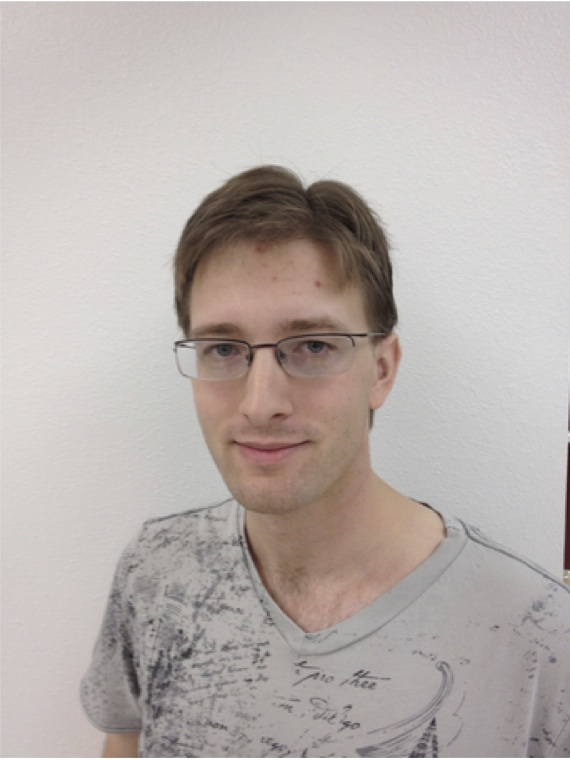
\includegraphics[width=0.3\textwidth]{james.jpg}
      \caption{James O'Grady}
  \end{figure}
\end{frame}
%

\subsection{Questions}
\begin{frame}
  \frametitle{}
  \vfill
  \begin{center}
      Questions?
  \end{center}
\end{frame}
%

\newcounter{finalframe}
\setcounter{finalframe}{\value{framenumber}}

\setcounter{framenumber}{\value{finalframe}}
%


\end{document}
